\documentclass[11pt,a4paper]{article}
\usepackage[a4paper, margin=0.8in]{geometry}
\usepackage{amsmath}
\usepackage{amssymb}
\usepackage{amsthm}
\usepackage{amsfonts}
\usepackage{natbib}
\usepackage{wrapfig}
\usepackage{graphicx}
\usepackage{url}
\usepackage{pgf}
\usepackage{subcaption}
\usepackage{pgfplots}
\usepackage{tikz}
\usetikzlibrary{shapes.geometric, arrows, positioning, patterns}

\makeatletter
\def\@maketitle{%
	\newpage
	\null
	\vskip 2em%
	\begin{center}%
		\let \footnote \thanks
		{\LARGE \@title \par}%
		\vskip 1em%
		{\Large Fast Iterative Solvers, Project 2\par}%
		\vskip 1.5em%
		{\large
			\lineskip .5em%
			\begin{tabular}[t]{c}%
				\@author
			\end{tabular}\par}%
		\vskip 1em%
		{\large \@date}%
	\end{center}%
	\par
	\vskip 1.5em}
\makeatother

\title{Multigrid Method}
\author{Johannes Leonard Grafen, 380149}
\makeindex

%new commands
\newcommand{\refFig}[1]{Fig. \ref{#1}}
\newcommand{\refEq}[1]{Eq. (\ref{#1})}
\newcommand{\refTab}[1]{Tab. \ref{#1}}

%hyperref stuff ----------------------------------------------------------------------------------------------------------------------------------------------
\ifpdf
	\usepackage[ plainpages = false, pdfpagelabels, 
	%                 pdfpagelayout = useoutlines,
	bookmarks,
	bookmarksopen = true,
	bookmarksnumbered = true,
	breaklinks = true,
	linktocpage,
	colorlinks = false,  % was true
	linkcolor = blue,
	urlcolor  = blue,
	citecolor = blue,
	anchorcolor = blue,
	hyperindex = true,
	hyperfigures
	]{hyperref} 
	
	\DeclareGraphicsExtensions{.png, .jpg, .jpeg, .pdf, .gif} %GIF doesn't work??
	\usepackage{graphicx}
	\pdfcompresslevel=9
	\graphicspath{{0_frontmatter/figures/PNG/}{0_frontmatter/figures/PDF/}{0_frontmatter/figures/}}
\else
	\usepackage[ dvips, 
	plainpages = false, 
	pdfpagelabels, 
	bookmarksnumbered = true,
	breaklinks = true,
	linktocpage,
	colorlinks = false,
	linkcolor = blue,
	urlcolor  = blue,
	citecolor = blue,
	anchorcolor = white,
	hyperindex = false,
	]{hyperref}
	
	\DeclareGraphicsExtensions{.eps, .ps}
	\usepackage{epsfig}
	\usepackage{graphicx}
	\graphicspath{{0_frontmatter/figures/EPS/}{0_frontmatter/figures/}}
\fi

\ifpdf  
\hypersetup{pdfauthor={Johannes Leonard Grafen},%
	pdftitle={Fast Iterative Solvers, Project 2},%
}
\fi
%------------------------------------------------------------------------------------------------------------------------------------------------------------

\begin{document}
\renewcommand\baselinestretch{1.0}
\baselineskip=18pt plus1pt	

\pagenumbering{gobble}
\maketitle
\newpage
\pagenumbering{arabic}
\tableofcontents
\listoffigures	% print list of figures
%\listoftables  % print list of tables
\newpage

\section{Remarks on used architecture and compiler options}
The code was written in C++, compiled using the Clang compiler and executed on an Apple Silicon M1 Pro Chip featuring the ARM64 architecture. To measure timings, the high resolution clock of the std chrono library was employed. The following flags where passed to the compiler to enhance code performance of the aforementioned architecture: -march=native, -O2. To suppress the output to measure runtime accurately the flag "DISABLEIO" was introduced and passed to the compiler via the "-D" option.

\section{Multigrid Method - MG}
\label{chapter:MG}
For the multigrid iterations, W-cycles ($\gamma = 2$) were used. Convergence was determined by the criterion
\begin{equation}
	\frac{|| r^{(m)}||_{\infty}}{|| r^{(0)}||_{\infty}} < 10^{-10} ,
	\label{eq::measure}
\end{equation}
were $r^{(m)}$ denotes the residual of the $m$-th iteration and $r^{(0)}$ the initial residual using $\mathbf{u} = \mathbf{0}$ as an initial guess for the solution vector.

\subsection{Validation of MG Method}
The solution obtained by the multigrid method is compared to the exact solution $\mathbf{U}_{ex}(x,y) = sin(2\pi x)sin(2 \pi y)$ in \refFig{fig::Val4} for $n=4$ and in \refFig{fig::Val7} for $n=7$. The estimated solution is in good agreement with the exact solution, with a maximum error of $\max_{i,j} e_{i,j} = 1.295 \cdot 10^{-2}$ for $n=4$ and $\max_{i,j} e_{i,j} = 2.01 \cdot 10^{-4}$ for $n=7$. 
%
\begin{figure}[h!]
	\centering
	\begin{subfigure}[h!]{.3\textwidth}
			\centering
			\resizebox{0.4\width}{!}{%% Creator: Matplotlib, PGF backend
%%
%% To include the figure in your LaTeX document, write
%%   \input{<filename>.pgf}
%%
%% Make sure the required packages are loaded in your preamble
%%   \usepackage{pgf}
%%
%% Also ensure that all the required font packages are loaded; for instance,
%% the lmodern package is sometimes necessary when using math font.
%%   \usepackage{lmodern}
%%
%% Figures using additional raster images can only be included by \input if
%% they are in the same directory as the main LaTeX file. For loading figures
%% from other directories you can use the `import` package
%%   \usepackage{import}
%%
%% and then include the figures with
%%   \import{<path to file>}{<filename>.pgf}
%%
%% Matplotlib used the following preamble
%%   
%%   \makeatletter\@ifpackageloaded{underscore}{}{\usepackage[strings]{underscore}}\makeatother
%%
\begingroup%
\makeatletter%
\begin{pgfpicture}%
\pgfpathrectangle{\pgfpointorigin}{\pgfqpoint{6.565064in}{4.725328in}}%
\pgfusepath{use as bounding box, clip}%
\begin{pgfscope}%
\pgfsetbuttcap%
\pgfsetmiterjoin%
\definecolor{currentfill}{rgb}{1.000000,1.000000,1.000000}%
\pgfsetfillcolor{currentfill}%
\pgfsetlinewidth{0.000000pt}%
\definecolor{currentstroke}{rgb}{1.000000,1.000000,1.000000}%
\pgfsetstrokecolor{currentstroke}%
\pgfsetdash{}{0pt}%
\pgfpathmoveto{\pgfqpoint{0.000000in}{0.000000in}}%
\pgfpathlineto{\pgfqpoint{6.565064in}{0.000000in}}%
\pgfpathlineto{\pgfqpoint{6.565064in}{4.725328in}}%
\pgfpathlineto{\pgfqpoint{0.000000in}{4.725328in}}%
\pgfpathlineto{\pgfqpoint{0.000000in}{0.000000in}}%
\pgfpathclose%
\pgfusepath{fill}%
\end{pgfscope}%
\begin{pgfscope}%
\pgfsetbuttcap%
\pgfsetmiterjoin%
\definecolor{currentfill}{rgb}{1.000000,1.000000,1.000000}%
\pgfsetfillcolor{currentfill}%
\pgfsetlinewidth{0.000000pt}%
\definecolor{currentstroke}{rgb}{0.000000,0.000000,0.000000}%
\pgfsetstrokecolor{currentstroke}%
\pgfsetstrokeopacity{0.000000}%
\pgfsetdash{}{0pt}%
\pgfpathmoveto{\pgfqpoint{1.078831in}{0.167926in}}%
\pgfpathlineto{\pgfqpoint{5.486233in}{0.167926in}}%
\pgfpathlineto{\pgfqpoint{5.486233in}{4.575328in}}%
\pgfpathlineto{\pgfqpoint{1.078831in}{4.575328in}}%
\pgfpathlineto{\pgfqpoint{1.078831in}{0.167926in}}%
\pgfpathclose%
\pgfusepath{fill}%
\end{pgfscope}%
\begin{pgfscope}%
\pgfsetbuttcap%
\pgfsetmiterjoin%
\definecolor{currentfill}{rgb}{0.950000,0.950000,0.950000}%
\pgfsetfillcolor{currentfill}%
\pgfsetfillopacity{0.500000}%
\pgfsetlinewidth{1.003750pt}%
\definecolor{currentstroke}{rgb}{0.950000,0.950000,0.950000}%
\pgfsetstrokecolor{currentstroke}%
\pgfsetstrokeopacity{0.500000}%
\pgfsetdash{}{0pt}%
\pgfpathmoveto{\pgfqpoint{1.411620in}{1.254650in}}%
\pgfpathlineto{\pgfqpoint{2.867088in}{2.474652in}}%
\pgfpathlineto{\pgfqpoint{2.846856in}{4.234114in}}%
\pgfpathlineto{\pgfqpoint{1.321736in}{3.121151in}}%
\pgfusepath{stroke,fill}%
\end{pgfscope}%
\begin{pgfscope}%
\pgfsetbuttcap%
\pgfsetmiterjoin%
\definecolor{currentfill}{rgb}{0.900000,0.900000,0.900000}%
\pgfsetfillcolor{currentfill}%
\pgfsetfillopacity{0.500000}%
\pgfsetlinewidth{1.003750pt}%
\definecolor{currentstroke}{rgb}{0.900000,0.900000,0.900000}%
\pgfsetstrokecolor{currentstroke}%
\pgfsetstrokeopacity{0.500000}%
\pgfsetdash{}{0pt}%
\pgfpathmoveto{\pgfqpoint{2.867088in}{2.474652in}}%
\pgfpathlineto{\pgfqpoint{5.202595in}{1.795813in}}%
\pgfpathlineto{\pgfqpoint{5.285941in}{3.615877in}}%
\pgfpathlineto{\pgfqpoint{2.846856in}{4.234114in}}%
\pgfusepath{stroke,fill}%
\end{pgfscope}%
\begin{pgfscope}%
\pgfsetbuttcap%
\pgfsetmiterjoin%
\definecolor{currentfill}{rgb}{0.925000,0.925000,0.925000}%
\pgfsetfillcolor{currentfill}%
\pgfsetfillopacity{0.500000}%
\pgfsetlinewidth{1.003750pt}%
\definecolor{currentstroke}{rgb}{0.925000,0.925000,0.925000}%
\pgfsetstrokecolor{currentstroke}%
\pgfsetstrokeopacity{0.500000}%
\pgfsetdash{}{0pt}%
\pgfpathmoveto{\pgfqpoint{1.411620in}{1.254650in}}%
\pgfpathlineto{\pgfqpoint{3.887372in}{0.446070in}}%
\pgfpathlineto{\pgfqpoint{5.202595in}{1.795813in}}%
\pgfpathlineto{\pgfqpoint{2.867088in}{2.474652in}}%
\pgfusepath{stroke,fill}%
\end{pgfscope}%
\begin{pgfscope}%
\pgfsetrectcap%
\pgfsetroundjoin%
\pgfsetlinewidth{0.803000pt}%
\definecolor{currentstroke}{rgb}{0.000000,0.000000,0.000000}%
\pgfsetstrokecolor{currentstroke}%
\pgfsetdash{}{0pt}%
\pgfpathmoveto{\pgfqpoint{1.411620in}{1.254650in}}%
\pgfpathlineto{\pgfqpoint{3.887372in}{0.446070in}}%
\pgfusepath{stroke}%
\end{pgfscope}%
\begin{pgfscope}%
\pgfsetbuttcap%
\pgfsetroundjoin%
\pgfsetlinewidth{0.803000pt}%
\definecolor{currentstroke}{rgb}{0.690196,0.690196,0.690196}%
\pgfsetstrokecolor{currentstroke}%
\pgfsetdash{}{0pt}%
\pgfpathmoveto{\pgfqpoint{1.561565in}{1.205679in}}%
\pgfpathlineto{\pgfqpoint{3.009127in}{2.433368in}}%
\pgfpathlineto{\pgfqpoint{2.994900in}{4.196589in}}%
\pgfusepath{stroke}%
\end{pgfscope}%
\begin{pgfscope}%
\pgfsetbuttcap%
\pgfsetroundjoin%
\pgfsetlinewidth{0.803000pt}%
\definecolor{currentstroke}{rgb}{0.690196,0.690196,0.690196}%
\pgfsetstrokecolor{currentstroke}%
\pgfsetdash{}{0pt}%
\pgfpathmoveto{\pgfqpoint{1.977936in}{1.069692in}}%
\pgfpathlineto{\pgfqpoint{3.403145in}{2.318842in}}%
\pgfpathlineto{\pgfqpoint{3.405776in}{4.092444in}}%
\pgfusepath{stroke}%
\end{pgfscope}%
\begin{pgfscope}%
\pgfsetbuttcap%
\pgfsetroundjoin%
\pgfsetlinewidth{0.803000pt}%
\definecolor{currentstroke}{rgb}{0.690196,0.690196,0.690196}%
\pgfsetstrokecolor{currentstroke}%
\pgfsetdash{}{0pt}%
\pgfpathmoveto{\pgfqpoint{2.401935in}{0.931214in}}%
\pgfpathlineto{\pgfqpoint{3.803781in}{2.202393in}}%
\pgfpathlineto{\pgfqpoint{3.823853in}{3.986473in}}%
\pgfusepath{stroke}%
\end{pgfscope}%
\begin{pgfscope}%
\pgfsetbuttcap%
\pgfsetroundjoin%
\pgfsetlinewidth{0.803000pt}%
\definecolor{currentstroke}{rgb}{0.690196,0.690196,0.690196}%
\pgfsetstrokecolor{currentstroke}%
\pgfsetdash{}{0pt}%
\pgfpathmoveto{\pgfqpoint{2.833775in}{0.790175in}}%
\pgfpathlineto{\pgfqpoint{4.211202in}{2.083972in}}%
\pgfpathlineto{\pgfqpoint{4.249322in}{3.878629in}}%
\pgfusepath{stroke}%
\end{pgfscope}%
\begin{pgfscope}%
\pgfsetbuttcap%
\pgfsetroundjoin%
\pgfsetlinewidth{0.803000pt}%
\definecolor{currentstroke}{rgb}{0.690196,0.690196,0.690196}%
\pgfsetstrokecolor{currentstroke}%
\pgfsetdash{}{0pt}%
\pgfpathmoveto{\pgfqpoint{3.273675in}{0.646503in}}%
\pgfpathlineto{\pgfqpoint{4.625583in}{1.963528in}}%
\pgfpathlineto{\pgfqpoint{4.682381in}{3.768862in}}%
\pgfusepath{stroke}%
\end{pgfscope}%
\begin{pgfscope}%
\pgfsetbuttcap%
\pgfsetroundjoin%
\pgfsetlinewidth{0.803000pt}%
\definecolor{currentstroke}{rgb}{0.690196,0.690196,0.690196}%
\pgfsetstrokecolor{currentstroke}%
\pgfsetdash{}{0pt}%
\pgfpathmoveto{\pgfqpoint{3.721862in}{0.500125in}}%
\pgfpathlineto{\pgfqpoint{5.047104in}{1.841008in}}%
\pgfpathlineto{\pgfqpoint{5.123233in}{3.657118in}}%
\pgfusepath{stroke}%
\end{pgfscope}%
\begin{pgfscope}%
\pgfsetrectcap%
\pgfsetroundjoin%
\pgfsetlinewidth{0.803000pt}%
\definecolor{currentstroke}{rgb}{0.000000,0.000000,0.000000}%
\pgfsetstrokecolor{currentstroke}%
\pgfsetdash{}{0pt}%
\pgfpathmoveto{\pgfqpoint{1.574170in}{1.216369in}}%
\pgfpathlineto{\pgfqpoint{1.536300in}{1.184251in}}%
\pgfusepath{stroke}%
\end{pgfscope}%
\begin{pgfscope}%
\definecolor{textcolor}{rgb}{0.000000,0.000000,0.000000}%
\pgfsetstrokecolor{textcolor}%
\pgfsetfillcolor{textcolor}%
\pgftext[x=1.457057in,y=0.987605in,,top]{\color{textcolor}\rmfamily\fontsize{10.000000}{12.000000}\selectfont \(\displaystyle {0.0}\)}%
\end{pgfscope}%
\begin{pgfscope}%
\pgfsetrectcap%
\pgfsetroundjoin%
\pgfsetlinewidth{0.803000pt}%
\definecolor{currentstroke}{rgb}{0.000000,0.000000,0.000000}%
\pgfsetstrokecolor{currentstroke}%
\pgfsetdash{}{0pt}%
\pgfpathmoveto{\pgfqpoint{1.990356in}{1.080577in}}%
\pgfpathlineto{\pgfqpoint{1.953042in}{1.047874in}}%
\pgfusepath{stroke}%
\end{pgfscope}%
\begin{pgfscope}%
\definecolor{textcolor}{rgb}{0.000000,0.000000,0.000000}%
\pgfsetstrokecolor{textcolor}%
\pgfsetfillcolor{textcolor}%
\pgftext[x=1.873786in,y=0.849205in,,top]{\color{textcolor}\rmfamily\fontsize{10.000000}{12.000000}\selectfont \(\displaystyle {0.2}\)}%
\end{pgfscope}%
\begin{pgfscope}%
\pgfsetrectcap%
\pgfsetroundjoin%
\pgfsetlinewidth{0.803000pt}%
\definecolor{currentstroke}{rgb}{0.000000,0.000000,0.000000}%
\pgfsetstrokecolor{currentstroke}%
\pgfsetdash{}{0pt}%
\pgfpathmoveto{\pgfqpoint{2.414161in}{0.942299in}}%
\pgfpathlineto{\pgfqpoint{2.377431in}{0.908993in}}%
\pgfusepath{stroke}%
\end{pgfscope}%
\begin{pgfscope}%
\definecolor{textcolor}{rgb}{0.000000,0.000000,0.000000}%
\pgfsetstrokecolor{textcolor}%
\pgfsetfillcolor{textcolor}%
\pgftext[x=2.298173in,y=0.708261in,,top]{\color{textcolor}\rmfamily\fontsize{10.000000}{12.000000}\selectfont \(\displaystyle {0.4}\)}%
\end{pgfscope}%
\begin{pgfscope}%
\pgfsetrectcap%
\pgfsetroundjoin%
\pgfsetlinewidth{0.803000pt}%
\definecolor{currentstroke}{rgb}{0.000000,0.000000,0.000000}%
\pgfsetstrokecolor{currentstroke}%
\pgfsetdash{}{0pt}%
\pgfpathmoveto{\pgfqpoint{2.845797in}{0.801466in}}%
\pgfpathlineto{\pgfqpoint{2.809679in}{0.767541in}}%
\pgfusepath{stroke}%
\end{pgfscope}%
\begin{pgfscope}%
\definecolor{textcolor}{rgb}{0.000000,0.000000,0.000000}%
\pgfsetstrokecolor{textcolor}%
\pgfsetfillcolor{textcolor}%
\pgftext[x=2.730434in,y=0.564703in,,top]{\color{textcolor}\rmfamily\fontsize{10.000000}{12.000000}\selectfont \(\displaystyle {0.6}\)}%
\end{pgfscope}%
\begin{pgfscope}%
\pgfsetrectcap%
\pgfsetroundjoin%
\pgfsetlinewidth{0.803000pt}%
\definecolor{currentstroke}{rgb}{0.000000,0.000000,0.000000}%
\pgfsetstrokecolor{currentstroke}%
\pgfsetdash{}{0pt}%
\pgfpathmoveto{\pgfqpoint{3.285483in}{0.658007in}}%
\pgfpathlineto{\pgfqpoint{3.250006in}{0.623445in}}%
\pgfusepath{stroke}%
\end{pgfscope}%
\begin{pgfscope}%
\definecolor{textcolor}{rgb}{0.000000,0.000000,0.000000}%
\pgfsetstrokecolor{textcolor}%
\pgfsetfillcolor{textcolor}%
\pgftext[x=3.170788in,y=0.418456in,,top]{\color{textcolor}\rmfamily\fontsize{10.000000}{12.000000}\selectfont \(\displaystyle {0.8}\)}%
\end{pgfscope}%
\begin{pgfscope}%
\pgfsetrectcap%
\pgfsetroundjoin%
\pgfsetlinewidth{0.803000pt}%
\definecolor{currentstroke}{rgb}{0.000000,0.000000,0.000000}%
\pgfsetstrokecolor{currentstroke}%
\pgfsetdash{}{0pt}%
\pgfpathmoveto{\pgfqpoint{3.733447in}{0.511846in}}%
\pgfpathlineto{\pgfqpoint{3.698642in}{0.476631in}}%
\pgfusepath{stroke}%
\end{pgfscope}%
\begin{pgfscope}%
\definecolor{textcolor}{rgb}{0.000000,0.000000,0.000000}%
\pgfsetstrokecolor{textcolor}%
\pgfsetfillcolor{textcolor}%
\pgftext[x=3.619465in,y=0.269445in,,top]{\color{textcolor}\rmfamily\fontsize{10.000000}{12.000000}\selectfont \(\displaystyle {1.0}\)}%
\end{pgfscope}%
\begin{pgfscope}%
\pgfsetrectcap%
\pgfsetroundjoin%
\pgfsetlinewidth{0.803000pt}%
\definecolor{currentstroke}{rgb}{0.000000,0.000000,0.000000}%
\pgfsetstrokecolor{currentstroke}%
\pgfsetdash{}{0pt}%
\pgfpathmoveto{\pgfqpoint{5.202595in}{1.795813in}}%
\pgfpathlineto{\pgfqpoint{3.887372in}{0.446070in}}%
\pgfusepath{stroke}%
\end{pgfscope}%
\begin{pgfscope}%
\pgfsetbuttcap%
\pgfsetroundjoin%
\pgfsetlinewidth{0.803000pt}%
\definecolor{currentstroke}{rgb}{0.690196,0.690196,0.690196}%
\pgfsetstrokecolor{currentstroke}%
\pgfsetdash{}{0pt}%
\pgfpathmoveto{\pgfqpoint{1.427202in}{3.198115in}}%
\pgfpathlineto{\pgfqpoint{1.511914in}{1.338719in}}%
\pgfpathlineto{\pgfqpoint{3.978375in}{0.539462in}}%
\pgfusepath{stroke}%
\end{pgfscope}%
\begin{pgfscope}%
\pgfsetbuttcap%
\pgfsetroundjoin%
\pgfsetlinewidth{0.803000pt}%
\definecolor{currentstroke}{rgb}{0.690196,0.690196,0.690196}%
\pgfsetstrokecolor{currentstroke}%
\pgfsetdash{}{0pt}%
\pgfpathmoveto{\pgfqpoint{1.710203in}{3.404636in}}%
\pgfpathlineto{\pgfqpoint{1.781298in}{1.564521in}}%
\pgfpathlineto{\pgfqpoint{4.222529in}{0.790024in}}%
\pgfusepath{stroke}%
\end{pgfscope}%
\begin{pgfscope}%
\pgfsetbuttcap%
\pgfsetroundjoin%
\pgfsetlinewidth{0.803000pt}%
\definecolor{currentstroke}{rgb}{0.690196,0.690196,0.690196}%
\pgfsetstrokecolor{currentstroke}%
\pgfsetdash{}{0pt}%
\pgfpathmoveto{\pgfqpoint{1.984344in}{3.604692in}}%
\pgfpathlineto{\pgfqpoint{2.042610in}{1.783558in}}%
\pgfpathlineto{\pgfqpoint{4.458987in}{1.032688in}}%
\pgfusepath{stroke}%
\end{pgfscope}%
\begin{pgfscope}%
\pgfsetbuttcap%
\pgfsetroundjoin%
\pgfsetlinewidth{0.803000pt}%
\definecolor{currentstroke}{rgb}{0.690196,0.690196,0.690196}%
\pgfsetstrokecolor{currentstroke}%
\pgfsetdash{}{0pt}%
\pgfpathmoveto{\pgfqpoint{2.250036in}{3.798582in}}%
\pgfpathlineto{\pgfqpoint{2.296208in}{1.996129in}}%
\pgfpathlineto{\pgfqpoint{4.688107in}{1.267821in}}%
\pgfusepath{stroke}%
\end{pgfscope}%
\begin{pgfscope}%
\pgfsetbuttcap%
\pgfsetroundjoin%
\pgfsetlinewidth{0.803000pt}%
\definecolor{currentstroke}{rgb}{0.690196,0.690196,0.690196}%
\pgfsetstrokecolor{currentstroke}%
\pgfsetdash{}{0pt}%
\pgfpathmoveto{\pgfqpoint{2.507663in}{3.986586in}}%
\pgfpathlineto{\pgfqpoint{2.542429in}{2.202517in}}%
\pgfpathlineto{\pgfqpoint{4.910224in}{1.495769in}}%
\pgfusepath{stroke}%
\end{pgfscope}%
\begin{pgfscope}%
\pgfsetbuttcap%
\pgfsetroundjoin%
\pgfsetlinewidth{0.803000pt}%
\definecolor{currentstroke}{rgb}{0.690196,0.690196,0.690196}%
\pgfsetstrokecolor{currentstroke}%
\pgfsetdash{}{0pt}%
\pgfpathmoveto{\pgfqpoint{2.757587in}{4.168969in}}%
\pgfpathlineto{\pgfqpoint{2.781591in}{2.402987in}}%
\pgfpathlineto{\pgfqpoint{5.125656in}{1.716855in}}%
\pgfusepath{stroke}%
\end{pgfscope}%
\begin{pgfscope}%
\pgfsetrectcap%
\pgfsetroundjoin%
\pgfsetlinewidth{0.803000pt}%
\definecolor{currentstroke}{rgb}{0.000000,0.000000,0.000000}%
\pgfsetstrokecolor{currentstroke}%
\pgfsetdash{}{0pt}%
\pgfpathmoveto{\pgfqpoint{3.957590in}{0.546197in}}%
\pgfpathlineto{\pgfqpoint{4.019999in}{0.525974in}}%
\pgfusepath{stroke}%
\end{pgfscope}%
\begin{pgfscope}%
\definecolor{textcolor}{rgb}{0.000000,0.000000,0.000000}%
\pgfsetstrokecolor{textcolor}%
\pgfsetfillcolor{textcolor}%
\pgftext[x=4.157255in,y=0.353045in,,top]{\color{textcolor}\rmfamily\fontsize{10.000000}{12.000000}\selectfont \(\displaystyle {0.0}\)}%
\end{pgfscope}%
\begin{pgfscope}%
\pgfsetrectcap%
\pgfsetroundjoin%
\pgfsetlinewidth{0.803000pt}%
\definecolor{currentstroke}{rgb}{0.000000,0.000000,0.000000}%
\pgfsetstrokecolor{currentstroke}%
\pgfsetdash{}{0pt}%
\pgfpathmoveto{\pgfqpoint{4.201974in}{0.796546in}}%
\pgfpathlineto{\pgfqpoint{4.263693in}{0.776965in}}%
\pgfusepath{stroke}%
\end{pgfscope}%
\begin{pgfscope}%
\definecolor{textcolor}{rgb}{0.000000,0.000000,0.000000}%
\pgfsetstrokecolor{textcolor}%
\pgfsetfillcolor{textcolor}%
\pgftext[x=4.398664in,y=0.606718in,,top]{\color{textcolor}\rmfamily\fontsize{10.000000}{12.000000}\selectfont \(\displaystyle {0.2}\)}%
\end{pgfscope}%
\begin{pgfscope}%
\pgfsetrectcap%
\pgfsetroundjoin%
\pgfsetlinewidth{0.803000pt}%
\definecolor{currentstroke}{rgb}{0.000000,0.000000,0.000000}%
\pgfsetstrokecolor{currentstroke}%
\pgfsetdash{}{0pt}%
\pgfpathmoveto{\pgfqpoint{4.438657in}{1.039006in}}%
\pgfpathlineto{\pgfqpoint{4.499699in}{1.020037in}}%
\pgfusepath{stroke}%
\end{pgfscope}%
\begin{pgfscope}%
\definecolor{textcolor}{rgb}{0.000000,0.000000,0.000000}%
\pgfsetstrokecolor{textcolor}%
\pgfsetfillcolor{textcolor}%
\pgftext[x=4.632460in,y=0.852391in,,top]{\color{textcolor}\rmfamily\fontsize{10.000000}{12.000000}\selectfont \(\displaystyle {0.4}\)}%
\end{pgfscope}%
\begin{pgfscope}%
\pgfsetrectcap%
\pgfsetroundjoin%
\pgfsetlinewidth{0.803000pt}%
\definecolor{currentstroke}{rgb}{0.000000,0.000000,0.000000}%
\pgfsetstrokecolor{currentstroke}%
\pgfsetdash{}{0pt}%
\pgfpathmoveto{\pgfqpoint{4.667998in}{1.273944in}}%
\pgfpathlineto{\pgfqpoint{4.728375in}{1.255560in}}%
\pgfusepath{stroke}%
\end{pgfscope}%
\begin{pgfscope}%
\definecolor{textcolor}{rgb}{0.000000,0.000000,0.000000}%
\pgfsetstrokecolor{textcolor}%
\pgfsetfillcolor{textcolor}%
\pgftext[x=4.858996in,y=1.090435in,,top]{\color{textcolor}\rmfamily\fontsize{10.000000}{12.000000}\selectfont \(\displaystyle {0.6}\)}%
\end{pgfscope}%
\begin{pgfscope}%
\pgfsetrectcap%
\pgfsetroundjoin%
\pgfsetlinewidth{0.803000pt}%
\definecolor{currentstroke}{rgb}{0.000000,0.000000,0.000000}%
\pgfsetstrokecolor{currentstroke}%
\pgfsetdash{}{0pt}%
\pgfpathmoveto{\pgfqpoint{4.890333in}{1.501706in}}%
\pgfpathlineto{\pgfqpoint{4.950056in}{1.483880in}}%
\pgfusepath{stroke}%
\end{pgfscope}%
\begin{pgfscope}%
\definecolor{textcolor}{rgb}{0.000000,0.000000,0.000000}%
\pgfsetstrokecolor{textcolor}%
\pgfsetfillcolor{textcolor}%
\pgftext[x=5.078606in,y=1.321202in,,top]{\color{textcolor}\rmfamily\fontsize{10.000000}{12.000000}\selectfont \(\displaystyle {0.8}\)}%
\end{pgfscope}%
\begin{pgfscope}%
\pgfsetrectcap%
\pgfsetroundjoin%
\pgfsetlinewidth{0.803000pt}%
\definecolor{currentstroke}{rgb}{0.000000,0.000000,0.000000}%
\pgfsetstrokecolor{currentstroke}%
\pgfsetdash{}{0pt}%
\pgfpathmoveto{\pgfqpoint{5.105978in}{1.722615in}}%
\pgfpathlineto{\pgfqpoint{5.165060in}{1.705321in}}%
\pgfusepath{stroke}%
\end{pgfscope}%
\begin{pgfscope}%
\definecolor{textcolor}{rgb}{0.000000,0.000000,0.000000}%
\pgfsetstrokecolor{textcolor}%
\pgfsetfillcolor{textcolor}%
\pgftext[x=5.291602in,y=1.545019in,,top]{\color{textcolor}\rmfamily\fontsize{10.000000}{12.000000}\selectfont \(\displaystyle {1.0}\)}%
\end{pgfscope}%
\begin{pgfscope}%
\pgfsetrectcap%
\pgfsetroundjoin%
\pgfsetlinewidth{0.803000pt}%
\definecolor{currentstroke}{rgb}{0.000000,0.000000,0.000000}%
\pgfsetstrokecolor{currentstroke}%
\pgfsetdash{}{0pt}%
\pgfpathmoveto{\pgfqpoint{5.202595in}{1.795813in}}%
\pgfpathlineto{\pgfqpoint{5.285941in}{3.615877in}}%
\pgfusepath{stroke}%
\end{pgfscope}%
\begin{pgfscope}%
\pgfsetbuttcap%
\pgfsetroundjoin%
\pgfsetlinewidth{0.803000pt}%
\definecolor{currentstroke}{rgb}{0.690196,0.690196,0.690196}%
\pgfsetstrokecolor{currentstroke}%
\pgfsetdash{}{0pt}%
\pgfpathmoveto{\pgfqpoint{5.204192in}{1.830683in}}%
\pgfpathlineto{\pgfqpoint{2.866700in}{2.508432in}}%
\pgfpathlineto{\pgfqpoint{1.409901in}{1.290351in}}%
\pgfusepath{stroke}%
\end{pgfscope}%
\begin{pgfscope}%
\pgfsetbuttcap%
\pgfsetroundjoin%
\pgfsetlinewidth{0.803000pt}%
\definecolor{currentstroke}{rgb}{0.690196,0.690196,0.690196}%
\pgfsetstrokecolor{currentstroke}%
\pgfsetdash{}{0pt}%
\pgfpathmoveto{\pgfqpoint{5.223570in}{2.253846in}}%
\pgfpathlineto{\pgfqpoint{2.861989in}{2.918134in}}%
\pgfpathlineto{\pgfqpoint{1.389029in}{1.723777in}}%
\pgfusepath{stroke}%
\end{pgfscope}%
\begin{pgfscope}%
\pgfsetbuttcap%
\pgfsetroundjoin%
\pgfsetlinewidth{0.803000pt}%
\definecolor{currentstroke}{rgb}{0.690196,0.690196,0.690196}%
\pgfsetstrokecolor{currentstroke}%
\pgfsetdash{}{0pt}%
\pgfpathmoveto{\pgfqpoint{5.243355in}{2.685908in}}%
\pgfpathlineto{\pgfqpoint{2.857183in}{3.336038in}}%
\pgfpathlineto{\pgfqpoint{1.367701in}{2.166669in}}%
\pgfusepath{stroke}%
\end{pgfscope}%
\begin{pgfscope}%
\pgfsetbuttcap%
\pgfsetroundjoin%
\pgfsetlinewidth{0.803000pt}%
\definecolor{currentstroke}{rgb}{0.690196,0.690196,0.690196}%
\pgfsetstrokecolor{currentstroke}%
\pgfsetdash{}{0pt}%
\pgfpathmoveto{\pgfqpoint{5.263561in}{3.127153in}}%
\pgfpathlineto{\pgfqpoint{2.852280in}{3.762393in}}%
\pgfpathlineto{\pgfqpoint{1.345902in}{2.619340in}}%
\pgfusepath{stroke}%
\end{pgfscope}%
\begin{pgfscope}%
\pgfsetbuttcap%
\pgfsetroundjoin%
\pgfsetlinewidth{0.803000pt}%
\definecolor{currentstroke}{rgb}{0.690196,0.690196,0.690196}%
\pgfsetstrokecolor{currentstroke}%
\pgfsetdash{}{0pt}%
\pgfpathmoveto{\pgfqpoint{5.284201in}{3.577879in}}%
\pgfpathlineto{\pgfqpoint{2.847277in}{4.197457in}}%
\pgfpathlineto{\pgfqpoint{1.323616in}{3.082119in}}%
\pgfusepath{stroke}%
\end{pgfscope}%
\begin{pgfscope}%
\pgfsetrectcap%
\pgfsetroundjoin%
\pgfsetlinewidth{0.803000pt}%
\definecolor{currentstroke}{rgb}{0.000000,0.000000,0.000000}%
\pgfsetstrokecolor{currentstroke}%
\pgfsetdash{}{0pt}%
\pgfpathmoveto{\pgfqpoint{5.184573in}{1.836372in}}%
\pgfpathlineto{\pgfqpoint{5.243476in}{1.819293in}}%
\pgfusepath{stroke}%
\end{pgfscope}%
\begin{pgfscope}%
\definecolor{textcolor}{rgb}{0.000000,0.000000,0.000000}%
\pgfsetstrokecolor{textcolor}%
\pgfsetfillcolor{textcolor}%
\pgftext[x=5.457981in,y=1.866825in,,top]{\color{textcolor}\rmfamily\fontsize{10.000000}{12.000000}\selectfont \(\displaystyle {-1.0}\)}%
\end{pgfscope}%
\begin{pgfscope}%
\pgfsetrectcap%
\pgfsetroundjoin%
\pgfsetlinewidth{0.803000pt}%
\definecolor{currentstroke}{rgb}{0.000000,0.000000,0.000000}%
\pgfsetstrokecolor{currentstroke}%
\pgfsetdash{}{0pt}%
\pgfpathmoveto{\pgfqpoint{5.203739in}{2.259424in}}%
\pgfpathlineto{\pgfqpoint{5.263279in}{2.242676in}}%
\pgfusepath{stroke}%
\end{pgfscope}%
\begin{pgfscope}%
\definecolor{textcolor}{rgb}{0.000000,0.000000,0.000000}%
\pgfsetstrokecolor{textcolor}%
\pgfsetfillcolor{textcolor}%
\pgftext[x=5.479944in,y=2.289286in,,top]{\color{textcolor}\rmfamily\fontsize{10.000000}{12.000000}\selectfont \(\displaystyle {-0.5}\)}%
\end{pgfscope}%
\begin{pgfscope}%
\pgfsetrectcap%
\pgfsetroundjoin%
\pgfsetlinewidth{0.803000pt}%
\definecolor{currentstroke}{rgb}{0.000000,0.000000,0.000000}%
\pgfsetstrokecolor{currentstroke}%
\pgfsetdash{}{0pt}%
\pgfpathmoveto{\pgfqpoint{5.223308in}{2.691370in}}%
\pgfpathlineto{\pgfqpoint{5.283498in}{2.674970in}}%
\pgfusepath{stroke}%
\end{pgfscope}%
\begin{pgfscope}%
\definecolor{textcolor}{rgb}{0.000000,0.000000,0.000000}%
\pgfsetstrokecolor{textcolor}%
\pgfsetfillcolor{textcolor}%
\pgftext[x=5.502367in,y=2.720609in,,top]{\color{textcolor}\rmfamily\fontsize{10.000000}{12.000000}\selectfont \(\displaystyle {0.0}\)}%
\end{pgfscope}%
\begin{pgfscope}%
\pgfsetrectcap%
\pgfsetroundjoin%
\pgfsetlinewidth{0.803000pt}%
\definecolor{currentstroke}{rgb}{0.000000,0.000000,0.000000}%
\pgfsetstrokecolor{currentstroke}%
\pgfsetdash{}{0pt}%
\pgfpathmoveto{\pgfqpoint{5.243293in}{3.132493in}}%
\pgfpathlineto{\pgfqpoint{5.304147in}{3.116461in}}%
\pgfusepath{stroke}%
\end{pgfscope}%
\begin{pgfscope}%
\definecolor{textcolor}{rgb}{0.000000,0.000000,0.000000}%
\pgfsetstrokecolor{textcolor}%
\pgfsetfillcolor{textcolor}%
\pgftext[x=5.525266in,y=3.161076in,,top]{\color{textcolor}\rmfamily\fontsize{10.000000}{12.000000}\selectfont \(\displaystyle {0.5}\)}%
\end{pgfscope}%
\begin{pgfscope}%
\pgfsetrectcap%
\pgfsetroundjoin%
\pgfsetlinewidth{0.803000pt}%
\definecolor{currentstroke}{rgb}{0.000000,0.000000,0.000000}%
\pgfsetstrokecolor{currentstroke}%
\pgfsetdash{}{0pt}%
\pgfpathmoveto{\pgfqpoint{5.263707in}{3.583089in}}%
\pgfpathlineto{\pgfqpoint{5.325241in}{3.567444in}}%
\pgfusepath{stroke}%
\end{pgfscope}%
\begin{pgfscope}%
\definecolor{textcolor}{rgb}{0.000000,0.000000,0.000000}%
\pgfsetstrokecolor{textcolor}%
\pgfsetfillcolor{textcolor}%
\pgftext[x=5.548656in,y=3.610981in,,top]{\color{textcolor}\rmfamily\fontsize{10.000000}{12.000000}\selectfont \(\displaystyle {1.0}\)}%
\end{pgfscope}%
\begin{pgfscope}%
\pgfpathrectangle{\pgfqpoint{1.078831in}{0.167926in}}{\pgfqpoint{4.407402in}{4.407402in}}%
\pgfusepath{clip}%
\pgfsetbuttcap%
\pgfsetroundjoin%
\definecolor{currentfill}{rgb}{0.843358,0.861820,0.890017}%
\pgfsetfillcolor{currentfill}%
\pgfsetlinewidth{0.000000pt}%
\definecolor{currentstroke}{rgb}{0.000000,0.000000,0.000000}%
\pgfsetstrokecolor{currentstroke}%
\pgfsetdash{}{0pt}%
\pgfpathmoveto{\pgfqpoint{2.840151in}{3.167814in}}%
\pgfpathlineto{\pgfqpoint{2.967066in}{3.008474in}}%
\pgfpathlineto{\pgfqpoint{3.040745in}{3.193125in}}%
\pgfpathlineto{\pgfqpoint{2.915326in}{3.227543in}}%
\pgfpathlineto{\pgfqpoint{2.840151in}{3.167814in}}%
\pgfpathclose%
\pgfusepath{fill}%
\end{pgfscope}%
\begin{pgfscope}%
\pgfpathrectangle{\pgfqpoint{1.078831in}{0.167926in}}{\pgfqpoint{4.407402in}{4.407402in}}%
\pgfusepath{clip}%
\pgfsetbuttcap%
\pgfsetroundjoin%
\definecolor{currentfill}{rgb}{0.804965,0.851666,0.926165}%
\pgfsetfillcolor{currentfill}%
\pgfsetlinewidth{0.000000pt}%
\definecolor{currentstroke}{rgb}{0.000000,0.000000,0.000000}%
\pgfsetstrokecolor{currentstroke}%
\pgfsetdash{}{0pt}%
\pgfpathmoveto{\pgfqpoint{2.967066in}{3.008474in}}%
\pgfpathlineto{\pgfqpoint{3.093790in}{2.868077in}}%
\pgfpathlineto{\pgfqpoint{3.166832in}{3.158524in}}%
\pgfpathlineto{\pgfqpoint{3.040745in}{3.193125in}}%
\pgfpathlineto{\pgfqpoint{2.967066in}{3.008474in}}%
\pgfpathclose%
\pgfusepath{fill}%
\end{pgfscope}%
\begin{pgfscope}%
\pgfpathrectangle{\pgfqpoint{1.078831in}{0.167926in}}{\pgfqpoint{4.407402in}{4.407402in}}%
\pgfusepath{clip}%
\pgfsetbuttcap%
\pgfsetroundjoin%
\definecolor{currentfill}{rgb}{0.565182,0.699438,0.996635}%
\pgfsetfillcolor{currentfill}%
\pgfsetlinewidth{0.000000pt}%
\definecolor{currentstroke}{rgb}{0.000000,0.000000,0.000000}%
\pgfsetstrokecolor{currentstroke}%
\pgfsetdash{}{0pt}%
\pgfpathmoveto{\pgfqpoint{3.020609in}{2.612732in}}%
\pgfpathlineto{\pgfqpoint{3.147469in}{2.447878in}}%
\pgfpathlineto{\pgfqpoint{3.220449in}{2.762392in}}%
\pgfpathlineto{\pgfqpoint{3.093790in}{2.868077in}}%
\pgfpathlineto{\pgfqpoint{3.020609in}{2.612732in}}%
\pgfpathclose%
\pgfusepath{fill}%
\end{pgfscope}%
\begin{pgfscope}%
\pgfpathrectangle{\pgfqpoint{1.078831in}{0.167926in}}{\pgfqpoint{4.407402in}{4.407402in}}%
\pgfusepath{clip}%
\pgfsetbuttcap%
\pgfsetroundjoin%
\definecolor{currentfill}{rgb}{0.404421,0.534643,0.932002}%
\pgfsetfillcolor{currentfill}%
\pgfsetlinewidth{0.000000pt}%
\definecolor{currentstroke}{rgb}{0.000000,0.000000,0.000000}%
\pgfsetstrokecolor{currentstroke}%
\pgfsetdash{}{0pt}%
\pgfpathmoveto{\pgfqpoint{2.946824in}{2.421080in}}%
\pgfpathlineto{\pgfqpoint{3.074162in}{2.216910in}}%
\pgfpathlineto{\pgfqpoint{3.147469in}{2.447878in}}%
\pgfpathlineto{\pgfqpoint{3.020609in}{2.612732in}}%
\pgfpathlineto{\pgfqpoint{2.946824in}{2.421080in}}%
\pgfpathclose%
\pgfusepath{fill}%
\end{pgfscope}%
\begin{pgfscope}%
\pgfpathrectangle{\pgfqpoint{1.078831in}{0.167926in}}{\pgfqpoint{4.407402in}{4.407402in}}%
\pgfusepath{clip}%
\pgfsetbuttcap%
\pgfsetroundjoin%
\definecolor{currentfill}{rgb}{0.672538,0.782861,0.991982}%
\pgfsetfillcolor{currentfill}%
\pgfsetlinewidth{0.000000pt}%
\definecolor{currentstroke}{rgb}{0.000000,0.000000,0.000000}%
\pgfsetstrokecolor{currentstroke}%
\pgfsetdash{}{0pt}%
\pgfpathmoveto{\pgfqpoint{2.892942in}{2.842086in}}%
\pgfpathlineto{\pgfqpoint{3.020609in}{2.612732in}}%
\pgfpathlineto{\pgfqpoint{3.093790in}{2.868077in}}%
\pgfpathlineto{\pgfqpoint{2.967066in}{3.008474in}}%
\pgfpathlineto{\pgfqpoint{2.892942in}{2.842086in}}%
\pgfpathclose%
\pgfusepath{fill}%
\end{pgfscope}%
\begin{pgfscope}%
\pgfpathrectangle{\pgfqpoint{1.078831in}{0.167926in}}{\pgfqpoint{4.407402in}{4.407402in}}%
\pgfusepath{clip}%
\pgfsetbuttcap%
\pgfsetroundjoin%
\definecolor{currentfill}{rgb}{0.318832,0.426605,0.859857}%
\pgfsetfillcolor{currentfill}%
\pgfsetlinewidth{0.000000pt}%
\definecolor{currentstroke}{rgb}{0.000000,0.000000,0.000000}%
\pgfsetstrokecolor{currentstroke}%
\pgfsetdash{}{0pt}%
\pgfpathmoveto{\pgfqpoint{3.074162in}{2.216910in}}%
\pgfpathlineto{\pgfqpoint{3.200773in}{2.121079in}}%
\pgfpathlineto{\pgfqpoint{3.274078in}{2.366180in}}%
\pgfpathlineto{\pgfqpoint{3.147469in}{2.447878in}}%
\pgfpathlineto{\pgfqpoint{3.074162in}{2.216910in}}%
\pgfpathclose%
\pgfusepath{fill}%
\end{pgfscope}%
\begin{pgfscope}%
\pgfpathrectangle{\pgfqpoint{1.078831in}{0.167926in}}{\pgfqpoint{4.407402in}{4.407402in}}%
\pgfusepath{clip}%
\pgfsetbuttcap%
\pgfsetroundjoin%
\definecolor{currentfill}{rgb}{0.505423,0.643995,0.983157}%
\pgfsetfillcolor{currentfill}%
\pgfsetlinewidth{0.000000pt}%
\definecolor{currentstroke}{rgb}{0.000000,0.000000,0.000000}%
\pgfsetstrokecolor{currentstroke}%
\pgfsetdash{}{0pt}%
\pgfpathmoveto{\pgfqpoint{3.147469in}{2.447878in}}%
\pgfpathlineto{\pgfqpoint{3.274078in}{2.366180in}}%
\pgfpathlineto{\pgfqpoint{3.347363in}{2.701922in}}%
\pgfpathlineto{\pgfqpoint{3.220449in}{2.762392in}}%
\pgfpathlineto{\pgfqpoint{3.147469in}{2.447878in}}%
\pgfpathclose%
\pgfusepath{fill}%
\end{pgfscope}%
\begin{pgfscope}%
\pgfpathrectangle{\pgfqpoint{1.078831in}{0.167926in}}{\pgfqpoint{4.407402in}{4.407402in}}%
\pgfusepath{clip}%
\pgfsetbuttcap%
\pgfsetroundjoin%
\definecolor{currentfill}{rgb}{0.772706,0.838978,0.949319}%
\pgfsetfillcolor{currentfill}%
\pgfsetlinewidth{0.000000pt}%
\definecolor{currentstroke}{rgb}{0.000000,0.000000,0.000000}%
\pgfsetstrokecolor{currentstroke}%
\pgfsetdash{}{0pt}%
\pgfpathmoveto{\pgfqpoint{3.093790in}{2.868077in}}%
\pgfpathlineto{\pgfqpoint{3.220449in}{2.762392in}}%
\pgfpathlineto{\pgfqpoint{3.293592in}{3.123739in}}%
\pgfpathlineto{\pgfqpoint{3.166832in}{3.158524in}}%
\pgfpathlineto{\pgfqpoint{3.093790in}{2.868077in}}%
\pgfpathclose%
\pgfusepath{fill}%
\end{pgfscope}%
\begin{pgfscope}%
\pgfpathrectangle{\pgfqpoint{1.078831in}{0.167926in}}{\pgfqpoint{4.407402in}{4.407402in}}%
\pgfusepath{clip}%
\pgfsetbuttcap%
\pgfsetroundjoin%
\definecolor{currentfill}{rgb}{0.804965,0.851666,0.926165}%
\pgfsetfillcolor{currentfill}%
\pgfsetlinewidth{0.000000pt}%
\definecolor{currentstroke}{rgb}{0.000000,0.000000,0.000000}%
\pgfsetstrokecolor{currentstroke}%
\pgfsetdash{}{0pt}%
\pgfpathmoveto{\pgfqpoint{2.764280in}{3.107532in}}%
\pgfpathlineto{\pgfqpoint{2.892942in}{2.842086in}}%
\pgfpathlineto{\pgfqpoint{2.967066in}{3.008474in}}%
\pgfpathlineto{\pgfqpoint{2.840151in}{3.167814in}}%
\pgfpathlineto{\pgfqpoint{2.764280in}{3.107532in}}%
\pgfpathclose%
\pgfusepath{fill}%
\end{pgfscope}%
\begin{pgfscope}%
\pgfpathrectangle{\pgfqpoint{1.078831in}{0.167926in}}{\pgfqpoint{4.407402in}{4.407402in}}%
\pgfusepath{clip}%
\pgfsetbuttcap%
\pgfsetroundjoin%
\definecolor{currentfill}{rgb}{0.565182,0.699438,0.996635}%
\pgfsetfillcolor{currentfill}%
\pgfsetlinewidth{0.000000pt}%
\definecolor{currentstroke}{rgb}{0.000000,0.000000,0.000000}%
\pgfsetstrokecolor{currentstroke}%
\pgfsetdash{}{0pt}%
\pgfpathmoveto{\pgfqpoint{2.818067in}{2.709844in}}%
\pgfpathlineto{\pgfqpoint{2.946824in}{2.421080in}}%
\pgfpathlineto{\pgfqpoint{3.020609in}{2.612732in}}%
\pgfpathlineto{\pgfqpoint{2.892942in}{2.842086in}}%
\pgfpathlineto{\pgfqpoint{2.818067in}{2.709844in}}%
\pgfpathclose%
\pgfusepath{fill}%
\end{pgfscope}%
\begin{pgfscope}%
\pgfpathrectangle{\pgfqpoint{1.078831in}{0.167926in}}{\pgfqpoint{4.407402in}{4.407402in}}%
\pgfusepath{clip}%
\pgfsetbuttcap%
\pgfsetroundjoin%
\definecolor{currentfill}{rgb}{0.229806,0.298718,0.753683}%
\pgfsetfillcolor{currentfill}%
\pgfsetlinewidth{0.000000pt}%
\definecolor{currentstroke}{rgb}{0.000000,0.000000,0.000000}%
\pgfsetstrokecolor{currentstroke}%
\pgfsetdash{}{0pt}%
\pgfpathmoveto{\pgfqpoint{2.999874in}{2.093594in}}%
\pgfpathlineto{\pgfqpoint{3.126823in}{1.992487in}}%
\pgfpathlineto{\pgfqpoint{3.200773in}{2.121079in}}%
\pgfpathlineto{\pgfqpoint{3.074162in}{2.216910in}}%
\pgfpathlineto{\pgfqpoint{2.999874in}{2.093594in}}%
\pgfpathclose%
\pgfusepath{fill}%
\end{pgfscope}%
\begin{pgfscope}%
\pgfpathrectangle{\pgfqpoint{1.078831in}{0.167926in}}{\pgfqpoint{4.407402in}{4.407402in}}%
\pgfusepath{clip}%
\pgfsetbuttcap%
\pgfsetroundjoin%
\definecolor{currentfill}{rgb}{0.318832,0.426605,0.859857}%
\pgfsetfillcolor{currentfill}%
\pgfsetlinewidth{0.000000pt}%
\definecolor{currentstroke}{rgb}{0.000000,0.000000,0.000000}%
\pgfsetstrokecolor{currentstroke}%
\pgfsetdash{}{0pt}%
\pgfpathmoveto{\pgfqpoint{2.871865in}{2.312075in}}%
\pgfpathlineto{\pgfqpoint{2.999874in}{2.093594in}}%
\pgfpathlineto{\pgfqpoint{3.074162in}{2.216910in}}%
\pgfpathlineto{\pgfqpoint{2.946824in}{2.421080in}}%
\pgfpathlineto{\pgfqpoint{2.871865in}{2.312075in}}%
\pgfpathclose%
\pgfusepath{fill}%
\end{pgfscope}%
\begin{pgfscope}%
\pgfpathrectangle{\pgfqpoint{1.078831in}{0.167926in}}{\pgfqpoint{4.407402in}{4.407402in}}%
\pgfusepath{clip}%
\pgfsetbuttcap%
\pgfsetroundjoin%
\definecolor{currentfill}{rgb}{0.318832,0.426605,0.859857}%
\pgfsetfillcolor{currentfill}%
\pgfsetlinewidth{0.000000pt}%
\definecolor{currentstroke}{rgb}{0.000000,0.000000,0.000000}%
\pgfsetstrokecolor{currentstroke}%
\pgfsetdash{}{0pt}%
\pgfpathmoveto{\pgfqpoint{3.200773in}{2.121079in}}%
\pgfpathlineto{\pgfqpoint{3.327656in}{2.142172in}}%
\pgfpathlineto{\pgfqpoint{3.401215in}{2.374416in}}%
\pgfpathlineto{\pgfqpoint{3.274078in}{2.366180in}}%
\pgfpathlineto{\pgfqpoint{3.200773in}{2.121079in}}%
\pgfpathclose%
\pgfusepath{fill}%
\end{pgfscope}%
\begin{pgfscope}%
\pgfpathrectangle{\pgfqpoint{1.078831in}{0.167926in}}{\pgfqpoint{4.407402in}{4.407402in}}%
\pgfusepath{clip}%
\pgfsetbuttcap%
\pgfsetroundjoin%
\definecolor{currentfill}{rgb}{0.753611,0.830233,0.960871}%
\pgfsetfillcolor{currentfill}%
\pgfsetlinewidth{0.000000pt}%
\definecolor{currentstroke}{rgb}{0.000000,0.000000,0.000000}%
\pgfsetstrokecolor{currentstroke}%
\pgfsetdash{}{0pt}%
\pgfpathmoveto{\pgfqpoint{3.220449in}{2.762392in}}%
\pgfpathlineto{\pgfqpoint{3.347363in}{2.701922in}}%
\pgfpathlineto{\pgfqpoint{3.421032in}{3.088767in}}%
\pgfpathlineto{\pgfqpoint{3.293592in}{3.123739in}}%
\pgfpathlineto{\pgfqpoint{3.220449in}{2.762392in}}%
\pgfpathclose%
\pgfusepath{fill}%
\end{pgfscope}%
\begin{pgfscope}%
\pgfpathrectangle{\pgfqpoint{1.078831in}{0.167926in}}{\pgfqpoint{4.407402in}{4.407402in}}%
\pgfusepath{clip}%
\pgfsetbuttcap%
\pgfsetroundjoin%
\definecolor{currentfill}{rgb}{0.505423,0.643995,0.983157}%
\pgfsetfillcolor{currentfill}%
\pgfsetlinewidth{0.000000pt}%
\definecolor{currentstroke}{rgb}{0.000000,0.000000,0.000000}%
\pgfsetstrokecolor{currentstroke}%
\pgfsetdash{}{0pt}%
\pgfpathmoveto{\pgfqpoint{3.274078in}{2.366180in}}%
\pgfpathlineto{\pgfqpoint{3.401215in}{2.374416in}}%
\pgfpathlineto{\pgfqpoint{3.474962in}{2.690507in}}%
\pgfpathlineto{\pgfqpoint{3.347363in}{2.701922in}}%
\pgfpathlineto{\pgfqpoint{3.274078in}{2.366180in}}%
\pgfpathclose%
\pgfusepath{fill}%
\end{pgfscope}%
\begin{pgfscope}%
\pgfpathrectangle{\pgfqpoint{1.078831in}{0.167926in}}{\pgfqpoint{4.407402in}{4.407402in}}%
\pgfusepath{clip}%
\pgfsetbuttcap%
\pgfsetroundjoin%
\definecolor{currentfill}{rgb}{0.229806,0.298718,0.753683}%
\pgfsetfillcolor{currentfill}%
\pgfsetlinewidth{0.000000pt}%
\definecolor{currentstroke}{rgb}{0.000000,0.000000,0.000000}%
\pgfsetstrokecolor{currentstroke}%
\pgfsetdash{}{0pt}%
\pgfpathmoveto{\pgfqpoint{3.126823in}{1.992487in}}%
\pgfpathlineto{\pgfqpoint{3.253783in}{2.017955in}}%
\pgfpathlineto{\pgfqpoint{3.327656in}{2.142172in}}%
\pgfpathlineto{\pgfqpoint{3.200773in}{2.121079in}}%
\pgfpathlineto{\pgfqpoint{3.126823in}{1.992487in}}%
\pgfpathclose%
\pgfusepath{fill}%
\end{pgfscope}%
\begin{pgfscope}%
\pgfpathrectangle{\pgfqpoint{1.078831in}{0.167926in}}{\pgfqpoint{4.407402in}{4.407402in}}%
\pgfusepath{clip}%
\pgfsetbuttcap%
\pgfsetroundjoin%
\definecolor{currentfill}{rgb}{0.505423,0.643995,0.983157}%
\pgfsetfillcolor{currentfill}%
\pgfsetlinewidth{0.000000pt}%
\definecolor{currentstroke}{rgb}{0.000000,0.000000,0.000000}%
\pgfsetstrokecolor{currentstroke}%
\pgfsetdash{}{0pt}%
\pgfpathmoveto{\pgfqpoint{2.742091in}{2.622423in}}%
\pgfpathlineto{\pgfqpoint{2.871865in}{2.312075in}}%
\pgfpathlineto{\pgfqpoint{2.946824in}{2.421080in}}%
\pgfpathlineto{\pgfqpoint{2.818067in}{2.709844in}}%
\pgfpathlineto{\pgfqpoint{2.742091in}{2.622423in}}%
\pgfpathclose%
\pgfusepath{fill}%
\end{pgfscope}%
\begin{pgfscope}%
\pgfpathrectangle{\pgfqpoint{1.078831in}{0.167926in}}{\pgfqpoint{4.407402in}{4.407402in}}%
\pgfusepath{clip}%
\pgfsetbuttcap%
\pgfsetroundjoin%
\definecolor{currentfill}{rgb}{0.772706,0.838978,0.949319}%
\pgfsetfillcolor{currentfill}%
\pgfsetlinewidth{0.000000pt}%
\definecolor{currentstroke}{rgb}{0.000000,0.000000,0.000000}%
\pgfsetstrokecolor{currentstroke}%
\pgfsetdash{}{0pt}%
\pgfpathmoveto{\pgfqpoint{2.687703in}{3.046689in}}%
\pgfpathlineto{\pgfqpoint{2.818067in}{2.709844in}}%
\pgfpathlineto{\pgfqpoint{2.892942in}{2.842086in}}%
\pgfpathlineto{\pgfqpoint{2.764280in}{3.107532in}}%
\pgfpathlineto{\pgfqpoint{2.687703in}{3.046689in}}%
\pgfpathclose%
\pgfusepath{fill}%
\end{pgfscope}%
\begin{pgfscope}%
\pgfpathrectangle{\pgfqpoint{1.078831in}{0.167926in}}{\pgfqpoint{4.407402in}{4.407402in}}%
\pgfusepath{clip}%
\pgfsetbuttcap%
\pgfsetroundjoin%
\definecolor{currentfill}{rgb}{0.753611,0.830233,0.960871}%
\pgfsetfillcolor{currentfill}%
\pgfsetlinewidth{0.000000pt}%
\definecolor{currentstroke}{rgb}{0.000000,0.000000,0.000000}%
\pgfsetstrokecolor{currentstroke}%
\pgfsetdash{}{0pt}%
\pgfpathmoveto{\pgfqpoint{3.347363in}{2.701922in}}%
\pgfpathlineto{\pgfqpoint{3.474962in}{2.690507in}}%
\pgfpathlineto{\pgfqpoint{3.549155in}{3.053608in}}%
\pgfpathlineto{\pgfqpoint{3.421032in}{3.088767in}}%
\pgfpathlineto{\pgfqpoint{3.347363in}{2.701922in}}%
\pgfpathclose%
\pgfusepath{fill}%
\end{pgfscope}%
\begin{pgfscope}%
\pgfpathrectangle{\pgfqpoint{1.078831in}{0.167926in}}{\pgfqpoint{4.407402in}{4.407402in}}%
\pgfusepath{clip}%
\pgfsetbuttcap%
\pgfsetroundjoin%
\definecolor{currentfill}{rgb}{0.229806,0.298718,0.753683}%
\pgfsetfillcolor{currentfill}%
\pgfsetlinewidth{0.000000pt}%
\definecolor{currentstroke}{rgb}{0.000000,0.000000,0.000000}%
\pgfsetstrokecolor{currentstroke}%
\pgfsetdash{}{0pt}%
\pgfpathmoveto{\pgfqpoint{2.923909in}{2.086952in}}%
\pgfpathlineto{\pgfqpoint{3.051511in}{1.990066in}}%
\pgfpathlineto{\pgfqpoint{3.126823in}{1.992487in}}%
\pgfpathlineto{\pgfqpoint{2.999874in}{2.093594in}}%
\pgfpathlineto{\pgfqpoint{2.923909in}{2.086952in}}%
\pgfpathclose%
\pgfusepath{fill}%
\end{pgfscope}%
\begin{pgfscope}%
\pgfpathrectangle{\pgfqpoint{1.078831in}{0.167926in}}{\pgfqpoint{4.407402in}{4.407402in}}%
\pgfusepath{clip}%
\pgfsetbuttcap%
\pgfsetroundjoin%
\definecolor{currentfill}{rgb}{0.318832,0.426605,0.859857}%
\pgfsetfillcolor{currentfill}%
\pgfsetlinewidth{0.000000pt}%
\definecolor{currentstroke}{rgb}{0.000000,0.000000,0.000000}%
\pgfsetstrokecolor{currentstroke}%
\pgfsetdash{}{0pt}%
\pgfpathmoveto{\pgfqpoint{2.795171in}{2.292840in}}%
\pgfpathlineto{\pgfqpoint{2.923909in}{2.086952in}}%
\pgfpathlineto{\pgfqpoint{2.999874in}{2.093594in}}%
\pgfpathlineto{\pgfqpoint{2.871865in}{2.312075in}}%
\pgfpathlineto{\pgfqpoint{2.795171in}{2.292840in}}%
\pgfpathclose%
\pgfusepath{fill}%
\end{pgfscope}%
\begin{pgfscope}%
\pgfpathrectangle{\pgfqpoint{1.078831in}{0.167926in}}{\pgfqpoint{4.407402in}{4.407402in}}%
\pgfusepath{clip}%
\pgfsetbuttcap%
\pgfsetroundjoin%
\definecolor{currentfill}{rgb}{0.565182,0.699438,0.996635}%
\pgfsetfillcolor{currentfill}%
\pgfsetlinewidth{0.000000pt}%
\definecolor{currentstroke}{rgb}{0.000000,0.000000,0.000000}%
\pgfsetstrokecolor{currentstroke}%
\pgfsetdash{}{0pt}%
\pgfpathmoveto{\pgfqpoint{3.401215in}{2.374416in}}%
\pgfpathlineto{\pgfqpoint{3.529696in}{2.466725in}}%
\pgfpathlineto{\pgfqpoint{3.603687in}{2.724812in}}%
\pgfpathlineto{\pgfqpoint{3.474962in}{2.690507in}}%
\pgfpathlineto{\pgfqpoint{3.401215in}{2.374416in}}%
\pgfpathclose%
\pgfusepath{fill}%
\end{pgfscope}%
\begin{pgfscope}%
\pgfpathrectangle{\pgfqpoint{1.078831in}{0.167926in}}{\pgfqpoint{4.407402in}{4.407402in}}%
\pgfusepath{clip}%
\pgfsetbuttcap%
\pgfsetroundjoin%
\definecolor{currentfill}{rgb}{0.404421,0.534643,0.932002}%
\pgfsetfillcolor{currentfill}%
\pgfsetlinewidth{0.000000pt}%
\definecolor{currentstroke}{rgb}{0.000000,0.000000,0.000000}%
\pgfsetstrokecolor{currentstroke}%
\pgfsetdash{}{0pt}%
\pgfpathmoveto{\pgfqpoint{3.327656in}{2.142172in}}%
\pgfpathlineto{\pgfqpoint{3.455889in}{2.272787in}}%
\pgfpathlineto{\pgfqpoint{3.529696in}{2.466725in}}%
\pgfpathlineto{\pgfqpoint{3.401215in}{2.374416in}}%
\pgfpathlineto{\pgfqpoint{3.327656in}{2.142172in}}%
\pgfpathclose%
\pgfusepath{fill}%
\end{pgfscope}%
\begin{pgfscope}%
\pgfpathrectangle{\pgfqpoint{1.078831in}{0.167926in}}{\pgfqpoint{4.407402in}{4.407402in}}%
\pgfusepath{clip}%
\pgfsetbuttcap%
\pgfsetroundjoin%
\definecolor{currentfill}{rgb}{0.753611,0.830233,0.960871}%
\pgfsetfillcolor{currentfill}%
\pgfsetlinewidth{0.000000pt}%
\definecolor{currentstroke}{rgb}{0.000000,0.000000,0.000000}%
\pgfsetstrokecolor{currentstroke}%
\pgfsetdash{}{0pt}%
\pgfpathmoveto{\pgfqpoint{2.610411in}{2.985277in}}%
\pgfpathlineto{\pgfqpoint{2.742091in}{2.622423in}}%
\pgfpathlineto{\pgfqpoint{2.818067in}{2.709844in}}%
\pgfpathlineto{\pgfqpoint{2.687703in}{3.046689in}}%
\pgfpathlineto{\pgfqpoint{2.610411in}{2.985277in}}%
\pgfpathclose%
\pgfusepath{fill}%
\end{pgfscope}%
\begin{pgfscope}%
\pgfpathrectangle{\pgfqpoint{1.078831in}{0.167926in}}{\pgfqpoint{4.407402in}{4.407402in}}%
\pgfusepath{clip}%
\pgfsetbuttcap%
\pgfsetroundjoin%
\definecolor{currentfill}{rgb}{0.772706,0.838978,0.949319}%
\pgfsetfillcolor{currentfill}%
\pgfsetlinewidth{0.000000pt}%
\definecolor{currentstroke}{rgb}{0.000000,0.000000,0.000000}%
\pgfsetstrokecolor{currentstroke}%
\pgfsetdash{}{0pt}%
\pgfpathmoveto{\pgfqpoint{3.474962in}{2.690507in}}%
\pgfpathlineto{\pgfqpoint{3.603687in}{2.724812in}}%
\pgfpathlineto{\pgfqpoint{3.677968in}{3.018259in}}%
\pgfpathlineto{\pgfqpoint{3.549155in}{3.053608in}}%
\pgfpathlineto{\pgfqpoint{3.474962in}{2.690507in}}%
\pgfpathclose%
\pgfusepath{fill}%
\end{pgfscope}%
\begin{pgfscope}%
\pgfpathrectangle{\pgfqpoint{1.078831in}{0.167926in}}{\pgfqpoint{4.407402in}{4.407402in}}%
\pgfusepath{clip}%
\pgfsetbuttcap%
\pgfsetroundjoin%
\definecolor{currentfill}{rgb}{0.229806,0.298718,0.753683}%
\pgfsetfillcolor{currentfill}%
\pgfsetlinewidth{0.000000pt}%
\definecolor{currentstroke}{rgb}{0.000000,0.000000,0.000000}%
\pgfsetstrokecolor{currentstroke}%
\pgfsetdash{}{0pt}%
\pgfpathmoveto{\pgfqpoint{3.051511in}{1.990066in}}%
\pgfpathlineto{\pgfqpoint{3.178962in}{2.010813in}}%
\pgfpathlineto{\pgfqpoint{3.253783in}{2.017955in}}%
\pgfpathlineto{\pgfqpoint{3.126823in}{1.992487in}}%
\pgfpathlineto{\pgfqpoint{3.051511in}{1.990066in}}%
\pgfpathclose%
\pgfusepath{fill}%
\end{pgfscope}%
\begin{pgfscope}%
\pgfpathrectangle{\pgfqpoint{1.078831in}{0.167926in}}{\pgfqpoint{4.407402in}{4.407402in}}%
\pgfusepath{clip}%
\pgfsetbuttcap%
\pgfsetroundjoin%
\definecolor{currentfill}{rgb}{0.505423,0.643995,0.983157}%
\pgfsetfillcolor{currentfill}%
\pgfsetlinewidth{0.000000pt}%
\definecolor{currentstroke}{rgb}{0.000000,0.000000,0.000000}%
\pgfsetstrokecolor{currentstroke}%
\pgfsetdash{}{0pt}%
\pgfpathmoveto{\pgfqpoint{2.664685in}{2.583859in}}%
\pgfpathlineto{\pgfqpoint{2.795171in}{2.292840in}}%
\pgfpathlineto{\pgfqpoint{2.871865in}{2.312075in}}%
\pgfpathlineto{\pgfqpoint{2.742091in}{2.622423in}}%
\pgfpathlineto{\pgfqpoint{2.664685in}{2.583859in}}%
\pgfpathclose%
\pgfusepath{fill}%
\end{pgfscope}%
\begin{pgfscope}%
\pgfpathrectangle{\pgfqpoint{1.078831in}{0.167926in}}{\pgfqpoint{4.407402in}{4.407402in}}%
\pgfusepath{clip}%
\pgfsetbuttcap%
\pgfsetroundjoin%
\definecolor{currentfill}{rgb}{0.318832,0.426605,0.859857}%
\pgfsetfillcolor{currentfill}%
\pgfsetlinewidth{0.000000pt}%
\definecolor{currentstroke}{rgb}{0.000000,0.000000,0.000000}%
\pgfsetstrokecolor{currentstroke}%
\pgfsetdash{}{0pt}%
\pgfpathmoveto{\pgfqpoint{3.253783in}{2.017955in}}%
\pgfpathlineto{\pgfqpoint{3.381939in}{2.162074in}}%
\pgfpathlineto{\pgfqpoint{3.455889in}{2.272787in}}%
\pgfpathlineto{\pgfqpoint{3.327656in}{2.142172in}}%
\pgfpathlineto{\pgfqpoint{3.253783in}{2.017955in}}%
\pgfpathclose%
\pgfusepath{fill}%
\end{pgfscope}%
\begin{pgfscope}%
\pgfpathrectangle{\pgfqpoint{1.078831in}{0.167926in}}{\pgfqpoint{4.407402in}{4.407402in}}%
\pgfusepath{clip}%
\pgfsetbuttcap%
\pgfsetroundjoin%
\definecolor{currentfill}{rgb}{0.804965,0.851666,0.926165}%
\pgfsetfillcolor{currentfill}%
\pgfsetlinewidth{0.000000pt}%
\definecolor{currentstroke}{rgb}{0.000000,0.000000,0.000000}%
\pgfsetstrokecolor{currentstroke}%
\pgfsetdash{}{0pt}%
\pgfpathmoveto{\pgfqpoint{3.603687in}{2.724812in}}%
\pgfpathlineto{\pgfqpoint{3.733880in}{2.794722in}}%
\pgfpathlineto{\pgfqpoint{3.807477in}{2.982719in}}%
\pgfpathlineto{\pgfqpoint{3.677968in}{3.018259in}}%
\pgfpathlineto{\pgfqpoint{3.603687in}{2.724812in}}%
\pgfpathclose%
\pgfusepath{fill}%
\end{pgfscope}%
\begin{pgfscope}%
\pgfpathrectangle{\pgfqpoint{1.078831in}{0.167926in}}{\pgfqpoint{4.407402in}{4.407402in}}%
\pgfusepath{clip}%
\pgfsetbuttcap%
\pgfsetroundjoin%
\definecolor{currentfill}{rgb}{0.672538,0.782861,0.991982}%
\pgfsetfillcolor{currentfill}%
\pgfsetlinewidth{0.000000pt}%
\definecolor{currentstroke}{rgb}{0.000000,0.000000,0.000000}%
\pgfsetstrokecolor{currentstroke}%
\pgfsetdash{}{0pt}%
\pgfpathmoveto{\pgfqpoint{3.529696in}{2.466725in}}%
\pgfpathlineto{\pgfqpoint{3.660183in}{2.625175in}}%
\pgfpathlineto{\pgfqpoint{3.733880in}{2.794722in}}%
\pgfpathlineto{\pgfqpoint{3.603687in}{2.724812in}}%
\pgfpathlineto{\pgfqpoint{3.529696in}{2.466725in}}%
\pgfpathclose%
\pgfusepath{fill}%
\end{pgfscope}%
\begin{pgfscope}%
\pgfpathrectangle{\pgfqpoint{1.078831in}{0.167926in}}{\pgfqpoint{4.407402in}{4.407402in}}%
\pgfusepath{clip}%
\pgfsetbuttcap%
\pgfsetroundjoin%
\definecolor{currentfill}{rgb}{0.753611,0.830233,0.960871}%
\pgfsetfillcolor{currentfill}%
\pgfsetlinewidth{0.000000pt}%
\definecolor{currentstroke}{rgb}{0.000000,0.000000,0.000000}%
\pgfsetstrokecolor{currentstroke}%
\pgfsetdash{}{0pt}%
\pgfpathmoveto{\pgfqpoint{2.532392in}{2.923289in}}%
\pgfpathlineto{\pgfqpoint{2.664685in}{2.583859in}}%
\pgfpathlineto{\pgfqpoint{2.742091in}{2.622423in}}%
\pgfpathlineto{\pgfqpoint{2.610411in}{2.985277in}}%
\pgfpathlineto{\pgfqpoint{2.532392in}{2.923289in}}%
\pgfpathclose%
\pgfusepath{fill}%
\end{pgfscope}%
\begin{pgfscope}%
\pgfpathrectangle{\pgfqpoint{1.078831in}{0.167926in}}{\pgfqpoint{4.407402in}{4.407402in}}%
\pgfusepath{clip}%
\pgfsetbuttcap%
\pgfsetroundjoin%
\definecolor{currentfill}{rgb}{0.404421,0.534643,0.932002}%
\pgfsetfillcolor{currentfill}%
\pgfsetlinewidth{0.000000pt}%
\definecolor{currentstroke}{rgb}{0.000000,0.000000,0.000000}%
\pgfsetstrokecolor{currentstroke}%
\pgfsetdash{}{0pt}%
\pgfpathmoveto{\pgfqpoint{2.716305in}{2.357834in}}%
\pgfpathlineto{\pgfqpoint{2.845684in}{2.190002in}}%
\pgfpathlineto{\pgfqpoint{2.923909in}{2.086952in}}%
\pgfpathlineto{\pgfqpoint{2.795171in}{2.292840in}}%
\pgfpathlineto{\pgfqpoint{2.716305in}{2.357834in}}%
\pgfpathclose%
\pgfusepath{fill}%
\end{pgfscope}%
\begin{pgfscope}%
\pgfpathrectangle{\pgfqpoint{1.078831in}{0.167926in}}{\pgfqpoint{4.407402in}{4.407402in}}%
\pgfusepath{clip}%
\pgfsetbuttcap%
\pgfsetroundjoin%
\definecolor{currentfill}{rgb}{0.318832,0.426605,0.859857}%
\pgfsetfillcolor{currentfill}%
\pgfsetlinewidth{0.000000pt}%
\definecolor{currentstroke}{rgb}{0.000000,0.000000,0.000000}%
\pgfsetstrokecolor{currentstroke}%
\pgfsetdash{}{0pt}%
\pgfpathmoveto{\pgfqpoint{2.845684in}{2.190002in}}%
\pgfpathlineto{\pgfqpoint{2.974191in}{2.106356in}}%
\pgfpathlineto{\pgfqpoint{3.051511in}{1.990066in}}%
\pgfpathlineto{\pgfqpoint{2.923909in}{2.086952in}}%
\pgfpathlineto{\pgfqpoint{2.845684in}{2.190002in}}%
\pgfpathclose%
\pgfusepath{fill}%
\end{pgfscope}%
\begin{pgfscope}%
\pgfpathrectangle{\pgfqpoint{1.078831in}{0.167926in}}{\pgfqpoint{4.407402in}{4.407402in}}%
\pgfusepath{clip}%
\pgfsetbuttcap%
\pgfsetroundjoin%
\definecolor{currentfill}{rgb}{0.318832,0.426605,0.859857}%
\pgfsetfillcolor{currentfill}%
\pgfsetlinewidth{0.000000pt}%
\definecolor{currentstroke}{rgb}{0.000000,0.000000,0.000000}%
\pgfsetstrokecolor{currentstroke}%
\pgfsetdash{}{0pt}%
\pgfpathmoveto{\pgfqpoint{3.178962in}{2.010813in}}%
\pgfpathlineto{\pgfqpoint{3.307381in}{2.141756in}}%
\pgfpathlineto{\pgfqpoint{3.381939in}{2.162074in}}%
\pgfpathlineto{\pgfqpoint{3.253783in}{2.017955in}}%
\pgfpathlineto{\pgfqpoint{3.178962in}{2.010813in}}%
\pgfpathclose%
\pgfusepath{fill}%
\end{pgfscope}%
\begin{pgfscope}%
\pgfpathrectangle{\pgfqpoint{1.078831in}{0.167926in}}{\pgfqpoint{4.407402in}{4.407402in}}%
\pgfusepath{clip}%
\pgfsetbuttcap%
\pgfsetroundjoin%
\definecolor{currentfill}{rgb}{0.565182,0.699438,0.996635}%
\pgfsetfillcolor{currentfill}%
\pgfsetlinewidth{0.000000pt}%
\definecolor{currentstroke}{rgb}{0.000000,0.000000,0.000000}%
\pgfsetstrokecolor{currentstroke}%
\pgfsetdash{}{0pt}%
\pgfpathmoveto{\pgfqpoint{3.455889in}{2.272787in}}%
\pgfpathlineto{\pgfqpoint{3.586381in}{2.490128in}}%
\pgfpathlineto{\pgfqpoint{3.660183in}{2.625175in}}%
\pgfpathlineto{\pgfqpoint{3.529696in}{2.466725in}}%
\pgfpathlineto{\pgfqpoint{3.455889in}{2.272787in}}%
\pgfpathclose%
\pgfusepath{fill}%
\end{pgfscope}%
\begin{pgfscope}%
\pgfpathrectangle{\pgfqpoint{1.078831in}{0.167926in}}{\pgfqpoint{4.407402in}{4.407402in}}%
\pgfusepath{clip}%
\pgfsetbuttcap%
\pgfsetroundjoin%
\definecolor{currentfill}{rgb}{0.565182,0.699438,0.996635}%
\pgfsetfillcolor{currentfill}%
\pgfsetlinewidth{0.000000pt}%
\definecolor{currentstroke}{rgb}{0.000000,0.000000,0.000000}%
\pgfsetstrokecolor{currentstroke}%
\pgfsetdash{}{0pt}%
\pgfpathmoveto{\pgfqpoint{2.585617in}{2.590987in}}%
\pgfpathlineto{\pgfqpoint{2.716305in}{2.357834in}}%
\pgfpathlineto{\pgfqpoint{2.795171in}{2.292840in}}%
\pgfpathlineto{\pgfqpoint{2.664685in}{2.583859in}}%
\pgfpathlineto{\pgfqpoint{2.585617in}{2.590987in}}%
\pgfpathclose%
\pgfusepath{fill}%
\end{pgfscope}%
\begin{pgfscope}%
\pgfpathrectangle{\pgfqpoint{1.078831in}{0.167926in}}{\pgfqpoint{4.407402in}{4.407402in}}%
\pgfusepath{clip}%
\pgfsetbuttcap%
\pgfsetroundjoin%
\definecolor{currentfill}{rgb}{0.318832,0.426605,0.859857}%
\pgfsetfillcolor{currentfill}%
\pgfsetlinewidth{0.000000pt}%
\definecolor{currentstroke}{rgb}{0.000000,0.000000,0.000000}%
\pgfsetstrokecolor{currentstroke}%
\pgfsetdash{}{0pt}%
\pgfpathmoveto{\pgfqpoint{2.974191in}{2.106356in}}%
\pgfpathlineto{\pgfqpoint{3.102575in}{2.113749in}}%
\pgfpathlineto{\pgfqpoint{3.178962in}{2.010813in}}%
\pgfpathlineto{\pgfqpoint{3.051511in}{1.990066in}}%
\pgfpathlineto{\pgfqpoint{2.974191in}{2.106356in}}%
\pgfpathclose%
\pgfusepath{fill}%
\end{pgfscope}%
\begin{pgfscope}%
\pgfpathrectangle{\pgfqpoint{1.078831in}{0.167926in}}{\pgfqpoint{4.407402in}{4.407402in}}%
\pgfusepath{clip}%
\pgfsetbuttcap%
\pgfsetroundjoin%
\definecolor{currentfill}{rgb}{0.843358,0.861820,0.890017}%
\pgfsetfillcolor{currentfill}%
\pgfsetlinewidth{0.000000pt}%
\definecolor{currentstroke}{rgb}{0.000000,0.000000,0.000000}%
\pgfsetstrokecolor{currentstroke}%
\pgfsetdash{}{0pt}%
\pgfpathmoveto{\pgfqpoint{3.733880in}{2.794722in}}%
\pgfpathlineto{\pgfqpoint{3.865691in}{2.884637in}}%
\pgfpathlineto{\pgfqpoint{3.937686in}{2.946987in}}%
\pgfpathlineto{\pgfqpoint{3.807477in}{2.982719in}}%
\pgfpathlineto{\pgfqpoint{3.733880in}{2.794722in}}%
\pgfpathclose%
\pgfusepath{fill}%
\end{pgfscope}%
\begin{pgfscope}%
\pgfpathrectangle{\pgfqpoint{1.078831in}{0.167926in}}{\pgfqpoint{4.407402in}{4.407402in}}%
\pgfusepath{clip}%
\pgfsetbuttcap%
\pgfsetroundjoin%
\definecolor{currentfill}{rgb}{0.505423,0.643995,0.983157}%
\pgfsetfillcolor{currentfill}%
\pgfsetlinewidth{0.000000pt}%
\definecolor{currentstroke}{rgb}{0.000000,0.000000,0.000000}%
\pgfsetstrokecolor{currentstroke}%
\pgfsetdash{}{0pt}%
\pgfpathmoveto{\pgfqpoint{3.381939in}{2.162074in}}%
\pgfpathlineto{\pgfqpoint{3.512326in}{2.400370in}}%
\pgfpathlineto{\pgfqpoint{3.586381in}{2.490128in}}%
\pgfpathlineto{\pgfqpoint{3.455889in}{2.272787in}}%
\pgfpathlineto{\pgfqpoint{3.381939in}{2.162074in}}%
\pgfpathclose%
\pgfusepath{fill}%
\end{pgfscope}%
\begin{pgfscope}%
\pgfpathrectangle{\pgfqpoint{1.078831in}{0.167926in}}{\pgfqpoint{4.407402in}{4.407402in}}%
\pgfusepath{clip}%
\pgfsetbuttcap%
\pgfsetroundjoin%
\definecolor{currentfill}{rgb}{0.772706,0.838978,0.949319}%
\pgfsetfillcolor{currentfill}%
\pgfsetlinewidth{0.000000pt}%
\definecolor{currentstroke}{rgb}{0.000000,0.000000,0.000000}%
\pgfsetstrokecolor{currentstroke}%
\pgfsetdash{}{0pt}%
\pgfpathmoveto{\pgfqpoint{2.453638in}{2.860715in}}%
\pgfpathlineto{\pgfqpoint{2.585617in}{2.590987in}}%
\pgfpathlineto{\pgfqpoint{2.664685in}{2.583859in}}%
\pgfpathlineto{\pgfqpoint{2.532392in}{2.923289in}}%
\pgfpathlineto{\pgfqpoint{2.453638in}{2.860715in}}%
\pgfpathclose%
\pgfusepath{fill}%
\end{pgfscope}%
\begin{pgfscope}%
\pgfpathrectangle{\pgfqpoint{1.078831in}{0.167926in}}{\pgfqpoint{4.407402in}{4.407402in}}%
\pgfusepath{clip}%
\pgfsetbuttcap%
\pgfsetroundjoin%
\definecolor{currentfill}{rgb}{0.804965,0.851666,0.926165}%
\pgfsetfillcolor{currentfill}%
\pgfsetlinewidth{0.000000pt}%
\definecolor{currentstroke}{rgb}{0.000000,0.000000,0.000000}%
\pgfsetstrokecolor{currentstroke}%
\pgfsetdash{}{0pt}%
\pgfpathmoveto{\pgfqpoint{3.660183in}{2.625175in}}%
\pgfpathlineto{\pgfqpoint{3.793015in}{2.821698in}}%
\pgfpathlineto{\pgfqpoint{3.865691in}{2.884637in}}%
\pgfpathlineto{\pgfqpoint{3.733880in}{2.794722in}}%
\pgfpathlineto{\pgfqpoint{3.660183in}{2.625175in}}%
\pgfpathclose%
\pgfusepath{fill}%
\end{pgfscope}%
\begin{pgfscope}%
\pgfpathrectangle{\pgfqpoint{1.078831in}{0.167926in}}{\pgfqpoint{4.407402in}{4.407402in}}%
\pgfusepath{clip}%
\pgfsetbuttcap%
\pgfsetroundjoin%
\definecolor{currentfill}{rgb}{0.887752,0.854040,0.834671}%
\pgfsetfillcolor{currentfill}%
\pgfsetlinewidth{0.000000pt}%
\definecolor{currentstroke}{rgb}{0.000000,0.000000,0.000000}%
\pgfsetstrokecolor{currentstroke}%
\pgfsetdash{}{0pt}%
\pgfpathmoveto{\pgfqpoint{3.865691in}{2.884637in}}%
\pgfpathlineto{\pgfqpoint{3.999029in}{2.975594in}}%
\pgfpathlineto{\pgfqpoint{4.068603in}{2.911061in}}%
\pgfpathlineto{\pgfqpoint{3.937686in}{2.946987in}}%
\pgfpathlineto{\pgfqpoint{3.865691in}{2.884637in}}%
\pgfpathclose%
\pgfusepath{fill}%
\end{pgfscope}%
\begin{pgfscope}%
\pgfpathrectangle{\pgfqpoint{1.078831in}{0.167926in}}{\pgfqpoint{4.407402in}{4.407402in}}%
\pgfusepath{clip}%
\pgfsetbuttcap%
\pgfsetroundjoin%
\definecolor{currentfill}{rgb}{0.404421,0.534643,0.932002}%
\pgfsetfillcolor{currentfill}%
\pgfsetlinewidth{0.000000pt}%
\definecolor{currentstroke}{rgb}{0.000000,0.000000,0.000000}%
\pgfsetstrokecolor{currentstroke}%
\pgfsetdash{}{0pt}%
\pgfpathmoveto{\pgfqpoint{3.102575in}{2.113749in}}%
\pgfpathlineto{\pgfqpoint{3.231721in}{2.206262in}}%
\pgfpathlineto{\pgfqpoint{3.307381in}{2.141756in}}%
\pgfpathlineto{\pgfqpoint{3.178962in}{2.010813in}}%
\pgfpathlineto{\pgfqpoint{3.102575in}{2.113749in}}%
\pgfpathclose%
\pgfusepath{fill}%
\end{pgfscope}%
\begin{pgfscope}%
\pgfpathrectangle{\pgfqpoint{1.078831in}{0.167926in}}{\pgfqpoint{4.407402in}{4.407402in}}%
\pgfusepath{clip}%
\pgfsetbuttcap%
\pgfsetroundjoin%
\definecolor{currentfill}{rgb}{0.505423,0.643995,0.983157}%
\pgfsetfillcolor{currentfill}%
\pgfsetlinewidth{0.000000pt}%
\definecolor{currentstroke}{rgb}{0.000000,0.000000,0.000000}%
\pgfsetstrokecolor{currentstroke}%
\pgfsetdash{}{0pt}%
\pgfpathmoveto{\pgfqpoint{3.307381in}{2.141756in}}%
\pgfpathlineto{\pgfqpoint{3.437775in}{2.359981in}}%
\pgfpathlineto{\pgfqpoint{3.512326in}{2.400370in}}%
\pgfpathlineto{\pgfqpoint{3.381939in}{2.162074in}}%
\pgfpathlineto{\pgfqpoint{3.307381in}{2.141756in}}%
\pgfpathclose%
\pgfusepath{fill}%
\end{pgfscope}%
\begin{pgfscope}%
\pgfpathrectangle{\pgfqpoint{1.078831in}{0.167926in}}{\pgfqpoint{4.407402in}{4.407402in}}%
\pgfusepath{clip}%
\pgfsetbuttcap%
\pgfsetroundjoin%
\definecolor{currentfill}{rgb}{0.565182,0.699438,0.996635}%
\pgfsetfillcolor{currentfill}%
\pgfsetlinewidth{0.000000pt}%
\definecolor{currentstroke}{rgb}{0.000000,0.000000,0.000000}%
\pgfsetstrokecolor{currentstroke}%
\pgfsetdash{}{0pt}%
\pgfpathmoveto{\pgfqpoint{2.635068in}{2.489351in}}%
\pgfpathlineto{\pgfqpoint{2.764870in}{2.380276in}}%
\pgfpathlineto{\pgfqpoint{2.845684in}{2.190002in}}%
\pgfpathlineto{\pgfqpoint{2.716305in}{2.357834in}}%
\pgfpathlineto{\pgfqpoint{2.635068in}{2.489351in}}%
\pgfpathclose%
\pgfusepath{fill}%
\end{pgfscope}%
\begin{pgfscope}%
\pgfpathrectangle{\pgfqpoint{1.078831in}{0.167926in}}{\pgfqpoint{4.407402in}{4.407402in}}%
\pgfusepath{clip}%
\pgfsetbuttcap%
\pgfsetroundjoin%
\definecolor{currentfill}{rgb}{0.672538,0.782861,0.991982}%
\pgfsetfillcolor{currentfill}%
\pgfsetlinewidth{0.000000pt}%
\definecolor{currentstroke}{rgb}{0.000000,0.000000,0.000000}%
\pgfsetstrokecolor{currentstroke}%
\pgfsetdash{}{0pt}%
\pgfpathmoveto{\pgfqpoint{2.504808in}{2.633796in}}%
\pgfpathlineto{\pgfqpoint{2.635068in}{2.489351in}}%
\pgfpathlineto{\pgfqpoint{2.716305in}{2.357834in}}%
\pgfpathlineto{\pgfqpoint{2.585617in}{2.590987in}}%
\pgfpathlineto{\pgfqpoint{2.504808in}{2.633796in}}%
\pgfpathclose%
\pgfusepath{fill}%
\end{pgfscope}%
\begin{pgfscope}%
\pgfpathrectangle{\pgfqpoint{1.078831in}{0.167926in}}{\pgfqpoint{4.407402in}{4.407402in}}%
\pgfusepath{clip}%
\pgfsetbuttcap%
\pgfsetroundjoin%
\definecolor{currentfill}{rgb}{0.772706,0.838978,0.949319}%
\pgfsetfillcolor{currentfill}%
\pgfsetlinewidth{0.000000pt}%
\definecolor{currentstroke}{rgb}{0.000000,0.000000,0.000000}%
\pgfsetstrokecolor{currentstroke}%
\pgfsetdash{}{0pt}%
\pgfpathmoveto{\pgfqpoint{3.586381in}{2.490128in}}%
\pgfpathlineto{\pgfqpoint{3.719648in}{2.758160in}}%
\pgfpathlineto{\pgfqpoint{3.793015in}{2.821698in}}%
\pgfpathlineto{\pgfqpoint{3.660183in}{2.625175in}}%
\pgfpathlineto{\pgfqpoint{3.586381in}{2.490128in}}%
\pgfpathclose%
\pgfusepath{fill}%
\end{pgfscope}%
\begin{pgfscope}%
\pgfpathrectangle{\pgfqpoint{1.078831in}{0.167926in}}{\pgfqpoint{4.407402in}{4.407402in}}%
\pgfusepath{clip}%
\pgfsetbuttcap%
\pgfsetroundjoin%
\definecolor{currentfill}{rgb}{0.505423,0.643995,0.983157}%
\pgfsetfillcolor{currentfill}%
\pgfsetlinewidth{0.000000pt}%
\definecolor{currentstroke}{rgb}{0.000000,0.000000,0.000000}%
\pgfsetstrokecolor{currentstroke}%
\pgfsetdash{}{0pt}%
\pgfpathmoveto{\pgfqpoint{2.764870in}{2.380276in}}%
\pgfpathlineto{\pgfqpoint{2.894431in}{2.317265in}}%
\pgfpathlineto{\pgfqpoint{2.974191in}{2.106356in}}%
\pgfpathlineto{\pgfqpoint{2.845684in}{2.190002in}}%
\pgfpathlineto{\pgfqpoint{2.764870in}{2.380276in}}%
\pgfpathclose%
\pgfusepath{fill}%
\end{pgfscope}%
\begin{pgfscope}%
\pgfpathrectangle{\pgfqpoint{1.078831in}{0.167926in}}{\pgfqpoint{4.407402in}{4.407402in}}%
\pgfusepath{clip}%
\pgfsetbuttcap%
\pgfsetroundjoin%
\definecolor{currentfill}{rgb}{0.804965,0.851666,0.926165}%
\pgfsetfillcolor{currentfill}%
\pgfsetlinewidth{0.000000pt}%
\definecolor{currentstroke}{rgb}{0.000000,0.000000,0.000000}%
\pgfsetstrokecolor{currentstroke}%
\pgfsetdash{}{0pt}%
\pgfpathmoveto{\pgfqpoint{2.374136in}{2.797548in}}%
\pgfpathlineto{\pgfqpoint{2.504808in}{2.633796in}}%
\pgfpathlineto{\pgfqpoint{2.585617in}{2.590987in}}%
\pgfpathlineto{\pgfqpoint{2.453638in}{2.860715in}}%
\pgfpathlineto{\pgfqpoint{2.374136in}{2.797548in}}%
\pgfpathclose%
\pgfusepath{fill}%
\end{pgfscope}%
\begin{pgfscope}%
\pgfpathrectangle{\pgfqpoint{1.078831in}{0.167926in}}{\pgfqpoint{4.407402in}{4.407402in}}%
\pgfusepath{clip}%
\pgfsetbuttcap%
\pgfsetroundjoin%
\definecolor{currentfill}{rgb}{0.919376,0.831273,0.782874}%
\pgfsetfillcolor{currentfill}%
\pgfsetlinewidth{0.000000pt}%
\definecolor{currentstroke}{rgb}{0.000000,0.000000,0.000000}%
\pgfsetstrokecolor{currentstroke}%
\pgfsetdash{}{0pt}%
\pgfpathmoveto{\pgfqpoint{3.999029in}{2.975594in}}%
\pgfpathlineto{\pgfqpoint{4.133548in}{3.048033in}}%
\pgfpathlineto{\pgfqpoint{4.200231in}{2.874939in}}%
\pgfpathlineto{\pgfqpoint{4.068603in}{2.911061in}}%
\pgfpathlineto{\pgfqpoint{3.999029in}{2.975594in}}%
\pgfpathclose%
\pgfusepath{fill}%
\end{pgfscope}%
\begin{pgfscope}%
\pgfpathrectangle{\pgfqpoint{1.078831in}{0.167926in}}{\pgfqpoint{4.407402in}{4.407402in}}%
\pgfusepath{clip}%
\pgfsetbuttcap%
\pgfsetroundjoin%
\definecolor{currentfill}{rgb}{0.505423,0.643995,0.983157}%
\pgfsetfillcolor{currentfill}%
\pgfsetlinewidth{0.000000pt}%
\definecolor{currentstroke}{rgb}{0.000000,0.000000,0.000000}%
\pgfsetstrokecolor{currentstroke}%
\pgfsetdash{}{0pt}%
\pgfpathmoveto{\pgfqpoint{2.894431in}{2.317265in}}%
\pgfpathlineto{\pgfqpoint{3.024158in}{2.304228in}}%
\pgfpathlineto{\pgfqpoint{3.102575in}{2.113749in}}%
\pgfpathlineto{\pgfqpoint{2.974191in}{2.106356in}}%
\pgfpathlineto{\pgfqpoint{2.894431in}{2.317265in}}%
\pgfpathclose%
\pgfusepath{fill}%
\end{pgfscope}%
\begin{pgfscope}%
\pgfpathrectangle{\pgfqpoint{1.078831in}{0.167926in}}{\pgfqpoint{4.407402in}{4.407402in}}%
\pgfusepath{clip}%
\pgfsetbuttcap%
\pgfsetroundjoin%
\definecolor{currentfill}{rgb}{0.919376,0.831273,0.782874}%
\pgfsetfillcolor{currentfill}%
\pgfsetlinewidth{0.000000pt}%
\definecolor{currentstroke}{rgb}{0.000000,0.000000,0.000000}%
\pgfsetstrokecolor{currentstroke}%
\pgfsetdash{}{0pt}%
\pgfpathmoveto{\pgfqpoint{3.793015in}{2.821698in}}%
\pgfpathlineto{\pgfqpoint{3.928088in}{3.021537in}}%
\pgfpathlineto{\pgfqpoint{3.999029in}{2.975594in}}%
\pgfpathlineto{\pgfqpoint{3.865691in}{2.884637in}}%
\pgfpathlineto{\pgfqpoint{3.793015in}{2.821698in}}%
\pgfpathclose%
\pgfusepath{fill}%
\end{pgfscope}%
\begin{pgfscope}%
\pgfpathrectangle{\pgfqpoint{1.078831in}{0.167926in}}{\pgfqpoint{4.407402in}{4.407402in}}%
\pgfusepath{clip}%
\pgfsetbuttcap%
\pgfsetroundjoin%
\definecolor{currentfill}{rgb}{0.753611,0.830233,0.960871}%
\pgfsetfillcolor{currentfill}%
\pgfsetlinewidth{0.000000pt}%
\definecolor{currentstroke}{rgb}{0.000000,0.000000,0.000000}%
\pgfsetstrokecolor{currentstroke}%
\pgfsetdash{}{0pt}%
\pgfpathmoveto{\pgfqpoint{3.512326in}{2.400370in}}%
\pgfpathlineto{\pgfqpoint{3.645579in}{2.694015in}}%
\pgfpathlineto{\pgfqpoint{3.719648in}{2.758160in}}%
\pgfpathlineto{\pgfqpoint{3.586381in}{2.490128in}}%
\pgfpathlineto{\pgfqpoint{3.512326in}{2.400370in}}%
\pgfpathclose%
\pgfusepath{fill}%
\end{pgfscope}%
\begin{pgfscope}%
\pgfpathrectangle{\pgfqpoint{1.078831in}{0.167926in}}{\pgfqpoint{4.407402in}{4.407402in}}%
\pgfusepath{clip}%
\pgfsetbuttcap%
\pgfsetroundjoin%
\definecolor{currentfill}{rgb}{0.938326,0.808917,0.741162}%
\pgfsetfillcolor{currentfill}%
\pgfsetlinewidth{0.000000pt}%
\definecolor{currentstroke}{rgb}{0.000000,0.000000,0.000000}%
\pgfsetstrokecolor{currentstroke}%
\pgfsetdash{}{0pt}%
\pgfpathmoveto{\pgfqpoint{4.133548in}{3.048033in}}%
\pgfpathlineto{\pgfqpoint{4.268711in}{3.084875in}}%
\pgfpathlineto{\pgfqpoint{4.332578in}{2.838621in}}%
\pgfpathlineto{\pgfqpoint{4.200231in}{2.874939in}}%
\pgfpathlineto{\pgfqpoint{4.133548in}{3.048033in}}%
\pgfpathclose%
\pgfusepath{fill}%
\end{pgfscope}%
\begin{pgfscope}%
\pgfpathrectangle{\pgfqpoint{1.078831in}{0.167926in}}{\pgfqpoint{4.407402in}{4.407402in}}%
\pgfusepath{clip}%
\pgfsetbuttcap%
\pgfsetroundjoin%
\definecolor{currentfill}{rgb}{0.565182,0.699438,0.996635}%
\pgfsetfillcolor{currentfill}%
\pgfsetlinewidth{0.000000pt}%
\definecolor{currentstroke}{rgb}{0.000000,0.000000,0.000000}%
\pgfsetstrokecolor{currentstroke}%
\pgfsetdash{}{0pt}%
\pgfpathmoveto{\pgfqpoint{3.231721in}{2.206262in}}%
\pgfpathlineto{\pgfqpoint{3.362444in}{2.365766in}}%
\pgfpathlineto{\pgfqpoint{3.437775in}{2.359981in}}%
\pgfpathlineto{\pgfqpoint{3.307381in}{2.141756in}}%
\pgfpathlineto{\pgfqpoint{3.231721in}{2.206262in}}%
\pgfpathclose%
\pgfusepath{fill}%
\end{pgfscope}%
\begin{pgfscope}%
\pgfpathrectangle{\pgfqpoint{1.078831in}{0.167926in}}{\pgfqpoint{4.407402in}{4.407402in}}%
\pgfusepath{clip}%
\pgfsetbuttcap%
\pgfsetroundjoin%
\definecolor{currentfill}{rgb}{0.843358,0.861820,0.890017}%
\pgfsetfillcolor{currentfill}%
\pgfsetlinewidth{0.000000pt}%
\definecolor{currentstroke}{rgb}{0.000000,0.000000,0.000000}%
\pgfsetstrokecolor{currentstroke}%
\pgfsetdash{}{0pt}%
\pgfpathmoveto{\pgfqpoint{2.293877in}{2.733780in}}%
\pgfpathlineto{\pgfqpoint{2.422375in}{2.696686in}}%
\pgfpathlineto{\pgfqpoint{2.504808in}{2.633796in}}%
\pgfpathlineto{\pgfqpoint{2.374136in}{2.797548in}}%
\pgfpathlineto{\pgfqpoint{2.293877in}{2.733780in}}%
\pgfpathclose%
\pgfusepath{fill}%
\end{pgfscope}%
\begin{pgfscope}%
\pgfpathrectangle{\pgfqpoint{1.078831in}{0.167926in}}{\pgfqpoint{4.407402in}{4.407402in}}%
\pgfusepath{clip}%
\pgfsetbuttcap%
\pgfsetroundjoin%
\definecolor{currentfill}{rgb}{0.565182,0.699438,0.996635}%
\pgfsetfillcolor{currentfill}%
\pgfsetlinewidth{0.000000pt}%
\definecolor{currentstroke}{rgb}{0.000000,0.000000,0.000000}%
\pgfsetstrokecolor{currentstroke}%
\pgfsetdash{}{0pt}%
\pgfpathmoveto{\pgfqpoint{3.024158in}{2.304228in}}%
\pgfpathlineto{\pgfqpoint{3.154549in}{2.337775in}}%
\pgfpathlineto{\pgfqpoint{3.231721in}{2.206262in}}%
\pgfpathlineto{\pgfqpoint{3.102575in}{2.113749in}}%
\pgfpathlineto{\pgfqpoint{3.024158in}{2.304228in}}%
\pgfpathclose%
\pgfusepath{fill}%
\end{pgfscope}%
\begin{pgfscope}%
\pgfpathrectangle{\pgfqpoint{1.078831in}{0.167926in}}{\pgfqpoint{4.407402in}{4.407402in}}%
\pgfusepath{clip}%
\pgfsetbuttcap%
\pgfsetroundjoin%
\definecolor{currentfill}{rgb}{0.804965,0.851666,0.926165}%
\pgfsetfillcolor{currentfill}%
\pgfsetlinewidth{0.000000pt}%
\definecolor{currentstroke}{rgb}{0.000000,0.000000,0.000000}%
\pgfsetstrokecolor{currentstroke}%
\pgfsetdash{}{0pt}%
\pgfpathmoveto{\pgfqpoint{2.422375in}{2.696686in}}%
\pgfpathlineto{\pgfqpoint{2.551583in}{2.659387in}}%
\pgfpathlineto{\pgfqpoint{2.635068in}{2.489351in}}%
\pgfpathlineto{\pgfqpoint{2.504808in}{2.633796in}}%
\pgfpathlineto{\pgfqpoint{2.422375in}{2.696686in}}%
\pgfpathclose%
\pgfusepath{fill}%
\end{pgfscope}%
\begin{pgfscope}%
\pgfpathrectangle{\pgfqpoint{1.078831in}{0.167926in}}{\pgfqpoint{4.407402in}{4.407402in}}%
\pgfusepath{clip}%
\pgfsetbuttcap%
\pgfsetroundjoin%
\definecolor{currentfill}{rgb}{0.947345,0.794696,0.716991}%
\pgfsetfillcolor{currentfill}%
\pgfsetlinewidth{0.000000pt}%
\definecolor{currentstroke}{rgb}{0.000000,0.000000,0.000000}%
\pgfsetstrokecolor{currentstroke}%
\pgfsetdash{}{0pt}%
\pgfpathmoveto{\pgfqpoint{4.268711in}{3.084875in}}%
\pgfpathlineto{\pgfqpoint{4.403889in}{3.074357in}}%
\pgfpathlineto{\pgfqpoint{4.465649in}{2.802104in}}%
\pgfpathlineto{\pgfqpoint{4.332578in}{2.838621in}}%
\pgfpathlineto{\pgfqpoint{4.268711in}{3.084875in}}%
\pgfpathclose%
\pgfusepath{fill}%
\end{pgfscope}%
\begin{pgfscope}%
\pgfpathrectangle{\pgfqpoint{1.078831in}{0.167926in}}{\pgfqpoint{4.407402in}{4.407402in}}%
\pgfusepath{clip}%
\pgfsetbuttcap%
\pgfsetroundjoin%
\definecolor{currentfill}{rgb}{0.753611,0.830233,0.960871}%
\pgfsetfillcolor{currentfill}%
\pgfsetlinewidth{0.000000pt}%
\definecolor{currentstroke}{rgb}{0.000000,0.000000,0.000000}%
\pgfsetstrokecolor{currentstroke}%
\pgfsetdash{}{0pt}%
\pgfpathmoveto{\pgfqpoint{3.437775in}{2.359981in}}%
\pgfpathlineto{\pgfqpoint{3.570800in}{2.629254in}}%
\pgfpathlineto{\pgfqpoint{3.645579in}{2.694015in}}%
\pgfpathlineto{\pgfqpoint{3.512326in}{2.400370in}}%
\pgfpathlineto{\pgfqpoint{3.437775in}{2.359981in}}%
\pgfpathclose%
\pgfusepath{fill}%
\end{pgfscope}%
\begin{pgfscope}%
\pgfpathrectangle{\pgfqpoint{1.078831in}{0.167926in}}{\pgfqpoint{4.407402in}{4.407402in}}%
\pgfusepath{clip}%
\pgfsetbuttcap%
\pgfsetroundjoin%
\definecolor{currentfill}{rgb}{0.938326,0.808917,0.741162}%
\pgfsetfillcolor{currentfill}%
\pgfsetlinewidth{0.000000pt}%
\definecolor{currentstroke}{rgb}{0.000000,0.000000,0.000000}%
\pgfsetstrokecolor{currentstroke}%
\pgfsetdash{}{0pt}%
\pgfpathmoveto{\pgfqpoint{3.719648in}{2.758160in}}%
\pgfpathlineto{\pgfqpoint{3.855645in}{3.031684in}}%
\pgfpathlineto{\pgfqpoint{3.928088in}{3.021537in}}%
\pgfpathlineto{\pgfqpoint{3.793015in}{2.821698in}}%
\pgfpathlineto{\pgfqpoint{3.719648in}{2.758160in}}%
\pgfpathclose%
\pgfusepath{fill}%
\end{pgfscope}%
\begin{pgfscope}%
\pgfpathrectangle{\pgfqpoint{1.078831in}{0.167926in}}{\pgfqpoint{4.407402in}{4.407402in}}%
\pgfusepath{clip}%
\pgfsetbuttcap%
\pgfsetroundjoin%
\definecolor{currentfill}{rgb}{0.772706,0.838978,0.949319}%
\pgfsetfillcolor{currentfill}%
\pgfsetlinewidth{0.000000pt}%
\definecolor{currentstroke}{rgb}{0.000000,0.000000,0.000000}%
\pgfsetstrokecolor{currentstroke}%
\pgfsetdash{}{0pt}%
\pgfpathmoveto{\pgfqpoint{2.551583in}{2.659387in}}%
\pgfpathlineto{\pgfqpoint{2.681508in}{2.621881in}}%
\pgfpathlineto{\pgfqpoint{2.764870in}{2.380276in}}%
\pgfpathlineto{\pgfqpoint{2.635068in}{2.489351in}}%
\pgfpathlineto{\pgfqpoint{2.551583in}{2.659387in}}%
\pgfpathclose%
\pgfusepath{fill}%
\end{pgfscope}%
\begin{pgfscope}%
\pgfpathrectangle{\pgfqpoint{1.078831in}{0.167926in}}{\pgfqpoint{4.407402in}{4.407402in}}%
\pgfusepath{clip}%
\pgfsetbuttcap%
\pgfsetroundjoin%
\definecolor{currentfill}{rgb}{0.967874,0.725847,0.618489}%
\pgfsetfillcolor{currentfill}%
\pgfsetlinewidth{0.000000pt}%
\definecolor{currentstroke}{rgb}{0.000000,0.000000,0.000000}%
\pgfsetstrokecolor{currentstroke}%
\pgfsetdash{}{0pt}%
\pgfpathmoveto{\pgfqpoint{3.928088in}{3.021537in}}%
\pgfpathlineto{\pgfqpoint{4.064829in}{3.188122in}}%
\pgfpathlineto{\pgfqpoint{4.133548in}{3.048033in}}%
\pgfpathlineto{\pgfqpoint{3.999029in}{2.975594in}}%
\pgfpathlineto{\pgfqpoint{3.928088in}{3.021537in}}%
\pgfpathclose%
\pgfusepath{fill}%
\end{pgfscope}%
\begin{pgfscope}%
\pgfpathrectangle{\pgfqpoint{1.078831in}{0.167926in}}{\pgfqpoint{4.407402in}{4.407402in}}%
\pgfusepath{clip}%
\pgfsetbuttcap%
\pgfsetroundjoin%
\definecolor{currentfill}{rgb}{0.947345,0.794696,0.716991}%
\pgfsetfillcolor{currentfill}%
\pgfsetlinewidth{0.000000pt}%
\definecolor{currentstroke}{rgb}{0.000000,0.000000,0.000000}%
\pgfsetstrokecolor{currentstroke}%
\pgfsetdash{}{0pt}%
\pgfpathmoveto{\pgfqpoint{4.403889in}{3.074357in}}%
\pgfpathlineto{\pgfqpoint{4.538509in}{3.012107in}}%
\pgfpathlineto{\pgfqpoint{4.599451in}{2.765386in}}%
\pgfpathlineto{\pgfqpoint{4.465649in}{2.802104in}}%
\pgfpathlineto{\pgfqpoint{4.403889in}{3.074357in}}%
\pgfpathclose%
\pgfusepath{fill}%
\end{pgfscope}%
\begin{pgfscope}%
\pgfpathrectangle{\pgfqpoint{1.078831in}{0.167926in}}{\pgfqpoint{4.407402in}{4.407402in}}%
\pgfusepath{clip}%
\pgfsetbuttcap%
\pgfsetroundjoin%
\definecolor{currentfill}{rgb}{0.753611,0.830233,0.960871}%
\pgfsetfillcolor{currentfill}%
\pgfsetlinewidth{0.000000pt}%
\definecolor{currentstroke}{rgb}{0.000000,0.000000,0.000000}%
\pgfsetstrokecolor{currentstroke}%
\pgfsetdash{}{0pt}%
\pgfpathmoveto{\pgfqpoint{2.681508in}{2.621881in}}%
\pgfpathlineto{\pgfqpoint{2.812155in}{2.584166in}}%
\pgfpathlineto{\pgfqpoint{2.894431in}{2.317265in}}%
\pgfpathlineto{\pgfqpoint{2.764870in}{2.380276in}}%
\pgfpathlineto{\pgfqpoint{2.681508in}{2.621881in}}%
\pgfpathclose%
\pgfusepath{fill}%
\end{pgfscope}%
\begin{pgfscope}%
\pgfpathrectangle{\pgfqpoint{1.078831in}{0.167926in}}{\pgfqpoint{4.407402in}{4.407402in}}%
\pgfusepath{clip}%
\pgfsetbuttcap%
\pgfsetroundjoin%
\definecolor{currentfill}{rgb}{0.672538,0.782861,0.991982}%
\pgfsetfillcolor{currentfill}%
\pgfsetlinewidth{0.000000pt}%
\definecolor{currentstroke}{rgb}{0.000000,0.000000,0.000000}%
\pgfsetstrokecolor{currentstroke}%
\pgfsetdash{}{0pt}%
\pgfpathmoveto{\pgfqpoint{3.154549in}{2.337775in}}%
\pgfpathlineto{\pgfqpoint{3.286073in}{2.407611in}}%
\pgfpathlineto{\pgfqpoint{3.362444in}{2.365766in}}%
\pgfpathlineto{\pgfqpoint{3.231721in}{2.206262in}}%
\pgfpathlineto{\pgfqpoint{3.154549in}{2.337775in}}%
\pgfpathclose%
\pgfusepath{fill}%
\end{pgfscope}%
\begin{pgfscope}%
\pgfpathrectangle{\pgfqpoint{1.078831in}{0.167926in}}{\pgfqpoint{4.407402in}{4.407402in}}%
\pgfusepath{clip}%
\pgfsetbuttcap%
\pgfsetroundjoin%
\definecolor{currentfill}{rgb}{0.887752,0.854040,0.834671}%
\pgfsetfillcolor{currentfill}%
\pgfsetlinewidth{0.000000pt}%
\definecolor{currentstroke}{rgb}{0.000000,0.000000,0.000000}%
\pgfsetstrokecolor{currentstroke}%
\pgfsetdash{}{0pt}%
\pgfpathmoveto{\pgfqpoint{2.212851in}{2.669401in}}%
\pgfpathlineto{\pgfqpoint{2.338637in}{2.760572in}}%
\pgfpathlineto{\pgfqpoint{2.422375in}{2.696686in}}%
\pgfpathlineto{\pgfqpoint{2.293877in}{2.733780in}}%
\pgfpathlineto{\pgfqpoint{2.212851in}{2.669401in}}%
\pgfpathclose%
\pgfusepath{fill}%
\end{pgfscope}%
\begin{pgfscope}%
\pgfpathrectangle{\pgfqpoint{1.078831in}{0.167926in}}{\pgfqpoint{4.407402in}{4.407402in}}%
\pgfusepath{clip}%
\pgfsetbuttcap%
\pgfsetroundjoin%
\definecolor{currentfill}{rgb}{0.938326,0.808917,0.741162}%
\pgfsetfillcolor{currentfill}%
\pgfsetlinewidth{0.000000pt}%
\definecolor{currentstroke}{rgb}{0.000000,0.000000,0.000000}%
\pgfsetstrokecolor{currentstroke}%
\pgfsetdash{}{0pt}%
\pgfpathmoveto{\pgfqpoint{4.538509in}{3.012107in}}%
\pgfpathlineto{\pgfqpoint{4.672194in}{2.901940in}}%
\pgfpathlineto{\pgfqpoint{4.733988in}{2.728466in}}%
\pgfpathlineto{\pgfqpoint{4.599451in}{2.765386in}}%
\pgfpathlineto{\pgfqpoint{4.538509in}{3.012107in}}%
\pgfpathclose%
\pgfusepath{fill}%
\end{pgfscope}%
\begin{pgfscope}%
\pgfpathrectangle{\pgfqpoint{1.078831in}{0.167926in}}{\pgfqpoint{4.407402in}{4.407402in}}%
\pgfusepath{clip}%
\pgfsetbuttcap%
\pgfsetroundjoin%
\definecolor{currentfill}{rgb}{0.772706,0.838978,0.949319}%
\pgfsetfillcolor{currentfill}%
\pgfsetlinewidth{0.000000pt}%
\definecolor{currentstroke}{rgb}{0.000000,0.000000,0.000000}%
\pgfsetstrokecolor{currentstroke}%
\pgfsetdash{}{0pt}%
\pgfpathmoveto{\pgfqpoint{3.362444in}{2.365766in}}%
\pgfpathlineto{\pgfqpoint{3.495299in}{2.563868in}}%
\pgfpathlineto{\pgfqpoint{3.570800in}{2.629254in}}%
\pgfpathlineto{\pgfqpoint{3.437775in}{2.359981in}}%
\pgfpathlineto{\pgfqpoint{3.362444in}{2.365766in}}%
\pgfpathclose%
\pgfusepath{fill}%
\end{pgfscope}%
\begin{pgfscope}%
\pgfpathrectangle{\pgfqpoint{1.078831in}{0.167926in}}{\pgfqpoint{4.407402in}{4.407402in}}%
\pgfusepath{clip}%
\pgfsetbuttcap%
\pgfsetroundjoin%
\definecolor{currentfill}{rgb}{0.947345,0.794696,0.716991}%
\pgfsetfillcolor{currentfill}%
\pgfsetlinewidth{0.000000pt}%
\definecolor{currentstroke}{rgb}{0.000000,0.000000,0.000000}%
\pgfsetstrokecolor{currentstroke}%
\pgfsetdash{}{0pt}%
\pgfpathmoveto{\pgfqpoint{3.645579in}{2.694015in}}%
\pgfpathlineto{\pgfqpoint{3.781742in}{2.994073in}}%
\pgfpathlineto{\pgfqpoint{3.855645in}{3.031684in}}%
\pgfpathlineto{\pgfqpoint{3.719648in}{2.758160in}}%
\pgfpathlineto{\pgfqpoint{3.645579in}{2.694015in}}%
\pgfpathclose%
\pgfusepath{fill}%
\end{pgfscope}%
\begin{pgfscope}%
\pgfpathrectangle{\pgfqpoint{1.078831in}{0.167926in}}{\pgfqpoint{4.407402in}{4.407402in}}%
\pgfusepath{clip}%
\pgfsetbuttcap%
\pgfsetroundjoin%
\definecolor{currentfill}{rgb}{0.753611,0.830233,0.960871}%
\pgfsetfillcolor{currentfill}%
\pgfsetlinewidth{0.000000pt}%
\definecolor{currentstroke}{rgb}{0.000000,0.000000,0.000000}%
\pgfsetstrokecolor{currentstroke}%
\pgfsetdash{}{0pt}%
\pgfpathmoveto{\pgfqpoint{2.812155in}{2.584166in}}%
\pgfpathlineto{\pgfqpoint{2.943531in}{2.546241in}}%
\pgfpathlineto{\pgfqpoint{3.024158in}{2.304228in}}%
\pgfpathlineto{\pgfqpoint{2.894431in}{2.317265in}}%
\pgfpathlineto{\pgfqpoint{2.812155in}{2.584166in}}%
\pgfpathclose%
\pgfusepath{fill}%
\end{pgfscope}%
\begin{pgfscope}%
\pgfpathrectangle{\pgfqpoint{1.078831in}{0.167926in}}{\pgfqpoint{4.407402in}{4.407402in}}%
\pgfusepath{clip}%
\pgfsetbuttcap%
\pgfsetroundjoin%
\definecolor{currentfill}{rgb}{0.919376,0.831273,0.782874}%
\pgfsetfillcolor{currentfill}%
\pgfsetlinewidth{0.000000pt}%
\definecolor{currentstroke}{rgb}{0.000000,0.000000,0.000000}%
\pgfsetstrokecolor{currentstroke}%
\pgfsetdash{}{0pt}%
\pgfpathmoveto{\pgfqpoint{4.672194in}{2.901940in}}%
\pgfpathlineto{\pgfqpoint{4.804874in}{2.755212in}}%
\pgfpathlineto{\pgfqpoint{4.869268in}{2.691343in}}%
\pgfpathlineto{\pgfqpoint{4.733988in}{2.728466in}}%
\pgfpathlineto{\pgfqpoint{4.672194in}{2.901940in}}%
\pgfpathclose%
\pgfusepath{fill}%
\end{pgfscope}%
\begin{pgfscope}%
\pgfpathrectangle{\pgfqpoint{1.078831in}{0.167926in}}{\pgfqpoint{4.407402in}{4.407402in}}%
\pgfusepath{clip}%
\pgfsetbuttcap%
\pgfsetroundjoin%
\definecolor{currentfill}{rgb}{0.960490,0.616276,0.495467}%
\pgfsetfillcolor{currentfill}%
\pgfsetlinewidth{0.000000pt}%
\definecolor{currentstroke}{rgb}{0.000000,0.000000,0.000000}%
\pgfsetstrokecolor{currentstroke}%
\pgfsetdash{}{0pt}%
\pgfpathmoveto{\pgfqpoint{4.064829in}{3.188122in}}%
\pgfpathlineto{\pgfqpoint{4.202276in}{3.288913in}}%
\pgfpathlineto{\pgfqpoint{4.268711in}{3.084875in}}%
\pgfpathlineto{\pgfqpoint{4.133548in}{3.048033in}}%
\pgfpathlineto{\pgfqpoint{4.064829in}{3.188122in}}%
\pgfpathclose%
\pgfusepath{fill}%
\end{pgfscope}%
\begin{pgfscope}%
\pgfpathrectangle{\pgfqpoint{1.078831in}{0.167926in}}{\pgfqpoint{4.407402in}{4.407402in}}%
\pgfusepath{clip}%
\pgfsetbuttcap%
\pgfsetroundjoin%
\definecolor{currentfill}{rgb}{0.887752,0.854040,0.834671}%
\pgfsetfillcolor{currentfill}%
\pgfsetlinewidth{0.000000pt}%
\definecolor{currentstroke}{rgb}{0.000000,0.000000,0.000000}%
\pgfsetstrokecolor{currentstroke}%
\pgfsetdash{}{0pt}%
\pgfpathmoveto{\pgfqpoint{4.804874in}{2.755212in}}%
\pgfpathlineto{\pgfqpoint{4.936840in}{2.588868in}}%
\pgfpathlineto{\pgfqpoint{5.005296in}{2.654014in}}%
\pgfpathlineto{\pgfqpoint{4.869268in}{2.691343in}}%
\pgfpathlineto{\pgfqpoint{4.804874in}{2.755212in}}%
\pgfpathclose%
\pgfusepath{fill}%
\end{pgfscope}%
\begin{pgfscope}%
\pgfpathrectangle{\pgfqpoint{1.078831in}{0.167926in}}{\pgfqpoint{4.407402in}{4.407402in}}%
\pgfusepath{clip}%
\pgfsetbuttcap%
\pgfsetroundjoin%
\definecolor{currentfill}{rgb}{0.919376,0.831273,0.782874}%
\pgfsetfillcolor{currentfill}%
\pgfsetlinewidth{0.000000pt}%
\definecolor{currentstroke}{rgb}{0.000000,0.000000,0.000000}%
\pgfsetstrokecolor{currentstroke}%
\pgfsetdash{}{0pt}%
\pgfpathmoveto{\pgfqpoint{2.338637in}{2.760572in}}%
\pgfpathlineto{\pgfqpoint{2.466328in}{2.833028in}}%
\pgfpathlineto{\pgfqpoint{2.551583in}{2.659387in}}%
\pgfpathlineto{\pgfqpoint{2.422375in}{2.696686in}}%
\pgfpathlineto{\pgfqpoint{2.338637in}{2.760572in}}%
\pgfpathclose%
\pgfusepath{fill}%
\end{pgfscope}%
\begin{pgfscope}%
\pgfpathrectangle{\pgfqpoint{1.078831in}{0.167926in}}{\pgfqpoint{4.407402in}{4.407402in}}%
\pgfusepath{clip}%
\pgfsetbuttcap%
\pgfsetroundjoin%
\definecolor{currentfill}{rgb}{0.960490,0.616276,0.495467}%
\pgfsetfillcolor{currentfill}%
\pgfsetlinewidth{0.000000pt}%
\definecolor{currentstroke}{rgb}{0.000000,0.000000,0.000000}%
\pgfsetstrokecolor{currentstroke}%
\pgfsetdash{}{0pt}%
\pgfpathmoveto{\pgfqpoint{3.855645in}{3.031684in}}%
\pgfpathlineto{\pgfqpoint{3.993709in}{3.262491in}}%
\pgfpathlineto{\pgfqpoint{4.064829in}{3.188122in}}%
\pgfpathlineto{\pgfqpoint{3.928088in}{3.021537in}}%
\pgfpathlineto{\pgfqpoint{3.855645in}{3.031684in}}%
\pgfpathclose%
\pgfusepath{fill}%
\end{pgfscope}%
\begin{pgfscope}%
\pgfpathrectangle{\pgfqpoint{1.078831in}{0.167926in}}{\pgfqpoint{4.407402in}{4.407402in}}%
\pgfusepath{clip}%
\pgfsetbuttcap%
\pgfsetroundjoin%
\definecolor{currentfill}{rgb}{0.772706,0.838978,0.949319}%
\pgfsetfillcolor{currentfill}%
\pgfsetlinewidth{0.000000pt}%
\definecolor{currentstroke}{rgb}{0.000000,0.000000,0.000000}%
\pgfsetstrokecolor{currentstroke}%
\pgfsetdash{}{0pt}%
\pgfpathmoveto{\pgfqpoint{2.943531in}{2.546241in}}%
\pgfpathlineto{\pgfqpoint{3.075642in}{2.508104in}}%
\pgfpathlineto{\pgfqpoint{3.154549in}{2.337775in}}%
\pgfpathlineto{\pgfqpoint{3.024158in}{2.304228in}}%
\pgfpathlineto{\pgfqpoint{2.943531in}{2.546241in}}%
\pgfpathclose%
\pgfusepath{fill}%
\end{pgfscope}%
\begin{pgfscope}%
\pgfpathrectangle{\pgfqpoint{1.078831in}{0.167926in}}{\pgfqpoint{4.407402in}{4.407402in}}%
\pgfusepath{clip}%
\pgfsetbuttcap%
\pgfsetroundjoin%
\definecolor{currentfill}{rgb}{0.947345,0.794696,0.716991}%
\pgfsetfillcolor{currentfill}%
\pgfsetlinewidth{0.000000pt}%
\definecolor{currentstroke}{rgb}{0.000000,0.000000,0.000000}%
\pgfsetstrokecolor{currentstroke}%
\pgfsetdash{}{0pt}%
\pgfpathmoveto{\pgfqpoint{3.570800in}{2.629254in}}%
\pgfpathlineto{\pgfqpoint{3.706576in}{2.904098in}}%
\pgfpathlineto{\pgfqpoint{3.781742in}{2.994073in}}%
\pgfpathlineto{\pgfqpoint{3.645579in}{2.694015in}}%
\pgfpathlineto{\pgfqpoint{3.570800in}{2.629254in}}%
\pgfpathclose%
\pgfusepath{fill}%
\end{pgfscope}%
\begin{pgfscope}%
\pgfpathrectangle{\pgfqpoint{1.078831in}{0.167926in}}{\pgfqpoint{4.407402in}{4.407402in}}%
\pgfusepath{clip}%
\pgfsetbuttcap%
\pgfsetroundjoin%
\definecolor{currentfill}{rgb}{0.919376,0.831273,0.782874}%
\pgfsetfillcolor{currentfill}%
\pgfsetlinewidth{0.000000pt}%
\definecolor{currentstroke}{rgb}{0.000000,0.000000,0.000000}%
\pgfsetstrokecolor{currentstroke}%
\pgfsetdash{}{0pt}%
\pgfpathmoveto{\pgfqpoint{2.131044in}{2.604403in}}%
\pgfpathlineto{\pgfqpoint{2.254081in}{2.805656in}}%
\pgfpathlineto{\pgfqpoint{2.338637in}{2.760572in}}%
\pgfpathlineto{\pgfqpoint{2.212851in}{2.669401in}}%
\pgfpathlineto{\pgfqpoint{2.131044in}{2.604403in}}%
\pgfpathclose%
\pgfusepath{fill}%
\end{pgfscope}%
\begin{pgfscope}%
\pgfpathrectangle{\pgfqpoint{1.078831in}{0.167926in}}{\pgfqpoint{4.407402in}{4.407402in}}%
\pgfusepath{clip}%
\pgfsetbuttcap%
\pgfsetroundjoin%
\definecolor{currentfill}{rgb}{0.804965,0.851666,0.926165}%
\pgfsetfillcolor{currentfill}%
\pgfsetlinewidth{0.000000pt}%
\definecolor{currentstroke}{rgb}{0.000000,0.000000,0.000000}%
\pgfsetstrokecolor{currentstroke}%
\pgfsetdash{}{0pt}%
\pgfpathmoveto{\pgfqpoint{3.286073in}{2.407611in}}%
\pgfpathlineto{\pgfqpoint{3.419067in}{2.497849in}}%
\pgfpathlineto{\pgfqpoint{3.495299in}{2.563868in}}%
\pgfpathlineto{\pgfqpoint{3.362444in}{2.365766in}}%
\pgfpathlineto{\pgfqpoint{3.286073in}{2.407611in}}%
\pgfpathclose%
\pgfusepath{fill}%
\end{pgfscope}%
\begin{pgfscope}%
\pgfpathrectangle{\pgfqpoint{1.078831in}{0.167926in}}{\pgfqpoint{4.407402in}{4.407402in}}%
\pgfusepath{clip}%
\pgfsetbuttcap%
\pgfsetroundjoin%
\definecolor{currentfill}{rgb}{0.941728,0.546413,0.429707}%
\pgfsetfillcolor{currentfill}%
\pgfsetlinewidth{0.000000pt}%
\definecolor{currentstroke}{rgb}{0.000000,0.000000,0.000000}%
\pgfsetstrokecolor{currentstroke}%
\pgfsetdash{}{0pt}%
\pgfpathmoveto{\pgfqpoint{4.202276in}{3.288913in}}%
\pgfpathlineto{\pgfqpoint{4.339274in}{3.301199in}}%
\pgfpathlineto{\pgfqpoint{4.403889in}{3.074357in}}%
\pgfpathlineto{\pgfqpoint{4.268711in}{3.084875in}}%
\pgfpathlineto{\pgfqpoint{4.202276in}{3.288913in}}%
\pgfpathclose%
\pgfusepath{fill}%
\end{pgfscope}%
\begin{pgfscope}%
\pgfpathrectangle{\pgfqpoint{1.078831in}{0.167926in}}{\pgfqpoint{4.407402in}{4.407402in}}%
\pgfusepath{clip}%
\pgfsetbuttcap%
\pgfsetroundjoin%
\definecolor{currentfill}{rgb}{0.938326,0.808917,0.741162}%
\pgfsetfillcolor{currentfill}%
\pgfsetlinewidth{0.000000pt}%
\definecolor{currentstroke}{rgb}{0.000000,0.000000,0.000000}%
\pgfsetstrokecolor{currentstroke}%
\pgfsetdash{}{0pt}%
\pgfpathmoveto{\pgfqpoint{2.466328in}{2.833028in}}%
\pgfpathlineto{\pgfqpoint{2.596074in}{2.869490in}}%
\pgfpathlineto{\pgfqpoint{2.681508in}{2.621881in}}%
\pgfpathlineto{\pgfqpoint{2.551583in}{2.659387in}}%
\pgfpathlineto{\pgfqpoint{2.466328in}{2.833028in}}%
\pgfpathclose%
\pgfusepath{fill}%
\end{pgfscope}%
\begin{pgfscope}%
\pgfpathrectangle{\pgfqpoint{1.078831in}{0.167926in}}{\pgfqpoint{4.407402in}{4.407402in}}%
\pgfusepath{clip}%
\pgfsetbuttcap%
\pgfsetroundjoin%
\definecolor{currentfill}{rgb}{0.804965,0.851666,0.926165}%
\pgfsetfillcolor{currentfill}%
\pgfsetlinewidth{0.000000pt}%
\definecolor{currentstroke}{rgb}{0.000000,0.000000,0.000000}%
\pgfsetstrokecolor{currentstroke}%
\pgfsetdash{}{0pt}%
\pgfpathmoveto{\pgfqpoint{3.075642in}{2.508104in}}%
\pgfpathlineto{\pgfqpoint{3.208493in}{2.469753in}}%
\pgfpathlineto{\pgfqpoint{3.286073in}{2.407611in}}%
\pgfpathlineto{\pgfqpoint{3.154549in}{2.337775in}}%
\pgfpathlineto{\pgfqpoint{3.075642in}{2.508104in}}%
\pgfpathclose%
\pgfusepath{fill}%
\end{pgfscope}%
\begin{pgfscope}%
\pgfpathrectangle{\pgfqpoint{1.078831in}{0.167926in}}{\pgfqpoint{4.407402in}{4.407402in}}%
\pgfusepath{clip}%
\pgfsetbuttcap%
\pgfsetroundjoin%
\definecolor{currentfill}{rgb}{0.919376,0.831273,0.782874}%
\pgfsetfillcolor{currentfill}%
\pgfsetlinewidth{0.000000pt}%
\definecolor{currentstroke}{rgb}{0.000000,0.000000,0.000000}%
\pgfsetstrokecolor{currentstroke}%
\pgfsetdash{}{0pt}%
\pgfpathmoveto{\pgfqpoint{4.738787in}{2.800274in}}%
\pgfpathlineto{\pgfqpoint{4.867722in}{2.523091in}}%
\pgfpathlineto{\pgfqpoint{4.936840in}{2.588868in}}%
\pgfpathlineto{\pgfqpoint{4.804874in}{2.755212in}}%
\pgfpathlineto{\pgfqpoint{4.738787in}{2.800274in}}%
\pgfpathclose%
\pgfusepath{fill}%
\end{pgfscope}%
\begin{pgfscope}%
\pgfpathrectangle{\pgfqpoint{1.078831in}{0.167926in}}{\pgfqpoint{4.407402in}{4.407402in}}%
\pgfusepath{clip}%
\pgfsetbuttcap%
\pgfsetroundjoin%
\definecolor{currentfill}{rgb}{0.941728,0.546413,0.429707}%
\pgfsetfillcolor{currentfill}%
\pgfsetlinewidth{0.000000pt}%
\definecolor{currentstroke}{rgb}{0.000000,0.000000,0.000000}%
\pgfsetstrokecolor{currentstroke}%
\pgfsetdash{}{0pt}%
\pgfpathmoveto{\pgfqpoint{4.339274in}{3.301199in}}%
\pgfpathlineto{\pgfqpoint{4.474744in}{3.216471in}}%
\pgfpathlineto{\pgfqpoint{4.538509in}{3.012107in}}%
\pgfpathlineto{\pgfqpoint{4.403889in}{3.074357in}}%
\pgfpathlineto{\pgfqpoint{4.339274in}{3.301199in}}%
\pgfpathclose%
\pgfusepath{fill}%
\end{pgfscope}%
\begin{pgfscope}%
\pgfpathrectangle{\pgfqpoint{1.078831in}{0.167926in}}{\pgfqpoint{4.407402in}{4.407402in}}%
\pgfusepath{clip}%
\pgfsetbuttcap%
\pgfsetroundjoin%
\definecolor{currentfill}{rgb}{0.938326,0.808917,0.741162}%
\pgfsetfillcolor{currentfill}%
\pgfsetlinewidth{0.000000pt}%
\definecolor{currentstroke}{rgb}{0.000000,0.000000,0.000000}%
\pgfsetstrokecolor{currentstroke}%
\pgfsetdash{}{0pt}%
\pgfpathmoveto{\pgfqpoint{3.495299in}{2.563868in}}%
\pgfpathlineto{\pgfqpoint{3.630440in}{2.765379in}}%
\pgfpathlineto{\pgfqpoint{3.706576in}{2.904098in}}%
\pgfpathlineto{\pgfqpoint{3.570800in}{2.629254in}}%
\pgfpathlineto{\pgfqpoint{3.495299in}{2.563868in}}%
\pgfpathclose%
\pgfusepath{fill}%
\end{pgfscope}%
\begin{pgfscope}%
\pgfpathrectangle{\pgfqpoint{1.078831in}{0.167926in}}{\pgfqpoint{4.407402in}{4.407402in}}%
\pgfusepath{clip}%
\pgfsetbuttcap%
\pgfsetroundjoin%
\definecolor{currentfill}{rgb}{0.967874,0.725847,0.618489}%
\pgfsetfillcolor{currentfill}%
\pgfsetlinewidth{0.000000pt}%
\definecolor{currentstroke}{rgb}{0.000000,0.000000,0.000000}%
\pgfsetstrokecolor{currentstroke}%
\pgfsetdash{}{0pt}%
\pgfpathmoveto{\pgfqpoint{4.607965in}{3.042174in}}%
\pgfpathlineto{\pgfqpoint{4.738787in}{2.800274in}}%
\pgfpathlineto{\pgfqpoint{4.804874in}{2.755212in}}%
\pgfpathlineto{\pgfqpoint{4.672194in}{2.901940in}}%
\pgfpathlineto{\pgfqpoint{4.607965in}{3.042174in}}%
\pgfpathclose%
\pgfusepath{fill}%
\end{pgfscope}%
\begin{pgfscope}%
\pgfpathrectangle{\pgfqpoint{1.078831in}{0.167926in}}{\pgfqpoint{4.407402in}{4.407402in}}%
\pgfusepath{clip}%
\pgfsetbuttcap%
\pgfsetroundjoin%
\definecolor{currentfill}{rgb}{0.960490,0.616276,0.495467}%
\pgfsetfillcolor{currentfill}%
\pgfsetlinewidth{0.000000pt}%
\definecolor{currentstroke}{rgb}{0.000000,0.000000,0.000000}%
\pgfsetstrokecolor{currentstroke}%
\pgfsetdash{}{0pt}%
\pgfpathmoveto{\pgfqpoint{4.474744in}{3.216471in}}%
\pgfpathlineto{\pgfqpoint{4.607965in}{3.042174in}}%
\pgfpathlineto{\pgfqpoint{4.672194in}{2.901940in}}%
\pgfpathlineto{\pgfqpoint{4.538509in}{3.012107in}}%
\pgfpathlineto{\pgfqpoint{4.474744in}{3.216471in}}%
\pgfpathclose%
\pgfusepath{fill}%
\end{pgfscope}%
\begin{pgfscope}%
\pgfpathrectangle{\pgfqpoint{1.078831in}{0.167926in}}{\pgfqpoint{4.407402in}{4.407402in}}%
\pgfusepath{clip}%
\pgfsetbuttcap%
\pgfsetroundjoin%
\definecolor{currentfill}{rgb}{0.941728,0.546413,0.429707}%
\pgfsetfillcolor{currentfill}%
\pgfsetlinewidth{0.000000pt}%
\definecolor{currentstroke}{rgb}{0.000000,0.000000,0.000000}%
\pgfsetstrokecolor{currentstroke}%
\pgfsetdash{}{0pt}%
\pgfpathmoveto{\pgfqpoint{3.781742in}{2.994073in}}%
\pgfpathlineto{\pgfqpoint{3.920188in}{3.248088in}}%
\pgfpathlineto{\pgfqpoint{3.993709in}{3.262491in}}%
\pgfpathlineto{\pgfqpoint{3.855645in}{3.031684in}}%
\pgfpathlineto{\pgfqpoint{3.781742in}{2.994073in}}%
\pgfpathclose%
\pgfusepath{fill}%
\end{pgfscope}%
\begin{pgfscope}%
\pgfpathrectangle{\pgfqpoint{1.078831in}{0.167926in}}{\pgfqpoint{4.407402in}{4.407402in}}%
\pgfusepath{clip}%
\pgfsetbuttcap%
\pgfsetroundjoin%
\definecolor{currentfill}{rgb}{0.947345,0.794696,0.716991}%
\pgfsetfillcolor{currentfill}%
\pgfsetlinewidth{0.000000pt}%
\definecolor{currentstroke}{rgb}{0.000000,0.000000,0.000000}%
\pgfsetstrokecolor{currentstroke}%
\pgfsetdash{}{0pt}%
\pgfpathmoveto{\pgfqpoint{2.596074in}{2.869490in}}%
\pgfpathlineto{\pgfqpoint{2.727725in}{2.858057in}}%
\pgfpathlineto{\pgfqpoint{2.812155in}{2.584166in}}%
\pgfpathlineto{\pgfqpoint{2.681508in}{2.621881in}}%
\pgfpathlineto{\pgfqpoint{2.596074in}{2.869490in}}%
\pgfpathclose%
\pgfusepath{fill}%
\end{pgfscope}%
\begin{pgfscope}%
\pgfpathrectangle{\pgfqpoint{1.078831in}{0.167926in}}{\pgfqpoint{4.407402in}{4.407402in}}%
\pgfusepath{clip}%
\pgfsetbuttcap%
\pgfsetroundjoin%
\definecolor{currentfill}{rgb}{0.938326,0.808917,0.741162}%
\pgfsetfillcolor{currentfill}%
\pgfsetlinewidth{0.000000pt}%
\definecolor{currentstroke}{rgb}{0.000000,0.000000,0.000000}%
\pgfsetstrokecolor{currentstroke}%
\pgfsetdash{}{0pt}%
\pgfpathmoveto{\pgfqpoint{2.048448in}{2.538777in}}%
\pgfpathlineto{\pgfqpoint{2.169286in}{2.814532in}}%
\pgfpathlineto{\pgfqpoint{2.254081in}{2.805656in}}%
\pgfpathlineto{\pgfqpoint{2.131044in}{2.604403in}}%
\pgfpathlineto{\pgfqpoint{2.048448in}{2.538777in}}%
\pgfpathclose%
\pgfusepath{fill}%
\end{pgfscope}%
\begin{pgfscope}%
\pgfpathrectangle{\pgfqpoint{1.078831in}{0.167926in}}{\pgfqpoint{4.407402in}{4.407402in}}%
\pgfusepath{clip}%
\pgfsetbuttcap%
\pgfsetroundjoin%
\definecolor{currentfill}{rgb}{0.884643,0.410017,0.322507}%
\pgfsetfillcolor{currentfill}%
\pgfsetlinewidth{0.000000pt}%
\definecolor{currentstroke}{rgb}{0.000000,0.000000,0.000000}%
\pgfsetstrokecolor{currentstroke}%
\pgfsetdash{}{0pt}%
\pgfpathmoveto{\pgfqpoint{3.993709in}{3.262491in}}%
\pgfpathlineto{\pgfqpoint{4.132641in}{3.407151in}}%
\pgfpathlineto{\pgfqpoint{4.202276in}{3.288913in}}%
\pgfpathlineto{\pgfqpoint{4.064829in}{3.188122in}}%
\pgfpathlineto{\pgfqpoint{3.993709in}{3.262491in}}%
\pgfpathclose%
\pgfusepath{fill}%
\end{pgfscope}%
\begin{pgfscope}%
\pgfpathrectangle{\pgfqpoint{1.078831in}{0.167926in}}{\pgfqpoint{4.407402in}{4.407402in}}%
\pgfusepath{clip}%
\pgfsetbuttcap%
\pgfsetroundjoin%
\definecolor{currentfill}{rgb}{0.843358,0.861820,0.890017}%
\pgfsetfillcolor{currentfill}%
\pgfsetlinewidth{0.000000pt}%
\definecolor{currentstroke}{rgb}{0.000000,0.000000,0.000000}%
\pgfsetstrokecolor{currentstroke}%
\pgfsetdash{}{0pt}%
\pgfpathmoveto{\pgfqpoint{3.208493in}{2.469753in}}%
\pgfpathlineto{\pgfqpoint{3.342091in}{2.431187in}}%
\pgfpathlineto{\pgfqpoint{3.419067in}{2.497849in}}%
\pgfpathlineto{\pgfqpoint{3.286073in}{2.407611in}}%
\pgfpathlineto{\pgfqpoint{3.208493in}{2.469753in}}%
\pgfpathclose%
\pgfusepath{fill}%
\end{pgfscope}%
\begin{pgfscope}%
\pgfpathrectangle{\pgfqpoint{1.078831in}{0.167926in}}{\pgfqpoint{4.407402in}{4.407402in}}%
\pgfusepath{clip}%
\pgfsetbuttcap%
\pgfsetroundjoin%
\definecolor{currentfill}{rgb}{0.967874,0.725847,0.618489}%
\pgfsetfillcolor{currentfill}%
\pgfsetlinewidth{0.000000pt}%
\definecolor{currentstroke}{rgb}{0.000000,0.000000,0.000000}%
\pgfsetstrokecolor{currentstroke}%
\pgfsetdash{}{0pt}%
\pgfpathmoveto{\pgfqpoint{2.254081in}{2.805656in}}%
\pgfpathlineto{\pgfqpoint{2.380099in}{2.973320in}}%
\pgfpathlineto{\pgfqpoint{2.466328in}{2.833028in}}%
\pgfpathlineto{\pgfqpoint{2.338637in}{2.760572in}}%
\pgfpathlineto{\pgfqpoint{2.254081in}{2.805656in}}%
\pgfpathclose%
\pgfusepath{fill}%
\end{pgfscope}%
\begin{pgfscope}%
\pgfpathrectangle{\pgfqpoint{1.078831in}{0.167926in}}{\pgfqpoint{4.407402in}{4.407402in}}%
\pgfusepath{clip}%
\pgfsetbuttcap%
\pgfsetroundjoin%
\definecolor{currentfill}{rgb}{0.919376,0.831273,0.782874}%
\pgfsetfillcolor{currentfill}%
\pgfsetlinewidth{0.000000pt}%
\definecolor{currentstroke}{rgb}{0.000000,0.000000,0.000000}%
\pgfsetstrokecolor{currentstroke}%
\pgfsetdash{}{0pt}%
\pgfpathmoveto{\pgfqpoint{3.419067in}{2.497849in}}%
\pgfpathlineto{\pgfqpoint{3.553644in}{2.589162in}}%
\pgfpathlineto{\pgfqpoint{3.630440in}{2.765379in}}%
\pgfpathlineto{\pgfqpoint{3.495299in}{2.563868in}}%
\pgfpathlineto{\pgfqpoint{3.419067in}{2.497849in}}%
\pgfpathclose%
\pgfusepath{fill}%
\end{pgfscope}%
\begin{pgfscope}%
\pgfpathrectangle{\pgfqpoint{1.078831in}{0.167926in}}{\pgfqpoint{4.407402in}{4.407402in}}%
\pgfusepath{clip}%
\pgfsetbuttcap%
\pgfsetroundjoin%
\definecolor{currentfill}{rgb}{0.947345,0.794696,0.716991}%
\pgfsetfillcolor{currentfill}%
\pgfsetlinewidth{0.000000pt}%
\definecolor{currentstroke}{rgb}{0.000000,0.000000,0.000000}%
\pgfsetstrokecolor{currentstroke}%
\pgfsetdash{}{0pt}%
\pgfpathmoveto{\pgfqpoint{2.727725in}{2.858057in}}%
\pgfpathlineto{\pgfqpoint{2.860889in}{2.794303in}}%
\pgfpathlineto{\pgfqpoint{2.943531in}{2.546241in}}%
\pgfpathlineto{\pgfqpoint{2.812155in}{2.584166in}}%
\pgfpathlineto{\pgfqpoint{2.727725in}{2.858057in}}%
\pgfpathclose%
\pgfusepath{fill}%
\end{pgfscope}%
\begin{pgfscope}%
\pgfpathrectangle{\pgfqpoint{1.078831in}{0.167926in}}{\pgfqpoint{4.407402in}{4.407402in}}%
\pgfusepath{clip}%
\pgfsetbuttcap%
\pgfsetroundjoin%
\definecolor{currentfill}{rgb}{0.938326,0.808917,0.741162}%
\pgfsetfillcolor{currentfill}%
\pgfsetlinewidth{0.000000pt}%
\definecolor{currentstroke}{rgb}{0.000000,0.000000,0.000000}%
\pgfsetstrokecolor{currentstroke}%
\pgfsetdash{}{0pt}%
\pgfpathmoveto{\pgfqpoint{4.670523in}{2.809118in}}%
\pgfpathlineto{\pgfqpoint{4.797931in}{2.456675in}}%
\pgfpathlineto{\pgfqpoint{4.867722in}{2.523091in}}%
\pgfpathlineto{\pgfqpoint{4.738787in}{2.800274in}}%
\pgfpathlineto{\pgfqpoint{4.670523in}{2.809118in}}%
\pgfpathclose%
\pgfusepath{fill}%
\end{pgfscope}%
\begin{pgfscope}%
\pgfpathrectangle{\pgfqpoint{1.078831in}{0.167926in}}{\pgfqpoint{4.407402in}{4.407402in}}%
\pgfusepath{clip}%
\pgfsetbuttcap%
\pgfsetroundjoin%
\definecolor{currentfill}{rgb}{0.941728,0.546413,0.429707}%
\pgfsetfillcolor{currentfill}%
\pgfsetlinewidth{0.000000pt}%
\definecolor{currentstroke}{rgb}{0.000000,0.000000,0.000000}%
\pgfsetstrokecolor{currentstroke}%
\pgfsetdash{}{0pt}%
\pgfpathmoveto{\pgfqpoint{3.706576in}{2.904098in}}%
\pgfpathlineto{\pgfqpoint{3.844608in}{3.135980in}}%
\pgfpathlineto{\pgfqpoint{3.920188in}{3.248088in}}%
\pgfpathlineto{\pgfqpoint{3.781742in}{2.994073in}}%
\pgfpathlineto{\pgfqpoint{3.706576in}{2.904098in}}%
\pgfpathclose%
\pgfusepath{fill}%
\end{pgfscope}%
\begin{pgfscope}%
\pgfpathrectangle{\pgfqpoint{1.078831in}{0.167926in}}{\pgfqpoint{4.407402in}{4.407402in}}%
\pgfusepath{clip}%
\pgfsetbuttcap%
\pgfsetroundjoin%
\definecolor{currentfill}{rgb}{0.938326,0.808917,0.741162}%
\pgfsetfillcolor{currentfill}%
\pgfsetlinewidth{0.000000pt}%
\definecolor{currentstroke}{rgb}{0.000000,0.000000,0.000000}%
\pgfsetstrokecolor{currentstroke}%
\pgfsetdash{}{0pt}%
\pgfpathmoveto{\pgfqpoint{2.860889in}{2.794303in}}%
\pgfpathlineto{\pgfqpoint{2.995042in}{2.682086in}}%
\pgfpathlineto{\pgfqpoint{3.075642in}{2.508104in}}%
\pgfpathlineto{\pgfqpoint{2.943531in}{2.546241in}}%
\pgfpathlineto{\pgfqpoint{2.860889in}{2.794303in}}%
\pgfpathclose%
\pgfusepath{fill}%
\end{pgfscope}%
\begin{pgfscope}%
\pgfpathrectangle{\pgfqpoint{1.078831in}{0.167926in}}{\pgfqpoint{4.407402in}{4.407402in}}%
\pgfusepath{clip}%
\pgfsetbuttcap%
\pgfsetroundjoin%
\definecolor{currentfill}{rgb}{0.887752,0.854040,0.834671}%
\pgfsetfillcolor{currentfill}%
\pgfsetlinewidth{0.000000pt}%
\definecolor{currentstroke}{rgb}{0.000000,0.000000,0.000000}%
\pgfsetstrokecolor{currentstroke}%
\pgfsetdash{}{0pt}%
\pgfpathmoveto{\pgfqpoint{3.342091in}{2.431187in}}%
\pgfpathlineto{\pgfqpoint{3.476443in}{2.392403in}}%
\pgfpathlineto{\pgfqpoint{3.553644in}{2.589162in}}%
\pgfpathlineto{\pgfqpoint{3.419067in}{2.497849in}}%
\pgfpathlineto{\pgfqpoint{3.342091in}{2.431187in}}%
\pgfpathclose%
\pgfusepath{fill}%
\end{pgfscope}%
\begin{pgfscope}%
\pgfpathrectangle{\pgfqpoint{1.078831in}{0.167926in}}{\pgfqpoint{4.407402in}{4.407402in}}%
\pgfusepath{clip}%
\pgfsetbuttcap%
\pgfsetroundjoin%
\definecolor{currentfill}{rgb}{0.810616,0.268797,0.235428}%
\pgfsetfillcolor{currentfill}%
\pgfsetlinewidth{0.000000pt}%
\definecolor{currentstroke}{rgb}{0.000000,0.000000,0.000000}%
\pgfsetstrokecolor{currentstroke}%
\pgfsetdash{}{0pt}%
\pgfpathmoveto{\pgfqpoint{4.132641in}{3.407151in}}%
\pgfpathlineto{\pgfqpoint{4.270955in}{3.435063in}}%
\pgfpathlineto{\pgfqpoint{4.339274in}{3.301199in}}%
\pgfpathlineto{\pgfqpoint{4.202276in}{3.288913in}}%
\pgfpathlineto{\pgfqpoint{4.132641in}{3.407151in}}%
\pgfpathclose%
\pgfusepath{fill}%
\end{pgfscope}%
\begin{pgfscope}%
\pgfpathrectangle{\pgfqpoint{1.078831in}{0.167926in}}{\pgfqpoint{4.407402in}{4.407402in}}%
\pgfusepath{clip}%
\pgfsetbuttcap%
\pgfsetroundjoin%
\definecolor{currentfill}{rgb}{0.947345,0.794696,0.716991}%
\pgfsetfillcolor{currentfill}%
\pgfsetlinewidth{0.000000pt}%
\definecolor{currentstroke}{rgb}{0.000000,0.000000,0.000000}%
\pgfsetstrokecolor{currentstroke}%
\pgfsetdash{}{0pt}%
\pgfpathmoveto{\pgfqpoint{1.965049in}{2.472514in}}%
\pgfpathlineto{\pgfqpoint{2.084817in}{2.775094in}}%
\pgfpathlineto{\pgfqpoint{2.169286in}{2.814532in}}%
\pgfpathlineto{\pgfqpoint{2.048448in}{2.538777in}}%
\pgfpathlineto{\pgfqpoint{1.965049in}{2.472514in}}%
\pgfpathclose%
\pgfusepath{fill}%
\end{pgfscope}%
\begin{pgfscope}%
\pgfpathrectangle{\pgfqpoint{1.078831in}{0.167926in}}{\pgfqpoint{4.407402in}{4.407402in}}%
\pgfusepath{clip}%
\pgfsetbuttcap%
\pgfsetroundjoin%
\definecolor{currentfill}{rgb}{0.919376,0.831273,0.782874}%
\pgfsetfillcolor{currentfill}%
\pgfsetlinewidth{0.000000pt}%
\definecolor{currentstroke}{rgb}{0.000000,0.000000,0.000000}%
\pgfsetstrokecolor{currentstroke}%
\pgfsetdash{}{0pt}%
\pgfpathmoveto{\pgfqpoint{2.995042in}{2.682086in}}%
\pgfpathlineto{\pgfqpoint{3.129664in}{2.532896in}}%
\pgfpathlineto{\pgfqpoint{3.208493in}{2.469753in}}%
\pgfpathlineto{\pgfqpoint{3.075642in}{2.508104in}}%
\pgfpathlineto{\pgfqpoint{2.995042in}{2.682086in}}%
\pgfpathclose%
\pgfusepath{fill}%
\end{pgfscope}%
\begin{pgfscope}%
\pgfpathrectangle{\pgfqpoint{1.078831in}{0.167926in}}{\pgfqpoint{4.407402in}{4.407402in}}%
\pgfusepath{clip}%
\pgfsetbuttcap%
\pgfsetroundjoin%
\definecolor{currentfill}{rgb}{0.960490,0.616276,0.495467}%
\pgfsetfillcolor{currentfill}%
\pgfsetlinewidth{0.000000pt}%
\definecolor{currentstroke}{rgb}{0.000000,0.000000,0.000000}%
\pgfsetstrokecolor{currentstroke}%
\pgfsetdash{}{0pt}%
\pgfpathmoveto{\pgfqpoint{4.540498in}{3.116187in}}%
\pgfpathlineto{\pgfqpoint{4.670523in}{2.809118in}}%
\pgfpathlineto{\pgfqpoint{4.738787in}{2.800274in}}%
\pgfpathlineto{\pgfqpoint{4.607965in}{3.042174in}}%
\pgfpathlineto{\pgfqpoint{4.540498in}{3.116187in}}%
\pgfpathclose%
\pgfusepath{fill}%
\end{pgfscope}%
\begin{pgfscope}%
\pgfpathrectangle{\pgfqpoint{1.078831in}{0.167926in}}{\pgfqpoint{4.407402in}{4.407402in}}%
\pgfusepath{clip}%
\pgfsetbuttcap%
\pgfsetroundjoin%
\definecolor{currentfill}{rgb}{0.960490,0.616276,0.495467}%
\pgfsetfillcolor{currentfill}%
\pgfsetlinewidth{0.000000pt}%
\definecolor{currentstroke}{rgb}{0.000000,0.000000,0.000000}%
\pgfsetstrokecolor{currentstroke}%
\pgfsetdash{}{0pt}%
\pgfpathmoveto{\pgfqpoint{2.380099in}{2.973320in}}%
\pgfpathlineto{\pgfqpoint{2.509461in}{3.074465in}}%
\pgfpathlineto{\pgfqpoint{2.596074in}{2.869490in}}%
\pgfpathlineto{\pgfqpoint{2.466328in}{2.833028in}}%
\pgfpathlineto{\pgfqpoint{2.380099in}{2.973320in}}%
\pgfpathclose%
\pgfusepath{fill}%
\end{pgfscope}%
\begin{pgfscope}%
\pgfpathrectangle{\pgfqpoint{1.078831in}{0.167926in}}{\pgfqpoint{4.407402in}{4.407402in}}%
\pgfusepath{clip}%
\pgfsetbuttcap%
\pgfsetroundjoin%
\definecolor{currentfill}{rgb}{0.960490,0.616276,0.495467}%
\pgfsetfillcolor{currentfill}%
\pgfsetlinewidth{0.000000pt}%
\definecolor{currentstroke}{rgb}{0.000000,0.000000,0.000000}%
\pgfsetstrokecolor{currentstroke}%
\pgfsetdash{}{0pt}%
\pgfpathmoveto{\pgfqpoint{3.630440in}{2.765379in}}%
\pgfpathlineto{\pgfqpoint{3.767547in}{2.933238in}}%
\pgfpathlineto{\pgfqpoint{3.844608in}{3.135980in}}%
\pgfpathlineto{\pgfqpoint{3.706576in}{2.904098in}}%
\pgfpathlineto{\pgfqpoint{3.630440in}{2.765379in}}%
\pgfpathclose%
\pgfusepath{fill}%
\end{pgfscope}%
\begin{pgfscope}%
\pgfpathrectangle{\pgfqpoint{1.078831in}{0.167926in}}{\pgfqpoint{4.407402in}{4.407402in}}%
\pgfusepath{clip}%
\pgfsetbuttcap%
\pgfsetroundjoin%
\definecolor{currentfill}{rgb}{0.887752,0.854040,0.834671}%
\pgfsetfillcolor{currentfill}%
\pgfsetlinewidth{0.000000pt}%
\definecolor{currentstroke}{rgb}{0.000000,0.000000,0.000000}%
\pgfsetstrokecolor{currentstroke}%
\pgfsetdash{}{0pt}%
\pgfpathmoveto{\pgfqpoint{3.129664in}{2.532896in}}%
\pgfpathlineto{\pgfqpoint{3.264363in}{2.363872in}}%
\pgfpathlineto{\pgfqpoint{3.342091in}{2.431187in}}%
\pgfpathlineto{\pgfqpoint{3.208493in}{2.469753in}}%
\pgfpathlineto{\pgfqpoint{3.129664in}{2.532896in}}%
\pgfpathclose%
\pgfusepath{fill}%
\end{pgfscope}%
\begin{pgfscope}%
\pgfpathrectangle{\pgfqpoint{1.078831in}{0.167926in}}{\pgfqpoint{4.407402in}{4.407402in}}%
\pgfusepath{clip}%
\pgfsetbuttcap%
\pgfsetroundjoin%
\definecolor{currentfill}{rgb}{0.810616,0.268797,0.235428}%
\pgfsetfillcolor{currentfill}%
\pgfsetlinewidth{0.000000pt}%
\definecolor{currentstroke}{rgb}{0.000000,0.000000,0.000000}%
\pgfsetstrokecolor{currentstroke}%
\pgfsetdash{}{0pt}%
\pgfpathmoveto{\pgfqpoint{3.920188in}{3.248088in}}%
\pgfpathlineto{\pgfqpoint{4.059694in}{3.408586in}}%
\pgfpathlineto{\pgfqpoint{4.132641in}{3.407151in}}%
\pgfpathlineto{\pgfqpoint{3.993709in}{3.262491in}}%
\pgfpathlineto{\pgfqpoint{3.920188in}{3.248088in}}%
\pgfpathclose%
\pgfusepath{fill}%
\end{pgfscope}%
\begin{pgfscope}%
\pgfpathrectangle{\pgfqpoint{1.078831in}{0.167926in}}{\pgfqpoint{4.407402in}{4.407402in}}%
\pgfusepath{clip}%
\pgfsetbuttcap%
\pgfsetroundjoin%
\definecolor{currentfill}{rgb}{0.810616,0.268797,0.235428}%
\pgfsetfillcolor{currentfill}%
\pgfsetlinewidth{0.000000pt}%
\definecolor{currentstroke}{rgb}{0.000000,0.000000,0.000000}%
\pgfsetstrokecolor{currentstroke}%
\pgfsetdash{}{0pt}%
\pgfpathmoveto{\pgfqpoint{4.270955in}{3.435063in}}%
\pgfpathlineto{\pgfqpoint{4.407231in}{3.334710in}}%
\pgfpathlineto{\pgfqpoint{4.474744in}{3.216471in}}%
\pgfpathlineto{\pgfqpoint{4.339274in}{3.301199in}}%
\pgfpathlineto{\pgfqpoint{4.270955in}{3.435063in}}%
\pgfpathclose%
\pgfusepath{fill}%
\end{pgfscope}%
\begin{pgfscope}%
\pgfpathrectangle{\pgfqpoint{1.078831in}{0.167926in}}{\pgfqpoint{4.407402in}{4.407402in}}%
\pgfusepath{clip}%
\pgfsetbuttcap%
\pgfsetroundjoin%
\definecolor{currentfill}{rgb}{0.884643,0.410017,0.322507}%
\pgfsetfillcolor{currentfill}%
\pgfsetlinewidth{0.000000pt}%
\definecolor{currentstroke}{rgb}{0.000000,0.000000,0.000000}%
\pgfsetstrokecolor{currentstroke}%
\pgfsetdash{}{0pt}%
\pgfpathmoveto{\pgfqpoint{4.407231in}{3.334710in}}%
\pgfpathlineto{\pgfqpoint{4.540498in}{3.116187in}}%
\pgfpathlineto{\pgfqpoint{4.607965in}{3.042174in}}%
\pgfpathlineto{\pgfqpoint{4.474744in}{3.216471in}}%
\pgfpathlineto{\pgfqpoint{4.407231in}{3.334710in}}%
\pgfpathclose%
\pgfusepath{fill}%
\end{pgfscope}%
\begin{pgfscope}%
\pgfpathrectangle{\pgfqpoint{1.078831in}{0.167926in}}{\pgfqpoint{4.407402in}{4.407402in}}%
\pgfusepath{clip}%
\pgfsetbuttcap%
\pgfsetroundjoin%
\definecolor{currentfill}{rgb}{0.843358,0.861820,0.890017}%
\pgfsetfillcolor{currentfill}%
\pgfsetlinewidth{0.000000pt}%
\definecolor{currentstroke}{rgb}{0.000000,0.000000,0.000000}%
\pgfsetstrokecolor{currentstroke}%
\pgfsetdash{}{0pt}%
\pgfpathmoveto{\pgfqpoint{3.264363in}{2.363872in}}%
\pgfpathlineto{\pgfqpoint{3.398974in}{2.194959in}}%
\pgfpathlineto{\pgfqpoint{3.476443in}{2.392403in}}%
\pgfpathlineto{\pgfqpoint{3.342091in}{2.431187in}}%
\pgfpathlineto{\pgfqpoint{3.264363in}{2.363872in}}%
\pgfpathclose%
\pgfusepath{fill}%
\end{pgfscope}%
\begin{pgfscope}%
\pgfpathrectangle{\pgfqpoint{1.078831in}{0.167926in}}{\pgfqpoint{4.407402in}{4.407402in}}%
\pgfusepath{clip}%
\pgfsetbuttcap%
\pgfsetroundjoin%
\definecolor{currentfill}{rgb}{0.947345,0.794696,0.716991}%
\pgfsetfillcolor{currentfill}%
\pgfsetlinewidth{0.000000pt}%
\definecolor{currentstroke}{rgb}{0.000000,0.000000,0.000000}%
\pgfsetstrokecolor{currentstroke}%
\pgfsetdash{}{0pt}%
\pgfpathmoveto{\pgfqpoint{4.599878in}{2.769633in}}%
\pgfpathlineto{\pgfqpoint{4.727459in}{2.389610in}}%
\pgfpathlineto{\pgfqpoint{4.797931in}{2.456675in}}%
\pgfpathlineto{\pgfqpoint{4.670523in}{2.809118in}}%
\pgfpathlineto{\pgfqpoint{4.599878in}{2.769633in}}%
\pgfpathclose%
\pgfusepath{fill}%
\end{pgfscope}%
\begin{pgfscope}%
\pgfpathrectangle{\pgfqpoint{1.078831in}{0.167926in}}{\pgfqpoint{4.407402in}{4.407402in}}%
\pgfusepath{clip}%
\pgfsetbuttcap%
\pgfsetroundjoin%
\definecolor{currentfill}{rgb}{0.967874,0.725847,0.618489}%
\pgfsetfillcolor{currentfill}%
\pgfsetlinewidth{0.000000pt}%
\definecolor{currentstroke}{rgb}{0.000000,0.000000,0.000000}%
\pgfsetstrokecolor{currentstroke}%
\pgfsetdash{}{0pt}%
\pgfpathmoveto{\pgfqpoint{3.553644in}{2.589162in}}%
\pgfpathlineto{\pgfqpoint{3.689667in}{2.661604in}}%
\pgfpathlineto{\pgfqpoint{3.767547in}{2.933238in}}%
\pgfpathlineto{\pgfqpoint{3.630440in}{2.765379in}}%
\pgfpathlineto{\pgfqpoint{3.553644in}{2.589162in}}%
\pgfpathclose%
\pgfusepath{fill}%
\end{pgfscope}%
\begin{pgfscope}%
\pgfpathrectangle{\pgfqpoint{1.078831in}{0.167926in}}{\pgfqpoint{4.407402in}{4.407402in}}%
\pgfusepath{clip}%
\pgfsetbuttcap%
\pgfsetroundjoin%
\definecolor{currentfill}{rgb}{0.960490,0.616276,0.495467}%
\pgfsetfillcolor{currentfill}%
\pgfsetlinewidth{0.000000pt}%
\definecolor{currentstroke}{rgb}{0.000000,0.000000,0.000000}%
\pgfsetstrokecolor{currentstroke}%
\pgfsetdash{}{0pt}%
\pgfpathmoveto{\pgfqpoint{2.169286in}{2.814532in}}%
\pgfpathlineto{\pgfqpoint{2.293893in}{3.047156in}}%
\pgfpathlineto{\pgfqpoint{2.380099in}{2.973320in}}%
\pgfpathlineto{\pgfqpoint{2.254081in}{2.805656in}}%
\pgfpathlineto{\pgfqpoint{2.169286in}{2.814532in}}%
\pgfpathclose%
\pgfusepath{fill}%
\end{pgfscope}%
\begin{pgfscope}%
\pgfpathrectangle{\pgfqpoint{1.078831in}{0.167926in}}{\pgfqpoint{4.407402in}{4.407402in}}%
\pgfusepath{clip}%
\pgfsetbuttcap%
\pgfsetroundjoin%
\definecolor{currentfill}{rgb}{0.919376,0.831273,0.782874}%
\pgfsetfillcolor{currentfill}%
\pgfsetlinewidth{0.000000pt}%
\definecolor{currentstroke}{rgb}{0.000000,0.000000,0.000000}%
\pgfsetstrokecolor{currentstroke}%
\pgfsetdash{}{0pt}%
\pgfpathmoveto{\pgfqpoint{3.476443in}{2.392403in}}%
\pgfpathlineto{\pgfqpoint{3.611555in}{2.353399in}}%
\pgfpathlineto{\pgfqpoint{3.689667in}{2.661604in}}%
\pgfpathlineto{\pgfqpoint{3.553644in}{2.589162in}}%
\pgfpathlineto{\pgfqpoint{3.476443in}{2.392403in}}%
\pgfpathclose%
\pgfusepath{fill}%
\end{pgfscope}%
\begin{pgfscope}%
\pgfpathrectangle{\pgfqpoint{1.078831in}{0.167926in}}{\pgfqpoint{4.407402in}{4.407402in}}%
\pgfusepath{clip}%
\pgfsetbuttcap%
\pgfsetroundjoin%
\definecolor{currentfill}{rgb}{0.804965,0.851666,0.926165}%
\pgfsetfillcolor{currentfill}%
\pgfsetlinewidth{0.000000pt}%
\definecolor{currentstroke}{rgb}{0.000000,0.000000,0.000000}%
\pgfsetstrokecolor{currentstroke}%
\pgfsetdash{}{0pt}%
\pgfpathmoveto{\pgfqpoint{3.398974in}{2.194959in}}%
\pgfpathlineto{\pgfqpoint{3.533589in}{2.045769in}}%
\pgfpathlineto{\pgfqpoint{3.611555in}{2.353399in}}%
\pgfpathlineto{\pgfqpoint{3.476443in}{2.392403in}}%
\pgfpathlineto{\pgfqpoint{3.398974in}{2.194959in}}%
\pgfpathclose%
\pgfusepath{fill}%
\end{pgfscope}%
\begin{pgfscope}%
\pgfpathrectangle{\pgfqpoint{1.078831in}{0.167926in}}{\pgfqpoint{4.407402in}{4.407402in}}%
\pgfusepath{clip}%
\pgfsetbuttcap%
\pgfsetroundjoin%
\definecolor{currentfill}{rgb}{0.947345,0.794696,0.716991}%
\pgfsetfillcolor{currentfill}%
\pgfsetlinewidth{0.000000pt}%
\definecolor{currentstroke}{rgb}{0.000000,0.000000,0.000000}%
\pgfsetstrokecolor{currentstroke}%
\pgfsetdash{}{0pt}%
\pgfpathmoveto{\pgfqpoint{1.880836in}{2.405604in}}%
\pgfpathlineto{\pgfqpoint{2.001103in}{2.682678in}}%
\pgfpathlineto{\pgfqpoint{2.084817in}{2.775094in}}%
\pgfpathlineto{\pgfqpoint{1.965049in}{2.472514in}}%
\pgfpathlineto{\pgfqpoint{1.880836in}{2.405604in}}%
\pgfpathclose%
\pgfusepath{fill}%
\end{pgfscope}%
\begin{pgfscope}%
\pgfpathrectangle{\pgfqpoint{1.078831in}{0.167926in}}{\pgfqpoint{4.407402in}{4.407402in}}%
\pgfusepath{clip}%
\pgfsetbuttcap%
\pgfsetroundjoin%
\definecolor{currentfill}{rgb}{0.565182,0.699438,0.996635}%
\pgfsetfillcolor{currentfill}%
\pgfsetlinewidth{0.000000pt}%
\definecolor{currentstroke}{rgb}{0.000000,0.000000,0.000000}%
\pgfsetstrokecolor{currentstroke}%
\pgfsetdash{}{0pt}%
\pgfpathmoveto{\pgfqpoint{3.455869in}{1.774696in}}%
\pgfpathlineto{\pgfqpoint{3.590351in}{1.600066in}}%
\pgfpathlineto{\pgfqpoint{3.668534in}{1.932697in}}%
\pgfpathlineto{\pgfqpoint{3.533589in}{2.045769in}}%
\pgfpathlineto{\pgfqpoint{3.455869in}{1.774696in}}%
\pgfpathclose%
\pgfusepath{fill}%
\end{pgfscope}%
\begin{pgfscope}%
\pgfpathrectangle{\pgfqpoint{1.078831in}{0.167926in}}{\pgfqpoint{4.407402in}{4.407402in}}%
\pgfusepath{clip}%
\pgfsetbuttcap%
\pgfsetroundjoin%
\definecolor{currentfill}{rgb}{0.404421,0.534643,0.932002}%
\pgfsetfillcolor{currentfill}%
\pgfsetlinewidth{0.000000pt}%
\definecolor{currentstroke}{rgb}{0.000000,0.000000,0.000000}%
\pgfsetstrokecolor{currentstroke}%
\pgfsetdash{}{0pt}%
\pgfpathmoveto{\pgfqpoint{3.378215in}{1.569855in}}%
\pgfpathlineto{\pgfqpoint{3.512775in}{1.354344in}}%
\pgfpathlineto{\pgfqpoint{3.590351in}{1.600066in}}%
\pgfpathlineto{\pgfqpoint{3.455869in}{1.774696in}}%
\pgfpathlineto{\pgfqpoint{3.378215in}{1.569855in}}%
\pgfpathclose%
\pgfusepath{fill}%
\end{pgfscope}%
\begin{pgfscope}%
\pgfpathrectangle{\pgfqpoint{1.078831in}{0.167926in}}{\pgfqpoint{4.407402in}{4.407402in}}%
\pgfusepath{clip}%
\pgfsetbuttcap%
\pgfsetroundjoin%
\definecolor{currentfill}{rgb}{0.672538,0.782861,0.991982}%
\pgfsetfillcolor{currentfill}%
\pgfsetlinewidth{0.000000pt}%
\definecolor{currentstroke}{rgb}{0.000000,0.000000,0.000000}%
\pgfsetstrokecolor{currentstroke}%
\pgfsetdash{}{0pt}%
\pgfpathmoveto{\pgfqpoint{3.321225in}{2.016466in}}%
\pgfpathlineto{\pgfqpoint{3.455869in}{1.774696in}}%
\pgfpathlineto{\pgfqpoint{3.533589in}{2.045769in}}%
\pgfpathlineto{\pgfqpoint{3.398974in}{2.194959in}}%
\pgfpathlineto{\pgfqpoint{3.321225in}{2.016466in}}%
\pgfpathclose%
\pgfusepath{fill}%
\end{pgfscope}%
\begin{pgfscope}%
\pgfpathrectangle{\pgfqpoint{1.078831in}{0.167926in}}{\pgfqpoint{4.407402in}{4.407402in}}%
\pgfusepath{clip}%
\pgfsetbuttcap%
\pgfsetroundjoin%
\definecolor{currentfill}{rgb}{0.318832,0.426605,0.859857}%
\pgfsetfillcolor{currentfill}%
\pgfsetlinewidth{0.000000pt}%
\definecolor{currentstroke}{rgb}{0.000000,0.000000,0.000000}%
\pgfsetstrokecolor{currentstroke}%
\pgfsetdash{}{0pt}%
\pgfpathmoveto{\pgfqpoint{3.512775in}{1.354344in}}%
\pgfpathlineto{\pgfqpoint{3.647790in}{1.251455in}}%
\pgfpathlineto{\pgfqpoint{3.725525in}{1.511904in}}%
\pgfpathlineto{\pgfqpoint{3.590351in}{1.600066in}}%
\pgfpathlineto{\pgfqpoint{3.512775in}{1.354344in}}%
\pgfpathclose%
\pgfusepath{fill}%
\end{pgfscope}%
\begin{pgfscope}%
\pgfpathrectangle{\pgfqpoint{1.078831in}{0.167926in}}{\pgfqpoint{4.407402in}{4.407402in}}%
\pgfusepath{clip}%
\pgfsetbuttcap%
\pgfsetroundjoin%
\definecolor{currentfill}{rgb}{0.505423,0.643995,0.983157}%
\pgfsetfillcolor{currentfill}%
\pgfsetlinewidth{0.000000pt}%
\definecolor{currentstroke}{rgb}{0.000000,0.000000,0.000000}%
\pgfsetstrokecolor{currentstroke}%
\pgfsetdash{}{0pt}%
\pgfpathmoveto{\pgfqpoint{3.590351in}{1.600066in}}%
\pgfpathlineto{\pgfqpoint{3.725525in}{1.511904in}}%
\pgfpathlineto{\pgfqpoint{3.804297in}{1.866651in}}%
\pgfpathlineto{\pgfqpoint{3.668534in}{1.932697in}}%
\pgfpathlineto{\pgfqpoint{3.590351in}{1.600066in}}%
\pgfpathclose%
\pgfusepath{fill}%
\end{pgfscope}%
\begin{pgfscope}%
\pgfpathrectangle{\pgfqpoint{1.078831in}{0.167926in}}{\pgfqpoint{4.407402in}{4.407402in}}%
\pgfusepath{clip}%
\pgfsetbuttcap%
\pgfsetroundjoin%
\definecolor{currentfill}{rgb}{0.941728,0.546413,0.429707}%
\pgfsetfillcolor{currentfill}%
\pgfsetlinewidth{0.000000pt}%
\definecolor{currentstroke}{rgb}{0.000000,0.000000,0.000000}%
\pgfsetstrokecolor{currentstroke}%
\pgfsetdash{}{0pt}%
\pgfpathmoveto{\pgfqpoint{2.509461in}{3.074465in}}%
\pgfpathlineto{\pgfqpoint{2.641941in}{3.086094in}}%
\pgfpathlineto{\pgfqpoint{2.727725in}{2.858057in}}%
\pgfpathlineto{\pgfqpoint{2.596074in}{2.869490in}}%
\pgfpathlineto{\pgfqpoint{2.509461in}{3.074465in}}%
\pgfpathclose%
\pgfusepath{fill}%
\end{pgfscope}%
\begin{pgfscope}%
\pgfpathrectangle{\pgfqpoint{1.078831in}{0.167926in}}{\pgfqpoint{4.407402in}{4.407402in}}%
\pgfusepath{clip}%
\pgfsetbuttcap%
\pgfsetroundjoin%
\definecolor{currentfill}{rgb}{0.772706,0.838978,0.949319}%
\pgfsetfillcolor{currentfill}%
\pgfsetlinewidth{0.000000pt}%
\definecolor{currentstroke}{rgb}{0.000000,0.000000,0.000000}%
\pgfsetstrokecolor{currentstroke}%
\pgfsetdash{}{0pt}%
\pgfpathmoveto{\pgfqpoint{3.533589in}{2.045769in}}%
\pgfpathlineto{\pgfqpoint{3.668534in}{1.932697in}}%
\pgfpathlineto{\pgfqpoint{3.747433in}{2.314175in}}%
\pgfpathlineto{\pgfqpoint{3.611555in}{2.353399in}}%
\pgfpathlineto{\pgfqpoint{3.533589in}{2.045769in}}%
\pgfpathclose%
\pgfusepath{fill}%
\end{pgfscope}%
\begin{pgfscope}%
\pgfpathrectangle{\pgfqpoint{1.078831in}{0.167926in}}{\pgfqpoint{4.407402in}{4.407402in}}%
\pgfusepath{clip}%
\pgfsetbuttcap%
\pgfsetroundjoin%
\definecolor{currentfill}{rgb}{0.804965,0.851666,0.926165}%
\pgfsetfillcolor{currentfill}%
\pgfsetlinewidth{0.000000pt}%
\definecolor{currentstroke}{rgb}{0.000000,0.000000,0.000000}%
\pgfsetstrokecolor{currentstroke}%
\pgfsetdash{}{0pt}%
\pgfpathmoveto{\pgfqpoint{3.185870in}{2.295895in}}%
\pgfpathlineto{\pgfqpoint{3.321225in}{2.016466in}}%
\pgfpathlineto{\pgfqpoint{3.398974in}{2.194959in}}%
\pgfpathlineto{\pgfqpoint{3.264363in}{2.363872in}}%
\pgfpathlineto{\pgfqpoint{3.185870in}{2.295895in}}%
\pgfpathclose%
\pgfusepath{fill}%
\end{pgfscope}%
\begin{pgfscope}%
\pgfpathrectangle{\pgfqpoint{1.078831in}{0.167926in}}{\pgfqpoint{4.407402in}{4.407402in}}%
\pgfusepath{clip}%
\pgfsetbuttcap%
\pgfsetroundjoin%
\definecolor{currentfill}{rgb}{0.810616,0.268797,0.235428}%
\pgfsetfillcolor{currentfill}%
\pgfsetlinewidth{0.000000pt}%
\definecolor{currentstroke}{rgb}{0.000000,0.000000,0.000000}%
\pgfsetstrokecolor{currentstroke}%
\pgfsetdash{}{0pt}%
\pgfpathmoveto{\pgfqpoint{3.844608in}{3.135980in}}%
\pgfpathlineto{\pgfqpoint{3.983839in}{3.281157in}}%
\pgfpathlineto{\pgfqpoint{4.059694in}{3.408586in}}%
\pgfpathlineto{\pgfqpoint{3.920188in}{3.248088in}}%
\pgfpathlineto{\pgfqpoint{3.844608in}{3.135980in}}%
\pgfpathclose%
\pgfusepath{fill}%
\end{pgfscope}%
\begin{pgfscope}%
\pgfpathrectangle{\pgfqpoint{1.078831in}{0.167926in}}{\pgfqpoint{4.407402in}{4.407402in}}%
\pgfusepath{clip}%
\pgfsetbuttcap%
\pgfsetroundjoin%
\definecolor{currentfill}{rgb}{0.565182,0.699438,0.996635}%
\pgfsetfillcolor{currentfill}%
\pgfsetlinewidth{0.000000pt}%
\definecolor{currentstroke}{rgb}{0.000000,0.000000,0.000000}%
\pgfsetstrokecolor{currentstroke}%
\pgfsetdash{}{0pt}%
\pgfpathmoveto{\pgfqpoint{3.243040in}{1.873437in}}%
\pgfpathlineto{\pgfqpoint{3.378215in}{1.569855in}}%
\pgfpathlineto{\pgfqpoint{3.455869in}{1.774696in}}%
\pgfpathlineto{\pgfqpoint{3.321225in}{2.016466in}}%
\pgfpathlineto{\pgfqpoint{3.243040in}{1.873437in}}%
\pgfpathclose%
\pgfusepath{fill}%
\end{pgfscope}%
\begin{pgfscope}%
\pgfpathrectangle{\pgfqpoint{1.078831in}{0.167926in}}{\pgfqpoint{4.407402in}{4.407402in}}%
\pgfusepath{clip}%
\pgfsetbuttcap%
\pgfsetroundjoin%
\definecolor{currentfill}{rgb}{0.229806,0.298718,0.753683}%
\pgfsetfillcolor{currentfill}%
\pgfsetlinewidth{0.000000pt}%
\definecolor{currentstroke}{rgb}{0.000000,0.000000,0.000000}%
\pgfsetstrokecolor{currentstroke}%
\pgfsetdash{}{0pt}%
\pgfpathmoveto{\pgfqpoint{3.435371in}{1.220463in}}%
\pgfpathlineto{\pgfqpoint{3.570714in}{1.112043in}}%
\pgfpathlineto{\pgfqpoint{3.647790in}{1.251455in}}%
\pgfpathlineto{\pgfqpoint{3.512775in}{1.354344in}}%
\pgfpathlineto{\pgfqpoint{3.435371in}{1.220463in}}%
\pgfpathclose%
\pgfusepath{fill}%
\end{pgfscope}%
\begin{pgfscope}%
\pgfpathrectangle{\pgfqpoint{1.078831in}{0.167926in}}{\pgfqpoint{4.407402in}{4.407402in}}%
\pgfusepath{clip}%
\pgfsetbuttcap%
\pgfsetroundjoin%
\definecolor{currentfill}{rgb}{0.318832,0.426605,0.859857}%
\pgfsetfillcolor{currentfill}%
\pgfsetlinewidth{0.000000pt}%
\definecolor{currentstroke}{rgb}{0.000000,0.000000,0.000000}%
\pgfsetstrokecolor{currentstroke}%
\pgfsetdash{}{0pt}%
\pgfpathmoveto{\pgfqpoint{3.300223in}{1.450888in}}%
\pgfpathlineto{\pgfqpoint{3.435371in}{1.220463in}}%
\pgfpathlineto{\pgfqpoint{3.512775in}{1.354344in}}%
\pgfpathlineto{\pgfqpoint{3.378215in}{1.569855in}}%
\pgfpathlineto{\pgfqpoint{3.300223in}{1.450888in}}%
\pgfpathclose%
\pgfusepath{fill}%
\end{pgfscope}%
\begin{pgfscope}%
\pgfpathrectangle{\pgfqpoint{1.078831in}{0.167926in}}{\pgfqpoint{4.407402in}{4.407402in}}%
\pgfusepath{clip}%
\pgfsetbuttcap%
\pgfsetroundjoin%
\definecolor{currentfill}{rgb}{0.941728,0.546413,0.429707}%
\pgfsetfillcolor{currentfill}%
\pgfsetlinewidth{0.000000pt}%
\definecolor{currentstroke}{rgb}{0.000000,0.000000,0.000000}%
\pgfsetstrokecolor{currentstroke}%
\pgfsetdash{}{0pt}%
\pgfpathmoveto{\pgfqpoint{4.469476in}{3.100727in}}%
\pgfpathlineto{\pgfqpoint{4.599878in}{2.769633in}}%
\pgfpathlineto{\pgfqpoint{4.670523in}{2.809118in}}%
\pgfpathlineto{\pgfqpoint{4.540498in}{3.116187in}}%
\pgfpathlineto{\pgfqpoint{4.469476in}{3.100727in}}%
\pgfpathclose%
\pgfusepath{fill}%
\end{pgfscope}%
\begin{pgfscope}%
\pgfpathrectangle{\pgfqpoint{1.078831in}{0.167926in}}{\pgfqpoint{4.407402in}{4.407402in}}%
\pgfusepath{clip}%
\pgfsetbuttcap%
\pgfsetroundjoin%
\definecolor{currentfill}{rgb}{0.705673,0.015556,0.150233}%
\pgfsetfillcolor{currentfill}%
\pgfsetlinewidth{0.000000pt}%
\definecolor{currentstroke}{rgb}{0.000000,0.000000,0.000000}%
\pgfsetstrokecolor{currentstroke}%
\pgfsetdash{}{0pt}%
\pgfpathmoveto{\pgfqpoint{4.059694in}{3.408586in}}%
\pgfpathlineto{\pgfqpoint{4.198691in}{3.442002in}}%
\pgfpathlineto{\pgfqpoint{4.270955in}{3.435063in}}%
\pgfpathlineto{\pgfqpoint{4.132641in}{3.407151in}}%
\pgfpathlineto{\pgfqpoint{4.059694in}{3.408586in}}%
\pgfpathclose%
\pgfusepath{fill}%
\end{pgfscope}%
\begin{pgfscope}%
\pgfpathrectangle{\pgfqpoint{1.078831in}{0.167926in}}{\pgfqpoint{4.407402in}{4.407402in}}%
\pgfusepath{clip}%
\pgfsetbuttcap%
\pgfsetroundjoin%
\definecolor{currentfill}{rgb}{0.938326,0.808917,0.741162}%
\pgfsetfillcolor{currentfill}%
\pgfsetlinewidth{0.000000pt}%
\definecolor{currentstroke}{rgb}{0.000000,0.000000,0.000000}%
\pgfsetstrokecolor{currentstroke}%
\pgfsetdash{}{0pt}%
\pgfpathmoveto{\pgfqpoint{3.611555in}{2.353399in}}%
\pgfpathlineto{\pgfqpoint{3.747433in}{2.314175in}}%
\pgfpathlineto{\pgfqpoint{3.826764in}{2.697740in}}%
\pgfpathlineto{\pgfqpoint{3.689667in}{2.661604in}}%
\pgfpathlineto{\pgfqpoint{3.611555in}{2.353399in}}%
\pgfpathclose%
\pgfusepath{fill}%
\end{pgfscope}%
\begin{pgfscope}%
\pgfpathrectangle{\pgfqpoint{1.078831in}{0.167926in}}{\pgfqpoint{4.407402in}{4.407402in}}%
\pgfusepath{clip}%
\pgfsetbuttcap%
\pgfsetroundjoin%
\definecolor{currentfill}{rgb}{0.947345,0.794696,0.716991}%
\pgfsetfillcolor{currentfill}%
\pgfsetlinewidth{0.000000pt}%
\definecolor{currentstroke}{rgb}{0.000000,0.000000,0.000000}%
\pgfsetstrokecolor{currentstroke}%
\pgfsetdash{}{0pt}%
\pgfpathmoveto{\pgfqpoint{4.526946in}{2.677156in}}%
\pgfpathlineto{\pgfqpoint{4.656295in}{2.321886in}}%
\pgfpathlineto{\pgfqpoint{4.727459in}{2.389610in}}%
\pgfpathlineto{\pgfqpoint{4.599878in}{2.769633in}}%
\pgfpathlineto{\pgfqpoint{4.526946in}{2.677156in}}%
\pgfpathclose%
\pgfusepath{fill}%
\end{pgfscope}%
\begin{pgfscope}%
\pgfpathrectangle{\pgfqpoint{1.078831in}{0.167926in}}{\pgfqpoint{4.407402in}{4.407402in}}%
\pgfusepath{clip}%
\pgfsetbuttcap%
\pgfsetroundjoin%
\definecolor{currentfill}{rgb}{0.318832,0.426605,0.859857}%
\pgfsetfillcolor{currentfill}%
\pgfsetlinewidth{0.000000pt}%
\definecolor{currentstroke}{rgb}{0.000000,0.000000,0.000000}%
\pgfsetstrokecolor{currentstroke}%
\pgfsetdash{}{0pt}%
\pgfpathmoveto{\pgfqpoint{3.647790in}{1.251455in}}%
\pgfpathlineto{\pgfqpoint{3.784504in}{1.270063in}}%
\pgfpathlineto{\pgfqpoint{3.862361in}{1.517231in}}%
\pgfpathlineto{\pgfqpoint{3.725525in}{1.511904in}}%
\pgfpathlineto{\pgfqpoint{3.647790in}{1.251455in}}%
\pgfpathclose%
\pgfusepath{fill}%
\end{pgfscope}%
\begin{pgfscope}%
\pgfpathrectangle{\pgfqpoint{1.078831in}{0.167926in}}{\pgfqpoint{4.407402in}{4.407402in}}%
\pgfusepath{clip}%
\pgfsetbuttcap%
\pgfsetroundjoin%
\definecolor{currentfill}{rgb}{0.919376,0.831273,0.782874}%
\pgfsetfillcolor{currentfill}%
\pgfsetlinewidth{0.000000pt}%
\definecolor{currentstroke}{rgb}{0.000000,0.000000,0.000000}%
\pgfsetstrokecolor{currentstroke}%
\pgfsetdash{}{0pt}%
\pgfpathmoveto{\pgfqpoint{3.049696in}{2.577014in}}%
\pgfpathlineto{\pgfqpoint{3.185870in}{2.295895in}}%
\pgfpathlineto{\pgfqpoint{3.264363in}{2.363872in}}%
\pgfpathlineto{\pgfqpoint{3.129664in}{2.532896in}}%
\pgfpathlineto{\pgfqpoint{3.049696in}{2.577014in}}%
\pgfpathclose%
\pgfusepath{fill}%
\end{pgfscope}%
\begin{pgfscope}%
\pgfpathrectangle{\pgfqpoint{1.078831in}{0.167926in}}{\pgfqpoint{4.407402in}{4.407402in}}%
\pgfusepath{clip}%
\pgfsetbuttcap%
\pgfsetroundjoin%
\definecolor{currentfill}{rgb}{0.753611,0.830233,0.960871}%
\pgfsetfillcolor{currentfill}%
\pgfsetlinewidth{0.000000pt}%
\definecolor{currentstroke}{rgb}{0.000000,0.000000,0.000000}%
\pgfsetstrokecolor{currentstroke}%
\pgfsetdash{}{0pt}%
\pgfpathmoveto{\pgfqpoint{3.668534in}{1.932697in}}%
\pgfpathlineto{\pgfqpoint{3.804297in}{1.866651in}}%
\pgfpathlineto{\pgfqpoint{3.884084in}{2.274727in}}%
\pgfpathlineto{\pgfqpoint{3.747433in}{2.314175in}}%
\pgfpathlineto{\pgfqpoint{3.668534in}{1.932697in}}%
\pgfpathclose%
\pgfusepath{fill}%
\end{pgfscope}%
\begin{pgfscope}%
\pgfpathrectangle{\pgfqpoint{1.078831in}{0.167926in}}{\pgfqpoint{4.407402in}{4.407402in}}%
\pgfusepath{clip}%
\pgfsetbuttcap%
\pgfsetroundjoin%
\definecolor{currentfill}{rgb}{0.941728,0.546413,0.429707}%
\pgfsetfillcolor{currentfill}%
\pgfsetlinewidth{0.000000pt}%
\definecolor{currentstroke}{rgb}{0.000000,0.000000,0.000000}%
\pgfsetstrokecolor{currentstroke}%
\pgfsetdash{}{0pt}%
\pgfpathmoveto{\pgfqpoint{2.641941in}{3.086094in}}%
\pgfpathlineto{\pgfqpoint{2.776818in}{2.999586in}}%
\pgfpathlineto{\pgfqpoint{2.860889in}{2.794303in}}%
\pgfpathlineto{\pgfqpoint{2.727725in}{2.858057in}}%
\pgfpathlineto{\pgfqpoint{2.641941in}{3.086094in}}%
\pgfpathclose%
\pgfusepath{fill}%
\end{pgfscope}%
\begin{pgfscope}%
\pgfpathrectangle{\pgfqpoint{1.078831in}{0.167926in}}{\pgfqpoint{4.407402in}{4.407402in}}%
\pgfusepath{clip}%
\pgfsetbuttcap%
\pgfsetroundjoin%
\definecolor{currentfill}{rgb}{0.505423,0.643995,0.983157}%
\pgfsetfillcolor{currentfill}%
\pgfsetlinewidth{0.000000pt}%
\definecolor{currentstroke}{rgb}{0.000000,0.000000,0.000000}%
\pgfsetstrokecolor{currentstroke}%
\pgfsetdash{}{0pt}%
\pgfpathmoveto{\pgfqpoint{3.725525in}{1.511904in}}%
\pgfpathlineto{\pgfqpoint{3.862361in}{1.517231in}}%
\pgfpathlineto{\pgfqpoint{3.941416in}{1.851623in}}%
\pgfpathlineto{\pgfqpoint{3.804297in}{1.866651in}}%
\pgfpathlineto{\pgfqpoint{3.725525in}{1.511904in}}%
\pgfpathclose%
\pgfusepath{fill}%
\end{pgfscope}%
\begin{pgfscope}%
\pgfpathrectangle{\pgfqpoint{1.078831in}{0.167926in}}{\pgfqpoint{4.407402in}{4.407402in}}%
\pgfusepath{clip}%
\pgfsetbuttcap%
\pgfsetroundjoin%
\definecolor{currentfill}{rgb}{0.938326,0.808917,0.741162}%
\pgfsetfillcolor{currentfill}%
\pgfsetlinewidth{0.000000pt}%
\definecolor{currentstroke}{rgb}{0.000000,0.000000,0.000000}%
\pgfsetstrokecolor{currentstroke}%
\pgfsetdash{}{0pt}%
\pgfpathmoveto{\pgfqpoint{1.795798in}{2.338038in}}%
\pgfpathlineto{\pgfqpoint{1.918337in}{2.540943in}}%
\pgfpathlineto{\pgfqpoint{2.001103in}{2.682678in}}%
\pgfpathlineto{\pgfqpoint{1.880836in}{2.405604in}}%
\pgfpathlineto{\pgfqpoint{1.795798in}{2.338038in}}%
\pgfpathclose%
\pgfusepath{fill}%
\end{pgfscope}%
\begin{pgfscope}%
\pgfpathrectangle{\pgfqpoint{1.078831in}{0.167926in}}{\pgfqpoint{4.407402in}{4.407402in}}%
\pgfusepath{clip}%
\pgfsetbuttcap%
\pgfsetroundjoin%
\definecolor{currentfill}{rgb}{0.884643,0.410017,0.322507}%
\pgfsetfillcolor{currentfill}%
\pgfsetlinewidth{0.000000pt}%
\definecolor{currentstroke}{rgb}{0.000000,0.000000,0.000000}%
\pgfsetstrokecolor{currentstroke}%
\pgfsetdash{}{0pt}%
\pgfpathmoveto{\pgfqpoint{3.767547in}{2.933238in}}%
\pgfpathlineto{\pgfqpoint{3.905870in}{3.034444in}}%
\pgfpathlineto{\pgfqpoint{3.983839in}{3.281157in}}%
\pgfpathlineto{\pgfqpoint{3.844608in}{3.135980in}}%
\pgfpathlineto{\pgfqpoint{3.767547in}{2.933238in}}%
\pgfpathclose%
\pgfusepath{fill}%
\end{pgfscope}%
\begin{pgfscope}%
\pgfpathrectangle{\pgfqpoint{1.078831in}{0.167926in}}{\pgfqpoint{4.407402in}{4.407402in}}%
\pgfusepath{clip}%
\pgfsetbuttcap%
\pgfsetroundjoin%
\definecolor{currentfill}{rgb}{0.960490,0.616276,0.495467}%
\pgfsetfillcolor{currentfill}%
\pgfsetlinewidth{0.000000pt}%
\definecolor{currentstroke}{rgb}{0.000000,0.000000,0.000000}%
\pgfsetstrokecolor{currentstroke}%
\pgfsetdash{}{0pt}%
\pgfpathmoveto{\pgfqpoint{3.689667in}{2.661604in}}%
\pgfpathlineto{\pgfqpoint{3.826764in}{2.697740in}}%
\pgfpathlineto{\pgfqpoint{3.905870in}{3.034444in}}%
\pgfpathlineto{\pgfqpoint{3.767547in}{2.933238in}}%
\pgfpathlineto{\pgfqpoint{3.689667in}{2.661604in}}%
\pgfpathclose%
\pgfusepath{fill}%
\end{pgfscope}%
\begin{pgfscope}%
\pgfpathrectangle{\pgfqpoint{1.078831in}{0.167926in}}{\pgfqpoint{4.407402in}{4.407402in}}%
\pgfusepath{clip}%
\pgfsetbuttcap%
\pgfsetroundjoin%
\definecolor{currentfill}{rgb}{0.967874,0.725847,0.618489}%
\pgfsetfillcolor{currentfill}%
\pgfsetlinewidth{0.000000pt}%
\definecolor{currentstroke}{rgb}{0.000000,0.000000,0.000000}%
\pgfsetstrokecolor{currentstroke}%
\pgfsetdash{}{0pt}%
\pgfpathmoveto{\pgfqpoint{2.913081in}{2.822480in}}%
\pgfpathlineto{\pgfqpoint{3.049696in}{2.577014in}}%
\pgfpathlineto{\pgfqpoint{3.129664in}{2.532896in}}%
\pgfpathlineto{\pgfqpoint{2.995042in}{2.682086in}}%
\pgfpathlineto{\pgfqpoint{2.913081in}{2.822480in}}%
\pgfpathclose%
\pgfusepath{fill}%
\end{pgfscope}%
\begin{pgfscope}%
\pgfpathrectangle{\pgfqpoint{1.078831in}{0.167926in}}{\pgfqpoint{4.407402in}{4.407402in}}%
\pgfusepath{clip}%
\pgfsetbuttcap%
\pgfsetroundjoin%
\definecolor{currentfill}{rgb}{0.960490,0.616276,0.495467}%
\pgfsetfillcolor{currentfill}%
\pgfsetlinewidth{0.000000pt}%
\definecolor{currentstroke}{rgb}{0.000000,0.000000,0.000000}%
\pgfsetstrokecolor{currentstroke}%
\pgfsetdash{}{0pt}%
\pgfpathmoveto{\pgfqpoint{2.776818in}{2.999586in}}%
\pgfpathlineto{\pgfqpoint{2.913081in}{2.822480in}}%
\pgfpathlineto{\pgfqpoint{2.995042in}{2.682086in}}%
\pgfpathlineto{\pgfqpoint{2.860889in}{2.794303in}}%
\pgfpathlineto{\pgfqpoint{2.776818in}{2.999586in}}%
\pgfpathclose%
\pgfusepath{fill}%
\end{pgfscope}%
\begin{pgfscope}%
\pgfpathrectangle{\pgfqpoint{1.078831in}{0.167926in}}{\pgfqpoint{4.407402in}{4.407402in}}%
\pgfusepath{clip}%
\pgfsetbuttcap%
\pgfsetroundjoin%
\definecolor{currentfill}{rgb}{0.229806,0.298718,0.753683}%
\pgfsetfillcolor{currentfill}%
\pgfsetlinewidth{0.000000pt}%
\definecolor{currentstroke}{rgb}{0.000000,0.000000,0.000000}%
\pgfsetstrokecolor{currentstroke}%
\pgfsetdash{}{0pt}%
\pgfpathmoveto{\pgfqpoint{3.570714in}{1.112043in}}%
\pgfpathlineto{\pgfqpoint{3.707585in}{1.135132in}}%
\pgfpathlineto{\pgfqpoint{3.784504in}{1.270063in}}%
\pgfpathlineto{\pgfqpoint{3.647790in}{1.251455in}}%
\pgfpathlineto{\pgfqpoint{3.570714in}{1.112043in}}%
\pgfpathclose%
\pgfusepath{fill}%
\end{pgfscope}%
\begin{pgfscope}%
\pgfpathrectangle{\pgfqpoint{1.078831in}{0.167926in}}{\pgfqpoint{4.407402in}{4.407402in}}%
\pgfusepath{clip}%
\pgfsetbuttcap%
\pgfsetroundjoin%
\definecolor{currentfill}{rgb}{0.941728,0.546413,0.429707}%
\pgfsetfillcolor{currentfill}%
\pgfsetlinewidth{0.000000pt}%
\definecolor{currentstroke}{rgb}{0.000000,0.000000,0.000000}%
\pgfsetstrokecolor{currentstroke}%
\pgfsetdash{}{0pt}%
\pgfpathmoveto{\pgfqpoint{2.084817in}{2.775094in}}%
\pgfpathlineto{\pgfqpoint{2.208716in}{3.031190in}}%
\pgfpathlineto{\pgfqpoint{2.293893in}{3.047156in}}%
\pgfpathlineto{\pgfqpoint{2.169286in}{2.814532in}}%
\pgfpathlineto{\pgfqpoint{2.084817in}{2.775094in}}%
\pgfpathclose%
\pgfusepath{fill}%
\end{pgfscope}%
\begin{pgfscope}%
\pgfpathrectangle{\pgfqpoint{1.078831in}{0.167926in}}{\pgfqpoint{4.407402in}{4.407402in}}%
\pgfusepath{clip}%
\pgfsetbuttcap%
\pgfsetroundjoin%
\definecolor{currentfill}{rgb}{0.505423,0.643995,0.983157}%
\pgfsetfillcolor{currentfill}%
\pgfsetlinewidth{0.000000pt}%
\definecolor{currentstroke}{rgb}{0.000000,0.000000,0.000000}%
\pgfsetstrokecolor{currentstroke}%
\pgfsetdash{}{0pt}%
\pgfpathmoveto{\pgfqpoint{3.164158in}{1.776965in}}%
\pgfpathlineto{\pgfqpoint{3.300223in}{1.450888in}}%
\pgfpathlineto{\pgfqpoint{3.378215in}{1.569855in}}%
\pgfpathlineto{\pgfqpoint{3.243040in}{1.873437in}}%
\pgfpathlineto{\pgfqpoint{3.164158in}{1.776965in}}%
\pgfpathclose%
\pgfusepath{fill}%
\end{pgfscope}%
\begin{pgfscope}%
\pgfpathrectangle{\pgfqpoint{1.078831in}{0.167926in}}{\pgfqpoint{4.407402in}{4.407402in}}%
\pgfusepath{clip}%
\pgfsetbuttcap%
\pgfsetroundjoin%
\definecolor{currentfill}{rgb}{0.772706,0.838978,0.949319}%
\pgfsetfillcolor{currentfill}%
\pgfsetlinewidth{0.000000pt}%
\definecolor{currentstroke}{rgb}{0.000000,0.000000,0.000000}%
\pgfsetstrokecolor{currentstroke}%
\pgfsetdash{}{0pt}%
\pgfpathmoveto{\pgfqpoint{3.106601in}{2.227246in}}%
\pgfpathlineto{\pgfqpoint{3.243040in}{1.873437in}}%
\pgfpathlineto{\pgfqpoint{3.321225in}{2.016466in}}%
\pgfpathlineto{\pgfqpoint{3.185870in}{2.295895in}}%
\pgfpathlineto{\pgfqpoint{3.106601in}{2.227246in}}%
\pgfpathclose%
\pgfusepath{fill}%
\end{pgfscope}%
\begin{pgfscope}%
\pgfpathrectangle{\pgfqpoint{1.078831in}{0.167926in}}{\pgfqpoint{4.407402in}{4.407402in}}%
\pgfusepath{clip}%
\pgfsetbuttcap%
\pgfsetroundjoin%
\definecolor{currentfill}{rgb}{0.810616,0.268797,0.235428}%
\pgfsetfillcolor{currentfill}%
\pgfsetlinewidth{0.000000pt}%
\definecolor{currentstroke}{rgb}{0.000000,0.000000,0.000000}%
\pgfsetstrokecolor{currentstroke}%
\pgfsetdash{}{0pt}%
\pgfpathmoveto{\pgfqpoint{4.335645in}{3.335684in}}%
\pgfpathlineto{\pgfqpoint{4.469476in}{3.100727in}}%
\pgfpathlineto{\pgfqpoint{4.540498in}{3.116187in}}%
\pgfpathlineto{\pgfqpoint{4.407231in}{3.334710in}}%
\pgfpathlineto{\pgfqpoint{4.335645in}{3.335684in}}%
\pgfpathclose%
\pgfusepath{fill}%
\end{pgfscope}%
\begin{pgfscope}%
\pgfpathrectangle{\pgfqpoint{1.078831in}{0.167926in}}{\pgfqpoint{4.407402in}{4.407402in}}%
\pgfusepath{clip}%
\pgfsetbuttcap%
\pgfsetroundjoin%
\definecolor{currentfill}{rgb}{0.705673,0.015556,0.150233}%
\pgfsetfillcolor{currentfill}%
\pgfsetlinewidth{0.000000pt}%
\definecolor{currentstroke}{rgb}{0.000000,0.000000,0.000000}%
\pgfsetstrokecolor{currentstroke}%
\pgfsetdash{}{0pt}%
\pgfpathmoveto{\pgfqpoint{4.198691in}{3.442002in}}%
\pgfpathlineto{\pgfqpoint{4.335645in}{3.335684in}}%
\pgfpathlineto{\pgfqpoint{4.407231in}{3.334710in}}%
\pgfpathlineto{\pgfqpoint{4.270955in}{3.435063in}}%
\pgfpathlineto{\pgfqpoint{4.198691in}{3.442002in}}%
\pgfpathclose%
\pgfusepath{fill}%
\end{pgfscope}%
\begin{pgfscope}%
\pgfpathrectangle{\pgfqpoint{1.078831in}{0.167926in}}{\pgfqpoint{4.407402in}{4.407402in}}%
\pgfusepath{clip}%
\pgfsetbuttcap%
\pgfsetroundjoin%
\definecolor{currentfill}{rgb}{0.884643,0.410017,0.322507}%
\pgfsetfillcolor{currentfill}%
\pgfsetlinewidth{0.000000pt}%
\definecolor{currentstroke}{rgb}{0.000000,0.000000,0.000000}%
\pgfsetstrokecolor{currentstroke}%
\pgfsetdash{}{0pt}%
\pgfpathmoveto{\pgfqpoint{2.293893in}{3.047156in}}%
\pgfpathlineto{\pgfqpoint{2.422851in}{3.192685in}}%
\pgfpathlineto{\pgfqpoint{2.509461in}{3.074465in}}%
\pgfpathlineto{\pgfqpoint{2.380099in}{2.973320in}}%
\pgfpathlineto{\pgfqpoint{2.293893in}{3.047156in}}%
\pgfpathclose%
\pgfusepath{fill}%
\end{pgfscope}%
\begin{pgfscope}%
\pgfpathrectangle{\pgfqpoint{1.078831in}{0.167926in}}{\pgfqpoint{4.407402in}{4.407402in}}%
\pgfusepath{clip}%
\pgfsetbuttcap%
\pgfsetroundjoin%
\definecolor{currentfill}{rgb}{0.753611,0.830233,0.960871}%
\pgfsetfillcolor{currentfill}%
\pgfsetlinewidth{0.000000pt}%
\definecolor{currentstroke}{rgb}{0.000000,0.000000,0.000000}%
\pgfsetstrokecolor{currentstroke}%
\pgfsetdash{}{0pt}%
\pgfpathmoveto{\pgfqpoint{3.804297in}{1.866651in}}%
\pgfpathlineto{\pgfqpoint{3.941416in}{1.851623in}}%
\pgfpathlineto{\pgfqpoint{4.021514in}{2.235054in}}%
\pgfpathlineto{\pgfqpoint{3.884084in}{2.274727in}}%
\pgfpathlineto{\pgfqpoint{3.804297in}{1.866651in}}%
\pgfpathclose%
\pgfusepath{fill}%
\end{pgfscope}%
\begin{pgfscope}%
\pgfpathrectangle{\pgfqpoint{1.078831in}{0.167926in}}{\pgfqpoint{4.407402in}{4.407402in}}%
\pgfusepath{clip}%
\pgfsetbuttcap%
\pgfsetroundjoin%
\definecolor{currentfill}{rgb}{0.947345,0.794696,0.716991}%
\pgfsetfillcolor{currentfill}%
\pgfsetlinewidth{0.000000pt}%
\definecolor{currentstroke}{rgb}{0.000000,0.000000,0.000000}%
\pgfsetstrokecolor{currentstroke}%
\pgfsetdash{}{0pt}%
\pgfpathmoveto{\pgfqpoint{3.747433in}{2.314175in}}%
\pgfpathlineto{\pgfqpoint{3.884084in}{2.274727in}}%
\pgfpathlineto{\pgfqpoint{3.964410in}{2.685561in}}%
\pgfpathlineto{\pgfqpoint{3.826764in}{2.697740in}}%
\pgfpathlineto{\pgfqpoint{3.747433in}{2.314175in}}%
\pgfpathclose%
\pgfusepath{fill}%
\end{pgfscope}%
\begin{pgfscope}%
\pgfpathrectangle{\pgfqpoint{1.078831in}{0.167926in}}{\pgfqpoint{4.407402in}{4.407402in}}%
\pgfusepath{clip}%
\pgfsetbuttcap%
\pgfsetroundjoin%
\definecolor{currentfill}{rgb}{0.229806,0.298718,0.753683}%
\pgfsetfillcolor{currentfill}%
\pgfsetlinewidth{0.000000pt}%
\definecolor{currentstroke}{rgb}{0.000000,0.000000,0.000000}%
\pgfsetstrokecolor{currentstroke}%
\pgfsetdash{}{0pt}%
\pgfpathmoveto{\pgfqpoint{3.357487in}{1.207756in}}%
\pgfpathlineto{\pgfqpoint{3.493632in}{1.103655in}}%
\pgfpathlineto{\pgfqpoint{3.570714in}{1.112043in}}%
\pgfpathlineto{\pgfqpoint{3.435371in}{1.220463in}}%
\pgfpathlineto{\pgfqpoint{3.357487in}{1.207756in}}%
\pgfpathclose%
\pgfusepath{fill}%
\end{pgfscope}%
\begin{pgfscope}%
\pgfpathrectangle{\pgfqpoint{1.078831in}{0.167926in}}{\pgfqpoint{4.407402in}{4.407402in}}%
\pgfusepath{clip}%
\pgfsetbuttcap%
\pgfsetroundjoin%
\definecolor{currentfill}{rgb}{0.318832,0.426605,0.859857}%
\pgfsetfillcolor{currentfill}%
\pgfsetlinewidth{0.000000pt}%
\definecolor{currentstroke}{rgb}{0.000000,0.000000,0.000000}%
\pgfsetstrokecolor{currentstroke}%
\pgfsetdash{}{0pt}%
\pgfpathmoveto{\pgfqpoint{3.221361in}{1.425180in}}%
\pgfpathlineto{\pgfqpoint{3.357487in}{1.207756in}}%
\pgfpathlineto{\pgfqpoint{3.435371in}{1.220463in}}%
\pgfpathlineto{\pgfqpoint{3.300223in}{1.450888in}}%
\pgfpathlineto{\pgfqpoint{3.221361in}{1.425180in}}%
\pgfpathclose%
\pgfusepath{fill}%
\end{pgfscope}%
\begin{pgfscope}%
\pgfpathrectangle{\pgfqpoint{1.078831in}{0.167926in}}{\pgfqpoint{4.407402in}{4.407402in}}%
\pgfusepath{clip}%
\pgfsetbuttcap%
\pgfsetroundjoin%
\definecolor{currentfill}{rgb}{0.938326,0.808917,0.741162}%
\pgfsetfillcolor{currentfill}%
\pgfsetlinewidth{0.000000pt}%
\definecolor{currentstroke}{rgb}{0.000000,0.000000,0.000000}%
\pgfsetstrokecolor{currentstroke}%
\pgfsetdash{}{0pt}%
\pgfpathmoveto{\pgfqpoint{4.452082in}{2.535346in}}%
\pgfpathlineto{\pgfqpoint{4.584429in}{2.253495in}}%
\pgfpathlineto{\pgfqpoint{4.656295in}{2.321886in}}%
\pgfpathlineto{\pgfqpoint{4.526946in}{2.677156in}}%
\pgfpathlineto{\pgfqpoint{4.452082in}{2.535346in}}%
\pgfpathclose%
\pgfusepath{fill}%
\end{pgfscope}%
\begin{pgfscope}%
\pgfpathrectangle{\pgfqpoint{1.078831in}{0.167926in}}{\pgfqpoint{4.407402in}{4.407402in}}%
\pgfusepath{clip}%
\pgfsetbuttcap%
\pgfsetroundjoin%
\definecolor{currentfill}{rgb}{0.941728,0.546413,0.429707}%
\pgfsetfillcolor{currentfill}%
\pgfsetlinewidth{0.000000pt}%
\definecolor{currentstroke}{rgb}{0.000000,0.000000,0.000000}%
\pgfsetstrokecolor{currentstroke}%
\pgfsetdash{}{0pt}%
\pgfpathmoveto{\pgfqpoint{4.395107in}{2.986781in}}%
\pgfpathlineto{\pgfqpoint{4.526946in}{2.677156in}}%
\pgfpathlineto{\pgfqpoint{4.599878in}{2.769633in}}%
\pgfpathlineto{\pgfqpoint{4.469476in}{3.100727in}}%
\pgfpathlineto{\pgfqpoint{4.395107in}{2.986781in}}%
\pgfpathclose%
\pgfusepath{fill}%
\end{pgfscope}%
\begin{pgfscope}%
\pgfpathrectangle{\pgfqpoint{1.078831in}{0.167926in}}{\pgfqpoint{4.407402in}{4.407402in}}%
\pgfusepath{clip}%
\pgfsetbuttcap%
\pgfsetroundjoin%
\definecolor{currentfill}{rgb}{0.705673,0.015556,0.150233}%
\pgfsetfillcolor{currentfill}%
\pgfsetlinewidth{0.000000pt}%
\definecolor{currentstroke}{rgb}{0.000000,0.000000,0.000000}%
\pgfsetstrokecolor{currentstroke}%
\pgfsetdash{}{0pt}%
\pgfpathmoveto{\pgfqpoint{3.983839in}{3.281157in}}%
\pgfpathlineto{\pgfqpoint{4.122869in}{3.308792in}}%
\pgfpathlineto{\pgfqpoint{4.198691in}{3.442002in}}%
\pgfpathlineto{\pgfqpoint{4.059694in}{3.408586in}}%
\pgfpathlineto{\pgfqpoint{3.983839in}{3.281157in}}%
\pgfpathclose%
\pgfusepath{fill}%
\end{pgfscope}%
\begin{pgfscope}%
\pgfpathrectangle{\pgfqpoint{1.078831in}{0.167926in}}{\pgfqpoint{4.407402in}{4.407402in}}%
\pgfusepath{clip}%
\pgfsetbuttcap%
\pgfsetroundjoin%
\definecolor{currentfill}{rgb}{0.919376,0.831273,0.782874}%
\pgfsetfillcolor{currentfill}%
\pgfsetlinewidth{0.000000pt}%
\definecolor{currentstroke}{rgb}{0.000000,0.000000,0.000000}%
\pgfsetstrokecolor{currentstroke}%
\pgfsetdash{}{0pt}%
\pgfpathmoveto{\pgfqpoint{1.709921in}{2.269806in}}%
\pgfpathlineto{\pgfqpoint{1.836403in}{2.361268in}}%
\pgfpathlineto{\pgfqpoint{1.918337in}{2.540943in}}%
\pgfpathlineto{\pgfqpoint{1.795798in}{2.338038in}}%
\pgfpathlineto{\pgfqpoint{1.709921in}{2.269806in}}%
\pgfpathclose%
\pgfusepath{fill}%
\end{pgfscope}%
\begin{pgfscope}%
\pgfpathrectangle{\pgfqpoint{1.078831in}{0.167926in}}{\pgfqpoint{4.407402in}{4.407402in}}%
\pgfusepath{clip}%
\pgfsetbuttcap%
\pgfsetroundjoin%
\definecolor{currentfill}{rgb}{0.565182,0.699438,0.996635}%
\pgfsetfillcolor{currentfill}%
\pgfsetlinewidth{0.000000pt}%
\definecolor{currentstroke}{rgb}{0.000000,0.000000,0.000000}%
\pgfsetstrokecolor{currentstroke}%
\pgfsetdash{}{0pt}%
\pgfpathmoveto{\pgfqpoint{3.862361in}{1.517231in}}%
\pgfpathlineto{\pgfqpoint{4.001722in}{1.609994in}}%
\pgfpathlineto{\pgfqpoint{4.080356in}{1.884158in}}%
\pgfpathlineto{\pgfqpoint{3.941416in}{1.851623in}}%
\pgfpathlineto{\pgfqpoint{3.862361in}{1.517231in}}%
\pgfpathclose%
\pgfusepath{fill}%
\end{pgfscope}%
\begin{pgfscope}%
\pgfpathrectangle{\pgfqpoint{1.078831in}{0.167926in}}{\pgfqpoint{4.407402in}{4.407402in}}%
\pgfusepath{clip}%
\pgfsetbuttcap%
\pgfsetroundjoin%
\definecolor{currentfill}{rgb}{0.404421,0.534643,0.932002}%
\pgfsetfillcolor{currentfill}%
\pgfsetlinewidth{0.000000pt}%
\definecolor{currentstroke}{rgb}{0.000000,0.000000,0.000000}%
\pgfsetstrokecolor{currentstroke}%
\pgfsetdash{}{0pt}%
\pgfpathmoveto{\pgfqpoint{3.784504in}{1.270063in}}%
\pgfpathlineto{\pgfqpoint{3.924060in}{1.402543in}}%
\pgfpathlineto{\pgfqpoint{4.001722in}{1.609994in}}%
\pgfpathlineto{\pgfqpoint{3.862361in}{1.517231in}}%
\pgfpathlineto{\pgfqpoint{3.784504in}{1.270063in}}%
\pgfpathclose%
\pgfusepath{fill}%
\end{pgfscope}%
\begin{pgfscope}%
\pgfpathrectangle{\pgfqpoint{1.078831in}{0.167926in}}{\pgfqpoint{4.407402in}{4.407402in}}%
\pgfusepath{clip}%
\pgfsetbuttcap%
\pgfsetroundjoin%
\definecolor{currentfill}{rgb}{0.941728,0.546413,0.429707}%
\pgfsetfillcolor{currentfill}%
\pgfsetlinewidth{0.000000pt}%
\definecolor{currentstroke}{rgb}{0.000000,0.000000,0.000000}%
\pgfsetstrokecolor{currentstroke}%
\pgfsetdash{}{0pt}%
\pgfpathmoveto{\pgfqpoint{3.826764in}{2.697740in}}%
\pgfpathlineto{\pgfqpoint{3.964410in}{2.685561in}}%
\pgfpathlineto{\pgfqpoint{4.044387in}{3.045947in}}%
\pgfpathlineto{\pgfqpoint{3.905870in}{3.034444in}}%
\pgfpathlineto{\pgfqpoint{3.826764in}{2.697740in}}%
\pgfpathclose%
\pgfusepath{fill}%
\end{pgfscope}%
\begin{pgfscope}%
\pgfpathrectangle{\pgfqpoint{1.078831in}{0.167926in}}{\pgfqpoint{4.407402in}{4.407402in}}%
\pgfusepath{clip}%
\pgfsetbuttcap%
\pgfsetroundjoin%
\definecolor{currentfill}{rgb}{0.938326,0.808917,0.741162}%
\pgfsetfillcolor{currentfill}%
\pgfsetlinewidth{0.000000pt}%
\definecolor{currentstroke}{rgb}{0.000000,0.000000,0.000000}%
\pgfsetstrokecolor{currentstroke}%
\pgfsetdash{}{0pt}%
\pgfpathmoveto{\pgfqpoint{2.968836in}{2.584493in}}%
\pgfpathlineto{\pgfqpoint{3.106601in}{2.227246in}}%
\pgfpathlineto{\pgfqpoint{3.185870in}{2.295895in}}%
\pgfpathlineto{\pgfqpoint{3.049696in}{2.577014in}}%
\pgfpathlineto{\pgfqpoint{2.968836in}{2.584493in}}%
\pgfpathclose%
\pgfusepath{fill}%
\end{pgfscope}%
\begin{pgfscope}%
\pgfpathrectangle{\pgfqpoint{1.078831in}{0.167926in}}{\pgfqpoint{4.407402in}{4.407402in}}%
\pgfusepath{clip}%
\pgfsetbuttcap%
\pgfsetroundjoin%
\definecolor{currentfill}{rgb}{0.947345,0.794696,0.716991}%
\pgfsetfillcolor{currentfill}%
\pgfsetlinewidth{0.000000pt}%
\definecolor{currentstroke}{rgb}{0.000000,0.000000,0.000000}%
\pgfsetstrokecolor{currentstroke}%
\pgfsetdash{}{0pt}%
\pgfpathmoveto{\pgfqpoint{3.884084in}{2.274727in}}%
\pgfpathlineto{\pgfqpoint{4.021514in}{2.235054in}}%
\pgfpathlineto{\pgfqpoint{4.102053in}{2.620596in}}%
\pgfpathlineto{\pgfqpoint{3.964410in}{2.685561in}}%
\pgfpathlineto{\pgfqpoint{3.884084in}{2.274727in}}%
\pgfpathclose%
\pgfusepath{fill}%
\end{pgfscope}%
\begin{pgfscope}%
\pgfpathrectangle{\pgfqpoint{1.078831in}{0.167926in}}{\pgfqpoint{4.407402in}{4.407402in}}%
\pgfusepath{clip}%
\pgfsetbuttcap%
\pgfsetroundjoin%
\definecolor{currentfill}{rgb}{0.810616,0.268797,0.235428}%
\pgfsetfillcolor{currentfill}%
\pgfsetlinewidth{0.000000pt}%
\definecolor{currentstroke}{rgb}{0.000000,0.000000,0.000000}%
\pgfsetstrokecolor{currentstroke}%
\pgfsetdash{}{0pt}%
\pgfpathmoveto{\pgfqpoint{3.905870in}{3.034444in}}%
\pgfpathlineto{\pgfqpoint{4.044387in}{3.045947in}}%
\pgfpathlineto{\pgfqpoint{4.122869in}{3.308792in}}%
\pgfpathlineto{\pgfqpoint{3.983839in}{3.281157in}}%
\pgfpathlineto{\pgfqpoint{3.905870in}{3.034444in}}%
\pgfpathclose%
\pgfusepath{fill}%
\end{pgfscope}%
\begin{pgfscope}%
\pgfpathrectangle{\pgfqpoint{1.078831in}{0.167926in}}{\pgfqpoint{4.407402in}{4.407402in}}%
\pgfusepath{clip}%
\pgfsetbuttcap%
\pgfsetroundjoin%
\definecolor{currentfill}{rgb}{0.753611,0.830233,0.960871}%
\pgfsetfillcolor{currentfill}%
\pgfsetlinewidth{0.000000pt}%
\definecolor{currentstroke}{rgb}{0.000000,0.000000,0.000000}%
\pgfsetstrokecolor{currentstroke}%
\pgfsetdash{}{0pt}%
\pgfpathmoveto{\pgfqpoint{3.026545in}{2.157915in}}%
\pgfpathlineto{\pgfqpoint{3.164158in}{1.776965in}}%
\pgfpathlineto{\pgfqpoint{3.243040in}{1.873437in}}%
\pgfpathlineto{\pgfqpoint{3.106601in}{2.227246in}}%
\pgfpathlineto{\pgfqpoint{3.026545in}{2.157915in}}%
\pgfpathclose%
\pgfusepath{fill}%
\end{pgfscope}%
\begin{pgfscope}%
\pgfpathrectangle{\pgfqpoint{1.078831in}{0.167926in}}{\pgfqpoint{4.407402in}{4.407402in}}%
\pgfusepath{clip}%
\pgfsetbuttcap%
\pgfsetroundjoin%
\definecolor{currentfill}{rgb}{0.772706,0.838978,0.949319}%
\pgfsetfillcolor{currentfill}%
\pgfsetlinewidth{0.000000pt}%
\definecolor{currentstroke}{rgb}{0.000000,0.000000,0.000000}%
\pgfsetstrokecolor{currentstroke}%
\pgfsetdash{}{0pt}%
\pgfpathmoveto{\pgfqpoint{3.941416in}{1.851623in}}%
\pgfpathlineto{\pgfqpoint{4.080356in}{1.884158in}}%
\pgfpathlineto{\pgfqpoint{4.159730in}{2.195155in}}%
\pgfpathlineto{\pgfqpoint{4.021514in}{2.235054in}}%
\pgfpathlineto{\pgfqpoint{3.941416in}{1.851623in}}%
\pgfpathclose%
\pgfusepath{fill}%
\end{pgfscope}%
\begin{pgfscope}%
\pgfpathrectangle{\pgfqpoint{1.078831in}{0.167926in}}{\pgfqpoint{4.407402in}{4.407402in}}%
\pgfusepath{clip}%
\pgfsetbuttcap%
\pgfsetroundjoin%
\definecolor{currentfill}{rgb}{0.229806,0.298718,0.753683}%
\pgfsetfillcolor{currentfill}%
\pgfsetlinewidth{0.000000pt}%
\definecolor{currentstroke}{rgb}{0.000000,0.000000,0.000000}%
\pgfsetstrokecolor{currentstroke}%
\pgfsetdash{}{0pt}%
\pgfpathmoveto{\pgfqpoint{3.493632in}{1.103655in}}%
\pgfpathlineto{\pgfqpoint{3.631025in}{1.121797in}}%
\pgfpathlineto{\pgfqpoint{3.707585in}{1.135132in}}%
\pgfpathlineto{\pgfqpoint{3.570714in}{1.112043in}}%
\pgfpathlineto{\pgfqpoint{3.493632in}{1.103655in}}%
\pgfpathclose%
\pgfusepath{fill}%
\end{pgfscope}%
\begin{pgfscope}%
\pgfpathrectangle{\pgfqpoint{1.078831in}{0.167926in}}{\pgfqpoint{4.407402in}{4.407402in}}%
\pgfusepath{clip}%
\pgfsetbuttcap%
\pgfsetroundjoin%
\definecolor{currentfill}{rgb}{0.941728,0.546413,0.429707}%
\pgfsetfillcolor{currentfill}%
\pgfsetlinewidth{0.000000pt}%
\definecolor{currentstroke}{rgb}{0.000000,0.000000,0.000000}%
\pgfsetstrokecolor{currentstroke}%
\pgfsetdash{}{0pt}%
\pgfpathmoveto{\pgfqpoint{2.001103in}{2.682678in}}%
\pgfpathlineto{\pgfqpoint{2.125363in}{2.916373in}}%
\pgfpathlineto{\pgfqpoint{2.208716in}{3.031190in}}%
\pgfpathlineto{\pgfqpoint{2.084817in}{2.775094in}}%
\pgfpathlineto{\pgfqpoint{2.001103in}{2.682678in}}%
\pgfpathclose%
\pgfusepath{fill}%
\end{pgfscope}%
\begin{pgfscope}%
\pgfpathrectangle{\pgfqpoint{1.078831in}{0.167926in}}{\pgfqpoint{4.407402in}{4.407402in}}%
\pgfusepath{clip}%
\pgfsetbuttcap%
\pgfsetroundjoin%
\definecolor{currentfill}{rgb}{0.505423,0.643995,0.983157}%
\pgfsetfillcolor{currentfill}%
\pgfsetlinewidth{0.000000pt}%
\definecolor{currentstroke}{rgb}{0.000000,0.000000,0.000000}%
\pgfsetstrokecolor{currentstroke}%
\pgfsetdash{}{0pt}%
\pgfpathmoveto{\pgfqpoint{3.084266in}{1.731245in}}%
\pgfpathlineto{\pgfqpoint{3.221361in}{1.425180in}}%
\pgfpathlineto{\pgfqpoint{3.300223in}{1.450888in}}%
\pgfpathlineto{\pgfqpoint{3.164158in}{1.776965in}}%
\pgfpathlineto{\pgfqpoint{3.084266in}{1.731245in}}%
\pgfpathclose%
\pgfusepath{fill}%
\end{pgfscope}%
\begin{pgfscope}%
\pgfpathrectangle{\pgfqpoint{1.078831in}{0.167926in}}{\pgfqpoint{4.407402in}{4.407402in}}%
\pgfusepath{clip}%
\pgfsetbuttcap%
\pgfsetroundjoin%
\definecolor{currentfill}{rgb}{0.810616,0.268797,0.235428}%
\pgfsetfillcolor{currentfill}%
\pgfsetlinewidth{0.000000pt}%
\definecolor{currentstroke}{rgb}{0.000000,0.000000,0.000000}%
\pgfsetstrokecolor{currentstroke}%
\pgfsetdash{}{0pt}%
\pgfpathmoveto{\pgfqpoint{4.260300in}{3.207276in}}%
\pgfpathlineto{\pgfqpoint{4.395107in}{2.986781in}}%
\pgfpathlineto{\pgfqpoint{4.469476in}{3.100727in}}%
\pgfpathlineto{\pgfqpoint{4.335645in}{3.335684in}}%
\pgfpathlineto{\pgfqpoint{4.260300in}{3.207276in}}%
\pgfpathclose%
\pgfusepath{fill}%
\end{pgfscope}%
\begin{pgfscope}%
\pgfpathrectangle{\pgfqpoint{1.078831in}{0.167926in}}{\pgfqpoint{4.407402in}{4.407402in}}%
\pgfusepath{clip}%
\pgfsetbuttcap%
\pgfsetroundjoin%
\definecolor{currentfill}{rgb}{0.705673,0.015556,0.150233}%
\pgfsetfillcolor{currentfill}%
\pgfsetlinewidth{0.000000pt}%
\definecolor{currentstroke}{rgb}{0.000000,0.000000,0.000000}%
\pgfsetstrokecolor{currentstroke}%
\pgfsetdash{}{0pt}%
\pgfpathmoveto{\pgfqpoint{4.122869in}{3.308792in}}%
\pgfpathlineto{\pgfqpoint{4.260300in}{3.207276in}}%
\pgfpathlineto{\pgfqpoint{4.335645in}{3.335684in}}%
\pgfpathlineto{\pgfqpoint{4.198691in}{3.442002in}}%
\pgfpathlineto{\pgfqpoint{4.122869in}{3.308792in}}%
\pgfpathclose%
\pgfusepath{fill}%
\end{pgfscope}%
\begin{pgfscope}%
\pgfpathrectangle{\pgfqpoint{1.078831in}{0.167926in}}{\pgfqpoint{4.407402in}{4.407402in}}%
\pgfusepath{clip}%
\pgfsetbuttcap%
\pgfsetroundjoin%
\definecolor{currentfill}{rgb}{0.960490,0.616276,0.495467}%
\pgfsetfillcolor{currentfill}%
\pgfsetlinewidth{0.000000pt}%
\definecolor{currentstroke}{rgb}{0.000000,0.000000,0.000000}%
\pgfsetstrokecolor{currentstroke}%
\pgfsetdash{}{0pt}%
\pgfpathmoveto{\pgfqpoint{4.318052in}{2.781476in}}%
\pgfpathlineto{\pgfqpoint{4.452082in}{2.535346in}}%
\pgfpathlineto{\pgfqpoint{4.526946in}{2.677156in}}%
\pgfpathlineto{\pgfqpoint{4.395107in}{2.986781in}}%
\pgfpathlineto{\pgfqpoint{4.318052in}{2.781476in}}%
\pgfpathclose%
\pgfusepath{fill}%
\end{pgfscope}%
\begin{pgfscope}%
\pgfpathrectangle{\pgfqpoint{1.078831in}{0.167926in}}{\pgfqpoint{4.407402in}{4.407402in}}%
\pgfusepath{clip}%
\pgfsetbuttcap%
\pgfsetroundjoin%
\definecolor{currentfill}{rgb}{0.318832,0.426605,0.859857}%
\pgfsetfillcolor{currentfill}%
\pgfsetlinewidth{0.000000pt}%
\definecolor{currentstroke}{rgb}{0.000000,0.000000,0.000000}%
\pgfsetstrokecolor{currentstroke}%
\pgfsetdash{}{0pt}%
\pgfpathmoveto{\pgfqpoint{3.707585in}{1.135132in}}%
\pgfpathlineto{\pgfqpoint{3.847245in}{1.281574in}}%
\pgfpathlineto{\pgfqpoint{3.924060in}{1.402543in}}%
\pgfpathlineto{\pgfqpoint{3.784504in}{1.270063in}}%
\pgfpathlineto{\pgfqpoint{3.707585in}{1.135132in}}%
\pgfpathclose%
\pgfusepath{fill}%
\end{pgfscope}%
\begin{pgfscope}%
\pgfpathrectangle{\pgfqpoint{1.078831in}{0.167926in}}{\pgfqpoint{4.407402in}{4.407402in}}%
\pgfusepath{clip}%
\pgfsetbuttcap%
\pgfsetroundjoin%
\definecolor{currentfill}{rgb}{0.919376,0.831273,0.782874}%
\pgfsetfillcolor{currentfill}%
\pgfsetlinewidth{0.000000pt}%
\definecolor{currentstroke}{rgb}{0.000000,0.000000,0.000000}%
\pgfsetstrokecolor{currentstroke}%
\pgfsetdash{}{0pt}%
\pgfpathmoveto{\pgfqpoint{4.375816in}{2.355584in}}%
\pgfpathlineto{\pgfqpoint{4.511850in}{2.184425in}}%
\pgfpathlineto{\pgfqpoint{4.584429in}{2.253495in}}%
\pgfpathlineto{\pgfqpoint{4.452082in}{2.535346in}}%
\pgfpathlineto{\pgfqpoint{4.375816in}{2.355584in}}%
\pgfpathclose%
\pgfusepath{fill}%
\end{pgfscope}%
\begin{pgfscope}%
\pgfpathrectangle{\pgfqpoint{1.078831in}{0.167926in}}{\pgfqpoint{4.407402in}{4.407402in}}%
\pgfusepath{clip}%
\pgfsetbuttcap%
\pgfsetroundjoin%
\definecolor{currentfill}{rgb}{0.887752,0.854040,0.834671}%
\pgfsetfillcolor{currentfill}%
\pgfsetlinewidth{0.000000pt}%
\definecolor{currentstroke}{rgb}{0.000000,0.000000,0.000000}%
\pgfsetstrokecolor{currentstroke}%
\pgfsetdash{}{0pt}%
\pgfpathmoveto{\pgfqpoint{1.623194in}{2.200898in}}%
\pgfpathlineto{\pgfqpoint{1.754874in}{2.160803in}}%
\pgfpathlineto{\pgfqpoint{1.836403in}{2.361268in}}%
\pgfpathlineto{\pgfqpoint{1.709921in}{2.269806in}}%
\pgfpathlineto{\pgfqpoint{1.623194in}{2.200898in}}%
\pgfpathclose%
\pgfusepath{fill}%
\end{pgfscope}%
\begin{pgfscope}%
\pgfpathrectangle{\pgfqpoint{1.078831in}{0.167926in}}{\pgfqpoint{4.407402in}{4.407402in}}%
\pgfusepath{clip}%
\pgfsetbuttcap%
\pgfsetroundjoin%
\definecolor{currentfill}{rgb}{0.810616,0.268797,0.235428}%
\pgfsetfillcolor{currentfill}%
\pgfsetlinewidth{0.000000pt}%
\definecolor{currentstroke}{rgb}{0.000000,0.000000,0.000000}%
\pgfsetstrokecolor{currentstroke}%
\pgfsetdash{}{0pt}%
\pgfpathmoveto{\pgfqpoint{2.422851in}{3.192685in}}%
\pgfpathlineto{\pgfqpoint{2.555937in}{3.220119in}}%
\pgfpathlineto{\pgfqpoint{2.641941in}{3.086094in}}%
\pgfpathlineto{\pgfqpoint{2.509461in}{3.074465in}}%
\pgfpathlineto{\pgfqpoint{2.422851in}{3.192685in}}%
\pgfpathclose%
\pgfusepath{fill}%
\end{pgfscope}%
\begin{pgfscope}%
\pgfpathrectangle{\pgfqpoint{1.078831in}{0.167926in}}{\pgfqpoint{4.407402in}{4.407402in}}%
\pgfusepath{clip}%
\pgfsetbuttcap%
\pgfsetroundjoin%
\definecolor{currentfill}{rgb}{0.938326,0.808917,0.741162}%
\pgfsetfillcolor{currentfill}%
\pgfsetlinewidth{0.000000pt}%
\definecolor{currentstroke}{rgb}{0.000000,0.000000,0.000000}%
\pgfsetstrokecolor{currentstroke}%
\pgfsetdash{}{0pt}%
\pgfpathmoveto{\pgfqpoint{4.021514in}{2.235054in}}%
\pgfpathlineto{\pgfqpoint{4.159730in}{2.195155in}}%
\pgfpathlineto{\pgfqpoint{4.239255in}{2.506739in}}%
\pgfpathlineto{\pgfqpoint{4.102053in}{2.620596in}}%
\pgfpathlineto{\pgfqpoint{4.021514in}{2.235054in}}%
\pgfpathclose%
\pgfusepath{fill}%
\end{pgfscope}%
\begin{pgfscope}%
\pgfpathrectangle{\pgfqpoint{1.078831in}{0.167926in}}{\pgfqpoint{4.407402in}{4.407402in}}%
\pgfusepath{clip}%
\pgfsetbuttcap%
\pgfsetroundjoin%
\definecolor{currentfill}{rgb}{0.941728,0.546413,0.429707}%
\pgfsetfillcolor{currentfill}%
\pgfsetlinewidth{0.000000pt}%
\definecolor{currentstroke}{rgb}{0.000000,0.000000,0.000000}%
\pgfsetstrokecolor{currentstroke}%
\pgfsetdash{}{0pt}%
\pgfpathmoveto{\pgfqpoint{3.964410in}{2.685561in}}%
\pgfpathlineto{\pgfqpoint{4.102053in}{2.620596in}}%
\pgfpathlineto{\pgfqpoint{4.182048in}{2.959106in}}%
\pgfpathlineto{\pgfqpoint{4.044387in}{3.045947in}}%
\pgfpathlineto{\pgfqpoint{3.964410in}{2.685561in}}%
\pgfpathclose%
\pgfusepath{fill}%
\end{pgfscope}%
\begin{pgfscope}%
\pgfpathrectangle{\pgfqpoint{1.078831in}{0.167926in}}{\pgfqpoint{4.407402in}{4.407402in}}%
\pgfusepath{clip}%
\pgfsetbuttcap%
\pgfsetroundjoin%
\definecolor{currentfill}{rgb}{0.810616,0.268797,0.235428}%
\pgfsetfillcolor{currentfill}%
\pgfsetlinewidth{0.000000pt}%
\definecolor{currentstroke}{rgb}{0.000000,0.000000,0.000000}%
\pgfsetstrokecolor{currentstroke}%
\pgfsetdash{}{0pt}%
\pgfpathmoveto{\pgfqpoint{4.044387in}{3.045947in}}%
\pgfpathlineto{\pgfqpoint{4.182048in}{2.959106in}}%
\pgfpathlineto{\pgfqpoint{4.260300in}{3.207276in}}%
\pgfpathlineto{\pgfqpoint{4.122869in}{3.308792in}}%
\pgfpathlineto{\pgfqpoint{4.044387in}{3.045947in}}%
\pgfpathclose%
\pgfusepath{fill}%
\end{pgfscope}%
\begin{pgfscope}%
\pgfpathrectangle{\pgfqpoint{1.078831in}{0.167926in}}{\pgfqpoint{4.407402in}{4.407402in}}%
\pgfusepath{clip}%
\pgfsetbuttcap%
\pgfsetroundjoin%
\definecolor{currentfill}{rgb}{0.967874,0.725847,0.618489}%
\pgfsetfillcolor{currentfill}%
\pgfsetlinewidth{0.000000pt}%
\definecolor{currentstroke}{rgb}{0.000000,0.000000,0.000000}%
\pgfsetstrokecolor{currentstroke}%
\pgfsetdash{}{0pt}%
\pgfpathmoveto{\pgfqpoint{4.239255in}{2.506739in}}%
\pgfpathlineto{\pgfqpoint{4.375816in}{2.355584in}}%
\pgfpathlineto{\pgfqpoint{4.452082in}{2.535346in}}%
\pgfpathlineto{\pgfqpoint{4.318052in}{2.781476in}}%
\pgfpathlineto{\pgfqpoint{4.239255in}{2.506739in}}%
\pgfpathclose%
\pgfusepath{fill}%
\end{pgfscope}%
\begin{pgfscope}%
\pgfpathrectangle{\pgfqpoint{1.078831in}{0.167926in}}{\pgfqpoint{4.407402in}{4.407402in}}%
\pgfusepath{clip}%
\pgfsetbuttcap%
\pgfsetroundjoin%
\definecolor{currentfill}{rgb}{0.960490,0.616276,0.495467}%
\pgfsetfillcolor{currentfill}%
\pgfsetlinewidth{0.000000pt}%
\definecolor{currentstroke}{rgb}{0.000000,0.000000,0.000000}%
\pgfsetstrokecolor{currentstroke}%
\pgfsetdash{}{0pt}%
\pgfpathmoveto{\pgfqpoint{2.830330in}{2.895907in}}%
\pgfpathlineto{\pgfqpoint{2.968836in}{2.584493in}}%
\pgfpathlineto{\pgfqpoint{3.049696in}{2.577014in}}%
\pgfpathlineto{\pgfqpoint{2.913081in}{2.822480in}}%
\pgfpathlineto{\pgfqpoint{2.830330in}{2.895907in}}%
\pgfpathclose%
\pgfusepath{fill}%
\end{pgfscope}%
\begin{pgfscope}%
\pgfpathrectangle{\pgfqpoint{1.078831in}{0.167926in}}{\pgfqpoint{4.407402in}{4.407402in}}%
\pgfusepath{clip}%
\pgfsetbuttcap%
\pgfsetroundjoin%
\definecolor{currentfill}{rgb}{0.884643,0.410017,0.322507}%
\pgfsetfillcolor{currentfill}%
\pgfsetlinewidth{0.000000pt}%
\definecolor{currentstroke}{rgb}{0.000000,0.000000,0.000000}%
\pgfsetstrokecolor{currentstroke}%
\pgfsetdash{}{0pt}%
\pgfpathmoveto{\pgfqpoint{4.182048in}{2.959106in}}%
\pgfpathlineto{\pgfqpoint{4.318052in}{2.781476in}}%
\pgfpathlineto{\pgfqpoint{4.395107in}{2.986781in}}%
\pgfpathlineto{\pgfqpoint{4.260300in}{3.207276in}}%
\pgfpathlineto{\pgfqpoint{4.182048in}{2.959106in}}%
\pgfpathclose%
\pgfusepath{fill}%
\end{pgfscope}%
\begin{pgfscope}%
\pgfpathrectangle{\pgfqpoint{1.078831in}{0.167926in}}{\pgfqpoint{4.407402in}{4.407402in}}%
\pgfusepath{clip}%
\pgfsetbuttcap%
\pgfsetroundjoin%
\definecolor{currentfill}{rgb}{0.960490,0.616276,0.495467}%
\pgfsetfillcolor{currentfill}%
\pgfsetlinewidth{0.000000pt}%
\definecolor{currentstroke}{rgb}{0.000000,0.000000,0.000000}%
\pgfsetstrokecolor{currentstroke}%
\pgfsetdash{}{0pt}%
\pgfpathmoveto{\pgfqpoint{4.102053in}{2.620596in}}%
\pgfpathlineto{\pgfqpoint{4.239255in}{2.506739in}}%
\pgfpathlineto{\pgfqpoint{4.318052in}{2.781476in}}%
\pgfpathlineto{\pgfqpoint{4.182048in}{2.959106in}}%
\pgfpathlineto{\pgfqpoint{4.102053in}{2.620596in}}%
\pgfpathclose%
\pgfusepath{fill}%
\end{pgfscope}%
\begin{pgfscope}%
\pgfpathrectangle{\pgfqpoint{1.078831in}{0.167926in}}{\pgfqpoint{4.407402in}{4.407402in}}%
\pgfusepath{clip}%
\pgfsetbuttcap%
\pgfsetroundjoin%
\definecolor{currentfill}{rgb}{0.960490,0.616276,0.495467}%
\pgfsetfillcolor{currentfill}%
\pgfsetlinewidth{0.000000pt}%
\definecolor{currentstroke}{rgb}{0.000000,0.000000,0.000000}%
\pgfsetstrokecolor{currentstroke}%
\pgfsetdash{}{0pt}%
\pgfpathmoveto{\pgfqpoint{1.918337in}{2.540943in}}%
\pgfpathlineto{\pgfqpoint{2.044212in}{2.709856in}}%
\pgfpathlineto{\pgfqpoint{2.125363in}{2.916373in}}%
\pgfpathlineto{\pgfqpoint{2.001103in}{2.682678in}}%
\pgfpathlineto{\pgfqpoint{1.918337in}{2.540943in}}%
\pgfpathclose%
\pgfusepath{fill}%
\end{pgfscope}%
\begin{pgfscope}%
\pgfpathrectangle{\pgfqpoint{1.078831in}{0.167926in}}{\pgfqpoint{4.407402in}{4.407402in}}%
\pgfusepath{clip}%
\pgfsetbuttcap%
\pgfsetroundjoin%
\definecolor{currentfill}{rgb}{0.919376,0.831273,0.782874}%
\pgfsetfillcolor{currentfill}%
\pgfsetlinewidth{0.000000pt}%
\definecolor{currentstroke}{rgb}{0.000000,0.000000,0.000000}%
\pgfsetstrokecolor{currentstroke}%
\pgfsetdash{}{0pt}%
\pgfpathmoveto{\pgfqpoint{4.159730in}{2.195155in}}%
\pgfpathlineto{\pgfqpoint{4.298739in}{2.155026in}}%
\pgfpathlineto{\pgfqpoint{4.375816in}{2.355584in}}%
\pgfpathlineto{\pgfqpoint{4.239255in}{2.506739in}}%
\pgfpathlineto{\pgfqpoint{4.159730in}{2.195155in}}%
\pgfpathclose%
\pgfusepath{fill}%
\end{pgfscope}%
\begin{pgfscope}%
\pgfpathrectangle{\pgfqpoint{1.078831in}{0.167926in}}{\pgfqpoint{4.407402in}{4.407402in}}%
\pgfusepath{clip}%
\pgfsetbuttcap%
\pgfsetroundjoin%
\definecolor{currentfill}{rgb}{0.810616,0.268797,0.235428}%
\pgfsetfillcolor{currentfill}%
\pgfsetlinewidth{0.000000pt}%
\definecolor{currentstroke}{rgb}{0.000000,0.000000,0.000000}%
\pgfsetstrokecolor{currentstroke}%
\pgfsetdash{}{0pt}%
\pgfpathmoveto{\pgfqpoint{2.208716in}{3.031190in}}%
\pgfpathlineto{\pgfqpoint{2.337486in}{3.192741in}}%
\pgfpathlineto{\pgfqpoint{2.422851in}{3.192685in}}%
\pgfpathlineto{\pgfqpoint{2.293893in}{3.047156in}}%
\pgfpathlineto{\pgfqpoint{2.208716in}{3.031190in}}%
\pgfpathclose%
\pgfusepath{fill}%
\end{pgfscope}%
\begin{pgfscope}%
\pgfpathrectangle{\pgfqpoint{1.078831in}{0.167926in}}{\pgfqpoint{4.407402in}{4.407402in}}%
\pgfusepath{clip}%
\pgfsetbuttcap%
\pgfsetroundjoin%
\definecolor{currentfill}{rgb}{0.804965,0.851666,0.926165}%
\pgfsetfillcolor{currentfill}%
\pgfsetlinewidth{0.000000pt}%
\definecolor{currentstroke}{rgb}{0.000000,0.000000,0.000000}%
\pgfsetstrokecolor{currentstroke}%
\pgfsetdash{}{0pt}%
\pgfpathmoveto{\pgfqpoint{4.080356in}{1.884158in}}%
\pgfpathlineto{\pgfqpoint{4.221390in}{1.953758in}}%
\pgfpathlineto{\pgfqpoint{4.298739in}{2.155026in}}%
\pgfpathlineto{\pgfqpoint{4.159730in}{2.195155in}}%
\pgfpathlineto{\pgfqpoint{4.080356in}{1.884158in}}%
\pgfpathclose%
\pgfusepath{fill}%
\end{pgfscope}%
\begin{pgfscope}%
\pgfpathrectangle{\pgfqpoint{1.078831in}{0.167926in}}{\pgfqpoint{4.407402in}{4.407402in}}%
\pgfusepath{clip}%
\pgfsetbuttcap%
\pgfsetroundjoin%
\definecolor{currentfill}{rgb}{0.810616,0.268797,0.235428}%
\pgfsetfillcolor{currentfill}%
\pgfsetlinewidth{0.000000pt}%
\definecolor{currentstroke}{rgb}{0.000000,0.000000,0.000000}%
\pgfsetstrokecolor{currentstroke}%
\pgfsetdash{}{0pt}%
\pgfpathmoveto{\pgfqpoint{2.555937in}{3.220119in}}%
\pgfpathlineto{\pgfqpoint{2.692220in}{3.117785in}}%
\pgfpathlineto{\pgfqpoint{2.776818in}{2.999586in}}%
\pgfpathlineto{\pgfqpoint{2.641941in}{3.086094in}}%
\pgfpathlineto{\pgfqpoint{2.555937in}{3.220119in}}%
\pgfpathclose%
\pgfusepath{fill}%
\end{pgfscope}%
\begin{pgfscope}%
\pgfpathrectangle{\pgfqpoint{1.078831in}{0.167926in}}{\pgfqpoint{4.407402in}{4.407402in}}%
\pgfusepath{clip}%
\pgfsetbuttcap%
\pgfsetroundjoin%
\definecolor{currentfill}{rgb}{0.672538,0.782861,0.991982}%
\pgfsetfillcolor{currentfill}%
\pgfsetlinewidth{0.000000pt}%
\definecolor{currentstroke}{rgb}{0.000000,0.000000,0.000000}%
\pgfsetstrokecolor{currentstroke}%
\pgfsetdash{}{0pt}%
\pgfpathmoveto{\pgfqpoint{4.001722in}{1.609994in}}%
\pgfpathlineto{\pgfqpoint{4.144158in}{1.771636in}}%
\pgfpathlineto{\pgfqpoint{4.221390in}{1.953758in}}%
\pgfpathlineto{\pgfqpoint{4.080356in}{1.884158in}}%
\pgfpathlineto{\pgfqpoint{4.001722in}{1.609994in}}%
\pgfpathclose%
\pgfusepath{fill}%
\end{pgfscope}%
\begin{pgfscope}%
\pgfpathrectangle{\pgfqpoint{1.078831in}{0.167926in}}{\pgfqpoint{4.407402in}{4.407402in}}%
\pgfusepath{clip}%
\pgfsetbuttcap%
\pgfsetroundjoin%
\definecolor{currentfill}{rgb}{0.753611,0.830233,0.960871}%
\pgfsetfillcolor{currentfill}%
\pgfsetlinewidth{0.000000pt}%
\definecolor{currentstroke}{rgb}{0.000000,0.000000,0.000000}%
\pgfsetstrokecolor{currentstroke}%
\pgfsetdash{}{0pt}%
\pgfpathmoveto{\pgfqpoint{2.945689in}{2.087892in}}%
\pgfpathlineto{\pgfqpoint{3.084266in}{1.731245in}}%
\pgfpathlineto{\pgfqpoint{3.164158in}{1.776965in}}%
\pgfpathlineto{\pgfqpoint{3.026545in}{2.157915in}}%
\pgfpathlineto{\pgfqpoint{2.945689in}{2.087892in}}%
\pgfpathclose%
\pgfusepath{fill}%
\end{pgfscope}%
\begin{pgfscope}%
\pgfpathrectangle{\pgfqpoint{1.078831in}{0.167926in}}{\pgfqpoint{4.407402in}{4.407402in}}%
\pgfusepath{clip}%
\pgfsetbuttcap%
\pgfsetroundjoin%
\definecolor{currentfill}{rgb}{0.884643,0.410017,0.322507}%
\pgfsetfillcolor{currentfill}%
\pgfsetlinewidth{0.000000pt}%
\definecolor{currentstroke}{rgb}{0.000000,0.000000,0.000000}%
\pgfsetstrokecolor{currentstroke}%
\pgfsetdash{}{0pt}%
\pgfpathmoveto{\pgfqpoint{2.692220in}{3.117785in}}%
\pgfpathlineto{\pgfqpoint{2.830330in}{2.895907in}}%
\pgfpathlineto{\pgfqpoint{2.913081in}{2.822480in}}%
\pgfpathlineto{\pgfqpoint{2.776818in}{2.999586in}}%
\pgfpathlineto{\pgfqpoint{2.692220in}{3.117785in}}%
\pgfpathclose%
\pgfusepath{fill}%
\end{pgfscope}%
\begin{pgfscope}%
\pgfpathrectangle{\pgfqpoint{1.078831in}{0.167926in}}{\pgfqpoint{4.407402in}{4.407402in}}%
\pgfusepath{clip}%
\pgfsetbuttcap%
\pgfsetroundjoin%
\definecolor{currentfill}{rgb}{0.887752,0.854040,0.834671}%
\pgfsetfillcolor{currentfill}%
\pgfsetlinewidth{0.000000pt}%
\definecolor{currentstroke}{rgb}{0.000000,0.000000,0.000000}%
\pgfsetstrokecolor{currentstroke}%
\pgfsetdash{}{0pt}%
\pgfpathmoveto{\pgfqpoint{4.298739in}{2.155026in}}%
\pgfpathlineto{\pgfqpoint{4.438548in}{2.114667in}}%
\pgfpathlineto{\pgfqpoint{4.511850in}{2.184425in}}%
\pgfpathlineto{\pgfqpoint{4.375816in}{2.355584in}}%
\pgfpathlineto{\pgfqpoint{4.298739in}{2.155026in}}%
\pgfpathclose%
\pgfusepath{fill}%
\end{pgfscope}%
\begin{pgfscope}%
\pgfpathrectangle{\pgfqpoint{1.078831in}{0.167926in}}{\pgfqpoint{4.407402in}{4.407402in}}%
\pgfusepath{clip}%
\pgfsetbuttcap%
\pgfsetroundjoin%
\definecolor{currentfill}{rgb}{0.404421,0.534643,0.932002}%
\pgfsetfillcolor{currentfill}%
\pgfsetlinewidth{0.000000pt}%
\definecolor{currentstroke}{rgb}{0.000000,0.000000,0.000000}%
\pgfsetstrokecolor{currentstroke}%
\pgfsetdash{}{0pt}%
\pgfpathmoveto{\pgfqpoint{3.141090in}{1.487017in}}%
\pgfpathlineto{\pgfqpoint{3.278407in}{1.309043in}}%
\pgfpathlineto{\pgfqpoint{3.357487in}{1.207756in}}%
\pgfpathlineto{\pgfqpoint{3.221361in}{1.425180in}}%
\pgfpathlineto{\pgfqpoint{3.141090in}{1.487017in}}%
\pgfpathclose%
\pgfusepath{fill}%
\end{pgfscope}%
\begin{pgfscope}%
\pgfpathrectangle{\pgfqpoint{1.078831in}{0.167926in}}{\pgfqpoint{4.407402in}{4.407402in}}%
\pgfusepath{clip}%
\pgfsetbuttcap%
\pgfsetroundjoin%
\definecolor{currentfill}{rgb}{0.947345,0.794696,0.716991}%
\pgfsetfillcolor{currentfill}%
\pgfsetlinewidth{0.000000pt}%
\definecolor{currentstroke}{rgb}{0.000000,0.000000,0.000000}%
\pgfsetstrokecolor{currentstroke}%
\pgfsetdash{}{0pt}%
\pgfpathmoveto{\pgfqpoint{2.887410in}{2.543075in}}%
\pgfpathlineto{\pgfqpoint{3.026545in}{2.157915in}}%
\pgfpathlineto{\pgfqpoint{3.106601in}{2.227246in}}%
\pgfpathlineto{\pgfqpoint{2.968836in}{2.584493in}}%
\pgfpathlineto{\pgfqpoint{2.887410in}{2.543075in}}%
\pgfpathclose%
\pgfusepath{fill}%
\end{pgfscope}%
\begin{pgfscope}%
\pgfpathrectangle{\pgfqpoint{1.078831in}{0.167926in}}{\pgfqpoint{4.407402in}{4.407402in}}%
\pgfusepath{clip}%
\pgfsetbuttcap%
\pgfsetroundjoin%
\definecolor{currentfill}{rgb}{0.967874,0.725847,0.618489}%
\pgfsetfillcolor{currentfill}%
\pgfsetlinewidth{0.000000pt}%
\definecolor{currentstroke}{rgb}{0.000000,0.000000,0.000000}%
\pgfsetstrokecolor{currentstroke}%
\pgfsetdash{}{0pt}%
\pgfpathmoveto{\pgfqpoint{1.836403in}{2.361268in}}%
\pgfpathlineto{\pgfqpoint{1.965100in}{2.433655in}}%
\pgfpathlineto{\pgfqpoint{2.044212in}{2.709856in}}%
\pgfpathlineto{\pgfqpoint{1.918337in}{2.540943in}}%
\pgfpathlineto{\pgfqpoint{1.836403in}{2.361268in}}%
\pgfpathclose%
\pgfusepath{fill}%
\end{pgfscope}%
\begin{pgfscope}%
\pgfpathrectangle{\pgfqpoint{1.078831in}{0.167926in}}{\pgfqpoint{4.407402in}{4.407402in}}%
\pgfusepath{clip}%
\pgfsetbuttcap%
\pgfsetroundjoin%
\definecolor{currentfill}{rgb}{0.318832,0.426605,0.859857}%
\pgfsetfillcolor{currentfill}%
\pgfsetlinewidth{0.000000pt}%
\definecolor{currentstroke}{rgb}{0.000000,0.000000,0.000000}%
\pgfsetstrokecolor{currentstroke}%
\pgfsetdash{}{0pt}%
\pgfpathmoveto{\pgfqpoint{3.278407in}{1.309043in}}%
\pgfpathlineto{\pgfqpoint{3.415753in}{1.218623in}}%
\pgfpathlineto{\pgfqpoint{3.493632in}{1.103655in}}%
\pgfpathlineto{\pgfqpoint{3.357487in}{1.207756in}}%
\pgfpathlineto{\pgfqpoint{3.278407in}{1.309043in}}%
\pgfpathclose%
\pgfusepath{fill}%
\end{pgfscope}%
\begin{pgfscope}%
\pgfpathrectangle{\pgfqpoint{1.078831in}{0.167926in}}{\pgfqpoint{4.407402in}{4.407402in}}%
\pgfusepath{clip}%
\pgfsetbuttcap%
\pgfsetroundjoin%
\definecolor{currentfill}{rgb}{0.919376,0.831273,0.782874}%
\pgfsetfillcolor{currentfill}%
\pgfsetlinewidth{0.000000pt}%
\definecolor{currentstroke}{rgb}{0.000000,0.000000,0.000000}%
\pgfsetstrokecolor{currentstroke}%
\pgfsetdash{}{0pt}%
\pgfpathmoveto{\pgfqpoint{1.754874in}{2.160803in}}%
\pgfpathlineto{\pgfqpoint{1.887310in}{2.120477in}}%
\pgfpathlineto{\pgfqpoint{1.965100in}{2.433655in}}%
\pgfpathlineto{\pgfqpoint{1.836403in}{2.361268in}}%
\pgfpathlineto{\pgfqpoint{1.754874in}{2.160803in}}%
\pgfpathclose%
\pgfusepath{fill}%
\end{pgfscope}%
\begin{pgfscope}%
\pgfpathrectangle{\pgfqpoint{1.078831in}{0.167926in}}{\pgfqpoint{4.407402in}{4.407402in}}%
\pgfusepath{clip}%
\pgfsetbuttcap%
\pgfsetroundjoin%
\definecolor{currentfill}{rgb}{0.318832,0.426605,0.859857}%
\pgfsetfillcolor{currentfill}%
\pgfsetlinewidth{0.000000pt}%
\definecolor{currentstroke}{rgb}{0.000000,0.000000,0.000000}%
\pgfsetstrokecolor{currentstroke}%
\pgfsetdash{}{0pt}%
\pgfpathmoveto{\pgfqpoint{3.631025in}{1.121797in}}%
\pgfpathlineto{\pgfqpoint{3.770858in}{1.254520in}}%
\pgfpathlineto{\pgfqpoint{3.847245in}{1.281574in}}%
\pgfpathlineto{\pgfqpoint{3.707585in}{1.135132in}}%
\pgfpathlineto{\pgfqpoint{3.631025in}{1.121797in}}%
\pgfpathclose%
\pgfusepath{fill}%
\end{pgfscope}%
\begin{pgfscope}%
\pgfpathrectangle{\pgfqpoint{1.078831in}{0.167926in}}{\pgfqpoint{4.407402in}{4.407402in}}%
\pgfusepath{clip}%
\pgfsetbuttcap%
\pgfsetroundjoin%
\definecolor{currentfill}{rgb}{0.565182,0.699438,0.996635}%
\pgfsetfillcolor{currentfill}%
\pgfsetlinewidth{0.000000pt}%
\definecolor{currentstroke}{rgb}{0.000000,0.000000,0.000000}%
\pgfsetstrokecolor{currentstroke}%
\pgfsetdash{}{0pt}%
\pgfpathmoveto{\pgfqpoint{3.924060in}{1.402543in}}%
\pgfpathlineto{\pgfqpoint{4.067234in}{1.625350in}}%
\pgfpathlineto{\pgfqpoint{4.144158in}{1.771636in}}%
\pgfpathlineto{\pgfqpoint{4.001722in}{1.609994in}}%
\pgfpathlineto{\pgfqpoint{3.924060in}{1.402543in}}%
\pgfpathclose%
\pgfusepath{fill}%
\end{pgfscope}%
\begin{pgfscope}%
\pgfpathrectangle{\pgfqpoint{1.078831in}{0.167926in}}{\pgfqpoint{4.407402in}{4.407402in}}%
\pgfusepath{clip}%
\pgfsetbuttcap%
\pgfsetroundjoin%
\definecolor{currentfill}{rgb}{0.565182,0.699438,0.996635}%
\pgfsetfillcolor{currentfill}%
\pgfsetlinewidth{0.000000pt}%
\definecolor{currentstroke}{rgb}{0.000000,0.000000,0.000000}%
\pgfsetstrokecolor{currentstroke}%
\pgfsetdash{}{0pt}%
\pgfpathmoveto{\pgfqpoint{3.003072in}{1.733003in}}%
\pgfpathlineto{\pgfqpoint{3.141090in}{1.487017in}}%
\pgfpathlineto{\pgfqpoint{3.221361in}{1.425180in}}%
\pgfpathlineto{\pgfqpoint{3.084266in}{1.731245in}}%
\pgfpathlineto{\pgfqpoint{3.003072in}{1.733003in}}%
\pgfpathclose%
\pgfusepath{fill}%
\end{pgfscope}%
\begin{pgfscope}%
\pgfpathrectangle{\pgfqpoint{1.078831in}{0.167926in}}{\pgfqpoint{4.407402in}{4.407402in}}%
\pgfusepath{clip}%
\pgfsetbuttcap%
\pgfsetroundjoin%
\definecolor{currentfill}{rgb}{0.318832,0.426605,0.859857}%
\pgfsetfillcolor{currentfill}%
\pgfsetlinewidth{0.000000pt}%
\definecolor{currentstroke}{rgb}{0.000000,0.000000,0.000000}%
\pgfsetstrokecolor{currentstroke}%
\pgfsetdash{}{0pt}%
\pgfpathmoveto{\pgfqpoint{3.415753in}{1.218623in}}%
\pgfpathlineto{\pgfqpoint{3.554069in}{1.222859in}}%
\pgfpathlineto{\pgfqpoint{3.631025in}{1.121797in}}%
\pgfpathlineto{\pgfqpoint{3.493632in}{1.103655in}}%
\pgfpathlineto{\pgfqpoint{3.415753in}{1.218623in}}%
\pgfpathclose%
\pgfusepath{fill}%
\end{pgfscope}%
\begin{pgfscope}%
\pgfpathrectangle{\pgfqpoint{1.078831in}{0.167926in}}{\pgfqpoint{4.407402in}{4.407402in}}%
\pgfusepath{clip}%
\pgfsetbuttcap%
\pgfsetroundjoin%
\definecolor{currentfill}{rgb}{0.843358,0.861820,0.890017}%
\pgfsetfillcolor{currentfill}%
\pgfsetlinewidth{0.000000pt}%
\definecolor{currentstroke}{rgb}{0.000000,0.000000,0.000000}%
\pgfsetstrokecolor{currentstroke}%
\pgfsetdash{}{0pt}%
\pgfpathmoveto{\pgfqpoint{4.221390in}{1.953758in}}%
\pgfpathlineto{\pgfqpoint{4.364512in}{2.044210in}}%
\pgfpathlineto{\pgfqpoint{4.438548in}{2.114667in}}%
\pgfpathlineto{\pgfqpoint{4.298739in}{2.155026in}}%
\pgfpathlineto{\pgfqpoint{4.221390in}{1.953758in}}%
\pgfpathclose%
\pgfusepath{fill}%
\end{pgfscope}%
\begin{pgfscope}%
\pgfpathrectangle{\pgfqpoint{1.078831in}{0.167926in}}{\pgfqpoint{4.407402in}{4.407402in}}%
\pgfusepath{clip}%
\pgfsetbuttcap%
\pgfsetroundjoin%
\definecolor{currentfill}{rgb}{0.810616,0.268797,0.235428}%
\pgfsetfillcolor{currentfill}%
\pgfsetlinewidth{0.000000pt}%
\definecolor{currentstroke}{rgb}{0.000000,0.000000,0.000000}%
\pgfsetstrokecolor{currentstroke}%
\pgfsetdash{}{0pt}%
\pgfpathmoveto{\pgfqpoint{2.125363in}{2.916373in}}%
\pgfpathlineto{\pgfqpoint{2.254382in}{3.062404in}}%
\pgfpathlineto{\pgfqpoint{2.337486in}{3.192741in}}%
\pgfpathlineto{\pgfqpoint{2.208716in}{3.031190in}}%
\pgfpathlineto{\pgfqpoint{2.125363in}{2.916373in}}%
\pgfpathclose%
\pgfusepath{fill}%
\end{pgfscope}%
\begin{pgfscope}%
\pgfpathrectangle{\pgfqpoint{1.078831in}{0.167926in}}{\pgfqpoint{4.407402in}{4.407402in}}%
\pgfusepath{clip}%
\pgfsetbuttcap%
\pgfsetroundjoin%
\definecolor{currentfill}{rgb}{0.941728,0.546413,0.429707}%
\pgfsetfillcolor{currentfill}%
\pgfsetlinewidth{0.000000pt}%
\definecolor{currentstroke}{rgb}{0.000000,0.000000,0.000000}%
\pgfsetstrokecolor{currentstroke}%
\pgfsetdash{}{0pt}%
\pgfpathmoveto{\pgfqpoint{2.747495in}{2.878818in}}%
\pgfpathlineto{\pgfqpoint{2.887410in}{2.543075in}}%
\pgfpathlineto{\pgfqpoint{2.968836in}{2.584493in}}%
\pgfpathlineto{\pgfqpoint{2.830330in}{2.895907in}}%
\pgfpathlineto{\pgfqpoint{2.747495in}{2.878818in}}%
\pgfpathclose%
\pgfusepath{fill}%
\end{pgfscope}%
\begin{pgfscope}%
\pgfpathrectangle{\pgfqpoint{1.078831in}{0.167926in}}{\pgfqpoint{4.407402in}{4.407402in}}%
\pgfusepath{clip}%
\pgfsetbuttcap%
\pgfsetroundjoin%
\definecolor{currentfill}{rgb}{0.505423,0.643995,0.983157}%
\pgfsetfillcolor{currentfill}%
\pgfsetlinewidth{0.000000pt}%
\definecolor{currentstroke}{rgb}{0.000000,0.000000,0.000000}%
\pgfsetstrokecolor{currentstroke}%
\pgfsetdash{}{0pt}%
\pgfpathmoveto{\pgfqpoint{3.847245in}{1.281574in}}%
\pgfpathlineto{\pgfqpoint{3.990589in}{1.526111in}}%
\pgfpathlineto{\pgfqpoint{4.067234in}{1.625350in}}%
\pgfpathlineto{\pgfqpoint{3.924060in}{1.402543in}}%
\pgfpathlineto{\pgfqpoint{3.847245in}{1.281574in}}%
\pgfpathclose%
\pgfusepath{fill}%
\end{pgfscope}%
\begin{pgfscope}%
\pgfpathrectangle{\pgfqpoint{1.078831in}{0.167926in}}{\pgfqpoint{4.407402in}{4.407402in}}%
\pgfusepath{clip}%
\pgfsetbuttcap%
\pgfsetroundjoin%
\definecolor{currentfill}{rgb}{0.705673,0.015556,0.150233}%
\pgfsetfillcolor{currentfill}%
\pgfsetlinewidth{0.000000pt}%
\definecolor{currentstroke}{rgb}{0.000000,0.000000,0.000000}%
\pgfsetstrokecolor{currentstroke}%
\pgfsetdash{}{0pt}%
\pgfpathmoveto{\pgfqpoint{2.337486in}{3.192741in}}%
\pgfpathlineto{\pgfqpoint{2.470956in}{3.225735in}}%
\pgfpathlineto{\pgfqpoint{2.555937in}{3.220119in}}%
\pgfpathlineto{\pgfqpoint{2.422851in}{3.192685in}}%
\pgfpathlineto{\pgfqpoint{2.337486in}{3.192741in}}%
\pgfpathclose%
\pgfusepath{fill}%
\end{pgfscope}%
\begin{pgfscope}%
\pgfpathrectangle{\pgfqpoint{1.078831in}{0.167926in}}{\pgfqpoint{4.407402in}{4.407402in}}%
\pgfusepath{clip}%
\pgfsetbuttcap%
\pgfsetroundjoin%
\definecolor{currentfill}{rgb}{0.938326,0.808917,0.741162}%
\pgfsetfillcolor{currentfill}%
\pgfsetlinewidth{0.000000pt}%
\definecolor{currentstroke}{rgb}{0.000000,0.000000,0.000000}%
\pgfsetstrokecolor{currentstroke}%
\pgfsetdash{}{0pt}%
\pgfpathmoveto{\pgfqpoint{1.887310in}{2.120477in}}%
\pgfpathlineto{\pgfqpoint{2.020511in}{2.079918in}}%
\pgfpathlineto{\pgfqpoint{2.096379in}{2.469327in}}%
\pgfpathlineto{\pgfqpoint{1.965100in}{2.433655in}}%
\pgfpathlineto{\pgfqpoint{1.887310in}{2.120477in}}%
\pgfpathclose%
\pgfusepath{fill}%
\end{pgfscope}%
\begin{pgfscope}%
\pgfpathrectangle{\pgfqpoint{1.078831in}{0.167926in}}{\pgfqpoint{4.407402in}{4.407402in}}%
\pgfusepath{clip}%
\pgfsetbuttcap%
\pgfsetroundjoin%
\definecolor{currentfill}{rgb}{0.947345,0.794696,0.716991}%
\pgfsetfillcolor{currentfill}%
\pgfsetlinewidth{0.000000pt}%
\definecolor{currentstroke}{rgb}{0.000000,0.000000,0.000000}%
\pgfsetstrokecolor{currentstroke}%
\pgfsetdash{}{0pt}%
\pgfpathmoveto{\pgfqpoint{2.805752in}{2.448039in}}%
\pgfpathlineto{\pgfqpoint{2.945689in}{2.087892in}}%
\pgfpathlineto{\pgfqpoint{3.026545in}{2.157915in}}%
\pgfpathlineto{\pgfqpoint{2.887410in}{2.543075in}}%
\pgfpathlineto{\pgfqpoint{2.805752in}{2.448039in}}%
\pgfpathclose%
\pgfusepath{fill}%
\end{pgfscope}%
\begin{pgfscope}%
\pgfpathrectangle{\pgfqpoint{1.078831in}{0.167926in}}{\pgfqpoint{4.407402in}{4.407402in}}%
\pgfusepath{clip}%
\pgfsetbuttcap%
\pgfsetroundjoin%
\definecolor{currentfill}{rgb}{0.772706,0.838978,0.949319}%
\pgfsetfillcolor{currentfill}%
\pgfsetlinewidth{0.000000pt}%
\definecolor{currentstroke}{rgb}{0.000000,0.000000,0.000000}%
\pgfsetstrokecolor{currentstroke}%
\pgfsetdash{}{0pt}%
\pgfpathmoveto{\pgfqpoint{2.864022in}{2.017166in}}%
\pgfpathlineto{\pgfqpoint{3.003072in}{1.733003in}}%
\pgfpathlineto{\pgfqpoint{3.084266in}{1.731245in}}%
\pgfpathlineto{\pgfqpoint{2.945689in}{2.087892in}}%
\pgfpathlineto{\pgfqpoint{2.864022in}{2.017166in}}%
\pgfpathclose%
\pgfusepath{fill}%
\end{pgfscope}%
\begin{pgfscope}%
\pgfpathrectangle{\pgfqpoint{1.078831in}{0.167926in}}{\pgfqpoint{4.407402in}{4.407402in}}%
\pgfusepath{clip}%
\pgfsetbuttcap%
\pgfsetroundjoin%
\definecolor{currentfill}{rgb}{0.884643,0.410017,0.322507}%
\pgfsetfillcolor{currentfill}%
\pgfsetlinewidth{0.000000pt}%
\definecolor{currentstroke}{rgb}{0.000000,0.000000,0.000000}%
\pgfsetstrokecolor{currentstroke}%
\pgfsetdash{}{0pt}%
\pgfpathmoveto{\pgfqpoint{2.044212in}{2.709856in}}%
\pgfpathlineto{\pgfqpoint{2.174060in}{2.811376in}}%
\pgfpathlineto{\pgfqpoint{2.254382in}{3.062404in}}%
\pgfpathlineto{\pgfqpoint{2.125363in}{2.916373in}}%
\pgfpathlineto{\pgfqpoint{2.044212in}{2.709856in}}%
\pgfpathclose%
\pgfusepath{fill}%
\end{pgfscope}%
\begin{pgfscope}%
\pgfpathrectangle{\pgfqpoint{1.078831in}{0.167926in}}{\pgfqpoint{4.407402in}{4.407402in}}%
\pgfusepath{clip}%
\pgfsetbuttcap%
\pgfsetroundjoin%
\definecolor{currentfill}{rgb}{0.960490,0.616276,0.495467}%
\pgfsetfillcolor{currentfill}%
\pgfsetlinewidth{0.000000pt}%
\definecolor{currentstroke}{rgb}{0.000000,0.000000,0.000000}%
\pgfsetstrokecolor{currentstroke}%
\pgfsetdash{}{0pt}%
\pgfpathmoveto{\pgfqpoint{1.965100in}{2.433655in}}%
\pgfpathlineto{\pgfqpoint{2.096379in}{2.469327in}}%
\pgfpathlineto{\pgfqpoint{2.174060in}{2.811376in}}%
\pgfpathlineto{\pgfqpoint{2.044212in}{2.709856in}}%
\pgfpathlineto{\pgfqpoint{1.965100in}{2.433655in}}%
\pgfpathclose%
\pgfusepath{fill}%
\end{pgfscope}%
\begin{pgfscope}%
\pgfpathrectangle{\pgfqpoint{1.078831in}{0.167926in}}{\pgfqpoint{4.407402in}{4.407402in}}%
\pgfusepath{clip}%
\pgfsetbuttcap%
\pgfsetroundjoin%
\definecolor{currentfill}{rgb}{0.804965,0.851666,0.926165}%
\pgfsetfillcolor{currentfill}%
\pgfsetlinewidth{0.000000pt}%
\definecolor{currentstroke}{rgb}{0.000000,0.000000,0.000000}%
\pgfsetstrokecolor{currentstroke}%
\pgfsetdash{}{0pt}%
\pgfpathmoveto{\pgfqpoint{4.144158in}{1.771636in}}%
\pgfpathlineto{\pgfqpoint{4.289731in}{1.973045in}}%
\pgfpathlineto{\pgfqpoint{4.364512in}{2.044210in}}%
\pgfpathlineto{\pgfqpoint{4.221390in}{1.953758in}}%
\pgfpathlineto{\pgfqpoint{4.144158in}{1.771636in}}%
\pgfpathclose%
\pgfusepath{fill}%
\end{pgfscope}%
\begin{pgfscope}%
\pgfpathrectangle{\pgfqpoint{1.078831in}{0.167926in}}{\pgfqpoint{4.407402in}{4.407402in}}%
\pgfusepath{clip}%
\pgfsetbuttcap%
\pgfsetroundjoin%
\definecolor{currentfill}{rgb}{0.810616,0.268797,0.235428}%
\pgfsetfillcolor{currentfill}%
\pgfsetlinewidth{0.000000pt}%
\definecolor{currentstroke}{rgb}{0.000000,0.000000,0.000000}%
\pgfsetstrokecolor{currentstroke}%
\pgfsetdash{}{0pt}%
\pgfpathmoveto{\pgfqpoint{2.608132in}{3.117348in}}%
\pgfpathlineto{\pgfqpoint{2.747495in}{2.878818in}}%
\pgfpathlineto{\pgfqpoint{2.830330in}{2.895907in}}%
\pgfpathlineto{\pgfqpoint{2.692220in}{3.117785in}}%
\pgfpathlineto{\pgfqpoint{2.608132in}{3.117348in}}%
\pgfpathclose%
\pgfusepath{fill}%
\end{pgfscope}%
\begin{pgfscope}%
\pgfpathrectangle{\pgfqpoint{1.078831in}{0.167926in}}{\pgfqpoint{4.407402in}{4.407402in}}%
\pgfusepath{clip}%
\pgfsetbuttcap%
\pgfsetroundjoin%
\definecolor{currentfill}{rgb}{0.705673,0.015556,0.150233}%
\pgfsetfillcolor{currentfill}%
\pgfsetlinewidth{0.000000pt}%
\definecolor{currentstroke}{rgb}{0.000000,0.000000,0.000000}%
\pgfsetstrokecolor{currentstroke}%
\pgfsetdash{}{0pt}%
\pgfpathmoveto{\pgfqpoint{2.470956in}{3.225735in}}%
\pgfpathlineto{\pgfqpoint{2.608132in}{3.117348in}}%
\pgfpathlineto{\pgfqpoint{2.692220in}{3.117785in}}%
\pgfpathlineto{\pgfqpoint{2.555937in}{3.220119in}}%
\pgfpathlineto{\pgfqpoint{2.470956in}{3.225735in}}%
\pgfpathclose%
\pgfusepath{fill}%
\end{pgfscope}%
\begin{pgfscope}%
\pgfpathrectangle{\pgfqpoint{1.078831in}{0.167926in}}{\pgfqpoint{4.407402in}{4.407402in}}%
\pgfusepath{clip}%
\pgfsetbuttcap%
\pgfsetroundjoin%
\definecolor{currentfill}{rgb}{0.947345,0.794696,0.716991}%
\pgfsetfillcolor{currentfill}%
\pgfsetlinewidth{0.000000pt}%
\definecolor{currentstroke}{rgb}{0.000000,0.000000,0.000000}%
\pgfsetstrokecolor{currentstroke}%
\pgfsetdash{}{0pt}%
\pgfpathmoveto{\pgfqpoint{2.020511in}{2.079918in}}%
\pgfpathlineto{\pgfqpoint{2.154482in}{2.039125in}}%
\pgfpathlineto{\pgfqpoint{2.230228in}{2.456131in}}%
\pgfpathlineto{\pgfqpoint{2.096379in}{2.469327in}}%
\pgfpathlineto{\pgfqpoint{2.020511in}{2.079918in}}%
\pgfpathclose%
\pgfusepath{fill}%
\end{pgfscope}%
\begin{pgfscope}%
\pgfpathrectangle{\pgfqpoint{1.078831in}{0.167926in}}{\pgfqpoint{4.407402in}{4.407402in}}%
\pgfusepath{clip}%
\pgfsetbuttcap%
\pgfsetroundjoin%
\definecolor{currentfill}{rgb}{0.404421,0.534643,0.932002}%
\pgfsetfillcolor{currentfill}%
\pgfsetlinewidth{0.000000pt}%
\definecolor{currentstroke}{rgb}{0.000000,0.000000,0.000000}%
\pgfsetstrokecolor{currentstroke}%
\pgfsetdash{}{0pt}%
\pgfpathmoveto{\pgfqpoint{3.554069in}{1.222859in}}%
\pgfpathlineto{\pgfqpoint{3.694296in}{1.315635in}}%
\pgfpathlineto{\pgfqpoint{3.770858in}{1.254520in}}%
\pgfpathlineto{\pgfqpoint{3.631025in}{1.121797in}}%
\pgfpathlineto{\pgfqpoint{3.554069in}{1.222859in}}%
\pgfpathclose%
\pgfusepath{fill}%
\end{pgfscope}%
\begin{pgfscope}%
\pgfpathrectangle{\pgfqpoint{1.078831in}{0.167926in}}{\pgfqpoint{4.407402in}{4.407402in}}%
\pgfusepath{clip}%
\pgfsetbuttcap%
\pgfsetroundjoin%
\definecolor{currentfill}{rgb}{0.938326,0.808917,0.741162}%
\pgfsetfillcolor{currentfill}%
\pgfsetlinewidth{0.000000pt}%
\definecolor{currentstroke}{rgb}{0.000000,0.000000,0.000000}%
\pgfsetstrokecolor{currentstroke}%
\pgfsetdash{}{0pt}%
\pgfpathmoveto{\pgfqpoint{2.724114in}{2.303084in}}%
\pgfpathlineto{\pgfqpoint{2.864022in}{2.017166in}}%
\pgfpathlineto{\pgfqpoint{2.945689in}{2.087892in}}%
\pgfpathlineto{\pgfqpoint{2.805752in}{2.448039in}}%
\pgfpathlineto{\pgfqpoint{2.724114in}{2.303084in}}%
\pgfpathclose%
\pgfusepath{fill}%
\end{pgfscope}%
\begin{pgfscope}%
\pgfpathrectangle{\pgfqpoint{1.078831in}{0.167926in}}{\pgfqpoint{4.407402in}{4.407402in}}%
\pgfusepath{clip}%
\pgfsetbuttcap%
\pgfsetroundjoin%
\definecolor{currentfill}{rgb}{0.941728,0.546413,0.429707}%
\pgfsetfillcolor{currentfill}%
\pgfsetlinewidth{0.000000pt}%
\definecolor{currentstroke}{rgb}{0.000000,0.000000,0.000000}%
\pgfsetstrokecolor{currentstroke}%
\pgfsetdash{}{0pt}%
\pgfpathmoveto{\pgfqpoint{2.665243in}{2.762080in}}%
\pgfpathlineto{\pgfqpoint{2.805752in}{2.448039in}}%
\pgfpathlineto{\pgfqpoint{2.887410in}{2.543075in}}%
\pgfpathlineto{\pgfqpoint{2.747495in}{2.878818in}}%
\pgfpathlineto{\pgfqpoint{2.665243in}{2.762080in}}%
\pgfpathclose%
\pgfusepath{fill}%
\end{pgfscope}%
\begin{pgfscope}%
\pgfpathrectangle{\pgfqpoint{1.078831in}{0.167926in}}{\pgfqpoint{4.407402in}{4.407402in}}%
\pgfusepath{clip}%
\pgfsetbuttcap%
\pgfsetroundjoin%
\definecolor{currentfill}{rgb}{0.505423,0.643995,0.983157}%
\pgfsetfillcolor{currentfill}%
\pgfsetlinewidth{0.000000pt}%
\definecolor{currentstroke}{rgb}{0.000000,0.000000,0.000000}%
\pgfsetstrokecolor{currentstroke}%
\pgfsetdash{}{0pt}%
\pgfpathmoveto{\pgfqpoint{3.770858in}{1.254520in}}%
\pgfpathlineto{\pgfqpoint{3.914011in}{1.478160in}}%
\pgfpathlineto{\pgfqpoint{3.990589in}{1.526111in}}%
\pgfpathlineto{\pgfqpoint{3.847245in}{1.281574in}}%
\pgfpathlineto{\pgfqpoint{3.770858in}{1.254520in}}%
\pgfpathclose%
\pgfusepath{fill}%
\end{pgfscope}%
\begin{pgfscope}%
\pgfpathrectangle{\pgfqpoint{1.078831in}{0.167926in}}{\pgfqpoint{4.407402in}{4.407402in}}%
\pgfusepath{clip}%
\pgfsetbuttcap%
\pgfsetroundjoin%
\definecolor{currentfill}{rgb}{0.705673,0.015556,0.150233}%
\pgfsetfillcolor{currentfill}%
\pgfsetlinewidth{0.000000pt}%
\definecolor{currentstroke}{rgb}{0.000000,0.000000,0.000000}%
\pgfsetstrokecolor{currentstroke}%
\pgfsetdash{}{0pt}%
\pgfpathmoveto{\pgfqpoint{2.254382in}{3.062404in}}%
\pgfpathlineto{\pgfqpoint{2.388057in}{3.089533in}}%
\pgfpathlineto{\pgfqpoint{2.470956in}{3.225735in}}%
\pgfpathlineto{\pgfqpoint{2.337486in}{3.192741in}}%
\pgfpathlineto{\pgfqpoint{2.254382in}{3.062404in}}%
\pgfpathclose%
\pgfusepath{fill}%
\end{pgfscope}%
\begin{pgfscope}%
\pgfpathrectangle{\pgfqpoint{1.078831in}{0.167926in}}{\pgfqpoint{4.407402in}{4.407402in}}%
\pgfusepath{clip}%
\pgfsetbuttcap%
\pgfsetroundjoin%
\definecolor{currentfill}{rgb}{0.565182,0.699438,0.996635}%
\pgfsetfillcolor{currentfill}%
\pgfsetlinewidth{0.000000pt}%
\definecolor{currentstroke}{rgb}{0.000000,0.000000,0.000000}%
\pgfsetstrokecolor{currentstroke}%
\pgfsetdash{}{0pt}%
\pgfpathmoveto{\pgfqpoint{3.058988in}{1.618080in}}%
\pgfpathlineto{\pgfqpoint{3.197511in}{1.501125in}}%
\pgfpathlineto{\pgfqpoint{3.278407in}{1.309043in}}%
\pgfpathlineto{\pgfqpoint{3.141090in}{1.487017in}}%
\pgfpathlineto{\pgfqpoint{3.058988in}{1.618080in}}%
\pgfpathclose%
\pgfusepath{fill}%
\end{pgfscope}%
\begin{pgfscope}%
\pgfpathrectangle{\pgfqpoint{1.078831in}{0.167926in}}{\pgfqpoint{4.407402in}{4.407402in}}%
\pgfusepath{clip}%
\pgfsetbuttcap%
\pgfsetroundjoin%
\definecolor{currentfill}{rgb}{0.672538,0.782861,0.991982}%
\pgfsetfillcolor{currentfill}%
\pgfsetlinewidth{0.000000pt}%
\definecolor{currentstroke}{rgb}{0.000000,0.000000,0.000000}%
\pgfsetstrokecolor{currentstroke}%
\pgfsetdash{}{0pt}%
\pgfpathmoveto{\pgfqpoint{2.920377in}{1.771847in}}%
\pgfpathlineto{\pgfqpoint{3.058988in}{1.618080in}}%
\pgfpathlineto{\pgfqpoint{3.141090in}{1.487017in}}%
\pgfpathlineto{\pgfqpoint{3.003072in}{1.733003in}}%
\pgfpathlineto{\pgfqpoint{2.920377in}{1.771847in}}%
\pgfpathclose%
\pgfusepath{fill}%
\end{pgfscope}%
\begin{pgfscope}%
\pgfpathrectangle{\pgfqpoint{1.078831in}{0.167926in}}{\pgfqpoint{4.407402in}{4.407402in}}%
\pgfusepath{clip}%
\pgfsetbuttcap%
\pgfsetroundjoin%
\definecolor{currentfill}{rgb}{0.772706,0.838978,0.949319}%
\pgfsetfillcolor{currentfill}%
\pgfsetlinewidth{0.000000pt}%
\definecolor{currentstroke}{rgb}{0.000000,0.000000,0.000000}%
\pgfsetstrokecolor{currentstroke}%
\pgfsetdash{}{0pt}%
\pgfpathmoveto{\pgfqpoint{4.067234in}{1.625350in}}%
\pgfpathlineto{\pgfqpoint{4.214193in}{1.901159in}}%
\pgfpathlineto{\pgfqpoint{4.289731in}{1.973045in}}%
\pgfpathlineto{\pgfqpoint{4.144158in}{1.771636in}}%
\pgfpathlineto{\pgfqpoint{4.067234in}{1.625350in}}%
\pgfpathclose%
\pgfusepath{fill}%
\end{pgfscope}%
\begin{pgfscope}%
\pgfpathrectangle{\pgfqpoint{1.078831in}{0.167926in}}{\pgfqpoint{4.407402in}{4.407402in}}%
\pgfusepath{clip}%
\pgfsetbuttcap%
\pgfsetroundjoin%
\definecolor{currentfill}{rgb}{0.941728,0.546413,0.429707}%
\pgfsetfillcolor{currentfill}%
\pgfsetlinewidth{0.000000pt}%
\definecolor{currentstroke}{rgb}{0.000000,0.000000,0.000000}%
\pgfsetstrokecolor{currentstroke}%
\pgfsetdash{}{0pt}%
\pgfpathmoveto{\pgfqpoint{2.096379in}{2.469327in}}%
\pgfpathlineto{\pgfqpoint{2.230228in}{2.456131in}}%
\pgfpathlineto{\pgfqpoint{2.307834in}{2.822160in}}%
\pgfpathlineto{\pgfqpoint{2.174060in}{2.811376in}}%
\pgfpathlineto{\pgfqpoint{2.096379in}{2.469327in}}%
\pgfpathclose%
\pgfusepath{fill}%
\end{pgfscope}%
\begin{pgfscope}%
\pgfpathrectangle{\pgfqpoint{1.078831in}{0.167926in}}{\pgfqpoint{4.407402in}{4.407402in}}%
\pgfusepath{clip}%
\pgfsetbuttcap%
\pgfsetroundjoin%
\definecolor{currentfill}{rgb}{0.505423,0.643995,0.983157}%
\pgfsetfillcolor{currentfill}%
\pgfsetlinewidth{0.000000pt}%
\definecolor{currentstroke}{rgb}{0.000000,0.000000,0.000000}%
\pgfsetstrokecolor{currentstroke}%
\pgfsetdash{}{0pt}%
\pgfpathmoveto{\pgfqpoint{3.197511in}{1.501125in}}%
\pgfpathlineto{\pgfqpoint{3.336324in}{1.432094in}}%
\pgfpathlineto{\pgfqpoint{3.415753in}{1.218623in}}%
\pgfpathlineto{\pgfqpoint{3.278407in}{1.309043in}}%
\pgfpathlineto{\pgfqpoint{3.197511in}{1.501125in}}%
\pgfpathclose%
\pgfusepath{fill}%
\end{pgfscope}%
\begin{pgfscope}%
\pgfpathrectangle{\pgfqpoint{1.078831in}{0.167926in}}{\pgfqpoint{4.407402in}{4.407402in}}%
\pgfusepath{clip}%
\pgfsetbuttcap%
\pgfsetroundjoin%
\definecolor{currentfill}{rgb}{0.947345,0.794696,0.716991}%
\pgfsetfillcolor{currentfill}%
\pgfsetlinewidth{0.000000pt}%
\definecolor{currentstroke}{rgb}{0.000000,0.000000,0.000000}%
\pgfsetstrokecolor{currentstroke}%
\pgfsetdash{}{0pt}%
\pgfpathmoveto{\pgfqpoint{2.154482in}{2.039125in}}%
\pgfpathlineto{\pgfqpoint{2.289230in}{1.998095in}}%
\pgfpathlineto{\pgfqpoint{2.366292in}{2.389540in}}%
\pgfpathlineto{\pgfqpoint{2.230228in}{2.456131in}}%
\pgfpathlineto{\pgfqpoint{2.154482in}{2.039125in}}%
\pgfpathclose%
\pgfusepath{fill}%
\end{pgfscope}%
\begin{pgfscope}%
\pgfpathrectangle{\pgfqpoint{1.078831in}{0.167926in}}{\pgfqpoint{4.407402in}{4.407402in}}%
\pgfusepath{clip}%
\pgfsetbuttcap%
\pgfsetroundjoin%
\definecolor{currentfill}{rgb}{0.804965,0.851666,0.926165}%
\pgfsetfillcolor{currentfill}%
\pgfsetlinewidth{0.000000pt}%
\definecolor{currentstroke}{rgb}{0.000000,0.000000,0.000000}%
\pgfsetstrokecolor{currentstroke}%
\pgfsetdash{}{0pt}%
\pgfpathmoveto{\pgfqpoint{2.781532in}{1.945728in}}%
\pgfpathlineto{\pgfqpoint{2.920377in}{1.771847in}}%
\pgfpathlineto{\pgfqpoint{3.003072in}{1.733003in}}%
\pgfpathlineto{\pgfqpoint{2.864022in}{2.017166in}}%
\pgfpathlineto{\pgfqpoint{2.781532in}{1.945728in}}%
\pgfpathclose%
\pgfusepath{fill}%
\end{pgfscope}%
\begin{pgfscope}%
\pgfpathrectangle{\pgfqpoint{1.078831in}{0.167926in}}{\pgfqpoint{4.407402in}{4.407402in}}%
\pgfusepath{clip}%
\pgfsetbuttcap%
\pgfsetroundjoin%
\definecolor{currentfill}{rgb}{0.810616,0.268797,0.235428}%
\pgfsetfillcolor{currentfill}%
\pgfsetlinewidth{0.000000pt}%
\definecolor{currentstroke}{rgb}{0.000000,0.000000,0.000000}%
\pgfsetstrokecolor{currentstroke}%
\pgfsetdash{}{0pt}%
\pgfpathmoveto{\pgfqpoint{2.174060in}{2.811376in}}%
\pgfpathlineto{\pgfqpoint{2.307834in}{2.822160in}}%
\pgfpathlineto{\pgfqpoint{2.388057in}{3.089533in}}%
\pgfpathlineto{\pgfqpoint{2.254382in}{3.062404in}}%
\pgfpathlineto{\pgfqpoint{2.174060in}{2.811376in}}%
\pgfpathclose%
\pgfusepath{fill}%
\end{pgfscope}%
\begin{pgfscope}%
\pgfpathrectangle{\pgfqpoint{1.078831in}{0.167926in}}{\pgfqpoint{4.407402in}{4.407402in}}%
\pgfusepath{clip}%
\pgfsetbuttcap%
\pgfsetroundjoin%
\definecolor{currentfill}{rgb}{0.810616,0.268797,0.235428}%
\pgfsetfillcolor{currentfill}%
\pgfsetlinewidth{0.000000pt}%
\definecolor{currentstroke}{rgb}{0.000000,0.000000,0.000000}%
\pgfsetstrokecolor{currentstroke}%
\pgfsetdash{}{0pt}%
\pgfpathmoveto{\pgfqpoint{2.525487in}{2.985990in}}%
\pgfpathlineto{\pgfqpoint{2.665243in}{2.762080in}}%
\pgfpathlineto{\pgfqpoint{2.747495in}{2.878818in}}%
\pgfpathlineto{\pgfqpoint{2.608132in}{3.117348in}}%
\pgfpathlineto{\pgfqpoint{2.525487in}{2.985990in}}%
\pgfpathclose%
\pgfusepath{fill}%
\end{pgfscope}%
\begin{pgfscope}%
\pgfpathrectangle{\pgfqpoint{1.078831in}{0.167926in}}{\pgfqpoint{4.407402in}{4.407402in}}%
\pgfusepath{clip}%
\pgfsetbuttcap%
\pgfsetroundjoin%
\definecolor{currentfill}{rgb}{0.705673,0.015556,0.150233}%
\pgfsetfillcolor{currentfill}%
\pgfsetlinewidth{0.000000pt}%
\definecolor{currentstroke}{rgb}{0.000000,0.000000,0.000000}%
\pgfsetstrokecolor{currentstroke}%
\pgfsetdash{}{0pt}%
\pgfpathmoveto{\pgfqpoint{2.388057in}{3.089533in}}%
\pgfpathlineto{\pgfqpoint{2.525487in}{2.985990in}}%
\pgfpathlineto{\pgfqpoint{2.608132in}{3.117348in}}%
\pgfpathlineto{\pgfqpoint{2.470956in}{3.225735in}}%
\pgfpathlineto{\pgfqpoint{2.388057in}{3.089533in}}%
\pgfpathclose%
\pgfusepath{fill}%
\end{pgfscope}%
\begin{pgfscope}%
\pgfpathrectangle{\pgfqpoint{1.078831in}{0.167926in}}{\pgfqpoint{4.407402in}{4.407402in}}%
\pgfusepath{clip}%
\pgfsetbuttcap%
\pgfsetroundjoin%
\definecolor{currentfill}{rgb}{0.960490,0.616276,0.495467}%
\pgfsetfillcolor{currentfill}%
\pgfsetlinewidth{0.000000pt}%
\definecolor{currentstroke}{rgb}{0.000000,0.000000,0.000000}%
\pgfsetstrokecolor{currentstroke}%
\pgfsetdash{}{0pt}%
\pgfpathmoveto{\pgfqpoint{2.584033in}{2.552905in}}%
\pgfpathlineto{\pgfqpoint{2.724114in}{2.303084in}}%
\pgfpathlineto{\pgfqpoint{2.805752in}{2.448039in}}%
\pgfpathlineto{\pgfqpoint{2.665243in}{2.762080in}}%
\pgfpathlineto{\pgfqpoint{2.584033in}{2.552905in}}%
\pgfpathclose%
\pgfusepath{fill}%
\end{pgfscope}%
\begin{pgfscope}%
\pgfpathrectangle{\pgfqpoint{1.078831in}{0.167926in}}{\pgfqpoint{4.407402in}{4.407402in}}%
\pgfusepath{clip}%
\pgfsetbuttcap%
\pgfsetroundjoin%
\definecolor{currentfill}{rgb}{0.919376,0.831273,0.782874}%
\pgfsetfillcolor{currentfill}%
\pgfsetlinewidth{0.000000pt}%
\definecolor{currentstroke}{rgb}{0.000000,0.000000,0.000000}%
\pgfsetstrokecolor{currentstroke}%
\pgfsetdash{}{0pt}%
\pgfpathmoveto{\pgfqpoint{2.642593in}{2.119725in}}%
\pgfpathlineto{\pgfqpoint{2.781532in}{1.945728in}}%
\pgfpathlineto{\pgfqpoint{2.864022in}{2.017166in}}%
\pgfpathlineto{\pgfqpoint{2.724114in}{2.303084in}}%
\pgfpathlineto{\pgfqpoint{2.642593in}{2.119725in}}%
\pgfpathclose%
\pgfusepath{fill}%
\end{pgfscope}%
\begin{pgfscope}%
\pgfpathrectangle{\pgfqpoint{1.078831in}{0.167926in}}{\pgfqpoint{4.407402in}{4.407402in}}%
\pgfusepath{clip}%
\pgfsetbuttcap%
\pgfsetroundjoin%
\definecolor{currentfill}{rgb}{0.938326,0.808917,0.741162}%
\pgfsetfillcolor{currentfill}%
\pgfsetlinewidth{0.000000pt}%
\definecolor{currentstroke}{rgb}{0.000000,0.000000,0.000000}%
\pgfsetstrokecolor{currentstroke}%
\pgfsetdash{}{0pt}%
\pgfpathmoveto{\pgfqpoint{2.289230in}{1.998095in}}%
\pgfpathlineto{\pgfqpoint{2.424762in}{1.956826in}}%
\pgfpathlineto{\pgfqpoint{2.503975in}{2.273494in}}%
\pgfpathlineto{\pgfqpoint{2.366292in}{2.389540in}}%
\pgfpathlineto{\pgfqpoint{2.289230in}{1.998095in}}%
\pgfpathclose%
\pgfusepath{fill}%
\end{pgfscope}%
\begin{pgfscope}%
\pgfpathrectangle{\pgfqpoint{1.078831in}{0.167926in}}{\pgfqpoint{4.407402in}{4.407402in}}%
\pgfusepath{clip}%
\pgfsetbuttcap%
\pgfsetroundjoin%
\definecolor{currentfill}{rgb}{0.941728,0.546413,0.429707}%
\pgfsetfillcolor{currentfill}%
\pgfsetlinewidth{0.000000pt}%
\definecolor{currentstroke}{rgb}{0.000000,0.000000,0.000000}%
\pgfsetstrokecolor{currentstroke}%
\pgfsetdash{}{0pt}%
\pgfpathmoveto{\pgfqpoint{2.230228in}{2.456131in}}%
\pgfpathlineto{\pgfqpoint{2.366292in}{2.389540in}}%
\pgfpathlineto{\pgfqpoint{2.444860in}{2.733454in}}%
\pgfpathlineto{\pgfqpoint{2.307834in}{2.822160in}}%
\pgfpathlineto{\pgfqpoint{2.230228in}{2.456131in}}%
\pgfpathclose%
\pgfusepath{fill}%
\end{pgfscope}%
\begin{pgfscope}%
\pgfpathrectangle{\pgfqpoint{1.078831in}{0.167926in}}{\pgfqpoint{4.407402in}{4.407402in}}%
\pgfusepath{clip}%
\pgfsetbuttcap%
\pgfsetroundjoin%
\definecolor{currentfill}{rgb}{0.505423,0.643995,0.983157}%
\pgfsetfillcolor{currentfill}%
\pgfsetlinewidth{0.000000pt}%
\definecolor{currentstroke}{rgb}{0.000000,0.000000,0.000000}%
\pgfsetstrokecolor{currentstroke}%
\pgfsetdash{}{0pt}%
\pgfpathmoveto{\pgfqpoint{3.336324in}{1.432094in}}%
\pgfpathlineto{\pgfqpoint{3.475943in}{1.415052in}}%
\pgfpathlineto{\pgfqpoint{3.554069in}{1.222859in}}%
\pgfpathlineto{\pgfqpoint{3.415753in}{1.218623in}}%
\pgfpathlineto{\pgfqpoint{3.336324in}{1.432094in}}%
\pgfpathclose%
\pgfusepath{fill}%
\end{pgfscope}%
\begin{pgfscope}%
\pgfpathrectangle{\pgfqpoint{1.078831in}{0.167926in}}{\pgfqpoint{4.407402in}{4.407402in}}%
\pgfusepath{clip}%
\pgfsetbuttcap%
\pgfsetroundjoin%
\definecolor{currentfill}{rgb}{0.810616,0.268797,0.235428}%
\pgfsetfillcolor{currentfill}%
\pgfsetlinewidth{0.000000pt}%
\definecolor{currentstroke}{rgb}{0.000000,0.000000,0.000000}%
\pgfsetstrokecolor{currentstroke}%
\pgfsetdash{}{0pt}%
\pgfpathmoveto{\pgfqpoint{2.307834in}{2.822160in}}%
\pgfpathlineto{\pgfqpoint{2.444860in}{2.733454in}}%
\pgfpathlineto{\pgfqpoint{2.525487in}{2.985990in}}%
\pgfpathlineto{\pgfqpoint{2.388057in}{3.089533in}}%
\pgfpathlineto{\pgfqpoint{2.307834in}{2.822160in}}%
\pgfpathclose%
\pgfusepath{fill}%
\end{pgfscope}%
\begin{pgfscope}%
\pgfpathrectangle{\pgfqpoint{1.078831in}{0.167926in}}{\pgfqpoint{4.407402in}{4.407402in}}%
\pgfusepath{clip}%
\pgfsetbuttcap%
\pgfsetroundjoin%
\definecolor{currentfill}{rgb}{0.967874,0.725847,0.618489}%
\pgfsetfillcolor{currentfill}%
\pgfsetlinewidth{0.000000pt}%
\definecolor{currentstroke}{rgb}{0.000000,0.000000,0.000000}%
\pgfsetstrokecolor{currentstroke}%
\pgfsetdash{}{0pt}%
\pgfpathmoveto{\pgfqpoint{2.503975in}{2.273494in}}%
\pgfpathlineto{\pgfqpoint{2.642593in}{2.119725in}}%
\pgfpathlineto{\pgfqpoint{2.724114in}{2.303084in}}%
\pgfpathlineto{\pgfqpoint{2.584033in}{2.552905in}}%
\pgfpathlineto{\pgfqpoint{2.503975in}{2.273494in}}%
\pgfpathclose%
\pgfusepath{fill}%
\end{pgfscope}%
\begin{pgfscope}%
\pgfpathrectangle{\pgfqpoint{1.078831in}{0.167926in}}{\pgfqpoint{4.407402in}{4.407402in}}%
\pgfusepath{clip}%
\pgfsetbuttcap%
\pgfsetroundjoin%
\definecolor{currentfill}{rgb}{0.884643,0.410017,0.322507}%
\pgfsetfillcolor{currentfill}%
\pgfsetlinewidth{0.000000pt}%
\definecolor{currentstroke}{rgb}{0.000000,0.000000,0.000000}%
\pgfsetstrokecolor{currentstroke}%
\pgfsetdash{}{0pt}%
\pgfpathmoveto{\pgfqpoint{2.444860in}{2.733454in}}%
\pgfpathlineto{\pgfqpoint{2.584033in}{2.552905in}}%
\pgfpathlineto{\pgfqpoint{2.665243in}{2.762080in}}%
\pgfpathlineto{\pgfqpoint{2.525487in}{2.985990in}}%
\pgfpathlineto{\pgfqpoint{2.444860in}{2.733454in}}%
\pgfpathclose%
\pgfusepath{fill}%
\end{pgfscope}%
\begin{pgfscope}%
\pgfpathrectangle{\pgfqpoint{1.078831in}{0.167926in}}{\pgfqpoint{4.407402in}{4.407402in}}%
\pgfusepath{clip}%
\pgfsetbuttcap%
\pgfsetroundjoin%
\definecolor{currentfill}{rgb}{0.960490,0.616276,0.495467}%
\pgfsetfillcolor{currentfill}%
\pgfsetlinewidth{0.000000pt}%
\definecolor{currentstroke}{rgb}{0.000000,0.000000,0.000000}%
\pgfsetstrokecolor{currentstroke}%
\pgfsetdash{}{0pt}%
\pgfpathmoveto{\pgfqpoint{2.366292in}{2.389540in}}%
\pgfpathlineto{\pgfqpoint{2.503975in}{2.273494in}}%
\pgfpathlineto{\pgfqpoint{2.584033in}{2.552905in}}%
\pgfpathlineto{\pgfqpoint{2.444860in}{2.733454in}}%
\pgfpathlineto{\pgfqpoint{2.366292in}{2.389540in}}%
\pgfpathclose%
\pgfusepath{fill}%
\end{pgfscope}%
\begin{pgfscope}%
\pgfpathrectangle{\pgfqpoint{1.078831in}{0.167926in}}{\pgfqpoint{4.407402in}{4.407402in}}%
\pgfusepath{clip}%
\pgfsetbuttcap%
\pgfsetroundjoin%
\definecolor{currentfill}{rgb}{0.753611,0.830233,0.960871}%
\pgfsetfillcolor{currentfill}%
\pgfsetlinewidth{0.000000pt}%
\definecolor{currentstroke}{rgb}{0.000000,0.000000,0.000000}%
\pgfsetstrokecolor{currentstroke}%
\pgfsetdash{}{0pt}%
\pgfpathmoveto{\pgfqpoint{3.990589in}{1.526111in}}%
\pgfpathlineto{\pgfqpoint{4.137888in}{1.828543in}}%
\pgfpathlineto{\pgfqpoint{4.214193in}{1.901159in}}%
\pgfpathlineto{\pgfqpoint{4.067234in}{1.625350in}}%
\pgfpathlineto{\pgfqpoint{3.990589in}{1.526111in}}%
\pgfpathclose%
\pgfusepath{fill}%
\end{pgfscope}%
\begin{pgfscope}%
\pgfpathrectangle{\pgfqpoint{1.078831in}{0.167926in}}{\pgfqpoint{4.407402in}{4.407402in}}%
\pgfusepath{clip}%
\pgfsetbuttcap%
\pgfsetroundjoin%
\definecolor{currentfill}{rgb}{0.919376,0.831273,0.782874}%
\pgfsetfillcolor{currentfill}%
\pgfsetlinewidth{0.000000pt}%
\definecolor{currentstroke}{rgb}{0.000000,0.000000,0.000000}%
\pgfsetstrokecolor{currentstroke}%
\pgfsetdash{}{0pt}%
\pgfpathmoveto{\pgfqpoint{2.424762in}{1.956826in}}%
\pgfpathlineto{\pgfqpoint{2.561085in}{1.915317in}}%
\pgfpathlineto{\pgfqpoint{2.642593in}{2.119725in}}%
\pgfpathlineto{\pgfqpoint{2.503975in}{2.273494in}}%
\pgfpathlineto{\pgfqpoint{2.424762in}{1.956826in}}%
\pgfpathclose%
\pgfusepath{fill}%
\end{pgfscope}%
\begin{pgfscope}%
\pgfpathrectangle{\pgfqpoint{1.078831in}{0.167926in}}{\pgfqpoint{4.407402in}{4.407402in}}%
\pgfusepath{clip}%
\pgfsetbuttcap%
\pgfsetroundjoin%
\definecolor{currentfill}{rgb}{0.565182,0.699438,0.996635}%
\pgfsetfillcolor{currentfill}%
\pgfsetlinewidth{0.000000pt}%
\definecolor{currentstroke}{rgb}{0.000000,0.000000,0.000000}%
\pgfsetstrokecolor{currentstroke}%
\pgfsetdash{}{0pt}%
\pgfpathmoveto{\pgfqpoint{3.694296in}{1.315635in}}%
\pgfpathlineto{\pgfqpoint{3.837150in}{1.478190in}}%
\pgfpathlineto{\pgfqpoint{3.914011in}{1.478160in}}%
\pgfpathlineto{\pgfqpoint{3.770858in}{1.254520in}}%
\pgfpathlineto{\pgfqpoint{3.694296in}{1.315635in}}%
\pgfpathclose%
\pgfusepath{fill}%
\end{pgfscope}%
\begin{pgfscope}%
\pgfpathrectangle{\pgfqpoint{1.078831in}{0.167926in}}{\pgfqpoint{4.407402in}{4.407402in}}%
\pgfusepath{clip}%
\pgfsetbuttcap%
\pgfsetroundjoin%
\definecolor{currentfill}{rgb}{0.887752,0.854040,0.834671}%
\pgfsetfillcolor{currentfill}%
\pgfsetlinewidth{0.000000pt}%
\definecolor{currentstroke}{rgb}{0.000000,0.000000,0.000000}%
\pgfsetstrokecolor{currentstroke}%
\pgfsetdash{}{0pt}%
\pgfpathmoveto{\pgfqpoint{2.561085in}{1.915317in}}%
\pgfpathlineto{\pgfqpoint{2.698205in}{1.873565in}}%
\pgfpathlineto{\pgfqpoint{2.781532in}{1.945728in}}%
\pgfpathlineto{\pgfqpoint{2.642593in}{2.119725in}}%
\pgfpathlineto{\pgfqpoint{2.561085in}{1.915317in}}%
\pgfpathclose%
\pgfusepath{fill}%
\end{pgfscope}%
\begin{pgfscope}%
\pgfpathrectangle{\pgfqpoint{1.078831in}{0.167926in}}{\pgfqpoint{4.407402in}{4.407402in}}%
\pgfusepath{clip}%
\pgfsetbuttcap%
\pgfsetroundjoin%
\definecolor{currentfill}{rgb}{0.843358,0.861820,0.890017}%
\pgfsetfillcolor{currentfill}%
\pgfsetlinewidth{0.000000pt}%
\definecolor{currentstroke}{rgb}{0.000000,0.000000,0.000000}%
\pgfsetstrokecolor{currentstroke}%
\pgfsetdash{}{0pt}%
\pgfpathmoveto{\pgfqpoint{2.698205in}{1.873565in}}%
\pgfpathlineto{\pgfqpoint{2.836130in}{1.831568in}}%
\pgfpathlineto{\pgfqpoint{2.920377in}{1.771847in}}%
\pgfpathlineto{\pgfqpoint{2.781532in}{1.945728in}}%
\pgfpathlineto{\pgfqpoint{2.698205in}{1.873565in}}%
\pgfpathclose%
\pgfusepath{fill}%
\end{pgfscope}%
\begin{pgfscope}%
\pgfpathrectangle{\pgfqpoint{1.078831in}{0.167926in}}{\pgfqpoint{4.407402in}{4.407402in}}%
\pgfusepath{clip}%
\pgfsetbuttcap%
\pgfsetroundjoin%
\definecolor{currentfill}{rgb}{0.565182,0.699438,0.996635}%
\pgfsetfillcolor{currentfill}%
\pgfsetlinewidth{0.000000pt}%
\definecolor{currentstroke}{rgb}{0.000000,0.000000,0.000000}%
\pgfsetstrokecolor{currentstroke}%
\pgfsetdash{}{0pt}%
\pgfpathmoveto{\pgfqpoint{3.475943in}{1.415052in}}%
\pgfpathlineto{\pgfqpoint{3.616897in}{1.446485in}}%
\pgfpathlineto{\pgfqpoint{3.694296in}{1.315635in}}%
\pgfpathlineto{\pgfqpoint{3.554069in}{1.222859in}}%
\pgfpathlineto{\pgfqpoint{3.475943in}{1.415052in}}%
\pgfpathclose%
\pgfusepath{fill}%
\end{pgfscope}%
\begin{pgfscope}%
\pgfpathrectangle{\pgfqpoint{1.078831in}{0.167926in}}{\pgfqpoint{4.407402in}{4.407402in}}%
\pgfusepath{clip}%
\pgfsetbuttcap%
\pgfsetroundjoin%
\definecolor{currentfill}{rgb}{0.804965,0.851666,0.926165}%
\pgfsetfillcolor{currentfill}%
\pgfsetlinewidth{0.000000pt}%
\definecolor{currentstroke}{rgb}{0.000000,0.000000,0.000000}%
\pgfsetstrokecolor{currentstroke}%
\pgfsetdash{}{0pt}%
\pgfpathmoveto{\pgfqpoint{2.836130in}{1.831568in}}%
\pgfpathlineto{\pgfqpoint{2.974867in}{1.789323in}}%
\pgfpathlineto{\pgfqpoint{3.058988in}{1.618080in}}%
\pgfpathlineto{\pgfqpoint{2.920377in}{1.771847in}}%
\pgfpathlineto{\pgfqpoint{2.836130in}{1.831568in}}%
\pgfpathclose%
\pgfusepath{fill}%
\end{pgfscope}%
\begin{pgfscope}%
\pgfpathrectangle{\pgfqpoint{1.078831in}{0.167926in}}{\pgfqpoint{4.407402in}{4.407402in}}%
\pgfusepath{clip}%
\pgfsetbuttcap%
\pgfsetroundjoin%
\definecolor{currentfill}{rgb}{0.753611,0.830233,0.960871}%
\pgfsetfillcolor{currentfill}%
\pgfsetlinewidth{0.000000pt}%
\definecolor{currentstroke}{rgb}{0.000000,0.000000,0.000000}%
\pgfsetstrokecolor{currentstroke}%
\pgfsetdash{}{0pt}%
\pgfpathmoveto{\pgfqpoint{3.914011in}{1.478160in}}%
\pgfpathlineto{\pgfqpoint{4.060802in}{1.755184in}}%
\pgfpathlineto{\pgfqpoint{4.137888in}{1.828543in}}%
\pgfpathlineto{\pgfqpoint{3.990589in}{1.526111in}}%
\pgfpathlineto{\pgfqpoint{3.914011in}{1.478160in}}%
\pgfpathclose%
\pgfusepath{fill}%
\end{pgfscope}%
\begin{pgfscope}%
\pgfpathrectangle{\pgfqpoint{1.078831in}{0.167926in}}{\pgfqpoint{4.407402in}{4.407402in}}%
\pgfusepath{clip}%
\pgfsetbuttcap%
\pgfsetroundjoin%
\definecolor{currentfill}{rgb}{0.772706,0.838978,0.949319}%
\pgfsetfillcolor{currentfill}%
\pgfsetlinewidth{0.000000pt}%
\definecolor{currentstroke}{rgb}{0.000000,0.000000,0.000000}%
\pgfsetstrokecolor{currentstroke}%
\pgfsetdash{}{0pt}%
\pgfpathmoveto{\pgfqpoint{2.974867in}{1.789323in}}%
\pgfpathlineto{\pgfqpoint{3.114423in}{1.746829in}}%
\pgfpathlineto{\pgfqpoint{3.197511in}{1.501125in}}%
\pgfpathlineto{\pgfqpoint{3.058988in}{1.618080in}}%
\pgfpathlineto{\pgfqpoint{2.974867in}{1.789323in}}%
\pgfpathclose%
\pgfusepath{fill}%
\end{pgfscope}%
\begin{pgfscope}%
\pgfpathrectangle{\pgfqpoint{1.078831in}{0.167926in}}{\pgfqpoint{4.407402in}{4.407402in}}%
\pgfusepath{clip}%
\pgfsetbuttcap%
\pgfsetroundjoin%
\definecolor{currentfill}{rgb}{0.753611,0.830233,0.960871}%
\pgfsetfillcolor{currentfill}%
\pgfsetlinewidth{0.000000pt}%
\definecolor{currentstroke}{rgb}{0.000000,0.000000,0.000000}%
\pgfsetstrokecolor{currentstroke}%
\pgfsetdash{}{0pt}%
\pgfpathmoveto{\pgfqpoint{3.114423in}{1.746829in}}%
\pgfpathlineto{\pgfqpoint{3.254806in}{1.704084in}}%
\pgfpathlineto{\pgfqpoint{3.336324in}{1.432094in}}%
\pgfpathlineto{\pgfqpoint{3.197511in}{1.501125in}}%
\pgfpathlineto{\pgfqpoint{3.114423in}{1.746829in}}%
\pgfpathclose%
\pgfusepath{fill}%
\end{pgfscope}%
\begin{pgfscope}%
\pgfpathrectangle{\pgfqpoint{1.078831in}{0.167926in}}{\pgfqpoint{4.407402in}{4.407402in}}%
\pgfusepath{clip}%
\pgfsetbuttcap%
\pgfsetroundjoin%
\definecolor{currentfill}{rgb}{0.672538,0.782861,0.991982}%
\pgfsetfillcolor{currentfill}%
\pgfsetlinewidth{0.000000pt}%
\definecolor{currentstroke}{rgb}{0.000000,0.000000,0.000000}%
\pgfsetstrokecolor{currentstroke}%
\pgfsetdash{}{0pt}%
\pgfpathmoveto{\pgfqpoint{3.616897in}{1.446485in}}%
\pgfpathlineto{\pgfqpoint{3.759601in}{1.515704in}}%
\pgfpathlineto{\pgfqpoint{3.837150in}{1.478190in}}%
\pgfpathlineto{\pgfqpoint{3.694296in}{1.315635in}}%
\pgfpathlineto{\pgfqpoint{3.616897in}{1.446485in}}%
\pgfpathclose%
\pgfusepath{fill}%
\end{pgfscope}%
\begin{pgfscope}%
\pgfpathrectangle{\pgfqpoint{1.078831in}{0.167926in}}{\pgfqpoint{4.407402in}{4.407402in}}%
\pgfusepath{clip}%
\pgfsetbuttcap%
\pgfsetroundjoin%
\definecolor{currentfill}{rgb}{0.772706,0.838978,0.949319}%
\pgfsetfillcolor{currentfill}%
\pgfsetlinewidth{0.000000pt}%
\definecolor{currentstroke}{rgb}{0.000000,0.000000,0.000000}%
\pgfsetstrokecolor{currentstroke}%
\pgfsetdash{}{0pt}%
\pgfpathmoveto{\pgfqpoint{3.837150in}{1.478190in}}%
\pgfpathlineto{\pgfqpoint{3.982925in}{1.681072in}}%
\pgfpathlineto{\pgfqpoint{4.060802in}{1.755184in}}%
\pgfpathlineto{\pgfqpoint{3.914011in}{1.478160in}}%
\pgfpathlineto{\pgfqpoint{3.837150in}{1.478190in}}%
\pgfpathclose%
\pgfusepath{fill}%
\end{pgfscope}%
\begin{pgfscope}%
\pgfpathrectangle{\pgfqpoint{1.078831in}{0.167926in}}{\pgfqpoint{4.407402in}{4.407402in}}%
\pgfusepath{clip}%
\pgfsetbuttcap%
\pgfsetroundjoin%
\definecolor{currentfill}{rgb}{0.753611,0.830233,0.960871}%
\pgfsetfillcolor{currentfill}%
\pgfsetlinewidth{0.000000pt}%
\definecolor{currentstroke}{rgb}{0.000000,0.000000,0.000000}%
\pgfsetstrokecolor{currentstroke}%
\pgfsetdash{}{0pt}%
\pgfpathmoveto{\pgfqpoint{3.254806in}{1.704084in}}%
\pgfpathlineto{\pgfqpoint{3.396021in}{1.661085in}}%
\pgfpathlineto{\pgfqpoint{3.475943in}{1.415052in}}%
\pgfpathlineto{\pgfqpoint{3.336324in}{1.432094in}}%
\pgfpathlineto{\pgfqpoint{3.254806in}{1.704084in}}%
\pgfpathclose%
\pgfusepath{fill}%
\end{pgfscope}%
\begin{pgfscope}%
\pgfpathrectangle{\pgfqpoint{1.078831in}{0.167926in}}{\pgfqpoint{4.407402in}{4.407402in}}%
\pgfusepath{clip}%
\pgfsetbuttcap%
\pgfsetroundjoin%
\definecolor{currentfill}{rgb}{0.772706,0.838978,0.949319}%
\pgfsetfillcolor{currentfill}%
\pgfsetlinewidth{0.000000pt}%
\definecolor{currentstroke}{rgb}{0.000000,0.000000,0.000000}%
\pgfsetstrokecolor{currentstroke}%
\pgfsetdash{}{0pt}%
\pgfpathmoveto{\pgfqpoint{3.396021in}{1.661085in}}%
\pgfpathlineto{\pgfqpoint{3.538078in}{1.617829in}}%
\pgfpathlineto{\pgfqpoint{3.616897in}{1.446485in}}%
\pgfpathlineto{\pgfqpoint{3.475943in}{1.415052in}}%
\pgfpathlineto{\pgfqpoint{3.396021in}{1.661085in}}%
\pgfpathclose%
\pgfusepath{fill}%
\end{pgfscope}%
\begin{pgfscope}%
\pgfpathrectangle{\pgfqpoint{1.078831in}{0.167926in}}{\pgfqpoint{4.407402in}{4.407402in}}%
\pgfusepath{clip}%
\pgfsetbuttcap%
\pgfsetroundjoin%
\definecolor{currentfill}{rgb}{0.804965,0.851666,0.926165}%
\pgfsetfillcolor{currentfill}%
\pgfsetlinewidth{0.000000pt}%
\definecolor{currentstroke}{rgb}{0.000000,0.000000,0.000000}%
\pgfsetstrokecolor{currentstroke}%
\pgfsetdash{}{0pt}%
\pgfpathmoveto{\pgfqpoint{3.759601in}{1.515704in}}%
\pgfpathlineto{\pgfqpoint{3.904244in}{1.606195in}}%
\pgfpathlineto{\pgfqpoint{3.982925in}{1.681072in}}%
\pgfpathlineto{\pgfqpoint{3.837150in}{1.478190in}}%
\pgfpathlineto{\pgfqpoint{3.759601in}{1.515704in}}%
\pgfpathclose%
\pgfusepath{fill}%
\end{pgfscope}%
\begin{pgfscope}%
\pgfpathrectangle{\pgfqpoint{1.078831in}{0.167926in}}{\pgfqpoint{4.407402in}{4.407402in}}%
\pgfusepath{clip}%
\pgfsetbuttcap%
\pgfsetroundjoin%
\definecolor{currentfill}{rgb}{0.804965,0.851666,0.926165}%
\pgfsetfillcolor{currentfill}%
\pgfsetlinewidth{0.000000pt}%
\definecolor{currentstroke}{rgb}{0.000000,0.000000,0.000000}%
\pgfsetstrokecolor{currentstroke}%
\pgfsetdash{}{0pt}%
\pgfpathmoveto{\pgfqpoint{3.538078in}{1.617829in}}%
\pgfpathlineto{\pgfqpoint{3.680984in}{1.574316in}}%
\pgfpathlineto{\pgfqpoint{3.759601in}{1.515704in}}%
\pgfpathlineto{\pgfqpoint{3.616897in}{1.446485in}}%
\pgfpathlineto{\pgfqpoint{3.538078in}{1.617829in}}%
\pgfpathclose%
\pgfusepath{fill}%
\end{pgfscope}%
\begin{pgfscope}%
\pgfpathrectangle{\pgfqpoint{1.078831in}{0.167926in}}{\pgfqpoint{4.407402in}{4.407402in}}%
\pgfusepath{clip}%
\pgfsetbuttcap%
\pgfsetroundjoin%
\definecolor{currentfill}{rgb}{0.843358,0.861820,0.890017}%
\pgfsetfillcolor{currentfill}%
\pgfsetlinewidth{0.000000pt}%
\definecolor{currentstroke}{rgb}{0.000000,0.000000,0.000000}%
\pgfsetstrokecolor{currentstroke}%
\pgfsetdash{}{0pt}%
\pgfpathmoveto{\pgfqpoint{3.680984in}{1.574316in}}%
\pgfpathlineto{\pgfqpoint{3.824746in}{1.530541in}}%
\pgfpathlineto{\pgfqpoint{3.904244in}{1.606195in}}%
\pgfpathlineto{\pgfqpoint{3.759601in}{1.515704in}}%
\pgfpathlineto{\pgfqpoint{3.680984in}{1.574316in}}%
\pgfpathclose%
\pgfusepath{fill}%
\end{pgfscope}%
\end{pgfpicture}%
\makeatother%
\endgroup%
}
			\caption{$\mathbf{U}_{ex}$}
			\label{fig::Uex4}
	\end{subfigure}
	\hfill
	\begin{subfigure}[h!]{.3\textwidth}
		\centering
		\resizebox{0.4\width}{!}{\input{plots/u_est_mg_4.pgf}}
		\caption{$\mathbf{U}_{est}$}
		\label{fig::Uest4}
	\end{subfigure}
	\hfill
	\begin{subfigure}[h!]{.3\textwidth}
		\centering
		\resizebox{0.4\width}{!}{%% Creator: Matplotlib, PGF backend
%%
%% To include the figure in your LaTeX document, write
%%   \input{<filename>.pgf}
%%
%% Make sure the required packages are loaded in your preamble
%%   \usepackage{pgf}
%%
%% Also ensure that all the required font packages are loaded; for instance,
%% the lmodern package is sometimes necessary when using math font.
%%   \usepackage{lmodern}
%%
%% Figures using additional raster images can only be included by \input if
%% they are in the same directory as the main LaTeX file. For loading figures
%% from other directories you can use the `import` package
%%   \usepackage{import}
%%
%% and then include the figures with
%%   \import{<path to file>}{<filename>.pgf}
%%
%% Matplotlib used the following preamble
%%   
%%   \makeatletter\@ifpackageloaded{underscore}{}{\usepackage[strings]{underscore}}\makeatother
%%
\begingroup%
\makeatletter%
\begin{pgfpicture}%
\pgfpathrectangle{\pgfpointorigin}{\pgfqpoint{6.565064in}{4.725328in}}%
\pgfusepath{use as bounding box, clip}%
\begin{pgfscope}%
\pgfsetbuttcap%
\pgfsetmiterjoin%
\definecolor{currentfill}{rgb}{1.000000,1.000000,1.000000}%
\pgfsetfillcolor{currentfill}%
\pgfsetlinewidth{0.000000pt}%
\definecolor{currentstroke}{rgb}{1.000000,1.000000,1.000000}%
\pgfsetstrokecolor{currentstroke}%
\pgfsetdash{}{0pt}%
\pgfpathmoveto{\pgfqpoint{0.000000in}{0.000000in}}%
\pgfpathlineto{\pgfqpoint{6.565064in}{0.000000in}}%
\pgfpathlineto{\pgfqpoint{6.565064in}{4.725328in}}%
\pgfpathlineto{\pgfqpoint{0.000000in}{4.725328in}}%
\pgfpathlineto{\pgfqpoint{0.000000in}{0.000000in}}%
\pgfpathclose%
\pgfusepath{fill}%
\end{pgfscope}%
\begin{pgfscope}%
\pgfsetbuttcap%
\pgfsetmiterjoin%
\definecolor{currentfill}{rgb}{1.000000,1.000000,1.000000}%
\pgfsetfillcolor{currentfill}%
\pgfsetlinewidth{0.000000pt}%
\definecolor{currentstroke}{rgb}{0.000000,0.000000,0.000000}%
\pgfsetstrokecolor{currentstroke}%
\pgfsetstrokeopacity{0.000000}%
\pgfsetdash{}{0pt}%
\pgfpathmoveto{\pgfqpoint{1.078831in}{0.167926in}}%
\pgfpathlineto{\pgfqpoint{5.486233in}{0.167926in}}%
\pgfpathlineto{\pgfqpoint{5.486233in}{4.575328in}}%
\pgfpathlineto{\pgfqpoint{1.078831in}{4.575328in}}%
\pgfpathlineto{\pgfqpoint{1.078831in}{0.167926in}}%
\pgfpathclose%
\pgfusepath{fill}%
\end{pgfscope}%
\begin{pgfscope}%
\pgfsetbuttcap%
\pgfsetmiterjoin%
\definecolor{currentfill}{rgb}{0.950000,0.950000,0.950000}%
\pgfsetfillcolor{currentfill}%
\pgfsetfillopacity{0.500000}%
\pgfsetlinewidth{1.003750pt}%
\definecolor{currentstroke}{rgb}{0.950000,0.950000,0.950000}%
\pgfsetstrokecolor{currentstroke}%
\pgfsetstrokeopacity{0.500000}%
\pgfsetdash{}{0pt}%
\pgfpathmoveto{\pgfqpoint{1.411620in}{1.254650in}}%
\pgfpathlineto{\pgfqpoint{2.867088in}{2.474652in}}%
\pgfpathlineto{\pgfqpoint{2.846856in}{4.234114in}}%
\pgfpathlineto{\pgfqpoint{1.321736in}{3.121151in}}%
\pgfusepath{stroke,fill}%
\end{pgfscope}%
\begin{pgfscope}%
\pgfsetbuttcap%
\pgfsetmiterjoin%
\definecolor{currentfill}{rgb}{0.900000,0.900000,0.900000}%
\pgfsetfillcolor{currentfill}%
\pgfsetfillopacity{0.500000}%
\pgfsetlinewidth{1.003750pt}%
\definecolor{currentstroke}{rgb}{0.900000,0.900000,0.900000}%
\pgfsetstrokecolor{currentstroke}%
\pgfsetstrokeopacity{0.500000}%
\pgfsetdash{}{0pt}%
\pgfpathmoveto{\pgfqpoint{2.867088in}{2.474652in}}%
\pgfpathlineto{\pgfqpoint{5.202595in}{1.795813in}}%
\pgfpathlineto{\pgfqpoint{5.285941in}{3.615877in}}%
\pgfpathlineto{\pgfqpoint{2.846856in}{4.234114in}}%
\pgfusepath{stroke,fill}%
\end{pgfscope}%
\begin{pgfscope}%
\pgfsetbuttcap%
\pgfsetmiterjoin%
\definecolor{currentfill}{rgb}{0.925000,0.925000,0.925000}%
\pgfsetfillcolor{currentfill}%
\pgfsetfillopacity{0.500000}%
\pgfsetlinewidth{1.003750pt}%
\definecolor{currentstroke}{rgb}{0.925000,0.925000,0.925000}%
\pgfsetstrokecolor{currentstroke}%
\pgfsetstrokeopacity{0.500000}%
\pgfsetdash{}{0pt}%
\pgfpathmoveto{\pgfqpoint{1.411620in}{1.254650in}}%
\pgfpathlineto{\pgfqpoint{3.887372in}{0.446070in}}%
\pgfpathlineto{\pgfqpoint{5.202595in}{1.795813in}}%
\pgfpathlineto{\pgfqpoint{2.867088in}{2.474652in}}%
\pgfusepath{stroke,fill}%
\end{pgfscope}%
\begin{pgfscope}%
\pgfsetrectcap%
\pgfsetroundjoin%
\pgfsetlinewidth{0.803000pt}%
\definecolor{currentstroke}{rgb}{0.000000,0.000000,0.000000}%
\pgfsetstrokecolor{currentstroke}%
\pgfsetdash{}{0pt}%
\pgfpathmoveto{\pgfqpoint{1.411620in}{1.254650in}}%
\pgfpathlineto{\pgfqpoint{3.887372in}{0.446070in}}%
\pgfusepath{stroke}%
\end{pgfscope}%
\begin{pgfscope}%
\pgfsetbuttcap%
\pgfsetroundjoin%
\pgfsetlinewidth{0.803000pt}%
\definecolor{currentstroke}{rgb}{0.690196,0.690196,0.690196}%
\pgfsetstrokecolor{currentstroke}%
\pgfsetdash{}{0pt}%
\pgfpathmoveto{\pgfqpoint{1.561565in}{1.205679in}}%
\pgfpathlineto{\pgfqpoint{3.009127in}{2.433368in}}%
\pgfpathlineto{\pgfqpoint{2.994900in}{4.196589in}}%
\pgfusepath{stroke}%
\end{pgfscope}%
\begin{pgfscope}%
\pgfsetbuttcap%
\pgfsetroundjoin%
\pgfsetlinewidth{0.803000pt}%
\definecolor{currentstroke}{rgb}{0.690196,0.690196,0.690196}%
\pgfsetstrokecolor{currentstroke}%
\pgfsetdash{}{0pt}%
\pgfpathmoveto{\pgfqpoint{1.977936in}{1.069692in}}%
\pgfpathlineto{\pgfqpoint{3.403145in}{2.318842in}}%
\pgfpathlineto{\pgfqpoint{3.405776in}{4.092444in}}%
\pgfusepath{stroke}%
\end{pgfscope}%
\begin{pgfscope}%
\pgfsetbuttcap%
\pgfsetroundjoin%
\pgfsetlinewidth{0.803000pt}%
\definecolor{currentstroke}{rgb}{0.690196,0.690196,0.690196}%
\pgfsetstrokecolor{currentstroke}%
\pgfsetdash{}{0pt}%
\pgfpathmoveto{\pgfqpoint{2.401935in}{0.931214in}}%
\pgfpathlineto{\pgfqpoint{3.803781in}{2.202393in}}%
\pgfpathlineto{\pgfqpoint{3.823853in}{3.986473in}}%
\pgfusepath{stroke}%
\end{pgfscope}%
\begin{pgfscope}%
\pgfsetbuttcap%
\pgfsetroundjoin%
\pgfsetlinewidth{0.803000pt}%
\definecolor{currentstroke}{rgb}{0.690196,0.690196,0.690196}%
\pgfsetstrokecolor{currentstroke}%
\pgfsetdash{}{0pt}%
\pgfpathmoveto{\pgfqpoint{2.833775in}{0.790175in}}%
\pgfpathlineto{\pgfqpoint{4.211202in}{2.083972in}}%
\pgfpathlineto{\pgfqpoint{4.249322in}{3.878629in}}%
\pgfusepath{stroke}%
\end{pgfscope}%
\begin{pgfscope}%
\pgfsetbuttcap%
\pgfsetroundjoin%
\pgfsetlinewidth{0.803000pt}%
\definecolor{currentstroke}{rgb}{0.690196,0.690196,0.690196}%
\pgfsetstrokecolor{currentstroke}%
\pgfsetdash{}{0pt}%
\pgfpathmoveto{\pgfqpoint{3.273675in}{0.646503in}}%
\pgfpathlineto{\pgfqpoint{4.625583in}{1.963528in}}%
\pgfpathlineto{\pgfqpoint{4.682381in}{3.768862in}}%
\pgfusepath{stroke}%
\end{pgfscope}%
\begin{pgfscope}%
\pgfsetbuttcap%
\pgfsetroundjoin%
\pgfsetlinewidth{0.803000pt}%
\definecolor{currentstroke}{rgb}{0.690196,0.690196,0.690196}%
\pgfsetstrokecolor{currentstroke}%
\pgfsetdash{}{0pt}%
\pgfpathmoveto{\pgfqpoint{3.721862in}{0.500125in}}%
\pgfpathlineto{\pgfqpoint{5.047104in}{1.841008in}}%
\pgfpathlineto{\pgfqpoint{5.123233in}{3.657118in}}%
\pgfusepath{stroke}%
\end{pgfscope}%
\begin{pgfscope}%
\pgfsetrectcap%
\pgfsetroundjoin%
\pgfsetlinewidth{0.803000pt}%
\definecolor{currentstroke}{rgb}{0.000000,0.000000,0.000000}%
\pgfsetstrokecolor{currentstroke}%
\pgfsetdash{}{0pt}%
\pgfpathmoveto{\pgfqpoint{1.574170in}{1.216369in}}%
\pgfpathlineto{\pgfqpoint{1.536300in}{1.184251in}}%
\pgfusepath{stroke}%
\end{pgfscope}%
\begin{pgfscope}%
\definecolor{textcolor}{rgb}{0.000000,0.000000,0.000000}%
\pgfsetstrokecolor{textcolor}%
\pgfsetfillcolor{textcolor}%
\pgftext[x=1.457057in,y=0.987605in,,top]{\color{textcolor}\rmfamily\fontsize{10.000000}{12.000000}\selectfont \(\displaystyle {0.0}\)}%
\end{pgfscope}%
\begin{pgfscope}%
\pgfsetrectcap%
\pgfsetroundjoin%
\pgfsetlinewidth{0.803000pt}%
\definecolor{currentstroke}{rgb}{0.000000,0.000000,0.000000}%
\pgfsetstrokecolor{currentstroke}%
\pgfsetdash{}{0pt}%
\pgfpathmoveto{\pgfqpoint{1.990356in}{1.080577in}}%
\pgfpathlineto{\pgfqpoint{1.953042in}{1.047874in}}%
\pgfusepath{stroke}%
\end{pgfscope}%
\begin{pgfscope}%
\definecolor{textcolor}{rgb}{0.000000,0.000000,0.000000}%
\pgfsetstrokecolor{textcolor}%
\pgfsetfillcolor{textcolor}%
\pgftext[x=1.873786in,y=0.849205in,,top]{\color{textcolor}\rmfamily\fontsize{10.000000}{12.000000}\selectfont \(\displaystyle {0.2}\)}%
\end{pgfscope}%
\begin{pgfscope}%
\pgfsetrectcap%
\pgfsetroundjoin%
\pgfsetlinewidth{0.803000pt}%
\definecolor{currentstroke}{rgb}{0.000000,0.000000,0.000000}%
\pgfsetstrokecolor{currentstroke}%
\pgfsetdash{}{0pt}%
\pgfpathmoveto{\pgfqpoint{2.414161in}{0.942299in}}%
\pgfpathlineto{\pgfqpoint{2.377431in}{0.908993in}}%
\pgfusepath{stroke}%
\end{pgfscope}%
\begin{pgfscope}%
\definecolor{textcolor}{rgb}{0.000000,0.000000,0.000000}%
\pgfsetstrokecolor{textcolor}%
\pgfsetfillcolor{textcolor}%
\pgftext[x=2.298173in,y=0.708261in,,top]{\color{textcolor}\rmfamily\fontsize{10.000000}{12.000000}\selectfont \(\displaystyle {0.4}\)}%
\end{pgfscope}%
\begin{pgfscope}%
\pgfsetrectcap%
\pgfsetroundjoin%
\pgfsetlinewidth{0.803000pt}%
\definecolor{currentstroke}{rgb}{0.000000,0.000000,0.000000}%
\pgfsetstrokecolor{currentstroke}%
\pgfsetdash{}{0pt}%
\pgfpathmoveto{\pgfqpoint{2.845797in}{0.801466in}}%
\pgfpathlineto{\pgfqpoint{2.809679in}{0.767541in}}%
\pgfusepath{stroke}%
\end{pgfscope}%
\begin{pgfscope}%
\definecolor{textcolor}{rgb}{0.000000,0.000000,0.000000}%
\pgfsetstrokecolor{textcolor}%
\pgfsetfillcolor{textcolor}%
\pgftext[x=2.730434in,y=0.564703in,,top]{\color{textcolor}\rmfamily\fontsize{10.000000}{12.000000}\selectfont \(\displaystyle {0.6}\)}%
\end{pgfscope}%
\begin{pgfscope}%
\pgfsetrectcap%
\pgfsetroundjoin%
\pgfsetlinewidth{0.803000pt}%
\definecolor{currentstroke}{rgb}{0.000000,0.000000,0.000000}%
\pgfsetstrokecolor{currentstroke}%
\pgfsetdash{}{0pt}%
\pgfpathmoveto{\pgfqpoint{3.285483in}{0.658007in}}%
\pgfpathlineto{\pgfqpoint{3.250006in}{0.623445in}}%
\pgfusepath{stroke}%
\end{pgfscope}%
\begin{pgfscope}%
\definecolor{textcolor}{rgb}{0.000000,0.000000,0.000000}%
\pgfsetstrokecolor{textcolor}%
\pgfsetfillcolor{textcolor}%
\pgftext[x=3.170788in,y=0.418456in,,top]{\color{textcolor}\rmfamily\fontsize{10.000000}{12.000000}\selectfont \(\displaystyle {0.8}\)}%
\end{pgfscope}%
\begin{pgfscope}%
\pgfsetrectcap%
\pgfsetroundjoin%
\pgfsetlinewidth{0.803000pt}%
\definecolor{currentstroke}{rgb}{0.000000,0.000000,0.000000}%
\pgfsetstrokecolor{currentstroke}%
\pgfsetdash{}{0pt}%
\pgfpathmoveto{\pgfqpoint{3.733447in}{0.511846in}}%
\pgfpathlineto{\pgfqpoint{3.698642in}{0.476631in}}%
\pgfusepath{stroke}%
\end{pgfscope}%
\begin{pgfscope}%
\definecolor{textcolor}{rgb}{0.000000,0.000000,0.000000}%
\pgfsetstrokecolor{textcolor}%
\pgfsetfillcolor{textcolor}%
\pgftext[x=3.619465in,y=0.269445in,,top]{\color{textcolor}\rmfamily\fontsize{10.000000}{12.000000}\selectfont \(\displaystyle {1.0}\)}%
\end{pgfscope}%
\begin{pgfscope}%
\pgfsetrectcap%
\pgfsetroundjoin%
\pgfsetlinewidth{0.803000pt}%
\definecolor{currentstroke}{rgb}{0.000000,0.000000,0.000000}%
\pgfsetstrokecolor{currentstroke}%
\pgfsetdash{}{0pt}%
\pgfpathmoveto{\pgfqpoint{5.202595in}{1.795813in}}%
\pgfpathlineto{\pgfqpoint{3.887372in}{0.446070in}}%
\pgfusepath{stroke}%
\end{pgfscope}%
\begin{pgfscope}%
\pgfsetbuttcap%
\pgfsetroundjoin%
\pgfsetlinewidth{0.803000pt}%
\definecolor{currentstroke}{rgb}{0.690196,0.690196,0.690196}%
\pgfsetstrokecolor{currentstroke}%
\pgfsetdash{}{0pt}%
\pgfpathmoveto{\pgfqpoint{1.427202in}{3.198115in}}%
\pgfpathlineto{\pgfqpoint{1.511914in}{1.338719in}}%
\pgfpathlineto{\pgfqpoint{3.978375in}{0.539462in}}%
\pgfusepath{stroke}%
\end{pgfscope}%
\begin{pgfscope}%
\pgfsetbuttcap%
\pgfsetroundjoin%
\pgfsetlinewidth{0.803000pt}%
\definecolor{currentstroke}{rgb}{0.690196,0.690196,0.690196}%
\pgfsetstrokecolor{currentstroke}%
\pgfsetdash{}{0pt}%
\pgfpathmoveto{\pgfqpoint{1.710203in}{3.404636in}}%
\pgfpathlineto{\pgfqpoint{1.781298in}{1.564521in}}%
\pgfpathlineto{\pgfqpoint{4.222529in}{0.790024in}}%
\pgfusepath{stroke}%
\end{pgfscope}%
\begin{pgfscope}%
\pgfsetbuttcap%
\pgfsetroundjoin%
\pgfsetlinewidth{0.803000pt}%
\definecolor{currentstroke}{rgb}{0.690196,0.690196,0.690196}%
\pgfsetstrokecolor{currentstroke}%
\pgfsetdash{}{0pt}%
\pgfpathmoveto{\pgfqpoint{1.984344in}{3.604692in}}%
\pgfpathlineto{\pgfqpoint{2.042610in}{1.783558in}}%
\pgfpathlineto{\pgfqpoint{4.458987in}{1.032688in}}%
\pgfusepath{stroke}%
\end{pgfscope}%
\begin{pgfscope}%
\pgfsetbuttcap%
\pgfsetroundjoin%
\pgfsetlinewidth{0.803000pt}%
\definecolor{currentstroke}{rgb}{0.690196,0.690196,0.690196}%
\pgfsetstrokecolor{currentstroke}%
\pgfsetdash{}{0pt}%
\pgfpathmoveto{\pgfqpoint{2.250036in}{3.798582in}}%
\pgfpathlineto{\pgfqpoint{2.296208in}{1.996129in}}%
\pgfpathlineto{\pgfqpoint{4.688107in}{1.267821in}}%
\pgfusepath{stroke}%
\end{pgfscope}%
\begin{pgfscope}%
\pgfsetbuttcap%
\pgfsetroundjoin%
\pgfsetlinewidth{0.803000pt}%
\definecolor{currentstroke}{rgb}{0.690196,0.690196,0.690196}%
\pgfsetstrokecolor{currentstroke}%
\pgfsetdash{}{0pt}%
\pgfpathmoveto{\pgfqpoint{2.507663in}{3.986586in}}%
\pgfpathlineto{\pgfqpoint{2.542429in}{2.202517in}}%
\pgfpathlineto{\pgfqpoint{4.910224in}{1.495769in}}%
\pgfusepath{stroke}%
\end{pgfscope}%
\begin{pgfscope}%
\pgfsetbuttcap%
\pgfsetroundjoin%
\pgfsetlinewidth{0.803000pt}%
\definecolor{currentstroke}{rgb}{0.690196,0.690196,0.690196}%
\pgfsetstrokecolor{currentstroke}%
\pgfsetdash{}{0pt}%
\pgfpathmoveto{\pgfqpoint{2.757587in}{4.168969in}}%
\pgfpathlineto{\pgfqpoint{2.781591in}{2.402987in}}%
\pgfpathlineto{\pgfqpoint{5.125656in}{1.716855in}}%
\pgfusepath{stroke}%
\end{pgfscope}%
\begin{pgfscope}%
\pgfsetrectcap%
\pgfsetroundjoin%
\pgfsetlinewidth{0.803000pt}%
\definecolor{currentstroke}{rgb}{0.000000,0.000000,0.000000}%
\pgfsetstrokecolor{currentstroke}%
\pgfsetdash{}{0pt}%
\pgfpathmoveto{\pgfqpoint{3.957590in}{0.546197in}}%
\pgfpathlineto{\pgfqpoint{4.019999in}{0.525974in}}%
\pgfusepath{stroke}%
\end{pgfscope}%
\begin{pgfscope}%
\definecolor{textcolor}{rgb}{0.000000,0.000000,0.000000}%
\pgfsetstrokecolor{textcolor}%
\pgfsetfillcolor{textcolor}%
\pgftext[x=4.157255in,y=0.353045in,,top]{\color{textcolor}\rmfamily\fontsize{10.000000}{12.000000}\selectfont \(\displaystyle {0.0}\)}%
\end{pgfscope}%
\begin{pgfscope}%
\pgfsetrectcap%
\pgfsetroundjoin%
\pgfsetlinewidth{0.803000pt}%
\definecolor{currentstroke}{rgb}{0.000000,0.000000,0.000000}%
\pgfsetstrokecolor{currentstroke}%
\pgfsetdash{}{0pt}%
\pgfpathmoveto{\pgfqpoint{4.201974in}{0.796546in}}%
\pgfpathlineto{\pgfqpoint{4.263693in}{0.776965in}}%
\pgfusepath{stroke}%
\end{pgfscope}%
\begin{pgfscope}%
\definecolor{textcolor}{rgb}{0.000000,0.000000,0.000000}%
\pgfsetstrokecolor{textcolor}%
\pgfsetfillcolor{textcolor}%
\pgftext[x=4.398664in,y=0.606718in,,top]{\color{textcolor}\rmfamily\fontsize{10.000000}{12.000000}\selectfont \(\displaystyle {0.2}\)}%
\end{pgfscope}%
\begin{pgfscope}%
\pgfsetrectcap%
\pgfsetroundjoin%
\pgfsetlinewidth{0.803000pt}%
\definecolor{currentstroke}{rgb}{0.000000,0.000000,0.000000}%
\pgfsetstrokecolor{currentstroke}%
\pgfsetdash{}{0pt}%
\pgfpathmoveto{\pgfqpoint{4.438657in}{1.039006in}}%
\pgfpathlineto{\pgfqpoint{4.499699in}{1.020037in}}%
\pgfusepath{stroke}%
\end{pgfscope}%
\begin{pgfscope}%
\definecolor{textcolor}{rgb}{0.000000,0.000000,0.000000}%
\pgfsetstrokecolor{textcolor}%
\pgfsetfillcolor{textcolor}%
\pgftext[x=4.632460in,y=0.852391in,,top]{\color{textcolor}\rmfamily\fontsize{10.000000}{12.000000}\selectfont \(\displaystyle {0.4}\)}%
\end{pgfscope}%
\begin{pgfscope}%
\pgfsetrectcap%
\pgfsetroundjoin%
\pgfsetlinewidth{0.803000pt}%
\definecolor{currentstroke}{rgb}{0.000000,0.000000,0.000000}%
\pgfsetstrokecolor{currentstroke}%
\pgfsetdash{}{0pt}%
\pgfpathmoveto{\pgfqpoint{4.667998in}{1.273944in}}%
\pgfpathlineto{\pgfqpoint{4.728375in}{1.255560in}}%
\pgfusepath{stroke}%
\end{pgfscope}%
\begin{pgfscope}%
\definecolor{textcolor}{rgb}{0.000000,0.000000,0.000000}%
\pgfsetstrokecolor{textcolor}%
\pgfsetfillcolor{textcolor}%
\pgftext[x=4.858996in,y=1.090435in,,top]{\color{textcolor}\rmfamily\fontsize{10.000000}{12.000000}\selectfont \(\displaystyle {0.6}\)}%
\end{pgfscope}%
\begin{pgfscope}%
\pgfsetrectcap%
\pgfsetroundjoin%
\pgfsetlinewidth{0.803000pt}%
\definecolor{currentstroke}{rgb}{0.000000,0.000000,0.000000}%
\pgfsetstrokecolor{currentstroke}%
\pgfsetdash{}{0pt}%
\pgfpathmoveto{\pgfqpoint{4.890333in}{1.501706in}}%
\pgfpathlineto{\pgfqpoint{4.950056in}{1.483880in}}%
\pgfusepath{stroke}%
\end{pgfscope}%
\begin{pgfscope}%
\definecolor{textcolor}{rgb}{0.000000,0.000000,0.000000}%
\pgfsetstrokecolor{textcolor}%
\pgfsetfillcolor{textcolor}%
\pgftext[x=5.078606in,y=1.321202in,,top]{\color{textcolor}\rmfamily\fontsize{10.000000}{12.000000}\selectfont \(\displaystyle {0.8}\)}%
\end{pgfscope}%
\begin{pgfscope}%
\pgfsetrectcap%
\pgfsetroundjoin%
\pgfsetlinewidth{0.803000pt}%
\definecolor{currentstroke}{rgb}{0.000000,0.000000,0.000000}%
\pgfsetstrokecolor{currentstroke}%
\pgfsetdash{}{0pt}%
\pgfpathmoveto{\pgfqpoint{5.105978in}{1.722615in}}%
\pgfpathlineto{\pgfqpoint{5.165060in}{1.705321in}}%
\pgfusepath{stroke}%
\end{pgfscope}%
\begin{pgfscope}%
\definecolor{textcolor}{rgb}{0.000000,0.000000,0.000000}%
\pgfsetstrokecolor{textcolor}%
\pgfsetfillcolor{textcolor}%
\pgftext[x=5.291602in,y=1.545019in,,top]{\color{textcolor}\rmfamily\fontsize{10.000000}{12.000000}\selectfont \(\displaystyle {1.0}\)}%
\end{pgfscope}%
\begin{pgfscope}%
\pgfsetrectcap%
\pgfsetroundjoin%
\pgfsetlinewidth{0.803000pt}%
\definecolor{currentstroke}{rgb}{0.000000,0.000000,0.000000}%
\pgfsetstrokecolor{currentstroke}%
\pgfsetdash{}{0pt}%
\pgfpathmoveto{\pgfqpoint{5.202595in}{1.795813in}}%
\pgfpathlineto{\pgfqpoint{5.285941in}{3.615877in}}%
\pgfusepath{stroke}%
\end{pgfscope}%
\begin{pgfscope}%
\pgfsetbuttcap%
\pgfsetroundjoin%
\pgfsetlinewidth{0.803000pt}%
\definecolor{currentstroke}{rgb}{0.690196,0.690196,0.690196}%
\pgfsetstrokecolor{currentstroke}%
\pgfsetdash{}{0pt}%
\pgfpathmoveto{\pgfqpoint{5.204192in}{1.830683in}}%
\pgfpathlineto{\pgfqpoint{2.866700in}{2.508432in}}%
\pgfpathlineto{\pgfqpoint{1.409901in}{1.290351in}}%
\pgfusepath{stroke}%
\end{pgfscope}%
\begin{pgfscope}%
\pgfsetbuttcap%
\pgfsetroundjoin%
\pgfsetlinewidth{0.803000pt}%
\definecolor{currentstroke}{rgb}{0.690196,0.690196,0.690196}%
\pgfsetstrokecolor{currentstroke}%
\pgfsetdash{}{0pt}%
\pgfpathmoveto{\pgfqpoint{5.222135in}{2.222504in}}%
\pgfpathlineto{\pgfqpoint{2.862337in}{2.887803in}}%
\pgfpathlineto{\pgfqpoint{1.390575in}{1.691663in}}%
\pgfusepath{stroke}%
\end{pgfscope}%
\begin{pgfscope}%
\pgfsetbuttcap%
\pgfsetroundjoin%
\pgfsetlinewidth{0.803000pt}%
\definecolor{currentstroke}{rgb}{0.690196,0.690196,0.690196}%
\pgfsetstrokecolor{currentstroke}%
\pgfsetdash{}{0pt}%
\pgfpathmoveto{\pgfqpoint{5.240426in}{2.621948in}}%
\pgfpathlineto{\pgfqpoint{2.857894in}{3.274201in}}%
\pgfpathlineto{\pgfqpoint{1.370859in}{2.101084in}}%
\pgfusepath{stroke}%
\end{pgfscope}%
\begin{pgfscope}%
\pgfsetbuttcap%
\pgfsetroundjoin%
\pgfsetlinewidth{0.803000pt}%
\definecolor{currentstroke}{rgb}{0.690196,0.690196,0.690196}%
\pgfsetstrokecolor{currentstroke}%
\pgfsetdash{}{0pt}%
\pgfpathmoveto{\pgfqpoint{5.259077in}{3.029242in}}%
\pgfpathlineto{\pgfqpoint{2.853368in}{3.667823in}}%
\pgfpathlineto{\pgfqpoint{1.350740in}{2.518862in}}%
\pgfusepath{stroke}%
\end{pgfscope}%
\begin{pgfscope}%
\pgfsetbuttcap%
\pgfsetroundjoin%
\pgfsetlinewidth{0.803000pt}%
\definecolor{currentstroke}{rgb}{0.690196,0.690196,0.690196}%
\pgfsetstrokecolor{currentstroke}%
\pgfsetdash{}{0pt}%
\pgfpathmoveto{\pgfqpoint{5.278099in}{3.444619in}}%
\pgfpathlineto{\pgfqpoint{2.848756in}{4.068875in}}%
\pgfpathlineto{\pgfqpoint{1.330207in}{2.945255in}}%
\pgfusepath{stroke}%
\end{pgfscope}%
\begin{pgfscope}%
\pgfsetrectcap%
\pgfsetroundjoin%
\pgfsetlinewidth{0.803000pt}%
\definecolor{currentstroke}{rgb}{0.000000,0.000000,0.000000}%
\pgfsetstrokecolor{currentstroke}%
\pgfsetdash{}{0pt}%
\pgfpathmoveto{\pgfqpoint{5.184573in}{1.836372in}}%
\pgfpathlineto{\pgfqpoint{5.243476in}{1.819293in}}%
\pgfusepath{stroke}%
\end{pgfscope}%
\begin{pgfscope}%
\definecolor{textcolor}{rgb}{0.000000,0.000000,0.000000}%
\pgfsetstrokecolor{textcolor}%
\pgfsetfillcolor{textcolor}%
\pgftext[x=5.457981in,y=1.866825in,,top]{\color{textcolor}\rmfamily\fontsize{10.000000}{12.000000}\selectfont \(\displaystyle {0.000}\)}%
\end{pgfscope}%
\begin{pgfscope}%
\pgfsetrectcap%
\pgfsetroundjoin%
\pgfsetlinewidth{0.803000pt}%
\definecolor{currentstroke}{rgb}{0.000000,0.000000,0.000000}%
\pgfsetstrokecolor{currentstroke}%
\pgfsetdash{}{0pt}%
\pgfpathmoveto{\pgfqpoint{5.202320in}{2.228090in}}%
\pgfpathlineto{\pgfqpoint{5.261812in}{2.211317in}}%
\pgfusepath{stroke}%
\end{pgfscope}%
\begin{pgfscope}%
\definecolor{textcolor}{rgb}{0.000000,0.000000,0.000000}%
\pgfsetstrokecolor{textcolor}%
\pgfsetfillcolor{textcolor}%
\pgftext[x=5.478317in,y=2.257996in,,top]{\color{textcolor}\rmfamily\fontsize{10.000000}{12.000000}\selectfont \(\displaystyle {0.003}\)}%
\end{pgfscope}%
\begin{pgfscope}%
\pgfsetrectcap%
\pgfsetroundjoin%
\pgfsetlinewidth{0.803000pt}%
\definecolor{currentstroke}{rgb}{0.000000,0.000000,0.000000}%
\pgfsetstrokecolor{currentstroke}%
\pgfsetdash{}{0pt}%
\pgfpathmoveto{\pgfqpoint{5.220411in}{2.627428in}}%
\pgfpathlineto{\pgfqpoint{5.280505in}{2.610976in}}%
\pgfusepath{stroke}%
\end{pgfscope}%
\begin{pgfscope}%
\definecolor{textcolor}{rgb}{0.000000,0.000000,0.000000}%
\pgfsetstrokecolor{textcolor}%
\pgfsetfillcolor{textcolor}%
\pgftext[x=5.499048in,y=2.656760in,,top]{\color{textcolor}\rmfamily\fontsize{10.000000}{12.000000}\selectfont \(\displaystyle {0.006}\)}%
\end{pgfscope}%
\begin{pgfscope}%
\pgfsetrectcap%
\pgfsetroundjoin%
\pgfsetlinewidth{0.803000pt}%
\definecolor{currentstroke}{rgb}{0.000000,0.000000,0.000000}%
\pgfsetstrokecolor{currentstroke}%
\pgfsetdash{}{0pt}%
\pgfpathmoveto{\pgfqpoint{5.238858in}{3.034609in}}%
\pgfpathlineto{\pgfqpoint{5.299565in}{3.018495in}}%
\pgfusepath{stroke}%
\end{pgfscope}%
\begin{pgfscope}%
\definecolor{textcolor}{rgb}{0.000000,0.000000,0.000000}%
\pgfsetstrokecolor{textcolor}%
\pgfsetfillcolor{textcolor}%
\pgftext[x=5.520185in,y=3.063340in,,top]{\color{textcolor}\rmfamily\fontsize{10.000000}{12.000000}\selectfont \(\displaystyle {0.009}\)}%
\end{pgfscope}%
\begin{pgfscope}%
\pgfsetrectcap%
\pgfsetroundjoin%
\pgfsetlinewidth{0.803000pt}%
\definecolor{currentstroke}{rgb}{0.000000,0.000000,0.000000}%
\pgfsetstrokecolor{currentstroke}%
\pgfsetdash{}{0pt}%
\pgfpathmoveto{\pgfqpoint{5.257671in}{3.449868in}}%
\pgfpathlineto{\pgfqpoint{5.319004in}{3.434108in}}%
\pgfusepath{stroke}%
\end{pgfscope}%
\begin{pgfscope}%
\definecolor{textcolor}{rgb}{0.000000,0.000000,0.000000}%
\pgfsetstrokecolor{textcolor}%
\pgfsetfillcolor{textcolor}%
\pgftext[x=5.541741in,y=3.477967in,,top]{\color{textcolor}\rmfamily\fontsize{10.000000}{12.000000}\selectfont \(\displaystyle {0.012}\)}%
\end{pgfscope}%
\begin{pgfscope}%
\pgfpathrectangle{\pgfqpoint{1.078831in}{0.167926in}}{\pgfqpoint{4.407402in}{4.407402in}}%
\pgfusepath{clip}%
\pgfsetbuttcap%
\pgfsetroundjoin%
\definecolor{currentfill}{rgb}{0.229806,0.298718,0.753683}%
\pgfsetfillcolor{currentfill}%
\pgfsetlinewidth{0.000000pt}%
\definecolor{currentstroke}{rgb}{0.000000,0.000000,0.000000}%
\pgfsetstrokecolor{currentstroke}%
\pgfsetdash{}{0pt}%
\pgfpathmoveto{\pgfqpoint{2.850128in}{2.332932in}}%
\pgfpathlineto{\pgfqpoint{2.971282in}{2.538139in}}%
\pgfpathlineto{\pgfqpoint{3.046723in}{2.359332in}}%
\pgfpathlineto{\pgfqpoint{2.923771in}{2.395234in}}%
\pgfpathlineto{\pgfqpoint{2.850128in}{2.332932in}}%
\pgfpathclose%
\pgfusepath{fill}%
\end{pgfscope}%
\begin{pgfscope}%
\pgfpathrectangle{\pgfqpoint{1.078831in}{0.167926in}}{\pgfqpoint{4.407402in}{4.407402in}}%
\pgfusepath{clip}%
\pgfsetbuttcap%
\pgfsetroundjoin%
\definecolor{currentfill}{rgb}{0.318832,0.426605,0.859857}%
\pgfsetfillcolor{currentfill}%
\pgfsetlinewidth{0.000000pt}%
\definecolor{currentstroke}{rgb}{0.000000,0.000000,0.000000}%
\pgfsetstrokecolor{currentstroke}%
\pgfsetdash{}{0pt}%
\pgfpathmoveto{\pgfqpoint{2.971282in}{2.538139in}}%
\pgfpathlineto{\pgfqpoint{3.094735in}{2.709505in}}%
\pgfpathlineto{\pgfqpoint{3.170318in}{2.323244in}}%
\pgfpathlineto{\pgfqpoint{3.046723in}{2.359332in}}%
\pgfpathlineto{\pgfqpoint{2.971282in}{2.538139in}}%
\pgfpathclose%
\pgfusepath{fill}%
\end{pgfscope}%
\begin{pgfscope}%
\pgfpathrectangle{\pgfqpoint{1.078831in}{0.167926in}}{\pgfqpoint{4.407402in}{4.407402in}}%
\pgfusepath{clip}%
\pgfsetbuttcap%
\pgfsetroundjoin%
\definecolor{currentfill}{rgb}{0.318832,0.426605,0.859857}%
\pgfsetfillcolor{currentfill}%
\pgfsetlinewidth{0.000000pt}%
\definecolor{currentstroke}{rgb}{0.000000,0.000000,0.000000}%
\pgfsetstrokecolor{currentstroke}%
\pgfsetdash{}{0pt}%
\pgfpathmoveto{\pgfqpoint{2.775818in}{2.270065in}}%
\pgfpathlineto{\pgfqpoint{2.894653in}{2.683304in}}%
\pgfpathlineto{\pgfqpoint{2.971282in}{2.538139in}}%
\pgfpathlineto{\pgfqpoint{2.850128in}{2.332932in}}%
\pgfpathlineto{\pgfqpoint{2.775818in}{2.270065in}}%
\pgfpathclose%
\pgfusepath{fill}%
\end{pgfscope}%
\begin{pgfscope}%
\pgfpathrectangle{\pgfqpoint{1.078831in}{0.167926in}}{\pgfqpoint{4.407402in}{4.407402in}}%
\pgfusepath{clip}%
\pgfsetbuttcap%
\pgfsetroundjoin%
\definecolor{currentfill}{rgb}{0.394042,0.522413,0.924916}%
\pgfsetfillcolor{currentfill}%
\pgfsetlinewidth{0.000000pt}%
\definecolor{currentstroke}{rgb}{0.000000,0.000000,0.000000}%
\pgfsetstrokecolor{currentstroke}%
\pgfsetdash{}{0pt}%
\pgfpathmoveto{\pgfqpoint{3.094735in}{2.709505in}}%
\pgfpathlineto{\pgfqpoint{3.220299in}{2.813732in}}%
\pgfpathlineto{\pgfqpoint{3.294560in}{2.286966in}}%
\pgfpathlineto{\pgfqpoint{3.170318in}{2.323244in}}%
\pgfpathlineto{\pgfqpoint{3.094735in}{2.709505in}}%
\pgfpathclose%
\pgfusepath{fill}%
\end{pgfscope}%
\begin{pgfscope}%
\pgfpathrectangle{\pgfqpoint{1.078831in}{0.167926in}}{\pgfqpoint{4.407402in}{4.407402in}}%
\pgfusepath{clip}%
\pgfsetbuttcap%
\pgfsetroundjoin%
\definecolor{currentfill}{rgb}{0.435815,0.570707,0.951717}%
\pgfsetfillcolor{currentfill}%
\pgfsetlinewidth{0.000000pt}%
\definecolor{currentstroke}{rgb}{0.000000,0.000000,0.000000}%
\pgfsetstrokecolor{currentstroke}%
\pgfsetdash{}{0pt}%
\pgfpathmoveto{\pgfqpoint{3.220299in}{2.813732in}}%
\pgfpathlineto{\pgfqpoint{3.347379in}{2.827405in}}%
\pgfpathlineto{\pgfqpoint{3.419453in}{2.250498in}}%
\pgfpathlineto{\pgfqpoint{3.294560in}{2.286966in}}%
\pgfpathlineto{\pgfqpoint{3.220299in}{2.813732in}}%
\pgfpathclose%
\pgfusepath{fill}%
\end{pgfscope}%
\begin{pgfscope}%
\pgfpathrectangle{\pgfqpoint{1.078831in}{0.167926in}}{\pgfqpoint{4.407402in}{4.407402in}}%
\pgfusepath{clip}%
\pgfsetbuttcap%
\pgfsetroundjoin%
\definecolor{currentfill}{rgb}{0.394042,0.522413,0.924916}%
\pgfsetfillcolor{currentfill}%
\pgfsetlinewidth{0.000000pt}%
\definecolor{currentstroke}{rgb}{0.000000,0.000000,0.000000}%
\pgfsetstrokecolor{currentstroke}%
\pgfsetdash{}{0pt}%
\pgfpathmoveto{\pgfqpoint{2.700830in}{2.206624in}}%
\pgfpathlineto{\pgfqpoint{2.817418in}{2.761320in}}%
\pgfpathlineto{\pgfqpoint{2.894653in}{2.683304in}}%
\pgfpathlineto{\pgfqpoint{2.775818in}{2.270065in}}%
\pgfpathlineto{\pgfqpoint{2.700830in}{2.206624in}}%
\pgfpathclose%
\pgfusepath{fill}%
\end{pgfscope}%
\begin{pgfscope}%
\pgfpathrectangle{\pgfqpoint{1.078831in}{0.167926in}}{\pgfqpoint{4.407402in}{4.407402in}}%
\pgfusepath{clip}%
\pgfsetbuttcap%
\pgfsetroundjoin%
\definecolor{currentfill}{rgb}{0.435815,0.570707,0.951717}%
\pgfsetfillcolor{currentfill}%
\pgfsetlinewidth{0.000000pt}%
\definecolor{currentstroke}{rgb}{0.000000,0.000000,0.000000}%
\pgfsetstrokecolor{currentstroke}%
\pgfsetdash{}{0pt}%
\pgfpathmoveto{\pgfqpoint{3.347379in}{2.827405in}}%
\pgfpathlineto{\pgfqpoint{3.475127in}{2.742033in}}%
\pgfpathlineto{\pgfqpoint{3.545004in}{2.213838in}}%
\pgfpathlineto{\pgfqpoint{3.419453in}{2.250498in}}%
\pgfpathlineto{\pgfqpoint{3.347379in}{2.827405in}}%
\pgfpathclose%
\pgfusepath{fill}%
\end{pgfscope}%
\begin{pgfscope}%
\pgfpathrectangle{\pgfqpoint{1.078831in}{0.167926in}}{\pgfqpoint{4.407402in}{4.407402in}}%
\pgfusepath{clip}%
\pgfsetbuttcap%
\pgfsetroundjoin%
\definecolor{currentfill}{rgb}{0.608547,0.735725,0.999354}%
\pgfsetfillcolor{currentfill}%
\pgfsetlinewidth{0.000000pt}%
\definecolor{currentstroke}{rgb}{0.000000,0.000000,0.000000}%
\pgfsetstrokecolor{currentstroke}%
\pgfsetdash{}{0pt}%
\pgfpathmoveto{\pgfqpoint{2.894653in}{2.683304in}}%
\pgfpathlineto{\pgfqpoint{3.017316in}{3.037226in}}%
\pgfpathlineto{\pgfqpoint{3.094735in}{2.709505in}}%
\pgfpathlineto{\pgfqpoint{2.971282in}{2.538139in}}%
\pgfpathlineto{\pgfqpoint{2.894653in}{2.683304in}}%
\pgfpathclose%
\pgfusepath{fill}%
\end{pgfscope}%
\begin{pgfscope}%
\pgfpathrectangle{\pgfqpoint{1.078831in}{0.167926in}}{\pgfqpoint{4.407402in}{4.407402in}}%
\pgfusepath{clip}%
\pgfsetbuttcap%
\pgfsetroundjoin%
\definecolor{currentfill}{rgb}{0.394042,0.522413,0.924916}%
\pgfsetfillcolor{currentfill}%
\pgfsetlinewidth{0.000000pt}%
\definecolor{currentstroke}{rgb}{0.000000,0.000000,0.000000}%
\pgfsetstrokecolor{currentstroke}%
\pgfsetdash{}{0pt}%
\pgfpathmoveto{\pgfqpoint{3.475127in}{2.742033in}}%
\pgfpathlineto{\pgfqpoint{3.602682in}{2.565090in}}%
\pgfpathlineto{\pgfqpoint{3.671217in}{2.176985in}}%
\pgfpathlineto{\pgfqpoint{3.545004in}{2.213838in}}%
\pgfpathlineto{\pgfqpoint{3.475127in}{2.742033in}}%
\pgfpathclose%
\pgfusepath{fill}%
\end{pgfscope}%
\begin{pgfscope}%
\pgfpathrectangle{\pgfqpoint{1.078831in}{0.167926in}}{\pgfqpoint{4.407402in}{4.407402in}}%
\pgfusepath{clip}%
\pgfsetbuttcap%
\pgfsetroundjoin%
\definecolor{currentfill}{rgb}{0.229806,0.298718,0.753683}%
\pgfsetfillcolor{currentfill}%
\pgfsetlinewidth{0.000000pt}%
\definecolor{currentstroke}{rgb}{0.000000,0.000000,0.000000}%
\pgfsetstrokecolor{currentstroke}%
\pgfsetdash{}{0pt}%
\pgfpathmoveto{\pgfqpoint{3.729405in}{2.319286in}}%
\pgfpathlineto{\pgfqpoint{3.855061in}{2.037713in}}%
\pgfpathlineto{\pgfqpoint{3.925650in}{2.102692in}}%
\pgfpathlineto{\pgfqpoint{3.798097in}{2.139936in}}%
\pgfpathlineto{\pgfqpoint{3.729405in}{2.319286in}}%
\pgfpathclose%
\pgfusepath{fill}%
\end{pgfscope}%
\begin{pgfscope}%
\pgfpathrectangle{\pgfqpoint{1.078831in}{0.167926in}}{\pgfqpoint{4.407402in}{4.407402in}}%
\pgfusepath{clip}%
\pgfsetbuttcap%
\pgfsetroundjoin%
\definecolor{currentfill}{rgb}{0.318832,0.426605,0.859857}%
\pgfsetfillcolor{currentfill}%
\pgfsetlinewidth{0.000000pt}%
\definecolor{currentstroke}{rgb}{0.000000,0.000000,0.000000}%
\pgfsetstrokecolor{currentstroke}%
\pgfsetdash{}{0pt}%
\pgfpathmoveto{\pgfqpoint{3.602682in}{2.565090in}}%
\pgfpathlineto{\pgfqpoint{3.729405in}{2.319286in}}%
\pgfpathlineto{\pgfqpoint{3.798097in}{2.139936in}}%
\pgfpathlineto{\pgfqpoint{3.671217in}{2.176985in}}%
\pgfpathlineto{\pgfqpoint{3.602682in}{2.565090in}}%
\pgfpathclose%
\pgfusepath{fill}%
\end{pgfscope}%
\begin{pgfscope}%
\pgfpathrectangle{\pgfqpoint{1.078831in}{0.167926in}}{\pgfqpoint{4.407402in}{4.407402in}}%
\pgfusepath{clip}%
\pgfsetbuttcap%
\pgfsetroundjoin%
\definecolor{currentfill}{rgb}{0.435815,0.570707,0.951717}%
\pgfsetfillcolor{currentfill}%
\pgfsetlinewidth{0.000000pt}%
\definecolor{currentstroke}{rgb}{0.000000,0.000000,0.000000}%
\pgfsetstrokecolor{currentstroke}%
\pgfsetdash{}{0pt}%
\pgfpathmoveto{\pgfqpoint{2.625155in}{2.142603in}}%
\pgfpathlineto{\pgfqpoint{2.740267in}{2.748407in}}%
\pgfpathlineto{\pgfqpoint{2.817418in}{2.761320in}}%
\pgfpathlineto{\pgfqpoint{2.700830in}{2.206624in}}%
\pgfpathlineto{\pgfqpoint{2.625155in}{2.142603in}}%
\pgfpathclose%
\pgfusepath{fill}%
\end{pgfscope}%
\begin{pgfscope}%
\pgfpathrectangle{\pgfqpoint{1.078831in}{0.167926in}}{\pgfqpoint{4.407402in}{4.407402in}}%
\pgfusepath{clip}%
\pgfsetbuttcap%
\pgfsetroundjoin%
\definecolor{currentfill}{rgb}{0.229806,0.298718,0.753683}%
\pgfsetfillcolor{currentfill}%
\pgfsetlinewidth{0.000000pt}%
\definecolor{currentstroke}{rgb}{0.000000,0.000000,0.000000}%
\pgfsetstrokecolor{currentstroke}%
\pgfsetdash{}{0pt}%
\pgfpathmoveto{\pgfqpoint{3.855061in}{2.037713in}}%
\pgfpathlineto{\pgfqpoint{3.987545in}{2.244767in}}%
\pgfpathlineto{\pgfqpoint{4.053882in}{2.065249in}}%
\pgfpathlineto{\pgfqpoint{3.925650in}{2.102692in}}%
\pgfpathlineto{\pgfqpoint{3.855061in}{2.037713in}}%
\pgfpathclose%
\pgfusepath{fill}%
\end{pgfscope}%
\begin{pgfscope}%
\pgfpathrectangle{\pgfqpoint{1.078831in}{0.167926in}}{\pgfqpoint{4.407402in}{4.407402in}}%
\pgfusepath{clip}%
\pgfsetbuttcap%
\pgfsetroundjoin%
\definecolor{currentfill}{rgb}{0.435815,0.570707,0.951717}%
\pgfsetfillcolor{currentfill}%
\pgfsetlinewidth{0.000000pt}%
\definecolor{currentstroke}{rgb}{0.000000,0.000000,0.000000}%
\pgfsetstrokecolor{currentstroke}%
\pgfsetdash{}{0pt}%
\pgfpathmoveto{\pgfqpoint{2.548784in}{2.077992in}}%
\pgfpathlineto{\pgfqpoint{2.663838in}{2.635659in}}%
\pgfpathlineto{\pgfqpoint{2.740267in}{2.748407in}}%
\pgfpathlineto{\pgfqpoint{2.625155in}{2.142603in}}%
\pgfpathlineto{\pgfqpoint{2.548784in}{2.077992in}}%
\pgfpathclose%
\pgfusepath{fill}%
\end{pgfscope}%
\begin{pgfscope}%
\pgfpathrectangle{\pgfqpoint{1.078831in}{0.167926in}}{\pgfqpoint{4.407402in}{4.407402in}}%
\pgfusepath{clip}%
\pgfsetbuttcap%
\pgfsetroundjoin%
\definecolor{currentfill}{rgb}{0.318832,0.426605,0.859857}%
\pgfsetfillcolor{currentfill}%
\pgfsetlinewidth{0.000000pt}%
\definecolor{currentstroke}{rgb}{0.000000,0.000000,0.000000}%
\pgfsetstrokecolor{currentstroke}%
\pgfsetdash{}{0pt}%
\pgfpathmoveto{\pgfqpoint{3.658952in}{2.464661in}}%
\pgfpathlineto{\pgfqpoint{3.783818in}{1.972131in}}%
\pgfpathlineto{\pgfqpoint{3.855061in}{2.037713in}}%
\pgfpathlineto{\pgfqpoint{3.729405in}{2.319286in}}%
\pgfpathlineto{\pgfqpoint{3.658952in}{2.464661in}}%
\pgfpathclose%
\pgfusepath{fill}%
\end{pgfscope}%
\begin{pgfscope}%
\pgfpathrectangle{\pgfqpoint{1.078831in}{0.167926in}}{\pgfqpoint{4.407402in}{4.407402in}}%
\pgfusepath{clip}%
\pgfsetbuttcap%
\pgfsetroundjoin%
\definecolor{currentfill}{rgb}{0.822420,0.856898,0.910795}%
\pgfsetfillcolor{currentfill}%
\pgfsetlinewidth{0.000000pt}%
\definecolor{currentstroke}{rgb}{0.000000,0.000000,0.000000}%
\pgfsetstrokecolor{currentstroke}%
\pgfsetdash{}{0pt}%
\pgfpathmoveto{\pgfqpoint{3.017316in}{3.037226in}}%
\pgfpathlineto{\pgfqpoint{3.143607in}{3.267012in}}%
\pgfpathlineto{\pgfqpoint{3.220299in}{2.813732in}}%
\pgfpathlineto{\pgfqpoint{3.094735in}{2.709505in}}%
\pgfpathlineto{\pgfqpoint{3.017316in}{3.037226in}}%
\pgfpathclose%
\pgfusepath{fill}%
\end{pgfscope}%
\begin{pgfscope}%
\pgfpathrectangle{\pgfqpoint{1.078831in}{0.167926in}}{\pgfqpoint{4.407402in}{4.407402in}}%
\pgfusepath{clip}%
\pgfsetbuttcap%
\pgfsetroundjoin%
\definecolor{currentfill}{rgb}{0.318832,0.426605,0.859857}%
\pgfsetfillcolor{currentfill}%
\pgfsetlinewidth{0.000000pt}%
\definecolor{currentstroke}{rgb}{0.000000,0.000000,0.000000}%
\pgfsetstrokecolor{currentstroke}%
\pgfsetdash{}{0pt}%
\pgfpathmoveto{\pgfqpoint{3.987545in}{2.244767in}}%
\pgfpathlineto{\pgfqpoint{4.121633in}{2.417547in}}%
\pgfpathlineto{\pgfqpoint{4.182797in}{2.027607in}}%
\pgfpathlineto{\pgfqpoint{4.053882in}{2.065249in}}%
\pgfpathlineto{\pgfqpoint{3.987545in}{2.244767in}}%
\pgfpathclose%
\pgfusepath{fill}%
\end{pgfscope}%
\begin{pgfscope}%
\pgfpathrectangle{\pgfqpoint{1.078831in}{0.167926in}}{\pgfqpoint{4.407402in}{4.407402in}}%
\pgfusepath{clip}%
\pgfsetbuttcap%
\pgfsetroundjoin%
\definecolor{currentfill}{rgb}{0.394042,0.522413,0.924916}%
\pgfsetfillcolor{currentfill}%
\pgfsetlinewidth{0.000000pt}%
\definecolor{currentstroke}{rgb}{0.000000,0.000000,0.000000}%
\pgfsetstrokecolor{currentstroke}%
\pgfsetdash{}{0pt}%
\pgfpathmoveto{\pgfqpoint{2.471706in}{2.012784in}}%
\pgfpathlineto{\pgfqpoint{2.588553in}{2.430203in}}%
\pgfpathlineto{\pgfqpoint{2.663838in}{2.635659in}}%
\pgfpathlineto{\pgfqpoint{2.548784in}{2.077992in}}%
\pgfpathlineto{\pgfqpoint{2.471706in}{2.012784in}}%
\pgfpathclose%
\pgfusepath{fill}%
\end{pgfscope}%
\begin{pgfscope}%
\pgfpathrectangle{\pgfqpoint{1.078831in}{0.167926in}}{\pgfqpoint{4.407402in}{4.407402in}}%
\pgfusepath{clip}%
\pgfsetbuttcap%
\pgfsetroundjoin%
\definecolor{currentfill}{rgb}{0.822420,0.856898,0.910795}%
\pgfsetfillcolor{currentfill}%
\pgfsetlinewidth{0.000000pt}%
\definecolor{currentstroke}{rgb}{0.000000,0.000000,0.000000}%
\pgfsetstrokecolor{currentstroke}%
\pgfsetdash{}{0pt}%
\pgfpathmoveto{\pgfqpoint{2.817418in}{2.761320in}}%
\pgfpathlineto{\pgfqpoint{2.938965in}{3.241311in}}%
\pgfpathlineto{\pgfqpoint{3.017316in}{3.037226in}}%
\pgfpathlineto{\pgfqpoint{2.894653in}{2.683304in}}%
\pgfpathlineto{\pgfqpoint{2.817418in}{2.761320in}}%
\pgfpathclose%
\pgfusepath{fill}%
\end{pgfscope}%
\begin{pgfscope}%
\pgfpathrectangle{\pgfqpoint{1.078831in}{0.167926in}}{\pgfqpoint{4.407402in}{4.407402in}}%
\pgfusepath{clip}%
\pgfsetbuttcap%
\pgfsetroundjoin%
\definecolor{currentfill}{rgb}{0.318832,0.426605,0.859857}%
\pgfsetfillcolor{currentfill}%
\pgfsetlinewidth{0.000000pt}%
\definecolor{currentstroke}{rgb}{0.000000,0.000000,0.000000}%
\pgfsetstrokecolor{currentstroke}%
\pgfsetdash{}{0pt}%
\pgfpathmoveto{\pgfqpoint{3.783818in}{1.972131in}}%
\pgfpathlineto{\pgfqpoint{3.919248in}{2.390198in}}%
\pgfpathlineto{\pgfqpoint{3.987545in}{2.244767in}}%
\pgfpathlineto{\pgfqpoint{3.855061in}{2.037713in}}%
\pgfpathlineto{\pgfqpoint{3.783818in}{1.972131in}}%
\pgfpathclose%
\pgfusepath{fill}%
\end{pgfscope}%
\begin{pgfscope}%
\pgfpathrectangle{\pgfqpoint{1.078831in}{0.167926in}}{\pgfqpoint{4.407402in}{4.407402in}}%
\pgfusepath{clip}%
\pgfsetbuttcap%
\pgfsetroundjoin%
\definecolor{currentfill}{rgb}{0.318832,0.426605,0.859857}%
\pgfsetfillcolor{currentfill}%
\pgfsetlinewidth{0.000000pt}%
\definecolor{currentstroke}{rgb}{0.000000,0.000000,0.000000}%
\pgfsetstrokecolor{currentstroke}%
\pgfsetdash{}{0pt}%
\pgfpathmoveto{\pgfqpoint{2.393913in}{1.946971in}}%
\pgfpathlineto{\pgfqpoint{2.514484in}{2.154572in}}%
\pgfpathlineto{\pgfqpoint{2.588553in}{2.430203in}}%
\pgfpathlineto{\pgfqpoint{2.471706in}{2.012784in}}%
\pgfpathlineto{\pgfqpoint{2.393913in}{1.946971in}}%
\pgfpathclose%
\pgfusepath{fill}%
\end{pgfscope}%
\begin{pgfscope}%
\pgfpathrectangle{\pgfqpoint{1.078831in}{0.167926in}}{\pgfqpoint{4.407402in}{4.407402in}}%
\pgfusepath{clip}%
\pgfsetbuttcap%
\pgfsetroundjoin%
\definecolor{currentfill}{rgb}{0.608547,0.735725,0.999354}%
\pgfsetfillcolor{currentfill}%
\pgfsetlinewidth{0.000000pt}%
\definecolor{currentstroke}{rgb}{0.000000,0.000000,0.000000}%
\pgfsetstrokecolor{currentstroke}%
\pgfsetdash{}{0pt}%
\pgfpathmoveto{\pgfqpoint{3.531639in}{2.894321in}}%
\pgfpathlineto{\pgfqpoint{3.658952in}{2.464661in}}%
\pgfpathlineto{\pgfqpoint{3.729405in}{2.319286in}}%
\pgfpathlineto{\pgfqpoint{3.602682in}{2.565090in}}%
\pgfpathlineto{\pgfqpoint{3.531639in}{2.894321in}}%
\pgfpathclose%
\pgfusepath{fill}%
\end{pgfscope}%
\begin{pgfscope}%
\pgfpathrectangle{\pgfqpoint{1.078831in}{0.167926in}}{\pgfqpoint{4.407402in}{4.407402in}}%
\pgfusepath{clip}%
\pgfsetbuttcap%
\pgfsetroundjoin%
\definecolor{currentfill}{rgb}{0.394042,0.522413,0.924916}%
\pgfsetfillcolor{currentfill}%
\pgfsetlinewidth{0.000000pt}%
\definecolor{currentstroke}{rgb}{0.000000,0.000000,0.000000}%
\pgfsetstrokecolor{currentstroke}%
\pgfsetdash{}{0pt}%
\pgfpathmoveto{\pgfqpoint{4.121633in}{2.417547in}}%
\pgfpathlineto{\pgfqpoint{4.256273in}{2.522245in}}%
\pgfpathlineto{\pgfqpoint{4.312402in}{1.989763in}}%
\pgfpathlineto{\pgfqpoint{4.182797in}{2.027607in}}%
\pgfpathlineto{\pgfqpoint{4.121633in}{2.417547in}}%
\pgfpathclose%
\pgfusepath{fill}%
\end{pgfscope}%
\begin{pgfscope}%
\pgfpathrectangle{\pgfqpoint{1.078831in}{0.167926in}}{\pgfqpoint{4.407402in}{4.407402in}}%
\pgfusepath{clip}%
\pgfsetbuttcap%
\pgfsetroundjoin%
\definecolor{currentfill}{rgb}{0.229806,0.298718,0.753683}%
\pgfsetfillcolor{currentfill}%
\pgfsetlinewidth{0.000000pt}%
\definecolor{currentstroke}{rgb}{0.000000,0.000000,0.000000}%
\pgfsetstrokecolor{currentstroke}%
\pgfsetdash{}{0pt}%
\pgfpathmoveto{\pgfqpoint{2.315394in}{1.880543in}}%
\pgfpathlineto{\pgfqpoint{2.441305in}{1.841908in}}%
\pgfpathlineto{\pgfqpoint{2.514484in}{2.154572in}}%
\pgfpathlineto{\pgfqpoint{2.393913in}{1.946971in}}%
\pgfpathlineto{\pgfqpoint{2.315394in}{1.880543in}}%
\pgfpathclose%
\pgfusepath{fill}%
\end{pgfscope}%
\begin{pgfscope}%
\pgfpathrectangle{\pgfqpoint{1.078831in}{0.167926in}}{\pgfqpoint{4.407402in}{4.407402in}}%
\pgfusepath{clip}%
\pgfsetbuttcap%
\pgfsetroundjoin%
\definecolor{currentfill}{rgb}{0.912765,0.836682,0.794512}%
\pgfsetfillcolor{currentfill}%
\pgfsetlinewidth{0.000000pt}%
\definecolor{currentstroke}{rgb}{0.000000,0.000000,0.000000}%
\pgfsetstrokecolor{currentstroke}%
\pgfsetdash{}{0pt}%
\pgfpathmoveto{\pgfqpoint{3.143607in}{3.267012in}}%
\pgfpathlineto{\pgfqpoint{3.272494in}{3.325801in}}%
\pgfpathlineto{\pgfqpoint{3.347379in}{2.827405in}}%
\pgfpathlineto{\pgfqpoint{3.220299in}{2.813732in}}%
\pgfpathlineto{\pgfqpoint{3.143607in}{3.267012in}}%
\pgfpathclose%
\pgfusepath{fill}%
\end{pgfscope}%
\begin{pgfscope}%
\pgfpathrectangle{\pgfqpoint{1.078831in}{0.167926in}}{\pgfqpoint{4.407402in}{4.407402in}}%
\pgfusepath{clip}%
\pgfsetbuttcap%
\pgfsetroundjoin%
\definecolor{currentfill}{rgb}{0.394042,0.522413,0.924916}%
\pgfsetfillcolor{currentfill}%
\pgfsetlinewidth{0.000000pt}%
\definecolor{currentstroke}{rgb}{0.000000,0.000000,0.000000}%
\pgfsetstrokecolor{currentstroke}%
\pgfsetdash{}{0pt}%
\pgfpathmoveto{\pgfqpoint{3.586689in}{2.542167in}}%
\pgfpathlineto{\pgfqpoint{3.711911in}{1.905938in}}%
\pgfpathlineto{\pgfqpoint{3.783818in}{1.972131in}}%
\pgfpathlineto{\pgfqpoint{3.658952in}{2.464661in}}%
\pgfpathlineto{\pgfqpoint{3.586689in}{2.542167in}}%
\pgfpathclose%
\pgfusepath{fill}%
\end{pgfscope}%
\begin{pgfscope}%
\pgfpathrectangle{\pgfqpoint{1.078831in}{0.167926in}}{\pgfqpoint{4.407402in}{4.407402in}}%
\pgfusepath{clip}%
\pgfsetbuttcap%
\pgfsetroundjoin%
\definecolor{currentfill}{rgb}{0.822420,0.856898,0.910795}%
\pgfsetfillcolor{currentfill}%
\pgfsetlinewidth{0.000000pt}%
\definecolor{currentstroke}{rgb}{0.000000,0.000000,0.000000}%
\pgfsetstrokecolor{currentstroke}%
\pgfsetdash{}{0pt}%
\pgfpathmoveto{\pgfqpoint{3.402395in}{3.196553in}}%
\pgfpathlineto{\pgfqpoint{3.531639in}{2.894321in}}%
\pgfpathlineto{\pgfqpoint{3.602682in}{2.565090in}}%
\pgfpathlineto{\pgfqpoint{3.475127in}{2.742033in}}%
\pgfpathlineto{\pgfqpoint{3.402395in}{3.196553in}}%
\pgfpathclose%
\pgfusepath{fill}%
\end{pgfscope}%
\begin{pgfscope}%
\pgfpathrectangle{\pgfqpoint{1.078831in}{0.167926in}}{\pgfqpoint{4.407402in}{4.407402in}}%
\pgfusepath{clip}%
\pgfsetbuttcap%
\pgfsetroundjoin%
\definecolor{currentfill}{rgb}{0.912765,0.836682,0.794512}%
\pgfsetfillcolor{currentfill}%
\pgfsetlinewidth{0.000000pt}%
\definecolor{currentstroke}{rgb}{0.000000,0.000000,0.000000}%
\pgfsetstrokecolor{currentstroke}%
\pgfsetdash{}{0pt}%
\pgfpathmoveto{\pgfqpoint{3.272494in}{3.325801in}}%
\pgfpathlineto{\pgfqpoint{3.402395in}{3.196553in}}%
\pgfpathlineto{\pgfqpoint{3.475127in}{2.742033in}}%
\pgfpathlineto{\pgfqpoint{3.347379in}{2.827405in}}%
\pgfpathlineto{\pgfqpoint{3.272494in}{3.325801in}}%
\pgfpathclose%
\pgfusepath{fill}%
\end{pgfscope}%
\begin{pgfscope}%
\pgfpathrectangle{\pgfqpoint{1.078831in}{0.167926in}}{\pgfqpoint{4.407402in}{4.407402in}}%
\pgfusepath{clip}%
\pgfsetbuttcap%
\pgfsetroundjoin%
\definecolor{currentfill}{rgb}{0.435815,0.570707,0.951717}%
\pgfsetfillcolor{currentfill}%
\pgfsetlinewidth{0.000000pt}%
\definecolor{currentstroke}{rgb}{0.000000,0.000000,0.000000}%
\pgfsetstrokecolor{currentstroke}%
\pgfsetdash{}{0pt}%
\pgfpathmoveto{\pgfqpoint{4.256273in}{2.522245in}}%
\pgfpathlineto{\pgfqpoint{4.390225in}{2.535066in}}%
\pgfpathlineto{\pgfqpoint{4.442701in}{1.951716in}}%
\pgfpathlineto{\pgfqpoint{4.312402in}{1.989763in}}%
\pgfpathlineto{\pgfqpoint{4.256273in}{2.522245in}}%
\pgfpathclose%
\pgfusepath{fill}%
\end{pgfscope}%
\begin{pgfscope}%
\pgfpathrectangle{\pgfqpoint{1.078831in}{0.167926in}}{\pgfqpoint{4.407402in}{4.407402in}}%
\pgfusepath{clip}%
\pgfsetbuttcap%
\pgfsetroundjoin%
\definecolor{currentfill}{rgb}{0.394042,0.522413,0.924916}%
\pgfsetfillcolor{currentfill}%
\pgfsetlinewidth{0.000000pt}%
\definecolor{currentstroke}{rgb}{0.000000,0.000000,0.000000}%
\pgfsetstrokecolor{currentstroke}%
\pgfsetdash{}{0pt}%
\pgfpathmoveto{\pgfqpoint{3.711911in}{1.905938in}}%
\pgfpathlineto{\pgfqpoint{3.848724in}{2.467518in}}%
\pgfpathlineto{\pgfqpoint{3.919248in}{2.390198in}}%
\pgfpathlineto{\pgfqpoint{3.783818in}{1.972131in}}%
\pgfpathlineto{\pgfqpoint{3.711911in}{1.905938in}}%
\pgfpathclose%
\pgfusepath{fill}%
\end{pgfscope}%
\begin{pgfscope}%
\pgfpathrectangle{\pgfqpoint{1.078831in}{0.167926in}}{\pgfqpoint{4.407402in}{4.407402in}}%
\pgfusepath{clip}%
\pgfsetbuttcap%
\pgfsetroundjoin%
\definecolor{currentfill}{rgb}{0.912765,0.836682,0.794512}%
\pgfsetfillcolor{currentfill}%
\pgfsetlinewidth{0.000000pt}%
\definecolor{currentstroke}{rgb}{0.000000,0.000000,0.000000}%
\pgfsetstrokecolor{currentstroke}%
\pgfsetdash{}{0pt}%
\pgfpathmoveto{\pgfqpoint{2.740267in}{2.748407in}}%
\pgfpathlineto{\pgfqpoint{2.860869in}{3.274276in}}%
\pgfpathlineto{\pgfqpoint{2.938965in}{3.241311in}}%
\pgfpathlineto{\pgfqpoint{2.817418in}{2.761320in}}%
\pgfpathlineto{\pgfqpoint{2.740267in}{2.748407in}}%
\pgfpathclose%
\pgfusepath{fill}%
\end{pgfscope}%
\begin{pgfscope}%
\pgfpathrectangle{\pgfqpoint{1.078831in}{0.167926in}}{\pgfqpoint{4.407402in}{4.407402in}}%
\pgfusepath{clip}%
\pgfsetbuttcap%
\pgfsetroundjoin%
\definecolor{currentfill}{rgb}{0.229806,0.298718,0.753683}%
\pgfsetfillcolor{currentfill}%
\pgfsetlinewidth{0.000000pt}%
\definecolor{currentstroke}{rgb}{0.000000,0.000000,0.000000}%
\pgfsetstrokecolor{currentstroke}%
\pgfsetdash{}{0pt}%
\pgfpathmoveto{\pgfqpoint{2.236139in}{1.813493in}}%
\pgfpathlineto{\pgfqpoint{2.356459in}{2.021880in}}%
\pgfpathlineto{\pgfqpoint{2.441305in}{1.841908in}}%
\pgfpathlineto{\pgfqpoint{2.315394in}{1.880543in}}%
\pgfpathlineto{\pgfqpoint{2.236139in}{1.813493in}}%
\pgfpathclose%
\pgfusepath{fill}%
\end{pgfscope}%
\begin{pgfscope}%
\pgfpathrectangle{\pgfqpoint{1.078831in}{0.167926in}}{\pgfqpoint{4.407402in}{4.407402in}}%
\pgfusepath{clip}%
\pgfsetbuttcap%
\pgfsetroundjoin%
\definecolor{currentfill}{rgb}{0.318832,0.426605,0.859857}%
\pgfsetfillcolor{currentfill}%
\pgfsetlinewidth{0.000000pt}%
\definecolor{currentstroke}{rgb}{0.000000,0.000000,0.000000}%
\pgfsetstrokecolor{currentstroke}%
\pgfsetdash{}{0pt}%
\pgfpathmoveto{\pgfqpoint{2.441305in}{1.841908in}}%
\pgfpathlineto{\pgfqpoint{2.567898in}{1.803064in}}%
\pgfpathlineto{\pgfqpoint{2.637833in}{2.327768in}}%
\pgfpathlineto{\pgfqpoint{2.514484in}{2.154572in}}%
\pgfpathlineto{\pgfqpoint{2.441305in}{1.841908in}}%
\pgfpathclose%
\pgfusepath{fill}%
\end{pgfscope}%
\begin{pgfscope}%
\pgfpathrectangle{\pgfqpoint{1.078831in}{0.167926in}}{\pgfqpoint{4.407402in}{4.407402in}}%
\pgfusepath{clip}%
\pgfsetbuttcap%
\pgfsetroundjoin%
\definecolor{currentfill}{rgb}{0.435815,0.570707,0.951717}%
\pgfsetfillcolor{currentfill}%
\pgfsetlinewidth{0.000000pt}%
\definecolor{currentstroke}{rgb}{0.000000,0.000000,0.000000}%
\pgfsetstrokecolor{currentstroke}%
\pgfsetdash{}{0pt}%
\pgfpathmoveto{\pgfqpoint{4.390225in}{2.535066in}}%
\pgfpathlineto{\pgfqpoint{4.522363in}{2.447377in}}%
\pgfpathlineto{\pgfqpoint{4.573700in}{1.913466in}}%
\pgfpathlineto{\pgfqpoint{4.442701in}{1.951716in}}%
\pgfpathlineto{\pgfqpoint{4.390225in}{2.535066in}}%
\pgfpathclose%
\pgfusepath{fill}%
\end{pgfscope}%
\begin{pgfscope}%
\pgfpathrectangle{\pgfqpoint{1.078831in}{0.167926in}}{\pgfqpoint{4.407402in}{4.407402in}}%
\pgfusepath{clip}%
\pgfsetbuttcap%
\pgfsetroundjoin%
\definecolor{currentfill}{rgb}{0.435815,0.570707,0.951717}%
\pgfsetfillcolor{currentfill}%
\pgfsetlinewidth{0.000000pt}%
\definecolor{currentstroke}{rgb}{0.000000,0.000000,0.000000}%
\pgfsetstrokecolor{currentstroke}%
\pgfsetdash{}{0pt}%
\pgfpathmoveto{\pgfqpoint{3.512852in}{2.527737in}}%
\pgfpathlineto{\pgfqpoint{3.639332in}{1.839127in}}%
\pgfpathlineto{\pgfqpoint{3.711911in}{1.905938in}}%
\pgfpathlineto{\pgfqpoint{3.586689in}{2.542167in}}%
\pgfpathlineto{\pgfqpoint{3.512852in}{2.527737in}}%
\pgfpathclose%
\pgfusepath{fill}%
\end{pgfscope}%
\begin{pgfscope}%
\pgfpathrectangle{\pgfqpoint{1.078831in}{0.167926in}}{\pgfqpoint{4.407402in}{4.407402in}}%
\pgfusepath{clip}%
\pgfsetbuttcap%
\pgfsetroundjoin%
\definecolor{currentfill}{rgb}{0.608547,0.735725,0.999354}%
\pgfsetfillcolor{currentfill}%
\pgfsetlinewidth{0.000000pt}%
\definecolor{currentstroke}{rgb}{0.000000,0.000000,0.000000}%
\pgfsetstrokecolor{currentstroke}%
\pgfsetdash{}{0pt}%
\pgfpathmoveto{\pgfqpoint{3.919248in}{2.390198in}}%
\pgfpathlineto{\pgfqpoint{4.057263in}{2.748277in}}%
\pgfpathlineto{\pgfqpoint{4.121633in}{2.417547in}}%
\pgfpathlineto{\pgfqpoint{3.987545in}{2.244767in}}%
\pgfpathlineto{\pgfqpoint{3.919248in}{2.390198in}}%
\pgfpathclose%
\pgfusepath{fill}%
\end{pgfscope}%
\begin{pgfscope}%
\pgfpathrectangle{\pgfqpoint{1.078831in}{0.167926in}}{\pgfqpoint{4.407402in}{4.407402in}}%
\pgfusepath{clip}%
\pgfsetbuttcap%
\pgfsetroundjoin%
\definecolor{currentfill}{rgb}{0.394042,0.522413,0.924916}%
\pgfsetfillcolor{currentfill}%
\pgfsetlinewidth{0.000000pt}%
\definecolor{currentstroke}{rgb}{0.000000,0.000000,0.000000}%
\pgfsetstrokecolor{currentstroke}%
\pgfsetdash{}{0pt}%
\pgfpathmoveto{\pgfqpoint{4.522363in}{2.447377in}}%
\pgfpathlineto{\pgfqpoint{4.651951in}{2.266773in}}%
\pgfpathlineto{\pgfqpoint{4.705406in}{1.875008in}}%
\pgfpathlineto{\pgfqpoint{4.573700in}{1.913466in}}%
\pgfpathlineto{\pgfqpoint{4.522363in}{2.447377in}}%
\pgfpathclose%
\pgfusepath{fill}%
\end{pgfscope}%
\begin{pgfscope}%
\pgfpathrectangle{\pgfqpoint{1.078831in}{0.167926in}}{\pgfqpoint{4.407402in}{4.407402in}}%
\pgfusepath{clip}%
\pgfsetbuttcap%
\pgfsetroundjoin%
\definecolor{currentfill}{rgb}{0.229806,0.298718,0.753683}%
\pgfsetfillcolor{currentfill}%
\pgfsetlinewidth{0.000000pt}%
\definecolor{currentstroke}{rgb}{0.000000,0.000000,0.000000}%
\pgfsetstrokecolor{currentstroke}%
\pgfsetdash{}{0pt}%
\pgfpathmoveto{\pgfqpoint{4.778885in}{2.016325in}}%
\pgfpathlineto{\pgfqpoint{4.903759in}{1.729636in}}%
\pgfpathlineto{\pgfqpoint{4.970957in}{1.797469in}}%
\pgfpathlineto{\pgfqpoint{4.837823in}{1.836344in}}%
\pgfpathlineto{\pgfqpoint{4.778885in}{2.016325in}}%
\pgfpathclose%
\pgfusepath{fill}%
\end{pgfscope}%
\begin{pgfscope}%
\pgfpathrectangle{\pgfqpoint{1.078831in}{0.167926in}}{\pgfqpoint{4.407402in}{4.407402in}}%
\pgfusepath{clip}%
\pgfsetbuttcap%
\pgfsetroundjoin%
\definecolor{currentfill}{rgb}{0.318832,0.426605,0.859857}%
\pgfsetfillcolor{currentfill}%
\pgfsetlinewidth{0.000000pt}%
\definecolor{currentstroke}{rgb}{0.000000,0.000000,0.000000}%
\pgfsetstrokecolor{currentstroke}%
\pgfsetdash{}{0pt}%
\pgfpathmoveto{\pgfqpoint{4.651951in}{2.266773in}}%
\pgfpathlineto{\pgfqpoint{4.778885in}{2.016325in}}%
\pgfpathlineto{\pgfqpoint{4.837823in}{1.836344in}}%
\pgfpathlineto{\pgfqpoint{4.705406in}{1.875008in}}%
\pgfpathlineto{\pgfqpoint{4.651951in}{2.266773in}}%
\pgfpathclose%
\pgfusepath{fill}%
\end{pgfscope}%
\begin{pgfscope}%
\pgfpathrectangle{\pgfqpoint{1.078831in}{0.167926in}}{\pgfqpoint{4.407402in}{4.407402in}}%
\pgfusepath{clip}%
\pgfsetbuttcap%
\pgfsetroundjoin%
\definecolor{currentfill}{rgb}{0.967711,0.662973,0.544323}%
\pgfsetfillcolor{currentfill}%
\pgfsetlinewidth{0.000000pt}%
\definecolor{currentstroke}{rgb}{0.000000,0.000000,0.000000}%
\pgfsetstrokecolor{currentstroke}%
\pgfsetdash{}{0pt}%
\pgfpathmoveto{\pgfqpoint{2.938965in}{3.241311in}}%
\pgfpathlineto{\pgfqpoint{3.065405in}{3.558726in}}%
\pgfpathlineto{\pgfqpoint{3.143607in}{3.267012in}}%
\pgfpathlineto{\pgfqpoint{3.017316in}{3.037226in}}%
\pgfpathlineto{\pgfqpoint{2.938965in}{3.241311in}}%
\pgfpathclose%
\pgfusepath{fill}%
\end{pgfscope}%
\begin{pgfscope}%
\pgfpathrectangle{\pgfqpoint{1.078831in}{0.167926in}}{\pgfqpoint{4.407402in}{4.407402in}}%
\pgfusepath{clip}%
\pgfsetbuttcap%
\pgfsetroundjoin%
\definecolor{currentfill}{rgb}{0.608547,0.735725,0.999354}%
\pgfsetfillcolor{currentfill}%
\pgfsetlinewidth{0.000000pt}%
\definecolor{currentstroke}{rgb}{0.000000,0.000000,0.000000}%
\pgfsetstrokecolor{currentstroke}%
\pgfsetdash{}{0pt}%
\pgfpathmoveto{\pgfqpoint{2.514484in}{2.154572in}}%
\pgfpathlineto{\pgfqpoint{2.637833in}{2.327768in}}%
\pgfpathlineto{\pgfqpoint{2.709773in}{2.787723in}}%
\pgfpathlineto{\pgfqpoint{2.588553in}{2.430203in}}%
\pgfpathlineto{\pgfqpoint{2.514484in}{2.154572in}}%
\pgfpathclose%
\pgfusepath{fill}%
\end{pgfscope}%
\begin{pgfscope}%
\pgfpathrectangle{\pgfqpoint{1.078831in}{0.167926in}}{\pgfqpoint{4.407402in}{4.407402in}}%
\pgfusepath{clip}%
\pgfsetbuttcap%
\pgfsetroundjoin%
\definecolor{currentfill}{rgb}{0.912765,0.836682,0.794512}%
\pgfsetfillcolor{currentfill}%
\pgfsetlinewidth{0.000000pt}%
\definecolor{currentstroke}{rgb}{0.000000,0.000000,0.000000}%
\pgfsetstrokecolor{currentstroke}%
\pgfsetdash{}{0pt}%
\pgfpathmoveto{\pgfqpoint{2.663838in}{2.635659in}}%
\pgfpathlineto{\pgfqpoint{2.784193in}{3.118292in}}%
\pgfpathlineto{\pgfqpoint{2.860869in}{3.274276in}}%
\pgfpathlineto{\pgfqpoint{2.740267in}{2.748407in}}%
\pgfpathlineto{\pgfqpoint{2.663838in}{2.635659in}}%
\pgfpathclose%
\pgfusepath{fill}%
\end{pgfscope}%
\begin{pgfscope}%
\pgfpathrectangle{\pgfqpoint{1.078831in}{0.167926in}}{\pgfqpoint{4.407402in}{4.407402in}}%
\pgfusepath{clip}%
\pgfsetbuttcap%
\pgfsetroundjoin%
\definecolor{currentfill}{rgb}{0.435815,0.570707,0.951717}%
\pgfsetfillcolor{currentfill}%
\pgfsetlinewidth{0.000000pt}%
\definecolor{currentstroke}{rgb}{0.000000,0.000000,0.000000}%
\pgfsetstrokecolor{currentstroke}%
\pgfsetdash{}{0pt}%
\pgfpathmoveto{\pgfqpoint{3.639332in}{1.839127in}}%
\pgfpathlineto{\pgfqpoint{3.776050in}{2.452561in}}%
\pgfpathlineto{\pgfqpoint{3.848724in}{2.467518in}}%
\pgfpathlineto{\pgfqpoint{3.711911in}{1.905938in}}%
\pgfpathlineto{\pgfqpoint{3.639332in}{1.839127in}}%
\pgfpathclose%
\pgfusepath{fill}%
\end{pgfscope}%
\begin{pgfscope}%
\pgfpathrectangle{\pgfqpoint{1.078831in}{0.167926in}}{\pgfqpoint{4.407402in}{4.407402in}}%
\pgfusepath{clip}%
\pgfsetbuttcap%
\pgfsetroundjoin%
\definecolor{currentfill}{rgb}{0.822420,0.856898,0.910795}%
\pgfsetfillcolor{currentfill}%
\pgfsetlinewidth{0.000000pt}%
\definecolor{currentstroke}{rgb}{0.000000,0.000000,0.000000}%
\pgfsetstrokecolor{currentstroke}%
\pgfsetdash{}{0pt}%
\pgfpathmoveto{\pgfqpoint{3.458177in}{3.099052in}}%
\pgfpathlineto{\pgfqpoint{3.586689in}{2.542167in}}%
\pgfpathlineto{\pgfqpoint{3.658952in}{2.464661in}}%
\pgfpathlineto{\pgfqpoint{3.531639in}{2.894321in}}%
\pgfpathlineto{\pgfqpoint{3.458177in}{3.099052in}}%
\pgfpathclose%
\pgfusepath{fill}%
\end{pgfscope}%
\begin{pgfscope}%
\pgfpathrectangle{\pgfqpoint{1.078831in}{0.167926in}}{\pgfqpoint{4.407402in}{4.407402in}}%
\pgfusepath{clip}%
\pgfsetbuttcap%
\pgfsetroundjoin%
\definecolor{currentfill}{rgb}{0.822420,0.856898,0.910795}%
\pgfsetfillcolor{currentfill}%
\pgfsetlinewidth{0.000000pt}%
\definecolor{currentstroke}{rgb}{0.000000,0.000000,0.000000}%
\pgfsetstrokecolor{currentstroke}%
\pgfsetdash{}{0pt}%
\pgfpathmoveto{\pgfqpoint{2.588553in}{2.430203in}}%
\pgfpathlineto{\pgfqpoint{2.709773in}{2.787723in}}%
\pgfpathlineto{\pgfqpoint{2.784193in}{3.118292in}}%
\pgfpathlineto{\pgfqpoint{2.663838in}{2.635659in}}%
\pgfpathlineto{\pgfqpoint{2.588553in}{2.430203in}}%
\pgfpathclose%
\pgfusepath{fill}%
\end{pgfscope}%
\begin{pgfscope}%
\pgfpathrectangle{\pgfqpoint{1.078831in}{0.167926in}}{\pgfqpoint{4.407402in}{4.407402in}}%
\pgfusepath{clip}%
\pgfsetbuttcap%
\pgfsetroundjoin%
\definecolor{currentfill}{rgb}{0.318832,0.426605,0.859857}%
\pgfsetfillcolor{currentfill}%
\pgfsetlinewidth{0.000000pt}%
\definecolor{currentstroke}{rgb}{0.000000,0.000000,0.000000}%
\pgfsetstrokecolor{currentstroke}%
\pgfsetdash{}{0pt}%
\pgfpathmoveto{\pgfqpoint{2.356459in}{2.021880in}}%
\pgfpathlineto{\pgfqpoint{2.479725in}{2.195670in}}%
\pgfpathlineto{\pgfqpoint{2.567898in}{1.803064in}}%
\pgfpathlineto{\pgfqpoint{2.441305in}{1.841908in}}%
\pgfpathlineto{\pgfqpoint{2.356459in}{2.021880in}}%
\pgfpathclose%
\pgfusepath{fill}%
\end{pgfscope}%
\begin{pgfscope}%
\pgfpathrectangle{\pgfqpoint{1.078831in}{0.167926in}}{\pgfqpoint{4.407402in}{4.407402in}}%
\pgfusepath{clip}%
\pgfsetbuttcap%
\pgfsetroundjoin%
\definecolor{currentfill}{rgb}{0.394042,0.522413,0.924916}%
\pgfsetfillcolor{currentfill}%
\pgfsetlinewidth{0.000000pt}%
\definecolor{currentstroke}{rgb}{0.000000,0.000000,0.000000}%
\pgfsetstrokecolor{currentstroke}%
\pgfsetdash{}{0pt}%
\pgfpathmoveto{\pgfqpoint{2.567898in}{1.803064in}}%
\pgfpathlineto{\pgfqpoint{2.695178in}{1.764009in}}%
\pgfpathlineto{\pgfqpoint{2.764138in}{2.432595in}}%
\pgfpathlineto{\pgfqpoint{2.637833in}{2.327768in}}%
\pgfpathlineto{\pgfqpoint{2.567898in}{1.803064in}}%
\pgfpathclose%
\pgfusepath{fill}%
\end{pgfscope}%
\begin{pgfscope}%
\pgfpathrectangle{\pgfqpoint{1.078831in}{0.167926in}}{\pgfqpoint{4.407402in}{4.407402in}}%
\pgfusepath{clip}%
\pgfsetbuttcap%
\pgfsetroundjoin%
\definecolor{currentfill}{rgb}{0.435815,0.570707,0.951717}%
\pgfsetfillcolor{currentfill}%
\pgfsetlinewidth{0.000000pt}%
\definecolor{currentstroke}{rgb}{0.000000,0.000000,0.000000}%
\pgfsetstrokecolor{currentstroke}%
\pgfsetdash{}{0pt}%
\pgfpathmoveto{\pgfqpoint{3.437897in}{2.412351in}}%
\pgfpathlineto{\pgfqpoint{3.566069in}{1.771687in}}%
\pgfpathlineto{\pgfqpoint{3.639332in}{1.839127in}}%
\pgfpathlineto{\pgfqpoint{3.512852in}{2.527737in}}%
\pgfpathlineto{\pgfqpoint{3.437897in}{2.412351in}}%
\pgfpathclose%
\pgfusepath{fill}%
\end{pgfscope}%
\begin{pgfscope}%
\pgfpathrectangle{\pgfqpoint{1.078831in}{0.167926in}}{\pgfqpoint{4.407402in}{4.407402in}}%
\pgfusepath{clip}%
\pgfsetbuttcap%
\pgfsetroundjoin%
\definecolor{currentfill}{rgb}{0.318832,0.426605,0.859857}%
\pgfsetfillcolor{currentfill}%
\pgfsetlinewidth{0.000000pt}%
\definecolor{currentstroke}{rgb}{0.000000,0.000000,0.000000}%
\pgfsetstrokecolor{currentstroke}%
\pgfsetdash{}{0pt}%
\pgfpathmoveto{\pgfqpoint{2.156138in}{1.745811in}}%
\pgfpathlineto{\pgfqpoint{2.270758in}{2.167432in}}%
\pgfpathlineto{\pgfqpoint{2.356459in}{2.021880in}}%
\pgfpathlineto{\pgfqpoint{2.236139in}{1.813493in}}%
\pgfpathlineto{\pgfqpoint{2.156138in}{1.745811in}}%
\pgfpathclose%
\pgfusepath{fill}%
\end{pgfscope}%
\begin{pgfscope}%
\pgfpathrectangle{\pgfqpoint{1.078831in}{0.167926in}}{\pgfqpoint{4.407402in}{4.407402in}}%
\pgfusepath{clip}%
\pgfsetbuttcap%
\pgfsetroundjoin%
\definecolor{currentfill}{rgb}{0.435815,0.570707,0.951717}%
\pgfsetfillcolor{currentfill}%
\pgfsetlinewidth{0.000000pt}%
\definecolor{currentstroke}{rgb}{0.000000,0.000000,0.000000}%
\pgfsetstrokecolor{currentstroke}%
\pgfsetdash{}{0pt}%
\pgfpathmoveto{\pgfqpoint{3.566069in}{1.771687in}}%
\pgfpathlineto{\pgfqpoint{3.701618in}{2.336270in}}%
\pgfpathlineto{\pgfqpoint{3.776050in}{2.452561in}}%
\pgfpathlineto{\pgfqpoint{3.639332in}{1.839127in}}%
\pgfpathlineto{\pgfqpoint{3.566069in}{1.771687in}}%
\pgfpathclose%
\pgfusepath{fill}%
\end{pgfscope}%
\begin{pgfscope}%
\pgfpathrectangle{\pgfqpoint{1.078831in}{0.167926in}}{\pgfqpoint{4.407402in}{4.407402in}}%
\pgfusepath{clip}%
\pgfsetbuttcap%
\pgfsetroundjoin%
\definecolor{currentfill}{rgb}{0.435815,0.570707,0.951717}%
\pgfsetfillcolor{currentfill}%
\pgfsetlinewidth{0.000000pt}%
\definecolor{currentstroke}{rgb}{0.000000,0.000000,0.000000}%
\pgfsetstrokecolor{currentstroke}%
\pgfsetdash{}{0pt}%
\pgfpathmoveto{\pgfqpoint{2.695178in}{1.764009in}}%
\pgfpathlineto{\pgfqpoint{2.823152in}{1.724741in}}%
\pgfpathlineto{\pgfqpoint{2.893040in}{2.445143in}}%
\pgfpathlineto{\pgfqpoint{2.764138in}{2.432595in}}%
\pgfpathlineto{\pgfqpoint{2.695178in}{1.764009in}}%
\pgfpathclose%
\pgfusepath{fill}%
\end{pgfscope}%
\begin{pgfscope}%
\pgfpathrectangle{\pgfqpoint{1.078831in}{0.167926in}}{\pgfqpoint{4.407402in}{4.407402in}}%
\pgfusepath{clip}%
\pgfsetbuttcap%
\pgfsetroundjoin%
\definecolor{currentfill}{rgb}{0.394042,0.522413,0.924916}%
\pgfsetfillcolor{currentfill}%
\pgfsetlinewidth{0.000000pt}%
\definecolor{currentstroke}{rgb}{0.000000,0.000000,0.000000}%
\pgfsetstrokecolor{currentstroke}%
\pgfsetdash{}{0pt}%
\pgfpathmoveto{\pgfqpoint{3.362364in}{2.203218in}}%
\pgfpathlineto{\pgfqpoint{3.492115in}{1.703610in}}%
\pgfpathlineto{\pgfqpoint{3.566069in}{1.771687in}}%
\pgfpathlineto{\pgfqpoint{3.437897in}{2.412351in}}%
\pgfpathlineto{\pgfqpoint{3.362364in}{2.203218in}}%
\pgfpathclose%
\pgfusepath{fill}%
\end{pgfscope}%
\begin{pgfscope}%
\pgfpathrectangle{\pgfqpoint{1.078831in}{0.167926in}}{\pgfqpoint{4.407402in}{4.407402in}}%
\pgfusepath{clip}%
\pgfsetbuttcap%
\pgfsetroundjoin%
\definecolor{currentfill}{rgb}{0.394042,0.522413,0.924916}%
\pgfsetfillcolor{currentfill}%
\pgfsetlinewidth{0.000000pt}%
\definecolor{currentstroke}{rgb}{0.000000,0.000000,0.000000}%
\pgfsetstrokecolor{currentstroke}%
\pgfsetdash{}{0pt}%
\pgfpathmoveto{\pgfqpoint{2.479725in}{2.195670in}}%
\pgfpathlineto{\pgfqpoint{2.606250in}{2.300674in}}%
\pgfpathlineto{\pgfqpoint{2.695178in}{1.764009in}}%
\pgfpathlineto{\pgfqpoint{2.567898in}{1.803064in}}%
\pgfpathlineto{\pgfqpoint{2.479725in}{2.195670in}}%
\pgfpathclose%
\pgfusepath{fill}%
\end{pgfscope}%
\begin{pgfscope}%
\pgfpathrectangle{\pgfqpoint{1.078831in}{0.167926in}}{\pgfqpoint{4.407402in}{4.407402in}}%
\pgfusepath{clip}%
\pgfsetbuttcap%
\pgfsetroundjoin%
\definecolor{currentfill}{rgb}{0.318832,0.426605,0.859857}%
\pgfsetfillcolor{currentfill}%
\pgfsetlinewidth{0.000000pt}%
\definecolor{currentstroke}{rgb}{0.000000,0.000000,0.000000}%
\pgfsetstrokecolor{currentstroke}%
\pgfsetdash{}{0pt}%
\pgfpathmoveto{\pgfqpoint{4.717370in}{2.161880in}}%
\pgfpathlineto{\pgfqpoint{4.835925in}{1.661160in}}%
\pgfpathlineto{\pgfqpoint{4.903759in}{1.729636in}}%
\pgfpathlineto{\pgfqpoint{4.778885in}{2.016325in}}%
\pgfpathlineto{\pgfqpoint{4.717370in}{2.161880in}}%
\pgfpathclose%
\pgfusepath{fill}%
\end{pgfscope}%
\begin{pgfscope}%
\pgfpathrectangle{\pgfqpoint{1.078831in}{0.167926in}}{\pgfqpoint{4.407402in}{4.407402in}}%
\pgfusepath{clip}%
\pgfsetbuttcap%
\pgfsetroundjoin%
\definecolor{currentfill}{rgb}{0.899534,0.440692,0.344107}%
\pgfsetfillcolor{currentfill}%
\pgfsetlinewidth{0.000000pt}%
\definecolor{currentstroke}{rgb}{0.000000,0.000000,0.000000}%
\pgfsetstrokecolor{currentstroke}%
\pgfsetdash{}{0pt}%
\pgfpathmoveto{\pgfqpoint{3.065405in}{3.558726in}}%
\pgfpathlineto{\pgfqpoint{3.195500in}{3.649170in}}%
\pgfpathlineto{\pgfqpoint{3.272494in}{3.325801in}}%
\pgfpathlineto{\pgfqpoint{3.143607in}{3.267012in}}%
\pgfpathlineto{\pgfqpoint{3.065405in}{3.558726in}}%
\pgfpathclose%
\pgfusepath{fill}%
\end{pgfscope}%
\begin{pgfscope}%
\pgfpathrectangle{\pgfqpoint{1.078831in}{0.167926in}}{\pgfqpoint{4.407402in}{4.407402in}}%
\pgfusepath{clip}%
\pgfsetbuttcap%
\pgfsetroundjoin%
\definecolor{currentfill}{rgb}{0.822420,0.856898,0.910795}%
\pgfsetfillcolor{currentfill}%
\pgfsetlinewidth{0.000000pt}%
\definecolor{currentstroke}{rgb}{0.000000,0.000000,0.000000}%
\pgfsetstrokecolor{currentstroke}%
\pgfsetdash{}{0pt}%
\pgfpathmoveto{\pgfqpoint{4.057263in}{2.748277in}}%
\pgfpathlineto{\pgfqpoint{4.195977in}{2.980486in}}%
\pgfpathlineto{\pgfqpoint{4.256273in}{2.522245in}}%
\pgfpathlineto{\pgfqpoint{4.121633in}{2.417547in}}%
\pgfpathlineto{\pgfqpoint{4.057263in}{2.748277in}}%
\pgfpathclose%
\pgfusepath{fill}%
\end{pgfscope}%
\begin{pgfscope}%
\pgfpathrectangle{\pgfqpoint{1.078831in}{0.167926in}}{\pgfqpoint{4.407402in}{4.407402in}}%
\pgfusepath{clip}%
\pgfsetbuttcap%
\pgfsetroundjoin%
\definecolor{currentfill}{rgb}{0.967711,0.662973,0.544323}%
\pgfsetfillcolor{currentfill}%
\pgfsetlinewidth{0.000000pt}%
\definecolor{currentstroke}{rgb}{0.000000,0.000000,0.000000}%
\pgfsetstrokecolor{currentstroke}%
\pgfsetdash{}{0pt}%
\pgfpathmoveto{\pgfqpoint{3.327182in}{3.488947in}}%
\pgfpathlineto{\pgfqpoint{3.458177in}{3.099052in}}%
\pgfpathlineto{\pgfqpoint{3.531639in}{2.894321in}}%
\pgfpathlineto{\pgfqpoint{3.402395in}{3.196553in}}%
\pgfpathlineto{\pgfqpoint{3.327182in}{3.488947in}}%
\pgfpathclose%
\pgfusepath{fill}%
\end{pgfscope}%
\begin{pgfscope}%
\pgfpathrectangle{\pgfqpoint{1.078831in}{0.167926in}}{\pgfqpoint{4.407402in}{4.407402in}}%
\pgfusepath{clip}%
\pgfsetbuttcap%
\pgfsetroundjoin%
\definecolor{currentfill}{rgb}{0.435815,0.570707,0.951717}%
\pgfsetfillcolor{currentfill}%
\pgfsetlinewidth{0.000000pt}%
\definecolor{currentstroke}{rgb}{0.000000,0.000000,0.000000}%
\pgfsetstrokecolor{currentstroke}%
\pgfsetdash{}{0pt}%
\pgfpathmoveto{\pgfqpoint{2.823152in}{1.724741in}}%
\pgfpathlineto{\pgfqpoint{2.951824in}{1.685259in}}%
\pgfpathlineto{\pgfqpoint{3.023752in}{2.356738in}}%
\pgfpathlineto{\pgfqpoint{2.893040in}{2.445143in}}%
\pgfpathlineto{\pgfqpoint{2.823152in}{1.724741in}}%
\pgfpathclose%
\pgfusepath{fill}%
\end{pgfscope}%
\begin{pgfscope}%
\pgfpathrectangle{\pgfqpoint{1.078831in}{0.167926in}}{\pgfqpoint{4.407402in}{4.407402in}}%
\pgfusepath{clip}%
\pgfsetbuttcap%
\pgfsetroundjoin%
\definecolor{currentfill}{rgb}{0.318832,0.426605,0.859857}%
\pgfsetfillcolor{currentfill}%
\pgfsetlinewidth{0.000000pt}%
\definecolor{currentstroke}{rgb}{0.000000,0.000000,0.000000}%
\pgfsetstrokecolor{currentstroke}%
\pgfsetdash{}{0pt}%
\pgfpathmoveto{\pgfqpoint{3.286732in}{1.923140in}}%
\pgfpathlineto{\pgfqpoint{3.417459in}{1.634886in}}%
\pgfpathlineto{\pgfqpoint{3.492115in}{1.703610in}}%
\pgfpathlineto{\pgfqpoint{3.362364in}{2.203218in}}%
\pgfpathlineto{\pgfqpoint{3.286732in}{1.923140in}}%
\pgfpathclose%
\pgfusepath{fill}%
\end{pgfscope}%
\begin{pgfscope}%
\pgfpathrectangle{\pgfqpoint{1.078831in}{0.167926in}}{\pgfqpoint{4.407402in}{4.407402in}}%
\pgfusepath{clip}%
\pgfsetbuttcap%
\pgfsetroundjoin%
\definecolor{currentfill}{rgb}{0.394042,0.522413,0.924916}%
\pgfsetfillcolor{currentfill}%
\pgfsetlinewidth{0.000000pt}%
\definecolor{currentstroke}{rgb}{0.000000,0.000000,0.000000}%
\pgfsetstrokecolor{currentstroke}%
\pgfsetdash{}{0pt}%
\pgfpathmoveto{\pgfqpoint{3.492115in}{1.703610in}}%
\pgfpathlineto{\pgfqpoint{3.626007in}{2.125882in}}%
\pgfpathlineto{\pgfqpoint{3.701618in}{2.336270in}}%
\pgfpathlineto{\pgfqpoint{3.566069in}{1.771687in}}%
\pgfpathlineto{\pgfqpoint{3.492115in}{1.703610in}}%
\pgfpathclose%
\pgfusepath{fill}%
\end{pgfscope}%
\begin{pgfscope}%
\pgfpathrectangle{\pgfqpoint{1.078831in}{0.167926in}}{\pgfqpoint{4.407402in}{4.407402in}}%
\pgfusepath{clip}%
\pgfsetbuttcap%
\pgfsetroundjoin%
\definecolor{currentfill}{rgb}{0.899534,0.440692,0.344107}%
\pgfsetfillcolor{currentfill}%
\pgfsetlinewidth{0.000000pt}%
\definecolor{currentstroke}{rgb}{0.000000,0.000000,0.000000}%
\pgfsetstrokecolor{currentstroke}%
\pgfsetdash{}{0pt}%
\pgfpathmoveto{\pgfqpoint{2.860869in}{3.274276in}}%
\pgfpathlineto{\pgfqpoint{2.987079in}{3.623756in}}%
\pgfpathlineto{\pgfqpoint{3.065405in}{3.558726in}}%
\pgfpathlineto{\pgfqpoint{2.938965in}{3.241311in}}%
\pgfpathlineto{\pgfqpoint{2.860869in}{3.274276in}}%
\pgfpathclose%
\pgfusepath{fill}%
\end{pgfscope}%
\begin{pgfscope}%
\pgfpathrectangle{\pgfqpoint{1.078831in}{0.167926in}}{\pgfqpoint{4.407402in}{4.407402in}}%
\pgfusepath{clip}%
\pgfsetbuttcap%
\pgfsetroundjoin%
\definecolor{currentfill}{rgb}{0.822420,0.856898,0.910795}%
\pgfsetfillcolor{currentfill}%
\pgfsetlinewidth{0.000000pt}%
\definecolor{currentstroke}{rgb}{0.000000,0.000000,0.000000}%
\pgfsetstrokecolor{currentstroke}%
\pgfsetdash{}{0pt}%
\pgfpathmoveto{\pgfqpoint{2.637833in}{2.327768in}}%
\pgfpathlineto{\pgfqpoint{2.764138in}{2.432595in}}%
\pgfpathlineto{\pgfqpoint{2.835645in}{3.019608in}}%
\pgfpathlineto{\pgfqpoint{2.709773in}{2.787723in}}%
\pgfpathlineto{\pgfqpoint{2.637833in}{2.327768in}}%
\pgfpathclose%
\pgfusepath{fill}%
\end{pgfscope}%
\begin{pgfscope}%
\pgfpathrectangle{\pgfqpoint{1.078831in}{0.167926in}}{\pgfqpoint{4.407402in}{4.407402in}}%
\pgfusepath{clip}%
\pgfsetbuttcap%
\pgfsetroundjoin%
\definecolor{currentfill}{rgb}{0.912765,0.836682,0.794512}%
\pgfsetfillcolor{currentfill}%
\pgfsetlinewidth{0.000000pt}%
\definecolor{currentstroke}{rgb}{0.000000,0.000000,0.000000}%
\pgfsetstrokecolor{currentstroke}%
\pgfsetdash{}{0pt}%
\pgfpathmoveto{\pgfqpoint{3.382881in}{3.131377in}}%
\pgfpathlineto{\pgfqpoint{3.512852in}{2.527737in}}%
\pgfpathlineto{\pgfqpoint{3.586689in}{2.542167in}}%
\pgfpathlineto{\pgfqpoint{3.458177in}{3.099052in}}%
\pgfpathlineto{\pgfqpoint{3.382881in}{3.131377in}}%
\pgfpathclose%
\pgfusepath{fill}%
\end{pgfscope}%
\begin{pgfscope}%
\pgfpathrectangle{\pgfqpoint{1.078831in}{0.167926in}}{\pgfqpoint{4.407402in}{4.407402in}}%
\pgfusepath{clip}%
\pgfsetbuttcap%
\pgfsetroundjoin%
\definecolor{currentfill}{rgb}{0.822420,0.856898,0.910795}%
\pgfsetfillcolor{currentfill}%
\pgfsetlinewidth{0.000000pt}%
\definecolor{currentstroke}{rgb}{0.000000,0.000000,0.000000}%
\pgfsetstrokecolor{currentstroke}%
\pgfsetdash{}{0pt}%
\pgfpathmoveto{\pgfqpoint{3.848724in}{2.467518in}}%
\pgfpathlineto{\pgfqpoint{3.988928in}{2.953631in}}%
\pgfpathlineto{\pgfqpoint{4.057263in}{2.748277in}}%
\pgfpathlineto{\pgfqpoint{3.919248in}{2.390198in}}%
\pgfpathlineto{\pgfqpoint{3.848724in}{2.467518in}}%
\pgfpathclose%
\pgfusepath{fill}%
\end{pgfscope}%
\begin{pgfscope}%
\pgfpathrectangle{\pgfqpoint{1.078831in}{0.167926in}}{\pgfqpoint{4.407402in}{4.407402in}}%
\pgfusepath{clip}%
\pgfsetbuttcap%
\pgfsetroundjoin%
\definecolor{currentfill}{rgb}{0.899534,0.440692,0.344107}%
\pgfsetfillcolor{currentfill}%
\pgfsetlinewidth{0.000000pt}%
\definecolor{currentstroke}{rgb}{0.000000,0.000000,0.000000}%
\pgfsetstrokecolor{currentstroke}%
\pgfsetdash{}{0pt}%
\pgfpathmoveto{\pgfqpoint{3.195500in}{3.649170in}}%
\pgfpathlineto{\pgfqpoint{3.327182in}{3.488947in}}%
\pgfpathlineto{\pgfqpoint{3.402395in}{3.196553in}}%
\pgfpathlineto{\pgfqpoint{3.272494in}{3.325801in}}%
\pgfpathlineto{\pgfqpoint{3.195500in}{3.649170in}}%
\pgfpathclose%
\pgfusepath{fill}%
\end{pgfscope}%
\begin{pgfscope}%
\pgfpathrectangle{\pgfqpoint{1.078831in}{0.167926in}}{\pgfqpoint{4.407402in}{4.407402in}}%
\pgfusepath{clip}%
\pgfsetbuttcap%
\pgfsetroundjoin%
\definecolor{currentfill}{rgb}{0.394042,0.522413,0.924916}%
\pgfsetfillcolor{currentfill}%
\pgfsetlinewidth{0.000000pt}%
\definecolor{currentstroke}{rgb}{0.000000,0.000000,0.000000}%
\pgfsetstrokecolor{currentstroke}%
\pgfsetdash{}{0pt}%
\pgfpathmoveto{\pgfqpoint{2.951824in}{1.685259in}}%
\pgfpathlineto{\pgfqpoint{3.081201in}{1.645561in}}%
\pgfpathlineto{\pgfqpoint{3.155290in}{2.175010in}}%
\pgfpathlineto{\pgfqpoint{3.023752in}{2.356738in}}%
\pgfpathlineto{\pgfqpoint{2.951824in}{1.685259in}}%
\pgfpathclose%
\pgfusepath{fill}%
\end{pgfscope}%
\begin{pgfscope}%
\pgfpathrectangle{\pgfqpoint{1.078831in}{0.167926in}}{\pgfqpoint{4.407402in}{4.407402in}}%
\pgfusepath{clip}%
\pgfsetbuttcap%
\pgfsetroundjoin%
\definecolor{currentfill}{rgb}{0.229806,0.298718,0.753683}%
\pgfsetfillcolor{currentfill}%
\pgfsetlinewidth{0.000000pt}%
\definecolor{currentstroke}{rgb}{0.000000,0.000000,0.000000}%
\pgfsetstrokecolor{currentstroke}%
\pgfsetdash{}{0pt}%
\pgfpathmoveto{\pgfqpoint{3.211288in}{1.605644in}}%
\pgfpathlineto{\pgfqpoint{3.342091in}{1.565508in}}%
\pgfpathlineto{\pgfqpoint{3.417459in}{1.634886in}}%
\pgfpathlineto{\pgfqpoint{3.286732in}{1.923140in}}%
\pgfpathlineto{\pgfqpoint{3.211288in}{1.605644in}}%
\pgfpathclose%
\pgfusepath{fill}%
\end{pgfscope}%
\begin{pgfscope}%
\pgfpathrectangle{\pgfqpoint{1.078831in}{0.167926in}}{\pgfqpoint{4.407402in}{4.407402in}}%
\pgfusepath{clip}%
\pgfsetbuttcap%
\pgfsetroundjoin%
\definecolor{currentfill}{rgb}{0.435815,0.570707,0.951717}%
\pgfsetfillcolor{currentfill}%
\pgfsetlinewidth{0.000000pt}%
\definecolor{currentstroke}{rgb}{0.000000,0.000000,0.000000}%
\pgfsetstrokecolor{currentstroke}%
\pgfsetdash{}{0pt}%
\pgfpathmoveto{\pgfqpoint{2.606250in}{2.300674in}}%
\pgfpathlineto{\pgfqpoint{2.735760in}{2.312814in}}%
\pgfpathlineto{\pgfqpoint{2.823152in}{1.724741in}}%
\pgfpathlineto{\pgfqpoint{2.695178in}{1.764009in}}%
\pgfpathlineto{\pgfqpoint{2.606250in}{2.300674in}}%
\pgfpathclose%
\pgfusepath{fill}%
\end{pgfscope}%
\begin{pgfscope}%
\pgfpathrectangle{\pgfqpoint{1.078831in}{0.167926in}}{\pgfqpoint{4.407402in}{4.407402in}}%
\pgfusepath{clip}%
\pgfsetbuttcap%
\pgfsetroundjoin%
\definecolor{currentfill}{rgb}{0.318832,0.426605,0.859857}%
\pgfsetfillcolor{currentfill}%
\pgfsetlinewidth{0.000000pt}%
\definecolor{currentstroke}{rgb}{0.000000,0.000000,0.000000}%
\pgfsetstrokecolor{currentstroke}%
\pgfsetdash{}{0pt}%
\pgfpathmoveto{\pgfqpoint{3.081201in}{1.645561in}}%
\pgfpathlineto{\pgfqpoint{3.211288in}{1.605644in}}%
\pgfpathlineto{\pgfqpoint{3.286732in}{1.923140in}}%
\pgfpathlineto{\pgfqpoint{3.155290in}{2.175010in}}%
\pgfpathlineto{\pgfqpoint{3.081201in}{1.645561in}}%
\pgfpathclose%
\pgfusepath{fill}%
\end{pgfscope}%
\begin{pgfscope}%
\pgfpathrectangle{\pgfqpoint{1.078831in}{0.167926in}}{\pgfqpoint{4.407402in}{4.407402in}}%
\pgfusepath{clip}%
\pgfsetbuttcap%
\pgfsetroundjoin%
\definecolor{currentfill}{rgb}{0.394042,0.522413,0.924916}%
\pgfsetfillcolor{currentfill}%
\pgfsetlinewidth{0.000000pt}%
\definecolor{currentstroke}{rgb}{0.000000,0.000000,0.000000}%
\pgfsetstrokecolor{currentstroke}%
\pgfsetdash{}{0pt}%
\pgfpathmoveto{\pgfqpoint{2.075379in}{1.677489in}}%
\pgfpathlineto{\pgfqpoint{2.185348in}{2.244154in}}%
\pgfpathlineto{\pgfqpoint{2.270758in}{2.167432in}}%
\pgfpathlineto{\pgfqpoint{2.156138in}{1.745811in}}%
\pgfpathlineto{\pgfqpoint{2.075379in}{1.677489in}}%
\pgfpathclose%
\pgfusepath{fill}%
\end{pgfscope}%
\begin{pgfscope}%
\pgfpathrectangle{\pgfqpoint{1.078831in}{0.167926in}}{\pgfqpoint{4.407402in}{4.407402in}}%
\pgfusepath{clip}%
\pgfsetbuttcap%
\pgfsetroundjoin%
\definecolor{currentfill}{rgb}{0.318832,0.426605,0.859857}%
\pgfsetfillcolor{currentfill}%
\pgfsetlinewidth{0.000000pt}%
\definecolor{currentstroke}{rgb}{0.000000,0.000000,0.000000}%
\pgfsetstrokecolor{currentstroke}%
\pgfsetdash{}{0pt}%
\pgfpathmoveto{\pgfqpoint{3.417459in}{1.634886in}}%
\pgfpathlineto{\pgfqpoint{3.549840in}{1.844290in}}%
\pgfpathlineto{\pgfqpoint{3.626007in}{2.125882in}}%
\pgfpathlineto{\pgfqpoint{3.492115in}{1.703610in}}%
\pgfpathlineto{\pgfqpoint{3.417459in}{1.634886in}}%
\pgfpathclose%
\pgfusepath{fill}%
\end{pgfscope}%
\begin{pgfscope}%
\pgfpathrectangle{\pgfqpoint{1.078831in}{0.167926in}}{\pgfqpoint{4.407402in}{4.407402in}}%
\pgfusepath{clip}%
\pgfsetbuttcap%
\pgfsetroundjoin%
\definecolor{currentfill}{rgb}{0.608547,0.735725,0.999354}%
\pgfsetfillcolor{currentfill}%
\pgfsetlinewidth{0.000000pt}%
\definecolor{currentstroke}{rgb}{0.000000,0.000000,0.000000}%
\pgfsetstrokecolor{currentstroke}%
\pgfsetdash{}{0pt}%
\pgfpathmoveto{\pgfqpoint{4.594568in}{2.598987in}}%
\pgfpathlineto{\pgfqpoint{4.717370in}{2.161880in}}%
\pgfpathlineto{\pgfqpoint{4.778885in}{2.016325in}}%
\pgfpathlineto{\pgfqpoint{4.651951in}{2.266773in}}%
\pgfpathlineto{\pgfqpoint{4.594568in}{2.598987in}}%
\pgfpathclose%
\pgfusepath{fill}%
\end{pgfscope}%
\begin{pgfscope}%
\pgfpathrectangle{\pgfqpoint{1.078831in}{0.167926in}}{\pgfqpoint{4.407402in}{4.407402in}}%
\pgfusepath{clip}%
\pgfsetbuttcap%
\pgfsetroundjoin%
\definecolor{currentfill}{rgb}{0.229806,0.298718,0.753683}%
\pgfsetfillcolor{currentfill}%
\pgfsetlinewidth{0.000000pt}%
\definecolor{currentstroke}{rgb}{0.000000,0.000000,0.000000}%
\pgfsetstrokecolor{currentstroke}%
\pgfsetdash{}{0pt}%
\pgfpathmoveto{\pgfqpoint{3.342091in}{1.565508in}}%
\pgfpathlineto{\pgfqpoint{3.473617in}{1.525150in}}%
\pgfpathlineto{\pgfqpoint{3.549840in}{1.844290in}}%
\pgfpathlineto{\pgfqpoint{3.417459in}{1.634886in}}%
\pgfpathlineto{\pgfqpoint{3.342091in}{1.565508in}}%
\pgfpathclose%
\pgfusepath{fill}%
\end{pgfscope}%
\begin{pgfscope}%
\pgfpathrectangle{\pgfqpoint{1.078831in}{0.167926in}}{\pgfqpoint{4.407402in}{4.407402in}}%
\pgfusepath{clip}%
\pgfsetbuttcap%
\pgfsetroundjoin%
\definecolor{currentfill}{rgb}{0.435815,0.570707,0.951717}%
\pgfsetfillcolor{currentfill}%
\pgfsetlinewidth{0.000000pt}%
\definecolor{currentstroke}{rgb}{0.000000,0.000000,0.000000}%
\pgfsetstrokecolor{currentstroke}%
\pgfsetdash{}{0pt}%
\pgfpathmoveto{\pgfqpoint{2.735760in}{2.312814in}}%
\pgfpathlineto{\pgfqpoint{2.867489in}{2.223351in}}%
\pgfpathlineto{\pgfqpoint{2.951824in}{1.685259in}}%
\pgfpathlineto{\pgfqpoint{2.823152in}{1.724741in}}%
\pgfpathlineto{\pgfqpoint{2.735760in}{2.312814in}}%
\pgfpathclose%
\pgfusepath{fill}%
\end{pgfscope}%
\begin{pgfscope}%
\pgfpathrectangle{\pgfqpoint{1.078831in}{0.167926in}}{\pgfqpoint{4.407402in}{4.407402in}}%
\pgfusepath{clip}%
\pgfsetbuttcap%
\pgfsetroundjoin%
\definecolor{currentfill}{rgb}{0.912765,0.836682,0.794512}%
\pgfsetfillcolor{currentfill}%
\pgfsetlinewidth{0.000000pt}%
\definecolor{currentstroke}{rgb}{0.000000,0.000000,0.000000}%
\pgfsetstrokecolor{currentstroke}%
\pgfsetdash{}{0pt}%
\pgfpathmoveto{\pgfqpoint{4.195977in}{2.980486in}}%
\pgfpathlineto{\pgfqpoint{4.333072in}{3.039133in}}%
\pgfpathlineto{\pgfqpoint{4.390225in}{2.535066in}}%
\pgfpathlineto{\pgfqpoint{4.256273in}{2.522245in}}%
\pgfpathlineto{\pgfqpoint{4.195977in}{2.980486in}}%
\pgfpathclose%
\pgfusepath{fill}%
\end{pgfscope}%
\begin{pgfscope}%
\pgfpathrectangle{\pgfqpoint{1.078831in}{0.167926in}}{\pgfqpoint{4.407402in}{4.407402in}}%
\pgfusepath{clip}%
\pgfsetbuttcap%
\pgfsetroundjoin%
\definecolor{currentfill}{rgb}{0.967711,0.662973,0.544323}%
\pgfsetfillcolor{currentfill}%
\pgfsetlinewidth{0.000000pt}%
\definecolor{currentstroke}{rgb}{0.000000,0.000000,0.000000}%
\pgfsetstrokecolor{currentstroke}%
\pgfsetdash{}{0pt}%
\pgfpathmoveto{\pgfqpoint{2.709773in}{2.787723in}}%
\pgfpathlineto{\pgfqpoint{2.835645in}{3.019608in}}%
\pgfpathlineto{\pgfqpoint{2.910108in}{3.437374in}}%
\pgfpathlineto{\pgfqpoint{2.784193in}{3.118292in}}%
\pgfpathlineto{\pgfqpoint{2.709773in}{2.787723in}}%
\pgfpathclose%
\pgfusepath{fill}%
\end{pgfscope}%
\begin{pgfscope}%
\pgfpathrectangle{\pgfqpoint{1.078831in}{0.167926in}}{\pgfqpoint{4.407402in}{4.407402in}}%
\pgfusepath{clip}%
\pgfsetbuttcap%
\pgfsetroundjoin%
\definecolor{currentfill}{rgb}{0.394042,0.522413,0.924916}%
\pgfsetfillcolor{currentfill}%
\pgfsetlinewidth{0.000000pt}%
\definecolor{currentstroke}{rgb}{0.000000,0.000000,0.000000}%
\pgfsetstrokecolor{currentstroke}%
\pgfsetdash{}{0pt}%
\pgfpathmoveto{\pgfqpoint{4.652322in}{2.238586in}}%
\pgfpathlineto{\pgfqpoint{4.767445in}{1.592033in}}%
\pgfpathlineto{\pgfqpoint{4.835925in}{1.661160in}}%
\pgfpathlineto{\pgfqpoint{4.717370in}{2.161880in}}%
\pgfpathlineto{\pgfqpoint{4.652322in}{2.238586in}}%
\pgfpathclose%
\pgfusepath{fill}%
\end{pgfscope}%
\begin{pgfscope}%
\pgfpathrectangle{\pgfqpoint{1.078831in}{0.167926in}}{\pgfqpoint{4.407402in}{4.407402in}}%
\pgfusepath{clip}%
\pgfsetbuttcap%
\pgfsetroundjoin%
\definecolor{currentfill}{rgb}{0.899534,0.440692,0.344107}%
\pgfsetfillcolor{currentfill}%
\pgfsetlinewidth{0.000000pt}%
\definecolor{currentstroke}{rgb}{0.000000,0.000000,0.000000}%
\pgfsetstrokecolor{currentstroke}%
\pgfsetdash{}{0pt}%
\pgfpathmoveto{\pgfqpoint{2.784193in}{3.118292in}}%
\pgfpathlineto{\pgfqpoint{2.910108in}{3.437374in}}%
\pgfpathlineto{\pgfqpoint{2.987079in}{3.623756in}}%
\pgfpathlineto{\pgfqpoint{2.860869in}{3.274276in}}%
\pgfpathlineto{\pgfqpoint{2.784193in}{3.118292in}}%
\pgfpathclose%
\pgfusepath{fill}%
\end{pgfscope}%
\begin{pgfscope}%
\pgfpathrectangle{\pgfqpoint{1.078831in}{0.167926in}}{\pgfqpoint{4.407402in}{4.407402in}}%
\pgfusepath{clip}%
\pgfsetbuttcap%
\pgfsetroundjoin%
\definecolor{currentfill}{rgb}{0.608547,0.735725,0.999354}%
\pgfsetfillcolor{currentfill}%
\pgfsetlinewidth{0.000000pt}%
\definecolor{currentstroke}{rgb}{0.000000,0.000000,0.000000}%
\pgfsetstrokecolor{currentstroke}%
\pgfsetdash{}{0pt}%
\pgfpathmoveto{\pgfqpoint{3.155290in}{2.175010in}}%
\pgfpathlineto{\pgfqpoint{3.286732in}{1.923140in}}%
\pgfpathlineto{\pgfqpoint{3.362364in}{2.203218in}}%
\pgfpathlineto{\pgfqpoint{3.230557in}{2.639313in}}%
\pgfpathlineto{\pgfqpoint{3.155290in}{2.175010in}}%
\pgfpathclose%
\pgfusepath{fill}%
\end{pgfscope}%
\begin{pgfscope}%
\pgfpathrectangle{\pgfqpoint{1.078831in}{0.167926in}}{\pgfqpoint{4.407402in}{4.407402in}}%
\pgfusepath{clip}%
\pgfsetbuttcap%
\pgfsetroundjoin%
\definecolor{currentfill}{rgb}{0.912765,0.836682,0.794512}%
\pgfsetfillcolor{currentfill}%
\pgfsetlinewidth{0.000000pt}%
\definecolor{currentstroke}{rgb}{0.000000,0.000000,0.000000}%
\pgfsetstrokecolor{currentstroke}%
\pgfsetdash{}{0pt}%
\pgfpathmoveto{\pgfqpoint{3.306677in}{2.973301in}}%
\pgfpathlineto{\pgfqpoint{3.437897in}{2.412351in}}%
\pgfpathlineto{\pgfqpoint{3.512852in}{2.527737in}}%
\pgfpathlineto{\pgfqpoint{3.382881in}{3.131377in}}%
\pgfpathlineto{\pgfqpoint{3.306677in}{2.973301in}}%
\pgfpathclose%
\pgfusepath{fill}%
\end{pgfscope}%
\begin{pgfscope}%
\pgfpathrectangle{\pgfqpoint{1.078831in}{0.167926in}}{\pgfqpoint{4.407402in}{4.407402in}}%
\pgfusepath{clip}%
\pgfsetbuttcap%
\pgfsetroundjoin%
\definecolor{currentfill}{rgb}{0.608547,0.735725,0.999354}%
\pgfsetfillcolor{currentfill}%
\pgfsetlinewidth{0.000000pt}%
\definecolor{currentstroke}{rgb}{0.000000,0.000000,0.000000}%
\pgfsetstrokecolor{currentstroke}%
\pgfsetdash{}{0pt}%
\pgfpathmoveto{\pgfqpoint{2.270758in}{2.167432in}}%
\pgfpathlineto{\pgfqpoint{2.390333in}{2.528568in}}%
\pgfpathlineto{\pgfqpoint{2.479725in}{2.195670in}}%
\pgfpathlineto{\pgfqpoint{2.356459in}{2.021880in}}%
\pgfpathlineto{\pgfqpoint{2.270758in}{2.167432in}}%
\pgfpathclose%
\pgfusepath{fill}%
\end{pgfscope}%
\begin{pgfscope}%
\pgfpathrectangle{\pgfqpoint{1.078831in}{0.167926in}}{\pgfqpoint{4.407402in}{4.407402in}}%
\pgfusepath{clip}%
\pgfsetbuttcap%
\pgfsetroundjoin%
\definecolor{currentfill}{rgb}{0.394042,0.522413,0.924916}%
\pgfsetfillcolor{currentfill}%
\pgfsetlinewidth{0.000000pt}%
\definecolor{currentstroke}{rgb}{0.000000,0.000000,0.000000}%
\pgfsetstrokecolor{currentstroke}%
\pgfsetdash{}{0pt}%
\pgfpathmoveto{\pgfqpoint{2.867489in}{2.223351in}}%
\pgfpathlineto{\pgfqpoint{3.000410in}{2.039970in}}%
\pgfpathlineto{\pgfqpoint{3.081201in}{1.645561in}}%
\pgfpathlineto{\pgfqpoint{2.951824in}{1.685259in}}%
\pgfpathlineto{\pgfqpoint{2.867489in}{2.223351in}}%
\pgfpathclose%
\pgfusepath{fill}%
\end{pgfscope}%
\begin{pgfscope}%
\pgfpathrectangle{\pgfqpoint{1.078831in}{0.167926in}}{\pgfqpoint{4.407402in}{4.407402in}}%
\pgfusepath{clip}%
\pgfsetbuttcap%
\pgfsetroundjoin%
\definecolor{currentfill}{rgb}{0.912765,0.836682,0.794512}%
\pgfsetfillcolor{currentfill}%
\pgfsetlinewidth{0.000000pt}%
\definecolor{currentstroke}{rgb}{0.000000,0.000000,0.000000}%
\pgfsetstrokecolor{currentstroke}%
\pgfsetdash{}{0pt}%
\pgfpathmoveto{\pgfqpoint{2.764138in}{2.432595in}}%
\pgfpathlineto{\pgfqpoint{2.893040in}{2.445143in}}%
\pgfpathlineto{\pgfqpoint{2.965457in}{3.078279in}}%
\pgfpathlineto{\pgfqpoint{2.835645in}{3.019608in}}%
\pgfpathlineto{\pgfqpoint{2.764138in}{2.432595in}}%
\pgfpathclose%
\pgfusepath{fill}%
\end{pgfscope}%
\begin{pgfscope}%
\pgfpathrectangle{\pgfqpoint{1.078831in}{0.167926in}}{\pgfqpoint{4.407402in}{4.407402in}}%
\pgfusepath{clip}%
\pgfsetbuttcap%
\pgfsetroundjoin%
\definecolor{currentfill}{rgb}{0.229806,0.298718,0.753683}%
\pgfsetfillcolor{currentfill}%
\pgfsetlinewidth{0.000000pt}%
\definecolor{currentstroke}{rgb}{0.000000,0.000000,0.000000}%
\pgfsetstrokecolor{currentstroke}%
\pgfsetdash{}{0pt}%
\pgfpathmoveto{\pgfqpoint{3.133499in}{1.786013in}}%
\pgfpathlineto{\pgfqpoint{3.266001in}{1.495465in}}%
\pgfpathlineto{\pgfqpoint{3.342091in}{1.565508in}}%
\pgfpathlineto{\pgfqpoint{3.211288in}{1.605644in}}%
\pgfpathlineto{\pgfqpoint{3.133499in}{1.786013in}}%
\pgfpathclose%
\pgfusepath{fill}%
\end{pgfscope}%
\begin{pgfscope}%
\pgfpathrectangle{\pgfqpoint{1.078831in}{0.167926in}}{\pgfqpoint{4.407402in}{4.407402in}}%
\pgfusepath{clip}%
\pgfsetbuttcap%
\pgfsetroundjoin%
\definecolor{currentfill}{rgb}{0.822420,0.856898,0.910795}%
\pgfsetfillcolor{currentfill}%
\pgfsetlinewidth{0.000000pt}%
\definecolor{currentstroke}{rgb}{0.000000,0.000000,0.000000}%
\pgfsetstrokecolor{currentstroke}%
\pgfsetdash{}{0pt}%
\pgfpathmoveto{\pgfqpoint{3.230557in}{2.639313in}}%
\pgfpathlineto{\pgfqpoint{3.362364in}{2.203218in}}%
\pgfpathlineto{\pgfqpoint{3.437897in}{2.412351in}}%
\pgfpathlineto{\pgfqpoint{3.306677in}{2.973301in}}%
\pgfpathlineto{\pgfqpoint{3.230557in}{2.639313in}}%
\pgfpathclose%
\pgfusepath{fill}%
\end{pgfscope}%
\begin{pgfscope}%
\pgfpathrectangle{\pgfqpoint{1.078831in}{0.167926in}}{\pgfqpoint{4.407402in}{4.407402in}}%
\pgfusepath{clip}%
\pgfsetbuttcap%
\pgfsetroundjoin%
\definecolor{currentfill}{rgb}{0.318832,0.426605,0.859857}%
\pgfsetfillcolor{currentfill}%
\pgfsetlinewidth{0.000000pt}%
\definecolor{currentstroke}{rgb}{0.000000,0.000000,0.000000}%
\pgfsetstrokecolor{currentstroke}%
\pgfsetdash{}{0pt}%
\pgfpathmoveto{\pgfqpoint{3.000410in}{2.039970in}}%
\pgfpathlineto{\pgfqpoint{3.133499in}{1.786013in}}%
\pgfpathlineto{\pgfqpoint{3.211288in}{1.605644in}}%
\pgfpathlineto{\pgfqpoint{3.081201in}{1.645561in}}%
\pgfpathlineto{\pgfqpoint{3.000410in}{2.039970in}}%
\pgfpathclose%
\pgfusepath{fill}%
\end{pgfscope}%
\begin{pgfscope}%
\pgfpathrectangle{\pgfqpoint{1.078831in}{0.167926in}}{\pgfqpoint{4.407402in}{4.407402in}}%
\pgfusepath{clip}%
\pgfsetbuttcap%
\pgfsetroundjoin%
\definecolor{currentfill}{rgb}{0.822420,0.856898,0.910795}%
\pgfsetfillcolor{currentfill}%
\pgfsetlinewidth{0.000000pt}%
\definecolor{currentstroke}{rgb}{0.000000,0.000000,0.000000}%
\pgfsetstrokecolor{currentstroke}%
\pgfsetdash{}{0pt}%
\pgfpathmoveto{\pgfqpoint{4.466405in}{2.906857in}}%
\pgfpathlineto{\pgfqpoint{4.594568in}{2.598987in}}%
\pgfpathlineto{\pgfqpoint{4.651951in}{2.266773in}}%
\pgfpathlineto{\pgfqpoint{4.522363in}{2.447377in}}%
\pgfpathlineto{\pgfqpoint{4.466405in}{2.906857in}}%
\pgfpathclose%
\pgfusepath{fill}%
\end{pgfscope}%
\begin{pgfscope}%
\pgfpathrectangle{\pgfqpoint{1.078831in}{0.167926in}}{\pgfqpoint{4.407402in}{4.407402in}}%
\pgfusepath{clip}%
\pgfsetbuttcap%
\pgfsetroundjoin%
\definecolor{currentfill}{rgb}{0.912765,0.836682,0.794512}%
\pgfsetfillcolor{currentfill}%
\pgfsetlinewidth{0.000000pt}%
\definecolor{currentstroke}{rgb}{0.000000,0.000000,0.000000}%
\pgfsetstrokecolor{currentstroke}%
\pgfsetdash{}{0pt}%
\pgfpathmoveto{\pgfqpoint{4.333072in}{3.039133in}}%
\pgfpathlineto{\pgfqpoint{4.466405in}{2.906857in}}%
\pgfpathlineto{\pgfqpoint{4.522363in}{2.447377in}}%
\pgfpathlineto{\pgfqpoint{4.390225in}{2.535066in}}%
\pgfpathlineto{\pgfqpoint{4.333072in}{3.039133in}}%
\pgfpathclose%
\pgfusepath{fill}%
\end{pgfscope}%
\begin{pgfscope}%
\pgfpathrectangle{\pgfqpoint{1.078831in}{0.167926in}}{\pgfqpoint{4.407402in}{4.407402in}}%
\pgfusepath{clip}%
\pgfsetbuttcap%
\pgfsetroundjoin%
\definecolor{currentfill}{rgb}{0.435815,0.570707,0.951717}%
\pgfsetfillcolor{currentfill}%
\pgfsetlinewidth{0.000000pt}%
\definecolor{currentstroke}{rgb}{0.000000,0.000000,0.000000}%
\pgfsetstrokecolor{currentstroke}%
\pgfsetdash{}{0pt}%
\pgfpathmoveto{\pgfqpoint{1.993853in}{1.608517in}}%
\pgfpathlineto{\pgfqpoint{2.101361in}{2.227593in}}%
\pgfpathlineto{\pgfqpoint{2.185348in}{2.244154in}}%
\pgfpathlineto{\pgfqpoint{2.075379in}{1.677489in}}%
\pgfpathlineto{\pgfqpoint{1.993853in}{1.608517in}}%
\pgfpathclose%
\pgfusepath{fill}%
\end{pgfscope}%
\begin{pgfscope}%
\pgfpathrectangle{\pgfqpoint{1.078831in}{0.167926in}}{\pgfqpoint{4.407402in}{4.407402in}}%
\pgfusepath{clip}%
\pgfsetbuttcap%
\pgfsetroundjoin%
\definecolor{currentfill}{rgb}{0.899534,0.440692,0.344107}%
\pgfsetfillcolor{currentfill}%
\pgfsetlinewidth{0.000000pt}%
\definecolor{currentstroke}{rgb}{0.000000,0.000000,0.000000}%
\pgfsetstrokecolor{currentstroke}%
\pgfsetdash{}{0pt}%
\pgfpathmoveto{\pgfqpoint{3.250463in}{3.553794in}}%
\pgfpathlineto{\pgfqpoint{3.382881in}{3.131377in}}%
\pgfpathlineto{\pgfqpoint{3.458177in}{3.099052in}}%
\pgfpathlineto{\pgfqpoint{3.327182in}{3.488947in}}%
\pgfpathlineto{\pgfqpoint{3.250463in}{3.553794in}}%
\pgfpathclose%
\pgfusepath{fill}%
\end{pgfscope}%
\begin{pgfscope}%
\pgfpathrectangle{\pgfqpoint{1.078831in}{0.167926in}}{\pgfqpoint{4.407402in}{4.407402in}}%
\pgfusepath{clip}%
\pgfsetbuttcap%
\pgfsetroundjoin%
\definecolor{currentfill}{rgb}{0.822420,0.856898,0.910795}%
\pgfsetfillcolor{currentfill}%
\pgfsetlinewidth{0.000000pt}%
\definecolor{currentstroke}{rgb}{0.000000,0.000000,0.000000}%
\pgfsetstrokecolor{currentstroke}%
\pgfsetdash{}{0pt}%
\pgfpathmoveto{\pgfqpoint{3.023752in}{2.356738in}}%
\pgfpathlineto{\pgfqpoint{3.155290in}{2.175010in}}%
\pgfpathlineto{\pgfqpoint{3.230557in}{2.639313in}}%
\pgfpathlineto{\pgfqpoint{3.097705in}{2.946417in}}%
\pgfpathlineto{\pgfqpoint{3.023752in}{2.356738in}}%
\pgfpathclose%
\pgfusepath{fill}%
\end{pgfscope}%
\begin{pgfscope}%
\pgfpathrectangle{\pgfqpoint{1.078831in}{0.167926in}}{\pgfqpoint{4.407402in}{4.407402in}}%
\pgfusepath{clip}%
\pgfsetbuttcap%
\pgfsetroundjoin%
\definecolor{currentfill}{rgb}{0.912765,0.836682,0.794512}%
\pgfsetfillcolor{currentfill}%
\pgfsetlinewidth{0.000000pt}%
\definecolor{currentstroke}{rgb}{0.000000,0.000000,0.000000}%
\pgfsetstrokecolor{currentstroke}%
\pgfsetdash{}{0pt}%
\pgfpathmoveto{\pgfqpoint{3.776050in}{2.452561in}}%
\pgfpathlineto{\pgfqpoint{3.916578in}{2.985280in}}%
\pgfpathlineto{\pgfqpoint{3.988928in}{2.953631in}}%
\pgfpathlineto{\pgfqpoint{3.848724in}{2.467518in}}%
\pgfpathlineto{\pgfqpoint{3.776050in}{2.452561in}}%
\pgfpathclose%
\pgfusepath{fill}%
\end{pgfscope}%
\begin{pgfscope}%
\pgfpathrectangle{\pgfqpoint{1.078831in}{0.167926in}}{\pgfqpoint{4.407402in}{4.407402in}}%
\pgfusepath{clip}%
\pgfsetbuttcap%
\pgfsetroundjoin%
\definecolor{currentfill}{rgb}{0.705673,0.015556,0.150233}%
\pgfsetfillcolor{currentfill}%
\pgfsetlinewidth{0.000000pt}%
\definecolor{currentstroke}{rgb}{0.000000,0.000000,0.000000}%
\pgfsetstrokecolor{currentstroke}%
\pgfsetdash{}{0pt}%
\pgfpathmoveto{\pgfqpoint{2.987079in}{3.623756in}}%
\pgfpathlineto{\pgfqpoint{3.117682in}{3.726023in}}%
\pgfpathlineto{\pgfqpoint{3.195500in}{3.649170in}}%
\pgfpathlineto{\pgfqpoint{3.065405in}{3.558726in}}%
\pgfpathlineto{\pgfqpoint{2.987079in}{3.623756in}}%
\pgfpathclose%
\pgfusepath{fill}%
\end{pgfscope}%
\begin{pgfscope}%
\pgfpathrectangle{\pgfqpoint{1.078831in}{0.167926in}}{\pgfqpoint{4.407402in}{4.407402in}}%
\pgfusepath{clip}%
\pgfsetbuttcap%
\pgfsetroundjoin%
\definecolor{currentfill}{rgb}{0.912765,0.836682,0.794512}%
\pgfsetfillcolor{currentfill}%
\pgfsetlinewidth{0.000000pt}%
\definecolor{currentstroke}{rgb}{0.000000,0.000000,0.000000}%
\pgfsetstrokecolor{currentstroke}%
\pgfsetdash{}{0pt}%
\pgfpathmoveto{\pgfqpoint{2.893040in}{2.445143in}}%
\pgfpathlineto{\pgfqpoint{3.023752in}{2.356738in}}%
\pgfpathlineto{\pgfqpoint{3.097705in}{2.946417in}}%
\pgfpathlineto{\pgfqpoint{2.965457in}{3.078279in}}%
\pgfpathlineto{\pgfqpoint{2.893040in}{2.445143in}}%
\pgfpathclose%
\pgfusepath{fill}%
\end{pgfscope}%
\begin{pgfscope}%
\pgfpathrectangle{\pgfqpoint{1.078831in}{0.167926in}}{\pgfqpoint{4.407402in}{4.407402in}}%
\pgfusepath{clip}%
\pgfsetbuttcap%
\pgfsetroundjoin%
\definecolor{currentfill}{rgb}{0.229806,0.298718,0.753683}%
\pgfsetfillcolor{currentfill}%
\pgfsetlinewidth{0.000000pt}%
\definecolor{currentstroke}{rgb}{0.000000,0.000000,0.000000}%
\pgfsetstrokecolor{currentstroke}%
\pgfsetdash{}{0pt}%
\pgfpathmoveto{\pgfqpoint{3.266001in}{1.495465in}}%
\pgfpathlineto{\pgfqpoint{3.398296in}{1.705636in}}%
\pgfpathlineto{\pgfqpoint{3.473617in}{1.525150in}}%
\pgfpathlineto{\pgfqpoint{3.342091in}{1.565508in}}%
\pgfpathlineto{\pgfqpoint{3.266001in}{1.495465in}}%
\pgfpathclose%
\pgfusepath{fill}%
\end{pgfscope}%
\begin{pgfscope}%
\pgfpathrectangle{\pgfqpoint{1.078831in}{0.167926in}}{\pgfqpoint{4.407402in}{4.407402in}}%
\pgfusepath{clip}%
\pgfsetbuttcap%
\pgfsetroundjoin%
\definecolor{currentfill}{rgb}{0.318832,0.426605,0.859857}%
\pgfsetfillcolor{currentfill}%
\pgfsetlinewidth{0.000000pt}%
\definecolor{currentstroke}{rgb}{0.000000,0.000000,0.000000}%
\pgfsetstrokecolor{currentstroke}%
\pgfsetdash{}{0pt}%
\pgfpathmoveto{\pgfqpoint{3.473617in}{1.525150in}}%
\pgfpathlineto{\pgfqpoint{3.605871in}{1.484569in}}%
\pgfpathlineto{\pgfqpoint{3.684283in}{2.018846in}}%
\pgfpathlineto{\pgfqpoint{3.549840in}{1.844290in}}%
\pgfpathlineto{\pgfqpoint{3.473617in}{1.525150in}}%
\pgfpathclose%
\pgfusepath{fill}%
\end{pgfscope}%
\begin{pgfscope}%
\pgfpathrectangle{\pgfqpoint{1.078831in}{0.167926in}}{\pgfqpoint{4.407402in}{4.407402in}}%
\pgfusepath{clip}%
\pgfsetbuttcap%
\pgfsetroundjoin%
\definecolor{currentfill}{rgb}{0.435815,0.570707,0.951717}%
\pgfsetfillcolor{currentfill}%
\pgfsetlinewidth{0.000000pt}%
\definecolor{currentstroke}{rgb}{0.000000,0.000000,0.000000}%
\pgfsetstrokecolor{currentstroke}%
\pgfsetdash{}{0pt}%
\pgfpathmoveto{\pgfqpoint{4.583321in}{2.221984in}}%
\pgfpathlineto{\pgfqpoint{4.698309in}{1.522244in}}%
\pgfpathlineto{\pgfqpoint{4.767445in}{1.592033in}}%
\pgfpathlineto{\pgfqpoint{4.652322in}{2.238586in}}%
\pgfpathlineto{\pgfqpoint{4.583321in}{2.221984in}}%
\pgfpathclose%
\pgfusepath{fill}%
\end{pgfscope}%
\begin{pgfscope}%
\pgfpathrectangle{\pgfqpoint{1.078831in}{0.167926in}}{\pgfqpoint{4.407402in}{4.407402in}}%
\pgfusepath{clip}%
\pgfsetbuttcap%
\pgfsetroundjoin%
\definecolor{currentfill}{rgb}{0.705673,0.015556,0.150233}%
\pgfsetfillcolor{currentfill}%
\pgfsetlinewidth{0.000000pt}%
\definecolor{currentstroke}{rgb}{0.000000,0.000000,0.000000}%
\pgfsetstrokecolor{currentstroke}%
\pgfsetdash{}{0pt}%
\pgfpathmoveto{\pgfqpoint{3.117682in}{3.726023in}}%
\pgfpathlineto{\pgfqpoint{3.250463in}{3.553794in}}%
\pgfpathlineto{\pgfqpoint{3.327182in}{3.488947in}}%
\pgfpathlineto{\pgfqpoint{3.195500in}{3.649170in}}%
\pgfpathlineto{\pgfqpoint{3.117682in}{3.726023in}}%
\pgfpathclose%
\pgfusepath{fill}%
\end{pgfscope}%
\begin{pgfscope}%
\pgfpathrectangle{\pgfqpoint{1.078831in}{0.167926in}}{\pgfqpoint{4.407402in}{4.407402in}}%
\pgfusepath{clip}%
\pgfsetbuttcap%
\pgfsetroundjoin%
\definecolor{currentfill}{rgb}{0.899534,0.440692,0.344107}%
\pgfsetfillcolor{currentfill}%
\pgfsetlinewidth{0.000000pt}%
\definecolor{currentstroke}{rgb}{0.000000,0.000000,0.000000}%
\pgfsetstrokecolor{currentstroke}%
\pgfsetdash{}{0pt}%
\pgfpathmoveto{\pgfqpoint{2.835645in}{3.019608in}}%
\pgfpathlineto{\pgfqpoint{2.965457in}{3.078279in}}%
\pgfpathlineto{\pgfqpoint{3.040564in}{3.527992in}}%
\pgfpathlineto{\pgfqpoint{2.910108in}{3.437374in}}%
\pgfpathlineto{\pgfqpoint{2.835645in}{3.019608in}}%
\pgfpathclose%
\pgfusepath{fill}%
\end{pgfscope}%
\begin{pgfscope}%
\pgfpathrectangle{\pgfqpoint{1.078831in}{0.167926in}}{\pgfqpoint{4.407402in}{4.407402in}}%
\pgfusepath{clip}%
\pgfsetbuttcap%
\pgfsetroundjoin%
\definecolor{currentfill}{rgb}{0.435815,0.570707,0.951717}%
\pgfsetfillcolor{currentfill}%
\pgfsetlinewidth{0.000000pt}%
\definecolor{currentstroke}{rgb}{0.000000,0.000000,0.000000}%
\pgfsetstrokecolor{currentstroke}%
\pgfsetdash{}{0pt}%
\pgfpathmoveto{\pgfqpoint{1.911548in}{1.538887in}}%
\pgfpathlineto{\pgfqpoint{2.019647in}{2.108576in}}%
\pgfpathlineto{\pgfqpoint{2.101361in}{2.227593in}}%
\pgfpathlineto{\pgfqpoint{1.993853in}{1.608517in}}%
\pgfpathlineto{\pgfqpoint{1.911548in}{1.538887in}}%
\pgfpathclose%
\pgfusepath{fill}%
\end{pgfscope}%
\begin{pgfscope}%
\pgfpathrectangle{\pgfqpoint{1.078831in}{0.167926in}}{\pgfqpoint{4.407402in}{4.407402in}}%
\pgfusepath{clip}%
\pgfsetbuttcap%
\pgfsetroundjoin%
\definecolor{currentfill}{rgb}{0.967711,0.662973,0.544323}%
\pgfsetfillcolor{currentfill}%
\pgfsetlinewidth{0.000000pt}%
\definecolor{currentstroke}{rgb}{0.000000,0.000000,0.000000}%
\pgfsetstrokecolor{currentstroke}%
\pgfsetdash{}{0pt}%
\pgfpathmoveto{\pgfqpoint{3.988928in}{2.953631in}}%
\pgfpathlineto{\pgfqpoint{4.130166in}{3.274904in}}%
\pgfpathlineto{\pgfqpoint{4.195977in}{2.980486in}}%
\pgfpathlineto{\pgfqpoint{4.057263in}{2.748277in}}%
\pgfpathlineto{\pgfqpoint{3.988928in}{2.953631in}}%
\pgfpathclose%
\pgfusepath{fill}%
\end{pgfscope}%
\begin{pgfscope}%
\pgfpathrectangle{\pgfqpoint{1.078831in}{0.167926in}}{\pgfqpoint{4.407402in}{4.407402in}}%
\pgfusepath{clip}%
\pgfsetbuttcap%
\pgfsetroundjoin%
\definecolor{currentfill}{rgb}{0.967711,0.662973,0.544323}%
\pgfsetfillcolor{currentfill}%
\pgfsetlinewidth{0.000000pt}%
\definecolor{currentstroke}{rgb}{0.000000,0.000000,0.000000}%
\pgfsetstrokecolor{currentstroke}%
\pgfsetdash{}{0pt}%
\pgfpathmoveto{\pgfqpoint{3.097705in}{2.946417in}}%
\pgfpathlineto{\pgfqpoint{3.230557in}{2.639313in}}%
\pgfpathlineto{\pgfqpoint{3.306677in}{2.973301in}}%
\pgfpathlineto{\pgfqpoint{3.173549in}{3.366243in}}%
\pgfpathlineto{\pgfqpoint{3.097705in}{2.946417in}}%
\pgfpathclose%
\pgfusepath{fill}%
\end{pgfscope}%
\begin{pgfscope}%
\pgfpathrectangle{\pgfqpoint{1.078831in}{0.167926in}}{\pgfqpoint{4.407402in}{4.407402in}}%
\pgfusepath{clip}%
\pgfsetbuttcap%
\pgfsetroundjoin%
\definecolor{currentfill}{rgb}{0.899534,0.440692,0.344107}%
\pgfsetfillcolor{currentfill}%
\pgfsetlinewidth{0.000000pt}%
\definecolor{currentstroke}{rgb}{0.000000,0.000000,0.000000}%
\pgfsetstrokecolor{currentstroke}%
\pgfsetdash{}{0pt}%
\pgfpathmoveto{\pgfqpoint{3.173549in}{3.366243in}}%
\pgfpathlineto{\pgfqpoint{3.306677in}{2.973301in}}%
\pgfpathlineto{\pgfqpoint{3.382881in}{3.131377in}}%
\pgfpathlineto{\pgfqpoint{3.250463in}{3.553794in}}%
\pgfpathlineto{\pgfqpoint{3.173549in}{3.366243in}}%
\pgfpathclose%
\pgfusepath{fill}%
\end{pgfscope}%
\begin{pgfscope}%
\pgfpathrectangle{\pgfqpoint{1.078831in}{0.167926in}}{\pgfqpoint{4.407402in}{4.407402in}}%
\pgfusepath{clip}%
\pgfsetbuttcap%
\pgfsetroundjoin%
\definecolor{currentfill}{rgb}{0.608547,0.735725,0.999354}%
\pgfsetfillcolor{currentfill}%
\pgfsetlinewidth{0.000000pt}%
\definecolor{currentstroke}{rgb}{0.000000,0.000000,0.000000}%
\pgfsetstrokecolor{currentstroke}%
\pgfsetdash{}{0pt}%
\pgfpathmoveto{\pgfqpoint{3.549840in}{1.844290in}}%
\pgfpathlineto{\pgfqpoint{3.684283in}{2.018846in}}%
\pgfpathlineto{\pgfqpoint{3.763007in}{2.487579in}}%
\pgfpathlineto{\pgfqpoint{3.626007in}{2.125882in}}%
\pgfpathlineto{\pgfqpoint{3.549840in}{1.844290in}}%
\pgfpathclose%
\pgfusepath{fill}%
\end{pgfscope}%
\begin{pgfscope}%
\pgfpathrectangle{\pgfqpoint{1.078831in}{0.167926in}}{\pgfqpoint{4.407402in}{4.407402in}}%
\pgfusepath{clip}%
\pgfsetbuttcap%
\pgfsetroundjoin%
\definecolor{currentfill}{rgb}{0.912765,0.836682,0.794512}%
\pgfsetfillcolor{currentfill}%
\pgfsetlinewidth{0.000000pt}%
\definecolor{currentstroke}{rgb}{0.000000,0.000000,0.000000}%
\pgfsetstrokecolor{currentstroke}%
\pgfsetdash{}{0pt}%
\pgfpathmoveto{\pgfqpoint{3.701618in}{2.336270in}}%
\pgfpathlineto{\pgfqpoint{3.840885in}{2.825056in}}%
\pgfpathlineto{\pgfqpoint{3.916578in}{2.985280in}}%
\pgfpathlineto{\pgfqpoint{3.776050in}{2.452561in}}%
\pgfpathlineto{\pgfqpoint{3.701618in}{2.336270in}}%
\pgfpathclose%
\pgfusepath{fill}%
\end{pgfscope}%
\begin{pgfscope}%
\pgfpathrectangle{\pgfqpoint{1.078831in}{0.167926in}}{\pgfqpoint{4.407402in}{4.407402in}}%
\pgfusepath{clip}%
\pgfsetbuttcap%
\pgfsetroundjoin%
\definecolor{currentfill}{rgb}{0.705673,0.015556,0.150233}%
\pgfsetfillcolor{currentfill}%
\pgfsetlinewidth{0.000000pt}%
\definecolor{currentstroke}{rgb}{0.000000,0.000000,0.000000}%
\pgfsetstrokecolor{currentstroke}%
\pgfsetdash{}{0pt}%
\pgfpathmoveto{\pgfqpoint{2.910108in}{3.437374in}}%
\pgfpathlineto{\pgfqpoint{3.040564in}{3.527992in}}%
\pgfpathlineto{\pgfqpoint{3.117682in}{3.726023in}}%
\pgfpathlineto{\pgfqpoint{2.987079in}{3.623756in}}%
\pgfpathlineto{\pgfqpoint{2.910108in}{3.437374in}}%
\pgfpathclose%
\pgfusepath{fill}%
\end{pgfscope}%
\begin{pgfscope}%
\pgfpathrectangle{\pgfqpoint{1.078831in}{0.167926in}}{\pgfqpoint{4.407402in}{4.407402in}}%
\pgfusepath{clip}%
\pgfsetbuttcap%
\pgfsetroundjoin%
\definecolor{currentfill}{rgb}{0.318832,0.426605,0.859857}%
\pgfsetfillcolor{currentfill}%
\pgfsetlinewidth{0.000000pt}%
\definecolor{currentstroke}{rgb}{0.000000,0.000000,0.000000}%
\pgfsetstrokecolor{currentstroke}%
\pgfsetdash{}{0pt}%
\pgfpathmoveto{\pgfqpoint{3.054253in}{1.931617in}}%
\pgfpathlineto{\pgfqpoint{3.189179in}{1.424747in}}%
\pgfpathlineto{\pgfqpoint{3.266001in}{1.495465in}}%
\pgfpathlineto{\pgfqpoint{3.133499in}{1.786013in}}%
\pgfpathlineto{\pgfqpoint{3.054253in}{1.931617in}}%
\pgfpathclose%
\pgfusepath{fill}%
\end{pgfscope}%
\begin{pgfscope}%
\pgfpathrectangle{\pgfqpoint{1.078831in}{0.167926in}}{\pgfqpoint{4.407402in}{4.407402in}}%
\pgfusepath{clip}%
\pgfsetbuttcap%
\pgfsetroundjoin%
\definecolor{currentfill}{rgb}{0.822420,0.856898,0.910795}%
\pgfsetfillcolor{currentfill}%
\pgfsetlinewidth{0.000000pt}%
\definecolor{currentstroke}{rgb}{0.000000,0.000000,0.000000}%
\pgfsetstrokecolor{currentstroke}%
\pgfsetdash{}{0pt}%
\pgfpathmoveto{\pgfqpoint{4.531606in}{2.804942in}}%
\pgfpathlineto{\pgfqpoint{4.652322in}{2.238586in}}%
\pgfpathlineto{\pgfqpoint{4.717370in}{2.161880in}}%
\pgfpathlineto{\pgfqpoint{4.594568in}{2.598987in}}%
\pgfpathlineto{\pgfqpoint{4.531606in}{2.804942in}}%
\pgfpathclose%
\pgfusepath{fill}%
\end{pgfscope}%
\begin{pgfscope}%
\pgfpathrectangle{\pgfqpoint{1.078831in}{0.167926in}}{\pgfqpoint{4.407402in}{4.407402in}}%
\pgfusepath{clip}%
\pgfsetbuttcap%
\pgfsetroundjoin%
\definecolor{currentfill}{rgb}{0.822420,0.856898,0.910795}%
\pgfsetfillcolor{currentfill}%
\pgfsetlinewidth{0.000000pt}%
\definecolor{currentstroke}{rgb}{0.000000,0.000000,0.000000}%
\pgfsetstrokecolor{currentstroke}%
\pgfsetdash{}{0pt}%
\pgfpathmoveto{\pgfqpoint{2.390333in}{2.528568in}}%
\pgfpathlineto{\pgfqpoint{2.515658in}{2.762543in}}%
\pgfpathlineto{\pgfqpoint{2.606250in}{2.300674in}}%
\pgfpathlineto{\pgfqpoint{2.479725in}{2.195670in}}%
\pgfpathlineto{\pgfqpoint{2.390333in}{2.528568in}}%
\pgfpathclose%
\pgfusepath{fill}%
\end{pgfscope}%
\begin{pgfscope}%
\pgfpathrectangle{\pgfqpoint{1.078831in}{0.167926in}}{\pgfqpoint{4.407402in}{4.407402in}}%
\pgfusepath{clip}%
\pgfsetbuttcap%
\pgfsetroundjoin%
\definecolor{currentfill}{rgb}{0.822420,0.856898,0.910795}%
\pgfsetfillcolor{currentfill}%
\pgfsetlinewidth{0.000000pt}%
\definecolor{currentstroke}{rgb}{0.000000,0.000000,0.000000}%
\pgfsetstrokecolor{currentstroke}%
\pgfsetdash{}{0pt}%
\pgfpathmoveto{\pgfqpoint{3.626007in}{2.125882in}}%
\pgfpathlineto{\pgfqpoint{3.763007in}{2.487579in}}%
\pgfpathlineto{\pgfqpoint{3.840885in}{2.825056in}}%
\pgfpathlineto{\pgfqpoint{3.701618in}{2.336270in}}%
\pgfpathlineto{\pgfqpoint{3.626007in}{2.125882in}}%
\pgfpathclose%
\pgfusepath{fill}%
\end{pgfscope}%
\begin{pgfscope}%
\pgfpathrectangle{\pgfqpoint{1.078831in}{0.167926in}}{\pgfqpoint{4.407402in}{4.407402in}}%
\pgfusepath{clip}%
\pgfsetbuttcap%
\pgfsetroundjoin%
\definecolor{currentfill}{rgb}{0.318832,0.426605,0.859857}%
\pgfsetfillcolor{currentfill}%
\pgfsetlinewidth{0.000000pt}%
\definecolor{currentstroke}{rgb}{0.000000,0.000000,0.000000}%
\pgfsetstrokecolor{currentstroke}%
\pgfsetdash{}{0pt}%
\pgfpathmoveto{\pgfqpoint{3.398296in}{1.705636in}}%
\pgfpathlineto{\pgfqpoint{3.532816in}{1.880765in}}%
\pgfpathlineto{\pgfqpoint{3.605871in}{1.484569in}}%
\pgfpathlineto{\pgfqpoint{3.473617in}{1.525150in}}%
\pgfpathlineto{\pgfqpoint{3.398296in}{1.705636in}}%
\pgfpathclose%
\pgfusepath{fill}%
\end{pgfscope}%
\begin{pgfscope}%
\pgfpathrectangle{\pgfqpoint{1.078831in}{0.167926in}}{\pgfqpoint{4.407402in}{4.407402in}}%
\pgfusepath{clip}%
\pgfsetbuttcap%
\pgfsetroundjoin%
\definecolor{currentfill}{rgb}{0.394042,0.522413,0.924916}%
\pgfsetfillcolor{currentfill}%
\pgfsetlinewidth{0.000000pt}%
\definecolor{currentstroke}{rgb}{0.000000,0.000000,0.000000}%
\pgfsetstrokecolor{currentstroke}%
\pgfsetdash{}{0pt}%
\pgfpathmoveto{\pgfqpoint{3.605871in}{1.484569in}}%
\pgfpathlineto{\pgfqpoint{3.738858in}{1.443763in}}%
\pgfpathlineto{\pgfqpoint{3.820069in}{2.124062in}}%
\pgfpathlineto{\pgfqpoint{3.684283in}{2.018846in}}%
\pgfpathlineto{\pgfqpoint{3.605871in}{1.484569in}}%
\pgfpathclose%
\pgfusepath{fill}%
\end{pgfscope}%
\begin{pgfscope}%
\pgfpathrectangle{\pgfqpoint{1.078831in}{0.167926in}}{\pgfqpoint{4.407402in}{4.407402in}}%
\pgfusepath{clip}%
\pgfsetbuttcap%
\pgfsetroundjoin%
\definecolor{currentfill}{rgb}{0.899534,0.440692,0.344107}%
\pgfsetfillcolor{currentfill}%
\pgfsetlinewidth{0.000000pt}%
\definecolor{currentstroke}{rgb}{0.000000,0.000000,0.000000}%
\pgfsetstrokecolor{currentstroke}%
\pgfsetdash{}{0pt}%
\pgfpathmoveto{\pgfqpoint{2.965457in}{3.078279in}}%
\pgfpathlineto{\pgfqpoint{3.097705in}{2.946417in}}%
\pgfpathlineto{\pgfqpoint{3.173549in}{3.366243in}}%
\pgfpathlineto{\pgfqpoint{3.040564in}{3.527992in}}%
\pgfpathlineto{\pgfqpoint{2.965457in}{3.078279in}}%
\pgfpathclose%
\pgfusepath{fill}%
\end{pgfscope}%
\begin{pgfscope}%
\pgfpathrectangle{\pgfqpoint{1.078831in}{0.167926in}}{\pgfqpoint{4.407402in}{4.407402in}}%
\pgfusepath{clip}%
\pgfsetbuttcap%
\pgfsetroundjoin%
\definecolor{currentfill}{rgb}{0.435815,0.570707,0.951717}%
\pgfsetfillcolor{currentfill}%
\pgfsetlinewidth{0.000000pt}%
\definecolor{currentstroke}{rgb}{0.000000,0.000000,0.000000}%
\pgfsetstrokecolor{currentstroke}%
\pgfsetdash{}{0pt}%
\pgfpathmoveto{\pgfqpoint{4.510555in}{2.102899in}}%
\pgfpathlineto{\pgfqpoint{4.628510in}{1.451785in}}%
\pgfpathlineto{\pgfqpoint{4.698309in}{1.522244in}}%
\pgfpathlineto{\pgfqpoint{4.583321in}{2.221984in}}%
\pgfpathlineto{\pgfqpoint{4.510555in}{2.102899in}}%
\pgfpathclose%
\pgfusepath{fill}%
\end{pgfscope}%
\begin{pgfscope}%
\pgfpathrectangle{\pgfqpoint{1.078831in}{0.167926in}}{\pgfqpoint{4.407402in}{4.407402in}}%
\pgfusepath{clip}%
\pgfsetbuttcap%
\pgfsetroundjoin%
\definecolor{currentfill}{rgb}{0.394042,0.522413,0.924916}%
\pgfsetfillcolor{currentfill}%
\pgfsetlinewidth{0.000000pt}%
\definecolor{currentstroke}{rgb}{0.000000,0.000000,0.000000}%
\pgfsetstrokecolor{currentstroke}%
\pgfsetdash{}{0pt}%
\pgfpathmoveto{\pgfqpoint{1.828452in}{1.468587in}}%
\pgfpathlineto{\pgfqpoint{1.940585in}{1.894426in}}%
\pgfpathlineto{\pgfqpoint{2.019647in}{2.108576in}}%
\pgfpathlineto{\pgfqpoint{1.911548in}{1.538887in}}%
\pgfpathlineto{\pgfqpoint{1.828452in}{1.468587in}}%
\pgfpathclose%
\pgfusepath{fill}%
\end{pgfscope}%
\begin{pgfscope}%
\pgfpathrectangle{\pgfqpoint{1.078831in}{0.167926in}}{\pgfqpoint{4.407402in}{4.407402in}}%
\pgfusepath{clip}%
\pgfsetbuttcap%
\pgfsetroundjoin%
\definecolor{currentfill}{rgb}{0.705673,0.015556,0.150233}%
\pgfsetfillcolor{currentfill}%
\pgfsetlinewidth{0.000000pt}%
\definecolor{currentstroke}{rgb}{0.000000,0.000000,0.000000}%
\pgfsetstrokecolor{currentstroke}%
\pgfsetdash{}{0pt}%
\pgfpathmoveto{\pgfqpoint{3.040564in}{3.527992in}}%
\pgfpathlineto{\pgfqpoint{3.173549in}{3.366243in}}%
\pgfpathlineto{\pgfqpoint{3.250463in}{3.553794in}}%
\pgfpathlineto{\pgfqpoint{3.117682in}{3.726023in}}%
\pgfpathlineto{\pgfqpoint{3.040564in}{3.527992in}}%
\pgfpathclose%
\pgfusepath{fill}%
\end{pgfscope}%
\begin{pgfscope}%
\pgfpathrectangle{\pgfqpoint{1.078831in}{0.167926in}}{\pgfqpoint{4.407402in}{4.407402in}}%
\pgfusepath{clip}%
\pgfsetbuttcap%
\pgfsetroundjoin%
\definecolor{currentfill}{rgb}{0.822420,0.856898,0.910795}%
\pgfsetfillcolor{currentfill}%
\pgfsetlinewidth{0.000000pt}%
\definecolor{currentstroke}{rgb}{0.000000,0.000000,0.000000}%
\pgfsetstrokecolor{currentstroke}%
\pgfsetdash{}{0pt}%
\pgfpathmoveto{\pgfqpoint{2.185348in}{2.244154in}}%
\pgfpathlineto{\pgfqpoint{2.301711in}{2.734794in}}%
\pgfpathlineto{\pgfqpoint{2.390333in}{2.528568in}}%
\pgfpathlineto{\pgfqpoint{2.270758in}{2.167432in}}%
\pgfpathlineto{\pgfqpoint{2.185348in}{2.244154in}}%
\pgfpathclose%
\pgfusepath{fill}%
\end{pgfscope}%
\begin{pgfscope}%
\pgfpathrectangle{\pgfqpoint{1.078831in}{0.167926in}}{\pgfqpoint{4.407402in}{4.407402in}}%
\pgfusepath{clip}%
\pgfsetbuttcap%
\pgfsetroundjoin%
\definecolor{currentfill}{rgb}{0.318832,0.426605,0.859857}%
\pgfsetfillcolor{currentfill}%
\pgfsetlinewidth{0.000000pt}%
\definecolor{currentstroke}{rgb}{0.000000,0.000000,0.000000}%
\pgfsetstrokecolor{currentstroke}%
\pgfsetdash{}{0pt}%
\pgfpathmoveto{\pgfqpoint{3.189179in}{1.424747in}}%
\pgfpathlineto{\pgfqpoint{3.321309in}{1.851239in}}%
\pgfpathlineto{\pgfqpoint{3.398296in}{1.705636in}}%
\pgfpathlineto{\pgfqpoint{3.266001in}{1.495465in}}%
\pgfpathlineto{\pgfqpoint{3.189179in}{1.424747in}}%
\pgfpathclose%
\pgfusepath{fill}%
\end{pgfscope}%
\begin{pgfscope}%
\pgfpathrectangle{\pgfqpoint{1.078831in}{0.167926in}}{\pgfqpoint{4.407402in}{4.407402in}}%
\pgfusepath{clip}%
\pgfsetbuttcap%
\pgfsetroundjoin%
\definecolor{currentfill}{rgb}{0.318832,0.426605,0.859857}%
\pgfsetfillcolor{currentfill}%
\pgfsetlinewidth{0.000000pt}%
\definecolor{currentstroke}{rgb}{0.000000,0.000000,0.000000}%
\pgfsetstrokecolor{currentstroke}%
\pgfsetdash{}{0pt}%
\pgfpathmoveto{\pgfqpoint{1.744556in}{1.397610in}}%
\pgfpathlineto{\pgfqpoint{1.863925in}{1.608305in}}%
\pgfpathlineto{\pgfqpoint{1.940585in}{1.894426in}}%
\pgfpathlineto{\pgfqpoint{1.828452in}{1.468587in}}%
\pgfpathlineto{\pgfqpoint{1.744556in}{1.397610in}}%
\pgfpathclose%
\pgfusepath{fill}%
\end{pgfscope}%
\begin{pgfscope}%
\pgfpathrectangle{\pgfqpoint{1.078831in}{0.167926in}}{\pgfqpoint{4.407402in}{4.407402in}}%
\pgfusepath{clip}%
\pgfsetbuttcap%
\pgfsetroundjoin%
\definecolor{currentfill}{rgb}{0.435815,0.570707,0.951717}%
\pgfsetfillcolor{currentfill}%
\pgfsetlinewidth{0.000000pt}%
\definecolor{currentstroke}{rgb}{0.000000,0.000000,0.000000}%
\pgfsetstrokecolor{currentstroke}%
\pgfsetdash{}{0pt}%
\pgfpathmoveto{\pgfqpoint{3.738858in}{1.443763in}}%
\pgfpathlineto{\pgfqpoint{3.872587in}{1.402729in}}%
\pgfpathlineto{\pgfqpoint{3.956167in}{2.135639in}}%
\pgfpathlineto{\pgfqpoint{3.820069in}{2.124062in}}%
\pgfpathlineto{\pgfqpoint{3.738858in}{1.443763in}}%
\pgfpathclose%
\pgfusepath{fill}%
\end{pgfscope}%
\begin{pgfscope}%
\pgfpathrectangle{\pgfqpoint{1.078831in}{0.167926in}}{\pgfqpoint{4.407402in}{4.407402in}}%
\pgfusepath{clip}%
\pgfsetbuttcap%
\pgfsetroundjoin%
\definecolor{currentfill}{rgb}{0.394042,0.522413,0.924916}%
\pgfsetfillcolor{currentfill}%
\pgfsetlinewidth{0.000000pt}%
\definecolor{currentstroke}{rgb}{0.000000,0.000000,0.000000}%
\pgfsetstrokecolor{currentstroke}%
\pgfsetdash{}{0pt}%
\pgfpathmoveto{\pgfqpoint{4.434730in}{1.888655in}}%
\pgfpathlineto{\pgfqpoint{4.558036in}{1.380645in}}%
\pgfpathlineto{\pgfqpoint{4.628510in}{1.451785in}}%
\pgfpathlineto{\pgfqpoint{4.510555in}{2.102899in}}%
\pgfpathlineto{\pgfqpoint{4.434730in}{1.888655in}}%
\pgfpathclose%
\pgfusepath{fill}%
\end{pgfscope}%
\begin{pgfscope}%
\pgfpathrectangle{\pgfqpoint{1.078831in}{0.167926in}}{\pgfqpoint{4.407402in}{4.407402in}}%
\pgfusepath{clip}%
\pgfsetbuttcap%
\pgfsetroundjoin%
\definecolor{currentfill}{rgb}{0.608547,0.735725,0.999354}%
\pgfsetfillcolor{currentfill}%
\pgfsetlinewidth{0.000000pt}%
\definecolor{currentstroke}{rgb}{0.000000,0.000000,0.000000}%
\pgfsetstrokecolor{currentstroke}%
\pgfsetdash{}{0pt}%
\pgfpathmoveto{\pgfqpoint{2.917696in}{2.374329in}}%
\pgfpathlineto{\pgfqpoint{3.054253in}{1.931617in}}%
\pgfpathlineto{\pgfqpoint{3.133499in}{1.786013in}}%
\pgfpathlineto{\pgfqpoint{3.000410in}{2.039970in}}%
\pgfpathlineto{\pgfqpoint{2.917696in}{2.374329in}}%
\pgfpathclose%
\pgfusepath{fill}%
\end{pgfscope}%
\begin{pgfscope}%
\pgfpathrectangle{\pgfqpoint{1.078831in}{0.167926in}}{\pgfqpoint{4.407402in}{4.407402in}}%
\pgfusepath{clip}%
\pgfsetbuttcap%
\pgfsetroundjoin%
\definecolor{currentfill}{rgb}{0.394042,0.522413,0.924916}%
\pgfsetfillcolor{currentfill}%
\pgfsetlinewidth{0.000000pt}%
\definecolor{currentstroke}{rgb}{0.000000,0.000000,0.000000}%
\pgfsetstrokecolor{currentstroke}%
\pgfsetdash{}{0pt}%
\pgfpathmoveto{\pgfqpoint{3.532816in}{1.880765in}}%
\pgfpathlineto{\pgfqpoint{3.668962in}{1.986127in}}%
\pgfpathlineto{\pgfqpoint{3.738858in}{1.443763in}}%
\pgfpathlineto{\pgfqpoint{3.605871in}{1.484569in}}%
\pgfpathlineto{\pgfqpoint{3.532816in}{1.880765in}}%
\pgfpathclose%
\pgfusepath{fill}%
\end{pgfscope}%
\begin{pgfscope}%
\pgfpathrectangle{\pgfqpoint{1.078831in}{0.167926in}}{\pgfqpoint{4.407402in}{4.407402in}}%
\pgfusepath{clip}%
\pgfsetbuttcap%
\pgfsetroundjoin%
\definecolor{currentfill}{rgb}{0.899534,0.440692,0.344107}%
\pgfsetfillcolor{currentfill}%
\pgfsetlinewidth{0.000000pt}%
\definecolor{currentstroke}{rgb}{0.000000,0.000000,0.000000}%
\pgfsetstrokecolor{currentstroke}%
\pgfsetdash{}{0pt}%
\pgfpathmoveto{\pgfqpoint{4.130166in}{3.274904in}}%
\pgfpathlineto{\pgfqpoint{4.269432in}{3.365733in}}%
\pgfpathlineto{\pgfqpoint{4.333072in}{3.039133in}}%
\pgfpathlineto{\pgfqpoint{4.195977in}{2.980486in}}%
\pgfpathlineto{\pgfqpoint{4.130166in}{3.274904in}}%
\pgfpathclose%
\pgfusepath{fill}%
\end{pgfscope}%
\begin{pgfscope}%
\pgfpathrectangle{\pgfqpoint{1.078831in}{0.167926in}}{\pgfqpoint{4.407402in}{4.407402in}}%
\pgfusepath{clip}%
\pgfsetbuttcap%
\pgfsetroundjoin%
\definecolor{currentfill}{rgb}{0.229806,0.298718,0.753683}%
\pgfsetfillcolor{currentfill}%
\pgfsetlinewidth{0.000000pt}%
\definecolor{currentstroke}{rgb}{0.000000,0.000000,0.000000}%
\pgfsetstrokecolor{currentstroke}%
\pgfsetdash{}{0pt}%
\pgfpathmoveto{\pgfqpoint{1.659846in}{1.325945in}}%
\pgfpathlineto{\pgfqpoint{1.788813in}{1.284252in}}%
\pgfpathlineto{\pgfqpoint{1.863925in}{1.608305in}}%
\pgfpathlineto{\pgfqpoint{1.744556in}{1.397610in}}%
\pgfpathlineto{\pgfqpoint{1.659846in}{1.325945in}}%
\pgfpathclose%
\pgfusepath{fill}%
\end{pgfscope}%
\begin{pgfscope}%
\pgfpathrectangle{\pgfqpoint{1.078831in}{0.167926in}}{\pgfqpoint{4.407402in}{4.407402in}}%
\pgfusepath{clip}%
\pgfsetbuttcap%
\pgfsetroundjoin%
\definecolor{currentfill}{rgb}{0.912765,0.836682,0.794512}%
\pgfsetfillcolor{currentfill}%
\pgfsetlinewidth{0.000000pt}%
\definecolor{currentstroke}{rgb}{0.000000,0.000000,0.000000}%
\pgfsetstrokecolor{currentstroke}%
\pgfsetdash{}{0pt}%
\pgfpathmoveto{\pgfqpoint{2.515658in}{2.762543in}}%
\pgfpathlineto{\pgfqpoint{2.646368in}{2.821041in}}%
\pgfpathlineto{\pgfqpoint{2.735760in}{2.312814in}}%
\pgfpathlineto{\pgfqpoint{2.606250in}{2.300674in}}%
\pgfpathlineto{\pgfqpoint{2.515658in}{2.762543in}}%
\pgfpathclose%
\pgfusepath{fill}%
\end{pgfscope}%
\begin{pgfscope}%
\pgfpathrectangle{\pgfqpoint{1.078831in}{0.167926in}}{\pgfqpoint{4.407402in}{4.407402in}}%
\pgfusepath{clip}%
\pgfsetbuttcap%
\pgfsetroundjoin%
\definecolor{currentfill}{rgb}{0.967711,0.662973,0.544323}%
\pgfsetfillcolor{currentfill}%
\pgfsetlinewidth{0.000000pt}%
\definecolor{currentstroke}{rgb}{0.000000,0.000000,0.000000}%
\pgfsetstrokecolor{currentstroke}%
\pgfsetdash{}{0pt}%
\pgfpathmoveto{\pgfqpoint{4.403878in}{3.201944in}}%
\pgfpathlineto{\pgfqpoint{4.531606in}{2.804942in}}%
\pgfpathlineto{\pgfqpoint{4.594568in}{2.598987in}}%
\pgfpathlineto{\pgfqpoint{4.466405in}{2.906857in}}%
\pgfpathlineto{\pgfqpoint{4.403878in}{3.201944in}}%
\pgfpathclose%
\pgfusepath{fill}%
\end{pgfscope}%
\begin{pgfscope}%
\pgfpathrectangle{\pgfqpoint{1.078831in}{0.167926in}}{\pgfqpoint{4.407402in}{4.407402in}}%
\pgfusepath{clip}%
\pgfsetbuttcap%
\pgfsetroundjoin%
\definecolor{currentfill}{rgb}{0.394042,0.522413,0.924916}%
\pgfsetfillcolor{currentfill}%
\pgfsetlinewidth{0.000000pt}%
\definecolor{currentstroke}{rgb}{0.000000,0.000000,0.000000}%
\pgfsetstrokecolor{currentstroke}%
\pgfsetdash{}{0pt}%
\pgfpathmoveto{\pgfqpoint{2.974034in}{2.007642in}}%
\pgfpathlineto{\pgfqpoint{3.111613in}{1.353346in}}%
\pgfpathlineto{\pgfqpoint{3.189179in}{1.424747in}}%
\pgfpathlineto{\pgfqpoint{3.054253in}{1.931617in}}%
\pgfpathlineto{\pgfqpoint{2.974034in}{2.007642in}}%
\pgfpathclose%
\pgfusepath{fill}%
\end{pgfscope}%
\begin{pgfscope}%
\pgfpathrectangle{\pgfqpoint{1.078831in}{0.167926in}}{\pgfqpoint{4.407402in}{4.407402in}}%
\pgfusepath{clip}%
\pgfsetbuttcap%
\pgfsetroundjoin%
\definecolor{currentfill}{rgb}{0.435815,0.570707,0.951717}%
\pgfsetfillcolor{currentfill}%
\pgfsetlinewidth{0.000000pt}%
\definecolor{currentstroke}{rgb}{0.000000,0.000000,0.000000}%
\pgfsetstrokecolor{currentstroke}%
\pgfsetdash{}{0pt}%
\pgfpathmoveto{\pgfqpoint{3.872587in}{1.402729in}}%
\pgfpathlineto{\pgfqpoint{4.007061in}{1.361466in}}%
\pgfpathlineto{\pgfqpoint{4.091496in}{2.044754in}}%
\pgfpathlineto{\pgfqpoint{3.956167in}{2.135639in}}%
\pgfpathlineto{\pgfqpoint{3.872587in}{1.402729in}}%
\pgfpathclose%
\pgfusepath{fill}%
\end{pgfscope}%
\begin{pgfscope}%
\pgfpathrectangle{\pgfqpoint{1.078831in}{0.167926in}}{\pgfqpoint{4.407402in}{4.407402in}}%
\pgfusepath{clip}%
\pgfsetbuttcap%
\pgfsetroundjoin%
\definecolor{currentfill}{rgb}{0.318832,0.426605,0.859857}%
\pgfsetfillcolor{currentfill}%
\pgfsetlinewidth{0.000000pt}%
\definecolor{currentstroke}{rgb}{0.000000,0.000000,0.000000}%
\pgfsetstrokecolor{currentstroke}%
\pgfsetdash{}{0pt}%
\pgfpathmoveto{\pgfqpoint{4.356913in}{1.602422in}}%
\pgfpathlineto{\pgfqpoint{4.486879in}{1.308815in}}%
\pgfpathlineto{\pgfqpoint{4.558036in}{1.380645in}}%
\pgfpathlineto{\pgfqpoint{4.434730in}{1.888655in}}%
\pgfpathlineto{\pgfqpoint{4.356913in}{1.602422in}}%
\pgfpathclose%
\pgfusepath{fill}%
\end{pgfscope}%
\begin{pgfscope}%
\pgfpathrectangle{\pgfqpoint{1.078831in}{0.167926in}}{\pgfqpoint{4.407402in}{4.407402in}}%
\pgfusepath{clip}%
\pgfsetbuttcap%
\pgfsetroundjoin%
\definecolor{currentfill}{rgb}{0.899534,0.440692,0.344107}%
\pgfsetfillcolor{currentfill}%
\pgfsetlinewidth{0.000000pt}%
\definecolor{currentstroke}{rgb}{0.000000,0.000000,0.000000}%
\pgfsetstrokecolor{currentstroke}%
\pgfsetdash{}{0pt}%
\pgfpathmoveto{\pgfqpoint{3.916578in}{2.985280in}}%
\pgfpathlineto{\pgfqpoint{4.058515in}{3.339155in}}%
\pgfpathlineto{\pgfqpoint{4.130166in}{3.274904in}}%
\pgfpathlineto{\pgfqpoint{3.988928in}{2.953631in}}%
\pgfpathlineto{\pgfqpoint{3.916578in}{2.985280in}}%
\pgfpathclose%
\pgfusepath{fill}%
\end{pgfscope}%
\begin{pgfscope}%
\pgfpathrectangle{\pgfqpoint{1.078831in}{0.167926in}}{\pgfqpoint{4.407402in}{4.407402in}}%
\pgfusepath{clip}%
\pgfsetbuttcap%
\pgfsetroundjoin%
\definecolor{currentfill}{rgb}{0.822420,0.856898,0.910795}%
\pgfsetfillcolor{currentfill}%
\pgfsetlinewidth{0.000000pt}%
\definecolor{currentstroke}{rgb}{0.000000,0.000000,0.000000}%
\pgfsetstrokecolor{currentstroke}%
\pgfsetdash{}{0pt}%
\pgfpathmoveto{\pgfqpoint{3.684283in}{2.018846in}}%
\pgfpathlineto{\pgfqpoint{3.820069in}{2.124062in}}%
\pgfpathlineto{\pgfqpoint{3.901661in}{2.721876in}}%
\pgfpathlineto{\pgfqpoint{3.763007in}{2.487579in}}%
\pgfpathlineto{\pgfqpoint{3.684283in}{2.018846in}}%
\pgfpathclose%
\pgfusepath{fill}%
\end{pgfscope}%
\begin{pgfscope}%
\pgfpathrectangle{\pgfqpoint{1.078831in}{0.167926in}}{\pgfqpoint{4.407402in}{4.407402in}}%
\pgfusepath{clip}%
\pgfsetbuttcap%
\pgfsetroundjoin%
\definecolor{currentfill}{rgb}{0.912765,0.836682,0.794512}%
\pgfsetfillcolor{currentfill}%
\pgfsetlinewidth{0.000000pt}%
\definecolor{currentstroke}{rgb}{0.000000,0.000000,0.000000}%
\pgfsetstrokecolor{currentstroke}%
\pgfsetdash{}{0pt}%
\pgfpathmoveto{\pgfqpoint{4.462355in}{2.835876in}}%
\pgfpathlineto{\pgfqpoint{4.583321in}{2.221984in}}%
\pgfpathlineto{\pgfqpoint{4.652322in}{2.238586in}}%
\pgfpathlineto{\pgfqpoint{4.531606in}{2.804942in}}%
\pgfpathlineto{\pgfqpoint{4.462355in}{2.835876in}}%
\pgfpathclose%
\pgfusepath{fill}%
\end{pgfscope}%
\begin{pgfscope}%
\pgfpathrectangle{\pgfqpoint{1.078831in}{0.167926in}}{\pgfqpoint{4.407402in}{4.407402in}}%
\pgfusepath{clip}%
\pgfsetbuttcap%
\pgfsetroundjoin%
\definecolor{currentfill}{rgb}{0.822420,0.856898,0.910795}%
\pgfsetfillcolor{currentfill}%
\pgfsetlinewidth{0.000000pt}%
\definecolor{currentstroke}{rgb}{0.000000,0.000000,0.000000}%
\pgfsetstrokecolor{currentstroke}%
\pgfsetdash{}{0pt}%
\pgfpathmoveto{\pgfqpoint{2.781050in}{2.686458in}}%
\pgfpathlineto{\pgfqpoint{2.917696in}{2.374329in}}%
\pgfpathlineto{\pgfqpoint{3.000410in}{2.039970in}}%
\pgfpathlineto{\pgfqpoint{2.867489in}{2.223351in}}%
\pgfpathlineto{\pgfqpoint{2.781050in}{2.686458in}}%
\pgfpathclose%
\pgfusepath{fill}%
\end{pgfscope}%
\begin{pgfscope}%
\pgfpathrectangle{\pgfqpoint{1.078831in}{0.167926in}}{\pgfqpoint{4.407402in}{4.407402in}}%
\pgfusepath{clip}%
\pgfsetbuttcap%
\pgfsetroundjoin%
\definecolor{currentfill}{rgb}{0.899534,0.440692,0.344107}%
\pgfsetfillcolor{currentfill}%
\pgfsetlinewidth{0.000000pt}%
\definecolor{currentstroke}{rgb}{0.000000,0.000000,0.000000}%
\pgfsetstrokecolor{currentstroke}%
\pgfsetdash{}{0pt}%
\pgfpathmoveto{\pgfqpoint{4.269432in}{3.365733in}}%
\pgfpathlineto{\pgfqpoint{4.403878in}{3.201944in}}%
\pgfpathlineto{\pgfqpoint{4.466405in}{2.906857in}}%
\pgfpathlineto{\pgfqpoint{4.333072in}{3.039133in}}%
\pgfpathlineto{\pgfqpoint{4.269432in}{3.365733in}}%
\pgfpathclose%
\pgfusepath{fill}%
\end{pgfscope}%
\begin{pgfscope}%
\pgfpathrectangle{\pgfqpoint{1.078831in}{0.167926in}}{\pgfqpoint{4.407402in}{4.407402in}}%
\pgfusepath{clip}%
\pgfsetbuttcap%
\pgfsetroundjoin%
\definecolor{currentfill}{rgb}{0.394042,0.522413,0.924916}%
\pgfsetfillcolor{currentfill}%
\pgfsetlinewidth{0.000000pt}%
\definecolor{currentstroke}{rgb}{0.000000,0.000000,0.000000}%
\pgfsetstrokecolor{currentstroke}%
\pgfsetdash{}{0pt}%
\pgfpathmoveto{\pgfqpoint{4.007061in}{1.361466in}}%
\pgfpathlineto{\pgfqpoint{4.142289in}{1.319973in}}%
\pgfpathlineto{\pgfqpoint{4.225201in}{1.859162in}}%
\pgfpathlineto{\pgfqpoint{4.091496in}{2.044754in}}%
\pgfpathlineto{\pgfqpoint{4.007061in}{1.361466in}}%
\pgfpathclose%
\pgfusepath{fill}%
\end{pgfscope}%
\begin{pgfscope}%
\pgfpathrectangle{\pgfqpoint{1.078831in}{0.167926in}}{\pgfqpoint{4.407402in}{4.407402in}}%
\pgfusepath{clip}%
\pgfsetbuttcap%
\pgfsetroundjoin%
\definecolor{currentfill}{rgb}{0.912765,0.836682,0.794512}%
\pgfsetfillcolor{currentfill}%
\pgfsetlinewidth{0.000000pt}%
\definecolor{currentstroke}{rgb}{0.000000,0.000000,0.000000}%
\pgfsetstrokecolor{currentstroke}%
\pgfsetdash{}{0pt}%
\pgfpathmoveto{\pgfqpoint{2.646368in}{2.821041in}}%
\pgfpathlineto{\pgfqpoint{2.781050in}{2.686458in}}%
\pgfpathlineto{\pgfqpoint{2.867489in}{2.223351in}}%
\pgfpathlineto{\pgfqpoint{2.735760in}{2.312814in}}%
\pgfpathlineto{\pgfqpoint{2.646368in}{2.821041in}}%
\pgfpathclose%
\pgfusepath{fill}%
\end{pgfscope}%
\begin{pgfscope}%
\pgfpathrectangle{\pgfqpoint{1.078831in}{0.167926in}}{\pgfqpoint{4.407402in}{4.407402in}}%
\pgfusepath{clip}%
\pgfsetbuttcap%
\pgfsetroundjoin%
\definecolor{currentfill}{rgb}{0.229806,0.298718,0.753683}%
\pgfsetfillcolor{currentfill}%
\pgfsetlinewidth{0.000000pt}%
\definecolor{currentstroke}{rgb}{0.000000,0.000000,0.000000}%
\pgfsetstrokecolor{currentstroke}%
\pgfsetdash{}{0pt}%
\pgfpathmoveto{\pgfqpoint{4.278275in}{1.278246in}}%
\pgfpathlineto{\pgfqpoint{4.415027in}{1.236285in}}%
\pgfpathlineto{\pgfqpoint{4.486879in}{1.308815in}}%
\pgfpathlineto{\pgfqpoint{4.356913in}{1.602422in}}%
\pgfpathlineto{\pgfqpoint{4.278275in}{1.278246in}}%
\pgfpathclose%
\pgfusepath{fill}%
\end{pgfscope}%
\begin{pgfscope}%
\pgfpathrectangle{\pgfqpoint{1.078831in}{0.167926in}}{\pgfqpoint{4.407402in}{4.407402in}}%
\pgfusepath{clip}%
\pgfsetbuttcap%
\pgfsetroundjoin%
\definecolor{currentfill}{rgb}{0.435815,0.570707,0.951717}%
\pgfsetfillcolor{currentfill}%
\pgfsetlinewidth{0.000000pt}%
\definecolor{currentstroke}{rgb}{0.000000,0.000000,0.000000}%
\pgfsetstrokecolor{currentstroke}%
\pgfsetdash{}{0pt}%
\pgfpathmoveto{\pgfqpoint{3.668962in}{1.986127in}}%
\pgfpathlineto{\pgfqpoint{3.805780in}{1.997252in}}%
\pgfpathlineto{\pgfqpoint{3.872587in}{1.402729in}}%
\pgfpathlineto{\pgfqpoint{3.738858in}{1.443763in}}%
\pgfpathlineto{\pgfqpoint{3.668962in}{1.986127in}}%
\pgfpathclose%
\pgfusepath{fill}%
\end{pgfscope}%
\begin{pgfscope}%
\pgfpathrectangle{\pgfqpoint{1.078831in}{0.167926in}}{\pgfqpoint{4.407402in}{4.407402in}}%
\pgfusepath{clip}%
\pgfsetbuttcap%
\pgfsetroundjoin%
\definecolor{currentfill}{rgb}{0.318832,0.426605,0.859857}%
\pgfsetfillcolor{currentfill}%
\pgfsetlinewidth{0.000000pt}%
\definecolor{currentstroke}{rgb}{0.000000,0.000000,0.000000}%
\pgfsetstrokecolor{currentstroke}%
\pgfsetdash{}{0pt}%
\pgfpathmoveto{\pgfqpoint{4.142289in}{1.319973in}}%
\pgfpathlineto{\pgfqpoint{4.278275in}{1.278246in}}%
\pgfpathlineto{\pgfqpoint{4.356913in}{1.602422in}}%
\pgfpathlineto{\pgfqpoint{4.225201in}{1.859162in}}%
\pgfpathlineto{\pgfqpoint{4.142289in}{1.319973in}}%
\pgfpathclose%
\pgfusepath{fill}%
\end{pgfscope}%
\begin{pgfscope}%
\pgfpathrectangle{\pgfqpoint{1.078831in}{0.167926in}}{\pgfqpoint{4.407402in}{4.407402in}}%
\pgfusepath{clip}%
\pgfsetbuttcap%
\pgfsetroundjoin%
\definecolor{currentfill}{rgb}{0.394042,0.522413,0.924916}%
\pgfsetfillcolor{currentfill}%
\pgfsetlinewidth{0.000000pt}%
\definecolor{currentstroke}{rgb}{0.000000,0.000000,0.000000}%
\pgfsetstrokecolor{currentstroke}%
\pgfsetdash{}{0pt}%
\pgfpathmoveto{\pgfqpoint{3.111613in}{1.353346in}}%
\pgfpathlineto{\pgfqpoint{3.242910in}{1.927012in}}%
\pgfpathlineto{\pgfqpoint{3.321309in}{1.851239in}}%
\pgfpathlineto{\pgfqpoint{3.189179in}{1.424747in}}%
\pgfpathlineto{\pgfqpoint{3.111613in}{1.353346in}}%
\pgfpathclose%
\pgfusepath{fill}%
\end{pgfscope}%
\begin{pgfscope}%
\pgfpathrectangle{\pgfqpoint{1.078831in}{0.167926in}}{\pgfqpoint{4.407402in}{4.407402in}}%
\pgfusepath{clip}%
\pgfsetbuttcap%
\pgfsetroundjoin%
\definecolor{currentfill}{rgb}{0.912765,0.836682,0.794512}%
\pgfsetfillcolor{currentfill}%
\pgfsetlinewidth{0.000000pt}%
\definecolor{currentstroke}{rgb}{0.000000,0.000000,0.000000}%
\pgfsetstrokecolor{currentstroke}%
\pgfsetdash{}{0pt}%
\pgfpathmoveto{\pgfqpoint{2.101361in}{2.227593in}}%
\pgfpathlineto{\pgfqpoint{2.215912in}{2.765382in}}%
\pgfpathlineto{\pgfqpoint{2.301711in}{2.734794in}}%
\pgfpathlineto{\pgfqpoint{2.185348in}{2.244154in}}%
\pgfpathlineto{\pgfqpoint{2.101361in}{2.227593in}}%
\pgfpathclose%
\pgfusepath{fill}%
\end{pgfscope}%
\begin{pgfscope}%
\pgfpathrectangle{\pgfqpoint{1.078831in}{0.167926in}}{\pgfqpoint{4.407402in}{4.407402in}}%
\pgfusepath{clip}%
\pgfsetbuttcap%
\pgfsetroundjoin%
\definecolor{currentfill}{rgb}{0.318832,0.426605,0.859857}%
\pgfsetfillcolor{currentfill}%
\pgfsetlinewidth{0.000000pt}%
\definecolor{currentstroke}{rgb}{0.000000,0.000000,0.000000}%
\pgfsetstrokecolor{currentstroke}%
\pgfsetdash{}{0pt}%
\pgfpathmoveto{\pgfqpoint{1.788813in}{1.284252in}}%
\pgfpathlineto{\pgfqpoint{1.918505in}{1.242324in}}%
\pgfpathlineto{\pgfqpoint{1.986784in}{1.783823in}}%
\pgfpathlineto{\pgfqpoint{1.863925in}{1.608305in}}%
\pgfpathlineto{\pgfqpoint{1.788813in}{1.284252in}}%
\pgfpathclose%
\pgfusepath{fill}%
\end{pgfscope}%
\begin{pgfscope}%
\pgfpathrectangle{\pgfqpoint{1.078831in}{0.167926in}}{\pgfqpoint{4.407402in}{4.407402in}}%
\pgfusepath{clip}%
\pgfsetbuttcap%
\pgfsetroundjoin%
\definecolor{currentfill}{rgb}{0.435815,0.570707,0.951717}%
\pgfsetfillcolor{currentfill}%
\pgfsetlinewidth{0.000000pt}%
\definecolor{currentstroke}{rgb}{0.000000,0.000000,0.000000}%
\pgfsetstrokecolor{currentstroke}%
\pgfsetdash{}{0pt}%
\pgfpathmoveto{\pgfqpoint{3.805780in}{1.997252in}}%
\pgfpathlineto{\pgfqpoint{3.942206in}{1.905251in}}%
\pgfpathlineto{\pgfqpoint{4.007061in}{1.361466in}}%
\pgfpathlineto{\pgfqpoint{3.872587in}{1.402729in}}%
\pgfpathlineto{\pgfqpoint{3.805780in}{1.997252in}}%
\pgfpathclose%
\pgfusepath{fill}%
\end{pgfscope}%
\begin{pgfscope}%
\pgfpathrectangle{\pgfqpoint{1.078831in}{0.167926in}}{\pgfqpoint{4.407402in}{4.407402in}}%
\pgfusepath{clip}%
\pgfsetbuttcap%
\pgfsetroundjoin%
\definecolor{currentfill}{rgb}{0.967711,0.662973,0.544323}%
\pgfsetfillcolor{currentfill}%
\pgfsetlinewidth{0.000000pt}%
\definecolor{currentstroke}{rgb}{0.000000,0.000000,0.000000}%
\pgfsetstrokecolor{currentstroke}%
\pgfsetdash{}{0pt}%
\pgfpathmoveto{\pgfqpoint{3.763007in}{2.487579in}}%
\pgfpathlineto{\pgfqpoint{3.901661in}{2.721876in}}%
\pgfpathlineto{\pgfqpoint{3.981810in}{3.148008in}}%
\pgfpathlineto{\pgfqpoint{3.840885in}{2.825056in}}%
\pgfpathlineto{\pgfqpoint{3.763007in}{2.487579in}}%
\pgfpathclose%
\pgfusepath{fill}%
\end{pgfscope}%
\begin{pgfscope}%
\pgfpathrectangle{\pgfqpoint{1.078831in}{0.167926in}}{\pgfqpoint{4.407402in}{4.407402in}}%
\pgfusepath{clip}%
\pgfsetbuttcap%
\pgfsetroundjoin%
\definecolor{currentfill}{rgb}{0.435815,0.570707,0.951717}%
\pgfsetfillcolor{currentfill}%
\pgfsetlinewidth{0.000000pt}%
\definecolor{currentstroke}{rgb}{0.000000,0.000000,0.000000}%
\pgfsetstrokecolor{currentstroke}%
\pgfsetdash{}{0pt}%
\pgfpathmoveto{\pgfqpoint{2.893495in}{1.989334in}}%
\pgfpathlineto{\pgfqpoint{3.033293in}{1.281250in}}%
\pgfpathlineto{\pgfqpoint{3.111613in}{1.353346in}}%
\pgfpathlineto{\pgfqpoint{2.974034in}{2.007642in}}%
\pgfpathlineto{\pgfqpoint{2.893495in}{1.989334in}}%
\pgfpathclose%
\pgfusepath{fill}%
\end{pgfscope}%
\begin{pgfscope}%
\pgfpathrectangle{\pgfqpoint{1.078831in}{0.167926in}}{\pgfqpoint{4.407402in}{4.407402in}}%
\pgfusepath{clip}%
\pgfsetbuttcap%
\pgfsetroundjoin%
\definecolor{currentfill}{rgb}{0.899534,0.440692,0.344107}%
\pgfsetfillcolor{currentfill}%
\pgfsetlinewidth{0.000000pt}%
\definecolor{currentstroke}{rgb}{0.000000,0.000000,0.000000}%
\pgfsetstrokecolor{currentstroke}%
\pgfsetdash{}{0pt}%
\pgfpathmoveto{\pgfqpoint{3.840885in}{2.825056in}}%
\pgfpathlineto{\pgfqpoint{3.981810in}{3.148008in}}%
\pgfpathlineto{\pgfqpoint{4.058515in}{3.339155in}}%
\pgfpathlineto{\pgfqpoint{3.916578in}{2.985280in}}%
\pgfpathlineto{\pgfqpoint{3.840885in}{2.825056in}}%
\pgfpathclose%
\pgfusepath{fill}%
\end{pgfscope}%
\begin{pgfscope}%
\pgfpathrectangle{\pgfqpoint{1.078831in}{0.167926in}}{\pgfqpoint{4.407402in}{4.407402in}}%
\pgfusepath{clip}%
\pgfsetbuttcap%
\pgfsetroundjoin%
\definecolor{currentfill}{rgb}{0.608547,0.735725,0.999354}%
\pgfsetfillcolor{currentfill}%
\pgfsetlinewidth{0.000000pt}%
\definecolor{currentstroke}{rgb}{0.000000,0.000000,0.000000}%
\pgfsetstrokecolor{currentstroke}%
\pgfsetdash{}{0pt}%
\pgfpathmoveto{\pgfqpoint{4.225201in}{1.859162in}}%
\pgfpathlineto{\pgfqpoint{4.356913in}{1.602422in}}%
\pgfpathlineto{\pgfqpoint{4.434730in}{1.888655in}}%
\pgfpathlineto{\pgfqpoint{4.307520in}{2.332407in}}%
\pgfpathlineto{\pgfqpoint{4.225201in}{1.859162in}}%
\pgfpathclose%
\pgfusepath{fill}%
\end{pgfscope}%
\begin{pgfscope}%
\pgfpathrectangle{\pgfqpoint{1.078831in}{0.167926in}}{\pgfqpoint{4.407402in}{4.407402in}}%
\pgfusepath{clip}%
\pgfsetbuttcap%
\pgfsetroundjoin%
\definecolor{currentfill}{rgb}{0.912765,0.836682,0.794512}%
\pgfsetfillcolor{currentfill}%
\pgfsetlinewidth{0.000000pt}%
\definecolor{currentstroke}{rgb}{0.000000,0.000000,0.000000}%
\pgfsetstrokecolor{currentstroke}%
\pgfsetdash{}{0pt}%
\pgfpathmoveto{\pgfqpoint{4.387217in}{2.673447in}}%
\pgfpathlineto{\pgfqpoint{4.510555in}{2.102899in}}%
\pgfpathlineto{\pgfqpoint{4.583321in}{2.221984in}}%
\pgfpathlineto{\pgfqpoint{4.462355in}{2.835876in}}%
\pgfpathlineto{\pgfqpoint{4.387217in}{2.673447in}}%
\pgfpathclose%
\pgfusepath{fill}%
\end{pgfscope}%
\begin{pgfscope}%
\pgfpathrectangle{\pgfqpoint{1.078831in}{0.167926in}}{\pgfqpoint{4.407402in}{4.407402in}}%
\pgfusepath{clip}%
\pgfsetbuttcap%
\pgfsetroundjoin%
\definecolor{currentfill}{rgb}{0.608547,0.735725,0.999354}%
\pgfsetfillcolor{currentfill}%
\pgfsetlinewidth{0.000000pt}%
\definecolor{currentstroke}{rgb}{0.000000,0.000000,0.000000}%
\pgfsetstrokecolor{currentstroke}%
\pgfsetdash{}{0pt}%
\pgfpathmoveto{\pgfqpoint{3.321309in}{1.851239in}}%
\pgfpathlineto{\pgfqpoint{3.457107in}{2.216565in}}%
\pgfpathlineto{\pgfqpoint{3.532816in}{1.880765in}}%
\pgfpathlineto{\pgfqpoint{3.398296in}{1.705636in}}%
\pgfpathlineto{\pgfqpoint{3.321309in}{1.851239in}}%
\pgfpathclose%
\pgfusepath{fill}%
\end{pgfscope}%
\begin{pgfscope}%
\pgfpathrectangle{\pgfqpoint{1.078831in}{0.167926in}}{\pgfqpoint{4.407402in}{4.407402in}}%
\pgfusepath{clip}%
\pgfsetbuttcap%
\pgfsetroundjoin%
\definecolor{currentfill}{rgb}{0.394042,0.522413,0.924916}%
\pgfsetfillcolor{currentfill}%
\pgfsetlinewidth{0.000000pt}%
\definecolor{currentstroke}{rgb}{0.000000,0.000000,0.000000}%
\pgfsetstrokecolor{currentstroke}%
\pgfsetdash{}{0pt}%
\pgfpathmoveto{\pgfqpoint{3.942206in}{1.905251in}}%
\pgfpathlineto{\pgfqpoint{4.077342in}{1.717935in}}%
\pgfpathlineto{\pgfqpoint{4.142289in}{1.319973in}}%
\pgfpathlineto{\pgfqpoint{4.007061in}{1.361466in}}%
\pgfpathlineto{\pgfqpoint{3.942206in}{1.905251in}}%
\pgfpathclose%
\pgfusepath{fill}%
\end{pgfscope}%
\begin{pgfscope}%
\pgfpathrectangle{\pgfqpoint{1.078831in}{0.167926in}}{\pgfqpoint{4.407402in}{4.407402in}}%
\pgfusepath{clip}%
\pgfsetbuttcap%
\pgfsetroundjoin%
\definecolor{currentfill}{rgb}{0.912765,0.836682,0.794512}%
\pgfsetfillcolor{currentfill}%
\pgfsetlinewidth{0.000000pt}%
\definecolor{currentstroke}{rgb}{0.000000,0.000000,0.000000}%
\pgfsetstrokecolor{currentstroke}%
\pgfsetdash{}{0pt}%
\pgfpathmoveto{\pgfqpoint{3.820069in}{2.124062in}}%
\pgfpathlineto{\pgfqpoint{3.956167in}{2.135639in}}%
\pgfpathlineto{\pgfqpoint{4.039933in}{2.780341in}}%
\pgfpathlineto{\pgfqpoint{3.901661in}{2.721876in}}%
\pgfpathlineto{\pgfqpoint{3.820069in}{2.124062in}}%
\pgfpathclose%
\pgfusepath{fill}%
\end{pgfscope}%
\begin{pgfscope}%
\pgfpathrectangle{\pgfqpoint{1.078831in}{0.167926in}}{\pgfqpoint{4.407402in}{4.407402in}}%
\pgfusepath{clip}%
\pgfsetbuttcap%
\pgfsetroundjoin%
\definecolor{currentfill}{rgb}{0.229806,0.298718,0.753683}%
\pgfsetfillcolor{currentfill}%
\pgfsetlinewidth{0.000000pt}%
\definecolor{currentstroke}{rgb}{0.000000,0.000000,0.000000}%
\pgfsetstrokecolor{currentstroke}%
\pgfsetdash{}{0pt}%
\pgfpathmoveto{\pgfqpoint{4.210724in}{1.459027in}}%
\pgfpathlineto{\pgfqpoint{4.342472in}{1.163043in}}%
\pgfpathlineto{\pgfqpoint{4.415027in}{1.236285in}}%
\pgfpathlineto{\pgfqpoint{4.278275in}{1.278246in}}%
\pgfpathlineto{\pgfqpoint{4.210724in}{1.459027in}}%
\pgfpathclose%
\pgfusepath{fill}%
\end{pgfscope}%
\begin{pgfscope}%
\pgfpathrectangle{\pgfqpoint{1.078831in}{0.167926in}}{\pgfqpoint{4.407402in}{4.407402in}}%
\pgfusepath{clip}%
\pgfsetbuttcap%
\pgfsetroundjoin%
\definecolor{currentfill}{rgb}{0.822420,0.856898,0.910795}%
\pgfsetfillcolor{currentfill}%
\pgfsetlinewidth{0.000000pt}%
\definecolor{currentstroke}{rgb}{0.000000,0.000000,0.000000}%
\pgfsetstrokecolor{currentstroke}%
\pgfsetdash{}{0pt}%
\pgfpathmoveto{\pgfqpoint{4.307520in}{2.332407in}}%
\pgfpathlineto{\pgfqpoint{4.434730in}{1.888655in}}%
\pgfpathlineto{\pgfqpoint{4.510555in}{2.102899in}}%
\pgfpathlineto{\pgfqpoint{4.387217in}{2.673447in}}%
\pgfpathlineto{\pgfqpoint{4.307520in}{2.332407in}}%
\pgfpathclose%
\pgfusepath{fill}%
\end{pgfscope}%
\begin{pgfscope}%
\pgfpathrectangle{\pgfqpoint{1.078831in}{0.167926in}}{\pgfqpoint{4.407402in}{4.407402in}}%
\pgfusepath{clip}%
\pgfsetbuttcap%
\pgfsetroundjoin%
\definecolor{currentfill}{rgb}{0.318832,0.426605,0.859857}%
\pgfsetfillcolor{currentfill}%
\pgfsetlinewidth{0.000000pt}%
\definecolor{currentstroke}{rgb}{0.000000,0.000000,0.000000}%
\pgfsetstrokecolor{currentstroke}%
\pgfsetdash{}{0pt}%
\pgfpathmoveto{\pgfqpoint{4.077342in}{1.717935in}}%
\pgfpathlineto{\pgfqpoint{4.210724in}{1.459027in}}%
\pgfpathlineto{\pgfqpoint{4.278275in}{1.278246in}}%
\pgfpathlineto{\pgfqpoint{4.142289in}{1.319973in}}%
\pgfpathlineto{\pgfqpoint{4.077342in}{1.717935in}}%
\pgfpathclose%
\pgfusepath{fill}%
\end{pgfscope}%
\begin{pgfscope}%
\pgfpathrectangle{\pgfqpoint{1.078831in}{0.167926in}}{\pgfqpoint{4.407402in}{4.407402in}}%
\pgfusepath{clip}%
\pgfsetbuttcap%
\pgfsetroundjoin%
\definecolor{currentfill}{rgb}{0.967711,0.662973,0.544323}%
\pgfsetfillcolor{currentfill}%
\pgfsetlinewidth{0.000000pt}%
\definecolor{currentstroke}{rgb}{0.000000,0.000000,0.000000}%
\pgfsetstrokecolor{currentstroke}%
\pgfsetdash{}{0pt}%
\pgfpathmoveto{\pgfqpoint{2.301711in}{2.734794in}}%
\pgfpathlineto{\pgfqpoint{2.425777in}{3.058908in}}%
\pgfpathlineto{\pgfqpoint{2.515658in}{2.762543in}}%
\pgfpathlineto{\pgfqpoint{2.390333in}{2.528568in}}%
\pgfpathlineto{\pgfqpoint{2.301711in}{2.734794in}}%
\pgfpathclose%
\pgfusepath{fill}%
\end{pgfscope}%
\begin{pgfscope}%
\pgfpathrectangle{\pgfqpoint{1.078831in}{0.167926in}}{\pgfqpoint{4.407402in}{4.407402in}}%
\pgfusepath{clip}%
\pgfsetbuttcap%
\pgfsetroundjoin%
\definecolor{currentfill}{rgb}{0.608547,0.735725,0.999354}%
\pgfsetfillcolor{currentfill}%
\pgfsetlinewidth{0.000000pt}%
\definecolor{currentstroke}{rgb}{0.000000,0.000000,0.000000}%
\pgfsetstrokecolor{currentstroke}%
\pgfsetdash{}{0pt}%
\pgfpathmoveto{\pgfqpoint{1.863925in}{1.608305in}}%
\pgfpathlineto{\pgfqpoint{1.986784in}{1.783823in}}%
\pgfpathlineto{\pgfqpoint{2.058292in}{2.259190in}}%
\pgfpathlineto{\pgfqpoint{1.940585in}{1.894426in}}%
\pgfpathlineto{\pgfqpoint{1.863925in}{1.608305in}}%
\pgfpathclose%
\pgfusepath{fill}%
\end{pgfscope}%
\begin{pgfscope}%
\pgfpathrectangle{\pgfqpoint{1.078831in}{0.167926in}}{\pgfqpoint{4.407402in}{4.407402in}}%
\pgfusepath{clip}%
\pgfsetbuttcap%
\pgfsetroundjoin%
\definecolor{currentfill}{rgb}{0.912765,0.836682,0.794512}%
\pgfsetfillcolor{currentfill}%
\pgfsetlinewidth{0.000000pt}%
\definecolor{currentstroke}{rgb}{0.000000,0.000000,0.000000}%
\pgfsetstrokecolor{currentstroke}%
\pgfsetdash{}{0pt}%
\pgfpathmoveto{\pgfqpoint{2.019647in}{2.108576in}}%
\pgfpathlineto{\pgfqpoint{2.134528in}{2.601910in}}%
\pgfpathlineto{\pgfqpoint{2.215912in}{2.765382in}}%
\pgfpathlineto{\pgfqpoint{2.101361in}{2.227593in}}%
\pgfpathlineto{\pgfqpoint{2.019647in}{2.108576in}}%
\pgfpathclose%
\pgfusepath{fill}%
\end{pgfscope}%
\begin{pgfscope}%
\pgfpathrectangle{\pgfqpoint{1.078831in}{0.167926in}}{\pgfqpoint{4.407402in}{4.407402in}}%
\pgfusepath{clip}%
\pgfsetbuttcap%
\pgfsetroundjoin%
\definecolor{currentfill}{rgb}{0.435815,0.570707,0.951717}%
\pgfsetfillcolor{currentfill}%
\pgfsetlinewidth{0.000000pt}%
\definecolor{currentstroke}{rgb}{0.000000,0.000000,0.000000}%
\pgfsetstrokecolor{currentstroke}%
\pgfsetdash{}{0pt}%
\pgfpathmoveto{\pgfqpoint{3.033293in}{1.281250in}}%
\pgfpathlineto{\pgfqpoint{3.163584in}{1.908097in}}%
\pgfpathlineto{\pgfqpoint{3.242910in}{1.927012in}}%
\pgfpathlineto{\pgfqpoint{3.111613in}{1.353346in}}%
\pgfpathlineto{\pgfqpoint{3.033293in}{1.281250in}}%
\pgfpathclose%
\pgfusepath{fill}%
\end{pgfscope}%
\begin{pgfscope}%
\pgfpathrectangle{\pgfqpoint{1.078831in}{0.167926in}}{\pgfqpoint{4.407402in}{4.407402in}}%
\pgfusepath{clip}%
\pgfsetbuttcap%
\pgfsetroundjoin%
\definecolor{currentfill}{rgb}{0.822420,0.856898,0.910795}%
\pgfsetfillcolor{currentfill}%
\pgfsetlinewidth{0.000000pt}%
\definecolor{currentstroke}{rgb}{0.000000,0.000000,0.000000}%
\pgfsetstrokecolor{currentstroke}%
\pgfsetdash{}{0pt}%
\pgfpathmoveto{\pgfqpoint{2.834191in}{2.581117in}}%
\pgfpathlineto{\pgfqpoint{2.974034in}{2.007642in}}%
\pgfpathlineto{\pgfqpoint{3.054253in}{1.931617in}}%
\pgfpathlineto{\pgfqpoint{2.917696in}{2.374329in}}%
\pgfpathlineto{\pgfqpoint{2.834191in}{2.581117in}}%
\pgfpathclose%
\pgfusepath{fill}%
\end{pgfscope}%
\begin{pgfscope}%
\pgfpathrectangle{\pgfqpoint{1.078831in}{0.167926in}}{\pgfqpoint{4.407402in}{4.407402in}}%
\pgfusepath{clip}%
\pgfsetbuttcap%
\pgfsetroundjoin%
\definecolor{currentfill}{rgb}{0.899534,0.440692,0.344107}%
\pgfsetfillcolor{currentfill}%
\pgfsetlinewidth{0.000000pt}%
\definecolor{currentstroke}{rgb}{0.000000,0.000000,0.000000}%
\pgfsetstrokecolor{currentstroke}%
\pgfsetdash{}{0pt}%
\pgfpathmoveto{\pgfqpoint{4.334003in}{3.265979in}}%
\pgfpathlineto{\pgfqpoint{4.462355in}{2.835876in}}%
\pgfpathlineto{\pgfqpoint{4.531606in}{2.804942in}}%
\pgfpathlineto{\pgfqpoint{4.403878in}{3.201944in}}%
\pgfpathlineto{\pgfqpoint{4.334003in}{3.265979in}}%
\pgfpathclose%
\pgfusepath{fill}%
\end{pgfscope}%
\begin{pgfscope}%
\pgfpathrectangle{\pgfqpoint{1.078831in}{0.167926in}}{\pgfqpoint{4.407402in}{4.407402in}}%
\pgfusepath{clip}%
\pgfsetbuttcap%
\pgfsetroundjoin%
\definecolor{currentfill}{rgb}{0.822420,0.856898,0.910795}%
\pgfsetfillcolor{currentfill}%
\pgfsetlinewidth{0.000000pt}%
\definecolor{currentstroke}{rgb}{0.000000,0.000000,0.000000}%
\pgfsetstrokecolor{currentstroke}%
\pgfsetdash{}{0pt}%
\pgfpathmoveto{\pgfqpoint{4.091496in}{2.044754in}}%
\pgfpathlineto{\pgfqpoint{4.225201in}{1.859162in}}%
\pgfpathlineto{\pgfqpoint{4.307520in}{2.332407in}}%
\pgfpathlineto{\pgfqpoint{4.175741in}{2.645327in}}%
\pgfpathlineto{\pgfqpoint{4.091496in}{2.044754in}}%
\pgfpathclose%
\pgfusepath{fill}%
\end{pgfscope}%
\begin{pgfscope}%
\pgfpathrectangle{\pgfqpoint{1.078831in}{0.167926in}}{\pgfqpoint{4.407402in}{4.407402in}}%
\pgfusepath{clip}%
\pgfsetbuttcap%
\pgfsetroundjoin%
\definecolor{currentfill}{rgb}{0.822420,0.856898,0.910795}%
\pgfsetfillcolor{currentfill}%
\pgfsetlinewidth{0.000000pt}%
\definecolor{currentstroke}{rgb}{0.000000,0.000000,0.000000}%
\pgfsetstrokecolor{currentstroke}%
\pgfsetdash{}{0pt}%
\pgfpathmoveto{\pgfqpoint{1.940585in}{1.894426in}}%
\pgfpathlineto{\pgfqpoint{2.058292in}{2.259190in}}%
\pgfpathlineto{\pgfqpoint{2.134528in}{2.601910in}}%
\pgfpathlineto{\pgfqpoint{2.019647in}{2.108576in}}%
\pgfpathlineto{\pgfqpoint{1.940585in}{1.894426in}}%
\pgfpathclose%
\pgfusepath{fill}%
\end{pgfscope}%
\begin{pgfscope}%
\pgfpathrectangle{\pgfqpoint{1.078831in}{0.167926in}}{\pgfqpoint{4.407402in}{4.407402in}}%
\pgfusepath{clip}%
\pgfsetbuttcap%
\pgfsetroundjoin%
\definecolor{currentfill}{rgb}{0.705673,0.015556,0.150233}%
\pgfsetfillcolor{currentfill}%
\pgfsetlinewidth{0.000000pt}%
\definecolor{currentstroke}{rgb}{0.000000,0.000000,0.000000}%
\pgfsetstrokecolor{currentstroke}%
\pgfsetdash{}{0pt}%
\pgfpathmoveto{\pgfqpoint{4.058515in}{3.339155in}}%
\pgfpathlineto{\pgfqpoint{4.198691in}{3.442002in}}%
\pgfpathlineto{\pgfqpoint{4.269432in}{3.365733in}}%
\pgfpathlineto{\pgfqpoint{4.130166in}{3.274904in}}%
\pgfpathlineto{\pgfqpoint{4.058515in}{3.339155in}}%
\pgfpathclose%
\pgfusepath{fill}%
\end{pgfscope}%
\begin{pgfscope}%
\pgfpathrectangle{\pgfqpoint{1.078831in}{0.167926in}}{\pgfqpoint{4.407402in}{4.407402in}}%
\pgfusepath{clip}%
\pgfsetbuttcap%
\pgfsetroundjoin%
\definecolor{currentfill}{rgb}{0.394042,0.522413,0.924916}%
\pgfsetfillcolor{currentfill}%
\pgfsetlinewidth{0.000000pt}%
\definecolor{currentstroke}{rgb}{0.000000,0.000000,0.000000}%
\pgfsetstrokecolor{currentstroke}%
\pgfsetdash{}{0pt}%
\pgfpathmoveto{\pgfqpoint{1.918505in}{1.242324in}}%
\pgfpathlineto{\pgfqpoint{2.048929in}{1.200160in}}%
\pgfpathlineto{\pgfqpoint{2.113874in}{1.889278in}}%
\pgfpathlineto{\pgfqpoint{1.986784in}{1.783823in}}%
\pgfpathlineto{\pgfqpoint{1.918505in}{1.242324in}}%
\pgfpathclose%
\pgfusepath{fill}%
\end{pgfscope}%
\begin{pgfscope}%
\pgfpathrectangle{\pgfqpoint{1.078831in}{0.167926in}}{\pgfqpoint{4.407402in}{4.407402in}}%
\pgfusepath{clip}%
\pgfsetbuttcap%
\pgfsetroundjoin%
\definecolor{currentfill}{rgb}{0.912765,0.836682,0.794512}%
\pgfsetfillcolor{currentfill}%
\pgfsetlinewidth{0.000000pt}%
\definecolor{currentstroke}{rgb}{0.000000,0.000000,0.000000}%
\pgfsetstrokecolor{currentstroke}%
\pgfsetdash{}{0pt}%
\pgfpathmoveto{\pgfqpoint{3.956167in}{2.135639in}}%
\pgfpathlineto{\pgfqpoint{4.091496in}{2.044754in}}%
\pgfpathlineto{\pgfqpoint{4.175741in}{2.645327in}}%
\pgfpathlineto{\pgfqpoint{4.039933in}{2.780341in}}%
\pgfpathlineto{\pgfqpoint{3.956167in}{2.135639in}}%
\pgfpathclose%
\pgfusepath{fill}%
\end{pgfscope}%
\begin{pgfscope}%
\pgfpathrectangle{\pgfqpoint{1.078831in}{0.167926in}}{\pgfqpoint{4.407402in}{4.407402in}}%
\pgfusepath{clip}%
\pgfsetbuttcap%
\pgfsetroundjoin%
\definecolor{currentfill}{rgb}{0.435815,0.570707,0.951717}%
\pgfsetfillcolor{currentfill}%
\pgfsetlinewidth{0.000000pt}%
\definecolor{currentstroke}{rgb}{0.000000,0.000000,0.000000}%
\pgfsetstrokecolor{currentstroke}%
\pgfsetdash{}{0pt}%
\pgfpathmoveto{\pgfqpoint{2.813296in}{1.867402in}}%
\pgfpathlineto{\pgfqpoint{2.954208in}{1.208450in}}%
\pgfpathlineto{\pgfqpoint{3.033293in}{1.281250in}}%
\pgfpathlineto{\pgfqpoint{2.893495in}{1.989334in}}%
\pgfpathlineto{\pgfqpoint{2.813296in}{1.867402in}}%
\pgfpathclose%
\pgfusepath{fill}%
\end{pgfscope}%
\begin{pgfscope}%
\pgfpathrectangle{\pgfqpoint{1.078831in}{0.167926in}}{\pgfqpoint{4.407402in}{4.407402in}}%
\pgfusepath{clip}%
\pgfsetbuttcap%
\pgfsetroundjoin%
\definecolor{currentfill}{rgb}{0.705673,0.015556,0.150233}%
\pgfsetfillcolor{currentfill}%
\pgfsetlinewidth{0.000000pt}%
\definecolor{currentstroke}{rgb}{0.000000,0.000000,0.000000}%
\pgfsetstrokecolor{currentstroke}%
\pgfsetdash{}{0pt}%
\pgfpathmoveto{\pgfqpoint{4.198691in}{3.442002in}}%
\pgfpathlineto{\pgfqpoint{4.334003in}{3.265979in}}%
\pgfpathlineto{\pgfqpoint{4.403878in}{3.201944in}}%
\pgfpathlineto{\pgfqpoint{4.269432in}{3.365733in}}%
\pgfpathlineto{\pgfqpoint{4.198691in}{3.442002in}}%
\pgfpathclose%
\pgfusepath{fill}%
\end{pgfscope}%
\begin{pgfscope}%
\pgfpathrectangle{\pgfqpoint{1.078831in}{0.167926in}}{\pgfqpoint{4.407402in}{4.407402in}}%
\pgfusepath{clip}%
\pgfsetbuttcap%
\pgfsetroundjoin%
\definecolor{currentfill}{rgb}{0.899534,0.440692,0.344107}%
\pgfsetfillcolor{currentfill}%
\pgfsetlinewidth{0.000000pt}%
\definecolor{currentstroke}{rgb}{0.000000,0.000000,0.000000}%
\pgfsetstrokecolor{currentstroke}%
\pgfsetdash{}{0pt}%
\pgfpathmoveto{\pgfqpoint{3.901661in}{2.721876in}}%
\pgfpathlineto{\pgfqpoint{4.039933in}{2.780341in}}%
\pgfpathlineto{\pgfqpoint{4.121576in}{3.238985in}}%
\pgfpathlineto{\pgfqpoint{3.981810in}{3.148008in}}%
\pgfpathlineto{\pgfqpoint{3.901661in}{2.721876in}}%
\pgfpathclose%
\pgfusepath{fill}%
\end{pgfscope}%
\begin{pgfscope}%
\pgfpathrectangle{\pgfqpoint{1.078831in}{0.167926in}}{\pgfqpoint{4.407402in}{4.407402in}}%
\pgfusepath{clip}%
\pgfsetbuttcap%
\pgfsetroundjoin%
\definecolor{currentfill}{rgb}{0.435815,0.570707,0.951717}%
\pgfsetfillcolor{currentfill}%
\pgfsetlinewidth{0.000000pt}%
\definecolor{currentstroke}{rgb}{0.000000,0.000000,0.000000}%
\pgfsetstrokecolor{currentstroke}%
\pgfsetdash{}{0pt}%
\pgfpathmoveto{\pgfqpoint{2.954208in}{1.208450in}}%
\pgfpathlineto{\pgfqpoint{3.083923in}{1.785164in}}%
\pgfpathlineto{\pgfqpoint{3.163584in}{1.908097in}}%
\pgfpathlineto{\pgfqpoint{3.033293in}{1.281250in}}%
\pgfpathlineto{\pgfqpoint{2.954208in}{1.208450in}}%
\pgfpathclose%
\pgfusepath{fill}%
\end{pgfscope}%
\begin{pgfscope}%
\pgfpathrectangle{\pgfqpoint{1.078831in}{0.167926in}}{\pgfqpoint{4.407402in}{4.407402in}}%
\pgfusepath{clip}%
\pgfsetbuttcap%
\pgfsetroundjoin%
\definecolor{currentfill}{rgb}{0.435815,0.570707,0.951717}%
\pgfsetfillcolor{currentfill}%
\pgfsetlinewidth{0.000000pt}%
\definecolor{currentstroke}{rgb}{0.000000,0.000000,0.000000}%
\pgfsetstrokecolor{currentstroke}%
\pgfsetdash{}{0pt}%
\pgfpathmoveto{\pgfqpoint{2.048929in}{1.200160in}}%
\pgfpathlineto{\pgfqpoint{2.180092in}{1.157757in}}%
\pgfpathlineto{\pgfqpoint{2.245202in}{1.900079in}}%
\pgfpathlineto{\pgfqpoint{2.113874in}{1.889278in}}%
\pgfpathlineto{\pgfqpoint{2.048929in}{1.200160in}}%
\pgfpathclose%
\pgfusepath{fill}%
\end{pgfscope}%
\begin{pgfscope}%
\pgfpathrectangle{\pgfqpoint{1.078831in}{0.167926in}}{\pgfqpoint{4.407402in}{4.407402in}}%
\pgfusepath{clip}%
\pgfsetbuttcap%
\pgfsetroundjoin%
\definecolor{currentfill}{rgb}{0.967711,0.662973,0.544323}%
\pgfsetfillcolor{currentfill}%
\pgfsetlinewidth{0.000000pt}%
\definecolor{currentstroke}{rgb}{0.000000,0.000000,0.000000}%
\pgfsetstrokecolor{currentstroke}%
\pgfsetdash{}{0pt}%
\pgfpathmoveto{\pgfqpoint{4.175741in}{2.645327in}}%
\pgfpathlineto{\pgfqpoint{4.307520in}{2.332407in}}%
\pgfpathlineto{\pgfqpoint{4.387217in}{2.673447in}}%
\pgfpathlineto{\pgfqpoint{4.257380in}{3.073603in}}%
\pgfpathlineto{\pgfqpoint{4.175741in}{2.645327in}}%
\pgfpathclose%
\pgfusepath{fill}%
\end{pgfscope}%
\begin{pgfscope}%
\pgfpathrectangle{\pgfqpoint{1.078831in}{0.167926in}}{\pgfqpoint{4.407402in}{4.407402in}}%
\pgfusepath{clip}%
\pgfsetbuttcap%
\pgfsetroundjoin%
\definecolor{currentfill}{rgb}{0.899534,0.440692,0.344107}%
\pgfsetfillcolor{currentfill}%
\pgfsetlinewidth{0.000000pt}%
\definecolor{currentstroke}{rgb}{0.000000,0.000000,0.000000}%
\pgfsetstrokecolor{currentstroke}%
\pgfsetdash{}{0pt}%
\pgfpathmoveto{\pgfqpoint{4.257380in}{3.073603in}}%
\pgfpathlineto{\pgfqpoint{4.387217in}{2.673447in}}%
\pgfpathlineto{\pgfqpoint{4.462355in}{2.835876in}}%
\pgfpathlineto{\pgfqpoint{4.334003in}{3.265979in}}%
\pgfpathlineto{\pgfqpoint{4.257380in}{3.073603in}}%
\pgfpathclose%
\pgfusepath{fill}%
\end{pgfscope}%
\begin{pgfscope}%
\pgfpathrectangle{\pgfqpoint{1.078831in}{0.167926in}}{\pgfqpoint{4.407402in}{4.407402in}}%
\pgfusepath{clip}%
\pgfsetbuttcap%
\pgfsetroundjoin%
\definecolor{currentfill}{rgb}{0.394042,0.522413,0.924916}%
\pgfsetfillcolor{currentfill}%
\pgfsetlinewidth{0.000000pt}%
\definecolor{currentstroke}{rgb}{0.000000,0.000000,0.000000}%
\pgfsetstrokecolor{currentstroke}%
\pgfsetdash{}{0pt}%
\pgfpathmoveto{\pgfqpoint{2.733936in}{1.649256in}}%
\pgfpathlineto{\pgfqpoint{2.874347in}{1.134935in}}%
\pgfpathlineto{\pgfqpoint{2.954208in}{1.208450in}}%
\pgfpathlineto{\pgfqpoint{2.813296in}{1.867402in}}%
\pgfpathlineto{\pgfqpoint{2.733936in}{1.649256in}}%
\pgfpathclose%
\pgfusepath{fill}%
\end{pgfscope}%
\begin{pgfscope}%
\pgfpathrectangle{\pgfqpoint{1.078831in}{0.167926in}}{\pgfqpoint{4.407402in}{4.407402in}}%
\pgfusepath{clip}%
\pgfsetbuttcap%
\pgfsetroundjoin%
\definecolor{currentfill}{rgb}{0.705673,0.015556,0.150233}%
\pgfsetfillcolor{currentfill}%
\pgfsetlinewidth{0.000000pt}%
\definecolor{currentstroke}{rgb}{0.000000,0.000000,0.000000}%
\pgfsetstrokecolor{currentstroke}%
\pgfsetdash{}{0pt}%
\pgfpathmoveto{\pgfqpoint{3.981810in}{3.148008in}}%
\pgfpathlineto{\pgfqpoint{4.121576in}{3.238985in}}%
\pgfpathlineto{\pgfqpoint{4.198691in}{3.442002in}}%
\pgfpathlineto{\pgfqpoint{4.058515in}{3.339155in}}%
\pgfpathlineto{\pgfqpoint{3.981810in}{3.148008in}}%
\pgfpathclose%
\pgfusepath{fill}%
\end{pgfscope}%
\begin{pgfscope}%
\pgfpathrectangle{\pgfqpoint{1.078831in}{0.167926in}}{\pgfqpoint{4.407402in}{4.407402in}}%
\pgfusepath{clip}%
\pgfsetbuttcap%
\pgfsetroundjoin%
\definecolor{currentfill}{rgb}{0.318832,0.426605,0.859857}%
\pgfsetfillcolor{currentfill}%
\pgfsetlinewidth{0.000000pt}%
\definecolor{currentstroke}{rgb}{0.000000,0.000000,0.000000}%
\pgfsetstrokecolor{currentstroke}%
\pgfsetdash{}{0pt}%
\pgfpathmoveto{\pgfqpoint{4.140858in}{1.604573in}}%
\pgfpathlineto{\pgfqpoint{4.269202in}{1.089081in}}%
\pgfpathlineto{\pgfqpoint{4.342472in}{1.163043in}}%
\pgfpathlineto{\pgfqpoint{4.210724in}{1.459027in}}%
\pgfpathlineto{\pgfqpoint{4.140858in}{1.604573in}}%
\pgfpathclose%
\pgfusepath{fill}%
\end{pgfscope}%
\begin{pgfscope}%
\pgfpathrectangle{\pgfqpoint{1.078831in}{0.167926in}}{\pgfqpoint{4.407402in}{4.407402in}}%
\pgfusepath{clip}%
\pgfsetbuttcap%
\pgfsetroundjoin%
\definecolor{currentfill}{rgb}{0.899534,0.440692,0.344107}%
\pgfsetfillcolor{currentfill}%
\pgfsetlinewidth{0.000000pt}%
\definecolor{currentstroke}{rgb}{0.000000,0.000000,0.000000}%
\pgfsetstrokecolor{currentstroke}%
\pgfsetdash{}{0pt}%
\pgfpathmoveto{\pgfqpoint{2.425777in}{3.058908in}}%
\pgfpathlineto{\pgfqpoint{2.557248in}{3.149981in}}%
\pgfpathlineto{\pgfqpoint{2.646368in}{2.821041in}}%
\pgfpathlineto{\pgfqpoint{2.515658in}{2.762543in}}%
\pgfpathlineto{\pgfqpoint{2.425777in}{3.058908in}}%
\pgfpathclose%
\pgfusepath{fill}%
\end{pgfscope}%
\begin{pgfscope}%
\pgfpathrectangle{\pgfqpoint{1.078831in}{0.167926in}}{\pgfqpoint{4.407402in}{4.407402in}}%
\pgfusepath{clip}%
\pgfsetbuttcap%
\pgfsetroundjoin%
\definecolor{currentfill}{rgb}{0.822420,0.856898,0.910795}%
\pgfsetfillcolor{currentfill}%
\pgfsetlinewidth{0.000000pt}%
\definecolor{currentstroke}{rgb}{0.000000,0.000000,0.000000}%
\pgfsetstrokecolor{currentstroke}%
\pgfsetdash{}{0pt}%
\pgfpathmoveto{\pgfqpoint{3.457107in}{2.216565in}}%
\pgfpathlineto{\pgfqpoint{3.595587in}{2.452935in}}%
\pgfpathlineto{\pgfqpoint{3.668962in}{1.986127in}}%
\pgfpathlineto{\pgfqpoint{3.532816in}{1.880765in}}%
\pgfpathlineto{\pgfqpoint{3.457107in}{2.216565in}}%
\pgfpathclose%
\pgfusepath{fill}%
\end{pgfscope}%
\begin{pgfscope}%
\pgfpathrectangle{\pgfqpoint{1.078831in}{0.167926in}}{\pgfqpoint{4.407402in}{4.407402in}}%
\pgfusepath{clip}%
\pgfsetbuttcap%
\pgfsetroundjoin%
\definecolor{currentfill}{rgb}{0.967711,0.662973,0.544323}%
\pgfsetfillcolor{currentfill}%
\pgfsetlinewidth{0.000000pt}%
\definecolor{currentstroke}{rgb}{0.000000,0.000000,0.000000}%
\pgfsetstrokecolor{currentstroke}%
\pgfsetdash{}{0pt}%
\pgfpathmoveto{\pgfqpoint{2.694300in}{2.983479in}}%
\pgfpathlineto{\pgfqpoint{2.834191in}{2.581117in}}%
\pgfpathlineto{\pgfqpoint{2.917696in}{2.374329in}}%
\pgfpathlineto{\pgfqpoint{2.781050in}{2.686458in}}%
\pgfpathlineto{\pgfqpoint{2.694300in}{2.983479in}}%
\pgfpathclose%
\pgfusepath{fill}%
\end{pgfscope}%
\begin{pgfscope}%
\pgfpathrectangle{\pgfqpoint{1.078831in}{0.167926in}}{\pgfqpoint{4.407402in}{4.407402in}}%
\pgfusepath{clip}%
\pgfsetbuttcap%
\pgfsetroundjoin%
\definecolor{currentfill}{rgb}{0.899534,0.440692,0.344107}%
\pgfsetfillcolor{currentfill}%
\pgfsetlinewidth{0.000000pt}%
\definecolor{currentstroke}{rgb}{0.000000,0.000000,0.000000}%
\pgfsetstrokecolor{currentstroke}%
\pgfsetdash{}{0pt}%
\pgfpathmoveto{\pgfqpoint{4.039933in}{2.780341in}}%
\pgfpathlineto{\pgfqpoint{4.175741in}{2.645327in}}%
\pgfpathlineto{\pgfqpoint{4.257380in}{3.073603in}}%
\pgfpathlineto{\pgfqpoint{4.121576in}{3.238985in}}%
\pgfpathlineto{\pgfqpoint{4.039933in}{2.780341in}}%
\pgfpathclose%
\pgfusepath{fill}%
\end{pgfscope}%
\begin{pgfscope}%
\pgfpathrectangle{\pgfqpoint{1.078831in}{0.167926in}}{\pgfqpoint{4.407402in}{4.407402in}}%
\pgfusepath{clip}%
\pgfsetbuttcap%
\pgfsetroundjoin%
\definecolor{currentfill}{rgb}{0.435815,0.570707,0.951717}%
\pgfsetfillcolor{currentfill}%
\pgfsetlinewidth{0.000000pt}%
\definecolor{currentstroke}{rgb}{0.000000,0.000000,0.000000}%
\pgfsetstrokecolor{currentstroke}%
\pgfsetdash{}{0pt}%
\pgfpathmoveto{\pgfqpoint{2.180092in}{1.157757in}}%
\pgfpathlineto{\pgfqpoint{2.311999in}{1.115114in}}%
\pgfpathlineto{\pgfqpoint{2.380075in}{1.807292in}}%
\pgfpathlineto{\pgfqpoint{2.245202in}{1.900079in}}%
\pgfpathlineto{\pgfqpoint{2.180092in}{1.157757in}}%
\pgfpathclose%
\pgfusepath{fill}%
\end{pgfscope}%
\begin{pgfscope}%
\pgfpathrectangle{\pgfqpoint{1.078831in}{0.167926in}}{\pgfqpoint{4.407402in}{4.407402in}}%
\pgfusepath{clip}%
\pgfsetbuttcap%
\pgfsetroundjoin%
\definecolor{currentfill}{rgb}{0.318832,0.426605,0.859857}%
\pgfsetfillcolor{currentfill}%
\pgfsetlinewidth{0.000000pt}%
\definecolor{currentstroke}{rgb}{0.000000,0.000000,0.000000}%
\pgfsetstrokecolor{currentstroke}%
\pgfsetdash{}{0pt}%
\pgfpathmoveto{\pgfqpoint{2.655598in}{1.358342in}}%
\pgfpathlineto{\pgfqpoint{2.793698in}{1.060695in}}%
\pgfpathlineto{\pgfqpoint{2.874347in}{1.134935in}}%
\pgfpathlineto{\pgfqpoint{2.733936in}{1.649256in}}%
\pgfpathlineto{\pgfqpoint{2.655598in}{1.358342in}}%
\pgfpathclose%
\pgfusepath{fill}%
\end{pgfscope}%
\begin{pgfscope}%
\pgfpathrectangle{\pgfqpoint{1.078831in}{0.167926in}}{\pgfqpoint{4.407402in}{4.407402in}}%
\pgfusepath{clip}%
\pgfsetbuttcap%
\pgfsetroundjoin%
\definecolor{currentfill}{rgb}{0.394042,0.522413,0.924916}%
\pgfsetfillcolor{currentfill}%
\pgfsetlinewidth{0.000000pt}%
\definecolor{currentstroke}{rgb}{0.000000,0.000000,0.000000}%
\pgfsetstrokecolor{currentstroke}%
\pgfsetdash{}{0pt}%
\pgfpathmoveto{\pgfqpoint{2.874347in}{1.134935in}}%
\pgfpathlineto{\pgfqpoint{3.004470in}{1.565653in}}%
\pgfpathlineto{\pgfqpoint{3.083923in}{1.785164in}}%
\pgfpathlineto{\pgfqpoint{2.954208in}{1.208450in}}%
\pgfpathlineto{\pgfqpoint{2.874347in}{1.134935in}}%
\pgfpathclose%
\pgfusepath{fill}%
\end{pgfscope}%
\begin{pgfscope}%
\pgfpathrectangle{\pgfqpoint{1.078831in}{0.167926in}}{\pgfqpoint{4.407402in}{4.407402in}}%
\pgfusepath{clip}%
\pgfsetbuttcap%
\pgfsetroundjoin%
\definecolor{currentfill}{rgb}{0.899534,0.440692,0.344107}%
\pgfsetfillcolor{currentfill}%
\pgfsetlinewidth{0.000000pt}%
\definecolor{currentstroke}{rgb}{0.000000,0.000000,0.000000}%
\pgfsetstrokecolor{currentstroke}%
\pgfsetdash{}{0pt}%
\pgfpathmoveto{\pgfqpoint{2.215912in}{2.765382in}}%
\pgfpathlineto{\pgfqpoint{2.339165in}{3.122500in}}%
\pgfpathlineto{\pgfqpoint{2.425777in}{3.058908in}}%
\pgfpathlineto{\pgfqpoint{2.301711in}{2.734794in}}%
\pgfpathlineto{\pgfqpoint{2.215912in}{2.765382in}}%
\pgfpathclose%
\pgfusepath{fill}%
\end{pgfscope}%
\begin{pgfscope}%
\pgfpathrectangle{\pgfqpoint{1.078831in}{0.167926in}}{\pgfqpoint{4.407402in}{4.407402in}}%
\pgfusepath{clip}%
\pgfsetbuttcap%
\pgfsetroundjoin%
\definecolor{currentfill}{rgb}{0.822420,0.856898,0.910795}%
\pgfsetfillcolor{currentfill}%
\pgfsetlinewidth{0.000000pt}%
\definecolor{currentstroke}{rgb}{0.000000,0.000000,0.000000}%
\pgfsetstrokecolor{currentstroke}%
\pgfsetdash{}{0pt}%
\pgfpathmoveto{\pgfqpoint{1.986784in}{1.783823in}}%
\pgfpathlineto{\pgfqpoint{2.113874in}{1.889278in}}%
\pgfpathlineto{\pgfqpoint{2.182927in}{2.495241in}}%
\pgfpathlineto{\pgfqpoint{2.058292in}{2.259190in}}%
\pgfpathlineto{\pgfqpoint{1.986784in}{1.783823in}}%
\pgfpathclose%
\pgfusepath{fill}%
\end{pgfscope}%
\begin{pgfscope}%
\pgfpathrectangle{\pgfqpoint{1.078831in}{0.167926in}}{\pgfqpoint{4.407402in}{4.407402in}}%
\pgfusepath{clip}%
\pgfsetbuttcap%
\pgfsetroundjoin%
\definecolor{currentfill}{rgb}{0.705673,0.015556,0.150233}%
\pgfsetfillcolor{currentfill}%
\pgfsetlinewidth{0.000000pt}%
\definecolor{currentstroke}{rgb}{0.000000,0.000000,0.000000}%
\pgfsetstrokecolor{currentstroke}%
\pgfsetdash{}{0pt}%
\pgfpathmoveto{\pgfqpoint{4.121576in}{3.238985in}}%
\pgfpathlineto{\pgfqpoint{4.257380in}{3.073603in}}%
\pgfpathlineto{\pgfqpoint{4.334003in}{3.265979in}}%
\pgfpathlineto{\pgfqpoint{4.198691in}{3.442002in}}%
\pgfpathlineto{\pgfqpoint{4.121576in}{3.238985in}}%
\pgfpathclose%
\pgfusepath{fill}%
\end{pgfscope}%
\begin{pgfscope}%
\pgfpathrectangle{\pgfqpoint{1.078831in}{0.167926in}}{\pgfqpoint{4.407402in}{4.407402in}}%
\pgfusepath{clip}%
\pgfsetbuttcap%
\pgfsetroundjoin%
\definecolor{currentfill}{rgb}{0.912765,0.836682,0.794512}%
\pgfsetfillcolor{currentfill}%
\pgfsetlinewidth{0.000000pt}%
\definecolor{currentstroke}{rgb}{0.000000,0.000000,0.000000}%
\pgfsetstrokecolor{currentstroke}%
\pgfsetdash{}{0pt}%
\pgfpathmoveto{\pgfqpoint{2.751313in}{2.610930in}}%
\pgfpathlineto{\pgfqpoint{2.893495in}{1.989334in}}%
\pgfpathlineto{\pgfqpoint{2.974034in}{2.007642in}}%
\pgfpathlineto{\pgfqpoint{2.834191in}{2.581117in}}%
\pgfpathlineto{\pgfqpoint{2.751313in}{2.610930in}}%
\pgfpathclose%
\pgfusepath{fill}%
\end{pgfscope}%
\begin{pgfscope}%
\pgfpathrectangle{\pgfqpoint{1.078831in}{0.167926in}}{\pgfqpoint{4.407402in}{4.407402in}}%
\pgfusepath{clip}%
\pgfsetbuttcap%
\pgfsetroundjoin%
\definecolor{currentfill}{rgb}{0.822420,0.856898,0.910795}%
\pgfsetfillcolor{currentfill}%
\pgfsetlinewidth{0.000000pt}%
\definecolor{currentstroke}{rgb}{0.000000,0.000000,0.000000}%
\pgfsetstrokecolor{currentstroke}%
\pgfsetdash{}{0pt}%
\pgfpathmoveto{\pgfqpoint{3.242910in}{1.927012in}}%
\pgfpathlineto{\pgfqpoint{3.378979in}{2.423889in}}%
\pgfpathlineto{\pgfqpoint{3.457107in}{2.216565in}}%
\pgfpathlineto{\pgfqpoint{3.321309in}{1.851239in}}%
\pgfpathlineto{\pgfqpoint{3.242910in}{1.927012in}}%
\pgfpathclose%
\pgfusepath{fill}%
\end{pgfscope}%
\begin{pgfscope}%
\pgfpathrectangle{\pgfqpoint{1.078831in}{0.167926in}}{\pgfqpoint{4.407402in}{4.407402in}}%
\pgfusepath{clip}%
\pgfsetbuttcap%
\pgfsetroundjoin%
\definecolor{currentfill}{rgb}{0.899534,0.440692,0.344107}%
\pgfsetfillcolor{currentfill}%
\pgfsetlinewidth{0.000000pt}%
\definecolor{currentstroke}{rgb}{0.000000,0.000000,0.000000}%
\pgfsetstrokecolor{currentstroke}%
\pgfsetdash{}{0pt}%
\pgfpathmoveto{\pgfqpoint{2.557248in}{3.149981in}}%
\pgfpathlineto{\pgfqpoint{2.694300in}{2.983479in}}%
\pgfpathlineto{\pgfqpoint{2.781050in}{2.686458in}}%
\pgfpathlineto{\pgfqpoint{2.646368in}{2.821041in}}%
\pgfpathlineto{\pgfqpoint{2.557248in}{3.149981in}}%
\pgfpathclose%
\pgfusepath{fill}%
\end{pgfscope}%
\begin{pgfscope}%
\pgfpathrectangle{\pgfqpoint{1.078831in}{0.167926in}}{\pgfqpoint{4.407402in}{4.407402in}}%
\pgfusepath{clip}%
\pgfsetbuttcap%
\pgfsetroundjoin%
\definecolor{currentfill}{rgb}{0.394042,0.522413,0.924916}%
\pgfsetfillcolor{currentfill}%
\pgfsetlinewidth{0.000000pt}%
\definecolor{currentstroke}{rgb}{0.000000,0.000000,0.000000}%
\pgfsetstrokecolor{currentstroke}%
\pgfsetdash{}{0pt}%
\pgfpathmoveto{\pgfqpoint{2.311999in}{1.115114in}}%
\pgfpathlineto{\pgfqpoint{2.444656in}{1.072228in}}%
\pgfpathlineto{\pgfqpoint{2.517324in}{1.618767in}}%
\pgfpathlineto{\pgfqpoint{2.380075in}{1.807292in}}%
\pgfpathlineto{\pgfqpoint{2.311999in}{1.115114in}}%
\pgfpathclose%
\pgfusepath{fill}%
\end{pgfscope}%
\begin{pgfscope}%
\pgfpathrectangle{\pgfqpoint{1.078831in}{0.167926in}}{\pgfqpoint{4.407402in}{4.407402in}}%
\pgfusepath{clip}%
\pgfsetbuttcap%
\pgfsetroundjoin%
\definecolor{currentfill}{rgb}{0.229806,0.298718,0.753683}%
\pgfsetfillcolor{currentfill}%
\pgfsetlinewidth{0.000000pt}%
\definecolor{currentstroke}{rgb}{0.000000,0.000000,0.000000}%
\pgfsetstrokecolor{currentstroke}%
\pgfsetdash{}{0pt}%
\pgfpathmoveto{\pgfqpoint{2.578071in}{1.029097in}}%
\pgfpathlineto{\pgfqpoint{2.712249in}{0.985719in}}%
\pgfpathlineto{\pgfqpoint{2.793698in}{1.060695in}}%
\pgfpathlineto{\pgfqpoint{2.655598in}{1.358342in}}%
\pgfpathlineto{\pgfqpoint{2.578071in}{1.029097in}}%
\pgfpathclose%
\pgfusepath{fill}%
\end{pgfscope}%
\begin{pgfscope}%
\pgfpathrectangle{\pgfqpoint{1.078831in}{0.167926in}}{\pgfqpoint{4.407402in}{4.407402in}}%
\pgfusepath{clip}%
\pgfsetbuttcap%
\pgfsetroundjoin%
\definecolor{currentfill}{rgb}{0.318832,0.426605,0.859857}%
\pgfsetfillcolor{currentfill}%
\pgfsetlinewidth{0.000000pt}%
\definecolor{currentstroke}{rgb}{0.000000,0.000000,0.000000}%
\pgfsetstrokecolor{currentstroke}%
\pgfsetdash{}{0pt}%
\pgfpathmoveto{\pgfqpoint{2.444656in}{1.072228in}}%
\pgfpathlineto{\pgfqpoint{2.578071in}{1.029097in}}%
\pgfpathlineto{\pgfqpoint{2.655598in}{1.358342in}}%
\pgfpathlineto{\pgfqpoint{2.517324in}{1.618767in}}%
\pgfpathlineto{\pgfqpoint{2.444656in}{1.072228in}}%
\pgfpathclose%
\pgfusepath{fill}%
\end{pgfscope}%
\begin{pgfscope}%
\pgfpathrectangle{\pgfqpoint{1.078831in}{0.167926in}}{\pgfqpoint{4.407402in}{4.407402in}}%
\pgfusepath{clip}%
\pgfsetbuttcap%
\pgfsetroundjoin%
\definecolor{currentfill}{rgb}{0.318832,0.426605,0.859857}%
\pgfsetfillcolor{currentfill}%
\pgfsetlinewidth{0.000000pt}%
\definecolor{currentstroke}{rgb}{0.000000,0.000000,0.000000}%
\pgfsetstrokecolor{currentstroke}%
\pgfsetdash{}{0pt}%
\pgfpathmoveto{\pgfqpoint{2.793698in}{1.060695in}}%
\pgfpathlineto{\pgfqpoint{2.925557in}{1.273105in}}%
\pgfpathlineto{\pgfqpoint{3.004470in}{1.565653in}}%
\pgfpathlineto{\pgfqpoint{2.874347in}{1.134935in}}%
\pgfpathlineto{\pgfqpoint{2.793698in}{1.060695in}}%
\pgfpathclose%
\pgfusepath{fill}%
\end{pgfscope}%
\begin{pgfscope}%
\pgfpathrectangle{\pgfqpoint{1.078831in}{0.167926in}}{\pgfqpoint{4.407402in}{4.407402in}}%
\pgfusepath{clip}%
\pgfsetbuttcap%
\pgfsetroundjoin%
\definecolor{currentfill}{rgb}{0.608547,0.735725,0.999354}%
\pgfsetfillcolor{currentfill}%
\pgfsetlinewidth{0.000000pt}%
\definecolor{currentstroke}{rgb}{0.000000,0.000000,0.000000}%
\pgfsetstrokecolor{currentstroke}%
\pgfsetdash{}{0pt}%
\pgfpathmoveto{\pgfqpoint{4.008983in}{2.055156in}}%
\pgfpathlineto{\pgfqpoint{4.140858in}{1.604573in}}%
\pgfpathlineto{\pgfqpoint{4.210724in}{1.459027in}}%
\pgfpathlineto{\pgfqpoint{4.077342in}{1.717935in}}%
\pgfpathlineto{\pgfqpoint{4.008983in}{2.055156in}}%
\pgfpathclose%
\pgfusepath{fill}%
\end{pgfscope}%
\begin{pgfscope}%
\pgfpathrectangle{\pgfqpoint{1.078831in}{0.167926in}}{\pgfqpoint{4.407402in}{4.407402in}}%
\pgfusepath{clip}%
\pgfsetbuttcap%
\pgfsetroundjoin%
\definecolor{currentfill}{rgb}{0.229806,0.298718,0.753683}%
\pgfsetfillcolor{currentfill}%
\pgfsetlinewidth{0.000000pt}%
\definecolor{currentstroke}{rgb}{0.000000,0.000000,0.000000}%
\pgfsetstrokecolor{currentstroke}%
\pgfsetdash{}{0pt}%
\pgfpathmoveto{\pgfqpoint{2.712249in}{0.985719in}}%
\pgfpathlineto{\pgfqpoint{2.847198in}{0.942092in}}%
\pgfpathlineto{\pgfqpoint{2.925557in}{1.273105in}}%
\pgfpathlineto{\pgfqpoint{2.793698in}{1.060695in}}%
\pgfpathlineto{\pgfqpoint{2.712249in}{0.985719in}}%
\pgfpathclose%
\pgfusepath{fill}%
\end{pgfscope}%
\begin{pgfscope}%
\pgfpathrectangle{\pgfqpoint{1.078831in}{0.167926in}}{\pgfqpoint{4.407402in}{4.407402in}}%
\pgfusepath{clip}%
\pgfsetbuttcap%
\pgfsetroundjoin%
\definecolor{currentfill}{rgb}{0.912765,0.836682,0.794512}%
\pgfsetfillcolor{currentfill}%
\pgfsetlinewidth{0.000000pt}%
\definecolor{currentstroke}{rgb}{0.000000,0.000000,0.000000}%
\pgfsetstrokecolor{currentstroke}%
\pgfsetdash{}{0pt}%
\pgfpathmoveto{\pgfqpoint{3.595587in}{2.452935in}}%
\pgfpathlineto{\pgfqpoint{3.735022in}{2.511156in}}%
\pgfpathlineto{\pgfqpoint{3.805780in}{1.997252in}}%
\pgfpathlineto{\pgfqpoint{3.668962in}{1.986127in}}%
\pgfpathlineto{\pgfqpoint{3.595587in}{2.452935in}}%
\pgfpathclose%
\pgfusepath{fill}%
\end{pgfscope}%
\begin{pgfscope}%
\pgfpathrectangle{\pgfqpoint{1.078831in}{0.167926in}}{\pgfqpoint{4.407402in}{4.407402in}}%
\pgfusepath{clip}%
\pgfsetbuttcap%
\pgfsetroundjoin%
\definecolor{currentfill}{rgb}{0.967711,0.662973,0.544323}%
\pgfsetfillcolor{currentfill}%
\pgfsetlinewidth{0.000000pt}%
\definecolor{currentstroke}{rgb}{0.000000,0.000000,0.000000}%
\pgfsetstrokecolor{currentstroke}%
\pgfsetdash{}{0pt}%
\pgfpathmoveto{\pgfqpoint{2.058292in}{2.259190in}}%
\pgfpathlineto{\pgfqpoint{2.182927in}{2.495241in}}%
\pgfpathlineto{\pgfqpoint{2.257879in}{2.927709in}}%
\pgfpathlineto{\pgfqpoint{2.134528in}{2.601910in}}%
\pgfpathlineto{\pgfqpoint{2.058292in}{2.259190in}}%
\pgfpathclose%
\pgfusepath{fill}%
\end{pgfscope}%
\begin{pgfscope}%
\pgfpathrectangle{\pgfqpoint{1.078831in}{0.167926in}}{\pgfqpoint{4.407402in}{4.407402in}}%
\pgfusepath{clip}%
\pgfsetbuttcap%
\pgfsetroundjoin%
\definecolor{currentfill}{rgb}{0.394042,0.522413,0.924916}%
\pgfsetfillcolor{currentfill}%
\pgfsetlinewidth{0.000000pt}%
\definecolor{currentstroke}{rgb}{0.000000,0.000000,0.000000}%
\pgfsetstrokecolor{currentstroke}%
\pgfsetdash{}{0pt}%
\pgfpathmoveto{\pgfqpoint{4.068204in}{1.679522in}}%
\pgfpathlineto{\pgfqpoint{4.195208in}{1.014387in}}%
\pgfpathlineto{\pgfqpoint{4.269202in}{1.089081in}}%
\pgfpathlineto{\pgfqpoint{4.140858in}{1.604573in}}%
\pgfpathlineto{\pgfqpoint{4.068204in}{1.679522in}}%
\pgfpathclose%
\pgfusepath{fill}%
\end{pgfscope}%
\begin{pgfscope}%
\pgfpathrectangle{\pgfqpoint{1.078831in}{0.167926in}}{\pgfqpoint{4.407402in}{4.407402in}}%
\pgfusepath{clip}%
\pgfsetbuttcap%
\pgfsetroundjoin%
\definecolor{currentfill}{rgb}{0.899534,0.440692,0.344107}%
\pgfsetfillcolor{currentfill}%
\pgfsetlinewidth{0.000000pt}%
\definecolor{currentstroke}{rgb}{0.000000,0.000000,0.000000}%
\pgfsetstrokecolor{currentstroke}%
\pgfsetdash{}{0pt}%
\pgfpathmoveto{\pgfqpoint{2.134528in}{2.601910in}}%
\pgfpathlineto{\pgfqpoint{2.257879in}{2.927709in}}%
\pgfpathlineto{\pgfqpoint{2.339165in}{3.122500in}}%
\pgfpathlineto{\pgfqpoint{2.215912in}{2.765382in}}%
\pgfpathlineto{\pgfqpoint{2.134528in}{2.601910in}}%
\pgfpathclose%
\pgfusepath{fill}%
\end{pgfscope}%
\begin{pgfscope}%
\pgfpathrectangle{\pgfqpoint{1.078831in}{0.167926in}}{\pgfqpoint{4.407402in}{4.407402in}}%
\pgfusepath{clip}%
\pgfsetbuttcap%
\pgfsetroundjoin%
\definecolor{currentfill}{rgb}{0.608547,0.735725,0.999354}%
\pgfsetfillcolor{currentfill}%
\pgfsetlinewidth{0.000000pt}%
\definecolor{currentstroke}{rgb}{0.000000,0.000000,0.000000}%
\pgfsetstrokecolor{currentstroke}%
\pgfsetdash{}{0pt}%
\pgfpathmoveto{\pgfqpoint{2.517324in}{1.618767in}}%
\pgfpathlineto{\pgfqpoint{2.655598in}{1.358342in}}%
\pgfpathlineto{\pgfqpoint{2.733936in}{1.649256in}}%
\pgfpathlineto{\pgfqpoint{2.592352in}{2.098770in}}%
\pgfpathlineto{\pgfqpoint{2.517324in}{1.618767in}}%
\pgfpathclose%
\pgfusepath{fill}%
\end{pgfscope}%
\begin{pgfscope}%
\pgfpathrectangle{\pgfqpoint{1.078831in}{0.167926in}}{\pgfqpoint{4.407402in}{4.407402in}}%
\pgfusepath{clip}%
\pgfsetbuttcap%
\pgfsetroundjoin%
\definecolor{currentfill}{rgb}{0.912765,0.836682,0.794512}%
\pgfsetfillcolor{currentfill}%
\pgfsetlinewidth{0.000000pt}%
\definecolor{currentstroke}{rgb}{0.000000,0.000000,0.000000}%
\pgfsetstrokecolor{currentstroke}%
\pgfsetdash{}{0pt}%
\pgfpathmoveto{\pgfqpoint{2.670400in}{2.445164in}}%
\pgfpathlineto{\pgfqpoint{2.813296in}{1.867402in}}%
\pgfpathlineto{\pgfqpoint{2.893495in}{1.989334in}}%
\pgfpathlineto{\pgfqpoint{2.751313in}{2.610930in}}%
\pgfpathlineto{\pgfqpoint{2.670400in}{2.445164in}}%
\pgfpathclose%
\pgfusepath{fill}%
\end{pgfscope}%
\begin{pgfscope}%
\pgfpathrectangle{\pgfqpoint{1.078831in}{0.167926in}}{\pgfqpoint{4.407402in}{4.407402in}}%
\pgfusepath{clip}%
\pgfsetbuttcap%
\pgfsetroundjoin%
\definecolor{currentfill}{rgb}{0.912765,0.836682,0.794512}%
\pgfsetfillcolor{currentfill}%
\pgfsetlinewidth{0.000000pt}%
\definecolor{currentstroke}{rgb}{0.000000,0.000000,0.000000}%
\pgfsetstrokecolor{currentstroke}%
\pgfsetdash{}{0pt}%
\pgfpathmoveto{\pgfqpoint{2.113874in}{1.889278in}}%
\pgfpathlineto{\pgfqpoint{2.245202in}{1.900079in}}%
\pgfpathlineto{\pgfqpoint{2.314505in}{2.553504in}}%
\pgfpathlineto{\pgfqpoint{2.182927in}{2.495241in}}%
\pgfpathlineto{\pgfqpoint{2.113874in}{1.889278in}}%
\pgfpathclose%
\pgfusepath{fill}%
\end{pgfscope}%
\begin{pgfscope}%
\pgfpathrectangle{\pgfqpoint{1.078831in}{0.167926in}}{\pgfqpoint{4.407402in}{4.407402in}}%
\pgfusepath{clip}%
\pgfsetbuttcap%
\pgfsetroundjoin%
\definecolor{currentfill}{rgb}{0.822420,0.856898,0.910795}%
\pgfsetfillcolor{currentfill}%
\pgfsetlinewidth{0.000000pt}%
\definecolor{currentstroke}{rgb}{0.000000,0.000000,0.000000}%
\pgfsetstrokecolor{currentstroke}%
\pgfsetdash{}{0pt}%
\pgfpathmoveto{\pgfqpoint{2.592352in}{2.098770in}}%
\pgfpathlineto{\pgfqpoint{2.733936in}{1.649256in}}%
\pgfpathlineto{\pgfqpoint{2.813296in}{1.867402in}}%
\pgfpathlineto{\pgfqpoint{2.670400in}{2.445164in}}%
\pgfpathlineto{\pgfqpoint{2.592352in}{2.098770in}}%
\pgfpathclose%
\pgfusepath{fill}%
\end{pgfscope}%
\begin{pgfscope}%
\pgfpathrectangle{\pgfqpoint{1.078831in}{0.167926in}}{\pgfqpoint{4.407402in}{4.407402in}}%
\pgfusepath{clip}%
\pgfsetbuttcap%
\pgfsetroundjoin%
\definecolor{currentfill}{rgb}{0.822420,0.856898,0.910795}%
\pgfsetfillcolor{currentfill}%
\pgfsetlinewidth{0.000000pt}%
\definecolor{currentstroke}{rgb}{0.000000,0.000000,0.000000}%
\pgfsetstrokecolor{currentstroke}%
\pgfsetdash{}{0pt}%
\pgfpathmoveto{\pgfqpoint{3.873399in}{2.373288in}}%
\pgfpathlineto{\pgfqpoint{4.008983in}{2.055156in}}%
\pgfpathlineto{\pgfqpoint{4.077342in}{1.717935in}}%
\pgfpathlineto{\pgfqpoint{3.942206in}{1.905251in}}%
\pgfpathlineto{\pgfqpoint{3.873399in}{2.373288in}}%
\pgfpathclose%
\pgfusepath{fill}%
\end{pgfscope}%
\begin{pgfscope}%
\pgfpathrectangle{\pgfqpoint{1.078831in}{0.167926in}}{\pgfqpoint{4.407402in}{4.407402in}}%
\pgfusepath{clip}%
\pgfsetbuttcap%
\pgfsetroundjoin%
\definecolor{currentfill}{rgb}{0.912765,0.836682,0.794512}%
\pgfsetfillcolor{currentfill}%
\pgfsetlinewidth{0.000000pt}%
\definecolor{currentstroke}{rgb}{0.000000,0.000000,0.000000}%
\pgfsetstrokecolor{currentstroke}%
\pgfsetdash{}{0pt}%
\pgfpathmoveto{\pgfqpoint{3.735022in}{2.511156in}}%
\pgfpathlineto{\pgfqpoint{3.873399in}{2.373288in}}%
\pgfpathlineto{\pgfqpoint{3.942206in}{1.905251in}}%
\pgfpathlineto{\pgfqpoint{3.805780in}{1.997252in}}%
\pgfpathlineto{\pgfqpoint{3.735022in}{2.511156in}}%
\pgfpathclose%
\pgfusepath{fill}%
\end{pgfscope}%
\begin{pgfscope}%
\pgfpathrectangle{\pgfqpoint{1.078831in}{0.167926in}}{\pgfqpoint{4.407402in}{4.407402in}}%
\pgfusepath{clip}%
\pgfsetbuttcap%
\pgfsetroundjoin%
\definecolor{currentfill}{rgb}{0.899534,0.440692,0.344107}%
\pgfsetfillcolor{currentfill}%
\pgfsetlinewidth{0.000000pt}%
\definecolor{currentstroke}{rgb}{0.000000,0.000000,0.000000}%
\pgfsetstrokecolor{currentstroke}%
\pgfsetdash{}{0pt}%
\pgfpathmoveto{\pgfqpoint{2.609366in}{3.046827in}}%
\pgfpathlineto{\pgfqpoint{2.751313in}{2.610930in}}%
\pgfpathlineto{\pgfqpoint{2.834191in}{2.581117in}}%
\pgfpathlineto{\pgfqpoint{2.694300in}{2.983479in}}%
\pgfpathlineto{\pgfqpoint{2.609366in}{3.046827in}}%
\pgfpathclose%
\pgfusepath{fill}%
\end{pgfscope}%
\begin{pgfscope}%
\pgfpathrectangle{\pgfqpoint{1.078831in}{0.167926in}}{\pgfqpoint{4.407402in}{4.407402in}}%
\pgfusepath{clip}%
\pgfsetbuttcap%
\pgfsetroundjoin%
\definecolor{currentfill}{rgb}{0.822420,0.856898,0.910795}%
\pgfsetfillcolor{currentfill}%
\pgfsetlinewidth{0.000000pt}%
\definecolor{currentstroke}{rgb}{0.000000,0.000000,0.000000}%
\pgfsetstrokecolor{currentstroke}%
\pgfsetdash{}{0pt}%
\pgfpathmoveto{\pgfqpoint{2.380075in}{1.807292in}}%
\pgfpathlineto{\pgfqpoint{2.517324in}{1.618767in}}%
\pgfpathlineto{\pgfqpoint{2.592352in}{2.098770in}}%
\pgfpathlineto{\pgfqpoint{2.451710in}{2.416085in}}%
\pgfpathlineto{\pgfqpoint{2.380075in}{1.807292in}}%
\pgfpathclose%
\pgfusepath{fill}%
\end{pgfscope}%
\begin{pgfscope}%
\pgfpathrectangle{\pgfqpoint{1.078831in}{0.167926in}}{\pgfqpoint{4.407402in}{4.407402in}}%
\pgfusepath{clip}%
\pgfsetbuttcap%
\pgfsetroundjoin%
\definecolor{currentfill}{rgb}{0.912765,0.836682,0.794512}%
\pgfsetfillcolor{currentfill}%
\pgfsetlinewidth{0.000000pt}%
\definecolor{currentstroke}{rgb}{0.000000,0.000000,0.000000}%
\pgfsetstrokecolor{currentstroke}%
\pgfsetdash{}{0pt}%
\pgfpathmoveto{\pgfqpoint{3.163584in}{1.908097in}}%
\pgfpathlineto{\pgfqpoint{3.299182in}{2.452881in}}%
\pgfpathlineto{\pgfqpoint{3.378979in}{2.423889in}}%
\pgfpathlineto{\pgfqpoint{3.242910in}{1.927012in}}%
\pgfpathlineto{\pgfqpoint{3.163584in}{1.908097in}}%
\pgfpathclose%
\pgfusepath{fill}%
\end{pgfscope}%
\begin{pgfscope}%
\pgfpathrectangle{\pgfqpoint{1.078831in}{0.167926in}}{\pgfqpoint{4.407402in}{4.407402in}}%
\pgfusepath{clip}%
\pgfsetbuttcap%
\pgfsetroundjoin%
\definecolor{currentfill}{rgb}{0.705673,0.015556,0.150233}%
\pgfsetfillcolor{currentfill}%
\pgfsetlinewidth{0.000000pt}%
\definecolor{currentstroke}{rgb}{0.000000,0.000000,0.000000}%
\pgfsetstrokecolor{currentstroke}%
\pgfsetdash{}{0pt}%
\pgfpathmoveto{\pgfqpoint{2.339165in}{3.122500in}}%
\pgfpathlineto{\pgfqpoint{2.470956in}{3.225735in}}%
\pgfpathlineto{\pgfqpoint{2.557248in}{3.149981in}}%
\pgfpathlineto{\pgfqpoint{2.425777in}{3.058908in}}%
\pgfpathlineto{\pgfqpoint{2.339165in}{3.122500in}}%
\pgfpathclose%
\pgfusepath{fill}%
\end{pgfscope}%
\begin{pgfscope}%
\pgfpathrectangle{\pgfqpoint{1.078831in}{0.167926in}}{\pgfqpoint{4.407402in}{4.407402in}}%
\pgfusepath{clip}%
\pgfsetbuttcap%
\pgfsetroundjoin%
\definecolor{currentfill}{rgb}{0.912765,0.836682,0.794512}%
\pgfsetfillcolor{currentfill}%
\pgfsetlinewidth{0.000000pt}%
\definecolor{currentstroke}{rgb}{0.000000,0.000000,0.000000}%
\pgfsetstrokecolor{currentstroke}%
\pgfsetdash{}{0pt}%
\pgfpathmoveto{\pgfqpoint{2.245202in}{1.900079in}}%
\pgfpathlineto{\pgfqpoint{2.380075in}{1.807292in}}%
\pgfpathlineto{\pgfqpoint{2.451710in}{2.416085in}}%
\pgfpathlineto{\pgfqpoint{2.314505in}{2.553504in}}%
\pgfpathlineto{\pgfqpoint{2.245202in}{1.900079in}}%
\pgfpathclose%
\pgfusepath{fill}%
\end{pgfscope}%
\begin{pgfscope}%
\pgfpathrectangle{\pgfqpoint{1.078831in}{0.167926in}}{\pgfqpoint{4.407402in}{4.407402in}}%
\pgfusepath{clip}%
\pgfsetbuttcap%
\pgfsetroundjoin%
\definecolor{currentfill}{rgb}{0.318832,0.426605,0.859857}%
\pgfsetfillcolor{currentfill}%
\pgfsetlinewidth{0.000000pt}%
\definecolor{currentstroke}{rgb}{0.000000,0.000000,0.000000}%
\pgfsetstrokecolor{currentstroke}%
\pgfsetdash{}{0pt}%
\pgfpathmoveto{\pgfqpoint{2.847198in}{0.942092in}}%
\pgfpathlineto{\pgfqpoint{2.982923in}{0.898214in}}%
\pgfpathlineto{\pgfqpoint{3.060165in}{1.449883in}}%
\pgfpathlineto{\pgfqpoint{2.925557in}{1.273105in}}%
\pgfpathlineto{\pgfqpoint{2.847198in}{0.942092in}}%
\pgfpathclose%
\pgfusepath{fill}%
\end{pgfscope}%
\begin{pgfscope}%
\pgfpathrectangle{\pgfqpoint{1.078831in}{0.167926in}}{\pgfqpoint{4.407402in}{4.407402in}}%
\pgfusepath{clip}%
\pgfsetbuttcap%
\pgfsetroundjoin%
\definecolor{currentfill}{rgb}{0.435815,0.570707,0.951717}%
\pgfsetfillcolor{currentfill}%
\pgfsetlinewidth{0.000000pt}%
\definecolor{currentstroke}{rgb}{0.000000,0.000000,0.000000}%
\pgfsetstrokecolor{currentstroke}%
\pgfsetdash{}{0pt}%
\pgfpathmoveto{\pgfqpoint{3.992720in}{1.658709in}}%
\pgfpathlineto{\pgfqpoint{4.120477in}{0.938950in}}%
\pgfpathlineto{\pgfqpoint{4.195208in}{1.014387in}}%
\pgfpathlineto{\pgfqpoint{4.068204in}{1.679522in}}%
\pgfpathlineto{\pgfqpoint{3.992720in}{1.658709in}}%
\pgfpathclose%
\pgfusepath{fill}%
\end{pgfscope}%
\begin{pgfscope}%
\pgfpathrectangle{\pgfqpoint{1.078831in}{0.167926in}}{\pgfqpoint{4.407402in}{4.407402in}}%
\pgfusepath{clip}%
\pgfsetbuttcap%
\pgfsetroundjoin%
\definecolor{currentfill}{rgb}{0.705673,0.015556,0.150233}%
\pgfsetfillcolor{currentfill}%
\pgfsetlinewidth{0.000000pt}%
\definecolor{currentstroke}{rgb}{0.000000,0.000000,0.000000}%
\pgfsetstrokecolor{currentstroke}%
\pgfsetdash{}{0pt}%
\pgfpathmoveto{\pgfqpoint{2.470956in}{3.225735in}}%
\pgfpathlineto{\pgfqpoint{2.609366in}{3.046827in}}%
\pgfpathlineto{\pgfqpoint{2.694300in}{2.983479in}}%
\pgfpathlineto{\pgfqpoint{2.557248in}{3.149981in}}%
\pgfpathlineto{\pgfqpoint{2.470956in}{3.225735in}}%
\pgfpathclose%
\pgfusepath{fill}%
\end{pgfscope}%
\begin{pgfscope}%
\pgfpathrectangle{\pgfqpoint{1.078831in}{0.167926in}}{\pgfqpoint{4.407402in}{4.407402in}}%
\pgfusepath{clip}%
\pgfsetbuttcap%
\pgfsetroundjoin%
\definecolor{currentfill}{rgb}{0.899534,0.440692,0.344107}%
\pgfsetfillcolor{currentfill}%
\pgfsetlinewidth{0.000000pt}%
\definecolor{currentstroke}{rgb}{0.000000,0.000000,0.000000}%
\pgfsetstrokecolor{currentstroke}%
\pgfsetdash{}{0pt}%
\pgfpathmoveto{\pgfqpoint{2.182927in}{2.495241in}}%
\pgfpathlineto{\pgfqpoint{2.314505in}{2.553504in}}%
\pgfpathlineto{\pgfqpoint{2.389664in}{3.018909in}}%
\pgfpathlineto{\pgfqpoint{2.257879in}{2.927709in}}%
\pgfpathlineto{\pgfqpoint{2.182927in}{2.495241in}}%
\pgfpathclose%
\pgfusepath{fill}%
\end{pgfscope}%
\begin{pgfscope}%
\pgfpathrectangle{\pgfqpoint{1.078831in}{0.167926in}}{\pgfqpoint{4.407402in}{4.407402in}}%
\pgfusepath{clip}%
\pgfsetbuttcap%
\pgfsetroundjoin%
\definecolor{currentfill}{rgb}{0.967711,0.662973,0.544323}%
\pgfsetfillcolor{currentfill}%
\pgfsetlinewidth{0.000000pt}%
\definecolor{currentstroke}{rgb}{0.000000,0.000000,0.000000}%
\pgfsetstrokecolor{currentstroke}%
\pgfsetdash{}{0pt}%
\pgfpathmoveto{\pgfqpoint{3.378979in}{2.423889in}}%
\pgfpathlineto{\pgfqpoint{3.518711in}{2.751900in}}%
\pgfpathlineto{\pgfqpoint{3.595587in}{2.452935in}}%
\pgfpathlineto{\pgfqpoint{3.457107in}{2.216565in}}%
\pgfpathlineto{\pgfqpoint{3.378979in}{2.423889in}}%
\pgfpathclose%
\pgfusepath{fill}%
\end{pgfscope}%
\begin{pgfscope}%
\pgfpathrectangle{\pgfqpoint{1.078831in}{0.167926in}}{\pgfqpoint{4.407402in}{4.407402in}}%
\pgfusepath{clip}%
\pgfsetbuttcap%
\pgfsetroundjoin%
\definecolor{currentfill}{rgb}{0.967711,0.662973,0.544323}%
\pgfsetfillcolor{currentfill}%
\pgfsetlinewidth{0.000000pt}%
\definecolor{currentstroke}{rgb}{0.000000,0.000000,0.000000}%
\pgfsetstrokecolor{currentstroke}%
\pgfsetdash{}{0pt}%
\pgfpathmoveto{\pgfqpoint{2.451710in}{2.416085in}}%
\pgfpathlineto{\pgfqpoint{2.592352in}{2.098770in}}%
\pgfpathlineto{\pgfqpoint{2.670400in}{2.445164in}}%
\pgfpathlineto{\pgfqpoint{2.528127in}{2.850761in}}%
\pgfpathlineto{\pgfqpoint{2.451710in}{2.416085in}}%
\pgfpathclose%
\pgfusepath{fill}%
\end{pgfscope}%
\begin{pgfscope}%
\pgfpathrectangle{\pgfqpoint{1.078831in}{0.167926in}}{\pgfqpoint{4.407402in}{4.407402in}}%
\pgfusepath{clip}%
\pgfsetbuttcap%
\pgfsetroundjoin%
\definecolor{currentfill}{rgb}{0.899534,0.440692,0.344107}%
\pgfsetfillcolor{currentfill}%
\pgfsetlinewidth{0.000000pt}%
\definecolor{currentstroke}{rgb}{0.000000,0.000000,0.000000}%
\pgfsetstrokecolor{currentstroke}%
\pgfsetdash{}{0pt}%
\pgfpathmoveto{\pgfqpoint{2.528127in}{2.850761in}}%
\pgfpathlineto{\pgfqpoint{2.670400in}{2.445164in}}%
\pgfpathlineto{\pgfqpoint{2.751313in}{2.610930in}}%
\pgfpathlineto{\pgfqpoint{2.609366in}{3.046827in}}%
\pgfpathlineto{\pgfqpoint{2.528127in}{2.850761in}}%
\pgfpathclose%
\pgfusepath{fill}%
\end{pgfscope}%
\begin{pgfscope}%
\pgfpathrectangle{\pgfqpoint{1.078831in}{0.167926in}}{\pgfqpoint{4.407402in}{4.407402in}}%
\pgfusepath{clip}%
\pgfsetbuttcap%
\pgfsetroundjoin%
\definecolor{currentfill}{rgb}{0.608547,0.735725,0.999354}%
\pgfsetfillcolor{currentfill}%
\pgfsetlinewidth{0.000000pt}%
\definecolor{currentstroke}{rgb}{0.000000,0.000000,0.000000}%
\pgfsetstrokecolor{currentstroke}%
\pgfsetdash{}{0pt}%
\pgfpathmoveto{\pgfqpoint{2.925557in}{1.273105in}}%
\pgfpathlineto{\pgfqpoint{3.060165in}{1.449883in}}%
\pgfpathlineto{\pgfqpoint{3.138858in}{1.934612in}}%
\pgfpathlineto{\pgfqpoint{3.004470in}{1.565653in}}%
\pgfpathlineto{\pgfqpoint{2.925557in}{1.273105in}}%
\pgfpathclose%
\pgfusepath{fill}%
\end{pgfscope}%
\begin{pgfscope}%
\pgfpathrectangle{\pgfqpoint{1.078831in}{0.167926in}}{\pgfqpoint{4.407402in}{4.407402in}}%
\pgfusepath{clip}%
\pgfsetbuttcap%
\pgfsetroundjoin%
\definecolor{currentfill}{rgb}{0.912765,0.836682,0.794512}%
\pgfsetfillcolor{currentfill}%
\pgfsetlinewidth{0.000000pt}%
\definecolor{currentstroke}{rgb}{0.000000,0.000000,0.000000}%
\pgfsetstrokecolor{currentstroke}%
\pgfsetdash{}{0pt}%
\pgfpathmoveto{\pgfqpoint{3.083923in}{1.785164in}}%
\pgfpathlineto{\pgfqpoint{3.218783in}{2.284759in}}%
\pgfpathlineto{\pgfqpoint{3.299182in}{2.452881in}}%
\pgfpathlineto{\pgfqpoint{3.163584in}{1.908097in}}%
\pgfpathlineto{\pgfqpoint{3.083923in}{1.785164in}}%
\pgfpathclose%
\pgfusepath{fill}%
\end{pgfscope}%
\begin{pgfscope}%
\pgfpathrectangle{\pgfqpoint{1.078831in}{0.167926in}}{\pgfqpoint{4.407402in}{4.407402in}}%
\pgfusepath{clip}%
\pgfsetbuttcap%
\pgfsetroundjoin%
\definecolor{currentfill}{rgb}{0.705673,0.015556,0.150233}%
\pgfsetfillcolor{currentfill}%
\pgfsetlinewidth{0.000000pt}%
\definecolor{currentstroke}{rgb}{0.000000,0.000000,0.000000}%
\pgfsetstrokecolor{currentstroke}%
\pgfsetdash{}{0pt}%
\pgfpathmoveto{\pgfqpoint{2.257879in}{2.927709in}}%
\pgfpathlineto{\pgfqpoint{2.389664in}{3.018909in}}%
\pgfpathlineto{\pgfqpoint{2.470956in}{3.225735in}}%
\pgfpathlineto{\pgfqpoint{2.339165in}{3.122500in}}%
\pgfpathlineto{\pgfqpoint{2.257879in}{2.927709in}}%
\pgfpathclose%
\pgfusepath{fill}%
\end{pgfscope}%
\begin{pgfscope}%
\pgfpathrectangle{\pgfqpoint{1.078831in}{0.167926in}}{\pgfqpoint{4.407402in}{4.407402in}}%
\pgfusepath{clip}%
\pgfsetbuttcap%
\pgfsetroundjoin%
\definecolor{currentfill}{rgb}{0.822420,0.856898,0.910795}%
\pgfsetfillcolor{currentfill}%
\pgfsetlinewidth{0.000000pt}%
\definecolor{currentstroke}{rgb}{0.000000,0.000000,0.000000}%
\pgfsetstrokecolor{currentstroke}%
\pgfsetdash{}{0pt}%
\pgfpathmoveto{\pgfqpoint{3.936506in}{2.262984in}}%
\pgfpathlineto{\pgfqpoint{4.068204in}{1.679522in}}%
\pgfpathlineto{\pgfqpoint{4.140858in}{1.604573in}}%
\pgfpathlineto{\pgfqpoint{4.008983in}{2.055156in}}%
\pgfpathlineto{\pgfqpoint{3.936506in}{2.262984in}}%
\pgfpathclose%
\pgfusepath{fill}%
\end{pgfscope}%
\begin{pgfscope}%
\pgfpathrectangle{\pgfqpoint{1.078831in}{0.167926in}}{\pgfqpoint{4.407402in}{4.407402in}}%
\pgfusepath{clip}%
\pgfsetbuttcap%
\pgfsetroundjoin%
\definecolor{currentfill}{rgb}{0.822420,0.856898,0.910795}%
\pgfsetfillcolor{currentfill}%
\pgfsetlinewidth{0.000000pt}%
\definecolor{currentstroke}{rgb}{0.000000,0.000000,0.000000}%
\pgfsetstrokecolor{currentstroke}%
\pgfsetdash{}{0pt}%
\pgfpathmoveto{\pgfqpoint{3.004470in}{1.565653in}}%
\pgfpathlineto{\pgfqpoint{3.138858in}{1.934612in}}%
\pgfpathlineto{\pgfqpoint{3.218783in}{2.284759in}}%
\pgfpathlineto{\pgfqpoint{3.083923in}{1.785164in}}%
\pgfpathlineto{\pgfqpoint{3.004470in}{1.565653in}}%
\pgfpathclose%
\pgfusepath{fill}%
\end{pgfscope}%
\begin{pgfscope}%
\pgfpathrectangle{\pgfqpoint{1.078831in}{0.167926in}}{\pgfqpoint{4.407402in}{4.407402in}}%
\pgfusepath{clip}%
\pgfsetbuttcap%
\pgfsetroundjoin%
\definecolor{currentfill}{rgb}{0.394042,0.522413,0.924916}%
\pgfsetfillcolor{currentfill}%
\pgfsetlinewidth{0.000000pt}%
\definecolor{currentstroke}{rgb}{0.000000,0.000000,0.000000}%
\pgfsetstrokecolor{currentstroke}%
\pgfsetdash{}{0pt}%
\pgfpathmoveto{\pgfqpoint{2.982923in}{0.898214in}}%
\pgfpathlineto{\pgfqpoint{3.119432in}{0.854083in}}%
\pgfpathlineto{\pgfqpoint{3.197316in}{1.555592in}}%
\pgfpathlineto{\pgfqpoint{3.060165in}{1.449883in}}%
\pgfpathlineto{\pgfqpoint{2.982923in}{0.898214in}}%
\pgfpathclose%
\pgfusepath{fill}%
\end{pgfscope}%
\begin{pgfscope}%
\pgfpathrectangle{\pgfqpoint{1.078831in}{0.167926in}}{\pgfqpoint{4.407402in}{4.407402in}}%
\pgfusepath{clip}%
\pgfsetbuttcap%
\pgfsetroundjoin%
\definecolor{currentfill}{rgb}{0.899534,0.440692,0.344107}%
\pgfsetfillcolor{currentfill}%
\pgfsetlinewidth{0.000000pt}%
\definecolor{currentstroke}{rgb}{0.000000,0.000000,0.000000}%
\pgfsetstrokecolor{currentstroke}%
\pgfsetdash{}{0pt}%
\pgfpathmoveto{\pgfqpoint{2.314505in}{2.553504in}}%
\pgfpathlineto{\pgfqpoint{2.451710in}{2.416085in}}%
\pgfpathlineto{\pgfqpoint{2.528127in}{2.850761in}}%
\pgfpathlineto{\pgfqpoint{2.389664in}{3.018909in}}%
\pgfpathlineto{\pgfqpoint{2.314505in}{2.553504in}}%
\pgfpathclose%
\pgfusepath{fill}%
\end{pgfscope}%
\begin{pgfscope}%
\pgfpathrectangle{\pgfqpoint{1.078831in}{0.167926in}}{\pgfqpoint{4.407402in}{4.407402in}}%
\pgfusepath{clip}%
\pgfsetbuttcap%
\pgfsetroundjoin%
\definecolor{currentfill}{rgb}{0.435815,0.570707,0.951717}%
\pgfsetfillcolor{currentfill}%
\pgfsetlinewidth{0.000000pt}%
\definecolor{currentstroke}{rgb}{0.000000,0.000000,0.000000}%
\pgfsetstrokecolor{currentstroke}%
\pgfsetdash{}{0pt}%
\pgfpathmoveto{\pgfqpoint{3.914784in}{1.532682in}}%
\pgfpathlineto{\pgfqpoint{4.045000in}{0.862759in}}%
\pgfpathlineto{\pgfqpoint{4.120477in}{0.938950in}}%
\pgfpathlineto{\pgfqpoint{3.992720in}{1.658709in}}%
\pgfpathlineto{\pgfqpoint{3.914784in}{1.532682in}}%
\pgfpathclose%
\pgfusepath{fill}%
\end{pgfscope}%
\begin{pgfscope}%
\pgfpathrectangle{\pgfqpoint{1.078831in}{0.167926in}}{\pgfqpoint{4.407402in}{4.407402in}}%
\pgfusepath{clip}%
\pgfsetbuttcap%
\pgfsetroundjoin%
\definecolor{currentfill}{rgb}{0.705673,0.015556,0.150233}%
\pgfsetfillcolor{currentfill}%
\pgfsetlinewidth{0.000000pt}%
\definecolor{currentstroke}{rgb}{0.000000,0.000000,0.000000}%
\pgfsetstrokecolor{currentstroke}%
\pgfsetdash{}{0pt}%
\pgfpathmoveto{\pgfqpoint{2.389664in}{3.018909in}}%
\pgfpathlineto{\pgfqpoint{2.528127in}{2.850761in}}%
\pgfpathlineto{\pgfqpoint{2.609366in}{3.046827in}}%
\pgfpathlineto{\pgfqpoint{2.470956in}{3.225735in}}%
\pgfpathlineto{\pgfqpoint{2.389664in}{3.018909in}}%
\pgfpathclose%
\pgfusepath{fill}%
\end{pgfscope}%
\begin{pgfscope}%
\pgfpathrectangle{\pgfqpoint{1.078831in}{0.167926in}}{\pgfqpoint{4.407402in}{4.407402in}}%
\pgfusepath{clip}%
\pgfsetbuttcap%
\pgfsetroundjoin%
\definecolor{currentfill}{rgb}{0.435815,0.570707,0.951717}%
\pgfsetfillcolor{currentfill}%
\pgfsetlinewidth{0.000000pt}%
\definecolor{currentstroke}{rgb}{0.000000,0.000000,0.000000}%
\pgfsetstrokecolor{currentstroke}%
\pgfsetdash{}{0pt}%
\pgfpathmoveto{\pgfqpoint{3.119432in}{0.854083in}}%
\pgfpathlineto{\pgfqpoint{3.256731in}{0.809696in}}%
\pgfpathlineto{\pgfqpoint{3.336305in}{1.565235in}}%
\pgfpathlineto{\pgfqpoint{3.197316in}{1.555592in}}%
\pgfpathlineto{\pgfqpoint{3.119432in}{0.854083in}}%
\pgfpathclose%
\pgfusepath{fill}%
\end{pgfscope}%
\begin{pgfscope}%
\pgfpathrectangle{\pgfqpoint{1.078831in}{0.167926in}}{\pgfqpoint{4.407402in}{4.407402in}}%
\pgfusepath{clip}%
\pgfsetbuttcap%
\pgfsetroundjoin%
\definecolor{currentfill}{rgb}{0.394042,0.522413,0.924916}%
\pgfsetfillcolor{currentfill}%
\pgfsetlinewidth{0.000000pt}%
\definecolor{currentstroke}{rgb}{0.000000,0.000000,0.000000}%
\pgfsetstrokecolor{currentstroke}%
\pgfsetdash{}{0pt}%
\pgfpathmoveto{\pgfqpoint{3.835071in}{1.308973in}}%
\pgfpathlineto{\pgfqpoint{3.968764in}{0.785803in}}%
\pgfpathlineto{\pgfqpoint{4.045000in}{0.862759in}}%
\pgfpathlineto{\pgfqpoint{3.914784in}{1.532682in}}%
\pgfpathlineto{\pgfqpoint{3.835071in}{1.308973in}}%
\pgfpathclose%
\pgfusepath{fill}%
\end{pgfscope}%
\begin{pgfscope}%
\pgfpathrectangle{\pgfqpoint{1.078831in}{0.167926in}}{\pgfqpoint{4.407402in}{4.407402in}}%
\pgfusepath{clip}%
\pgfsetbuttcap%
\pgfsetroundjoin%
\definecolor{currentfill}{rgb}{0.899534,0.440692,0.344107}%
\pgfsetfillcolor{currentfill}%
\pgfsetlinewidth{0.000000pt}%
\definecolor{currentstroke}{rgb}{0.000000,0.000000,0.000000}%
\pgfsetstrokecolor{currentstroke}%
\pgfsetdash{}{0pt}%
\pgfpathmoveto{\pgfqpoint{3.518711in}{2.751900in}}%
\pgfpathlineto{\pgfqpoint{3.659930in}{2.843246in}}%
\pgfpathlineto{\pgfqpoint{3.735022in}{2.511156in}}%
\pgfpathlineto{\pgfqpoint{3.595587in}{2.452935in}}%
\pgfpathlineto{\pgfqpoint{3.518711in}{2.751900in}}%
\pgfpathclose%
\pgfusepath{fill}%
\end{pgfscope}%
\begin{pgfscope}%
\pgfpathrectangle{\pgfqpoint{1.078831in}{0.167926in}}{\pgfqpoint{4.407402in}{4.407402in}}%
\pgfusepath{clip}%
\pgfsetbuttcap%
\pgfsetroundjoin%
\definecolor{currentfill}{rgb}{0.967711,0.662973,0.544323}%
\pgfsetfillcolor{currentfill}%
\pgfsetlinewidth{0.000000pt}%
\definecolor{currentstroke}{rgb}{0.000000,0.000000,0.000000}%
\pgfsetstrokecolor{currentstroke}%
\pgfsetdash{}{0pt}%
\pgfpathmoveto{\pgfqpoint{3.799980in}{2.672891in}}%
\pgfpathlineto{\pgfqpoint{3.936506in}{2.262984in}}%
\pgfpathlineto{\pgfqpoint{4.008983in}{2.055156in}}%
\pgfpathlineto{\pgfqpoint{3.873399in}{2.373288in}}%
\pgfpathlineto{\pgfqpoint{3.799980in}{2.672891in}}%
\pgfpathclose%
\pgfusepath{fill}%
\end{pgfscope}%
\begin{pgfscope}%
\pgfpathrectangle{\pgfqpoint{1.078831in}{0.167926in}}{\pgfqpoint{4.407402in}{4.407402in}}%
\pgfusepath{clip}%
\pgfsetbuttcap%
\pgfsetroundjoin%
\definecolor{currentfill}{rgb}{0.435815,0.570707,0.951717}%
\pgfsetfillcolor{currentfill}%
\pgfsetlinewidth{0.000000pt}%
\definecolor{currentstroke}{rgb}{0.000000,0.000000,0.000000}%
\pgfsetstrokecolor{currentstroke}%
\pgfsetdash{}{0pt}%
\pgfpathmoveto{\pgfqpoint{3.256731in}{0.809696in}}%
\pgfpathlineto{\pgfqpoint{3.394828in}{0.765051in}}%
\pgfpathlineto{\pgfqpoint{3.476125in}{1.469722in}}%
\pgfpathlineto{\pgfqpoint{3.336305in}{1.565235in}}%
\pgfpathlineto{\pgfqpoint{3.256731in}{0.809696in}}%
\pgfpathclose%
\pgfusepath{fill}%
\end{pgfscope}%
\begin{pgfscope}%
\pgfpathrectangle{\pgfqpoint{1.078831in}{0.167926in}}{\pgfqpoint{4.407402in}{4.407402in}}%
\pgfusepath{clip}%
\pgfsetbuttcap%
\pgfsetroundjoin%
\definecolor{currentfill}{rgb}{0.318832,0.426605,0.859857}%
\pgfsetfillcolor{currentfill}%
\pgfsetlinewidth{0.000000pt}%
\definecolor{currentstroke}{rgb}{0.000000,0.000000,0.000000}%
\pgfsetstrokecolor{currentstroke}%
\pgfsetdash{}{0pt}%
\pgfpathmoveto{\pgfqpoint{3.754383in}{1.011411in}}%
\pgfpathlineto{\pgfqpoint{3.891759in}{0.708070in}}%
\pgfpathlineto{\pgfqpoint{3.968764in}{0.785803in}}%
\pgfpathlineto{\pgfqpoint{3.835071in}{1.308973in}}%
\pgfpathlineto{\pgfqpoint{3.754383in}{1.011411in}}%
\pgfpathclose%
\pgfusepath{fill}%
\end{pgfscope}%
\begin{pgfscope}%
\pgfpathrectangle{\pgfqpoint{1.078831in}{0.167926in}}{\pgfqpoint{4.407402in}{4.407402in}}%
\pgfusepath{clip}%
\pgfsetbuttcap%
\pgfsetroundjoin%
\definecolor{currentfill}{rgb}{0.899534,0.440692,0.344107}%
\pgfsetfillcolor{currentfill}%
\pgfsetlinewidth{0.000000pt}%
\definecolor{currentstroke}{rgb}{0.000000,0.000000,0.000000}%
\pgfsetstrokecolor{currentstroke}%
\pgfsetdash{}{0pt}%
\pgfpathmoveto{\pgfqpoint{3.299182in}{2.452881in}}%
\pgfpathlineto{\pgfqpoint{3.439083in}{2.814455in}}%
\pgfpathlineto{\pgfqpoint{3.518711in}{2.751900in}}%
\pgfpathlineto{\pgfqpoint{3.378979in}{2.423889in}}%
\pgfpathlineto{\pgfqpoint{3.299182in}{2.452881in}}%
\pgfpathclose%
\pgfusepath{fill}%
\end{pgfscope}%
\begin{pgfscope}%
\pgfpathrectangle{\pgfqpoint{1.078831in}{0.167926in}}{\pgfqpoint{4.407402in}{4.407402in}}%
\pgfusepath{clip}%
\pgfsetbuttcap%
\pgfsetroundjoin%
\definecolor{currentfill}{rgb}{0.822420,0.856898,0.910795}%
\pgfsetfillcolor{currentfill}%
\pgfsetlinewidth{0.000000pt}%
\definecolor{currentstroke}{rgb}{0.000000,0.000000,0.000000}%
\pgfsetstrokecolor{currentstroke}%
\pgfsetdash{}{0pt}%
\pgfpathmoveto{\pgfqpoint{3.060165in}{1.449883in}}%
\pgfpathlineto{\pgfqpoint{3.197316in}{1.555592in}}%
\pgfpathlineto{\pgfqpoint{3.277037in}{2.173031in}}%
\pgfpathlineto{\pgfqpoint{3.138858in}{1.934612in}}%
\pgfpathlineto{\pgfqpoint{3.060165in}{1.449883in}}%
\pgfpathclose%
\pgfusepath{fill}%
\end{pgfscope}%
\begin{pgfscope}%
\pgfpathrectangle{\pgfqpoint{1.078831in}{0.167926in}}{\pgfqpoint{4.407402in}{4.407402in}}%
\pgfusepath{clip}%
\pgfsetbuttcap%
\pgfsetroundjoin%
\definecolor{currentfill}{rgb}{0.912765,0.836682,0.794512}%
\pgfsetfillcolor{currentfill}%
\pgfsetlinewidth{0.000000pt}%
\definecolor{currentstroke}{rgb}{0.000000,0.000000,0.000000}%
\pgfsetstrokecolor{currentstroke}%
\pgfsetdash{}{0pt}%
\pgfpathmoveto{\pgfqpoint{3.859958in}{2.291108in}}%
\pgfpathlineto{\pgfqpoint{3.992720in}{1.658709in}}%
\pgfpathlineto{\pgfqpoint{4.068204in}{1.679522in}}%
\pgfpathlineto{\pgfqpoint{3.936506in}{2.262984in}}%
\pgfpathlineto{\pgfqpoint{3.859958in}{2.291108in}}%
\pgfpathclose%
\pgfusepath{fill}%
\end{pgfscope}%
\begin{pgfscope}%
\pgfpathrectangle{\pgfqpoint{1.078831in}{0.167926in}}{\pgfqpoint{4.407402in}{4.407402in}}%
\pgfusepath{clip}%
\pgfsetbuttcap%
\pgfsetroundjoin%
\definecolor{currentfill}{rgb}{0.899534,0.440692,0.344107}%
\pgfsetfillcolor{currentfill}%
\pgfsetlinewidth{0.000000pt}%
\definecolor{currentstroke}{rgb}{0.000000,0.000000,0.000000}%
\pgfsetstrokecolor{currentstroke}%
\pgfsetdash{}{0pt}%
\pgfpathmoveto{\pgfqpoint{3.659930in}{2.843246in}}%
\pgfpathlineto{\pgfqpoint{3.799980in}{2.672891in}}%
\pgfpathlineto{\pgfqpoint{3.873399in}{2.373288in}}%
\pgfpathlineto{\pgfqpoint{3.735022in}{2.511156in}}%
\pgfpathlineto{\pgfqpoint{3.659930in}{2.843246in}}%
\pgfpathclose%
\pgfusepath{fill}%
\end{pgfscope}%
\begin{pgfscope}%
\pgfpathrectangle{\pgfqpoint{1.078831in}{0.167926in}}{\pgfqpoint{4.407402in}{4.407402in}}%
\pgfusepath{clip}%
\pgfsetbuttcap%
\pgfsetroundjoin%
\definecolor{currentfill}{rgb}{0.394042,0.522413,0.924916}%
\pgfsetfillcolor{currentfill}%
\pgfsetlinewidth{0.000000pt}%
\definecolor{currentstroke}{rgb}{0.000000,0.000000,0.000000}%
\pgfsetstrokecolor{currentstroke}%
\pgfsetdash{}{0pt}%
\pgfpathmoveto{\pgfqpoint{3.394828in}{0.765051in}}%
\pgfpathlineto{\pgfqpoint{3.533729in}{0.720146in}}%
\pgfpathlineto{\pgfqpoint{3.615741in}{1.277037in}}%
\pgfpathlineto{\pgfqpoint{3.476125in}{1.469722in}}%
\pgfpathlineto{\pgfqpoint{3.394828in}{0.765051in}}%
\pgfpathclose%
\pgfusepath{fill}%
\end{pgfscope}%
\begin{pgfscope}%
\pgfpathrectangle{\pgfqpoint{1.078831in}{0.167926in}}{\pgfqpoint{4.407402in}{4.407402in}}%
\pgfusepath{clip}%
\pgfsetbuttcap%
\pgfsetroundjoin%
\definecolor{currentfill}{rgb}{0.229806,0.298718,0.753683}%
\pgfsetfillcolor{currentfill}%
\pgfsetlinewidth{0.000000pt}%
\definecolor{currentstroke}{rgb}{0.000000,0.000000,0.000000}%
\pgfsetstrokecolor{currentstroke}%
\pgfsetdash{}{0pt}%
\pgfpathmoveto{\pgfqpoint{3.673441in}{0.674979in}}%
\pgfpathlineto{\pgfqpoint{3.813972in}{0.629548in}}%
\pgfpathlineto{\pgfqpoint{3.891759in}{0.708070in}}%
\pgfpathlineto{\pgfqpoint{3.754383in}{1.011411in}}%
\pgfpathlineto{\pgfqpoint{3.673441in}{0.674979in}}%
\pgfpathclose%
\pgfusepath{fill}%
\end{pgfscope}%
\begin{pgfscope}%
\pgfpathrectangle{\pgfqpoint{1.078831in}{0.167926in}}{\pgfqpoint{4.407402in}{4.407402in}}%
\pgfusepath{clip}%
\pgfsetbuttcap%
\pgfsetroundjoin%
\definecolor{currentfill}{rgb}{0.318832,0.426605,0.859857}%
\pgfsetfillcolor{currentfill}%
\pgfsetlinewidth{0.000000pt}%
\definecolor{currentstroke}{rgb}{0.000000,0.000000,0.000000}%
\pgfsetstrokecolor{currentstroke}%
\pgfsetdash{}{0pt}%
\pgfpathmoveto{\pgfqpoint{3.533729in}{0.720146in}}%
\pgfpathlineto{\pgfqpoint{3.673441in}{0.674979in}}%
\pgfpathlineto{\pgfqpoint{3.754383in}{1.011411in}}%
\pgfpathlineto{\pgfqpoint{3.615741in}{1.277037in}}%
\pgfpathlineto{\pgfqpoint{3.533729in}{0.720146in}}%
\pgfpathclose%
\pgfusepath{fill}%
\end{pgfscope}%
\begin{pgfscope}%
\pgfpathrectangle{\pgfqpoint{1.078831in}{0.167926in}}{\pgfqpoint{4.407402in}{4.407402in}}%
\pgfusepath{clip}%
\pgfsetbuttcap%
\pgfsetroundjoin%
\definecolor{currentfill}{rgb}{0.967711,0.662973,0.544323}%
\pgfsetfillcolor{currentfill}%
\pgfsetlinewidth{0.000000pt}%
\definecolor{currentstroke}{rgb}{0.000000,0.000000,0.000000}%
\pgfsetstrokecolor{currentstroke}%
\pgfsetdash{}{0pt}%
\pgfpathmoveto{\pgfqpoint{3.138858in}{1.934612in}}%
\pgfpathlineto{\pgfqpoint{3.277037in}{2.173031in}}%
\pgfpathlineto{\pgfqpoint{3.358028in}{2.614460in}}%
\pgfpathlineto{\pgfqpoint{3.218783in}{2.284759in}}%
\pgfpathlineto{\pgfqpoint{3.138858in}{1.934612in}}%
\pgfpathclose%
\pgfusepath{fill}%
\end{pgfscope}%
\begin{pgfscope}%
\pgfpathrectangle{\pgfqpoint{1.078831in}{0.167926in}}{\pgfqpoint{4.407402in}{4.407402in}}%
\pgfusepath{clip}%
\pgfsetbuttcap%
\pgfsetroundjoin%
\definecolor{currentfill}{rgb}{0.899534,0.440692,0.344107}%
\pgfsetfillcolor{currentfill}%
\pgfsetlinewidth{0.000000pt}%
\definecolor{currentstroke}{rgb}{0.000000,0.000000,0.000000}%
\pgfsetstrokecolor{currentstroke}%
\pgfsetdash{}{0pt}%
\pgfpathmoveto{\pgfqpoint{3.218783in}{2.284759in}}%
\pgfpathlineto{\pgfqpoint{3.358028in}{2.614460in}}%
\pgfpathlineto{\pgfqpoint{3.439083in}{2.814455in}}%
\pgfpathlineto{\pgfqpoint{3.299182in}{2.452881in}}%
\pgfpathlineto{\pgfqpoint{3.218783in}{2.284759in}}%
\pgfpathclose%
\pgfusepath{fill}%
\end{pgfscope}%
\begin{pgfscope}%
\pgfpathrectangle{\pgfqpoint{1.078831in}{0.167926in}}{\pgfqpoint{4.407402in}{4.407402in}}%
\pgfusepath{clip}%
\pgfsetbuttcap%
\pgfsetroundjoin%
\definecolor{currentfill}{rgb}{0.608547,0.735725,0.999354}%
\pgfsetfillcolor{currentfill}%
\pgfsetlinewidth{0.000000pt}%
\definecolor{currentstroke}{rgb}{0.000000,0.000000,0.000000}%
\pgfsetstrokecolor{currentstroke}%
\pgfsetdash{}{0pt}%
\pgfpathmoveto{\pgfqpoint{3.615741in}{1.277037in}}%
\pgfpathlineto{\pgfqpoint{3.754383in}{1.011411in}}%
\pgfpathlineto{\pgfqpoint{3.835071in}{1.308973in}}%
\pgfpathlineto{\pgfqpoint{3.698252in}{1.766582in}}%
\pgfpathlineto{\pgfqpoint{3.615741in}{1.277037in}}%
\pgfpathclose%
\pgfusepath{fill}%
\end{pgfscope}%
\begin{pgfscope}%
\pgfpathrectangle{\pgfqpoint{1.078831in}{0.167926in}}{\pgfqpoint{4.407402in}{4.407402in}}%
\pgfusepath{clip}%
\pgfsetbuttcap%
\pgfsetroundjoin%
\definecolor{currentfill}{rgb}{0.912765,0.836682,0.794512}%
\pgfsetfillcolor{currentfill}%
\pgfsetlinewidth{0.000000pt}%
\definecolor{currentstroke}{rgb}{0.000000,0.000000,0.000000}%
\pgfsetstrokecolor{currentstroke}%
\pgfsetdash{}{0pt}%
\pgfpathmoveto{\pgfqpoint{3.780121in}{2.120565in}}%
\pgfpathlineto{\pgfqpoint{3.914784in}{1.532682in}}%
\pgfpathlineto{\pgfqpoint{3.992720in}{1.658709in}}%
\pgfpathlineto{\pgfqpoint{3.859958in}{2.291108in}}%
\pgfpathlineto{\pgfqpoint{3.780121in}{2.120565in}}%
\pgfpathclose%
\pgfusepath{fill}%
\end{pgfscope}%
\begin{pgfscope}%
\pgfpathrectangle{\pgfqpoint{1.078831in}{0.167926in}}{\pgfqpoint{4.407402in}{4.407402in}}%
\pgfusepath{clip}%
\pgfsetbuttcap%
\pgfsetroundjoin%
\definecolor{currentfill}{rgb}{0.912765,0.836682,0.794512}%
\pgfsetfillcolor{currentfill}%
\pgfsetlinewidth{0.000000pt}%
\definecolor{currentstroke}{rgb}{0.000000,0.000000,0.000000}%
\pgfsetstrokecolor{currentstroke}%
\pgfsetdash{}{0pt}%
\pgfpathmoveto{\pgfqpoint{3.197316in}{1.555592in}}%
\pgfpathlineto{\pgfqpoint{3.336305in}{1.565235in}}%
\pgfpathlineto{\pgfqpoint{3.417615in}{2.230939in}}%
\pgfpathlineto{\pgfqpoint{3.277037in}{2.173031in}}%
\pgfpathlineto{\pgfqpoint{3.197316in}{1.555592in}}%
\pgfpathclose%
\pgfusepath{fill}%
\end{pgfscope}%
\begin{pgfscope}%
\pgfpathrectangle{\pgfqpoint{1.078831in}{0.167926in}}{\pgfqpoint{4.407402in}{4.407402in}}%
\pgfusepath{clip}%
\pgfsetbuttcap%
\pgfsetroundjoin%
\definecolor{currentfill}{rgb}{0.822420,0.856898,0.910795}%
\pgfsetfillcolor{currentfill}%
\pgfsetlinewidth{0.000000pt}%
\definecolor{currentstroke}{rgb}{0.000000,0.000000,0.000000}%
\pgfsetstrokecolor{currentstroke}%
\pgfsetdash{}{0pt}%
\pgfpathmoveto{\pgfqpoint{3.698252in}{1.766582in}}%
\pgfpathlineto{\pgfqpoint{3.835071in}{1.308973in}}%
\pgfpathlineto{\pgfqpoint{3.914784in}{1.532682in}}%
\pgfpathlineto{\pgfqpoint{3.780121in}{2.120565in}}%
\pgfpathlineto{\pgfqpoint{3.698252in}{1.766582in}}%
\pgfpathclose%
\pgfusepath{fill}%
\end{pgfscope}%
\begin{pgfscope}%
\pgfpathrectangle{\pgfqpoint{1.078831in}{0.167926in}}{\pgfqpoint{4.407402in}{4.407402in}}%
\pgfusepath{clip}%
\pgfsetbuttcap%
\pgfsetroundjoin%
\definecolor{currentfill}{rgb}{0.899534,0.440692,0.344107}%
\pgfsetfillcolor{currentfill}%
\pgfsetlinewidth{0.000000pt}%
\definecolor{currentstroke}{rgb}{0.000000,0.000000,0.000000}%
\pgfsetstrokecolor{currentstroke}%
\pgfsetdash{}{0pt}%
\pgfpathmoveto{\pgfqpoint{3.722216in}{2.735161in}}%
\pgfpathlineto{\pgfqpoint{3.859958in}{2.291108in}}%
\pgfpathlineto{\pgfqpoint{3.936506in}{2.262984in}}%
\pgfpathlineto{\pgfqpoint{3.799980in}{2.672891in}}%
\pgfpathlineto{\pgfqpoint{3.722216in}{2.735161in}}%
\pgfpathclose%
\pgfusepath{fill}%
\end{pgfscope}%
\begin{pgfscope}%
\pgfpathrectangle{\pgfqpoint{1.078831in}{0.167926in}}{\pgfqpoint{4.407402in}{4.407402in}}%
\pgfusepath{clip}%
\pgfsetbuttcap%
\pgfsetroundjoin%
\definecolor{currentfill}{rgb}{0.822420,0.856898,0.910795}%
\pgfsetfillcolor{currentfill}%
\pgfsetlinewidth{0.000000pt}%
\definecolor{currentstroke}{rgb}{0.000000,0.000000,0.000000}%
\pgfsetstrokecolor{currentstroke}%
\pgfsetdash{}{0pt}%
\pgfpathmoveto{\pgfqpoint{3.476125in}{1.469722in}}%
\pgfpathlineto{\pgfqpoint{3.615741in}{1.277037in}}%
\pgfpathlineto{\pgfqpoint{3.698252in}{1.766582in}}%
\pgfpathlineto{\pgfqpoint{3.558658in}{2.090094in}}%
\pgfpathlineto{\pgfqpoint{3.476125in}{1.469722in}}%
\pgfpathclose%
\pgfusepath{fill}%
\end{pgfscope}%
\begin{pgfscope}%
\pgfpathrectangle{\pgfqpoint{1.078831in}{0.167926in}}{\pgfqpoint{4.407402in}{4.407402in}}%
\pgfusepath{clip}%
\pgfsetbuttcap%
\pgfsetroundjoin%
\definecolor{currentfill}{rgb}{0.705673,0.015556,0.150233}%
\pgfsetfillcolor{currentfill}%
\pgfsetlinewidth{0.000000pt}%
\definecolor{currentstroke}{rgb}{0.000000,0.000000,0.000000}%
\pgfsetstrokecolor{currentstroke}%
\pgfsetdash{}{0pt}%
\pgfpathmoveto{\pgfqpoint{3.439083in}{2.814455in}}%
\pgfpathlineto{\pgfqpoint{3.581051in}{2.918167in}}%
\pgfpathlineto{\pgfqpoint{3.659930in}{2.843246in}}%
\pgfpathlineto{\pgfqpoint{3.518711in}{2.751900in}}%
\pgfpathlineto{\pgfqpoint{3.439083in}{2.814455in}}%
\pgfpathclose%
\pgfusepath{fill}%
\end{pgfscope}%
\begin{pgfscope}%
\pgfpathrectangle{\pgfqpoint{1.078831in}{0.167926in}}{\pgfqpoint{4.407402in}{4.407402in}}%
\pgfusepath{clip}%
\pgfsetbuttcap%
\pgfsetroundjoin%
\definecolor{currentfill}{rgb}{0.912765,0.836682,0.794512}%
\pgfsetfillcolor{currentfill}%
\pgfsetlinewidth{0.000000pt}%
\definecolor{currentstroke}{rgb}{0.000000,0.000000,0.000000}%
\pgfsetstrokecolor{currentstroke}%
\pgfsetdash{}{0pt}%
\pgfpathmoveto{\pgfqpoint{3.336305in}{1.565235in}}%
\pgfpathlineto{\pgfqpoint{3.476125in}{1.469722in}}%
\pgfpathlineto{\pgfqpoint{3.558658in}{2.090094in}}%
\pgfpathlineto{\pgfqpoint{3.417615in}{2.230939in}}%
\pgfpathlineto{\pgfqpoint{3.336305in}{1.565235in}}%
\pgfpathclose%
\pgfusepath{fill}%
\end{pgfscope}%
\begin{pgfscope}%
\pgfpathrectangle{\pgfqpoint{1.078831in}{0.167926in}}{\pgfqpoint{4.407402in}{4.407402in}}%
\pgfusepath{clip}%
\pgfsetbuttcap%
\pgfsetroundjoin%
\definecolor{currentfill}{rgb}{0.705673,0.015556,0.150233}%
\pgfsetfillcolor{currentfill}%
\pgfsetlinewidth{0.000000pt}%
\definecolor{currentstroke}{rgb}{0.000000,0.000000,0.000000}%
\pgfsetstrokecolor{currentstroke}%
\pgfsetdash{}{0pt}%
\pgfpathmoveto{\pgfqpoint{3.581051in}{2.918167in}}%
\pgfpathlineto{\pgfqpoint{3.722216in}{2.735161in}}%
\pgfpathlineto{\pgfqpoint{3.799980in}{2.672891in}}%
\pgfpathlineto{\pgfqpoint{3.659930in}{2.843246in}}%
\pgfpathlineto{\pgfqpoint{3.581051in}{2.918167in}}%
\pgfpathclose%
\pgfusepath{fill}%
\end{pgfscope}%
\begin{pgfscope}%
\pgfpathrectangle{\pgfqpoint{1.078831in}{0.167926in}}{\pgfqpoint{4.407402in}{4.407402in}}%
\pgfusepath{clip}%
\pgfsetbuttcap%
\pgfsetroundjoin%
\definecolor{currentfill}{rgb}{0.899534,0.440692,0.344107}%
\pgfsetfillcolor{currentfill}%
\pgfsetlinewidth{0.000000pt}%
\definecolor{currentstroke}{rgb}{0.000000,0.000000,0.000000}%
\pgfsetstrokecolor{currentstroke}%
\pgfsetdash{}{0pt}%
\pgfpathmoveto{\pgfqpoint{3.277037in}{2.173031in}}%
\pgfpathlineto{\pgfqpoint{3.417615in}{2.230939in}}%
\pgfpathlineto{\pgfqpoint{3.499712in}{2.705901in}}%
\pgfpathlineto{\pgfqpoint{3.358028in}{2.614460in}}%
\pgfpathlineto{\pgfqpoint{3.277037in}{2.173031in}}%
\pgfpathclose%
\pgfusepath{fill}%
\end{pgfscope}%
\begin{pgfscope}%
\pgfpathrectangle{\pgfqpoint{1.078831in}{0.167926in}}{\pgfqpoint{4.407402in}{4.407402in}}%
\pgfusepath{clip}%
\pgfsetbuttcap%
\pgfsetroundjoin%
\definecolor{currentfill}{rgb}{0.967711,0.662973,0.544323}%
\pgfsetfillcolor{currentfill}%
\pgfsetlinewidth{0.000000pt}%
\definecolor{currentstroke}{rgb}{0.000000,0.000000,0.000000}%
\pgfsetstrokecolor{currentstroke}%
\pgfsetdash{}{0pt}%
\pgfpathmoveto{\pgfqpoint{3.558658in}{2.090094in}}%
\pgfpathlineto{\pgfqpoint{3.698252in}{1.766582in}}%
\pgfpathlineto{\pgfqpoint{3.780121in}{2.120565in}}%
\pgfpathlineto{\pgfqpoint{3.641236in}{2.533821in}}%
\pgfpathlineto{\pgfqpoint{3.558658in}{2.090094in}}%
\pgfpathclose%
\pgfusepath{fill}%
\end{pgfscope}%
\begin{pgfscope}%
\pgfpathrectangle{\pgfqpoint{1.078831in}{0.167926in}}{\pgfqpoint{4.407402in}{4.407402in}}%
\pgfusepath{clip}%
\pgfsetbuttcap%
\pgfsetroundjoin%
\definecolor{currentfill}{rgb}{0.899534,0.440692,0.344107}%
\pgfsetfillcolor{currentfill}%
\pgfsetlinewidth{0.000000pt}%
\definecolor{currentstroke}{rgb}{0.000000,0.000000,0.000000}%
\pgfsetstrokecolor{currentstroke}%
\pgfsetdash{}{0pt}%
\pgfpathmoveto{\pgfqpoint{3.641236in}{2.533821in}}%
\pgfpathlineto{\pgfqpoint{3.780121in}{2.120565in}}%
\pgfpathlineto{\pgfqpoint{3.859958in}{2.291108in}}%
\pgfpathlineto{\pgfqpoint{3.722216in}{2.735161in}}%
\pgfpathlineto{\pgfqpoint{3.641236in}{2.533821in}}%
\pgfpathclose%
\pgfusepath{fill}%
\end{pgfscope}%
\begin{pgfscope}%
\pgfpathrectangle{\pgfqpoint{1.078831in}{0.167926in}}{\pgfqpoint{4.407402in}{4.407402in}}%
\pgfusepath{clip}%
\pgfsetbuttcap%
\pgfsetroundjoin%
\definecolor{currentfill}{rgb}{0.705673,0.015556,0.150233}%
\pgfsetfillcolor{currentfill}%
\pgfsetlinewidth{0.000000pt}%
\definecolor{currentstroke}{rgb}{0.000000,0.000000,0.000000}%
\pgfsetstrokecolor{currentstroke}%
\pgfsetdash{}{0pt}%
\pgfpathmoveto{\pgfqpoint{3.358028in}{2.614460in}}%
\pgfpathlineto{\pgfqpoint{3.499712in}{2.705901in}}%
\pgfpathlineto{\pgfqpoint{3.581051in}{2.918167in}}%
\pgfpathlineto{\pgfqpoint{3.439083in}{2.814455in}}%
\pgfpathlineto{\pgfqpoint{3.358028in}{2.614460in}}%
\pgfpathclose%
\pgfusepath{fill}%
\end{pgfscope}%
\begin{pgfscope}%
\pgfpathrectangle{\pgfqpoint{1.078831in}{0.167926in}}{\pgfqpoint{4.407402in}{4.407402in}}%
\pgfusepath{clip}%
\pgfsetbuttcap%
\pgfsetroundjoin%
\definecolor{currentfill}{rgb}{0.899534,0.440692,0.344107}%
\pgfsetfillcolor{currentfill}%
\pgfsetlinewidth{0.000000pt}%
\definecolor{currentstroke}{rgb}{0.000000,0.000000,0.000000}%
\pgfsetstrokecolor{currentstroke}%
\pgfsetdash{}{0pt}%
\pgfpathmoveto{\pgfqpoint{3.417615in}{2.230939in}}%
\pgfpathlineto{\pgfqpoint{3.558658in}{2.090094in}}%
\pgfpathlineto{\pgfqpoint{3.641236in}{2.533821in}}%
\pgfpathlineto{\pgfqpoint{3.499712in}{2.705901in}}%
\pgfpathlineto{\pgfqpoint{3.417615in}{2.230939in}}%
\pgfpathclose%
\pgfusepath{fill}%
\end{pgfscope}%
\begin{pgfscope}%
\pgfpathrectangle{\pgfqpoint{1.078831in}{0.167926in}}{\pgfqpoint{4.407402in}{4.407402in}}%
\pgfusepath{clip}%
\pgfsetbuttcap%
\pgfsetroundjoin%
\definecolor{currentfill}{rgb}{0.705673,0.015556,0.150233}%
\pgfsetfillcolor{currentfill}%
\pgfsetlinewidth{0.000000pt}%
\definecolor{currentstroke}{rgb}{0.000000,0.000000,0.000000}%
\pgfsetstrokecolor{currentstroke}%
\pgfsetdash{}{0pt}%
\pgfpathmoveto{\pgfqpoint{3.499712in}{2.705901in}}%
\pgfpathlineto{\pgfqpoint{3.641236in}{2.533821in}}%
\pgfpathlineto{\pgfqpoint{3.722216in}{2.735161in}}%
\pgfpathlineto{\pgfqpoint{3.581051in}{2.918167in}}%
\pgfpathlineto{\pgfqpoint{3.499712in}{2.705901in}}%
\pgfpathclose%
\pgfusepath{fill}%
\end{pgfscope}%
\end{pgfpicture}%
\makeatother%
\endgroup%
}
		\caption{Error $\mathbf{e} = |\mathbf{U}_{ex} - \mathbf{U}_{est}|$}
		\label{fig::Error4}
	\end{subfigure}
	\caption{Plots of exact solution, approximated solution and corresponding error for $n=4$ }
	\label{fig::Val4}
\end{figure}
%
\begin{figure}[h!]
	\centering
	\begin{subfigure}[h!]{.3\textwidth}
		\centering
		\resizebox{0.4\width}{!}{\input{plots/u_ex_mg_7.pgf}}
		\caption{$\mathbf{U}_{ex}$}
		\label{fig::Uex7}
	\end{subfigure}
	\hfill
	\begin{subfigure}[h!]{.3\textwidth}
		\centering
		\resizebox{0.4\width}{!}{%% Creator: Matplotlib, PGF backend
%%
%% To include the figure in your LaTeX document, write
%%   \input{<filename>.pgf}
%%
%% Make sure the required packages are loaded in your preamble
%%   \usepackage{pgf}
%%
%% Also ensure that all the required font packages are loaded; for instance,
%% the lmodern package is sometimes necessary when using math font.
%%   \usepackage{lmodern}
%%
%% Figures using additional raster images can only be included by \input if
%% they are in the same directory as the main LaTeX file. For loading figures
%% from other directories you can use the `import` package
%%   \usepackage{import}
%%
%% and then include the figures with
%%   \import{<path to file>}{<filename>.pgf}
%%
%% Matplotlib used the following preamble
%%   
%%   \makeatletter\@ifpackageloaded{underscore}{}{\usepackage[strings]{underscore}}\makeatother
%%
\begingroup%
\makeatletter%
\begin{pgfpicture}%
\pgfpathrectangle{\pgfpointorigin}{\pgfqpoint{6.565064in}{4.725328in}}%
\pgfusepath{use as bounding box, clip}%
\begin{pgfscope}%
\pgfsetbuttcap%
\pgfsetmiterjoin%
\definecolor{currentfill}{rgb}{1.000000,1.000000,1.000000}%
\pgfsetfillcolor{currentfill}%
\pgfsetlinewidth{0.000000pt}%
\definecolor{currentstroke}{rgb}{1.000000,1.000000,1.000000}%
\pgfsetstrokecolor{currentstroke}%
\pgfsetdash{}{0pt}%
\pgfpathmoveto{\pgfqpoint{0.000000in}{0.000000in}}%
\pgfpathlineto{\pgfqpoint{6.565064in}{0.000000in}}%
\pgfpathlineto{\pgfqpoint{6.565064in}{4.725328in}}%
\pgfpathlineto{\pgfqpoint{0.000000in}{4.725328in}}%
\pgfpathlineto{\pgfqpoint{0.000000in}{0.000000in}}%
\pgfpathclose%
\pgfusepath{fill}%
\end{pgfscope}%
\begin{pgfscope}%
\pgfsetbuttcap%
\pgfsetmiterjoin%
\definecolor{currentfill}{rgb}{1.000000,1.000000,1.000000}%
\pgfsetfillcolor{currentfill}%
\pgfsetlinewidth{0.000000pt}%
\definecolor{currentstroke}{rgb}{0.000000,0.000000,0.000000}%
\pgfsetstrokecolor{currentstroke}%
\pgfsetstrokeopacity{0.000000}%
\pgfsetdash{}{0pt}%
\pgfpathmoveto{\pgfqpoint{1.078831in}{0.167926in}}%
\pgfpathlineto{\pgfqpoint{5.486233in}{0.167926in}}%
\pgfpathlineto{\pgfqpoint{5.486233in}{4.575328in}}%
\pgfpathlineto{\pgfqpoint{1.078831in}{4.575328in}}%
\pgfpathlineto{\pgfqpoint{1.078831in}{0.167926in}}%
\pgfpathclose%
\pgfusepath{fill}%
\end{pgfscope}%
\begin{pgfscope}%
\pgfsetbuttcap%
\pgfsetmiterjoin%
\definecolor{currentfill}{rgb}{0.950000,0.950000,0.950000}%
\pgfsetfillcolor{currentfill}%
\pgfsetfillopacity{0.500000}%
\pgfsetlinewidth{1.003750pt}%
\definecolor{currentstroke}{rgb}{0.950000,0.950000,0.950000}%
\pgfsetstrokecolor{currentstroke}%
\pgfsetstrokeopacity{0.500000}%
\pgfsetdash{}{0pt}%
\pgfpathmoveto{\pgfqpoint{1.411620in}{1.254650in}}%
\pgfpathlineto{\pgfqpoint{2.867088in}{2.474652in}}%
\pgfpathlineto{\pgfqpoint{2.846856in}{4.234114in}}%
\pgfpathlineto{\pgfqpoint{1.321736in}{3.121151in}}%
\pgfusepath{stroke,fill}%
\end{pgfscope}%
\begin{pgfscope}%
\pgfsetbuttcap%
\pgfsetmiterjoin%
\definecolor{currentfill}{rgb}{0.900000,0.900000,0.900000}%
\pgfsetfillcolor{currentfill}%
\pgfsetfillopacity{0.500000}%
\pgfsetlinewidth{1.003750pt}%
\definecolor{currentstroke}{rgb}{0.900000,0.900000,0.900000}%
\pgfsetstrokecolor{currentstroke}%
\pgfsetstrokeopacity{0.500000}%
\pgfsetdash{}{0pt}%
\pgfpathmoveto{\pgfqpoint{2.867088in}{2.474652in}}%
\pgfpathlineto{\pgfqpoint{5.202595in}{1.795813in}}%
\pgfpathlineto{\pgfqpoint{5.285941in}{3.615877in}}%
\pgfpathlineto{\pgfqpoint{2.846856in}{4.234114in}}%
\pgfusepath{stroke,fill}%
\end{pgfscope}%
\begin{pgfscope}%
\pgfsetbuttcap%
\pgfsetmiterjoin%
\definecolor{currentfill}{rgb}{0.925000,0.925000,0.925000}%
\pgfsetfillcolor{currentfill}%
\pgfsetfillopacity{0.500000}%
\pgfsetlinewidth{1.003750pt}%
\definecolor{currentstroke}{rgb}{0.925000,0.925000,0.925000}%
\pgfsetstrokecolor{currentstroke}%
\pgfsetstrokeopacity{0.500000}%
\pgfsetdash{}{0pt}%
\pgfpathmoveto{\pgfqpoint{1.411620in}{1.254650in}}%
\pgfpathlineto{\pgfqpoint{3.887372in}{0.446070in}}%
\pgfpathlineto{\pgfqpoint{5.202595in}{1.795813in}}%
\pgfpathlineto{\pgfqpoint{2.867088in}{2.474652in}}%
\pgfusepath{stroke,fill}%
\end{pgfscope}%
\begin{pgfscope}%
\pgfsetrectcap%
\pgfsetroundjoin%
\pgfsetlinewidth{0.803000pt}%
\definecolor{currentstroke}{rgb}{0.000000,0.000000,0.000000}%
\pgfsetstrokecolor{currentstroke}%
\pgfsetdash{}{0pt}%
\pgfpathmoveto{\pgfqpoint{1.411620in}{1.254650in}}%
\pgfpathlineto{\pgfqpoint{3.887372in}{0.446070in}}%
\pgfusepath{stroke}%
\end{pgfscope}%
\begin{pgfscope}%
\pgfsetbuttcap%
\pgfsetroundjoin%
\pgfsetlinewidth{0.803000pt}%
\definecolor{currentstroke}{rgb}{0.690196,0.690196,0.690196}%
\pgfsetstrokecolor{currentstroke}%
\pgfsetdash{}{0pt}%
\pgfpathmoveto{\pgfqpoint{1.561565in}{1.205679in}}%
\pgfpathlineto{\pgfqpoint{3.009127in}{2.433368in}}%
\pgfpathlineto{\pgfqpoint{2.994900in}{4.196589in}}%
\pgfusepath{stroke}%
\end{pgfscope}%
\begin{pgfscope}%
\pgfsetbuttcap%
\pgfsetroundjoin%
\pgfsetlinewidth{0.803000pt}%
\definecolor{currentstroke}{rgb}{0.690196,0.690196,0.690196}%
\pgfsetstrokecolor{currentstroke}%
\pgfsetdash{}{0pt}%
\pgfpathmoveto{\pgfqpoint{1.977936in}{1.069692in}}%
\pgfpathlineto{\pgfqpoint{3.403145in}{2.318842in}}%
\pgfpathlineto{\pgfqpoint{3.405776in}{4.092444in}}%
\pgfusepath{stroke}%
\end{pgfscope}%
\begin{pgfscope}%
\pgfsetbuttcap%
\pgfsetroundjoin%
\pgfsetlinewidth{0.803000pt}%
\definecolor{currentstroke}{rgb}{0.690196,0.690196,0.690196}%
\pgfsetstrokecolor{currentstroke}%
\pgfsetdash{}{0pt}%
\pgfpathmoveto{\pgfqpoint{2.401935in}{0.931214in}}%
\pgfpathlineto{\pgfqpoint{3.803781in}{2.202393in}}%
\pgfpathlineto{\pgfqpoint{3.823853in}{3.986473in}}%
\pgfusepath{stroke}%
\end{pgfscope}%
\begin{pgfscope}%
\pgfsetbuttcap%
\pgfsetroundjoin%
\pgfsetlinewidth{0.803000pt}%
\definecolor{currentstroke}{rgb}{0.690196,0.690196,0.690196}%
\pgfsetstrokecolor{currentstroke}%
\pgfsetdash{}{0pt}%
\pgfpathmoveto{\pgfqpoint{2.833775in}{0.790175in}}%
\pgfpathlineto{\pgfqpoint{4.211202in}{2.083972in}}%
\pgfpathlineto{\pgfqpoint{4.249322in}{3.878629in}}%
\pgfusepath{stroke}%
\end{pgfscope}%
\begin{pgfscope}%
\pgfsetbuttcap%
\pgfsetroundjoin%
\pgfsetlinewidth{0.803000pt}%
\definecolor{currentstroke}{rgb}{0.690196,0.690196,0.690196}%
\pgfsetstrokecolor{currentstroke}%
\pgfsetdash{}{0pt}%
\pgfpathmoveto{\pgfqpoint{3.273675in}{0.646503in}}%
\pgfpathlineto{\pgfqpoint{4.625583in}{1.963528in}}%
\pgfpathlineto{\pgfqpoint{4.682381in}{3.768862in}}%
\pgfusepath{stroke}%
\end{pgfscope}%
\begin{pgfscope}%
\pgfsetbuttcap%
\pgfsetroundjoin%
\pgfsetlinewidth{0.803000pt}%
\definecolor{currentstroke}{rgb}{0.690196,0.690196,0.690196}%
\pgfsetstrokecolor{currentstroke}%
\pgfsetdash{}{0pt}%
\pgfpathmoveto{\pgfqpoint{3.721862in}{0.500125in}}%
\pgfpathlineto{\pgfqpoint{5.047104in}{1.841008in}}%
\pgfpathlineto{\pgfqpoint{5.123233in}{3.657118in}}%
\pgfusepath{stroke}%
\end{pgfscope}%
\begin{pgfscope}%
\pgfsetrectcap%
\pgfsetroundjoin%
\pgfsetlinewidth{0.803000pt}%
\definecolor{currentstroke}{rgb}{0.000000,0.000000,0.000000}%
\pgfsetstrokecolor{currentstroke}%
\pgfsetdash{}{0pt}%
\pgfpathmoveto{\pgfqpoint{1.574170in}{1.216369in}}%
\pgfpathlineto{\pgfqpoint{1.536300in}{1.184251in}}%
\pgfusepath{stroke}%
\end{pgfscope}%
\begin{pgfscope}%
\definecolor{textcolor}{rgb}{0.000000,0.000000,0.000000}%
\pgfsetstrokecolor{textcolor}%
\pgfsetfillcolor{textcolor}%
\pgftext[x=1.457057in,y=0.987605in,,top]{\color{textcolor}\rmfamily\fontsize{10.000000}{12.000000}\selectfont \(\displaystyle {0.0}\)}%
\end{pgfscope}%
\begin{pgfscope}%
\pgfsetrectcap%
\pgfsetroundjoin%
\pgfsetlinewidth{0.803000pt}%
\definecolor{currentstroke}{rgb}{0.000000,0.000000,0.000000}%
\pgfsetstrokecolor{currentstroke}%
\pgfsetdash{}{0pt}%
\pgfpathmoveto{\pgfqpoint{1.990356in}{1.080577in}}%
\pgfpathlineto{\pgfqpoint{1.953042in}{1.047874in}}%
\pgfusepath{stroke}%
\end{pgfscope}%
\begin{pgfscope}%
\definecolor{textcolor}{rgb}{0.000000,0.000000,0.000000}%
\pgfsetstrokecolor{textcolor}%
\pgfsetfillcolor{textcolor}%
\pgftext[x=1.873786in,y=0.849205in,,top]{\color{textcolor}\rmfamily\fontsize{10.000000}{12.000000}\selectfont \(\displaystyle {0.2}\)}%
\end{pgfscope}%
\begin{pgfscope}%
\pgfsetrectcap%
\pgfsetroundjoin%
\pgfsetlinewidth{0.803000pt}%
\definecolor{currentstroke}{rgb}{0.000000,0.000000,0.000000}%
\pgfsetstrokecolor{currentstroke}%
\pgfsetdash{}{0pt}%
\pgfpathmoveto{\pgfqpoint{2.414161in}{0.942299in}}%
\pgfpathlineto{\pgfqpoint{2.377431in}{0.908993in}}%
\pgfusepath{stroke}%
\end{pgfscope}%
\begin{pgfscope}%
\definecolor{textcolor}{rgb}{0.000000,0.000000,0.000000}%
\pgfsetstrokecolor{textcolor}%
\pgfsetfillcolor{textcolor}%
\pgftext[x=2.298173in,y=0.708261in,,top]{\color{textcolor}\rmfamily\fontsize{10.000000}{12.000000}\selectfont \(\displaystyle {0.4}\)}%
\end{pgfscope}%
\begin{pgfscope}%
\pgfsetrectcap%
\pgfsetroundjoin%
\pgfsetlinewidth{0.803000pt}%
\definecolor{currentstroke}{rgb}{0.000000,0.000000,0.000000}%
\pgfsetstrokecolor{currentstroke}%
\pgfsetdash{}{0pt}%
\pgfpathmoveto{\pgfqpoint{2.845797in}{0.801466in}}%
\pgfpathlineto{\pgfqpoint{2.809679in}{0.767541in}}%
\pgfusepath{stroke}%
\end{pgfscope}%
\begin{pgfscope}%
\definecolor{textcolor}{rgb}{0.000000,0.000000,0.000000}%
\pgfsetstrokecolor{textcolor}%
\pgfsetfillcolor{textcolor}%
\pgftext[x=2.730434in,y=0.564703in,,top]{\color{textcolor}\rmfamily\fontsize{10.000000}{12.000000}\selectfont \(\displaystyle {0.6}\)}%
\end{pgfscope}%
\begin{pgfscope}%
\pgfsetrectcap%
\pgfsetroundjoin%
\pgfsetlinewidth{0.803000pt}%
\definecolor{currentstroke}{rgb}{0.000000,0.000000,0.000000}%
\pgfsetstrokecolor{currentstroke}%
\pgfsetdash{}{0pt}%
\pgfpathmoveto{\pgfqpoint{3.285483in}{0.658007in}}%
\pgfpathlineto{\pgfqpoint{3.250006in}{0.623445in}}%
\pgfusepath{stroke}%
\end{pgfscope}%
\begin{pgfscope}%
\definecolor{textcolor}{rgb}{0.000000,0.000000,0.000000}%
\pgfsetstrokecolor{textcolor}%
\pgfsetfillcolor{textcolor}%
\pgftext[x=3.170788in,y=0.418456in,,top]{\color{textcolor}\rmfamily\fontsize{10.000000}{12.000000}\selectfont \(\displaystyle {0.8}\)}%
\end{pgfscope}%
\begin{pgfscope}%
\pgfsetrectcap%
\pgfsetroundjoin%
\pgfsetlinewidth{0.803000pt}%
\definecolor{currentstroke}{rgb}{0.000000,0.000000,0.000000}%
\pgfsetstrokecolor{currentstroke}%
\pgfsetdash{}{0pt}%
\pgfpathmoveto{\pgfqpoint{3.733447in}{0.511846in}}%
\pgfpathlineto{\pgfqpoint{3.698642in}{0.476631in}}%
\pgfusepath{stroke}%
\end{pgfscope}%
\begin{pgfscope}%
\definecolor{textcolor}{rgb}{0.000000,0.000000,0.000000}%
\pgfsetstrokecolor{textcolor}%
\pgfsetfillcolor{textcolor}%
\pgftext[x=3.619465in,y=0.269445in,,top]{\color{textcolor}\rmfamily\fontsize{10.000000}{12.000000}\selectfont \(\displaystyle {1.0}\)}%
\end{pgfscope}%
\begin{pgfscope}%
\pgfsetrectcap%
\pgfsetroundjoin%
\pgfsetlinewidth{0.803000pt}%
\definecolor{currentstroke}{rgb}{0.000000,0.000000,0.000000}%
\pgfsetstrokecolor{currentstroke}%
\pgfsetdash{}{0pt}%
\pgfpathmoveto{\pgfqpoint{5.202595in}{1.795813in}}%
\pgfpathlineto{\pgfqpoint{3.887372in}{0.446070in}}%
\pgfusepath{stroke}%
\end{pgfscope}%
\begin{pgfscope}%
\pgfsetbuttcap%
\pgfsetroundjoin%
\pgfsetlinewidth{0.803000pt}%
\definecolor{currentstroke}{rgb}{0.690196,0.690196,0.690196}%
\pgfsetstrokecolor{currentstroke}%
\pgfsetdash{}{0pt}%
\pgfpathmoveto{\pgfqpoint{1.427202in}{3.198115in}}%
\pgfpathlineto{\pgfqpoint{1.511914in}{1.338719in}}%
\pgfpathlineto{\pgfqpoint{3.978375in}{0.539462in}}%
\pgfusepath{stroke}%
\end{pgfscope}%
\begin{pgfscope}%
\pgfsetbuttcap%
\pgfsetroundjoin%
\pgfsetlinewidth{0.803000pt}%
\definecolor{currentstroke}{rgb}{0.690196,0.690196,0.690196}%
\pgfsetstrokecolor{currentstroke}%
\pgfsetdash{}{0pt}%
\pgfpathmoveto{\pgfqpoint{1.710203in}{3.404636in}}%
\pgfpathlineto{\pgfqpoint{1.781298in}{1.564521in}}%
\pgfpathlineto{\pgfqpoint{4.222529in}{0.790024in}}%
\pgfusepath{stroke}%
\end{pgfscope}%
\begin{pgfscope}%
\pgfsetbuttcap%
\pgfsetroundjoin%
\pgfsetlinewidth{0.803000pt}%
\definecolor{currentstroke}{rgb}{0.690196,0.690196,0.690196}%
\pgfsetstrokecolor{currentstroke}%
\pgfsetdash{}{0pt}%
\pgfpathmoveto{\pgfqpoint{1.984344in}{3.604692in}}%
\pgfpathlineto{\pgfqpoint{2.042610in}{1.783558in}}%
\pgfpathlineto{\pgfqpoint{4.458987in}{1.032688in}}%
\pgfusepath{stroke}%
\end{pgfscope}%
\begin{pgfscope}%
\pgfsetbuttcap%
\pgfsetroundjoin%
\pgfsetlinewidth{0.803000pt}%
\definecolor{currentstroke}{rgb}{0.690196,0.690196,0.690196}%
\pgfsetstrokecolor{currentstroke}%
\pgfsetdash{}{0pt}%
\pgfpathmoveto{\pgfqpoint{2.250036in}{3.798582in}}%
\pgfpathlineto{\pgfqpoint{2.296208in}{1.996129in}}%
\pgfpathlineto{\pgfqpoint{4.688107in}{1.267821in}}%
\pgfusepath{stroke}%
\end{pgfscope}%
\begin{pgfscope}%
\pgfsetbuttcap%
\pgfsetroundjoin%
\pgfsetlinewidth{0.803000pt}%
\definecolor{currentstroke}{rgb}{0.690196,0.690196,0.690196}%
\pgfsetstrokecolor{currentstroke}%
\pgfsetdash{}{0pt}%
\pgfpathmoveto{\pgfqpoint{2.507663in}{3.986586in}}%
\pgfpathlineto{\pgfqpoint{2.542429in}{2.202517in}}%
\pgfpathlineto{\pgfqpoint{4.910224in}{1.495769in}}%
\pgfusepath{stroke}%
\end{pgfscope}%
\begin{pgfscope}%
\pgfsetbuttcap%
\pgfsetroundjoin%
\pgfsetlinewidth{0.803000pt}%
\definecolor{currentstroke}{rgb}{0.690196,0.690196,0.690196}%
\pgfsetstrokecolor{currentstroke}%
\pgfsetdash{}{0pt}%
\pgfpathmoveto{\pgfqpoint{2.757587in}{4.168969in}}%
\pgfpathlineto{\pgfqpoint{2.781591in}{2.402987in}}%
\pgfpathlineto{\pgfqpoint{5.125656in}{1.716855in}}%
\pgfusepath{stroke}%
\end{pgfscope}%
\begin{pgfscope}%
\pgfsetrectcap%
\pgfsetroundjoin%
\pgfsetlinewidth{0.803000pt}%
\definecolor{currentstroke}{rgb}{0.000000,0.000000,0.000000}%
\pgfsetstrokecolor{currentstroke}%
\pgfsetdash{}{0pt}%
\pgfpathmoveto{\pgfqpoint{3.957590in}{0.546197in}}%
\pgfpathlineto{\pgfqpoint{4.019999in}{0.525974in}}%
\pgfusepath{stroke}%
\end{pgfscope}%
\begin{pgfscope}%
\definecolor{textcolor}{rgb}{0.000000,0.000000,0.000000}%
\pgfsetstrokecolor{textcolor}%
\pgfsetfillcolor{textcolor}%
\pgftext[x=4.157255in,y=0.353045in,,top]{\color{textcolor}\rmfamily\fontsize{10.000000}{12.000000}\selectfont \(\displaystyle {0.0}\)}%
\end{pgfscope}%
\begin{pgfscope}%
\pgfsetrectcap%
\pgfsetroundjoin%
\pgfsetlinewidth{0.803000pt}%
\definecolor{currentstroke}{rgb}{0.000000,0.000000,0.000000}%
\pgfsetstrokecolor{currentstroke}%
\pgfsetdash{}{0pt}%
\pgfpathmoveto{\pgfqpoint{4.201974in}{0.796546in}}%
\pgfpathlineto{\pgfqpoint{4.263693in}{0.776965in}}%
\pgfusepath{stroke}%
\end{pgfscope}%
\begin{pgfscope}%
\definecolor{textcolor}{rgb}{0.000000,0.000000,0.000000}%
\pgfsetstrokecolor{textcolor}%
\pgfsetfillcolor{textcolor}%
\pgftext[x=4.398664in,y=0.606718in,,top]{\color{textcolor}\rmfamily\fontsize{10.000000}{12.000000}\selectfont \(\displaystyle {0.2}\)}%
\end{pgfscope}%
\begin{pgfscope}%
\pgfsetrectcap%
\pgfsetroundjoin%
\pgfsetlinewidth{0.803000pt}%
\definecolor{currentstroke}{rgb}{0.000000,0.000000,0.000000}%
\pgfsetstrokecolor{currentstroke}%
\pgfsetdash{}{0pt}%
\pgfpathmoveto{\pgfqpoint{4.438657in}{1.039006in}}%
\pgfpathlineto{\pgfqpoint{4.499699in}{1.020037in}}%
\pgfusepath{stroke}%
\end{pgfscope}%
\begin{pgfscope}%
\definecolor{textcolor}{rgb}{0.000000,0.000000,0.000000}%
\pgfsetstrokecolor{textcolor}%
\pgfsetfillcolor{textcolor}%
\pgftext[x=4.632460in,y=0.852391in,,top]{\color{textcolor}\rmfamily\fontsize{10.000000}{12.000000}\selectfont \(\displaystyle {0.4}\)}%
\end{pgfscope}%
\begin{pgfscope}%
\pgfsetrectcap%
\pgfsetroundjoin%
\pgfsetlinewidth{0.803000pt}%
\definecolor{currentstroke}{rgb}{0.000000,0.000000,0.000000}%
\pgfsetstrokecolor{currentstroke}%
\pgfsetdash{}{0pt}%
\pgfpathmoveto{\pgfqpoint{4.667998in}{1.273944in}}%
\pgfpathlineto{\pgfqpoint{4.728375in}{1.255560in}}%
\pgfusepath{stroke}%
\end{pgfscope}%
\begin{pgfscope}%
\definecolor{textcolor}{rgb}{0.000000,0.000000,0.000000}%
\pgfsetstrokecolor{textcolor}%
\pgfsetfillcolor{textcolor}%
\pgftext[x=4.858996in,y=1.090435in,,top]{\color{textcolor}\rmfamily\fontsize{10.000000}{12.000000}\selectfont \(\displaystyle {0.6}\)}%
\end{pgfscope}%
\begin{pgfscope}%
\pgfsetrectcap%
\pgfsetroundjoin%
\pgfsetlinewidth{0.803000pt}%
\definecolor{currentstroke}{rgb}{0.000000,0.000000,0.000000}%
\pgfsetstrokecolor{currentstroke}%
\pgfsetdash{}{0pt}%
\pgfpathmoveto{\pgfqpoint{4.890333in}{1.501706in}}%
\pgfpathlineto{\pgfqpoint{4.950056in}{1.483880in}}%
\pgfusepath{stroke}%
\end{pgfscope}%
\begin{pgfscope}%
\definecolor{textcolor}{rgb}{0.000000,0.000000,0.000000}%
\pgfsetstrokecolor{textcolor}%
\pgfsetfillcolor{textcolor}%
\pgftext[x=5.078606in,y=1.321202in,,top]{\color{textcolor}\rmfamily\fontsize{10.000000}{12.000000}\selectfont \(\displaystyle {0.8}\)}%
\end{pgfscope}%
\begin{pgfscope}%
\pgfsetrectcap%
\pgfsetroundjoin%
\pgfsetlinewidth{0.803000pt}%
\definecolor{currentstroke}{rgb}{0.000000,0.000000,0.000000}%
\pgfsetstrokecolor{currentstroke}%
\pgfsetdash{}{0pt}%
\pgfpathmoveto{\pgfqpoint{5.105978in}{1.722615in}}%
\pgfpathlineto{\pgfqpoint{5.165060in}{1.705321in}}%
\pgfusepath{stroke}%
\end{pgfscope}%
\begin{pgfscope}%
\definecolor{textcolor}{rgb}{0.000000,0.000000,0.000000}%
\pgfsetstrokecolor{textcolor}%
\pgfsetfillcolor{textcolor}%
\pgftext[x=5.291602in,y=1.545019in,,top]{\color{textcolor}\rmfamily\fontsize{10.000000}{12.000000}\selectfont \(\displaystyle {1.0}\)}%
\end{pgfscope}%
\begin{pgfscope}%
\pgfsetrectcap%
\pgfsetroundjoin%
\pgfsetlinewidth{0.803000pt}%
\definecolor{currentstroke}{rgb}{0.000000,0.000000,0.000000}%
\pgfsetstrokecolor{currentstroke}%
\pgfsetdash{}{0pt}%
\pgfpathmoveto{\pgfqpoint{5.202595in}{1.795813in}}%
\pgfpathlineto{\pgfqpoint{5.285941in}{3.615877in}}%
\pgfusepath{stroke}%
\end{pgfscope}%
\begin{pgfscope}%
\pgfsetbuttcap%
\pgfsetroundjoin%
\pgfsetlinewidth{0.803000pt}%
\definecolor{currentstroke}{rgb}{0.690196,0.690196,0.690196}%
\pgfsetstrokecolor{currentstroke}%
\pgfsetdash{}{0pt}%
\pgfpathmoveto{\pgfqpoint{5.204200in}{1.830851in}}%
\pgfpathlineto{\pgfqpoint{2.866698in}{2.508594in}}%
\pgfpathlineto{\pgfqpoint{1.409893in}{1.290523in}}%
\pgfusepath{stroke}%
\end{pgfscope}%
\begin{pgfscope}%
\pgfsetbuttcap%
\pgfsetroundjoin%
\pgfsetlinewidth{0.803000pt}%
\definecolor{currentstroke}{rgb}{0.690196,0.690196,0.690196}%
\pgfsetstrokecolor{currentstroke}%
\pgfsetdash{}{0pt}%
\pgfpathmoveto{\pgfqpoint{5.223574in}{2.253931in}}%
\pgfpathlineto{\pgfqpoint{2.861988in}{2.918217in}}%
\pgfpathlineto{\pgfqpoint{1.389025in}{1.723864in}}%
\pgfusepath{stroke}%
\end{pgfscope}%
\begin{pgfscope}%
\pgfsetbuttcap%
\pgfsetroundjoin%
\pgfsetlinewidth{0.803000pt}%
\definecolor{currentstroke}{rgb}{0.690196,0.690196,0.690196}%
\pgfsetstrokecolor{currentstroke}%
\pgfsetdash{}{0pt}%
\pgfpathmoveto{\pgfqpoint{5.243355in}{2.685908in}}%
\pgfpathlineto{\pgfqpoint{2.857183in}{3.336038in}}%
\pgfpathlineto{\pgfqpoint{1.367701in}{2.166669in}}%
\pgfusepath{stroke}%
\end{pgfscope}%
\begin{pgfscope}%
\pgfsetbuttcap%
\pgfsetroundjoin%
\pgfsetlinewidth{0.803000pt}%
\definecolor{currentstroke}{rgb}{0.690196,0.690196,0.690196}%
\pgfsetstrokecolor{currentstroke}%
\pgfsetdash{}{0pt}%
\pgfpathmoveto{\pgfqpoint{5.263557in}{3.127064in}}%
\pgfpathlineto{\pgfqpoint{2.852281in}{3.762307in}}%
\pgfpathlineto{\pgfqpoint{1.345906in}{2.619249in}}%
\pgfusepath{stroke}%
\end{pgfscope}%
\begin{pgfscope}%
\pgfsetbuttcap%
\pgfsetroundjoin%
\pgfsetlinewidth{0.803000pt}%
\definecolor{currentstroke}{rgb}{0.690196,0.690196,0.690196}%
\pgfsetstrokecolor{currentstroke}%
\pgfsetdash{}{0pt}%
\pgfpathmoveto{\pgfqpoint{5.284193in}{3.577697in}}%
\pgfpathlineto{\pgfqpoint{2.847280in}{4.197281in}}%
\pgfpathlineto{\pgfqpoint{1.323625in}{3.081932in}}%
\pgfusepath{stroke}%
\end{pgfscope}%
\begin{pgfscope}%
\pgfsetrectcap%
\pgfsetroundjoin%
\pgfsetlinewidth{0.803000pt}%
\definecolor{currentstroke}{rgb}{0.000000,0.000000,0.000000}%
\pgfsetstrokecolor{currentstroke}%
\pgfsetdash{}{0pt}%
\pgfpathmoveto{\pgfqpoint{5.184581in}{1.836539in}}%
\pgfpathlineto{\pgfqpoint{5.243484in}{1.819461in}}%
\pgfusepath{stroke}%
\end{pgfscope}%
\begin{pgfscope}%
\definecolor{textcolor}{rgb}{0.000000,0.000000,0.000000}%
\pgfsetstrokecolor{textcolor}%
\pgfsetfillcolor{textcolor}%
\pgftext[x=5.457990in,y=1.866992in,,top]{\color{textcolor}\rmfamily\fontsize{10.000000}{12.000000}\selectfont \(\displaystyle {-1.0}\)}%
\end{pgfscope}%
\begin{pgfscope}%
\pgfsetrectcap%
\pgfsetroundjoin%
\pgfsetlinewidth{0.803000pt}%
\definecolor{currentstroke}{rgb}{0.000000,0.000000,0.000000}%
\pgfsetstrokecolor{currentstroke}%
\pgfsetdash{}{0pt}%
\pgfpathmoveto{\pgfqpoint{5.203743in}{2.259509in}}%
\pgfpathlineto{\pgfqpoint{5.263283in}{2.242761in}}%
\pgfusepath{stroke}%
\end{pgfscope}%
\begin{pgfscope}%
\definecolor{textcolor}{rgb}{0.000000,0.000000,0.000000}%
\pgfsetstrokecolor{textcolor}%
\pgfsetfillcolor{textcolor}%
\pgftext[x=5.479948in,y=2.289371in,,top]{\color{textcolor}\rmfamily\fontsize{10.000000}{12.000000}\selectfont \(\displaystyle {-0.5}\)}%
\end{pgfscope}%
\begin{pgfscope}%
\pgfsetrectcap%
\pgfsetroundjoin%
\pgfsetlinewidth{0.803000pt}%
\definecolor{currentstroke}{rgb}{0.000000,0.000000,0.000000}%
\pgfsetstrokecolor{currentstroke}%
\pgfsetdash{}{0pt}%
\pgfpathmoveto{\pgfqpoint{5.223308in}{2.691370in}}%
\pgfpathlineto{\pgfqpoint{5.283498in}{2.674970in}}%
\pgfusepath{stroke}%
\end{pgfscope}%
\begin{pgfscope}%
\definecolor{textcolor}{rgb}{0.000000,0.000000,0.000000}%
\pgfsetstrokecolor{textcolor}%
\pgfsetfillcolor{textcolor}%
\pgftext[x=5.502367in,y=2.720609in,,top]{\color{textcolor}\rmfamily\fontsize{10.000000}{12.000000}\selectfont \(\displaystyle {0.0}\)}%
\end{pgfscope}%
\begin{pgfscope}%
\pgfsetrectcap%
\pgfsetroundjoin%
\pgfsetlinewidth{0.803000pt}%
\definecolor{currentstroke}{rgb}{0.000000,0.000000,0.000000}%
\pgfsetstrokecolor{currentstroke}%
\pgfsetdash{}{0pt}%
\pgfpathmoveto{\pgfqpoint{5.243289in}{3.132404in}}%
\pgfpathlineto{\pgfqpoint{5.304143in}{3.116372in}}%
\pgfusepath{stroke}%
\end{pgfscope}%
\begin{pgfscope}%
\definecolor{textcolor}{rgb}{0.000000,0.000000,0.000000}%
\pgfsetstrokecolor{textcolor}%
\pgfsetfillcolor{textcolor}%
\pgftext[x=5.525262in,y=3.160987in,,top]{\color{textcolor}\rmfamily\fontsize{10.000000}{12.000000}\selectfont \(\displaystyle {0.5}\)}%
\end{pgfscope}%
\begin{pgfscope}%
\pgfsetrectcap%
\pgfsetroundjoin%
\pgfsetlinewidth{0.803000pt}%
\definecolor{currentstroke}{rgb}{0.000000,0.000000,0.000000}%
\pgfsetstrokecolor{currentstroke}%
\pgfsetdash{}{0pt}%
\pgfpathmoveto{\pgfqpoint{5.263698in}{3.582907in}}%
\pgfpathlineto{\pgfqpoint{5.325232in}{3.567262in}}%
\pgfusepath{stroke}%
\end{pgfscope}%
\begin{pgfscope}%
\definecolor{textcolor}{rgb}{0.000000,0.000000,0.000000}%
\pgfsetstrokecolor{textcolor}%
\pgfsetfillcolor{textcolor}%
\pgftext[x=5.548647in,y=3.610800in,,top]{\color{textcolor}\rmfamily\fontsize{10.000000}{12.000000}\selectfont \(\displaystyle {1.0}\)}%
\end{pgfscope}%
\begin{pgfscope}%
\pgfpathrectangle{\pgfqpoint{1.078831in}{0.167926in}}{\pgfqpoint{4.407402in}{4.407402in}}%
\pgfusepath{clip}%
\pgfsetbuttcap%
\pgfsetroundjoin%
\definecolor{currentfill}{rgb}{0.863392,0.865084,0.867634}%
\pgfsetfillcolor{currentfill}%
\pgfsetlinewidth{0.000000pt}%
\definecolor{currentstroke}{rgb}{0.000000,0.000000,0.000000}%
\pgfsetstrokecolor{currentstroke}%
\pgfsetdash{}{0pt}%
\pgfpathmoveto{\pgfqpoint{2.896597in}{3.212662in}}%
\pgfpathlineto{\pgfqpoint{2.912291in}{3.204272in}}%
\pgfpathlineto{\pgfqpoint{2.927993in}{3.195889in}}%
\pgfpathlineto{\pgfqpoint{2.943702in}{3.187521in}}%
\pgfpathlineto{\pgfqpoint{2.952996in}{3.201088in}}%
\pgfpathlineto{\pgfqpoint{2.962280in}{3.214658in}}%
\pgfpathlineto{\pgfqpoint{2.946618in}{3.218955in}}%
\pgfpathlineto{\pgfqpoint{2.930967in}{3.223251in}}%
\pgfpathlineto{\pgfqpoint{2.915326in}{3.227543in}}%
\pgfpathlineto{\pgfqpoint{2.905967in}{3.220107in}}%
\pgfpathlineto{\pgfqpoint{2.896597in}{3.212662in}}%
\pgfpathclose%
\pgfusepath{fill}%
\end{pgfscope}%
\begin{pgfscope}%
\pgfpathrectangle{\pgfqpoint{1.078831in}{0.167926in}}{\pgfqpoint{4.407402in}{4.407402in}}%
\pgfusepath{clip}%
\pgfsetbuttcap%
\pgfsetroundjoin%
\definecolor{currentfill}{rgb}{0.859385,0.864431,0.872111}%
\pgfsetfillcolor{currentfill}%
\pgfsetlinewidth{0.000000pt}%
\definecolor{currentstroke}{rgb}{0.000000,0.000000,0.000000}%
\pgfsetstrokecolor{currentstroke}%
\pgfsetdash{}{0pt}%
\pgfpathmoveto{\pgfqpoint{2.943702in}{3.187521in}}%
\pgfpathlineto{\pgfqpoint{2.959418in}{3.179178in}}%
\pgfpathlineto{\pgfqpoint{2.975142in}{3.170871in}}%
\pgfpathlineto{\pgfqpoint{2.990872in}{3.162608in}}%
\pgfpathlineto{\pgfqpoint{3.000103in}{3.182169in}}%
\pgfpathlineto{\pgfqpoint{3.009327in}{3.201747in}}%
\pgfpathlineto{\pgfqpoint{2.993635in}{3.206053in}}%
\pgfpathlineto{\pgfqpoint{2.977952in}{3.210357in}}%
\pgfpathlineto{\pgfqpoint{2.962280in}{3.214658in}}%
\pgfpathlineto{\pgfqpoint{2.952996in}{3.201088in}}%
\pgfpathlineto{\pgfqpoint{2.943702in}{3.187521in}}%
\pgfpathclose%
\pgfusepath{fill}%
\end{pgfscope}%
\begin{pgfscope}%
\pgfpathrectangle{\pgfqpoint{1.078831in}{0.167926in}}{\pgfqpoint{4.407402in}{4.407402in}}%
\pgfusepath{clip}%
\pgfsetbuttcap%
\pgfsetroundjoin%
\definecolor{currentfill}{rgb}{0.859385,0.864431,0.872111}%
\pgfsetfillcolor{currentfill}%
\pgfsetlinewidth{0.000000pt}%
\definecolor{currentstroke}{rgb}{0.000000,0.000000,0.000000}%
\pgfsetstrokecolor{currentstroke}%
\pgfsetdash{}{0pt}%
\pgfpathmoveto{\pgfqpoint{2.868423in}{3.190277in}}%
\pgfpathlineto{\pgfqpoint{2.884204in}{3.175817in}}%
\pgfpathlineto{\pgfqpoint{2.899988in}{3.161378in}}%
\pgfpathlineto{\pgfqpoint{2.915774in}{3.146985in}}%
\pgfpathlineto{\pgfqpoint{2.925091in}{3.160455in}}%
\pgfpathlineto{\pgfqpoint{2.934400in}{3.173971in}}%
\pgfpathlineto{\pgfqpoint{2.943702in}{3.187521in}}%
\pgfpathlineto{\pgfqpoint{2.927993in}{3.195889in}}%
\pgfpathlineto{\pgfqpoint{2.912291in}{3.204272in}}%
\pgfpathlineto{\pgfqpoint{2.896597in}{3.212662in}}%
\pgfpathlineto{\pgfqpoint{2.887215in}{3.205208in}}%
\pgfpathlineto{\pgfqpoint{2.877825in}{3.197747in}}%
\pgfpathlineto{\pgfqpoint{2.868423in}{3.190277in}}%
\pgfpathclose%
\pgfusepath{fill}%
\end{pgfscope}%
\begin{pgfscope}%
\pgfpathrectangle{\pgfqpoint{1.078831in}{0.167926in}}{\pgfqpoint{4.407402in}{4.407402in}}%
\pgfusepath{clip}%
\pgfsetbuttcap%
\pgfsetroundjoin%
\definecolor{currentfill}{rgb}{0.855378,0.863778,0.876587}%
\pgfsetfillcolor{currentfill}%
\pgfsetlinewidth{0.000000pt}%
\definecolor{currentstroke}{rgb}{0.000000,0.000000,0.000000}%
\pgfsetstrokecolor{currentstroke}%
\pgfsetdash{}{0pt}%
\pgfpathmoveto{\pgfqpoint{2.990872in}{3.162608in}}%
\pgfpathlineto{\pgfqpoint{3.006609in}{3.154400in}}%
\pgfpathlineto{\pgfqpoint{3.022353in}{3.146256in}}%
\pgfpathlineto{\pgfqpoint{3.038105in}{3.138184in}}%
\pgfpathlineto{\pgfqpoint{3.047289in}{3.163480in}}%
\pgfpathlineto{\pgfqpoint{3.056469in}{3.188810in}}%
\pgfpathlineto{\pgfqpoint{3.040745in}{3.193125in}}%
\pgfpathlineto{\pgfqpoint{3.025031in}{3.197437in}}%
\pgfpathlineto{\pgfqpoint{3.009327in}{3.201747in}}%
\pgfpathlineto{\pgfqpoint{3.000103in}{3.182169in}}%
\pgfpathlineto{\pgfqpoint{2.990872in}{3.162608in}}%
\pgfpathclose%
\pgfusepath{fill}%
\end{pgfscope}%
\begin{pgfscope}%
\pgfpathrectangle{\pgfqpoint{1.078831in}{0.167926in}}{\pgfqpoint{4.407402in}{4.407402in}}%
\pgfusepath{clip}%
\pgfsetbuttcap%
\pgfsetroundjoin%
\definecolor{currentfill}{rgb}{0.847365,0.862472,0.885540}%
\pgfsetfillcolor{currentfill}%
\pgfsetlinewidth{0.000000pt}%
\definecolor{currentstroke}{rgb}{0.000000,0.000000,0.000000}%
\pgfsetstrokecolor{currentstroke}%
\pgfsetdash{}{0pt}%
\pgfpathmoveto{\pgfqpoint{2.915774in}{3.146985in}}%
\pgfpathlineto{\pgfqpoint{2.931562in}{3.132663in}}%
\pgfpathlineto{\pgfqpoint{2.947352in}{3.118435in}}%
\pgfpathlineto{\pgfqpoint{2.963144in}{3.104326in}}%
\pgfpathlineto{\pgfqpoint{2.972393in}{3.123658in}}%
\pgfpathlineto{\pgfqpoint{2.981635in}{3.143095in}}%
\pgfpathlineto{\pgfqpoint{2.990872in}{3.162608in}}%
\pgfpathlineto{\pgfqpoint{2.975142in}{3.170871in}}%
\pgfpathlineto{\pgfqpoint{2.959418in}{3.179178in}}%
\pgfpathlineto{\pgfqpoint{2.943702in}{3.187521in}}%
\pgfpathlineto{\pgfqpoint{2.934400in}{3.173971in}}%
\pgfpathlineto{\pgfqpoint{2.925091in}{3.160455in}}%
\pgfpathlineto{\pgfqpoint{2.915774in}{3.146985in}}%
\pgfpathclose%
\pgfusepath{fill}%
\end{pgfscope}%
\begin{pgfscope}%
\pgfpathrectangle{\pgfqpoint{1.078831in}{0.167926in}}{\pgfqpoint{4.407402in}{4.407402in}}%
\pgfusepath{clip}%
\pgfsetbuttcap%
\pgfsetroundjoin%
\definecolor{currentfill}{rgb}{0.831148,0.859513,0.903110}%
\pgfsetfillcolor{currentfill}%
\pgfsetlinewidth{0.000000pt}%
\definecolor{currentstroke}{rgb}{0.000000,0.000000,0.000000}%
\pgfsetstrokecolor{currentstroke}%
\pgfsetdash{}{0pt}%
\pgfpathmoveto{\pgfqpoint{2.963144in}{3.104326in}}%
\pgfpathlineto{\pgfqpoint{2.978939in}{3.090357in}}%
\pgfpathlineto{\pgfqpoint{2.994735in}{3.076554in}}%
\pgfpathlineto{\pgfqpoint{3.010532in}{3.062938in}}%
\pgfpathlineto{\pgfqpoint{3.019727in}{3.087871in}}%
\pgfpathlineto{\pgfqpoint{3.028917in}{3.112967in}}%
\pgfpathlineto{\pgfqpoint{3.038105in}{3.138184in}}%
\pgfpathlineto{\pgfqpoint{3.022353in}{3.146256in}}%
\pgfpathlineto{\pgfqpoint{3.006609in}{3.154400in}}%
\pgfpathlineto{\pgfqpoint{2.990872in}{3.162608in}}%
\pgfpathlineto{\pgfqpoint{2.981635in}{3.143095in}}%
\pgfpathlineto{\pgfqpoint{2.972393in}{3.123658in}}%
\pgfpathlineto{\pgfqpoint{2.963144in}{3.104326in}}%
\pgfpathclose%
\pgfusepath{fill}%
\end{pgfscope}%
\begin{pgfscope}%
\pgfpathrectangle{\pgfqpoint{1.078831in}{0.167926in}}{\pgfqpoint{4.407402in}{4.407402in}}%
\pgfusepath{clip}%
\pgfsetbuttcap%
\pgfsetroundjoin%
\definecolor{currentfill}{rgb}{0.851372,0.863125,0.881064}%
\pgfsetfillcolor{currentfill}%
\pgfsetlinewidth{0.000000pt}%
\definecolor{currentstroke}{rgb}{0.000000,0.000000,0.000000}%
\pgfsetstrokecolor{currentstroke}%
\pgfsetdash{}{0pt}%
\pgfpathmoveto{\pgfqpoint{3.038105in}{3.138184in}}%
\pgfpathlineto{\pgfqpoint{3.053863in}{3.130195in}}%
\pgfpathlineto{\pgfqpoint{3.069629in}{3.122296in}}%
\pgfpathlineto{\pgfqpoint{3.085402in}{3.114496in}}%
\pgfpathlineto{\pgfqpoint{3.094554in}{3.145145in}}%
\pgfpathlineto{\pgfqpoint{3.103704in}{3.175848in}}%
\pgfpathlineto{\pgfqpoint{3.087949in}{3.180172in}}%
\pgfpathlineto{\pgfqpoint{3.072204in}{3.184492in}}%
\pgfpathlineto{\pgfqpoint{3.056469in}{3.188810in}}%
\pgfpathlineto{\pgfqpoint{3.047289in}{3.163480in}}%
\pgfpathlineto{\pgfqpoint{3.038105in}{3.138184in}}%
\pgfpathclose%
\pgfusepath{fill}%
\end{pgfscope}%
\begin{pgfscope}%
\pgfpathrectangle{\pgfqpoint{1.078831in}{0.167926in}}{\pgfqpoint{4.407402in}{4.407402in}}%
\pgfusepath{clip}%
\pgfsetbuttcap%
\pgfsetroundjoin%
\definecolor{currentfill}{rgb}{0.851372,0.863125,0.881064}%
\pgfsetfillcolor{currentfill}%
\pgfsetlinewidth{0.000000pt}%
\definecolor{currentstroke}{rgb}{0.000000,0.000000,0.000000}%
\pgfsetstrokecolor{currentstroke}%
\pgfsetdash{}{0pt}%
\pgfpathmoveto{\pgfqpoint{2.840151in}{3.167814in}}%
\pgfpathlineto{\pgfqpoint{2.856024in}{3.147489in}}%
\pgfpathlineto{\pgfqpoint{2.871896in}{3.127206in}}%
\pgfpathlineto{\pgfqpoint{2.887765in}{3.107001in}}%
\pgfpathlineto{\pgfqpoint{2.897109in}{3.120243in}}%
\pgfpathlineto{\pgfqpoint{2.906446in}{3.133577in}}%
\pgfpathlineto{\pgfqpoint{2.915774in}{3.146985in}}%
\pgfpathlineto{\pgfqpoint{2.899988in}{3.161378in}}%
\pgfpathlineto{\pgfqpoint{2.884204in}{3.175817in}}%
\pgfpathlineto{\pgfqpoint{2.868423in}{3.190277in}}%
\pgfpathlineto{\pgfqpoint{2.859010in}{3.182798in}}%
\pgfpathlineto{\pgfqpoint{2.849585in}{3.175310in}}%
\pgfpathlineto{\pgfqpoint{2.840151in}{3.167814in}}%
\pgfpathclose%
\pgfusepath{fill}%
\end{pgfscope}%
\begin{pgfscope}%
\pgfpathrectangle{\pgfqpoint{1.078831in}{0.167926in}}{\pgfqpoint{4.407402in}{4.407402in}}%
\pgfusepath{clip}%
\pgfsetbuttcap%
\pgfsetroundjoin%
\definecolor{currentfill}{rgb}{0.822420,0.856898,0.910795}%
\pgfsetfillcolor{currentfill}%
\pgfsetlinewidth{0.000000pt}%
\definecolor{currentstroke}{rgb}{0.000000,0.000000,0.000000}%
\pgfsetstrokecolor{currentstroke}%
\pgfsetdash{}{0pt}%
\pgfpathmoveto{\pgfqpoint{3.010532in}{3.062938in}}%
\pgfpathlineto{\pgfqpoint{3.026332in}{3.049530in}}%
\pgfpathlineto{\pgfqpoint{3.042134in}{3.036354in}}%
\pgfpathlineto{\pgfqpoint{3.057938in}{3.023430in}}%
\pgfpathlineto{\pgfqpoint{3.067094in}{3.053584in}}%
\pgfpathlineto{\pgfqpoint{3.076248in}{3.083957in}}%
\pgfpathlineto{\pgfqpoint{3.085402in}{3.114496in}}%
\pgfpathlineto{\pgfqpoint{3.069629in}{3.122296in}}%
\pgfpathlineto{\pgfqpoint{3.053863in}{3.130195in}}%
\pgfpathlineto{\pgfqpoint{3.038105in}{3.138184in}}%
\pgfpathlineto{\pgfqpoint{3.028917in}{3.112967in}}%
\pgfpathlineto{\pgfqpoint{3.019727in}{3.087871in}}%
\pgfpathlineto{\pgfqpoint{3.010532in}{3.062938in}}%
\pgfpathclose%
\pgfusepath{fill}%
\end{pgfscope}%
\begin{pgfscope}%
\pgfpathrectangle{\pgfqpoint{1.078831in}{0.167926in}}{\pgfqpoint{4.407402in}{4.407402in}}%
\pgfusepath{clip}%
\pgfsetbuttcap%
\pgfsetroundjoin%
\definecolor{currentfill}{rgb}{0.831148,0.859513,0.903110}%
\pgfsetfillcolor{currentfill}%
\pgfsetlinewidth{0.000000pt}%
\definecolor{currentstroke}{rgb}{0.000000,0.000000,0.000000}%
\pgfsetstrokecolor{currentstroke}%
\pgfsetdash{}{0pt}%
\pgfpathmoveto{\pgfqpoint{2.887765in}{3.107001in}}%
\pgfpathlineto{\pgfqpoint{2.903631in}{3.086912in}}%
\pgfpathlineto{\pgfqpoint{2.919494in}{3.066979in}}%
\pgfpathlineto{\pgfqpoint{2.935355in}{3.047237in}}%
\pgfpathlineto{\pgfqpoint{2.944625in}{3.066086in}}%
\pgfpathlineto{\pgfqpoint{2.953888in}{3.085126in}}%
\pgfpathlineto{\pgfqpoint{2.963144in}{3.104326in}}%
\pgfpathlineto{\pgfqpoint{2.947352in}{3.118435in}}%
\pgfpathlineto{\pgfqpoint{2.931562in}{3.132663in}}%
\pgfpathlineto{\pgfqpoint{2.915774in}{3.146985in}}%
\pgfpathlineto{\pgfqpoint{2.906446in}{3.133577in}}%
\pgfpathlineto{\pgfqpoint{2.897109in}{3.120243in}}%
\pgfpathlineto{\pgfqpoint{2.887765in}{3.107001in}}%
\pgfpathclose%
\pgfusepath{fill}%
\end{pgfscope}%
\begin{pgfscope}%
\pgfpathrectangle{\pgfqpoint{1.078831in}{0.167926in}}{\pgfqpoint{4.407402in}{4.407402in}}%
\pgfusepath{clip}%
\pgfsetbuttcap%
\pgfsetroundjoin%
\definecolor{currentfill}{rgb}{0.409611,0.540759,0.935545}%
\pgfsetfillcolor{currentfill}%
\pgfsetlinewidth{0.000000pt}%
\definecolor{currentstroke}{rgb}{0.000000,0.000000,0.000000}%
\pgfsetstrokecolor{currentstroke}%
\pgfsetdash{}{0pt}%
\pgfpathmoveto{\pgfqpoint{3.063344in}{2.379821in}}%
\pgfpathlineto{\pgfqpoint{3.079205in}{2.358428in}}%
\pgfpathlineto{\pgfqpoint{3.095056in}{2.338512in}}%
\pgfpathlineto{\pgfqpoint{3.110895in}{2.320110in}}%
\pgfpathlineto{\pgfqpoint{3.120049in}{2.349869in}}%
\pgfpathlineto{\pgfqpoint{3.129196in}{2.381120in}}%
\pgfpathlineto{\pgfqpoint{3.138336in}{2.413808in}}%
\pgfpathlineto{\pgfqpoint{3.122506in}{2.430706in}}%
\pgfpathlineto{\pgfqpoint{3.106667in}{2.448951in}}%
\pgfpathlineto{\pgfqpoint{3.090820in}{2.468515in}}%
\pgfpathlineto{\pgfqpoint{3.081671in}{2.437600in}}%
\pgfpathlineto{\pgfqpoint{3.072512in}{2.408018in}}%
\pgfpathlineto{\pgfqpoint{3.063344in}{2.379821in}}%
\pgfpathclose%
\pgfusepath{fill}%
\end{pgfscope}%
\begin{pgfscope}%
\pgfpathrectangle{\pgfqpoint{1.078831in}{0.167926in}}{\pgfqpoint{4.407402in}{4.407402in}}%
\pgfusepath{clip}%
\pgfsetbuttcap%
\pgfsetroundjoin%
\definecolor{currentfill}{rgb}{0.804965,0.851666,0.926165}%
\pgfsetfillcolor{currentfill}%
\pgfsetlinewidth{0.000000pt}%
\definecolor{currentstroke}{rgb}{0.000000,0.000000,0.000000}%
\pgfsetstrokecolor{currentstroke}%
\pgfsetdash{}{0pt}%
\pgfpathmoveto{\pgfqpoint{2.935355in}{3.047237in}}%
\pgfpathlineto{\pgfqpoint{2.951212in}{3.027723in}}%
\pgfpathlineto{\pgfqpoint{2.967066in}{3.008474in}}%
\pgfpathlineto{\pgfqpoint{2.982917in}{2.989525in}}%
\pgfpathlineto{\pgfqpoint{2.992127in}{3.013723in}}%
\pgfpathlineto{\pgfqpoint{3.001332in}{3.038207in}}%
\pgfpathlineto{\pgfqpoint{3.010532in}{3.062938in}}%
\pgfpathlineto{\pgfqpoint{2.994735in}{3.076554in}}%
\pgfpathlineto{\pgfqpoint{2.978939in}{3.090357in}}%
\pgfpathlineto{\pgfqpoint{2.963144in}{3.104326in}}%
\pgfpathlineto{\pgfqpoint{2.953888in}{3.085126in}}%
\pgfpathlineto{\pgfqpoint{2.944625in}{3.066086in}}%
\pgfpathlineto{\pgfqpoint{2.935355in}{3.047237in}}%
\pgfpathclose%
\pgfusepath{fill}%
\end{pgfscope}%
\begin{pgfscope}%
\pgfpathrectangle{\pgfqpoint{1.078831in}{0.167926in}}{\pgfqpoint{4.407402in}{4.407402in}}%
\pgfusepath{clip}%
\pgfsetbuttcap%
\pgfsetroundjoin%
\definecolor{currentfill}{rgb}{0.467678,0.605591,0.968546}%
\pgfsetfillcolor{currentfill}%
\pgfsetlinewidth{0.000000pt}%
\definecolor{currentstroke}{rgb}{0.000000,0.000000,0.000000}%
\pgfsetstrokecolor{currentstroke}%
\pgfsetdash{}{0pt}%
\pgfpathmoveto{\pgfqpoint{3.090820in}{2.468515in}}%
\pgfpathlineto{\pgfqpoint{3.106667in}{2.448951in}}%
\pgfpathlineto{\pgfqpoint{3.122506in}{2.430706in}}%
\pgfpathlineto{\pgfqpoint{3.138336in}{2.413808in}}%
\pgfpathlineto{\pgfqpoint{3.147469in}{2.447877in}}%
\pgfpathlineto{\pgfqpoint{3.156596in}{2.483268in}}%
\pgfpathlineto{\pgfqpoint{3.165721in}{2.519918in}}%
\pgfpathlineto{\pgfqpoint{3.149894in}{2.535039in}}%
\pgfpathlineto{\pgfqpoint{3.134062in}{2.551316in}}%
\pgfpathlineto{\pgfqpoint{3.118225in}{2.568723in}}%
\pgfpathlineto{\pgfqpoint{3.109095in}{2.534133in}}%
\pgfpathlineto{\pgfqpoint{3.099961in}{2.500711in}}%
\pgfpathlineto{\pgfqpoint{3.090820in}{2.468515in}}%
\pgfpathclose%
\pgfusepath{fill}%
\end{pgfscope}%
\begin{pgfscope}%
\pgfpathrectangle{\pgfqpoint{1.078831in}{0.167926in}}{\pgfqpoint{4.407402in}{4.407402in}}%
\pgfusepath{clip}%
\pgfsetbuttcap%
\pgfsetroundjoin%
\definecolor{currentfill}{rgb}{0.378598,0.503856,0.913692}%
\pgfsetfillcolor{currentfill}%
\pgfsetlinewidth{0.000000pt}%
\definecolor{currentstroke}{rgb}{0.000000,0.000000,0.000000}%
\pgfsetstrokecolor{currentstroke}%
\pgfsetdash{}{0pt}%
\pgfpathmoveto{\pgfqpoint{3.110895in}{2.320110in}}%
\pgfpathlineto{\pgfqpoint{3.126725in}{2.303251in}}%
\pgfpathlineto{\pgfqpoint{3.142551in}{2.287960in}}%
\pgfpathlineto{\pgfqpoint{3.158373in}{2.274267in}}%
\pgfpathlineto{\pgfqpoint{3.167522in}{2.305122in}}%
\pgfpathlineto{\pgfqpoint{3.176667in}{2.337544in}}%
\pgfpathlineto{\pgfqpoint{3.185805in}{2.371476in}}%
\pgfpathlineto{\pgfqpoint{3.169984in}{2.384171in}}%
\pgfpathlineto{\pgfqpoint{3.154161in}{2.398289in}}%
\pgfpathlineto{\pgfqpoint{3.138336in}{2.413808in}}%
\pgfpathlineto{\pgfqpoint{3.129196in}{2.381120in}}%
\pgfpathlineto{\pgfqpoint{3.120049in}{2.349869in}}%
\pgfpathlineto{\pgfqpoint{3.110895in}{2.320110in}}%
\pgfpathclose%
\pgfusepath{fill}%
\end{pgfscope}%
\begin{pgfscope}%
\pgfpathrectangle{\pgfqpoint{1.078831in}{0.167926in}}{\pgfqpoint{4.407402in}{4.407402in}}%
\pgfusepath{clip}%
\pgfsetbuttcap%
\pgfsetroundjoin%
\definecolor{currentfill}{rgb}{0.505423,0.643995,0.983157}%
\pgfsetfillcolor{currentfill}%
\pgfsetlinewidth{0.000000pt}%
\definecolor{currentstroke}{rgb}{0.000000,0.000000,0.000000}%
\pgfsetstrokecolor{currentstroke}%
\pgfsetdash{}{0pt}%
\pgfpathmoveto{\pgfqpoint{3.043224in}{2.534754in}}%
\pgfpathlineto{\pgfqpoint{3.059102in}{2.511455in}}%
\pgfpathlineto{\pgfqpoint{3.074966in}{2.489362in}}%
\pgfpathlineto{\pgfqpoint{3.090820in}{2.468515in}}%
\pgfpathlineto{\pgfqpoint{3.099961in}{2.500711in}}%
\pgfpathlineto{\pgfqpoint{3.109095in}{2.534133in}}%
\pgfpathlineto{\pgfqpoint{3.118225in}{2.568723in}}%
\pgfpathlineto{\pgfqpoint{3.102384in}{2.587229in}}%
\pgfpathlineto{\pgfqpoint{3.086537in}{2.606803in}}%
\pgfpathlineto{\pgfqpoint{3.070679in}{2.627410in}}%
\pgfpathlineto{\pgfqpoint{3.061534in}{2.595457in}}%
\pgfpathlineto{\pgfqpoint{3.052383in}{2.564554in}}%
\pgfpathlineto{\pgfqpoint{3.043224in}{2.534754in}}%
\pgfpathclose%
\pgfusepath{fill}%
\end{pgfscope}%
\begin{pgfscope}%
\pgfpathrectangle{\pgfqpoint{1.078831in}{0.167926in}}{\pgfqpoint{4.407402in}{4.407402in}}%
\pgfusepath{clip}%
\pgfsetbuttcap%
\pgfsetroundjoin%
\definecolor{currentfill}{rgb}{0.782049,0.842864,0.942980}%
\pgfsetfillcolor{currentfill}%
\pgfsetlinewidth{0.000000pt}%
\definecolor{currentstroke}{rgb}{0.000000,0.000000,0.000000}%
\pgfsetstrokecolor{currentstroke}%
\pgfsetdash{}{0pt}%
\pgfpathmoveto{\pgfqpoint{2.982917in}{2.989525in}}%
\pgfpathlineto{\pgfqpoint{2.998764in}{2.970911in}}%
\pgfpathlineto{\pgfqpoint{3.014608in}{2.952666in}}%
\pgfpathlineto{\pgfqpoint{3.030449in}{2.934821in}}%
\pgfpathlineto{\pgfqpoint{3.039615in}{2.963995in}}%
\pgfpathlineto{\pgfqpoint{3.048778in}{2.993550in}}%
\pgfpathlineto{\pgfqpoint{3.057938in}{3.023430in}}%
\pgfpathlineto{\pgfqpoint{3.042134in}{3.036354in}}%
\pgfpathlineto{\pgfqpoint{3.026332in}{3.049530in}}%
\pgfpathlineto{\pgfqpoint{3.010532in}{3.062938in}}%
\pgfpathlineto{\pgfqpoint{3.001332in}{3.038207in}}%
\pgfpathlineto{\pgfqpoint{2.992127in}{3.013723in}}%
\pgfpathlineto{\pgfqpoint{2.982917in}{2.989525in}}%
\pgfpathclose%
\pgfusepath{fill}%
\end{pgfscope}%
\begin{pgfscope}%
\pgfpathrectangle{\pgfqpoint{1.078831in}{0.167926in}}{\pgfqpoint{4.407402in}{4.407402in}}%
\pgfusepath{clip}%
\pgfsetbuttcap%
\pgfsetroundjoin%
\definecolor{currentfill}{rgb}{0.451739,0.588181,0.960201}%
\pgfsetfillcolor{currentfill}%
\pgfsetlinewidth{0.000000pt}%
\definecolor{currentstroke}{rgb}{0.000000,0.000000,0.000000}%
\pgfsetstrokecolor{currentstroke}%
\pgfsetdash{}{0pt}%
\pgfpathmoveto{\pgfqpoint{3.015681in}{2.452464in}}%
\pgfpathlineto{\pgfqpoint{3.031585in}{2.426880in}}%
\pgfpathlineto{\pgfqpoint{3.047471in}{2.402651in}}%
\pgfpathlineto{\pgfqpoint{3.063344in}{2.379821in}}%
\pgfpathlineto{\pgfqpoint{3.072512in}{2.408018in}}%
\pgfpathlineto{\pgfqpoint{3.081671in}{2.437600in}}%
\pgfpathlineto{\pgfqpoint{3.090820in}{2.468515in}}%
\pgfpathlineto{\pgfqpoint{3.074966in}{2.489362in}}%
\pgfpathlineto{\pgfqpoint{3.059102in}{2.511455in}}%
\pgfpathlineto{\pgfqpoint{3.043224in}{2.534754in}}%
\pgfpathlineto{\pgfqpoint{3.034053in}{2.506108in}}%
\pgfpathlineto{\pgfqpoint{3.024873in}{2.478662in}}%
\pgfpathlineto{\pgfqpoint{3.015681in}{2.452464in}}%
\pgfpathclose%
\pgfusepath{fill}%
\end{pgfscope}%
\begin{pgfscope}%
\pgfpathrectangle{\pgfqpoint{1.078831in}{0.167926in}}{\pgfqpoint{4.407402in}{4.407402in}}%
\pgfusepath{clip}%
\pgfsetbuttcap%
\pgfsetroundjoin%
\definecolor{currentfill}{rgb}{0.363461,0.484784,0.901019}%
\pgfsetfillcolor{currentfill}%
\pgfsetlinewidth{0.000000pt}%
\definecolor{currentstroke}{rgb}{0.000000,0.000000,0.000000}%
\pgfsetstrokecolor{currentstroke}%
\pgfsetdash{}{0pt}%
\pgfpathmoveto{\pgfqpoint{3.035763in}{2.303973in}}%
\pgfpathlineto{\pgfqpoint{3.051644in}{2.281114in}}%
\pgfpathlineto{\pgfqpoint{3.067512in}{2.259859in}}%
\pgfpathlineto{\pgfqpoint{3.083364in}{2.240248in}}%
\pgfpathlineto{\pgfqpoint{3.092554in}{2.265255in}}%
\pgfpathlineto{\pgfqpoint{3.101730in}{2.291890in}}%
\pgfpathlineto{\pgfqpoint{3.110895in}{2.320110in}}%
\pgfpathlineto{\pgfqpoint{3.095056in}{2.338512in}}%
\pgfpathlineto{\pgfqpoint{3.079205in}{2.358428in}}%
\pgfpathlineto{\pgfqpoint{3.063344in}{2.379821in}}%
\pgfpathlineto{\pgfqpoint{3.054164in}{2.353053in}}%
\pgfpathlineto{\pgfqpoint{3.044971in}{2.327757in}}%
\pgfpathlineto{\pgfqpoint{3.035763in}{2.303973in}}%
\pgfpathclose%
\pgfusepath{fill}%
\end{pgfscope}%
\begin{pgfscope}%
\pgfpathrectangle{\pgfqpoint{1.078831in}{0.167926in}}{\pgfqpoint{4.407402in}{4.407402in}}%
\pgfusepath{clip}%
\pgfsetbuttcap%
\pgfsetroundjoin%
\definecolor{currentfill}{rgb}{0.570616,0.704109,0.997195}%
\pgfsetfillcolor{currentfill}%
\pgfsetlinewidth{0.000000pt}%
\definecolor{currentstroke}{rgb}{0.000000,0.000000,0.000000}%
\pgfsetstrokecolor{currentstroke}%
\pgfsetdash{}{0pt}%
\pgfpathmoveto{\pgfqpoint{3.070679in}{2.627410in}}%
\pgfpathlineto{\pgfqpoint{3.086537in}{2.606803in}}%
\pgfpathlineto{\pgfqpoint{3.102384in}{2.587229in}}%
\pgfpathlineto{\pgfqpoint{3.118225in}{2.568723in}}%
\pgfpathlineto{\pgfqpoint{3.127350in}{2.604419in}}%
\pgfpathlineto{\pgfqpoint{3.136471in}{2.641156in}}%
\pgfpathlineto{\pgfqpoint{3.145589in}{2.678868in}}%
\pgfpathlineto{\pgfqpoint{3.129757in}{2.694722in}}%
\pgfpathlineto{\pgfqpoint{3.113921in}{2.711441in}}%
\pgfpathlineto{\pgfqpoint{3.098079in}{2.728997in}}%
\pgfpathlineto{\pgfqpoint{3.088951in}{2.694240in}}%
\pgfpathlineto{\pgfqpoint{3.079818in}{2.660358in}}%
\pgfpathlineto{\pgfqpoint{3.070679in}{2.627410in}}%
\pgfpathclose%
\pgfusepath{fill}%
\end{pgfscope}%
\begin{pgfscope}%
\pgfpathrectangle{\pgfqpoint{1.078831in}{0.167926in}}{\pgfqpoint{4.407402in}{4.407402in}}%
\pgfusepath{clip}%
\pgfsetbuttcap%
\pgfsetroundjoin%
\definecolor{currentfill}{rgb}{0.328604,0.439712,0.869587}%
\pgfsetfillcolor{currentfill}%
\pgfsetlinewidth{0.000000pt}%
\definecolor{currentstroke}{rgb}{0.000000,0.000000,0.000000}%
\pgfsetstrokecolor{currentstroke}%
\pgfsetdash{}{0pt}%
\pgfpathmoveto{\pgfqpoint{3.083364in}{2.240248in}}%
\pgfpathlineto{\pgfqpoint{3.099206in}{2.222313in}}%
\pgfpathlineto{\pgfqpoint{3.115041in}{2.206083in}}%
\pgfpathlineto{\pgfqpoint{3.130868in}{2.191586in}}%
\pgfpathlineto{\pgfqpoint{3.140047in}{2.217452in}}%
\pgfpathlineto{\pgfqpoint{3.149215in}{2.245027in}}%
\pgfpathlineto{\pgfqpoint{3.158373in}{2.274267in}}%
\pgfpathlineto{\pgfqpoint{3.142551in}{2.287960in}}%
\pgfpathlineto{\pgfqpoint{3.126725in}{2.303251in}}%
\pgfpathlineto{\pgfqpoint{3.110895in}{2.320110in}}%
\pgfpathlineto{\pgfqpoint{3.101730in}{2.291890in}}%
\pgfpathlineto{\pgfqpoint{3.092554in}{2.265255in}}%
\pgfpathlineto{\pgfqpoint{3.083364in}{2.240248in}}%
\pgfpathclose%
\pgfusepath{fill}%
\end{pgfscope}%
\begin{pgfscope}%
\pgfpathrectangle{\pgfqpoint{1.078831in}{0.167926in}}{\pgfqpoint{4.407402in}{4.407402in}}%
\pgfusepath{clip}%
\pgfsetbuttcap%
\pgfsetroundjoin%
\definecolor{currentfill}{rgb}{0.441123,0.576532,0.954545}%
\pgfsetfillcolor{currentfill}%
\pgfsetlinewidth{0.000000pt}%
\definecolor{currentstroke}{rgb}{0.000000,0.000000,0.000000}%
\pgfsetstrokecolor{currentstroke}%
\pgfsetdash{}{0pt}%
\pgfpathmoveto{\pgfqpoint{3.138336in}{2.413808in}}%
\pgfpathlineto{\pgfqpoint{3.154161in}{2.398289in}}%
\pgfpathlineto{\pgfqpoint{3.169984in}{2.384171in}}%
\pgfpathlineto{\pgfqpoint{3.185805in}{2.371476in}}%
\pgfpathlineto{\pgfqpoint{3.194939in}{2.406859in}}%
\pgfpathlineto{\pgfqpoint{3.204069in}{2.443630in}}%
\pgfpathlineto{\pgfqpoint{3.213199in}{2.481727in}}%
\pgfpathlineto{\pgfqpoint{3.197372in}{2.493242in}}%
\pgfpathlineto{\pgfqpoint{3.181546in}{2.505979in}}%
\pgfpathlineto{\pgfqpoint{3.165721in}{2.519918in}}%
\pgfpathlineto{\pgfqpoint{3.156596in}{2.483268in}}%
\pgfpathlineto{\pgfqpoint{3.147469in}{2.447877in}}%
\pgfpathlineto{\pgfqpoint{3.138336in}{2.413808in}}%
\pgfpathclose%
\pgfusepath{fill}%
\end{pgfscope}%
\begin{pgfscope}%
\pgfpathrectangle{\pgfqpoint{1.078831in}{0.167926in}}{\pgfqpoint{4.407402in}{4.407402in}}%
\pgfusepath{clip}%
\pgfsetbuttcap%
\pgfsetroundjoin%
\definecolor{currentfill}{rgb}{0.608547,0.735725,0.999354}%
\pgfsetfillcolor{currentfill}%
\pgfsetlinewidth{0.000000pt}%
\definecolor{currentstroke}{rgb}{0.000000,0.000000,0.000000}%
\pgfsetstrokecolor{currentstroke}%
\pgfsetdash{}{0pt}%
\pgfpathmoveto{\pgfqpoint{3.023057in}{2.695045in}}%
\pgfpathlineto{\pgfqpoint{3.038940in}{2.671571in}}%
\pgfpathlineto{\pgfqpoint{3.054813in}{2.649013in}}%
\pgfpathlineto{\pgfqpoint{3.070679in}{2.627410in}}%
\pgfpathlineto{\pgfqpoint{3.079818in}{2.660358in}}%
\pgfpathlineto{\pgfqpoint{3.088951in}{2.694240in}}%
\pgfpathlineto{\pgfqpoint{3.098079in}{2.728997in}}%
\pgfpathlineto{\pgfqpoint{3.082234in}{2.747361in}}%
\pgfpathlineto{\pgfqpoint{3.066385in}{2.766497in}}%
\pgfpathlineto{\pgfqpoint{3.050530in}{2.786374in}}%
\pgfpathlineto{\pgfqpoint{3.041379in}{2.755157in}}%
\pgfpathlineto{\pgfqpoint{3.032222in}{2.724696in}}%
\pgfpathlineto{\pgfqpoint{3.023057in}{2.695045in}}%
\pgfpathclose%
\pgfusepath{fill}%
\end{pgfscope}%
\begin{pgfscope}%
\pgfpathrectangle{\pgfqpoint{1.078831in}{0.167926in}}{\pgfqpoint{4.407402in}{4.407402in}}%
\pgfusepath{clip}%
\pgfsetbuttcap%
\pgfsetroundjoin%
\definecolor{currentfill}{rgb}{0.538004,0.674902,0.991722}%
\pgfsetfillcolor{currentfill}%
\pgfsetlinewidth{0.000000pt}%
\definecolor{currentstroke}{rgb}{0.000000,0.000000,0.000000}%
\pgfsetstrokecolor{currentstroke}%
\pgfsetdash{}{0pt}%
\pgfpathmoveto{\pgfqpoint{3.118225in}{2.568723in}}%
\pgfpathlineto{\pgfqpoint{3.134062in}{2.551316in}}%
\pgfpathlineto{\pgfqpoint{3.149894in}{2.535039in}}%
\pgfpathlineto{\pgfqpoint{3.165721in}{2.519918in}}%
\pgfpathlineto{\pgfqpoint{3.174844in}{2.557763in}}%
\pgfpathlineto{\pgfqpoint{3.183964in}{2.596731in}}%
\pgfpathlineto{\pgfqpoint{3.193083in}{2.636754in}}%
\pgfpathlineto{\pgfqpoint{3.177254in}{2.649860in}}%
\pgfpathlineto{\pgfqpoint{3.161422in}{2.663906in}}%
\pgfpathlineto{\pgfqpoint{3.145589in}{2.678868in}}%
\pgfpathlineto{\pgfqpoint{3.136471in}{2.641156in}}%
\pgfpathlineto{\pgfqpoint{3.127350in}{2.604419in}}%
\pgfpathlineto{\pgfqpoint{3.118225in}{2.568723in}}%
\pgfpathclose%
\pgfusepath{fill}%
\end{pgfscope}%
\begin{pgfscope}%
\pgfpathrectangle{\pgfqpoint{1.078831in}{0.167926in}}{\pgfqpoint{4.407402in}{4.407402in}}%
\pgfusepath{clip}%
\pgfsetbuttcap%
\pgfsetroundjoin%
\definecolor{currentfill}{rgb}{0.548876,0.685104,0.994379}%
\pgfsetfillcolor{currentfill}%
\pgfsetlinewidth{0.000000pt}%
\definecolor{currentstroke}{rgb}{0.000000,0.000000,0.000000}%
\pgfsetstrokecolor{currentstroke}%
\pgfsetdash{}{0pt}%
\pgfpathmoveto{\pgfqpoint{2.995514in}{2.611450in}}%
\pgfpathlineto{\pgfqpoint{3.011430in}{2.584799in}}%
\pgfpathlineto{\pgfqpoint{3.027333in}{2.559218in}}%
\pgfpathlineto{\pgfqpoint{3.043224in}{2.534754in}}%
\pgfpathlineto{\pgfqpoint{3.052383in}{2.564554in}}%
\pgfpathlineto{\pgfqpoint{3.061534in}{2.595457in}}%
\pgfpathlineto{\pgfqpoint{3.070679in}{2.627410in}}%
\pgfpathlineto{\pgfqpoint{3.054813in}{2.649013in}}%
\pgfpathlineto{\pgfqpoint{3.038940in}{2.671571in}}%
\pgfpathlineto{\pgfqpoint{3.023057in}{2.695045in}}%
\pgfpathlineto{\pgfqpoint{3.013884in}{2.666254in}}%
\pgfpathlineto{\pgfqpoint{3.004704in}{2.638374in}}%
\pgfpathlineto{\pgfqpoint{2.995514in}{2.611450in}}%
\pgfpathclose%
\pgfusepath{fill}%
\end{pgfscope}%
\begin{pgfscope}%
\pgfpathrectangle{\pgfqpoint{1.078831in}{0.167926in}}{\pgfqpoint{4.407402in}{4.407402in}}%
\pgfusepath{clip}%
\pgfsetbuttcap%
\pgfsetroundjoin%
\definecolor{currentfill}{rgb}{0.758539,0.832787,0.958408}%
\pgfsetfillcolor{currentfill}%
\pgfsetlinewidth{0.000000pt}%
\definecolor{currentstroke}{rgb}{0.000000,0.000000,0.000000}%
\pgfsetstrokecolor{currentstroke}%
\pgfsetdash{}{0pt}%
\pgfpathmoveto{\pgfqpoint{3.030449in}{2.934821in}}%
\pgfpathlineto{\pgfqpoint{3.046287in}{2.917410in}}%
\pgfpathlineto{\pgfqpoint{3.062124in}{2.900462in}}%
\pgfpathlineto{\pgfqpoint{3.077959in}{2.884009in}}%
\pgfpathlineto{\pgfqpoint{3.087095in}{2.917685in}}%
\pgfpathlineto{\pgfqpoint{3.096231in}{2.951828in}}%
\pgfpathlineto{\pgfqpoint{3.105365in}{2.986373in}}%
\pgfpathlineto{\pgfqpoint{3.089553in}{2.998420in}}%
\pgfpathlineto{\pgfqpoint{3.073743in}{3.010780in}}%
\pgfpathlineto{\pgfqpoint{3.057938in}{3.023430in}}%
\pgfpathlineto{\pgfqpoint{3.048778in}{2.993550in}}%
\pgfpathlineto{\pgfqpoint{3.039615in}{2.963995in}}%
\pgfpathlineto{\pgfqpoint{3.030449in}{2.934821in}}%
\pgfpathclose%
\pgfusepath{fill}%
\end{pgfscope}%
\begin{pgfscope}%
\pgfpathrectangle{\pgfqpoint{1.078831in}{0.167926in}}{\pgfqpoint{4.407402in}{4.407402in}}%
\pgfusepath{clip}%
\pgfsetbuttcap%
\pgfsetroundjoin%
\definecolor{currentfill}{rgb}{0.703587,0.802586,0.982847}%
\pgfsetfillcolor{currentfill}%
\pgfsetlinewidth{0.000000pt}%
\definecolor{currentstroke}{rgb}{0.000000,0.000000,0.000000}%
\pgfsetstrokecolor{currentstroke}%
\pgfsetdash{}{0pt}%
\pgfpathmoveto{\pgfqpoint{3.002921in}{2.850074in}}%
\pgfpathlineto{\pgfqpoint{3.018796in}{2.828201in}}%
\pgfpathlineto{\pgfqpoint{3.034666in}{2.806954in}}%
\pgfpathlineto{\pgfqpoint{3.050530in}{2.786374in}}%
\pgfpathlineto{\pgfqpoint{3.059677in}{2.818294in}}%
\pgfpathlineto{\pgfqpoint{3.068820in}{2.850858in}}%
\pgfpathlineto{\pgfqpoint{3.077959in}{2.884009in}}%
\pgfpathlineto{\pgfqpoint{3.062124in}{2.900462in}}%
\pgfpathlineto{\pgfqpoint{3.046287in}{2.917410in}}%
\pgfpathlineto{\pgfqpoint{3.030449in}{2.934821in}}%
\pgfpathlineto{\pgfqpoint{3.021279in}{2.906076in}}%
\pgfpathlineto{\pgfqpoint{3.012103in}{2.877811in}}%
\pgfpathlineto{\pgfqpoint{3.002921in}{2.850074in}}%
\pgfpathclose%
\pgfusepath{fill}%
\end{pgfscope}%
\begin{pgfscope}%
\pgfpathrectangle{\pgfqpoint{1.078831in}{0.167926in}}{\pgfqpoint{4.407402in}{4.407402in}}%
\pgfusepath{clip}%
\pgfsetbuttcap%
\pgfsetroundjoin%
\definecolor{currentfill}{rgb}{0.809329,0.852974,0.922323}%
\pgfsetfillcolor{currentfill}%
\pgfsetlinewidth{0.000000pt}%
\definecolor{currentstroke}{rgb}{0.000000,0.000000,0.000000}%
\pgfsetstrokecolor{currentstroke}%
\pgfsetdash{}{0pt}%
\pgfpathmoveto{\pgfqpoint{3.057938in}{3.023430in}}%
\pgfpathlineto{\pgfqpoint{3.073743in}{3.010780in}}%
\pgfpathlineto{\pgfqpoint{3.089553in}{2.998420in}}%
\pgfpathlineto{\pgfqpoint{3.105365in}{2.986373in}}%
\pgfpathlineto{\pgfqpoint{3.114498in}{3.021255in}}%
\pgfpathlineto{\pgfqpoint{3.123630in}{3.056411in}}%
\pgfpathlineto{\pgfqpoint{3.132765in}{3.091775in}}%
\pgfpathlineto{\pgfqpoint{3.116969in}{3.099228in}}%
\pgfpathlineto{\pgfqpoint{3.101181in}{3.106805in}}%
\pgfpathlineto{\pgfqpoint{3.085402in}{3.114496in}}%
\pgfpathlineto{\pgfqpoint{3.076248in}{3.083957in}}%
\pgfpathlineto{\pgfqpoint{3.067094in}{3.053584in}}%
\pgfpathlineto{\pgfqpoint{3.057938in}{3.023430in}}%
\pgfpathclose%
\pgfusepath{fill}%
\end{pgfscope}%
\begin{pgfscope}%
\pgfpathrectangle{\pgfqpoint{1.078831in}{0.167926in}}{\pgfqpoint{4.407402in}{4.407402in}}%
\pgfusepath{clip}%
\pgfsetbuttcap%
\pgfsetroundjoin%
\definecolor{currentfill}{rgb}{0.672538,0.782861,0.991982}%
\pgfsetfillcolor{currentfill}%
\pgfsetlinewidth{0.000000pt}%
\definecolor{currentstroke}{rgb}{0.000000,0.000000,0.000000}%
\pgfsetstrokecolor{currentstroke}%
\pgfsetdash{}{0pt}%
\pgfpathmoveto{\pgfqpoint{3.050530in}{2.786374in}}%
\pgfpathlineto{\pgfqpoint{3.066385in}{2.766497in}}%
\pgfpathlineto{\pgfqpoint{3.082234in}{2.747361in}}%
\pgfpathlineto{\pgfqpoint{3.098079in}{2.728997in}}%
\pgfpathlineto{\pgfqpoint{3.107206in}{2.764569in}}%
\pgfpathlineto{\pgfqpoint{3.116330in}{2.800888in}}%
\pgfpathlineto{\pgfqpoint{3.125452in}{2.837887in}}%
\pgfpathlineto{\pgfqpoint{3.109620in}{2.852695in}}%
\pgfpathlineto{\pgfqpoint{3.093790in}{2.868077in}}%
\pgfpathlineto{\pgfqpoint{3.077959in}{2.884009in}}%
\pgfpathlineto{\pgfqpoint{3.068820in}{2.850858in}}%
\pgfpathlineto{\pgfqpoint{3.059677in}{2.818294in}}%
\pgfpathlineto{\pgfqpoint{3.050530in}{2.786374in}}%
\pgfpathclose%
\pgfusepath{fill}%
\end{pgfscope}%
\begin{pgfscope}%
\pgfpathrectangle{\pgfqpoint{1.078831in}{0.167926in}}{\pgfqpoint{4.407402in}{4.407402in}}%
\pgfusepath{clip}%
\pgfsetbuttcap%
\pgfsetroundjoin%
\definecolor{currentfill}{rgb}{0.363461,0.484784,0.901019}%
\pgfsetfillcolor{currentfill}%
\pgfsetlinewidth{0.000000pt}%
\definecolor{currentstroke}{rgb}{0.000000,0.000000,0.000000}%
\pgfsetstrokecolor{currentstroke}%
\pgfsetdash{}{0pt}%
\pgfpathmoveto{\pgfqpoint{3.158373in}{2.274267in}}%
\pgfpathlineto{\pgfqpoint{3.174189in}{2.262188in}}%
\pgfpathlineto{\pgfqpoint{3.190004in}{2.251743in}}%
\pgfpathlineto{\pgfqpoint{3.205821in}{2.242944in}}%
\pgfpathlineto{\pgfqpoint{3.214973in}{2.274411in}}%
\pgfpathlineto{\pgfqpoint{3.224122in}{2.307485in}}%
\pgfpathlineto{\pgfqpoint{3.233267in}{2.342110in}}%
\pgfpathlineto{\pgfqpoint{3.217443in}{2.350432in}}%
\pgfpathlineto{\pgfqpoint{3.201624in}{2.360225in}}%
\pgfpathlineto{\pgfqpoint{3.185805in}{2.371476in}}%
\pgfpathlineto{\pgfqpoint{3.176667in}{2.337544in}}%
\pgfpathlineto{\pgfqpoint{3.167522in}{2.305122in}}%
\pgfpathlineto{\pgfqpoint{3.158373in}{2.274267in}}%
\pgfpathclose%
\pgfusepath{fill}%
\end{pgfscope}%
\begin{pgfscope}%
\pgfpathrectangle{\pgfqpoint{1.078831in}{0.167926in}}{\pgfqpoint{4.407402in}{4.407402in}}%
\pgfusepath{clip}%
\pgfsetbuttcap%
\pgfsetroundjoin%
\definecolor{currentfill}{rgb}{0.847365,0.862472,0.885540}%
\pgfsetfillcolor{currentfill}%
\pgfsetlinewidth{0.000000pt}%
\definecolor{currentstroke}{rgb}{0.000000,0.000000,0.000000}%
\pgfsetstrokecolor{currentstroke}%
\pgfsetdash{}{0pt}%
\pgfpathmoveto{\pgfqpoint{3.085402in}{3.114496in}}%
\pgfpathlineto{\pgfqpoint{3.101181in}{3.106805in}}%
\pgfpathlineto{\pgfqpoint{3.116969in}{3.099228in}}%
\pgfpathlineto{\pgfqpoint{3.132765in}{3.091775in}}%
\pgfpathlineto{\pgfqpoint{3.141900in}{3.127281in}}%
\pgfpathlineto{\pgfqpoint{3.151035in}{3.162859in}}%
\pgfpathlineto{\pgfqpoint{3.135247in}{3.167192in}}%
\pgfpathlineto{\pgfqpoint{3.119470in}{3.171522in}}%
\pgfpathlineto{\pgfqpoint{3.103704in}{3.175848in}}%
\pgfpathlineto{\pgfqpoint{3.094554in}{3.145145in}}%
\pgfpathlineto{\pgfqpoint{3.085402in}{3.114496in}}%
\pgfpathclose%
\pgfusepath{fill}%
\end{pgfscope}%
\begin{pgfscope}%
\pgfpathrectangle{\pgfqpoint{1.078831in}{0.167926in}}{\pgfqpoint{4.407402in}{4.407402in}}%
\pgfusepath{clip}%
\pgfsetbuttcap%
\pgfsetroundjoin%
\definecolor{currentfill}{rgb}{0.738826,0.822572,0.968261}%
\pgfsetfillcolor{currentfill}%
\pgfsetlinewidth{0.000000pt}%
\definecolor{currentstroke}{rgb}{0.000000,0.000000,0.000000}%
\pgfsetstrokecolor{currentstroke}%
\pgfsetdash{}{0pt}%
\pgfpathmoveto{\pgfqpoint{2.955244in}{2.919037in}}%
\pgfpathlineto{\pgfqpoint{2.971145in}{2.895535in}}%
\pgfpathlineto{\pgfqpoint{2.987037in}{2.872533in}}%
\pgfpathlineto{\pgfqpoint{3.002921in}{2.850074in}}%
\pgfpathlineto{\pgfqpoint{3.012103in}{2.877811in}}%
\pgfpathlineto{\pgfqpoint{3.021279in}{2.906076in}}%
\pgfpathlineto{\pgfqpoint{3.030449in}{2.934821in}}%
\pgfpathlineto{\pgfqpoint{3.014608in}{2.952666in}}%
\pgfpathlineto{\pgfqpoint{2.998764in}{2.970911in}}%
\pgfpathlineto{\pgfqpoint{2.982917in}{2.989525in}}%
\pgfpathlineto{\pgfqpoint{2.973700in}{2.965653in}}%
\pgfpathlineto{\pgfqpoint{2.964476in}{2.942144in}}%
\pgfpathlineto{\pgfqpoint{2.955244in}{2.919037in}}%
\pgfpathclose%
\pgfusepath{fill}%
\end{pgfscope}%
\begin{pgfscope}%
\pgfpathrectangle{\pgfqpoint{1.078831in}{0.167926in}}{\pgfqpoint{4.407402in}{4.407402in}}%
\pgfusepath{clip}%
\pgfsetbuttcap%
\pgfsetroundjoin%
\definecolor{currentfill}{rgb}{0.404421,0.534643,0.932002}%
\pgfsetfillcolor{currentfill}%
\pgfsetlinewidth{0.000000pt}%
\definecolor{currentstroke}{rgb}{0.000000,0.000000,0.000000}%
\pgfsetstrokecolor{currentstroke}%
\pgfsetdash{}{0pt}%
\pgfpathmoveto{\pgfqpoint{2.988022in}{2.381755in}}%
\pgfpathlineto{\pgfqpoint{3.003955in}{2.354339in}}%
\pgfpathlineto{\pgfqpoint{3.019868in}{2.328396in}}%
\pgfpathlineto{\pgfqpoint{3.035763in}{2.303973in}}%
\pgfpathlineto{\pgfqpoint{3.044971in}{2.327757in}}%
\pgfpathlineto{\pgfqpoint{3.054164in}{2.353053in}}%
\pgfpathlineto{\pgfqpoint{3.063344in}{2.379821in}}%
\pgfpathlineto{\pgfqpoint{3.047471in}{2.402651in}}%
\pgfpathlineto{\pgfqpoint{3.031585in}{2.426880in}}%
\pgfpathlineto{\pgfqpoint{3.015681in}{2.452464in}}%
\pgfpathlineto{\pgfqpoint{3.006477in}{2.427556in}}%
\pgfpathlineto{\pgfqpoint{2.997257in}{2.403974in}}%
\pgfpathlineto{\pgfqpoint{2.988022in}{2.381755in}}%
\pgfpathclose%
\pgfusepath{fill}%
\end{pgfscope}%
\begin{pgfscope}%
\pgfpathrectangle{\pgfqpoint{1.078831in}{0.167926in}}{\pgfqpoint{4.407402in}{4.407402in}}%
\pgfusepath{clip}%
\pgfsetbuttcap%
\pgfsetroundjoin%
\definecolor{currentfill}{rgb}{0.640828,0.760752,0.997846}%
\pgfsetfillcolor{currentfill}%
\pgfsetlinewidth{0.000000pt}%
\definecolor{currentstroke}{rgb}{0.000000,0.000000,0.000000}%
\pgfsetstrokecolor{currentstroke}%
\pgfsetdash{}{0pt}%
\pgfpathmoveto{\pgfqpoint{3.098079in}{2.728997in}}%
\pgfpathlineto{\pgfqpoint{3.113921in}{2.711441in}}%
\pgfpathlineto{\pgfqpoint{3.129757in}{2.694722in}}%
\pgfpathlineto{\pgfqpoint{3.145589in}{2.678868in}}%
\pgfpathlineto{\pgfqpoint{3.154707in}{2.717487in}}%
\pgfpathlineto{\pgfqpoint{3.163825in}{2.756941in}}%
\pgfpathlineto{\pgfqpoint{3.172942in}{2.797155in}}%
\pgfpathlineto{\pgfqpoint{3.157112in}{2.810095in}}%
\pgfpathlineto{\pgfqpoint{3.141283in}{2.823680in}}%
\pgfpathlineto{\pgfqpoint{3.125452in}{2.837887in}}%
\pgfpathlineto{\pgfqpoint{3.116330in}{2.800888in}}%
\pgfpathlineto{\pgfqpoint{3.107206in}{2.764569in}}%
\pgfpathlineto{\pgfqpoint{3.098079in}{2.728997in}}%
\pgfpathclose%
\pgfusepath{fill}%
\end{pgfscope}%
\begin{pgfscope}%
\pgfpathrectangle{\pgfqpoint{1.078831in}{0.167926in}}{\pgfqpoint{4.407402in}{4.407402in}}%
\pgfusepath{clip}%
\pgfsetbuttcap%
\pgfsetroundjoin%
\definecolor{currentfill}{rgb}{0.651398,0.768121,0.995891}%
\pgfsetfillcolor{currentfill}%
\pgfsetlinewidth{0.000000pt}%
\definecolor{currentstroke}{rgb}{0.000000,0.000000,0.000000}%
\pgfsetstrokecolor{currentstroke}%
\pgfsetdash{}{0pt}%
\pgfpathmoveto{\pgfqpoint{2.975334in}{2.770504in}}%
\pgfpathlineto{\pgfqpoint{2.991252in}{2.744558in}}%
\pgfpathlineto{\pgfqpoint{3.007160in}{2.719389in}}%
\pgfpathlineto{\pgfqpoint{3.023057in}{2.695045in}}%
\pgfpathlineto{\pgfqpoint{3.032222in}{2.724696in}}%
\pgfpathlineto{\pgfqpoint{3.041379in}{2.755157in}}%
\pgfpathlineto{\pgfqpoint{3.050530in}{2.786374in}}%
\pgfpathlineto{\pgfqpoint{3.034666in}{2.806954in}}%
\pgfpathlineto{\pgfqpoint{3.018796in}{2.828201in}}%
\pgfpathlineto{\pgfqpoint{3.002921in}{2.850074in}}%
\pgfpathlineto{\pgfqpoint{2.993733in}{2.822914in}}%
\pgfpathlineto{\pgfqpoint{2.984538in}{2.796377in}}%
\pgfpathlineto{\pgfqpoint{2.975334in}{2.770504in}}%
\pgfpathclose%
\pgfusepath{fill}%
\end{pgfscope}%
\begin{pgfscope}%
\pgfpathrectangle{\pgfqpoint{1.078831in}{0.167926in}}{\pgfqpoint{4.407402in}{4.407402in}}%
\pgfusepath{clip}%
\pgfsetbuttcap%
\pgfsetroundjoin%
\definecolor{currentfill}{rgb}{0.309060,0.413498,0.850128}%
\pgfsetfillcolor{currentfill}%
\pgfsetlinewidth{0.000000pt}%
\definecolor{currentstroke}{rgb}{0.000000,0.000000,0.000000}%
\pgfsetstrokecolor{currentstroke}%
\pgfsetdash{}{0pt}%
\pgfpathmoveto{\pgfqpoint{3.130868in}{2.191586in}}%
\pgfpathlineto{\pgfqpoint{3.146688in}{2.178843in}}%
\pgfpathlineto{\pgfqpoint{3.162505in}{2.167872in}}%
\pgfpathlineto{\pgfqpoint{3.178321in}{2.158689in}}%
\pgfpathlineto{\pgfqpoint{3.187497in}{2.185036in}}%
\pgfpathlineto{\pgfqpoint{3.196663in}{2.213136in}}%
\pgfpathlineto{\pgfqpoint{3.205821in}{2.242944in}}%
\pgfpathlineto{\pgfqpoint{3.190004in}{2.251743in}}%
\pgfpathlineto{\pgfqpoint{3.174189in}{2.262188in}}%
\pgfpathlineto{\pgfqpoint{3.158373in}{2.274267in}}%
\pgfpathlineto{\pgfqpoint{3.149215in}{2.245027in}}%
\pgfpathlineto{\pgfqpoint{3.140047in}{2.217452in}}%
\pgfpathlineto{\pgfqpoint{3.130868in}{2.191586in}}%
\pgfpathclose%
\pgfusepath{fill}%
\end{pgfscope}%
\begin{pgfscope}%
\pgfpathrectangle{\pgfqpoint{1.078831in}{0.167926in}}{\pgfqpoint{4.407402in}{4.407402in}}%
\pgfusepath{clip}%
\pgfsetbuttcap%
\pgfsetroundjoin%
\definecolor{currentfill}{rgb}{0.500031,0.638508,0.981070}%
\pgfsetfillcolor{currentfill}%
\pgfsetlinewidth{0.000000pt}%
\definecolor{currentstroke}{rgb}{0.000000,0.000000,0.000000}%
\pgfsetstrokecolor{currentstroke}%
\pgfsetdash{}{0pt}%
\pgfpathmoveto{\pgfqpoint{2.967872in}{2.536848in}}%
\pgfpathlineto{\pgfqpoint{2.983826in}{2.507500in}}%
\pgfpathlineto{\pgfqpoint{2.999761in}{2.479355in}}%
\pgfpathlineto{\pgfqpoint{3.015681in}{2.452464in}}%
\pgfpathlineto{\pgfqpoint{3.024873in}{2.478662in}}%
\pgfpathlineto{\pgfqpoint{3.034053in}{2.506108in}}%
\pgfpathlineto{\pgfqpoint{3.043224in}{2.534754in}}%
\pgfpathlineto{\pgfqpoint{3.027333in}{2.559218in}}%
\pgfpathlineto{\pgfqpoint{3.011430in}{2.584799in}}%
\pgfpathlineto{\pgfqpoint{2.995514in}{2.611450in}}%
\pgfpathlineto{\pgfqpoint{2.986312in}{2.585526in}}%
\pgfpathlineto{\pgfqpoint{2.977098in}{2.560645in}}%
\pgfpathlineto{\pgfqpoint{2.967872in}{2.536848in}}%
\pgfpathclose%
\pgfusepath{fill}%
\end{pgfscope}%
\begin{pgfscope}%
\pgfpathrectangle{\pgfqpoint{1.078831in}{0.167926in}}{\pgfqpoint{4.407402in}{4.407402in}}%
\pgfusepath{clip}%
\pgfsetbuttcap%
\pgfsetroundjoin%
\definecolor{currentfill}{rgb}{0.516260,0.654498,0.986407}%
\pgfsetfillcolor{currentfill}%
\pgfsetlinewidth{0.000000pt}%
\definecolor{currentstroke}{rgb}{0.000000,0.000000,0.000000}%
\pgfsetstrokecolor{currentstroke}%
\pgfsetdash{}{0pt}%
\pgfpathmoveto{\pgfqpoint{3.165721in}{2.519918in}}%
\pgfpathlineto{\pgfqpoint{3.181546in}{2.505979in}}%
\pgfpathlineto{\pgfqpoint{3.197372in}{2.493242in}}%
\pgfpathlineto{\pgfqpoint{3.213199in}{2.481727in}}%
\pgfpathlineto{\pgfqpoint{3.222328in}{2.521079in}}%
\pgfpathlineto{\pgfqpoint{3.231456in}{2.561613in}}%
\pgfpathlineto{\pgfqpoint{3.240585in}{2.603257in}}%
\pgfpathlineto{\pgfqpoint{3.224748in}{2.613436in}}%
\pgfpathlineto{\pgfqpoint{3.208914in}{2.624606in}}%
\pgfpathlineto{\pgfqpoint{3.193083in}{2.636754in}}%
\pgfpathlineto{\pgfqpoint{3.183964in}{2.596731in}}%
\pgfpathlineto{\pgfqpoint{3.174844in}{2.557763in}}%
\pgfpathlineto{\pgfqpoint{3.165721in}{2.519918in}}%
\pgfpathclose%
\pgfusepath{fill}%
\end{pgfscope}%
\begin{pgfscope}%
\pgfpathrectangle{\pgfqpoint{1.078831in}{0.167926in}}{\pgfqpoint{4.407402in}{4.407402in}}%
\pgfusepath{clip}%
\pgfsetbuttcap%
\pgfsetroundjoin%
\definecolor{currentfill}{rgb}{0.733898,0.820018,0.970724}%
\pgfsetfillcolor{currentfill}%
\pgfsetlinewidth{0.000000pt}%
\definecolor{currentstroke}{rgb}{0.000000,0.000000,0.000000}%
\pgfsetstrokecolor{currentstroke}%
\pgfsetdash{}{0pt}%
\pgfpathmoveto{\pgfqpoint{3.077959in}{2.884009in}}%
\pgfpathlineto{\pgfqpoint{3.093790in}{2.868077in}}%
\pgfpathlineto{\pgfqpoint{3.109620in}{2.852695in}}%
\pgfpathlineto{\pgfqpoint{3.125452in}{2.837887in}}%
\pgfpathlineto{\pgfqpoint{3.134572in}{2.875499in}}%
\pgfpathlineto{\pgfqpoint{3.143694in}{2.913654in}}%
\pgfpathlineto{\pgfqpoint{3.152817in}{2.952278in}}%
\pgfpathlineto{\pgfqpoint{3.136995in}{2.963285in}}%
\pgfpathlineto{\pgfqpoint{3.121179in}{2.974655in}}%
\pgfpathlineto{\pgfqpoint{3.105365in}{2.986373in}}%
\pgfpathlineto{\pgfqpoint{3.096231in}{2.951828in}}%
\pgfpathlineto{\pgfqpoint{3.087095in}{2.917685in}}%
\pgfpathlineto{\pgfqpoint{3.077959in}{2.884009in}}%
\pgfpathclose%
\pgfusepath{fill}%
\end{pgfscope}%
\begin{pgfscope}%
\pgfpathrectangle{\pgfqpoint{1.078831in}{0.167926in}}{\pgfqpoint{4.407402in}{4.407402in}}%
\pgfusepath{clip}%
\pgfsetbuttcap%
\pgfsetroundjoin%
\definecolor{currentfill}{rgb}{0.425199,0.559058,0.946061}%
\pgfsetfillcolor{currentfill}%
\pgfsetlinewidth{0.000000pt}%
\definecolor{currentstroke}{rgb}{0.000000,0.000000,0.000000}%
\pgfsetstrokecolor{currentstroke}%
\pgfsetdash{}{0pt}%
\pgfpathmoveto{\pgfqpoint{3.185805in}{2.371476in}}%
\pgfpathlineto{\pgfqpoint{3.201624in}{2.360225in}}%
\pgfpathlineto{\pgfqpoint{3.217443in}{2.350432in}}%
\pgfpathlineto{\pgfqpoint{3.233267in}{2.342110in}}%
\pgfpathlineto{\pgfqpoint{3.242409in}{2.378223in}}%
\pgfpathlineto{\pgfqpoint{3.251549in}{2.415763in}}%
\pgfpathlineto{\pgfqpoint{3.260691in}{2.454664in}}%
\pgfpathlineto{\pgfqpoint{3.244855in}{2.462426in}}%
\pgfpathlineto{\pgfqpoint{3.229025in}{2.471450in}}%
\pgfpathlineto{\pgfqpoint{3.213199in}{2.481727in}}%
\pgfpathlineto{\pgfqpoint{3.204069in}{2.443630in}}%
\pgfpathlineto{\pgfqpoint{3.194939in}{2.406859in}}%
\pgfpathlineto{\pgfqpoint{3.185805in}{2.371476in}}%
\pgfpathclose%
\pgfusepath{fill}%
\end{pgfscope}%
\begin{pgfscope}%
\pgfpathrectangle{\pgfqpoint{1.078831in}{0.167926in}}{\pgfqpoint{4.407402in}{4.407402in}}%
\pgfusepath{clip}%
\pgfsetbuttcap%
\pgfsetroundjoin%
\definecolor{currentfill}{rgb}{0.777378,0.840921,0.946149}%
\pgfsetfillcolor{currentfill}%
\pgfsetlinewidth{0.000000pt}%
\definecolor{currentstroke}{rgb}{0.000000,0.000000,0.000000}%
\pgfsetstrokecolor{currentstroke}%
\pgfsetdash{}{0pt}%
\pgfpathmoveto{\pgfqpoint{2.907494in}{2.992085in}}%
\pgfpathlineto{\pgfqpoint{2.923419in}{2.967358in}}%
\pgfpathlineto{\pgfqpoint{2.939336in}{2.942994in}}%
\pgfpathlineto{\pgfqpoint{2.955244in}{2.919037in}}%
\pgfpathlineto{\pgfqpoint{2.964476in}{2.942144in}}%
\pgfpathlineto{\pgfqpoint{2.973700in}{2.965653in}}%
\pgfpathlineto{\pgfqpoint{2.982917in}{2.989525in}}%
\pgfpathlineto{\pgfqpoint{2.967066in}{3.008474in}}%
\pgfpathlineto{\pgfqpoint{2.951212in}{3.027723in}}%
\pgfpathlineto{\pgfqpoint{2.935355in}{3.047237in}}%
\pgfpathlineto{\pgfqpoint{2.926077in}{3.028602in}}%
\pgfpathlineto{\pgfqpoint{2.916790in}{3.010209in}}%
\pgfpathlineto{\pgfqpoint{2.907494in}{2.992085in}}%
\pgfpathclose%
\pgfusepath{fill}%
\end{pgfscope}%
\begin{pgfscope}%
\pgfpathrectangle{\pgfqpoint{1.078831in}{0.167926in}}{\pgfqpoint{4.407402in}{4.407402in}}%
\pgfusepath{clip}%
\pgfsetbuttcap%
\pgfsetroundjoin%
\definecolor{currentfill}{rgb}{0.294718,0.393542,0.834384}%
\pgfsetfillcolor{currentfill}%
\pgfsetlinewidth{0.000000pt}%
\definecolor{currentstroke}{rgb}{0.000000,0.000000,0.000000}%
\pgfsetstrokecolor{currentstroke}%
\pgfsetdash{}{0pt}%
\pgfpathmoveto{\pgfqpoint{3.055710in}{2.175366in}}%
\pgfpathlineto{\pgfqpoint{3.071568in}{2.156639in}}%
\pgfpathlineto{\pgfqpoint{3.087417in}{2.139716in}}%
\pgfpathlineto{\pgfqpoint{3.103256in}{2.124626in}}%
\pgfpathlineto{\pgfqpoint{3.112476in}{2.145139in}}%
\pgfpathlineto{\pgfqpoint{3.121679in}{2.167469in}}%
\pgfpathlineto{\pgfqpoint{3.130868in}{2.191586in}}%
\pgfpathlineto{\pgfqpoint{3.115041in}{2.206083in}}%
\pgfpathlineto{\pgfqpoint{3.099206in}{2.222313in}}%
\pgfpathlineto{\pgfqpoint{3.083364in}{2.240248in}}%
\pgfpathlineto{\pgfqpoint{3.074162in}{2.216909in}}%
\pgfpathlineto{\pgfqpoint{3.064945in}{2.195271in}}%
\pgfpathlineto{\pgfqpoint{3.055710in}{2.175366in}}%
\pgfpathclose%
\pgfusepath{fill}%
\end{pgfscope}%
\begin{pgfscope}%
\pgfpathrectangle{\pgfqpoint{1.078831in}{0.167926in}}{\pgfqpoint{4.407402in}{4.407402in}}%
\pgfusepath{clip}%
\pgfsetbuttcap%
\pgfsetroundjoin%
\definecolor{currentfill}{rgb}{0.323718,0.433158,0.864722}%
\pgfsetfillcolor{currentfill}%
\pgfsetlinewidth{0.000000pt}%
\definecolor{currentstroke}{rgb}{0.000000,0.000000,0.000000}%
\pgfsetstrokecolor{currentstroke}%
\pgfsetdash{}{0pt}%
\pgfpathmoveto{\pgfqpoint{3.008044in}{2.242043in}}%
\pgfpathlineto{\pgfqpoint{3.023949in}{2.218104in}}%
\pgfpathlineto{\pgfqpoint{3.039838in}{2.195866in}}%
\pgfpathlineto{\pgfqpoint{3.055710in}{2.175366in}}%
\pgfpathlineto{\pgfqpoint{3.064945in}{2.195271in}}%
\pgfpathlineto{\pgfqpoint{3.074162in}{2.216909in}}%
\pgfpathlineto{\pgfqpoint{3.083364in}{2.240248in}}%
\pgfpathlineto{\pgfqpoint{3.067512in}{2.259859in}}%
\pgfpathlineto{\pgfqpoint{3.051644in}{2.281114in}}%
\pgfpathlineto{\pgfqpoint{3.035763in}{2.303973in}}%
\pgfpathlineto{\pgfqpoint{3.026541in}{2.281739in}}%
\pgfpathlineto{\pgfqpoint{3.017302in}{2.261086in}}%
\pgfpathlineto{\pgfqpoint{3.008044in}{2.242043in}}%
\pgfpathclose%
\pgfusepath{fill}%
\end{pgfscope}%
\begin{pgfscope}%
\pgfpathrectangle{\pgfqpoint{1.078831in}{0.167926in}}{\pgfqpoint{4.407402in}{4.407402in}}%
\pgfusepath{clip}%
\pgfsetbuttcap%
\pgfsetroundjoin%
\definecolor{currentfill}{rgb}{0.619318,0.744121,0.998931}%
\pgfsetfillcolor{currentfill}%
\pgfsetlinewidth{0.000000pt}%
\definecolor{currentstroke}{rgb}{0.000000,0.000000,0.000000}%
\pgfsetstrokecolor{currentstroke}%
\pgfsetdash{}{0pt}%
\pgfpathmoveto{\pgfqpoint{3.145589in}{2.678868in}}%
\pgfpathlineto{\pgfqpoint{3.161422in}{2.663906in}}%
\pgfpathlineto{\pgfqpoint{3.177254in}{2.649860in}}%
\pgfpathlineto{\pgfqpoint{3.193083in}{2.636754in}}%
\pgfpathlineto{\pgfqpoint{3.202204in}{2.677757in}}%
\pgfpathlineto{\pgfqpoint{3.211326in}{2.719663in}}%
\pgfpathlineto{\pgfqpoint{3.220449in}{2.762392in}}%
\pgfpathlineto{\pgfqpoint{3.204612in}{2.773285in}}%
\pgfpathlineto{\pgfqpoint{3.188776in}{2.784879in}}%
\pgfpathlineto{\pgfqpoint{3.172942in}{2.797155in}}%
\pgfpathlineto{\pgfqpoint{3.163825in}{2.756941in}}%
\pgfpathlineto{\pgfqpoint{3.154707in}{2.717487in}}%
\pgfpathlineto{\pgfqpoint{3.145589in}{2.678868in}}%
\pgfpathclose%
\pgfusepath{fill}%
\end{pgfscope}%
\begin{pgfscope}%
\pgfpathrectangle{\pgfqpoint{1.078831in}{0.167926in}}{\pgfqpoint{4.407402in}{4.407402in}}%
\pgfusepath{clip}%
\pgfsetbuttcap%
\pgfsetroundjoin%
\definecolor{currentfill}{rgb}{0.603162,0.731527,0.999565}%
\pgfsetfillcolor{currentfill}%
\pgfsetlinewidth{0.000000pt}%
\definecolor{currentstroke}{rgb}{0.000000,0.000000,0.000000}%
\pgfsetstrokecolor{currentstroke}%
\pgfsetdash{}{0pt}%
\pgfpathmoveto{\pgfqpoint{2.947665in}{2.697305in}}%
\pgfpathlineto{\pgfqpoint{2.963629in}{2.667757in}}%
\pgfpathlineto{\pgfqpoint{2.979579in}{2.639121in}}%
\pgfpathlineto{\pgfqpoint{2.995514in}{2.611450in}}%
\pgfpathlineto{\pgfqpoint{3.004704in}{2.638374in}}%
\pgfpathlineto{\pgfqpoint{3.013884in}{2.666254in}}%
\pgfpathlineto{\pgfqpoint{3.023057in}{2.695045in}}%
\pgfpathlineto{\pgfqpoint{3.007160in}{2.719389in}}%
\pgfpathlineto{\pgfqpoint{2.991252in}{2.744558in}}%
\pgfpathlineto{\pgfqpoint{2.975334in}{2.770504in}}%
\pgfpathlineto{\pgfqpoint{2.966120in}{2.745340in}}%
\pgfpathlineto{\pgfqpoint{2.956898in}{2.720928in}}%
\pgfpathlineto{\pgfqpoint{2.947665in}{2.697305in}}%
\pgfpathclose%
\pgfusepath{fill}%
\end{pgfscope}%
\begin{pgfscope}%
\pgfpathrectangle{\pgfqpoint{1.078831in}{0.167926in}}{\pgfqpoint{4.407402in}{4.407402in}}%
\pgfusepath{clip}%
\pgfsetbuttcap%
\pgfsetroundjoin%
\definecolor{currentfill}{rgb}{0.698454,0.799450,0.984577}%
\pgfsetfillcolor{currentfill}%
\pgfsetlinewidth{0.000000pt}%
\definecolor{currentstroke}{rgb}{0.000000,0.000000,0.000000}%
\pgfsetstrokecolor{currentstroke}%
\pgfsetdash{}{0pt}%
\pgfpathmoveto{\pgfqpoint{2.927501in}{2.852492in}}%
\pgfpathlineto{\pgfqpoint{2.943458in}{2.824524in}}%
\pgfpathlineto{\pgfqpoint{2.959402in}{2.797176in}}%
\pgfpathlineto{\pgfqpoint{2.975334in}{2.770504in}}%
\pgfpathlineto{\pgfqpoint{2.984538in}{2.796377in}}%
\pgfpathlineto{\pgfqpoint{2.993733in}{2.822914in}}%
\pgfpathlineto{\pgfqpoint{3.002921in}{2.850074in}}%
\pgfpathlineto{\pgfqpoint{2.987037in}{2.872533in}}%
\pgfpathlineto{\pgfqpoint{2.971145in}{2.895535in}}%
\pgfpathlineto{\pgfqpoint{2.955244in}{2.919037in}}%
\pgfpathlineto{\pgfqpoint{2.946006in}{2.896369in}}%
\pgfpathlineto{\pgfqpoint{2.936758in}{2.874178in}}%
\pgfpathlineto{\pgfqpoint{2.927501in}{2.852492in}}%
\pgfpathclose%
\pgfusepath{fill}%
\end{pgfscope}%
\begin{pgfscope}%
\pgfpathrectangle{\pgfqpoint{1.078831in}{0.167926in}}{\pgfqpoint{4.407402in}{4.407402in}}%
\pgfusepath{clip}%
\pgfsetbuttcap%
\pgfsetroundjoin%
\definecolor{currentfill}{rgb}{0.813693,0.854282,0.918480}%
\pgfsetfillcolor{currentfill}%
\pgfsetlinewidth{0.000000pt}%
\definecolor{currentstroke}{rgb}{0.000000,0.000000,0.000000}%
\pgfsetstrokecolor{currentstroke}%
\pgfsetdash{}{0pt}%
\pgfpathmoveto{\pgfqpoint{2.859670in}{3.067945in}}%
\pgfpathlineto{\pgfqpoint{2.875619in}{3.042427in}}%
\pgfpathlineto{\pgfqpoint{2.891560in}{3.017124in}}%
\pgfpathlineto{\pgfqpoint{2.907494in}{2.992085in}}%
\pgfpathlineto{\pgfqpoint{2.916790in}{3.010209in}}%
\pgfpathlineto{\pgfqpoint{2.926077in}{3.028602in}}%
\pgfpathlineto{\pgfqpoint{2.935355in}{3.047237in}}%
\pgfpathlineto{\pgfqpoint{2.919494in}{3.066979in}}%
\pgfpathlineto{\pgfqpoint{2.903631in}{3.086912in}}%
\pgfpathlineto{\pgfqpoint{2.887765in}{3.107001in}}%
\pgfpathlineto{\pgfqpoint{2.878410in}{3.093861in}}%
\pgfpathlineto{\pgfqpoint{2.869045in}{3.080838in}}%
\pgfpathlineto{\pgfqpoint{2.859670in}{3.067945in}}%
\pgfpathclose%
\pgfusepath{fill}%
\end{pgfscope}%
\begin{pgfscope}%
\pgfpathrectangle{\pgfqpoint{1.078831in}{0.167926in}}{\pgfqpoint{4.407402in}{4.407402in}}%
\pgfusepath{clip}%
\pgfsetbuttcap%
\pgfsetroundjoin%
\definecolor{currentfill}{rgb}{0.796064,0.848693,0.933471}%
\pgfsetfillcolor{currentfill}%
\pgfsetlinewidth{0.000000pt}%
\definecolor{currentstroke}{rgb}{0.000000,0.000000,0.000000}%
\pgfsetstrokecolor{currentstroke}%
\pgfsetdash{}{0pt}%
\pgfpathmoveto{\pgfqpoint{3.105365in}{2.986373in}}%
\pgfpathlineto{\pgfqpoint{3.121179in}{2.974655in}}%
\pgfpathlineto{\pgfqpoint{3.136995in}{2.963285in}}%
\pgfpathlineto{\pgfqpoint{3.152817in}{2.952278in}}%
\pgfpathlineto{\pgfqpoint{3.161940in}{2.991299in}}%
\pgfpathlineto{\pgfqpoint{3.171065in}{3.030641in}}%
\pgfpathlineto{\pgfqpoint{3.180194in}{3.070232in}}%
\pgfpathlineto{\pgfqpoint{3.164375in}{3.077270in}}%
\pgfpathlineto{\pgfqpoint{3.148566in}{3.084454in}}%
\pgfpathlineto{\pgfqpoint{3.132765in}{3.091775in}}%
\pgfpathlineto{\pgfqpoint{3.123630in}{3.056411in}}%
\pgfpathlineto{\pgfqpoint{3.114498in}{3.021255in}}%
\pgfpathlineto{\pgfqpoint{3.105365in}{2.986373in}}%
\pgfpathclose%
\pgfusepath{fill}%
\end{pgfscope}%
\begin{pgfscope}%
\pgfpathrectangle{\pgfqpoint{1.078831in}{0.167926in}}{\pgfqpoint{4.407402in}{4.407402in}}%
\pgfusepath{clip}%
\pgfsetbuttcap%
\pgfsetroundjoin%
\definecolor{currentfill}{rgb}{0.271104,0.360011,0.807095}%
\pgfsetfillcolor{currentfill}%
\pgfsetlinewidth{0.000000pt}%
\definecolor{currentstroke}{rgb}{0.000000,0.000000,0.000000}%
\pgfsetstrokecolor{currentstroke}%
\pgfsetdash{}{0pt}%
\pgfpathmoveto{\pgfqpoint{3.103256in}{2.124626in}}%
\pgfpathlineto{\pgfqpoint{3.119086in}{2.111392in}}%
\pgfpathlineto{\pgfqpoint{3.134910in}{2.100033in}}%
\pgfpathlineto{\pgfqpoint{3.150733in}{2.090564in}}%
\pgfpathlineto{\pgfqpoint{3.159942in}{2.111419in}}%
\pgfpathlineto{\pgfqpoint{3.169137in}{2.134138in}}%
\pgfpathlineto{\pgfqpoint{3.178321in}{2.158689in}}%
\pgfpathlineto{\pgfqpoint{3.162505in}{2.167872in}}%
\pgfpathlineto{\pgfqpoint{3.146688in}{2.178843in}}%
\pgfpathlineto{\pgfqpoint{3.130868in}{2.191586in}}%
\pgfpathlineto{\pgfqpoint{3.121679in}{2.167469in}}%
\pgfpathlineto{\pgfqpoint{3.112476in}{2.145139in}}%
\pgfpathlineto{\pgfqpoint{3.103256in}{2.124626in}}%
\pgfpathclose%
\pgfusepath{fill}%
\end{pgfscope}%
\begin{pgfscope}%
\pgfpathrectangle{\pgfqpoint{1.078831in}{0.167926in}}{\pgfqpoint{4.407402in}{4.407402in}}%
\pgfusepath{clip}%
\pgfsetbuttcap%
\pgfsetroundjoin%
\definecolor{currentfill}{rgb}{0.713852,0.808857,0.979386}%
\pgfsetfillcolor{currentfill}%
\pgfsetlinewidth{0.000000pt}%
\definecolor{currentstroke}{rgb}{0.000000,0.000000,0.000000}%
\pgfsetstrokecolor{currentstroke}%
\pgfsetdash{}{0pt}%
\pgfpathmoveto{\pgfqpoint{3.125452in}{2.837887in}}%
\pgfpathlineto{\pgfqpoint{3.141283in}{2.823680in}}%
\pgfpathlineto{\pgfqpoint{3.157112in}{2.810095in}}%
\pgfpathlineto{\pgfqpoint{3.172942in}{2.797155in}}%
\pgfpathlineto{\pgfqpoint{3.182060in}{2.838054in}}%
\pgfpathlineto{\pgfqpoint{3.191181in}{2.879561in}}%
\pgfpathlineto{\pgfqpoint{3.200305in}{2.921596in}}%
\pgfpathlineto{\pgfqpoint{3.184472in}{2.931419in}}%
\pgfpathlineto{\pgfqpoint{3.168643in}{2.941651in}}%
\pgfpathlineto{\pgfqpoint{3.152817in}{2.952278in}}%
\pgfpathlineto{\pgfqpoint{3.143694in}{2.913654in}}%
\pgfpathlineto{\pgfqpoint{3.134572in}{2.875499in}}%
\pgfpathlineto{\pgfqpoint{3.125452in}{2.837887in}}%
\pgfpathclose%
\pgfusepath{fill}%
\end{pgfscope}%
\begin{pgfscope}%
\pgfpathrectangle{\pgfqpoint{1.078831in}{0.167926in}}{\pgfqpoint{4.407402in}{4.407402in}}%
\pgfusepath{clip}%
\pgfsetbuttcap%
\pgfsetroundjoin%
\definecolor{currentfill}{rgb}{0.462354,0.599830,0.965857}%
\pgfsetfillcolor{currentfill}%
\pgfsetlinewidth{0.000000pt}%
\definecolor{currentstroke}{rgb}{0.000000,0.000000,0.000000}%
\pgfsetstrokecolor{currentstroke}%
\pgfsetdash{}{0pt}%
\pgfpathmoveto{\pgfqpoint{2.940105in}{2.472309in}}%
\pgfpathlineto{\pgfqpoint{2.956098in}{2.440797in}}%
\pgfpathlineto{\pgfqpoint{2.972070in}{2.410593in}}%
\pgfpathlineto{\pgfqpoint{2.988022in}{2.381755in}}%
\pgfpathlineto{\pgfqpoint{2.997257in}{2.403974in}}%
\pgfpathlineto{\pgfqpoint{3.006477in}{2.427556in}}%
\pgfpathlineto{\pgfqpoint{3.015681in}{2.452464in}}%
\pgfpathlineto{\pgfqpoint{2.999761in}{2.479355in}}%
\pgfpathlineto{\pgfqpoint{2.983826in}{2.507500in}}%
\pgfpathlineto{\pgfqpoint{2.967872in}{2.536848in}}%
\pgfpathlineto{\pgfqpoint{2.958633in}{2.514171in}}%
\pgfpathlineto{\pgfqpoint{2.949377in}{2.492647in}}%
\pgfpathlineto{\pgfqpoint{2.940105in}{2.472309in}}%
\pgfpathclose%
\pgfusepath{fill}%
\end{pgfscope}%
\begin{pgfscope}%
\pgfpathrectangle{\pgfqpoint{1.078831in}{0.167926in}}{\pgfqpoint{4.407402in}{4.407402in}}%
\pgfusepath{clip}%
\pgfsetbuttcap%
\pgfsetroundjoin%
\definecolor{currentfill}{rgb}{0.373552,0.497499,0.909467}%
\pgfsetfillcolor{currentfill}%
\pgfsetlinewidth{0.000000pt}%
\definecolor{currentstroke}{rgb}{0.000000,0.000000,0.000000}%
\pgfsetstrokecolor{currentstroke}%
\pgfsetdash{}{0pt}%
\pgfpathmoveto{\pgfqpoint{2.960214in}{2.323603in}}%
\pgfpathlineto{\pgfqpoint{2.976179in}{2.294840in}}%
\pgfpathlineto{\pgfqpoint{2.992121in}{2.267636in}}%
\pgfpathlineto{\pgfqpoint{3.008044in}{2.242043in}}%
\pgfpathlineto{\pgfqpoint{3.017302in}{2.261086in}}%
\pgfpathlineto{\pgfqpoint{3.026541in}{2.281739in}}%
\pgfpathlineto{\pgfqpoint{3.035763in}{2.303973in}}%
\pgfpathlineto{\pgfqpoint{3.019868in}{2.328396in}}%
\pgfpathlineto{\pgfqpoint{3.003955in}{2.354339in}}%
\pgfpathlineto{\pgfqpoint{2.988022in}{2.381755in}}%
\pgfpathlineto{\pgfqpoint{2.978772in}{2.360936in}}%
\pgfpathlineto{\pgfqpoint{2.969503in}{2.341543in}}%
\pgfpathlineto{\pgfqpoint{2.960214in}{2.323603in}}%
\pgfpathclose%
\pgfusepath{fill}%
\end{pgfscope}%
\begin{pgfscope}%
\pgfpathrectangle{\pgfqpoint{1.078831in}{0.167926in}}{\pgfqpoint{4.407402in}{4.407402in}}%
\pgfusepath{clip}%
\pgfsetbuttcap%
\pgfsetroundjoin%
\definecolor{currentfill}{rgb}{0.353369,0.472069,0.892570}%
\pgfsetfillcolor{currentfill}%
\pgfsetlinewidth{0.000000pt}%
\definecolor{currentstroke}{rgb}{0.000000,0.000000,0.000000}%
\pgfsetstrokecolor{currentstroke}%
\pgfsetdash{}{0pt}%
\pgfpathmoveto{\pgfqpoint{3.205821in}{2.242944in}}%
\pgfpathlineto{\pgfqpoint{3.221641in}{2.235802in}}%
\pgfpathlineto{\pgfqpoint{3.237463in}{2.230323in}}%
\pgfpathlineto{\pgfqpoint{3.253292in}{2.226511in}}%
\pgfpathlineto{\pgfqpoint{3.262452in}{2.258093in}}%
\pgfpathlineto{\pgfqpoint{3.271611in}{2.291289in}}%
\pgfpathlineto{\pgfqpoint{3.280768in}{2.326042in}}%
\pgfpathlineto{\pgfqpoint{3.264928in}{2.329910in}}%
\pgfpathlineto{\pgfqpoint{3.249095in}{2.335267in}}%
\pgfpathlineto{\pgfqpoint{3.233267in}{2.342110in}}%
\pgfpathlineto{\pgfqpoint{3.224122in}{2.307485in}}%
\pgfpathlineto{\pgfqpoint{3.214973in}{2.274411in}}%
\pgfpathlineto{\pgfqpoint{3.205821in}{2.242944in}}%
\pgfpathclose%
\pgfusepath{fill}%
\end{pgfscope}%
\begin{pgfscope}%
\pgfpathrectangle{\pgfqpoint{1.078831in}{0.167926in}}{\pgfqpoint{4.407402in}{4.407402in}}%
\pgfusepath{clip}%
\pgfsetbuttcap%
\pgfsetroundjoin%
\definecolor{currentfill}{rgb}{0.505423,0.643995,0.983157}%
\pgfsetfillcolor{currentfill}%
\pgfsetlinewidth{0.000000pt}%
\definecolor{currentstroke}{rgb}{0.000000,0.000000,0.000000}%
\pgfsetstrokecolor{currentstroke}%
\pgfsetdash{}{0pt}%
\pgfpathmoveto{\pgfqpoint{3.213199in}{2.481727in}}%
\pgfpathlineto{\pgfqpoint{3.229025in}{2.471450in}}%
\pgfpathlineto{\pgfqpoint{3.244855in}{2.462426in}}%
\pgfpathlineto{\pgfqpoint{3.260691in}{2.454664in}}%
\pgfpathlineto{\pgfqpoint{3.269833in}{2.494853in}}%
\pgfpathlineto{\pgfqpoint{3.278976in}{2.536258in}}%
\pgfpathlineto{\pgfqpoint{3.288122in}{2.578803in}}%
\pgfpathlineto{\pgfqpoint{3.272269in}{2.585932in}}%
\pgfpathlineto{\pgfqpoint{3.256425in}{2.594085in}}%
\pgfpathlineto{\pgfqpoint{3.240585in}{2.603257in}}%
\pgfpathlineto{\pgfqpoint{3.231456in}{2.561613in}}%
\pgfpathlineto{\pgfqpoint{3.222328in}{2.521079in}}%
\pgfpathlineto{\pgfqpoint{3.213199in}{2.481727in}}%
\pgfpathclose%
\pgfusepath{fill}%
\end{pgfscope}%
\begin{pgfscope}%
\pgfpathrectangle{\pgfqpoint{1.078831in}{0.167926in}}{\pgfqpoint{4.407402in}{4.407402in}}%
\pgfusepath{clip}%
\pgfsetbuttcap%
\pgfsetroundjoin%
\definecolor{currentfill}{rgb}{0.304174,0.406945,0.845263}%
\pgfsetfillcolor{currentfill}%
\pgfsetlinewidth{0.000000pt}%
\definecolor{currentstroke}{rgb}{0.000000,0.000000,0.000000}%
\pgfsetstrokecolor{currentstroke}%
\pgfsetdash{}{0pt}%
\pgfpathmoveto{\pgfqpoint{3.178321in}{2.158689in}}%
\pgfpathlineto{\pgfqpoint{3.194139in}{2.151304in}}%
\pgfpathlineto{\pgfqpoint{3.209957in}{2.145726in}}%
\pgfpathlineto{\pgfqpoint{3.225780in}{2.141955in}}%
\pgfpathlineto{\pgfqpoint{3.234957in}{2.168395in}}%
\pgfpathlineto{\pgfqpoint{3.244128in}{2.196597in}}%
\pgfpathlineto{\pgfqpoint{3.253292in}{2.226511in}}%
\pgfpathlineto{\pgfqpoint{3.237463in}{2.230323in}}%
\pgfpathlineto{\pgfqpoint{3.221641in}{2.235802in}}%
\pgfpathlineto{\pgfqpoint{3.205821in}{2.242944in}}%
\pgfpathlineto{\pgfqpoint{3.196663in}{2.213136in}}%
\pgfpathlineto{\pgfqpoint{3.187497in}{2.185036in}}%
\pgfpathlineto{\pgfqpoint{3.178321in}{2.158689in}}%
\pgfpathclose%
\pgfusepath{fill}%
\end{pgfscope}%
\begin{pgfscope}%
\pgfpathrectangle{\pgfqpoint{1.078831in}{0.167926in}}{\pgfqpoint{4.407402in}{4.407402in}}%
\pgfusepath{clip}%
\pgfsetbuttcap%
\pgfsetroundjoin%
\definecolor{currentfill}{rgb}{0.847365,0.862472,0.885540}%
\pgfsetfillcolor{currentfill}%
\pgfsetlinewidth{0.000000pt}%
\definecolor{currentstroke}{rgb}{0.000000,0.000000,0.000000}%
\pgfsetstrokecolor{currentstroke}%
\pgfsetdash{}{0pt}%
\pgfpathmoveto{\pgfqpoint{2.811781in}{3.145273in}}%
\pgfpathlineto{\pgfqpoint{2.827750in}{3.119419in}}%
\pgfpathlineto{\pgfqpoint{2.843714in}{3.093625in}}%
\pgfpathlineto{\pgfqpoint{2.859670in}{3.067945in}}%
\pgfpathlineto{\pgfqpoint{2.869045in}{3.080838in}}%
\pgfpathlineto{\pgfqpoint{2.878410in}{3.093861in}}%
\pgfpathlineto{\pgfqpoint{2.887765in}{3.107001in}}%
\pgfpathlineto{\pgfqpoint{2.871896in}{3.127206in}}%
\pgfpathlineto{\pgfqpoint{2.856024in}{3.147489in}}%
\pgfpathlineto{\pgfqpoint{2.840151in}{3.167814in}}%
\pgfpathlineto{\pgfqpoint{2.830706in}{3.160309in}}%
\pgfpathlineto{\pgfqpoint{2.821249in}{3.152795in}}%
\pgfpathlineto{\pgfqpoint{2.811781in}{3.145273in}}%
\pgfpathclose%
\pgfusepath{fill}%
\end{pgfscope}%
\begin{pgfscope}%
\pgfpathrectangle{\pgfqpoint{1.078831in}{0.167926in}}{\pgfqpoint{4.407402in}{4.407402in}}%
\pgfusepath{clip}%
\pgfsetbuttcap%
\pgfsetroundjoin%
\definecolor{currentfill}{rgb}{0.603162,0.731527,0.999565}%
\pgfsetfillcolor{currentfill}%
\pgfsetlinewidth{0.000000pt}%
\definecolor{currentstroke}{rgb}{0.000000,0.000000,0.000000}%
\pgfsetstrokecolor{currentstroke}%
\pgfsetdash{}{0pt}%
\pgfpathmoveto{\pgfqpoint{3.193083in}{2.636754in}}%
\pgfpathlineto{\pgfqpoint{3.208914in}{2.624606in}}%
\pgfpathlineto{\pgfqpoint{3.224748in}{2.613436in}}%
\pgfpathlineto{\pgfqpoint{3.240585in}{2.603257in}}%
\pgfpathlineto{\pgfqpoint{3.249718in}{2.645933in}}%
\pgfpathlineto{\pgfqpoint{3.258853in}{2.689561in}}%
\pgfpathlineto{\pgfqpoint{3.267991in}{2.734056in}}%
\pgfpathlineto{\pgfqpoint{3.252138in}{2.742764in}}%
\pgfpathlineto{\pgfqpoint{3.236291in}{2.752214in}}%
\pgfpathlineto{\pgfqpoint{3.220449in}{2.762392in}}%
\pgfpathlineto{\pgfqpoint{3.211326in}{2.719663in}}%
\pgfpathlineto{\pgfqpoint{3.202204in}{2.677757in}}%
\pgfpathlineto{\pgfqpoint{3.193083in}{2.636754in}}%
\pgfpathclose%
\pgfusepath{fill}%
\end{pgfscope}%
\begin{pgfscope}%
\pgfpathrectangle{\pgfqpoint{1.078831in}{0.167926in}}{\pgfqpoint{4.407402in}{4.407402in}}%
\pgfusepath{clip}%
\pgfsetbuttcap%
\pgfsetroundjoin%
\definecolor{currentfill}{rgb}{0.847365,0.862472,0.885540}%
\pgfsetfillcolor{currentfill}%
\pgfsetlinewidth{0.000000pt}%
\definecolor{currentstroke}{rgb}{0.000000,0.000000,0.000000}%
\pgfsetstrokecolor{currentstroke}%
\pgfsetdash{}{0pt}%
\pgfpathmoveto{\pgfqpoint{3.132765in}{3.091775in}}%
\pgfpathlineto{\pgfqpoint{3.148566in}{3.084454in}}%
\pgfpathlineto{\pgfqpoint{3.164375in}{3.077270in}}%
\pgfpathlineto{\pgfqpoint{3.180194in}{3.070232in}}%
\pgfpathlineto{\pgfqpoint{3.189325in}{3.109993in}}%
\pgfpathlineto{\pgfqpoint{3.198459in}{3.149845in}}%
\pgfpathlineto{\pgfqpoint{3.182639in}{3.154187in}}%
\pgfpathlineto{\pgfqpoint{3.166832in}{3.158524in}}%
\pgfpathlineto{\pgfqpoint{3.151035in}{3.162859in}}%
\pgfpathlineto{\pgfqpoint{3.141900in}{3.127281in}}%
\pgfpathlineto{\pgfqpoint{3.132765in}{3.091775in}}%
\pgfpathclose%
\pgfusepath{fill}%
\end{pgfscope}%
\begin{pgfscope}%
\pgfpathrectangle{\pgfqpoint{1.078831in}{0.167926in}}{\pgfqpoint{4.407402in}{4.407402in}}%
\pgfusepath{clip}%
\pgfsetbuttcap%
\pgfsetroundjoin%
\definecolor{currentfill}{rgb}{0.559747,0.694768,0.996075}%
\pgfsetfillcolor{currentfill}%
\pgfsetlinewidth{0.000000pt}%
\definecolor{currentstroke}{rgb}{0.000000,0.000000,0.000000}%
\pgfsetstrokecolor{currentstroke}%
\pgfsetdash{}{0pt}%
\pgfpathmoveto{\pgfqpoint{2.919889in}{2.631530in}}%
\pgfpathlineto{\pgfqpoint{2.935903in}{2.598925in}}%
\pgfpathlineto{\pgfqpoint{2.951897in}{2.567343in}}%
\pgfpathlineto{\pgfqpoint{2.967872in}{2.536848in}}%
\pgfpathlineto{\pgfqpoint{2.977098in}{2.560645in}}%
\pgfpathlineto{\pgfqpoint{2.986312in}{2.585526in}}%
\pgfpathlineto{\pgfqpoint{2.995514in}{2.611450in}}%
\pgfpathlineto{\pgfqpoint{2.979579in}{2.639121in}}%
\pgfpathlineto{\pgfqpoint{2.963629in}{2.667757in}}%
\pgfpathlineto{\pgfqpoint{2.947665in}{2.697305in}}%
\pgfpathlineto{\pgfqpoint{2.938419in}{2.674507in}}%
\pgfpathlineto{\pgfqpoint{2.929160in}{2.652571in}}%
\pgfpathlineto{\pgfqpoint{2.919889in}{2.631530in}}%
\pgfpathclose%
\pgfusepath{fill}%
\end{pgfscope}%
\begin{pgfscope}%
\pgfpathrectangle{\pgfqpoint{1.078831in}{0.167926in}}{\pgfqpoint{4.407402in}{4.407402in}}%
\pgfusepath{clip}%
\pgfsetbuttcap%
\pgfsetroundjoin%
\definecolor{currentfill}{rgb}{0.419991,0.552989,0.942630}%
\pgfsetfillcolor{currentfill}%
\pgfsetlinewidth{0.000000pt}%
\definecolor{currentstroke}{rgb}{0.000000,0.000000,0.000000}%
\pgfsetstrokecolor{currentstroke}%
\pgfsetdash{}{0pt}%
\pgfpathmoveto{\pgfqpoint{3.233267in}{2.342110in}}%
\pgfpathlineto{\pgfqpoint{3.249095in}{2.335267in}}%
\pgfpathlineto{\pgfqpoint{3.264928in}{2.329910in}}%
\pgfpathlineto{\pgfqpoint{3.280768in}{2.326042in}}%
\pgfpathlineto{\pgfqpoint{3.289923in}{2.362290in}}%
\pgfpathlineto{\pgfqpoint{3.299079in}{2.399970in}}%
\pgfpathlineto{\pgfqpoint{3.308237in}{2.439018in}}%
\pgfpathlineto{\pgfqpoint{3.292380in}{2.442955in}}%
\pgfpathlineto{\pgfqpoint{3.276533in}{2.448172in}}%
\pgfpathlineto{\pgfqpoint{3.260691in}{2.454664in}}%
\pgfpathlineto{\pgfqpoint{3.251549in}{2.415763in}}%
\pgfpathlineto{\pgfqpoint{3.242409in}{2.378223in}}%
\pgfpathlineto{\pgfqpoint{3.233267in}{2.342110in}}%
\pgfpathclose%
\pgfusepath{fill}%
\end{pgfscope}%
\begin{pgfscope}%
\pgfpathrectangle{\pgfqpoint{1.078831in}{0.167926in}}{\pgfqpoint{4.407402in}{4.407402in}}%
\pgfusepath{clip}%
\pgfsetbuttcap%
\pgfsetroundjoin%
\definecolor{currentfill}{rgb}{0.748682,0.827679,0.963334}%
\pgfsetfillcolor{currentfill}%
\pgfsetlinewidth{0.000000pt}%
\definecolor{currentstroke}{rgb}{0.000000,0.000000,0.000000}%
\pgfsetstrokecolor{currentstroke}%
\pgfsetdash{}{0pt}%
\pgfpathmoveto{\pgfqpoint{2.879550in}{2.939570in}}%
\pgfpathlineto{\pgfqpoint{2.895547in}{2.910073in}}%
\pgfpathlineto{\pgfqpoint{2.911530in}{2.881028in}}%
\pgfpathlineto{\pgfqpoint{2.927501in}{2.852492in}}%
\pgfpathlineto{\pgfqpoint{2.936758in}{2.874178in}}%
\pgfpathlineto{\pgfqpoint{2.946006in}{2.896369in}}%
\pgfpathlineto{\pgfqpoint{2.955244in}{2.919037in}}%
\pgfpathlineto{\pgfqpoint{2.939336in}{2.942994in}}%
\pgfpathlineto{\pgfqpoint{2.923419in}{2.967358in}}%
\pgfpathlineto{\pgfqpoint{2.907494in}{2.992085in}}%
\pgfpathlineto{\pgfqpoint{2.898189in}{2.974255in}}%
\pgfpathlineto{\pgfqpoint{2.888875in}{2.956742in}}%
\pgfpathlineto{\pgfqpoint{2.879550in}{2.939570in}}%
\pgfpathclose%
\pgfusepath{fill}%
\end{pgfscope}%
\begin{pgfscope}%
\pgfpathrectangle{\pgfqpoint{1.078831in}{0.167926in}}{\pgfqpoint{4.407402in}{4.407402in}}%
\pgfusepath{clip}%
\pgfsetbuttcap%
\pgfsetroundjoin%
\definecolor{currentfill}{rgb}{0.661968,0.775491,0.993937}%
\pgfsetfillcolor{currentfill}%
\pgfsetlinewidth{0.000000pt}%
\definecolor{currentstroke}{rgb}{0.000000,0.000000,0.000000}%
\pgfsetstrokecolor{currentstroke}%
\pgfsetdash{}{0pt}%
\pgfpathmoveto{\pgfqpoint{2.899666in}{2.790822in}}%
\pgfpathlineto{\pgfqpoint{2.915683in}{2.758898in}}%
\pgfpathlineto{\pgfqpoint{2.931683in}{2.727704in}}%
\pgfpathlineto{\pgfqpoint{2.947665in}{2.697305in}}%
\pgfpathlineto{\pgfqpoint{2.956898in}{2.720928in}}%
\pgfpathlineto{\pgfqpoint{2.966120in}{2.745340in}}%
\pgfpathlineto{\pgfqpoint{2.975334in}{2.770504in}}%
\pgfpathlineto{\pgfqpoint{2.959402in}{2.797176in}}%
\pgfpathlineto{\pgfqpoint{2.943458in}{2.824524in}}%
\pgfpathlineto{\pgfqpoint{2.927501in}{2.852492in}}%
\pgfpathlineto{\pgfqpoint{2.918233in}{2.831351in}}%
\pgfpathlineto{\pgfqpoint{2.908955in}{2.810783in}}%
\pgfpathlineto{\pgfqpoint{2.899666in}{2.790822in}}%
\pgfpathclose%
\pgfusepath{fill}%
\end{pgfscope}%
\begin{pgfscope}%
\pgfpathrectangle{\pgfqpoint{1.078831in}{0.167926in}}{\pgfqpoint{4.407402in}{4.407402in}}%
\pgfusepath{clip}%
\pgfsetbuttcap%
\pgfsetroundjoin%
\definecolor{currentfill}{rgb}{0.698454,0.799450,0.984577}%
\pgfsetfillcolor{currentfill}%
\pgfsetlinewidth{0.000000pt}%
\definecolor{currentstroke}{rgb}{0.000000,0.000000,0.000000}%
\pgfsetstrokecolor{currentstroke}%
\pgfsetdash{}{0pt}%
\pgfpathmoveto{\pgfqpoint{3.172942in}{2.797155in}}%
\pgfpathlineto{\pgfqpoint{3.188776in}{2.784879in}}%
\pgfpathlineto{\pgfqpoint{3.204612in}{2.773285in}}%
\pgfpathlineto{\pgfqpoint{3.220449in}{2.762392in}}%
\pgfpathlineto{\pgfqpoint{3.229576in}{2.805864in}}%
\pgfpathlineto{\pgfqpoint{3.238706in}{2.849995in}}%
\pgfpathlineto{\pgfqpoint{3.247841in}{2.894702in}}%
\pgfpathlineto{\pgfqpoint{3.231991in}{2.903225in}}%
\pgfpathlineto{\pgfqpoint{3.216145in}{2.912194in}}%
\pgfpathlineto{\pgfqpoint{3.200305in}{2.921596in}}%
\pgfpathlineto{\pgfqpoint{3.191181in}{2.879561in}}%
\pgfpathlineto{\pgfqpoint{3.182060in}{2.838054in}}%
\pgfpathlineto{\pgfqpoint{3.172942in}{2.797155in}}%
\pgfpathclose%
\pgfusepath{fill}%
\end{pgfscope}%
\begin{pgfscope}%
\pgfpathrectangle{\pgfqpoint{1.078831in}{0.167926in}}{\pgfqpoint{4.407402in}{4.407402in}}%
\pgfusepath{clip}%
\pgfsetbuttcap%
\pgfsetroundjoin%
\definecolor{currentfill}{rgb}{0.271104,0.360011,0.807095}%
\pgfsetfillcolor{currentfill}%
\pgfsetlinewidth{0.000000pt}%
\definecolor{currentstroke}{rgb}{0.000000,0.000000,0.000000}%
\pgfsetstrokecolor{currentstroke}%
\pgfsetdash{}{0pt}%
\pgfpathmoveto{\pgfqpoint{3.027893in}{2.126304in}}%
\pgfpathlineto{\pgfqpoint{3.043773in}{2.107083in}}%
\pgfpathlineto{\pgfqpoint{3.059641in}{2.089727in}}%
\pgfpathlineto{\pgfqpoint{3.075498in}{2.074265in}}%
\pgfpathlineto{\pgfqpoint{3.084769in}{2.089167in}}%
\pgfpathlineto{\pgfqpoint{3.094021in}{2.105960in}}%
\pgfpathlineto{\pgfqpoint{3.103256in}{2.124626in}}%
\pgfpathlineto{\pgfqpoint{3.087417in}{2.139716in}}%
\pgfpathlineto{\pgfqpoint{3.071568in}{2.156639in}}%
\pgfpathlineto{\pgfqpoint{3.055710in}{2.175366in}}%
\pgfpathlineto{\pgfqpoint{3.046457in}{2.157220in}}%
\pgfpathlineto{\pgfqpoint{3.037185in}{2.140860in}}%
\pgfpathlineto{\pgfqpoint{3.027893in}{2.126304in}}%
\pgfpathclose%
\pgfusepath{fill}%
\end{pgfscope}%
\begin{pgfscope}%
\pgfpathrectangle{\pgfqpoint{1.078831in}{0.167926in}}{\pgfqpoint{4.407402in}{4.407402in}}%
\pgfusepath{clip}%
\pgfsetbuttcap%
\pgfsetroundjoin%
\definecolor{currentfill}{rgb}{0.786721,0.844807,0.939810}%
\pgfsetfillcolor{currentfill}%
\pgfsetlinewidth{0.000000pt}%
\definecolor{currentstroke}{rgb}{0.000000,0.000000,0.000000}%
\pgfsetstrokecolor{currentstroke}%
\pgfsetdash{}{0pt}%
\pgfpathmoveto{\pgfqpoint{3.152817in}{2.952278in}}%
\pgfpathlineto{\pgfqpoint{3.168643in}{2.941651in}}%
\pgfpathlineto{\pgfqpoint{3.184472in}{2.931419in}}%
\pgfpathlineto{\pgfqpoint{3.200305in}{2.921596in}}%
\pgfpathlineto{\pgfqpoint{3.209431in}{2.964077in}}%
\pgfpathlineto{\pgfqpoint{3.218560in}{3.006923in}}%
\pgfpathlineto{\pgfqpoint{3.227695in}{3.050050in}}%
\pgfpathlineto{\pgfqpoint{3.211853in}{3.056615in}}%
\pgfpathlineto{\pgfqpoint{3.196021in}{3.063344in}}%
\pgfpathlineto{\pgfqpoint{3.180194in}{3.070232in}}%
\pgfpathlineto{\pgfqpoint{3.171065in}{3.030641in}}%
\pgfpathlineto{\pgfqpoint{3.161940in}{2.991299in}}%
\pgfpathlineto{\pgfqpoint{3.152817in}{2.952278in}}%
\pgfpathclose%
\pgfusepath{fill}%
\end{pgfscope}%
\begin{pgfscope}%
\pgfpathrectangle{\pgfqpoint{1.078831in}{0.167926in}}{\pgfqpoint{4.407402in}{4.407402in}}%
\pgfusepath{clip}%
\pgfsetbuttcap%
\pgfsetroundjoin%
\definecolor{currentfill}{rgb}{0.304174,0.406945,0.845263}%
\pgfsetfillcolor{currentfill}%
\pgfsetlinewidth{0.000000pt}%
\definecolor{currentstroke}{rgb}{0.000000,0.000000,0.000000}%
\pgfsetstrokecolor{currentstroke}%
\pgfsetdash{}{0pt}%
\pgfpathmoveto{\pgfqpoint{2.980149in}{2.194820in}}%
\pgfpathlineto{\pgfqpoint{2.996083in}{2.170210in}}%
\pgfpathlineto{\pgfqpoint{3.011997in}{2.147358in}}%
\pgfpathlineto{\pgfqpoint{3.027893in}{2.126304in}}%
\pgfpathlineto{\pgfqpoint{3.037185in}{2.140860in}}%
\pgfpathlineto{\pgfqpoint{3.046457in}{2.157220in}}%
\pgfpathlineto{\pgfqpoint{3.055710in}{2.175366in}}%
\pgfpathlineto{\pgfqpoint{3.039838in}{2.195866in}}%
\pgfpathlineto{\pgfqpoint{3.023949in}{2.218104in}}%
\pgfpathlineto{\pgfqpoint{3.008044in}{2.242043in}}%
\pgfpathlineto{\pgfqpoint{2.998766in}{2.224636in}}%
\pgfpathlineto{\pgfqpoint{2.989468in}{2.208889in}}%
\pgfpathlineto{\pgfqpoint{2.980149in}{2.194820in}}%
\pgfpathclose%
\pgfusepath{fill}%
\end{pgfscope}%
\begin{pgfscope}%
\pgfpathrectangle{\pgfqpoint{1.078831in}{0.167926in}}{\pgfqpoint{4.407402in}{4.407402in}}%
\pgfusepath{clip}%
\pgfsetbuttcap%
\pgfsetroundjoin%
\definecolor{currentfill}{rgb}{0.266381,0.353304,0.801637}%
\pgfsetfillcolor{currentfill}%
\pgfsetlinewidth{0.000000pt}%
\definecolor{currentstroke}{rgb}{0.000000,0.000000,0.000000}%
\pgfsetstrokecolor{currentstroke}%
\pgfsetdash{}{0pt}%
\pgfpathmoveto{\pgfqpoint{3.150733in}{2.090564in}}%
\pgfpathlineto{\pgfqpoint{3.166554in}{2.082997in}}%
\pgfpathlineto{\pgfqpoint{3.182374in}{2.077341in}}%
\pgfpathlineto{\pgfqpoint{3.198197in}{2.073597in}}%
\pgfpathlineto{\pgfqpoint{3.207402in}{2.094522in}}%
\pgfpathlineto{\pgfqpoint{3.216595in}{2.117319in}}%
\pgfpathlineto{\pgfqpoint{3.225780in}{2.141955in}}%
\pgfpathlineto{\pgfqpoint{3.209957in}{2.145726in}}%
\pgfpathlineto{\pgfqpoint{3.194139in}{2.151304in}}%
\pgfpathlineto{\pgfqpoint{3.178321in}{2.158689in}}%
\pgfpathlineto{\pgfqpoint{3.169137in}{2.134138in}}%
\pgfpathlineto{\pgfqpoint{3.159942in}{2.111419in}}%
\pgfpathlineto{\pgfqpoint{3.150733in}{2.090564in}}%
\pgfpathclose%
\pgfusepath{fill}%
\end{pgfscope}%
\begin{pgfscope}%
\pgfpathrectangle{\pgfqpoint{1.078831in}{0.167926in}}{\pgfqpoint{4.407402in}{4.407402in}}%
\pgfusepath{clip}%
\pgfsetbuttcap%
\pgfsetroundjoin%
\definecolor{currentfill}{rgb}{0.248091,0.326013,0.777669}%
\pgfsetfillcolor{currentfill}%
\pgfsetlinewidth{0.000000pt}%
\definecolor{currentstroke}{rgb}{0.000000,0.000000,0.000000}%
\pgfsetstrokecolor{currentstroke}%
\pgfsetdash{}{0pt}%
\pgfpathmoveto{\pgfqpoint{3.075498in}{2.074265in}}%
\pgfpathlineto{\pgfqpoint{3.091343in}{2.060722in}}%
\pgfpathlineto{\pgfqpoint{3.107181in}{2.049118in}}%
\pgfpathlineto{\pgfqpoint{3.123015in}{2.039467in}}%
\pgfpathlineto{\pgfqpoint{3.132271in}{2.054565in}}%
\pgfpathlineto{\pgfqpoint{3.141509in}{2.071605in}}%
\pgfpathlineto{\pgfqpoint{3.150733in}{2.090564in}}%
\pgfpathlineto{\pgfqpoint{3.134910in}{2.100033in}}%
\pgfpathlineto{\pgfqpoint{3.119086in}{2.111392in}}%
\pgfpathlineto{\pgfqpoint{3.103256in}{2.124626in}}%
\pgfpathlineto{\pgfqpoint{3.094021in}{2.105960in}}%
\pgfpathlineto{\pgfqpoint{3.084769in}{2.089167in}}%
\pgfpathlineto{\pgfqpoint{3.075498in}{2.074265in}}%
\pgfpathclose%
\pgfusepath{fill}%
\end{pgfscope}%
\begin{pgfscope}%
\pgfpathrectangle{\pgfqpoint{1.078831in}{0.167926in}}{\pgfqpoint{4.407402in}{4.407402in}}%
\pgfusepath{clip}%
\pgfsetbuttcap%
\pgfsetroundjoin%
\definecolor{currentfill}{rgb}{0.430507,0.564883,0.948889}%
\pgfsetfillcolor{currentfill}%
\pgfsetlinewidth{0.000000pt}%
\definecolor{currentstroke}{rgb}{0.000000,0.000000,0.000000}%
\pgfsetstrokecolor{currentstroke}%
\pgfsetdash{}{0pt}%
\pgfpathmoveto{\pgfqpoint{2.912183in}{2.418692in}}%
\pgfpathlineto{\pgfqpoint{2.928217in}{2.385588in}}%
\pgfpathlineto{\pgfqpoint{2.944226in}{2.353872in}}%
\pgfpathlineto{\pgfqpoint{2.960214in}{2.323603in}}%
\pgfpathlineto{\pgfqpoint{2.969503in}{2.341543in}}%
\pgfpathlineto{\pgfqpoint{2.978772in}{2.360936in}}%
\pgfpathlineto{\pgfqpoint{2.988022in}{2.381755in}}%
\pgfpathlineto{\pgfqpoint{2.972070in}{2.410593in}}%
\pgfpathlineto{\pgfqpoint{2.956098in}{2.440797in}}%
\pgfpathlineto{\pgfqpoint{2.940105in}{2.472309in}}%
\pgfpathlineto{\pgfqpoint{2.930817in}{2.453188in}}%
\pgfpathlineto{\pgfqpoint{2.921510in}{2.435308in}}%
\pgfpathlineto{\pgfqpoint{2.912183in}{2.418692in}}%
\pgfpathclose%
\pgfusepath{fill}%
\end{pgfscope}%
\begin{pgfscope}%
\pgfpathrectangle{\pgfqpoint{1.078831in}{0.167926in}}{\pgfqpoint{4.407402in}{4.407402in}}%
\pgfusepath{clip}%
\pgfsetbuttcap%
\pgfsetroundjoin%
\definecolor{currentfill}{rgb}{0.592356,0.722792,0.999434}%
\pgfsetfillcolor{currentfill}%
\pgfsetlinewidth{0.000000pt}%
\definecolor{currentstroke}{rgb}{0.000000,0.000000,0.000000}%
\pgfsetstrokecolor{currentstroke}%
\pgfsetdash{}{0pt}%
\pgfpathmoveto{\pgfqpoint{3.240585in}{2.603257in}}%
\pgfpathlineto{\pgfqpoint{3.256425in}{2.594085in}}%
\pgfpathlineto{\pgfqpoint{3.272269in}{2.585932in}}%
\pgfpathlineto{\pgfqpoint{3.288122in}{2.578803in}}%
\pgfpathlineto{\pgfqpoint{3.297273in}{2.622409in}}%
\pgfpathlineto{\pgfqpoint{3.306429in}{2.666992in}}%
\pgfpathlineto{\pgfqpoint{3.315588in}{2.712468in}}%
\pgfpathlineto{\pgfqpoint{3.299713in}{2.718901in}}%
\pgfpathlineto{\pgfqpoint{3.283849in}{2.726098in}}%
\pgfpathlineto{\pgfqpoint{3.267991in}{2.734056in}}%
\pgfpathlineto{\pgfqpoint{3.258853in}{2.689561in}}%
\pgfpathlineto{\pgfqpoint{3.249718in}{2.645933in}}%
\pgfpathlineto{\pgfqpoint{3.240585in}{2.603257in}}%
\pgfpathclose%
\pgfusepath{fill}%
\end{pgfscope}%
\begin{pgfscope}%
\pgfpathrectangle{\pgfqpoint{1.078831in}{0.167926in}}{\pgfqpoint{4.407402in}{4.407402in}}%
\pgfusepath{clip}%
\pgfsetbuttcap%
\pgfsetroundjoin%
\definecolor{currentfill}{rgb}{0.500031,0.638508,0.981070}%
\pgfsetfillcolor{currentfill}%
\pgfsetlinewidth{0.000000pt}%
\definecolor{currentstroke}{rgb}{0.000000,0.000000,0.000000}%
\pgfsetstrokecolor{currentstroke}%
\pgfsetdash{}{0pt}%
\pgfpathmoveto{\pgfqpoint{3.260691in}{2.454664in}}%
\pgfpathlineto{\pgfqpoint{3.276533in}{2.448172in}}%
\pgfpathlineto{\pgfqpoint{3.292380in}{2.442955in}}%
\pgfpathlineto{\pgfqpoint{3.308237in}{2.439018in}}%
\pgfpathlineto{\pgfqpoint{3.317398in}{2.479360in}}%
\pgfpathlineto{\pgfqpoint{3.326561in}{2.520923in}}%
\pgfpathlineto{\pgfqpoint{3.335728in}{2.563630in}}%
\pgfpathlineto{\pgfqpoint{3.319851in}{2.567649in}}%
\pgfpathlineto{\pgfqpoint{3.303983in}{2.572707in}}%
\pgfpathlineto{\pgfqpoint{3.288122in}{2.578803in}}%
\pgfpathlineto{\pgfqpoint{3.278976in}{2.536258in}}%
\pgfpathlineto{\pgfqpoint{3.269833in}{2.494853in}}%
\pgfpathlineto{\pgfqpoint{3.260691in}{2.454664in}}%
\pgfpathclose%
\pgfusepath{fill}%
\end{pgfscope}%
\begin{pgfscope}%
\pgfpathrectangle{\pgfqpoint{1.078831in}{0.167926in}}{\pgfqpoint{4.407402in}{4.407402in}}%
\pgfusepath{clip}%
\pgfsetbuttcap%
\pgfsetroundjoin%
\definecolor{currentfill}{rgb}{0.527132,0.664700,0.989065}%
\pgfsetfillcolor{currentfill}%
\pgfsetlinewidth{0.000000pt}%
\definecolor{currentstroke}{rgb}{0.000000,0.000000,0.000000}%
\pgfsetstrokecolor{currentstroke}%
\pgfsetdash{}{0pt}%
\pgfpathmoveto{\pgfqpoint{2.891983in}{2.574080in}}%
\pgfpathlineto{\pgfqpoint{2.908046in}{2.539017in}}%
\pgfpathlineto{\pgfqpoint{2.924087in}{2.505071in}}%
\pgfpathlineto{\pgfqpoint{2.940105in}{2.472309in}}%
\pgfpathlineto{\pgfqpoint{2.949377in}{2.492647in}}%
\pgfpathlineto{\pgfqpoint{2.958633in}{2.514171in}}%
\pgfpathlineto{\pgfqpoint{2.967872in}{2.536848in}}%
\pgfpathlineto{\pgfqpoint{2.951897in}{2.567343in}}%
\pgfpathlineto{\pgfqpoint{2.935903in}{2.598925in}}%
\pgfpathlineto{\pgfqpoint{2.919889in}{2.631530in}}%
\pgfpathlineto{\pgfqpoint{2.910604in}{2.611417in}}%
\pgfpathlineto{\pgfqpoint{2.901302in}{2.592257in}}%
\pgfpathlineto{\pgfqpoint{2.891983in}{2.574080in}}%
\pgfpathclose%
\pgfusepath{fill}%
\end{pgfscope}%
\begin{pgfscope}%
\pgfpathrectangle{\pgfqpoint{1.078831in}{0.167926in}}{\pgfqpoint{4.407402in}{4.407402in}}%
\pgfusepath{clip}%
\pgfsetbuttcap%
\pgfsetroundjoin%
\definecolor{currentfill}{rgb}{0.796064,0.848693,0.933471}%
\pgfsetfillcolor{currentfill}%
\pgfsetlinewidth{0.000000pt}%
\definecolor{currentstroke}{rgb}{0.000000,0.000000,0.000000}%
\pgfsetstrokecolor{currentstroke}%
\pgfsetdash{}{0pt}%
\pgfpathmoveto{\pgfqpoint{2.831484in}{3.030175in}}%
\pgfpathlineto{\pgfqpoint{2.847518in}{2.999682in}}%
\pgfpathlineto{\pgfqpoint{2.863541in}{2.969460in}}%
\pgfpathlineto{\pgfqpoint{2.879550in}{2.939570in}}%
\pgfpathlineto{\pgfqpoint{2.888875in}{2.956742in}}%
\pgfpathlineto{\pgfqpoint{2.898189in}{2.974255in}}%
\pgfpathlineto{\pgfqpoint{2.907494in}{2.992085in}}%
\pgfpathlineto{\pgfqpoint{2.891560in}{3.017124in}}%
\pgfpathlineto{\pgfqpoint{2.875619in}{3.042427in}}%
\pgfpathlineto{\pgfqpoint{2.859670in}{3.067945in}}%
\pgfpathlineto{\pgfqpoint{2.850286in}{3.055195in}}%
\pgfpathlineto{\pgfqpoint{2.840891in}{3.042602in}}%
\pgfpathlineto{\pgfqpoint{2.831484in}{3.030175in}}%
\pgfpathclose%
\pgfusepath{fill}%
\end{pgfscope}%
\begin{pgfscope}%
\pgfpathrectangle{\pgfqpoint{1.078831in}{0.167926in}}{\pgfqpoint{4.407402in}{4.407402in}}%
\pgfusepath{clip}%
\pgfsetbuttcap%
\pgfsetroundjoin%
\definecolor{currentfill}{rgb}{0.688188,0.793178,0.988038}%
\pgfsetfillcolor{currentfill}%
\pgfsetlinewidth{0.000000pt}%
\definecolor{currentstroke}{rgb}{0.000000,0.000000,0.000000}%
\pgfsetstrokecolor{currentstroke}%
\pgfsetdash{}{0pt}%
\pgfpathmoveto{\pgfqpoint{3.220449in}{2.762392in}}%
\pgfpathlineto{\pgfqpoint{3.236291in}{2.752214in}}%
\pgfpathlineto{\pgfqpoint{3.252138in}{2.742764in}}%
\pgfpathlineto{\pgfqpoint{3.267991in}{2.734056in}}%
\pgfpathlineto{\pgfqpoint{3.277134in}{2.779334in}}%
\pgfpathlineto{\pgfqpoint{3.286283in}{2.825309in}}%
\pgfpathlineto{\pgfqpoint{3.295437in}{2.871891in}}%
\pgfpathlineto{\pgfqpoint{3.279564in}{2.879026in}}%
\pgfpathlineto{\pgfqpoint{3.263698in}{2.886633in}}%
\pgfpathlineto{\pgfqpoint{3.247841in}{2.894702in}}%
\pgfpathlineto{\pgfqpoint{3.238706in}{2.849995in}}%
\pgfpathlineto{\pgfqpoint{3.229576in}{2.805864in}}%
\pgfpathlineto{\pgfqpoint{3.220449in}{2.762392in}}%
\pgfpathclose%
\pgfusepath{fill}%
\end{pgfscope}%
\begin{pgfscope}%
\pgfpathrectangle{\pgfqpoint{1.078831in}{0.167926in}}{\pgfqpoint{4.407402in}{4.407402in}}%
\pgfusepath{clip}%
\pgfsetbuttcap%
\pgfsetroundjoin%
\definecolor{currentfill}{rgb}{0.348323,0.465711,0.888346}%
\pgfsetfillcolor{currentfill}%
\pgfsetlinewidth{0.000000pt}%
\definecolor{currentstroke}{rgb}{0.000000,0.000000,0.000000}%
\pgfsetstrokecolor{currentstroke}%
\pgfsetdash{}{0pt}%
\pgfpathmoveto{\pgfqpoint{2.932223in}{2.278728in}}%
\pgfpathlineto{\pgfqpoint{2.948222in}{2.249127in}}%
\pgfpathlineto{\pgfqpoint{2.964197in}{2.221141in}}%
\pgfpathlineto{\pgfqpoint{2.980149in}{2.194820in}}%
\pgfpathlineto{\pgfqpoint{2.989468in}{2.208889in}}%
\pgfpathlineto{\pgfqpoint{2.998766in}{2.224636in}}%
\pgfpathlineto{\pgfqpoint{3.008044in}{2.242043in}}%
\pgfpathlineto{\pgfqpoint{2.992121in}{2.267636in}}%
\pgfpathlineto{\pgfqpoint{2.976179in}{2.294840in}}%
\pgfpathlineto{\pgfqpoint{2.960214in}{2.323603in}}%
\pgfpathlineto{\pgfqpoint{2.950905in}{2.307140in}}%
\pgfpathlineto{\pgfqpoint{2.941575in}{2.292176in}}%
\pgfpathlineto{\pgfqpoint{2.932223in}{2.278728in}}%
\pgfpathclose%
\pgfusepath{fill}%
\end{pgfscope}%
\begin{pgfscope}%
\pgfpathrectangle{\pgfqpoint{1.078831in}{0.167926in}}{\pgfqpoint{4.407402in}{4.407402in}}%
\pgfusepath{clip}%
\pgfsetbuttcap%
\pgfsetroundjoin%
\definecolor{currentfill}{rgb}{0.843358,0.861820,0.890017}%
\pgfsetfillcolor{currentfill}%
\pgfsetlinewidth{0.000000pt}%
\definecolor{currentstroke}{rgb}{0.000000,0.000000,0.000000}%
\pgfsetstrokecolor{currentstroke}%
\pgfsetdash{}{0pt}%
\pgfpathmoveto{\pgfqpoint{3.180194in}{3.070232in}}%
\pgfpathlineto{\pgfqpoint{3.196021in}{3.063344in}}%
\pgfpathlineto{\pgfqpoint{3.211853in}{3.056615in}}%
\pgfpathlineto{\pgfqpoint{3.227695in}{3.050050in}}%
\pgfpathlineto{\pgfqpoint{3.236834in}{3.093373in}}%
\pgfpathlineto{\pgfqpoint{3.245977in}{3.136806in}}%
\pgfpathlineto{\pgfqpoint{3.230128in}{3.141155in}}%
\pgfpathlineto{\pgfqpoint{3.214289in}{3.145501in}}%
\pgfpathlineto{\pgfqpoint{3.198459in}{3.149845in}}%
\pgfpathlineto{\pgfqpoint{3.189325in}{3.109993in}}%
\pgfpathlineto{\pgfqpoint{3.180194in}{3.070232in}}%
\pgfpathclose%
\pgfusepath{fill}%
\end{pgfscope}%
\begin{pgfscope}%
\pgfpathrectangle{\pgfqpoint{1.078831in}{0.167926in}}{\pgfqpoint{4.407402in}{4.407402in}}%
\pgfusepath{clip}%
\pgfsetbuttcap%
\pgfsetroundjoin%
\definecolor{currentfill}{rgb}{0.630089,0.752516,0.998508}%
\pgfsetfillcolor{currentfill}%
\pgfsetlinewidth{0.000000pt}%
\definecolor{currentstroke}{rgb}{0.000000,0.000000,0.000000}%
\pgfsetstrokecolor{currentstroke}%
\pgfsetdash{}{0pt}%
\pgfpathmoveto{\pgfqpoint{2.871720in}{2.734847in}}%
\pgfpathlineto{\pgfqpoint{2.887798in}{2.699560in}}%
\pgfpathlineto{\pgfqpoint{2.903854in}{2.665098in}}%
\pgfpathlineto{\pgfqpoint{2.919889in}{2.631530in}}%
\pgfpathlineto{\pgfqpoint{2.929160in}{2.652571in}}%
\pgfpathlineto{\pgfqpoint{2.938419in}{2.674507in}}%
\pgfpathlineto{\pgfqpoint{2.947665in}{2.697305in}}%
\pgfpathlineto{\pgfqpoint{2.931683in}{2.727704in}}%
\pgfpathlineto{\pgfqpoint{2.915683in}{2.758898in}}%
\pgfpathlineto{\pgfqpoint{2.899666in}{2.790822in}}%
\pgfpathlineto{\pgfqpoint{2.890363in}{2.771492in}}%
\pgfpathlineto{\pgfqpoint{2.881048in}{2.752825in}}%
\pgfpathlineto{\pgfqpoint{2.871720in}{2.734847in}}%
\pgfpathclose%
\pgfusepath{fill}%
\end{pgfscope}%
\begin{pgfscope}%
\pgfpathrectangle{\pgfqpoint{1.078831in}{0.167926in}}{\pgfqpoint{4.407402in}{4.407402in}}%
\pgfusepath{clip}%
\pgfsetbuttcap%
\pgfsetroundjoin%
\definecolor{currentfill}{rgb}{0.358415,0.478426,0.896795}%
\pgfsetfillcolor{currentfill}%
\pgfsetlinewidth{0.000000pt}%
\definecolor{currentstroke}{rgb}{0.000000,0.000000,0.000000}%
\pgfsetstrokecolor{currentstroke}%
\pgfsetdash{}{0pt}%
\pgfpathmoveto{\pgfqpoint{3.253292in}{2.226511in}}%
\pgfpathlineto{\pgfqpoint{3.269131in}{2.224365in}}%
\pgfpathlineto{\pgfqpoint{3.284980in}{2.223879in}}%
\pgfpathlineto{\pgfqpoint{3.300839in}{2.225047in}}%
\pgfpathlineto{\pgfqpoint{3.310011in}{2.256245in}}%
\pgfpathlineto{\pgfqpoint{3.319184in}{2.289028in}}%
\pgfpathlineto{\pgfqpoint{3.328356in}{2.323343in}}%
\pgfpathlineto{\pgfqpoint{3.312482in}{2.322763in}}%
\pgfpathlineto{\pgfqpoint{3.296619in}{2.323661in}}%
\pgfpathlineto{\pgfqpoint{3.280768in}{2.326042in}}%
\pgfpathlineto{\pgfqpoint{3.271611in}{2.291289in}}%
\pgfpathlineto{\pgfqpoint{3.262452in}{2.258093in}}%
\pgfpathlineto{\pgfqpoint{3.253292in}{2.226511in}}%
\pgfpathclose%
\pgfusepath{fill}%
\end{pgfscope}%
\begin{pgfscope}%
\pgfpathrectangle{\pgfqpoint{1.078831in}{0.167926in}}{\pgfqpoint{4.407402in}{4.407402in}}%
\pgfusepath{clip}%
\pgfsetbuttcap%
\pgfsetroundjoin%
\definecolor{currentfill}{rgb}{0.724041,0.814910,0.975651}%
\pgfsetfillcolor{currentfill}%
\pgfsetlinewidth{0.000000pt}%
\definecolor{currentstroke}{rgb}{0.000000,0.000000,0.000000}%
\pgfsetstrokecolor{currentstroke}%
\pgfsetdash{}{0pt}%
\pgfpathmoveto{\pgfqpoint{2.851509in}{2.890331in}}%
\pgfpathlineto{\pgfqpoint{2.867579in}{2.856605in}}%
\pgfpathlineto{\pgfqpoint{2.883631in}{2.823412in}}%
\pgfpathlineto{\pgfqpoint{2.899666in}{2.790822in}}%
\pgfpathlineto{\pgfqpoint{2.908955in}{2.810783in}}%
\pgfpathlineto{\pgfqpoint{2.918233in}{2.831351in}}%
\pgfpathlineto{\pgfqpoint{2.927501in}{2.852492in}}%
\pgfpathlineto{\pgfqpoint{2.911530in}{2.881028in}}%
\pgfpathlineto{\pgfqpoint{2.895547in}{2.910073in}}%
\pgfpathlineto{\pgfqpoint{2.879550in}{2.939570in}}%
\pgfpathlineto{\pgfqpoint{2.870214in}{2.922763in}}%
\pgfpathlineto{\pgfqpoint{2.860868in}{2.906343in}}%
\pgfpathlineto{\pgfqpoint{2.851509in}{2.890331in}}%
\pgfpathclose%
\pgfusepath{fill}%
\end{pgfscope}%
\begin{pgfscope}%
\pgfpathrectangle{\pgfqpoint{1.078831in}{0.167926in}}{\pgfqpoint{4.407402in}{4.407402in}}%
\pgfusepath{clip}%
\pgfsetbuttcap%
\pgfsetroundjoin%
\definecolor{currentfill}{rgb}{0.782049,0.842864,0.942980}%
\pgfsetfillcolor{currentfill}%
\pgfsetlinewidth{0.000000pt}%
\definecolor{currentstroke}{rgb}{0.000000,0.000000,0.000000}%
\pgfsetstrokecolor{currentstroke}%
\pgfsetdash{}{0pt}%
\pgfpathmoveto{\pgfqpoint{3.200305in}{2.921596in}}%
\pgfpathlineto{\pgfqpoint{3.216145in}{2.912194in}}%
\pgfpathlineto{\pgfqpoint{3.231991in}{2.903225in}}%
\pgfpathlineto{\pgfqpoint{3.247841in}{2.894702in}}%
\pgfpathlineto{\pgfqpoint{3.256980in}{2.939893in}}%
\pgfpathlineto{\pgfqpoint{3.266124in}{2.985483in}}%
\pgfpathlineto{\pgfqpoint{3.275274in}{3.031383in}}%
\pgfpathlineto{\pgfqpoint{3.259407in}{3.037428in}}%
\pgfpathlineto{\pgfqpoint{3.243547in}{3.043652in}}%
\pgfpathlineto{\pgfqpoint{3.227695in}{3.050050in}}%
\pgfpathlineto{\pgfqpoint{3.218560in}{3.006923in}}%
\pgfpathlineto{\pgfqpoint{3.209431in}{2.964077in}}%
\pgfpathlineto{\pgfqpoint{3.200305in}{2.921596in}}%
\pgfpathclose%
\pgfusepath{fill}%
\end{pgfscope}%
\begin{pgfscope}%
\pgfpathrectangle{\pgfqpoint{1.078831in}{0.167926in}}{\pgfqpoint{4.407402in}{4.407402in}}%
\pgfusepath{clip}%
\pgfsetbuttcap%
\pgfsetroundjoin%
\definecolor{currentfill}{rgb}{0.309060,0.413498,0.850128}%
\pgfsetfillcolor{currentfill}%
\pgfsetlinewidth{0.000000pt}%
\definecolor{currentstroke}{rgb}{0.000000,0.000000,0.000000}%
\pgfsetstrokecolor{currentstroke}%
\pgfsetdash{}{0pt}%
\pgfpathmoveto{\pgfqpoint{3.225780in}{2.141955in}}%
\pgfpathlineto{\pgfqpoint{3.241611in}{2.139993in}}%
\pgfpathlineto{\pgfqpoint{3.257452in}{2.139833in}}%
\pgfpathlineto{\pgfqpoint{3.273301in}{2.141469in}}%
\pgfpathlineto{\pgfqpoint{3.282485in}{2.167613in}}%
\pgfpathlineto{\pgfqpoint{3.291664in}{2.195487in}}%
\pgfpathlineto{\pgfqpoint{3.300839in}{2.225047in}}%
\pgfpathlineto{\pgfqpoint{3.284980in}{2.223879in}}%
\pgfpathlineto{\pgfqpoint{3.269131in}{2.224365in}}%
\pgfpathlineto{\pgfqpoint{3.253292in}{2.226511in}}%
\pgfpathlineto{\pgfqpoint{3.244128in}{2.196597in}}%
\pgfpathlineto{\pgfqpoint{3.234957in}{2.168395in}}%
\pgfpathlineto{\pgfqpoint{3.225780in}{2.141955in}}%
\pgfpathclose%
\pgfusepath{fill}%
\end{pgfscope}%
\begin{pgfscope}%
\pgfpathrectangle{\pgfqpoint{1.078831in}{0.167926in}}{\pgfqpoint{4.407402in}{4.407402in}}%
\pgfusepath{clip}%
\pgfsetbuttcap%
\pgfsetroundjoin%
\definecolor{currentfill}{rgb}{0.425199,0.559058,0.946061}%
\pgfsetfillcolor{currentfill}%
\pgfsetlinewidth{0.000000pt}%
\definecolor{currentstroke}{rgb}{0.000000,0.000000,0.000000}%
\pgfsetstrokecolor{currentstroke}%
\pgfsetdash{}{0pt}%
\pgfpathmoveto{\pgfqpoint{3.280768in}{2.326042in}}%
\pgfpathlineto{\pgfqpoint{3.296619in}{2.323661in}}%
\pgfpathlineto{\pgfqpoint{3.312482in}{2.322763in}}%
\pgfpathlineto{\pgfqpoint{3.328356in}{2.323343in}}%
\pgfpathlineto{\pgfqpoint{3.337528in}{2.359126in}}%
\pgfpathlineto{\pgfqpoint{3.346702in}{2.396318in}}%
\pgfpathlineto{\pgfqpoint{3.355880in}{2.434850in}}%
\pgfpathlineto{\pgfqpoint{3.339988in}{2.434970in}}%
\pgfpathlineto{\pgfqpoint{3.324106in}{2.436357in}}%
\pgfpathlineto{\pgfqpoint{3.308237in}{2.439018in}}%
\pgfpathlineto{\pgfqpoint{3.299079in}{2.399970in}}%
\pgfpathlineto{\pgfqpoint{3.289923in}{2.362290in}}%
\pgfpathlineto{\pgfqpoint{3.280768in}{2.326042in}}%
\pgfpathclose%
\pgfusepath{fill}%
\end{pgfscope}%
\begin{pgfscope}%
\pgfpathrectangle{\pgfqpoint{1.078831in}{0.167926in}}{\pgfqpoint{4.407402in}{4.407402in}}%
\pgfusepath{clip}%
\pgfsetbuttcap%
\pgfsetroundjoin%
\definecolor{currentfill}{rgb}{0.238948,0.312365,0.765676}%
\pgfsetfillcolor{currentfill}%
\pgfsetlinewidth{0.000000pt}%
\definecolor{currentstroke}{rgb}{0.000000,0.000000,0.000000}%
\pgfsetstrokecolor{currentstroke}%
\pgfsetdash{}{0pt}%
\pgfpathmoveto{\pgfqpoint{3.123015in}{2.039467in}}%
\pgfpathlineto{\pgfqpoint{3.138847in}{2.031783in}}%
\pgfpathlineto{\pgfqpoint{3.154676in}{2.026072in}}%
\pgfpathlineto{\pgfqpoint{3.170506in}{2.022338in}}%
\pgfpathlineto{\pgfqpoint{3.179750in}{2.037482in}}%
\pgfpathlineto{\pgfqpoint{3.188980in}{2.054575in}}%
\pgfpathlineto{\pgfqpoint{3.198197in}{2.073597in}}%
\pgfpathlineto{\pgfqpoint{3.182374in}{2.077341in}}%
\pgfpathlineto{\pgfqpoint{3.166554in}{2.082997in}}%
\pgfpathlineto{\pgfqpoint{3.150733in}{2.090564in}}%
\pgfpathlineto{\pgfqpoint{3.141509in}{2.071605in}}%
\pgfpathlineto{\pgfqpoint{3.132271in}{2.054565in}}%
\pgfpathlineto{\pgfqpoint{3.123015in}{2.039467in}}%
\pgfpathclose%
\pgfusepath{fill}%
\end{pgfscope}%
\begin{pgfscope}%
\pgfpathrectangle{\pgfqpoint{1.078831in}{0.167926in}}{\pgfqpoint{4.407402in}{4.407402in}}%
\pgfusepath{clip}%
\pgfsetbuttcap%
\pgfsetroundjoin%
\definecolor{currentfill}{rgb}{0.843358,0.861820,0.890017}%
\pgfsetfillcolor{currentfill}%
\pgfsetlinewidth{0.000000pt}%
\definecolor{currentstroke}{rgb}{0.000000,0.000000,0.000000}%
\pgfsetstrokecolor{currentstroke}%
\pgfsetdash{}{0pt}%
\pgfpathmoveto{\pgfqpoint{2.783314in}{3.122655in}}%
\pgfpathlineto{\pgfqpoint{2.799381in}{3.091724in}}%
\pgfpathlineto{\pgfqpoint{2.815438in}{3.060877in}}%
\pgfpathlineto{\pgfqpoint{2.831484in}{3.030175in}}%
\pgfpathlineto{\pgfqpoint{2.840891in}{3.042602in}}%
\pgfpathlineto{\pgfqpoint{2.850286in}{3.055195in}}%
\pgfpathlineto{\pgfqpoint{2.859670in}{3.067945in}}%
\pgfpathlineto{\pgfqpoint{2.843714in}{3.093625in}}%
\pgfpathlineto{\pgfqpoint{2.827750in}{3.119419in}}%
\pgfpathlineto{\pgfqpoint{2.811781in}{3.145273in}}%
\pgfpathlineto{\pgfqpoint{2.802303in}{3.137742in}}%
\pgfpathlineto{\pgfqpoint{2.792814in}{3.130203in}}%
\pgfpathlineto{\pgfqpoint{2.783314in}{3.122655in}}%
\pgfpathclose%
\pgfusepath{fill}%
\end{pgfscope}%
\begin{pgfscope}%
\pgfpathrectangle{\pgfqpoint{1.078831in}{0.167926in}}{\pgfqpoint{4.407402in}{4.407402in}}%
\pgfusepath{clip}%
\pgfsetbuttcap%
\pgfsetroundjoin%
\definecolor{currentfill}{rgb}{0.586921,0.718121,0.998874}%
\pgfsetfillcolor{currentfill}%
\pgfsetlinewidth{0.000000pt}%
\definecolor{currentstroke}{rgb}{0.000000,0.000000,0.000000}%
\pgfsetstrokecolor{currentstroke}%
\pgfsetdash{}{0pt}%
\pgfpathmoveto{\pgfqpoint{3.288122in}{2.578803in}}%
\pgfpathlineto{\pgfqpoint{3.303983in}{2.572707in}}%
\pgfpathlineto{\pgfqpoint{3.319851in}{2.567649in}}%
\pgfpathlineto{\pgfqpoint{3.335728in}{2.563630in}}%
\pgfpathlineto{\pgfqpoint{3.344902in}{2.607404in}}%
\pgfpathlineto{\pgfqpoint{3.354081in}{2.652159in}}%
\pgfpathlineto{\pgfqpoint{3.363265in}{2.697811in}}%
\pgfpathlineto{\pgfqpoint{3.347363in}{2.701921in}}%
\pgfpathlineto{\pgfqpoint{3.331471in}{2.706807in}}%
\pgfpathlineto{\pgfqpoint{3.315588in}{2.712468in}}%
\pgfpathlineto{\pgfqpoint{3.306429in}{2.666992in}}%
\pgfpathlineto{\pgfqpoint{3.297273in}{2.622409in}}%
\pgfpathlineto{\pgfqpoint{3.288122in}{2.578803in}}%
\pgfpathclose%
\pgfusepath{fill}%
\end{pgfscope}%
\begin{pgfscope}%
\pgfpathrectangle{\pgfqpoint{1.078831in}{0.167926in}}{\pgfqpoint{4.407402in}{4.407402in}}%
\pgfusepath{clip}%
\pgfsetbuttcap%
\pgfsetroundjoin%
\definecolor{currentfill}{rgb}{0.271104,0.360011,0.807095}%
\pgfsetfillcolor{currentfill}%
\pgfsetlinewidth{0.000000pt}%
\definecolor{currentstroke}{rgb}{0.000000,0.000000,0.000000}%
\pgfsetstrokecolor{currentstroke}%
\pgfsetdash{}{0pt}%
\pgfpathmoveto{\pgfqpoint{3.198197in}{2.073597in}}%
\pgfpathlineto{\pgfqpoint{3.214027in}{2.071765in}}%
\pgfpathlineto{\pgfqpoint{3.229865in}{2.071839in}}%
\pgfpathlineto{\pgfqpoint{3.245711in}{2.073813in}}%
\pgfpathlineto{\pgfqpoint{3.254917in}{2.094535in}}%
\pgfpathlineto{\pgfqpoint{3.264112in}{2.117098in}}%
\pgfpathlineto{\pgfqpoint{3.273301in}{2.141469in}}%
\pgfpathlineto{\pgfqpoint{3.257452in}{2.139833in}}%
\pgfpathlineto{\pgfqpoint{3.241611in}{2.139993in}}%
\pgfpathlineto{\pgfqpoint{3.225780in}{2.141955in}}%
\pgfpathlineto{\pgfqpoint{3.216595in}{2.117319in}}%
\pgfpathlineto{\pgfqpoint{3.207402in}{2.094522in}}%
\pgfpathlineto{\pgfqpoint{3.198197in}{2.073597in}}%
\pgfpathclose%
\pgfusepath{fill}%
\end{pgfscope}%
\begin{pgfscope}%
\pgfpathrectangle{\pgfqpoint{1.078831in}{0.167926in}}{\pgfqpoint{4.407402in}{4.407402in}}%
\pgfusepath{clip}%
\pgfsetbuttcap%
\pgfsetroundjoin%
\definecolor{currentfill}{rgb}{0.257234,0.339661,0.789661}%
\pgfsetfillcolor{currentfill}%
\pgfsetlinewidth{0.000000pt}%
\definecolor{currentstroke}{rgb}{0.000000,0.000000,0.000000}%
\pgfsetstrokecolor{currentstroke}%
\pgfsetdash{}{0pt}%
\pgfpathmoveto{\pgfqpoint{2.999874in}{2.093594in}}%
\pgfpathlineto{\pgfqpoint{3.015780in}{2.074186in}}%
\pgfpathlineto{\pgfqpoint{3.031673in}{2.056663in}}%
\pgfpathlineto{\pgfqpoint{3.047553in}{2.041059in}}%
\pgfpathlineto{\pgfqpoint{3.056890in}{2.050200in}}%
\pgfpathlineto{\pgfqpoint{3.066205in}{2.061272in}}%
\pgfpathlineto{\pgfqpoint{3.075498in}{2.074265in}}%
\pgfpathlineto{\pgfqpoint{3.059641in}{2.089727in}}%
\pgfpathlineto{\pgfqpoint{3.043773in}{2.107083in}}%
\pgfpathlineto{\pgfqpoint{3.027893in}{2.126304in}}%
\pgfpathlineto{\pgfqpoint{3.018577in}{2.113566in}}%
\pgfpathlineto{\pgfqpoint{3.009237in}{2.102660in}}%
\pgfpathlineto{\pgfqpoint{2.999874in}{2.093594in}}%
\pgfpathclose%
\pgfusepath{fill}%
\end{pgfscope}%
\begin{pgfscope}%
\pgfpathrectangle{\pgfqpoint{1.078831in}{0.167926in}}{\pgfqpoint{4.407402in}{4.407402in}}%
\pgfusepath{clip}%
\pgfsetbuttcap%
\pgfsetroundjoin%
\definecolor{currentfill}{rgb}{0.683056,0.790043,0.989768}%
\pgfsetfillcolor{currentfill}%
\pgfsetlinewidth{0.000000pt}%
\definecolor{currentstroke}{rgb}{0.000000,0.000000,0.000000}%
\pgfsetstrokecolor{currentstroke}%
\pgfsetdash{}{0pt}%
\pgfpathmoveto{\pgfqpoint{3.267991in}{2.734056in}}%
\pgfpathlineto{\pgfqpoint{3.283849in}{2.726098in}}%
\pgfpathlineto{\pgfqpoint{3.299713in}{2.718901in}}%
\pgfpathlineto{\pgfqpoint{3.315588in}{2.712468in}}%
\pgfpathlineto{\pgfqpoint{3.324753in}{2.758750in}}%
\pgfpathlineto{\pgfqpoint{3.333925in}{2.805749in}}%
\pgfpathlineto{\pgfqpoint{3.343105in}{2.853373in}}%
\pgfpathlineto{\pgfqpoint{3.327205in}{2.859060in}}%
\pgfpathlineto{\pgfqpoint{3.311317in}{2.865234in}}%
\pgfpathlineto{\pgfqpoint{3.295437in}{2.871891in}}%
\pgfpathlineto{\pgfqpoint{3.286283in}{2.825309in}}%
\pgfpathlineto{\pgfqpoint{3.277134in}{2.779334in}}%
\pgfpathlineto{\pgfqpoint{3.267991in}{2.734056in}}%
\pgfpathclose%
\pgfusepath{fill}%
\end{pgfscope}%
\begin{pgfscope}%
\pgfpathrectangle{\pgfqpoint{1.078831in}{0.167926in}}{\pgfqpoint{4.407402in}{4.407402in}}%
\pgfusepath{clip}%
\pgfsetbuttcap%
\pgfsetroundjoin%
\definecolor{currentfill}{rgb}{0.500031,0.638508,0.981070}%
\pgfsetfillcolor{currentfill}%
\pgfsetlinewidth{0.000000pt}%
\definecolor{currentstroke}{rgb}{0.000000,0.000000,0.000000}%
\pgfsetstrokecolor{currentstroke}%
\pgfsetdash{}{0pt}%
\pgfpathmoveto{\pgfqpoint{2.863921in}{2.525675in}}%
\pgfpathlineto{\pgfqpoint{2.880033in}{2.488805in}}%
\pgfpathlineto{\pgfqpoint{2.896121in}{2.453121in}}%
\pgfpathlineto{\pgfqpoint{2.912183in}{2.418692in}}%
\pgfpathlineto{\pgfqpoint{2.921510in}{2.435308in}}%
\pgfpathlineto{\pgfqpoint{2.930817in}{2.453188in}}%
\pgfpathlineto{\pgfqpoint{2.940105in}{2.472309in}}%
\pgfpathlineto{\pgfqpoint{2.924087in}{2.505071in}}%
\pgfpathlineto{\pgfqpoint{2.908046in}{2.539017in}}%
\pgfpathlineto{\pgfqpoint{2.891983in}{2.574080in}}%
\pgfpathlineto{\pgfqpoint{2.882648in}{2.556910in}}%
\pgfpathlineto{\pgfqpoint{2.873295in}{2.540768in}}%
\pgfpathlineto{\pgfqpoint{2.863921in}{2.525675in}}%
\pgfpathclose%
\pgfusepath{fill}%
\end{pgfscope}%
\begin{pgfscope}%
\pgfpathrectangle{\pgfqpoint{1.078831in}{0.167926in}}{\pgfqpoint{4.407402in}{4.407402in}}%
\pgfusepath{clip}%
\pgfsetbuttcap%
\pgfsetroundjoin%
\definecolor{currentfill}{rgb}{0.409611,0.540759,0.935545}%
\pgfsetfillcolor{currentfill}%
\pgfsetlinewidth{0.000000pt}%
\definecolor{currentstroke}{rgb}{0.000000,0.000000,0.000000}%
\pgfsetstrokecolor{currentstroke}%
\pgfsetdash{}{0pt}%
\pgfpathmoveto{\pgfqpoint{2.884075in}{2.376633in}}%
\pgfpathlineto{\pgfqpoint{2.900150in}{2.342541in}}%
\pgfpathlineto{\pgfqpoint{2.916198in}{2.309885in}}%
\pgfpathlineto{\pgfqpoint{2.932223in}{2.278728in}}%
\pgfpathlineto{\pgfqpoint{2.941575in}{2.292176in}}%
\pgfpathlineto{\pgfqpoint{2.950905in}{2.307140in}}%
\pgfpathlineto{\pgfqpoint{2.960214in}{2.323603in}}%
\pgfpathlineto{\pgfqpoint{2.944226in}{2.353872in}}%
\pgfpathlineto{\pgfqpoint{2.928217in}{2.385588in}}%
\pgfpathlineto{\pgfqpoint{2.912183in}{2.418692in}}%
\pgfpathlineto{\pgfqpoint{2.902835in}{2.403363in}}%
\pgfpathlineto{\pgfqpoint{2.893466in}{2.389339in}}%
\pgfpathlineto{\pgfqpoint{2.884075in}{2.376633in}}%
\pgfpathclose%
\pgfusepath{fill}%
\end{pgfscope}%
\begin{pgfscope}%
\pgfpathrectangle{\pgfqpoint{1.078831in}{0.167926in}}{\pgfqpoint{4.407402in}{4.407402in}}%
\pgfusepath{clip}%
\pgfsetbuttcap%
\pgfsetroundjoin%
\definecolor{currentfill}{rgb}{0.289996,0.386836,0.828926}%
\pgfsetfillcolor{currentfill}%
\pgfsetlinewidth{0.000000pt}%
\definecolor{currentstroke}{rgb}{0.000000,0.000000,0.000000}%
\pgfsetstrokecolor{currentstroke}%
\pgfsetdash{}{0pt}%
\pgfpathmoveto{\pgfqpoint{2.952042in}{2.162801in}}%
\pgfpathlineto{\pgfqpoint{2.968007in}{2.137941in}}%
\pgfpathlineto{\pgfqpoint{2.983951in}{2.114858in}}%
\pgfpathlineto{\pgfqpoint{2.999874in}{2.093594in}}%
\pgfpathlineto{\pgfqpoint{3.009237in}{2.102660in}}%
\pgfpathlineto{\pgfqpoint{3.018577in}{2.113566in}}%
\pgfpathlineto{\pgfqpoint{3.027893in}{2.126304in}}%
\pgfpathlineto{\pgfqpoint{3.011997in}{2.147358in}}%
\pgfpathlineto{\pgfqpoint{2.996083in}{2.170210in}}%
\pgfpathlineto{\pgfqpoint{2.980149in}{2.194820in}}%
\pgfpathlineto{\pgfqpoint{2.970805in}{2.182441in}}%
\pgfpathlineto{\pgfqpoint{2.961436in}{2.171766in}}%
\pgfpathlineto{\pgfqpoint{2.952042in}{2.162801in}}%
\pgfpathclose%
\pgfusepath{fill}%
\end{pgfscope}%
\begin{pgfscope}%
\pgfpathrectangle{\pgfqpoint{1.078831in}{0.167926in}}{\pgfqpoint{4.407402in}{4.407402in}}%
\pgfusepath{clip}%
\pgfsetbuttcap%
\pgfsetroundjoin%
\definecolor{currentfill}{rgb}{0.500031,0.638508,0.981070}%
\pgfsetfillcolor{currentfill}%
\pgfsetlinewidth{0.000000pt}%
\definecolor{currentstroke}{rgb}{0.000000,0.000000,0.000000}%
\pgfsetstrokecolor{currentstroke}%
\pgfsetdash{}{0pt}%
\pgfpathmoveto{\pgfqpoint{3.308237in}{2.439018in}}%
\pgfpathlineto{\pgfqpoint{3.324106in}{2.436357in}}%
\pgfpathlineto{\pgfqpoint{3.339988in}{2.434970in}}%
\pgfpathlineto{\pgfqpoint{3.355880in}{2.434850in}}%
\pgfpathlineto{\pgfqpoint{3.365062in}{2.474657in}}%
\pgfpathlineto{\pgfqpoint{3.374247in}{2.515660in}}%
\pgfpathlineto{\pgfqpoint{3.383438in}{2.557789in}}%
\pgfpathlineto{\pgfqpoint{3.367523in}{2.558704in}}%
\pgfpathlineto{\pgfqpoint{3.351619in}{2.560649in}}%
\pgfpathlineto{\pgfqpoint{3.335728in}{2.563630in}}%
\pgfpathlineto{\pgfqpoint{3.326561in}{2.520923in}}%
\pgfpathlineto{\pgfqpoint{3.317398in}{2.479360in}}%
\pgfpathlineto{\pgfqpoint{3.308237in}{2.439018in}}%
\pgfpathclose%
\pgfusepath{fill}%
\end{pgfscope}%
\begin{pgfscope}%
\pgfpathrectangle{\pgfqpoint{1.078831in}{0.167926in}}{\pgfqpoint{4.407402in}{4.407402in}}%
\pgfusepath{clip}%
\pgfsetbuttcap%
\pgfsetroundjoin%
\definecolor{currentfill}{rgb}{0.843358,0.861820,0.890017}%
\pgfsetfillcolor{currentfill}%
\pgfsetlinewidth{0.000000pt}%
\definecolor{currentstroke}{rgb}{0.000000,0.000000,0.000000}%
\pgfsetstrokecolor{currentstroke}%
\pgfsetdash{}{0pt}%
\pgfpathmoveto{\pgfqpoint{3.227695in}{3.050050in}}%
\pgfpathlineto{\pgfqpoint{3.243547in}{3.043652in}}%
\pgfpathlineto{\pgfqpoint{3.259407in}{3.037428in}}%
\pgfpathlineto{\pgfqpoint{3.275274in}{3.031383in}}%
\pgfpathlineto{\pgfqpoint{3.284431in}{3.077499in}}%
\pgfpathlineto{\pgfqpoint{3.293592in}{3.123739in}}%
\pgfpathlineto{\pgfqpoint{3.277711in}{3.128097in}}%
\pgfpathlineto{\pgfqpoint{3.261839in}{3.132453in}}%
\pgfpathlineto{\pgfqpoint{3.245977in}{3.136806in}}%
\pgfpathlineto{\pgfqpoint{3.236834in}{3.093373in}}%
\pgfpathlineto{\pgfqpoint{3.227695in}{3.050050in}}%
\pgfpathclose%
\pgfusepath{fill}%
\end{pgfscope}%
\begin{pgfscope}%
\pgfpathrectangle{\pgfqpoint{1.078831in}{0.167926in}}{\pgfqpoint{4.407402in}{4.407402in}}%
\pgfusepath{clip}%
\pgfsetbuttcap%
\pgfsetroundjoin%
\definecolor{currentfill}{rgb}{0.234377,0.305542,0.759680}%
\pgfsetfillcolor{currentfill}%
\pgfsetlinewidth{0.000000pt}%
\definecolor{currentstroke}{rgb}{0.000000,0.000000,0.000000}%
\pgfsetstrokecolor{currentstroke}%
\pgfsetdash{}{0pt}%
\pgfpathmoveto{\pgfqpoint{3.047553in}{2.041059in}}%
\pgfpathlineto{\pgfqpoint{3.063419in}{2.027395in}}%
\pgfpathlineto{\pgfqpoint{3.079277in}{2.015692in}}%
\pgfpathlineto{\pgfqpoint{3.095130in}{2.005964in}}%
\pgfpathlineto{\pgfqpoint{3.104445in}{2.015155in}}%
\pgfpathlineto{\pgfqpoint{3.113740in}{2.026326in}}%
\pgfpathlineto{\pgfqpoint{3.123015in}{2.039467in}}%
\pgfpathlineto{\pgfqpoint{3.107181in}{2.049118in}}%
\pgfpathlineto{\pgfqpoint{3.091343in}{2.060722in}}%
\pgfpathlineto{\pgfqpoint{3.075498in}{2.074265in}}%
\pgfpathlineto{\pgfqpoint{3.066205in}{2.061272in}}%
\pgfpathlineto{\pgfqpoint{3.056890in}{2.050200in}}%
\pgfpathlineto{\pgfqpoint{3.047553in}{2.041059in}}%
\pgfpathclose%
\pgfusepath{fill}%
\end{pgfscope}%
\begin{pgfscope}%
\pgfpathrectangle{\pgfqpoint{1.078831in}{0.167926in}}{\pgfqpoint{4.407402in}{4.407402in}}%
\pgfusepath{clip}%
\pgfsetbuttcap%
\pgfsetroundjoin%
\definecolor{currentfill}{rgb}{0.597777,0.727330,0.999777}%
\pgfsetfillcolor{currentfill}%
\pgfsetlinewidth{0.000000pt}%
\definecolor{currentstroke}{rgb}{0.000000,0.000000,0.000000}%
\pgfsetstrokecolor{currentstroke}%
\pgfsetdash{}{0pt}%
\pgfpathmoveto{\pgfqpoint{2.843642in}{2.685268in}}%
\pgfpathlineto{\pgfqpoint{2.859781in}{2.647279in}}%
\pgfpathlineto{\pgfqpoint{2.875894in}{2.610191in}}%
\pgfpathlineto{\pgfqpoint{2.891983in}{2.574080in}}%
\pgfpathlineto{\pgfqpoint{2.901302in}{2.592257in}}%
\pgfpathlineto{\pgfqpoint{2.910604in}{2.611417in}}%
\pgfpathlineto{\pgfqpoint{2.919889in}{2.631530in}}%
\pgfpathlineto{\pgfqpoint{2.903854in}{2.665098in}}%
\pgfpathlineto{\pgfqpoint{2.887798in}{2.699560in}}%
\pgfpathlineto{\pgfqpoint{2.871720in}{2.734847in}}%
\pgfpathlineto{\pgfqpoint{2.862377in}{2.717579in}}%
\pgfpathlineto{\pgfqpoint{2.853018in}{2.701046in}}%
\pgfpathlineto{\pgfqpoint{2.843642in}{2.685268in}}%
\pgfpathclose%
\pgfusepath{fill}%
\end{pgfscope}%
\begin{pgfscope}%
\pgfpathrectangle{\pgfqpoint{1.078831in}{0.167926in}}{\pgfqpoint{4.407402in}{4.407402in}}%
\pgfusepath{clip}%
\pgfsetbuttcap%
\pgfsetroundjoin%
\definecolor{currentfill}{rgb}{0.777378,0.840921,0.946149}%
\pgfsetfillcolor{currentfill}%
\pgfsetlinewidth{0.000000pt}%
\definecolor{currentstroke}{rgb}{0.000000,0.000000,0.000000}%
\pgfsetstrokecolor{currentstroke}%
\pgfsetdash{}{0pt}%
\pgfpathmoveto{\pgfqpoint{3.247841in}{2.894702in}}%
\pgfpathlineto{\pgfqpoint{3.263698in}{2.886633in}}%
\pgfpathlineto{\pgfqpoint{3.279564in}{2.879026in}}%
\pgfpathlineto{\pgfqpoint{3.295437in}{2.871891in}}%
\pgfpathlineto{\pgfqpoint{3.304596in}{2.918987in}}%
\pgfpathlineto{\pgfqpoint{3.313762in}{2.966505in}}%
\pgfpathlineto{\pgfqpoint{3.322936in}{3.014353in}}%
\pgfpathlineto{\pgfqpoint{3.307039in}{3.019842in}}%
\pgfpathlineto{\pgfqpoint{3.291151in}{3.025520in}}%
\pgfpathlineto{\pgfqpoint{3.275274in}{3.031383in}}%
\pgfpathlineto{\pgfqpoint{3.266124in}{2.985483in}}%
\pgfpathlineto{\pgfqpoint{3.256980in}{2.939893in}}%
\pgfpathlineto{\pgfqpoint{3.247841in}{2.894702in}}%
\pgfpathclose%
\pgfusepath{fill}%
\end{pgfscope}%
\begin{pgfscope}%
\pgfpathrectangle{\pgfqpoint{1.078831in}{0.167926in}}{\pgfqpoint{4.407402in}{4.407402in}}%
\pgfusepath{clip}%
\pgfsetbuttcap%
\pgfsetroundjoin%
\definecolor{currentfill}{rgb}{0.782049,0.842864,0.942980}%
\pgfsetfillcolor{currentfill}%
\pgfsetlinewidth{0.000000pt}%
\definecolor{currentstroke}{rgb}{0.000000,0.000000,0.000000}%
\pgfsetstrokecolor{currentstroke}%
\pgfsetdash{}{0pt}%
\pgfpathmoveto{\pgfqpoint{2.803199in}{2.994017in}}%
\pgfpathlineto{\pgfqpoint{2.819319in}{2.959108in}}%
\pgfpathlineto{\pgfqpoint{2.835423in}{2.924521in}}%
\pgfpathlineto{\pgfqpoint{2.851509in}{2.890331in}}%
\pgfpathlineto{\pgfqpoint{2.860868in}{2.906343in}}%
\pgfpathlineto{\pgfqpoint{2.870214in}{2.922763in}}%
\pgfpathlineto{\pgfqpoint{2.879550in}{2.939570in}}%
\pgfpathlineto{\pgfqpoint{2.863541in}{2.969460in}}%
\pgfpathlineto{\pgfqpoint{2.847518in}{2.999682in}}%
\pgfpathlineto{\pgfqpoint{2.831484in}{3.030175in}}%
\pgfpathlineto{\pgfqpoint{2.822066in}{3.017927in}}%
\pgfpathlineto{\pgfqpoint{2.812638in}{3.005872in}}%
\pgfpathlineto{\pgfqpoint{2.803199in}{2.994017in}}%
\pgfpathclose%
\pgfusepath{fill}%
\end{pgfscope}%
\begin{pgfscope}%
\pgfpathrectangle{\pgfqpoint{1.078831in}{0.167926in}}{\pgfqpoint{4.407402in}{4.407402in}}%
\pgfusepath{clip}%
\pgfsetbuttcap%
\pgfsetroundjoin%
\definecolor{currentfill}{rgb}{0.698454,0.799450,0.984577}%
\pgfsetfillcolor{currentfill}%
\pgfsetlinewidth{0.000000pt}%
\definecolor{currentstroke}{rgb}{0.000000,0.000000,0.000000}%
\pgfsetstrokecolor{currentstroke}%
\pgfsetdash{}{0pt}%
\pgfpathmoveto{\pgfqpoint{2.823356in}{2.844932in}}%
\pgfpathlineto{\pgfqpoint{2.839499in}{2.807607in}}%
\pgfpathlineto{\pgfqpoint{2.855620in}{2.770886in}}%
\pgfpathlineto{\pgfqpoint{2.871720in}{2.734847in}}%
\pgfpathlineto{\pgfqpoint{2.881048in}{2.752825in}}%
\pgfpathlineto{\pgfqpoint{2.890363in}{2.771492in}}%
\pgfpathlineto{\pgfqpoint{2.899666in}{2.790822in}}%
\pgfpathlineto{\pgfqpoint{2.883631in}{2.823412in}}%
\pgfpathlineto{\pgfqpoint{2.867579in}{2.856605in}}%
\pgfpathlineto{\pgfqpoint{2.851509in}{2.890331in}}%
\pgfpathlineto{\pgfqpoint{2.842138in}{2.874745in}}%
\pgfpathlineto{\pgfqpoint{2.832753in}{2.859605in}}%
\pgfpathlineto{\pgfqpoint{2.823356in}{2.844932in}}%
\pgfpathclose%
\pgfusepath{fill}%
\end{pgfscope}%
\begin{pgfscope}%
\pgfpathrectangle{\pgfqpoint{1.078831in}{0.167926in}}{\pgfqpoint{4.407402in}{4.407402in}}%
\pgfusepath{clip}%
\pgfsetbuttcap%
\pgfsetroundjoin%
\definecolor{currentfill}{rgb}{0.338377,0.452819,0.879317}%
\pgfsetfillcolor{currentfill}%
\pgfsetlinewidth{0.000000pt}%
\definecolor{currentstroke}{rgb}{0.000000,0.000000,0.000000}%
\pgfsetstrokecolor{currentstroke}%
\pgfsetdash{}{0pt}%
\pgfpathmoveto{\pgfqpoint{2.904014in}{2.247583in}}%
\pgfpathlineto{\pgfqpoint{2.920049in}{2.217673in}}%
\pgfpathlineto{\pgfqpoint{2.936057in}{2.189394in}}%
\pgfpathlineto{\pgfqpoint{2.952042in}{2.162801in}}%
\pgfpathlineto{\pgfqpoint{2.961436in}{2.171766in}}%
\pgfpathlineto{\pgfqpoint{2.970805in}{2.182441in}}%
\pgfpathlineto{\pgfqpoint{2.980149in}{2.194820in}}%
\pgfpathlineto{\pgfqpoint{2.964197in}{2.221141in}}%
\pgfpathlineto{\pgfqpoint{2.948222in}{2.249127in}}%
\pgfpathlineto{\pgfqpoint{2.932223in}{2.278728in}}%
\pgfpathlineto{\pgfqpoint{2.922845in}{2.266805in}}%
\pgfpathlineto{\pgfqpoint{2.913442in}{2.256422in}}%
\pgfpathlineto{\pgfqpoint{2.904014in}{2.247583in}}%
\pgfpathclose%
\pgfusepath{fill}%
\end{pgfscope}%
\begin{pgfscope}%
\pgfpathrectangle{\pgfqpoint{1.078831in}{0.167926in}}{\pgfqpoint{4.407402in}{4.407402in}}%
\pgfusepath{clip}%
\pgfsetbuttcap%
\pgfsetroundjoin%
\definecolor{currentfill}{rgb}{0.243520,0.319189,0.771672}%
\pgfsetfillcolor{currentfill}%
\pgfsetlinewidth{0.000000pt}%
\definecolor{currentstroke}{rgb}{0.000000,0.000000,0.000000}%
\pgfsetstrokecolor{currentstroke}%
\pgfsetdash{}{0pt}%
\pgfpathmoveto{\pgfqpoint{3.170506in}{2.022338in}}%
\pgfpathlineto{\pgfqpoint{3.186342in}{2.020579in}}%
\pgfpathlineto{\pgfqpoint{3.202184in}{2.020791in}}%
\pgfpathlineto{\pgfqpoint{3.218032in}{2.022967in}}%
\pgfpathlineto{\pgfqpoint{3.227270in}{2.038006in}}%
\pgfpathlineto{\pgfqpoint{3.236496in}{2.054961in}}%
\pgfpathlineto{\pgfqpoint{3.245711in}{2.073813in}}%
\pgfpathlineto{\pgfqpoint{3.229865in}{2.071839in}}%
\pgfpathlineto{\pgfqpoint{3.214027in}{2.071765in}}%
\pgfpathlineto{\pgfqpoint{3.198197in}{2.073597in}}%
\pgfpathlineto{\pgfqpoint{3.188980in}{2.054575in}}%
\pgfpathlineto{\pgfqpoint{3.179750in}{2.037482in}}%
\pgfpathlineto{\pgfqpoint{3.170506in}{2.022338in}}%
\pgfpathclose%
\pgfusepath{fill}%
\end{pgfscope}%
\begin{pgfscope}%
\pgfpathrectangle{\pgfqpoint{1.078831in}{0.167926in}}{\pgfqpoint{4.407402in}{4.407402in}}%
\pgfusepath{clip}%
\pgfsetbuttcap%
\pgfsetroundjoin%
\definecolor{currentfill}{rgb}{0.373552,0.497499,0.909467}%
\pgfsetfillcolor{currentfill}%
\pgfsetlinewidth{0.000000pt}%
\definecolor{currentstroke}{rgb}{0.000000,0.000000,0.000000}%
\pgfsetstrokecolor{currentstroke}%
\pgfsetdash{}{0pt}%
\pgfpathmoveto{\pgfqpoint{3.300839in}{2.225047in}}%
\pgfpathlineto{\pgfqpoint{3.316712in}{2.227857in}}%
\pgfpathlineto{\pgfqpoint{3.332603in}{2.232293in}}%
\pgfpathlineto{\pgfqpoint{3.348512in}{2.238337in}}%
\pgfpathlineto{\pgfqpoint{3.357699in}{2.268658in}}%
\pgfpathlineto{\pgfqpoint{3.366887in}{2.300504in}}%
\pgfpathlineto{\pgfqpoint{3.376076in}{2.333820in}}%
\pgfpathlineto{\pgfqpoint{3.360151in}{2.328887in}}%
\pgfpathlineto{\pgfqpoint{3.344244in}{2.325389in}}%
\pgfpathlineto{\pgfqpoint{3.328356in}{2.323343in}}%
\pgfpathlineto{\pgfqpoint{3.319184in}{2.289028in}}%
\pgfpathlineto{\pgfqpoint{3.310011in}{2.256245in}}%
\pgfpathlineto{\pgfqpoint{3.300839in}{2.225047in}}%
\pgfpathclose%
\pgfusepath{fill}%
\end{pgfscope}%
\begin{pgfscope}%
\pgfpathrectangle{\pgfqpoint{1.078831in}{0.167926in}}{\pgfqpoint{4.407402in}{4.407402in}}%
\pgfusepath{clip}%
\pgfsetbuttcap%
\pgfsetroundjoin%
\definecolor{currentfill}{rgb}{0.677823,0.786546,0.991005}%
\pgfsetfillcolor{currentfill}%
\pgfsetlinewidth{0.000000pt}%
\definecolor{currentstroke}{rgb}{0.000000,0.000000,0.000000}%
\pgfsetstrokecolor{currentstroke}%
\pgfsetdash{}{0pt}%
\pgfpathmoveto{\pgfqpoint{3.315588in}{2.712468in}}%
\pgfpathlineto{\pgfqpoint{3.331471in}{2.706807in}}%
\pgfpathlineto{\pgfqpoint{3.347363in}{2.701921in}}%
\pgfpathlineto{\pgfqpoint{3.363265in}{2.697811in}}%
\pgfpathlineto{\pgfqpoint{3.372455in}{2.744273in}}%
\pgfpathlineto{\pgfqpoint{3.381654in}{2.791456in}}%
\pgfpathlineto{\pgfqpoint{3.390861in}{2.839266in}}%
\pgfpathlineto{\pgfqpoint{3.374932in}{2.843474in}}%
\pgfpathlineto{\pgfqpoint{3.359014in}{2.848177in}}%
\pgfpathlineto{\pgfqpoint{3.343105in}{2.853373in}}%
\pgfpathlineto{\pgfqpoint{3.333925in}{2.805749in}}%
\pgfpathlineto{\pgfqpoint{3.324753in}{2.758750in}}%
\pgfpathlineto{\pgfqpoint{3.315588in}{2.712468in}}%
\pgfpathclose%
\pgfusepath{fill}%
\end{pgfscope}%
\begin{pgfscope}%
\pgfpathrectangle{\pgfqpoint{1.078831in}{0.167926in}}{\pgfqpoint{4.407402in}{4.407402in}}%
\pgfusepath{clip}%
\pgfsetbuttcap%
\pgfsetroundjoin%
\definecolor{currentfill}{rgb}{0.229806,0.298718,0.753683}%
\pgfsetfillcolor{currentfill}%
\pgfsetlinewidth{0.000000pt}%
\definecolor{currentstroke}{rgb}{0.000000,0.000000,0.000000}%
\pgfsetstrokecolor{currentstroke}%
\pgfsetdash{}{0pt}%
\pgfpathmoveto{\pgfqpoint{3.095130in}{2.005964in}}%
\pgfpathlineto{\pgfqpoint{3.110979in}{1.998227in}}%
\pgfpathlineto{\pgfqpoint{3.126823in}{1.992487in}}%
\pgfpathlineto{\pgfqpoint{3.142667in}{1.988745in}}%
\pgfpathlineto{\pgfqpoint{3.151964in}{1.997957in}}%
\pgfpathlineto{\pgfqpoint{3.161244in}{2.009158in}}%
\pgfpathlineto{\pgfqpoint{3.170506in}{2.022338in}}%
\pgfpathlineto{\pgfqpoint{3.154676in}{2.026072in}}%
\pgfpathlineto{\pgfqpoint{3.138847in}{2.031783in}}%
\pgfpathlineto{\pgfqpoint{3.123015in}{2.039467in}}%
\pgfpathlineto{\pgfqpoint{3.113740in}{2.026326in}}%
\pgfpathlineto{\pgfqpoint{3.104445in}{2.015155in}}%
\pgfpathlineto{\pgfqpoint{3.095130in}{2.005964in}}%
\pgfpathclose%
\pgfusepath{fill}%
\end{pgfscope}%
\begin{pgfscope}%
\pgfpathrectangle{\pgfqpoint{1.078831in}{0.167926in}}{\pgfqpoint{4.407402in}{4.407402in}}%
\pgfusepath{clip}%
\pgfsetbuttcap%
\pgfsetroundjoin%
\definecolor{currentfill}{rgb}{0.323718,0.433158,0.864722}%
\pgfsetfillcolor{currentfill}%
\pgfsetlinewidth{0.000000pt}%
\definecolor{currentstroke}{rgb}{0.000000,0.000000,0.000000}%
\pgfsetstrokecolor{currentstroke}%
\pgfsetdash{}{0pt}%
\pgfpathmoveto{\pgfqpoint{3.273301in}{2.141469in}}%
\pgfpathlineto{\pgfqpoint{3.289164in}{2.144887in}}%
\pgfpathlineto{\pgfqpoint{3.305044in}{2.150069in}}%
\pgfpathlineto{\pgfqpoint{3.320941in}{2.156999in}}%
\pgfpathlineto{\pgfqpoint{3.330134in}{2.182463in}}%
\pgfpathlineto{\pgfqpoint{3.339325in}{2.209590in}}%
\pgfpathlineto{\pgfqpoint{3.348512in}{2.238337in}}%
\pgfpathlineto{\pgfqpoint{3.332603in}{2.232293in}}%
\pgfpathlineto{\pgfqpoint{3.316712in}{2.227857in}}%
\pgfpathlineto{\pgfqpoint{3.300839in}{2.225047in}}%
\pgfpathlineto{\pgfqpoint{3.291664in}{2.195487in}}%
\pgfpathlineto{\pgfqpoint{3.282485in}{2.167613in}}%
\pgfpathlineto{\pgfqpoint{3.273301in}{2.141469in}}%
\pgfpathclose%
\pgfusepath{fill}%
\end{pgfscope}%
\begin{pgfscope}%
\pgfpathrectangle{\pgfqpoint{1.078831in}{0.167926in}}{\pgfqpoint{4.407402in}{4.407402in}}%
\pgfusepath{clip}%
\pgfsetbuttcap%
\pgfsetroundjoin%
\definecolor{currentfill}{rgb}{0.586921,0.718121,0.998874}%
\pgfsetfillcolor{currentfill}%
\pgfsetlinewidth{0.000000pt}%
\definecolor{currentstroke}{rgb}{0.000000,0.000000,0.000000}%
\pgfsetstrokecolor{currentstroke}%
\pgfsetdash{}{0pt}%
\pgfpathmoveto{\pgfqpoint{3.335728in}{2.563630in}}%
\pgfpathlineto{\pgfqpoint{3.351619in}{2.560649in}}%
\pgfpathlineto{\pgfqpoint{3.367523in}{2.558704in}}%
\pgfpathlineto{\pgfqpoint{3.383438in}{2.557789in}}%
\pgfpathlineto{\pgfqpoint{3.392635in}{2.600964in}}%
\pgfpathlineto{\pgfqpoint{3.401839in}{2.645103in}}%
\pgfpathlineto{\pgfqpoint{3.411048in}{2.690122in}}%
\pgfpathlineto{\pgfqpoint{3.395108in}{2.691914in}}%
\pgfpathlineto{\pgfqpoint{3.379180in}{2.694476in}}%
\pgfpathlineto{\pgfqpoint{3.363265in}{2.697811in}}%
\pgfpathlineto{\pgfqpoint{3.354081in}{2.652159in}}%
\pgfpathlineto{\pgfqpoint{3.344902in}{2.607404in}}%
\pgfpathlineto{\pgfqpoint{3.335728in}{2.563630in}}%
\pgfpathclose%
\pgfusepath{fill}%
\end{pgfscope}%
\begin{pgfscope}%
\pgfpathrectangle{\pgfqpoint{1.078831in}{0.167926in}}{\pgfqpoint{4.407402in}{4.407402in}}%
\pgfusepath{clip}%
\pgfsetbuttcap%
\pgfsetroundjoin%
\definecolor{currentfill}{rgb}{0.435815,0.570707,0.951717}%
\pgfsetfillcolor{currentfill}%
\pgfsetlinewidth{0.000000pt}%
\definecolor{currentstroke}{rgb}{0.000000,0.000000,0.000000}%
\pgfsetstrokecolor{currentstroke}%
\pgfsetdash{}{0pt}%
\pgfpathmoveto{\pgfqpoint{3.328356in}{2.323343in}}%
\pgfpathlineto{\pgfqpoint{3.344244in}{2.325389in}}%
\pgfpathlineto{\pgfqpoint{3.360151in}{2.328887in}}%
\pgfpathlineto{\pgfqpoint{3.376076in}{2.333820in}}%
\pgfpathlineto{\pgfqpoint{3.385266in}{2.368547in}}%
\pgfpathlineto{\pgfqpoint{3.394460in}{2.404626in}}%
\pgfpathlineto{\pgfqpoint{3.403658in}{2.441994in}}%
\pgfpathlineto{\pgfqpoint{3.387714in}{2.438377in}}%
\pgfpathlineto{\pgfqpoint{3.371788in}{2.435990in}}%
\pgfpathlineto{\pgfqpoint{3.355880in}{2.434850in}}%
\pgfpathlineto{\pgfqpoint{3.346702in}{2.396318in}}%
\pgfpathlineto{\pgfqpoint{3.337528in}{2.359126in}}%
\pgfpathlineto{\pgfqpoint{3.328356in}{2.323343in}}%
\pgfpathclose%
\pgfusepath{fill}%
\end{pgfscope}%
\begin{pgfscope}%
\pgfpathrectangle{\pgfqpoint{1.078831in}{0.167926in}}{\pgfqpoint{4.407402in}{4.407402in}}%
\pgfusepath{clip}%
\pgfsetbuttcap%
\pgfsetroundjoin%
\definecolor{currentfill}{rgb}{0.772706,0.838978,0.949319}%
\pgfsetfillcolor{currentfill}%
\pgfsetlinewidth{0.000000pt}%
\definecolor{currentstroke}{rgb}{0.000000,0.000000,0.000000}%
\pgfsetstrokecolor{currentstroke}%
\pgfsetdash{}{0pt}%
\pgfpathmoveto{\pgfqpoint{3.295437in}{2.871891in}}%
\pgfpathlineto{\pgfqpoint{3.311317in}{2.865234in}}%
\pgfpathlineto{\pgfqpoint{3.327205in}{2.859060in}}%
\pgfpathlineto{\pgfqpoint{3.343105in}{2.853373in}}%
\pgfpathlineto{\pgfqpoint{3.352290in}{2.901527in}}%
\pgfpathlineto{\pgfqpoint{3.361482in}{2.950117in}}%
\pgfpathlineto{\pgfqpoint{3.370683in}{2.999047in}}%
\pgfpathlineto{\pgfqpoint{3.354756in}{3.003954in}}%
\pgfpathlineto{\pgfqpoint{3.338841in}{3.009056in}}%
\pgfpathlineto{\pgfqpoint{3.322936in}{3.014353in}}%
\pgfpathlineto{\pgfqpoint{3.313762in}{2.966505in}}%
\pgfpathlineto{\pgfqpoint{3.304596in}{2.918987in}}%
\pgfpathlineto{\pgfqpoint{3.295437in}{2.871891in}}%
\pgfpathclose%
\pgfusepath{fill}%
\end{pgfscope}%
\begin{pgfscope}%
\pgfpathrectangle{\pgfqpoint{1.078831in}{0.167926in}}{\pgfqpoint{4.407402in}{4.407402in}}%
\pgfusepath{clip}%
\pgfsetbuttcap%
\pgfsetroundjoin%
\definecolor{currentfill}{rgb}{0.839351,0.861167,0.894494}%
\pgfsetfillcolor{currentfill}%
\pgfsetlinewidth{0.000000pt}%
\definecolor{currentstroke}{rgb}{0.000000,0.000000,0.000000}%
\pgfsetstrokecolor{currentstroke}%
\pgfsetdash{}{0pt}%
\pgfpathmoveto{\pgfqpoint{3.275274in}{3.031383in}}%
\pgfpathlineto{\pgfqpoint{3.291151in}{3.025520in}}%
\pgfpathlineto{\pgfqpoint{3.307039in}{3.019842in}}%
\pgfpathlineto{\pgfqpoint{3.322936in}{3.014353in}}%
\pgfpathlineto{\pgfqpoint{3.332117in}{3.062432in}}%
\pgfpathlineto{\pgfqpoint{3.341303in}{3.110646in}}%
\pgfpathlineto{\pgfqpoint{3.325388in}{3.115013in}}%
\pgfpathlineto{\pgfqpoint{3.309484in}{3.119378in}}%
\pgfpathlineto{\pgfqpoint{3.293592in}{3.123739in}}%
\pgfpathlineto{\pgfqpoint{3.284431in}{3.077499in}}%
\pgfpathlineto{\pgfqpoint{3.275274in}{3.031383in}}%
\pgfpathclose%
\pgfusepath{fill}%
\end{pgfscope}%
\begin{pgfscope}%
\pgfpathrectangle{\pgfqpoint{1.078831in}{0.167926in}}{\pgfqpoint{4.407402in}{4.407402in}}%
\pgfusepath{clip}%
\pgfsetbuttcap%
\pgfsetroundjoin%
\definecolor{currentfill}{rgb}{0.478462,0.616564,0.972721}%
\pgfsetfillcolor{currentfill}%
\pgfsetlinewidth{0.000000pt}%
\definecolor{currentstroke}{rgb}{0.000000,0.000000,0.000000}%
\pgfsetstrokecolor{currentstroke}%
\pgfsetdash{}{0pt}%
\pgfpathmoveto{\pgfqpoint{2.835676in}{2.486850in}}%
\pgfpathlineto{\pgfqpoint{2.851836in}{2.448859in}}%
\pgfpathlineto{\pgfqpoint{2.867970in}{2.412095in}}%
\pgfpathlineto{\pgfqpoint{2.884075in}{2.376633in}}%
\pgfpathlineto{\pgfqpoint{2.893466in}{2.389339in}}%
\pgfpathlineto{\pgfqpoint{2.902835in}{2.403363in}}%
\pgfpathlineto{\pgfqpoint{2.912183in}{2.418692in}}%
\pgfpathlineto{\pgfqpoint{2.896121in}{2.453121in}}%
\pgfpathlineto{\pgfqpoint{2.880033in}{2.488805in}}%
\pgfpathlineto{\pgfqpoint{2.863921in}{2.525675in}}%
\pgfpathlineto{\pgfqpoint{2.854527in}{2.511647in}}%
\pgfpathlineto{\pgfqpoint{2.845112in}{2.498701in}}%
\pgfpathlineto{\pgfqpoint{2.835676in}{2.486850in}}%
\pgfpathclose%
\pgfusepath{fill}%
\end{pgfscope}%
\begin{pgfscope}%
\pgfpathrectangle{\pgfqpoint{1.078831in}{0.167926in}}{\pgfqpoint{4.407402in}{4.407402in}}%
\pgfusepath{clip}%
\pgfsetbuttcap%
\pgfsetroundjoin%
\definecolor{currentfill}{rgb}{0.576051,0.708780,0.997755}%
\pgfsetfillcolor{currentfill}%
\pgfsetlinewidth{0.000000pt}%
\definecolor{currentstroke}{rgb}{0.000000,0.000000,0.000000}%
\pgfsetstrokecolor{currentstroke}%
\pgfsetdash{}{0pt}%
\pgfpathmoveto{\pgfqpoint{2.815414in}{2.642654in}}%
\pgfpathlineto{\pgfqpoint{2.831611in}{2.602677in}}%
\pgfpathlineto{\pgfqpoint{2.847780in}{2.563658in}}%
\pgfpathlineto{\pgfqpoint{2.863921in}{2.525675in}}%
\pgfpathlineto{\pgfqpoint{2.873295in}{2.540768in}}%
\pgfpathlineto{\pgfqpoint{2.882648in}{2.556910in}}%
\pgfpathlineto{\pgfqpoint{2.891983in}{2.574080in}}%
\pgfpathlineto{\pgfqpoint{2.875894in}{2.610191in}}%
\pgfpathlineto{\pgfqpoint{2.859781in}{2.647279in}}%
\pgfpathlineto{\pgfqpoint{2.843642in}{2.685268in}}%
\pgfpathlineto{\pgfqpoint{2.834251in}{2.670266in}}%
\pgfpathlineto{\pgfqpoint{2.824843in}{2.656057in}}%
\pgfpathlineto{\pgfqpoint{2.815414in}{2.642654in}}%
\pgfpathclose%
\pgfusepath{fill}%
\end{pgfscope}%
\begin{pgfscope}%
\pgfpathrectangle{\pgfqpoint{1.078831in}{0.167926in}}{\pgfqpoint{4.407402in}{4.407402in}}%
\pgfusepath{clip}%
\pgfsetbuttcap%
\pgfsetroundjoin%
\definecolor{currentfill}{rgb}{0.839351,0.861167,0.894494}%
\pgfsetfillcolor{currentfill}%
\pgfsetlinewidth{0.000000pt}%
\definecolor{currentstroke}{rgb}{0.000000,0.000000,0.000000}%
\pgfsetstrokecolor{currentstroke}%
\pgfsetdash{}{0pt}%
\pgfpathmoveto{\pgfqpoint{2.754747in}{3.099958in}}%
\pgfpathlineto{\pgfqpoint{2.770912in}{3.064516in}}%
\pgfpathlineto{\pgfqpoint{2.787063in}{3.029178in}}%
\pgfpathlineto{\pgfqpoint{2.803199in}{2.994017in}}%
\pgfpathlineto{\pgfqpoint{2.812638in}{3.005872in}}%
\pgfpathlineto{\pgfqpoint{2.822066in}{3.017927in}}%
\pgfpathlineto{\pgfqpoint{2.831484in}{3.030175in}}%
\pgfpathlineto{\pgfqpoint{2.815438in}{3.060877in}}%
\pgfpathlineto{\pgfqpoint{2.799381in}{3.091724in}}%
\pgfpathlineto{\pgfqpoint{2.783314in}{3.122655in}}%
\pgfpathlineto{\pgfqpoint{2.773802in}{3.115097in}}%
\pgfpathlineto{\pgfqpoint{2.764280in}{3.107532in}}%
\pgfpathlineto{\pgfqpoint{2.754747in}{3.099958in}}%
\pgfpathclose%
\pgfusepath{fill}%
\end{pgfscope}%
\begin{pgfscope}%
\pgfpathrectangle{\pgfqpoint{1.078831in}{0.167926in}}{\pgfqpoint{4.407402in}{4.407402in}}%
\pgfusepath{clip}%
\pgfsetbuttcap%
\pgfsetroundjoin%
\definecolor{currentfill}{rgb}{0.285273,0.380129,0.823469}%
\pgfsetfillcolor{currentfill}%
\pgfsetlinewidth{0.000000pt}%
\definecolor{currentstroke}{rgb}{0.000000,0.000000,0.000000}%
\pgfsetstrokecolor{currentstroke}%
\pgfsetdash{}{0pt}%
\pgfpathmoveto{\pgfqpoint{3.245711in}{2.073813in}}%
\pgfpathlineto{\pgfqpoint{3.261569in}{2.077672in}}%
\pgfpathlineto{\pgfqpoint{3.277443in}{2.083397in}}%
\pgfpathlineto{\pgfqpoint{3.293334in}{2.090971in}}%
\pgfpathlineto{\pgfqpoint{3.302543in}{2.111220in}}%
\pgfpathlineto{\pgfqpoint{3.311745in}{2.133240in}}%
\pgfpathlineto{\pgfqpoint{3.320941in}{2.156999in}}%
\pgfpathlineto{\pgfqpoint{3.305044in}{2.150069in}}%
\pgfpathlineto{\pgfqpoint{3.289164in}{2.144887in}}%
\pgfpathlineto{\pgfqpoint{3.273301in}{2.141469in}}%
\pgfpathlineto{\pgfqpoint{3.264112in}{2.117098in}}%
\pgfpathlineto{\pgfqpoint{3.254917in}{2.094535in}}%
\pgfpathlineto{\pgfqpoint{3.245711in}{2.073813in}}%
\pgfpathclose%
\pgfusepath{fill}%
\end{pgfscope}%
\begin{pgfscope}%
\pgfpathrectangle{\pgfqpoint{1.078831in}{0.167926in}}{\pgfqpoint{4.407402in}{4.407402in}}%
\pgfusepath{clip}%
\pgfsetbuttcap%
\pgfsetroundjoin%
\definecolor{currentfill}{rgb}{0.510824,0.649397,0.985079}%
\pgfsetfillcolor{currentfill}%
\pgfsetlinewidth{0.000000pt}%
\definecolor{currentstroke}{rgb}{0.000000,0.000000,0.000000}%
\pgfsetstrokecolor{currentstroke}%
\pgfsetdash{}{0pt}%
\pgfpathmoveto{\pgfqpoint{3.355880in}{2.434850in}}%
\pgfpathlineto{\pgfqpoint{3.371788in}{2.435990in}}%
\pgfpathlineto{\pgfqpoint{3.387714in}{2.438377in}}%
\pgfpathlineto{\pgfqpoint{3.403658in}{2.441994in}}%
\pgfpathlineto{\pgfqpoint{3.412861in}{2.480583in}}%
\pgfpathlineto{\pgfqpoint{3.422067in}{2.520322in}}%
\pgfpathlineto{\pgfqpoint{3.431280in}{2.561140in}}%
\pgfpathlineto{\pgfqpoint{3.415315in}{2.559019in}}%
\pgfpathlineto{\pgfqpoint{3.399367in}{2.557897in}}%
\pgfpathlineto{\pgfqpoint{3.383438in}{2.557789in}}%
\pgfpathlineto{\pgfqpoint{3.374247in}{2.515660in}}%
\pgfpathlineto{\pgfqpoint{3.365062in}{2.474657in}}%
\pgfpathlineto{\pgfqpoint{3.355880in}{2.434850in}}%
\pgfpathclose%
\pgfusepath{fill}%
\end{pgfscope}%
\begin{pgfscope}%
\pgfpathrectangle{\pgfqpoint{1.078831in}{0.167926in}}{\pgfqpoint{4.407402in}{4.407402in}}%
\pgfusepath{clip}%
\pgfsetbuttcap%
\pgfsetroundjoin%
\definecolor{currentfill}{rgb}{0.399231,0.528528,0.928459}%
\pgfsetfillcolor{currentfill}%
\pgfsetlinewidth{0.000000pt}%
\definecolor{currentstroke}{rgb}{0.000000,0.000000,0.000000}%
\pgfsetstrokecolor{currentstroke}%
\pgfsetdash{}{0pt}%
\pgfpathmoveto{\pgfqpoint{2.855750in}{2.346532in}}%
\pgfpathlineto{\pgfqpoint{2.871865in}{2.312074in}}%
\pgfpathlineto{\pgfqpoint{2.887952in}{2.279071in}}%
\pgfpathlineto{\pgfqpoint{2.904014in}{2.247583in}}%
\pgfpathlineto{\pgfqpoint{2.913442in}{2.256422in}}%
\pgfpathlineto{\pgfqpoint{2.922845in}{2.266805in}}%
\pgfpathlineto{\pgfqpoint{2.932223in}{2.278728in}}%
\pgfpathlineto{\pgfqpoint{2.916198in}{2.309885in}}%
\pgfpathlineto{\pgfqpoint{2.900150in}{2.342541in}}%
\pgfpathlineto{\pgfqpoint{2.884075in}{2.376633in}}%
\pgfpathlineto{\pgfqpoint{2.874658in}{2.365257in}}%
\pgfpathlineto{\pgfqpoint{2.865216in}{2.355221in}}%
\pgfpathlineto{\pgfqpoint{2.855750in}{2.346532in}}%
\pgfpathclose%
\pgfusepath{fill}%
\end{pgfscope}%
\begin{pgfscope}%
\pgfpathrectangle{\pgfqpoint{1.078831in}{0.167926in}}{\pgfqpoint{4.407402in}{4.407402in}}%
\pgfusepath{clip}%
\pgfsetbuttcap%
\pgfsetroundjoin%
\definecolor{currentfill}{rgb}{0.677823,0.786546,0.991005}%
\pgfsetfillcolor{currentfill}%
\pgfsetlinewidth{0.000000pt}%
\definecolor{currentstroke}{rgb}{0.000000,0.000000,0.000000}%
\pgfsetstrokecolor{currentstroke}%
\pgfsetdash{}{0pt}%
\pgfpathmoveto{\pgfqpoint{2.795077in}{2.803860in}}%
\pgfpathlineto{\pgfqpoint{2.811291in}{2.763639in}}%
\pgfpathlineto{\pgfqpoint{2.827479in}{2.724081in}}%
\pgfpathlineto{\pgfqpoint{2.843642in}{2.685268in}}%
\pgfpathlineto{\pgfqpoint{2.853018in}{2.701046in}}%
\pgfpathlineto{\pgfqpoint{2.862377in}{2.717579in}}%
\pgfpathlineto{\pgfqpoint{2.871720in}{2.734847in}}%
\pgfpathlineto{\pgfqpoint{2.855620in}{2.770886in}}%
\pgfpathlineto{\pgfqpoint{2.839499in}{2.807607in}}%
\pgfpathlineto{\pgfqpoint{2.823356in}{2.844932in}}%
\pgfpathlineto{\pgfqpoint{2.813946in}{2.830740in}}%
\pgfpathlineto{\pgfqpoint{2.804519in}{2.817044in}}%
\pgfpathlineto{\pgfqpoint{2.795077in}{2.803860in}}%
\pgfpathclose%
\pgfusepath{fill}%
\end{pgfscope}%
\begin{pgfscope}%
\pgfpathrectangle{\pgfqpoint{1.078831in}{0.167926in}}{\pgfqpoint{4.407402in}{4.407402in}}%
\pgfusepath{clip}%
\pgfsetbuttcap%
\pgfsetroundjoin%
\definecolor{currentfill}{rgb}{0.257234,0.339661,0.789661}%
\pgfsetfillcolor{currentfill}%
\pgfsetlinewidth{0.000000pt}%
\definecolor{currentstroke}{rgb}{0.000000,0.000000,0.000000}%
\pgfsetstrokecolor{currentstroke}%
\pgfsetdash{}{0pt}%
\pgfpathmoveto{\pgfqpoint{2.971618in}{2.077455in}}%
\pgfpathlineto{\pgfqpoint{2.987554in}{2.058168in}}%
\pgfpathlineto{\pgfqpoint{3.003477in}{2.040751in}}%
\pgfpathlineto{\pgfqpoint{3.019385in}{2.025232in}}%
\pgfpathlineto{\pgfqpoint{3.028801in}{2.028577in}}%
\pgfpathlineto{\pgfqpoint{3.038191in}{2.033851in}}%
\pgfpathlineto{\pgfqpoint{3.047553in}{2.041059in}}%
\pgfpathlineto{\pgfqpoint{3.031673in}{2.056663in}}%
\pgfpathlineto{\pgfqpoint{3.015780in}{2.074186in}}%
\pgfpathlineto{\pgfqpoint{2.999874in}{2.093594in}}%
\pgfpathlineto{\pgfqpoint{2.990484in}{2.086372in}}%
\pgfpathlineto{\pgfqpoint{2.981065in}{2.080994in}}%
\pgfpathlineto{\pgfqpoint{2.971618in}{2.077455in}}%
\pgfpathclose%
\pgfusepath{fill}%
\end{pgfscope}%
\begin{pgfscope}%
\pgfpathrectangle{\pgfqpoint{1.078831in}{0.167926in}}{\pgfqpoint{4.407402in}{4.407402in}}%
\pgfusepath{clip}%
\pgfsetbuttcap%
\pgfsetroundjoin%
\definecolor{currentfill}{rgb}{0.768034,0.837035,0.952488}%
\pgfsetfillcolor{currentfill}%
\pgfsetlinewidth{0.000000pt}%
\definecolor{currentstroke}{rgb}{0.000000,0.000000,0.000000}%
\pgfsetstrokecolor{currentstroke}%
\pgfsetdash{}{0pt}%
\pgfpathmoveto{\pgfqpoint{2.774805in}{2.959762in}}%
\pgfpathlineto{\pgfqpoint{2.791009in}{2.921089in}}%
\pgfpathlineto{\pgfqpoint{2.807193in}{2.882786in}}%
\pgfpathlineto{\pgfqpoint{2.823356in}{2.844932in}}%
\pgfpathlineto{\pgfqpoint{2.832753in}{2.859605in}}%
\pgfpathlineto{\pgfqpoint{2.842138in}{2.874745in}}%
\pgfpathlineto{\pgfqpoint{2.851509in}{2.890331in}}%
\pgfpathlineto{\pgfqpoint{2.835423in}{2.924521in}}%
\pgfpathlineto{\pgfqpoint{2.819319in}{2.959108in}}%
\pgfpathlineto{\pgfqpoint{2.803199in}{2.994017in}}%
\pgfpathlineto{\pgfqpoint{2.793746in}{2.982374in}}%
\pgfpathlineto{\pgfqpoint{2.784281in}{2.970952in}}%
\pgfpathlineto{\pgfqpoint{2.774805in}{2.959762in}}%
\pgfpathclose%
\pgfusepath{fill}%
\end{pgfscope}%
\begin{pgfscope}%
\pgfpathrectangle{\pgfqpoint{1.078831in}{0.167926in}}{\pgfqpoint{4.407402in}{4.407402in}}%
\pgfusepath{clip}%
\pgfsetbuttcap%
\pgfsetroundjoin%
\definecolor{currentfill}{rgb}{0.289996,0.386836,0.828926}%
\pgfsetfillcolor{currentfill}%
\pgfsetlinewidth{0.000000pt}%
\definecolor{currentstroke}{rgb}{0.000000,0.000000,0.000000}%
\pgfsetstrokecolor{currentstroke}%
\pgfsetdash{}{0pt}%
\pgfpathmoveto{\pgfqpoint{2.923690in}{2.146193in}}%
\pgfpathlineto{\pgfqpoint{2.939687in}{2.121505in}}%
\pgfpathlineto{\pgfqpoint{2.955664in}{2.098578in}}%
\pgfpathlineto{\pgfqpoint{2.971618in}{2.077455in}}%
\pgfpathlineto{\pgfqpoint{2.981065in}{2.080994in}}%
\pgfpathlineto{\pgfqpoint{2.990484in}{2.086372in}}%
\pgfpathlineto{\pgfqpoint{2.999874in}{2.093594in}}%
\pgfpathlineto{\pgfqpoint{2.983951in}{2.114858in}}%
\pgfpathlineto{\pgfqpoint{2.968007in}{2.137941in}}%
\pgfpathlineto{\pgfqpoint{2.952042in}{2.162801in}}%
\pgfpathlineto{\pgfqpoint{2.942621in}{2.155553in}}%
\pgfpathlineto{\pgfqpoint{2.933170in}{2.150017in}}%
\pgfpathlineto{\pgfqpoint{2.923690in}{2.146193in}}%
\pgfpathclose%
\pgfusepath{fill}%
\end{pgfscope}%
\begin{pgfscope}%
\pgfpathrectangle{\pgfqpoint{1.078831in}{0.167926in}}{\pgfqpoint{4.407402in}{4.407402in}}%
\pgfusepath{clip}%
\pgfsetbuttcap%
\pgfsetroundjoin%
\definecolor{currentfill}{rgb}{0.234377,0.305542,0.759680}%
\pgfsetfillcolor{currentfill}%
\pgfsetlinewidth{0.000000pt}%
\definecolor{currentstroke}{rgb}{0.000000,0.000000,0.000000}%
\pgfsetstrokecolor{currentstroke}%
\pgfsetdash{}{0pt}%
\pgfpathmoveto{\pgfqpoint{3.019385in}{2.025232in}}%
\pgfpathlineto{\pgfqpoint{3.035278in}{2.011636in}}%
\pgfpathlineto{\pgfqpoint{3.051162in}{1.999983in}}%
\pgfpathlineto{\pgfqpoint{3.067039in}{1.990288in}}%
\pgfpathlineto{\pgfqpoint{3.076429in}{1.993533in}}%
\pgfpathlineto{\pgfqpoint{3.085792in}{1.998757in}}%
\pgfpathlineto{\pgfqpoint{3.095130in}{2.005964in}}%
\pgfpathlineto{\pgfqpoint{3.079277in}{2.015692in}}%
\pgfpathlineto{\pgfqpoint{3.063419in}{2.027395in}}%
\pgfpathlineto{\pgfqpoint{3.047553in}{2.041059in}}%
\pgfpathlineto{\pgfqpoint{3.038191in}{2.033851in}}%
\pgfpathlineto{\pgfqpoint{3.028801in}{2.028577in}}%
\pgfpathlineto{\pgfqpoint{3.019385in}{2.025232in}}%
\pgfpathclose%
\pgfusepath{fill}%
\end{pgfscope}%
\begin{pgfscope}%
\pgfpathrectangle{\pgfqpoint{1.078831in}{0.167926in}}{\pgfqpoint{4.407402in}{4.407402in}}%
\pgfusepath{clip}%
\pgfsetbuttcap%
\pgfsetroundjoin%
\definecolor{currentfill}{rgb}{0.677823,0.786546,0.991005}%
\pgfsetfillcolor{currentfill}%
\pgfsetlinewidth{0.000000pt}%
\definecolor{currentstroke}{rgb}{0.000000,0.000000,0.000000}%
\pgfsetstrokecolor{currentstroke}%
\pgfsetdash{}{0pt}%
\pgfpathmoveto{\pgfqpoint{3.363265in}{2.697811in}}%
\pgfpathlineto{\pgfqpoint{3.379180in}{2.694476in}}%
\pgfpathlineto{\pgfqpoint{3.395108in}{2.691914in}}%
\pgfpathlineto{\pgfqpoint{3.411048in}{2.690122in}}%
\pgfpathlineto{\pgfqpoint{3.420265in}{2.735936in}}%
\pgfpathlineto{\pgfqpoint{3.429490in}{2.782456in}}%
\pgfpathlineto{\pgfqpoint{3.438724in}{2.829592in}}%
\pgfpathlineto{\pgfqpoint{3.422758in}{2.832325in}}%
\pgfpathlineto{\pgfqpoint{3.406803in}{2.835549in}}%
\pgfpathlineto{\pgfqpoint{3.390861in}{2.839266in}}%
\pgfpathlineto{\pgfqpoint{3.381654in}{2.791456in}}%
\pgfpathlineto{\pgfqpoint{3.372455in}{2.744273in}}%
\pgfpathlineto{\pgfqpoint{3.363265in}{2.697811in}}%
\pgfpathclose%
\pgfusepath{fill}%
\end{pgfscope}%
\begin{pgfscope}%
\pgfpathrectangle{\pgfqpoint{1.078831in}{0.167926in}}{\pgfqpoint{4.407402in}{4.407402in}}%
\pgfusepath{clip}%
\pgfsetbuttcap%
\pgfsetroundjoin%
\definecolor{currentfill}{rgb}{0.768034,0.837035,0.952488}%
\pgfsetfillcolor{currentfill}%
\pgfsetlinewidth{0.000000pt}%
\definecolor{currentstroke}{rgb}{0.000000,0.000000,0.000000}%
\pgfsetstrokecolor{currentstroke}%
\pgfsetdash{}{0pt}%
\pgfpathmoveto{\pgfqpoint{3.343105in}{2.853373in}}%
\pgfpathlineto{\pgfqpoint{3.359014in}{2.848177in}}%
\pgfpathlineto{\pgfqpoint{3.374932in}{2.843474in}}%
\pgfpathlineto{\pgfqpoint{3.390861in}{2.839266in}}%
\pgfpathlineto{\pgfqpoint{3.400074in}{2.887609in}}%
\pgfpathlineto{\pgfqpoint{3.409295in}{2.936390in}}%
\pgfpathlineto{\pgfqpoint{3.418525in}{2.985512in}}%
\pgfpathlineto{\pgfqpoint{3.402568in}{2.989825in}}%
\pgfpathlineto{\pgfqpoint{3.386621in}{2.994337in}}%
\pgfpathlineto{\pgfqpoint{3.370683in}{2.999047in}}%
\pgfpathlineto{\pgfqpoint{3.361482in}{2.950117in}}%
\pgfpathlineto{\pgfqpoint{3.352290in}{2.901527in}}%
\pgfpathlineto{\pgfqpoint{3.343105in}{2.853373in}}%
\pgfpathclose%
\pgfusepath{fill}%
\end{pgfscope}%
\begin{pgfscope}%
\pgfpathrectangle{\pgfqpoint{1.078831in}{0.167926in}}{\pgfqpoint{4.407402in}{4.407402in}}%
\pgfusepath{clip}%
\pgfsetbuttcap%
\pgfsetroundjoin%
\definecolor{currentfill}{rgb}{0.229806,0.298718,0.753683}%
\pgfsetfillcolor{currentfill}%
\pgfsetlinewidth{0.000000pt}%
\definecolor{currentstroke}{rgb}{0.000000,0.000000,0.000000}%
\pgfsetstrokecolor{currentstroke}%
\pgfsetdash{}{0pt}%
\pgfpathmoveto{\pgfqpoint{3.142667in}{1.988745in}}%
\pgfpathlineto{\pgfqpoint{3.158515in}{1.987003in}}%
\pgfpathlineto{\pgfqpoint{3.174368in}{1.987255in}}%
\pgfpathlineto{\pgfqpoint{3.190227in}{1.989492in}}%
\pgfpathlineto{\pgfqpoint{3.199511in}{1.998698in}}%
\pgfpathlineto{\pgfqpoint{3.208779in}{2.009860in}}%
\pgfpathlineto{\pgfqpoint{3.218032in}{2.022967in}}%
\pgfpathlineto{\pgfqpoint{3.202184in}{2.020791in}}%
\pgfpathlineto{\pgfqpoint{3.186342in}{2.020579in}}%
\pgfpathlineto{\pgfqpoint{3.170506in}{2.022338in}}%
\pgfpathlineto{\pgfqpoint{3.161244in}{2.009158in}}%
\pgfpathlineto{\pgfqpoint{3.151964in}{1.997957in}}%
\pgfpathlineto{\pgfqpoint{3.142667in}{1.988745in}}%
\pgfpathclose%
\pgfusepath{fill}%
\end{pgfscope}%
\begin{pgfscope}%
\pgfpathrectangle{\pgfqpoint{1.078831in}{0.167926in}}{\pgfqpoint{4.407402in}{4.407402in}}%
\pgfusepath{clip}%
\pgfsetbuttcap%
\pgfsetroundjoin%
\definecolor{currentfill}{rgb}{0.839351,0.861167,0.894494}%
\pgfsetfillcolor{currentfill}%
\pgfsetlinewidth{0.000000pt}%
\definecolor{currentstroke}{rgb}{0.000000,0.000000,0.000000}%
\pgfsetstrokecolor{currentstroke}%
\pgfsetdash{}{0pt}%
\pgfpathmoveto{\pgfqpoint{3.322936in}{3.014353in}}%
\pgfpathlineto{\pgfqpoint{3.338841in}{3.009056in}}%
\pgfpathlineto{\pgfqpoint{3.354756in}{3.003954in}}%
\pgfpathlineto{\pgfqpoint{3.370683in}{2.999047in}}%
\pgfpathlineto{\pgfqpoint{3.379892in}{3.048217in}}%
\pgfpathlineto{\pgfqpoint{3.389108in}{3.097528in}}%
\pgfpathlineto{\pgfqpoint{3.373161in}{3.101904in}}%
\pgfpathlineto{\pgfqpoint{3.357227in}{3.106276in}}%
\pgfpathlineto{\pgfqpoint{3.341303in}{3.110646in}}%
\pgfpathlineto{\pgfqpoint{3.332117in}{3.062432in}}%
\pgfpathlineto{\pgfqpoint{3.322936in}{3.014353in}}%
\pgfpathclose%
\pgfusepath{fill}%
\end{pgfscope}%
\begin{pgfscope}%
\pgfpathrectangle{\pgfqpoint{1.078831in}{0.167926in}}{\pgfqpoint{4.407402in}{4.407402in}}%
\pgfusepath{clip}%
\pgfsetbuttcap%
\pgfsetroundjoin%
\definecolor{currentfill}{rgb}{0.597777,0.727330,0.999777}%
\pgfsetfillcolor{currentfill}%
\pgfsetlinewidth{0.000000pt}%
\definecolor{currentstroke}{rgb}{0.000000,0.000000,0.000000}%
\pgfsetstrokecolor{currentstroke}%
\pgfsetdash{}{0pt}%
\pgfpathmoveto{\pgfqpoint{3.383438in}{2.557789in}}%
\pgfpathlineto{\pgfqpoint{3.399367in}{2.557897in}}%
\pgfpathlineto{\pgfqpoint{3.415315in}{2.559019in}}%
\pgfpathlineto{\pgfqpoint{3.431280in}{2.561140in}}%
\pgfpathlineto{\pgfqpoint{3.440500in}{2.602961in}}%
\pgfpathlineto{\pgfqpoint{3.449727in}{2.645707in}}%
\pgfpathlineto{\pgfqpoint{3.458960in}{2.689295in}}%
\pgfpathlineto{\pgfqpoint{3.442973in}{2.688821in}}%
\pgfpathlineto{\pgfqpoint{3.427002in}{2.689094in}}%
\pgfpathlineto{\pgfqpoint{3.411048in}{2.690122in}}%
\pgfpathlineto{\pgfqpoint{3.401839in}{2.645103in}}%
\pgfpathlineto{\pgfqpoint{3.392635in}{2.600964in}}%
\pgfpathlineto{\pgfqpoint{3.383438in}{2.557789in}}%
\pgfpathclose%
\pgfusepath{fill}%
\end{pgfscope}%
\begin{pgfscope}%
\pgfpathrectangle{\pgfqpoint{1.078831in}{0.167926in}}{\pgfqpoint{4.407402in}{4.407402in}}%
\pgfusepath{clip}%
\pgfsetbuttcap%
\pgfsetroundjoin%
\definecolor{currentfill}{rgb}{0.338377,0.452819,0.879317}%
\pgfsetfillcolor{currentfill}%
\pgfsetlinewidth{0.000000pt}%
\definecolor{currentstroke}{rgb}{0.000000,0.000000,0.000000}%
\pgfsetstrokecolor{currentstroke}%
\pgfsetdash{}{0pt}%
\pgfpathmoveto{\pgfqpoint{2.875557in}{2.230358in}}%
\pgfpathlineto{\pgfqpoint{2.891628in}{2.200668in}}%
\pgfpathlineto{\pgfqpoint{2.907671in}{2.172596in}}%
\pgfpathlineto{\pgfqpoint{2.923690in}{2.146193in}}%
\pgfpathlineto{\pgfqpoint{2.933170in}{2.150017in}}%
\pgfpathlineto{\pgfqpoint{2.942621in}{2.155553in}}%
\pgfpathlineto{\pgfqpoint{2.952042in}{2.162801in}}%
\pgfpathlineto{\pgfqpoint{2.936057in}{2.189394in}}%
\pgfpathlineto{\pgfqpoint{2.920049in}{2.217673in}}%
\pgfpathlineto{\pgfqpoint{2.904014in}{2.247583in}}%
\pgfpathlineto{\pgfqpoint{2.894558in}{2.240295in}}%
\pgfpathlineto{\pgfqpoint{2.885072in}{2.234553in}}%
\pgfpathlineto{\pgfqpoint{2.875557in}{2.230358in}}%
\pgfpathclose%
\pgfusepath{fill}%
\end{pgfscope}%
\begin{pgfscope}%
\pgfpathrectangle{\pgfqpoint{1.078831in}{0.167926in}}{\pgfqpoint{4.407402in}{4.407402in}}%
\pgfusepath{clip}%
\pgfsetbuttcap%
\pgfsetroundjoin%
\definecolor{currentfill}{rgb}{0.261805,0.346484,0.795658}%
\pgfsetfillcolor{currentfill}%
\pgfsetlinewidth{0.000000pt}%
\definecolor{currentstroke}{rgb}{0.000000,0.000000,0.000000}%
\pgfsetstrokecolor{currentstroke}%
\pgfsetdash{}{0pt}%
\pgfpathmoveto{\pgfqpoint{3.218032in}{2.022967in}}%
\pgfpathlineto{\pgfqpoint{3.233892in}{2.027091in}}%
\pgfpathlineto{\pgfqpoint{3.249766in}{2.033145in}}%
\pgfpathlineto{\pgfqpoint{3.265656in}{2.041108in}}%
\pgfpathlineto{\pgfqpoint{3.274891in}{2.055892in}}%
\pgfpathlineto{\pgfqpoint{3.284116in}{2.072519in}}%
\pgfpathlineto{\pgfqpoint{3.293334in}{2.090971in}}%
\pgfpathlineto{\pgfqpoint{3.277443in}{2.083397in}}%
\pgfpathlineto{\pgfqpoint{3.261569in}{2.077672in}}%
\pgfpathlineto{\pgfqpoint{3.245711in}{2.073813in}}%
\pgfpathlineto{\pgfqpoint{3.236496in}{2.054961in}}%
\pgfpathlineto{\pgfqpoint{3.227270in}{2.038006in}}%
\pgfpathlineto{\pgfqpoint{3.218032in}{2.022967in}}%
\pgfpathclose%
\pgfusepath{fill}%
\end{pgfscope}%
\begin{pgfscope}%
\pgfpathrectangle{\pgfqpoint{1.078831in}{0.167926in}}{\pgfqpoint{4.407402in}{4.407402in}}%
\pgfusepath{clip}%
\pgfsetbuttcap%
\pgfsetroundjoin%
\definecolor{currentfill}{rgb}{0.399231,0.528528,0.928459}%
\pgfsetfillcolor{currentfill}%
\pgfsetlinewidth{0.000000pt}%
\definecolor{currentstroke}{rgb}{0.000000,0.000000,0.000000}%
\pgfsetstrokecolor{currentstroke}%
\pgfsetdash{}{0pt}%
\pgfpathmoveto{\pgfqpoint{3.348512in}{2.238337in}}%
\pgfpathlineto{\pgfqpoint{3.364439in}{2.245967in}}%
\pgfpathlineto{\pgfqpoint{3.380388in}{2.255157in}}%
\pgfpathlineto{\pgfqpoint{3.396362in}{2.265878in}}%
\pgfpathlineto{\pgfqpoint{3.405563in}{2.294845in}}%
\pgfpathlineto{\pgfqpoint{3.414766in}{2.325243in}}%
\pgfpathlineto{\pgfqpoint{3.423972in}{2.357017in}}%
\pgfpathlineto{\pgfqpoint{3.407983in}{2.347911in}}%
\pgfpathlineto{\pgfqpoint{3.392019in}{2.340169in}}%
\pgfpathlineto{\pgfqpoint{3.376076in}{2.333820in}}%
\pgfpathlineto{\pgfqpoint{3.366887in}{2.300504in}}%
\pgfpathlineto{\pgfqpoint{3.357699in}{2.268658in}}%
\pgfpathlineto{\pgfqpoint{3.348512in}{2.238337in}}%
\pgfpathclose%
\pgfusepath{fill}%
\end{pgfscope}%
\begin{pgfscope}%
\pgfpathrectangle{\pgfqpoint{1.078831in}{0.167926in}}{\pgfqpoint{4.407402in}{4.407402in}}%
\pgfusepath{clip}%
\pgfsetbuttcap%
\pgfsetroundjoin%
\definecolor{currentfill}{rgb}{0.565182,0.699438,0.996635}%
\pgfsetfillcolor{currentfill}%
\pgfsetlinewidth{0.000000pt}%
\definecolor{currentstroke}{rgb}{0.000000,0.000000,0.000000}%
\pgfsetstrokecolor{currentstroke}%
\pgfsetdash{}{0pt}%
\pgfpathmoveto{\pgfqpoint{2.787014in}{2.607422in}}%
\pgfpathlineto{\pgfqpoint{2.803264in}{2.566212in}}%
\pgfpathlineto{\pgfqpoint{2.819485in}{2.525994in}}%
\pgfpathlineto{\pgfqpoint{2.835676in}{2.486850in}}%
\pgfpathlineto{\pgfqpoint{2.845112in}{2.498701in}}%
\pgfpathlineto{\pgfqpoint{2.854527in}{2.511647in}}%
\pgfpathlineto{\pgfqpoint{2.863921in}{2.525675in}}%
\pgfpathlineto{\pgfqpoint{2.847780in}{2.563658in}}%
\pgfpathlineto{\pgfqpoint{2.831611in}{2.602677in}}%
\pgfpathlineto{\pgfqpoint{2.815414in}{2.642654in}}%
\pgfpathlineto{\pgfqpoint{2.805967in}{2.630073in}}%
\pgfpathlineto{\pgfqpoint{2.796501in}{2.618326in}}%
\pgfpathlineto{\pgfqpoint{2.787014in}{2.607422in}}%
\pgfpathclose%
\pgfusepath{fill}%
\end{pgfscope}%
\begin{pgfscope}%
\pgfpathrectangle{\pgfqpoint{1.078831in}{0.167926in}}{\pgfqpoint{4.407402in}{4.407402in}}%
\pgfusepath{clip}%
\pgfsetbuttcap%
\pgfsetroundjoin%
\definecolor{currentfill}{rgb}{0.229806,0.298718,0.753683}%
\pgfsetfillcolor{currentfill}%
\pgfsetlinewidth{0.000000pt}%
\definecolor{currentstroke}{rgb}{0.000000,0.000000,0.000000}%
\pgfsetstrokecolor{currentstroke}%
\pgfsetdash{}{0pt}%
\pgfpathmoveto{\pgfqpoint{3.067039in}{1.990288in}}%
\pgfpathlineto{\pgfqpoint{3.082911in}{1.982564in}}%
\pgfpathlineto{\pgfqpoint{3.098778in}{1.976818in}}%
\pgfpathlineto{\pgfqpoint{3.114643in}{1.973054in}}%
\pgfpathlineto{\pgfqpoint{3.124007in}{1.976295in}}%
\pgfpathlineto{\pgfqpoint{3.133349in}{1.981525in}}%
\pgfpathlineto{\pgfqpoint{3.142667in}{1.988745in}}%
\pgfpathlineto{\pgfqpoint{3.126823in}{1.992487in}}%
\pgfpathlineto{\pgfqpoint{3.110979in}{1.998227in}}%
\pgfpathlineto{\pgfqpoint{3.095130in}{2.005964in}}%
\pgfpathlineto{\pgfqpoint{3.085792in}{1.998757in}}%
\pgfpathlineto{\pgfqpoint{3.076429in}{1.993533in}}%
\pgfpathlineto{\pgfqpoint{3.067039in}{1.990288in}}%
\pgfpathclose%
\pgfusepath{fill}%
\end{pgfscope}%
\begin{pgfscope}%
\pgfpathrectangle{\pgfqpoint{1.078831in}{0.167926in}}{\pgfqpoint{4.407402in}{4.407402in}}%
\pgfusepath{clip}%
\pgfsetbuttcap%
\pgfsetroundjoin%
\definecolor{currentfill}{rgb}{0.462354,0.599830,0.965857}%
\pgfsetfillcolor{currentfill}%
\pgfsetlinewidth{0.000000pt}%
\definecolor{currentstroke}{rgb}{0.000000,0.000000,0.000000}%
\pgfsetstrokecolor{currentstroke}%
\pgfsetdash{}{0pt}%
\pgfpathmoveto{\pgfqpoint{3.376076in}{2.333820in}}%
\pgfpathlineto{\pgfqpoint{3.392019in}{2.340169in}}%
\pgfpathlineto{\pgfqpoint{3.407983in}{2.347911in}}%
\pgfpathlineto{\pgfqpoint{3.423972in}{2.357017in}}%
\pgfpathlineto{\pgfqpoint{3.433179in}{2.390115in}}%
\pgfpathlineto{\pgfqpoint{3.442390in}{2.424479in}}%
\pgfpathlineto{\pgfqpoint{3.451607in}{2.460051in}}%
\pgfpathlineto{\pgfqpoint{3.435601in}{2.452853in}}%
\pgfpathlineto{\pgfqpoint{3.419619in}{2.446826in}}%
\pgfpathlineto{\pgfqpoint{3.403658in}{2.441994in}}%
\pgfpathlineto{\pgfqpoint{3.394460in}{2.404626in}}%
\pgfpathlineto{\pgfqpoint{3.385266in}{2.368547in}}%
\pgfpathlineto{\pgfqpoint{3.376076in}{2.333820in}}%
\pgfpathclose%
\pgfusepath{fill}%
\end{pgfscope}%
\begin{pgfscope}%
\pgfpathrectangle{\pgfqpoint{1.078831in}{0.167926in}}{\pgfqpoint{4.407402in}{4.407402in}}%
\pgfusepath{clip}%
\pgfsetbuttcap%
\pgfsetroundjoin%
\definecolor{currentfill}{rgb}{0.473070,0.611077,0.970634}%
\pgfsetfillcolor{currentfill}%
\pgfsetlinewidth{0.000000pt}%
\definecolor{currentstroke}{rgb}{0.000000,0.000000,0.000000}%
\pgfsetstrokecolor{currentstroke}%
\pgfsetdash{}{0pt}%
\pgfpathmoveto{\pgfqpoint{2.807223in}{2.457942in}}%
\pgfpathlineto{\pgfqpoint{2.823427in}{2.419538in}}%
\pgfpathlineto{\pgfqpoint{2.839603in}{2.382376in}}%
\pgfpathlineto{\pgfqpoint{2.855750in}{2.346532in}}%
\pgfpathlineto{\pgfqpoint{2.865216in}{2.355221in}}%
\pgfpathlineto{\pgfqpoint{2.874658in}{2.365257in}}%
\pgfpathlineto{\pgfqpoint{2.884075in}{2.376633in}}%
\pgfpathlineto{\pgfqpoint{2.867970in}{2.412095in}}%
\pgfpathlineto{\pgfqpoint{2.851836in}{2.448859in}}%
\pgfpathlineto{\pgfqpoint{2.835676in}{2.486850in}}%
\pgfpathlineto{\pgfqpoint{2.826215in}{2.476100in}}%
\pgfpathlineto{\pgfqpoint{2.816731in}{2.466463in}}%
\pgfpathlineto{\pgfqpoint{2.807223in}{2.457942in}}%
\pgfpathclose%
\pgfusepath{fill}%
\end{pgfscope}%
\begin{pgfscope}%
\pgfpathrectangle{\pgfqpoint{1.078831in}{0.167926in}}{\pgfqpoint{4.407402in}{4.407402in}}%
\pgfusepath{clip}%
\pgfsetbuttcap%
\pgfsetroundjoin%
\definecolor{currentfill}{rgb}{0.348323,0.465711,0.888346}%
\pgfsetfillcolor{currentfill}%
\pgfsetlinewidth{0.000000pt}%
\definecolor{currentstroke}{rgb}{0.000000,0.000000,0.000000}%
\pgfsetstrokecolor{currentstroke}%
\pgfsetdash{}{0pt}%
\pgfpathmoveto{\pgfqpoint{3.320941in}{2.156999in}}%
\pgfpathlineto{\pgfqpoint{3.336856in}{2.165651in}}%
\pgfpathlineto{\pgfqpoint{3.352792in}{2.175997in}}%
\pgfpathlineto{\pgfqpoint{3.368754in}{2.188006in}}%
\pgfpathlineto{\pgfqpoint{3.377958in}{2.212416in}}%
\pgfpathlineto{\pgfqpoint{3.387161in}{2.238387in}}%
\pgfpathlineto{\pgfqpoint{3.396362in}{2.265878in}}%
\pgfpathlineto{\pgfqpoint{3.380388in}{2.255157in}}%
\pgfpathlineto{\pgfqpoint{3.364439in}{2.245967in}}%
\pgfpathlineto{\pgfqpoint{3.348512in}{2.238337in}}%
\pgfpathlineto{\pgfqpoint{3.339325in}{2.209590in}}%
\pgfpathlineto{\pgfqpoint{3.330134in}{2.182463in}}%
\pgfpathlineto{\pgfqpoint{3.320941in}{2.156999in}}%
\pgfpathclose%
\pgfusepath{fill}%
\end{pgfscope}%
\begin{pgfscope}%
\pgfpathrectangle{\pgfqpoint{1.078831in}{0.167926in}}{\pgfqpoint{4.407402in}{4.407402in}}%
\pgfusepath{clip}%
\pgfsetbuttcap%
\pgfsetroundjoin%
\definecolor{currentfill}{rgb}{0.661968,0.775491,0.993937}%
\pgfsetfillcolor{currentfill}%
\pgfsetlinewidth{0.000000pt}%
\definecolor{currentstroke}{rgb}{0.000000,0.000000,0.000000}%
\pgfsetstrokecolor{currentstroke}%
\pgfsetdash{}{0pt}%
\pgfpathmoveto{\pgfqpoint{2.766659in}{2.767505in}}%
\pgfpathlineto{\pgfqpoint{2.782938in}{2.725153in}}%
\pgfpathlineto{\pgfqpoint{2.799190in}{2.683507in}}%
\pgfpathlineto{\pgfqpoint{2.815414in}{2.642654in}}%
\pgfpathlineto{\pgfqpoint{2.824843in}{2.656057in}}%
\pgfpathlineto{\pgfqpoint{2.834251in}{2.670266in}}%
\pgfpathlineto{\pgfqpoint{2.843642in}{2.685268in}}%
\pgfpathlineto{\pgfqpoint{2.827479in}{2.724081in}}%
\pgfpathlineto{\pgfqpoint{2.811291in}{2.763639in}}%
\pgfpathlineto{\pgfqpoint{2.795077in}{2.803860in}}%
\pgfpathlineto{\pgfqpoint{2.785621in}{2.791201in}}%
\pgfpathlineto{\pgfqpoint{2.776149in}{2.779079in}}%
\pgfpathlineto{\pgfqpoint{2.766659in}{2.767505in}}%
\pgfpathclose%
\pgfusepath{fill}%
\end{pgfscope}%
\begin{pgfscope}%
\pgfpathrectangle{\pgfqpoint{1.078831in}{0.167926in}}{\pgfqpoint{4.407402in}{4.407402in}}%
\pgfusepath{clip}%
\pgfsetbuttcap%
\pgfsetroundjoin%
\definecolor{currentfill}{rgb}{0.835345,0.860514,0.898970}%
\pgfsetfillcolor{currentfill}%
\pgfsetlinewidth{0.000000pt}%
\definecolor{currentstroke}{rgb}{0.000000,0.000000,0.000000}%
\pgfsetstrokecolor{currentstroke}%
\pgfsetdash{}{0pt}%
\pgfpathmoveto{\pgfqpoint{2.726081in}{3.077181in}}%
\pgfpathlineto{\pgfqpoint{2.742340in}{3.037890in}}%
\pgfpathlineto{\pgfqpoint{2.758581in}{2.998723in}}%
\pgfpathlineto{\pgfqpoint{2.774805in}{2.959762in}}%
\pgfpathlineto{\pgfqpoint{2.784281in}{2.970952in}}%
\pgfpathlineto{\pgfqpoint{2.793746in}{2.982374in}}%
\pgfpathlineto{\pgfqpoint{2.803199in}{2.994017in}}%
\pgfpathlineto{\pgfqpoint{2.787063in}{3.029178in}}%
\pgfpathlineto{\pgfqpoint{2.770912in}{3.064516in}}%
\pgfpathlineto{\pgfqpoint{2.754747in}{3.099958in}}%
\pgfpathlineto{\pgfqpoint{2.745202in}{3.092374in}}%
\pgfpathlineto{\pgfqpoint{2.735646in}{3.084781in}}%
\pgfpathlineto{\pgfqpoint{2.726081in}{3.077181in}}%
\pgfpathclose%
\pgfusepath{fill}%
\end{pgfscope}%
\begin{pgfscope}%
\pgfpathrectangle{\pgfqpoint{1.078831in}{0.167926in}}{\pgfqpoint{4.407402in}{4.407402in}}%
\pgfusepath{clip}%
\pgfsetbuttcap%
\pgfsetroundjoin%
\definecolor{currentfill}{rgb}{0.758539,0.832787,0.958408}%
\pgfsetfillcolor{currentfill}%
\pgfsetlinewidth{0.000000pt}%
\definecolor{currentstroke}{rgb}{0.000000,0.000000,0.000000}%
\pgfsetstrokecolor{currentstroke}%
\pgfsetdash{}{0pt}%
\pgfpathmoveto{\pgfqpoint{2.746295in}{2.927658in}}%
\pgfpathlineto{\pgfqpoint{2.762579in}{2.885955in}}%
\pgfpathlineto{\pgfqpoint{2.778840in}{2.844660in}}%
\pgfpathlineto{\pgfqpoint{2.795077in}{2.803860in}}%
\pgfpathlineto{\pgfqpoint{2.804519in}{2.817044in}}%
\pgfpathlineto{\pgfqpoint{2.813946in}{2.830740in}}%
\pgfpathlineto{\pgfqpoint{2.823356in}{2.844932in}}%
\pgfpathlineto{\pgfqpoint{2.807193in}{2.882786in}}%
\pgfpathlineto{\pgfqpoint{2.791009in}{2.921089in}}%
\pgfpathlineto{\pgfqpoint{2.774805in}{2.959762in}}%
\pgfpathlineto{\pgfqpoint{2.765315in}{2.948811in}}%
\pgfpathlineto{\pgfqpoint{2.755812in}{2.938107in}}%
\pgfpathlineto{\pgfqpoint{2.746295in}{2.927658in}}%
\pgfpathclose%
\pgfusepath{fill}%
\end{pgfscope}%
\begin{pgfscope}%
\pgfpathrectangle{\pgfqpoint{1.078831in}{0.167926in}}{\pgfqpoint{4.407402in}{4.407402in}}%
\pgfusepath{clip}%
\pgfsetbuttcap%
\pgfsetroundjoin%
\definecolor{currentfill}{rgb}{0.532568,0.669801,0.990393}%
\pgfsetfillcolor{currentfill}%
\pgfsetlinewidth{0.000000pt}%
\definecolor{currentstroke}{rgb}{0.000000,0.000000,0.000000}%
\pgfsetstrokecolor{currentstroke}%
\pgfsetdash{}{0pt}%
\pgfpathmoveto{\pgfqpoint{3.403658in}{2.441994in}}%
\pgfpathlineto{\pgfqpoint{3.419619in}{2.446826in}}%
\pgfpathlineto{\pgfqpoint{3.435601in}{2.452853in}}%
\pgfpathlineto{\pgfqpoint{3.451607in}{2.460051in}}%
\pgfpathlineto{\pgfqpoint{3.460828in}{2.496766in}}%
\pgfpathlineto{\pgfqpoint{3.470054in}{2.534556in}}%
\pgfpathlineto{\pgfqpoint{3.479285in}{2.573356in}}%
\pgfpathlineto{\pgfqpoint{3.463262in}{2.568327in}}%
\pgfpathlineto{\pgfqpoint{3.447261in}{2.564249in}}%
\pgfpathlineto{\pgfqpoint{3.431280in}{2.561140in}}%
\pgfpathlineto{\pgfqpoint{3.422067in}{2.520322in}}%
\pgfpathlineto{\pgfqpoint{3.412861in}{2.480583in}}%
\pgfpathlineto{\pgfqpoint{3.403658in}{2.441994in}}%
\pgfpathclose%
\pgfusepath{fill}%
\end{pgfscope}%
\begin{pgfscope}%
\pgfpathrectangle{\pgfqpoint{1.078831in}{0.167926in}}{\pgfqpoint{4.407402in}{4.407402in}}%
\pgfusepath{clip}%
\pgfsetbuttcap%
\pgfsetroundjoin%
\definecolor{currentfill}{rgb}{0.839351,0.861167,0.894494}%
\pgfsetfillcolor{currentfill}%
\pgfsetlinewidth{0.000000pt}%
\definecolor{currentstroke}{rgb}{0.000000,0.000000,0.000000}%
\pgfsetstrokecolor{currentstroke}%
\pgfsetdash{}{0pt}%
\pgfpathmoveto{\pgfqpoint{3.370683in}{2.999047in}}%
\pgfpathlineto{\pgfqpoint{3.386621in}{2.994337in}}%
\pgfpathlineto{\pgfqpoint{3.402568in}{2.989825in}}%
\pgfpathlineto{\pgfqpoint{3.418525in}{2.985512in}}%
\pgfpathlineto{\pgfqpoint{3.427763in}{3.034877in}}%
\pgfpathlineto{\pgfqpoint{3.437008in}{3.084383in}}%
\pgfpathlineto{\pgfqpoint{3.421032in}{3.088767in}}%
\pgfpathlineto{\pgfqpoint{3.405065in}{3.093149in}}%
\pgfpathlineto{\pgfqpoint{3.389108in}{3.097528in}}%
\pgfpathlineto{\pgfqpoint{3.379892in}{3.048217in}}%
\pgfpathlineto{\pgfqpoint{3.370683in}{2.999047in}}%
\pgfpathclose%
\pgfusepath{fill}%
\end{pgfscope}%
\begin{pgfscope}%
\pgfpathrectangle{\pgfqpoint{1.078831in}{0.167926in}}{\pgfqpoint{4.407402in}{4.407402in}}%
\pgfusepath{clip}%
\pgfsetbuttcap%
\pgfsetroundjoin%
\definecolor{currentfill}{rgb}{0.772706,0.838978,0.949319}%
\pgfsetfillcolor{currentfill}%
\pgfsetlinewidth{0.000000pt}%
\definecolor{currentstroke}{rgb}{0.000000,0.000000,0.000000}%
\pgfsetstrokecolor{currentstroke}%
\pgfsetdash{}{0pt}%
\pgfpathmoveto{\pgfqpoint{3.390861in}{2.839266in}}%
\pgfpathlineto{\pgfqpoint{3.406803in}{2.835549in}}%
\pgfpathlineto{\pgfqpoint{3.422758in}{2.832325in}}%
\pgfpathlineto{\pgfqpoint{3.438724in}{2.829592in}}%
\pgfpathlineto{\pgfqpoint{3.447964in}{2.877250in}}%
\pgfpathlineto{\pgfqpoint{3.457212in}{2.925337in}}%
\pgfpathlineto{\pgfqpoint{3.466470in}{2.973759in}}%
\pgfpathlineto{\pgfqpoint{3.450478in}{2.977479in}}%
\pgfpathlineto{\pgfqpoint{3.434496in}{2.981397in}}%
\pgfpathlineto{\pgfqpoint{3.418525in}{2.985512in}}%
\pgfpathlineto{\pgfqpoint{3.409295in}{2.936390in}}%
\pgfpathlineto{\pgfqpoint{3.400074in}{2.887609in}}%
\pgfpathlineto{\pgfqpoint{3.390861in}{2.839266in}}%
\pgfpathclose%
\pgfusepath{fill}%
\end{pgfscope}%
\begin{pgfscope}%
\pgfpathrectangle{\pgfqpoint{1.078831in}{0.167926in}}{\pgfqpoint{4.407402in}{4.407402in}}%
\pgfusepath{clip}%
\pgfsetbuttcap%
\pgfsetroundjoin%
\definecolor{currentfill}{rgb}{0.688188,0.793178,0.988038}%
\pgfsetfillcolor{currentfill}%
\pgfsetlinewidth{0.000000pt}%
\definecolor{currentstroke}{rgb}{0.000000,0.000000,0.000000}%
\pgfsetstrokecolor{currentstroke}%
\pgfsetdash{}{0pt}%
\pgfpathmoveto{\pgfqpoint{3.411048in}{2.690122in}}%
\pgfpathlineto{\pgfqpoint{3.427002in}{2.689094in}}%
\pgfpathlineto{\pgfqpoint{3.442973in}{2.688821in}}%
\pgfpathlineto{\pgfqpoint{3.458960in}{2.689295in}}%
\pgfpathlineto{\pgfqpoint{3.468200in}{2.733645in}}%
\pgfpathlineto{\pgfqpoint{3.477449in}{2.778670in}}%
\pgfpathlineto{\pgfqpoint{3.486706in}{2.824285in}}%
\pgfpathlineto{\pgfqpoint{3.470697in}{2.825577in}}%
\pgfpathlineto{\pgfqpoint{3.454702in}{2.827344in}}%
\pgfpathlineto{\pgfqpoint{3.438724in}{2.829592in}}%
\pgfpathlineto{\pgfqpoint{3.429490in}{2.782456in}}%
\pgfpathlineto{\pgfqpoint{3.420265in}{2.735936in}}%
\pgfpathlineto{\pgfqpoint{3.411048in}{2.690122in}}%
\pgfpathclose%
\pgfusepath{fill}%
\end{pgfscope}%
\begin{pgfscope}%
\pgfpathrectangle{\pgfqpoint{1.078831in}{0.167926in}}{\pgfqpoint{4.407402in}{4.407402in}}%
\pgfusepath{clip}%
\pgfsetbuttcap%
\pgfsetroundjoin%
\definecolor{currentfill}{rgb}{0.399231,0.528528,0.928459}%
\pgfsetfillcolor{currentfill}%
\pgfsetlinewidth{0.000000pt}%
\definecolor{currentstroke}{rgb}{0.000000,0.000000,0.000000}%
\pgfsetstrokecolor{currentstroke}%
\pgfsetdash{}{0pt}%
\pgfpathmoveto{\pgfqpoint{2.827182in}{2.328553in}}%
\pgfpathlineto{\pgfqpoint{2.843335in}{2.294361in}}%
\pgfpathlineto{\pgfqpoint{2.859459in}{2.261608in}}%
\pgfpathlineto{\pgfqpoint{2.875557in}{2.230358in}}%
\pgfpathlineto{\pgfqpoint{2.885072in}{2.234553in}}%
\pgfpathlineto{\pgfqpoint{2.894558in}{2.240295in}}%
\pgfpathlineto{\pgfqpoint{2.904014in}{2.247583in}}%
\pgfpathlineto{\pgfqpoint{2.887952in}{2.279071in}}%
\pgfpathlineto{\pgfqpoint{2.871865in}{2.312074in}}%
\pgfpathlineto{\pgfqpoint{2.855750in}{2.346532in}}%
\pgfpathlineto{\pgfqpoint{2.846256in}{2.339191in}}%
\pgfpathlineto{\pgfqpoint{2.836734in}{2.333200in}}%
\pgfpathlineto{\pgfqpoint{2.827182in}{2.328553in}}%
\pgfpathclose%
\pgfusepath{fill}%
\end{pgfscope}%
\begin{pgfscope}%
\pgfpathrectangle{\pgfqpoint{1.078831in}{0.167926in}}{\pgfqpoint{4.407402in}{4.407402in}}%
\pgfusepath{clip}%
\pgfsetbuttcap%
\pgfsetroundjoin%
\definecolor{currentfill}{rgb}{0.313946,0.420052,0.854993}%
\pgfsetfillcolor{currentfill}%
\pgfsetlinewidth{0.000000pt}%
\definecolor{currentstroke}{rgb}{0.000000,0.000000,0.000000}%
\pgfsetstrokecolor{currentstroke}%
\pgfsetdash{}{0pt}%
\pgfpathmoveto{\pgfqpoint{3.293334in}{2.090971in}}%
\pgfpathlineto{\pgfqpoint{3.309241in}{2.100366in}}%
\pgfpathlineto{\pgfqpoint{3.325169in}{2.111554in}}%
\pgfpathlineto{\pgfqpoint{3.341123in}{2.124501in}}%
\pgfpathlineto{\pgfqpoint{3.350338in}{2.144018in}}%
\pgfpathlineto{\pgfqpoint{3.359548in}{2.165195in}}%
\pgfpathlineto{\pgfqpoint{3.368754in}{2.188006in}}%
\pgfpathlineto{\pgfqpoint{3.352792in}{2.175997in}}%
\pgfpathlineto{\pgfqpoint{3.336856in}{2.165651in}}%
\pgfpathlineto{\pgfqpoint{3.320941in}{2.156999in}}%
\pgfpathlineto{\pgfqpoint{3.311745in}{2.133240in}}%
\pgfpathlineto{\pgfqpoint{3.302543in}{2.111220in}}%
\pgfpathlineto{\pgfqpoint{3.293334in}{2.090971in}}%
\pgfpathclose%
\pgfusepath{fill}%
\end{pgfscope}%
\begin{pgfscope}%
\pgfpathrectangle{\pgfqpoint{1.078831in}{0.167926in}}{\pgfqpoint{4.407402in}{4.407402in}}%
\pgfusepath{clip}%
\pgfsetbuttcap%
\pgfsetroundjoin%
\definecolor{currentfill}{rgb}{0.248091,0.326013,0.777669}%
\pgfsetfillcolor{currentfill}%
\pgfsetlinewidth{0.000000pt}%
\definecolor{currentstroke}{rgb}{0.000000,0.000000,0.000000}%
\pgfsetstrokecolor{currentstroke}%
\pgfsetdash{}{0pt}%
\pgfpathmoveto{\pgfqpoint{3.190227in}{1.989492in}}%
\pgfpathlineto{\pgfqpoint{3.206095in}{1.993701in}}%
\pgfpathlineto{\pgfqpoint{3.221976in}{1.999862in}}%
\pgfpathlineto{\pgfqpoint{3.237872in}{2.007955in}}%
\pgfpathlineto{\pgfqpoint{3.247146in}{2.017128in}}%
\pgfpathlineto{\pgfqpoint{3.256408in}{2.028183in}}%
\pgfpathlineto{\pgfqpoint{3.265656in}{2.041108in}}%
\pgfpathlineto{\pgfqpoint{3.249766in}{2.033145in}}%
\pgfpathlineto{\pgfqpoint{3.233892in}{2.027091in}}%
\pgfpathlineto{\pgfqpoint{3.218032in}{2.022967in}}%
\pgfpathlineto{\pgfqpoint{3.208779in}{2.009860in}}%
\pgfpathlineto{\pgfqpoint{3.199511in}{1.998698in}}%
\pgfpathlineto{\pgfqpoint{3.190227in}{1.989492in}}%
\pgfpathclose%
\pgfusepath{fill}%
\end{pgfscope}%
\begin{pgfscope}%
\pgfpathrectangle{\pgfqpoint{1.078831in}{0.167926in}}{\pgfqpoint{4.407402in}{4.407402in}}%
\pgfusepath{clip}%
\pgfsetbuttcap%
\pgfsetroundjoin%
\definecolor{currentfill}{rgb}{0.613933,0.739923,0.999142}%
\pgfsetfillcolor{currentfill}%
\pgfsetlinewidth{0.000000pt}%
\definecolor{currentstroke}{rgb}{0.000000,0.000000,0.000000}%
\pgfsetstrokecolor{currentstroke}%
\pgfsetdash{}{0pt}%
\pgfpathmoveto{\pgfqpoint{3.431280in}{2.561140in}}%
\pgfpathlineto{\pgfqpoint{3.447261in}{2.564249in}}%
\pgfpathlineto{\pgfqpoint{3.463262in}{2.568327in}}%
\pgfpathlineto{\pgfqpoint{3.479285in}{2.573356in}}%
\pgfpathlineto{\pgfqpoint{3.488525in}{2.613094in}}%
\pgfpathlineto{\pgfqpoint{3.497770in}{2.653694in}}%
\pgfpathlineto{\pgfqpoint{3.507022in}{2.695083in}}%
\pgfpathlineto{\pgfqpoint{3.490982in}{2.692440in}}%
\pgfpathlineto{\pgfqpoint{3.474962in}{2.690506in}}%
\pgfpathlineto{\pgfqpoint{3.458960in}{2.689295in}}%
\pgfpathlineto{\pgfqpoint{3.449727in}{2.645707in}}%
\pgfpathlineto{\pgfqpoint{3.440500in}{2.602961in}}%
\pgfpathlineto{\pgfqpoint{3.431280in}{2.561140in}}%
\pgfpathclose%
\pgfusepath{fill}%
\end{pgfscope}%
\begin{pgfscope}%
\pgfpathrectangle{\pgfqpoint{1.078831in}{0.167926in}}{\pgfqpoint{4.407402in}{4.407402in}}%
\pgfusepath{clip}%
\pgfsetbuttcap%
\pgfsetroundjoin%
\definecolor{currentfill}{rgb}{0.229806,0.298718,0.753683}%
\pgfsetfillcolor{currentfill}%
\pgfsetlinewidth{0.000000pt}%
\definecolor{currentstroke}{rgb}{0.000000,0.000000,0.000000}%
\pgfsetstrokecolor{currentstroke}%
\pgfsetdash{}{0pt}%
\pgfpathmoveto{\pgfqpoint{3.114643in}{1.973054in}}%
\pgfpathlineto{\pgfqpoint{3.130511in}{1.971269in}}%
\pgfpathlineto{\pgfqpoint{3.146383in}{1.971459in}}%
\pgfpathlineto{\pgfqpoint{3.162258in}{1.973617in}}%
\pgfpathlineto{\pgfqpoint{3.171602in}{1.976953in}}%
\pgfpathlineto{\pgfqpoint{3.180925in}{1.982244in}}%
\pgfpathlineto{\pgfqpoint{3.190227in}{1.989492in}}%
\pgfpathlineto{\pgfqpoint{3.174368in}{1.987255in}}%
\pgfpathlineto{\pgfqpoint{3.158515in}{1.987003in}}%
\pgfpathlineto{\pgfqpoint{3.142667in}{1.988745in}}%
\pgfpathlineto{\pgfqpoint{3.133349in}{1.981525in}}%
\pgfpathlineto{\pgfqpoint{3.124007in}{1.976295in}}%
\pgfpathlineto{\pgfqpoint{3.114643in}{1.973054in}}%
\pgfpathclose%
\pgfusepath{fill}%
\end{pgfscope}%
\begin{pgfscope}%
\pgfpathrectangle{\pgfqpoint{1.078831in}{0.167926in}}{\pgfqpoint{4.407402in}{4.407402in}}%
\pgfusepath{clip}%
\pgfsetbuttcap%
\pgfsetroundjoin%
\definecolor{currentfill}{rgb}{0.271104,0.360011,0.807095}%
\pgfsetfillcolor{currentfill}%
\pgfsetlinewidth{0.000000pt}%
\definecolor{currentstroke}{rgb}{0.000000,0.000000,0.000000}%
\pgfsetstrokecolor{currentstroke}%
\pgfsetdash{}{0pt}%
\pgfpathmoveto{\pgfqpoint{2.943092in}{2.077782in}}%
\pgfpathlineto{\pgfqpoint{2.959062in}{2.058926in}}%
\pgfpathlineto{\pgfqpoint{2.975018in}{2.041881in}}%
\pgfpathlineto{\pgfqpoint{2.990958in}{2.026679in}}%
\pgfpathlineto{\pgfqpoint{3.000465in}{2.024298in}}%
\pgfpathlineto{\pgfqpoint{3.009940in}{2.023811in}}%
\pgfpathlineto{\pgfqpoint{3.019385in}{2.025232in}}%
\pgfpathlineto{\pgfqpoint{3.003477in}{2.040751in}}%
\pgfpathlineto{\pgfqpoint{2.987554in}{2.058168in}}%
\pgfpathlineto{\pgfqpoint{2.971618in}{2.077455in}}%
\pgfpathlineto{\pgfqpoint{2.962142in}{2.075749in}}%
\pgfpathlineto{\pgfqpoint{2.952634in}{2.075863in}}%
\pgfpathlineto{\pgfqpoint{2.943092in}{2.077782in}}%
\pgfpathclose%
\pgfusepath{fill}%
\end{pgfscope}%
\begin{pgfscope}%
\pgfpathrectangle{\pgfqpoint{1.078831in}{0.167926in}}{\pgfqpoint{4.407402in}{4.407402in}}%
\pgfusepath{clip}%
\pgfsetbuttcap%
\pgfsetroundjoin%
\definecolor{currentfill}{rgb}{0.304174,0.406945,0.845263}%
\pgfsetfillcolor{currentfill}%
\pgfsetlinewidth{0.000000pt}%
\definecolor{currentstroke}{rgb}{0.000000,0.000000,0.000000}%
\pgfsetstrokecolor{currentstroke}%
\pgfsetdash{}{0pt}%
\pgfpathmoveto{\pgfqpoint{2.895061in}{2.144895in}}%
\pgfpathlineto{\pgfqpoint{2.911093in}{2.120803in}}%
\pgfpathlineto{\pgfqpoint{2.927104in}{2.098419in}}%
\pgfpathlineto{\pgfqpoint{2.943092in}{2.077782in}}%
\pgfpathlineto{\pgfqpoint{2.952634in}{2.075863in}}%
\pgfpathlineto{\pgfqpoint{2.962142in}{2.075749in}}%
\pgfpathlineto{\pgfqpoint{2.971618in}{2.077455in}}%
\pgfpathlineto{\pgfqpoint{2.955664in}{2.098578in}}%
\pgfpathlineto{\pgfqpoint{2.939687in}{2.121505in}}%
\pgfpathlineto{\pgfqpoint{2.923690in}{2.146193in}}%
\pgfpathlineto{\pgfqpoint{2.914180in}{2.144072in}}%
\pgfpathlineto{\pgfqpoint{2.904638in}{2.143645in}}%
\pgfpathlineto{\pgfqpoint{2.895061in}{2.144895in}}%
\pgfpathclose%
\pgfusepath{fill}%
\end{pgfscope}%
\begin{pgfscope}%
\pgfpathrectangle{\pgfqpoint{1.078831in}{0.167926in}}{\pgfqpoint{4.407402in}{4.407402in}}%
\pgfusepath{clip}%
\pgfsetbuttcap%
\pgfsetroundjoin%
\definecolor{currentfill}{rgb}{0.839351,0.861167,0.894494}%
\pgfsetfillcolor{currentfill}%
\pgfsetlinewidth{0.000000pt}%
\definecolor{currentstroke}{rgb}{0.000000,0.000000,0.000000}%
\pgfsetstrokecolor{currentstroke}%
\pgfsetdash{}{0pt}%
\pgfpathmoveto{\pgfqpoint{3.418525in}{2.985512in}}%
\pgfpathlineto{\pgfqpoint{3.434496in}{2.981397in}}%
\pgfpathlineto{\pgfqpoint{3.450478in}{2.977479in}}%
\pgfpathlineto{\pgfqpoint{3.466470in}{2.973759in}}%
\pgfpathlineto{\pgfqpoint{3.475735in}{3.022416in}}%
\pgfpathlineto{\pgfqpoint{3.485007in}{3.071211in}}%
\pgfpathlineto{\pgfqpoint{3.468998in}{3.075604in}}%
\pgfpathlineto{\pgfqpoint{3.452998in}{3.079995in}}%
\pgfpathlineto{\pgfqpoint{3.437008in}{3.084383in}}%
\pgfpathlineto{\pgfqpoint{3.427763in}{3.034877in}}%
\pgfpathlineto{\pgfqpoint{3.418525in}{2.985512in}}%
\pgfpathclose%
\pgfusepath{fill}%
\end{pgfscope}%
\begin{pgfscope}%
\pgfpathrectangle{\pgfqpoint{1.078831in}{0.167926in}}{\pgfqpoint{4.407402in}{4.407402in}}%
\pgfusepath{clip}%
\pgfsetbuttcap%
\pgfsetroundjoin%
\definecolor{currentfill}{rgb}{0.248091,0.326013,0.777669}%
\pgfsetfillcolor{currentfill}%
\pgfsetlinewidth{0.000000pt}%
\definecolor{currentstroke}{rgb}{0.000000,0.000000,0.000000}%
\pgfsetstrokecolor{currentstroke}%
\pgfsetdash{}{0pt}%
\pgfpathmoveto{\pgfqpoint{2.990958in}{2.026679in}}%
\pgfpathlineto{\pgfqpoint{3.006884in}{2.013340in}}%
\pgfpathlineto{\pgfqpoint{3.022799in}{2.001885in}}%
\pgfpathlineto{\pgfqpoint{3.038708in}{1.992329in}}%
\pgfpathlineto{\pgfqpoint{3.048181in}{1.989702in}}%
\pgfpathlineto{\pgfqpoint{3.057625in}{1.989015in}}%
\pgfpathlineto{\pgfqpoint{3.067039in}{1.990288in}}%
\pgfpathlineto{\pgfqpoint{3.051162in}{1.999983in}}%
\pgfpathlineto{\pgfqpoint{3.035278in}{2.011636in}}%
\pgfpathlineto{\pgfqpoint{3.019385in}{2.025232in}}%
\pgfpathlineto{\pgfqpoint{3.009940in}{2.023811in}}%
\pgfpathlineto{\pgfqpoint{3.000465in}{2.024298in}}%
\pgfpathlineto{\pgfqpoint{2.990958in}{2.026679in}}%
\pgfpathclose%
\pgfusepath{fill}%
\end{pgfscope}%
\begin{pgfscope}%
\pgfpathrectangle{\pgfqpoint{1.078831in}{0.167926in}}{\pgfqpoint{4.407402in}{4.407402in}}%
\pgfusepath{clip}%
\pgfsetbuttcap%
\pgfsetroundjoin%
\definecolor{currentfill}{rgb}{0.554312,0.690097,0.995516}%
\pgfsetfillcolor{currentfill}%
\pgfsetlinewidth{0.000000pt}%
\definecolor{currentstroke}{rgb}{0.000000,0.000000,0.000000}%
\pgfsetstrokecolor{currentstroke}%
\pgfsetdash{}{0pt}%
\pgfpathmoveto{\pgfqpoint{2.758420in}{2.579837in}}%
\pgfpathlineto{\pgfqpoint{2.774719in}{2.538173in}}%
\pgfpathlineto{\pgfqpoint{2.790986in}{2.497513in}}%
\pgfpathlineto{\pgfqpoint{2.807223in}{2.457942in}}%
\pgfpathlineto{\pgfqpoint{2.816731in}{2.466463in}}%
\pgfpathlineto{\pgfqpoint{2.826215in}{2.476100in}}%
\pgfpathlineto{\pgfqpoint{2.835676in}{2.486850in}}%
\pgfpathlineto{\pgfqpoint{2.819485in}{2.525994in}}%
\pgfpathlineto{\pgfqpoint{2.803264in}{2.566212in}}%
\pgfpathlineto{\pgfqpoint{2.787014in}{2.607422in}}%
\pgfpathlineto{\pgfqpoint{2.777505in}{2.597368in}}%
\pgfpathlineto{\pgfqpoint{2.767973in}{2.588172in}}%
\pgfpathlineto{\pgfqpoint{2.758420in}{2.579837in}}%
\pgfpathclose%
\pgfusepath{fill}%
\end{pgfscope}%
\begin{pgfscope}%
\pgfpathrectangle{\pgfqpoint{1.078831in}{0.167926in}}{\pgfqpoint{4.407402in}{4.407402in}}%
\pgfusepath{clip}%
\pgfsetbuttcap%
\pgfsetroundjoin%
\definecolor{currentfill}{rgb}{0.772706,0.838978,0.949319}%
\pgfsetfillcolor{currentfill}%
\pgfsetlinewidth{0.000000pt}%
\definecolor{currentstroke}{rgb}{0.000000,0.000000,0.000000}%
\pgfsetstrokecolor{currentstroke}%
\pgfsetdash{}{0pt}%
\pgfpathmoveto{\pgfqpoint{3.438724in}{2.829592in}}%
\pgfpathlineto{\pgfqpoint{3.454702in}{2.827344in}}%
\pgfpathlineto{\pgfqpoint{3.470697in}{2.825577in}}%
\pgfpathlineto{\pgfqpoint{3.486706in}{2.824285in}}%
\pgfpathlineto{\pgfqpoint{3.495970in}{2.870397in}}%
\pgfpathlineto{\pgfqpoint{3.505241in}{2.916919in}}%
\pgfpathlineto{\pgfqpoint{3.514522in}{2.963758in}}%
\pgfpathlineto{\pgfqpoint{3.498491in}{2.966900in}}%
\pgfpathlineto{\pgfqpoint{3.482473in}{2.970233in}}%
\pgfpathlineto{\pgfqpoint{3.466470in}{2.973759in}}%
\pgfpathlineto{\pgfqpoint{3.457212in}{2.925337in}}%
\pgfpathlineto{\pgfqpoint{3.447964in}{2.877250in}}%
\pgfpathlineto{\pgfqpoint{3.438724in}{2.829592in}}%
\pgfpathclose%
\pgfusepath{fill}%
\end{pgfscope}%
\begin{pgfscope}%
\pgfpathrectangle{\pgfqpoint{1.078831in}{0.167926in}}{\pgfqpoint{4.407402in}{4.407402in}}%
\pgfusepath{clip}%
\pgfsetbuttcap%
\pgfsetroundjoin%
\definecolor{currentfill}{rgb}{0.651398,0.768121,0.995891}%
\pgfsetfillcolor{currentfill}%
\pgfsetlinewidth{0.000000pt}%
\definecolor{currentstroke}{rgb}{0.000000,0.000000,0.000000}%
\pgfsetstrokecolor{currentstroke}%
\pgfsetdash{}{0pt}%
\pgfpathmoveto{\pgfqpoint{2.738085in}{2.736158in}}%
\pgfpathlineto{\pgfqpoint{2.754424in}{2.692483in}}%
\pgfpathlineto{\pgfqpoint{2.770734in}{2.649542in}}%
\pgfpathlineto{\pgfqpoint{2.787014in}{2.607422in}}%
\pgfpathlineto{\pgfqpoint{2.796501in}{2.618326in}}%
\pgfpathlineto{\pgfqpoint{2.805967in}{2.630073in}}%
\pgfpathlineto{\pgfqpoint{2.815414in}{2.642654in}}%
\pgfpathlineto{\pgfqpoint{2.799190in}{2.683507in}}%
\pgfpathlineto{\pgfqpoint{2.782938in}{2.725153in}}%
\pgfpathlineto{\pgfqpoint{2.766659in}{2.767505in}}%
\pgfpathlineto{\pgfqpoint{2.757151in}{2.756487in}}%
\pgfpathlineto{\pgfqpoint{2.747627in}{2.746037in}}%
\pgfpathlineto{\pgfqpoint{2.738085in}{2.736158in}}%
\pgfpathclose%
\pgfusepath{fill}%
\end{pgfscope}%
\begin{pgfscope}%
\pgfpathrectangle{\pgfqpoint{1.078831in}{0.167926in}}{\pgfqpoint{4.407402in}{4.407402in}}%
\pgfusepath{clip}%
\pgfsetbuttcap%
\pgfsetroundjoin%
\definecolor{currentfill}{rgb}{0.289996,0.386836,0.828926}%
\pgfsetfillcolor{currentfill}%
\pgfsetlinewidth{0.000000pt}%
\definecolor{currentstroke}{rgb}{0.000000,0.000000,0.000000}%
\pgfsetstrokecolor{currentstroke}%
\pgfsetdash{}{0pt}%
\pgfpathmoveto{\pgfqpoint{3.265656in}{2.041108in}}%
\pgfpathlineto{\pgfqpoint{3.281562in}{2.050956in}}%
\pgfpathlineto{\pgfqpoint{3.297487in}{2.062656in}}%
\pgfpathlineto{\pgfqpoint{3.313437in}{2.076177in}}%
\pgfpathlineto{\pgfqpoint{3.322673in}{2.090560in}}%
\pgfpathlineto{\pgfqpoint{3.331901in}{2.106674in}}%
\pgfpathlineto{\pgfqpoint{3.341123in}{2.124501in}}%
\pgfpathlineto{\pgfqpoint{3.325169in}{2.111554in}}%
\pgfpathlineto{\pgfqpoint{3.309241in}{2.100366in}}%
\pgfpathlineto{\pgfqpoint{3.293334in}{2.090971in}}%
\pgfpathlineto{\pgfqpoint{3.284116in}{2.072519in}}%
\pgfpathlineto{\pgfqpoint{3.274891in}{2.055892in}}%
\pgfpathlineto{\pgfqpoint{3.265656in}{2.041108in}}%
\pgfpathclose%
\pgfusepath{fill}%
\end{pgfscope}%
\begin{pgfscope}%
\pgfpathrectangle{\pgfqpoint{1.078831in}{0.167926in}}{\pgfqpoint{4.407402in}{4.407402in}}%
\pgfusepath{clip}%
\pgfsetbuttcap%
\pgfsetroundjoin%
\definecolor{currentfill}{rgb}{0.473070,0.611077,0.970634}%
\pgfsetfillcolor{currentfill}%
\pgfsetlinewidth{0.000000pt}%
\definecolor{currentstroke}{rgb}{0.000000,0.000000,0.000000}%
\pgfsetstrokecolor{currentstroke}%
\pgfsetdash{}{0pt}%
\pgfpathmoveto{\pgfqpoint{2.778538in}{2.439090in}}%
\pgfpathlineto{\pgfqpoint{2.794782in}{2.400989in}}%
\pgfpathlineto{\pgfqpoint{2.810997in}{2.364119in}}%
\pgfpathlineto{\pgfqpoint{2.827182in}{2.328553in}}%
\pgfpathlineto{\pgfqpoint{2.836734in}{2.333200in}}%
\pgfpathlineto{\pgfqpoint{2.846256in}{2.339191in}}%
\pgfpathlineto{\pgfqpoint{2.855750in}{2.346532in}}%
\pgfpathlineto{\pgfqpoint{2.839603in}{2.382376in}}%
\pgfpathlineto{\pgfqpoint{2.823427in}{2.419538in}}%
\pgfpathlineto{\pgfqpoint{2.807223in}{2.457942in}}%
\pgfpathlineto{\pgfqpoint{2.797689in}{2.450541in}}%
\pgfpathlineto{\pgfqpoint{2.788127in}{2.444257in}}%
\pgfpathlineto{\pgfqpoint{2.778538in}{2.439090in}}%
\pgfpathclose%
\pgfusepath{fill}%
\end{pgfscope}%
\begin{pgfscope}%
\pgfpathrectangle{\pgfqpoint{1.078831in}{0.167926in}}{\pgfqpoint{4.407402in}{4.407402in}}%
\pgfusepath{clip}%
\pgfsetbuttcap%
\pgfsetroundjoin%
\definecolor{currentfill}{rgb}{0.348323,0.465711,0.888346}%
\pgfsetfillcolor{currentfill}%
\pgfsetlinewidth{0.000000pt}%
\definecolor{currentstroke}{rgb}{0.000000,0.000000,0.000000}%
\pgfsetstrokecolor{currentstroke}%
\pgfsetdash{}{0pt}%
\pgfpathmoveto{\pgfqpoint{2.846825in}{2.226961in}}%
\pgfpathlineto{\pgfqpoint{2.862930in}{2.198022in}}%
\pgfpathlineto{\pgfqpoint{2.879008in}{2.170650in}}%
\pgfpathlineto{\pgfqpoint{2.895061in}{2.144895in}}%
\pgfpathlineto{\pgfqpoint{2.904638in}{2.143645in}}%
\pgfpathlineto{\pgfqpoint{2.914180in}{2.144072in}}%
\pgfpathlineto{\pgfqpoint{2.923690in}{2.146193in}}%
\pgfpathlineto{\pgfqpoint{2.907671in}{2.172596in}}%
\pgfpathlineto{\pgfqpoint{2.891628in}{2.200668in}}%
\pgfpathlineto{\pgfqpoint{2.875557in}{2.230358in}}%
\pgfpathlineto{\pgfqpoint{2.866012in}{2.227701in}}%
\pgfpathlineto{\pgfqpoint{2.856435in}{2.226574in}}%
\pgfpathlineto{\pgfqpoint{2.846825in}{2.226961in}}%
\pgfpathclose%
\pgfusepath{fill}%
\end{pgfscope}%
\begin{pgfscope}%
\pgfpathrectangle{\pgfqpoint{1.078831in}{0.167926in}}{\pgfqpoint{4.407402in}{4.407402in}}%
\pgfusepath{clip}%
\pgfsetbuttcap%
\pgfsetroundjoin%
\definecolor{currentfill}{rgb}{0.698454,0.799450,0.984577}%
\pgfsetfillcolor{currentfill}%
\pgfsetlinewidth{0.000000pt}%
\definecolor{currentstroke}{rgb}{0.000000,0.000000,0.000000}%
\pgfsetstrokecolor{currentstroke}%
\pgfsetdash{}{0pt}%
\pgfpathmoveto{\pgfqpoint{3.458960in}{2.689295in}}%
\pgfpathlineto{\pgfqpoint{3.474962in}{2.690506in}}%
\pgfpathlineto{\pgfqpoint{3.490982in}{2.692440in}}%
\pgfpathlineto{\pgfqpoint{3.507022in}{2.695083in}}%
\pgfpathlineto{\pgfqpoint{3.516281in}{2.737179in}}%
\pgfpathlineto{\pgfqpoint{3.525548in}{2.779906in}}%
\pgfpathlineto{\pgfqpoint{3.534822in}{2.823182in}}%
\pgfpathlineto{\pgfqpoint{3.518766in}{2.823096in}}%
\pgfpathlineto{\pgfqpoint{3.502729in}{2.823461in}}%
\pgfpathlineto{\pgfqpoint{3.486706in}{2.824285in}}%
\pgfpathlineto{\pgfqpoint{3.477449in}{2.778670in}}%
\pgfpathlineto{\pgfqpoint{3.468200in}{2.733645in}}%
\pgfpathlineto{\pgfqpoint{3.458960in}{2.689295in}}%
\pgfpathclose%
\pgfusepath{fill}%
\end{pgfscope}%
\begin{pgfscope}%
\pgfpathrectangle{\pgfqpoint{1.078831in}{0.167926in}}{\pgfqpoint{4.407402in}{4.407402in}}%
\pgfusepath{clip}%
\pgfsetbuttcap%
\pgfsetroundjoin%
\definecolor{currentfill}{rgb}{0.748682,0.827679,0.963334}%
\pgfsetfillcolor{currentfill}%
\pgfsetlinewidth{0.000000pt}%
\definecolor{currentstroke}{rgb}{0.000000,0.000000,0.000000}%
\pgfsetstrokecolor{currentstroke}%
\pgfsetdash{}{0pt}%
\pgfpathmoveto{\pgfqpoint{2.717663in}{2.897907in}}%
\pgfpathlineto{\pgfqpoint{2.734021in}{2.853974in}}%
\pgfpathlineto{\pgfqpoint{2.750353in}{2.810475in}}%
\pgfpathlineto{\pgfqpoint{2.766659in}{2.767505in}}%
\pgfpathlineto{\pgfqpoint{2.776149in}{2.779079in}}%
\pgfpathlineto{\pgfqpoint{2.785621in}{2.791201in}}%
\pgfpathlineto{\pgfqpoint{2.795077in}{2.803860in}}%
\pgfpathlineto{\pgfqpoint{2.778840in}{2.844660in}}%
\pgfpathlineto{\pgfqpoint{2.762579in}{2.885955in}}%
\pgfpathlineto{\pgfqpoint{2.746295in}{2.927658in}}%
\pgfpathlineto{\pgfqpoint{2.736765in}{2.917471in}}%
\pgfpathlineto{\pgfqpoint{2.727222in}{2.907553in}}%
\pgfpathlineto{\pgfqpoint{2.717663in}{2.897907in}}%
\pgfpathclose%
\pgfusepath{fill}%
\end{pgfscope}%
\begin{pgfscope}%
\pgfpathrectangle{\pgfqpoint{1.078831in}{0.167926in}}{\pgfqpoint{4.407402in}{4.407402in}}%
\pgfusepath{clip}%
\pgfsetbuttcap%
\pgfsetroundjoin%
\definecolor{currentfill}{rgb}{0.831148,0.859513,0.903110}%
\pgfsetfillcolor{currentfill}%
\pgfsetlinewidth{0.000000pt}%
\definecolor{currentstroke}{rgb}{0.000000,0.000000,0.000000}%
\pgfsetstrokecolor{currentstroke}%
\pgfsetdash{}{0pt}%
\pgfpathmoveto{\pgfqpoint{2.697314in}{3.054325in}}%
\pgfpathlineto{\pgfqpoint{2.713661in}{3.011932in}}%
\pgfpathlineto{\pgfqpoint{2.729989in}{2.969680in}}%
\pgfpathlineto{\pgfqpoint{2.746295in}{2.927658in}}%
\pgfpathlineto{\pgfqpoint{2.755812in}{2.938107in}}%
\pgfpathlineto{\pgfqpoint{2.765315in}{2.948811in}}%
\pgfpathlineto{\pgfqpoint{2.774805in}{2.959762in}}%
\pgfpathlineto{\pgfqpoint{2.758581in}{2.998723in}}%
\pgfpathlineto{\pgfqpoint{2.742340in}{3.037890in}}%
\pgfpathlineto{\pgfqpoint{2.726081in}{3.077181in}}%
\pgfpathlineto{\pgfqpoint{2.716504in}{3.069572in}}%
\pgfpathlineto{\pgfqpoint{2.706914in}{3.061952in}}%
\pgfpathlineto{\pgfqpoint{2.697314in}{3.054325in}}%
\pgfpathclose%
\pgfusepath{fill}%
\end{pgfscope}%
\begin{pgfscope}%
\pgfpathrectangle{\pgfqpoint{1.078831in}{0.167926in}}{\pgfqpoint{4.407402in}{4.407402in}}%
\pgfusepath{clip}%
\pgfsetbuttcap%
\pgfsetroundjoin%
\definecolor{currentfill}{rgb}{0.494638,0.633022,0.978983}%
\pgfsetfillcolor{currentfill}%
\pgfsetlinewidth{0.000000pt}%
\definecolor{currentstroke}{rgb}{0.000000,0.000000,0.000000}%
\pgfsetstrokecolor{currentstroke}%
\pgfsetdash{}{0pt}%
\pgfpathmoveto{\pgfqpoint{3.423972in}{2.357017in}}%
\pgfpathlineto{\pgfqpoint{3.439986in}{2.367460in}}%
\pgfpathlineto{\pgfqpoint{3.456023in}{2.379208in}}%
\pgfpathlineto{\pgfqpoint{3.472088in}{2.392223in}}%
\pgfpathlineto{\pgfqpoint{3.481310in}{2.423147in}}%
\pgfpathlineto{\pgfqpoint{3.490535in}{2.455225in}}%
\pgfpathlineto{\pgfqpoint{3.499765in}{2.488402in}}%
\pgfpathlineto{\pgfqpoint{3.483688in}{2.477854in}}%
\pgfpathlineto{\pgfqpoint{3.467636in}{2.468394in}}%
\pgfpathlineto{\pgfqpoint{3.451607in}{2.460051in}}%
\pgfpathlineto{\pgfqpoint{3.442390in}{2.424479in}}%
\pgfpathlineto{\pgfqpoint{3.433179in}{2.390115in}}%
\pgfpathlineto{\pgfqpoint{3.423972in}{2.357017in}}%
\pgfpathclose%
\pgfusepath{fill}%
\end{pgfscope}%
\begin{pgfscope}%
\pgfpathrectangle{\pgfqpoint{1.078831in}{0.167926in}}{\pgfqpoint{4.407402in}{4.407402in}}%
\pgfusepath{clip}%
\pgfsetbuttcap%
\pgfsetroundjoin%
\definecolor{currentfill}{rgb}{0.435815,0.570707,0.951717}%
\pgfsetfillcolor{currentfill}%
\pgfsetlinewidth{0.000000pt}%
\definecolor{currentstroke}{rgb}{0.000000,0.000000,0.000000}%
\pgfsetstrokecolor{currentstroke}%
\pgfsetdash{}{0pt}%
\pgfpathmoveto{\pgfqpoint{3.396362in}{2.265878in}}%
\pgfpathlineto{\pgfqpoint{3.412361in}{2.278097in}}%
\pgfpathlineto{\pgfqpoint{3.428385in}{2.291777in}}%
\pgfpathlineto{\pgfqpoint{3.444437in}{2.306881in}}%
\pgfpathlineto{\pgfqpoint{3.453652in}{2.334041in}}%
\pgfpathlineto{\pgfqpoint{3.462869in}{2.362504in}}%
\pgfpathlineto{\pgfqpoint{3.472088in}{2.392223in}}%
\pgfpathlineto{\pgfqpoint{3.456023in}{2.379208in}}%
\pgfpathlineto{\pgfqpoint{3.439986in}{2.367460in}}%
\pgfpathlineto{\pgfqpoint{3.423972in}{2.357017in}}%
\pgfpathlineto{\pgfqpoint{3.414766in}{2.325243in}}%
\pgfpathlineto{\pgfqpoint{3.405563in}{2.294845in}}%
\pgfpathlineto{\pgfqpoint{3.396362in}{2.265878in}}%
\pgfpathclose%
\pgfusepath{fill}%
\end{pgfscope}%
\begin{pgfscope}%
\pgfpathrectangle{\pgfqpoint{1.078831in}{0.167926in}}{\pgfqpoint{4.407402in}{4.407402in}}%
\pgfusepath{clip}%
\pgfsetbuttcap%
\pgfsetroundjoin%
\definecolor{currentfill}{rgb}{0.238948,0.312365,0.765676}%
\pgfsetfillcolor{currentfill}%
\pgfsetlinewidth{0.000000pt}%
\definecolor{currentstroke}{rgb}{0.000000,0.000000,0.000000}%
\pgfsetstrokecolor{currentstroke}%
\pgfsetdash{}{0pt}%
\pgfpathmoveto{\pgfqpoint{3.038708in}{1.992329in}}%
\pgfpathlineto{\pgfqpoint{3.054609in}{1.984683in}}%
\pgfpathlineto{\pgfqpoint{3.070505in}{1.978957in}}%
\pgfpathlineto{\pgfqpoint{3.086398in}{1.975151in}}%
\pgfpathlineto{\pgfqpoint{3.095841in}{1.972498in}}%
\pgfpathlineto{\pgfqpoint{3.105255in}{1.971791in}}%
\pgfpathlineto{\pgfqpoint{3.114643in}{1.973054in}}%
\pgfpathlineto{\pgfqpoint{3.098778in}{1.976818in}}%
\pgfpathlineto{\pgfqpoint{3.082911in}{1.982564in}}%
\pgfpathlineto{\pgfqpoint{3.067039in}{1.990288in}}%
\pgfpathlineto{\pgfqpoint{3.057625in}{1.989015in}}%
\pgfpathlineto{\pgfqpoint{3.048181in}{1.989702in}}%
\pgfpathlineto{\pgfqpoint{3.038708in}{1.992329in}}%
\pgfpathclose%
\pgfusepath{fill}%
\end{pgfscope}%
\begin{pgfscope}%
\pgfpathrectangle{\pgfqpoint{1.078831in}{0.167926in}}{\pgfqpoint{4.407402in}{4.407402in}}%
\pgfusepath{clip}%
\pgfsetbuttcap%
\pgfsetroundjoin%
\definecolor{currentfill}{rgb}{0.559747,0.694768,0.996075}%
\pgfsetfillcolor{currentfill}%
\pgfsetlinewidth{0.000000pt}%
\definecolor{currentstroke}{rgb}{0.000000,0.000000,0.000000}%
\pgfsetstrokecolor{currentstroke}%
\pgfsetdash{}{0pt}%
\pgfpathmoveto{\pgfqpoint{3.451607in}{2.460051in}}%
\pgfpathlineto{\pgfqpoint{3.467636in}{2.468394in}}%
\pgfpathlineto{\pgfqpoint{3.483688in}{2.477854in}}%
\pgfpathlineto{\pgfqpoint{3.499765in}{2.488402in}}%
\pgfpathlineto{\pgfqpoint{3.509001in}{2.522619in}}%
\pgfpathlineto{\pgfqpoint{3.518240in}{2.557814in}}%
\pgfpathlineto{\pgfqpoint{3.527485in}{2.593925in}}%
\pgfpathlineto{\pgfqpoint{3.511396in}{2.586179in}}%
\pgfpathlineto{\pgfqpoint{3.495330in}{2.579314in}}%
\pgfpathlineto{\pgfqpoint{3.479285in}{2.573356in}}%
\pgfpathlineto{\pgfqpoint{3.470054in}{2.534556in}}%
\pgfpathlineto{\pgfqpoint{3.460828in}{2.496766in}}%
\pgfpathlineto{\pgfqpoint{3.451607in}{2.460051in}}%
\pgfpathclose%
\pgfusepath{fill}%
\end{pgfscope}%
\begin{pgfscope}%
\pgfpathrectangle{\pgfqpoint{1.078831in}{0.167926in}}{\pgfqpoint{4.407402in}{4.407402in}}%
\pgfusepath{clip}%
\pgfsetbuttcap%
\pgfsetroundjoin%
\definecolor{currentfill}{rgb}{0.388852,0.516298,0.921373}%
\pgfsetfillcolor{currentfill}%
\pgfsetlinewidth{0.000000pt}%
\definecolor{currentstroke}{rgb}{0.000000,0.000000,0.000000}%
\pgfsetstrokecolor{currentstroke}%
\pgfsetdash{}{0pt}%
\pgfpathmoveto{\pgfqpoint{3.368754in}{2.188006in}}%
\pgfpathlineto{\pgfqpoint{3.384741in}{2.201642in}}%
\pgfpathlineto{\pgfqpoint{3.400753in}{2.216868in}}%
\pgfpathlineto{\pgfqpoint{3.416794in}{2.233640in}}%
\pgfpathlineto{\pgfqpoint{3.426009in}{2.256642in}}%
\pgfpathlineto{\pgfqpoint{3.435224in}{2.281069in}}%
\pgfpathlineto{\pgfqpoint{3.444437in}{2.306881in}}%
\pgfpathlineto{\pgfqpoint{3.428385in}{2.291777in}}%
\pgfpathlineto{\pgfqpoint{3.412361in}{2.278097in}}%
\pgfpathlineto{\pgfqpoint{3.396362in}{2.265878in}}%
\pgfpathlineto{\pgfqpoint{3.387161in}{2.238387in}}%
\pgfpathlineto{\pgfqpoint{3.377958in}{2.212416in}}%
\pgfpathlineto{\pgfqpoint{3.368754in}{2.188006in}}%
\pgfpathclose%
\pgfusepath{fill}%
\end{pgfscope}%
\begin{pgfscope}%
\pgfpathrectangle{\pgfqpoint{1.078831in}{0.167926in}}{\pgfqpoint{4.407402in}{4.407402in}}%
\pgfusepath{clip}%
\pgfsetbuttcap%
\pgfsetroundjoin%
\definecolor{currentfill}{rgb}{0.839351,0.861167,0.894494}%
\pgfsetfillcolor{currentfill}%
\pgfsetlinewidth{0.000000pt}%
\definecolor{currentstroke}{rgb}{0.000000,0.000000,0.000000}%
\pgfsetstrokecolor{currentstroke}%
\pgfsetdash{}{0pt}%
\pgfpathmoveto{\pgfqpoint{3.466470in}{2.973759in}}%
\pgfpathlineto{\pgfqpoint{3.482473in}{2.970233in}}%
\pgfpathlineto{\pgfqpoint{3.498491in}{2.966900in}}%
\pgfpathlineto{\pgfqpoint{3.514522in}{2.963758in}}%
\pgfpathlineto{\pgfqpoint{3.523809in}{3.010821in}}%
\pgfpathlineto{\pgfqpoint{3.533103in}{3.058013in}}%
\pgfpathlineto{\pgfqpoint{3.517060in}{3.062415in}}%
\pgfpathlineto{\pgfqpoint{3.501027in}{3.066815in}}%
\pgfpathlineto{\pgfqpoint{3.485007in}{3.071211in}}%
\pgfpathlineto{\pgfqpoint{3.475735in}{3.022416in}}%
\pgfpathlineto{\pgfqpoint{3.466470in}{2.973759in}}%
\pgfpathclose%
\pgfusepath{fill}%
\end{pgfscope}%
\begin{pgfscope}%
\pgfpathrectangle{\pgfqpoint{1.078831in}{0.167926in}}{\pgfqpoint{4.407402in}{4.407402in}}%
\pgfusepath{clip}%
\pgfsetbuttcap%
\pgfsetroundjoin%
\definecolor{currentfill}{rgb}{0.409611,0.540759,0.935545}%
\pgfsetfillcolor{currentfill}%
\pgfsetlinewidth{0.000000pt}%
\definecolor{currentstroke}{rgb}{0.000000,0.000000,0.000000}%
\pgfsetstrokecolor{currentstroke}%
\pgfsetdash{}{0pt}%
\pgfpathmoveto{\pgfqpoint{2.798347in}{2.322619in}}%
\pgfpathlineto{\pgfqpoint{2.814534in}{2.289318in}}%
\pgfpathlineto{\pgfqpoint{2.830692in}{2.257413in}}%
\pgfpathlineto{\pgfqpoint{2.846825in}{2.226961in}}%
\pgfpathlineto{\pgfqpoint{2.856435in}{2.226574in}}%
\pgfpathlineto{\pgfqpoint{2.866012in}{2.227701in}}%
\pgfpathlineto{\pgfqpoint{2.875557in}{2.230358in}}%
\pgfpathlineto{\pgfqpoint{2.859459in}{2.261608in}}%
\pgfpathlineto{\pgfqpoint{2.843335in}{2.294361in}}%
\pgfpathlineto{\pgfqpoint{2.827182in}{2.328553in}}%
\pgfpathlineto{\pgfqpoint{2.817602in}{2.325249in}}%
\pgfpathlineto{\pgfqpoint{2.807991in}{2.323274in}}%
\pgfpathlineto{\pgfqpoint{2.798347in}{2.322619in}}%
\pgfpathclose%
\pgfusepath{fill}%
\end{pgfscope}%
\begin{pgfscope}%
\pgfpathrectangle{\pgfqpoint{1.078831in}{0.167926in}}{\pgfqpoint{4.407402in}{4.407402in}}%
\pgfusepath{clip}%
\pgfsetbuttcap%
\pgfsetroundjoin%
\definecolor{currentfill}{rgb}{0.635474,0.756714,0.998297}%
\pgfsetfillcolor{currentfill}%
\pgfsetlinewidth{0.000000pt}%
\definecolor{currentstroke}{rgb}{0.000000,0.000000,0.000000}%
\pgfsetstrokecolor{currentstroke}%
\pgfsetdash{}{0pt}%
\pgfpathmoveto{\pgfqpoint{3.479285in}{2.573356in}}%
\pgfpathlineto{\pgfqpoint{3.495330in}{2.579314in}}%
\pgfpathlineto{\pgfqpoint{3.511396in}{2.586179in}}%
\pgfpathlineto{\pgfqpoint{3.527485in}{2.593925in}}%
\pgfpathlineto{\pgfqpoint{3.536737in}{2.630889in}}%
\pgfpathlineto{\pgfqpoint{3.545994in}{2.668635in}}%
\pgfpathlineto{\pgfqpoint{3.555257in}{2.707094in}}%
\pgfpathlineto{\pgfqpoint{3.539159in}{2.702427in}}%
\pgfpathlineto{\pgfqpoint{3.523081in}{2.698418in}}%
\pgfpathlineto{\pgfqpoint{3.507022in}{2.695083in}}%
\pgfpathlineto{\pgfqpoint{3.497770in}{2.653694in}}%
\pgfpathlineto{\pgfqpoint{3.488525in}{2.613094in}}%
\pgfpathlineto{\pgfqpoint{3.479285in}{2.573356in}}%
\pgfpathclose%
\pgfusepath{fill}%
\end{pgfscope}%
\begin{pgfscope}%
\pgfpathrectangle{\pgfqpoint{1.078831in}{0.167926in}}{\pgfqpoint{4.407402in}{4.407402in}}%
\pgfusepath{clip}%
\pgfsetbuttcap%
\pgfsetroundjoin%
\definecolor{currentfill}{rgb}{0.777378,0.840921,0.946149}%
\pgfsetfillcolor{currentfill}%
\pgfsetlinewidth{0.000000pt}%
\definecolor{currentstroke}{rgb}{0.000000,0.000000,0.000000}%
\pgfsetstrokecolor{currentstroke}%
\pgfsetdash{}{0pt}%
\pgfpathmoveto{\pgfqpoint{3.486706in}{2.824285in}}%
\pgfpathlineto{\pgfqpoint{3.502729in}{2.823461in}}%
\pgfpathlineto{\pgfqpoint{3.518766in}{2.823096in}}%
\pgfpathlineto{\pgfqpoint{3.534822in}{2.823182in}}%
\pgfpathlineto{\pgfqpoint{3.544102in}{2.866919in}}%
\pgfpathlineto{\pgfqpoint{3.553389in}{2.911035in}}%
\pgfpathlineto{\pgfqpoint{3.562685in}{2.955444in}}%
\pgfpathlineto{\pgfqpoint{3.546616in}{2.958034in}}%
\pgfpathlineto{\pgfqpoint{3.530562in}{2.960804in}}%
\pgfpathlineto{\pgfqpoint{3.514522in}{2.963758in}}%
\pgfpathlineto{\pgfqpoint{3.505241in}{2.916919in}}%
\pgfpathlineto{\pgfqpoint{3.495970in}{2.870397in}}%
\pgfpathlineto{\pgfqpoint{3.486706in}{2.824285in}}%
\pgfpathclose%
\pgfusepath{fill}%
\end{pgfscope}%
\begin{pgfscope}%
\pgfpathrectangle{\pgfqpoint{1.078831in}{0.167926in}}{\pgfqpoint{4.407402in}{4.407402in}}%
\pgfusepath{clip}%
\pgfsetbuttcap%
\pgfsetroundjoin%
\definecolor{currentfill}{rgb}{0.248091,0.326013,0.777669}%
\pgfsetfillcolor{currentfill}%
\pgfsetlinewidth{0.000000pt}%
\definecolor{currentstroke}{rgb}{0.000000,0.000000,0.000000}%
\pgfsetstrokecolor{currentstroke}%
\pgfsetdash{}{0pt}%
\pgfpathmoveto{\pgfqpoint{3.162258in}{1.973617in}}%
\pgfpathlineto{\pgfqpoint{3.178142in}{1.977728in}}%
\pgfpathlineto{\pgfqpoint{3.194039in}{1.983774in}}%
\pgfpathlineto{\pgfqpoint{3.209948in}{1.991733in}}%
\pgfpathlineto{\pgfqpoint{3.219274in}{1.995260in}}%
\pgfpathlineto{\pgfqpoint{3.228582in}{2.000666in}}%
\pgfpathlineto{\pgfqpoint{3.237872in}{2.007955in}}%
\pgfpathlineto{\pgfqpoint{3.221976in}{1.999862in}}%
\pgfpathlineto{\pgfqpoint{3.206095in}{1.993701in}}%
\pgfpathlineto{\pgfqpoint{3.190227in}{1.989492in}}%
\pgfpathlineto{\pgfqpoint{3.180925in}{1.982244in}}%
\pgfpathlineto{\pgfqpoint{3.171602in}{1.976953in}}%
\pgfpathlineto{\pgfqpoint{3.162258in}{1.973617in}}%
\pgfpathclose%
\pgfusepath{fill}%
\end{pgfscope}%
\begin{pgfscope}%
\pgfpathrectangle{\pgfqpoint{1.078831in}{0.167926in}}{\pgfqpoint{4.407402in}{4.407402in}}%
\pgfusepath{clip}%
\pgfsetbuttcap%
\pgfsetroundjoin%
\definecolor{currentfill}{rgb}{0.275827,0.366717,0.812553}%
\pgfsetfillcolor{currentfill}%
\pgfsetlinewidth{0.000000pt}%
\definecolor{currentstroke}{rgb}{0.000000,0.000000,0.000000}%
\pgfsetstrokecolor{currentstroke}%
\pgfsetdash{}{0pt}%
\pgfpathmoveto{\pgfqpoint{3.237872in}{2.007955in}}%
\pgfpathlineto{\pgfqpoint{3.253783in}{2.017955in}}%
\pgfpathlineto{\pgfqpoint{3.269712in}{2.029829in}}%
\pgfpathlineto{\pgfqpoint{3.285665in}{2.043545in}}%
\pgfpathlineto{\pgfqpoint{3.294933in}{2.052658in}}%
\pgfpathlineto{\pgfqpoint{3.304190in}{2.063539in}}%
\pgfpathlineto{\pgfqpoint{3.313437in}{2.076177in}}%
\pgfpathlineto{\pgfqpoint{3.297487in}{2.062656in}}%
\pgfpathlineto{\pgfqpoint{3.281562in}{2.050956in}}%
\pgfpathlineto{\pgfqpoint{3.265656in}{2.041108in}}%
\pgfpathlineto{\pgfqpoint{3.256408in}{2.028183in}}%
\pgfpathlineto{\pgfqpoint{3.247146in}{2.017128in}}%
\pgfpathlineto{\pgfqpoint{3.237872in}{2.007955in}}%
\pgfpathclose%
\pgfusepath{fill}%
\end{pgfscope}%
\begin{pgfscope}%
\pgfpathrectangle{\pgfqpoint{1.078831in}{0.167926in}}{\pgfqpoint{4.407402in}{4.407402in}}%
\pgfusepath{clip}%
\pgfsetbuttcap%
\pgfsetroundjoin%
\definecolor{currentfill}{rgb}{0.353369,0.472069,0.892570}%
\pgfsetfillcolor{currentfill}%
\pgfsetlinewidth{0.000000pt}%
\definecolor{currentstroke}{rgb}{0.000000,0.000000,0.000000}%
\pgfsetstrokecolor{currentstroke}%
\pgfsetdash{}{0pt}%
\pgfpathmoveto{\pgfqpoint{3.341123in}{2.124501in}}%
\pgfpathlineto{\pgfqpoint{3.357101in}{2.139172in}}%
\pgfpathlineto{\pgfqpoint{3.373104in}{2.155525in}}%
\pgfpathlineto{\pgfqpoint{3.389137in}{2.173516in}}%
\pgfpathlineto{\pgfqpoint{3.398360in}{2.192049in}}%
\pgfpathlineto{\pgfqpoint{3.407579in}{2.212099in}}%
\pgfpathlineto{\pgfqpoint{3.416794in}{2.233640in}}%
\pgfpathlineto{\pgfqpoint{3.400753in}{2.216868in}}%
\pgfpathlineto{\pgfqpoint{3.384741in}{2.201642in}}%
\pgfpathlineto{\pgfqpoint{3.368754in}{2.188006in}}%
\pgfpathlineto{\pgfqpoint{3.359548in}{2.165195in}}%
\pgfpathlineto{\pgfqpoint{3.350338in}{2.144018in}}%
\pgfpathlineto{\pgfqpoint{3.341123in}{2.124501in}}%
\pgfpathclose%
\pgfusepath{fill}%
\end{pgfscope}%
\begin{pgfscope}%
\pgfpathrectangle{\pgfqpoint{1.078831in}{0.167926in}}{\pgfqpoint{4.407402in}{4.407402in}}%
\pgfusepath{clip}%
\pgfsetbuttcap%
\pgfsetroundjoin%
\definecolor{currentfill}{rgb}{0.646113,0.764436,0.996868}%
\pgfsetfillcolor{currentfill}%
\pgfsetlinewidth{0.000000pt}%
\definecolor{currentstroke}{rgb}{0.000000,0.000000,0.000000}%
\pgfsetstrokecolor{currentstroke}%
\pgfsetdash{}{0pt}%
\pgfpathmoveto{\pgfqpoint{2.709340in}{2.710001in}}%
\pgfpathlineto{\pgfqpoint{2.725731in}{2.665840in}}%
\pgfpathlineto{\pgfqpoint{2.742091in}{2.622422in}}%
\pgfpathlineto{\pgfqpoint{2.758420in}{2.579837in}}%
\pgfpathlineto{\pgfqpoint{2.767973in}{2.588172in}}%
\pgfpathlineto{\pgfqpoint{2.777505in}{2.597368in}}%
\pgfpathlineto{\pgfqpoint{2.787014in}{2.607422in}}%
\pgfpathlineto{\pgfqpoint{2.770734in}{2.649542in}}%
\pgfpathlineto{\pgfqpoint{2.754424in}{2.692483in}}%
\pgfpathlineto{\pgfqpoint{2.738085in}{2.736158in}}%
\pgfpathlineto{\pgfqpoint{2.728523in}{2.726855in}}%
\pgfpathlineto{\pgfqpoint{2.718941in}{2.718136in}}%
\pgfpathlineto{\pgfqpoint{2.709340in}{2.710001in}}%
\pgfpathclose%
\pgfusepath{fill}%
\end{pgfscope}%
\begin{pgfscope}%
\pgfpathrectangle{\pgfqpoint{1.078831in}{0.167926in}}{\pgfqpoint{4.407402in}{4.407402in}}%
\pgfusepath{clip}%
\pgfsetbuttcap%
\pgfsetroundjoin%
\definecolor{currentfill}{rgb}{0.708720,0.805721,0.981117}%
\pgfsetfillcolor{currentfill}%
\pgfsetlinewidth{0.000000pt}%
\definecolor{currentstroke}{rgb}{0.000000,0.000000,0.000000}%
\pgfsetstrokecolor{currentstroke}%
\pgfsetdash{}{0pt}%
\pgfpathmoveto{\pgfqpoint{3.507022in}{2.695083in}}%
\pgfpathlineto{\pgfqpoint{3.523081in}{2.698418in}}%
\pgfpathlineto{\pgfqpoint{3.539159in}{2.702427in}}%
\pgfpathlineto{\pgfqpoint{3.555257in}{2.707094in}}%
\pgfpathlineto{\pgfqpoint{3.564526in}{2.746195in}}%
\pgfpathlineto{\pgfqpoint{3.573803in}{2.785866in}}%
\pgfpathlineto{\pgfqpoint{3.583086in}{2.826031in}}%
\pgfpathlineto{\pgfqpoint{3.566981in}{2.824661in}}%
\pgfpathlineto{\pgfqpoint{3.550894in}{2.823707in}}%
\pgfpathlineto{\pgfqpoint{3.534822in}{2.823182in}}%
\pgfpathlineto{\pgfqpoint{3.525548in}{2.779906in}}%
\pgfpathlineto{\pgfqpoint{3.516281in}{2.737179in}}%
\pgfpathlineto{\pgfqpoint{3.507022in}{2.695083in}}%
\pgfpathclose%
\pgfusepath{fill}%
\end{pgfscope}%
\begin{pgfscope}%
\pgfpathrectangle{\pgfqpoint{1.078831in}{0.167926in}}{\pgfqpoint{4.407402in}{4.407402in}}%
\pgfusepath{clip}%
\pgfsetbuttcap%
\pgfsetroundjoin%
\definecolor{currentfill}{rgb}{0.554312,0.690097,0.995516}%
\pgfsetfillcolor{currentfill}%
\pgfsetlinewidth{0.000000pt}%
\definecolor{currentstroke}{rgb}{0.000000,0.000000,0.000000}%
\pgfsetstrokecolor{currentstroke}%
\pgfsetdash{}{0pt}%
\pgfpathmoveto{\pgfqpoint{2.729616in}{2.560008in}}%
\pgfpathlineto{\pgfqpoint{2.745955in}{2.518680in}}%
\pgfpathlineto{\pgfqpoint{2.762262in}{2.478347in}}%
\pgfpathlineto{\pgfqpoint{2.778538in}{2.439090in}}%
\pgfpathlineto{\pgfqpoint{2.788127in}{2.444257in}}%
\pgfpathlineto{\pgfqpoint{2.797689in}{2.450541in}}%
\pgfpathlineto{\pgfqpoint{2.807223in}{2.457942in}}%
\pgfpathlineto{\pgfqpoint{2.790986in}{2.497513in}}%
\pgfpathlineto{\pgfqpoint{2.774719in}{2.538173in}}%
\pgfpathlineto{\pgfqpoint{2.758420in}{2.579837in}}%
\pgfpathlineto{\pgfqpoint{2.748844in}{2.572366in}}%
\pgfpathlineto{\pgfqpoint{2.739242in}{2.565756in}}%
\pgfpathlineto{\pgfqpoint{2.729616in}{2.560008in}}%
\pgfpathclose%
\pgfusepath{fill}%
\end{pgfscope}%
\begin{pgfscope}%
\pgfpathrectangle{\pgfqpoint{1.078831in}{0.167926in}}{\pgfqpoint{4.407402in}{4.407402in}}%
\pgfusepath{clip}%
\pgfsetbuttcap%
\pgfsetroundjoin%
\definecolor{currentfill}{rgb}{0.243520,0.319189,0.771672}%
\pgfsetfillcolor{currentfill}%
\pgfsetlinewidth{0.000000pt}%
\definecolor{currentstroke}{rgb}{0.000000,0.000000,0.000000}%
\pgfsetstrokecolor{currentstroke}%
\pgfsetdash{}{0pt}%
\pgfpathmoveto{\pgfqpoint{3.086398in}{1.975151in}}%
\pgfpathlineto{\pgfqpoint{3.102294in}{1.973266in}}%
\pgfpathlineto{\pgfqpoint{3.118191in}{1.973297in}}%
\pgfpathlineto{\pgfqpoint{3.134092in}{1.975235in}}%
\pgfpathlineto{\pgfqpoint{3.143506in}{1.972774in}}%
\pgfpathlineto{\pgfqpoint{3.152894in}{1.972228in}}%
\pgfpathlineto{\pgfqpoint{3.162258in}{1.973617in}}%
\pgfpathlineto{\pgfqpoint{3.146383in}{1.971459in}}%
\pgfpathlineto{\pgfqpoint{3.130511in}{1.971269in}}%
\pgfpathlineto{\pgfqpoint{3.114643in}{1.973054in}}%
\pgfpathlineto{\pgfqpoint{3.105255in}{1.971791in}}%
\pgfpathlineto{\pgfqpoint{3.095841in}{1.972498in}}%
\pgfpathlineto{\pgfqpoint{3.086398in}{1.975151in}}%
\pgfpathclose%
\pgfusepath{fill}%
\end{pgfscope}%
\begin{pgfscope}%
\pgfpathrectangle{\pgfqpoint{1.078831in}{0.167926in}}{\pgfqpoint{4.407402in}{4.407402in}}%
\pgfusepath{clip}%
\pgfsetbuttcap%
\pgfsetroundjoin%
\definecolor{currentfill}{rgb}{0.743754,0.825125,0.965798}%
\pgfsetfillcolor{currentfill}%
\pgfsetlinewidth{0.000000pt}%
\definecolor{currentstroke}{rgb}{0.000000,0.000000,0.000000}%
\pgfsetstrokecolor{currentstroke}%
\pgfsetdash{}{0pt}%
\pgfpathmoveto{\pgfqpoint{2.688899in}{2.870661in}}%
\pgfpathlineto{\pgfqpoint{2.705322in}{2.825340in}}%
\pgfpathlineto{\pgfqpoint{2.721717in}{2.780474in}}%
\pgfpathlineto{\pgfqpoint{2.738085in}{2.736158in}}%
\pgfpathlineto{\pgfqpoint{2.747627in}{2.746037in}}%
\pgfpathlineto{\pgfqpoint{2.757151in}{2.756487in}}%
\pgfpathlineto{\pgfqpoint{2.766659in}{2.767505in}}%
\pgfpathlineto{\pgfqpoint{2.750353in}{2.810475in}}%
\pgfpathlineto{\pgfqpoint{2.734021in}{2.853974in}}%
\pgfpathlineto{\pgfqpoint{2.717663in}{2.897907in}}%
\pgfpathlineto{\pgfqpoint{2.708089in}{2.888541in}}%
\pgfpathlineto{\pgfqpoint{2.698502in}{2.879457in}}%
\pgfpathlineto{\pgfqpoint{2.688899in}{2.870661in}}%
\pgfpathclose%
\pgfusepath{fill}%
\end{pgfscope}%
\begin{pgfscope}%
\pgfpathrectangle{\pgfqpoint{1.078831in}{0.167926in}}{\pgfqpoint{4.407402in}{4.407402in}}%
\pgfusepath{clip}%
\pgfsetbuttcap%
\pgfsetroundjoin%
\definecolor{currentfill}{rgb}{0.843358,0.861820,0.890017}%
\pgfsetfillcolor{currentfill}%
\pgfsetlinewidth{0.000000pt}%
\definecolor{currentstroke}{rgb}{0.000000,0.000000,0.000000}%
\pgfsetstrokecolor{currentstroke}%
\pgfsetdash{}{0pt}%
\pgfpathmoveto{\pgfqpoint{3.514522in}{2.963758in}}%
\pgfpathlineto{\pgfqpoint{3.530562in}{2.960804in}}%
\pgfpathlineto{\pgfqpoint{3.546616in}{2.958034in}}%
\pgfpathlineto{\pgfqpoint{3.562685in}{2.955444in}}%
\pgfpathlineto{\pgfqpoint{3.571987in}{3.000059in}}%
\pgfpathlineto{\pgfqpoint{3.581293in}{3.044788in}}%
\pgfpathlineto{\pgfqpoint{3.565218in}{3.049200in}}%
\pgfpathlineto{\pgfqpoint{3.549155in}{3.053608in}}%
\pgfpathlineto{\pgfqpoint{3.533103in}{3.058013in}}%
\pgfpathlineto{\pgfqpoint{3.523809in}{3.010821in}}%
\pgfpathlineto{\pgfqpoint{3.514522in}{2.963758in}}%
\pgfpathclose%
\pgfusepath{fill}%
\end{pgfscope}%
\begin{pgfscope}%
\pgfpathrectangle{\pgfqpoint{1.078831in}{0.167926in}}{\pgfqpoint{4.407402in}{4.407402in}}%
\pgfusepath{clip}%
\pgfsetbuttcap%
\pgfsetroundjoin%
\definecolor{currentfill}{rgb}{0.831148,0.859513,0.903110}%
\pgfsetfillcolor{currentfill}%
\pgfsetlinewidth{0.000000pt}%
\definecolor{currentstroke}{rgb}{0.000000,0.000000,0.000000}%
\pgfsetstrokecolor{currentstroke}%
\pgfsetdash{}{0pt}%
\pgfpathmoveto{\pgfqpoint{2.668448in}{3.031389in}}%
\pgfpathlineto{\pgfqpoint{2.684875in}{2.986711in}}%
\pgfpathlineto{\pgfqpoint{2.701281in}{2.942185in}}%
\pgfpathlineto{\pgfqpoint{2.717663in}{2.897907in}}%
\pgfpathlineto{\pgfqpoint{2.727222in}{2.907553in}}%
\pgfpathlineto{\pgfqpoint{2.736765in}{2.917471in}}%
\pgfpathlineto{\pgfqpoint{2.746295in}{2.927658in}}%
\pgfpathlineto{\pgfqpoint{2.729989in}{2.969680in}}%
\pgfpathlineto{\pgfqpoint{2.713661in}{3.011932in}}%
\pgfpathlineto{\pgfqpoint{2.697314in}{3.054325in}}%
\pgfpathlineto{\pgfqpoint{2.687703in}{3.046689in}}%
\pgfpathlineto{\pgfqpoint{2.678082in}{3.039044in}}%
\pgfpathlineto{\pgfqpoint{2.668448in}{3.031389in}}%
\pgfpathclose%
\pgfusepath{fill}%
\end{pgfscope}%
\begin{pgfscope}%
\pgfpathrectangle{\pgfqpoint{1.078831in}{0.167926in}}{\pgfqpoint{4.407402in}{4.407402in}}%
\pgfusepath{clip}%
\pgfsetbuttcap%
\pgfsetroundjoin%
\definecolor{currentfill}{rgb}{0.294718,0.393542,0.834384}%
\pgfsetfillcolor{currentfill}%
\pgfsetlinewidth{0.000000pt}%
\definecolor{currentstroke}{rgb}{0.000000,0.000000,0.000000}%
\pgfsetstrokecolor{currentstroke}%
\pgfsetdash{}{0pt}%
\pgfpathmoveto{\pgfqpoint{2.914265in}{2.094151in}}%
\pgfpathlineto{\pgfqpoint{2.930271in}{2.076026in}}%
\pgfpathlineto{\pgfqpoint{2.946263in}{2.059619in}}%
\pgfpathlineto{\pgfqpoint{2.962240in}{2.044955in}}%
\pgfpathlineto{\pgfqpoint{2.971847in}{2.037034in}}%
\pgfpathlineto{\pgfqpoint{2.981419in}{2.030931in}}%
\pgfpathlineto{\pgfqpoint{2.990958in}{2.026679in}}%
\pgfpathlineto{\pgfqpoint{2.975018in}{2.041881in}}%
\pgfpathlineto{\pgfqpoint{2.959062in}{2.058926in}}%
\pgfpathlineto{\pgfqpoint{2.943092in}{2.077782in}}%
\pgfpathlineto{\pgfqpoint{2.933517in}{2.081485in}}%
\pgfpathlineto{\pgfqpoint{2.923909in}{2.086951in}}%
\pgfpathlineto{\pgfqpoint{2.914265in}{2.094151in}}%
\pgfpathclose%
\pgfusepath{fill}%
\end{pgfscope}%
\begin{pgfscope}%
\pgfpathrectangle{\pgfqpoint{1.078831in}{0.167926in}}{\pgfqpoint{4.407402in}{4.407402in}}%
\pgfusepath{clip}%
\pgfsetbuttcap%
\pgfsetroundjoin%
\definecolor{currentfill}{rgb}{0.478462,0.616564,0.972721}%
\pgfsetfillcolor{currentfill}%
\pgfsetlinewidth{0.000000pt}%
\definecolor{currentstroke}{rgb}{0.000000,0.000000,0.000000}%
\pgfsetstrokecolor{currentstroke}%
\pgfsetdash{}{0pt}%
\pgfpathmoveto{\pgfqpoint{2.749604in}{2.430227in}}%
\pgfpathlineto{\pgfqpoint{2.765880in}{2.393143in}}%
\pgfpathlineto{\pgfqpoint{2.782129in}{2.357250in}}%
\pgfpathlineto{\pgfqpoint{2.798347in}{2.322619in}}%
\pgfpathlineto{\pgfqpoint{2.807991in}{2.323274in}}%
\pgfpathlineto{\pgfqpoint{2.817602in}{2.325249in}}%
\pgfpathlineto{\pgfqpoint{2.827182in}{2.328553in}}%
\pgfpathlineto{\pgfqpoint{2.810997in}{2.364119in}}%
\pgfpathlineto{\pgfqpoint{2.794782in}{2.400989in}}%
\pgfpathlineto{\pgfqpoint{2.778538in}{2.439090in}}%
\pgfpathlineto{\pgfqpoint{2.768923in}{2.435035in}}%
\pgfpathlineto{\pgfqpoint{2.759279in}{2.432085in}}%
\pgfpathlineto{\pgfqpoint{2.749604in}{2.430227in}}%
\pgfpathclose%
\pgfusepath{fill}%
\end{pgfscope}%
\begin{pgfscope}%
\pgfpathrectangle{\pgfqpoint{1.078831in}{0.167926in}}{\pgfqpoint{4.407402in}{4.407402in}}%
\pgfusepath{clip}%
\pgfsetbuttcap%
\pgfsetroundjoin%
\definecolor{currentfill}{rgb}{0.323718,0.433158,0.864722}%
\pgfsetfillcolor{currentfill}%
\pgfsetlinewidth{0.000000pt}%
\definecolor{currentstroke}{rgb}{0.000000,0.000000,0.000000}%
\pgfsetstrokecolor{currentstroke}%
\pgfsetdash{}{0pt}%
\pgfpathmoveto{\pgfqpoint{2.866127in}{2.158511in}}%
\pgfpathlineto{\pgfqpoint{2.882194in}{2.135429in}}%
\pgfpathlineto{\pgfqpoint{2.898240in}{2.113962in}}%
\pgfpathlineto{\pgfqpoint{2.914265in}{2.094151in}}%
\pgfpathlineto{\pgfqpoint{2.923909in}{2.086951in}}%
\pgfpathlineto{\pgfqpoint{2.933517in}{2.081485in}}%
\pgfpathlineto{\pgfqpoint{2.943092in}{2.077782in}}%
\pgfpathlineto{\pgfqpoint{2.927104in}{2.098419in}}%
\pgfpathlineto{\pgfqpoint{2.911093in}{2.120803in}}%
\pgfpathlineto{\pgfqpoint{2.895061in}{2.144895in}}%
\pgfpathlineto{\pgfqpoint{2.885451in}{2.147805in}}%
\pgfpathlineto{\pgfqpoint{2.875807in}{2.152352in}}%
\pgfpathlineto{\pgfqpoint{2.866127in}{2.158511in}}%
\pgfpathclose%
\pgfusepath{fill}%
\end{pgfscope}%
\begin{pgfscope}%
\pgfpathrectangle{\pgfqpoint{1.078831in}{0.167926in}}{\pgfqpoint{4.407402in}{4.407402in}}%
\pgfusepath{clip}%
\pgfsetbuttcap%
\pgfsetroundjoin%
\definecolor{currentfill}{rgb}{0.786721,0.844807,0.939810}%
\pgfsetfillcolor{currentfill}%
\pgfsetlinewidth{0.000000pt}%
\definecolor{currentstroke}{rgb}{0.000000,0.000000,0.000000}%
\pgfsetstrokecolor{currentstroke}%
\pgfsetdash{}{0pt}%
\pgfpathmoveto{\pgfqpoint{3.534822in}{2.823182in}}%
\pgfpathlineto{\pgfqpoint{3.550894in}{2.823707in}}%
\pgfpathlineto{\pgfqpoint{3.566981in}{2.824661in}}%
\pgfpathlineto{\pgfqpoint{3.583086in}{2.826031in}}%
\pgfpathlineto{\pgfqpoint{3.592373in}{2.866612in}}%
\pgfpathlineto{\pgfqpoint{3.601667in}{2.907532in}}%
\pgfpathlineto{\pgfqpoint{3.610967in}{2.948714in}}%
\pgfpathlineto{\pgfqpoint{3.594860in}{2.950789in}}%
\pgfpathlineto{\pgfqpoint{3.578767in}{2.953031in}}%
\pgfpathlineto{\pgfqpoint{3.562685in}{2.955444in}}%
\pgfpathlineto{\pgfqpoint{3.553389in}{2.911035in}}%
\pgfpathlineto{\pgfqpoint{3.544102in}{2.866919in}}%
\pgfpathlineto{\pgfqpoint{3.534822in}{2.823182in}}%
\pgfpathclose%
\pgfusepath{fill}%
\end{pgfscope}%
\begin{pgfscope}%
\pgfpathrectangle{\pgfqpoint{1.078831in}{0.167926in}}{\pgfqpoint{4.407402in}{4.407402in}}%
\pgfusepath{clip}%
\pgfsetbuttcap%
\pgfsetroundjoin%
\definecolor{currentfill}{rgb}{0.333490,0.446265,0.874452}%
\pgfsetfillcolor{currentfill}%
\pgfsetlinewidth{0.000000pt}%
\definecolor{currentstroke}{rgb}{0.000000,0.000000,0.000000}%
\pgfsetstrokecolor{currentstroke}%
\pgfsetdash{}{0pt}%
\pgfpathmoveto{\pgfqpoint{3.313437in}{2.076177in}}%
\pgfpathlineto{\pgfqpoint{3.329412in}{2.091479in}}%
\pgfpathlineto{\pgfqpoint{3.345410in}{2.108521in}}%
\pgfpathlineto{\pgfqpoint{3.361438in}{2.127256in}}%
\pgfpathlineto{\pgfqpoint{3.370677in}{2.141100in}}%
\pgfpathlineto{\pgfqpoint{3.379909in}{2.156525in}}%
\pgfpathlineto{\pgfqpoint{3.389137in}{2.173516in}}%
\pgfpathlineto{\pgfqpoint{3.373104in}{2.155525in}}%
\pgfpathlineto{\pgfqpoint{3.357101in}{2.139172in}}%
\pgfpathlineto{\pgfqpoint{3.341123in}{2.124501in}}%
\pgfpathlineto{\pgfqpoint{3.331901in}{2.106674in}}%
\pgfpathlineto{\pgfqpoint{3.322673in}{2.090560in}}%
\pgfpathlineto{\pgfqpoint{3.313437in}{2.076177in}}%
\pgfpathclose%
\pgfusepath{fill}%
\end{pgfscope}%
\begin{pgfscope}%
\pgfpathrectangle{\pgfqpoint{1.078831in}{0.167926in}}{\pgfqpoint{4.407402in}{4.407402in}}%
\pgfusepath{clip}%
\pgfsetbuttcap%
\pgfsetroundjoin%
\definecolor{currentfill}{rgb}{0.271104,0.360011,0.807095}%
\pgfsetfillcolor{currentfill}%
\pgfsetlinewidth{0.000000pt}%
\definecolor{currentstroke}{rgb}{0.000000,0.000000,0.000000}%
\pgfsetstrokecolor{currentstroke}%
\pgfsetdash{}{0pt}%
\pgfpathmoveto{\pgfqpoint{2.962240in}{2.044955in}}%
\pgfpathlineto{\pgfqpoint{2.978203in}{2.032059in}}%
\pgfpathlineto{\pgfqpoint{2.994154in}{2.020947in}}%
\pgfpathlineto{\pgfqpoint{3.010099in}{2.011635in}}%
\pgfpathlineto{\pgfqpoint{3.019668in}{2.003323in}}%
\pgfpathlineto{\pgfqpoint{3.029203in}{1.996878in}}%
\pgfpathlineto{\pgfqpoint{3.038708in}{1.992329in}}%
\pgfpathlineto{\pgfqpoint{3.022799in}{2.001885in}}%
\pgfpathlineto{\pgfqpoint{3.006884in}{2.013340in}}%
\pgfpathlineto{\pgfqpoint{2.990958in}{2.026679in}}%
\pgfpathlineto{\pgfqpoint{2.981419in}{2.030931in}}%
\pgfpathlineto{\pgfqpoint{2.971847in}{2.037034in}}%
\pgfpathlineto{\pgfqpoint{2.962240in}{2.044955in}}%
\pgfpathclose%
\pgfusepath{fill}%
\end{pgfscope}%
\begin{pgfscope}%
\pgfpathrectangle{\pgfqpoint{1.078831in}{0.167926in}}{\pgfqpoint{4.407402in}{4.407402in}}%
\pgfusepath{clip}%
\pgfsetbuttcap%
\pgfsetroundjoin%
\definecolor{currentfill}{rgb}{0.373552,0.497499,0.909467}%
\pgfsetfillcolor{currentfill}%
\pgfsetlinewidth{0.000000pt}%
\definecolor{currentstroke}{rgb}{0.000000,0.000000,0.000000}%
\pgfsetstrokecolor{currentstroke}%
\pgfsetdash{}{0pt}%
\pgfpathmoveto{\pgfqpoint{2.817791in}{2.237027in}}%
\pgfpathlineto{\pgfqpoint{2.833929in}{2.209356in}}%
\pgfpathlineto{\pgfqpoint{2.850040in}{2.183168in}}%
\pgfpathlineto{\pgfqpoint{2.866127in}{2.158511in}}%
\pgfpathlineto{\pgfqpoint{2.875807in}{2.152352in}}%
\pgfpathlineto{\pgfqpoint{2.885451in}{2.147805in}}%
\pgfpathlineto{\pgfqpoint{2.895061in}{2.144895in}}%
\pgfpathlineto{\pgfqpoint{2.879008in}{2.170650in}}%
\pgfpathlineto{\pgfqpoint{2.862930in}{2.198022in}}%
\pgfpathlineto{\pgfqpoint{2.846825in}{2.226961in}}%
\pgfpathlineto{\pgfqpoint{2.837181in}{2.228845in}}%
\pgfpathlineto{\pgfqpoint{2.827503in}{2.232209in}}%
\pgfpathlineto{\pgfqpoint{2.817791in}{2.237027in}}%
\pgfpathclose%
\pgfusepath{fill}%
\end{pgfscope}%
\begin{pgfscope}%
\pgfpathrectangle{\pgfqpoint{1.078831in}{0.167926in}}{\pgfqpoint{4.407402in}{4.407402in}}%
\pgfusepath{clip}%
\pgfsetbuttcap%
\pgfsetroundjoin%
\definecolor{currentfill}{rgb}{0.532568,0.669801,0.990393}%
\pgfsetfillcolor{currentfill}%
\pgfsetlinewidth{0.000000pt}%
\definecolor{currentstroke}{rgb}{0.000000,0.000000,0.000000}%
\pgfsetstrokecolor{currentstroke}%
\pgfsetdash{}{0pt}%
\pgfpathmoveto{\pgfqpoint{3.472088in}{2.392223in}}%
\pgfpathlineto{\pgfqpoint{3.488184in}{2.406468in}}%
\pgfpathlineto{\pgfqpoint{3.504310in}{2.421901in}}%
\pgfpathlineto{\pgfqpoint{3.520466in}{2.438479in}}%
\pgfpathlineto{\pgfqpoint{3.529696in}{2.466725in}}%
\pgfpathlineto{\pgfqpoint{3.538930in}{2.495987in}}%
\pgfpathlineto{\pgfqpoint{3.548168in}{2.526214in}}%
\pgfpathlineto{\pgfqpoint{3.532007in}{2.512618in}}%
\pgfpathlineto{\pgfqpoint{3.515872in}{2.500002in}}%
\pgfpathlineto{\pgfqpoint{3.499765in}{2.488402in}}%
\pgfpathlineto{\pgfqpoint{3.490535in}{2.455225in}}%
\pgfpathlineto{\pgfqpoint{3.481310in}{2.423147in}}%
\pgfpathlineto{\pgfqpoint{3.472088in}{2.392223in}}%
\pgfpathclose%
\pgfusepath{fill}%
\end{pgfscope}%
\begin{pgfscope}%
\pgfpathrectangle{\pgfqpoint{1.078831in}{0.167926in}}{\pgfqpoint{4.407402in}{4.407402in}}%
\pgfusepath{clip}%
\pgfsetbuttcap%
\pgfsetroundjoin%
\definecolor{currentfill}{rgb}{0.592356,0.722792,0.999434}%
\pgfsetfillcolor{currentfill}%
\pgfsetlinewidth{0.000000pt}%
\definecolor{currentstroke}{rgb}{0.000000,0.000000,0.000000}%
\pgfsetstrokecolor{currentstroke}%
\pgfsetdash{}{0pt}%
\pgfpathmoveto{\pgfqpoint{3.499765in}{2.488402in}}%
\pgfpathlineto{\pgfqpoint{3.515872in}{2.500002in}}%
\pgfpathlineto{\pgfqpoint{3.532007in}{2.512618in}}%
\pgfpathlineto{\pgfqpoint{3.548168in}{2.526214in}}%
\pgfpathlineto{\pgfqpoint{3.557411in}{2.557356in}}%
\pgfpathlineto{\pgfqpoint{3.566656in}{2.589357in}}%
\pgfpathlineto{\pgfqpoint{3.575906in}{2.622161in}}%
\pgfpathlineto{\pgfqpoint{3.559741in}{2.611946in}}%
\pgfpathlineto{\pgfqpoint{3.543600in}{2.602524in}}%
\pgfpathlineto{\pgfqpoint{3.527485in}{2.593925in}}%
\pgfpathlineto{\pgfqpoint{3.518240in}{2.557814in}}%
\pgfpathlineto{\pgfqpoint{3.509001in}{2.522619in}}%
\pgfpathlineto{\pgfqpoint{3.499765in}{2.488402in}}%
\pgfpathclose%
\pgfusepath{fill}%
\end{pgfscope}%
\begin{pgfscope}%
\pgfpathrectangle{\pgfqpoint{1.078831in}{0.167926in}}{\pgfqpoint{4.407402in}{4.407402in}}%
\pgfusepath{clip}%
\pgfsetbuttcap%
\pgfsetroundjoin%
\definecolor{currentfill}{rgb}{0.661968,0.775491,0.993937}%
\pgfsetfillcolor{currentfill}%
\pgfsetlinewidth{0.000000pt}%
\definecolor{currentstroke}{rgb}{0.000000,0.000000,0.000000}%
\pgfsetstrokecolor{currentstroke}%
\pgfsetdash{}{0pt}%
\pgfpathmoveto{\pgfqpoint{3.527485in}{2.593925in}}%
\pgfpathlineto{\pgfqpoint{3.543600in}{2.602524in}}%
\pgfpathlineto{\pgfqpoint{3.559741in}{2.611946in}}%
\pgfpathlineto{\pgfqpoint{3.575906in}{2.622161in}}%
\pgfpathlineto{\pgfqpoint{3.585162in}{2.655713in}}%
\pgfpathlineto{\pgfqpoint{3.594423in}{2.689951in}}%
\pgfpathlineto{\pgfqpoint{3.603687in}{2.724812in}}%
\pgfpathlineto{\pgfqpoint{3.587523in}{2.718308in}}%
\pgfpathlineto{\pgfqpoint{3.571379in}{2.712395in}}%
\pgfpathlineto{\pgfqpoint{3.555257in}{2.707094in}}%
\pgfpathlineto{\pgfqpoint{3.545994in}{2.668635in}}%
\pgfpathlineto{\pgfqpoint{3.536737in}{2.630889in}}%
\pgfpathlineto{\pgfqpoint{3.527485in}{2.593925in}}%
\pgfpathclose%
\pgfusepath{fill}%
\end{pgfscope}%
\begin{pgfscope}%
\pgfpathrectangle{\pgfqpoint{1.078831in}{0.167926in}}{\pgfqpoint{4.407402in}{4.407402in}}%
\pgfusepath{clip}%
\pgfsetbuttcap%
\pgfsetroundjoin%
\definecolor{currentfill}{rgb}{0.483854,0.622050,0.974808}%
\pgfsetfillcolor{currentfill}%
\pgfsetlinewidth{0.000000pt}%
\definecolor{currentstroke}{rgb}{0.000000,0.000000,0.000000}%
\pgfsetstrokecolor{currentstroke}%
\pgfsetdash{}{0pt}%
\pgfpathmoveto{\pgfqpoint{3.444437in}{2.306881in}}%
\pgfpathlineto{\pgfqpoint{3.460522in}{2.323364in}}%
\pgfpathlineto{\pgfqpoint{3.476638in}{2.341182in}}%
\pgfpathlineto{\pgfqpoint{3.492786in}{2.360284in}}%
\pgfpathlineto{\pgfqpoint{3.502010in}{2.385214in}}%
\pgfpathlineto{\pgfqpoint{3.511237in}{2.411293in}}%
\pgfpathlineto{\pgfqpoint{3.520466in}{2.438479in}}%
\pgfpathlineto{\pgfqpoint{3.504310in}{2.421901in}}%
\pgfpathlineto{\pgfqpoint{3.488184in}{2.406468in}}%
\pgfpathlineto{\pgfqpoint{3.472088in}{2.392223in}}%
\pgfpathlineto{\pgfqpoint{3.462869in}{2.362504in}}%
\pgfpathlineto{\pgfqpoint{3.453652in}{2.334041in}}%
\pgfpathlineto{\pgfqpoint{3.444437in}{2.306881in}}%
\pgfpathclose%
\pgfusepath{fill}%
\end{pgfscope}%
\begin{pgfscope}%
\pgfpathrectangle{\pgfqpoint{1.078831in}{0.167926in}}{\pgfqpoint{4.407402in}{4.407402in}}%
\pgfusepath{clip}%
\pgfsetbuttcap%
\pgfsetroundjoin%
\definecolor{currentfill}{rgb}{0.843358,0.861820,0.890017}%
\pgfsetfillcolor{currentfill}%
\pgfsetlinewidth{0.000000pt}%
\definecolor{currentstroke}{rgb}{0.000000,0.000000,0.000000}%
\pgfsetstrokecolor{currentstroke}%
\pgfsetdash{}{0pt}%
\pgfpathmoveto{\pgfqpoint{3.562685in}{2.955444in}}%
\pgfpathlineto{\pgfqpoint{3.578767in}{2.953031in}}%
\pgfpathlineto{\pgfqpoint{3.594860in}{2.950789in}}%
\pgfpathlineto{\pgfqpoint{3.610967in}{2.948714in}}%
\pgfpathlineto{\pgfqpoint{3.620272in}{2.990076in}}%
\pgfpathlineto{\pgfqpoint{3.629581in}{3.031537in}}%
\pgfpathlineto{\pgfqpoint{3.613475in}{3.035957in}}%
\pgfpathlineto{\pgfqpoint{3.597380in}{3.040374in}}%
\pgfpathlineto{\pgfqpoint{3.581293in}{3.044788in}}%
\pgfpathlineto{\pgfqpoint{3.571987in}{3.000059in}}%
\pgfpathlineto{\pgfqpoint{3.562685in}{2.955444in}}%
\pgfpathclose%
\pgfusepath{fill}%
\end{pgfscope}%
\begin{pgfscope}%
\pgfpathrectangle{\pgfqpoint{1.078831in}{0.167926in}}{\pgfqpoint{4.407402in}{4.407402in}}%
\pgfusepath{clip}%
\pgfsetbuttcap%
\pgfsetroundjoin%
\definecolor{currentfill}{rgb}{0.275827,0.366717,0.812553}%
\pgfsetfillcolor{currentfill}%
\pgfsetlinewidth{0.000000pt}%
\definecolor{currentstroke}{rgb}{0.000000,0.000000,0.000000}%
\pgfsetstrokecolor{currentstroke}%
\pgfsetdash{}{0pt}%
\pgfpathmoveto{\pgfqpoint{3.209948in}{1.991733in}}%
\pgfpathlineto{\pgfqpoint{3.225870in}{2.001581in}}%
\pgfpathlineto{\pgfqpoint{3.241811in}{2.013286in}}%
\pgfpathlineto{\pgfqpoint{3.257773in}{2.026815in}}%
\pgfpathlineto{\pgfqpoint{3.267086in}{2.030625in}}%
\pgfpathlineto{\pgfqpoint{3.276383in}{2.036200in}}%
\pgfpathlineto{\pgfqpoint{3.285665in}{2.043545in}}%
\pgfpathlineto{\pgfqpoint{3.269712in}{2.029829in}}%
\pgfpathlineto{\pgfqpoint{3.253783in}{2.017955in}}%
\pgfpathlineto{\pgfqpoint{3.237872in}{2.007955in}}%
\pgfpathlineto{\pgfqpoint{3.228582in}{2.000666in}}%
\pgfpathlineto{\pgfqpoint{3.219274in}{1.995260in}}%
\pgfpathlineto{\pgfqpoint{3.209948in}{1.991733in}}%
\pgfpathclose%
\pgfusepath{fill}%
\end{pgfscope}%
\begin{pgfscope}%
\pgfpathrectangle{\pgfqpoint{1.078831in}{0.167926in}}{\pgfqpoint{4.407402in}{4.407402in}}%
\pgfusepath{clip}%
\pgfsetbuttcap%
\pgfsetroundjoin%
\definecolor{currentfill}{rgb}{0.266381,0.353304,0.801637}%
\pgfsetfillcolor{currentfill}%
\pgfsetlinewidth{0.000000pt}%
\definecolor{currentstroke}{rgb}{0.000000,0.000000,0.000000}%
\pgfsetstrokecolor{currentstroke}%
\pgfsetdash{}{0pt}%
\pgfpathmoveto{\pgfqpoint{3.010099in}{2.011635in}}%
\pgfpathlineto{\pgfqpoint{3.026037in}{2.004133in}}%
\pgfpathlineto{\pgfqpoint{3.041968in}{1.998449in}}%
\pgfpathlineto{\pgfqpoint{3.057897in}{1.994587in}}%
\pgfpathlineto{\pgfqpoint{3.067427in}{1.986224in}}%
\pgfpathlineto{\pgfqpoint{3.076927in}{1.979735in}}%
\pgfpathlineto{\pgfqpoint{3.086398in}{1.975151in}}%
\pgfpathlineto{\pgfqpoint{3.070505in}{1.978957in}}%
\pgfpathlineto{\pgfqpoint{3.054609in}{1.984683in}}%
\pgfpathlineto{\pgfqpoint{3.038708in}{1.992329in}}%
\pgfpathlineto{\pgfqpoint{3.029203in}{1.996878in}}%
\pgfpathlineto{\pgfqpoint{3.019668in}{2.003323in}}%
\pgfpathlineto{\pgfqpoint{3.010099in}{2.011635in}}%
\pgfpathclose%
\pgfusepath{fill}%
\end{pgfscope}%
\begin{pgfscope}%
\pgfpathrectangle{\pgfqpoint{1.078831in}{0.167926in}}{\pgfqpoint{4.407402in}{4.407402in}}%
\pgfusepath{clip}%
\pgfsetbuttcap%
\pgfsetroundjoin%
\definecolor{currentfill}{rgb}{0.728970,0.817464,0.973188}%
\pgfsetfillcolor{currentfill}%
\pgfsetlinewidth{0.000000pt}%
\definecolor{currentstroke}{rgb}{0.000000,0.000000,0.000000}%
\pgfsetstrokecolor{currentstroke}%
\pgfsetdash{}{0pt}%
\pgfpathmoveto{\pgfqpoint{3.555257in}{2.707094in}}%
\pgfpathlineto{\pgfqpoint{3.571379in}{2.712395in}}%
\pgfpathlineto{\pgfqpoint{3.587523in}{2.718308in}}%
\pgfpathlineto{\pgfqpoint{3.603687in}{2.724812in}}%
\pgfpathlineto{\pgfqpoint{3.612956in}{2.760232in}}%
\pgfpathlineto{\pgfqpoint{3.622232in}{2.796150in}}%
\pgfpathlineto{\pgfqpoint{3.631512in}{2.832497in}}%
\pgfpathlineto{\pgfqpoint{3.615353in}{2.829963in}}%
\pgfpathlineto{\pgfqpoint{3.599210in}{2.827803in}}%
\pgfpathlineto{\pgfqpoint{3.583086in}{2.826031in}}%
\pgfpathlineto{\pgfqpoint{3.573803in}{2.785866in}}%
\pgfpathlineto{\pgfqpoint{3.564526in}{2.746195in}}%
\pgfpathlineto{\pgfqpoint{3.555257in}{2.707094in}}%
\pgfpathclose%
\pgfusepath{fill}%
\end{pgfscope}%
\begin{pgfscope}%
\pgfpathrectangle{\pgfqpoint{1.078831in}{0.167926in}}{\pgfqpoint{4.407402in}{4.407402in}}%
\pgfusepath{clip}%
\pgfsetbuttcap%
\pgfsetroundjoin%
\definecolor{currentfill}{rgb}{0.261805,0.346484,0.795658}%
\pgfsetfillcolor{currentfill}%
\pgfsetlinewidth{0.000000pt}%
\definecolor{currentstroke}{rgb}{0.000000,0.000000,0.000000}%
\pgfsetstrokecolor{currentstroke}%
\pgfsetdash{}{0pt}%
\pgfpathmoveto{\pgfqpoint{3.134092in}{1.975235in}}%
\pgfpathlineto{\pgfqpoint{3.150000in}{1.979066in}}%
\pgfpathlineto{\pgfqpoint{3.165919in}{1.984773in}}%
\pgfpathlineto{\pgfqpoint{3.181849in}{1.992337in}}%
\pgfpathlineto{\pgfqpoint{3.191238in}{1.990286in}}%
\pgfpathlineto{\pgfqpoint{3.200603in}{1.990080in}}%
\pgfpathlineto{\pgfqpoint{3.209948in}{1.991733in}}%
\pgfpathlineto{\pgfqpoint{3.194039in}{1.983774in}}%
\pgfpathlineto{\pgfqpoint{3.178142in}{1.977728in}}%
\pgfpathlineto{\pgfqpoint{3.162258in}{1.973617in}}%
\pgfpathlineto{\pgfqpoint{3.152894in}{1.972228in}}%
\pgfpathlineto{\pgfqpoint{3.143506in}{1.972774in}}%
\pgfpathlineto{\pgfqpoint{3.134092in}{1.975235in}}%
\pgfpathclose%
\pgfusepath{fill}%
\end{pgfscope}%
\begin{pgfscope}%
\pgfpathrectangle{\pgfqpoint{1.078831in}{0.167926in}}{\pgfqpoint{4.407402in}{4.407402in}}%
\pgfusepath{clip}%
\pgfsetbuttcap%
\pgfsetroundjoin%
\definecolor{currentfill}{rgb}{0.646113,0.764436,0.996868}%
\pgfsetfillcolor{currentfill}%
\pgfsetlinewidth{0.000000pt}%
\definecolor{currentstroke}{rgb}{0.000000,0.000000,0.000000}%
\pgfsetstrokecolor{currentstroke}%
\pgfsetdash{}{0pt}%
\pgfpathmoveto{\pgfqpoint{2.680414in}{2.689110in}}%
\pgfpathlineto{\pgfqpoint{2.696845in}{2.645311in}}%
\pgfpathlineto{\pgfqpoint{2.713246in}{2.602248in}}%
\pgfpathlineto{\pgfqpoint{2.729616in}{2.560008in}}%
\pgfpathlineto{\pgfqpoint{2.739242in}{2.565756in}}%
\pgfpathlineto{\pgfqpoint{2.748844in}{2.572366in}}%
\pgfpathlineto{\pgfqpoint{2.758420in}{2.579837in}}%
\pgfpathlineto{\pgfqpoint{2.742091in}{2.622422in}}%
\pgfpathlineto{\pgfqpoint{2.725731in}{2.665840in}}%
\pgfpathlineto{\pgfqpoint{2.709340in}{2.710001in}}%
\pgfpathlineto{\pgfqpoint{2.699720in}{2.702452in}}%
\pgfpathlineto{\pgfqpoint{2.690077in}{2.695488in}}%
\pgfpathlineto{\pgfqpoint{2.680414in}{2.689110in}}%
\pgfpathclose%
\pgfusepath{fill}%
\end{pgfscope}%
\begin{pgfscope}%
\pgfpathrectangle{\pgfqpoint{1.078831in}{0.167926in}}{\pgfqpoint{4.407402in}{4.407402in}}%
\pgfusepath{clip}%
\pgfsetbuttcap%
\pgfsetroundjoin%
\definecolor{currentfill}{rgb}{0.441123,0.576532,0.954545}%
\pgfsetfillcolor{currentfill}%
\pgfsetlinewidth{0.000000pt}%
\definecolor{currentstroke}{rgb}{0.000000,0.000000,0.000000}%
\pgfsetstrokecolor{currentstroke}%
\pgfsetdash{}{0pt}%
\pgfpathmoveto{\pgfqpoint{3.416794in}{2.233640in}}%
\pgfpathlineto{\pgfqpoint{3.432868in}{2.251913in}}%
\pgfpathlineto{\pgfqpoint{3.448975in}{2.271637in}}%
\pgfpathlineto{\pgfqpoint{3.465114in}{2.292760in}}%
\pgfpathlineto{\pgfqpoint{3.474338in}{2.314022in}}%
\pgfpathlineto{\pgfqpoint{3.483563in}{2.336542in}}%
\pgfpathlineto{\pgfqpoint{3.492786in}{2.360284in}}%
\pgfpathlineto{\pgfqpoint{3.476638in}{2.341182in}}%
\pgfpathlineto{\pgfqpoint{3.460522in}{2.323364in}}%
\pgfpathlineto{\pgfqpoint{3.444437in}{2.306881in}}%
\pgfpathlineto{\pgfqpoint{3.435224in}{2.281069in}}%
\pgfpathlineto{\pgfqpoint{3.426009in}{2.256642in}}%
\pgfpathlineto{\pgfqpoint{3.416794in}{2.233640in}}%
\pgfpathclose%
\pgfusepath{fill}%
\end{pgfscope}%
\begin{pgfscope}%
\pgfpathrectangle{\pgfqpoint{1.078831in}{0.167926in}}{\pgfqpoint{4.407402in}{4.407402in}}%
\pgfusepath{clip}%
\pgfsetbuttcap%
\pgfsetroundjoin%
\definecolor{currentfill}{rgb}{0.430507,0.564883,0.948889}%
\pgfsetfillcolor{currentfill}%
\pgfsetlinewidth{0.000000pt}%
\definecolor{currentstroke}{rgb}{0.000000,0.000000,0.000000}%
\pgfsetstrokecolor{currentstroke}%
\pgfsetdash{}{0pt}%
\pgfpathmoveto{\pgfqpoint{2.769223in}{2.328405in}}%
\pgfpathlineto{\pgfqpoint{2.785439in}{2.296609in}}%
\pgfpathlineto{\pgfqpoint{2.801627in}{2.266130in}}%
\pgfpathlineto{\pgfqpoint{2.817791in}{2.237027in}}%
\pgfpathlineto{\pgfqpoint{2.827503in}{2.232209in}}%
\pgfpathlineto{\pgfqpoint{2.837181in}{2.228845in}}%
\pgfpathlineto{\pgfqpoint{2.846825in}{2.226961in}}%
\pgfpathlineto{\pgfqpoint{2.830692in}{2.257413in}}%
\pgfpathlineto{\pgfqpoint{2.814534in}{2.289318in}}%
\pgfpathlineto{\pgfqpoint{2.798347in}{2.322619in}}%
\pgfpathlineto{\pgfqpoint{2.788671in}{2.323268in}}%
\pgfpathlineto{\pgfqpoint{2.778964in}{2.325204in}}%
\pgfpathlineto{\pgfqpoint{2.769223in}{2.328405in}}%
\pgfpathclose%
\pgfusepath{fill}%
\end{pgfscope}%
\begin{pgfscope}%
\pgfpathrectangle{\pgfqpoint{1.078831in}{0.167926in}}{\pgfqpoint{4.407402in}{4.407402in}}%
\pgfusepath{clip}%
\pgfsetbuttcap%
\pgfsetroundjoin%
\definecolor{currentfill}{rgb}{0.738826,0.822572,0.968261}%
\pgfsetfillcolor{currentfill}%
\pgfsetlinewidth{0.000000pt}%
\definecolor{currentstroke}{rgb}{0.000000,0.000000,0.000000}%
\pgfsetstrokecolor{currentstroke}%
\pgfsetdash{}{0pt}%
\pgfpathmoveto{\pgfqpoint{2.659995in}{2.846009in}}%
\pgfpathlineto{\pgfqpoint{2.676472in}{2.800180in}}%
\pgfpathlineto{\pgfqpoint{2.692920in}{2.754812in}}%
\pgfpathlineto{\pgfqpoint{2.709340in}{2.710001in}}%
\pgfpathlineto{\pgfqpoint{2.718941in}{2.718136in}}%
\pgfpathlineto{\pgfqpoint{2.728523in}{2.726855in}}%
\pgfpathlineto{\pgfqpoint{2.738085in}{2.736158in}}%
\pgfpathlineto{\pgfqpoint{2.721717in}{2.780474in}}%
\pgfpathlineto{\pgfqpoint{2.705322in}{2.825340in}}%
\pgfpathlineto{\pgfqpoint{2.688899in}{2.870661in}}%
\pgfpathlineto{\pgfqpoint{2.679280in}{2.862152in}}%
\pgfpathlineto{\pgfqpoint{2.669645in}{2.853934in}}%
\pgfpathlineto{\pgfqpoint{2.659995in}{2.846009in}}%
\pgfpathclose%
\pgfusepath{fill}%
\end{pgfscope}%
\begin{pgfscope}%
\pgfpathrectangle{\pgfqpoint{1.078831in}{0.167926in}}{\pgfqpoint{4.407402in}{4.407402in}}%
\pgfusepath{clip}%
\pgfsetbuttcap%
\pgfsetroundjoin%
\definecolor{currentfill}{rgb}{0.565182,0.699438,0.996635}%
\pgfsetfillcolor{currentfill}%
\pgfsetlinewidth{0.000000pt}%
\definecolor{currentstroke}{rgb}{0.000000,0.000000,0.000000}%
\pgfsetstrokecolor{currentstroke}%
\pgfsetdash{}{0pt}%
\pgfpathmoveto{\pgfqpoint{2.700586in}{2.547881in}}%
\pgfpathlineto{\pgfqpoint{2.716956in}{2.507674in}}%
\pgfpathlineto{\pgfqpoint{2.733295in}{2.468430in}}%
\pgfpathlineto{\pgfqpoint{2.749604in}{2.430227in}}%
\pgfpathlineto{\pgfqpoint{2.759279in}{2.432085in}}%
\pgfpathlineto{\pgfqpoint{2.768923in}{2.435035in}}%
\pgfpathlineto{\pgfqpoint{2.778538in}{2.439090in}}%
\pgfpathlineto{\pgfqpoint{2.762262in}{2.478347in}}%
\pgfpathlineto{\pgfqpoint{2.745955in}{2.518680in}}%
\pgfpathlineto{\pgfqpoint{2.729616in}{2.560008in}}%
\pgfpathlineto{\pgfqpoint{2.719966in}{2.555117in}}%
\pgfpathlineto{\pgfqpoint{2.710290in}{2.551078in}}%
\pgfpathlineto{\pgfqpoint{2.700586in}{2.547881in}}%
\pgfpathclose%
\pgfusepath{fill}%
\end{pgfscope}%
\begin{pgfscope}%
\pgfpathrectangle{\pgfqpoint{1.078831in}{0.167926in}}{\pgfqpoint{4.407402in}{4.407402in}}%
\pgfusepath{clip}%
\pgfsetbuttcap%
\pgfsetroundjoin%
\definecolor{currentfill}{rgb}{0.796064,0.848693,0.933471}%
\pgfsetfillcolor{currentfill}%
\pgfsetlinewidth{0.000000pt}%
\definecolor{currentstroke}{rgb}{0.000000,0.000000,0.000000}%
\pgfsetstrokecolor{currentstroke}%
\pgfsetdash{}{0pt}%
\pgfpathmoveto{\pgfqpoint{3.583086in}{2.826031in}}%
\pgfpathlineto{\pgfqpoint{3.599210in}{2.827803in}}%
\pgfpathlineto{\pgfqpoint{3.615353in}{2.829963in}}%
\pgfpathlineto{\pgfqpoint{3.631512in}{2.832497in}}%
\pgfpathlineto{\pgfqpoint{3.640795in}{2.869204in}}%
\pgfpathlineto{\pgfqpoint{3.650082in}{2.906203in}}%
\pgfpathlineto{\pgfqpoint{3.659375in}{2.943426in}}%
\pgfpathlineto{\pgfqpoint{3.643226in}{2.945038in}}%
\pgfpathlineto{\pgfqpoint{3.627090in}{2.946798in}}%
\pgfpathlineto{\pgfqpoint{3.610967in}{2.948714in}}%
\pgfpathlineto{\pgfqpoint{3.601667in}{2.907532in}}%
\pgfpathlineto{\pgfqpoint{3.592373in}{2.866612in}}%
\pgfpathlineto{\pgfqpoint{3.583086in}{2.826031in}}%
\pgfpathclose%
\pgfusepath{fill}%
\end{pgfscope}%
\begin{pgfscope}%
\pgfpathrectangle{\pgfqpoint{1.078831in}{0.167926in}}{\pgfqpoint{4.407402in}{4.407402in}}%
\pgfusepath{clip}%
\pgfsetbuttcap%
\pgfsetroundjoin%
\definecolor{currentfill}{rgb}{0.826784,0.858205,0.906953}%
\pgfsetfillcolor{currentfill}%
\pgfsetlinewidth{0.000000pt}%
\definecolor{currentstroke}{rgb}{0.000000,0.000000,0.000000}%
\pgfsetstrokecolor{currentstroke}%
\pgfsetdash{}{0pt}%
\pgfpathmoveto{\pgfqpoint{2.639481in}{3.008374in}}%
\pgfpathlineto{\pgfqpoint{2.655977in}{2.962276in}}%
\pgfpathlineto{\pgfqpoint{2.672451in}{2.916338in}}%
\pgfpathlineto{\pgfqpoint{2.688899in}{2.870661in}}%
\pgfpathlineto{\pgfqpoint{2.698502in}{2.879457in}}%
\pgfpathlineto{\pgfqpoint{2.708089in}{2.888541in}}%
\pgfpathlineto{\pgfqpoint{2.717663in}{2.897907in}}%
\pgfpathlineto{\pgfqpoint{2.701281in}{2.942185in}}%
\pgfpathlineto{\pgfqpoint{2.684875in}{2.986711in}}%
\pgfpathlineto{\pgfqpoint{2.668448in}{3.031389in}}%
\pgfpathlineto{\pgfqpoint{2.658802in}{3.023726in}}%
\pgfpathlineto{\pgfqpoint{2.649147in}{3.016054in}}%
\pgfpathlineto{\pgfqpoint{2.639481in}{3.008374in}}%
\pgfpathclose%
\pgfusepath{fill}%
\end{pgfscope}%
\begin{pgfscope}%
\pgfpathrectangle{\pgfqpoint{1.078831in}{0.167926in}}{\pgfqpoint{4.407402in}{4.407402in}}%
\pgfusepath{clip}%
\pgfsetbuttcap%
\pgfsetroundjoin%
\definecolor{currentfill}{rgb}{0.318832,0.426605,0.859857}%
\pgfsetfillcolor{currentfill}%
\pgfsetlinewidth{0.000000pt}%
\definecolor{currentstroke}{rgb}{0.000000,0.000000,0.000000}%
\pgfsetstrokecolor{currentstroke}%
\pgfsetdash{}{0pt}%
\pgfpathmoveto{\pgfqpoint{3.285665in}{2.043545in}}%
\pgfpathlineto{\pgfqpoint{3.301641in}{2.059063in}}%
\pgfpathlineto{\pgfqpoint{3.317640in}{2.076341in}}%
\pgfpathlineto{\pgfqpoint{3.333667in}{2.095334in}}%
\pgfpathlineto{\pgfqpoint{3.342933in}{2.104363in}}%
\pgfpathlineto{\pgfqpoint{3.352190in}{2.115007in}}%
\pgfpathlineto{\pgfqpoint{3.361438in}{2.127256in}}%
\pgfpathlineto{\pgfqpoint{3.345410in}{2.108521in}}%
\pgfpathlineto{\pgfqpoint{3.329412in}{2.091479in}}%
\pgfpathlineto{\pgfqpoint{3.313437in}{2.076177in}}%
\pgfpathlineto{\pgfqpoint{3.304190in}{2.063539in}}%
\pgfpathlineto{\pgfqpoint{3.294933in}{2.052658in}}%
\pgfpathlineto{\pgfqpoint{3.285665in}{2.043545in}}%
\pgfpathclose%
\pgfusepath{fill}%
\end{pgfscope}%
\begin{pgfscope}%
\pgfpathrectangle{\pgfqpoint{1.078831in}{0.167926in}}{\pgfqpoint{4.407402in}{4.407402in}}%
\pgfusepath{clip}%
\pgfsetbuttcap%
\pgfsetroundjoin%
\definecolor{currentfill}{rgb}{0.847365,0.862472,0.885540}%
\pgfsetfillcolor{currentfill}%
\pgfsetlinewidth{0.000000pt}%
\definecolor{currentstroke}{rgb}{0.000000,0.000000,0.000000}%
\pgfsetstrokecolor{currentstroke}%
\pgfsetdash{}{0pt}%
\pgfpathmoveto{\pgfqpoint{3.610967in}{2.948714in}}%
\pgfpathlineto{\pgfqpoint{3.627090in}{2.946798in}}%
\pgfpathlineto{\pgfqpoint{3.643226in}{2.945038in}}%
\pgfpathlineto{\pgfqpoint{3.659375in}{2.943426in}}%
\pgfpathlineto{\pgfqpoint{3.668671in}{2.980802in}}%
\pgfpathlineto{\pgfqpoint{3.677968in}{3.018259in}}%
\pgfpathlineto{\pgfqpoint{3.661830in}{3.022687in}}%
\pgfpathlineto{\pgfqpoint{3.645700in}{3.027114in}}%
\pgfpathlineto{\pgfqpoint{3.629581in}{3.031537in}}%
\pgfpathlineto{\pgfqpoint{3.620272in}{2.990076in}}%
\pgfpathlineto{\pgfqpoint{3.610967in}{2.948714in}}%
\pgfpathclose%
\pgfusepath{fill}%
\end{pgfscope}%
\begin{pgfscope}%
\pgfpathrectangle{\pgfqpoint{1.078831in}{0.167926in}}{\pgfqpoint{4.407402in}{4.407402in}}%
\pgfusepath{clip}%
\pgfsetbuttcap%
\pgfsetroundjoin%
\definecolor{currentfill}{rgb}{0.409611,0.540759,0.935545}%
\pgfsetfillcolor{currentfill}%
\pgfsetlinewidth{0.000000pt}%
\definecolor{currentstroke}{rgb}{0.000000,0.000000,0.000000}%
\pgfsetstrokecolor{currentstroke}%
\pgfsetdash{}{0pt}%
\pgfpathmoveto{\pgfqpoint{3.389137in}{2.173516in}}%
\pgfpathlineto{\pgfqpoint{3.405203in}{2.193096in}}%
\pgfpathlineto{\pgfqpoint{3.421301in}{2.214212in}}%
\pgfpathlineto{\pgfqpoint{3.437432in}{2.236811in}}%
\pgfpathlineto{\pgfqpoint{3.446662in}{2.254129in}}%
\pgfpathlineto{\pgfqpoint{3.455889in}{2.272786in}}%
\pgfpathlineto{\pgfqpoint{3.465114in}{2.292760in}}%
\pgfpathlineto{\pgfqpoint{3.448975in}{2.271637in}}%
\pgfpathlineto{\pgfqpoint{3.432868in}{2.251913in}}%
\pgfpathlineto{\pgfqpoint{3.416794in}{2.233640in}}%
\pgfpathlineto{\pgfqpoint{3.407579in}{2.212099in}}%
\pgfpathlineto{\pgfqpoint{3.398360in}{2.192049in}}%
\pgfpathlineto{\pgfqpoint{3.389137in}{2.173516in}}%
\pgfpathclose%
\pgfusepath{fill}%
\end{pgfscope}%
\begin{pgfscope}%
\pgfpathrectangle{\pgfqpoint{1.078831in}{0.167926in}}{\pgfqpoint{4.407402in}{4.407402in}}%
\pgfusepath{clip}%
\pgfsetbuttcap%
\pgfsetroundjoin%
\definecolor{currentfill}{rgb}{0.271104,0.360011,0.807095}%
\pgfsetfillcolor{currentfill}%
\pgfsetlinewidth{0.000000pt}%
\definecolor{currentstroke}{rgb}{0.000000,0.000000,0.000000}%
\pgfsetstrokecolor{currentstroke}%
\pgfsetdash{}{0pt}%
\pgfpathmoveto{\pgfqpoint{3.057897in}{1.994587in}}%
\pgfpathlineto{\pgfqpoint{3.073827in}{1.992544in}}%
\pgfpathlineto{\pgfqpoint{3.089758in}{1.992316in}}%
\pgfpathlineto{\pgfqpoint{3.105692in}{1.993897in}}%
\pgfpathlineto{\pgfqpoint{3.115186in}{1.985823in}}%
\pgfpathlineto{\pgfqpoint{3.124652in}{1.979592in}}%
\pgfpathlineto{\pgfqpoint{3.134092in}{1.975235in}}%
\pgfpathlineto{\pgfqpoint{3.118191in}{1.973297in}}%
\pgfpathlineto{\pgfqpoint{3.102294in}{1.973266in}}%
\pgfpathlineto{\pgfqpoint{3.086398in}{1.975151in}}%
\pgfpathlineto{\pgfqpoint{3.076927in}{1.979735in}}%
\pgfpathlineto{\pgfqpoint{3.067427in}{1.986224in}}%
\pgfpathlineto{\pgfqpoint{3.057897in}{1.994587in}}%
\pgfpathclose%
\pgfusepath{fill}%
\end{pgfscope}%
\begin{pgfscope}%
\pgfpathrectangle{\pgfqpoint{1.078831in}{0.167926in}}{\pgfqpoint{4.407402in}{4.407402in}}%
\pgfusepath{clip}%
\pgfsetbuttcap%
\pgfsetroundjoin%
\definecolor{currentfill}{rgb}{0.500031,0.638508,0.981070}%
\pgfsetfillcolor{currentfill}%
\pgfsetlinewidth{0.000000pt}%
\definecolor{currentstroke}{rgb}{0.000000,0.000000,0.000000}%
\pgfsetstrokecolor{currentstroke}%
\pgfsetdash{}{0pt}%
\pgfpathmoveto{\pgfqpoint{2.720399in}{2.431081in}}%
\pgfpathlineto{\pgfqpoint{2.736701in}{2.395708in}}%
\pgfpathlineto{\pgfqpoint{2.752976in}{2.361460in}}%
\pgfpathlineto{\pgfqpoint{2.769223in}{2.328405in}}%
\pgfpathlineto{\pgfqpoint{2.778964in}{2.325204in}}%
\pgfpathlineto{\pgfqpoint{2.788671in}{2.323268in}}%
\pgfpathlineto{\pgfqpoint{2.798347in}{2.322619in}}%
\pgfpathlineto{\pgfqpoint{2.782129in}{2.357250in}}%
\pgfpathlineto{\pgfqpoint{2.765880in}{2.393143in}}%
\pgfpathlineto{\pgfqpoint{2.749604in}{2.430227in}}%
\pgfpathlineto{\pgfqpoint{2.739899in}{2.429450in}}%
\pgfpathlineto{\pgfqpoint{2.730165in}{2.429741in}}%
\pgfpathlineto{\pgfqpoint{2.720399in}{2.431081in}}%
\pgfpathclose%
\pgfusepath{fill}%
\end{pgfscope}%
\begin{pgfscope}%
\pgfpathrectangle{\pgfqpoint{1.078831in}{0.167926in}}{\pgfqpoint{4.407402in}{4.407402in}}%
\pgfusepath{clip}%
\pgfsetbuttcap%
\pgfsetroundjoin%
\definecolor{currentfill}{rgb}{0.693321,0.796314,0.986308}%
\pgfsetfillcolor{currentfill}%
\pgfsetlinewidth{0.000000pt}%
\definecolor{currentstroke}{rgb}{0.000000,0.000000,0.000000}%
\pgfsetstrokecolor{currentstroke}%
\pgfsetdash{}{0pt}%
\pgfpathmoveto{\pgfqpoint{3.575906in}{2.622161in}}%
\pgfpathlineto{\pgfqpoint{3.592098in}{2.633136in}}%
\pgfpathlineto{\pgfqpoint{3.608319in}{2.644833in}}%
\pgfpathlineto{\pgfqpoint{3.624569in}{2.657217in}}%
\pgfpathlineto{\pgfqpoint{3.633819in}{2.686786in}}%
\pgfpathlineto{\pgfqpoint{3.643071in}{2.716929in}}%
\pgfpathlineto{\pgfqpoint{3.652325in}{2.747592in}}%
\pgfpathlineto{\pgfqpoint{3.636088in}{2.739480in}}%
\pgfpathlineto{\pgfqpoint{3.619875in}{2.731878in}}%
\pgfpathlineto{\pgfqpoint{3.603687in}{2.724812in}}%
\pgfpathlineto{\pgfqpoint{3.594423in}{2.689951in}}%
\pgfpathlineto{\pgfqpoint{3.585162in}{2.655713in}}%
\pgfpathlineto{\pgfqpoint{3.575906in}{2.622161in}}%
\pgfpathclose%
\pgfusepath{fill}%
\end{pgfscope}%
\begin{pgfscope}%
\pgfpathrectangle{\pgfqpoint{1.078831in}{0.167926in}}{\pgfqpoint{4.407402in}{4.407402in}}%
\pgfusepath{clip}%
\pgfsetbuttcap%
\pgfsetroundjoin%
\definecolor{currentfill}{rgb}{0.635474,0.756714,0.998297}%
\pgfsetfillcolor{currentfill}%
\pgfsetlinewidth{0.000000pt}%
\definecolor{currentstroke}{rgb}{0.000000,0.000000,0.000000}%
\pgfsetstrokecolor{currentstroke}%
\pgfsetdash{}{0pt}%
\pgfpathmoveto{\pgfqpoint{3.548168in}{2.526214in}}%
\pgfpathlineto{\pgfqpoint{3.564360in}{2.540748in}}%
\pgfpathlineto{\pgfqpoint{3.580585in}{2.556177in}}%
\pgfpathlineto{\pgfqpoint{3.596841in}{2.572455in}}%
\pgfpathlineto{\pgfqpoint{3.606082in}{2.600004in}}%
\pgfpathlineto{\pgfqpoint{3.615324in}{2.628274in}}%
\pgfpathlineto{\pgfqpoint{3.624569in}{2.657217in}}%
\pgfpathlineto{\pgfqpoint{3.608319in}{2.644833in}}%
\pgfpathlineto{\pgfqpoint{3.592098in}{2.633136in}}%
\pgfpathlineto{\pgfqpoint{3.575906in}{2.622161in}}%
\pgfpathlineto{\pgfqpoint{3.566656in}{2.589357in}}%
\pgfpathlineto{\pgfqpoint{3.557411in}{2.557356in}}%
\pgfpathlineto{\pgfqpoint{3.548168in}{2.526214in}}%
\pgfpathclose%
\pgfusepath{fill}%
\end{pgfscope}%
\begin{pgfscope}%
\pgfpathrectangle{\pgfqpoint{1.078831in}{0.167926in}}{\pgfqpoint{4.407402in}{4.407402in}}%
\pgfusepath{clip}%
\pgfsetbuttcap%
\pgfsetroundjoin%
\definecolor{currentfill}{rgb}{0.748682,0.827679,0.963334}%
\pgfsetfillcolor{currentfill}%
\pgfsetlinewidth{0.000000pt}%
\definecolor{currentstroke}{rgb}{0.000000,0.000000,0.000000}%
\pgfsetstrokecolor{currentstroke}%
\pgfsetdash{}{0pt}%
\pgfpathmoveto{\pgfqpoint{3.603687in}{2.724812in}}%
\pgfpathlineto{\pgfqpoint{3.619875in}{2.731878in}}%
\pgfpathlineto{\pgfqpoint{3.636088in}{2.739480in}}%
\pgfpathlineto{\pgfqpoint{3.652325in}{2.747592in}}%
\pgfpathlineto{\pgfqpoint{3.661583in}{2.778722in}}%
\pgfpathlineto{\pgfqpoint{3.670844in}{2.810265in}}%
\pgfpathlineto{\pgfqpoint{3.680108in}{2.842164in}}%
\pgfpathlineto{\pgfqpoint{3.663889in}{2.838614in}}%
\pgfpathlineto{\pgfqpoint{3.647690in}{2.835386in}}%
\pgfpathlineto{\pgfqpoint{3.631512in}{2.832497in}}%
\pgfpathlineto{\pgfqpoint{3.622232in}{2.796150in}}%
\pgfpathlineto{\pgfqpoint{3.612956in}{2.760232in}}%
\pgfpathlineto{\pgfqpoint{3.603687in}{2.724812in}}%
\pgfpathclose%
\pgfusepath{fill}%
\end{pgfscope}%
\begin{pgfscope}%
\pgfpathrectangle{\pgfqpoint{1.078831in}{0.167926in}}{\pgfqpoint{4.407402in}{4.407402in}}%
\pgfusepath{clip}%
\pgfsetbuttcap%
\pgfsetroundjoin%
\definecolor{currentfill}{rgb}{0.804965,0.851666,0.926165}%
\pgfsetfillcolor{currentfill}%
\pgfsetlinewidth{0.000000pt}%
\definecolor{currentstroke}{rgb}{0.000000,0.000000,0.000000}%
\pgfsetstrokecolor{currentstroke}%
\pgfsetdash{}{0pt}%
\pgfpathmoveto{\pgfqpoint{3.631512in}{2.832497in}}%
\pgfpathlineto{\pgfqpoint{3.647690in}{2.835386in}}%
\pgfpathlineto{\pgfqpoint{3.663889in}{2.838614in}}%
\pgfpathlineto{\pgfqpoint{3.680108in}{2.842164in}}%
\pgfpathlineto{\pgfqpoint{3.689373in}{2.874359in}}%
\pgfpathlineto{\pgfqpoint{3.698640in}{2.906795in}}%
\pgfpathlineto{\pgfqpoint{3.707911in}{2.939413in}}%
\pgfpathlineto{\pgfqpoint{3.691717in}{2.940621in}}%
\pgfpathlineto{\pgfqpoint{3.675538in}{2.941957in}}%
\pgfpathlineto{\pgfqpoint{3.659375in}{2.943426in}}%
\pgfpathlineto{\pgfqpoint{3.650082in}{2.906203in}}%
\pgfpathlineto{\pgfqpoint{3.640795in}{2.869204in}}%
\pgfpathlineto{\pgfqpoint{3.631512in}{2.832497in}}%
\pgfpathclose%
\pgfusepath{fill}%
\end{pgfscope}%
\begin{pgfscope}%
\pgfpathrectangle{\pgfqpoint{1.078831in}{0.167926in}}{\pgfqpoint{4.407402in}{4.407402in}}%
\pgfusepath{clip}%
\pgfsetbuttcap%
\pgfsetroundjoin%
\definecolor{currentfill}{rgb}{0.363461,0.484784,0.901019}%
\pgfsetfillcolor{currentfill}%
\pgfsetlinewidth{0.000000pt}%
\definecolor{currentstroke}{rgb}{0.000000,0.000000,0.000000}%
\pgfsetstrokecolor{currentstroke}%
\pgfsetdash{}{0pt}%
\pgfpathmoveto{\pgfqpoint{2.836863in}{2.186345in}}%
\pgfpathlineto{\pgfqpoint{2.852964in}{2.164668in}}%
\pgfpathlineto{\pgfqpoint{2.869046in}{2.144481in}}%
\pgfpathlineto{\pgfqpoint{2.885107in}{2.125821in}}%
\pgfpathlineto{\pgfqpoint{2.894863in}{2.113622in}}%
\pgfpathlineto{\pgfqpoint{2.904583in}{2.103052in}}%
\pgfpathlineto{\pgfqpoint{2.914265in}{2.094151in}}%
\pgfpathlineto{\pgfqpoint{2.898240in}{2.113962in}}%
\pgfpathlineto{\pgfqpoint{2.882194in}{2.135429in}}%
\pgfpathlineto{\pgfqpoint{2.866127in}{2.158511in}}%
\pgfpathlineto{\pgfqpoint{2.856410in}{2.166251in}}%
\pgfpathlineto{\pgfqpoint{2.846655in}{2.175541in}}%
\pgfpathlineto{\pgfqpoint{2.836863in}{2.186345in}}%
\pgfpathclose%
\pgfusepath{fill}%
\end{pgfscope}%
\begin{pgfscope}%
\pgfpathrectangle{\pgfqpoint{1.078831in}{0.167926in}}{\pgfqpoint{4.407402in}{4.407402in}}%
\pgfusepath{clip}%
\pgfsetbuttcap%
\pgfsetroundjoin%
\definecolor{currentfill}{rgb}{0.328604,0.439712,0.869587}%
\pgfsetfillcolor{currentfill}%
\pgfsetlinewidth{0.000000pt}%
\definecolor{currentstroke}{rgb}{0.000000,0.000000,0.000000}%
\pgfsetstrokecolor{currentstroke}%
\pgfsetdash{}{0pt}%
\pgfpathmoveto{\pgfqpoint{2.885107in}{2.125821in}}%
\pgfpathlineto{\pgfqpoint{2.901151in}{2.108719in}}%
\pgfpathlineto{\pgfqpoint{2.917183in}{2.093200in}}%
\pgfpathlineto{\pgfqpoint{2.933200in}{2.079292in}}%
\pgfpathlineto{\pgfqpoint{2.942917in}{2.066122in}}%
\pgfpathlineto{\pgfqpoint{2.952597in}{2.054663in}}%
\pgfpathlineto{\pgfqpoint{2.962240in}{2.044955in}}%
\pgfpathlineto{\pgfqpoint{2.946263in}{2.059619in}}%
\pgfpathlineto{\pgfqpoint{2.930271in}{2.076026in}}%
\pgfpathlineto{\pgfqpoint{2.914265in}{2.094151in}}%
\pgfpathlineto{\pgfqpoint{2.904583in}{2.103052in}}%
\pgfpathlineto{\pgfqpoint{2.894863in}{2.113622in}}%
\pgfpathlineto{\pgfqpoint{2.885107in}{2.125821in}}%
\pgfpathclose%
\pgfusepath{fill}%
\end{pgfscope}%
\begin{pgfscope}%
\pgfpathrectangle{\pgfqpoint{1.078831in}{0.167926in}}{\pgfqpoint{4.407402in}{4.407402in}}%
\pgfusepath{clip}%
\pgfsetbuttcap%
\pgfsetroundjoin%
\definecolor{currentfill}{rgb}{0.586921,0.718121,0.998874}%
\pgfsetfillcolor{currentfill}%
\pgfsetlinewidth{0.000000pt}%
\definecolor{currentstroke}{rgb}{0.000000,0.000000,0.000000}%
\pgfsetstrokecolor{currentstroke}%
\pgfsetdash{}{0pt}%
\pgfpathmoveto{\pgfqpoint{3.520466in}{2.438479in}}%
\pgfpathlineto{\pgfqpoint{3.536654in}{2.456154in}}%
\pgfpathlineto{\pgfqpoint{3.552877in}{2.474876in}}%
\pgfpathlineto{\pgfqpoint{3.569135in}{2.494594in}}%
\pgfpathlineto{\pgfqpoint{3.578368in}{2.519707in}}%
\pgfpathlineto{\pgfqpoint{3.587603in}{2.545675in}}%
\pgfpathlineto{\pgfqpoint{3.596841in}{2.572455in}}%
\pgfpathlineto{\pgfqpoint{3.580585in}{2.556177in}}%
\pgfpathlineto{\pgfqpoint{3.564360in}{2.540748in}}%
\pgfpathlineto{\pgfqpoint{3.548168in}{2.526214in}}%
\pgfpathlineto{\pgfqpoint{3.538930in}{2.495987in}}%
\pgfpathlineto{\pgfqpoint{3.529696in}{2.466725in}}%
\pgfpathlineto{\pgfqpoint{3.520466in}{2.438479in}}%
\pgfpathclose%
\pgfusepath{fill}%
\end{pgfscope}%
\begin{pgfscope}%
\pgfpathrectangle{\pgfqpoint{1.078831in}{0.167926in}}{\pgfqpoint{4.407402in}{4.407402in}}%
\pgfusepath{clip}%
\pgfsetbuttcap%
\pgfsetroundjoin%
\definecolor{currentfill}{rgb}{0.738826,0.822572,0.968261}%
\pgfsetfillcolor{currentfill}%
\pgfsetlinewidth{0.000000pt}%
\definecolor{currentstroke}{rgb}{0.000000,0.000000,0.000000}%
\pgfsetstrokecolor{currentstroke}%
\pgfsetdash{}{0pt}%
\pgfpathmoveto{\pgfqpoint{2.630945in}{2.823994in}}%
\pgfpathlineto{\pgfqpoint{2.647463in}{2.778545in}}%
\pgfpathlineto{\pgfqpoint{2.663953in}{2.733552in}}%
\pgfpathlineto{\pgfqpoint{2.680414in}{2.689110in}}%
\pgfpathlineto{\pgfqpoint{2.690077in}{2.695488in}}%
\pgfpathlineto{\pgfqpoint{2.699720in}{2.702452in}}%
\pgfpathlineto{\pgfqpoint{2.709340in}{2.710001in}}%
\pgfpathlineto{\pgfqpoint{2.692920in}{2.754812in}}%
\pgfpathlineto{\pgfqpoint{2.676472in}{2.800180in}}%
\pgfpathlineto{\pgfqpoint{2.659995in}{2.846009in}}%
\pgfpathlineto{\pgfqpoint{2.650329in}{2.838378in}}%
\pgfpathlineto{\pgfqpoint{2.640646in}{2.831040in}}%
\pgfpathlineto{\pgfqpoint{2.630945in}{2.823994in}}%
\pgfpathclose%
\pgfusepath{fill}%
\end{pgfscope}%
\begin{pgfscope}%
\pgfpathrectangle{\pgfqpoint{1.078831in}{0.167926in}}{\pgfqpoint{4.407402in}{4.407402in}}%
\pgfusepath{clip}%
\pgfsetbuttcap%
\pgfsetroundjoin%
\definecolor{currentfill}{rgb}{0.388852,0.516298,0.921373}%
\pgfsetfillcolor{currentfill}%
\pgfsetlinewidth{0.000000pt}%
\definecolor{currentstroke}{rgb}{0.000000,0.000000,0.000000}%
\pgfsetstrokecolor{currentstroke}%
\pgfsetdash{}{0pt}%
\pgfpathmoveto{\pgfqpoint{3.361438in}{2.127256in}}%
\pgfpathlineto{\pgfqpoint{3.377498in}{2.147635in}}%
\pgfpathlineto{\pgfqpoint{3.393591in}{2.169604in}}%
\pgfpathlineto{\pgfqpoint{3.409715in}{2.193108in}}%
\pgfpathlineto{\pgfqpoint{3.418959in}{2.206284in}}%
\pgfpathlineto{\pgfqpoint{3.428197in}{2.220856in}}%
\pgfpathlineto{\pgfqpoint{3.437432in}{2.236811in}}%
\pgfpathlineto{\pgfqpoint{3.421301in}{2.214212in}}%
\pgfpathlineto{\pgfqpoint{3.405203in}{2.193096in}}%
\pgfpathlineto{\pgfqpoint{3.389137in}{2.173516in}}%
\pgfpathlineto{\pgfqpoint{3.379909in}{2.156525in}}%
\pgfpathlineto{\pgfqpoint{3.370677in}{2.141100in}}%
\pgfpathlineto{\pgfqpoint{3.361438in}{2.127256in}}%
\pgfpathclose%
\pgfusepath{fill}%
\end{pgfscope}%
\begin{pgfscope}%
\pgfpathrectangle{\pgfqpoint{1.078831in}{0.167926in}}{\pgfqpoint{4.407402in}{4.407402in}}%
\pgfusepath{clip}%
\pgfsetbuttcap%
\pgfsetroundjoin%
\definecolor{currentfill}{rgb}{0.847365,0.862472,0.885540}%
\pgfsetfillcolor{currentfill}%
\pgfsetlinewidth{0.000000pt}%
\definecolor{currentstroke}{rgb}{0.000000,0.000000,0.000000}%
\pgfsetstrokecolor{currentstroke}%
\pgfsetdash{}{0pt}%
\pgfpathmoveto{\pgfqpoint{3.659375in}{2.943426in}}%
\pgfpathlineto{\pgfqpoint{3.675538in}{2.941957in}}%
\pgfpathlineto{\pgfqpoint{3.691717in}{2.940621in}}%
\pgfpathlineto{\pgfqpoint{3.707911in}{2.939413in}}%
\pgfpathlineto{\pgfqpoint{3.717182in}{2.972153in}}%
\pgfpathlineto{\pgfqpoint{3.726453in}{3.004953in}}%
\pgfpathlineto{\pgfqpoint{3.710280in}{3.009392in}}%
\pgfpathlineto{\pgfqpoint{3.694118in}{3.013827in}}%
\pgfpathlineto{\pgfqpoint{3.677968in}{3.018259in}}%
\pgfpathlineto{\pgfqpoint{3.668671in}{2.980802in}}%
\pgfpathlineto{\pgfqpoint{3.659375in}{2.943426in}}%
\pgfpathclose%
\pgfusepath{fill}%
\end{pgfscope}%
\begin{pgfscope}%
\pgfpathrectangle{\pgfqpoint{1.078831in}{0.167926in}}{\pgfqpoint{4.407402in}{4.407402in}}%
\pgfusepath{clip}%
\pgfsetbuttcap%
\pgfsetroundjoin%
\definecolor{currentfill}{rgb}{0.651398,0.768121,0.995891}%
\pgfsetfillcolor{currentfill}%
\pgfsetlinewidth{0.000000pt}%
\definecolor{currentstroke}{rgb}{0.000000,0.000000,0.000000}%
\pgfsetstrokecolor{currentstroke}%
\pgfsetdash{}{0pt}%
\pgfpathmoveto{\pgfqpoint{2.651295in}{2.673447in}}%
\pgfpathlineto{\pgfqpoint{2.667755in}{2.630853in}}%
\pgfpathlineto{\pgfqpoint{2.684186in}{2.588969in}}%
\pgfpathlineto{\pgfqpoint{2.700586in}{2.547881in}}%
\pgfpathlineto{\pgfqpoint{2.710290in}{2.551078in}}%
\pgfpathlineto{\pgfqpoint{2.719966in}{2.555117in}}%
\pgfpathlineto{\pgfqpoint{2.729616in}{2.560008in}}%
\pgfpathlineto{\pgfqpoint{2.713246in}{2.602248in}}%
\pgfpathlineto{\pgfqpoint{2.696845in}{2.645311in}}%
\pgfpathlineto{\pgfqpoint{2.680414in}{2.689110in}}%
\pgfpathlineto{\pgfqpoint{2.670730in}{2.683313in}}%
\pgfpathlineto{\pgfqpoint{2.661024in}{2.678094in}}%
\pgfpathlineto{\pgfqpoint{2.651295in}{2.673447in}}%
\pgfpathclose%
\pgfusepath{fill}%
\end{pgfscope}%
\begin{pgfscope}%
\pgfpathrectangle{\pgfqpoint{1.078831in}{0.167926in}}{\pgfqpoint{4.407402in}{4.407402in}}%
\pgfusepath{clip}%
\pgfsetbuttcap%
\pgfsetroundjoin%
\definecolor{currentfill}{rgb}{0.289996,0.386836,0.828926}%
\pgfsetfillcolor{currentfill}%
\pgfsetlinewidth{0.000000pt}%
\definecolor{currentstroke}{rgb}{0.000000,0.000000,0.000000}%
\pgfsetstrokecolor{currentstroke}%
\pgfsetdash{}{0pt}%
\pgfpathmoveto{\pgfqpoint{3.181849in}{1.992337in}}%
\pgfpathlineto{\pgfqpoint{3.197792in}{2.001730in}}%
\pgfpathlineto{\pgfqpoint{3.213750in}{2.012925in}}%
\pgfpathlineto{\pgfqpoint{3.229729in}{2.025887in}}%
\pgfpathlineto{\pgfqpoint{3.239097in}{2.024460in}}%
\pgfpathlineto{\pgfqpoint{3.248444in}{2.024764in}}%
\pgfpathlineto{\pgfqpoint{3.257773in}{2.026815in}}%
\pgfpathlineto{\pgfqpoint{3.241811in}{2.013286in}}%
\pgfpathlineto{\pgfqpoint{3.225870in}{2.001581in}}%
\pgfpathlineto{\pgfqpoint{3.209948in}{1.991733in}}%
\pgfpathlineto{\pgfqpoint{3.200603in}{1.990080in}}%
\pgfpathlineto{\pgfqpoint{3.191238in}{1.990286in}}%
\pgfpathlineto{\pgfqpoint{3.181849in}{1.992337in}}%
\pgfpathclose%
\pgfusepath{fill}%
\end{pgfscope}%
\begin{pgfscope}%
\pgfpathrectangle{\pgfqpoint{1.078831in}{0.167926in}}{\pgfqpoint{4.407402in}{4.407402in}}%
\pgfusepath{clip}%
\pgfsetbuttcap%
\pgfsetroundjoin%
\definecolor{currentfill}{rgb}{0.826784,0.858205,0.906953}%
\pgfsetfillcolor{currentfill}%
\pgfsetlinewidth{0.000000pt}%
\definecolor{currentstroke}{rgb}{0.000000,0.000000,0.000000}%
\pgfsetstrokecolor{currentstroke}%
\pgfsetdash{}{0pt}%
\pgfpathmoveto{\pgfqpoint{2.610411in}{2.985277in}}%
\pgfpathlineto{\pgfqpoint{2.626963in}{2.938657in}}%
\pgfpathlineto{\pgfqpoint{2.643492in}{2.892201in}}%
\pgfpathlineto{\pgfqpoint{2.659995in}{2.846009in}}%
\pgfpathlineto{\pgfqpoint{2.669645in}{2.853934in}}%
\pgfpathlineto{\pgfqpoint{2.679280in}{2.862152in}}%
\pgfpathlineto{\pgfqpoint{2.688899in}{2.870661in}}%
\pgfpathlineto{\pgfqpoint{2.672451in}{2.916338in}}%
\pgfpathlineto{\pgfqpoint{2.655977in}{2.962276in}}%
\pgfpathlineto{\pgfqpoint{2.639481in}{3.008374in}}%
\pgfpathlineto{\pgfqpoint{2.629802in}{3.000684in}}%
\pgfpathlineto{\pgfqpoint{2.620111in}{2.992984in}}%
\pgfpathlineto{\pgfqpoint{2.610411in}{2.985277in}}%
\pgfpathclose%
\pgfusepath{fill}%
\end{pgfscope}%
\begin{pgfscope}%
\pgfpathrectangle{\pgfqpoint{1.078831in}{0.167926in}}{\pgfqpoint{4.407402in}{4.407402in}}%
\pgfusepath{clip}%
\pgfsetbuttcap%
\pgfsetroundjoin%
\definecolor{currentfill}{rgb}{0.404421,0.534643,0.932002}%
\pgfsetfillcolor{currentfill}%
\pgfsetlinewidth{0.000000pt}%
\definecolor{currentstroke}{rgb}{0.000000,0.000000,0.000000}%
\pgfsetstrokecolor{currentstroke}%
\pgfsetdash{}{0pt}%
\pgfpathmoveto{\pgfqpoint{2.788433in}{2.259923in}}%
\pgfpathlineto{\pgfqpoint{2.804600in}{2.234015in}}%
\pgfpathlineto{\pgfqpoint{2.820743in}{2.209474in}}%
\pgfpathlineto{\pgfqpoint{2.836863in}{2.186345in}}%
\pgfpathlineto{\pgfqpoint{2.846655in}{2.175541in}}%
\pgfpathlineto{\pgfqpoint{2.856410in}{2.166251in}}%
\pgfpathlineto{\pgfqpoint{2.866127in}{2.158511in}}%
\pgfpathlineto{\pgfqpoint{2.850040in}{2.183168in}}%
\pgfpathlineto{\pgfqpoint{2.833929in}{2.209356in}}%
\pgfpathlineto{\pgfqpoint{2.817791in}{2.237027in}}%
\pgfpathlineto{\pgfqpoint{2.808041in}{2.243273in}}%
\pgfpathlineto{\pgfqpoint{2.798255in}{2.250915in}}%
\pgfpathlineto{\pgfqpoint{2.788433in}{2.259923in}}%
\pgfpathclose%
\pgfusepath{fill}%
\end{pgfscope}%
\begin{pgfscope}%
\pgfpathrectangle{\pgfqpoint{1.078831in}{0.167926in}}{\pgfqpoint{4.407402in}{4.407402in}}%
\pgfusepath{clip}%
\pgfsetbuttcap%
\pgfsetroundjoin%
\definecolor{currentfill}{rgb}{0.309060,0.413498,0.850128}%
\pgfsetfillcolor{currentfill}%
\pgfsetlinewidth{0.000000pt}%
\definecolor{currentstroke}{rgb}{0.000000,0.000000,0.000000}%
\pgfsetstrokecolor{currentstroke}%
\pgfsetdash{}{0pt}%
\pgfpathmoveto{\pgfqpoint{2.933200in}{2.079292in}}%
\pgfpathlineto{\pgfqpoint{2.949203in}{2.067014in}}%
\pgfpathlineto{\pgfqpoint{2.965196in}{2.056385in}}%
\pgfpathlineto{\pgfqpoint{2.981183in}{2.047417in}}%
\pgfpathlineto{\pgfqpoint{2.990857in}{2.033720in}}%
\pgfpathlineto{\pgfqpoint{3.000496in}{2.021779in}}%
\pgfpathlineto{\pgfqpoint{3.010099in}{2.011635in}}%
\pgfpathlineto{\pgfqpoint{2.994154in}{2.020947in}}%
\pgfpathlineto{\pgfqpoint{2.978203in}{2.032059in}}%
\pgfpathlineto{\pgfqpoint{2.962240in}{2.044955in}}%
\pgfpathlineto{\pgfqpoint{2.952597in}{2.054663in}}%
\pgfpathlineto{\pgfqpoint{2.942917in}{2.066122in}}%
\pgfpathlineto{\pgfqpoint{2.933200in}{2.079292in}}%
\pgfpathclose%
\pgfusepath{fill}%
\end{pgfscope}%
\begin{pgfscope}%
\pgfpathrectangle{\pgfqpoint{1.078831in}{0.167926in}}{\pgfqpoint{4.407402in}{4.407402in}}%
\pgfusepath{clip}%
\pgfsetbuttcap%
\pgfsetroundjoin%
\definecolor{currentfill}{rgb}{0.538004,0.674902,0.991722}%
\pgfsetfillcolor{currentfill}%
\pgfsetlinewidth{0.000000pt}%
\definecolor{currentstroke}{rgb}{0.000000,0.000000,0.000000}%
\pgfsetstrokecolor{currentstroke}%
\pgfsetdash{}{0pt}%
\pgfpathmoveto{\pgfqpoint{3.492786in}{2.360284in}}%
\pgfpathlineto{\pgfqpoint{3.508967in}{2.380620in}}%
\pgfpathlineto{\pgfqpoint{3.525187in}{2.402134in}}%
\pgfpathlineto{\pgfqpoint{3.541443in}{2.424768in}}%
\pgfpathlineto{\pgfqpoint{3.550672in}{2.447086in}}%
\pgfpathlineto{\pgfqpoint{3.559903in}{2.470374in}}%
\pgfpathlineto{\pgfqpoint{3.569135in}{2.494594in}}%
\pgfpathlineto{\pgfqpoint{3.552877in}{2.474876in}}%
\pgfpathlineto{\pgfqpoint{3.536654in}{2.456154in}}%
\pgfpathlineto{\pgfqpoint{3.520466in}{2.438479in}}%
\pgfpathlineto{\pgfqpoint{3.511237in}{2.411293in}}%
\pgfpathlineto{\pgfqpoint{3.502010in}{2.385214in}}%
\pgfpathlineto{\pgfqpoint{3.492786in}{2.360284in}}%
\pgfpathclose%
\pgfusepath{fill}%
\end{pgfscope}%
\begin{pgfscope}%
\pgfpathrectangle{\pgfqpoint{1.078831in}{0.167926in}}{\pgfqpoint{4.407402in}{4.407402in}}%
\pgfusepath{clip}%
\pgfsetbuttcap%
\pgfsetroundjoin%
\definecolor{currentfill}{rgb}{0.318832,0.426605,0.859857}%
\pgfsetfillcolor{currentfill}%
\pgfsetlinewidth{0.000000pt}%
\definecolor{currentstroke}{rgb}{0.000000,0.000000,0.000000}%
\pgfsetstrokecolor{currentstroke}%
\pgfsetdash{}{0pt}%
\pgfpathmoveto{\pgfqpoint{3.257773in}{2.026815in}}%
\pgfpathlineto{\pgfqpoint{3.273757in}{2.042129in}}%
\pgfpathlineto{\pgfqpoint{3.289763in}{2.059188in}}%
\pgfpathlineto{\pgfqpoint{3.305796in}{2.077944in}}%
\pgfpathlineto{\pgfqpoint{3.315100in}{2.082127in}}%
\pgfpathlineto{\pgfqpoint{3.324390in}{2.087922in}}%
\pgfpathlineto{\pgfqpoint{3.333667in}{2.095334in}}%
\pgfpathlineto{\pgfqpoint{3.317640in}{2.076341in}}%
\pgfpathlineto{\pgfqpoint{3.301641in}{2.059063in}}%
\pgfpathlineto{\pgfqpoint{3.285665in}{2.043545in}}%
\pgfpathlineto{\pgfqpoint{3.276383in}{2.036200in}}%
\pgfpathlineto{\pgfqpoint{3.267086in}{2.030625in}}%
\pgfpathlineto{\pgfqpoint{3.257773in}{2.026815in}}%
\pgfpathclose%
\pgfusepath{fill}%
\end{pgfscope}%
\begin{pgfscope}%
\pgfpathrectangle{\pgfqpoint{1.078831in}{0.167926in}}{\pgfqpoint{4.407402in}{4.407402in}}%
\pgfusepath{clip}%
\pgfsetbuttcap%
\pgfsetroundjoin%
\definecolor{currentfill}{rgb}{0.576051,0.708780,0.997755}%
\pgfsetfillcolor{currentfill}%
\pgfsetlinewidth{0.000000pt}%
\definecolor{currentstroke}{rgb}{0.000000,0.000000,0.000000}%
\pgfsetstrokecolor{currentstroke}%
\pgfsetdash{}{0pt}%
\pgfpathmoveto{\pgfqpoint{2.671316in}{2.543243in}}%
\pgfpathlineto{\pgfqpoint{2.687706in}{2.504923in}}%
\pgfpathlineto{\pgfqpoint{2.704067in}{2.467510in}}%
\pgfpathlineto{\pgfqpoint{2.720399in}{2.431081in}}%
\pgfpathlineto{\pgfqpoint{2.730165in}{2.429741in}}%
\pgfpathlineto{\pgfqpoint{2.739899in}{2.429450in}}%
\pgfpathlineto{\pgfqpoint{2.749604in}{2.430227in}}%
\pgfpathlineto{\pgfqpoint{2.733295in}{2.468430in}}%
\pgfpathlineto{\pgfqpoint{2.716956in}{2.507674in}}%
\pgfpathlineto{\pgfqpoint{2.700586in}{2.547881in}}%
\pgfpathlineto{\pgfqpoint{2.690856in}{2.545517in}}%
\pgfpathlineto{\pgfqpoint{2.681099in}{2.543976in}}%
\pgfpathlineto{\pgfqpoint{2.671316in}{2.543243in}}%
\pgfpathclose%
\pgfusepath{fill}%
\end{pgfscope}%
\begin{pgfscope}%
\pgfpathrectangle{\pgfqpoint{1.078831in}{0.167926in}}{\pgfqpoint{4.407402in}{4.407402in}}%
\pgfusepath{clip}%
\pgfsetbuttcap%
\pgfsetroundjoin%
\definecolor{currentfill}{rgb}{0.285273,0.380129,0.823469}%
\pgfsetfillcolor{currentfill}%
\pgfsetlinewidth{0.000000pt}%
\definecolor{currentstroke}{rgb}{0.000000,0.000000,0.000000}%
\pgfsetstrokecolor{currentstroke}%
\pgfsetdash{}{0pt}%
\pgfpathmoveto{\pgfqpoint{3.105692in}{1.993897in}}%
\pgfpathlineto{\pgfqpoint{3.121631in}{1.997271in}}%
\pgfpathlineto{\pgfqpoint{3.137581in}{2.002423in}}%
\pgfpathlineto{\pgfqpoint{3.153541in}{2.009333in}}%
\pgfpathlineto{\pgfqpoint{3.163002in}{2.001886in}}%
\pgfpathlineto{\pgfqpoint{3.172437in}{1.996211in}}%
\pgfpathlineto{\pgfqpoint{3.181849in}{1.992337in}}%
\pgfpathlineto{\pgfqpoint{3.165919in}{1.984773in}}%
\pgfpathlineto{\pgfqpoint{3.150000in}{1.979066in}}%
\pgfpathlineto{\pgfqpoint{3.134092in}{1.975235in}}%
\pgfpathlineto{\pgfqpoint{3.124652in}{1.979592in}}%
\pgfpathlineto{\pgfqpoint{3.115186in}{1.985823in}}%
\pgfpathlineto{\pgfqpoint{3.105692in}{1.993897in}}%
\pgfpathclose%
\pgfusepath{fill}%
\end{pgfscope}%
\begin{pgfscope}%
\pgfpathrectangle{\pgfqpoint{1.078831in}{0.167926in}}{\pgfqpoint{4.407402in}{4.407402in}}%
\pgfusepath{clip}%
\pgfsetbuttcap%
\pgfsetroundjoin%
\definecolor{currentfill}{rgb}{0.462354,0.599830,0.965857}%
\pgfsetfillcolor{currentfill}%
\pgfsetlinewidth{0.000000pt}%
\definecolor{currentstroke}{rgb}{0.000000,0.000000,0.000000}%
\pgfsetstrokecolor{currentstroke}%
\pgfsetdash{}{0pt}%
\pgfpathmoveto{\pgfqpoint{2.739789in}{2.345352in}}%
\pgfpathlineto{\pgfqpoint{2.756028in}{2.315644in}}%
\pgfpathlineto{\pgfqpoint{2.772242in}{2.287150in}}%
\pgfpathlineto{\pgfqpoint{2.788433in}{2.259923in}}%
\pgfpathlineto{\pgfqpoint{2.798255in}{2.250915in}}%
\pgfpathlineto{\pgfqpoint{2.808041in}{2.243273in}}%
\pgfpathlineto{\pgfqpoint{2.817791in}{2.237027in}}%
\pgfpathlineto{\pgfqpoint{2.801627in}{2.266130in}}%
\pgfpathlineto{\pgfqpoint{2.785439in}{2.296609in}}%
\pgfpathlineto{\pgfqpoint{2.769223in}{2.328405in}}%
\pgfpathlineto{\pgfqpoint{2.759446in}{2.332848in}}%
\pgfpathlineto{\pgfqpoint{2.749634in}{2.338506in}}%
\pgfpathlineto{\pgfqpoint{2.739789in}{2.345352in}}%
\pgfpathclose%
\pgfusepath{fill}%
\end{pgfscope}%
\begin{pgfscope}%
\pgfpathrectangle{\pgfqpoint{1.078831in}{0.167926in}}{\pgfqpoint{4.407402in}{4.407402in}}%
\pgfusepath{clip}%
\pgfsetbuttcap%
\pgfsetroundjoin%
\definecolor{currentfill}{rgb}{0.500031,0.638508,0.981070}%
\pgfsetfillcolor{currentfill}%
\pgfsetlinewidth{0.000000pt}%
\definecolor{currentstroke}{rgb}{0.000000,0.000000,0.000000}%
\pgfsetstrokecolor{currentstroke}%
\pgfsetdash{}{0pt}%
\pgfpathmoveto{\pgfqpoint{3.465114in}{2.292760in}}%
\pgfpathlineto{\pgfqpoint{3.481288in}{2.315225in}}%
\pgfpathlineto{\pgfqpoint{3.497501in}{2.338972in}}%
\pgfpathlineto{\pgfqpoint{3.513753in}{2.363940in}}%
\pgfpathlineto{\pgfqpoint{3.522984in}{2.383165in}}%
\pgfpathlineto{\pgfqpoint{3.532214in}{2.403450in}}%
\pgfpathlineto{\pgfqpoint{3.541443in}{2.424768in}}%
\pgfpathlineto{\pgfqpoint{3.525187in}{2.402134in}}%
\pgfpathlineto{\pgfqpoint{3.508967in}{2.380620in}}%
\pgfpathlineto{\pgfqpoint{3.492786in}{2.360284in}}%
\pgfpathlineto{\pgfqpoint{3.483563in}{2.336542in}}%
\pgfpathlineto{\pgfqpoint{3.474338in}{2.314022in}}%
\pgfpathlineto{\pgfqpoint{3.465114in}{2.292760in}}%
\pgfpathclose%
\pgfusepath{fill}%
\end{pgfscope}%
\begin{pgfscope}%
\pgfpathrectangle{\pgfqpoint{1.078831in}{0.167926in}}{\pgfqpoint{4.407402in}{4.407402in}}%
\pgfusepath{clip}%
\pgfsetbuttcap%
\pgfsetroundjoin%
\definecolor{currentfill}{rgb}{0.304174,0.406945,0.845263}%
\pgfsetfillcolor{currentfill}%
\pgfsetlinewidth{0.000000pt}%
\definecolor{currentstroke}{rgb}{0.000000,0.000000,0.000000}%
\pgfsetstrokecolor{currentstroke}%
\pgfsetdash{}{0pt}%
\pgfpathmoveto{\pgfqpoint{2.981183in}{2.047417in}}%
\pgfpathlineto{\pgfqpoint{2.997163in}{2.040120in}}%
\pgfpathlineto{\pgfqpoint{3.013136in}{2.034503in}}%
\pgfpathlineto{\pgfqpoint{3.029106in}{2.030568in}}%
\pgfpathlineto{\pgfqpoint{3.038736in}{2.016798in}}%
\pgfpathlineto{\pgfqpoint{3.048333in}{2.004790in}}%
\pgfpathlineto{\pgfqpoint{3.057897in}{1.994587in}}%
\pgfpathlineto{\pgfqpoint{3.041968in}{1.998449in}}%
\pgfpathlineto{\pgfqpoint{3.026037in}{2.004133in}}%
\pgfpathlineto{\pgfqpoint{3.010099in}{2.011635in}}%
\pgfpathlineto{\pgfqpoint{3.000496in}{2.021779in}}%
\pgfpathlineto{\pgfqpoint{2.990857in}{2.033720in}}%
\pgfpathlineto{\pgfqpoint{2.981183in}{2.047417in}}%
\pgfpathclose%
\pgfusepath{fill}%
\end{pgfscope}%
\begin{pgfscope}%
\pgfpathrectangle{\pgfqpoint{1.078831in}{0.167926in}}{\pgfqpoint{4.407402in}{4.407402in}}%
\pgfusepath{clip}%
\pgfsetbuttcap%
\pgfsetroundjoin%
\definecolor{currentfill}{rgb}{0.851372,0.863125,0.881064}%
\pgfsetfillcolor{currentfill}%
\pgfsetlinewidth{0.000000pt}%
\definecolor{currentstroke}{rgb}{0.000000,0.000000,0.000000}%
\pgfsetstrokecolor{currentstroke}%
\pgfsetdash{}{0pt}%
\pgfpathmoveto{\pgfqpoint{3.707911in}{2.939413in}}%
\pgfpathlineto{\pgfqpoint{3.724117in}{2.938326in}}%
\pgfpathlineto{\pgfqpoint{3.740337in}{2.937350in}}%
\pgfpathlineto{\pgfqpoint{3.756575in}{2.936477in}}%
\pgfpathlineto{\pgfqpoint{3.765806in}{2.964029in}}%
\pgfpathlineto{\pgfqpoint{3.775034in}{2.991622in}}%
\pgfpathlineto{\pgfqpoint{3.758828in}{2.996069in}}%
\pgfpathlineto{\pgfqpoint{3.742635in}{3.000513in}}%
\pgfpathlineto{\pgfqpoint{3.726453in}{3.004953in}}%
\pgfpathlineto{\pgfqpoint{3.717182in}{2.972153in}}%
\pgfpathlineto{\pgfqpoint{3.707911in}{2.939413in}}%
\pgfpathclose%
\pgfusepath{fill}%
\end{pgfscope}%
\begin{pgfscope}%
\pgfpathrectangle{\pgfqpoint{1.078831in}{0.167926in}}{\pgfqpoint{4.407402in}{4.407402in}}%
\pgfusepath{clip}%
\pgfsetbuttcap%
\pgfsetroundjoin%
\definecolor{currentfill}{rgb}{0.818056,0.855590,0.914638}%
\pgfsetfillcolor{currentfill}%
\pgfsetlinewidth{0.000000pt}%
\definecolor{currentstroke}{rgb}{0.000000,0.000000,0.000000}%
\pgfsetstrokecolor{currentstroke}%
\pgfsetdash{}{0pt}%
\pgfpathmoveto{\pgfqpoint{3.680108in}{2.842164in}}%
\pgfpathlineto{\pgfqpoint{3.696344in}{2.846015in}}%
\pgfpathlineto{\pgfqpoint{3.712601in}{2.850151in}}%
\pgfpathlineto{\pgfqpoint{3.728879in}{2.854548in}}%
\pgfpathlineto{\pgfqpoint{3.738111in}{2.881689in}}%
\pgfpathlineto{\pgfqpoint{3.747343in}{2.909014in}}%
\pgfpathlineto{\pgfqpoint{3.756575in}{2.936477in}}%
\pgfpathlineto{\pgfqpoint{3.740337in}{2.937350in}}%
\pgfpathlineto{\pgfqpoint{3.724117in}{2.938326in}}%
\pgfpathlineto{\pgfqpoint{3.707911in}{2.939413in}}%
\pgfpathlineto{\pgfqpoint{3.698640in}{2.906795in}}%
\pgfpathlineto{\pgfqpoint{3.689373in}{2.874359in}}%
\pgfpathlineto{\pgfqpoint{3.680108in}{2.842164in}}%
\pgfpathclose%
\pgfusepath{fill}%
\end{pgfscope}%
\begin{pgfscope}%
\pgfpathrectangle{\pgfqpoint{1.078831in}{0.167926in}}{\pgfqpoint{4.407402in}{4.407402in}}%
\pgfusepath{clip}%
\pgfsetbuttcap%
\pgfsetroundjoin%
\definecolor{currentfill}{rgb}{0.378598,0.503856,0.913692}%
\pgfsetfillcolor{currentfill}%
\pgfsetlinewidth{0.000000pt}%
\definecolor{currentstroke}{rgb}{0.000000,0.000000,0.000000}%
\pgfsetstrokecolor{currentstroke}%
\pgfsetdash{}{0pt}%
\pgfpathmoveto{\pgfqpoint{3.333667in}{2.095334in}}%
\pgfpathlineto{\pgfqpoint{3.349726in}{2.115990in}}%
\pgfpathlineto{\pgfqpoint{3.365817in}{2.138256in}}%
\pgfpathlineto{\pgfqpoint{3.381939in}{2.162073in}}%
\pgfpathlineto{\pgfqpoint{3.391205in}{2.170994in}}%
\pgfpathlineto{\pgfqpoint{3.400464in}{2.181341in}}%
\pgfpathlineto{\pgfqpoint{3.409715in}{2.193108in}}%
\pgfpathlineto{\pgfqpoint{3.393591in}{2.169604in}}%
\pgfpathlineto{\pgfqpoint{3.377498in}{2.147635in}}%
\pgfpathlineto{\pgfqpoint{3.361438in}{2.127256in}}%
\pgfpathlineto{\pgfqpoint{3.352190in}{2.115007in}}%
\pgfpathlineto{\pgfqpoint{3.342933in}{2.104363in}}%
\pgfpathlineto{\pgfqpoint{3.333667in}{2.095334in}}%
\pgfpathclose%
\pgfusepath{fill}%
\end{pgfscope}%
\begin{pgfscope}%
\pgfpathrectangle{\pgfqpoint{1.078831in}{0.167926in}}{\pgfqpoint{4.407402in}{4.407402in}}%
\pgfusepath{clip}%
\pgfsetbuttcap%
\pgfsetroundjoin%
\definecolor{currentfill}{rgb}{0.772706,0.838978,0.949319}%
\pgfsetfillcolor{currentfill}%
\pgfsetlinewidth{0.000000pt}%
\definecolor{currentstroke}{rgb}{0.000000,0.000000,0.000000}%
\pgfsetstrokecolor{currentstroke}%
\pgfsetdash{}{0pt}%
\pgfpathmoveto{\pgfqpoint{3.652325in}{2.747592in}}%
\pgfpathlineto{\pgfqpoint{3.668585in}{2.756184in}}%
\pgfpathlineto{\pgfqpoint{3.684870in}{2.765225in}}%
\pgfpathlineto{\pgfqpoint{3.701182in}{2.774683in}}%
\pgfpathlineto{\pgfqpoint{3.710413in}{2.800998in}}%
\pgfpathlineto{\pgfqpoint{3.719646in}{2.827635in}}%
\pgfpathlineto{\pgfqpoint{3.728879in}{2.854548in}}%
\pgfpathlineto{\pgfqpoint{3.712601in}{2.850151in}}%
\pgfpathlineto{\pgfqpoint{3.696344in}{2.846015in}}%
\pgfpathlineto{\pgfqpoint{3.680108in}{2.842164in}}%
\pgfpathlineto{\pgfqpoint{3.670844in}{2.810265in}}%
\pgfpathlineto{\pgfqpoint{3.661583in}{2.778722in}}%
\pgfpathlineto{\pgfqpoint{3.652325in}{2.747592in}}%
\pgfpathclose%
\pgfusepath{fill}%
\end{pgfscope}%
\begin{pgfscope}%
\pgfpathrectangle{\pgfqpoint{1.078831in}{0.167926in}}{\pgfqpoint{4.407402in}{4.407402in}}%
\pgfusepath{clip}%
\pgfsetbuttcap%
\pgfsetroundjoin%
\definecolor{currentfill}{rgb}{0.728970,0.817464,0.973188}%
\pgfsetfillcolor{currentfill}%
\pgfsetlinewidth{0.000000pt}%
\definecolor{currentstroke}{rgb}{0.000000,0.000000,0.000000}%
\pgfsetstrokecolor{currentstroke}%
\pgfsetdash{}{0pt}%
\pgfpathmoveto{\pgfqpoint{3.624569in}{2.657217in}}%
\pgfpathlineto{\pgfqpoint{3.640846in}{2.670249in}}%
\pgfpathlineto{\pgfqpoint{3.657151in}{2.683889in}}%
\pgfpathlineto{\pgfqpoint{3.673489in}{2.698093in}}%
\pgfpathlineto{\pgfqpoint{3.682719in}{2.723188in}}%
\pgfpathlineto{\pgfqpoint{3.691951in}{2.748732in}}%
\pgfpathlineto{\pgfqpoint{3.701182in}{2.774683in}}%
\pgfpathlineto{\pgfqpoint{3.684870in}{2.765225in}}%
\pgfpathlineto{\pgfqpoint{3.668585in}{2.756184in}}%
\pgfpathlineto{\pgfqpoint{3.652325in}{2.747592in}}%
\pgfpathlineto{\pgfqpoint{3.643071in}{2.716929in}}%
\pgfpathlineto{\pgfqpoint{3.633819in}{2.686786in}}%
\pgfpathlineto{\pgfqpoint{3.624569in}{2.657217in}}%
\pgfpathclose%
\pgfusepath{fill}%
\end{pgfscope}%
\begin{pgfscope}%
\pgfpathrectangle{\pgfqpoint{1.078831in}{0.167926in}}{\pgfqpoint{4.407402in}{4.407402in}}%
\pgfusepath{clip}%
\pgfsetbuttcap%
\pgfsetroundjoin%
\definecolor{currentfill}{rgb}{0.527132,0.664700,0.989065}%
\pgfsetfillcolor{currentfill}%
\pgfsetlinewidth{0.000000pt}%
\definecolor{currentstroke}{rgb}{0.000000,0.000000,0.000000}%
\pgfsetstrokecolor{currentstroke}%
\pgfsetdash{}{0pt}%
\pgfpathmoveto{\pgfqpoint{2.690910in}{2.441177in}}%
\pgfpathlineto{\pgfqpoint{2.707228in}{2.408180in}}%
\pgfpathlineto{\pgfqpoint{2.723522in}{2.376217in}}%
\pgfpathlineto{\pgfqpoint{2.739789in}{2.345352in}}%
\pgfpathlineto{\pgfqpoint{2.749634in}{2.338506in}}%
\pgfpathlineto{\pgfqpoint{2.759446in}{2.332848in}}%
\pgfpathlineto{\pgfqpoint{2.769223in}{2.328405in}}%
\pgfpathlineto{\pgfqpoint{2.752976in}{2.361460in}}%
\pgfpathlineto{\pgfqpoint{2.736701in}{2.395708in}}%
\pgfpathlineto{\pgfqpoint{2.720399in}{2.431081in}}%
\pgfpathlineto{\pgfqpoint{2.710601in}{2.433447in}}%
\pgfpathlineto{\pgfqpoint{2.700771in}{2.436822in}}%
\pgfpathlineto{\pgfqpoint{2.690910in}{2.441177in}}%
\pgfpathclose%
\pgfusepath{fill}%
\end{pgfscope}%
\begin{pgfscope}%
\pgfpathrectangle{\pgfqpoint{1.078831in}{0.167926in}}{\pgfqpoint{4.407402in}{4.407402in}}%
\pgfusepath{clip}%
\pgfsetbuttcap%
\pgfsetroundjoin%
\definecolor{currentfill}{rgb}{0.743754,0.825125,0.965798}%
\pgfsetfillcolor{currentfill}%
\pgfsetlinewidth{0.000000pt}%
\definecolor{currentstroke}{rgb}{0.000000,0.000000,0.000000}%
\pgfsetstrokecolor{currentstroke}%
\pgfsetdash{}{0pt}%
\pgfpathmoveto{\pgfqpoint{2.601745in}{2.804595in}}%
\pgfpathlineto{\pgfqpoint{2.618289in}{2.760410in}}%
\pgfpathlineto{\pgfqpoint{2.634806in}{2.716663in}}%
\pgfpathlineto{\pgfqpoint{2.651295in}{2.673447in}}%
\pgfpathlineto{\pgfqpoint{2.661024in}{2.678094in}}%
\pgfpathlineto{\pgfqpoint{2.670730in}{2.683313in}}%
\pgfpathlineto{\pgfqpoint{2.680414in}{2.689110in}}%
\pgfpathlineto{\pgfqpoint{2.663953in}{2.733552in}}%
\pgfpathlineto{\pgfqpoint{2.647463in}{2.778545in}}%
\pgfpathlineto{\pgfqpoint{2.630945in}{2.823994in}}%
\pgfpathlineto{\pgfqpoint{2.621230in}{2.817240in}}%
\pgfpathlineto{\pgfqpoint{2.611497in}{2.810775in}}%
\pgfpathlineto{\pgfqpoint{2.601745in}{2.804595in}}%
\pgfpathclose%
\pgfusepath{fill}%
\end{pgfscope}%
\begin{pgfscope}%
\pgfpathrectangle{\pgfqpoint{1.078831in}{0.167926in}}{\pgfqpoint{4.407402in}{4.407402in}}%
\pgfusepath{clip}%
\pgfsetbuttcap%
\pgfsetroundjoin%
\definecolor{currentfill}{rgb}{0.473070,0.611077,0.970634}%
\pgfsetfillcolor{currentfill}%
\pgfsetlinewidth{0.000000pt}%
\definecolor{currentstroke}{rgb}{0.000000,0.000000,0.000000}%
\pgfsetstrokecolor{currentstroke}%
\pgfsetdash{}{0pt}%
\pgfpathmoveto{\pgfqpoint{3.437432in}{2.236811in}}%
\pgfpathlineto{\pgfqpoint{3.453598in}{2.260833in}}%
\pgfpathlineto{\pgfqpoint{3.469805in}{2.286215in}}%
\pgfpathlineto{\pgfqpoint{3.486051in}{2.312890in}}%
\pgfpathlineto{\pgfqpoint{3.495288in}{2.328781in}}%
\pgfpathlineto{\pgfqpoint{3.504522in}{2.345805in}}%
\pgfpathlineto{\pgfqpoint{3.513753in}{2.363940in}}%
\pgfpathlineto{\pgfqpoint{3.497501in}{2.338972in}}%
\pgfpathlineto{\pgfqpoint{3.481288in}{2.315225in}}%
\pgfpathlineto{\pgfqpoint{3.465114in}{2.292760in}}%
\pgfpathlineto{\pgfqpoint{3.455889in}{2.272786in}}%
\pgfpathlineto{\pgfqpoint{3.446662in}{2.254129in}}%
\pgfpathlineto{\pgfqpoint{3.437432in}{2.236811in}}%
\pgfpathclose%
\pgfusepath{fill}%
\end{pgfscope}%
\begin{pgfscope}%
\pgfpathrectangle{\pgfqpoint{1.078831in}{0.167926in}}{\pgfqpoint{4.407402in}{4.407402in}}%
\pgfusepath{clip}%
\pgfsetbuttcap%
\pgfsetroundjoin%
\definecolor{currentfill}{rgb}{0.826784,0.858205,0.906953}%
\pgfsetfillcolor{currentfill}%
\pgfsetlinewidth{0.000000pt}%
\definecolor{currentstroke}{rgb}{0.000000,0.000000,0.000000}%
\pgfsetstrokecolor{currentstroke}%
\pgfsetdash{}{0pt}%
\pgfpathmoveto{\pgfqpoint{2.581239in}{2.962099in}}%
\pgfpathlineto{\pgfqpoint{2.597832in}{2.915869in}}%
\pgfpathlineto{\pgfqpoint{2.614401in}{2.869801in}}%
\pgfpathlineto{\pgfqpoint{2.630945in}{2.823994in}}%
\pgfpathlineto{\pgfqpoint{2.640646in}{2.831040in}}%
\pgfpathlineto{\pgfqpoint{2.650329in}{2.838378in}}%
\pgfpathlineto{\pgfqpoint{2.659995in}{2.846009in}}%
\pgfpathlineto{\pgfqpoint{2.643492in}{2.892201in}}%
\pgfpathlineto{\pgfqpoint{2.626963in}{2.938657in}}%
\pgfpathlineto{\pgfqpoint{2.610411in}{2.985277in}}%
\pgfpathlineto{\pgfqpoint{2.600699in}{2.977561in}}%
\pgfpathlineto{\pgfqpoint{2.590975in}{2.969834in}}%
\pgfpathlineto{\pgfqpoint{2.581239in}{2.962099in}}%
\pgfpathclose%
\pgfusepath{fill}%
\end{pgfscope}%
\begin{pgfscope}%
\pgfpathrectangle{\pgfqpoint{1.078831in}{0.167926in}}{\pgfqpoint{4.407402in}{4.407402in}}%
\pgfusepath{clip}%
\pgfsetbuttcap%
\pgfsetroundjoin%
\definecolor{currentfill}{rgb}{0.683056,0.790043,0.989768}%
\pgfsetfillcolor{currentfill}%
\pgfsetlinewidth{0.000000pt}%
\definecolor{currentstroke}{rgb}{0.000000,0.000000,0.000000}%
\pgfsetstrokecolor{currentstroke}%
\pgfsetdash{}{0pt}%
\pgfpathmoveto{\pgfqpoint{3.596841in}{2.572455in}}%
\pgfpathlineto{\pgfqpoint{3.613128in}{2.589537in}}%
\pgfpathlineto{\pgfqpoint{3.629448in}{2.607373in}}%
\pgfpathlineto{\pgfqpoint{3.645803in}{2.625910in}}%
\pgfpathlineto{\pgfqpoint{3.655032in}{2.649417in}}%
\pgfpathlineto{\pgfqpoint{3.664260in}{2.673490in}}%
\pgfpathlineto{\pgfqpoint{3.673489in}{2.698093in}}%
\pgfpathlineto{\pgfqpoint{3.657151in}{2.683889in}}%
\pgfpathlineto{\pgfqpoint{3.640846in}{2.670249in}}%
\pgfpathlineto{\pgfqpoint{3.624569in}{2.657217in}}%
\pgfpathlineto{\pgfqpoint{3.615324in}{2.628274in}}%
\pgfpathlineto{\pgfqpoint{3.606082in}{2.600004in}}%
\pgfpathlineto{\pgfqpoint{3.596841in}{2.572455in}}%
\pgfpathclose%
\pgfusepath{fill}%
\end{pgfscope}%
\begin{pgfscope}%
\pgfpathrectangle{\pgfqpoint{1.078831in}{0.167926in}}{\pgfqpoint{4.407402in}{4.407402in}}%
\pgfusepath{clip}%
\pgfsetbuttcap%
\pgfsetroundjoin%
\definecolor{currentfill}{rgb}{0.661968,0.775491,0.993937}%
\pgfsetfillcolor{currentfill}%
\pgfsetlinewidth{0.000000pt}%
\definecolor{currentstroke}{rgb}{0.000000,0.000000,0.000000}%
\pgfsetstrokecolor{currentstroke}%
\pgfsetdash{}{0pt}%
\pgfpathmoveto{\pgfqpoint{2.621973in}{2.662865in}}%
\pgfpathlineto{\pgfqpoint{2.638449in}{2.622295in}}%
\pgfpathlineto{\pgfqpoint{2.654896in}{2.582394in}}%
\pgfpathlineto{\pgfqpoint{2.671316in}{2.543243in}}%
\pgfpathlineto{\pgfqpoint{2.681099in}{2.543976in}}%
\pgfpathlineto{\pgfqpoint{2.690856in}{2.545517in}}%
\pgfpathlineto{\pgfqpoint{2.700586in}{2.547881in}}%
\pgfpathlineto{\pgfqpoint{2.684186in}{2.588969in}}%
\pgfpathlineto{\pgfqpoint{2.667755in}{2.630853in}}%
\pgfpathlineto{\pgfqpoint{2.651295in}{2.673447in}}%
\pgfpathlineto{\pgfqpoint{2.641543in}{2.669365in}}%
\pgfpathlineto{\pgfqpoint{2.631770in}{2.665841in}}%
\pgfpathlineto{\pgfqpoint{2.621973in}{2.662865in}}%
\pgfpathclose%
\pgfusepath{fill}%
\end{pgfscope}%
\begin{pgfscope}%
\pgfpathrectangle{\pgfqpoint{1.078831in}{0.167926in}}{\pgfqpoint{4.407402in}{4.407402in}}%
\pgfusepath{clip}%
\pgfsetbuttcap%
\pgfsetroundjoin%
\definecolor{currentfill}{rgb}{0.309060,0.413498,0.850128}%
\pgfsetfillcolor{currentfill}%
\pgfsetlinewidth{0.000000pt}%
\definecolor{currentstroke}{rgb}{0.000000,0.000000,0.000000}%
\pgfsetstrokecolor{currentstroke}%
\pgfsetdash{}{0pt}%
\pgfpathmoveto{\pgfqpoint{3.029106in}{2.030568in}}%
\pgfpathlineto{\pgfqpoint{3.045078in}{2.028312in}}%
\pgfpathlineto{\pgfqpoint{3.061051in}{2.027734in}}%
\pgfpathlineto{\pgfqpoint{3.077025in}{2.028823in}}%
\pgfpathlineto{\pgfqpoint{3.086611in}{2.015434in}}%
\pgfpathlineto{\pgfqpoint{3.096167in}{2.003779in}}%
\pgfpathlineto{\pgfqpoint{3.105692in}{1.993897in}}%
\pgfpathlineto{\pgfqpoint{3.089758in}{1.992316in}}%
\pgfpathlineto{\pgfqpoint{3.073827in}{1.992544in}}%
\pgfpathlineto{\pgfqpoint{3.057897in}{1.994587in}}%
\pgfpathlineto{\pgfqpoint{3.048333in}{2.004790in}}%
\pgfpathlineto{\pgfqpoint{3.038736in}{2.016798in}}%
\pgfpathlineto{\pgfqpoint{3.029106in}{2.030568in}}%
\pgfpathclose%
\pgfusepath{fill}%
\end{pgfscope}%
\begin{pgfscope}%
\pgfpathrectangle{\pgfqpoint{1.078831in}{0.167926in}}{\pgfqpoint{4.407402in}{4.407402in}}%
\pgfusepath{clip}%
\pgfsetbuttcap%
\pgfsetroundjoin%
\definecolor{currentfill}{rgb}{0.855378,0.863778,0.876587}%
\pgfsetfillcolor{currentfill}%
\pgfsetlinewidth{0.000000pt}%
\definecolor{currentstroke}{rgb}{0.000000,0.000000,0.000000}%
\pgfsetstrokecolor{currentstroke}%
\pgfsetdash{}{0pt}%
\pgfpathmoveto{\pgfqpoint{3.756575in}{2.936477in}}%
\pgfpathlineto{\pgfqpoint{3.772827in}{2.935698in}}%
\pgfpathlineto{\pgfqpoint{3.789092in}{2.935007in}}%
\pgfpathlineto{\pgfqpoint{3.805372in}{2.934392in}}%
\pgfpathlineto{\pgfqpoint{3.814545in}{2.956317in}}%
\pgfpathlineto{\pgfqpoint{3.823713in}{2.978263in}}%
\pgfpathlineto{\pgfqpoint{3.807477in}{2.982719in}}%
\pgfpathlineto{\pgfqpoint{3.791251in}{2.987172in}}%
\pgfpathlineto{\pgfqpoint{3.775034in}{2.991622in}}%
\pgfpathlineto{\pgfqpoint{3.765806in}{2.964029in}}%
\pgfpathlineto{\pgfqpoint{3.756575in}{2.936477in}}%
\pgfpathclose%
\pgfusepath{fill}%
\end{pgfscope}%
\begin{pgfscope}%
\pgfpathrectangle{\pgfqpoint{1.078831in}{0.167926in}}{\pgfqpoint{4.407402in}{4.407402in}}%
\pgfusepath{clip}%
\pgfsetbuttcap%
\pgfsetroundjoin%
\definecolor{currentfill}{rgb}{0.333490,0.446265,0.874452}%
\pgfsetfillcolor{currentfill}%
\pgfsetlinewidth{0.000000pt}%
\definecolor{currentstroke}{rgb}{0.000000,0.000000,0.000000}%
\pgfsetstrokecolor{currentstroke}%
\pgfsetdash{}{0pt}%
\pgfpathmoveto{\pgfqpoint{3.229729in}{2.025887in}}%
\pgfpathlineto{\pgfqpoint{3.245729in}{2.040580in}}%
\pgfpathlineto{\pgfqpoint{3.261750in}{2.056964in}}%
\pgfpathlineto{\pgfqpoint{3.277795in}{2.074993in}}%
\pgfpathlineto{\pgfqpoint{3.287146in}{2.074390in}}%
\pgfpathlineto{\pgfqpoint{3.296479in}{2.075369in}}%
\pgfpathlineto{\pgfqpoint{3.305796in}{2.077944in}}%
\pgfpathlineto{\pgfqpoint{3.289763in}{2.059188in}}%
\pgfpathlineto{\pgfqpoint{3.273757in}{2.042129in}}%
\pgfpathlineto{\pgfqpoint{3.257773in}{2.026815in}}%
\pgfpathlineto{\pgfqpoint{3.248444in}{2.024764in}}%
\pgfpathlineto{\pgfqpoint{3.239097in}{2.024460in}}%
\pgfpathlineto{\pgfqpoint{3.229729in}{2.025887in}}%
\pgfpathclose%
\pgfusepath{fill}%
\end{pgfscope}%
\begin{pgfscope}%
\pgfpathrectangle{\pgfqpoint{1.078831in}{0.167926in}}{\pgfqpoint{4.407402in}{4.407402in}}%
\pgfusepath{clip}%
\pgfsetbuttcap%
\pgfsetroundjoin%
\definecolor{currentfill}{rgb}{0.640828,0.760752,0.997846}%
\pgfsetfillcolor{currentfill}%
\pgfsetlinewidth{0.000000pt}%
\definecolor{currentstroke}{rgb}{0.000000,0.000000,0.000000}%
\pgfsetstrokecolor{currentstroke}%
\pgfsetdash{}{0pt}%
\pgfpathmoveto{\pgfqpoint{3.569135in}{2.494594in}}%
\pgfpathlineto{\pgfqpoint{3.585427in}{2.515254in}}%
\pgfpathlineto{\pgfqpoint{3.601755in}{2.536797in}}%
\pgfpathlineto{\pgfqpoint{3.618122in}{2.559165in}}%
\pgfpathlineto{\pgfqpoint{3.627348in}{2.580750in}}%
\pgfpathlineto{\pgfqpoint{3.636575in}{2.603010in}}%
\pgfpathlineto{\pgfqpoint{3.645803in}{2.625910in}}%
\pgfpathlineto{\pgfqpoint{3.629448in}{2.607373in}}%
\pgfpathlineto{\pgfqpoint{3.613128in}{2.589537in}}%
\pgfpathlineto{\pgfqpoint{3.596841in}{2.572455in}}%
\pgfpathlineto{\pgfqpoint{3.587603in}{2.545675in}}%
\pgfpathlineto{\pgfqpoint{3.578368in}{2.519707in}}%
\pgfpathlineto{\pgfqpoint{3.569135in}{2.494594in}}%
\pgfpathclose%
\pgfusepath{fill}%
\end{pgfscope}%
\begin{pgfscope}%
\pgfpathrectangle{\pgfqpoint{1.078831in}{0.167926in}}{\pgfqpoint{4.407402in}{4.407402in}}%
\pgfusepath{clip}%
\pgfsetbuttcap%
\pgfsetroundjoin%
\definecolor{currentfill}{rgb}{0.313946,0.420052,0.854993}%
\pgfsetfillcolor{currentfill}%
\pgfsetlinewidth{0.000000pt}%
\definecolor{currentstroke}{rgb}{0.000000,0.000000,0.000000}%
\pgfsetstrokecolor{currentstroke}%
\pgfsetdash{}{0pt}%
\pgfpathmoveto{\pgfqpoint{3.153541in}{2.009333in}}%
\pgfpathlineto{\pgfqpoint{3.169512in}{2.017978in}}%
\pgfpathlineto{\pgfqpoint{3.185497in}{2.028328in}}%
\pgfpathlineto{\pgfqpoint{3.201502in}{2.040353in}}%
\pgfpathlineto{\pgfqpoint{3.210933in}{2.033858in}}%
\pgfpathlineto{\pgfqpoint{3.220342in}{2.029028in}}%
\pgfpathlineto{\pgfqpoint{3.229729in}{2.025887in}}%
\pgfpathlineto{\pgfqpoint{3.213750in}{2.012925in}}%
\pgfpathlineto{\pgfqpoint{3.197792in}{2.001730in}}%
\pgfpathlineto{\pgfqpoint{3.181849in}{1.992337in}}%
\pgfpathlineto{\pgfqpoint{3.172437in}{1.996211in}}%
\pgfpathlineto{\pgfqpoint{3.163002in}{2.001886in}}%
\pgfpathlineto{\pgfqpoint{3.153541in}{2.009333in}}%
\pgfpathclose%
\pgfusepath{fill}%
\end{pgfscope}%
\begin{pgfscope}%
\pgfpathrectangle{\pgfqpoint{1.078831in}{0.167926in}}{\pgfqpoint{4.407402in}{4.407402in}}%
\pgfusepath{clip}%
\pgfsetbuttcap%
\pgfsetroundjoin%
\definecolor{currentfill}{rgb}{0.826784,0.858205,0.906953}%
\pgfsetfillcolor{currentfill}%
\pgfsetlinewidth{0.000000pt}%
\definecolor{currentstroke}{rgb}{0.000000,0.000000,0.000000}%
\pgfsetstrokecolor{currentstroke}%
\pgfsetdash{}{0pt}%
\pgfpathmoveto{\pgfqpoint{3.728879in}{2.854548in}}%
\pgfpathlineto{\pgfqpoint{3.745178in}{2.859186in}}%
\pgfpathlineto{\pgfqpoint{3.761495in}{2.864045in}}%
\pgfpathlineto{\pgfqpoint{3.777833in}{2.869102in}}%
\pgfpathlineto{\pgfqpoint{3.787015in}{2.890751in}}%
\pgfpathlineto{\pgfqpoint{3.796195in}{2.912526in}}%
\pgfpathlineto{\pgfqpoint{3.805372in}{2.934392in}}%
\pgfpathlineto{\pgfqpoint{3.789092in}{2.935007in}}%
\pgfpathlineto{\pgfqpoint{3.772827in}{2.935698in}}%
\pgfpathlineto{\pgfqpoint{3.756575in}{2.936477in}}%
\pgfpathlineto{\pgfqpoint{3.747343in}{2.909014in}}%
\pgfpathlineto{\pgfqpoint{3.738111in}{2.881689in}}%
\pgfpathlineto{\pgfqpoint{3.728879in}{2.854548in}}%
\pgfpathclose%
\pgfusepath{fill}%
\end{pgfscope}%
\begin{pgfscope}%
\pgfpathrectangle{\pgfqpoint{1.078831in}{0.167926in}}{\pgfqpoint{4.407402in}{4.407402in}}%
\pgfusepath{clip}%
\pgfsetbuttcap%
\pgfsetroundjoin%
\definecolor{currentfill}{rgb}{0.597777,0.727330,0.999777}%
\pgfsetfillcolor{currentfill}%
\pgfsetlinewidth{0.000000pt}%
\definecolor{currentstroke}{rgb}{0.000000,0.000000,0.000000}%
\pgfsetstrokecolor{currentstroke}%
\pgfsetdash{}{0pt}%
\pgfpathmoveto{\pgfqpoint{2.641793in}{2.545721in}}%
\pgfpathlineto{\pgfqpoint{2.658192in}{2.510017in}}%
\pgfpathlineto{\pgfqpoint{2.674565in}{2.475146in}}%
\pgfpathlineto{\pgfqpoint{2.690910in}{2.441177in}}%
\pgfpathlineto{\pgfqpoint{2.700771in}{2.436822in}}%
\pgfpathlineto{\pgfqpoint{2.710601in}{2.433447in}}%
\pgfpathlineto{\pgfqpoint{2.720399in}{2.431081in}}%
\pgfpathlineto{\pgfqpoint{2.704067in}{2.467510in}}%
\pgfpathlineto{\pgfqpoint{2.687706in}{2.504923in}}%
\pgfpathlineto{\pgfqpoint{2.671316in}{2.543243in}}%
\pgfpathlineto{\pgfqpoint{2.661503in}{2.543300in}}%
\pgfpathlineto{\pgfqpoint{2.651662in}{2.544133in}}%
\pgfpathlineto{\pgfqpoint{2.641793in}{2.545721in}}%
\pgfpathclose%
\pgfusepath{fill}%
\end{pgfscope}%
\begin{pgfscope}%
\pgfpathrectangle{\pgfqpoint{1.078831in}{0.167926in}}{\pgfqpoint{4.407402in}{4.407402in}}%
\pgfusepath{clip}%
\pgfsetbuttcap%
\pgfsetroundjoin%
\definecolor{currentfill}{rgb}{0.457046,0.594006,0.963029}%
\pgfsetfillcolor{currentfill}%
\pgfsetlinewidth{0.000000pt}%
\definecolor{currentstroke}{rgb}{0.000000,0.000000,0.000000}%
\pgfsetstrokecolor{currentstroke}%
\pgfsetdash{}{0pt}%
\pgfpathmoveto{\pgfqpoint{3.409715in}{2.193108in}}%
\pgfpathlineto{\pgfqpoint{3.425876in}{2.218084in}}%
\pgfpathlineto{\pgfqpoint{3.442077in}{2.244467in}}%
\pgfpathlineto{\pgfqpoint{3.458316in}{2.272190in}}%
\pgfpathlineto{\pgfqpoint{3.467566in}{2.284580in}}%
\pgfpathlineto{\pgfqpoint{3.476810in}{2.298150in}}%
\pgfpathlineto{\pgfqpoint{3.486051in}{2.312890in}}%
\pgfpathlineto{\pgfqpoint{3.469805in}{2.286215in}}%
\pgfpathlineto{\pgfqpoint{3.453598in}{2.260833in}}%
\pgfpathlineto{\pgfqpoint{3.437432in}{2.236811in}}%
\pgfpathlineto{\pgfqpoint{3.428197in}{2.220856in}}%
\pgfpathlineto{\pgfqpoint{3.418959in}{2.206284in}}%
\pgfpathlineto{\pgfqpoint{3.409715in}{2.193108in}}%
\pgfpathclose%
\pgfusepath{fill}%
\end{pgfscope}%
\begin{pgfscope}%
\pgfpathrectangle{\pgfqpoint{1.078831in}{0.167926in}}{\pgfqpoint{4.407402in}{4.407402in}}%
\pgfusepath{clip}%
\pgfsetbuttcap%
\pgfsetroundjoin%
\definecolor{currentfill}{rgb}{0.409611,0.540759,0.935545}%
\pgfsetfillcolor{currentfill}%
\pgfsetlinewidth{0.000000pt}%
\definecolor{currentstroke}{rgb}{0.000000,0.000000,0.000000}%
\pgfsetstrokecolor{currentstroke}%
\pgfsetdash{}{0pt}%
\pgfpathmoveto{\pgfqpoint{2.807250in}{2.227416in}}%
\pgfpathlineto{\pgfqpoint{2.823384in}{2.207516in}}%
\pgfpathlineto{\pgfqpoint{2.839501in}{2.188950in}}%
\pgfpathlineto{\pgfqpoint{2.855600in}{2.171748in}}%
\pgfpathlineto{\pgfqpoint{2.865476in}{2.154932in}}%
\pgfpathlineto{\pgfqpoint{2.875312in}{2.139607in}}%
\pgfpathlineto{\pgfqpoint{2.885107in}{2.125821in}}%
\pgfpathlineto{\pgfqpoint{2.869046in}{2.144481in}}%
\pgfpathlineto{\pgfqpoint{2.852964in}{2.164668in}}%
\pgfpathlineto{\pgfqpoint{2.836863in}{2.186345in}}%
\pgfpathlineto{\pgfqpoint{2.827032in}{2.198622in}}%
\pgfpathlineto{\pgfqpoint{2.817161in}{2.212328in}}%
\pgfpathlineto{\pgfqpoint{2.807250in}{2.227416in}}%
\pgfpathclose%
\pgfusepath{fill}%
\end{pgfscope}%
\begin{pgfscope}%
\pgfpathrectangle{\pgfqpoint{1.078831in}{0.167926in}}{\pgfqpoint{4.407402in}{4.407402in}}%
\pgfusepath{clip}%
\pgfsetbuttcap%
\pgfsetroundjoin%
\definecolor{currentfill}{rgb}{0.378598,0.503856,0.913692}%
\pgfsetfillcolor{currentfill}%
\pgfsetlinewidth{0.000000pt}%
\definecolor{currentstroke}{rgb}{0.000000,0.000000,0.000000}%
\pgfsetstrokecolor{currentstroke}%
\pgfsetdash{}{0pt}%
\pgfpathmoveto{\pgfqpoint{3.305796in}{2.077944in}}%
\pgfpathlineto{\pgfqpoint{3.321860in}{2.098348in}}%
\pgfpathlineto{\pgfqpoint{3.337953in}{2.120345in}}%
\pgfpathlineto{\pgfqpoint{3.354078in}{2.143881in}}%
\pgfpathlineto{\pgfqpoint{3.363376in}{2.148519in}}%
\pgfpathlineto{\pgfqpoint{3.372664in}{2.154582in}}%
\pgfpathlineto{\pgfqpoint{3.381939in}{2.162073in}}%
\pgfpathlineto{\pgfqpoint{3.365817in}{2.138256in}}%
\pgfpathlineto{\pgfqpoint{3.349726in}{2.115990in}}%
\pgfpathlineto{\pgfqpoint{3.333667in}{2.095334in}}%
\pgfpathlineto{\pgfqpoint{3.324390in}{2.087922in}}%
\pgfpathlineto{\pgfqpoint{3.315100in}{2.082127in}}%
\pgfpathlineto{\pgfqpoint{3.305796in}{2.077944in}}%
\pgfpathclose%
\pgfusepath{fill}%
\end{pgfscope}%
\begin{pgfscope}%
\pgfpathrectangle{\pgfqpoint{1.078831in}{0.167926in}}{\pgfqpoint{4.407402in}{4.407402in}}%
\pgfusepath{clip}%
\pgfsetbuttcap%
\pgfsetroundjoin%
\definecolor{currentfill}{rgb}{0.378598,0.503856,0.913692}%
\pgfsetfillcolor{currentfill}%
\pgfsetlinewidth{0.000000pt}%
\definecolor{currentstroke}{rgb}{0.000000,0.000000,0.000000}%
\pgfsetstrokecolor{currentstroke}%
\pgfsetdash{}{0pt}%
\pgfpathmoveto{\pgfqpoint{2.855600in}{2.171748in}}%
\pgfpathlineto{\pgfqpoint{2.871683in}{2.155939in}}%
\pgfpathlineto{\pgfqpoint{2.887756in}{2.141547in}}%
\pgfpathlineto{\pgfqpoint{2.903816in}{2.128596in}}%
\pgfpathlineto{\pgfqpoint{2.913650in}{2.110578in}}%
\pgfpathlineto{\pgfqpoint{2.923445in}{2.094127in}}%
\pgfpathlineto{\pgfqpoint{2.933200in}{2.079292in}}%
\pgfpathlineto{\pgfqpoint{2.917183in}{2.093200in}}%
\pgfpathlineto{\pgfqpoint{2.901151in}{2.108719in}}%
\pgfpathlineto{\pgfqpoint{2.885107in}{2.125821in}}%
\pgfpathlineto{\pgfqpoint{2.875312in}{2.139607in}}%
\pgfpathlineto{\pgfqpoint{2.865476in}{2.154932in}}%
\pgfpathlineto{\pgfqpoint{2.855600in}{2.171748in}}%
\pgfpathclose%
\pgfusepath{fill}%
\end{pgfscope}%
\begin{pgfscope}%
\pgfpathrectangle{\pgfqpoint{1.078831in}{0.167926in}}{\pgfqpoint{4.407402in}{4.407402in}}%
\pgfusepath{clip}%
\pgfsetbuttcap%
\pgfsetroundjoin%
\definecolor{currentfill}{rgb}{0.603162,0.731527,0.999565}%
\pgfsetfillcolor{currentfill}%
\pgfsetlinewidth{0.000000pt}%
\definecolor{currentstroke}{rgb}{0.000000,0.000000,0.000000}%
\pgfsetstrokecolor{currentstroke}%
\pgfsetdash{}{0pt}%
\pgfpathmoveto{\pgfqpoint{3.541443in}{2.424768in}}%
\pgfpathlineto{\pgfqpoint{3.557735in}{2.448460in}}%
\pgfpathlineto{\pgfqpoint{3.574066in}{2.473149in}}%
\pgfpathlineto{\pgfqpoint{3.590438in}{2.498768in}}%
\pgfpathlineto{\pgfqpoint{3.599666in}{2.518144in}}%
\pgfpathlineto{\pgfqpoint{3.608894in}{2.538285in}}%
\pgfpathlineto{\pgfqpoint{3.618122in}{2.559165in}}%
\pgfpathlineto{\pgfqpoint{3.601755in}{2.536797in}}%
\pgfpathlineto{\pgfqpoint{3.585427in}{2.515254in}}%
\pgfpathlineto{\pgfqpoint{3.569135in}{2.494594in}}%
\pgfpathlineto{\pgfqpoint{3.559903in}{2.470374in}}%
\pgfpathlineto{\pgfqpoint{3.550672in}{2.447086in}}%
\pgfpathlineto{\pgfqpoint{3.541443in}{2.424768in}}%
\pgfpathclose%
\pgfusepath{fill}%
\end{pgfscope}%
\begin{pgfscope}%
\pgfpathrectangle{\pgfqpoint{1.078831in}{0.167926in}}{\pgfqpoint{4.407402in}{4.407402in}}%
\pgfusepath{clip}%
\pgfsetbuttcap%
\pgfsetroundjoin%
\definecolor{currentfill}{rgb}{0.796064,0.848693,0.933471}%
\pgfsetfillcolor{currentfill}%
\pgfsetlinewidth{0.000000pt}%
\definecolor{currentstroke}{rgb}{0.000000,0.000000,0.000000}%
\pgfsetstrokecolor{currentstroke}%
\pgfsetdash{}{0pt}%
\pgfpathmoveto{\pgfqpoint{3.701182in}{2.774683in}}%
\pgfpathlineto{\pgfqpoint{3.717519in}{2.784527in}}%
\pgfpathlineto{\pgfqpoint{3.733880in}{2.794722in}}%
\pgfpathlineto{\pgfqpoint{3.750266in}{2.805235in}}%
\pgfpathlineto{\pgfqpoint{3.759457in}{2.826310in}}%
\pgfpathlineto{\pgfqpoint{3.768646in}{2.847611in}}%
\pgfpathlineto{\pgfqpoint{3.777833in}{2.869102in}}%
\pgfpathlineto{\pgfqpoint{3.761495in}{2.864045in}}%
\pgfpathlineto{\pgfqpoint{3.745178in}{2.859186in}}%
\pgfpathlineto{\pgfqpoint{3.728879in}{2.854548in}}%
\pgfpathlineto{\pgfqpoint{3.719646in}{2.827635in}}%
\pgfpathlineto{\pgfqpoint{3.710413in}{2.800998in}}%
\pgfpathlineto{\pgfqpoint{3.701182in}{2.774683in}}%
\pgfpathclose%
\pgfusepath{fill}%
\end{pgfscope}%
\begin{pgfscope}%
\pgfpathrectangle{\pgfqpoint{1.078831in}{0.167926in}}{\pgfqpoint{4.407402in}{4.407402in}}%
\pgfusepath{clip}%
\pgfsetbuttcap%
\pgfsetroundjoin%
\definecolor{currentfill}{rgb}{0.451739,0.588181,0.960201}%
\pgfsetfillcolor{currentfill}%
\pgfsetlinewidth{0.000000pt}%
\definecolor{currentstroke}{rgb}{0.000000,0.000000,0.000000}%
\pgfsetstrokecolor{currentstroke}%
\pgfsetdash{}{0pt}%
\pgfpathmoveto{\pgfqpoint{2.758737in}{2.294753in}}%
\pgfpathlineto{\pgfqpoint{2.774929in}{2.271073in}}%
\pgfpathlineto{\pgfqpoint{2.791099in}{2.248614in}}%
\pgfpathlineto{\pgfqpoint{2.807250in}{2.227416in}}%
\pgfpathlineto{\pgfqpoint{2.817161in}{2.212328in}}%
\pgfpathlineto{\pgfqpoint{2.827032in}{2.198622in}}%
\pgfpathlineto{\pgfqpoint{2.836863in}{2.186345in}}%
\pgfpathlineto{\pgfqpoint{2.820743in}{2.209474in}}%
\pgfpathlineto{\pgfqpoint{2.804600in}{2.234015in}}%
\pgfpathlineto{\pgfqpoint{2.788433in}{2.259923in}}%
\pgfpathlineto{\pgfqpoint{2.778574in}{2.270259in}}%
\pgfpathlineto{\pgfqpoint{2.768674in}{2.281883in}}%
\pgfpathlineto{\pgfqpoint{2.758737in}{2.294753in}}%
\pgfpathclose%
\pgfusepath{fill}%
\end{pgfscope}%
\begin{pgfscope}%
\pgfpathrectangle{\pgfqpoint{1.078831in}{0.167926in}}{\pgfqpoint{4.407402in}{4.407402in}}%
\pgfusepath{clip}%
\pgfsetbuttcap%
\pgfsetroundjoin%
\definecolor{currentfill}{rgb}{0.859385,0.864431,0.872111}%
\pgfsetfillcolor{currentfill}%
\pgfsetlinewidth{0.000000pt}%
\definecolor{currentstroke}{rgb}{0.000000,0.000000,0.000000}%
\pgfsetstrokecolor{currentstroke}%
\pgfsetdash{}{0pt}%
\pgfpathmoveto{\pgfqpoint{3.805372in}{2.934392in}}%
\pgfpathlineto{\pgfqpoint{3.821669in}{2.933845in}}%
\pgfpathlineto{\pgfqpoint{3.837980in}{2.933356in}}%
\pgfpathlineto{\pgfqpoint{3.854304in}{2.932917in}}%
\pgfpathlineto{\pgfqpoint{3.863403in}{2.948894in}}%
\pgfpathlineto{\pgfqpoint{3.872494in}{2.964877in}}%
\pgfpathlineto{\pgfqpoint{3.856224in}{2.969342in}}%
\pgfpathlineto{\pgfqpoint{3.839963in}{2.973804in}}%
\pgfpathlineto{\pgfqpoint{3.823713in}{2.978263in}}%
\pgfpathlineto{\pgfqpoint{3.814545in}{2.956317in}}%
\pgfpathlineto{\pgfqpoint{3.805372in}{2.934392in}}%
\pgfpathclose%
\pgfusepath{fill}%
\end{pgfscope}%
\begin{pgfscope}%
\pgfpathrectangle{\pgfqpoint{1.078831in}{0.167926in}}{\pgfqpoint{4.407402in}{4.407402in}}%
\pgfusepath{clip}%
\pgfsetbuttcap%
\pgfsetroundjoin%
\definecolor{currentfill}{rgb}{0.363461,0.484784,0.901019}%
\pgfsetfillcolor{currentfill}%
\pgfsetlinewidth{0.000000pt}%
\definecolor{currentstroke}{rgb}{0.000000,0.000000,0.000000}%
\pgfsetstrokecolor{currentstroke}%
\pgfsetdash{}{0pt}%
\pgfpathmoveto{\pgfqpoint{2.903816in}{2.128596in}}%
\pgfpathlineto{\pgfqpoint{2.919863in}{2.117104in}}%
\pgfpathlineto{\pgfqpoint{2.935902in}{2.107088in}}%
\pgfpathlineto{\pgfqpoint{2.951935in}{2.098560in}}%
\pgfpathlineto{\pgfqpoint{2.961723in}{2.079887in}}%
\pgfpathlineto{\pgfqpoint{2.971472in}{2.062823in}}%
\pgfpathlineto{\pgfqpoint{2.981183in}{2.047417in}}%
\pgfpathlineto{\pgfqpoint{2.965196in}{2.056385in}}%
\pgfpathlineto{\pgfqpoint{2.949203in}{2.067014in}}%
\pgfpathlineto{\pgfqpoint{2.933200in}{2.079292in}}%
\pgfpathlineto{\pgfqpoint{2.923445in}{2.094127in}}%
\pgfpathlineto{\pgfqpoint{2.913650in}{2.110578in}}%
\pgfpathlineto{\pgfqpoint{2.903816in}{2.128596in}}%
\pgfpathclose%
\pgfusepath{fill}%
\end{pgfscope}%
\begin{pgfscope}%
\pgfpathrectangle{\pgfqpoint{1.078831in}{0.167926in}}{\pgfqpoint{4.407402in}{4.407402in}}%
\pgfusepath{clip}%
\pgfsetbuttcap%
\pgfsetroundjoin%
\definecolor{currentfill}{rgb}{0.323718,0.433158,0.864722}%
\pgfsetfillcolor{currentfill}%
\pgfsetlinewidth{0.000000pt}%
\definecolor{currentstroke}{rgb}{0.000000,0.000000,0.000000}%
\pgfsetstrokecolor{currentstroke}%
\pgfsetdash{}{0pt}%
\pgfpathmoveto{\pgfqpoint{3.077025in}{2.028823in}}%
\pgfpathlineto{\pgfqpoint{3.093004in}{2.031571in}}%
\pgfpathlineto{\pgfqpoint{3.108993in}{2.035958in}}%
\pgfpathlineto{\pgfqpoint{3.124991in}{2.041969in}}%
\pgfpathlineto{\pgfqpoint{3.134536in}{2.029412in}}%
\pgfpathlineto{\pgfqpoint{3.144052in}{2.018520in}}%
\pgfpathlineto{\pgfqpoint{3.153541in}{2.009333in}}%
\pgfpathlineto{\pgfqpoint{3.137581in}{2.002423in}}%
\pgfpathlineto{\pgfqpoint{3.121631in}{1.997271in}}%
\pgfpathlineto{\pgfqpoint{3.105692in}{1.993897in}}%
\pgfpathlineto{\pgfqpoint{3.096167in}{2.003779in}}%
\pgfpathlineto{\pgfqpoint{3.086611in}{2.015434in}}%
\pgfpathlineto{\pgfqpoint{3.077025in}{2.028823in}}%
\pgfpathclose%
\pgfusepath{fill}%
\end{pgfscope}%
\begin{pgfscope}%
\pgfpathrectangle{\pgfqpoint{1.078831in}{0.167926in}}{\pgfqpoint{4.407402in}{4.407402in}}%
\pgfusepath{clip}%
\pgfsetbuttcap%
\pgfsetroundjoin%
\definecolor{currentfill}{rgb}{0.826784,0.858205,0.906953}%
\pgfsetfillcolor{currentfill}%
\pgfsetlinewidth{0.000000pt}%
\definecolor{currentstroke}{rgb}{0.000000,0.000000,0.000000}%
\pgfsetstrokecolor{currentstroke}%
\pgfsetdash{}{0pt}%
\pgfpathmoveto{\pgfqpoint{2.551965in}{2.938840in}}%
\pgfpathlineto{\pgfqpoint{2.568582in}{2.893906in}}%
\pgfpathlineto{\pgfqpoint{2.585176in}{2.849126in}}%
\pgfpathlineto{\pgfqpoint{2.601745in}{2.804595in}}%
\pgfpathlineto{\pgfqpoint{2.611497in}{2.810775in}}%
\pgfpathlineto{\pgfqpoint{2.621230in}{2.817240in}}%
\pgfpathlineto{\pgfqpoint{2.630945in}{2.823994in}}%
\pgfpathlineto{\pgfqpoint{2.614401in}{2.869801in}}%
\pgfpathlineto{\pgfqpoint{2.597832in}{2.915869in}}%
\pgfpathlineto{\pgfqpoint{2.581239in}{2.962099in}}%
\pgfpathlineto{\pgfqpoint{2.571493in}{2.954355in}}%
\pgfpathlineto{\pgfqpoint{2.561736in}{2.946603in}}%
\pgfpathlineto{\pgfqpoint{2.551965in}{2.938840in}}%
\pgfpathclose%
\pgfusepath{fill}%
\end{pgfscope}%
\begin{pgfscope}%
\pgfpathrectangle{\pgfqpoint{1.078831in}{0.167926in}}{\pgfqpoint{4.407402in}{4.407402in}}%
\pgfusepath{clip}%
\pgfsetbuttcap%
\pgfsetroundjoin%
\definecolor{currentfill}{rgb}{0.748682,0.827679,0.963334}%
\pgfsetfillcolor{currentfill}%
\pgfsetlinewidth{0.000000pt}%
\definecolor{currentstroke}{rgb}{0.000000,0.000000,0.000000}%
\pgfsetstrokecolor{currentstroke}%
\pgfsetdash{}{0pt}%
\pgfpathmoveto{\pgfqpoint{2.572388in}{2.787735in}}%
\pgfpathlineto{\pgfqpoint{2.588942in}{2.745671in}}%
\pgfpathlineto{\pgfqpoint{2.605471in}{2.704018in}}%
\pgfpathlineto{\pgfqpoint{2.621973in}{2.662865in}}%
\pgfpathlineto{\pgfqpoint{2.631770in}{2.665841in}}%
\pgfpathlineto{\pgfqpoint{2.641543in}{2.669365in}}%
\pgfpathlineto{\pgfqpoint{2.651295in}{2.673447in}}%
\pgfpathlineto{\pgfqpoint{2.634806in}{2.716663in}}%
\pgfpathlineto{\pgfqpoint{2.618289in}{2.760410in}}%
\pgfpathlineto{\pgfqpoint{2.601745in}{2.804595in}}%
\pgfpathlineto{\pgfqpoint{2.591976in}{2.798698in}}%
\pgfpathlineto{\pgfqpoint{2.582191in}{2.793079in}}%
\pgfpathlineto{\pgfqpoint{2.572388in}{2.787735in}}%
\pgfpathclose%
\pgfusepath{fill}%
\end{pgfscope}%
\begin{pgfscope}%
\pgfpathrectangle{\pgfqpoint{1.078831in}{0.167926in}}{\pgfqpoint{4.407402in}{4.407402in}}%
\pgfusepath{clip}%
\pgfsetbuttcap%
\pgfsetroundjoin%
\definecolor{currentfill}{rgb}{0.500031,0.638508,0.981070}%
\pgfsetfillcolor{currentfill}%
\pgfsetlinewidth{0.000000pt}%
\definecolor{currentstroke}{rgb}{0.000000,0.000000,0.000000}%
\pgfsetstrokecolor{currentstroke}%
\pgfsetdash{}{0pt}%
\pgfpathmoveto{\pgfqpoint{2.710035in}{2.372669in}}%
\pgfpathlineto{\pgfqpoint{2.726291in}{2.345598in}}%
\pgfpathlineto{\pgfqpoint{2.742524in}{2.319610in}}%
\pgfpathlineto{\pgfqpoint{2.758737in}{2.294753in}}%
\pgfpathlineto{\pgfqpoint{2.768674in}{2.281883in}}%
\pgfpathlineto{\pgfqpoint{2.778574in}{2.270259in}}%
\pgfpathlineto{\pgfqpoint{2.788433in}{2.259923in}}%
\pgfpathlineto{\pgfqpoint{2.772242in}{2.287150in}}%
\pgfpathlineto{\pgfqpoint{2.756028in}{2.315644in}}%
\pgfpathlineto{\pgfqpoint{2.739789in}{2.345352in}}%
\pgfpathlineto{\pgfqpoint{2.729908in}{2.353351in}}%
\pgfpathlineto{\pgfqpoint{2.719990in}{2.362470in}}%
\pgfpathlineto{\pgfqpoint{2.710035in}{2.372669in}}%
\pgfpathclose%
\pgfusepath{fill}%
\end{pgfscope}%
\begin{pgfscope}%
\pgfpathrectangle{\pgfqpoint{1.078831in}{0.167926in}}{\pgfqpoint{4.407402in}{4.407402in}}%
\pgfusepath{clip}%
\pgfsetbuttcap%
\pgfsetroundjoin%
\definecolor{currentfill}{rgb}{0.763363,0.835092,0.955658}%
\pgfsetfillcolor{currentfill}%
\pgfsetlinewidth{0.000000pt}%
\definecolor{currentstroke}{rgb}{0.000000,0.000000,0.000000}%
\pgfsetstrokecolor{currentstroke}%
\pgfsetdash{}{0pt}%
\pgfpathmoveto{\pgfqpoint{3.673489in}{2.698093in}}%
\pgfpathlineto{\pgfqpoint{3.689856in}{2.712820in}}%
\pgfpathlineto{\pgfqpoint{3.706252in}{2.728025in}}%
\pgfpathlineto{\pgfqpoint{3.722678in}{2.743661in}}%
\pgfpathlineto{\pgfqpoint{3.731876in}{2.763879in}}%
\pgfpathlineto{\pgfqpoint{3.741073in}{2.784414in}}%
\pgfpathlineto{\pgfqpoint{3.750266in}{2.805235in}}%
\pgfpathlineto{\pgfqpoint{3.733880in}{2.794722in}}%
\pgfpathlineto{\pgfqpoint{3.717519in}{2.784527in}}%
\pgfpathlineto{\pgfqpoint{3.701182in}{2.774683in}}%
\pgfpathlineto{\pgfqpoint{3.691951in}{2.748732in}}%
\pgfpathlineto{\pgfqpoint{3.682719in}{2.723188in}}%
\pgfpathlineto{\pgfqpoint{3.673489in}{2.698093in}}%
\pgfpathclose%
\pgfusepath{fill}%
\end{pgfscope}%
\begin{pgfscope}%
\pgfpathrectangle{\pgfqpoint{1.078831in}{0.167926in}}{\pgfqpoint{4.407402in}{4.407402in}}%
\pgfusepath{clip}%
\pgfsetbuttcap%
\pgfsetroundjoin%
\definecolor{currentfill}{rgb}{0.576051,0.708780,0.997755}%
\pgfsetfillcolor{currentfill}%
\pgfsetlinewidth{0.000000pt}%
\definecolor{currentstroke}{rgb}{0.000000,0.000000,0.000000}%
\pgfsetstrokecolor{currentstroke}%
\pgfsetdash{}{0pt}%
\pgfpathmoveto{\pgfqpoint{3.513753in}{2.363940in}}%
\pgfpathlineto{\pgfqpoint{3.530042in}{2.390064in}}%
\pgfpathlineto{\pgfqpoint{3.546371in}{2.417273in}}%
\pgfpathlineto{\pgfqpoint{3.562744in}{2.445497in}}%
\pgfpathlineto{\pgfqpoint{3.571978in}{2.462421in}}%
\pgfpathlineto{\pgfqpoint{3.581209in}{2.480186in}}%
\pgfpathlineto{\pgfqpoint{3.590438in}{2.498768in}}%
\pgfpathlineto{\pgfqpoint{3.574066in}{2.473149in}}%
\pgfpathlineto{\pgfqpoint{3.557735in}{2.448460in}}%
\pgfpathlineto{\pgfqpoint{3.541443in}{2.424768in}}%
\pgfpathlineto{\pgfqpoint{3.532214in}{2.403450in}}%
\pgfpathlineto{\pgfqpoint{3.522984in}{2.383165in}}%
\pgfpathlineto{\pgfqpoint{3.513753in}{2.363940in}}%
\pgfpathclose%
\pgfusepath{fill}%
\end{pgfscope}%
\begin{pgfscope}%
\pgfpathrectangle{\pgfqpoint{1.078831in}{0.167926in}}{\pgfqpoint{4.407402in}{4.407402in}}%
\pgfusepath{clip}%
\pgfsetbuttcap%
\pgfsetroundjoin%
\definecolor{currentfill}{rgb}{0.839351,0.861167,0.894494}%
\pgfsetfillcolor{currentfill}%
\pgfsetlinewidth{0.000000pt}%
\definecolor{currentstroke}{rgb}{0.000000,0.000000,0.000000}%
\pgfsetstrokecolor{currentstroke}%
\pgfsetdash{}{0pt}%
\pgfpathmoveto{\pgfqpoint{3.777833in}{2.869102in}}%
\pgfpathlineto{\pgfqpoint{3.794193in}{2.874334in}}%
\pgfpathlineto{\pgfqpoint{3.810573in}{2.879718in}}%
\pgfpathlineto{\pgfqpoint{3.826971in}{2.885231in}}%
\pgfpathlineto{\pgfqpoint{3.836088in}{2.901066in}}%
\pgfpathlineto{\pgfqpoint{3.845199in}{2.916968in}}%
\pgfpathlineto{\pgfqpoint{3.854304in}{2.932917in}}%
\pgfpathlineto{\pgfqpoint{3.837980in}{2.933356in}}%
\pgfpathlineto{\pgfqpoint{3.821669in}{2.933845in}}%
\pgfpathlineto{\pgfqpoint{3.805372in}{2.934392in}}%
\pgfpathlineto{\pgfqpoint{3.796195in}{2.912526in}}%
\pgfpathlineto{\pgfqpoint{3.787015in}{2.890751in}}%
\pgfpathlineto{\pgfqpoint{3.777833in}{2.869102in}}%
\pgfpathclose%
\pgfusepath{fill}%
\end{pgfscope}%
\begin{pgfscope}%
\pgfpathrectangle{\pgfqpoint{1.078831in}{0.167926in}}{\pgfqpoint{4.407402in}{4.407402in}}%
\pgfusepath{clip}%
\pgfsetbuttcap%
\pgfsetroundjoin%
\definecolor{currentfill}{rgb}{0.677823,0.786546,0.991005}%
\pgfsetfillcolor{currentfill}%
\pgfsetlinewidth{0.000000pt}%
\definecolor{currentstroke}{rgb}{0.000000,0.000000,0.000000}%
\pgfsetstrokecolor{currentstroke}%
\pgfsetdash{}{0pt}%
\pgfpathmoveto{\pgfqpoint{2.592441in}{2.657104in}}%
\pgfpathlineto{\pgfqpoint{2.608917in}{2.619339in}}%
\pgfpathlineto{\pgfqpoint{2.625368in}{2.582186in}}%
\pgfpathlineto{\pgfqpoint{2.641793in}{2.545721in}}%
\pgfpathlineto{\pgfqpoint{2.651662in}{2.544133in}}%
\pgfpathlineto{\pgfqpoint{2.661503in}{2.543300in}}%
\pgfpathlineto{\pgfqpoint{2.671316in}{2.543243in}}%
\pgfpathlineto{\pgfqpoint{2.654896in}{2.582394in}}%
\pgfpathlineto{\pgfqpoint{2.638449in}{2.622295in}}%
\pgfpathlineto{\pgfqpoint{2.621973in}{2.662865in}}%
\pgfpathlineto{\pgfqpoint{2.612152in}{2.660424in}}%
\pgfpathlineto{\pgfqpoint{2.602308in}{2.658508in}}%
\pgfpathlineto{\pgfqpoint{2.592441in}{2.657104in}}%
\pgfpathclose%
\pgfusepath{fill}%
\end{pgfscope}%
\begin{pgfscope}%
\pgfpathrectangle{\pgfqpoint{1.078831in}{0.167926in}}{\pgfqpoint{4.407402in}{4.407402in}}%
\pgfusepath{clip}%
\pgfsetbuttcap%
\pgfsetroundjoin%
\definecolor{currentfill}{rgb}{0.353369,0.472069,0.892570}%
\pgfsetfillcolor{currentfill}%
\pgfsetlinewidth{0.000000pt}%
\definecolor{currentstroke}{rgb}{0.000000,0.000000,0.000000}%
\pgfsetstrokecolor{currentstroke}%
\pgfsetdash{}{0pt}%
\pgfpathmoveto{\pgfqpoint{2.951935in}{2.098560in}}%
\pgfpathlineto{\pgfqpoint{2.967962in}{2.091527in}}%
\pgfpathlineto{\pgfqpoint{2.983983in}{2.085998in}}%
\pgfpathlineto{\pgfqpoint{3.000001in}{2.081975in}}%
\pgfpathlineto{\pgfqpoint{3.009740in}{2.063208in}}%
\pgfpathlineto{\pgfqpoint{3.019442in}{2.046055in}}%
\pgfpathlineto{\pgfqpoint{3.029106in}{2.030568in}}%
\pgfpathlineto{\pgfqpoint{3.013136in}{2.034503in}}%
\pgfpathlineto{\pgfqpoint{2.997163in}{2.040120in}}%
\pgfpathlineto{\pgfqpoint{2.981183in}{2.047417in}}%
\pgfpathlineto{\pgfqpoint{2.971472in}{2.062823in}}%
\pgfpathlineto{\pgfqpoint{2.961723in}{2.079887in}}%
\pgfpathlineto{\pgfqpoint{2.951935in}{2.098560in}}%
\pgfpathclose%
\pgfusepath{fill}%
\end{pgfscope}%
\begin{pgfscope}%
\pgfpathrectangle{\pgfqpoint{1.078831in}{0.167926in}}{\pgfqpoint{4.407402in}{4.407402in}}%
\pgfusepath{clip}%
\pgfsetbuttcap%
\pgfsetroundjoin%
\definecolor{currentfill}{rgb}{0.446431,0.582356,0.957373}%
\pgfsetfillcolor{currentfill}%
\pgfsetlinewidth{0.000000pt}%
\definecolor{currentstroke}{rgb}{0.000000,0.000000,0.000000}%
\pgfsetstrokecolor{currentstroke}%
\pgfsetdash{}{0pt}%
\pgfpathmoveto{\pgfqpoint{3.381939in}{2.162073in}}%
\pgfpathlineto{\pgfqpoint{3.398097in}{2.187382in}}%
\pgfpathlineto{\pgfqpoint{3.414293in}{2.214114in}}%
\pgfpathlineto{\pgfqpoint{3.430529in}{2.242204in}}%
\pgfpathlineto{\pgfqpoint{3.439798in}{2.250995in}}%
\pgfpathlineto{\pgfqpoint{3.449060in}{2.260992in}}%
\pgfpathlineto{\pgfqpoint{3.458316in}{2.272190in}}%
\pgfpathlineto{\pgfqpoint{3.442077in}{2.244467in}}%
\pgfpathlineto{\pgfqpoint{3.425876in}{2.218084in}}%
\pgfpathlineto{\pgfqpoint{3.409715in}{2.193108in}}%
\pgfpathlineto{\pgfqpoint{3.400464in}{2.181341in}}%
\pgfpathlineto{\pgfqpoint{3.391205in}{2.170994in}}%
\pgfpathlineto{\pgfqpoint{3.381939in}{2.162073in}}%
\pgfpathclose%
\pgfusepath{fill}%
\end{pgfscope}%
\begin{pgfscope}%
\pgfpathrectangle{\pgfqpoint{1.078831in}{0.167926in}}{\pgfqpoint{4.407402in}{4.407402in}}%
\pgfusepath{clip}%
\pgfsetbuttcap%
\pgfsetroundjoin%
\definecolor{currentfill}{rgb}{0.559747,0.694768,0.996075}%
\pgfsetfillcolor{currentfill}%
\pgfsetlinewidth{0.000000pt}%
\definecolor{currentstroke}{rgb}{0.000000,0.000000,0.000000}%
\pgfsetstrokecolor{currentstroke}%
\pgfsetdash{}{0pt}%
\pgfpathmoveto{\pgfqpoint{2.661128in}{2.459854in}}%
\pgfpathlineto{\pgfqpoint{2.677452in}{2.429852in}}%
\pgfpathlineto{\pgfqpoint{2.693755in}{2.400772in}}%
\pgfpathlineto{\pgfqpoint{2.710035in}{2.372669in}}%
\pgfpathlineto{\pgfqpoint{2.719990in}{2.362470in}}%
\pgfpathlineto{\pgfqpoint{2.729908in}{2.353351in}}%
\pgfpathlineto{\pgfqpoint{2.739789in}{2.345352in}}%
\pgfpathlineto{\pgfqpoint{2.723522in}{2.376217in}}%
\pgfpathlineto{\pgfqpoint{2.707228in}{2.408180in}}%
\pgfpathlineto{\pgfqpoint{2.690910in}{2.441177in}}%
\pgfpathlineto{\pgfqpoint{2.681017in}{2.446489in}}%
\pgfpathlineto{\pgfqpoint{2.671089in}{2.452724in}}%
\pgfpathlineto{\pgfqpoint{2.661128in}{2.459854in}}%
\pgfpathclose%
\pgfusepath{fill}%
\end{pgfscope}%
\begin{pgfscope}%
\pgfpathrectangle{\pgfqpoint{1.078831in}{0.167926in}}{\pgfqpoint{4.407402in}{4.407402in}}%
\pgfusepath{clip}%
\pgfsetbuttcap%
\pgfsetroundjoin%
\definecolor{currentfill}{rgb}{0.863392,0.865084,0.867634}%
\pgfsetfillcolor{currentfill}%
\pgfsetlinewidth{0.000000pt}%
\definecolor{currentstroke}{rgb}{0.000000,0.000000,0.000000}%
\pgfsetstrokecolor{currentstroke}%
\pgfsetdash{}{0pt}%
\pgfpathmoveto{\pgfqpoint{3.854304in}{2.932917in}}%
\pgfpathlineto{\pgfqpoint{3.870643in}{2.932518in}}%
\pgfpathlineto{\pgfqpoint{3.886998in}{2.932147in}}%
\pgfpathlineto{\pgfqpoint{3.903368in}{2.931795in}}%
\pgfpathlineto{\pgfqpoint{3.912376in}{2.941633in}}%
\pgfpathlineto{\pgfqpoint{3.921373in}{2.951464in}}%
\pgfpathlineto{\pgfqpoint{3.905068in}{2.955938in}}%
\pgfpathlineto{\pgfqpoint{3.888774in}{2.960409in}}%
\pgfpathlineto{\pgfqpoint{3.872494in}{2.964877in}}%
\pgfpathlineto{\pgfqpoint{3.863403in}{2.948894in}}%
\pgfpathlineto{\pgfqpoint{3.854304in}{2.932917in}}%
\pgfpathclose%
\pgfusepath{fill}%
\end{pgfscope}%
\begin{pgfscope}%
\pgfpathrectangle{\pgfqpoint{1.078831in}{0.167926in}}{\pgfqpoint{4.407402in}{4.407402in}}%
\pgfusepath{clip}%
\pgfsetbuttcap%
\pgfsetroundjoin%
\definecolor{currentfill}{rgb}{0.728970,0.817464,0.973188}%
\pgfsetfillcolor{currentfill}%
\pgfsetlinewidth{0.000000pt}%
\definecolor{currentstroke}{rgb}{0.000000,0.000000,0.000000}%
\pgfsetstrokecolor{currentstroke}%
\pgfsetdash{}{0pt}%
\pgfpathmoveto{\pgfqpoint{3.645803in}{2.625910in}}%
\pgfpathlineto{\pgfqpoint{3.662193in}{2.645097in}}%
\pgfpathlineto{\pgfqpoint{3.678615in}{2.664878in}}%
\pgfpathlineto{\pgfqpoint{3.695071in}{2.685198in}}%
\pgfpathlineto{\pgfqpoint{3.704276in}{2.704294in}}%
\pgfpathlineto{\pgfqpoint{3.713478in}{2.723789in}}%
\pgfpathlineto{\pgfqpoint{3.722678in}{2.743661in}}%
\pgfpathlineto{\pgfqpoint{3.706252in}{2.728025in}}%
\pgfpathlineto{\pgfqpoint{3.689856in}{2.712820in}}%
\pgfpathlineto{\pgfqpoint{3.673489in}{2.698093in}}%
\pgfpathlineto{\pgfqpoint{3.664260in}{2.673490in}}%
\pgfpathlineto{\pgfqpoint{3.655032in}{2.649417in}}%
\pgfpathlineto{\pgfqpoint{3.645803in}{2.625910in}}%
\pgfpathclose%
\pgfusepath{fill}%
\end{pgfscope}%
\begin{pgfscope}%
\pgfpathrectangle{\pgfqpoint{1.078831in}{0.167926in}}{\pgfqpoint{4.407402in}{4.407402in}}%
\pgfusepath{clip}%
\pgfsetbuttcap%
\pgfsetroundjoin%
\definecolor{currentfill}{rgb}{0.353369,0.472069,0.892570}%
\pgfsetfillcolor{currentfill}%
\pgfsetlinewidth{0.000000pt}%
\definecolor{currentstroke}{rgb}{0.000000,0.000000,0.000000}%
\pgfsetstrokecolor{currentstroke}%
\pgfsetdash{}{0pt}%
\pgfpathmoveto{\pgfqpoint{3.201502in}{2.040353in}}%
\pgfpathlineto{\pgfqpoint{3.217526in}{2.054017in}}%
\pgfpathlineto{\pgfqpoint{3.233568in}{2.069280in}}%
\pgfpathlineto{\pgfqpoint{3.249634in}{2.086102in}}%
\pgfpathlineto{\pgfqpoint{3.259041in}{2.080872in}}%
\pgfpathlineto{\pgfqpoint{3.268427in}{2.077160in}}%
\pgfpathlineto{\pgfqpoint{3.277795in}{2.074993in}}%
\pgfpathlineto{\pgfqpoint{3.261750in}{2.056964in}}%
\pgfpathlineto{\pgfqpoint{3.245729in}{2.040580in}}%
\pgfpathlineto{\pgfqpoint{3.229729in}{2.025887in}}%
\pgfpathlineto{\pgfqpoint{3.220342in}{2.029028in}}%
\pgfpathlineto{\pgfqpoint{3.210933in}{2.033858in}}%
\pgfpathlineto{\pgfqpoint{3.201502in}{2.040353in}}%
\pgfpathclose%
\pgfusepath{fill}%
\end{pgfscope}%
\begin{pgfscope}%
\pgfpathrectangle{\pgfqpoint{1.078831in}{0.167926in}}{\pgfqpoint{4.407402in}{4.407402in}}%
\pgfusepath{clip}%
\pgfsetbuttcap%
\pgfsetroundjoin%
\definecolor{currentfill}{rgb}{0.548876,0.685104,0.994379}%
\pgfsetfillcolor{currentfill}%
\pgfsetlinewidth{0.000000pt}%
\definecolor{currentstroke}{rgb}{0.000000,0.000000,0.000000}%
\pgfsetstrokecolor{currentstroke}%
\pgfsetdash{}{0pt}%
\pgfpathmoveto{\pgfqpoint{3.486051in}{2.312890in}}%
\pgfpathlineto{\pgfqpoint{3.502334in}{2.340792in}}%
\pgfpathlineto{\pgfqpoint{3.518660in}{2.369846in}}%
\pgfpathlineto{\pgfqpoint{3.535030in}{2.399978in}}%
\pgfpathlineto{\pgfqpoint{3.544272in}{2.414258in}}%
\pgfpathlineto{\pgfqpoint{3.553509in}{2.429437in}}%
\pgfpathlineto{\pgfqpoint{3.562744in}{2.445497in}}%
\pgfpathlineto{\pgfqpoint{3.546371in}{2.417273in}}%
\pgfpathlineto{\pgfqpoint{3.530042in}{2.390064in}}%
\pgfpathlineto{\pgfqpoint{3.513753in}{2.363940in}}%
\pgfpathlineto{\pgfqpoint{3.504522in}{2.345805in}}%
\pgfpathlineto{\pgfqpoint{3.495288in}{2.328781in}}%
\pgfpathlineto{\pgfqpoint{3.486051in}{2.312890in}}%
\pgfpathclose%
\pgfusepath{fill}%
\end{pgfscope}%
\begin{pgfscope}%
\pgfpathrectangle{\pgfqpoint{1.078831in}{0.167926in}}{\pgfqpoint{4.407402in}{4.407402in}}%
\pgfusepath{clip}%
\pgfsetbuttcap%
\pgfsetroundjoin%
\definecolor{currentfill}{rgb}{0.822420,0.856898,0.910795}%
\pgfsetfillcolor{currentfill}%
\pgfsetlinewidth{0.000000pt}%
\definecolor{currentstroke}{rgb}{0.000000,0.000000,0.000000}%
\pgfsetstrokecolor{currentstroke}%
\pgfsetdash{}{0pt}%
\pgfpathmoveto{\pgfqpoint{3.750266in}{2.805235in}}%
\pgfpathlineto{\pgfqpoint{3.766680in}{2.816029in}}%
\pgfpathlineto{\pgfqpoint{3.783120in}{2.827067in}}%
\pgfpathlineto{\pgfqpoint{3.799583in}{2.838316in}}%
\pgfpathlineto{\pgfqpoint{3.808717in}{2.853836in}}%
\pgfpathlineto{\pgfqpoint{3.817847in}{2.869481in}}%
\pgfpathlineto{\pgfqpoint{3.826971in}{2.885231in}}%
\pgfpathlineto{\pgfqpoint{3.810573in}{2.879718in}}%
\pgfpathlineto{\pgfqpoint{3.794193in}{2.874334in}}%
\pgfpathlineto{\pgfqpoint{3.777833in}{2.869102in}}%
\pgfpathlineto{\pgfqpoint{3.768646in}{2.847611in}}%
\pgfpathlineto{\pgfqpoint{3.759457in}{2.826310in}}%
\pgfpathlineto{\pgfqpoint{3.750266in}{2.805235in}}%
\pgfpathclose%
\pgfusepath{fill}%
\end{pgfscope}%
\begin{pgfscope}%
\pgfpathrectangle{\pgfqpoint{1.078831in}{0.167926in}}{\pgfqpoint{4.407402in}{4.407402in}}%
\pgfusepath{clip}%
\pgfsetbuttcap%
\pgfsetroundjoin%
\definecolor{currentfill}{rgb}{0.388852,0.516298,0.921373}%
\pgfsetfillcolor{currentfill}%
\pgfsetlinewidth{0.000000pt}%
\definecolor{currentstroke}{rgb}{0.000000,0.000000,0.000000}%
\pgfsetstrokecolor{currentstroke}%
\pgfsetdash{}{0pt}%
\pgfpathmoveto{\pgfqpoint{3.277795in}{2.074993in}}%
\pgfpathlineto{\pgfqpoint{3.293870in}{2.094618in}}%
\pgfpathlineto{\pgfqpoint{3.309973in}{2.115788in}}%
\pgfpathlineto{\pgfqpoint{3.326105in}{2.138447in}}%
\pgfpathlineto{\pgfqpoint{3.335444in}{2.138857in}}%
\pgfpathlineto{\pgfqpoint{3.344768in}{2.140664in}}%
\pgfpathlineto{\pgfqpoint{3.354078in}{2.143881in}}%
\pgfpathlineto{\pgfqpoint{3.337953in}{2.120345in}}%
\pgfpathlineto{\pgfqpoint{3.321860in}{2.098348in}}%
\pgfpathlineto{\pgfqpoint{3.305796in}{2.077944in}}%
\pgfpathlineto{\pgfqpoint{3.296479in}{2.075369in}}%
\pgfpathlineto{\pgfqpoint{3.287146in}{2.074390in}}%
\pgfpathlineto{\pgfqpoint{3.277795in}{2.074993in}}%
\pgfpathclose%
\pgfusepath{fill}%
\end{pgfscope}%
\begin{pgfscope}%
\pgfpathrectangle{\pgfqpoint{1.078831in}{0.167926in}}{\pgfqpoint{4.407402in}{4.407402in}}%
\pgfusepath{clip}%
\pgfsetbuttcap%
\pgfsetroundjoin%
\definecolor{currentfill}{rgb}{0.703587,0.802586,0.982847}%
\pgfsetfillcolor{currentfill}%
\pgfsetlinewidth{0.000000pt}%
\definecolor{currentstroke}{rgb}{0.000000,0.000000,0.000000}%
\pgfsetstrokecolor{currentstroke}%
\pgfsetdash{}{0pt}%
\pgfpathmoveto{\pgfqpoint{3.618122in}{2.559165in}}%
\pgfpathlineto{\pgfqpoint{3.634526in}{2.582296in}}%
\pgfpathlineto{\pgfqpoint{3.650966in}{2.606127in}}%
\pgfpathlineto{\pgfqpoint{3.667445in}{2.630594in}}%
\pgfpathlineto{\pgfqpoint{3.676656in}{2.648324in}}%
\pgfpathlineto{\pgfqpoint{3.685864in}{2.666533in}}%
\pgfpathlineto{\pgfqpoint{3.695071in}{2.685198in}}%
\pgfpathlineto{\pgfqpoint{3.678615in}{2.664878in}}%
\pgfpathlineto{\pgfqpoint{3.662193in}{2.645097in}}%
\pgfpathlineto{\pgfqpoint{3.645803in}{2.625910in}}%
\pgfpathlineto{\pgfqpoint{3.636575in}{2.603010in}}%
\pgfpathlineto{\pgfqpoint{3.627348in}{2.580750in}}%
\pgfpathlineto{\pgfqpoint{3.618122in}{2.559165in}}%
\pgfpathclose%
\pgfusepath{fill}%
\end{pgfscope}%
\begin{pgfscope}%
\pgfpathrectangle{\pgfqpoint{1.078831in}{0.167926in}}{\pgfqpoint{4.407402in}{4.407402in}}%
\pgfusepath{clip}%
\pgfsetbuttcap%
\pgfsetroundjoin%
\definecolor{currentfill}{rgb}{0.630089,0.752516,0.998508}%
\pgfsetfillcolor{currentfill}%
\pgfsetlinewidth{0.000000pt}%
\definecolor{currentstroke}{rgb}{0.000000,0.000000,0.000000}%
\pgfsetstrokecolor{currentstroke}%
\pgfsetdash{}{0pt}%
\pgfpathmoveto{\pgfqpoint{2.612013in}{2.554795in}}%
\pgfpathlineto{\pgfqpoint{2.628407in}{2.522387in}}%
\pgfpathlineto{\pgfqpoint{2.644779in}{2.490719in}}%
\pgfpathlineto{\pgfqpoint{2.661128in}{2.459854in}}%
\pgfpathlineto{\pgfqpoint{2.671089in}{2.452724in}}%
\pgfpathlineto{\pgfqpoint{2.681017in}{2.446489in}}%
\pgfpathlineto{\pgfqpoint{2.690910in}{2.441177in}}%
\pgfpathlineto{\pgfqpoint{2.674565in}{2.475146in}}%
\pgfpathlineto{\pgfqpoint{2.658192in}{2.510017in}}%
\pgfpathlineto{\pgfqpoint{2.641793in}{2.545721in}}%
\pgfpathlineto{\pgfqpoint{2.631896in}{2.548044in}}%
\pgfpathlineto{\pgfqpoint{2.621969in}{2.551076in}}%
\pgfpathlineto{\pgfqpoint{2.612013in}{2.554795in}}%
\pgfpathclose%
\pgfusepath{fill}%
\end{pgfscope}%
\begin{pgfscope}%
\pgfpathrectangle{\pgfqpoint{1.078831in}{0.167926in}}{\pgfqpoint{4.407402in}{4.407402in}}%
\pgfusepath{clip}%
\pgfsetbuttcap%
\pgfsetroundjoin%
\definecolor{currentfill}{rgb}{0.831148,0.859513,0.903110}%
\pgfsetfillcolor{currentfill}%
\pgfsetlinewidth{0.000000pt}%
\definecolor{currentstroke}{rgb}{0.000000,0.000000,0.000000}%
\pgfsetstrokecolor{currentstroke}%
\pgfsetdash{}{0pt}%
\pgfpathmoveto{\pgfqpoint{2.522589in}{2.915499in}}%
\pgfpathlineto{\pgfqpoint{2.539210in}{2.872740in}}%
\pgfpathlineto{\pgfqpoint{2.555810in}{2.830121in}}%
\pgfpathlineto{\pgfqpoint{2.572388in}{2.787735in}}%
\pgfpathlineto{\pgfqpoint{2.582191in}{2.793079in}}%
\pgfpathlineto{\pgfqpoint{2.591976in}{2.798698in}}%
\pgfpathlineto{\pgfqpoint{2.601745in}{2.804595in}}%
\pgfpathlineto{\pgfqpoint{2.585176in}{2.849126in}}%
\pgfpathlineto{\pgfqpoint{2.568582in}{2.893906in}}%
\pgfpathlineto{\pgfqpoint{2.551965in}{2.938840in}}%
\pgfpathlineto{\pgfqpoint{2.542184in}{2.931068in}}%
\pgfpathlineto{\pgfqpoint{2.532392in}{2.923289in}}%
\pgfpathlineto{\pgfqpoint{2.522589in}{2.915499in}}%
\pgfpathclose%
\pgfusepath{fill}%
\end{pgfscope}%
\begin{pgfscope}%
\pgfpathrectangle{\pgfqpoint{1.078831in}{0.167926in}}{\pgfqpoint{4.407402in}{4.407402in}}%
\pgfusepath{clip}%
\pgfsetbuttcap%
\pgfsetroundjoin%
\definecolor{currentfill}{rgb}{0.358415,0.478426,0.896795}%
\pgfsetfillcolor{currentfill}%
\pgfsetlinewidth{0.000000pt}%
\definecolor{currentstroke}{rgb}{0.000000,0.000000,0.000000}%
\pgfsetstrokecolor{currentstroke}%
\pgfsetdash{}{0pt}%
\pgfpathmoveto{\pgfqpoint{3.000001in}{2.081975in}}%
\pgfpathlineto{\pgfqpoint{3.016022in}{2.079455in}}%
\pgfpathlineto{\pgfqpoint{3.032043in}{2.078436in}}%
\pgfpathlineto{\pgfqpoint{3.048065in}{2.078912in}}%
\pgfpathlineto{\pgfqpoint{3.057753in}{2.060612in}}%
\pgfpathlineto{\pgfqpoint{3.067406in}{2.043900in}}%
\pgfpathlineto{\pgfqpoint{3.077025in}{2.028823in}}%
\pgfpathlineto{\pgfqpoint{3.061051in}{2.027734in}}%
\pgfpathlineto{\pgfqpoint{3.045078in}{2.028312in}}%
\pgfpathlineto{\pgfqpoint{3.029106in}{2.030568in}}%
\pgfpathlineto{\pgfqpoint{3.019442in}{2.046055in}}%
\pgfpathlineto{\pgfqpoint{3.009740in}{2.063208in}}%
\pgfpathlineto{\pgfqpoint{3.000001in}{2.081975in}}%
\pgfpathclose%
\pgfusepath{fill}%
\end{pgfscope}%
\begin{pgfscope}%
\pgfpathrectangle{\pgfqpoint{1.078831in}{0.167926in}}{\pgfqpoint{4.407402in}{4.407402in}}%
\pgfusepath{clip}%
\pgfsetbuttcap%
\pgfsetroundjoin%
\definecolor{currentfill}{rgb}{0.348323,0.465711,0.888346}%
\pgfsetfillcolor{currentfill}%
\pgfsetlinewidth{0.000000pt}%
\definecolor{currentstroke}{rgb}{0.000000,0.000000,0.000000}%
\pgfsetstrokecolor{currentstroke}%
\pgfsetdash{}{0pt}%
\pgfpathmoveto{\pgfqpoint{3.124991in}{2.041969in}}%
\pgfpathlineto{\pgfqpoint{3.140999in}{2.049580in}}%
\pgfpathlineto{\pgfqpoint{3.157020in}{2.058766in}}%
\pgfpathlineto{\pgfqpoint{3.173059in}{2.069497in}}%
\pgfpathlineto{\pgfqpoint{3.182565in}{2.058207in}}%
\pgfpathlineto{\pgfqpoint{3.192046in}{2.048480in}}%
\pgfpathlineto{\pgfqpoint{3.201502in}{2.040353in}}%
\pgfpathlineto{\pgfqpoint{3.185497in}{2.028328in}}%
\pgfpathlineto{\pgfqpoint{3.169512in}{2.017978in}}%
\pgfpathlineto{\pgfqpoint{3.153541in}{2.009333in}}%
\pgfpathlineto{\pgfqpoint{3.144052in}{2.018520in}}%
\pgfpathlineto{\pgfqpoint{3.134536in}{2.029412in}}%
\pgfpathlineto{\pgfqpoint{3.124991in}{2.041969in}}%
\pgfpathclose%
\pgfusepath{fill}%
\end{pgfscope}%
\begin{pgfscope}%
\pgfpathrectangle{\pgfqpoint{1.078831in}{0.167926in}}{\pgfqpoint{4.407402in}{4.407402in}}%
\pgfusepath{clip}%
\pgfsetbuttcap%
\pgfsetroundjoin%
\definecolor{currentfill}{rgb}{0.855378,0.863778,0.876587}%
\pgfsetfillcolor{currentfill}%
\pgfsetlinewidth{0.000000pt}%
\definecolor{currentstroke}{rgb}{0.000000,0.000000,0.000000}%
\pgfsetstrokecolor{currentstroke}%
\pgfsetdash{}{0pt}%
\pgfpathmoveto{\pgfqpoint{3.826971in}{2.885231in}}%
\pgfpathlineto{\pgfqpoint{3.843390in}{2.890849in}}%
\pgfpathlineto{\pgfqpoint{3.859831in}{2.896547in}}%
\pgfpathlineto{\pgfqpoint{3.876291in}{2.902301in}}%
\pgfpathlineto{\pgfqpoint{3.885326in}{2.912125in}}%
\pgfpathlineto{\pgfqpoint{3.894351in}{2.921957in}}%
\pgfpathlineto{\pgfqpoint{3.903368in}{2.931795in}}%
\pgfpathlineto{\pgfqpoint{3.886998in}{2.932147in}}%
\pgfpathlineto{\pgfqpoint{3.870643in}{2.932518in}}%
\pgfpathlineto{\pgfqpoint{3.854304in}{2.932917in}}%
\pgfpathlineto{\pgfqpoint{3.845199in}{2.916968in}}%
\pgfpathlineto{\pgfqpoint{3.836088in}{2.901066in}}%
\pgfpathlineto{\pgfqpoint{3.826971in}{2.885231in}}%
\pgfpathclose%
\pgfusepath{fill}%
\end{pgfscope}%
\begin{pgfscope}%
\pgfpathrectangle{\pgfqpoint{1.078831in}{0.167926in}}{\pgfqpoint{4.407402in}{4.407402in}}%
\pgfusepath{clip}%
\pgfsetbuttcap%
\pgfsetroundjoin%
\definecolor{currentfill}{rgb}{0.867428,0.864377,0.862602}%
\pgfsetfillcolor{currentfill}%
\pgfsetlinewidth{0.000000pt}%
\definecolor{currentstroke}{rgb}{0.000000,0.000000,0.000000}%
\pgfsetstrokecolor{currentstroke}%
\pgfsetdash{}{0pt}%
\pgfpathmoveto{\pgfqpoint{3.903368in}{2.931795in}}%
\pgfpathlineto{\pgfqpoint{3.919751in}{2.931454in}}%
\pgfpathlineto{\pgfqpoint{3.936148in}{2.931113in}}%
\pgfpathlineto{\pgfqpoint{3.952561in}{2.930761in}}%
\pgfpathlineto{\pgfqpoint{3.961462in}{2.934400in}}%
\pgfpathlineto{\pgfqpoint{3.970349in}{2.938024in}}%
\pgfpathlineto{\pgfqpoint{3.954011in}{2.942507in}}%
\pgfpathlineto{\pgfqpoint{3.937686in}{2.946987in}}%
\pgfpathlineto{\pgfqpoint{3.921373in}{2.951464in}}%
\pgfpathlineto{\pgfqpoint{3.912376in}{2.941633in}}%
\pgfpathlineto{\pgfqpoint{3.903368in}{2.931795in}}%
\pgfpathclose%
\pgfusepath{fill}%
\end{pgfscope}%
\begin{pgfscope}%
\pgfpathrectangle{\pgfqpoint{1.078831in}{0.167926in}}{\pgfqpoint{4.407402in}{4.407402in}}%
\pgfusepath{clip}%
\pgfsetbuttcap%
\pgfsetroundjoin%
\definecolor{currentfill}{rgb}{0.758539,0.832787,0.958408}%
\pgfsetfillcolor{currentfill}%
\pgfsetlinewidth{0.000000pt}%
\definecolor{currentstroke}{rgb}{0.000000,0.000000,0.000000}%
\pgfsetstrokecolor{currentstroke}%
\pgfsetdash{}{0pt}%
\pgfpathmoveto{\pgfqpoint{2.542869in}{2.773280in}}%
\pgfpathlineto{\pgfqpoint{2.559416in}{2.734154in}}%
\pgfpathlineto{\pgfqpoint{2.575940in}{2.695401in}}%
\pgfpathlineto{\pgfqpoint{2.592441in}{2.657104in}}%
\pgfpathlineto{\pgfqpoint{2.602308in}{2.658508in}}%
\pgfpathlineto{\pgfqpoint{2.612152in}{2.660424in}}%
\pgfpathlineto{\pgfqpoint{2.621973in}{2.662865in}}%
\pgfpathlineto{\pgfqpoint{2.605471in}{2.704018in}}%
\pgfpathlineto{\pgfqpoint{2.588942in}{2.745671in}}%
\pgfpathlineto{\pgfqpoint{2.572388in}{2.787735in}}%
\pgfpathlineto{\pgfqpoint{2.562566in}{2.782657in}}%
\pgfpathlineto{\pgfqpoint{2.552726in}{2.777841in}}%
\pgfpathlineto{\pgfqpoint{2.542869in}{2.773280in}}%
\pgfpathclose%
\pgfusepath{fill}%
\end{pgfscope}%
\begin{pgfscope}%
\pgfpathrectangle{\pgfqpoint{1.078831in}{0.167926in}}{\pgfqpoint{4.407402in}{4.407402in}}%
\pgfusepath{clip}%
\pgfsetbuttcap%
\pgfsetroundjoin%
\definecolor{currentfill}{rgb}{0.800601,0.850358,0.930008}%
\pgfsetfillcolor{currentfill}%
\pgfsetlinewidth{0.000000pt}%
\definecolor{currentstroke}{rgb}{0.000000,0.000000,0.000000}%
\pgfsetstrokecolor{currentstroke}%
\pgfsetdash{}{0pt}%
\pgfpathmoveto{\pgfqpoint{3.722678in}{2.743661in}}%
\pgfpathlineto{\pgfqpoint{3.739136in}{2.759681in}}%
\pgfpathlineto{\pgfqpoint{3.755626in}{2.776036in}}%
\pgfpathlineto{\pgfqpoint{3.772143in}{2.792679in}}%
\pgfpathlineto{\pgfqpoint{3.781296in}{2.807719in}}%
\pgfpathlineto{\pgfqpoint{3.790443in}{2.822938in}}%
\pgfpathlineto{\pgfqpoint{3.799583in}{2.838316in}}%
\pgfpathlineto{\pgfqpoint{3.783120in}{2.827067in}}%
\pgfpathlineto{\pgfqpoint{3.766680in}{2.816029in}}%
\pgfpathlineto{\pgfqpoint{3.750266in}{2.805235in}}%
\pgfpathlineto{\pgfqpoint{3.741073in}{2.784414in}}%
\pgfpathlineto{\pgfqpoint{3.731876in}{2.763879in}}%
\pgfpathlineto{\pgfqpoint{3.722678in}{2.743661in}}%
\pgfpathclose%
\pgfusepath{fill}%
\end{pgfscope}%
\begin{pgfscope}%
\pgfpathrectangle{\pgfqpoint{1.078831in}{0.167926in}}{\pgfqpoint{4.407402in}{4.407402in}}%
\pgfusepath{clip}%
\pgfsetbuttcap%
\pgfsetroundjoin%
\definecolor{currentfill}{rgb}{0.446431,0.582356,0.957373}%
\pgfsetfillcolor{currentfill}%
\pgfsetlinewidth{0.000000pt}%
\definecolor{currentstroke}{rgb}{0.000000,0.000000,0.000000}%
\pgfsetstrokecolor{currentstroke}%
\pgfsetdash{}{0pt}%
\pgfpathmoveto{\pgfqpoint{3.354078in}{2.143881in}}%
\pgfpathlineto{\pgfqpoint{3.370236in}{2.168892in}}%
\pgfpathlineto{\pgfqpoint{3.386433in}{2.195314in}}%
\pgfpathlineto{\pgfqpoint{3.402667in}{2.223079in}}%
\pgfpathlineto{\pgfqpoint{3.411964in}{2.228247in}}%
\pgfpathlineto{\pgfqpoint{3.421252in}{2.234622in}}%
\pgfpathlineto{\pgfqpoint{3.430529in}{2.242204in}}%
\pgfpathlineto{\pgfqpoint{3.414293in}{2.214114in}}%
\pgfpathlineto{\pgfqpoint{3.398097in}{2.187382in}}%
\pgfpathlineto{\pgfqpoint{3.381939in}{2.162073in}}%
\pgfpathlineto{\pgfqpoint{3.372664in}{2.154582in}}%
\pgfpathlineto{\pgfqpoint{3.363376in}{2.148519in}}%
\pgfpathlineto{\pgfqpoint{3.354078in}{2.143881in}}%
\pgfpathclose%
\pgfusepath{fill}%
\end{pgfscope}%
\begin{pgfscope}%
\pgfpathrectangle{\pgfqpoint{1.078831in}{0.167926in}}{\pgfqpoint{4.407402in}{4.407402in}}%
\pgfusepath{clip}%
\pgfsetbuttcap%
\pgfsetroundjoin%
\definecolor{currentfill}{rgb}{0.672538,0.782861,0.991982}%
\pgfsetfillcolor{currentfill}%
\pgfsetlinewidth{0.000000pt}%
\definecolor{currentstroke}{rgb}{0.000000,0.000000,0.000000}%
\pgfsetstrokecolor{currentstroke}%
\pgfsetdash{}{0pt}%
\pgfpathmoveto{\pgfqpoint{3.590438in}{2.498768in}}%
\pgfpathlineto{\pgfqpoint{3.606850in}{2.525248in}}%
\pgfpathlineto{\pgfqpoint{3.623302in}{2.552519in}}%
\pgfpathlineto{\pgfqpoint{3.639794in}{2.580508in}}%
\pgfpathlineto{\pgfqpoint{3.649013in}{2.596663in}}%
\pgfpathlineto{\pgfqpoint{3.658231in}{2.613366in}}%
\pgfpathlineto{\pgfqpoint{3.667445in}{2.630594in}}%
\pgfpathlineto{\pgfqpoint{3.650966in}{2.606127in}}%
\pgfpathlineto{\pgfqpoint{3.634526in}{2.582296in}}%
\pgfpathlineto{\pgfqpoint{3.618122in}{2.559165in}}%
\pgfpathlineto{\pgfqpoint{3.608894in}{2.538285in}}%
\pgfpathlineto{\pgfqpoint{3.599666in}{2.518144in}}%
\pgfpathlineto{\pgfqpoint{3.590438in}{2.498768in}}%
\pgfpathclose%
\pgfusepath{fill}%
\end{pgfscope}%
\begin{pgfscope}%
\pgfpathrectangle{\pgfqpoint{1.078831in}{0.167926in}}{\pgfqpoint{4.407402in}{4.407402in}}%
\pgfusepath{clip}%
\pgfsetbuttcap%
\pgfsetroundjoin%
\definecolor{currentfill}{rgb}{0.532568,0.669801,0.990393}%
\pgfsetfillcolor{currentfill}%
\pgfsetlinewidth{0.000000pt}%
\definecolor{currentstroke}{rgb}{0.000000,0.000000,0.000000}%
\pgfsetstrokecolor{currentstroke}%
\pgfsetdash{}{0pt}%
\pgfpathmoveto{\pgfqpoint{3.458316in}{2.272190in}}%
\pgfpathlineto{\pgfqpoint{3.474595in}{2.301183in}}%
\pgfpathlineto{\pgfqpoint{3.490915in}{2.331370in}}%
\pgfpathlineto{\pgfqpoint{3.507280in}{2.362673in}}%
\pgfpathlineto{\pgfqpoint{3.516534in}{2.374173in}}%
\pgfpathlineto{\pgfqpoint{3.525784in}{2.386611in}}%
\pgfpathlineto{\pgfqpoint{3.535030in}{2.399978in}}%
\pgfpathlineto{\pgfqpoint{3.518660in}{2.369846in}}%
\pgfpathlineto{\pgfqpoint{3.502334in}{2.340792in}}%
\pgfpathlineto{\pgfqpoint{3.486051in}{2.312890in}}%
\pgfpathlineto{\pgfqpoint{3.476810in}{2.298150in}}%
\pgfpathlineto{\pgfqpoint{3.467566in}{2.284580in}}%
\pgfpathlineto{\pgfqpoint{3.458316in}{2.272190in}}%
\pgfpathclose%
\pgfusepath{fill}%
\end{pgfscope}%
\begin{pgfscope}%
\pgfpathrectangle{\pgfqpoint{1.078831in}{0.167926in}}{\pgfqpoint{4.407402in}{4.407402in}}%
\pgfusepath{clip}%
\pgfsetbuttcap%
\pgfsetroundjoin%
\definecolor{currentfill}{rgb}{0.698454,0.799450,0.984577}%
\pgfsetfillcolor{currentfill}%
\pgfsetlinewidth{0.000000pt}%
\definecolor{currentstroke}{rgb}{0.000000,0.000000,0.000000}%
\pgfsetstrokecolor{currentstroke}%
\pgfsetdash{}{0pt}%
\pgfpathmoveto{\pgfqpoint{2.562694in}{2.655802in}}%
\pgfpathlineto{\pgfqpoint{2.579155in}{2.621570in}}%
\pgfpathlineto{\pgfqpoint{2.595595in}{2.587877in}}%
\pgfpathlineto{\pgfqpoint{2.612013in}{2.554795in}}%
\pgfpathlineto{\pgfqpoint{2.621969in}{2.551076in}}%
\pgfpathlineto{\pgfqpoint{2.631896in}{2.548044in}}%
\pgfpathlineto{\pgfqpoint{2.641793in}{2.545721in}}%
\pgfpathlineto{\pgfqpoint{2.625368in}{2.582186in}}%
\pgfpathlineto{\pgfqpoint{2.608917in}{2.619339in}}%
\pgfpathlineto{\pgfqpoint{2.592441in}{2.657104in}}%
\pgfpathlineto{\pgfqpoint{2.582550in}{2.656195in}}%
\pgfpathlineto{\pgfqpoint{2.572634in}{2.655767in}}%
\pgfpathlineto{\pgfqpoint{2.562694in}{2.655802in}}%
\pgfpathclose%
\pgfusepath{fill}%
\end{pgfscope}%
\begin{pgfscope}%
\pgfpathrectangle{\pgfqpoint{1.078831in}{0.167926in}}{\pgfqpoint{4.407402in}{4.407402in}}%
\pgfusepath{clip}%
\pgfsetbuttcap%
\pgfsetroundjoin%
\definecolor{currentfill}{rgb}{0.467678,0.605591,0.968546}%
\pgfsetfillcolor{currentfill}%
\pgfsetlinewidth{0.000000pt}%
\definecolor{currentstroke}{rgb}{0.000000,0.000000,0.000000}%
\pgfsetstrokecolor{currentstroke}%
\pgfsetdash{}{0pt}%
\pgfpathmoveto{\pgfqpoint{2.777278in}{2.280469in}}%
\pgfpathlineto{\pgfqpoint{2.793443in}{2.262688in}}%
\pgfpathlineto{\pgfqpoint{2.809593in}{2.246052in}}%
\pgfpathlineto{\pgfqpoint{2.825729in}{2.230588in}}%
\pgfpathlineto{\pgfqpoint{2.835728in}{2.209635in}}%
\pgfpathlineto{\pgfqpoint{2.845684in}{2.190001in}}%
\pgfpathlineto{\pgfqpoint{2.855600in}{2.171748in}}%
\pgfpathlineto{\pgfqpoint{2.839501in}{2.188950in}}%
\pgfpathlineto{\pgfqpoint{2.823384in}{2.207516in}}%
\pgfpathlineto{\pgfqpoint{2.807250in}{2.227416in}}%
\pgfpathlineto{\pgfqpoint{2.797300in}{2.243839in}}%
\pgfpathlineto{\pgfqpoint{2.787310in}{2.261543in}}%
\pgfpathlineto{\pgfqpoint{2.777278in}{2.280469in}}%
\pgfpathclose%
\pgfusepath{fill}%
\end{pgfscope}%
\begin{pgfscope}%
\pgfpathrectangle{\pgfqpoint{1.078831in}{0.167926in}}{\pgfqpoint{4.407402in}{4.407402in}}%
\pgfusepath{clip}%
\pgfsetbuttcap%
\pgfsetroundjoin%
\definecolor{currentfill}{rgb}{0.505423,0.643995,0.983157}%
\pgfsetfillcolor{currentfill}%
\pgfsetlinewidth{0.000000pt}%
\definecolor{currentstroke}{rgb}{0.000000,0.000000,0.000000}%
\pgfsetstrokecolor{currentstroke}%
\pgfsetdash{}{0pt}%
\pgfpathmoveto{\pgfqpoint{2.728694in}{2.340372in}}%
\pgfpathlineto{\pgfqpoint{2.744906in}{2.319345in}}%
\pgfpathlineto{\pgfqpoint{2.761100in}{2.299366in}}%
\pgfpathlineto{\pgfqpoint{2.777278in}{2.280469in}}%
\pgfpathlineto{\pgfqpoint{2.787310in}{2.261543in}}%
\pgfpathlineto{\pgfqpoint{2.797300in}{2.243839in}}%
\pgfpathlineto{\pgfqpoint{2.807250in}{2.227416in}}%
\pgfpathlineto{\pgfqpoint{2.791099in}{2.248614in}}%
\pgfpathlineto{\pgfqpoint{2.774929in}{2.271073in}}%
\pgfpathlineto{\pgfqpoint{2.758737in}{2.294753in}}%
\pgfpathlineto{\pgfqpoint{2.748762in}{2.308824in}}%
\pgfpathlineto{\pgfqpoint{2.738748in}{2.324049in}}%
\pgfpathlineto{\pgfqpoint{2.728694in}{2.340372in}}%
\pgfpathclose%
\pgfusepath{fill}%
\end{pgfscope}%
\begin{pgfscope}%
\pgfpathrectangle{\pgfqpoint{1.078831in}{0.167926in}}{\pgfqpoint{4.407402in}{4.407402in}}%
\pgfusepath{clip}%
\pgfsetbuttcap%
\pgfsetroundjoin%
\definecolor{currentfill}{rgb}{0.867428,0.864377,0.862602}%
\pgfsetfillcolor{currentfill}%
\pgfsetlinewidth{0.000000pt}%
\definecolor{currentstroke}{rgb}{0.000000,0.000000,0.000000}%
\pgfsetstrokecolor{currentstroke}%
\pgfsetdash{}{0pt}%
\pgfpathmoveto{\pgfqpoint{3.952561in}{2.930761in}}%
\pgfpathlineto{\pgfqpoint{3.968988in}{2.930389in}}%
\pgfpathlineto{\pgfqpoint{3.985427in}{2.929986in}}%
\pgfpathlineto{\pgfqpoint{4.001880in}{2.929544in}}%
\pgfpathlineto{\pgfqpoint{4.010660in}{2.927061in}}%
\pgfpathlineto{\pgfqpoint{4.019425in}{2.924556in}}%
\pgfpathlineto{\pgfqpoint{4.003056in}{2.929048in}}%
\pgfpathlineto{\pgfqpoint{3.986698in}{2.933537in}}%
\pgfpathlineto{\pgfqpoint{3.970349in}{2.938024in}}%
\pgfpathlineto{\pgfqpoint{3.961462in}{2.934400in}}%
\pgfpathlineto{\pgfqpoint{3.952561in}{2.930761in}}%
\pgfpathclose%
\pgfusepath{fill}%
\end{pgfscope}%
\begin{pgfscope}%
\pgfpathrectangle{\pgfqpoint{1.078831in}{0.167926in}}{\pgfqpoint{4.407402in}{4.407402in}}%
\pgfusepath{clip}%
\pgfsetbuttcap%
\pgfsetroundjoin%
\definecolor{currentfill}{rgb}{0.441123,0.576532,0.954545}%
\pgfsetfillcolor{currentfill}%
\pgfsetlinewidth{0.000000pt}%
\definecolor{currentstroke}{rgb}{0.000000,0.000000,0.000000}%
\pgfsetstrokecolor{currentstroke}%
\pgfsetdash{}{0pt}%
\pgfpathmoveto{\pgfqpoint{2.825729in}{2.230588in}}%
\pgfpathlineto{\pgfqpoint{2.841852in}{2.216323in}}%
\pgfpathlineto{\pgfqpoint{2.857967in}{2.203277in}}%
\pgfpathlineto{\pgfqpoint{2.874072in}{2.191469in}}%
\pgfpathlineto{\pgfqpoint{2.884028in}{2.169103in}}%
\pgfpathlineto{\pgfqpoint{2.893942in}{2.148124in}}%
\pgfpathlineto{\pgfqpoint{2.903816in}{2.128596in}}%
\pgfpathlineto{\pgfqpoint{2.887756in}{2.141547in}}%
\pgfpathlineto{\pgfqpoint{2.871683in}{2.155939in}}%
\pgfpathlineto{\pgfqpoint{2.855600in}{2.171748in}}%
\pgfpathlineto{\pgfqpoint{2.845684in}{2.190001in}}%
\pgfpathlineto{\pgfqpoint{2.835728in}{2.209635in}}%
\pgfpathlineto{\pgfqpoint{2.825729in}{2.230588in}}%
\pgfpathclose%
\pgfusepath{fill}%
\end{pgfscope}%
\begin{pgfscope}%
\pgfpathrectangle{\pgfqpoint{1.078831in}{0.167926in}}{\pgfqpoint{4.407402in}{4.407402in}}%
\pgfusepath{clip}%
\pgfsetbuttcap%
\pgfsetroundjoin%
\definecolor{currentfill}{rgb}{0.373552,0.497499,0.909467}%
\pgfsetfillcolor{currentfill}%
\pgfsetlinewidth{0.000000pt}%
\definecolor{currentstroke}{rgb}{0.000000,0.000000,0.000000}%
\pgfsetstrokecolor{currentstroke}%
\pgfsetdash{}{0pt}%
\pgfpathmoveto{\pgfqpoint{3.048065in}{2.078912in}}%
\pgfpathlineto{\pgfqpoint{3.064093in}{2.080871in}}%
\pgfpathlineto{\pgfqpoint{3.080129in}{2.084299in}}%
\pgfpathlineto{\pgfqpoint{3.096174in}{2.089178in}}%
\pgfpathlineto{\pgfqpoint{3.105811in}{2.071901in}}%
\pgfpathlineto{\pgfqpoint{3.115417in}{2.056148in}}%
\pgfpathlineto{\pgfqpoint{3.124991in}{2.041969in}}%
\pgfpathlineto{\pgfqpoint{3.108993in}{2.035958in}}%
\pgfpathlineto{\pgfqpoint{3.093004in}{2.031571in}}%
\pgfpathlineto{\pgfqpoint{3.077025in}{2.028823in}}%
\pgfpathlineto{\pgfqpoint{3.067406in}{2.043900in}}%
\pgfpathlineto{\pgfqpoint{3.057753in}{2.060612in}}%
\pgfpathlineto{\pgfqpoint{3.048065in}{2.078912in}}%
\pgfpathclose%
\pgfusepath{fill}%
\end{pgfscope}%
\begin{pgfscope}%
\pgfpathrectangle{\pgfqpoint{1.078831in}{0.167926in}}{\pgfqpoint{4.407402in}{4.407402in}}%
\pgfusepath{clip}%
\pgfsetbuttcap%
\pgfsetroundjoin%
\definecolor{currentfill}{rgb}{0.548876,0.685104,0.994379}%
\pgfsetfillcolor{currentfill}%
\pgfsetlinewidth{0.000000pt}%
\definecolor{currentstroke}{rgb}{0.000000,0.000000,0.000000}%
\pgfsetstrokecolor{currentstroke}%
\pgfsetdash{}{0pt}%
\pgfpathmoveto{\pgfqpoint{2.679955in}{2.409349in}}%
\pgfpathlineto{\pgfqpoint{2.696219in}{2.385415in}}%
\pgfpathlineto{\pgfqpoint{2.712464in}{2.362409in}}%
\pgfpathlineto{\pgfqpoint{2.728694in}{2.340372in}}%
\pgfpathlineto{\pgfqpoint{2.738748in}{2.324049in}}%
\pgfpathlineto{\pgfqpoint{2.748762in}{2.308824in}}%
\pgfpathlineto{\pgfqpoint{2.758737in}{2.294753in}}%
\pgfpathlineto{\pgfqpoint{2.742524in}{2.319610in}}%
\pgfpathlineto{\pgfqpoint{2.726291in}{2.345598in}}%
\pgfpathlineto{\pgfqpoint{2.710035in}{2.372669in}}%
\pgfpathlineto{\pgfqpoint{2.700046in}{2.383912in}}%
\pgfpathlineto{\pgfqpoint{2.690019in}{2.396154in}}%
\pgfpathlineto{\pgfqpoint{2.679955in}{2.409349in}}%
\pgfpathclose%
\pgfusepath{fill}%
\end{pgfscope}%
\begin{pgfscope}%
\pgfpathrectangle{\pgfqpoint{1.078831in}{0.167926in}}{\pgfqpoint{4.407402in}{4.407402in}}%
\pgfusepath{clip}%
\pgfsetbuttcap%
\pgfsetroundjoin%
\definecolor{currentfill}{rgb}{0.843358,0.861820,0.890017}%
\pgfsetfillcolor{currentfill}%
\pgfsetlinewidth{0.000000pt}%
\definecolor{currentstroke}{rgb}{0.000000,0.000000,0.000000}%
\pgfsetstrokecolor{currentstroke}%
\pgfsetdash{}{0pt}%
\pgfpathmoveto{\pgfqpoint{3.799583in}{2.838316in}}%
\pgfpathlineto{\pgfqpoint{3.816071in}{2.849735in}}%
\pgfpathlineto{\pgfqpoint{3.832587in}{2.861287in}}%
\pgfpathlineto{\pgfqpoint{3.849128in}{2.872934in}}%
\pgfpathlineto{\pgfqpoint{3.858191in}{2.882700in}}%
\pgfpathlineto{\pgfqpoint{3.867246in}{2.892491in}}%
\pgfpathlineto{\pgfqpoint{3.876291in}{2.902301in}}%
\pgfpathlineto{\pgfqpoint{3.859831in}{2.896547in}}%
\pgfpathlineto{\pgfqpoint{3.843390in}{2.890849in}}%
\pgfpathlineto{\pgfqpoint{3.826971in}{2.885231in}}%
\pgfpathlineto{\pgfqpoint{3.817847in}{2.869481in}}%
\pgfpathlineto{\pgfqpoint{3.808717in}{2.853836in}}%
\pgfpathlineto{\pgfqpoint{3.799583in}{2.838316in}}%
\pgfpathclose%
\pgfusepath{fill}%
\end{pgfscope}%
\begin{pgfscope}%
\pgfpathrectangle{\pgfqpoint{1.078831in}{0.167926in}}{\pgfqpoint{4.407402in}{4.407402in}}%
\pgfusepath{clip}%
\pgfsetbuttcap%
\pgfsetroundjoin%
\definecolor{currentfill}{rgb}{0.867428,0.864377,0.862602}%
\pgfsetfillcolor{currentfill}%
\pgfsetlinewidth{0.000000pt}%
\definecolor{currentstroke}{rgb}{0.000000,0.000000,0.000000}%
\pgfsetstrokecolor{currentstroke}%
\pgfsetdash{}{0pt}%
\pgfpathmoveto{\pgfqpoint{3.876291in}{2.902301in}}%
\pgfpathlineto{\pgfqpoint{3.892769in}{2.908088in}}%
\pgfpathlineto{\pgfqpoint{3.909267in}{2.913881in}}%
\pgfpathlineto{\pgfqpoint{3.925785in}{2.919655in}}%
\pgfpathlineto{\pgfqpoint{3.934723in}{2.923398in}}%
\pgfpathlineto{\pgfqpoint{3.943648in}{2.927097in}}%
\pgfpathlineto{\pgfqpoint{3.952561in}{2.930761in}}%
\pgfpathlineto{\pgfqpoint{3.936148in}{2.931113in}}%
\pgfpathlineto{\pgfqpoint{3.919751in}{2.931454in}}%
\pgfpathlineto{\pgfqpoint{3.903368in}{2.931795in}}%
\pgfpathlineto{\pgfqpoint{3.894351in}{2.921957in}}%
\pgfpathlineto{\pgfqpoint{3.885326in}{2.912125in}}%
\pgfpathlineto{\pgfqpoint{3.876291in}{2.902301in}}%
\pgfpathclose%
\pgfusepath{fill}%
\end{pgfscope}%
\begin{pgfscope}%
\pgfpathrectangle{\pgfqpoint{1.078831in}{0.167926in}}{\pgfqpoint{4.407402in}{4.407402in}}%
\pgfusepath{clip}%
\pgfsetbuttcap%
\pgfsetroundjoin%
\definecolor{currentfill}{rgb}{0.782049,0.842864,0.942980}%
\pgfsetfillcolor{currentfill}%
\pgfsetlinewidth{0.000000pt}%
\definecolor{currentstroke}{rgb}{0.000000,0.000000,0.000000}%
\pgfsetstrokecolor{currentstroke}%
\pgfsetdash{}{0pt}%
\pgfpathmoveto{\pgfqpoint{3.695071in}{2.685198in}}%
\pgfpathlineto{\pgfqpoint{3.711565in}{2.705998in}}%
\pgfpathlineto{\pgfqpoint{3.728094in}{2.727219in}}%
\pgfpathlineto{\pgfqpoint{3.744655in}{2.748801in}}%
\pgfpathlineto{\pgfqpoint{3.753824in}{2.763204in}}%
\pgfpathlineto{\pgfqpoint{3.762986in}{2.777836in}}%
\pgfpathlineto{\pgfqpoint{3.772143in}{2.792679in}}%
\pgfpathlineto{\pgfqpoint{3.755626in}{2.776036in}}%
\pgfpathlineto{\pgfqpoint{3.739136in}{2.759681in}}%
\pgfpathlineto{\pgfqpoint{3.722678in}{2.743661in}}%
\pgfpathlineto{\pgfqpoint{3.713478in}{2.723789in}}%
\pgfpathlineto{\pgfqpoint{3.704276in}{2.704294in}}%
\pgfpathlineto{\pgfqpoint{3.695071in}{2.685198in}}%
\pgfpathclose%
\pgfusepath{fill}%
\end{pgfscope}%
\begin{pgfscope}%
\pgfpathrectangle{\pgfqpoint{1.078831in}{0.167926in}}{\pgfqpoint{4.407402in}{4.407402in}}%
\pgfusepath{clip}%
\pgfsetbuttcap%
\pgfsetroundjoin%
\definecolor{currentfill}{rgb}{0.831148,0.859513,0.903110}%
\pgfsetfillcolor{currentfill}%
\pgfsetlinewidth{0.000000pt}%
\definecolor{currentstroke}{rgb}{0.000000,0.000000,0.000000}%
\pgfsetstrokecolor{currentstroke}%
\pgfsetdash{}{0pt}%
\pgfpathmoveto{\pgfqpoint{2.493108in}{2.892075in}}%
\pgfpathlineto{\pgfqpoint{2.509714in}{2.852324in}}%
\pgfpathlineto{\pgfqpoint{2.526302in}{2.812697in}}%
\pgfpathlineto{\pgfqpoint{2.542869in}{2.773280in}}%
\pgfpathlineto{\pgfqpoint{2.552726in}{2.777841in}}%
\pgfpathlineto{\pgfqpoint{2.562566in}{2.782657in}}%
\pgfpathlineto{\pgfqpoint{2.572388in}{2.787735in}}%
\pgfpathlineto{\pgfqpoint{2.555810in}{2.830121in}}%
\pgfpathlineto{\pgfqpoint{2.539210in}{2.872740in}}%
\pgfpathlineto{\pgfqpoint{2.522589in}{2.915499in}}%
\pgfpathlineto{\pgfqpoint{2.512773in}{2.907700in}}%
\pgfpathlineto{\pgfqpoint{2.502945in}{2.899892in}}%
\pgfpathlineto{\pgfqpoint{2.493108in}{2.892075in}}%
\pgfpathclose%
\pgfusepath{fill}%
\end{pgfscope}%
\begin{pgfscope}%
\pgfpathrectangle{\pgfqpoint{1.078831in}{0.167926in}}{\pgfqpoint{4.407402in}{4.407402in}}%
\pgfusepath{clip}%
\pgfsetbuttcap%
\pgfsetroundjoin%
\definecolor{currentfill}{rgb}{0.425199,0.559058,0.946061}%
\pgfsetfillcolor{currentfill}%
\pgfsetlinewidth{0.000000pt}%
\definecolor{currentstroke}{rgb}{0.000000,0.000000,0.000000}%
\pgfsetstrokecolor{currentstroke}%
\pgfsetdash{}{0pt}%
\pgfpathmoveto{\pgfqpoint{2.874072in}{2.191469in}}%
\pgfpathlineto{\pgfqpoint{2.890166in}{2.180917in}}%
\pgfpathlineto{\pgfqpoint{2.906253in}{2.171635in}}%
\pgfpathlineto{\pgfqpoint{2.922336in}{2.163632in}}%
\pgfpathlineto{\pgfqpoint{2.932243in}{2.140495in}}%
\pgfpathlineto{\pgfqpoint{2.942109in}{2.118783in}}%
\pgfpathlineto{\pgfqpoint{2.951935in}{2.098560in}}%
\pgfpathlineto{\pgfqpoint{2.935902in}{2.107088in}}%
\pgfpathlineto{\pgfqpoint{2.919863in}{2.117104in}}%
\pgfpathlineto{\pgfqpoint{2.903816in}{2.128596in}}%
\pgfpathlineto{\pgfqpoint{2.893942in}{2.148124in}}%
\pgfpathlineto{\pgfqpoint{2.884028in}{2.169103in}}%
\pgfpathlineto{\pgfqpoint{2.874072in}{2.191469in}}%
\pgfpathclose%
\pgfusepath{fill}%
\end{pgfscope}%
\begin{pgfscope}%
\pgfpathrectangle{\pgfqpoint{1.078831in}{0.167926in}}{\pgfqpoint{4.407402in}{4.407402in}}%
\pgfusepath{clip}%
\pgfsetbuttcap%
\pgfsetroundjoin%
\definecolor{currentfill}{rgb}{0.651398,0.768121,0.995891}%
\pgfsetfillcolor{currentfill}%
\pgfsetlinewidth{0.000000pt}%
\definecolor{currentstroke}{rgb}{0.000000,0.000000,0.000000}%
\pgfsetstrokecolor{currentstroke}%
\pgfsetdash{}{0pt}%
\pgfpathmoveto{\pgfqpoint{3.562744in}{2.445497in}}%
\pgfpathlineto{\pgfqpoint{3.579159in}{2.474662in}}%
\pgfpathlineto{\pgfqpoint{3.595615in}{2.504692in}}%
\pgfpathlineto{\pgfqpoint{3.612115in}{2.535507in}}%
\pgfpathlineto{\pgfqpoint{3.621345in}{2.549912in}}%
\pgfpathlineto{\pgfqpoint{3.630572in}{2.564919in}}%
\pgfpathlineto{\pgfqpoint{3.639794in}{2.580508in}}%
\pgfpathlineto{\pgfqpoint{3.623302in}{2.552519in}}%
\pgfpathlineto{\pgfqpoint{3.606850in}{2.525248in}}%
\pgfpathlineto{\pgfqpoint{3.590438in}{2.498768in}}%
\pgfpathlineto{\pgfqpoint{3.581209in}{2.480186in}}%
\pgfpathlineto{\pgfqpoint{3.571978in}{2.462421in}}%
\pgfpathlineto{\pgfqpoint{3.562744in}{2.445497in}}%
\pgfpathclose%
\pgfusepath{fill}%
\end{pgfscope}%
\begin{pgfscope}%
\pgfpathrectangle{\pgfqpoint{1.078831in}{0.167926in}}{\pgfqpoint{4.407402in}{4.407402in}}%
\pgfusepath{clip}%
\pgfsetbuttcap%
\pgfsetroundjoin%
\definecolor{currentfill}{rgb}{0.603162,0.731527,0.999565}%
\pgfsetfillcolor{currentfill}%
\pgfsetlinewidth{0.000000pt}%
\definecolor{currentstroke}{rgb}{0.000000,0.000000,0.000000}%
\pgfsetstrokecolor{currentstroke}%
\pgfsetdash{}{0pt}%
\pgfpathmoveto{\pgfqpoint{2.631048in}{2.486263in}}%
\pgfpathlineto{\pgfqpoint{2.647368in}{2.459821in}}%
\pgfpathlineto{\pgfqpoint{2.663671in}{2.434166in}}%
\pgfpathlineto{\pgfqpoint{2.679955in}{2.409349in}}%
\pgfpathlineto{\pgfqpoint{2.690019in}{2.396154in}}%
\pgfpathlineto{\pgfqpoint{2.700046in}{2.383912in}}%
\pgfpathlineto{\pgfqpoint{2.710035in}{2.372669in}}%
\pgfpathlineto{\pgfqpoint{2.693755in}{2.400772in}}%
\pgfpathlineto{\pgfqpoint{2.677452in}{2.429852in}}%
\pgfpathlineto{\pgfqpoint{2.661128in}{2.459854in}}%
\pgfpathlineto{\pgfqpoint{2.651135in}{2.467845in}}%
\pgfpathlineto{\pgfqpoint{2.641109in}{2.476661in}}%
\pgfpathlineto{\pgfqpoint{2.631048in}{2.486263in}}%
\pgfpathclose%
\pgfusepath{fill}%
\end{pgfscope}%
\begin{pgfscope}%
\pgfpathrectangle{\pgfqpoint{1.078831in}{0.167926in}}{\pgfqpoint{4.407402in}{4.407402in}}%
\pgfusepath{clip}%
\pgfsetbuttcap%
\pgfsetroundjoin%
\definecolor{currentfill}{rgb}{0.409611,0.540759,0.935545}%
\pgfsetfillcolor{currentfill}%
\pgfsetlinewidth{0.000000pt}%
\definecolor{currentstroke}{rgb}{0.000000,0.000000,0.000000}%
\pgfsetstrokecolor{currentstroke}%
\pgfsetdash{}{0pt}%
\pgfpathmoveto{\pgfqpoint{3.249634in}{2.086102in}}%
\pgfpathlineto{\pgfqpoint{3.265727in}{2.104435in}}%
\pgfpathlineto{\pgfqpoint{3.281848in}{2.124230in}}%
\pgfpathlineto{\pgfqpoint{3.297995in}{2.145433in}}%
\pgfpathlineto{\pgfqpoint{3.307381in}{2.141755in}}%
\pgfpathlineto{\pgfqpoint{3.316751in}{2.139419in}}%
\pgfpathlineto{\pgfqpoint{3.326105in}{2.138447in}}%
\pgfpathlineto{\pgfqpoint{3.309973in}{2.115788in}}%
\pgfpathlineto{\pgfqpoint{3.293870in}{2.094618in}}%
\pgfpathlineto{\pgfqpoint{3.277795in}{2.074993in}}%
\pgfpathlineto{\pgfqpoint{3.268427in}{2.077160in}}%
\pgfpathlineto{\pgfqpoint{3.259041in}{2.080872in}}%
\pgfpathlineto{\pgfqpoint{3.249634in}{2.086102in}}%
\pgfpathclose%
\pgfusepath{fill}%
\end{pgfscope}%
\begin{pgfscope}%
\pgfpathrectangle{\pgfqpoint{1.078831in}{0.167926in}}{\pgfqpoint{4.407402in}{4.407402in}}%
\pgfusepath{clip}%
\pgfsetbuttcap%
\pgfsetroundjoin%
\definecolor{currentfill}{rgb}{0.388852,0.516298,0.921373}%
\pgfsetfillcolor{currentfill}%
\pgfsetlinewidth{0.000000pt}%
\definecolor{currentstroke}{rgb}{0.000000,0.000000,0.000000}%
\pgfsetstrokecolor{currentstroke}%
\pgfsetdash{}{0pt}%
\pgfpathmoveto{\pgfqpoint{3.173059in}{2.069497in}}%
\pgfpathlineto{\pgfqpoint{3.189115in}{2.081740in}}%
\pgfpathlineto{\pgfqpoint{3.205189in}{2.095458in}}%
\pgfpathlineto{\pgfqpoint{3.221283in}{2.110613in}}%
\pgfpathlineto{\pgfqpoint{3.230755in}{2.101005in}}%
\pgfpathlineto{\pgfqpoint{3.240206in}{2.092824in}}%
\pgfpathlineto{\pgfqpoint{3.249634in}{2.086102in}}%
\pgfpathlineto{\pgfqpoint{3.233568in}{2.069280in}}%
\pgfpathlineto{\pgfqpoint{3.217526in}{2.054017in}}%
\pgfpathlineto{\pgfqpoint{3.201502in}{2.040353in}}%
\pgfpathlineto{\pgfqpoint{3.192046in}{2.048480in}}%
\pgfpathlineto{\pgfqpoint{3.182565in}{2.058207in}}%
\pgfpathlineto{\pgfqpoint{3.173059in}{2.069497in}}%
\pgfpathclose%
\pgfusepath{fill}%
\end{pgfscope}%
\begin{pgfscope}%
\pgfpathrectangle{\pgfqpoint{1.078831in}{0.167926in}}{\pgfqpoint{4.407402in}{4.407402in}}%
\pgfusepath{clip}%
\pgfsetbuttcap%
\pgfsetroundjoin%
\definecolor{currentfill}{rgb}{0.768034,0.837035,0.952488}%
\pgfsetfillcolor{currentfill}%
\pgfsetlinewidth{0.000000pt}%
\definecolor{currentstroke}{rgb}{0.000000,0.000000,0.000000}%
\pgfsetstrokecolor{currentstroke}%
\pgfsetdash{}{0pt}%
\pgfpathmoveto{\pgfqpoint{2.513188in}{2.761043in}}%
\pgfpathlineto{\pgfqpoint{2.529709in}{2.725611in}}%
\pgfpathlineto{\pgfqpoint{2.546212in}{2.690506in}}%
\pgfpathlineto{\pgfqpoint{2.562694in}{2.655802in}}%
\pgfpathlineto{\pgfqpoint{2.572634in}{2.655767in}}%
\pgfpathlineto{\pgfqpoint{2.582550in}{2.656195in}}%
\pgfpathlineto{\pgfqpoint{2.592441in}{2.657104in}}%
\pgfpathlineto{\pgfqpoint{2.575940in}{2.695401in}}%
\pgfpathlineto{\pgfqpoint{2.559416in}{2.734154in}}%
\pgfpathlineto{\pgfqpoint{2.542869in}{2.773280in}}%
\pgfpathlineto{\pgfqpoint{2.532995in}{2.768965in}}%
\pgfpathlineto{\pgfqpoint{2.523100in}{2.764889in}}%
\pgfpathlineto{\pgfqpoint{2.513188in}{2.761043in}}%
\pgfpathclose%
\pgfusepath{fill}%
\end{pgfscope}%
\begin{pgfscope}%
\pgfpathrectangle{\pgfqpoint{1.078831in}{0.167926in}}{\pgfqpoint{4.407402in}{4.407402in}}%
\pgfusepath{clip}%
\pgfsetbuttcap%
\pgfsetroundjoin%
\definecolor{currentfill}{rgb}{0.527132,0.664700,0.989065}%
\pgfsetfillcolor{currentfill}%
\pgfsetlinewidth{0.000000pt}%
\definecolor{currentstroke}{rgb}{0.000000,0.000000,0.000000}%
\pgfsetstrokecolor{currentstroke}%
\pgfsetdash{}{0pt}%
\pgfpathmoveto{\pgfqpoint{3.430529in}{2.242204in}}%
\pgfpathlineto{\pgfqpoint{3.446802in}{2.271578in}}%
\pgfpathlineto{\pgfqpoint{3.463117in}{2.302162in}}%
\pgfpathlineto{\pgfqpoint{3.479477in}{2.333877in}}%
\pgfpathlineto{\pgfqpoint{3.488750in}{2.342518in}}%
\pgfpathlineto{\pgfqpoint{3.498018in}{2.352119in}}%
\pgfpathlineto{\pgfqpoint{3.507280in}{2.362673in}}%
\pgfpathlineto{\pgfqpoint{3.490915in}{2.331370in}}%
\pgfpathlineto{\pgfqpoint{3.474595in}{2.301183in}}%
\pgfpathlineto{\pgfqpoint{3.458316in}{2.272190in}}%
\pgfpathlineto{\pgfqpoint{3.449060in}{2.260992in}}%
\pgfpathlineto{\pgfqpoint{3.439798in}{2.250995in}}%
\pgfpathlineto{\pgfqpoint{3.430529in}{2.242204in}}%
\pgfpathclose%
\pgfusepath{fill}%
\end{pgfscope}%
\begin{pgfscope}%
\pgfpathrectangle{\pgfqpoint{1.078831in}{0.167926in}}{\pgfqpoint{4.407402in}{4.407402in}}%
\pgfusepath{clip}%
\pgfsetbuttcap%
\pgfsetroundjoin%
\definecolor{currentfill}{rgb}{0.871493,0.862309,0.857016}%
\pgfsetfillcolor{currentfill}%
\pgfsetlinewidth{0.000000pt}%
\definecolor{currentstroke}{rgb}{0.000000,0.000000,0.000000}%
\pgfsetstrokecolor{currentstroke}%
\pgfsetdash{}{0pt}%
\pgfpathmoveto{\pgfqpoint{4.001880in}{2.929544in}}%
\pgfpathlineto{\pgfqpoint{4.018348in}{2.929051in}}%
\pgfpathlineto{\pgfqpoint{4.034830in}{2.928499in}}%
\pgfpathlineto{\pgfqpoint{4.051323in}{2.927877in}}%
\pgfpathlineto{\pgfqpoint{4.059972in}{2.919481in}}%
\pgfpathlineto{\pgfqpoint{4.068603in}{2.911061in}}%
\pgfpathlineto{\pgfqpoint{4.052200in}{2.915562in}}%
\pgfpathlineto{\pgfqpoint{4.035807in}{2.920061in}}%
\pgfpathlineto{\pgfqpoint{4.019425in}{2.924556in}}%
\pgfpathlineto{\pgfqpoint{4.010660in}{2.927061in}}%
\pgfpathlineto{\pgfqpoint{4.001880in}{2.929544in}}%
\pgfpathclose%
\pgfusepath{fill}%
\end{pgfscope}%
\begin{pgfscope}%
\pgfpathrectangle{\pgfqpoint{1.078831in}{0.167926in}}{\pgfqpoint{4.407402in}{4.407402in}}%
\pgfusepath{clip}%
\pgfsetbuttcap%
\pgfsetroundjoin%
\definecolor{currentfill}{rgb}{0.419991,0.552989,0.942630}%
\pgfsetfillcolor{currentfill}%
\pgfsetlinewidth{0.000000pt}%
\definecolor{currentstroke}{rgb}{0.000000,0.000000,0.000000}%
\pgfsetstrokecolor{currentstroke}%
\pgfsetdash{}{0pt}%
\pgfpathmoveto{\pgfqpoint{2.922336in}{2.163632in}}%
\pgfpathlineto{\pgfqpoint{2.938415in}{2.156917in}}%
\pgfpathlineto{\pgfqpoint{2.954490in}{2.151496in}}%
\pgfpathlineto{\pgfqpoint{2.970562in}{2.147371in}}%
\pgfpathlineto{\pgfqpoint{2.980414in}{2.124120in}}%
\pgfpathlineto{\pgfqpoint{2.990227in}{2.102299in}}%
\pgfpathlineto{\pgfqpoint{3.000001in}{2.081975in}}%
\pgfpathlineto{\pgfqpoint{2.983983in}{2.085998in}}%
\pgfpathlineto{\pgfqpoint{2.967962in}{2.091527in}}%
\pgfpathlineto{\pgfqpoint{2.951935in}{2.098560in}}%
\pgfpathlineto{\pgfqpoint{2.942109in}{2.118783in}}%
\pgfpathlineto{\pgfqpoint{2.932243in}{2.140495in}}%
\pgfpathlineto{\pgfqpoint{2.922336in}{2.163632in}}%
\pgfpathclose%
\pgfusepath{fill}%
\end{pgfscope}%
\begin{pgfscope}%
\pgfpathrectangle{\pgfqpoint{1.078831in}{0.167926in}}{\pgfqpoint{4.407402in}{4.407402in}}%
\pgfusepath{clip}%
\pgfsetbuttcap%
\pgfsetroundjoin%
\definecolor{currentfill}{rgb}{0.661968,0.775491,0.993937}%
\pgfsetfillcolor{currentfill}%
\pgfsetlinewidth{0.000000pt}%
\definecolor{currentstroke}{rgb}{0.000000,0.000000,0.000000}%
\pgfsetstrokecolor{currentstroke}%
\pgfsetdash{}{0pt}%
\pgfpathmoveto{\pgfqpoint{2.581972in}{2.569801in}}%
\pgfpathlineto{\pgfqpoint{2.598349in}{2.541306in}}%
\pgfpathlineto{\pgfqpoint{2.614708in}{2.513442in}}%
\pgfpathlineto{\pgfqpoint{2.631048in}{2.486263in}}%
\pgfpathlineto{\pgfqpoint{2.641109in}{2.476661in}}%
\pgfpathlineto{\pgfqpoint{2.651135in}{2.467845in}}%
\pgfpathlineto{\pgfqpoint{2.661128in}{2.459854in}}%
\pgfpathlineto{\pgfqpoint{2.644779in}{2.490719in}}%
\pgfpathlineto{\pgfqpoint{2.628407in}{2.522387in}}%
\pgfpathlineto{\pgfqpoint{2.612013in}{2.554795in}}%
\pgfpathlineto{\pgfqpoint{2.602029in}{2.559175in}}%
\pgfpathlineto{\pgfqpoint{2.592015in}{2.564187in}}%
\pgfpathlineto{\pgfqpoint{2.581972in}{2.569801in}}%
\pgfpathclose%
\pgfusepath{fill}%
\end{pgfscope}%
\begin{pgfscope}%
\pgfpathrectangle{\pgfqpoint{1.078831in}{0.167926in}}{\pgfqpoint{4.407402in}{4.407402in}}%
\pgfusepath{clip}%
\pgfsetbuttcap%
\pgfsetroundjoin%
\definecolor{currentfill}{rgb}{0.457046,0.594006,0.963029}%
\pgfsetfillcolor{currentfill}%
\pgfsetlinewidth{0.000000pt}%
\definecolor{currentstroke}{rgb}{0.000000,0.000000,0.000000}%
\pgfsetstrokecolor{currentstroke}%
\pgfsetdash{}{0pt}%
\pgfpathmoveto{\pgfqpoint{3.326105in}{2.138447in}}%
\pgfpathlineto{\pgfqpoint{3.342270in}{2.162536in}}%
\pgfpathlineto{\pgfqpoint{3.358471in}{2.187991in}}%
\pgfpathlineto{\pgfqpoint{3.374708in}{2.214746in}}%
\pgfpathlineto{\pgfqpoint{3.384041in}{2.216339in}}%
\pgfpathlineto{\pgfqpoint{3.393360in}{2.219113in}}%
\pgfpathlineto{\pgfqpoint{3.402667in}{2.223079in}}%
\pgfpathlineto{\pgfqpoint{3.386433in}{2.195314in}}%
\pgfpathlineto{\pgfqpoint{3.370236in}{2.168892in}}%
\pgfpathlineto{\pgfqpoint{3.354078in}{2.143881in}}%
\pgfpathlineto{\pgfqpoint{3.344768in}{2.140664in}}%
\pgfpathlineto{\pgfqpoint{3.335444in}{2.138857in}}%
\pgfpathlineto{\pgfqpoint{3.326105in}{2.138447in}}%
\pgfpathclose%
\pgfusepath{fill}%
\end{pgfscope}%
\begin{pgfscope}%
\pgfpathrectangle{\pgfqpoint{1.078831in}{0.167926in}}{\pgfqpoint{4.407402in}{4.407402in}}%
\pgfusepath{clip}%
\pgfsetbuttcap%
\pgfsetroundjoin%
\definecolor{currentfill}{rgb}{0.763363,0.835092,0.955658}%
\pgfsetfillcolor{currentfill}%
\pgfsetlinewidth{0.000000pt}%
\definecolor{currentstroke}{rgb}{0.000000,0.000000,0.000000}%
\pgfsetstrokecolor{currentstroke}%
\pgfsetdash{}{0pt}%
\pgfpathmoveto{\pgfqpoint{3.667445in}{2.630594in}}%
\pgfpathlineto{\pgfqpoint{3.683964in}{2.655627in}}%
\pgfpathlineto{\pgfqpoint{3.700522in}{2.681158in}}%
\pgfpathlineto{\pgfqpoint{3.717117in}{2.707119in}}%
\pgfpathlineto{\pgfqpoint{3.726301in}{2.720743in}}%
\pgfpathlineto{\pgfqpoint{3.735480in}{2.734642in}}%
\pgfpathlineto{\pgfqpoint{3.744655in}{2.748801in}}%
\pgfpathlineto{\pgfqpoint{3.728094in}{2.727219in}}%
\pgfpathlineto{\pgfqpoint{3.711565in}{2.705998in}}%
\pgfpathlineto{\pgfqpoint{3.695071in}{2.685198in}}%
\pgfpathlineto{\pgfqpoint{3.685864in}{2.666533in}}%
\pgfpathlineto{\pgfqpoint{3.676656in}{2.648324in}}%
\pgfpathlineto{\pgfqpoint{3.667445in}{2.630594in}}%
\pgfpathclose%
\pgfusepath{fill}%
\end{pgfscope}%
\begin{pgfscope}%
\pgfpathrectangle{\pgfqpoint{1.078831in}{0.167926in}}{\pgfqpoint{4.407402in}{4.407402in}}%
\pgfusepath{clip}%
\pgfsetbuttcap%
\pgfsetroundjoin%
\definecolor{currentfill}{rgb}{0.835345,0.860514,0.898970}%
\pgfsetfillcolor{currentfill}%
\pgfsetlinewidth{0.000000pt}%
\definecolor{currentstroke}{rgb}{0.000000,0.000000,0.000000}%
\pgfsetstrokecolor{currentstroke}%
\pgfsetdash{}{0pt}%
\pgfpathmoveto{\pgfqpoint{3.772143in}{2.792679in}}%
\pgfpathlineto{\pgfqpoint{3.788691in}{2.809559in}}%
\pgfpathlineto{\pgfqpoint{3.805271in}{2.826623in}}%
\pgfpathlineto{\pgfqpoint{3.821881in}{2.843822in}}%
\pgfpathlineto{\pgfqpoint{3.830973in}{2.853490in}}%
\pgfpathlineto{\pgfqpoint{3.840056in}{2.863196in}}%
\pgfpathlineto{\pgfqpoint{3.849128in}{2.872934in}}%
\pgfpathlineto{\pgfqpoint{3.832587in}{2.861287in}}%
\pgfpathlineto{\pgfqpoint{3.816071in}{2.849735in}}%
\pgfpathlineto{\pgfqpoint{3.799583in}{2.838316in}}%
\pgfpathlineto{\pgfqpoint{3.790443in}{2.822938in}}%
\pgfpathlineto{\pgfqpoint{3.781296in}{2.807719in}}%
\pgfpathlineto{\pgfqpoint{3.772143in}{2.792679in}}%
\pgfpathclose%
\pgfusepath{fill}%
\end{pgfscope}%
\begin{pgfscope}%
\pgfpathrectangle{\pgfqpoint{1.078831in}{0.167926in}}{\pgfqpoint{4.407402in}{4.407402in}}%
\pgfusepath{clip}%
\pgfsetbuttcap%
\pgfsetroundjoin%
\definecolor{currentfill}{rgb}{0.635474,0.756714,0.998297}%
\pgfsetfillcolor{currentfill}%
\pgfsetlinewidth{0.000000pt}%
\definecolor{currentstroke}{rgb}{0.000000,0.000000,0.000000}%
\pgfsetstrokecolor{currentstroke}%
\pgfsetdash{}{0pt}%
\pgfpathmoveto{\pgfqpoint{3.535030in}{2.399978in}}%
\pgfpathlineto{\pgfqpoint{3.551443in}{2.431109in}}%
\pgfpathlineto{\pgfqpoint{3.567899in}{2.463160in}}%
\pgfpathlineto{\pgfqpoint{3.584400in}{2.496047in}}%
\pgfpathlineto{\pgfqpoint{3.593644in}{2.508562in}}%
\pgfpathlineto{\pgfqpoint{3.602882in}{2.521719in}}%
\pgfpathlineto{\pgfqpoint{3.612115in}{2.535507in}}%
\pgfpathlineto{\pgfqpoint{3.595615in}{2.504692in}}%
\pgfpathlineto{\pgfqpoint{3.579159in}{2.474662in}}%
\pgfpathlineto{\pgfqpoint{3.562744in}{2.445497in}}%
\pgfpathlineto{\pgfqpoint{3.553509in}{2.429437in}}%
\pgfpathlineto{\pgfqpoint{3.544272in}{2.414258in}}%
\pgfpathlineto{\pgfqpoint{3.535030in}{2.399978in}}%
\pgfpathclose%
\pgfusepath{fill}%
\end{pgfscope}%
\begin{pgfscope}%
\pgfpathrectangle{\pgfqpoint{1.078831in}{0.167926in}}{\pgfqpoint{4.407402in}{4.407402in}}%
\pgfusepath{clip}%
\pgfsetbuttcap%
\pgfsetroundjoin%
\definecolor{currentfill}{rgb}{0.879622,0.858175,0.845844}%
\pgfsetfillcolor{currentfill}%
\pgfsetlinewidth{0.000000pt}%
\definecolor{currentstroke}{rgb}{0.000000,0.000000,0.000000}%
\pgfsetstrokecolor{currentstroke}%
\pgfsetdash{}{0pt}%
\pgfpathmoveto{\pgfqpoint{3.925785in}{2.919655in}}%
\pgfpathlineto{\pgfqpoint{3.942322in}{2.925387in}}%
\pgfpathlineto{\pgfqpoint{3.958876in}{2.931051in}}%
\pgfpathlineto{\pgfqpoint{3.975447in}{2.936623in}}%
\pgfpathlineto{\pgfqpoint{3.984274in}{2.934350in}}%
\pgfpathlineto{\pgfqpoint{3.993084in}{2.931982in}}%
\pgfpathlineto{\pgfqpoint{4.001880in}{2.929544in}}%
\pgfpathlineto{\pgfqpoint{3.985427in}{2.929986in}}%
\pgfpathlineto{\pgfqpoint{3.968988in}{2.930389in}}%
\pgfpathlineto{\pgfqpoint{3.952561in}{2.930761in}}%
\pgfpathlineto{\pgfqpoint{3.943648in}{2.927097in}}%
\pgfpathlineto{\pgfqpoint{3.934723in}{2.923398in}}%
\pgfpathlineto{\pgfqpoint{3.925785in}{2.919655in}}%
\pgfpathclose%
\pgfusepath{fill}%
\end{pgfscope}%
\begin{pgfscope}%
\pgfpathrectangle{\pgfqpoint{1.078831in}{0.167926in}}{\pgfqpoint{4.407402in}{4.407402in}}%
\pgfusepath{clip}%
\pgfsetbuttcap%
\pgfsetroundjoin%
\definecolor{currentfill}{rgb}{0.399231,0.528528,0.928459}%
\pgfsetfillcolor{currentfill}%
\pgfsetlinewidth{0.000000pt}%
\definecolor{currentstroke}{rgb}{0.000000,0.000000,0.000000}%
\pgfsetstrokecolor{currentstroke}%
\pgfsetdash{}{0pt}%
\pgfpathmoveto{\pgfqpoint{3.096174in}{2.089178in}}%
\pgfpathlineto{\pgfqpoint{3.112227in}{2.095490in}}%
\pgfpathlineto{\pgfqpoint{3.128293in}{2.103210in}}%
\pgfpathlineto{\pgfqpoint{3.144374in}{2.112311in}}%
\pgfpathlineto{\pgfqpoint{3.153965in}{2.096596in}}%
\pgfpathlineto{\pgfqpoint{3.163526in}{2.082308in}}%
\pgfpathlineto{\pgfqpoint{3.173059in}{2.069497in}}%
\pgfpathlineto{\pgfqpoint{3.157020in}{2.058766in}}%
\pgfpathlineto{\pgfqpoint{3.140999in}{2.049580in}}%
\pgfpathlineto{\pgfqpoint{3.124991in}{2.041969in}}%
\pgfpathlineto{\pgfqpoint{3.115417in}{2.056148in}}%
\pgfpathlineto{\pgfqpoint{3.105811in}{2.071901in}}%
\pgfpathlineto{\pgfqpoint{3.096174in}{2.089178in}}%
\pgfpathclose%
\pgfusepath{fill}%
\end{pgfscope}%
\begin{pgfscope}%
\pgfpathrectangle{\pgfqpoint{1.078831in}{0.167926in}}{\pgfqpoint{4.407402in}{4.407402in}}%
\pgfusepath{clip}%
\pgfsetbuttcap%
\pgfsetroundjoin%
\definecolor{currentfill}{rgb}{0.867428,0.864377,0.862602}%
\pgfsetfillcolor{currentfill}%
\pgfsetlinewidth{0.000000pt}%
\definecolor{currentstroke}{rgb}{0.000000,0.000000,0.000000}%
\pgfsetstrokecolor{currentstroke}%
\pgfsetdash{}{0pt}%
\pgfpathmoveto{\pgfqpoint{3.849128in}{2.872934in}}%
\pgfpathlineto{\pgfqpoint{3.865691in}{2.884637in}}%
\pgfpathlineto{\pgfqpoint{3.882279in}{2.896358in}}%
\pgfpathlineto{\pgfqpoint{3.898892in}{2.908056in}}%
\pgfpathlineto{\pgfqpoint{3.907869in}{2.911993in}}%
\pgfpathlineto{\pgfqpoint{3.916834in}{2.915856in}}%
\pgfpathlineto{\pgfqpoint{3.925785in}{2.919655in}}%
\pgfpathlineto{\pgfqpoint{3.909267in}{2.913881in}}%
\pgfpathlineto{\pgfqpoint{3.892769in}{2.908088in}}%
\pgfpathlineto{\pgfqpoint{3.876291in}{2.902301in}}%
\pgfpathlineto{\pgfqpoint{3.867246in}{2.892491in}}%
\pgfpathlineto{\pgfqpoint{3.858191in}{2.882700in}}%
\pgfpathlineto{\pgfqpoint{3.849128in}{2.872934in}}%
\pgfpathclose%
\pgfusepath{fill}%
\end{pgfscope}%
\begin{pgfscope}%
\pgfpathrectangle{\pgfqpoint{1.078831in}{0.167926in}}{\pgfqpoint{4.407402in}{4.407402in}}%
\pgfusepath{clip}%
\pgfsetbuttcap%
\pgfsetroundjoin%
\definecolor{currentfill}{rgb}{0.724041,0.814910,0.975651}%
\pgfsetfillcolor{currentfill}%
\pgfsetlinewidth{0.000000pt}%
\definecolor{currentstroke}{rgb}{0.000000,0.000000,0.000000}%
\pgfsetstrokecolor{currentstroke}%
\pgfsetdash{}{0pt}%
\pgfpathmoveto{\pgfqpoint{2.532733in}{2.658504in}}%
\pgfpathlineto{\pgfqpoint{2.549163in}{2.628458in}}%
\pgfpathlineto{\pgfqpoint{2.565577in}{2.598871in}}%
\pgfpathlineto{\pgfqpoint{2.581972in}{2.569801in}}%
\pgfpathlineto{\pgfqpoint{2.592015in}{2.564187in}}%
\pgfpathlineto{\pgfqpoint{2.602029in}{2.559175in}}%
\pgfpathlineto{\pgfqpoint{2.612013in}{2.554795in}}%
\pgfpathlineto{\pgfqpoint{2.595595in}{2.587877in}}%
\pgfpathlineto{\pgfqpoint{2.579155in}{2.621570in}}%
\pgfpathlineto{\pgfqpoint{2.562694in}{2.655802in}}%
\pgfpathlineto{\pgfqpoint{2.552731in}{2.656285in}}%
\pgfpathlineto{\pgfqpoint{2.542745in}{2.657192in}}%
\pgfpathlineto{\pgfqpoint{2.532733in}{2.658504in}}%
\pgfpathclose%
\pgfusepath{fill}%
\end{pgfscope}%
\begin{pgfscope}%
\pgfpathrectangle{\pgfqpoint{1.078831in}{0.167926in}}{\pgfqpoint{4.407402in}{4.407402in}}%
\pgfusepath{clip}%
\pgfsetbuttcap%
\pgfsetroundjoin%
\definecolor{currentfill}{rgb}{0.875557,0.860242,0.851430}%
\pgfsetfillcolor{currentfill}%
\pgfsetlinewidth{0.000000pt}%
\definecolor{currentstroke}{rgb}{0.000000,0.000000,0.000000}%
\pgfsetstrokecolor{currentstroke}%
\pgfsetdash{}{0pt}%
\pgfpathmoveto{\pgfqpoint{4.051323in}{2.927877in}}%
\pgfpathlineto{\pgfqpoint{4.067829in}{2.927177in}}%
\pgfpathlineto{\pgfqpoint{4.084350in}{2.926388in}}%
\pgfpathlineto{\pgfqpoint{4.100883in}{2.925503in}}%
\pgfpathlineto{\pgfqpoint{4.109392in}{2.911532in}}%
\pgfpathlineto{\pgfqpoint{4.117881in}{2.897538in}}%
\pgfpathlineto{\pgfqpoint{4.101443in}{2.902049in}}%
\pgfpathlineto{\pgfqpoint{4.085016in}{2.906557in}}%
\pgfpathlineto{\pgfqpoint{4.068603in}{2.911061in}}%
\pgfpathlineto{\pgfqpoint{4.059972in}{2.919481in}}%
\pgfpathlineto{\pgfqpoint{4.051323in}{2.927877in}}%
\pgfpathclose%
\pgfusepath{fill}%
\end{pgfscope}%
\begin{pgfscope}%
\pgfpathrectangle{\pgfqpoint{1.078831in}{0.167926in}}{\pgfqpoint{4.407402in}{4.407402in}}%
\pgfusepath{clip}%
\pgfsetbuttcap%
\pgfsetroundjoin%
\definecolor{currentfill}{rgb}{0.835345,0.860514,0.898970}%
\pgfsetfillcolor{currentfill}%
\pgfsetlinewidth{0.000000pt}%
\definecolor{currentstroke}{rgb}{0.000000,0.000000,0.000000}%
\pgfsetstrokecolor{currentstroke}%
\pgfsetdash{}{0pt}%
\pgfpathmoveto{\pgfqpoint{2.463522in}{2.868569in}}%
\pgfpathlineto{\pgfqpoint{2.480093in}{2.832596in}}%
\pgfpathlineto{\pgfqpoint{2.496649in}{2.796729in}}%
\pgfpathlineto{\pgfqpoint{2.513188in}{2.761043in}}%
\pgfpathlineto{\pgfqpoint{2.523100in}{2.764889in}}%
\pgfpathlineto{\pgfqpoint{2.532995in}{2.768965in}}%
\pgfpathlineto{\pgfqpoint{2.542869in}{2.773280in}}%
\pgfpathlineto{\pgfqpoint{2.526302in}{2.812697in}}%
\pgfpathlineto{\pgfqpoint{2.509714in}{2.852324in}}%
\pgfpathlineto{\pgfqpoint{2.493108in}{2.892075in}}%
\pgfpathlineto{\pgfqpoint{2.483258in}{2.884250in}}%
\pgfpathlineto{\pgfqpoint{2.473396in}{2.876414in}}%
\pgfpathlineto{\pgfqpoint{2.463522in}{2.868569in}}%
\pgfpathclose%
\pgfusepath{fill}%
\end{pgfscope}%
\begin{pgfscope}%
\pgfpathrectangle{\pgfqpoint{1.078831in}{0.167926in}}{\pgfqpoint{4.407402in}{4.407402in}}%
\pgfusepath{clip}%
\pgfsetbuttcap%
\pgfsetroundjoin%
\definecolor{currentfill}{rgb}{0.425199,0.559058,0.946061}%
\pgfsetfillcolor{currentfill}%
\pgfsetlinewidth{0.000000pt}%
\definecolor{currentstroke}{rgb}{0.000000,0.000000,0.000000}%
\pgfsetstrokecolor{currentstroke}%
\pgfsetdash{}{0pt}%
\pgfpathmoveto{\pgfqpoint{2.970562in}{2.147371in}}%
\pgfpathlineto{\pgfqpoint{2.986637in}{2.144541in}}%
\pgfpathlineto{\pgfqpoint{3.002714in}{2.143001in}}%
\pgfpathlineto{\pgfqpoint{3.018792in}{2.142748in}}%
\pgfpathlineto{\pgfqpoint{3.028587in}{2.120043in}}%
\pgfpathlineto{\pgfqpoint{3.038344in}{2.098743in}}%
\pgfpathlineto{\pgfqpoint{3.048065in}{2.078912in}}%
\pgfpathlineto{\pgfqpoint{3.032043in}{2.078436in}}%
\pgfpathlineto{\pgfqpoint{3.016022in}{2.079455in}}%
\pgfpathlineto{\pgfqpoint{3.000001in}{2.081975in}}%
\pgfpathlineto{\pgfqpoint{2.990227in}{2.102299in}}%
\pgfpathlineto{\pgfqpoint{2.980414in}{2.124120in}}%
\pgfpathlineto{\pgfqpoint{2.970562in}{2.147371in}}%
\pgfpathclose%
\pgfusepath{fill}%
\end{pgfscope}%
\begin{pgfscope}%
\pgfpathrectangle{\pgfqpoint{1.078831in}{0.167926in}}{\pgfqpoint{4.407402in}{4.407402in}}%
\pgfusepath{clip}%
\pgfsetbuttcap%
\pgfsetroundjoin%
\definecolor{currentfill}{rgb}{0.743754,0.825125,0.965798}%
\pgfsetfillcolor{currentfill}%
\pgfsetlinewidth{0.000000pt}%
\definecolor{currentstroke}{rgb}{0.000000,0.000000,0.000000}%
\pgfsetstrokecolor{currentstroke}%
\pgfsetdash{}{0pt}%
\pgfpathmoveto{\pgfqpoint{3.639794in}{2.580508in}}%
\pgfpathlineto{\pgfqpoint{3.656331in}{2.609140in}}%
\pgfpathlineto{\pgfqpoint{3.672909in}{2.638336in}}%
\pgfpathlineto{\pgfqpoint{3.689527in}{2.668021in}}%
\pgfpathlineto{\pgfqpoint{3.698729in}{2.680744in}}%
\pgfpathlineto{\pgfqpoint{3.707926in}{2.693781in}}%
\pgfpathlineto{\pgfqpoint{3.717117in}{2.707119in}}%
\pgfpathlineto{\pgfqpoint{3.700522in}{2.681158in}}%
\pgfpathlineto{\pgfqpoint{3.683964in}{2.655627in}}%
\pgfpathlineto{\pgfqpoint{3.667445in}{2.630594in}}%
\pgfpathlineto{\pgfqpoint{3.658231in}{2.613366in}}%
\pgfpathlineto{\pgfqpoint{3.649013in}{2.596663in}}%
\pgfpathlineto{\pgfqpoint{3.639794in}{2.580508in}}%
\pgfpathclose%
\pgfusepath{fill}%
\end{pgfscope}%
\begin{pgfscope}%
\pgfpathrectangle{\pgfqpoint{1.078831in}{0.167926in}}{\pgfqpoint{4.407402in}{4.407402in}}%
\pgfusepath{clip}%
\pgfsetbuttcap%
\pgfsetroundjoin%
\definecolor{currentfill}{rgb}{0.527132,0.664700,0.989065}%
\pgfsetfillcolor{currentfill}%
\pgfsetlinewidth{0.000000pt}%
\definecolor{currentstroke}{rgb}{0.000000,0.000000,0.000000}%
\pgfsetstrokecolor{currentstroke}%
\pgfsetdash{}{0pt}%
\pgfpathmoveto{\pgfqpoint{3.402667in}{2.223079in}}%
\pgfpathlineto{\pgfqpoint{3.418938in}{2.252118in}}%
\pgfpathlineto{\pgfqpoint{3.435249in}{2.282353in}}%
\pgfpathlineto{\pgfqpoint{3.451604in}{2.313707in}}%
\pgfpathlineto{\pgfqpoint{3.460904in}{2.319472in}}%
\pgfpathlineto{\pgfqpoint{3.470195in}{2.326195in}}%
\pgfpathlineto{\pgfqpoint{3.479477in}{2.333877in}}%
\pgfpathlineto{\pgfqpoint{3.463117in}{2.302162in}}%
\pgfpathlineto{\pgfqpoint{3.446802in}{2.271578in}}%
\pgfpathlineto{\pgfqpoint{3.430529in}{2.242204in}}%
\pgfpathlineto{\pgfqpoint{3.421252in}{2.234622in}}%
\pgfpathlineto{\pgfqpoint{3.411964in}{2.228247in}}%
\pgfpathlineto{\pgfqpoint{3.402667in}{2.223079in}}%
\pgfpathclose%
\pgfusepath{fill}%
\end{pgfscope}%
\begin{pgfscope}%
\pgfpathrectangle{\pgfqpoint{1.078831in}{0.167926in}}{\pgfqpoint{4.407402in}{4.407402in}}%
\pgfusepath{clip}%
\pgfsetbuttcap%
\pgfsetroundjoin%
\definecolor{currentfill}{rgb}{0.826784,0.858205,0.906953}%
\pgfsetfillcolor{currentfill}%
\pgfsetlinewidth{0.000000pt}%
\definecolor{currentstroke}{rgb}{0.000000,0.000000,0.000000}%
\pgfsetstrokecolor{currentstroke}%
\pgfsetdash{}{0pt}%
\pgfpathmoveto{\pgfqpoint{3.744655in}{2.748801in}}%
\pgfpathlineto{\pgfqpoint{3.761251in}{2.770682in}}%
\pgfpathlineto{\pgfqpoint{3.777884in}{2.792799in}}%
\pgfpathlineto{\pgfqpoint{3.794550in}{2.815089in}}%
\pgfpathlineto{\pgfqpoint{3.803670in}{2.824618in}}%
\pgfpathlineto{\pgfqpoint{3.812780in}{2.834197in}}%
\pgfpathlineto{\pgfqpoint{3.821881in}{2.843822in}}%
\pgfpathlineto{\pgfqpoint{3.805271in}{2.826623in}}%
\pgfpathlineto{\pgfqpoint{3.788691in}{2.809559in}}%
\pgfpathlineto{\pgfqpoint{3.772143in}{2.792679in}}%
\pgfpathlineto{\pgfqpoint{3.762986in}{2.777836in}}%
\pgfpathlineto{\pgfqpoint{3.753824in}{2.763204in}}%
\pgfpathlineto{\pgfqpoint{3.744655in}{2.748801in}}%
\pgfpathclose%
\pgfusepath{fill}%
\end{pgfscope}%
\begin{pgfscope}%
\pgfpathrectangle{\pgfqpoint{1.078831in}{0.167926in}}{\pgfqpoint{4.407402in}{4.407402in}}%
\pgfusepath{clip}%
\pgfsetbuttcap%
\pgfsetroundjoin%
\definecolor{currentfill}{rgb}{0.624703,0.748318,0.998719}%
\pgfsetfillcolor{currentfill}%
\pgfsetlinewidth{0.000000pt}%
\definecolor{currentstroke}{rgb}{0.000000,0.000000,0.000000}%
\pgfsetstrokecolor{currentstroke}%
\pgfsetdash{}{0pt}%
\pgfpathmoveto{\pgfqpoint{3.507280in}{2.362673in}}%
\pgfpathlineto{\pgfqpoint{3.523689in}{2.395013in}}%
\pgfpathlineto{\pgfqpoint{3.540141in}{2.428306in}}%
\pgfpathlineto{\pgfqpoint{3.556639in}{2.462466in}}%
\pgfpathlineto{\pgfqpoint{3.565898in}{2.472990in}}%
\pgfpathlineto{\pgfqpoint{3.575151in}{2.484186in}}%
\pgfpathlineto{\pgfqpoint{3.584400in}{2.496047in}}%
\pgfpathlineto{\pgfqpoint{3.567899in}{2.463160in}}%
\pgfpathlineto{\pgfqpoint{3.551443in}{2.431109in}}%
\pgfpathlineto{\pgfqpoint{3.535030in}{2.399978in}}%
\pgfpathlineto{\pgfqpoint{3.525784in}{2.386611in}}%
\pgfpathlineto{\pgfqpoint{3.516534in}{2.374173in}}%
\pgfpathlineto{\pgfqpoint{3.507280in}{2.362673in}}%
\pgfpathclose%
\pgfusepath{fill}%
\end{pgfscope}%
\begin{pgfscope}%
\pgfpathrectangle{\pgfqpoint{1.078831in}{0.167926in}}{\pgfqpoint{4.407402in}{4.407402in}}%
\pgfusepath{clip}%
\pgfsetbuttcap%
\pgfsetroundjoin%
\definecolor{currentfill}{rgb}{0.782049,0.842864,0.942980}%
\pgfsetfillcolor{currentfill}%
\pgfsetlinewidth{0.000000pt}%
\definecolor{currentstroke}{rgb}{0.000000,0.000000,0.000000}%
\pgfsetstrokecolor{currentstroke}%
\pgfsetdash{}{0pt}%
\pgfpathmoveto{\pgfqpoint{2.483345in}{2.750789in}}%
\pgfpathlineto{\pgfqpoint{2.499822in}{2.719731in}}%
\pgfpathlineto{\pgfqpoint{2.516285in}{2.688949in}}%
\pgfpathlineto{\pgfqpoint{2.532733in}{2.658504in}}%
\pgfpathlineto{\pgfqpoint{2.542745in}{2.657192in}}%
\pgfpathlineto{\pgfqpoint{2.552731in}{2.656285in}}%
\pgfpathlineto{\pgfqpoint{2.562694in}{2.655802in}}%
\pgfpathlineto{\pgfqpoint{2.546212in}{2.690506in}}%
\pgfpathlineto{\pgfqpoint{2.529709in}{2.725611in}}%
\pgfpathlineto{\pgfqpoint{2.513188in}{2.761043in}}%
\pgfpathlineto{\pgfqpoint{2.503259in}{2.757418in}}%
\pgfpathlineto{\pgfqpoint{2.493311in}{2.754004in}}%
\pgfpathlineto{\pgfqpoint{2.483345in}{2.750789in}}%
\pgfpathclose%
\pgfusepath{fill}%
\end{pgfscope}%
\begin{pgfscope}%
\pgfpathrectangle{\pgfqpoint{1.078831in}{0.167926in}}{\pgfqpoint{4.407402in}{4.407402in}}%
\pgfusepath{clip}%
\pgfsetbuttcap%
\pgfsetroundjoin%
\definecolor{currentfill}{rgb}{0.891817,0.851973,0.829085}%
\pgfsetfillcolor{currentfill}%
\pgfsetlinewidth{0.000000pt}%
\definecolor{currentstroke}{rgb}{0.000000,0.000000,0.000000}%
\pgfsetstrokecolor{currentstroke}%
\pgfsetdash{}{0pt}%
\pgfpathmoveto{\pgfqpoint{3.975447in}{2.936623in}}%
\pgfpathlineto{\pgfqpoint{3.992037in}{2.942078in}}%
\pgfpathlineto{\pgfqpoint{4.008645in}{2.947391in}}%
\pgfpathlineto{\pgfqpoint{4.025267in}{2.952541in}}%
\pgfpathlineto{\pgfqpoint{4.033971in}{2.944446in}}%
\pgfpathlineto{\pgfqpoint{4.042656in}{2.936212in}}%
\pgfpathlineto{\pgfqpoint{4.051323in}{2.927877in}}%
\pgfpathlineto{\pgfqpoint{4.034830in}{2.928499in}}%
\pgfpathlineto{\pgfqpoint{4.018348in}{2.929051in}}%
\pgfpathlineto{\pgfqpoint{4.001880in}{2.929544in}}%
\pgfpathlineto{\pgfqpoint{3.993084in}{2.931982in}}%
\pgfpathlineto{\pgfqpoint{3.984274in}{2.934350in}}%
\pgfpathlineto{\pgfqpoint{3.975447in}{2.936623in}}%
\pgfpathclose%
\pgfusepath{fill}%
\end{pgfscope}%
\begin{pgfscope}%
\pgfpathrectangle{\pgfqpoint{1.078831in}{0.167926in}}{\pgfqpoint{4.407402in}{4.407402in}}%
\pgfusepath{clip}%
\pgfsetbuttcap%
\pgfsetroundjoin%
\definecolor{currentfill}{rgb}{0.879622,0.858175,0.845844}%
\pgfsetfillcolor{currentfill}%
\pgfsetlinewidth{0.000000pt}%
\definecolor{currentstroke}{rgb}{0.000000,0.000000,0.000000}%
\pgfsetstrokecolor{currentstroke}%
\pgfsetdash{}{0pt}%
\pgfpathmoveto{\pgfqpoint{4.100883in}{2.925503in}}%
\pgfpathlineto{\pgfqpoint{4.117426in}{2.924511in}}%
\pgfpathlineto{\pgfqpoint{4.133981in}{2.923406in}}%
\pgfpathlineto{\pgfqpoint{4.150550in}{2.922176in}}%
\pgfpathlineto{\pgfqpoint{4.158915in}{2.903092in}}%
\pgfpathlineto{\pgfqpoint{4.167257in}{2.883988in}}%
\pgfpathlineto{\pgfqpoint{4.150786in}{2.888508in}}%
\pgfpathlineto{\pgfqpoint{4.134327in}{2.893025in}}%
\pgfpathlineto{\pgfqpoint{4.117881in}{2.897538in}}%
\pgfpathlineto{\pgfqpoint{4.109392in}{2.911532in}}%
\pgfpathlineto{\pgfqpoint{4.100883in}{2.925503in}}%
\pgfpathclose%
\pgfusepath{fill}%
\end{pgfscope}%
\begin{pgfscope}%
\pgfpathrectangle{\pgfqpoint{1.078831in}{0.167926in}}{\pgfqpoint{4.407402in}{4.407402in}}%
\pgfusepath{clip}%
\pgfsetbuttcap%
\pgfsetroundjoin%
\definecolor{currentfill}{rgb}{0.441123,0.576532,0.954545}%
\pgfsetfillcolor{currentfill}%
\pgfsetlinewidth{0.000000pt}%
\definecolor{currentstroke}{rgb}{0.000000,0.000000,0.000000}%
\pgfsetstrokecolor{currentstroke}%
\pgfsetdash{}{0pt}%
\pgfpathmoveto{\pgfqpoint{3.221283in}{2.110613in}}%
\pgfpathlineto{\pgfqpoint{3.237403in}{2.127160in}}%
\pgfpathlineto{\pgfqpoint{3.253549in}{2.145054in}}%
\pgfpathlineto{\pgfqpoint{3.269718in}{2.164246in}}%
\pgfpathlineto{\pgfqpoint{3.279163in}{2.156706in}}%
\pgfpathlineto{\pgfqpoint{3.288588in}{2.150425in}}%
\pgfpathlineto{\pgfqpoint{3.297995in}{2.145433in}}%
\pgfpathlineto{\pgfqpoint{3.281848in}{2.124230in}}%
\pgfpathlineto{\pgfqpoint{3.265727in}{2.104435in}}%
\pgfpathlineto{\pgfqpoint{3.249634in}{2.086102in}}%
\pgfpathlineto{\pgfqpoint{3.240206in}{2.092824in}}%
\pgfpathlineto{\pgfqpoint{3.230755in}{2.101005in}}%
\pgfpathlineto{\pgfqpoint{3.221283in}{2.110613in}}%
\pgfpathclose%
\pgfusepath{fill}%
\end{pgfscope}%
\begin{pgfscope}%
\pgfpathrectangle{\pgfqpoint{1.078831in}{0.167926in}}{\pgfqpoint{4.407402in}{4.407402in}}%
\pgfusepath{clip}%
\pgfsetbuttcap%
\pgfsetroundjoin%
\definecolor{currentfill}{rgb}{0.570616,0.704109,0.997195}%
\pgfsetfillcolor{currentfill}%
\pgfsetlinewidth{0.000000pt}%
\definecolor{currentstroke}{rgb}{0.000000,0.000000,0.000000}%
\pgfsetstrokecolor{currentstroke}%
\pgfsetdash{}{0pt}%
\pgfpathmoveto{\pgfqpoint{2.698300in}{2.395399in}}%
\pgfpathlineto{\pgfqpoint{2.714526in}{2.377402in}}%
\pgfpathlineto{\pgfqpoint{2.730739in}{2.360255in}}%
\pgfpathlineto{\pgfqpoint{2.746940in}{2.343988in}}%
\pgfpathlineto{\pgfqpoint{2.757093in}{2.321756in}}%
\pgfpathlineto{\pgfqpoint{2.767205in}{2.300561in}}%
\pgfpathlineto{\pgfqpoint{2.777278in}{2.280469in}}%
\pgfpathlineto{\pgfqpoint{2.761100in}{2.299366in}}%
\pgfpathlineto{\pgfqpoint{2.744906in}{2.319345in}}%
\pgfpathlineto{\pgfqpoint{2.728694in}{2.340372in}}%
\pgfpathlineto{\pgfqpoint{2.718601in}{2.357743in}}%
\pgfpathlineto{\pgfqpoint{2.708469in}{2.376105in}}%
\pgfpathlineto{\pgfqpoint{2.698300in}{2.395399in}}%
\pgfpathclose%
\pgfusepath{fill}%
\end{pgfscope}%
\begin{pgfscope}%
\pgfpathrectangle{\pgfqpoint{1.078831in}{0.167926in}}{\pgfqpoint{4.407402in}{4.407402in}}%
\pgfusepath{clip}%
\pgfsetbuttcap%
\pgfsetroundjoin%
\definecolor{currentfill}{rgb}{0.608547,0.735725,0.999354}%
\pgfsetfillcolor{currentfill}%
\pgfsetlinewidth{0.000000pt}%
\definecolor{currentstroke}{rgb}{0.000000,0.000000,0.000000}%
\pgfsetstrokecolor{currentstroke}%
\pgfsetdash{}{0pt}%
\pgfpathmoveto{\pgfqpoint{2.649546in}{2.454178in}}%
\pgfpathlineto{\pgfqpoint{2.665810in}{2.433821in}}%
\pgfpathlineto{\pgfqpoint{2.682060in}{2.414217in}}%
\pgfpathlineto{\pgfqpoint{2.698300in}{2.395399in}}%
\pgfpathlineto{\pgfqpoint{2.708469in}{2.376105in}}%
\pgfpathlineto{\pgfqpoint{2.718601in}{2.357743in}}%
\pgfpathlineto{\pgfqpoint{2.728694in}{2.340372in}}%
\pgfpathlineto{\pgfqpoint{2.712464in}{2.362409in}}%
\pgfpathlineto{\pgfqpoint{2.696219in}{2.385415in}}%
\pgfpathlineto{\pgfqpoint{2.679955in}{2.409349in}}%
\pgfpathlineto{\pgfqpoint{2.669854in}{2.423451in}}%
\pgfpathlineto{\pgfqpoint{2.659719in}{2.438412in}}%
\pgfpathlineto{\pgfqpoint{2.649546in}{2.454178in}}%
\pgfpathclose%
\pgfusepath{fill}%
\end{pgfscope}%
\begin{pgfscope}%
\pgfpathrectangle{\pgfqpoint{1.078831in}{0.167926in}}{\pgfqpoint{4.407402in}{4.407402in}}%
\pgfusepath{clip}%
\pgfsetbuttcap%
\pgfsetroundjoin%
\definecolor{currentfill}{rgb}{0.538004,0.674902,0.991722}%
\pgfsetfillcolor{currentfill}%
\pgfsetlinewidth{0.000000pt}%
\definecolor{currentstroke}{rgb}{0.000000,0.000000,0.000000}%
\pgfsetstrokecolor{currentstroke}%
\pgfsetdash{}{0pt}%
\pgfpathmoveto{\pgfqpoint{2.746940in}{2.343988in}}%
\pgfpathlineto{\pgfqpoint{2.763133in}{2.328627in}}%
\pgfpathlineto{\pgfqpoint{2.779315in}{2.314198in}}%
\pgfpathlineto{\pgfqpoint{2.795486in}{2.300724in}}%
\pgfpathlineto{\pgfqpoint{2.805608in}{2.276201in}}%
\pgfpathlineto{\pgfqpoint{2.815689in}{2.252799in}}%
\pgfpathlineto{\pgfqpoint{2.825729in}{2.230588in}}%
\pgfpathlineto{\pgfqpoint{2.809593in}{2.246052in}}%
\pgfpathlineto{\pgfqpoint{2.793443in}{2.262688in}}%
\pgfpathlineto{\pgfqpoint{2.777278in}{2.280469in}}%
\pgfpathlineto{\pgfqpoint{2.767205in}{2.300561in}}%
\pgfpathlineto{\pgfqpoint{2.757093in}{2.321756in}}%
\pgfpathlineto{\pgfqpoint{2.746940in}{2.343988in}}%
\pgfpathclose%
\pgfusepath{fill}%
\end{pgfscope}%
\begin{pgfscope}%
\pgfpathrectangle{\pgfqpoint{1.078831in}{0.167926in}}{\pgfqpoint{4.407402in}{4.407402in}}%
\pgfusepath{clip}%
\pgfsetbuttcap%
\pgfsetroundjoin%
\definecolor{currentfill}{rgb}{0.473070,0.611077,0.970634}%
\pgfsetfillcolor{currentfill}%
\pgfsetlinewidth{0.000000pt}%
\definecolor{currentstroke}{rgb}{0.000000,0.000000,0.000000}%
\pgfsetstrokecolor{currentstroke}%
\pgfsetdash{}{0pt}%
\pgfpathmoveto{\pgfqpoint{3.297995in}{2.145433in}}%
\pgfpathlineto{\pgfqpoint{3.314172in}{2.167988in}}%
\pgfpathlineto{\pgfqpoint{3.330384in}{2.191834in}}%
\pgfpathlineto{\pgfqpoint{3.346630in}{2.216911in}}%
\pgfpathlineto{\pgfqpoint{3.356004in}{2.215049in}}%
\pgfpathlineto{\pgfqpoint{3.365363in}{2.214321in}}%
\pgfpathlineto{\pgfqpoint{3.374708in}{2.214746in}}%
\pgfpathlineto{\pgfqpoint{3.358471in}{2.187991in}}%
\pgfpathlineto{\pgfqpoint{3.342270in}{2.162536in}}%
\pgfpathlineto{\pgfqpoint{3.326105in}{2.138447in}}%
\pgfpathlineto{\pgfqpoint{3.316751in}{2.139419in}}%
\pgfpathlineto{\pgfqpoint{3.307381in}{2.141755in}}%
\pgfpathlineto{\pgfqpoint{3.297995in}{2.145433in}}%
\pgfpathclose%
\pgfusepath{fill}%
\end{pgfscope}%
\begin{pgfscope}%
\pgfpathrectangle{\pgfqpoint{1.078831in}{0.167926in}}{\pgfqpoint{4.407402in}{4.407402in}}%
\pgfusepath{clip}%
\pgfsetbuttcap%
\pgfsetroundjoin%
\definecolor{currentfill}{rgb}{0.435815,0.570707,0.951717}%
\pgfsetfillcolor{currentfill}%
\pgfsetlinewidth{0.000000pt}%
\definecolor{currentstroke}{rgb}{0.000000,0.000000,0.000000}%
\pgfsetstrokecolor{currentstroke}%
\pgfsetdash{}{0pt}%
\pgfpathmoveto{\pgfqpoint{3.018792in}{2.142748in}}%
\pgfpathlineto{\pgfqpoint{3.034875in}{2.143771in}}%
\pgfpathlineto{\pgfqpoint{3.050967in}{2.146058in}}%
\pgfpathlineto{\pgfqpoint{3.067067in}{2.149593in}}%
\pgfpathlineto{\pgfqpoint{3.076803in}{2.128085in}}%
\pgfpathlineto{\pgfqpoint{3.086505in}{2.107925in}}%
\pgfpathlineto{\pgfqpoint{3.096174in}{2.089178in}}%
\pgfpathlineto{\pgfqpoint{3.080129in}{2.084299in}}%
\pgfpathlineto{\pgfqpoint{3.064093in}{2.080871in}}%
\pgfpathlineto{\pgfqpoint{3.048065in}{2.078912in}}%
\pgfpathlineto{\pgfqpoint{3.038344in}{2.098743in}}%
\pgfpathlineto{\pgfqpoint{3.028587in}{2.120043in}}%
\pgfpathlineto{\pgfqpoint{3.018792in}{2.142748in}}%
\pgfpathclose%
\pgfusepath{fill}%
\end{pgfscope}%
\begin{pgfscope}%
\pgfpathrectangle{\pgfqpoint{1.078831in}{0.167926in}}{\pgfqpoint{4.407402in}{4.407402in}}%
\pgfusepath{clip}%
\pgfsetbuttcap%
\pgfsetroundjoin%
\definecolor{currentfill}{rgb}{0.651398,0.768121,0.995891}%
\pgfsetfillcolor{currentfill}%
\pgfsetlinewidth{0.000000pt}%
\definecolor{currentstroke}{rgb}{0.000000,0.000000,0.000000}%
\pgfsetstrokecolor{currentstroke}%
\pgfsetdash{}{0pt}%
\pgfpathmoveto{\pgfqpoint{2.600670in}{2.519385in}}%
\pgfpathlineto{\pgfqpoint{2.616975in}{2.497000in}}%
\pgfpathlineto{\pgfqpoint{2.633267in}{2.475250in}}%
\pgfpathlineto{\pgfqpoint{2.649546in}{2.454178in}}%
\pgfpathlineto{\pgfqpoint{2.659719in}{2.438412in}}%
\pgfpathlineto{\pgfqpoint{2.669854in}{2.423451in}}%
\pgfpathlineto{\pgfqpoint{2.679955in}{2.409349in}}%
\pgfpathlineto{\pgfqpoint{2.663671in}{2.434166in}}%
\pgfpathlineto{\pgfqpoint{2.647368in}{2.459821in}}%
\pgfpathlineto{\pgfqpoint{2.631048in}{2.486263in}}%
\pgfpathlineto{\pgfqpoint{2.620954in}{2.496612in}}%
\pgfpathlineto{\pgfqpoint{2.610828in}{2.507668in}}%
\pgfpathlineto{\pgfqpoint{2.600670in}{2.519385in}}%
\pgfpathclose%
\pgfusepath{fill}%
\end{pgfscope}%
\begin{pgfscope}%
\pgfpathrectangle{\pgfqpoint{1.078831in}{0.167926in}}{\pgfqpoint{4.407402in}{4.407402in}}%
\pgfusepath{clip}%
\pgfsetbuttcap%
\pgfsetroundjoin%
\definecolor{currentfill}{rgb}{0.516260,0.654498,0.986407}%
\pgfsetfillcolor{currentfill}%
\pgfsetlinewidth{0.000000pt}%
\definecolor{currentstroke}{rgb}{0.000000,0.000000,0.000000}%
\pgfsetstrokecolor{currentstroke}%
\pgfsetdash{}{0pt}%
\pgfpathmoveto{\pgfqpoint{2.795486in}{2.300724in}}%
\pgfpathlineto{\pgfqpoint{2.811649in}{2.288223in}}%
\pgfpathlineto{\pgfqpoint{2.827806in}{2.276716in}}%
\pgfpathlineto{\pgfqpoint{2.843956in}{2.266217in}}%
\pgfpathlineto{\pgfqpoint{2.854036in}{2.240097in}}%
\pgfpathlineto{\pgfqpoint{2.864074in}{2.215156in}}%
\pgfpathlineto{\pgfqpoint{2.874072in}{2.191469in}}%
\pgfpathlineto{\pgfqpoint{2.857967in}{2.203277in}}%
\pgfpathlineto{\pgfqpoint{2.841852in}{2.216323in}}%
\pgfpathlineto{\pgfqpoint{2.825729in}{2.230588in}}%
\pgfpathlineto{\pgfqpoint{2.815689in}{2.252799in}}%
\pgfpathlineto{\pgfqpoint{2.805608in}{2.276201in}}%
\pgfpathlineto{\pgfqpoint{2.795486in}{2.300724in}}%
\pgfpathclose%
\pgfusepath{fill}%
\end{pgfscope}%
\begin{pgfscope}%
\pgfpathrectangle{\pgfqpoint{1.078831in}{0.167926in}}{\pgfqpoint{4.407402in}{4.407402in}}%
\pgfusepath{clip}%
\pgfsetbuttcap%
\pgfsetroundjoin%
\definecolor{currentfill}{rgb}{0.871493,0.862309,0.857016}%
\pgfsetfillcolor{currentfill}%
\pgfsetlinewidth{0.000000pt}%
\definecolor{currentstroke}{rgb}{0.000000,0.000000,0.000000}%
\pgfsetstrokecolor{currentstroke}%
\pgfsetdash{}{0pt}%
\pgfpathmoveto{\pgfqpoint{3.821881in}{2.843822in}}%
\pgfpathlineto{\pgfqpoint{3.838517in}{2.861104in}}%
\pgfpathlineto{\pgfqpoint{3.855183in}{2.878416in}}%
\pgfpathlineto{\pgfqpoint{3.871879in}{2.895704in}}%
\pgfpathlineto{\pgfqpoint{3.880897in}{2.899921in}}%
\pgfpathlineto{\pgfqpoint{3.889902in}{2.904035in}}%
\pgfpathlineto{\pgfqpoint{3.898892in}{2.908056in}}%
\pgfpathlineto{\pgfqpoint{3.882279in}{2.896358in}}%
\pgfpathlineto{\pgfqpoint{3.865691in}{2.884637in}}%
\pgfpathlineto{\pgfqpoint{3.849128in}{2.872934in}}%
\pgfpathlineto{\pgfqpoint{3.840056in}{2.863196in}}%
\pgfpathlineto{\pgfqpoint{3.830973in}{2.853490in}}%
\pgfpathlineto{\pgfqpoint{3.821881in}{2.843822in}}%
\pgfpathclose%
\pgfusepath{fill}%
\end{pgfscope}%
\begin{pgfscope}%
\pgfpathrectangle{\pgfqpoint{1.078831in}{0.167926in}}{\pgfqpoint{4.407402in}{4.407402in}}%
\pgfusepath{clip}%
\pgfsetbuttcap%
\pgfsetroundjoin%
\definecolor{currentfill}{rgb}{0.733898,0.820018,0.970724}%
\pgfsetfillcolor{currentfill}%
\pgfsetlinewidth{0.000000pt}%
\definecolor{currentstroke}{rgb}{0.000000,0.000000,0.000000}%
\pgfsetstrokecolor{currentstroke}%
\pgfsetdash{}{0pt}%
\pgfpathmoveto{\pgfqpoint{3.612115in}{2.535507in}}%
\pgfpathlineto{\pgfqpoint{3.628661in}{2.567026in}}%
\pgfpathlineto{\pgfqpoint{3.645250in}{2.599165in}}%
\pgfpathlineto{\pgfqpoint{3.661883in}{2.631841in}}%
\pgfpathlineto{\pgfqpoint{3.671104in}{2.643559in}}%
\pgfpathlineto{\pgfqpoint{3.680319in}{2.655623in}}%
\pgfpathlineto{\pgfqpoint{3.689527in}{2.668021in}}%
\pgfpathlineto{\pgfqpoint{3.672909in}{2.638336in}}%
\pgfpathlineto{\pgfqpoint{3.656331in}{2.609140in}}%
\pgfpathlineto{\pgfqpoint{3.639794in}{2.580508in}}%
\pgfpathlineto{\pgfqpoint{3.630572in}{2.564919in}}%
\pgfpathlineto{\pgfqpoint{3.621345in}{2.549912in}}%
\pgfpathlineto{\pgfqpoint{3.612115in}{2.535507in}}%
\pgfpathclose%
\pgfusepath{fill}%
\end{pgfscope}%
\begin{pgfscope}%
\pgfpathrectangle{\pgfqpoint{1.078831in}{0.167926in}}{\pgfqpoint{4.407402in}{4.407402in}}%
\pgfusepath{clip}%
\pgfsetbuttcap%
\pgfsetroundjoin%
\definecolor{currentfill}{rgb}{0.435815,0.570707,0.951717}%
\pgfsetfillcolor{currentfill}%
\pgfsetlinewidth{0.000000pt}%
\definecolor{currentstroke}{rgb}{0.000000,0.000000,0.000000}%
\pgfsetstrokecolor{currentstroke}%
\pgfsetdash{}{0pt}%
\pgfpathmoveto{\pgfqpoint{3.144374in}{2.112311in}}%
\pgfpathlineto{\pgfqpoint{3.160472in}{2.122764in}}%
\pgfpathlineto{\pgfqpoint{3.176586in}{2.134538in}}%
\pgfpathlineto{\pgfqpoint{3.192718in}{2.147594in}}%
\pgfpathlineto{\pgfqpoint{3.202266in}{2.133950in}}%
\pgfpathlineto{\pgfqpoint{3.211787in}{2.121609in}}%
\pgfpathlineto{\pgfqpoint{3.221283in}{2.110613in}}%
\pgfpathlineto{\pgfqpoint{3.205189in}{2.095458in}}%
\pgfpathlineto{\pgfqpoint{3.189115in}{2.081740in}}%
\pgfpathlineto{\pgfqpoint{3.173059in}{2.069497in}}%
\pgfpathlineto{\pgfqpoint{3.163526in}{2.082308in}}%
\pgfpathlineto{\pgfqpoint{3.153965in}{2.096596in}}%
\pgfpathlineto{\pgfqpoint{3.144374in}{2.112311in}}%
\pgfpathclose%
\pgfusepath{fill}%
\end{pgfscope}%
\begin{pgfscope}%
\pgfpathrectangle{\pgfqpoint{1.078831in}{0.167926in}}{\pgfqpoint{4.407402in}{4.407402in}}%
\pgfusepath{clip}%
\pgfsetbuttcap%
\pgfsetroundjoin%
\definecolor{currentfill}{rgb}{0.891817,0.851973,0.829085}%
\pgfsetfillcolor{currentfill}%
\pgfsetlinewidth{0.000000pt}%
\definecolor{currentstroke}{rgb}{0.000000,0.000000,0.000000}%
\pgfsetstrokecolor{currentstroke}%
\pgfsetdash{}{0pt}%
\pgfpathmoveto{\pgfqpoint{3.898892in}{2.908056in}}%
\pgfpathlineto{\pgfqpoint{3.915528in}{2.919693in}}%
\pgfpathlineto{\pgfqpoint{3.932185in}{2.931229in}}%
\pgfpathlineto{\pgfqpoint{3.948864in}{2.942626in}}%
\pgfpathlineto{\pgfqpoint{3.957741in}{2.940785in}}%
\pgfpathlineto{\pgfqpoint{3.966602in}{2.938776in}}%
\pgfpathlineto{\pgfqpoint{3.975447in}{2.936623in}}%
\pgfpathlineto{\pgfqpoint{3.958876in}{2.931051in}}%
\pgfpathlineto{\pgfqpoint{3.942322in}{2.925387in}}%
\pgfpathlineto{\pgfqpoint{3.925785in}{2.919655in}}%
\pgfpathlineto{\pgfqpoint{3.916834in}{2.915856in}}%
\pgfpathlineto{\pgfqpoint{3.907869in}{2.911993in}}%
\pgfpathlineto{\pgfqpoint{3.898892in}{2.908056in}}%
\pgfpathclose%
\pgfusepath{fill}%
\end{pgfscope}%
\begin{pgfscope}%
\pgfpathrectangle{\pgfqpoint{1.078831in}{0.167926in}}{\pgfqpoint{4.407402in}{4.407402in}}%
\pgfusepath{clip}%
\pgfsetbuttcap%
\pgfsetroundjoin%
\definecolor{currentfill}{rgb}{0.839351,0.861167,0.894494}%
\pgfsetfillcolor{currentfill}%
\pgfsetlinewidth{0.000000pt}%
\definecolor{currentstroke}{rgb}{0.000000,0.000000,0.000000}%
\pgfsetstrokecolor{currentstroke}%
\pgfsetdash{}{0pt}%
\pgfpathmoveto{\pgfqpoint{2.433833in}{2.844979in}}%
\pgfpathlineto{\pgfqpoint{2.450348in}{2.813477in}}%
\pgfpathlineto{\pgfqpoint{2.466853in}{2.782059in}}%
\pgfpathlineto{\pgfqpoint{2.483345in}{2.750789in}}%
\pgfpathlineto{\pgfqpoint{2.493311in}{2.754004in}}%
\pgfpathlineto{\pgfqpoint{2.503259in}{2.757418in}}%
\pgfpathlineto{\pgfqpoint{2.513188in}{2.761043in}}%
\pgfpathlineto{\pgfqpoint{2.496649in}{2.796729in}}%
\pgfpathlineto{\pgfqpoint{2.480093in}{2.832596in}}%
\pgfpathlineto{\pgfqpoint{2.463522in}{2.868569in}}%
\pgfpathlineto{\pgfqpoint{2.453638in}{2.860715in}}%
\pgfpathlineto{\pgfqpoint{2.443742in}{2.852852in}}%
\pgfpathlineto{\pgfqpoint{2.433833in}{2.844979in}}%
\pgfpathclose%
\pgfusepath{fill}%
\end{pgfscope}%
\begin{pgfscope}%
\pgfpathrectangle{\pgfqpoint{1.078831in}{0.167926in}}{\pgfqpoint{4.407402in}{4.407402in}}%
\pgfusepath{clip}%
\pgfsetbuttcap%
\pgfsetroundjoin%
\definecolor{currentfill}{rgb}{0.698454,0.799450,0.984577}%
\pgfsetfillcolor{currentfill}%
\pgfsetlinewidth{0.000000pt}%
\definecolor{currentstroke}{rgb}{0.000000,0.000000,0.000000}%
\pgfsetstrokecolor{currentstroke}%
\pgfsetdash{}{0pt}%
\pgfpathmoveto{\pgfqpoint{2.551672in}{2.589945in}}%
\pgfpathlineto{\pgfqpoint{2.568018in}{2.565902in}}%
\pgfpathlineto{\pgfqpoint{2.584351in}{2.542367in}}%
\pgfpathlineto{\pgfqpoint{2.600670in}{2.519385in}}%
\pgfpathlineto{\pgfqpoint{2.610828in}{2.507668in}}%
\pgfpathlineto{\pgfqpoint{2.620954in}{2.496612in}}%
\pgfpathlineto{\pgfqpoint{2.631048in}{2.486263in}}%
\pgfpathlineto{\pgfqpoint{2.614708in}{2.513442in}}%
\pgfpathlineto{\pgfqpoint{2.598349in}{2.541306in}}%
\pgfpathlineto{\pgfqpoint{2.581972in}{2.569801in}}%
\pgfpathlineto{\pgfqpoint{2.571900in}{2.575987in}}%
\pgfpathlineto{\pgfqpoint{2.561800in}{2.582713in}}%
\pgfpathlineto{\pgfqpoint{2.551672in}{2.589945in}}%
\pgfpathclose%
\pgfusepath{fill}%
\end{pgfscope}%
\begin{pgfscope}%
\pgfpathrectangle{\pgfqpoint{1.078831in}{0.167926in}}{\pgfqpoint{4.407402in}{4.407402in}}%
\pgfusepath{clip}%
\pgfsetbuttcap%
\pgfsetroundjoin%
\definecolor{currentfill}{rgb}{0.822420,0.856898,0.910795}%
\pgfsetfillcolor{currentfill}%
\pgfsetlinewidth{0.000000pt}%
\definecolor{currentstroke}{rgb}{0.000000,0.000000,0.000000}%
\pgfsetstrokecolor{currentstroke}%
\pgfsetdash{}{0pt}%
\pgfpathmoveto{\pgfqpoint{3.717117in}{2.707119in}}%
\pgfpathlineto{\pgfqpoint{3.733750in}{2.733435in}}%
\pgfpathlineto{\pgfqpoint{3.750424in}{2.760035in}}%
\pgfpathlineto{\pgfqpoint{3.767136in}{2.786844in}}%
\pgfpathlineto{\pgfqpoint{3.776283in}{2.796198in}}%
\pgfpathlineto{\pgfqpoint{3.785421in}{2.805614in}}%
\pgfpathlineto{\pgfqpoint{3.794550in}{2.815089in}}%
\pgfpathlineto{\pgfqpoint{3.777884in}{2.792799in}}%
\pgfpathlineto{\pgfqpoint{3.761251in}{2.770682in}}%
\pgfpathlineto{\pgfqpoint{3.744655in}{2.748801in}}%
\pgfpathlineto{\pgfqpoint{3.735480in}{2.734642in}}%
\pgfpathlineto{\pgfqpoint{3.726301in}{2.720743in}}%
\pgfpathlineto{\pgfqpoint{3.717117in}{2.707119in}}%
\pgfpathclose%
\pgfusepath{fill}%
\end{pgfscope}%
\begin{pgfscope}%
\pgfpathrectangle{\pgfqpoint{1.078831in}{0.167926in}}{\pgfqpoint{4.407402in}{4.407402in}}%
\pgfusepath{clip}%
\pgfsetbuttcap%
\pgfsetroundjoin%
\definecolor{currentfill}{rgb}{0.505423,0.643995,0.983157}%
\pgfsetfillcolor{currentfill}%
\pgfsetlinewidth{0.000000pt}%
\definecolor{currentstroke}{rgb}{0.000000,0.000000,0.000000}%
\pgfsetstrokecolor{currentstroke}%
\pgfsetdash{}{0pt}%
\pgfpathmoveto{\pgfqpoint{2.843956in}{2.266217in}}%
\pgfpathlineto{\pgfqpoint{2.860099in}{2.256742in}}%
\pgfpathlineto{\pgfqpoint{2.876237in}{2.248301in}}%
\pgfpathlineto{\pgfqpoint{2.892375in}{2.240901in}}%
\pgfpathlineto{\pgfqpoint{2.902402in}{2.213908in}}%
\pgfpathlineto{\pgfqpoint{2.912389in}{2.188126in}}%
\pgfpathlineto{\pgfqpoint{2.922336in}{2.163632in}}%
\pgfpathlineto{\pgfqpoint{2.906253in}{2.171635in}}%
\pgfpathlineto{\pgfqpoint{2.890166in}{2.180917in}}%
\pgfpathlineto{\pgfqpoint{2.874072in}{2.191469in}}%
\pgfpathlineto{\pgfqpoint{2.864074in}{2.215156in}}%
\pgfpathlineto{\pgfqpoint{2.854036in}{2.240097in}}%
\pgfpathlineto{\pgfqpoint{2.843956in}{2.266217in}}%
\pgfpathclose%
\pgfusepath{fill}%
\end{pgfscope}%
\begin{pgfscope}%
\pgfpathrectangle{\pgfqpoint{1.078831in}{0.167926in}}{\pgfqpoint{4.407402in}{4.407402in}}%
\pgfusepath{clip}%
\pgfsetbuttcap%
\pgfsetroundjoin%
\definecolor{currentfill}{rgb}{0.883687,0.856108,0.840258}%
\pgfsetfillcolor{currentfill}%
\pgfsetlinewidth{0.000000pt}%
\definecolor{currentstroke}{rgb}{0.000000,0.000000,0.000000}%
\pgfsetstrokecolor{currentstroke}%
\pgfsetdash{}{0pt}%
\pgfpathmoveto{\pgfqpoint{4.150550in}{2.922176in}}%
\pgfpathlineto{\pgfqpoint{4.167130in}{2.920816in}}%
\pgfpathlineto{\pgfqpoint{4.183719in}{2.919317in}}%
\pgfpathlineto{\pgfqpoint{4.200319in}{2.917672in}}%
\pgfpathlineto{\pgfqpoint{4.208539in}{2.894048in}}%
\pgfpathlineto{\pgfqpoint{4.216734in}{2.870411in}}%
\pgfpathlineto{\pgfqpoint{4.200231in}{2.874939in}}%
\pgfpathlineto{\pgfqpoint{4.183740in}{2.879465in}}%
\pgfpathlineto{\pgfqpoint{4.167257in}{2.883988in}}%
\pgfpathlineto{\pgfqpoint{4.158915in}{2.903092in}}%
\pgfpathlineto{\pgfqpoint{4.150550in}{2.922176in}}%
\pgfpathclose%
\pgfusepath{fill}%
\end{pgfscope}%
\begin{pgfscope}%
\pgfpathrectangle{\pgfqpoint{1.078831in}{0.167926in}}{\pgfqpoint{4.407402in}{4.407402in}}%
\pgfusepath{clip}%
\pgfsetbuttcap%
\pgfsetroundjoin%
\definecolor{currentfill}{rgb}{0.619318,0.744121,0.998931}%
\pgfsetfillcolor{currentfill}%
\pgfsetlinewidth{0.000000pt}%
\definecolor{currentstroke}{rgb}{0.000000,0.000000,0.000000}%
\pgfsetstrokecolor{currentstroke}%
\pgfsetdash{}{0pt}%
\pgfpathmoveto{\pgfqpoint{3.479477in}{2.333877in}}%
\pgfpathlineto{\pgfqpoint{3.495880in}{2.366640in}}%
\pgfpathlineto{\pgfqpoint{3.512326in}{2.400370in}}%
\pgfpathlineto{\pgfqpoint{3.528818in}{2.434977in}}%
\pgfpathlineto{\pgfqpoint{3.538098in}{2.443454in}}%
\pgfpathlineto{\pgfqpoint{3.547372in}{2.452619in}}%
\pgfpathlineto{\pgfqpoint{3.556639in}{2.462466in}}%
\pgfpathlineto{\pgfqpoint{3.540141in}{2.428306in}}%
\pgfpathlineto{\pgfqpoint{3.523689in}{2.395013in}}%
\pgfpathlineto{\pgfqpoint{3.507280in}{2.362673in}}%
\pgfpathlineto{\pgfqpoint{3.498018in}{2.352119in}}%
\pgfpathlineto{\pgfqpoint{3.488750in}{2.342518in}}%
\pgfpathlineto{\pgfqpoint{3.479477in}{2.333877in}}%
\pgfpathclose%
\pgfusepath{fill}%
\end{pgfscope}%
\begin{pgfscope}%
\pgfpathrectangle{\pgfqpoint{1.078831in}{0.167926in}}{\pgfqpoint{4.407402in}{4.407402in}}%
\pgfusepath{clip}%
\pgfsetbuttcap%
\pgfsetroundjoin%
\definecolor{currentfill}{rgb}{0.532568,0.669801,0.990393}%
\pgfsetfillcolor{currentfill}%
\pgfsetlinewidth{0.000000pt}%
\definecolor{currentstroke}{rgb}{0.000000,0.000000,0.000000}%
\pgfsetstrokecolor{currentstroke}%
\pgfsetdash{}{0pt}%
\pgfpathmoveto{\pgfqpoint{3.374708in}{2.214746in}}%
\pgfpathlineto{\pgfqpoint{3.390981in}{2.242733in}}%
\pgfpathlineto{\pgfqpoint{3.407292in}{2.271880in}}%
\pgfpathlineto{\pgfqpoint{3.423645in}{2.302108in}}%
\pgfpathlineto{\pgfqpoint{3.432977in}{2.305034in}}%
\pgfpathlineto{\pgfqpoint{3.442296in}{2.308897in}}%
\pgfpathlineto{\pgfqpoint{3.451604in}{2.313707in}}%
\pgfpathlineto{\pgfqpoint{3.435249in}{2.282353in}}%
\pgfpathlineto{\pgfqpoint{3.418938in}{2.252118in}}%
\pgfpathlineto{\pgfqpoint{3.402667in}{2.223079in}}%
\pgfpathlineto{\pgfqpoint{3.393360in}{2.219113in}}%
\pgfpathlineto{\pgfqpoint{3.384041in}{2.216339in}}%
\pgfpathlineto{\pgfqpoint{3.374708in}{2.214746in}}%
\pgfpathclose%
\pgfusepath{fill}%
\end{pgfscope}%
\begin{pgfscope}%
\pgfpathrectangle{\pgfqpoint{1.078831in}{0.167926in}}{\pgfqpoint{4.407402in}{4.407402in}}%
\pgfusepath{clip}%
\pgfsetbuttcap%
\pgfsetroundjoin%
\definecolor{currentfill}{rgb}{0.748682,0.827679,0.963334}%
\pgfsetfillcolor{currentfill}%
\pgfsetlinewidth{0.000000pt}%
\definecolor{currentstroke}{rgb}{0.000000,0.000000,0.000000}%
\pgfsetstrokecolor{currentstroke}%
\pgfsetdash{}{0pt}%
\pgfpathmoveto{\pgfqpoint{2.502557in}{2.664660in}}%
\pgfpathlineto{\pgfqpoint{2.518941in}{2.639371in}}%
\pgfpathlineto{\pgfqpoint{2.535313in}{2.614450in}}%
\pgfpathlineto{\pgfqpoint{2.551672in}{2.589945in}}%
\pgfpathlineto{\pgfqpoint{2.561800in}{2.582713in}}%
\pgfpathlineto{\pgfqpoint{2.571900in}{2.575987in}}%
\pgfpathlineto{\pgfqpoint{2.581972in}{2.569801in}}%
\pgfpathlineto{\pgfqpoint{2.565577in}{2.598871in}}%
\pgfpathlineto{\pgfqpoint{2.549163in}{2.628458in}}%
\pgfpathlineto{\pgfqpoint{2.532733in}{2.658504in}}%
\pgfpathlineto{\pgfqpoint{2.522697in}{2.660201in}}%
\pgfpathlineto{\pgfqpoint{2.512639in}{2.662261in}}%
\pgfpathlineto{\pgfqpoint{2.502557in}{2.664660in}}%
\pgfpathclose%
\pgfusepath{fill}%
\end{pgfscope}%
\begin{pgfscope}%
\pgfpathrectangle{\pgfqpoint{1.078831in}{0.167926in}}{\pgfqpoint{4.407402in}{4.407402in}}%
\pgfusepath{clip}%
\pgfsetbuttcap%
\pgfsetroundjoin%
\definecolor{currentfill}{rgb}{0.902849,0.844796,0.811970}%
\pgfsetfillcolor{currentfill}%
\pgfsetlinewidth{0.000000pt}%
\definecolor{currentstroke}{rgb}{0.000000,0.000000,0.000000}%
\pgfsetstrokecolor{currentstroke}%
\pgfsetdash{}{0pt}%
\pgfpathmoveto{\pgfqpoint{4.025267in}{2.952541in}}%
\pgfpathlineto{\pgfqpoint{4.041904in}{2.957500in}}%
\pgfpathlineto{\pgfqpoint{4.058559in}{2.962248in}}%
\pgfpathlineto{\pgfqpoint{4.075228in}{2.966761in}}%
\pgfpathlineto{\pgfqpoint{4.083802in}{2.953171in}}%
\pgfpathlineto{\pgfqpoint{4.092353in}{2.939399in}}%
\pgfpathlineto{\pgfqpoint{4.100883in}{2.925503in}}%
\pgfpathlineto{\pgfqpoint{4.084350in}{2.926388in}}%
\pgfpathlineto{\pgfqpoint{4.067829in}{2.927177in}}%
\pgfpathlineto{\pgfqpoint{4.051323in}{2.927877in}}%
\pgfpathlineto{\pgfqpoint{4.042656in}{2.936212in}}%
\pgfpathlineto{\pgfqpoint{4.033971in}{2.944446in}}%
\pgfpathlineto{\pgfqpoint{4.025267in}{2.952541in}}%
\pgfpathclose%
\pgfusepath{fill}%
\end{pgfscope}%
\begin{pgfscope}%
\pgfpathrectangle{\pgfqpoint{1.078831in}{0.167926in}}{\pgfqpoint{4.407402in}{4.407402in}}%
\pgfusepath{clip}%
\pgfsetbuttcap%
\pgfsetroundjoin%
\definecolor{currentfill}{rgb}{0.500031,0.638508,0.981070}%
\pgfsetfillcolor{currentfill}%
\pgfsetlinewidth{0.000000pt}%
\definecolor{currentstroke}{rgb}{0.000000,0.000000,0.000000}%
\pgfsetstrokecolor{currentstroke}%
\pgfsetdash{}{0pt}%
\pgfpathmoveto{\pgfqpoint{2.892375in}{2.240901in}}%
\pgfpathlineto{\pgfqpoint{2.908509in}{2.234552in}}%
\pgfpathlineto{\pgfqpoint{2.924641in}{2.229257in}}%
\pgfpathlineto{\pgfqpoint{2.940773in}{2.225018in}}%
\pgfpathlineto{\pgfqpoint{2.950742in}{2.197894in}}%
\pgfpathlineto{\pgfqpoint{2.960671in}{2.171986in}}%
\pgfpathlineto{\pgfqpoint{2.970562in}{2.147371in}}%
\pgfpathlineto{\pgfqpoint{2.954490in}{2.151496in}}%
\pgfpathlineto{\pgfqpoint{2.938415in}{2.156917in}}%
\pgfpathlineto{\pgfqpoint{2.922336in}{2.163632in}}%
\pgfpathlineto{\pgfqpoint{2.912389in}{2.188126in}}%
\pgfpathlineto{\pgfqpoint{2.902402in}{2.213908in}}%
\pgfpathlineto{\pgfqpoint{2.892375in}{2.240901in}}%
\pgfpathclose%
\pgfusepath{fill}%
\end{pgfscope}%
\begin{pgfscope}%
\pgfpathrectangle{\pgfqpoint{1.078831in}{0.167926in}}{\pgfqpoint{4.407402in}{4.407402in}}%
\pgfusepath{clip}%
\pgfsetbuttcap%
\pgfsetroundjoin%
\definecolor{currentfill}{rgb}{0.718985,0.811993,0.977656}%
\pgfsetfillcolor{currentfill}%
\pgfsetlinewidth{0.000000pt}%
\definecolor{currentstroke}{rgb}{0.000000,0.000000,0.000000}%
\pgfsetstrokecolor{currentstroke}%
\pgfsetdash{}{0pt}%
\pgfpathmoveto{\pgfqpoint{3.584400in}{2.496047in}}%
\pgfpathlineto{\pgfqpoint{3.600948in}{2.529683in}}%
\pgfpathlineto{\pgfqpoint{3.617543in}{2.563981in}}%
\pgfpathlineto{\pgfqpoint{3.634181in}{2.598851in}}%
\pgfpathlineto{\pgfqpoint{3.643422in}{2.609480in}}%
\pgfpathlineto{\pgfqpoint{3.652656in}{2.620479in}}%
\pgfpathlineto{\pgfqpoint{3.661883in}{2.631841in}}%
\pgfpathlineto{\pgfqpoint{3.645250in}{2.599165in}}%
\pgfpathlineto{\pgfqpoint{3.628661in}{2.567026in}}%
\pgfpathlineto{\pgfqpoint{3.612115in}{2.535507in}}%
\pgfpathlineto{\pgfqpoint{3.602882in}{2.521719in}}%
\pgfpathlineto{\pgfqpoint{3.593644in}{2.508562in}}%
\pgfpathlineto{\pgfqpoint{3.584400in}{2.496047in}}%
\pgfpathclose%
\pgfusepath{fill}%
\end{pgfscope}%
\begin{pgfscope}%
\pgfpathrectangle{\pgfqpoint{1.078831in}{0.167926in}}{\pgfqpoint{4.407402in}{4.407402in}}%
\pgfusepath{clip}%
\pgfsetbuttcap%
\pgfsetroundjoin%
\definecolor{currentfill}{rgb}{0.796064,0.848693,0.933471}%
\pgfsetfillcolor{currentfill}%
\pgfsetlinewidth{0.000000pt}%
\definecolor{currentstroke}{rgb}{0.000000,0.000000,0.000000}%
\pgfsetstrokecolor{currentstroke}%
\pgfsetdash{}{0pt}%
\pgfpathmoveto{\pgfqpoint{2.453339in}{2.742235in}}%
\pgfpathlineto{\pgfqpoint{2.469755in}{2.716142in}}%
\pgfpathlineto{\pgfqpoint{2.486162in}{2.690266in}}%
\pgfpathlineto{\pgfqpoint{2.502557in}{2.664660in}}%
\pgfpathlineto{\pgfqpoint{2.512639in}{2.662261in}}%
\pgfpathlineto{\pgfqpoint{2.522697in}{2.660201in}}%
\pgfpathlineto{\pgfqpoint{2.532733in}{2.658504in}}%
\pgfpathlineto{\pgfqpoint{2.516285in}{2.688949in}}%
\pgfpathlineto{\pgfqpoint{2.499822in}{2.719731in}}%
\pgfpathlineto{\pgfqpoint{2.483345in}{2.750789in}}%
\pgfpathlineto{\pgfqpoint{2.473360in}{2.747763in}}%
\pgfpathlineto{\pgfqpoint{2.463358in}{2.744916in}}%
\pgfpathlineto{\pgfqpoint{2.453339in}{2.742235in}}%
\pgfpathclose%
\pgfusepath{fill}%
\end{pgfscope}%
\begin{pgfscope}%
\pgfpathrectangle{\pgfqpoint{1.078831in}{0.167926in}}{\pgfqpoint{4.407402in}{4.407402in}}%
\pgfusepath{clip}%
\pgfsetbuttcap%
\pgfsetroundjoin%
\definecolor{currentfill}{rgb}{0.462354,0.599830,0.965857}%
\pgfsetfillcolor{currentfill}%
\pgfsetlinewidth{0.000000pt}%
\definecolor{currentstroke}{rgb}{0.000000,0.000000,0.000000}%
\pgfsetstrokecolor{currentstroke}%
\pgfsetdash{}{0pt}%
\pgfpathmoveto{\pgfqpoint{3.067067in}{2.149593in}}%
\pgfpathlineto{\pgfqpoint{3.083174in}{2.154360in}}%
\pgfpathlineto{\pgfqpoint{3.099293in}{2.160339in}}%
\pgfpathlineto{\pgfqpoint{3.115427in}{2.167505in}}%
\pgfpathlineto{\pgfqpoint{3.125108in}{2.147823in}}%
\pgfpathlineto{\pgfqpoint{3.134756in}{2.129406in}}%
\pgfpathlineto{\pgfqpoint{3.144374in}{2.112311in}}%
\pgfpathlineto{\pgfqpoint{3.128293in}{2.103210in}}%
\pgfpathlineto{\pgfqpoint{3.112227in}{2.095490in}}%
\pgfpathlineto{\pgfqpoint{3.096174in}{2.089178in}}%
\pgfpathlineto{\pgfqpoint{3.086505in}{2.107925in}}%
\pgfpathlineto{\pgfqpoint{3.076803in}{2.128085in}}%
\pgfpathlineto{\pgfqpoint{3.067067in}{2.149593in}}%
\pgfpathclose%
\pgfusepath{fill}%
\end{pgfscope}%
\begin{pgfscope}%
\pgfpathrectangle{\pgfqpoint{1.078831in}{0.167926in}}{\pgfqpoint{4.407402in}{4.407402in}}%
\pgfusepath{clip}%
\pgfsetbuttcap%
\pgfsetroundjoin%
\definecolor{currentfill}{rgb}{0.883687,0.856108,0.840258}%
\pgfsetfillcolor{currentfill}%
\pgfsetlinewidth{0.000000pt}%
\definecolor{currentstroke}{rgb}{0.000000,0.000000,0.000000}%
\pgfsetstrokecolor{currentstroke}%
\pgfsetdash{}{0pt}%
\pgfpathmoveto{\pgfqpoint{4.200319in}{2.917672in}}%
\pgfpathlineto{\pgfqpoint{4.216931in}{2.915874in}}%
\pgfpathlineto{\pgfqpoint{4.233554in}{2.913915in}}%
\pgfpathlineto{\pgfqpoint{4.250184in}{2.911790in}}%
\pgfpathlineto{\pgfqpoint{4.258262in}{2.884301in}}%
\pgfpathlineto{\pgfqpoint{4.266315in}{2.856805in}}%
\pgfpathlineto{\pgfqpoint{4.249778in}{2.861343in}}%
\pgfpathlineto{\pgfqpoint{4.233250in}{2.865878in}}%
\pgfpathlineto{\pgfqpoint{4.216734in}{2.870411in}}%
\pgfpathlineto{\pgfqpoint{4.208539in}{2.894048in}}%
\pgfpathlineto{\pgfqpoint{4.200319in}{2.917672in}}%
\pgfpathclose%
\pgfusepath{fill}%
\end{pgfscope}%
\begin{pgfscope}%
\pgfpathrectangle{\pgfqpoint{1.078831in}{0.167926in}}{\pgfqpoint{4.407402in}{4.407402in}}%
\pgfusepath{clip}%
\pgfsetbuttcap%
\pgfsetroundjoin%
\definecolor{currentfill}{rgb}{0.871493,0.862309,0.857016}%
\pgfsetfillcolor{currentfill}%
\pgfsetlinewidth{0.000000pt}%
\definecolor{currentstroke}{rgb}{0.000000,0.000000,0.000000}%
\pgfsetstrokecolor{currentstroke}%
\pgfsetdash{}{0pt}%
\pgfpathmoveto{\pgfqpoint{3.794550in}{2.815089in}}%
\pgfpathlineto{\pgfqpoint{3.811248in}{2.837489in}}%
\pgfpathlineto{\pgfqpoint{3.827980in}{2.859933in}}%
\pgfpathlineto{\pgfqpoint{3.844746in}{2.882355in}}%
\pgfpathlineto{\pgfqpoint{3.853804in}{2.886931in}}%
\pgfpathlineto{\pgfqpoint{3.862849in}{2.891378in}}%
\pgfpathlineto{\pgfqpoint{3.871879in}{2.895704in}}%
\pgfpathlineto{\pgfqpoint{3.855183in}{2.878416in}}%
\pgfpathlineto{\pgfqpoint{3.838517in}{2.861104in}}%
\pgfpathlineto{\pgfqpoint{3.821881in}{2.843822in}}%
\pgfpathlineto{\pgfqpoint{3.812780in}{2.834197in}}%
\pgfpathlineto{\pgfqpoint{3.803670in}{2.824618in}}%
\pgfpathlineto{\pgfqpoint{3.794550in}{2.815089in}}%
\pgfpathclose%
\pgfusepath{fill}%
\end{pgfscope}%
\begin{pgfscope}%
\pgfpathrectangle{\pgfqpoint{1.078831in}{0.167926in}}{\pgfqpoint{4.407402in}{4.407402in}}%
\pgfusepath{clip}%
\pgfsetbuttcap%
\pgfsetroundjoin%
\definecolor{currentfill}{rgb}{0.813693,0.854282,0.918480}%
\pgfsetfillcolor{currentfill}%
\pgfsetlinewidth{0.000000pt}%
\definecolor{currentstroke}{rgb}{0.000000,0.000000,0.000000}%
\pgfsetstrokecolor{currentstroke}%
\pgfsetdash{}{0pt}%
\pgfpathmoveto{\pgfqpoint{3.689527in}{2.668021in}}%
\pgfpathlineto{\pgfqpoint{3.706187in}{2.698112in}}%
\pgfpathlineto{\pgfqpoint{3.722890in}{2.728528in}}%
\pgfpathlineto{\pgfqpoint{3.739635in}{2.759187in}}%
\pgfpathlineto{\pgfqpoint{3.748811in}{2.768334in}}%
\pgfpathlineto{\pgfqpoint{3.757978in}{2.777555in}}%
\pgfpathlineto{\pgfqpoint{3.767136in}{2.786844in}}%
\pgfpathlineto{\pgfqpoint{3.750424in}{2.760035in}}%
\pgfpathlineto{\pgfqpoint{3.733750in}{2.733435in}}%
\pgfpathlineto{\pgfqpoint{3.717117in}{2.707119in}}%
\pgfpathlineto{\pgfqpoint{3.707926in}{2.693781in}}%
\pgfpathlineto{\pgfqpoint{3.698729in}{2.680744in}}%
\pgfpathlineto{\pgfqpoint{3.689527in}{2.668021in}}%
\pgfpathclose%
\pgfusepath{fill}%
\end{pgfscope}%
\begin{pgfscope}%
\pgfpathrectangle{\pgfqpoint{1.078831in}{0.167926in}}{\pgfqpoint{4.407402in}{4.407402in}}%
\pgfusepath{clip}%
\pgfsetbuttcap%
\pgfsetroundjoin%
\definecolor{currentfill}{rgb}{0.912765,0.836682,0.794512}%
\pgfsetfillcolor{currentfill}%
\pgfsetlinewidth{0.000000pt}%
\definecolor{currentstroke}{rgb}{0.000000,0.000000,0.000000}%
\pgfsetstrokecolor{currentstroke}%
\pgfsetdash{}{0pt}%
\pgfpathmoveto{\pgfqpoint{3.948864in}{2.942626in}}%
\pgfpathlineto{\pgfqpoint{3.965566in}{2.953844in}}%
\pgfpathlineto{\pgfqpoint{3.982289in}{2.964846in}}%
\pgfpathlineto{\pgfqpoint{3.999029in}{2.975593in}}%
\pgfpathlineto{\pgfqpoint{4.007795in}{2.968151in}}%
\pgfpathlineto{\pgfqpoint{4.016541in}{2.960454in}}%
\pgfpathlineto{\pgfqpoint{4.025267in}{2.952541in}}%
\pgfpathlineto{\pgfqpoint{4.008645in}{2.947391in}}%
\pgfpathlineto{\pgfqpoint{3.992037in}{2.942078in}}%
\pgfpathlineto{\pgfqpoint{3.975447in}{2.936623in}}%
\pgfpathlineto{\pgfqpoint{3.966602in}{2.938776in}}%
\pgfpathlineto{\pgfqpoint{3.957741in}{2.940785in}}%
\pgfpathlineto{\pgfqpoint{3.948864in}{2.942626in}}%
\pgfpathclose%
\pgfusepath{fill}%
\end{pgfscope}%
\begin{pgfscope}%
\pgfpathrectangle{\pgfqpoint{1.078831in}{0.167926in}}{\pgfqpoint{4.407402in}{4.407402in}}%
\pgfusepath{clip}%
\pgfsetbuttcap%
\pgfsetroundjoin%
\definecolor{currentfill}{rgb}{0.843358,0.861820,0.890017}%
\pgfsetfillcolor{currentfill}%
\pgfsetlinewidth{0.000000pt}%
\definecolor{currentstroke}{rgb}{0.000000,0.000000,0.000000}%
\pgfsetstrokecolor{currentstroke}%
\pgfsetdash{}{0pt}%
\pgfpathmoveto{\pgfqpoint{2.404038in}{2.821306in}}%
\pgfpathlineto{\pgfqpoint{2.420479in}{2.794870in}}%
\pgfpathlineto{\pgfqpoint{2.436913in}{2.768495in}}%
\pgfpathlineto{\pgfqpoint{2.453339in}{2.742235in}}%
\pgfpathlineto{\pgfqpoint{2.463358in}{2.744916in}}%
\pgfpathlineto{\pgfqpoint{2.473360in}{2.747763in}}%
\pgfpathlineto{\pgfqpoint{2.483345in}{2.750789in}}%
\pgfpathlineto{\pgfqpoint{2.466853in}{2.782059in}}%
\pgfpathlineto{\pgfqpoint{2.450348in}{2.813477in}}%
\pgfpathlineto{\pgfqpoint{2.433833in}{2.844979in}}%
\pgfpathlineto{\pgfqpoint{2.423912in}{2.837097in}}%
\pgfpathlineto{\pgfqpoint{2.413981in}{2.829206in}}%
\pgfpathlineto{\pgfqpoint{2.404038in}{2.821306in}}%
\pgfpathclose%
\pgfusepath{fill}%
\end{pgfscope}%
\begin{pgfscope}%
\pgfpathrectangle{\pgfqpoint{1.078831in}{0.167926in}}{\pgfqpoint{4.407402in}{4.407402in}}%
\pgfusepath{clip}%
\pgfsetbuttcap%
\pgfsetroundjoin%
\definecolor{currentfill}{rgb}{0.912765,0.836682,0.794512}%
\pgfsetfillcolor{currentfill}%
\pgfsetlinewidth{0.000000pt}%
\definecolor{currentstroke}{rgb}{0.000000,0.000000,0.000000}%
\pgfsetstrokecolor{currentstroke}%
\pgfsetdash{}{0pt}%
\pgfpathmoveto{\pgfqpoint{4.075228in}{2.966761in}}%
\pgfpathlineto{\pgfqpoint{4.091909in}{2.971018in}}%
\pgfpathlineto{\pgfqpoint{4.108604in}{2.974995in}}%
\pgfpathlineto{\pgfqpoint{4.125313in}{2.978673in}}%
\pgfpathlineto{\pgfqpoint{4.133750in}{2.960032in}}%
\pgfpathlineto{\pgfqpoint{4.142161in}{2.941178in}}%
\pgfpathlineto{\pgfqpoint{4.150550in}{2.922176in}}%
\pgfpathlineto{\pgfqpoint{4.133981in}{2.923406in}}%
\pgfpathlineto{\pgfqpoint{4.117426in}{2.924511in}}%
\pgfpathlineto{\pgfqpoint{4.100883in}{2.925503in}}%
\pgfpathlineto{\pgfqpoint{4.092353in}{2.939399in}}%
\pgfpathlineto{\pgfqpoint{4.083802in}{2.953171in}}%
\pgfpathlineto{\pgfqpoint{4.075228in}{2.966761in}}%
\pgfpathclose%
\pgfusepath{fill}%
\end{pgfscope}%
\begin{pgfscope}%
\pgfpathrectangle{\pgfqpoint{1.078831in}{0.167926in}}{\pgfqpoint{4.407402in}{4.407402in}}%
\pgfusepath{clip}%
\pgfsetbuttcap%
\pgfsetroundjoin%
\definecolor{currentfill}{rgb}{0.500031,0.638508,0.981070}%
\pgfsetfillcolor{currentfill}%
\pgfsetlinewidth{0.000000pt}%
\definecolor{currentstroke}{rgb}{0.000000,0.000000,0.000000}%
\pgfsetstrokecolor{currentstroke}%
\pgfsetdash{}{0pt}%
\pgfpathmoveto{\pgfqpoint{3.269718in}{2.164246in}}%
\pgfpathlineto{\pgfqpoint{3.285916in}{2.184684in}}%
\pgfpathlineto{\pgfqpoint{3.302146in}{2.206309in}}%
\pgfpathlineto{\pgfqpoint{3.318408in}{2.229067in}}%
\pgfpathlineto{\pgfqpoint{3.327831in}{2.223943in}}%
\pgfpathlineto{\pgfqpoint{3.337239in}{2.219883in}}%
\pgfpathlineto{\pgfqpoint{3.346630in}{2.216911in}}%
\pgfpathlineto{\pgfqpoint{3.330384in}{2.191834in}}%
\pgfpathlineto{\pgfqpoint{3.314172in}{2.167988in}}%
\pgfpathlineto{\pgfqpoint{3.297995in}{2.145433in}}%
\pgfpathlineto{\pgfqpoint{3.288588in}{2.150425in}}%
\pgfpathlineto{\pgfqpoint{3.279163in}{2.156706in}}%
\pgfpathlineto{\pgfqpoint{3.269718in}{2.164246in}}%
\pgfpathclose%
\pgfusepath{fill}%
\end{pgfscope}%
\begin{pgfscope}%
\pgfpathrectangle{\pgfqpoint{1.078831in}{0.167926in}}{\pgfqpoint{4.407402in}{4.407402in}}%
\pgfusepath{clip}%
\pgfsetbuttcap%
\pgfsetroundjoin%
\definecolor{currentfill}{rgb}{0.902849,0.844796,0.811970}%
\pgfsetfillcolor{currentfill}%
\pgfsetlinewidth{0.000000pt}%
\definecolor{currentstroke}{rgb}{0.000000,0.000000,0.000000}%
\pgfsetstrokecolor{currentstroke}%
\pgfsetdash{}{0pt}%
\pgfpathmoveto{\pgfqpoint{3.871879in}{2.895704in}}%
\pgfpathlineto{\pgfqpoint{3.888603in}{2.912917in}}%
\pgfpathlineto{\pgfqpoint{3.905351in}{2.930003in}}%
\pgfpathlineto{\pgfqpoint{3.922125in}{2.946906in}}%
\pgfpathlineto{\pgfqpoint{3.931056in}{2.945710in}}%
\pgfpathlineto{\pgfqpoint{3.939969in}{2.944276in}}%
\pgfpathlineto{\pgfqpoint{3.948864in}{2.942626in}}%
\pgfpathlineto{\pgfqpoint{3.932185in}{2.931229in}}%
\pgfpathlineto{\pgfqpoint{3.915528in}{2.919693in}}%
\pgfpathlineto{\pgfqpoint{3.898892in}{2.908056in}}%
\pgfpathlineto{\pgfqpoint{3.889902in}{2.904035in}}%
\pgfpathlineto{\pgfqpoint{3.880897in}{2.899921in}}%
\pgfpathlineto{\pgfqpoint{3.871879in}{2.895704in}}%
\pgfpathclose%
\pgfusepath{fill}%
\end{pgfscope}%
\begin{pgfscope}%
\pgfpathrectangle{\pgfqpoint{1.078831in}{0.167926in}}{\pgfqpoint{4.407402in}{4.407402in}}%
\pgfusepath{clip}%
\pgfsetbuttcap%
\pgfsetroundjoin%
\definecolor{currentfill}{rgb}{0.619318,0.744121,0.998931}%
\pgfsetfillcolor{currentfill}%
\pgfsetlinewidth{0.000000pt}%
\definecolor{currentstroke}{rgb}{0.000000,0.000000,0.000000}%
\pgfsetstrokecolor{currentstroke}%
\pgfsetdash{}{0pt}%
\pgfpathmoveto{\pgfqpoint{3.451604in}{2.313707in}}%
\pgfpathlineto{\pgfqpoint{3.468003in}{2.346101in}}%
\pgfpathlineto{\pgfqpoint{3.484442in}{2.379450in}}%
\pgfpathlineto{\pgfqpoint{3.500927in}{2.413669in}}%
\pgfpathlineto{\pgfqpoint{3.510233in}{2.420085in}}%
\pgfpathlineto{\pgfqpoint{3.519530in}{2.427188in}}%
\pgfpathlineto{\pgfqpoint{3.528818in}{2.434977in}}%
\pgfpathlineto{\pgfqpoint{3.512326in}{2.400370in}}%
\pgfpathlineto{\pgfqpoint{3.495880in}{2.366640in}}%
\pgfpathlineto{\pgfqpoint{3.479477in}{2.333877in}}%
\pgfpathlineto{\pgfqpoint{3.470195in}{2.326195in}}%
\pgfpathlineto{\pgfqpoint{3.460904in}{2.319472in}}%
\pgfpathlineto{\pgfqpoint{3.451604in}{2.313707in}}%
\pgfpathclose%
\pgfusepath{fill}%
\end{pgfscope}%
\begin{pgfscope}%
\pgfpathrectangle{\pgfqpoint{1.078831in}{0.167926in}}{\pgfqpoint{4.407402in}{4.407402in}}%
\pgfusepath{clip}%
\pgfsetbuttcap%
\pgfsetroundjoin%
\definecolor{currentfill}{rgb}{0.500031,0.638508,0.981070}%
\pgfsetfillcolor{currentfill}%
\pgfsetlinewidth{0.000000pt}%
\definecolor{currentstroke}{rgb}{0.000000,0.000000,0.000000}%
\pgfsetstrokecolor{currentstroke}%
\pgfsetdash{}{0pt}%
\pgfpathmoveto{\pgfqpoint{2.940773in}{2.225018in}}%
\pgfpathlineto{\pgfqpoint{2.956909in}{2.221834in}}%
\pgfpathlineto{\pgfqpoint{2.973048in}{2.219703in}}%
\pgfpathlineto{\pgfqpoint{2.989188in}{2.218619in}}%
\pgfpathlineto{\pgfqpoint{2.999093in}{2.192108in}}%
\pgfpathlineto{\pgfqpoint{3.008961in}{2.166793in}}%
\pgfpathlineto{\pgfqpoint{3.018792in}{2.142748in}}%
\pgfpathlineto{\pgfqpoint{3.002714in}{2.143001in}}%
\pgfpathlineto{\pgfqpoint{2.986637in}{2.144541in}}%
\pgfpathlineto{\pgfqpoint{2.970562in}{2.147371in}}%
\pgfpathlineto{\pgfqpoint{2.960671in}{2.171986in}}%
\pgfpathlineto{\pgfqpoint{2.950742in}{2.197894in}}%
\pgfpathlineto{\pgfqpoint{2.940773in}{2.225018in}}%
\pgfpathclose%
\pgfusepath{fill}%
\end{pgfscope}%
\begin{pgfscope}%
\pgfpathrectangle{\pgfqpoint{1.078831in}{0.167926in}}{\pgfqpoint{4.407402in}{4.407402in}}%
\pgfusepath{clip}%
\pgfsetbuttcap%
\pgfsetroundjoin%
\definecolor{currentfill}{rgb}{0.483854,0.622050,0.974808}%
\pgfsetfillcolor{currentfill}%
\pgfsetlinewidth{0.000000pt}%
\definecolor{currentstroke}{rgb}{0.000000,0.000000,0.000000}%
\pgfsetstrokecolor{currentstroke}%
\pgfsetdash{}{0pt}%
\pgfpathmoveto{\pgfqpoint{3.192718in}{2.147594in}}%
\pgfpathlineto{\pgfqpoint{3.208874in}{2.161894in}}%
\pgfpathlineto{\pgfqpoint{3.225053in}{2.177396in}}%
\pgfpathlineto{\pgfqpoint{3.241254in}{2.194057in}}%
\pgfpathlineto{\pgfqpoint{3.250765in}{2.182960in}}%
\pgfpathlineto{\pgfqpoint{3.260253in}{2.173010in}}%
\pgfpathlineto{\pgfqpoint{3.269718in}{2.164246in}}%
\pgfpathlineto{\pgfqpoint{3.253549in}{2.145054in}}%
\pgfpathlineto{\pgfqpoint{3.237403in}{2.127160in}}%
\pgfpathlineto{\pgfqpoint{3.221283in}{2.110613in}}%
\pgfpathlineto{\pgfqpoint{3.211787in}{2.121609in}}%
\pgfpathlineto{\pgfqpoint{3.202266in}{2.133950in}}%
\pgfpathlineto{\pgfqpoint{3.192718in}{2.147594in}}%
\pgfpathclose%
\pgfusepath{fill}%
\end{pgfscope}%
\begin{pgfscope}%
\pgfpathrectangle{\pgfqpoint{1.078831in}{0.167926in}}{\pgfqpoint{4.407402in}{4.407402in}}%
\pgfusepath{clip}%
\pgfsetbuttcap%
\pgfsetroundjoin%
\definecolor{currentfill}{rgb}{0.887752,0.854040,0.834671}%
\pgfsetfillcolor{currentfill}%
\pgfsetlinewidth{0.000000pt}%
\definecolor{currentstroke}{rgb}{0.000000,0.000000,0.000000}%
\pgfsetstrokecolor{currentstroke}%
\pgfsetdash{}{0pt}%
\pgfpathmoveto{\pgfqpoint{4.250184in}{2.911790in}}%
\pgfpathlineto{\pgfqpoint{4.266823in}{2.909493in}}%
\pgfpathlineto{\pgfqpoint{4.283474in}{2.907017in}}%
\pgfpathlineto{\pgfqpoint{4.300134in}{2.904358in}}%
\pgfpathlineto{\pgfqpoint{4.308079in}{2.873765in}}%
\pgfpathlineto{\pgfqpoint{4.315996in}{2.843171in}}%
\pgfpathlineto{\pgfqpoint{4.299424in}{2.847719in}}%
\pgfpathlineto{\pgfqpoint{4.282862in}{2.852264in}}%
\pgfpathlineto{\pgfqpoint{4.266315in}{2.856805in}}%
\pgfpathlineto{\pgfqpoint{4.258262in}{2.884301in}}%
\pgfpathlineto{\pgfqpoint{4.250184in}{2.911790in}}%
\pgfpathclose%
\pgfusepath{fill}%
\end{pgfscope}%
\begin{pgfscope}%
\pgfpathrectangle{\pgfqpoint{1.078831in}{0.167926in}}{\pgfqpoint{4.407402in}{4.407402in}}%
\pgfusepath{clip}%
\pgfsetbuttcap%
\pgfsetroundjoin%
\definecolor{currentfill}{rgb}{0.713852,0.808857,0.979386}%
\pgfsetfillcolor{currentfill}%
\pgfsetlinewidth{0.000000pt}%
\definecolor{currentstroke}{rgb}{0.000000,0.000000,0.000000}%
\pgfsetstrokecolor{currentstroke}%
\pgfsetdash{}{0pt}%
\pgfpathmoveto{\pgfqpoint{3.556639in}{2.462466in}}%
\pgfpathlineto{\pgfqpoint{3.573185in}{2.497404in}}%
\pgfpathlineto{\pgfqpoint{3.589777in}{2.533028in}}%
\pgfpathlineto{\pgfqpoint{3.606415in}{2.569248in}}%
\pgfpathlineto{\pgfqpoint{3.615677in}{2.578730in}}%
\pgfpathlineto{\pgfqpoint{3.624932in}{2.588598in}}%
\pgfpathlineto{\pgfqpoint{3.634181in}{2.598851in}}%
\pgfpathlineto{\pgfqpoint{3.617543in}{2.563981in}}%
\pgfpathlineto{\pgfqpoint{3.600948in}{2.529683in}}%
\pgfpathlineto{\pgfqpoint{3.584400in}{2.496047in}}%
\pgfpathlineto{\pgfqpoint{3.575151in}{2.484186in}}%
\pgfpathlineto{\pgfqpoint{3.565898in}{2.472990in}}%
\pgfpathlineto{\pgfqpoint{3.556639in}{2.462466in}}%
\pgfpathclose%
\pgfusepath{fill}%
\end{pgfscope}%
\begin{pgfscope}%
\pgfpathrectangle{\pgfqpoint{1.078831in}{0.167926in}}{\pgfqpoint{4.407402in}{4.407402in}}%
\pgfusepath{clip}%
\pgfsetbuttcap%
\pgfsetroundjoin%
\definecolor{currentfill}{rgb}{0.548876,0.685104,0.994379}%
\pgfsetfillcolor{currentfill}%
\pgfsetlinewidth{0.000000pt}%
\definecolor{currentstroke}{rgb}{0.000000,0.000000,0.000000}%
\pgfsetstrokecolor{currentstroke}%
\pgfsetdash{}{0pt}%
\pgfpathmoveto{\pgfqpoint{3.346630in}{2.216911in}}%
\pgfpathlineto{\pgfqpoint{3.362909in}{2.243151in}}%
\pgfpathlineto{\pgfqpoint{3.379225in}{2.270485in}}%
\pgfpathlineto{\pgfqpoint{3.395580in}{2.298842in}}%
\pgfpathlineto{\pgfqpoint{3.404948in}{2.299026in}}%
\pgfpathlineto{\pgfqpoint{3.414302in}{2.300109in}}%
\pgfpathlineto{\pgfqpoint{3.423645in}{2.302108in}}%
\pgfpathlineto{\pgfqpoint{3.407292in}{2.271880in}}%
\pgfpathlineto{\pgfqpoint{3.390981in}{2.242733in}}%
\pgfpathlineto{\pgfqpoint{3.374708in}{2.214746in}}%
\pgfpathlineto{\pgfqpoint{3.365363in}{2.214321in}}%
\pgfpathlineto{\pgfqpoint{3.356004in}{2.215049in}}%
\pgfpathlineto{\pgfqpoint{3.346630in}{2.216911in}}%
\pgfpathclose%
\pgfusepath{fill}%
\end{pgfscope}%
\begin{pgfscope}%
\pgfpathrectangle{\pgfqpoint{1.078831in}{0.167926in}}{\pgfqpoint{4.407402in}{4.407402in}}%
\pgfusepath{clip}%
\pgfsetbuttcap%
\pgfsetroundjoin%
\definecolor{currentfill}{rgb}{0.703587,0.802586,0.982847}%
\pgfsetfillcolor{currentfill}%
\pgfsetlinewidth{0.000000pt}%
\definecolor{currentstroke}{rgb}{0.000000,0.000000,0.000000}%
\pgfsetstrokecolor{currentstroke}%
\pgfsetdash{}{0pt}%
\pgfpathmoveto{\pgfqpoint{2.569999in}{2.558053in}}%
\pgfpathlineto{\pgfqpoint{2.586277in}{2.540139in}}%
\pgfpathlineto{\pgfqpoint{2.602549in}{2.522696in}}%
\pgfpathlineto{\pgfqpoint{2.618813in}{2.505758in}}%
\pgfpathlineto{\pgfqpoint{2.629092in}{2.487907in}}%
\pgfpathlineto{\pgfqpoint{2.639337in}{2.470695in}}%
\pgfpathlineto{\pgfqpoint{2.649546in}{2.454178in}}%
\pgfpathlineto{\pgfqpoint{2.633267in}{2.475250in}}%
\pgfpathlineto{\pgfqpoint{2.616975in}{2.497000in}}%
\pgfpathlineto{\pgfqpoint{2.600670in}{2.519385in}}%
\pgfpathlineto{\pgfqpoint{2.590478in}{2.531720in}}%
\pgfpathlineto{\pgfqpoint{2.580254in}{2.544624in}}%
\pgfpathlineto{\pgfqpoint{2.569999in}{2.558053in}}%
\pgfpathclose%
\pgfusepath{fill}%
\end{pgfscope}%
\begin{pgfscope}%
\pgfpathrectangle{\pgfqpoint{1.078831in}{0.167926in}}{\pgfqpoint{4.407402in}{4.407402in}}%
\pgfusepath{clip}%
\pgfsetbuttcap%
\pgfsetroundjoin%
\definecolor{currentfill}{rgb}{0.672538,0.782861,0.991982}%
\pgfsetfillcolor{currentfill}%
\pgfsetlinewidth{0.000000pt}%
\definecolor{currentstroke}{rgb}{0.000000,0.000000,0.000000}%
\pgfsetstrokecolor{currentstroke}%
\pgfsetdash{}{0pt}%
\pgfpathmoveto{\pgfqpoint{2.618813in}{2.505758in}}%
\pgfpathlineto{\pgfqpoint{2.635068in}{2.489351in}}%
\pgfpathlineto{\pgfqpoint{2.651315in}{2.473504in}}%
\pgfpathlineto{\pgfqpoint{2.667557in}{2.458243in}}%
\pgfpathlineto{\pgfqpoint{2.677842in}{2.436532in}}%
\pgfpathlineto{\pgfqpoint{2.688090in}{2.415563in}}%
\pgfpathlineto{\pgfqpoint{2.698300in}{2.395399in}}%
\pgfpathlineto{\pgfqpoint{2.682060in}{2.414217in}}%
\pgfpathlineto{\pgfqpoint{2.665810in}{2.433821in}}%
\pgfpathlineto{\pgfqpoint{2.649546in}{2.454178in}}%
\pgfpathlineto{\pgfqpoint{2.639337in}{2.470695in}}%
\pgfpathlineto{\pgfqpoint{2.629092in}{2.487907in}}%
\pgfpathlineto{\pgfqpoint{2.618813in}{2.505758in}}%
\pgfpathclose%
\pgfusepath{fill}%
\end{pgfscope}%
\begin{pgfscope}%
\pgfpathrectangle{\pgfqpoint{1.078831in}{0.167926in}}{\pgfqpoint{4.407402in}{4.407402in}}%
\pgfusepath{clip}%
\pgfsetbuttcap%
\pgfsetroundjoin%
\definecolor{currentfill}{rgb}{0.738826,0.822572,0.968261}%
\pgfsetfillcolor{currentfill}%
\pgfsetlinewidth{0.000000pt}%
\definecolor{currentstroke}{rgb}{0.000000,0.000000,0.000000}%
\pgfsetstrokecolor{currentstroke}%
\pgfsetdash{}{0pt}%
\pgfpathmoveto{\pgfqpoint{2.521116in}{2.614314in}}%
\pgfpathlineto{\pgfqpoint{2.537418in}{2.595174in}}%
\pgfpathlineto{\pgfqpoint{2.553712in}{2.576409in}}%
\pgfpathlineto{\pgfqpoint{2.569999in}{2.558053in}}%
\pgfpathlineto{\pgfqpoint{2.580254in}{2.544624in}}%
\pgfpathlineto{\pgfqpoint{2.590478in}{2.531720in}}%
\pgfpathlineto{\pgfqpoint{2.600670in}{2.519385in}}%
\pgfpathlineto{\pgfqpoint{2.584351in}{2.542367in}}%
\pgfpathlineto{\pgfqpoint{2.568018in}{2.565902in}}%
\pgfpathlineto{\pgfqpoint{2.551672in}{2.589945in}}%
\pgfpathlineto{\pgfqpoint{2.541514in}{2.597646in}}%
\pgfpathlineto{\pgfqpoint{2.531329in}{2.605781in}}%
\pgfpathlineto{\pgfqpoint{2.521116in}{2.614314in}}%
\pgfpathclose%
\pgfusepath{fill}%
\end{pgfscope}%
\begin{pgfscope}%
\pgfpathrectangle{\pgfqpoint{1.078831in}{0.167926in}}{\pgfqpoint{4.407402in}{4.407402in}}%
\pgfusepath{clip}%
\pgfsetbuttcap%
\pgfsetroundjoin%
\definecolor{currentfill}{rgb}{0.640828,0.760752,0.997846}%
\pgfsetfillcolor{currentfill}%
\pgfsetlinewidth{0.000000pt}%
\definecolor{currentstroke}{rgb}{0.000000,0.000000,0.000000}%
\pgfsetstrokecolor{currentstroke}%
\pgfsetdash{}{0pt}%
\pgfpathmoveto{\pgfqpoint{2.667557in}{2.458243in}}%
\pgfpathlineto{\pgfqpoint{2.683792in}{2.443592in}}%
\pgfpathlineto{\pgfqpoint{2.700018in}{2.429577in}}%
\pgfpathlineto{\pgfqpoint{2.716238in}{2.416219in}}%
\pgfpathlineto{\pgfqpoint{2.726511in}{2.391290in}}%
\pgfpathlineto{\pgfqpoint{2.736746in}{2.367189in}}%
\pgfpathlineto{\pgfqpoint{2.746940in}{2.343988in}}%
\pgfpathlineto{\pgfqpoint{2.730739in}{2.360255in}}%
\pgfpathlineto{\pgfqpoint{2.714526in}{2.377402in}}%
\pgfpathlineto{\pgfqpoint{2.698300in}{2.395399in}}%
\pgfpathlineto{\pgfqpoint{2.688090in}{2.415563in}}%
\pgfpathlineto{\pgfqpoint{2.677842in}{2.436532in}}%
\pgfpathlineto{\pgfqpoint{2.667557in}{2.458243in}}%
\pgfpathclose%
\pgfusepath{fill}%
\end{pgfscope}%
\begin{pgfscope}%
\pgfpathrectangle{\pgfqpoint{1.078831in}{0.167926in}}{\pgfqpoint{4.407402in}{4.407402in}}%
\pgfusepath{clip}%
\pgfsetbuttcap%
\pgfsetroundjoin%
\definecolor{currentfill}{rgb}{0.777378,0.840921,0.946149}%
\pgfsetfillcolor{currentfill}%
\pgfsetlinewidth{0.000000pt}%
\definecolor{currentstroke}{rgb}{0.000000,0.000000,0.000000}%
\pgfsetstrokecolor{currentstroke}%
\pgfsetdash{}{0pt}%
\pgfpathmoveto{\pgfqpoint{2.472170in}{2.673641in}}%
\pgfpathlineto{\pgfqpoint{2.488492in}{2.653583in}}%
\pgfpathlineto{\pgfqpoint{2.504808in}{2.633796in}}%
\pgfpathlineto{\pgfqpoint{2.521116in}{2.614314in}}%
\pgfpathlineto{\pgfqpoint{2.531329in}{2.605781in}}%
\pgfpathlineto{\pgfqpoint{2.541514in}{2.597646in}}%
\pgfpathlineto{\pgfqpoint{2.551672in}{2.589945in}}%
\pgfpathlineto{\pgfqpoint{2.535313in}{2.614450in}}%
\pgfpathlineto{\pgfqpoint{2.518941in}{2.639371in}}%
\pgfpathlineto{\pgfqpoint{2.502557in}{2.664660in}}%
\pgfpathlineto{\pgfqpoint{2.492451in}{2.667372in}}%
\pgfpathlineto{\pgfqpoint{2.482321in}{2.670373in}}%
\pgfpathlineto{\pgfqpoint{2.472170in}{2.673641in}}%
\pgfpathclose%
\pgfusepath{fill}%
\end{pgfscope}%
\begin{pgfscope}%
\pgfpathrectangle{\pgfqpoint{1.078831in}{0.167926in}}{\pgfqpoint{4.407402in}{4.407402in}}%
\pgfusepath{clip}%
\pgfsetbuttcap%
\pgfsetroundjoin%
\definecolor{currentfill}{rgb}{0.494638,0.633022,0.978983}%
\pgfsetfillcolor{currentfill}%
\pgfsetlinewidth{0.000000pt}%
\definecolor{currentstroke}{rgb}{0.000000,0.000000,0.000000}%
\pgfsetstrokecolor{currentstroke}%
\pgfsetdash{}{0pt}%
\pgfpathmoveto{\pgfqpoint{3.115427in}{2.167505in}}%
\pgfpathlineto{\pgfqpoint{3.131576in}{2.175831in}}%
\pgfpathlineto{\pgfqpoint{3.147738in}{2.185292in}}%
\pgfpathlineto{\pgfqpoint{3.163918in}{2.195855in}}%
\pgfpathlineto{\pgfqpoint{3.173547in}{2.178599in}}%
\pgfpathlineto{\pgfqpoint{3.183146in}{2.162494in}}%
\pgfpathlineto{\pgfqpoint{3.192718in}{2.147594in}}%
\pgfpathlineto{\pgfqpoint{3.176586in}{2.134538in}}%
\pgfpathlineto{\pgfqpoint{3.160472in}{2.122764in}}%
\pgfpathlineto{\pgfqpoint{3.144374in}{2.112311in}}%
\pgfpathlineto{\pgfqpoint{3.134756in}{2.129406in}}%
\pgfpathlineto{\pgfqpoint{3.125108in}{2.147823in}}%
\pgfpathlineto{\pgfqpoint{3.115427in}{2.167505in}}%
\pgfpathclose%
\pgfusepath{fill}%
\end{pgfscope}%
\begin{pgfscope}%
\pgfpathrectangle{\pgfqpoint{1.078831in}{0.167926in}}{\pgfqpoint{4.407402in}{4.407402in}}%
\pgfusepath{clip}%
\pgfsetbuttcap%
\pgfsetroundjoin%
\definecolor{currentfill}{rgb}{0.809329,0.852974,0.922323}%
\pgfsetfillcolor{currentfill}%
\pgfsetlinewidth{0.000000pt}%
\definecolor{currentstroke}{rgb}{0.000000,0.000000,0.000000}%
\pgfsetstrokecolor{currentstroke}%
\pgfsetdash{}{0pt}%
\pgfpathmoveto{\pgfqpoint{3.661883in}{2.631841in}}%
\pgfpathlineto{\pgfqpoint{3.678559in}{2.664966in}}%
\pgfpathlineto{\pgfqpoint{3.695282in}{2.698449in}}%
\pgfpathlineto{\pgfqpoint{3.712048in}{2.732202in}}%
\pgfpathlineto{\pgfqpoint{3.721254in}{2.741118in}}%
\pgfpathlineto{\pgfqpoint{3.730450in}{2.750114in}}%
\pgfpathlineto{\pgfqpoint{3.739635in}{2.759187in}}%
\pgfpathlineto{\pgfqpoint{3.722890in}{2.728528in}}%
\pgfpathlineto{\pgfqpoint{3.706187in}{2.698112in}}%
\pgfpathlineto{\pgfqpoint{3.689527in}{2.668021in}}%
\pgfpathlineto{\pgfqpoint{3.680319in}{2.655623in}}%
\pgfpathlineto{\pgfqpoint{3.671104in}{2.643559in}}%
\pgfpathlineto{\pgfqpoint{3.661883in}{2.631841in}}%
\pgfpathclose%
\pgfusepath{fill}%
\end{pgfscope}%
\begin{pgfscope}%
\pgfpathrectangle{\pgfqpoint{1.078831in}{0.167926in}}{\pgfqpoint{4.407402in}{4.407402in}}%
\pgfusepath{clip}%
\pgfsetbuttcap%
\pgfsetroundjoin%
\definecolor{currentfill}{rgb}{0.875557,0.860242,0.851430}%
\pgfsetfillcolor{currentfill}%
\pgfsetlinewidth{0.000000pt}%
\definecolor{currentstroke}{rgb}{0.000000,0.000000,0.000000}%
\pgfsetstrokecolor{currentstroke}%
\pgfsetdash{}{0pt}%
\pgfpathmoveto{\pgfqpoint{3.767136in}{2.786844in}}%
\pgfpathlineto{\pgfqpoint{3.783883in}{2.813789in}}%
\pgfpathlineto{\pgfqpoint{3.800667in}{2.840793in}}%
\pgfpathlineto{\pgfqpoint{3.817489in}{2.867780in}}%
\pgfpathlineto{\pgfqpoint{3.826588in}{2.872787in}}%
\pgfpathlineto{\pgfqpoint{3.835673in}{2.877643in}}%
\pgfpathlineto{\pgfqpoint{3.844746in}{2.882355in}}%
\pgfpathlineto{\pgfqpoint{3.827980in}{2.859933in}}%
\pgfpathlineto{\pgfqpoint{3.811248in}{2.837489in}}%
\pgfpathlineto{\pgfqpoint{3.794550in}{2.815089in}}%
\pgfpathlineto{\pgfqpoint{3.785421in}{2.805614in}}%
\pgfpathlineto{\pgfqpoint{3.776283in}{2.796198in}}%
\pgfpathlineto{\pgfqpoint{3.767136in}{2.786844in}}%
\pgfpathclose%
\pgfusepath{fill}%
\end{pgfscope}%
\begin{pgfscope}%
\pgfpathrectangle{\pgfqpoint{1.078831in}{0.167926in}}{\pgfqpoint{4.407402in}{4.407402in}}%
\pgfusepath{clip}%
\pgfsetbuttcap%
\pgfsetroundjoin%
\definecolor{currentfill}{rgb}{0.619318,0.744121,0.998931}%
\pgfsetfillcolor{currentfill}%
\pgfsetlinewidth{0.000000pt}%
\definecolor{currentstroke}{rgb}{0.000000,0.000000,0.000000}%
\pgfsetstrokecolor{currentstroke}%
\pgfsetdash{}{0pt}%
\pgfpathmoveto{\pgfqpoint{2.716238in}{2.416219in}}%
\pgfpathlineto{\pgfqpoint{2.732455in}{2.403536in}}%
\pgfpathlineto{\pgfqpoint{2.748666in}{2.391549in}}%
\pgfpathlineto{\pgfqpoint{2.764870in}{2.380276in}}%
\pgfpathlineto{\pgfqpoint{2.775116in}{2.352836in}}%
\pgfpathlineto{\pgfqpoint{2.785322in}{2.326294in}}%
\pgfpathlineto{\pgfqpoint{2.795486in}{2.300724in}}%
\pgfpathlineto{\pgfqpoint{2.779315in}{2.314198in}}%
\pgfpathlineto{\pgfqpoint{2.763133in}{2.328627in}}%
\pgfpathlineto{\pgfqpoint{2.746940in}{2.343988in}}%
\pgfpathlineto{\pgfqpoint{2.736746in}{2.367189in}}%
\pgfpathlineto{\pgfqpoint{2.726511in}{2.391290in}}%
\pgfpathlineto{\pgfqpoint{2.716238in}{2.416219in}}%
\pgfpathclose%
\pgfusepath{fill}%
\end{pgfscope}%
\begin{pgfscope}%
\pgfpathrectangle{\pgfqpoint{1.078831in}{0.167926in}}{\pgfqpoint{4.407402in}{4.407402in}}%
\pgfusepath{clip}%
\pgfsetbuttcap%
\pgfsetroundjoin%
\definecolor{currentfill}{rgb}{0.919376,0.831273,0.782874}%
\pgfsetfillcolor{currentfill}%
\pgfsetlinewidth{0.000000pt}%
\definecolor{currentstroke}{rgb}{0.000000,0.000000,0.000000}%
\pgfsetstrokecolor{currentstroke}%
\pgfsetdash{}{0pt}%
\pgfpathmoveto{\pgfqpoint{4.125313in}{2.978673in}}%
\pgfpathlineto{\pgfqpoint{4.142033in}{2.982031in}}%
\pgfpathlineto{\pgfqpoint{4.158763in}{2.985049in}}%
\pgfpathlineto{\pgfqpoint{4.175503in}{2.987710in}}%
\pgfpathlineto{\pgfqpoint{4.183802in}{2.964579in}}%
\pgfpathlineto{\pgfqpoint{4.192073in}{2.941208in}}%
\pgfpathlineto{\pgfqpoint{4.200319in}{2.917672in}}%
\pgfpathlineto{\pgfqpoint{4.183719in}{2.919317in}}%
\pgfpathlineto{\pgfqpoint{4.167130in}{2.920816in}}%
\pgfpathlineto{\pgfqpoint{4.150550in}{2.922176in}}%
\pgfpathlineto{\pgfqpoint{4.142161in}{2.941178in}}%
\pgfpathlineto{\pgfqpoint{4.133750in}{2.960032in}}%
\pgfpathlineto{\pgfqpoint{4.125313in}{2.978673in}}%
\pgfpathclose%
\pgfusepath{fill}%
\end{pgfscope}%
\begin{pgfscope}%
\pgfpathrectangle{\pgfqpoint{1.078831in}{0.167926in}}{\pgfqpoint{4.407402in}{4.407402in}}%
\pgfusepath{clip}%
\pgfsetbuttcap%
\pgfsetroundjoin%
\definecolor{currentfill}{rgb}{0.813693,0.854282,0.918480}%
\pgfsetfillcolor{currentfill}%
\pgfsetlinewidth{0.000000pt}%
\definecolor{currentstroke}{rgb}{0.000000,0.000000,0.000000}%
\pgfsetstrokecolor{currentstroke}%
\pgfsetdash{}{0pt}%
\pgfpathmoveto{\pgfqpoint{2.423171in}{2.735059in}}%
\pgfpathlineto{\pgfqpoint{2.439509in}{2.714416in}}%
\pgfpathlineto{\pgfqpoint{2.455843in}{2.693930in}}%
\pgfpathlineto{\pgfqpoint{2.472170in}{2.673641in}}%
\pgfpathlineto{\pgfqpoint{2.482321in}{2.670373in}}%
\pgfpathlineto{\pgfqpoint{2.492451in}{2.667372in}}%
\pgfpathlineto{\pgfqpoint{2.502557in}{2.664660in}}%
\pgfpathlineto{\pgfqpoint{2.486162in}{2.690266in}}%
\pgfpathlineto{\pgfqpoint{2.469755in}{2.716142in}}%
\pgfpathlineto{\pgfqpoint{2.453339in}{2.742235in}}%
\pgfpathlineto{\pgfqpoint{2.443300in}{2.739707in}}%
\pgfpathlineto{\pgfqpoint{2.433244in}{2.737319in}}%
\pgfpathlineto{\pgfqpoint{2.423171in}{2.735059in}}%
\pgfpathclose%
\pgfusepath{fill}%
\end{pgfscope}%
\begin{pgfscope}%
\pgfpathrectangle{\pgfqpoint{1.078831in}{0.167926in}}{\pgfqpoint{4.407402in}{4.407402in}}%
\pgfusepath{clip}%
\pgfsetbuttcap%
\pgfsetroundjoin%
\definecolor{currentfill}{rgb}{0.510824,0.649397,0.985079}%
\pgfsetfillcolor{currentfill}%
\pgfsetlinewidth{0.000000pt}%
\definecolor{currentstroke}{rgb}{0.000000,0.000000,0.000000}%
\pgfsetstrokecolor{currentstroke}%
\pgfsetdash{}{0pt}%
\pgfpathmoveto{\pgfqpoint{2.989188in}{2.218619in}}%
\pgfpathlineto{\pgfqpoint{3.005334in}{2.218575in}}%
\pgfpathlineto{\pgfqpoint{3.021489in}{2.219560in}}%
\pgfpathlineto{\pgfqpoint{3.037652in}{2.221561in}}%
\pgfpathlineto{\pgfqpoint{3.047491in}{2.196401in}}%
\pgfpathlineto{\pgfqpoint{3.057296in}{2.172387in}}%
\pgfpathlineto{\pgfqpoint{3.067067in}{2.149593in}}%
\pgfpathlineto{\pgfqpoint{3.050967in}{2.146058in}}%
\pgfpathlineto{\pgfqpoint{3.034875in}{2.143771in}}%
\pgfpathlineto{\pgfqpoint{3.018792in}{2.142748in}}%
\pgfpathlineto{\pgfqpoint{3.008961in}{2.166793in}}%
\pgfpathlineto{\pgfqpoint{2.999093in}{2.192108in}}%
\pgfpathlineto{\pgfqpoint{2.989188in}{2.218619in}}%
\pgfpathclose%
\pgfusepath{fill}%
\end{pgfscope}%
\begin{pgfscope}%
\pgfpathrectangle{\pgfqpoint{1.078831in}{0.167926in}}{\pgfqpoint{4.407402in}{4.407402in}}%
\pgfusepath{clip}%
\pgfsetbuttcap%
\pgfsetroundjoin%
\definecolor{currentfill}{rgb}{0.887752,0.854040,0.834671}%
\pgfsetfillcolor{currentfill}%
\pgfsetlinewidth{0.000000pt}%
\definecolor{currentstroke}{rgb}{0.000000,0.000000,0.000000}%
\pgfsetstrokecolor{currentstroke}%
\pgfsetdash{}{0pt}%
\pgfpathmoveto{\pgfqpoint{4.300134in}{2.904358in}}%
\pgfpathlineto{\pgfqpoint{4.316801in}{2.901512in}}%
\pgfpathlineto{\pgfqpoint{4.333475in}{2.898474in}}%
\pgfpathlineto{\pgfqpoint{4.350160in}{2.895239in}}%
\pgfpathlineto{\pgfqpoint{4.357983in}{2.862373in}}%
\pgfpathlineto{\pgfqpoint{4.365778in}{2.829510in}}%
\pgfpathlineto{\pgfqpoint{4.349171in}{2.834067in}}%
\pgfpathlineto{\pgfqpoint{4.332578in}{2.838621in}}%
\pgfpathlineto{\pgfqpoint{4.315996in}{2.843171in}}%
\pgfpathlineto{\pgfqpoint{4.308079in}{2.873765in}}%
\pgfpathlineto{\pgfqpoint{4.300134in}{2.904358in}}%
\pgfpathclose%
\pgfusepath{fill}%
\end{pgfscope}%
\begin{pgfscope}%
\pgfpathrectangle{\pgfqpoint{1.078831in}{0.167926in}}{\pgfqpoint{4.407402in}{4.407402in}}%
\pgfusepath{clip}%
\pgfsetbuttcap%
\pgfsetroundjoin%
\definecolor{currentfill}{rgb}{0.928116,0.822197,0.765141}%
\pgfsetfillcolor{currentfill}%
\pgfsetlinewidth{0.000000pt}%
\definecolor{currentstroke}{rgb}{0.000000,0.000000,0.000000}%
\pgfsetstrokecolor{currentstroke}%
\pgfsetdash{}{0pt}%
\pgfpathmoveto{\pgfqpoint{3.999029in}{2.975593in}}%
\pgfpathlineto{\pgfqpoint{4.015787in}{2.986048in}}%
\pgfpathlineto{\pgfqpoint{4.032566in}{2.996172in}}%
\pgfpathlineto{\pgfqpoint{4.049361in}{3.005931in}}%
\pgfpathlineto{\pgfqpoint{4.058008in}{2.993193in}}%
\pgfpathlineto{\pgfqpoint{4.066630in}{2.980119in}}%
\pgfpathlineto{\pgfqpoint{4.075228in}{2.966761in}}%
\pgfpathlineto{\pgfqpoint{4.058559in}{2.962248in}}%
\pgfpathlineto{\pgfqpoint{4.041904in}{2.957500in}}%
\pgfpathlineto{\pgfqpoint{4.025267in}{2.952541in}}%
\pgfpathlineto{\pgfqpoint{4.016541in}{2.960454in}}%
\pgfpathlineto{\pgfqpoint{4.007795in}{2.968151in}}%
\pgfpathlineto{\pgfqpoint{3.999029in}{2.975593in}}%
\pgfpathclose%
\pgfusepath{fill}%
\end{pgfscope}%
\begin{pgfscope}%
\pgfpathrectangle{\pgfqpoint{1.078831in}{0.167926in}}{\pgfqpoint{4.407402in}{4.407402in}}%
\pgfusepath{clip}%
\pgfsetbuttcap%
\pgfsetroundjoin%
\definecolor{currentfill}{rgb}{0.847365,0.862472,0.885540}%
\pgfsetfillcolor{currentfill}%
\pgfsetlinewidth{0.000000pt}%
\definecolor{currentstroke}{rgb}{0.000000,0.000000,0.000000}%
\pgfsetstrokecolor{currentstroke}%
\pgfsetdash{}{0pt}%
\pgfpathmoveto{\pgfqpoint{2.374136in}{2.797548in}}%
\pgfpathlineto{\pgfqpoint{2.390484in}{2.776664in}}%
\pgfpathlineto{\pgfqpoint{2.406829in}{2.755822in}}%
\pgfpathlineto{\pgfqpoint{2.423171in}{2.735059in}}%
\pgfpathlineto{\pgfqpoint{2.433244in}{2.737319in}}%
\pgfpathlineto{\pgfqpoint{2.443300in}{2.739707in}}%
\pgfpathlineto{\pgfqpoint{2.453339in}{2.742235in}}%
\pgfpathlineto{\pgfqpoint{2.436913in}{2.768495in}}%
\pgfpathlineto{\pgfqpoint{2.420479in}{2.794870in}}%
\pgfpathlineto{\pgfqpoint{2.404038in}{2.821306in}}%
\pgfpathlineto{\pgfqpoint{2.394082in}{2.813396in}}%
\pgfpathlineto{\pgfqpoint{2.384114in}{2.805476in}}%
\pgfpathlineto{\pgfqpoint{2.374136in}{2.797548in}}%
\pgfpathclose%
\pgfusepath{fill}%
\end{pgfscope}%
\begin{pgfscope}%
\pgfpathrectangle{\pgfqpoint{1.078831in}{0.167926in}}{\pgfqpoint{4.407402in}{4.407402in}}%
\pgfusepath{clip}%
\pgfsetbuttcap%
\pgfsetroundjoin%
\definecolor{currentfill}{rgb}{0.603162,0.731527,0.999565}%
\pgfsetfillcolor{currentfill}%
\pgfsetlinewidth{0.000000pt}%
\definecolor{currentstroke}{rgb}{0.000000,0.000000,0.000000}%
\pgfsetstrokecolor{currentstroke}%
\pgfsetdash{}{0pt}%
\pgfpathmoveto{\pgfqpoint{2.764870in}{2.380276in}}%
\pgfpathlineto{\pgfqpoint{2.781071in}{2.369731in}}%
\pgfpathlineto{\pgfqpoint{2.797270in}{2.359928in}}%
\pgfpathlineto{\pgfqpoint{2.813466in}{2.350881in}}%
\pgfpathlineto{\pgfqpoint{2.823670in}{2.321688in}}%
\pgfpathlineto{\pgfqpoint{2.833834in}{2.293441in}}%
\pgfpathlineto{\pgfqpoint{2.843956in}{2.266217in}}%
\pgfpathlineto{\pgfqpoint{2.827806in}{2.276716in}}%
\pgfpathlineto{\pgfqpoint{2.811649in}{2.288223in}}%
\pgfpathlineto{\pgfqpoint{2.795486in}{2.300724in}}%
\pgfpathlineto{\pgfqpoint{2.785322in}{2.326294in}}%
\pgfpathlineto{\pgfqpoint{2.775116in}{2.352836in}}%
\pgfpathlineto{\pgfqpoint{2.764870in}{2.380276in}}%
\pgfpathclose%
\pgfusepath{fill}%
\end{pgfscope}%
\begin{pgfscope}%
\pgfpathrectangle{\pgfqpoint{1.078831in}{0.167926in}}{\pgfqpoint{4.407402in}{4.407402in}}%
\pgfusepath{clip}%
\pgfsetbuttcap%
\pgfsetroundjoin%
\definecolor{currentfill}{rgb}{0.624703,0.748318,0.998719}%
\pgfsetfillcolor{currentfill}%
\pgfsetlinewidth{0.000000pt}%
\definecolor{currentstroke}{rgb}{0.000000,0.000000,0.000000}%
\pgfsetstrokecolor{currentstroke}%
\pgfsetdash{}{0pt}%
\pgfpathmoveto{\pgfqpoint{3.423645in}{2.302108in}}%
\pgfpathlineto{\pgfqpoint{3.440040in}{2.333342in}}%
\pgfpathlineto{\pgfqpoint{3.456475in}{2.365500in}}%
\pgfpathlineto{\pgfqpoint{3.472953in}{2.398498in}}%
\pgfpathlineto{\pgfqpoint{3.482289in}{2.402882in}}%
\pgfpathlineto{\pgfqpoint{3.491613in}{2.407936in}}%
\pgfpathlineto{\pgfqpoint{3.500927in}{2.413669in}}%
\pgfpathlineto{\pgfqpoint{3.484442in}{2.379450in}}%
\pgfpathlineto{\pgfqpoint{3.468003in}{2.346101in}}%
\pgfpathlineto{\pgfqpoint{3.451604in}{2.313707in}}%
\pgfpathlineto{\pgfqpoint{3.442296in}{2.308897in}}%
\pgfpathlineto{\pgfqpoint{3.432977in}{2.305034in}}%
\pgfpathlineto{\pgfqpoint{3.423645in}{2.302108in}}%
\pgfpathclose%
\pgfusepath{fill}%
\end{pgfscope}%
\begin{pgfscope}%
\pgfpathrectangle{\pgfqpoint{1.078831in}{0.167926in}}{\pgfqpoint{4.407402in}{4.407402in}}%
\pgfusepath{clip}%
\pgfsetbuttcap%
\pgfsetroundjoin%
\definecolor{currentfill}{rgb}{0.912765,0.836682,0.794512}%
\pgfsetfillcolor{currentfill}%
\pgfsetlinewidth{0.000000pt}%
\definecolor{currentstroke}{rgb}{0.000000,0.000000,0.000000}%
\pgfsetstrokecolor{currentstroke}%
\pgfsetdash{}{0pt}%
\pgfpathmoveto{\pgfqpoint{3.844746in}{2.882355in}}%
\pgfpathlineto{\pgfqpoint{3.861543in}{2.904692in}}%
\pgfpathlineto{\pgfqpoint{3.878369in}{2.926878in}}%
\pgfpathlineto{\pgfqpoint{3.895224in}{2.948847in}}%
\pgfpathlineto{\pgfqpoint{3.904210in}{2.948497in}}%
\pgfpathlineto{\pgfqpoint{3.913176in}{2.947843in}}%
\pgfpathlineto{\pgfqpoint{3.922125in}{2.946906in}}%
\pgfpathlineto{\pgfqpoint{3.905351in}{2.930003in}}%
\pgfpathlineto{\pgfqpoint{3.888603in}{2.912917in}}%
\pgfpathlineto{\pgfqpoint{3.871879in}{2.895704in}}%
\pgfpathlineto{\pgfqpoint{3.862849in}{2.891378in}}%
\pgfpathlineto{\pgfqpoint{3.853804in}{2.886931in}}%
\pgfpathlineto{\pgfqpoint{3.844746in}{2.882355in}}%
\pgfpathclose%
\pgfusepath{fill}%
\end{pgfscope}%
\begin{pgfscope}%
\pgfpathrectangle{\pgfqpoint{1.078831in}{0.167926in}}{\pgfqpoint{4.407402in}{4.407402in}}%
\pgfusepath{clip}%
\pgfsetbuttcap%
\pgfsetroundjoin%
\definecolor{currentfill}{rgb}{0.708720,0.805721,0.981117}%
\pgfsetfillcolor{currentfill}%
\pgfsetlinewidth{0.000000pt}%
\definecolor{currentstroke}{rgb}{0.000000,0.000000,0.000000}%
\pgfsetstrokecolor{currentstroke}%
\pgfsetdash{}{0pt}%
\pgfpathmoveto{\pgfqpoint{3.528818in}{2.434977in}}%
\pgfpathlineto{\pgfqpoint{3.545358in}{2.470373in}}%
\pgfpathlineto{\pgfqpoint{3.561945in}{2.506465in}}%
\pgfpathlineto{\pgfqpoint{3.578576in}{2.543160in}}%
\pgfpathlineto{\pgfqpoint{3.587863in}{2.551461in}}%
\pgfpathlineto{\pgfqpoint{3.597143in}{2.560158in}}%
\pgfpathlineto{\pgfqpoint{3.606415in}{2.569248in}}%
\pgfpathlineto{\pgfqpoint{3.589777in}{2.533028in}}%
\pgfpathlineto{\pgfqpoint{3.573185in}{2.497404in}}%
\pgfpathlineto{\pgfqpoint{3.556639in}{2.462466in}}%
\pgfpathlineto{\pgfqpoint{3.547372in}{2.452619in}}%
\pgfpathlineto{\pgfqpoint{3.538098in}{2.443454in}}%
\pgfpathlineto{\pgfqpoint{3.528818in}{2.434977in}}%
\pgfpathclose%
\pgfusepath{fill}%
\end{pgfscope}%
\begin{pgfscope}%
\pgfpathrectangle{\pgfqpoint{1.078831in}{0.167926in}}{\pgfqpoint{4.407402in}{4.407402in}}%
\pgfusepath{clip}%
\pgfsetbuttcap%
\pgfsetroundjoin%
\definecolor{currentfill}{rgb}{0.928116,0.822197,0.765141}%
\pgfsetfillcolor{currentfill}%
\pgfsetlinewidth{0.000000pt}%
\definecolor{currentstroke}{rgb}{0.000000,0.000000,0.000000}%
\pgfsetstrokecolor{currentstroke}%
\pgfsetdash{}{0pt}%
\pgfpathmoveto{\pgfqpoint{3.922125in}{2.946906in}}%
\pgfpathlineto{\pgfqpoint{3.938926in}{2.963576in}}%
\pgfpathlineto{\pgfqpoint{3.955751in}{2.979961in}}%
\pgfpathlineto{\pgfqpoint{3.972596in}{2.996008in}}%
\pgfpathlineto{\pgfqpoint{3.981430in}{2.989558in}}%
\pgfpathlineto{\pgfqpoint{3.990241in}{2.982742in}}%
\pgfpathlineto{\pgfqpoint{3.999029in}{2.975593in}}%
\pgfpathlineto{\pgfqpoint{3.982289in}{2.964846in}}%
\pgfpathlineto{\pgfqpoint{3.965566in}{2.953844in}}%
\pgfpathlineto{\pgfqpoint{3.948864in}{2.942626in}}%
\pgfpathlineto{\pgfqpoint{3.939969in}{2.944276in}}%
\pgfpathlineto{\pgfqpoint{3.931056in}{2.945710in}}%
\pgfpathlineto{\pgfqpoint{3.922125in}{2.946906in}}%
\pgfpathclose%
\pgfusepath{fill}%
\end{pgfscope}%
\begin{pgfscope}%
\pgfpathrectangle{\pgfqpoint{1.078831in}{0.167926in}}{\pgfqpoint{4.407402in}{4.407402in}}%
\pgfusepath{clip}%
\pgfsetbuttcap%
\pgfsetroundjoin%
\definecolor{currentfill}{rgb}{0.592356,0.722792,0.999434}%
\pgfsetfillcolor{currentfill}%
\pgfsetlinewidth{0.000000pt}%
\definecolor{currentstroke}{rgb}{0.000000,0.000000,0.000000}%
\pgfsetstrokecolor{currentstroke}%
\pgfsetdash{}{0pt}%
\pgfpathmoveto{\pgfqpoint{2.813466in}{2.350881in}}%
\pgfpathlineto{\pgfqpoint{2.829659in}{2.342598in}}%
\pgfpathlineto{\pgfqpoint{2.845850in}{2.335090in}}%
\pgfpathlineto{\pgfqpoint{2.862044in}{2.328361in}}%
\pgfpathlineto{\pgfqpoint{2.872194in}{2.298209in}}%
\pgfpathlineto{\pgfqpoint{2.882305in}{2.269028in}}%
\pgfpathlineto{\pgfqpoint{2.892375in}{2.240901in}}%
\pgfpathlineto{\pgfqpoint{2.876237in}{2.248301in}}%
\pgfpathlineto{\pgfqpoint{2.860099in}{2.256742in}}%
\pgfpathlineto{\pgfqpoint{2.843956in}{2.266217in}}%
\pgfpathlineto{\pgfqpoint{2.833834in}{2.293441in}}%
\pgfpathlineto{\pgfqpoint{2.823670in}{2.321688in}}%
\pgfpathlineto{\pgfqpoint{2.813466in}{2.350881in}}%
\pgfpathclose%
\pgfusepath{fill}%
\end{pgfscope}%
\begin{pgfscope}%
\pgfpathrectangle{\pgfqpoint{1.078831in}{0.167926in}}{\pgfqpoint{4.407402in}{4.407402in}}%
\pgfusepath{clip}%
\pgfsetbuttcap%
\pgfsetroundjoin%
\definecolor{currentfill}{rgb}{0.887752,0.854040,0.834671}%
\pgfsetfillcolor{currentfill}%
\pgfsetlinewidth{0.000000pt}%
\definecolor{currentstroke}{rgb}{0.000000,0.000000,0.000000}%
\pgfsetstrokecolor{currentstroke}%
\pgfsetdash{}{0pt}%
\pgfpathmoveto{\pgfqpoint{4.350160in}{2.895239in}}%
\pgfpathlineto{\pgfqpoint{4.366852in}{2.891804in}}%
\pgfpathlineto{\pgfqpoint{4.383549in}{2.888169in}}%
\pgfpathlineto{\pgfqpoint{4.400254in}{2.884328in}}%
\pgfpathlineto{\pgfqpoint{4.407972in}{2.850071in}}%
\pgfpathlineto{\pgfqpoint{4.415661in}{2.815821in}}%
\pgfpathlineto{\pgfqpoint{4.399023in}{2.820387in}}%
\pgfpathlineto{\pgfqpoint{4.382396in}{2.824950in}}%
\pgfpathlineto{\pgfqpoint{4.365778in}{2.829510in}}%
\pgfpathlineto{\pgfqpoint{4.357983in}{2.862373in}}%
\pgfpathlineto{\pgfqpoint{4.350160in}{2.895239in}}%
\pgfpathclose%
\pgfusepath{fill}%
\end{pgfscope}%
\begin{pgfscope}%
\pgfpathrectangle{\pgfqpoint{1.078831in}{0.167926in}}{\pgfqpoint{4.407402in}{4.407402in}}%
\pgfusepath{clip}%
\pgfsetbuttcap%
\pgfsetroundjoin%
\definecolor{currentfill}{rgb}{0.928116,0.822197,0.765141}%
\pgfsetfillcolor{currentfill}%
\pgfsetlinewidth{0.000000pt}%
\definecolor{currentstroke}{rgb}{0.000000,0.000000,0.000000}%
\pgfsetstrokecolor{currentstroke}%
\pgfsetdash{}{0pt}%
\pgfpathmoveto{\pgfqpoint{4.175503in}{2.987710in}}%
\pgfpathlineto{\pgfqpoint{4.192255in}{2.989993in}}%
\pgfpathlineto{\pgfqpoint{4.209015in}{2.991883in}}%
\pgfpathlineto{\pgfqpoint{4.225781in}{2.993364in}}%
\pgfpathlineto{\pgfqpoint{4.233945in}{2.966407in}}%
\pgfpathlineto{\pgfqpoint{4.242078in}{2.939187in}}%
\pgfpathlineto{\pgfqpoint{4.250184in}{2.911790in}}%
\pgfpathlineto{\pgfqpoint{4.233554in}{2.913915in}}%
\pgfpathlineto{\pgfqpoint{4.216931in}{2.915874in}}%
\pgfpathlineto{\pgfqpoint{4.200319in}{2.917672in}}%
\pgfpathlineto{\pgfqpoint{4.192073in}{2.941208in}}%
\pgfpathlineto{\pgfqpoint{4.183802in}{2.964579in}}%
\pgfpathlineto{\pgfqpoint{4.175503in}{2.987710in}}%
\pgfpathclose%
\pgfusepath{fill}%
\end{pgfscope}%
\begin{pgfscope}%
\pgfpathrectangle{\pgfqpoint{1.078831in}{0.167926in}}{\pgfqpoint{4.407402in}{4.407402in}}%
\pgfusepath{clip}%
\pgfsetbuttcap%
\pgfsetroundjoin%
\definecolor{currentfill}{rgb}{0.804965,0.851666,0.926165}%
\pgfsetfillcolor{currentfill}%
\pgfsetlinewidth{0.000000pt}%
\definecolor{currentstroke}{rgb}{0.000000,0.000000,0.000000}%
\pgfsetstrokecolor{currentstroke}%
\pgfsetdash{}{0pt}%
\pgfpathmoveto{\pgfqpoint{3.634181in}{2.598851in}}%
\pgfpathlineto{\pgfqpoint{3.650865in}{2.634200in}}%
\pgfpathlineto{\pgfqpoint{3.667597in}{2.669935in}}%
\pgfpathlineto{\pgfqpoint{3.684375in}{2.705961in}}%
\pgfpathlineto{\pgfqpoint{3.693610in}{2.714623in}}%
\pgfpathlineto{\pgfqpoint{3.702834in}{2.723370in}}%
\pgfpathlineto{\pgfqpoint{3.712048in}{2.732202in}}%
\pgfpathlineto{\pgfqpoint{3.695282in}{2.698449in}}%
\pgfpathlineto{\pgfqpoint{3.678559in}{2.664966in}}%
\pgfpathlineto{\pgfqpoint{3.661883in}{2.631841in}}%
\pgfpathlineto{\pgfqpoint{3.652656in}{2.620479in}}%
\pgfpathlineto{\pgfqpoint{3.643422in}{2.609480in}}%
\pgfpathlineto{\pgfqpoint{3.634181in}{2.598851in}}%
\pgfpathclose%
\pgfusepath{fill}%
\end{pgfscope}%
\begin{pgfscope}%
\pgfpathrectangle{\pgfqpoint{1.078831in}{0.167926in}}{\pgfqpoint{4.407402in}{4.407402in}}%
\pgfusepath{clip}%
\pgfsetbuttcap%
\pgfsetroundjoin%
\definecolor{currentfill}{rgb}{0.538004,0.674902,0.991722}%
\pgfsetfillcolor{currentfill}%
\pgfsetlinewidth{0.000000pt}%
\definecolor{currentstroke}{rgb}{0.000000,0.000000,0.000000}%
\pgfsetstrokecolor{currentstroke}%
\pgfsetdash{}{0pt}%
\pgfpathmoveto{\pgfqpoint{3.241254in}{2.194057in}}%
\pgfpathlineto{\pgfqpoint{3.257481in}{2.211829in}}%
\pgfpathlineto{\pgfqpoint{3.273737in}{2.230660in}}%
\pgfpathlineto{\pgfqpoint{3.290022in}{2.250499in}}%
\pgfpathlineto{\pgfqpoint{3.299504in}{2.242377in}}%
\pgfpathlineto{\pgfqpoint{3.308966in}{2.235222in}}%
\pgfpathlineto{\pgfqpoint{3.318408in}{2.229067in}}%
\pgfpathlineto{\pgfqpoint{3.302146in}{2.206309in}}%
\pgfpathlineto{\pgfqpoint{3.285916in}{2.184684in}}%
\pgfpathlineto{\pgfqpoint{3.269718in}{2.164246in}}%
\pgfpathlineto{\pgfqpoint{3.260253in}{2.173010in}}%
\pgfpathlineto{\pgfqpoint{3.250765in}{2.182960in}}%
\pgfpathlineto{\pgfqpoint{3.241254in}{2.194057in}}%
\pgfpathclose%
\pgfusepath{fill}%
\end{pgfscope}%
\begin{pgfscope}%
\pgfpathrectangle{\pgfqpoint{1.078831in}{0.167926in}}{\pgfqpoint{4.407402in}{4.407402in}}%
\pgfusepath{clip}%
\pgfsetbuttcap%
\pgfsetroundjoin%
\definecolor{currentfill}{rgb}{0.875557,0.860242,0.851430}%
\pgfsetfillcolor{currentfill}%
\pgfsetlinewidth{0.000000pt}%
\definecolor{currentstroke}{rgb}{0.000000,0.000000,0.000000}%
\pgfsetstrokecolor{currentstroke}%
\pgfsetdash{}{0pt}%
\pgfpathmoveto{\pgfqpoint{3.739635in}{2.759187in}}%
\pgfpathlineto{\pgfqpoint{3.756418in}{2.790004in}}%
\pgfpathlineto{\pgfqpoint{3.773242in}{2.820895in}}%
\pgfpathlineto{\pgfqpoint{3.790107in}{2.851774in}}%
\pgfpathlineto{\pgfqpoint{3.799247in}{2.857279in}}%
\pgfpathlineto{\pgfqpoint{3.808375in}{2.862612in}}%
\pgfpathlineto{\pgfqpoint{3.817489in}{2.867780in}}%
\pgfpathlineto{\pgfqpoint{3.800667in}{2.840793in}}%
\pgfpathlineto{\pgfqpoint{3.783883in}{2.813789in}}%
\pgfpathlineto{\pgfqpoint{3.767136in}{2.786844in}}%
\pgfpathlineto{\pgfqpoint{3.757978in}{2.777555in}}%
\pgfpathlineto{\pgfqpoint{3.748811in}{2.768334in}}%
\pgfpathlineto{\pgfqpoint{3.739635in}{2.759187in}}%
\pgfpathclose%
\pgfusepath{fill}%
\end{pgfscope}%
\begin{pgfscope}%
\pgfpathrectangle{\pgfqpoint{1.078831in}{0.167926in}}{\pgfqpoint{4.407402in}{4.407402in}}%
\pgfusepath{clip}%
\pgfsetbuttcap%
\pgfsetroundjoin%
\definecolor{currentfill}{rgb}{0.532568,0.669801,0.990393}%
\pgfsetfillcolor{currentfill}%
\pgfsetlinewidth{0.000000pt}%
\definecolor{currentstroke}{rgb}{0.000000,0.000000,0.000000}%
\pgfsetstrokecolor{currentstroke}%
\pgfsetdash{}{0pt}%
\pgfpathmoveto{\pgfqpoint{3.037652in}{2.221561in}}%
\pgfpathlineto{\pgfqpoint{3.053822in}{2.224567in}}%
\pgfpathlineto{\pgfqpoint{3.070003in}{2.228558in}}%
\pgfpathlineto{\pgfqpoint{3.086198in}{2.233515in}}%
\pgfpathlineto{\pgfqpoint{3.095973in}{2.210416in}}%
\pgfpathlineto{\pgfqpoint{3.105715in}{2.188390in}}%
\pgfpathlineto{\pgfqpoint{3.115427in}{2.167505in}}%
\pgfpathlineto{\pgfqpoint{3.099293in}{2.160339in}}%
\pgfpathlineto{\pgfqpoint{3.083174in}{2.154360in}}%
\pgfpathlineto{\pgfqpoint{3.067067in}{2.149593in}}%
\pgfpathlineto{\pgfqpoint{3.057296in}{2.172387in}}%
\pgfpathlineto{\pgfqpoint{3.047491in}{2.196401in}}%
\pgfpathlineto{\pgfqpoint{3.037652in}{2.221561in}}%
\pgfpathclose%
\pgfusepath{fill}%
\end{pgfscope}%
\begin{pgfscope}%
\pgfpathrectangle{\pgfqpoint{1.078831in}{0.167926in}}{\pgfqpoint{4.407402in}{4.407402in}}%
\pgfusepath{clip}%
\pgfsetbuttcap%
\pgfsetroundjoin%
\definecolor{currentfill}{rgb}{0.576051,0.708780,0.997755}%
\pgfsetfillcolor{currentfill}%
\pgfsetlinewidth{0.000000pt}%
\definecolor{currentstroke}{rgb}{0.000000,0.000000,0.000000}%
\pgfsetstrokecolor{currentstroke}%
\pgfsetdash{}{0pt}%
\pgfpathmoveto{\pgfqpoint{3.318408in}{2.229067in}}%
\pgfpathlineto{\pgfqpoint{3.334700in}{2.252893in}}%
\pgfpathlineto{\pgfqpoint{3.351026in}{2.277726in}}%
\pgfpathlineto{\pgfqpoint{3.367389in}{2.303498in}}%
\pgfpathlineto{\pgfqpoint{3.376800in}{2.301097in}}%
\pgfpathlineto{\pgfqpoint{3.386198in}{2.299539in}}%
\pgfpathlineto{\pgfqpoint{3.395580in}{2.298842in}}%
\pgfpathlineto{\pgfqpoint{3.379225in}{2.270485in}}%
\pgfpathlineto{\pgfqpoint{3.362909in}{2.243151in}}%
\pgfpathlineto{\pgfqpoint{3.346630in}{2.216911in}}%
\pgfpathlineto{\pgfqpoint{3.337239in}{2.219883in}}%
\pgfpathlineto{\pgfqpoint{3.327831in}{2.223943in}}%
\pgfpathlineto{\pgfqpoint{3.318408in}{2.229067in}}%
\pgfpathclose%
\pgfusepath{fill}%
\end{pgfscope}%
\begin{pgfscope}%
\pgfpathrectangle{\pgfqpoint{1.078831in}{0.167926in}}{\pgfqpoint{4.407402in}{4.407402in}}%
\pgfusepath{clip}%
\pgfsetbuttcap%
\pgfsetroundjoin%
\definecolor{currentfill}{rgb}{0.586921,0.718121,0.998874}%
\pgfsetfillcolor{currentfill}%
\pgfsetlinewidth{0.000000pt}%
\definecolor{currentstroke}{rgb}{0.000000,0.000000,0.000000}%
\pgfsetstrokecolor{currentstroke}%
\pgfsetdash{}{0pt}%
\pgfpathmoveto{\pgfqpoint{2.862044in}{2.328361in}}%
\pgfpathlineto{\pgfqpoint{2.878238in}{2.322418in}}%
\pgfpathlineto{\pgfqpoint{2.894431in}{2.317264in}}%
\pgfpathlineto{\pgfqpoint{2.910627in}{2.312901in}}%
\pgfpathlineto{\pgfqpoint{2.920715in}{2.282603in}}%
\pgfpathlineto{\pgfqpoint{2.930764in}{2.253282in}}%
\pgfpathlineto{\pgfqpoint{2.940773in}{2.225018in}}%
\pgfpathlineto{\pgfqpoint{2.924641in}{2.229257in}}%
\pgfpathlineto{\pgfqpoint{2.908509in}{2.234552in}}%
\pgfpathlineto{\pgfqpoint{2.892375in}{2.240901in}}%
\pgfpathlineto{\pgfqpoint{2.882305in}{2.269028in}}%
\pgfpathlineto{\pgfqpoint{2.872194in}{2.298209in}}%
\pgfpathlineto{\pgfqpoint{2.862044in}{2.328361in}}%
\pgfpathclose%
\pgfusepath{fill}%
\end{pgfscope}%
\begin{pgfscope}%
\pgfpathrectangle{\pgfqpoint{1.078831in}{0.167926in}}{\pgfqpoint{4.407402in}{4.407402in}}%
\pgfusepath{clip}%
\pgfsetbuttcap%
\pgfsetroundjoin%
\definecolor{currentfill}{rgb}{0.943432,0.802276,0.729172}%
\pgfsetfillcolor{currentfill}%
\pgfsetlinewidth{0.000000pt}%
\definecolor{currentstroke}{rgb}{0.000000,0.000000,0.000000}%
\pgfsetstrokecolor{currentstroke}%
\pgfsetdash{}{0pt}%
\pgfpathmoveto{\pgfqpoint{4.049361in}{3.005931in}}%
\pgfpathlineto{\pgfqpoint{4.066171in}{3.015289in}}%
\pgfpathlineto{\pgfqpoint{4.082995in}{3.024212in}}%
\pgfpathlineto{\pgfqpoint{4.099834in}{3.032665in}}%
\pgfpathlineto{\pgfqpoint{4.108355in}{3.015053in}}%
\pgfpathlineto{\pgfqpoint{4.116848in}{2.997035in}}%
\pgfpathlineto{\pgfqpoint{4.125313in}{2.978673in}}%
\pgfpathlineto{\pgfqpoint{4.108604in}{2.974995in}}%
\pgfpathlineto{\pgfqpoint{4.091909in}{2.971018in}}%
\pgfpathlineto{\pgfqpoint{4.075228in}{2.966761in}}%
\pgfpathlineto{\pgfqpoint{4.066630in}{2.980119in}}%
\pgfpathlineto{\pgfqpoint{4.058008in}{2.993193in}}%
\pgfpathlineto{\pgfqpoint{4.049361in}{3.005931in}}%
\pgfpathclose%
\pgfusepath{fill}%
\end{pgfscope}%
\begin{pgfscope}%
\pgfpathrectangle{\pgfqpoint{1.078831in}{0.167926in}}{\pgfqpoint{4.407402in}{4.407402in}}%
\pgfusepath{clip}%
\pgfsetbuttcap%
\pgfsetroundjoin%
\definecolor{currentfill}{rgb}{0.532568,0.669801,0.990393}%
\pgfsetfillcolor{currentfill}%
\pgfsetlinewidth{0.000000pt}%
\definecolor{currentstroke}{rgb}{0.000000,0.000000,0.000000}%
\pgfsetstrokecolor{currentstroke}%
\pgfsetdash{}{0pt}%
\pgfpathmoveto{\pgfqpoint{3.163918in}{2.195855in}}%
\pgfpathlineto{\pgfqpoint{3.180119in}{2.207486in}}%
\pgfpathlineto{\pgfqpoint{3.196341in}{2.220147in}}%
\pgfpathlineto{\pgfqpoint{3.212583in}{2.233802in}}%
\pgfpathlineto{\pgfqpoint{3.222165in}{2.219526in}}%
\pgfpathlineto{\pgfqpoint{3.231721in}{2.206262in}}%
\pgfpathlineto{\pgfqpoint{3.241254in}{2.194057in}}%
\pgfpathlineto{\pgfqpoint{3.225053in}{2.177396in}}%
\pgfpathlineto{\pgfqpoint{3.208874in}{2.161894in}}%
\pgfpathlineto{\pgfqpoint{3.192718in}{2.147594in}}%
\pgfpathlineto{\pgfqpoint{3.183146in}{2.162494in}}%
\pgfpathlineto{\pgfqpoint{3.173547in}{2.178599in}}%
\pgfpathlineto{\pgfqpoint{3.163918in}{2.195855in}}%
\pgfpathclose%
\pgfusepath{fill}%
\end{pgfscope}%
\begin{pgfscope}%
\pgfpathrectangle{\pgfqpoint{1.078831in}{0.167926in}}{\pgfqpoint{4.407402in}{4.407402in}}%
\pgfusepath{clip}%
\pgfsetbuttcap%
\pgfsetroundjoin%
\definecolor{currentfill}{rgb}{0.891817,0.851973,0.829085}%
\pgfsetfillcolor{currentfill}%
\pgfsetlinewidth{0.000000pt}%
\definecolor{currentstroke}{rgb}{0.000000,0.000000,0.000000}%
\pgfsetstrokecolor{currentstroke}%
\pgfsetdash{}{0pt}%
\pgfpathmoveto{\pgfqpoint{4.400254in}{2.884328in}}%
\pgfpathlineto{\pgfqpoint{4.416967in}{2.880281in}}%
\pgfpathlineto{\pgfqpoint{4.433687in}{2.876026in}}%
\pgfpathlineto{\pgfqpoint{4.450412in}{2.871563in}}%
\pgfpathlineto{\pgfqpoint{4.458045in}{2.836829in}}%
\pgfpathlineto{\pgfqpoint{4.465649in}{2.802104in}}%
\pgfpathlineto{\pgfqpoint{4.448977in}{2.806679in}}%
\pgfpathlineto{\pgfqpoint{4.432313in}{2.811252in}}%
\pgfpathlineto{\pgfqpoint{4.415661in}{2.815821in}}%
\pgfpathlineto{\pgfqpoint{4.407972in}{2.850071in}}%
\pgfpathlineto{\pgfqpoint{4.400254in}{2.884328in}}%
\pgfpathclose%
\pgfusepath{fill}%
\end{pgfscope}%
\begin{pgfscope}%
\pgfpathrectangle{\pgfqpoint{1.078831in}{0.167926in}}{\pgfqpoint{4.407402in}{4.407402in}}%
\pgfusepath{clip}%
\pgfsetbuttcap%
\pgfsetroundjoin%
\definecolor{currentfill}{rgb}{0.851372,0.863125,0.881064}%
\pgfsetfillcolor{currentfill}%
\pgfsetlinewidth{0.000000pt}%
\definecolor{currentstroke}{rgb}{0.000000,0.000000,0.000000}%
\pgfsetstrokecolor{currentstroke}%
\pgfsetdash{}{0pt}%
\pgfpathmoveto{\pgfqpoint{2.344128in}{2.773706in}}%
\pgfpathlineto{\pgfqpoint{2.360366in}{2.758743in}}%
\pgfpathlineto{\pgfqpoint{2.376606in}{2.743802in}}%
\pgfpathlineto{\pgfqpoint{2.392848in}{2.728908in}}%
\pgfpathlineto{\pgfqpoint{2.402973in}{2.730868in}}%
\pgfpathlineto{\pgfqpoint{2.413082in}{2.732914in}}%
\pgfpathlineto{\pgfqpoint{2.423171in}{2.735059in}}%
\pgfpathlineto{\pgfqpoint{2.406829in}{2.755822in}}%
\pgfpathlineto{\pgfqpoint{2.390484in}{2.776664in}}%
\pgfpathlineto{\pgfqpoint{2.374136in}{2.797548in}}%
\pgfpathlineto{\pgfqpoint{2.364146in}{2.789611in}}%
\pgfpathlineto{\pgfqpoint{2.354143in}{2.781663in}}%
\pgfpathlineto{\pgfqpoint{2.344128in}{2.773706in}}%
\pgfpathclose%
\pgfusepath{fill}%
\end{pgfscope}%
\begin{pgfscope}%
\pgfpathrectangle{\pgfqpoint{1.078831in}{0.167926in}}{\pgfqpoint{4.407402in}{4.407402in}}%
\pgfusepath{clip}%
\pgfsetbuttcap%
\pgfsetroundjoin%
\definecolor{currentfill}{rgb}{0.831148,0.859513,0.903110}%
\pgfsetfillcolor{currentfill}%
\pgfsetlinewidth{0.000000pt}%
\definecolor{currentstroke}{rgb}{0.000000,0.000000,0.000000}%
\pgfsetstrokecolor{currentstroke}%
\pgfsetdash{}{0pt}%
\pgfpathmoveto{\pgfqpoint{2.392848in}{2.728908in}}%
\pgfpathlineto{\pgfqpoint{2.409092in}{2.714086in}}%
\pgfpathlineto{\pgfqpoint{2.425337in}{2.699360in}}%
\pgfpathlineto{\pgfqpoint{2.441582in}{2.684755in}}%
\pgfpathlineto{\pgfqpoint{2.451800in}{2.680858in}}%
\pgfpathlineto{\pgfqpoint{2.461997in}{2.677145in}}%
\pgfpathlineto{\pgfqpoint{2.472170in}{2.673641in}}%
\pgfpathlineto{\pgfqpoint{2.455843in}{2.693930in}}%
\pgfpathlineto{\pgfqpoint{2.439509in}{2.714416in}}%
\pgfpathlineto{\pgfqpoint{2.423171in}{2.735059in}}%
\pgfpathlineto{\pgfqpoint{2.413082in}{2.732914in}}%
\pgfpathlineto{\pgfqpoint{2.402973in}{2.730868in}}%
\pgfpathlineto{\pgfqpoint{2.392848in}{2.728908in}}%
\pgfpathclose%
\pgfusepath{fill}%
\end{pgfscope}%
\begin{pgfscope}%
\pgfpathrectangle{\pgfqpoint{1.078831in}{0.167926in}}{\pgfqpoint{4.407402in}{4.407402in}}%
\pgfusepath{clip}%
\pgfsetbuttcap%
\pgfsetroundjoin%
\definecolor{currentfill}{rgb}{0.804965,0.851666,0.926165}%
\pgfsetfillcolor{currentfill}%
\pgfsetlinewidth{0.000000pt}%
\definecolor{currentstroke}{rgb}{0.000000,0.000000,0.000000}%
\pgfsetstrokecolor{currentstroke}%
\pgfsetdash{}{0pt}%
\pgfpathmoveto{\pgfqpoint{2.441582in}{2.684755in}}%
\pgfpathlineto{\pgfqpoint{2.457827in}{2.670294in}}%
\pgfpathlineto{\pgfqpoint{2.474072in}{2.656001in}}%
\pgfpathlineto{\pgfqpoint{2.490317in}{2.641900in}}%
\pgfpathlineto{\pgfqpoint{2.500610in}{2.632413in}}%
\pgfpathlineto{\pgfqpoint{2.510877in}{2.623205in}}%
\pgfpathlineto{\pgfqpoint{2.521116in}{2.614314in}}%
\pgfpathlineto{\pgfqpoint{2.504808in}{2.633796in}}%
\pgfpathlineto{\pgfqpoint{2.488492in}{2.653583in}}%
\pgfpathlineto{\pgfqpoint{2.472170in}{2.673641in}}%
\pgfpathlineto{\pgfqpoint{2.461997in}{2.677145in}}%
\pgfpathlineto{\pgfqpoint{2.451800in}{2.680858in}}%
\pgfpathlineto{\pgfqpoint{2.441582in}{2.684755in}}%
\pgfpathclose%
\pgfusepath{fill}%
\end{pgfscope}%
\begin{pgfscope}%
\pgfpathrectangle{\pgfqpoint{1.078831in}{0.167926in}}{\pgfqpoint{4.407402in}{4.407402in}}%
\pgfusepath{clip}%
\pgfsetbuttcap%
\pgfsetroundjoin%
\definecolor{currentfill}{rgb}{0.708720,0.805721,0.981117}%
\pgfsetfillcolor{currentfill}%
\pgfsetlinewidth{0.000000pt}%
\definecolor{currentstroke}{rgb}{0.000000,0.000000,0.000000}%
\pgfsetstrokecolor{currentstroke}%
\pgfsetdash{}{0pt}%
\pgfpathmoveto{\pgfqpoint{3.500927in}{2.413669in}}%
\pgfpathlineto{\pgfqpoint{3.517459in}{2.448668in}}%
\pgfpathlineto{\pgfqpoint{3.534037in}{2.484355in}}%
\pgfpathlineto{\pgfqpoint{3.550660in}{2.520639in}}%
\pgfpathlineto{\pgfqpoint{3.559975in}{2.527750in}}%
\pgfpathlineto{\pgfqpoint{3.569281in}{2.535258in}}%
\pgfpathlineto{\pgfqpoint{3.578576in}{2.543160in}}%
\pgfpathlineto{\pgfqpoint{3.561945in}{2.506465in}}%
\pgfpathlineto{\pgfqpoint{3.545358in}{2.470373in}}%
\pgfpathlineto{\pgfqpoint{3.528818in}{2.434977in}}%
\pgfpathlineto{\pgfqpoint{3.519530in}{2.427188in}}%
\pgfpathlineto{\pgfqpoint{3.510233in}{2.420085in}}%
\pgfpathlineto{\pgfqpoint{3.500927in}{2.413669in}}%
\pgfpathclose%
\pgfusepath{fill}%
\end{pgfscope}%
\begin{pgfscope}%
\pgfpathrectangle{\pgfqpoint{1.078831in}{0.167926in}}{\pgfqpoint{4.407402in}{4.407402in}}%
\pgfusepath{clip}%
\pgfsetbuttcap%
\pgfsetroundjoin%
\definecolor{currentfill}{rgb}{0.930669,0.818877,0.759146}%
\pgfsetfillcolor{currentfill}%
\pgfsetlinewidth{0.000000pt}%
\definecolor{currentstroke}{rgb}{0.000000,0.000000,0.000000}%
\pgfsetstrokecolor{currentstroke}%
\pgfsetdash{}{0pt}%
\pgfpathmoveto{\pgfqpoint{4.225781in}{2.993364in}}%
\pgfpathlineto{\pgfqpoint{4.242555in}{2.994421in}}%
\pgfpathlineto{\pgfqpoint{4.259336in}{2.995038in}}%
\pgfpathlineto{\pgfqpoint{4.276124in}{2.995205in}}%
\pgfpathlineto{\pgfqpoint{4.284159in}{2.965171in}}%
\pgfpathlineto{\pgfqpoint{4.292161in}{2.934857in}}%
\pgfpathlineto{\pgfqpoint{4.300134in}{2.904358in}}%
\pgfpathlineto{\pgfqpoint{4.283474in}{2.907017in}}%
\pgfpathlineto{\pgfqpoint{4.266823in}{2.909493in}}%
\pgfpathlineto{\pgfqpoint{4.250184in}{2.911790in}}%
\pgfpathlineto{\pgfqpoint{4.242078in}{2.939187in}}%
\pgfpathlineto{\pgfqpoint{4.233945in}{2.966407in}}%
\pgfpathlineto{\pgfqpoint{4.225781in}{2.993364in}}%
\pgfpathclose%
\pgfusepath{fill}%
\end{pgfscope}%
\begin{pgfscope}%
\pgfpathrectangle{\pgfqpoint{1.078831in}{0.167926in}}{\pgfqpoint{4.407402in}{4.407402in}}%
\pgfusepath{clip}%
\pgfsetbuttcap%
\pgfsetroundjoin%
\definecolor{currentfill}{rgb}{0.782049,0.842864,0.942980}%
\pgfsetfillcolor{currentfill}%
\pgfsetlinewidth{0.000000pt}%
\definecolor{currentstroke}{rgb}{0.000000,0.000000,0.000000}%
\pgfsetstrokecolor{currentstroke}%
\pgfsetdash{}{0pt}%
\pgfpathmoveto{\pgfqpoint{2.490317in}{2.641900in}}%
\pgfpathlineto{\pgfqpoint{2.506561in}{2.628012in}}%
\pgfpathlineto{\pgfqpoint{2.522805in}{2.614360in}}%
\pgfpathlineto{\pgfqpoint{2.539047in}{2.600965in}}%
\pgfpathlineto{\pgfqpoint{2.549395in}{2.586275in}}%
\pgfpathlineto{\pgfqpoint{2.559713in}{2.571953in}}%
\pgfpathlineto{\pgfqpoint{2.569999in}{2.558053in}}%
\pgfpathlineto{\pgfqpoint{2.553712in}{2.576409in}}%
\pgfpathlineto{\pgfqpoint{2.537418in}{2.595174in}}%
\pgfpathlineto{\pgfqpoint{2.521116in}{2.614314in}}%
\pgfpathlineto{\pgfqpoint{2.510877in}{2.623205in}}%
\pgfpathlineto{\pgfqpoint{2.500610in}{2.632413in}}%
\pgfpathlineto{\pgfqpoint{2.490317in}{2.641900in}}%
\pgfpathclose%
\pgfusepath{fill}%
\end{pgfscope}%
\begin{pgfscope}%
\pgfpathrectangle{\pgfqpoint{1.078831in}{0.167926in}}{\pgfqpoint{4.407402in}{4.407402in}}%
\pgfusepath{clip}%
\pgfsetbuttcap%
\pgfsetroundjoin%
\definecolor{currentfill}{rgb}{0.635474,0.756714,0.998297}%
\pgfsetfillcolor{currentfill}%
\pgfsetlinewidth{0.000000pt}%
\definecolor{currentstroke}{rgb}{0.000000,0.000000,0.000000}%
\pgfsetstrokecolor{currentstroke}%
\pgfsetdash{}{0pt}%
\pgfpathmoveto{\pgfqpoint{3.395580in}{2.298842in}}%
\pgfpathlineto{\pgfqpoint{3.411975in}{2.328147in}}%
\pgfpathlineto{\pgfqpoint{3.428408in}{2.358323in}}%
\pgfpathlineto{\pgfqpoint{3.444882in}{2.389291in}}%
\pgfpathlineto{\pgfqpoint{3.454250in}{2.391713in}}%
\pgfpathlineto{\pgfqpoint{3.463607in}{2.394778in}}%
\pgfpathlineto{\pgfqpoint{3.472953in}{2.398498in}}%
\pgfpathlineto{\pgfqpoint{3.456475in}{2.365500in}}%
\pgfpathlineto{\pgfqpoint{3.440040in}{2.333342in}}%
\pgfpathlineto{\pgfqpoint{3.423645in}{2.302108in}}%
\pgfpathlineto{\pgfqpoint{3.414302in}{2.300109in}}%
\pgfpathlineto{\pgfqpoint{3.404948in}{2.299026in}}%
\pgfpathlineto{\pgfqpoint{3.395580in}{2.298842in}}%
\pgfpathclose%
\pgfusepath{fill}%
\end{pgfscope}%
\begin{pgfscope}%
\pgfpathrectangle{\pgfqpoint{1.078831in}{0.167926in}}{\pgfqpoint{4.407402in}{4.407402in}}%
\pgfusepath{clip}%
\pgfsetbuttcap%
\pgfsetroundjoin%
\definecolor{currentfill}{rgb}{0.758539,0.832787,0.958408}%
\pgfsetfillcolor{currentfill}%
\pgfsetlinewidth{0.000000pt}%
\definecolor{currentstroke}{rgb}{0.000000,0.000000,0.000000}%
\pgfsetstrokecolor{currentstroke}%
\pgfsetdash{}{0pt}%
\pgfpathmoveto{\pgfqpoint{2.539047in}{2.600965in}}%
\pgfpathlineto{\pgfqpoint{2.555287in}{2.587849in}}%
\pgfpathlineto{\pgfqpoint{2.571529in}{2.575031in}}%
\pgfpathlineto{\pgfqpoint{2.587769in}{2.562532in}}%
\pgfpathlineto{\pgfqpoint{2.598151in}{2.543132in}}%
\pgfpathlineto{\pgfqpoint{2.608500in}{2.524187in}}%
\pgfpathlineto{\pgfqpoint{2.618813in}{2.505758in}}%
\pgfpathlineto{\pgfqpoint{2.602549in}{2.522696in}}%
\pgfpathlineto{\pgfqpoint{2.586277in}{2.540139in}}%
\pgfpathlineto{\pgfqpoint{2.569999in}{2.558053in}}%
\pgfpathlineto{\pgfqpoint{2.559713in}{2.571953in}}%
\pgfpathlineto{\pgfqpoint{2.549395in}{2.586275in}}%
\pgfpathlineto{\pgfqpoint{2.539047in}{2.600965in}}%
\pgfpathclose%
\pgfusepath{fill}%
\end{pgfscope}%
\begin{pgfscope}%
\pgfpathrectangle{\pgfqpoint{1.078831in}{0.167926in}}{\pgfqpoint{4.407402in}{4.407402in}}%
\pgfusepath{clip}%
\pgfsetbuttcap%
\pgfsetroundjoin%
\definecolor{currentfill}{rgb}{0.919376,0.831273,0.782874}%
\pgfsetfillcolor{currentfill}%
\pgfsetlinewidth{0.000000pt}%
\definecolor{currentstroke}{rgb}{0.000000,0.000000,0.000000}%
\pgfsetstrokecolor{currentstroke}%
\pgfsetdash{}{0pt}%
\pgfpathmoveto{\pgfqpoint{3.817489in}{2.867780in}}%
\pgfpathlineto{\pgfqpoint{3.834346in}{2.894673in}}%
\pgfpathlineto{\pgfqpoint{3.851235in}{2.921397in}}%
\pgfpathlineto{\pgfqpoint{3.868158in}{2.947876in}}%
\pgfpathlineto{\pgfqpoint{3.877198in}{2.948555in}}%
\pgfpathlineto{\pgfqpoint{3.886220in}{2.948872in}}%
\pgfpathlineto{\pgfqpoint{3.895224in}{2.948847in}}%
\pgfpathlineto{\pgfqpoint{3.878369in}{2.926878in}}%
\pgfpathlineto{\pgfqpoint{3.861543in}{2.904692in}}%
\pgfpathlineto{\pgfqpoint{3.844746in}{2.882355in}}%
\pgfpathlineto{\pgfqpoint{3.835673in}{2.877643in}}%
\pgfpathlineto{\pgfqpoint{3.826588in}{2.872787in}}%
\pgfpathlineto{\pgfqpoint{3.817489in}{2.867780in}}%
\pgfpathclose%
\pgfusepath{fill}%
\end{pgfscope}%
\begin{pgfscope}%
\pgfpathrectangle{\pgfqpoint{1.078831in}{0.167926in}}{\pgfqpoint{4.407402in}{4.407402in}}%
\pgfusepath{clip}%
\pgfsetbuttcap%
\pgfsetroundjoin%
\definecolor{currentfill}{rgb}{0.586921,0.718121,0.998874}%
\pgfsetfillcolor{currentfill}%
\pgfsetlinewidth{0.000000pt}%
\definecolor{currentstroke}{rgb}{0.000000,0.000000,0.000000}%
\pgfsetstrokecolor{currentstroke}%
\pgfsetdash{}{0pt}%
\pgfpathmoveto{\pgfqpoint{2.910627in}{2.312901in}}%
\pgfpathlineto{\pgfqpoint{2.926829in}{2.309327in}}%
\pgfpathlineto{\pgfqpoint{2.943034in}{2.306542in}}%
\pgfpathlineto{\pgfqpoint{2.959244in}{2.304539in}}%
\pgfpathlineto{\pgfqpoint{2.969262in}{2.274915in}}%
\pgfpathlineto{\pgfqpoint{2.979244in}{2.246247in}}%
\pgfpathlineto{\pgfqpoint{2.989188in}{2.218619in}}%
\pgfpathlineto{\pgfqpoint{2.973048in}{2.219703in}}%
\pgfpathlineto{\pgfqpoint{2.956909in}{2.221834in}}%
\pgfpathlineto{\pgfqpoint{2.940773in}{2.225018in}}%
\pgfpathlineto{\pgfqpoint{2.930764in}{2.253282in}}%
\pgfpathlineto{\pgfqpoint{2.920715in}{2.282603in}}%
\pgfpathlineto{\pgfqpoint{2.910627in}{2.312901in}}%
\pgfpathclose%
\pgfusepath{fill}%
\end{pgfscope}%
\begin{pgfscope}%
\pgfpathrectangle{\pgfqpoint{1.078831in}{0.167926in}}{\pgfqpoint{4.407402in}{4.407402in}}%
\pgfusepath{clip}%
\pgfsetbuttcap%
\pgfsetroundjoin%
\definecolor{currentfill}{rgb}{0.800601,0.850358,0.930008}%
\pgfsetfillcolor{currentfill}%
\pgfsetlinewidth{0.000000pt}%
\definecolor{currentstroke}{rgb}{0.000000,0.000000,0.000000}%
\pgfsetstrokecolor{currentstroke}%
\pgfsetdash{}{0pt}%
\pgfpathmoveto{\pgfqpoint{3.606415in}{2.569248in}}%
\pgfpathlineto{\pgfqpoint{3.623099in}{2.605968in}}%
\pgfpathlineto{\pgfqpoint{3.639833in}{2.643089in}}%
\pgfpathlineto{\pgfqpoint{3.656613in}{2.680513in}}%
\pgfpathlineto{\pgfqpoint{3.665877in}{2.688905in}}%
\pgfpathlineto{\pgfqpoint{3.675131in}{2.697387in}}%
\pgfpathlineto{\pgfqpoint{3.684375in}{2.705961in}}%
\pgfpathlineto{\pgfqpoint{3.667597in}{2.669935in}}%
\pgfpathlineto{\pgfqpoint{3.650865in}{2.634200in}}%
\pgfpathlineto{\pgfqpoint{3.634181in}{2.598851in}}%
\pgfpathlineto{\pgfqpoint{3.624932in}{2.588598in}}%
\pgfpathlineto{\pgfqpoint{3.615677in}{2.578730in}}%
\pgfpathlineto{\pgfqpoint{3.606415in}{2.569248in}}%
\pgfpathclose%
\pgfusepath{fill}%
\end{pgfscope}%
\begin{pgfscope}%
\pgfpathrectangle{\pgfqpoint{1.078831in}{0.167926in}}{\pgfqpoint{4.407402in}{4.407402in}}%
\pgfusepath{clip}%
\pgfsetbuttcap%
\pgfsetroundjoin%
\definecolor{currentfill}{rgb}{0.891817,0.851973,0.829085}%
\pgfsetfillcolor{currentfill}%
\pgfsetlinewidth{0.000000pt}%
\definecolor{currentstroke}{rgb}{0.000000,0.000000,0.000000}%
\pgfsetstrokecolor{currentstroke}%
\pgfsetdash{}{0pt}%
\pgfpathmoveto{\pgfqpoint{4.450412in}{2.871563in}}%
\pgfpathlineto{\pgfqpoint{4.467142in}{2.866890in}}%
\pgfpathlineto{\pgfqpoint{4.483880in}{2.862008in}}%
\pgfpathlineto{\pgfqpoint{4.500623in}{2.856918in}}%
\pgfpathlineto{\pgfqpoint{4.508196in}{2.822634in}}%
\pgfpathlineto{\pgfqpoint{4.515740in}{2.788358in}}%
\pgfpathlineto{\pgfqpoint{4.499031in}{2.792943in}}%
\pgfpathlineto{\pgfqpoint{4.482333in}{2.797525in}}%
\pgfpathlineto{\pgfqpoint{4.465649in}{2.802104in}}%
\pgfpathlineto{\pgfqpoint{4.458045in}{2.836829in}}%
\pgfpathlineto{\pgfqpoint{4.450412in}{2.871563in}}%
\pgfpathclose%
\pgfusepath{fill}%
\end{pgfscope}%
\begin{pgfscope}%
\pgfpathrectangle{\pgfqpoint{1.078831in}{0.167926in}}{\pgfqpoint{4.407402in}{4.407402in}}%
\pgfusepath{clip}%
\pgfsetbuttcap%
\pgfsetroundjoin%
\definecolor{currentfill}{rgb}{0.947345,0.794696,0.716991}%
\pgfsetfillcolor{currentfill}%
\pgfsetlinewidth{0.000000pt}%
\definecolor{currentstroke}{rgb}{0.000000,0.000000,0.000000}%
\pgfsetstrokecolor{currentstroke}%
\pgfsetdash{}{0pt}%
\pgfpathmoveto{\pgfqpoint{3.972596in}{2.996008in}}%
\pgfpathlineto{\pgfqpoint{3.989464in}{3.011667in}}%
\pgfpathlineto{\pgfqpoint{4.006354in}{3.026889in}}%
\pgfpathlineto{\pgfqpoint{4.023264in}{3.041622in}}%
\pgfpathlineto{\pgfqpoint{4.031990in}{3.030196in}}%
\pgfpathlineto{\pgfqpoint{4.040689in}{3.018282in}}%
\pgfpathlineto{\pgfqpoint{4.049361in}{3.005931in}}%
\pgfpathlineto{\pgfqpoint{4.032566in}{2.996172in}}%
\pgfpathlineto{\pgfqpoint{4.015787in}{2.986048in}}%
\pgfpathlineto{\pgfqpoint{3.999029in}{2.975593in}}%
\pgfpathlineto{\pgfqpoint{3.990241in}{2.982742in}}%
\pgfpathlineto{\pgfqpoint{3.981430in}{2.989558in}}%
\pgfpathlineto{\pgfqpoint{3.972596in}{2.996008in}}%
\pgfpathclose%
\pgfusepath{fill}%
\end{pgfscope}%
\begin{pgfscope}%
\pgfpathrectangle{\pgfqpoint{1.078831in}{0.167926in}}{\pgfqpoint{4.407402in}{4.407402in}}%
\pgfusepath{clip}%
\pgfsetbuttcap%
\pgfsetroundjoin%
\definecolor{currentfill}{rgb}{0.733898,0.820018,0.970724}%
\pgfsetfillcolor{currentfill}%
\pgfsetlinewidth{0.000000pt}%
\definecolor{currentstroke}{rgb}{0.000000,0.000000,0.000000}%
\pgfsetstrokecolor{currentstroke}%
\pgfsetdash{}{0pt}%
\pgfpathmoveto{\pgfqpoint{2.587769in}{2.562532in}}%
\pgfpathlineto{\pgfqpoint{2.604006in}{2.550369in}}%
\pgfpathlineto{\pgfqpoint{2.620242in}{2.538560in}}%
\pgfpathlineto{\pgfqpoint{2.636479in}{2.527123in}}%
\pgfpathlineto{\pgfqpoint{2.646875in}{2.503610in}}%
\pgfpathlineto{\pgfqpoint{2.657235in}{2.480625in}}%
\pgfpathlineto{\pgfqpoint{2.667557in}{2.458243in}}%
\pgfpathlineto{\pgfqpoint{2.651315in}{2.473504in}}%
\pgfpathlineto{\pgfqpoint{2.635068in}{2.489351in}}%
\pgfpathlineto{\pgfqpoint{2.618813in}{2.505758in}}%
\pgfpathlineto{\pgfqpoint{2.608500in}{2.524187in}}%
\pgfpathlineto{\pgfqpoint{2.598151in}{2.543132in}}%
\pgfpathlineto{\pgfqpoint{2.587769in}{2.562532in}}%
\pgfpathclose%
\pgfusepath{fill}%
\end{pgfscope}%
\begin{pgfscope}%
\pgfpathrectangle{\pgfqpoint{1.078831in}{0.167926in}}{\pgfqpoint{4.407402in}{4.407402in}}%
\pgfusepath{clip}%
\pgfsetbuttcap%
\pgfsetroundjoin%
\definecolor{currentfill}{rgb}{0.875557,0.860242,0.851430}%
\pgfsetfillcolor{currentfill}%
\pgfsetlinewidth{0.000000pt}%
\definecolor{currentstroke}{rgb}{0.000000,0.000000,0.000000}%
\pgfsetstrokecolor{currentstroke}%
\pgfsetdash{}{0pt}%
\pgfpathmoveto{\pgfqpoint{3.712048in}{2.732202in}}%
\pgfpathlineto{\pgfqpoint{3.728856in}{2.766135in}}%
\pgfpathlineto{\pgfqpoint{3.745707in}{2.800153in}}%
\pgfpathlineto{\pgfqpoint{3.762601in}{2.834165in}}%
\pgfpathlineto{\pgfqpoint{3.771784in}{2.840223in}}%
\pgfpathlineto{\pgfqpoint{3.780953in}{2.846091in}}%
\pgfpathlineto{\pgfqpoint{3.790107in}{2.851774in}}%
\pgfpathlineto{\pgfqpoint{3.773242in}{2.820895in}}%
\pgfpathlineto{\pgfqpoint{3.756418in}{2.790004in}}%
\pgfpathlineto{\pgfqpoint{3.739635in}{2.759187in}}%
\pgfpathlineto{\pgfqpoint{3.730450in}{2.750114in}}%
\pgfpathlineto{\pgfqpoint{3.721254in}{2.741118in}}%
\pgfpathlineto{\pgfqpoint{3.712048in}{2.732202in}}%
\pgfpathclose%
\pgfusepath{fill}%
\end{pgfscope}%
\begin{pgfscope}%
\pgfpathrectangle{\pgfqpoint{1.078831in}{0.167926in}}{\pgfqpoint{4.407402in}{4.407402in}}%
\pgfusepath{clip}%
\pgfsetbuttcap%
\pgfsetroundjoin%
\definecolor{currentfill}{rgb}{0.943432,0.802276,0.729172}%
\pgfsetfillcolor{currentfill}%
\pgfsetlinewidth{0.000000pt}%
\definecolor{currentstroke}{rgb}{0.000000,0.000000,0.000000}%
\pgfsetstrokecolor{currentstroke}%
\pgfsetdash{}{0pt}%
\pgfpathmoveto{\pgfqpoint{3.895224in}{2.948847in}}%
\pgfpathlineto{\pgfqpoint{3.912110in}{2.970534in}}%
\pgfpathlineto{\pgfqpoint{3.929024in}{2.991874in}}%
\pgfpathlineto{\pgfqpoint{3.945962in}{3.012805in}}%
\pgfpathlineto{\pgfqpoint{3.954864in}{3.007666in}}%
\pgfpathlineto{\pgfqpoint{3.963742in}{3.002056in}}%
\pgfpathlineto{\pgfqpoint{3.972596in}{2.996008in}}%
\pgfpathlineto{\pgfqpoint{3.955751in}{2.979961in}}%
\pgfpathlineto{\pgfqpoint{3.938926in}{2.963576in}}%
\pgfpathlineto{\pgfqpoint{3.922125in}{2.946906in}}%
\pgfpathlineto{\pgfqpoint{3.913176in}{2.947843in}}%
\pgfpathlineto{\pgfqpoint{3.904210in}{2.948497in}}%
\pgfpathlineto{\pgfqpoint{3.895224in}{2.948847in}}%
\pgfpathclose%
\pgfusepath{fill}%
\end{pgfscope}%
\begin{pgfscope}%
\pgfpathrectangle{\pgfqpoint{1.078831in}{0.167926in}}{\pgfqpoint{4.407402in}{4.407402in}}%
\pgfusepath{clip}%
\pgfsetbuttcap%
\pgfsetroundjoin%
\definecolor{currentfill}{rgb}{0.559747,0.694768,0.996075}%
\pgfsetfillcolor{currentfill}%
\pgfsetlinewidth{0.000000pt}%
\definecolor{currentstroke}{rgb}{0.000000,0.000000,0.000000}%
\pgfsetstrokecolor{currentstroke}%
\pgfsetdash{}{0pt}%
\pgfpathmoveto{\pgfqpoint{3.086198in}{2.233515in}}%
\pgfpathlineto{\pgfqpoint{3.102406in}{2.239417in}}%
\pgfpathlineto{\pgfqpoint{3.118627in}{2.246241in}}%
\pgfpathlineto{\pgfqpoint{3.134864in}{2.253960in}}%
\pgfpathlineto{\pgfqpoint{3.144577in}{2.233596in}}%
\pgfpathlineto{\pgfqpoint{3.154262in}{2.214207in}}%
\pgfpathlineto{\pgfqpoint{3.163918in}{2.195855in}}%
\pgfpathlineto{\pgfqpoint{3.147738in}{2.185292in}}%
\pgfpathlineto{\pgfqpoint{3.131576in}{2.175831in}}%
\pgfpathlineto{\pgfqpoint{3.115427in}{2.167505in}}%
\pgfpathlineto{\pgfqpoint{3.105715in}{2.188390in}}%
\pgfpathlineto{\pgfqpoint{3.095973in}{2.210416in}}%
\pgfpathlineto{\pgfqpoint{3.086198in}{2.233515in}}%
\pgfpathclose%
\pgfusepath{fill}%
\end{pgfscope}%
\begin{pgfscope}%
\pgfpathrectangle{\pgfqpoint{1.078831in}{0.167926in}}{\pgfqpoint{4.407402in}{4.407402in}}%
\pgfusepath{clip}%
\pgfsetbuttcap%
\pgfsetroundjoin%
\definecolor{currentfill}{rgb}{0.713852,0.808857,0.979386}%
\pgfsetfillcolor{currentfill}%
\pgfsetlinewidth{0.000000pt}%
\definecolor{currentstroke}{rgb}{0.000000,0.000000,0.000000}%
\pgfsetstrokecolor{currentstroke}%
\pgfsetdash{}{0pt}%
\pgfpathmoveto{\pgfqpoint{2.636479in}{2.527123in}}%
\pgfpathlineto{\pgfqpoint{2.652716in}{2.516074in}}%
\pgfpathlineto{\pgfqpoint{2.668950in}{2.505429in}}%
\pgfpathlineto{\pgfqpoint{2.685184in}{2.495200in}}%
\pgfpathlineto{\pgfqpoint{2.695574in}{2.468252in}}%
\pgfpathlineto{\pgfqpoint{2.705926in}{2.441898in}}%
\pgfpathlineto{\pgfqpoint{2.716238in}{2.416219in}}%
\pgfpathlineto{\pgfqpoint{2.700018in}{2.429577in}}%
\pgfpathlineto{\pgfqpoint{2.683792in}{2.443592in}}%
\pgfpathlineto{\pgfqpoint{2.667557in}{2.458243in}}%
\pgfpathlineto{\pgfqpoint{2.657235in}{2.480625in}}%
\pgfpathlineto{\pgfqpoint{2.646875in}{2.503610in}}%
\pgfpathlineto{\pgfqpoint{2.636479in}{2.527123in}}%
\pgfpathclose%
\pgfusepath{fill}%
\end{pgfscope}%
\begin{pgfscope}%
\pgfpathrectangle{\pgfqpoint{1.078831in}{0.167926in}}{\pgfqpoint{4.407402in}{4.407402in}}%
\pgfusepath{clip}%
\pgfsetbuttcap%
\pgfsetroundjoin%
\definecolor{currentfill}{rgb}{0.950956,0.786875,0.704761}%
\pgfsetfillcolor{currentfill}%
\pgfsetlinewidth{0.000000pt}%
\definecolor{currentstroke}{rgb}{0.000000,0.000000,0.000000}%
\pgfsetstrokecolor{currentstroke}%
\pgfsetdash{}{0pt}%
\pgfpathmoveto{\pgfqpoint{4.099834in}{3.032665in}}%
\pgfpathlineto{\pgfqpoint{4.116687in}{3.040615in}}%
\pgfpathlineto{\pgfqpoint{4.133548in}{3.048033in}}%
\pgfpathlineto{\pgfqpoint{4.150420in}{3.054889in}}%
\pgfpathlineto{\pgfqpoint{4.158812in}{3.032939in}}%
\pgfpathlineto{\pgfqpoint{4.167173in}{3.010521in}}%
\pgfpathlineto{\pgfqpoint{4.175503in}{2.987710in}}%
\pgfpathlineto{\pgfqpoint{4.158763in}{2.985049in}}%
\pgfpathlineto{\pgfqpoint{4.142033in}{2.982031in}}%
\pgfpathlineto{\pgfqpoint{4.125313in}{2.978673in}}%
\pgfpathlineto{\pgfqpoint{4.116848in}{2.997035in}}%
\pgfpathlineto{\pgfqpoint{4.108355in}{3.015053in}}%
\pgfpathlineto{\pgfqpoint{4.099834in}{3.032665in}}%
\pgfpathclose%
\pgfusepath{fill}%
\end{pgfscope}%
\begin{pgfscope}%
\pgfpathrectangle{\pgfqpoint{1.078831in}{0.167926in}}{\pgfqpoint{4.407402in}{4.407402in}}%
\pgfusepath{clip}%
\pgfsetbuttcap%
\pgfsetroundjoin%
\definecolor{currentfill}{rgb}{0.935774,0.812237,0.747156}%
\pgfsetfillcolor{currentfill}%
\pgfsetlinewidth{0.000000pt}%
\definecolor{currentstroke}{rgb}{0.000000,0.000000,0.000000}%
\pgfsetstrokecolor{currentstroke}%
\pgfsetdash{}{0pt}%
\pgfpathmoveto{\pgfqpoint{4.276124in}{2.995205in}}%
\pgfpathlineto{\pgfqpoint{4.292914in}{2.994907in}}%
\pgfpathlineto{\pgfqpoint{4.309708in}{2.994135in}}%
\pgfpathlineto{\pgfqpoint{4.326507in}{2.992879in}}%
\pgfpathlineto{\pgfqpoint{4.334424in}{2.960591in}}%
\pgfpathlineto{\pgfqpoint{4.342307in}{2.928011in}}%
\pgfpathlineto{\pgfqpoint{4.350160in}{2.895239in}}%
\pgfpathlineto{\pgfqpoint{4.333475in}{2.898474in}}%
\pgfpathlineto{\pgfqpoint{4.316801in}{2.901512in}}%
\pgfpathlineto{\pgfqpoint{4.300134in}{2.904358in}}%
\pgfpathlineto{\pgfqpoint{4.292161in}{2.934857in}}%
\pgfpathlineto{\pgfqpoint{4.284159in}{2.965171in}}%
\pgfpathlineto{\pgfqpoint{4.276124in}{2.995205in}}%
\pgfpathclose%
\pgfusepath{fill}%
\end{pgfscope}%
\begin{pgfscope}%
\pgfpathrectangle{\pgfqpoint{1.078831in}{0.167926in}}{\pgfqpoint{4.407402in}{4.407402in}}%
\pgfusepath{clip}%
\pgfsetbuttcap%
\pgfsetroundjoin%
\definecolor{currentfill}{rgb}{0.698454,0.799450,0.984577}%
\pgfsetfillcolor{currentfill}%
\pgfsetlinewidth{0.000000pt}%
\definecolor{currentstroke}{rgb}{0.000000,0.000000,0.000000}%
\pgfsetstrokecolor{currentstroke}%
\pgfsetdash{}{0pt}%
\pgfpathmoveto{\pgfqpoint{2.685184in}{2.495200in}}%
\pgfpathlineto{\pgfqpoint{2.701420in}{2.485402in}}%
\pgfpathlineto{\pgfqpoint{2.717657in}{2.476045in}}%
\pgfpathlineto{\pgfqpoint{2.733892in}{2.467145in}}%
\pgfpathlineto{\pgfqpoint{2.744258in}{2.437514in}}%
\pgfpathlineto{\pgfqpoint{2.754585in}{2.408530in}}%
\pgfpathlineto{\pgfqpoint{2.764870in}{2.380276in}}%
\pgfpathlineto{\pgfqpoint{2.748666in}{2.391549in}}%
\pgfpathlineto{\pgfqpoint{2.732455in}{2.403536in}}%
\pgfpathlineto{\pgfqpoint{2.716238in}{2.416219in}}%
\pgfpathlineto{\pgfqpoint{2.705926in}{2.441898in}}%
\pgfpathlineto{\pgfqpoint{2.695574in}{2.468252in}}%
\pgfpathlineto{\pgfqpoint{2.685184in}{2.495200in}}%
\pgfpathclose%
\pgfusepath{fill}%
\end{pgfscope}%
\begin{pgfscope}%
\pgfpathrectangle{\pgfqpoint{1.078831in}{0.167926in}}{\pgfqpoint{4.407402in}{4.407402in}}%
\pgfusepath{clip}%
\pgfsetbuttcap%
\pgfsetroundjoin%
\definecolor{currentfill}{rgb}{0.887752,0.854040,0.834671}%
\pgfsetfillcolor{currentfill}%
\pgfsetlinewidth{0.000000pt}%
\definecolor{currentstroke}{rgb}{0.000000,0.000000,0.000000}%
\pgfsetstrokecolor{currentstroke}%
\pgfsetdash{}{0pt}%
\pgfpathmoveto{\pgfqpoint{4.500623in}{2.856918in}}%
\pgfpathlineto{\pgfqpoint{4.517370in}{2.851620in}}%
\pgfpathlineto{\pgfqpoint{4.534122in}{2.846117in}}%
\pgfpathlineto{\pgfqpoint{4.550881in}{2.840410in}}%
\pgfpathlineto{\pgfqpoint{4.558420in}{2.807495in}}%
\pgfpathlineto{\pgfqpoint{4.565932in}{2.774584in}}%
\pgfpathlineto{\pgfqpoint{4.549188in}{2.779179in}}%
\pgfpathlineto{\pgfqpoint{4.532458in}{2.783770in}}%
\pgfpathlineto{\pgfqpoint{4.515740in}{2.788358in}}%
\pgfpathlineto{\pgfqpoint{4.508196in}{2.822634in}}%
\pgfpathlineto{\pgfqpoint{4.500623in}{2.856918in}}%
\pgfpathclose%
\pgfusepath{fill}%
\end{pgfscope}%
\begin{pgfscope}%
\pgfpathrectangle{\pgfqpoint{1.078831in}{0.167926in}}{\pgfqpoint{4.407402in}{4.407402in}}%
\pgfusepath{clip}%
\pgfsetbuttcap%
\pgfsetroundjoin%
\definecolor{currentfill}{rgb}{0.859385,0.864431,0.872111}%
\pgfsetfillcolor{currentfill}%
\pgfsetlinewidth{0.000000pt}%
\definecolor{currentstroke}{rgb}{0.000000,0.000000,0.000000}%
\pgfsetstrokecolor{currentstroke}%
\pgfsetdash{}{0pt}%
\pgfpathmoveto{\pgfqpoint{2.314014in}{2.749779in}}%
\pgfpathlineto{\pgfqpoint{2.330127in}{2.740978in}}%
\pgfpathlineto{\pgfqpoint{2.346248in}{2.732182in}}%
\pgfpathlineto{\pgfqpoint{2.362376in}{2.723402in}}%
\pgfpathlineto{\pgfqpoint{2.372551in}{2.725191in}}%
\pgfpathlineto{\pgfqpoint{2.382708in}{2.727021in}}%
\pgfpathlineto{\pgfqpoint{2.392848in}{2.728908in}}%
\pgfpathlineto{\pgfqpoint{2.376606in}{2.743802in}}%
\pgfpathlineto{\pgfqpoint{2.360366in}{2.758743in}}%
\pgfpathlineto{\pgfqpoint{2.344128in}{2.773706in}}%
\pgfpathlineto{\pgfqpoint{2.334102in}{2.765740in}}%
\pgfpathlineto{\pgfqpoint{2.324065in}{2.757765in}}%
\pgfpathlineto{\pgfqpoint{2.314014in}{2.749779in}}%
\pgfpathclose%
\pgfusepath{fill}%
\end{pgfscope}%
\begin{pgfscope}%
\pgfpathrectangle{\pgfqpoint{1.078831in}{0.167926in}}{\pgfqpoint{4.407402in}{4.407402in}}%
\pgfusepath{clip}%
\pgfsetbuttcap%
\pgfsetroundjoin%
\definecolor{currentfill}{rgb}{0.597777,0.727330,0.999777}%
\pgfsetfillcolor{currentfill}%
\pgfsetlinewidth{0.000000pt}%
\definecolor{currentstroke}{rgb}{0.000000,0.000000,0.000000}%
\pgfsetstrokecolor{currentstroke}%
\pgfsetdash{}{0pt}%
\pgfpathmoveto{\pgfqpoint{2.959244in}{2.304539in}}%
\pgfpathlineto{\pgfqpoint{2.975459in}{2.303317in}}%
\pgfpathlineto{\pgfqpoint{2.991684in}{2.302862in}}%
\pgfpathlineto{\pgfqpoint{3.007917in}{2.303169in}}%
\pgfpathlineto{\pgfqpoint{3.017864in}{2.275023in}}%
\pgfpathlineto{\pgfqpoint{3.027776in}{2.247794in}}%
\pgfpathlineto{\pgfqpoint{3.037652in}{2.221561in}}%
\pgfpathlineto{\pgfqpoint{3.021489in}{2.219560in}}%
\pgfpathlineto{\pgfqpoint{3.005334in}{2.218575in}}%
\pgfpathlineto{\pgfqpoint{2.989188in}{2.218619in}}%
\pgfpathlineto{\pgfqpoint{2.979244in}{2.246247in}}%
\pgfpathlineto{\pgfqpoint{2.969262in}{2.274915in}}%
\pgfpathlineto{\pgfqpoint{2.959244in}{2.304539in}}%
\pgfpathclose%
\pgfusepath{fill}%
\end{pgfscope}%
\begin{pgfscope}%
\pgfpathrectangle{\pgfqpoint{1.078831in}{0.167926in}}{\pgfqpoint{4.407402in}{4.407402in}}%
\pgfusepath{clip}%
\pgfsetbuttcap%
\pgfsetroundjoin%
\definecolor{currentfill}{rgb}{0.603162,0.731527,0.999565}%
\pgfsetfillcolor{currentfill}%
\pgfsetlinewidth{0.000000pt}%
\definecolor{currentstroke}{rgb}{0.000000,0.000000,0.000000}%
\pgfsetstrokecolor{currentstroke}%
\pgfsetdash{}{0pt}%
\pgfpathmoveto{\pgfqpoint{3.290022in}{2.250499in}}%
\pgfpathlineto{\pgfqpoint{3.306335in}{2.271292in}}%
\pgfpathlineto{\pgfqpoint{3.322679in}{2.292979in}}%
\pgfpathlineto{\pgfqpoint{3.339057in}{2.315502in}}%
\pgfpathlineto{\pgfqpoint{3.348518in}{2.310727in}}%
\pgfpathlineto{\pgfqpoint{3.357963in}{2.306717in}}%
\pgfpathlineto{\pgfqpoint{3.367389in}{2.303498in}}%
\pgfpathlineto{\pgfqpoint{3.351026in}{2.277726in}}%
\pgfpathlineto{\pgfqpoint{3.334700in}{2.252893in}}%
\pgfpathlineto{\pgfqpoint{3.318408in}{2.229067in}}%
\pgfpathlineto{\pgfqpoint{3.308966in}{2.235222in}}%
\pgfpathlineto{\pgfqpoint{3.299504in}{2.242377in}}%
\pgfpathlineto{\pgfqpoint{3.290022in}{2.250499in}}%
\pgfpathclose%
\pgfusepath{fill}%
\end{pgfscope}%
\begin{pgfscope}%
\pgfpathrectangle{\pgfqpoint{1.078831in}{0.167926in}}{\pgfqpoint{4.407402in}{4.407402in}}%
\pgfusepath{clip}%
\pgfsetbuttcap%
\pgfsetroundjoin%
\definecolor{currentfill}{rgb}{0.713852,0.808857,0.979386}%
\pgfsetfillcolor{currentfill}%
\pgfsetlinewidth{0.000000pt}%
\definecolor{currentstroke}{rgb}{0.000000,0.000000,0.000000}%
\pgfsetstrokecolor{currentstroke}%
\pgfsetdash{}{0pt}%
\pgfpathmoveto{\pgfqpoint{3.472953in}{2.398498in}}%
\pgfpathlineto{\pgfqpoint{3.489477in}{2.432249in}}%
\pgfpathlineto{\pgfqpoint{3.506046in}{2.466667in}}%
\pgfpathlineto{\pgfqpoint{3.522658in}{2.501659in}}%
\pgfpathlineto{\pgfqpoint{3.532003in}{2.507598in}}%
\pgfpathlineto{\pgfqpoint{3.541336in}{2.513923in}}%
\pgfpathlineto{\pgfqpoint{3.550660in}{2.520639in}}%
\pgfpathlineto{\pgfqpoint{3.534037in}{2.484355in}}%
\pgfpathlineto{\pgfqpoint{3.517459in}{2.448668in}}%
\pgfpathlineto{\pgfqpoint{3.500927in}{2.413669in}}%
\pgfpathlineto{\pgfqpoint{3.491613in}{2.407936in}}%
\pgfpathlineto{\pgfqpoint{3.482289in}{2.402882in}}%
\pgfpathlineto{\pgfqpoint{3.472953in}{2.398498in}}%
\pgfpathclose%
\pgfusepath{fill}%
\end{pgfscope}%
\begin{pgfscope}%
\pgfpathrectangle{\pgfqpoint{1.078831in}{0.167926in}}{\pgfqpoint{4.407402in}{4.407402in}}%
\pgfusepath{clip}%
\pgfsetbuttcap%
\pgfsetroundjoin%
\definecolor{currentfill}{rgb}{0.586921,0.718121,0.998874}%
\pgfsetfillcolor{currentfill}%
\pgfsetlinewidth{0.000000pt}%
\definecolor{currentstroke}{rgb}{0.000000,0.000000,0.000000}%
\pgfsetstrokecolor{currentstroke}%
\pgfsetdash{}{0pt}%
\pgfpathmoveto{\pgfqpoint{3.212583in}{2.233802in}}%
\pgfpathlineto{\pgfqpoint{3.228847in}{2.248409in}}%
\pgfpathlineto{\pgfqpoint{3.245139in}{2.263923in}}%
\pgfpathlineto{\pgfqpoint{3.261456in}{2.280300in}}%
\pgfpathlineto{\pgfqpoint{3.271000in}{2.269502in}}%
\pgfpathlineto{\pgfqpoint{3.280521in}{2.259554in}}%
\pgfpathlineto{\pgfqpoint{3.290022in}{2.250499in}}%
\pgfpathlineto{\pgfqpoint{3.273737in}{2.230660in}}%
\pgfpathlineto{\pgfqpoint{3.257481in}{2.211829in}}%
\pgfpathlineto{\pgfqpoint{3.241254in}{2.194057in}}%
\pgfpathlineto{\pgfqpoint{3.231721in}{2.206262in}}%
\pgfpathlineto{\pgfqpoint{3.222165in}{2.219526in}}%
\pgfpathlineto{\pgfqpoint{3.212583in}{2.233802in}}%
\pgfpathclose%
\pgfusepath{fill}%
\end{pgfscope}%
\begin{pgfscope}%
\pgfpathrectangle{\pgfqpoint{1.078831in}{0.167926in}}{\pgfqpoint{4.407402in}{4.407402in}}%
\pgfusepath{clip}%
\pgfsetbuttcap%
\pgfsetroundjoin%
\definecolor{currentfill}{rgb}{0.800601,0.850358,0.930008}%
\pgfsetfillcolor{currentfill}%
\pgfsetlinewidth{0.000000pt}%
\definecolor{currentstroke}{rgb}{0.000000,0.000000,0.000000}%
\pgfsetstrokecolor{currentstroke}%
\pgfsetdash{}{0pt}%
\pgfpathmoveto{\pgfqpoint{3.578576in}{2.543160in}}%
\pgfpathlineto{\pgfqpoint{3.595255in}{2.580362in}}%
\pgfpathlineto{\pgfqpoint{3.611984in}{2.617972in}}%
\pgfpathlineto{\pgfqpoint{3.628759in}{2.655889in}}%
\pgfpathlineto{\pgfqpoint{3.638053in}{2.664004in}}%
\pgfpathlineto{\pgfqpoint{3.647338in}{2.672212in}}%
\pgfpathlineto{\pgfqpoint{3.656613in}{2.680513in}}%
\pgfpathlineto{\pgfqpoint{3.639833in}{2.643089in}}%
\pgfpathlineto{\pgfqpoint{3.623099in}{2.605968in}}%
\pgfpathlineto{\pgfqpoint{3.606415in}{2.569248in}}%
\pgfpathlineto{\pgfqpoint{3.597143in}{2.560158in}}%
\pgfpathlineto{\pgfqpoint{3.587863in}{2.551461in}}%
\pgfpathlineto{\pgfqpoint{3.578576in}{2.543160in}}%
\pgfpathclose%
\pgfusepath{fill}%
\end{pgfscope}%
\begin{pgfscope}%
\pgfpathrectangle{\pgfqpoint{1.078831in}{0.167926in}}{\pgfqpoint{4.407402in}{4.407402in}}%
\pgfusepath{clip}%
\pgfsetbuttcap%
\pgfsetroundjoin%
\definecolor{currentfill}{rgb}{0.688188,0.793178,0.988038}%
\pgfsetfillcolor{currentfill}%
\pgfsetlinewidth{0.000000pt}%
\definecolor{currentstroke}{rgb}{0.000000,0.000000,0.000000}%
\pgfsetstrokecolor{currentstroke}%
\pgfsetdash{}{0pt}%
\pgfpathmoveto{\pgfqpoint{2.733892in}{2.467145in}}%
\pgfpathlineto{\pgfqpoint{2.750128in}{2.458707in}}%
\pgfpathlineto{\pgfqpoint{2.766368in}{2.450742in}}%
\pgfpathlineto{\pgfqpoint{2.782610in}{2.443258in}}%
\pgfpathlineto{\pgfqpoint{2.792936in}{2.411753in}}%
\pgfpathlineto{\pgfqpoint{2.803222in}{2.380932in}}%
\pgfpathlineto{\pgfqpoint{2.813466in}{2.350881in}}%
\pgfpathlineto{\pgfqpoint{2.797270in}{2.359928in}}%
\pgfpathlineto{\pgfqpoint{2.781071in}{2.369731in}}%
\pgfpathlineto{\pgfqpoint{2.764870in}{2.380276in}}%
\pgfpathlineto{\pgfqpoint{2.754585in}{2.408530in}}%
\pgfpathlineto{\pgfqpoint{2.744258in}{2.437514in}}%
\pgfpathlineto{\pgfqpoint{2.733892in}{2.467145in}}%
\pgfpathclose%
\pgfusepath{fill}%
\end{pgfscope}%
\begin{pgfscope}%
\pgfpathrectangle{\pgfqpoint{1.078831in}{0.167926in}}{\pgfqpoint{4.407402in}{4.407402in}}%
\pgfusepath{clip}%
\pgfsetbuttcap%
\pgfsetroundjoin%
\definecolor{currentfill}{rgb}{0.847365,0.862472,0.885540}%
\pgfsetfillcolor{currentfill}%
\pgfsetlinewidth{0.000000pt}%
\definecolor{currentstroke}{rgb}{0.000000,0.000000,0.000000}%
\pgfsetstrokecolor{currentstroke}%
\pgfsetdash{}{0pt}%
\pgfpathmoveto{\pgfqpoint{2.362376in}{2.723402in}}%
\pgfpathlineto{\pgfqpoint{2.378512in}{2.714648in}}%
\pgfpathlineto{\pgfqpoint{2.394654in}{2.705930in}}%
\pgfpathlineto{\pgfqpoint{2.410803in}{2.697258in}}%
\pgfpathlineto{\pgfqpoint{2.421084in}{2.692985in}}%
\pgfpathlineto{\pgfqpoint{2.431343in}{2.688807in}}%
\pgfpathlineto{\pgfqpoint{2.441582in}{2.684755in}}%
\pgfpathlineto{\pgfqpoint{2.425337in}{2.699360in}}%
\pgfpathlineto{\pgfqpoint{2.409092in}{2.714086in}}%
\pgfpathlineto{\pgfqpoint{2.392848in}{2.728908in}}%
\pgfpathlineto{\pgfqpoint{2.382708in}{2.727021in}}%
\pgfpathlineto{\pgfqpoint{2.372551in}{2.725191in}}%
\pgfpathlineto{\pgfqpoint{2.362376in}{2.723402in}}%
\pgfpathclose%
\pgfusepath{fill}%
\end{pgfscope}%
\begin{pgfscope}%
\pgfpathrectangle{\pgfqpoint{1.078831in}{0.167926in}}{\pgfqpoint{4.407402in}{4.407402in}}%
\pgfusepath{clip}%
\pgfsetbuttcap%
\pgfsetroundjoin%
\definecolor{currentfill}{rgb}{0.938326,0.808917,0.741162}%
\pgfsetfillcolor{currentfill}%
\pgfsetlinewidth{0.000000pt}%
\definecolor{currentstroke}{rgb}{0.000000,0.000000,0.000000}%
\pgfsetstrokecolor{currentstroke}%
\pgfsetdash{}{0pt}%
\pgfpathmoveto{\pgfqpoint{4.326507in}{2.992879in}}%
\pgfpathlineto{\pgfqpoint{4.343309in}{2.991130in}}%
\pgfpathlineto{\pgfqpoint{4.360110in}{2.988881in}}%
\pgfpathlineto{\pgfqpoint{4.376913in}{2.986128in}}%
\pgfpathlineto{\pgfqpoint{4.384727in}{2.952460in}}%
\pgfpathlineto{\pgfqpoint{4.392506in}{2.918491in}}%
\pgfpathlineto{\pgfqpoint{4.400254in}{2.884328in}}%
\pgfpathlineto{\pgfqpoint{4.383549in}{2.888169in}}%
\pgfpathlineto{\pgfqpoint{4.366852in}{2.891804in}}%
\pgfpathlineto{\pgfqpoint{4.350160in}{2.895239in}}%
\pgfpathlineto{\pgfqpoint{4.342307in}{2.928011in}}%
\pgfpathlineto{\pgfqpoint{4.334424in}{2.960591in}}%
\pgfpathlineto{\pgfqpoint{4.326507in}{2.992879in}}%
\pgfpathclose%
\pgfusepath{fill}%
\end{pgfscope}%
\begin{pgfscope}%
\pgfpathrectangle{\pgfqpoint{1.078831in}{0.167926in}}{\pgfqpoint{4.407402in}{4.407402in}}%
\pgfusepath{clip}%
\pgfsetbuttcap%
\pgfsetroundjoin%
\definecolor{currentfill}{rgb}{0.651398,0.768121,0.995891}%
\pgfsetfillcolor{currentfill}%
\pgfsetlinewidth{0.000000pt}%
\definecolor{currentstroke}{rgb}{0.000000,0.000000,0.000000}%
\pgfsetstrokecolor{currentstroke}%
\pgfsetdash{}{0pt}%
\pgfpathmoveto{\pgfqpoint{3.367389in}{2.303498in}}%
\pgfpathlineto{\pgfqpoint{3.383789in}{2.330141in}}%
\pgfpathlineto{\pgfqpoint{3.400225in}{2.357581in}}%
\pgfpathlineto{\pgfqpoint{3.416698in}{2.385748in}}%
\pgfpathlineto{\pgfqpoint{3.426105in}{2.386323in}}%
\pgfpathlineto{\pgfqpoint{3.435500in}{2.387499in}}%
\pgfpathlineto{\pgfqpoint{3.444882in}{2.389291in}}%
\pgfpathlineto{\pgfqpoint{3.428408in}{2.358323in}}%
\pgfpathlineto{\pgfqpoint{3.411975in}{2.328147in}}%
\pgfpathlineto{\pgfqpoint{3.395580in}{2.298842in}}%
\pgfpathlineto{\pgfqpoint{3.386198in}{2.299539in}}%
\pgfpathlineto{\pgfqpoint{3.376800in}{2.301097in}}%
\pgfpathlineto{\pgfqpoint{3.367389in}{2.303498in}}%
\pgfpathclose%
\pgfusepath{fill}%
\end{pgfscope}%
\begin{pgfscope}%
\pgfpathrectangle{\pgfqpoint{1.078831in}{0.167926in}}{\pgfqpoint{4.407402in}{4.407402in}}%
\pgfusepath{clip}%
\pgfsetbuttcap%
\pgfsetroundjoin%
\definecolor{currentfill}{rgb}{0.928116,0.822197,0.765141}%
\pgfsetfillcolor{currentfill}%
\pgfsetlinewidth{0.000000pt}%
\definecolor{currentstroke}{rgb}{0.000000,0.000000,0.000000}%
\pgfsetstrokecolor{currentstroke}%
\pgfsetdash{}{0pt}%
\pgfpathmoveto{\pgfqpoint{3.790107in}{2.851774in}}%
\pgfpathlineto{\pgfqpoint{3.807010in}{2.882555in}}%
\pgfpathlineto{\pgfqpoint{3.823949in}{2.913153in}}%
\pgfpathlineto{\pgfqpoint{3.840924in}{2.943481in}}%
\pgfpathlineto{\pgfqpoint{3.850020in}{2.945355in}}%
\pgfpathlineto{\pgfqpoint{3.859098in}{2.946814in}}%
\pgfpathlineto{\pgfqpoint{3.868158in}{2.947876in}}%
\pgfpathlineto{\pgfqpoint{3.851235in}{2.921397in}}%
\pgfpathlineto{\pgfqpoint{3.834346in}{2.894673in}}%
\pgfpathlineto{\pgfqpoint{3.817489in}{2.867780in}}%
\pgfpathlineto{\pgfqpoint{3.808375in}{2.862612in}}%
\pgfpathlineto{\pgfqpoint{3.799247in}{2.857279in}}%
\pgfpathlineto{\pgfqpoint{3.790107in}{2.851774in}}%
\pgfpathclose%
\pgfusepath{fill}%
\end{pgfscope}%
\begin{pgfscope}%
\pgfpathrectangle{\pgfqpoint{1.078831in}{0.167926in}}{\pgfqpoint{4.407402in}{4.407402in}}%
\pgfusepath{clip}%
\pgfsetbuttcap%
\pgfsetroundjoin%
\definecolor{currentfill}{rgb}{0.887752,0.854040,0.834671}%
\pgfsetfillcolor{currentfill}%
\pgfsetlinewidth{0.000000pt}%
\definecolor{currentstroke}{rgb}{0.000000,0.000000,0.000000}%
\pgfsetstrokecolor{currentstroke}%
\pgfsetdash{}{0pt}%
\pgfpathmoveto{\pgfqpoint{4.550881in}{2.840410in}}%
\pgfpathlineto{\pgfqpoint{4.567645in}{2.834502in}}%
\pgfpathlineto{\pgfqpoint{4.584411in}{2.828397in}}%
\pgfpathlineto{\pgfqpoint{4.601182in}{2.822097in}}%
\pgfpathlineto{\pgfqpoint{4.608718in}{2.791440in}}%
\pgfpathlineto{\pgfqpoint{4.616226in}{2.760782in}}%
\pgfpathlineto{\pgfqpoint{4.599451in}{2.765386in}}%
\pgfpathlineto{\pgfqpoint{4.582686in}{2.769986in}}%
\pgfpathlineto{\pgfqpoint{4.565932in}{2.774584in}}%
\pgfpathlineto{\pgfqpoint{4.558420in}{2.807495in}}%
\pgfpathlineto{\pgfqpoint{4.550881in}{2.840410in}}%
\pgfpathclose%
\pgfusepath{fill}%
\end{pgfscope}%
\begin{pgfscope}%
\pgfpathrectangle{\pgfqpoint{1.078831in}{0.167926in}}{\pgfqpoint{4.407402in}{4.407402in}}%
\pgfusepath{clip}%
\pgfsetbuttcap%
\pgfsetroundjoin%
\definecolor{currentfill}{rgb}{0.875557,0.860242,0.851430}%
\pgfsetfillcolor{currentfill}%
\pgfsetlinewidth{0.000000pt}%
\definecolor{currentstroke}{rgb}{0.000000,0.000000,0.000000}%
\pgfsetstrokecolor{currentstroke}%
\pgfsetdash{}{0pt}%
\pgfpathmoveto{\pgfqpoint{3.684375in}{2.705961in}}%
\pgfpathlineto{\pgfqpoint{3.701197in}{2.742181in}}%
\pgfpathlineto{\pgfqpoint{3.718063in}{2.778497in}}%
\pgfpathlineto{\pgfqpoint{3.734975in}{2.814810in}}%
\pgfpathlineto{\pgfqpoint{3.744198in}{2.821464in}}%
\pgfpathlineto{\pgfqpoint{3.753406in}{2.827914in}}%
\pgfpathlineto{\pgfqpoint{3.762601in}{2.834165in}}%
\pgfpathlineto{\pgfqpoint{3.745707in}{2.800153in}}%
\pgfpathlineto{\pgfqpoint{3.728856in}{2.766135in}}%
\pgfpathlineto{\pgfqpoint{3.712048in}{2.732202in}}%
\pgfpathlineto{\pgfqpoint{3.702834in}{2.723370in}}%
\pgfpathlineto{\pgfqpoint{3.693610in}{2.714623in}}%
\pgfpathlineto{\pgfqpoint{3.684375in}{2.705961in}}%
\pgfpathclose%
\pgfusepath{fill}%
\end{pgfscope}%
\begin{pgfscope}%
\pgfpathrectangle{\pgfqpoint{1.078831in}{0.167926in}}{\pgfqpoint{4.407402in}{4.407402in}}%
\pgfusepath{clip}%
\pgfsetbuttcap%
\pgfsetroundjoin%
\definecolor{currentfill}{rgb}{0.831148,0.859513,0.903110}%
\pgfsetfillcolor{currentfill}%
\pgfsetlinewidth{0.000000pt}%
\definecolor{currentstroke}{rgb}{0.000000,0.000000,0.000000}%
\pgfsetstrokecolor{currentstroke}%
\pgfsetdash{}{0pt}%
\pgfpathmoveto{\pgfqpoint{2.410803in}{2.697258in}}%
\pgfpathlineto{\pgfqpoint{2.426959in}{2.688641in}}%
\pgfpathlineto{\pgfqpoint{2.443121in}{2.680089in}}%
\pgfpathlineto{\pgfqpoint{2.459290in}{2.671612in}}%
\pgfpathlineto{\pgfqpoint{2.469658in}{2.661542in}}%
\pgfpathlineto{\pgfqpoint{2.480000in}{2.651623in}}%
\pgfpathlineto{\pgfqpoint{2.490317in}{2.641900in}}%
\pgfpathlineto{\pgfqpoint{2.474072in}{2.656001in}}%
\pgfpathlineto{\pgfqpoint{2.457827in}{2.670294in}}%
\pgfpathlineto{\pgfqpoint{2.441582in}{2.684755in}}%
\pgfpathlineto{\pgfqpoint{2.431343in}{2.688807in}}%
\pgfpathlineto{\pgfqpoint{2.421084in}{2.692985in}}%
\pgfpathlineto{\pgfqpoint{2.410803in}{2.697258in}}%
\pgfpathclose%
\pgfusepath{fill}%
\end{pgfscope}%
\begin{pgfscope}%
\pgfpathrectangle{\pgfqpoint{1.078831in}{0.167926in}}{\pgfqpoint{4.407402in}{4.407402in}}%
\pgfusepath{clip}%
\pgfsetbuttcap%
\pgfsetroundjoin%
\definecolor{currentfill}{rgb}{0.960581,0.762501,0.667964}%
\pgfsetfillcolor{currentfill}%
\pgfsetlinewidth{0.000000pt}%
\definecolor{currentstroke}{rgb}{0.000000,0.000000,0.000000}%
\pgfsetstrokecolor{currentstroke}%
\pgfsetdash{}{0pt}%
\pgfpathmoveto{\pgfqpoint{4.023264in}{3.041622in}}%
\pgfpathlineto{\pgfqpoint{4.040189in}{3.055821in}}%
\pgfpathlineto{\pgfqpoint{4.057130in}{3.069436in}}%
\pgfpathlineto{\pgfqpoint{4.074089in}{3.082424in}}%
\pgfpathlineto{\pgfqpoint{4.082702in}{3.066412in}}%
\pgfpathlineto{\pgfqpoint{4.091284in}{3.049806in}}%
\pgfpathlineto{\pgfqpoint{4.099834in}{3.032665in}}%
\pgfpathlineto{\pgfqpoint{4.082995in}{3.024212in}}%
\pgfpathlineto{\pgfqpoint{4.066171in}{3.015289in}}%
\pgfpathlineto{\pgfqpoint{4.049361in}{3.005931in}}%
\pgfpathlineto{\pgfqpoint{4.040689in}{3.018282in}}%
\pgfpathlineto{\pgfqpoint{4.031990in}{3.030196in}}%
\pgfpathlineto{\pgfqpoint{4.023264in}{3.041622in}}%
\pgfpathclose%
\pgfusepath{fill}%
\end{pgfscope}%
\begin{pgfscope}%
\pgfpathrectangle{\pgfqpoint{1.078831in}{0.167926in}}{\pgfqpoint{4.407402in}{4.407402in}}%
\pgfusepath{clip}%
\pgfsetbuttcap%
\pgfsetroundjoin%
\definecolor{currentfill}{rgb}{0.958176,0.771234,0.680301}%
\pgfsetfillcolor{currentfill}%
\pgfsetlinewidth{0.000000pt}%
\definecolor{currentstroke}{rgb}{0.000000,0.000000,0.000000}%
\pgfsetstrokecolor{currentstroke}%
\pgfsetdash{}{0pt}%
\pgfpathmoveto{\pgfqpoint{4.150420in}{3.054889in}}%
\pgfpathlineto{\pgfqpoint{4.167302in}{3.061152in}}%
\pgfpathlineto{\pgfqpoint{4.184193in}{3.066795in}}%
\pgfpathlineto{\pgfqpoint{4.201088in}{3.071794in}}%
\pgfpathlineto{\pgfqpoint{4.209353in}{3.046142in}}%
\pgfpathlineto{\pgfqpoint{4.217584in}{3.019970in}}%
\pgfpathlineto{\pgfqpoint{4.225781in}{2.993364in}}%
\pgfpathlineto{\pgfqpoint{4.209015in}{2.991883in}}%
\pgfpathlineto{\pgfqpoint{4.192255in}{2.989993in}}%
\pgfpathlineto{\pgfqpoint{4.175503in}{2.987710in}}%
\pgfpathlineto{\pgfqpoint{4.167173in}{3.010521in}}%
\pgfpathlineto{\pgfqpoint{4.158812in}{3.032939in}}%
\pgfpathlineto{\pgfqpoint{4.150420in}{3.054889in}}%
\pgfpathclose%
\pgfusepath{fill}%
\end{pgfscope}%
\begin{pgfscope}%
\pgfpathrectangle{\pgfqpoint{1.078831in}{0.167926in}}{\pgfqpoint{4.407402in}{4.407402in}}%
\pgfusepath{clip}%
\pgfsetbuttcap%
\pgfsetroundjoin%
\definecolor{currentfill}{rgb}{0.592356,0.722792,0.999434}%
\pgfsetfillcolor{currentfill}%
\pgfsetlinewidth{0.000000pt}%
\definecolor{currentstroke}{rgb}{0.000000,0.000000,0.000000}%
\pgfsetstrokecolor{currentstroke}%
\pgfsetdash{}{0pt}%
\pgfpathmoveto{\pgfqpoint{3.134864in}{2.253960in}}%
\pgfpathlineto{\pgfqpoint{3.151120in}{2.262546in}}%
\pgfpathlineto{\pgfqpoint{3.167394in}{2.271970in}}%
\pgfpathlineto{\pgfqpoint{3.183686in}{2.282200in}}%
\pgfpathlineto{\pgfqpoint{3.193344in}{2.265194in}}%
\pgfpathlineto{\pgfqpoint{3.202975in}{2.249042in}}%
\pgfpathlineto{\pgfqpoint{3.212583in}{2.233802in}}%
\pgfpathlineto{\pgfqpoint{3.196341in}{2.220147in}}%
\pgfpathlineto{\pgfqpoint{3.180119in}{2.207486in}}%
\pgfpathlineto{\pgfqpoint{3.163918in}{2.195855in}}%
\pgfpathlineto{\pgfqpoint{3.154262in}{2.214207in}}%
\pgfpathlineto{\pgfqpoint{3.144577in}{2.233596in}}%
\pgfpathlineto{\pgfqpoint{3.134864in}{2.253960in}}%
\pgfpathclose%
\pgfusepath{fill}%
\end{pgfscope}%
\begin{pgfscope}%
\pgfpathrectangle{\pgfqpoint{1.078831in}{0.167926in}}{\pgfqpoint{4.407402in}{4.407402in}}%
\pgfusepath{clip}%
\pgfsetbuttcap%
\pgfsetroundjoin%
\definecolor{currentfill}{rgb}{0.683056,0.790043,0.989768}%
\pgfsetfillcolor{currentfill}%
\pgfsetlinewidth{0.000000pt}%
\definecolor{currentstroke}{rgb}{0.000000,0.000000,0.000000}%
\pgfsetstrokecolor{currentstroke}%
\pgfsetdash{}{0pt}%
\pgfpathmoveto{\pgfqpoint{2.782610in}{2.443258in}}%
\pgfpathlineto{\pgfqpoint{2.798852in}{2.436263in}}%
\pgfpathlineto{\pgfqpoint{2.815098in}{2.429760in}}%
\pgfpathlineto{\pgfqpoint{2.831349in}{2.423756in}}%
\pgfpathlineto{\pgfqpoint{2.841621in}{2.391224in}}%
\pgfpathlineto{\pgfqpoint{2.851853in}{2.359396in}}%
\pgfpathlineto{\pgfqpoint{2.862044in}{2.328361in}}%
\pgfpathlineto{\pgfqpoint{2.845850in}{2.335090in}}%
\pgfpathlineto{\pgfqpoint{2.829659in}{2.342598in}}%
\pgfpathlineto{\pgfqpoint{2.813466in}{2.350881in}}%
\pgfpathlineto{\pgfqpoint{2.803222in}{2.380932in}}%
\pgfpathlineto{\pgfqpoint{2.792936in}{2.411753in}}%
\pgfpathlineto{\pgfqpoint{2.782610in}{2.443258in}}%
\pgfpathclose%
\pgfusepath{fill}%
\end{pgfscope}%
\begin{pgfscope}%
\pgfpathrectangle{\pgfqpoint{1.078831in}{0.167926in}}{\pgfqpoint{4.407402in}{4.407402in}}%
\pgfusepath{clip}%
\pgfsetbuttcap%
\pgfsetroundjoin%
\definecolor{currentfill}{rgb}{0.613933,0.739923,0.999142}%
\pgfsetfillcolor{currentfill}%
\pgfsetlinewidth{0.000000pt}%
\definecolor{currentstroke}{rgb}{0.000000,0.000000,0.000000}%
\pgfsetstrokecolor{currentstroke}%
\pgfsetdash{}{0pt}%
\pgfpathmoveto{\pgfqpoint{3.007917in}{2.303169in}}%
\pgfpathlineto{\pgfqpoint{3.024158in}{2.304228in}}%
\pgfpathlineto{\pgfqpoint{3.040409in}{2.306022in}}%
\pgfpathlineto{\pgfqpoint{3.056674in}{2.308538in}}%
\pgfpathlineto{\pgfqpoint{3.066548in}{2.282649in}}%
\pgfpathlineto{\pgfqpoint{3.076389in}{2.257617in}}%
\pgfpathlineto{\pgfqpoint{3.086198in}{2.233515in}}%
\pgfpathlineto{\pgfqpoint{3.070003in}{2.228558in}}%
\pgfpathlineto{\pgfqpoint{3.053822in}{2.224567in}}%
\pgfpathlineto{\pgfqpoint{3.037652in}{2.221561in}}%
\pgfpathlineto{\pgfqpoint{3.027776in}{2.247794in}}%
\pgfpathlineto{\pgfqpoint{3.017864in}{2.275023in}}%
\pgfpathlineto{\pgfqpoint{3.007917in}{2.303169in}}%
\pgfpathclose%
\pgfusepath{fill}%
\end{pgfscope}%
\begin{pgfscope}%
\pgfpathrectangle{\pgfqpoint{1.078831in}{0.167926in}}{\pgfqpoint{4.407402in}{4.407402in}}%
\pgfusepath{clip}%
\pgfsetbuttcap%
\pgfsetroundjoin%
\definecolor{currentfill}{rgb}{0.822420,0.856898,0.910795}%
\pgfsetfillcolor{currentfill}%
\pgfsetlinewidth{0.000000pt}%
\definecolor{currentstroke}{rgb}{0.000000,0.000000,0.000000}%
\pgfsetstrokecolor{currentstroke}%
\pgfsetdash{}{0pt}%
\pgfpathmoveto{\pgfqpoint{2.459290in}{2.671612in}}%
\pgfpathlineto{\pgfqpoint{2.475465in}{2.663218in}}%
\pgfpathlineto{\pgfqpoint{2.491646in}{2.654917in}}%
\pgfpathlineto{\pgfqpoint{2.507834in}{2.646717in}}%
\pgfpathlineto{\pgfqpoint{2.518267in}{2.631242in}}%
\pgfpathlineto{\pgfqpoint{2.528671in}{2.615973in}}%
\pgfpathlineto{\pgfqpoint{2.539047in}{2.600965in}}%
\pgfpathlineto{\pgfqpoint{2.522805in}{2.614360in}}%
\pgfpathlineto{\pgfqpoint{2.506561in}{2.628012in}}%
\pgfpathlineto{\pgfqpoint{2.490317in}{2.641900in}}%
\pgfpathlineto{\pgfqpoint{2.480000in}{2.651623in}}%
\pgfpathlineto{\pgfqpoint{2.469658in}{2.661542in}}%
\pgfpathlineto{\pgfqpoint{2.459290in}{2.671612in}}%
\pgfpathclose%
\pgfusepath{fill}%
\end{pgfscope}%
\begin{pgfscope}%
\pgfpathrectangle{\pgfqpoint{1.078831in}{0.167926in}}{\pgfqpoint{4.407402in}{4.407402in}}%
\pgfusepath{clip}%
\pgfsetbuttcap%
\pgfsetroundjoin%
\definecolor{currentfill}{rgb}{0.950956,0.786875,0.704761}%
\pgfsetfillcolor{currentfill}%
\pgfsetlinewidth{0.000000pt}%
\definecolor{currentstroke}{rgb}{0.000000,0.000000,0.000000}%
\pgfsetstrokecolor{currentstroke}%
\pgfsetdash{}{0pt}%
\pgfpathmoveto{\pgfqpoint{3.868158in}{2.947876in}}%
\pgfpathlineto{\pgfqpoint{3.885115in}{2.974031in}}%
\pgfpathlineto{\pgfqpoint{3.902102in}{2.999787in}}%
\pgfpathlineto{\pgfqpoint{3.919116in}{3.025071in}}%
\pgfpathlineto{\pgfqpoint{3.928088in}{3.021537in}}%
\pgfpathlineto{\pgfqpoint{3.937036in}{3.017438in}}%
\pgfpathlineto{\pgfqpoint{3.945962in}{3.012805in}}%
\pgfpathlineto{\pgfqpoint{3.929024in}{2.991874in}}%
\pgfpathlineto{\pgfqpoint{3.912110in}{2.970534in}}%
\pgfpathlineto{\pgfqpoint{3.895224in}{2.948847in}}%
\pgfpathlineto{\pgfqpoint{3.886220in}{2.948872in}}%
\pgfpathlineto{\pgfqpoint{3.877198in}{2.948555in}}%
\pgfpathlineto{\pgfqpoint{3.868158in}{2.947876in}}%
\pgfpathclose%
\pgfusepath{fill}%
\end{pgfscope}%
\begin{pgfscope}%
\pgfpathrectangle{\pgfqpoint{1.078831in}{0.167926in}}{\pgfqpoint{4.407402in}{4.407402in}}%
\pgfusepath{clip}%
\pgfsetbuttcap%
\pgfsetroundjoin%
\definecolor{currentfill}{rgb}{0.887752,0.854040,0.834671}%
\pgfsetfillcolor{currentfill}%
\pgfsetlinewidth{0.000000pt}%
\definecolor{currentstroke}{rgb}{0.000000,0.000000,0.000000}%
\pgfsetstrokecolor{currentstroke}%
\pgfsetdash{}{0pt}%
\pgfpathmoveto{\pgfqpoint{4.601182in}{2.822097in}}%
\pgfpathlineto{\pgfqpoint{4.617959in}{2.815606in}}%
\pgfpathlineto{\pgfqpoint{4.634741in}{2.808929in}}%
\pgfpathlineto{\pgfqpoint{4.651525in}{2.802072in}}%
\pgfpathlineto{\pgfqpoint{4.659089in}{2.774515in}}%
\pgfpathlineto{\pgfqpoint{4.666627in}{2.746951in}}%
\pgfpathlineto{\pgfqpoint{4.649817in}{2.751564in}}%
\pgfpathlineto{\pgfqpoint{4.633016in}{2.756175in}}%
\pgfpathlineto{\pgfqpoint{4.616226in}{2.760782in}}%
\pgfpathlineto{\pgfqpoint{4.608718in}{2.791440in}}%
\pgfpathlineto{\pgfqpoint{4.601182in}{2.822097in}}%
\pgfpathclose%
\pgfusepath{fill}%
\end{pgfscope}%
\begin{pgfscope}%
\pgfpathrectangle{\pgfqpoint{1.078831in}{0.167926in}}{\pgfqpoint{4.407402in}{4.407402in}}%
\pgfusepath{clip}%
\pgfsetbuttcap%
\pgfsetroundjoin%
\definecolor{currentfill}{rgb}{0.960581,0.762501,0.667964}%
\pgfsetfillcolor{currentfill}%
\pgfsetlinewidth{0.000000pt}%
\definecolor{currentstroke}{rgb}{0.000000,0.000000,0.000000}%
\pgfsetstrokecolor{currentstroke}%
\pgfsetdash{}{0pt}%
\pgfpathmoveto{\pgfqpoint{3.945962in}{3.012805in}}%
\pgfpathlineto{\pgfqpoint{3.962924in}{3.033262in}}%
\pgfpathlineto{\pgfqpoint{3.979911in}{3.053181in}}%
\pgfpathlineto{\pgfqpoint{3.996921in}{3.072504in}}%
\pgfpathlineto{\pgfqpoint{4.005730in}{3.062824in}}%
\pgfpathlineto{\pgfqpoint{4.014511in}{3.052515in}}%
\pgfpathlineto{\pgfqpoint{4.023264in}{3.041622in}}%
\pgfpathlineto{\pgfqpoint{4.006354in}{3.026889in}}%
\pgfpathlineto{\pgfqpoint{3.989464in}{3.011667in}}%
\pgfpathlineto{\pgfqpoint{3.972596in}{2.996008in}}%
\pgfpathlineto{\pgfqpoint{3.963742in}{3.002056in}}%
\pgfpathlineto{\pgfqpoint{3.954864in}{3.007666in}}%
\pgfpathlineto{\pgfqpoint{3.945962in}{3.012805in}}%
\pgfpathclose%
\pgfusepath{fill}%
\end{pgfscope}%
\begin{pgfscope}%
\pgfpathrectangle{\pgfqpoint{1.078831in}{0.167926in}}{\pgfqpoint{4.407402in}{4.407402in}}%
\pgfusepath{clip}%
\pgfsetbuttcap%
\pgfsetroundjoin%
\definecolor{currentfill}{rgb}{0.938326,0.808917,0.741162}%
\pgfsetfillcolor{currentfill}%
\pgfsetlinewidth{0.000000pt}%
\definecolor{currentstroke}{rgb}{0.000000,0.000000,0.000000}%
\pgfsetstrokecolor{currentstroke}%
\pgfsetdash{}{0pt}%
\pgfpathmoveto{\pgfqpoint{4.376913in}{2.986128in}}%
\pgfpathlineto{\pgfqpoint{4.393717in}{2.982862in}}%
\pgfpathlineto{\pgfqpoint{4.410521in}{2.979082in}}%
\pgfpathlineto{\pgfqpoint{4.427322in}{2.974787in}}%
\pgfpathlineto{\pgfqpoint{4.435053in}{2.940646in}}%
\pgfpathlineto{\pgfqpoint{4.442748in}{2.906202in}}%
\pgfpathlineto{\pgfqpoint{4.450412in}{2.871563in}}%
\pgfpathlineto{\pgfqpoint{4.433687in}{2.876026in}}%
\pgfpathlineto{\pgfqpoint{4.416967in}{2.880281in}}%
\pgfpathlineto{\pgfqpoint{4.400254in}{2.884328in}}%
\pgfpathlineto{\pgfqpoint{4.392506in}{2.918491in}}%
\pgfpathlineto{\pgfqpoint{4.384727in}{2.952460in}}%
\pgfpathlineto{\pgfqpoint{4.376913in}{2.986128in}}%
\pgfpathclose%
\pgfusepath{fill}%
\end{pgfscope}%
\begin{pgfscope}%
\pgfpathrectangle{\pgfqpoint{1.078831in}{0.167926in}}{\pgfqpoint{4.407402in}{4.407402in}}%
\pgfusepath{clip}%
\pgfsetbuttcap%
\pgfsetroundjoin%
\definecolor{currentfill}{rgb}{0.863392,0.865084,0.867634}%
\pgfsetfillcolor{currentfill}%
\pgfsetlinewidth{0.000000pt}%
\definecolor{currentstroke}{rgb}{0.000000,0.000000,0.000000}%
\pgfsetstrokecolor{currentstroke}%
\pgfsetdash{}{0pt}%
\pgfpathmoveto{\pgfqpoint{2.283792in}{2.725767in}}%
\pgfpathlineto{\pgfqpoint{2.299769in}{2.723234in}}%
\pgfpathlineto{\pgfqpoint{2.315759in}{2.720695in}}%
\pgfpathlineto{\pgfqpoint{2.331761in}{2.718144in}}%
\pgfpathlineto{\pgfqpoint{2.341981in}{2.719894in}}%
\pgfpathlineto{\pgfqpoint{2.352186in}{2.721641in}}%
\pgfpathlineto{\pgfqpoint{2.362376in}{2.723402in}}%
\pgfpathlineto{\pgfqpoint{2.346248in}{2.732182in}}%
\pgfpathlineto{\pgfqpoint{2.330127in}{2.740978in}}%
\pgfpathlineto{\pgfqpoint{2.314014in}{2.749779in}}%
\pgfpathlineto{\pgfqpoint{2.303951in}{2.741784in}}%
\pgfpathlineto{\pgfqpoint{2.293877in}{2.733780in}}%
\pgfpathlineto{\pgfqpoint{2.283792in}{2.725767in}}%
\pgfpathclose%
\pgfusepath{fill}%
\end{pgfscope}%
\begin{pgfscope}%
\pgfpathrectangle{\pgfqpoint{1.078831in}{0.167926in}}{\pgfqpoint{4.407402in}{4.407402in}}%
\pgfusepath{clip}%
\pgfsetbuttcap%
\pgfsetroundjoin%
\definecolor{currentfill}{rgb}{0.718985,0.811993,0.977656}%
\pgfsetfillcolor{currentfill}%
\pgfsetlinewidth{0.000000pt}%
\definecolor{currentstroke}{rgb}{0.000000,0.000000,0.000000}%
\pgfsetstrokecolor{currentstroke}%
\pgfsetdash{}{0pt}%
\pgfpathmoveto{\pgfqpoint{3.444882in}{2.389291in}}%
\pgfpathlineto{\pgfqpoint{3.461400in}{2.420969in}}%
\pgfpathlineto{\pgfqpoint{3.477960in}{2.453272in}}%
\pgfpathlineto{\pgfqpoint{3.494561in}{2.486116in}}%
\pgfpathlineto{\pgfqpoint{3.503937in}{2.490924in}}%
\pgfpathlineto{\pgfqpoint{3.513302in}{2.496103in}}%
\pgfpathlineto{\pgfqpoint{3.522658in}{2.501659in}}%
\pgfpathlineto{\pgfqpoint{3.506046in}{2.466667in}}%
\pgfpathlineto{\pgfqpoint{3.489477in}{2.432249in}}%
\pgfpathlineto{\pgfqpoint{3.472953in}{2.398498in}}%
\pgfpathlineto{\pgfqpoint{3.463607in}{2.394778in}}%
\pgfpathlineto{\pgfqpoint{3.454250in}{2.391713in}}%
\pgfpathlineto{\pgfqpoint{3.444882in}{2.389291in}}%
\pgfpathclose%
\pgfusepath{fill}%
\end{pgfscope}%
\begin{pgfscope}%
\pgfpathrectangle{\pgfqpoint{1.078831in}{0.167926in}}{\pgfqpoint{4.407402in}{4.407402in}}%
\pgfusepath{clip}%
\pgfsetbuttcap%
\pgfsetroundjoin%
\definecolor{currentfill}{rgb}{0.809329,0.852974,0.922323}%
\pgfsetfillcolor{currentfill}%
\pgfsetlinewidth{0.000000pt}%
\definecolor{currentstroke}{rgb}{0.000000,0.000000,0.000000}%
\pgfsetstrokecolor{currentstroke}%
\pgfsetdash{}{0pt}%
\pgfpathmoveto{\pgfqpoint{2.507834in}{2.646717in}}%
\pgfpathlineto{\pgfqpoint{2.524027in}{2.638627in}}%
\pgfpathlineto{\pgfqpoint{2.540227in}{2.630655in}}%
\pgfpathlineto{\pgfqpoint{2.556434in}{2.622810in}}%
\pgfpathlineto{\pgfqpoint{2.566911in}{2.602437in}}%
\pgfpathlineto{\pgfqpoint{2.577356in}{2.582322in}}%
\pgfpathlineto{\pgfqpoint{2.587769in}{2.562532in}}%
\pgfpathlineto{\pgfqpoint{2.571529in}{2.575031in}}%
\pgfpathlineto{\pgfqpoint{2.555287in}{2.587849in}}%
\pgfpathlineto{\pgfqpoint{2.539047in}{2.600965in}}%
\pgfpathlineto{\pgfqpoint{2.528671in}{2.615973in}}%
\pgfpathlineto{\pgfqpoint{2.518267in}{2.631242in}}%
\pgfpathlineto{\pgfqpoint{2.507834in}{2.646717in}}%
\pgfpathclose%
\pgfusepath{fill}%
\end{pgfscope}%
\begin{pgfscope}%
\pgfpathrectangle{\pgfqpoint{1.078831in}{0.167926in}}{\pgfqpoint{4.407402in}{4.407402in}}%
\pgfusepath{clip}%
\pgfsetbuttcap%
\pgfsetroundjoin%
\definecolor{currentfill}{rgb}{0.677823,0.786546,0.991005}%
\pgfsetfillcolor{currentfill}%
\pgfsetlinewidth{0.000000pt}%
\definecolor{currentstroke}{rgb}{0.000000,0.000000,0.000000}%
\pgfsetstrokecolor{currentstroke}%
\pgfsetdash{}{0pt}%
\pgfpathmoveto{\pgfqpoint{2.831349in}{2.423756in}}%
\pgfpathlineto{\pgfqpoint{2.847605in}{2.418252in}}%
\pgfpathlineto{\pgfqpoint{2.863863in}{2.413252in}}%
\pgfpathlineto{\pgfqpoint{2.880126in}{2.408757in}}%
\pgfpathlineto{\pgfqpoint{2.890332in}{2.376068in}}%
\pgfpathlineto{\pgfqpoint{2.900500in}{2.344085in}}%
\pgfpathlineto{\pgfqpoint{2.910627in}{2.312901in}}%
\pgfpathlineto{\pgfqpoint{2.894431in}{2.317264in}}%
\pgfpathlineto{\pgfqpoint{2.878238in}{2.322418in}}%
\pgfpathlineto{\pgfqpoint{2.862044in}{2.328361in}}%
\pgfpathlineto{\pgfqpoint{2.851853in}{2.359396in}}%
\pgfpathlineto{\pgfqpoint{2.841621in}{2.391224in}}%
\pgfpathlineto{\pgfqpoint{2.831349in}{2.423756in}}%
\pgfpathclose%
\pgfusepath{fill}%
\end{pgfscope}%
\begin{pgfscope}%
\pgfpathrectangle{\pgfqpoint{1.078831in}{0.167926in}}{\pgfqpoint{4.407402in}{4.407402in}}%
\pgfusepath{clip}%
\pgfsetbuttcap%
\pgfsetroundjoin%
\definecolor{currentfill}{rgb}{0.800601,0.850358,0.930008}%
\pgfsetfillcolor{currentfill}%
\pgfsetlinewidth{0.000000pt}%
\definecolor{currentstroke}{rgb}{0.000000,0.000000,0.000000}%
\pgfsetstrokecolor{currentstroke}%
\pgfsetdash{}{0pt}%
\pgfpathmoveto{\pgfqpoint{3.550660in}{2.520639in}}%
\pgfpathlineto{\pgfqpoint{3.567329in}{2.557425in}}%
\pgfpathlineto{\pgfqpoint{3.584047in}{2.594612in}}%
\pgfpathlineto{\pgfqpoint{3.600811in}{2.632104in}}%
\pgfpathlineto{\pgfqpoint{3.610138in}{2.639940in}}%
\pgfpathlineto{\pgfqpoint{3.619454in}{2.647868in}}%
\pgfpathlineto{\pgfqpoint{3.628759in}{2.655889in}}%
\pgfpathlineto{\pgfqpoint{3.611984in}{2.617972in}}%
\pgfpathlineto{\pgfqpoint{3.595255in}{2.580362in}}%
\pgfpathlineto{\pgfqpoint{3.578576in}{2.543160in}}%
\pgfpathlineto{\pgfqpoint{3.569281in}{2.535258in}}%
\pgfpathlineto{\pgfqpoint{3.559975in}{2.527750in}}%
\pgfpathlineto{\pgfqpoint{3.550660in}{2.520639in}}%
\pgfpathclose%
\pgfusepath{fill}%
\end{pgfscope}%
\begin{pgfscope}%
\pgfpathrectangle{\pgfqpoint{1.078831in}{0.167926in}}{\pgfqpoint{4.407402in}{4.407402in}}%
\pgfusepath{clip}%
\pgfsetbuttcap%
\pgfsetroundjoin%
\definecolor{currentfill}{rgb}{0.961645,0.758029,0.661782}%
\pgfsetfillcolor{currentfill}%
\pgfsetlinewidth{0.000000pt}%
\definecolor{currentstroke}{rgb}{0.000000,0.000000,0.000000}%
\pgfsetstrokecolor{currentstroke}%
\pgfsetdash{}{0pt}%
\pgfpathmoveto{\pgfqpoint{4.201088in}{3.071794in}}%
\pgfpathlineto{\pgfqpoint{4.217988in}{3.076122in}}%
\pgfpathlineto{\pgfqpoint{4.234894in}{3.079759in}}%
\pgfpathlineto{\pgfqpoint{4.251803in}{3.082683in}}%
\pgfpathlineto{\pgfqpoint{4.259946in}{3.054052in}}%
\pgfpathlineto{\pgfqpoint{4.268053in}{3.024862in}}%
\pgfpathlineto{\pgfqpoint{4.276124in}{2.995205in}}%
\pgfpathlineto{\pgfqpoint{4.259336in}{2.995038in}}%
\pgfpathlineto{\pgfqpoint{4.242555in}{2.994421in}}%
\pgfpathlineto{\pgfqpoint{4.225781in}{2.993364in}}%
\pgfpathlineto{\pgfqpoint{4.217584in}{3.019970in}}%
\pgfpathlineto{\pgfqpoint{4.209353in}{3.046142in}}%
\pgfpathlineto{\pgfqpoint{4.201088in}{3.071794in}}%
\pgfpathclose%
\pgfusepath{fill}%
\end{pgfscope}%
\begin{pgfscope}%
\pgfpathrectangle{\pgfqpoint{1.078831in}{0.167926in}}{\pgfqpoint{4.407402in}{4.407402in}}%
\pgfusepath{clip}%
\pgfsetbuttcap%
\pgfsetroundjoin%
\definecolor{currentfill}{rgb}{0.883687,0.856108,0.840258}%
\pgfsetfillcolor{currentfill}%
\pgfsetlinewidth{0.000000pt}%
\definecolor{currentstroke}{rgb}{0.000000,0.000000,0.000000}%
\pgfsetstrokecolor{currentstroke}%
\pgfsetdash{}{0pt}%
\pgfpathmoveto{\pgfqpoint{4.651525in}{2.802072in}}%
\pgfpathlineto{\pgfqpoint{4.668314in}{2.795039in}}%
\pgfpathlineto{\pgfqpoint{4.685109in}{2.787836in}}%
\pgfpathlineto{\pgfqpoint{4.701908in}{2.780469in}}%
\pgfpathlineto{\pgfqpoint{4.709532in}{2.756787in}}%
\pgfpathlineto{\pgfqpoint{4.717132in}{2.733092in}}%
\pgfpathlineto{\pgfqpoint{4.700285in}{2.737715in}}%
\pgfpathlineto{\pgfqpoint{4.683449in}{2.742335in}}%
\pgfpathlineto{\pgfqpoint{4.666627in}{2.746951in}}%
\pgfpathlineto{\pgfqpoint{4.659089in}{2.774515in}}%
\pgfpathlineto{\pgfqpoint{4.651525in}{2.802072in}}%
\pgfpathclose%
\pgfusepath{fill}%
\end{pgfscope}%
\begin{pgfscope}%
\pgfpathrectangle{\pgfqpoint{1.078831in}{0.167926in}}{\pgfqpoint{4.407402in}{4.407402in}}%
\pgfusepath{clip}%
\pgfsetbuttcap%
\pgfsetroundjoin%
\definecolor{currentfill}{rgb}{0.875557,0.860242,0.851430}%
\pgfsetfillcolor{currentfill}%
\pgfsetlinewidth{0.000000pt}%
\definecolor{currentstroke}{rgb}{0.000000,0.000000,0.000000}%
\pgfsetstrokecolor{currentstroke}%
\pgfsetdash{}{0pt}%
\pgfpathmoveto{\pgfqpoint{3.656613in}{2.680513in}}%
\pgfpathlineto{\pgfqpoint{3.673438in}{2.718141in}}%
\pgfpathlineto{\pgfqpoint{3.690309in}{2.755873in}}%
\pgfpathlineto{\pgfqpoint{3.707227in}{2.793604in}}%
\pgfpathlineto{\pgfqpoint{3.716489in}{2.800883in}}%
\pgfpathlineto{\pgfqpoint{3.725738in}{2.807951in}}%
\pgfpathlineto{\pgfqpoint{3.734975in}{2.814810in}}%
\pgfpathlineto{\pgfqpoint{3.718063in}{2.778497in}}%
\pgfpathlineto{\pgfqpoint{3.701197in}{2.742181in}}%
\pgfpathlineto{\pgfqpoint{3.684375in}{2.705961in}}%
\pgfpathlineto{\pgfqpoint{3.675131in}{2.697387in}}%
\pgfpathlineto{\pgfqpoint{3.665877in}{2.688905in}}%
\pgfpathlineto{\pgfqpoint{3.656613in}{2.680513in}}%
\pgfpathclose%
\pgfusepath{fill}%
\end{pgfscope}%
\begin{pgfscope}%
\pgfpathrectangle{\pgfqpoint{1.078831in}{0.167926in}}{\pgfqpoint{4.407402in}{4.407402in}}%
\pgfusepath{clip}%
\pgfsetbuttcap%
\pgfsetroundjoin%
\definecolor{currentfill}{rgb}{0.796064,0.848693,0.933471}%
\pgfsetfillcolor{currentfill}%
\pgfsetlinewidth{0.000000pt}%
\definecolor{currentstroke}{rgb}{0.000000,0.000000,0.000000}%
\pgfsetstrokecolor{currentstroke}%
\pgfsetdash{}{0pt}%
\pgfpathmoveto{\pgfqpoint{2.556434in}{2.622810in}}%
\pgfpathlineto{\pgfqpoint{2.572645in}{2.615099in}}%
\pgfpathlineto{\pgfqpoint{2.588862in}{2.607529in}}%
\pgfpathlineto{\pgfqpoint{2.605088in}{2.600107in}}%
\pgfpathlineto{\pgfqpoint{2.615586in}{2.575449in}}%
\pgfpathlineto{\pgfqpoint{2.626050in}{2.551095in}}%
\pgfpathlineto{\pgfqpoint{2.636479in}{2.527123in}}%
\pgfpathlineto{\pgfqpoint{2.620242in}{2.538560in}}%
\pgfpathlineto{\pgfqpoint{2.604006in}{2.550369in}}%
\pgfpathlineto{\pgfqpoint{2.587769in}{2.562532in}}%
\pgfpathlineto{\pgfqpoint{2.577356in}{2.582322in}}%
\pgfpathlineto{\pgfqpoint{2.566911in}{2.602437in}}%
\pgfpathlineto{\pgfqpoint{2.556434in}{2.622810in}}%
\pgfpathclose%
\pgfusepath{fill}%
\end{pgfscope}%
\begin{pgfscope}%
\pgfpathrectangle{\pgfqpoint{1.078831in}{0.167926in}}{\pgfqpoint{4.407402in}{4.407402in}}%
\pgfusepath{clip}%
\pgfsetbuttcap%
\pgfsetroundjoin%
\definecolor{currentfill}{rgb}{0.930669,0.818877,0.759146}%
\pgfsetfillcolor{currentfill}%
\pgfsetlinewidth{0.000000pt}%
\definecolor{currentstroke}{rgb}{0.000000,0.000000,0.000000}%
\pgfsetstrokecolor{currentstroke}%
\pgfsetdash{}{0pt}%
\pgfpathmoveto{\pgfqpoint{3.762601in}{2.834165in}}%
\pgfpathlineto{\pgfqpoint{3.779537in}{2.868076in}}%
\pgfpathlineto{\pgfqpoint{3.796511in}{2.901794in}}%
\pgfpathlineto{\pgfqpoint{3.813523in}{2.935224in}}%
\pgfpathlineto{\pgfqpoint{3.822675in}{2.938429in}}%
\pgfpathlineto{\pgfqpoint{3.831809in}{2.941178in}}%
\pgfpathlineto{\pgfqpoint{3.840924in}{2.943481in}}%
\pgfpathlineto{\pgfqpoint{3.823949in}{2.913153in}}%
\pgfpathlineto{\pgfqpoint{3.807010in}{2.882555in}}%
\pgfpathlineto{\pgfqpoint{3.790107in}{2.851774in}}%
\pgfpathlineto{\pgfqpoint{3.780953in}{2.846091in}}%
\pgfpathlineto{\pgfqpoint{3.771784in}{2.840223in}}%
\pgfpathlineto{\pgfqpoint{3.762601in}{2.834165in}}%
\pgfpathclose%
\pgfusepath{fill}%
\end{pgfscope}%
\begin{pgfscope}%
\pgfpathrectangle{\pgfqpoint{1.078831in}{0.167926in}}{\pgfqpoint{4.407402in}{4.407402in}}%
\pgfusepath{clip}%
\pgfsetbuttcap%
\pgfsetroundjoin%
\definecolor{currentfill}{rgb}{0.938326,0.808917,0.741162}%
\pgfsetfillcolor{currentfill}%
\pgfsetlinewidth{0.000000pt}%
\definecolor{currentstroke}{rgb}{0.000000,0.000000,0.000000}%
\pgfsetstrokecolor{currentstroke}%
\pgfsetdash{}{0pt}%
\pgfpathmoveto{\pgfqpoint{4.427322in}{2.974787in}}%
\pgfpathlineto{\pgfqpoint{4.444121in}{2.969973in}}%
\pgfpathlineto{\pgfqpoint{4.460920in}{2.964643in}}%
\pgfpathlineto{\pgfqpoint{4.477716in}{2.958796in}}%
\pgfpathlineto{\pgfqpoint{4.485386in}{2.925102in}}%
\pgfpathlineto{\pgfqpoint{4.493020in}{2.891107in}}%
\pgfpathlineto{\pgfqpoint{4.500623in}{2.856918in}}%
\pgfpathlineto{\pgfqpoint{4.483880in}{2.862008in}}%
\pgfpathlineto{\pgfqpoint{4.467142in}{2.866890in}}%
\pgfpathlineto{\pgfqpoint{4.450412in}{2.871563in}}%
\pgfpathlineto{\pgfqpoint{4.442748in}{2.906202in}}%
\pgfpathlineto{\pgfqpoint{4.435053in}{2.940646in}}%
\pgfpathlineto{\pgfqpoint{4.427322in}{2.974787in}}%
\pgfpathclose%
\pgfusepath{fill}%
\end{pgfscope}%
\begin{pgfscope}%
\pgfpathrectangle{\pgfqpoint{1.078831in}{0.167926in}}{\pgfqpoint{4.407402in}{4.407402in}}%
\pgfusepath{clip}%
\pgfsetbuttcap%
\pgfsetroundjoin%
\definecolor{currentfill}{rgb}{0.640828,0.760752,0.997846}%
\pgfsetfillcolor{currentfill}%
\pgfsetlinewidth{0.000000pt}%
\definecolor{currentstroke}{rgb}{0.000000,0.000000,0.000000}%
\pgfsetstrokecolor{currentstroke}%
\pgfsetdash{}{0pt}%
\pgfpathmoveto{\pgfqpoint{3.261456in}{2.280300in}}%
\pgfpathlineto{\pgfqpoint{3.277798in}{2.297493in}}%
\pgfpathlineto{\pgfqpoint{3.294167in}{2.315449in}}%
\pgfpathlineto{\pgfqpoint{3.310568in}{2.334119in}}%
\pgfpathlineto{\pgfqpoint{3.320083in}{2.327231in}}%
\pgfpathlineto{\pgfqpoint{3.329579in}{2.321013in}}%
\pgfpathlineto{\pgfqpoint{3.339057in}{2.315502in}}%
\pgfpathlineto{\pgfqpoint{3.322679in}{2.292979in}}%
\pgfpathlineto{\pgfqpoint{3.306335in}{2.271292in}}%
\pgfpathlineto{\pgfqpoint{3.290022in}{2.250499in}}%
\pgfpathlineto{\pgfqpoint{3.280521in}{2.259554in}}%
\pgfpathlineto{\pgfqpoint{3.271000in}{2.269502in}}%
\pgfpathlineto{\pgfqpoint{3.261456in}{2.280300in}}%
\pgfpathclose%
\pgfusepath{fill}%
\end{pgfscope}%
\begin{pgfscope}%
\pgfpathrectangle{\pgfqpoint{1.078831in}{0.167926in}}{\pgfqpoint{4.407402in}{4.407402in}}%
\pgfusepath{clip}%
\pgfsetbuttcap%
\pgfsetroundjoin%
\definecolor{currentfill}{rgb}{0.863392,0.865084,0.867634}%
\pgfsetfillcolor{currentfill}%
\pgfsetlinewidth{0.000000pt}%
\definecolor{currentstroke}{rgb}{0.000000,0.000000,0.000000}%
\pgfsetstrokecolor{currentstroke}%
\pgfsetdash{}{0pt}%
\pgfpathmoveto{\pgfqpoint{2.331761in}{2.718144in}}%
\pgfpathlineto{\pgfqpoint{2.347777in}{2.715575in}}%
\pgfpathlineto{\pgfqpoint{2.363806in}{2.712984in}}%
\pgfpathlineto{\pgfqpoint{2.379847in}{2.710366in}}%
\pgfpathlineto{\pgfqpoint{2.390184in}{2.705979in}}%
\pgfpathlineto{\pgfqpoint{2.400503in}{2.701599in}}%
\pgfpathlineto{\pgfqpoint{2.410803in}{2.697258in}}%
\pgfpathlineto{\pgfqpoint{2.394654in}{2.705930in}}%
\pgfpathlineto{\pgfqpoint{2.378512in}{2.714648in}}%
\pgfpathlineto{\pgfqpoint{2.362376in}{2.723402in}}%
\pgfpathlineto{\pgfqpoint{2.352186in}{2.721641in}}%
\pgfpathlineto{\pgfqpoint{2.341981in}{2.719894in}}%
\pgfpathlineto{\pgfqpoint{2.331761in}{2.718144in}}%
\pgfpathclose%
\pgfusepath{fill}%
\end{pgfscope}%
\begin{pgfscope}%
\pgfpathrectangle{\pgfqpoint{1.078831in}{0.167926in}}{\pgfqpoint{4.407402in}{4.407402in}}%
\pgfusepath{clip}%
\pgfsetbuttcap%
\pgfsetroundjoin%
\definecolor{currentfill}{rgb}{0.966962,0.735670,0.630877}%
\pgfsetfillcolor{currentfill}%
\pgfsetlinewidth{0.000000pt}%
\definecolor{currentstroke}{rgb}{0.000000,0.000000,0.000000}%
\pgfsetstrokecolor{currentstroke}%
\pgfsetdash{}{0pt}%
\pgfpathmoveto{\pgfqpoint{4.074089in}{3.082424in}}%
\pgfpathlineto{\pgfqpoint{4.091061in}{3.094739in}}%
\pgfpathlineto{\pgfqpoint{4.108044in}{3.106338in}}%
\pgfpathlineto{\pgfqpoint{4.125036in}{3.117182in}}%
\pgfpathlineto{\pgfqpoint{4.133533in}{3.097083in}}%
\pgfpathlineto{\pgfqpoint{4.141994in}{3.076295in}}%
\pgfpathlineto{\pgfqpoint{4.150420in}{3.054889in}}%
\pgfpathlineto{\pgfqpoint{4.133548in}{3.048033in}}%
\pgfpathlineto{\pgfqpoint{4.116687in}{3.040615in}}%
\pgfpathlineto{\pgfqpoint{4.099834in}{3.032665in}}%
\pgfpathlineto{\pgfqpoint{4.091284in}{3.049806in}}%
\pgfpathlineto{\pgfqpoint{4.082702in}{3.066412in}}%
\pgfpathlineto{\pgfqpoint{4.074089in}{3.082424in}}%
\pgfpathclose%
\pgfusepath{fill}%
\end{pgfscope}%
\begin{pgfscope}%
\pgfpathrectangle{\pgfqpoint{1.078831in}{0.167926in}}{\pgfqpoint{4.407402in}{4.407402in}}%
\pgfusepath{clip}%
\pgfsetbuttcap%
\pgfsetroundjoin%
\definecolor{currentfill}{rgb}{0.635474,0.756714,0.998297}%
\pgfsetfillcolor{currentfill}%
\pgfsetlinewidth{0.000000pt}%
\definecolor{currentstroke}{rgb}{0.000000,0.000000,0.000000}%
\pgfsetstrokecolor{currentstroke}%
\pgfsetdash{}{0pt}%
\pgfpathmoveto{\pgfqpoint{3.056674in}{2.308538in}}%
\pgfpathlineto{\pgfqpoint{3.072951in}{2.311761in}}%
\pgfpathlineto{\pgfqpoint{3.089239in}{2.315670in}}%
\pgfpathlineto{\pgfqpoint{3.105542in}{2.320249in}}%
\pgfpathlineto{\pgfqpoint{3.115345in}{2.297354in}}%
\pgfpathlineto{\pgfqpoint{3.125120in}{2.275235in}}%
\pgfpathlineto{\pgfqpoint{3.134864in}{2.253960in}}%
\pgfpathlineto{\pgfqpoint{3.118627in}{2.246241in}}%
\pgfpathlineto{\pgfqpoint{3.102406in}{2.239417in}}%
\pgfpathlineto{\pgfqpoint{3.086198in}{2.233515in}}%
\pgfpathlineto{\pgfqpoint{3.076389in}{2.257617in}}%
\pgfpathlineto{\pgfqpoint{3.066548in}{2.282649in}}%
\pgfpathlineto{\pgfqpoint{3.056674in}{2.308538in}}%
\pgfpathclose%
\pgfusepath{fill}%
\end{pgfscope}%
\begin{pgfscope}%
\pgfpathrectangle{\pgfqpoint{1.078831in}{0.167926in}}{\pgfqpoint{4.407402in}{4.407402in}}%
\pgfusepath{clip}%
\pgfsetbuttcap%
\pgfsetroundjoin%
\definecolor{currentfill}{rgb}{0.672538,0.782861,0.991982}%
\pgfsetfillcolor{currentfill}%
\pgfsetlinewidth{0.000000pt}%
\definecolor{currentstroke}{rgb}{0.000000,0.000000,0.000000}%
\pgfsetstrokecolor{currentstroke}%
\pgfsetdash{}{0pt}%
\pgfpathmoveto{\pgfqpoint{3.339057in}{2.315502in}}%
\pgfpathlineto{\pgfqpoint{3.355468in}{2.338797in}}%
\pgfpathlineto{\pgfqpoint{3.371912in}{2.362801in}}%
\pgfpathlineto{\pgfqpoint{3.388390in}{2.387448in}}%
\pgfpathlineto{\pgfqpoint{3.397841in}{2.386330in}}%
\pgfpathlineto{\pgfqpoint{3.407278in}{2.385757in}}%
\pgfpathlineto{\pgfqpoint{3.416698in}{2.385748in}}%
\pgfpathlineto{\pgfqpoint{3.400225in}{2.357581in}}%
\pgfpathlineto{\pgfqpoint{3.383789in}{2.330141in}}%
\pgfpathlineto{\pgfqpoint{3.367389in}{2.303498in}}%
\pgfpathlineto{\pgfqpoint{3.357963in}{2.306717in}}%
\pgfpathlineto{\pgfqpoint{3.348518in}{2.310727in}}%
\pgfpathlineto{\pgfqpoint{3.339057in}{2.315502in}}%
\pgfpathclose%
\pgfusepath{fill}%
\end{pgfscope}%
\begin{pgfscope}%
\pgfpathrectangle{\pgfqpoint{1.078831in}{0.167926in}}{\pgfqpoint{4.407402in}{4.407402in}}%
\pgfusepath{clip}%
\pgfsetbuttcap%
\pgfsetroundjoin%
\definecolor{currentfill}{rgb}{0.677823,0.786546,0.991005}%
\pgfsetfillcolor{currentfill}%
\pgfsetlinewidth{0.000000pt}%
\definecolor{currentstroke}{rgb}{0.000000,0.000000,0.000000}%
\pgfsetstrokecolor{currentstroke}%
\pgfsetdash{}{0pt}%
\pgfpathmoveto{\pgfqpoint{2.880126in}{2.408757in}}%
\pgfpathlineto{\pgfqpoint{2.896397in}{2.404764in}}%
\pgfpathlineto{\pgfqpoint{2.912675in}{2.401274in}}%
\pgfpathlineto{\pgfqpoint{2.928958in}{2.398286in}}%
\pgfpathlineto{\pgfqpoint{2.939091in}{2.366314in}}%
\pgfpathlineto{\pgfqpoint{2.949187in}{2.335036in}}%
\pgfpathlineto{\pgfqpoint{2.959244in}{2.304539in}}%
\pgfpathlineto{\pgfqpoint{2.943034in}{2.306542in}}%
\pgfpathlineto{\pgfqpoint{2.926829in}{2.309327in}}%
\pgfpathlineto{\pgfqpoint{2.910627in}{2.312901in}}%
\pgfpathlineto{\pgfqpoint{2.900500in}{2.344085in}}%
\pgfpathlineto{\pgfqpoint{2.890332in}{2.376068in}}%
\pgfpathlineto{\pgfqpoint{2.880126in}{2.408757in}}%
\pgfpathclose%
\pgfusepath{fill}%
\end{pgfscope}%
\begin{pgfscope}%
\pgfpathrectangle{\pgfqpoint{1.078831in}{0.167926in}}{\pgfqpoint{4.407402in}{4.407402in}}%
\pgfusepath{clip}%
\pgfsetbuttcap%
\pgfsetroundjoin%
\definecolor{currentfill}{rgb}{0.786721,0.844807,0.939810}%
\pgfsetfillcolor{currentfill}%
\pgfsetlinewidth{0.000000pt}%
\definecolor{currentstroke}{rgb}{0.000000,0.000000,0.000000}%
\pgfsetstrokecolor{currentstroke}%
\pgfsetdash{}{0pt}%
\pgfpathmoveto{\pgfqpoint{2.605088in}{2.600107in}}%
\pgfpathlineto{\pgfqpoint{2.621319in}{2.592840in}}%
\pgfpathlineto{\pgfqpoint{2.637555in}{2.585735in}}%
\pgfpathlineto{\pgfqpoint{2.653798in}{2.578796in}}%
\pgfpathlineto{\pgfqpoint{2.664296in}{2.550557in}}%
\pgfpathlineto{\pgfqpoint{2.674758in}{2.522663in}}%
\pgfpathlineto{\pgfqpoint{2.685184in}{2.495200in}}%
\pgfpathlineto{\pgfqpoint{2.668950in}{2.505429in}}%
\pgfpathlineto{\pgfqpoint{2.652716in}{2.516074in}}%
\pgfpathlineto{\pgfqpoint{2.636479in}{2.527123in}}%
\pgfpathlineto{\pgfqpoint{2.626050in}{2.551095in}}%
\pgfpathlineto{\pgfqpoint{2.615586in}{2.575449in}}%
\pgfpathlineto{\pgfqpoint{2.605088in}{2.600107in}}%
\pgfpathclose%
\pgfusepath{fill}%
\end{pgfscope}%
\begin{pgfscope}%
\pgfpathrectangle{\pgfqpoint{1.078831in}{0.167926in}}{\pgfqpoint{4.407402in}{4.407402in}}%
\pgfusepath{clip}%
\pgfsetbuttcap%
\pgfsetroundjoin%
\definecolor{currentfill}{rgb}{0.635474,0.756714,0.998297}%
\pgfsetfillcolor{currentfill}%
\pgfsetlinewidth{0.000000pt}%
\definecolor{currentstroke}{rgb}{0.000000,0.000000,0.000000}%
\pgfsetstrokecolor{currentstroke}%
\pgfsetdash{}{0pt}%
\pgfpathmoveto{\pgfqpoint{3.183686in}{2.282200in}}%
\pgfpathlineto{\pgfqpoint{3.199998in}{2.293202in}}%
\pgfpathlineto{\pgfqpoint{3.216333in}{2.304939in}}%
\pgfpathlineto{\pgfqpoint{3.232692in}{2.317374in}}%
\pgfpathlineto{\pgfqpoint{3.242302in}{2.304283in}}%
\pgfpathlineto{\pgfqpoint{3.251890in}{2.291909in}}%
\pgfpathlineto{\pgfqpoint{3.261456in}{2.280300in}}%
\pgfpathlineto{\pgfqpoint{3.245139in}{2.263923in}}%
\pgfpathlineto{\pgfqpoint{3.228847in}{2.248409in}}%
\pgfpathlineto{\pgfqpoint{3.212583in}{2.233802in}}%
\pgfpathlineto{\pgfqpoint{3.202975in}{2.249042in}}%
\pgfpathlineto{\pgfqpoint{3.193344in}{2.265194in}}%
\pgfpathlineto{\pgfqpoint{3.183686in}{2.282200in}}%
\pgfpathclose%
\pgfusepath{fill}%
\end{pgfscope}%
\begin{pgfscope}%
\pgfpathrectangle{\pgfqpoint{1.078831in}{0.167926in}}{\pgfqpoint{4.407402in}{4.407402in}}%
\pgfusepath{clip}%
\pgfsetbuttcap%
\pgfsetroundjoin%
\definecolor{currentfill}{rgb}{0.883687,0.856108,0.840258}%
\pgfsetfillcolor{currentfill}%
\pgfsetlinewidth{0.000000pt}%
\definecolor{currentstroke}{rgb}{0.000000,0.000000,0.000000}%
\pgfsetstrokecolor{currentstroke}%
\pgfsetdash{}{0pt}%
\pgfpathmoveto{\pgfqpoint{4.701908in}{2.780469in}}%
\pgfpathlineto{\pgfqpoint{4.718709in}{2.772945in}}%
\pgfpathlineto{\pgfqpoint{4.735514in}{2.765271in}}%
\pgfpathlineto{\pgfqpoint{4.752327in}{2.757454in}}%
\pgfpathlineto{\pgfqpoint{4.760044in}{2.738339in}}%
\pgfpathlineto{\pgfqpoint{4.767738in}{2.719204in}}%
\pgfpathlineto{\pgfqpoint{4.750856in}{2.723837in}}%
\pgfpathlineto{\pgfqpoint{4.733988in}{2.728466in}}%
\pgfpathlineto{\pgfqpoint{4.717132in}{2.733092in}}%
\pgfpathlineto{\pgfqpoint{4.709532in}{2.756787in}}%
\pgfpathlineto{\pgfqpoint{4.701908in}{2.780469in}}%
\pgfpathclose%
\pgfusepath{fill}%
\end{pgfscope}%
\begin{pgfscope}%
\pgfpathrectangle{\pgfqpoint{1.078831in}{0.167926in}}{\pgfqpoint{4.407402in}{4.407402in}}%
\pgfusepath{clip}%
\pgfsetbuttcap%
\pgfsetroundjoin%
\definecolor{currentfill}{rgb}{0.938326,0.808917,0.741162}%
\pgfsetfillcolor{currentfill}%
\pgfsetlinewidth{0.000000pt}%
\definecolor{currentstroke}{rgb}{0.000000,0.000000,0.000000}%
\pgfsetstrokecolor{currentstroke}%
\pgfsetdash{}{0pt}%
\pgfpathmoveto{\pgfqpoint{4.477716in}{2.958796in}}%
\pgfpathlineto{\pgfqpoint{4.494506in}{2.952436in}}%
\pgfpathlineto{\pgfqpoint{4.511293in}{2.945569in}}%
\pgfpathlineto{\pgfqpoint{4.528077in}{2.938197in}}%
\pgfpathlineto{\pgfqpoint{4.535712in}{2.905860in}}%
\pgfpathlineto{\pgfqpoint{4.543312in}{2.873232in}}%
\pgfpathlineto{\pgfqpoint{4.550881in}{2.840410in}}%
\pgfpathlineto{\pgfqpoint{4.534122in}{2.846117in}}%
\pgfpathlineto{\pgfqpoint{4.517370in}{2.851620in}}%
\pgfpathlineto{\pgfqpoint{4.500623in}{2.856918in}}%
\pgfpathlineto{\pgfqpoint{4.493020in}{2.891107in}}%
\pgfpathlineto{\pgfqpoint{4.485386in}{2.925102in}}%
\pgfpathlineto{\pgfqpoint{4.477716in}{2.958796in}}%
\pgfpathclose%
\pgfusepath{fill}%
\end{pgfscope}%
\begin{pgfscope}%
\pgfpathrectangle{\pgfqpoint{1.078831in}{0.167926in}}{\pgfqpoint{4.407402in}{4.407402in}}%
\pgfusepath{clip}%
\pgfsetbuttcap%
\pgfsetroundjoin%
\definecolor{currentfill}{rgb}{0.859385,0.864431,0.872111}%
\pgfsetfillcolor{currentfill}%
\pgfsetlinewidth{0.000000pt}%
\definecolor{currentstroke}{rgb}{0.000000,0.000000,0.000000}%
\pgfsetstrokecolor{currentstroke}%
\pgfsetdash{}{0pt}%
\pgfpathmoveto{\pgfqpoint{2.379847in}{2.710366in}}%
\pgfpathlineto{\pgfqpoint{2.395903in}{2.707716in}}%
\pgfpathlineto{\pgfqpoint{2.411971in}{2.705029in}}%
\pgfpathlineto{\pgfqpoint{2.428053in}{2.702301in}}%
\pgfpathlineto{\pgfqpoint{2.438487in}{2.692035in}}%
\pgfpathlineto{\pgfqpoint{2.448899in}{2.681790in}}%
\pgfpathlineto{\pgfqpoint{2.459290in}{2.671612in}}%
\pgfpathlineto{\pgfqpoint{2.443121in}{2.680089in}}%
\pgfpathlineto{\pgfqpoint{2.426959in}{2.688641in}}%
\pgfpathlineto{\pgfqpoint{2.410803in}{2.697258in}}%
\pgfpathlineto{\pgfqpoint{2.400503in}{2.701599in}}%
\pgfpathlineto{\pgfqpoint{2.390184in}{2.705979in}}%
\pgfpathlineto{\pgfqpoint{2.379847in}{2.710366in}}%
\pgfpathclose%
\pgfusepath{fill}%
\end{pgfscope}%
\begin{pgfscope}%
\pgfpathrectangle{\pgfqpoint{1.078831in}{0.167926in}}{\pgfqpoint{4.407402in}{4.407402in}}%
\pgfusepath{clip}%
\pgfsetbuttcap%
\pgfsetroundjoin%
\definecolor{currentfill}{rgb}{0.871493,0.862309,0.857016}%
\pgfsetfillcolor{currentfill}%
\pgfsetlinewidth{0.000000pt}%
\definecolor{currentstroke}{rgb}{0.000000,0.000000,0.000000}%
\pgfsetstrokecolor{currentstroke}%
\pgfsetdash{}{0pt}%
\pgfpathmoveto{\pgfqpoint{2.253461in}{2.701667in}}%
\pgfpathlineto{\pgfqpoint{2.269293in}{2.705376in}}%
\pgfpathlineto{\pgfqpoint{2.285143in}{2.709068in}}%
\pgfpathlineto{\pgfqpoint{2.301011in}{2.712724in}}%
\pgfpathlineto{\pgfqpoint{2.311274in}{2.714573in}}%
\pgfpathlineto{\pgfqpoint{2.321525in}{2.716375in}}%
\pgfpathlineto{\pgfqpoint{2.331761in}{2.718144in}}%
\pgfpathlineto{\pgfqpoint{2.315759in}{2.720695in}}%
\pgfpathlineto{\pgfqpoint{2.299769in}{2.723234in}}%
\pgfpathlineto{\pgfqpoint{2.283792in}{2.725767in}}%
\pgfpathlineto{\pgfqpoint{2.273693in}{2.717743in}}%
\pgfpathlineto{\pgfqpoint{2.263582in}{2.709709in}}%
\pgfpathlineto{\pgfqpoint{2.253461in}{2.701667in}}%
\pgfpathclose%
\pgfusepath{fill}%
\end{pgfscope}%
\begin{pgfscope}%
\pgfpathrectangle{\pgfqpoint{1.078831in}{0.167926in}}{\pgfqpoint{4.407402in}{4.407402in}}%
\pgfusepath{clip}%
\pgfsetbuttcap%
\pgfsetroundjoin%
\definecolor{currentfill}{rgb}{0.800601,0.850358,0.930008}%
\pgfsetfillcolor{currentfill}%
\pgfsetlinewidth{0.000000pt}%
\definecolor{currentstroke}{rgb}{0.000000,0.000000,0.000000}%
\pgfsetstrokecolor{currentstroke}%
\pgfsetdash{}{0pt}%
\pgfpathmoveto{\pgfqpoint{3.522658in}{2.501659in}}%
\pgfpathlineto{\pgfqpoint{3.539315in}{2.537133in}}%
\pgfpathlineto{\pgfqpoint{3.556019in}{2.572996in}}%
\pgfpathlineto{\pgfqpoint{3.572769in}{2.609151in}}%
\pgfpathlineto{\pgfqpoint{3.582128in}{2.616712in}}%
\pgfpathlineto{\pgfqpoint{3.591475in}{2.624362in}}%
\pgfpathlineto{\pgfqpoint{3.600811in}{2.632104in}}%
\pgfpathlineto{\pgfqpoint{3.584047in}{2.594612in}}%
\pgfpathlineto{\pgfqpoint{3.567329in}{2.557425in}}%
\pgfpathlineto{\pgfqpoint{3.550660in}{2.520639in}}%
\pgfpathlineto{\pgfqpoint{3.541336in}{2.513923in}}%
\pgfpathlineto{\pgfqpoint{3.532003in}{2.507598in}}%
\pgfpathlineto{\pgfqpoint{3.522658in}{2.501659in}}%
\pgfpathclose%
\pgfusepath{fill}%
\end{pgfscope}%
\begin{pgfscope}%
\pgfpathrectangle{\pgfqpoint{1.078831in}{0.167926in}}{\pgfqpoint{4.407402in}{4.407402in}}%
\pgfusepath{clip}%
\pgfsetbuttcap%
\pgfsetroundjoin%
\definecolor{currentfill}{rgb}{0.964835,0.744614,0.643239}%
\pgfsetfillcolor{currentfill}%
\pgfsetlinewidth{0.000000pt}%
\definecolor{currentstroke}{rgb}{0.000000,0.000000,0.000000}%
\pgfsetstrokecolor{currentstroke}%
\pgfsetdash{}{0pt}%
\pgfpathmoveto{\pgfqpoint{4.251803in}{3.082683in}}%
\pgfpathlineto{\pgfqpoint{4.268711in}{3.084875in}}%
\pgfpathlineto{\pgfqpoint{4.285619in}{3.086318in}}%
\pgfpathlineto{\pgfqpoint{4.302528in}{3.086994in}}%
\pgfpathlineto{\pgfqpoint{4.310560in}{3.056178in}}%
\pgfpathlineto{\pgfqpoint{4.318553in}{3.024774in}}%
\pgfpathlineto{\pgfqpoint{4.326507in}{2.992879in}}%
\pgfpathlineto{\pgfqpoint{4.309708in}{2.994135in}}%
\pgfpathlineto{\pgfqpoint{4.292914in}{2.994907in}}%
\pgfpathlineto{\pgfqpoint{4.276124in}{2.995205in}}%
\pgfpathlineto{\pgfqpoint{4.268053in}{3.024862in}}%
\pgfpathlineto{\pgfqpoint{4.259946in}{3.054052in}}%
\pgfpathlineto{\pgfqpoint{4.251803in}{3.082683in}}%
\pgfpathclose%
\pgfusepath{fill}%
\end{pgfscope}%
\begin{pgfscope}%
\pgfpathrectangle{\pgfqpoint{1.078831in}{0.167926in}}{\pgfqpoint{4.407402in}{4.407402in}}%
\pgfusepath{clip}%
\pgfsetbuttcap%
\pgfsetroundjoin%
\definecolor{currentfill}{rgb}{0.958176,0.771234,0.680301}%
\pgfsetfillcolor{currentfill}%
\pgfsetlinewidth{0.000000pt}%
\definecolor{currentstroke}{rgb}{0.000000,0.000000,0.000000}%
\pgfsetstrokecolor{currentstroke}%
\pgfsetdash{}{0pt}%
\pgfpathmoveto{\pgfqpoint{3.840924in}{2.943481in}}%
\pgfpathlineto{\pgfqpoint{3.857935in}{2.973452in}}%
\pgfpathlineto{\pgfqpoint{3.874981in}{3.002982in}}%
\pgfpathlineto{\pgfqpoint{3.892055in}{3.031987in}}%
\pgfpathlineto{\pgfqpoint{3.901099in}{3.030321in}}%
\pgfpathlineto{\pgfqpoint{3.910119in}{3.028007in}}%
\pgfpathlineto{\pgfqpoint{3.919116in}{3.025071in}}%
\pgfpathlineto{\pgfqpoint{3.902102in}{2.999787in}}%
\pgfpathlineto{\pgfqpoint{3.885115in}{2.974031in}}%
\pgfpathlineto{\pgfqpoint{3.868158in}{2.947876in}}%
\pgfpathlineto{\pgfqpoint{3.859098in}{2.946814in}}%
\pgfpathlineto{\pgfqpoint{3.850020in}{2.945355in}}%
\pgfpathlineto{\pgfqpoint{3.840924in}{2.943481in}}%
\pgfpathclose%
\pgfusepath{fill}%
\end{pgfscope}%
\begin{pgfscope}%
\pgfpathrectangle{\pgfqpoint{1.078831in}{0.167926in}}{\pgfqpoint{4.407402in}{4.407402in}}%
\pgfusepath{clip}%
\pgfsetbuttcap%
\pgfsetroundjoin%
\definecolor{currentfill}{rgb}{0.782049,0.842864,0.942980}%
\pgfsetfillcolor{currentfill}%
\pgfsetlinewidth{0.000000pt}%
\definecolor{currentstroke}{rgb}{0.000000,0.000000,0.000000}%
\pgfsetstrokecolor{currentstroke}%
\pgfsetdash{}{0pt}%
\pgfpathmoveto{\pgfqpoint{2.653798in}{2.578796in}}%
\pgfpathlineto{\pgfqpoint{2.670049in}{2.572030in}}%
\pgfpathlineto{\pgfqpoint{2.686306in}{2.565441in}}%
\pgfpathlineto{\pgfqpoint{2.702569in}{2.559035in}}%
\pgfpathlineto{\pgfqpoint{2.713048in}{2.527996in}}%
\pgfpathlineto{\pgfqpoint{2.723488in}{2.497335in}}%
\pgfpathlineto{\pgfqpoint{2.733892in}{2.467145in}}%
\pgfpathlineto{\pgfqpoint{2.717657in}{2.476045in}}%
\pgfpathlineto{\pgfqpoint{2.701420in}{2.485402in}}%
\pgfpathlineto{\pgfqpoint{2.685184in}{2.495200in}}%
\pgfpathlineto{\pgfqpoint{2.674758in}{2.522663in}}%
\pgfpathlineto{\pgfqpoint{2.664296in}{2.550557in}}%
\pgfpathlineto{\pgfqpoint{2.653798in}{2.578796in}}%
\pgfpathclose%
\pgfusepath{fill}%
\end{pgfscope}%
\begin{pgfscope}%
\pgfpathrectangle{\pgfqpoint{1.078831in}{0.167926in}}{\pgfqpoint{4.407402in}{4.407402in}}%
\pgfusepath{clip}%
\pgfsetbuttcap%
\pgfsetroundjoin%
\definecolor{currentfill}{rgb}{0.733898,0.820018,0.970724}%
\pgfsetfillcolor{currentfill}%
\pgfsetlinewidth{0.000000pt}%
\definecolor{currentstroke}{rgb}{0.000000,0.000000,0.000000}%
\pgfsetstrokecolor{currentstroke}%
\pgfsetdash{}{0pt}%
\pgfpathmoveto{\pgfqpoint{3.416698in}{2.385748in}}%
\pgfpathlineto{\pgfqpoint{3.433213in}{2.414564in}}%
\pgfpathlineto{\pgfqpoint{3.449767in}{2.443951in}}%
\pgfpathlineto{\pgfqpoint{3.466360in}{2.473832in}}%
\pgfpathlineto{\pgfqpoint{3.475771in}{2.477578in}}%
\pgfpathlineto{\pgfqpoint{3.485172in}{2.481670in}}%
\pgfpathlineto{\pgfqpoint{3.494561in}{2.486116in}}%
\pgfpathlineto{\pgfqpoint{3.477960in}{2.453272in}}%
\pgfpathlineto{\pgfqpoint{3.461400in}{2.420969in}}%
\pgfpathlineto{\pgfqpoint{3.444882in}{2.389291in}}%
\pgfpathlineto{\pgfqpoint{3.435500in}{2.387499in}}%
\pgfpathlineto{\pgfqpoint{3.426105in}{2.386323in}}%
\pgfpathlineto{\pgfqpoint{3.416698in}{2.385748in}}%
\pgfpathclose%
\pgfusepath{fill}%
\end{pgfscope}%
\begin{pgfscope}%
\pgfpathrectangle{\pgfqpoint{1.078831in}{0.167926in}}{\pgfqpoint{4.407402in}{4.407402in}}%
\pgfusepath{clip}%
\pgfsetbuttcap%
\pgfsetroundjoin%
\definecolor{currentfill}{rgb}{0.968203,0.720844,0.612293}%
\pgfsetfillcolor{currentfill}%
\pgfsetlinewidth{0.000000pt}%
\definecolor{currentstroke}{rgb}{0.000000,0.000000,0.000000}%
\pgfsetstrokecolor{currentstroke}%
\pgfsetdash{}{0pt}%
\pgfpathmoveto{\pgfqpoint{3.996921in}{3.072504in}}%
\pgfpathlineto{\pgfqpoint{4.013948in}{3.091170in}}%
\pgfpathlineto{\pgfqpoint{4.030993in}{3.109119in}}%
\pgfpathlineto{\pgfqpoint{4.048057in}{3.126294in}}%
\pgfpathlineto{\pgfqpoint{4.056768in}{3.112424in}}%
\pgfpathlineto{\pgfqpoint{4.065445in}{3.097781in}}%
\pgfpathlineto{\pgfqpoint{4.074089in}{3.082424in}}%
\pgfpathlineto{\pgfqpoint{4.057130in}{3.069436in}}%
\pgfpathlineto{\pgfqpoint{4.040189in}{3.055821in}}%
\pgfpathlineto{\pgfqpoint{4.023264in}{3.041622in}}%
\pgfpathlineto{\pgfqpoint{4.014511in}{3.052515in}}%
\pgfpathlineto{\pgfqpoint{4.005730in}{3.062824in}}%
\pgfpathlineto{\pgfqpoint{3.996921in}{3.072504in}}%
\pgfpathclose%
\pgfusepath{fill}%
\end{pgfscope}%
\begin{pgfscope}%
\pgfpathrectangle{\pgfqpoint{1.078831in}{0.167926in}}{\pgfqpoint{4.407402in}{4.407402in}}%
\pgfusepath{clip}%
\pgfsetbuttcap%
\pgfsetroundjoin%
\definecolor{currentfill}{rgb}{0.688188,0.793178,0.988038}%
\pgfsetfillcolor{currentfill}%
\pgfsetlinewidth{0.000000pt}%
\definecolor{currentstroke}{rgb}{0.000000,0.000000,0.000000}%
\pgfsetstrokecolor{currentstroke}%
\pgfsetdash{}{0pt}%
\pgfpathmoveto{\pgfqpoint{2.928958in}{2.398286in}}%
\pgfpathlineto{\pgfqpoint{2.945249in}{2.395792in}}%
\pgfpathlineto{\pgfqpoint{2.961551in}{2.393790in}}%
\pgfpathlineto{\pgfqpoint{2.977861in}{2.392273in}}%
\pgfpathlineto{\pgfqpoint{2.987916in}{2.361880in}}%
\pgfpathlineto{\pgfqpoint{2.997935in}{2.332151in}}%
\pgfpathlineto{\pgfqpoint{3.007917in}{2.303169in}}%
\pgfpathlineto{\pgfqpoint{2.991684in}{2.302862in}}%
\pgfpathlineto{\pgfqpoint{2.975459in}{2.303317in}}%
\pgfpathlineto{\pgfqpoint{2.959244in}{2.304539in}}%
\pgfpathlineto{\pgfqpoint{2.949187in}{2.335036in}}%
\pgfpathlineto{\pgfqpoint{2.939091in}{2.366314in}}%
\pgfpathlineto{\pgfqpoint{2.928958in}{2.398286in}}%
\pgfpathclose%
\pgfusepath{fill}%
\end{pgfscope}%
\begin{pgfscope}%
\pgfpathrectangle{\pgfqpoint{1.078831in}{0.167926in}}{\pgfqpoint{4.407402in}{4.407402in}}%
\pgfusepath{clip}%
\pgfsetbuttcap%
\pgfsetroundjoin%
\definecolor{currentfill}{rgb}{0.875557,0.860242,0.851430}%
\pgfsetfillcolor{currentfill}%
\pgfsetlinewidth{0.000000pt}%
\definecolor{currentstroke}{rgb}{0.000000,0.000000,0.000000}%
\pgfsetstrokecolor{currentstroke}%
\pgfsetdash{}{0pt}%
\pgfpathmoveto{\pgfqpoint{3.628759in}{2.655889in}}%
\pgfpathlineto{\pgfqpoint{3.645579in}{2.694015in}}%
\pgfpathlineto{\pgfqpoint{3.662446in}{2.732245in}}%
\pgfpathlineto{\pgfqpoint{3.679360in}{2.770477in}}%
\pgfpathlineto{\pgfqpoint{3.688661in}{2.778401in}}%
\pgfpathlineto{\pgfqpoint{3.697951in}{2.786110in}}%
\pgfpathlineto{\pgfqpoint{3.707227in}{2.793604in}}%
\pgfpathlineto{\pgfqpoint{3.690309in}{2.755873in}}%
\pgfpathlineto{\pgfqpoint{3.673438in}{2.718141in}}%
\pgfpathlineto{\pgfqpoint{3.656613in}{2.680513in}}%
\pgfpathlineto{\pgfqpoint{3.647338in}{2.672212in}}%
\pgfpathlineto{\pgfqpoint{3.638053in}{2.664004in}}%
\pgfpathlineto{\pgfqpoint{3.628759in}{2.655889in}}%
\pgfpathclose%
\pgfusepath{fill}%
\end{pgfscope}%
\begin{pgfscope}%
\pgfpathrectangle{\pgfqpoint{1.078831in}{0.167926in}}{\pgfqpoint{4.407402in}{4.407402in}}%
\pgfusepath{clip}%
\pgfsetbuttcap%
\pgfsetroundjoin%
\definecolor{currentfill}{rgb}{0.879622,0.858175,0.845844}%
\pgfsetfillcolor{currentfill}%
\pgfsetlinewidth{0.000000pt}%
\definecolor{currentstroke}{rgb}{0.000000,0.000000,0.000000}%
\pgfsetstrokecolor{currentstroke}%
\pgfsetdash{}{0pt}%
\pgfpathmoveto{\pgfqpoint{4.752327in}{2.757454in}}%
\pgfpathlineto{\pgfqpoint{4.769143in}{2.749502in}}%
\pgfpathlineto{\pgfqpoint{4.785962in}{2.741423in}}%
\pgfpathlineto{\pgfqpoint{4.802786in}{2.733224in}}%
\pgfpathlineto{\pgfqpoint{4.810628in}{2.719268in}}%
\pgfpathlineto{\pgfqpoint{4.818450in}{2.705288in}}%
\pgfpathlineto{\pgfqpoint{4.801535in}{2.709930in}}%
\pgfpathlineto{\pgfqpoint{4.784632in}{2.714568in}}%
\pgfpathlineto{\pgfqpoint{4.767738in}{2.719204in}}%
\pgfpathlineto{\pgfqpoint{4.760044in}{2.738339in}}%
\pgfpathlineto{\pgfqpoint{4.752327in}{2.757454in}}%
\pgfpathclose%
\pgfusepath{fill}%
\end{pgfscope}%
\begin{pgfscope}%
\pgfpathrectangle{\pgfqpoint{1.078831in}{0.167926in}}{\pgfqpoint{4.407402in}{4.407402in}}%
\pgfusepath{clip}%
\pgfsetbuttcap%
\pgfsetroundjoin%
\definecolor{currentfill}{rgb}{0.966962,0.735670,0.630877}%
\pgfsetfillcolor{currentfill}%
\pgfsetlinewidth{0.000000pt}%
\definecolor{currentstroke}{rgb}{0.000000,0.000000,0.000000}%
\pgfsetstrokecolor{currentstroke}%
\pgfsetdash{}{0pt}%
\pgfpathmoveto{\pgfqpoint{3.919116in}{3.025071in}}%
\pgfpathlineto{\pgfqpoint{3.936158in}{3.049805in}}%
\pgfpathlineto{\pgfqpoint{3.953227in}{3.073918in}}%
\pgfpathlineto{\pgfqpoint{3.970321in}{3.097336in}}%
\pgfpathlineto{\pgfqpoint{3.979216in}{3.089803in}}%
\pgfpathlineto{\pgfqpoint{3.988082in}{3.081511in}}%
\pgfpathlineto{\pgfqpoint{3.996921in}{3.072504in}}%
\pgfpathlineto{\pgfqpoint{3.979911in}{3.053181in}}%
\pgfpathlineto{\pgfqpoint{3.962924in}{3.033262in}}%
\pgfpathlineto{\pgfqpoint{3.945962in}{3.012805in}}%
\pgfpathlineto{\pgfqpoint{3.937036in}{3.017438in}}%
\pgfpathlineto{\pgfqpoint{3.928088in}{3.021537in}}%
\pgfpathlineto{\pgfqpoint{3.919116in}{3.025071in}}%
\pgfpathclose%
\pgfusepath{fill}%
\end{pgfscope}%
\begin{pgfscope}%
\pgfpathrectangle{\pgfqpoint{1.078831in}{0.167926in}}{\pgfqpoint{4.407402in}{4.407402in}}%
\pgfusepath{clip}%
\pgfsetbuttcap%
\pgfsetroundjoin%
\definecolor{currentfill}{rgb}{0.935774,0.812237,0.747156}%
\pgfsetfillcolor{currentfill}%
\pgfsetlinewidth{0.000000pt}%
\definecolor{currentstroke}{rgb}{0.000000,0.000000,0.000000}%
\pgfsetstrokecolor{currentstroke}%
\pgfsetdash{}{0pt}%
\pgfpathmoveto{\pgfqpoint{4.528077in}{2.938197in}}%
\pgfpathlineto{\pgfqpoint{4.544856in}{2.930328in}}%
\pgfpathlineto{\pgfqpoint{4.561628in}{2.921970in}}%
\pgfpathlineto{\pgfqpoint{4.578394in}{2.913134in}}%
\pgfpathlineto{\pgfqpoint{4.586023in}{2.883038in}}%
\pgfpathlineto{\pgfqpoint{4.593618in}{2.852660in}}%
\pgfpathlineto{\pgfqpoint{4.601182in}{2.822097in}}%
\pgfpathlineto{\pgfqpoint{4.584411in}{2.828397in}}%
\pgfpathlineto{\pgfqpoint{4.567645in}{2.834502in}}%
\pgfpathlineto{\pgfqpoint{4.550881in}{2.840410in}}%
\pgfpathlineto{\pgfqpoint{4.543312in}{2.873232in}}%
\pgfpathlineto{\pgfqpoint{4.535712in}{2.905860in}}%
\pgfpathlineto{\pgfqpoint{4.528077in}{2.938197in}}%
\pgfpathclose%
\pgfusepath{fill}%
\end{pgfscope}%
\begin{pgfscope}%
\pgfpathrectangle{\pgfqpoint{1.078831in}{0.167926in}}{\pgfqpoint{4.407402in}{4.407402in}}%
\pgfusepath{clip}%
\pgfsetbuttcap%
\pgfsetroundjoin%
\definecolor{currentfill}{rgb}{0.935774,0.812237,0.747156}%
\pgfsetfillcolor{currentfill}%
\pgfsetlinewidth{0.000000pt}%
\definecolor{currentstroke}{rgb}{0.000000,0.000000,0.000000}%
\pgfsetstrokecolor{currentstroke}%
\pgfsetdash{}{0pt}%
\pgfpathmoveto{\pgfqpoint{3.734975in}{2.814810in}}%
\pgfpathlineto{\pgfqpoint{3.751930in}{2.851023in}}%
\pgfpathlineto{\pgfqpoint{3.768925in}{2.887033in}}%
\pgfpathlineto{\pgfqpoint{3.785960in}{2.922744in}}%
\pgfpathlineto{\pgfqpoint{3.795166in}{2.927392in}}%
\pgfpathlineto{\pgfqpoint{3.804354in}{2.931548in}}%
\pgfpathlineto{\pgfqpoint{3.813523in}{2.935224in}}%
\pgfpathlineto{\pgfqpoint{3.796511in}{2.901794in}}%
\pgfpathlineto{\pgfqpoint{3.779537in}{2.868076in}}%
\pgfpathlineto{\pgfqpoint{3.762601in}{2.834165in}}%
\pgfpathlineto{\pgfqpoint{3.753406in}{2.827914in}}%
\pgfpathlineto{\pgfqpoint{3.744198in}{2.821464in}}%
\pgfpathlineto{\pgfqpoint{3.734975in}{2.814810in}}%
\pgfpathclose%
\pgfusepath{fill}%
\end{pgfscope}%
\begin{pgfscope}%
\pgfpathrectangle{\pgfqpoint{1.078831in}{0.167926in}}{\pgfqpoint{4.407402in}{4.407402in}}%
\pgfusepath{clip}%
\pgfsetbuttcap%
\pgfsetroundjoin%
\definecolor{currentfill}{rgb}{0.859385,0.864431,0.872111}%
\pgfsetfillcolor{currentfill}%
\pgfsetlinewidth{0.000000pt}%
\definecolor{currentstroke}{rgb}{0.000000,0.000000,0.000000}%
\pgfsetstrokecolor{currentstroke}%
\pgfsetdash{}{0pt}%
\pgfpathmoveto{\pgfqpoint{2.428053in}{2.702301in}}%
\pgfpathlineto{\pgfqpoint{2.444149in}{2.699526in}}%
\pgfpathlineto{\pgfqpoint{2.460258in}{2.696700in}}%
\pgfpathlineto{\pgfqpoint{2.476381in}{2.693819in}}%
\pgfpathlineto{\pgfqpoint{2.486890in}{2.678062in}}%
\pgfpathlineto{\pgfqpoint{2.497374in}{2.662342in}}%
\pgfpathlineto{\pgfqpoint{2.507834in}{2.646717in}}%
\pgfpathlineto{\pgfqpoint{2.491646in}{2.654917in}}%
\pgfpathlineto{\pgfqpoint{2.475465in}{2.663218in}}%
\pgfpathlineto{\pgfqpoint{2.459290in}{2.671612in}}%
\pgfpathlineto{\pgfqpoint{2.448899in}{2.681790in}}%
\pgfpathlineto{\pgfqpoint{2.438487in}{2.692035in}}%
\pgfpathlineto{\pgfqpoint{2.428053in}{2.702301in}}%
\pgfpathclose%
\pgfusepath{fill}%
\end{pgfscope}%
\begin{pgfscope}%
\pgfpathrectangle{\pgfqpoint{1.078831in}{0.167926in}}{\pgfqpoint{4.407402in}{4.407402in}}%
\pgfusepath{clip}%
\pgfsetbuttcap%
\pgfsetroundjoin%
\definecolor{currentfill}{rgb}{0.661968,0.775491,0.993937}%
\pgfsetfillcolor{currentfill}%
\pgfsetlinewidth{0.000000pt}%
\definecolor{currentstroke}{rgb}{0.000000,0.000000,0.000000}%
\pgfsetstrokecolor{currentstroke}%
\pgfsetdash{}{0pt}%
\pgfpathmoveto{\pgfqpoint{3.105542in}{2.320249in}}%
\pgfpathlineto{\pgfqpoint{3.121862in}{2.325475in}}%
\pgfpathlineto{\pgfqpoint{3.138198in}{2.331324in}}%
\pgfpathlineto{\pgfqpoint{3.154549in}{2.337775in}}%
\pgfpathlineto{\pgfqpoint{3.164287in}{2.318550in}}%
\pgfpathlineto{\pgfqpoint{3.174000in}{2.300005in}}%
\pgfpathlineto{\pgfqpoint{3.183686in}{2.282200in}}%
\pgfpathlineto{\pgfqpoint{3.167394in}{2.271970in}}%
\pgfpathlineto{\pgfqpoint{3.151120in}{2.262546in}}%
\pgfpathlineto{\pgfqpoint{3.134864in}{2.253960in}}%
\pgfpathlineto{\pgfqpoint{3.125120in}{2.275235in}}%
\pgfpathlineto{\pgfqpoint{3.115345in}{2.297354in}}%
\pgfpathlineto{\pgfqpoint{3.105542in}{2.320249in}}%
\pgfpathclose%
\pgfusepath{fill}%
\end{pgfscope}%
\begin{pgfscope}%
\pgfpathrectangle{\pgfqpoint{1.078831in}{0.167926in}}{\pgfqpoint{4.407402in}{4.407402in}}%
\pgfusepath{clip}%
\pgfsetbuttcap%
\pgfsetroundjoin%
\definecolor{currentfill}{rgb}{0.777378,0.840921,0.946149}%
\pgfsetfillcolor{currentfill}%
\pgfsetlinewidth{0.000000pt}%
\definecolor{currentstroke}{rgb}{0.000000,0.000000,0.000000}%
\pgfsetstrokecolor{currentstroke}%
\pgfsetdash{}{0pt}%
\pgfpathmoveto{\pgfqpoint{2.702569in}{2.559035in}}%
\pgfpathlineto{\pgfqpoint{2.718839in}{2.552815in}}%
\pgfpathlineto{\pgfqpoint{2.735118in}{2.546785in}}%
\pgfpathlineto{\pgfqpoint{2.751404in}{2.540948in}}%
\pgfpathlineto{\pgfqpoint{2.761845in}{2.507951in}}%
\pgfpathlineto{\pgfqpoint{2.772246in}{2.475356in}}%
\pgfpathlineto{\pgfqpoint{2.782610in}{2.443258in}}%
\pgfpathlineto{\pgfqpoint{2.766368in}{2.450742in}}%
\pgfpathlineto{\pgfqpoint{2.750128in}{2.458707in}}%
\pgfpathlineto{\pgfqpoint{2.733892in}{2.467145in}}%
\pgfpathlineto{\pgfqpoint{2.723488in}{2.497335in}}%
\pgfpathlineto{\pgfqpoint{2.713048in}{2.527996in}}%
\pgfpathlineto{\pgfqpoint{2.702569in}{2.559035in}}%
\pgfpathclose%
\pgfusepath{fill}%
\end{pgfscope}%
\begin{pgfscope}%
\pgfpathrectangle{\pgfqpoint{1.078831in}{0.167926in}}{\pgfqpoint{4.407402in}{4.407402in}}%
\pgfusepath{clip}%
\pgfsetbuttcap%
\pgfsetroundjoin%
\definecolor{currentfill}{rgb}{0.969192,0.705836,0.593704}%
\pgfsetfillcolor{currentfill}%
\pgfsetlinewidth{0.000000pt}%
\definecolor{currentstroke}{rgb}{0.000000,0.000000,0.000000}%
\pgfsetstrokecolor{currentstroke}%
\pgfsetdash{}{0pt}%
\pgfpathmoveto{\pgfqpoint{4.125036in}{3.117182in}}%
\pgfpathlineto{\pgfqpoint{4.142039in}{3.127229in}}%
\pgfpathlineto{\pgfqpoint{4.159050in}{3.136443in}}%
\pgfpathlineto{\pgfqpoint{4.176063in}{3.144790in}}%
\pgfpathlineto{\pgfqpoint{4.184444in}{3.121200in}}%
\pgfpathlineto{\pgfqpoint{4.192786in}{3.096841in}}%
\pgfpathlineto{\pgfqpoint{4.201088in}{3.071794in}}%
\pgfpathlineto{\pgfqpoint{4.184193in}{3.066795in}}%
\pgfpathlineto{\pgfqpoint{4.167302in}{3.061152in}}%
\pgfpathlineto{\pgfqpoint{4.150420in}{3.054889in}}%
\pgfpathlineto{\pgfqpoint{4.141994in}{3.076295in}}%
\pgfpathlineto{\pgfqpoint{4.133533in}{3.097083in}}%
\pgfpathlineto{\pgfqpoint{4.125036in}{3.117182in}}%
\pgfpathclose%
\pgfusepath{fill}%
\end{pgfscope}%
\begin{pgfscope}%
\pgfpathrectangle{\pgfqpoint{1.078831in}{0.167926in}}{\pgfqpoint{4.407402in}{4.407402in}}%
\pgfusepath{clip}%
\pgfsetbuttcap%
\pgfsetroundjoin%
\definecolor{currentfill}{rgb}{0.879622,0.858175,0.845844}%
\pgfsetfillcolor{currentfill}%
\pgfsetlinewidth{0.000000pt}%
\definecolor{currentstroke}{rgb}{0.000000,0.000000,0.000000}%
\pgfsetstrokecolor{currentstroke}%
\pgfsetdash{}{0pt}%
\pgfpathmoveto{\pgfqpoint{2.301011in}{2.712724in}}%
\pgfpathlineto{\pgfqpoint{2.316898in}{2.716323in}}%
\pgfpathlineto{\pgfqpoint{2.332804in}{2.719847in}}%
\pgfpathlineto{\pgfqpoint{2.348730in}{2.723274in}}%
\pgfpathlineto{\pgfqpoint{2.359118in}{2.719043in}}%
\pgfpathlineto{\pgfqpoint{2.369491in}{2.714730in}}%
\pgfpathlineto{\pgfqpoint{2.379847in}{2.710366in}}%
\pgfpathlineto{\pgfqpoint{2.363806in}{2.712984in}}%
\pgfpathlineto{\pgfqpoint{2.347777in}{2.715575in}}%
\pgfpathlineto{\pgfqpoint{2.331761in}{2.718144in}}%
\pgfpathlineto{\pgfqpoint{2.321525in}{2.716375in}}%
\pgfpathlineto{\pgfqpoint{2.311274in}{2.714573in}}%
\pgfpathlineto{\pgfqpoint{2.301011in}{2.712724in}}%
\pgfpathclose%
\pgfusepath{fill}%
\end{pgfscope}%
\begin{pgfscope}%
\pgfpathrectangle{\pgfqpoint{1.078831in}{0.167926in}}{\pgfqpoint{4.407402in}{4.407402in}}%
\pgfusepath{clip}%
\pgfsetbuttcap%
\pgfsetroundjoin%
\definecolor{currentfill}{rgb}{0.966962,0.735670,0.630877}%
\pgfsetfillcolor{currentfill}%
\pgfsetlinewidth{0.000000pt}%
\definecolor{currentstroke}{rgb}{0.000000,0.000000,0.000000}%
\pgfsetstrokecolor{currentstroke}%
\pgfsetdash{}{0pt}%
\pgfpathmoveto{\pgfqpoint{4.302528in}{3.086994in}}%
\pgfpathlineto{\pgfqpoint{4.319436in}{3.086891in}}%
\pgfpathlineto{\pgfqpoint{4.336337in}{3.086000in}}%
\pgfpathlineto{\pgfqpoint{4.353234in}{3.084306in}}%
\pgfpathlineto{\pgfqpoint{4.361167in}{3.052152in}}%
\pgfpathlineto{\pgfqpoint{4.369060in}{3.019392in}}%
\pgfpathlineto{\pgfqpoint{4.376913in}{2.986128in}}%
\pgfpathlineto{\pgfqpoint{4.360110in}{2.988881in}}%
\pgfpathlineto{\pgfqpoint{4.343309in}{2.991130in}}%
\pgfpathlineto{\pgfqpoint{4.326507in}{2.992879in}}%
\pgfpathlineto{\pgfqpoint{4.318553in}{3.024774in}}%
\pgfpathlineto{\pgfqpoint{4.310560in}{3.056178in}}%
\pgfpathlineto{\pgfqpoint{4.302528in}{3.086994in}}%
\pgfpathclose%
\pgfusepath{fill}%
\end{pgfscope}%
\begin{pgfscope}%
\pgfpathrectangle{\pgfqpoint{1.078831in}{0.167926in}}{\pgfqpoint{4.407402in}{4.407402in}}%
\pgfusepath{clip}%
\pgfsetbuttcap%
\pgfsetroundjoin%
\definecolor{currentfill}{rgb}{0.875557,0.860242,0.851430}%
\pgfsetfillcolor{currentfill}%
\pgfsetlinewidth{0.000000pt}%
\definecolor{currentstroke}{rgb}{0.000000,0.000000,0.000000}%
\pgfsetstrokecolor{currentstroke}%
\pgfsetdash{}{0pt}%
\pgfpathmoveto{\pgfqpoint{4.802786in}{2.733224in}}%
\pgfpathlineto{\pgfqpoint{4.819617in}{2.724915in}}%
\pgfpathlineto{\pgfqpoint{4.836454in}{2.716504in}}%
\pgfpathlineto{\pgfqpoint{4.853293in}{2.708001in}}%
\pgfpathlineto{\pgfqpoint{4.861290in}{2.699684in}}%
\pgfpathlineto{\pgfqpoint{4.869268in}{2.691343in}}%
\pgfpathlineto{\pgfqpoint{4.852318in}{2.695994in}}%
\pgfpathlineto{\pgfqpoint{4.835378in}{2.700643in}}%
\pgfpathlineto{\pgfqpoint{4.818450in}{2.705288in}}%
\pgfpathlineto{\pgfqpoint{4.810628in}{2.719268in}}%
\pgfpathlineto{\pgfqpoint{4.802786in}{2.733224in}}%
\pgfpathclose%
\pgfusepath{fill}%
\end{pgfscope}%
\begin{pgfscope}%
\pgfpathrectangle{\pgfqpoint{1.078831in}{0.167926in}}{\pgfqpoint{4.407402in}{4.407402in}}%
\pgfusepath{clip}%
\pgfsetbuttcap%
\pgfsetroundjoin%
\definecolor{currentfill}{rgb}{0.930669,0.818877,0.759146}%
\pgfsetfillcolor{currentfill}%
\pgfsetlinewidth{0.000000pt}%
\definecolor{currentstroke}{rgb}{0.000000,0.000000,0.000000}%
\pgfsetstrokecolor{currentstroke}%
\pgfsetdash{}{0pt}%
\pgfpathmoveto{\pgfqpoint{4.578394in}{2.913134in}}%
\pgfpathlineto{\pgfqpoint{4.595157in}{2.903825in}}%
\pgfpathlineto{\pgfqpoint{4.611914in}{2.894059in}}%
\pgfpathlineto{\pgfqpoint{4.628662in}{2.883847in}}%
\pgfpathlineto{\pgfqpoint{4.636315in}{2.856824in}}%
\pgfpathlineto{\pgfqpoint{4.643934in}{2.829536in}}%
\pgfpathlineto{\pgfqpoint{4.651525in}{2.802072in}}%
\pgfpathlineto{\pgfqpoint{4.634741in}{2.808929in}}%
\pgfpathlineto{\pgfqpoint{4.617959in}{2.815606in}}%
\pgfpathlineto{\pgfqpoint{4.601182in}{2.822097in}}%
\pgfpathlineto{\pgfqpoint{4.593618in}{2.852660in}}%
\pgfpathlineto{\pgfqpoint{4.586023in}{2.883038in}}%
\pgfpathlineto{\pgfqpoint{4.578394in}{2.913134in}}%
\pgfpathclose%
\pgfusepath{fill}%
\end{pgfscope}%
\begin{pgfscope}%
\pgfpathrectangle{\pgfqpoint{1.078831in}{0.167926in}}{\pgfqpoint{4.407402in}{4.407402in}}%
\pgfusepath{clip}%
\pgfsetbuttcap%
\pgfsetroundjoin%
\definecolor{currentfill}{rgb}{0.703587,0.802586,0.982847}%
\pgfsetfillcolor{currentfill}%
\pgfsetlinewidth{0.000000pt}%
\definecolor{currentstroke}{rgb}{0.000000,0.000000,0.000000}%
\pgfsetstrokecolor{currentstroke}%
\pgfsetdash{}{0pt}%
\pgfpathmoveto{\pgfqpoint{3.310568in}{2.334119in}}%
\pgfpathlineto{\pgfqpoint{3.326998in}{2.353446in}}%
\pgfpathlineto{\pgfqpoint{3.343457in}{2.373379in}}%
\pgfpathlineto{\pgfqpoint{3.359948in}{2.393857in}}%
\pgfpathlineto{\pgfqpoint{3.369445in}{2.391236in}}%
\pgfpathlineto{\pgfqpoint{3.378926in}{2.389091in}}%
\pgfpathlineto{\pgfqpoint{3.388390in}{2.387448in}}%
\pgfpathlineto{\pgfqpoint{3.371912in}{2.362801in}}%
\pgfpathlineto{\pgfqpoint{3.355468in}{2.338797in}}%
\pgfpathlineto{\pgfqpoint{3.339057in}{2.315502in}}%
\pgfpathlineto{\pgfqpoint{3.329579in}{2.321013in}}%
\pgfpathlineto{\pgfqpoint{3.320083in}{2.327231in}}%
\pgfpathlineto{\pgfqpoint{3.310568in}{2.334119in}}%
\pgfpathclose%
\pgfusepath{fill}%
\end{pgfscope}%
\begin{pgfscope}%
\pgfpathrectangle{\pgfqpoint{1.078831in}{0.167926in}}{\pgfqpoint{4.407402in}{4.407402in}}%
\pgfusepath{clip}%
\pgfsetbuttcap%
\pgfsetroundjoin%
\definecolor{currentfill}{rgb}{0.855378,0.863778,0.876587}%
\pgfsetfillcolor{currentfill}%
\pgfsetlinewidth{0.000000pt}%
\definecolor{currentstroke}{rgb}{0.000000,0.000000,0.000000}%
\pgfsetstrokecolor{currentstroke}%
\pgfsetdash{}{0pt}%
\pgfpathmoveto{\pgfqpoint{2.476381in}{2.693819in}}%
\pgfpathlineto{\pgfqpoint{2.492517in}{2.690879in}}%
\pgfpathlineto{\pgfqpoint{2.508668in}{2.687874in}}%
\pgfpathlineto{\pgfqpoint{2.524833in}{2.684801in}}%
\pgfpathlineto{\pgfqpoint{2.535394in}{2.664060in}}%
\pgfpathlineto{\pgfqpoint{2.545928in}{2.643373in}}%
\pgfpathlineto{\pgfqpoint{2.556434in}{2.622810in}}%
\pgfpathlineto{\pgfqpoint{2.540227in}{2.630655in}}%
\pgfpathlineto{\pgfqpoint{2.524027in}{2.638627in}}%
\pgfpathlineto{\pgfqpoint{2.507834in}{2.646717in}}%
\pgfpathlineto{\pgfqpoint{2.497374in}{2.662342in}}%
\pgfpathlineto{\pgfqpoint{2.486890in}{2.678062in}}%
\pgfpathlineto{\pgfqpoint{2.476381in}{2.693819in}}%
\pgfpathclose%
\pgfusepath{fill}%
\end{pgfscope}%
\begin{pgfscope}%
\pgfpathrectangle{\pgfqpoint{1.078831in}{0.167926in}}{\pgfqpoint{4.407402in}{4.407402in}}%
\pgfusepath{clip}%
\pgfsetbuttcap%
\pgfsetroundjoin%
\definecolor{currentfill}{rgb}{0.698454,0.799450,0.984577}%
\pgfsetfillcolor{currentfill}%
\pgfsetlinewidth{0.000000pt}%
\definecolor{currentstroke}{rgb}{0.000000,0.000000,0.000000}%
\pgfsetstrokecolor{currentstroke}%
\pgfsetdash{}{0pt}%
\pgfpathmoveto{\pgfqpoint{2.977861in}{2.392273in}}%
\pgfpathlineto{\pgfqpoint{2.994180in}{2.391233in}}%
\pgfpathlineto{\pgfqpoint{3.010508in}{2.390663in}}%
\pgfpathlineto{\pgfqpoint{3.026851in}{2.390553in}}%
\pgfpathlineto{\pgfqpoint{3.036825in}{2.362570in}}%
\pgfpathlineto{\pgfqpoint{3.046767in}{2.335206in}}%
\pgfpathlineto{\pgfqpoint{3.056674in}{2.308538in}}%
\pgfpathlineto{\pgfqpoint{3.040409in}{2.306022in}}%
\pgfpathlineto{\pgfqpoint{3.024158in}{2.304228in}}%
\pgfpathlineto{\pgfqpoint{3.007917in}{2.303169in}}%
\pgfpathlineto{\pgfqpoint{2.997935in}{2.332151in}}%
\pgfpathlineto{\pgfqpoint{2.987916in}{2.361880in}}%
\pgfpathlineto{\pgfqpoint{2.977861in}{2.392273in}}%
\pgfpathclose%
\pgfusepath{fill}%
\end{pgfscope}%
\begin{pgfscope}%
\pgfpathrectangle{\pgfqpoint{1.078831in}{0.167926in}}{\pgfqpoint{4.407402in}{4.407402in}}%
\pgfusepath{clip}%
\pgfsetbuttcap%
\pgfsetroundjoin%
\definecolor{currentfill}{rgb}{0.804965,0.851666,0.926165}%
\pgfsetfillcolor{currentfill}%
\pgfsetlinewidth{0.000000pt}%
\definecolor{currentstroke}{rgb}{0.000000,0.000000,0.000000}%
\pgfsetstrokecolor{currentstroke}%
\pgfsetdash{}{0pt}%
\pgfpathmoveto{\pgfqpoint{3.494561in}{2.486116in}}%
\pgfpathlineto{\pgfqpoint{3.511205in}{2.519413in}}%
\pgfpathlineto{\pgfqpoint{3.527895in}{2.553072in}}%
\pgfpathlineto{\pgfqpoint{3.544628in}{2.587003in}}%
\pgfpathlineto{\pgfqpoint{3.554019in}{2.594299in}}%
\pgfpathlineto{\pgfqpoint{3.563399in}{2.601680in}}%
\pgfpathlineto{\pgfqpoint{3.572769in}{2.609151in}}%
\pgfpathlineto{\pgfqpoint{3.556019in}{2.572996in}}%
\pgfpathlineto{\pgfqpoint{3.539315in}{2.537133in}}%
\pgfpathlineto{\pgfqpoint{3.522658in}{2.501659in}}%
\pgfpathlineto{\pgfqpoint{3.513302in}{2.496103in}}%
\pgfpathlineto{\pgfqpoint{3.503937in}{2.490924in}}%
\pgfpathlineto{\pgfqpoint{3.494561in}{2.486116in}}%
\pgfpathclose%
\pgfusepath{fill}%
\end{pgfscope}%
\begin{pgfscope}%
\pgfpathrectangle{\pgfqpoint{1.078831in}{0.167926in}}{\pgfqpoint{4.407402in}{4.407402in}}%
\pgfusepath{clip}%
\pgfsetbuttcap%
\pgfsetroundjoin%
\definecolor{currentfill}{rgb}{0.683056,0.790043,0.989768}%
\pgfsetfillcolor{currentfill}%
\pgfsetlinewidth{0.000000pt}%
\definecolor{currentstroke}{rgb}{0.000000,0.000000,0.000000}%
\pgfsetstrokecolor{currentstroke}%
\pgfsetdash{}{0pt}%
\pgfpathmoveto{\pgfqpoint{3.232692in}{2.317374in}}%
\pgfpathlineto{\pgfqpoint{3.249072in}{2.330468in}}%
\pgfpathlineto{\pgfqpoint{3.265476in}{2.344181in}}%
\pgfpathlineto{\pgfqpoint{3.281908in}{2.358468in}}%
\pgfpathlineto{\pgfqpoint{3.291480in}{2.349774in}}%
\pgfpathlineto{\pgfqpoint{3.301033in}{2.341645in}}%
\pgfpathlineto{\pgfqpoint{3.310568in}{2.334119in}}%
\pgfpathlineto{\pgfqpoint{3.294167in}{2.315449in}}%
\pgfpathlineto{\pgfqpoint{3.277798in}{2.297493in}}%
\pgfpathlineto{\pgfqpoint{3.261456in}{2.280300in}}%
\pgfpathlineto{\pgfqpoint{3.251890in}{2.291909in}}%
\pgfpathlineto{\pgfqpoint{3.242302in}{2.304283in}}%
\pgfpathlineto{\pgfqpoint{3.232692in}{2.317374in}}%
\pgfpathclose%
\pgfusepath{fill}%
\end{pgfscope}%
\begin{pgfscope}%
\pgfpathrectangle{\pgfqpoint{1.078831in}{0.167926in}}{\pgfqpoint{4.407402in}{4.407402in}}%
\pgfusepath{clip}%
\pgfsetbuttcap%
\pgfsetroundjoin%
\definecolor{currentfill}{rgb}{0.772706,0.838978,0.949319}%
\pgfsetfillcolor{currentfill}%
\pgfsetlinewidth{0.000000pt}%
\definecolor{currentstroke}{rgb}{0.000000,0.000000,0.000000}%
\pgfsetstrokecolor{currentstroke}%
\pgfsetdash{}{0pt}%
\pgfpathmoveto{\pgfqpoint{2.751404in}{2.540948in}}%
\pgfpathlineto{\pgfqpoint{2.767696in}{2.535308in}}%
\pgfpathlineto{\pgfqpoint{2.783996in}{2.529866in}}%
\pgfpathlineto{\pgfqpoint{2.800306in}{2.524624in}}%
\pgfpathlineto{\pgfqpoint{2.810692in}{2.490554in}}%
\pgfpathlineto{\pgfqpoint{2.821040in}{2.456898in}}%
\pgfpathlineto{\pgfqpoint{2.831349in}{2.423756in}}%
\pgfpathlineto{\pgfqpoint{2.815098in}{2.429760in}}%
\pgfpathlineto{\pgfqpoint{2.798852in}{2.436263in}}%
\pgfpathlineto{\pgfqpoint{2.782610in}{2.443258in}}%
\pgfpathlineto{\pgfqpoint{2.772246in}{2.475356in}}%
\pgfpathlineto{\pgfqpoint{2.761845in}{2.507951in}}%
\pgfpathlineto{\pgfqpoint{2.751404in}{2.540948in}}%
\pgfpathclose%
\pgfusepath{fill}%
\end{pgfscope}%
\begin{pgfscope}%
\pgfpathrectangle{\pgfqpoint{1.078831in}{0.167926in}}{\pgfqpoint{4.407402in}{4.407402in}}%
\pgfusepath{clip}%
\pgfsetbuttcap%
\pgfsetroundjoin%
\definecolor{currentfill}{rgb}{0.875557,0.860242,0.851430}%
\pgfsetfillcolor{currentfill}%
\pgfsetlinewidth{0.000000pt}%
\definecolor{currentstroke}{rgb}{0.000000,0.000000,0.000000}%
\pgfsetstrokecolor{currentstroke}%
\pgfsetdash{}{0pt}%
\pgfpathmoveto{\pgfqpoint{2.223021in}{2.677482in}}%
\pgfpathlineto{\pgfqpoint{2.238703in}{2.687266in}}%
\pgfpathlineto{\pgfqpoint{2.254408in}{2.697030in}}%
\pgfpathlineto{\pgfqpoint{2.270136in}{2.706737in}}%
\pgfpathlineto{\pgfqpoint{2.280441in}{2.708821in}}%
\pgfpathlineto{\pgfqpoint{2.290733in}{2.710812in}}%
\pgfpathlineto{\pgfqpoint{2.301011in}{2.712724in}}%
\pgfpathlineto{\pgfqpoint{2.285143in}{2.709068in}}%
\pgfpathlineto{\pgfqpoint{2.269293in}{2.705376in}}%
\pgfpathlineto{\pgfqpoint{2.253461in}{2.701667in}}%
\pgfpathlineto{\pgfqpoint{2.243327in}{2.693616in}}%
\pgfpathlineto{\pgfqpoint{2.233180in}{2.685554in}}%
\pgfpathlineto{\pgfqpoint{2.223021in}{2.677482in}}%
\pgfpathclose%
\pgfusepath{fill}%
\end{pgfscope}%
\begin{pgfscope}%
\pgfpathrectangle{\pgfqpoint{1.078831in}{0.167926in}}{\pgfqpoint{4.407402in}{4.407402in}}%
\pgfusepath{clip}%
\pgfsetbuttcap%
\pgfsetroundjoin%
\definecolor{currentfill}{rgb}{0.928116,0.822197,0.765141}%
\pgfsetfillcolor{currentfill}%
\pgfsetlinewidth{0.000000pt}%
\definecolor{currentstroke}{rgb}{0.000000,0.000000,0.000000}%
\pgfsetstrokecolor{currentstroke}%
\pgfsetdash{}{0pt}%
\pgfpathmoveto{\pgfqpoint{4.628662in}{2.883847in}}%
\pgfpathlineto{\pgfqpoint{4.645404in}{2.873203in}}%
\pgfpathlineto{\pgfqpoint{4.662142in}{2.862140in}}%
\pgfpathlineto{\pgfqpoint{4.678873in}{2.850676in}}%
\pgfpathlineto{\pgfqpoint{4.686581in}{2.827490in}}%
\pgfpathlineto{\pgfqpoint{4.694258in}{2.804062in}}%
\pgfpathlineto{\pgfqpoint{4.701908in}{2.780469in}}%
\pgfpathlineto{\pgfqpoint{4.685109in}{2.787836in}}%
\pgfpathlineto{\pgfqpoint{4.668314in}{2.795039in}}%
\pgfpathlineto{\pgfqpoint{4.651525in}{2.802072in}}%
\pgfpathlineto{\pgfqpoint{4.643934in}{2.829536in}}%
\pgfpathlineto{\pgfqpoint{4.636315in}{2.856824in}}%
\pgfpathlineto{\pgfqpoint{4.628662in}{2.883847in}}%
\pgfpathclose%
\pgfusepath{fill}%
\end{pgfscope}%
\begin{pgfscope}%
\pgfpathrectangle{\pgfqpoint{1.078831in}{0.167926in}}{\pgfqpoint{4.407402in}{4.407402in}}%
\pgfusepath{clip}%
\pgfsetbuttcap%
\pgfsetroundjoin%
\definecolor{currentfill}{rgb}{0.875557,0.860242,0.851430}%
\pgfsetfillcolor{currentfill}%
\pgfsetlinewidth{0.000000pt}%
\definecolor{currentstroke}{rgb}{0.000000,0.000000,0.000000}%
\pgfsetstrokecolor{currentstroke}%
\pgfsetdash{}{0pt}%
\pgfpathmoveto{\pgfqpoint{3.600811in}{2.632104in}}%
\pgfpathlineto{\pgfqpoint{3.617620in}{2.669802in}}%
\pgfpathlineto{\pgfqpoint{3.634475in}{2.707602in}}%
\pgfpathlineto{\pgfqpoint{3.651378in}{2.745403in}}%
\pgfpathlineto{\pgfqpoint{3.660718in}{2.753978in}}%
\pgfpathlineto{\pgfqpoint{3.670046in}{2.762337in}}%
\pgfpathlineto{\pgfqpoint{3.679360in}{2.770477in}}%
\pgfpathlineto{\pgfqpoint{3.662446in}{2.732245in}}%
\pgfpathlineto{\pgfqpoint{3.645579in}{2.694015in}}%
\pgfpathlineto{\pgfqpoint{3.628759in}{2.655889in}}%
\pgfpathlineto{\pgfqpoint{3.619454in}{2.647868in}}%
\pgfpathlineto{\pgfqpoint{3.610138in}{2.639940in}}%
\pgfpathlineto{\pgfqpoint{3.600811in}{2.632104in}}%
\pgfpathclose%
\pgfusepath{fill}%
\end{pgfscope}%
\begin{pgfscope}%
\pgfpathrectangle{\pgfqpoint{1.078831in}{0.167926in}}{\pgfqpoint{4.407402in}{4.407402in}}%
\pgfusepath{clip}%
\pgfsetbuttcap%
\pgfsetroundjoin%
\definecolor{currentfill}{rgb}{0.871493,0.862309,0.857016}%
\pgfsetfillcolor{currentfill}%
\pgfsetlinewidth{0.000000pt}%
\definecolor{currentstroke}{rgb}{0.000000,0.000000,0.000000}%
\pgfsetstrokecolor{currentstroke}%
\pgfsetdash{}{0pt}%
\pgfpathmoveto{\pgfqpoint{4.853293in}{2.708001in}}%
\pgfpathlineto{\pgfqpoint{4.870138in}{2.699415in}}%
\pgfpathlineto{\pgfqpoint{4.886991in}{2.690754in}}%
\pgfpathlineto{\pgfqpoint{4.903850in}{2.682029in}}%
\pgfpathlineto{\pgfqpoint{4.912029in}{2.679710in}}%
\pgfpathlineto{\pgfqpoint{4.920192in}{2.677368in}}%
\pgfpathlineto{\pgfqpoint{4.903205in}{2.682030in}}%
\pgfpathlineto{\pgfqpoint{4.886229in}{2.686688in}}%
\pgfpathlineto{\pgfqpoint{4.869268in}{2.691343in}}%
\pgfpathlineto{\pgfqpoint{4.861290in}{2.699684in}}%
\pgfpathlineto{\pgfqpoint{4.853293in}{2.708001in}}%
\pgfpathclose%
\pgfusepath{fill}%
\end{pgfscope}%
\begin{pgfscope}%
\pgfpathrectangle{\pgfqpoint{1.078831in}{0.167926in}}{\pgfqpoint{4.407402in}{4.407402in}}%
\pgfusepath{clip}%
\pgfsetbuttcap%
\pgfsetroundjoin%
\definecolor{currentfill}{rgb}{0.961645,0.758029,0.661782}%
\pgfsetfillcolor{currentfill}%
\pgfsetlinewidth{0.000000pt}%
\definecolor{currentstroke}{rgb}{0.000000,0.000000,0.000000}%
\pgfsetstrokecolor{currentstroke}%
\pgfsetdash{}{0pt}%
\pgfpathmoveto{\pgfqpoint{3.813523in}{2.935224in}}%
\pgfpathlineto{\pgfqpoint{3.830575in}{2.968270in}}%
\pgfpathlineto{\pgfqpoint{3.847662in}{3.000842in}}%
\pgfpathlineto{\pgfqpoint{3.864782in}{3.032846in}}%
\pgfpathlineto{\pgfqpoint{3.873897in}{3.033271in}}%
\pgfpathlineto{\pgfqpoint{3.882989in}{3.032977in}}%
\pgfpathlineto{\pgfqpoint{3.892055in}{3.031987in}}%
\pgfpathlineto{\pgfqpoint{3.874981in}{3.002982in}}%
\pgfpathlineto{\pgfqpoint{3.857935in}{2.973452in}}%
\pgfpathlineto{\pgfqpoint{3.840924in}{2.943481in}}%
\pgfpathlineto{\pgfqpoint{3.831809in}{2.941178in}}%
\pgfpathlineto{\pgfqpoint{3.822675in}{2.938429in}}%
\pgfpathlineto{\pgfqpoint{3.813523in}{2.935224in}}%
\pgfpathclose%
\pgfusepath{fill}%
\end{pgfscope}%
\begin{pgfscope}%
\pgfpathrectangle{\pgfqpoint{1.078831in}{0.167926in}}{\pgfqpoint{4.407402in}{4.407402in}}%
\pgfusepath{clip}%
\pgfsetbuttcap%
\pgfsetroundjoin%
\definecolor{currentfill}{rgb}{0.743754,0.825125,0.965798}%
\pgfsetfillcolor{currentfill}%
\pgfsetlinewidth{0.000000pt}%
\definecolor{currentstroke}{rgb}{0.000000,0.000000,0.000000}%
\pgfsetstrokecolor{currentstroke}%
\pgfsetdash{}{0pt}%
\pgfpathmoveto{\pgfqpoint{3.388390in}{2.387448in}}%
\pgfpathlineto{\pgfqpoint{3.404907in}{2.412670in}}%
\pgfpathlineto{\pgfqpoint{3.421460in}{2.438396in}}%
\pgfpathlineto{\pgfqpoint{3.438047in}{2.464558in}}%
\pgfpathlineto{\pgfqpoint{3.447498in}{2.467334in}}%
\pgfpathlineto{\pgfqpoint{3.456936in}{2.470422in}}%
\pgfpathlineto{\pgfqpoint{3.466360in}{2.473832in}}%
\pgfpathlineto{\pgfqpoint{3.449767in}{2.443951in}}%
\pgfpathlineto{\pgfqpoint{3.433213in}{2.414564in}}%
\pgfpathlineto{\pgfqpoint{3.416698in}{2.385748in}}%
\pgfpathlineto{\pgfqpoint{3.407278in}{2.385757in}}%
\pgfpathlineto{\pgfqpoint{3.397841in}{2.386330in}}%
\pgfpathlineto{\pgfqpoint{3.388390in}{2.387448in}}%
\pgfpathclose%
\pgfusepath{fill}%
\end{pgfscope}%
\begin{pgfscope}%
\pgfpathrectangle{\pgfqpoint{1.078831in}{0.167926in}}{\pgfqpoint{4.407402in}{4.407402in}}%
\pgfusepath{clip}%
\pgfsetbuttcap%
\pgfsetroundjoin%
\definecolor{currentfill}{rgb}{0.966962,0.735670,0.630877}%
\pgfsetfillcolor{currentfill}%
\pgfsetlinewidth{0.000000pt}%
\definecolor{currentstroke}{rgb}{0.000000,0.000000,0.000000}%
\pgfsetstrokecolor{currentstroke}%
\pgfsetdash{}{0pt}%
\pgfpathmoveto{\pgfqpoint{4.353234in}{3.084306in}}%
\pgfpathlineto{\pgfqpoint{4.370127in}{3.081805in}}%
\pgfpathlineto{\pgfqpoint{4.387013in}{3.078490in}}%
\pgfpathlineto{\pgfqpoint{4.403889in}{3.074358in}}%
\pgfpathlineto{\pgfqpoint{4.411742in}{3.041746in}}%
\pgfpathlineto{\pgfqpoint{4.419552in}{3.008521in}}%
\pgfpathlineto{\pgfqpoint{4.427322in}{2.974787in}}%
\pgfpathlineto{\pgfqpoint{4.410521in}{2.979082in}}%
\pgfpathlineto{\pgfqpoint{4.393717in}{2.982862in}}%
\pgfpathlineto{\pgfqpoint{4.376913in}{2.986128in}}%
\pgfpathlineto{\pgfqpoint{4.369060in}{3.019392in}}%
\pgfpathlineto{\pgfqpoint{4.361167in}{3.052152in}}%
\pgfpathlineto{\pgfqpoint{4.353234in}{3.084306in}}%
\pgfpathclose%
\pgfusepath{fill}%
\end{pgfscope}%
\begin{pgfscope}%
\pgfpathrectangle{\pgfqpoint{1.078831in}{0.167926in}}{\pgfqpoint{4.407402in}{4.407402in}}%
\pgfusepath{clip}%
\pgfsetbuttcap%
\pgfsetroundjoin%
\definecolor{currentfill}{rgb}{0.938326,0.808917,0.741162}%
\pgfsetfillcolor{currentfill}%
\pgfsetlinewidth{0.000000pt}%
\definecolor{currentstroke}{rgb}{0.000000,0.000000,0.000000}%
\pgfsetstrokecolor{currentstroke}%
\pgfsetdash{}{0pt}%
\pgfpathmoveto{\pgfqpoint{3.707227in}{2.793604in}}%
\pgfpathlineto{\pgfqpoint{3.724190in}{2.831233in}}%
\pgfpathlineto{\pgfqpoint{3.741193in}{2.868659in}}%
\pgfpathlineto{\pgfqpoint{3.758239in}{2.905776in}}%
\pgfpathlineto{\pgfqpoint{3.767496in}{2.911942in}}%
\pgfpathlineto{\pgfqpoint{3.776736in}{2.917597in}}%
\pgfpathlineto{\pgfqpoint{3.785960in}{2.922744in}}%
\pgfpathlineto{\pgfqpoint{3.768925in}{2.887033in}}%
\pgfpathlineto{\pgfqpoint{3.751930in}{2.851023in}}%
\pgfpathlineto{\pgfqpoint{3.734975in}{2.814810in}}%
\pgfpathlineto{\pgfqpoint{3.725738in}{2.807951in}}%
\pgfpathlineto{\pgfqpoint{3.716489in}{2.800883in}}%
\pgfpathlineto{\pgfqpoint{3.707227in}{2.793604in}}%
\pgfpathclose%
\pgfusepath{fill}%
\end{pgfscope}%
\begin{pgfscope}%
\pgfpathrectangle{\pgfqpoint{1.078831in}{0.167926in}}{\pgfqpoint{4.407402in}{4.407402in}}%
\pgfusepath{clip}%
\pgfsetbuttcap%
\pgfsetroundjoin%
\definecolor{currentfill}{rgb}{0.968894,0.679480,0.562812}%
\pgfsetfillcolor{currentfill}%
\pgfsetlinewidth{0.000000pt}%
\definecolor{currentstroke}{rgb}{0.000000,0.000000,0.000000}%
\pgfsetstrokecolor{currentstroke}%
\pgfsetdash{}{0pt}%
\pgfpathmoveto{\pgfqpoint{4.048057in}{3.126294in}}%
\pgfpathlineto{\pgfqpoint{4.065136in}{3.142641in}}%
\pgfpathlineto{\pgfqpoint{4.082225in}{3.158106in}}%
\pgfpathlineto{\pgfqpoint{4.099326in}{3.172638in}}%
\pgfpathlineto{\pgfqpoint{4.107934in}{3.155029in}}%
\pgfpathlineto{\pgfqpoint{4.116504in}{3.136520in}}%
\pgfpathlineto{\pgfqpoint{4.125036in}{3.117182in}}%
\pgfpathlineto{\pgfqpoint{4.108044in}{3.106338in}}%
\pgfpathlineto{\pgfqpoint{4.091061in}{3.094739in}}%
\pgfpathlineto{\pgfqpoint{4.074089in}{3.082424in}}%
\pgfpathlineto{\pgfqpoint{4.065445in}{3.097781in}}%
\pgfpathlineto{\pgfqpoint{4.056768in}{3.112424in}}%
\pgfpathlineto{\pgfqpoint{4.048057in}{3.126294in}}%
\pgfpathclose%
\pgfusepath{fill}%
\end{pgfscope}%
\begin{pgfscope}%
\pgfpathrectangle{\pgfqpoint{1.078831in}{0.167926in}}{\pgfqpoint{4.407402in}{4.407402in}}%
\pgfusepath{clip}%
\pgfsetbuttcap%
\pgfsetroundjoin%
\definecolor{currentfill}{rgb}{0.887752,0.854040,0.834671}%
\pgfsetfillcolor{currentfill}%
\pgfsetlinewidth{0.000000pt}%
\definecolor{currentstroke}{rgb}{0.000000,0.000000,0.000000}%
\pgfsetstrokecolor{currentstroke}%
\pgfsetdash{}{0pt}%
\pgfpathmoveto{\pgfqpoint{2.348730in}{2.723274in}}%
\pgfpathlineto{\pgfqpoint{2.364676in}{2.726585in}}%
\pgfpathlineto{\pgfqpoint{2.380642in}{2.729761in}}%
\pgfpathlineto{\pgfqpoint{2.396629in}{2.732782in}}%
\pgfpathlineto{\pgfqpoint{2.407122in}{2.722718in}}%
\pgfpathlineto{\pgfqpoint{2.417598in}{2.712543in}}%
\pgfpathlineto{\pgfqpoint{2.428053in}{2.702301in}}%
\pgfpathlineto{\pgfqpoint{2.411971in}{2.705029in}}%
\pgfpathlineto{\pgfqpoint{2.395903in}{2.707716in}}%
\pgfpathlineto{\pgfqpoint{2.379847in}{2.710366in}}%
\pgfpathlineto{\pgfqpoint{2.369491in}{2.714730in}}%
\pgfpathlineto{\pgfqpoint{2.359118in}{2.719043in}}%
\pgfpathlineto{\pgfqpoint{2.348730in}{2.723274in}}%
\pgfpathclose%
\pgfusepath{fill}%
\end{pgfscope}%
\begin{pgfscope}%
\pgfpathrectangle{\pgfqpoint{1.078831in}{0.167926in}}{\pgfqpoint{4.407402in}{4.407402in}}%
\pgfusepath{clip}%
\pgfsetbuttcap%
\pgfsetroundjoin%
\definecolor{currentfill}{rgb}{0.855378,0.863778,0.876587}%
\pgfsetfillcolor{currentfill}%
\pgfsetlinewidth{0.000000pt}%
\definecolor{currentstroke}{rgb}{0.000000,0.000000,0.000000}%
\pgfsetstrokecolor{currentstroke}%
\pgfsetdash{}{0pt}%
\pgfpathmoveto{\pgfqpoint{2.524833in}{2.684801in}}%
\pgfpathlineto{\pgfqpoint{2.541010in}{2.681656in}}%
\pgfpathlineto{\pgfqpoint{2.557201in}{2.678436in}}%
\pgfpathlineto{\pgfqpoint{2.573407in}{2.675136in}}%
\pgfpathlineto{\pgfqpoint{2.583997in}{2.650030in}}%
\pgfpathlineto{\pgfqpoint{2.594557in}{2.624993in}}%
\pgfpathlineto{\pgfqpoint{2.605088in}{2.600107in}}%
\pgfpathlineto{\pgfqpoint{2.588862in}{2.607529in}}%
\pgfpathlineto{\pgfqpoint{2.572645in}{2.615099in}}%
\pgfpathlineto{\pgfqpoint{2.556434in}{2.622810in}}%
\pgfpathlineto{\pgfqpoint{2.545928in}{2.643373in}}%
\pgfpathlineto{\pgfqpoint{2.535394in}{2.664060in}}%
\pgfpathlineto{\pgfqpoint{2.524833in}{2.684801in}}%
\pgfpathclose%
\pgfusepath{fill}%
\end{pgfscope}%
\begin{pgfscope}%
\pgfpathrectangle{\pgfqpoint{1.078831in}{0.167926in}}{\pgfqpoint{4.407402in}{4.407402in}}%
\pgfusepath{clip}%
\pgfsetbuttcap%
\pgfsetroundjoin%
\definecolor{currentfill}{rgb}{0.968894,0.679480,0.562812}%
\pgfsetfillcolor{currentfill}%
\pgfsetlinewidth{0.000000pt}%
\definecolor{currentstroke}{rgb}{0.000000,0.000000,0.000000}%
\pgfsetstrokecolor{currentstroke}%
\pgfsetdash{}{0pt}%
\pgfpathmoveto{\pgfqpoint{4.176063in}{3.144790in}}%
\pgfpathlineto{\pgfqpoint{4.193081in}{3.152235in}}%
\pgfpathlineto{\pgfqpoint{4.210102in}{3.158747in}}%
\pgfpathlineto{\pgfqpoint{4.227124in}{3.164298in}}%
\pgfpathlineto{\pgfqpoint{4.235393in}{3.137896in}}%
\pgfpathlineto{\pgfqpoint{4.243619in}{3.110662in}}%
\pgfpathlineto{\pgfqpoint{4.251803in}{3.082683in}}%
\pgfpathlineto{\pgfqpoint{4.234894in}{3.079759in}}%
\pgfpathlineto{\pgfqpoint{4.217988in}{3.076122in}}%
\pgfpathlineto{\pgfqpoint{4.201088in}{3.071794in}}%
\pgfpathlineto{\pgfqpoint{4.192786in}{3.096841in}}%
\pgfpathlineto{\pgfqpoint{4.184444in}{3.121200in}}%
\pgfpathlineto{\pgfqpoint{4.176063in}{3.144790in}}%
\pgfpathclose%
\pgfusepath{fill}%
\end{pgfscope}%
\begin{pgfscope}%
\pgfpathrectangle{\pgfqpoint{1.078831in}{0.167926in}}{\pgfqpoint{4.407402in}{4.407402in}}%
\pgfusepath{clip}%
\pgfsetbuttcap%
\pgfsetroundjoin%
\definecolor{currentfill}{rgb}{0.919376,0.831273,0.782874}%
\pgfsetfillcolor{currentfill}%
\pgfsetlinewidth{0.000000pt}%
\definecolor{currentstroke}{rgb}{0.000000,0.000000,0.000000}%
\pgfsetstrokecolor{currentstroke}%
\pgfsetdash{}{0pt}%
\pgfpathmoveto{\pgfqpoint{4.678873in}{2.850676in}}%
\pgfpathlineto{\pgfqpoint{4.695596in}{2.838825in}}%
\pgfpathlineto{\pgfqpoint{4.712313in}{2.826607in}}%
\pgfpathlineto{\pgfqpoint{4.729026in}{2.814039in}}%
\pgfpathlineto{\pgfqpoint{4.736820in}{2.795370in}}%
\pgfpathlineto{\pgfqpoint{4.744586in}{2.776486in}}%
\pgfpathlineto{\pgfqpoint{4.752327in}{2.757454in}}%
\pgfpathlineto{\pgfqpoint{4.735514in}{2.765271in}}%
\pgfpathlineto{\pgfqpoint{4.718709in}{2.772945in}}%
\pgfpathlineto{\pgfqpoint{4.701908in}{2.780469in}}%
\pgfpathlineto{\pgfqpoint{4.694258in}{2.804062in}}%
\pgfpathlineto{\pgfqpoint{4.686581in}{2.827490in}}%
\pgfpathlineto{\pgfqpoint{4.678873in}{2.850676in}}%
\pgfpathclose%
\pgfusepath{fill}%
\end{pgfscope}%
\begin{pgfscope}%
\pgfpathrectangle{\pgfqpoint{1.078831in}{0.167926in}}{\pgfqpoint{4.407402in}{4.407402in}}%
\pgfusepath{clip}%
\pgfsetbuttcap%
\pgfsetroundjoin%
\definecolor{currentfill}{rgb}{0.768034,0.837035,0.952488}%
\pgfsetfillcolor{currentfill}%
\pgfsetlinewidth{0.000000pt}%
\definecolor{currentstroke}{rgb}{0.000000,0.000000,0.000000}%
\pgfsetstrokecolor{currentstroke}%
\pgfsetdash{}{0pt}%
\pgfpathmoveto{\pgfqpoint{2.800306in}{2.524624in}}%
\pgfpathlineto{\pgfqpoint{2.816624in}{2.519584in}}%
\pgfpathlineto{\pgfqpoint{2.832948in}{2.514747in}}%
\pgfpathlineto{\pgfqpoint{2.849282in}{2.510112in}}%
\pgfpathlineto{\pgfqpoint{2.859601in}{2.475877in}}%
\pgfpathlineto{\pgfqpoint{2.869882in}{2.442059in}}%
\pgfpathlineto{\pgfqpoint{2.880126in}{2.408757in}}%
\pgfpathlineto{\pgfqpoint{2.863863in}{2.413252in}}%
\pgfpathlineto{\pgfqpoint{2.847605in}{2.418252in}}%
\pgfpathlineto{\pgfqpoint{2.831349in}{2.423756in}}%
\pgfpathlineto{\pgfqpoint{2.821040in}{2.456898in}}%
\pgfpathlineto{\pgfqpoint{2.810692in}{2.490554in}}%
\pgfpathlineto{\pgfqpoint{2.800306in}{2.524624in}}%
\pgfpathclose%
\pgfusepath{fill}%
\end{pgfscope}%
\begin{pgfscope}%
\pgfpathrectangle{\pgfqpoint{1.078831in}{0.167926in}}{\pgfqpoint{4.407402in}{4.407402in}}%
\pgfusepath{clip}%
\pgfsetbuttcap%
\pgfsetroundjoin%
\definecolor{currentfill}{rgb}{0.693321,0.796314,0.986308}%
\pgfsetfillcolor{currentfill}%
\pgfsetlinewidth{0.000000pt}%
\definecolor{currentstroke}{rgb}{0.000000,0.000000,0.000000}%
\pgfsetstrokecolor{currentstroke}%
\pgfsetdash{}{0pt}%
\pgfpathmoveto{\pgfqpoint{3.154549in}{2.337775in}}%
\pgfpathlineto{\pgfqpoint{3.170918in}{2.344799in}}%
\pgfpathlineto{\pgfqpoint{3.187307in}{2.352370in}}%
\pgfpathlineto{\pgfqpoint{3.203717in}{2.360461in}}%
\pgfpathlineto{\pgfqpoint{3.213398in}{2.345514in}}%
\pgfpathlineto{\pgfqpoint{3.223057in}{2.331134in}}%
\pgfpathlineto{\pgfqpoint{3.232692in}{2.317374in}}%
\pgfpathlineto{\pgfqpoint{3.216333in}{2.304939in}}%
\pgfpathlineto{\pgfqpoint{3.199998in}{2.293202in}}%
\pgfpathlineto{\pgfqpoint{3.183686in}{2.282200in}}%
\pgfpathlineto{\pgfqpoint{3.174000in}{2.300005in}}%
\pgfpathlineto{\pgfqpoint{3.164287in}{2.318550in}}%
\pgfpathlineto{\pgfqpoint{3.154549in}{2.337775in}}%
\pgfpathclose%
\pgfusepath{fill}%
\end{pgfscope}%
\begin{pgfscope}%
\pgfpathrectangle{\pgfqpoint{1.078831in}{0.167926in}}{\pgfqpoint{4.407402in}{4.407402in}}%
\pgfusepath{clip}%
\pgfsetbuttcap%
\pgfsetroundjoin%
\definecolor{currentfill}{rgb}{0.867428,0.864377,0.862602}%
\pgfsetfillcolor{currentfill}%
\pgfsetlinewidth{0.000000pt}%
\definecolor{currentstroke}{rgb}{0.000000,0.000000,0.000000}%
\pgfsetstrokecolor{currentstroke}%
\pgfsetdash{}{0pt}%
\pgfpathmoveto{\pgfqpoint{4.903850in}{2.682029in}}%
\pgfpathlineto{\pgfqpoint{4.920714in}{2.673250in}}%
\pgfpathlineto{\pgfqpoint{4.937584in}{2.664426in}}%
\pgfpathlineto{\pgfqpoint{4.954464in}{2.655567in}}%
\pgfpathlineto{\pgfqpoint{4.962848in}{2.659475in}}%
\pgfpathlineto{\pgfqpoint{4.971219in}{2.663365in}}%
\pgfpathlineto{\pgfqpoint{4.954196in}{2.668037in}}%
\pgfpathlineto{\pgfqpoint{4.937188in}{2.672704in}}%
\pgfpathlineto{\pgfqpoint{4.920192in}{2.677368in}}%
\pgfpathlineto{\pgfqpoint{4.912029in}{2.679710in}}%
\pgfpathlineto{\pgfqpoint{4.903850in}{2.682029in}}%
\pgfpathclose%
\pgfusepath{fill}%
\end{pgfscope}%
\begin{pgfscope}%
\pgfpathrectangle{\pgfqpoint{1.078831in}{0.167926in}}{\pgfqpoint{4.407402in}{4.407402in}}%
\pgfusepath{clip}%
\pgfsetbuttcap%
\pgfsetroundjoin%
\definecolor{currentfill}{rgb}{0.708720,0.805721,0.981117}%
\pgfsetfillcolor{currentfill}%
\pgfsetlinewidth{0.000000pt}%
\definecolor{currentstroke}{rgb}{0.000000,0.000000,0.000000}%
\pgfsetstrokecolor{currentstroke}%
\pgfsetdash{}{0pt}%
\pgfpathmoveto{\pgfqpoint{3.026851in}{2.390553in}}%
\pgfpathlineto{\pgfqpoint{3.043204in}{2.390891in}}%
\pgfpathlineto{\pgfqpoint{3.059568in}{2.391668in}}%
\pgfpathlineto{\pgfqpoint{3.075946in}{2.392870in}}%
\pgfpathlineto{\pgfqpoint{3.085842in}{2.368081in}}%
\pgfpathlineto{\pgfqpoint{3.095708in}{2.343850in}}%
\pgfpathlineto{\pgfqpoint{3.105542in}{2.320249in}}%
\pgfpathlineto{\pgfqpoint{3.089239in}{2.315670in}}%
\pgfpathlineto{\pgfqpoint{3.072951in}{2.311761in}}%
\pgfpathlineto{\pgfqpoint{3.056674in}{2.308538in}}%
\pgfpathlineto{\pgfqpoint{3.046767in}{2.335206in}}%
\pgfpathlineto{\pgfqpoint{3.036825in}{2.362570in}}%
\pgfpathlineto{\pgfqpoint{3.026851in}{2.390553in}}%
\pgfpathclose%
\pgfusepath{fill}%
\end{pgfscope}%
\begin{pgfscope}%
\pgfpathrectangle{\pgfqpoint{1.078831in}{0.167926in}}{\pgfqpoint{4.407402in}{4.407402in}}%
\pgfusepath{clip}%
\pgfsetbuttcap%
\pgfsetroundjoin%
\definecolor{currentfill}{rgb}{0.969192,0.705836,0.593704}%
\pgfsetfillcolor{currentfill}%
\pgfsetlinewidth{0.000000pt}%
\definecolor{currentstroke}{rgb}{0.000000,0.000000,0.000000}%
\pgfsetstrokecolor{currentstroke}%
\pgfsetdash{}{0pt}%
\pgfpathmoveto{\pgfqpoint{3.892055in}{3.031987in}}%
\pgfpathlineto{\pgfqpoint{3.909160in}{3.060379in}}%
\pgfpathlineto{\pgfqpoint{3.926296in}{3.088078in}}%
\pgfpathlineto{\pgfqpoint{3.943457in}{3.115002in}}%
\pgfpathlineto{\pgfqpoint{3.952440in}{3.109971in}}%
\pgfpathlineto{\pgfqpoint{3.961395in}{3.104072in}}%
\pgfpathlineto{\pgfqpoint{3.970321in}{3.097336in}}%
\pgfpathlineto{\pgfqpoint{3.953227in}{3.073918in}}%
\pgfpathlineto{\pgfqpoint{3.936158in}{3.049805in}}%
\pgfpathlineto{\pgfqpoint{3.919116in}{3.025071in}}%
\pgfpathlineto{\pgfqpoint{3.910119in}{3.028007in}}%
\pgfpathlineto{\pgfqpoint{3.901099in}{3.030321in}}%
\pgfpathlineto{\pgfqpoint{3.892055in}{3.031987in}}%
\pgfpathclose%
\pgfusepath{fill}%
\end{pgfscope}%
\begin{pgfscope}%
\pgfpathrectangle{\pgfqpoint{1.078831in}{0.167926in}}{\pgfqpoint{4.407402in}{4.407402in}}%
\pgfusepath{clip}%
\pgfsetbuttcap%
\pgfsetroundjoin%
\definecolor{currentfill}{rgb}{0.968894,0.679480,0.562812}%
\pgfsetfillcolor{currentfill}%
\pgfsetlinewidth{0.000000pt}%
\definecolor{currentstroke}{rgb}{0.000000,0.000000,0.000000}%
\pgfsetstrokecolor{currentstroke}%
\pgfsetdash{}{0pt}%
\pgfpathmoveto{\pgfqpoint{3.970321in}{3.097336in}}%
\pgfpathlineto{\pgfqpoint{3.987434in}{3.119990in}}%
\pgfpathlineto{\pgfqpoint{4.004568in}{3.141810in}}%
\pgfpathlineto{\pgfqpoint{4.021722in}{3.162728in}}%
\pgfpathlineto{\pgfqpoint{4.030534in}{3.151499in}}%
\pgfpathlineto{\pgfqpoint{4.039312in}{3.139337in}}%
\pgfpathlineto{\pgfqpoint{4.048057in}{3.126294in}}%
\pgfpathlineto{\pgfqpoint{4.030993in}{3.109119in}}%
\pgfpathlineto{\pgfqpoint{4.013948in}{3.091170in}}%
\pgfpathlineto{\pgfqpoint{3.996921in}{3.072504in}}%
\pgfpathlineto{\pgfqpoint{3.988082in}{3.081511in}}%
\pgfpathlineto{\pgfqpoint{3.979216in}{3.089803in}}%
\pgfpathlineto{\pgfqpoint{3.970321in}{3.097336in}}%
\pgfpathclose%
\pgfusepath{fill}%
\end{pgfscope}%
\begin{pgfscope}%
\pgfpathrectangle{\pgfqpoint{1.078831in}{0.167926in}}{\pgfqpoint{4.407402in}{4.407402in}}%
\pgfusepath{clip}%
\pgfsetbuttcap%
\pgfsetroundjoin%
\definecolor{currentfill}{rgb}{0.912765,0.836682,0.794512}%
\pgfsetfillcolor{currentfill}%
\pgfsetlinewidth{0.000000pt}%
\definecolor{currentstroke}{rgb}{0.000000,0.000000,0.000000}%
\pgfsetstrokecolor{currentstroke}%
\pgfsetdash{}{0pt}%
\pgfpathmoveto{\pgfqpoint{4.729026in}{2.814039in}}%
\pgfpathlineto{\pgfqpoint{4.745733in}{2.801141in}}%
\pgfpathlineto{\pgfqpoint{4.762433in}{2.787933in}}%
\pgfpathlineto{\pgfqpoint{4.779127in}{2.774435in}}%
\pgfpathlineto{\pgfqpoint{4.787037in}{2.760862in}}%
\pgfpathlineto{\pgfqpoint{4.794923in}{2.747106in}}%
\pgfpathlineto{\pgfqpoint{4.802786in}{2.733224in}}%
\pgfpathlineto{\pgfqpoint{4.785962in}{2.741423in}}%
\pgfpathlineto{\pgfqpoint{4.769143in}{2.749502in}}%
\pgfpathlineto{\pgfqpoint{4.752327in}{2.757454in}}%
\pgfpathlineto{\pgfqpoint{4.744586in}{2.776486in}}%
\pgfpathlineto{\pgfqpoint{4.736820in}{2.795370in}}%
\pgfpathlineto{\pgfqpoint{4.729026in}{2.814039in}}%
\pgfpathclose%
\pgfusepath{fill}%
\end{pgfscope}%
\begin{pgfscope}%
\pgfpathrectangle{\pgfqpoint{1.078831in}{0.167926in}}{\pgfqpoint{4.407402in}{4.407402in}}%
\pgfusepath{clip}%
\pgfsetbuttcap%
\pgfsetroundjoin%
\definecolor{currentfill}{rgb}{0.966962,0.735670,0.630877}%
\pgfsetfillcolor{currentfill}%
\pgfsetlinewidth{0.000000pt}%
\definecolor{currentstroke}{rgb}{0.000000,0.000000,0.000000}%
\pgfsetstrokecolor{currentstroke}%
\pgfsetdash{}{0pt}%
\pgfpathmoveto{\pgfqpoint{4.403889in}{3.074358in}}%
\pgfpathlineto{\pgfqpoint{4.420756in}{3.069406in}}%
\pgfpathlineto{\pgfqpoint{4.437616in}{3.063636in}}%
\pgfpathlineto{\pgfqpoint{4.454464in}{3.057049in}}%
\pgfpathlineto{\pgfqpoint{4.462257in}{3.024871in}}%
\pgfpathlineto{\pgfqpoint{4.470007in}{2.992086in}}%
\pgfpathlineto{\pgfqpoint{4.477716in}{2.958796in}}%
\pgfpathlineto{\pgfqpoint{4.460920in}{2.964643in}}%
\pgfpathlineto{\pgfqpoint{4.444121in}{2.969973in}}%
\pgfpathlineto{\pgfqpoint{4.427322in}{2.974787in}}%
\pgfpathlineto{\pgfqpoint{4.419552in}{3.008521in}}%
\pgfpathlineto{\pgfqpoint{4.411742in}{3.041746in}}%
\pgfpathlineto{\pgfqpoint{4.403889in}{3.074358in}}%
\pgfpathclose%
\pgfusepath{fill}%
\end{pgfscope}%
\begin{pgfscope}%
\pgfpathrectangle{\pgfqpoint{1.078831in}{0.167926in}}{\pgfqpoint{4.407402in}{4.407402in}}%
\pgfusepath{clip}%
\pgfsetbuttcap%
\pgfsetroundjoin%
\definecolor{currentfill}{rgb}{0.855378,0.863778,0.876587}%
\pgfsetfillcolor{currentfill}%
\pgfsetlinewidth{0.000000pt}%
\definecolor{currentstroke}{rgb}{0.000000,0.000000,0.000000}%
\pgfsetstrokecolor{currentstroke}%
\pgfsetdash{}{0pt}%
\pgfpathmoveto{\pgfqpoint{2.573407in}{2.675136in}}%
\pgfpathlineto{\pgfqpoint{2.589628in}{2.671754in}}%
\pgfpathlineto{\pgfqpoint{2.605860in}{2.668286in}}%
\pgfpathlineto{\pgfqpoint{2.622105in}{2.664730in}}%
\pgfpathlineto{\pgfqpoint{2.632701in}{2.635970in}}%
\pgfpathlineto{\pgfqpoint{2.643265in}{2.607296in}}%
\pgfpathlineto{\pgfqpoint{2.653798in}{2.578796in}}%
\pgfpathlineto{\pgfqpoint{2.637555in}{2.585735in}}%
\pgfpathlineto{\pgfqpoint{2.621319in}{2.592840in}}%
\pgfpathlineto{\pgfqpoint{2.605088in}{2.600107in}}%
\pgfpathlineto{\pgfqpoint{2.594557in}{2.624993in}}%
\pgfpathlineto{\pgfqpoint{2.583997in}{2.650030in}}%
\pgfpathlineto{\pgfqpoint{2.573407in}{2.675136in}}%
\pgfpathclose%
\pgfusepath{fill}%
\end{pgfscope}%
\begin{pgfscope}%
\pgfpathrectangle{\pgfqpoint{1.078831in}{0.167926in}}{\pgfqpoint{4.407402in}{4.407402in}}%
\pgfusepath{clip}%
\pgfsetbuttcap%
\pgfsetroundjoin%
\definecolor{currentfill}{rgb}{0.895882,0.849906,0.823499}%
\pgfsetfillcolor{currentfill}%
\pgfsetlinewidth{0.000000pt}%
\definecolor{currentstroke}{rgb}{0.000000,0.000000,0.000000}%
\pgfsetstrokecolor{currentstroke}%
\pgfsetdash{}{0pt}%
\pgfpathmoveto{\pgfqpoint{2.270136in}{2.706737in}}%
\pgfpathlineto{\pgfqpoint{2.285889in}{2.716353in}}%
\pgfpathlineto{\pgfqpoint{2.301667in}{2.725844in}}%
\pgfpathlineto{\pgfqpoint{2.317471in}{2.735174in}}%
\pgfpathlineto{\pgfqpoint{2.327906in}{2.731369in}}%
\pgfpathlineto{\pgfqpoint{2.338326in}{2.727393in}}%
\pgfpathlineto{\pgfqpoint{2.348730in}{2.723274in}}%
\pgfpathlineto{\pgfqpoint{2.332804in}{2.719847in}}%
\pgfpathlineto{\pgfqpoint{2.316898in}{2.716323in}}%
\pgfpathlineto{\pgfqpoint{2.301011in}{2.712724in}}%
\pgfpathlineto{\pgfqpoint{2.290733in}{2.710812in}}%
\pgfpathlineto{\pgfqpoint{2.280441in}{2.708821in}}%
\pgfpathlineto{\pgfqpoint{2.270136in}{2.706737in}}%
\pgfpathclose%
\pgfusepath{fill}%
\end{pgfscope}%
\begin{pgfscope}%
\pgfpathrectangle{\pgfqpoint{1.078831in}{0.167926in}}{\pgfqpoint{4.407402in}{4.407402in}}%
\pgfusepath{clip}%
\pgfsetbuttcap%
\pgfsetroundjoin%
\definecolor{currentfill}{rgb}{0.809329,0.852974,0.922323}%
\pgfsetfillcolor{currentfill}%
\pgfsetlinewidth{0.000000pt}%
\definecolor{currentstroke}{rgb}{0.000000,0.000000,0.000000}%
\pgfsetstrokecolor{currentstroke}%
\pgfsetdash{}{0pt}%
\pgfpathmoveto{\pgfqpoint{3.466360in}{2.473832in}}%
\pgfpathlineto{\pgfqpoint{3.482993in}{2.504125in}}%
\pgfpathlineto{\pgfqpoint{3.499668in}{2.534745in}}%
\pgfpathlineto{\pgfqpoint{3.516385in}{2.565612in}}%
\pgfpathlineto{\pgfqpoint{3.525810in}{2.572661in}}%
\pgfpathlineto{\pgfqpoint{3.535225in}{2.579791in}}%
\pgfpathlineto{\pgfqpoint{3.544628in}{2.587003in}}%
\pgfpathlineto{\pgfqpoint{3.527895in}{2.553072in}}%
\pgfpathlineto{\pgfqpoint{3.511205in}{2.519413in}}%
\pgfpathlineto{\pgfqpoint{3.494561in}{2.486116in}}%
\pgfpathlineto{\pgfqpoint{3.485172in}{2.481670in}}%
\pgfpathlineto{\pgfqpoint{3.475771in}{2.477578in}}%
\pgfpathlineto{\pgfqpoint{3.466360in}{2.473832in}}%
\pgfpathclose%
\pgfusepath{fill}%
\end{pgfscope}%
\begin{pgfscope}%
\pgfpathrectangle{\pgfqpoint{1.078831in}{0.167926in}}{\pgfqpoint{4.407402in}{4.407402in}}%
\pgfusepath{clip}%
\pgfsetbuttcap%
\pgfsetroundjoin%
\definecolor{currentfill}{rgb}{0.867428,0.864377,0.862602}%
\pgfsetfillcolor{currentfill}%
\pgfsetlinewidth{0.000000pt}%
\definecolor{currentstroke}{rgb}{0.000000,0.000000,0.000000}%
\pgfsetstrokecolor{currentstroke}%
\pgfsetdash{}{0pt}%
\pgfpathmoveto{\pgfqpoint{4.954464in}{2.655567in}}%
\pgfpathlineto{\pgfqpoint{4.971351in}{2.646683in}}%
\pgfpathlineto{\pgfqpoint{4.988244in}{2.637786in}}%
\pgfpathlineto{\pgfqpoint{4.996776in}{2.645905in}}%
\pgfpathlineto{\pgfqpoint{5.005296in}{2.654014in}}%
\pgfpathlineto{\pgfqpoint{4.988253in}{2.658691in}}%
\pgfpathlineto{\pgfqpoint{4.971219in}{2.663365in}}%
\pgfpathlineto{\pgfqpoint{4.962848in}{2.659475in}}%
\pgfpathlineto{\pgfqpoint{4.954464in}{2.655567in}}%
\pgfpathclose%
\pgfusepath{fill}%
\end{pgfscope}%
\begin{pgfscope}%
\pgfpathrectangle{\pgfqpoint{1.078831in}{0.167926in}}{\pgfqpoint{4.407402in}{4.407402in}}%
\pgfusepath{clip}%
\pgfsetbuttcap%
\pgfsetroundjoin%
\definecolor{currentfill}{rgb}{0.879622,0.858175,0.845844}%
\pgfsetfillcolor{currentfill}%
\pgfsetlinewidth{0.000000pt}%
\definecolor{currentstroke}{rgb}{0.000000,0.000000,0.000000}%
\pgfsetstrokecolor{currentstroke}%
\pgfsetdash{}{0pt}%
\pgfpathmoveto{\pgfqpoint{2.192473in}{2.653210in}}%
\pgfpathlineto{\pgfqpoint{2.208004in}{2.668774in}}%
\pgfpathlineto{\pgfqpoint{2.223562in}{2.684315in}}%
\pgfpathlineto{\pgfqpoint{2.239149in}{2.699785in}}%
\pgfpathlineto{\pgfqpoint{2.249491in}{2.702234in}}%
\pgfpathlineto{\pgfqpoint{2.259820in}{2.704547in}}%
\pgfpathlineto{\pgfqpoint{2.270136in}{2.706737in}}%
\pgfpathlineto{\pgfqpoint{2.254408in}{2.697030in}}%
\pgfpathlineto{\pgfqpoint{2.238703in}{2.687266in}}%
\pgfpathlineto{\pgfqpoint{2.223021in}{2.677482in}}%
\pgfpathlineto{\pgfqpoint{2.212851in}{2.669401in}}%
\pgfpathlineto{\pgfqpoint{2.202668in}{2.661311in}}%
\pgfpathlineto{\pgfqpoint{2.192473in}{2.653210in}}%
\pgfpathclose%
\pgfusepath{fill}%
\end{pgfscope}%
\begin{pgfscope}%
\pgfpathrectangle{\pgfqpoint{1.078831in}{0.167926in}}{\pgfqpoint{4.407402in}{4.407402in}}%
\pgfusepath{clip}%
\pgfsetbuttcap%
\pgfsetroundjoin%
\definecolor{currentfill}{rgb}{0.772706,0.838978,0.949319}%
\pgfsetfillcolor{currentfill}%
\pgfsetlinewidth{0.000000pt}%
\definecolor{currentstroke}{rgb}{0.000000,0.000000,0.000000}%
\pgfsetstrokecolor{currentstroke}%
\pgfsetdash{}{0pt}%
\pgfpathmoveto{\pgfqpoint{2.849282in}{2.510112in}}%
\pgfpathlineto{\pgfqpoint{2.865626in}{2.505680in}}%
\pgfpathlineto{\pgfqpoint{2.881980in}{2.501451in}}%
\pgfpathlineto{\pgfqpoint{2.898341in}{2.497423in}}%
\pgfpathlineto{\pgfqpoint{2.908584in}{2.463936in}}%
\pgfpathlineto{\pgfqpoint{2.918789in}{2.430858in}}%
\pgfpathlineto{\pgfqpoint{2.928958in}{2.398286in}}%
\pgfpathlineto{\pgfqpoint{2.912675in}{2.401274in}}%
\pgfpathlineto{\pgfqpoint{2.896397in}{2.404764in}}%
\pgfpathlineto{\pgfqpoint{2.880126in}{2.408757in}}%
\pgfpathlineto{\pgfqpoint{2.869882in}{2.442059in}}%
\pgfpathlineto{\pgfqpoint{2.859601in}{2.475877in}}%
\pgfpathlineto{\pgfqpoint{2.849282in}{2.510112in}}%
\pgfpathclose%
\pgfusepath{fill}%
\end{pgfscope}%
\begin{pgfscope}%
\pgfpathrectangle{\pgfqpoint{1.078831in}{0.167926in}}{\pgfqpoint{4.407402in}{4.407402in}}%
\pgfusepath{clip}%
\pgfsetbuttcap%
\pgfsetroundjoin%
\definecolor{currentfill}{rgb}{0.875557,0.860242,0.851430}%
\pgfsetfillcolor{currentfill}%
\pgfsetlinewidth{0.000000pt}%
\definecolor{currentstroke}{rgb}{0.000000,0.000000,0.000000}%
\pgfsetstrokecolor{currentstroke}%
\pgfsetdash{}{0pt}%
\pgfpathmoveto{\pgfqpoint{3.572769in}{2.609151in}}%
\pgfpathlineto{\pgfqpoint{3.589562in}{2.645502in}}%
\pgfpathlineto{\pgfqpoint{3.606400in}{2.681951in}}%
\pgfpathlineto{\pgfqpoint{3.623285in}{2.718397in}}%
\pgfpathlineto{\pgfqpoint{3.632662in}{2.727612in}}%
\pgfpathlineto{\pgfqpoint{3.642026in}{2.736615in}}%
\pgfpathlineto{\pgfqpoint{3.651378in}{2.745403in}}%
\pgfpathlineto{\pgfqpoint{3.634475in}{2.707602in}}%
\pgfpathlineto{\pgfqpoint{3.617620in}{2.669802in}}%
\pgfpathlineto{\pgfqpoint{3.600811in}{2.632104in}}%
\pgfpathlineto{\pgfqpoint{3.591475in}{2.624362in}}%
\pgfpathlineto{\pgfqpoint{3.582128in}{2.616712in}}%
\pgfpathlineto{\pgfqpoint{3.572769in}{2.609151in}}%
\pgfpathclose%
\pgfusepath{fill}%
\end{pgfscope}%
\begin{pgfscope}%
\pgfpathrectangle{\pgfqpoint{1.078831in}{0.167926in}}{\pgfqpoint{4.407402in}{4.407402in}}%
\pgfusepath{clip}%
\pgfsetbuttcap%
\pgfsetroundjoin%
\definecolor{currentfill}{rgb}{0.902849,0.844796,0.811970}%
\pgfsetfillcolor{currentfill}%
\pgfsetlinewidth{0.000000pt}%
\definecolor{currentstroke}{rgb}{0.000000,0.000000,0.000000}%
\pgfsetstrokecolor{currentstroke}%
\pgfsetdash{}{0pt}%
\pgfpathmoveto{\pgfqpoint{4.779127in}{2.774435in}}%
\pgfpathlineto{\pgfqpoint{4.795818in}{2.760668in}}%
\pgfpathlineto{\pgfqpoint{4.812506in}{2.746656in}}%
\pgfpathlineto{\pgfqpoint{4.829187in}{2.732421in}}%
\pgfpathlineto{\pgfqpoint{4.837243in}{2.724409in}}%
\pgfpathlineto{\pgfqpoint{4.845278in}{2.716256in}}%
\pgfpathlineto{\pgfqpoint{4.853293in}{2.708001in}}%
\pgfpathlineto{\pgfqpoint{4.836454in}{2.716504in}}%
\pgfpathlineto{\pgfqpoint{4.819617in}{2.724915in}}%
\pgfpathlineto{\pgfqpoint{4.802786in}{2.733224in}}%
\pgfpathlineto{\pgfqpoint{4.794923in}{2.747106in}}%
\pgfpathlineto{\pgfqpoint{4.787037in}{2.760862in}}%
\pgfpathlineto{\pgfqpoint{4.779127in}{2.774435in}}%
\pgfpathclose%
\pgfusepath{fill}%
\end{pgfscope}%
\begin{pgfscope}%
\pgfpathrectangle{\pgfqpoint{1.078831in}{0.167926in}}{\pgfqpoint{4.407402in}{4.407402in}}%
\pgfusepath{clip}%
\pgfsetbuttcap%
\pgfsetroundjoin%
\definecolor{currentfill}{rgb}{0.895882,0.849906,0.823499}%
\pgfsetfillcolor{currentfill}%
\pgfsetlinewidth{0.000000pt}%
\definecolor{currentstroke}{rgb}{0.000000,0.000000,0.000000}%
\pgfsetstrokecolor{currentstroke}%
\pgfsetdash{}{0pt}%
\pgfpathmoveto{\pgfqpoint{2.396629in}{2.732782in}}%
\pgfpathlineto{\pgfqpoint{2.412637in}{2.735631in}}%
\pgfpathlineto{\pgfqpoint{2.428666in}{2.738288in}}%
\pgfpathlineto{\pgfqpoint{2.444716in}{2.740734in}}%
\pgfpathlineto{\pgfqpoint{2.455292in}{2.725212in}}%
\pgfpathlineto{\pgfqpoint{2.465848in}{2.709555in}}%
\pgfpathlineto{\pgfqpoint{2.476381in}{2.693819in}}%
\pgfpathlineto{\pgfqpoint{2.460258in}{2.696700in}}%
\pgfpathlineto{\pgfqpoint{2.444149in}{2.699526in}}%
\pgfpathlineto{\pgfqpoint{2.428053in}{2.702301in}}%
\pgfpathlineto{\pgfqpoint{2.417598in}{2.712543in}}%
\pgfpathlineto{\pgfqpoint{2.407122in}{2.722718in}}%
\pgfpathlineto{\pgfqpoint{2.396629in}{2.732782in}}%
\pgfpathclose%
\pgfusepath{fill}%
\end{pgfscope}%
\begin{pgfscope}%
\pgfpathrectangle{\pgfqpoint{1.078831in}{0.167926in}}{\pgfqpoint{4.407402in}{4.407402in}}%
\pgfusepath{clip}%
\pgfsetbuttcap%
\pgfsetroundjoin%
\definecolor{currentfill}{rgb}{0.966962,0.735670,0.630877}%
\pgfsetfillcolor{currentfill}%
\pgfsetlinewidth{0.000000pt}%
\definecolor{currentstroke}{rgb}{0.000000,0.000000,0.000000}%
\pgfsetstrokecolor{currentstroke}%
\pgfsetdash{}{0pt}%
\pgfpathmoveto{\pgfqpoint{4.454464in}{3.057049in}}%
\pgfpathlineto{\pgfqpoint{4.471299in}{3.049653in}}%
\pgfpathlineto{\pgfqpoint{4.488121in}{3.041449in}}%
\pgfpathlineto{\pgfqpoint{4.504932in}{3.032451in}}%
\pgfpathlineto{\pgfqpoint{4.512688in}{3.001589in}}%
\pgfpathlineto{\pgfqpoint{4.520403in}{2.970139in}}%
\pgfpathlineto{\pgfqpoint{4.528077in}{2.938197in}}%
\pgfpathlineto{\pgfqpoint{4.511293in}{2.945569in}}%
\pgfpathlineto{\pgfqpoint{4.494506in}{2.952436in}}%
\pgfpathlineto{\pgfqpoint{4.477716in}{2.958796in}}%
\pgfpathlineto{\pgfqpoint{4.470007in}{2.992086in}}%
\pgfpathlineto{\pgfqpoint{4.462257in}{3.024871in}}%
\pgfpathlineto{\pgfqpoint{4.454464in}{3.057049in}}%
\pgfpathclose%
\pgfusepath{fill}%
\end{pgfscope}%
\begin{pgfscope}%
\pgfpathrectangle{\pgfqpoint{1.078831in}{0.167926in}}{\pgfqpoint{4.407402in}{4.407402in}}%
\pgfusepath{clip}%
\pgfsetbuttcap%
\pgfsetroundjoin%
\definecolor{currentfill}{rgb}{0.967711,0.662973,0.544323}%
\pgfsetfillcolor{currentfill}%
\pgfsetlinewidth{0.000000pt}%
\definecolor{currentstroke}{rgb}{0.000000,0.000000,0.000000}%
\pgfsetstrokecolor{currentstroke}%
\pgfsetdash{}{0pt}%
\pgfpathmoveto{\pgfqpoint{4.227124in}{3.164298in}}%
\pgfpathlineto{\pgfqpoint{4.244142in}{3.168861in}}%
\pgfpathlineto{\pgfqpoint{4.261158in}{3.172414in}}%
\pgfpathlineto{\pgfqpoint{4.278170in}{3.174932in}}%
\pgfpathlineto{\pgfqpoint{4.286335in}{3.146467in}}%
\pgfpathlineto{\pgfqpoint{4.294454in}{3.117123in}}%
\pgfpathlineto{\pgfqpoint{4.302528in}{3.086994in}}%
\pgfpathlineto{\pgfqpoint{4.285619in}{3.086318in}}%
\pgfpathlineto{\pgfqpoint{4.268711in}{3.084875in}}%
\pgfpathlineto{\pgfqpoint{4.251803in}{3.082683in}}%
\pgfpathlineto{\pgfqpoint{4.243619in}{3.110662in}}%
\pgfpathlineto{\pgfqpoint{4.235393in}{3.137896in}}%
\pgfpathlineto{\pgfqpoint{4.227124in}{3.164298in}}%
\pgfpathclose%
\pgfusepath{fill}%
\end{pgfscope}%
\begin{pgfscope}%
\pgfpathrectangle{\pgfqpoint{1.078831in}{0.167926in}}{\pgfqpoint{4.407402in}{4.407402in}}%
\pgfusepath{clip}%
\pgfsetbuttcap%
\pgfsetroundjoin%
\definecolor{currentfill}{rgb}{0.728970,0.817464,0.973188}%
\pgfsetfillcolor{currentfill}%
\pgfsetlinewidth{0.000000pt}%
\definecolor{currentstroke}{rgb}{0.000000,0.000000,0.000000}%
\pgfsetstrokecolor{currentstroke}%
\pgfsetdash{}{0pt}%
\pgfpathmoveto{\pgfqpoint{3.281908in}{2.358468in}}%
\pgfpathlineto{\pgfqpoint{3.298366in}{2.373287in}}%
\pgfpathlineto{\pgfqpoint{3.314848in}{2.388592in}}%
\pgfpathlineto{\pgfqpoint{3.331358in}{2.404336in}}%
\pgfpathlineto{\pgfqpoint{3.340904in}{2.400434in}}%
\pgfpathlineto{\pgfqpoint{3.350434in}{2.396932in}}%
\pgfpathlineto{\pgfqpoint{3.359948in}{2.393857in}}%
\pgfpathlineto{\pgfqpoint{3.343457in}{2.373379in}}%
\pgfpathlineto{\pgfqpoint{3.326998in}{2.353446in}}%
\pgfpathlineto{\pgfqpoint{3.310568in}{2.334119in}}%
\pgfpathlineto{\pgfqpoint{3.301033in}{2.341645in}}%
\pgfpathlineto{\pgfqpoint{3.291480in}{2.349774in}}%
\pgfpathlineto{\pgfqpoint{3.281908in}{2.358468in}}%
\pgfpathclose%
\pgfusepath{fill}%
\end{pgfscope}%
\begin{pgfscope}%
\pgfpathrectangle{\pgfqpoint{1.078831in}{0.167926in}}{\pgfqpoint{4.407402in}{4.407402in}}%
\pgfusepath{clip}%
\pgfsetbuttcap%
\pgfsetroundjoin%
\definecolor{currentfill}{rgb}{0.938326,0.808917,0.741162}%
\pgfsetfillcolor{currentfill}%
\pgfsetlinewidth{0.000000pt}%
\definecolor{currentstroke}{rgb}{0.000000,0.000000,0.000000}%
\pgfsetstrokecolor{currentstroke}%
\pgfsetdash{}{0pt}%
\pgfpathmoveto{\pgfqpoint{3.679360in}{2.770477in}}%
\pgfpathlineto{\pgfqpoint{3.696319in}{2.808607in}}%
\pgfpathlineto{\pgfqpoint{3.713321in}{2.846532in}}%
\pgfpathlineto{\pgfqpoint{3.730364in}{2.884144in}}%
\pgfpathlineto{\pgfqpoint{3.739671in}{2.891878in}}%
\pgfpathlineto{\pgfqpoint{3.748963in}{2.899088in}}%
\pgfpathlineto{\pgfqpoint{3.758239in}{2.905776in}}%
\pgfpathlineto{\pgfqpoint{3.741193in}{2.868659in}}%
\pgfpathlineto{\pgfqpoint{3.724190in}{2.831233in}}%
\pgfpathlineto{\pgfqpoint{3.707227in}{2.793604in}}%
\pgfpathlineto{\pgfqpoint{3.697951in}{2.786110in}}%
\pgfpathlineto{\pgfqpoint{3.688661in}{2.778401in}}%
\pgfpathlineto{\pgfqpoint{3.679360in}{2.770477in}}%
\pgfpathclose%
\pgfusepath{fill}%
\end{pgfscope}%
\begin{pgfscope}%
\pgfpathrectangle{\pgfqpoint{1.078831in}{0.167926in}}{\pgfqpoint{4.407402in}{4.407402in}}%
\pgfusepath{clip}%
\pgfsetbuttcap%
\pgfsetroundjoin%
\definecolor{currentfill}{rgb}{0.964835,0.744614,0.643239}%
\pgfsetfillcolor{currentfill}%
\pgfsetlinewidth{0.000000pt}%
\definecolor{currentstroke}{rgb}{0.000000,0.000000,0.000000}%
\pgfsetstrokecolor{currentstroke}%
\pgfsetdash{}{0pt}%
\pgfpathmoveto{\pgfqpoint{3.785960in}{2.922744in}}%
\pgfpathlineto{\pgfqpoint{3.803037in}{2.958054in}}%
\pgfpathlineto{\pgfqpoint{3.820152in}{2.992864in}}%
\pgfpathlineto{\pgfqpoint{3.837301in}{3.027077in}}%
\pgfpathlineto{\pgfqpoint{3.846485in}{3.029767in}}%
\pgfpathlineto{\pgfqpoint{3.855645in}{3.031684in}}%
\pgfpathlineto{\pgfqpoint{3.864782in}{3.032846in}}%
\pgfpathlineto{\pgfqpoint{3.847662in}{3.000842in}}%
\pgfpathlineto{\pgfqpoint{3.830575in}{2.968270in}}%
\pgfpathlineto{\pgfqpoint{3.813523in}{2.935224in}}%
\pgfpathlineto{\pgfqpoint{3.804354in}{2.931548in}}%
\pgfpathlineto{\pgfqpoint{3.795166in}{2.927392in}}%
\pgfpathlineto{\pgfqpoint{3.785960in}{2.922744in}}%
\pgfpathclose%
\pgfusepath{fill}%
\end{pgfscope}%
\begin{pgfscope}%
\pgfpathrectangle{\pgfqpoint{1.078831in}{0.167926in}}{\pgfqpoint{4.407402in}{4.407402in}}%
\pgfusepath{clip}%
\pgfsetbuttcap%
\pgfsetroundjoin%
\definecolor{currentfill}{rgb}{0.891817,0.851973,0.829085}%
\pgfsetfillcolor{currentfill}%
\pgfsetlinewidth{0.000000pt}%
\definecolor{currentstroke}{rgb}{0.000000,0.000000,0.000000}%
\pgfsetstrokecolor{currentstroke}%
\pgfsetdash{}{0pt}%
\pgfpathmoveto{\pgfqpoint{4.829187in}{2.732421in}}%
\pgfpathlineto{\pgfqpoint{4.845865in}{2.717986in}}%
\pgfpathlineto{\pgfqpoint{4.862543in}{2.703375in}}%
\pgfpathlineto{\pgfqpoint{4.879219in}{2.688611in}}%
\pgfpathlineto{\pgfqpoint{4.887446in}{2.686504in}}%
\pgfpathlineto{\pgfqpoint{4.895656in}{2.684302in}}%
\pgfpathlineto{\pgfqpoint{4.903850in}{2.682029in}}%
\pgfpathlineto{\pgfqpoint{4.886991in}{2.690754in}}%
\pgfpathlineto{\pgfqpoint{4.870138in}{2.699415in}}%
\pgfpathlineto{\pgfqpoint{4.853293in}{2.708001in}}%
\pgfpathlineto{\pgfqpoint{4.845278in}{2.716256in}}%
\pgfpathlineto{\pgfqpoint{4.837243in}{2.724409in}}%
\pgfpathlineto{\pgfqpoint{4.829187in}{2.732421in}}%
\pgfpathclose%
\pgfusepath{fill}%
\end{pgfscope}%
\begin{pgfscope}%
\pgfpathrectangle{\pgfqpoint{1.078831in}{0.167926in}}{\pgfqpoint{4.407402in}{4.407402in}}%
\pgfusepath{clip}%
\pgfsetbuttcap%
\pgfsetroundjoin%
\definecolor{currentfill}{rgb}{0.855378,0.863778,0.876587}%
\pgfsetfillcolor{currentfill}%
\pgfsetlinewidth{0.000000pt}%
\definecolor{currentstroke}{rgb}{0.000000,0.000000,0.000000}%
\pgfsetstrokecolor{currentstroke}%
\pgfsetdash{}{0pt}%
\pgfpathmoveto{\pgfqpoint{2.622105in}{2.664730in}}%
\pgfpathlineto{\pgfqpoint{2.638367in}{2.661081in}}%
\pgfpathlineto{\pgfqpoint{2.654642in}{2.657338in}}%
\pgfpathlineto{\pgfqpoint{2.670928in}{2.653499in}}%
\pgfpathlineto{\pgfqpoint{2.681508in}{2.621881in}}%
\pgfpathlineto{\pgfqpoint{2.692055in}{2.590361in}}%
\pgfpathlineto{\pgfqpoint{2.702569in}{2.559035in}}%
\pgfpathlineto{\pgfqpoint{2.686306in}{2.565441in}}%
\pgfpathlineto{\pgfqpoint{2.670049in}{2.572030in}}%
\pgfpathlineto{\pgfqpoint{2.653798in}{2.578796in}}%
\pgfpathlineto{\pgfqpoint{2.643265in}{2.607296in}}%
\pgfpathlineto{\pgfqpoint{2.632701in}{2.635970in}}%
\pgfpathlineto{\pgfqpoint{2.622105in}{2.664730in}}%
\pgfpathclose%
\pgfusepath{fill}%
\end{pgfscope}%
\begin{pgfscope}%
\pgfpathrectangle{\pgfqpoint{1.078831in}{0.167926in}}{\pgfqpoint{4.407402in}{4.407402in}}%
\pgfusepath{clip}%
\pgfsetbuttcap%
\pgfsetroundjoin%
\definecolor{currentfill}{rgb}{0.763363,0.835092,0.955658}%
\pgfsetfillcolor{currentfill}%
\pgfsetlinewidth{0.000000pt}%
\definecolor{currentstroke}{rgb}{0.000000,0.000000,0.000000}%
\pgfsetstrokecolor{currentstroke}%
\pgfsetdash{}{0pt}%
\pgfpathmoveto{\pgfqpoint{3.359948in}{2.393857in}}%
\pgfpathlineto{\pgfqpoint{3.376472in}{2.414823in}}%
\pgfpathlineto{\pgfqpoint{3.393029in}{2.436218in}}%
\pgfpathlineto{\pgfqpoint{3.409617in}{2.457979in}}%
\pgfpathlineto{\pgfqpoint{3.419108in}{2.459895in}}%
\pgfpathlineto{\pgfqpoint{3.428585in}{2.462084in}}%
\pgfpathlineto{\pgfqpoint{3.438047in}{2.464558in}}%
\pgfpathlineto{\pgfqpoint{3.421460in}{2.438396in}}%
\pgfpathlineto{\pgfqpoint{3.404907in}{2.412670in}}%
\pgfpathlineto{\pgfqpoint{3.388390in}{2.387448in}}%
\pgfpathlineto{\pgfqpoint{3.378926in}{2.389091in}}%
\pgfpathlineto{\pgfqpoint{3.369445in}{2.391236in}}%
\pgfpathlineto{\pgfqpoint{3.359948in}{2.393857in}}%
\pgfpathclose%
\pgfusepath{fill}%
\end{pgfscope}%
\begin{pgfscope}%
\pgfpathrectangle{\pgfqpoint{1.078831in}{0.167926in}}{\pgfqpoint{4.407402in}{4.407402in}}%
\pgfusepath{clip}%
\pgfsetbuttcap%
\pgfsetroundjoin%
\definecolor{currentfill}{rgb}{0.728970,0.817464,0.973188}%
\pgfsetfillcolor{currentfill}%
\pgfsetlinewidth{0.000000pt}%
\definecolor{currentstroke}{rgb}{0.000000,0.000000,0.000000}%
\pgfsetstrokecolor{currentstroke}%
\pgfsetdash{}{0pt}%
\pgfpathmoveto{\pgfqpoint{3.075946in}{2.392870in}}%
\pgfpathlineto{\pgfqpoint{3.092338in}{2.394482in}}%
\pgfpathlineto{\pgfqpoint{3.108745in}{2.396490in}}%
\pgfpathlineto{\pgfqpoint{3.125165in}{2.398880in}}%
\pgfpathlineto{\pgfqpoint{3.134988in}{2.378006in}}%
\pgfpathlineto{\pgfqpoint{3.144783in}{2.357615in}}%
\pgfpathlineto{\pgfqpoint{3.154549in}{2.337775in}}%
\pgfpathlineto{\pgfqpoint{3.138198in}{2.331324in}}%
\pgfpathlineto{\pgfqpoint{3.121862in}{2.325475in}}%
\pgfpathlineto{\pgfqpoint{3.105542in}{2.320249in}}%
\pgfpathlineto{\pgfqpoint{3.095708in}{2.343850in}}%
\pgfpathlineto{\pgfqpoint{3.085842in}{2.368081in}}%
\pgfpathlineto{\pgfqpoint{3.075946in}{2.392870in}}%
\pgfpathclose%
\pgfusepath{fill}%
\end{pgfscope}%
\begin{pgfscope}%
\pgfpathrectangle{\pgfqpoint{1.078831in}{0.167926in}}{\pgfqpoint{4.407402in}{4.407402in}}%
\pgfusepath{clip}%
\pgfsetbuttcap%
\pgfsetroundjoin%
\definecolor{currentfill}{rgb}{0.963806,0.634188,0.513721}%
\pgfsetfillcolor{currentfill}%
\pgfsetlinewidth{0.000000pt}%
\definecolor{currentstroke}{rgb}{0.000000,0.000000,0.000000}%
\pgfsetstrokecolor{currentstroke}%
\pgfsetdash{}{0pt}%
\pgfpathmoveto{\pgfqpoint{4.099326in}{3.172638in}}%
\pgfpathlineto{\pgfqpoint{4.116437in}{3.186186in}}%
\pgfpathlineto{\pgfqpoint{4.133555in}{3.198705in}}%
\pgfpathlineto{\pgfqpoint{4.150676in}{3.210151in}}%
\pgfpathlineto{\pgfqpoint{4.159181in}{3.189344in}}%
\pgfpathlineto{\pgfqpoint{4.167643in}{3.167532in}}%
\pgfpathlineto{\pgfqpoint{4.176063in}{3.144790in}}%
\pgfpathlineto{\pgfqpoint{4.159050in}{3.136443in}}%
\pgfpathlineto{\pgfqpoint{4.142039in}{3.127229in}}%
\pgfpathlineto{\pgfqpoint{4.125036in}{3.117182in}}%
\pgfpathlineto{\pgfqpoint{4.116504in}{3.136520in}}%
\pgfpathlineto{\pgfqpoint{4.107934in}{3.155029in}}%
\pgfpathlineto{\pgfqpoint{4.099326in}{3.172638in}}%
\pgfpathclose%
\pgfusepath{fill}%
\end{pgfscope}%
\begin{pgfscope}%
\pgfpathrectangle{\pgfqpoint{1.078831in}{0.167926in}}{\pgfqpoint{4.407402in}{4.407402in}}%
\pgfusepath{clip}%
\pgfsetbuttcap%
\pgfsetroundjoin%
\definecolor{currentfill}{rgb}{0.772706,0.838978,0.949319}%
\pgfsetfillcolor{currentfill}%
\pgfsetlinewidth{0.000000pt}%
\definecolor{currentstroke}{rgb}{0.000000,0.000000,0.000000}%
\pgfsetstrokecolor{currentstroke}%
\pgfsetdash{}{0pt}%
\pgfpathmoveto{\pgfqpoint{2.898341in}{2.497423in}}%
\pgfpathlineto{\pgfqpoint{2.914712in}{2.493594in}}%
\pgfpathlineto{\pgfqpoint{2.931095in}{2.489963in}}%
\pgfpathlineto{\pgfqpoint{2.947489in}{2.486526in}}%
\pgfpathlineto{\pgfqpoint{2.957649in}{2.454688in}}%
\pgfpathlineto{\pgfqpoint{2.967772in}{2.423239in}}%
\pgfpathlineto{\pgfqpoint{2.977861in}{2.392273in}}%
\pgfpathlineto{\pgfqpoint{2.961551in}{2.393790in}}%
\pgfpathlineto{\pgfqpoint{2.945249in}{2.395792in}}%
\pgfpathlineto{\pgfqpoint{2.928958in}{2.398286in}}%
\pgfpathlineto{\pgfqpoint{2.918789in}{2.430858in}}%
\pgfpathlineto{\pgfqpoint{2.908584in}{2.463936in}}%
\pgfpathlineto{\pgfqpoint{2.898341in}{2.497423in}}%
\pgfpathclose%
\pgfusepath{fill}%
\end{pgfscope}%
\begin{pgfscope}%
\pgfpathrectangle{\pgfqpoint{1.078831in}{0.167926in}}{\pgfqpoint{4.407402in}{4.407402in}}%
\pgfusepath{clip}%
\pgfsetbuttcap%
\pgfsetroundjoin%
\definecolor{currentfill}{rgb}{0.728970,0.817464,0.973188}%
\pgfsetfillcolor{currentfill}%
\pgfsetlinewidth{0.000000pt}%
\definecolor{currentstroke}{rgb}{0.000000,0.000000,0.000000}%
\pgfsetstrokecolor{currentstroke}%
\pgfsetdash{}{0pt}%
\pgfpathmoveto{\pgfqpoint{3.203717in}{2.360461in}}%
\pgfpathlineto{\pgfqpoint{3.220144in}{2.369040in}}%
\pgfpathlineto{\pgfqpoint{3.236592in}{2.378078in}}%
\pgfpathlineto{\pgfqpoint{3.253064in}{2.387541in}}%
\pgfpathlineto{\pgfqpoint{3.262699in}{2.377391in}}%
\pgfpathlineto{\pgfqpoint{3.272314in}{2.367687in}}%
\pgfpathlineto{\pgfqpoint{3.281908in}{2.358468in}}%
\pgfpathlineto{\pgfqpoint{3.265476in}{2.344181in}}%
\pgfpathlineto{\pgfqpoint{3.249072in}{2.330468in}}%
\pgfpathlineto{\pgfqpoint{3.232692in}{2.317374in}}%
\pgfpathlineto{\pgfqpoint{3.223057in}{2.331134in}}%
\pgfpathlineto{\pgfqpoint{3.213398in}{2.345514in}}%
\pgfpathlineto{\pgfqpoint{3.203717in}{2.360461in}}%
\pgfpathclose%
\pgfusepath{fill}%
\end{pgfscope}%
\begin{pgfscope}%
\pgfpathrectangle{\pgfqpoint{1.078831in}{0.167926in}}{\pgfqpoint{4.407402in}{4.407402in}}%
\pgfusepath{clip}%
\pgfsetbuttcap%
\pgfsetroundjoin%
\definecolor{currentfill}{rgb}{0.879622,0.858175,0.845844}%
\pgfsetfillcolor{currentfill}%
\pgfsetlinewidth{0.000000pt}%
\definecolor{currentstroke}{rgb}{0.000000,0.000000,0.000000}%
\pgfsetstrokecolor{currentstroke}%
\pgfsetdash{}{0pt}%
\pgfpathmoveto{\pgfqpoint{4.879219in}{2.688611in}}%
\pgfpathlineto{\pgfqpoint{4.895891in}{2.673719in}}%
\pgfpathlineto{\pgfqpoint{4.912563in}{2.658725in}}%
\pgfpathlineto{\pgfqpoint{4.929237in}{2.643652in}}%
\pgfpathlineto{\pgfqpoint{4.937659in}{2.647666in}}%
\pgfpathlineto{\pgfqpoint{4.946067in}{2.651634in}}%
\pgfpathlineto{\pgfqpoint{4.954464in}{2.655567in}}%
\pgfpathlineto{\pgfqpoint{4.937584in}{2.664426in}}%
\pgfpathlineto{\pgfqpoint{4.920714in}{2.673250in}}%
\pgfpathlineto{\pgfqpoint{4.903850in}{2.682029in}}%
\pgfpathlineto{\pgfqpoint{4.895656in}{2.684302in}}%
\pgfpathlineto{\pgfqpoint{4.887446in}{2.686504in}}%
\pgfpathlineto{\pgfqpoint{4.879219in}{2.688611in}}%
\pgfpathclose%
\pgfusepath{fill}%
\end{pgfscope}%
\begin{pgfscope}%
\pgfpathrectangle{\pgfqpoint{1.078831in}{0.167926in}}{\pgfqpoint{4.407402in}{4.407402in}}%
\pgfusepath{clip}%
\pgfsetbuttcap%
\pgfsetroundjoin%
\definecolor{currentfill}{rgb}{0.964835,0.744614,0.643239}%
\pgfsetfillcolor{currentfill}%
\pgfsetlinewidth{0.000000pt}%
\definecolor{currentstroke}{rgb}{0.000000,0.000000,0.000000}%
\pgfsetstrokecolor{currentstroke}%
\pgfsetdash{}{0pt}%
\pgfpathmoveto{\pgfqpoint{4.504932in}{3.032451in}}%
\pgfpathlineto{\pgfqpoint{4.521729in}{3.022666in}}%
\pgfpathlineto{\pgfqpoint{4.538509in}{3.012107in}}%
\pgfpathlineto{\pgfqpoint{4.555275in}{3.000791in}}%
\pgfpathlineto{\pgfqpoint{4.563021in}{2.972103in}}%
\pgfpathlineto{\pgfqpoint{4.570728in}{2.942853in}}%
\pgfpathlineto{\pgfqpoint{4.578394in}{2.913134in}}%
\pgfpathlineto{\pgfqpoint{4.561628in}{2.921970in}}%
\pgfpathlineto{\pgfqpoint{4.544856in}{2.930328in}}%
\pgfpathlineto{\pgfqpoint{4.528077in}{2.938197in}}%
\pgfpathlineto{\pgfqpoint{4.520403in}{2.970139in}}%
\pgfpathlineto{\pgfqpoint{4.512688in}{3.001589in}}%
\pgfpathlineto{\pgfqpoint{4.504932in}{3.032451in}}%
\pgfpathclose%
\pgfusepath{fill}%
\end{pgfscope}%
\begin{pgfscope}%
\pgfpathrectangle{\pgfqpoint{1.078831in}{0.167926in}}{\pgfqpoint{4.407402in}{4.407402in}}%
\pgfusepath{clip}%
\pgfsetbuttcap%
\pgfsetroundjoin%
\definecolor{currentfill}{rgb}{0.902849,0.844796,0.811970}%
\pgfsetfillcolor{currentfill}%
\pgfsetlinewidth{0.000000pt}%
\definecolor{currentstroke}{rgb}{0.000000,0.000000,0.000000}%
\pgfsetstrokecolor{currentstroke}%
\pgfsetdash{}{0pt}%
\pgfpathmoveto{\pgfqpoint{2.444716in}{2.740734in}}%
\pgfpathlineto{\pgfqpoint{2.460787in}{2.742955in}}%
\pgfpathlineto{\pgfqpoint{2.476882in}{2.744930in}}%
\pgfpathlineto{\pgfqpoint{2.492998in}{2.746645in}}%
\pgfpathlineto{\pgfqpoint{2.503633in}{2.726162in}}%
\pgfpathlineto{\pgfqpoint{2.514245in}{2.705524in}}%
\pgfpathlineto{\pgfqpoint{2.524833in}{2.684801in}}%
\pgfpathlineto{\pgfqpoint{2.508668in}{2.687874in}}%
\pgfpathlineto{\pgfqpoint{2.492517in}{2.690879in}}%
\pgfpathlineto{\pgfqpoint{2.476381in}{2.693819in}}%
\pgfpathlineto{\pgfqpoint{2.465848in}{2.709555in}}%
\pgfpathlineto{\pgfqpoint{2.455292in}{2.725212in}}%
\pgfpathlineto{\pgfqpoint{2.444716in}{2.740734in}}%
\pgfpathclose%
\pgfusepath{fill}%
\end{pgfscope}%
\begin{pgfscope}%
\pgfpathrectangle{\pgfqpoint{1.078831in}{0.167926in}}{\pgfqpoint{4.407402in}{4.407402in}}%
\pgfusepath{clip}%
\pgfsetbuttcap%
\pgfsetroundjoin%
\definecolor{currentfill}{rgb}{0.867428,0.864377,0.862602}%
\pgfsetfillcolor{currentfill}%
\pgfsetlinewidth{0.000000pt}%
\definecolor{currentstroke}{rgb}{0.000000,0.000000,0.000000}%
\pgfsetstrokecolor{currentstroke}%
\pgfsetdash{}{0pt}%
\pgfpathmoveto{\pgfqpoint{4.929237in}{2.643652in}}%
\pgfpathlineto{\pgfqpoint{4.945913in}{2.628525in}}%
\pgfpathlineto{\pgfqpoint{4.962589in}{2.613371in}}%
\pgfpathlineto{\pgfqpoint{4.971150in}{2.621519in}}%
\pgfpathlineto{\pgfqpoint{4.979702in}{2.629657in}}%
\pgfpathlineto{\pgfqpoint{4.988244in}{2.637786in}}%
\pgfpathlineto{\pgfqpoint{4.971351in}{2.646683in}}%
\pgfpathlineto{\pgfqpoint{4.954464in}{2.655567in}}%
\pgfpathlineto{\pgfqpoint{4.946067in}{2.651634in}}%
\pgfpathlineto{\pgfqpoint{4.937659in}{2.647666in}}%
\pgfpathlineto{\pgfqpoint{4.929237in}{2.643652in}}%
\pgfpathclose%
\pgfusepath{fill}%
\end{pgfscope}%
\begin{pgfscope}%
\pgfpathrectangle{\pgfqpoint{1.078831in}{0.167926in}}{\pgfqpoint{4.407402in}{4.407402in}}%
\pgfusepath{clip}%
\pgfsetbuttcap%
\pgfsetroundjoin%
\definecolor{currentfill}{rgb}{0.912765,0.836682,0.794512}%
\pgfsetfillcolor{currentfill}%
\pgfsetlinewidth{0.000000pt}%
\definecolor{currentstroke}{rgb}{0.000000,0.000000,0.000000}%
\pgfsetstrokecolor{currentstroke}%
\pgfsetdash{}{0pt}%
\pgfpathmoveto{\pgfqpoint{2.317471in}{2.735174in}}%
\pgfpathlineto{\pgfqpoint{2.333302in}{2.744310in}}%
\pgfpathlineto{\pgfqpoint{2.349160in}{2.753218in}}%
\pgfpathlineto{\pgfqpoint{2.365046in}{2.761864in}}%
\pgfpathlineto{\pgfqpoint{2.375590in}{2.752400in}}%
\pgfpathlineto{\pgfqpoint{2.386118in}{2.742691in}}%
\pgfpathlineto{\pgfqpoint{2.396629in}{2.732782in}}%
\pgfpathlineto{\pgfqpoint{2.380642in}{2.729761in}}%
\pgfpathlineto{\pgfqpoint{2.364676in}{2.726585in}}%
\pgfpathlineto{\pgfqpoint{2.348730in}{2.723274in}}%
\pgfpathlineto{\pgfqpoint{2.338326in}{2.727393in}}%
\pgfpathlineto{\pgfqpoint{2.327906in}{2.731369in}}%
\pgfpathlineto{\pgfqpoint{2.317471in}{2.735174in}}%
\pgfpathclose%
\pgfusepath{fill}%
\end{pgfscope}%
\begin{pgfscope}%
\pgfpathrectangle{\pgfqpoint{1.078831in}{0.167926in}}{\pgfqpoint{4.407402in}{4.407402in}}%
\pgfusepath{clip}%
\pgfsetbuttcap%
\pgfsetroundjoin%
\definecolor{currentfill}{rgb}{0.851372,0.863125,0.881064}%
\pgfsetfillcolor{currentfill}%
\pgfsetlinewidth{0.000000pt}%
\definecolor{currentstroke}{rgb}{0.000000,0.000000,0.000000}%
\pgfsetstrokecolor{currentstroke}%
\pgfsetdash{}{0pt}%
\pgfpathmoveto{\pgfqpoint{2.670928in}{2.653499in}}%
\pgfpathlineto{\pgfqpoint{2.687228in}{2.649561in}}%
\pgfpathlineto{\pgfqpoint{2.703544in}{2.645522in}}%
\pgfpathlineto{\pgfqpoint{2.719872in}{2.641381in}}%
\pgfpathlineto{\pgfqpoint{2.730417in}{2.607762in}}%
\pgfpathlineto{\pgfqpoint{2.740927in}{2.574251in}}%
\pgfpathlineto{\pgfqpoint{2.751404in}{2.540948in}}%
\pgfpathlineto{\pgfqpoint{2.735118in}{2.546785in}}%
\pgfpathlineto{\pgfqpoint{2.718839in}{2.552815in}}%
\pgfpathlineto{\pgfqpoint{2.702569in}{2.559035in}}%
\pgfpathlineto{\pgfqpoint{2.692055in}{2.590361in}}%
\pgfpathlineto{\pgfqpoint{2.681508in}{2.621881in}}%
\pgfpathlineto{\pgfqpoint{2.670928in}{2.653499in}}%
\pgfpathclose%
\pgfusepath{fill}%
\end{pgfscope}%
\begin{pgfscope}%
\pgfpathrectangle{\pgfqpoint{1.078831in}{0.167926in}}{\pgfqpoint{4.407402in}{4.407402in}}%
\pgfusepath{clip}%
\pgfsetbuttcap%
\pgfsetroundjoin%
\definecolor{currentfill}{rgb}{0.875557,0.860242,0.851430}%
\pgfsetfillcolor{currentfill}%
\pgfsetlinewidth{0.000000pt}%
\definecolor{currentstroke}{rgb}{0.000000,0.000000,0.000000}%
\pgfsetstrokecolor{currentstroke}%
\pgfsetdash{}{0pt}%
\pgfpathmoveto{\pgfqpoint{3.544628in}{2.587003in}}%
\pgfpathlineto{\pgfqpoint{3.561403in}{2.621116in}}%
\pgfpathlineto{\pgfqpoint{3.578220in}{2.655316in}}%
\pgfpathlineto{\pgfqpoint{3.595083in}{2.689510in}}%
\pgfpathlineto{\pgfqpoint{3.604495in}{2.699342in}}%
\pgfpathlineto{\pgfqpoint{3.613895in}{2.708972in}}%
\pgfpathlineto{\pgfqpoint{3.623285in}{2.718397in}}%
\pgfpathlineto{\pgfqpoint{3.606400in}{2.681951in}}%
\pgfpathlineto{\pgfqpoint{3.589562in}{2.645502in}}%
\pgfpathlineto{\pgfqpoint{3.572769in}{2.609151in}}%
\pgfpathlineto{\pgfqpoint{3.563399in}{2.601680in}}%
\pgfpathlineto{\pgfqpoint{3.554019in}{2.594299in}}%
\pgfpathlineto{\pgfqpoint{3.544628in}{2.587003in}}%
\pgfpathclose%
\pgfusepath{fill}%
\end{pgfscope}%
\begin{pgfscope}%
\pgfpathrectangle{\pgfqpoint{1.078831in}{0.167926in}}{\pgfqpoint{4.407402in}{4.407402in}}%
\pgfusepath{clip}%
\pgfsetbuttcap%
\pgfsetroundjoin%
\definecolor{currentfill}{rgb}{0.961645,0.758029,0.661782}%
\pgfsetfillcolor{currentfill}%
\pgfsetlinewidth{0.000000pt}%
\definecolor{currentstroke}{rgb}{0.000000,0.000000,0.000000}%
\pgfsetstrokecolor{currentstroke}%
\pgfsetdash{}{0pt}%
\pgfpathmoveto{\pgfqpoint{4.555275in}{3.000791in}}%
\pgfpathlineto{\pgfqpoint{4.572027in}{2.988732in}}%
\pgfpathlineto{\pgfqpoint{4.588763in}{2.975949in}}%
\pgfpathlineto{\pgfqpoint{4.605481in}{2.962463in}}%
\pgfpathlineto{\pgfqpoint{4.613246in}{2.936751in}}%
\pgfpathlineto{\pgfqpoint{4.620973in}{2.910518in}}%
\pgfpathlineto{\pgfqpoint{4.628662in}{2.883847in}}%
\pgfpathlineto{\pgfqpoint{4.611914in}{2.894059in}}%
\pgfpathlineto{\pgfqpoint{4.595157in}{2.903825in}}%
\pgfpathlineto{\pgfqpoint{4.578394in}{2.913134in}}%
\pgfpathlineto{\pgfqpoint{4.570728in}{2.942853in}}%
\pgfpathlineto{\pgfqpoint{4.563021in}{2.972103in}}%
\pgfpathlineto{\pgfqpoint{4.555275in}{3.000791in}}%
\pgfpathclose%
\pgfusepath{fill}%
\end{pgfscope}%
\begin{pgfscope}%
\pgfpathrectangle{\pgfqpoint{1.078831in}{0.167926in}}{\pgfqpoint{4.407402in}{4.407402in}}%
\pgfusepath{clip}%
\pgfsetbuttcap%
\pgfsetroundjoin%
\definecolor{currentfill}{rgb}{0.813693,0.854282,0.918480}%
\pgfsetfillcolor{currentfill}%
\pgfsetlinewidth{0.000000pt}%
\definecolor{currentstroke}{rgb}{0.000000,0.000000,0.000000}%
\pgfsetstrokecolor{currentstroke}%
\pgfsetdash{}{0pt}%
\pgfpathmoveto{\pgfqpoint{3.438047in}{2.464558in}}%
\pgfpathlineto{\pgfqpoint{3.454672in}{2.491081in}}%
\pgfpathlineto{\pgfqpoint{3.471336in}{2.517891in}}%
\pgfpathlineto{\pgfqpoint{3.488038in}{2.544914in}}%
\pgfpathlineto{\pgfqpoint{3.497499in}{2.551742in}}%
\pgfpathlineto{\pgfqpoint{3.506949in}{2.558640in}}%
\pgfpathlineto{\pgfqpoint{3.516385in}{2.565612in}}%
\pgfpathlineto{\pgfqpoint{3.499668in}{2.534745in}}%
\pgfpathlineto{\pgfqpoint{3.482993in}{2.504125in}}%
\pgfpathlineto{\pgfqpoint{3.466360in}{2.473832in}}%
\pgfpathlineto{\pgfqpoint{3.456936in}{2.470422in}}%
\pgfpathlineto{\pgfqpoint{3.447498in}{2.467334in}}%
\pgfpathlineto{\pgfqpoint{3.438047in}{2.464558in}}%
\pgfpathclose%
\pgfusepath{fill}%
\end{pgfscope}%
\begin{pgfscope}%
\pgfpathrectangle{\pgfqpoint{1.078831in}{0.167926in}}{\pgfqpoint{4.407402in}{4.407402in}}%
\pgfusepath{clip}%
\pgfsetbuttcap%
\pgfsetroundjoin%
\definecolor{currentfill}{rgb}{0.968894,0.679480,0.562812}%
\pgfsetfillcolor{currentfill}%
\pgfsetlinewidth{0.000000pt}%
\definecolor{currentstroke}{rgb}{0.000000,0.000000,0.000000}%
\pgfsetstrokecolor{currentstroke}%
\pgfsetdash{}{0pt}%
\pgfpathmoveto{\pgfqpoint{3.864782in}{3.032846in}}%
\pgfpathlineto{\pgfqpoint{3.881934in}{3.064191in}}%
\pgfpathlineto{\pgfqpoint{3.899118in}{3.094783in}}%
\pgfpathlineto{\pgfqpoint{3.916331in}{3.124536in}}%
\pgfpathlineto{\pgfqpoint{3.925403in}{3.122314in}}%
\pgfpathlineto{\pgfqpoint{3.934445in}{3.119126in}}%
\pgfpathlineto{\pgfqpoint{3.943457in}{3.115002in}}%
\pgfpathlineto{\pgfqpoint{3.926296in}{3.088078in}}%
\pgfpathlineto{\pgfqpoint{3.909160in}{3.060379in}}%
\pgfpathlineto{\pgfqpoint{3.892055in}{3.031987in}}%
\pgfpathlineto{\pgfqpoint{3.882989in}{3.032977in}}%
\pgfpathlineto{\pgfqpoint{3.873897in}{3.033271in}}%
\pgfpathlineto{\pgfqpoint{3.864782in}{3.032846in}}%
\pgfpathclose%
\pgfusepath{fill}%
\end{pgfscope}%
\begin{pgfscope}%
\pgfpathrectangle{\pgfqpoint{1.078831in}{0.167926in}}{\pgfqpoint{4.407402in}{4.407402in}}%
\pgfusepath{clip}%
\pgfsetbuttcap%
\pgfsetroundjoin%
\definecolor{currentfill}{rgb}{0.966017,0.646130,0.525890}%
\pgfsetfillcolor{currentfill}%
\pgfsetlinewidth{0.000000pt}%
\definecolor{currentstroke}{rgb}{0.000000,0.000000,0.000000}%
\pgfsetstrokecolor{currentstroke}%
\pgfsetdash{}{0pt}%
\pgfpathmoveto{\pgfqpoint{4.278170in}{3.174932in}}%
\pgfpathlineto{\pgfqpoint{4.295177in}{3.176400in}}%
\pgfpathlineto{\pgfqpoint{4.312173in}{3.176800in}}%
\pgfpathlineto{\pgfqpoint{4.329159in}{3.176119in}}%
\pgfpathlineto{\pgfqpoint{4.337232in}{3.146389in}}%
\pgfpathlineto{\pgfqpoint{4.345256in}{3.115752in}}%
\pgfpathlineto{\pgfqpoint{4.353234in}{3.084306in}}%
\pgfpathlineto{\pgfqpoint{4.336337in}{3.086000in}}%
\pgfpathlineto{\pgfqpoint{4.319436in}{3.086891in}}%
\pgfpathlineto{\pgfqpoint{4.302528in}{3.086994in}}%
\pgfpathlineto{\pgfqpoint{4.294454in}{3.117123in}}%
\pgfpathlineto{\pgfqpoint{4.286335in}{3.146467in}}%
\pgfpathlineto{\pgfqpoint{4.278170in}{3.174932in}}%
\pgfpathclose%
\pgfusepath{fill}%
\end{pgfscope}%
\begin{pgfscope}%
\pgfpathrectangle{\pgfqpoint{1.078831in}{0.167926in}}{\pgfqpoint{4.407402in}{4.407402in}}%
\pgfusepath{clip}%
\pgfsetbuttcap%
\pgfsetroundjoin%
\definecolor{currentfill}{rgb}{0.883687,0.856108,0.840258}%
\pgfsetfillcolor{currentfill}%
\pgfsetlinewidth{0.000000pt}%
\definecolor{currentstroke}{rgb}{0.000000,0.000000,0.000000}%
\pgfsetstrokecolor{currentstroke}%
\pgfsetdash{}{0pt}%
\pgfpathmoveto{\pgfqpoint{2.161814in}{2.628851in}}%
\pgfpathlineto{\pgfqpoint{2.177198in}{2.649771in}}%
\pgfpathlineto{\pgfqpoint{2.192613in}{2.670670in}}%
\pgfpathlineto{\pgfqpoint{2.208061in}{2.691485in}}%
\pgfpathlineto{\pgfqpoint{2.218434in}{2.694424in}}%
\pgfpathlineto{\pgfqpoint{2.228796in}{2.697186in}}%
\pgfpathlineto{\pgfqpoint{2.239149in}{2.699785in}}%
\pgfpathlineto{\pgfqpoint{2.223562in}{2.684315in}}%
\pgfpathlineto{\pgfqpoint{2.208004in}{2.668774in}}%
\pgfpathlineto{\pgfqpoint{2.192473in}{2.653210in}}%
\pgfpathlineto{\pgfqpoint{2.182265in}{2.645100in}}%
\pgfpathlineto{\pgfqpoint{2.172046in}{2.636980in}}%
\pgfpathlineto{\pgfqpoint{2.161814in}{2.628851in}}%
\pgfpathclose%
\pgfusepath{fill}%
\end{pgfscope}%
\begin{pgfscope}%
\pgfpathrectangle{\pgfqpoint{1.078831in}{0.167926in}}{\pgfqpoint{4.407402in}{4.407402in}}%
\pgfusepath{clip}%
\pgfsetbuttcap%
\pgfsetroundjoin%
\definecolor{currentfill}{rgb}{0.961595,0.622247,0.501551}%
\pgfsetfillcolor{currentfill}%
\pgfsetlinewidth{0.000000pt}%
\definecolor{currentstroke}{rgb}{0.000000,0.000000,0.000000}%
\pgfsetstrokecolor{currentstroke}%
\pgfsetdash{}{0pt}%
\pgfpathmoveto{\pgfqpoint{4.021722in}{3.162728in}}%
\pgfpathlineto{\pgfqpoint{4.038892in}{3.182679in}}%
\pgfpathlineto{\pgfqpoint{4.056074in}{3.201601in}}%
\pgfpathlineto{\pgfqpoint{4.073267in}{3.219432in}}%
\pgfpathlineto{\pgfqpoint{4.081993in}{3.204902in}}%
\pgfpathlineto{\pgfqpoint{4.090678in}{3.189283in}}%
\pgfpathlineto{\pgfqpoint{4.099326in}{3.172638in}}%
\pgfpathlineto{\pgfqpoint{4.082225in}{3.158106in}}%
\pgfpathlineto{\pgfqpoint{4.065136in}{3.142641in}}%
\pgfpathlineto{\pgfqpoint{4.048057in}{3.126294in}}%
\pgfpathlineto{\pgfqpoint{4.039312in}{3.139337in}}%
\pgfpathlineto{\pgfqpoint{4.030534in}{3.151499in}}%
\pgfpathlineto{\pgfqpoint{4.021722in}{3.162728in}}%
\pgfpathclose%
\pgfusepath{fill}%
\end{pgfscope}%
\begin{pgfscope}%
\pgfpathrectangle{\pgfqpoint{1.078831in}{0.167926in}}{\pgfqpoint{4.407402in}{4.407402in}}%
\pgfusepath{clip}%
\pgfsetbuttcap%
\pgfsetroundjoin%
\definecolor{currentfill}{rgb}{0.909460,0.839386,0.800331}%
\pgfsetfillcolor{currentfill}%
\pgfsetlinewidth{0.000000pt}%
\definecolor{currentstroke}{rgb}{0.000000,0.000000,0.000000}%
\pgfsetstrokecolor{currentstroke}%
\pgfsetdash{}{0pt}%
\pgfpathmoveto{\pgfqpoint{2.239149in}{2.699785in}}%
\pgfpathlineto{\pgfqpoint{2.254766in}{2.715134in}}%
\pgfpathlineto{\pgfqpoint{2.270414in}{2.730313in}}%
\pgfpathlineto{\pgfqpoint{2.286094in}{2.745274in}}%
\pgfpathlineto{\pgfqpoint{2.296566in}{2.742157in}}%
\pgfpathlineto{\pgfqpoint{2.307025in}{2.738779in}}%
\pgfpathlineto{\pgfqpoint{2.317471in}{2.735174in}}%
\pgfpathlineto{\pgfqpoint{2.301667in}{2.725844in}}%
\pgfpathlineto{\pgfqpoint{2.285889in}{2.716353in}}%
\pgfpathlineto{\pgfqpoint{2.270136in}{2.706737in}}%
\pgfpathlineto{\pgfqpoint{2.259820in}{2.704547in}}%
\pgfpathlineto{\pgfqpoint{2.249491in}{2.702234in}}%
\pgfpathlineto{\pgfqpoint{2.239149in}{2.699785in}}%
\pgfpathclose%
\pgfusepath{fill}%
\end{pgfscope}%
\begin{pgfscope}%
\pgfpathrectangle{\pgfqpoint{1.078831in}{0.167926in}}{\pgfqpoint{4.407402in}{4.407402in}}%
\pgfusepath{clip}%
\pgfsetbuttcap%
\pgfsetroundjoin%
\definecolor{currentfill}{rgb}{0.958176,0.771234,0.680301}%
\pgfsetfillcolor{currentfill}%
\pgfsetlinewidth{0.000000pt}%
\definecolor{currentstroke}{rgb}{0.000000,0.000000,0.000000}%
\pgfsetstrokecolor{currentstroke}%
\pgfsetdash{}{0pt}%
\pgfpathmoveto{\pgfqpoint{4.605481in}{2.962463in}}%
\pgfpathlineto{\pgfqpoint{4.622183in}{2.948295in}}%
\pgfpathlineto{\pgfqpoint{4.638870in}{2.933468in}}%
\pgfpathlineto{\pgfqpoint{4.655541in}{2.918007in}}%
\pgfpathlineto{\pgfqpoint{4.663355in}{2.896009in}}%
\pgfpathlineto{\pgfqpoint{4.671132in}{2.873540in}}%
\pgfpathlineto{\pgfqpoint{4.678873in}{2.850676in}}%
\pgfpathlineto{\pgfqpoint{4.662142in}{2.862140in}}%
\pgfpathlineto{\pgfqpoint{4.645404in}{2.873203in}}%
\pgfpathlineto{\pgfqpoint{4.628662in}{2.883847in}}%
\pgfpathlineto{\pgfqpoint{4.620973in}{2.910518in}}%
\pgfpathlineto{\pgfqpoint{4.613246in}{2.936751in}}%
\pgfpathlineto{\pgfqpoint{4.605481in}{2.962463in}}%
\pgfpathclose%
\pgfusepath{fill}%
\end{pgfscope}%
\begin{pgfscope}%
\pgfpathrectangle{\pgfqpoint{1.078831in}{0.167926in}}{\pgfqpoint{4.407402in}{4.407402in}}%
\pgfusepath{clip}%
\pgfsetbuttcap%
\pgfsetroundjoin%
\definecolor{currentfill}{rgb}{0.777378,0.840921,0.946149}%
\pgfsetfillcolor{currentfill}%
\pgfsetlinewidth{0.000000pt}%
\definecolor{currentstroke}{rgb}{0.000000,0.000000,0.000000}%
\pgfsetstrokecolor{currentstroke}%
\pgfsetdash{}{0pt}%
\pgfpathmoveto{\pgfqpoint{2.947489in}{2.486526in}}%
\pgfpathlineto{\pgfqpoint{2.963891in}{2.483282in}}%
\pgfpathlineto{\pgfqpoint{2.980304in}{2.480227in}}%
\pgfpathlineto{\pgfqpoint{2.996731in}{2.477355in}}%
\pgfpathlineto{\pgfqpoint{3.006804in}{2.448032in}}%
\pgfpathlineto{\pgfqpoint{3.016844in}{2.419069in}}%
\pgfpathlineto{\pgfqpoint{3.026851in}{2.390553in}}%
\pgfpathlineto{\pgfqpoint{3.010508in}{2.390663in}}%
\pgfpathlineto{\pgfqpoint{2.994180in}{2.391233in}}%
\pgfpathlineto{\pgfqpoint{2.977861in}{2.392273in}}%
\pgfpathlineto{\pgfqpoint{2.967772in}{2.423239in}}%
\pgfpathlineto{\pgfqpoint{2.957649in}{2.454688in}}%
\pgfpathlineto{\pgfqpoint{2.947489in}{2.486526in}}%
\pgfpathclose%
\pgfusepath{fill}%
\end{pgfscope}%
\begin{pgfscope}%
\pgfpathrectangle{\pgfqpoint{1.078831in}{0.167926in}}{\pgfqpoint{4.407402in}{4.407402in}}%
\pgfusepath{clip}%
\pgfsetbuttcap%
\pgfsetroundjoin%
\definecolor{currentfill}{rgb}{0.938326,0.808917,0.741162}%
\pgfsetfillcolor{currentfill}%
\pgfsetlinewidth{0.000000pt}%
\definecolor{currentstroke}{rgb}{0.000000,0.000000,0.000000}%
\pgfsetstrokecolor{currentstroke}%
\pgfsetdash{}{0pt}%
\pgfpathmoveto{\pgfqpoint{3.651378in}{2.745403in}}%
\pgfpathlineto{\pgfqpoint{3.668325in}{2.783102in}}%
\pgfpathlineto{\pgfqpoint{3.685314in}{2.820598in}}%
\pgfpathlineto{\pgfqpoint{3.702346in}{2.857783in}}%
\pgfpathlineto{\pgfqpoint{3.711701in}{2.867096in}}%
\pgfpathlineto{\pgfqpoint{3.721041in}{2.875884in}}%
\pgfpathlineto{\pgfqpoint{3.730364in}{2.884144in}}%
\pgfpathlineto{\pgfqpoint{3.713321in}{2.846532in}}%
\pgfpathlineto{\pgfqpoint{3.696319in}{2.808607in}}%
\pgfpathlineto{\pgfqpoint{3.679360in}{2.770477in}}%
\pgfpathlineto{\pgfqpoint{3.670046in}{2.762337in}}%
\pgfpathlineto{\pgfqpoint{3.660718in}{2.753978in}}%
\pgfpathlineto{\pgfqpoint{3.651378in}{2.745403in}}%
\pgfpathclose%
\pgfusepath{fill}%
\end{pgfscope}%
\begin{pgfscope}%
\pgfpathrectangle{\pgfqpoint{1.078831in}{0.167926in}}{\pgfqpoint{4.407402in}{4.407402in}}%
\pgfusepath{clip}%
\pgfsetbuttcap%
\pgfsetroundjoin%
\definecolor{currentfill}{rgb}{0.963806,0.634188,0.513721}%
\pgfsetfillcolor{currentfill}%
\pgfsetlinewidth{0.000000pt}%
\definecolor{currentstroke}{rgb}{0.000000,0.000000,0.000000}%
\pgfsetstrokecolor{currentstroke}%
\pgfsetdash{}{0pt}%
\pgfpathmoveto{\pgfqpoint{3.943457in}{3.115002in}}%
\pgfpathlineto{\pgfqpoint{3.960641in}{3.141070in}}%
\pgfpathlineto{\pgfqpoint{3.977847in}{3.166204in}}%
\pgfpathlineto{\pgfqpoint{3.995074in}{3.190329in}}%
\pgfpathlineto{\pgfqpoint{4.003991in}{3.182188in}}%
\pgfpathlineto{\pgfqpoint{4.012874in}{3.172973in}}%
\pgfpathlineto{\pgfqpoint{4.021722in}{3.162728in}}%
\pgfpathlineto{\pgfqpoint{4.004568in}{3.141810in}}%
\pgfpathlineto{\pgfqpoint{3.987434in}{3.119990in}}%
\pgfpathlineto{\pgfqpoint{3.970321in}{3.097336in}}%
\pgfpathlineto{\pgfqpoint{3.961395in}{3.104072in}}%
\pgfpathlineto{\pgfqpoint{3.952440in}{3.109971in}}%
\pgfpathlineto{\pgfqpoint{3.943457in}{3.115002in}}%
\pgfpathclose%
\pgfusepath{fill}%
\end{pgfscope}%
\begin{pgfscope}%
\pgfpathrectangle{\pgfqpoint{1.078831in}{0.167926in}}{\pgfqpoint{4.407402in}{4.407402in}}%
\pgfusepath{clip}%
\pgfsetbuttcap%
\pgfsetroundjoin%
\definecolor{currentfill}{rgb}{0.748682,0.827679,0.963334}%
\pgfsetfillcolor{currentfill}%
\pgfsetlinewidth{0.000000pt}%
\definecolor{currentstroke}{rgb}{0.000000,0.000000,0.000000}%
\pgfsetstrokecolor{currentstroke}%
\pgfsetdash{}{0pt}%
\pgfpathmoveto{\pgfqpoint{3.125165in}{2.398880in}}%
\pgfpathlineto{\pgfqpoint{3.141600in}{2.401634in}}%
\pgfpathlineto{\pgfqpoint{3.158054in}{2.404733in}}%
\pgfpathlineto{\pgfqpoint{3.174523in}{2.408160in}}%
\pgfpathlineto{\pgfqpoint{3.184279in}{2.391840in}}%
\pgfpathlineto{\pgfqpoint{3.194011in}{2.375922in}}%
\pgfpathlineto{\pgfqpoint{3.203717in}{2.360461in}}%
\pgfpathlineto{\pgfqpoint{3.187307in}{2.352370in}}%
\pgfpathlineto{\pgfqpoint{3.170918in}{2.344799in}}%
\pgfpathlineto{\pgfqpoint{3.154549in}{2.337775in}}%
\pgfpathlineto{\pgfqpoint{3.144783in}{2.357615in}}%
\pgfpathlineto{\pgfqpoint{3.134988in}{2.378006in}}%
\pgfpathlineto{\pgfqpoint{3.125165in}{2.398880in}}%
\pgfpathclose%
\pgfusepath{fill}%
\end{pgfscope}%
\begin{pgfscope}%
\pgfpathrectangle{\pgfqpoint{1.078831in}{0.167926in}}{\pgfqpoint{4.407402in}{4.407402in}}%
\pgfusepath{clip}%
\pgfsetbuttcap%
\pgfsetroundjoin%
\definecolor{currentfill}{rgb}{0.966962,0.735670,0.630877}%
\pgfsetfillcolor{currentfill}%
\pgfsetlinewidth{0.000000pt}%
\definecolor{currentstroke}{rgb}{0.000000,0.000000,0.000000}%
\pgfsetstrokecolor{currentstroke}%
\pgfsetdash{}{0pt}%
\pgfpathmoveto{\pgfqpoint{3.758239in}{2.905776in}}%
\pgfpathlineto{\pgfqpoint{3.775327in}{2.942479in}}%
\pgfpathlineto{\pgfqpoint{3.792455in}{2.978669in}}%
\pgfpathlineto{\pgfqpoint{3.809618in}{3.014244in}}%
\pgfpathlineto{\pgfqpoint{3.818867in}{3.019326in}}%
\pgfpathlineto{\pgfqpoint{3.828094in}{3.023600in}}%
\pgfpathlineto{\pgfqpoint{3.837301in}{3.027077in}}%
\pgfpathlineto{\pgfqpoint{3.820152in}{2.992864in}}%
\pgfpathlineto{\pgfqpoint{3.803037in}{2.958054in}}%
\pgfpathlineto{\pgfqpoint{3.785960in}{2.922744in}}%
\pgfpathlineto{\pgfqpoint{3.776736in}{2.917597in}}%
\pgfpathlineto{\pgfqpoint{3.767496in}{2.911942in}}%
\pgfpathlineto{\pgfqpoint{3.758239in}{2.905776in}}%
\pgfpathclose%
\pgfusepath{fill}%
\end{pgfscope}%
\begin{pgfscope}%
\pgfpathrectangle{\pgfqpoint{1.078831in}{0.167926in}}{\pgfqpoint{4.407402in}{4.407402in}}%
\pgfusepath{clip}%
\pgfsetbuttcap%
\pgfsetroundjoin%
\definecolor{currentfill}{rgb}{0.950956,0.786875,0.704761}%
\pgfsetfillcolor{currentfill}%
\pgfsetlinewidth{0.000000pt}%
\definecolor{currentstroke}{rgb}{0.000000,0.000000,0.000000}%
\pgfsetstrokecolor{currentstroke}%
\pgfsetdash{}{0pt}%
\pgfpathmoveto{\pgfqpoint{4.655541in}{2.918007in}}%
\pgfpathlineto{\pgfqpoint{4.672194in}{2.901940in}}%
\pgfpathlineto{\pgfqpoint{4.688830in}{2.885295in}}%
\pgfpathlineto{\pgfqpoint{4.705453in}{2.868100in}}%
\pgfpathlineto{\pgfqpoint{4.713343in}{2.850468in}}%
\pgfpathlineto{\pgfqpoint{4.721201in}{2.832427in}}%
\pgfpathlineto{\pgfqpoint{4.729026in}{2.814039in}}%
\pgfpathlineto{\pgfqpoint{4.712313in}{2.826607in}}%
\pgfpathlineto{\pgfqpoint{4.695596in}{2.838825in}}%
\pgfpathlineto{\pgfqpoint{4.678873in}{2.850676in}}%
\pgfpathlineto{\pgfqpoint{4.671132in}{2.873540in}}%
\pgfpathlineto{\pgfqpoint{4.663355in}{2.896009in}}%
\pgfpathlineto{\pgfqpoint{4.655541in}{2.918007in}}%
\pgfpathclose%
\pgfusepath{fill}%
\end{pgfscope}%
\begin{pgfscope}%
\pgfpathrectangle{\pgfqpoint{1.078831in}{0.167926in}}{\pgfqpoint{4.407402in}{4.407402in}}%
\pgfusepath{clip}%
\pgfsetbuttcap%
\pgfsetroundjoin%
\definecolor{currentfill}{rgb}{0.851372,0.863125,0.881064}%
\pgfsetfillcolor{currentfill}%
\pgfsetlinewidth{0.000000pt}%
\definecolor{currentstroke}{rgb}{0.000000,0.000000,0.000000}%
\pgfsetstrokecolor{currentstroke}%
\pgfsetdash{}{0pt}%
\pgfpathmoveto{\pgfqpoint{2.719872in}{2.641381in}}%
\pgfpathlineto{\pgfqpoint{2.736213in}{2.637137in}}%
\pgfpathlineto{\pgfqpoint{2.752566in}{2.632787in}}%
\pgfpathlineto{\pgfqpoint{2.768934in}{2.628331in}}%
\pgfpathlineto{\pgfqpoint{2.779425in}{2.593614in}}%
\pgfpathlineto{\pgfqpoint{2.789883in}{2.559011in}}%
\pgfpathlineto{\pgfqpoint{2.800306in}{2.524624in}}%
\pgfpathlineto{\pgfqpoint{2.783996in}{2.529866in}}%
\pgfpathlineto{\pgfqpoint{2.767696in}{2.535308in}}%
\pgfpathlineto{\pgfqpoint{2.751404in}{2.540948in}}%
\pgfpathlineto{\pgfqpoint{2.740927in}{2.574251in}}%
\pgfpathlineto{\pgfqpoint{2.730417in}{2.607762in}}%
\pgfpathlineto{\pgfqpoint{2.719872in}{2.641381in}}%
\pgfpathclose%
\pgfusepath{fill}%
\end{pgfscope}%
\begin{pgfscope}%
\pgfpathrectangle{\pgfqpoint{1.078831in}{0.167926in}}{\pgfqpoint{4.407402in}{4.407402in}}%
\pgfusepath{clip}%
\pgfsetbuttcap%
\pgfsetroundjoin%
\definecolor{currentfill}{rgb}{0.909460,0.839386,0.800331}%
\pgfsetfillcolor{currentfill}%
\pgfsetlinewidth{0.000000pt}%
\definecolor{currentstroke}{rgb}{0.000000,0.000000,0.000000}%
\pgfsetstrokecolor{currentstroke}%
\pgfsetdash{}{0pt}%
\pgfpathmoveto{\pgfqpoint{2.492998in}{2.746645in}}%
\pgfpathlineto{\pgfqpoint{2.509134in}{2.748084in}}%
\pgfpathlineto{\pgfqpoint{2.525291in}{2.749232in}}%
\pgfpathlineto{\pgfqpoint{2.541473in}{2.750073in}}%
\pgfpathlineto{\pgfqpoint{2.552143in}{2.725238in}}%
\pgfpathlineto{\pgfqpoint{2.562788in}{2.700232in}}%
\pgfpathlineto{\pgfqpoint{2.573407in}{2.675136in}}%
\pgfpathlineto{\pgfqpoint{2.557201in}{2.678436in}}%
\pgfpathlineto{\pgfqpoint{2.541010in}{2.681656in}}%
\pgfpathlineto{\pgfqpoint{2.524833in}{2.684801in}}%
\pgfpathlineto{\pgfqpoint{2.514245in}{2.705524in}}%
\pgfpathlineto{\pgfqpoint{2.503633in}{2.726162in}}%
\pgfpathlineto{\pgfqpoint{2.492998in}{2.746645in}}%
\pgfpathclose%
\pgfusepath{fill}%
\end{pgfscope}%
\begin{pgfscope}%
\pgfpathrectangle{\pgfqpoint{1.078831in}{0.167926in}}{\pgfqpoint{4.407402in}{4.407402in}}%
\pgfusepath{clip}%
\pgfsetbuttcap%
\pgfsetroundjoin%
\definecolor{currentfill}{rgb}{0.956653,0.598034,0.477302}%
\pgfsetfillcolor{currentfill}%
\pgfsetlinewidth{0.000000pt}%
\definecolor{currentstroke}{rgb}{0.000000,0.000000,0.000000}%
\pgfsetstrokecolor{currentstroke}%
\pgfsetdash{}{0pt}%
\pgfpathmoveto{\pgfqpoint{4.150676in}{3.210151in}}%
\pgfpathlineto{\pgfqpoint{4.167799in}{3.220481in}}%
\pgfpathlineto{\pgfqpoint{4.184925in}{3.229655in}}%
\pgfpathlineto{\pgfqpoint{4.202050in}{3.237640in}}%
\pgfpathlineto{\pgfqpoint{4.210455in}{3.214256in}}%
\pgfpathlineto{\pgfqpoint{4.218812in}{3.189780in}}%
\pgfpathlineto{\pgfqpoint{4.227124in}{3.164298in}}%
\pgfpathlineto{\pgfqpoint{4.210102in}{3.158747in}}%
\pgfpathlineto{\pgfqpoint{4.193081in}{3.152235in}}%
\pgfpathlineto{\pgfqpoint{4.176063in}{3.144790in}}%
\pgfpathlineto{\pgfqpoint{4.167643in}{3.167532in}}%
\pgfpathlineto{\pgfqpoint{4.159181in}{3.189344in}}%
\pgfpathlineto{\pgfqpoint{4.150676in}{3.210151in}}%
\pgfpathclose%
\pgfusepath{fill}%
\end{pgfscope}%
\begin{pgfscope}%
\pgfpathrectangle{\pgfqpoint{1.078831in}{0.167926in}}{\pgfqpoint{4.407402in}{4.407402in}}%
\pgfusepath{clip}%
\pgfsetbuttcap%
\pgfsetroundjoin%
\definecolor{currentfill}{rgb}{0.943432,0.802276,0.729172}%
\pgfsetfillcolor{currentfill}%
\pgfsetlinewidth{0.000000pt}%
\definecolor{currentstroke}{rgb}{0.000000,0.000000,0.000000}%
\pgfsetstrokecolor{currentstroke}%
\pgfsetdash{}{0pt}%
\pgfpathmoveto{\pgfqpoint{4.705453in}{2.868100in}}%
\pgfpathlineto{\pgfqpoint{4.722060in}{2.850386in}}%
\pgfpathlineto{\pgfqpoint{4.738650in}{2.832188in}}%
\pgfpathlineto{\pgfqpoint{4.755225in}{2.813536in}}%
\pgfpathlineto{\pgfqpoint{4.763221in}{2.800824in}}%
\pgfpathlineto{\pgfqpoint{4.771188in}{2.787773in}}%
\pgfpathlineto{\pgfqpoint{4.779127in}{2.774435in}}%
\pgfpathlineto{\pgfqpoint{4.762433in}{2.787933in}}%
\pgfpathlineto{\pgfqpoint{4.745733in}{2.801141in}}%
\pgfpathlineto{\pgfqpoint{4.729026in}{2.814039in}}%
\pgfpathlineto{\pgfqpoint{4.721201in}{2.832427in}}%
\pgfpathlineto{\pgfqpoint{4.713343in}{2.850468in}}%
\pgfpathlineto{\pgfqpoint{4.705453in}{2.868100in}}%
\pgfpathclose%
\pgfusepath{fill}%
\end{pgfscope}%
\begin{pgfscope}%
\pgfpathrectangle{\pgfqpoint{1.078831in}{0.167926in}}{\pgfqpoint{4.407402in}{4.407402in}}%
\pgfusepath{clip}%
\pgfsetbuttcap%
\pgfsetroundjoin%
\definecolor{currentfill}{rgb}{0.964911,0.640159,0.519806}%
\pgfsetfillcolor{currentfill}%
\pgfsetlinewidth{0.000000pt}%
\definecolor{currentstroke}{rgb}{0.000000,0.000000,0.000000}%
\pgfsetstrokecolor{currentstroke}%
\pgfsetdash{}{0pt}%
\pgfpathmoveto{\pgfqpoint{4.329159in}{3.176119in}}%
\pgfpathlineto{\pgfqpoint{4.346137in}{3.174346in}}%
\pgfpathlineto{\pgfqpoint{4.363102in}{3.171474in}}%
\pgfpathlineto{\pgfqpoint{4.380050in}{3.167496in}}%
\pgfpathlineto{\pgfqpoint{4.388046in}{3.137334in}}%
\pgfpathlineto{\pgfqpoint{4.395992in}{3.106255in}}%
\pgfpathlineto{\pgfqpoint{4.403889in}{3.074358in}}%
\pgfpathlineto{\pgfqpoint{4.387013in}{3.078490in}}%
\pgfpathlineto{\pgfqpoint{4.370127in}{3.081805in}}%
\pgfpathlineto{\pgfqpoint{4.353234in}{3.084306in}}%
\pgfpathlineto{\pgfqpoint{4.345256in}{3.115752in}}%
\pgfpathlineto{\pgfqpoint{4.337232in}{3.146389in}}%
\pgfpathlineto{\pgfqpoint{4.329159in}{3.176119in}}%
\pgfpathclose%
\pgfusepath{fill}%
\end{pgfscope}%
\begin{pgfscope}%
\pgfpathrectangle{\pgfqpoint{1.078831in}{0.167926in}}{\pgfqpoint{4.407402in}{4.407402in}}%
\pgfusepath{clip}%
\pgfsetbuttcap%
\pgfsetroundjoin%
\definecolor{currentfill}{rgb}{0.928116,0.822197,0.765141}%
\pgfsetfillcolor{currentfill}%
\pgfsetlinewidth{0.000000pt}%
\definecolor{currentstroke}{rgb}{0.000000,0.000000,0.000000}%
\pgfsetstrokecolor{currentstroke}%
\pgfsetdash{}{0pt}%
\pgfpathmoveto{\pgfqpoint{4.755225in}{2.813536in}}%
\pgfpathlineto{\pgfqpoint{4.771788in}{2.794466in}}%
\pgfpathlineto{\pgfqpoint{4.788338in}{2.775012in}}%
\pgfpathlineto{\pgfqpoint{4.804874in}{2.755212in}}%
\pgfpathlineto{\pgfqpoint{4.813003in}{2.747860in}}%
\pgfpathlineto{\pgfqpoint{4.821107in}{2.740250in}}%
\pgfpathlineto{\pgfqpoint{4.829187in}{2.732421in}}%
\pgfpathlineto{\pgfqpoint{4.812506in}{2.746656in}}%
\pgfpathlineto{\pgfqpoint{4.795818in}{2.760668in}}%
\pgfpathlineto{\pgfqpoint{4.779127in}{2.774435in}}%
\pgfpathlineto{\pgfqpoint{4.771188in}{2.787773in}}%
\pgfpathlineto{\pgfqpoint{4.763221in}{2.800824in}}%
\pgfpathlineto{\pgfqpoint{4.755225in}{2.813536in}}%
\pgfpathclose%
\pgfusepath{fill}%
\end{pgfscope}%
\begin{pgfscope}%
\pgfpathrectangle{\pgfqpoint{1.078831in}{0.167926in}}{\pgfqpoint{4.407402in}{4.407402in}}%
\pgfusepath{clip}%
\pgfsetbuttcap%
\pgfsetroundjoin%
\definecolor{currentfill}{rgb}{0.782049,0.842864,0.942980}%
\pgfsetfillcolor{currentfill}%
\pgfsetlinewidth{0.000000pt}%
\definecolor{currentstroke}{rgb}{0.000000,0.000000,0.000000}%
\pgfsetstrokecolor{currentstroke}%
\pgfsetdash{}{0pt}%
\pgfpathmoveto{\pgfqpoint{3.331358in}{2.404336in}}%
\pgfpathlineto{\pgfqpoint{3.347898in}{2.420470in}}%
\pgfpathlineto{\pgfqpoint{3.364467in}{2.436947in}}%
\pgfpathlineto{\pgfqpoint{3.381062in}{2.453715in}}%
\pgfpathlineto{\pgfqpoint{3.390594in}{2.454905in}}%
\pgfpathlineto{\pgfqpoint{3.400112in}{2.456319in}}%
\pgfpathlineto{\pgfqpoint{3.409617in}{2.457979in}}%
\pgfpathlineto{\pgfqpoint{3.393029in}{2.436218in}}%
\pgfpathlineto{\pgfqpoint{3.376472in}{2.414823in}}%
\pgfpathlineto{\pgfqpoint{3.359948in}{2.393857in}}%
\pgfpathlineto{\pgfqpoint{3.350434in}{2.396932in}}%
\pgfpathlineto{\pgfqpoint{3.340904in}{2.400434in}}%
\pgfpathlineto{\pgfqpoint{3.331358in}{2.404336in}}%
\pgfpathclose%
\pgfusepath{fill}%
\end{pgfscope}%
\begin{pgfscope}%
\pgfpathrectangle{\pgfqpoint{1.078831in}{0.167926in}}{\pgfqpoint{4.407402in}{4.407402in}}%
\pgfusepath{clip}%
\pgfsetbuttcap%
\pgfsetroundjoin%
\definecolor{currentfill}{rgb}{0.912765,0.836682,0.794512}%
\pgfsetfillcolor{currentfill}%
\pgfsetlinewidth{0.000000pt}%
\definecolor{currentstroke}{rgb}{0.000000,0.000000,0.000000}%
\pgfsetstrokecolor{currentstroke}%
\pgfsetdash{}{0pt}%
\pgfpathmoveto{\pgfqpoint{4.804874in}{2.755212in}}%
\pgfpathlineto{\pgfqpoint{4.821398in}{2.735101in}}%
\pgfpathlineto{\pgfqpoint{4.837913in}{2.714717in}}%
\pgfpathlineto{\pgfqpoint{4.854419in}{2.694100in}}%
\pgfpathlineto{\pgfqpoint{4.862705in}{2.692432in}}%
\pgfpathlineto{\pgfqpoint{4.870971in}{2.690594in}}%
\pgfpathlineto{\pgfqpoint{4.879219in}{2.688611in}}%
\pgfpathlineto{\pgfqpoint{4.862543in}{2.703375in}}%
\pgfpathlineto{\pgfqpoint{4.845865in}{2.717986in}}%
\pgfpathlineto{\pgfqpoint{4.829187in}{2.732421in}}%
\pgfpathlineto{\pgfqpoint{4.821107in}{2.740250in}}%
\pgfpathlineto{\pgfqpoint{4.813003in}{2.747860in}}%
\pgfpathlineto{\pgfqpoint{4.804874in}{2.755212in}}%
\pgfpathclose%
\pgfusepath{fill}%
\end{pgfscope}%
\begin{pgfscope}%
\pgfpathrectangle{\pgfqpoint{1.078831in}{0.167926in}}{\pgfqpoint{4.407402in}{4.407402in}}%
\pgfusepath{clip}%
\pgfsetbuttcap%
\pgfsetroundjoin%
\definecolor{currentfill}{rgb}{0.763363,0.835092,0.955658}%
\pgfsetfillcolor{currentfill}%
\pgfsetlinewidth{0.000000pt}%
\definecolor{currentstroke}{rgb}{0.000000,0.000000,0.000000}%
\pgfsetstrokecolor{currentstroke}%
\pgfsetdash{}{0pt}%
\pgfpathmoveto{\pgfqpoint{3.253064in}{2.387541in}}%
\pgfpathlineto{\pgfqpoint{3.269559in}{2.397397in}}%
\pgfpathlineto{\pgfqpoint{3.286073in}{2.407611in}}%
\pgfpathlineto{\pgfqpoint{3.302612in}{2.418149in}}%
\pgfpathlineto{\pgfqpoint{3.312211in}{2.413222in}}%
\pgfpathlineto{\pgfqpoint{3.321793in}{2.408608in}}%
\pgfpathlineto{\pgfqpoint{3.331358in}{2.404336in}}%
\pgfpathlineto{\pgfqpoint{3.314848in}{2.388592in}}%
\pgfpathlineto{\pgfqpoint{3.298366in}{2.373287in}}%
\pgfpathlineto{\pgfqpoint{3.281908in}{2.358468in}}%
\pgfpathlineto{\pgfqpoint{3.272314in}{2.367687in}}%
\pgfpathlineto{\pgfqpoint{3.262699in}{2.377391in}}%
\pgfpathlineto{\pgfqpoint{3.253064in}{2.387541in}}%
\pgfpathclose%
\pgfusepath{fill}%
\end{pgfscope}%
\begin{pgfscope}%
\pgfpathrectangle{\pgfqpoint{1.078831in}{0.167926in}}{\pgfqpoint{4.407402in}{4.407402in}}%
\pgfusepath{clip}%
\pgfsetbuttcap%
\pgfsetroundjoin%
\definecolor{currentfill}{rgb}{0.925563,0.825517,0.771136}%
\pgfsetfillcolor{currentfill}%
\pgfsetlinewidth{0.000000pt}%
\definecolor{currentstroke}{rgb}{0.000000,0.000000,0.000000}%
\pgfsetstrokecolor{currentstroke}%
\pgfsetdash{}{0pt}%
\pgfpathmoveto{\pgfqpoint{2.365046in}{2.761864in}}%
\pgfpathlineto{\pgfqpoint{2.380960in}{2.770216in}}%
\pgfpathlineto{\pgfqpoint{2.396903in}{2.778242in}}%
\pgfpathlineto{\pgfqpoint{2.412874in}{2.785909in}}%
\pgfpathlineto{\pgfqpoint{2.423506in}{2.771140in}}%
\pgfpathlineto{\pgfqpoint{2.434121in}{2.756063in}}%
\pgfpathlineto{\pgfqpoint{2.444716in}{2.740734in}}%
\pgfpathlineto{\pgfqpoint{2.428666in}{2.738288in}}%
\pgfpathlineto{\pgfqpoint{2.412637in}{2.735631in}}%
\pgfpathlineto{\pgfqpoint{2.396629in}{2.732782in}}%
\pgfpathlineto{\pgfqpoint{2.386118in}{2.742691in}}%
\pgfpathlineto{\pgfqpoint{2.375590in}{2.752400in}}%
\pgfpathlineto{\pgfqpoint{2.365046in}{2.761864in}}%
\pgfpathclose%
\pgfusepath{fill}%
\end{pgfscope}%
\begin{pgfscope}%
\pgfpathrectangle{\pgfqpoint{1.078831in}{0.167926in}}{\pgfqpoint{4.407402in}{4.407402in}}%
\pgfusepath{clip}%
\pgfsetbuttcap%
\pgfsetroundjoin%
\definecolor{currentfill}{rgb}{0.891817,0.851973,0.829085}%
\pgfsetfillcolor{currentfill}%
\pgfsetlinewidth{0.000000pt}%
\definecolor{currentstroke}{rgb}{0.000000,0.000000,0.000000}%
\pgfsetstrokecolor{currentstroke}%
\pgfsetdash{}{0pt}%
\pgfpathmoveto{\pgfqpoint{4.854419in}{2.694100in}}%
\pgfpathlineto{\pgfqpoint{4.870914in}{2.673288in}}%
\pgfpathlineto{\pgfqpoint{4.887402in}{2.652319in}}%
\pgfpathlineto{\pgfqpoint{4.903886in}{2.631232in}}%
\pgfpathlineto{\pgfqpoint{4.912350in}{2.635444in}}%
\pgfpathlineto{\pgfqpoint{4.920801in}{2.639581in}}%
\pgfpathlineto{\pgfqpoint{4.929237in}{2.643652in}}%
\pgfpathlineto{\pgfqpoint{4.912563in}{2.658725in}}%
\pgfpathlineto{\pgfqpoint{4.895891in}{2.673719in}}%
\pgfpathlineto{\pgfqpoint{4.879219in}{2.688611in}}%
\pgfpathlineto{\pgfqpoint{4.870971in}{2.690594in}}%
\pgfpathlineto{\pgfqpoint{4.862705in}{2.692432in}}%
\pgfpathlineto{\pgfqpoint{4.854419in}{2.694100in}}%
\pgfpathclose%
\pgfusepath{fill}%
\end{pgfscope}%
\begin{pgfscope}%
\pgfpathrectangle{\pgfqpoint{1.078831in}{0.167926in}}{\pgfqpoint{4.407402in}{4.407402in}}%
\pgfusepath{clip}%
\pgfsetbuttcap%
\pgfsetroundjoin%
\definecolor{currentfill}{rgb}{0.871493,0.862309,0.857016}%
\pgfsetfillcolor{currentfill}%
\pgfsetlinewidth{0.000000pt}%
\definecolor{currentstroke}{rgb}{0.000000,0.000000,0.000000}%
\pgfsetstrokecolor{currentstroke}%
\pgfsetdash{}{0pt}%
\pgfpathmoveto{\pgfqpoint{4.903886in}{2.631232in}}%
\pgfpathlineto{\pgfqpoint{4.920366in}{2.610068in}}%
\pgfpathlineto{\pgfqpoint{4.936840in}{2.588868in}}%
\pgfpathlineto{\pgfqpoint{4.945433in}{2.597045in}}%
\pgfpathlineto{\pgfqpoint{4.954016in}{2.605213in}}%
\pgfpathlineto{\pgfqpoint{4.962589in}{2.613371in}}%
\pgfpathlineto{\pgfqpoint{4.945913in}{2.628525in}}%
\pgfpathlineto{\pgfqpoint{4.929237in}{2.643652in}}%
\pgfpathlineto{\pgfqpoint{4.920801in}{2.639581in}}%
\pgfpathlineto{\pgfqpoint{4.912350in}{2.635444in}}%
\pgfpathlineto{\pgfqpoint{4.903886in}{2.631232in}}%
\pgfpathclose%
\pgfusepath{fill}%
\end{pgfscope}%
\begin{pgfscope}%
\pgfpathrectangle{\pgfqpoint{1.078831in}{0.167926in}}{\pgfqpoint{4.407402in}{4.407402in}}%
\pgfusepath{clip}%
\pgfsetbuttcap%
\pgfsetroundjoin%
\definecolor{currentfill}{rgb}{0.875557,0.860242,0.851430}%
\pgfsetfillcolor{currentfill}%
\pgfsetlinewidth{0.000000pt}%
\definecolor{currentstroke}{rgb}{0.000000,0.000000,0.000000}%
\pgfsetstrokecolor{currentstroke}%
\pgfsetdash{}{0pt}%
\pgfpathmoveto{\pgfqpoint{3.516385in}{2.565612in}}%
\pgfpathlineto{\pgfqpoint{3.533140in}{2.596640in}}%
\pgfpathlineto{\pgfqpoint{3.549936in}{2.627743in}}%
\pgfpathlineto{\pgfqpoint{3.566775in}{2.658835in}}%
\pgfpathlineto{\pgfqpoint{3.576221in}{2.669250in}}%
\pgfpathlineto{\pgfqpoint{3.585658in}{2.679477in}}%
\pgfpathlineto{\pgfqpoint{3.595083in}{2.689510in}}%
\pgfpathlineto{\pgfqpoint{3.578220in}{2.655316in}}%
\pgfpathlineto{\pgfqpoint{3.561403in}{2.621116in}}%
\pgfpathlineto{\pgfqpoint{3.544628in}{2.587003in}}%
\pgfpathlineto{\pgfqpoint{3.535225in}{2.579791in}}%
\pgfpathlineto{\pgfqpoint{3.525810in}{2.572661in}}%
\pgfpathlineto{\pgfqpoint{3.516385in}{2.565612in}}%
\pgfpathclose%
\pgfusepath{fill}%
\end{pgfscope}%
\begin{pgfscope}%
\pgfpathrectangle{\pgfqpoint{1.078831in}{0.167926in}}{\pgfqpoint{4.407402in}{4.407402in}}%
\pgfusepath{clip}%
\pgfsetbuttcap%
\pgfsetroundjoin%
\definecolor{currentfill}{rgb}{0.786721,0.844807,0.939810}%
\pgfsetfillcolor{currentfill}%
\pgfsetlinewidth{0.000000pt}%
\definecolor{currentstroke}{rgb}{0.000000,0.000000,0.000000}%
\pgfsetstrokecolor{currentstroke}%
\pgfsetdash{}{0pt}%
\pgfpathmoveto{\pgfqpoint{2.996731in}{2.477355in}}%
\pgfpathlineto{\pgfqpoint{3.013169in}{2.474664in}}%
\pgfpathlineto{\pgfqpoint{3.029616in}{2.472148in}}%
\pgfpathlineto{\pgfqpoint{3.046076in}{2.469803in}}%
\pgfpathlineto{\pgfqpoint{3.056064in}{2.443810in}}%
\pgfpathlineto{\pgfqpoint{3.066020in}{2.418140in}}%
\pgfpathlineto{\pgfqpoint{3.075946in}{2.392870in}}%
\pgfpathlineto{\pgfqpoint{3.059568in}{2.391668in}}%
\pgfpathlineto{\pgfqpoint{3.043204in}{2.390891in}}%
\pgfpathlineto{\pgfqpoint{3.026851in}{2.390553in}}%
\pgfpathlineto{\pgfqpoint{3.016844in}{2.419069in}}%
\pgfpathlineto{\pgfqpoint{3.006804in}{2.448032in}}%
\pgfpathlineto{\pgfqpoint{2.996731in}{2.477355in}}%
\pgfpathclose%
\pgfusepath{fill}%
\end{pgfscope}%
\begin{pgfscope}%
\pgfpathrectangle{\pgfqpoint{1.078831in}{0.167926in}}{\pgfqpoint{4.407402in}{4.407402in}}%
\pgfusepath{clip}%
\pgfsetbuttcap%
\pgfsetroundjoin%
\definecolor{currentfill}{rgb}{0.851372,0.863125,0.881064}%
\pgfsetfillcolor{currentfill}%
\pgfsetlinewidth{0.000000pt}%
\definecolor{currentstroke}{rgb}{0.000000,0.000000,0.000000}%
\pgfsetstrokecolor{currentstroke}%
\pgfsetdash{}{0pt}%
\pgfpathmoveto{\pgfqpoint{2.768934in}{2.628331in}}%
\pgfpathlineto{\pgfqpoint{2.785315in}{2.623768in}}%
\pgfpathlineto{\pgfqpoint{2.801708in}{2.619099in}}%
\pgfpathlineto{\pgfqpoint{2.818113in}{2.614323in}}%
\pgfpathlineto{\pgfqpoint{2.828536in}{2.579437in}}%
\pgfpathlineto{\pgfqpoint{2.838926in}{2.544666in}}%
\pgfpathlineto{\pgfqpoint{2.849282in}{2.510112in}}%
\pgfpathlineto{\pgfqpoint{2.832948in}{2.514747in}}%
\pgfpathlineto{\pgfqpoint{2.816624in}{2.519584in}}%
\pgfpathlineto{\pgfqpoint{2.800306in}{2.524624in}}%
\pgfpathlineto{\pgfqpoint{2.789883in}{2.559011in}}%
\pgfpathlineto{\pgfqpoint{2.779425in}{2.593614in}}%
\pgfpathlineto{\pgfqpoint{2.768934in}{2.628331in}}%
\pgfpathclose%
\pgfusepath{fill}%
\end{pgfscope}%
\begin{pgfscope}%
\pgfpathrectangle{\pgfqpoint{1.078831in}{0.167926in}}{\pgfqpoint{4.407402in}{4.407402in}}%
\pgfusepath{clip}%
\pgfsetbuttcap%
\pgfsetroundjoin%
\definecolor{currentfill}{rgb}{0.822420,0.856898,0.910795}%
\pgfsetfillcolor{currentfill}%
\pgfsetlinewidth{0.000000pt}%
\definecolor{currentstroke}{rgb}{0.000000,0.000000,0.000000}%
\pgfsetstrokecolor{currentstroke}%
\pgfsetdash{}{0pt}%
\pgfpathmoveto{\pgfqpoint{3.409617in}{2.457979in}}%
\pgfpathlineto{\pgfqpoint{3.426239in}{2.480044in}}%
\pgfpathlineto{\pgfqpoint{3.442896in}{2.502349in}}%
\pgfpathlineto{\pgfqpoint{3.459587in}{2.524830in}}%
\pgfpathlineto{\pgfqpoint{3.469084in}{2.531463in}}%
\pgfpathlineto{\pgfqpoint{3.478567in}{2.538156in}}%
\pgfpathlineto{\pgfqpoint{3.488038in}{2.544914in}}%
\pgfpathlineto{\pgfqpoint{3.471336in}{2.517891in}}%
\pgfpathlineto{\pgfqpoint{3.454672in}{2.491081in}}%
\pgfpathlineto{\pgfqpoint{3.438047in}{2.464558in}}%
\pgfpathlineto{\pgfqpoint{3.428585in}{2.462084in}}%
\pgfpathlineto{\pgfqpoint{3.419108in}{2.459895in}}%
\pgfpathlineto{\pgfqpoint{3.409617in}{2.457979in}}%
\pgfpathclose%
\pgfusepath{fill}%
\end{pgfscope}%
\begin{pgfscope}%
\pgfpathrectangle{\pgfqpoint{1.078831in}{0.167926in}}{\pgfqpoint{4.407402in}{4.407402in}}%
\pgfusepath{clip}%
\pgfsetbuttcap%
\pgfsetroundjoin%
\definecolor{currentfill}{rgb}{0.891817,0.851973,0.829085}%
\pgfsetfillcolor{currentfill}%
\pgfsetlinewidth{0.000000pt}%
\definecolor{currentstroke}{rgb}{0.000000,0.000000,0.000000}%
\pgfsetstrokecolor{currentstroke}%
\pgfsetdash{}{0pt}%
\pgfpathmoveto{\pgfqpoint{2.131044in}{2.604403in}}%
\pgfpathlineto{\pgfqpoint{2.146287in}{2.630138in}}%
\pgfpathlineto{\pgfqpoint{2.161566in}{2.655855in}}%
\pgfpathlineto{\pgfqpoint{2.176881in}{2.681480in}}%
\pgfpathlineto{\pgfqpoint{2.187282in}{2.685024in}}%
\pgfpathlineto{\pgfqpoint{2.197676in}{2.688356in}}%
\pgfpathlineto{\pgfqpoint{2.208061in}{2.691485in}}%
\pgfpathlineto{\pgfqpoint{2.192613in}{2.670670in}}%
\pgfpathlineto{\pgfqpoint{2.177198in}{2.649771in}}%
\pgfpathlineto{\pgfqpoint{2.161814in}{2.628851in}}%
\pgfpathlineto{\pgfqpoint{2.151570in}{2.620711in}}%
\pgfpathlineto{\pgfqpoint{2.141313in}{2.612562in}}%
\pgfpathlineto{\pgfqpoint{2.131044in}{2.604403in}}%
\pgfpathclose%
\pgfusepath{fill}%
\end{pgfscope}%
\begin{pgfscope}%
\pgfpathrectangle{\pgfqpoint{1.078831in}{0.167926in}}{\pgfqpoint{4.407402in}{4.407402in}}%
\pgfusepath{clip}%
\pgfsetbuttcap%
\pgfsetroundjoin%
\definecolor{currentfill}{rgb}{0.912765,0.836682,0.794512}%
\pgfsetfillcolor{currentfill}%
\pgfsetlinewidth{0.000000pt}%
\definecolor{currentstroke}{rgb}{0.000000,0.000000,0.000000}%
\pgfsetstrokecolor{currentstroke}%
\pgfsetdash{}{0pt}%
\pgfpathmoveto{\pgfqpoint{2.541473in}{2.750073in}}%
\pgfpathlineto{\pgfqpoint{2.557676in}{2.750595in}}%
\pgfpathlineto{\pgfqpoint{2.573898in}{2.750784in}}%
\pgfpathlineto{\pgfqpoint{2.590142in}{2.750629in}}%
\pgfpathlineto{\pgfqpoint{2.600823in}{2.722148in}}%
\pgfpathlineto{\pgfqpoint{2.611478in}{2.693485in}}%
\pgfpathlineto{\pgfqpoint{2.622105in}{2.664730in}}%
\pgfpathlineto{\pgfqpoint{2.605860in}{2.668286in}}%
\pgfpathlineto{\pgfqpoint{2.589628in}{2.671754in}}%
\pgfpathlineto{\pgfqpoint{2.573407in}{2.675136in}}%
\pgfpathlineto{\pgfqpoint{2.562788in}{2.700232in}}%
\pgfpathlineto{\pgfqpoint{2.552143in}{2.725238in}}%
\pgfpathlineto{\pgfqpoint{2.541473in}{2.750073in}}%
\pgfpathclose%
\pgfusepath{fill}%
\end{pgfscope}%
\begin{pgfscope}%
\pgfpathrectangle{\pgfqpoint{1.078831in}{0.167926in}}{\pgfqpoint{4.407402in}{4.407402in}}%
\pgfusepath{clip}%
\pgfsetbuttcap%
\pgfsetroundjoin%
\definecolor{currentfill}{rgb}{0.938326,0.808917,0.741162}%
\pgfsetfillcolor{currentfill}%
\pgfsetlinewidth{0.000000pt}%
\definecolor{currentstroke}{rgb}{0.000000,0.000000,0.000000}%
\pgfsetstrokecolor{currentstroke}%
\pgfsetdash{}{0pt}%
\pgfpathmoveto{\pgfqpoint{3.623285in}{2.718397in}}%
\pgfpathlineto{\pgfqpoint{3.640213in}{2.754742in}}%
\pgfpathlineto{\pgfqpoint{3.657182in}{2.790885in}}%
\pgfpathlineto{\pgfqpoint{3.674193in}{2.826727in}}%
\pgfpathlineto{\pgfqpoint{3.683593in}{2.837596in}}%
\pgfpathlineto{\pgfqpoint{3.692977in}{2.847948in}}%
\pgfpathlineto{\pgfqpoint{3.702346in}{2.857783in}}%
\pgfpathlineto{\pgfqpoint{3.685314in}{2.820598in}}%
\pgfpathlineto{\pgfqpoint{3.668325in}{2.783102in}}%
\pgfpathlineto{\pgfqpoint{3.651378in}{2.745403in}}%
\pgfpathlineto{\pgfqpoint{3.642026in}{2.736615in}}%
\pgfpathlineto{\pgfqpoint{3.632662in}{2.727612in}}%
\pgfpathlineto{\pgfqpoint{3.623285in}{2.718397in}}%
\pgfpathclose%
\pgfusepath{fill}%
\end{pgfscope}%
\begin{pgfscope}%
\pgfpathrectangle{\pgfqpoint{1.078831in}{0.167926in}}{\pgfqpoint{4.407402in}{4.407402in}}%
\pgfusepath{clip}%
\pgfsetbuttcap%
\pgfsetroundjoin%
\definecolor{currentfill}{rgb}{0.964911,0.640159,0.519806}%
\pgfsetfillcolor{currentfill}%
\pgfsetlinewidth{0.000000pt}%
\definecolor{currentstroke}{rgb}{0.000000,0.000000,0.000000}%
\pgfsetstrokecolor{currentstroke}%
\pgfsetdash{}{0pt}%
\pgfpathmoveto{\pgfqpoint{4.380050in}{3.167496in}}%
\pgfpathlineto{\pgfqpoint{4.396983in}{3.162413in}}%
\pgfpathlineto{\pgfqpoint{4.413902in}{3.156223in}}%
\pgfpathlineto{\pgfqpoint{4.430802in}{3.148929in}}%
\pgfpathlineto{\pgfqpoint{4.438739in}{3.119178in}}%
\pgfpathlineto{\pgfqpoint{4.446626in}{3.088519in}}%
\pgfpathlineto{\pgfqpoint{4.454464in}{3.057049in}}%
\pgfpathlineto{\pgfqpoint{4.437616in}{3.063636in}}%
\pgfpathlineto{\pgfqpoint{4.420756in}{3.069406in}}%
\pgfpathlineto{\pgfqpoint{4.403889in}{3.074358in}}%
\pgfpathlineto{\pgfqpoint{4.395992in}{3.106255in}}%
\pgfpathlineto{\pgfqpoint{4.388046in}{3.137334in}}%
\pgfpathlineto{\pgfqpoint{4.380050in}{3.167496in}}%
\pgfpathclose%
\pgfusepath{fill}%
\end{pgfscope}%
\begin{pgfscope}%
\pgfpathrectangle{\pgfqpoint{1.078831in}{0.167926in}}{\pgfqpoint{4.407402in}{4.407402in}}%
\pgfusepath{clip}%
\pgfsetbuttcap%
\pgfsetroundjoin%
\definecolor{currentfill}{rgb}{0.967711,0.662973,0.544323}%
\pgfsetfillcolor{currentfill}%
\pgfsetlinewidth{0.000000pt}%
\definecolor{currentstroke}{rgb}{0.000000,0.000000,0.000000}%
\pgfsetstrokecolor{currentstroke}%
\pgfsetdash{}{0pt}%
\pgfpathmoveto{\pgfqpoint{3.837301in}{3.027077in}}%
\pgfpathlineto{\pgfqpoint{3.854484in}{3.060593in}}%
\pgfpathlineto{\pgfqpoint{3.871701in}{3.093317in}}%
\pgfpathlineto{\pgfqpoint{3.888948in}{3.125152in}}%
\pgfpathlineto{\pgfqpoint{3.898105in}{3.125980in}}%
\pgfpathlineto{\pgfqpoint{3.907232in}{3.125766in}}%
\pgfpathlineto{\pgfqpoint{3.916331in}{3.124536in}}%
\pgfpathlineto{\pgfqpoint{3.899118in}{3.094783in}}%
\pgfpathlineto{\pgfqpoint{3.881934in}{3.064191in}}%
\pgfpathlineto{\pgfqpoint{3.864782in}{3.032846in}}%
\pgfpathlineto{\pgfqpoint{3.855645in}{3.031684in}}%
\pgfpathlineto{\pgfqpoint{3.846485in}{3.029767in}}%
\pgfpathlineto{\pgfqpoint{3.837301in}{3.027077in}}%
\pgfpathclose%
\pgfusepath{fill}%
\end{pgfscope}%
\begin{pgfscope}%
\pgfpathrectangle{\pgfqpoint{1.078831in}{0.167926in}}{\pgfqpoint{4.407402in}{4.407402in}}%
\pgfusepath{clip}%
\pgfsetbuttcap%
\pgfsetroundjoin%
\definecolor{currentfill}{rgb}{0.772706,0.838978,0.949319}%
\pgfsetfillcolor{currentfill}%
\pgfsetlinewidth{0.000000pt}%
\definecolor{currentstroke}{rgb}{0.000000,0.000000,0.000000}%
\pgfsetstrokecolor{currentstroke}%
\pgfsetdash{}{0pt}%
\pgfpathmoveto{\pgfqpoint{3.174523in}{2.408160in}}%
\pgfpathlineto{\pgfqpoint{3.191008in}{2.411897in}}%
\pgfpathlineto{\pgfqpoint{3.207509in}{2.415923in}}%
\pgfpathlineto{\pgfqpoint{3.224031in}{2.420216in}}%
\pgfpathlineto{\pgfqpoint{3.233731in}{2.408997in}}%
\pgfpathlineto{\pgfqpoint{3.243409in}{2.398091in}}%
\pgfpathlineto{\pgfqpoint{3.253064in}{2.387541in}}%
\pgfpathlineto{\pgfqpoint{3.236592in}{2.378078in}}%
\pgfpathlineto{\pgfqpoint{3.220144in}{2.369040in}}%
\pgfpathlineto{\pgfqpoint{3.203717in}{2.360461in}}%
\pgfpathlineto{\pgfqpoint{3.194011in}{2.375922in}}%
\pgfpathlineto{\pgfqpoint{3.184279in}{2.391840in}}%
\pgfpathlineto{\pgfqpoint{3.174523in}{2.408160in}}%
\pgfpathclose%
\pgfusepath{fill}%
\end{pgfscope}%
\begin{pgfscope}%
\pgfpathrectangle{\pgfqpoint{1.078831in}{0.167926in}}{\pgfqpoint{4.407402in}{4.407402in}}%
\pgfusepath{clip}%
\pgfsetbuttcap%
\pgfsetroundjoin%
\definecolor{currentfill}{rgb}{0.930669,0.818877,0.759146}%
\pgfsetfillcolor{currentfill}%
\pgfsetlinewidth{0.000000pt}%
\definecolor{currentstroke}{rgb}{0.000000,0.000000,0.000000}%
\pgfsetstrokecolor{currentstroke}%
\pgfsetdash{}{0pt}%
\pgfpathmoveto{\pgfqpoint{2.286094in}{2.745274in}}%
\pgfpathlineto{\pgfqpoint{2.301807in}{2.759969in}}%
\pgfpathlineto{\pgfqpoint{2.317553in}{2.774350in}}%
\pgfpathlineto{\pgfqpoint{2.333335in}{2.788371in}}%
\pgfpathlineto{\pgfqpoint{2.343918in}{2.779893in}}%
\pgfpathlineto{\pgfqpoint{2.354489in}{2.771043in}}%
\pgfpathlineto{\pgfqpoint{2.365046in}{2.761864in}}%
\pgfpathlineto{\pgfqpoint{2.349160in}{2.753218in}}%
\pgfpathlineto{\pgfqpoint{2.333302in}{2.744310in}}%
\pgfpathlineto{\pgfqpoint{2.317471in}{2.735174in}}%
\pgfpathlineto{\pgfqpoint{2.307025in}{2.738779in}}%
\pgfpathlineto{\pgfqpoint{2.296566in}{2.742157in}}%
\pgfpathlineto{\pgfqpoint{2.286094in}{2.745274in}}%
\pgfpathclose%
\pgfusepath{fill}%
\end{pgfscope}%
\begin{pgfscope}%
\pgfpathrectangle{\pgfqpoint{1.078831in}{0.167926in}}{\pgfqpoint{4.407402in}{4.407402in}}%
\pgfusepath{clip}%
\pgfsetbuttcap%
\pgfsetroundjoin%
\definecolor{currentfill}{rgb}{0.966962,0.735670,0.630877}%
\pgfsetfillcolor{currentfill}%
\pgfsetlinewidth{0.000000pt}%
\definecolor{currentstroke}{rgb}{0.000000,0.000000,0.000000}%
\pgfsetstrokecolor{currentstroke}%
\pgfsetdash{}{0pt}%
\pgfpathmoveto{\pgfqpoint{3.730364in}{2.884144in}}%
\pgfpathlineto{\pgfqpoint{3.747452in}{2.921341in}}%
\pgfpathlineto{\pgfqpoint{3.764579in}{2.958019in}}%
\pgfpathlineto{\pgfqpoint{3.781742in}{2.994073in}}%
\pgfpathlineto{\pgfqpoint{3.791054in}{3.001621in}}%
\pgfpathlineto{\pgfqpoint{3.800346in}{3.008344in}}%
\pgfpathlineto{\pgfqpoint{3.809618in}{3.014244in}}%
\pgfpathlineto{\pgfqpoint{3.792455in}{2.978669in}}%
\pgfpathlineto{\pgfqpoint{3.775327in}{2.942479in}}%
\pgfpathlineto{\pgfqpoint{3.758239in}{2.905776in}}%
\pgfpathlineto{\pgfqpoint{3.748963in}{2.899088in}}%
\pgfpathlineto{\pgfqpoint{3.739671in}{2.891878in}}%
\pgfpathlineto{\pgfqpoint{3.730364in}{2.884144in}}%
\pgfpathclose%
\pgfusepath{fill}%
\end{pgfscope}%
\begin{pgfscope}%
\pgfpathrectangle{\pgfqpoint{1.078831in}{0.167926in}}{\pgfqpoint{4.407402in}{4.407402in}}%
\pgfusepath{clip}%
\pgfsetbuttcap%
\pgfsetroundjoin%
\definecolor{currentfill}{rgb}{0.947654,0.565976,0.447478}%
\pgfsetfillcolor{currentfill}%
\pgfsetlinewidth{0.000000pt}%
\definecolor{currentstroke}{rgb}{0.000000,0.000000,0.000000}%
\pgfsetstrokecolor{currentstroke}%
\pgfsetdash{}{0pt}%
\pgfpathmoveto{\pgfqpoint{4.073267in}{3.219432in}}%
\pgfpathlineto{\pgfqpoint{4.090472in}{3.236112in}}%
\pgfpathlineto{\pgfqpoint{4.107684in}{3.251589in}}%
\pgfpathlineto{\pgfqpoint{4.124898in}{3.265808in}}%
\pgfpathlineto{\pgfqpoint{4.133534in}{3.248454in}}%
\pgfpathlineto{\pgfqpoint{4.142126in}{3.229878in}}%
\pgfpathlineto{\pgfqpoint{4.150676in}{3.210151in}}%
\pgfpathlineto{\pgfqpoint{4.133555in}{3.198705in}}%
\pgfpathlineto{\pgfqpoint{4.116437in}{3.186186in}}%
\pgfpathlineto{\pgfqpoint{4.099326in}{3.172638in}}%
\pgfpathlineto{\pgfqpoint{4.090678in}{3.189283in}}%
\pgfpathlineto{\pgfqpoint{4.081993in}{3.204902in}}%
\pgfpathlineto{\pgfqpoint{4.073267in}{3.219432in}}%
\pgfpathclose%
\pgfusepath{fill}%
\end{pgfscope}%
\begin{pgfscope}%
\pgfpathrectangle{\pgfqpoint{1.078831in}{0.167926in}}{\pgfqpoint{4.407402in}{4.407402in}}%
\pgfusepath{clip}%
\pgfsetbuttcap%
\pgfsetroundjoin%
\definecolor{currentfill}{rgb}{0.919376,0.831273,0.782874}%
\pgfsetfillcolor{currentfill}%
\pgfsetlinewidth{0.000000pt}%
\definecolor{currentstroke}{rgb}{0.000000,0.000000,0.000000}%
\pgfsetstrokecolor{currentstroke}%
\pgfsetdash{}{0pt}%
\pgfpathmoveto{\pgfqpoint{2.208061in}{2.691485in}}%
\pgfpathlineto{\pgfqpoint{2.223543in}{2.712155in}}%
\pgfpathlineto{\pgfqpoint{2.239062in}{2.732617in}}%
\pgfpathlineto{\pgfqpoint{2.254619in}{2.752811in}}%
\pgfpathlineto{\pgfqpoint{2.265119in}{2.750628in}}%
\pgfpathlineto{\pgfqpoint{2.275611in}{2.748107in}}%
\pgfpathlineto{\pgfqpoint{2.286094in}{2.745274in}}%
\pgfpathlineto{\pgfqpoint{2.270414in}{2.730313in}}%
\pgfpathlineto{\pgfqpoint{2.254766in}{2.715134in}}%
\pgfpathlineto{\pgfqpoint{2.239149in}{2.699785in}}%
\pgfpathlineto{\pgfqpoint{2.228796in}{2.697186in}}%
\pgfpathlineto{\pgfqpoint{2.218434in}{2.694424in}}%
\pgfpathlineto{\pgfqpoint{2.208061in}{2.691485in}}%
\pgfpathclose%
\pgfusepath{fill}%
\end{pgfscope}%
\begin{pgfscope}%
\pgfpathrectangle{\pgfqpoint{1.078831in}{0.167926in}}{\pgfqpoint{4.407402in}{4.407402in}}%
\pgfusepath{clip}%
\pgfsetbuttcap%
\pgfsetroundjoin%
\definecolor{currentfill}{rgb}{0.949454,0.572388,0.453443}%
\pgfsetfillcolor{currentfill}%
\pgfsetlinewidth{0.000000pt}%
\definecolor{currentstroke}{rgb}{0.000000,0.000000,0.000000}%
\pgfsetstrokecolor{currentstroke}%
\pgfsetdash{}{0pt}%
\pgfpathmoveto{\pgfqpoint{4.202050in}{3.237640in}}%
\pgfpathlineto{\pgfqpoint{4.219168in}{3.244401in}}%
\pgfpathlineto{\pgfqpoint{4.236281in}{3.249908in}}%
\pgfpathlineto{\pgfqpoint{4.253389in}{3.254133in}}%
\pgfpathlineto{\pgfqpoint{4.261700in}{3.228858in}}%
\pgfpathlineto{\pgfqpoint{4.269959in}{3.202427in}}%
\pgfpathlineto{\pgfqpoint{4.278170in}{3.174932in}}%
\pgfpathlineto{\pgfqpoint{4.261158in}{3.172414in}}%
\pgfpathlineto{\pgfqpoint{4.244142in}{3.168861in}}%
\pgfpathlineto{\pgfqpoint{4.227124in}{3.164298in}}%
\pgfpathlineto{\pgfqpoint{4.218812in}{3.189780in}}%
\pgfpathlineto{\pgfqpoint{4.210455in}{3.214256in}}%
\pgfpathlineto{\pgfqpoint{4.202050in}{3.237640in}}%
\pgfpathclose%
\pgfusepath{fill}%
\end{pgfscope}%
\begin{pgfscope}%
\pgfpathrectangle{\pgfqpoint{1.078831in}{0.167926in}}{\pgfqpoint{4.407402in}{4.407402in}}%
\pgfusepath{clip}%
\pgfsetbuttcap%
\pgfsetroundjoin%
\definecolor{currentfill}{rgb}{0.851372,0.863125,0.881064}%
\pgfsetfillcolor{currentfill}%
\pgfsetlinewidth{0.000000pt}%
\definecolor{currentstroke}{rgb}{0.000000,0.000000,0.000000}%
\pgfsetstrokecolor{currentstroke}%
\pgfsetdash{}{0pt}%
\pgfpathmoveto{\pgfqpoint{2.818113in}{2.614323in}}%
\pgfpathlineto{\pgfqpoint{2.834532in}{2.609439in}}%
\pgfpathlineto{\pgfqpoint{2.850964in}{2.604448in}}%
\pgfpathlineto{\pgfqpoint{2.867407in}{2.599351in}}%
\pgfpathlineto{\pgfqpoint{2.877752in}{2.565230in}}%
\pgfpathlineto{\pgfqpoint{2.888063in}{2.531220in}}%
\pgfpathlineto{\pgfqpoint{2.898341in}{2.497423in}}%
\pgfpathlineto{\pgfqpoint{2.881980in}{2.501451in}}%
\pgfpathlineto{\pgfqpoint{2.865626in}{2.505680in}}%
\pgfpathlineto{\pgfqpoint{2.849282in}{2.510112in}}%
\pgfpathlineto{\pgfqpoint{2.838926in}{2.544666in}}%
\pgfpathlineto{\pgfqpoint{2.828536in}{2.579437in}}%
\pgfpathlineto{\pgfqpoint{2.818113in}{2.614323in}}%
\pgfpathclose%
\pgfusepath{fill}%
\end{pgfscope}%
\begin{pgfscope}%
\pgfpathrectangle{\pgfqpoint{1.078831in}{0.167926in}}{\pgfqpoint{4.407402in}{4.407402in}}%
\pgfusepath{clip}%
\pgfsetbuttcap%
\pgfsetroundjoin%
\definecolor{currentfill}{rgb}{0.796064,0.848693,0.933471}%
\pgfsetfillcolor{currentfill}%
\pgfsetlinewidth{0.000000pt}%
\definecolor{currentstroke}{rgb}{0.000000,0.000000,0.000000}%
\pgfsetstrokecolor{currentstroke}%
\pgfsetdash{}{0pt}%
\pgfpathmoveto{\pgfqpoint{3.046076in}{2.469803in}}%
\pgfpathlineto{\pgfqpoint{3.062550in}{2.467622in}}%
\pgfpathlineto{\pgfqpoint{3.079037in}{2.465598in}}%
\pgfpathlineto{\pgfqpoint{3.095534in}{2.463728in}}%
\pgfpathlineto{\pgfqpoint{3.105439in}{2.441812in}}%
\pgfpathlineto{\pgfqpoint{3.115316in}{2.420173in}}%
\pgfpathlineto{\pgfqpoint{3.125165in}{2.398880in}}%
\pgfpathlineto{\pgfqpoint{3.108745in}{2.396490in}}%
\pgfpathlineto{\pgfqpoint{3.092338in}{2.394482in}}%
\pgfpathlineto{\pgfqpoint{3.075946in}{2.392870in}}%
\pgfpathlineto{\pgfqpoint{3.066020in}{2.418140in}}%
\pgfpathlineto{\pgfqpoint{3.056064in}{2.443810in}}%
\pgfpathlineto{\pgfqpoint{3.046076in}{2.469803in}}%
\pgfpathclose%
\pgfusepath{fill}%
\end{pgfscope}%
\begin{pgfscope}%
\pgfpathrectangle{\pgfqpoint{1.078831in}{0.167926in}}{\pgfqpoint{4.407402in}{4.407402in}}%
\pgfusepath{clip}%
\pgfsetbuttcap%
\pgfsetroundjoin%
\definecolor{currentfill}{rgb}{0.966017,0.646130,0.525890}%
\pgfsetfillcolor{currentfill}%
\pgfsetlinewidth{0.000000pt}%
\definecolor{currentstroke}{rgb}{0.000000,0.000000,0.000000}%
\pgfsetstrokecolor{currentstroke}%
\pgfsetdash{}{0pt}%
\pgfpathmoveto{\pgfqpoint{4.430802in}{3.148929in}}%
\pgfpathlineto{\pgfqpoint{4.447681in}{3.140541in}}%
\pgfpathlineto{\pgfqpoint{4.464540in}{3.131065in}}%
\pgfpathlineto{\pgfqpoint{4.481379in}{3.120512in}}%
\pgfpathlineto{\pgfqpoint{4.489280in}{3.092008in}}%
\pgfpathlineto{\pgfqpoint{4.497130in}{3.062623in}}%
\pgfpathlineto{\pgfqpoint{4.504932in}{3.032451in}}%
\pgfpathlineto{\pgfqpoint{4.488121in}{3.041449in}}%
\pgfpathlineto{\pgfqpoint{4.471299in}{3.049653in}}%
\pgfpathlineto{\pgfqpoint{4.454464in}{3.057049in}}%
\pgfpathlineto{\pgfqpoint{4.446626in}{3.088519in}}%
\pgfpathlineto{\pgfqpoint{4.438739in}{3.119178in}}%
\pgfpathlineto{\pgfqpoint{4.430802in}{3.148929in}}%
\pgfpathclose%
\pgfusepath{fill}%
\end{pgfscope}%
\begin{pgfscope}%
\pgfpathrectangle{\pgfqpoint{1.078831in}{0.167926in}}{\pgfqpoint{4.407402in}{4.407402in}}%
\pgfusepath{clip}%
\pgfsetbuttcap%
\pgfsetroundjoin%
\definecolor{currentfill}{rgb}{0.935774,0.812237,0.747156}%
\pgfsetfillcolor{currentfill}%
\pgfsetlinewidth{0.000000pt}%
\definecolor{currentstroke}{rgb}{0.000000,0.000000,0.000000}%
\pgfsetstrokecolor{currentstroke}%
\pgfsetdash{}{0pt}%
\pgfpathmoveto{\pgfqpoint{2.412874in}{2.785909in}}%
\pgfpathlineto{\pgfqpoint{2.428874in}{2.793188in}}%
\pgfpathlineto{\pgfqpoint{2.444906in}{2.800049in}}%
\pgfpathlineto{\pgfqpoint{2.460968in}{2.806462in}}%
\pgfpathlineto{\pgfqpoint{2.471664in}{2.786864in}}%
\pgfpathlineto{\pgfqpoint{2.482342in}{2.766903in}}%
\pgfpathlineto{\pgfqpoint{2.492998in}{2.746645in}}%
\pgfpathlineto{\pgfqpoint{2.476882in}{2.744930in}}%
\pgfpathlineto{\pgfqpoint{2.460787in}{2.742955in}}%
\pgfpathlineto{\pgfqpoint{2.444716in}{2.740734in}}%
\pgfpathlineto{\pgfqpoint{2.434121in}{2.756063in}}%
\pgfpathlineto{\pgfqpoint{2.423506in}{2.771140in}}%
\pgfpathlineto{\pgfqpoint{2.412874in}{2.785909in}}%
\pgfpathclose%
\pgfusepath{fill}%
\end{pgfscope}%
\begin{pgfscope}%
\pgfpathrectangle{\pgfqpoint{1.078831in}{0.167926in}}{\pgfqpoint{4.407402in}{4.407402in}}%
\pgfusepath{clip}%
\pgfsetbuttcap%
\pgfsetroundjoin%
\definecolor{currentfill}{rgb}{0.956653,0.598034,0.477302}%
\pgfsetfillcolor{currentfill}%
\pgfsetlinewidth{0.000000pt}%
\definecolor{currentstroke}{rgb}{0.000000,0.000000,0.000000}%
\pgfsetstrokecolor{currentstroke}%
\pgfsetdash{}{0pt}%
\pgfpathmoveto{\pgfqpoint{3.916331in}{3.124536in}}%
\pgfpathlineto{\pgfqpoint{3.933568in}{3.153361in}}%
\pgfpathlineto{\pgfqpoint{3.950828in}{3.181173in}}%
\pgfpathlineto{\pgfqpoint{3.968113in}{3.207887in}}%
\pgfpathlineto{\pgfqpoint{3.977135in}{3.203216in}}%
\pgfpathlineto{\pgfqpoint{3.986123in}{3.197352in}}%
\pgfpathlineto{\pgfqpoint{3.995074in}{3.190329in}}%
\pgfpathlineto{\pgfqpoint{3.977847in}{3.166204in}}%
\pgfpathlineto{\pgfqpoint{3.960641in}{3.141070in}}%
\pgfpathlineto{\pgfqpoint{3.943457in}{3.115002in}}%
\pgfpathlineto{\pgfqpoint{3.934445in}{3.119126in}}%
\pgfpathlineto{\pgfqpoint{3.925403in}{3.122314in}}%
\pgfpathlineto{\pgfqpoint{3.916331in}{3.124536in}}%
\pgfpathclose%
\pgfusepath{fill}%
\end{pgfscope}%
\begin{pgfscope}%
\pgfpathrectangle{\pgfqpoint{1.078831in}{0.167926in}}{\pgfqpoint{4.407402in}{4.407402in}}%
\pgfusepath{clip}%
\pgfsetbuttcap%
\pgfsetroundjoin%
\definecolor{currentfill}{rgb}{0.916071,0.833977,0.788693}%
\pgfsetfillcolor{currentfill}%
\pgfsetlinewidth{0.000000pt}%
\definecolor{currentstroke}{rgb}{0.000000,0.000000,0.000000}%
\pgfsetstrokecolor{currentstroke}%
\pgfsetdash{}{0pt}%
\pgfpathmoveto{\pgfqpoint{2.590142in}{2.750629in}}%
\pgfpathlineto{\pgfqpoint{2.606409in}{2.750117in}}%
\pgfpathlineto{\pgfqpoint{2.622697in}{2.749238in}}%
\pgfpathlineto{\pgfqpoint{2.639003in}{2.747983in}}%
\pgfpathlineto{\pgfqpoint{2.649673in}{2.716646in}}%
\pgfpathlineto{\pgfqpoint{2.660315in}{2.685119in}}%
\pgfpathlineto{\pgfqpoint{2.670928in}{2.653499in}}%
\pgfpathlineto{\pgfqpoint{2.654642in}{2.657338in}}%
\pgfpathlineto{\pgfqpoint{2.638367in}{2.661081in}}%
\pgfpathlineto{\pgfqpoint{2.622105in}{2.664730in}}%
\pgfpathlineto{\pgfqpoint{2.611478in}{2.693485in}}%
\pgfpathlineto{\pgfqpoint{2.600823in}{2.722148in}}%
\pgfpathlineto{\pgfqpoint{2.590142in}{2.750629in}}%
\pgfpathclose%
\pgfusepath{fill}%
\end{pgfscope}%
\begin{pgfscope}%
\pgfpathrectangle{\pgfqpoint{1.078831in}{0.167926in}}{\pgfqpoint{4.407402in}{4.407402in}}%
\pgfusepath{clip}%
\pgfsetbuttcap%
\pgfsetroundjoin%
\definecolor{currentfill}{rgb}{0.875557,0.860242,0.851430}%
\pgfsetfillcolor{currentfill}%
\pgfsetlinewidth{0.000000pt}%
\definecolor{currentstroke}{rgb}{0.000000,0.000000,0.000000}%
\pgfsetstrokecolor{currentstroke}%
\pgfsetdash{}{0pt}%
\pgfpathmoveto{\pgfqpoint{3.488038in}{2.544914in}}%
\pgfpathlineto{\pgfqpoint{3.504776in}{2.572076in}}%
\pgfpathlineto{\pgfqpoint{3.521551in}{2.599298in}}%
\pgfpathlineto{\pgfqpoint{3.538365in}{2.626503in}}%
\pgfpathlineto{\pgfqpoint{3.547847in}{2.637455in}}%
\pgfpathlineto{\pgfqpoint{3.557317in}{2.648235in}}%
\pgfpathlineto{\pgfqpoint{3.566775in}{2.658835in}}%
\pgfpathlineto{\pgfqpoint{3.549936in}{2.627743in}}%
\pgfpathlineto{\pgfqpoint{3.533140in}{2.596640in}}%
\pgfpathlineto{\pgfqpoint{3.516385in}{2.565612in}}%
\pgfpathlineto{\pgfqpoint{3.506949in}{2.558640in}}%
\pgfpathlineto{\pgfqpoint{3.497499in}{2.551742in}}%
\pgfpathlineto{\pgfqpoint{3.488038in}{2.544914in}}%
\pgfpathclose%
\pgfusepath{fill}%
\end{pgfscope}%
\begin{pgfscope}%
\pgfpathrectangle{\pgfqpoint{1.078831in}{0.167926in}}{\pgfqpoint{4.407402in}{4.407402in}}%
\pgfusepath{clip}%
\pgfsetbuttcap%
\pgfsetroundjoin%
\definecolor{currentfill}{rgb}{0.947654,0.565976,0.447478}%
\pgfsetfillcolor{currentfill}%
\pgfsetlinewidth{0.000000pt}%
\definecolor{currentstroke}{rgb}{0.000000,0.000000,0.000000}%
\pgfsetstrokecolor{currentstroke}%
\pgfsetdash{}{0pt}%
\pgfpathmoveto{\pgfqpoint{3.995074in}{3.190329in}}%
\pgfpathlineto{\pgfqpoint{4.012319in}{3.213368in}}%
\pgfpathlineto{\pgfqpoint{4.029577in}{3.235252in}}%
\pgfpathlineto{\pgfqpoint{4.046848in}{3.255911in}}%
\pgfpathlineto{\pgfqpoint{4.055694in}{3.244990in}}%
\pgfpathlineto{\pgfqpoint{4.064501in}{3.232813in}}%
\pgfpathlineto{\pgfqpoint{4.073267in}{3.219432in}}%
\pgfpathlineto{\pgfqpoint{4.056074in}{3.201601in}}%
\pgfpathlineto{\pgfqpoint{4.038892in}{3.182679in}}%
\pgfpathlineto{\pgfqpoint{4.021722in}{3.162728in}}%
\pgfpathlineto{\pgfqpoint{4.012874in}{3.172973in}}%
\pgfpathlineto{\pgfqpoint{4.003991in}{3.182188in}}%
\pgfpathlineto{\pgfqpoint{3.995074in}{3.190329in}}%
\pgfpathclose%
\pgfusepath{fill}%
\end{pgfscope}%
\begin{pgfscope}%
\pgfpathrectangle{\pgfqpoint{1.078831in}{0.167926in}}{\pgfqpoint{4.407402in}{4.407402in}}%
\pgfusepath{clip}%
\pgfsetbuttcap%
\pgfsetroundjoin%
\definecolor{currentfill}{rgb}{0.875557,0.860242,0.851430}%
\pgfsetfillcolor{currentfill}%
\pgfsetlinewidth{0.000000pt}%
\definecolor{currentstroke}{rgb}{0.000000,0.000000,0.000000}%
\pgfsetstrokecolor{currentstroke}%
\pgfsetdash{}{0pt}%
\pgfpathmoveto{\pgfqpoint{4.878402in}{2.618046in}}%
\pgfpathlineto{\pgfqpoint{4.894705in}{2.591182in}}%
\pgfpathlineto{\pgfqpoint{4.910998in}{2.564275in}}%
\pgfpathlineto{\pgfqpoint{4.919623in}{2.572483in}}%
\pgfpathlineto{\pgfqpoint{4.928237in}{2.580681in}}%
\pgfpathlineto{\pgfqpoint{4.936840in}{2.588868in}}%
\pgfpathlineto{\pgfqpoint{4.920366in}{2.610068in}}%
\pgfpathlineto{\pgfqpoint{4.903886in}{2.631232in}}%
\pgfpathlineto{\pgfqpoint{4.895408in}{2.626935in}}%
\pgfpathlineto{\pgfqpoint{4.886913in}{2.622543in}}%
\pgfpathlineto{\pgfqpoint{4.878402in}{2.618046in}}%
\pgfpathclose%
\pgfusepath{fill}%
\end{pgfscope}%
\begin{pgfscope}%
\pgfpathrectangle{\pgfqpoint{1.078831in}{0.167926in}}{\pgfqpoint{4.407402in}{4.407402in}}%
\pgfusepath{clip}%
\pgfsetbuttcap%
\pgfsetroundjoin%
\definecolor{currentfill}{rgb}{0.967711,0.662973,0.544323}%
\pgfsetfillcolor{currentfill}%
\pgfsetlinewidth{0.000000pt}%
\definecolor{currentstroke}{rgb}{0.000000,0.000000,0.000000}%
\pgfsetstrokecolor{currentstroke}%
\pgfsetdash{}{0pt}%
\pgfpathmoveto{\pgfqpoint{4.481379in}{3.120512in}}%
\pgfpathlineto{\pgfqpoint{4.498197in}{3.108900in}}%
\pgfpathlineto{\pgfqpoint{4.514989in}{3.096243in}}%
\pgfpathlineto{\pgfqpoint{4.531758in}{3.082564in}}%
\pgfpathlineto{\pgfqpoint{4.539645in}{3.056112in}}%
\pgfpathlineto{\pgfqpoint{4.547484in}{3.028825in}}%
\pgfpathlineto{\pgfqpoint{4.555275in}{3.000791in}}%
\pgfpathlineto{\pgfqpoint{4.538509in}{3.012107in}}%
\pgfpathlineto{\pgfqpoint{4.521729in}{3.022666in}}%
\pgfpathlineto{\pgfqpoint{4.504932in}{3.032451in}}%
\pgfpathlineto{\pgfqpoint{4.497130in}{3.062623in}}%
\pgfpathlineto{\pgfqpoint{4.489280in}{3.092008in}}%
\pgfpathlineto{\pgfqpoint{4.481379in}{3.120512in}}%
\pgfpathclose%
\pgfusepath{fill}%
\end{pgfscope}%
\begin{pgfscope}%
\pgfpathrectangle{\pgfqpoint{1.078831in}{0.167926in}}{\pgfqpoint{4.407402in}{4.407402in}}%
\pgfusepath{clip}%
\pgfsetbuttcap%
\pgfsetroundjoin%
\definecolor{currentfill}{rgb}{0.935774,0.812237,0.747156}%
\pgfsetfillcolor{currentfill}%
\pgfsetlinewidth{0.000000pt}%
\definecolor{currentstroke}{rgb}{0.000000,0.000000,0.000000}%
\pgfsetstrokecolor{currentstroke}%
\pgfsetdash{}{0pt}%
\pgfpathmoveto{\pgfqpoint{3.595083in}{2.689510in}}%
\pgfpathlineto{\pgfqpoint{3.611987in}{2.723603in}}%
\pgfpathlineto{\pgfqpoint{3.628931in}{2.757503in}}%
\pgfpathlineto{\pgfqpoint{3.645916in}{2.791113in}}%
\pgfpathlineto{\pgfqpoint{3.655355in}{2.803477in}}%
\pgfpathlineto{\pgfqpoint{3.664780in}{2.815351in}}%
\pgfpathlineto{\pgfqpoint{3.674193in}{2.826727in}}%
\pgfpathlineto{\pgfqpoint{3.657182in}{2.790885in}}%
\pgfpathlineto{\pgfqpoint{3.640213in}{2.754742in}}%
\pgfpathlineto{\pgfqpoint{3.623285in}{2.718397in}}%
\pgfpathlineto{\pgfqpoint{3.613895in}{2.708972in}}%
\pgfpathlineto{\pgfqpoint{3.604495in}{2.699342in}}%
\pgfpathlineto{\pgfqpoint{3.595083in}{2.689510in}}%
\pgfpathclose%
\pgfusepath{fill}%
\end{pgfscope}%
\begin{pgfscope}%
\pgfpathrectangle{\pgfqpoint{1.078831in}{0.167926in}}{\pgfqpoint{4.407402in}{4.407402in}}%
\pgfusepath{clip}%
\pgfsetbuttcap%
\pgfsetroundjoin%
\definecolor{currentfill}{rgb}{0.800601,0.850358,0.930008}%
\pgfsetfillcolor{currentfill}%
\pgfsetlinewidth{0.000000pt}%
\definecolor{currentstroke}{rgb}{0.000000,0.000000,0.000000}%
\pgfsetstrokecolor{currentstroke}%
\pgfsetdash{}{0pt}%
\pgfpathmoveto{\pgfqpoint{3.302612in}{2.418149in}}%
\pgfpathlineto{\pgfqpoint{3.319175in}{2.428975in}}%
\pgfpathlineto{\pgfqpoint{3.335763in}{2.440049in}}%
\pgfpathlineto{\pgfqpoint{3.352373in}{2.451338in}}%
\pgfpathlineto{\pgfqpoint{3.361950in}{2.451949in}}%
\pgfpathlineto{\pgfqpoint{3.371513in}{2.452736in}}%
\pgfpathlineto{\pgfqpoint{3.381062in}{2.453715in}}%
\pgfpathlineto{\pgfqpoint{3.364467in}{2.436947in}}%
\pgfpathlineto{\pgfqpoint{3.347898in}{2.420470in}}%
\pgfpathlineto{\pgfqpoint{3.331358in}{2.404336in}}%
\pgfpathlineto{\pgfqpoint{3.321793in}{2.408608in}}%
\pgfpathlineto{\pgfqpoint{3.312211in}{2.413222in}}%
\pgfpathlineto{\pgfqpoint{3.302612in}{2.418149in}}%
\pgfpathclose%
\pgfusepath{fill}%
\end{pgfscope}%
\begin{pgfscope}%
\pgfpathrectangle{\pgfqpoint{1.078831in}{0.167926in}}{\pgfqpoint{4.407402in}{4.407402in}}%
\pgfusepath{clip}%
\pgfsetbuttcap%
\pgfsetroundjoin%
\definecolor{currentfill}{rgb}{0.902849,0.844796,0.811970}%
\pgfsetfillcolor{currentfill}%
\pgfsetlinewidth{0.000000pt}%
\definecolor{currentstroke}{rgb}{0.000000,0.000000,0.000000}%
\pgfsetstrokecolor{currentstroke}%
\pgfsetdash{}{0pt}%
\pgfpathmoveto{\pgfqpoint{4.829430in}{2.697842in}}%
\pgfpathlineto{\pgfqpoint{4.845766in}{2.671430in}}%
\pgfpathlineto{\pgfqpoint{4.862089in}{2.644813in}}%
\pgfpathlineto{\pgfqpoint{4.878402in}{2.618046in}}%
\pgfpathlineto{\pgfqpoint{4.886913in}{2.622543in}}%
\pgfpathlineto{\pgfqpoint{4.895408in}{2.626935in}}%
\pgfpathlineto{\pgfqpoint{4.903886in}{2.631232in}}%
\pgfpathlineto{\pgfqpoint{4.887402in}{2.652319in}}%
\pgfpathlineto{\pgfqpoint{4.870914in}{2.673288in}}%
\pgfpathlineto{\pgfqpoint{4.854419in}{2.694100in}}%
\pgfpathlineto{\pgfqpoint{4.846112in}{2.695574in}}%
\pgfpathlineto{\pgfqpoint{4.837782in}{2.696829in}}%
\pgfpathlineto{\pgfqpoint{4.829430in}{2.697842in}}%
\pgfpathclose%
\pgfusepath{fill}%
\end{pgfscope}%
\begin{pgfscope}%
\pgfpathrectangle{\pgfqpoint{1.078831in}{0.167926in}}{\pgfqpoint{4.407402in}{4.407402in}}%
\pgfusepath{clip}%
\pgfsetbuttcap%
\pgfsetroundjoin%
\definecolor{currentfill}{rgb}{0.891817,0.851973,0.829085}%
\pgfsetfillcolor{currentfill}%
\pgfsetlinewidth{0.000000pt}%
\definecolor{currentstroke}{rgb}{0.000000,0.000000,0.000000}%
\pgfsetstrokecolor{currentstroke}%
\pgfsetdash{}{0pt}%
\pgfpathmoveto{\pgfqpoint{2.100163in}{2.579867in}}%
\pgfpathlineto{\pgfqpoint{2.115278in}{2.609768in}}%
\pgfpathlineto{\pgfqpoint{2.130430in}{2.639657in}}%
\pgfpathlineto{\pgfqpoint{2.145624in}{2.669449in}}%
\pgfpathlineto{\pgfqpoint{2.156051in}{2.673703in}}%
\pgfpathlineto{\pgfqpoint{2.166471in}{2.677710in}}%
\pgfpathlineto{\pgfqpoint{2.176881in}{2.681480in}}%
\pgfpathlineto{\pgfqpoint{2.161566in}{2.655855in}}%
\pgfpathlineto{\pgfqpoint{2.146287in}{2.630138in}}%
\pgfpathlineto{\pgfqpoint{2.131044in}{2.604403in}}%
\pgfpathlineto{\pgfqpoint{2.120764in}{2.596235in}}%
\pgfpathlineto{\pgfqpoint{2.110470in}{2.588056in}}%
\pgfpathlineto{\pgfqpoint{2.100163in}{2.579867in}}%
\pgfpathclose%
\pgfusepath{fill}%
\end{pgfscope}%
\begin{pgfscope}%
\pgfpathrectangle{\pgfqpoint{1.078831in}{0.167926in}}{\pgfqpoint{4.407402in}{4.407402in}}%
\pgfusepath{clip}%
\pgfsetbuttcap%
\pgfsetroundjoin%
\definecolor{currentfill}{rgb}{0.851372,0.863125,0.881064}%
\pgfsetfillcolor{currentfill}%
\pgfsetlinewidth{0.000000pt}%
\definecolor{currentstroke}{rgb}{0.000000,0.000000,0.000000}%
\pgfsetstrokecolor{currentstroke}%
\pgfsetdash{}{0pt}%
\pgfpathmoveto{\pgfqpoint{2.867407in}{2.599351in}}%
\pgfpathlineto{\pgfqpoint{2.883862in}{2.594148in}}%
\pgfpathlineto{\pgfqpoint{2.900331in}{2.588840in}}%
\pgfpathlineto{\pgfqpoint{2.916812in}{2.583429in}}%
\pgfpathlineto{\pgfqpoint{2.927070in}{2.550993in}}%
\pgfpathlineto{\pgfqpoint{2.937296in}{2.518659in}}%
\pgfpathlineto{\pgfqpoint{2.947489in}{2.486526in}}%
\pgfpathlineto{\pgfqpoint{2.931095in}{2.489963in}}%
\pgfpathlineto{\pgfqpoint{2.914712in}{2.493594in}}%
\pgfpathlineto{\pgfqpoint{2.898341in}{2.497423in}}%
\pgfpathlineto{\pgfqpoint{2.888063in}{2.531220in}}%
\pgfpathlineto{\pgfqpoint{2.877752in}{2.565230in}}%
\pgfpathlineto{\pgfqpoint{2.867407in}{2.599351in}}%
\pgfpathclose%
\pgfusepath{fill}%
\end{pgfscope}%
\begin{pgfscope}%
\pgfpathrectangle{\pgfqpoint{1.078831in}{0.167926in}}{\pgfqpoint{4.407402in}{4.407402in}}%
\pgfusepath{clip}%
\pgfsetbuttcap%
\pgfsetroundjoin%
\definecolor{currentfill}{rgb}{0.826784,0.858205,0.906953}%
\pgfsetfillcolor{currentfill}%
\pgfsetlinewidth{0.000000pt}%
\definecolor{currentstroke}{rgb}{0.000000,0.000000,0.000000}%
\pgfsetstrokecolor{currentstroke}%
\pgfsetdash{}{0pt}%
\pgfpathmoveto{\pgfqpoint{3.381062in}{2.453715in}}%
\pgfpathlineto{\pgfqpoint{3.397686in}{2.470726in}}%
\pgfpathlineto{\pgfqpoint{3.414342in}{2.487925in}}%
\pgfpathlineto{\pgfqpoint{3.431028in}{2.505261in}}%
\pgfpathlineto{\pgfqpoint{3.440559in}{2.511733in}}%
\pgfpathlineto{\pgfqpoint{3.450079in}{2.518254in}}%
\pgfpathlineto{\pgfqpoint{3.459587in}{2.524830in}}%
\pgfpathlineto{\pgfqpoint{3.442896in}{2.502349in}}%
\pgfpathlineto{\pgfqpoint{3.426239in}{2.480044in}}%
\pgfpathlineto{\pgfqpoint{3.409617in}{2.457979in}}%
\pgfpathlineto{\pgfqpoint{3.400112in}{2.456319in}}%
\pgfpathlineto{\pgfqpoint{3.390594in}{2.454905in}}%
\pgfpathlineto{\pgfqpoint{3.381062in}{2.453715in}}%
\pgfpathclose%
\pgfusepath{fill}%
\end{pgfscope}%
\begin{pgfscope}%
\pgfpathrectangle{\pgfqpoint{1.078831in}{0.167926in}}{\pgfqpoint{4.407402in}{4.407402in}}%
\pgfusepath{clip}%
\pgfsetbuttcap%
\pgfsetroundjoin%
\definecolor{currentfill}{rgb}{0.928116,0.822197,0.765141}%
\pgfsetfillcolor{currentfill}%
\pgfsetlinewidth{0.000000pt}%
\definecolor{currentstroke}{rgb}{0.000000,0.000000,0.000000}%
\pgfsetstrokecolor{currentstroke}%
\pgfsetdash{}{0pt}%
\pgfpathmoveto{\pgfqpoint{4.780320in}{2.775333in}}%
\pgfpathlineto{\pgfqpoint{4.796706in}{2.749847in}}%
\pgfpathlineto{\pgfqpoint{4.813076in}{2.723999in}}%
\pgfpathlineto{\pgfqpoint{4.829430in}{2.697842in}}%
\pgfpathlineto{\pgfqpoint{4.837782in}{2.696829in}}%
\pgfpathlineto{\pgfqpoint{4.846112in}{2.695574in}}%
\pgfpathlineto{\pgfqpoint{4.854419in}{2.694100in}}%
\pgfpathlineto{\pgfqpoint{4.837913in}{2.714717in}}%
\pgfpathlineto{\pgfqpoint{4.821398in}{2.735101in}}%
\pgfpathlineto{\pgfqpoint{4.804874in}{2.755212in}}%
\pgfpathlineto{\pgfqpoint{4.796718in}{2.762266in}}%
\pgfpathlineto{\pgfqpoint{4.788534in}{2.768986in}}%
\pgfpathlineto{\pgfqpoint{4.780320in}{2.775333in}}%
\pgfpathclose%
\pgfusepath{fill}%
\end{pgfscope}%
\begin{pgfscope}%
\pgfpathrectangle{\pgfqpoint{1.078831in}{0.167926in}}{\pgfqpoint{4.407402in}{4.407402in}}%
\pgfusepath{clip}%
\pgfsetbuttcap%
\pgfsetroundjoin%
\definecolor{currentfill}{rgb}{0.968894,0.679480,0.562812}%
\pgfsetfillcolor{currentfill}%
\pgfsetlinewidth{0.000000pt}%
\definecolor{currentstroke}{rgb}{0.000000,0.000000,0.000000}%
\pgfsetstrokecolor{currentstroke}%
\pgfsetdash{}{0pt}%
\pgfpathmoveto{\pgfqpoint{4.531758in}{3.082564in}}%
\pgfpathlineto{\pgfqpoint{4.548504in}{3.067882in}}%
\pgfpathlineto{\pgfqpoint{4.565226in}{3.052224in}}%
\pgfpathlineto{\pgfqpoint{4.581920in}{3.035619in}}%
\pgfpathlineto{\pgfqpoint{4.589820in}{3.011980in}}%
\pgfpathlineto{\pgfqpoint{4.597673in}{2.987567in}}%
\pgfpathlineto{\pgfqpoint{4.605481in}{2.962463in}}%
\pgfpathlineto{\pgfqpoint{4.588763in}{2.975949in}}%
\pgfpathlineto{\pgfqpoint{4.572027in}{2.988732in}}%
\pgfpathlineto{\pgfqpoint{4.555275in}{3.000791in}}%
\pgfpathlineto{\pgfqpoint{4.547484in}{3.028825in}}%
\pgfpathlineto{\pgfqpoint{4.539645in}{3.056112in}}%
\pgfpathlineto{\pgfqpoint{4.531758in}{3.082564in}}%
\pgfpathclose%
\pgfusepath{fill}%
\end{pgfscope}%
\begin{pgfscope}%
\pgfpathrectangle{\pgfqpoint{1.078831in}{0.167926in}}{\pgfqpoint{4.407402in}{4.407402in}}%
\pgfusepath{clip}%
\pgfsetbuttcap%
\pgfsetroundjoin%
\definecolor{currentfill}{rgb}{0.947345,0.794696,0.716991}%
\pgfsetfillcolor{currentfill}%
\pgfsetlinewidth{0.000000pt}%
\definecolor{currentstroke}{rgb}{0.000000,0.000000,0.000000}%
\pgfsetstrokecolor{currentstroke}%
\pgfsetdash{}{0pt}%
\pgfpathmoveto{\pgfqpoint{4.731038in}{2.849125in}}%
\pgfpathlineto{\pgfqpoint{4.747487in}{2.825022in}}%
\pgfpathlineto{\pgfqpoint{4.763915in}{2.800408in}}%
\pgfpathlineto{\pgfqpoint{4.780320in}{2.775333in}}%
\pgfpathlineto{\pgfqpoint{4.788534in}{2.768986in}}%
\pgfpathlineto{\pgfqpoint{4.796718in}{2.762266in}}%
\pgfpathlineto{\pgfqpoint{4.804874in}{2.755212in}}%
\pgfpathlineto{\pgfqpoint{4.788338in}{2.775012in}}%
\pgfpathlineto{\pgfqpoint{4.771788in}{2.794466in}}%
\pgfpathlineto{\pgfqpoint{4.755225in}{2.813536in}}%
\pgfpathlineto{\pgfqpoint{4.747197in}{2.825858in}}%
\pgfpathlineto{\pgfqpoint{4.739135in}{2.837737in}}%
\pgfpathlineto{\pgfqpoint{4.731038in}{2.849125in}}%
\pgfpathclose%
\pgfusepath{fill}%
\end{pgfscope}%
\begin{pgfscope}%
\pgfpathrectangle{\pgfqpoint{1.078831in}{0.167926in}}{\pgfqpoint{4.407402in}{4.407402in}}%
\pgfusepath{clip}%
\pgfsetbuttcap%
\pgfsetroundjoin%
\definecolor{currentfill}{rgb}{0.944055,0.553153,0.435548}%
\pgfsetfillcolor{currentfill}%
\pgfsetlinewidth{0.000000pt}%
\definecolor{currentstroke}{rgb}{0.000000,0.000000,0.000000}%
\pgfsetstrokecolor{currentstroke}%
\pgfsetdash{}{0pt}%
\pgfpathmoveto{\pgfqpoint{4.253389in}{3.254133in}}%
\pgfpathlineto{\pgfqpoint{4.270486in}{3.257056in}}%
\pgfpathlineto{\pgfqpoint{4.287570in}{3.258654in}}%
\pgfpathlineto{\pgfqpoint{4.304640in}{3.258910in}}%
\pgfpathlineto{\pgfqpoint{4.312866in}{3.232474in}}%
\pgfpathlineto{\pgfqpoint{4.321038in}{3.204846in}}%
\pgfpathlineto{\pgfqpoint{4.329159in}{3.176119in}}%
\pgfpathlineto{\pgfqpoint{4.312173in}{3.176800in}}%
\pgfpathlineto{\pgfqpoint{4.295177in}{3.176400in}}%
\pgfpathlineto{\pgfqpoint{4.278170in}{3.174932in}}%
\pgfpathlineto{\pgfqpoint{4.269959in}{3.202427in}}%
\pgfpathlineto{\pgfqpoint{4.261700in}{3.228858in}}%
\pgfpathlineto{\pgfqpoint{4.253389in}{3.254133in}}%
\pgfpathclose%
\pgfusepath{fill}%
\end{pgfscope}%
\begin{pgfscope}%
\pgfpathrectangle{\pgfqpoint{1.078831in}{0.167926in}}{\pgfqpoint{4.407402in}{4.407402in}}%
\pgfusepath{clip}%
\pgfsetbuttcap%
\pgfsetroundjoin%
\definecolor{currentfill}{rgb}{0.796064,0.848693,0.933471}%
\pgfsetfillcolor{currentfill}%
\pgfsetlinewidth{0.000000pt}%
\definecolor{currentstroke}{rgb}{0.000000,0.000000,0.000000}%
\pgfsetstrokecolor{currentstroke}%
\pgfsetdash{}{0pt}%
\pgfpathmoveto{\pgfqpoint{3.224031in}{2.420216in}}%
\pgfpathlineto{\pgfqpoint{3.240571in}{2.424756in}}%
\pgfpathlineto{\pgfqpoint{3.257127in}{2.429521in}}%
\pgfpathlineto{\pgfqpoint{3.273703in}{2.434489in}}%
\pgfpathlineto{\pgfqpoint{3.283358in}{2.428815in}}%
\pgfpathlineto{\pgfqpoint{3.292994in}{2.423358in}}%
\pgfpathlineto{\pgfqpoint{3.302612in}{2.418149in}}%
\pgfpathlineto{\pgfqpoint{3.286073in}{2.407611in}}%
\pgfpathlineto{\pgfqpoint{3.269559in}{2.397397in}}%
\pgfpathlineto{\pgfqpoint{3.253064in}{2.387541in}}%
\pgfpathlineto{\pgfqpoint{3.243409in}{2.398091in}}%
\pgfpathlineto{\pgfqpoint{3.233731in}{2.408997in}}%
\pgfpathlineto{\pgfqpoint{3.224031in}{2.420216in}}%
\pgfpathclose%
\pgfusepath{fill}%
\end{pgfscope}%
\begin{pgfscope}%
\pgfpathrectangle{\pgfqpoint{1.078831in}{0.167926in}}{\pgfqpoint{4.407402in}{4.407402in}}%
\pgfusepath{clip}%
\pgfsetbuttcap%
\pgfsetroundjoin%
\definecolor{currentfill}{rgb}{0.969192,0.705836,0.593704}%
\pgfsetfillcolor{currentfill}%
\pgfsetlinewidth{0.000000pt}%
\definecolor{currentstroke}{rgb}{0.000000,0.000000,0.000000}%
\pgfsetstrokecolor{currentstroke}%
\pgfsetdash{}{0pt}%
\pgfpathmoveto{\pgfqpoint{4.581920in}{3.035619in}}%
\pgfpathlineto{\pgfqpoint{4.598588in}{3.018094in}}%
\pgfpathlineto{\pgfqpoint{4.615234in}{2.999684in}}%
\pgfpathlineto{\pgfqpoint{4.631853in}{2.980420in}}%
\pgfpathlineto{\pgfqpoint{4.639793in}{2.960286in}}%
\pgfpathlineto{\pgfqpoint{4.647688in}{2.939458in}}%
\pgfpathlineto{\pgfqpoint{4.655541in}{2.918007in}}%
\pgfpathlineto{\pgfqpoint{4.638870in}{2.933468in}}%
\pgfpathlineto{\pgfqpoint{4.622183in}{2.948295in}}%
\pgfpathlineto{\pgfqpoint{4.605481in}{2.962463in}}%
\pgfpathlineto{\pgfqpoint{4.597673in}{2.987567in}}%
\pgfpathlineto{\pgfqpoint{4.589820in}{3.011980in}}%
\pgfpathlineto{\pgfqpoint{4.581920in}{3.035619in}}%
\pgfpathclose%
\pgfusepath{fill}%
\end{pgfscope}%
\begin{pgfscope}%
\pgfpathrectangle{\pgfqpoint{1.078831in}{0.167926in}}{\pgfqpoint{4.407402in}{4.407402in}}%
\pgfusepath{clip}%
\pgfsetbuttcap%
\pgfsetroundjoin%
\definecolor{currentfill}{rgb}{0.804965,0.851666,0.926165}%
\pgfsetfillcolor{currentfill}%
\pgfsetlinewidth{0.000000pt}%
\definecolor{currentstroke}{rgb}{0.000000,0.000000,0.000000}%
\pgfsetstrokecolor{currentstroke}%
\pgfsetdash{}{0pt}%
\pgfpathmoveto{\pgfqpoint{3.095534in}{2.463728in}}%
\pgfpathlineto{\pgfqpoint{3.112044in}{2.462002in}}%
\pgfpathlineto{\pgfqpoint{3.128569in}{2.460414in}}%
\pgfpathlineto{\pgfqpoint{3.145108in}{2.458955in}}%
\pgfpathlineto{\pgfqpoint{3.154939in}{2.441778in}}%
\pgfpathlineto{\pgfqpoint{3.164743in}{2.424826in}}%
\pgfpathlineto{\pgfqpoint{3.174523in}{2.408160in}}%
\pgfpathlineto{\pgfqpoint{3.158054in}{2.404733in}}%
\pgfpathlineto{\pgfqpoint{3.141600in}{2.401634in}}%
\pgfpathlineto{\pgfqpoint{3.125165in}{2.398880in}}%
\pgfpathlineto{\pgfqpoint{3.115316in}{2.420173in}}%
\pgfpathlineto{\pgfqpoint{3.105439in}{2.441812in}}%
\pgfpathlineto{\pgfqpoint{3.095534in}{2.463728in}}%
\pgfpathclose%
\pgfusepath{fill}%
\end{pgfscope}%
\begin{pgfscope}%
\pgfpathrectangle{\pgfqpoint{1.078831in}{0.167926in}}{\pgfqpoint{4.407402in}{4.407402in}}%
\pgfusepath{clip}%
\pgfsetbuttcap%
\pgfsetroundjoin%
\definecolor{currentfill}{rgb}{0.966962,0.735670,0.630877}%
\pgfsetfillcolor{currentfill}%
\pgfsetlinewidth{0.000000pt}%
\definecolor{currentstroke}{rgb}{0.000000,0.000000,0.000000}%
\pgfsetstrokecolor{currentstroke}%
\pgfsetdash{}{0pt}%
\pgfpathmoveto{\pgfqpoint{3.702346in}{2.857783in}}%
\pgfpathlineto{\pgfqpoint{3.719421in}{2.894556in}}%
\pgfpathlineto{\pgfqpoint{3.736536in}{2.930813in}}%
\pgfpathlineto{\pgfqpoint{3.753688in}{2.966454in}}%
\pgfpathlineto{\pgfqpoint{3.763059in}{2.976488in}}%
\pgfpathlineto{\pgfqpoint{3.772411in}{2.985696in}}%
\pgfpathlineto{\pgfqpoint{3.781742in}{2.994073in}}%
\pgfpathlineto{\pgfqpoint{3.764579in}{2.958019in}}%
\pgfpathlineto{\pgfqpoint{3.747452in}{2.921341in}}%
\pgfpathlineto{\pgfqpoint{3.730364in}{2.884144in}}%
\pgfpathlineto{\pgfqpoint{3.721041in}{2.875884in}}%
\pgfpathlineto{\pgfqpoint{3.711701in}{2.867096in}}%
\pgfpathlineto{\pgfqpoint{3.702346in}{2.857783in}}%
\pgfpathclose%
\pgfusepath{fill}%
\end{pgfscope}%
\begin{pgfscope}%
\pgfpathrectangle{\pgfqpoint{1.078831in}{0.167926in}}{\pgfqpoint{4.407402in}{4.407402in}}%
\pgfusepath{clip}%
\pgfsetbuttcap%
\pgfsetroundjoin%
\definecolor{currentfill}{rgb}{0.960581,0.762501,0.667964}%
\pgfsetfillcolor{currentfill}%
\pgfsetlinewidth{0.000000pt}%
\definecolor{currentstroke}{rgb}{0.000000,0.000000,0.000000}%
\pgfsetstrokecolor{currentstroke}%
\pgfsetdash{}{0pt}%
\pgfpathmoveto{\pgfqpoint{4.681556in}{2.917894in}}%
\pgfpathlineto{\pgfqpoint{4.698075in}{2.895606in}}%
\pgfpathlineto{\pgfqpoint{4.714568in}{2.872669in}}%
\pgfpathlineto{\pgfqpoint{4.731038in}{2.849125in}}%
\pgfpathlineto{\pgfqpoint{4.739135in}{2.837737in}}%
\pgfpathlineto{\pgfqpoint{4.747197in}{2.825858in}}%
\pgfpathlineto{\pgfqpoint{4.755225in}{2.813536in}}%
\pgfpathlineto{\pgfqpoint{4.738650in}{2.832188in}}%
\pgfpathlineto{\pgfqpoint{4.722060in}{2.850386in}}%
\pgfpathlineto{\pgfqpoint{4.705453in}{2.868100in}}%
\pgfpathlineto{\pgfqpoint{4.697526in}{2.885257in}}%
\pgfpathlineto{\pgfqpoint{4.689561in}{2.901875in}}%
\pgfpathlineto{\pgfqpoint{4.681556in}{2.917894in}}%
\pgfpathclose%
\pgfusepath{fill}%
\end{pgfscope}%
\begin{pgfscope}%
\pgfpathrectangle{\pgfqpoint{1.078831in}{0.167926in}}{\pgfqpoint{4.407402in}{4.407402in}}%
\pgfusepath{clip}%
\pgfsetbuttcap%
\pgfsetroundjoin%
\definecolor{currentfill}{rgb}{0.919376,0.831273,0.782874}%
\pgfsetfillcolor{currentfill}%
\pgfsetlinewidth{0.000000pt}%
\definecolor{currentstroke}{rgb}{0.000000,0.000000,0.000000}%
\pgfsetstrokecolor{currentstroke}%
\pgfsetdash{}{0pt}%
\pgfpathmoveto{\pgfqpoint{2.639003in}{2.747983in}}%
\pgfpathlineto{\pgfqpoint{2.655330in}{2.746343in}}%
\pgfpathlineto{\pgfqpoint{2.671679in}{2.744309in}}%
\pgfpathlineto{\pgfqpoint{2.688048in}{2.741876in}}%
\pgfpathlineto{\pgfqpoint{2.698685in}{2.708539in}}%
\pgfpathlineto{\pgfqpoint{2.709294in}{2.675007in}}%
\pgfpathlineto{\pgfqpoint{2.719872in}{2.641381in}}%
\pgfpathlineto{\pgfqpoint{2.703544in}{2.645522in}}%
\pgfpathlineto{\pgfqpoint{2.687228in}{2.649561in}}%
\pgfpathlineto{\pgfqpoint{2.670928in}{2.653499in}}%
\pgfpathlineto{\pgfqpoint{2.660315in}{2.685119in}}%
\pgfpathlineto{\pgfqpoint{2.649673in}{2.716646in}}%
\pgfpathlineto{\pgfqpoint{2.639003in}{2.747983in}}%
\pgfpathclose%
\pgfusepath{fill}%
\end{pgfscope}%
\begin{pgfscope}%
\pgfpathrectangle{\pgfqpoint{1.078831in}{0.167926in}}{\pgfqpoint{4.407402in}{4.407402in}}%
\pgfusepath{clip}%
\pgfsetbuttcap%
\pgfsetroundjoin%
\definecolor{currentfill}{rgb}{0.966017,0.646130,0.525890}%
\pgfsetfillcolor{currentfill}%
\pgfsetlinewidth{0.000000pt}%
\definecolor{currentstroke}{rgb}{0.000000,0.000000,0.000000}%
\pgfsetstrokecolor{currentstroke}%
\pgfsetdash{}{0pt}%
\pgfpathmoveto{\pgfqpoint{3.809618in}{3.014244in}}%
\pgfpathlineto{\pgfqpoint{3.826816in}{3.049100in}}%
\pgfpathlineto{\pgfqpoint{3.844051in}{3.083138in}}%
\pgfpathlineto{\pgfqpoint{3.861316in}{3.116259in}}%
\pgfpathlineto{\pgfqpoint{3.870553in}{3.120308in}}%
\pgfpathlineto{\pgfqpoint{3.879764in}{3.123267in}}%
\pgfpathlineto{\pgfqpoint{3.888948in}{3.125152in}}%
\pgfpathlineto{\pgfqpoint{3.871701in}{3.093317in}}%
\pgfpathlineto{\pgfqpoint{3.854484in}{3.060593in}}%
\pgfpathlineto{\pgfqpoint{3.837301in}{3.027077in}}%
\pgfpathlineto{\pgfqpoint{3.828094in}{3.023600in}}%
\pgfpathlineto{\pgfqpoint{3.818867in}{3.019326in}}%
\pgfpathlineto{\pgfqpoint{3.809618in}{3.014244in}}%
\pgfpathclose%
\pgfusepath{fill}%
\end{pgfscope}%
\begin{pgfscope}%
\pgfpathrectangle{\pgfqpoint{1.078831in}{0.167926in}}{\pgfqpoint{4.407402in}{4.407402in}}%
\pgfusepath{clip}%
\pgfsetbuttcap%
\pgfsetroundjoin%
\definecolor{currentfill}{rgb}{0.966962,0.735670,0.630877}%
\pgfsetfillcolor{currentfill}%
\pgfsetlinewidth{0.000000pt}%
\definecolor{currentstroke}{rgb}{0.000000,0.000000,0.000000}%
\pgfsetstrokecolor{currentstroke}%
\pgfsetdash{}{0pt}%
\pgfpathmoveto{\pgfqpoint{4.631853in}{2.980420in}}%
\pgfpathlineto{\pgfqpoint{4.648445in}{2.960342in}}%
\pgfpathlineto{\pgfqpoint{4.665012in}{2.939487in}}%
\pgfpathlineto{\pgfqpoint{4.681556in}{2.917894in}}%
\pgfpathlineto{\pgfqpoint{4.689561in}{2.901875in}}%
\pgfpathlineto{\pgfqpoint{4.697526in}{2.885257in}}%
\pgfpathlineto{\pgfqpoint{4.705453in}{2.868100in}}%
\pgfpathlineto{\pgfqpoint{4.688830in}{2.885295in}}%
\pgfpathlineto{\pgfqpoint{4.672194in}{2.901940in}}%
\pgfpathlineto{\pgfqpoint{4.655541in}{2.918007in}}%
\pgfpathlineto{\pgfqpoint{4.647688in}{2.939458in}}%
\pgfpathlineto{\pgfqpoint{4.639793in}{2.960286in}}%
\pgfpathlineto{\pgfqpoint{4.631853in}{2.980420in}}%
\pgfpathclose%
\pgfusepath{fill}%
\end{pgfscope}%
\begin{pgfscope}%
\pgfpathrectangle{\pgfqpoint{1.078831in}{0.167926in}}{\pgfqpoint{4.407402in}{4.407402in}}%
\pgfusepath{clip}%
\pgfsetbuttcap%
\pgfsetroundjoin%
\definecolor{currentfill}{rgb}{0.947345,0.794696,0.716991}%
\pgfsetfillcolor{currentfill}%
\pgfsetlinewidth{0.000000pt}%
\definecolor{currentstroke}{rgb}{0.000000,0.000000,0.000000}%
\pgfsetstrokecolor{currentstroke}%
\pgfsetdash{}{0pt}%
\pgfpathmoveto{\pgfqpoint{2.333335in}{2.788371in}}%
\pgfpathlineto{\pgfqpoint{2.349152in}{2.801984in}}%
\pgfpathlineto{\pgfqpoint{2.365005in}{2.815144in}}%
\pgfpathlineto{\pgfqpoint{2.380894in}{2.827807in}}%
\pgfpathlineto{\pgfqpoint{2.391568in}{2.814299in}}%
\pgfpathlineto{\pgfqpoint{2.402228in}{2.800314in}}%
\pgfpathlineto{\pgfqpoint{2.412874in}{2.785909in}}%
\pgfpathlineto{\pgfqpoint{2.396903in}{2.778242in}}%
\pgfpathlineto{\pgfqpoint{2.380960in}{2.770216in}}%
\pgfpathlineto{\pgfqpoint{2.365046in}{2.761864in}}%
\pgfpathlineto{\pgfqpoint{2.354489in}{2.771043in}}%
\pgfpathlineto{\pgfqpoint{2.343918in}{2.779893in}}%
\pgfpathlineto{\pgfqpoint{2.333335in}{2.788371in}}%
\pgfpathclose%
\pgfusepath{fill}%
\end{pgfscope}%
\begin{pgfscope}%
\pgfpathrectangle{\pgfqpoint{1.078831in}{0.167926in}}{\pgfqpoint{4.407402in}{4.407402in}}%
\pgfusepath{clip}%
\pgfsetbuttcap%
\pgfsetroundjoin%
\definecolor{currentfill}{rgb}{0.945540,0.798606,0.723105}%
\pgfsetfillcolor{currentfill}%
\pgfsetlinewidth{0.000000pt}%
\definecolor{currentstroke}{rgb}{0.000000,0.000000,0.000000}%
\pgfsetstrokecolor{currentstroke}%
\pgfsetdash{}{0pt}%
\pgfpathmoveto{\pgfqpoint{2.460968in}{2.806462in}}%
\pgfpathlineto{\pgfqpoint{2.477057in}{2.812400in}}%
\pgfpathlineto{\pgfqpoint{2.493176in}{2.817837in}}%
\pgfpathlineto{\pgfqpoint{2.509327in}{2.822748in}}%
\pgfpathlineto{\pgfqpoint{2.520063in}{2.798909in}}%
\pgfpathlineto{\pgfqpoint{2.530780in}{2.774658in}}%
\pgfpathlineto{\pgfqpoint{2.541473in}{2.750073in}}%
\pgfpathlineto{\pgfqpoint{2.525291in}{2.749232in}}%
\pgfpathlineto{\pgfqpoint{2.509134in}{2.748084in}}%
\pgfpathlineto{\pgfqpoint{2.492998in}{2.746645in}}%
\pgfpathlineto{\pgfqpoint{2.482342in}{2.766903in}}%
\pgfpathlineto{\pgfqpoint{2.471664in}{2.786864in}}%
\pgfpathlineto{\pgfqpoint{2.460968in}{2.806462in}}%
\pgfpathclose%
\pgfusepath{fill}%
\end{pgfscope}%
\begin{pgfscope}%
\pgfpathrectangle{\pgfqpoint{1.078831in}{0.167926in}}{\pgfqpoint{4.407402in}{4.407402in}}%
\pgfusepath{clip}%
\pgfsetbuttcap%
\pgfsetroundjoin%
\definecolor{currentfill}{rgb}{0.931831,0.519086,0.406480}%
\pgfsetfillcolor{currentfill}%
\pgfsetlinewidth{0.000000pt}%
\definecolor{currentstroke}{rgb}{0.000000,0.000000,0.000000}%
\pgfsetstrokecolor{currentstroke}%
\pgfsetdash{}{0pt}%
\pgfpathmoveto{\pgfqpoint{4.124898in}{3.265808in}}%
\pgfpathlineto{\pgfqpoint{4.142114in}{3.278722in}}%
\pgfpathlineto{\pgfqpoint{4.159332in}{3.290281in}}%
\pgfpathlineto{\pgfqpoint{4.176547in}{3.300445in}}%
\pgfpathlineto{\pgfqpoint{4.185096in}{3.280812in}}%
\pgfpathlineto{\pgfqpoint{4.193597in}{3.259851in}}%
\pgfpathlineto{\pgfqpoint{4.202050in}{3.237640in}}%
\pgfpathlineto{\pgfqpoint{4.184925in}{3.229655in}}%
\pgfpathlineto{\pgfqpoint{4.167799in}{3.220481in}}%
\pgfpathlineto{\pgfqpoint{4.150676in}{3.210151in}}%
\pgfpathlineto{\pgfqpoint{4.142126in}{3.229878in}}%
\pgfpathlineto{\pgfqpoint{4.133534in}{3.248454in}}%
\pgfpathlineto{\pgfqpoint{4.124898in}{3.265808in}}%
\pgfpathclose%
\pgfusepath{fill}%
\end{pgfscope}%
\begin{pgfscope}%
\pgfpathrectangle{\pgfqpoint{1.078831in}{0.167926in}}{\pgfqpoint{4.407402in}{4.407402in}}%
\pgfusepath{clip}%
\pgfsetbuttcap%
\pgfsetroundjoin%
\definecolor{currentfill}{rgb}{0.851372,0.863125,0.881064}%
\pgfsetfillcolor{currentfill}%
\pgfsetlinewidth{0.000000pt}%
\definecolor{currentstroke}{rgb}{0.000000,0.000000,0.000000}%
\pgfsetstrokecolor{currentstroke}%
\pgfsetdash{}{0pt}%
\pgfpathmoveto{\pgfqpoint{2.916812in}{2.583429in}}%
\pgfpathlineto{\pgfqpoint{2.933303in}{2.577917in}}%
\pgfpathlineto{\pgfqpoint{2.949806in}{2.572306in}}%
\pgfpathlineto{\pgfqpoint{2.966323in}{2.566595in}}%
\pgfpathlineto{\pgfqpoint{2.976490in}{2.536727in}}%
\pgfpathlineto{\pgfqpoint{2.986625in}{2.506950in}}%
\pgfpathlineto{\pgfqpoint{2.996731in}{2.477355in}}%
\pgfpathlineto{\pgfqpoint{2.980304in}{2.480227in}}%
\pgfpathlineto{\pgfqpoint{2.963891in}{2.483282in}}%
\pgfpathlineto{\pgfqpoint{2.947489in}{2.486526in}}%
\pgfpathlineto{\pgfqpoint{2.937296in}{2.518659in}}%
\pgfpathlineto{\pgfqpoint{2.927070in}{2.550993in}}%
\pgfpathlineto{\pgfqpoint{2.916812in}{2.583429in}}%
\pgfpathclose%
\pgfusepath{fill}%
\end{pgfscope}%
\begin{pgfscope}%
\pgfpathrectangle{\pgfqpoint{1.078831in}{0.167926in}}{\pgfqpoint{4.407402in}{4.407402in}}%
\pgfusepath{clip}%
\pgfsetbuttcap%
\pgfsetroundjoin%
\definecolor{currentfill}{rgb}{0.930669,0.818877,0.759146}%
\pgfsetfillcolor{currentfill}%
\pgfsetlinewidth{0.000000pt}%
\definecolor{currentstroke}{rgb}{0.000000,0.000000,0.000000}%
\pgfsetstrokecolor{currentstroke}%
\pgfsetdash{}{0pt}%
\pgfpathmoveto{\pgfqpoint{2.176881in}{2.681480in}}%
\pgfpathlineto{\pgfqpoint{2.192235in}{2.706940in}}%
\pgfpathlineto{\pgfqpoint{2.207631in}{2.732161in}}%
\pgfpathlineto{\pgfqpoint{2.223069in}{2.757069in}}%
\pgfpathlineto{\pgfqpoint{2.233592in}{2.756054in}}%
\pgfpathlineto{\pgfqpoint{2.244109in}{2.754628in}}%
\pgfpathlineto{\pgfqpoint{2.254619in}{2.752811in}}%
\pgfpathlineto{\pgfqpoint{2.239062in}{2.732617in}}%
\pgfpathlineto{\pgfqpoint{2.223543in}{2.712155in}}%
\pgfpathlineto{\pgfqpoint{2.208061in}{2.691485in}}%
\pgfpathlineto{\pgfqpoint{2.197676in}{2.688356in}}%
\pgfpathlineto{\pgfqpoint{2.187282in}{2.685024in}}%
\pgfpathlineto{\pgfqpoint{2.176881in}{2.681480in}}%
\pgfpathclose%
\pgfusepath{fill}%
\end{pgfscope}%
\begin{pgfscope}%
\pgfpathrectangle{\pgfqpoint{1.078831in}{0.167926in}}{\pgfqpoint{4.407402in}{4.407402in}}%
\pgfusepath{clip}%
\pgfsetbuttcap%
\pgfsetroundjoin%
\definecolor{currentfill}{rgb}{0.875557,0.860242,0.851430}%
\pgfsetfillcolor{currentfill}%
\pgfsetlinewidth{0.000000pt}%
\definecolor{currentstroke}{rgb}{0.000000,0.000000,0.000000}%
\pgfsetstrokecolor{currentstroke}%
\pgfsetdash{}{0pt}%
\pgfpathmoveto{\pgfqpoint{3.459587in}{2.524830in}}%
\pgfpathlineto{\pgfqpoint{3.476310in}{2.547423in}}%
\pgfpathlineto{\pgfqpoint{3.493067in}{2.570062in}}%
\pgfpathlineto{\pgfqpoint{3.509859in}{2.592680in}}%
\pgfpathlineto{\pgfqpoint{3.519373in}{2.604109in}}%
\pgfpathlineto{\pgfqpoint{3.528874in}{2.615386in}}%
\pgfpathlineto{\pgfqpoint{3.538365in}{2.626503in}}%
\pgfpathlineto{\pgfqpoint{3.521551in}{2.599298in}}%
\pgfpathlineto{\pgfqpoint{3.504776in}{2.572076in}}%
\pgfpathlineto{\pgfqpoint{3.488038in}{2.544914in}}%
\pgfpathlineto{\pgfqpoint{3.478567in}{2.538156in}}%
\pgfpathlineto{\pgfqpoint{3.469084in}{2.531463in}}%
\pgfpathlineto{\pgfqpoint{3.459587in}{2.524830in}}%
\pgfpathclose%
\pgfusepath{fill}%
\end{pgfscope}%
\begin{pgfscope}%
\pgfpathrectangle{\pgfqpoint{1.078831in}{0.167926in}}{\pgfqpoint{4.407402in}{4.407402in}}%
\pgfusepath{clip}%
\pgfsetbuttcap%
\pgfsetroundjoin%
\definecolor{currentfill}{rgb}{0.945540,0.798606,0.723105}%
\pgfsetfillcolor{currentfill}%
\pgfsetlinewidth{0.000000pt}%
\definecolor{currentstroke}{rgb}{0.000000,0.000000,0.000000}%
\pgfsetstrokecolor{currentstroke}%
\pgfsetdash{}{0pt}%
\pgfpathmoveto{\pgfqpoint{2.254619in}{2.752811in}}%
\pgfpathlineto{\pgfqpoint{2.270215in}{2.772674in}}%
\pgfpathlineto{\pgfqpoint{2.285850in}{2.792146in}}%
\pgfpathlineto{\pgfqpoint{2.301528in}{2.811167in}}%
\pgfpathlineto{\pgfqpoint{2.312138in}{2.804048in}}%
\pgfpathlineto{\pgfqpoint{2.322740in}{2.796435in}}%
\pgfpathlineto{\pgfqpoint{2.333335in}{2.788371in}}%
\pgfpathlineto{\pgfqpoint{2.317553in}{2.774350in}}%
\pgfpathlineto{\pgfqpoint{2.301807in}{2.759969in}}%
\pgfpathlineto{\pgfqpoint{2.286094in}{2.745274in}}%
\pgfpathlineto{\pgfqpoint{2.275611in}{2.748107in}}%
\pgfpathlineto{\pgfqpoint{2.265119in}{2.750628in}}%
\pgfpathlineto{\pgfqpoint{2.254619in}{2.752811in}}%
\pgfpathclose%
\pgfusepath{fill}%
\end{pgfscope}%
\begin{pgfscope}%
\pgfpathrectangle{\pgfqpoint{1.078831in}{0.167926in}}{\pgfqpoint{4.407402in}{4.407402in}}%
\pgfusepath{clip}%
\pgfsetbuttcap%
\pgfsetroundjoin%
\definecolor{currentfill}{rgb}{0.930669,0.818877,0.759146}%
\pgfsetfillcolor{currentfill}%
\pgfsetlinewidth{0.000000pt}%
\definecolor{currentstroke}{rgb}{0.000000,0.000000,0.000000}%
\pgfsetstrokecolor{currentstroke}%
\pgfsetdash{}{0pt}%
\pgfpathmoveto{\pgfqpoint{3.566775in}{2.658835in}}%
\pgfpathlineto{\pgfqpoint{3.583653in}{2.689828in}}%
\pgfpathlineto{\pgfqpoint{3.600568in}{2.720638in}}%
\pgfpathlineto{\pgfqpoint{3.617522in}{2.751176in}}%
\pgfpathlineto{\pgfqpoint{3.626998in}{2.764949in}}%
\pgfpathlineto{\pgfqpoint{3.636463in}{2.778265in}}%
\pgfpathlineto{\pgfqpoint{3.645916in}{2.791113in}}%
\pgfpathlineto{\pgfqpoint{3.628931in}{2.757503in}}%
\pgfpathlineto{\pgfqpoint{3.611987in}{2.723603in}}%
\pgfpathlineto{\pgfqpoint{3.595083in}{2.689510in}}%
\pgfpathlineto{\pgfqpoint{3.585658in}{2.679477in}}%
\pgfpathlineto{\pgfqpoint{3.576221in}{2.669250in}}%
\pgfpathlineto{\pgfqpoint{3.566775in}{2.658835in}}%
\pgfpathclose%
\pgfusepath{fill}%
\end{pgfscope}%
\begin{pgfscope}%
\pgfpathrectangle{\pgfqpoint{1.078831in}{0.167926in}}{\pgfqpoint{4.407402in}{4.407402in}}%
\pgfusepath{clip}%
\pgfsetbuttcap%
\pgfsetroundjoin%
\definecolor{currentfill}{rgb}{0.879622,0.858175,0.845844}%
\pgfsetfillcolor{currentfill}%
\pgfsetlinewidth{0.000000pt}%
\definecolor{currentstroke}{rgb}{0.000000,0.000000,0.000000}%
\pgfsetstrokecolor{currentstroke}%
\pgfsetdash{}{0pt}%
\pgfpathmoveto{\pgfqpoint{4.852778in}{2.603844in}}%
\pgfpathlineto{\pgfqpoint{4.868928in}{2.571742in}}%
\pgfpathlineto{\pgfqpoint{4.885064in}{2.539595in}}%
\pgfpathlineto{\pgfqpoint{4.893720in}{2.547832in}}%
\pgfpathlineto{\pgfqpoint{4.902364in}{2.556059in}}%
\pgfpathlineto{\pgfqpoint{4.910998in}{2.564275in}}%
\pgfpathlineto{\pgfqpoint{4.894705in}{2.591182in}}%
\pgfpathlineto{\pgfqpoint{4.878402in}{2.618046in}}%
\pgfpathlineto{\pgfqpoint{4.869877in}{2.613437in}}%
\pgfpathlineto{\pgfqpoint{4.861336in}{2.608707in}}%
\pgfpathlineto{\pgfqpoint{4.852778in}{2.603844in}}%
\pgfpathclose%
\pgfusepath{fill}%
\end{pgfscope}%
\begin{pgfscope}%
\pgfpathrectangle{\pgfqpoint{1.078831in}{0.167926in}}{\pgfqpoint{4.407402in}{4.407402in}}%
\pgfusepath{clip}%
\pgfsetbuttcap%
\pgfsetroundjoin%
\definecolor{currentfill}{rgb}{0.922681,0.828568,0.777054}%
\pgfsetfillcolor{currentfill}%
\pgfsetlinewidth{0.000000pt}%
\definecolor{currentstroke}{rgb}{0.000000,0.000000,0.000000}%
\pgfsetstrokecolor{currentstroke}%
\pgfsetdash{}{0pt}%
\pgfpathmoveto{\pgfqpoint{2.688048in}{2.741876in}}%
\pgfpathlineto{\pgfqpoint{2.704434in}{2.739037in}}%
\pgfpathlineto{\pgfqpoint{2.720839in}{2.735789in}}%
\pgfpathlineto{\pgfqpoint{2.737265in}{2.732125in}}%
\pgfpathlineto{\pgfqpoint{2.747851in}{2.697689in}}%
\pgfpathlineto{\pgfqpoint{2.758408in}{2.663057in}}%
\pgfpathlineto{\pgfqpoint{2.768934in}{2.628331in}}%
\pgfpathlineto{\pgfqpoint{2.752566in}{2.632787in}}%
\pgfpathlineto{\pgfqpoint{2.736213in}{2.637137in}}%
\pgfpathlineto{\pgfqpoint{2.719872in}{2.641381in}}%
\pgfpathlineto{\pgfqpoint{2.709294in}{2.675007in}}%
\pgfpathlineto{\pgfqpoint{2.698685in}{2.708539in}}%
\pgfpathlineto{\pgfqpoint{2.688048in}{2.741876in}}%
\pgfpathclose%
\pgfusepath{fill}%
\end{pgfscope}%
\begin{pgfscope}%
\pgfpathrectangle{\pgfqpoint{1.078831in}{0.167926in}}{\pgfqpoint{4.407402in}{4.407402in}}%
\pgfusepath{clip}%
\pgfsetbuttcap%
\pgfsetroundjoin%
\definecolor{currentfill}{rgb}{0.939254,0.539581,0.423900}%
\pgfsetfillcolor{currentfill}%
\pgfsetlinewidth{0.000000pt}%
\definecolor{currentstroke}{rgb}{0.000000,0.000000,0.000000}%
\pgfsetstrokecolor{currentstroke}%
\pgfsetdash{}{0pt}%
\pgfpathmoveto{\pgfqpoint{4.304640in}{3.258910in}}%
\pgfpathlineto{\pgfqpoint{4.321696in}{3.257811in}}%
\pgfpathlineto{\pgfqpoint{4.338735in}{3.255347in}}%
\pgfpathlineto{\pgfqpoint{4.355752in}{3.251514in}}%
\pgfpathlineto{\pgfqpoint{4.363906in}{3.224682in}}%
\pgfpathlineto{\pgfqpoint{4.372005in}{3.196645in}}%
\pgfpathlineto{\pgfqpoint{4.380050in}{3.167496in}}%
\pgfpathlineto{\pgfqpoint{4.363102in}{3.171474in}}%
\pgfpathlineto{\pgfqpoint{4.346137in}{3.174346in}}%
\pgfpathlineto{\pgfqpoint{4.329159in}{3.176119in}}%
\pgfpathlineto{\pgfqpoint{4.321038in}{3.204846in}}%
\pgfpathlineto{\pgfqpoint{4.312866in}{3.232474in}}%
\pgfpathlineto{\pgfqpoint{4.304640in}{3.258910in}}%
\pgfpathclose%
\pgfusepath{fill}%
\end{pgfscope}%
\begin{pgfscope}%
\pgfpathrectangle{\pgfqpoint{1.078831in}{0.167926in}}{\pgfqpoint{4.407402in}{4.407402in}}%
\pgfusepath{clip}%
\pgfsetbuttcap%
\pgfsetroundjoin%
\definecolor{currentfill}{rgb}{0.949454,0.572388,0.453443}%
\pgfsetfillcolor{currentfill}%
\pgfsetlinewidth{0.000000pt}%
\definecolor{currentstroke}{rgb}{0.000000,0.000000,0.000000}%
\pgfsetstrokecolor{currentstroke}%
\pgfsetdash{}{0pt}%
\pgfpathmoveto{\pgfqpoint{3.888948in}{3.125152in}}%
\pgfpathlineto{\pgfqpoint{3.906221in}{3.156008in}}%
\pgfpathlineto{\pgfqpoint{3.923519in}{3.185792in}}%
\pgfpathlineto{\pgfqpoint{3.940843in}{3.214413in}}%
\pgfpathlineto{\pgfqpoint{3.949967in}{3.213515in}}%
\pgfpathlineto{\pgfqpoint{3.959057in}{3.211331in}}%
\pgfpathlineto{\pgfqpoint{3.968113in}{3.207887in}}%
\pgfpathlineto{\pgfqpoint{3.950828in}{3.181173in}}%
\pgfpathlineto{\pgfqpoint{3.933568in}{3.153361in}}%
\pgfpathlineto{\pgfqpoint{3.916331in}{3.124536in}}%
\pgfpathlineto{\pgfqpoint{3.907232in}{3.125766in}}%
\pgfpathlineto{\pgfqpoint{3.898105in}{3.125980in}}%
\pgfpathlineto{\pgfqpoint{3.888948in}{3.125152in}}%
\pgfpathclose%
\pgfusepath{fill}%
\end{pgfscope}%
\begin{pgfscope}%
\pgfpathrectangle{\pgfqpoint{1.078831in}{0.167926in}}{\pgfqpoint{4.407402in}{4.407402in}}%
\pgfusepath{clip}%
\pgfsetbuttcap%
\pgfsetroundjoin%
\definecolor{currentfill}{rgb}{0.895882,0.849906,0.823499}%
\pgfsetfillcolor{currentfill}%
\pgfsetlinewidth{0.000000pt}%
\definecolor{currentstroke}{rgb}{0.000000,0.000000,0.000000}%
\pgfsetstrokecolor{currentstroke}%
\pgfsetdash{}{0pt}%
\pgfpathmoveto{\pgfqpoint{2.069172in}{2.555243in}}%
\pgfpathlineto{\pgfqpoint{2.084173in}{2.588571in}}%
\pgfpathlineto{\pgfqpoint{2.099216in}{2.621891in}}%
\pgfpathlineto{\pgfqpoint{2.114302in}{2.655112in}}%
\pgfpathlineto{\pgfqpoint{2.124750in}{2.660163in}}%
\pgfpathlineto{\pgfqpoint{2.135190in}{2.664939in}}%
\pgfpathlineto{\pgfqpoint{2.145624in}{2.669449in}}%
\pgfpathlineto{\pgfqpoint{2.130430in}{2.639657in}}%
\pgfpathlineto{\pgfqpoint{2.115278in}{2.609768in}}%
\pgfpathlineto{\pgfqpoint{2.100163in}{2.579867in}}%
\pgfpathlineto{\pgfqpoint{2.089846in}{2.571669in}}%
\pgfpathlineto{\pgfqpoint{2.079515in}{2.563462in}}%
\pgfpathlineto{\pgfqpoint{2.069172in}{2.555243in}}%
\pgfpathclose%
\pgfusepath{fill}%
\end{pgfscope}%
\begin{pgfscope}%
\pgfpathrectangle{\pgfqpoint{1.078831in}{0.167926in}}{\pgfqpoint{4.407402in}{4.407402in}}%
\pgfusepath{clip}%
\pgfsetbuttcap%
\pgfsetroundjoin%
\definecolor{currentfill}{rgb}{0.818056,0.855590,0.914638}%
\pgfsetfillcolor{currentfill}%
\pgfsetlinewidth{0.000000pt}%
\definecolor{currentstroke}{rgb}{0.000000,0.000000,0.000000}%
\pgfsetstrokecolor{currentstroke}%
\pgfsetdash{}{0pt}%
\pgfpathmoveto{\pgfqpoint{3.145108in}{2.458955in}}%
\pgfpathlineto{\pgfqpoint{3.161659in}{2.457620in}}%
\pgfpathlineto{\pgfqpoint{3.178224in}{2.456399in}}%
\pgfpathlineto{\pgfqpoint{3.194804in}{2.455284in}}%
\pgfpathlineto{\pgfqpoint{3.204569in}{2.443407in}}%
\pgfpathlineto{\pgfqpoint{3.214311in}{2.431702in}}%
\pgfpathlineto{\pgfqpoint{3.224031in}{2.420216in}}%
\pgfpathlineto{\pgfqpoint{3.207509in}{2.415923in}}%
\pgfpathlineto{\pgfqpoint{3.191008in}{2.411897in}}%
\pgfpathlineto{\pgfqpoint{3.174523in}{2.408160in}}%
\pgfpathlineto{\pgfqpoint{3.164743in}{2.424826in}}%
\pgfpathlineto{\pgfqpoint{3.154939in}{2.441778in}}%
\pgfpathlineto{\pgfqpoint{3.145108in}{2.458955in}}%
\pgfpathclose%
\pgfusepath{fill}%
\end{pgfscope}%
\begin{pgfscope}%
\pgfpathrectangle{\pgfqpoint{1.078831in}{0.167926in}}{\pgfqpoint{4.407402in}{4.407402in}}%
\pgfusepath{clip}%
\pgfsetbuttcap%
\pgfsetroundjoin%
\definecolor{currentfill}{rgb}{0.912765,0.836682,0.794512}%
\pgfsetfillcolor{currentfill}%
\pgfsetlinewidth{0.000000pt}%
\definecolor{currentstroke}{rgb}{0.000000,0.000000,0.000000}%
\pgfsetstrokecolor{currentstroke}%
\pgfsetdash{}{0pt}%
\pgfpathmoveto{\pgfqpoint{4.804233in}{2.699212in}}%
\pgfpathlineto{\pgfqpoint{4.820433in}{2.667645in}}%
\pgfpathlineto{\pgfqpoint{4.836613in}{2.635834in}}%
\pgfpathlineto{\pgfqpoint{4.852778in}{2.603844in}}%
\pgfpathlineto{\pgfqpoint{4.861336in}{2.608707in}}%
\pgfpathlineto{\pgfqpoint{4.869877in}{2.613437in}}%
\pgfpathlineto{\pgfqpoint{4.878402in}{2.618046in}}%
\pgfpathlineto{\pgfqpoint{4.862089in}{2.644813in}}%
\pgfpathlineto{\pgfqpoint{4.845766in}{2.671430in}}%
\pgfpathlineto{\pgfqpoint{4.829430in}{2.697842in}}%
\pgfpathlineto{\pgfqpoint{4.821056in}{2.698593in}}%
\pgfpathlineto{\pgfqpoint{4.812657in}{2.699056in}}%
\pgfpathlineto{\pgfqpoint{4.804233in}{2.699212in}}%
\pgfpathclose%
\pgfusepath{fill}%
\end{pgfscope}%
\begin{pgfscope}%
\pgfpathrectangle{\pgfqpoint{1.078831in}{0.167926in}}{\pgfqpoint{4.407402in}{4.407402in}}%
\pgfusepath{clip}%
\pgfsetbuttcap%
\pgfsetroundjoin%
\definecolor{currentfill}{rgb}{0.855378,0.863778,0.876587}%
\pgfsetfillcolor{currentfill}%
\pgfsetlinewidth{0.000000pt}%
\definecolor{currentstroke}{rgb}{0.000000,0.000000,0.000000}%
\pgfsetstrokecolor{currentstroke}%
\pgfsetdash{}{0pt}%
\pgfpathmoveto{\pgfqpoint{2.966323in}{2.566595in}}%
\pgfpathlineto{\pgfqpoint{2.982851in}{2.560789in}}%
\pgfpathlineto{\pgfqpoint{2.999389in}{2.554890in}}%
\pgfpathlineto{\pgfqpoint{3.015938in}{2.548901in}}%
\pgfpathlineto{\pgfqpoint{3.026013in}{2.522431in}}%
\pgfpathlineto{\pgfqpoint{3.036059in}{2.496037in}}%
\pgfpathlineto{\pgfqpoint{3.046076in}{2.469803in}}%
\pgfpathlineto{\pgfqpoint{3.029616in}{2.472148in}}%
\pgfpathlineto{\pgfqpoint{3.013169in}{2.474664in}}%
\pgfpathlineto{\pgfqpoint{2.996731in}{2.477355in}}%
\pgfpathlineto{\pgfqpoint{2.986625in}{2.506950in}}%
\pgfpathlineto{\pgfqpoint{2.976490in}{2.536727in}}%
\pgfpathlineto{\pgfqpoint{2.966323in}{2.566595in}}%
\pgfpathclose%
\pgfusepath{fill}%
\end{pgfscope}%
\begin{pgfscope}%
\pgfpathrectangle{\pgfqpoint{1.078831in}{0.167926in}}{\pgfqpoint{4.407402in}{4.407402in}}%
\pgfusepath{clip}%
\pgfsetbuttcap%
\pgfsetroundjoin%
\definecolor{currentfill}{rgb}{0.924409,0.498590,0.389059}%
\pgfsetfillcolor{currentfill}%
\pgfsetlinewidth{0.000000pt}%
\definecolor{currentstroke}{rgb}{0.000000,0.000000,0.000000}%
\pgfsetstrokecolor{currentstroke}%
\pgfsetdash{}{0pt}%
\pgfpathmoveto{\pgfqpoint{4.046848in}{3.255911in}}%
\pgfpathlineto{\pgfqpoint{4.064130in}{3.275278in}}%
\pgfpathlineto{\pgfqpoint{4.081420in}{3.293291in}}%
\pgfpathlineto{\pgfqpoint{4.098712in}{3.309891in}}%
\pgfpathlineto{\pgfqpoint{4.107486in}{3.296588in}}%
\pgfpathlineto{\pgfqpoint{4.116215in}{3.281874in}}%
\pgfpathlineto{\pgfqpoint{4.124898in}{3.265808in}}%
\pgfpathlineto{\pgfqpoint{4.107684in}{3.251589in}}%
\pgfpathlineto{\pgfqpoint{4.090472in}{3.236112in}}%
\pgfpathlineto{\pgfqpoint{4.073267in}{3.219432in}}%
\pgfpathlineto{\pgfqpoint{4.064501in}{3.232813in}}%
\pgfpathlineto{\pgfqpoint{4.055694in}{3.244990in}}%
\pgfpathlineto{\pgfqpoint{4.046848in}{3.255911in}}%
\pgfpathclose%
\pgfusepath{fill}%
\end{pgfscope}%
\begin{pgfscope}%
\pgfpathrectangle{\pgfqpoint{1.078831in}{0.167926in}}{\pgfqpoint{4.407402in}{4.407402in}}%
\pgfusepath{clip}%
\pgfsetbuttcap%
\pgfsetroundjoin%
\definecolor{currentfill}{rgb}{0.966962,0.735670,0.630877}%
\pgfsetfillcolor{currentfill}%
\pgfsetlinewidth{0.000000pt}%
\definecolor{currentstroke}{rgb}{0.000000,0.000000,0.000000}%
\pgfsetstrokecolor{currentstroke}%
\pgfsetdash{}{0pt}%
\pgfpathmoveto{\pgfqpoint{3.674193in}{2.826727in}}%
\pgfpathlineto{\pgfqpoint{3.691248in}{2.862167in}}%
\pgfpathlineto{\pgfqpoint{3.708342in}{2.897105in}}%
\pgfpathlineto{\pgfqpoint{3.725471in}{2.931444in}}%
\pgfpathlineto{\pgfqpoint{3.734895in}{2.943925in}}%
\pgfpathlineto{\pgfqpoint{3.744300in}{2.955598in}}%
\pgfpathlineto{\pgfqpoint{3.753688in}{2.966454in}}%
\pgfpathlineto{\pgfqpoint{3.736536in}{2.930813in}}%
\pgfpathlineto{\pgfqpoint{3.719421in}{2.894556in}}%
\pgfpathlineto{\pgfqpoint{3.702346in}{2.857783in}}%
\pgfpathlineto{\pgfqpoint{3.692977in}{2.847948in}}%
\pgfpathlineto{\pgfqpoint{3.683593in}{2.837596in}}%
\pgfpathlineto{\pgfqpoint{3.674193in}{2.826727in}}%
\pgfpathclose%
\pgfusepath{fill}%
\end{pgfscope}%
\begin{pgfscope}%
\pgfpathrectangle{\pgfqpoint{1.078831in}{0.167926in}}{\pgfqpoint{4.407402in}{4.407402in}}%
\pgfusepath{clip}%
\pgfsetbuttcap%
\pgfsetroundjoin%
\definecolor{currentfill}{rgb}{0.835345,0.860514,0.898970}%
\pgfsetfillcolor{currentfill}%
\pgfsetlinewidth{0.000000pt}%
\definecolor{currentstroke}{rgb}{0.000000,0.000000,0.000000}%
\pgfsetstrokecolor{currentstroke}%
\pgfsetdash{}{0pt}%
\pgfpathmoveto{\pgfqpoint{3.352373in}{2.451338in}}%
\pgfpathlineto{\pgfqpoint{3.369008in}{2.462801in}}%
\pgfpathlineto{\pgfqpoint{3.385670in}{2.474400in}}%
\pgfpathlineto{\pgfqpoint{3.402357in}{2.486095in}}%
\pgfpathlineto{\pgfqpoint{3.411925in}{2.492446in}}%
\pgfpathlineto{\pgfqpoint{3.421483in}{2.498833in}}%
\pgfpathlineto{\pgfqpoint{3.431028in}{2.505261in}}%
\pgfpathlineto{\pgfqpoint{3.414342in}{2.487925in}}%
\pgfpathlineto{\pgfqpoint{3.397686in}{2.470726in}}%
\pgfpathlineto{\pgfqpoint{3.381062in}{2.453715in}}%
\pgfpathlineto{\pgfqpoint{3.371513in}{2.452736in}}%
\pgfpathlineto{\pgfqpoint{3.361950in}{2.451949in}}%
\pgfpathlineto{\pgfqpoint{3.352373in}{2.451338in}}%
\pgfpathclose%
\pgfusepath{fill}%
\end{pgfscope}%
\begin{pgfscope}%
\pgfpathrectangle{\pgfqpoint{1.078831in}{0.167926in}}{\pgfqpoint{4.407402in}{4.407402in}}%
\pgfusepath{clip}%
\pgfsetbuttcap%
\pgfsetroundjoin%
\definecolor{currentfill}{rgb}{0.822420,0.856898,0.910795}%
\pgfsetfillcolor{currentfill}%
\pgfsetlinewidth{0.000000pt}%
\definecolor{currentstroke}{rgb}{0.000000,0.000000,0.000000}%
\pgfsetstrokecolor{currentstroke}%
\pgfsetdash{}{0pt}%
\pgfpathmoveto{\pgfqpoint{3.273703in}{2.434489in}}%
\pgfpathlineto{\pgfqpoint{3.290299in}{2.439635in}}%
\pgfpathlineto{\pgfqpoint{3.306915in}{2.444937in}}%
\pgfpathlineto{\pgfqpoint{3.323549in}{2.450370in}}%
\pgfpathlineto{\pgfqpoint{3.333173in}{2.450567in}}%
\pgfpathlineto{\pgfqpoint{3.342781in}{2.450884in}}%
\pgfpathlineto{\pgfqpoint{3.352373in}{2.451338in}}%
\pgfpathlineto{\pgfqpoint{3.335763in}{2.440049in}}%
\pgfpathlineto{\pgfqpoint{3.319175in}{2.428975in}}%
\pgfpathlineto{\pgfqpoint{3.302612in}{2.418149in}}%
\pgfpathlineto{\pgfqpoint{3.292994in}{2.423358in}}%
\pgfpathlineto{\pgfqpoint{3.283358in}{2.428815in}}%
\pgfpathlineto{\pgfqpoint{3.273703in}{2.434489in}}%
\pgfpathclose%
\pgfusepath{fill}%
\end{pgfscope}%
\begin{pgfscope}%
\pgfpathrectangle{\pgfqpoint{1.078831in}{0.167926in}}{\pgfqpoint{4.407402in}{4.407402in}}%
\pgfusepath{clip}%
\pgfsetbuttcap%
\pgfsetroundjoin%
\definecolor{currentfill}{rgb}{0.950956,0.786875,0.704761}%
\pgfsetfillcolor{currentfill}%
\pgfsetlinewidth{0.000000pt}%
\definecolor{currentstroke}{rgb}{0.000000,0.000000,0.000000}%
\pgfsetstrokecolor{currentstroke}%
\pgfsetdash{}{0pt}%
\pgfpathmoveto{\pgfqpoint{2.509327in}{2.822748in}}%
\pgfpathlineto{\pgfqpoint{2.525507in}{2.827106in}}%
\pgfpathlineto{\pgfqpoint{2.541715in}{2.830891in}}%
\pgfpathlineto{\pgfqpoint{2.557952in}{2.834080in}}%
\pgfpathlineto{\pgfqpoint{2.568704in}{2.806685in}}%
\pgfpathlineto{\pgfqpoint{2.579435in}{2.778839in}}%
\pgfpathlineto{\pgfqpoint{2.590142in}{2.750629in}}%
\pgfpathlineto{\pgfqpoint{2.573898in}{2.750784in}}%
\pgfpathlineto{\pgfqpoint{2.557676in}{2.750595in}}%
\pgfpathlineto{\pgfqpoint{2.541473in}{2.750073in}}%
\pgfpathlineto{\pgfqpoint{2.530780in}{2.774658in}}%
\pgfpathlineto{\pgfqpoint{2.520063in}{2.798909in}}%
\pgfpathlineto{\pgfqpoint{2.509327in}{2.822748in}}%
\pgfpathclose%
\pgfusepath{fill}%
\end{pgfscope}%
\begin{pgfscope}%
\pgfpathrectangle{\pgfqpoint{1.078831in}{0.167926in}}{\pgfqpoint{4.407402in}{4.407402in}}%
\pgfusepath{clip}%
\pgfsetbuttcap%
\pgfsetroundjoin%
\definecolor{currentfill}{rgb}{0.931831,0.519086,0.406480}%
\pgfsetfillcolor{currentfill}%
\pgfsetlinewidth{0.000000pt}%
\definecolor{currentstroke}{rgb}{0.000000,0.000000,0.000000}%
\pgfsetstrokecolor{currentstroke}%
\pgfsetdash{}{0pt}%
\pgfpathmoveto{\pgfqpoint{3.968113in}{3.207887in}}%
\pgfpathlineto{\pgfqpoint{3.985416in}{3.233421in}}%
\pgfpathlineto{\pgfqpoint{4.002733in}{3.257699in}}%
\pgfpathlineto{\pgfqpoint{4.020063in}{3.280644in}}%
\pgfpathlineto{\pgfqpoint{4.029032in}{3.273784in}}%
\pgfpathlineto{\pgfqpoint{4.037961in}{3.265525in}}%
\pgfpathlineto{\pgfqpoint{4.046848in}{3.255911in}}%
\pgfpathlineto{\pgfqpoint{4.029577in}{3.235252in}}%
\pgfpathlineto{\pgfqpoint{4.012319in}{3.213368in}}%
\pgfpathlineto{\pgfqpoint{3.995074in}{3.190329in}}%
\pgfpathlineto{\pgfqpoint{3.986123in}{3.197352in}}%
\pgfpathlineto{\pgfqpoint{3.977135in}{3.203216in}}%
\pgfpathlineto{\pgfqpoint{3.968113in}{3.207887in}}%
\pgfpathclose%
\pgfusepath{fill}%
\end{pgfscope}%
\begin{pgfscope}%
\pgfpathrectangle{\pgfqpoint{1.078831in}{0.167926in}}{\pgfqpoint{4.407402in}{4.407402in}}%
\pgfusepath{clip}%
\pgfsetbuttcap%
\pgfsetroundjoin%
\definecolor{currentfill}{rgb}{0.964911,0.640159,0.519806}%
\pgfsetfillcolor{currentfill}%
\pgfsetlinewidth{0.000000pt}%
\definecolor{currentstroke}{rgb}{0.000000,0.000000,0.000000}%
\pgfsetstrokecolor{currentstroke}%
\pgfsetdash{}{0pt}%
\pgfpathmoveto{\pgfqpoint{3.781742in}{2.994073in}}%
\pgfpathlineto{\pgfqpoint{3.798942in}{3.029402in}}%
\pgfpathlineto{\pgfqpoint{3.816179in}{3.063903in}}%
\pgfpathlineto{\pgfqpoint{3.833448in}{3.097478in}}%
\pgfpathlineto{\pgfqpoint{3.842762in}{3.104851in}}%
\pgfpathlineto{\pgfqpoint{3.852052in}{3.111109in}}%
\pgfpathlineto{\pgfqpoint{3.861316in}{3.116259in}}%
\pgfpathlineto{\pgfqpoint{3.844051in}{3.083138in}}%
\pgfpathlineto{\pgfqpoint{3.826816in}{3.049100in}}%
\pgfpathlineto{\pgfqpoint{3.809618in}{3.014244in}}%
\pgfpathlineto{\pgfqpoint{3.800346in}{3.008344in}}%
\pgfpathlineto{\pgfqpoint{3.791054in}{3.001621in}}%
\pgfpathlineto{\pgfqpoint{3.781742in}{2.994073in}}%
\pgfpathclose%
\pgfusepath{fill}%
\end{pgfscope}%
\begin{pgfscope}%
\pgfpathrectangle{\pgfqpoint{1.078831in}{0.167926in}}{\pgfqpoint{4.407402in}{4.407402in}}%
\pgfusepath{clip}%
\pgfsetbuttcap%
\pgfsetroundjoin%
\definecolor{currentfill}{rgb}{0.939254,0.539581,0.423900}%
\pgfsetfillcolor{currentfill}%
\pgfsetlinewidth{0.000000pt}%
\definecolor{currentstroke}{rgb}{0.000000,0.000000,0.000000}%
\pgfsetstrokecolor{currentstroke}%
\pgfsetdash{}{0pt}%
\pgfpathmoveto{\pgfqpoint{4.355752in}{3.251514in}}%
\pgfpathlineto{\pgfqpoint{4.372748in}{3.246306in}}%
\pgfpathlineto{\pgfqpoint{4.389723in}{3.239725in}}%
\pgfpathlineto{\pgfqpoint{4.406674in}{3.231776in}}%
\pgfpathlineto{\pgfqpoint{4.414772in}{3.205323in}}%
\pgfpathlineto{\pgfqpoint{4.422814in}{3.177676in}}%
\pgfpathlineto{\pgfqpoint{4.430802in}{3.148929in}}%
\pgfpathlineto{\pgfqpoint{4.413902in}{3.156223in}}%
\pgfpathlineto{\pgfqpoint{4.396983in}{3.162413in}}%
\pgfpathlineto{\pgfqpoint{4.380050in}{3.167496in}}%
\pgfpathlineto{\pgfqpoint{4.372005in}{3.196645in}}%
\pgfpathlineto{\pgfqpoint{4.363906in}{3.224682in}}%
\pgfpathlineto{\pgfqpoint{4.355752in}{3.251514in}}%
\pgfpathclose%
\pgfusepath{fill}%
\end{pgfscope}%
\begin{pgfscope}%
\pgfpathrectangle{\pgfqpoint{1.078831in}{0.167926in}}{\pgfqpoint{4.407402in}{4.407402in}}%
\pgfusepath{clip}%
\pgfsetbuttcap%
\pgfsetroundjoin%
\definecolor{currentfill}{rgb}{0.943432,0.802276,0.729172}%
\pgfsetfillcolor{currentfill}%
\pgfsetlinewidth{0.000000pt}%
\definecolor{currentstroke}{rgb}{0.000000,0.000000,0.000000}%
\pgfsetstrokecolor{currentstroke}%
\pgfsetdash{}{0pt}%
\pgfpathmoveto{\pgfqpoint{4.755498in}{2.791795in}}%
\pgfpathlineto{\pgfqpoint{4.771766in}{2.761352in}}%
\pgfpathlineto{\pgfqpoint{4.788011in}{2.730470in}}%
\pgfpathlineto{\pgfqpoint{4.804233in}{2.699212in}}%
\pgfpathlineto{\pgfqpoint{4.812657in}{2.699056in}}%
\pgfpathlineto{\pgfqpoint{4.821056in}{2.698593in}}%
\pgfpathlineto{\pgfqpoint{4.829430in}{2.697842in}}%
\pgfpathlineto{\pgfqpoint{4.813076in}{2.723999in}}%
\pgfpathlineto{\pgfqpoint{4.796706in}{2.749847in}}%
\pgfpathlineto{\pgfqpoint{4.780320in}{2.775333in}}%
\pgfpathlineto{\pgfqpoint{4.772078in}{2.781274in}}%
\pgfpathlineto{\pgfqpoint{4.763804in}{2.786773in}}%
\pgfpathlineto{\pgfqpoint{4.755498in}{2.791795in}}%
\pgfpathclose%
\pgfusepath{fill}%
\end{pgfscope}%
\begin{pgfscope}%
\pgfpathrectangle{\pgfqpoint{1.078831in}{0.167926in}}{\pgfqpoint{4.407402in}{4.407402in}}%
\pgfusepath{clip}%
\pgfsetbuttcap%
\pgfsetroundjoin%
\definecolor{currentfill}{rgb}{0.922681,0.828568,0.777054}%
\pgfsetfillcolor{currentfill}%
\pgfsetlinewidth{0.000000pt}%
\definecolor{currentstroke}{rgb}{0.000000,0.000000,0.000000}%
\pgfsetstrokecolor{currentstroke}%
\pgfsetdash{}{0pt}%
\pgfpathmoveto{\pgfqpoint{2.737265in}{2.732125in}}%
\pgfpathlineto{\pgfqpoint{2.753709in}{2.728043in}}%
\pgfpathlineto{\pgfqpoint{2.770169in}{2.723544in}}%
\pgfpathlineto{\pgfqpoint{2.786646in}{2.718624in}}%
\pgfpathlineto{\pgfqpoint{2.797165in}{2.684020in}}%
\pgfpathlineto{\pgfqpoint{2.807655in}{2.649218in}}%
\pgfpathlineto{\pgfqpoint{2.818113in}{2.614323in}}%
\pgfpathlineto{\pgfqpoint{2.801708in}{2.619099in}}%
\pgfpathlineto{\pgfqpoint{2.785315in}{2.623768in}}%
\pgfpathlineto{\pgfqpoint{2.768934in}{2.628331in}}%
\pgfpathlineto{\pgfqpoint{2.758408in}{2.663057in}}%
\pgfpathlineto{\pgfqpoint{2.747851in}{2.697689in}}%
\pgfpathlineto{\pgfqpoint{2.737265in}{2.732125in}}%
\pgfpathclose%
\pgfusepath{fill}%
\end{pgfscope}%
\begin{pgfscope}%
\pgfpathrectangle{\pgfqpoint{1.078831in}{0.167926in}}{\pgfqpoint{4.407402in}{4.407402in}}%
\pgfusepath{clip}%
\pgfsetbuttcap%
\pgfsetroundjoin%
\definecolor{currentfill}{rgb}{0.958176,0.771234,0.680301}%
\pgfsetfillcolor{currentfill}%
\pgfsetlinewidth{0.000000pt}%
\definecolor{currentstroke}{rgb}{0.000000,0.000000,0.000000}%
\pgfsetstrokecolor{currentstroke}%
\pgfsetdash{}{0pt}%
\pgfpathmoveto{\pgfqpoint{2.380894in}{2.827807in}}%
\pgfpathlineto{\pgfqpoint{2.396820in}{2.839928in}}%
\pgfpathlineto{\pgfqpoint{2.412785in}{2.851467in}}%
\pgfpathlineto{\pgfqpoint{2.428787in}{2.862382in}}%
\pgfpathlineto{\pgfqpoint{2.439529in}{2.844289in}}%
\pgfpathlineto{\pgfqpoint{2.450256in}{2.825626in}}%
\pgfpathlineto{\pgfqpoint{2.460968in}{2.806462in}}%
\pgfpathlineto{\pgfqpoint{2.444906in}{2.800049in}}%
\pgfpathlineto{\pgfqpoint{2.428874in}{2.793188in}}%
\pgfpathlineto{\pgfqpoint{2.412874in}{2.785909in}}%
\pgfpathlineto{\pgfqpoint{2.402228in}{2.800314in}}%
\pgfpathlineto{\pgfqpoint{2.391568in}{2.814299in}}%
\pgfpathlineto{\pgfqpoint{2.380894in}{2.827807in}}%
\pgfpathclose%
\pgfusepath{fill}%
\end{pgfscope}%
\begin{pgfscope}%
\pgfpathrectangle{\pgfqpoint{1.078831in}{0.167926in}}{\pgfqpoint{4.407402in}{4.407402in}}%
\pgfusepath{clip}%
\pgfsetbuttcap%
\pgfsetroundjoin%
\definecolor{currentfill}{rgb}{0.915157,0.476927,0.372179}%
\pgfsetfillcolor{currentfill}%
\pgfsetlinewidth{0.000000pt}%
\definecolor{currentstroke}{rgb}{0.000000,0.000000,0.000000}%
\pgfsetstrokecolor{currentstroke}%
\pgfsetdash{}{0pt}%
\pgfpathmoveto{\pgfqpoint{4.176547in}{3.300445in}}%
\pgfpathlineto{\pgfqpoint{4.193755in}{3.309174in}}%
\pgfpathlineto{\pgfqpoint{4.210955in}{3.316433in}}%
\pgfpathlineto{\pgfqpoint{4.228147in}{3.322188in}}%
\pgfpathlineto{\pgfqpoint{4.236613in}{3.300882in}}%
\pgfpathlineto{\pgfqpoint{4.245027in}{3.278170in}}%
\pgfpathlineto{\pgfqpoint{4.253389in}{3.254133in}}%
\pgfpathlineto{\pgfqpoint{4.236281in}{3.249908in}}%
\pgfpathlineto{\pgfqpoint{4.219168in}{3.244401in}}%
\pgfpathlineto{\pgfqpoint{4.202050in}{3.237640in}}%
\pgfpathlineto{\pgfqpoint{4.193597in}{3.259851in}}%
\pgfpathlineto{\pgfqpoint{4.185096in}{3.280812in}}%
\pgfpathlineto{\pgfqpoint{4.176547in}{3.300445in}}%
\pgfpathclose%
\pgfusepath{fill}%
\end{pgfscope}%
\begin{pgfscope}%
\pgfpathrectangle{\pgfqpoint{1.078831in}{0.167926in}}{\pgfqpoint{4.407402in}{4.407402in}}%
\pgfusepath{clip}%
\pgfsetbuttcap%
\pgfsetroundjoin%
\definecolor{currentfill}{rgb}{0.928116,0.822197,0.765141}%
\pgfsetfillcolor{currentfill}%
\pgfsetlinewidth{0.000000pt}%
\definecolor{currentstroke}{rgb}{0.000000,0.000000,0.000000}%
\pgfsetstrokecolor{currentstroke}%
\pgfsetdash{}{0pt}%
\pgfpathmoveto{\pgfqpoint{3.538365in}{2.626503in}}%
\pgfpathlineto{\pgfqpoint{3.555217in}{2.653615in}}%
\pgfpathlineto{\pgfqpoint{3.572102in}{2.680556in}}%
\pgfpathlineto{\pgfqpoint{3.589023in}{2.707249in}}%
\pgfpathlineto{\pgfqpoint{3.598534in}{2.722311in}}%
\pgfpathlineto{\pgfqpoint{3.608035in}{2.736959in}}%
\pgfpathlineto{\pgfqpoint{3.617522in}{2.751176in}}%
\pgfpathlineto{\pgfqpoint{3.600568in}{2.720638in}}%
\pgfpathlineto{\pgfqpoint{3.583653in}{2.689828in}}%
\pgfpathlineto{\pgfqpoint{3.566775in}{2.658835in}}%
\pgfpathlineto{\pgfqpoint{3.557317in}{2.648235in}}%
\pgfpathlineto{\pgfqpoint{3.547847in}{2.637455in}}%
\pgfpathlineto{\pgfqpoint{3.538365in}{2.626503in}}%
\pgfpathclose%
\pgfusepath{fill}%
\end{pgfscope}%
\begin{pgfscope}%
\pgfpathrectangle{\pgfqpoint{1.078831in}{0.167926in}}{\pgfqpoint{4.407402in}{4.407402in}}%
\pgfusepath{clip}%
\pgfsetbuttcap%
\pgfsetroundjoin%
\definecolor{currentfill}{rgb}{0.871493,0.862309,0.857016}%
\pgfsetfillcolor{currentfill}%
\pgfsetlinewidth{0.000000pt}%
\definecolor{currentstroke}{rgb}{0.000000,0.000000,0.000000}%
\pgfsetstrokecolor{currentstroke}%
\pgfsetdash{}{0pt}%
\pgfpathmoveto{\pgfqpoint{3.431028in}{2.505261in}}%
\pgfpathlineto{\pgfqpoint{3.447741in}{2.522682in}}%
\pgfpathlineto{\pgfqpoint{3.464484in}{2.540133in}}%
\pgfpathlineto{\pgfqpoint{3.481258in}{2.557562in}}%
\pgfpathlineto{\pgfqpoint{3.490802in}{2.569398in}}%
\pgfpathlineto{\pgfqpoint{3.500335in}{2.581107in}}%
\pgfpathlineto{\pgfqpoint{3.509859in}{2.592680in}}%
\pgfpathlineto{\pgfqpoint{3.493067in}{2.570062in}}%
\pgfpathlineto{\pgfqpoint{3.476310in}{2.547423in}}%
\pgfpathlineto{\pgfqpoint{3.459587in}{2.524830in}}%
\pgfpathlineto{\pgfqpoint{3.450079in}{2.518254in}}%
\pgfpathlineto{\pgfqpoint{3.440559in}{2.511733in}}%
\pgfpathlineto{\pgfqpoint{3.431028in}{2.505261in}}%
\pgfpathclose%
\pgfusepath{fill}%
\end{pgfscope}%
\begin{pgfscope}%
\pgfpathrectangle{\pgfqpoint{1.078831in}{0.167926in}}{\pgfqpoint{4.407402in}{4.407402in}}%
\pgfusepath{clip}%
\pgfsetbuttcap%
\pgfsetroundjoin%
\definecolor{currentfill}{rgb}{0.855378,0.863778,0.876587}%
\pgfsetfillcolor{currentfill}%
\pgfsetlinewidth{0.000000pt}%
\definecolor{currentstroke}{rgb}{0.000000,0.000000,0.000000}%
\pgfsetstrokecolor{currentstroke}%
\pgfsetdash{}{0pt}%
\pgfpathmoveto{\pgfqpoint{3.015938in}{2.548901in}}%
\pgfpathlineto{\pgfqpoint{3.032500in}{2.542824in}}%
\pgfpathlineto{\pgfqpoint{3.049074in}{2.536662in}}%
\pgfpathlineto{\pgfqpoint{3.065656in}{2.530419in}}%
\pgfpathlineto{\pgfqpoint{3.075642in}{2.508104in}}%
\pgfpathlineto{\pgfqpoint{3.085601in}{2.485849in}}%
\pgfpathlineto{\pgfqpoint{3.095534in}{2.463728in}}%
\pgfpathlineto{\pgfqpoint{3.079037in}{2.465598in}}%
\pgfpathlineto{\pgfqpoint{3.062550in}{2.467622in}}%
\pgfpathlineto{\pgfqpoint{3.046076in}{2.469803in}}%
\pgfpathlineto{\pgfqpoint{3.036059in}{2.496037in}}%
\pgfpathlineto{\pgfqpoint{3.026013in}{2.522431in}}%
\pgfpathlineto{\pgfqpoint{3.015938in}{2.548901in}}%
\pgfpathclose%
\pgfusepath{fill}%
\end{pgfscope}%
\begin{pgfscope}%
\pgfpathrectangle{\pgfqpoint{1.078831in}{0.167926in}}{\pgfqpoint{4.407402in}{4.407402in}}%
\pgfusepath{clip}%
\pgfsetbuttcap%
\pgfsetroundjoin%
\definecolor{currentfill}{rgb}{0.938326,0.808917,0.741162}%
\pgfsetfillcolor{currentfill}%
\pgfsetlinewidth{0.000000pt}%
\definecolor{currentstroke}{rgb}{0.000000,0.000000,0.000000}%
\pgfsetstrokecolor{currentstroke}%
\pgfsetdash{}{0pt}%
\pgfpathmoveto{\pgfqpoint{2.145624in}{2.669449in}}%
\pgfpathlineto{\pgfqpoint{2.160860in}{2.699060in}}%
\pgfpathlineto{\pgfqpoint{2.176142in}{2.728407in}}%
\pgfpathlineto{\pgfqpoint{2.191471in}{2.757405in}}%
\pgfpathlineto{\pgfqpoint{2.202008in}{2.757766in}}%
\pgfpathlineto{\pgfqpoint{2.212542in}{2.757648in}}%
\pgfpathlineto{\pgfqpoint{2.223069in}{2.757069in}}%
\pgfpathlineto{\pgfqpoint{2.207631in}{2.732161in}}%
\pgfpathlineto{\pgfqpoint{2.192235in}{2.706940in}}%
\pgfpathlineto{\pgfqpoint{2.176881in}{2.681480in}}%
\pgfpathlineto{\pgfqpoint{2.166471in}{2.677710in}}%
\pgfpathlineto{\pgfqpoint{2.156051in}{2.673703in}}%
\pgfpathlineto{\pgfqpoint{2.145624in}{2.669449in}}%
\pgfpathclose%
\pgfusepath{fill}%
\end{pgfscope}%
\begin{pgfscope}%
\pgfpathrectangle{\pgfqpoint{1.078831in}{0.167926in}}{\pgfqpoint{4.407402in}{4.407402in}}%
\pgfusepath{clip}%
\pgfsetbuttcap%
\pgfsetroundjoin%
\definecolor{currentfill}{rgb}{0.960581,0.762501,0.667964}%
\pgfsetfillcolor{currentfill}%
\pgfsetlinewidth{0.000000pt}%
\definecolor{currentstroke}{rgb}{0.000000,0.000000,0.000000}%
\pgfsetstrokecolor{currentstroke}%
\pgfsetdash{}{0pt}%
\pgfpathmoveto{\pgfqpoint{4.706527in}{2.879857in}}%
\pgfpathlineto{\pgfqpoint{4.722880in}{2.851108in}}%
\pgfpathlineto{\pgfqpoint{4.739204in}{2.821734in}}%
\pgfpathlineto{\pgfqpoint{4.755498in}{2.791795in}}%
\pgfpathlineto{\pgfqpoint{4.763804in}{2.786773in}}%
\pgfpathlineto{\pgfqpoint{4.772078in}{2.781274in}}%
\pgfpathlineto{\pgfqpoint{4.780320in}{2.775333in}}%
\pgfpathlineto{\pgfqpoint{4.763915in}{2.800408in}}%
\pgfpathlineto{\pgfqpoint{4.747487in}{2.825022in}}%
\pgfpathlineto{\pgfqpoint{4.731038in}{2.849125in}}%
\pgfpathlineto{\pgfqpoint{4.722906in}{2.859973in}}%
\pgfpathlineto{\pgfqpoint{4.714736in}{2.870233in}}%
\pgfpathlineto{\pgfqpoint{4.706527in}{2.879857in}}%
\pgfpathclose%
\pgfusepath{fill}%
\end{pgfscope}%
\begin{pgfscope}%
\pgfpathrectangle{\pgfqpoint{1.078831in}{0.167926in}}{\pgfqpoint{4.407402in}{4.407402in}}%
\pgfusepath{clip}%
\pgfsetbuttcap%
\pgfsetroundjoin%
\definecolor{currentfill}{rgb}{0.883687,0.856108,0.840258}%
\pgfsetfillcolor{currentfill}%
\pgfsetlinewidth{0.000000pt}%
\definecolor{currentstroke}{rgb}{0.000000,0.000000,0.000000}%
\pgfsetstrokecolor{currentstroke}%
\pgfsetdash{}{0pt}%
\pgfpathmoveto{\pgfqpoint{4.827005in}{2.588395in}}%
\pgfpathlineto{\pgfqpoint{4.843029in}{2.551633in}}%
\pgfpathlineto{\pgfqpoint{4.859035in}{2.514825in}}%
\pgfpathlineto{\pgfqpoint{4.867722in}{2.523091in}}%
\pgfpathlineto{\pgfqpoint{4.876398in}{2.531347in}}%
\pgfpathlineto{\pgfqpoint{4.885064in}{2.539595in}}%
\pgfpathlineto{\pgfqpoint{4.868928in}{2.571742in}}%
\pgfpathlineto{\pgfqpoint{4.852778in}{2.603844in}}%
\pgfpathlineto{\pgfqpoint{4.844203in}{2.598843in}}%
\pgfpathlineto{\pgfqpoint{4.835612in}{2.593696in}}%
\pgfpathlineto{\pgfqpoint{4.827005in}{2.588395in}}%
\pgfpathclose%
\pgfusepath{fill}%
\end{pgfscope}%
\begin{pgfscope}%
\pgfpathrectangle{\pgfqpoint{1.078831in}{0.167926in}}{\pgfqpoint{4.407402in}{4.407402in}}%
\pgfusepath{clip}%
\pgfsetbuttcap%
\pgfsetroundjoin%
\definecolor{currentfill}{rgb}{0.826784,0.858205,0.906953}%
\pgfsetfillcolor{currentfill}%
\pgfsetlinewidth{0.000000pt}%
\definecolor{currentstroke}{rgb}{0.000000,0.000000,0.000000}%
\pgfsetstrokecolor{currentstroke}%
\pgfsetdash{}{0pt}%
\pgfpathmoveto{\pgfqpoint{3.194804in}{2.455284in}}%
\pgfpathlineto{\pgfqpoint{3.211399in}{2.454265in}}%
\pgfpathlineto{\pgfqpoint{3.228006in}{2.453334in}}%
\pgfpathlineto{\pgfqpoint{3.244628in}{2.452483in}}%
\pgfpathlineto{\pgfqpoint{3.254339in}{2.446358in}}%
\pgfpathlineto{\pgfqpoint{3.264030in}{2.440348in}}%
\pgfpathlineto{\pgfqpoint{3.273703in}{2.434489in}}%
\pgfpathlineto{\pgfqpoint{3.257127in}{2.429521in}}%
\pgfpathlineto{\pgfqpoint{3.240571in}{2.424756in}}%
\pgfpathlineto{\pgfqpoint{3.224031in}{2.420216in}}%
\pgfpathlineto{\pgfqpoint{3.214311in}{2.431702in}}%
\pgfpathlineto{\pgfqpoint{3.204569in}{2.443407in}}%
\pgfpathlineto{\pgfqpoint{3.194804in}{2.455284in}}%
\pgfpathclose%
\pgfusepath{fill}%
\end{pgfscope}%
\begin{pgfscope}%
\pgfpathrectangle{\pgfqpoint{1.078831in}{0.167926in}}{\pgfqpoint{4.407402in}{4.407402in}}%
\pgfusepath{clip}%
\pgfsetbuttcap%
\pgfsetroundjoin%
\definecolor{currentfill}{rgb}{0.944055,0.553153,0.435548}%
\pgfsetfillcolor{currentfill}%
\pgfsetlinewidth{0.000000pt}%
\definecolor{currentstroke}{rgb}{0.000000,0.000000,0.000000}%
\pgfsetstrokecolor{currentstroke}%
\pgfsetdash{}{0pt}%
\pgfpathmoveto{\pgfqpoint{4.406674in}{3.231776in}}%
\pgfpathlineto{\pgfqpoint{4.423597in}{3.222466in}}%
\pgfpathlineto{\pgfqpoint{4.440493in}{3.211807in}}%
\pgfpathlineto{\pgfqpoint{4.457363in}{3.199813in}}%
\pgfpathlineto{\pgfqpoint{4.465424in}{3.174507in}}%
\pgfpathlineto{\pgfqpoint{4.473429in}{3.148043in}}%
\pgfpathlineto{\pgfqpoint{4.481379in}{3.120512in}}%
\pgfpathlineto{\pgfqpoint{4.464540in}{3.131065in}}%
\pgfpathlineto{\pgfqpoint{4.447681in}{3.140541in}}%
\pgfpathlineto{\pgfqpoint{4.430802in}{3.148929in}}%
\pgfpathlineto{\pgfqpoint{4.422814in}{3.177676in}}%
\pgfpathlineto{\pgfqpoint{4.414772in}{3.205323in}}%
\pgfpathlineto{\pgfqpoint{4.406674in}{3.231776in}}%
\pgfpathclose%
\pgfusepath{fill}%
\end{pgfscope}%
\begin{pgfscope}%
\pgfpathrectangle{\pgfqpoint{1.078831in}{0.167926in}}{\pgfqpoint{4.407402in}{4.407402in}}%
\pgfusepath{clip}%
\pgfsetbuttcap%
\pgfsetroundjoin%
\definecolor{currentfill}{rgb}{0.964835,0.744614,0.643239}%
\pgfsetfillcolor{currentfill}%
\pgfsetlinewidth{0.000000pt}%
\definecolor{currentstroke}{rgb}{0.000000,0.000000,0.000000}%
\pgfsetstrokecolor{currentstroke}%
\pgfsetdash{}{0pt}%
\pgfpathmoveto{\pgfqpoint{3.645916in}{2.791113in}}%
\pgfpathlineto{\pgfqpoint{3.662942in}{2.824338in}}%
\pgfpathlineto{\pgfqpoint{3.680007in}{2.857086in}}%
\pgfpathlineto{\pgfqpoint{3.697107in}{2.889262in}}%
\pgfpathlineto{\pgfqpoint{3.706576in}{2.904098in}}%
\pgfpathlineto{\pgfqpoint{3.716031in}{2.918164in}}%
\pgfpathlineto{\pgfqpoint{3.725471in}{2.931444in}}%
\pgfpathlineto{\pgfqpoint{3.708342in}{2.897105in}}%
\pgfpathlineto{\pgfqpoint{3.691248in}{2.862167in}}%
\pgfpathlineto{\pgfqpoint{3.674193in}{2.826727in}}%
\pgfpathlineto{\pgfqpoint{3.664780in}{2.815351in}}%
\pgfpathlineto{\pgfqpoint{3.655355in}{2.803477in}}%
\pgfpathlineto{\pgfqpoint{3.645916in}{2.791113in}}%
\pgfpathclose%
\pgfusepath{fill}%
\end{pgfscope}%
\begin{pgfscope}%
\pgfpathrectangle{\pgfqpoint{1.078831in}{0.167926in}}{\pgfqpoint{4.407402in}{4.407402in}}%
\pgfusepath{clip}%
\pgfsetbuttcap%
\pgfsetroundjoin%
\definecolor{currentfill}{rgb}{0.922681,0.828568,0.777054}%
\pgfsetfillcolor{currentfill}%
\pgfsetlinewidth{0.000000pt}%
\definecolor{currentstroke}{rgb}{0.000000,0.000000,0.000000}%
\pgfsetstrokecolor{currentstroke}%
\pgfsetdash{}{0pt}%
\pgfpathmoveto{\pgfqpoint{2.786646in}{2.718624in}}%
\pgfpathlineto{\pgfqpoint{2.803142in}{2.713285in}}%
\pgfpathlineto{\pgfqpoint{2.819654in}{2.707527in}}%
\pgfpathlineto{\pgfqpoint{2.836180in}{2.701352in}}%
\pgfpathlineto{\pgfqpoint{2.846619in}{2.667514in}}%
\pgfpathlineto{\pgfqpoint{2.857028in}{2.633479in}}%
\pgfpathlineto{\pgfqpoint{2.867407in}{2.599351in}}%
\pgfpathlineto{\pgfqpoint{2.850964in}{2.604448in}}%
\pgfpathlineto{\pgfqpoint{2.834532in}{2.609439in}}%
\pgfpathlineto{\pgfqpoint{2.818113in}{2.614323in}}%
\pgfpathlineto{\pgfqpoint{2.807655in}{2.649218in}}%
\pgfpathlineto{\pgfqpoint{2.797165in}{2.684020in}}%
\pgfpathlineto{\pgfqpoint{2.786646in}{2.718624in}}%
\pgfpathclose%
\pgfusepath{fill}%
\end{pgfscope}%
\begin{pgfscope}%
\pgfpathrectangle{\pgfqpoint{1.078831in}{0.167926in}}{\pgfqpoint{4.407402in}{4.407402in}}%
\pgfusepath{clip}%
\pgfsetbuttcap%
\pgfsetroundjoin%
\definecolor{currentfill}{rgb}{0.899543,0.847500,0.817789}%
\pgfsetfillcolor{currentfill}%
\pgfsetlinewidth{0.000000pt}%
\definecolor{currentstroke}{rgb}{0.000000,0.000000,0.000000}%
\pgfsetstrokecolor{currentstroke}%
\pgfsetdash{}{0pt}%
\pgfpathmoveto{\pgfqpoint{2.038068in}{2.530530in}}%
\pgfpathlineto{\pgfqpoint{2.052977in}{2.566466in}}%
\pgfpathlineto{\pgfqpoint{2.067928in}{2.602401in}}%
\pgfpathlineto{\pgfqpoint{2.082926in}{2.638234in}}%
\pgfpathlineto{\pgfqpoint{2.093390in}{2.644154in}}%
\pgfpathlineto{\pgfqpoint{2.103848in}{2.649777in}}%
\pgfpathlineto{\pgfqpoint{2.114302in}{2.655112in}}%
\pgfpathlineto{\pgfqpoint{2.099216in}{2.621891in}}%
\pgfpathlineto{\pgfqpoint{2.084173in}{2.588571in}}%
\pgfpathlineto{\pgfqpoint{2.069172in}{2.555243in}}%
\pgfpathlineto{\pgfqpoint{2.058815in}{2.547015in}}%
\pgfpathlineto{\pgfqpoint{2.048448in}{2.538777in}}%
\pgfpathlineto{\pgfqpoint{2.038068in}{2.530530in}}%
\pgfpathclose%
\pgfusepath{fill}%
\end{pgfscope}%
\begin{pgfscope}%
\pgfpathrectangle{\pgfqpoint{1.078831in}{0.167926in}}{\pgfqpoint{4.407402in}{4.407402in}}%
\pgfusepath{clip}%
\pgfsetbuttcap%
\pgfsetroundjoin%
\definecolor{currentfill}{rgb}{0.968203,0.720844,0.612293}%
\pgfsetfillcolor{currentfill}%
\pgfsetlinewidth{0.000000pt}%
\definecolor{currentstroke}{rgb}{0.000000,0.000000,0.000000}%
\pgfsetstrokecolor{currentstroke}%
\pgfsetdash{}{0pt}%
\pgfpathmoveto{\pgfqpoint{4.657290in}{2.961750in}}%
\pgfpathlineto{\pgfqpoint{4.673735in}{2.935234in}}%
\pgfpathlineto{\pgfqpoint{4.690147in}{2.907918in}}%
\pgfpathlineto{\pgfqpoint{4.706527in}{2.879857in}}%
\pgfpathlineto{\pgfqpoint{4.714736in}{2.870233in}}%
\pgfpathlineto{\pgfqpoint{4.722906in}{2.859973in}}%
\pgfpathlineto{\pgfqpoint{4.731038in}{2.849125in}}%
\pgfpathlineto{\pgfqpoint{4.714568in}{2.872669in}}%
\pgfpathlineto{\pgfqpoint{4.698075in}{2.895606in}}%
\pgfpathlineto{\pgfqpoint{4.681556in}{2.917894in}}%
\pgfpathlineto{\pgfqpoint{4.673511in}{2.933252in}}%
\pgfpathlineto{\pgfqpoint{4.665423in}{2.947891in}}%
\pgfpathlineto{\pgfqpoint{4.657290in}{2.961750in}}%
\pgfpathclose%
\pgfusepath{fill}%
\end{pgfscope}%
\begin{pgfscope}%
\pgfpathrectangle{\pgfqpoint{1.078831in}{0.167926in}}{\pgfqpoint{4.407402in}{4.407402in}}%
\pgfusepath{clip}%
\pgfsetbuttcap%
\pgfsetroundjoin%
\definecolor{currentfill}{rgb}{0.960581,0.762501,0.667964}%
\pgfsetfillcolor{currentfill}%
\pgfsetlinewidth{0.000000pt}%
\definecolor{currentstroke}{rgb}{0.000000,0.000000,0.000000}%
\pgfsetstrokecolor{currentstroke}%
\pgfsetdash{}{0pt}%
\pgfpathmoveto{\pgfqpoint{2.301528in}{2.811167in}}%
\pgfpathlineto{\pgfqpoint{2.317247in}{2.829679in}}%
\pgfpathlineto{\pgfqpoint{2.333009in}{2.847622in}}%
\pgfpathlineto{\pgfqpoint{2.348816in}{2.864940in}}%
\pgfpathlineto{\pgfqpoint{2.359516in}{2.853179in}}%
\pgfpathlineto{\pgfqpoint{2.370209in}{2.840784in}}%
\pgfpathlineto{\pgfqpoint{2.380894in}{2.827807in}}%
\pgfpathlineto{\pgfqpoint{2.365005in}{2.815144in}}%
\pgfpathlineto{\pgfqpoint{2.349152in}{2.801984in}}%
\pgfpathlineto{\pgfqpoint{2.333335in}{2.788371in}}%
\pgfpathlineto{\pgfqpoint{2.322740in}{2.796435in}}%
\pgfpathlineto{\pgfqpoint{2.312138in}{2.804048in}}%
\pgfpathlineto{\pgfqpoint{2.301528in}{2.811167in}}%
\pgfpathclose%
\pgfusepath{fill}%
\end{pgfscope}%
\begin{pgfscope}%
\pgfpathrectangle{\pgfqpoint{1.078831in}{0.167926in}}{\pgfqpoint{4.407402in}{4.407402in}}%
\pgfusepath{clip}%
\pgfsetbuttcap%
\pgfsetroundjoin%
\definecolor{currentfill}{rgb}{0.956371,0.775144,0.686416}%
\pgfsetfillcolor{currentfill}%
\pgfsetlinewidth{0.000000pt}%
\definecolor{currentstroke}{rgb}{0.000000,0.000000,0.000000}%
\pgfsetstrokecolor{currentstroke}%
\pgfsetdash{}{0pt}%
\pgfpathmoveto{\pgfqpoint{2.557952in}{2.834080in}}%
\pgfpathlineto{\pgfqpoint{2.574220in}{2.836654in}}%
\pgfpathlineto{\pgfqpoint{2.590516in}{2.838593in}}%
\pgfpathlineto{\pgfqpoint{2.606839in}{2.839882in}}%
\pgfpathlineto{\pgfqpoint{2.617584in}{2.809698in}}%
\pgfpathlineto{\pgfqpoint{2.628307in}{2.779032in}}%
\pgfpathlineto{\pgfqpoint{2.639003in}{2.747983in}}%
\pgfpathlineto{\pgfqpoint{2.622697in}{2.749238in}}%
\pgfpathlineto{\pgfqpoint{2.606409in}{2.750117in}}%
\pgfpathlineto{\pgfqpoint{2.590142in}{2.750629in}}%
\pgfpathlineto{\pgfqpoint{2.579435in}{2.778839in}}%
\pgfpathlineto{\pgfqpoint{2.568704in}{2.806685in}}%
\pgfpathlineto{\pgfqpoint{2.557952in}{2.834080in}}%
\pgfpathclose%
\pgfusepath{fill}%
\end{pgfscope}%
\begin{pgfscope}%
\pgfpathrectangle{\pgfqpoint{1.078831in}{0.167926in}}{\pgfqpoint{4.407402in}{4.407402in}}%
\pgfusepath{clip}%
\pgfsetbuttcap%
\pgfsetroundjoin%
\definecolor{currentfill}{rgb}{0.954566,0.779055,0.692531}%
\pgfsetfillcolor{currentfill}%
\pgfsetlinewidth{0.000000pt}%
\definecolor{currentstroke}{rgb}{0.000000,0.000000,0.000000}%
\pgfsetstrokecolor{currentstroke}%
\pgfsetdash{}{0pt}%
\pgfpathmoveto{\pgfqpoint{2.223069in}{2.757069in}}%
\pgfpathlineto{\pgfqpoint{2.238552in}{2.781592in}}%
\pgfpathlineto{\pgfqpoint{2.254081in}{2.805656in}}%
\pgfpathlineto{\pgfqpoint{2.269657in}{2.829191in}}%
\pgfpathlineto{\pgfqpoint{2.280285in}{2.823775in}}%
\pgfpathlineto{\pgfqpoint{2.290909in}{2.817756in}}%
\pgfpathlineto{\pgfqpoint{2.301528in}{2.811167in}}%
\pgfpathlineto{\pgfqpoint{2.285850in}{2.792146in}}%
\pgfpathlineto{\pgfqpoint{2.270215in}{2.772674in}}%
\pgfpathlineto{\pgfqpoint{2.254619in}{2.752811in}}%
\pgfpathlineto{\pgfqpoint{2.244109in}{2.754628in}}%
\pgfpathlineto{\pgfqpoint{2.233592in}{2.756054in}}%
\pgfpathlineto{\pgfqpoint{2.223069in}{2.757069in}}%
\pgfpathclose%
\pgfusepath{fill}%
\end{pgfscope}%
\begin{pgfscope}%
\pgfpathrectangle{\pgfqpoint{1.078831in}{0.167926in}}{\pgfqpoint{4.407402in}{4.407402in}}%
\pgfusepath{clip}%
\pgfsetbuttcap%
\pgfsetroundjoin%
\definecolor{currentfill}{rgb}{0.949454,0.572388,0.453443}%
\pgfsetfillcolor{currentfill}%
\pgfsetlinewidth{0.000000pt}%
\definecolor{currentstroke}{rgb}{0.000000,0.000000,0.000000}%
\pgfsetstrokecolor{currentstroke}%
\pgfsetdash{}{0pt}%
\pgfpathmoveto{\pgfqpoint{4.457363in}{3.199813in}}%
\pgfpathlineto{\pgfqpoint{4.474203in}{3.186504in}}%
\pgfpathlineto{\pgfqpoint{4.491010in}{3.171901in}}%
\pgfpathlineto{\pgfqpoint{4.507786in}{3.156029in}}%
\pgfpathlineto{\pgfqpoint{4.515831in}{3.132608in}}%
\pgfpathlineto{\pgfqpoint{4.523821in}{3.108091in}}%
\pgfpathlineto{\pgfqpoint{4.531758in}{3.082564in}}%
\pgfpathlineto{\pgfqpoint{4.514989in}{3.096243in}}%
\pgfpathlineto{\pgfqpoint{4.498197in}{3.108900in}}%
\pgfpathlineto{\pgfqpoint{4.481379in}{3.120512in}}%
\pgfpathlineto{\pgfqpoint{4.473429in}{3.148043in}}%
\pgfpathlineto{\pgfqpoint{4.465424in}{3.174507in}}%
\pgfpathlineto{\pgfqpoint{4.457363in}{3.199813in}}%
\pgfpathclose%
\pgfusepath{fill}%
\end{pgfscope}%
\begin{pgfscope}%
\pgfpathrectangle{\pgfqpoint{1.078831in}{0.167926in}}{\pgfqpoint{4.407402in}{4.407402in}}%
\pgfusepath{clip}%
\pgfsetbuttcap%
\pgfsetroundjoin%
\definecolor{currentfill}{rgb}{0.944055,0.553153,0.435548}%
\pgfsetfillcolor{currentfill}%
\pgfsetlinewidth{0.000000pt}%
\definecolor{currentstroke}{rgb}{0.000000,0.000000,0.000000}%
\pgfsetstrokecolor{currentstroke}%
\pgfsetdash{}{0pt}%
\pgfpathmoveto{\pgfqpoint{3.861316in}{3.116259in}}%
\pgfpathlineto{\pgfqpoint{3.878609in}{3.148367in}}%
\pgfpathlineto{\pgfqpoint{3.895928in}{3.179367in}}%
\pgfpathlineto{\pgfqpoint{3.913274in}{3.209166in}}%
\pgfpathlineto{\pgfqpoint{3.922496in}{3.212258in}}%
\pgfpathlineto{\pgfqpoint{3.931685in}{3.214001in}}%
\pgfpathlineto{\pgfqpoint{3.940843in}{3.214413in}}%
\pgfpathlineto{\pgfqpoint{3.923519in}{3.185792in}}%
\pgfpathlineto{\pgfqpoint{3.906221in}{3.156008in}}%
\pgfpathlineto{\pgfqpoint{3.888948in}{3.125152in}}%
\pgfpathlineto{\pgfqpoint{3.879764in}{3.123267in}}%
\pgfpathlineto{\pgfqpoint{3.870553in}{3.120308in}}%
\pgfpathlineto{\pgfqpoint{3.861316in}{3.116259in}}%
\pgfpathclose%
\pgfusepath{fill}%
\end{pgfscope}%
\begin{pgfscope}%
\pgfpathrectangle{\pgfqpoint{1.078831in}{0.167926in}}{\pgfqpoint{4.407402in}{4.407402in}}%
\pgfusepath{clip}%
\pgfsetbuttcap%
\pgfsetroundjoin%
\definecolor{currentfill}{rgb}{0.968894,0.679480,0.562812}%
\pgfsetfillcolor{currentfill}%
\pgfsetlinewidth{0.000000pt}%
\definecolor{currentstroke}{rgb}{0.000000,0.000000,0.000000}%
\pgfsetstrokecolor{currentstroke}%
\pgfsetdash{}{0pt}%
\pgfpathmoveto{\pgfqpoint{4.607759in}{3.035950in}}%
\pgfpathlineto{\pgfqpoint{4.624302in}{3.012159in}}%
\pgfpathlineto{\pgfqpoint{4.640811in}{2.987409in}}%
\pgfpathlineto{\pgfqpoint{4.657290in}{2.961750in}}%
\pgfpathlineto{\pgfqpoint{4.665423in}{2.947891in}}%
\pgfpathlineto{\pgfqpoint{4.673511in}{2.933252in}}%
\pgfpathlineto{\pgfqpoint{4.681556in}{2.917894in}}%
\pgfpathlineto{\pgfqpoint{4.665012in}{2.939487in}}%
\pgfpathlineto{\pgfqpoint{4.648445in}{2.960342in}}%
\pgfpathlineto{\pgfqpoint{4.631853in}{2.980420in}}%
\pgfpathlineto{\pgfqpoint{4.623870in}{2.999789in}}%
\pgfpathlineto{\pgfqpoint{4.615840in}{3.018322in}}%
\pgfpathlineto{\pgfqpoint{4.607759in}{3.035950in}}%
\pgfpathclose%
\pgfusepath{fill}%
\end{pgfscope}%
\begin{pgfscope}%
\pgfpathrectangle{\pgfqpoint{1.078831in}{0.167926in}}{\pgfqpoint{4.407402in}{4.407402in}}%
\pgfusepath{clip}%
\pgfsetbuttcap%
\pgfsetroundjoin%
\definecolor{currentfill}{rgb}{0.919376,0.831273,0.782874}%
\pgfsetfillcolor{currentfill}%
\pgfsetlinewidth{0.000000pt}%
\definecolor{currentstroke}{rgb}{0.000000,0.000000,0.000000}%
\pgfsetstrokecolor{currentstroke}%
\pgfsetdash{}{0pt}%
\pgfpathmoveto{\pgfqpoint{4.778811in}{2.697631in}}%
\pgfpathlineto{\pgfqpoint{4.794898in}{2.661472in}}%
\pgfpathlineto{\pgfqpoint{4.810961in}{2.625035in}}%
\pgfpathlineto{\pgfqpoint{4.827005in}{2.588395in}}%
\pgfpathlineto{\pgfqpoint{4.835612in}{2.593696in}}%
\pgfpathlineto{\pgfqpoint{4.844203in}{2.598843in}}%
\pgfpathlineto{\pgfqpoint{4.852778in}{2.603844in}}%
\pgfpathlineto{\pgfqpoint{4.836613in}{2.635834in}}%
\pgfpathlineto{\pgfqpoint{4.820433in}{2.667645in}}%
\pgfpathlineto{\pgfqpoint{4.804233in}{2.699212in}}%
\pgfpathlineto{\pgfqpoint{4.795784in}{2.699039in}}%
\pgfpathlineto{\pgfqpoint{4.787311in}{2.698519in}}%
\pgfpathlineto{\pgfqpoint{4.778811in}{2.697631in}}%
\pgfpathclose%
\pgfusepath{fill}%
\end{pgfscope}%
\begin{pgfscope}%
\pgfpathrectangle{\pgfqpoint{1.078831in}{0.167926in}}{\pgfqpoint{4.407402in}{4.407402in}}%
\pgfusepath{clip}%
\pgfsetbuttcap%
\pgfsetroundjoin%
\definecolor{currentfill}{rgb}{0.855378,0.863778,0.876587}%
\pgfsetfillcolor{currentfill}%
\pgfsetlinewidth{0.000000pt}%
\definecolor{currentstroke}{rgb}{0.000000,0.000000,0.000000}%
\pgfsetstrokecolor{currentstroke}%
\pgfsetdash{}{0pt}%
\pgfpathmoveto{\pgfqpoint{3.065656in}{2.530419in}}%
\pgfpathlineto{\pgfqpoint{3.082249in}{2.524099in}}%
\pgfpathlineto{\pgfqpoint{3.098855in}{2.517704in}}%
\pgfpathlineto{\pgfqpoint{3.115472in}{2.511239in}}%
\pgfpathlineto{\pgfqpoint{3.125375in}{2.493747in}}%
\pgfpathlineto{\pgfqpoint{3.135253in}{2.476299in}}%
\pgfpathlineto{\pgfqpoint{3.145108in}{2.458955in}}%
\pgfpathlineto{\pgfqpoint{3.128569in}{2.460414in}}%
\pgfpathlineto{\pgfqpoint{3.112044in}{2.462002in}}%
\pgfpathlineto{\pgfqpoint{3.095534in}{2.463728in}}%
\pgfpathlineto{\pgfqpoint{3.085601in}{2.485849in}}%
\pgfpathlineto{\pgfqpoint{3.075642in}{2.508104in}}%
\pgfpathlineto{\pgfqpoint{3.065656in}{2.530419in}}%
\pgfpathclose%
\pgfusepath{fill}%
\end{pgfscope}%
\begin{pgfscope}%
\pgfpathrectangle{\pgfqpoint{1.078831in}{0.167926in}}{\pgfqpoint{4.407402in}{4.407402in}}%
\pgfusepath{clip}%
\pgfsetbuttcap%
\pgfsetroundjoin%
\definecolor{currentfill}{rgb}{0.956653,0.598034,0.477302}%
\pgfsetfillcolor{currentfill}%
\pgfsetlinewidth{0.000000pt}%
\definecolor{currentstroke}{rgb}{0.000000,0.000000,0.000000}%
\pgfsetstrokecolor{currentstroke}%
\pgfsetdash{}{0pt}%
\pgfpathmoveto{\pgfqpoint{4.507786in}{3.156029in}}%
\pgfpathlineto{\pgfqpoint{4.524532in}{3.138915in}}%
\pgfpathlineto{\pgfqpoint{4.541246in}{3.120593in}}%
\pgfpathlineto{\pgfqpoint{4.557924in}{3.101097in}}%
\pgfpathlineto{\pgfqpoint{4.565975in}{3.080256in}}%
\pgfpathlineto{\pgfqpoint{4.573972in}{3.058405in}}%
\pgfpathlineto{\pgfqpoint{4.581920in}{3.035619in}}%
\pgfpathlineto{\pgfqpoint{4.565226in}{3.052224in}}%
\pgfpathlineto{\pgfqpoint{4.548504in}{3.067882in}}%
\pgfpathlineto{\pgfqpoint{4.531758in}{3.082564in}}%
\pgfpathlineto{\pgfqpoint{4.523821in}{3.108091in}}%
\pgfpathlineto{\pgfqpoint{4.515831in}{3.132608in}}%
\pgfpathlineto{\pgfqpoint{4.507786in}{3.156029in}}%
\pgfpathclose%
\pgfusepath{fill}%
\end{pgfscope}%
\begin{pgfscope}%
\pgfpathrectangle{\pgfqpoint{1.078831in}{0.167926in}}{\pgfqpoint{4.407402in}{4.407402in}}%
\pgfusepath{clip}%
\pgfsetbuttcap%
\pgfsetroundjoin%
\definecolor{currentfill}{rgb}{0.919376,0.831273,0.782874}%
\pgfsetfillcolor{currentfill}%
\pgfsetlinewidth{0.000000pt}%
\definecolor{currentstroke}{rgb}{0.000000,0.000000,0.000000}%
\pgfsetstrokecolor{currentstroke}%
\pgfsetdash{}{0pt}%
\pgfpathmoveto{\pgfqpoint{3.509859in}{2.592680in}}%
\pgfpathlineto{\pgfqpoint{3.526685in}{2.615212in}}%
\pgfpathlineto{\pgfqpoint{3.543542in}{2.637591in}}%
\pgfpathlineto{\pgfqpoint{3.560431in}{2.659751in}}%
\pgfpathlineto{\pgfqpoint{3.569972in}{2.675952in}}%
\pgfpathlineto{\pgfqpoint{3.579503in}{2.691790in}}%
\pgfpathlineto{\pgfqpoint{3.589023in}{2.707249in}}%
\pgfpathlineto{\pgfqpoint{3.572102in}{2.680556in}}%
\pgfpathlineto{\pgfqpoint{3.555217in}{2.653615in}}%
\pgfpathlineto{\pgfqpoint{3.538365in}{2.626503in}}%
\pgfpathlineto{\pgfqpoint{3.528874in}{2.615386in}}%
\pgfpathlineto{\pgfqpoint{3.519373in}{2.604109in}}%
\pgfpathlineto{\pgfqpoint{3.509859in}{2.592680in}}%
\pgfpathclose%
\pgfusepath{fill}%
\end{pgfscope}%
\begin{pgfscope}%
\pgfpathrectangle{\pgfqpoint{1.078831in}{0.167926in}}{\pgfqpoint{4.407402in}{4.407402in}}%
\pgfusepath{clip}%
\pgfsetbuttcap%
\pgfsetroundjoin%
\definecolor{currentfill}{rgb}{0.963806,0.634188,0.513721}%
\pgfsetfillcolor{currentfill}%
\pgfsetlinewidth{0.000000pt}%
\definecolor{currentstroke}{rgb}{0.000000,0.000000,0.000000}%
\pgfsetstrokecolor{currentstroke}%
\pgfsetdash{}{0pt}%
\pgfpathmoveto{\pgfqpoint{4.557924in}{3.101097in}}%
\pgfpathlineto{\pgfqpoint{4.574568in}{3.080464in}}%
\pgfpathlineto{\pgfqpoint{4.591180in}{3.058733in}}%
\pgfpathlineto{\pgfqpoint{4.607759in}{3.035950in}}%
\pgfpathlineto{\pgfqpoint{4.615840in}{3.018322in}}%
\pgfpathlineto{\pgfqpoint{4.623870in}{2.999789in}}%
\pgfpathlineto{\pgfqpoint{4.631853in}{2.980420in}}%
\pgfpathlineto{\pgfqpoint{4.615234in}{2.999684in}}%
\pgfpathlineto{\pgfqpoint{4.598588in}{3.018094in}}%
\pgfpathlineto{\pgfqpoint{4.581920in}{3.035619in}}%
\pgfpathlineto{\pgfqpoint{4.573972in}{3.058405in}}%
\pgfpathlineto{\pgfqpoint{4.565975in}{3.080256in}}%
\pgfpathlineto{\pgfqpoint{4.557924in}{3.101097in}}%
\pgfpathclose%
\pgfusepath{fill}%
\end{pgfscope}%
\begin{pgfscope}%
\pgfpathrectangle{\pgfqpoint{1.078831in}{0.167926in}}{\pgfqpoint{4.407402in}{4.407402in}}%
\pgfusepath{clip}%
\pgfsetbuttcap%
\pgfsetroundjoin%
\definecolor{currentfill}{rgb}{0.843358,0.861820,0.890017}%
\pgfsetfillcolor{currentfill}%
\pgfsetlinewidth{0.000000pt}%
\definecolor{currentstroke}{rgb}{0.000000,0.000000,0.000000}%
\pgfsetstrokecolor{currentstroke}%
\pgfsetdash{}{0pt}%
\pgfpathmoveto{\pgfqpoint{3.323549in}{2.450370in}}%
\pgfpathlineto{\pgfqpoint{3.340202in}{2.455911in}}%
\pgfpathlineto{\pgfqpoint{3.356878in}{2.461534in}}%
\pgfpathlineto{\pgfqpoint{3.373574in}{2.467213in}}%
\pgfpathlineto{\pgfqpoint{3.383181in}{2.473484in}}%
\pgfpathlineto{\pgfqpoint{3.392776in}{2.479777in}}%
\pgfpathlineto{\pgfqpoint{3.402357in}{2.486095in}}%
\pgfpathlineto{\pgfqpoint{3.385670in}{2.474400in}}%
\pgfpathlineto{\pgfqpoint{3.369008in}{2.462801in}}%
\pgfpathlineto{\pgfqpoint{3.352373in}{2.451338in}}%
\pgfpathlineto{\pgfqpoint{3.342781in}{2.450884in}}%
\pgfpathlineto{\pgfqpoint{3.333173in}{2.450567in}}%
\pgfpathlineto{\pgfqpoint{3.323549in}{2.450370in}}%
\pgfpathclose%
\pgfusepath{fill}%
\end{pgfscope}%
\begin{pgfscope}%
\pgfpathrectangle{\pgfqpoint{1.078831in}{0.167926in}}{\pgfqpoint{4.407402in}{4.407402in}}%
\pgfusepath{clip}%
\pgfsetbuttcap%
\pgfsetroundjoin%
\definecolor{currentfill}{rgb}{0.964911,0.640159,0.519806}%
\pgfsetfillcolor{currentfill}%
\pgfsetlinewidth{0.000000pt}%
\definecolor{currentstroke}{rgb}{0.000000,0.000000,0.000000}%
\pgfsetstrokecolor{currentstroke}%
\pgfsetdash{}{0pt}%
\pgfpathmoveto{\pgfqpoint{3.753688in}{2.966454in}}%
\pgfpathlineto{\pgfqpoint{3.770877in}{3.001375in}}%
\pgfpathlineto{\pgfqpoint{3.788102in}{3.035476in}}%
\pgfpathlineto{\pgfqpoint{3.805361in}{3.068657in}}%
\pgfpathlineto{\pgfqpoint{3.814747in}{3.079380in}}%
\pgfpathlineto{\pgfqpoint{3.824109in}{3.088989in}}%
\pgfpathlineto{\pgfqpoint{3.833448in}{3.097478in}}%
\pgfpathlineto{\pgfqpoint{3.816179in}{3.063903in}}%
\pgfpathlineto{\pgfqpoint{3.798942in}{3.029402in}}%
\pgfpathlineto{\pgfqpoint{3.781742in}{2.994073in}}%
\pgfpathlineto{\pgfqpoint{3.772411in}{2.985696in}}%
\pgfpathlineto{\pgfqpoint{3.763059in}{2.976488in}}%
\pgfpathlineto{\pgfqpoint{3.753688in}{2.966454in}}%
\pgfpathclose%
\pgfusepath{fill}%
\end{pgfscope}%
\begin{pgfscope}%
\pgfpathrectangle{\pgfqpoint{1.078831in}{0.167926in}}{\pgfqpoint{4.407402in}{4.407402in}}%
\pgfusepath{clip}%
\pgfsetbuttcap%
\pgfsetroundjoin%
\definecolor{currentfill}{rgb}{0.899534,0.440692,0.344107}%
\pgfsetfillcolor{currentfill}%
\pgfsetlinewidth{0.000000pt}%
\definecolor{currentstroke}{rgb}{0.000000,0.000000,0.000000}%
\pgfsetstrokecolor{currentstroke}%
\pgfsetdash{}{0pt}%
\pgfpathmoveto{\pgfqpoint{4.098712in}{3.309891in}}%
\pgfpathlineto{\pgfqpoint{4.116007in}{3.325019in}}%
\pgfpathlineto{\pgfqpoint{4.133302in}{3.338626in}}%
\pgfpathlineto{\pgfqpoint{4.150595in}{3.350661in}}%
\pgfpathlineto{\pgfqpoint{4.159295in}{3.335437in}}%
\pgfpathlineto{\pgfqpoint{4.167946in}{3.318677in}}%
\pgfpathlineto{\pgfqpoint{4.176547in}{3.300445in}}%
\pgfpathlineto{\pgfqpoint{4.159332in}{3.290281in}}%
\pgfpathlineto{\pgfqpoint{4.142114in}{3.278722in}}%
\pgfpathlineto{\pgfqpoint{4.124898in}{3.265808in}}%
\pgfpathlineto{\pgfqpoint{4.116215in}{3.281874in}}%
\pgfpathlineto{\pgfqpoint{4.107486in}{3.296588in}}%
\pgfpathlineto{\pgfqpoint{4.098712in}{3.309891in}}%
\pgfpathclose%
\pgfusepath{fill}%
\end{pgfscope}%
\begin{pgfscope}%
\pgfpathrectangle{\pgfqpoint{1.078831in}{0.167926in}}{\pgfqpoint{4.407402in}{4.407402in}}%
\pgfusepath{clip}%
\pgfsetbuttcap%
\pgfsetroundjoin%
\definecolor{currentfill}{rgb}{0.902659,0.447939,0.349721}%
\pgfsetfillcolor{currentfill}%
\pgfsetlinewidth{0.000000pt}%
\definecolor{currentstroke}{rgb}{0.000000,0.000000,0.000000}%
\pgfsetstrokecolor{currentstroke}%
\pgfsetdash{}{0pt}%
\pgfpathmoveto{\pgfqpoint{4.228147in}{3.322188in}}%
\pgfpathlineto{\pgfqpoint{4.245326in}{3.326413in}}%
\pgfpathlineto{\pgfqpoint{4.262489in}{3.329084in}}%
\pgfpathlineto{\pgfqpoint{4.279634in}{3.330180in}}%
\pgfpathlineto{\pgfqpoint{4.288025in}{3.307848in}}%
\pgfpathlineto{\pgfqpoint{4.296359in}{3.284063in}}%
\pgfpathlineto{\pgfqpoint{4.304640in}{3.258910in}}%
\pgfpathlineto{\pgfqpoint{4.287570in}{3.258654in}}%
\pgfpathlineto{\pgfqpoint{4.270486in}{3.257056in}}%
\pgfpathlineto{\pgfqpoint{4.253389in}{3.254133in}}%
\pgfpathlineto{\pgfqpoint{4.245027in}{3.278170in}}%
\pgfpathlineto{\pgfqpoint{4.236613in}{3.300882in}}%
\pgfpathlineto{\pgfqpoint{4.228147in}{3.322188in}}%
\pgfpathclose%
\pgfusepath{fill}%
\end{pgfscope}%
\begin{pgfscope}%
\pgfpathrectangle{\pgfqpoint{1.078831in}{0.167926in}}{\pgfqpoint{4.407402in}{4.407402in}}%
\pgfusepath{clip}%
\pgfsetbuttcap%
\pgfsetroundjoin%
\definecolor{currentfill}{rgb}{0.871493,0.862309,0.857016}%
\pgfsetfillcolor{currentfill}%
\pgfsetlinewidth{0.000000pt}%
\definecolor{currentstroke}{rgb}{0.000000,0.000000,0.000000}%
\pgfsetstrokecolor{currentstroke}%
\pgfsetdash{}{0pt}%
\pgfpathmoveto{\pgfqpoint{3.402357in}{2.486095in}}%
\pgfpathlineto{\pgfqpoint{3.419067in}{2.497849in}}%
\pgfpathlineto{\pgfqpoint{3.435801in}{2.509620in}}%
\pgfpathlineto{\pgfqpoint{3.452563in}{2.521369in}}%
\pgfpathlineto{\pgfqpoint{3.462138in}{2.533537in}}%
\pgfpathlineto{\pgfqpoint{3.471703in}{2.545605in}}%
\pgfpathlineto{\pgfqpoint{3.481258in}{2.557562in}}%
\pgfpathlineto{\pgfqpoint{3.464484in}{2.540133in}}%
\pgfpathlineto{\pgfqpoint{3.447741in}{2.522682in}}%
\pgfpathlineto{\pgfqpoint{3.431028in}{2.505261in}}%
\pgfpathlineto{\pgfqpoint{3.421483in}{2.498833in}}%
\pgfpathlineto{\pgfqpoint{3.411925in}{2.492446in}}%
\pgfpathlineto{\pgfqpoint{3.402357in}{2.486095in}}%
\pgfpathclose%
\pgfusepath{fill}%
\end{pgfscope}%
\begin{pgfscope}%
\pgfpathrectangle{\pgfqpoint{1.078831in}{0.167926in}}{\pgfqpoint{4.407402in}{4.407402in}}%
\pgfusepath{clip}%
\pgfsetbuttcap%
\pgfsetroundjoin%
\definecolor{currentfill}{rgb}{0.919376,0.831273,0.782874}%
\pgfsetfillcolor{currentfill}%
\pgfsetlinewidth{0.000000pt}%
\definecolor{currentstroke}{rgb}{0.000000,0.000000,0.000000}%
\pgfsetstrokecolor{currentstroke}%
\pgfsetdash{}{0pt}%
\pgfpathmoveto{\pgfqpoint{2.836180in}{2.701352in}}%
\pgfpathlineto{\pgfqpoint{2.852721in}{2.694766in}}%
\pgfpathlineto{\pgfqpoint{2.869279in}{2.687770in}}%
\pgfpathlineto{\pgfqpoint{2.885851in}{2.680371in}}%
\pgfpathlineto{\pgfqpoint{2.896200in}{2.648216in}}%
\pgfpathlineto{\pgfqpoint{2.906522in}{2.615870in}}%
\pgfpathlineto{\pgfqpoint{2.916812in}{2.583429in}}%
\pgfpathlineto{\pgfqpoint{2.900331in}{2.588840in}}%
\pgfpathlineto{\pgfqpoint{2.883862in}{2.594148in}}%
\pgfpathlineto{\pgfqpoint{2.867407in}{2.599351in}}%
\pgfpathlineto{\pgfqpoint{2.857028in}{2.633479in}}%
\pgfpathlineto{\pgfqpoint{2.846619in}{2.667514in}}%
\pgfpathlineto{\pgfqpoint{2.836180in}{2.701352in}}%
\pgfpathclose%
\pgfusepath{fill}%
\end{pgfscope}%
\begin{pgfscope}%
\pgfpathrectangle{\pgfqpoint{1.078831in}{0.167926in}}{\pgfqpoint{4.407402in}{4.407402in}}%
\pgfusepath{clip}%
\pgfsetbuttcap%
\pgfsetroundjoin%
\definecolor{currentfill}{rgb}{0.964835,0.744614,0.643239}%
\pgfsetfillcolor{currentfill}%
\pgfsetlinewidth{0.000000pt}%
\definecolor{currentstroke}{rgb}{0.000000,0.000000,0.000000}%
\pgfsetstrokecolor{currentstroke}%
\pgfsetdash{}{0pt}%
\pgfpathmoveto{\pgfqpoint{2.428787in}{2.862382in}}%
\pgfpathlineto{\pgfqpoint{2.444826in}{2.872634in}}%
\pgfpathlineto{\pgfqpoint{2.460902in}{2.882185in}}%
\pgfpathlineto{\pgfqpoint{2.477018in}{2.890998in}}%
\pgfpathlineto{\pgfqpoint{2.487803in}{2.868871in}}%
\pgfpathlineto{\pgfqpoint{2.498573in}{2.846095in}}%
\pgfpathlineto{\pgfqpoint{2.509327in}{2.822748in}}%
\pgfpathlineto{\pgfqpoint{2.493176in}{2.817837in}}%
\pgfpathlineto{\pgfqpoint{2.477057in}{2.812400in}}%
\pgfpathlineto{\pgfqpoint{2.460968in}{2.806462in}}%
\pgfpathlineto{\pgfqpoint{2.450256in}{2.825626in}}%
\pgfpathlineto{\pgfqpoint{2.439529in}{2.844289in}}%
\pgfpathlineto{\pgfqpoint{2.428787in}{2.862382in}}%
\pgfpathclose%
\pgfusepath{fill}%
\end{pgfscope}%
\begin{pgfscope}%
\pgfpathrectangle{\pgfqpoint{1.078831in}{0.167926in}}{\pgfqpoint{4.407402in}{4.407402in}}%
\pgfusepath{clip}%
\pgfsetbuttcap%
\pgfsetroundjoin%
\definecolor{currentfill}{rgb}{0.839351,0.861167,0.894494}%
\pgfsetfillcolor{currentfill}%
\pgfsetlinewidth{0.000000pt}%
\definecolor{currentstroke}{rgb}{0.000000,0.000000,0.000000}%
\pgfsetstrokecolor{currentstroke}%
\pgfsetdash{}{0pt}%
\pgfpathmoveto{\pgfqpoint{3.244628in}{2.452483in}}%
\pgfpathlineto{\pgfqpoint{3.261267in}{2.451700in}}%
\pgfpathlineto{\pgfqpoint{3.277920in}{2.450977in}}%
\pgfpathlineto{\pgfqpoint{3.294586in}{2.450305in}}%
\pgfpathlineto{\pgfqpoint{3.304257in}{2.450260in}}%
\pgfpathlineto{\pgfqpoint{3.313911in}{2.450275in}}%
\pgfpathlineto{\pgfqpoint{3.323549in}{2.450370in}}%
\pgfpathlineto{\pgfqpoint{3.306915in}{2.444937in}}%
\pgfpathlineto{\pgfqpoint{3.290299in}{2.439635in}}%
\pgfpathlineto{\pgfqpoint{3.273703in}{2.434489in}}%
\pgfpathlineto{\pgfqpoint{3.264030in}{2.440348in}}%
\pgfpathlineto{\pgfqpoint{3.254339in}{2.446358in}}%
\pgfpathlineto{\pgfqpoint{3.244628in}{2.452483in}}%
\pgfpathclose%
\pgfusepath{fill}%
\end{pgfscope}%
\begin{pgfscope}%
\pgfpathrectangle{\pgfqpoint{1.078831in}{0.167926in}}{\pgfqpoint{4.407402in}{4.407402in}}%
\pgfusepath{clip}%
\pgfsetbuttcap%
\pgfsetroundjoin%
\definecolor{currentfill}{rgb}{0.961645,0.758029,0.661782}%
\pgfsetfillcolor{currentfill}%
\pgfsetlinewidth{0.000000pt}%
\definecolor{currentstroke}{rgb}{0.000000,0.000000,0.000000}%
\pgfsetstrokecolor{currentstroke}%
\pgfsetdash{}{0pt}%
\pgfpathmoveto{\pgfqpoint{3.617522in}{2.751176in}}%
\pgfpathlineto{\pgfqpoint{3.634516in}{2.781354in}}%
\pgfpathlineto{\pgfqpoint{3.651546in}{2.811088in}}%
\pgfpathlineto{\pgfqpoint{3.668609in}{2.840291in}}%
\pgfpathlineto{\pgfqpoint{3.678121in}{2.857338in}}%
\pgfpathlineto{\pgfqpoint{3.687621in}{2.873668in}}%
\pgfpathlineto{\pgfqpoint{3.697107in}{2.889262in}}%
\pgfpathlineto{\pgfqpoint{3.680007in}{2.857086in}}%
\pgfpathlineto{\pgfqpoint{3.662942in}{2.824338in}}%
\pgfpathlineto{\pgfqpoint{3.645916in}{2.791113in}}%
\pgfpathlineto{\pgfqpoint{3.636463in}{2.778265in}}%
\pgfpathlineto{\pgfqpoint{3.626998in}{2.764949in}}%
\pgfpathlineto{\pgfqpoint{3.617522in}{2.751176in}}%
\pgfpathclose%
\pgfusepath{fill}%
\end{pgfscope}%
\begin{pgfscope}%
\pgfpathrectangle{\pgfqpoint{1.078831in}{0.167926in}}{\pgfqpoint{4.407402in}{4.407402in}}%
\pgfusepath{clip}%
\pgfsetbuttcap%
\pgfsetroundjoin%
\definecolor{currentfill}{rgb}{0.915157,0.476927,0.372179}%
\pgfsetfillcolor{currentfill}%
\pgfsetlinewidth{0.000000pt}%
\definecolor{currentstroke}{rgb}{0.000000,0.000000,0.000000}%
\pgfsetstrokecolor{currentstroke}%
\pgfsetdash{}{0pt}%
\pgfpathmoveto{\pgfqpoint{3.940843in}{3.214413in}}%
\pgfpathlineto{\pgfqpoint{3.958186in}{3.241787in}}%
\pgfpathlineto{\pgfqpoint{3.975546in}{3.267829in}}%
\pgfpathlineto{\pgfqpoint{3.992919in}{3.292459in}}%
\pgfpathlineto{\pgfqpoint{4.002008in}{3.290017in}}%
\pgfpathlineto{\pgfqpoint{4.011056in}{3.286068in}}%
\pgfpathlineto{\pgfqpoint{4.020063in}{3.280644in}}%
\pgfpathlineto{\pgfqpoint{4.002733in}{3.257699in}}%
\pgfpathlineto{\pgfqpoint{3.985416in}{3.233421in}}%
\pgfpathlineto{\pgfqpoint{3.968113in}{3.207887in}}%
\pgfpathlineto{\pgfqpoint{3.959057in}{3.211331in}}%
\pgfpathlineto{\pgfqpoint{3.949967in}{3.213515in}}%
\pgfpathlineto{\pgfqpoint{3.940843in}{3.214413in}}%
\pgfpathclose%
\pgfusepath{fill}%
\end{pgfscope}%
\begin{pgfscope}%
\pgfpathrectangle{\pgfqpoint{1.078831in}{0.167926in}}{\pgfqpoint{4.407402in}{4.407402in}}%
\pgfusepath{clip}%
\pgfsetbuttcap%
\pgfsetroundjoin%
\definecolor{currentfill}{rgb}{0.959518,0.766973,0.674145}%
\pgfsetfillcolor{currentfill}%
\pgfsetlinewidth{0.000000pt}%
\definecolor{currentstroke}{rgb}{0.000000,0.000000,0.000000}%
\pgfsetstrokecolor{currentstroke}%
\pgfsetdash{}{0pt}%
\pgfpathmoveto{\pgfqpoint{2.606839in}{2.839882in}}%
\pgfpathlineto{\pgfqpoint{2.623189in}{2.840504in}}%
\pgfpathlineto{\pgfqpoint{2.639569in}{2.840445in}}%
\pgfpathlineto{\pgfqpoint{2.655975in}{2.839693in}}%
\pgfpathlineto{\pgfqpoint{2.666691in}{2.807555in}}%
\pgfpathlineto{\pgfqpoint{2.677383in}{2.774916in}}%
\pgfpathlineto{\pgfqpoint{2.688048in}{2.741876in}}%
\pgfpathlineto{\pgfqpoint{2.671679in}{2.744309in}}%
\pgfpathlineto{\pgfqpoint{2.655330in}{2.746343in}}%
\pgfpathlineto{\pgfqpoint{2.639003in}{2.747983in}}%
\pgfpathlineto{\pgfqpoint{2.628307in}{2.779032in}}%
\pgfpathlineto{\pgfqpoint{2.617584in}{2.809698in}}%
\pgfpathlineto{\pgfqpoint{2.606839in}{2.839882in}}%
\pgfpathclose%
\pgfusepath{fill}%
\end{pgfscope}%
\begin{pgfscope}%
\pgfpathrectangle{\pgfqpoint{1.078831in}{0.167926in}}{\pgfqpoint{4.407402in}{4.407402in}}%
\pgfusepath{clip}%
\pgfsetbuttcap%
\pgfsetroundjoin%
\definecolor{currentfill}{rgb}{0.883687,0.856108,0.840258}%
\pgfsetfillcolor{currentfill}%
\pgfsetlinewidth{0.000000pt}%
\definecolor{currentstroke}{rgb}{0.000000,0.000000,0.000000}%
\pgfsetstrokecolor{currentstroke}%
\pgfsetdash{}{0pt}%
\pgfpathmoveto{\pgfqpoint{4.801077in}{2.571492in}}%
\pgfpathlineto{\pgfqpoint{4.817005in}{2.530749in}}%
\pgfpathlineto{\pgfqpoint{4.832911in}{2.489963in}}%
\pgfpathlineto{\pgfqpoint{4.841629in}{2.498260in}}%
\pgfpathlineto{\pgfqpoint{4.850337in}{2.506547in}}%
\pgfpathlineto{\pgfqpoint{4.859035in}{2.514825in}}%
\pgfpathlineto{\pgfqpoint{4.843029in}{2.551633in}}%
\pgfpathlineto{\pgfqpoint{4.827005in}{2.588395in}}%
\pgfpathlineto{\pgfqpoint{4.818379in}{2.582931in}}%
\pgfpathlineto{\pgfqpoint{4.809736in}{2.577299in}}%
\pgfpathlineto{\pgfqpoint{4.801077in}{2.571492in}}%
\pgfpathclose%
\pgfusepath{fill}%
\end{pgfscope}%
\begin{pgfscope}%
\pgfpathrectangle{\pgfqpoint{1.078831in}{0.167926in}}{\pgfqpoint{4.407402in}{4.407402in}}%
\pgfusepath{clip}%
\pgfsetbuttcap%
\pgfsetroundjoin%
\definecolor{currentfill}{rgb}{0.899534,0.440692,0.344107}%
\pgfsetfillcolor{currentfill}%
\pgfsetlinewidth{0.000000pt}%
\definecolor{currentstroke}{rgb}{0.000000,0.000000,0.000000}%
\pgfsetstrokecolor{currentstroke}%
\pgfsetdash{}{0pt}%
\pgfpathmoveto{\pgfqpoint{4.020063in}{3.280644in}}%
\pgfpathlineto{\pgfqpoint{4.037407in}{3.302183in}}%
\pgfpathlineto{\pgfqpoint{4.054759in}{3.322247in}}%
\pgfpathlineto{\pgfqpoint{4.072114in}{3.340771in}}%
\pgfpathlineto{\pgfqpoint{4.081026in}{3.332033in}}%
\pgfpathlineto{\pgfqpoint{4.089893in}{3.321723in}}%
\pgfpathlineto{\pgfqpoint{4.098712in}{3.309891in}}%
\pgfpathlineto{\pgfqpoint{4.081420in}{3.293291in}}%
\pgfpathlineto{\pgfqpoint{4.064130in}{3.275278in}}%
\pgfpathlineto{\pgfqpoint{4.046848in}{3.255911in}}%
\pgfpathlineto{\pgfqpoint{4.037961in}{3.265525in}}%
\pgfpathlineto{\pgfqpoint{4.029032in}{3.273784in}}%
\pgfpathlineto{\pgfqpoint{4.020063in}{3.280644in}}%
\pgfpathclose%
\pgfusepath{fill}%
\end{pgfscope}%
\begin{pgfscope}%
\pgfpathrectangle{\pgfqpoint{1.078831in}{0.167926in}}{\pgfqpoint{4.407402in}{4.407402in}}%
\pgfusepath{clip}%
\pgfsetbuttcap%
\pgfsetroundjoin%
\definecolor{currentfill}{rgb}{0.950956,0.786875,0.704761}%
\pgfsetfillcolor{currentfill}%
\pgfsetlinewidth{0.000000pt}%
\definecolor{currentstroke}{rgb}{0.000000,0.000000,0.000000}%
\pgfsetstrokecolor{currentstroke}%
\pgfsetdash{}{0pt}%
\pgfpathmoveto{\pgfqpoint{4.730380in}{2.803672in}}%
\pgfpathlineto{\pgfqpoint{4.746552in}{2.768807in}}%
\pgfpathlineto{\pgfqpoint{4.762696in}{2.733435in}}%
\pgfpathlineto{\pgfqpoint{4.778811in}{2.697631in}}%
\pgfpathlineto{\pgfqpoint{4.787311in}{2.698519in}}%
\pgfpathlineto{\pgfqpoint{4.795784in}{2.699039in}}%
\pgfpathlineto{\pgfqpoint{4.804233in}{2.699212in}}%
\pgfpathlineto{\pgfqpoint{4.788011in}{2.730470in}}%
\pgfpathlineto{\pgfqpoint{4.771766in}{2.761352in}}%
\pgfpathlineto{\pgfqpoint{4.755498in}{2.791795in}}%
\pgfpathlineto{\pgfqpoint{4.747158in}{2.796305in}}%
\pgfpathlineto{\pgfqpoint{4.738787in}{2.800274in}}%
\pgfpathlineto{\pgfqpoint{4.730380in}{2.803672in}}%
\pgfpathclose%
\pgfusepath{fill}%
\end{pgfscope}%
\begin{pgfscope}%
\pgfpathrectangle{\pgfqpoint{1.078831in}{0.167926in}}{\pgfqpoint{4.407402in}{4.407402in}}%
\pgfusepath{clip}%
\pgfsetbuttcap%
\pgfsetroundjoin%
\definecolor{currentfill}{rgb}{0.859385,0.864431,0.872111}%
\pgfsetfillcolor{currentfill}%
\pgfsetlinewidth{0.000000pt}%
\definecolor{currentstroke}{rgb}{0.000000,0.000000,0.000000}%
\pgfsetstrokecolor{currentstroke}%
\pgfsetdash{}{0pt}%
\pgfpathmoveto{\pgfqpoint{3.115472in}{2.511239in}}%
\pgfpathlineto{\pgfqpoint{3.132097in}{2.504709in}}%
\pgfpathlineto{\pgfqpoint{3.148733in}{2.498116in}}%
\pgfpathlineto{\pgfqpoint{3.165382in}{2.491465in}}%
\pgfpathlineto{\pgfqpoint{3.175210in}{2.479361in}}%
\pgfpathlineto{\pgfqpoint{3.185018in}{2.467284in}}%
\pgfpathlineto{\pgfqpoint{3.194804in}{2.455284in}}%
\pgfpathlineto{\pgfqpoint{3.178224in}{2.456399in}}%
\pgfpathlineto{\pgfqpoint{3.161659in}{2.457620in}}%
\pgfpathlineto{\pgfqpoint{3.145108in}{2.458955in}}%
\pgfpathlineto{\pgfqpoint{3.135253in}{2.476299in}}%
\pgfpathlineto{\pgfqpoint{3.125375in}{2.493747in}}%
\pgfpathlineto{\pgfqpoint{3.115472in}{2.511239in}}%
\pgfpathclose%
\pgfusepath{fill}%
\end{pgfscope}%
\begin{pgfscope}%
\pgfpathrectangle{\pgfqpoint{1.078831in}{0.167926in}}{\pgfqpoint{4.407402in}{4.407402in}}%
\pgfusepath{clip}%
\pgfsetbuttcap%
\pgfsetroundjoin%
\definecolor{currentfill}{rgb}{0.943432,0.802276,0.729172}%
\pgfsetfillcolor{currentfill}%
\pgfsetlinewidth{0.000000pt}%
\definecolor{currentstroke}{rgb}{0.000000,0.000000,0.000000}%
\pgfsetstrokecolor{currentstroke}%
\pgfsetdash{}{0pt}%
\pgfpathmoveto{\pgfqpoint{2.114302in}{2.655112in}}%
\pgfpathlineto{\pgfqpoint{2.129434in}{2.688140in}}%
\pgfpathlineto{\pgfqpoint{2.144616in}{2.720884in}}%
\pgfpathlineto{\pgfqpoint{2.159848in}{2.753251in}}%
\pgfpathlineto{\pgfqpoint{2.170391in}{2.755166in}}%
\pgfpathlineto{\pgfqpoint{2.180932in}{2.756544in}}%
\pgfpathlineto{\pgfqpoint{2.191471in}{2.757405in}}%
\pgfpathlineto{\pgfqpoint{2.176142in}{2.728407in}}%
\pgfpathlineto{\pgfqpoint{2.160860in}{2.699060in}}%
\pgfpathlineto{\pgfqpoint{2.145624in}{2.669449in}}%
\pgfpathlineto{\pgfqpoint{2.135190in}{2.664939in}}%
\pgfpathlineto{\pgfqpoint{2.124750in}{2.660163in}}%
\pgfpathlineto{\pgfqpoint{2.114302in}{2.655112in}}%
\pgfpathclose%
\pgfusepath{fill}%
\end{pgfscope}%
\begin{pgfscope}%
\pgfpathrectangle{\pgfqpoint{1.078831in}{0.167926in}}{\pgfqpoint{4.407402in}{4.407402in}}%
\pgfusepath{clip}%
\pgfsetbuttcap%
\pgfsetroundjoin%
\definecolor{currentfill}{rgb}{0.919376,0.831273,0.782874}%
\pgfsetfillcolor{currentfill}%
\pgfsetlinewidth{0.000000pt}%
\definecolor{currentstroke}{rgb}{0.000000,0.000000,0.000000}%
\pgfsetstrokecolor{currentstroke}%
\pgfsetdash{}{0pt}%
\pgfpathmoveto{\pgfqpoint{2.885851in}{2.680371in}}%
\pgfpathlineto{\pgfqpoint{2.902434in}{2.672575in}}%
\pgfpathlineto{\pgfqpoint{2.919031in}{2.664390in}}%
\pgfpathlineto{\pgfqpoint{2.935642in}{2.655823in}}%
\pgfpathlineto{\pgfqpoint{2.945897in}{2.626235in}}%
\pgfpathlineto{\pgfqpoint{2.956125in}{2.596461in}}%
\pgfpathlineto{\pgfqpoint{2.966323in}{2.566595in}}%
\pgfpathlineto{\pgfqpoint{2.949806in}{2.572306in}}%
\pgfpathlineto{\pgfqpoint{2.933303in}{2.577917in}}%
\pgfpathlineto{\pgfqpoint{2.916812in}{2.583429in}}%
\pgfpathlineto{\pgfqpoint{2.906522in}{2.615870in}}%
\pgfpathlineto{\pgfqpoint{2.896200in}{2.648216in}}%
\pgfpathlineto{\pgfqpoint{2.885851in}{2.680371in}}%
\pgfpathclose%
\pgfusepath{fill}%
\end{pgfscope}%
\begin{pgfscope}%
\pgfpathrectangle{\pgfqpoint{1.078831in}{0.167926in}}{\pgfqpoint{4.407402in}{4.407402in}}%
\pgfusepath{clip}%
\pgfsetbuttcap%
\pgfsetroundjoin%
\definecolor{currentfill}{rgb}{0.899543,0.847500,0.817789}%
\pgfsetfillcolor{currentfill}%
\pgfsetlinewidth{0.000000pt}%
\definecolor{currentstroke}{rgb}{0.000000,0.000000,0.000000}%
\pgfsetstrokecolor{currentstroke}%
\pgfsetdash{}{0pt}%
\pgfpathmoveto{\pgfqpoint{2.006849in}{2.505726in}}%
\pgfpathlineto{\pgfqpoint{2.021689in}{2.543395in}}%
\pgfpathlineto{\pgfqpoint{2.036574in}{2.581065in}}%
\pgfpathlineto{\pgfqpoint{2.051505in}{2.618634in}}%
\pgfpathlineto{\pgfqpoint{2.061982in}{2.625478in}}%
\pgfpathlineto{\pgfqpoint{2.072456in}{2.632010in}}%
\pgfpathlineto{\pgfqpoint{2.082926in}{2.638234in}}%
\pgfpathlineto{\pgfqpoint{2.067928in}{2.602401in}}%
\pgfpathlineto{\pgfqpoint{2.052977in}{2.566466in}}%
\pgfpathlineto{\pgfqpoint{2.038068in}{2.530530in}}%
\pgfpathlineto{\pgfqpoint{2.027674in}{2.522272in}}%
\pgfpathlineto{\pgfqpoint{2.017267in}{2.514003in}}%
\pgfpathlineto{\pgfqpoint{2.006849in}{2.505726in}}%
\pgfpathclose%
\pgfusepath{fill}%
\end{pgfscope}%
\begin{pgfscope}%
\pgfpathrectangle{\pgfqpoint{1.078831in}{0.167926in}}{\pgfqpoint{4.407402in}{4.407402in}}%
\pgfusepath{clip}%
\pgfsetbuttcap%
\pgfsetroundjoin%
\definecolor{currentfill}{rgb}{0.912765,0.836682,0.794512}%
\pgfsetfillcolor{currentfill}%
\pgfsetlinewidth{0.000000pt}%
\definecolor{currentstroke}{rgb}{0.000000,0.000000,0.000000}%
\pgfsetstrokecolor{currentstroke}%
\pgfsetdash{}{0pt}%
\pgfpathmoveto{\pgfqpoint{3.481258in}{2.557562in}}%
\pgfpathlineto{\pgfqpoint{3.498062in}{2.574914in}}%
\pgfpathlineto{\pgfqpoint{3.514893in}{2.592137in}}%
\pgfpathlineto{\pgfqpoint{3.531752in}{2.609175in}}%
\pgfpathlineto{\pgfqpoint{3.541320in}{2.626342in}}%
\pgfpathlineto{\pgfqpoint{3.550879in}{2.643207in}}%
\pgfpathlineto{\pgfqpoint{3.560431in}{2.659751in}}%
\pgfpathlineto{\pgfqpoint{3.543542in}{2.637591in}}%
\pgfpathlineto{\pgfqpoint{3.526685in}{2.615212in}}%
\pgfpathlineto{\pgfqpoint{3.509859in}{2.592680in}}%
\pgfpathlineto{\pgfqpoint{3.500335in}{2.581107in}}%
\pgfpathlineto{\pgfqpoint{3.490802in}{2.569398in}}%
\pgfpathlineto{\pgfqpoint{3.481258in}{2.557562in}}%
\pgfpathclose%
\pgfusepath{fill}%
\end{pgfscope}%
\begin{pgfscope}%
\pgfpathrectangle{\pgfqpoint{1.078831in}{0.167926in}}{\pgfqpoint{4.407402in}{4.407402in}}%
\pgfusepath{clip}%
\pgfsetbuttcap%
\pgfsetroundjoin%
\definecolor{currentfill}{rgb}{0.895885,0.433075,0.338681}%
\pgfsetfillcolor{currentfill}%
\pgfsetlinewidth{0.000000pt}%
\definecolor{currentstroke}{rgb}{0.000000,0.000000,0.000000}%
\pgfsetstrokecolor{currentstroke}%
\pgfsetdash{}{0pt}%
\pgfpathmoveto{\pgfqpoint{4.279634in}{3.330180in}}%
\pgfpathlineto{\pgfqpoint{4.296762in}{3.329684in}}%
\pgfpathlineto{\pgfqpoint{4.313868in}{3.327586in}}%
\pgfpathlineto{\pgfqpoint{4.330949in}{3.323879in}}%
\pgfpathlineto{\pgfqpoint{4.339274in}{3.301199in}}%
\pgfpathlineto{\pgfqpoint{4.347541in}{3.277049in}}%
\pgfpathlineto{\pgfqpoint{4.355752in}{3.251514in}}%
\pgfpathlineto{\pgfqpoint{4.338735in}{3.255347in}}%
\pgfpathlineto{\pgfqpoint{4.321696in}{3.257811in}}%
\pgfpathlineto{\pgfqpoint{4.304640in}{3.258910in}}%
\pgfpathlineto{\pgfqpoint{4.296359in}{3.284063in}}%
\pgfpathlineto{\pgfqpoint{4.288025in}{3.307848in}}%
\pgfpathlineto{\pgfqpoint{4.279634in}{3.330180in}}%
\pgfpathclose%
\pgfusepath{fill}%
\end{pgfscope}%
\begin{pgfscope}%
\pgfpathrectangle{\pgfqpoint{1.078831in}{0.167926in}}{\pgfqpoint{4.407402in}{4.407402in}}%
\pgfusepath{clip}%
\pgfsetbuttcap%
\pgfsetroundjoin%
\definecolor{currentfill}{rgb}{0.966017,0.646130,0.525890}%
\pgfsetfillcolor{currentfill}%
\pgfsetlinewidth{0.000000pt}%
\definecolor{currentstroke}{rgb}{0.000000,0.000000,0.000000}%
\pgfsetstrokecolor{currentstroke}%
\pgfsetdash{}{0pt}%
\pgfpathmoveto{\pgfqpoint{3.725471in}{2.931444in}}%
\pgfpathlineto{\pgfqpoint{3.742638in}{2.965083in}}%
\pgfpathlineto{\pgfqpoint{3.759841in}{2.997925in}}%
\pgfpathlineto{\pgfqpoint{3.777077in}{3.029877in}}%
\pgfpathlineto{\pgfqpoint{3.786526in}{3.043897in}}%
\pgfpathlineto{\pgfqpoint{3.795954in}{3.056828in}}%
\pgfpathlineto{\pgfqpoint{3.805361in}{3.068657in}}%
\pgfpathlineto{\pgfqpoint{3.788102in}{3.035476in}}%
\pgfpathlineto{\pgfqpoint{3.770877in}{3.001375in}}%
\pgfpathlineto{\pgfqpoint{3.753688in}{2.966454in}}%
\pgfpathlineto{\pgfqpoint{3.744300in}{2.955598in}}%
\pgfpathlineto{\pgfqpoint{3.734895in}{2.943925in}}%
\pgfpathlineto{\pgfqpoint{3.725471in}{2.931444in}}%
\pgfpathclose%
\pgfusepath{fill}%
\end{pgfscope}%
\begin{pgfscope}%
\pgfpathrectangle{\pgfqpoint{1.078831in}{0.167926in}}{\pgfqpoint{4.407402in}{4.407402in}}%
\pgfusepath{clip}%
\pgfsetbuttcap%
\pgfsetroundjoin%
\definecolor{currentfill}{rgb}{0.966962,0.735670,0.630877}%
\pgfsetfillcolor{currentfill}%
\pgfsetlinewidth{0.000000pt}%
\definecolor{currentstroke}{rgb}{0.000000,0.000000,0.000000}%
\pgfsetstrokecolor{currentstroke}%
\pgfsetdash{}{0pt}%
\pgfpathmoveto{\pgfqpoint{4.681661in}{2.904478in}}%
\pgfpathlineto{\pgfqpoint{4.697936in}{2.871579in}}%
\pgfpathlineto{\pgfqpoint{4.714176in}{2.837953in}}%
\pgfpathlineto{\pgfqpoint{4.730380in}{2.803672in}}%
\pgfpathlineto{\pgfqpoint{4.738787in}{2.800274in}}%
\pgfpathlineto{\pgfqpoint{4.747158in}{2.796305in}}%
\pgfpathlineto{\pgfqpoint{4.755498in}{2.791795in}}%
\pgfpathlineto{\pgfqpoint{4.739204in}{2.821734in}}%
\pgfpathlineto{\pgfqpoint{4.722880in}{2.851108in}}%
\pgfpathlineto{\pgfqpoint{4.706527in}{2.879857in}}%
\pgfpathlineto{\pgfqpoint{4.698279in}{2.888801in}}%
\pgfpathlineto{\pgfqpoint{4.689990in}{2.897022in}}%
\pgfpathlineto{\pgfqpoint{4.681661in}{2.904478in}}%
\pgfpathclose%
\pgfusepath{fill}%
\end{pgfscope}%
\begin{pgfscope}%
\pgfpathrectangle{\pgfqpoint{1.078831in}{0.167926in}}{\pgfqpoint{4.407402in}{4.407402in}}%
\pgfusepath{clip}%
\pgfsetbuttcap%
\pgfsetroundjoin%
\definecolor{currentfill}{rgb}{0.939254,0.539581,0.423900}%
\pgfsetfillcolor{currentfill}%
\pgfsetlinewidth{0.000000pt}%
\definecolor{currentstroke}{rgb}{0.000000,0.000000,0.000000}%
\pgfsetstrokecolor{currentstroke}%
\pgfsetdash{}{0pt}%
\pgfpathmoveto{\pgfqpoint{3.833448in}{3.097478in}}%
\pgfpathlineto{\pgfqpoint{3.850745in}{3.130028in}}%
\pgfpathlineto{\pgfqpoint{3.868069in}{3.161456in}}%
\pgfpathlineto{\pgfqpoint{3.885421in}{3.191669in}}%
\pgfpathlineto{\pgfqpoint{3.894735in}{3.198879in}}%
\pgfpathlineto{\pgfqpoint{3.904020in}{3.204709in}}%
\pgfpathlineto{\pgfqpoint{3.913274in}{3.209166in}}%
\pgfpathlineto{\pgfqpoint{3.895928in}{3.179367in}}%
\pgfpathlineto{\pgfqpoint{3.878609in}{3.148367in}}%
\pgfpathlineto{\pgfqpoint{3.861316in}{3.116259in}}%
\pgfpathlineto{\pgfqpoint{3.852052in}{3.111109in}}%
\pgfpathlineto{\pgfqpoint{3.842762in}{3.104851in}}%
\pgfpathlineto{\pgfqpoint{3.833448in}{3.097478in}}%
\pgfpathclose%
\pgfusepath{fill}%
\end{pgfscope}%
\begin{pgfscope}%
\pgfpathrectangle{\pgfqpoint{1.078831in}{0.167926in}}{\pgfqpoint{4.407402in}{4.407402in}}%
\pgfusepath{clip}%
\pgfsetbuttcap%
\pgfsetroundjoin%
\definecolor{currentfill}{rgb}{0.968203,0.720844,0.612293}%
\pgfsetfillcolor{currentfill}%
\pgfsetlinewidth{0.000000pt}%
\definecolor{currentstroke}{rgb}{0.000000,0.000000,0.000000}%
\pgfsetstrokecolor{currentstroke}%
\pgfsetdash{}{0pt}%
\pgfpathmoveto{\pgfqpoint{2.348816in}{2.864940in}}%
\pgfpathlineto{\pgfqpoint{2.364665in}{2.881578in}}%
\pgfpathlineto{\pgfqpoint{2.380562in}{2.897481in}}%
\pgfpathlineto{\pgfqpoint{2.396504in}{2.912597in}}%
\pgfpathlineto{\pgfqpoint{2.407273in}{2.896600in}}%
\pgfpathlineto{\pgfqpoint{2.418034in}{2.879841in}}%
\pgfpathlineto{\pgfqpoint{2.428787in}{2.862382in}}%
\pgfpathlineto{\pgfqpoint{2.412785in}{2.851467in}}%
\pgfpathlineto{\pgfqpoint{2.396820in}{2.839928in}}%
\pgfpathlineto{\pgfqpoint{2.380894in}{2.827807in}}%
\pgfpathlineto{\pgfqpoint{2.370209in}{2.840784in}}%
\pgfpathlineto{\pgfqpoint{2.359516in}{2.853179in}}%
\pgfpathlineto{\pgfqpoint{2.348816in}{2.864940in}}%
\pgfpathclose%
\pgfusepath{fill}%
\end{pgfscope}%
\begin{pgfscope}%
\pgfpathrectangle{\pgfqpoint{1.078831in}{0.167926in}}{\pgfqpoint{4.407402in}{4.407402in}}%
\pgfusepath{clip}%
\pgfsetbuttcap%
\pgfsetroundjoin%
\definecolor{currentfill}{rgb}{0.958176,0.771234,0.680301}%
\pgfsetfillcolor{currentfill}%
\pgfsetlinewidth{0.000000pt}%
\definecolor{currentstroke}{rgb}{0.000000,0.000000,0.000000}%
\pgfsetstrokecolor{currentstroke}%
\pgfsetdash{}{0pt}%
\pgfpathmoveto{\pgfqpoint{3.589023in}{2.707249in}}%
\pgfpathlineto{\pgfqpoint{3.605982in}{2.733615in}}%
\pgfpathlineto{\pgfqpoint{3.622975in}{2.759579in}}%
\pgfpathlineto{\pgfqpoint{3.639998in}{2.785065in}}%
\pgfpathlineto{\pgfqpoint{3.649547in}{2.804130in}}%
\pgfpathlineto{\pgfqpoint{3.659085in}{2.822547in}}%
\pgfpathlineto{\pgfqpoint{3.668609in}{2.840291in}}%
\pgfpathlineto{\pgfqpoint{3.651546in}{2.811088in}}%
\pgfpathlineto{\pgfqpoint{3.634516in}{2.781354in}}%
\pgfpathlineto{\pgfqpoint{3.617522in}{2.751176in}}%
\pgfpathlineto{\pgfqpoint{3.608035in}{2.736959in}}%
\pgfpathlineto{\pgfqpoint{3.598534in}{2.722311in}}%
\pgfpathlineto{\pgfqpoint{3.589023in}{2.707249in}}%
\pgfpathclose%
\pgfusepath{fill}%
\end{pgfscope}%
\begin{pgfscope}%
\pgfpathrectangle{\pgfqpoint{1.078831in}{0.167926in}}{\pgfqpoint{4.407402in}{4.407402in}}%
\pgfusepath{clip}%
\pgfsetbuttcap%
\pgfsetroundjoin%
\definecolor{currentfill}{rgb}{0.867428,0.864377,0.862602}%
\pgfsetfillcolor{currentfill}%
\pgfsetlinewidth{0.000000pt}%
\definecolor{currentstroke}{rgb}{0.000000,0.000000,0.000000}%
\pgfsetstrokecolor{currentstroke}%
\pgfsetdash{}{0pt}%
\pgfpathmoveto{\pgfqpoint{3.373574in}{2.467213in}}%
\pgfpathlineto{\pgfqpoint{3.390288in}{2.472926in}}%
\pgfpathlineto{\pgfqpoint{3.407022in}{2.478646in}}%
\pgfpathlineto{\pgfqpoint{3.423779in}{2.484346in}}%
\pgfpathlineto{\pgfqpoint{3.433384in}{2.496764in}}%
\pgfpathlineto{\pgfqpoint{3.442979in}{2.509108in}}%
\pgfpathlineto{\pgfqpoint{3.452563in}{2.521369in}}%
\pgfpathlineto{\pgfqpoint{3.435801in}{2.509620in}}%
\pgfpathlineto{\pgfqpoint{3.419067in}{2.497849in}}%
\pgfpathlineto{\pgfqpoint{3.402357in}{2.486095in}}%
\pgfpathlineto{\pgfqpoint{3.392776in}{2.479777in}}%
\pgfpathlineto{\pgfqpoint{3.383181in}{2.473484in}}%
\pgfpathlineto{\pgfqpoint{3.373574in}{2.467213in}}%
\pgfpathclose%
\pgfusepath{fill}%
\end{pgfscope}%
\begin{pgfscope}%
\pgfpathrectangle{\pgfqpoint{1.078831in}{0.167926in}}{\pgfqpoint{4.407402in}{4.407402in}}%
\pgfusepath{clip}%
\pgfsetbuttcap%
\pgfsetroundjoin%
\definecolor{currentfill}{rgb}{0.928116,0.822197,0.765141}%
\pgfsetfillcolor{currentfill}%
\pgfsetlinewidth{0.000000pt}%
\definecolor{currentstroke}{rgb}{0.000000,0.000000,0.000000}%
\pgfsetstrokecolor{currentstroke}%
\pgfsetdash{}{0pt}%
\pgfpathmoveto{\pgfqpoint{4.753150in}{2.692579in}}%
\pgfpathlineto{\pgfqpoint{4.769152in}{2.652494in}}%
\pgfpathlineto{\pgfqpoint{4.785126in}{2.612102in}}%
\pgfpathlineto{\pgfqpoint{4.801077in}{2.571492in}}%
\pgfpathlineto{\pgfqpoint{4.809736in}{2.577299in}}%
\pgfpathlineto{\pgfqpoint{4.818379in}{2.582931in}}%
\pgfpathlineto{\pgfqpoint{4.827005in}{2.588395in}}%
\pgfpathlineto{\pgfqpoint{4.810961in}{2.625035in}}%
\pgfpathlineto{\pgfqpoint{4.794898in}{2.661472in}}%
\pgfpathlineto{\pgfqpoint{4.778811in}{2.697631in}}%
\pgfpathlineto{\pgfqpoint{4.770284in}{2.696356in}}%
\pgfpathlineto{\pgfqpoint{4.761730in}{2.694677in}}%
\pgfpathlineto{\pgfqpoint{4.753150in}{2.692579in}}%
\pgfpathclose%
\pgfusepath{fill}%
\end{pgfscope}%
\begin{pgfscope}%
\pgfpathrectangle{\pgfqpoint{1.078831in}{0.167926in}}{\pgfqpoint{4.407402in}{4.407402in}}%
\pgfusepath{clip}%
\pgfsetbuttcap%
\pgfsetroundjoin%
\definecolor{currentfill}{rgb}{0.960581,0.762501,0.667964}%
\pgfsetfillcolor{currentfill}%
\pgfsetlinewidth{0.000000pt}%
\definecolor{currentstroke}{rgb}{0.000000,0.000000,0.000000}%
\pgfsetstrokecolor{currentstroke}%
\pgfsetdash{}{0pt}%
\pgfpathmoveto{\pgfqpoint{2.655975in}{2.839693in}}%
\pgfpathlineto{\pgfqpoint{2.672404in}{2.838240in}}%
\pgfpathlineto{\pgfqpoint{2.688859in}{2.836075in}}%
\pgfpathlineto{\pgfqpoint{2.705341in}{2.833192in}}%
\pgfpathlineto{\pgfqpoint{2.716008in}{2.799981in}}%
\pgfpathlineto{\pgfqpoint{2.726651in}{2.766257in}}%
\pgfpathlineto{\pgfqpoint{2.737265in}{2.732125in}}%
\pgfpathlineto{\pgfqpoint{2.720839in}{2.735789in}}%
\pgfpathlineto{\pgfqpoint{2.704434in}{2.739037in}}%
\pgfpathlineto{\pgfqpoint{2.688048in}{2.741876in}}%
\pgfpathlineto{\pgfqpoint{2.677383in}{2.774916in}}%
\pgfpathlineto{\pgfqpoint{2.666691in}{2.807555in}}%
\pgfpathlineto{\pgfqpoint{2.655975in}{2.839693in}}%
\pgfpathclose%
\pgfusepath{fill}%
\end{pgfscope}%
\begin{pgfscope}%
\pgfpathrectangle{\pgfqpoint{1.078831in}{0.167926in}}{\pgfqpoint{4.407402in}{4.407402in}}%
\pgfusepath{clip}%
\pgfsetbuttcap%
\pgfsetroundjoin%
\definecolor{currentfill}{rgb}{0.859385,0.864431,0.872111}%
\pgfsetfillcolor{currentfill}%
\pgfsetlinewidth{0.000000pt}%
\definecolor{currentstroke}{rgb}{0.000000,0.000000,0.000000}%
\pgfsetstrokecolor{currentstroke}%
\pgfsetdash{}{0pt}%
\pgfpathmoveto{\pgfqpoint{3.165382in}{2.491465in}}%
\pgfpathlineto{\pgfqpoint{3.182040in}{2.484760in}}%
\pgfpathlineto{\pgfqpoint{3.198707in}{2.478008in}}%
\pgfpathlineto{\pgfqpoint{3.215385in}{2.471211in}}%
\pgfpathlineto{\pgfqpoint{3.225151in}{2.464945in}}%
\pgfpathlineto{\pgfqpoint{3.234898in}{2.458690in}}%
\pgfpathlineto{\pgfqpoint{3.244628in}{2.452483in}}%
\pgfpathlineto{\pgfqpoint{3.228006in}{2.453334in}}%
\pgfpathlineto{\pgfqpoint{3.211399in}{2.454265in}}%
\pgfpathlineto{\pgfqpoint{3.194804in}{2.455284in}}%
\pgfpathlineto{\pgfqpoint{3.185018in}{2.467284in}}%
\pgfpathlineto{\pgfqpoint{3.175210in}{2.479361in}}%
\pgfpathlineto{\pgfqpoint{3.165382in}{2.491465in}}%
\pgfpathclose%
\pgfusepath{fill}%
\end{pgfscope}%
\begin{pgfscope}%
\pgfpathrectangle{\pgfqpoint{1.078831in}{0.167926in}}{\pgfqpoint{4.407402in}{4.407402in}}%
\pgfusepath{clip}%
\pgfsetbuttcap%
\pgfsetroundjoin%
\definecolor{currentfill}{rgb}{0.916071,0.833977,0.788693}%
\pgfsetfillcolor{currentfill}%
\pgfsetlinewidth{0.000000pt}%
\definecolor{currentstroke}{rgb}{0.000000,0.000000,0.000000}%
\pgfsetstrokecolor{currentstroke}%
\pgfsetdash{}{0pt}%
\pgfpathmoveto{\pgfqpoint{2.935642in}{2.655823in}}%
\pgfpathlineto{\pgfqpoint{2.952266in}{2.646883in}}%
\pgfpathlineto{\pgfqpoint{2.968899in}{2.637582in}}%
\pgfpathlineto{\pgfqpoint{2.985543in}{2.627929in}}%
\pgfpathlineto{\pgfqpoint{2.995701in}{2.601734in}}%
\pgfpathlineto{\pgfqpoint{3.005833in}{2.575363in}}%
\pgfpathlineto{\pgfqpoint{3.015938in}{2.548901in}}%
\pgfpathlineto{\pgfqpoint{2.999389in}{2.554890in}}%
\pgfpathlineto{\pgfqpoint{2.982851in}{2.560789in}}%
\pgfpathlineto{\pgfqpoint{2.966323in}{2.566595in}}%
\pgfpathlineto{\pgfqpoint{2.956125in}{2.596461in}}%
\pgfpathlineto{\pgfqpoint{2.945897in}{2.626235in}}%
\pgfpathlineto{\pgfqpoint{2.935642in}{2.655823in}}%
\pgfpathclose%
\pgfusepath{fill}%
\end{pgfscope}%
\begin{pgfscope}%
\pgfpathrectangle{\pgfqpoint{1.078831in}{0.167926in}}{\pgfqpoint{4.407402in}{4.407402in}}%
\pgfusepath{clip}%
\pgfsetbuttcap%
\pgfsetroundjoin%
\definecolor{currentfill}{rgb}{0.855378,0.863778,0.876587}%
\pgfsetfillcolor{currentfill}%
\pgfsetlinewidth{0.000000pt}%
\definecolor{currentstroke}{rgb}{0.000000,0.000000,0.000000}%
\pgfsetstrokecolor{currentstroke}%
\pgfsetdash{}{0pt}%
\pgfpathmoveto{\pgfqpoint{3.294586in}{2.450305in}}%
\pgfpathlineto{\pgfqpoint{3.311267in}{2.449672in}}%
\pgfpathlineto{\pgfqpoint{3.327965in}{2.449069in}}%
\pgfpathlineto{\pgfqpoint{3.344679in}{2.448486in}}%
\pgfpathlineto{\pgfqpoint{3.354324in}{2.454720in}}%
\pgfpathlineto{\pgfqpoint{3.363955in}{2.460961in}}%
\pgfpathlineto{\pgfqpoint{3.373574in}{2.467213in}}%
\pgfpathlineto{\pgfqpoint{3.356878in}{2.461534in}}%
\pgfpathlineto{\pgfqpoint{3.340202in}{2.455911in}}%
\pgfpathlineto{\pgfqpoint{3.323549in}{2.450370in}}%
\pgfpathlineto{\pgfqpoint{3.313911in}{2.450275in}}%
\pgfpathlineto{\pgfqpoint{3.304257in}{2.450260in}}%
\pgfpathlineto{\pgfqpoint{3.294586in}{2.450305in}}%
\pgfpathclose%
\pgfusepath{fill}%
\end{pgfscope}%
\begin{pgfscope}%
\pgfpathrectangle{\pgfqpoint{1.078831in}{0.167926in}}{\pgfqpoint{4.407402in}{4.407402in}}%
\pgfusepath{clip}%
\pgfsetbuttcap%
\pgfsetroundjoin%
\definecolor{currentfill}{rgb}{0.968203,0.720844,0.612293}%
\pgfsetfillcolor{currentfill}%
\pgfsetlinewidth{0.000000pt}%
\definecolor{currentstroke}{rgb}{0.000000,0.000000,0.000000}%
\pgfsetstrokecolor{currentstroke}%
\pgfsetdash{}{0pt}%
\pgfpathmoveto{\pgfqpoint{2.477018in}{2.890998in}}%
\pgfpathlineto{\pgfqpoint{2.493172in}{2.899039in}}%
\pgfpathlineto{\pgfqpoint{2.509361in}{2.906276in}}%
\pgfpathlineto{\pgfqpoint{2.525587in}{2.912679in}}%
\pgfpathlineto{\pgfqpoint{2.536393in}{2.887166in}}%
\pgfpathlineto{\pgfqpoint{2.547181in}{2.860937in}}%
\pgfpathlineto{\pgfqpoint{2.557952in}{2.834080in}}%
\pgfpathlineto{\pgfqpoint{2.541715in}{2.830891in}}%
\pgfpathlineto{\pgfqpoint{2.525507in}{2.827106in}}%
\pgfpathlineto{\pgfqpoint{2.509327in}{2.822748in}}%
\pgfpathlineto{\pgfqpoint{2.498573in}{2.846095in}}%
\pgfpathlineto{\pgfqpoint{2.487803in}{2.868871in}}%
\pgfpathlineto{\pgfqpoint{2.477018in}{2.890998in}}%
\pgfpathclose%
\pgfusepath{fill}%
\end{pgfscope}%
\begin{pgfscope}%
\pgfpathrectangle{\pgfqpoint{1.078831in}{0.167926in}}{\pgfqpoint{4.407402in}{4.407402in}}%
\pgfusepath{clip}%
\pgfsetbuttcap%
\pgfsetroundjoin%
\definecolor{currentfill}{rgb}{0.961645,0.758029,0.661782}%
\pgfsetfillcolor{currentfill}%
\pgfsetlinewidth{0.000000pt}%
\definecolor{currentstroke}{rgb}{0.000000,0.000000,0.000000}%
\pgfsetstrokecolor{currentstroke}%
\pgfsetdash{}{0pt}%
\pgfpathmoveto{\pgfqpoint{2.191471in}{2.757405in}}%
\pgfpathlineto{\pgfqpoint{2.206849in}{2.785970in}}%
\pgfpathlineto{\pgfqpoint{2.222278in}{2.814021in}}%
\pgfpathlineto{\pgfqpoint{2.237761in}{2.841474in}}%
\pgfpathlineto{\pgfqpoint{2.248394in}{2.838073in}}%
\pgfpathlineto{\pgfqpoint{2.259027in}{2.833968in}}%
\pgfpathlineto{\pgfqpoint{2.269657in}{2.829191in}}%
\pgfpathlineto{\pgfqpoint{2.254081in}{2.805656in}}%
\pgfpathlineto{\pgfqpoint{2.238552in}{2.781592in}}%
\pgfpathlineto{\pgfqpoint{2.223069in}{2.757069in}}%
\pgfpathlineto{\pgfqpoint{2.212542in}{2.757648in}}%
\pgfpathlineto{\pgfqpoint{2.202008in}{2.757766in}}%
\pgfpathlineto{\pgfqpoint{2.191471in}{2.757405in}}%
\pgfpathclose%
\pgfusepath{fill}%
\end{pgfscope}%
\begin{pgfscope}%
\pgfpathrectangle{\pgfqpoint{1.078831in}{0.167926in}}{\pgfqpoint{4.407402in}{4.407402in}}%
\pgfusepath{clip}%
\pgfsetbuttcap%
\pgfsetroundjoin%
\definecolor{currentfill}{rgb}{0.873402,0.386960,0.306332}%
\pgfsetfillcolor{currentfill}%
\pgfsetlinewidth{0.000000pt}%
\definecolor{currentstroke}{rgb}{0.000000,0.000000,0.000000}%
\pgfsetstrokecolor{currentstroke}%
\pgfsetdash{}{0pt}%
\pgfpathmoveto{\pgfqpoint{4.150595in}{3.350661in}}%
\pgfpathlineto{\pgfqpoint{4.167878in}{3.361079in}}%
\pgfpathlineto{\pgfqpoint{4.185153in}{3.369840in}}%
\pgfpathlineto{\pgfqpoint{4.202418in}{3.376909in}}%
\pgfpathlineto{\pgfqpoint{4.211049in}{3.360274in}}%
\pgfpathlineto{\pgfqpoint{4.219625in}{3.342010in}}%
\pgfpathlineto{\pgfqpoint{4.228147in}{3.322188in}}%
\pgfpathlineto{\pgfqpoint{4.210955in}{3.316433in}}%
\pgfpathlineto{\pgfqpoint{4.193755in}{3.309174in}}%
\pgfpathlineto{\pgfqpoint{4.176547in}{3.300445in}}%
\pgfpathlineto{\pgfqpoint{4.167946in}{3.318677in}}%
\pgfpathlineto{\pgfqpoint{4.159295in}{3.335437in}}%
\pgfpathlineto{\pgfqpoint{4.150595in}{3.350661in}}%
\pgfpathclose%
\pgfusepath{fill}%
\end{pgfscope}%
\begin{pgfscope}%
\pgfpathrectangle{\pgfqpoint{1.078831in}{0.167926in}}{\pgfqpoint{4.407402in}{4.407402in}}%
\pgfusepath{clip}%
\pgfsetbuttcap%
\pgfsetroundjoin%
\definecolor{currentfill}{rgb}{0.967874,0.725847,0.618489}%
\pgfsetfillcolor{currentfill}%
\pgfsetlinewidth{0.000000pt}%
\definecolor{currentstroke}{rgb}{0.000000,0.000000,0.000000}%
\pgfsetstrokecolor{currentstroke}%
\pgfsetdash{}{0pt}%
\pgfpathmoveto{\pgfqpoint{2.269657in}{2.829191in}}%
\pgfpathlineto{\pgfqpoint{2.285282in}{2.852125in}}%
\pgfpathlineto{\pgfqpoint{2.300956in}{2.874388in}}%
\pgfpathlineto{\pgfqpoint{2.316681in}{2.895912in}}%
\pgfpathlineto{\pgfqpoint{2.327395in}{2.886354in}}%
\pgfpathlineto{\pgfqpoint{2.338107in}{2.876015in}}%
\pgfpathlineto{\pgfqpoint{2.348816in}{2.864940in}}%
\pgfpathlineto{\pgfqpoint{2.333009in}{2.847622in}}%
\pgfpathlineto{\pgfqpoint{2.317247in}{2.829679in}}%
\pgfpathlineto{\pgfqpoint{2.301528in}{2.811167in}}%
\pgfpathlineto{\pgfqpoint{2.290909in}{2.817756in}}%
\pgfpathlineto{\pgfqpoint{2.280285in}{2.823775in}}%
\pgfpathlineto{\pgfqpoint{2.269657in}{2.829191in}}%
\pgfpathclose%
\pgfusepath{fill}%
\end{pgfscope}%
\begin{pgfscope}%
\pgfpathrectangle{\pgfqpoint{1.078831in}{0.167926in}}{\pgfqpoint{4.407402in}{4.407402in}}%
\pgfusepath{clip}%
\pgfsetbuttcap%
\pgfsetroundjoin%
\definecolor{currentfill}{rgb}{0.895885,0.433075,0.338681}%
\pgfsetfillcolor{currentfill}%
\pgfsetlinewidth{0.000000pt}%
\definecolor{currentstroke}{rgb}{0.000000,0.000000,0.000000}%
\pgfsetstrokecolor{currentstroke}%
\pgfsetdash{}{0pt}%
\pgfpathmoveto{\pgfqpoint{4.330949in}{3.323879in}}%
\pgfpathlineto{\pgfqpoint{4.348003in}{3.318559in}}%
\pgfpathlineto{\pgfqpoint{4.365032in}{3.311625in}}%
\pgfpathlineto{\pgfqpoint{4.382032in}{3.303085in}}%
\pgfpathlineto{\pgfqpoint{4.390305in}{3.280743in}}%
\pgfpathlineto{\pgfqpoint{4.398518in}{3.256945in}}%
\pgfpathlineto{\pgfqpoint{4.406674in}{3.231776in}}%
\pgfpathlineto{\pgfqpoint{4.389723in}{3.239725in}}%
\pgfpathlineto{\pgfqpoint{4.372748in}{3.246306in}}%
\pgfpathlineto{\pgfqpoint{4.355752in}{3.251514in}}%
\pgfpathlineto{\pgfqpoint{4.347541in}{3.277049in}}%
\pgfpathlineto{\pgfqpoint{4.339274in}{3.301199in}}%
\pgfpathlineto{\pgfqpoint{4.330949in}{3.323879in}}%
\pgfpathclose%
\pgfusepath{fill}%
\end{pgfscope}%
\begin{pgfscope}%
\pgfpathrectangle{\pgfqpoint{1.078831in}{0.167926in}}{\pgfqpoint{4.407402in}{4.407402in}}%
\pgfusepath{clip}%
\pgfsetbuttcap%
\pgfsetroundjoin%
\definecolor{currentfill}{rgb}{0.968894,0.679480,0.562812}%
\pgfsetfillcolor{currentfill}%
\pgfsetlinewidth{0.000000pt}%
\definecolor{currentstroke}{rgb}{0.000000,0.000000,0.000000}%
\pgfsetstrokecolor{currentstroke}%
\pgfsetdash{}{0pt}%
\pgfpathmoveto{\pgfqpoint{4.632615in}{2.998106in}}%
\pgfpathlineto{\pgfqpoint{4.649003in}{2.967809in}}%
\pgfpathlineto{\pgfqpoint{4.665351in}{2.936577in}}%
\pgfpathlineto{\pgfqpoint{4.681661in}{2.904478in}}%
\pgfpathlineto{\pgfqpoint{4.689990in}{2.897022in}}%
\pgfpathlineto{\pgfqpoint{4.698279in}{2.888801in}}%
\pgfpathlineto{\pgfqpoint{4.706527in}{2.879857in}}%
\pgfpathlineto{\pgfqpoint{4.690147in}{2.907918in}}%
\pgfpathlineto{\pgfqpoint{4.673735in}{2.935234in}}%
\pgfpathlineto{\pgfqpoint{4.657290in}{2.961750in}}%
\pgfpathlineto{\pgfqpoint{4.649111in}{2.974774in}}%
\pgfpathlineto{\pgfqpoint{4.640887in}{2.986911in}}%
\pgfpathlineto{\pgfqpoint{4.632615in}{2.998106in}}%
\pgfpathclose%
\pgfusepath{fill}%
\end{pgfscope}%
\begin{pgfscope}%
\pgfpathrectangle{\pgfqpoint{1.078831in}{0.167926in}}{\pgfqpoint{4.407402in}{4.407402in}}%
\pgfusepath{clip}%
\pgfsetbuttcap%
\pgfsetroundjoin%
\definecolor{currentfill}{rgb}{0.902849,0.844796,0.811970}%
\pgfsetfillcolor{currentfill}%
\pgfsetlinewidth{0.000000pt}%
\definecolor{currentstroke}{rgb}{0.000000,0.000000,0.000000}%
\pgfsetstrokecolor{currentstroke}%
\pgfsetdash{}{0pt}%
\pgfpathmoveto{\pgfqpoint{3.452563in}{2.521369in}}%
\pgfpathlineto{\pgfqpoint{3.469350in}{2.533055in}}%
\pgfpathlineto{\pgfqpoint{3.486160in}{2.544639in}}%
\pgfpathlineto{\pgfqpoint{3.502994in}{2.556082in}}%
\pgfpathlineto{\pgfqpoint{3.512587in}{2.574022in}}%
\pgfpathlineto{\pgfqpoint{3.522174in}{2.591727in}}%
\pgfpathlineto{\pgfqpoint{3.531752in}{2.609175in}}%
\pgfpathlineto{\pgfqpoint{3.514893in}{2.592137in}}%
\pgfpathlineto{\pgfqpoint{3.498062in}{2.574914in}}%
\pgfpathlineto{\pgfqpoint{3.481258in}{2.557562in}}%
\pgfpathlineto{\pgfqpoint{3.471703in}{2.545605in}}%
\pgfpathlineto{\pgfqpoint{3.462138in}{2.533537in}}%
\pgfpathlineto{\pgfqpoint{3.452563in}{2.521369in}}%
\pgfpathclose%
\pgfusepath{fill}%
\end{pgfscope}%
\begin{pgfscope}%
\pgfpathrectangle{\pgfqpoint{1.078831in}{0.167926in}}{\pgfqpoint{4.407402in}{4.407402in}}%
\pgfusepath{clip}%
\pgfsetbuttcap%
\pgfsetroundjoin%
\definecolor{currentfill}{rgb}{0.887752,0.854040,0.834671}%
\pgfsetfillcolor{currentfill}%
\pgfsetlinewidth{0.000000pt}%
\definecolor{currentstroke}{rgb}{0.000000,0.000000,0.000000}%
\pgfsetstrokecolor{currentstroke}%
\pgfsetdash{}{0pt}%
\pgfpathmoveto{\pgfqpoint{4.774990in}{2.552957in}}%
\pgfpathlineto{\pgfqpoint{4.790853in}{2.509005in}}%
\pgfpathlineto{\pgfqpoint{4.806692in}{2.465011in}}%
\pgfpathlineto{\pgfqpoint{4.815442in}{2.473339in}}%
\pgfpathlineto{\pgfqpoint{4.824183in}{2.481657in}}%
\pgfpathlineto{\pgfqpoint{4.832911in}{2.489963in}}%
\pgfpathlineto{\pgfqpoint{4.817005in}{2.530749in}}%
\pgfpathlineto{\pgfqpoint{4.801077in}{2.571492in}}%
\pgfpathlineto{\pgfqpoint{4.792399in}{2.565503in}}%
\pgfpathlineto{\pgfqpoint{4.783704in}{2.559327in}}%
\pgfpathlineto{\pgfqpoint{4.774990in}{2.552957in}}%
\pgfpathclose%
\pgfusepath{fill}%
\end{pgfscope}%
\begin{pgfscope}%
\pgfpathrectangle{\pgfqpoint{1.078831in}{0.167926in}}{\pgfqpoint{4.407402in}{4.407402in}}%
\pgfusepath{clip}%
\pgfsetbuttcap%
\pgfsetroundjoin%
\definecolor{currentfill}{rgb}{0.909460,0.839386,0.800331}%
\pgfsetfillcolor{currentfill}%
\pgfsetlinewidth{0.000000pt}%
\definecolor{currentstroke}{rgb}{0.000000,0.000000,0.000000}%
\pgfsetstrokecolor{currentstroke}%
\pgfsetdash{}{0pt}%
\pgfpathmoveto{\pgfqpoint{2.985543in}{2.627929in}}%
\pgfpathlineto{\pgfqpoint{3.002199in}{2.617936in}}%
\pgfpathlineto{\pgfqpoint{3.018866in}{2.607616in}}%
\pgfpathlineto{\pgfqpoint{3.035540in}{2.596983in}}%
\pgfpathlineto{\pgfqpoint{3.045603in}{2.574932in}}%
\pgfpathlineto{\pgfqpoint{3.055642in}{2.552720in}}%
\pgfpathlineto{\pgfqpoint{3.065656in}{2.530419in}}%
\pgfpathlineto{\pgfqpoint{3.049074in}{2.536662in}}%
\pgfpathlineto{\pgfqpoint{3.032500in}{2.542824in}}%
\pgfpathlineto{\pgfqpoint{3.015938in}{2.548901in}}%
\pgfpathlineto{\pgfqpoint{3.005833in}{2.575363in}}%
\pgfpathlineto{\pgfqpoint{2.995701in}{2.601734in}}%
\pgfpathlineto{\pgfqpoint{2.985543in}{2.627929in}}%
\pgfpathclose%
\pgfusepath{fill}%
\end{pgfscope}%
\begin{pgfscope}%
\pgfpathrectangle{\pgfqpoint{1.078831in}{0.167926in}}{\pgfqpoint{4.407402in}{4.407402in}}%
\pgfusepath{clip}%
\pgfsetbuttcap%
\pgfsetroundjoin%
\definecolor{currentfill}{rgb}{0.967711,0.662973,0.544323}%
\pgfsetfillcolor{currentfill}%
\pgfsetlinewidth{0.000000pt}%
\definecolor{currentstroke}{rgb}{0.000000,0.000000,0.000000}%
\pgfsetstrokecolor{currentstroke}%
\pgfsetdash{}{0pt}%
\pgfpathmoveto{\pgfqpoint{3.697107in}{2.889262in}}%
\pgfpathlineto{\pgfqpoint{3.714242in}{2.920774in}}%
\pgfpathlineto{\pgfqpoint{3.731413in}{2.951529in}}%
\pgfpathlineto{\pgfqpoint{3.748617in}{2.981440in}}%
\pgfpathlineto{\pgfqpoint{3.758121in}{2.998629in}}%
\pgfpathlineto{\pgfqpoint{3.767608in}{3.014782in}}%
\pgfpathlineto{\pgfqpoint{3.777077in}{3.029877in}}%
\pgfpathlineto{\pgfqpoint{3.759841in}{2.997925in}}%
\pgfpathlineto{\pgfqpoint{3.742638in}{2.965083in}}%
\pgfpathlineto{\pgfqpoint{3.725471in}{2.931444in}}%
\pgfpathlineto{\pgfqpoint{3.716031in}{2.918164in}}%
\pgfpathlineto{\pgfqpoint{3.706576in}{2.904098in}}%
\pgfpathlineto{\pgfqpoint{3.697107in}{2.889262in}}%
\pgfpathclose%
\pgfusepath{fill}%
\end{pgfscope}%
\begin{pgfscope}%
\pgfpathrectangle{\pgfqpoint{1.078831in}{0.167926in}}{\pgfqpoint{4.407402in}{4.407402in}}%
\pgfusepath{clip}%
\pgfsetbuttcap%
\pgfsetroundjoin%
\definecolor{currentfill}{rgb}{0.950956,0.786875,0.704761}%
\pgfsetfillcolor{currentfill}%
\pgfsetlinewidth{0.000000pt}%
\definecolor{currentstroke}{rgb}{0.000000,0.000000,0.000000}%
\pgfsetstrokecolor{currentstroke}%
\pgfsetdash{}{0pt}%
\pgfpathmoveto{\pgfqpoint{3.560431in}{2.659751in}}%
\pgfpathlineto{\pgfqpoint{3.577354in}{2.681625in}}%
\pgfpathlineto{\pgfqpoint{3.594308in}{2.703148in}}%
\pgfpathlineto{\pgfqpoint{3.611291in}{2.724256in}}%
\pgfpathlineto{\pgfqpoint{3.620871in}{2.745100in}}%
\pgfpathlineto{\pgfqpoint{3.630440in}{2.765379in}}%
\pgfpathlineto{\pgfqpoint{3.639998in}{2.785065in}}%
\pgfpathlineto{\pgfqpoint{3.622975in}{2.759579in}}%
\pgfpathlineto{\pgfqpoint{3.605982in}{2.733615in}}%
\pgfpathlineto{\pgfqpoint{3.589023in}{2.707249in}}%
\pgfpathlineto{\pgfqpoint{3.579503in}{2.691790in}}%
\pgfpathlineto{\pgfqpoint{3.569972in}{2.675952in}}%
\pgfpathlineto{\pgfqpoint{3.560431in}{2.659751in}}%
\pgfpathclose%
\pgfusepath{fill}%
\end{pgfscope}%
\begin{pgfscope}%
\pgfpathrectangle{\pgfqpoint{1.078831in}{0.167926in}}{\pgfqpoint{4.407402in}{4.407402in}}%
\pgfusepath{clip}%
\pgfsetbuttcap%
\pgfsetroundjoin%
\definecolor{currentfill}{rgb}{0.902849,0.844796,0.811970}%
\pgfsetfillcolor{currentfill}%
\pgfsetlinewidth{0.000000pt}%
\definecolor{currentstroke}{rgb}{0.000000,0.000000,0.000000}%
\pgfsetstrokecolor{currentstroke}%
\pgfsetdash{}{0pt}%
\pgfpathmoveto{\pgfqpoint{1.975517in}{2.480831in}}%
\pgfpathlineto{\pgfqpoint{1.990316in}{2.519316in}}%
\pgfpathlineto{\pgfqpoint{2.005159in}{2.557804in}}%
\pgfpathlineto{\pgfqpoint{2.020050in}{2.596190in}}%
\pgfpathlineto{\pgfqpoint{2.030539in}{2.603992in}}%
\pgfpathlineto{\pgfqpoint{2.041025in}{2.611473in}}%
\pgfpathlineto{\pgfqpoint{2.051505in}{2.618634in}}%
\pgfpathlineto{\pgfqpoint{2.036574in}{2.581065in}}%
\pgfpathlineto{\pgfqpoint{2.021689in}{2.543395in}}%
\pgfpathlineto{\pgfqpoint{2.006849in}{2.505726in}}%
\pgfpathlineto{\pgfqpoint{1.996419in}{2.497438in}}%
\pgfpathlineto{\pgfqpoint{1.985974in}{2.489140in}}%
\pgfpathlineto{\pgfqpoint{1.975517in}{2.480831in}}%
\pgfpathclose%
\pgfusepath{fill}%
\end{pgfscope}%
\begin{pgfscope}%
\pgfpathrectangle{\pgfqpoint{1.078831in}{0.167926in}}{\pgfqpoint{4.407402in}{4.407402in}}%
\pgfusepath{clip}%
\pgfsetbuttcap%
\pgfsetroundjoin%
\definecolor{currentfill}{rgb}{0.902659,0.447939,0.349721}%
\pgfsetfillcolor{currentfill}%
\pgfsetlinewidth{0.000000pt}%
\definecolor{currentstroke}{rgb}{0.000000,0.000000,0.000000}%
\pgfsetstrokecolor{currentstroke}%
\pgfsetdash{}{0pt}%
\pgfpathmoveto{\pgfqpoint{3.913274in}{3.209166in}}%
\pgfpathlineto{\pgfqpoint{3.930641in}{3.237673in}}%
\pgfpathlineto{\pgfqpoint{3.948025in}{3.264804in}}%
\pgfpathlineto{\pgfqpoint{3.965425in}{3.290473in}}%
\pgfpathlineto{\pgfqpoint{3.974627in}{3.292709in}}%
\pgfpathlineto{\pgfqpoint{3.983792in}{3.293364in}}%
\pgfpathlineto{\pgfqpoint{3.992919in}{3.292459in}}%
\pgfpathlineto{\pgfqpoint{3.975546in}{3.267829in}}%
\pgfpathlineto{\pgfqpoint{3.958186in}{3.241787in}}%
\pgfpathlineto{\pgfqpoint{3.940843in}{3.214413in}}%
\pgfpathlineto{\pgfqpoint{3.931685in}{3.214001in}}%
\pgfpathlineto{\pgfqpoint{3.922496in}{3.212258in}}%
\pgfpathlineto{\pgfqpoint{3.913274in}{3.209166in}}%
\pgfpathclose%
\pgfusepath{fill}%
\end{pgfscope}%
\begin{pgfscope}%
\pgfpathrectangle{\pgfqpoint{1.078831in}{0.167926in}}{\pgfqpoint{4.407402in}{4.407402in}}%
\pgfusepath{clip}%
\pgfsetbuttcap%
\pgfsetroundjoin%
\definecolor{currentfill}{rgb}{0.961645,0.758029,0.661782}%
\pgfsetfillcolor{currentfill}%
\pgfsetlinewidth{0.000000pt}%
\definecolor{currentstroke}{rgb}{0.000000,0.000000,0.000000}%
\pgfsetstrokecolor{currentstroke}%
\pgfsetdash{}{0pt}%
\pgfpathmoveto{\pgfqpoint{2.705341in}{2.833192in}}%
\pgfpathlineto{\pgfqpoint{2.721846in}{2.829586in}}%
\pgfpathlineto{\pgfqpoint{2.738372in}{2.825253in}}%
\pgfpathlineto{\pgfqpoint{2.754921in}{2.820192in}}%
\pgfpathlineto{\pgfqpoint{2.765522in}{2.786815in}}%
\pgfpathlineto{\pgfqpoint{2.776098in}{2.752924in}}%
\pgfpathlineto{\pgfqpoint{2.786646in}{2.718624in}}%
\pgfpathlineto{\pgfqpoint{2.770169in}{2.723544in}}%
\pgfpathlineto{\pgfqpoint{2.753709in}{2.728043in}}%
\pgfpathlineto{\pgfqpoint{2.737265in}{2.732125in}}%
\pgfpathlineto{\pgfqpoint{2.726651in}{2.766257in}}%
\pgfpathlineto{\pgfqpoint{2.716008in}{2.799981in}}%
\pgfpathlineto{\pgfqpoint{2.705341in}{2.833192in}}%
\pgfpathclose%
\pgfusepath{fill}%
\end{pgfscope}%
\begin{pgfscope}%
\pgfpathrectangle{\pgfqpoint{1.078831in}{0.167926in}}{\pgfqpoint{4.407402in}{4.407402in}}%
\pgfusepath{clip}%
\pgfsetbuttcap%
\pgfsetroundjoin%
\definecolor{currentfill}{rgb}{0.863392,0.865084,0.867634}%
\pgfsetfillcolor{currentfill}%
\pgfsetlinewidth{0.000000pt}%
\definecolor{currentstroke}{rgb}{0.000000,0.000000,0.000000}%
\pgfsetstrokecolor{currentstroke}%
\pgfsetdash{}{0pt}%
\pgfpathmoveto{\pgfqpoint{3.215385in}{2.471211in}}%
\pgfpathlineto{\pgfqpoint{3.232074in}{2.464375in}}%
\pgfpathlineto{\pgfqpoint{3.248774in}{2.457504in}}%
\pgfpathlineto{\pgfqpoint{3.265482in}{2.450604in}}%
\pgfpathlineto{\pgfqpoint{3.275198in}{2.450497in}}%
\pgfpathlineto{\pgfqpoint{3.284900in}{2.450390in}}%
\pgfpathlineto{\pgfqpoint{3.294586in}{2.450305in}}%
\pgfpathlineto{\pgfqpoint{3.277920in}{2.450977in}}%
\pgfpathlineto{\pgfqpoint{3.261267in}{2.451700in}}%
\pgfpathlineto{\pgfqpoint{3.244628in}{2.452483in}}%
\pgfpathlineto{\pgfqpoint{3.234898in}{2.458690in}}%
\pgfpathlineto{\pgfqpoint{3.225151in}{2.464945in}}%
\pgfpathlineto{\pgfqpoint{3.215385in}{2.471211in}}%
\pgfpathclose%
\pgfusepath{fill}%
\end{pgfscope}%
\begin{pgfscope}%
\pgfpathrectangle{\pgfqpoint{1.078831in}{0.167926in}}{\pgfqpoint{4.407402in}{4.407402in}}%
\pgfusepath{clip}%
\pgfsetbuttcap%
\pgfsetroundjoin%
\definecolor{currentfill}{rgb}{0.902659,0.447939,0.349721}%
\pgfsetfillcolor{currentfill}%
\pgfsetlinewidth{0.000000pt}%
\definecolor{currentstroke}{rgb}{0.000000,0.000000,0.000000}%
\pgfsetstrokecolor{currentstroke}%
\pgfsetdash{}{0pt}%
\pgfpathmoveto{\pgfqpoint{4.382032in}{3.303085in}}%
\pgfpathlineto{\pgfqpoint{4.398998in}{3.292948in}}%
\pgfpathlineto{\pgfqpoint{4.415931in}{3.281226in}}%
\pgfpathlineto{\pgfqpoint{4.432832in}{3.267937in}}%
\pgfpathlineto{\pgfqpoint{4.441068in}{3.246612in}}%
\pgfpathlineto{\pgfqpoint{4.449244in}{3.223876in}}%
\pgfpathlineto{\pgfqpoint{4.457363in}{3.199813in}}%
\pgfpathlineto{\pgfqpoint{4.440493in}{3.211807in}}%
\pgfpathlineto{\pgfqpoint{4.423597in}{3.222466in}}%
\pgfpathlineto{\pgfqpoint{4.406674in}{3.231776in}}%
\pgfpathlineto{\pgfqpoint{4.398518in}{3.256945in}}%
\pgfpathlineto{\pgfqpoint{4.390305in}{3.280743in}}%
\pgfpathlineto{\pgfqpoint{4.382032in}{3.303085in}}%
\pgfpathclose%
\pgfusepath{fill}%
\end{pgfscope}%
\begin{pgfscope}%
\pgfpathrectangle{\pgfqpoint{1.078831in}{0.167926in}}{\pgfqpoint{4.407402in}{4.407402in}}%
\pgfusepath{clip}%
\pgfsetbuttcap%
\pgfsetroundjoin%
\definecolor{currentfill}{rgb}{0.947345,0.794696,0.716991}%
\pgfsetfillcolor{currentfill}%
\pgfsetlinewidth{0.000000pt}%
\definecolor{currentstroke}{rgb}{0.000000,0.000000,0.000000}%
\pgfsetstrokecolor{currentstroke}%
\pgfsetdash{}{0pt}%
\pgfpathmoveto{\pgfqpoint{2.082926in}{2.638234in}}%
\pgfpathlineto{\pgfqpoint{2.097973in}{2.673867in}}%
\pgfpathlineto{\pgfqpoint{2.113071in}{2.709200in}}%
\pgfpathlineto{\pgfqpoint{2.128223in}{2.744137in}}%
\pgfpathlineto{\pgfqpoint{2.138763in}{2.747750in}}%
\pgfpathlineto{\pgfqpoint{2.149305in}{2.750784in}}%
\pgfpathlineto{\pgfqpoint{2.159848in}{2.753251in}}%
\pgfpathlineto{\pgfqpoint{2.144616in}{2.720884in}}%
\pgfpathlineto{\pgfqpoint{2.129434in}{2.688140in}}%
\pgfpathlineto{\pgfqpoint{2.114302in}{2.655112in}}%
\pgfpathlineto{\pgfqpoint{2.103848in}{2.649777in}}%
\pgfpathlineto{\pgfqpoint{2.093390in}{2.644154in}}%
\pgfpathlineto{\pgfqpoint{2.082926in}{2.638234in}}%
\pgfpathclose%
\pgfusepath{fill}%
\end{pgfscope}%
\begin{pgfscope}%
\pgfpathrectangle{\pgfqpoint{1.078831in}{0.167926in}}{\pgfqpoint{4.407402in}{4.407402in}}%
\pgfusepath{clip}%
\pgfsetbuttcap%
\pgfsetroundjoin%
\definecolor{currentfill}{rgb}{0.961595,0.622247,0.501551}%
\pgfsetfillcolor{currentfill}%
\pgfsetlinewidth{0.000000pt}%
\definecolor{currentstroke}{rgb}{0.000000,0.000000,0.000000}%
\pgfsetstrokecolor{currentstroke}%
\pgfsetdash{}{0pt}%
\pgfpathmoveto{\pgfqpoint{4.583214in}{3.082756in}}%
\pgfpathlineto{\pgfqpoint{4.599721in}{3.055641in}}%
\pgfpathlineto{\pgfqpoint{4.616187in}{3.027404in}}%
\pgfpathlineto{\pgfqpoint{4.632615in}{2.998106in}}%
\pgfpathlineto{\pgfqpoint{4.640887in}{2.986911in}}%
\pgfpathlineto{\pgfqpoint{4.649111in}{2.974774in}}%
\pgfpathlineto{\pgfqpoint{4.657290in}{2.961750in}}%
\pgfpathlineto{\pgfqpoint{4.640811in}{2.987409in}}%
\pgfpathlineto{\pgfqpoint{4.624302in}{3.012159in}}%
\pgfpathlineto{\pgfqpoint{4.607759in}{3.035950in}}%
\pgfpathlineto{\pgfqpoint{4.599629in}{3.052606in}}%
\pgfpathlineto{\pgfqpoint{4.591448in}{3.068230in}}%
\pgfpathlineto{\pgfqpoint{4.583214in}{3.082756in}}%
\pgfpathclose%
\pgfusepath{fill}%
\end{pgfscope}%
\begin{pgfscope}%
\pgfpathrectangle{\pgfqpoint{1.078831in}{0.167926in}}{\pgfqpoint{4.407402in}{4.407402in}}%
\pgfusepath{clip}%
\pgfsetbuttcap%
\pgfsetroundjoin%
\definecolor{currentfill}{rgb}{0.958176,0.771234,0.680301}%
\pgfsetfillcolor{currentfill}%
\pgfsetlinewidth{0.000000pt}%
\definecolor{currentstroke}{rgb}{0.000000,0.000000,0.000000}%
\pgfsetstrokecolor{currentstroke}%
\pgfsetdash{}{0pt}%
\pgfpathmoveto{\pgfqpoint{4.704947in}{2.810136in}}%
\pgfpathlineto{\pgfqpoint{4.721047in}{2.771486in}}%
\pgfpathlineto{\pgfqpoint{4.737115in}{2.732272in}}%
\pgfpathlineto{\pgfqpoint{4.753150in}{2.692579in}}%
\pgfpathlineto{\pgfqpoint{4.761730in}{2.694677in}}%
\pgfpathlineto{\pgfqpoint{4.770284in}{2.696356in}}%
\pgfpathlineto{\pgfqpoint{4.778811in}{2.697631in}}%
\pgfpathlineto{\pgfqpoint{4.762696in}{2.733435in}}%
\pgfpathlineto{\pgfqpoint{4.746552in}{2.768807in}}%
\pgfpathlineto{\pgfqpoint{4.730380in}{2.803672in}}%
\pgfpathlineto{\pgfqpoint{4.721938in}{2.806465in}}%
\pgfpathlineto{\pgfqpoint{4.713460in}{2.808628in}}%
\pgfpathlineto{\pgfqpoint{4.704947in}{2.810136in}}%
\pgfpathclose%
\pgfusepath{fill}%
\end{pgfscope}%
\begin{pgfscope}%
\pgfpathrectangle{\pgfqpoint{1.078831in}{0.167926in}}{\pgfqpoint{4.407402in}{4.407402in}}%
\pgfusepath{clip}%
\pgfsetbuttcap%
\pgfsetroundjoin%
\definecolor{currentfill}{rgb}{0.865391,0.371128,0.295769}%
\pgfsetfillcolor{currentfill}%
\pgfsetlinewidth{0.000000pt}%
\definecolor{currentstroke}{rgb}{0.000000,0.000000,0.000000}%
\pgfsetstrokecolor{currentstroke}%
\pgfsetdash{}{0pt}%
\pgfpathmoveto{\pgfqpoint{4.072114in}{3.340771in}}%
\pgfpathlineto{\pgfqpoint{4.089470in}{3.357692in}}%
\pgfpathlineto{\pgfqpoint{4.106829in}{3.372953in}}%
\pgfpathlineto{\pgfqpoint{4.124183in}{3.386501in}}%
\pgfpathlineto{\pgfqpoint{4.133039in}{3.376249in}}%
\pgfpathlineto{\pgfqpoint{4.141843in}{3.364284in}}%
\pgfpathlineto{\pgfqpoint{4.150595in}{3.350661in}}%
\pgfpathlineto{\pgfqpoint{4.133302in}{3.338626in}}%
\pgfpathlineto{\pgfqpoint{4.116007in}{3.325019in}}%
\pgfpathlineto{\pgfqpoint{4.098712in}{3.309891in}}%
\pgfpathlineto{\pgfqpoint{4.089893in}{3.321723in}}%
\pgfpathlineto{\pgfqpoint{4.081026in}{3.332033in}}%
\pgfpathlineto{\pgfqpoint{4.072114in}{3.340771in}}%
\pgfpathclose%
\pgfusepath{fill}%
\end{pgfscope}%
\begin{pgfscope}%
\pgfpathrectangle{\pgfqpoint{1.078831in}{0.167926in}}{\pgfqpoint{4.407402in}{4.407402in}}%
\pgfusepath{clip}%
\pgfsetbuttcap%
\pgfsetroundjoin%
\definecolor{currentfill}{rgb}{0.947654,0.565976,0.447478}%
\pgfsetfillcolor{currentfill}%
\pgfsetlinewidth{0.000000pt}%
\definecolor{currentstroke}{rgb}{0.000000,0.000000,0.000000}%
\pgfsetstrokecolor{currentstroke}%
\pgfsetdash{}{0pt}%
\pgfpathmoveto{\pgfqpoint{4.533445in}{3.156818in}}%
\pgfpathlineto{\pgfqpoint{4.550075in}{3.133398in}}%
\pgfpathlineto{\pgfqpoint{4.566665in}{3.108693in}}%
\pgfpathlineto{\pgfqpoint{4.583214in}{3.082756in}}%
\pgfpathlineto{\pgfqpoint{4.591448in}{3.068230in}}%
\pgfpathlineto{\pgfqpoint{4.599629in}{3.052606in}}%
\pgfpathlineto{\pgfqpoint{4.607759in}{3.035950in}}%
\pgfpathlineto{\pgfqpoint{4.591180in}{3.058733in}}%
\pgfpathlineto{\pgfqpoint{4.574568in}{3.080464in}}%
\pgfpathlineto{\pgfqpoint{4.557924in}{3.101097in}}%
\pgfpathlineto{\pgfqpoint{4.549819in}{3.120851in}}%
\pgfpathlineto{\pgfqpoint{4.541660in}{3.139449in}}%
\pgfpathlineto{\pgfqpoint{4.533445in}{3.156818in}}%
\pgfpathclose%
\pgfusepath{fill}%
\end{pgfscope}%
\begin{pgfscope}%
\pgfpathrectangle{\pgfqpoint{1.078831in}{0.167926in}}{\pgfqpoint{4.407402in}{4.407402in}}%
\pgfusepath{clip}%
\pgfsetbuttcap%
\pgfsetroundjoin%
\definecolor{currentfill}{rgb}{0.939254,0.539581,0.423900}%
\pgfsetfillcolor{currentfill}%
\pgfsetlinewidth{0.000000pt}%
\definecolor{currentstroke}{rgb}{0.000000,0.000000,0.000000}%
\pgfsetstrokecolor{currentstroke}%
\pgfsetdash{}{0pt}%
\pgfpathmoveto{\pgfqpoint{3.805361in}{3.068657in}}%
\pgfpathlineto{\pgfqpoint{3.822648in}{3.100824in}}%
\pgfpathlineto{\pgfqpoint{3.839963in}{3.131880in}}%
\pgfpathlineto{\pgfqpoint{3.857307in}{3.161732in}}%
\pgfpathlineto{\pgfqpoint{3.866706in}{3.173093in}}%
\pgfpathlineto{\pgfqpoint{3.876079in}{3.183073in}}%
\pgfpathlineto{\pgfqpoint{3.885421in}{3.191669in}}%
\pgfpathlineto{\pgfqpoint{3.868069in}{3.161456in}}%
\pgfpathlineto{\pgfqpoint{3.850745in}{3.130028in}}%
\pgfpathlineto{\pgfqpoint{3.833448in}{3.097478in}}%
\pgfpathlineto{\pgfqpoint{3.824109in}{3.088989in}}%
\pgfpathlineto{\pgfqpoint{3.814747in}{3.079380in}}%
\pgfpathlineto{\pgfqpoint{3.805361in}{3.068657in}}%
\pgfpathclose%
\pgfusepath{fill}%
\end{pgfscope}%
\begin{pgfscope}%
\pgfpathrectangle{\pgfqpoint{1.078831in}{0.167926in}}{\pgfqpoint{4.407402in}{4.407402in}}%
\pgfusepath{clip}%
\pgfsetbuttcap%
\pgfsetroundjoin%
\definecolor{currentfill}{rgb}{0.915157,0.476927,0.372179}%
\pgfsetfillcolor{currentfill}%
\pgfsetlinewidth{0.000000pt}%
\definecolor{currentstroke}{rgb}{0.000000,0.000000,0.000000}%
\pgfsetstrokecolor{currentstroke}%
\pgfsetdash{}{0pt}%
\pgfpathmoveto{\pgfqpoint{4.432832in}{3.267937in}}%
\pgfpathlineto{\pgfqpoint{4.449698in}{3.253104in}}%
\pgfpathlineto{\pgfqpoint{4.466524in}{3.236753in}}%
\pgfpathlineto{\pgfqpoint{4.483312in}{3.218914in}}%
\pgfpathlineto{\pgfqpoint{4.491528in}{3.199259in}}%
\pgfpathlineto{\pgfqpoint{4.499685in}{3.178272in}}%
\pgfpathlineto{\pgfqpoint{4.507786in}{3.156029in}}%
\pgfpathlineto{\pgfqpoint{4.491010in}{3.171901in}}%
\pgfpathlineto{\pgfqpoint{4.474203in}{3.186504in}}%
\pgfpathlineto{\pgfqpoint{4.457363in}{3.199813in}}%
\pgfpathlineto{\pgfqpoint{4.449244in}{3.223876in}}%
\pgfpathlineto{\pgfqpoint{4.441068in}{3.246612in}}%
\pgfpathlineto{\pgfqpoint{4.432832in}{3.267937in}}%
\pgfpathclose%
\pgfusepath{fill}%
\end{pgfscope}%
\begin{pgfscope}%
\pgfpathrectangle{\pgfqpoint{1.078831in}{0.167926in}}{\pgfqpoint{4.407402in}{4.407402in}}%
\pgfusepath{clip}%
\pgfsetbuttcap%
\pgfsetroundjoin%
\definecolor{currentfill}{rgb}{0.906154,0.842091,0.806151}%
\pgfsetfillcolor{currentfill}%
\pgfsetlinewidth{0.000000pt}%
\definecolor{currentstroke}{rgb}{0.000000,0.000000,0.000000}%
\pgfsetstrokecolor{currentstroke}%
\pgfsetdash{}{0pt}%
\pgfpathmoveto{\pgfqpoint{3.035540in}{2.596983in}}%
\pgfpathlineto{\pgfqpoint{3.052223in}{2.586052in}}%
\pgfpathlineto{\pgfqpoint{3.068916in}{2.574834in}}%
\pgfpathlineto{\pgfqpoint{3.085618in}{2.563348in}}%
\pgfpathlineto{\pgfqpoint{3.095592in}{2.546101in}}%
\pgfpathlineto{\pgfqpoint{3.105544in}{2.528711in}}%
\pgfpathlineto{\pgfqpoint{3.115472in}{2.511239in}}%
\pgfpathlineto{\pgfqpoint{3.098855in}{2.517704in}}%
\pgfpathlineto{\pgfqpoint{3.082249in}{2.524099in}}%
\pgfpathlineto{\pgfqpoint{3.065656in}{2.530419in}}%
\pgfpathlineto{\pgfqpoint{3.055642in}{2.552720in}}%
\pgfpathlineto{\pgfqpoint{3.045603in}{2.574932in}}%
\pgfpathlineto{\pgfqpoint{3.035540in}{2.596983in}}%
\pgfpathclose%
\pgfusepath{fill}%
\end{pgfscope}%
\begin{pgfscope}%
\pgfpathrectangle{\pgfqpoint{1.078831in}{0.167926in}}{\pgfqpoint{4.407402in}{4.407402in}}%
\pgfusepath{clip}%
\pgfsetbuttcap%
\pgfsetroundjoin%
\definecolor{currentfill}{rgb}{0.867428,0.864377,0.862602}%
\pgfsetfillcolor{currentfill}%
\pgfsetlinewidth{0.000000pt}%
\definecolor{currentstroke}{rgb}{0.000000,0.000000,0.000000}%
\pgfsetstrokecolor{currentstroke}%
\pgfsetdash{}{0pt}%
\pgfpathmoveto{\pgfqpoint{3.344679in}{2.448486in}}%
\pgfpathlineto{\pgfqpoint{3.361405in}{2.447913in}}%
\pgfpathlineto{\pgfqpoint{3.378147in}{2.447340in}}%
\pgfpathlineto{\pgfqpoint{3.394906in}{2.446755in}}%
\pgfpathlineto{\pgfqpoint{3.404541in}{2.459333in}}%
\pgfpathlineto{\pgfqpoint{3.414165in}{2.471866in}}%
\pgfpathlineto{\pgfqpoint{3.423779in}{2.484346in}}%
\pgfpathlineto{\pgfqpoint{3.407022in}{2.478646in}}%
\pgfpathlineto{\pgfqpoint{3.390288in}{2.472926in}}%
\pgfpathlineto{\pgfqpoint{3.373574in}{2.467213in}}%
\pgfpathlineto{\pgfqpoint{3.363955in}{2.460961in}}%
\pgfpathlineto{\pgfqpoint{3.354324in}{2.454720in}}%
\pgfpathlineto{\pgfqpoint{3.344679in}{2.448486in}}%
\pgfpathclose%
\pgfusepath{fill}%
\end{pgfscope}%
\begin{pgfscope}%
\pgfpathrectangle{\pgfqpoint{1.078831in}{0.167926in}}{\pgfqpoint{4.407402in}{4.407402in}}%
\pgfusepath{clip}%
\pgfsetbuttcap%
\pgfsetroundjoin%
\definecolor{currentfill}{rgb}{0.873402,0.386960,0.306332}%
\pgfsetfillcolor{currentfill}%
\pgfsetlinewidth{0.000000pt}%
\definecolor{currentstroke}{rgb}{0.000000,0.000000,0.000000}%
\pgfsetstrokecolor{currentstroke}%
\pgfsetdash{}{0pt}%
\pgfpathmoveto{\pgfqpoint{3.992919in}{3.292459in}}%
\pgfpathlineto{\pgfqpoint{4.010307in}{3.315598in}}%
\pgfpathlineto{\pgfqpoint{4.027704in}{3.337174in}}%
\pgfpathlineto{\pgfqpoint{4.045104in}{3.357117in}}%
\pgfpathlineto{\pgfqpoint{4.054153in}{3.353352in}}%
\pgfpathlineto{\pgfqpoint{4.063156in}{3.347891in}}%
\pgfpathlineto{\pgfqpoint{4.072114in}{3.340771in}}%
\pgfpathlineto{\pgfqpoint{4.054759in}{3.322247in}}%
\pgfpathlineto{\pgfqpoint{4.037407in}{3.302183in}}%
\pgfpathlineto{\pgfqpoint{4.020063in}{3.280644in}}%
\pgfpathlineto{\pgfqpoint{4.011056in}{3.286068in}}%
\pgfpathlineto{\pgfqpoint{4.002008in}{3.290017in}}%
\pgfpathlineto{\pgfqpoint{3.992919in}{3.292459in}}%
\pgfpathclose%
\pgfusepath{fill}%
\end{pgfscope}%
\begin{pgfscope}%
\pgfpathrectangle{\pgfqpoint{1.078831in}{0.167926in}}{\pgfqpoint{4.407402in}{4.407402in}}%
\pgfusepath{clip}%
\pgfsetbuttcap%
\pgfsetroundjoin%
\definecolor{currentfill}{rgb}{0.931831,0.519086,0.406480}%
\pgfsetfillcolor{currentfill}%
\pgfsetlinewidth{0.000000pt}%
\definecolor{currentstroke}{rgb}{0.000000,0.000000,0.000000}%
\pgfsetstrokecolor{currentstroke}%
\pgfsetdash{}{0pt}%
\pgfpathmoveto{\pgfqpoint{4.483312in}{3.218914in}}%
\pgfpathlineto{\pgfqpoint{4.500064in}{3.199619in}}%
\pgfpathlineto{\pgfqpoint{4.516776in}{3.178907in}}%
\pgfpathlineto{\pgfqpoint{4.533445in}{3.156818in}}%
\pgfpathlineto{\pgfqpoint{4.541660in}{3.139449in}}%
\pgfpathlineto{\pgfqpoint{4.549819in}{3.120851in}}%
\pgfpathlineto{\pgfqpoint{4.557924in}{3.101097in}}%
\pgfpathlineto{\pgfqpoint{4.541246in}{3.120593in}}%
\pgfpathlineto{\pgfqpoint{4.524532in}{3.138915in}}%
\pgfpathlineto{\pgfqpoint{4.507786in}{3.156029in}}%
\pgfpathlineto{\pgfqpoint{4.499685in}{3.178272in}}%
\pgfpathlineto{\pgfqpoint{4.491528in}{3.199259in}}%
\pgfpathlineto{\pgfqpoint{4.483312in}{3.218914in}}%
\pgfpathclose%
\pgfusepath{fill}%
\end{pgfscope}%
\begin{pgfscope}%
\pgfpathrectangle{\pgfqpoint{1.078831in}{0.167926in}}{\pgfqpoint{4.407402in}{4.407402in}}%
\pgfusepath{clip}%
\pgfsetbuttcap%
\pgfsetroundjoin%
\definecolor{currentfill}{rgb}{0.969522,0.700833,0.587508}%
\pgfsetfillcolor{currentfill}%
\pgfsetlinewidth{0.000000pt}%
\definecolor{currentstroke}{rgb}{0.000000,0.000000,0.000000}%
\pgfsetstrokecolor{currentstroke}%
\pgfsetdash{}{0pt}%
\pgfpathmoveto{\pgfqpoint{2.525587in}{2.912679in}}%
\pgfpathlineto{\pgfqpoint{2.541852in}{2.918216in}}%
\pgfpathlineto{\pgfqpoint{2.558154in}{2.922863in}}%
\pgfpathlineto{\pgfqpoint{2.574489in}{2.926596in}}%
\pgfpathlineto{\pgfqpoint{2.585290in}{2.898427in}}%
\pgfpathlineto{\pgfqpoint{2.596074in}{2.869490in}}%
\pgfpathlineto{\pgfqpoint{2.606839in}{2.839882in}}%
\pgfpathlineto{\pgfqpoint{2.590516in}{2.838593in}}%
\pgfpathlineto{\pgfqpoint{2.574220in}{2.836654in}}%
\pgfpathlineto{\pgfqpoint{2.557952in}{2.834080in}}%
\pgfpathlineto{\pgfqpoint{2.547181in}{2.860937in}}%
\pgfpathlineto{\pgfqpoint{2.536393in}{2.887166in}}%
\pgfpathlineto{\pgfqpoint{2.525587in}{2.912679in}}%
\pgfpathclose%
\pgfusepath{fill}%
\end{pgfscope}%
\begin{pgfscope}%
\pgfpathrectangle{\pgfqpoint{1.078831in}{0.167926in}}{\pgfqpoint{4.407402in}{4.407402in}}%
\pgfusepath{clip}%
\pgfsetbuttcap%
\pgfsetroundjoin%
\definecolor{currentfill}{rgb}{0.856716,0.354704,0.285487}%
\pgfsetfillcolor{currentfill}%
\pgfsetlinewidth{0.000000pt}%
\definecolor{currentstroke}{rgb}{0.000000,0.000000,0.000000}%
\pgfsetstrokecolor{currentstroke}%
\pgfsetdash{}{0pt}%
\pgfpathmoveto{\pgfqpoint{4.202418in}{3.376909in}}%
\pgfpathlineto{\pgfqpoint{4.219669in}{3.382251in}}%
\pgfpathlineto{\pgfqpoint{4.236900in}{3.385843in}}%
\pgfpathlineto{\pgfqpoint{4.254112in}{3.387658in}}%
\pgfpathlineto{\pgfqpoint{4.262677in}{3.370159in}}%
\pgfpathlineto{\pgfqpoint{4.271185in}{3.350975in}}%
\pgfpathlineto{\pgfqpoint{4.279634in}{3.330180in}}%
\pgfpathlineto{\pgfqpoint{4.262489in}{3.329084in}}%
\pgfpathlineto{\pgfqpoint{4.245326in}{3.326413in}}%
\pgfpathlineto{\pgfqpoint{4.228147in}{3.322188in}}%
\pgfpathlineto{\pgfqpoint{4.219625in}{3.342010in}}%
\pgfpathlineto{\pgfqpoint{4.211049in}{3.360274in}}%
\pgfpathlineto{\pgfqpoint{4.202418in}{3.376909in}}%
\pgfpathclose%
\pgfusepath{fill}%
\end{pgfscope}%
\begin{pgfscope}%
\pgfpathrectangle{\pgfqpoint{1.078831in}{0.167926in}}{\pgfqpoint{4.407402in}{4.407402in}}%
\pgfusepath{clip}%
\pgfsetbuttcap%
\pgfsetroundjoin%
\definecolor{currentfill}{rgb}{0.891817,0.851973,0.829085}%
\pgfsetfillcolor{currentfill}%
\pgfsetlinewidth{0.000000pt}%
\definecolor{currentstroke}{rgb}{0.000000,0.000000,0.000000}%
\pgfsetstrokecolor{currentstroke}%
\pgfsetdash{}{0pt}%
\pgfpathmoveto{\pgfqpoint{3.423779in}{2.484346in}}%
\pgfpathlineto{\pgfqpoint{3.440555in}{2.490003in}}%
\pgfpathlineto{\pgfqpoint{3.457350in}{2.495591in}}%
\pgfpathlineto{\pgfqpoint{3.474165in}{2.501084in}}%
\pgfpathlineto{\pgfqpoint{3.483782in}{2.519589in}}%
\pgfpathlineto{\pgfqpoint{3.493393in}{2.537930in}}%
\pgfpathlineto{\pgfqpoint{3.502994in}{2.556082in}}%
\pgfpathlineto{\pgfqpoint{3.486160in}{2.544639in}}%
\pgfpathlineto{\pgfqpoint{3.469350in}{2.533055in}}%
\pgfpathlineto{\pgfqpoint{3.452563in}{2.521369in}}%
\pgfpathlineto{\pgfqpoint{3.442979in}{2.509108in}}%
\pgfpathlineto{\pgfqpoint{3.433384in}{2.496764in}}%
\pgfpathlineto{\pgfqpoint{3.423779in}{2.484346in}}%
\pgfpathclose%
\pgfusepath{fill}%
\end{pgfscope}%
\begin{pgfscope}%
\pgfpathrectangle{\pgfqpoint{1.078831in}{0.167926in}}{\pgfqpoint{4.407402in}{4.407402in}}%
\pgfusepath{clip}%
\pgfsetbuttcap%
\pgfsetroundjoin%
\definecolor{currentfill}{rgb}{0.943432,0.802276,0.729172}%
\pgfsetfillcolor{currentfill}%
\pgfsetlinewidth{0.000000pt}%
\definecolor{currentstroke}{rgb}{0.000000,0.000000,0.000000}%
\pgfsetstrokecolor{currentstroke}%
\pgfsetdash{}{0pt}%
\pgfpathmoveto{\pgfqpoint{3.531752in}{2.609175in}}%
\pgfpathlineto{\pgfqpoint{3.548642in}{2.625976in}}%
\pgfpathlineto{\pgfqpoint{3.565559in}{2.642488in}}%
\pgfpathlineto{\pgfqpoint{3.582502in}{2.658657in}}%
\pgfpathlineto{\pgfqpoint{3.592106in}{2.681002in}}%
\pgfpathlineto{\pgfqpoint{3.601702in}{2.702879in}}%
\pgfpathlineto{\pgfqpoint{3.611291in}{2.724256in}}%
\pgfpathlineto{\pgfqpoint{3.594308in}{2.703148in}}%
\pgfpathlineto{\pgfqpoint{3.577354in}{2.681625in}}%
\pgfpathlineto{\pgfqpoint{3.560431in}{2.659751in}}%
\pgfpathlineto{\pgfqpoint{3.550879in}{2.643207in}}%
\pgfpathlineto{\pgfqpoint{3.541320in}{2.626342in}}%
\pgfpathlineto{\pgfqpoint{3.531752in}{2.609175in}}%
\pgfpathclose%
\pgfusepath{fill}%
\end{pgfscope}%
\begin{pgfscope}%
\pgfpathrectangle{\pgfqpoint{1.078831in}{0.167926in}}{\pgfqpoint{4.407402in}{4.407402in}}%
\pgfusepath{clip}%
\pgfsetbuttcap%
\pgfsetroundjoin%
\definecolor{currentfill}{rgb}{0.930669,0.818877,0.759146}%
\pgfsetfillcolor{currentfill}%
\pgfsetlinewidth{0.000000pt}%
\definecolor{currentstroke}{rgb}{0.000000,0.000000,0.000000}%
\pgfsetstrokecolor{currentstroke}%
\pgfsetdash{}{0pt}%
\pgfpathmoveto{\pgfqpoint{4.727240in}{2.683611in}}%
\pgfpathlineto{\pgfqpoint{4.743186in}{2.640355in}}%
\pgfpathlineto{\pgfqpoint{4.759101in}{2.596772in}}%
\pgfpathlineto{\pgfqpoint{4.774990in}{2.552957in}}%
\pgfpathlineto{\pgfqpoint{4.783704in}{2.559327in}}%
\pgfpathlineto{\pgfqpoint{4.792399in}{2.565503in}}%
\pgfpathlineto{\pgfqpoint{4.801077in}{2.571492in}}%
\pgfpathlineto{\pgfqpoint{4.785126in}{2.612102in}}%
\pgfpathlineto{\pgfqpoint{4.769152in}{2.652494in}}%
\pgfpathlineto{\pgfqpoint{4.753150in}{2.692579in}}%
\pgfpathlineto{\pgfqpoint{4.744542in}{2.690045in}}%
\pgfpathlineto{\pgfqpoint{4.735905in}{2.687060in}}%
\pgfpathlineto{\pgfqpoint{4.727240in}{2.683611in}}%
\pgfpathclose%
\pgfusepath{fill}%
\end{pgfscope}%
\begin{pgfscope}%
\pgfpathrectangle{\pgfqpoint{1.078831in}{0.167926in}}{\pgfqpoint{4.407402in}{4.407402in}}%
\pgfusepath{clip}%
\pgfsetbuttcap%
\pgfsetroundjoin%
\definecolor{currentfill}{rgb}{0.969289,0.684982,0.568975}%
\pgfsetfillcolor{currentfill}%
\pgfsetlinewidth{0.000000pt}%
\definecolor{currentstroke}{rgb}{0.000000,0.000000,0.000000}%
\pgfsetstrokecolor{currentstroke}%
\pgfsetdash{}{0pt}%
\pgfpathmoveto{\pgfqpoint{2.396504in}{2.912597in}}%
\pgfpathlineto{\pgfqpoint{2.412489in}{2.926876in}}%
\pgfpathlineto{\pgfqpoint{2.428520in}{2.940269in}}%
\pgfpathlineto{\pgfqpoint{2.444599in}{2.952728in}}%
\pgfpathlineto{\pgfqpoint{2.455414in}{2.933001in}}%
\pgfpathlineto{\pgfqpoint{2.466220in}{2.912400in}}%
\pgfpathlineto{\pgfqpoint{2.477018in}{2.890998in}}%
\pgfpathlineto{\pgfqpoint{2.460902in}{2.882185in}}%
\pgfpathlineto{\pgfqpoint{2.444826in}{2.872634in}}%
\pgfpathlineto{\pgfqpoint{2.428787in}{2.862382in}}%
\pgfpathlineto{\pgfqpoint{2.418034in}{2.879841in}}%
\pgfpathlineto{\pgfqpoint{2.407273in}{2.896600in}}%
\pgfpathlineto{\pgfqpoint{2.396504in}{2.912597in}}%
\pgfpathclose%
\pgfusepath{fill}%
\end{pgfscope}%
\begin{pgfscope}%
\pgfpathrectangle{\pgfqpoint{1.078831in}{0.167926in}}{\pgfqpoint{4.407402in}{4.407402in}}%
\pgfusepath{clip}%
\pgfsetbuttcap%
\pgfsetroundjoin%
\definecolor{currentfill}{rgb}{0.968894,0.679480,0.562812}%
\pgfsetfillcolor{currentfill}%
\pgfsetlinewidth{0.000000pt}%
\definecolor{currentstroke}{rgb}{0.000000,0.000000,0.000000}%
\pgfsetstrokecolor{currentstroke}%
\pgfsetdash{}{0pt}%
\pgfpathmoveto{\pgfqpoint{3.668609in}{2.840291in}}%
\pgfpathlineto{\pgfqpoint{3.685707in}{2.868877in}}%
\pgfpathlineto{\pgfqpoint{3.702840in}{2.896765in}}%
\pgfpathlineto{\pgfqpoint{3.720003in}{2.923869in}}%
\pgfpathlineto{\pgfqpoint{3.729556in}{2.944032in}}%
\pgfpathlineto{\pgfqpoint{3.739094in}{2.963231in}}%
\pgfpathlineto{\pgfqpoint{3.748617in}{2.981440in}}%
\pgfpathlineto{\pgfqpoint{3.731413in}{2.951529in}}%
\pgfpathlineto{\pgfqpoint{3.714242in}{2.920774in}}%
\pgfpathlineto{\pgfqpoint{3.697107in}{2.889262in}}%
\pgfpathlineto{\pgfqpoint{3.687621in}{2.873668in}}%
\pgfpathlineto{\pgfqpoint{3.678121in}{2.857338in}}%
\pgfpathlineto{\pgfqpoint{3.668609in}{2.840291in}}%
\pgfpathclose%
\pgfusepath{fill}%
\end{pgfscope}%
\begin{pgfscope}%
\pgfpathrectangle{\pgfqpoint{1.078831in}{0.167926in}}{\pgfqpoint{4.407402in}{4.407402in}}%
\pgfusepath{clip}%
\pgfsetbuttcap%
\pgfsetroundjoin%
\definecolor{currentfill}{rgb}{0.960581,0.762501,0.667964}%
\pgfsetfillcolor{currentfill}%
\pgfsetlinewidth{0.000000pt}%
\definecolor{currentstroke}{rgb}{0.000000,0.000000,0.000000}%
\pgfsetstrokecolor{currentstroke}%
\pgfsetdash{}{0pt}%
\pgfpathmoveto{\pgfqpoint{2.754921in}{2.820192in}}%
\pgfpathlineto{\pgfqpoint{2.771492in}{2.814403in}}%
\pgfpathlineto{\pgfqpoint{2.788084in}{2.807888in}}%
\pgfpathlineto{\pgfqpoint{2.804694in}{2.800654in}}%
\pgfpathlineto{\pgfqpoint{2.815216in}{2.768026in}}%
\pgfpathlineto{\pgfqpoint{2.825712in}{2.734891in}}%
\pgfpathlineto{\pgfqpoint{2.836180in}{2.701352in}}%
\pgfpathlineto{\pgfqpoint{2.819654in}{2.707527in}}%
\pgfpathlineto{\pgfqpoint{2.803142in}{2.713285in}}%
\pgfpathlineto{\pgfqpoint{2.786646in}{2.718624in}}%
\pgfpathlineto{\pgfqpoint{2.776098in}{2.752924in}}%
\pgfpathlineto{\pgfqpoint{2.765522in}{2.786815in}}%
\pgfpathlineto{\pgfqpoint{2.754921in}{2.820192in}}%
\pgfpathclose%
\pgfusepath{fill}%
\end{pgfscope}%
\begin{pgfscope}%
\pgfpathrectangle{\pgfqpoint{1.078831in}{0.167926in}}{\pgfqpoint{4.407402in}{4.407402in}}%
\pgfusepath{clip}%
\pgfsetbuttcap%
\pgfsetroundjoin%
\definecolor{currentfill}{rgb}{0.863392,0.865084,0.867634}%
\pgfsetfillcolor{currentfill}%
\pgfsetlinewidth{0.000000pt}%
\definecolor{currentstroke}{rgb}{0.000000,0.000000,0.000000}%
\pgfsetstrokecolor{currentstroke}%
\pgfsetdash{}{0pt}%
\pgfpathmoveto{\pgfqpoint{3.265482in}{2.450604in}}%
\pgfpathlineto{\pgfqpoint{3.282199in}{2.443680in}}%
\pgfpathlineto{\pgfqpoint{3.298929in}{2.436735in}}%
\pgfpathlineto{\pgfqpoint{3.315670in}{2.429776in}}%
\pgfpathlineto{\pgfqpoint{3.325352in}{2.436019in}}%
\pgfpathlineto{\pgfqpoint{3.335021in}{2.442253in}}%
\pgfpathlineto{\pgfqpoint{3.344679in}{2.448486in}}%
\pgfpathlineto{\pgfqpoint{3.327965in}{2.449069in}}%
\pgfpathlineto{\pgfqpoint{3.311267in}{2.449672in}}%
\pgfpathlineto{\pgfqpoint{3.294586in}{2.450305in}}%
\pgfpathlineto{\pgfqpoint{3.284900in}{2.450390in}}%
\pgfpathlineto{\pgfqpoint{3.275198in}{2.450497in}}%
\pgfpathlineto{\pgfqpoint{3.265482in}{2.450604in}}%
\pgfpathclose%
\pgfusepath{fill}%
\end{pgfscope}%
\begin{pgfscope}%
\pgfpathrectangle{\pgfqpoint{1.078831in}{0.167926in}}{\pgfqpoint{4.407402in}{4.407402in}}%
\pgfusepath{clip}%
\pgfsetbuttcap%
\pgfsetroundjoin%
\definecolor{currentfill}{rgb}{0.899543,0.847500,0.817789}%
\pgfsetfillcolor{currentfill}%
\pgfsetlinewidth{0.000000pt}%
\definecolor{currentstroke}{rgb}{0.000000,0.000000,0.000000}%
\pgfsetstrokecolor{currentstroke}%
\pgfsetdash{}{0pt}%
\pgfpathmoveto{\pgfqpoint{3.085618in}{2.563348in}}%
\pgfpathlineto{\pgfqpoint{3.102326in}{2.551609in}}%
\pgfpathlineto{\pgfqpoint{3.119041in}{2.539635in}}%
\pgfpathlineto{\pgfqpoint{3.135765in}{2.527441in}}%
\pgfpathlineto{\pgfqpoint{3.145658in}{2.515553in}}%
\pgfpathlineto{\pgfqpoint{3.155530in}{2.503545in}}%
\pgfpathlineto{\pgfqpoint{3.165382in}{2.491465in}}%
\pgfpathlineto{\pgfqpoint{3.148733in}{2.498116in}}%
\pgfpathlineto{\pgfqpoint{3.132097in}{2.504709in}}%
\pgfpathlineto{\pgfqpoint{3.115472in}{2.511239in}}%
\pgfpathlineto{\pgfqpoint{3.105544in}{2.528711in}}%
\pgfpathlineto{\pgfqpoint{3.095592in}{2.546101in}}%
\pgfpathlineto{\pgfqpoint{3.085618in}{2.563348in}}%
\pgfpathclose%
\pgfusepath{fill}%
\end{pgfscope}%
\begin{pgfscope}%
\pgfpathrectangle{\pgfqpoint{1.078831in}{0.167926in}}{\pgfqpoint{4.407402in}{4.407402in}}%
\pgfusepath{clip}%
\pgfsetbuttcap%
\pgfsetroundjoin%
\definecolor{currentfill}{rgb}{0.969192,0.705836,0.593704}%
\pgfsetfillcolor{currentfill}%
\pgfsetlinewidth{0.000000pt}%
\definecolor{currentstroke}{rgb}{0.000000,0.000000,0.000000}%
\pgfsetstrokecolor{currentstroke}%
\pgfsetdash{}{0pt}%
\pgfpathmoveto{\pgfqpoint{4.656411in}{2.921860in}}%
\pgfpathlineto{\pgfqpoint{4.672630in}{2.885404in}}%
\pgfpathlineto{\pgfqpoint{4.688809in}{2.848135in}}%
\pgfpathlineto{\pgfqpoint{4.704947in}{2.810136in}}%
\pgfpathlineto{\pgfqpoint{4.713460in}{2.808628in}}%
\pgfpathlineto{\pgfqpoint{4.721938in}{2.806465in}}%
\pgfpathlineto{\pgfqpoint{4.730380in}{2.803672in}}%
\pgfpathlineto{\pgfqpoint{4.714176in}{2.837953in}}%
\pgfpathlineto{\pgfqpoint{4.697936in}{2.871579in}}%
\pgfpathlineto{\pgfqpoint{4.681661in}{2.904478in}}%
\pgfpathlineto{\pgfqpoint{4.673287in}{2.911127in}}%
\pgfpathlineto{\pgfqpoint{4.664870in}{2.916933in}}%
\pgfpathlineto{\pgfqpoint{4.656411in}{2.921860in}}%
\pgfpathclose%
\pgfusepath{fill}%
\end{pgfscope}%
\begin{pgfscope}%
\pgfpathrectangle{\pgfqpoint{1.078831in}{0.167926in}}{\pgfqpoint{4.407402in}{4.407402in}}%
\pgfusepath{clip}%
\pgfsetbuttcap%
\pgfsetroundjoin%
\definecolor{currentfill}{rgb}{0.887752,0.854040,0.834671}%
\pgfsetfillcolor{currentfill}%
\pgfsetlinewidth{0.000000pt}%
\definecolor{currentstroke}{rgb}{0.000000,0.000000,0.000000}%
\pgfsetstrokecolor{currentstroke}%
\pgfsetdash{}{0pt}%
\pgfpathmoveto{\pgfqpoint{4.748743in}{2.532649in}}%
\pgfpathlineto{\pgfqpoint{4.764573in}{2.486329in}}%
\pgfpathlineto{\pgfqpoint{4.780378in}{2.439970in}}%
\pgfpathlineto{\pgfqpoint{4.789160in}{2.448328in}}%
\pgfpathlineto{\pgfqpoint{4.797931in}{2.456675in}}%
\pgfpathlineto{\pgfqpoint{4.806692in}{2.465011in}}%
\pgfpathlineto{\pgfqpoint{4.790853in}{2.509005in}}%
\pgfpathlineto{\pgfqpoint{4.774990in}{2.552957in}}%
\pgfpathlineto{\pgfqpoint{4.766259in}{2.546392in}}%
\pgfpathlineto{\pgfqpoint{4.757510in}{2.539624in}}%
\pgfpathlineto{\pgfqpoint{4.748743in}{2.532649in}}%
\pgfpathclose%
\pgfusepath{fill}%
\end{pgfscope}%
\begin{pgfscope}%
\pgfpathrectangle{\pgfqpoint{1.078831in}{0.167926in}}{\pgfqpoint{4.407402in}{4.407402in}}%
\pgfusepath{clip}%
\pgfsetbuttcap%
\pgfsetroundjoin%
\definecolor{currentfill}{rgb}{0.965899,0.740142,0.637058}%
\pgfsetfillcolor{currentfill}%
\pgfsetlinewidth{0.000000pt}%
\definecolor{currentstroke}{rgb}{0.000000,0.000000,0.000000}%
\pgfsetstrokecolor{currentstroke}%
\pgfsetdash{}{0pt}%
\pgfpathmoveto{\pgfqpoint{2.159848in}{2.753251in}}%
\pgfpathlineto{\pgfqpoint{2.175134in}{2.785148in}}%
\pgfpathlineto{\pgfqpoint{2.190475in}{2.816485in}}%
\pgfpathlineto{\pgfqpoint{2.205873in}{2.847171in}}%
\pgfpathlineto{\pgfqpoint{2.216500in}{2.846051in}}%
\pgfpathlineto{\pgfqpoint{2.227129in}{2.844143in}}%
\pgfpathlineto{\pgfqpoint{2.237761in}{2.841474in}}%
\pgfpathlineto{\pgfqpoint{2.222278in}{2.814021in}}%
\pgfpathlineto{\pgfqpoint{2.206849in}{2.785970in}}%
\pgfpathlineto{\pgfqpoint{2.191471in}{2.757405in}}%
\pgfpathlineto{\pgfqpoint{2.180932in}{2.756544in}}%
\pgfpathlineto{\pgfqpoint{2.170391in}{2.755166in}}%
\pgfpathlineto{\pgfqpoint{2.159848in}{2.753251in}}%
\pgfpathclose%
\pgfusepath{fill}%
\end{pgfscope}%
\begin{pgfscope}%
\pgfpathrectangle{\pgfqpoint{1.078831in}{0.167926in}}{\pgfqpoint{4.407402in}{4.407402in}}%
\pgfusepath{clip}%
\pgfsetbuttcap%
\pgfsetroundjoin%
\definecolor{currentfill}{rgb}{0.902849,0.844796,0.811970}%
\pgfsetfillcolor{currentfill}%
\pgfsetlinewidth{0.000000pt}%
\definecolor{currentstroke}{rgb}{0.000000,0.000000,0.000000}%
\pgfsetstrokecolor{currentstroke}%
\pgfsetdash{}{0pt}%
\pgfpathmoveto{\pgfqpoint{1.944072in}{2.455847in}}%
\pgfpathlineto{\pgfqpoint{1.958859in}{2.494210in}}%
\pgfpathlineto{\pgfqpoint{1.973690in}{2.532576in}}%
\pgfpathlineto{\pgfqpoint{1.988570in}{2.570840in}}%
\pgfpathlineto{\pgfqpoint{1.999067in}{2.579615in}}%
\pgfpathlineto{\pgfqpoint{2.009560in}{2.588065in}}%
\pgfpathlineto{\pgfqpoint{2.020050in}{2.596190in}}%
\pgfpathlineto{\pgfqpoint{2.005159in}{2.557804in}}%
\pgfpathlineto{\pgfqpoint{1.990316in}{2.519316in}}%
\pgfpathlineto{\pgfqpoint{1.975517in}{2.480831in}}%
\pgfpathlineto{\pgfqpoint{1.965049in}{2.472514in}}%
\pgfpathlineto{\pgfqpoint{1.954568in}{2.464186in}}%
\pgfpathlineto{\pgfqpoint{1.944072in}{2.455847in}}%
\pgfpathclose%
\pgfusepath{fill}%
\end{pgfscope}%
\begin{pgfscope}%
\pgfpathrectangle{\pgfqpoint{1.078831in}{0.167926in}}{\pgfqpoint{4.407402in}{4.407402in}}%
\pgfusepath{clip}%
\pgfsetbuttcap%
\pgfsetroundjoin%
\definecolor{currentfill}{rgb}{0.928116,0.822197,0.765141}%
\pgfsetfillcolor{currentfill}%
\pgfsetlinewidth{0.000000pt}%
\definecolor{currentstroke}{rgb}{0.000000,0.000000,0.000000}%
\pgfsetstrokecolor{currentstroke}%
\pgfsetdash{}{0pt}%
\pgfpathmoveto{\pgfqpoint{3.502994in}{2.556082in}}%
\pgfpathlineto{\pgfqpoint{3.519854in}{2.567342in}}%
\pgfpathlineto{\pgfqpoint{3.536739in}{2.578382in}}%
\pgfpathlineto{\pgfqpoint{3.553644in}{2.589162in}}%
\pgfpathlineto{\pgfqpoint{3.563269in}{2.612700in}}%
\pgfpathlineto{\pgfqpoint{3.572889in}{2.635878in}}%
\pgfpathlineto{\pgfqpoint{3.582502in}{2.658657in}}%
\pgfpathlineto{\pgfqpoint{3.565559in}{2.642488in}}%
\pgfpathlineto{\pgfqpoint{3.548642in}{2.625976in}}%
\pgfpathlineto{\pgfqpoint{3.531752in}{2.609175in}}%
\pgfpathlineto{\pgfqpoint{3.522174in}{2.591727in}}%
\pgfpathlineto{\pgfqpoint{3.512587in}{2.574022in}}%
\pgfpathlineto{\pgfqpoint{3.502994in}{2.556082in}}%
\pgfpathclose%
\pgfusepath{fill}%
\end{pgfscope}%
\begin{pgfscope}%
\pgfpathrectangle{\pgfqpoint{1.078831in}{0.167926in}}{\pgfqpoint{4.407402in}{4.407402in}}%
\pgfusepath{clip}%
\pgfsetbuttcap%
\pgfsetroundjoin%
\definecolor{currentfill}{rgb}{0.959518,0.766973,0.674145}%
\pgfsetfillcolor{currentfill}%
\pgfsetlinewidth{0.000000pt}%
\definecolor{currentstroke}{rgb}{0.000000,0.000000,0.000000}%
\pgfsetstrokecolor{currentstroke}%
\pgfsetdash{}{0pt}%
\pgfpathmoveto{\pgfqpoint{2.804694in}{2.800654in}}%
\pgfpathlineto{\pgfqpoint{2.821322in}{2.792703in}}%
\pgfpathlineto{\pgfqpoint{2.837970in}{2.784044in}}%
\pgfpathlineto{\pgfqpoint{2.854634in}{2.774686in}}%
\pgfpathlineto{\pgfqpoint{2.865066in}{2.743705in}}%
\pgfpathlineto{\pgfqpoint{2.875473in}{2.712234in}}%
\pgfpathlineto{\pgfqpoint{2.885851in}{2.680371in}}%
\pgfpathlineto{\pgfqpoint{2.869279in}{2.687770in}}%
\pgfpathlineto{\pgfqpoint{2.852721in}{2.694766in}}%
\pgfpathlineto{\pgfqpoint{2.836180in}{2.701352in}}%
\pgfpathlineto{\pgfqpoint{2.825712in}{2.734891in}}%
\pgfpathlineto{\pgfqpoint{2.815216in}{2.768026in}}%
\pgfpathlineto{\pgfqpoint{2.804694in}{2.800654in}}%
\pgfpathclose%
\pgfusepath{fill}%
\end{pgfscope}%
\begin{pgfscope}%
\pgfpathrectangle{\pgfqpoint{1.078831in}{0.167926in}}{\pgfqpoint{4.407402in}{4.407402in}}%
\pgfusepath{clip}%
\pgfsetbuttcap%
\pgfsetroundjoin%
\definecolor{currentfill}{rgb}{0.891817,0.851973,0.829085}%
\pgfsetfillcolor{currentfill}%
\pgfsetlinewidth{0.000000pt}%
\definecolor{currentstroke}{rgb}{0.000000,0.000000,0.000000}%
\pgfsetstrokecolor{currentstroke}%
\pgfsetdash{}{0pt}%
\pgfpathmoveto{\pgfqpoint{3.135765in}{2.527441in}}%
\pgfpathlineto{\pgfqpoint{3.152496in}{2.515046in}}%
\pgfpathlineto{\pgfqpoint{3.169231in}{2.502470in}}%
\pgfpathlineto{\pgfqpoint{3.185972in}{2.489730in}}%
\pgfpathlineto{\pgfqpoint{3.195794in}{2.483638in}}%
\pgfpathlineto{\pgfqpoint{3.205599in}{2.477454in}}%
\pgfpathlineto{\pgfqpoint{3.215385in}{2.471211in}}%
\pgfpathlineto{\pgfqpoint{3.198707in}{2.478008in}}%
\pgfpathlineto{\pgfqpoint{3.182040in}{2.484760in}}%
\pgfpathlineto{\pgfqpoint{3.165382in}{2.491465in}}%
\pgfpathlineto{\pgfqpoint{3.155530in}{2.503545in}}%
\pgfpathlineto{\pgfqpoint{3.145658in}{2.515553in}}%
\pgfpathlineto{\pgfqpoint{3.135765in}{2.527441in}}%
\pgfpathclose%
\pgfusepath{fill}%
\end{pgfscope}%
\begin{pgfscope}%
\pgfpathrectangle{\pgfqpoint{1.078831in}{0.167926in}}{\pgfqpoint{4.407402in}{4.407402in}}%
\pgfusepath{clip}%
\pgfsetbuttcap%
\pgfsetroundjoin%
\definecolor{currentfill}{rgb}{0.969192,0.705836,0.593704}%
\pgfsetfillcolor{currentfill}%
\pgfsetlinewidth{0.000000pt}%
\definecolor{currentstroke}{rgb}{0.000000,0.000000,0.000000}%
\pgfsetstrokecolor{currentstroke}%
\pgfsetdash{}{0pt}%
\pgfpathmoveto{\pgfqpoint{3.639998in}{2.785065in}}%
\pgfpathlineto{\pgfqpoint{3.657054in}{2.809996in}}%
\pgfpathlineto{\pgfqpoint{3.674143in}{2.834297in}}%
\pgfpathlineto{\pgfqpoint{3.691262in}{2.857898in}}%
\pgfpathlineto{\pgfqpoint{3.700855in}{2.880769in}}%
\pgfpathlineto{\pgfqpoint{3.710437in}{2.902770in}}%
\pgfpathlineto{\pgfqpoint{3.720003in}{2.923869in}}%
\pgfpathlineto{\pgfqpoint{3.702840in}{2.896765in}}%
\pgfpathlineto{\pgfqpoint{3.685707in}{2.868877in}}%
\pgfpathlineto{\pgfqpoint{3.668609in}{2.840291in}}%
\pgfpathlineto{\pgfqpoint{3.659085in}{2.822547in}}%
\pgfpathlineto{\pgfqpoint{3.649547in}{2.804130in}}%
\pgfpathlineto{\pgfqpoint{3.639998in}{2.785065in}}%
\pgfpathclose%
\pgfusepath{fill}%
\end{pgfscope}%
\begin{pgfscope}%
\pgfpathrectangle{\pgfqpoint{1.078831in}{0.167926in}}{\pgfqpoint{4.407402in}{4.407402in}}%
\pgfusepath{clip}%
\pgfsetbuttcap%
\pgfsetroundjoin%
\definecolor{currentfill}{rgb}{0.944055,0.553153,0.435548}%
\pgfsetfillcolor{currentfill}%
\pgfsetlinewidth{0.000000pt}%
\definecolor{currentstroke}{rgb}{0.000000,0.000000,0.000000}%
\pgfsetstrokecolor{currentstroke}%
\pgfsetdash{}{0pt}%
\pgfpathmoveto{\pgfqpoint{3.777077in}{3.029877in}}%
\pgfpathlineto{\pgfqpoint{3.794342in}{3.060843in}}%
\pgfpathlineto{\pgfqpoint{3.811635in}{3.090733in}}%
\pgfpathlineto{\pgfqpoint{3.828957in}{3.119454in}}%
\pgfpathlineto{\pgfqpoint{3.838432in}{3.134901in}}%
\pgfpathlineto{\pgfqpoint{3.847882in}{3.148999in}}%
\pgfpathlineto{\pgfqpoint{3.857307in}{3.161732in}}%
\pgfpathlineto{\pgfqpoint{3.839963in}{3.131880in}}%
\pgfpathlineto{\pgfqpoint{3.822648in}{3.100824in}}%
\pgfpathlineto{\pgfqpoint{3.805361in}{3.068657in}}%
\pgfpathlineto{\pgfqpoint{3.795954in}{3.056828in}}%
\pgfpathlineto{\pgfqpoint{3.786526in}{3.043897in}}%
\pgfpathlineto{\pgfqpoint{3.777077in}{3.029877in}}%
\pgfpathclose%
\pgfusepath{fill}%
\end{pgfscope}%
\begin{pgfscope}%
\pgfpathrectangle{\pgfqpoint{1.078831in}{0.167926in}}{\pgfqpoint{4.407402in}{4.407402in}}%
\pgfusepath{clip}%
\pgfsetbuttcap%
\pgfsetroundjoin%
\definecolor{currentfill}{rgb}{0.968500,0.673977,0.556649}%
\pgfsetfillcolor{currentfill}%
\pgfsetlinewidth{0.000000pt}%
\definecolor{currentstroke}{rgb}{0.000000,0.000000,0.000000}%
\pgfsetstrokecolor{currentstroke}%
\pgfsetdash{}{0pt}%
\pgfpathmoveto{\pgfqpoint{2.316681in}{2.895912in}}%
\pgfpathlineto{\pgfqpoint{2.332456in}{2.916633in}}%
\pgfpathlineto{\pgfqpoint{2.348285in}{2.936482in}}%
\pgfpathlineto{\pgfqpoint{2.364167in}{2.955397in}}%
\pgfpathlineto{\pgfqpoint{2.374948in}{2.942053in}}%
\pgfpathlineto{\pgfqpoint{2.385728in}{2.927767in}}%
\pgfpathlineto{\pgfqpoint{2.396504in}{2.912597in}}%
\pgfpathlineto{\pgfqpoint{2.380562in}{2.897481in}}%
\pgfpathlineto{\pgfqpoint{2.364665in}{2.881578in}}%
\pgfpathlineto{\pgfqpoint{2.348816in}{2.864940in}}%
\pgfpathlineto{\pgfqpoint{2.338107in}{2.876015in}}%
\pgfpathlineto{\pgfqpoint{2.327395in}{2.886354in}}%
\pgfpathlineto{\pgfqpoint{2.316681in}{2.895912in}}%
\pgfpathclose%
\pgfusepath{fill}%
\end{pgfscope}%
\begin{pgfscope}%
\pgfpathrectangle{\pgfqpoint{1.078831in}{0.167926in}}{\pgfqpoint{4.407402in}{4.407402in}}%
\pgfusepath{clip}%
\pgfsetbuttcap%
\pgfsetroundjoin%
\definecolor{currentfill}{rgb}{0.879622,0.858175,0.845844}%
\pgfsetfillcolor{currentfill}%
\pgfsetlinewidth{0.000000pt}%
\definecolor{currentstroke}{rgb}{0.000000,0.000000,0.000000}%
\pgfsetstrokecolor{currentstroke}%
\pgfsetdash{}{0pt}%
\pgfpathmoveto{\pgfqpoint{3.394906in}{2.446755in}}%
\pgfpathlineto{\pgfqpoint{3.411680in}{2.446149in}}%
\pgfpathlineto{\pgfqpoint{3.428468in}{2.445513in}}%
\pgfpathlineto{\pgfqpoint{3.445270in}{2.444835in}}%
\pgfpathlineto{\pgfqpoint{3.454909in}{2.463684in}}%
\pgfpathlineto{\pgfqpoint{3.464541in}{2.482441in}}%
\pgfpathlineto{\pgfqpoint{3.474165in}{2.501084in}}%
\pgfpathlineto{\pgfqpoint{3.457350in}{2.495591in}}%
\pgfpathlineto{\pgfqpoint{3.440555in}{2.490003in}}%
\pgfpathlineto{\pgfqpoint{3.423779in}{2.484346in}}%
\pgfpathlineto{\pgfqpoint{3.414165in}{2.471866in}}%
\pgfpathlineto{\pgfqpoint{3.404541in}{2.459333in}}%
\pgfpathlineto{\pgfqpoint{3.394906in}{2.446755in}}%
\pgfpathclose%
\pgfusepath{fill}%
\end{pgfscope}%
\begin{pgfscope}%
\pgfpathrectangle{\pgfqpoint{1.078831in}{0.167926in}}{\pgfqpoint{4.407402in}{4.407402in}}%
\pgfusepath{clip}%
\pgfsetbuttcap%
\pgfsetroundjoin%
\definecolor{currentfill}{rgb}{0.949151,0.790785,0.710876}%
\pgfsetfillcolor{currentfill}%
\pgfsetlinewidth{0.000000pt}%
\definecolor{currentstroke}{rgb}{0.000000,0.000000,0.000000}%
\pgfsetstrokecolor{currentstroke}%
\pgfsetdash{}{0pt}%
\pgfpathmoveto{\pgfqpoint{2.051505in}{2.618634in}}%
\pgfpathlineto{\pgfqpoint{2.066488in}{2.655997in}}%
\pgfpathlineto{\pgfqpoint{2.081524in}{2.693052in}}%
\pgfpathlineto{\pgfqpoint{2.096616in}{2.729696in}}%
\pgfpathlineto{\pgfqpoint{2.107147in}{2.735119in}}%
\pgfpathlineto{\pgfqpoint{2.117684in}{2.739929in}}%
\pgfpathlineto{\pgfqpoint{2.128223in}{2.744137in}}%
\pgfpathlineto{\pgfqpoint{2.113071in}{2.709200in}}%
\pgfpathlineto{\pgfqpoint{2.097973in}{2.673867in}}%
\pgfpathlineto{\pgfqpoint{2.082926in}{2.638234in}}%
\pgfpathlineto{\pgfqpoint{2.072456in}{2.632010in}}%
\pgfpathlineto{\pgfqpoint{2.061982in}{2.625478in}}%
\pgfpathlineto{\pgfqpoint{2.051505in}{2.618634in}}%
\pgfpathclose%
\pgfusepath{fill}%
\end{pgfscope}%
\begin{pgfscope}%
\pgfpathrectangle{\pgfqpoint{1.078831in}{0.167926in}}{\pgfqpoint{4.407402in}{4.407402in}}%
\pgfusepath{clip}%
\pgfsetbuttcap%
\pgfsetroundjoin%
\definecolor{currentfill}{rgb}{0.895885,0.433075,0.338681}%
\pgfsetfillcolor{currentfill}%
\pgfsetlinewidth{0.000000pt}%
\definecolor{currentstroke}{rgb}{0.000000,0.000000,0.000000}%
\pgfsetstrokecolor{currentstroke}%
\pgfsetdash{}{0pt}%
\pgfpathmoveto{\pgfqpoint{3.885421in}{3.191669in}}%
\pgfpathlineto{\pgfqpoint{3.902796in}{3.220575in}}%
\pgfpathlineto{\pgfqpoint{3.920188in}{3.248088in}}%
\pgfpathlineto{\pgfqpoint{3.937598in}{3.274121in}}%
\pgfpathlineto{\pgfqpoint{3.946908in}{3.281188in}}%
\pgfpathlineto{\pgfqpoint{3.956185in}{3.286636in}}%
\pgfpathlineto{\pgfqpoint{3.965425in}{3.290473in}}%
\pgfpathlineto{\pgfqpoint{3.948025in}{3.264804in}}%
\pgfpathlineto{\pgfqpoint{3.930641in}{3.237673in}}%
\pgfpathlineto{\pgfqpoint{3.913274in}{3.209166in}}%
\pgfpathlineto{\pgfqpoint{3.904020in}{3.204709in}}%
\pgfpathlineto{\pgfqpoint{3.894735in}{3.198879in}}%
\pgfpathlineto{\pgfqpoint{3.885421in}{3.191669in}}%
\pgfpathclose%
\pgfusepath{fill}%
\end{pgfscope}%
\begin{pgfscope}%
\pgfpathrectangle{\pgfqpoint{1.078831in}{0.167926in}}{\pgfqpoint{4.407402in}{4.407402in}}%
\pgfusepath{clip}%
\pgfsetbuttcap%
\pgfsetroundjoin%
\definecolor{currentfill}{rgb}{0.848040,0.338280,0.275206}%
\pgfsetfillcolor{currentfill}%
\pgfsetlinewidth{0.000000pt}%
\definecolor{currentstroke}{rgb}{0.000000,0.000000,0.000000}%
\pgfsetstrokecolor{currentstroke}%
\pgfsetdash{}{0pt}%
\pgfpathmoveto{\pgfqpoint{4.254112in}{3.387658in}}%
\pgfpathlineto{\pgfqpoint{4.271304in}{3.387679in}}%
\pgfpathlineto{\pgfqpoint{4.288471in}{3.385894in}}%
\pgfpathlineto{\pgfqpoint{4.305608in}{3.382293in}}%
\pgfpathlineto{\pgfqpoint{4.314115in}{3.364502in}}%
\pgfpathlineto{\pgfqpoint{4.322562in}{3.345006in}}%
\pgfpathlineto{\pgfqpoint{4.330949in}{3.323879in}}%
\pgfpathlineto{\pgfqpoint{4.313868in}{3.327586in}}%
\pgfpathlineto{\pgfqpoint{4.296762in}{3.329684in}}%
\pgfpathlineto{\pgfqpoint{4.279634in}{3.330180in}}%
\pgfpathlineto{\pgfqpoint{4.271185in}{3.350975in}}%
\pgfpathlineto{\pgfqpoint{4.262677in}{3.370159in}}%
\pgfpathlineto{\pgfqpoint{4.254112in}{3.387658in}}%
\pgfpathclose%
\pgfusepath{fill}%
\end{pgfscope}%
\begin{pgfscope}%
\pgfpathrectangle{\pgfqpoint{1.078831in}{0.167926in}}{\pgfqpoint{4.407402in}{4.407402in}}%
\pgfusepath{clip}%
\pgfsetbuttcap%
\pgfsetroundjoin%
\definecolor{currentfill}{rgb}{0.969851,0.695830,0.581312}%
\pgfsetfillcolor{currentfill}%
\pgfsetlinewidth{0.000000pt}%
\definecolor{currentstroke}{rgb}{0.000000,0.000000,0.000000}%
\pgfsetstrokecolor{currentstroke}%
\pgfsetdash{}{0pt}%
\pgfpathmoveto{\pgfqpoint{2.237761in}{2.841474in}}%
\pgfpathlineto{\pgfqpoint{2.253297in}{2.868249in}}%
\pgfpathlineto{\pgfqpoint{2.268888in}{2.894267in}}%
\pgfpathlineto{\pgfqpoint{2.284537in}{2.919449in}}%
\pgfpathlineto{\pgfqpoint{2.295250in}{2.912503in}}%
\pgfpathlineto{\pgfqpoint{2.305966in}{2.904644in}}%
\pgfpathlineto{\pgfqpoint{2.316681in}{2.895912in}}%
\pgfpathlineto{\pgfqpoint{2.300956in}{2.874388in}}%
\pgfpathlineto{\pgfqpoint{2.285282in}{2.852125in}}%
\pgfpathlineto{\pgfqpoint{2.269657in}{2.829191in}}%
\pgfpathlineto{\pgfqpoint{2.259027in}{2.833968in}}%
\pgfpathlineto{\pgfqpoint{2.248394in}{2.838073in}}%
\pgfpathlineto{\pgfqpoint{2.237761in}{2.841474in}}%
\pgfpathclose%
\pgfusepath{fill}%
\end{pgfscope}%
\begin{pgfscope}%
\pgfpathrectangle{\pgfqpoint{1.078831in}{0.167926in}}{\pgfqpoint{4.407402in}{4.407402in}}%
\pgfusepath{clip}%
\pgfsetbuttcap%
\pgfsetroundjoin%
\definecolor{currentfill}{rgb}{0.969289,0.684982,0.568975}%
\pgfsetfillcolor{currentfill}%
\pgfsetlinewidth{0.000000pt}%
\definecolor{currentstroke}{rgb}{0.000000,0.000000,0.000000}%
\pgfsetstrokecolor{currentstroke}%
\pgfsetdash{}{0pt}%
\pgfpathmoveto{\pgfqpoint{2.574489in}{2.926596in}}%
\pgfpathlineto{\pgfqpoint{2.590859in}{2.929393in}}%
\pgfpathlineto{\pgfqpoint{2.607265in}{2.931233in}}%
\pgfpathlineto{\pgfqpoint{2.623705in}{2.932099in}}%
\pgfpathlineto{\pgfqpoint{2.634481in}{2.902066in}}%
\pgfpathlineto{\pgfqpoint{2.645238in}{2.871231in}}%
\pgfpathlineto{\pgfqpoint{2.655975in}{2.839693in}}%
\pgfpathlineto{\pgfqpoint{2.639569in}{2.840445in}}%
\pgfpathlineto{\pgfqpoint{2.623189in}{2.840504in}}%
\pgfpathlineto{\pgfqpoint{2.606839in}{2.839882in}}%
\pgfpathlineto{\pgfqpoint{2.596074in}{2.869490in}}%
\pgfpathlineto{\pgfqpoint{2.585290in}{2.898427in}}%
\pgfpathlineto{\pgfqpoint{2.574489in}{2.926596in}}%
\pgfpathclose%
\pgfusepath{fill}%
\end{pgfscope}%
\begin{pgfscope}%
\pgfpathrectangle{\pgfqpoint{1.078831in}{0.167926in}}{\pgfqpoint{4.407402in}{4.407402in}}%
\pgfusepath{clip}%
\pgfsetbuttcap%
\pgfsetroundjoin%
\definecolor{currentfill}{rgb}{0.863392,0.865084,0.867634}%
\pgfsetfillcolor{currentfill}%
\pgfsetlinewidth{0.000000pt}%
\definecolor{currentstroke}{rgb}{0.000000,0.000000,0.000000}%
\pgfsetstrokecolor{currentstroke}%
\pgfsetdash{}{0pt}%
\pgfpathmoveto{\pgfqpoint{3.315670in}{2.429776in}}%
\pgfpathlineto{\pgfqpoint{3.332417in}{2.422809in}}%
\pgfpathlineto{\pgfqpoint{3.349175in}{2.415837in}}%
\pgfpathlineto{\pgfqpoint{3.365946in}{2.408865in}}%
\pgfpathlineto{\pgfqpoint{3.375609in}{2.421511in}}%
\pgfpathlineto{\pgfqpoint{3.385262in}{2.434144in}}%
\pgfpathlineto{\pgfqpoint{3.394906in}{2.446755in}}%
\pgfpathlineto{\pgfqpoint{3.378147in}{2.447340in}}%
\pgfpathlineto{\pgfqpoint{3.361405in}{2.447913in}}%
\pgfpathlineto{\pgfqpoint{3.344679in}{2.448486in}}%
\pgfpathlineto{\pgfqpoint{3.335021in}{2.442253in}}%
\pgfpathlineto{\pgfqpoint{3.325352in}{2.436019in}}%
\pgfpathlineto{\pgfqpoint{3.315670in}{2.429776in}}%
\pgfpathclose%
\pgfusepath{fill}%
\end{pgfscope}%
\begin{pgfscope}%
\pgfpathrectangle{\pgfqpoint{1.078831in}{0.167926in}}{\pgfqpoint{4.407402in}{4.407402in}}%
\pgfusepath{clip}%
\pgfsetbuttcap%
\pgfsetroundjoin%
\definecolor{currentfill}{rgb}{0.835027,0.313644,0.259783}%
\pgfsetfillcolor{currentfill}%
\pgfsetlinewidth{0.000000pt}%
\definecolor{currentstroke}{rgb}{0.000000,0.000000,0.000000}%
\pgfsetstrokecolor{currentstroke}%
\pgfsetdash{}{0pt}%
\pgfpathmoveto{\pgfqpoint{4.124183in}{3.386501in}}%
\pgfpathlineto{\pgfqpoint{4.141529in}{3.398286in}}%
\pgfpathlineto{\pgfqpoint{4.158865in}{3.408263in}}%
\pgfpathlineto{\pgfqpoint{4.176191in}{3.416392in}}%
\pgfpathlineto{\pgfqpoint{4.184989in}{3.405029in}}%
\pgfpathlineto{\pgfqpoint{4.193732in}{3.391848in}}%
\pgfpathlineto{\pgfqpoint{4.202418in}{3.376909in}}%
\pgfpathlineto{\pgfqpoint{4.185153in}{3.369840in}}%
\pgfpathlineto{\pgfqpoint{4.167878in}{3.361079in}}%
\pgfpathlineto{\pgfqpoint{4.150595in}{3.350661in}}%
\pgfpathlineto{\pgfqpoint{4.141843in}{3.364284in}}%
\pgfpathlineto{\pgfqpoint{4.133039in}{3.376249in}}%
\pgfpathlineto{\pgfqpoint{4.124183in}{3.386501in}}%
\pgfpathclose%
\pgfusepath{fill}%
\end{pgfscope}%
\begin{pgfscope}%
\pgfpathrectangle{\pgfqpoint{1.078831in}{0.167926in}}{\pgfqpoint{4.407402in}{4.407402in}}%
\pgfusepath{clip}%
\pgfsetbuttcap%
\pgfsetroundjoin%
\definecolor{currentfill}{rgb}{0.963806,0.634188,0.513721}%
\pgfsetfillcolor{currentfill}%
\pgfsetlinewidth{0.000000pt}%
\definecolor{currentstroke}{rgb}{0.000000,0.000000,0.000000}%
\pgfsetstrokecolor{currentstroke}%
\pgfsetdash{}{0pt}%
\pgfpathmoveto{\pgfqpoint{4.607500in}{3.025552in}}%
\pgfpathlineto{\pgfqpoint{4.623849in}{2.992009in}}%
\pgfpathlineto{\pgfqpoint{4.640152in}{2.957420in}}%
\pgfpathlineto{\pgfqpoint{4.656411in}{2.921860in}}%
\pgfpathlineto{\pgfqpoint{4.664870in}{2.916933in}}%
\pgfpathlineto{\pgfqpoint{4.673287in}{2.911127in}}%
\pgfpathlineto{\pgfqpoint{4.681661in}{2.904478in}}%
\pgfpathlineto{\pgfqpoint{4.665351in}{2.936577in}}%
\pgfpathlineto{\pgfqpoint{4.649003in}{2.967809in}}%
\pgfpathlineto{\pgfqpoint{4.632615in}{2.998106in}}%
\pgfpathlineto{\pgfqpoint{4.624293in}{3.008309in}}%
\pgfpathlineto{\pgfqpoint{4.615921in}{3.017472in}}%
\pgfpathlineto{\pgfqpoint{4.607500in}{3.025552in}}%
\pgfpathclose%
\pgfusepath{fill}%
\end{pgfscope}%
\begin{pgfscope}%
\pgfpathrectangle{\pgfqpoint{1.078831in}{0.167926in}}{\pgfqpoint{4.407402in}{4.407402in}}%
\pgfusepath{clip}%
\pgfsetbuttcap%
\pgfsetroundjoin%
\definecolor{currentfill}{rgb}{0.961645,0.758029,0.661782}%
\pgfsetfillcolor{currentfill}%
\pgfsetlinewidth{0.000000pt}%
\definecolor{currentstroke}{rgb}{0.000000,0.000000,0.000000}%
\pgfsetstrokecolor{currentstroke}%
\pgfsetdash{}{0pt}%
\pgfpathmoveto{\pgfqpoint{4.679184in}{2.810472in}}%
\pgfpathlineto{\pgfqpoint{4.695239in}{2.768764in}}%
\pgfpathlineto{\pgfqpoint{4.711258in}{2.726445in}}%
\pgfpathlineto{\pgfqpoint{4.727240in}{2.683611in}}%
\pgfpathlineto{\pgfqpoint{4.735905in}{2.687060in}}%
\pgfpathlineto{\pgfqpoint{4.744542in}{2.690045in}}%
\pgfpathlineto{\pgfqpoint{4.753150in}{2.692579in}}%
\pgfpathlineto{\pgfqpoint{4.737115in}{2.732272in}}%
\pgfpathlineto{\pgfqpoint{4.721047in}{2.771486in}}%
\pgfpathlineto{\pgfqpoint{4.704947in}{2.810136in}}%
\pgfpathlineto{\pgfqpoint{4.696397in}{2.810960in}}%
\pgfpathlineto{\pgfqpoint{4.687809in}{2.811079in}}%
\pgfpathlineto{\pgfqpoint{4.679184in}{2.810472in}}%
\pgfpathclose%
\pgfusepath{fill}%
\end{pgfscope}%
\begin{pgfscope}%
\pgfpathrectangle{\pgfqpoint{1.078831in}{0.167926in}}{\pgfqpoint{4.407402in}{4.407402in}}%
\pgfusepath{clip}%
\pgfsetbuttcap%
\pgfsetroundjoin%
\definecolor{currentfill}{rgb}{0.883687,0.856108,0.840258}%
\pgfsetfillcolor{currentfill}%
\pgfsetlinewidth{0.000000pt}%
\definecolor{currentstroke}{rgb}{0.000000,0.000000,0.000000}%
\pgfsetstrokecolor{currentstroke}%
\pgfsetdash{}{0pt}%
\pgfpathmoveto{\pgfqpoint{3.185972in}{2.489730in}}%
\pgfpathlineto{\pgfqpoint{3.202721in}{2.476845in}}%
\pgfpathlineto{\pgfqpoint{3.219476in}{2.463835in}}%
\pgfpathlineto{\pgfqpoint{3.236234in}{2.450721in}}%
\pgfpathlineto{\pgfqpoint{3.245998in}{2.450735in}}%
\pgfpathlineto{\pgfqpoint{3.255748in}{2.450690in}}%
\pgfpathlineto{\pgfqpoint{3.265482in}{2.450604in}}%
\pgfpathlineto{\pgfqpoint{3.248774in}{2.457504in}}%
\pgfpathlineto{\pgfqpoint{3.232074in}{2.464375in}}%
\pgfpathlineto{\pgfqpoint{3.215385in}{2.471211in}}%
\pgfpathlineto{\pgfqpoint{3.205599in}{2.477454in}}%
\pgfpathlineto{\pgfqpoint{3.195794in}{2.483638in}}%
\pgfpathlineto{\pgfqpoint{3.185972in}{2.489730in}}%
\pgfpathclose%
\pgfusepath{fill}%
\end{pgfscope}%
\begin{pgfscope}%
\pgfpathrectangle{\pgfqpoint{1.078831in}{0.167926in}}{\pgfqpoint{4.407402in}{4.407402in}}%
\pgfusepath{clip}%
\pgfsetbuttcap%
\pgfsetroundjoin%
\definecolor{currentfill}{rgb}{0.958176,0.771234,0.680301}%
\pgfsetfillcolor{currentfill}%
\pgfsetlinewidth{0.000000pt}%
\definecolor{currentstroke}{rgb}{0.000000,0.000000,0.000000}%
\pgfsetstrokecolor{currentstroke}%
\pgfsetdash{}{0pt}%
\pgfpathmoveto{\pgfqpoint{2.854634in}{2.774686in}}%
\pgfpathlineto{\pgfqpoint{2.871312in}{2.764642in}}%
\pgfpathlineto{\pgfqpoint{2.888005in}{2.753924in}}%
\pgfpathlineto{\pgfqpoint{2.904714in}{2.742544in}}%
\pgfpathlineto{\pgfqpoint{2.915050in}{2.714071in}}%
\pgfpathlineto{\pgfqpoint{2.925360in}{2.685133in}}%
\pgfpathlineto{\pgfqpoint{2.935642in}{2.655823in}}%
\pgfpathlineto{\pgfqpoint{2.919031in}{2.664390in}}%
\pgfpathlineto{\pgfqpoint{2.902434in}{2.672575in}}%
\pgfpathlineto{\pgfqpoint{2.885851in}{2.680371in}}%
\pgfpathlineto{\pgfqpoint{2.875473in}{2.712234in}}%
\pgfpathlineto{\pgfqpoint{2.865066in}{2.743705in}}%
\pgfpathlineto{\pgfqpoint{2.854634in}{2.774686in}}%
\pgfpathclose%
\pgfusepath{fill}%
\end{pgfscope}%
\begin{pgfscope}%
\pgfpathrectangle{\pgfqpoint{1.078831in}{0.167926in}}{\pgfqpoint{4.407402in}{4.407402in}}%
\pgfusepath{clip}%
\pgfsetbuttcap%
\pgfsetroundjoin%
\definecolor{currentfill}{rgb}{0.912765,0.836682,0.794512}%
\pgfsetfillcolor{currentfill}%
\pgfsetlinewidth{0.000000pt}%
\definecolor{currentstroke}{rgb}{0.000000,0.000000,0.000000}%
\pgfsetstrokecolor{currentstroke}%
\pgfsetdash{}{0pt}%
\pgfpathmoveto{\pgfqpoint{3.474165in}{2.501084in}}%
\pgfpathlineto{\pgfqpoint{3.491001in}{2.506458in}}%
\pgfpathlineto{\pgfqpoint{3.507857in}{2.511687in}}%
\pgfpathlineto{\pgfqpoint{3.524730in}{2.516748in}}%
\pgfpathlineto{\pgfqpoint{3.534374in}{2.541147in}}%
\pgfpathlineto{\pgfqpoint{3.544013in}{2.565299in}}%
\pgfpathlineto{\pgfqpoint{3.553644in}{2.589162in}}%
\pgfpathlineto{\pgfqpoint{3.536739in}{2.578382in}}%
\pgfpathlineto{\pgfqpoint{3.519854in}{2.567342in}}%
\pgfpathlineto{\pgfqpoint{3.502994in}{2.556082in}}%
\pgfpathlineto{\pgfqpoint{3.493393in}{2.537930in}}%
\pgfpathlineto{\pgfqpoint{3.483782in}{2.519589in}}%
\pgfpathlineto{\pgfqpoint{3.474165in}{2.501084in}}%
\pgfpathclose%
\pgfusepath{fill}%
\end{pgfscope}%
\begin{pgfscope}%
\pgfpathrectangle{\pgfqpoint{1.078831in}{0.167926in}}{\pgfqpoint{4.407402in}{4.407402in}}%
\pgfusepath{clip}%
\pgfsetbuttcap%
\pgfsetroundjoin%
\definecolor{currentfill}{rgb}{0.966962,0.735670,0.630877}%
\pgfsetfillcolor{currentfill}%
\pgfsetlinewidth{0.000000pt}%
\definecolor{currentstroke}{rgb}{0.000000,0.000000,0.000000}%
\pgfsetstrokecolor{currentstroke}%
\pgfsetdash{}{0pt}%
\pgfpathmoveto{\pgfqpoint{3.611291in}{2.724256in}}%
\pgfpathlineto{\pgfqpoint{3.628303in}{2.744884in}}%
\pgfpathlineto{\pgfqpoint{3.645346in}{2.764967in}}%
\pgfpathlineto{\pgfqpoint{3.662416in}{2.784445in}}%
\pgfpathlineto{\pgfqpoint{3.672043in}{2.809698in}}%
\pgfpathlineto{\pgfqpoint{3.681657in}{2.834195in}}%
\pgfpathlineto{\pgfqpoint{3.691262in}{2.857898in}}%
\pgfpathlineto{\pgfqpoint{3.674143in}{2.834297in}}%
\pgfpathlineto{\pgfqpoint{3.657054in}{2.809996in}}%
\pgfpathlineto{\pgfqpoint{3.639998in}{2.785065in}}%
\pgfpathlineto{\pgfqpoint{3.630440in}{2.765379in}}%
\pgfpathlineto{\pgfqpoint{3.620871in}{2.745100in}}%
\pgfpathlineto{\pgfqpoint{3.611291in}{2.724256in}}%
\pgfpathclose%
\pgfusepath{fill}%
\end{pgfscope}%
\begin{pgfscope}%
\pgfpathrectangle{\pgfqpoint{1.078831in}{0.167926in}}{\pgfqpoint{4.407402in}{4.407402in}}%
\pgfusepath{clip}%
\pgfsetbuttcap%
\pgfsetroundjoin%
\definecolor{currentfill}{rgb}{0.935774,0.812237,0.747156}%
\pgfsetfillcolor{currentfill}%
\pgfsetlinewidth{0.000000pt}%
\definecolor{currentstroke}{rgb}{0.000000,0.000000,0.000000}%
\pgfsetstrokecolor{currentstroke}%
\pgfsetdash{}{0pt}%
\pgfpathmoveto{\pgfqpoint{4.701078in}{2.670364in}}%
\pgfpathlineto{\pgfqpoint{4.716998in}{2.624768in}}%
\pgfpathlineto{\pgfqpoint{4.732885in}{2.578830in}}%
\pgfpathlineto{\pgfqpoint{4.748743in}{2.532649in}}%
\pgfpathlineto{\pgfqpoint{4.757510in}{2.539624in}}%
\pgfpathlineto{\pgfqpoint{4.766259in}{2.546392in}}%
\pgfpathlineto{\pgfqpoint{4.774990in}{2.552957in}}%
\pgfpathlineto{\pgfqpoint{4.759101in}{2.596772in}}%
\pgfpathlineto{\pgfqpoint{4.743186in}{2.640355in}}%
\pgfpathlineto{\pgfqpoint{4.727240in}{2.683611in}}%
\pgfpathlineto{\pgfqpoint{4.718548in}{2.679686in}}%
\pgfpathlineto{\pgfqpoint{4.709828in}{2.675274in}}%
\pgfpathlineto{\pgfqpoint{4.701078in}{2.670364in}}%
\pgfpathclose%
\pgfusepath{fill}%
\end{pgfscope}%
\begin{pgfscope}%
\pgfpathrectangle{\pgfqpoint{1.078831in}{0.167926in}}{\pgfqpoint{4.407402in}{4.407402in}}%
\pgfusepath{clip}%
\pgfsetbuttcap%
\pgfsetroundjoin%
\definecolor{currentfill}{rgb}{0.966922,0.651969,0.531997}%
\pgfsetfillcolor{currentfill}%
\pgfsetlinewidth{0.000000pt}%
\definecolor{currentstroke}{rgb}{0.000000,0.000000,0.000000}%
\pgfsetstrokecolor{currentstroke}%
\pgfsetdash{}{0pt}%
\pgfpathmoveto{\pgfqpoint{2.444599in}{2.952728in}}%
\pgfpathlineto{\pgfqpoint{2.460723in}{2.964210in}}%
\pgfpathlineto{\pgfqpoint{2.476891in}{2.974674in}}%
\pgfpathlineto{\pgfqpoint{2.493103in}{2.984080in}}%
\pgfpathlineto{\pgfqpoint{2.503940in}{2.961219in}}%
\pgfpathlineto{\pgfqpoint{2.514769in}{2.937390in}}%
\pgfpathlineto{\pgfqpoint{2.525587in}{2.912679in}}%
\pgfpathlineto{\pgfqpoint{2.509361in}{2.906276in}}%
\pgfpathlineto{\pgfqpoint{2.493172in}{2.899039in}}%
\pgfpathlineto{\pgfqpoint{2.477018in}{2.890998in}}%
\pgfpathlineto{\pgfqpoint{2.466220in}{2.912400in}}%
\pgfpathlineto{\pgfqpoint{2.455414in}{2.933001in}}%
\pgfpathlineto{\pgfqpoint{2.444599in}{2.952728in}}%
\pgfpathclose%
\pgfusepath{fill}%
\end{pgfscope}%
\begin{pgfscope}%
\pgfpathrectangle{\pgfqpoint{1.078831in}{0.167926in}}{\pgfqpoint{4.407402in}{4.407402in}}%
\pgfusepath{clip}%
\pgfsetbuttcap%
\pgfsetroundjoin%
\definecolor{currentfill}{rgb}{0.856716,0.354704,0.285487}%
\pgfsetfillcolor{currentfill}%
\pgfsetlinewidth{0.000000pt}%
\definecolor{currentstroke}{rgb}{0.000000,0.000000,0.000000}%
\pgfsetstrokecolor{currentstroke}%
\pgfsetdash{}{0pt}%
\pgfpathmoveto{\pgfqpoint{3.965425in}{3.290473in}}%
\pgfpathlineto{\pgfqpoint{3.982840in}{3.314598in}}%
\pgfpathlineto{\pgfqpoint{4.000265in}{3.337106in}}%
\pgfpathlineto{\pgfqpoint{4.017695in}{3.357922in}}%
\pgfpathlineto{\pgfqpoint{4.026874in}{3.359427in}}%
\pgfpathlineto{\pgfqpoint{4.036011in}{3.359150in}}%
\pgfpathlineto{\pgfqpoint{4.045104in}{3.357117in}}%
\pgfpathlineto{\pgfqpoint{4.027704in}{3.337174in}}%
\pgfpathlineto{\pgfqpoint{4.010307in}{3.315598in}}%
\pgfpathlineto{\pgfqpoint{3.992919in}{3.292459in}}%
\pgfpathlineto{\pgfqpoint{3.983792in}{3.293364in}}%
\pgfpathlineto{\pgfqpoint{3.974627in}{3.292709in}}%
\pgfpathlineto{\pgfqpoint{3.965425in}{3.290473in}}%
\pgfpathclose%
\pgfusepath{fill}%
\end{pgfscope}%
\begin{pgfscope}%
\pgfpathrectangle{\pgfqpoint{1.078831in}{0.167926in}}{\pgfqpoint{4.407402in}{4.407402in}}%
\pgfusepath{clip}%
\pgfsetbuttcap%
\pgfsetroundjoin%
\definecolor{currentfill}{rgb}{0.835027,0.313644,0.259783}%
\pgfsetfillcolor{currentfill}%
\pgfsetlinewidth{0.000000pt}%
\definecolor{currentstroke}{rgb}{0.000000,0.000000,0.000000}%
\pgfsetstrokecolor{currentstroke}%
\pgfsetdash{}{0pt}%
\pgfpathmoveto{\pgfqpoint{4.045104in}{3.357117in}}%
\pgfpathlineto{\pgfqpoint{4.062508in}{3.375359in}}%
\pgfpathlineto{\pgfqpoint{4.079913in}{3.391840in}}%
\pgfpathlineto{\pgfqpoint{4.097315in}{3.406502in}}%
\pgfpathlineto{\pgfqpoint{4.106322in}{3.401671in}}%
\pgfpathlineto{\pgfqpoint{4.115278in}{3.394990in}}%
\pgfpathlineto{\pgfqpoint{4.124183in}{3.386501in}}%
\pgfpathlineto{\pgfqpoint{4.106829in}{3.372953in}}%
\pgfpathlineto{\pgfqpoint{4.089470in}{3.357692in}}%
\pgfpathlineto{\pgfqpoint{4.072114in}{3.340771in}}%
\pgfpathlineto{\pgfqpoint{4.063156in}{3.347891in}}%
\pgfpathlineto{\pgfqpoint{4.054153in}{3.353352in}}%
\pgfpathlineto{\pgfqpoint{4.045104in}{3.357117in}}%
\pgfpathclose%
\pgfusepath{fill}%
\end{pgfscope}%
\begin{pgfscope}%
\pgfpathrectangle{\pgfqpoint{1.078831in}{0.167926in}}{\pgfqpoint{4.407402in}{4.407402in}}%
\pgfusepath{clip}%
\pgfsetbuttcap%
\pgfsetroundjoin%
\definecolor{currentfill}{rgb}{0.848040,0.338280,0.275206}%
\pgfsetfillcolor{currentfill}%
\pgfsetlinewidth{0.000000pt}%
\definecolor{currentstroke}{rgb}{0.000000,0.000000,0.000000}%
\pgfsetstrokecolor{currentstroke}%
\pgfsetdash{}{0pt}%
\pgfpathmoveto{\pgfqpoint{4.305608in}{3.382293in}}%
\pgfpathlineto{\pgfqpoint{4.322716in}{3.376873in}}%
\pgfpathlineto{\pgfqpoint{4.339795in}{3.369634in}}%
\pgfpathlineto{\pgfqpoint{4.356841in}{3.360583in}}%
\pgfpathlineto{\pgfqpoint{4.365299in}{3.343080in}}%
\pgfpathlineto{\pgfqpoint{4.373697in}{3.323889in}}%
\pgfpathlineto{\pgfqpoint{4.382032in}{3.303085in}}%
\pgfpathlineto{\pgfqpoint{4.365032in}{3.311625in}}%
\pgfpathlineto{\pgfqpoint{4.348003in}{3.318559in}}%
\pgfpathlineto{\pgfqpoint{4.330949in}{3.323879in}}%
\pgfpathlineto{\pgfqpoint{4.322562in}{3.345006in}}%
\pgfpathlineto{\pgfqpoint{4.314115in}{3.364502in}}%
\pgfpathlineto{\pgfqpoint{4.305608in}{3.382293in}}%
\pgfpathclose%
\pgfusepath{fill}%
\end{pgfscope}%
\begin{pgfscope}%
\pgfpathrectangle{\pgfqpoint{1.078831in}{0.167926in}}{\pgfqpoint{4.407402in}{4.407402in}}%
\pgfusepath{clip}%
\pgfsetbuttcap%
\pgfsetroundjoin%
\definecolor{currentfill}{rgb}{0.887752,0.854040,0.834671}%
\pgfsetfillcolor{currentfill}%
\pgfsetlinewidth{0.000000pt}%
\definecolor{currentstroke}{rgb}{0.000000,0.000000,0.000000}%
\pgfsetstrokecolor{currentstroke}%
\pgfsetdash{}{0pt}%
\pgfpathmoveto{\pgfqpoint{4.722334in}{2.510459in}}%
\pgfpathlineto{\pgfqpoint{4.738164in}{2.462666in}}%
\pgfpathlineto{\pgfqpoint{4.753967in}{2.414836in}}%
\pgfpathlineto{\pgfqpoint{4.762781in}{2.423224in}}%
\pgfpathlineto{\pgfqpoint{4.771584in}{2.431601in}}%
\pgfpathlineto{\pgfqpoint{4.780378in}{2.439970in}}%
\pgfpathlineto{\pgfqpoint{4.764573in}{2.486329in}}%
\pgfpathlineto{\pgfqpoint{4.748743in}{2.532649in}}%
\pgfpathlineto{\pgfqpoint{4.739957in}{2.525465in}}%
\pgfpathlineto{\pgfqpoint{4.731154in}{2.518070in}}%
\pgfpathlineto{\pgfqpoint{4.722334in}{2.510459in}}%
\pgfpathclose%
\pgfusepath{fill}%
\end{pgfscope}%
\begin{pgfscope}%
\pgfpathrectangle{\pgfqpoint{1.078831in}{0.167926in}}{\pgfqpoint{4.407402in}{4.407402in}}%
\pgfusepath{clip}%
\pgfsetbuttcap%
\pgfsetroundjoin%
\definecolor{currentfill}{rgb}{0.949454,0.572388,0.453443}%
\pgfsetfillcolor{currentfill}%
\pgfsetlinewidth{0.000000pt}%
\definecolor{currentstroke}{rgb}{0.000000,0.000000,0.000000}%
\pgfsetstrokecolor{currentstroke}%
\pgfsetdash{}{0pt}%
\pgfpathmoveto{\pgfqpoint{3.748617in}{2.981440in}}%
\pgfpathlineto{\pgfqpoint{3.765849in}{3.010415in}}%
\pgfpathlineto{\pgfqpoint{3.783109in}{3.038371in}}%
\pgfpathlineto{\pgfqpoint{3.800398in}{3.065220in}}%
\pgfpathlineto{\pgfqpoint{3.809939in}{3.084592in}}%
\pgfpathlineto{\pgfqpoint{3.819458in}{3.102677in}}%
\pgfpathlineto{\pgfqpoint{3.828957in}{3.119454in}}%
\pgfpathlineto{\pgfqpoint{3.811635in}{3.090733in}}%
\pgfpathlineto{\pgfqpoint{3.794342in}{3.060843in}}%
\pgfpathlineto{\pgfqpoint{3.777077in}{3.029877in}}%
\pgfpathlineto{\pgfqpoint{3.767608in}{3.014782in}}%
\pgfpathlineto{\pgfqpoint{3.758121in}{2.998629in}}%
\pgfpathlineto{\pgfqpoint{3.748617in}{2.981440in}}%
\pgfpathclose%
\pgfusepath{fill}%
\end{pgfscope}%
\begin{pgfscope}%
\pgfpathrectangle{\pgfqpoint{1.078831in}{0.167926in}}{\pgfqpoint{4.407402in}{4.407402in}}%
\pgfusepath{clip}%
\pgfsetbuttcap%
\pgfsetroundjoin%
\definecolor{currentfill}{rgb}{0.947654,0.565976,0.447478}%
\pgfsetfillcolor{currentfill}%
\pgfsetlinewidth{0.000000pt}%
\definecolor{currentstroke}{rgb}{0.000000,0.000000,0.000000}%
\pgfsetstrokecolor{currentstroke}%
\pgfsetdash{}{0pt}%
\pgfpathmoveto{\pgfqpoint{4.558185in}{3.119174in}}%
\pgfpathlineto{\pgfqpoint{4.574669in}{3.089204in}}%
\pgfpathlineto{\pgfqpoint{4.591106in}{3.057974in}}%
\pgfpathlineto{\pgfqpoint{4.607500in}{3.025552in}}%
\pgfpathlineto{\pgfqpoint{4.615921in}{3.017472in}}%
\pgfpathlineto{\pgfqpoint{4.624293in}{3.008309in}}%
\pgfpathlineto{\pgfqpoint{4.632615in}{2.998106in}}%
\pgfpathlineto{\pgfqpoint{4.616187in}{3.027404in}}%
\pgfpathlineto{\pgfqpoint{4.599721in}{3.055641in}}%
\pgfpathlineto{\pgfqpoint{4.583214in}{3.082756in}}%
\pgfpathlineto{\pgfqpoint{4.574926in}{3.096125in}}%
\pgfpathlineto{\pgfqpoint{4.566583in}{3.108282in}}%
\pgfpathlineto{\pgfqpoint{4.558185in}{3.119174in}}%
\pgfpathclose%
\pgfusepath{fill}%
\end{pgfscope}%
\begin{pgfscope}%
\pgfpathrectangle{\pgfqpoint{1.078831in}{0.167926in}}{\pgfqpoint{4.407402in}{4.407402in}}%
\pgfusepath{clip}%
\pgfsetbuttcap%
\pgfsetroundjoin%
\definecolor{currentfill}{rgb}{0.952761,0.782965,0.698646}%
\pgfsetfillcolor{currentfill}%
\pgfsetlinewidth{0.000000pt}%
\definecolor{currentstroke}{rgb}{0.000000,0.000000,0.000000}%
\pgfsetstrokecolor{currentstroke}%
\pgfsetdash{}{0pt}%
\pgfpathmoveto{\pgfqpoint{2.904714in}{2.742544in}}%
\pgfpathlineto{\pgfqpoint{2.921436in}{2.730521in}}%
\pgfpathlineto{\pgfqpoint{2.938168in}{2.717872in}}%
\pgfpathlineto{\pgfqpoint{2.954911in}{2.704617in}}%
\pgfpathlineto{\pgfqpoint{2.965147in}{2.679455in}}%
\pgfpathlineto{\pgfqpoint{2.975358in}{2.653865in}}%
\pgfpathlineto{\pgfqpoint{2.985543in}{2.627929in}}%
\pgfpathlineto{\pgfqpoint{2.968899in}{2.637582in}}%
\pgfpathlineto{\pgfqpoint{2.952266in}{2.646883in}}%
\pgfpathlineto{\pgfqpoint{2.935642in}{2.655823in}}%
\pgfpathlineto{\pgfqpoint{2.925360in}{2.685133in}}%
\pgfpathlineto{\pgfqpoint{2.915050in}{2.714071in}}%
\pgfpathlineto{\pgfqpoint{2.904714in}{2.742544in}}%
\pgfpathclose%
\pgfusepath{fill}%
\end{pgfscope}%
\begin{pgfscope}%
\pgfpathrectangle{\pgfqpoint{1.078831in}{0.167926in}}{\pgfqpoint{4.407402in}{4.407402in}}%
\pgfusepath{clip}%
\pgfsetbuttcap%
\pgfsetroundjoin%
\definecolor{currentfill}{rgb}{0.871493,0.862309,0.857016}%
\pgfsetfillcolor{currentfill}%
\pgfsetlinewidth{0.000000pt}%
\definecolor{currentstroke}{rgb}{0.000000,0.000000,0.000000}%
\pgfsetstrokecolor{currentstroke}%
\pgfsetdash{}{0pt}%
\pgfpathmoveto{\pgfqpoint{3.236234in}{2.450721in}}%
\pgfpathlineto{\pgfqpoint{3.252997in}{2.437521in}}%
\pgfpathlineto{\pgfqpoint{3.269768in}{2.424255in}}%
\pgfpathlineto{\pgfqpoint{3.286544in}{2.410945in}}%
\pgfpathlineto{\pgfqpoint{3.296264in}{2.417244in}}%
\pgfpathlineto{\pgfqpoint{3.305973in}{2.423519in}}%
\pgfpathlineto{\pgfqpoint{3.315670in}{2.429776in}}%
\pgfpathlineto{\pgfqpoint{3.298929in}{2.436735in}}%
\pgfpathlineto{\pgfqpoint{3.282199in}{2.443680in}}%
\pgfpathlineto{\pgfqpoint{3.265482in}{2.450604in}}%
\pgfpathlineto{\pgfqpoint{3.255748in}{2.450690in}}%
\pgfpathlineto{\pgfqpoint{3.245998in}{2.450735in}}%
\pgfpathlineto{\pgfqpoint{3.236234in}{2.450721in}}%
\pgfpathclose%
\pgfusepath{fill}%
\end{pgfscope}%
\begin{pgfscope}%
\pgfpathrectangle{\pgfqpoint{1.078831in}{0.167926in}}{\pgfqpoint{4.407402in}{4.407402in}}%
\pgfusepath{clip}%
\pgfsetbuttcap%
\pgfsetroundjoin%
\definecolor{currentfill}{rgb}{0.867428,0.864377,0.862602}%
\pgfsetfillcolor{currentfill}%
\pgfsetlinewidth{0.000000pt}%
\definecolor{currentstroke}{rgb}{0.000000,0.000000,0.000000}%
\pgfsetstrokecolor{currentstroke}%
\pgfsetdash{}{0pt}%
\pgfpathmoveto{\pgfqpoint{3.365946in}{2.408865in}}%
\pgfpathlineto{\pgfqpoint{3.382726in}{2.401900in}}%
\pgfpathlineto{\pgfqpoint{3.399514in}{2.394946in}}%
\pgfpathlineto{\pgfqpoint{3.416313in}{2.388009in}}%
\pgfpathlineto{\pgfqpoint{3.425972in}{2.406973in}}%
\pgfpathlineto{\pgfqpoint{3.435624in}{2.425923in}}%
\pgfpathlineto{\pgfqpoint{3.445270in}{2.444835in}}%
\pgfpathlineto{\pgfqpoint{3.428468in}{2.445513in}}%
\pgfpathlineto{\pgfqpoint{3.411680in}{2.446149in}}%
\pgfpathlineto{\pgfqpoint{3.394906in}{2.446755in}}%
\pgfpathlineto{\pgfqpoint{3.385262in}{2.434144in}}%
\pgfpathlineto{\pgfqpoint{3.375609in}{2.421511in}}%
\pgfpathlineto{\pgfqpoint{3.365946in}{2.408865in}}%
\pgfpathclose%
\pgfusepath{fill}%
\end{pgfscope}%
\begin{pgfscope}%
\pgfpathrectangle{\pgfqpoint{1.078831in}{0.167926in}}{\pgfqpoint{4.407402in}{4.407402in}}%
\pgfusepath{clip}%
\pgfsetbuttcap%
\pgfsetroundjoin%
\definecolor{currentfill}{rgb}{0.902849,0.844796,0.811970}%
\pgfsetfillcolor{currentfill}%
\pgfsetlinewidth{0.000000pt}%
\definecolor{currentstroke}{rgb}{0.000000,0.000000,0.000000}%
\pgfsetstrokecolor{currentstroke}%
\pgfsetdash{}{0pt}%
\pgfpathmoveto{\pgfqpoint{1.912513in}{2.430772in}}%
\pgfpathlineto{\pgfqpoint{1.927320in}{2.468076in}}%
\pgfpathlineto{\pgfqpoint{1.942171in}{2.505381in}}%
\pgfpathlineto{\pgfqpoint{1.957070in}{2.542585in}}%
\pgfpathlineto{\pgfqpoint{1.967571in}{2.552323in}}%
\pgfpathlineto{\pgfqpoint{1.978071in}{2.561742in}}%
\pgfpathlineto{\pgfqpoint{1.988570in}{2.570840in}}%
\pgfpathlineto{\pgfqpoint{1.973690in}{2.532576in}}%
\pgfpathlineto{\pgfqpoint{1.958859in}{2.494210in}}%
\pgfpathlineto{\pgfqpoint{1.944072in}{2.455847in}}%
\pgfpathlineto{\pgfqpoint{1.933564in}{2.447498in}}%
\pgfpathlineto{\pgfqpoint{1.923045in}{2.439140in}}%
\pgfpathlineto{\pgfqpoint{1.912513in}{2.430772in}}%
\pgfpathclose%
\pgfusepath{fill}%
\end{pgfscope}%
\begin{pgfscope}%
\pgfpathrectangle{\pgfqpoint{1.078831in}{0.167926in}}{\pgfqpoint{4.407402in}{4.407402in}}%
\pgfusepath{clip}%
\pgfsetbuttcap%
\pgfsetroundjoin%
\definecolor{currentfill}{rgb}{0.968500,0.673977,0.556649}%
\pgfsetfillcolor{currentfill}%
\pgfsetlinewidth{0.000000pt}%
\definecolor{currentstroke}{rgb}{0.000000,0.000000,0.000000}%
\pgfsetstrokecolor{currentstroke}%
\pgfsetdash{}{0pt}%
\pgfpathmoveto{\pgfqpoint{2.623705in}{2.932099in}}%
\pgfpathlineto{\pgfqpoint{2.640175in}{2.931978in}}%
\pgfpathlineto{\pgfqpoint{2.656677in}{2.930855in}}%
\pgfpathlineto{\pgfqpoint{2.673211in}{2.928722in}}%
\pgfpathlineto{\pgfqpoint{2.683942in}{2.897667in}}%
\pgfpathlineto{\pgfqpoint{2.694652in}{2.865789in}}%
\pgfpathlineto{\pgfqpoint{2.705341in}{2.833192in}}%
\pgfpathlineto{\pgfqpoint{2.688859in}{2.836075in}}%
\pgfpathlineto{\pgfqpoint{2.672404in}{2.838240in}}%
\pgfpathlineto{\pgfqpoint{2.655975in}{2.839693in}}%
\pgfpathlineto{\pgfqpoint{2.645238in}{2.871231in}}%
\pgfpathlineto{\pgfqpoint{2.634481in}{2.902066in}}%
\pgfpathlineto{\pgfqpoint{2.623705in}{2.932099in}}%
\pgfpathclose%
\pgfusepath{fill}%
\end{pgfscope}%
\begin{pgfscope}%
\pgfpathrectangle{\pgfqpoint{1.078831in}{0.167926in}}{\pgfqpoint{4.407402in}{4.407402in}}%
\pgfusepath{clip}%
\pgfsetbuttcap%
\pgfsetroundjoin%
\definecolor{currentfill}{rgb}{0.960581,0.762501,0.667964}%
\pgfsetfillcolor{currentfill}%
\pgfsetlinewidth{0.000000pt}%
\definecolor{currentstroke}{rgb}{0.000000,0.000000,0.000000}%
\pgfsetstrokecolor{currentstroke}%
\pgfsetdash{}{0pt}%
\pgfpathmoveto{\pgfqpoint{3.582502in}{2.658657in}}%
\pgfpathlineto{\pgfqpoint{3.599471in}{2.674431in}}%
\pgfpathlineto{\pgfqpoint{3.616468in}{2.689761in}}%
\pgfpathlineto{\pgfqpoint{3.633489in}{2.704594in}}%
\pgfpathlineto{\pgfqpoint{3.643139in}{2.731849in}}%
\pgfpathlineto{\pgfqpoint{3.652781in}{2.758481in}}%
\pgfpathlineto{\pgfqpoint{3.662416in}{2.784445in}}%
\pgfpathlineto{\pgfqpoint{3.645346in}{2.764967in}}%
\pgfpathlineto{\pgfqpoint{3.628303in}{2.744884in}}%
\pgfpathlineto{\pgfqpoint{3.611291in}{2.724256in}}%
\pgfpathlineto{\pgfqpoint{3.601702in}{2.702879in}}%
\pgfpathlineto{\pgfqpoint{3.592106in}{2.681002in}}%
\pgfpathlineto{\pgfqpoint{3.582502in}{2.658657in}}%
\pgfpathclose%
\pgfusepath{fill}%
\end{pgfscope}%
\begin{pgfscope}%
\pgfpathrectangle{\pgfqpoint{1.078831in}{0.167926in}}{\pgfqpoint{4.407402in}{4.407402in}}%
\pgfusepath{clip}%
\pgfsetbuttcap%
\pgfsetroundjoin%
\definecolor{currentfill}{rgb}{0.891817,0.851973,0.829085}%
\pgfsetfillcolor{currentfill}%
\pgfsetlinewidth{0.000000pt}%
\definecolor{currentstroke}{rgb}{0.000000,0.000000,0.000000}%
\pgfsetstrokecolor{currentstroke}%
\pgfsetdash{}{0pt}%
\pgfpathmoveto{\pgfqpoint{3.445270in}{2.444835in}}%
\pgfpathlineto{\pgfqpoint{3.462090in}{2.444105in}}%
\pgfpathlineto{\pgfqpoint{3.478924in}{2.443314in}}%
\pgfpathlineto{\pgfqpoint{3.495772in}{2.442453in}}%
\pgfpathlineto{\pgfqpoint{3.505430in}{2.467362in}}%
\pgfpathlineto{\pgfqpoint{3.515082in}{2.492140in}}%
\pgfpathlineto{\pgfqpoint{3.524730in}{2.516748in}}%
\pgfpathlineto{\pgfqpoint{3.507857in}{2.511687in}}%
\pgfpathlineto{\pgfqpoint{3.491001in}{2.506458in}}%
\pgfpathlineto{\pgfqpoint{3.474165in}{2.501084in}}%
\pgfpathlineto{\pgfqpoint{3.464541in}{2.482441in}}%
\pgfpathlineto{\pgfqpoint{3.454909in}{2.463684in}}%
\pgfpathlineto{\pgfqpoint{3.445270in}{2.444835in}}%
\pgfpathclose%
\pgfusepath{fill}%
\end{pgfscope}%
\begin{pgfscope}%
\pgfpathrectangle{\pgfqpoint{1.078831in}{0.167926in}}{\pgfqpoint{4.407402in}{4.407402in}}%
\pgfusepath{clip}%
\pgfsetbuttcap%
\pgfsetroundjoin%
\definecolor{currentfill}{rgb}{0.968203,0.720844,0.612293}%
\pgfsetfillcolor{currentfill}%
\pgfsetlinewidth{0.000000pt}%
\definecolor{currentstroke}{rgb}{0.000000,0.000000,0.000000}%
\pgfsetstrokecolor{currentstroke}%
\pgfsetdash{}{0pt}%
\pgfpathmoveto{\pgfqpoint{2.128223in}{2.744137in}}%
\pgfpathlineto{\pgfqpoint{2.143432in}{2.778575in}}%
\pgfpathlineto{\pgfqpoint{2.158700in}{2.812420in}}%
\pgfpathlineto{\pgfqpoint{2.174028in}{2.845571in}}%
\pgfpathlineto{\pgfqpoint{2.184636in}{2.846952in}}%
\pgfpathlineto{\pgfqpoint{2.195251in}{2.847478in}}%
\pgfpathlineto{\pgfqpoint{2.205873in}{2.847171in}}%
\pgfpathlineto{\pgfqpoint{2.190475in}{2.816485in}}%
\pgfpathlineto{\pgfqpoint{2.175134in}{2.785148in}}%
\pgfpathlineto{\pgfqpoint{2.159848in}{2.753251in}}%
\pgfpathlineto{\pgfqpoint{2.149305in}{2.750784in}}%
\pgfpathlineto{\pgfqpoint{2.138763in}{2.747750in}}%
\pgfpathlineto{\pgfqpoint{2.128223in}{2.744137in}}%
\pgfpathclose%
\pgfusepath{fill}%
\end{pgfscope}%
\begin{pgfscope}%
\pgfpathrectangle{\pgfqpoint{1.078831in}{0.167926in}}{\pgfqpoint{4.407402in}{4.407402in}}%
\pgfusepath{clip}%
\pgfsetbuttcap%
\pgfsetroundjoin%
\definecolor{currentfill}{rgb}{0.947345,0.794696,0.716991}%
\pgfsetfillcolor{currentfill}%
\pgfsetlinewidth{0.000000pt}%
\definecolor{currentstroke}{rgb}{0.000000,0.000000,0.000000}%
\pgfsetstrokecolor{currentstroke}%
\pgfsetdash{}{0pt}%
\pgfpathmoveto{\pgfqpoint{2.954911in}{2.704617in}}%
\pgfpathlineto{\pgfqpoint{2.971666in}{2.690775in}}%
\pgfpathlineto{\pgfqpoint{2.988430in}{2.676368in}}%
\pgfpathlineto{\pgfqpoint{3.005201in}{2.661423in}}%
\pgfpathlineto{\pgfqpoint{3.015338in}{2.640303in}}%
\pgfpathlineto{\pgfqpoint{3.025451in}{2.618799in}}%
\pgfpathlineto{\pgfqpoint{3.035540in}{2.596983in}}%
\pgfpathlineto{\pgfqpoint{3.018866in}{2.607616in}}%
\pgfpathlineto{\pgfqpoint{3.002199in}{2.617936in}}%
\pgfpathlineto{\pgfqpoint{2.985543in}{2.627929in}}%
\pgfpathlineto{\pgfqpoint{2.975358in}{2.653865in}}%
\pgfpathlineto{\pgfqpoint{2.965147in}{2.679455in}}%
\pgfpathlineto{\pgfqpoint{2.954911in}{2.704617in}}%
\pgfpathclose%
\pgfusepath{fill}%
\end{pgfscope}%
\begin{pgfscope}%
\pgfpathrectangle{\pgfqpoint{1.078831in}{0.167926in}}{\pgfqpoint{4.407402in}{4.407402in}}%
\pgfusepath{clip}%
\pgfsetbuttcap%
\pgfsetroundjoin%
\definecolor{currentfill}{rgb}{0.856716,0.354704,0.285487}%
\pgfsetfillcolor{currentfill}%
\pgfsetlinewidth{0.000000pt}%
\definecolor{currentstroke}{rgb}{0.000000,0.000000,0.000000}%
\pgfsetstrokecolor{currentstroke}%
\pgfsetdash{}{0pt}%
\pgfpathmoveto{\pgfqpoint{4.356841in}{3.360583in}}%
\pgfpathlineto{\pgfqpoint{4.373848in}{3.349731in}}%
\pgfpathlineto{\pgfqpoint{4.390818in}{3.337093in}}%
\pgfpathlineto{\pgfqpoint{4.407751in}{3.322689in}}%
\pgfpathlineto{\pgfqpoint{4.416173in}{3.306048in}}%
\pgfpathlineto{\pgfqpoint{4.424534in}{3.287774in}}%
\pgfpathlineto{\pgfqpoint{4.432832in}{3.267937in}}%
\pgfpathlineto{\pgfqpoint{4.415931in}{3.281226in}}%
\pgfpathlineto{\pgfqpoint{4.398998in}{3.292948in}}%
\pgfpathlineto{\pgfqpoint{4.382032in}{3.303085in}}%
\pgfpathlineto{\pgfqpoint{4.373697in}{3.323889in}}%
\pgfpathlineto{\pgfqpoint{4.365299in}{3.343080in}}%
\pgfpathlineto{\pgfqpoint{4.356841in}{3.360583in}}%
\pgfpathclose%
\pgfusepath{fill}%
\end{pgfscope}%
\begin{pgfscope}%
\pgfpathrectangle{\pgfqpoint{1.078831in}{0.167926in}}{\pgfqpoint{4.407402in}{4.407402in}}%
\pgfusepath{clip}%
\pgfsetbuttcap%
\pgfsetroundjoin%
\definecolor{currentfill}{rgb}{0.924409,0.498590,0.389059}%
\pgfsetfillcolor{currentfill}%
\pgfsetlinewidth{0.000000pt}%
\definecolor{currentstroke}{rgb}{0.000000,0.000000,0.000000}%
\pgfsetstrokecolor{currentstroke}%
\pgfsetdash{}{0pt}%
\pgfpathmoveto{\pgfqpoint{4.508449in}{3.200897in}}%
\pgfpathlineto{\pgfqpoint{4.525072in}{3.175081in}}%
\pgfpathlineto{\pgfqpoint{4.541652in}{3.147820in}}%
\pgfpathlineto{\pgfqpoint{4.558185in}{3.119174in}}%
\pgfpathlineto{\pgfqpoint{4.566583in}{3.108282in}}%
\pgfpathlineto{\pgfqpoint{4.574926in}{3.096125in}}%
\pgfpathlineto{\pgfqpoint{4.583214in}{3.082756in}}%
\pgfpathlineto{\pgfqpoint{4.566665in}{3.108693in}}%
\pgfpathlineto{\pgfqpoint{4.550075in}{3.133398in}}%
\pgfpathlineto{\pgfqpoint{4.533445in}{3.156818in}}%
\pgfpathlineto{\pgfqpoint{4.525172in}{3.172891in}}%
\pgfpathlineto{\pgfqpoint{4.516839in}{3.187604in}}%
\pgfpathlineto{\pgfqpoint{4.508449in}{3.200897in}}%
\pgfpathclose%
\pgfusepath{fill}%
\end{pgfscope}%
\begin{pgfscope}%
\pgfpathrectangle{\pgfqpoint{1.078831in}{0.167926in}}{\pgfqpoint{4.407402in}{4.407402in}}%
\pgfusepath{clip}%
\pgfsetbuttcap%
\pgfsetroundjoin%
\definecolor{currentfill}{rgb}{0.895885,0.433075,0.338681}%
\pgfsetfillcolor{currentfill}%
\pgfsetlinewidth{0.000000pt}%
\definecolor{currentstroke}{rgb}{0.000000,0.000000,0.000000}%
\pgfsetstrokecolor{currentstroke}%
\pgfsetdash{}{0pt}%
\pgfpathmoveto{\pgfqpoint{3.857307in}{3.161732in}}%
\pgfpathlineto{\pgfqpoint{3.874674in}{3.190290in}}%
\pgfpathlineto{\pgfqpoint{3.892059in}{3.217467in}}%
\pgfpathlineto{\pgfqpoint{3.909463in}{3.243180in}}%
\pgfpathlineto{\pgfqpoint{3.918874in}{3.255114in}}%
\pgfpathlineto{\pgfqpoint{3.928253in}{3.265430in}}%
\pgfpathlineto{\pgfqpoint{3.937598in}{3.274121in}}%
\pgfpathlineto{\pgfqpoint{3.920188in}{3.248088in}}%
\pgfpathlineto{\pgfqpoint{3.902796in}{3.220575in}}%
\pgfpathlineto{\pgfqpoint{3.885421in}{3.191669in}}%
\pgfpathlineto{\pgfqpoint{3.876079in}{3.183073in}}%
\pgfpathlineto{\pgfqpoint{3.866706in}{3.173093in}}%
\pgfpathlineto{\pgfqpoint{3.857307in}{3.161732in}}%
\pgfpathclose%
\pgfusepath{fill}%
\end{pgfscope}%
\begin{pgfscope}%
\pgfpathrectangle{\pgfqpoint{1.078831in}{0.167926in}}{\pgfqpoint{4.407402in}{4.407402in}}%
\pgfusepath{clip}%
\pgfsetbuttcap%
\pgfsetroundjoin%
\definecolor{currentfill}{rgb}{0.863392,0.865084,0.867634}%
\pgfsetfillcolor{currentfill}%
\pgfsetlinewidth{0.000000pt}%
\definecolor{currentstroke}{rgb}{0.000000,0.000000,0.000000}%
\pgfsetstrokecolor{currentstroke}%
\pgfsetdash{}{0pt}%
\pgfpathmoveto{\pgfqpoint{3.286544in}{2.410945in}}%
\pgfpathlineto{\pgfqpoint{3.303322in}{2.397611in}}%
\pgfpathlineto{\pgfqpoint{3.320105in}{2.384274in}}%
\pgfpathlineto{\pgfqpoint{3.336896in}{2.370952in}}%
\pgfpathlineto{\pgfqpoint{3.346588in}{2.383574in}}%
\pgfpathlineto{\pgfqpoint{3.356272in}{2.396216in}}%
\pgfpathlineto{\pgfqpoint{3.365946in}{2.408865in}}%
\pgfpathlineto{\pgfqpoint{3.349175in}{2.415837in}}%
\pgfpathlineto{\pgfqpoint{3.332417in}{2.422809in}}%
\pgfpathlineto{\pgfqpoint{3.315670in}{2.429776in}}%
\pgfpathlineto{\pgfqpoint{3.305973in}{2.423519in}}%
\pgfpathlineto{\pgfqpoint{3.296264in}{2.417244in}}%
\pgfpathlineto{\pgfqpoint{3.286544in}{2.410945in}}%
\pgfpathclose%
\pgfusepath{fill}%
\end{pgfscope}%
\begin{pgfscope}%
\pgfpathrectangle{\pgfqpoint{1.078831in}{0.167926in}}{\pgfqpoint{4.407402in}{4.407402in}}%
\pgfusepath{clip}%
\pgfsetbuttcap%
\pgfsetroundjoin%
\definecolor{currentfill}{rgb}{0.968894,0.679480,0.562812}%
\pgfsetfillcolor{currentfill}%
\pgfsetlinewidth{0.000000pt}%
\definecolor{currentstroke}{rgb}{0.000000,0.000000,0.000000}%
\pgfsetstrokecolor{currentstroke}%
\pgfsetdash{}{0pt}%
\pgfpathmoveto{\pgfqpoint{4.630761in}{2.931027in}}%
\pgfpathlineto{\pgfqpoint{4.646947in}{2.891693in}}%
\pgfpathlineto{\pgfqpoint{4.663088in}{2.851479in}}%
\pgfpathlineto{\pgfqpoint{4.679184in}{2.810472in}}%
\pgfpathlineto{\pgfqpoint{4.687809in}{2.811079in}}%
\pgfpathlineto{\pgfqpoint{4.696397in}{2.810960in}}%
\pgfpathlineto{\pgfqpoint{4.704947in}{2.810136in}}%
\pgfpathlineto{\pgfqpoint{4.688809in}{2.848135in}}%
\pgfpathlineto{\pgfqpoint{4.672630in}{2.885404in}}%
\pgfpathlineto{\pgfqpoint{4.656411in}{2.921860in}}%
\pgfpathlineto{\pgfqpoint{4.647907in}{2.925871in}}%
\pgfpathlineto{\pgfqpoint{4.639357in}{2.928937in}}%
\pgfpathlineto{\pgfqpoint{4.630761in}{2.931027in}}%
\pgfpathclose%
\pgfusepath{fill}%
\end{pgfscope}%
\begin{pgfscope}%
\pgfpathrectangle{\pgfqpoint{1.078831in}{0.167926in}}{\pgfqpoint{4.407402in}{4.407402in}}%
\pgfusepath{clip}%
\pgfsetbuttcap%
\pgfsetroundjoin%
\definecolor{currentfill}{rgb}{0.950956,0.786875,0.704761}%
\pgfsetfillcolor{currentfill}%
\pgfsetlinewidth{0.000000pt}%
\definecolor{currentstroke}{rgb}{0.000000,0.000000,0.000000}%
\pgfsetstrokecolor{currentstroke}%
\pgfsetdash{}{0pt}%
\pgfpathmoveto{\pgfqpoint{2.020050in}{2.596190in}}%
\pgfpathlineto{\pgfqpoint{2.034993in}{2.634368in}}%
\pgfpathlineto{\pgfqpoint{2.049991in}{2.672235in}}%
\pgfpathlineto{\pgfqpoint{2.065046in}{2.709683in}}%
\pgfpathlineto{\pgfqpoint{2.075565in}{2.716984in}}%
\pgfpathlineto{\pgfqpoint{2.086088in}{2.723653in}}%
\pgfpathlineto{\pgfqpoint{2.096616in}{2.729696in}}%
\pgfpathlineto{\pgfqpoint{2.081524in}{2.693052in}}%
\pgfpathlineto{\pgfqpoint{2.066488in}{2.655997in}}%
\pgfpathlineto{\pgfqpoint{2.051505in}{2.618634in}}%
\pgfpathlineto{\pgfqpoint{2.041025in}{2.611473in}}%
\pgfpathlineto{\pgfqpoint{2.030539in}{2.603992in}}%
\pgfpathlineto{\pgfqpoint{2.020050in}{2.596190in}}%
\pgfpathclose%
\pgfusepath{fill}%
\end{pgfscope}%
\begin{pgfscope}%
\pgfpathrectangle{\pgfqpoint{1.078831in}{0.167926in}}{\pgfqpoint{4.407402in}{4.407402in}}%
\pgfusepath{clip}%
\pgfsetbuttcap%
\pgfsetroundjoin%
\definecolor{currentfill}{rgb}{0.947345,0.794696,0.716991}%
\pgfsetfillcolor{currentfill}%
\pgfsetlinewidth{0.000000pt}%
\definecolor{currentstroke}{rgb}{0.000000,0.000000,0.000000}%
\pgfsetstrokecolor{currentstroke}%
\pgfsetdash{}{0pt}%
\pgfpathmoveto{\pgfqpoint{3.553644in}{2.589162in}}%
\pgfpathlineto{\pgfqpoint{3.570572in}{2.599644in}}%
\pgfpathlineto{\pgfqpoint{3.587525in}{2.609790in}}%
\pgfpathlineto{\pgfqpoint{3.604500in}{2.619562in}}%
\pgfpathlineto{\pgfqpoint{3.614168in}{2.648401in}}%
\pgfpathlineto{\pgfqpoint{3.623832in}{2.676762in}}%
\pgfpathlineto{\pgfqpoint{3.633489in}{2.704594in}}%
\pgfpathlineto{\pgfqpoint{3.616468in}{2.689761in}}%
\pgfpathlineto{\pgfqpoint{3.599471in}{2.674431in}}%
\pgfpathlineto{\pgfqpoint{3.582502in}{2.658657in}}%
\pgfpathlineto{\pgfqpoint{3.572889in}{2.635878in}}%
\pgfpathlineto{\pgfqpoint{3.563269in}{2.612700in}}%
\pgfpathlineto{\pgfqpoint{3.553644in}{2.589162in}}%
\pgfpathclose%
\pgfusepath{fill}%
\end{pgfscope}%
\begin{pgfscope}%
\pgfpathrectangle{\pgfqpoint{1.078831in}{0.167926in}}{\pgfqpoint{4.407402in}{4.407402in}}%
\pgfusepath{clip}%
\pgfsetbuttcap%
\pgfsetroundjoin%
\definecolor{currentfill}{rgb}{0.899534,0.440692,0.344107}%
\pgfsetfillcolor{currentfill}%
\pgfsetlinewidth{0.000000pt}%
\definecolor{currentstroke}{rgb}{0.000000,0.000000,0.000000}%
\pgfsetstrokecolor{currentstroke}%
\pgfsetdash{}{0pt}%
\pgfpathmoveto{\pgfqpoint{4.458297in}{3.269155in}}%
\pgfpathlineto{\pgfqpoint{4.475060in}{3.247983in}}%
\pgfpathlineto{\pgfqpoint{4.491778in}{3.225214in}}%
\pgfpathlineto{\pgfqpoint{4.508449in}{3.200897in}}%
\pgfpathlineto{\pgfqpoint{4.516839in}{3.187604in}}%
\pgfpathlineto{\pgfqpoint{4.525172in}{3.172891in}}%
\pgfpathlineto{\pgfqpoint{4.533445in}{3.156818in}}%
\pgfpathlineto{\pgfqpoint{4.516776in}{3.178907in}}%
\pgfpathlineto{\pgfqpoint{4.500064in}{3.199619in}}%
\pgfpathlineto{\pgfqpoint{4.483312in}{3.218914in}}%
\pgfpathlineto{\pgfqpoint{4.475035in}{3.237161in}}%
\pgfpathlineto{\pgfqpoint{4.466696in}{3.253929in}}%
\pgfpathlineto{\pgfqpoint{4.458297in}{3.269155in}}%
\pgfpathclose%
\pgfusepath{fill}%
\end{pgfscope}%
\begin{pgfscope}%
\pgfpathrectangle{\pgfqpoint{1.078831in}{0.167926in}}{\pgfqpoint{4.407402in}{4.407402in}}%
\pgfusepath{clip}%
\pgfsetbuttcap%
\pgfsetroundjoin%
\definecolor{currentfill}{rgb}{0.873402,0.386960,0.306332}%
\pgfsetfillcolor{currentfill}%
\pgfsetlinewidth{0.000000pt}%
\definecolor{currentstroke}{rgb}{0.000000,0.000000,0.000000}%
\pgfsetstrokecolor{currentstroke}%
\pgfsetdash{}{0pt}%
\pgfpathmoveto{\pgfqpoint{4.407751in}{3.322689in}}%
\pgfpathlineto{\pgfqpoint{4.424644in}{3.306543in}}%
\pgfpathlineto{\pgfqpoint{4.441492in}{3.288688in}}%
\pgfpathlineto{\pgfqpoint{4.458297in}{3.269155in}}%
\pgfpathlineto{\pgfqpoint{4.466696in}{3.253929in}}%
\pgfpathlineto{\pgfqpoint{4.475035in}{3.237161in}}%
\pgfpathlineto{\pgfqpoint{4.483312in}{3.218914in}}%
\pgfpathlineto{\pgfqpoint{4.466524in}{3.236753in}}%
\pgfpathlineto{\pgfqpoint{4.449698in}{3.253104in}}%
\pgfpathlineto{\pgfqpoint{4.432832in}{3.267937in}}%
\pgfpathlineto{\pgfqpoint{4.424534in}{3.287774in}}%
\pgfpathlineto{\pgfqpoint{4.416173in}{3.306048in}}%
\pgfpathlineto{\pgfqpoint{4.407751in}{3.322689in}}%
\pgfpathclose%
\pgfusepath{fill}%
\end{pgfscope}%
\begin{pgfscope}%
\pgfpathrectangle{\pgfqpoint{1.078831in}{0.167926in}}{\pgfqpoint{4.407402in}{4.407402in}}%
\pgfusepath{clip}%
\pgfsetbuttcap%
\pgfsetroundjoin%
\definecolor{currentfill}{rgb}{0.810616,0.268797,0.235428}%
\pgfsetfillcolor{currentfill}%
\pgfsetlinewidth{0.000000pt}%
\definecolor{currentstroke}{rgb}{0.000000,0.000000,0.000000}%
\pgfsetstrokecolor{currentstroke}%
\pgfsetdash{}{0pt}%
\pgfpathmoveto{\pgfqpoint{4.176191in}{3.416392in}}%
\pgfpathlineto{\pgfqpoint{4.193501in}{3.422638in}}%
\pgfpathlineto{\pgfqpoint{4.210790in}{3.426972in}}%
\pgfpathlineto{\pgfqpoint{4.228058in}{3.429368in}}%
\pgfpathlineto{\pgfqpoint{4.236803in}{3.417325in}}%
\pgfpathlineto{\pgfqpoint{4.245488in}{3.403402in}}%
\pgfpathlineto{\pgfqpoint{4.254112in}{3.387658in}}%
\pgfpathlineto{\pgfqpoint{4.236900in}{3.385843in}}%
\pgfpathlineto{\pgfqpoint{4.219669in}{3.382251in}}%
\pgfpathlineto{\pgfqpoint{4.202418in}{3.376909in}}%
\pgfpathlineto{\pgfqpoint{4.193732in}{3.391848in}}%
\pgfpathlineto{\pgfqpoint{4.184989in}{3.405029in}}%
\pgfpathlineto{\pgfqpoint{4.176191in}{3.416392in}}%
\pgfpathclose%
\pgfusepath{fill}%
\end{pgfscope}%
\begin{pgfscope}%
\pgfpathrectangle{\pgfqpoint{1.078831in}{0.167926in}}{\pgfqpoint{4.407402in}{4.407402in}}%
\pgfusepath{clip}%
\pgfsetbuttcap%
\pgfsetroundjoin%
\definecolor{currentfill}{rgb}{0.940879,0.805596,0.735167}%
\pgfsetfillcolor{currentfill}%
\pgfsetlinewidth{0.000000pt}%
\definecolor{currentstroke}{rgb}{0.000000,0.000000,0.000000}%
\pgfsetstrokecolor{currentstroke}%
\pgfsetdash{}{0pt}%
\pgfpathmoveto{\pgfqpoint{3.005201in}{2.661423in}}%
\pgfpathlineto{\pgfqpoint{3.021979in}{2.645962in}}%
\pgfpathlineto{\pgfqpoint{3.038766in}{2.630012in}}%
\pgfpathlineto{\pgfqpoint{3.055559in}{2.613599in}}%
\pgfpathlineto{\pgfqpoint{3.065601in}{2.597159in}}%
\pgfpathlineto{\pgfqpoint{3.075622in}{2.580388in}}%
\pgfpathlineto{\pgfqpoint{3.085618in}{2.563348in}}%
\pgfpathlineto{\pgfqpoint{3.068916in}{2.574834in}}%
\pgfpathlineto{\pgfqpoint{3.052223in}{2.586052in}}%
\pgfpathlineto{\pgfqpoint{3.035540in}{2.596983in}}%
\pgfpathlineto{\pgfqpoint{3.025451in}{2.618799in}}%
\pgfpathlineto{\pgfqpoint{3.015338in}{2.640303in}}%
\pgfpathlineto{\pgfqpoint{3.005201in}{2.661423in}}%
\pgfpathclose%
\pgfusepath{fill}%
\end{pgfscope}%
\begin{pgfscope}%
\pgfpathrectangle{\pgfqpoint{1.078831in}{0.167926in}}{\pgfqpoint{4.407402in}{4.407402in}}%
\pgfusepath{clip}%
\pgfsetbuttcap%
\pgfsetroundjoin%
\definecolor{currentfill}{rgb}{0.956653,0.598034,0.477302}%
\pgfsetfillcolor{currentfill}%
\pgfsetlinewidth{0.000000pt}%
\definecolor{currentstroke}{rgb}{0.000000,0.000000,0.000000}%
\pgfsetstrokecolor{currentstroke}%
\pgfsetdash{}{0pt}%
\pgfpathmoveto{\pgfqpoint{3.720003in}{2.923869in}}%
\pgfpathlineto{\pgfqpoint{3.737194in}{2.950110in}}%
\pgfpathlineto{\pgfqpoint{3.754413in}{2.975408in}}%
\pgfpathlineto{\pgfqpoint{3.771660in}{2.999687in}}%
\pgfpathlineto{\pgfqpoint{3.781257in}{3.022735in}}%
\pgfpathlineto{\pgfqpoint{3.790837in}{3.044590in}}%
\pgfpathlineto{\pgfqpoint{3.800398in}{3.065220in}}%
\pgfpathlineto{\pgfqpoint{3.783109in}{3.038371in}}%
\pgfpathlineto{\pgfqpoint{3.765849in}{3.010415in}}%
\pgfpathlineto{\pgfqpoint{3.748617in}{2.981440in}}%
\pgfpathlineto{\pgfqpoint{3.739094in}{2.963231in}}%
\pgfpathlineto{\pgfqpoint{3.729556in}{2.944032in}}%
\pgfpathlineto{\pgfqpoint{3.720003in}{2.923869in}}%
\pgfpathclose%
\pgfusepath{fill}%
\end{pgfscope}%
\begin{pgfscope}%
\pgfpathrectangle{\pgfqpoint{1.078831in}{0.167926in}}{\pgfqpoint{4.407402in}{4.407402in}}%
\pgfusepath{clip}%
\pgfsetbuttcap%
\pgfsetroundjoin%
\definecolor{currentfill}{rgb}{0.867428,0.864377,0.862602}%
\pgfsetfillcolor{currentfill}%
\pgfsetlinewidth{0.000000pt}%
\definecolor{currentstroke}{rgb}{0.000000,0.000000,0.000000}%
\pgfsetstrokecolor{currentstroke}%
\pgfsetdash{}{0pt}%
\pgfpathmoveto{\pgfqpoint{3.416313in}{2.388009in}}%
\pgfpathlineto{\pgfqpoint{3.433124in}{2.381092in}}%
\pgfpathlineto{\pgfqpoint{3.449945in}{2.374202in}}%
\pgfpathlineto{\pgfqpoint{3.466774in}{2.367343in}}%
\pgfpathlineto{\pgfqpoint{3.476443in}{2.392403in}}%
\pgfpathlineto{\pgfqpoint{3.486109in}{2.417452in}}%
\pgfpathlineto{\pgfqpoint{3.495772in}{2.442453in}}%
\pgfpathlineto{\pgfqpoint{3.478924in}{2.443314in}}%
\pgfpathlineto{\pgfqpoint{3.462090in}{2.444105in}}%
\pgfpathlineto{\pgfqpoint{3.445270in}{2.444835in}}%
\pgfpathlineto{\pgfqpoint{3.435624in}{2.425923in}}%
\pgfpathlineto{\pgfqpoint{3.425972in}{2.406973in}}%
\pgfpathlineto{\pgfqpoint{3.416313in}{2.388009in}}%
\pgfpathclose%
\pgfusepath{fill}%
\end{pgfscope}%
\begin{pgfscope}%
\pgfpathrectangle{\pgfqpoint{1.078831in}{0.167926in}}{\pgfqpoint{4.407402in}{4.407402in}}%
\pgfusepath{clip}%
\pgfsetbuttcap%
\pgfsetroundjoin%
\definecolor{currentfill}{rgb}{0.961595,0.622247,0.501551}%
\pgfsetfillcolor{currentfill}%
\pgfsetlinewidth{0.000000pt}%
\definecolor{currentstroke}{rgb}{0.000000,0.000000,0.000000}%
\pgfsetstrokecolor{currentstroke}%
\pgfsetdash{}{0pt}%
\pgfpathmoveto{\pgfqpoint{2.364167in}{2.955397in}}%
\pgfpathlineto{\pgfqpoint{2.380099in}{2.973320in}}%
\pgfpathlineto{\pgfqpoint{2.396085in}{2.990191in}}%
\pgfpathlineto{\pgfqpoint{2.412125in}{3.005953in}}%
\pgfpathlineto{\pgfqpoint{2.422951in}{2.989271in}}%
\pgfpathlineto{\pgfqpoint{2.433777in}{2.971507in}}%
\pgfpathlineto{\pgfqpoint{2.444599in}{2.952728in}}%
\pgfpathlineto{\pgfqpoint{2.428520in}{2.940269in}}%
\pgfpathlineto{\pgfqpoint{2.412489in}{2.926876in}}%
\pgfpathlineto{\pgfqpoint{2.396504in}{2.912597in}}%
\pgfpathlineto{\pgfqpoint{2.385728in}{2.927767in}}%
\pgfpathlineto{\pgfqpoint{2.374948in}{2.942053in}}%
\pgfpathlineto{\pgfqpoint{2.364167in}{2.955397in}}%
\pgfpathclose%
\pgfusepath{fill}%
\end{pgfscope}%
\begin{pgfscope}%
\pgfpathrectangle{\pgfqpoint{1.078831in}{0.167926in}}{\pgfqpoint{4.407402in}{4.407402in}}%
\pgfusepath{clip}%
\pgfsetbuttcap%
\pgfsetroundjoin%
\definecolor{currentfill}{rgb}{0.855378,0.863778,0.876587}%
\pgfsetfillcolor{currentfill}%
\pgfsetlinewidth{0.000000pt}%
\definecolor{currentstroke}{rgb}{0.000000,0.000000,0.000000}%
\pgfsetstrokecolor{currentstroke}%
\pgfsetdash{}{0pt}%
\pgfpathmoveto{\pgfqpoint{3.336896in}{2.370952in}}%
\pgfpathlineto{\pgfqpoint{3.353691in}{2.357667in}}%
\pgfpathlineto{\pgfqpoint{3.370489in}{2.344439in}}%
\pgfpathlineto{\pgfqpoint{3.387293in}{2.331289in}}%
\pgfpathlineto{\pgfqpoint{3.396972in}{2.350141in}}%
\pgfpathlineto{\pgfqpoint{3.406646in}{2.369056in}}%
\pgfpathlineto{\pgfqpoint{3.416313in}{2.388009in}}%
\pgfpathlineto{\pgfqpoint{3.399514in}{2.394946in}}%
\pgfpathlineto{\pgfqpoint{3.382726in}{2.401900in}}%
\pgfpathlineto{\pgfqpoint{3.365946in}{2.408865in}}%
\pgfpathlineto{\pgfqpoint{3.356272in}{2.396216in}}%
\pgfpathlineto{\pgfqpoint{3.346588in}{2.383574in}}%
\pgfpathlineto{\pgfqpoint{3.336896in}{2.370952in}}%
\pgfpathclose%
\pgfusepath{fill}%
\end{pgfscope}%
\begin{pgfscope}%
\pgfpathrectangle{\pgfqpoint{1.078831in}{0.167926in}}{\pgfqpoint{4.407402in}{4.407402in}}%
\pgfusepath{clip}%
\pgfsetbuttcap%
\pgfsetroundjoin%
\definecolor{currentfill}{rgb}{0.930669,0.818877,0.759146}%
\pgfsetfillcolor{currentfill}%
\pgfsetlinewidth{0.000000pt}%
\definecolor{currentstroke}{rgb}{0.000000,0.000000,0.000000}%
\pgfsetstrokecolor{currentstroke}%
\pgfsetdash{}{0pt}%
\pgfpathmoveto{\pgfqpoint{3.055559in}{2.613599in}}%
\pgfpathlineto{\pgfqpoint{3.072355in}{2.596754in}}%
\pgfpathlineto{\pgfqpoint{3.089155in}{2.579505in}}%
\pgfpathlineto{\pgfqpoint{3.105962in}{2.561882in}}%
\pgfpathlineto{\pgfqpoint{3.115917in}{2.550654in}}%
\pgfpathlineto{\pgfqpoint{3.125852in}{2.539158in}}%
\pgfpathlineto{\pgfqpoint{3.135765in}{2.527441in}}%
\pgfpathlineto{\pgfqpoint{3.119041in}{2.539635in}}%
\pgfpathlineto{\pgfqpoint{3.102326in}{2.551609in}}%
\pgfpathlineto{\pgfqpoint{3.085618in}{2.563348in}}%
\pgfpathlineto{\pgfqpoint{3.075622in}{2.580388in}}%
\pgfpathlineto{\pgfqpoint{3.065601in}{2.597159in}}%
\pgfpathlineto{\pgfqpoint{3.055559in}{2.613599in}}%
\pgfpathclose%
\pgfusepath{fill}%
\end{pgfscope}%
\begin{pgfscope}%
\pgfpathrectangle{\pgfqpoint{1.078831in}{0.167926in}}{\pgfqpoint{4.407402in}{4.407402in}}%
\pgfusepath{clip}%
\pgfsetbuttcap%
\pgfsetroundjoin%
\definecolor{currentfill}{rgb}{0.928116,0.822197,0.765141}%
\pgfsetfillcolor{currentfill}%
\pgfsetlinewidth{0.000000pt}%
\definecolor{currentstroke}{rgb}{0.000000,0.000000,0.000000}%
\pgfsetstrokecolor{currentstroke}%
\pgfsetdash{}{0pt}%
\pgfpathmoveto{\pgfqpoint{3.524730in}{2.516748in}}%
\pgfpathlineto{\pgfqpoint{3.541622in}{2.521616in}}%
\pgfpathlineto{\pgfqpoint{3.558535in}{2.526267in}}%
\pgfpathlineto{\pgfqpoint{3.575467in}{2.530678in}}%
\pgfpathlineto{\pgfqpoint{3.585149in}{2.560649in}}%
\pgfpathlineto{\pgfqpoint{3.594827in}{2.590295in}}%
\pgfpathlineto{\pgfqpoint{3.604500in}{2.619562in}}%
\pgfpathlineto{\pgfqpoint{3.587525in}{2.609790in}}%
\pgfpathlineto{\pgfqpoint{3.570572in}{2.599644in}}%
\pgfpathlineto{\pgfqpoint{3.553644in}{2.589162in}}%
\pgfpathlineto{\pgfqpoint{3.544013in}{2.565299in}}%
\pgfpathlineto{\pgfqpoint{3.534374in}{2.541147in}}%
\pgfpathlineto{\pgfqpoint{3.524730in}{2.516748in}}%
\pgfpathclose%
\pgfusepath{fill}%
\end{pgfscope}%
\begin{pgfscope}%
\pgfpathrectangle{\pgfqpoint{1.078831in}{0.167926in}}{\pgfqpoint{4.407402in}{4.407402in}}%
\pgfusepath{clip}%
\pgfsetbuttcap%
\pgfsetroundjoin%
\definecolor{currentfill}{rgb}{0.968500,0.673977,0.556649}%
\pgfsetfillcolor{currentfill}%
\pgfsetlinewidth{0.000000pt}%
\definecolor{currentstroke}{rgb}{0.000000,0.000000,0.000000}%
\pgfsetstrokecolor{currentstroke}%
\pgfsetdash{}{0pt}%
\pgfpathmoveto{\pgfqpoint{2.673211in}{2.928722in}}%
\pgfpathlineto{\pgfqpoint{2.689775in}{2.925571in}}%
\pgfpathlineto{\pgfqpoint{2.706366in}{2.921398in}}%
\pgfpathlineto{\pgfqpoint{2.722984in}{2.916201in}}%
\pgfpathlineto{\pgfqpoint{2.733651in}{2.884989in}}%
\pgfpathlineto{\pgfqpoint{2.744297in}{2.852951in}}%
\pgfpathlineto{\pgfqpoint{2.754921in}{2.820192in}}%
\pgfpathlineto{\pgfqpoint{2.738372in}{2.825253in}}%
\pgfpathlineto{\pgfqpoint{2.721846in}{2.829586in}}%
\pgfpathlineto{\pgfqpoint{2.705341in}{2.833192in}}%
\pgfpathlineto{\pgfqpoint{2.694652in}{2.865789in}}%
\pgfpathlineto{\pgfqpoint{2.683942in}{2.897667in}}%
\pgfpathlineto{\pgfqpoint{2.673211in}{2.928722in}}%
\pgfpathclose%
\pgfusepath{fill}%
\end{pgfscope}%
\begin{pgfscope}%
\pgfpathrectangle{\pgfqpoint{1.078831in}{0.167926in}}{\pgfqpoint{4.407402in}{4.407402in}}%
\pgfusepath{clip}%
\pgfsetbuttcap%
\pgfsetroundjoin%
\definecolor{currentfill}{rgb}{0.964835,0.744614,0.643239}%
\pgfsetfillcolor{currentfill}%
\pgfsetlinewidth{0.000000pt}%
\definecolor{currentstroke}{rgb}{0.000000,0.000000,0.000000}%
\pgfsetstrokecolor{currentstroke}%
\pgfsetdash{}{0pt}%
\pgfpathmoveto{\pgfqpoint{4.653086in}{2.804100in}}%
\pgfpathlineto{\pgfqpoint{4.669123in}{2.760130in}}%
\pgfpathlineto{\pgfqpoint{4.685120in}{2.715519in}}%
\pgfpathlineto{\pgfqpoint{4.701078in}{2.670364in}}%
\pgfpathlineto{\pgfqpoint{4.709828in}{2.675274in}}%
\pgfpathlineto{\pgfqpoint{4.718548in}{2.679686in}}%
\pgfpathlineto{\pgfqpoint{4.727240in}{2.683611in}}%
\pgfpathlineto{\pgfqpoint{4.711258in}{2.726445in}}%
\pgfpathlineto{\pgfqpoint{4.695239in}{2.768764in}}%
\pgfpathlineto{\pgfqpoint{4.679184in}{2.810472in}}%
\pgfpathlineto{\pgfqpoint{4.670523in}{2.809118in}}%
\pgfpathlineto{\pgfqpoint{4.661824in}{2.807000in}}%
\pgfpathlineto{\pgfqpoint{4.653086in}{2.804100in}}%
\pgfpathclose%
\pgfusepath{fill}%
\end{pgfscope}%
\begin{pgfscope}%
\pgfpathrectangle{\pgfqpoint{1.078831in}{0.167926in}}{\pgfqpoint{4.407402in}{4.407402in}}%
\pgfusepath{clip}%
\pgfsetbuttcap%
\pgfsetroundjoin%
\definecolor{currentfill}{rgb}{0.967711,0.662973,0.544323}%
\pgfsetfillcolor{currentfill}%
\pgfsetlinewidth{0.000000pt}%
\definecolor{currentstroke}{rgb}{0.000000,0.000000,0.000000}%
\pgfsetstrokecolor{currentstroke}%
\pgfsetdash{}{0pt}%
\pgfpathmoveto{\pgfqpoint{2.205873in}{2.847171in}}%
\pgfpathlineto{\pgfqpoint{2.221331in}{2.877115in}}%
\pgfpathlineto{\pgfqpoint{2.236849in}{2.906231in}}%
\pgfpathlineto{\pgfqpoint{2.252428in}{2.934431in}}%
\pgfpathlineto{\pgfqpoint{2.263125in}{2.930450in}}%
\pgfpathlineto{\pgfqpoint{2.273828in}{2.925445in}}%
\pgfpathlineto{\pgfqpoint{2.284537in}{2.919449in}}%
\pgfpathlineto{\pgfqpoint{2.268888in}{2.894267in}}%
\pgfpathlineto{\pgfqpoint{2.253297in}{2.868249in}}%
\pgfpathlineto{\pgfqpoint{2.237761in}{2.841474in}}%
\pgfpathlineto{\pgfqpoint{2.227129in}{2.844143in}}%
\pgfpathlineto{\pgfqpoint{2.216500in}{2.846051in}}%
\pgfpathlineto{\pgfqpoint{2.205873in}{2.847171in}}%
\pgfpathclose%
\pgfusepath{fill}%
\end{pgfscope}%
\begin{pgfscope}%
\pgfpathrectangle{\pgfqpoint{1.078831in}{0.167926in}}{\pgfqpoint{4.407402in}{4.407402in}}%
\pgfusepath{clip}%
\pgfsetbuttcap%
\pgfsetroundjoin%
\definecolor{currentfill}{rgb}{0.938326,0.808917,0.741162}%
\pgfsetfillcolor{currentfill}%
\pgfsetlinewidth{0.000000pt}%
\definecolor{currentstroke}{rgb}{0.000000,0.000000,0.000000}%
\pgfsetstrokecolor{currentstroke}%
\pgfsetdash{}{0pt}%
\pgfpathmoveto{\pgfqpoint{4.674662in}{2.652566in}}%
\pgfpathlineto{\pgfqpoint{4.690586in}{2.605514in}}%
\pgfpathlineto{\pgfqpoint{4.706474in}{2.558109in}}%
\pgfpathlineto{\pgfqpoint{4.722334in}{2.510459in}}%
\pgfpathlineto{\pgfqpoint{4.731154in}{2.518070in}}%
\pgfpathlineto{\pgfqpoint{4.739957in}{2.525465in}}%
\pgfpathlineto{\pgfqpoint{4.748743in}{2.532649in}}%
\pgfpathlineto{\pgfqpoint{4.732885in}{2.578830in}}%
\pgfpathlineto{\pgfqpoint{4.716998in}{2.624768in}}%
\pgfpathlineto{\pgfqpoint{4.701078in}{2.670364in}}%
\pgfpathlineto{\pgfqpoint{4.692300in}{2.664947in}}%
\pgfpathlineto{\pgfqpoint{4.683495in}{2.659017in}}%
\pgfpathlineto{\pgfqpoint{4.674662in}{2.652566in}}%
\pgfpathclose%
\pgfusepath{fill}%
\end{pgfscope}%
\begin{pgfscope}%
\pgfpathrectangle{\pgfqpoint{1.078831in}{0.167926in}}{\pgfqpoint{4.407402in}{4.407402in}}%
\pgfusepath{clip}%
\pgfsetbuttcap%
\pgfsetroundjoin%
\definecolor{currentfill}{rgb}{0.960490,0.616276,0.495467}%
\pgfsetfillcolor{currentfill}%
\pgfsetlinewidth{0.000000pt}%
\definecolor{currentstroke}{rgb}{0.000000,0.000000,0.000000}%
\pgfsetstrokecolor{currentstroke}%
\pgfsetdash{}{0pt}%
\pgfpathmoveto{\pgfqpoint{2.493103in}{2.984080in}}%
\pgfpathlineto{\pgfqpoint{2.509362in}{2.992390in}}%
\pgfpathlineto{\pgfqpoint{2.525665in}{2.999572in}}%
\pgfpathlineto{\pgfqpoint{2.542009in}{3.005592in}}%
\pgfpathlineto{\pgfqpoint{2.552846in}{2.980269in}}%
\pgfpathlineto{\pgfqpoint{2.563673in}{2.953907in}}%
\pgfpathlineto{\pgfqpoint{2.574489in}{2.926596in}}%
\pgfpathlineto{\pgfqpoint{2.558154in}{2.922863in}}%
\pgfpathlineto{\pgfqpoint{2.541852in}{2.918216in}}%
\pgfpathlineto{\pgfqpoint{2.525587in}{2.912679in}}%
\pgfpathlineto{\pgfqpoint{2.514769in}{2.937390in}}%
\pgfpathlineto{\pgfqpoint{2.503940in}{2.961219in}}%
\pgfpathlineto{\pgfqpoint{2.493103in}{2.984080in}}%
\pgfpathclose%
\pgfusepath{fill}%
\end{pgfscope}%
\begin{pgfscope}%
\pgfpathrectangle{\pgfqpoint{1.078831in}{0.167926in}}{\pgfqpoint{4.407402in}{4.407402in}}%
\pgfusepath{clip}%
\pgfsetbuttcap%
\pgfsetroundjoin%
\definecolor{currentfill}{rgb}{0.916071,0.833977,0.788693}%
\pgfsetfillcolor{currentfill}%
\pgfsetlinewidth{0.000000pt}%
\definecolor{currentstroke}{rgb}{0.000000,0.000000,0.000000}%
\pgfsetstrokecolor{currentstroke}%
\pgfsetdash{}{0pt}%
\pgfpathmoveto{\pgfqpoint{3.105962in}{2.561882in}}%
\pgfpathlineto{\pgfqpoint{3.122772in}{2.543917in}}%
\pgfpathlineto{\pgfqpoint{3.139583in}{2.525642in}}%
\pgfpathlineto{\pgfqpoint{3.156395in}{2.507091in}}%
\pgfpathlineto{\pgfqpoint{3.166273in}{2.501491in}}%
\pgfpathlineto{\pgfqpoint{3.176132in}{2.495693in}}%
\pgfpathlineto{\pgfqpoint{3.185972in}{2.489730in}}%
\pgfpathlineto{\pgfqpoint{3.169231in}{2.502470in}}%
\pgfpathlineto{\pgfqpoint{3.152496in}{2.515046in}}%
\pgfpathlineto{\pgfqpoint{3.135765in}{2.527441in}}%
\pgfpathlineto{\pgfqpoint{3.125852in}{2.539158in}}%
\pgfpathlineto{\pgfqpoint{3.115917in}{2.550654in}}%
\pgfpathlineto{\pgfqpoint{3.105962in}{2.561882in}}%
\pgfpathclose%
\pgfusepath{fill}%
\end{pgfscope}%
\begin{pgfscope}%
\pgfpathrectangle{\pgfqpoint{1.078831in}{0.167926in}}{\pgfqpoint{4.407402in}{4.407402in}}%
\pgfusepath{clip}%
\pgfsetbuttcap%
\pgfsetroundjoin%
\definecolor{currentfill}{rgb}{0.891817,0.851973,0.829085}%
\pgfsetfillcolor{currentfill}%
\pgfsetlinewidth{0.000000pt}%
\definecolor{currentstroke}{rgb}{0.000000,0.000000,0.000000}%
\pgfsetstrokecolor{currentstroke}%
\pgfsetdash{}{0pt}%
\pgfpathmoveto{\pgfqpoint{4.695762in}{2.486317in}}%
\pgfpathlineto{\pgfqpoint{4.711624in}{2.437981in}}%
\pgfpathlineto{\pgfqpoint{4.727459in}{2.389610in}}%
\pgfpathlineto{\pgfqpoint{4.736305in}{2.398028in}}%
\pgfpathlineto{\pgfqpoint{4.745142in}{2.406437in}}%
\pgfpathlineto{\pgfqpoint{4.753967in}{2.414836in}}%
\pgfpathlineto{\pgfqpoint{4.738164in}{2.462666in}}%
\pgfpathlineto{\pgfqpoint{4.722334in}{2.510459in}}%
\pgfpathlineto{\pgfqpoint{4.713494in}{2.502630in}}%
\pgfpathlineto{\pgfqpoint{4.704636in}{2.494583in}}%
\pgfpathlineto{\pgfqpoint{4.695762in}{2.486317in}}%
\pgfpathclose%
\pgfusepath{fill}%
\end{pgfscope}%
\begin{pgfscope}%
\pgfpathrectangle{\pgfqpoint{1.078831in}{0.167926in}}{\pgfqpoint{4.407402in}{4.407402in}}%
\pgfusepath{clip}%
\pgfsetbuttcap%
\pgfsetroundjoin%
\definecolor{currentfill}{rgb}{0.963806,0.634188,0.513721}%
\pgfsetfillcolor{currentfill}%
\pgfsetlinewidth{0.000000pt}%
\definecolor{currentstroke}{rgb}{0.000000,0.000000,0.000000}%
\pgfsetstrokecolor{currentstroke}%
\pgfsetdash{}{0pt}%
\pgfpathmoveto{\pgfqpoint{3.691262in}{2.857898in}}%
\pgfpathlineto{\pgfqpoint{3.708406in}{2.880724in}}%
\pgfpathlineto{\pgfqpoint{3.725577in}{2.902707in}}%
\pgfpathlineto{\pgfqpoint{3.742775in}{2.923776in}}%
\pgfpathlineto{\pgfqpoint{3.752418in}{2.950166in}}%
\pgfpathlineto{\pgfqpoint{3.762047in}{2.975485in}}%
\pgfpathlineto{\pgfqpoint{3.771660in}{2.999687in}}%
\pgfpathlineto{\pgfqpoint{3.754413in}{2.975408in}}%
\pgfpathlineto{\pgfqpoint{3.737194in}{2.950110in}}%
\pgfpathlineto{\pgfqpoint{3.720003in}{2.923869in}}%
\pgfpathlineto{\pgfqpoint{3.710437in}{2.902770in}}%
\pgfpathlineto{\pgfqpoint{3.700855in}{2.880769in}}%
\pgfpathlineto{\pgfqpoint{3.691262in}{2.857898in}}%
\pgfpathclose%
\pgfusepath{fill}%
\end{pgfscope}%
\begin{pgfscope}%
\pgfpathrectangle{\pgfqpoint{1.078831in}{0.167926in}}{\pgfqpoint{4.407402in}{4.407402in}}%
\pgfusepath{clip}%
\pgfsetbuttcap%
\pgfsetroundjoin%
\definecolor{currentfill}{rgb}{0.902849,0.844796,0.811970}%
\pgfsetfillcolor{currentfill}%
\pgfsetlinewidth{0.000000pt}%
\definecolor{currentstroke}{rgb}{0.000000,0.000000,0.000000}%
\pgfsetstrokecolor{currentstroke}%
\pgfsetdash{}{0pt}%
\pgfpathmoveto{\pgfqpoint{3.495772in}{2.442453in}}%
\pgfpathlineto{\pgfqpoint{3.512634in}{2.441510in}}%
\pgfpathlineto{\pgfqpoint{3.529513in}{2.440476in}}%
\pgfpathlineto{\pgfqpoint{3.546406in}{2.439343in}}%
\pgfpathlineto{\pgfqpoint{3.556096in}{2.469972in}}%
\pgfpathlineto{\pgfqpoint{3.565783in}{2.500435in}}%
\pgfpathlineto{\pgfqpoint{3.575467in}{2.530678in}}%
\pgfpathlineto{\pgfqpoint{3.558535in}{2.526267in}}%
\pgfpathlineto{\pgfqpoint{3.541622in}{2.521616in}}%
\pgfpathlineto{\pgfqpoint{3.524730in}{2.516748in}}%
\pgfpathlineto{\pgfqpoint{3.515082in}{2.492140in}}%
\pgfpathlineto{\pgfqpoint{3.505430in}{2.467362in}}%
\pgfpathlineto{\pgfqpoint{3.495772in}{2.442453in}}%
\pgfpathclose%
\pgfusepath{fill}%
\end{pgfscope}%
\begin{pgfscope}%
\pgfpathrectangle{\pgfqpoint{1.078831in}{0.167926in}}{\pgfqpoint{4.407402in}{4.407402in}}%
\pgfusepath{clip}%
\pgfsetbuttcap%
\pgfsetroundjoin%
\definecolor{currentfill}{rgb}{0.962701,0.628218,0.507636}%
\pgfsetfillcolor{currentfill}%
\pgfsetlinewidth{0.000000pt}%
\definecolor{currentstroke}{rgb}{0.000000,0.000000,0.000000}%
\pgfsetstrokecolor{currentstroke}%
\pgfsetdash{}{0pt}%
\pgfpathmoveto{\pgfqpoint{2.284537in}{2.919449in}}%
\pgfpathlineto{\pgfqpoint{2.300241in}{2.943719in}}%
\pgfpathlineto{\pgfqpoint{2.316007in}{2.967001in}}%
\pgfpathlineto{\pgfqpoint{2.331831in}{2.989225in}}%
\pgfpathlineto{\pgfqpoint{2.342607in}{2.979035in}}%
\pgfpathlineto{\pgfqpoint{2.353386in}{2.967743in}}%
\pgfpathlineto{\pgfqpoint{2.364167in}{2.955397in}}%
\pgfpathlineto{\pgfqpoint{2.348285in}{2.936482in}}%
\pgfpathlineto{\pgfqpoint{2.332456in}{2.916633in}}%
\pgfpathlineto{\pgfqpoint{2.316681in}{2.895912in}}%
\pgfpathlineto{\pgfqpoint{2.305966in}{2.904644in}}%
\pgfpathlineto{\pgfqpoint{2.295250in}{2.912503in}}%
\pgfpathlineto{\pgfqpoint{2.284537in}{2.919449in}}%
\pgfpathclose%
\pgfusepath{fill}%
\end{pgfscope}%
\begin{pgfscope}%
\pgfpathrectangle{\pgfqpoint{1.078831in}{0.167926in}}{\pgfqpoint{4.407402in}{4.407402in}}%
\pgfusepath{clip}%
\pgfsetbuttcap%
\pgfsetroundjoin%
\definecolor{currentfill}{rgb}{0.848040,0.338280,0.275206}%
\pgfsetfillcolor{currentfill}%
\pgfsetlinewidth{0.000000pt}%
\definecolor{currentstroke}{rgb}{0.000000,0.000000,0.000000}%
\pgfsetstrokecolor{currentstroke}%
\pgfsetdash{}{0pt}%
\pgfpathmoveto{\pgfqpoint{3.937598in}{3.274121in}}%
\pgfpathlineto{\pgfqpoint{3.955023in}{3.298594in}}%
\pgfpathlineto{\pgfqpoint{3.972460in}{3.321427in}}%
\pgfpathlineto{\pgfqpoint{3.989903in}{3.342548in}}%
\pgfpathlineto{\pgfqpoint{3.999207in}{3.349494in}}%
\pgfpathlineto{\pgfqpoint{4.008471in}{3.354616in}}%
\pgfpathlineto{\pgfqpoint{4.017695in}{3.357922in}}%
\pgfpathlineto{\pgfqpoint{4.000265in}{3.337106in}}%
\pgfpathlineto{\pgfqpoint{3.982840in}{3.314598in}}%
\pgfpathlineto{\pgfqpoint{3.965425in}{3.290473in}}%
\pgfpathlineto{\pgfqpoint{3.956185in}{3.286636in}}%
\pgfpathlineto{\pgfqpoint{3.946908in}{3.281188in}}%
\pgfpathlineto{\pgfqpoint{3.937598in}{3.274121in}}%
\pgfpathclose%
\pgfusepath{fill}%
\end{pgfscope}%
\begin{pgfscope}%
\pgfpathrectangle{\pgfqpoint{1.078831in}{0.167926in}}{\pgfqpoint{4.407402in}{4.407402in}}%
\pgfusepath{clip}%
\pgfsetbuttcap%
\pgfsetroundjoin%
\definecolor{currentfill}{rgb}{0.956653,0.598034,0.477302}%
\pgfsetfillcolor{currentfill}%
\pgfsetlinewidth{0.000000pt}%
\definecolor{currentstroke}{rgb}{0.000000,0.000000,0.000000}%
\pgfsetstrokecolor{currentstroke}%
\pgfsetdash{}{0pt}%
\pgfpathmoveto{\pgfqpoint{4.581927in}{3.042868in}}%
\pgfpathlineto{\pgfqpoint{4.598255in}{3.006697in}}%
\pgfpathlineto{\pgfqpoint{4.614532in}{2.969389in}}%
\pgfpathlineto{\pgfqpoint{4.630761in}{2.931027in}}%
\pgfpathlineto{\pgfqpoint{4.639357in}{2.928937in}}%
\pgfpathlineto{\pgfqpoint{4.647907in}{2.925871in}}%
\pgfpathlineto{\pgfqpoint{4.656411in}{2.921860in}}%
\pgfpathlineto{\pgfqpoint{4.640152in}{2.957420in}}%
\pgfpathlineto{\pgfqpoint{4.623849in}{2.992009in}}%
\pgfpathlineto{\pgfqpoint{4.607500in}{3.025552in}}%
\pgfpathlineto{\pgfqpoint{4.599028in}{3.032505in}}%
\pgfpathlineto{\pgfqpoint{4.590503in}{3.038288in}}%
\pgfpathlineto{\pgfqpoint{4.581927in}{3.042868in}}%
\pgfpathclose%
\pgfusepath{fill}%
\end{pgfscope}%
\begin{pgfscope}%
\pgfpathrectangle{\pgfqpoint{1.078831in}{0.167926in}}{\pgfqpoint{4.407402in}{4.407402in}}%
\pgfusepath{clip}%
\pgfsetbuttcap%
\pgfsetroundjoin%
\definecolor{currentfill}{rgb}{0.899543,0.847500,0.817789}%
\pgfsetfillcolor{currentfill}%
\pgfsetlinewidth{0.000000pt}%
\definecolor{currentstroke}{rgb}{0.000000,0.000000,0.000000}%
\pgfsetstrokecolor{currentstroke}%
\pgfsetdash{}{0pt}%
\pgfpathmoveto{\pgfqpoint{3.156395in}{2.507091in}}%
\pgfpathlineto{\pgfqpoint{3.173212in}{2.488294in}}%
\pgfpathlineto{\pgfqpoint{3.190029in}{2.469287in}}%
\pgfpathlineto{\pgfqpoint{3.206846in}{2.450106in}}%
\pgfpathlineto{\pgfqpoint{3.216658in}{2.450426in}}%
\pgfpathlineto{\pgfqpoint{3.226454in}{2.450625in}}%
\pgfpathlineto{\pgfqpoint{3.236234in}{2.450721in}}%
\pgfpathlineto{\pgfqpoint{3.219476in}{2.463835in}}%
\pgfpathlineto{\pgfqpoint{3.202721in}{2.476845in}}%
\pgfpathlineto{\pgfqpoint{3.185972in}{2.489730in}}%
\pgfpathlineto{\pgfqpoint{3.176132in}{2.495693in}}%
\pgfpathlineto{\pgfqpoint{3.166273in}{2.501491in}}%
\pgfpathlineto{\pgfqpoint{3.156395in}{2.507091in}}%
\pgfpathclose%
\pgfusepath{fill}%
\end{pgfscope}%
\begin{pgfscope}%
\pgfpathrectangle{\pgfqpoint{1.078831in}{0.167926in}}{\pgfqpoint{4.407402in}{4.407402in}}%
\pgfusepath{clip}%
\pgfsetbuttcap%
\pgfsetroundjoin%
\definecolor{currentfill}{rgb}{0.899543,0.847500,0.817789}%
\pgfsetfillcolor{currentfill}%
\pgfsetlinewidth{0.000000pt}%
\definecolor{currentstroke}{rgb}{0.000000,0.000000,0.000000}%
\pgfsetstrokecolor{currentstroke}%
\pgfsetdash{}{0pt}%
\pgfpathmoveto{\pgfqpoint{1.880836in}{2.405604in}}%
\pgfpathlineto{\pgfqpoint{1.895697in}{2.440932in}}%
\pgfpathlineto{\pgfqpoint{1.910601in}{2.476258in}}%
\pgfpathlineto{\pgfqpoint{1.925551in}{2.511483in}}%
\pgfpathlineto{\pgfqpoint{1.936058in}{2.522159in}}%
\pgfpathlineto{\pgfqpoint{1.946565in}{2.532529in}}%
\pgfpathlineto{\pgfqpoint{1.957070in}{2.542585in}}%
\pgfpathlineto{\pgfqpoint{1.942171in}{2.505381in}}%
\pgfpathlineto{\pgfqpoint{1.927320in}{2.468076in}}%
\pgfpathlineto{\pgfqpoint{1.912513in}{2.430772in}}%
\pgfpathlineto{\pgfqpoint{1.901966in}{2.422393in}}%
\pgfpathlineto{\pgfqpoint{1.891407in}{2.414003in}}%
\pgfpathlineto{\pgfqpoint{1.880836in}{2.405604in}}%
\pgfpathclose%
\pgfusepath{fill}%
\end{pgfscope}%
\begin{pgfscope}%
\pgfpathrectangle{\pgfqpoint{1.078831in}{0.167926in}}{\pgfqpoint{4.407402in}{4.407402in}}%
\pgfusepath{clip}%
\pgfsetbuttcap%
\pgfsetroundjoin%
\definecolor{currentfill}{rgb}{0.843358,0.861820,0.890017}%
\pgfsetfillcolor{currentfill}%
\pgfsetlinewidth{0.000000pt}%
\definecolor{currentstroke}{rgb}{0.000000,0.000000,0.000000}%
\pgfsetstrokecolor{currentstroke}%
\pgfsetdash{}{0pt}%
\pgfpathmoveto{\pgfqpoint{3.387293in}{2.331289in}}%
\pgfpathlineto{\pgfqpoint{3.404104in}{2.318235in}}%
\pgfpathlineto{\pgfqpoint{3.420920in}{2.305298in}}%
\pgfpathlineto{\pgfqpoint{3.437739in}{2.292498in}}%
\pgfpathlineto{\pgfqpoint{3.447420in}{2.317349in}}%
\pgfpathlineto{\pgfqpoint{3.457099in}{2.342311in}}%
\pgfpathlineto{\pgfqpoint{3.466774in}{2.367343in}}%
\pgfpathlineto{\pgfqpoint{3.449945in}{2.374202in}}%
\pgfpathlineto{\pgfqpoint{3.433124in}{2.381092in}}%
\pgfpathlineto{\pgfqpoint{3.416313in}{2.388009in}}%
\pgfpathlineto{\pgfqpoint{3.406646in}{2.369056in}}%
\pgfpathlineto{\pgfqpoint{3.396972in}{2.350141in}}%
\pgfpathlineto{\pgfqpoint{3.387293in}{2.331289in}}%
\pgfpathclose%
\pgfusepath{fill}%
\end{pgfscope}%
\begin{pgfscope}%
\pgfpathrectangle{\pgfqpoint{1.078831in}{0.167926in}}{\pgfqpoint{4.407402in}{4.407402in}}%
\pgfusepath{clip}%
\pgfsetbuttcap%
\pgfsetroundjoin%
\definecolor{currentfill}{rgb}{0.902659,0.447939,0.349721}%
\pgfsetfillcolor{currentfill}%
\pgfsetlinewidth{0.000000pt}%
\definecolor{currentstroke}{rgb}{0.000000,0.000000,0.000000}%
\pgfsetstrokecolor{currentstroke}%
\pgfsetdash{}{0pt}%
\pgfpathmoveto{\pgfqpoint{3.828957in}{3.119454in}}%
\pgfpathlineto{\pgfqpoint{3.846302in}{3.146923in}}%
\pgfpathlineto{\pgfqpoint{3.863667in}{3.173053in}}%
\pgfpathlineto{\pgfqpoint{3.881051in}{3.197764in}}%
\pgfpathlineto{\pgfqpoint{3.890552in}{3.214490in}}%
\pgfpathlineto{\pgfqpoint{3.900022in}{3.229634in}}%
\pgfpathlineto{\pgfqpoint{3.909463in}{3.243180in}}%
\pgfpathlineto{\pgfqpoint{3.892059in}{3.217467in}}%
\pgfpathlineto{\pgfqpoint{3.874674in}{3.190290in}}%
\pgfpathlineto{\pgfqpoint{3.857307in}{3.161732in}}%
\pgfpathlineto{\pgfqpoint{3.847882in}{3.148999in}}%
\pgfpathlineto{\pgfqpoint{3.838432in}{3.134901in}}%
\pgfpathlineto{\pgfqpoint{3.828957in}{3.119454in}}%
\pgfpathclose%
\pgfusepath{fill}%
\end{pgfscope}%
\begin{pgfscope}%
\pgfpathrectangle{\pgfqpoint{1.078831in}{0.167926in}}{\pgfqpoint{4.407402in}{4.407402in}}%
\pgfusepath{clip}%
\pgfsetbuttcap%
\pgfsetroundjoin%
\definecolor{currentfill}{rgb}{0.795938,0.241845,0.220830}%
\pgfsetfillcolor{currentfill}%
\pgfsetlinewidth{0.000000pt}%
\definecolor{currentstroke}{rgb}{0.000000,0.000000,0.000000}%
\pgfsetstrokecolor{currentstroke}%
\pgfsetdash{}{0pt}%
\pgfpathmoveto{\pgfqpoint{4.097315in}{3.406502in}}%
\pgfpathlineto{\pgfqpoint{4.114708in}{3.419292in}}%
\pgfpathlineto{\pgfqpoint{4.132091in}{3.430164in}}%
\pgfpathlineto{\pgfqpoint{4.149464in}{3.439074in}}%
\pgfpathlineto{\pgfqpoint{4.158429in}{3.433461in}}%
\pgfpathlineto{\pgfqpoint{4.167337in}{3.425886in}}%
\pgfpathlineto{\pgfqpoint{4.176191in}{3.416392in}}%
\pgfpathlineto{\pgfqpoint{4.158865in}{3.408263in}}%
\pgfpathlineto{\pgfqpoint{4.141529in}{3.398286in}}%
\pgfpathlineto{\pgfqpoint{4.124183in}{3.386501in}}%
\pgfpathlineto{\pgfqpoint{4.115278in}{3.394990in}}%
\pgfpathlineto{\pgfqpoint{4.106322in}{3.401671in}}%
\pgfpathlineto{\pgfqpoint{4.097315in}{3.406502in}}%
\pgfpathclose%
\pgfusepath{fill}%
\end{pgfscope}%
\begin{pgfscope}%
\pgfpathrectangle{\pgfqpoint{1.078831in}{0.167926in}}{\pgfqpoint{4.407402in}{4.407402in}}%
\pgfusepath{clip}%
\pgfsetbuttcap%
\pgfsetroundjoin%
\definecolor{currentfill}{rgb}{0.883687,0.856108,0.840258}%
\pgfsetfillcolor{currentfill}%
\pgfsetlinewidth{0.000000pt}%
\definecolor{currentstroke}{rgb}{0.000000,0.000000,0.000000}%
\pgfsetstrokecolor{currentstroke}%
\pgfsetdash{}{0pt}%
\pgfpathmoveto{\pgfqpoint{3.206846in}{2.450106in}}%
\pgfpathlineto{\pgfqpoint{3.223663in}{2.430783in}}%
\pgfpathlineto{\pgfqpoint{3.240483in}{2.411355in}}%
\pgfpathlineto{\pgfqpoint{3.257302in}{2.391855in}}%
\pgfpathlineto{\pgfqpoint{3.267063in}{2.398256in}}%
\pgfpathlineto{\pgfqpoint{3.276810in}{2.404618in}}%
\pgfpathlineto{\pgfqpoint{3.286544in}{2.410945in}}%
\pgfpathlineto{\pgfqpoint{3.269768in}{2.424255in}}%
\pgfpathlineto{\pgfqpoint{3.252997in}{2.437521in}}%
\pgfpathlineto{\pgfqpoint{3.236234in}{2.450721in}}%
\pgfpathlineto{\pgfqpoint{3.226454in}{2.450625in}}%
\pgfpathlineto{\pgfqpoint{3.216658in}{2.450426in}}%
\pgfpathlineto{\pgfqpoint{3.206846in}{2.450106in}}%
\pgfpathclose%
\pgfusepath{fill}%
\end{pgfscope}%
\begin{pgfscope}%
\pgfpathrectangle{\pgfqpoint{1.078831in}{0.167926in}}{\pgfqpoint{4.407402in}{4.407402in}}%
\pgfusepath{clip}%
\pgfsetbuttcap%
\pgfsetroundjoin%
\definecolor{currentfill}{rgb}{0.871493,0.862309,0.857016}%
\pgfsetfillcolor{currentfill}%
\pgfsetlinewidth{0.000000pt}%
\definecolor{currentstroke}{rgb}{0.000000,0.000000,0.000000}%
\pgfsetstrokecolor{currentstroke}%
\pgfsetdash{}{0pt}%
\pgfpathmoveto{\pgfqpoint{3.466774in}{2.367343in}}%
\pgfpathlineto{\pgfqpoint{3.483613in}{2.360520in}}%
\pgfpathlineto{\pgfqpoint{3.500466in}{2.353737in}}%
\pgfpathlineto{\pgfqpoint{3.517328in}{2.346999in}}%
\pgfpathlineto{\pgfqpoint{3.527022in}{2.377802in}}%
\pgfpathlineto{\pgfqpoint{3.536714in}{2.408601in}}%
\pgfpathlineto{\pgfqpoint{3.546406in}{2.439343in}}%
\pgfpathlineto{\pgfqpoint{3.529513in}{2.440476in}}%
\pgfpathlineto{\pgfqpoint{3.512634in}{2.441510in}}%
\pgfpathlineto{\pgfqpoint{3.495772in}{2.442453in}}%
\pgfpathlineto{\pgfqpoint{3.486109in}{2.417452in}}%
\pgfpathlineto{\pgfqpoint{3.476443in}{2.392403in}}%
\pgfpathlineto{\pgfqpoint{3.466774in}{2.367343in}}%
\pgfpathclose%
\pgfusepath{fill}%
\end{pgfscope}%
\begin{pgfscope}%
\pgfpathrectangle{\pgfqpoint{1.078831in}{0.167926in}}{\pgfqpoint{4.407402in}{4.407402in}}%
\pgfusepath{clip}%
\pgfsetbuttcap%
\pgfsetroundjoin%
\definecolor{currentfill}{rgb}{0.795938,0.241845,0.220830}%
\pgfsetfillcolor{currentfill}%
\pgfsetlinewidth{0.000000pt}%
\definecolor{currentstroke}{rgb}{0.000000,0.000000,0.000000}%
\pgfsetstrokecolor{currentstroke}%
\pgfsetdash{}{0pt}%
\pgfpathmoveto{\pgfqpoint{4.228058in}{3.429368in}}%
\pgfpathlineto{\pgfqpoint{4.245304in}{3.429805in}}%
\pgfpathlineto{\pgfqpoint{4.262524in}{3.428269in}}%
\pgfpathlineto{\pgfqpoint{4.279712in}{3.424752in}}%
\pgfpathlineto{\pgfqpoint{4.288407in}{3.412481in}}%
\pgfpathlineto{\pgfqpoint{4.297039in}{3.398308in}}%
\pgfpathlineto{\pgfqpoint{4.305608in}{3.382293in}}%
\pgfpathlineto{\pgfqpoint{4.288471in}{3.385894in}}%
\pgfpathlineto{\pgfqpoint{4.271304in}{3.387679in}}%
\pgfpathlineto{\pgfqpoint{4.254112in}{3.387658in}}%
\pgfpathlineto{\pgfqpoint{4.245488in}{3.403402in}}%
\pgfpathlineto{\pgfqpoint{4.236803in}{3.417325in}}%
\pgfpathlineto{\pgfqpoint{4.228058in}{3.429368in}}%
\pgfpathclose%
\pgfusepath{fill}%
\end{pgfscope}%
\begin{pgfscope}%
\pgfpathrectangle{\pgfqpoint{1.078831in}{0.167926in}}{\pgfqpoint{4.407402in}{4.407402in}}%
\pgfusepath{clip}%
\pgfsetbuttcap%
\pgfsetroundjoin%
\definecolor{currentfill}{rgb}{0.863392,0.865084,0.867634}%
\pgfsetfillcolor{currentfill}%
\pgfsetlinewidth{0.000000pt}%
\definecolor{currentstroke}{rgb}{0.000000,0.000000,0.000000}%
\pgfsetstrokecolor{currentstroke}%
\pgfsetdash{}{0pt}%
\pgfpathmoveto{\pgfqpoint{3.257302in}{2.391855in}}%
\pgfpathlineto{\pgfqpoint{3.274120in}{2.372322in}}%
\pgfpathlineto{\pgfqpoint{3.290937in}{2.352788in}}%
\pgfpathlineto{\pgfqpoint{3.307757in}{2.333289in}}%
\pgfpathlineto{\pgfqpoint{3.317480in}{2.345799in}}%
\pgfpathlineto{\pgfqpoint{3.327194in}{2.358357in}}%
\pgfpathlineto{\pgfqpoint{3.336896in}{2.370952in}}%
\pgfpathlineto{\pgfqpoint{3.320105in}{2.384274in}}%
\pgfpathlineto{\pgfqpoint{3.303322in}{2.397611in}}%
\pgfpathlineto{\pgfqpoint{3.286544in}{2.410945in}}%
\pgfpathlineto{\pgfqpoint{3.276810in}{2.404618in}}%
\pgfpathlineto{\pgfqpoint{3.267063in}{2.398256in}}%
\pgfpathlineto{\pgfqpoint{3.257302in}{2.391855in}}%
\pgfpathclose%
\pgfusepath{fill}%
\end{pgfscope}%
\begin{pgfscope}%
\pgfpathrectangle{\pgfqpoint{1.078831in}{0.167926in}}{\pgfqpoint{4.407402in}{4.407402in}}%
\pgfusepath{clip}%
\pgfsetbuttcap%
\pgfsetroundjoin%
\definecolor{currentfill}{rgb}{0.968500,0.673977,0.556649}%
\pgfsetfillcolor{currentfill}%
\pgfsetlinewidth{0.000000pt}%
\definecolor{currentstroke}{rgb}{0.000000,0.000000,0.000000}%
\pgfsetstrokecolor{currentstroke}%
\pgfsetdash{}{0pt}%
\pgfpathmoveto{\pgfqpoint{2.722984in}{2.916201in}}%
\pgfpathlineto{\pgfqpoint{2.739630in}{2.909979in}}%
\pgfpathlineto{\pgfqpoint{2.756300in}{2.902737in}}%
\pgfpathlineto{\pgfqpoint{2.772993in}{2.894480in}}%
\pgfpathlineto{\pgfqpoint{2.783582in}{2.863983in}}%
\pgfpathlineto{\pgfqpoint{2.794149in}{2.832674in}}%
\pgfpathlineto{\pgfqpoint{2.804694in}{2.800654in}}%
\pgfpathlineto{\pgfqpoint{2.788084in}{2.807888in}}%
\pgfpathlineto{\pgfqpoint{2.771492in}{2.814403in}}%
\pgfpathlineto{\pgfqpoint{2.754921in}{2.820192in}}%
\pgfpathlineto{\pgfqpoint{2.744297in}{2.852951in}}%
\pgfpathlineto{\pgfqpoint{2.733651in}{2.884989in}}%
\pgfpathlineto{\pgfqpoint{2.722984in}{2.916201in}}%
\pgfpathclose%
\pgfusepath{fill}%
\end{pgfscope}%
\begin{pgfscope}%
\pgfpathrectangle{\pgfqpoint{1.078831in}{0.167926in}}{\pgfqpoint{4.407402in}{4.407402in}}%
\pgfusepath{clip}%
\pgfsetbuttcap%
\pgfsetroundjoin%
\definecolor{currentfill}{rgb}{0.968894,0.679480,0.562812}%
\pgfsetfillcolor{currentfill}%
\pgfsetlinewidth{0.000000pt}%
\definecolor{currentstroke}{rgb}{0.000000,0.000000,0.000000}%
\pgfsetstrokecolor{currentstroke}%
\pgfsetdash{}{0pt}%
\pgfpathmoveto{\pgfqpoint{3.662416in}{2.784445in}}%
\pgfpathlineto{\pgfqpoint{3.679511in}{2.803257in}}%
\pgfpathlineto{\pgfqpoint{3.696630in}{2.821342in}}%
\pgfpathlineto{\pgfqpoint{3.713775in}{2.838642in}}%
\pgfpathlineto{\pgfqpoint{3.723454in}{2.867965in}}%
\pgfpathlineto{\pgfqpoint{3.733120in}{2.896360in}}%
\pgfpathlineto{\pgfqpoint{3.742775in}{2.923776in}}%
\pgfpathlineto{\pgfqpoint{3.725577in}{2.902707in}}%
\pgfpathlineto{\pgfqpoint{3.708406in}{2.880724in}}%
\pgfpathlineto{\pgfqpoint{3.691262in}{2.857898in}}%
\pgfpathlineto{\pgfqpoint{3.681657in}{2.834195in}}%
\pgfpathlineto{\pgfqpoint{3.672043in}{2.809698in}}%
\pgfpathlineto{\pgfqpoint{3.662416in}{2.784445in}}%
\pgfpathclose%
\pgfusepath{fill}%
\end{pgfscope}%
\begin{pgfscope}%
\pgfpathrectangle{\pgfqpoint{1.078831in}{0.167926in}}{\pgfqpoint{4.407402in}{4.407402in}}%
\pgfusepath{clip}%
\pgfsetbuttcap%
\pgfsetroundjoin%
\definecolor{currentfill}{rgb}{0.810616,0.268797,0.235428}%
\pgfsetfillcolor{currentfill}%
\pgfsetlinewidth{0.000000pt}%
\definecolor{currentstroke}{rgb}{0.000000,0.000000,0.000000}%
\pgfsetstrokecolor{currentstroke}%
\pgfsetdash{}{0pt}%
\pgfpathmoveto{\pgfqpoint{4.017695in}{3.357922in}}%
\pgfpathlineto{\pgfqpoint{4.035128in}{3.376978in}}%
\pgfpathlineto{\pgfqpoint{4.052564in}{3.394210in}}%
\pgfpathlineto{\pgfqpoint{4.069998in}{3.409558in}}%
\pgfpathlineto{\pgfqpoint{4.079152in}{3.410473in}}%
\pgfpathlineto{\pgfqpoint{4.088257in}{3.409445in}}%
\pgfpathlineto{\pgfqpoint{4.097315in}{3.406502in}}%
\pgfpathlineto{\pgfqpoint{4.079913in}{3.391840in}}%
\pgfpathlineto{\pgfqpoint{4.062508in}{3.375359in}}%
\pgfpathlineto{\pgfqpoint{4.045104in}{3.357117in}}%
\pgfpathlineto{\pgfqpoint{4.036011in}{3.359150in}}%
\pgfpathlineto{\pgfqpoint{4.026874in}{3.359427in}}%
\pgfpathlineto{\pgfqpoint{4.017695in}{3.357922in}}%
\pgfpathclose%
\pgfusepath{fill}%
\end{pgfscope}%
\begin{pgfscope}%
\pgfpathrectangle{\pgfqpoint{1.078831in}{0.167926in}}{\pgfqpoint{4.407402in}{4.407402in}}%
\pgfusepath{clip}%
\pgfsetbuttcap%
\pgfsetroundjoin%
\definecolor{currentfill}{rgb}{0.950956,0.786875,0.704761}%
\pgfsetfillcolor{currentfill}%
\pgfsetlinewidth{0.000000pt}%
\definecolor{currentstroke}{rgb}{0.000000,0.000000,0.000000}%
\pgfsetstrokecolor{currentstroke}%
\pgfsetdash{}{0pt}%
\pgfpathmoveto{\pgfqpoint{1.988570in}{2.570840in}}%
\pgfpathlineto{\pgfqpoint{2.003502in}{2.608898in}}%
\pgfpathlineto{\pgfqpoint{2.018488in}{2.646644in}}%
\pgfpathlineto{\pgfqpoint{2.033532in}{2.683972in}}%
\pgfpathlineto{\pgfqpoint{2.044031in}{2.693178in}}%
\pgfpathlineto{\pgfqpoint{2.054535in}{2.701749in}}%
\pgfpathlineto{\pgfqpoint{2.065046in}{2.709683in}}%
\pgfpathlineto{\pgfqpoint{2.049991in}{2.672235in}}%
\pgfpathlineto{\pgfqpoint{2.034993in}{2.634368in}}%
\pgfpathlineto{\pgfqpoint{2.020050in}{2.596190in}}%
\pgfpathlineto{\pgfqpoint{2.009560in}{2.588065in}}%
\pgfpathlineto{\pgfqpoint{1.999067in}{2.579615in}}%
\pgfpathlineto{\pgfqpoint{1.988570in}{2.570840in}}%
\pgfpathclose%
\pgfusepath{fill}%
\end{pgfscope}%
\begin{pgfscope}%
\pgfpathrectangle{\pgfqpoint{1.078831in}{0.167926in}}{\pgfqpoint{4.407402in}{4.407402in}}%
\pgfusepath{clip}%
\pgfsetbuttcap%
\pgfsetroundjoin%
\definecolor{currentfill}{rgb}{0.839351,0.861167,0.894494}%
\pgfsetfillcolor{currentfill}%
\pgfsetlinewidth{0.000000pt}%
\definecolor{currentstroke}{rgb}{0.000000,0.000000,0.000000}%
\pgfsetstrokecolor{currentstroke}%
\pgfsetdash{}{0pt}%
\pgfpathmoveto{\pgfqpoint{3.307757in}{2.333289in}}%
\pgfpathlineto{\pgfqpoint{3.324576in}{2.313860in}}%
\pgfpathlineto{\pgfqpoint{3.341394in}{2.294538in}}%
\pgfpathlineto{\pgfqpoint{3.358211in}{2.275355in}}%
\pgfpathlineto{\pgfqpoint{3.367912in}{2.293872in}}%
\pgfpathlineto{\pgfqpoint{3.377607in}{2.312525in}}%
\pgfpathlineto{\pgfqpoint{3.387293in}{2.331289in}}%
\pgfpathlineto{\pgfqpoint{3.370489in}{2.344439in}}%
\pgfpathlineto{\pgfqpoint{3.353691in}{2.357667in}}%
\pgfpathlineto{\pgfqpoint{3.336896in}{2.370952in}}%
\pgfpathlineto{\pgfqpoint{3.327194in}{2.358357in}}%
\pgfpathlineto{\pgfqpoint{3.317480in}{2.345799in}}%
\pgfpathlineto{\pgfqpoint{3.307757in}{2.333289in}}%
\pgfpathclose%
\pgfusepath{fill}%
\end{pgfscope}%
\begin{pgfscope}%
\pgfpathrectangle{\pgfqpoint{1.078831in}{0.167926in}}{\pgfqpoint{4.407402in}{4.407402in}}%
\pgfusepath{clip}%
\pgfsetbuttcap%
\pgfsetroundjoin%
\definecolor{currentfill}{rgb}{0.968863,0.710838,0.599901}%
\pgfsetfillcolor{currentfill}%
\pgfsetlinewidth{0.000000pt}%
\definecolor{currentstroke}{rgb}{0.000000,0.000000,0.000000}%
\pgfsetstrokecolor{currentstroke}%
\pgfsetdash{}{0pt}%
\pgfpathmoveto{\pgfqpoint{2.096616in}{2.729696in}}%
\pgfpathlineto{\pgfqpoint{2.111767in}{2.765825in}}%
\pgfpathlineto{\pgfqpoint{2.126979in}{2.801336in}}%
\pgfpathlineto{\pgfqpoint{2.142255in}{2.836129in}}%
\pgfpathlineto{\pgfqpoint{2.152835in}{2.840173in}}%
\pgfpathlineto{\pgfqpoint{2.163427in}{2.843317in}}%
\pgfpathlineto{\pgfqpoint{2.174028in}{2.845571in}}%
\pgfpathlineto{\pgfqpoint{2.158700in}{2.812420in}}%
\pgfpathlineto{\pgfqpoint{2.143432in}{2.778575in}}%
\pgfpathlineto{\pgfqpoint{2.128223in}{2.744137in}}%
\pgfpathlineto{\pgfqpoint{2.117684in}{2.739929in}}%
\pgfpathlineto{\pgfqpoint{2.107147in}{2.735119in}}%
\pgfpathlineto{\pgfqpoint{2.096616in}{2.729696in}}%
\pgfpathclose%
\pgfusepath{fill}%
\end{pgfscope}%
\begin{pgfscope}%
\pgfpathrectangle{\pgfqpoint{1.078831in}{0.167926in}}{\pgfqpoint{4.407402in}{4.407402in}}%
\pgfusepath{clip}%
\pgfsetbuttcap%
\pgfsetroundjoin%
\definecolor{currentfill}{rgb}{0.835345,0.860514,0.898970}%
\pgfsetfillcolor{currentfill}%
\pgfsetlinewidth{0.000000pt}%
\definecolor{currentstroke}{rgb}{0.000000,0.000000,0.000000}%
\pgfsetstrokecolor{currentstroke}%
\pgfsetdash{}{0pt}%
\pgfpathmoveto{\pgfqpoint{3.437739in}{2.292498in}}%
\pgfpathlineto{\pgfqpoint{3.454565in}{2.279852in}}%
\pgfpathlineto{\pgfqpoint{3.471399in}{2.267380in}}%
\pgfpathlineto{\pgfqpoint{3.488239in}{2.255098in}}%
\pgfpathlineto{\pgfqpoint{3.497935in}{2.285593in}}%
\pgfpathlineto{\pgfqpoint{3.507632in}{2.316244in}}%
\pgfpathlineto{\pgfqpoint{3.517328in}{2.346999in}}%
\pgfpathlineto{\pgfqpoint{3.500466in}{2.353737in}}%
\pgfpathlineto{\pgfqpoint{3.483613in}{2.360520in}}%
\pgfpathlineto{\pgfqpoint{3.466774in}{2.367343in}}%
\pgfpathlineto{\pgfqpoint{3.457099in}{2.342311in}}%
\pgfpathlineto{\pgfqpoint{3.447420in}{2.317349in}}%
\pgfpathlineto{\pgfqpoint{3.437739in}{2.292498in}}%
\pgfpathclose%
\pgfusepath{fill}%
\end{pgfscope}%
\begin{pgfscope}%
\pgfpathrectangle{\pgfqpoint{1.078831in}{0.167926in}}{\pgfqpoint{4.407402in}{4.407402in}}%
\pgfusepath{clip}%
\pgfsetbuttcap%
\pgfsetroundjoin%
\definecolor{currentfill}{rgb}{0.822420,0.856898,0.910795}%
\pgfsetfillcolor{currentfill}%
\pgfsetlinewidth{0.000000pt}%
\definecolor{currentstroke}{rgb}{0.000000,0.000000,0.000000}%
\pgfsetstrokecolor{currentstroke}%
\pgfsetdash{}{0pt}%
\pgfpathmoveto{\pgfqpoint{3.358211in}{2.275355in}}%
\pgfpathlineto{\pgfqpoint{3.375031in}{2.256347in}}%
\pgfpathlineto{\pgfqpoint{3.391851in}{2.237545in}}%
\pgfpathlineto{\pgfqpoint{3.408671in}{2.218986in}}%
\pgfpathlineto{\pgfqpoint{3.418365in}{2.243278in}}%
\pgfpathlineto{\pgfqpoint{3.428055in}{2.267794in}}%
\pgfpathlineto{\pgfqpoint{3.437739in}{2.292498in}}%
\pgfpathlineto{\pgfqpoint{3.420920in}{2.305298in}}%
\pgfpathlineto{\pgfqpoint{3.404104in}{2.318235in}}%
\pgfpathlineto{\pgfqpoint{3.387293in}{2.331289in}}%
\pgfpathlineto{\pgfqpoint{3.377607in}{2.312525in}}%
\pgfpathlineto{\pgfqpoint{3.367912in}{2.293872in}}%
\pgfpathlineto{\pgfqpoint{3.358211in}{2.275355in}}%
\pgfpathclose%
\pgfusepath{fill}%
\end{pgfscope}%
\begin{pgfscope}%
\pgfpathrectangle{\pgfqpoint{1.078831in}{0.167926in}}{\pgfqpoint{4.407402in}{4.407402in}}%
\pgfusepath{clip}%
\pgfsetbuttcap%
\pgfsetroundjoin%
\definecolor{currentfill}{rgb}{0.968203,0.720844,0.612293}%
\pgfsetfillcolor{currentfill}%
\pgfsetlinewidth{0.000000pt}%
\definecolor{currentstroke}{rgb}{0.000000,0.000000,0.000000}%
\pgfsetstrokecolor{currentstroke}%
\pgfsetdash{}{0pt}%
\pgfpathmoveto{\pgfqpoint{3.633489in}{2.704594in}}%
\pgfpathlineto{\pgfqpoint{3.650533in}{2.718884in}}%
\pgfpathlineto{\pgfqpoint{3.667599in}{2.732580in}}%
\pgfpathlineto{\pgfqpoint{3.684689in}{2.745638in}}%
\pgfpathlineto{\pgfqpoint{3.694392in}{2.777422in}}%
\pgfpathlineto{\pgfqpoint{3.704087in}{2.808442in}}%
\pgfpathlineto{\pgfqpoint{3.713775in}{2.838642in}}%
\pgfpathlineto{\pgfqpoint{3.696630in}{2.821342in}}%
\pgfpathlineto{\pgfqpoint{3.679511in}{2.803257in}}%
\pgfpathlineto{\pgfqpoint{3.662416in}{2.784445in}}%
\pgfpathlineto{\pgfqpoint{3.652781in}{2.758481in}}%
\pgfpathlineto{\pgfqpoint{3.643139in}{2.731849in}}%
\pgfpathlineto{\pgfqpoint{3.633489in}{2.704594in}}%
\pgfpathclose%
\pgfusepath{fill}%
\end{pgfscope}%
\begin{pgfscope}%
\pgfpathrectangle{\pgfqpoint{1.078831in}{0.167926in}}{\pgfqpoint{4.407402in}{4.407402in}}%
\pgfusepath{clip}%
\pgfsetbuttcap%
\pgfsetroundjoin%
\definecolor{currentfill}{rgb}{0.931831,0.519086,0.406480}%
\pgfsetfillcolor{currentfill}%
\pgfsetlinewidth{0.000000pt}%
\definecolor{currentstroke}{rgb}{0.000000,0.000000,0.000000}%
\pgfsetstrokecolor{currentstroke}%
\pgfsetdash{}{0pt}%
\pgfpathmoveto{\pgfqpoint{4.532648in}{3.143759in}}%
\pgfpathlineto{\pgfqpoint{4.549124in}{3.111475in}}%
\pgfpathlineto{\pgfqpoint{4.565549in}{3.077820in}}%
\pgfpathlineto{\pgfqpoint{4.581927in}{3.042868in}}%
\pgfpathlineto{\pgfqpoint{4.590503in}{3.038288in}}%
\pgfpathlineto{\pgfqpoint{4.599028in}{3.032505in}}%
\pgfpathlineto{\pgfqpoint{4.607500in}{3.025552in}}%
\pgfpathlineto{\pgfqpoint{4.591106in}{3.057974in}}%
\pgfpathlineto{\pgfqpoint{4.574669in}{3.089204in}}%
\pgfpathlineto{\pgfqpoint{4.558185in}{3.119174in}}%
\pgfpathlineto{\pgfqpoint{4.549730in}{3.128749in}}%
\pgfpathlineto{\pgfqpoint{4.541218in}{3.136958in}}%
\pgfpathlineto{\pgfqpoint{4.532648in}{3.143759in}}%
\pgfpathclose%
\pgfusepath{fill}%
\end{pgfscope}%
\begin{pgfscope}%
\pgfpathrectangle{\pgfqpoint{1.078831in}{0.167926in}}{\pgfqpoint{4.407402in}{4.407402in}}%
\pgfusepath{clip}%
\pgfsetbuttcap%
\pgfsetroundjoin%
\definecolor{currentfill}{rgb}{0.967711,0.662973,0.544323}%
\pgfsetfillcolor{currentfill}%
\pgfsetlinewidth{0.000000pt}%
\definecolor{currentstroke}{rgb}{0.000000,0.000000,0.000000}%
\pgfsetstrokecolor{currentstroke}%
\pgfsetdash{}{0pt}%
\pgfpathmoveto{\pgfqpoint{4.604703in}{2.931182in}}%
\pgfpathlineto{\pgfqpoint{4.620879in}{2.889721in}}%
\pgfpathlineto{\pgfqpoint{4.637006in}{2.847329in}}%
\pgfpathlineto{\pgfqpoint{4.653086in}{2.804100in}}%
\pgfpathlineto{\pgfqpoint{4.661824in}{2.807000in}}%
\pgfpathlineto{\pgfqpoint{4.670523in}{2.809118in}}%
\pgfpathlineto{\pgfqpoint{4.679184in}{2.810472in}}%
\pgfpathlineto{\pgfqpoint{4.663088in}{2.851479in}}%
\pgfpathlineto{\pgfqpoint{4.646947in}{2.891693in}}%
\pgfpathlineto{\pgfqpoint{4.630761in}{2.931027in}}%
\pgfpathlineto{\pgfqpoint{4.622121in}{2.932114in}}%
\pgfpathlineto{\pgfqpoint{4.613436in}{2.932174in}}%
\pgfpathlineto{\pgfqpoint{4.604703in}{2.931182in}}%
\pgfpathclose%
\pgfusepath{fill}%
\end{pgfscope}%
\begin{pgfscope}%
\pgfpathrectangle{\pgfqpoint{1.078831in}{0.167926in}}{\pgfqpoint{4.407402in}{4.407402in}}%
\pgfusepath{clip}%
\pgfsetbuttcap%
\pgfsetroundjoin%
\definecolor{currentfill}{rgb}{0.800601,0.850358,0.930008}%
\pgfsetfillcolor{currentfill}%
\pgfsetlinewidth{0.000000pt}%
\definecolor{currentstroke}{rgb}{0.000000,0.000000,0.000000}%
\pgfsetstrokecolor{currentstroke}%
\pgfsetdash{}{0pt}%
\pgfpathmoveto{\pgfqpoint{3.408671in}{2.218986in}}%
\pgfpathlineto{\pgfqpoint{3.425491in}{2.200700in}}%
\pgfpathlineto{\pgfqpoint{3.442316in}{2.182718in}}%
\pgfpathlineto{\pgfqpoint{3.459142in}{2.165074in}}%
\pgfpathlineto{\pgfqpoint{3.468842in}{2.194788in}}%
\pgfpathlineto{\pgfqpoint{3.478541in}{2.224813in}}%
\pgfpathlineto{\pgfqpoint{3.488239in}{2.255098in}}%
\pgfpathlineto{\pgfqpoint{3.471399in}{2.267380in}}%
\pgfpathlineto{\pgfqpoint{3.454565in}{2.279852in}}%
\pgfpathlineto{\pgfqpoint{3.437739in}{2.292498in}}%
\pgfpathlineto{\pgfqpoint{3.428055in}{2.267794in}}%
\pgfpathlineto{\pgfqpoint{3.418365in}{2.243278in}}%
\pgfpathlineto{\pgfqpoint{3.408671in}{2.218986in}}%
\pgfpathclose%
\pgfusepath{fill}%
\end{pgfscope}%
\begin{pgfscope}%
\pgfpathrectangle{\pgfqpoint{1.078831in}{0.167926in}}{\pgfqpoint{4.407402in}{4.407402in}}%
\pgfusepath{clip}%
\pgfsetbuttcap%
\pgfsetroundjoin%
\definecolor{currentfill}{rgb}{0.960581,0.762501,0.667964}%
\pgfsetfillcolor{currentfill}%
\pgfsetlinewidth{0.000000pt}%
\definecolor{currentstroke}{rgb}{0.000000,0.000000,0.000000}%
\pgfsetstrokecolor{currentstroke}%
\pgfsetdash{}{0pt}%
\pgfpathmoveto{\pgfqpoint{3.604500in}{2.619562in}}%
\pgfpathlineto{\pgfqpoint{3.621493in}{2.628927in}}%
\pgfpathlineto{\pgfqpoint{3.638507in}{2.637847in}}%
\pgfpathlineto{\pgfqpoint{3.655543in}{2.646289in}}%
\pgfpathlineto{\pgfqpoint{3.665262in}{2.680010in}}%
\pgfpathlineto{\pgfqpoint{3.674978in}{2.713147in}}%
\pgfpathlineto{\pgfqpoint{3.684689in}{2.745638in}}%
\pgfpathlineto{\pgfqpoint{3.667599in}{2.732580in}}%
\pgfpathlineto{\pgfqpoint{3.650533in}{2.718884in}}%
\pgfpathlineto{\pgfqpoint{3.633489in}{2.704594in}}%
\pgfpathlineto{\pgfqpoint{3.623832in}{2.676762in}}%
\pgfpathlineto{\pgfqpoint{3.614168in}{2.648401in}}%
\pgfpathlineto{\pgfqpoint{3.604500in}{2.619562in}}%
\pgfpathclose%
\pgfusepath{fill}%
\end{pgfscope}%
\begin{pgfscope}%
\pgfpathrectangle{\pgfqpoint{1.078831in}{0.167926in}}{\pgfqpoint{4.407402in}{4.407402in}}%
\pgfusepath{clip}%
\pgfsetbuttcap%
\pgfsetroundjoin%
\definecolor{currentfill}{rgb}{0.441123,0.576532,0.954545}%
\pgfsetfillcolor{currentfill}%
\pgfsetlinewidth{0.000000pt}%
\definecolor{currentstroke}{rgb}{0.000000,0.000000,0.000000}%
\pgfsetstrokecolor{currentstroke}%
\pgfsetdash{}{0pt}%
\pgfpathmoveto{\pgfqpoint{3.493971in}{1.581236in}}%
\pgfpathlineto{\pgfqpoint{3.510771in}{1.557740in}}%
\pgfpathlineto{\pgfqpoint{3.527578in}{1.535689in}}%
\pgfpathlineto{\pgfqpoint{3.544389in}{1.515122in}}%
\pgfpathlineto{\pgfqpoint{3.554093in}{1.547788in}}%
\pgfpathlineto{\pgfqpoint{3.563805in}{1.581917in}}%
\pgfpathlineto{\pgfqpoint{3.573523in}{1.617449in}}%
\pgfpathlineto{\pgfqpoint{3.556702in}{1.636172in}}%
\pgfpathlineto{\pgfqpoint{3.539888in}{1.656204in}}%
\pgfpathlineto{\pgfqpoint{3.523082in}{1.677509in}}%
\pgfpathlineto{\pgfqpoint{3.513374in}{1.644110in}}%
\pgfpathlineto{\pgfqpoint{3.503670in}{1.612001in}}%
\pgfpathlineto{\pgfqpoint{3.493971in}{1.581236in}}%
\pgfpathclose%
\pgfusepath{fill}%
\end{pgfscope}%
\begin{pgfscope}%
\pgfpathrectangle{\pgfqpoint{1.078831in}{0.167926in}}{\pgfqpoint{4.407402in}{4.407402in}}%
\pgfusepath{clip}%
\pgfsetbuttcap%
\pgfsetroundjoin%
\definecolor{currentfill}{rgb}{0.409611,0.540759,0.935545}%
\pgfsetfillcolor{currentfill}%
\pgfsetlinewidth{0.000000pt}%
\definecolor{currentstroke}{rgb}{0.000000,0.000000,0.000000}%
\pgfsetstrokecolor{currentstroke}%
\pgfsetdash{}{0pt}%
\pgfpathmoveto{\pgfqpoint{3.544389in}{1.515122in}}%
\pgfpathlineto{\pgfqpoint{3.561205in}{1.496075in}}%
\pgfpathlineto{\pgfqpoint{3.578031in}{1.478578in}}%
\pgfpathlineto{\pgfqpoint{3.594871in}{1.462659in}}%
\pgfpathlineto{\pgfqpoint{3.604584in}{1.496719in}}%
\pgfpathlineto{\pgfqpoint{3.614308in}{1.532328in}}%
\pgfpathlineto{\pgfqpoint{3.624042in}{1.569423in}}%
\pgfpathlineto{\pgfqpoint{3.607189in}{1.584049in}}%
\pgfpathlineto{\pgfqpoint{3.590351in}{1.600065in}}%
\pgfpathlineto{\pgfqpoint{3.573523in}{1.617449in}}%
\pgfpathlineto{\pgfqpoint{3.563805in}{1.581917in}}%
\pgfpathlineto{\pgfqpoint{3.554093in}{1.547788in}}%
\pgfpathlineto{\pgfqpoint{3.544389in}{1.515122in}}%
\pgfpathclose%
\pgfusepath{fill}%
\end{pgfscope}%
\begin{pgfscope}%
\pgfpathrectangle{\pgfqpoint{1.078831in}{0.167926in}}{\pgfqpoint{4.407402in}{4.407402in}}%
\pgfusepath{clip}%
\pgfsetbuttcap%
\pgfsetroundjoin%
\definecolor{currentfill}{rgb}{0.969289,0.684982,0.568975}%
\pgfsetfillcolor{currentfill}%
\pgfsetlinewidth{0.000000pt}%
\definecolor{currentstroke}{rgb}{0.000000,0.000000,0.000000}%
\pgfsetstrokecolor{currentstroke}%
\pgfsetdash{}{0pt}%
\pgfpathmoveto{\pgfqpoint{2.772993in}{2.894480in}}%
\pgfpathlineto{\pgfqpoint{2.789707in}{2.885216in}}%
\pgfpathlineto{\pgfqpoint{2.806444in}{2.874957in}}%
\pgfpathlineto{\pgfqpoint{2.823201in}{2.863715in}}%
\pgfpathlineto{\pgfqpoint{2.833702in}{2.834790in}}%
\pgfpathlineto{\pgfqpoint{2.844179in}{2.805081in}}%
\pgfpathlineto{\pgfqpoint{2.854634in}{2.774686in}}%
\pgfpathlineto{\pgfqpoint{2.837970in}{2.784044in}}%
\pgfpathlineto{\pgfqpoint{2.821322in}{2.792703in}}%
\pgfpathlineto{\pgfqpoint{2.804694in}{2.800654in}}%
\pgfpathlineto{\pgfqpoint{2.794149in}{2.832674in}}%
\pgfpathlineto{\pgfqpoint{2.783582in}{2.863983in}}%
\pgfpathlineto{\pgfqpoint{2.772993in}{2.894480in}}%
\pgfpathclose%
\pgfusepath{fill}%
\end{pgfscope}%
\begin{pgfscope}%
\pgfpathrectangle{\pgfqpoint{1.078831in}{0.167926in}}{\pgfqpoint{4.407402in}{4.407402in}}%
\pgfusepath{clip}%
\pgfsetbuttcap%
\pgfsetroundjoin%
\definecolor{currentfill}{rgb}{0.500031,0.638508,0.981070}%
\pgfsetfillcolor{currentfill}%
\pgfsetlinewidth{0.000000pt}%
\definecolor{currentstroke}{rgb}{0.000000,0.000000,0.000000}%
\pgfsetstrokecolor{currentstroke}%
\pgfsetdash{}{0pt}%
\pgfpathmoveto{\pgfqpoint{3.523082in}{1.677509in}}%
\pgfpathlineto{\pgfqpoint{3.539888in}{1.656204in}}%
\pgfpathlineto{\pgfqpoint{3.556702in}{1.636172in}}%
\pgfpathlineto{\pgfqpoint{3.573523in}{1.617449in}}%
\pgfpathlineto{\pgfqpoint{3.583251in}{1.654327in}}%
\pgfpathlineto{\pgfqpoint{3.592989in}{1.692487in}}%
\pgfpathlineto{\pgfqpoint{3.602737in}{1.731862in}}%
\pgfpathlineto{\pgfqpoint{3.585897in}{1.748442in}}%
\pgfpathlineto{\pgfqpoint{3.569066in}{1.766126in}}%
\pgfpathlineto{\pgfqpoint{3.552243in}{1.784884in}}%
\pgfpathlineto{\pgfqpoint{3.542516in}{1.747956in}}%
\pgfpathlineto{\pgfqpoint{3.532795in}{1.712144in}}%
\pgfpathlineto{\pgfqpoint{3.523082in}{1.677509in}}%
\pgfpathclose%
\pgfusepath{fill}%
\end{pgfscope}%
\begin{pgfscope}%
\pgfpathrectangle{\pgfqpoint{1.078831in}{0.167926in}}{\pgfqpoint{4.407402in}{4.407402in}}%
\pgfusepath{clip}%
\pgfsetbuttcap%
\pgfsetroundjoin%
\definecolor{currentfill}{rgb}{0.353369,0.472069,0.892570}%
\pgfsetfillcolor{currentfill}%
\pgfsetlinewidth{0.000000pt}%
\definecolor{currentstroke}{rgb}{0.000000,0.000000,0.000000}%
\pgfsetstrokecolor{currentstroke}%
\pgfsetdash{}{0pt}%
\pgfpathmoveto{\pgfqpoint{3.515317in}{1.426418in}}%
\pgfpathlineto{\pgfqpoint{3.532131in}{1.406008in}}%
\pgfpathlineto{\pgfqpoint{3.548954in}{1.387299in}}%
\pgfpathlineto{\pgfqpoint{3.565790in}{1.370319in}}%
\pgfpathlineto{\pgfqpoint{3.575476in}{1.399410in}}%
\pgfpathlineto{\pgfqpoint{3.585169in}{1.430205in}}%
\pgfpathlineto{\pgfqpoint{3.594871in}{1.462659in}}%
\pgfpathlineto{\pgfqpoint{3.578031in}{1.478578in}}%
\pgfpathlineto{\pgfqpoint{3.561205in}{1.496075in}}%
\pgfpathlineto{\pgfqpoint{3.544389in}{1.515122in}}%
\pgfpathlineto{\pgfqpoint{3.534693in}{1.483972in}}%
\pgfpathlineto{\pgfqpoint{3.525003in}{1.454390in}}%
\pgfpathlineto{\pgfqpoint{3.515317in}{1.426418in}}%
\pgfpathclose%
\pgfusepath{fill}%
\end{pgfscope}%
\begin{pgfscope}%
\pgfpathrectangle{\pgfqpoint{1.078831in}{0.167926in}}{\pgfqpoint{4.407402in}{4.407402in}}%
\pgfusepath{clip}%
\pgfsetbuttcap%
\pgfsetroundjoin%
\definecolor{currentfill}{rgb}{0.915157,0.476927,0.372179}%
\pgfsetfillcolor{currentfill}%
\pgfsetlinewidth{0.000000pt}%
\definecolor{currentstroke}{rgb}{0.000000,0.000000,0.000000}%
\pgfsetstrokecolor{currentstroke}%
\pgfsetdash{}{0pt}%
\pgfpathmoveto{\pgfqpoint{3.800398in}{3.065220in}}%
\pgfpathlineto{\pgfqpoint{3.817711in}{3.090882in}}%
\pgfpathlineto{\pgfqpoint{3.835044in}{3.115278in}}%
\pgfpathlineto{\pgfqpoint{3.852396in}{3.138332in}}%
\pgfpathlineto{\pgfqpoint{3.861972in}{3.159658in}}%
\pgfpathlineto{\pgfqpoint{3.871524in}{3.179478in}}%
\pgfpathlineto{\pgfqpoint{3.881051in}{3.197764in}}%
\pgfpathlineto{\pgfqpoint{3.863667in}{3.173053in}}%
\pgfpathlineto{\pgfqpoint{3.846302in}{3.146923in}}%
\pgfpathlineto{\pgfqpoint{3.828957in}{3.119454in}}%
\pgfpathlineto{\pgfqpoint{3.819458in}{3.102677in}}%
\pgfpathlineto{\pgfqpoint{3.809939in}{3.084592in}}%
\pgfpathlineto{\pgfqpoint{3.800398in}{3.065220in}}%
\pgfpathclose%
\pgfusepath{fill}%
\end{pgfscope}%
\begin{pgfscope}%
\pgfpathrectangle{\pgfqpoint{1.078831in}{0.167926in}}{\pgfqpoint{4.407402in}{4.407402in}}%
\pgfusepath{clip}%
\pgfsetbuttcap%
\pgfsetroundjoin%
\definecolor{currentfill}{rgb}{0.943432,0.802276,0.729172}%
\pgfsetfillcolor{currentfill}%
\pgfsetlinewidth{0.000000pt}%
\definecolor{currentstroke}{rgb}{0.000000,0.000000,0.000000}%
\pgfsetstrokecolor{currentstroke}%
\pgfsetdash{}{0pt}%
\pgfpathmoveto{\pgfqpoint{3.575467in}{2.530678in}}%
\pgfpathlineto{\pgfqpoint{3.592414in}{2.534827in}}%
\pgfpathlineto{\pgfqpoint{3.609378in}{2.538690in}}%
\pgfpathlineto{\pgfqpoint{3.626362in}{2.542247in}}%
\pgfpathlineto{\pgfqpoint{3.636092in}{2.577343in}}%
\pgfpathlineto{\pgfqpoint{3.645819in}{2.612046in}}%
\pgfpathlineto{\pgfqpoint{3.655543in}{2.646289in}}%
\pgfpathlineto{\pgfqpoint{3.638507in}{2.637847in}}%
\pgfpathlineto{\pgfqpoint{3.621493in}{2.628927in}}%
\pgfpathlineto{\pgfqpoint{3.604500in}{2.619562in}}%
\pgfpathlineto{\pgfqpoint{3.594827in}{2.590295in}}%
\pgfpathlineto{\pgfqpoint{3.585149in}{2.560649in}}%
\pgfpathlineto{\pgfqpoint{3.575467in}{2.530678in}}%
\pgfpathclose%
\pgfusepath{fill}%
\end{pgfscope}%
\begin{pgfscope}%
\pgfpathrectangle{\pgfqpoint{1.078831in}{0.167926in}}{\pgfqpoint{4.407402in}{4.407402in}}%
\pgfusepath{clip}%
\pgfsetbuttcap%
\pgfsetroundjoin%
\definecolor{currentfill}{rgb}{0.956653,0.598034,0.477302}%
\pgfsetfillcolor{currentfill}%
\pgfsetlinewidth{0.000000pt}%
\definecolor{currentstroke}{rgb}{0.000000,0.000000,0.000000}%
\pgfsetstrokecolor{currentstroke}%
\pgfsetdash{}{0pt}%
\pgfpathmoveto{\pgfqpoint{2.542009in}{3.005592in}}%
\pgfpathlineto{\pgfqpoint{2.558395in}{3.010425in}}%
\pgfpathlineto{\pgfqpoint{2.574825in}{3.014041in}}%
\pgfpathlineto{\pgfqpoint{2.591295in}{3.016422in}}%
\pgfpathlineto{\pgfqpoint{2.602109in}{2.989372in}}%
\pgfpathlineto{\pgfqpoint{2.612913in}{2.961233in}}%
\pgfpathlineto{\pgfqpoint{2.623705in}{2.932099in}}%
\pgfpathlineto{\pgfqpoint{2.607265in}{2.931233in}}%
\pgfpathlineto{\pgfqpoint{2.590859in}{2.929393in}}%
\pgfpathlineto{\pgfqpoint{2.574489in}{2.926596in}}%
\pgfpathlineto{\pgfqpoint{2.563673in}{2.953907in}}%
\pgfpathlineto{\pgfqpoint{2.552846in}{2.980269in}}%
\pgfpathlineto{\pgfqpoint{2.542009in}{3.005592in}}%
\pgfpathclose%
\pgfusepath{fill}%
\end{pgfscope}%
\begin{pgfscope}%
\pgfpathrectangle{\pgfqpoint{1.078831in}{0.167926in}}{\pgfqpoint{4.407402in}{4.407402in}}%
\pgfusepath{clip}%
\pgfsetbuttcap%
\pgfsetroundjoin%
\definecolor{currentfill}{rgb}{0.538004,0.674902,0.991722}%
\pgfsetfillcolor{currentfill}%
\pgfsetlinewidth{0.000000pt}%
\definecolor{currentstroke}{rgb}{0.000000,0.000000,0.000000}%
\pgfsetstrokecolor{currentstroke}%
\pgfsetdash{}{0pt}%
\pgfpathmoveto{\pgfqpoint{3.472671in}{1.748689in}}%
\pgfpathlineto{\pgfqpoint{3.489475in}{1.723793in}}%
\pgfpathlineto{\pgfqpoint{3.506278in}{1.700052in}}%
\pgfpathlineto{\pgfqpoint{3.523082in}{1.677509in}}%
\pgfpathlineto{\pgfqpoint{3.532795in}{1.712144in}}%
\pgfpathlineto{\pgfqpoint{3.542516in}{1.747956in}}%
\pgfpathlineto{\pgfqpoint{3.552243in}{1.784884in}}%
\pgfpathlineto{\pgfqpoint{3.535427in}{1.804684in}}%
\pgfpathlineto{\pgfqpoint{3.518612in}{1.825494in}}%
\pgfpathlineto{\pgfqpoint{3.501800in}{1.847277in}}%
\pgfpathlineto{\pgfqpoint{3.492087in}{1.813405in}}%
\pgfpathlineto{\pgfqpoint{3.482377in}{1.780524in}}%
\pgfpathlineto{\pgfqpoint{3.472671in}{1.748689in}}%
\pgfpathclose%
\pgfusepath{fill}%
\end{pgfscope}%
\begin{pgfscope}%
\pgfpathrectangle{\pgfqpoint{1.078831in}{0.167926in}}{\pgfqpoint{4.407402in}{4.407402in}}%
\pgfusepath{clip}%
\pgfsetbuttcap%
\pgfsetroundjoin%
\definecolor{currentfill}{rgb}{0.388852,0.516298,0.921373}%
\pgfsetfillcolor{currentfill}%
\pgfsetlinewidth{0.000000pt}%
\definecolor{currentstroke}{rgb}{0.000000,0.000000,0.000000}%
\pgfsetstrokecolor{currentstroke}%
\pgfsetdash{}{0pt}%
\pgfpathmoveto{\pgfqpoint{3.464893in}{1.497491in}}%
\pgfpathlineto{\pgfqpoint{3.481697in}{1.472199in}}%
\pgfpathlineto{\pgfqpoint{3.498505in}{1.448494in}}%
\pgfpathlineto{\pgfqpoint{3.515317in}{1.426418in}}%
\pgfpathlineto{\pgfqpoint{3.525003in}{1.454390in}}%
\pgfpathlineto{\pgfqpoint{3.534693in}{1.483972in}}%
\pgfpathlineto{\pgfqpoint{3.544389in}{1.515122in}}%
\pgfpathlineto{\pgfqpoint{3.527578in}{1.535689in}}%
\pgfpathlineto{\pgfqpoint{3.510771in}{1.557740in}}%
\pgfpathlineto{\pgfqpoint{3.493971in}{1.581236in}}%
\pgfpathlineto{\pgfqpoint{3.484276in}{1.551866in}}%
\pgfpathlineto{\pgfqpoint{3.474584in}{1.523938in}}%
\pgfpathlineto{\pgfqpoint{3.464893in}{1.497491in}}%
\pgfpathclose%
\pgfusepath{fill}%
\end{pgfscope}%
\begin{pgfscope}%
\pgfpathrectangle{\pgfqpoint{1.078831in}{0.167926in}}{\pgfqpoint{4.407402in}{4.407402in}}%
\pgfusepath{clip}%
\pgfsetbuttcap%
\pgfsetroundjoin%
\definecolor{currentfill}{rgb}{0.912765,0.836682,0.794512}%
\pgfsetfillcolor{currentfill}%
\pgfsetlinewidth{0.000000pt}%
\definecolor{currentstroke}{rgb}{0.000000,0.000000,0.000000}%
\pgfsetstrokecolor{currentstroke}%
\pgfsetdash{}{0pt}%
\pgfpathmoveto{\pgfqpoint{3.546406in}{2.439343in}}%
\pgfpathlineto{\pgfqpoint{3.563312in}{2.438101in}}%
\pgfpathlineto{\pgfqpoint{3.580232in}{2.436742in}}%
\pgfpathlineto{\pgfqpoint{3.597168in}{2.435255in}}%
\pgfpathlineto{\pgfqpoint{3.606901in}{2.471138in}}%
\pgfpathlineto{\pgfqpoint{3.616632in}{2.506824in}}%
\pgfpathlineto{\pgfqpoint{3.626362in}{2.542247in}}%
\pgfpathlineto{\pgfqpoint{3.609378in}{2.538690in}}%
\pgfpathlineto{\pgfqpoint{3.592414in}{2.534827in}}%
\pgfpathlineto{\pgfqpoint{3.575467in}{2.530678in}}%
\pgfpathlineto{\pgfqpoint{3.565783in}{2.500435in}}%
\pgfpathlineto{\pgfqpoint{3.556096in}{2.469972in}}%
\pgfpathlineto{\pgfqpoint{3.546406in}{2.439343in}}%
\pgfpathclose%
\pgfusepath{fill}%
\end{pgfscope}%
\begin{pgfscope}%
\pgfpathrectangle{\pgfqpoint{1.078831in}{0.167926in}}{\pgfqpoint{4.407402in}{4.407402in}}%
\pgfusepath{clip}%
\pgfsetbuttcap%
\pgfsetroundjoin%
\definecolor{currentfill}{rgb}{0.871493,0.862309,0.857016}%
\pgfsetfillcolor{currentfill}%
\pgfsetlinewidth{0.000000pt}%
\definecolor{currentstroke}{rgb}{0.000000,0.000000,0.000000}%
\pgfsetstrokecolor{currentstroke}%
\pgfsetdash{}{0pt}%
\pgfpathmoveto{\pgfqpoint{3.517328in}{2.346999in}}%
\pgfpathlineto{\pgfqpoint{3.534199in}{2.340311in}}%
\pgfpathlineto{\pgfqpoint{3.551081in}{2.333678in}}%
\pgfpathlineto{\pgfqpoint{3.567976in}{2.327102in}}%
\pgfpathlineto{\pgfqpoint{3.577705in}{2.363171in}}%
\pgfpathlineto{\pgfqpoint{3.587436in}{2.399244in}}%
\pgfpathlineto{\pgfqpoint{3.597168in}{2.435255in}}%
\pgfpathlineto{\pgfqpoint{3.580232in}{2.436742in}}%
\pgfpathlineto{\pgfqpoint{3.563312in}{2.438101in}}%
\pgfpathlineto{\pgfqpoint{3.546406in}{2.439343in}}%
\pgfpathlineto{\pgfqpoint{3.536714in}{2.408601in}}%
\pgfpathlineto{\pgfqpoint{3.527022in}{2.377802in}}%
\pgfpathlineto{\pgfqpoint{3.517328in}{2.346999in}}%
\pgfpathclose%
\pgfusepath{fill}%
\end{pgfscope}%
\begin{pgfscope}%
\pgfpathrectangle{\pgfqpoint{1.078831in}{0.167926in}}{\pgfqpoint{4.407402in}{4.407402in}}%
\pgfusepath{clip}%
\pgfsetbuttcap%
\pgfsetroundjoin%
\definecolor{currentfill}{rgb}{0.826784,0.858205,0.906953}%
\pgfsetfillcolor{currentfill}%
\pgfsetlinewidth{0.000000pt}%
\definecolor{currentstroke}{rgb}{0.000000,0.000000,0.000000}%
\pgfsetstrokecolor{currentstroke}%
\pgfsetdash{}{0pt}%
\pgfpathmoveto{\pgfqpoint{3.488239in}{2.255098in}}%
\pgfpathlineto{\pgfqpoint{3.505083in}{2.243028in}}%
\pgfpathlineto{\pgfqpoint{3.521935in}{2.231182in}}%
\pgfpathlineto{\pgfqpoint{3.538796in}{2.219581in}}%
\pgfpathlineto{\pgfqpoint{3.548520in}{2.255240in}}%
\pgfpathlineto{\pgfqpoint{3.558247in}{2.291103in}}%
\pgfpathlineto{\pgfqpoint{3.567976in}{2.327102in}}%
\pgfpathlineto{\pgfqpoint{3.551081in}{2.333678in}}%
\pgfpathlineto{\pgfqpoint{3.534199in}{2.340311in}}%
\pgfpathlineto{\pgfqpoint{3.517328in}{2.346999in}}%
\pgfpathlineto{\pgfqpoint{3.507632in}{2.316244in}}%
\pgfpathlineto{\pgfqpoint{3.497935in}{2.285593in}}%
\pgfpathlineto{\pgfqpoint{3.488239in}{2.255098in}}%
\pgfpathclose%
\pgfusepath{fill}%
\end{pgfscope}%
\begin{pgfscope}%
\pgfpathrectangle{\pgfqpoint{1.078831in}{0.167926in}}{\pgfqpoint{4.407402in}{4.407402in}}%
\pgfusepath{clip}%
\pgfsetbuttcap%
\pgfsetroundjoin%
\definecolor{currentfill}{rgb}{0.483854,0.622050,0.974808}%
\pgfsetfillcolor{currentfill}%
\pgfsetlinewidth{0.000000pt}%
\definecolor{currentstroke}{rgb}{0.000000,0.000000,0.000000}%
\pgfsetstrokecolor{currentstroke}%
\pgfsetdash{}{0pt}%
\pgfpathmoveto{\pgfqpoint{3.443564in}{1.659977in}}%
\pgfpathlineto{\pgfqpoint{3.460369in}{1.632400in}}%
\pgfpathlineto{\pgfqpoint{3.477171in}{1.606138in}}%
\pgfpathlineto{\pgfqpoint{3.493971in}{1.581236in}}%
\pgfpathlineto{\pgfqpoint{3.503670in}{1.612001in}}%
\pgfpathlineto{\pgfqpoint{3.513374in}{1.644110in}}%
\pgfpathlineto{\pgfqpoint{3.523082in}{1.677509in}}%
\pgfpathlineto{\pgfqpoint{3.506278in}{1.700052in}}%
\pgfpathlineto{\pgfqpoint{3.489475in}{1.723793in}}%
\pgfpathlineto{\pgfqpoint{3.472671in}{1.748689in}}%
\pgfpathlineto{\pgfqpoint{3.462968in}{1.717954in}}%
\pgfpathlineto{\pgfqpoint{3.453266in}{1.688367in}}%
\pgfpathlineto{\pgfqpoint{3.443564in}{1.659977in}}%
\pgfpathclose%
\pgfusepath{fill}%
\end{pgfscope}%
\begin{pgfscope}%
\pgfpathrectangle{\pgfqpoint{1.078831in}{0.167926in}}{\pgfqpoint{4.407402in}{4.407402in}}%
\pgfusepath{clip}%
\pgfsetbuttcap%
\pgfsetroundjoin%
\definecolor{currentfill}{rgb}{0.795938,0.241845,0.220830}%
\pgfsetfillcolor{currentfill}%
\pgfsetlinewidth{0.000000pt}%
\definecolor{currentstroke}{rgb}{0.000000,0.000000,0.000000}%
\pgfsetstrokecolor{currentstroke}%
\pgfsetdash{}{0pt}%
\pgfpathmoveto{\pgfqpoint{4.279712in}{3.424752in}}%
\pgfpathlineto{\pgfqpoint{4.296868in}{3.419248in}}%
\pgfpathlineto{\pgfqpoint{4.313992in}{3.411758in}}%
\pgfpathlineto{\pgfqpoint{4.331079in}{3.402290in}}%
\pgfpathlineto{\pgfqpoint{4.339731in}{3.390251in}}%
\pgfpathlineto{\pgfqpoint{4.348318in}{3.376328in}}%
\pgfpathlineto{\pgfqpoint{4.356841in}{3.360583in}}%
\pgfpathlineto{\pgfqpoint{4.339795in}{3.369634in}}%
\pgfpathlineto{\pgfqpoint{4.322716in}{3.376873in}}%
\pgfpathlineto{\pgfqpoint{4.305608in}{3.382293in}}%
\pgfpathlineto{\pgfqpoint{4.297039in}{3.398308in}}%
\pgfpathlineto{\pgfqpoint{4.288407in}{3.412481in}}%
\pgfpathlineto{\pgfqpoint{4.279712in}{3.424752in}}%
\pgfpathclose%
\pgfusepath{fill}%
\end{pgfscope}%
\begin{pgfscope}%
\pgfpathrectangle{\pgfqpoint{1.078831in}{0.167926in}}{\pgfqpoint{4.407402in}{4.407402in}}%
\pgfusepath{clip}%
\pgfsetbuttcap%
\pgfsetroundjoin%
\definecolor{currentfill}{rgb}{0.473070,0.611077,0.970634}%
\pgfsetfillcolor{currentfill}%
\pgfsetlinewidth{0.000000pt}%
\definecolor{currentstroke}{rgb}{0.000000,0.000000,0.000000}%
\pgfsetstrokecolor{currentstroke}%
\pgfsetdash{}{0pt}%
\pgfpathmoveto{\pgfqpoint{3.573523in}{1.617449in}}%
\pgfpathlineto{\pgfqpoint{3.590351in}{1.600065in}}%
\pgfpathlineto{\pgfqpoint{3.607189in}{1.584049in}}%
\pgfpathlineto{\pgfqpoint{3.624042in}{1.569423in}}%
\pgfpathlineto{\pgfqpoint{3.633788in}{1.607945in}}%
\pgfpathlineto{\pgfqpoint{3.643547in}{1.647827in}}%
\pgfpathlineto{\pgfqpoint{3.653320in}{1.688996in}}%
\pgfpathlineto{\pgfqpoint{3.636444in}{1.702116in}}%
\pgfpathlineto{\pgfqpoint{3.619585in}{1.716412in}}%
\pgfpathlineto{\pgfqpoint{3.602737in}{1.731862in}}%
\pgfpathlineto{\pgfqpoint{3.592989in}{1.692487in}}%
\pgfpathlineto{\pgfqpoint{3.583251in}{1.654327in}}%
\pgfpathlineto{\pgfqpoint{3.573523in}{1.617449in}}%
\pgfpathclose%
\pgfusepath{fill}%
\end{pgfscope}%
\begin{pgfscope}%
\pgfpathrectangle{\pgfqpoint{1.078831in}{0.167926in}}{\pgfqpoint{4.407402in}{4.407402in}}%
\pgfusepath{clip}%
\pgfsetbuttcap%
\pgfsetroundjoin%
\definecolor{currentfill}{rgb}{0.782049,0.842864,0.942980}%
\pgfsetfillcolor{currentfill}%
\pgfsetlinewidth{0.000000pt}%
\definecolor{currentstroke}{rgb}{0.000000,0.000000,0.000000}%
\pgfsetstrokecolor{currentstroke}%
\pgfsetdash{}{0pt}%
\pgfpathmoveto{\pgfqpoint{3.459142in}{2.165074in}}%
\pgfpathlineto{\pgfqpoint{3.475969in}{2.147796in}}%
\pgfpathlineto{\pgfqpoint{3.492799in}{2.130914in}}%
\pgfpathlineto{\pgfqpoint{3.509635in}{2.114455in}}%
\pgfpathlineto{\pgfqpoint{3.519354in}{2.149125in}}%
\pgfpathlineto{\pgfqpoint{3.529075in}{2.184188in}}%
\pgfpathlineto{\pgfqpoint{3.538796in}{2.219581in}}%
\pgfpathlineto{\pgfqpoint{3.521935in}{2.231182in}}%
\pgfpathlineto{\pgfqpoint{3.505083in}{2.243028in}}%
\pgfpathlineto{\pgfqpoint{3.488239in}{2.255098in}}%
\pgfpathlineto{\pgfqpoint{3.478541in}{2.224813in}}%
\pgfpathlineto{\pgfqpoint{3.468842in}{2.194788in}}%
\pgfpathlineto{\pgfqpoint{3.459142in}{2.165074in}}%
\pgfpathclose%
\pgfusepath{fill}%
\end{pgfscope}%
\begin{pgfscope}%
\pgfpathrectangle{\pgfqpoint{1.078831in}{0.167926in}}{\pgfqpoint{4.407402in}{4.407402in}}%
\pgfusepath{clip}%
\pgfsetbuttcap%
\pgfsetroundjoin%
\definecolor{currentfill}{rgb}{0.603162,0.731527,0.999565}%
\pgfsetfillcolor{currentfill}%
\pgfsetlinewidth{0.000000pt}%
\definecolor{currentstroke}{rgb}{0.000000,0.000000,0.000000}%
\pgfsetstrokecolor{currentstroke}%
\pgfsetdash{}{0pt}%
\pgfpathmoveto{\pgfqpoint{3.501800in}{1.847277in}}%
\pgfpathlineto{\pgfqpoint{3.518612in}{1.825494in}}%
\pgfpathlineto{\pgfqpoint{3.535427in}{1.804684in}}%
\pgfpathlineto{\pgfqpoint{3.552243in}{1.784884in}}%
\pgfpathlineto{\pgfqpoint{3.561977in}{1.822859in}}%
\pgfpathlineto{\pgfqpoint{3.571718in}{1.861818in}}%
\pgfpathlineto{\pgfqpoint{3.581469in}{1.901691in}}%
\pgfpathlineto{\pgfqpoint{3.564629in}{1.918419in}}%
\pgfpathlineto{\pgfqpoint{3.547793in}{1.935945in}}%
\pgfpathlineto{\pgfqpoint{3.530963in}{1.954240in}}%
\pgfpathlineto{\pgfqpoint{3.521236in}{1.917754in}}%
\pgfpathlineto{\pgfqpoint{3.511516in}{1.882080in}}%
\pgfpathlineto{\pgfqpoint{3.501800in}{1.847277in}}%
\pgfpathclose%
\pgfusepath{fill}%
\end{pgfscope}%
\begin{pgfscope}%
\pgfpathrectangle{\pgfqpoint{1.078831in}{0.167926in}}{\pgfqpoint{4.407402in}{4.407402in}}%
\pgfusepath{clip}%
\pgfsetbuttcap%
\pgfsetroundjoin%
\definecolor{currentfill}{rgb}{0.938326,0.808917,0.741162}%
\pgfsetfillcolor{currentfill}%
\pgfsetlinewidth{0.000000pt}%
\definecolor{currentstroke}{rgb}{0.000000,0.000000,0.000000}%
\pgfsetstrokecolor{currentstroke}%
\pgfsetdash{}{0pt}%
\pgfpathmoveto{\pgfqpoint{4.647991in}{2.630042in}}%
\pgfpathlineto{\pgfqpoint{4.663948in}{2.582453in}}%
\pgfpathlineto{\pgfqpoint{4.679870in}{2.534509in}}%
\pgfpathlineto{\pgfqpoint{4.695762in}{2.486317in}}%
\pgfpathlineto{\pgfqpoint{4.704636in}{2.494583in}}%
\pgfpathlineto{\pgfqpoint{4.713494in}{2.502630in}}%
\pgfpathlineto{\pgfqpoint{4.722334in}{2.510459in}}%
\pgfpathlineto{\pgfqpoint{4.706474in}{2.558109in}}%
\pgfpathlineto{\pgfqpoint{4.690586in}{2.605514in}}%
\pgfpathlineto{\pgfqpoint{4.674662in}{2.652566in}}%
\pgfpathlineto{\pgfqpoint{4.665799in}{2.645589in}}%
\pgfpathlineto{\pgfqpoint{4.656909in}{2.638081in}}%
\pgfpathlineto{\pgfqpoint{4.647991in}{2.630042in}}%
\pgfpathclose%
\pgfusepath{fill}%
\end{pgfscope}%
\begin{pgfscope}%
\pgfpathrectangle{\pgfqpoint{1.078831in}{0.167926in}}{\pgfqpoint{4.407402in}{4.407402in}}%
\pgfusepath{clip}%
\pgfsetbuttcap%
\pgfsetroundjoin%
\definecolor{currentfill}{rgb}{0.966962,0.735670,0.630877}%
\pgfsetfillcolor{currentfill}%
\pgfsetlinewidth{0.000000pt}%
\definecolor{currentstroke}{rgb}{0.000000,0.000000,0.000000}%
\pgfsetstrokecolor{currentstroke}%
\pgfsetdash{}{0pt}%
\pgfpathmoveto{\pgfqpoint{4.626650in}{2.790579in}}%
\pgfpathlineto{\pgfqpoint{4.642694in}{2.745203in}}%
\pgfpathlineto{\pgfqpoint{4.658698in}{2.699164in}}%
\pgfpathlineto{\pgfqpoint{4.674662in}{2.652566in}}%
\pgfpathlineto{\pgfqpoint{4.683495in}{2.659017in}}%
\pgfpathlineto{\pgfqpoint{4.692300in}{2.664947in}}%
\pgfpathlineto{\pgfqpoint{4.701078in}{2.670364in}}%
\pgfpathlineto{\pgfqpoint{4.685120in}{2.715519in}}%
\pgfpathlineto{\pgfqpoint{4.669123in}{2.760130in}}%
\pgfpathlineto{\pgfqpoint{4.653086in}{2.804100in}}%
\pgfpathlineto{\pgfqpoint{4.644311in}{2.800403in}}%
\pgfpathlineto{\pgfqpoint{4.635499in}{2.795901in}}%
\pgfpathlineto{\pgfqpoint{4.626650in}{2.790579in}}%
\pgfpathclose%
\pgfusepath{fill}%
\end{pgfscope}%
\begin{pgfscope}%
\pgfpathrectangle{\pgfqpoint{1.078831in}{0.167926in}}{\pgfqpoint{4.407402in}{4.407402in}}%
\pgfusepath{clip}%
\pgfsetbuttcap%
\pgfsetroundjoin%
\definecolor{currentfill}{rgb}{0.388852,0.516298,0.921373}%
\pgfsetfillcolor{currentfill}%
\pgfsetlinewidth{0.000000pt}%
\definecolor{currentstroke}{rgb}{0.000000,0.000000,0.000000}%
\pgfsetstrokecolor{currentstroke}%
\pgfsetdash{}{0pt}%
\pgfpathmoveto{\pgfqpoint{3.594871in}{1.462659in}}%
\pgfpathlineto{\pgfqpoint{3.611724in}{1.448342in}}%
\pgfpathlineto{\pgfqpoint{3.628591in}{1.435650in}}%
\pgfpathlineto{\pgfqpoint{3.645476in}{1.424597in}}%
\pgfpathlineto{\pgfqpoint{3.655201in}{1.459519in}}%
\pgfpathlineto{\pgfqpoint{3.664940in}{1.496041in}}%
\pgfpathlineto{\pgfqpoint{3.674691in}{1.534103in}}%
\pgfpathlineto{\pgfqpoint{3.657791in}{1.544434in}}%
\pgfpathlineto{\pgfqpoint{3.640909in}{1.556212in}}%
\pgfpathlineto{\pgfqpoint{3.624042in}{1.569423in}}%
\pgfpathlineto{\pgfqpoint{3.614308in}{1.532328in}}%
\pgfpathlineto{\pgfqpoint{3.604584in}{1.496719in}}%
\pgfpathlineto{\pgfqpoint{3.594871in}{1.462659in}}%
\pgfpathclose%
\pgfusepath{fill}%
\end{pgfscope}%
\begin{pgfscope}%
\pgfpathrectangle{\pgfqpoint{1.078831in}{0.167926in}}{\pgfqpoint{4.407402in}{4.407402in}}%
\pgfusepath{clip}%
\pgfsetbuttcap%
\pgfsetroundjoin%
\definecolor{currentfill}{rgb}{0.333490,0.446265,0.874452}%
\pgfsetfillcolor{currentfill}%
\pgfsetlinewidth{0.000000pt}%
\definecolor{currentstroke}{rgb}{0.000000,0.000000,0.000000}%
\pgfsetstrokecolor{currentstroke}%
\pgfsetdash{}{0pt}%
\pgfpathmoveto{\pgfqpoint{3.565790in}{1.370319in}}%
\pgfpathlineto{\pgfqpoint{3.582637in}{1.355096in}}%
\pgfpathlineto{\pgfqpoint{3.599498in}{1.341653in}}%
\pgfpathlineto{\pgfqpoint{3.616376in}{1.330009in}}%
\pgfpathlineto{\pgfqpoint{3.626065in}{1.359792in}}%
\pgfpathlineto{\pgfqpoint{3.635765in}{1.391338in}}%
\pgfpathlineto{\pgfqpoint{3.645476in}{1.424597in}}%
\pgfpathlineto{\pgfqpoint{3.628591in}{1.435650in}}%
\pgfpathlineto{\pgfqpoint{3.611724in}{1.448342in}}%
\pgfpathlineto{\pgfqpoint{3.594871in}{1.462659in}}%
\pgfpathlineto{\pgfqpoint{3.585169in}{1.430205in}}%
\pgfpathlineto{\pgfqpoint{3.575476in}{1.399410in}}%
\pgfpathlineto{\pgfqpoint{3.565790in}{1.370319in}}%
\pgfpathclose%
\pgfusepath{fill}%
\end{pgfscope}%
\begin{pgfscope}%
\pgfpathrectangle{\pgfqpoint{1.078831in}{0.167926in}}{\pgfqpoint{4.407402in}{4.407402in}}%
\pgfusepath{clip}%
\pgfsetbuttcap%
\pgfsetroundjoin%
\definecolor{currentfill}{rgb}{0.640828,0.760752,0.997846}%
\pgfsetfillcolor{currentfill}%
\pgfsetlinewidth{0.000000pt}%
\definecolor{currentstroke}{rgb}{0.000000,0.000000,0.000000}%
\pgfsetstrokecolor{currentstroke}%
\pgfsetdash{}{0pt}%
\pgfpathmoveto{\pgfqpoint{3.451371in}{1.918064in}}%
\pgfpathlineto{\pgfqpoint{3.468183in}{1.893603in}}%
\pgfpathlineto{\pgfqpoint{3.484991in}{1.869993in}}%
\pgfpathlineto{\pgfqpoint{3.501800in}{1.847277in}}%
\pgfpathlineto{\pgfqpoint{3.511516in}{1.882080in}}%
\pgfpathlineto{\pgfqpoint{3.521236in}{1.917754in}}%
\pgfpathlineto{\pgfqpoint{3.530963in}{1.954240in}}%
\pgfpathlineto{\pgfqpoint{3.514138in}{1.973272in}}%
\pgfpathlineto{\pgfqpoint{3.497317in}{1.993011in}}%
\pgfpathlineto{\pgfqpoint{3.480495in}{2.013420in}}%
\pgfpathlineto{\pgfqpoint{3.470785in}{1.980928in}}%
\pgfpathlineto{\pgfqpoint{3.461077in}{1.949125in}}%
\pgfpathlineto{\pgfqpoint{3.451371in}{1.918064in}}%
\pgfpathclose%
\pgfusepath{fill}%
\end{pgfscope}%
\begin{pgfscope}%
\pgfpathrectangle{\pgfqpoint{1.078831in}{0.167926in}}{\pgfqpoint{4.407402in}{4.407402in}}%
\pgfusepath{clip}%
\pgfsetbuttcap%
\pgfsetroundjoin%
\definecolor{currentfill}{rgb}{0.728970,0.817464,0.973188}%
\pgfsetfillcolor{currentfill}%
\pgfsetlinewidth{0.000000pt}%
\definecolor{currentstroke}{rgb}{0.000000,0.000000,0.000000}%
\pgfsetstrokecolor{currentstroke}%
\pgfsetdash{}{0pt}%
\pgfpathmoveto{\pgfqpoint{3.430038in}{2.078305in}}%
\pgfpathlineto{\pgfqpoint{3.446857in}{2.056105in}}%
\pgfpathlineto{\pgfqpoint{3.463675in}{2.034465in}}%
\pgfpathlineto{\pgfqpoint{3.480495in}{2.013420in}}%
\pgfpathlineto{\pgfqpoint{3.490207in}{2.046544in}}%
\pgfpathlineto{\pgfqpoint{3.499920in}{2.080242in}}%
\pgfpathlineto{\pgfqpoint{3.509635in}{2.114455in}}%
\pgfpathlineto{\pgfqpoint{3.492799in}{2.130914in}}%
\pgfpathlineto{\pgfqpoint{3.475969in}{2.147796in}}%
\pgfpathlineto{\pgfqpoint{3.459142in}{2.165074in}}%
\pgfpathlineto{\pgfqpoint{3.449442in}{2.135724in}}%
\pgfpathlineto{\pgfqpoint{3.439741in}{2.106785in}}%
\pgfpathlineto{\pgfqpoint{3.430038in}{2.078305in}}%
\pgfpathclose%
\pgfusepath{fill}%
\end{pgfscope}%
\begin{pgfscope}%
\pgfpathrectangle{\pgfqpoint{1.078831in}{0.167926in}}{\pgfqpoint{4.407402in}{4.407402in}}%
\pgfusepath{clip}%
\pgfsetbuttcap%
\pgfsetroundjoin%
\definecolor{currentfill}{rgb}{0.949454,0.572388,0.453443}%
\pgfsetfillcolor{currentfill}%
\pgfsetlinewidth{0.000000pt}%
\definecolor{currentstroke}{rgb}{0.000000,0.000000,0.000000}%
\pgfsetstrokecolor{currentstroke}%
\pgfsetdash{}{0pt}%
\pgfpathmoveto{\pgfqpoint{2.412125in}{3.005953in}}%
\pgfpathlineto{\pgfqpoint{2.428219in}{3.020553in}}%
\pgfpathlineto{\pgfqpoint{2.444363in}{3.033941in}}%
\pgfpathlineto{\pgfqpoint{2.460559in}{3.046069in}}%
\pgfpathlineto{\pgfqpoint{2.471409in}{3.026581in}}%
\pgfpathlineto{\pgfqpoint{2.482258in}{3.005894in}}%
\pgfpathlineto{\pgfqpoint{2.493103in}{2.984080in}}%
\pgfpathlineto{\pgfqpoint{2.476891in}{2.974674in}}%
\pgfpathlineto{\pgfqpoint{2.460723in}{2.964210in}}%
\pgfpathlineto{\pgfqpoint{2.444599in}{2.952728in}}%
\pgfpathlineto{\pgfqpoint{2.433777in}{2.971507in}}%
\pgfpathlineto{\pgfqpoint{2.422951in}{2.989271in}}%
\pgfpathlineto{\pgfqpoint{2.412125in}{3.005953in}}%
\pgfpathclose%
\pgfusepath{fill}%
\end{pgfscope}%
\begin{pgfscope}%
\pgfpathrectangle{\pgfqpoint{1.078831in}{0.167926in}}{\pgfqpoint{4.407402in}{4.407402in}}%
\pgfusepath{clip}%
\pgfsetbuttcap%
\pgfsetroundjoin%
\definecolor{currentfill}{rgb}{0.576051,0.708780,0.997755}%
\pgfsetfillcolor{currentfill}%
\pgfsetlinewidth{0.000000pt}%
\definecolor{currentstroke}{rgb}{0.000000,0.000000,0.000000}%
\pgfsetstrokecolor{currentstroke}%
\pgfsetdash{}{0pt}%
\pgfpathmoveto{\pgfqpoint{3.552243in}{1.784884in}}%
\pgfpathlineto{\pgfqpoint{3.569066in}{1.766126in}}%
\pgfpathlineto{\pgfqpoint{3.585897in}{1.748442in}}%
\pgfpathlineto{\pgfqpoint{3.602737in}{1.731862in}}%
\pgfpathlineto{\pgfqpoint{3.612494in}{1.772381in}}%
\pgfpathlineto{\pgfqpoint{3.622262in}{1.813972in}}%
\pgfpathlineto{\pgfqpoint{3.632042in}{1.856563in}}%
\pgfpathlineto{\pgfqpoint{3.615174in}{1.870739in}}%
\pgfpathlineto{\pgfqpoint{3.598316in}{1.885790in}}%
\pgfpathlineto{\pgfqpoint{3.581469in}{1.901691in}}%
\pgfpathlineto{\pgfqpoint{3.571718in}{1.861818in}}%
\pgfpathlineto{\pgfqpoint{3.561977in}{1.822859in}}%
\pgfpathlineto{\pgfqpoint{3.552243in}{1.784884in}}%
\pgfpathclose%
\pgfusepath{fill}%
\end{pgfscope}%
\begin{pgfscope}%
\pgfpathrectangle{\pgfqpoint{1.078831in}{0.167926in}}{\pgfqpoint{4.407402in}{4.407402in}}%
\pgfusepath{clip}%
\pgfsetbuttcap%
\pgfsetroundjoin%
\definecolor{currentfill}{rgb}{0.891817,0.851973,0.829085}%
\pgfsetfillcolor{currentfill}%
\pgfsetlinewidth{0.000000pt}%
\definecolor{currentstroke}{rgb}{0.000000,0.000000,0.000000}%
\pgfsetstrokecolor{currentstroke}%
\pgfsetdash{}{0pt}%
\pgfpathmoveto{\pgfqpoint{4.669030in}{2.460195in}}%
\pgfpathlineto{\pgfqpoint{4.684956in}{2.412261in}}%
\pgfpathlineto{\pgfqpoint{4.700854in}{2.364291in}}%
\pgfpathlineto{\pgfqpoint{4.709733in}{2.372741in}}%
\pgfpathlineto{\pgfqpoint{4.718602in}{2.381181in}}%
\pgfpathlineto{\pgfqpoint{4.727459in}{2.389610in}}%
\pgfpathlineto{\pgfqpoint{4.711624in}{2.437981in}}%
\pgfpathlineto{\pgfqpoint{4.695762in}{2.486317in}}%
\pgfpathlineto{\pgfqpoint{4.686870in}{2.477830in}}%
\pgfpathlineto{\pgfqpoint{4.677959in}{2.469122in}}%
\pgfpathlineto{\pgfqpoint{4.669030in}{2.460195in}}%
\pgfpathclose%
\pgfusepath{fill}%
\end{pgfscope}%
\begin{pgfscope}%
\pgfpathrectangle{\pgfqpoint{1.078831in}{0.167926in}}{\pgfqpoint{4.407402in}{4.407402in}}%
\pgfusepath{clip}%
\pgfsetbuttcap%
\pgfsetroundjoin%
\definecolor{currentfill}{rgb}{0.763363,0.835092,0.955658}%
\pgfsetfillcolor{currentfill}%
\pgfsetlinewidth{0.000000pt}%
\definecolor{currentstroke}{rgb}{0.000000,0.000000,0.000000}%
\pgfsetstrokecolor{currentstroke}%
\pgfsetdash{}{0pt}%
\pgfpathmoveto{\pgfqpoint{3.379567in}{2.147840in}}%
\pgfpathlineto{\pgfqpoint{3.396392in}{2.124215in}}%
\pgfpathlineto{\pgfqpoint{3.413216in}{2.101022in}}%
\pgfpathlineto{\pgfqpoint{3.430038in}{2.078305in}}%
\pgfpathlineto{\pgfqpoint{3.439741in}{2.106785in}}%
\pgfpathlineto{\pgfqpoint{3.449442in}{2.135724in}}%
\pgfpathlineto{\pgfqpoint{3.459142in}{2.165074in}}%
\pgfpathlineto{\pgfqpoint{3.442316in}{2.182718in}}%
\pgfpathlineto{\pgfqpoint{3.425491in}{2.200700in}}%
\pgfpathlineto{\pgfqpoint{3.408671in}{2.218986in}}%
\pgfpathlineto{\pgfqpoint{3.398974in}{2.194959in}}%
\pgfpathlineto{\pgfqpoint{3.389273in}{2.171232in}}%
\pgfpathlineto{\pgfqpoint{3.379567in}{2.147840in}}%
\pgfpathclose%
\pgfusepath{fill}%
\end{pgfscope}%
\begin{pgfscope}%
\pgfpathrectangle{\pgfqpoint{1.078831in}{0.167926in}}{\pgfqpoint{4.407402in}{4.407402in}}%
\pgfusepath{clip}%
\pgfsetbuttcap%
\pgfsetroundjoin%
\definecolor{currentfill}{rgb}{0.703587,0.802586,0.982847}%
\pgfsetfillcolor{currentfill}%
\pgfsetlinewidth{0.000000pt}%
\definecolor{currentstroke}{rgb}{0.000000,0.000000,0.000000}%
\pgfsetstrokecolor{currentstroke}%
\pgfsetdash{}{0pt}%
\pgfpathmoveto{\pgfqpoint{3.480495in}{2.013420in}}%
\pgfpathlineto{\pgfqpoint{3.497317in}{1.993011in}}%
\pgfpathlineto{\pgfqpoint{3.514138in}{1.973272in}}%
\pgfpathlineto{\pgfqpoint{3.530963in}{1.954240in}}%
\pgfpathlineto{\pgfqpoint{3.540694in}{1.991470in}}%
\pgfpathlineto{\pgfqpoint{3.550429in}{2.029376in}}%
\pgfpathlineto{\pgfqpoint{3.560169in}{2.067892in}}%
\pgfpathlineto{\pgfqpoint{3.543320in}{2.082919in}}%
\pgfpathlineto{\pgfqpoint{3.526476in}{2.098448in}}%
\pgfpathlineto{\pgfqpoint{3.509635in}{2.114455in}}%
\pgfpathlineto{\pgfqpoint{3.499920in}{2.080242in}}%
\pgfpathlineto{\pgfqpoint{3.490207in}{2.046544in}}%
\pgfpathlineto{\pgfqpoint{3.480495in}{2.013420in}}%
\pgfpathclose%
\pgfusepath{fill}%
\end{pgfscope}%
\begin{pgfscope}%
\pgfpathrectangle{\pgfqpoint{1.078831in}{0.167926in}}{\pgfqpoint{4.407402in}{4.407402in}}%
\pgfusepath{clip}%
\pgfsetbuttcap%
\pgfsetroundjoin%
\definecolor{currentfill}{rgb}{0.586921,0.718121,0.998874}%
\pgfsetfillcolor{currentfill}%
\pgfsetlinewidth{0.000000pt}%
\definecolor{currentstroke}{rgb}{0.000000,0.000000,0.000000}%
\pgfsetstrokecolor{currentstroke}%
\pgfsetdash{}{0pt}%
\pgfpathmoveto{\pgfqpoint{3.422251in}{1.829844in}}%
\pgfpathlineto{\pgfqpoint{3.439063in}{1.801764in}}%
\pgfpathlineto{\pgfqpoint{3.455869in}{1.774696in}}%
\pgfpathlineto{\pgfqpoint{3.472671in}{1.748689in}}%
\pgfpathlineto{\pgfqpoint{3.482377in}{1.780524in}}%
\pgfpathlineto{\pgfqpoint{3.492087in}{1.813405in}}%
\pgfpathlineto{\pgfqpoint{3.501800in}{1.847277in}}%
\pgfpathlineto{\pgfqpoint{3.484991in}{1.869993in}}%
\pgfpathlineto{\pgfqpoint{3.468183in}{1.893603in}}%
\pgfpathlineto{\pgfqpoint{3.451371in}{1.918064in}}%
\pgfpathlineto{\pgfqpoint{3.441664in}{1.887797in}}%
\pgfpathlineto{\pgfqpoint{3.431957in}{1.858374in}}%
\pgfpathlineto{\pgfqpoint{3.422251in}{1.829844in}}%
\pgfpathclose%
\pgfusepath{fill}%
\end{pgfscope}%
\begin{pgfscope}%
\pgfpathrectangle{\pgfqpoint{1.078831in}{0.167926in}}{\pgfqpoint{4.407402in}{4.407402in}}%
\pgfusepath{clip}%
\pgfsetbuttcap%
\pgfsetroundjoin%
\definecolor{currentfill}{rgb}{0.899543,0.847500,0.817789}%
\pgfsetfillcolor{currentfill}%
\pgfsetlinewidth{0.000000pt}%
\definecolor{currentstroke}{rgb}{0.000000,0.000000,0.000000}%
\pgfsetstrokecolor{currentstroke}%
\pgfsetdash{}{0pt}%
\pgfpathmoveto{\pgfqpoint{1.849043in}{2.380343in}}%
\pgfpathlineto{\pgfqpoint{1.863993in}{2.412820in}}%
\pgfpathlineto{\pgfqpoint{1.878983in}{2.445288in}}%
\pgfpathlineto{\pgfqpoint{1.894017in}{2.477658in}}%
\pgfpathlineto{\pgfqpoint{1.904531in}{2.489226in}}%
\pgfpathlineto{\pgfqpoint{1.915042in}{2.500503in}}%
\pgfpathlineto{\pgfqpoint{1.925551in}{2.511483in}}%
\pgfpathlineto{\pgfqpoint{1.910601in}{2.476258in}}%
\pgfpathlineto{\pgfqpoint{1.895697in}{2.440932in}}%
\pgfpathlineto{\pgfqpoint{1.880836in}{2.405604in}}%
\pgfpathlineto{\pgfqpoint{1.870252in}{2.397195in}}%
\pgfpathlineto{\pgfqpoint{1.859654in}{2.388774in}}%
\pgfpathlineto{\pgfqpoint{1.849043in}{2.380343in}}%
\pgfpathclose%
\pgfusepath{fill}%
\end{pgfscope}%
\begin{pgfscope}%
\pgfpathrectangle{\pgfqpoint{1.078831in}{0.167926in}}{\pgfqpoint{4.407402in}{4.407402in}}%
\pgfusepath{clip}%
\pgfsetbuttcap%
\pgfsetroundjoin%
\definecolor{currentfill}{rgb}{0.313946,0.420052,0.854993}%
\pgfsetfillcolor{currentfill}%
\pgfsetlinewidth{0.000000pt}%
\definecolor{currentstroke}{rgb}{0.000000,0.000000,0.000000}%
\pgfsetstrokecolor{currentstroke}%
\pgfsetdash{}{0pt}%
\pgfpathmoveto{\pgfqpoint{3.486280in}{1.352591in}}%
\pgfpathlineto{\pgfqpoint{3.503103in}{1.331144in}}%
\pgfpathlineto{\pgfqpoint{3.519932in}{1.311511in}}%
\pgfpathlineto{\pgfqpoint{3.536772in}{1.293723in}}%
\pgfpathlineto{\pgfqpoint{3.546439in}{1.317437in}}%
\pgfpathlineto{\pgfqpoint{3.556111in}{1.342980in}}%
\pgfpathlineto{\pgfqpoint{3.565790in}{1.370319in}}%
\pgfpathlineto{\pgfqpoint{3.548954in}{1.387299in}}%
\pgfpathlineto{\pgfqpoint{3.532131in}{1.406008in}}%
\pgfpathlineto{\pgfqpoint{3.515317in}{1.426418in}}%
\pgfpathlineto{\pgfqpoint{3.505634in}{1.400101in}}%
\pgfpathlineto{\pgfqpoint{3.495956in}{1.375481in}}%
\pgfpathlineto{\pgfqpoint{3.486280in}{1.352591in}}%
\pgfpathclose%
\pgfusepath{fill}%
\end{pgfscope}%
\begin{pgfscope}%
\pgfpathrectangle{\pgfqpoint{1.078831in}{0.167926in}}{\pgfqpoint{4.407402in}{4.407402in}}%
\pgfusepath{clip}%
\pgfsetbuttcap%
\pgfsetroundjoin%
\definecolor{currentfill}{rgb}{0.848040,0.338280,0.275206}%
\pgfsetfillcolor{currentfill}%
\pgfsetlinewidth{0.000000pt}%
\definecolor{currentstroke}{rgb}{0.000000,0.000000,0.000000}%
\pgfsetstrokecolor{currentstroke}%
\pgfsetdash{}{0pt}%
\pgfpathmoveto{\pgfqpoint{3.909463in}{3.243180in}}%
\pgfpathlineto{\pgfqpoint{3.926884in}{3.267345in}}%
\pgfpathlineto{\pgfqpoint{3.944317in}{3.289888in}}%
\pgfpathlineto{\pgfqpoint{3.961757in}{3.310735in}}%
\pgfpathlineto{\pgfqpoint{3.971177in}{3.323166in}}%
\pgfpathlineto{\pgfqpoint{3.980560in}{3.333773in}}%
\pgfpathlineto{\pgfqpoint{3.989903in}{3.342548in}}%
\pgfpathlineto{\pgfqpoint{3.972460in}{3.321427in}}%
\pgfpathlineto{\pgfqpoint{3.955023in}{3.298594in}}%
\pgfpathlineto{\pgfqpoint{3.937598in}{3.274121in}}%
\pgfpathlineto{\pgfqpoint{3.928253in}{3.265430in}}%
\pgfpathlineto{\pgfqpoint{3.918874in}{3.255114in}}%
\pgfpathlineto{\pgfqpoint{3.909463in}{3.243180in}}%
\pgfpathclose%
\pgfusepath{fill}%
\end{pgfscope}%
\begin{pgfscope}%
\pgfpathrectangle{\pgfqpoint{1.078831in}{0.167926in}}{\pgfqpoint{4.407402in}{4.407402in}}%
\pgfusepath{clip}%
\pgfsetbuttcap%
\pgfsetroundjoin%
\definecolor{currentfill}{rgb}{0.796064,0.848693,0.933471}%
\pgfsetfillcolor{currentfill}%
\pgfsetlinewidth{0.000000pt}%
\definecolor{currentstroke}{rgb}{0.000000,0.000000,0.000000}%
\pgfsetstrokecolor{currentstroke}%
\pgfsetdash{}{0pt}%
\pgfpathmoveto{\pgfqpoint{3.329067in}{2.220868in}}%
\pgfpathlineto{\pgfqpoint{3.345905in}{2.196212in}}%
\pgfpathlineto{\pgfqpoint{3.362739in}{2.171854in}}%
\pgfpathlineto{\pgfqpoint{3.379567in}{2.147840in}}%
\pgfpathlineto{\pgfqpoint{3.389273in}{2.171232in}}%
\pgfpathlineto{\pgfqpoint{3.398974in}{2.194959in}}%
\pgfpathlineto{\pgfqpoint{3.408671in}{2.218986in}}%
\pgfpathlineto{\pgfqpoint{3.391851in}{2.237545in}}%
\pgfpathlineto{\pgfqpoint{3.375031in}{2.256347in}}%
\pgfpathlineto{\pgfqpoint{3.358211in}{2.275355in}}%
\pgfpathlineto{\pgfqpoint{3.348504in}{2.257001in}}%
\pgfpathlineto{\pgfqpoint{3.338790in}{2.238831in}}%
\pgfpathlineto{\pgfqpoint{3.329067in}{2.220868in}}%
\pgfpathclose%
\pgfusepath{fill}%
\end{pgfscope}%
\begin{pgfscope}%
\pgfpathrectangle{\pgfqpoint{1.078831in}{0.167926in}}{\pgfqpoint{4.407402in}{4.407402in}}%
\pgfusepath{clip}%
\pgfsetbuttcap%
\pgfsetroundjoin%
\definecolor{currentfill}{rgb}{0.899534,0.440692,0.344107}%
\pgfsetfillcolor{currentfill}%
\pgfsetlinewidth{0.000000pt}%
\definecolor{currentstroke}{rgb}{0.000000,0.000000,0.000000}%
\pgfsetstrokecolor{currentstroke}%
\pgfsetdash{}{0pt}%
\pgfpathmoveto{\pgfqpoint{4.482910in}{3.231698in}}%
\pgfpathlineto{\pgfqpoint{4.499539in}{3.203938in}}%
\pgfpathlineto{\pgfqpoint{4.516119in}{3.174604in}}%
\pgfpathlineto{\pgfqpoint{4.532648in}{3.143759in}}%
\pgfpathlineto{\pgfqpoint{4.541218in}{3.136958in}}%
\pgfpathlineto{\pgfqpoint{4.549730in}{3.128749in}}%
\pgfpathlineto{\pgfqpoint{4.558185in}{3.119174in}}%
\pgfpathlineto{\pgfqpoint{4.541652in}{3.147820in}}%
\pgfpathlineto{\pgfqpoint{4.525072in}{3.175081in}}%
\pgfpathlineto{\pgfqpoint{4.508449in}{3.200897in}}%
\pgfpathlineto{\pgfqpoint{4.499997in}{3.212712in}}%
\pgfpathlineto{\pgfqpoint{4.491484in}{3.222996in}}%
\pgfpathlineto{\pgfqpoint{4.482910in}{3.231698in}}%
\pgfpathclose%
\pgfusepath{fill}%
\end{pgfscope}%
\begin{pgfscope}%
\pgfpathrectangle{\pgfqpoint{1.078831in}{0.167926in}}{\pgfqpoint{4.407402in}{4.407402in}}%
\pgfusepath{clip}%
\pgfsetbuttcap%
\pgfsetroundjoin%
\definecolor{currentfill}{rgb}{0.435815,0.570707,0.951717}%
\pgfsetfillcolor{currentfill}%
\pgfsetlinewidth{0.000000pt}%
\definecolor{currentstroke}{rgb}{0.000000,0.000000,0.000000}%
\pgfsetstrokecolor{currentstroke}%
\pgfsetdash{}{0pt}%
\pgfpathmoveto{\pgfqpoint{3.414461in}{1.582425in}}%
\pgfpathlineto{\pgfqpoint{3.431277in}{1.552654in}}%
\pgfpathlineto{\pgfqpoint{3.448087in}{1.524325in}}%
\pgfpathlineto{\pgfqpoint{3.464893in}{1.497491in}}%
\pgfpathlineto{\pgfqpoint{3.474584in}{1.523938in}}%
\pgfpathlineto{\pgfqpoint{3.484276in}{1.551866in}}%
\pgfpathlineto{\pgfqpoint{3.493971in}{1.581236in}}%
\pgfpathlineto{\pgfqpoint{3.477171in}{1.606138in}}%
\pgfpathlineto{\pgfqpoint{3.460369in}{1.632400in}}%
\pgfpathlineto{\pgfqpoint{3.443564in}{1.659977in}}%
\pgfpathlineto{\pgfqpoint{3.433865in}{1.632830in}}%
\pgfpathlineto{\pgfqpoint{3.424164in}{1.606966in}}%
\pgfpathlineto{\pgfqpoint{3.414461in}{1.582425in}}%
\pgfpathclose%
\pgfusepath{fill}%
\end{pgfscope}%
\begin{pgfscope}%
\pgfpathrectangle{\pgfqpoint{1.078831in}{0.167926in}}{\pgfqpoint{4.407402in}{4.407402in}}%
\pgfusepath{clip}%
\pgfsetbuttcap%
\pgfsetroundjoin%
\definecolor{currentfill}{rgb}{0.683056,0.790043,0.989768}%
\pgfsetfillcolor{currentfill}%
\pgfsetlinewidth{0.000000pt}%
\definecolor{currentstroke}{rgb}{0.000000,0.000000,0.000000}%
\pgfsetstrokecolor{currentstroke}%
\pgfsetdash{}{0pt}%
\pgfpathmoveto{\pgfqpoint{3.400921in}{1.996089in}}%
\pgfpathlineto{\pgfqpoint{3.417741in}{1.969355in}}%
\pgfpathlineto{\pgfqpoint{3.434556in}{1.943331in}}%
\pgfpathlineto{\pgfqpoint{3.451371in}{1.918064in}}%
\pgfpathlineto{\pgfqpoint{3.461077in}{1.949125in}}%
\pgfpathlineto{\pgfqpoint{3.470785in}{1.980928in}}%
\pgfpathlineto{\pgfqpoint{3.480495in}{2.013420in}}%
\pgfpathlineto{\pgfqpoint{3.463675in}{2.034465in}}%
\pgfpathlineto{\pgfqpoint{3.446857in}{2.056105in}}%
\pgfpathlineto{\pgfqpoint{3.430038in}{2.078305in}}%
\pgfpathlineto{\pgfqpoint{3.420333in}{2.050331in}}%
\pgfpathlineto{\pgfqpoint{3.410628in}{2.022911in}}%
\pgfpathlineto{\pgfqpoint{3.400921in}{1.996089in}}%
\pgfpathclose%
\pgfusepath{fill}%
\end{pgfscope}%
\begin{pgfscope}%
\pgfpathrectangle{\pgfqpoint{1.078831in}{0.167926in}}{\pgfqpoint{4.407402in}{4.407402in}}%
\pgfusepath{clip}%
\pgfsetbuttcap%
\pgfsetroundjoin%
\definecolor{currentfill}{rgb}{0.969851,0.695830,0.581312}%
\pgfsetfillcolor{currentfill}%
\pgfsetlinewidth{0.000000pt}%
\definecolor{currentstroke}{rgb}{0.000000,0.000000,0.000000}%
\pgfsetstrokecolor{currentstroke}%
\pgfsetdash{}{0pt}%
\pgfpathmoveto{\pgfqpoint{2.823201in}{2.863715in}}%
\pgfpathlineto{\pgfqpoint{2.839975in}{2.851508in}}%
\pgfpathlineto{\pgfqpoint{2.856764in}{2.838352in}}%
\pgfpathlineto{\pgfqpoint{2.873572in}{2.824269in}}%
\pgfpathlineto{\pgfqpoint{2.883975in}{2.797735in}}%
\pgfpathlineto{\pgfqpoint{2.894356in}{2.770463in}}%
\pgfpathlineto{\pgfqpoint{2.904714in}{2.742544in}}%
\pgfpathlineto{\pgfqpoint{2.888005in}{2.753924in}}%
\pgfpathlineto{\pgfqpoint{2.871312in}{2.764642in}}%
\pgfpathlineto{\pgfqpoint{2.854634in}{2.774686in}}%
\pgfpathlineto{\pgfqpoint{2.844179in}{2.805081in}}%
\pgfpathlineto{\pgfqpoint{2.833702in}{2.834790in}}%
\pgfpathlineto{\pgfqpoint{2.823201in}{2.863715in}}%
\pgfpathclose%
\pgfusepath{fill}%
\end{pgfscope}%
\begin{pgfscope}%
\pgfpathrectangle{\pgfqpoint{1.078831in}{0.167926in}}{\pgfqpoint{4.407402in}{4.407402in}}%
\pgfusepath{clip}%
\pgfsetbuttcap%
\pgfsetroundjoin%
\definecolor{currentfill}{rgb}{0.672538,0.782861,0.991982}%
\pgfsetfillcolor{currentfill}%
\pgfsetlinewidth{0.000000pt}%
\definecolor{currentstroke}{rgb}{0.000000,0.000000,0.000000}%
\pgfsetstrokecolor{currentstroke}%
\pgfsetdash{}{0pt}%
\pgfpathmoveto{\pgfqpoint{3.530963in}{1.954240in}}%
\pgfpathlineto{\pgfqpoint{3.547793in}{1.935945in}}%
\pgfpathlineto{\pgfqpoint{3.564629in}{1.918419in}}%
\pgfpathlineto{\pgfqpoint{3.581469in}{1.901691in}}%
\pgfpathlineto{\pgfqpoint{3.591227in}{1.942407in}}%
\pgfpathlineto{\pgfqpoint{3.600992in}{1.983886in}}%
\pgfpathlineto{\pgfqpoint{3.610766in}{2.026058in}}%
\pgfpathlineto{\pgfqpoint{3.593894in}{2.039439in}}%
\pgfpathlineto{\pgfqpoint{3.577028in}{2.053391in}}%
\pgfpathlineto{\pgfqpoint{3.560169in}{2.067892in}}%
\pgfpathlineto{\pgfqpoint{3.550429in}{2.029376in}}%
\pgfpathlineto{\pgfqpoint{3.540694in}{1.991470in}}%
\pgfpathlineto{\pgfqpoint{3.530963in}{1.954240in}}%
\pgfpathclose%
\pgfusepath{fill}%
\end{pgfscope}%
\begin{pgfscope}%
\pgfpathrectangle{\pgfqpoint{1.078831in}{0.167926in}}{\pgfqpoint{4.407402in}{4.407402in}}%
\pgfusepath{clip}%
\pgfsetbuttcap%
\pgfsetroundjoin%
\definecolor{currentfill}{rgb}{0.763363,0.835092,0.955658}%
\pgfsetfillcolor{currentfill}%
\pgfsetlinewidth{0.000000pt}%
\definecolor{currentstroke}{rgb}{0.000000,0.000000,0.000000}%
\pgfsetstrokecolor{currentstroke}%
\pgfsetdash{}{0pt}%
\pgfpathmoveto{\pgfqpoint{3.509635in}{2.114455in}}%
\pgfpathlineto{\pgfqpoint{3.526476in}{2.098448in}}%
\pgfpathlineto{\pgfqpoint{3.543320in}{2.082919in}}%
\pgfpathlineto{\pgfqpoint{3.560169in}{2.067892in}}%
\pgfpathlineto{\pgfqpoint{3.569916in}{2.106949in}}%
\pgfpathlineto{\pgfqpoint{3.579668in}{2.146473in}}%
\pgfpathlineto{\pgfqpoint{3.589424in}{2.186392in}}%
\pgfpathlineto{\pgfqpoint{3.572541in}{2.197170in}}%
\pgfpathlineto{\pgfqpoint{3.555665in}{2.208238in}}%
\pgfpathlineto{\pgfqpoint{3.538796in}{2.219581in}}%
\pgfpathlineto{\pgfqpoint{3.529075in}{2.184188in}}%
\pgfpathlineto{\pgfqpoint{3.519354in}{2.149125in}}%
\pgfpathlineto{\pgfqpoint{3.509635in}{2.114455in}}%
\pgfpathclose%
\pgfusepath{fill}%
\end{pgfscope}%
\begin{pgfscope}%
\pgfpathrectangle{\pgfqpoint{1.078831in}{0.167926in}}{\pgfqpoint{4.407402in}{4.407402in}}%
\pgfusepath{clip}%
\pgfsetbuttcap%
\pgfsetroundjoin%
\definecolor{currentfill}{rgb}{0.348323,0.465711,0.888346}%
\pgfsetfillcolor{currentfill}%
\pgfsetlinewidth{0.000000pt}%
\definecolor{currentstroke}{rgb}{0.000000,0.000000,0.000000}%
\pgfsetstrokecolor{currentstroke}%
\pgfsetdash{}{0pt}%
\pgfpathmoveto{\pgfqpoint{3.435822in}{1.427440in}}%
\pgfpathlineto{\pgfqpoint{3.452640in}{1.400782in}}%
\pgfpathlineto{\pgfqpoint{3.469459in}{1.375818in}}%
\pgfpathlineto{\pgfqpoint{3.486280in}{1.352591in}}%
\pgfpathlineto{\pgfqpoint{3.495956in}{1.375481in}}%
\pgfpathlineto{\pgfqpoint{3.505634in}{1.400101in}}%
\pgfpathlineto{\pgfqpoint{3.515317in}{1.426418in}}%
\pgfpathlineto{\pgfqpoint{3.498505in}{1.448494in}}%
\pgfpathlineto{\pgfqpoint{3.481697in}{1.472199in}}%
\pgfpathlineto{\pgfqpoint{3.464893in}{1.497491in}}%
\pgfpathlineto{\pgfqpoint{3.455202in}{1.472568in}}%
\pgfpathlineto{\pgfqpoint{3.445512in}{1.449207in}}%
\pgfpathlineto{\pgfqpoint{3.435822in}{1.427440in}}%
\pgfpathclose%
\pgfusepath{fill}%
\end{pgfscope}%
\begin{pgfscope}%
\pgfpathrectangle{\pgfqpoint{1.078831in}{0.167926in}}{\pgfqpoint{4.407402in}{4.407402in}}%
\pgfusepath{clip}%
\pgfsetbuttcap%
\pgfsetroundjoin%
\definecolor{currentfill}{rgb}{0.457046,0.594006,0.963029}%
\pgfsetfillcolor{currentfill}%
\pgfsetlinewidth{0.000000pt}%
\definecolor{currentstroke}{rgb}{0.000000,0.000000,0.000000}%
\pgfsetstrokecolor{currentstroke}%
\pgfsetdash{}{0pt}%
\pgfpathmoveto{\pgfqpoint{3.624042in}{1.569423in}}%
\pgfpathlineto{\pgfqpoint{3.640909in}{1.556212in}}%
\pgfpathlineto{\pgfqpoint{3.657791in}{1.544434in}}%
\pgfpathlineto{\pgfqpoint{3.674691in}{1.534103in}}%
\pgfpathlineto{\pgfqpoint{3.684457in}{1.573639in}}%
\pgfpathlineto{\pgfqpoint{3.694239in}{1.614583in}}%
\pgfpathlineto{\pgfqpoint{3.704037in}{1.656860in}}%
\pgfpathlineto{\pgfqpoint{3.687114in}{1.666353in}}%
\pgfpathlineto{\pgfqpoint{3.670210in}{1.677069in}}%
\pgfpathlineto{\pgfqpoint{3.653320in}{1.688996in}}%
\pgfpathlineto{\pgfqpoint{3.643547in}{1.647827in}}%
\pgfpathlineto{\pgfqpoint{3.633788in}{1.607945in}}%
\pgfpathlineto{\pgfqpoint{3.624042in}{1.569423in}}%
\pgfpathclose%
\pgfusepath{fill}%
\end{pgfscope}%
\begin{pgfscope}%
\pgfpathrectangle{\pgfqpoint{1.078831in}{0.167926in}}{\pgfqpoint{4.407402in}{4.407402in}}%
\pgfusepath{clip}%
\pgfsetbuttcap%
\pgfsetroundjoin%
\definecolor{currentfill}{rgb}{0.826784,0.858205,0.906953}%
\pgfsetfillcolor{currentfill}%
\pgfsetlinewidth{0.000000pt}%
\definecolor{currentstroke}{rgb}{0.000000,0.000000,0.000000}%
\pgfsetstrokecolor{currentstroke}%
\pgfsetdash{}{0pt}%
\pgfpathmoveto{\pgfqpoint{3.278529in}{2.296145in}}%
\pgfpathlineto{\pgfqpoint{3.295381in}{2.270881in}}%
\pgfpathlineto{\pgfqpoint{3.312226in}{2.245773in}}%
\pgfpathlineto{\pgfqpoint{3.329067in}{2.220868in}}%
\pgfpathlineto{\pgfqpoint{3.338790in}{2.238831in}}%
\pgfpathlineto{\pgfqpoint{3.348504in}{2.257001in}}%
\pgfpathlineto{\pgfqpoint{3.358211in}{2.275355in}}%
\pgfpathlineto{\pgfqpoint{3.341394in}{2.294538in}}%
\pgfpathlineto{\pgfqpoint{3.324576in}{2.313860in}}%
\pgfpathlineto{\pgfqpoint{3.307757in}{2.333289in}}%
\pgfpathlineto{\pgfqpoint{3.298025in}{2.320838in}}%
\pgfpathlineto{\pgfqpoint{3.288283in}{2.308454in}}%
\pgfpathlineto{\pgfqpoint{3.278529in}{2.296145in}}%
\pgfpathclose%
\pgfusepath{fill}%
\end{pgfscope}%
\begin{pgfscope}%
\pgfpathrectangle{\pgfqpoint{1.078831in}{0.167926in}}{\pgfqpoint{4.407402in}{4.407402in}}%
\pgfusepath{clip}%
\pgfsetbuttcap%
\pgfsetroundjoin%
\definecolor{currentfill}{rgb}{0.289996,0.386836,0.828926}%
\pgfsetfillcolor{currentfill}%
\pgfsetlinewidth{0.000000pt}%
\definecolor{currentstroke}{rgb}{0.000000,0.000000,0.000000}%
\pgfsetstrokecolor{currentstroke}%
\pgfsetdash{}{0pt}%
\pgfpathmoveto{\pgfqpoint{3.536772in}{1.293723in}}%
\pgfpathlineto{\pgfqpoint{3.553624in}{1.277807in}}%
\pgfpathlineto{\pgfqpoint{3.570487in}{1.263792in}}%
\pgfpathlineto{\pgfqpoint{3.587366in}{1.251693in}}%
\pgfpathlineto{\pgfqpoint{3.597027in}{1.275919in}}%
\pgfpathlineto{\pgfqpoint{3.606696in}{1.302036in}}%
\pgfpathlineto{\pgfqpoint{3.616376in}{1.330009in}}%
\pgfpathlineto{\pgfqpoint{3.599498in}{1.341653in}}%
\pgfpathlineto{\pgfqpoint{3.582637in}{1.355096in}}%
\pgfpathlineto{\pgfqpoint{3.565790in}{1.370319in}}%
\pgfpathlineto{\pgfqpoint{3.556111in}{1.342980in}}%
\pgfpathlineto{\pgfqpoint{3.546439in}{1.317437in}}%
\pgfpathlineto{\pgfqpoint{3.536772in}{1.293723in}}%
\pgfpathclose%
\pgfusepath{fill}%
\end{pgfscope}%
\begin{pgfscope}%
\pgfpathrectangle{\pgfqpoint{1.078831in}{0.167926in}}{\pgfqpoint{4.407402in}{4.407402in}}%
\pgfusepath{clip}%
\pgfsetbuttcap%
\pgfsetroundjoin%
\definecolor{currentfill}{rgb}{0.532568,0.669801,0.990393}%
\pgfsetfillcolor{currentfill}%
\pgfsetlinewidth{0.000000pt}%
\definecolor{currentstroke}{rgb}{0.000000,0.000000,0.000000}%
\pgfsetstrokecolor{currentstroke}%
\pgfsetdash{}{0pt}%
\pgfpathmoveto{\pgfqpoint{3.393123in}{1.750059in}}%
\pgfpathlineto{\pgfqpoint{3.409945in}{1.718860in}}%
\pgfpathlineto{\pgfqpoint{3.426758in}{1.688814in}}%
\pgfpathlineto{\pgfqpoint{3.443564in}{1.659977in}}%
\pgfpathlineto{\pgfqpoint{3.453266in}{1.688367in}}%
\pgfpathlineto{\pgfqpoint{3.462968in}{1.717954in}}%
\pgfpathlineto{\pgfqpoint{3.472671in}{1.748689in}}%
\pgfpathlineto{\pgfqpoint{3.455869in}{1.774696in}}%
\pgfpathlineto{\pgfqpoint{3.439063in}{1.801764in}}%
\pgfpathlineto{\pgfqpoint{3.422251in}{1.829844in}}%
\pgfpathlineto{\pgfqpoint{3.412544in}{1.802254in}}%
\pgfpathlineto{\pgfqpoint{3.402835in}{1.775645in}}%
\pgfpathlineto{\pgfqpoint{3.393123in}{1.750059in}}%
\pgfpathclose%
\pgfusepath{fill}%
\end{pgfscope}%
\begin{pgfscope}%
\pgfpathrectangle{\pgfqpoint{1.078831in}{0.167926in}}{\pgfqpoint{4.407402in}{4.407402in}}%
\pgfusepath{clip}%
\pgfsetbuttcap%
\pgfsetroundjoin%
\definecolor{currentfill}{rgb}{0.548876,0.685104,0.994379}%
\pgfsetfillcolor{currentfill}%
\pgfsetlinewidth{0.000000pt}%
\definecolor{currentstroke}{rgb}{0.000000,0.000000,0.000000}%
\pgfsetstrokecolor{currentstroke}%
\pgfsetdash{}{0pt}%
\pgfpathmoveto{\pgfqpoint{3.602737in}{1.731862in}}%
\pgfpathlineto{\pgfqpoint{3.619585in}{1.716412in}}%
\pgfpathlineto{\pgfqpoint{3.636444in}{1.702116in}}%
\pgfpathlineto{\pgfqpoint{3.653320in}{1.688996in}}%
\pgfpathlineto{\pgfqpoint{3.663104in}{1.731379in}}%
\pgfpathlineto{\pgfqpoint{3.672901in}{1.774902in}}%
\pgfpathlineto{\pgfqpoint{3.682713in}{1.819484in}}%
\pgfpathlineto{\pgfqpoint{3.665808in}{1.830917in}}%
\pgfpathlineto{\pgfqpoint{3.648919in}{1.843282in}}%
\pgfpathlineto{\pgfqpoint{3.632042in}{1.856563in}}%
\pgfpathlineto{\pgfqpoint{3.622262in}{1.813972in}}%
\pgfpathlineto{\pgfqpoint{3.612494in}{1.772381in}}%
\pgfpathlineto{\pgfqpoint{3.602737in}{1.731862in}}%
\pgfpathclose%
\pgfusepath{fill}%
\end{pgfscope}%
\begin{pgfscope}%
\pgfpathrectangle{\pgfqpoint{1.078831in}{0.167926in}}{\pgfqpoint{4.407402in}{4.407402in}}%
\pgfusepath{clip}%
\pgfsetbuttcap%
\pgfsetroundjoin%
\definecolor{currentfill}{rgb}{0.768929,0.189213,0.197965}%
\pgfsetfillcolor{currentfill}%
\pgfsetlinewidth{0.000000pt}%
\definecolor{currentstroke}{rgb}{0.000000,0.000000,0.000000}%
\pgfsetstrokecolor{currentstroke}%
\pgfsetdash{}{0pt}%
\pgfpathmoveto{\pgfqpoint{4.149464in}{3.439074in}}%
\pgfpathlineto{\pgfqpoint{4.166820in}{3.445984in}}%
\pgfpathlineto{\pgfqpoint{4.184156in}{3.450863in}}%
\pgfpathlineto{\pgfqpoint{4.201470in}{3.453684in}}%
\pgfpathlineto{\pgfqpoint{4.210393in}{3.447596in}}%
\pgfpathlineto{\pgfqpoint{4.219255in}{3.439475in}}%
\pgfpathlineto{\pgfqpoint{4.228058in}{3.429368in}}%
\pgfpathlineto{\pgfqpoint{4.210790in}{3.426972in}}%
\pgfpathlineto{\pgfqpoint{4.193501in}{3.422638in}}%
\pgfpathlineto{\pgfqpoint{4.176191in}{3.416392in}}%
\pgfpathlineto{\pgfqpoint{4.167337in}{3.425886in}}%
\pgfpathlineto{\pgfqpoint{4.158429in}{3.433461in}}%
\pgfpathlineto{\pgfqpoint{4.149464in}{3.439074in}}%
\pgfpathclose%
\pgfusepath{fill}%
\end{pgfscope}%
\begin{pgfscope}%
\pgfpathrectangle{\pgfqpoint{1.078831in}{0.167926in}}{\pgfqpoint{4.407402in}{4.407402in}}%
\pgfusepath{clip}%
\pgfsetbuttcap%
\pgfsetroundjoin%
\definecolor{currentfill}{rgb}{0.810616,0.268797,0.235428}%
\pgfsetfillcolor{currentfill}%
\pgfsetlinewidth{0.000000pt}%
\definecolor{currentstroke}{rgb}{0.000000,0.000000,0.000000}%
\pgfsetstrokecolor{currentstroke}%
\pgfsetdash{}{0pt}%
\pgfpathmoveto{\pgfqpoint{4.331079in}{3.402290in}}%
\pgfpathlineto{\pgfqpoint{4.348126in}{3.390855in}}%
\pgfpathlineto{\pgfqpoint{4.365132in}{3.377471in}}%
\pgfpathlineto{\pgfqpoint{4.382097in}{3.362159in}}%
\pgfpathlineto{\pgfqpoint{4.390714in}{3.350805in}}%
\pgfpathlineto{\pgfqpoint{4.399265in}{3.337629in}}%
\pgfpathlineto{\pgfqpoint{4.407751in}{3.322689in}}%
\pgfpathlineto{\pgfqpoint{4.390818in}{3.337093in}}%
\pgfpathlineto{\pgfqpoint{4.373848in}{3.349731in}}%
\pgfpathlineto{\pgfqpoint{4.356841in}{3.360583in}}%
\pgfpathlineto{\pgfqpoint{4.348318in}{3.376328in}}%
\pgfpathlineto{\pgfqpoint{4.339731in}{3.390251in}}%
\pgfpathlineto{\pgfqpoint{4.331079in}{3.402290in}}%
\pgfpathclose%
\pgfusepath{fill}%
\end{pgfscope}%
\begin{pgfscope}%
\pgfpathrectangle{\pgfqpoint{1.078831in}{0.167926in}}{\pgfqpoint{4.407402in}{4.407402in}}%
\pgfusepath{clip}%
\pgfsetbuttcap%
\pgfsetroundjoin%
\definecolor{currentfill}{rgb}{0.964911,0.640159,0.519806}%
\pgfsetfillcolor{currentfill}%
\pgfsetlinewidth{0.000000pt}%
\definecolor{currentstroke}{rgb}{0.000000,0.000000,0.000000}%
\pgfsetstrokecolor{currentstroke}%
\pgfsetdash{}{0pt}%
\pgfpathmoveto{\pgfqpoint{2.174028in}{2.845571in}}%
\pgfpathlineto{\pgfqpoint{2.189420in}{2.877935in}}%
\pgfpathlineto{\pgfqpoint{2.204876in}{2.909417in}}%
\pgfpathlineto{\pgfqpoint{2.220398in}{2.939922in}}%
\pgfpathlineto{\pgfqpoint{2.231063in}{2.939195in}}%
\pgfpathlineto{\pgfqpoint{2.241740in}{2.937355in}}%
\pgfpathlineto{\pgfqpoint{2.252428in}{2.934431in}}%
\pgfpathlineto{\pgfqpoint{2.236849in}{2.906231in}}%
\pgfpathlineto{\pgfqpoint{2.221331in}{2.877115in}}%
\pgfpathlineto{\pgfqpoint{2.205873in}{2.847171in}}%
\pgfpathlineto{\pgfqpoint{2.195251in}{2.847478in}}%
\pgfpathlineto{\pgfqpoint{2.184636in}{2.846952in}}%
\pgfpathlineto{\pgfqpoint{2.174028in}{2.845571in}}%
\pgfpathclose%
\pgfusepath{fill}%
\end{pgfscope}%
\begin{pgfscope}%
\pgfpathrectangle{\pgfqpoint{1.078831in}{0.167926in}}{\pgfqpoint{4.407402in}{4.407402in}}%
\pgfusepath{clip}%
\pgfsetbuttcap%
\pgfsetroundjoin%
\definecolor{currentfill}{rgb}{0.859385,0.864431,0.872111}%
\pgfsetfillcolor{currentfill}%
\pgfsetlinewidth{0.000000pt}%
\definecolor{currentstroke}{rgb}{0.000000,0.000000,0.000000}%
\pgfsetstrokecolor{currentstroke}%
\pgfsetdash{}{0pt}%
\pgfpathmoveto{\pgfqpoint{3.227947in}{2.372373in}}%
\pgfpathlineto{\pgfqpoint{3.244812in}{2.346940in}}%
\pgfpathlineto{\pgfqpoint{3.261672in}{2.321514in}}%
\pgfpathlineto{\pgfqpoint{3.278529in}{2.296145in}}%
\pgfpathlineto{\pgfqpoint{3.288283in}{2.308454in}}%
\pgfpathlineto{\pgfqpoint{3.298025in}{2.320838in}}%
\pgfpathlineto{\pgfqpoint{3.307757in}{2.333289in}}%
\pgfpathlineto{\pgfqpoint{3.290937in}{2.352788in}}%
\pgfpathlineto{\pgfqpoint{3.274120in}{2.372322in}}%
\pgfpathlineto{\pgfqpoint{3.257302in}{2.391855in}}%
\pgfpathlineto{\pgfqpoint{3.247530in}{2.385412in}}%
\pgfpathlineto{\pgfqpoint{3.237746in}{2.378920in}}%
\pgfpathlineto{\pgfqpoint{3.227947in}{2.372373in}}%
\pgfpathclose%
\pgfusepath{fill}%
\end{pgfscope}%
\begin{pgfscope}%
\pgfpathrectangle{\pgfqpoint{1.078831in}{0.167926in}}{\pgfqpoint{4.407402in}{4.407402in}}%
\pgfusepath{clip}%
\pgfsetbuttcap%
\pgfsetroundjoin%
\definecolor{currentfill}{rgb}{0.822420,0.856898,0.910795}%
\pgfsetfillcolor{currentfill}%
\pgfsetlinewidth{0.000000pt}%
\definecolor{currentstroke}{rgb}{0.000000,0.000000,0.000000}%
\pgfsetstrokecolor{currentstroke}%
\pgfsetdash{}{0pt}%
\pgfpathmoveto{\pgfqpoint{3.538796in}{2.219581in}}%
\pgfpathlineto{\pgfqpoint{3.555665in}{2.208238in}}%
\pgfpathlineto{\pgfqpoint{3.572541in}{2.197170in}}%
\pgfpathlineto{\pgfqpoint{3.589424in}{2.186392in}}%
\pgfpathlineto{\pgfqpoint{3.599185in}{2.226629in}}%
\pgfpathlineto{\pgfqpoint{3.608952in}{2.267113in}}%
\pgfpathlineto{\pgfqpoint{3.618723in}{2.307766in}}%
\pgfpathlineto{\pgfqpoint{3.601797in}{2.314142in}}%
\pgfpathlineto{\pgfqpoint{3.584882in}{2.320589in}}%
\pgfpathlineto{\pgfqpoint{3.567976in}{2.327102in}}%
\pgfpathlineto{\pgfqpoint{3.558247in}{2.291103in}}%
\pgfpathlineto{\pgfqpoint{3.548520in}{2.255240in}}%
\pgfpathlineto{\pgfqpoint{3.538796in}{2.219581in}}%
\pgfpathclose%
\pgfusepath{fill}%
\end{pgfscope}%
\begin{pgfscope}%
\pgfpathrectangle{\pgfqpoint{1.078831in}{0.167926in}}{\pgfqpoint{4.407402in}{4.407402in}}%
\pgfusepath{clip}%
\pgfsetbuttcap%
\pgfsetroundjoin%
\definecolor{currentfill}{rgb}{0.931831,0.519086,0.406480}%
\pgfsetfillcolor{currentfill}%
\pgfsetlinewidth{0.000000pt}%
\definecolor{currentstroke}{rgb}{0.000000,0.000000,0.000000}%
\pgfsetstrokecolor{currentstroke}%
\pgfsetdash{}{0pt}%
\pgfpathmoveto{\pgfqpoint{3.771660in}{2.999687in}}%
\pgfpathlineto{\pgfqpoint{3.788931in}{3.022870in}}%
\pgfpathlineto{\pgfqpoint{3.806221in}{3.044887in}}%
\pgfpathlineto{\pgfqpoint{3.823531in}{3.065667in}}%
\pgfpathlineto{\pgfqpoint{3.833172in}{3.091297in}}%
\pgfpathlineto{\pgfqpoint{3.842795in}{3.115533in}}%
\pgfpathlineto{\pgfqpoint{3.852396in}{3.138332in}}%
\pgfpathlineto{\pgfqpoint{3.835044in}{3.115278in}}%
\pgfpathlineto{\pgfqpoint{3.817711in}{3.090882in}}%
\pgfpathlineto{\pgfqpoint{3.800398in}{3.065220in}}%
\pgfpathlineto{\pgfqpoint{3.790837in}{3.044590in}}%
\pgfpathlineto{\pgfqpoint{3.781257in}{3.022735in}}%
\pgfpathlineto{\pgfqpoint{3.771660in}{2.999687in}}%
\pgfpathclose%
\pgfusepath{fill}%
\end{pgfscope}%
\begin{pgfscope}%
\pgfpathrectangle{\pgfqpoint{1.078831in}{0.167926in}}{\pgfqpoint{4.407402in}{4.407402in}}%
\pgfusepath{clip}%
\pgfsetbuttcap%
\pgfsetroundjoin%
\definecolor{currentfill}{rgb}{0.635474,0.756714,0.998297}%
\pgfsetfillcolor{currentfill}%
\pgfsetlinewidth{0.000000pt}%
\definecolor{currentstroke}{rgb}{0.000000,0.000000,0.000000}%
\pgfsetstrokecolor{currentstroke}%
\pgfsetdash{}{0pt}%
\pgfpathmoveto{\pgfqpoint{3.371780in}{1.919618in}}%
\pgfpathlineto{\pgfqpoint{3.388610in}{1.888829in}}%
\pgfpathlineto{\pgfqpoint{3.405433in}{1.858884in}}%
\pgfpathlineto{\pgfqpoint{3.422251in}{1.829844in}}%
\pgfpathlineto{\pgfqpoint{3.431957in}{1.858374in}}%
\pgfpathlineto{\pgfqpoint{3.441664in}{1.887797in}}%
\pgfpathlineto{\pgfqpoint{3.451371in}{1.918064in}}%
\pgfpathlineto{\pgfqpoint{3.434556in}{1.943331in}}%
\pgfpathlineto{\pgfqpoint{3.417741in}{1.969355in}}%
\pgfpathlineto{\pgfqpoint{3.400921in}{1.996089in}}%
\pgfpathlineto{\pgfqpoint{3.391210in}{1.969904in}}%
\pgfpathlineto{\pgfqpoint{3.381496in}{1.944400in}}%
\pgfpathlineto{\pgfqpoint{3.371780in}{1.919618in}}%
\pgfpathclose%
\pgfusepath{fill}%
\end{pgfscope}%
\begin{pgfscope}%
\pgfpathrectangle{\pgfqpoint{1.078831in}{0.167926in}}{\pgfqpoint{4.407402in}{4.407402in}}%
\pgfusepath{clip}%
\pgfsetbuttcap%
\pgfsetroundjoin%
\definecolor{currentfill}{rgb}{0.651398,0.768121,0.995891}%
\pgfsetfillcolor{currentfill}%
\pgfsetlinewidth{0.000000pt}%
\definecolor{currentstroke}{rgb}{0.000000,0.000000,0.000000}%
\pgfsetstrokecolor{currentstroke}%
\pgfsetdash{}{0pt}%
\pgfpathmoveto{\pgfqpoint{3.581469in}{1.901691in}}%
\pgfpathlineto{\pgfqpoint{3.598316in}{1.885790in}}%
\pgfpathlineto{\pgfqpoint{3.615174in}{1.870739in}}%
\pgfpathlineto{\pgfqpoint{3.632042in}{1.856563in}}%
\pgfpathlineto{\pgfqpoint{3.641833in}{1.900072in}}%
\pgfpathlineto{\pgfqpoint{3.651633in}{1.944420in}}%
\pgfpathlineto{\pgfqpoint{3.661445in}{1.989524in}}%
\pgfpathlineto{\pgfqpoint{3.644540in}{2.001082in}}%
\pgfpathlineto{\pgfqpoint{3.627647in}{2.013266in}}%
\pgfpathlineto{\pgfqpoint{3.610766in}{2.026058in}}%
\pgfpathlineto{\pgfqpoint{3.600992in}{1.983886in}}%
\pgfpathlineto{\pgfqpoint{3.591227in}{1.942407in}}%
\pgfpathlineto{\pgfqpoint{3.581469in}{1.901691in}}%
\pgfpathclose%
\pgfusepath{fill}%
\end{pgfscope}%
\begin{pgfscope}%
\pgfpathrectangle{\pgfqpoint{1.078831in}{0.167926in}}{\pgfqpoint{4.407402in}{4.407402in}}%
\pgfusepath{clip}%
\pgfsetbuttcap%
\pgfsetroundjoin%
\definecolor{currentfill}{rgb}{0.728970,0.817464,0.973188}%
\pgfsetfillcolor{currentfill}%
\pgfsetlinewidth{0.000000pt}%
\definecolor{currentstroke}{rgb}{0.000000,0.000000,0.000000}%
\pgfsetstrokecolor{currentstroke}%
\pgfsetdash{}{0pt}%
\pgfpathmoveto{\pgfqpoint{3.350421in}{2.080035in}}%
\pgfpathlineto{\pgfqpoint{3.367260in}{2.051483in}}%
\pgfpathlineto{\pgfqpoint{3.384093in}{2.023482in}}%
\pgfpathlineto{\pgfqpoint{3.400921in}{1.996089in}}%
\pgfpathlineto{\pgfqpoint{3.410628in}{2.022911in}}%
\pgfpathlineto{\pgfqpoint{3.420333in}{2.050331in}}%
\pgfpathlineto{\pgfqpoint{3.430038in}{2.078305in}}%
\pgfpathlineto{\pgfqpoint{3.413216in}{2.101022in}}%
\pgfpathlineto{\pgfqpoint{3.396392in}{2.124215in}}%
\pgfpathlineto{\pgfqpoint{3.379567in}{2.147840in}}%
\pgfpathlineto{\pgfqpoint{3.369856in}{2.124821in}}%
\pgfpathlineto{\pgfqpoint{3.360141in}{2.102208in}}%
\pgfpathlineto{\pgfqpoint{3.350421in}{2.080035in}}%
\pgfpathclose%
\pgfusepath{fill}%
\end{pgfscope}%
\begin{pgfscope}%
\pgfpathrectangle{\pgfqpoint{1.078831in}{0.167926in}}{\pgfqpoint{4.407402in}{4.407402in}}%
\pgfusepath{clip}%
\pgfsetbuttcap%
\pgfsetroundjoin%
\definecolor{currentfill}{rgb}{0.318832,0.426605,0.859857}%
\pgfsetfillcolor{currentfill}%
\pgfsetlinewidth{0.000000pt}%
\definecolor{currentstroke}{rgb}{0.000000,0.000000,0.000000}%
\pgfsetstrokecolor{currentstroke}%
\pgfsetdash{}{0pt}%
\pgfpathmoveto{\pgfqpoint{3.616376in}{1.330009in}}%
\pgfpathlineto{\pgfqpoint{3.633276in}{1.320176in}}%
\pgfpathlineto{\pgfqpoint{3.650197in}{1.312167in}}%
\pgfpathlineto{\pgfqpoint{3.667142in}{1.305991in}}%
\pgfpathlineto{\pgfqpoint{3.676836in}{1.336028in}}%
\pgfpathlineto{\pgfqpoint{3.686544in}{1.367848in}}%
\pgfpathlineto{\pgfqpoint{3.696265in}{1.401403in}}%
\pgfpathlineto{\pgfqpoint{3.679313in}{1.407465in}}%
\pgfpathlineto{\pgfqpoint{3.662383in}{1.415199in}}%
\pgfpathlineto{\pgfqpoint{3.645476in}{1.424597in}}%
\pgfpathlineto{\pgfqpoint{3.635765in}{1.391338in}}%
\pgfpathlineto{\pgfqpoint{3.626065in}{1.359792in}}%
\pgfpathlineto{\pgfqpoint{3.616376in}{1.330009in}}%
\pgfpathclose%
\pgfusepath{fill}%
\end{pgfscope}%
\begin{pgfscope}%
\pgfpathrectangle{\pgfqpoint{1.078831in}{0.167926in}}{\pgfqpoint{4.407402in}{4.407402in}}%
\pgfusepath{clip}%
\pgfsetbuttcap%
\pgfsetroundjoin%
\definecolor{currentfill}{rgb}{0.865391,0.371128,0.295769}%
\pgfsetfillcolor{currentfill}%
\pgfsetlinewidth{0.000000pt}%
\definecolor{currentstroke}{rgb}{0.000000,0.000000,0.000000}%
\pgfsetstrokecolor{currentstroke}%
\pgfsetdash{}{0pt}%
\pgfpathmoveto{\pgfqpoint{4.432719in}{3.304959in}}%
\pgfpathlineto{\pgfqpoint{4.449499in}{3.282261in}}%
\pgfpathlineto{\pgfqpoint{4.466231in}{3.257824in}}%
\pgfpathlineto{\pgfqpoint{4.482910in}{3.231698in}}%
\pgfpathlineto{\pgfqpoint{4.491484in}{3.222996in}}%
\pgfpathlineto{\pgfqpoint{4.499997in}{3.212712in}}%
\pgfpathlineto{\pgfqpoint{4.508449in}{3.200897in}}%
\pgfpathlineto{\pgfqpoint{4.491778in}{3.225214in}}%
\pgfpathlineto{\pgfqpoint{4.475060in}{3.247983in}}%
\pgfpathlineto{\pgfqpoint{4.458297in}{3.269155in}}%
\pgfpathlineto{\pgfqpoint{4.449835in}{3.282774in}}%
\pgfpathlineto{\pgfqpoint{4.441309in}{3.294726in}}%
\pgfpathlineto{\pgfqpoint{4.432719in}{3.304959in}}%
\pgfpathclose%
\pgfusepath{fill}%
\end{pgfscope}%
\begin{pgfscope}%
\pgfpathrectangle{\pgfqpoint{1.078831in}{0.167926in}}{\pgfqpoint{4.407402in}{4.407402in}}%
\pgfusepath{clip}%
\pgfsetbuttcap%
\pgfsetroundjoin%
\definecolor{currentfill}{rgb}{0.378598,0.503856,0.913692}%
\pgfsetfillcolor{currentfill}%
\pgfsetlinewidth{0.000000pt}%
\definecolor{currentstroke}{rgb}{0.000000,0.000000,0.000000}%
\pgfsetstrokecolor{currentstroke}%
\pgfsetdash{}{0pt}%
\pgfpathmoveto{\pgfqpoint{3.645476in}{1.424597in}}%
\pgfpathlineto{\pgfqpoint{3.662383in}{1.415199in}}%
\pgfpathlineto{\pgfqpoint{3.679313in}{1.407465in}}%
\pgfpathlineto{\pgfqpoint{3.696265in}{1.401403in}}%
\pgfpathlineto{\pgfqpoint{3.706003in}{1.436637in}}%
\pgfpathlineto{\pgfqpoint{3.715757in}{1.473492in}}%
\pgfpathlineto{\pgfqpoint{3.725525in}{1.511904in}}%
\pgfpathlineto{\pgfqpoint{3.708558in}{1.517830in}}%
\pgfpathlineto{\pgfqpoint{3.691614in}{1.525232in}}%
\pgfpathlineto{\pgfqpoint{3.674691in}{1.534103in}}%
\pgfpathlineto{\pgfqpoint{3.664940in}{1.496041in}}%
\pgfpathlineto{\pgfqpoint{3.655201in}{1.459519in}}%
\pgfpathlineto{\pgfqpoint{3.645476in}{1.424597in}}%
\pgfpathclose%
\pgfusepath{fill}%
\end{pgfscope}%
\begin{pgfscope}%
\pgfpathrectangle{\pgfqpoint{1.078831in}{0.167926in}}{\pgfqpoint{4.407402in}{4.407402in}}%
\pgfusepath{clip}%
\pgfsetbuttcap%
\pgfsetroundjoin%
\definecolor{currentfill}{rgb}{0.968533,0.715841,0.606097}%
\pgfsetfillcolor{currentfill}%
\pgfsetlinewidth{0.000000pt}%
\definecolor{currentstroke}{rgb}{0.000000,0.000000,0.000000}%
\pgfsetstrokecolor{currentstroke}%
\pgfsetdash{}{0pt}%
\pgfpathmoveto{\pgfqpoint{2.873572in}{2.824269in}}%
\pgfpathlineto{\pgfqpoint{2.890394in}{2.809283in}}%
\pgfpathlineto{\pgfqpoint{2.907226in}{2.793417in}}%
\pgfpathlineto{\pgfqpoint{2.924070in}{2.776701in}}%
\pgfpathlineto{\pgfqpoint{2.934372in}{2.753322in}}%
\pgfpathlineto{\pgfqpoint{2.944653in}{2.729267in}}%
\pgfpathlineto{\pgfqpoint{2.954911in}{2.704617in}}%
\pgfpathlineto{\pgfqpoint{2.938168in}{2.717872in}}%
\pgfpathlineto{\pgfqpoint{2.921436in}{2.730521in}}%
\pgfpathlineto{\pgfqpoint{2.904714in}{2.742544in}}%
\pgfpathlineto{\pgfqpoint{2.894356in}{2.770463in}}%
\pgfpathlineto{\pgfqpoint{2.883975in}{2.797735in}}%
\pgfpathlineto{\pgfqpoint{2.873572in}{2.824269in}}%
\pgfpathclose%
\pgfusepath{fill}%
\end{pgfscope}%
\begin{pgfscope}%
\pgfpathrectangle{\pgfqpoint{1.078831in}{0.167926in}}{\pgfqpoint{4.407402in}{4.407402in}}%
\pgfusepath{clip}%
\pgfsetbuttcap%
\pgfsetroundjoin%
\definecolor{currentfill}{rgb}{0.950956,0.786875,0.704761}%
\pgfsetfillcolor{currentfill}%
\pgfsetlinewidth{0.000000pt}%
\definecolor{currentstroke}{rgb}{0.000000,0.000000,0.000000}%
\pgfsetstrokecolor{currentstroke}%
\pgfsetdash{}{0pt}%
\pgfpathmoveto{\pgfqpoint{1.957070in}{2.542585in}}%
\pgfpathlineto{\pgfqpoint{1.972019in}{2.579585in}}%
\pgfpathlineto{\pgfqpoint{1.987023in}{2.616278in}}%
\pgfpathlineto{\pgfqpoint{2.002085in}{2.652561in}}%
\pgfpathlineto{\pgfqpoint{2.012559in}{2.663659in}}%
\pgfpathlineto{\pgfqpoint{2.023041in}{2.674130in}}%
\pgfpathlineto{\pgfqpoint{2.033532in}{2.683972in}}%
\pgfpathlineto{\pgfqpoint{2.018488in}{2.646644in}}%
\pgfpathlineto{\pgfqpoint{2.003502in}{2.608898in}}%
\pgfpathlineto{\pgfqpoint{1.988570in}{2.570840in}}%
\pgfpathlineto{\pgfqpoint{1.978071in}{2.561742in}}%
\pgfpathlineto{\pgfqpoint{1.967571in}{2.552323in}}%
\pgfpathlineto{\pgfqpoint{1.957070in}{2.542585in}}%
\pgfpathclose%
\pgfusepath{fill}%
\end{pgfscope}%
\begin{pgfscope}%
\pgfpathrectangle{\pgfqpoint{1.078831in}{0.167926in}}{\pgfqpoint{4.407402in}{4.407402in}}%
\pgfusepath{clip}%
\pgfsetbuttcap%
\pgfsetroundjoin%
\definecolor{currentfill}{rgb}{0.835027,0.313644,0.259783}%
\pgfsetfillcolor{currentfill}%
\pgfsetlinewidth{0.000000pt}%
\definecolor{currentstroke}{rgb}{0.000000,0.000000,0.000000}%
\pgfsetstrokecolor{currentstroke}%
\pgfsetdash{}{0pt}%
\pgfpathmoveto{\pgfqpoint{4.382097in}{3.362159in}}%
\pgfpathlineto{\pgfqpoint{4.399019in}{3.344947in}}%
\pgfpathlineto{\pgfqpoint{4.415892in}{3.325868in}}%
\pgfpathlineto{\pgfqpoint{4.432719in}{3.304959in}}%
\pgfpathlineto{\pgfqpoint{4.441309in}{3.294726in}}%
\pgfpathlineto{\pgfqpoint{4.449835in}{3.282774in}}%
\pgfpathlineto{\pgfqpoint{4.458297in}{3.269155in}}%
\pgfpathlineto{\pgfqpoint{4.441492in}{3.288688in}}%
\pgfpathlineto{\pgfqpoint{4.424644in}{3.306543in}}%
\pgfpathlineto{\pgfqpoint{4.407751in}{3.322689in}}%
\pgfpathlineto{\pgfqpoint{4.399265in}{3.337629in}}%
\pgfpathlineto{\pgfqpoint{4.390714in}{3.350805in}}%
\pgfpathlineto{\pgfqpoint{4.382097in}{3.362159in}}%
\pgfpathclose%
\pgfusepath{fill}%
\end{pgfscope}%
\begin{pgfscope}%
\pgfpathrectangle{\pgfqpoint{1.078831in}{0.167926in}}{\pgfqpoint{4.407402in}{4.407402in}}%
\pgfusepath{clip}%
\pgfsetbuttcap%
\pgfsetroundjoin%
\definecolor{currentfill}{rgb}{0.891817,0.851973,0.829085}%
\pgfsetfillcolor{currentfill}%
\pgfsetlinewidth{0.000000pt}%
\definecolor{currentstroke}{rgb}{0.000000,0.000000,0.000000}%
\pgfsetstrokecolor{currentstroke}%
\pgfsetdash{}{0pt}%
\pgfpathmoveto{\pgfqpoint{3.177321in}{2.448222in}}%
\pgfpathlineto{\pgfqpoint{3.194199in}{2.423064in}}%
\pgfpathlineto{\pgfqpoint{3.211075in}{2.397764in}}%
\pgfpathlineto{\pgfqpoint{3.227947in}{2.372373in}}%
\pgfpathlineto{\pgfqpoint{3.237746in}{2.378920in}}%
\pgfpathlineto{\pgfqpoint{3.247530in}{2.385412in}}%
\pgfpathlineto{\pgfqpoint{3.257302in}{2.391855in}}%
\pgfpathlineto{\pgfqpoint{3.240483in}{2.411355in}}%
\pgfpathlineto{\pgfqpoint{3.223663in}{2.430783in}}%
\pgfpathlineto{\pgfqpoint{3.206846in}{2.450106in}}%
\pgfpathlineto{\pgfqpoint{3.197020in}{2.449645in}}%
\pgfpathlineto{\pgfqpoint{3.187178in}{2.449024in}}%
\pgfpathlineto{\pgfqpoint{3.177321in}{2.448222in}}%
\pgfpathclose%
\pgfusepath{fill}%
\end{pgfscope}%
\begin{pgfscope}%
\pgfpathrectangle{\pgfqpoint{1.078831in}{0.167926in}}{\pgfqpoint{4.407402in}{4.407402in}}%
\pgfusepath{clip}%
\pgfsetbuttcap%
\pgfsetroundjoin%
\definecolor{currentfill}{rgb}{0.743754,0.825125,0.965798}%
\pgfsetfillcolor{currentfill}%
\pgfsetlinewidth{0.000000pt}%
\definecolor{currentstroke}{rgb}{0.000000,0.000000,0.000000}%
\pgfsetstrokecolor{currentstroke}%
\pgfsetdash{}{0pt}%
\pgfpathmoveto{\pgfqpoint{3.560169in}{2.067892in}}%
\pgfpathlineto{\pgfqpoint{3.577028in}{2.053391in}}%
\pgfpathlineto{\pgfqpoint{3.593894in}{2.039439in}}%
\pgfpathlineto{\pgfqpoint{3.610766in}{2.026058in}}%
\pgfpathlineto{\pgfqpoint{3.620549in}{2.068843in}}%
\pgfpathlineto{\pgfqpoint{3.630339in}{2.112159in}}%
\pgfpathlineto{\pgfqpoint{3.640137in}{2.155925in}}%
\pgfpathlineto{\pgfqpoint{3.623224in}{2.165756in}}%
\pgfpathlineto{\pgfqpoint{3.606319in}{2.175915in}}%
\pgfpathlineto{\pgfqpoint{3.589424in}{2.186392in}}%
\pgfpathlineto{\pgfqpoint{3.579668in}{2.146473in}}%
\pgfpathlineto{\pgfqpoint{3.569916in}{2.106949in}}%
\pgfpathlineto{\pgfqpoint{3.560169in}{2.067892in}}%
\pgfpathclose%
\pgfusepath{fill}%
\end{pgfscope}%
\begin{pgfscope}%
\pgfpathrectangle{\pgfqpoint{1.078831in}{0.167926in}}{\pgfqpoint{4.407402in}{4.407402in}}%
\pgfusepath{clip}%
\pgfsetbuttcap%
\pgfsetroundjoin%
\definecolor{currentfill}{rgb}{0.399231,0.528528,0.928459}%
\pgfsetfillcolor{currentfill}%
\pgfsetlinewidth{0.000000pt}%
\definecolor{currentstroke}{rgb}{0.000000,0.000000,0.000000}%
\pgfsetstrokecolor{currentstroke}%
\pgfsetdash{}{0pt}%
\pgfpathmoveto{\pgfqpoint{3.385337in}{1.517088in}}%
\pgfpathlineto{\pgfqpoint{3.402173in}{1.485645in}}%
\pgfpathlineto{\pgfqpoint{3.419001in}{1.455744in}}%
\pgfpathlineto{\pgfqpoint{3.435822in}{1.427440in}}%
\pgfpathlineto{\pgfqpoint{3.445512in}{1.449207in}}%
\pgfpathlineto{\pgfqpoint{3.455202in}{1.472568in}}%
\pgfpathlineto{\pgfqpoint{3.464893in}{1.497491in}}%
\pgfpathlineto{\pgfqpoint{3.448087in}{1.524325in}}%
\pgfpathlineto{\pgfqpoint{3.431277in}{1.552654in}}%
\pgfpathlineto{\pgfqpoint{3.414461in}{1.582425in}}%
\pgfpathlineto{\pgfqpoint{3.404756in}{1.559244in}}%
\pgfpathlineto{\pgfqpoint{3.395049in}{1.537455in}}%
\pgfpathlineto{\pgfqpoint{3.385337in}{1.517088in}}%
\pgfpathclose%
\pgfusepath{fill}%
\end{pgfscope}%
\begin{pgfscope}%
\pgfpathrectangle{\pgfqpoint{1.078831in}{0.167926in}}{\pgfqpoint{4.407402in}{4.407402in}}%
\pgfusepath{clip}%
\pgfsetbuttcap%
\pgfsetroundjoin%
\definecolor{currentfill}{rgb}{0.494638,0.633022,0.978983}%
\pgfsetfillcolor{currentfill}%
\pgfsetlinewidth{0.000000pt}%
\definecolor{currentstroke}{rgb}{0.000000,0.000000,0.000000}%
\pgfsetstrokecolor{currentstroke}%
\pgfsetdash{}{0pt}%
\pgfpathmoveto{\pgfqpoint{3.363972in}{1.679826in}}%
\pgfpathlineto{\pgfqpoint{3.380813in}{1.646071in}}%
\pgfpathlineto{\pgfqpoint{3.397641in}{1.613583in}}%
\pgfpathlineto{\pgfqpoint{3.414461in}{1.582425in}}%
\pgfpathlineto{\pgfqpoint{3.424164in}{1.606966in}}%
\pgfpathlineto{\pgfqpoint{3.433865in}{1.632830in}}%
\pgfpathlineto{\pgfqpoint{3.443564in}{1.659977in}}%
\pgfpathlineto{\pgfqpoint{3.426758in}{1.688814in}}%
\pgfpathlineto{\pgfqpoint{3.409945in}{1.718860in}}%
\pgfpathlineto{\pgfqpoint{3.393123in}{1.750059in}}%
\pgfpathlineto{\pgfqpoint{3.383411in}{1.725538in}}%
\pgfpathlineto{\pgfqpoint{3.373694in}{1.702115in}}%
\pgfpathlineto{\pgfqpoint{3.363972in}{1.679826in}}%
\pgfpathclose%
\pgfusepath{fill}%
\end{pgfscope}%
\begin{pgfscope}%
\pgfpathrectangle{\pgfqpoint{1.078831in}{0.167926in}}{\pgfqpoint{4.407402in}{4.407402in}}%
\pgfusepath{clip}%
\pgfsetbuttcap%
\pgfsetroundjoin%
\definecolor{currentfill}{rgb}{0.875557,0.860242,0.851430}%
\pgfsetfillcolor{currentfill}%
\pgfsetlinewidth{0.000000pt}%
\definecolor{currentstroke}{rgb}{0.000000,0.000000,0.000000}%
\pgfsetstrokecolor{currentstroke}%
\pgfsetdash{}{0pt}%
\pgfpathmoveto{\pgfqpoint{3.567976in}{2.327102in}}%
\pgfpathlineto{\pgfqpoint{3.584882in}{2.320589in}}%
\pgfpathlineto{\pgfqpoint{3.601797in}{2.314142in}}%
\pgfpathlineto{\pgfqpoint{3.618723in}{2.307766in}}%
\pgfpathlineto{\pgfqpoint{3.628497in}{2.348509in}}%
\pgfpathlineto{\pgfqpoint{3.638274in}{2.389266in}}%
\pgfpathlineto{\pgfqpoint{3.648055in}{2.429960in}}%
\pgfpathlineto{\pgfqpoint{3.631080in}{2.431872in}}%
\pgfpathlineto{\pgfqpoint{3.614118in}{2.433635in}}%
\pgfpathlineto{\pgfqpoint{3.597168in}{2.435255in}}%
\pgfpathlineto{\pgfqpoint{3.587436in}{2.399244in}}%
\pgfpathlineto{\pgfqpoint{3.577705in}{2.363171in}}%
\pgfpathlineto{\pgfqpoint{3.567976in}{2.327102in}}%
\pgfpathclose%
\pgfusepath{fill}%
\end{pgfscope}%
\begin{pgfscope}%
\pgfpathrectangle{\pgfqpoint{1.078831in}{0.167926in}}{\pgfqpoint{4.407402in}{4.407402in}}%
\pgfusepath{clip}%
\pgfsetbuttcap%
\pgfsetroundjoin%
\definecolor{currentfill}{rgb}{0.532568,0.669801,0.990393}%
\pgfsetfillcolor{currentfill}%
\pgfsetlinewidth{0.000000pt}%
\definecolor{currentstroke}{rgb}{0.000000,0.000000,0.000000}%
\pgfsetstrokecolor{currentstroke}%
\pgfsetdash{}{0pt}%
\pgfpathmoveto{\pgfqpoint{3.653320in}{1.688996in}}%
\pgfpathlineto{\pgfqpoint{3.670210in}{1.677069in}}%
\pgfpathlineto{\pgfqpoint{3.687114in}{1.666353in}}%
\pgfpathlineto{\pgfqpoint{3.704037in}{1.656860in}}%
\pgfpathlineto{\pgfqpoint{3.713849in}{1.700394in}}%
\pgfpathlineto{\pgfqpoint{3.723676in}{1.745107in}}%
\pgfpathlineto{\pgfqpoint{3.733520in}{1.790919in}}%
\pgfpathlineto{\pgfqpoint{3.716568in}{1.799472in}}%
\pgfpathlineto{\pgfqpoint{3.699634in}{1.808998in}}%
\pgfpathlineto{\pgfqpoint{3.682713in}{1.819484in}}%
\pgfpathlineto{\pgfqpoint{3.672901in}{1.774902in}}%
\pgfpathlineto{\pgfqpoint{3.663104in}{1.731379in}}%
\pgfpathlineto{\pgfqpoint{3.653320in}{1.688996in}}%
\pgfpathclose%
\pgfusepath{fill}%
\end{pgfscope}%
\begin{pgfscope}%
\pgfpathrectangle{\pgfqpoint{1.078831in}{0.167926in}}{\pgfqpoint{4.407402in}{4.407402in}}%
\pgfusepath{clip}%
\pgfsetbuttcap%
\pgfsetroundjoin%
\definecolor{currentfill}{rgb}{0.949454,0.572388,0.453443}%
\pgfsetfillcolor{currentfill}%
\pgfsetlinewidth{0.000000pt}%
\definecolor{currentstroke}{rgb}{0.000000,0.000000,0.000000}%
\pgfsetstrokecolor{currentstroke}%
\pgfsetdash{}{0pt}%
\pgfpathmoveto{\pgfqpoint{4.555884in}{3.049054in}}%
\pgfpathlineto{\pgfqpoint{4.572210in}{3.010938in}}%
\pgfpathlineto{\pgfqpoint{4.588482in}{2.971618in}}%
\pgfpathlineto{\pgfqpoint{4.604703in}{2.931182in}}%
\pgfpathlineto{\pgfqpoint{4.613436in}{2.932174in}}%
\pgfpathlineto{\pgfqpoint{4.622121in}{2.932114in}}%
\pgfpathlineto{\pgfqpoint{4.630761in}{2.931027in}}%
\pgfpathlineto{\pgfqpoint{4.614532in}{2.969389in}}%
\pgfpathlineto{\pgfqpoint{4.598255in}{3.006697in}}%
\pgfpathlineto{\pgfqpoint{4.581927in}{3.042868in}}%
\pgfpathlineto{\pgfqpoint{4.573299in}{3.046209in}}%
\pgfpathlineto{\pgfqpoint{4.564618in}{3.048281in}}%
\pgfpathlineto{\pgfqpoint{4.555884in}{3.049054in}}%
\pgfpathclose%
\pgfusepath{fill}%
\end{pgfscope}%
\begin{pgfscope}%
\pgfpathrectangle{\pgfqpoint{1.078831in}{0.167926in}}{\pgfqpoint{4.407402in}{4.407402in}}%
\pgfusepath{clip}%
\pgfsetbuttcap%
\pgfsetroundjoin%
\definecolor{currentfill}{rgb}{0.285273,0.380129,0.823469}%
\pgfsetfillcolor{currentfill}%
\pgfsetlinewidth{0.000000pt}%
\definecolor{currentstroke}{rgb}{0.000000,0.000000,0.000000}%
\pgfsetstrokecolor{currentstroke}%
\pgfsetdash{}{0pt}%
\pgfpathmoveto{\pgfqpoint{3.457249in}{1.294599in}}%
\pgfpathlineto{\pgfqpoint{3.474089in}{1.272456in}}%
\pgfpathlineto{\pgfqpoint{3.490934in}{1.252203in}}%
\pgfpathlineto{\pgfqpoint{3.507788in}{1.233872in}}%
\pgfpathlineto{\pgfqpoint{3.517447in}{1.251912in}}%
\pgfpathlineto{\pgfqpoint{3.527108in}{1.271870in}}%
\pgfpathlineto{\pgfqpoint{3.536772in}{1.293723in}}%
\pgfpathlineto{\pgfqpoint{3.519932in}{1.311511in}}%
\pgfpathlineto{\pgfqpoint{3.503103in}{1.331144in}}%
\pgfpathlineto{\pgfqpoint{3.486280in}{1.352591in}}%
\pgfpathlineto{\pgfqpoint{3.476604in}{1.331462in}}%
\pgfpathlineto{\pgfqpoint{3.466927in}{1.312123in}}%
\pgfpathlineto{\pgfqpoint{3.457249in}{1.294599in}}%
\pgfpathclose%
\pgfusepath{fill}%
\end{pgfscope}%
\begin{pgfscope}%
\pgfpathrectangle{\pgfqpoint{1.078831in}{0.167926in}}{\pgfqpoint{4.407402in}{4.407402in}}%
\pgfusepath{clip}%
\pgfsetbuttcap%
\pgfsetroundjoin%
\definecolor{currentfill}{rgb}{0.916071,0.833977,0.788693}%
\pgfsetfillcolor{currentfill}%
\pgfsetlinewidth{0.000000pt}%
\definecolor{currentstroke}{rgb}{0.000000,0.000000,0.000000}%
\pgfsetstrokecolor{currentstroke}%
\pgfsetdash{}{0pt}%
\pgfpathmoveto{\pgfqpoint{3.126661in}{2.522359in}}%
\pgfpathlineto{\pgfqpoint{3.143551in}{2.497918in}}%
\pgfpathlineto{\pgfqpoint{3.160439in}{2.473189in}}%
\pgfpathlineto{\pgfqpoint{3.177321in}{2.448222in}}%
\pgfpathlineto{\pgfqpoint{3.187178in}{2.449024in}}%
\pgfpathlineto{\pgfqpoint{3.197020in}{2.449645in}}%
\pgfpathlineto{\pgfqpoint{3.206846in}{2.450106in}}%
\pgfpathlineto{\pgfqpoint{3.190029in}{2.469287in}}%
\pgfpathlineto{\pgfqpoint{3.173212in}{2.488294in}}%
\pgfpathlineto{\pgfqpoint{3.156395in}{2.507091in}}%
\pgfpathlineto{\pgfqpoint{3.146501in}{2.512458in}}%
\pgfpathlineto{\pgfqpoint{3.136590in}{2.517559in}}%
\pgfpathlineto{\pgfqpoint{3.126661in}{2.522359in}}%
\pgfpathclose%
\pgfusepath{fill}%
\end{pgfscope}%
\begin{pgfscope}%
\pgfpathrectangle{\pgfqpoint{1.078831in}{0.167926in}}{\pgfqpoint{4.407402in}{4.407402in}}%
\pgfusepath{clip}%
\pgfsetbuttcap%
\pgfsetroundjoin%
\definecolor{currentfill}{rgb}{0.275827,0.366717,0.812553}%
\pgfsetfillcolor{currentfill}%
\pgfsetlinewidth{0.000000pt}%
\definecolor{currentstroke}{rgb}{0.000000,0.000000,0.000000}%
\pgfsetstrokecolor{currentstroke}%
\pgfsetdash{}{0pt}%
\pgfpathmoveto{\pgfqpoint{3.587366in}{1.251693in}}%
\pgfpathlineto{\pgfqpoint{3.604267in}{1.241527in}}%
\pgfpathlineto{\pgfqpoint{3.621188in}{1.233305in}}%
\pgfpathlineto{\pgfqpoint{3.638132in}{1.227037in}}%
\pgfpathlineto{\pgfqpoint{3.647790in}{1.251455in}}%
\pgfpathlineto{\pgfqpoint{3.657460in}{1.277785in}}%
\pgfpathlineto{\pgfqpoint{3.667142in}{1.305991in}}%
\pgfpathlineto{\pgfqpoint{3.650197in}{1.312167in}}%
\pgfpathlineto{\pgfqpoint{3.633276in}{1.320176in}}%
\pgfpathlineto{\pgfqpoint{3.616376in}{1.330009in}}%
\pgfpathlineto{\pgfqpoint{3.606696in}{1.302036in}}%
\pgfpathlineto{\pgfqpoint{3.597027in}{1.275919in}}%
\pgfpathlineto{\pgfqpoint{3.587366in}{1.251693in}}%
\pgfpathclose%
\pgfusepath{fill}%
\end{pgfscope}%
\begin{pgfscope}%
\pgfpathrectangle{\pgfqpoint{1.078831in}{0.167926in}}{\pgfqpoint{4.407402in}{4.407402in}}%
\pgfusepath{clip}%
\pgfsetbuttcap%
\pgfsetroundjoin%
\definecolor{currentfill}{rgb}{0.966962,0.735670,0.630877}%
\pgfsetfillcolor{currentfill}%
\pgfsetlinewidth{0.000000pt}%
\definecolor{currentstroke}{rgb}{0.000000,0.000000,0.000000}%
\pgfsetstrokecolor{currentstroke}%
\pgfsetdash{}{0pt}%
\pgfpathmoveto{\pgfqpoint{2.924070in}{2.776701in}}%
\pgfpathlineto{\pgfqpoint{2.940926in}{2.759163in}}%
\pgfpathlineto{\pgfqpoint{2.957791in}{2.740835in}}%
\pgfpathlineto{\pgfqpoint{2.974661in}{2.721752in}}%
\pgfpathlineto{\pgfqpoint{2.984863in}{2.702220in}}%
\pgfpathlineto{\pgfqpoint{2.995042in}{2.682086in}}%
\pgfpathlineto{\pgfqpoint{3.005201in}{2.661423in}}%
\pgfpathlineto{\pgfqpoint{2.988430in}{2.676368in}}%
\pgfpathlineto{\pgfqpoint{2.971666in}{2.690775in}}%
\pgfpathlineto{\pgfqpoint{2.954911in}{2.704617in}}%
\pgfpathlineto{\pgfqpoint{2.944653in}{2.729267in}}%
\pgfpathlineto{\pgfqpoint{2.934372in}{2.753322in}}%
\pgfpathlineto{\pgfqpoint{2.924070in}{2.776701in}}%
\pgfpathclose%
\pgfusepath{fill}%
\end{pgfscope}%
\begin{pgfscope}%
\pgfpathrectangle{\pgfqpoint{1.078831in}{0.167926in}}{\pgfqpoint{4.407402in}{4.407402in}}%
\pgfusepath{clip}%
\pgfsetbuttcap%
\pgfsetroundjoin%
\definecolor{currentfill}{rgb}{0.446431,0.582356,0.957373}%
\pgfsetfillcolor{currentfill}%
\pgfsetlinewidth{0.000000pt}%
\definecolor{currentstroke}{rgb}{0.000000,0.000000,0.000000}%
\pgfsetstrokecolor{currentstroke}%
\pgfsetdash{}{0pt}%
\pgfpathmoveto{\pgfqpoint{3.674691in}{1.534103in}}%
\pgfpathlineto{\pgfqpoint{3.691614in}{1.525232in}}%
\pgfpathlineto{\pgfqpoint{3.708558in}{1.517830in}}%
\pgfpathlineto{\pgfqpoint{3.725525in}{1.511904in}}%
\pgfpathlineto{\pgfqpoint{3.735311in}{1.551807in}}%
\pgfpathlineto{\pgfqpoint{3.745114in}{1.593134in}}%
\pgfpathlineto{\pgfqpoint{3.754935in}{1.635811in}}%
\pgfpathlineto{\pgfqpoint{3.737948in}{1.641582in}}%
\pgfpathlineto{\pgfqpoint{3.720982in}{1.648600in}}%
\pgfpathlineto{\pgfqpoint{3.704037in}{1.656860in}}%
\pgfpathlineto{\pgfqpoint{3.694239in}{1.614583in}}%
\pgfpathlineto{\pgfqpoint{3.684457in}{1.573639in}}%
\pgfpathlineto{\pgfqpoint{3.674691in}{1.534103in}}%
\pgfpathclose%
\pgfusepath{fill}%
\end{pgfscope}%
\begin{pgfscope}%
\pgfpathrectangle{\pgfqpoint{1.078831in}{0.167926in}}{\pgfqpoint{4.407402in}{4.407402in}}%
\pgfusepath{clip}%
\pgfsetbuttcap%
\pgfsetroundjoin%
\definecolor{currentfill}{rgb}{0.945854,0.559565,0.441513}%
\pgfsetfillcolor{currentfill}%
\pgfsetlinewidth{0.000000pt}%
\definecolor{currentstroke}{rgb}{0.000000,0.000000,0.000000}%
\pgfsetstrokecolor{currentstroke}%
\pgfsetdash{}{0pt}%
\pgfpathmoveto{\pgfqpoint{2.331831in}{2.989225in}}%
\pgfpathlineto{\pgfqpoint{2.347712in}{3.010320in}}%
\pgfpathlineto{\pgfqpoint{2.363654in}{3.030219in}}%
\pgfpathlineto{\pgfqpoint{2.379657in}{3.048857in}}%
\pgfpathlineto{\pgfqpoint{2.390476in}{3.035806in}}%
\pgfpathlineto{\pgfqpoint{2.401300in}{3.021485in}}%
\pgfpathlineto{\pgfqpoint{2.412125in}{3.005953in}}%
\pgfpathlineto{\pgfqpoint{2.396085in}{2.990191in}}%
\pgfpathlineto{\pgfqpoint{2.380099in}{2.973320in}}%
\pgfpathlineto{\pgfqpoint{2.364167in}{2.955397in}}%
\pgfpathlineto{\pgfqpoint{2.353386in}{2.967743in}}%
\pgfpathlineto{\pgfqpoint{2.342607in}{2.979035in}}%
\pgfpathlineto{\pgfqpoint{2.331831in}{2.989225in}}%
\pgfpathclose%
\pgfusepath{fill}%
\end{pgfscope}%
\begin{pgfscope}%
\pgfpathrectangle{\pgfqpoint{1.078831in}{0.167926in}}{\pgfqpoint{4.407402in}{4.407402in}}%
\pgfusepath{clip}%
\pgfsetbuttcap%
\pgfsetroundjoin%
\definecolor{currentfill}{rgb}{0.795938,0.241845,0.220830}%
\pgfsetfillcolor{currentfill}%
\pgfsetlinewidth{0.000000pt}%
\definecolor{currentstroke}{rgb}{0.000000,0.000000,0.000000}%
\pgfsetstrokecolor{currentstroke}%
\pgfsetdash{}{0pt}%
\pgfpathmoveto{\pgfqpoint{3.989903in}{3.342548in}}%
\pgfpathlineto{\pgfqpoint{4.007350in}{3.361888in}}%
\pgfpathlineto{\pgfqpoint{4.024802in}{3.379379in}}%
\pgfpathlineto{\pgfqpoint{4.042251in}{3.394964in}}%
\pgfpathlineto{\pgfqpoint{4.051545in}{3.401815in}}%
\pgfpathlineto{\pgfqpoint{4.060795in}{3.406676in}}%
\pgfpathlineto{\pgfqpoint{4.069998in}{3.409558in}}%
\pgfpathlineto{\pgfqpoint{4.052564in}{3.394210in}}%
\pgfpathlineto{\pgfqpoint{4.035128in}{3.376978in}}%
\pgfpathlineto{\pgfqpoint{4.017695in}{3.357922in}}%
\pgfpathlineto{\pgfqpoint{4.008471in}{3.354616in}}%
\pgfpathlineto{\pgfqpoint{3.999207in}{3.349494in}}%
\pgfpathlineto{\pgfqpoint{3.989903in}{3.342548in}}%
\pgfpathclose%
\pgfusepath{fill}%
\end{pgfscope}%
\begin{pgfscope}%
\pgfpathrectangle{\pgfqpoint{1.078831in}{0.167926in}}{\pgfqpoint{4.407402in}{4.407402in}}%
\pgfusepath{clip}%
\pgfsetbuttcap%
\pgfsetroundjoin%
\definecolor{currentfill}{rgb}{0.935774,0.812237,0.747156}%
\pgfsetfillcolor{currentfill}%
\pgfsetlinewidth{0.000000pt}%
\definecolor{currentstroke}{rgb}{0.000000,0.000000,0.000000}%
\pgfsetstrokecolor{currentstroke}%
\pgfsetdash{}{0pt}%
\pgfpathmoveto{\pgfqpoint{3.075985in}{2.593476in}}%
\pgfpathlineto{\pgfqpoint{3.092879in}{2.570184in}}%
\pgfpathlineto{\pgfqpoint{3.109771in}{2.546462in}}%
\pgfpathlineto{\pgfqpoint{3.126661in}{2.522359in}}%
\pgfpathlineto{\pgfqpoint{3.136590in}{2.517559in}}%
\pgfpathlineto{\pgfqpoint{3.146501in}{2.512458in}}%
\pgfpathlineto{\pgfqpoint{3.156395in}{2.507091in}}%
\pgfpathlineto{\pgfqpoint{3.139583in}{2.525642in}}%
\pgfpathlineto{\pgfqpoint{3.122772in}{2.543917in}}%
\pgfpathlineto{\pgfqpoint{3.105962in}{2.561882in}}%
\pgfpathlineto{\pgfqpoint{3.095989in}{2.572794in}}%
\pgfpathlineto{\pgfqpoint{3.085997in}{2.583342in}}%
\pgfpathlineto{\pgfqpoint{3.075985in}{2.593476in}}%
\pgfpathclose%
\pgfusepath{fill}%
\end{pgfscope}%
\begin{pgfscope}%
\pgfpathrectangle{\pgfqpoint{1.078831in}{0.167926in}}{\pgfqpoint{4.407402in}{4.407402in}}%
\pgfusepath{clip}%
\pgfsetbuttcap%
\pgfsetroundjoin%
\definecolor{currentfill}{rgb}{0.772706,0.838978,0.949319}%
\pgfsetfillcolor{currentfill}%
\pgfsetlinewidth{0.000000pt}%
\definecolor{currentstroke}{rgb}{0.000000,0.000000,0.000000}%
\pgfsetstrokecolor{currentstroke}%
\pgfsetdash{}{0pt}%
\pgfpathmoveto{\pgfqpoint{3.299854in}{2.168450in}}%
\pgfpathlineto{\pgfqpoint{3.316719in}{2.138576in}}%
\pgfpathlineto{\pgfqpoint{3.333575in}{2.109085in}}%
\pgfpathlineto{\pgfqpoint{3.350421in}{2.080035in}}%
\pgfpathlineto{\pgfqpoint{3.360141in}{2.102208in}}%
\pgfpathlineto{\pgfqpoint{3.369856in}{2.124821in}}%
\pgfpathlineto{\pgfqpoint{3.379567in}{2.147840in}}%
\pgfpathlineto{\pgfqpoint{3.362739in}{2.171854in}}%
\pgfpathlineto{\pgfqpoint{3.345905in}{2.196212in}}%
\pgfpathlineto{\pgfqpoint{3.329067in}{2.220868in}}%
\pgfpathlineto{\pgfqpoint{3.319336in}{2.203135in}}%
\pgfpathlineto{\pgfqpoint{3.309599in}{2.185655in}}%
\pgfpathlineto{\pgfqpoint{3.299854in}{2.168450in}}%
\pgfpathclose%
\pgfusepath{fill}%
\end{pgfscope}%
\begin{pgfscope}%
\pgfpathrectangle{\pgfqpoint{1.078831in}{0.167926in}}{\pgfqpoint{4.407402in}{4.407402in}}%
\pgfusepath{clip}%
\pgfsetbuttcap%
\pgfsetroundjoin%
\definecolor{currentfill}{rgb}{0.635474,0.756714,0.998297}%
\pgfsetfillcolor{currentfill}%
\pgfsetlinewidth{0.000000pt}%
\definecolor{currentstroke}{rgb}{0.000000,0.000000,0.000000}%
\pgfsetstrokecolor{currentstroke}%
\pgfsetdash{}{0pt}%
\pgfpathmoveto{\pgfqpoint{3.632042in}{1.856563in}}%
\pgfpathlineto{\pgfqpoint{3.648919in}{1.843282in}}%
\pgfpathlineto{\pgfqpoint{3.665808in}{1.830917in}}%
\pgfpathlineto{\pgfqpoint{3.682713in}{1.819484in}}%
\pgfpathlineto{\pgfqpoint{3.692539in}{1.865043in}}%
\pgfpathlineto{\pgfqpoint{3.702377in}{1.911494in}}%
\pgfpathlineto{\pgfqpoint{3.712228in}{1.958751in}}%
\pgfpathlineto{\pgfqpoint{3.695285in}{1.968346in}}%
\pgfpathlineto{\pgfqpoint{3.678359in}{1.978607in}}%
\pgfpathlineto{\pgfqpoint{3.661445in}{1.989524in}}%
\pgfpathlineto{\pgfqpoint{3.651633in}{1.944420in}}%
\pgfpathlineto{\pgfqpoint{3.641833in}{1.900072in}}%
\pgfpathlineto{\pgfqpoint{3.632042in}{1.856563in}}%
\pgfpathclose%
\pgfusepath{fill}%
\end{pgfscope}%
\begin{pgfscope}%
\pgfpathrectangle{\pgfqpoint{1.078831in}{0.167926in}}{\pgfqpoint{4.407402in}{4.407402in}}%
\pgfusepath{clip}%
\pgfsetbuttcap%
\pgfsetroundjoin%
\definecolor{currentfill}{rgb}{0.261805,0.346484,0.795658}%
\pgfsetfillcolor{currentfill}%
\pgfsetlinewidth{0.000000pt}%
\definecolor{currentstroke}{rgb}{0.000000,0.000000,0.000000}%
\pgfsetstrokecolor{currentstroke}%
\pgfsetdash{}{0pt}%
\pgfpathmoveto{\pgfqpoint{3.507788in}{1.233872in}}%
\pgfpathlineto{\pgfqpoint{3.524653in}{1.217493in}}%
\pgfpathlineto{\pgfqpoint{3.541527in}{1.203089in}}%
\pgfpathlineto{\pgfqpoint{3.558417in}{1.190683in}}%
\pgfpathlineto{\pgfqpoint{3.568061in}{1.209046in}}%
\pgfpathlineto{\pgfqpoint{3.577711in}{1.229391in}}%
\pgfpathlineto{\pgfqpoint{3.587366in}{1.251693in}}%
\pgfpathlineto{\pgfqpoint{3.570487in}{1.263792in}}%
\pgfpathlineto{\pgfqpoint{3.553624in}{1.277807in}}%
\pgfpathlineto{\pgfqpoint{3.536772in}{1.293723in}}%
\pgfpathlineto{\pgfqpoint{3.527108in}{1.271870in}}%
\pgfpathlineto{\pgfqpoint{3.517447in}{1.251912in}}%
\pgfpathlineto{\pgfqpoint{3.507788in}{1.233872in}}%
\pgfpathclose%
\pgfusepath{fill}%
\end{pgfscope}%
\begin{pgfscope}%
\pgfpathrectangle{\pgfqpoint{1.078831in}{0.167926in}}{\pgfqpoint{4.407402in}{4.407402in}}%
\pgfusepath{clip}%
\pgfsetbuttcap%
\pgfsetroundjoin%
\definecolor{currentfill}{rgb}{0.969192,0.705836,0.593704}%
\pgfsetfillcolor{currentfill}%
\pgfsetlinewidth{0.000000pt}%
\definecolor{currentstroke}{rgb}{0.000000,0.000000,0.000000}%
\pgfsetstrokecolor{currentstroke}%
\pgfsetdash{}{0pt}%
\pgfpathmoveto{\pgfqpoint{2.065046in}{2.709683in}}%
\pgfpathlineto{\pgfqpoint{2.080162in}{2.746608in}}%
\pgfpathlineto{\pgfqpoint{2.095340in}{2.782904in}}%
\pgfpathlineto{\pgfqpoint{2.110584in}{2.818470in}}%
\pgfpathlineto{\pgfqpoint{2.121129in}{2.825285in}}%
\pgfpathlineto{\pgfqpoint{2.131687in}{2.831169in}}%
\pgfpathlineto{\pgfqpoint{2.142255in}{2.836129in}}%
\pgfpathlineto{\pgfqpoint{2.126979in}{2.801336in}}%
\pgfpathlineto{\pgfqpoint{2.111767in}{2.765825in}}%
\pgfpathlineto{\pgfqpoint{2.096616in}{2.729696in}}%
\pgfpathlineto{\pgfqpoint{2.086088in}{2.723653in}}%
\pgfpathlineto{\pgfqpoint{2.075565in}{2.716984in}}%
\pgfpathlineto{\pgfqpoint{2.065046in}{2.709683in}}%
\pgfpathclose%
\pgfusepath{fill}%
\end{pgfscope}%
\begin{pgfscope}%
\pgfpathrectangle{\pgfqpoint{1.078831in}{0.167926in}}{\pgfqpoint{4.407402in}{4.407402in}}%
\pgfusepath{clip}%
\pgfsetbuttcap%
\pgfsetroundjoin%
\definecolor{currentfill}{rgb}{0.960581,0.762501,0.667964}%
\pgfsetfillcolor{currentfill}%
\pgfsetlinewidth{0.000000pt}%
\definecolor{currentstroke}{rgb}{0.000000,0.000000,0.000000}%
\pgfsetstrokecolor{currentstroke}%
\pgfsetdash{}{0pt}%
\pgfpathmoveto{\pgfqpoint{2.974661in}{2.721752in}}%
\pgfpathlineto{\pgfqpoint{2.991538in}{2.701947in}}%
\pgfpathlineto{\pgfqpoint{3.008422in}{2.681460in}}%
\pgfpathlineto{\pgfqpoint{3.025310in}{2.660327in}}%
\pgfpathlineto{\pgfqpoint{3.035414in}{2.645244in}}%
\pgfpathlineto{\pgfqpoint{3.045497in}{2.629648in}}%
\pgfpathlineto{\pgfqpoint{3.055559in}{2.613599in}}%
\pgfpathlineto{\pgfqpoint{3.038766in}{2.630012in}}%
\pgfpathlineto{\pgfqpoint{3.021979in}{2.645962in}}%
\pgfpathlineto{\pgfqpoint{3.005201in}{2.661423in}}%
\pgfpathlineto{\pgfqpoint{2.995042in}{2.682086in}}%
\pgfpathlineto{\pgfqpoint{2.984863in}{2.702220in}}%
\pgfpathlineto{\pgfqpoint{2.974661in}{2.721752in}}%
\pgfpathclose%
\pgfusepath{fill}%
\end{pgfscope}%
\begin{pgfscope}%
\pgfpathrectangle{\pgfqpoint{1.078831in}{0.167926in}}{\pgfqpoint{4.407402in}{4.407402in}}%
\pgfusepath{clip}%
\pgfsetbuttcap%
\pgfsetroundjoin%
\definecolor{currentfill}{rgb}{0.592356,0.722792,0.999434}%
\pgfsetfillcolor{currentfill}%
\pgfsetlinewidth{0.000000pt}%
\definecolor{currentstroke}{rgb}{0.000000,0.000000,0.000000}%
\pgfsetstrokecolor{currentstroke}%
\pgfsetdash{}{0pt}%
\pgfpathmoveto{\pgfqpoint{3.342603in}{1.849961in}}%
\pgfpathlineto{\pgfqpoint{3.359454in}{1.815672in}}%
\pgfpathlineto{\pgfqpoint{3.376293in}{1.782351in}}%
\pgfpathlineto{\pgfqpoint{3.393123in}{1.750059in}}%
\pgfpathlineto{\pgfqpoint{3.402835in}{1.775645in}}%
\pgfpathlineto{\pgfqpoint{3.412544in}{1.802254in}}%
\pgfpathlineto{\pgfqpoint{3.422251in}{1.829844in}}%
\pgfpathlineto{\pgfqpoint{3.405433in}{1.858884in}}%
\pgfpathlineto{\pgfqpoint{3.388610in}{1.888829in}}%
\pgfpathlineto{\pgfqpoint{3.371780in}{1.919618in}}%
\pgfpathlineto{\pgfqpoint{3.362060in}{1.895594in}}%
\pgfpathlineto{\pgfqpoint{3.352334in}{1.872363in}}%
\pgfpathlineto{\pgfqpoint{3.342603in}{1.849961in}}%
\pgfpathclose%
\pgfusepath{fill}%
\end{pgfscope}%
\begin{pgfscope}%
\pgfpathrectangle{\pgfqpoint{1.078831in}{0.167926in}}{\pgfqpoint{4.407402in}{4.407402in}}%
\pgfusepath{clip}%
\pgfsetbuttcap%
\pgfsetroundjoin%
\definecolor{currentfill}{rgb}{0.950956,0.786875,0.704761}%
\pgfsetfillcolor{currentfill}%
\pgfsetlinewidth{0.000000pt}%
\definecolor{currentstroke}{rgb}{0.000000,0.000000,0.000000}%
\pgfsetstrokecolor{currentstroke}%
\pgfsetdash{}{0pt}%
\pgfpathmoveto{\pgfqpoint{3.025310in}{2.660327in}}%
\pgfpathlineto{\pgfqpoint{3.042199in}{2.638592in}}%
\pgfpathlineto{\pgfqpoint{3.059090in}{2.616294in}}%
\pgfpathlineto{\pgfqpoint{3.075985in}{2.593476in}}%
\pgfpathlineto{\pgfqpoint{3.085997in}{2.583342in}}%
\pgfpathlineto{\pgfqpoint{3.095989in}{2.572794in}}%
\pgfpathlineto{\pgfqpoint{3.105962in}{2.561882in}}%
\pgfpathlineto{\pgfqpoint{3.089155in}{2.579505in}}%
\pgfpathlineto{\pgfqpoint{3.072355in}{2.596754in}}%
\pgfpathlineto{\pgfqpoint{3.055559in}{2.613599in}}%
\pgfpathlineto{\pgfqpoint{3.045497in}{2.629648in}}%
\pgfpathlineto{\pgfqpoint{3.035414in}{2.645244in}}%
\pgfpathlineto{\pgfqpoint{3.025310in}{2.660327in}}%
\pgfpathclose%
\pgfusepath{fill}%
\end{pgfscope}%
\begin{pgfscope}%
\pgfpathrectangle{\pgfqpoint{1.078831in}{0.167926in}}{\pgfqpoint{4.407402in}{4.407402in}}%
\pgfusepath{clip}%
\pgfsetbuttcap%
\pgfsetroundjoin%
\definecolor{currentfill}{rgb}{0.951254,0.578799,0.459408}%
\pgfsetfillcolor{currentfill}%
\pgfsetlinewidth{0.000000pt}%
\definecolor{currentstroke}{rgb}{0.000000,0.000000,0.000000}%
\pgfsetstrokecolor{currentstroke}%
\pgfsetdash{}{0pt}%
\pgfpathmoveto{\pgfqpoint{2.591295in}{3.016422in}}%
\pgfpathlineto{\pgfqpoint{2.607802in}{3.017547in}}%
\pgfpathlineto{\pgfqpoint{2.624347in}{3.017400in}}%
\pgfpathlineto{\pgfqpoint{2.640931in}{3.015969in}}%
\pgfpathlineto{\pgfqpoint{2.651704in}{2.987971in}}%
\pgfpathlineto{\pgfqpoint{2.662464in}{2.958857in}}%
\pgfpathlineto{\pgfqpoint{2.673211in}{2.928722in}}%
\pgfpathlineto{\pgfqpoint{2.656677in}{2.930855in}}%
\pgfpathlineto{\pgfqpoint{2.640175in}{2.931978in}}%
\pgfpathlineto{\pgfqpoint{2.623705in}{2.932099in}}%
\pgfpathlineto{\pgfqpoint{2.612913in}{2.961233in}}%
\pgfpathlineto{\pgfqpoint{2.602109in}{2.989372in}}%
\pgfpathlineto{\pgfqpoint{2.591295in}{3.016422in}}%
\pgfpathclose%
\pgfusepath{fill}%
\end{pgfscope}%
\begin{pgfscope}%
\pgfpathrectangle{\pgfqpoint{1.078831in}{0.167926in}}{\pgfqpoint{4.407402in}{4.407402in}}%
\pgfusepath{clip}%
\pgfsetbuttcap%
\pgfsetroundjoin%
\definecolor{currentfill}{rgb}{0.323718,0.433158,0.864722}%
\pgfsetfillcolor{currentfill}%
\pgfsetlinewidth{0.000000pt}%
\definecolor{currentstroke}{rgb}{0.000000,0.000000,0.000000}%
\pgfsetstrokecolor{currentstroke}%
\pgfsetdash{}{0pt}%
\pgfpathmoveto{\pgfqpoint{3.406728in}{1.371970in}}%
\pgfpathlineto{\pgfqpoint{3.423569in}{1.344399in}}%
\pgfpathlineto{\pgfqpoint{3.440409in}{1.318593in}}%
\pgfpathlineto{\pgfqpoint{3.457249in}{1.294599in}}%
\pgfpathlineto{\pgfqpoint{3.466927in}{1.312123in}}%
\pgfpathlineto{\pgfqpoint{3.476604in}{1.331462in}}%
\pgfpathlineto{\pgfqpoint{3.486280in}{1.352591in}}%
\pgfpathlineto{\pgfqpoint{3.469459in}{1.375818in}}%
\pgfpathlineto{\pgfqpoint{3.452640in}{1.400782in}}%
\pgfpathlineto{\pgfqpoint{3.435822in}{1.427440in}}%
\pgfpathlineto{\pgfqpoint{3.426127in}{1.407293in}}%
\pgfpathlineto{\pgfqpoint{3.416430in}{1.388796in}}%
\pgfpathlineto{\pgfqpoint{3.406728in}{1.371970in}}%
\pgfpathclose%
\pgfusepath{fill}%
\end{pgfscope}%
\begin{pgfscope}%
\pgfpathrectangle{\pgfqpoint{1.078831in}{0.167926in}}{\pgfqpoint{4.407402in}{4.407402in}}%
\pgfusepath{clip}%
\pgfsetbuttcap%
\pgfsetroundjoin%
\definecolor{currentfill}{rgb}{0.947654,0.565976,0.447478}%
\pgfsetfillcolor{currentfill}%
\pgfsetlinewidth{0.000000pt}%
\definecolor{currentstroke}{rgb}{0.000000,0.000000,0.000000}%
\pgfsetstrokecolor{currentstroke}%
\pgfsetdash{}{0pt}%
\pgfpathmoveto{\pgfqpoint{3.742775in}{2.923776in}}%
\pgfpathlineto{\pgfqpoint{3.759996in}{2.943867in}}%
\pgfpathlineto{\pgfqpoint{3.777237in}{2.962917in}}%
\pgfpathlineto{\pgfqpoint{3.794497in}{2.980862in}}%
\pgfpathlineto{\pgfqpoint{3.804192in}{3.010400in}}%
\pgfpathlineto{\pgfqpoint{3.813871in}{3.038686in}}%
\pgfpathlineto{\pgfqpoint{3.823531in}{3.065667in}}%
\pgfpathlineto{\pgfqpoint{3.806221in}{3.044887in}}%
\pgfpathlineto{\pgfqpoint{3.788931in}{3.022870in}}%
\pgfpathlineto{\pgfqpoint{3.771660in}{2.999687in}}%
\pgfpathlineto{\pgfqpoint{3.762047in}{2.975485in}}%
\pgfpathlineto{\pgfqpoint{3.752418in}{2.950166in}}%
\pgfpathlineto{\pgfqpoint{3.742775in}{2.923776in}}%
\pgfpathclose%
\pgfusepath{fill}%
\end{pgfscope}%
\begin{pgfscope}%
\pgfpathrectangle{\pgfqpoint{1.078831in}{0.167926in}}{\pgfqpoint{4.407402in}{4.407402in}}%
\pgfusepath{clip}%
\pgfsetbuttcap%
\pgfsetroundjoin%
\definecolor{currentfill}{rgb}{0.768929,0.189213,0.197965}%
\pgfsetfillcolor{currentfill}%
\pgfsetlinewidth{0.000000pt}%
\definecolor{currentstroke}{rgb}{0.000000,0.000000,0.000000}%
\pgfsetstrokecolor{currentstroke}%
\pgfsetdash{}{0pt}%
\pgfpathmoveto{\pgfqpoint{4.069998in}{3.409558in}}%
\pgfpathlineto{\pgfqpoint{4.087423in}{3.422966in}}%
\pgfpathlineto{\pgfqpoint{4.104839in}{3.434388in}}%
\pgfpathlineto{\pgfqpoint{4.122245in}{3.443776in}}%
\pgfpathlineto{\pgfqpoint{4.131371in}{3.444261in}}%
\pgfpathlineto{\pgfqpoint{4.140444in}{3.442684in}}%
\pgfpathlineto{\pgfqpoint{4.149464in}{3.439074in}}%
\pgfpathlineto{\pgfqpoint{4.132091in}{3.430164in}}%
\pgfpathlineto{\pgfqpoint{4.114708in}{3.419292in}}%
\pgfpathlineto{\pgfqpoint{4.097315in}{3.406502in}}%
\pgfpathlineto{\pgfqpoint{4.088257in}{3.409445in}}%
\pgfpathlineto{\pgfqpoint{4.079152in}{3.410473in}}%
\pgfpathlineto{\pgfqpoint{4.069998in}{3.409558in}}%
\pgfpathclose%
\pgfusepath{fill}%
\end{pgfscope}%
\begin{pgfscope}%
\pgfpathrectangle{\pgfqpoint{1.078831in}{0.167926in}}{\pgfqpoint{4.407402in}{4.407402in}}%
\pgfusepath{clip}%
\pgfsetbuttcap%
\pgfsetroundjoin%
\definecolor{currentfill}{rgb}{0.953054,0.585211,0.465373}%
\pgfsetfillcolor{currentfill}%
\pgfsetlinewidth{0.000000pt}%
\definecolor{currentstroke}{rgb}{0.000000,0.000000,0.000000}%
\pgfsetstrokecolor{currentstroke}%
\pgfsetdash{}{0pt}%
\pgfpathmoveto{\pgfqpoint{2.252428in}{2.934431in}}%
\pgfpathlineto{\pgfqpoint{2.268070in}{2.961632in}}%
\pgfpathlineto{\pgfqpoint{2.283777in}{2.987750in}}%
\pgfpathlineto{\pgfqpoint{2.299550in}{3.012706in}}%
\pgfpathlineto{\pgfqpoint{2.310302in}{3.006105in}}%
\pgfpathlineto{\pgfqpoint{2.321062in}{2.998263in}}%
\pgfpathlineto{\pgfqpoint{2.331831in}{2.989225in}}%
\pgfpathlineto{\pgfqpoint{2.316007in}{2.967001in}}%
\pgfpathlineto{\pgfqpoint{2.300241in}{2.943719in}}%
\pgfpathlineto{\pgfqpoint{2.284537in}{2.919449in}}%
\pgfpathlineto{\pgfqpoint{2.273828in}{2.925445in}}%
\pgfpathlineto{\pgfqpoint{2.263125in}{2.930450in}}%
\pgfpathlineto{\pgfqpoint{2.252428in}{2.934431in}}%
\pgfpathclose%
\pgfusepath{fill}%
\end{pgfscope}%
\begin{pgfscope}%
\pgfpathrectangle{\pgfqpoint{1.078831in}{0.167926in}}{\pgfqpoint{4.407402in}{4.407402in}}%
\pgfusepath{clip}%
\pgfsetbuttcap%
\pgfsetroundjoin%
\definecolor{currentfill}{rgb}{0.919376,0.831273,0.782874}%
\pgfsetfillcolor{currentfill}%
\pgfsetlinewidth{0.000000pt}%
\definecolor{currentstroke}{rgb}{0.000000,0.000000,0.000000}%
\pgfsetstrokecolor{currentstroke}%
\pgfsetdash{}{0pt}%
\pgfpathmoveto{\pgfqpoint{3.597168in}{2.435255in}}%
\pgfpathlineto{\pgfqpoint{3.614118in}{2.433635in}}%
\pgfpathlineto{\pgfqpoint{3.631080in}{2.431872in}}%
\pgfpathlineto{\pgfqpoint{3.648055in}{2.429960in}}%
\pgfpathlineto{\pgfqpoint{3.657838in}{2.470512in}}%
\pgfpathlineto{\pgfqpoint{3.667621in}{2.510842in}}%
\pgfpathlineto{\pgfqpoint{3.677405in}{2.550876in}}%
\pgfpathlineto{\pgfqpoint{3.660376in}{2.548358in}}%
\pgfpathlineto{\pgfqpoint{3.643362in}{2.545476in}}%
\pgfpathlineto{\pgfqpoint{3.626362in}{2.542247in}}%
\pgfpathlineto{\pgfqpoint{3.616632in}{2.506824in}}%
\pgfpathlineto{\pgfqpoint{3.606901in}{2.471138in}}%
\pgfpathlineto{\pgfqpoint{3.597168in}{2.435255in}}%
\pgfpathclose%
\pgfusepath{fill}%
\end{pgfscope}%
\begin{pgfscope}%
\pgfpathrectangle{\pgfqpoint{1.078831in}{0.167926in}}{\pgfqpoint{4.407402in}{4.407402in}}%
\pgfusepath{clip}%
\pgfsetbuttcap%
\pgfsetroundjoin%
\definecolor{currentfill}{rgb}{0.693321,0.796314,0.986308}%
\pgfsetfillcolor{currentfill}%
\pgfsetlinewidth{0.000000pt}%
\definecolor{currentstroke}{rgb}{0.000000,0.000000,0.000000}%
\pgfsetstrokecolor{currentstroke}%
\pgfsetdash{}{0pt}%
\pgfpathmoveto{\pgfqpoint{3.321225in}{2.016466in}}%
\pgfpathlineto{\pgfqpoint{3.338086in}{1.983500in}}%
\pgfpathlineto{\pgfqpoint{3.354938in}{1.951196in}}%
\pgfpathlineto{\pgfqpoint{3.371780in}{1.919618in}}%
\pgfpathlineto{\pgfqpoint{3.381496in}{1.944400in}}%
\pgfpathlineto{\pgfqpoint{3.391210in}{1.969904in}}%
\pgfpathlineto{\pgfqpoint{3.400921in}{1.996089in}}%
\pgfpathlineto{\pgfqpoint{3.384093in}{2.023482in}}%
\pgfpathlineto{\pgfqpoint{3.367260in}{2.051483in}}%
\pgfpathlineto{\pgfqpoint{3.350421in}{2.080035in}}%
\pgfpathlineto{\pgfqpoint{3.340695in}{2.058332in}}%
\pgfpathlineto{\pgfqpoint{3.330962in}{2.037132in}}%
\pgfpathlineto{\pgfqpoint{3.321225in}{2.016466in}}%
\pgfpathclose%
\pgfusepath{fill}%
\end{pgfscope}%
\begin{pgfscope}%
\pgfpathrectangle{\pgfqpoint{1.078831in}{0.167926in}}{\pgfqpoint{4.407402in}{4.407402in}}%
\pgfusepath{clip}%
\pgfsetbuttcap%
\pgfsetroundjoin%
\definecolor{currentfill}{rgb}{0.733898,0.820018,0.970724}%
\pgfsetfillcolor{currentfill}%
\pgfsetlinewidth{0.000000pt}%
\definecolor{currentstroke}{rgb}{0.000000,0.000000,0.000000}%
\pgfsetstrokecolor{currentstroke}%
\pgfsetdash{}{0pt}%
\pgfpathmoveto{\pgfqpoint{3.610766in}{2.026058in}}%
\pgfpathlineto{\pgfqpoint{3.627647in}{2.013266in}}%
\pgfpathlineto{\pgfqpoint{3.644540in}{2.001082in}}%
\pgfpathlineto{\pgfqpoint{3.661445in}{1.989524in}}%
\pgfpathlineto{\pgfqpoint{3.671268in}{2.035301in}}%
\pgfpathlineto{\pgfqpoint{3.681102in}{2.081662in}}%
\pgfpathlineto{\pgfqpoint{3.690944in}{2.128520in}}%
\pgfpathlineto{\pgfqpoint{3.673996in}{2.137297in}}%
\pgfpathlineto{\pgfqpoint{3.657060in}{2.146436in}}%
\pgfpathlineto{\pgfqpoint{3.640137in}{2.155925in}}%
\pgfpathlineto{\pgfqpoint{3.630339in}{2.112159in}}%
\pgfpathlineto{\pgfqpoint{3.620549in}{2.068843in}}%
\pgfpathlineto{\pgfqpoint{3.610766in}{2.026058in}}%
\pgfpathclose%
\pgfusepath{fill}%
\end{pgfscope}%
\begin{pgfscope}%
\pgfpathrectangle{\pgfqpoint{1.078831in}{0.167926in}}{\pgfqpoint{4.407402in}{4.407402in}}%
\pgfusepath{clip}%
\pgfsetbuttcap%
\pgfsetroundjoin%
\definecolor{currentfill}{rgb}{0.813693,0.854282,0.918480}%
\pgfsetfillcolor{currentfill}%
\pgfsetlinewidth{0.000000pt}%
\definecolor{currentstroke}{rgb}{0.000000,0.000000,0.000000}%
\pgfsetstrokecolor{currentstroke}%
\pgfsetdash{}{0pt}%
\pgfpathmoveto{\pgfqpoint{3.589424in}{2.186392in}}%
\pgfpathlineto{\pgfqpoint{3.606319in}{2.175915in}}%
\pgfpathlineto{\pgfqpoint{3.623224in}{2.165756in}}%
\pgfpathlineto{\pgfqpoint{3.640137in}{2.155925in}}%
\pgfpathlineto{\pgfqpoint{3.649941in}{2.200059in}}%
\pgfpathlineto{\pgfqpoint{3.659754in}{2.244476in}}%
\pgfpathlineto{\pgfqpoint{3.669574in}{2.289090in}}%
\pgfpathlineto{\pgfqpoint{3.652613in}{2.295236in}}%
\pgfpathlineto{\pgfqpoint{3.635662in}{2.301462in}}%
\pgfpathlineto{\pgfqpoint{3.618723in}{2.307766in}}%
\pgfpathlineto{\pgfqpoint{3.608952in}{2.267113in}}%
\pgfpathlineto{\pgfqpoint{3.599185in}{2.226629in}}%
\pgfpathlineto{\pgfqpoint{3.589424in}{2.186392in}}%
\pgfpathclose%
\pgfusepath{fill}%
\end{pgfscope}%
\begin{pgfscope}%
\pgfpathrectangle{\pgfqpoint{1.078831in}{0.167926in}}{\pgfqpoint{4.407402in}{4.407402in}}%
\pgfusepath{clip}%
\pgfsetbuttcap%
\pgfsetroundjoin%
\definecolor{currentfill}{rgb}{0.950956,0.786875,0.704761}%
\pgfsetfillcolor{currentfill}%
\pgfsetlinewidth{0.000000pt}%
\definecolor{currentstroke}{rgb}{0.000000,0.000000,0.000000}%
\pgfsetstrokecolor{currentstroke}%
\pgfsetdash{}{0pt}%
\pgfpathmoveto{\pgfqpoint{3.626362in}{2.542247in}}%
\pgfpathlineto{\pgfqpoint{3.643362in}{2.545476in}}%
\pgfpathlineto{\pgfqpoint{3.660376in}{2.548358in}}%
\pgfpathlineto{\pgfqpoint{3.677405in}{2.550876in}}%
\pgfpathlineto{\pgfqpoint{3.687190in}{2.590534in}}%
\pgfpathlineto{\pgfqpoint{3.696974in}{2.629740in}}%
\pgfpathlineto{\pgfqpoint{3.706754in}{2.668417in}}%
\pgfpathlineto{\pgfqpoint{3.689667in}{2.661604in}}%
\pgfpathlineto{\pgfqpoint{3.672597in}{2.654218in}}%
\pgfpathlineto{\pgfqpoint{3.655543in}{2.646289in}}%
\pgfpathlineto{\pgfqpoint{3.645819in}{2.612046in}}%
\pgfpathlineto{\pgfqpoint{3.636092in}{2.577343in}}%
\pgfpathlineto{\pgfqpoint{3.626362in}{2.542247in}}%
\pgfpathclose%
\pgfusepath{fill}%
\end{pgfscope}%
\begin{pgfscope}%
\pgfpathrectangle{\pgfqpoint{1.078831in}{0.167926in}}{\pgfqpoint{4.407402in}{4.407402in}}%
\pgfusepath{clip}%
\pgfsetbuttcap%
\pgfsetroundjoin%
\definecolor{currentfill}{rgb}{0.961595,0.622247,0.501551}%
\pgfsetfillcolor{currentfill}%
\pgfsetlinewidth{0.000000pt}%
\definecolor{currentstroke}{rgb}{0.000000,0.000000,0.000000}%
\pgfsetstrokecolor{currentstroke}%
\pgfsetdash{}{0pt}%
\pgfpathmoveto{\pgfqpoint{3.713775in}{2.838642in}}%
\pgfpathlineto{\pgfqpoint{3.730942in}{2.855101in}}%
\pgfpathlineto{\pgfqpoint{3.748128in}{2.870666in}}%
\pgfpathlineto{\pgfqpoint{3.765333in}{2.885283in}}%
\pgfpathlineto{\pgfqpoint{3.775067in}{2.918246in}}%
\pgfpathlineto{\pgfqpoint{3.784789in}{2.950125in}}%
\pgfpathlineto{\pgfqpoint{3.794497in}{2.980862in}}%
\pgfpathlineto{\pgfqpoint{3.777237in}{2.962917in}}%
\pgfpathlineto{\pgfqpoint{3.759996in}{2.943867in}}%
\pgfpathlineto{\pgfqpoint{3.742775in}{2.923776in}}%
\pgfpathlineto{\pgfqpoint{3.733120in}{2.896360in}}%
\pgfpathlineto{\pgfqpoint{3.723454in}{2.867965in}}%
\pgfpathlineto{\pgfqpoint{3.713775in}{2.838642in}}%
\pgfpathclose%
\pgfusepath{fill}%
\end{pgfscope}%
\begin{pgfscope}%
\pgfpathrectangle{\pgfqpoint{1.078831in}{0.167926in}}{\pgfqpoint{4.407402in}{4.407402in}}%
\pgfusepath{clip}%
\pgfsetbuttcap%
\pgfsetroundjoin%
\definecolor{currentfill}{rgb}{0.856716,0.354704,0.285487}%
\pgfsetfillcolor{currentfill}%
\pgfsetlinewidth{0.000000pt}%
\definecolor{currentstroke}{rgb}{0.000000,0.000000,0.000000}%
\pgfsetstrokecolor{currentstroke}%
\pgfsetdash{}{0pt}%
\pgfpathmoveto{\pgfqpoint{3.881051in}{3.197764in}}%
\pgfpathlineto{\pgfqpoint{3.898453in}{3.220977in}}%
\pgfpathlineto{\pgfqpoint{3.915869in}{3.242619in}}%
\pgfpathlineto{\pgfqpoint{3.933292in}{3.262620in}}%
\pgfpathlineto{\pgfqpoint{3.942815in}{3.280446in}}%
\pgfpathlineto{\pgfqpoint{3.952303in}{3.296491in}}%
\pgfpathlineto{\pgfqpoint{3.961757in}{3.310735in}}%
\pgfpathlineto{\pgfqpoint{3.944317in}{3.289888in}}%
\pgfpathlineto{\pgfqpoint{3.926884in}{3.267345in}}%
\pgfpathlineto{\pgfqpoint{3.909463in}{3.243180in}}%
\pgfpathlineto{\pgfqpoint{3.900022in}{3.229634in}}%
\pgfpathlineto{\pgfqpoint{3.890552in}{3.214490in}}%
\pgfpathlineto{\pgfqpoint{3.881051in}{3.197764in}}%
\pgfpathclose%
\pgfusepath{fill}%
\end{pgfscope}%
\begin{pgfscope}%
\pgfpathrectangle{\pgfqpoint{1.078831in}{0.167926in}}{\pgfqpoint{4.407402in}{4.407402in}}%
\pgfusepath{clip}%
\pgfsetbuttcap%
\pgfsetroundjoin%
\definecolor{currentfill}{rgb}{0.318832,0.426605,0.859857}%
\pgfsetfillcolor{currentfill}%
\pgfsetlinewidth{0.000000pt}%
\definecolor{currentstroke}{rgb}{0.000000,0.000000,0.000000}%
\pgfsetstrokecolor{currentstroke}%
\pgfsetdash{}{0pt}%
\pgfpathmoveto{\pgfqpoint{3.667142in}{1.305991in}}%
\pgfpathlineto{\pgfqpoint{3.684113in}{1.301648in}}%
\pgfpathlineto{\pgfqpoint{3.701115in}{1.299139in}}%
\pgfpathlineto{\pgfqpoint{3.718149in}{1.298459in}}%
\pgfpathlineto{\pgfqpoint{3.727850in}{1.328308in}}%
\pgfpathlineto{\pgfqpoint{3.737564in}{1.359923in}}%
\pgfpathlineto{\pgfqpoint{3.747295in}{1.393253in}}%
\pgfpathlineto{\pgfqpoint{3.730254in}{1.394300in}}%
\pgfpathlineto{\pgfqpoint{3.713244in}{1.397015in}}%
\pgfpathlineto{\pgfqpoint{3.696265in}{1.401403in}}%
\pgfpathlineto{\pgfqpoint{3.686544in}{1.367848in}}%
\pgfpathlineto{\pgfqpoint{3.676836in}{1.336028in}}%
\pgfpathlineto{\pgfqpoint{3.667142in}{1.305991in}}%
\pgfpathclose%
\pgfusepath{fill}%
\end{pgfscope}%
\begin{pgfscope}%
\pgfpathrectangle{\pgfqpoint{1.078831in}{0.167926in}}{\pgfqpoint{4.407402in}{4.407402in}}%
\pgfusepath{clip}%
\pgfsetbuttcap%
\pgfsetroundjoin%
\definecolor{currentfill}{rgb}{0.818056,0.855590,0.914638}%
\pgfsetfillcolor{currentfill}%
\pgfsetlinewidth{0.000000pt}%
\definecolor{currentstroke}{rgb}{0.000000,0.000000,0.000000}%
\pgfsetstrokecolor{currentstroke}%
\pgfsetdash{}{0pt}%
\pgfpathmoveto{\pgfqpoint{3.249208in}{2.259773in}}%
\pgfpathlineto{\pgfqpoint{3.266101in}{2.229108in}}%
\pgfpathlineto{\pgfqpoint{3.282982in}{2.198646in}}%
\pgfpathlineto{\pgfqpoint{3.299854in}{2.168450in}}%
\pgfpathlineto{\pgfqpoint{3.309599in}{2.185655in}}%
\pgfpathlineto{\pgfqpoint{3.319336in}{2.203135in}}%
\pgfpathlineto{\pgfqpoint{3.329067in}{2.220868in}}%
\pgfpathlineto{\pgfqpoint{3.312226in}{2.245773in}}%
\pgfpathlineto{\pgfqpoint{3.295381in}{2.270881in}}%
\pgfpathlineto{\pgfqpoint{3.278529in}{2.296145in}}%
\pgfpathlineto{\pgfqpoint{3.268765in}{2.283922in}}%
\pgfpathlineto{\pgfqpoint{3.258992in}{2.271796in}}%
\pgfpathlineto{\pgfqpoint{3.249208in}{2.259773in}}%
\pgfpathclose%
\pgfusepath{fill}%
\end{pgfscope}%
\begin{pgfscope}%
\pgfpathrectangle{\pgfqpoint{1.078831in}{0.167926in}}{\pgfqpoint{4.407402in}{4.407402in}}%
\pgfusepath{clip}%
\pgfsetbuttcap%
\pgfsetroundjoin%
\definecolor{currentfill}{rgb}{0.966962,0.735670,0.630877}%
\pgfsetfillcolor{currentfill}%
\pgfsetlinewidth{0.000000pt}%
\definecolor{currentstroke}{rgb}{0.000000,0.000000,0.000000}%
\pgfsetstrokecolor{currentstroke}%
\pgfsetdash{}{0pt}%
\pgfpathmoveto{\pgfqpoint{3.655543in}{2.646289in}}%
\pgfpathlineto{\pgfqpoint{3.672597in}{2.654218in}}%
\pgfpathlineto{\pgfqpoint{3.689667in}{2.661604in}}%
\pgfpathlineto{\pgfqpoint{3.706754in}{2.668417in}}%
\pgfpathlineto{\pgfqpoint{3.716531in}{2.706490in}}%
\pgfpathlineto{\pgfqpoint{3.726305in}{2.743887in}}%
\pgfpathlineto{\pgfqpoint{3.736074in}{2.780536in}}%
\pgfpathlineto{\pgfqpoint{3.718928in}{2.769658in}}%
\pgfpathlineto{\pgfqpoint{3.701800in}{2.758012in}}%
\pgfpathlineto{\pgfqpoint{3.684689in}{2.745638in}}%
\pgfpathlineto{\pgfqpoint{3.674978in}{2.713147in}}%
\pgfpathlineto{\pgfqpoint{3.665262in}{2.680010in}}%
\pgfpathlineto{\pgfqpoint{3.655543in}{2.646289in}}%
\pgfpathclose%
\pgfusepath{fill}%
\end{pgfscope}%
\begin{pgfscope}%
\pgfpathrectangle{\pgfqpoint{1.078831in}{0.167926in}}{\pgfqpoint{4.407402in}{4.407402in}}%
\pgfusepath{clip}%
\pgfsetbuttcap%
\pgfsetroundjoin%
\definecolor{currentfill}{rgb}{0.462354,0.599830,0.965857}%
\pgfsetfillcolor{currentfill}%
\pgfsetlinewidth{0.000000pt}%
\definecolor{currentstroke}{rgb}{0.000000,0.000000,0.000000}%
\pgfsetstrokecolor{currentstroke}%
\pgfsetdash{}{0pt}%
\pgfpathmoveto{\pgfqpoint{3.334774in}{1.620059in}}%
\pgfpathlineto{\pgfqpoint{3.351642in}{1.584358in}}%
\pgfpathlineto{\pgfqpoint{3.368495in}{1.550012in}}%
\pgfpathlineto{\pgfqpoint{3.385337in}{1.517088in}}%
\pgfpathlineto{\pgfqpoint{3.395049in}{1.537455in}}%
\pgfpathlineto{\pgfqpoint{3.404756in}{1.559244in}}%
\pgfpathlineto{\pgfqpoint{3.414461in}{1.582425in}}%
\pgfpathlineto{\pgfqpoint{3.397641in}{1.613583in}}%
\pgfpathlineto{\pgfqpoint{3.380813in}{1.646071in}}%
\pgfpathlineto{\pgfqpoint{3.363972in}{1.679826in}}%
\pgfpathlineto{\pgfqpoint{3.354245in}{1.658701in}}%
\pgfpathlineto{\pgfqpoint{3.344513in}{1.638770in}}%
\pgfpathlineto{\pgfqpoint{3.334774in}{1.620059in}}%
\pgfpathclose%
\pgfusepath{fill}%
\end{pgfscope}%
\begin{pgfscope}%
\pgfpathrectangle{\pgfqpoint{1.078831in}{0.167926in}}{\pgfqpoint{4.407402in}{4.407402in}}%
\pgfusepath{clip}%
\pgfsetbuttcap%
\pgfsetroundjoin%
\definecolor{currentfill}{rgb}{0.966017,0.646130,0.525890}%
\pgfsetfillcolor{currentfill}%
\pgfsetlinewidth{0.000000pt}%
\definecolor{currentstroke}{rgb}{0.000000,0.000000,0.000000}%
\pgfsetstrokecolor{currentstroke}%
\pgfsetdash{}{0pt}%
\pgfpathmoveto{\pgfqpoint{4.578235in}{2.921730in}}%
\pgfpathlineto{\pgfqpoint{4.594422in}{2.878943in}}%
\pgfpathlineto{\pgfqpoint{4.610561in}{2.835192in}}%
\pgfpathlineto{\pgfqpoint{4.626650in}{2.790579in}}%
\pgfpathlineto{\pgfqpoint{4.635499in}{2.795901in}}%
\pgfpathlineto{\pgfqpoint{4.644311in}{2.800403in}}%
\pgfpathlineto{\pgfqpoint{4.653086in}{2.804100in}}%
\pgfpathlineto{\pgfqpoint{4.637006in}{2.847329in}}%
\pgfpathlineto{\pgfqpoint{4.620879in}{2.889721in}}%
\pgfpathlineto{\pgfqpoint{4.604703in}{2.931182in}}%
\pgfpathlineto{\pgfqpoint{4.595925in}{2.929122in}}%
\pgfpathlineto{\pgfqpoint{4.587103in}{2.925977in}}%
\pgfpathlineto{\pgfqpoint{4.578235in}{2.921730in}}%
\pgfpathclose%
\pgfusepath{fill}%
\end{pgfscope}%
\begin{pgfscope}%
\pgfpathrectangle{\pgfqpoint{1.078831in}{0.167926in}}{\pgfqpoint{4.407402in}{4.407402in}}%
\pgfusepath{clip}%
\pgfsetbuttcap%
\pgfsetroundjoin%
\definecolor{currentfill}{rgb}{0.378598,0.503856,0.913692}%
\pgfsetfillcolor{currentfill}%
\pgfsetlinewidth{0.000000pt}%
\definecolor{currentstroke}{rgb}{0.000000,0.000000,0.000000}%
\pgfsetstrokecolor{currentstroke}%
\pgfsetdash{}{0pt}%
\pgfpathmoveto{\pgfqpoint{3.696265in}{1.401403in}}%
\pgfpathlineto{\pgfqpoint{3.713244in}{1.397015in}}%
\pgfpathlineto{\pgfqpoint{3.730254in}{1.394300in}}%
\pgfpathlineto{\pgfqpoint{3.747295in}{1.393253in}}%
\pgfpathlineto{\pgfqpoint{3.757044in}{1.428248in}}%
\pgfpathlineto{\pgfqpoint{3.766811in}{1.464845in}}%
\pgfpathlineto{\pgfqpoint{3.776594in}{1.502985in}}%
\pgfpathlineto{\pgfqpoint{3.759541in}{1.504484in}}%
\pgfpathlineto{\pgfqpoint{3.742518in}{1.507455in}}%
\pgfpathlineto{\pgfqpoint{3.725525in}{1.511904in}}%
\pgfpathlineto{\pgfqpoint{3.715757in}{1.473492in}}%
\pgfpathlineto{\pgfqpoint{3.706003in}{1.436637in}}%
\pgfpathlineto{\pgfqpoint{3.696265in}{1.401403in}}%
\pgfpathclose%
\pgfusepath{fill}%
\end{pgfscope}%
\begin{pgfscope}%
\pgfpathrectangle{\pgfqpoint{1.078831in}{0.167926in}}{\pgfqpoint{4.407402in}{4.407402in}}%
\pgfusepath{clip}%
\pgfsetbuttcap%
\pgfsetroundjoin%
\definecolor{currentfill}{rgb}{0.968894,0.679480,0.562812}%
\pgfsetfillcolor{currentfill}%
\pgfsetlinewidth{0.000000pt}%
\definecolor{currentstroke}{rgb}{0.000000,0.000000,0.000000}%
\pgfsetstrokecolor{currentstroke}%
\pgfsetdash{}{0pt}%
\pgfpathmoveto{\pgfqpoint{3.684689in}{2.745638in}}%
\pgfpathlineto{\pgfqpoint{3.701800in}{2.758012in}}%
\pgfpathlineto{\pgfqpoint{3.718928in}{2.769658in}}%
\pgfpathlineto{\pgfqpoint{3.736074in}{2.780536in}}%
\pgfpathlineto{\pgfqpoint{3.745835in}{2.816362in}}%
\pgfpathlineto{\pgfqpoint{3.755588in}{2.851300in}}%
\pgfpathlineto{\pgfqpoint{3.765333in}{2.885283in}}%
\pgfpathlineto{\pgfqpoint{3.748128in}{2.870666in}}%
\pgfpathlineto{\pgfqpoint{3.730942in}{2.855101in}}%
\pgfpathlineto{\pgfqpoint{3.713775in}{2.838642in}}%
\pgfpathlineto{\pgfqpoint{3.704087in}{2.808442in}}%
\pgfpathlineto{\pgfqpoint{3.694392in}{2.777422in}}%
\pgfpathlineto{\pgfqpoint{3.684689in}{2.745638in}}%
\pgfpathclose%
\pgfusepath{fill}%
\end{pgfscope}%
\begin{pgfscope}%
\pgfpathrectangle{\pgfqpoint{1.078831in}{0.167926in}}{\pgfqpoint{4.407402in}{4.407402in}}%
\pgfusepath{clip}%
\pgfsetbuttcap%
\pgfsetroundjoin%
\definecolor{currentfill}{rgb}{0.527132,0.664700,0.989065}%
\pgfsetfillcolor{currentfill}%
\pgfsetlinewidth{0.000000pt}%
\definecolor{currentstroke}{rgb}{0.000000,0.000000,0.000000}%
\pgfsetstrokecolor{currentstroke}%
\pgfsetdash{}{0pt}%
\pgfpathmoveto{\pgfqpoint{3.704037in}{1.656860in}}%
\pgfpathlineto{\pgfqpoint{3.720982in}{1.648600in}}%
\pgfpathlineto{\pgfqpoint{3.737948in}{1.641582in}}%
\pgfpathlineto{\pgfqpoint{3.754935in}{1.635811in}}%
\pgfpathlineto{\pgfqpoint{3.764773in}{1.679759in}}%
\pgfpathlineto{\pgfqpoint{3.774627in}{1.724902in}}%
\pgfpathlineto{\pgfqpoint{3.784500in}{1.771156in}}%
\pgfpathlineto{\pgfqpoint{3.767487in}{1.776755in}}%
\pgfpathlineto{\pgfqpoint{3.750494in}{1.783344in}}%
\pgfpathlineto{\pgfqpoint{3.733520in}{1.790919in}}%
\pgfpathlineto{\pgfqpoint{3.723676in}{1.745107in}}%
\pgfpathlineto{\pgfqpoint{3.713849in}{1.700394in}}%
\pgfpathlineto{\pgfqpoint{3.704037in}{1.656860in}}%
\pgfpathclose%
\pgfusepath{fill}%
\end{pgfscope}%
\begin{pgfscope}%
\pgfpathrectangle{\pgfqpoint{1.078831in}{0.167926in}}{\pgfqpoint{4.407402in}{4.407402in}}%
\pgfusepath{clip}%
\pgfsetbuttcap%
\pgfsetroundjoin%
\definecolor{currentfill}{rgb}{0.248091,0.326013,0.777669}%
\pgfsetfillcolor{currentfill}%
\pgfsetlinewidth{0.000000pt}%
\definecolor{currentstroke}{rgb}{0.000000,0.000000,0.000000}%
\pgfsetstrokecolor{currentstroke}%
\pgfsetdash{}{0pt}%
\pgfpathmoveto{\pgfqpoint{3.558417in}{1.190683in}}%
\pgfpathlineto{\pgfqpoint{3.575326in}{1.180289in}}%
\pgfpathlineto{\pgfqpoint{3.592256in}{1.171920in}}%
\pgfpathlineto{\pgfqpoint{3.609206in}{1.165585in}}%
\pgfpathlineto{\pgfqpoint{3.618840in}{1.184073in}}%
\pgfpathlineto{\pgfqpoint{3.628482in}{1.204566in}}%
\pgfpathlineto{\pgfqpoint{3.638132in}{1.227037in}}%
\pgfpathlineto{\pgfqpoint{3.621188in}{1.233305in}}%
\pgfpathlineto{\pgfqpoint{3.604267in}{1.241527in}}%
\pgfpathlineto{\pgfqpoint{3.587366in}{1.251693in}}%
\pgfpathlineto{\pgfqpoint{3.577711in}{1.229391in}}%
\pgfpathlineto{\pgfqpoint{3.568061in}{1.209046in}}%
\pgfpathlineto{\pgfqpoint{3.558417in}{1.190683in}}%
\pgfpathclose%
\pgfusepath{fill}%
\end{pgfscope}%
\begin{pgfscope}%
\pgfpathrectangle{\pgfqpoint{1.078831in}{0.167926in}}{\pgfqpoint{4.407402in}{4.407402in}}%
\pgfusepath{clip}%
\pgfsetbuttcap%
\pgfsetroundjoin%
\definecolor{currentfill}{rgb}{0.938326,0.808917,0.741162}%
\pgfsetfillcolor{currentfill}%
\pgfsetlinewidth{0.000000pt}%
\definecolor{currentstroke}{rgb}{0.000000,0.000000,0.000000}%
\pgfsetstrokecolor{currentstroke}%
\pgfsetdash{}{0pt}%
\pgfpathmoveto{\pgfqpoint{4.621074in}{2.602723in}}%
\pgfpathlineto{\pgfqpoint{4.637093in}{2.555531in}}%
\pgfpathlineto{\pgfqpoint{4.653076in}{2.507986in}}%
\pgfpathlineto{\pgfqpoint{4.669030in}{2.460195in}}%
\pgfpathlineto{\pgfqpoint{4.677959in}{2.469122in}}%
\pgfpathlineto{\pgfqpoint{4.686870in}{2.477830in}}%
\pgfpathlineto{\pgfqpoint{4.695762in}{2.486317in}}%
\pgfpathlineto{\pgfqpoint{4.679870in}{2.534509in}}%
\pgfpathlineto{\pgfqpoint{4.663948in}{2.582453in}}%
\pgfpathlineto{\pgfqpoint{4.647991in}{2.630042in}}%
\pgfpathlineto{\pgfqpoint{4.639047in}{2.621469in}}%
\pgfpathlineto{\pgfqpoint{4.630074in}{2.612363in}}%
\pgfpathlineto{\pgfqpoint{4.621074in}{2.602723in}}%
\pgfpathclose%
\pgfusepath{fill}%
\end{pgfscope}%
\begin{pgfscope}%
\pgfpathrectangle{\pgfqpoint{1.078831in}{0.167926in}}{\pgfqpoint{4.407402in}{4.407402in}}%
\pgfusepath{clip}%
\pgfsetbuttcap%
\pgfsetroundjoin%
\definecolor{currentfill}{rgb}{0.624703,0.748318,0.998719}%
\pgfsetfillcolor{currentfill}%
\pgfsetlinewidth{0.000000pt}%
\definecolor{currentstroke}{rgb}{0.000000,0.000000,0.000000}%
\pgfsetstrokecolor{currentstroke}%
\pgfsetdash{}{0pt}%
\pgfpathmoveto{\pgfqpoint{3.682713in}{1.819484in}}%
\pgfpathlineto{\pgfqpoint{3.699634in}{1.808998in}}%
\pgfpathlineto{\pgfqpoint{3.716568in}{1.799472in}}%
\pgfpathlineto{\pgfqpoint{3.733520in}{1.790919in}}%
\pgfpathlineto{\pgfqpoint{3.743380in}{1.837744in}}%
\pgfpathlineto{\pgfqpoint{3.753255in}{1.885493in}}%
\pgfpathlineto{\pgfqpoint{3.763144in}{1.934077in}}%
\pgfpathlineto{\pgfqpoint{3.746156in}{1.941608in}}%
\pgfpathlineto{\pgfqpoint{3.729186in}{1.949835in}}%
\pgfpathlineto{\pgfqpoint{3.712228in}{1.958751in}}%
\pgfpathlineto{\pgfqpoint{3.702377in}{1.911494in}}%
\pgfpathlineto{\pgfqpoint{3.692539in}{1.865043in}}%
\pgfpathlineto{\pgfqpoint{3.682713in}{1.819484in}}%
\pgfpathclose%
\pgfusepath{fill}%
\end{pgfscope}%
\begin{pgfscope}%
\pgfpathrectangle{\pgfqpoint{1.078831in}{0.167926in}}{\pgfqpoint{4.407402in}{4.407402in}}%
\pgfusepath{clip}%
\pgfsetbuttcap%
\pgfsetroundjoin%
\definecolor{currentfill}{rgb}{0.895882,0.849906,0.823499}%
\pgfsetfillcolor{currentfill}%
\pgfsetlinewidth{0.000000pt}%
\definecolor{currentstroke}{rgb}{0.000000,0.000000,0.000000}%
\pgfsetstrokecolor{currentstroke}%
\pgfsetdash{}{0pt}%
\pgfpathmoveto{\pgfqpoint{1.817135in}{2.354991in}}%
\pgfpathlineto{\pgfqpoint{1.832207in}{2.383799in}}%
\pgfpathlineto{\pgfqpoint{1.847317in}{2.412593in}}%
\pgfpathlineto{\pgfqpoint{1.862469in}{2.441292in}}%
\pgfpathlineto{\pgfqpoint{1.872988in}{2.453684in}}%
\pgfpathlineto{\pgfqpoint{1.883503in}{2.465808in}}%
\pgfpathlineto{\pgfqpoint{1.894017in}{2.477658in}}%
\pgfpathlineto{\pgfqpoint{1.878983in}{2.445288in}}%
\pgfpathlineto{\pgfqpoint{1.863993in}{2.412820in}}%
\pgfpathlineto{\pgfqpoint{1.849043in}{2.380343in}}%
\pgfpathlineto{\pgfqpoint{1.838421in}{2.371903in}}%
\pgfpathlineto{\pgfqpoint{1.827785in}{2.363453in}}%
\pgfpathlineto{\pgfqpoint{1.817135in}{2.354991in}}%
\pgfpathclose%
\pgfusepath{fill}%
\end{pgfscope}%
\begin{pgfscope}%
\pgfpathrectangle{\pgfqpoint{1.078831in}{0.167926in}}{\pgfqpoint{4.407402in}{4.407402in}}%
\pgfusepath{clip}%
\pgfsetbuttcap%
\pgfsetroundjoin%
\definecolor{currentfill}{rgb}{0.373552,0.497499,0.909467}%
\pgfsetfillcolor{currentfill}%
\pgfsetlinewidth{0.000000pt}%
\definecolor{currentstroke}{rgb}{0.000000,0.000000,0.000000}%
\pgfsetstrokecolor{currentstroke}%
\pgfsetdash{}{0pt}%
\pgfpathmoveto{\pgfqpoint{3.356165in}{1.464768in}}%
\pgfpathlineto{\pgfqpoint{3.373029in}{1.432209in}}%
\pgfpathlineto{\pgfqpoint{3.389883in}{1.401258in}}%
\pgfpathlineto{\pgfqpoint{3.406728in}{1.371970in}}%
\pgfpathlineto{\pgfqpoint{3.416430in}{1.388796in}}%
\pgfpathlineto{\pgfqpoint{3.426127in}{1.407293in}}%
\pgfpathlineto{\pgfqpoint{3.435822in}{1.427440in}}%
\pgfpathlineto{\pgfqpoint{3.419001in}{1.455744in}}%
\pgfpathlineto{\pgfqpoint{3.402173in}{1.485645in}}%
\pgfpathlineto{\pgfqpoint{3.385337in}{1.517088in}}%
\pgfpathlineto{\pgfqpoint{3.375620in}{1.498169in}}%
\pgfpathlineto{\pgfqpoint{3.365895in}{1.480722in}}%
\pgfpathlineto{\pgfqpoint{3.356165in}{1.464768in}}%
\pgfpathclose%
\pgfusepath{fill}%
\end{pgfscope}%
\begin{pgfscope}%
\pgfpathrectangle{\pgfqpoint{1.078831in}{0.167926in}}{\pgfqpoint{4.407402in}{4.407402in}}%
\pgfusepath{clip}%
\pgfsetbuttcap%
\pgfsetroundjoin%
\definecolor{currentfill}{rgb}{0.887752,0.854040,0.834671}%
\pgfsetfillcolor{currentfill}%
\pgfsetlinewidth{0.000000pt}%
\definecolor{currentstroke}{rgb}{0.000000,0.000000,0.000000}%
\pgfsetstrokecolor{currentstroke}%
\pgfsetdash{}{0pt}%
\pgfpathmoveto{\pgfqpoint{4.642144in}{2.432108in}}%
\pgfpathlineto{\pgfqpoint{4.658161in}{2.385513in}}%
\pgfpathlineto{\pgfqpoint{4.674151in}{2.338879in}}%
\pgfpathlineto{\pgfqpoint{4.683064in}{2.347361in}}%
\pgfpathlineto{\pgfqpoint{4.691964in}{2.355831in}}%
\pgfpathlineto{\pgfqpoint{4.700854in}{2.364291in}}%
\pgfpathlineto{\pgfqpoint{4.684956in}{2.412261in}}%
\pgfpathlineto{\pgfqpoint{4.669030in}{2.460195in}}%
\pgfpathlineto{\pgfqpoint{4.660086in}{2.451050in}}%
\pgfpathlineto{\pgfqpoint{4.651124in}{2.441687in}}%
\pgfpathlineto{\pgfqpoint{4.642144in}{2.432108in}}%
\pgfpathclose%
\pgfusepath{fill}%
\end{pgfscope}%
\begin{pgfscope}%
\pgfpathrectangle{\pgfqpoint{1.078831in}{0.167926in}}{\pgfqpoint{4.407402in}{4.407402in}}%
\pgfusepath{clip}%
\pgfsetbuttcap%
\pgfsetroundjoin%
\definecolor{currentfill}{rgb}{0.559747,0.694768,0.996075}%
\pgfsetfillcolor{currentfill}%
\pgfsetlinewidth{0.000000pt}%
\definecolor{currentstroke}{rgb}{0.000000,0.000000,0.000000}%
\pgfsetstrokecolor{currentstroke}%
\pgfsetdash{}{0pt}%
\pgfpathmoveto{\pgfqpoint{3.313378in}{1.788034in}}%
\pgfpathlineto{\pgfqpoint{3.330256in}{1.750876in}}%
\pgfpathlineto{\pgfqpoint{3.347120in}{1.714784in}}%
\pgfpathlineto{\pgfqpoint{3.363972in}{1.679826in}}%
\pgfpathlineto{\pgfqpoint{3.373694in}{1.702115in}}%
\pgfpathlineto{\pgfqpoint{3.383411in}{1.725538in}}%
\pgfpathlineto{\pgfqpoint{3.393123in}{1.750059in}}%
\pgfpathlineto{\pgfqpoint{3.376293in}{1.782351in}}%
\pgfpathlineto{\pgfqpoint{3.359454in}{1.815672in}}%
\pgfpathlineto{\pgfqpoint{3.342603in}{1.849961in}}%
\pgfpathlineto{\pgfqpoint{3.332869in}{1.828419in}}%
\pgfpathlineto{\pgfqpoint{3.323127in}{1.807768in}}%
\pgfpathlineto{\pgfqpoint{3.313378in}{1.788034in}}%
\pgfpathclose%
\pgfusepath{fill}%
\end{pgfscope}%
\begin{pgfscope}%
\pgfpathrectangle{\pgfqpoint{1.078831in}{0.167926in}}{\pgfqpoint{4.407402in}{4.407402in}}%
\pgfusepath{clip}%
\pgfsetbuttcap%
\pgfsetroundjoin%
\definecolor{currentfill}{rgb}{0.966962,0.735670,0.630877}%
\pgfsetfillcolor{currentfill}%
\pgfsetlinewidth{0.000000pt}%
\definecolor{currentstroke}{rgb}{0.000000,0.000000,0.000000}%
\pgfsetstrokecolor{currentstroke}%
\pgfsetdash{}{0pt}%
\pgfpathmoveto{\pgfqpoint{4.599878in}{2.769633in}}%
\pgfpathlineto{\pgfqpoint{4.615957in}{2.723738in}}%
\pgfpathlineto{\pgfqpoint{4.631994in}{2.677172in}}%
\pgfpathlineto{\pgfqpoint{4.647991in}{2.630042in}}%
\pgfpathlineto{\pgfqpoint{4.656909in}{2.638081in}}%
\pgfpathlineto{\pgfqpoint{4.665799in}{2.645589in}}%
\pgfpathlineto{\pgfqpoint{4.674662in}{2.652566in}}%
\pgfpathlineto{\pgfqpoint{4.658698in}{2.699164in}}%
\pgfpathlineto{\pgfqpoint{4.642694in}{2.745203in}}%
\pgfpathlineto{\pgfqpoint{4.626650in}{2.790579in}}%
\pgfpathlineto{\pgfqpoint{4.617762in}{2.784431in}}%
\pgfpathlineto{\pgfqpoint{4.608838in}{2.777450in}}%
\pgfpathlineto{\pgfqpoint{4.599878in}{2.769633in}}%
\pgfpathclose%
\pgfusepath{fill}%
\end{pgfscope}%
\begin{pgfscope}%
\pgfpathrectangle{\pgfqpoint{1.078831in}{0.167926in}}{\pgfqpoint{4.407402in}{4.407402in}}%
\pgfusepath{clip}%
\pgfsetbuttcap%
\pgfsetroundjoin%
\definecolor{currentfill}{rgb}{0.752704,0.157576,0.184258}%
\pgfsetfillcolor{currentfill}%
\pgfsetlinewidth{0.000000pt}%
\definecolor{currentstroke}{rgb}{0.000000,0.000000,0.000000}%
\pgfsetstrokecolor{currentstroke}%
\pgfsetdash{}{0pt}%
\pgfpathmoveto{\pgfqpoint{4.201470in}{3.453684in}}%
\pgfpathlineto{\pgfqpoint{4.218761in}{3.454425in}}%
\pgfpathlineto{\pgfqpoint{4.236024in}{3.453070in}}%
\pgfpathlineto{\pgfqpoint{4.253254in}{3.449609in}}%
\pgfpathlineto{\pgfqpoint{4.262137in}{3.443365in}}%
\pgfpathlineto{\pgfqpoint{4.270955in}{3.435063in}}%
\pgfpathlineto{\pgfqpoint{4.279712in}{3.424752in}}%
\pgfpathlineto{\pgfqpoint{4.262524in}{3.428269in}}%
\pgfpathlineto{\pgfqpoint{4.245304in}{3.429805in}}%
\pgfpathlineto{\pgfqpoint{4.228058in}{3.429368in}}%
\pgfpathlineto{\pgfqpoint{4.219255in}{3.439475in}}%
\pgfpathlineto{\pgfqpoint{4.210393in}{3.447596in}}%
\pgfpathlineto{\pgfqpoint{4.201470in}{3.453684in}}%
\pgfpathclose%
\pgfusepath{fill}%
\end{pgfscope}%
\begin{pgfscope}%
\pgfpathrectangle{\pgfqpoint{1.078831in}{0.167926in}}{\pgfqpoint{4.407402in}{4.407402in}}%
\pgfusepath{clip}%
\pgfsetbuttcap%
\pgfsetroundjoin%
\definecolor{currentfill}{rgb}{0.875557,0.860242,0.851430}%
\pgfsetfillcolor{currentfill}%
\pgfsetlinewidth{0.000000pt}%
\definecolor{currentstroke}{rgb}{0.000000,0.000000,0.000000}%
\pgfsetstrokecolor{currentstroke}%
\pgfsetdash{}{0pt}%
\pgfpathmoveto{\pgfqpoint{3.618723in}{2.307766in}}%
\pgfpathlineto{\pgfqpoint{3.635662in}{2.301462in}}%
\pgfpathlineto{\pgfqpoint{3.652613in}{2.295236in}}%
\pgfpathlineto{\pgfqpoint{3.669574in}{2.289090in}}%
\pgfpathlineto{\pgfqpoint{3.679398in}{2.333815in}}%
\pgfpathlineto{\pgfqpoint{3.689227in}{2.378563in}}%
\pgfpathlineto{\pgfqpoint{3.699062in}{2.423249in}}%
\pgfpathlineto{\pgfqpoint{3.682048in}{2.425654in}}%
\pgfpathlineto{\pgfqpoint{3.665045in}{2.427889in}}%
\pgfpathlineto{\pgfqpoint{3.648055in}{2.429960in}}%
\pgfpathlineto{\pgfqpoint{3.638274in}{2.389266in}}%
\pgfpathlineto{\pgfqpoint{3.628497in}{2.348509in}}%
\pgfpathlineto{\pgfqpoint{3.618723in}{2.307766in}}%
\pgfpathclose%
\pgfusepath{fill}%
\end{pgfscope}%
\begin{pgfscope}%
\pgfpathrectangle{\pgfqpoint{1.078831in}{0.167926in}}{\pgfqpoint{4.407402in}{4.407402in}}%
\pgfusepath{clip}%
\pgfsetbuttcap%
\pgfsetroundjoin%
\definecolor{currentfill}{rgb}{0.275827,0.366717,0.812553}%
\pgfsetfillcolor{currentfill}%
\pgfsetlinewidth{0.000000pt}%
\definecolor{currentstroke}{rgb}{0.000000,0.000000,0.000000}%
\pgfsetstrokecolor{currentstroke}%
\pgfsetdash{}{0pt}%
\pgfpathmoveto{\pgfqpoint{3.638132in}{1.227037in}}%
\pgfpathlineto{\pgfqpoint{3.655102in}{1.222725in}}%
\pgfpathlineto{\pgfqpoint{3.672103in}{1.220367in}}%
\pgfpathlineto{\pgfqpoint{3.689136in}{1.219959in}}%
\pgfpathlineto{\pgfqpoint{3.698793in}{1.244244in}}%
\pgfpathlineto{\pgfqpoint{3.708464in}{1.270422in}}%
\pgfpathlineto{\pgfqpoint{3.718149in}{1.298459in}}%
\pgfpathlineto{\pgfqpoint{3.701115in}{1.299139in}}%
\pgfpathlineto{\pgfqpoint{3.684113in}{1.301648in}}%
\pgfpathlineto{\pgfqpoint{3.667142in}{1.305991in}}%
\pgfpathlineto{\pgfqpoint{3.657460in}{1.277785in}}%
\pgfpathlineto{\pgfqpoint{3.647790in}{1.251455in}}%
\pgfpathlineto{\pgfqpoint{3.638132in}{1.227037in}}%
\pgfpathclose%
\pgfusepath{fill}%
\end{pgfscope}%
\begin{pgfscope}%
\pgfpathrectangle{\pgfqpoint{1.078831in}{0.167926in}}{\pgfqpoint{4.407402in}{4.407402in}}%
\pgfusepath{clip}%
\pgfsetbuttcap%
\pgfsetroundjoin%
\definecolor{currentfill}{rgb}{0.718985,0.811993,0.977656}%
\pgfsetfillcolor{currentfill}%
\pgfsetlinewidth{0.000000pt}%
\definecolor{currentstroke}{rgb}{0.000000,0.000000,0.000000}%
\pgfsetstrokecolor{currentstroke}%
\pgfsetdash{}{0pt}%
\pgfpathmoveto{\pgfqpoint{3.661445in}{1.989524in}}%
\pgfpathlineto{\pgfqpoint{3.678359in}{1.978607in}}%
\pgfpathlineto{\pgfqpoint{3.695285in}{1.968346in}}%
\pgfpathlineto{\pgfqpoint{3.712228in}{1.958751in}}%
\pgfpathlineto{\pgfqpoint{3.722093in}{2.006724in}}%
\pgfpathlineto{\pgfqpoint{3.731971in}{2.055322in}}%
\pgfpathlineto{\pgfqpoint{3.741860in}{2.104449in}}%
\pgfpathlineto{\pgfqpoint{3.724873in}{2.112089in}}%
\pgfpathlineto{\pgfqpoint{3.707902in}{2.120115in}}%
\pgfpathlineto{\pgfqpoint{3.690944in}{2.128520in}}%
\pgfpathlineto{\pgfqpoint{3.681102in}{2.081662in}}%
\pgfpathlineto{\pgfqpoint{3.671268in}{2.035301in}}%
\pgfpathlineto{\pgfqpoint{3.661445in}{1.989524in}}%
\pgfpathclose%
\pgfusepath{fill}%
\end{pgfscope}%
\begin{pgfscope}%
\pgfpathrectangle{\pgfqpoint{1.078831in}{0.167926in}}{\pgfqpoint{4.407402in}{4.407402in}}%
\pgfusepath{clip}%
\pgfsetbuttcap%
\pgfsetroundjoin%
\definecolor{currentfill}{rgb}{0.446431,0.582356,0.957373}%
\pgfsetfillcolor{currentfill}%
\pgfsetlinewidth{0.000000pt}%
\definecolor{currentstroke}{rgb}{0.000000,0.000000,0.000000}%
\pgfsetstrokecolor{currentstroke}%
\pgfsetdash{}{0pt}%
\pgfpathmoveto{\pgfqpoint{3.725525in}{1.511904in}}%
\pgfpathlineto{\pgfqpoint{3.742518in}{1.507455in}}%
\pgfpathlineto{\pgfqpoint{3.759541in}{1.504484in}}%
\pgfpathlineto{\pgfqpoint{3.776594in}{1.502985in}}%
\pgfpathlineto{\pgfqpoint{3.786396in}{1.542600in}}%
\pgfpathlineto{\pgfqpoint{3.796217in}{1.583625in}}%
\pgfpathlineto{\pgfqpoint{3.806057in}{1.625986in}}%
\pgfpathlineto{\pgfqpoint{3.788988in}{1.628015in}}%
\pgfpathlineto{\pgfqpoint{3.771947in}{1.631289in}}%
\pgfpathlineto{\pgfqpoint{3.754935in}{1.635811in}}%
\pgfpathlineto{\pgfqpoint{3.745114in}{1.593134in}}%
\pgfpathlineto{\pgfqpoint{3.735311in}{1.551807in}}%
\pgfpathlineto{\pgfqpoint{3.725525in}{1.511904in}}%
\pgfpathclose%
\pgfusepath{fill}%
\end{pgfscope}%
\begin{pgfscope}%
\pgfpathrectangle{\pgfqpoint{1.078831in}{0.167926in}}{\pgfqpoint{4.407402in}{4.407402in}}%
\pgfusepath{clip}%
\pgfsetbuttcap%
\pgfsetroundjoin%
\definecolor{currentfill}{rgb}{0.936780,0.532750,0.418093}%
\pgfsetfillcolor{currentfill}%
\pgfsetlinewidth{0.000000pt}%
\definecolor{currentstroke}{rgb}{0.000000,0.000000,0.000000}%
\pgfsetstrokecolor{currentstroke}%
\pgfsetdash{}{0pt}%
\pgfpathmoveto{\pgfqpoint{2.460559in}{3.046069in}}%
\pgfpathlineto{\pgfqpoint{2.476810in}{3.056893in}}%
\pgfpathlineto{\pgfqpoint{2.493111in}{3.066370in}}%
\pgfpathlineto{\pgfqpoint{2.509461in}{3.074466in}}%
\pgfpathlineto{\pgfqpoint{2.520313in}{3.052773in}}%
\pgfpathlineto{\pgfqpoint{2.531163in}{3.029788in}}%
\pgfpathlineto{\pgfqpoint{2.542009in}{3.005592in}}%
\pgfpathlineto{\pgfqpoint{2.525665in}{2.999572in}}%
\pgfpathlineto{\pgfqpoint{2.509362in}{2.992390in}}%
\pgfpathlineto{\pgfqpoint{2.493103in}{2.984080in}}%
\pgfpathlineto{\pgfqpoint{2.482258in}{3.005894in}}%
\pgfpathlineto{\pgfqpoint{2.471409in}{3.026581in}}%
\pgfpathlineto{\pgfqpoint{2.460559in}{3.046069in}}%
\pgfpathclose%
\pgfusepath{fill}%
\end{pgfscope}%
\begin{pgfscope}%
\pgfpathrectangle{\pgfqpoint{1.078831in}{0.167926in}}{\pgfqpoint{4.407402in}{4.407402in}}%
\pgfusepath{clip}%
\pgfsetbuttcap%
\pgfsetroundjoin%
\definecolor{currentfill}{rgb}{0.661968,0.775491,0.993937}%
\pgfsetfillcolor{currentfill}%
\pgfsetlinewidth{0.000000pt}%
\definecolor{currentstroke}{rgb}{0.000000,0.000000,0.000000}%
\pgfsetstrokecolor{currentstroke}%
\pgfsetdash{}{0pt}%
\pgfpathmoveto{\pgfqpoint{3.291968in}{1.957940in}}%
\pgfpathlineto{\pgfqpoint{3.308859in}{1.921166in}}%
\pgfpathlineto{\pgfqpoint{3.325738in}{1.885149in}}%
\pgfpathlineto{\pgfqpoint{3.342603in}{1.849961in}}%
\pgfpathlineto{\pgfqpoint{3.352334in}{1.872363in}}%
\pgfpathlineto{\pgfqpoint{3.362060in}{1.895594in}}%
\pgfpathlineto{\pgfqpoint{3.371780in}{1.919618in}}%
\pgfpathlineto{\pgfqpoint{3.354938in}{1.951196in}}%
\pgfpathlineto{\pgfqpoint{3.338086in}{1.983500in}}%
\pgfpathlineto{\pgfqpoint{3.321225in}{2.016466in}}%
\pgfpathlineto{\pgfqpoint{3.311481in}{1.996361in}}%
\pgfpathlineto{\pgfqpoint{3.301728in}{1.976843in}}%
\pgfpathlineto{\pgfqpoint{3.291968in}{1.957940in}}%
\pgfpathclose%
\pgfusepath{fill}%
\end{pgfscope}%
\begin{pgfscope}%
\pgfpathrectangle{\pgfqpoint{1.078831in}{0.167926in}}{\pgfqpoint{4.407402in}{4.407402in}}%
\pgfusepath{clip}%
\pgfsetbuttcap%
\pgfsetroundjoin%
\definecolor{currentfill}{rgb}{0.915157,0.476927,0.372179}%
\pgfsetfillcolor{currentfill}%
\pgfsetlinewidth{0.000000pt}%
\definecolor{currentstroke}{rgb}{0.000000,0.000000,0.000000}%
\pgfsetstrokecolor{currentstroke}%
\pgfsetdash{}{0pt}%
\pgfpathmoveto{\pgfqpoint{4.506594in}{3.155332in}}%
\pgfpathlineto{\pgfqpoint{4.523077in}{3.121332in}}%
\pgfpathlineto{\pgfqpoint{4.539506in}{3.085880in}}%
\pgfpathlineto{\pgfqpoint{4.555884in}{3.049054in}}%
\pgfpathlineto{\pgfqpoint{4.564618in}{3.048281in}}%
\pgfpathlineto{\pgfqpoint{4.573299in}{3.046209in}}%
\pgfpathlineto{\pgfqpoint{4.581927in}{3.042868in}}%
\pgfpathlineto{\pgfqpoint{4.565549in}{3.077820in}}%
\pgfpathlineto{\pgfqpoint{4.549124in}{3.111475in}}%
\pgfpathlineto{\pgfqpoint{4.532648in}{3.143759in}}%
\pgfpathlineto{\pgfqpoint{4.524022in}{3.149114in}}%
\pgfpathlineto{\pgfqpoint{4.515337in}{3.152982in}}%
\pgfpathlineto{\pgfqpoint{4.506594in}{3.155332in}}%
\pgfpathclose%
\pgfusepath{fill}%
\end{pgfscope}%
\begin{pgfscope}%
\pgfpathrectangle{\pgfqpoint{1.078831in}{0.167926in}}{\pgfqpoint{4.407402in}{4.407402in}}%
\pgfusepath{clip}%
\pgfsetbuttcap%
\pgfsetroundjoin%
\definecolor{currentfill}{rgb}{0.748682,0.827679,0.963334}%
\pgfsetfillcolor{currentfill}%
\pgfsetlinewidth{0.000000pt}%
\definecolor{currentstroke}{rgb}{0.000000,0.000000,0.000000}%
\pgfsetstrokecolor{currentstroke}%
\pgfsetdash{}{0pt}%
\pgfpathmoveto{\pgfqpoint{3.270565in}{2.118677in}}%
\pgfpathlineto{\pgfqpoint{3.287465in}{2.084122in}}%
\pgfpathlineto{\pgfqpoint{3.304352in}{2.050028in}}%
\pgfpathlineto{\pgfqpoint{3.321225in}{2.016466in}}%
\pgfpathlineto{\pgfqpoint{3.330962in}{2.037132in}}%
\pgfpathlineto{\pgfqpoint{3.340695in}{2.058332in}}%
\pgfpathlineto{\pgfqpoint{3.350421in}{2.080035in}}%
\pgfpathlineto{\pgfqpoint{3.333575in}{2.109085in}}%
\pgfpathlineto{\pgfqpoint{3.316719in}{2.138576in}}%
\pgfpathlineto{\pgfqpoint{3.299854in}{2.168450in}}%
\pgfpathlineto{\pgfqpoint{3.290099in}{2.151537in}}%
\pgfpathlineto{\pgfqpoint{3.280336in}{2.134940in}}%
\pgfpathlineto{\pgfqpoint{3.270565in}{2.118677in}}%
\pgfpathclose%
\pgfusepath{fill}%
\end{pgfscope}%
\begin{pgfscope}%
\pgfpathrectangle{\pgfqpoint{1.078831in}{0.167926in}}{\pgfqpoint{4.407402in}{4.407402in}}%
\pgfusepath{clip}%
\pgfsetbuttcap%
\pgfsetroundjoin%
\definecolor{currentfill}{rgb}{0.271104,0.360011,0.807095}%
\pgfsetfillcolor{currentfill}%
\pgfsetlinewidth{0.000000pt}%
\definecolor{currentstroke}{rgb}{0.000000,0.000000,0.000000}%
\pgfsetstrokecolor{currentstroke}%
\pgfsetdash{}{0pt}%
\pgfpathmoveto{\pgfqpoint{3.428191in}{1.253086in}}%
\pgfpathlineto{\pgfqpoint{3.445058in}{1.230604in}}%
\pgfpathlineto{\pgfqpoint{3.461927in}{1.210047in}}%
\pgfpathlineto{\pgfqpoint{3.478805in}{1.191448in}}%
\pgfpathlineto{\pgfqpoint{3.488469in}{1.203625in}}%
\pgfpathlineto{\pgfqpoint{3.498130in}{1.217771in}}%
\pgfpathlineto{\pgfqpoint{3.507788in}{1.233872in}}%
\pgfpathlineto{\pgfqpoint{3.490934in}{1.252203in}}%
\pgfpathlineto{\pgfqpoint{3.474089in}{1.272456in}}%
\pgfpathlineto{\pgfqpoint{3.457249in}{1.294599in}}%
\pgfpathlineto{\pgfqpoint{3.447569in}{1.278907in}}%
\pgfpathlineto{\pgfqpoint{3.437883in}{1.265066in}}%
\pgfpathlineto{\pgfqpoint{3.428191in}{1.253086in}}%
\pgfpathclose%
\pgfusepath{fill}%
\end{pgfscope}%
\begin{pgfscope}%
\pgfpathrectangle{\pgfqpoint{1.078831in}{0.167926in}}{\pgfqpoint{4.407402in}{4.407402in}}%
\pgfusepath{clip}%
\pgfsetbuttcap%
\pgfsetroundjoin%
\definecolor{currentfill}{rgb}{0.809329,0.852974,0.922323}%
\pgfsetfillcolor{currentfill}%
\pgfsetlinewidth{0.000000pt}%
\definecolor{currentstroke}{rgb}{0.000000,0.000000,0.000000}%
\pgfsetstrokecolor{currentstroke}%
\pgfsetdash{}{0pt}%
\pgfpathmoveto{\pgfqpoint{3.640137in}{2.155925in}}%
\pgfpathlineto{\pgfqpoint{3.657060in}{2.146436in}}%
\pgfpathlineto{\pgfqpoint{3.673996in}{2.137297in}}%
\pgfpathlineto{\pgfqpoint{3.690944in}{2.128520in}}%
\pgfpathlineto{\pgfqpoint{3.700796in}{2.175784in}}%
\pgfpathlineto{\pgfqpoint{3.710659in}{2.223362in}}%
\pgfpathlineto{\pgfqpoint{3.720530in}{2.271163in}}%
\pgfpathlineto{\pgfqpoint{3.703532in}{2.277051in}}%
\pgfpathlineto{\pgfqpoint{3.686546in}{2.283028in}}%
\pgfpathlineto{\pgfqpoint{3.669574in}{2.289090in}}%
\pgfpathlineto{\pgfqpoint{3.659754in}{2.244476in}}%
\pgfpathlineto{\pgfqpoint{3.649941in}{2.200059in}}%
\pgfpathlineto{\pgfqpoint{3.640137in}{2.155925in}}%
\pgfpathclose%
\pgfusepath{fill}%
\end{pgfscope}%
\begin{pgfscope}%
\pgfpathrectangle{\pgfqpoint{1.078831in}{0.167926in}}{\pgfqpoint{4.407402in}{4.407402in}}%
\pgfusepath{clip}%
\pgfsetbuttcap%
\pgfsetroundjoin%
\definecolor{currentfill}{rgb}{0.859385,0.864431,0.872111}%
\pgfsetfillcolor{currentfill}%
\pgfsetlinewidth{0.000000pt}%
\definecolor{currentstroke}{rgb}{0.000000,0.000000,0.000000}%
\pgfsetstrokecolor{currentstroke}%
\pgfsetdash{}{0pt}%
\pgfpathmoveto{\pgfqpoint{3.198477in}{2.352368in}}%
\pgfpathlineto{\pgfqpoint{3.215396in}{2.321465in}}%
\pgfpathlineto{\pgfqpoint{3.232305in}{2.290579in}}%
\pgfpathlineto{\pgfqpoint{3.249208in}{2.259773in}}%
\pgfpathlineto{\pgfqpoint{3.258992in}{2.271796in}}%
\pgfpathlineto{\pgfqpoint{3.268765in}{2.283922in}}%
\pgfpathlineto{\pgfqpoint{3.278529in}{2.296145in}}%
\pgfpathlineto{\pgfqpoint{3.261672in}{2.321514in}}%
\pgfpathlineto{\pgfqpoint{3.244812in}{2.346940in}}%
\pgfpathlineto{\pgfqpoint{3.227947in}{2.372373in}}%
\pgfpathlineto{\pgfqpoint{3.218135in}{2.365768in}}%
\pgfpathlineto{\pgfqpoint{3.208312in}{2.359101in}}%
\pgfpathlineto{\pgfqpoint{3.198477in}{2.352368in}}%
\pgfpathclose%
\pgfusepath{fill}%
\end{pgfscope}%
\begin{pgfscope}%
\pgfpathrectangle{\pgfqpoint{1.078831in}{0.167926in}}{\pgfqpoint{4.407402in}{4.407402in}}%
\pgfusepath{clip}%
\pgfsetbuttcap%
\pgfsetroundjoin%
\definecolor{currentfill}{rgb}{0.243520,0.319189,0.771672}%
\pgfsetfillcolor{currentfill}%
\pgfsetlinewidth{0.000000pt}%
\definecolor{currentstroke}{rgb}{0.000000,0.000000,0.000000}%
\pgfsetstrokecolor{currentstroke}%
\pgfsetdash{}{0pt}%
\pgfpathmoveto{\pgfqpoint{3.478805in}{1.191448in}}%
\pgfpathlineto{\pgfqpoint{3.495691in}{1.174838in}}%
\pgfpathlineto{\pgfqpoint{3.512585in}{1.160240in}}%
\pgfpathlineto{\pgfqpoint{3.529494in}{1.147678in}}%
\pgfpathlineto{\pgfqpoint{3.539135in}{1.159984in}}%
\pgfpathlineto{\pgfqpoint{3.548775in}{1.174323in}}%
\pgfpathlineto{\pgfqpoint{3.558417in}{1.190683in}}%
\pgfpathlineto{\pgfqpoint{3.541527in}{1.203089in}}%
\pgfpathlineto{\pgfqpoint{3.524653in}{1.217493in}}%
\pgfpathlineto{\pgfqpoint{3.507788in}{1.233872in}}%
\pgfpathlineto{\pgfqpoint{3.498130in}{1.217771in}}%
\pgfpathlineto{\pgfqpoint{3.488469in}{1.203625in}}%
\pgfpathlineto{\pgfqpoint{3.478805in}{1.191448in}}%
\pgfpathclose%
\pgfusepath{fill}%
\end{pgfscope}%
\begin{pgfscope}%
\pgfpathrectangle{\pgfqpoint{1.078831in}{0.167926in}}{\pgfqpoint{4.407402in}{4.407402in}}%
\pgfusepath{clip}%
\pgfsetbuttcap%
\pgfsetroundjoin%
\definecolor{currentfill}{rgb}{0.949151,0.790785,0.710876}%
\pgfsetfillcolor{currentfill}%
\pgfsetlinewidth{0.000000pt}%
\definecolor{currentstroke}{rgb}{0.000000,0.000000,0.000000}%
\pgfsetstrokecolor{currentstroke}%
\pgfsetdash{}{0pt}%
\pgfpathmoveto{\pgfqpoint{1.925551in}{2.511483in}}%
\pgfpathlineto{\pgfqpoint{1.940550in}{2.546509in}}%
\pgfpathlineto{\pgfqpoint{1.955603in}{2.581239in}}%
\pgfpathlineto{\pgfqpoint{1.970710in}{2.615576in}}%
\pgfpathlineto{\pgfqpoint{1.981159in}{2.628510in}}%
\pgfpathlineto{\pgfqpoint{1.991617in}{2.640842in}}%
\pgfpathlineto{\pgfqpoint{2.002085in}{2.652561in}}%
\pgfpathlineto{\pgfqpoint{1.987023in}{2.616278in}}%
\pgfpathlineto{\pgfqpoint{1.972019in}{2.579585in}}%
\pgfpathlineto{\pgfqpoint{1.957070in}{2.542585in}}%
\pgfpathlineto{\pgfqpoint{1.946565in}{2.532529in}}%
\pgfpathlineto{\pgfqpoint{1.936058in}{2.522159in}}%
\pgfpathlineto{\pgfqpoint{1.925551in}{2.511483in}}%
\pgfpathclose%
\pgfusepath{fill}%
\end{pgfscope}%
\begin{pgfscope}%
\pgfpathrectangle{\pgfqpoint{1.078831in}{0.167926in}}{\pgfqpoint{4.407402in}{4.407402in}}%
\pgfusepath{clip}%
\pgfsetbuttcap%
\pgfsetroundjoin%
\definecolor{currentfill}{rgb}{0.949454,0.572388,0.453443}%
\pgfsetfillcolor{currentfill}%
\pgfsetlinewidth{0.000000pt}%
\definecolor{currentstroke}{rgb}{0.000000,0.000000,0.000000}%
\pgfsetstrokecolor{currentstroke}%
\pgfsetdash{}{0pt}%
\pgfpathmoveto{\pgfqpoint{2.640931in}{3.015969in}}%
\pgfpathlineto{\pgfqpoint{2.657551in}{3.013244in}}%
\pgfpathlineto{\pgfqpoint{2.674203in}{3.009220in}}%
\pgfpathlineto{\pgfqpoint{2.690887in}{3.003894in}}%
\pgfpathlineto{\pgfqpoint{2.701600in}{2.975752in}}%
\pgfpathlineto{\pgfqpoint{2.712299in}{2.946489in}}%
\pgfpathlineto{\pgfqpoint{2.722984in}{2.916201in}}%
\pgfpathlineto{\pgfqpoint{2.706366in}{2.921398in}}%
\pgfpathlineto{\pgfqpoint{2.689775in}{2.925571in}}%
\pgfpathlineto{\pgfqpoint{2.673211in}{2.928722in}}%
\pgfpathlineto{\pgfqpoint{2.662464in}{2.958857in}}%
\pgfpathlineto{\pgfqpoint{2.651704in}{2.987971in}}%
\pgfpathlineto{\pgfqpoint{2.640931in}{3.015969in}}%
\pgfpathclose%
\pgfusepath{fill}%
\end{pgfscope}%
\begin{pgfscope}%
\pgfpathrectangle{\pgfqpoint{1.078831in}{0.167926in}}{\pgfqpoint{4.407402in}{4.407402in}}%
\pgfusepath{clip}%
\pgfsetbuttcap%
\pgfsetroundjoin%
\definecolor{currentfill}{rgb}{0.309060,0.413498,0.850128}%
\pgfsetfillcolor{currentfill}%
\pgfsetlinewidth{0.000000pt}%
\definecolor{currentstroke}{rgb}{0.000000,0.000000,0.000000}%
\pgfsetstrokecolor{currentstroke}%
\pgfsetdash{}{0pt}%
\pgfpathmoveto{\pgfqpoint{3.377583in}{1.331687in}}%
\pgfpathlineto{\pgfqpoint{3.394454in}{1.303673in}}%
\pgfpathlineto{\pgfqpoint{3.411324in}{1.277457in}}%
\pgfpathlineto{\pgfqpoint{3.428191in}{1.253086in}}%
\pgfpathlineto{\pgfqpoint{3.437883in}{1.265066in}}%
\pgfpathlineto{\pgfqpoint{3.447569in}{1.278907in}}%
\pgfpathlineto{\pgfqpoint{3.457249in}{1.294599in}}%
\pgfpathlineto{\pgfqpoint{3.440409in}{1.318593in}}%
\pgfpathlineto{\pgfqpoint{3.423569in}{1.344399in}}%
\pgfpathlineto{\pgfqpoint{3.406728in}{1.371970in}}%
\pgfpathlineto{\pgfqpoint{3.397021in}{1.356835in}}%
\pgfpathlineto{\pgfqpoint{3.387306in}{1.343403in}}%
\pgfpathlineto{\pgfqpoint{3.377583in}{1.331687in}}%
\pgfpathclose%
\pgfusepath{fill}%
\end{pgfscope}%
\begin{pgfscope}%
\pgfpathrectangle{\pgfqpoint{1.078831in}{0.167926in}}{\pgfqpoint{4.407402in}{4.407402in}}%
\pgfusepath{clip}%
\pgfsetbuttcap%
\pgfsetroundjoin%
\definecolor{currentfill}{rgb}{0.928116,0.822197,0.765141}%
\pgfsetfillcolor{currentfill}%
\pgfsetlinewidth{0.000000pt}%
\definecolor{currentstroke}{rgb}{0.000000,0.000000,0.000000}%
\pgfsetstrokecolor{currentstroke}%
\pgfsetdash{}{0pt}%
\pgfpathmoveto{\pgfqpoint{3.648055in}{2.429960in}}%
\pgfpathlineto{\pgfqpoint{3.665045in}{2.427889in}}%
\pgfpathlineto{\pgfqpoint{3.682048in}{2.425654in}}%
\pgfpathlineto{\pgfqpoint{3.699062in}{2.423249in}}%
\pgfpathlineto{\pgfqpoint{3.708901in}{2.467783in}}%
\pgfpathlineto{\pgfqpoint{3.718741in}{2.512078in}}%
\pgfpathlineto{\pgfqpoint{3.728583in}{2.556045in}}%
\pgfpathlineto{\pgfqpoint{3.711512in}{2.554735in}}%
\pgfpathlineto{\pgfqpoint{3.694451in}{2.553006in}}%
\pgfpathlineto{\pgfqpoint{3.677405in}{2.550876in}}%
\pgfpathlineto{\pgfqpoint{3.667621in}{2.510842in}}%
\pgfpathlineto{\pgfqpoint{3.657838in}{2.470512in}}%
\pgfpathlineto{\pgfqpoint{3.648055in}{2.429960in}}%
\pgfpathclose%
\pgfusepath{fill}%
\end{pgfscope}%
\begin{pgfscope}%
\pgfpathrectangle{\pgfqpoint{1.078831in}{0.167926in}}{\pgfqpoint{4.407402in}{4.407402in}}%
\pgfusepath{clip}%
\pgfsetbuttcap%
\pgfsetroundjoin%
\definecolor{currentfill}{rgb}{0.619318,0.744121,0.998931}%
\pgfsetfillcolor{currentfill}%
\pgfsetlinewidth{0.000000pt}%
\definecolor{currentstroke}{rgb}{0.000000,0.000000,0.000000}%
\pgfsetstrokecolor{currentstroke}%
\pgfsetdash{}{0pt}%
\pgfpathmoveto{\pgfqpoint{3.733520in}{1.790919in}}%
\pgfpathlineto{\pgfqpoint{3.750494in}{1.783344in}}%
\pgfpathlineto{\pgfqpoint{3.767487in}{1.776755in}}%
\pgfpathlineto{\pgfqpoint{3.784500in}{1.771156in}}%
\pgfpathlineto{\pgfqpoint{3.794391in}{1.818435in}}%
\pgfpathlineto{\pgfqpoint{3.804297in}{1.866651in}}%
\pgfpathlineto{\pgfqpoint{3.814220in}{1.915711in}}%
\pgfpathlineto{\pgfqpoint{3.797177in}{1.921124in}}%
\pgfpathlineto{\pgfqpoint{3.780151in}{1.927247in}}%
\pgfpathlineto{\pgfqpoint{3.763144in}{1.934077in}}%
\pgfpathlineto{\pgfqpoint{3.753255in}{1.885493in}}%
\pgfpathlineto{\pgfqpoint{3.743380in}{1.837744in}}%
\pgfpathlineto{\pgfqpoint{3.733520in}{1.790919in}}%
\pgfpathclose%
\pgfusepath{fill}%
\end{pgfscope}%
\begin{pgfscope}%
\pgfpathrectangle{\pgfqpoint{1.078831in}{0.167926in}}{\pgfqpoint{4.407402in}{4.407402in}}%
\pgfusepath{clip}%
\pgfsetbuttcap%
\pgfsetroundjoin%
\definecolor{currentfill}{rgb}{0.873402,0.386960,0.306332}%
\pgfsetfillcolor{currentfill}%
\pgfsetlinewidth{0.000000pt}%
\definecolor{currentstroke}{rgb}{0.000000,0.000000,0.000000}%
\pgfsetstrokecolor{currentstroke}%
\pgfsetdash{}{0pt}%
\pgfpathmoveto{\pgfqpoint{3.852396in}{3.138332in}}%
\pgfpathlineto{\pgfqpoint{3.869766in}{3.159970in}}%
\pgfpathlineto{\pgfqpoint{3.887152in}{3.180121in}}%
\pgfpathlineto{\pgfqpoint{3.904546in}{3.198721in}}%
\pgfpathlineto{\pgfqpoint{3.914157in}{3.221726in}}%
\pgfpathlineto{\pgfqpoint{3.923739in}{3.243036in}}%
\pgfpathlineto{\pgfqpoint{3.933292in}{3.262620in}}%
\pgfpathlineto{\pgfqpoint{3.915869in}{3.242619in}}%
\pgfpathlineto{\pgfqpoint{3.898453in}{3.220977in}}%
\pgfpathlineto{\pgfqpoint{3.881051in}{3.197764in}}%
\pgfpathlineto{\pgfqpoint{3.871524in}{3.179478in}}%
\pgfpathlineto{\pgfqpoint{3.861972in}{3.159658in}}%
\pgfpathlineto{\pgfqpoint{3.852396in}{3.138332in}}%
\pgfpathclose%
\pgfusepath{fill}%
\end{pgfscope}%
\begin{pgfscope}%
\pgfpathrectangle{\pgfqpoint{1.078831in}{0.167926in}}{\pgfqpoint{4.407402in}{4.407402in}}%
\pgfusepath{clip}%
\pgfsetbuttcap%
\pgfsetroundjoin%
\definecolor{currentfill}{rgb}{0.527132,0.664700,0.989065}%
\pgfsetfillcolor{currentfill}%
\pgfsetlinewidth{0.000000pt}%
\definecolor{currentstroke}{rgb}{0.000000,0.000000,0.000000}%
\pgfsetstrokecolor{currentstroke}%
\pgfsetdash{}{0pt}%
\pgfpathmoveto{\pgfqpoint{3.754935in}{1.635811in}}%
\pgfpathlineto{\pgfqpoint{3.771947in}{1.631289in}}%
\pgfpathlineto{\pgfqpoint{3.788988in}{1.628015in}}%
\pgfpathlineto{\pgfqpoint{3.806057in}{1.625986in}}%
\pgfpathlineto{\pgfqpoint{3.815914in}{1.669605in}}%
\pgfpathlineto{\pgfqpoint{3.825791in}{1.714405in}}%
\pgfpathlineto{\pgfqpoint{3.835687in}{1.760305in}}%
\pgfpathlineto{\pgfqpoint{3.818599in}{1.762932in}}%
\pgfpathlineto{\pgfqpoint{3.801536in}{1.766549in}}%
\pgfpathlineto{\pgfqpoint{3.784500in}{1.771156in}}%
\pgfpathlineto{\pgfqpoint{3.774627in}{1.724902in}}%
\pgfpathlineto{\pgfqpoint{3.764773in}{1.679759in}}%
\pgfpathlineto{\pgfqpoint{3.754935in}{1.635811in}}%
\pgfpathclose%
\pgfusepath{fill}%
\end{pgfscope}%
\begin{pgfscope}%
\pgfpathrectangle{\pgfqpoint{1.078831in}{0.167926in}}{\pgfqpoint{4.407402in}{4.407402in}}%
\pgfusepath{clip}%
\pgfsetbuttcap%
\pgfsetroundjoin%
\definecolor{currentfill}{rgb}{0.248091,0.326013,0.777669}%
\pgfsetfillcolor{currentfill}%
\pgfsetlinewidth{0.000000pt}%
\definecolor{currentstroke}{rgb}{0.000000,0.000000,0.000000}%
\pgfsetstrokecolor{currentstroke}%
\pgfsetdash{}{0pt}%
\pgfpathmoveto{\pgfqpoint{3.609206in}{1.165585in}}%
\pgfpathlineto{\pgfqpoint{3.626183in}{1.161285in}}%
\pgfpathlineto{\pgfqpoint{3.643189in}{1.159021in}}%
\pgfpathlineto{\pgfqpoint{3.660227in}{1.158787in}}%
\pgfpathlineto{\pgfqpoint{3.669852in}{1.177201in}}%
\pgfpathlineto{\pgfqpoint{3.679489in}{1.197601in}}%
\pgfpathlineto{\pgfqpoint{3.689136in}{1.219959in}}%
\pgfpathlineto{\pgfqpoint{3.672103in}{1.220367in}}%
\pgfpathlineto{\pgfqpoint{3.655102in}{1.222725in}}%
\pgfpathlineto{\pgfqpoint{3.638132in}{1.227037in}}%
\pgfpathlineto{\pgfqpoint{3.628482in}{1.204566in}}%
\pgfpathlineto{\pgfqpoint{3.618840in}{1.184073in}}%
\pgfpathlineto{\pgfqpoint{3.609206in}{1.165585in}}%
\pgfpathclose%
\pgfusepath{fill}%
\end{pgfscope}%
\begin{pgfscope}%
\pgfpathrectangle{\pgfqpoint{1.078831in}{0.167926in}}{\pgfqpoint{4.407402in}{4.407402in}}%
\pgfusepath{clip}%
\pgfsetbuttcap%
\pgfsetroundjoin%
\definecolor{currentfill}{rgb}{0.435815,0.570707,0.951717}%
\pgfsetfillcolor{currentfill}%
\pgfsetlinewidth{0.000000pt}%
\definecolor{currentstroke}{rgb}{0.000000,0.000000,0.000000}%
\pgfsetstrokecolor{currentstroke}%
\pgfsetdash{}{0pt}%
\pgfpathmoveto{\pgfqpoint{3.305505in}{1.571457in}}%
\pgfpathlineto{\pgfqpoint{3.322408in}{1.534458in}}%
\pgfpathlineto{\pgfqpoint{3.339293in}{1.498872in}}%
\pgfpathlineto{\pgfqpoint{3.356165in}{1.464768in}}%
\pgfpathlineto{\pgfqpoint{3.365895in}{1.480722in}}%
\pgfpathlineto{\pgfqpoint{3.375620in}{1.498169in}}%
\pgfpathlineto{\pgfqpoint{3.385337in}{1.517088in}}%
\pgfpathlineto{\pgfqpoint{3.368495in}{1.550012in}}%
\pgfpathlineto{\pgfqpoint{3.351642in}{1.584358in}}%
\pgfpathlineto{\pgfqpoint{3.334774in}{1.620059in}}%
\pgfpathlineto{\pgfqpoint{3.325027in}{1.602590in}}%
\pgfpathlineto{\pgfqpoint{3.315270in}{1.586383in}}%
\pgfpathlineto{\pgfqpoint{3.305505in}{1.571457in}}%
\pgfpathclose%
\pgfusepath{fill}%
\end{pgfscope}%
\begin{pgfscope}%
\pgfpathrectangle{\pgfqpoint{1.078831in}{0.167926in}}{\pgfqpoint{4.407402in}{4.407402in}}%
\pgfusepath{clip}%
\pgfsetbuttcap%
\pgfsetroundjoin%
\definecolor{currentfill}{rgb}{0.713852,0.808857,0.979386}%
\pgfsetfillcolor{currentfill}%
\pgfsetlinewidth{0.000000pt}%
\definecolor{currentstroke}{rgb}{0.000000,0.000000,0.000000}%
\pgfsetstrokecolor{currentstroke}%
\pgfsetdash{}{0pt}%
\pgfpathmoveto{\pgfqpoint{3.712228in}{1.958751in}}%
\pgfpathlineto{\pgfqpoint{3.729186in}{1.949835in}}%
\pgfpathlineto{\pgfqpoint{3.746156in}{1.941608in}}%
\pgfpathlineto{\pgfqpoint{3.763144in}{1.934077in}}%
\pgfpathlineto{\pgfqpoint{3.773049in}{1.983406in}}%
\pgfpathlineto{\pgfqpoint{3.782968in}{2.033382in}}%
\pgfpathlineto{\pgfqpoint{3.792900in}{2.083909in}}%
\pgfpathlineto{\pgfqpoint{3.775872in}{2.090354in}}%
\pgfpathlineto{\pgfqpoint{3.758860in}{2.097201in}}%
\pgfpathlineto{\pgfqpoint{3.741860in}{2.104449in}}%
\pgfpathlineto{\pgfqpoint{3.731971in}{2.055322in}}%
\pgfpathlineto{\pgfqpoint{3.722093in}{2.006724in}}%
\pgfpathlineto{\pgfqpoint{3.712228in}{1.958751in}}%
\pgfpathclose%
\pgfusepath{fill}%
\end{pgfscope}%
\begin{pgfscope}%
\pgfpathrectangle{\pgfqpoint{1.078831in}{0.167926in}}{\pgfqpoint{4.407402in}{4.407402in}}%
\pgfusepath{clip}%
\pgfsetbuttcap%
\pgfsetroundjoin%
\definecolor{currentfill}{rgb}{0.532568,0.669801,0.990393}%
\pgfsetfillcolor{currentfill}%
\pgfsetlinewidth{0.000000pt}%
\definecolor{currentstroke}{rgb}{0.000000,0.000000,0.000000}%
\pgfsetstrokecolor{currentstroke}%
\pgfsetdash{}{0pt}%
\pgfpathmoveto{\pgfqpoint{3.284083in}{1.734593in}}%
\pgfpathlineto{\pgfqpoint{3.300996in}{1.695250in}}%
\pgfpathlineto{\pgfqpoint{3.317892in}{1.657047in}}%
\pgfpathlineto{\pgfqpoint{3.334774in}{1.620059in}}%
\pgfpathlineto{\pgfqpoint{3.344513in}{1.638770in}}%
\pgfpathlineto{\pgfqpoint{3.354245in}{1.658701in}}%
\pgfpathlineto{\pgfqpoint{3.363972in}{1.679826in}}%
\pgfpathlineto{\pgfqpoint{3.347120in}{1.714784in}}%
\pgfpathlineto{\pgfqpoint{3.330256in}{1.750876in}}%
\pgfpathlineto{\pgfqpoint{3.313378in}{1.788034in}}%
\pgfpathlineto{\pgfqpoint{3.303621in}{1.769244in}}%
\pgfpathlineto{\pgfqpoint{3.293857in}{1.751425in}}%
\pgfpathlineto{\pgfqpoint{3.284083in}{1.734593in}}%
\pgfpathclose%
\pgfusepath{fill}%
\end{pgfscope}%
\begin{pgfscope}%
\pgfpathrectangle{\pgfqpoint{1.078831in}{0.167926in}}{\pgfqpoint{4.407402in}{4.407402in}}%
\pgfusepath{clip}%
\pgfsetbuttcap%
\pgfsetroundjoin%
\definecolor{currentfill}{rgb}{0.961595,0.622247,0.501551}%
\pgfsetfillcolor{currentfill}%
\pgfsetlinewidth{0.000000pt}%
\definecolor{currentstroke}{rgb}{0.000000,0.000000,0.000000}%
\pgfsetstrokecolor{currentstroke}%
\pgfsetdash{}{0pt}%
\pgfpathmoveto{\pgfqpoint{2.142255in}{2.836129in}}%
\pgfpathlineto{\pgfqpoint{2.157597in}{2.870102in}}%
\pgfpathlineto{\pgfqpoint{2.173007in}{2.903157in}}%
\pgfpathlineto{\pgfqpoint{2.188485in}{2.935197in}}%
\pgfpathlineto{\pgfqpoint{2.199106in}{2.937942in}}%
\pgfpathlineto{\pgfqpoint{2.209745in}{2.939511in}}%
\pgfpathlineto{\pgfqpoint{2.220398in}{2.939922in}}%
\pgfpathlineto{\pgfqpoint{2.204876in}{2.909417in}}%
\pgfpathlineto{\pgfqpoint{2.189420in}{2.877935in}}%
\pgfpathlineto{\pgfqpoint{2.174028in}{2.845571in}}%
\pgfpathlineto{\pgfqpoint{2.163427in}{2.843317in}}%
\pgfpathlineto{\pgfqpoint{2.152835in}{2.840173in}}%
\pgfpathlineto{\pgfqpoint{2.142255in}{2.836129in}}%
\pgfpathclose%
\pgfusepath{fill}%
\end{pgfscope}%
\begin{pgfscope}%
\pgfpathrectangle{\pgfqpoint{1.078831in}{0.167926in}}{\pgfqpoint{4.407402in}{4.407402in}}%
\pgfusepath{clip}%
\pgfsetbuttcap%
\pgfsetroundjoin%
\definecolor{currentfill}{rgb}{0.795938,0.241845,0.220830}%
\pgfsetfillcolor{currentfill}%
\pgfsetlinewidth{0.000000pt}%
\definecolor{currentstroke}{rgb}{0.000000,0.000000,0.000000}%
\pgfsetstrokecolor{currentstroke}%
\pgfsetdash{}{0pt}%
\pgfpathmoveto{\pgfqpoint{3.961757in}{3.310735in}}%
\pgfpathlineto{\pgfqpoint{3.979203in}{3.329819in}}%
\pgfpathlineto{\pgfqpoint{3.996655in}{3.347073in}}%
\pgfpathlineto{\pgfqpoint{4.014107in}{3.362438in}}%
\pgfpathlineto{\pgfqpoint{4.023531in}{3.375272in}}%
\pgfpathlineto{\pgfqpoint{4.032913in}{3.386117in}}%
\pgfpathlineto{\pgfqpoint{4.042251in}{3.394964in}}%
\pgfpathlineto{\pgfqpoint{4.024802in}{3.379379in}}%
\pgfpathlineto{\pgfqpoint{4.007350in}{3.361888in}}%
\pgfpathlineto{\pgfqpoint{3.989903in}{3.342548in}}%
\pgfpathlineto{\pgfqpoint{3.980560in}{3.333773in}}%
\pgfpathlineto{\pgfqpoint{3.971177in}{3.323166in}}%
\pgfpathlineto{\pgfqpoint{3.961757in}{3.310735in}}%
\pgfpathclose%
\pgfusepath{fill}%
\end{pgfscope}%
\begin{pgfscope}%
\pgfpathrectangle{\pgfqpoint{1.078831in}{0.167926in}}{\pgfqpoint{4.407402in}{4.407402in}}%
\pgfusepath{clip}%
\pgfsetbuttcap%
\pgfsetroundjoin%
\definecolor{currentfill}{rgb}{0.899543,0.847500,0.817789}%
\pgfsetfillcolor{currentfill}%
\pgfsetlinewidth{0.000000pt}%
\definecolor{currentstroke}{rgb}{0.000000,0.000000,0.000000}%
\pgfsetstrokecolor{currentstroke}%
\pgfsetdash{}{0pt}%
\pgfpathmoveto{\pgfqpoint{3.147662in}{2.444552in}}%
\pgfpathlineto{\pgfqpoint{3.164607in}{2.413974in}}%
\pgfpathlineto{\pgfqpoint{3.181546in}{2.383225in}}%
\pgfpathlineto{\pgfqpoint{3.198477in}{2.352368in}}%
\pgfpathlineto{\pgfqpoint{3.208312in}{2.359101in}}%
\pgfpathlineto{\pgfqpoint{3.218135in}{2.365768in}}%
\pgfpathlineto{\pgfqpoint{3.227947in}{2.372373in}}%
\pgfpathlineto{\pgfqpoint{3.211075in}{2.397764in}}%
\pgfpathlineto{\pgfqpoint{3.194199in}{2.423064in}}%
\pgfpathlineto{\pgfqpoint{3.177321in}{2.448222in}}%
\pgfpathlineto{\pgfqpoint{3.167448in}{2.447221in}}%
\pgfpathlineto{\pgfqpoint{3.157562in}{2.446004in}}%
\pgfpathlineto{\pgfqpoint{3.147662in}{2.444552in}}%
\pgfpathclose%
\pgfusepath{fill}%
\end{pgfscope}%
\begin{pgfscope}%
\pgfpathrectangle{\pgfqpoint{1.078831in}{0.167926in}}{\pgfqpoint{4.407402in}{4.407402in}}%
\pgfusepath{clip}%
\pgfsetbuttcap%
\pgfsetroundjoin%
\definecolor{currentfill}{rgb}{0.229806,0.298718,0.753683}%
\pgfsetfillcolor{currentfill}%
\pgfsetlinewidth{0.000000pt}%
\definecolor{currentstroke}{rgb}{0.000000,0.000000,0.000000}%
\pgfsetstrokecolor{currentstroke}%
\pgfsetdash{}{0pt}%
\pgfpathmoveto{\pgfqpoint{3.529494in}{1.147678in}}%
\pgfpathlineto{\pgfqpoint{3.546421in}{1.137165in}}%
\pgfpathlineto{\pgfqpoint{3.563367in}{1.128716in}}%
\pgfpathlineto{\pgfqpoint{3.580333in}{1.122339in}}%
\pgfpathlineto{\pgfqpoint{3.589954in}{1.134702in}}%
\pgfpathlineto{\pgfqpoint{3.599579in}{1.149122in}}%
\pgfpathlineto{\pgfqpoint{3.609206in}{1.165585in}}%
\pgfpathlineto{\pgfqpoint{3.592256in}{1.171920in}}%
\pgfpathlineto{\pgfqpoint{3.575326in}{1.180289in}}%
\pgfpathlineto{\pgfqpoint{3.558417in}{1.190683in}}%
\pgfpathlineto{\pgfqpoint{3.548775in}{1.174323in}}%
\pgfpathlineto{\pgfqpoint{3.539135in}{1.159984in}}%
\pgfpathlineto{\pgfqpoint{3.529494in}{1.147678in}}%
\pgfpathclose%
\pgfusepath{fill}%
\end{pgfscope}%
\begin{pgfscope}%
\pgfpathrectangle{\pgfqpoint{1.078831in}{0.167926in}}{\pgfqpoint{4.407402in}{4.407402in}}%
\pgfusepath{clip}%
\pgfsetbuttcap%
\pgfsetroundjoin%
\definecolor{currentfill}{rgb}{0.752704,0.157576,0.184258}%
\pgfsetfillcolor{currentfill}%
\pgfsetlinewidth{0.000000pt}%
\definecolor{currentstroke}{rgb}{0.000000,0.000000,0.000000}%
\pgfsetstrokecolor{currentstroke}%
\pgfsetdash{}{0pt}%
\pgfpathmoveto{\pgfqpoint{4.253254in}{3.449609in}}%
\pgfpathlineto{\pgfqpoint{4.270452in}{3.444039in}}%
\pgfpathlineto{\pgfqpoint{4.287615in}{3.436359in}}%
\pgfpathlineto{\pgfqpoint{4.304741in}{3.426577in}}%
\pgfpathlineto{\pgfqpoint{4.313585in}{3.420502in}}%
\pgfpathlineto{\pgfqpoint{4.322364in}{3.412390in}}%
\pgfpathlineto{\pgfqpoint{4.331079in}{3.402290in}}%
\pgfpathlineto{\pgfqpoint{4.313992in}{3.411758in}}%
\pgfpathlineto{\pgfqpoint{4.296868in}{3.419248in}}%
\pgfpathlineto{\pgfqpoint{4.279712in}{3.424752in}}%
\pgfpathlineto{\pgfqpoint{4.270955in}{3.435063in}}%
\pgfpathlineto{\pgfqpoint{4.262137in}{3.443365in}}%
\pgfpathlineto{\pgfqpoint{4.253254in}{3.449609in}}%
\pgfpathclose%
\pgfusepath{fill}%
\end{pgfscope}%
\begin{pgfscope}%
\pgfpathrectangle{\pgfqpoint{1.078831in}{0.167926in}}{\pgfqpoint{4.407402in}{4.407402in}}%
\pgfusepath{clip}%
\pgfsetbuttcap%
\pgfsetroundjoin%
\definecolor{currentfill}{rgb}{0.969192,0.705836,0.593704}%
\pgfsetfillcolor{currentfill}%
\pgfsetlinewidth{0.000000pt}%
\definecolor{currentstroke}{rgb}{0.000000,0.000000,0.000000}%
\pgfsetstrokecolor{currentstroke}%
\pgfsetdash{}{0pt}%
\pgfpathmoveto{\pgfqpoint{2.033532in}{2.683972in}}%
\pgfpathlineto{\pgfqpoint{2.048637in}{2.720778in}}%
\pgfpathlineto{\pgfqpoint{2.063805in}{2.756957in}}%
\pgfpathlineto{\pgfqpoint{2.079039in}{2.792406in}}%
\pgfpathlineto{\pgfqpoint{2.089540in}{2.802033in}}%
\pgfpathlineto{\pgfqpoint{2.100055in}{2.810720in}}%
\pgfpathlineto{\pgfqpoint{2.110584in}{2.818470in}}%
\pgfpathlineto{\pgfqpoint{2.095340in}{2.782904in}}%
\pgfpathlineto{\pgfqpoint{2.080162in}{2.746608in}}%
\pgfpathlineto{\pgfqpoint{2.065046in}{2.709683in}}%
\pgfpathlineto{\pgfqpoint{2.054535in}{2.701749in}}%
\pgfpathlineto{\pgfqpoint{2.044031in}{2.693178in}}%
\pgfpathlineto{\pgfqpoint{2.033532in}{2.683972in}}%
\pgfpathclose%
\pgfusepath{fill}%
\end{pgfscope}%
\begin{pgfscope}%
\pgfpathrectangle{\pgfqpoint{1.078831in}{0.167926in}}{\pgfqpoint{4.407402in}{4.407402in}}%
\pgfusepath{clip}%
\pgfsetbuttcap%
\pgfsetroundjoin%
\definecolor{currentfill}{rgb}{0.873402,0.386960,0.306332}%
\pgfsetfillcolor{currentfill}%
\pgfsetlinewidth{0.000000pt}%
\definecolor{currentstroke}{rgb}{0.000000,0.000000,0.000000}%
\pgfsetstrokecolor{currentstroke}%
\pgfsetdash{}{0pt}%
\pgfpathmoveto{\pgfqpoint{4.456819in}{3.247877in}}%
\pgfpathlineto{\pgfqpoint{4.473463in}{3.218675in}}%
\pgfpathlineto{\pgfqpoint{4.490055in}{3.187803in}}%
\pgfpathlineto{\pgfqpoint{4.506594in}{3.155332in}}%
\pgfpathlineto{\pgfqpoint{4.515337in}{3.152982in}}%
\pgfpathlineto{\pgfqpoint{4.524022in}{3.149114in}}%
\pgfpathlineto{\pgfqpoint{4.532648in}{3.143759in}}%
\pgfpathlineto{\pgfqpoint{4.516119in}{3.174604in}}%
\pgfpathlineto{\pgfqpoint{4.499539in}{3.203938in}}%
\pgfpathlineto{\pgfqpoint{4.482910in}{3.231698in}}%
\pgfpathlineto{\pgfqpoint{4.474275in}{3.238773in}}%
\pgfpathlineto{\pgfqpoint{4.465579in}{3.244178in}}%
\pgfpathlineto{\pgfqpoint{4.456819in}{3.247877in}}%
\pgfpathclose%
\pgfusepath{fill}%
\end{pgfscope}%
\begin{pgfscope}%
\pgfpathrectangle{\pgfqpoint{1.078831in}{0.167926in}}{\pgfqpoint{4.407402in}{4.407402in}}%
\pgfusepath{clip}%
\pgfsetbuttcap%
\pgfsetroundjoin%
\definecolor{currentfill}{rgb}{0.804965,0.851666,0.926165}%
\pgfsetfillcolor{currentfill}%
\pgfsetlinewidth{0.000000pt}%
\definecolor{currentstroke}{rgb}{0.000000,0.000000,0.000000}%
\pgfsetstrokecolor{currentstroke}%
\pgfsetdash{}{0pt}%
\pgfpathmoveto{\pgfqpoint{3.219789in}{2.224407in}}%
\pgfpathlineto{\pgfqpoint{3.236730in}{2.188890in}}%
\pgfpathlineto{\pgfqpoint{3.253654in}{2.153623in}}%
\pgfpathlineto{\pgfqpoint{3.270565in}{2.118677in}}%
\pgfpathlineto{\pgfqpoint{3.280336in}{2.134940in}}%
\pgfpathlineto{\pgfqpoint{3.290099in}{2.151537in}}%
\pgfpathlineto{\pgfqpoint{3.299854in}{2.168450in}}%
\pgfpathlineto{\pgfqpoint{3.282982in}{2.198646in}}%
\pgfpathlineto{\pgfqpoint{3.266101in}{2.229108in}}%
\pgfpathlineto{\pgfqpoint{3.249208in}{2.259773in}}%
\pgfpathlineto{\pgfqpoint{3.239412in}{2.247861in}}%
\pgfpathlineto{\pgfqpoint{3.229606in}{2.236069in}}%
\pgfpathlineto{\pgfqpoint{3.219789in}{2.224407in}}%
\pgfpathclose%
\pgfusepath{fill}%
\end{pgfscope}%
\begin{pgfscope}%
\pgfpathrectangle{\pgfqpoint{1.078831in}{0.167926in}}{\pgfqpoint{4.407402in}{4.407402in}}%
\pgfusepath{clip}%
\pgfsetbuttcap%
\pgfsetroundjoin%
\definecolor{currentfill}{rgb}{0.804965,0.851666,0.926165}%
\pgfsetfillcolor{currentfill}%
\pgfsetlinewidth{0.000000pt}%
\definecolor{currentstroke}{rgb}{0.000000,0.000000,0.000000}%
\pgfsetstrokecolor{currentstroke}%
\pgfsetdash{}{0pt}%
\pgfpathmoveto{\pgfqpoint{3.690944in}{2.128520in}}%
\pgfpathlineto{\pgfqpoint{3.707902in}{2.120115in}}%
\pgfpathlineto{\pgfqpoint{3.724873in}{2.112089in}}%
\pgfpathlineto{\pgfqpoint{3.741860in}{2.104449in}}%
\pgfpathlineto{\pgfqpoint{3.751760in}{2.154010in}}%
\pgfpathlineto{\pgfqpoint{3.761672in}{2.203912in}}%
\pgfpathlineto{\pgfqpoint{3.771593in}{2.254053in}}%
\pgfpathlineto{\pgfqpoint{3.754558in}{2.259662in}}%
\pgfpathlineto{\pgfqpoint{3.737538in}{2.265366in}}%
\pgfpathlineto{\pgfqpoint{3.720530in}{2.271163in}}%
\pgfpathlineto{\pgfqpoint{3.710659in}{2.223362in}}%
\pgfpathlineto{\pgfqpoint{3.700796in}{2.175784in}}%
\pgfpathlineto{\pgfqpoint{3.690944in}{2.128520in}}%
\pgfpathclose%
\pgfusepath{fill}%
\end{pgfscope}%
\begin{pgfscope}%
\pgfpathrectangle{\pgfqpoint{1.078831in}{0.167926in}}{\pgfqpoint{4.407402in}{4.407402in}}%
\pgfusepath{clip}%
\pgfsetbuttcap%
\pgfsetroundjoin%
\definecolor{currentfill}{rgb}{0.875557,0.860242,0.851430}%
\pgfsetfillcolor{currentfill}%
\pgfsetlinewidth{0.000000pt}%
\definecolor{currentstroke}{rgb}{0.000000,0.000000,0.000000}%
\pgfsetstrokecolor{currentstroke}%
\pgfsetdash{}{0pt}%
\pgfpathmoveto{\pgfqpoint{3.669574in}{2.289090in}}%
\pgfpathlineto{\pgfqpoint{3.686546in}{2.283028in}}%
\pgfpathlineto{\pgfqpoint{3.703532in}{2.277051in}}%
\pgfpathlineto{\pgfqpoint{3.720530in}{2.271163in}}%
\pgfpathlineto{\pgfqpoint{3.730407in}{2.319090in}}%
\pgfpathlineto{\pgfqpoint{3.740291in}{2.367050in}}%
\pgfpathlineto{\pgfqpoint{3.750182in}{2.414949in}}%
\pgfpathlineto{\pgfqpoint{3.733130in}{2.417902in}}%
\pgfpathlineto{\pgfqpoint{3.716089in}{2.420667in}}%
\pgfpathlineto{\pgfqpoint{3.699062in}{2.423249in}}%
\pgfpathlineto{\pgfqpoint{3.689227in}{2.378563in}}%
\pgfpathlineto{\pgfqpoint{3.679398in}{2.333815in}}%
\pgfpathlineto{\pgfqpoint{3.669574in}{2.289090in}}%
\pgfpathclose%
\pgfusepath{fill}%
\end{pgfscope}%
\begin{pgfscope}%
\pgfpathrectangle{\pgfqpoint{1.078831in}{0.167926in}}{\pgfqpoint{4.407402in}{4.407402in}}%
\pgfusepath{clip}%
\pgfsetbuttcap%
\pgfsetroundjoin%
\definecolor{currentfill}{rgb}{0.635474,0.756714,0.998297}%
\pgfsetfillcolor{currentfill}%
\pgfsetlinewidth{0.000000pt}%
\definecolor{currentstroke}{rgb}{0.000000,0.000000,0.000000}%
\pgfsetstrokecolor{currentstroke}%
\pgfsetdash{}{0pt}%
\pgfpathmoveto{\pgfqpoint{3.262640in}{1.905153in}}%
\pgfpathlineto{\pgfqpoint{3.279569in}{1.865250in}}%
\pgfpathlineto{\pgfqpoint{3.296482in}{1.826184in}}%
\pgfpathlineto{\pgfqpoint{3.313378in}{1.788034in}}%
\pgfpathlineto{\pgfqpoint{3.323127in}{1.807768in}}%
\pgfpathlineto{\pgfqpoint{3.332869in}{1.828419in}}%
\pgfpathlineto{\pgfqpoint{3.342603in}{1.849961in}}%
\pgfpathlineto{\pgfqpoint{3.325738in}{1.885149in}}%
\pgfpathlineto{\pgfqpoint{3.308859in}{1.921166in}}%
\pgfpathlineto{\pgfqpoint{3.291968in}{1.957940in}}%
\pgfpathlineto{\pgfqpoint{3.282201in}{1.939676in}}%
\pgfpathlineto{\pgfqpoint{3.272426in}{1.922074in}}%
\pgfpathlineto{\pgfqpoint{3.262640in}{1.905153in}}%
\pgfpathclose%
\pgfusepath{fill}%
\end{pgfscope}%
\begin{pgfscope}%
\pgfpathrectangle{\pgfqpoint{1.078831in}{0.167926in}}{\pgfqpoint{4.407402in}{4.407402in}}%
\pgfusepath{clip}%
\pgfsetbuttcap%
\pgfsetroundjoin%
\definecolor{currentfill}{rgb}{0.388852,0.516298,0.921373}%
\pgfsetfillcolor{currentfill}%
\pgfsetlinewidth{0.000000pt}%
\definecolor{currentstroke}{rgb}{0.000000,0.000000,0.000000}%
\pgfsetstrokecolor{currentstroke}%
\pgfsetdash{}{0pt}%
\pgfpathmoveto{\pgfqpoint{3.747295in}{1.393253in}}%
\pgfpathlineto{\pgfqpoint{3.764367in}{1.393869in}}%
\pgfpathlineto{\pgfqpoint{3.781474in}{1.396133in}}%
\pgfpathlineto{\pgfqpoint{3.798620in}{1.400032in}}%
\pgfpathlineto{\pgfqpoint{3.808377in}{1.434237in}}%
\pgfpathlineto{\pgfqpoint{3.818152in}{1.469994in}}%
\pgfpathlineto{\pgfqpoint{3.827945in}{1.507242in}}%
\pgfpathlineto{\pgfqpoint{3.810792in}{1.504377in}}%
\pgfpathlineto{\pgfqpoint{3.793676in}{1.502953in}}%
\pgfpathlineto{\pgfqpoint{3.776594in}{1.502985in}}%
\pgfpathlineto{\pgfqpoint{3.766811in}{1.464845in}}%
\pgfpathlineto{\pgfqpoint{3.757044in}{1.428248in}}%
\pgfpathlineto{\pgfqpoint{3.747295in}{1.393253in}}%
\pgfpathclose%
\pgfusepath{fill}%
\end{pgfscope}%
\begin{pgfscope}%
\pgfpathrectangle{\pgfqpoint{1.078831in}{0.167926in}}{\pgfqpoint{4.407402in}{4.407402in}}%
\pgfusepath{clip}%
\pgfsetbuttcap%
\pgfsetroundjoin%
\definecolor{currentfill}{rgb}{0.333490,0.446265,0.874452}%
\pgfsetfillcolor{currentfill}%
\pgfsetlinewidth{0.000000pt}%
\definecolor{currentstroke}{rgb}{0.000000,0.000000,0.000000}%
\pgfsetstrokecolor{currentstroke}%
\pgfsetdash{}{0pt}%
\pgfpathmoveto{\pgfqpoint{3.718149in}{1.298459in}}%
\pgfpathlineto{\pgfqpoint{3.735215in}{1.299599in}}%
\pgfpathlineto{\pgfqpoint{3.752317in}{1.302547in}}%
\pgfpathlineto{\pgfqpoint{3.769459in}{1.307286in}}%
\pgfpathlineto{\pgfqpoint{3.779163in}{1.336507in}}%
\pgfpathlineto{\pgfqpoint{3.788883in}{1.367438in}}%
\pgfpathlineto{\pgfqpoint{3.798620in}{1.400032in}}%
\pgfpathlineto{\pgfqpoint{3.781474in}{1.396133in}}%
\pgfpathlineto{\pgfqpoint{3.764367in}{1.393869in}}%
\pgfpathlineto{\pgfqpoint{3.747295in}{1.393253in}}%
\pgfpathlineto{\pgfqpoint{3.737564in}{1.359923in}}%
\pgfpathlineto{\pgfqpoint{3.727850in}{1.328308in}}%
\pgfpathlineto{\pgfqpoint{3.718149in}{1.298459in}}%
\pgfpathclose%
\pgfusepath{fill}%
\end{pgfscope}%
\begin{pgfscope}%
\pgfpathrectangle{\pgfqpoint{1.078831in}{0.167926in}}{\pgfqpoint{4.407402in}{4.407402in}}%
\pgfusepath{clip}%
\pgfsetbuttcap%
\pgfsetroundjoin%
\definecolor{currentfill}{rgb}{0.358415,0.478426,0.896795}%
\pgfsetfillcolor{currentfill}%
\pgfsetlinewidth{0.000000pt}%
\definecolor{currentstroke}{rgb}{0.000000,0.000000,0.000000}%
\pgfsetstrokecolor{currentstroke}%
\pgfsetdash{}{0pt}%
\pgfpathmoveto{\pgfqpoint{3.326917in}{1.426011in}}%
\pgfpathlineto{\pgfqpoint{3.343816in}{1.392913in}}%
\pgfpathlineto{\pgfqpoint{3.360705in}{1.361452in}}%
\pgfpathlineto{\pgfqpoint{3.377583in}{1.331687in}}%
\pgfpathlineto{\pgfqpoint{3.387306in}{1.343403in}}%
\pgfpathlineto{\pgfqpoint{3.397021in}{1.356835in}}%
\pgfpathlineto{\pgfqpoint{3.406728in}{1.371970in}}%
\pgfpathlineto{\pgfqpoint{3.389883in}{1.401258in}}%
\pgfpathlineto{\pgfqpoint{3.373029in}{1.432209in}}%
\pgfpathlineto{\pgfqpoint{3.356165in}{1.464768in}}%
\pgfpathlineto{\pgfqpoint{3.346427in}{1.450323in}}%
\pgfpathlineto{\pgfqpoint{3.336677in}{1.437401in}}%
\pgfpathlineto{\pgfqpoint{3.326917in}{1.426011in}}%
\pgfpathclose%
\pgfusepath{fill}%
\end{pgfscope}%
\begin{pgfscope}%
\pgfpathrectangle{\pgfqpoint{1.078831in}{0.167926in}}{\pgfqpoint{4.407402in}{4.407402in}}%
\pgfusepath{clip}%
\pgfsetbuttcap%
\pgfsetroundjoin%
\definecolor{currentfill}{rgb}{0.740957,0.122240,0.175744}%
\pgfsetfillcolor{currentfill}%
\pgfsetlinewidth{0.000000pt}%
\definecolor{currentstroke}{rgb}{0.000000,0.000000,0.000000}%
\pgfsetstrokecolor{currentstroke}%
\pgfsetdash{}{0pt}%
\pgfpathmoveto{\pgfqpoint{4.122245in}{3.443776in}}%
\pgfpathlineto{\pgfqpoint{4.139636in}{3.451092in}}%
\pgfpathlineto{\pgfqpoint{4.157006in}{3.456304in}}%
\pgfpathlineto{\pgfqpoint{4.174354in}{3.459383in}}%
\pgfpathlineto{\pgfqpoint{4.183449in}{3.459609in}}%
\pgfpathlineto{\pgfqpoint{4.192488in}{3.457700in}}%
\pgfpathlineto{\pgfqpoint{4.201470in}{3.453684in}}%
\pgfpathlineto{\pgfqpoint{4.184156in}{3.450863in}}%
\pgfpathlineto{\pgfqpoint{4.166820in}{3.445984in}}%
\pgfpathlineto{\pgfqpoint{4.149464in}{3.439074in}}%
\pgfpathlineto{\pgfqpoint{4.140444in}{3.442684in}}%
\pgfpathlineto{\pgfqpoint{4.131371in}{3.444261in}}%
\pgfpathlineto{\pgfqpoint{4.122245in}{3.443776in}}%
\pgfpathclose%
\pgfusepath{fill}%
\end{pgfscope}%
\begin{pgfscope}%
\pgfpathrectangle{\pgfqpoint{1.078831in}{0.167926in}}{\pgfqpoint{4.407402in}{4.407402in}}%
\pgfusepath{clip}%
\pgfsetbuttcap%
\pgfsetroundjoin%
\definecolor{currentfill}{rgb}{0.958176,0.771234,0.680301}%
\pgfsetfillcolor{currentfill}%
\pgfsetlinewidth{0.000000pt}%
\definecolor{currentstroke}{rgb}{0.000000,0.000000,0.000000}%
\pgfsetstrokecolor{currentstroke}%
\pgfsetdash{}{0pt}%
\pgfpathmoveto{\pgfqpoint{3.677405in}{2.550876in}}%
\pgfpathlineto{\pgfqpoint{3.694451in}{2.553006in}}%
\pgfpathlineto{\pgfqpoint{3.711512in}{2.554735in}}%
\pgfpathlineto{\pgfqpoint{3.728583in}{2.556045in}}%
\pgfpathlineto{\pgfqpoint{3.738427in}{2.599599in}}%
\pgfpathlineto{\pgfqpoint{3.748271in}{2.642653in}}%
\pgfpathlineto{\pgfqpoint{3.758112in}{2.685119in}}%
\pgfpathlineto{\pgfqpoint{3.740979in}{2.680200in}}%
\pgfpathlineto{\pgfqpoint{3.723859in}{2.674624in}}%
\pgfpathlineto{\pgfqpoint{3.706754in}{2.668417in}}%
\pgfpathlineto{\pgfqpoint{3.696974in}{2.629740in}}%
\pgfpathlineto{\pgfqpoint{3.687190in}{2.590534in}}%
\pgfpathlineto{\pgfqpoint{3.677405in}{2.550876in}}%
\pgfpathclose%
\pgfusepath{fill}%
\end{pgfscope}%
\begin{pgfscope}%
\pgfpathrectangle{\pgfqpoint{1.078831in}{0.167926in}}{\pgfqpoint{4.407402in}{4.407402in}}%
\pgfusepath{clip}%
\pgfsetbuttcap%
\pgfsetroundjoin%
\definecolor{currentfill}{rgb}{0.728970,0.817464,0.973188}%
\pgfsetfillcolor{currentfill}%
\pgfsetlinewidth{0.000000pt}%
\definecolor{currentstroke}{rgb}{0.000000,0.000000,0.000000}%
\pgfsetstrokecolor{currentstroke}%
\pgfsetdash{}{0pt}%
\pgfpathmoveto{\pgfqpoint{3.241195in}{2.072068in}}%
\pgfpathlineto{\pgfqpoint{3.258137in}{2.033468in}}%
\pgfpathlineto{\pgfqpoint{3.275062in}{1.995399in}}%
\pgfpathlineto{\pgfqpoint{3.291968in}{1.957940in}}%
\pgfpathlineto{\pgfqpoint{3.301728in}{1.976843in}}%
\pgfpathlineto{\pgfqpoint{3.311481in}{1.996361in}}%
\pgfpathlineto{\pgfqpoint{3.321225in}{2.016466in}}%
\pgfpathlineto{\pgfqpoint{3.304352in}{2.050028in}}%
\pgfpathlineto{\pgfqpoint{3.287465in}{2.084122in}}%
\pgfpathlineto{\pgfqpoint{3.270565in}{2.118677in}}%
\pgfpathlineto{\pgfqpoint{3.260785in}{2.102765in}}%
\pgfpathlineto{\pgfqpoint{3.250995in}{2.087224in}}%
\pgfpathlineto{\pgfqpoint{3.241195in}{2.072068in}}%
\pgfpathclose%
\pgfusepath{fill}%
\end{pgfscope}%
\begin{pgfscope}%
\pgfpathrectangle{\pgfqpoint{1.078831in}{0.167926in}}{\pgfqpoint{4.407402in}{4.407402in}}%
\pgfusepath{clip}%
\pgfsetbuttcap%
\pgfsetroundjoin%
\definecolor{currentfill}{rgb}{0.944055,0.553153,0.435548}%
\pgfsetfillcolor{currentfill}%
\pgfsetlinewidth{0.000000pt}%
\definecolor{currentstroke}{rgb}{0.000000,0.000000,0.000000}%
\pgfsetstrokecolor{currentstroke}%
\pgfsetdash{}{0pt}%
\pgfpathmoveto{\pgfqpoint{4.529369in}{3.043361in}}%
\pgfpathlineto{\pgfqpoint{4.545712in}{3.004032in}}%
\pgfpathlineto{\pgfqpoint{4.561999in}{2.963458in}}%
\pgfpathlineto{\pgfqpoint{4.578235in}{2.921730in}}%
\pgfpathlineto{\pgfqpoint{4.587103in}{2.925977in}}%
\pgfpathlineto{\pgfqpoint{4.595925in}{2.929122in}}%
\pgfpathlineto{\pgfqpoint{4.604703in}{2.931182in}}%
\pgfpathlineto{\pgfqpoint{4.588482in}{2.971618in}}%
\pgfpathlineto{\pgfqpoint{4.572210in}{3.010938in}}%
\pgfpathlineto{\pgfqpoint{4.555884in}{3.049054in}}%
\pgfpathlineto{\pgfqpoint{4.547097in}{3.048505in}}%
\pgfpathlineto{\pgfqpoint{4.538259in}{3.046614in}}%
\pgfpathlineto{\pgfqpoint{4.529369in}{3.043361in}}%
\pgfpathclose%
\pgfusepath{fill}%
\end{pgfscope}%
\begin{pgfscope}%
\pgfpathrectangle{\pgfqpoint{1.078831in}{0.167926in}}{\pgfqpoint{4.407402in}{4.407402in}}%
\pgfusepath{clip}%
\pgfsetbuttcap%
\pgfsetroundjoin%
\definecolor{currentfill}{rgb}{0.951254,0.578799,0.459408}%
\pgfsetfillcolor{currentfill}%
\pgfsetlinewidth{0.000000pt}%
\definecolor{currentstroke}{rgb}{0.000000,0.000000,0.000000}%
\pgfsetstrokecolor{currentstroke}%
\pgfsetdash{}{0pt}%
\pgfpathmoveto{\pgfqpoint{2.690887in}{3.003894in}}%
\pgfpathlineto{\pgfqpoint{2.707604in}{2.997266in}}%
\pgfpathlineto{\pgfqpoint{2.724351in}{2.989339in}}%
\pgfpathlineto{\pgfqpoint{2.741123in}{2.980124in}}%
\pgfpathlineto{\pgfqpoint{2.751761in}{2.952648in}}%
\pgfpathlineto{\pgfqpoint{2.762385in}{2.924067in}}%
\pgfpathlineto{\pgfqpoint{2.772993in}{2.894480in}}%
\pgfpathlineto{\pgfqpoint{2.756300in}{2.902737in}}%
\pgfpathlineto{\pgfqpoint{2.739630in}{2.909979in}}%
\pgfpathlineto{\pgfqpoint{2.722984in}{2.916201in}}%
\pgfpathlineto{\pgfqpoint{2.712299in}{2.946489in}}%
\pgfpathlineto{\pgfqpoint{2.701600in}{2.975752in}}%
\pgfpathlineto{\pgfqpoint{2.690887in}{3.003894in}}%
\pgfpathclose%
\pgfusepath{fill}%
\end{pgfscope}%
\begin{pgfscope}%
\pgfpathrectangle{\pgfqpoint{1.078831in}{0.167926in}}{\pgfqpoint{4.407402in}{4.407402in}}%
\pgfusepath{clip}%
\pgfsetbuttcap%
\pgfsetroundjoin%
\definecolor{currentfill}{rgb}{0.457046,0.594006,0.963029}%
\pgfsetfillcolor{currentfill}%
\pgfsetlinewidth{0.000000pt}%
\definecolor{currentstroke}{rgb}{0.000000,0.000000,0.000000}%
\pgfsetstrokecolor{currentstroke}%
\pgfsetdash{}{0pt}%
\pgfpathmoveto{\pgfqpoint{3.776594in}{1.502985in}}%
\pgfpathlineto{\pgfqpoint{3.793676in}{1.502953in}}%
\pgfpathlineto{\pgfqpoint{3.810792in}{1.504377in}}%
\pgfpathlineto{\pgfqpoint{3.827945in}{1.507242in}}%
\pgfpathlineto{\pgfqpoint{3.837757in}{1.545920in}}%
\pgfpathlineto{\pgfqpoint{3.847590in}{1.585961in}}%
\pgfpathlineto{\pgfqpoint{3.857442in}{1.627294in}}%
\pgfpathlineto{\pgfqpoint{3.840280in}{1.625636in}}%
\pgfpathlineto{\pgfqpoint{3.823153in}{1.625196in}}%
\pgfpathlineto{\pgfqpoint{3.806057in}{1.625986in}}%
\pgfpathlineto{\pgfqpoint{3.796217in}{1.583625in}}%
\pgfpathlineto{\pgfqpoint{3.786396in}{1.542600in}}%
\pgfpathlineto{\pgfqpoint{3.776594in}{1.502985in}}%
\pgfpathclose%
\pgfusepath{fill}%
\end{pgfscope}%
\begin{pgfscope}%
\pgfpathrectangle{\pgfqpoint{1.078831in}{0.167926in}}{\pgfqpoint{4.407402in}{4.407402in}}%
\pgfusepath{clip}%
\pgfsetbuttcap%
\pgfsetroundjoin%
\definecolor{currentfill}{rgb}{0.899534,0.440692,0.344107}%
\pgfsetfillcolor{currentfill}%
\pgfsetlinewidth{0.000000pt}%
\definecolor{currentstroke}{rgb}{0.000000,0.000000,0.000000}%
\pgfsetstrokecolor{currentstroke}%
\pgfsetdash{}{0pt}%
\pgfpathmoveto{\pgfqpoint{3.823531in}{3.065667in}}%
\pgfpathlineto{\pgfqpoint{3.840860in}{3.085143in}}%
\pgfpathlineto{\pgfqpoint{3.858205in}{3.103251in}}%
\pgfpathlineto{\pgfqpoint{3.875560in}{3.119931in}}%
\pgfpathlineto{\pgfqpoint{3.885245in}{3.147777in}}%
\pgfpathlineto{\pgfqpoint{3.894908in}{3.174057in}}%
\pgfpathlineto{\pgfqpoint{3.904546in}{3.198721in}}%
\pgfpathlineto{\pgfqpoint{3.887152in}{3.180121in}}%
\pgfpathlineto{\pgfqpoint{3.869766in}{3.159970in}}%
\pgfpathlineto{\pgfqpoint{3.852396in}{3.138332in}}%
\pgfpathlineto{\pgfqpoint{3.842795in}{3.115533in}}%
\pgfpathlineto{\pgfqpoint{3.833172in}{3.091297in}}%
\pgfpathlineto{\pgfqpoint{3.823531in}{3.065667in}}%
\pgfpathclose%
\pgfusepath{fill}%
\end{pgfscope}%
\begin{pgfscope}%
\pgfpathrectangle{\pgfqpoint{1.078831in}{0.167926in}}{\pgfqpoint{4.407402in}{4.407402in}}%
\pgfusepath{clip}%
\pgfsetbuttcap%
\pgfsetroundjoin%
\definecolor{currentfill}{rgb}{0.752704,0.157576,0.184258}%
\pgfsetfillcolor{currentfill}%
\pgfsetlinewidth{0.000000pt}%
\definecolor{currentstroke}{rgb}{0.000000,0.000000,0.000000}%
\pgfsetstrokecolor{currentstroke}%
\pgfsetdash{}{0pt}%
\pgfpathmoveto{\pgfqpoint{4.042251in}{3.394964in}}%
\pgfpathlineto{\pgfqpoint{4.059694in}{3.408586in}}%
\pgfpathlineto{\pgfqpoint{4.077129in}{3.420195in}}%
\pgfpathlineto{\pgfqpoint{4.094555in}{3.429746in}}%
\pgfpathlineto{\pgfqpoint{4.103835in}{3.436531in}}%
\pgfpathlineto{\pgfqpoint{4.113066in}{3.441205in}}%
\pgfpathlineto{\pgfqpoint{4.122245in}{3.443776in}}%
\pgfpathlineto{\pgfqpoint{4.104839in}{3.434388in}}%
\pgfpathlineto{\pgfqpoint{4.087423in}{3.422966in}}%
\pgfpathlineto{\pgfqpoint{4.069998in}{3.409558in}}%
\pgfpathlineto{\pgfqpoint{4.060795in}{3.406676in}}%
\pgfpathlineto{\pgfqpoint{4.051545in}{3.401815in}}%
\pgfpathlineto{\pgfqpoint{4.042251in}{3.394964in}}%
\pgfpathclose%
\pgfusepath{fill}%
\end{pgfscope}%
\begin{pgfscope}%
\pgfpathrectangle{\pgfqpoint{1.078831in}{0.167926in}}{\pgfqpoint{4.407402in}{4.407402in}}%
\pgfusepath{clip}%
\pgfsetbuttcap%
\pgfsetroundjoin%
\definecolor{currentfill}{rgb}{0.938326,0.808917,0.741162}%
\pgfsetfillcolor{currentfill}%
\pgfsetlinewidth{0.000000pt}%
\definecolor{currentstroke}{rgb}{0.000000,0.000000,0.000000}%
\pgfsetstrokecolor{currentstroke}%
\pgfsetdash{}{0pt}%
\pgfpathmoveto{\pgfqpoint{4.593921in}{2.570644in}}%
\pgfpathlineto{\pgfqpoint{4.610027in}{2.524775in}}%
\pgfpathlineto{\pgfqpoint{4.626099in}{2.478564in}}%
\pgfpathlineto{\pgfqpoint{4.642144in}{2.432108in}}%
\pgfpathlineto{\pgfqpoint{4.651124in}{2.441687in}}%
\pgfpathlineto{\pgfqpoint{4.660086in}{2.451050in}}%
\pgfpathlineto{\pgfqpoint{4.669030in}{2.460195in}}%
\pgfpathlineto{\pgfqpoint{4.653076in}{2.507986in}}%
\pgfpathlineto{\pgfqpoint{4.637093in}{2.555531in}}%
\pgfpathlineto{\pgfqpoint{4.621074in}{2.602723in}}%
\pgfpathlineto{\pgfqpoint{4.612050in}{2.592555in}}%
\pgfpathlineto{\pgfqpoint{4.602999in}{2.581861in}}%
\pgfpathlineto{\pgfqpoint{4.593921in}{2.570644in}}%
\pgfpathclose%
\pgfusepath{fill}%
\end{pgfscope}%
\begin{pgfscope}%
\pgfpathrectangle{\pgfqpoint{1.078831in}{0.167926in}}{\pgfqpoint{4.407402in}{4.407402in}}%
\pgfusepath{clip}%
\pgfsetbuttcap%
\pgfsetroundjoin%
\definecolor{currentfill}{rgb}{0.891817,0.851973,0.829085}%
\pgfsetfillcolor{currentfill}%
\pgfsetlinewidth{0.000000pt}%
\definecolor{currentstroke}{rgb}{0.000000,0.000000,0.000000}%
\pgfsetstrokecolor{currentstroke}%
\pgfsetdash{}{0pt}%
\pgfpathmoveto{\pgfqpoint{1.785110in}{2.329546in}}%
\pgfpathlineto{\pgfqpoint{1.800338in}{2.353946in}}%
\pgfpathlineto{\pgfqpoint{1.815601in}{2.378327in}}%
\pgfpathlineto{\pgfqpoint{1.830902in}{2.402619in}}%
\pgfpathlineto{\pgfqpoint{1.841426in}{2.415749in}}%
\pgfpathlineto{\pgfqpoint{1.851948in}{2.428643in}}%
\pgfpathlineto{\pgfqpoint{1.862469in}{2.441292in}}%
\pgfpathlineto{\pgfqpoint{1.847317in}{2.412593in}}%
\pgfpathlineto{\pgfqpoint{1.832207in}{2.383799in}}%
\pgfpathlineto{\pgfqpoint{1.817135in}{2.354991in}}%
\pgfpathlineto{\pgfqpoint{1.806472in}{2.346519in}}%
\pgfpathlineto{\pgfqpoint{1.795798in}{2.338038in}}%
\pgfpathlineto{\pgfqpoint{1.785110in}{2.329546in}}%
\pgfpathclose%
\pgfusepath{fill}%
\end{pgfscope}%
\begin{pgfscope}%
\pgfpathrectangle{\pgfqpoint{1.078831in}{0.167926in}}{\pgfqpoint{4.407402in}{4.407402in}}%
\pgfusepath{clip}%
\pgfsetbuttcap%
\pgfsetroundjoin%
\definecolor{currentfill}{rgb}{0.289996,0.386836,0.828926}%
\pgfsetfillcolor{currentfill}%
\pgfsetlinewidth{0.000000pt}%
\definecolor{currentstroke}{rgb}{0.000000,0.000000,0.000000}%
\pgfsetstrokecolor{currentstroke}%
\pgfsetdash{}{0pt}%
\pgfpathmoveto{\pgfqpoint{3.689136in}{1.219959in}}%
\pgfpathlineto{\pgfqpoint{3.706200in}{1.221492in}}%
\pgfpathlineto{\pgfqpoint{3.723301in}{1.224953in}}%
\pgfpathlineto{\pgfqpoint{3.740442in}{1.230325in}}%
\pgfpathlineto{\pgfqpoint{3.750099in}{1.254156in}}%
\pgfpathlineto{\pgfqpoint{3.759771in}{1.279821in}}%
\pgfpathlineto{\pgfqpoint{3.769459in}{1.307286in}}%
\pgfpathlineto{\pgfqpoint{3.752317in}{1.302547in}}%
\pgfpathlineto{\pgfqpoint{3.735215in}{1.299599in}}%
\pgfpathlineto{\pgfqpoint{3.718149in}{1.298459in}}%
\pgfpathlineto{\pgfqpoint{3.708464in}{1.270422in}}%
\pgfpathlineto{\pgfqpoint{3.698793in}{1.244244in}}%
\pgfpathlineto{\pgfqpoint{3.689136in}{1.219959in}}%
\pgfpathclose%
\pgfusepath{fill}%
\end{pgfscope}%
\begin{pgfscope}%
\pgfpathrectangle{\pgfqpoint{1.078831in}{0.167926in}}{\pgfqpoint{4.407402in}{4.407402in}}%
\pgfusepath{clip}%
\pgfsetbuttcap%
\pgfsetroundjoin%
\definecolor{currentfill}{rgb}{0.930669,0.818877,0.759146}%
\pgfsetfillcolor{currentfill}%
\pgfsetlinewidth{0.000000pt}%
\definecolor{currentstroke}{rgb}{0.000000,0.000000,0.000000}%
\pgfsetstrokecolor{currentstroke}%
\pgfsetdash{}{0pt}%
\pgfpathmoveto{\pgfqpoint{3.096777in}{2.534635in}}%
\pgfpathlineto{\pgfqpoint{3.113746in}{2.504944in}}%
\pgfpathlineto{\pgfqpoint{3.130709in}{2.474896in}}%
\pgfpathlineto{\pgfqpoint{3.147662in}{2.444552in}}%
\pgfpathlineto{\pgfqpoint{3.157562in}{2.446004in}}%
\pgfpathlineto{\pgfqpoint{3.167448in}{2.447221in}}%
\pgfpathlineto{\pgfqpoint{3.177321in}{2.448222in}}%
\pgfpathlineto{\pgfqpoint{3.160439in}{2.473189in}}%
\pgfpathlineto{\pgfqpoint{3.143551in}{2.497918in}}%
\pgfpathlineto{\pgfqpoint{3.126661in}{2.522359in}}%
\pgfpathlineto{\pgfqpoint{3.116715in}{2.526825in}}%
\pgfpathlineto{\pgfqpoint{3.106754in}{2.530928in}}%
\pgfpathlineto{\pgfqpoint{3.096777in}{2.534635in}}%
\pgfpathclose%
\pgfusepath{fill}%
\end{pgfscope}%
\begin{pgfscope}%
\pgfpathrectangle{\pgfqpoint{1.078831in}{0.167926in}}{\pgfqpoint{4.407402in}{4.407402in}}%
\pgfusepath{clip}%
\pgfsetbuttcap%
\pgfsetroundjoin%
\definecolor{currentfill}{rgb}{0.887752,0.854040,0.834671}%
\pgfsetfillcolor{currentfill}%
\pgfsetlinewidth{0.000000pt}%
\definecolor{currentstroke}{rgb}{0.000000,0.000000,0.000000}%
\pgfsetstrokecolor{currentstroke}%
\pgfsetdash{}{0pt}%
\pgfpathmoveto{\pgfqpoint{4.615106in}{2.402111in}}%
\pgfpathlineto{\pgfqpoint{4.631241in}{2.357763in}}%
\pgfpathlineto{\pgfqpoint{4.647351in}{2.313375in}}%
\pgfpathlineto{\pgfqpoint{4.656295in}{2.321886in}}%
\pgfpathlineto{\pgfqpoint{4.665228in}{2.330387in}}%
\pgfpathlineto{\pgfqpoint{4.674151in}{2.338879in}}%
\pgfpathlineto{\pgfqpoint{4.658161in}{2.385513in}}%
\pgfpathlineto{\pgfqpoint{4.642144in}{2.432108in}}%
\pgfpathlineto{\pgfqpoint{4.633147in}{2.422317in}}%
\pgfpathlineto{\pgfqpoint{4.624135in}{2.412317in}}%
\pgfpathlineto{\pgfqpoint{4.615106in}{2.402111in}}%
\pgfpathclose%
\pgfusepath{fill}%
\end{pgfscope}%
\begin{pgfscope}%
\pgfpathrectangle{\pgfqpoint{1.078831in}{0.167926in}}{\pgfqpoint{4.407402in}{4.407402in}}%
\pgfusepath{clip}%
\pgfsetbuttcap%
\pgfsetroundjoin%
\definecolor{currentfill}{rgb}{0.768929,0.189213,0.197965}%
\pgfsetfillcolor{currentfill}%
\pgfsetlinewidth{0.000000pt}%
\definecolor{currentstroke}{rgb}{0.000000,0.000000,0.000000}%
\pgfsetstrokecolor{currentstroke}%
\pgfsetdash{}{0pt}%
\pgfpathmoveto{\pgfqpoint{4.304741in}{3.426577in}}%
\pgfpathlineto{\pgfqpoint{4.321824in}{3.414707in}}%
\pgfpathlineto{\pgfqpoint{4.338864in}{3.400766in}}%
\pgfpathlineto{\pgfqpoint{4.355862in}{3.384778in}}%
\pgfpathlineto{\pgfqpoint{4.364673in}{3.379192in}}%
\pgfpathlineto{\pgfqpoint{4.373418in}{3.371638in}}%
\pgfpathlineto{\pgfqpoint{4.382097in}{3.362159in}}%
\pgfpathlineto{\pgfqpoint{4.365132in}{3.377471in}}%
\pgfpathlineto{\pgfqpoint{4.348126in}{3.390855in}}%
\pgfpathlineto{\pgfqpoint{4.331079in}{3.402290in}}%
\pgfpathlineto{\pgfqpoint{4.322364in}{3.412390in}}%
\pgfpathlineto{\pgfqpoint{4.313585in}{3.420502in}}%
\pgfpathlineto{\pgfqpoint{4.304741in}{3.426577in}}%
\pgfpathclose%
\pgfusepath{fill}%
\end{pgfscope}%
\begin{pgfscope}%
\pgfpathrectangle{\pgfqpoint{1.078831in}{0.167926in}}{\pgfqpoint{4.407402in}{4.407402in}}%
\pgfusepath{clip}%
\pgfsetbuttcap%
\pgfsetroundjoin%
\definecolor{currentfill}{rgb}{0.835027,0.313644,0.259783}%
\pgfsetfillcolor{currentfill}%
\pgfsetlinewidth{0.000000pt}%
\definecolor{currentstroke}{rgb}{0.000000,0.000000,0.000000}%
\pgfsetstrokecolor{currentstroke}%
\pgfsetdash{}{0pt}%
\pgfpathmoveto{\pgfqpoint{4.406567in}{3.324852in}}%
\pgfpathlineto{\pgfqpoint{4.423371in}{3.301023in}}%
\pgfpathlineto{\pgfqpoint{4.440122in}{3.275346in}}%
\pgfpathlineto{\pgfqpoint{4.456819in}{3.247877in}}%
\pgfpathlineto{\pgfqpoint{4.465579in}{3.244178in}}%
\pgfpathlineto{\pgfqpoint{4.474275in}{3.238773in}}%
\pgfpathlineto{\pgfqpoint{4.482910in}{3.231698in}}%
\pgfpathlineto{\pgfqpoint{4.466231in}{3.257824in}}%
\pgfpathlineto{\pgfqpoint{4.449499in}{3.282261in}}%
\pgfpathlineto{\pgfqpoint{4.432719in}{3.304959in}}%
\pgfpathlineto{\pgfqpoint{4.424066in}{3.313421in}}%
\pgfpathlineto{\pgfqpoint{4.415349in}{3.320066in}}%
\pgfpathlineto{\pgfqpoint{4.406567in}{3.324852in}}%
\pgfpathclose%
\pgfusepath{fill}%
\end{pgfscope}%
\begin{pgfscope}%
\pgfpathrectangle{\pgfqpoint{1.078831in}{0.167926in}}{\pgfqpoint{4.407402in}{4.407402in}}%
\pgfusepath{clip}%
\pgfsetbuttcap%
\pgfsetroundjoin%
\definecolor{currentfill}{rgb}{0.924409,0.498590,0.389059}%
\pgfsetfillcolor{currentfill}%
\pgfsetlinewidth{0.000000pt}%
\definecolor{currentstroke}{rgb}{0.000000,0.000000,0.000000}%
\pgfsetstrokecolor{currentstroke}%
\pgfsetdash{}{0pt}%
\pgfpathmoveto{\pgfqpoint{2.379657in}{3.048857in}}%
\pgfpathlineto{\pgfqpoint{2.395720in}{3.066172in}}%
\pgfpathlineto{\pgfqpoint{2.411841in}{3.082109in}}%
\pgfpathlineto{\pgfqpoint{2.428020in}{3.096609in}}%
\pgfpathlineto{\pgfqpoint{2.438863in}{3.081151in}}%
\pgfpathlineto{\pgfqpoint{2.449710in}{3.064283in}}%
\pgfpathlineto{\pgfqpoint{2.460559in}{3.046069in}}%
\pgfpathlineto{\pgfqpoint{2.444363in}{3.033941in}}%
\pgfpathlineto{\pgfqpoint{2.428219in}{3.020553in}}%
\pgfpathlineto{\pgfqpoint{2.412125in}{3.005953in}}%
\pgfpathlineto{\pgfqpoint{2.401300in}{3.021485in}}%
\pgfpathlineto{\pgfqpoint{2.390476in}{3.035806in}}%
\pgfpathlineto{\pgfqpoint{2.379657in}{3.048857in}}%
\pgfpathclose%
\pgfusepath{fill}%
\end{pgfscope}%
\begin{pgfscope}%
\pgfpathrectangle{\pgfqpoint{1.078831in}{0.167926in}}{\pgfqpoint{4.407402in}{4.407402in}}%
\pgfusepath{clip}%
\pgfsetbuttcap%
\pgfsetroundjoin%
\definecolor{currentfill}{rgb}{0.969192,0.705836,0.593704}%
\pgfsetfillcolor{currentfill}%
\pgfsetlinewidth{0.000000pt}%
\definecolor{currentstroke}{rgb}{0.000000,0.000000,0.000000}%
\pgfsetstrokecolor{currentstroke}%
\pgfsetdash{}{0pt}%
\pgfpathmoveto{\pgfqpoint{3.706754in}{2.668417in}}%
\pgfpathlineto{\pgfqpoint{3.723859in}{2.674624in}}%
\pgfpathlineto{\pgfqpoint{3.740979in}{2.680200in}}%
\pgfpathlineto{\pgfqpoint{3.758112in}{2.685119in}}%
\pgfpathlineto{\pgfqpoint{3.767949in}{2.726913in}}%
\pgfpathlineto{\pgfqpoint{3.777784in}{2.767955in}}%
\pgfpathlineto{\pgfqpoint{3.787613in}{2.808159in}}%
\pgfpathlineto{\pgfqpoint{3.770420in}{2.799822in}}%
\pgfpathlineto{\pgfqpoint{3.753239in}{2.790603in}}%
\pgfpathlineto{\pgfqpoint{3.736074in}{2.780536in}}%
\pgfpathlineto{\pgfqpoint{3.726305in}{2.743887in}}%
\pgfpathlineto{\pgfqpoint{3.716531in}{2.706490in}}%
\pgfpathlineto{\pgfqpoint{3.706754in}{2.668417in}}%
\pgfpathclose%
\pgfusepath{fill}%
\end{pgfscope}%
\begin{pgfscope}%
\pgfpathrectangle{\pgfqpoint{1.078831in}{0.167926in}}{\pgfqpoint{4.407402in}{4.407402in}}%
\pgfusepath{clip}%
\pgfsetbuttcap%
\pgfsetroundjoin%
\definecolor{currentfill}{rgb}{0.966962,0.735670,0.630877}%
\pgfsetfillcolor{currentfill}%
\pgfsetlinewidth{0.000000pt}%
\definecolor{currentstroke}{rgb}{0.000000,0.000000,0.000000}%
\pgfsetstrokecolor{currentstroke}%
\pgfsetdash{}{0pt}%
\pgfpathmoveto{\pgfqpoint{4.572782in}{2.741149in}}%
\pgfpathlineto{\pgfqpoint{4.588919in}{2.695636in}}%
\pgfpathlineto{\pgfqpoint{4.605017in}{2.649459in}}%
\pgfpathlineto{\pgfqpoint{4.621074in}{2.602723in}}%
\pgfpathlineto{\pgfqpoint{4.630074in}{2.612363in}}%
\pgfpathlineto{\pgfqpoint{4.639047in}{2.621469in}}%
\pgfpathlineto{\pgfqpoint{4.647991in}{2.630042in}}%
\pgfpathlineto{\pgfqpoint{4.631994in}{2.677172in}}%
\pgfpathlineto{\pgfqpoint{4.615957in}{2.723738in}}%
\pgfpathlineto{\pgfqpoint{4.599878in}{2.769633in}}%
\pgfpathlineto{\pgfqpoint{4.590882in}{2.760978in}}%
\pgfpathlineto{\pgfqpoint{4.581850in}{2.751482in}}%
\pgfpathlineto{\pgfqpoint{4.572782in}{2.741149in}}%
\pgfpathclose%
\pgfusepath{fill}%
\end{pgfscope}%
\begin{pgfscope}%
\pgfpathrectangle{\pgfqpoint{1.078831in}{0.167926in}}{\pgfqpoint{4.407402in}{4.407402in}}%
\pgfusepath{clip}%
\pgfsetbuttcap%
\pgfsetroundjoin%
\definecolor{currentfill}{rgb}{0.619318,0.744121,0.998931}%
\pgfsetfillcolor{currentfill}%
\pgfsetlinewidth{0.000000pt}%
\definecolor{currentstroke}{rgb}{0.000000,0.000000,0.000000}%
\pgfsetstrokecolor{currentstroke}%
\pgfsetdash{}{0pt}%
\pgfpathmoveto{\pgfqpoint{3.784500in}{1.771156in}}%
\pgfpathlineto{\pgfqpoint{3.801536in}{1.766549in}}%
\pgfpathlineto{\pgfqpoint{3.818599in}{1.762932in}}%
\pgfpathlineto{\pgfqpoint{3.835687in}{1.760305in}}%
\pgfpathlineto{\pgfqpoint{3.845600in}{1.807219in}}%
\pgfpathlineto{\pgfqpoint{3.855531in}{1.855059in}}%
\pgfpathlineto{\pgfqpoint{3.865479in}{1.903736in}}%
\pgfpathlineto{\pgfqpoint{3.848370in}{1.907018in}}%
\pgfpathlineto{\pgfqpoint{3.831283in}{1.911010in}}%
\pgfpathlineto{\pgfqpoint{3.814220in}{1.915711in}}%
\pgfpathlineto{\pgfqpoint{3.804297in}{1.866651in}}%
\pgfpathlineto{\pgfqpoint{3.794391in}{1.818435in}}%
\pgfpathlineto{\pgfqpoint{3.784500in}{1.771156in}}%
\pgfpathclose%
\pgfusepath{fill}%
\end{pgfscope}%
\begin{pgfscope}%
\pgfpathrectangle{\pgfqpoint{1.078831in}{0.167926in}}{\pgfqpoint{4.407402in}{4.407402in}}%
\pgfusepath{clip}%
\pgfsetbuttcap%
\pgfsetroundjoin%
\definecolor{currentfill}{rgb}{0.964911,0.640159,0.519806}%
\pgfsetfillcolor{currentfill}%
\pgfsetlinewidth{0.000000pt}%
\definecolor{currentstroke}{rgb}{0.000000,0.000000,0.000000}%
\pgfsetstrokecolor{currentstroke}%
\pgfsetdash{}{0pt}%
\pgfpathmoveto{\pgfqpoint{4.551360in}{2.902287in}}%
\pgfpathlineto{\pgfqpoint{4.567582in}{2.859009in}}%
\pgfpathlineto{\pgfqpoint{4.583755in}{2.814758in}}%
\pgfpathlineto{\pgfqpoint{4.599878in}{2.769633in}}%
\pgfpathlineto{\pgfqpoint{4.608838in}{2.777450in}}%
\pgfpathlineto{\pgfqpoint{4.617762in}{2.784431in}}%
\pgfpathlineto{\pgfqpoint{4.626650in}{2.790579in}}%
\pgfpathlineto{\pgfqpoint{4.610561in}{2.835192in}}%
\pgfpathlineto{\pgfqpoint{4.594422in}{2.878943in}}%
\pgfpathlineto{\pgfqpoint{4.578235in}{2.921730in}}%
\pgfpathlineto{\pgfqpoint{4.569320in}{2.916371in}}%
\pgfpathlineto{\pgfqpoint{4.560361in}{2.909892in}}%
\pgfpathlineto{\pgfqpoint{4.551360in}{2.902287in}}%
\pgfpathclose%
\pgfusepath{fill}%
\end{pgfscope}%
\begin{pgfscope}%
\pgfpathrectangle{\pgfqpoint{1.078831in}{0.167926in}}{\pgfqpoint{4.407402in}{4.407402in}}%
\pgfusepath{clip}%
\pgfsetbuttcap%
\pgfsetroundjoin%
\definecolor{currentfill}{rgb}{0.708720,0.805721,0.981117}%
\pgfsetfillcolor{currentfill}%
\pgfsetlinewidth{0.000000pt}%
\definecolor{currentstroke}{rgb}{0.000000,0.000000,0.000000}%
\pgfsetstrokecolor{currentstroke}%
\pgfsetdash{}{0pt}%
\pgfpathmoveto{\pgfqpoint{3.763144in}{1.934077in}}%
\pgfpathlineto{\pgfqpoint{3.780151in}{1.927247in}}%
\pgfpathlineto{\pgfqpoint{3.797177in}{1.921124in}}%
\pgfpathlineto{\pgfqpoint{3.814220in}{1.915711in}}%
\pgfpathlineto{\pgfqpoint{3.824159in}{1.965527in}}%
\pgfpathlineto{\pgfqpoint{3.834114in}{2.015998in}}%
\pgfpathlineto{\pgfqpoint{3.844083in}{2.067028in}}%
\pgfpathlineto{\pgfqpoint{3.827007in}{2.072245in}}%
\pgfpathlineto{\pgfqpoint{3.809945in}{2.077872in}}%
\pgfpathlineto{\pgfqpoint{3.792900in}{2.083909in}}%
\pgfpathlineto{\pgfqpoint{3.782968in}{2.033382in}}%
\pgfpathlineto{\pgfqpoint{3.773049in}{1.983406in}}%
\pgfpathlineto{\pgfqpoint{3.763144in}{1.934077in}}%
\pgfpathclose%
\pgfusepath{fill}%
\end{pgfscope}%
\begin{pgfscope}%
\pgfpathrectangle{\pgfqpoint{1.078831in}{0.167926in}}{\pgfqpoint{4.407402in}{4.407402in}}%
\pgfusepath{clip}%
\pgfsetbuttcap%
\pgfsetroundjoin%
\definecolor{currentfill}{rgb}{0.795938,0.241845,0.220830}%
\pgfsetfillcolor{currentfill}%
\pgfsetlinewidth{0.000000pt}%
\definecolor{currentstroke}{rgb}{0.000000,0.000000,0.000000}%
\pgfsetstrokecolor{currentstroke}%
\pgfsetdash{}{0pt}%
\pgfpathmoveto{\pgfqpoint{4.355862in}{3.384778in}}%
\pgfpathlineto{\pgfqpoint{4.372814in}{3.366771in}}%
\pgfpathlineto{\pgfqpoint{4.389715in}{3.346783in}}%
\pgfpathlineto{\pgfqpoint{4.406567in}{3.324852in}}%
\pgfpathlineto{\pgfqpoint{4.415349in}{3.320066in}}%
\pgfpathlineto{\pgfqpoint{4.424066in}{3.313421in}}%
\pgfpathlineto{\pgfqpoint{4.432719in}{3.304959in}}%
\pgfpathlineto{\pgfqpoint{4.415892in}{3.325868in}}%
\pgfpathlineto{\pgfqpoint{4.399019in}{3.344947in}}%
\pgfpathlineto{\pgfqpoint{4.382097in}{3.362159in}}%
\pgfpathlineto{\pgfqpoint{4.373418in}{3.371638in}}%
\pgfpathlineto{\pgfqpoint{4.364673in}{3.379192in}}%
\pgfpathlineto{\pgfqpoint{4.355862in}{3.384778in}}%
\pgfpathclose%
\pgfusepath{fill}%
\end{pgfscope}%
\begin{pgfscope}%
\pgfpathrectangle{\pgfqpoint{1.078831in}{0.167926in}}{\pgfqpoint{4.407402in}{4.407402in}}%
\pgfusepath{clip}%
\pgfsetbuttcap%
\pgfsetroundjoin%
\definecolor{currentfill}{rgb}{0.266381,0.353304,0.801637}%
\pgfsetfillcolor{currentfill}%
\pgfsetlinewidth{0.000000pt}%
\definecolor{currentstroke}{rgb}{0.000000,0.000000,0.000000}%
\pgfsetstrokecolor{currentstroke}%
\pgfsetdash{}{0pt}%
\pgfpathmoveto{\pgfqpoint{3.399072in}{1.228384in}}%
\pgfpathlineto{\pgfqpoint{3.415973in}{1.205923in}}%
\pgfpathlineto{\pgfqpoint{3.432876in}{1.185383in}}%
\pgfpathlineto{\pgfqpoint{3.449785in}{1.166795in}}%
\pgfpathlineto{\pgfqpoint{3.459466in}{1.173032in}}%
\pgfpathlineto{\pgfqpoint{3.469138in}{1.181249in}}%
\pgfpathlineto{\pgfqpoint{3.478805in}{1.191448in}}%
\pgfpathlineto{\pgfqpoint{3.461927in}{1.210047in}}%
\pgfpathlineto{\pgfqpoint{3.445058in}{1.230604in}}%
\pgfpathlineto{\pgfqpoint{3.428191in}{1.253086in}}%
\pgfpathlineto{\pgfqpoint{3.418494in}{1.242978in}}%
\pgfpathlineto{\pgfqpoint{3.408789in}{1.234744in}}%
\pgfpathlineto{\pgfqpoint{3.399072in}{1.228384in}}%
\pgfpathclose%
\pgfusepath{fill}%
\end{pgfscope}%
\begin{pgfscope}%
\pgfpathrectangle{\pgfqpoint{1.078831in}{0.167926in}}{\pgfqpoint{4.407402in}{4.407402in}}%
\pgfusepath{clip}%
\pgfsetbuttcap%
\pgfsetroundjoin%
\definecolor{currentfill}{rgb}{0.924409,0.498590,0.389059}%
\pgfsetfillcolor{currentfill}%
\pgfsetlinewidth{0.000000pt}%
\definecolor{currentstroke}{rgb}{0.000000,0.000000,0.000000}%
\pgfsetstrokecolor{currentstroke}%
\pgfsetdash{}{0pt}%
\pgfpathmoveto{\pgfqpoint{3.794497in}{2.980862in}}%
\pgfpathlineto{\pgfqpoint{3.811777in}{2.997643in}}%
\pgfpathlineto{\pgfqpoint{3.829072in}{3.013204in}}%
\pgfpathlineto{\pgfqpoint{3.846378in}{3.027494in}}%
\pgfpathlineto{\pgfqpoint{3.856125in}{3.059733in}}%
\pgfpathlineto{\pgfqpoint{3.865853in}{3.090565in}}%
\pgfpathlineto{\pgfqpoint{3.875560in}{3.119931in}}%
\pgfpathlineto{\pgfqpoint{3.858205in}{3.103251in}}%
\pgfpathlineto{\pgfqpoint{3.840860in}{3.085143in}}%
\pgfpathlineto{\pgfqpoint{3.823531in}{3.065667in}}%
\pgfpathlineto{\pgfqpoint{3.813871in}{3.038686in}}%
\pgfpathlineto{\pgfqpoint{3.804192in}{3.010400in}}%
\pgfpathlineto{\pgfqpoint{3.794497in}{2.980862in}}%
\pgfpathclose%
\pgfusepath{fill}%
\end{pgfscope}%
\begin{pgfscope}%
\pgfpathrectangle{\pgfqpoint{1.078831in}{0.167926in}}{\pgfqpoint{4.407402in}{4.407402in}}%
\pgfusepath{clip}%
\pgfsetbuttcap%
\pgfsetroundjoin%
\definecolor{currentfill}{rgb}{0.945540,0.798606,0.723105}%
\pgfsetfillcolor{currentfill}%
\pgfsetlinewidth{0.000000pt}%
\definecolor{currentstroke}{rgb}{0.000000,0.000000,0.000000}%
\pgfsetstrokecolor{currentstroke}%
\pgfsetdash{}{0pt}%
\pgfpathmoveto{\pgfqpoint{1.894017in}{2.477658in}}%
\pgfpathlineto{\pgfqpoint{1.909099in}{2.509837in}}%
\pgfpathlineto{\pgfqpoint{1.924230in}{2.541737in}}%
\pgfpathlineto{\pgfqpoint{1.939415in}{2.573265in}}%
\pgfpathlineto{\pgfqpoint{1.949838in}{2.587941in}}%
\pgfpathlineto{\pgfqpoint{1.960271in}{2.602049in}}%
\pgfpathlineto{\pgfqpoint{1.970710in}{2.615576in}}%
\pgfpathlineto{\pgfqpoint{1.955603in}{2.581239in}}%
\pgfpathlineto{\pgfqpoint{1.940550in}{2.546509in}}%
\pgfpathlineto{\pgfqpoint{1.925551in}{2.511483in}}%
\pgfpathlineto{\pgfqpoint{1.915042in}{2.500503in}}%
\pgfpathlineto{\pgfqpoint{1.904531in}{2.489226in}}%
\pgfpathlineto{\pgfqpoint{1.894017in}{2.477658in}}%
\pgfpathclose%
\pgfusepath{fill}%
\end{pgfscope}%
\begin{pgfscope}%
\pgfpathrectangle{\pgfqpoint{1.078831in}{0.167926in}}{\pgfqpoint{4.407402in}{4.407402in}}%
\pgfusepath{clip}%
\pgfsetbuttcap%
\pgfsetroundjoin%
\definecolor{currentfill}{rgb}{0.924409,0.498590,0.389059}%
\pgfsetfillcolor{currentfill}%
\pgfsetlinewidth{0.000000pt}%
\definecolor{currentstroke}{rgb}{0.000000,0.000000,0.000000}%
\pgfsetstrokecolor{currentstroke}%
\pgfsetdash{}{0pt}%
\pgfpathmoveto{\pgfqpoint{2.509461in}{3.074466in}}%
\pgfpathlineto{\pgfqpoint{2.525860in}{3.081143in}}%
\pgfpathlineto{\pgfqpoint{2.542310in}{3.086372in}}%
\pgfpathlineto{\pgfqpoint{2.558806in}{3.090125in}}%
\pgfpathlineto{\pgfqpoint{2.569639in}{3.066885in}}%
\pgfpathlineto{\pgfqpoint{2.580470in}{3.042289in}}%
\pgfpathlineto{\pgfqpoint{2.591295in}{3.016422in}}%
\pgfpathlineto{\pgfqpoint{2.574825in}{3.014041in}}%
\pgfpathlineto{\pgfqpoint{2.558395in}{3.010425in}}%
\pgfpathlineto{\pgfqpoint{2.542009in}{3.005592in}}%
\pgfpathlineto{\pgfqpoint{2.531163in}{3.029788in}}%
\pgfpathlineto{\pgfqpoint{2.520313in}{3.052773in}}%
\pgfpathlineto{\pgfqpoint{2.509461in}{3.074466in}}%
\pgfpathclose%
\pgfusepath{fill}%
\end{pgfscope}%
\begin{pgfscope}%
\pgfpathrectangle{\pgfqpoint{1.078831in}{0.167926in}}{\pgfqpoint{4.407402in}{4.407402in}}%
\pgfusepath{clip}%
\pgfsetbuttcap%
\pgfsetroundjoin%
\definecolor{currentfill}{rgb}{0.944055,0.553153,0.435548}%
\pgfsetfillcolor{currentfill}%
\pgfsetlinewidth{0.000000pt}%
\definecolor{currentstroke}{rgb}{0.000000,0.000000,0.000000}%
\pgfsetstrokecolor{currentstroke}%
\pgfsetdash{}{0pt}%
\pgfpathmoveto{\pgfqpoint{2.220398in}{2.939922in}}%
\pgfpathlineto{\pgfqpoint{2.235987in}{2.969362in}}%
\pgfpathlineto{\pgfqpoint{2.251646in}{2.997646in}}%
\pgfpathlineto{\pgfqpoint{2.267374in}{3.024690in}}%
\pgfpathlineto{\pgfqpoint{2.278084in}{3.022033in}}%
\pgfpathlineto{\pgfqpoint{2.288809in}{3.018027in}}%
\pgfpathlineto{\pgfqpoint{2.299550in}{3.012706in}}%
\pgfpathlineto{\pgfqpoint{2.283777in}{2.987750in}}%
\pgfpathlineto{\pgfqpoint{2.268070in}{2.961632in}}%
\pgfpathlineto{\pgfqpoint{2.252428in}{2.934431in}}%
\pgfpathlineto{\pgfqpoint{2.241740in}{2.937355in}}%
\pgfpathlineto{\pgfqpoint{2.231063in}{2.939195in}}%
\pgfpathlineto{\pgfqpoint{2.220398in}{2.939922in}}%
\pgfpathclose%
\pgfusepath{fill}%
\end{pgfscope}%
\begin{pgfscope}%
\pgfpathrectangle{\pgfqpoint{1.078831in}{0.167926in}}{\pgfqpoint{4.407402in}{4.407402in}}%
\pgfusepath{clip}%
\pgfsetbuttcap%
\pgfsetroundjoin%
\definecolor{currentfill}{rgb}{0.963806,0.634188,0.513721}%
\pgfsetfillcolor{currentfill}%
\pgfsetlinewidth{0.000000pt}%
\definecolor{currentstroke}{rgb}{0.000000,0.000000,0.000000}%
\pgfsetstrokecolor{currentstroke}%
\pgfsetdash{}{0pt}%
\pgfpathmoveto{\pgfqpoint{3.736074in}{2.780536in}}%
\pgfpathlineto{\pgfqpoint{3.753239in}{2.790603in}}%
\pgfpathlineto{\pgfqpoint{3.770420in}{2.799822in}}%
\pgfpathlineto{\pgfqpoint{3.787613in}{2.808159in}}%
\pgfpathlineto{\pgfqpoint{3.797433in}{2.847447in}}%
\pgfpathlineto{\pgfqpoint{3.807245in}{2.885739in}}%
\pgfpathlineto{\pgfqpoint{3.817048in}{2.922963in}}%
\pgfpathlineto{\pgfqpoint{3.799797in}{2.911478in}}%
\pgfpathlineto{\pgfqpoint{3.782557in}{2.898903in}}%
\pgfpathlineto{\pgfqpoint{3.765333in}{2.885283in}}%
\pgfpathlineto{\pgfqpoint{3.755588in}{2.851300in}}%
\pgfpathlineto{\pgfqpoint{3.745835in}{2.816362in}}%
\pgfpathlineto{\pgfqpoint{3.736074in}{2.780536in}}%
\pgfpathclose%
\pgfusepath{fill}%
\end{pgfscope}%
\begin{pgfscope}%
\pgfpathrectangle{\pgfqpoint{1.078831in}{0.167926in}}{\pgfqpoint{4.407402in}{4.407402in}}%
\pgfusepath{clip}%
\pgfsetbuttcap%
\pgfsetroundjoin%
\definecolor{currentfill}{rgb}{0.930669,0.818877,0.759146}%
\pgfsetfillcolor{currentfill}%
\pgfsetlinewidth{0.000000pt}%
\definecolor{currentstroke}{rgb}{0.000000,0.000000,0.000000}%
\pgfsetstrokecolor{currentstroke}%
\pgfsetdash{}{0pt}%
\pgfpathmoveto{\pgfqpoint{3.699062in}{2.423249in}}%
\pgfpathlineto{\pgfqpoint{3.716089in}{2.420667in}}%
\pgfpathlineto{\pgfqpoint{3.733130in}{2.417902in}}%
\pgfpathlineto{\pgfqpoint{3.750182in}{2.414949in}}%
\pgfpathlineto{\pgfqpoint{3.760079in}{2.462689in}}%
\pgfpathlineto{\pgfqpoint{3.769977in}{2.510176in}}%
\pgfpathlineto{\pgfqpoint{3.779878in}{2.557314in}}%
\pgfpathlineto{\pgfqpoint{3.762767in}{2.557348in}}%
\pgfpathlineto{\pgfqpoint{3.745668in}{2.556922in}}%
\pgfpathlineto{\pgfqpoint{3.728583in}{2.556045in}}%
\pgfpathlineto{\pgfqpoint{3.718741in}{2.512078in}}%
\pgfpathlineto{\pgfqpoint{3.708901in}{2.467783in}}%
\pgfpathlineto{\pgfqpoint{3.699062in}{2.423249in}}%
\pgfpathclose%
\pgfusepath{fill}%
\end{pgfscope}%
\begin{pgfscope}%
\pgfpathrectangle{\pgfqpoint{1.078831in}{0.167926in}}{\pgfqpoint{4.407402in}{4.407402in}}%
\pgfusepath{clip}%
\pgfsetbuttcap%
\pgfsetroundjoin%
\definecolor{currentfill}{rgb}{0.229806,0.298718,0.753683}%
\pgfsetfillcolor{currentfill}%
\pgfsetlinewidth{0.000000pt}%
\definecolor{currentstroke}{rgb}{0.000000,0.000000,0.000000}%
\pgfsetstrokecolor{currentstroke}%
\pgfsetdash{}{0pt}%
\pgfpathmoveto{\pgfqpoint{3.580333in}{1.122339in}}%
\pgfpathlineto{\pgfqpoint{3.597323in}{1.118035in}}%
\pgfpathlineto{\pgfqpoint{3.614342in}{1.115805in}}%
\pgfpathlineto{\pgfqpoint{3.631391in}{1.115644in}}%
\pgfpathlineto{\pgfqpoint{3.640997in}{1.127993in}}%
\pgfpathlineto{\pgfqpoint{3.650609in}{1.142379in}}%
\pgfpathlineto{\pgfqpoint{3.660227in}{1.158787in}}%
\pgfpathlineto{\pgfqpoint{3.643189in}{1.159021in}}%
\pgfpathlineto{\pgfqpoint{3.626183in}{1.161285in}}%
\pgfpathlineto{\pgfqpoint{3.609206in}{1.165585in}}%
\pgfpathlineto{\pgfqpoint{3.599579in}{1.149122in}}%
\pgfpathlineto{\pgfqpoint{3.589954in}{1.134702in}}%
\pgfpathlineto{\pgfqpoint{3.580333in}{1.122339in}}%
\pgfpathclose%
\pgfusepath{fill}%
\end{pgfscope}%
\begin{pgfscope}%
\pgfpathrectangle{\pgfqpoint{1.078831in}{0.167926in}}{\pgfqpoint{4.407402in}{4.407402in}}%
\pgfusepath{clip}%
\pgfsetbuttcap%
\pgfsetroundjoin%
\definecolor{currentfill}{rgb}{0.238948,0.312365,0.765676}%
\pgfsetfillcolor{currentfill}%
\pgfsetlinewidth{0.000000pt}%
\definecolor{currentstroke}{rgb}{0.000000,0.000000,0.000000}%
\pgfsetstrokecolor{currentstroke}%
\pgfsetdash{}{0pt}%
\pgfpathmoveto{\pgfqpoint{3.449785in}{1.166795in}}%
\pgfpathlineto{\pgfqpoint{3.466702in}{1.150192in}}%
\pgfpathlineto{\pgfqpoint{3.483625in}{1.135597in}}%
\pgfpathlineto{\pgfqpoint{3.500561in}{1.123033in}}%
\pgfpathlineto{\pgfqpoint{3.510210in}{1.129202in}}%
\pgfpathlineto{\pgfqpoint{3.519853in}{1.137416in}}%
\pgfpathlineto{\pgfqpoint{3.529494in}{1.147678in}}%
\pgfpathlineto{\pgfqpoint{3.512585in}{1.160240in}}%
\pgfpathlineto{\pgfqpoint{3.495691in}{1.174838in}}%
\pgfpathlineto{\pgfqpoint{3.478805in}{1.191448in}}%
\pgfpathlineto{\pgfqpoint{3.469138in}{1.181249in}}%
\pgfpathlineto{\pgfqpoint{3.459466in}{1.173032in}}%
\pgfpathlineto{\pgfqpoint{3.449785in}{1.166795in}}%
\pgfpathclose%
\pgfusepath{fill}%
\end{pgfscope}%
\begin{pgfscope}%
\pgfpathrectangle{\pgfqpoint{1.078831in}{0.167926in}}{\pgfqpoint{4.407402in}{4.407402in}}%
\pgfusepath{clip}%
\pgfsetbuttcap%
\pgfsetroundjoin%
\definecolor{currentfill}{rgb}{0.800601,0.850358,0.930008}%
\pgfsetfillcolor{currentfill}%
\pgfsetlinewidth{0.000000pt}%
\definecolor{currentstroke}{rgb}{0.000000,0.000000,0.000000}%
\pgfsetstrokecolor{currentstroke}%
\pgfsetdash{}{0pt}%
\pgfpathmoveto{\pgfqpoint{3.741860in}{2.104449in}}%
\pgfpathlineto{\pgfqpoint{3.758860in}{2.097201in}}%
\pgfpathlineto{\pgfqpoint{3.775872in}{2.090354in}}%
\pgfpathlineto{\pgfqpoint{3.792900in}{2.083909in}}%
\pgfpathlineto{\pgfqpoint{3.802844in}{2.134891in}}%
\pgfpathlineto{\pgfqpoint{3.812802in}{2.186226in}}%
\pgfpathlineto{\pgfqpoint{3.822770in}{2.237812in}}%
\pgfpathlineto{\pgfqpoint{3.805699in}{2.243127in}}%
\pgfpathlineto{\pgfqpoint{3.788641in}{2.248540in}}%
\pgfpathlineto{\pgfqpoint{3.771593in}{2.254053in}}%
\pgfpathlineto{\pgfqpoint{3.761672in}{2.203912in}}%
\pgfpathlineto{\pgfqpoint{3.751760in}{2.154010in}}%
\pgfpathlineto{\pgfqpoint{3.741860in}{2.104449in}}%
\pgfpathclose%
\pgfusepath{fill}%
\end{pgfscope}%
\begin{pgfscope}%
\pgfpathrectangle{\pgfqpoint{1.078831in}{0.167926in}}{\pgfqpoint{4.407402in}{4.407402in}}%
\pgfusepath{clip}%
\pgfsetbuttcap%
\pgfsetroundjoin%
\definecolor{currentfill}{rgb}{0.950956,0.786875,0.704761}%
\pgfsetfillcolor{currentfill}%
\pgfsetlinewidth{0.000000pt}%
\definecolor{currentstroke}{rgb}{0.000000,0.000000,0.000000}%
\pgfsetstrokecolor{currentstroke}%
\pgfsetdash{}{0pt}%
\pgfpathmoveto{\pgfqpoint{3.045845in}{2.620955in}}%
\pgfpathlineto{\pgfqpoint{3.062828in}{2.592699in}}%
\pgfpathlineto{\pgfqpoint{3.079805in}{2.563906in}}%
\pgfpathlineto{\pgfqpoint{3.096777in}{2.534635in}}%
\pgfpathlineto{\pgfqpoint{3.106754in}{2.530928in}}%
\pgfpathlineto{\pgfqpoint{3.116715in}{2.526825in}}%
\pgfpathlineto{\pgfqpoint{3.126661in}{2.522359in}}%
\pgfpathlineto{\pgfqpoint{3.109771in}{2.546462in}}%
\pgfpathlineto{\pgfqpoint{3.092879in}{2.570184in}}%
\pgfpathlineto{\pgfqpoint{3.075985in}{2.593476in}}%
\pgfpathlineto{\pgfqpoint{3.065954in}{2.603153in}}%
\pgfpathlineto{\pgfqpoint{3.055908in}{2.612328in}}%
\pgfpathlineto{\pgfqpoint{3.045845in}{2.620955in}}%
\pgfpathclose%
\pgfusepath{fill}%
\end{pgfscope}%
\begin{pgfscope}%
\pgfpathrectangle{\pgfqpoint{1.078831in}{0.167926in}}{\pgfqpoint{4.407402in}{4.407402in}}%
\pgfusepath{clip}%
\pgfsetbuttcap%
\pgfsetroundjoin%
\definecolor{currentfill}{rgb}{0.855378,0.863778,0.876587}%
\pgfsetfillcolor{currentfill}%
\pgfsetlinewidth{0.000000pt}%
\definecolor{currentstroke}{rgb}{0.000000,0.000000,0.000000}%
\pgfsetstrokecolor{currentstroke}%
\pgfsetdash{}{0pt}%
\pgfpathmoveto{\pgfqpoint{3.168891in}{2.331718in}}%
\pgfpathlineto{\pgfqpoint{3.185870in}{2.295895in}}%
\pgfpathlineto{\pgfqpoint{3.202835in}{2.260100in}}%
\pgfpathlineto{\pgfqpoint{3.219789in}{2.224407in}}%
\pgfpathlineto{\pgfqpoint{3.229606in}{2.236069in}}%
\pgfpathlineto{\pgfqpoint{3.239412in}{2.247861in}}%
\pgfpathlineto{\pgfqpoint{3.249208in}{2.259773in}}%
\pgfpathlineto{\pgfqpoint{3.232305in}{2.290579in}}%
\pgfpathlineto{\pgfqpoint{3.215396in}{2.321465in}}%
\pgfpathlineto{\pgfqpoint{3.198477in}{2.352368in}}%
\pgfpathlineto{\pgfqpoint{3.188627in}{2.345561in}}%
\pgfpathlineto{\pgfqpoint{3.178765in}{2.338679in}}%
\pgfpathlineto{\pgfqpoint{3.168891in}{2.331718in}}%
\pgfpathclose%
\pgfusepath{fill}%
\end{pgfscope}%
\begin{pgfscope}%
\pgfpathrectangle{\pgfqpoint{1.078831in}{0.167926in}}{\pgfqpoint{4.407402in}{4.407402in}}%
\pgfusepath{clip}%
\pgfsetbuttcap%
\pgfsetroundjoin%
\definecolor{currentfill}{rgb}{0.947654,0.565976,0.447478}%
\pgfsetfillcolor{currentfill}%
\pgfsetlinewidth{0.000000pt}%
\definecolor{currentstroke}{rgb}{0.000000,0.000000,0.000000}%
\pgfsetstrokecolor{currentstroke}%
\pgfsetdash{}{0pt}%
\pgfpathmoveto{\pgfqpoint{3.765333in}{2.885283in}}%
\pgfpathlineto{\pgfqpoint{3.782557in}{2.898903in}}%
\pgfpathlineto{\pgfqpoint{3.799797in}{2.911478in}}%
\pgfpathlineto{\pgfqpoint{3.817048in}{2.922963in}}%
\pgfpathlineto{\pgfqpoint{3.826840in}{2.959044in}}%
\pgfpathlineto{\pgfqpoint{3.836616in}{2.993910in}}%
\pgfpathlineto{\pgfqpoint{3.846378in}{3.027494in}}%
\pgfpathlineto{\pgfqpoint{3.829072in}{3.013204in}}%
\pgfpathlineto{\pgfqpoint{3.811777in}{2.997643in}}%
\pgfpathlineto{\pgfqpoint{3.794497in}{2.980862in}}%
\pgfpathlineto{\pgfqpoint{3.784789in}{2.950125in}}%
\pgfpathlineto{\pgfqpoint{3.775067in}{2.918246in}}%
\pgfpathlineto{\pgfqpoint{3.765333in}{2.885283in}}%
\pgfpathclose%
\pgfusepath{fill}%
\end{pgfscope}%
\begin{pgfscope}%
\pgfpathrectangle{\pgfqpoint{1.078831in}{0.167926in}}{\pgfqpoint{4.407402in}{4.407402in}}%
\pgfusepath{clip}%
\pgfsetbuttcap%
\pgfsetroundjoin%
\definecolor{currentfill}{rgb}{0.510824,0.649397,0.985079}%
\pgfsetfillcolor{currentfill}%
\pgfsetlinewidth{0.000000pt}%
\definecolor{currentstroke}{rgb}{0.000000,0.000000,0.000000}%
\pgfsetstrokecolor{currentstroke}%
\pgfsetdash{}{0pt}%
\pgfpathmoveto{\pgfqpoint{3.254699in}{1.690214in}}%
\pgfpathlineto{\pgfqpoint{3.271652in}{1.649412in}}%
\pgfpathlineto{\pgfqpoint{3.288587in}{1.609802in}}%
\pgfpathlineto{\pgfqpoint{3.305505in}{1.571457in}}%
\pgfpathlineto{\pgfqpoint{3.315270in}{1.586383in}}%
\pgfpathlineto{\pgfqpoint{3.325027in}{1.602590in}}%
\pgfpathlineto{\pgfqpoint{3.334774in}{1.620059in}}%
\pgfpathlineto{\pgfqpoint{3.317892in}{1.657047in}}%
\pgfpathlineto{\pgfqpoint{3.300996in}{1.695250in}}%
\pgfpathlineto{\pgfqpoint{3.284083in}{1.734593in}}%
\pgfpathlineto{\pgfqpoint{3.274299in}{1.718770in}}%
\pgfpathlineto{\pgfqpoint{3.264504in}{1.703971in}}%
\pgfpathlineto{\pgfqpoint{3.254699in}{1.690214in}}%
\pgfpathclose%
\pgfusepath{fill}%
\end{pgfscope}%
\begin{pgfscope}%
\pgfpathrectangle{\pgfqpoint{1.078831in}{0.167926in}}{\pgfqpoint{4.407402in}{4.407402in}}%
\pgfusepath{clip}%
\pgfsetbuttcap%
\pgfsetroundjoin%
\definecolor{currentfill}{rgb}{0.532568,0.669801,0.990393}%
\pgfsetfillcolor{currentfill}%
\pgfsetlinewidth{0.000000pt}%
\definecolor{currentstroke}{rgb}{0.000000,0.000000,0.000000}%
\pgfsetstrokecolor{currentstroke}%
\pgfsetdash{}{0pt}%
\pgfpathmoveto{\pgfqpoint{3.806057in}{1.625986in}}%
\pgfpathlineto{\pgfqpoint{3.823153in}{1.625196in}}%
\pgfpathlineto{\pgfqpoint{3.840280in}{1.625636in}}%
\pgfpathlineto{\pgfqpoint{3.857442in}{1.627294in}}%
\pgfpathlineto{\pgfqpoint{3.867312in}{1.669845in}}%
\pgfpathlineto{\pgfqpoint{3.877201in}{1.713538in}}%
\pgfpathlineto{\pgfqpoint{3.887110in}{1.758293in}}%
\pgfpathlineto{\pgfqpoint{3.869939in}{1.757994in}}%
\pgfpathlineto{\pgfqpoint{3.852799in}{1.758661in}}%
\pgfpathlineto{\pgfqpoint{3.835687in}{1.760305in}}%
\pgfpathlineto{\pgfqpoint{3.825791in}{1.714405in}}%
\pgfpathlineto{\pgfqpoint{3.815914in}{1.669605in}}%
\pgfpathlineto{\pgfqpoint{3.806057in}{1.625986in}}%
\pgfpathclose%
\pgfusepath{fill}%
\end{pgfscope}%
\begin{pgfscope}%
\pgfpathrectangle{\pgfqpoint{1.078831in}{0.167926in}}{\pgfqpoint{4.407402in}{4.407402in}}%
\pgfusepath{clip}%
\pgfsetbuttcap%
\pgfsetroundjoin%
\definecolor{currentfill}{rgb}{0.954853,0.591622,0.471337}%
\pgfsetfillcolor{currentfill}%
\pgfsetlinewidth{0.000000pt}%
\definecolor{currentstroke}{rgb}{0.000000,0.000000,0.000000}%
\pgfsetstrokecolor{currentstroke}%
\pgfsetdash{}{0pt}%
\pgfpathmoveto{\pgfqpoint{2.741123in}{2.980124in}}%
\pgfpathlineto{\pgfqpoint{2.757922in}{2.969630in}}%
\pgfpathlineto{\pgfqpoint{2.774747in}{2.957870in}}%
\pgfpathlineto{\pgfqpoint{2.791595in}{2.944862in}}%
\pgfpathlineto{\pgfqpoint{2.802146in}{2.918844in}}%
\pgfpathlineto{\pgfqpoint{2.812682in}{2.891765in}}%
\pgfpathlineto{\pgfqpoint{2.823201in}{2.863715in}}%
\pgfpathlineto{\pgfqpoint{2.806444in}{2.874957in}}%
\pgfpathlineto{\pgfqpoint{2.789707in}{2.885216in}}%
\pgfpathlineto{\pgfqpoint{2.772993in}{2.894480in}}%
\pgfpathlineto{\pgfqpoint{2.762385in}{2.924067in}}%
\pgfpathlineto{\pgfqpoint{2.751761in}{2.952648in}}%
\pgfpathlineto{\pgfqpoint{2.741123in}{2.980124in}}%
\pgfpathclose%
\pgfusepath{fill}%
\end{pgfscope}%
\begin{pgfscope}%
\pgfpathrectangle{\pgfqpoint{1.078831in}{0.167926in}}{\pgfqpoint{4.407402in}{4.407402in}}%
\pgfusepath{clip}%
\pgfsetbuttcap%
\pgfsetroundjoin%
\definecolor{currentfill}{rgb}{0.304174,0.406945,0.845263}%
\pgfsetfillcolor{currentfill}%
\pgfsetlinewidth{0.000000pt}%
\definecolor{currentstroke}{rgb}{0.000000,0.000000,0.000000}%
\pgfsetstrokecolor{currentstroke}%
\pgfsetdash{}{0pt}%
\pgfpathmoveto{\pgfqpoint{3.348352in}{1.306896in}}%
\pgfpathlineto{\pgfqpoint{3.365262in}{1.278915in}}%
\pgfpathlineto{\pgfqpoint{3.382168in}{1.252729in}}%
\pgfpathlineto{\pgfqpoint{3.399072in}{1.228384in}}%
\pgfpathlineto{\pgfqpoint{3.408789in}{1.234744in}}%
\pgfpathlineto{\pgfqpoint{3.418494in}{1.242978in}}%
\pgfpathlineto{\pgfqpoint{3.428191in}{1.253086in}}%
\pgfpathlineto{\pgfqpoint{3.411324in}{1.277457in}}%
\pgfpathlineto{\pgfqpoint{3.394454in}{1.303673in}}%
\pgfpathlineto{\pgfqpoint{3.377583in}{1.331687in}}%
\pgfpathlineto{\pgfqpoint{3.367851in}{1.321696in}}%
\pgfpathlineto{\pgfqpoint{3.358108in}{1.313433in}}%
\pgfpathlineto{\pgfqpoint{3.348352in}{1.306896in}}%
\pgfpathclose%
\pgfusepath{fill}%
\end{pgfscope}%
\begin{pgfscope}%
\pgfpathrectangle{\pgfqpoint{1.078831in}{0.167926in}}{\pgfqpoint{4.407402in}{4.407402in}}%
\pgfusepath{clip}%
\pgfsetbuttcap%
\pgfsetroundjoin%
\definecolor{currentfill}{rgb}{0.875557,0.860242,0.851430}%
\pgfsetfillcolor{currentfill}%
\pgfsetlinewidth{0.000000pt}%
\definecolor{currentstroke}{rgb}{0.000000,0.000000,0.000000}%
\pgfsetstrokecolor{currentstroke}%
\pgfsetdash{}{0pt}%
\pgfpathmoveto{\pgfqpoint{3.720530in}{2.271163in}}%
\pgfpathlineto{\pgfqpoint{3.737538in}{2.265366in}}%
\pgfpathlineto{\pgfqpoint{3.754558in}{2.259662in}}%
\pgfpathlineto{\pgfqpoint{3.771593in}{2.254053in}}%
\pgfpathlineto{\pgfqpoint{3.781523in}{2.304334in}}%
\pgfpathlineto{\pgfqpoint{3.791460in}{2.354655in}}%
\pgfpathlineto{\pgfqpoint{3.801406in}{2.404917in}}%
\pgfpathlineto{\pgfqpoint{3.784319in}{2.408461in}}%
\pgfpathlineto{\pgfqpoint{3.767245in}{2.411803in}}%
\pgfpathlineto{\pgfqpoint{3.750182in}{2.414949in}}%
\pgfpathlineto{\pgfqpoint{3.740291in}{2.367050in}}%
\pgfpathlineto{\pgfqpoint{3.730407in}{2.319090in}}%
\pgfpathlineto{\pgfqpoint{3.720530in}{2.271163in}}%
\pgfpathclose%
\pgfusepath{fill}%
\end{pgfscope}%
\begin{pgfscope}%
\pgfpathrectangle{\pgfqpoint{1.078831in}{0.167926in}}{\pgfqpoint{4.407402in}{4.407402in}}%
\pgfusepath{clip}%
\pgfsetbuttcap%
\pgfsetroundjoin%
\definecolor{currentfill}{rgb}{0.425199,0.559058,0.946061}%
\pgfsetfillcolor{currentfill}%
\pgfsetlinewidth{0.000000pt}%
\definecolor{currentstroke}{rgb}{0.000000,0.000000,0.000000}%
\pgfsetstrokecolor{currentstroke}%
\pgfsetdash{}{0pt}%
\pgfpathmoveto{\pgfqpoint{3.276141in}{1.534497in}}%
\pgfpathlineto{\pgfqpoint{3.293083in}{1.496869in}}%
\pgfpathlineto{\pgfqpoint{3.310008in}{1.460684in}}%
\pgfpathlineto{\pgfqpoint{3.326917in}{1.426011in}}%
\pgfpathlineto{\pgfqpoint{3.336677in}{1.437401in}}%
\pgfpathlineto{\pgfqpoint{3.346427in}{1.450323in}}%
\pgfpathlineto{\pgfqpoint{3.356165in}{1.464768in}}%
\pgfpathlineto{\pgfqpoint{3.339293in}{1.498872in}}%
\pgfpathlineto{\pgfqpoint{3.322408in}{1.534458in}}%
\pgfpathlineto{\pgfqpoint{3.305505in}{1.571457in}}%
\pgfpathlineto{\pgfqpoint{3.295730in}{1.557828in}}%
\pgfpathlineto{\pgfqpoint{3.285942in}{1.545505in}}%
\pgfpathlineto{\pgfqpoint{3.276141in}{1.534497in}}%
\pgfpathclose%
\pgfusepath{fill}%
\end{pgfscope}%
\begin{pgfscope}%
\pgfpathrectangle{\pgfqpoint{1.078831in}{0.167926in}}{\pgfqpoint{4.407402in}{4.407402in}}%
\pgfusepath{clip}%
\pgfsetbuttcap%
\pgfsetroundjoin%
\definecolor{currentfill}{rgb}{0.926883,0.505422,0.394866}%
\pgfsetfillcolor{currentfill}%
\pgfsetlinewidth{0.000000pt}%
\definecolor{currentstroke}{rgb}{0.000000,0.000000,0.000000}%
\pgfsetstrokecolor{currentstroke}%
\pgfsetdash{}{0pt}%
\pgfpathmoveto{\pgfqpoint{2.299550in}{3.012706in}}%
\pgfpathlineto{\pgfqpoint{2.315385in}{3.036422in}}%
\pgfpathlineto{\pgfqpoint{2.331286in}{3.058824in}}%
\pgfpathlineto{\pgfqpoint{2.347255in}{3.079839in}}%
\pgfpathlineto{\pgfqpoint{2.358046in}{3.070925in}}%
\pgfpathlineto{\pgfqpoint{2.368847in}{3.060581in}}%
\pgfpathlineto{\pgfqpoint{2.379657in}{3.048857in}}%
\pgfpathlineto{\pgfqpoint{2.363654in}{3.030219in}}%
\pgfpathlineto{\pgfqpoint{2.347712in}{3.010320in}}%
\pgfpathlineto{\pgfqpoint{2.331831in}{2.989225in}}%
\pgfpathlineto{\pgfqpoint{2.321062in}{2.998263in}}%
\pgfpathlineto{\pgfqpoint{2.310302in}{3.006105in}}%
\pgfpathlineto{\pgfqpoint{2.299550in}{3.012706in}}%
\pgfpathclose%
\pgfusepath{fill}%
\end{pgfscope}%
\begin{pgfscope}%
\pgfpathrectangle{\pgfqpoint{1.078831in}{0.167926in}}{\pgfqpoint{4.407402in}{4.407402in}}%
\pgfusepath{clip}%
\pgfsetbuttcap%
\pgfsetroundjoin%
\definecolor{currentfill}{rgb}{0.613933,0.739923,0.999142}%
\pgfsetfillcolor{currentfill}%
\pgfsetlinewidth{0.000000pt}%
\definecolor{currentstroke}{rgb}{0.000000,0.000000,0.000000}%
\pgfsetstrokecolor{currentstroke}%
\pgfsetdash{}{0pt}%
\pgfpathmoveto{\pgfqpoint{3.233225in}{1.858675in}}%
\pgfpathlineto{\pgfqpoint{3.250197in}{1.816388in}}%
\pgfpathlineto{\pgfqpoint{3.267150in}{1.775000in}}%
\pgfpathlineto{\pgfqpoint{3.284083in}{1.734593in}}%
\pgfpathlineto{\pgfqpoint{3.293857in}{1.751425in}}%
\pgfpathlineto{\pgfqpoint{3.303621in}{1.769244in}}%
\pgfpathlineto{\pgfqpoint{3.313378in}{1.788034in}}%
\pgfpathlineto{\pgfqpoint{3.296482in}{1.826184in}}%
\pgfpathlineto{\pgfqpoint{3.279569in}{1.865250in}}%
\pgfpathlineto{\pgfqpoint{3.262640in}{1.905153in}}%
\pgfpathlineto{\pgfqpoint{3.252845in}{1.888934in}}%
\pgfpathlineto{\pgfqpoint{3.243040in}{1.873437in}}%
\pgfpathlineto{\pgfqpoint{3.233225in}{1.858675in}}%
\pgfpathclose%
\pgfusepath{fill}%
\end{pgfscope}%
\begin{pgfscope}%
\pgfpathrectangle{\pgfqpoint{1.078831in}{0.167926in}}{\pgfqpoint{4.407402in}{4.407402in}}%
\pgfusepath{clip}%
\pgfsetbuttcap%
\pgfsetroundjoin%
\definecolor{currentfill}{rgb}{0.261805,0.346484,0.795658}%
\pgfsetfillcolor{currentfill}%
\pgfsetlinewidth{0.000000pt}%
\definecolor{currentstroke}{rgb}{0.000000,0.000000,0.000000}%
\pgfsetstrokecolor{currentstroke}%
\pgfsetdash{}{0pt}%
\pgfpathmoveto{\pgfqpoint{3.660227in}{1.158787in}}%
\pgfpathlineto{\pgfqpoint{3.677295in}{1.160575in}}%
\pgfpathlineto{\pgfqpoint{3.694400in}{1.164370in}}%
\pgfpathlineto{\pgfqpoint{3.711545in}{1.170154in}}%
\pgfpathlineto{\pgfqpoint{3.721165in}{1.188296in}}%
\pgfpathlineto{\pgfqpoint{3.730797in}{1.208361in}}%
\pgfpathlineto{\pgfqpoint{3.740442in}{1.230325in}}%
\pgfpathlineto{\pgfqpoint{3.723301in}{1.224953in}}%
\pgfpathlineto{\pgfqpoint{3.706200in}{1.221492in}}%
\pgfpathlineto{\pgfqpoint{3.689136in}{1.219959in}}%
\pgfpathlineto{\pgfqpoint{3.679489in}{1.197601in}}%
\pgfpathlineto{\pgfqpoint{3.669852in}{1.177201in}}%
\pgfpathlineto{\pgfqpoint{3.660227in}{1.158787in}}%
\pgfpathclose%
\pgfusepath{fill}%
\end{pgfscope}%
\begin{pgfscope}%
\pgfpathrectangle{\pgfqpoint{1.078831in}{0.167926in}}{\pgfqpoint{4.407402in}{4.407402in}}%
\pgfusepath{clip}%
\pgfsetbuttcap%
\pgfsetroundjoin%
\definecolor{currentfill}{rgb}{0.810616,0.268797,0.235428}%
\pgfsetfillcolor{currentfill}%
\pgfsetlinewidth{0.000000pt}%
\definecolor{currentstroke}{rgb}{0.000000,0.000000,0.000000}%
\pgfsetstrokecolor{currentstroke}%
\pgfsetdash{}{0pt}%
\pgfpathmoveto{\pgfqpoint{3.933292in}{3.262620in}}%
\pgfpathlineto{\pgfqpoint{3.950724in}{3.280912in}}%
\pgfpathlineto{\pgfqpoint{3.968161in}{3.297434in}}%
\pgfpathlineto{\pgfqpoint{3.985601in}{3.312127in}}%
\pgfpathlineto{\pgfqpoint{3.995141in}{3.330847in}}%
\pgfpathlineto{\pgfqpoint{4.004643in}{3.347624in}}%
\pgfpathlineto{\pgfqpoint{4.014107in}{3.362438in}}%
\pgfpathlineto{\pgfqpoint{3.996655in}{3.347073in}}%
\pgfpathlineto{\pgfqpoint{3.979203in}{3.329819in}}%
\pgfpathlineto{\pgfqpoint{3.961757in}{3.310735in}}%
\pgfpathlineto{\pgfqpoint{3.952303in}{3.296491in}}%
\pgfpathlineto{\pgfqpoint{3.942815in}{3.280446in}}%
\pgfpathlineto{\pgfqpoint{3.933292in}{3.262620in}}%
\pgfpathclose%
\pgfusepath{fill}%
\end{pgfscope}%
\begin{pgfscope}%
\pgfpathrectangle{\pgfqpoint{1.078831in}{0.167926in}}{\pgfqpoint{4.407402in}{4.407402in}}%
\pgfusepath{clip}%
\pgfsetbuttcap%
\pgfsetroundjoin%
\definecolor{currentfill}{rgb}{0.963772,0.749086,0.649420}%
\pgfsetfillcolor{currentfill}%
\pgfsetlinewidth{0.000000pt}%
\definecolor{currentstroke}{rgb}{0.000000,0.000000,0.000000}%
\pgfsetstrokecolor{currentstroke}%
\pgfsetdash{}{0pt}%
\pgfpathmoveto{\pgfqpoint{2.994890in}{2.701920in}}%
\pgfpathlineto{\pgfqpoint{3.011875in}{2.675621in}}%
\pgfpathlineto{\pgfqpoint{3.028859in}{2.648614in}}%
\pgfpathlineto{\pgfqpoint{3.045845in}{2.620955in}}%
\pgfpathlineto{\pgfqpoint{3.055908in}{2.612328in}}%
\pgfpathlineto{\pgfqpoint{3.065954in}{2.603153in}}%
\pgfpathlineto{\pgfqpoint{3.075985in}{2.593476in}}%
\pgfpathlineto{\pgfqpoint{3.059090in}{2.616294in}}%
\pgfpathlineto{\pgfqpoint{3.042199in}{2.638592in}}%
\pgfpathlineto{\pgfqpoint{3.025310in}{2.660327in}}%
\pgfpathlineto{\pgfqpoint{3.015187in}{2.674839in}}%
\pgfpathlineto{\pgfqpoint{3.005047in}{2.688722in}}%
\pgfpathlineto{\pgfqpoint{2.994890in}{2.701920in}}%
\pgfpathclose%
\pgfusepath{fill}%
\end{pgfscope}%
\begin{pgfscope}%
\pgfpathrectangle{\pgfqpoint{1.078831in}{0.167926in}}{\pgfqpoint{4.407402in}{4.407402in}}%
\pgfusepath{clip}%
\pgfsetbuttcap%
\pgfsetroundjoin%
\definecolor{currentfill}{rgb}{0.708720,0.805721,0.981117}%
\pgfsetfillcolor{currentfill}%
\pgfsetlinewidth{0.000000pt}%
\definecolor{currentstroke}{rgb}{0.000000,0.000000,0.000000}%
\pgfsetstrokecolor{currentstroke}%
\pgfsetdash{}{0pt}%
\pgfpathmoveto{\pgfqpoint{3.211735in}{2.029074in}}%
\pgfpathlineto{\pgfqpoint{3.228724in}{1.987148in}}%
\pgfpathlineto{\pgfqpoint{3.245693in}{1.945813in}}%
\pgfpathlineto{\pgfqpoint{3.262640in}{1.905153in}}%
\pgfpathlineto{\pgfqpoint{3.272426in}{1.922074in}}%
\pgfpathlineto{\pgfqpoint{3.282201in}{1.939676in}}%
\pgfpathlineto{\pgfqpoint{3.291968in}{1.957940in}}%
\pgfpathlineto{\pgfqpoint{3.275062in}{1.995399in}}%
\pgfpathlineto{\pgfqpoint{3.258137in}{2.033468in}}%
\pgfpathlineto{\pgfqpoint{3.241195in}{2.072068in}}%
\pgfpathlineto{\pgfqpoint{3.231386in}{2.057316in}}%
\pgfpathlineto{\pgfqpoint{3.221567in}{2.042980in}}%
\pgfpathlineto{\pgfqpoint{3.211735in}{2.029074in}}%
\pgfpathclose%
\pgfusepath{fill}%
\end{pgfscope}%
\begin{pgfscope}%
\pgfpathrectangle{\pgfqpoint{1.078831in}{0.167926in}}{\pgfqpoint{4.407402in}{4.407402in}}%
\pgfusepath{clip}%
\pgfsetbuttcap%
\pgfsetroundjoin%
\definecolor{currentfill}{rgb}{0.796064,0.848693,0.933471}%
\pgfsetfillcolor{currentfill}%
\pgfsetlinewidth{0.000000pt}%
\definecolor{currentstroke}{rgb}{0.000000,0.000000,0.000000}%
\pgfsetstrokecolor{currentstroke}%
\pgfsetdash{}{0pt}%
\pgfpathmoveto{\pgfqpoint{3.190272in}{2.190260in}}%
\pgfpathlineto{\pgfqpoint{3.207265in}{2.150544in}}%
\pgfpathlineto{\pgfqpoint{3.224239in}{2.111120in}}%
\pgfpathlineto{\pgfqpoint{3.241195in}{2.072068in}}%
\pgfpathlineto{\pgfqpoint{3.250995in}{2.087224in}}%
\pgfpathlineto{\pgfqpoint{3.260785in}{2.102765in}}%
\pgfpathlineto{\pgfqpoint{3.270565in}{2.118677in}}%
\pgfpathlineto{\pgfqpoint{3.253654in}{2.153623in}}%
\pgfpathlineto{\pgfqpoint{3.236730in}{2.188890in}}%
\pgfpathlineto{\pgfqpoint{3.219789in}{2.224407in}}%
\pgfpathlineto{\pgfqpoint{3.209962in}{2.212880in}}%
\pgfpathlineto{\pgfqpoint{3.200123in}{2.201495in}}%
\pgfpathlineto{\pgfqpoint{3.190272in}{2.190260in}}%
\pgfpathclose%
\pgfusepath{fill}%
\end{pgfscope}%
\begin{pgfscope}%
\pgfpathrectangle{\pgfqpoint{1.078831in}{0.167926in}}{\pgfqpoint{4.407402in}{4.407402in}}%
\pgfusepath{clip}%
\pgfsetbuttcap%
\pgfsetroundjoin%
\definecolor{currentfill}{rgb}{0.959385,0.610306,0.489382}%
\pgfsetfillcolor{currentfill}%
\pgfsetlinewidth{0.000000pt}%
\definecolor{currentstroke}{rgb}{0.000000,0.000000,0.000000}%
\pgfsetstrokecolor{currentstroke}%
\pgfsetdash{}{0pt}%
\pgfpathmoveto{\pgfqpoint{2.791595in}{2.944862in}}%
\pgfpathlineto{\pgfqpoint{2.808461in}{2.930628in}}%
\pgfpathlineto{\pgfqpoint{2.825347in}{2.915190in}}%
\pgfpathlineto{\pgfqpoint{2.842252in}{2.898575in}}%
\pgfpathlineto{\pgfqpoint{2.852709in}{2.874776in}}%
\pgfpathlineto{\pgfqpoint{2.863149in}{2.849978in}}%
\pgfpathlineto{\pgfqpoint{2.873572in}{2.824269in}}%
\pgfpathlineto{\pgfqpoint{2.856764in}{2.838352in}}%
\pgfpathlineto{\pgfqpoint{2.839975in}{2.851508in}}%
\pgfpathlineto{\pgfqpoint{2.823201in}{2.863715in}}%
\pgfpathlineto{\pgfqpoint{2.812682in}{2.891765in}}%
\pgfpathlineto{\pgfqpoint{2.802146in}{2.918844in}}%
\pgfpathlineto{\pgfqpoint{2.791595in}{2.944862in}}%
\pgfpathclose%
\pgfusepath{fill}%
\end{pgfscope}%
\begin{pgfscope}%
\pgfpathrectangle{\pgfqpoint{1.078831in}{0.167926in}}{\pgfqpoint{4.407402in}{4.407402in}}%
\pgfusepath{clip}%
\pgfsetbuttcap%
\pgfsetroundjoin%
\definecolor{currentfill}{rgb}{0.902659,0.447939,0.349721}%
\pgfsetfillcolor{currentfill}%
\pgfsetlinewidth{0.000000pt}%
\definecolor{currentstroke}{rgb}{0.000000,0.000000,0.000000}%
\pgfsetstrokecolor{currentstroke}%
\pgfsetdash{}{0pt}%
\pgfpathmoveto{\pgfqpoint{4.480021in}{3.153001in}}%
\pgfpathlineto{\pgfqpoint{4.496524in}{3.117930in}}%
\pgfpathlineto{\pgfqpoint{4.512973in}{3.081356in}}%
\pgfpathlineto{\pgfqpoint{4.529369in}{3.043361in}}%
\pgfpathlineto{\pgfqpoint{4.538259in}{3.046614in}}%
\pgfpathlineto{\pgfqpoint{4.547097in}{3.048505in}}%
\pgfpathlineto{\pgfqpoint{4.555884in}{3.049054in}}%
\pgfpathlineto{\pgfqpoint{4.539506in}{3.085880in}}%
\pgfpathlineto{\pgfqpoint{4.523077in}{3.121332in}}%
\pgfpathlineto{\pgfqpoint{4.506594in}{3.155332in}}%
\pgfpathlineto{\pgfqpoint{4.497793in}{3.156134in}}%
\pgfpathlineto{\pgfqpoint{4.488936in}{3.155364in}}%
\pgfpathlineto{\pgfqpoint{4.480021in}{3.153001in}}%
\pgfpathclose%
\pgfusepath{fill}%
\end{pgfscope}%
\begin{pgfscope}%
\pgfpathrectangle{\pgfqpoint{1.078831in}{0.167926in}}{\pgfqpoint{4.407402in}{4.407402in}}%
\pgfusepath{clip}%
\pgfsetbuttcap%
\pgfsetroundjoin%
\definecolor{currentfill}{rgb}{0.229806,0.298718,0.753683}%
\pgfsetfillcolor{currentfill}%
\pgfsetlinewidth{0.000000pt}%
\definecolor{currentstroke}{rgb}{0.000000,0.000000,0.000000}%
\pgfsetstrokecolor{currentstroke}%
\pgfsetdash{}{0pt}%
\pgfpathmoveto{\pgfqpoint{3.500561in}{1.123033in}}%
\pgfpathlineto{\pgfqpoint{3.517515in}{1.112513in}}%
\pgfpathlineto{\pgfqpoint{3.534485in}{1.104052in}}%
\pgfpathlineto{\pgfqpoint{3.551474in}{1.097658in}}%
\pgfpathlineto{\pgfqpoint{3.561095in}{1.103816in}}%
\pgfpathlineto{\pgfqpoint{3.570714in}{1.112043in}}%
\pgfpathlineto{\pgfqpoint{3.580333in}{1.122339in}}%
\pgfpathlineto{\pgfqpoint{3.563367in}{1.128716in}}%
\pgfpathlineto{\pgfqpoint{3.546421in}{1.137165in}}%
\pgfpathlineto{\pgfqpoint{3.529494in}{1.147678in}}%
\pgfpathlineto{\pgfqpoint{3.519853in}{1.137416in}}%
\pgfpathlineto{\pgfqpoint{3.510210in}{1.129202in}}%
\pgfpathlineto{\pgfqpoint{3.500561in}{1.123033in}}%
\pgfpathclose%
\pgfusepath{fill}%
\end{pgfscope}%
\begin{pgfscope}%
\pgfpathrectangle{\pgfqpoint{1.078831in}{0.167926in}}{\pgfqpoint{4.407402in}{4.407402in}}%
\pgfusepath{clip}%
\pgfsetbuttcap%
\pgfsetroundjoin%
\definecolor{currentfill}{rgb}{0.723315,0.068898,0.162989}%
\pgfsetfillcolor{currentfill}%
\pgfsetlinewidth{0.000000pt}%
\definecolor{currentstroke}{rgb}{0.000000,0.000000,0.000000}%
\pgfsetstrokecolor{currentstroke}%
\pgfsetdash{}{0pt}%
\pgfpathmoveto{\pgfqpoint{4.174354in}{3.459383in}}%
\pgfpathlineto{\pgfqpoint{4.191679in}{3.460305in}}%
\pgfpathlineto{\pgfqpoint{4.208976in}{3.459055in}}%
\pgfpathlineto{\pgfqpoint{4.226241in}{3.455624in}}%
\pgfpathlineto{\pgfqpoint{4.235306in}{3.455770in}}%
\pgfpathlineto{\pgfqpoint{4.244310in}{3.453755in}}%
\pgfpathlineto{\pgfqpoint{4.253254in}{3.449609in}}%
\pgfpathlineto{\pgfqpoint{4.236024in}{3.453070in}}%
\pgfpathlineto{\pgfqpoint{4.218761in}{3.454425in}}%
\pgfpathlineto{\pgfqpoint{4.201470in}{3.453684in}}%
\pgfpathlineto{\pgfqpoint{4.192488in}{3.457700in}}%
\pgfpathlineto{\pgfqpoint{4.183449in}{3.459609in}}%
\pgfpathlineto{\pgfqpoint{4.174354in}{3.459383in}}%
\pgfpathclose%
\pgfusepath{fill}%
\end{pgfscope}%
\begin{pgfscope}%
\pgfpathrectangle{\pgfqpoint{1.078831in}{0.167926in}}{\pgfqpoint{4.407402in}{4.407402in}}%
\pgfusepath{clip}%
\pgfsetbuttcap%
\pgfsetroundjoin%
\definecolor{currentfill}{rgb}{0.969192,0.705836,0.593704}%
\pgfsetfillcolor{currentfill}%
\pgfsetlinewidth{0.000000pt}%
\definecolor{currentstroke}{rgb}{0.000000,0.000000,0.000000}%
\pgfsetstrokecolor{currentstroke}%
\pgfsetdash{}{0pt}%
\pgfpathmoveto{\pgfqpoint{2.002085in}{2.652561in}}%
\pgfpathlineto{\pgfqpoint{2.017206in}{2.688333in}}%
\pgfpathlineto{\pgfqpoint{2.032390in}{2.723492in}}%
\pgfpathlineto{\pgfqpoint{2.047639in}{2.757937in}}%
\pgfpathlineto{\pgfqpoint{2.058088in}{2.770353in}}%
\pgfpathlineto{\pgfqpoint{2.068555in}{2.781844in}}%
\pgfpathlineto{\pgfqpoint{2.079039in}{2.792406in}}%
\pgfpathlineto{\pgfqpoint{2.063805in}{2.756957in}}%
\pgfpathlineto{\pgfqpoint{2.048637in}{2.720778in}}%
\pgfpathlineto{\pgfqpoint{2.033532in}{2.683972in}}%
\pgfpathlineto{\pgfqpoint{2.023041in}{2.674130in}}%
\pgfpathlineto{\pgfqpoint{2.012559in}{2.663659in}}%
\pgfpathlineto{\pgfqpoint{2.002085in}{2.652561in}}%
\pgfpathclose%
\pgfusepath{fill}%
\end{pgfscope}%
\begin{pgfscope}%
\pgfpathrectangle{\pgfqpoint{1.078831in}{0.167926in}}{\pgfqpoint{4.407402in}{4.407402in}}%
\pgfusepath{clip}%
\pgfsetbuttcap%
\pgfsetroundjoin%
\definecolor{currentfill}{rgb}{0.968863,0.710838,0.599901}%
\pgfsetfillcolor{currentfill}%
\pgfsetlinewidth{0.000000pt}%
\definecolor{currentstroke}{rgb}{0.000000,0.000000,0.000000}%
\pgfsetstrokecolor{currentstroke}%
\pgfsetdash{}{0pt}%
\pgfpathmoveto{\pgfqpoint{2.943945in}{2.776044in}}%
\pgfpathlineto{\pgfqpoint{2.960921in}{2.752183in}}%
\pgfpathlineto{\pgfqpoint{2.977904in}{2.727458in}}%
\pgfpathlineto{\pgfqpoint{2.994890in}{2.701920in}}%
\pgfpathlineto{\pgfqpoint{3.005047in}{2.688722in}}%
\pgfpathlineto{\pgfqpoint{3.015187in}{2.674839in}}%
\pgfpathlineto{\pgfqpoint{3.025310in}{2.660327in}}%
\pgfpathlineto{\pgfqpoint{3.008422in}{2.681460in}}%
\pgfpathlineto{\pgfqpoint{2.991538in}{2.701947in}}%
\pgfpathlineto{\pgfqpoint{2.974661in}{2.721752in}}%
\pgfpathlineto{\pgfqpoint{2.964439in}{2.740612in}}%
\pgfpathlineto{\pgfqpoint{2.954201in}{2.758731in}}%
\pgfpathlineto{\pgfqpoint{2.943945in}{2.776044in}}%
\pgfpathclose%
\pgfusepath{fill}%
\end{pgfscope}%
\begin{pgfscope}%
\pgfpathrectangle{\pgfqpoint{1.078831in}{0.167926in}}{\pgfqpoint{4.407402in}{4.407402in}}%
\pgfusepath{clip}%
\pgfsetbuttcap%
\pgfsetroundjoin%
\definecolor{currentfill}{rgb}{0.961645,0.758029,0.661782}%
\pgfsetfillcolor{currentfill}%
\pgfsetlinewidth{0.000000pt}%
\definecolor{currentstroke}{rgb}{0.000000,0.000000,0.000000}%
\pgfsetstrokecolor{currentstroke}%
\pgfsetdash{}{0pt}%
\pgfpathmoveto{\pgfqpoint{3.728583in}{2.556045in}}%
\pgfpathlineto{\pgfqpoint{3.745668in}{2.556922in}}%
\pgfpathlineto{\pgfqpoint{3.762767in}{2.557348in}}%
\pgfpathlineto{\pgfqpoint{3.779878in}{2.557314in}}%
\pgfpathlineto{\pgfqpoint{3.789782in}{2.604008in}}%
\pgfpathlineto{\pgfqpoint{3.799685in}{2.650164in}}%
\pgfpathlineto{\pgfqpoint{3.809586in}{2.695685in}}%
\pgfpathlineto{\pgfqpoint{3.792416in}{2.692883in}}%
\pgfpathlineto{\pgfqpoint{3.775257in}{2.689354in}}%
\pgfpathlineto{\pgfqpoint{3.758112in}{2.685119in}}%
\pgfpathlineto{\pgfqpoint{3.748271in}{2.642653in}}%
\pgfpathlineto{\pgfqpoint{3.738427in}{2.599599in}}%
\pgfpathlineto{\pgfqpoint{3.728583in}{2.556045in}}%
\pgfpathclose%
\pgfusepath{fill}%
\end{pgfscope}%
\begin{pgfscope}%
\pgfpathrectangle{\pgfqpoint{1.078831in}{0.167926in}}{\pgfqpoint{4.407402in}{4.407402in}}%
\pgfusepath{clip}%
\pgfsetbuttcap%
\pgfsetroundjoin%
\definecolor{currentfill}{rgb}{0.708720,0.805721,0.981117}%
\pgfsetfillcolor{currentfill}%
\pgfsetlinewidth{0.000000pt}%
\definecolor{currentstroke}{rgb}{0.000000,0.000000,0.000000}%
\pgfsetstrokecolor{currentstroke}%
\pgfsetdash{}{0pt}%
\pgfpathmoveto{\pgfqpoint{3.814220in}{1.915711in}}%
\pgfpathlineto{\pgfqpoint{3.831283in}{1.911010in}}%
\pgfpathlineto{\pgfqpoint{3.848370in}{1.907018in}}%
\pgfpathlineto{\pgfqpoint{3.865479in}{1.903736in}}%
\pgfpathlineto{\pgfqpoint{3.875444in}{1.953158in}}%
\pgfpathlineto{\pgfqpoint{3.885425in}{2.003229in}}%
\pgfpathlineto{\pgfqpoint{3.895420in}{2.053852in}}%
\pgfpathlineto{\pgfqpoint{3.878289in}{2.057833in}}%
\pgfpathlineto{\pgfqpoint{3.861176in}{2.062225in}}%
\pgfpathlineto{\pgfqpoint{3.844083in}{2.067028in}}%
\pgfpathlineto{\pgfqpoint{3.834114in}{2.015998in}}%
\pgfpathlineto{\pgfqpoint{3.824159in}{1.965527in}}%
\pgfpathlineto{\pgfqpoint{3.814220in}{1.915711in}}%
\pgfpathclose%
\pgfusepath{fill}%
\end{pgfscope}%
\begin{pgfscope}%
\pgfpathrectangle{\pgfqpoint{1.078831in}{0.167926in}}{\pgfqpoint{4.407402in}{4.407402in}}%
\pgfusepath{clip}%
\pgfsetbuttcap%
\pgfsetroundjoin%
\definecolor{currentfill}{rgb}{0.964911,0.640159,0.519806}%
\pgfsetfillcolor{currentfill}%
\pgfsetlinewidth{0.000000pt}%
\definecolor{currentstroke}{rgb}{0.000000,0.000000,0.000000}%
\pgfsetstrokecolor{currentstroke}%
\pgfsetdash{}{0pt}%
\pgfpathmoveto{\pgfqpoint{2.842252in}{2.898575in}}%
\pgfpathlineto{\pgfqpoint{2.859173in}{2.880813in}}%
\pgfpathlineto{\pgfqpoint{2.876105in}{2.861937in}}%
\pgfpathlineto{\pgfqpoint{2.893050in}{2.841984in}}%
\pgfpathlineto{\pgfqpoint{2.903407in}{2.821110in}}%
\pgfpathlineto{\pgfqpoint{2.913747in}{2.799323in}}%
\pgfpathlineto{\pgfqpoint{2.924070in}{2.776701in}}%
\pgfpathlineto{\pgfqpoint{2.907226in}{2.793417in}}%
\pgfpathlineto{\pgfqpoint{2.890394in}{2.809283in}}%
\pgfpathlineto{\pgfqpoint{2.873572in}{2.824269in}}%
\pgfpathlineto{\pgfqpoint{2.863149in}{2.849978in}}%
\pgfpathlineto{\pgfqpoint{2.852709in}{2.874776in}}%
\pgfpathlineto{\pgfqpoint{2.842252in}{2.898575in}}%
\pgfpathclose%
\pgfusepath{fill}%
\end{pgfscope}%
\begin{pgfscope}%
\pgfpathrectangle{\pgfqpoint{1.078831in}{0.167926in}}{\pgfqpoint{4.407402in}{4.407402in}}%
\pgfusepath{clip}%
\pgfsetbuttcap%
\pgfsetroundjoin%
\definecolor{currentfill}{rgb}{0.409611,0.540759,0.935545}%
\pgfsetfillcolor{currentfill}%
\pgfsetlinewidth{0.000000pt}%
\definecolor{currentstroke}{rgb}{0.000000,0.000000,0.000000}%
\pgfsetstrokecolor{currentstroke}%
\pgfsetdash{}{0pt}%
\pgfpathmoveto{\pgfqpoint{3.798620in}{1.400032in}}%
\pgfpathlineto{\pgfqpoint{3.815805in}{1.405547in}}%
\pgfpathlineto{\pgfqpoint{3.833029in}{1.412655in}}%
\pgfpathlineto{\pgfqpoint{3.850295in}{1.421331in}}%
\pgfpathlineto{\pgfqpoint{3.860054in}{1.454208in}}%
\pgfpathlineto{\pgfqpoint{3.869831in}{1.488554in}}%
\pgfpathlineto{\pgfqpoint{3.879627in}{1.524310in}}%
\pgfpathlineto{\pgfqpoint{3.862361in}{1.517230in}}%
\pgfpathlineto{\pgfqpoint{3.845135in}{1.511533in}}%
\pgfpathlineto{\pgfqpoint{3.827945in}{1.507242in}}%
\pgfpathlineto{\pgfqpoint{3.818152in}{1.469994in}}%
\pgfpathlineto{\pgfqpoint{3.808377in}{1.434237in}}%
\pgfpathlineto{\pgfqpoint{3.798620in}{1.400032in}}%
\pgfpathclose%
\pgfusepath{fill}%
\end{pgfscope}%
\begin{pgfscope}%
\pgfpathrectangle{\pgfqpoint{1.078831in}{0.167926in}}{\pgfqpoint{4.407402in}{4.407402in}}%
\pgfusepath{clip}%
\pgfsetbuttcap%
\pgfsetroundjoin%
\definecolor{currentfill}{rgb}{0.353369,0.472069,0.892570}%
\pgfsetfillcolor{currentfill}%
\pgfsetlinewidth{0.000000pt}%
\definecolor{currentstroke}{rgb}{0.000000,0.000000,0.000000}%
\pgfsetstrokecolor{currentstroke}%
\pgfsetdash{}{0pt}%
\pgfpathmoveto{\pgfqpoint{3.297564in}{1.401093in}}%
\pgfpathlineto{\pgfqpoint{3.314505in}{1.368040in}}%
\pgfpathlineto{\pgfqpoint{3.331434in}{1.336622in}}%
\pgfpathlineto{\pgfqpoint{3.348352in}{1.306896in}}%
\pgfpathlineto{\pgfqpoint{3.358108in}{1.313433in}}%
\pgfpathlineto{\pgfqpoint{3.367851in}{1.321696in}}%
\pgfpathlineto{\pgfqpoint{3.377583in}{1.331687in}}%
\pgfpathlineto{\pgfqpoint{3.360705in}{1.361452in}}%
\pgfpathlineto{\pgfqpoint{3.343816in}{1.392913in}}%
\pgfpathlineto{\pgfqpoint{3.326917in}{1.426011in}}%
\pgfpathlineto{\pgfqpoint{3.317147in}{1.416162in}}%
\pgfpathlineto{\pgfqpoint{3.307363in}{1.407856in}}%
\pgfpathlineto{\pgfqpoint{3.297564in}{1.401093in}}%
\pgfpathclose%
\pgfusepath{fill}%
\end{pgfscope}%
\begin{pgfscope}%
\pgfpathrectangle{\pgfqpoint{1.078831in}{0.167926in}}{\pgfqpoint{4.407402in}{4.407402in}}%
\pgfusepath{clip}%
\pgfsetbuttcap%
\pgfsetroundjoin%
\definecolor{currentfill}{rgb}{0.968500,0.673977,0.556649}%
\pgfsetfillcolor{currentfill}%
\pgfsetlinewidth{0.000000pt}%
\definecolor{currentstroke}{rgb}{0.000000,0.000000,0.000000}%
\pgfsetstrokecolor{currentstroke}%
\pgfsetdash{}{0pt}%
\pgfpathmoveto{\pgfqpoint{2.893050in}{2.841984in}}%
\pgfpathlineto{\pgfqpoint{2.910007in}{2.820989in}}%
\pgfpathlineto{\pgfqpoint{2.926973in}{2.798994in}}%
\pgfpathlineto{\pgfqpoint{2.943945in}{2.776044in}}%
\pgfpathlineto{\pgfqpoint{2.954201in}{2.758731in}}%
\pgfpathlineto{\pgfqpoint{2.964439in}{2.740612in}}%
\pgfpathlineto{\pgfqpoint{2.974661in}{2.721752in}}%
\pgfpathlineto{\pgfqpoint{2.957791in}{2.740835in}}%
\pgfpathlineto{\pgfqpoint{2.940926in}{2.759163in}}%
\pgfpathlineto{\pgfqpoint{2.924070in}{2.776701in}}%
\pgfpathlineto{\pgfqpoint{2.913747in}{2.799323in}}%
\pgfpathlineto{\pgfqpoint{2.903407in}{2.821110in}}%
\pgfpathlineto{\pgfqpoint{2.893050in}{2.841984in}}%
\pgfpathclose%
\pgfusepath{fill}%
\end{pgfscope}%
\begin{pgfscope}%
\pgfpathrectangle{\pgfqpoint{1.078831in}{0.167926in}}{\pgfqpoint{4.407402in}{4.407402in}}%
\pgfusepath{clip}%
\pgfsetbuttcap%
\pgfsetroundjoin%
\definecolor{currentfill}{rgb}{0.353369,0.472069,0.892570}%
\pgfsetfillcolor{currentfill}%
\pgfsetlinewidth{0.000000pt}%
\definecolor{currentstroke}{rgb}{0.000000,0.000000,0.000000}%
\pgfsetstrokecolor{currentstroke}%
\pgfsetdash{}{0pt}%
\pgfpathmoveto{\pgfqpoint{3.769459in}{1.307286in}}%
\pgfpathlineto{\pgfqpoint{3.786641in}{1.313797in}}%
\pgfpathlineto{\pgfqpoint{3.803863in}{1.322054in}}%
\pgfpathlineto{\pgfqpoint{3.821130in}{1.332032in}}%
\pgfpathlineto{\pgfqpoint{3.830835in}{1.360195in}}%
\pgfpathlineto{\pgfqpoint{3.840556in}{1.389977in}}%
\pgfpathlineto{\pgfqpoint{3.850295in}{1.421331in}}%
\pgfpathlineto{\pgfqpoint{3.833029in}{1.412655in}}%
\pgfpathlineto{\pgfqpoint{3.815805in}{1.405547in}}%
\pgfpathlineto{\pgfqpoint{3.798620in}{1.400032in}}%
\pgfpathlineto{\pgfqpoint{3.788883in}{1.367438in}}%
\pgfpathlineto{\pgfqpoint{3.779163in}{1.336507in}}%
\pgfpathlineto{\pgfqpoint{3.769459in}{1.307286in}}%
\pgfpathclose%
\pgfusepath{fill}%
\end{pgfscope}%
\begin{pgfscope}%
\pgfpathrectangle{\pgfqpoint{1.078831in}{0.167926in}}{\pgfqpoint{4.407402in}{4.407402in}}%
\pgfusepath{clip}%
\pgfsetbuttcap%
\pgfsetroundjoin%
\definecolor{currentfill}{rgb}{0.624703,0.748318,0.998719}%
\pgfsetfillcolor{currentfill}%
\pgfsetlinewidth{0.000000pt}%
\definecolor{currentstroke}{rgb}{0.000000,0.000000,0.000000}%
\pgfsetstrokecolor{currentstroke}%
\pgfsetdash{}{0pt}%
\pgfpathmoveto{\pgfqpoint{3.835687in}{1.760305in}}%
\pgfpathlineto{\pgfqpoint{3.852799in}{1.758661in}}%
\pgfpathlineto{\pgfqpoint{3.869939in}{1.757994in}}%
\pgfpathlineto{\pgfqpoint{3.887110in}{1.758293in}}%
\pgfpathlineto{\pgfqpoint{3.897037in}{1.804029in}}%
\pgfpathlineto{\pgfqpoint{3.906981in}{1.850659in}}%
\pgfpathlineto{\pgfqpoint{3.916943in}{1.898097in}}%
\pgfpathlineto{\pgfqpoint{3.899762in}{1.899282in}}%
\pgfpathlineto{\pgfqpoint{3.882608in}{1.901159in}}%
\pgfpathlineto{\pgfqpoint{3.865479in}{1.903736in}}%
\pgfpathlineto{\pgfqpoint{3.855531in}{1.855059in}}%
\pgfpathlineto{\pgfqpoint{3.845600in}{1.807219in}}%
\pgfpathlineto{\pgfqpoint{3.835687in}{1.760305in}}%
\pgfpathclose%
\pgfusepath{fill}%
\end{pgfscope}%
\begin{pgfscope}%
\pgfpathrectangle{\pgfqpoint{1.078831in}{0.167926in}}{\pgfqpoint{4.407402in}{4.407402in}}%
\pgfusepath{clip}%
\pgfsetbuttcap%
\pgfsetroundjoin%
\definecolor{currentfill}{rgb}{0.959385,0.610306,0.489382}%
\pgfsetfillcolor{currentfill}%
\pgfsetlinewidth{0.000000pt}%
\definecolor{currentstroke}{rgb}{0.000000,0.000000,0.000000}%
\pgfsetstrokecolor{currentstroke}%
\pgfsetdash{}{0pt}%
\pgfpathmoveto{\pgfqpoint{2.110584in}{2.818470in}}%
\pgfpathlineto{\pgfqpoint{2.125895in}{2.853200in}}%
\pgfpathlineto{\pgfqpoint{2.141276in}{2.886997in}}%
\pgfpathlineto{\pgfqpoint{2.156728in}{2.919759in}}%
\pgfpathlineto{\pgfqpoint{2.167295in}{2.926116in}}%
\pgfpathlineto{\pgfqpoint{2.177881in}{2.931259in}}%
\pgfpathlineto{\pgfqpoint{2.188485in}{2.935197in}}%
\pgfpathlineto{\pgfqpoint{2.173007in}{2.903157in}}%
\pgfpathlineto{\pgfqpoint{2.157597in}{2.870102in}}%
\pgfpathlineto{\pgfqpoint{2.142255in}{2.836129in}}%
\pgfpathlineto{\pgfqpoint{2.131687in}{2.831169in}}%
\pgfpathlineto{\pgfqpoint{2.121129in}{2.825285in}}%
\pgfpathlineto{\pgfqpoint{2.110584in}{2.818470in}}%
\pgfpathclose%
\pgfusepath{fill}%
\end{pgfscope}%
\begin{pgfscope}%
\pgfpathrectangle{\pgfqpoint{1.078831in}{0.167926in}}{\pgfqpoint{4.407402in}{4.407402in}}%
\pgfusepath{clip}%
\pgfsetbuttcap%
\pgfsetroundjoin%
\definecolor{currentfill}{rgb}{0.800601,0.850358,0.930008}%
\pgfsetfillcolor{currentfill}%
\pgfsetlinewidth{0.000000pt}%
\definecolor{currentstroke}{rgb}{0.000000,0.000000,0.000000}%
\pgfsetstrokecolor{currentstroke}%
\pgfsetdash{}{0pt}%
\pgfpathmoveto{\pgfqpoint{3.792900in}{2.083909in}}%
\pgfpathlineto{\pgfqpoint{3.809945in}{2.077872in}}%
\pgfpathlineto{\pgfqpoint{3.827007in}{2.072245in}}%
\pgfpathlineto{\pgfqpoint{3.844083in}{2.067028in}}%
\pgfpathlineto{\pgfqpoint{3.854064in}{2.118518in}}%
\pgfpathlineto{\pgfqpoint{3.864060in}{2.170367in}}%
\pgfpathlineto{\pgfqpoint{3.874067in}{2.222472in}}%
\pgfpathlineto{\pgfqpoint{3.856957in}{2.227484in}}%
\pgfpathlineto{\pgfqpoint{3.839857in}{2.232597in}}%
\pgfpathlineto{\pgfqpoint{3.822770in}{2.237812in}}%
\pgfpathlineto{\pgfqpoint{3.812802in}{2.186226in}}%
\pgfpathlineto{\pgfqpoint{3.802844in}{2.134891in}}%
\pgfpathlineto{\pgfqpoint{3.792900in}{2.083909in}}%
\pgfpathclose%
\pgfusepath{fill}%
\end{pgfscope}%
\begin{pgfscope}%
\pgfpathrectangle{\pgfqpoint{1.078831in}{0.167926in}}{\pgfqpoint{4.407402in}{4.407402in}}%
\pgfusepath{clip}%
\pgfsetbuttcap%
\pgfsetroundjoin%
\definecolor{currentfill}{rgb}{0.906154,0.842091,0.806151}%
\pgfsetfillcolor{currentfill}%
\pgfsetlinewidth{0.000000pt}%
\definecolor{currentstroke}{rgb}{0.000000,0.000000,0.000000}%
\pgfsetstrokecolor{currentstroke}%
\pgfsetdash{}{0pt}%
\pgfpathmoveto{\pgfqpoint{3.117873in}{2.438613in}}%
\pgfpathlineto{\pgfqpoint{3.134890in}{2.403153in}}%
\pgfpathlineto{\pgfqpoint{3.151897in}{2.367496in}}%
\pgfpathlineto{\pgfqpoint{3.168891in}{2.331718in}}%
\pgfpathlineto{\pgfqpoint{3.178765in}{2.338679in}}%
\pgfpathlineto{\pgfqpoint{3.188627in}{2.345561in}}%
\pgfpathlineto{\pgfqpoint{3.198477in}{2.352368in}}%
\pgfpathlineto{\pgfqpoint{3.181546in}{2.383225in}}%
\pgfpathlineto{\pgfqpoint{3.164607in}{2.413974in}}%
\pgfpathlineto{\pgfqpoint{3.147662in}{2.444552in}}%
\pgfpathlineto{\pgfqpoint{3.137746in}{2.442847in}}%
\pgfpathlineto{\pgfqpoint{3.127816in}{2.440872in}}%
\pgfpathlineto{\pgfqpoint{3.117873in}{2.438613in}}%
\pgfpathclose%
\pgfusepath{fill}%
\end{pgfscope}%
\begin{pgfscope}%
\pgfpathrectangle{\pgfqpoint{1.078831in}{0.167926in}}{\pgfqpoint{4.407402in}{4.407402in}}%
\pgfusepath{clip}%
\pgfsetbuttcap%
\pgfsetroundjoin%
\definecolor{currentfill}{rgb}{0.473070,0.611077,0.970634}%
\pgfsetfillcolor{currentfill}%
\pgfsetlinewidth{0.000000pt}%
\definecolor{currentstroke}{rgb}{0.000000,0.000000,0.000000}%
\pgfsetstrokecolor{currentstroke}%
\pgfsetdash{}{0pt}%
\pgfpathmoveto{\pgfqpoint{3.827945in}{1.507242in}}%
\pgfpathlineto{\pgfqpoint{3.845135in}{1.511533in}}%
\pgfpathlineto{\pgfqpoint{3.862361in}{1.517230in}}%
\pgfpathlineto{\pgfqpoint{3.879627in}{1.524310in}}%
\pgfpathlineto{\pgfqpoint{3.889441in}{1.561415in}}%
\pgfpathlineto{\pgfqpoint{3.899276in}{1.599809in}}%
\pgfpathlineto{\pgfqpoint{3.909130in}{1.639422in}}%
\pgfpathlineto{\pgfqpoint{3.891865in}{1.634206in}}%
\pgfpathlineto{\pgfqpoint{3.874637in}{1.630156in}}%
\pgfpathlineto{\pgfqpoint{3.857442in}{1.627294in}}%
\pgfpathlineto{\pgfqpoint{3.847590in}{1.585961in}}%
\pgfpathlineto{\pgfqpoint{3.837757in}{1.545920in}}%
\pgfpathlineto{\pgfqpoint{3.827945in}{1.507242in}}%
\pgfpathclose%
\pgfusepath{fill}%
\end{pgfscope}%
\begin{pgfscope}%
\pgfpathrectangle{\pgfqpoint{1.078831in}{0.167926in}}{\pgfqpoint{4.407402in}{4.407402in}}%
\pgfusepath{clip}%
\pgfsetbuttcap%
\pgfsetroundjoin%
\definecolor{currentfill}{rgb}{0.887752,0.854040,0.834671}%
\pgfsetfillcolor{currentfill}%
\pgfsetlinewidth{0.000000pt}%
\definecolor{currentstroke}{rgb}{0.000000,0.000000,0.000000}%
\pgfsetstrokecolor{currentstroke}%
\pgfsetdash{}{0pt}%
\pgfpathmoveto{\pgfqpoint{1.752965in}{2.304006in}}%
\pgfpathlineto{\pgfqpoint{1.768380in}{2.323352in}}%
\pgfpathlineto{\pgfqpoint{1.783827in}{2.342677in}}%
\pgfpathlineto{\pgfqpoint{1.799308in}{2.361921in}}%
\pgfpathlineto{\pgfqpoint{1.809842in}{2.375692in}}%
\pgfpathlineto{\pgfqpoint{1.820373in}{2.389262in}}%
\pgfpathlineto{\pgfqpoint{1.830902in}{2.402619in}}%
\pgfpathlineto{\pgfqpoint{1.815601in}{2.378327in}}%
\pgfpathlineto{\pgfqpoint{1.800338in}{2.353946in}}%
\pgfpathlineto{\pgfqpoint{1.785110in}{2.329546in}}%
\pgfpathlineto{\pgfqpoint{1.774408in}{2.321043in}}%
\pgfpathlineto{\pgfqpoint{1.763692in}{2.312529in}}%
\pgfpathlineto{\pgfqpoint{1.752965in}{2.304006in}}%
\pgfpathclose%
\pgfusepath{fill}%
\end{pgfscope}%
\begin{pgfscope}%
\pgfpathrectangle{\pgfqpoint{1.078831in}{0.167926in}}{\pgfqpoint{4.407402in}{4.407402in}}%
\pgfusepath{clip}%
\pgfsetbuttcap%
\pgfsetroundjoin%
\definecolor{currentfill}{rgb}{0.935774,0.812237,0.747156}%
\pgfsetfillcolor{currentfill}%
\pgfsetlinewidth{0.000000pt}%
\definecolor{currentstroke}{rgb}{0.000000,0.000000,0.000000}%
\pgfsetstrokecolor{currentstroke}%
\pgfsetdash{}{0pt}%
\pgfpathmoveto{\pgfqpoint{4.566543in}{2.533945in}}%
\pgfpathlineto{\pgfqpoint{4.582760in}{2.490297in}}%
\pgfpathlineto{\pgfqpoint{4.598946in}{2.446320in}}%
\pgfpathlineto{\pgfqpoint{4.615106in}{2.402111in}}%
\pgfpathlineto{\pgfqpoint{4.624135in}{2.412317in}}%
\pgfpathlineto{\pgfqpoint{4.633147in}{2.422317in}}%
\pgfpathlineto{\pgfqpoint{4.642144in}{2.432108in}}%
\pgfpathlineto{\pgfqpoint{4.626099in}{2.478564in}}%
\pgfpathlineto{\pgfqpoint{4.610027in}{2.524775in}}%
\pgfpathlineto{\pgfqpoint{4.593921in}{2.570644in}}%
\pgfpathlineto{\pgfqpoint{4.584819in}{2.558914in}}%
\pgfpathlineto{\pgfqpoint{4.575693in}{2.546678in}}%
\pgfpathlineto{\pgfqpoint{4.566543in}{2.533945in}}%
\pgfpathclose%
\pgfusepath{fill}%
\end{pgfscope}%
\begin{pgfscope}%
\pgfpathrectangle{\pgfqpoint{1.078831in}{0.167926in}}{\pgfqpoint{4.407402in}{4.407402in}}%
\pgfusepath{clip}%
\pgfsetbuttcap%
\pgfsetroundjoin%
\definecolor{currentfill}{rgb}{0.875557,0.860242,0.851430}%
\pgfsetfillcolor{currentfill}%
\pgfsetlinewidth{0.000000pt}%
\definecolor{currentstroke}{rgb}{0.000000,0.000000,0.000000}%
\pgfsetstrokecolor{currentstroke}%
\pgfsetdash{}{0pt}%
\pgfpathmoveto{\pgfqpoint{3.771593in}{2.254053in}}%
\pgfpathlineto{\pgfqpoint{3.788641in}{2.248540in}}%
\pgfpathlineto{\pgfqpoint{3.805699in}{2.243127in}}%
\pgfpathlineto{\pgfqpoint{3.822770in}{2.237812in}}%
\pgfpathlineto{\pgfqpoint{3.832748in}{2.289546in}}%
\pgfpathlineto{\pgfqpoint{3.842733in}{2.341326in}}%
\pgfpathlineto{\pgfqpoint{3.852728in}{2.393047in}}%
\pgfpathlineto{\pgfqpoint{3.835611in}{2.397212in}}%
\pgfpathlineto{\pgfqpoint{3.818504in}{2.401168in}}%
\pgfpathlineto{\pgfqpoint{3.801406in}{2.404917in}}%
\pgfpathlineto{\pgfqpoint{3.791460in}{2.354655in}}%
\pgfpathlineto{\pgfqpoint{3.781523in}{2.304334in}}%
\pgfpathlineto{\pgfqpoint{3.771593in}{2.254053in}}%
\pgfpathclose%
\pgfusepath{fill}%
\end{pgfscope}%
\begin{pgfscope}%
\pgfpathrectangle{\pgfqpoint{1.078831in}{0.167926in}}{\pgfqpoint{4.407402in}{4.407402in}}%
\pgfusepath{clip}%
\pgfsetbuttcap%
\pgfsetroundjoin%
\definecolor{currentfill}{rgb}{0.935774,0.812237,0.747156}%
\pgfsetfillcolor{currentfill}%
\pgfsetlinewidth{0.000000pt}%
\definecolor{currentstroke}{rgb}{0.000000,0.000000,0.000000}%
\pgfsetstrokecolor{currentstroke}%
\pgfsetdash{}{0pt}%
\pgfpathmoveto{\pgfqpoint{3.750182in}{2.414949in}}%
\pgfpathlineto{\pgfqpoint{3.767245in}{2.411803in}}%
\pgfpathlineto{\pgfqpoint{3.784319in}{2.408461in}}%
\pgfpathlineto{\pgfqpoint{3.801406in}{2.404917in}}%
\pgfpathlineto{\pgfqpoint{3.811357in}{2.455017in}}%
\pgfpathlineto{\pgfqpoint{3.821312in}{2.504851in}}%
\pgfpathlineto{\pgfqpoint{3.831269in}{2.554322in}}%
\pgfpathlineto{\pgfqpoint{3.814128in}{2.555811in}}%
\pgfpathlineto{\pgfqpoint{3.796998in}{2.556805in}}%
\pgfpathlineto{\pgfqpoint{3.779878in}{2.557314in}}%
\pgfpathlineto{\pgfqpoint{3.769977in}{2.510176in}}%
\pgfpathlineto{\pgfqpoint{3.760079in}{2.462689in}}%
\pgfpathlineto{\pgfqpoint{3.750182in}{2.414949in}}%
\pgfpathclose%
\pgfusepath{fill}%
\end{pgfscope}%
\begin{pgfscope}%
\pgfpathrectangle{\pgfqpoint{1.078831in}{0.167926in}}{\pgfqpoint{4.407402in}{4.407402in}}%
\pgfusepath{clip}%
\pgfsetbuttcap%
\pgfsetroundjoin%
\definecolor{currentfill}{rgb}{0.752704,0.157576,0.184258}%
\pgfsetfillcolor{currentfill}%
\pgfsetlinewidth{0.000000pt}%
\definecolor{currentstroke}{rgb}{0.000000,0.000000,0.000000}%
\pgfsetstrokecolor{currentstroke}%
\pgfsetdash{}{0pt}%
\pgfpathmoveto{\pgfqpoint{4.014107in}{3.362438in}}%
\pgfpathlineto{\pgfqpoint{4.031553in}{3.375859in}}%
\pgfpathlineto{\pgfqpoint{4.048992in}{3.387288in}}%
\pgfpathlineto{\pgfqpoint{4.066424in}{3.396679in}}%
\pgfpathlineto{\pgfqpoint{4.075848in}{3.409817in}}%
\pgfpathlineto{\pgfqpoint{4.085226in}{3.420841in}}%
\pgfpathlineto{\pgfqpoint{4.094555in}{3.429746in}}%
\pgfpathlineto{\pgfqpoint{4.077129in}{3.420195in}}%
\pgfpathlineto{\pgfqpoint{4.059694in}{3.408586in}}%
\pgfpathlineto{\pgfqpoint{4.042251in}{3.394964in}}%
\pgfpathlineto{\pgfqpoint{4.032913in}{3.386117in}}%
\pgfpathlineto{\pgfqpoint{4.023531in}{3.375272in}}%
\pgfpathlineto{\pgfqpoint{4.014107in}{3.362438in}}%
\pgfpathclose%
\pgfusepath{fill}%
\end{pgfscope}%
\begin{pgfscope}%
\pgfpathrectangle{\pgfqpoint{1.078831in}{0.167926in}}{\pgfqpoint{4.407402in}{4.407402in}}%
\pgfusepath{clip}%
\pgfsetbuttcap%
\pgfsetroundjoin%
\definecolor{currentfill}{rgb}{0.939254,0.539581,0.423900}%
\pgfsetfillcolor{currentfill}%
\pgfsetlinewidth{0.000000pt}%
\definecolor{currentstroke}{rgb}{0.000000,0.000000,0.000000}%
\pgfsetstrokecolor{currentstroke}%
\pgfsetdash{}{0pt}%
\pgfpathmoveto{\pgfqpoint{4.502390in}{3.025309in}}%
\pgfpathlineto{\pgfqpoint{4.518767in}{2.985531in}}%
\pgfpathlineto{\pgfqpoint{4.535089in}{2.944492in}}%
\pgfpathlineto{\pgfqpoint{4.551360in}{2.902287in}}%
\pgfpathlineto{\pgfqpoint{4.560361in}{2.909892in}}%
\pgfpathlineto{\pgfqpoint{4.569320in}{2.916371in}}%
\pgfpathlineto{\pgfqpoint{4.578235in}{2.921730in}}%
\pgfpathlineto{\pgfqpoint{4.561999in}{2.963458in}}%
\pgfpathlineto{\pgfqpoint{4.545712in}{3.004032in}}%
\pgfpathlineto{\pgfqpoint{4.529369in}{3.043361in}}%
\pgfpathlineto{\pgfqpoint{4.520427in}{3.038732in}}%
\pgfpathlineto{\pgfqpoint{4.511433in}{3.032717in}}%
\pgfpathlineto{\pgfqpoint{4.502390in}{3.025309in}}%
\pgfpathclose%
\pgfusepath{fill}%
\end{pgfscope}%
\begin{pgfscope}%
\pgfpathrectangle{\pgfqpoint{1.078831in}{0.167926in}}{\pgfqpoint{4.407402in}{4.407402in}}%
\pgfusepath{clip}%
\pgfsetbuttcap%
\pgfsetroundjoin%
\definecolor{currentfill}{rgb}{0.887752,0.854040,0.834671}%
\pgfsetfillcolor{currentfill}%
\pgfsetlinewidth{0.000000pt}%
\definecolor{currentstroke}{rgb}{0.000000,0.000000,0.000000}%
\pgfsetstrokecolor{currentstroke}%
\pgfsetdash{}{0pt}%
\pgfpathmoveto{\pgfqpoint{4.587921in}{2.370294in}}%
\pgfpathlineto{\pgfqpoint{4.604197in}{2.329056in}}%
\pgfpathlineto{\pgfqpoint{4.620450in}{2.287775in}}%
\pgfpathlineto{\pgfqpoint{4.629427in}{2.296318in}}%
\pgfpathlineto{\pgfqpoint{4.638395in}{2.304851in}}%
\pgfpathlineto{\pgfqpoint{4.647351in}{2.313375in}}%
\pgfpathlineto{\pgfqpoint{4.631241in}{2.357763in}}%
\pgfpathlineto{\pgfqpoint{4.615106in}{2.402111in}}%
\pgfpathlineto{\pgfqpoint{4.606060in}{2.391701in}}%
\pgfpathlineto{\pgfqpoint{4.596998in}{2.381094in}}%
\pgfpathlineto{\pgfqpoint{4.587921in}{2.370294in}}%
\pgfpathclose%
\pgfusepath{fill}%
\end{pgfscope}%
\begin{pgfscope}%
\pgfpathrectangle{\pgfqpoint{1.078831in}{0.167926in}}{\pgfqpoint{4.407402in}{4.407402in}}%
\pgfusepath{clip}%
\pgfsetbuttcap%
\pgfsetroundjoin%
\definecolor{currentfill}{rgb}{0.835027,0.313644,0.259783}%
\pgfsetfillcolor{currentfill}%
\pgfsetlinewidth{0.000000pt}%
\definecolor{currentstroke}{rgb}{0.000000,0.000000,0.000000}%
\pgfsetstrokecolor{currentstroke}%
\pgfsetdash{}{0pt}%
\pgfpathmoveto{\pgfqpoint{3.904546in}{3.198721in}}%
\pgfpathlineto{\pgfqpoint{3.921950in}{3.215706in}}%
\pgfpathlineto{\pgfqpoint{3.939361in}{3.231018in}}%
\pgfpathlineto{\pgfqpoint{3.956776in}{3.244604in}}%
\pgfpathlineto{\pgfqpoint{3.966417in}{3.268971in}}%
\pgfpathlineto{\pgfqpoint{3.976025in}{3.291491in}}%
\pgfpathlineto{\pgfqpoint{3.985601in}{3.312127in}}%
\pgfpathlineto{\pgfqpoint{3.968161in}{3.297434in}}%
\pgfpathlineto{\pgfqpoint{3.950724in}{3.280912in}}%
\pgfpathlineto{\pgfqpoint{3.933292in}{3.262620in}}%
\pgfpathlineto{\pgfqpoint{3.923739in}{3.243036in}}%
\pgfpathlineto{\pgfqpoint{3.914157in}{3.221726in}}%
\pgfpathlineto{\pgfqpoint{3.904546in}{3.198721in}}%
\pgfpathclose%
\pgfusepath{fill}%
\end{pgfscope}%
\begin{pgfscope}%
\pgfpathrectangle{\pgfqpoint{1.078831in}{0.167926in}}{\pgfqpoint{4.407402in}{4.407402in}}%
\pgfusepath{clip}%
\pgfsetbuttcap%
\pgfsetroundjoin%
\definecolor{currentfill}{rgb}{0.313946,0.420052,0.854993}%
\pgfsetfillcolor{currentfill}%
\pgfsetlinewidth{0.000000pt}%
\definecolor{currentstroke}{rgb}{0.000000,0.000000,0.000000}%
\pgfsetstrokecolor{currentstroke}%
\pgfsetdash{}{0pt}%
\pgfpathmoveto{\pgfqpoint{3.740442in}{1.230325in}}%
\pgfpathlineto{\pgfqpoint{3.757624in}{1.237585in}}%
\pgfpathlineto{\pgfqpoint{3.774847in}{1.246710in}}%
\pgfpathlineto{\pgfqpoint{3.792116in}{1.257668in}}%
\pgfpathlineto{\pgfqpoint{3.801771in}{1.280730in}}%
\pgfpathlineto{\pgfqpoint{3.811442in}{1.305529in}}%
\pgfpathlineto{\pgfqpoint{3.821130in}{1.332032in}}%
\pgfpathlineto{\pgfqpoint{3.803863in}{1.322054in}}%
\pgfpathlineto{\pgfqpoint{3.786641in}{1.313797in}}%
\pgfpathlineto{\pgfqpoint{3.769459in}{1.307286in}}%
\pgfpathlineto{\pgfqpoint{3.759771in}{1.279821in}}%
\pgfpathlineto{\pgfqpoint{3.750099in}{1.254156in}}%
\pgfpathlineto{\pgfqpoint{3.740442in}{1.230325in}}%
\pgfpathclose%
\pgfusepath{fill}%
\end{pgfscope}%
\begin{pgfscope}%
\pgfpathrectangle{\pgfqpoint{1.078831in}{0.167926in}}{\pgfqpoint{4.407402in}{4.407402in}}%
\pgfusepath{clip}%
\pgfsetbuttcap%
\pgfsetroundjoin%
\definecolor{currentfill}{rgb}{0.966962,0.735670,0.630877}%
\pgfsetfillcolor{currentfill}%
\pgfsetlinewidth{0.000000pt}%
\definecolor{currentstroke}{rgb}{0.000000,0.000000,0.000000}%
\pgfsetstrokecolor{currentstroke}%
\pgfsetdash{}{0pt}%
\pgfpathmoveto{\pgfqpoint{4.545378in}{2.705186in}}%
\pgfpathlineto{\pgfqpoint{4.561597in}{2.660950in}}%
\pgfpathlineto{\pgfqpoint{4.577778in}{2.616070in}}%
\pgfpathlineto{\pgfqpoint{4.593921in}{2.570644in}}%
\pgfpathlineto{\pgfqpoint{4.602999in}{2.581861in}}%
\pgfpathlineto{\pgfqpoint{4.612050in}{2.592555in}}%
\pgfpathlineto{\pgfqpoint{4.621074in}{2.602723in}}%
\pgfpathlineto{\pgfqpoint{4.605017in}{2.649459in}}%
\pgfpathlineto{\pgfqpoint{4.588919in}{2.695636in}}%
\pgfpathlineto{\pgfqpoint{4.572782in}{2.741149in}}%
\pgfpathlineto{\pgfqpoint{4.563681in}{2.729986in}}%
\pgfpathlineto{\pgfqpoint{4.554547in}{2.717995in}}%
\pgfpathlineto{\pgfqpoint{4.545378in}{2.705186in}}%
\pgfpathclose%
\pgfusepath{fill}%
\end{pgfscope}%
\begin{pgfscope}%
\pgfpathrectangle{\pgfqpoint{1.078831in}{0.167926in}}{\pgfqpoint{4.407402in}{4.407402in}}%
\pgfusepath{clip}%
\pgfsetbuttcap%
\pgfsetroundjoin%
\definecolor{currentfill}{rgb}{0.940879,0.805596,0.735167}%
\pgfsetfillcolor{currentfill}%
\pgfsetlinewidth{0.000000pt}%
\definecolor{currentstroke}{rgb}{0.000000,0.000000,0.000000}%
\pgfsetstrokecolor{currentstroke}%
\pgfsetdash{}{0pt}%
\pgfpathmoveto{\pgfqpoint{1.862469in}{2.441292in}}%
\pgfpathlineto{\pgfqpoint{1.877665in}{2.469813in}}%
\pgfpathlineto{\pgfqpoint{1.892907in}{2.498076in}}%
\pgfpathlineto{\pgfqpoint{1.908199in}{2.525998in}}%
\pgfpathlineto{\pgfqpoint{1.918597in}{2.542279in}}%
\pgfpathlineto{\pgfqpoint{1.929002in}{2.558040in}}%
\pgfpathlineto{\pgfqpoint{1.939415in}{2.573265in}}%
\pgfpathlineto{\pgfqpoint{1.924230in}{2.541737in}}%
\pgfpathlineto{\pgfqpoint{1.909099in}{2.509837in}}%
\pgfpathlineto{\pgfqpoint{1.894017in}{2.477658in}}%
\pgfpathlineto{\pgfqpoint{1.883503in}{2.465808in}}%
\pgfpathlineto{\pgfqpoint{1.872988in}{2.453684in}}%
\pgfpathlineto{\pgfqpoint{1.862469in}{2.441292in}}%
\pgfpathclose%
\pgfusepath{fill}%
\end{pgfscope}%
\begin{pgfscope}%
\pgfpathrectangle{\pgfqpoint{1.078831in}{0.167926in}}{\pgfqpoint{4.407402in}{4.407402in}}%
\pgfusepath{clip}%
\pgfsetbuttcap%
\pgfsetroundjoin%
\definecolor{currentfill}{rgb}{0.723315,0.068898,0.162989}%
\pgfsetfillcolor{currentfill}%
\pgfsetlinewidth{0.000000pt}%
\definecolor{currentstroke}{rgb}{0.000000,0.000000,0.000000}%
\pgfsetstrokecolor{currentstroke}%
\pgfsetdash{}{0pt}%
\pgfpathmoveto{\pgfqpoint{4.094555in}{3.429746in}}%
\pgfpathlineto{\pgfqpoint{4.111966in}{3.437197in}}%
\pgfpathlineto{\pgfqpoint{4.129358in}{3.442518in}}%
\pgfpathlineto{\pgfqpoint{4.146729in}{3.445679in}}%
\pgfpathlineto{\pgfqpoint{4.155991in}{3.452431in}}%
\pgfpathlineto{\pgfqpoint{4.165200in}{3.456995in}}%
\pgfpathlineto{\pgfqpoint{4.174354in}{3.459383in}}%
\pgfpathlineto{\pgfqpoint{4.157006in}{3.456304in}}%
\pgfpathlineto{\pgfqpoint{4.139636in}{3.451092in}}%
\pgfpathlineto{\pgfqpoint{4.122245in}{3.443776in}}%
\pgfpathlineto{\pgfqpoint{4.113066in}{3.441205in}}%
\pgfpathlineto{\pgfqpoint{4.103835in}{3.436531in}}%
\pgfpathlineto{\pgfqpoint{4.094555in}{3.429746in}}%
\pgfpathclose%
\pgfusepath{fill}%
\end{pgfscope}%
\begin{pgfscope}%
\pgfpathrectangle{\pgfqpoint{1.078831in}{0.167926in}}{\pgfqpoint{4.407402in}{4.407402in}}%
\pgfusepath{clip}%
\pgfsetbuttcap%
\pgfsetroundjoin%
\definecolor{currentfill}{rgb}{0.915157,0.476927,0.372179}%
\pgfsetfillcolor{currentfill}%
\pgfsetlinewidth{0.000000pt}%
\definecolor{currentstroke}{rgb}{0.000000,0.000000,0.000000}%
\pgfsetstrokecolor{currentstroke}%
\pgfsetdash{}{0pt}%
\pgfpathmoveto{\pgfqpoint{2.558806in}{3.090125in}}%
\pgfpathlineto{\pgfqpoint{2.575347in}{3.092381in}}%
\pgfpathlineto{\pgfqpoint{2.591932in}{3.093119in}}%
\pgfpathlineto{\pgfqpoint{2.608561in}{3.092324in}}%
\pgfpathlineto{\pgfqpoint{2.619356in}{3.068235in}}%
\pgfpathlineto{\pgfqpoint{2.630148in}{3.042754in}}%
\pgfpathlineto{\pgfqpoint{2.640931in}{3.015969in}}%
\pgfpathlineto{\pgfqpoint{2.624347in}{3.017400in}}%
\pgfpathlineto{\pgfqpoint{2.607802in}{3.017547in}}%
\pgfpathlineto{\pgfqpoint{2.591295in}{3.016422in}}%
\pgfpathlineto{\pgfqpoint{2.580470in}{3.042289in}}%
\pgfpathlineto{\pgfqpoint{2.569639in}{3.066885in}}%
\pgfpathlineto{\pgfqpoint{2.558806in}{3.090125in}}%
\pgfpathclose%
\pgfusepath{fill}%
\end{pgfscope}%
\begin{pgfscope}%
\pgfpathrectangle{\pgfqpoint{1.078831in}{0.167926in}}{\pgfqpoint{4.407402in}{4.407402in}}%
\pgfusepath{clip}%
\pgfsetbuttcap%
\pgfsetroundjoin%
\definecolor{currentfill}{rgb}{0.243520,0.319189,0.771672}%
\pgfsetfillcolor{currentfill}%
\pgfsetlinewidth{0.000000pt}%
\definecolor{currentstroke}{rgb}{0.000000,0.000000,0.000000}%
\pgfsetstrokecolor{currentstroke}%
\pgfsetdash{}{0pt}%
\pgfpathmoveto{\pgfqpoint{3.631391in}{1.115644in}}%
\pgfpathlineto{\pgfqpoint{3.648470in}{1.117542in}}%
\pgfpathlineto{\pgfqpoint{3.665584in}{1.121486in}}%
\pgfpathlineto{\pgfqpoint{3.682738in}{1.127455in}}%
\pgfpathlineto{\pgfqpoint{3.692333in}{1.139719in}}%
\pgfpathlineto{\pgfqpoint{3.701935in}{1.153957in}}%
\pgfpathlineto{\pgfqpoint{3.711545in}{1.170154in}}%
\pgfpathlineto{\pgfqpoint{3.694400in}{1.164370in}}%
\pgfpathlineto{\pgfqpoint{3.677295in}{1.160575in}}%
\pgfpathlineto{\pgfqpoint{3.660227in}{1.158787in}}%
\pgfpathlineto{\pgfqpoint{3.650609in}{1.142379in}}%
\pgfpathlineto{\pgfqpoint{3.640997in}{1.127993in}}%
\pgfpathlineto{\pgfqpoint{3.631391in}{1.115644in}}%
\pgfpathclose%
\pgfusepath{fill}%
\end{pgfscope}%
\begin{pgfscope}%
\pgfpathrectangle{\pgfqpoint{1.078831in}{0.167926in}}{\pgfqpoint{4.407402in}{4.407402in}}%
\pgfusepath{clip}%
\pgfsetbuttcap%
\pgfsetroundjoin%
\definecolor{currentfill}{rgb}{0.968894,0.679480,0.562812}%
\pgfsetfillcolor{currentfill}%
\pgfsetlinewidth{0.000000pt}%
\definecolor{currentstroke}{rgb}{0.000000,0.000000,0.000000}%
\pgfsetstrokecolor{currentstroke}%
\pgfsetdash{}{0pt}%
\pgfpathmoveto{\pgfqpoint{3.758112in}{2.685119in}}%
\pgfpathlineto{\pgfqpoint{3.775257in}{2.689354in}}%
\pgfpathlineto{\pgfqpoint{3.792416in}{2.692883in}}%
\pgfpathlineto{\pgfqpoint{3.809586in}{2.695685in}}%
\pgfpathlineto{\pgfqpoint{3.819484in}{2.740483in}}%
\pgfpathlineto{\pgfqpoint{3.829378in}{2.784464in}}%
\pgfpathlineto{\pgfqpoint{3.839266in}{2.827541in}}%
\pgfpathlineto{\pgfqpoint{3.822037in}{2.822049in}}%
\pgfpathlineto{\pgfqpoint{3.804818in}{2.815578in}}%
\pgfpathlineto{\pgfqpoint{3.787613in}{2.808159in}}%
\pgfpathlineto{\pgfqpoint{3.777784in}{2.767955in}}%
\pgfpathlineto{\pgfqpoint{3.767949in}{2.726913in}}%
\pgfpathlineto{\pgfqpoint{3.758112in}{2.685119in}}%
\pgfpathclose%
\pgfusepath{fill}%
\end{pgfscope}%
\begin{pgfscope}%
\pgfpathrectangle{\pgfqpoint{1.078831in}{0.167926in}}{\pgfqpoint{4.407402in}{4.407402in}}%
\pgfusepath{clip}%
\pgfsetbuttcap%
\pgfsetroundjoin%
\definecolor{currentfill}{rgb}{0.500031,0.638508,0.981070}%
\pgfsetfillcolor{currentfill}%
\pgfsetlinewidth{0.000000pt}%
\definecolor{currentstroke}{rgb}{0.000000,0.000000,0.000000}%
\pgfsetstrokecolor{currentstroke}%
\pgfsetdash{}{0pt}%
\pgfpathmoveto{\pgfqpoint{3.225203in}{1.655290in}}%
\pgfpathlineto{\pgfqpoint{3.242202in}{1.613785in}}%
\pgfpathlineto{\pgfqpoint{3.259180in}{1.573495in}}%
\pgfpathlineto{\pgfqpoint{3.276141in}{1.534497in}}%
\pgfpathlineto{\pgfqpoint{3.285942in}{1.545505in}}%
\pgfpathlineto{\pgfqpoint{3.295730in}{1.557828in}}%
\pgfpathlineto{\pgfqpoint{3.305505in}{1.571457in}}%
\pgfpathlineto{\pgfqpoint{3.288587in}{1.609802in}}%
\pgfpathlineto{\pgfqpoint{3.271652in}{1.649412in}}%
\pgfpathlineto{\pgfqpoint{3.254699in}{1.690214in}}%
\pgfpathlineto{\pgfqpoint{3.244881in}{1.677510in}}%
\pgfpathlineto{\pgfqpoint{3.235049in}{1.665865in}}%
\pgfpathlineto{\pgfqpoint{3.225203in}{1.655290in}}%
\pgfpathclose%
\pgfusepath{fill}%
\end{pgfscope}%
\begin{pgfscope}%
\pgfpathrectangle{\pgfqpoint{1.078831in}{0.167926in}}{\pgfqpoint{4.407402in}{4.407402in}}%
\pgfusepath{clip}%
\pgfsetbuttcap%
\pgfsetroundjoin%
\definecolor{currentfill}{rgb}{0.964911,0.640159,0.519806}%
\pgfsetfillcolor{currentfill}%
\pgfsetlinewidth{0.000000pt}%
\definecolor{currentstroke}{rgb}{0.000000,0.000000,0.000000}%
\pgfsetstrokecolor{currentstroke}%
\pgfsetdash{}{0pt}%
\pgfpathmoveto{\pgfqpoint{4.524093in}{2.872698in}}%
\pgfpathlineto{\pgfqpoint{4.540371in}{2.829780in}}%
\pgfpathlineto{\pgfqpoint{4.556601in}{2.785897in}}%
\pgfpathlineto{\pgfqpoint{4.572782in}{2.741149in}}%
\pgfpathlineto{\pgfqpoint{4.581850in}{2.751482in}}%
\pgfpathlineto{\pgfqpoint{4.590882in}{2.760978in}}%
\pgfpathlineto{\pgfqpoint{4.599878in}{2.769633in}}%
\pgfpathlineto{\pgfqpoint{4.583755in}{2.814758in}}%
\pgfpathlineto{\pgfqpoint{4.567582in}{2.859009in}}%
\pgfpathlineto{\pgfqpoint{4.551360in}{2.902287in}}%
\pgfpathlineto{\pgfqpoint{4.542314in}{2.893553in}}%
\pgfpathlineto{\pgfqpoint{4.533225in}{2.883689in}}%
\pgfpathlineto{\pgfqpoint{4.524093in}{2.872698in}}%
\pgfpathclose%
\pgfusepath{fill}%
\end{pgfscope}%
\begin{pgfscope}%
\pgfpathrectangle{\pgfqpoint{1.078831in}{0.167926in}}{\pgfqpoint{4.407402in}{4.407402in}}%
\pgfusepath{clip}%
\pgfsetbuttcap%
\pgfsetroundjoin%
\definecolor{currentfill}{rgb}{0.856716,0.354704,0.285487}%
\pgfsetfillcolor{currentfill}%
\pgfsetlinewidth{0.000000pt}%
\definecolor{currentstroke}{rgb}{0.000000,0.000000,0.000000}%
\pgfsetstrokecolor{currentstroke}%
\pgfsetdash{}{0pt}%
\pgfpathmoveto{\pgfqpoint{4.430176in}{3.248424in}}%
\pgfpathlineto{\pgfqpoint{4.446844in}{3.218322in}}%
\pgfpathlineto{\pgfqpoint{4.463460in}{3.186489in}}%
\pgfpathlineto{\pgfqpoint{4.480021in}{3.153001in}}%
\pgfpathlineto{\pgfqpoint{4.488936in}{3.155364in}}%
\pgfpathlineto{\pgfqpoint{4.497793in}{3.156134in}}%
\pgfpathlineto{\pgfqpoint{4.506594in}{3.155332in}}%
\pgfpathlineto{\pgfqpoint{4.490055in}{3.187803in}}%
\pgfpathlineto{\pgfqpoint{4.473463in}{3.218675in}}%
\pgfpathlineto{\pgfqpoint{4.456819in}{3.247877in}}%
\pgfpathlineto{\pgfqpoint{4.447998in}{3.249835in}}%
\pgfpathlineto{\pgfqpoint{4.439117in}{3.250026in}}%
\pgfpathlineto{\pgfqpoint{4.430176in}{3.248424in}}%
\pgfpathclose%
\pgfusepath{fill}%
\end{pgfscope}%
\begin{pgfscope}%
\pgfpathrectangle{\pgfqpoint{1.078831in}{0.167926in}}{\pgfqpoint{4.407402in}{4.407402in}}%
\pgfusepath{clip}%
\pgfsetbuttcap%
\pgfsetroundjoin%
\definecolor{currentfill}{rgb}{0.597777,0.727330,0.999777}%
\pgfsetfillcolor{currentfill}%
\pgfsetlinewidth{0.000000pt}%
\definecolor{currentstroke}{rgb}{0.000000,0.000000,0.000000}%
\pgfsetstrokecolor{currentstroke}%
\pgfsetdash{}{0pt}%
\pgfpathmoveto{\pgfqpoint{3.203706in}{1.818945in}}%
\pgfpathlineto{\pgfqpoint{3.220724in}{1.775067in}}%
\pgfpathlineto{\pgfqpoint{3.237722in}{1.732127in}}%
\pgfpathlineto{\pgfqpoint{3.254699in}{1.690214in}}%
\pgfpathlineto{\pgfqpoint{3.264504in}{1.703971in}}%
\pgfpathlineto{\pgfqpoint{3.274299in}{1.718770in}}%
\pgfpathlineto{\pgfqpoint{3.284083in}{1.734593in}}%
\pgfpathlineto{\pgfqpoint{3.267150in}{1.775000in}}%
\pgfpathlineto{\pgfqpoint{3.250197in}{1.816388in}}%
\pgfpathlineto{\pgfqpoint{3.233225in}{1.858675in}}%
\pgfpathlineto{\pgfqpoint{3.223397in}{1.844664in}}%
\pgfpathlineto{\pgfqpoint{3.213557in}{1.831417in}}%
\pgfpathlineto{\pgfqpoint{3.203706in}{1.818945in}}%
\pgfpathclose%
\pgfusepath{fill}%
\end{pgfscope}%
\begin{pgfscope}%
\pgfpathrectangle{\pgfqpoint{1.078831in}{0.167926in}}{\pgfqpoint{4.407402in}{4.407402in}}%
\pgfusepath{clip}%
\pgfsetbuttcap%
\pgfsetroundjoin%
\definecolor{currentfill}{rgb}{0.548876,0.685104,0.994379}%
\pgfsetfillcolor{currentfill}%
\pgfsetlinewidth{0.000000pt}%
\definecolor{currentstroke}{rgb}{0.000000,0.000000,0.000000}%
\pgfsetstrokecolor{currentstroke}%
\pgfsetdash{}{0pt}%
\pgfpathmoveto{\pgfqpoint{3.857442in}{1.627294in}}%
\pgfpathlineto{\pgfqpoint{3.874637in}{1.630156in}}%
\pgfpathlineto{\pgfqpoint{3.891865in}{1.634206in}}%
\pgfpathlineto{\pgfqpoint{3.909130in}{1.639422in}}%
\pgfpathlineto{\pgfqpoint{3.919002in}{1.680185in}}%
\pgfpathlineto{\pgfqpoint{3.928892in}{1.722024in}}%
\pgfpathlineto{\pgfqpoint{3.938803in}{1.764867in}}%
\pgfpathlineto{\pgfqpoint{3.921541in}{1.761745in}}%
\pgfpathlineto{\pgfqpoint{3.904311in}{1.759547in}}%
\pgfpathlineto{\pgfqpoint{3.887110in}{1.758293in}}%
\pgfpathlineto{\pgfqpoint{3.877201in}{1.713538in}}%
\pgfpathlineto{\pgfqpoint{3.867312in}{1.669845in}}%
\pgfpathlineto{\pgfqpoint{3.857442in}{1.627294in}}%
\pgfpathclose%
\pgfusepath{fill}%
\end{pgfscope}%
\begin{pgfscope}%
\pgfpathrectangle{\pgfqpoint{1.078831in}{0.167926in}}{\pgfqpoint{4.407402in}{4.407402in}}%
\pgfusepath{clip}%
\pgfsetbuttcap%
\pgfsetroundjoin%
\definecolor{currentfill}{rgb}{0.229806,0.298718,0.753683}%
\pgfsetfillcolor{currentfill}%
\pgfsetlinewidth{0.000000pt}%
\definecolor{currentstroke}{rgb}{0.000000,0.000000,0.000000}%
\pgfsetstrokecolor{currentstroke}%
\pgfsetdash{}{0pt}%
\pgfpathmoveto{\pgfqpoint{3.551474in}{1.097658in}}%
\pgfpathlineto{\pgfqpoint{3.568486in}{1.093333in}}%
\pgfpathlineto{\pgfqpoint{3.585525in}{1.091077in}}%
\pgfpathlineto{\pgfqpoint{3.602593in}{1.090885in}}%
\pgfpathlineto{\pgfqpoint{3.612192in}{1.097089in}}%
\pgfpathlineto{\pgfqpoint{3.621790in}{1.105341in}}%
\pgfpathlineto{\pgfqpoint{3.631391in}{1.115644in}}%
\pgfpathlineto{\pgfqpoint{3.614342in}{1.115805in}}%
\pgfpathlineto{\pgfqpoint{3.597323in}{1.118035in}}%
\pgfpathlineto{\pgfqpoint{3.580333in}{1.122339in}}%
\pgfpathlineto{\pgfqpoint{3.570714in}{1.112043in}}%
\pgfpathlineto{\pgfqpoint{3.561095in}{1.103816in}}%
\pgfpathlineto{\pgfqpoint{3.551474in}{1.097658in}}%
\pgfpathclose%
\pgfusepath{fill}%
\end{pgfscope}%
\begin{pgfscope}%
\pgfpathrectangle{\pgfqpoint{1.078831in}{0.167926in}}{\pgfqpoint{4.407402in}{4.407402in}}%
\pgfusepath{clip}%
\pgfsetbuttcap%
\pgfsetroundjoin%
\definecolor{currentfill}{rgb}{0.723315,0.068898,0.162989}%
\pgfsetfillcolor{currentfill}%
\pgfsetlinewidth{0.000000pt}%
\definecolor{currentstroke}{rgb}{0.000000,0.000000,0.000000}%
\pgfsetstrokecolor{currentstroke}%
\pgfsetdash{}{0pt}%
\pgfpathmoveto{\pgfqpoint{4.226241in}{3.455624in}}%
\pgfpathlineto{\pgfqpoint{4.243473in}{3.450005in}}%
\pgfpathlineto{\pgfqpoint{4.260670in}{3.442201in}}%
\pgfpathlineto{\pgfqpoint{4.277829in}{3.432219in}}%
\pgfpathlineto{\pgfqpoint{4.286862in}{3.432468in}}%
\pgfpathlineto{\pgfqpoint{4.295833in}{3.430577in}}%
\pgfpathlineto{\pgfqpoint{4.304741in}{3.426577in}}%
\pgfpathlineto{\pgfqpoint{4.287615in}{3.436359in}}%
\pgfpathlineto{\pgfqpoint{4.270452in}{3.444039in}}%
\pgfpathlineto{\pgfqpoint{4.253254in}{3.449609in}}%
\pgfpathlineto{\pgfqpoint{4.244310in}{3.453755in}}%
\pgfpathlineto{\pgfqpoint{4.235306in}{3.455770in}}%
\pgfpathlineto{\pgfqpoint{4.226241in}{3.455624in}}%
\pgfpathclose%
\pgfusepath{fill}%
\end{pgfscope}%
\begin{pgfscope}%
\pgfpathrectangle{\pgfqpoint{1.078831in}{0.167926in}}{\pgfqpoint{4.407402in}{4.407402in}}%
\pgfusepath{clip}%
\pgfsetbuttcap%
\pgfsetroundjoin%
\definecolor{currentfill}{rgb}{0.855378,0.863778,0.876587}%
\pgfsetfillcolor{currentfill}%
\pgfsetlinewidth{0.000000pt}%
\definecolor{currentstroke}{rgb}{0.000000,0.000000,0.000000}%
\pgfsetstrokecolor{currentstroke}%
\pgfsetdash{}{0pt}%
\pgfpathmoveto{\pgfqpoint{3.139192in}{2.310317in}}%
\pgfpathlineto{\pgfqpoint{3.156235in}{2.270230in}}%
\pgfpathlineto{\pgfqpoint{3.173261in}{2.230183in}}%
\pgfpathlineto{\pgfqpoint{3.190272in}{2.190260in}}%
\pgfpathlineto{\pgfqpoint{3.200123in}{2.201495in}}%
\pgfpathlineto{\pgfqpoint{3.209962in}{2.212880in}}%
\pgfpathlineto{\pgfqpoint{3.219789in}{2.224407in}}%
\pgfpathlineto{\pgfqpoint{3.202835in}{2.260100in}}%
\pgfpathlineto{\pgfqpoint{3.185870in}{2.295895in}}%
\pgfpathlineto{\pgfqpoint{3.168891in}{2.331718in}}%
\pgfpathlineto{\pgfqpoint{3.159005in}{2.324674in}}%
\pgfpathlineto{\pgfqpoint{3.149105in}{2.317541in}}%
\pgfpathlineto{\pgfqpoint{3.139192in}{2.310317in}}%
\pgfpathclose%
\pgfusepath{fill}%
\end{pgfscope}%
\begin{pgfscope}%
\pgfpathrectangle{\pgfqpoint{1.078831in}{0.167926in}}{\pgfqpoint{4.407402in}{4.407402in}}%
\pgfusepath{clip}%
\pgfsetbuttcap%
\pgfsetroundjoin%
\definecolor{currentfill}{rgb}{0.698454,0.799450,0.984577}%
\pgfsetfillcolor{currentfill}%
\pgfsetlinewidth{0.000000pt}%
\definecolor{currentstroke}{rgb}{0.000000,0.000000,0.000000}%
\pgfsetstrokecolor{currentstroke}%
\pgfsetdash{}{0pt}%
\pgfpathmoveto{\pgfqpoint{3.182175in}{1.990064in}}%
\pgfpathlineto{\pgfqpoint{3.199215in}{1.945602in}}%
\pgfpathlineto{\pgfqpoint{3.216232in}{1.901776in}}%
\pgfpathlineto{\pgfqpoint{3.233225in}{1.858675in}}%
\pgfpathlineto{\pgfqpoint{3.243040in}{1.873437in}}%
\pgfpathlineto{\pgfqpoint{3.252845in}{1.888934in}}%
\pgfpathlineto{\pgfqpoint{3.262640in}{1.905153in}}%
\pgfpathlineto{\pgfqpoint{3.245693in}{1.945813in}}%
\pgfpathlineto{\pgfqpoint{3.228724in}{1.987148in}}%
\pgfpathlineto{\pgfqpoint{3.211735in}{2.029074in}}%
\pgfpathlineto{\pgfqpoint{3.201893in}{2.015611in}}%
\pgfpathlineto{\pgfqpoint{3.192040in}{2.002605in}}%
\pgfpathlineto{\pgfqpoint{3.182175in}{1.990064in}}%
\pgfpathclose%
\pgfusepath{fill}%
\end{pgfscope}%
\begin{pgfscope}%
\pgfpathrectangle{\pgfqpoint{1.078831in}{0.167926in}}{\pgfqpoint{4.407402in}{4.407402in}}%
\pgfusepath{clip}%
\pgfsetbuttcap%
\pgfsetroundjoin%
\definecolor{currentfill}{rgb}{0.902659,0.447939,0.349721}%
\pgfsetfillcolor{currentfill}%
\pgfsetlinewidth{0.000000pt}%
\definecolor{currentstroke}{rgb}{0.000000,0.000000,0.000000}%
\pgfsetstrokecolor{currentstroke}%
\pgfsetdash{}{0pt}%
\pgfpathmoveto{\pgfqpoint{2.428020in}{3.096609in}}%
\pgfpathlineto{\pgfqpoint{2.444261in}{3.109624in}}%
\pgfpathlineto{\pgfqpoint{2.460560in}{3.121105in}}%
\pgfpathlineto{\pgfqpoint{2.476913in}{3.131009in}}%
\pgfpathlineto{\pgfqpoint{2.487759in}{3.113658in}}%
\pgfpathlineto{\pgfqpoint{2.498609in}{3.094786in}}%
\pgfpathlineto{\pgfqpoint{2.509461in}{3.074466in}}%
\pgfpathlineto{\pgfqpoint{2.493111in}{3.066370in}}%
\pgfpathlineto{\pgfqpoint{2.476810in}{3.056893in}}%
\pgfpathlineto{\pgfqpoint{2.460559in}{3.046069in}}%
\pgfpathlineto{\pgfqpoint{2.449710in}{3.064283in}}%
\pgfpathlineto{\pgfqpoint{2.438863in}{3.081151in}}%
\pgfpathlineto{\pgfqpoint{2.428020in}{3.096609in}}%
\pgfpathclose%
\pgfusepath{fill}%
\end{pgfscope}%
\begin{pgfscope}%
\pgfpathrectangle{\pgfqpoint{1.078831in}{0.167926in}}{\pgfqpoint{4.407402in}{4.407402in}}%
\pgfusepath{clip}%
\pgfsetbuttcap%
\pgfsetroundjoin%
\definecolor{currentfill}{rgb}{0.419991,0.552989,0.942630}%
\pgfsetfillcolor{currentfill}%
\pgfsetlinewidth{0.000000pt}%
\definecolor{currentstroke}{rgb}{0.000000,0.000000,0.000000}%
\pgfsetstrokecolor{currentstroke}%
\pgfsetdash{}{0pt}%
\pgfpathmoveto{\pgfqpoint{3.246655in}{1.509418in}}%
\pgfpathlineto{\pgfqpoint{3.263643in}{1.471848in}}%
\pgfpathlineto{\pgfqpoint{3.280611in}{1.435717in}}%
\pgfpathlineto{\pgfqpoint{3.297564in}{1.401093in}}%
\pgfpathlineto{\pgfqpoint{3.307363in}{1.407856in}}%
\pgfpathlineto{\pgfqpoint{3.317147in}{1.416162in}}%
\pgfpathlineto{\pgfqpoint{3.326917in}{1.426011in}}%
\pgfpathlineto{\pgfqpoint{3.310008in}{1.460684in}}%
\pgfpathlineto{\pgfqpoint{3.293083in}{1.496869in}}%
\pgfpathlineto{\pgfqpoint{3.276141in}{1.534497in}}%
\pgfpathlineto{\pgfqpoint{3.266327in}{1.524812in}}%
\pgfpathlineto{\pgfqpoint{3.256500in}{1.516454in}}%
\pgfpathlineto{\pgfqpoint{3.246655in}{1.509418in}}%
\pgfpathclose%
\pgfusepath{fill}%
\end{pgfscope}%
\begin{pgfscope}%
\pgfpathrectangle{\pgfqpoint{1.078831in}{0.167926in}}{\pgfqpoint{4.407402in}{4.407402in}}%
\pgfusepath{clip}%
\pgfsetbuttcap%
\pgfsetroundjoin%
\definecolor{currentfill}{rgb}{0.271104,0.360011,0.807095}%
\pgfsetfillcolor{currentfill}%
\pgfsetlinewidth{0.000000pt}%
\definecolor{currentstroke}{rgb}{0.000000,0.000000,0.000000}%
\pgfsetstrokecolor{currentstroke}%
\pgfsetdash{}{0pt}%
\pgfpathmoveto{\pgfqpoint{3.369853in}{1.220495in}}%
\pgfpathlineto{\pgfqpoint{3.386796in}{1.198416in}}%
\pgfpathlineto{\pgfqpoint{3.403740in}{1.178212in}}%
\pgfpathlineto{\pgfqpoint{3.420689in}{1.159918in}}%
\pgfpathlineto{\pgfqpoint{3.430399in}{1.160249in}}%
\pgfpathlineto{\pgfqpoint{3.440096in}{1.162536in}}%
\pgfpathlineto{\pgfqpoint{3.449785in}{1.166795in}}%
\pgfpathlineto{\pgfqpoint{3.432876in}{1.185383in}}%
\pgfpathlineto{\pgfqpoint{3.415973in}{1.205923in}}%
\pgfpathlineto{\pgfqpoint{3.399072in}{1.228384in}}%
\pgfpathlineto{\pgfqpoint{3.389345in}{1.223894in}}%
\pgfpathlineto{\pgfqpoint{3.379606in}{1.221270in}}%
\pgfpathlineto{\pgfqpoint{3.369853in}{1.220495in}}%
\pgfpathclose%
\pgfusepath{fill}%
\end{pgfscope}%
\begin{pgfscope}%
\pgfpathrectangle{\pgfqpoint{1.078831in}{0.167926in}}{\pgfqpoint{4.407402in}{4.407402in}}%
\pgfusepath{clip}%
\pgfsetbuttcap%
\pgfsetroundjoin%
\definecolor{currentfill}{rgb}{0.940879,0.805596,0.735167}%
\pgfsetfillcolor{currentfill}%
\pgfsetlinewidth{0.000000pt}%
\definecolor{currentstroke}{rgb}{0.000000,0.000000,0.000000}%
\pgfsetstrokecolor{currentstroke}%
\pgfsetdash{}{0pt}%
\pgfpathmoveto{\pgfqpoint{3.066753in}{2.543078in}}%
\pgfpathlineto{\pgfqpoint{3.083804in}{2.508649in}}%
\pgfpathlineto{\pgfqpoint{3.100845in}{2.473803in}}%
\pgfpathlineto{\pgfqpoint{3.117873in}{2.438613in}}%
\pgfpathlineto{\pgfqpoint{3.127816in}{2.440872in}}%
\pgfpathlineto{\pgfqpoint{3.137746in}{2.442847in}}%
\pgfpathlineto{\pgfqpoint{3.147662in}{2.444552in}}%
\pgfpathlineto{\pgfqpoint{3.130709in}{2.474896in}}%
\pgfpathlineto{\pgfqpoint{3.113746in}{2.504944in}}%
\pgfpathlineto{\pgfqpoint{3.096777in}{2.534635in}}%
\pgfpathlineto{\pgfqpoint{3.086784in}{2.537915in}}%
\pgfpathlineto{\pgfqpoint{3.076775in}{2.540738in}}%
\pgfpathlineto{\pgfqpoint{3.066753in}{2.543078in}}%
\pgfpathclose%
\pgfusepath{fill}%
\end{pgfscope}%
\begin{pgfscope}%
\pgfpathrectangle{\pgfqpoint{1.078831in}{0.167926in}}{\pgfqpoint{4.407402in}{4.407402in}}%
\pgfusepath{clip}%
\pgfsetbuttcap%
\pgfsetroundjoin%
\definecolor{currentfill}{rgb}{0.713852,0.808857,0.979386}%
\pgfsetfillcolor{currentfill}%
\pgfsetlinewidth{0.000000pt}%
\definecolor{currentstroke}{rgb}{0.000000,0.000000,0.000000}%
\pgfsetstrokecolor{currentstroke}%
\pgfsetdash{}{0pt}%
\pgfpathmoveto{\pgfqpoint{3.865479in}{1.903736in}}%
\pgfpathlineto{\pgfqpoint{3.882608in}{1.901159in}}%
\pgfpathlineto{\pgfqpoint{3.899762in}{1.899282in}}%
\pgfpathlineto{\pgfqpoint{3.916943in}{1.898097in}}%
\pgfpathlineto{\pgfqpoint{3.926922in}{1.946253in}}%
\pgfpathlineto{\pgfqpoint{3.936917in}{1.995036in}}%
\pgfpathlineto{\pgfqpoint{3.946925in}{2.044350in}}%
\pgfpathlineto{\pgfqpoint{3.929735in}{2.047114in}}%
\pgfpathlineto{\pgfqpoint{3.912568in}{2.050280in}}%
\pgfpathlineto{\pgfqpoint{3.895420in}{2.053852in}}%
\pgfpathlineto{\pgfqpoint{3.885425in}{2.003229in}}%
\pgfpathlineto{\pgfqpoint{3.875444in}{1.953158in}}%
\pgfpathlineto{\pgfqpoint{3.865479in}{1.903736in}}%
\pgfpathclose%
\pgfusepath{fill}%
\end{pgfscope}%
\begin{pgfscope}%
\pgfpathrectangle{\pgfqpoint{1.078831in}{0.167926in}}{\pgfqpoint{4.407402in}{4.407402in}}%
\pgfusepath{clip}%
\pgfsetbuttcap%
\pgfsetroundjoin%
\definecolor{currentfill}{rgb}{0.786721,0.844807,0.939810}%
\pgfsetfillcolor{currentfill}%
\pgfsetlinewidth{0.000000pt}%
\definecolor{currentstroke}{rgb}{0.000000,0.000000,0.000000}%
\pgfsetstrokecolor{currentstroke}%
\pgfsetdash{}{0pt}%
\pgfpathmoveto{\pgfqpoint{3.160651in}{2.157517in}}%
\pgfpathlineto{\pgfqpoint{3.177701in}{2.114346in}}%
\pgfpathlineto{\pgfqpoint{3.194729in}{2.071502in}}%
\pgfpathlineto{\pgfqpoint{3.211735in}{2.029074in}}%
\pgfpathlineto{\pgfqpoint{3.221567in}{2.042980in}}%
\pgfpathlineto{\pgfqpoint{3.231386in}{2.057316in}}%
\pgfpathlineto{\pgfqpoint{3.241195in}{2.072068in}}%
\pgfpathlineto{\pgfqpoint{3.224239in}{2.111120in}}%
\pgfpathlineto{\pgfqpoint{3.207265in}{2.150544in}}%
\pgfpathlineto{\pgfqpoint{3.190272in}{2.190260in}}%
\pgfpathlineto{\pgfqpoint{3.180410in}{2.179182in}}%
\pgfpathlineto{\pgfqpoint{3.170537in}{2.168266in}}%
\pgfpathlineto{\pgfqpoint{3.160651in}{2.157517in}}%
\pgfpathclose%
\pgfusepath{fill}%
\end{pgfscope}%
\begin{pgfscope}%
\pgfpathrectangle{\pgfqpoint{1.078831in}{0.167926in}}{\pgfqpoint{4.407402in}{4.407402in}}%
\pgfusepath{clip}%
\pgfsetbuttcap%
\pgfsetroundjoin%
\definecolor{currentfill}{rgb}{0.865391,0.371128,0.295769}%
\pgfsetfillcolor{currentfill}%
\pgfsetlinewidth{0.000000pt}%
\definecolor{currentstroke}{rgb}{0.000000,0.000000,0.000000}%
\pgfsetstrokecolor{currentstroke}%
\pgfsetdash{}{0pt}%
\pgfpathmoveto{\pgfqpoint{3.875560in}{3.119931in}}%
\pgfpathlineto{\pgfqpoint{3.892924in}{3.135126in}}%
\pgfpathlineto{\pgfqpoint{3.910299in}{3.148783in}}%
\pgfpathlineto{\pgfqpoint{3.927679in}{3.160853in}}%
\pgfpathlineto{\pgfqpoint{3.937404in}{3.190495in}}%
\pgfpathlineto{\pgfqpoint{3.947104in}{3.218429in}}%
\pgfpathlineto{\pgfqpoint{3.956776in}{3.244604in}}%
\pgfpathlineto{\pgfqpoint{3.939361in}{3.231018in}}%
\pgfpathlineto{\pgfqpoint{3.921950in}{3.215706in}}%
\pgfpathlineto{\pgfqpoint{3.904546in}{3.198721in}}%
\pgfpathlineto{\pgfqpoint{3.894908in}{3.174057in}}%
\pgfpathlineto{\pgfqpoint{3.885245in}{3.147777in}}%
\pgfpathlineto{\pgfqpoint{3.875560in}{3.119931in}}%
\pgfpathclose%
\pgfusepath{fill}%
\end{pgfscope}%
\begin{pgfscope}%
\pgfpathrectangle{\pgfqpoint{1.078831in}{0.167926in}}{\pgfqpoint{4.407402in}{4.407402in}}%
\pgfusepath{clip}%
\pgfsetbuttcap%
\pgfsetroundjoin%
\definecolor{currentfill}{rgb}{0.956653,0.598034,0.477302}%
\pgfsetfillcolor{currentfill}%
\pgfsetlinewidth{0.000000pt}%
\definecolor{currentstroke}{rgb}{0.000000,0.000000,0.000000}%
\pgfsetstrokecolor{currentstroke}%
\pgfsetdash{}{0pt}%
\pgfpathmoveto{\pgfqpoint{3.787613in}{2.808159in}}%
\pgfpathlineto{\pgfqpoint{3.804818in}{2.815578in}}%
\pgfpathlineto{\pgfqpoint{3.822037in}{2.822049in}}%
\pgfpathlineto{\pgfqpoint{3.839266in}{2.827541in}}%
\pgfpathlineto{\pgfqpoint{3.849145in}{2.869622in}}%
\pgfpathlineto{\pgfqpoint{3.859014in}{2.910626in}}%
\pgfpathlineto{\pgfqpoint{3.868873in}{2.950469in}}%
\pgfpathlineto{\pgfqpoint{3.851588in}{2.942497in}}%
\pgfpathlineto{\pgfqpoint{3.834312in}{2.933317in}}%
\pgfpathlineto{\pgfqpoint{3.817048in}{2.922963in}}%
\pgfpathlineto{\pgfqpoint{3.807245in}{2.885739in}}%
\pgfpathlineto{\pgfqpoint{3.797433in}{2.847447in}}%
\pgfpathlineto{\pgfqpoint{3.787613in}{2.808159in}}%
\pgfpathclose%
\pgfusepath{fill}%
\end{pgfscope}%
\begin{pgfscope}%
\pgfpathrectangle{\pgfqpoint{1.078831in}{0.167926in}}{\pgfqpoint{4.407402in}{4.407402in}}%
\pgfusepath{clip}%
\pgfsetbuttcap%
\pgfsetroundjoin%
\definecolor{currentfill}{rgb}{0.800601,0.850358,0.930008}%
\pgfsetfillcolor{currentfill}%
\pgfsetlinewidth{0.000000pt}%
\definecolor{currentstroke}{rgb}{0.000000,0.000000,0.000000}%
\pgfsetstrokecolor{currentstroke}%
\pgfsetdash{}{0pt}%
\pgfpathmoveto{\pgfqpoint{3.844083in}{2.067028in}}%
\pgfpathlineto{\pgfqpoint{3.861176in}{2.062225in}}%
\pgfpathlineto{\pgfqpoint{3.878289in}{2.057833in}}%
\pgfpathlineto{\pgfqpoint{3.895420in}{2.053852in}}%
\pgfpathlineto{\pgfqpoint{3.905429in}{2.104929in}}%
\pgfpathlineto{\pgfqpoint{3.915452in}{2.156361in}}%
\pgfpathlineto{\pgfqpoint{3.925486in}{2.208044in}}%
\pgfpathlineto{\pgfqpoint{3.908332in}{2.212752in}}%
\pgfpathlineto{\pgfqpoint{3.891192in}{2.217562in}}%
\pgfpathlineto{\pgfqpoint{3.874067in}{2.222472in}}%
\pgfpathlineto{\pgfqpoint{3.864060in}{2.170367in}}%
\pgfpathlineto{\pgfqpoint{3.854064in}{2.118518in}}%
\pgfpathlineto{\pgfqpoint{3.844083in}{2.067028in}}%
\pgfpathclose%
\pgfusepath{fill}%
\end{pgfscope}%
\begin{pgfscope}%
\pgfpathrectangle{\pgfqpoint{1.078831in}{0.167926in}}{\pgfqpoint{4.407402in}{4.407402in}}%
\pgfusepath{clip}%
\pgfsetbuttcap%
\pgfsetroundjoin%
\definecolor{currentfill}{rgb}{0.248091,0.326013,0.777669}%
\pgfsetfillcolor{currentfill}%
\pgfsetlinewidth{0.000000pt}%
\definecolor{currentstroke}{rgb}{0.000000,0.000000,0.000000}%
\pgfsetstrokecolor{currentstroke}%
\pgfsetdash{}{0pt}%
\pgfpathmoveto{\pgfqpoint{3.420689in}{1.159918in}}%
\pgfpathlineto{\pgfqpoint{3.437644in}{1.143559in}}%
\pgfpathlineto{\pgfqpoint{3.454606in}{1.129164in}}%
\pgfpathlineto{\pgfqpoint{3.471577in}{1.116751in}}%
\pgfpathlineto{\pgfqpoint{3.481247in}{1.116818in}}%
\pgfpathlineto{\pgfqpoint{3.490907in}{1.118907in}}%
\pgfpathlineto{\pgfqpoint{3.500561in}{1.123033in}}%
\pgfpathlineto{\pgfqpoint{3.483625in}{1.135597in}}%
\pgfpathlineto{\pgfqpoint{3.466702in}{1.150192in}}%
\pgfpathlineto{\pgfqpoint{3.449785in}{1.166795in}}%
\pgfpathlineto{\pgfqpoint{3.440096in}{1.162536in}}%
\pgfpathlineto{\pgfqpoint{3.430399in}{1.160249in}}%
\pgfpathlineto{\pgfqpoint{3.420689in}{1.159918in}}%
\pgfpathclose%
\pgfusepath{fill}%
\end{pgfscope}%
\begin{pgfscope}%
\pgfpathrectangle{\pgfqpoint{1.078831in}{0.167926in}}{\pgfqpoint{4.407402in}{4.407402in}}%
\pgfusepath{clip}%
\pgfsetbuttcap%
\pgfsetroundjoin%
\definecolor{currentfill}{rgb}{0.285273,0.380129,0.823469}%
\pgfsetfillcolor{currentfill}%
\pgfsetlinewidth{0.000000pt}%
\definecolor{currentstroke}{rgb}{0.000000,0.000000,0.000000}%
\pgfsetstrokecolor{currentstroke}%
\pgfsetdash{}{0pt}%
\pgfpathmoveto{\pgfqpoint{3.711545in}{1.170154in}}%
\pgfpathlineto{\pgfqpoint{3.728731in}{1.177905in}}%
\pgfpathlineto{\pgfqpoint{3.745957in}{1.187598in}}%
\pgfpathlineto{\pgfqpoint{3.763229in}{1.199202in}}%
\pgfpathlineto{\pgfqpoint{3.772844in}{1.216877in}}%
\pgfpathlineto{\pgfqpoint{3.782473in}{1.236374in}}%
\pgfpathlineto{\pgfqpoint{3.792116in}{1.257668in}}%
\pgfpathlineto{\pgfqpoint{3.774847in}{1.246710in}}%
\pgfpathlineto{\pgfqpoint{3.757624in}{1.237585in}}%
\pgfpathlineto{\pgfqpoint{3.740442in}{1.230325in}}%
\pgfpathlineto{\pgfqpoint{3.730797in}{1.208361in}}%
\pgfpathlineto{\pgfqpoint{3.721165in}{1.188296in}}%
\pgfpathlineto{\pgfqpoint{3.711545in}{1.170154in}}%
\pgfpathclose%
\pgfusepath{fill}%
\end{pgfscope}%
\begin{pgfscope}%
\pgfpathrectangle{\pgfqpoint{1.078831in}{0.167926in}}{\pgfqpoint{4.407402in}{4.407402in}}%
\pgfusepath{clip}%
\pgfsetbuttcap%
\pgfsetroundjoin%
\definecolor{currentfill}{rgb}{0.810616,0.268797,0.235428}%
\pgfsetfillcolor{currentfill}%
\pgfsetlinewidth{0.000000pt}%
\definecolor{currentstroke}{rgb}{0.000000,0.000000,0.000000}%
\pgfsetstrokecolor{currentstroke}%
\pgfsetdash{}{0pt}%
\pgfpathmoveto{\pgfqpoint{4.379842in}{3.327726in}}%
\pgfpathlineto{\pgfqpoint{4.396674in}{3.303186in}}%
\pgfpathlineto{\pgfqpoint{4.413453in}{3.276733in}}%
\pgfpathlineto{\pgfqpoint{4.430176in}{3.248424in}}%
\pgfpathlineto{\pgfqpoint{4.439117in}{3.250026in}}%
\pgfpathlineto{\pgfqpoint{4.447998in}{3.249835in}}%
\pgfpathlineto{\pgfqpoint{4.456819in}{3.247877in}}%
\pgfpathlineto{\pgfqpoint{4.440122in}{3.275346in}}%
\pgfpathlineto{\pgfqpoint{4.423371in}{3.301023in}}%
\pgfpathlineto{\pgfqpoint{4.406567in}{3.324852in}}%
\pgfpathlineto{\pgfqpoint{4.397721in}{3.327744in}}%
\pgfpathlineto{\pgfqpoint{4.388813in}{3.328710in}}%
\pgfpathlineto{\pgfqpoint{4.379842in}{3.327726in}}%
\pgfpathclose%
\pgfusepath{fill}%
\end{pgfscope}%
\begin{pgfscope}%
\pgfpathrectangle{\pgfqpoint{1.078831in}{0.167926in}}{\pgfqpoint{4.407402in}{4.407402in}}%
\pgfusepath{clip}%
\pgfsetbuttcap%
\pgfsetroundjoin%
\definecolor{currentfill}{rgb}{0.309060,0.413498,0.850128}%
\pgfsetfillcolor{currentfill}%
\pgfsetlinewidth{0.000000pt}%
\definecolor{currentstroke}{rgb}{0.000000,0.000000,0.000000}%
\pgfsetstrokecolor{currentstroke}%
\pgfsetdash{}{0pt}%
\pgfpathmoveto{\pgfqpoint{3.319000in}{1.297599in}}%
\pgfpathlineto{\pgfqpoint{3.335955in}{1.270129in}}%
\pgfpathlineto{\pgfqpoint{3.352906in}{1.244413in}}%
\pgfpathlineto{\pgfqpoint{3.369853in}{1.220495in}}%
\pgfpathlineto{\pgfqpoint{3.379606in}{1.221270in}}%
\pgfpathlineto{\pgfqpoint{3.389345in}{1.223894in}}%
\pgfpathlineto{\pgfqpoint{3.399072in}{1.228384in}}%
\pgfpathlineto{\pgfqpoint{3.382168in}{1.252729in}}%
\pgfpathlineto{\pgfqpoint{3.365262in}{1.278915in}}%
\pgfpathlineto{\pgfqpoint{3.348352in}{1.306896in}}%
\pgfpathlineto{\pgfqpoint{3.338582in}{1.302083in}}%
\pgfpathlineto{\pgfqpoint{3.328799in}{1.298988in}}%
\pgfpathlineto{\pgfqpoint{3.319000in}{1.297599in}}%
\pgfpathclose%
\pgfusepath{fill}%
\end{pgfscope}%
\begin{pgfscope}%
\pgfpathrectangle{\pgfqpoint{1.078831in}{0.167926in}}{\pgfqpoint{4.407402in}{4.407402in}}%
\pgfusepath{clip}%
\pgfsetbuttcap%
\pgfsetroundjoin%
\definecolor{currentfill}{rgb}{0.968533,0.715841,0.606097}%
\pgfsetfillcolor{currentfill}%
\pgfsetlinewidth{0.000000pt}%
\definecolor{currentstroke}{rgb}{0.000000,0.000000,0.000000}%
\pgfsetstrokecolor{currentstroke}%
\pgfsetdash{}{0pt}%
\pgfpathmoveto{\pgfqpoint{1.970710in}{2.615576in}}%
\pgfpathlineto{\pgfqpoint{1.985876in}{2.649421in}}%
\pgfpathlineto{\pgfqpoint{2.001103in}{2.682678in}}%
\pgfpathlineto{\pgfqpoint{2.016394in}{2.715252in}}%
\pgfpathlineto{\pgfqpoint{2.026790in}{2.730373in}}%
\pgfpathlineto{\pgfqpoint{2.037205in}{2.744606in}}%
\pgfpathlineto{\pgfqpoint{2.047639in}{2.757937in}}%
\pgfpathlineto{\pgfqpoint{2.032390in}{2.723492in}}%
\pgfpathlineto{\pgfqpoint{2.017206in}{2.688333in}}%
\pgfpathlineto{\pgfqpoint{2.002085in}{2.652561in}}%
\pgfpathlineto{\pgfqpoint{1.991617in}{2.640842in}}%
\pgfpathlineto{\pgfqpoint{1.981159in}{2.628510in}}%
\pgfpathlineto{\pgfqpoint{1.970710in}{2.615576in}}%
\pgfpathclose%
\pgfusepath{fill}%
\end{pgfscope}%
\begin{pgfscope}%
\pgfpathrectangle{\pgfqpoint{1.078831in}{0.167926in}}{\pgfqpoint{4.407402in}{4.407402in}}%
\pgfusepath{clip}%
\pgfsetbuttcap%
\pgfsetroundjoin%
\definecolor{currentfill}{rgb}{0.964835,0.744614,0.643239}%
\pgfsetfillcolor{currentfill}%
\pgfsetlinewidth{0.000000pt}%
\definecolor{currentstroke}{rgb}{0.000000,0.000000,0.000000}%
\pgfsetstrokecolor{currentstroke}%
\pgfsetdash{}{0pt}%
\pgfpathmoveto{\pgfqpoint{3.779878in}{2.557314in}}%
\pgfpathlineto{\pgfqpoint{3.796998in}{2.556805in}}%
\pgfpathlineto{\pgfqpoint{3.814128in}{2.555811in}}%
\pgfpathlineto{\pgfqpoint{3.831269in}{2.554322in}}%
\pgfpathlineto{\pgfqpoint{3.841229in}{2.603328in}}%
\pgfpathlineto{\pgfqpoint{3.851189in}{2.651768in}}%
\pgfpathlineto{\pgfqpoint{3.861146in}{2.699541in}}%
\pgfpathlineto{\pgfqpoint{3.843950in}{2.699032in}}%
\pgfpathlineto{\pgfqpoint{3.826764in}{2.697741in}}%
\pgfpathlineto{\pgfqpoint{3.809586in}{2.695685in}}%
\pgfpathlineto{\pgfqpoint{3.799685in}{2.650164in}}%
\pgfpathlineto{\pgfqpoint{3.789782in}{2.604008in}}%
\pgfpathlineto{\pgfqpoint{3.779878in}{2.557314in}}%
\pgfpathclose%
\pgfusepath{fill}%
\end{pgfscope}%
\begin{pgfscope}%
\pgfpathrectangle{\pgfqpoint{1.078831in}{0.167926in}}{\pgfqpoint{4.407402in}{4.407402in}}%
\pgfusepath{clip}%
\pgfsetbuttcap%
\pgfsetroundjoin%
\definecolor{currentfill}{rgb}{0.931831,0.519086,0.406480}%
\pgfsetfillcolor{currentfill}%
\pgfsetlinewidth{0.000000pt}%
\definecolor{currentstroke}{rgb}{0.000000,0.000000,0.000000}%
\pgfsetstrokecolor{currentstroke}%
\pgfsetdash{}{0pt}%
\pgfpathmoveto{\pgfqpoint{3.817048in}{2.922963in}}%
\pgfpathlineto{\pgfqpoint{3.834312in}{2.933317in}}%
\pgfpathlineto{\pgfqpoint{3.851588in}{2.942497in}}%
\pgfpathlineto{\pgfqpoint{3.868873in}{2.950469in}}%
\pgfpathlineto{\pgfqpoint{3.878719in}{2.989070in}}%
\pgfpathlineto{\pgfqpoint{3.888548in}{3.026351in}}%
\pgfpathlineto{\pgfqpoint{3.898360in}{3.062238in}}%
\pgfpathlineto{\pgfqpoint{3.881025in}{3.052056in}}%
\pgfpathlineto{\pgfqpoint{3.863696in}{3.040460in}}%
\pgfpathlineto{\pgfqpoint{3.846378in}{3.027494in}}%
\pgfpathlineto{\pgfqpoint{3.836616in}{2.993910in}}%
\pgfpathlineto{\pgfqpoint{3.826840in}{2.959044in}}%
\pgfpathlineto{\pgfqpoint{3.817048in}{2.922963in}}%
\pgfpathclose%
\pgfusepath{fill}%
\end{pgfscope}%
\begin{pgfscope}%
\pgfpathrectangle{\pgfqpoint{1.078831in}{0.167926in}}{\pgfqpoint{4.407402in}{4.407402in}}%
\pgfusepath{clip}%
\pgfsetbuttcap%
\pgfsetroundjoin%
\definecolor{currentfill}{rgb}{0.740957,0.122240,0.175744}%
\pgfsetfillcolor{currentfill}%
\pgfsetlinewidth{0.000000pt}%
\definecolor{currentstroke}{rgb}{0.000000,0.000000,0.000000}%
\pgfsetstrokecolor{currentstroke}%
\pgfsetdash{}{0pt}%
\pgfpathmoveto{\pgfqpoint{4.277829in}{3.432219in}}%
\pgfpathlineto{\pgfqpoint{4.294945in}{3.420072in}}%
\pgfpathlineto{\pgfqpoint{4.312018in}{3.405779in}}%
\pgfpathlineto{\pgfqpoint{4.329047in}{3.389363in}}%
\pgfpathlineto{\pgfqpoint{4.338049in}{3.389893in}}%
\pgfpathlineto{\pgfqpoint{4.346987in}{3.388355in}}%
\pgfpathlineto{\pgfqpoint{4.355862in}{3.384778in}}%
\pgfpathlineto{\pgfqpoint{4.338864in}{3.400766in}}%
\pgfpathlineto{\pgfqpoint{4.321824in}{3.414707in}}%
\pgfpathlineto{\pgfqpoint{4.304741in}{3.426577in}}%
\pgfpathlineto{\pgfqpoint{4.295833in}{3.430577in}}%
\pgfpathlineto{\pgfqpoint{4.286862in}{3.432468in}}%
\pgfpathlineto{\pgfqpoint{4.277829in}{3.432219in}}%
\pgfpathclose%
\pgfusepath{fill}%
\end{pgfscope}%
\begin{pgfscope}%
\pgfpathrectangle{\pgfqpoint{1.078831in}{0.167926in}}{\pgfqpoint{4.407402in}{4.407402in}}%
\pgfusepath{clip}%
\pgfsetbuttcap%
\pgfsetroundjoin%
\definecolor{currentfill}{rgb}{0.899534,0.440692,0.344107}%
\pgfsetfillcolor{currentfill}%
\pgfsetlinewidth{0.000000pt}%
\definecolor{currentstroke}{rgb}{0.000000,0.000000,0.000000}%
\pgfsetstrokecolor{currentstroke}%
\pgfsetdash{}{0pt}%
\pgfpathmoveto{\pgfqpoint{3.846378in}{3.027494in}}%
\pgfpathlineto{\pgfqpoint{3.863696in}{3.040460in}}%
\pgfpathlineto{\pgfqpoint{3.881025in}{3.052056in}}%
\pgfpathlineto{\pgfqpoint{3.898360in}{3.062238in}}%
\pgfpathlineto{\pgfqpoint{3.908155in}{3.096663in}}%
\pgfpathlineto{\pgfqpoint{3.917929in}{3.129556in}}%
\pgfpathlineto{\pgfqpoint{3.927679in}{3.160853in}}%
\pgfpathlineto{\pgfqpoint{3.910299in}{3.148783in}}%
\pgfpathlineto{\pgfqpoint{3.892924in}{3.135126in}}%
\pgfpathlineto{\pgfqpoint{3.875560in}{3.119931in}}%
\pgfpathlineto{\pgfqpoint{3.865853in}{3.090565in}}%
\pgfpathlineto{\pgfqpoint{3.856125in}{3.059733in}}%
\pgfpathlineto{\pgfqpoint{3.846378in}{3.027494in}}%
\pgfpathclose%
\pgfusepath{fill}%
\end{pgfscope}%
\begin{pgfscope}%
\pgfpathrectangle{\pgfqpoint{1.078831in}{0.167926in}}{\pgfqpoint{4.407402in}{4.407402in}}%
\pgfusepath{clip}%
\pgfsetbuttcap%
\pgfsetroundjoin%
\definecolor{currentfill}{rgb}{0.875557,0.860242,0.851430}%
\pgfsetfillcolor{currentfill}%
\pgfsetlinewidth{0.000000pt}%
\definecolor{currentstroke}{rgb}{0.000000,0.000000,0.000000}%
\pgfsetstrokecolor{currentstroke}%
\pgfsetdash{}{0pt}%
\pgfpathmoveto{\pgfqpoint{3.822770in}{2.237812in}}%
\pgfpathlineto{\pgfqpoint{3.839857in}{2.232597in}}%
\pgfpathlineto{\pgfqpoint{3.856957in}{2.227484in}}%
\pgfpathlineto{\pgfqpoint{3.874067in}{2.222472in}}%
\pgfpathlineto{\pgfqpoint{3.884084in}{2.274727in}}%
\pgfpathlineto{\pgfqpoint{3.894109in}{2.327029in}}%
\pgfpathlineto{\pgfqpoint{3.904143in}{2.379273in}}%
\pgfpathlineto{\pgfqpoint{3.886996in}{2.384078in}}%
\pgfpathlineto{\pgfqpoint{3.869857in}{2.388669in}}%
\pgfpathlineto{\pgfqpoint{3.852728in}{2.393047in}}%
\pgfpathlineto{\pgfqpoint{3.842733in}{2.341326in}}%
\pgfpathlineto{\pgfqpoint{3.832748in}{2.289546in}}%
\pgfpathlineto{\pgfqpoint{3.822770in}{2.237812in}}%
\pgfpathclose%
\pgfusepath{fill}%
\end{pgfscope}%
\begin{pgfscope}%
\pgfpathrectangle{\pgfqpoint{1.078831in}{0.167926in}}{\pgfqpoint{4.407402in}{4.407402in}}%
\pgfusepath{clip}%
\pgfsetbuttcap%
\pgfsetroundjoin%
\definecolor{currentfill}{rgb}{0.635474,0.756714,0.998297}%
\pgfsetfillcolor{currentfill}%
\pgfsetlinewidth{0.000000pt}%
\definecolor{currentstroke}{rgb}{0.000000,0.000000,0.000000}%
\pgfsetstrokecolor{currentstroke}%
\pgfsetdash{}{0pt}%
\pgfpathmoveto{\pgfqpoint{3.887110in}{1.758293in}}%
\pgfpathlineto{\pgfqpoint{3.904311in}{1.759547in}}%
\pgfpathlineto{\pgfqpoint{3.921541in}{1.761745in}}%
\pgfpathlineto{\pgfqpoint{3.938803in}{1.764867in}}%
\pgfpathlineto{\pgfqpoint{3.948731in}{1.808632in}}%
\pgfpathlineto{\pgfqpoint{3.958675in}{1.853240in}}%
\pgfpathlineto{\pgfqpoint{3.968636in}{1.898607in}}%
\pgfpathlineto{\pgfqpoint{3.951379in}{1.897770in}}%
\pgfpathlineto{\pgfqpoint{3.934149in}{1.897596in}}%
\pgfpathlineto{\pgfqpoint{3.916943in}{1.898097in}}%
\pgfpathlineto{\pgfqpoint{3.906981in}{1.850659in}}%
\pgfpathlineto{\pgfqpoint{3.897037in}{1.804029in}}%
\pgfpathlineto{\pgfqpoint{3.887110in}{1.758293in}}%
\pgfpathclose%
\pgfusepath{fill}%
\end{pgfscope}%
\begin{pgfscope}%
\pgfpathrectangle{\pgfqpoint{1.078831in}{0.167926in}}{\pgfqpoint{4.407402in}{4.407402in}}%
\pgfusepath{clip}%
\pgfsetbuttcap%
\pgfsetroundjoin%
\definecolor{currentfill}{rgb}{0.934305,0.525918,0.412286}%
\pgfsetfillcolor{currentfill}%
\pgfsetlinewidth{0.000000pt}%
\definecolor{currentstroke}{rgb}{0.000000,0.000000,0.000000}%
\pgfsetstrokecolor{currentstroke}%
\pgfsetdash{}{0pt}%
\pgfpathmoveto{\pgfqpoint{2.188485in}{2.935197in}}%
\pgfpathlineto{\pgfqpoint{2.204034in}{2.966126in}}%
\pgfpathlineto{\pgfqpoint{2.219656in}{2.995852in}}%
\pgfpathlineto{\pgfqpoint{2.235351in}{3.024284in}}%
\pgfpathlineto{\pgfqpoint{2.246005in}{3.025839in}}%
\pgfpathlineto{\pgfqpoint{2.256680in}{3.025967in}}%
\pgfpathlineto{\pgfqpoint{2.267374in}{3.024690in}}%
\pgfpathlineto{\pgfqpoint{2.251646in}{2.997646in}}%
\pgfpathlineto{\pgfqpoint{2.235987in}{2.969362in}}%
\pgfpathlineto{\pgfqpoint{2.220398in}{2.939922in}}%
\pgfpathlineto{\pgfqpoint{2.209745in}{2.939511in}}%
\pgfpathlineto{\pgfqpoint{2.199106in}{2.937942in}}%
\pgfpathlineto{\pgfqpoint{2.188485in}{2.935197in}}%
\pgfpathclose%
\pgfusepath{fill}%
\end{pgfscope}%
\begin{pgfscope}%
\pgfpathrectangle{\pgfqpoint{1.078831in}{0.167926in}}{\pgfqpoint{4.407402in}{4.407402in}}%
\pgfusepath{clip}%
\pgfsetbuttcap%
\pgfsetroundjoin%
\definecolor{currentfill}{rgb}{0.938326,0.808917,0.741162}%
\pgfsetfillcolor{currentfill}%
\pgfsetlinewidth{0.000000pt}%
\definecolor{currentstroke}{rgb}{0.000000,0.000000,0.000000}%
\pgfsetstrokecolor{currentstroke}%
\pgfsetdash{}{0pt}%
\pgfpathmoveto{\pgfqpoint{3.801406in}{2.404917in}}%
\pgfpathlineto{\pgfqpoint{3.818504in}{2.401168in}}%
\pgfpathlineto{\pgfqpoint{3.835611in}{2.397212in}}%
\pgfpathlineto{\pgfqpoint{3.852728in}{2.393047in}}%
\pgfpathlineto{\pgfqpoint{3.862728in}{2.444604in}}%
\pgfpathlineto{\pgfqpoint{3.872732in}{2.495891in}}%
\pgfpathlineto{\pgfqpoint{3.882739in}{2.546804in}}%
\pgfpathlineto{\pgfqpoint{3.865575in}{2.549825in}}%
\pgfpathlineto{\pgfqpoint{3.848419in}{2.552329in}}%
\pgfpathlineto{\pgfqpoint{3.831269in}{2.554322in}}%
\pgfpathlineto{\pgfqpoint{3.821312in}{2.504851in}}%
\pgfpathlineto{\pgfqpoint{3.811357in}{2.455017in}}%
\pgfpathlineto{\pgfqpoint{3.801406in}{2.404917in}}%
\pgfpathclose%
\pgfusepath{fill}%
\end{pgfscope}%
\begin{pgfscope}%
\pgfpathrectangle{\pgfqpoint{1.078831in}{0.167926in}}{\pgfqpoint{4.407402in}{4.407402in}}%
\pgfusepath{clip}%
\pgfsetbuttcap%
\pgfsetroundjoin%
\definecolor{currentfill}{rgb}{0.768929,0.189213,0.197965}%
\pgfsetfillcolor{currentfill}%
\pgfsetlinewidth{0.000000pt}%
\definecolor{currentstroke}{rgb}{0.000000,0.000000,0.000000}%
\pgfsetstrokecolor{currentstroke}%
\pgfsetdash{}{0pt}%
\pgfpathmoveto{\pgfqpoint{4.329047in}{3.389363in}}%
\pgfpathlineto{\pgfqpoint{4.346030in}{3.370857in}}%
\pgfpathlineto{\pgfqpoint{4.362961in}{3.350297in}}%
\pgfpathlineto{\pgfqpoint{4.379842in}{3.327726in}}%
\pgfpathlineto{\pgfqpoint{4.388813in}{3.328710in}}%
\pgfpathlineto{\pgfqpoint{4.397721in}{3.327744in}}%
\pgfpathlineto{\pgfqpoint{4.406567in}{3.324852in}}%
\pgfpathlineto{\pgfqpoint{4.389715in}{3.346783in}}%
\pgfpathlineto{\pgfqpoint{4.372814in}{3.366771in}}%
\pgfpathlineto{\pgfqpoint{4.355862in}{3.384778in}}%
\pgfpathlineto{\pgfqpoint{4.346987in}{3.388355in}}%
\pgfpathlineto{\pgfqpoint{4.338049in}{3.389893in}}%
\pgfpathlineto{\pgfqpoint{4.329047in}{3.389363in}}%
\pgfpathclose%
\pgfusepath{fill}%
\end{pgfscope}%
\begin{pgfscope}%
\pgfpathrectangle{\pgfqpoint{1.078831in}{0.167926in}}{\pgfqpoint{4.407402in}{4.407402in}}%
\pgfusepath{clip}%
\pgfsetbuttcap%
\pgfsetroundjoin%
\definecolor{currentfill}{rgb}{0.768929,0.189213,0.197965}%
\pgfsetfillcolor{currentfill}%
\pgfsetlinewidth{0.000000pt}%
\definecolor{currentstroke}{rgb}{0.000000,0.000000,0.000000}%
\pgfsetstrokecolor{currentstroke}%
\pgfsetdash{}{0pt}%
\pgfpathmoveto{\pgfqpoint{3.985601in}{3.312127in}}%
\pgfpathlineto{\pgfqpoint{4.003037in}{3.324940in}}%
\pgfpathlineto{\pgfqpoint{4.020468in}{3.335824in}}%
\pgfpathlineto{\pgfqpoint{4.037894in}{3.344736in}}%
\pgfpathlineto{\pgfqpoint{4.047446in}{3.364120in}}%
\pgfpathlineto{\pgfqpoint{4.056957in}{3.381441in}}%
\pgfpathlineto{\pgfqpoint{4.066424in}{3.396679in}}%
\pgfpathlineto{\pgfqpoint{4.048992in}{3.387288in}}%
\pgfpathlineto{\pgfqpoint{4.031553in}{3.375859in}}%
\pgfpathlineto{\pgfqpoint{4.014107in}{3.362438in}}%
\pgfpathlineto{\pgfqpoint{4.004643in}{3.347624in}}%
\pgfpathlineto{\pgfqpoint{3.995141in}{3.330847in}}%
\pgfpathlineto{\pgfqpoint{3.985601in}{3.312127in}}%
\pgfpathclose%
\pgfusepath{fill}%
\end{pgfscope}%
\begin{pgfscope}%
\pgfpathrectangle{\pgfqpoint{1.078831in}{0.167926in}}{\pgfqpoint{4.407402in}{4.407402in}}%
\pgfusepath{clip}%
\pgfsetbuttcap%
\pgfsetroundjoin%
\definecolor{currentfill}{rgb}{0.895885,0.433075,0.338681}%
\pgfsetfillcolor{currentfill}%
\pgfsetlinewidth{0.000000pt}%
\definecolor{currentstroke}{rgb}{0.000000,0.000000,0.000000}%
\pgfsetstrokecolor{currentstroke}%
\pgfsetdash{}{0pt}%
\pgfpathmoveto{\pgfqpoint{4.452938in}{3.136196in}}%
\pgfpathlineto{\pgfqpoint{4.469476in}{3.100728in}}%
\pgfpathlineto{\pgfqpoint{4.485959in}{3.063738in}}%
\pgfpathlineto{\pgfqpoint{4.502390in}{3.025309in}}%
\pgfpathlineto{\pgfqpoint{4.511433in}{3.032717in}}%
\pgfpathlineto{\pgfqpoint{4.520427in}{3.038732in}}%
\pgfpathlineto{\pgfqpoint{4.529369in}{3.043361in}}%
\pgfpathlineto{\pgfqpoint{4.512973in}{3.081356in}}%
\pgfpathlineto{\pgfqpoint{4.496524in}{3.117930in}}%
\pgfpathlineto{\pgfqpoint{4.480021in}{3.153001in}}%
\pgfpathlineto{\pgfqpoint{4.471049in}{3.149024in}}%
\pgfpathlineto{\pgfqpoint{4.462020in}{3.143426in}}%
\pgfpathlineto{\pgfqpoint{4.452938in}{3.136196in}}%
\pgfpathclose%
\pgfusepath{fill}%
\end{pgfscope}%
\begin{pgfscope}%
\pgfpathrectangle{\pgfqpoint{1.078831in}{0.167926in}}{\pgfqpoint{4.407402in}{4.407402in}}%
\pgfusepath{clip}%
\pgfsetbuttcap%
\pgfsetroundjoin%
\definecolor{currentfill}{rgb}{0.912033,0.469680,0.366565}%
\pgfsetfillcolor{currentfill}%
\pgfsetlinewidth{0.000000pt}%
\definecolor{currentstroke}{rgb}{0.000000,0.000000,0.000000}%
\pgfsetstrokecolor{currentstroke}%
\pgfsetdash{}{0pt}%
\pgfpathmoveto{\pgfqpoint{2.608561in}{3.092324in}}%
\pgfpathlineto{\pgfqpoint{2.625233in}{3.089984in}}%
\pgfpathlineto{\pgfqpoint{2.641941in}{3.086094in}}%
\pgfpathlineto{\pgfqpoint{2.658688in}{3.080649in}}%
\pgfpathlineto{\pgfqpoint{2.669427in}{3.056432in}}%
\pgfpathlineto{\pgfqpoint{2.680162in}{3.030817in}}%
\pgfpathlineto{\pgfqpoint{2.690887in}{3.003894in}}%
\pgfpathlineto{\pgfqpoint{2.674203in}{3.009220in}}%
\pgfpathlineto{\pgfqpoint{2.657551in}{3.013244in}}%
\pgfpathlineto{\pgfqpoint{2.640931in}{3.015969in}}%
\pgfpathlineto{\pgfqpoint{2.630148in}{3.042754in}}%
\pgfpathlineto{\pgfqpoint{2.619356in}{3.068235in}}%
\pgfpathlineto{\pgfqpoint{2.608561in}{3.092324in}}%
\pgfpathclose%
\pgfusepath{fill}%
\end{pgfscope}%
\begin{pgfscope}%
\pgfpathrectangle{\pgfqpoint{1.078831in}{0.167926in}}{\pgfqpoint{4.407402in}{4.407402in}}%
\pgfusepath{clip}%
\pgfsetbuttcap%
\pgfsetroundjoin%
\definecolor{currentfill}{rgb}{0.930669,0.818877,0.759146}%
\pgfsetfillcolor{currentfill}%
\pgfsetlinewidth{0.000000pt}%
\definecolor{currentstroke}{rgb}{0.000000,0.000000,0.000000}%
\pgfsetstrokecolor{currentstroke}%
\pgfsetdash{}{0pt}%
\pgfpathmoveto{\pgfqpoint{4.538955in}{2.492862in}}%
\pgfpathlineto{\pgfqpoint{4.555302in}{2.452285in}}%
\pgfpathlineto{\pgfqpoint{4.571623in}{2.411400in}}%
\pgfpathlineto{\pgfqpoint{4.587921in}{2.370294in}}%
\pgfpathlineto{\pgfqpoint{4.596998in}{2.381094in}}%
\pgfpathlineto{\pgfqpoint{4.606060in}{2.391701in}}%
\pgfpathlineto{\pgfqpoint{4.615106in}{2.402111in}}%
\pgfpathlineto{\pgfqpoint{4.598946in}{2.446320in}}%
\pgfpathlineto{\pgfqpoint{4.582760in}{2.490297in}}%
\pgfpathlineto{\pgfqpoint{4.566543in}{2.533945in}}%
\pgfpathlineto{\pgfqpoint{4.557369in}{2.520722in}}%
\pgfpathlineto{\pgfqpoint{4.548173in}{2.507024in}}%
\pgfpathlineto{\pgfqpoint{4.538955in}{2.492862in}}%
\pgfpathclose%
\pgfusepath{fill}%
\end{pgfscope}%
\begin{pgfscope}%
\pgfpathrectangle{\pgfqpoint{1.078831in}{0.167926in}}{\pgfqpoint{4.407402in}{4.407402in}}%
\pgfusepath{clip}%
\pgfsetbuttcap%
\pgfsetroundjoin%
\definecolor{currentfill}{rgb}{0.234377,0.305542,0.759680}%
\pgfsetfillcolor{currentfill}%
\pgfsetlinewidth{0.000000pt}%
\definecolor{currentstroke}{rgb}{0.000000,0.000000,0.000000}%
\pgfsetstrokecolor{currentstroke}%
\pgfsetdash{}{0pt}%
\pgfpathmoveto{\pgfqpoint{3.471577in}{1.116751in}}%
\pgfpathlineto{\pgfqpoint{3.488565in}{1.106336in}}%
\pgfpathlineto{\pgfqpoint{3.505569in}{1.097932in}}%
\pgfpathlineto{\pgfqpoint{3.522589in}{1.091547in}}%
\pgfpathlineto{\pgfqpoint{3.532222in}{1.091535in}}%
\pgfpathlineto{\pgfqpoint{3.541850in}{1.093567in}}%
\pgfpathlineto{\pgfqpoint{3.551474in}{1.097658in}}%
\pgfpathlineto{\pgfqpoint{3.534485in}{1.104052in}}%
\pgfpathlineto{\pgfqpoint{3.517515in}{1.112513in}}%
\pgfpathlineto{\pgfqpoint{3.500561in}{1.123033in}}%
\pgfpathlineto{\pgfqpoint{3.490907in}{1.118907in}}%
\pgfpathlineto{\pgfqpoint{3.481247in}{1.116818in}}%
\pgfpathlineto{\pgfqpoint{3.471577in}{1.116751in}}%
\pgfpathclose%
\pgfusepath{fill}%
\end{pgfscope}%
\begin{pgfscope}%
\pgfpathrectangle{\pgfqpoint{1.078831in}{0.167926in}}{\pgfqpoint{4.407402in}{4.407402in}}%
\pgfusepath{clip}%
\pgfsetbuttcap%
\pgfsetroundjoin%
\definecolor{currentfill}{rgb}{0.883687,0.856108,0.840258}%
\pgfsetfillcolor{currentfill}%
\pgfsetlinewidth{0.000000pt}%
\definecolor{currentstroke}{rgb}{0.000000,0.000000,0.000000}%
\pgfsetstrokecolor{currentstroke}%
\pgfsetdash{}{0pt}%
\pgfpathmoveto{\pgfqpoint{1.720702in}{2.278372in}}%
\pgfpathlineto{\pgfqpoint{1.736334in}{2.292127in}}%
\pgfpathlineto{\pgfqpoint{1.751994in}{2.305860in}}%
\pgfpathlineto{\pgfqpoint{1.767682in}{2.319525in}}%
\pgfpathlineto{\pgfqpoint{1.778228in}{2.333824in}}%
\pgfpathlineto{\pgfqpoint{1.788770in}{2.347960in}}%
\pgfpathlineto{\pgfqpoint{1.799308in}{2.361921in}}%
\pgfpathlineto{\pgfqpoint{1.783827in}{2.342677in}}%
\pgfpathlineto{\pgfqpoint{1.768380in}{2.323352in}}%
\pgfpathlineto{\pgfqpoint{1.752965in}{2.304006in}}%
\pgfpathlineto{\pgfqpoint{1.742224in}{2.295471in}}%
\pgfpathlineto{\pgfqpoint{1.731469in}{2.286927in}}%
\pgfpathlineto{\pgfqpoint{1.720702in}{2.278372in}}%
\pgfpathclose%
\pgfusepath{fill}%
\end{pgfscope}%
\begin{pgfscope}%
\pgfpathrectangle{\pgfqpoint{1.078831in}{0.167926in}}{\pgfqpoint{4.407402in}{4.407402in}}%
\pgfusepath{clip}%
\pgfsetbuttcap%
\pgfsetroundjoin%
\definecolor{currentfill}{rgb}{0.935774,0.812237,0.747156}%
\pgfsetfillcolor{currentfill}%
\pgfsetlinewidth{0.000000pt}%
\definecolor{currentstroke}{rgb}{0.000000,0.000000,0.000000}%
\pgfsetstrokecolor{currentstroke}%
\pgfsetdash{}{0pt}%
\pgfpathmoveto{\pgfqpoint{1.830902in}{2.402619in}}%
\pgfpathlineto{\pgfqpoint{1.846243in}{2.426750in}}%
\pgfpathlineto{\pgfqpoint{1.861627in}{2.450649in}}%
\pgfpathlineto{\pgfqpoint{1.877055in}{2.474246in}}%
\pgfpathlineto{\pgfqpoint{1.887429in}{2.491961in}}%
\pgfpathlineto{\pgfqpoint{1.897809in}{2.509219in}}%
\pgfpathlineto{\pgfqpoint{1.908199in}{2.525998in}}%
\pgfpathlineto{\pgfqpoint{1.892907in}{2.498076in}}%
\pgfpathlineto{\pgfqpoint{1.877665in}{2.469813in}}%
\pgfpathlineto{\pgfqpoint{1.862469in}{2.441292in}}%
\pgfpathlineto{\pgfqpoint{1.851948in}{2.428643in}}%
\pgfpathlineto{\pgfqpoint{1.841426in}{2.415749in}}%
\pgfpathlineto{\pgfqpoint{1.830902in}{2.402619in}}%
\pgfpathclose%
\pgfusepath{fill}%
\end{pgfscope}%
\begin{pgfscope}%
\pgfpathrectangle{\pgfqpoint{1.078831in}{0.167926in}}{\pgfqpoint{4.407402in}{4.407402in}}%
\pgfusepath{clip}%
\pgfsetbuttcap%
\pgfsetroundjoin%
\definecolor{currentfill}{rgb}{0.960581,0.762501,0.667964}%
\pgfsetfillcolor{currentfill}%
\pgfsetlinewidth{0.000000pt}%
\definecolor{currentstroke}{rgb}{0.000000,0.000000,0.000000}%
\pgfsetstrokecolor{currentstroke}%
\pgfsetdash{}{0pt}%
\pgfpathmoveto{\pgfqpoint{3.015559in}{2.643128in}}%
\pgfpathlineto{\pgfqpoint{3.032632in}{2.610388in}}%
\pgfpathlineto{\pgfqpoint{3.049696in}{2.577014in}}%
\pgfpathlineto{\pgfqpoint{3.066753in}{2.543078in}}%
\pgfpathlineto{\pgfqpoint{3.076775in}{2.540738in}}%
\pgfpathlineto{\pgfqpoint{3.086784in}{2.537915in}}%
\pgfpathlineto{\pgfqpoint{3.096777in}{2.534635in}}%
\pgfpathlineto{\pgfqpoint{3.079805in}{2.563906in}}%
\pgfpathlineto{\pgfqpoint{3.062828in}{2.592699in}}%
\pgfpathlineto{\pgfqpoint{3.045845in}{2.620955in}}%
\pgfpathlineto{\pgfqpoint{3.035764in}{2.628991in}}%
\pgfpathlineto{\pgfqpoint{3.025668in}{2.636395in}}%
\pgfpathlineto{\pgfqpoint{3.015559in}{2.643128in}}%
\pgfpathclose%
\pgfusepath{fill}%
\end{pgfscope}%
\begin{pgfscope}%
\pgfpathrectangle{\pgfqpoint{1.078831in}{0.167926in}}{\pgfqpoint{4.407402in}{4.407402in}}%
\pgfusepath{clip}%
\pgfsetbuttcap%
\pgfsetroundjoin%
\definecolor{currentfill}{rgb}{0.958279,0.604335,0.483297}%
\pgfsetfillcolor{currentfill}%
\pgfsetlinewidth{0.000000pt}%
\definecolor{currentstroke}{rgb}{0.000000,0.000000,0.000000}%
\pgfsetstrokecolor{currentstroke}%
\pgfsetdash{}{0pt}%
\pgfpathmoveto{\pgfqpoint{2.079039in}{2.792406in}}%
\pgfpathlineto{\pgfqpoint{2.094341in}{2.827023in}}%
\pgfpathlineto{\pgfqpoint{2.109714in}{2.860708in}}%
\pgfpathlineto{\pgfqpoint{2.125158in}{2.893360in}}%
\pgfpathlineto{\pgfqpoint{2.135660in}{2.903383in}}%
\pgfpathlineto{\pgfqpoint{2.146183in}{2.912183in}}%
\pgfpathlineto{\pgfqpoint{2.156728in}{2.919759in}}%
\pgfpathlineto{\pgfqpoint{2.141276in}{2.886997in}}%
\pgfpathlineto{\pgfqpoint{2.125895in}{2.853200in}}%
\pgfpathlineto{\pgfqpoint{2.110584in}{2.818470in}}%
\pgfpathlineto{\pgfqpoint{2.100055in}{2.810720in}}%
\pgfpathlineto{\pgfqpoint{2.089540in}{2.802033in}}%
\pgfpathlineto{\pgfqpoint{2.079039in}{2.792406in}}%
\pgfpathclose%
\pgfusepath{fill}%
\end{pgfscope}%
\begin{pgfscope}%
\pgfpathrectangle{\pgfqpoint{1.078831in}{0.167926in}}{\pgfqpoint{4.407402in}{4.407402in}}%
\pgfusepath{clip}%
\pgfsetbuttcap%
\pgfsetroundjoin%
\definecolor{currentfill}{rgb}{0.441123,0.576532,0.954545}%
\pgfsetfillcolor{currentfill}%
\pgfsetlinewidth{0.000000pt}%
\definecolor{currentstroke}{rgb}{0.000000,0.000000,0.000000}%
\pgfsetstrokecolor{currentstroke}%
\pgfsetdash{}{0pt}%
\pgfpathmoveto{\pgfqpoint{3.850295in}{1.421331in}}%
\pgfpathlineto{\pgfqpoint{3.867608in}{1.431545in}}%
\pgfpathlineto{\pgfqpoint{3.884966in}{1.443265in}}%
\pgfpathlineto{\pgfqpoint{3.902369in}{1.456454in}}%
\pgfpathlineto{\pgfqpoint{3.912122in}{1.487491in}}%
\pgfpathlineto{\pgfqpoint{3.921893in}{1.519879in}}%
\pgfpathlineto{\pgfqpoint{3.931682in}{1.553564in}}%
\pgfpathlineto{\pgfqpoint{3.914288in}{1.542506in}}%
\pgfpathlineto{\pgfqpoint{3.896936in}{1.532744in}}%
\pgfpathlineto{\pgfqpoint{3.879627in}{1.524310in}}%
\pgfpathlineto{\pgfqpoint{3.869831in}{1.488554in}}%
\pgfpathlineto{\pgfqpoint{3.860054in}{1.454208in}}%
\pgfpathlineto{\pgfqpoint{3.850295in}{1.421331in}}%
\pgfpathclose%
\pgfusepath{fill}%
\end{pgfscope}%
\begin{pgfscope}%
\pgfpathrectangle{\pgfqpoint{1.078831in}{0.167926in}}{\pgfqpoint{4.407402in}{4.407402in}}%
\pgfusepath{clip}%
\pgfsetbuttcap%
\pgfsetroundjoin%
\definecolor{currentfill}{rgb}{0.363461,0.484784,0.901019}%
\pgfsetfillcolor{currentfill}%
\pgfsetlinewidth{0.000000pt}%
\definecolor{currentstroke}{rgb}{0.000000,0.000000,0.000000}%
\pgfsetstrokecolor{currentstroke}%
\pgfsetdash{}{0pt}%
\pgfpathmoveto{\pgfqpoint{3.268073in}{1.390015in}}%
\pgfpathlineto{\pgfqpoint{3.285061in}{1.357595in}}%
\pgfpathlineto{\pgfqpoint{3.302037in}{1.326771in}}%
\pgfpathlineto{\pgfqpoint{3.319000in}{1.297599in}}%
\pgfpathlineto{\pgfqpoint{3.328799in}{1.298988in}}%
\pgfpathlineto{\pgfqpoint{3.338582in}{1.302083in}}%
\pgfpathlineto{\pgfqpoint{3.348352in}{1.306896in}}%
\pgfpathlineto{\pgfqpoint{3.331434in}{1.336622in}}%
\pgfpathlineto{\pgfqpoint{3.314505in}{1.368040in}}%
\pgfpathlineto{\pgfqpoint{3.297564in}{1.401093in}}%
\pgfpathlineto{\pgfqpoint{3.287750in}{1.395869in}}%
\pgfpathlineto{\pgfqpoint{3.277920in}{1.392180in}}%
\pgfpathlineto{\pgfqpoint{3.268073in}{1.390015in}}%
\pgfpathclose%
\pgfusepath{fill}%
\end{pgfscope}%
\begin{pgfscope}%
\pgfpathrectangle{\pgfqpoint{1.078831in}{0.167926in}}{\pgfqpoint{4.407402in}{4.407402in}}%
\pgfusepath{clip}%
\pgfsetbuttcap%
\pgfsetroundjoin%
\definecolor{currentfill}{rgb}{0.964835,0.744614,0.643239}%
\pgfsetfillcolor{currentfill}%
\pgfsetlinewidth{0.000000pt}%
\definecolor{currentstroke}{rgb}{0.000000,0.000000,0.000000}%
\pgfsetstrokecolor{currentstroke}%
\pgfsetdash{}{0pt}%
\pgfpathmoveto{\pgfqpoint{4.517685in}{2.661964in}}%
\pgfpathlineto{\pgfqpoint{4.534006in}{2.619873in}}%
\pgfpathlineto{\pgfqpoint{4.550292in}{2.577169in}}%
\pgfpathlineto{\pgfqpoint{4.566543in}{2.533945in}}%
\pgfpathlineto{\pgfqpoint{4.575693in}{2.546678in}}%
\pgfpathlineto{\pgfqpoint{4.584819in}{2.558914in}}%
\pgfpathlineto{\pgfqpoint{4.593921in}{2.570644in}}%
\pgfpathlineto{\pgfqpoint{4.577778in}{2.616070in}}%
\pgfpathlineto{\pgfqpoint{4.561597in}{2.660950in}}%
\pgfpathlineto{\pgfqpoint{4.545378in}{2.705186in}}%
\pgfpathlineto{\pgfqpoint{4.536177in}{2.691568in}}%
\pgfpathlineto{\pgfqpoint{4.526946in}{2.677156in}}%
\pgfpathlineto{\pgfqpoint{4.517685in}{2.661964in}}%
\pgfpathclose%
\pgfusepath{fill}%
\end{pgfscope}%
\begin{pgfscope}%
\pgfpathrectangle{\pgfqpoint{1.078831in}{0.167926in}}{\pgfqpoint{4.407402in}{4.407402in}}%
\pgfusepath{clip}%
\pgfsetbuttcap%
\pgfsetroundjoin%
\definecolor{currentfill}{rgb}{0.705673,0.015556,0.150233}%
\pgfsetfillcolor{currentfill}%
\pgfsetlinewidth{0.000000pt}%
\definecolor{currentstroke}{rgb}{0.000000,0.000000,0.000000}%
\pgfsetstrokecolor{currentstroke}%
\pgfsetdash{}{0pt}%
\pgfpathmoveto{\pgfqpoint{4.146729in}{3.445679in}}%
\pgfpathlineto{\pgfqpoint{4.164078in}{3.446657in}}%
\pgfpathlineto{\pgfqpoint{4.181400in}{3.445434in}}%
\pgfpathlineto{\pgfqpoint{4.198691in}{3.442002in}}%
\pgfpathlineto{\pgfqpoint{4.207931in}{3.448754in}}%
\pgfpathlineto{\pgfqpoint{4.217116in}{3.453291in}}%
\pgfpathlineto{\pgfqpoint{4.226241in}{3.455624in}}%
\pgfpathlineto{\pgfqpoint{4.208976in}{3.459055in}}%
\pgfpathlineto{\pgfqpoint{4.191679in}{3.460305in}}%
\pgfpathlineto{\pgfqpoint{4.174354in}{3.459383in}}%
\pgfpathlineto{\pgfqpoint{4.165200in}{3.456995in}}%
\pgfpathlineto{\pgfqpoint{4.155991in}{3.452431in}}%
\pgfpathlineto{\pgfqpoint{4.146729in}{3.445679in}}%
\pgfpathclose%
\pgfusepath{fill}%
\end{pgfscope}%
\begin{pgfscope}%
\pgfpathrectangle{\pgfqpoint{1.078831in}{0.167926in}}{\pgfqpoint{4.407402in}{4.407402in}}%
\pgfusepath{clip}%
\pgfsetbuttcap%
\pgfsetroundjoin%
\definecolor{currentfill}{rgb}{0.895885,0.433075,0.338681}%
\pgfsetfillcolor{currentfill}%
\pgfsetlinewidth{0.000000pt}%
\definecolor{currentstroke}{rgb}{0.000000,0.000000,0.000000}%
\pgfsetstrokecolor{currentstroke}%
\pgfsetdash{}{0pt}%
\pgfpathmoveto{\pgfqpoint{2.347255in}{3.079839in}}%
\pgfpathlineto{\pgfqpoint{2.363290in}{3.099401in}}%
\pgfpathlineto{\pgfqpoint{2.379389in}{3.117444in}}%
\pgfpathlineto{\pgfqpoint{2.395553in}{3.133907in}}%
\pgfpathlineto{\pgfqpoint{2.406364in}{3.123047in}}%
\pgfpathlineto{\pgfqpoint{2.417187in}{3.110595in}}%
\pgfpathlineto{\pgfqpoint{2.428020in}{3.096609in}}%
\pgfpathlineto{\pgfqpoint{2.411841in}{3.082109in}}%
\pgfpathlineto{\pgfqpoint{2.395720in}{3.066172in}}%
\pgfpathlineto{\pgfqpoint{2.379657in}{3.048857in}}%
\pgfpathlineto{\pgfqpoint{2.368847in}{3.060581in}}%
\pgfpathlineto{\pgfqpoint{2.358046in}{3.070925in}}%
\pgfpathlineto{\pgfqpoint{2.347255in}{3.079839in}}%
\pgfpathclose%
\pgfusepath{fill}%
\end{pgfscope}%
\begin{pgfscope}%
\pgfpathrectangle{\pgfqpoint{1.078831in}{0.167926in}}{\pgfqpoint{4.407402in}{4.407402in}}%
\pgfusepath{clip}%
\pgfsetbuttcap%
\pgfsetroundjoin%
\definecolor{currentfill}{rgb}{0.500031,0.638508,0.981070}%
\pgfsetfillcolor{currentfill}%
\pgfsetlinewidth{0.000000pt}%
\definecolor{currentstroke}{rgb}{0.000000,0.000000,0.000000}%
\pgfsetstrokecolor{currentstroke}%
\pgfsetdash{}{0pt}%
\pgfpathmoveto{\pgfqpoint{3.879627in}{1.524310in}}%
\pgfpathlineto{\pgfqpoint{3.896936in}{1.532744in}}%
\pgfpathlineto{\pgfqpoint{3.914288in}{1.542506in}}%
\pgfpathlineto{\pgfqpoint{3.931682in}{1.553564in}}%
\pgfpathlineto{\pgfqpoint{3.941488in}{1.588492in}}%
\pgfpathlineto{\pgfqpoint{3.951314in}{1.624603in}}%
\pgfpathlineto{\pgfqpoint{3.961158in}{1.661836in}}%
\pgfpathlineto{\pgfqpoint{3.943778in}{1.653263in}}%
\pgfpathlineto{\pgfqpoint{3.926434in}{1.645783in}}%
\pgfpathlineto{\pgfqpoint{3.909130in}{1.639422in}}%
\pgfpathlineto{\pgfqpoint{3.899276in}{1.599809in}}%
\pgfpathlineto{\pgfqpoint{3.889441in}{1.561415in}}%
\pgfpathlineto{\pgfqpoint{3.879627in}{1.524310in}}%
\pgfpathclose%
\pgfusepath{fill}%
\end{pgfscope}%
\begin{pgfscope}%
\pgfpathrectangle{\pgfqpoint{1.078831in}{0.167926in}}{\pgfqpoint{4.407402in}{4.407402in}}%
\pgfusepath{clip}%
\pgfsetbuttcap%
\pgfsetroundjoin%
\definecolor{currentfill}{rgb}{0.883687,0.856108,0.840258}%
\pgfsetfillcolor{currentfill}%
\pgfsetlinewidth{0.000000pt}%
\definecolor{currentstroke}{rgb}{0.000000,0.000000,0.000000}%
\pgfsetstrokecolor{currentstroke}%
\pgfsetdash{}{0pt}%
\pgfpathmoveto{\pgfqpoint{4.560597in}{2.336793in}}%
\pgfpathlineto{\pgfqpoint{4.577033in}{2.299459in}}%
\pgfpathlineto{\pgfqpoint{4.593450in}{2.262080in}}%
\pgfpathlineto{\pgfqpoint{4.602462in}{2.270656in}}%
\pgfpathlineto{\pgfqpoint{4.611462in}{2.279221in}}%
\pgfpathlineto{\pgfqpoint{4.620450in}{2.287775in}}%
\pgfpathlineto{\pgfqpoint{4.604197in}{2.329056in}}%
\pgfpathlineto{\pgfqpoint{4.587921in}{2.370294in}}%
\pgfpathlineto{\pgfqpoint{4.578829in}{2.359308in}}%
\pgfpathlineto{\pgfqpoint{4.569721in}{2.348138in}}%
\pgfpathlineto{\pgfqpoint{4.560597in}{2.336793in}}%
\pgfpathclose%
\pgfusepath{fill}%
\end{pgfscope}%
\begin{pgfscope}%
\pgfpathrectangle{\pgfqpoint{1.078831in}{0.167926in}}{\pgfqpoint{4.407402in}{4.407402in}}%
\pgfusepath{clip}%
\pgfsetbuttcap%
\pgfsetroundjoin%
\definecolor{currentfill}{rgb}{0.388852,0.516298,0.921373}%
\pgfsetfillcolor{currentfill}%
\pgfsetlinewidth{0.000000pt}%
\definecolor{currentstroke}{rgb}{0.000000,0.000000,0.000000}%
\pgfsetstrokecolor{currentstroke}%
\pgfsetdash{}{0pt}%
\pgfpathmoveto{\pgfqpoint{3.821130in}{1.332032in}}%
\pgfpathlineto{\pgfqpoint{3.838445in}{1.343695in}}%
\pgfpathlineto{\pgfqpoint{3.855808in}{1.357011in}}%
\pgfpathlineto{\pgfqpoint{3.873218in}{1.371939in}}%
\pgfpathlineto{\pgfqpoint{3.882919in}{1.398635in}}%
\pgfpathlineto{\pgfqpoint{3.892635in}{1.426820in}}%
\pgfpathlineto{\pgfqpoint{3.902369in}{1.456454in}}%
\pgfpathlineto{\pgfqpoint{3.884966in}{1.443265in}}%
\pgfpathlineto{\pgfqpoint{3.867608in}{1.431545in}}%
\pgfpathlineto{\pgfqpoint{3.850295in}{1.421331in}}%
\pgfpathlineto{\pgfqpoint{3.840556in}{1.389977in}}%
\pgfpathlineto{\pgfqpoint{3.830835in}{1.360195in}}%
\pgfpathlineto{\pgfqpoint{3.821130in}{1.332032in}}%
\pgfpathclose%
\pgfusepath{fill}%
\end{pgfscope}%
\begin{pgfscope}%
\pgfpathrectangle{\pgfqpoint{1.078831in}{0.167926in}}{\pgfqpoint{4.407402in}{4.407402in}}%
\pgfusepath{clip}%
\pgfsetbuttcap%
\pgfsetroundjoin%
\definecolor{currentfill}{rgb}{0.908908,0.462433,0.360950}%
\pgfsetfillcolor{currentfill}%
\pgfsetlinewidth{0.000000pt}%
\definecolor{currentstroke}{rgb}{0.000000,0.000000,0.000000}%
\pgfsetstrokecolor{currentstroke}%
\pgfsetdash{}{0pt}%
\pgfpathmoveto{\pgfqpoint{2.267374in}{3.024690in}}%
\pgfpathlineto{\pgfqpoint{2.283171in}{3.050410in}}%
\pgfpathlineto{\pgfqpoint{2.299038in}{3.074725in}}%
\pgfpathlineto{\pgfqpoint{2.314978in}{3.097558in}}%
\pgfpathlineto{\pgfqpoint{2.325719in}{3.093196in}}%
\pgfpathlineto{\pgfqpoint{2.336479in}{3.087277in}}%
\pgfpathlineto{\pgfqpoint{2.347255in}{3.079839in}}%
\pgfpathlineto{\pgfqpoint{2.331286in}{3.058824in}}%
\pgfpathlineto{\pgfqpoint{2.315385in}{3.036422in}}%
\pgfpathlineto{\pgfqpoint{2.299550in}{3.012706in}}%
\pgfpathlineto{\pgfqpoint{2.288809in}{3.018027in}}%
\pgfpathlineto{\pgfqpoint{2.278084in}{3.022033in}}%
\pgfpathlineto{\pgfqpoint{2.267374in}{3.024690in}}%
\pgfpathclose%
\pgfusepath{fill}%
\end{pgfscope}%
\begin{pgfscope}%
\pgfpathrectangle{\pgfqpoint{1.078831in}{0.167926in}}{\pgfqpoint{4.407402in}{4.407402in}}%
\pgfusepath{clip}%
\pgfsetbuttcap%
\pgfsetroundjoin%
\definecolor{currentfill}{rgb}{0.909460,0.839386,0.800331}%
\pgfsetfillcolor{currentfill}%
\pgfsetlinewidth{0.000000pt}%
\definecolor{currentstroke}{rgb}{0.000000,0.000000,0.000000}%
\pgfsetstrokecolor{currentstroke}%
\pgfsetdash{}{0pt}%
\pgfpathmoveto{\pgfqpoint{3.087962in}{2.429970in}}%
\pgfpathlineto{\pgfqpoint{3.105053in}{2.390273in}}%
\pgfpathlineto{\pgfqpoint{3.122130in}{2.350360in}}%
\pgfpathlineto{\pgfqpoint{3.139192in}{2.310317in}}%
\pgfpathlineto{\pgfqpoint{3.149105in}{2.317541in}}%
\pgfpathlineto{\pgfqpoint{3.159005in}{2.324674in}}%
\pgfpathlineto{\pgfqpoint{3.168891in}{2.331718in}}%
\pgfpathlineto{\pgfqpoint{3.151897in}{2.367496in}}%
\pgfpathlineto{\pgfqpoint{3.134890in}{2.403153in}}%
\pgfpathlineto{\pgfqpoint{3.117873in}{2.438613in}}%
\pgfpathlineto{\pgfqpoint{3.107917in}{2.436053in}}%
\pgfpathlineto{\pgfqpoint{3.097946in}{2.433177in}}%
\pgfpathlineto{\pgfqpoint{3.087962in}{2.429970in}}%
\pgfpathclose%
\pgfusepath{fill}%
\end{pgfscope}%
\begin{pgfscope}%
\pgfpathrectangle{\pgfqpoint{1.078831in}{0.167926in}}{\pgfqpoint{4.407402in}{4.407402in}}%
\pgfusepath{clip}%
\pgfsetbuttcap%
\pgfsetroundjoin%
\definecolor{currentfill}{rgb}{0.586921,0.718121,0.998874}%
\pgfsetfillcolor{currentfill}%
\pgfsetlinewidth{0.000000pt}%
\definecolor{currentstroke}{rgb}{0.000000,0.000000,0.000000}%
\pgfsetstrokecolor{currentstroke}%
\pgfsetdash{}{0pt}%
\pgfpathmoveto{\pgfqpoint{3.174067in}{1.786262in}}%
\pgfpathlineto{\pgfqpoint{3.191135in}{1.741616in}}%
\pgfpathlineto{\pgfqpoint{3.208181in}{1.697930in}}%
\pgfpathlineto{\pgfqpoint{3.225203in}{1.655290in}}%
\pgfpathlineto{\pgfqpoint{3.235049in}{1.665865in}}%
\pgfpathlineto{\pgfqpoint{3.244881in}{1.677510in}}%
\pgfpathlineto{\pgfqpoint{3.254699in}{1.690214in}}%
\pgfpathlineto{\pgfqpoint{3.237722in}{1.732127in}}%
\pgfpathlineto{\pgfqpoint{3.220724in}{1.775067in}}%
\pgfpathlineto{\pgfqpoint{3.203706in}{1.818945in}}%
\pgfpathlineto{\pgfqpoint{3.193841in}{1.807259in}}%
\pgfpathlineto{\pgfqpoint{3.183961in}{1.796362in}}%
\pgfpathlineto{\pgfqpoint{3.174067in}{1.786262in}}%
\pgfpathclose%
\pgfusepath{fill}%
\end{pgfscope}%
\begin{pgfscope}%
\pgfpathrectangle{\pgfqpoint{1.078831in}{0.167926in}}{\pgfqpoint{4.407402in}{4.407402in}}%
\pgfusepath{clip}%
\pgfsetbuttcap%
\pgfsetroundjoin%
\definecolor{currentfill}{rgb}{0.966017,0.646130,0.525890}%
\pgfsetfillcolor{currentfill}%
\pgfsetlinewidth{0.000000pt}%
\definecolor{currentstroke}{rgb}{0.000000,0.000000,0.000000}%
\pgfsetstrokecolor{currentstroke}%
\pgfsetdash{}{0pt}%
\pgfpathmoveto{\pgfqpoint{4.496458in}{2.833045in}}%
\pgfpathlineto{\pgfqpoint{4.512810in}{2.791329in}}%
\pgfpathlineto{\pgfqpoint{4.529117in}{2.748677in}}%
\pgfpathlineto{\pgfqpoint{4.545378in}{2.705186in}}%
\pgfpathlineto{\pgfqpoint{4.554547in}{2.717995in}}%
\pgfpathlineto{\pgfqpoint{4.563681in}{2.729986in}}%
\pgfpathlineto{\pgfqpoint{4.572782in}{2.741149in}}%
\pgfpathlineto{\pgfqpoint{4.556601in}{2.785897in}}%
\pgfpathlineto{\pgfqpoint{4.540371in}{2.829780in}}%
\pgfpathlineto{\pgfqpoint{4.524093in}{2.872698in}}%
\pgfpathlineto{\pgfqpoint{4.514922in}{2.860590in}}%
\pgfpathlineto{\pgfqpoint{4.505710in}{2.847368in}}%
\pgfpathlineto{\pgfqpoint{4.496458in}{2.833045in}}%
\pgfpathclose%
\pgfusepath{fill}%
\end{pgfscope}%
\begin{pgfscope}%
\pgfpathrectangle{\pgfqpoint{1.078831in}{0.167926in}}{\pgfqpoint{4.407402in}{4.407402in}}%
\pgfusepath{clip}%
\pgfsetbuttcap%
\pgfsetroundjoin%
\definecolor{currentfill}{rgb}{0.967711,0.662973,0.544323}%
\pgfsetfillcolor{currentfill}%
\pgfsetlinewidth{0.000000pt}%
\definecolor{currentstroke}{rgb}{0.000000,0.000000,0.000000}%
\pgfsetstrokecolor{currentstroke}%
\pgfsetdash{}{0pt}%
\pgfpathmoveto{\pgfqpoint{3.809586in}{2.695685in}}%
\pgfpathlineto{\pgfqpoint{3.826764in}{2.697741in}}%
\pgfpathlineto{\pgfqpoint{3.843950in}{2.699032in}}%
\pgfpathlineto{\pgfqpoint{3.861146in}{2.699541in}}%
\pgfpathlineto{\pgfqpoint{3.871099in}{2.746550in}}%
\pgfpathlineto{\pgfqpoint{3.881049in}{2.792699in}}%
\pgfpathlineto{\pgfqpoint{3.890991in}{2.837892in}}%
\pgfpathlineto{\pgfqpoint{3.873742in}{2.835486in}}%
\pgfpathlineto{\pgfqpoint{3.856501in}{2.832028in}}%
\pgfpathlineto{\pgfqpoint{3.839266in}{2.827541in}}%
\pgfpathlineto{\pgfqpoint{3.829378in}{2.784464in}}%
\pgfpathlineto{\pgfqpoint{3.819484in}{2.740483in}}%
\pgfpathlineto{\pgfqpoint{3.809586in}{2.695685in}}%
\pgfpathclose%
\pgfusepath{fill}%
\end{pgfscope}%
\begin{pgfscope}%
\pgfpathrectangle{\pgfqpoint{1.078831in}{0.167926in}}{\pgfqpoint{4.407402in}{4.407402in}}%
\pgfusepath{clip}%
\pgfsetbuttcap%
\pgfsetroundjoin%
\definecolor{currentfill}{rgb}{0.939254,0.539581,0.423900}%
\pgfsetfillcolor{currentfill}%
\pgfsetlinewidth{0.000000pt}%
\definecolor{currentstroke}{rgb}{0.000000,0.000000,0.000000}%
\pgfsetstrokecolor{currentstroke}%
\pgfsetdash{}{0pt}%
\pgfpathmoveto{\pgfqpoint{4.474965in}{2.994706in}}%
\pgfpathlineto{\pgfqpoint{4.491394in}{2.955254in}}%
\pgfpathlineto{\pgfqpoint{4.507769in}{2.914554in}}%
\pgfpathlineto{\pgfqpoint{4.524093in}{2.872698in}}%
\pgfpathlineto{\pgfqpoint{4.533225in}{2.883689in}}%
\pgfpathlineto{\pgfqpoint{4.542314in}{2.893553in}}%
\pgfpathlineto{\pgfqpoint{4.551360in}{2.902287in}}%
\pgfpathlineto{\pgfqpoint{4.535089in}{2.944492in}}%
\pgfpathlineto{\pgfqpoint{4.518767in}{2.985531in}}%
\pgfpathlineto{\pgfqpoint{4.502390in}{3.025309in}}%
\pgfpathlineto{\pgfqpoint{4.493298in}{3.016504in}}%
\pgfpathlineto{\pgfqpoint{4.484155in}{3.006301in}}%
\pgfpathlineto{\pgfqpoint{4.474965in}{2.994706in}}%
\pgfpathclose%
\pgfusepath{fill}%
\end{pgfscope}%
\begin{pgfscope}%
\pgfpathrectangle{\pgfqpoint{1.078831in}{0.167926in}}{\pgfqpoint{4.407402in}{4.407402in}}%
\pgfusepath{clip}%
\pgfsetbuttcap%
\pgfsetroundjoin%
\definecolor{currentfill}{rgb}{0.238948,0.312365,0.765676}%
\pgfsetfillcolor{currentfill}%
\pgfsetlinewidth{0.000000pt}%
\definecolor{currentstroke}{rgb}{0.000000,0.000000,0.000000}%
\pgfsetstrokecolor{currentstroke}%
\pgfsetdash{}{0pt}%
\pgfpathmoveto{\pgfqpoint{3.602593in}{1.090885in}}%
\pgfpathlineto{\pgfqpoint{3.619690in}{1.092746in}}%
\pgfpathlineto{\pgfqpoint{3.636819in}{1.096650in}}%
\pgfpathlineto{\pgfqpoint{3.653987in}{1.102573in}}%
\pgfpathlineto{\pgfqpoint{3.663568in}{1.108881in}}%
\pgfpathlineto{\pgfqpoint{3.673151in}{1.117174in}}%
\pgfpathlineto{\pgfqpoint{3.682738in}{1.127455in}}%
\pgfpathlineto{\pgfqpoint{3.665584in}{1.121486in}}%
\pgfpathlineto{\pgfqpoint{3.648470in}{1.117542in}}%
\pgfpathlineto{\pgfqpoint{3.631391in}{1.115644in}}%
\pgfpathlineto{\pgfqpoint{3.621790in}{1.105341in}}%
\pgfpathlineto{\pgfqpoint{3.612192in}{1.097089in}}%
\pgfpathlineto{\pgfqpoint{3.602593in}{1.090885in}}%
\pgfpathclose%
\pgfusepath{fill}%
\end{pgfscope}%
\begin{pgfscope}%
\pgfpathrectangle{\pgfqpoint{1.078831in}{0.167926in}}{\pgfqpoint{4.407402in}{4.407402in}}%
\pgfusepath{clip}%
\pgfsetbuttcap%
\pgfsetroundjoin%
\definecolor{currentfill}{rgb}{0.800601,0.850358,0.930008}%
\pgfsetfillcolor{currentfill}%
\pgfsetlinewidth{0.000000pt}%
\definecolor{currentstroke}{rgb}{0.000000,0.000000,0.000000}%
\pgfsetstrokecolor{currentstroke}%
\pgfsetdash{}{0pt}%
\pgfpathmoveto{\pgfqpoint{3.895420in}{2.053852in}}%
\pgfpathlineto{\pgfqpoint{3.912568in}{2.050280in}}%
\pgfpathlineto{\pgfqpoint{3.929735in}{2.047114in}}%
\pgfpathlineto{\pgfqpoint{3.946925in}{2.044350in}}%
\pgfpathlineto{\pgfqpoint{3.956946in}{2.094099in}}%
\pgfpathlineto{\pgfqpoint{3.966982in}{2.144190in}}%
\pgfpathlineto{\pgfqpoint{3.977028in}{2.194522in}}%
\pgfpathlineto{\pgfqpoint{3.959832in}{2.198931in}}%
\pgfpathlineto{\pgfqpoint{3.942652in}{2.203438in}}%
\pgfpathlineto{\pgfqpoint{3.925486in}{2.208044in}}%
\pgfpathlineto{\pgfqpoint{3.915452in}{2.156361in}}%
\pgfpathlineto{\pgfqpoint{3.905429in}{2.104929in}}%
\pgfpathlineto{\pgfqpoint{3.895420in}{2.053852in}}%
\pgfpathclose%
\pgfusepath{fill}%
\end{pgfscope}%
\begin{pgfscope}%
\pgfpathrectangle{\pgfqpoint{1.078831in}{0.167926in}}{\pgfqpoint{4.407402in}{4.407402in}}%
\pgfusepath{clip}%
\pgfsetbuttcap%
\pgfsetroundjoin%
\definecolor{currentfill}{rgb}{0.723315,0.068898,0.162989}%
\pgfsetfillcolor{currentfill}%
\pgfsetlinewidth{0.000000pt}%
\definecolor{currentstroke}{rgb}{0.000000,0.000000,0.000000}%
\pgfsetstrokecolor{currentstroke}%
\pgfsetdash{}{0pt}%
\pgfpathmoveto{\pgfqpoint{4.066424in}{3.396679in}}%
\pgfpathlineto{\pgfqpoint{4.083844in}{3.403993in}}%
\pgfpathlineto{\pgfqpoint{4.101245in}{3.409196in}}%
\pgfpathlineto{\pgfqpoint{4.118627in}{3.412260in}}%
\pgfpathlineto{\pgfqpoint{4.128045in}{3.425590in}}%
\pgfpathlineto{\pgfqpoint{4.137413in}{3.436732in}}%
\pgfpathlineto{\pgfqpoint{4.146729in}{3.445679in}}%
\pgfpathlineto{\pgfqpoint{4.129358in}{3.442518in}}%
\pgfpathlineto{\pgfqpoint{4.111966in}{3.437197in}}%
\pgfpathlineto{\pgfqpoint{4.094555in}{3.429746in}}%
\pgfpathlineto{\pgfqpoint{4.085226in}{3.420841in}}%
\pgfpathlineto{\pgfqpoint{4.075848in}{3.409817in}}%
\pgfpathlineto{\pgfqpoint{4.066424in}{3.396679in}}%
\pgfpathclose%
\pgfusepath{fill}%
\end{pgfscope}%
\begin{pgfscope}%
\pgfpathrectangle{\pgfqpoint{1.078831in}{0.167926in}}{\pgfqpoint{4.407402in}{4.407402in}}%
\pgfusepath{clip}%
\pgfsetbuttcap%
\pgfsetroundjoin%
\definecolor{currentfill}{rgb}{0.500031,0.638508,0.981070}%
\pgfsetfillcolor{currentfill}%
\pgfsetlinewidth{0.000000pt}%
\definecolor{currentstroke}{rgb}{0.000000,0.000000,0.000000}%
\pgfsetstrokecolor{currentstroke}%
\pgfsetdash{}{0pt}%
\pgfpathmoveto{\pgfqpoint{3.195577in}{1.630021in}}%
\pgfpathlineto{\pgfqpoint{3.212623in}{1.588582in}}%
\pgfpathlineto{\pgfqpoint{3.229648in}{1.548355in}}%
\pgfpathlineto{\pgfqpoint{3.246655in}{1.509418in}}%
\pgfpathlineto{\pgfqpoint{3.256500in}{1.516454in}}%
\pgfpathlineto{\pgfqpoint{3.266327in}{1.524812in}}%
\pgfpathlineto{\pgfqpoint{3.276141in}{1.534497in}}%
\pgfpathlineto{\pgfqpoint{3.259180in}{1.573495in}}%
\pgfpathlineto{\pgfqpoint{3.242202in}{1.613785in}}%
\pgfpathlineto{\pgfqpoint{3.225203in}{1.655290in}}%
\pgfpathlineto{\pgfqpoint{3.215344in}{1.645791in}}%
\pgfpathlineto{\pgfqpoint{3.205469in}{1.637368in}}%
\pgfpathlineto{\pgfqpoint{3.195577in}{1.630021in}}%
\pgfpathclose%
\pgfusepath{fill}%
\end{pgfscope}%
\begin{pgfscope}%
\pgfpathrectangle{\pgfqpoint{1.078831in}{0.167926in}}{\pgfqpoint{4.407402in}{4.407402in}}%
\pgfusepath{clip}%
\pgfsetbuttcap%
\pgfsetroundjoin%
\definecolor{currentfill}{rgb}{0.718985,0.811993,0.977656}%
\pgfsetfillcolor{currentfill}%
\pgfsetlinewidth{0.000000pt}%
\definecolor{currentstroke}{rgb}{0.000000,0.000000,0.000000}%
\pgfsetstrokecolor{currentstroke}%
\pgfsetdash{}{0pt}%
\pgfpathmoveto{\pgfqpoint{3.916943in}{1.898097in}}%
\pgfpathlineto{\pgfqpoint{3.934149in}{1.897596in}}%
\pgfpathlineto{\pgfqpoint{3.951379in}{1.897770in}}%
\pgfpathlineto{\pgfqpoint{3.968636in}{1.898607in}}%
\pgfpathlineto{\pgfqpoint{3.978613in}{1.944651in}}%
\pgfpathlineto{\pgfqpoint{3.988606in}{1.991281in}}%
\pgfpathlineto{\pgfqpoint{3.998611in}{2.038410in}}%
\pgfpathlineto{\pgfqpoint{3.981362in}{2.040004in}}%
\pgfpathlineto{\pgfqpoint{3.964134in}{2.041981in}}%
\pgfpathlineto{\pgfqpoint{3.946925in}{2.044350in}}%
\pgfpathlineto{\pgfqpoint{3.936917in}{1.995036in}}%
\pgfpathlineto{\pgfqpoint{3.926922in}{1.946253in}}%
\pgfpathlineto{\pgfqpoint{3.916943in}{1.898097in}}%
\pgfpathclose%
\pgfusepath{fill}%
\end{pgfscope}%
\begin{pgfscope}%
\pgfpathrectangle{\pgfqpoint{1.078831in}{0.167926in}}{\pgfqpoint{4.407402in}{4.407402in}}%
\pgfusepath{clip}%
\pgfsetbuttcap%
\pgfsetroundjoin%
\definecolor{currentfill}{rgb}{0.688188,0.793178,0.988038}%
\pgfsetfillcolor{currentfill}%
\pgfsetlinewidth{0.000000pt}%
\definecolor{currentstroke}{rgb}{0.000000,0.000000,0.000000}%
\pgfsetstrokecolor{currentstroke}%
\pgfsetdash{}{0pt}%
\pgfpathmoveto{\pgfqpoint{3.152503in}{1.955321in}}%
\pgfpathlineto{\pgfqpoint{3.169595in}{1.909165in}}%
\pgfpathlineto{\pgfqpoint{3.186664in}{1.863675in}}%
\pgfpathlineto{\pgfqpoint{3.203706in}{1.818945in}}%
\pgfpathlineto{\pgfqpoint{3.213557in}{1.831417in}}%
\pgfpathlineto{\pgfqpoint{3.223397in}{1.844664in}}%
\pgfpathlineto{\pgfqpoint{3.233225in}{1.858675in}}%
\pgfpathlineto{\pgfqpoint{3.216232in}{1.901776in}}%
\pgfpathlineto{\pgfqpoint{3.199215in}{1.945602in}}%
\pgfpathlineto{\pgfqpoint{3.182175in}{1.990064in}}%
\pgfpathlineto{\pgfqpoint{3.172297in}{1.977997in}}%
\pgfpathlineto{\pgfqpoint{3.162406in}{1.966413in}}%
\pgfpathlineto{\pgfqpoint{3.152503in}{1.955321in}}%
\pgfpathclose%
\pgfusepath{fill}%
\end{pgfscope}%
\begin{pgfscope}%
\pgfpathrectangle{\pgfqpoint{1.078831in}{0.167926in}}{\pgfqpoint{4.407402in}{4.407402in}}%
\pgfusepath{clip}%
\pgfsetbuttcap%
\pgfsetroundjoin%
\definecolor{currentfill}{rgb}{0.875557,0.860242,0.851430}%
\pgfsetfillcolor{currentfill}%
\pgfsetlinewidth{0.000000pt}%
\definecolor{currentstroke}{rgb}{0.000000,0.000000,0.000000}%
\pgfsetstrokecolor{currentstroke}%
\pgfsetdash{}{0pt}%
\pgfpathmoveto{\pgfqpoint{3.874067in}{2.222472in}}%
\pgfpathlineto{\pgfqpoint{3.891192in}{2.217562in}}%
\pgfpathlineto{\pgfqpoint{3.908332in}{2.212752in}}%
\pgfpathlineto{\pgfqpoint{3.925486in}{2.208044in}}%
\pgfpathlineto{\pgfqpoint{3.935529in}{2.259876in}}%
\pgfpathlineto{\pgfqpoint{3.945581in}{2.311753in}}%
\pgfpathlineto{\pgfqpoint{3.955642in}{2.363572in}}%
\pgfpathlineto{\pgfqpoint{3.938466in}{2.369020in}}%
\pgfpathlineto{\pgfqpoint{3.921299in}{2.374254in}}%
\pgfpathlineto{\pgfqpoint{3.904143in}{2.379273in}}%
\pgfpathlineto{\pgfqpoint{3.894109in}{2.327029in}}%
\pgfpathlineto{\pgfqpoint{3.884084in}{2.274727in}}%
\pgfpathlineto{\pgfqpoint{3.874067in}{2.222472in}}%
\pgfpathclose%
\pgfusepath{fill}%
\end{pgfscope}%
\begin{pgfscope}%
\pgfpathrectangle{\pgfqpoint{1.078831in}{0.167926in}}{\pgfqpoint{4.407402in}{4.407402in}}%
\pgfusepath{clip}%
\pgfsetbuttcap%
\pgfsetroundjoin%
\definecolor{currentfill}{rgb}{0.576051,0.708780,0.997755}%
\pgfsetfillcolor{currentfill}%
\pgfsetlinewidth{0.000000pt}%
\definecolor{currentstroke}{rgb}{0.000000,0.000000,0.000000}%
\pgfsetstrokecolor{currentstroke}%
\pgfsetdash{}{0pt}%
\pgfpathmoveto{\pgfqpoint{3.909130in}{1.639422in}}%
\pgfpathlineto{\pgfqpoint{3.926434in}{1.645783in}}%
\pgfpathlineto{\pgfqpoint{3.943778in}{1.653263in}}%
\pgfpathlineto{\pgfqpoint{3.961158in}{1.661836in}}%
\pgfpathlineto{\pgfqpoint{3.971019in}{1.700123in}}%
\pgfpathlineto{\pgfqpoint{3.980897in}{1.739399in}}%
\pgfpathlineto{\pgfqpoint{3.990794in}{1.779594in}}%
\pgfpathlineto{\pgfqpoint{3.973431in}{1.773812in}}%
\pgfpathlineto{\pgfqpoint{3.956100in}{1.768896in}}%
\pgfpathlineto{\pgfqpoint{3.938803in}{1.764867in}}%
\pgfpathlineto{\pgfqpoint{3.928892in}{1.722024in}}%
\pgfpathlineto{\pgfqpoint{3.919002in}{1.680185in}}%
\pgfpathlineto{\pgfqpoint{3.909130in}{1.639422in}}%
\pgfpathclose%
\pgfusepath{fill}%
\end{pgfscope}%
\begin{pgfscope}%
\pgfpathrectangle{\pgfqpoint{1.078831in}{0.167926in}}{\pgfqpoint{4.407402in}{4.407402in}}%
\pgfusepath{clip}%
\pgfsetbuttcap%
\pgfsetroundjoin%
\definecolor{currentfill}{rgb}{0.271104,0.360011,0.807095}%
\pgfsetfillcolor{currentfill}%
\pgfsetlinewidth{0.000000pt}%
\definecolor{currentstroke}{rgb}{0.000000,0.000000,0.000000}%
\pgfsetstrokecolor{currentstroke}%
\pgfsetdash{}{0pt}%
\pgfpathmoveto{\pgfqpoint{3.682738in}{1.127455in}}%
\pgfpathlineto{\pgfqpoint{3.699932in}{1.135429in}}%
\pgfpathlineto{\pgfqpoint{3.717165in}{1.145381in}}%
\pgfpathlineto{\pgfqpoint{3.734443in}{1.157280in}}%
\pgfpathlineto{\pgfqpoint{3.744029in}{1.169389in}}%
\pgfpathlineto{\pgfqpoint{3.753625in}{1.183367in}}%
\pgfpathlineto{\pgfqpoint{3.763229in}{1.199202in}}%
\pgfpathlineto{\pgfqpoint{3.745957in}{1.187598in}}%
\pgfpathlineto{\pgfqpoint{3.728731in}{1.177905in}}%
\pgfpathlineto{\pgfqpoint{3.711545in}{1.170154in}}%
\pgfpathlineto{\pgfqpoint{3.701935in}{1.153957in}}%
\pgfpathlineto{\pgfqpoint{3.692333in}{1.139719in}}%
\pgfpathlineto{\pgfqpoint{3.682738in}{1.127455in}}%
\pgfpathclose%
\pgfusepath{fill}%
\end{pgfscope}%
\begin{pgfscope}%
\pgfpathrectangle{\pgfqpoint{1.078831in}{0.167926in}}{\pgfqpoint{4.407402in}{4.407402in}}%
\pgfusepath{clip}%
\pgfsetbuttcap%
\pgfsetroundjoin%
\definecolor{currentfill}{rgb}{0.777378,0.840921,0.946149}%
\pgfsetfillcolor{currentfill}%
\pgfsetlinewidth{0.000000pt}%
\definecolor{currentstroke}{rgb}{0.000000,0.000000,0.000000}%
\pgfsetstrokecolor{currentstroke}%
\pgfsetdash{}{0pt}%
\pgfpathmoveto{\pgfqpoint{3.130922in}{2.126330in}}%
\pgfpathlineto{\pgfqpoint{3.148031in}{2.080522in}}%
\pgfpathlineto{\pgfqpoint{3.165115in}{2.035068in}}%
\pgfpathlineto{\pgfqpoint{3.182175in}{1.990064in}}%
\pgfpathlineto{\pgfqpoint{3.192040in}{2.002605in}}%
\pgfpathlineto{\pgfqpoint{3.201893in}{2.015611in}}%
\pgfpathlineto{\pgfqpoint{3.211735in}{2.029074in}}%
\pgfpathlineto{\pgfqpoint{3.194729in}{2.071502in}}%
\pgfpathlineto{\pgfqpoint{3.177701in}{2.114346in}}%
\pgfpathlineto{\pgfqpoint{3.160651in}{2.157517in}}%
\pgfpathlineto{\pgfqpoint{3.150753in}{2.146941in}}%
\pgfpathlineto{\pgfqpoint{3.140844in}{2.136544in}}%
\pgfpathlineto{\pgfqpoint{3.130922in}{2.126330in}}%
\pgfpathclose%
\pgfusepath{fill}%
\end{pgfscope}%
\begin{pgfscope}%
\pgfpathrectangle{\pgfqpoint{1.078831in}{0.167926in}}{\pgfqpoint{4.407402in}{4.407402in}}%
\pgfusepath{clip}%
\pgfsetbuttcap%
\pgfsetroundjoin%
\definecolor{currentfill}{rgb}{0.855378,0.863778,0.876587}%
\pgfsetfillcolor{currentfill}%
\pgfsetlinewidth{0.000000pt}%
\definecolor{currentstroke}{rgb}{0.000000,0.000000,0.000000}%
\pgfsetstrokecolor{currentstroke}%
\pgfsetdash{}{0pt}%
\pgfpathmoveto{\pgfqpoint{3.109383in}{2.288071in}}%
\pgfpathlineto{\pgfqpoint{3.126492in}{2.244472in}}%
\pgfpathlineto{\pgfqpoint{3.143580in}{2.200923in}}%
\pgfpathlineto{\pgfqpoint{3.160651in}{2.157517in}}%
\pgfpathlineto{\pgfqpoint{3.170537in}{2.168266in}}%
\pgfpathlineto{\pgfqpoint{3.180410in}{2.179182in}}%
\pgfpathlineto{\pgfqpoint{3.190272in}{2.190260in}}%
\pgfpathlineto{\pgfqpoint{3.173261in}{2.230183in}}%
\pgfpathlineto{\pgfqpoint{3.156235in}{2.270230in}}%
\pgfpathlineto{\pgfqpoint{3.139192in}{2.310317in}}%
\pgfpathlineto{\pgfqpoint{3.129268in}{2.303000in}}%
\pgfpathlineto{\pgfqpoint{3.119332in}{2.295586in}}%
\pgfpathlineto{\pgfqpoint{3.109383in}{2.288071in}}%
\pgfpathclose%
\pgfusepath{fill}%
\end{pgfscope}%
\begin{pgfscope}%
\pgfpathrectangle{\pgfqpoint{1.078831in}{0.167926in}}{\pgfqpoint{4.407402in}{4.407402in}}%
\pgfusepath{clip}%
\pgfsetbuttcap%
\pgfsetroundjoin%
\definecolor{currentfill}{rgb}{0.938326,0.808917,0.741162}%
\pgfsetfillcolor{currentfill}%
\pgfsetlinewidth{0.000000pt}%
\definecolor{currentstroke}{rgb}{0.000000,0.000000,0.000000}%
\pgfsetstrokecolor{currentstroke}%
\pgfsetdash{}{0pt}%
\pgfpathmoveto{\pgfqpoint{3.852728in}{2.393047in}}%
\pgfpathlineto{\pgfqpoint{3.869857in}{2.388669in}}%
\pgfpathlineto{\pgfqpoint{3.886996in}{2.384078in}}%
\pgfpathlineto{\pgfqpoint{3.904143in}{2.379273in}}%
\pgfpathlineto{\pgfqpoint{3.914183in}{2.431353in}}%
\pgfpathlineto{\pgfqpoint{3.924226in}{2.483161in}}%
\pgfpathlineto{\pgfqpoint{3.934272in}{2.534590in}}%
\pgfpathlineto{\pgfqpoint{3.917090in}{2.539188in}}%
\pgfpathlineto{\pgfqpoint{3.899912in}{2.543259in}}%
\pgfpathlineto{\pgfqpoint{3.882739in}{2.546804in}}%
\pgfpathlineto{\pgfqpoint{3.872732in}{2.495891in}}%
\pgfpathlineto{\pgfqpoint{3.862728in}{2.444604in}}%
\pgfpathlineto{\pgfqpoint{3.852728in}{2.393047in}}%
\pgfpathclose%
\pgfusepath{fill}%
\end{pgfscope}%
\begin{pgfscope}%
\pgfpathrectangle{\pgfqpoint{1.078831in}{0.167926in}}{\pgfqpoint{4.407402in}{4.407402in}}%
\pgfusepath{clip}%
\pgfsetbuttcap%
\pgfsetroundjoin%
\definecolor{currentfill}{rgb}{0.966962,0.735670,0.630877}%
\pgfsetfillcolor{currentfill}%
\pgfsetlinewidth{0.000000pt}%
\definecolor{currentstroke}{rgb}{0.000000,0.000000,0.000000}%
\pgfsetstrokecolor{currentstroke}%
\pgfsetdash{}{0pt}%
\pgfpathmoveto{\pgfqpoint{3.831269in}{2.554322in}}%
\pgfpathlineto{\pgfqpoint{3.848419in}{2.552329in}}%
\pgfpathlineto{\pgfqpoint{3.865575in}{2.549825in}}%
\pgfpathlineto{\pgfqpoint{3.882739in}{2.546804in}}%
\pgfpathlineto{\pgfqpoint{3.892749in}{2.597238in}}%
\pgfpathlineto{\pgfqpoint{3.902757in}{2.647090in}}%
\pgfpathlineto{\pgfqpoint{3.912763in}{2.696255in}}%
\pgfpathlineto{\pgfqpoint{3.895553in}{2.698164in}}%
\pgfpathlineto{\pgfqpoint{3.878348in}{2.699255in}}%
\pgfpathlineto{\pgfqpoint{3.861146in}{2.699541in}}%
\pgfpathlineto{\pgfqpoint{3.851189in}{2.651768in}}%
\pgfpathlineto{\pgfqpoint{3.841229in}{2.603328in}}%
\pgfpathlineto{\pgfqpoint{3.831269in}{2.554322in}}%
\pgfpathclose%
\pgfusepath{fill}%
\end{pgfscope}%
\begin{pgfscope}%
\pgfpathrectangle{\pgfqpoint{1.078831in}{0.167926in}}{\pgfqpoint{4.407402in}{4.407402in}}%
\pgfusepath{clip}%
\pgfsetbuttcap%
\pgfsetroundjoin%
\definecolor{currentfill}{rgb}{0.968863,0.710838,0.599901}%
\pgfsetfillcolor{currentfill}%
\pgfsetlinewidth{0.000000pt}%
\definecolor{currentstroke}{rgb}{0.000000,0.000000,0.000000}%
\pgfsetstrokecolor{currentstroke}%
\pgfsetdash{}{0pt}%
\pgfpathmoveto{\pgfqpoint{2.964321in}{2.736857in}}%
\pgfpathlineto{\pgfqpoint{2.981402in}{2.706429in}}%
\pgfpathlineto{\pgfqpoint{2.998481in}{2.675165in}}%
\pgfpathlineto{\pgfqpoint{3.015559in}{2.643128in}}%
\pgfpathlineto{\pgfqpoint{3.025668in}{2.636395in}}%
\pgfpathlineto{\pgfqpoint{3.035764in}{2.628991in}}%
\pgfpathlineto{\pgfqpoint{3.045845in}{2.620955in}}%
\pgfpathlineto{\pgfqpoint{3.028859in}{2.648614in}}%
\pgfpathlineto{\pgfqpoint{3.011875in}{2.675621in}}%
\pgfpathlineto{\pgfqpoint{2.994890in}{2.701920in}}%
\pgfpathlineto{\pgfqpoint{2.984715in}{2.714376in}}%
\pgfpathlineto{\pgfqpoint{2.974525in}{2.726039in}}%
\pgfpathlineto{\pgfqpoint{2.964321in}{2.736857in}}%
\pgfpathclose%
\pgfusepath{fill}%
\end{pgfscope}%
\begin{pgfscope}%
\pgfpathrectangle{\pgfqpoint{1.078831in}{0.167926in}}{\pgfqpoint{4.407402in}{4.407402in}}%
\pgfusepath{clip}%
\pgfsetbuttcap%
\pgfsetroundjoin%
\definecolor{currentfill}{rgb}{0.348323,0.465711,0.888346}%
\pgfsetfillcolor{currentfill}%
\pgfsetlinewidth{0.000000pt}%
\definecolor{currentstroke}{rgb}{0.000000,0.000000,0.000000}%
\pgfsetstrokecolor{currentstroke}%
\pgfsetdash{}{0pt}%
\pgfpathmoveto{\pgfqpoint{3.792116in}{1.257668in}}%
\pgfpathlineto{\pgfqpoint{3.809433in}{1.270427in}}%
\pgfpathlineto{\pgfqpoint{3.826799in}{1.284948in}}%
\pgfpathlineto{\pgfqpoint{3.844215in}{1.301192in}}%
\pgfpathlineto{\pgfqpoint{3.853866in}{1.323183in}}%
\pgfpathlineto{\pgfqpoint{3.863534in}{1.346776in}}%
\pgfpathlineto{\pgfqpoint{3.873218in}{1.371939in}}%
\pgfpathlineto{\pgfqpoint{3.855808in}{1.357011in}}%
\pgfpathlineto{\pgfqpoint{3.838445in}{1.343695in}}%
\pgfpathlineto{\pgfqpoint{3.821130in}{1.332032in}}%
\pgfpathlineto{\pgfqpoint{3.811442in}{1.305529in}}%
\pgfpathlineto{\pgfqpoint{3.801771in}{1.280730in}}%
\pgfpathlineto{\pgfqpoint{3.792116in}{1.257668in}}%
\pgfpathclose%
\pgfusepath{fill}%
\end{pgfscope}%
\begin{pgfscope}%
\pgfpathrectangle{\pgfqpoint{1.078831in}{0.167926in}}{\pgfqpoint{4.407402in}{4.407402in}}%
\pgfusepath{clip}%
\pgfsetbuttcap%
\pgfsetroundjoin%
\definecolor{currentfill}{rgb}{0.967874,0.725847,0.618489}%
\pgfsetfillcolor{currentfill}%
\pgfsetlinewidth{0.000000pt}%
\definecolor{currentstroke}{rgb}{0.000000,0.000000,0.000000}%
\pgfsetstrokecolor{currentstroke}%
\pgfsetdash{}{0pt}%
\pgfpathmoveto{\pgfqpoint{1.939415in}{2.573265in}}%
\pgfpathlineto{\pgfqpoint{1.954655in}{2.604333in}}%
\pgfpathlineto{\pgfqpoint{1.969953in}{2.634849in}}%
\pgfpathlineto{\pgfqpoint{1.985312in}{2.664726in}}%
\pgfpathlineto{\pgfqpoint{1.995655in}{2.682409in}}%
\pgfpathlineto{\pgfqpoint{2.006016in}{2.699258in}}%
\pgfpathlineto{\pgfqpoint{2.016394in}{2.715252in}}%
\pgfpathlineto{\pgfqpoint{2.001103in}{2.682678in}}%
\pgfpathlineto{\pgfqpoint{1.985876in}{2.649421in}}%
\pgfpathlineto{\pgfqpoint{1.970710in}{2.615576in}}%
\pgfpathlineto{\pgfqpoint{1.960271in}{2.602049in}}%
\pgfpathlineto{\pgfqpoint{1.949838in}{2.587941in}}%
\pgfpathlineto{\pgfqpoint{1.939415in}{2.573265in}}%
\pgfpathclose%
\pgfusepath{fill}%
\end{pgfscope}%
\begin{pgfscope}%
\pgfpathrectangle{\pgfqpoint{1.078831in}{0.167926in}}{\pgfqpoint{4.407402in}{4.407402in}}%
\pgfusepath{clip}%
\pgfsetbuttcap%
\pgfsetroundjoin%
\definecolor{currentfill}{rgb}{0.795938,0.241845,0.220830}%
\pgfsetfillcolor{currentfill}%
\pgfsetlinewidth{0.000000pt}%
\definecolor{currentstroke}{rgb}{0.000000,0.000000,0.000000}%
\pgfsetstrokecolor{currentstroke}%
\pgfsetdash{}{0pt}%
\pgfpathmoveto{\pgfqpoint{3.956776in}{3.244604in}}%
\pgfpathlineto{\pgfqpoint{3.974190in}{3.256414in}}%
\pgfpathlineto{\pgfqpoint{3.991600in}{3.266402in}}%
\pgfpathlineto{\pgfqpoint{4.009008in}{3.274528in}}%
\pgfpathlineto{\pgfqpoint{4.018673in}{3.299903in}}%
\pgfpathlineto{\pgfqpoint{4.028301in}{3.323318in}}%
\pgfpathlineto{\pgfqpoint{4.037894in}{3.344736in}}%
\pgfpathlineto{\pgfqpoint{4.020468in}{3.335824in}}%
\pgfpathlineto{\pgfqpoint{4.003037in}{3.324940in}}%
\pgfpathlineto{\pgfqpoint{3.985601in}{3.312127in}}%
\pgfpathlineto{\pgfqpoint{3.976025in}{3.291491in}}%
\pgfpathlineto{\pgfqpoint{3.966417in}{3.268971in}}%
\pgfpathlineto{\pgfqpoint{3.956776in}{3.244604in}}%
\pgfpathclose%
\pgfusepath{fill}%
\end{pgfscope}%
\begin{pgfscope}%
\pgfpathrectangle{\pgfqpoint{1.078831in}{0.167926in}}{\pgfqpoint{4.407402in}{4.407402in}}%
\pgfusepath{clip}%
\pgfsetbuttcap%
\pgfsetroundjoin%
\definecolor{currentfill}{rgb}{0.915157,0.476927,0.372179}%
\pgfsetfillcolor{currentfill}%
\pgfsetlinewidth{0.000000pt}%
\definecolor{currentstroke}{rgb}{0.000000,0.000000,0.000000}%
\pgfsetstrokecolor{currentstroke}%
\pgfsetdash{}{0pt}%
\pgfpathmoveto{\pgfqpoint{2.658688in}{3.080649in}}%
\pgfpathlineto{\pgfqpoint{2.675472in}{3.073649in}}%
\pgfpathlineto{\pgfqpoint{2.692291in}{3.065101in}}%
\pgfpathlineto{\pgfqpoint{2.709140in}{3.055014in}}%
\pgfpathlineto{\pgfqpoint{2.719809in}{3.031395in}}%
\pgfpathlineto{\pgfqpoint{2.730471in}{3.006404in}}%
\pgfpathlineto{\pgfqpoint{2.741123in}{2.980124in}}%
\pgfpathlineto{\pgfqpoint{2.724351in}{2.989339in}}%
\pgfpathlineto{\pgfqpoint{2.707604in}{2.997266in}}%
\pgfpathlineto{\pgfqpoint{2.690887in}{3.003894in}}%
\pgfpathlineto{\pgfqpoint{2.680162in}{3.030817in}}%
\pgfpathlineto{\pgfqpoint{2.669427in}{3.056432in}}%
\pgfpathlineto{\pgfqpoint{2.658688in}{3.080649in}}%
\pgfpathclose%
\pgfusepath{fill}%
\end{pgfscope}%
\begin{pgfscope}%
\pgfpathrectangle{\pgfqpoint{1.078831in}{0.167926in}}{\pgfqpoint{4.407402in}{4.407402in}}%
\pgfusepath{clip}%
\pgfsetbuttcap%
\pgfsetroundjoin%
\definecolor{currentfill}{rgb}{0.848040,0.338280,0.275206}%
\pgfsetfillcolor{currentfill}%
\pgfsetlinewidth{0.000000pt}%
\definecolor{currentstroke}{rgb}{0.000000,0.000000,0.000000}%
\pgfsetstrokecolor{currentstroke}%
\pgfsetdash{}{0pt}%
\pgfpathmoveto{\pgfqpoint{4.402991in}{3.232695in}}%
\pgfpathlineto{\pgfqpoint{4.419693in}{3.202254in}}%
\pgfpathlineto{\pgfqpoint{4.436343in}{3.170064in}}%
\pgfpathlineto{\pgfqpoint{4.452938in}{3.136196in}}%
\pgfpathlineto{\pgfqpoint{4.462020in}{3.143426in}}%
\pgfpathlineto{\pgfqpoint{4.471049in}{3.149024in}}%
\pgfpathlineto{\pgfqpoint{4.480021in}{3.153001in}}%
\pgfpathlineto{\pgfqpoint{4.463460in}{3.186489in}}%
\pgfpathlineto{\pgfqpoint{4.446844in}{3.218322in}}%
\pgfpathlineto{\pgfqpoint{4.430176in}{3.248424in}}%
\pgfpathlineto{\pgfqpoint{4.421173in}{3.245010in}}%
\pgfpathlineto{\pgfqpoint{4.412110in}{3.239770in}}%
\pgfpathlineto{\pgfqpoint{4.402991in}{3.232695in}}%
\pgfpathclose%
\pgfusepath{fill}%
\end{pgfscope}%
\begin{pgfscope}%
\pgfpathrectangle{\pgfqpoint{1.078831in}{0.167926in}}{\pgfqpoint{4.407402in}{4.407402in}}%
\pgfusepath{clip}%
\pgfsetbuttcap%
\pgfsetroundjoin%
\definecolor{currentfill}{rgb}{0.234377,0.305542,0.759680}%
\pgfsetfillcolor{currentfill}%
\pgfsetlinewidth{0.000000pt}%
\definecolor{currentstroke}{rgb}{0.000000,0.000000,0.000000}%
\pgfsetstrokecolor{currentstroke}%
\pgfsetdash{}{0pt}%
\pgfpathmoveto{\pgfqpoint{3.522589in}{1.091547in}}%
\pgfpathlineto{\pgfqpoint{3.539630in}{1.087183in}}%
\pgfpathlineto{\pgfqpoint{3.556697in}{1.084840in}}%
\pgfpathlineto{\pgfqpoint{3.573791in}{1.084512in}}%
\pgfpathlineto{\pgfqpoint{3.583394in}{1.084607in}}%
\pgfpathlineto{\pgfqpoint{3.592994in}{1.086726in}}%
\pgfpathlineto{\pgfqpoint{3.602593in}{1.090885in}}%
\pgfpathlineto{\pgfqpoint{3.585525in}{1.091077in}}%
\pgfpathlineto{\pgfqpoint{3.568486in}{1.093333in}}%
\pgfpathlineto{\pgfqpoint{3.551474in}{1.097658in}}%
\pgfpathlineto{\pgfqpoint{3.541850in}{1.093567in}}%
\pgfpathlineto{\pgfqpoint{3.532222in}{1.091535in}}%
\pgfpathlineto{\pgfqpoint{3.522589in}{1.091547in}}%
\pgfpathclose%
\pgfusepath{fill}%
\end{pgfscope}%
\begin{pgfscope}%
\pgfpathrectangle{\pgfqpoint{1.078831in}{0.167926in}}{\pgfqpoint{4.407402in}{4.407402in}}%
\pgfusepath{clip}%
\pgfsetbuttcap%
\pgfsetroundjoin%
\definecolor{currentfill}{rgb}{0.949454,0.572388,0.453443}%
\pgfsetfillcolor{currentfill}%
\pgfsetlinewidth{0.000000pt}%
\definecolor{currentstroke}{rgb}{0.000000,0.000000,0.000000}%
\pgfsetstrokecolor{currentstroke}%
\pgfsetdash{}{0pt}%
\pgfpathmoveto{\pgfqpoint{3.839266in}{2.827541in}}%
\pgfpathlineto{\pgfqpoint{3.856501in}{2.832028in}}%
\pgfpathlineto{\pgfqpoint{3.873742in}{2.835486in}}%
\pgfpathlineto{\pgfqpoint{3.890991in}{2.837892in}}%
\pgfpathlineto{\pgfqpoint{3.900923in}{2.882035in}}%
\pgfpathlineto{\pgfqpoint{3.910844in}{2.925037in}}%
\pgfpathlineto{\pgfqpoint{3.920754in}{2.966813in}}%
\pgfpathlineto{\pgfqpoint{3.903455in}{2.962656in}}%
\pgfpathlineto{\pgfqpoint{3.886162in}{2.957199in}}%
\pgfpathlineto{\pgfqpoint{3.868873in}{2.950469in}}%
\pgfpathlineto{\pgfqpoint{3.859014in}{2.910626in}}%
\pgfpathlineto{\pgfqpoint{3.849145in}{2.869622in}}%
\pgfpathlineto{\pgfqpoint{3.839266in}{2.827541in}}%
\pgfpathclose%
\pgfusepath{fill}%
\end{pgfscope}%
\begin{pgfscope}%
\pgfpathrectangle{\pgfqpoint{1.078831in}{0.167926in}}{\pgfqpoint{4.407402in}{4.407402in}}%
\pgfusepath{clip}%
\pgfsetbuttcap%
\pgfsetroundjoin%
\definecolor{currentfill}{rgb}{0.880896,0.402331,0.317115}%
\pgfsetfillcolor{currentfill}%
\pgfsetlinewidth{0.000000pt}%
\definecolor{currentstroke}{rgb}{0.000000,0.000000,0.000000}%
\pgfsetstrokecolor{currentstroke}%
\pgfsetdash{}{0pt}%
\pgfpathmoveto{\pgfqpoint{2.476913in}{3.131009in}}%
\pgfpathlineto{\pgfqpoint{2.493322in}{3.139295in}}%
\pgfpathlineto{\pgfqpoint{2.509789in}{3.145929in}}%
\pgfpathlineto{\pgfqpoint{2.526308in}{3.150880in}}%
\pgfpathlineto{\pgfqpoint{2.537138in}{3.132201in}}%
\pgfpathlineto{\pgfqpoint{2.547972in}{3.111924in}}%
\pgfpathlineto{\pgfqpoint{2.558806in}{3.090125in}}%
\pgfpathlineto{\pgfqpoint{2.542310in}{3.086372in}}%
\pgfpathlineto{\pgfqpoint{2.525860in}{3.081143in}}%
\pgfpathlineto{\pgfqpoint{2.509461in}{3.074466in}}%
\pgfpathlineto{\pgfqpoint{2.498609in}{3.094786in}}%
\pgfpathlineto{\pgfqpoint{2.487759in}{3.113658in}}%
\pgfpathlineto{\pgfqpoint{2.476913in}{3.131009in}}%
\pgfpathclose%
\pgfusepath{fill}%
\end{pgfscope}%
\begin{pgfscope}%
\pgfpathrectangle{\pgfqpoint{1.078831in}{0.167926in}}{\pgfqpoint{4.407402in}{4.407402in}}%
\pgfusepath{clip}%
\pgfsetbuttcap%
\pgfsetroundjoin%
\definecolor{currentfill}{rgb}{0.425199,0.559058,0.946061}%
\pgfsetfillcolor{currentfill}%
\pgfsetlinewidth{0.000000pt}%
\definecolor{currentstroke}{rgb}{0.000000,0.000000,0.000000}%
\pgfsetstrokecolor{currentstroke}%
\pgfsetdash{}{0pt}%
\pgfpathmoveto{\pgfqpoint{3.217020in}{1.496222in}}%
\pgfpathlineto{\pgfqpoint{3.234056in}{1.459393in}}%
\pgfpathlineto{\pgfqpoint{3.251072in}{1.423969in}}%
\pgfpathlineto{\pgfqpoint{3.268073in}{1.390015in}}%
\pgfpathlineto{\pgfqpoint{3.277920in}{1.392180in}}%
\pgfpathlineto{\pgfqpoint{3.287750in}{1.395869in}}%
\pgfpathlineto{\pgfqpoint{3.297564in}{1.401093in}}%
\pgfpathlineto{\pgfqpoint{3.280611in}{1.435717in}}%
\pgfpathlineto{\pgfqpoint{3.263643in}{1.471848in}}%
\pgfpathlineto{\pgfqpoint{3.246655in}{1.509418in}}%
\pgfpathlineto{\pgfqpoint{3.236794in}{1.503705in}}%
\pgfpathlineto{\pgfqpoint{3.226916in}{1.499309in}}%
\pgfpathlineto{\pgfqpoint{3.217020in}{1.496222in}}%
\pgfpathclose%
\pgfusepath{fill}%
\end{pgfscope}%
\begin{pgfscope}%
\pgfpathrectangle{\pgfqpoint{1.078831in}{0.167926in}}{\pgfqpoint{4.407402in}{4.407402in}}%
\pgfusepath{clip}%
\pgfsetbuttcap%
\pgfsetroundjoin%
\definecolor{currentfill}{rgb}{0.651398,0.768121,0.995891}%
\pgfsetfillcolor{currentfill}%
\pgfsetlinewidth{0.000000pt}%
\definecolor{currentstroke}{rgb}{0.000000,0.000000,0.000000}%
\pgfsetstrokecolor{currentstroke}%
\pgfsetdash{}{0pt}%
\pgfpathmoveto{\pgfqpoint{3.938803in}{1.764867in}}%
\pgfpathlineto{\pgfqpoint{3.956100in}{1.768896in}}%
\pgfpathlineto{\pgfqpoint{3.973431in}{1.773812in}}%
\pgfpathlineto{\pgfqpoint{3.990794in}{1.779594in}}%
\pgfpathlineto{\pgfqpoint{4.000707in}{1.820636in}}%
\pgfpathlineto{\pgfqpoint{4.010635in}{1.862447in}}%
\pgfpathlineto{\pgfqpoint{4.020578in}{1.904953in}}%
\pgfpathlineto{\pgfqpoint{4.003237in}{1.902214in}}%
\pgfpathlineto{\pgfqpoint{3.985922in}{1.900093in}}%
\pgfpathlineto{\pgfqpoint{3.968636in}{1.898607in}}%
\pgfpathlineto{\pgfqpoint{3.958675in}{1.853240in}}%
\pgfpathlineto{\pgfqpoint{3.948731in}{1.808632in}}%
\pgfpathlineto{\pgfqpoint{3.938803in}{1.764867in}}%
\pgfpathclose%
\pgfusepath{fill}%
\end{pgfscope}%
\begin{pgfscope}%
\pgfpathrectangle{\pgfqpoint{1.078831in}{0.167926in}}{\pgfqpoint{4.407402in}{4.407402in}}%
\pgfusepath{clip}%
\pgfsetbuttcap%
\pgfsetroundjoin%
\definecolor{currentfill}{rgb}{0.705673,0.015556,0.150233}%
\pgfsetfillcolor{currentfill}%
\pgfsetlinewidth{0.000000pt}%
\definecolor{currentstroke}{rgb}{0.000000,0.000000,0.000000}%
\pgfsetstrokecolor{currentstroke}%
\pgfsetdash{}{0pt}%
\pgfpathmoveto{\pgfqpoint{4.198691in}{3.442002in}}%
\pgfpathlineto{\pgfqpoint{4.215949in}{3.436356in}}%
\pgfpathlineto{\pgfqpoint{4.233174in}{3.428496in}}%
\pgfpathlineto{\pgfqpoint{4.250361in}{3.418429in}}%
\pgfpathlineto{\pgfqpoint{4.259576in}{3.425213in}}%
\pgfpathlineto{\pgfqpoint{4.268733in}{3.429806in}}%
\pgfpathlineto{\pgfqpoint{4.277829in}{3.432219in}}%
\pgfpathlineto{\pgfqpoint{4.260670in}{3.442201in}}%
\pgfpathlineto{\pgfqpoint{4.243473in}{3.450005in}}%
\pgfpathlineto{\pgfqpoint{4.226241in}{3.455624in}}%
\pgfpathlineto{\pgfqpoint{4.217116in}{3.453291in}}%
\pgfpathlineto{\pgfqpoint{4.207931in}{3.448754in}}%
\pgfpathlineto{\pgfqpoint{4.198691in}{3.442002in}}%
\pgfpathclose%
\pgfusepath{fill}%
\end{pgfscope}%
\begin{pgfscope}%
\pgfpathrectangle{\pgfqpoint{1.078831in}{0.167926in}}{\pgfqpoint{4.407402in}{4.407402in}}%
\pgfusepath{clip}%
\pgfsetbuttcap%
\pgfsetroundjoin%
\definecolor{currentfill}{rgb}{0.928116,0.822197,0.765141}%
\pgfsetfillcolor{currentfill}%
\pgfsetlinewidth{0.000000pt}%
\definecolor{currentstroke}{rgb}{0.000000,0.000000,0.000000}%
\pgfsetstrokecolor{currentstroke}%
\pgfsetdash{}{0pt}%
\pgfpathmoveto{\pgfqpoint{1.799308in}{2.361921in}}%
\pgfpathlineto{\pgfqpoint{1.814824in}{2.381025in}}%
\pgfpathlineto{\pgfqpoint{1.830378in}{2.399932in}}%
\pgfpathlineto{\pgfqpoint{1.845972in}{2.418582in}}%
\pgfpathlineto{\pgfqpoint{1.856326in}{2.437532in}}%
\pgfpathlineto{\pgfqpoint{1.866688in}{2.456095in}}%
\pgfpathlineto{\pgfqpoint{1.877055in}{2.474246in}}%
\pgfpathlineto{\pgfqpoint{1.861627in}{2.450649in}}%
\pgfpathlineto{\pgfqpoint{1.846243in}{2.426750in}}%
\pgfpathlineto{\pgfqpoint{1.830902in}{2.402619in}}%
\pgfpathlineto{\pgfqpoint{1.820373in}{2.389262in}}%
\pgfpathlineto{\pgfqpoint{1.809842in}{2.375692in}}%
\pgfpathlineto{\pgfqpoint{1.799308in}{2.361921in}}%
\pgfpathclose%
\pgfusepath{fill}%
\end{pgfscope}%
\begin{pgfscope}%
\pgfpathrectangle{\pgfqpoint{1.078831in}{0.167926in}}{\pgfqpoint{4.407402in}{4.407402in}}%
\pgfusepath{clip}%
\pgfsetbuttcap%
\pgfsetroundjoin%
\definecolor{currentfill}{rgb}{0.967317,0.657471,0.538160}%
\pgfsetfillcolor{currentfill}%
\pgfsetlinewidth{0.000000pt}%
\definecolor{currentstroke}{rgb}{0.000000,0.000000,0.000000}%
\pgfsetstrokecolor{currentstroke}%
\pgfsetdash{}{0pt}%
\pgfpathmoveto{\pgfqpoint{2.913081in}{2.822480in}}%
\pgfpathlineto{\pgfqpoint{2.930157in}{2.794944in}}%
\pgfpathlineto{\pgfqpoint{2.947238in}{2.766383in}}%
\pgfpathlineto{\pgfqpoint{2.964321in}{2.736857in}}%
\pgfpathlineto{\pgfqpoint{2.974525in}{2.726039in}}%
\pgfpathlineto{\pgfqpoint{2.984715in}{2.714376in}}%
\pgfpathlineto{\pgfqpoint{2.994890in}{2.701920in}}%
\pgfpathlineto{\pgfqpoint{2.977904in}{2.727458in}}%
\pgfpathlineto{\pgfqpoint{2.960921in}{2.752183in}}%
\pgfpathlineto{\pgfqpoint{2.943945in}{2.776044in}}%
\pgfpathlineto{\pgfqpoint{2.933671in}{2.792481in}}%
\pgfpathlineto{\pgfqpoint{2.923382in}{2.807980in}}%
\pgfpathlineto{\pgfqpoint{2.913081in}{2.822480in}}%
\pgfpathclose%
\pgfusepath{fill}%
\end{pgfscope}%
\begin{pgfscope}%
\pgfpathrectangle{\pgfqpoint{1.078831in}{0.167926in}}{\pgfqpoint{4.407402in}{4.407402in}}%
\pgfusepath{clip}%
\pgfsetbuttcap%
\pgfsetroundjoin%
\definecolor{currentfill}{rgb}{0.835027,0.313644,0.259783}%
\pgfsetfillcolor{currentfill}%
\pgfsetlinewidth{0.000000pt}%
\definecolor{currentstroke}{rgb}{0.000000,0.000000,0.000000}%
\pgfsetstrokecolor{currentstroke}%
\pgfsetdash{}{0pt}%
\pgfpathmoveto{\pgfqpoint{3.927679in}{3.160853in}}%
\pgfpathlineto{\pgfqpoint{3.945059in}{3.171290in}}%
\pgfpathlineto{\pgfqpoint{3.962439in}{3.180053in}}%
\pgfpathlineto{\pgfqpoint{3.979819in}{3.187106in}}%
\pgfpathlineto{\pgfqpoint{3.989578in}{3.218076in}}%
\pgfpathlineto{\pgfqpoint{3.999309in}{3.247236in}}%
\pgfpathlineto{\pgfqpoint{4.009008in}{3.274528in}}%
\pgfpathlineto{\pgfqpoint{3.991600in}{3.266402in}}%
\pgfpathlineto{\pgfqpoint{3.974190in}{3.256414in}}%
\pgfpathlineto{\pgfqpoint{3.956776in}{3.244604in}}%
\pgfpathlineto{\pgfqpoint{3.947104in}{3.218429in}}%
\pgfpathlineto{\pgfqpoint{3.937404in}{3.190495in}}%
\pgfpathlineto{\pgfqpoint{3.927679in}{3.160853in}}%
\pgfpathclose%
\pgfusepath{fill}%
\end{pgfscope}%
\begin{pgfscope}%
\pgfpathrectangle{\pgfqpoint{1.078831in}{0.167926in}}{\pgfqpoint{4.407402in}{4.407402in}}%
\pgfusepath{clip}%
\pgfsetbuttcap%
\pgfsetroundjoin%
\definecolor{currentfill}{rgb}{0.928116,0.822197,0.765141}%
\pgfsetfillcolor{currentfill}%
\pgfsetlinewidth{0.000000pt}%
\definecolor{currentstroke}{rgb}{0.000000,0.000000,0.000000}%
\pgfsetstrokecolor{currentstroke}%
\pgfsetdash{}{0pt}%
\pgfpathmoveto{\pgfqpoint{4.511174in}{2.447735in}}%
\pgfpathlineto{\pgfqpoint{4.527670in}{2.411009in}}%
\pgfpathlineto{\pgfqpoint{4.544143in}{2.374003in}}%
\pgfpathlineto{\pgfqpoint{4.560597in}{2.336793in}}%
\pgfpathlineto{\pgfqpoint{4.569721in}{2.348138in}}%
\pgfpathlineto{\pgfqpoint{4.578829in}{2.359308in}}%
\pgfpathlineto{\pgfqpoint{4.587921in}{2.370294in}}%
\pgfpathlineto{\pgfqpoint{4.571623in}{2.411400in}}%
\pgfpathlineto{\pgfqpoint{4.555302in}{2.452285in}}%
\pgfpathlineto{\pgfqpoint{4.538955in}{2.492862in}}%
\pgfpathlineto{\pgfqpoint{4.529716in}{2.478251in}}%
\pgfpathlineto{\pgfqpoint{4.520455in}{2.463203in}}%
\pgfpathlineto{\pgfqpoint{4.511174in}{2.447735in}}%
\pgfpathclose%
\pgfusepath{fill}%
\end{pgfscope}%
\begin{pgfscope}%
\pgfpathrectangle{\pgfqpoint{1.078831in}{0.167926in}}{\pgfqpoint{4.407402in}{4.407402in}}%
\pgfusepath{clip}%
\pgfsetbuttcap%
\pgfsetroundjoin%
\definecolor{currentfill}{rgb}{0.915157,0.476927,0.372179}%
\pgfsetfillcolor{currentfill}%
\pgfsetlinewidth{0.000000pt}%
\definecolor{currentstroke}{rgb}{0.000000,0.000000,0.000000}%
\pgfsetstrokecolor{currentstroke}%
\pgfsetdash{}{0pt}%
\pgfpathmoveto{\pgfqpoint{3.868873in}{2.950469in}}%
\pgfpathlineto{\pgfqpoint{3.886162in}{2.957199in}}%
\pgfpathlineto{\pgfqpoint{3.903455in}{2.962656in}}%
\pgfpathlineto{\pgfqpoint{3.920754in}{2.966813in}}%
\pgfpathlineto{\pgfqpoint{3.930648in}{3.007274in}}%
\pgfpathlineto{\pgfqpoint{3.940524in}{3.046338in}}%
\pgfpathlineto{\pgfqpoint{3.950381in}{3.083926in}}%
\pgfpathlineto{\pgfqpoint{3.933039in}{3.078209in}}%
\pgfpathlineto{\pgfqpoint{3.915698in}{3.070968in}}%
\pgfpathlineto{\pgfqpoint{3.898360in}{3.062238in}}%
\pgfpathlineto{\pgfqpoint{3.888548in}{3.026351in}}%
\pgfpathlineto{\pgfqpoint{3.878719in}{2.989070in}}%
\pgfpathlineto{\pgfqpoint{3.868873in}{2.950469in}}%
\pgfpathclose%
\pgfusepath{fill}%
\end{pgfscope}%
\begin{pgfscope}%
\pgfpathrectangle{\pgfqpoint{1.078831in}{0.167926in}}{\pgfqpoint{4.407402in}{4.407402in}}%
\pgfusepath{clip}%
\pgfsetbuttcap%
\pgfsetroundjoin%
\definecolor{currentfill}{rgb}{0.961645,0.758029,0.661782}%
\pgfsetfillcolor{currentfill}%
\pgfsetlinewidth{0.000000pt}%
\definecolor{currentstroke}{rgb}{0.000000,0.000000,0.000000}%
\pgfsetstrokecolor{currentstroke}%
\pgfsetdash{}{0pt}%
\pgfpathmoveto{\pgfqpoint{4.489725in}{2.611871in}}%
\pgfpathlineto{\pgfqpoint{4.506166in}{2.572742in}}%
\pgfpathlineto{\pgfqpoint{4.522576in}{2.533044in}}%
\pgfpathlineto{\pgfqpoint{4.538955in}{2.492862in}}%
\pgfpathlineto{\pgfqpoint{4.548173in}{2.507024in}}%
\pgfpathlineto{\pgfqpoint{4.557369in}{2.520722in}}%
\pgfpathlineto{\pgfqpoint{4.566543in}{2.533945in}}%
\pgfpathlineto{\pgfqpoint{4.550292in}{2.577169in}}%
\pgfpathlineto{\pgfqpoint{4.534006in}{2.619873in}}%
\pgfpathlineto{\pgfqpoint{4.517685in}{2.661964in}}%
\pgfpathlineto{\pgfqpoint{4.508393in}{2.646005in}}%
\pgfpathlineto{\pgfqpoint{4.499072in}{2.629300in}}%
\pgfpathlineto{\pgfqpoint{4.489725in}{2.611871in}}%
\pgfpathclose%
\pgfusepath{fill}%
\end{pgfscope}%
\begin{pgfscope}%
\pgfpathrectangle{\pgfqpoint{1.078831in}{0.167926in}}{\pgfqpoint{4.407402in}{4.407402in}}%
\pgfusepath{clip}%
\pgfsetbuttcap%
\pgfsetroundjoin%
\definecolor{currentfill}{rgb}{0.921406,0.491420,0.383408}%
\pgfsetfillcolor{currentfill}%
\pgfsetlinewidth{0.000000pt}%
\definecolor{currentstroke}{rgb}{0.000000,0.000000,0.000000}%
\pgfsetstrokecolor{currentstroke}%
\pgfsetdash{}{0pt}%
\pgfpathmoveto{\pgfqpoint{2.709140in}{3.055014in}}%
\pgfpathlineto{\pgfqpoint{2.726018in}{3.043399in}}%
\pgfpathlineto{\pgfqpoint{2.742927in}{3.030276in}}%
\pgfpathlineto{\pgfqpoint{2.759862in}{3.015663in}}%
\pgfpathlineto{\pgfqpoint{2.770449in}{2.993356in}}%
\pgfpathlineto{\pgfqpoint{2.781028in}{2.969728in}}%
\pgfpathlineto{\pgfqpoint{2.791595in}{2.944862in}}%
\pgfpathlineto{\pgfqpoint{2.774747in}{2.957870in}}%
\pgfpathlineto{\pgfqpoint{2.757922in}{2.969630in}}%
\pgfpathlineto{\pgfqpoint{2.741123in}{2.980124in}}%
\pgfpathlineto{\pgfqpoint{2.730471in}{3.006404in}}%
\pgfpathlineto{\pgfqpoint{2.719809in}{3.031395in}}%
\pgfpathlineto{\pgfqpoint{2.709140in}{3.055014in}}%
\pgfpathclose%
\pgfusepath{fill}%
\end{pgfscope}%
\begin{pgfscope}%
\pgfpathrectangle{\pgfqpoint{1.078831in}{0.167926in}}{\pgfqpoint{4.407402in}{4.407402in}}%
\pgfusepath{clip}%
\pgfsetbuttcap%
\pgfsetroundjoin%
\definecolor{currentfill}{rgb}{0.804965,0.851666,0.926165}%
\pgfsetfillcolor{currentfill}%
\pgfsetlinewidth{0.000000pt}%
\definecolor{currentstroke}{rgb}{0.000000,0.000000,0.000000}%
\pgfsetstrokecolor{currentstroke}%
\pgfsetdash{}{0pt}%
\pgfpathmoveto{\pgfqpoint{3.946925in}{2.044350in}}%
\pgfpathlineto{\pgfqpoint{3.964134in}{2.041981in}}%
\pgfpathlineto{\pgfqpoint{3.981362in}{2.040004in}}%
\pgfpathlineto{\pgfqpoint{3.998611in}{2.038410in}}%
\pgfpathlineto{\pgfqpoint{4.008629in}{2.085946in}}%
\pgfpathlineto{\pgfqpoint{4.018659in}{2.133800in}}%
\pgfpathlineto{\pgfqpoint{4.028699in}{2.181876in}}%
\pgfpathlineto{\pgfqpoint{4.011462in}{2.185996in}}%
\pgfpathlineto{\pgfqpoint{3.994239in}{2.190211in}}%
\pgfpathlineto{\pgfqpoint{3.977028in}{2.194522in}}%
\pgfpathlineto{\pgfqpoint{3.966982in}{2.144190in}}%
\pgfpathlineto{\pgfqpoint{3.956946in}{2.094099in}}%
\pgfpathlineto{\pgfqpoint{3.946925in}{2.044350in}}%
\pgfpathclose%
\pgfusepath{fill}%
\end{pgfscope}%
\begin{pgfscope}%
\pgfpathrectangle{\pgfqpoint{1.078831in}{0.167926in}}{\pgfqpoint{4.407402in}{4.407402in}}%
\pgfusepath{clip}%
\pgfsetbuttcap%
\pgfsetroundjoin%
\definecolor{currentfill}{rgb}{0.879622,0.858175,0.845844}%
\pgfsetfillcolor{currentfill}%
\pgfsetlinewidth{0.000000pt}%
\definecolor{currentstroke}{rgb}{0.000000,0.000000,0.000000}%
\pgfsetstrokecolor{currentstroke}%
\pgfsetdash{}{0pt}%
\pgfpathmoveto{\pgfqpoint{1.688320in}{2.252643in}}%
\pgfpathlineto{\pgfqpoint{1.704194in}{2.260390in}}%
\pgfpathlineto{\pgfqpoint{1.720091in}{2.268117in}}%
\pgfpathlineto{\pgfqpoint{1.736012in}{2.275793in}}%
\pgfpathlineto{\pgfqpoint{1.746574in}{2.290495in}}%
\pgfpathlineto{\pgfqpoint{1.757131in}{2.305078in}}%
\pgfpathlineto{\pgfqpoint{1.767682in}{2.319525in}}%
\pgfpathlineto{\pgfqpoint{1.751994in}{2.305860in}}%
\pgfpathlineto{\pgfqpoint{1.736334in}{2.292127in}}%
\pgfpathlineto{\pgfqpoint{1.720702in}{2.278372in}}%
\pgfpathlineto{\pgfqpoint{1.709921in}{2.269806in}}%
\pgfpathlineto{\pgfqpoint{1.699127in}{2.261229in}}%
\pgfpathlineto{\pgfqpoint{1.688320in}{2.252643in}}%
\pgfpathclose%
\pgfusepath{fill}%
\end{pgfscope}%
\begin{pgfscope}%
\pgfpathrectangle{\pgfqpoint{1.078831in}{0.167926in}}{\pgfqpoint{4.407402in}{4.407402in}}%
\pgfusepath{clip}%
\pgfsetbuttcap%
\pgfsetroundjoin%
\definecolor{currentfill}{rgb}{0.947345,0.794696,0.716991}%
\pgfsetfillcolor{currentfill}%
\pgfsetlinewidth{0.000000pt}%
\definecolor{currentstroke}{rgb}{0.000000,0.000000,0.000000}%
\pgfsetstrokecolor{currentstroke}%
\pgfsetdash{}{0pt}%
\pgfpathmoveto{\pgfqpoint{3.036603in}{2.546924in}}%
\pgfpathlineto{\pgfqpoint{3.053736in}{2.508380in}}%
\pgfpathlineto{\pgfqpoint{3.070857in}{2.469367in}}%
\pgfpathlineto{\pgfqpoint{3.087962in}{2.429970in}}%
\pgfpathlineto{\pgfqpoint{3.097946in}{2.433177in}}%
\pgfpathlineto{\pgfqpoint{3.107917in}{2.436053in}}%
\pgfpathlineto{\pgfqpoint{3.117873in}{2.438613in}}%
\pgfpathlineto{\pgfqpoint{3.100845in}{2.473803in}}%
\pgfpathlineto{\pgfqpoint{3.083804in}{2.508649in}}%
\pgfpathlineto{\pgfqpoint{3.066753in}{2.543078in}}%
\pgfpathlineto{\pgfqpoint{3.056717in}{2.544906in}}%
\pgfpathlineto{\pgfqpoint{3.046667in}{2.546197in}}%
\pgfpathlineto{\pgfqpoint{3.036603in}{2.546924in}}%
\pgfpathclose%
\pgfusepath{fill}%
\end{pgfscope}%
\begin{pgfscope}%
\pgfpathrectangle{\pgfqpoint{1.078831in}{0.167926in}}{\pgfqpoint{4.407402in}{4.407402in}}%
\pgfusepath{clip}%
\pgfsetbuttcap%
\pgfsetroundjoin%
\definecolor{currentfill}{rgb}{0.875557,0.860242,0.851430}%
\pgfsetfillcolor{currentfill}%
\pgfsetlinewidth{0.000000pt}%
\definecolor{currentstroke}{rgb}{0.000000,0.000000,0.000000}%
\pgfsetstrokecolor{currentstroke}%
\pgfsetdash{}{0pt}%
\pgfpathmoveto{\pgfqpoint{3.925486in}{2.208044in}}%
\pgfpathlineto{\pgfqpoint{3.942652in}{2.203438in}}%
\pgfpathlineto{\pgfqpoint{3.959832in}{2.198931in}}%
\pgfpathlineto{\pgfqpoint{3.977028in}{2.194522in}}%
\pgfpathlineto{\pgfqpoint{3.987083in}{2.244994in}}%
\pgfpathlineto{\pgfqpoint{3.997146in}{2.295506in}}%
\pgfpathlineto{\pgfqpoint{4.007216in}{2.345959in}}%
\pgfpathlineto{\pgfqpoint{3.990015in}{2.352040in}}%
\pgfpathlineto{\pgfqpoint{3.972824in}{2.357911in}}%
\pgfpathlineto{\pgfqpoint{3.955642in}{2.363572in}}%
\pgfpathlineto{\pgfqpoint{3.945581in}{2.311753in}}%
\pgfpathlineto{\pgfqpoint{3.935529in}{2.259876in}}%
\pgfpathlineto{\pgfqpoint{3.925486in}{2.208044in}}%
\pgfpathclose%
\pgfusepath{fill}%
\end{pgfscope}%
\begin{pgfscope}%
\pgfpathrectangle{\pgfqpoint{1.078831in}{0.167926in}}{\pgfqpoint{4.407402in}{4.407402in}}%
\pgfusepath{clip}%
\pgfsetbuttcap%
\pgfsetroundjoin%
\definecolor{currentfill}{rgb}{0.873402,0.386960,0.306332}%
\pgfsetfillcolor{currentfill}%
\pgfsetlinewidth{0.000000pt}%
\definecolor{currentstroke}{rgb}{0.000000,0.000000,0.000000}%
\pgfsetstrokecolor{currentstroke}%
\pgfsetdash{}{0pt}%
\pgfpathmoveto{\pgfqpoint{3.898360in}{3.062238in}}%
\pgfpathlineto{\pgfqpoint{3.915698in}{3.070968in}}%
\pgfpathlineto{\pgfqpoint{3.933039in}{3.078209in}}%
\pgfpathlineto{\pgfqpoint{3.950381in}{3.083926in}}%
\pgfpathlineto{\pgfqpoint{3.960218in}{3.119965in}}%
\pgfpathlineto{\pgfqpoint{3.970032in}{3.154381in}}%
\pgfpathlineto{\pgfqpoint{3.979819in}{3.187106in}}%
\pgfpathlineto{\pgfqpoint{3.962439in}{3.180053in}}%
\pgfpathlineto{\pgfqpoint{3.945059in}{3.171290in}}%
\pgfpathlineto{\pgfqpoint{3.927679in}{3.160853in}}%
\pgfpathlineto{\pgfqpoint{3.917929in}{3.129556in}}%
\pgfpathlineto{\pgfqpoint{3.908155in}{3.096663in}}%
\pgfpathlineto{\pgfqpoint{3.898360in}{3.062238in}}%
\pgfpathclose%
\pgfusepath{fill}%
\end{pgfscope}%
\begin{pgfscope}%
\pgfpathrectangle{\pgfqpoint{1.078831in}{0.167926in}}{\pgfqpoint{4.407402in}{4.407402in}}%
\pgfusepath{clip}%
\pgfsetbuttcap%
\pgfsetroundjoin%
\definecolor{currentfill}{rgb}{0.795938,0.241845,0.220830}%
\pgfsetfillcolor{currentfill}%
\pgfsetlinewidth{0.000000pt}%
\definecolor{currentstroke}{rgb}{0.000000,0.000000,0.000000}%
\pgfsetstrokecolor{currentstroke}%
\pgfsetdash{}{0pt}%
\pgfpathmoveto{\pgfqpoint{4.352558in}{3.312869in}}%
\pgfpathlineto{\pgfqpoint{4.369422in}{3.288062in}}%
\pgfpathlineto{\pgfqpoint{4.386234in}{3.261318in}}%
\pgfpathlineto{\pgfqpoint{4.402991in}{3.232695in}}%
\pgfpathlineto{\pgfqpoint{4.412110in}{3.239770in}}%
\pgfpathlineto{\pgfqpoint{4.421173in}{3.245010in}}%
\pgfpathlineto{\pgfqpoint{4.430176in}{3.248424in}}%
\pgfpathlineto{\pgfqpoint{4.413453in}{3.276733in}}%
\pgfpathlineto{\pgfqpoint{4.396674in}{3.303186in}}%
\pgfpathlineto{\pgfqpoint{4.379842in}{3.327726in}}%
\pgfpathlineto{\pgfqpoint{4.370808in}{3.324766in}}%
\pgfpathlineto{\pgfqpoint{4.361713in}{3.319817in}}%
\pgfpathlineto{\pgfqpoint{4.352558in}{3.312869in}}%
\pgfpathclose%
\pgfusepath{fill}%
\end{pgfscope}%
\begin{pgfscope}%
\pgfpathrectangle{\pgfqpoint{1.078831in}{0.167926in}}{\pgfqpoint{4.407402in}{4.407402in}}%
\pgfusepath{clip}%
\pgfsetbuttcap%
\pgfsetroundjoin%
\definecolor{currentfill}{rgb}{0.294718,0.393542,0.834384}%
\pgfsetfillcolor{currentfill}%
\pgfsetlinewidth{0.000000pt}%
\definecolor{currentstroke}{rgb}{0.000000,0.000000,0.000000}%
\pgfsetstrokecolor{currentstroke}%
\pgfsetdash{}{0pt}%
\pgfpathmoveto{\pgfqpoint{3.340495in}{1.229096in}}%
\pgfpathlineto{\pgfqpoint{3.357487in}{1.207755in}}%
\pgfpathlineto{\pgfqpoint{3.374479in}{1.188205in}}%
\pgfpathlineto{\pgfqpoint{3.391476in}{1.170477in}}%
\pgfpathlineto{\pgfqpoint{3.401228in}{1.165053in}}%
\pgfpathlineto{\pgfqpoint{3.410966in}{1.161525in}}%
\pgfpathlineto{\pgfqpoint{3.420689in}{1.159918in}}%
\pgfpathlineto{\pgfqpoint{3.403740in}{1.178212in}}%
\pgfpathlineto{\pgfqpoint{3.386796in}{1.198416in}}%
\pgfpathlineto{\pgfqpoint{3.369853in}{1.220495in}}%
\pgfpathlineto{\pgfqpoint{3.360084in}{1.221554in}}%
\pgfpathlineto{\pgfqpoint{3.350298in}{1.224429in}}%
\pgfpathlineto{\pgfqpoint{3.340495in}{1.229096in}}%
\pgfpathclose%
\pgfusepath{fill}%
\end{pgfscope}%
\begin{pgfscope}%
\pgfpathrectangle{\pgfqpoint{1.078831in}{0.167926in}}{\pgfqpoint{4.407402in}{4.407402in}}%
\pgfusepath{clip}%
\pgfsetbuttcap%
\pgfsetroundjoin%
\definecolor{currentfill}{rgb}{0.895885,0.433075,0.338681}%
\pgfsetfillcolor{currentfill}%
\pgfsetlinewidth{0.000000pt}%
\definecolor{currentstroke}{rgb}{0.000000,0.000000,0.000000}%
\pgfsetstrokecolor{currentstroke}%
\pgfsetdash{}{0pt}%
\pgfpathmoveto{\pgfqpoint{4.425367in}{3.104692in}}%
\pgfpathlineto{\pgfqpoint{4.441952in}{3.069509in}}%
\pgfpathlineto{\pgfqpoint{4.458484in}{3.032820in}}%
\pgfpathlineto{\pgfqpoint{4.474965in}{2.994706in}}%
\pgfpathlineto{\pgfqpoint{4.484155in}{3.006301in}}%
\pgfpathlineto{\pgfqpoint{4.493298in}{3.016504in}}%
\pgfpathlineto{\pgfqpoint{4.502390in}{3.025309in}}%
\pgfpathlineto{\pgfqpoint{4.485959in}{3.063738in}}%
\pgfpathlineto{\pgfqpoint{4.469476in}{3.100728in}}%
\pgfpathlineto{\pgfqpoint{4.452938in}{3.136196in}}%
\pgfpathlineto{\pgfqpoint{4.443802in}{3.127330in}}%
\pgfpathlineto{\pgfqpoint{4.434611in}{3.116826in}}%
\pgfpathlineto{\pgfqpoint{4.425367in}{3.104692in}}%
\pgfpathclose%
\pgfusepath{fill}%
\end{pgfscope}%
\begin{pgfscope}%
\pgfpathrectangle{\pgfqpoint{1.078831in}{0.167926in}}{\pgfqpoint{4.407402in}{4.407402in}}%
\pgfusepath{clip}%
\pgfsetbuttcap%
\pgfsetroundjoin%
\definecolor{currentfill}{rgb}{0.323718,0.433158,0.864722}%
\pgfsetfillcolor{currentfill}%
\pgfsetlinewidth{0.000000pt}%
\definecolor{currentstroke}{rgb}{0.000000,0.000000,0.000000}%
\pgfsetstrokecolor{currentstroke}%
\pgfsetdash{}{0pt}%
\pgfpathmoveto{\pgfqpoint{3.763229in}{1.199202in}}%
\pgfpathlineto{\pgfqpoint{3.780550in}{1.212679in}}%
\pgfpathlineto{\pgfqpoint{3.797920in}{1.227994in}}%
\pgfpathlineto{\pgfqpoint{3.815339in}{1.245103in}}%
\pgfpathlineto{\pgfqpoint{3.824951in}{1.262127in}}%
\pgfpathlineto{\pgfqpoint{3.834576in}{1.280830in}}%
\pgfpathlineto{\pgfqpoint{3.844215in}{1.301192in}}%
\pgfpathlineto{\pgfqpoint{3.826799in}{1.284948in}}%
\pgfpathlineto{\pgfqpoint{3.809433in}{1.270427in}}%
\pgfpathlineto{\pgfqpoint{3.792116in}{1.257668in}}%
\pgfpathlineto{\pgfqpoint{3.782473in}{1.236374in}}%
\pgfpathlineto{\pgfqpoint{3.772844in}{1.216877in}}%
\pgfpathlineto{\pgfqpoint{3.763229in}{1.199202in}}%
\pgfpathclose%
\pgfusepath{fill}%
\end{pgfscope}%
\begin{pgfscope}%
\pgfpathrectangle{\pgfqpoint{1.078831in}{0.167926in}}{\pgfqpoint{4.407402in}{4.407402in}}%
\pgfusepath{clip}%
\pgfsetbuttcap%
\pgfsetroundjoin%
\definecolor{currentfill}{rgb}{0.959385,0.610306,0.489382}%
\pgfsetfillcolor{currentfill}%
\pgfsetlinewidth{0.000000pt}%
\definecolor{currentstroke}{rgb}{0.000000,0.000000,0.000000}%
\pgfsetstrokecolor{currentstroke}%
\pgfsetdash{}{0pt}%
\pgfpathmoveto{\pgfqpoint{2.047639in}{2.757937in}}%
\pgfpathlineto{\pgfqpoint{2.062955in}{2.791568in}}%
\pgfpathlineto{\pgfqpoint{2.078341in}{2.824288in}}%
\pgfpathlineto{\pgfqpoint{2.093799in}{2.856000in}}%
\pgfpathlineto{\pgfqpoint{2.104227in}{2.869661in}}%
\pgfpathlineto{\pgfqpoint{2.114679in}{2.882116in}}%
\pgfpathlineto{\pgfqpoint{2.125158in}{2.893360in}}%
\pgfpathlineto{\pgfqpoint{2.109714in}{2.860708in}}%
\pgfpathlineto{\pgfqpoint{2.094341in}{2.827023in}}%
\pgfpathlineto{\pgfqpoint{2.079039in}{2.792406in}}%
\pgfpathlineto{\pgfqpoint{2.068555in}{2.781844in}}%
\pgfpathlineto{\pgfqpoint{2.058088in}{2.770353in}}%
\pgfpathlineto{\pgfqpoint{2.047639in}{2.757937in}}%
\pgfpathclose%
\pgfusepath{fill}%
\end{pgfscope}%
\begin{pgfscope}%
\pgfpathrectangle{\pgfqpoint{1.078831in}{0.167926in}}{\pgfqpoint{4.407402in}{4.407402in}}%
\pgfusepath{clip}%
\pgfsetbuttcap%
\pgfsetroundjoin%
\definecolor{currentfill}{rgb}{0.967711,0.662973,0.544323}%
\pgfsetfillcolor{currentfill}%
\pgfsetlinewidth{0.000000pt}%
\definecolor{currentstroke}{rgb}{0.000000,0.000000,0.000000}%
\pgfsetstrokecolor{currentstroke}%
\pgfsetdash{}{0pt}%
\pgfpathmoveto{\pgfqpoint{4.468479in}{2.783634in}}%
\pgfpathlineto{\pgfqpoint{4.484923in}{2.743935in}}%
\pgfpathlineto{\pgfqpoint{4.501325in}{2.703348in}}%
\pgfpathlineto{\pgfqpoint{4.517685in}{2.661964in}}%
\pgfpathlineto{\pgfqpoint{4.526946in}{2.677156in}}%
\pgfpathlineto{\pgfqpoint{4.536177in}{2.691568in}}%
\pgfpathlineto{\pgfqpoint{4.545378in}{2.705186in}}%
\pgfpathlineto{\pgfqpoint{4.529117in}{2.748677in}}%
\pgfpathlineto{\pgfqpoint{4.512810in}{2.791329in}}%
\pgfpathlineto{\pgfqpoint{4.496458in}{2.833045in}}%
\pgfpathlineto{\pgfqpoint{4.487168in}{2.817637in}}%
\pgfpathlineto{\pgfqpoint{4.477841in}{2.801160in}}%
\pgfpathlineto{\pgfqpoint{4.468479in}{2.783634in}}%
\pgfpathclose%
\pgfusepath{fill}%
\end{pgfscope}%
\begin{pgfscope}%
\pgfpathrectangle{\pgfqpoint{1.078831in}{0.167926in}}{\pgfqpoint{4.407402in}{4.407402in}}%
\pgfusepath{clip}%
\pgfsetbuttcap%
\pgfsetroundjoin%
\definecolor{currentfill}{rgb}{0.723315,0.068898,0.162989}%
\pgfsetfillcolor{currentfill}%
\pgfsetlinewidth{0.000000pt}%
\definecolor{currentstroke}{rgb}{0.000000,0.000000,0.000000}%
\pgfsetstrokecolor{currentstroke}%
\pgfsetdash{}{0pt}%
\pgfpathmoveto{\pgfqpoint{4.250361in}{3.418429in}}%
\pgfpathlineto{\pgfqpoint{4.267506in}{3.406171in}}%
\pgfpathlineto{\pgfqpoint{4.284608in}{3.391740in}}%
\pgfpathlineto{\pgfqpoint{4.301668in}{3.375160in}}%
\pgfpathlineto{\pgfqpoint{4.310855in}{3.382009in}}%
\pgfpathlineto{\pgfqpoint{4.319982in}{3.386741in}}%
\pgfpathlineto{\pgfqpoint{4.329047in}{3.389363in}}%
\pgfpathlineto{\pgfqpoint{4.312018in}{3.405779in}}%
\pgfpathlineto{\pgfqpoint{4.294945in}{3.420072in}}%
\pgfpathlineto{\pgfqpoint{4.277829in}{3.432219in}}%
\pgfpathlineto{\pgfqpoint{4.268733in}{3.429806in}}%
\pgfpathlineto{\pgfqpoint{4.259576in}{3.425213in}}%
\pgfpathlineto{\pgfqpoint{4.250361in}{3.418429in}}%
\pgfpathclose%
\pgfusepath{fill}%
\end{pgfscope}%
\begin{pgfscope}%
\pgfpathrectangle{\pgfqpoint{1.078831in}{0.167926in}}{\pgfqpoint{4.407402in}{4.407402in}}%
\pgfusepath{clip}%
\pgfsetbuttcap%
\pgfsetroundjoin%
\definecolor{currentfill}{rgb}{0.958279,0.604335,0.483297}%
\pgfsetfillcolor{currentfill}%
\pgfsetlinewidth{0.000000pt}%
\definecolor{currentstroke}{rgb}{0.000000,0.000000,0.000000}%
\pgfsetstrokecolor{currentstroke}%
\pgfsetdash{}{0pt}%
\pgfpathmoveto{\pgfqpoint{2.861887in}{2.898384in}}%
\pgfpathlineto{\pgfqpoint{2.878944in}{2.874255in}}%
\pgfpathlineto{\pgfqpoint{2.896010in}{2.848936in}}%
\pgfpathlineto{\pgfqpoint{2.913081in}{2.822480in}}%
\pgfpathlineto{\pgfqpoint{2.923382in}{2.807980in}}%
\pgfpathlineto{\pgfqpoint{2.933671in}{2.792481in}}%
\pgfpathlineto{\pgfqpoint{2.943945in}{2.776044in}}%
\pgfpathlineto{\pgfqpoint{2.926973in}{2.798994in}}%
\pgfpathlineto{\pgfqpoint{2.910007in}{2.820989in}}%
\pgfpathlineto{\pgfqpoint{2.893050in}{2.841984in}}%
\pgfpathlineto{\pgfqpoint{2.882676in}{2.861869in}}%
\pgfpathlineto{\pgfqpoint{2.872287in}{2.880692in}}%
\pgfpathlineto{\pgfqpoint{2.861887in}{2.898384in}}%
\pgfpathclose%
\pgfusepath{fill}%
\end{pgfscope}%
\begin{pgfscope}%
\pgfpathrectangle{\pgfqpoint{1.078831in}{0.167926in}}{\pgfqpoint{4.407402in}{4.407402in}}%
\pgfusepath{clip}%
\pgfsetbuttcap%
\pgfsetroundjoin%
\definecolor{currentfill}{rgb}{0.926883,0.505422,0.394866}%
\pgfsetfillcolor{currentfill}%
\pgfsetlinewidth{0.000000pt}%
\definecolor{currentstroke}{rgb}{0.000000,0.000000,0.000000}%
\pgfsetstrokecolor{currentstroke}%
\pgfsetdash{}{0pt}%
\pgfpathmoveto{\pgfqpoint{2.156728in}{2.919759in}}%
\pgfpathlineto{\pgfqpoint{2.172251in}{2.951390in}}%
\pgfpathlineto{\pgfqpoint{2.187851in}{2.981794in}}%
\pgfpathlineto{\pgfqpoint{2.203526in}{3.010881in}}%
\pgfpathlineto{\pgfqpoint{2.214111in}{3.016818in}}%
\pgfpathlineto{\pgfqpoint{2.224720in}{3.021284in}}%
\pgfpathlineto{\pgfqpoint{2.235351in}{3.024284in}}%
\pgfpathlineto{\pgfqpoint{2.219656in}{2.995852in}}%
\pgfpathlineto{\pgfqpoint{2.204034in}{2.966126in}}%
\pgfpathlineto{\pgfqpoint{2.188485in}{2.935197in}}%
\pgfpathlineto{\pgfqpoint{2.177881in}{2.931259in}}%
\pgfpathlineto{\pgfqpoint{2.167295in}{2.926116in}}%
\pgfpathlineto{\pgfqpoint{2.156728in}{2.919759in}}%
\pgfpathclose%
\pgfusepath{fill}%
\end{pgfscope}%
\begin{pgfscope}%
\pgfpathrectangle{\pgfqpoint{1.078831in}{0.167926in}}{\pgfqpoint{4.407402in}{4.407402in}}%
\pgfusepath{clip}%
\pgfsetbuttcap%
\pgfsetroundjoin%
\definecolor{currentfill}{rgb}{0.966017,0.646130,0.525890}%
\pgfsetfillcolor{currentfill}%
\pgfsetlinewidth{0.000000pt}%
\definecolor{currentstroke}{rgb}{0.000000,0.000000,0.000000}%
\pgfsetstrokecolor{currentstroke}%
\pgfsetdash{}{0pt}%
\pgfpathmoveto{\pgfqpoint{3.861146in}{2.699541in}}%
\pgfpathlineto{\pgfqpoint{3.878348in}{2.699255in}}%
\pgfpathlineto{\pgfqpoint{3.895553in}{2.698164in}}%
\pgfpathlineto{\pgfqpoint{3.912763in}{2.696255in}}%
\pgfpathlineto{\pgfqpoint{3.922764in}{2.744633in}}%
\pgfpathlineto{\pgfqpoint{3.932761in}{2.792123in}}%
\pgfpathlineto{\pgfqpoint{3.942749in}{2.838627in}}%
\pgfpathlineto{\pgfqpoint{3.925496in}{2.839478in}}%
\pgfpathlineto{\pgfqpoint{3.908243in}{2.839228in}}%
\pgfpathlineto{\pgfqpoint{3.890991in}{2.837892in}}%
\pgfpathlineto{\pgfqpoint{3.881049in}{2.792699in}}%
\pgfpathlineto{\pgfqpoint{3.871099in}{2.746550in}}%
\pgfpathlineto{\pgfqpoint{3.861146in}{2.699541in}}%
\pgfpathclose%
\pgfusepath{fill}%
\end{pgfscope}%
\begin{pgfscope}%
\pgfpathrectangle{\pgfqpoint{1.078831in}{0.167926in}}{\pgfqpoint{4.407402in}{4.407402in}}%
\pgfusepath{clip}%
\pgfsetbuttcap%
\pgfsetroundjoin%
\definecolor{currentfill}{rgb}{0.740957,0.122240,0.175744}%
\pgfsetfillcolor{currentfill}%
\pgfsetlinewidth{0.000000pt}%
\definecolor{currentstroke}{rgb}{0.000000,0.000000,0.000000}%
\pgfsetstrokecolor{currentstroke}%
\pgfsetdash{}{0pt}%
\pgfpathmoveto{\pgfqpoint{4.037894in}{3.344736in}}%
\pgfpathlineto{\pgfqpoint{4.055309in}{3.351638in}}%
\pgfpathlineto{\pgfqpoint{4.072708in}{3.356498in}}%
\pgfpathlineto{\pgfqpoint{4.090091in}{3.359290in}}%
\pgfpathlineto{\pgfqpoint{4.099649in}{3.379090in}}%
\pgfpathlineto{\pgfqpoint{4.109162in}{3.396755in}}%
\pgfpathlineto{\pgfqpoint{4.118627in}{3.412260in}}%
\pgfpathlineto{\pgfqpoint{4.101245in}{3.409196in}}%
\pgfpathlineto{\pgfqpoint{4.083844in}{3.403993in}}%
\pgfpathlineto{\pgfqpoint{4.066424in}{3.396679in}}%
\pgfpathlineto{\pgfqpoint{4.056957in}{3.381441in}}%
\pgfpathlineto{\pgfqpoint{4.047446in}{3.364120in}}%
\pgfpathlineto{\pgfqpoint{4.037894in}{3.344736in}}%
\pgfpathclose%
\pgfusepath{fill}%
\end{pgfscope}%
\begin{pgfscope}%
\pgfpathrectangle{\pgfqpoint{1.078831in}{0.167926in}}{\pgfqpoint{4.407402in}{4.407402in}}%
\pgfusepath{clip}%
\pgfsetbuttcap%
\pgfsetroundjoin%
\definecolor{currentfill}{rgb}{0.938326,0.808917,0.741162}%
\pgfsetfillcolor{currentfill}%
\pgfsetlinewidth{0.000000pt}%
\definecolor{currentstroke}{rgb}{0.000000,0.000000,0.000000}%
\pgfsetstrokecolor{currentstroke}%
\pgfsetdash{}{0pt}%
\pgfpathmoveto{\pgfqpoint{3.904143in}{2.379273in}}%
\pgfpathlineto{\pgfqpoint{3.921299in}{2.374254in}}%
\pgfpathlineto{\pgfqpoint{3.938466in}{2.369020in}}%
\pgfpathlineto{\pgfqpoint{3.955642in}{2.363572in}}%
\pgfpathlineto{\pgfqpoint{3.965708in}{2.415226in}}%
\pgfpathlineto{\pgfqpoint{3.975777in}{2.466611in}}%
\pgfpathlineto{\pgfqpoint{3.985848in}{2.517620in}}%
\pgfpathlineto{\pgfqpoint{3.968651in}{2.523805in}}%
\pgfpathlineto{\pgfqpoint{3.951459in}{2.529462in}}%
\pgfpathlineto{\pgfqpoint{3.934272in}{2.534590in}}%
\pgfpathlineto{\pgfqpoint{3.924226in}{2.483161in}}%
\pgfpathlineto{\pgfqpoint{3.914183in}{2.431353in}}%
\pgfpathlineto{\pgfqpoint{3.904143in}{2.379273in}}%
\pgfpathclose%
\pgfusepath{fill}%
\end{pgfscope}%
\begin{pgfscope}%
\pgfpathrectangle{\pgfqpoint{1.078831in}{0.167926in}}{\pgfqpoint{4.407402in}{4.407402in}}%
\pgfusepath{clip}%
\pgfsetbuttcap%
\pgfsetroundjoin%
\definecolor{currentfill}{rgb}{0.931831,0.519086,0.406480}%
\pgfsetfillcolor{currentfill}%
\pgfsetlinewidth{0.000000pt}%
\definecolor{currentstroke}{rgb}{0.000000,0.000000,0.000000}%
\pgfsetstrokecolor{currentstroke}%
\pgfsetdash{}{0pt}%
\pgfpathmoveto{\pgfqpoint{2.759862in}{3.015663in}}%
\pgfpathlineto{\pgfqpoint{2.776818in}{2.999587in}}%
\pgfpathlineto{\pgfqpoint{2.793796in}{2.982076in}}%
\pgfpathlineto{\pgfqpoint{2.810796in}{2.963163in}}%
\pgfpathlineto{\pgfqpoint{2.821293in}{2.942847in}}%
\pgfpathlineto{\pgfqpoint{2.831779in}{2.921292in}}%
\pgfpathlineto{\pgfqpoint{2.842252in}{2.898575in}}%
\pgfpathlineto{\pgfqpoint{2.825347in}{2.915190in}}%
\pgfpathlineto{\pgfqpoint{2.808461in}{2.930628in}}%
\pgfpathlineto{\pgfqpoint{2.791595in}{2.944862in}}%
\pgfpathlineto{\pgfqpoint{2.781028in}{2.969728in}}%
\pgfpathlineto{\pgfqpoint{2.770449in}{2.993356in}}%
\pgfpathlineto{\pgfqpoint{2.759862in}{3.015663in}}%
\pgfpathclose%
\pgfusepath{fill}%
\end{pgfscope}%
\begin{pgfscope}%
\pgfpathrectangle{\pgfqpoint{1.078831in}{0.167926in}}{\pgfqpoint{4.407402in}{4.407402in}}%
\pgfusepath{clip}%
\pgfsetbuttcap%
\pgfsetroundjoin%
\definecolor{currentfill}{rgb}{0.271104,0.360011,0.807095}%
\pgfsetfillcolor{currentfill}%
\pgfsetlinewidth{0.000000pt}%
\definecolor{currentstroke}{rgb}{0.000000,0.000000,0.000000}%
\pgfsetstrokecolor{currentstroke}%
\pgfsetdash{}{0pt}%
\pgfpathmoveto{\pgfqpoint{3.391476in}{1.170477in}}%
\pgfpathlineto{\pgfqpoint{3.408477in}{1.154599in}}%
\pgfpathlineto{\pgfqpoint{3.425483in}{1.140596in}}%
\pgfpathlineto{\pgfqpoint{3.442499in}{1.128487in}}%
\pgfpathlineto{\pgfqpoint{3.452204in}{1.122608in}}%
\pgfpathlineto{\pgfqpoint{3.461897in}{1.118688in}}%
\pgfpathlineto{\pgfqpoint{3.471577in}{1.116751in}}%
\pgfpathlineto{\pgfqpoint{3.454606in}{1.129164in}}%
\pgfpathlineto{\pgfqpoint{3.437644in}{1.143559in}}%
\pgfpathlineto{\pgfqpoint{3.420689in}{1.159918in}}%
\pgfpathlineto{\pgfqpoint{3.410966in}{1.161525in}}%
\pgfpathlineto{\pgfqpoint{3.401228in}{1.165053in}}%
\pgfpathlineto{\pgfqpoint{3.391476in}{1.170477in}}%
\pgfpathclose%
\pgfusepath{fill}%
\end{pgfscope}%
\begin{pgfscope}%
\pgfpathrectangle{\pgfqpoint{1.078831in}{0.167926in}}{\pgfqpoint{4.407402in}{4.407402in}}%
\pgfusepath{clip}%
\pgfsetbuttcap%
\pgfsetroundjoin%
\definecolor{currentfill}{rgb}{0.733898,0.820018,0.970724}%
\pgfsetfillcolor{currentfill}%
\pgfsetlinewidth{0.000000pt}%
\definecolor{currentstroke}{rgb}{0.000000,0.000000,0.000000}%
\pgfsetstrokecolor{currentstroke}%
\pgfsetdash{}{0pt}%
\pgfpathmoveto{\pgfqpoint{3.968636in}{1.898607in}}%
\pgfpathlineto{\pgfqpoint{3.985922in}{1.900093in}}%
\pgfpathlineto{\pgfqpoint{4.003237in}{1.902214in}}%
\pgfpathlineto{\pgfqpoint{4.020578in}{1.904953in}}%
\pgfpathlineto{\pgfqpoint{4.030537in}{1.948077in}}%
\pgfpathlineto{\pgfqpoint{4.040509in}{1.991735in}}%
\pgfpathlineto{\pgfqpoint{4.050492in}{2.035846in}}%
\pgfpathlineto{\pgfqpoint{4.033178in}{2.036340in}}%
\pgfpathlineto{\pgfqpoint{4.015883in}{2.037191in}}%
\pgfpathlineto{\pgfqpoint{3.998611in}{2.038410in}}%
\pgfpathlineto{\pgfqpoint{3.988606in}{1.991281in}}%
\pgfpathlineto{\pgfqpoint{3.978613in}{1.944651in}}%
\pgfpathlineto{\pgfqpoint{3.968636in}{1.898607in}}%
\pgfpathclose%
\pgfusepath{fill}%
\end{pgfscope}%
\begin{pgfscope}%
\pgfpathrectangle{\pgfqpoint{1.078831in}{0.167926in}}{\pgfqpoint{4.407402in}{4.407402in}}%
\pgfusepath{clip}%
\pgfsetbuttcap%
\pgfsetroundjoin%
\definecolor{currentfill}{rgb}{0.752704,0.157576,0.184258}%
\pgfsetfillcolor{currentfill}%
\pgfsetlinewidth{0.000000pt}%
\definecolor{currentstroke}{rgb}{0.000000,0.000000,0.000000}%
\pgfsetstrokecolor{currentstroke}%
\pgfsetdash{}{0pt}%
\pgfpathmoveto{\pgfqpoint{4.301668in}{3.375160in}}%
\pgfpathlineto{\pgfqpoint{4.318682in}{3.356462in}}%
\pgfpathlineto{\pgfqpoint{4.335645in}{3.335684in}}%
\pgfpathlineto{\pgfqpoint{4.352558in}{3.312869in}}%
\pgfpathlineto{\pgfqpoint{4.361713in}{3.319817in}}%
\pgfpathlineto{\pgfqpoint{4.370808in}{3.324766in}}%
\pgfpathlineto{\pgfqpoint{4.379842in}{3.327726in}}%
\pgfpathlineto{\pgfqpoint{4.362961in}{3.350297in}}%
\pgfpathlineto{\pgfqpoint{4.346030in}{3.370857in}}%
\pgfpathlineto{\pgfqpoint{4.329047in}{3.389363in}}%
\pgfpathlineto{\pgfqpoint{4.319982in}{3.386741in}}%
\pgfpathlineto{\pgfqpoint{4.310855in}{3.382009in}}%
\pgfpathlineto{\pgfqpoint{4.301668in}{3.375160in}}%
\pgfpathclose%
\pgfusepath{fill}%
\end{pgfscope}%
\begin{pgfscope}%
\pgfpathrectangle{\pgfqpoint{1.078831in}{0.167926in}}{\pgfqpoint{4.407402in}{4.407402in}}%
\pgfusepath{clip}%
\pgfsetbuttcap%
\pgfsetroundjoin%
\definecolor{currentfill}{rgb}{0.944055,0.553153,0.435548}%
\pgfsetfillcolor{currentfill}%
\pgfsetlinewidth{0.000000pt}%
\definecolor{currentstroke}{rgb}{0.000000,0.000000,0.000000}%
\pgfsetstrokecolor{currentstroke}%
\pgfsetdash{}{0pt}%
\pgfpathmoveto{\pgfqpoint{4.447121in}{2.951650in}}%
\pgfpathlineto{\pgfqpoint{4.463617in}{2.913295in}}%
\pgfpathlineto{\pgfqpoint{4.480061in}{2.873731in}}%
\pgfpathlineto{\pgfqpoint{4.496458in}{2.833045in}}%
\pgfpathlineto{\pgfqpoint{4.505710in}{2.847368in}}%
\pgfpathlineto{\pgfqpoint{4.514922in}{2.860590in}}%
\pgfpathlineto{\pgfqpoint{4.524093in}{2.872698in}}%
\pgfpathlineto{\pgfqpoint{4.507769in}{2.914554in}}%
\pgfpathlineto{\pgfqpoint{4.491394in}{2.955254in}}%
\pgfpathlineto{\pgfqpoint{4.474965in}{2.994706in}}%
\pgfpathlineto{\pgfqpoint{4.465729in}{2.981725in}}%
\pgfpathlineto{\pgfqpoint{4.456448in}{2.967368in}}%
\pgfpathlineto{\pgfqpoint{4.447121in}{2.951650in}}%
\pgfpathclose%
\pgfusepath{fill}%
\end{pgfscope}%
\begin{pgfscope}%
\pgfpathrectangle{\pgfqpoint{1.078831in}{0.167926in}}{\pgfqpoint{4.407402in}{4.407402in}}%
\pgfusepath{clip}%
\pgfsetbuttcap%
\pgfsetroundjoin%
\definecolor{currentfill}{rgb}{0.328604,0.439712,0.869587}%
\pgfsetfillcolor{currentfill}%
\pgfsetlinewidth{0.000000pt}%
\definecolor{currentstroke}{rgb}{0.000000,0.000000,0.000000}%
\pgfsetstrokecolor{currentstroke}%
\pgfsetdash{}{0pt}%
\pgfpathmoveto{\pgfqpoint{3.289492in}{1.303494in}}%
\pgfpathlineto{\pgfqpoint{3.306497in}{1.277008in}}%
\pgfpathlineto{\pgfqpoint{3.323498in}{1.252194in}}%
\pgfpathlineto{\pgfqpoint{3.340495in}{1.229096in}}%
\pgfpathlineto{\pgfqpoint{3.350298in}{1.224429in}}%
\pgfpathlineto{\pgfqpoint{3.360084in}{1.221554in}}%
\pgfpathlineto{\pgfqpoint{3.369853in}{1.220495in}}%
\pgfpathlineto{\pgfqpoint{3.352906in}{1.244413in}}%
\pgfpathlineto{\pgfqpoint{3.335955in}{1.270129in}}%
\pgfpathlineto{\pgfqpoint{3.319000in}{1.297599in}}%
\pgfpathlineto{\pgfqpoint{3.309183in}{1.297898in}}%
\pgfpathlineto{\pgfqpoint{3.299347in}{1.299871in}}%
\pgfpathlineto{\pgfqpoint{3.289492in}{1.303494in}}%
\pgfpathclose%
\pgfusepath{fill}%
\end{pgfscope}%
\begin{pgfscope}%
\pgfpathrectangle{\pgfqpoint{1.078831in}{0.167926in}}{\pgfqpoint{4.407402in}{4.407402in}}%
\pgfusepath{clip}%
\pgfsetbuttcap%
\pgfsetroundjoin%
\definecolor{currentfill}{rgb}{0.705673,0.015556,0.150233}%
\pgfsetfillcolor{currentfill}%
\pgfsetlinewidth{0.000000pt}%
\definecolor{currentstroke}{rgb}{0.000000,0.000000,0.000000}%
\pgfsetstrokecolor{currentstroke}%
\pgfsetdash{}{0pt}%
\pgfpathmoveto{\pgfqpoint{4.118627in}{3.412260in}}%
\pgfpathlineto{\pgfqpoint{4.135990in}{3.413163in}}%
\pgfpathlineto{\pgfqpoint{4.153327in}{3.411888in}}%
\pgfpathlineto{\pgfqpoint{4.170635in}{3.408426in}}%
\pgfpathlineto{\pgfqpoint{4.180041in}{3.421836in}}%
\pgfpathlineto{\pgfqpoint{4.189394in}{3.433030in}}%
\pgfpathlineto{\pgfqpoint{4.198691in}{3.442002in}}%
\pgfpathlineto{\pgfqpoint{4.181400in}{3.445434in}}%
\pgfpathlineto{\pgfqpoint{4.164078in}{3.446657in}}%
\pgfpathlineto{\pgfqpoint{4.146729in}{3.445679in}}%
\pgfpathlineto{\pgfqpoint{4.137413in}{3.436732in}}%
\pgfpathlineto{\pgfqpoint{4.128045in}{3.425590in}}%
\pgfpathlineto{\pgfqpoint{4.118627in}{3.412260in}}%
\pgfpathclose%
\pgfusepath{fill}%
\end{pgfscope}%
\begin{pgfscope}%
\pgfpathrectangle{\pgfqpoint{1.078831in}{0.167926in}}{\pgfqpoint{4.407402in}{4.407402in}}%
\pgfusepath{clip}%
\pgfsetbuttcap%
\pgfsetroundjoin%
\definecolor{currentfill}{rgb}{0.945854,0.559565,0.441513}%
\pgfsetfillcolor{currentfill}%
\pgfsetlinewidth{0.000000pt}%
\definecolor{currentstroke}{rgb}{0.000000,0.000000,0.000000}%
\pgfsetstrokecolor{currentstroke}%
\pgfsetdash{}{0pt}%
\pgfpathmoveto{\pgfqpoint{2.810796in}{2.963163in}}%
\pgfpathlineto{\pgfqpoint{2.827813in}{2.942883in}}%
\pgfpathlineto{\pgfqpoint{2.844844in}{2.921275in}}%
\pgfpathlineto{\pgfqpoint{2.861887in}{2.898384in}}%
\pgfpathlineto{\pgfqpoint{2.872287in}{2.880692in}}%
\pgfpathlineto{\pgfqpoint{2.882676in}{2.861869in}}%
\pgfpathlineto{\pgfqpoint{2.893050in}{2.841984in}}%
\pgfpathlineto{\pgfqpoint{2.876105in}{2.861937in}}%
\pgfpathlineto{\pgfqpoint{2.859173in}{2.880813in}}%
\pgfpathlineto{\pgfqpoint{2.842252in}{2.898575in}}%
\pgfpathlineto{\pgfqpoint{2.831779in}{2.921292in}}%
\pgfpathlineto{\pgfqpoint{2.821293in}{2.942847in}}%
\pgfpathlineto{\pgfqpoint{2.810796in}{2.963163in}}%
\pgfpathclose%
\pgfusepath{fill}%
\end{pgfscope}%
\begin{pgfscope}%
\pgfpathrectangle{\pgfqpoint{1.078831in}{0.167926in}}{\pgfqpoint{4.407402in}{4.407402in}}%
\pgfusepath{clip}%
\pgfsetbuttcap%
\pgfsetroundjoin%
\definecolor{currentfill}{rgb}{0.883687,0.856108,0.840258}%
\pgfsetfillcolor{currentfill}%
\pgfsetlinewidth{0.000000pt}%
\definecolor{currentstroke}{rgb}{0.000000,0.000000,0.000000}%
\pgfsetstrokecolor{currentstroke}%
\pgfsetdash{}{0pt}%
\pgfpathmoveto{\pgfqpoint{4.533144in}{2.301776in}}%
\pgfpathlineto{\pgfqpoint{4.549755in}{2.269056in}}%
\pgfpathlineto{\pgfqpoint{4.566351in}{2.236291in}}%
\pgfpathlineto{\pgfqpoint{4.575396in}{2.244899in}}%
\pgfpathlineto{\pgfqpoint{4.584429in}{2.253495in}}%
\pgfpathlineto{\pgfqpoint{4.593450in}{2.262080in}}%
\pgfpathlineto{\pgfqpoint{4.577033in}{2.299459in}}%
\pgfpathlineto{\pgfqpoint{4.560597in}{2.336793in}}%
\pgfpathlineto{\pgfqpoint{4.551461in}{2.325281in}}%
\pgfpathlineto{\pgfqpoint{4.542310in}{2.313606in}}%
\pgfpathlineto{\pgfqpoint{4.533144in}{2.301776in}}%
\pgfpathclose%
\pgfusepath{fill}%
\end{pgfscope}%
\begin{pgfscope}%
\pgfpathrectangle{\pgfqpoint{1.078831in}{0.167926in}}{\pgfqpoint{4.407402in}{4.407402in}}%
\pgfusepath{clip}%
\pgfsetbuttcap%
\pgfsetroundjoin%
\definecolor{currentfill}{rgb}{0.966962,0.735670,0.630877}%
\pgfsetfillcolor{currentfill}%
\pgfsetlinewidth{0.000000pt}%
\definecolor{currentstroke}{rgb}{0.000000,0.000000,0.000000}%
\pgfsetstrokecolor{currentstroke}%
\pgfsetdash{}{0pt}%
\pgfpathmoveto{\pgfqpoint{3.882739in}{2.546804in}}%
\pgfpathlineto{\pgfqpoint{3.899912in}{2.543259in}}%
\pgfpathlineto{\pgfqpoint{3.917090in}{2.539188in}}%
\pgfpathlineto{\pgfqpoint{3.934272in}{2.534590in}}%
\pgfpathlineto{\pgfqpoint{3.944320in}{2.585538in}}%
\pgfpathlineto{\pgfqpoint{3.954367in}{2.635897in}}%
\pgfpathlineto{\pgfqpoint{3.964410in}{2.685562in}}%
\pgfpathlineto{\pgfqpoint{3.947194in}{2.689959in}}%
\pgfpathlineto{\pgfqpoint{3.929978in}{2.693522in}}%
\pgfpathlineto{\pgfqpoint{3.912763in}{2.696255in}}%
\pgfpathlineto{\pgfqpoint{3.902757in}{2.647090in}}%
\pgfpathlineto{\pgfqpoint{3.892749in}{2.597238in}}%
\pgfpathlineto{\pgfqpoint{3.882739in}{2.546804in}}%
\pgfpathclose%
\pgfusepath{fill}%
\end{pgfscope}%
\begin{pgfscope}%
\pgfpathrectangle{\pgfqpoint{1.078831in}{0.167926in}}{\pgfqpoint{4.407402in}{4.407402in}}%
\pgfusepath{clip}%
\pgfsetbuttcap%
\pgfsetroundjoin%
\definecolor{currentfill}{rgb}{0.964835,0.744614,0.643239}%
\pgfsetfillcolor{currentfill}%
\pgfsetlinewidth{0.000000pt}%
\definecolor{currentstroke}{rgb}{0.000000,0.000000,0.000000}%
\pgfsetstrokecolor{currentstroke}%
\pgfsetdash{}{0pt}%
\pgfpathmoveto{\pgfqpoint{1.908199in}{2.525998in}}%
\pgfpathlineto{\pgfqpoint{1.923543in}{2.553499in}}%
\pgfpathlineto{\pgfqpoint{1.938941in}{2.580497in}}%
\pgfpathlineto{\pgfqpoint{1.954395in}{2.606912in}}%
\pgfpathlineto{\pgfqpoint{1.964684in}{2.626953in}}%
\pgfpathlineto{\pgfqpoint{1.974989in}{2.646232in}}%
\pgfpathlineto{\pgfqpoint{1.985312in}{2.664726in}}%
\pgfpathlineto{\pgfqpoint{1.969953in}{2.634849in}}%
\pgfpathlineto{\pgfqpoint{1.954655in}{2.604333in}}%
\pgfpathlineto{\pgfqpoint{1.939415in}{2.573265in}}%
\pgfpathlineto{\pgfqpoint{1.929002in}{2.558040in}}%
\pgfpathlineto{\pgfqpoint{1.918597in}{2.542279in}}%
\pgfpathlineto{\pgfqpoint{1.908199in}{2.525998in}}%
\pgfpathclose%
\pgfusepath{fill}%
\end{pgfscope}%
\begin{pgfscope}%
\pgfpathrectangle{\pgfqpoint{1.078831in}{0.167926in}}{\pgfqpoint{4.407402in}{4.407402in}}%
\pgfusepath{clip}%
\pgfsetbuttcap%
\pgfsetroundjoin%
\definecolor{currentfill}{rgb}{0.586921,0.718121,0.998874}%
\pgfsetfillcolor{currentfill}%
\pgfsetlinewidth{0.000000pt}%
\definecolor{currentstroke}{rgb}{0.000000,0.000000,0.000000}%
\pgfsetstrokecolor{currentstroke}%
\pgfsetdash{}{0pt}%
\pgfpathmoveto{\pgfqpoint{3.144292in}{1.760776in}}%
\pgfpathlineto{\pgfqpoint{3.161410in}{1.716205in}}%
\pgfpathlineto{\pgfqpoint{3.178505in}{1.672590in}}%
\pgfpathlineto{\pgfqpoint{3.195577in}{1.630021in}}%
\pgfpathlineto{\pgfqpoint{3.205469in}{1.637368in}}%
\pgfpathlineto{\pgfqpoint{3.215344in}{1.645791in}}%
\pgfpathlineto{\pgfqpoint{3.225203in}{1.655290in}}%
\pgfpathlineto{\pgfqpoint{3.208181in}{1.697930in}}%
\pgfpathlineto{\pgfqpoint{3.191135in}{1.741616in}}%
\pgfpathlineto{\pgfqpoint{3.174067in}{1.786262in}}%
\pgfpathlineto{\pgfqpoint{3.164158in}{1.776964in}}%
\pgfpathlineto{\pgfqpoint{3.154234in}{1.768470in}}%
\pgfpathlineto{\pgfqpoint{3.144292in}{1.760776in}}%
\pgfpathclose%
\pgfusepath{fill}%
\end{pgfscope}%
\begin{pgfscope}%
\pgfpathrectangle{\pgfqpoint{1.078831in}{0.167926in}}{\pgfqpoint{4.407402in}{4.407402in}}%
\pgfusepath{clip}%
\pgfsetbuttcap%
\pgfsetroundjoin%
\definecolor{currentfill}{rgb}{0.677823,0.786546,0.991005}%
\pgfsetfillcolor{currentfill}%
\pgfsetlinewidth{0.000000pt}%
\definecolor{currentstroke}{rgb}{0.000000,0.000000,0.000000}%
\pgfsetstrokecolor{currentstroke}%
\pgfsetdash{}{0pt}%
\pgfpathmoveto{\pgfqpoint{3.122708in}{1.925039in}}%
\pgfpathlineto{\pgfqpoint{3.139854in}{1.878068in}}%
\pgfpathlineto{\pgfqpoint{3.156974in}{1.831776in}}%
\pgfpathlineto{\pgfqpoint{3.174067in}{1.786262in}}%
\pgfpathlineto{\pgfqpoint{3.183961in}{1.796362in}}%
\pgfpathlineto{\pgfqpoint{3.193841in}{1.807259in}}%
\pgfpathlineto{\pgfqpoint{3.203706in}{1.818945in}}%
\pgfpathlineto{\pgfqpoint{3.186664in}{1.863675in}}%
\pgfpathlineto{\pgfqpoint{3.169595in}{1.909165in}}%
\pgfpathlineto{\pgfqpoint{3.152503in}{1.955321in}}%
\pgfpathlineto{\pgfqpoint{3.142586in}{1.944725in}}%
\pgfpathlineto{\pgfqpoint{3.132654in}{1.934630in}}%
\pgfpathlineto{\pgfqpoint{3.122708in}{1.925039in}}%
\pgfpathclose%
\pgfusepath{fill}%
\end{pgfscope}%
\begin{pgfscope}%
\pgfpathrectangle{\pgfqpoint{1.078831in}{0.167926in}}{\pgfqpoint{4.407402in}{4.407402in}}%
\pgfusepath{clip}%
\pgfsetbuttcap%
\pgfsetroundjoin%
\definecolor{currentfill}{rgb}{0.266381,0.353304,0.801637}%
\pgfsetfillcolor{currentfill}%
\pgfsetlinewidth{0.000000pt}%
\definecolor{currentstroke}{rgb}{0.000000,0.000000,0.000000}%
\pgfsetstrokecolor{currentstroke}%
\pgfsetdash{}{0pt}%
\pgfpathmoveto{\pgfqpoint{3.653987in}{1.102573in}}%
\pgfpathlineto{\pgfqpoint{3.671194in}{1.110498in}}%
\pgfpathlineto{\pgfqpoint{3.688439in}{1.120395in}}%
\pgfpathlineto{\pgfqpoint{3.705727in}{1.132235in}}%
\pgfpathlineto{\pgfqpoint{3.715294in}{1.138702in}}%
\pgfpathlineto{\pgfqpoint{3.724865in}{1.147050in}}%
\pgfpathlineto{\pgfqpoint{3.734443in}{1.157280in}}%
\pgfpathlineto{\pgfqpoint{3.717165in}{1.145381in}}%
\pgfpathlineto{\pgfqpoint{3.699932in}{1.135429in}}%
\pgfpathlineto{\pgfqpoint{3.682738in}{1.127455in}}%
\pgfpathlineto{\pgfqpoint{3.673151in}{1.117174in}}%
\pgfpathlineto{\pgfqpoint{3.663568in}{1.108881in}}%
\pgfpathlineto{\pgfqpoint{3.653987in}{1.102573in}}%
\pgfpathclose%
\pgfusepath{fill}%
\end{pgfscope}%
\begin{pgfscope}%
\pgfpathrectangle{\pgfqpoint{1.078831in}{0.167926in}}{\pgfqpoint{4.407402in}{4.407402in}}%
\pgfusepath{clip}%
\pgfsetbuttcap%
\pgfsetroundjoin%
\definecolor{currentfill}{rgb}{0.916071,0.833977,0.788693}%
\pgfsetfillcolor{currentfill}%
\pgfsetlinewidth{0.000000pt}%
\definecolor{currentstroke}{rgb}{0.000000,0.000000,0.000000}%
\pgfsetstrokecolor{currentstroke}%
\pgfsetdash{}{0pt}%
\pgfpathmoveto{\pgfqpoint{3.057938in}{2.418243in}}%
\pgfpathlineto{\pgfqpoint{3.075103in}{2.375051in}}%
\pgfpathlineto{\pgfqpoint{3.092252in}{2.331629in}}%
\pgfpathlineto{\pgfqpoint{3.109383in}{2.288071in}}%
\pgfpathlineto{\pgfqpoint{3.119332in}{2.295586in}}%
\pgfpathlineto{\pgfqpoint{3.129268in}{2.303000in}}%
\pgfpathlineto{\pgfqpoint{3.139192in}{2.310317in}}%
\pgfpathlineto{\pgfqpoint{3.122130in}{2.350360in}}%
\pgfpathlineto{\pgfqpoint{3.105053in}{2.390273in}}%
\pgfpathlineto{\pgfqpoint{3.087962in}{2.429970in}}%
\pgfpathlineto{\pgfqpoint{3.077967in}{2.426421in}}%
\pgfpathlineto{\pgfqpoint{3.067959in}{2.422516in}}%
\pgfpathlineto{\pgfqpoint{3.057938in}{2.418243in}}%
\pgfpathclose%
\pgfusepath{fill}%
\end{pgfscope}%
\begin{pgfscope}%
\pgfpathrectangle{\pgfqpoint{1.078831in}{0.167926in}}{\pgfqpoint{4.407402in}{4.407402in}}%
\pgfusepath{clip}%
\pgfsetbuttcap%
\pgfsetroundjoin%
\definecolor{currentfill}{rgb}{0.538004,0.674902,0.991722}%
\pgfsetfillcolor{currentfill}%
\pgfsetlinewidth{0.000000pt}%
\definecolor{currentstroke}{rgb}{0.000000,0.000000,0.000000}%
\pgfsetstrokecolor{currentstroke}%
\pgfsetdash{}{0pt}%
\pgfpathmoveto{\pgfqpoint{3.931682in}{1.553564in}}%
\pgfpathlineto{\pgfqpoint{3.949120in}{1.565881in}}%
\pgfpathlineto{\pgfqpoint{3.966608in}{1.579420in}}%
\pgfpathlineto{\pgfqpoint{3.984142in}{1.594138in}}%
\pgfpathlineto{\pgfqpoint{3.993928in}{1.626321in}}%
\pgfpathlineto{\pgfqpoint{4.003732in}{1.659557in}}%
\pgfpathlineto{\pgfqpoint{4.013552in}{1.693790in}}%
\pgfpathlineto{\pgfqpoint{3.996045in}{1.682134in}}%
\pgfpathlineto{\pgfqpoint{3.978580in}{1.671471in}}%
\pgfpathlineto{\pgfqpoint{3.961158in}{1.661836in}}%
\pgfpathlineto{\pgfqpoint{3.951314in}{1.624603in}}%
\pgfpathlineto{\pgfqpoint{3.941488in}{1.588492in}}%
\pgfpathlineto{\pgfqpoint{3.931682in}{1.553564in}}%
\pgfpathclose%
\pgfusepath{fill}%
\end{pgfscope}%
\begin{pgfscope}%
\pgfpathrectangle{\pgfqpoint{1.078831in}{0.167926in}}{\pgfqpoint{4.407402in}{4.407402in}}%
\pgfusepath{clip}%
\pgfsetbuttcap%
\pgfsetroundjoin%
\definecolor{currentfill}{rgb}{0.772706,0.838978,0.949319}%
\pgfsetfillcolor{currentfill}%
\pgfsetlinewidth{0.000000pt}%
\definecolor{currentstroke}{rgb}{0.000000,0.000000,0.000000}%
\pgfsetstrokecolor{currentstroke}%
\pgfsetdash{}{0pt}%
\pgfpathmoveto{\pgfqpoint{3.101079in}{2.096813in}}%
\pgfpathlineto{\pgfqpoint{3.118247in}{2.049243in}}%
\pgfpathlineto{\pgfqpoint{3.135387in}{2.002046in}}%
\pgfpathlineto{\pgfqpoint{3.152503in}{1.955321in}}%
\pgfpathlineto{\pgfqpoint{3.162406in}{1.966413in}}%
\pgfpathlineto{\pgfqpoint{3.172297in}{1.977997in}}%
\pgfpathlineto{\pgfqpoint{3.182175in}{1.990064in}}%
\pgfpathlineto{\pgfqpoint{3.165115in}{2.035068in}}%
\pgfpathlineto{\pgfqpoint{3.148031in}{2.080522in}}%
\pgfpathlineto{\pgfqpoint{3.130922in}{2.126330in}}%
\pgfpathlineto{\pgfqpoint{3.120987in}{2.116300in}}%
\pgfpathlineto{\pgfqpoint{3.111039in}{2.106460in}}%
\pgfpathlineto{\pgfqpoint{3.101079in}{2.096813in}}%
\pgfpathclose%
\pgfusepath{fill}%
\end{pgfscope}%
\begin{pgfscope}%
\pgfpathrectangle{\pgfqpoint{1.078831in}{0.167926in}}{\pgfqpoint{4.407402in}{4.407402in}}%
\pgfusepath{clip}%
\pgfsetbuttcap%
\pgfsetroundjoin%
\definecolor{currentfill}{rgb}{0.505423,0.643995,0.983157}%
\pgfsetfillcolor{currentfill}%
\pgfsetlinewidth{0.000000pt}%
\definecolor{currentstroke}{rgb}{0.000000,0.000000,0.000000}%
\pgfsetstrokecolor{currentstroke}%
\pgfsetdash{}{0pt}%
\pgfpathmoveto{\pgfqpoint{3.165795in}{1.614405in}}%
\pgfpathlineto{\pgfqpoint{3.182891in}{1.573803in}}%
\pgfpathlineto{\pgfqpoint{3.199964in}{1.534383in}}%
\pgfpathlineto{\pgfqpoint{3.217020in}{1.496222in}}%
\pgfpathlineto{\pgfqpoint{3.226916in}{1.499309in}}%
\pgfpathlineto{\pgfqpoint{3.236794in}{1.503705in}}%
\pgfpathlineto{\pgfqpoint{3.246655in}{1.509418in}}%
\pgfpathlineto{\pgfqpoint{3.229648in}{1.548355in}}%
\pgfpathlineto{\pgfqpoint{3.212623in}{1.588582in}}%
\pgfpathlineto{\pgfqpoint{3.195577in}{1.630021in}}%
\pgfpathlineto{\pgfqpoint{3.185667in}{1.623748in}}%
\pgfpathlineto{\pgfqpoint{3.175741in}{1.618545in}}%
\pgfpathlineto{\pgfqpoint{3.165795in}{1.614405in}}%
\pgfpathclose%
\pgfusepath{fill}%
\end{pgfscope}%
\begin{pgfscope}%
\pgfpathrectangle{\pgfqpoint{1.078831in}{0.167926in}}{\pgfqpoint{4.407402in}{4.407402in}}%
\pgfusepath{clip}%
\pgfsetbuttcap%
\pgfsetroundjoin%
\definecolor{currentfill}{rgb}{0.483854,0.622050,0.974808}%
\pgfsetfillcolor{currentfill}%
\pgfsetlinewidth{0.000000pt}%
\definecolor{currentstroke}{rgb}{0.000000,0.000000,0.000000}%
\pgfsetstrokecolor{currentstroke}%
\pgfsetdash{}{0pt}%
\pgfpathmoveto{\pgfqpoint{3.902369in}{1.456454in}}%
\pgfpathlineto{\pgfqpoint{3.919821in}{1.471074in}}%
\pgfpathlineto{\pgfqpoint{3.937325in}{1.487080in}}%
\pgfpathlineto{\pgfqpoint{3.954879in}{1.504428in}}%
\pgfpathlineto{\pgfqpoint{3.964617in}{1.533143in}}%
\pgfpathlineto{\pgfqpoint{3.974372in}{1.563062in}}%
\pgfpathlineto{\pgfqpoint{3.984142in}{1.594138in}}%
\pgfpathlineto{\pgfqpoint{3.966608in}{1.579420in}}%
\pgfpathlineto{\pgfqpoint{3.949120in}{1.565881in}}%
\pgfpathlineto{\pgfqpoint{3.931682in}{1.553564in}}%
\pgfpathlineto{\pgfqpoint{3.921893in}{1.519879in}}%
\pgfpathlineto{\pgfqpoint{3.912122in}{1.487491in}}%
\pgfpathlineto{\pgfqpoint{3.902369in}{1.456454in}}%
\pgfpathclose%
\pgfusepath{fill}%
\end{pgfscope}%
\begin{pgfscope}%
\pgfpathrectangle{\pgfqpoint{1.078831in}{0.167926in}}{\pgfqpoint{4.407402in}{4.407402in}}%
\pgfusepath{clip}%
\pgfsetbuttcap%
\pgfsetroundjoin%
\definecolor{currentfill}{rgb}{0.248091,0.326013,0.777669}%
\pgfsetfillcolor{currentfill}%
\pgfsetlinewidth{0.000000pt}%
\definecolor{currentstroke}{rgb}{0.000000,0.000000,0.000000}%
\pgfsetstrokecolor{currentstroke}%
\pgfsetdash{}{0pt}%
\pgfpathmoveto{\pgfqpoint{3.573791in}{1.084512in}}%
\pgfpathlineto{\pgfqpoint{3.590912in}{1.086193in}}%
\pgfpathlineto{\pgfqpoint{3.608064in}{1.089865in}}%
\pgfpathlineto{\pgfqpoint{3.625253in}{1.095514in}}%
\pgfpathlineto{\pgfqpoint{3.634831in}{1.095900in}}%
\pgfpathlineto{\pgfqpoint{3.644409in}{1.098249in}}%
\pgfpathlineto{\pgfqpoint{3.653987in}{1.102573in}}%
\pgfpathlineto{\pgfqpoint{3.636819in}{1.096650in}}%
\pgfpathlineto{\pgfqpoint{3.619690in}{1.092746in}}%
\pgfpathlineto{\pgfqpoint{3.602593in}{1.090885in}}%
\pgfpathlineto{\pgfqpoint{3.592994in}{1.086726in}}%
\pgfpathlineto{\pgfqpoint{3.583394in}{1.084607in}}%
\pgfpathlineto{\pgfqpoint{3.573791in}{1.084512in}}%
\pgfpathclose%
\pgfusepath{fill}%
\end{pgfscope}%
\begin{pgfscope}%
\pgfpathrectangle{\pgfqpoint{1.078831in}{0.167926in}}{\pgfqpoint{4.407402in}{4.407402in}}%
\pgfusepath{clip}%
\pgfsetbuttcap%
\pgfsetroundjoin%
\definecolor{currentfill}{rgb}{0.257234,0.339661,0.789661}%
\pgfsetfillcolor{currentfill}%
\pgfsetlinewidth{0.000000pt}%
\definecolor{currentstroke}{rgb}{0.000000,0.000000,0.000000}%
\pgfsetstrokecolor{currentstroke}%
\pgfsetdash{}{0pt}%
\pgfpathmoveto{\pgfqpoint{3.442499in}{1.128487in}}%
\pgfpathlineto{\pgfqpoint{3.459529in}{1.118286in}}%
\pgfpathlineto{\pgfqpoint{3.476573in}{1.110006in}}%
\pgfpathlineto{\pgfqpoint{3.493632in}{1.103654in}}%
\pgfpathlineto{\pgfqpoint{3.503294in}{1.097629in}}%
\pgfpathlineto{\pgfqpoint{3.512946in}{1.093584in}}%
\pgfpathlineto{\pgfqpoint{3.522589in}{1.091547in}}%
\pgfpathlineto{\pgfqpoint{3.505569in}{1.097932in}}%
\pgfpathlineto{\pgfqpoint{3.488565in}{1.106336in}}%
\pgfpathlineto{\pgfqpoint{3.471577in}{1.116751in}}%
\pgfpathlineto{\pgfqpoint{3.461897in}{1.118688in}}%
\pgfpathlineto{\pgfqpoint{3.452204in}{1.122608in}}%
\pgfpathlineto{\pgfqpoint{3.442499in}{1.128487in}}%
\pgfpathclose%
\pgfusepath{fill}%
\end{pgfscope}%
\begin{pgfscope}%
\pgfpathrectangle{\pgfqpoint{1.078831in}{0.167926in}}{\pgfqpoint{4.407402in}{4.407402in}}%
\pgfusepath{clip}%
\pgfsetbuttcap%
\pgfsetroundjoin%
\definecolor{currentfill}{rgb}{0.378598,0.503856,0.913692}%
\pgfsetfillcolor{currentfill}%
\pgfsetlinewidth{0.000000pt}%
\definecolor{currentstroke}{rgb}{0.000000,0.000000,0.000000}%
\pgfsetstrokecolor{currentstroke}%
\pgfsetdash{}{0pt}%
\pgfpathmoveto{\pgfqpoint{3.238412in}{1.392506in}}%
\pgfpathlineto{\pgfqpoint{3.255451in}{1.361296in}}%
\pgfpathlineto{\pgfqpoint{3.272478in}{1.331607in}}%
\pgfpathlineto{\pgfqpoint{3.289492in}{1.303494in}}%
\pgfpathlineto{\pgfqpoint{3.299347in}{1.299871in}}%
\pgfpathlineto{\pgfqpoint{3.309183in}{1.297898in}}%
\pgfpathlineto{\pgfqpoint{3.319000in}{1.297599in}}%
\pgfpathlineto{\pgfqpoint{3.302037in}{1.326771in}}%
\pgfpathlineto{\pgfqpoint{3.285061in}{1.357595in}}%
\pgfpathlineto{\pgfqpoint{3.268073in}{1.390015in}}%
\pgfpathlineto{\pgfqpoint{3.258206in}{1.389359in}}%
\pgfpathlineto{\pgfqpoint{3.248319in}{1.390195in}}%
\pgfpathlineto{\pgfqpoint{3.238412in}{1.392506in}}%
\pgfpathclose%
\pgfusepath{fill}%
\end{pgfscope}%
\begin{pgfscope}%
\pgfpathrectangle{\pgfqpoint{1.078831in}{0.167926in}}{\pgfqpoint{4.407402in}{4.407402in}}%
\pgfusepath{clip}%
\pgfsetbuttcap%
\pgfsetroundjoin%
\definecolor{currentfill}{rgb}{0.916071,0.833977,0.788693}%
\pgfsetfillcolor{currentfill}%
\pgfsetlinewidth{0.000000pt}%
\definecolor{currentstroke}{rgb}{0.000000,0.000000,0.000000}%
\pgfsetstrokecolor{currentstroke}%
\pgfsetdash{}{0pt}%
\pgfpathmoveto{\pgfqpoint{1.767682in}{2.319525in}}%
\pgfpathlineto{\pgfqpoint{1.783401in}{2.333077in}}%
\pgfpathlineto{\pgfqpoint{1.799151in}{2.346471in}}%
\pgfpathlineto{\pgfqpoint{1.814936in}{2.359662in}}%
\pgfpathlineto{\pgfqpoint{1.825277in}{2.379620in}}%
\pgfpathlineto{\pgfqpoint{1.835622in}{2.399269in}}%
\pgfpathlineto{\pgfqpoint{1.845972in}{2.418582in}}%
\pgfpathlineto{\pgfqpoint{1.830378in}{2.399932in}}%
\pgfpathlineto{\pgfqpoint{1.814824in}{2.381025in}}%
\pgfpathlineto{\pgfqpoint{1.799308in}{2.361921in}}%
\pgfpathlineto{\pgfqpoint{1.788770in}{2.347960in}}%
\pgfpathlineto{\pgfqpoint{1.778228in}{2.333824in}}%
\pgfpathlineto{\pgfqpoint{1.767682in}{2.319525in}}%
\pgfpathclose%
\pgfusepath{fill}%
\end{pgfscope}%
\begin{pgfscope}%
\pgfpathrectangle{\pgfqpoint{1.078831in}{0.167926in}}{\pgfqpoint{4.407402in}{4.407402in}}%
\pgfusepath{clip}%
\pgfsetbuttcap%
\pgfsetroundjoin%
\definecolor{currentfill}{rgb}{0.603162,0.731527,0.999565}%
\pgfsetfillcolor{currentfill}%
\pgfsetlinewidth{0.000000pt}%
\definecolor{currentstroke}{rgb}{0.000000,0.000000,0.000000}%
\pgfsetstrokecolor{currentstroke}%
\pgfsetdash{}{0pt}%
\pgfpathmoveto{\pgfqpoint{3.961158in}{1.661836in}}%
\pgfpathlineto{\pgfqpoint{3.978580in}{1.671471in}}%
\pgfpathlineto{\pgfqpoint{3.996045in}{1.682134in}}%
\pgfpathlineto{\pgfqpoint{4.013552in}{1.693790in}}%
\pgfpathlineto{\pgfqpoint{4.023387in}{1.728961in}}%
\pgfpathlineto{\pgfqpoint{4.033237in}{1.765010in}}%
\pgfpathlineto{\pgfqpoint{4.043104in}{1.801875in}}%
\pgfpathlineto{\pgfqpoint{4.025630in}{1.793653in}}%
\pgfpathlineto{\pgfqpoint{4.008193in}{1.786217in}}%
\pgfpathlineto{\pgfqpoint{3.990794in}{1.779594in}}%
\pgfpathlineto{\pgfqpoint{3.980897in}{1.739399in}}%
\pgfpathlineto{\pgfqpoint{3.971019in}{1.700123in}}%
\pgfpathlineto{\pgfqpoint{3.961158in}{1.661836in}}%
\pgfpathclose%
\pgfusepath{fill}%
\end{pgfscope}%
\begin{pgfscope}%
\pgfpathrectangle{\pgfqpoint{1.078831in}{0.167926in}}{\pgfqpoint{4.407402in}{4.407402in}}%
\pgfusepath{clip}%
\pgfsetbuttcap%
\pgfsetroundjoin%
\definecolor{currentfill}{rgb}{0.851372,0.863125,0.881064}%
\pgfsetfillcolor{currentfill}%
\pgfsetlinewidth{0.000000pt}%
\definecolor{currentstroke}{rgb}{0.000000,0.000000,0.000000}%
\pgfsetstrokecolor{currentstroke}%
\pgfsetdash{}{0pt}%
\pgfpathmoveto{\pgfqpoint{3.079463in}{2.264901in}}%
\pgfpathlineto{\pgfqpoint{3.096638in}{2.218618in}}%
\pgfpathlineto{\pgfqpoint{3.113790in}{2.172394in}}%
\pgfpathlineto{\pgfqpoint{3.130922in}{2.126330in}}%
\pgfpathlineto{\pgfqpoint{3.140844in}{2.136544in}}%
\pgfpathlineto{\pgfqpoint{3.150753in}{2.146941in}}%
\pgfpathlineto{\pgfqpoint{3.160651in}{2.157517in}}%
\pgfpathlineto{\pgfqpoint{3.143580in}{2.200923in}}%
\pgfpathlineto{\pgfqpoint{3.126492in}{2.244472in}}%
\pgfpathlineto{\pgfqpoint{3.109383in}{2.288071in}}%
\pgfpathlineto{\pgfqpoint{3.099421in}{2.280453in}}%
\pgfpathlineto{\pgfqpoint{3.089448in}{2.272731in}}%
\pgfpathlineto{\pgfqpoint{3.079463in}{2.264901in}}%
\pgfpathclose%
\pgfusepath{fill}%
\end{pgfscope}%
\begin{pgfscope}%
\pgfpathrectangle{\pgfqpoint{1.078831in}{0.167926in}}{\pgfqpoint{4.407402in}{4.407402in}}%
\pgfusepath{clip}%
\pgfsetbuttcap%
\pgfsetroundjoin%
\definecolor{currentfill}{rgb}{0.865391,0.371128,0.295769}%
\pgfsetfillcolor{currentfill}%
\pgfsetlinewidth{0.000000pt}%
\definecolor{currentstroke}{rgb}{0.000000,0.000000,0.000000}%
\pgfsetstrokecolor{currentstroke}%
\pgfsetdash{}{0pt}%
\pgfpathmoveto{\pgfqpoint{2.395553in}{3.133907in}}%
\pgfpathlineto{\pgfqpoint{2.411783in}{3.148733in}}%
\pgfpathlineto{\pgfqpoint{2.428078in}{3.161870in}}%
\pgfpathlineto{\pgfqpoint{2.444434in}{3.173271in}}%
\pgfpathlineto{\pgfqpoint{2.455249in}{3.160879in}}%
\pgfpathlineto{\pgfqpoint{2.466076in}{3.146771in}}%
\pgfpathlineto{\pgfqpoint{2.476913in}{3.131009in}}%
\pgfpathlineto{\pgfqpoint{2.460560in}{3.121105in}}%
\pgfpathlineto{\pgfqpoint{2.444261in}{3.109624in}}%
\pgfpathlineto{\pgfqpoint{2.428020in}{3.096609in}}%
\pgfpathlineto{\pgfqpoint{2.417187in}{3.110595in}}%
\pgfpathlineto{\pgfqpoint{2.406364in}{3.123047in}}%
\pgfpathlineto{\pgfqpoint{2.395553in}{3.133907in}}%
\pgfpathclose%
\pgfusepath{fill}%
\end{pgfscope}%
\begin{pgfscope}%
\pgfpathrectangle{\pgfqpoint{1.078831in}{0.167926in}}{\pgfqpoint{4.407402in}{4.407402in}}%
\pgfusepath{clip}%
\pgfsetbuttcap%
\pgfsetroundjoin%
\definecolor{currentfill}{rgb}{0.944055,0.553153,0.435548}%
\pgfsetfillcolor{currentfill}%
\pgfsetlinewidth{0.000000pt}%
\definecolor{currentstroke}{rgb}{0.000000,0.000000,0.000000}%
\pgfsetstrokecolor{currentstroke}%
\pgfsetdash{}{0pt}%
\pgfpathmoveto{\pgfqpoint{3.890991in}{2.837892in}}%
\pgfpathlineto{\pgfqpoint{3.908243in}{2.839228in}}%
\pgfpathlineto{\pgfqpoint{3.925496in}{2.839478in}}%
\pgfpathlineto{\pgfqpoint{3.942749in}{2.838627in}}%
\pgfpathlineto{\pgfqpoint{3.952726in}{2.884046in}}%
\pgfpathlineto{\pgfqpoint{3.962690in}{2.928287in}}%
\pgfpathlineto{\pgfqpoint{3.972641in}{2.971260in}}%
\pgfpathlineto{\pgfqpoint{3.955348in}{2.971134in}}%
\pgfpathlineto{\pgfqpoint{3.938053in}{2.969645in}}%
\pgfpathlineto{\pgfqpoint{3.920754in}{2.966813in}}%
\pgfpathlineto{\pgfqpoint{3.910844in}{2.925037in}}%
\pgfpathlineto{\pgfqpoint{3.900923in}{2.882035in}}%
\pgfpathlineto{\pgfqpoint{3.890991in}{2.837892in}}%
\pgfpathclose%
\pgfusepath{fill}%
\end{pgfscope}%
\begin{pgfscope}%
\pgfpathrectangle{\pgfqpoint{1.078831in}{0.167926in}}{\pgfqpoint{4.407402in}{4.407402in}}%
\pgfusepath{clip}%
\pgfsetbuttcap%
\pgfsetroundjoin%
\definecolor{currentfill}{rgb}{0.875557,0.860242,0.851430}%
\pgfsetfillcolor{currentfill}%
\pgfsetlinewidth{0.000000pt}%
\definecolor{currentstroke}{rgb}{0.000000,0.000000,0.000000}%
\pgfsetstrokecolor{currentstroke}%
\pgfsetdash{}{0pt}%
\pgfpathmoveto{\pgfqpoint{3.977028in}{2.194522in}}%
\pgfpathlineto{\pgfqpoint{3.994239in}{2.190211in}}%
\pgfpathlineto{\pgfqpoint{4.011462in}{2.185996in}}%
\pgfpathlineto{\pgfqpoint{4.028699in}{2.181876in}}%
\pgfpathlineto{\pgfqpoint{4.038747in}{2.230080in}}%
\pgfpathlineto{\pgfqpoint{4.048801in}{2.278317in}}%
\pgfpathlineto{\pgfqpoint{4.058862in}{2.326493in}}%
\pgfpathlineto{\pgfqpoint{4.041640in}{2.333182in}}%
\pgfpathlineto{\pgfqpoint{4.024425in}{2.339672in}}%
\pgfpathlineto{\pgfqpoint{4.007216in}{2.345959in}}%
\pgfpathlineto{\pgfqpoint{3.997146in}{2.295506in}}%
\pgfpathlineto{\pgfqpoint{3.987083in}{2.244994in}}%
\pgfpathlineto{\pgfqpoint{3.977028in}{2.194522in}}%
\pgfpathclose%
\pgfusepath{fill}%
\end{pgfscope}%
\begin{pgfscope}%
\pgfpathrectangle{\pgfqpoint{1.078831in}{0.167926in}}{\pgfqpoint{4.407402in}{4.407402in}}%
\pgfusepath{clip}%
\pgfsetbuttcap%
\pgfsetroundjoin%
\definecolor{currentfill}{rgb}{0.869655,0.379274,0.300941}%
\pgfsetfillcolor{currentfill}%
\pgfsetlinewidth{0.000000pt}%
\definecolor{currentstroke}{rgb}{0.000000,0.000000,0.000000}%
\pgfsetstrokecolor{currentstroke}%
\pgfsetdash{}{0pt}%
\pgfpathmoveto{\pgfqpoint{2.526308in}{3.150880in}}%
\pgfpathlineto{\pgfqpoint{2.542878in}{3.154121in}}%
\pgfpathlineto{\pgfqpoint{2.559498in}{3.155630in}}%
\pgfpathlineto{\pgfqpoint{2.576169in}{3.155387in}}%
\pgfpathlineto{\pgfqpoint{2.586965in}{3.135981in}}%
\pgfpathlineto{\pgfqpoint{2.597764in}{3.114934in}}%
\pgfpathlineto{\pgfqpoint{2.608561in}{3.092324in}}%
\pgfpathlineto{\pgfqpoint{2.591932in}{3.093119in}}%
\pgfpathlineto{\pgfqpoint{2.575347in}{3.092381in}}%
\pgfpathlineto{\pgfqpoint{2.558806in}{3.090125in}}%
\pgfpathlineto{\pgfqpoint{2.547972in}{3.111924in}}%
\pgfpathlineto{\pgfqpoint{2.537138in}{3.132201in}}%
\pgfpathlineto{\pgfqpoint{2.526308in}{3.150880in}}%
\pgfpathclose%
\pgfusepath{fill}%
\end{pgfscope}%
\begin{pgfscope}%
\pgfpathrectangle{\pgfqpoint{1.078831in}{0.167926in}}{\pgfqpoint{4.407402in}{4.407402in}}%
\pgfusepath{clip}%
\pgfsetbuttcap%
\pgfsetroundjoin%
\definecolor{currentfill}{rgb}{0.768929,0.189213,0.197965}%
\pgfsetfillcolor{currentfill}%
\pgfsetlinewidth{0.000000pt}%
\definecolor{currentstroke}{rgb}{0.000000,0.000000,0.000000}%
\pgfsetstrokecolor{currentstroke}%
\pgfsetdash{}{0pt}%
\pgfpathmoveto{\pgfqpoint{4.009008in}{3.274528in}}%
\pgfpathlineto{\pgfqpoint{4.026408in}{3.280757in}}%
\pgfpathlineto{\pgfqpoint{4.043795in}{3.285058in}}%
\pgfpathlineto{\pgfqpoint{4.061168in}{3.287407in}}%
\pgfpathlineto{\pgfqpoint{4.070848in}{3.313410in}}%
\pgfpathlineto{\pgfqpoint{4.080490in}{3.337385in}}%
\pgfpathlineto{\pgfqpoint{4.090091in}{3.359290in}}%
\pgfpathlineto{\pgfqpoint{4.072708in}{3.356498in}}%
\pgfpathlineto{\pgfqpoint{4.055309in}{3.351638in}}%
\pgfpathlineto{\pgfqpoint{4.037894in}{3.344736in}}%
\pgfpathlineto{\pgfqpoint{4.028301in}{3.323318in}}%
\pgfpathlineto{\pgfqpoint{4.018673in}{3.299903in}}%
\pgfpathlineto{\pgfqpoint{4.009008in}{3.274528in}}%
\pgfpathclose%
\pgfusepath{fill}%
\end{pgfscope}%
\begin{pgfscope}%
\pgfpathrectangle{\pgfqpoint{1.078831in}{0.167926in}}{\pgfqpoint{4.407402in}{4.407402in}}%
\pgfusepath{clip}%
\pgfsetbuttcap%
\pgfsetroundjoin%
\definecolor{currentfill}{rgb}{0.809329,0.852974,0.922323}%
\pgfsetfillcolor{currentfill}%
\pgfsetlinewidth{0.000000pt}%
\definecolor{currentstroke}{rgb}{0.000000,0.000000,0.000000}%
\pgfsetstrokecolor{currentstroke}%
\pgfsetdash{}{0pt}%
\pgfpathmoveto{\pgfqpoint{3.998611in}{2.038410in}}%
\pgfpathlineto{\pgfqpoint{4.015883in}{2.037191in}}%
\pgfpathlineto{\pgfqpoint{4.033178in}{2.036340in}}%
\pgfpathlineto{\pgfqpoint{4.050492in}{2.035846in}}%
\pgfpathlineto{\pgfqpoint{4.060486in}{2.080327in}}%
\pgfpathlineto{\pgfqpoint{4.070491in}{2.125093in}}%
\pgfpathlineto{\pgfqpoint{4.080504in}{2.170057in}}%
\pgfpathlineto{\pgfqpoint{4.063222in}{2.173908in}}%
\pgfpathlineto{\pgfqpoint{4.045953in}{2.177847in}}%
\pgfpathlineto{\pgfqpoint{4.028699in}{2.181876in}}%
\pgfpathlineto{\pgfqpoint{4.018659in}{2.133800in}}%
\pgfpathlineto{\pgfqpoint{4.008629in}{2.085946in}}%
\pgfpathlineto{\pgfqpoint{3.998611in}{2.038410in}}%
\pgfpathclose%
\pgfusepath{fill}%
\end{pgfscope}%
\begin{pgfscope}%
\pgfpathrectangle{\pgfqpoint{1.078831in}{0.167926in}}{\pgfqpoint{4.407402in}{4.407402in}}%
\pgfusepath{clip}%
\pgfsetbuttcap%
\pgfsetroundjoin%
\definecolor{currentfill}{rgb}{0.848040,0.338280,0.275206}%
\pgfsetfillcolor{currentfill}%
\pgfsetlinewidth{0.000000pt}%
\definecolor{currentstroke}{rgb}{0.000000,0.000000,0.000000}%
\pgfsetstrokecolor{currentstroke}%
\pgfsetdash{}{0pt}%
\pgfpathmoveto{\pgfqpoint{4.375289in}{3.200427in}}%
\pgfpathlineto{\pgfqpoint{4.392034in}{3.170225in}}%
\pgfpathlineto{\pgfqpoint{4.408727in}{3.138288in}}%
\pgfpathlineto{\pgfqpoint{4.425367in}{3.104692in}}%
\pgfpathlineto{\pgfqpoint{4.434611in}{3.116826in}}%
\pgfpathlineto{\pgfqpoint{4.443802in}{3.127330in}}%
\pgfpathlineto{\pgfqpoint{4.452938in}{3.136196in}}%
\pgfpathlineto{\pgfqpoint{4.436343in}{3.170064in}}%
\pgfpathlineto{\pgfqpoint{4.419693in}{3.202254in}}%
\pgfpathlineto{\pgfqpoint{4.402991in}{3.232695in}}%
\pgfpathlineto{\pgfqpoint{4.393814in}{3.223779in}}%
\pgfpathlineto{\pgfqpoint{4.384579in}{3.213021in}}%
\pgfpathlineto{\pgfqpoint{4.375289in}{3.200427in}}%
\pgfpathclose%
\pgfusepath{fill}%
\end{pgfscope}%
\begin{pgfscope}%
\pgfpathrectangle{\pgfqpoint{1.078831in}{0.167926in}}{\pgfqpoint{4.407402in}{4.407402in}}%
\pgfusepath{clip}%
\pgfsetbuttcap%
\pgfsetroundjoin%
\definecolor{currentfill}{rgb}{0.966962,0.735670,0.630877}%
\pgfsetfillcolor{currentfill}%
\pgfsetlinewidth{0.000000pt}%
\definecolor{currentstroke}{rgb}{0.000000,0.000000,0.000000}%
\pgfsetstrokecolor{currentstroke}%
\pgfsetdash{}{0pt}%
\pgfpathmoveto{\pgfqpoint{2.985147in}{2.658912in}}%
\pgfpathlineto{\pgfqpoint{3.002309in}{2.622271in}}%
\pgfpathlineto{\pgfqpoint{3.019461in}{2.584915in}}%
\pgfpathlineto{\pgfqpoint{3.036603in}{2.546924in}}%
\pgfpathlineto{\pgfqpoint{3.046667in}{2.546197in}}%
\pgfpathlineto{\pgfqpoint{3.056717in}{2.544906in}}%
\pgfpathlineto{\pgfqpoint{3.066753in}{2.543078in}}%
\pgfpathlineto{\pgfqpoint{3.049696in}{2.577014in}}%
\pgfpathlineto{\pgfqpoint{3.032632in}{2.610388in}}%
\pgfpathlineto{\pgfqpoint{3.015559in}{2.643128in}}%
\pgfpathlineto{\pgfqpoint{3.005435in}{2.649150in}}%
\pgfpathlineto{\pgfqpoint{2.995297in}{2.654423in}}%
\pgfpathlineto{\pgfqpoint{2.985147in}{2.658912in}}%
\pgfpathclose%
\pgfusepath{fill}%
\end{pgfscope}%
\begin{pgfscope}%
\pgfpathrectangle{\pgfqpoint{1.078831in}{0.167926in}}{\pgfqpoint{4.407402in}{4.407402in}}%
\pgfusepath{clip}%
\pgfsetbuttcap%
\pgfsetroundjoin%
\definecolor{currentfill}{rgb}{0.958176,0.771234,0.680301}%
\pgfsetfillcolor{currentfill}%
\pgfsetlinewidth{0.000000pt}%
\definecolor{currentstroke}{rgb}{0.000000,0.000000,0.000000}%
\pgfsetstrokecolor{currentstroke}%
\pgfsetdash{}{0pt}%
\pgfpathmoveto{\pgfqpoint{4.461528in}{2.555447in}}%
\pgfpathlineto{\pgfqpoint{4.478102in}{2.520031in}}%
\pgfpathlineto{\pgfqpoint{4.494651in}{2.484101in}}%
\pgfpathlineto{\pgfqpoint{4.511174in}{2.447735in}}%
\pgfpathlineto{\pgfqpoint{4.520455in}{2.463203in}}%
\pgfpathlineto{\pgfqpoint{4.529716in}{2.478251in}}%
\pgfpathlineto{\pgfqpoint{4.538955in}{2.492862in}}%
\pgfpathlineto{\pgfqpoint{4.522576in}{2.533044in}}%
\pgfpathlineto{\pgfqpoint{4.506166in}{2.572742in}}%
\pgfpathlineto{\pgfqpoint{4.489725in}{2.611871in}}%
\pgfpathlineto{\pgfqpoint{4.480352in}{2.593736in}}%
\pgfpathlineto{\pgfqpoint{4.470952in}{2.574919in}}%
\pgfpathlineto{\pgfqpoint{4.461528in}{2.555447in}}%
\pgfpathclose%
\pgfusepath{fill}%
\end{pgfscope}%
\begin{pgfscope}%
\pgfpathrectangle{\pgfqpoint{1.078831in}{0.167926in}}{\pgfqpoint{4.407402in}{4.407402in}}%
\pgfusepath{clip}%
\pgfsetbuttcap%
\pgfsetroundjoin%
\definecolor{currentfill}{rgb}{0.435815,0.570707,0.951717}%
\pgfsetfillcolor{currentfill}%
\pgfsetlinewidth{0.000000pt}%
\definecolor{currentstroke}{rgb}{0.000000,0.000000,0.000000}%
\pgfsetstrokecolor{currentstroke}%
\pgfsetdash{}{0pt}%
\pgfpathmoveto{\pgfqpoint{3.873218in}{1.371939in}}%
\pgfpathlineto{\pgfqpoint{3.890679in}{1.388438in}}%
\pgfpathlineto{\pgfqpoint{3.908194in}{1.406460in}}%
\pgfpathlineto{\pgfqpoint{3.925764in}{1.425955in}}%
\pgfpathlineto{\pgfqpoint{3.935454in}{1.450794in}}%
\pgfpathlineto{\pgfqpoint{3.945159in}{1.476965in}}%
\pgfpathlineto{\pgfqpoint{3.954879in}{1.504428in}}%
\pgfpathlineto{\pgfqpoint{3.937325in}{1.487080in}}%
\pgfpathlineto{\pgfqpoint{3.919821in}{1.471074in}}%
\pgfpathlineto{\pgfqpoint{3.902369in}{1.456454in}}%
\pgfpathlineto{\pgfqpoint{3.892635in}{1.426820in}}%
\pgfpathlineto{\pgfqpoint{3.882919in}{1.398635in}}%
\pgfpathlineto{\pgfqpoint{3.873218in}{1.371939in}}%
\pgfpathclose%
\pgfusepath{fill}%
\end{pgfscope}%
\begin{pgfscope}%
\pgfpathrectangle{\pgfqpoint{1.078831in}{0.167926in}}{\pgfqpoint{4.407402in}{4.407402in}}%
\pgfusepath{clip}%
\pgfsetbuttcap%
\pgfsetroundjoin%
\definecolor{currentfill}{rgb}{0.938326,0.808917,0.741162}%
\pgfsetfillcolor{currentfill}%
\pgfsetlinewidth{0.000000pt}%
\definecolor{currentstroke}{rgb}{0.000000,0.000000,0.000000}%
\pgfsetstrokecolor{currentstroke}%
\pgfsetdash{}{0pt}%
\pgfpathmoveto{\pgfqpoint{3.955642in}{2.363572in}}%
\pgfpathlineto{\pgfqpoint{3.972824in}{2.357911in}}%
\pgfpathlineto{\pgfqpoint{3.990015in}{2.352040in}}%
\pgfpathlineto{\pgfqpoint{4.007216in}{2.345959in}}%
\pgfpathlineto{\pgfqpoint{4.017292in}{2.396250in}}%
\pgfpathlineto{\pgfqpoint{4.027369in}{2.446276in}}%
\pgfpathlineto{\pgfqpoint{4.037447in}{2.495936in}}%
\pgfpathlineto{\pgfqpoint{4.020244in}{2.503682in}}%
\pgfpathlineto{\pgfqpoint{4.003044in}{2.510911in}}%
\pgfpathlineto{\pgfqpoint{3.985848in}{2.517620in}}%
\pgfpathlineto{\pgfqpoint{3.975777in}{2.466611in}}%
\pgfpathlineto{\pgfqpoint{3.965708in}{2.415226in}}%
\pgfpathlineto{\pgfqpoint{3.955642in}{2.363572in}}%
\pgfpathclose%
\pgfusepath{fill}%
\end{pgfscope}%
\begin{pgfscope}%
\pgfpathrectangle{\pgfqpoint{1.078831in}{0.167926in}}{\pgfqpoint{4.407402in}{4.407402in}}%
\pgfusepath{clip}%
\pgfsetbuttcap%
\pgfsetroundjoin%
\definecolor{currentfill}{rgb}{0.892138,0.425389,0.333289}%
\pgfsetfillcolor{currentfill}%
\pgfsetlinewidth{0.000000pt}%
\definecolor{currentstroke}{rgb}{0.000000,0.000000,0.000000}%
\pgfsetstrokecolor{currentstroke}%
\pgfsetdash{}{0pt}%
\pgfpathmoveto{\pgfqpoint{2.235351in}{3.024284in}}%
\pgfpathlineto{\pgfqpoint{2.251118in}{3.051337in}}%
\pgfpathlineto{\pgfqpoint{2.266959in}{3.076926in}}%
\pgfpathlineto{\pgfqpoint{2.282878in}{3.100968in}}%
\pgfpathlineto{\pgfqpoint{2.293554in}{3.101471in}}%
\pgfpathlineto{\pgfqpoint{2.304255in}{3.100326in}}%
\pgfpathlineto{\pgfqpoint{2.314978in}{3.097558in}}%
\pgfpathlineto{\pgfqpoint{2.299038in}{3.074725in}}%
\pgfpathlineto{\pgfqpoint{2.283171in}{3.050410in}}%
\pgfpathlineto{\pgfqpoint{2.267374in}{3.024690in}}%
\pgfpathlineto{\pgfqpoint{2.256680in}{3.025967in}}%
\pgfpathlineto{\pgfqpoint{2.246005in}{3.025839in}}%
\pgfpathlineto{\pgfqpoint{2.235351in}{3.024284in}}%
\pgfpathclose%
\pgfusepath{fill}%
\end{pgfscope}%
\begin{pgfscope}%
\pgfpathrectangle{\pgfqpoint{1.078831in}{0.167926in}}{\pgfqpoint{4.407402in}{4.407402in}}%
\pgfusepath{clip}%
\pgfsetbuttcap%
\pgfsetroundjoin%
\definecolor{currentfill}{rgb}{0.919376,0.831273,0.782874}%
\pgfsetfillcolor{currentfill}%
\pgfsetlinewidth{0.000000pt}%
\definecolor{currentstroke}{rgb}{0.000000,0.000000,0.000000}%
\pgfsetstrokecolor{currentstroke}%
\pgfsetdash{}{0pt}%
\pgfpathmoveto{\pgfqpoint{4.483221in}{2.398986in}}%
\pgfpathlineto{\pgfqpoint{4.499878in}{2.366808in}}%
\pgfpathlineto{\pgfqpoint{4.516518in}{2.334382in}}%
\pgfpathlineto{\pgfqpoint{4.533144in}{2.301776in}}%
\pgfpathlineto{\pgfqpoint{4.542310in}{2.313606in}}%
\pgfpathlineto{\pgfqpoint{4.551461in}{2.325281in}}%
\pgfpathlineto{\pgfqpoint{4.560597in}{2.336793in}}%
\pgfpathlineto{\pgfqpoint{4.544143in}{2.374003in}}%
\pgfpathlineto{\pgfqpoint{4.527670in}{2.411009in}}%
\pgfpathlineto{\pgfqpoint{4.511174in}{2.447735in}}%
\pgfpathlineto{\pgfqpoint{4.501875in}{2.431864in}}%
\pgfpathlineto{\pgfqpoint{4.492558in}{2.415609in}}%
\pgfpathlineto{\pgfqpoint{4.483221in}{2.398986in}}%
\pgfpathclose%
\pgfusepath{fill}%
\end{pgfscope}%
\begin{pgfscope}%
\pgfpathrectangle{\pgfqpoint{1.078831in}{0.167926in}}{\pgfqpoint{4.407402in}{4.407402in}}%
\pgfusepath{clip}%
\pgfsetbuttcap%
\pgfsetroundjoin%
\definecolor{currentfill}{rgb}{0.672538,0.782861,0.991982}%
\pgfsetfillcolor{currentfill}%
\pgfsetlinewidth{0.000000pt}%
\definecolor{currentstroke}{rgb}{0.000000,0.000000,0.000000}%
\pgfsetstrokecolor{currentstroke}%
\pgfsetdash{}{0pt}%
\pgfpathmoveto{\pgfqpoint{3.990794in}{1.779594in}}%
\pgfpathlineto{\pgfqpoint{4.008193in}{1.786217in}}%
\pgfpathlineto{\pgfqpoint{4.025630in}{1.793653in}}%
\pgfpathlineto{\pgfqpoint{4.043104in}{1.801875in}}%
\pgfpathlineto{\pgfqpoint{4.052985in}{1.839490in}}%
\pgfpathlineto{\pgfqpoint{4.062878in}{1.877786in}}%
\pgfpathlineto{\pgfqpoint{4.072784in}{1.916697in}}%
\pgfpathlineto{\pgfqpoint{4.055352in}{1.912214in}}%
\pgfpathlineto{\pgfqpoint{4.037949in}{1.908293in}}%
\pgfpathlineto{\pgfqpoint{4.020578in}{1.904953in}}%
\pgfpathlineto{\pgfqpoint{4.010635in}{1.862447in}}%
\pgfpathlineto{\pgfqpoint{4.000707in}{1.820636in}}%
\pgfpathlineto{\pgfqpoint{3.990794in}{1.779594in}}%
\pgfpathclose%
\pgfusepath{fill}%
\end{pgfscope}%
\begin{pgfscope}%
\pgfpathrectangle{\pgfqpoint{1.078831in}{0.167926in}}{\pgfqpoint{4.407402in}{4.407402in}}%
\pgfusepath{clip}%
\pgfsetbuttcap%
\pgfsetroundjoin%
\definecolor{currentfill}{rgb}{0.968894,0.679480,0.562812}%
\pgfsetfillcolor{currentfill}%
\pgfsetlinewidth{0.000000pt}%
\definecolor{currentstroke}{rgb}{0.000000,0.000000,0.000000}%
\pgfsetstrokecolor{currentstroke}%
\pgfsetdash{}{0pt}%
\pgfpathmoveto{\pgfqpoint{4.440188in}{2.724994in}}%
\pgfpathlineto{\pgfqpoint{4.456738in}{2.688080in}}%
\pgfpathlineto{\pgfqpoint{4.473250in}{2.650344in}}%
\pgfpathlineto{\pgfqpoint{4.489725in}{2.611871in}}%
\pgfpathlineto{\pgfqpoint{4.499072in}{2.629300in}}%
\pgfpathlineto{\pgfqpoint{4.508393in}{2.646005in}}%
\pgfpathlineto{\pgfqpoint{4.517685in}{2.661964in}}%
\pgfpathlineto{\pgfqpoint{4.501325in}{2.703348in}}%
\pgfpathlineto{\pgfqpoint{4.484923in}{2.743935in}}%
\pgfpathlineto{\pgfqpoint{4.468479in}{2.783634in}}%
\pgfpathlineto{\pgfqpoint{4.459081in}{2.765079in}}%
\pgfpathlineto{\pgfqpoint{4.449650in}{2.745523in}}%
\pgfpathlineto{\pgfqpoint{4.440188in}{2.724994in}}%
\pgfpathclose%
\pgfusepath{fill}%
\end{pgfscope}%
\begin{pgfscope}%
\pgfpathrectangle{\pgfqpoint{1.078831in}{0.167926in}}{\pgfqpoint{4.407402in}{4.407402in}}%
\pgfusepath{clip}%
\pgfsetbuttcap%
\pgfsetroundjoin%
\definecolor{currentfill}{rgb}{0.705673,0.015556,0.150233}%
\pgfsetfillcolor{currentfill}%
\pgfsetlinewidth{0.000000pt}%
\definecolor{currentstroke}{rgb}{0.000000,0.000000,0.000000}%
\pgfsetstrokecolor{currentstroke}%
\pgfsetdash{}{0pt}%
\pgfpathmoveto{\pgfqpoint{4.170635in}{3.408426in}}%
\pgfpathlineto{\pgfqpoint{4.187912in}{3.402771in}}%
\pgfpathlineto{\pgfqpoint{4.205157in}{3.394925in}}%
\pgfpathlineto{\pgfqpoint{4.222367in}{3.384895in}}%
\pgfpathlineto{\pgfqpoint{4.231755in}{3.398267in}}%
\pgfpathlineto{\pgfqpoint{4.241087in}{3.409447in}}%
\pgfpathlineto{\pgfqpoint{4.250361in}{3.418429in}}%
\pgfpathlineto{\pgfqpoint{4.233174in}{3.428496in}}%
\pgfpathlineto{\pgfqpoint{4.215949in}{3.436356in}}%
\pgfpathlineto{\pgfqpoint{4.198691in}{3.442002in}}%
\pgfpathlineto{\pgfqpoint{4.189394in}{3.433030in}}%
\pgfpathlineto{\pgfqpoint{4.180041in}{3.421836in}}%
\pgfpathlineto{\pgfqpoint{4.170635in}{3.408426in}}%
\pgfpathclose%
\pgfusepath{fill}%
\end{pgfscope}%
\begin{pgfscope}%
\pgfpathrectangle{\pgfqpoint{1.078831in}{0.167926in}}{\pgfqpoint{4.407402in}{4.407402in}}%
\pgfusepath{clip}%
\pgfsetbuttcap%
\pgfsetroundjoin%
\definecolor{currentfill}{rgb}{0.309060,0.413498,0.850128}%
\pgfsetfillcolor{currentfill}%
\pgfsetlinewidth{0.000000pt}%
\definecolor{currentstroke}{rgb}{0.000000,0.000000,0.000000}%
\pgfsetstrokecolor{currentstroke}%
\pgfsetdash{}{0pt}%
\pgfpathmoveto{\pgfqpoint{3.734443in}{1.157280in}}%
\pgfpathlineto{\pgfqpoint{3.751770in}{1.171089in}}%
\pgfpathlineto{\pgfqpoint{3.769145in}{1.186771in}}%
\pgfpathlineto{\pgfqpoint{3.786569in}{1.204280in}}%
\pgfpathlineto{\pgfqpoint{3.796150in}{1.216167in}}%
\pgfpathlineto{\pgfqpoint{3.805740in}{1.229779in}}%
\pgfpathlineto{\pgfqpoint{3.815339in}{1.245103in}}%
\pgfpathlineto{\pgfqpoint{3.797920in}{1.227994in}}%
\pgfpathlineto{\pgfqpoint{3.780550in}{1.212679in}}%
\pgfpathlineto{\pgfqpoint{3.763229in}{1.199202in}}%
\pgfpathlineto{\pgfqpoint{3.753625in}{1.183367in}}%
\pgfpathlineto{\pgfqpoint{3.744029in}{1.169389in}}%
\pgfpathlineto{\pgfqpoint{3.734443in}{1.157280in}}%
\pgfpathclose%
\pgfusepath{fill}%
\end{pgfscope}%
\begin{pgfscope}%
\pgfpathrectangle{\pgfqpoint{1.078831in}{0.167926in}}{\pgfqpoint{4.407402in}{4.407402in}}%
\pgfusepath{clip}%
\pgfsetbuttcap%
\pgfsetroundjoin%
\definecolor{currentfill}{rgb}{0.966962,0.735670,0.630877}%
\pgfsetfillcolor{currentfill}%
\pgfsetlinewidth{0.000000pt}%
\definecolor{currentstroke}{rgb}{0.000000,0.000000,0.000000}%
\pgfsetstrokecolor{currentstroke}%
\pgfsetdash{}{0pt}%
\pgfpathmoveto{\pgfqpoint{3.934272in}{2.534590in}}%
\pgfpathlineto{\pgfqpoint{3.951459in}{2.529462in}}%
\pgfpathlineto{\pgfqpoint{3.968651in}{2.523805in}}%
\pgfpathlineto{\pgfqpoint{3.985848in}{2.517620in}}%
\pgfpathlineto{\pgfqpoint{3.995920in}{2.568151in}}%
\pgfpathlineto{\pgfqpoint{4.005990in}{2.618098in}}%
\pgfpathlineto{\pgfqpoint{4.016055in}{2.667358in}}%
\pgfpathlineto{\pgfqpoint{3.998841in}{2.674260in}}%
\pgfpathlineto{\pgfqpoint{3.981625in}{2.680329in}}%
\pgfpathlineto{\pgfqpoint{3.964410in}{2.685562in}}%
\pgfpathlineto{\pgfqpoint{3.954367in}{2.635897in}}%
\pgfpathlineto{\pgfqpoint{3.944320in}{2.585538in}}%
\pgfpathlineto{\pgfqpoint{3.934272in}{2.534590in}}%
\pgfpathclose%
\pgfusepath{fill}%
\end{pgfscope}%
\begin{pgfscope}%
\pgfpathrectangle{\pgfqpoint{1.078831in}{0.167926in}}{\pgfqpoint{4.407402in}{4.407402in}}%
\pgfusepath{clip}%
\pgfsetbuttcap%
\pgfsetroundjoin%
\definecolor{currentfill}{rgb}{0.964911,0.640159,0.519806}%
\pgfsetfillcolor{currentfill}%
\pgfsetlinewidth{0.000000pt}%
\definecolor{currentstroke}{rgb}{0.000000,0.000000,0.000000}%
\pgfsetstrokecolor{currentstroke}%
\pgfsetdash{}{0pt}%
\pgfpathmoveto{\pgfqpoint{3.912763in}{2.696255in}}%
\pgfpathlineto{\pgfqpoint{3.929978in}{2.693522in}}%
\pgfpathlineto{\pgfqpoint{3.947194in}{2.689959in}}%
\pgfpathlineto{\pgfqpoint{3.964410in}{2.685562in}}%
\pgfpathlineto{\pgfqpoint{3.974447in}{2.734431in}}%
\pgfpathlineto{\pgfqpoint{3.984479in}{2.782403in}}%
\pgfpathlineto{\pgfqpoint{3.994501in}{2.829378in}}%
\pgfpathlineto{\pgfqpoint{3.977255in}{2.833584in}}%
\pgfpathlineto{\pgfqpoint{3.960003in}{2.836665in}}%
\pgfpathlineto{\pgfqpoint{3.942749in}{2.838627in}}%
\pgfpathlineto{\pgfqpoint{3.932761in}{2.792123in}}%
\pgfpathlineto{\pgfqpoint{3.922764in}{2.744633in}}%
\pgfpathlineto{\pgfqpoint{3.912763in}{2.696255in}}%
\pgfpathclose%
\pgfusepath{fill}%
\end{pgfscope}%
\begin{pgfscope}%
\pgfpathrectangle{\pgfqpoint{1.078831in}{0.167926in}}{\pgfqpoint{4.407402in}{4.407402in}}%
\pgfusepath{clip}%
\pgfsetbuttcap%
\pgfsetroundjoin%
\definecolor{currentfill}{rgb}{0.902659,0.447939,0.349721}%
\pgfsetfillcolor{currentfill}%
\pgfsetlinewidth{0.000000pt}%
\definecolor{currentstroke}{rgb}{0.000000,0.000000,0.000000}%
\pgfsetstrokecolor{currentstroke}%
\pgfsetdash{}{0pt}%
\pgfpathmoveto{\pgfqpoint{3.920754in}{2.966813in}}%
\pgfpathlineto{\pgfqpoint{3.938053in}{2.969645in}}%
\pgfpathlineto{\pgfqpoint{3.955348in}{2.971134in}}%
\pgfpathlineto{\pgfqpoint{3.972641in}{2.971260in}}%
\pgfpathlineto{\pgfqpoint{3.982575in}{3.012874in}}%
\pgfpathlineto{\pgfqpoint{3.992489in}{3.053044in}}%
\pgfpathlineto{\pgfqpoint{4.002382in}{3.091688in}}%
\pgfpathlineto{\pgfqpoint{3.985055in}{3.090688in}}%
\pgfpathlineto{\pgfqpoint{3.967721in}{3.088095in}}%
\pgfpathlineto{\pgfqpoint{3.950381in}{3.083926in}}%
\pgfpathlineto{\pgfqpoint{3.940524in}{3.046338in}}%
\pgfpathlineto{\pgfqpoint{3.930648in}{3.007274in}}%
\pgfpathlineto{\pgfqpoint{3.920754in}{2.966813in}}%
\pgfpathclose%
\pgfusepath{fill}%
\end{pgfscope}%
\begin{pgfscope}%
\pgfpathrectangle{\pgfqpoint{1.078831in}{0.167926in}}{\pgfqpoint{4.407402in}{4.407402in}}%
\pgfusepath{clip}%
\pgfsetbuttcap%
\pgfsetroundjoin%
\definecolor{currentfill}{rgb}{0.871493,0.862309,0.857016}%
\pgfsetfillcolor{currentfill}%
\pgfsetlinewidth{0.000000pt}%
\definecolor{currentstroke}{rgb}{0.000000,0.000000,0.000000}%
\pgfsetstrokecolor{currentstroke}%
\pgfsetdash{}{0pt}%
\pgfpathmoveto{\pgfqpoint{1.655817in}{2.226818in}}%
\pgfpathlineto{\pgfqpoint{1.671956in}{2.228269in}}%
\pgfpathlineto{\pgfqpoint{1.688111in}{2.229705in}}%
\pgfpathlineto{\pgfqpoint{1.704285in}{2.231112in}}%
\pgfpathlineto{\pgfqpoint{1.714867in}{2.246086in}}%
\pgfpathlineto{\pgfqpoint{1.725443in}{2.260985in}}%
\pgfpathlineto{\pgfqpoint{1.736012in}{2.275793in}}%
\pgfpathlineto{\pgfqpoint{1.720091in}{2.268117in}}%
\pgfpathlineto{\pgfqpoint{1.704194in}{2.260390in}}%
\pgfpathlineto{\pgfqpoint{1.688320in}{2.252643in}}%
\pgfpathlineto{\pgfqpoint{1.677499in}{2.244045in}}%
\pgfpathlineto{\pgfqpoint{1.666665in}{2.235437in}}%
\pgfpathlineto{\pgfqpoint{1.655817in}{2.226818in}}%
\pgfpathclose%
\pgfusepath{fill}%
\end{pgfscope}%
\begin{pgfscope}%
\pgfpathrectangle{\pgfqpoint{1.078831in}{0.167926in}}{\pgfqpoint{4.407402in}{4.407402in}}%
\pgfusepath{clip}%
\pgfsetbuttcap%
\pgfsetroundjoin%
\definecolor{currentfill}{rgb}{0.869655,0.379274,0.300941}%
\pgfsetfillcolor{currentfill}%
\pgfsetlinewidth{0.000000pt}%
\definecolor{currentstroke}{rgb}{0.000000,0.000000,0.000000}%
\pgfsetstrokecolor{currentstroke}%
\pgfsetdash{}{0pt}%
\pgfpathmoveto{\pgfqpoint{2.314978in}{3.097558in}}%
\pgfpathlineto{\pgfqpoint{2.330989in}{3.118836in}}%
\pgfpathlineto{\pgfqpoint{2.347068in}{3.138489in}}%
\pgfpathlineto{\pgfqpoint{2.363218in}{3.156453in}}%
\pgfpathlineto{\pgfqpoint{2.373977in}{3.150656in}}%
\pgfpathlineto{\pgfqpoint{2.384756in}{3.143126in}}%
\pgfpathlineto{\pgfqpoint{2.395553in}{3.133907in}}%
\pgfpathlineto{\pgfqpoint{2.379389in}{3.117444in}}%
\pgfpathlineto{\pgfqpoint{2.363290in}{3.099401in}}%
\pgfpathlineto{\pgfqpoint{2.347255in}{3.079839in}}%
\pgfpathlineto{\pgfqpoint{2.336479in}{3.087277in}}%
\pgfpathlineto{\pgfqpoint{2.325719in}{3.093196in}}%
\pgfpathlineto{\pgfqpoint{2.314978in}{3.097558in}}%
\pgfpathclose%
\pgfusepath{fill}%
\end{pgfscope}%
\begin{pgfscope}%
\pgfpathrectangle{\pgfqpoint{1.078831in}{0.167926in}}{\pgfqpoint{4.407402in}{4.407402in}}%
\pgfusepath{clip}%
\pgfsetbuttcap%
\pgfsetroundjoin%
\definecolor{currentfill}{rgb}{0.960581,0.762501,0.667964}%
\pgfsetfillcolor{currentfill}%
\pgfsetlinewidth{0.000000pt}%
\definecolor{currentstroke}{rgb}{0.000000,0.000000,0.000000}%
\pgfsetstrokecolor{currentstroke}%
\pgfsetdash{}{0pt}%
\pgfpathmoveto{\pgfqpoint{1.877055in}{2.474246in}}%
\pgfpathlineto{\pgfqpoint{1.892531in}{2.497471in}}%
\pgfpathlineto{\pgfqpoint{1.908056in}{2.520253in}}%
\pgfpathlineto{\pgfqpoint{1.923632in}{2.542523in}}%
\pgfpathlineto{\pgfqpoint{1.933870in}{2.564667in}}%
\pgfpathlineto{\pgfqpoint{1.944123in}{2.586140in}}%
\pgfpathlineto{\pgfqpoint{1.954395in}{2.606912in}}%
\pgfpathlineto{\pgfqpoint{1.938941in}{2.580497in}}%
\pgfpathlineto{\pgfqpoint{1.923543in}{2.553499in}}%
\pgfpathlineto{\pgfqpoint{1.908199in}{2.525998in}}%
\pgfpathlineto{\pgfqpoint{1.897809in}{2.509219in}}%
\pgfpathlineto{\pgfqpoint{1.887429in}{2.491961in}}%
\pgfpathlineto{\pgfqpoint{1.877055in}{2.474246in}}%
\pgfpathclose%
\pgfusepath{fill}%
\end{pgfscope}%
\begin{pgfscope}%
\pgfpathrectangle{\pgfqpoint{1.078831in}{0.167926in}}{\pgfqpoint{4.407402in}{4.407402in}}%
\pgfusepath{clip}%
\pgfsetbuttcap%
\pgfsetroundjoin%
\definecolor{currentfill}{rgb}{0.962701,0.628218,0.507636}%
\pgfsetfillcolor{currentfill}%
\pgfsetlinewidth{0.000000pt}%
\definecolor{currentstroke}{rgb}{0.000000,0.000000,0.000000}%
\pgfsetstrokecolor{currentstroke}%
\pgfsetdash{}{0pt}%
\pgfpathmoveto{\pgfqpoint{2.016394in}{2.715252in}}%
\pgfpathlineto{\pgfqpoint{2.031750in}{2.747046in}}%
\pgfpathlineto{\pgfqpoint{2.047173in}{2.777969in}}%
\pgfpathlineto{\pgfqpoint{2.062666in}{2.807928in}}%
\pgfpathlineto{\pgfqpoint{2.073017in}{2.825116in}}%
\pgfpathlineto{\pgfqpoint{2.083395in}{2.841145in}}%
\pgfpathlineto{\pgfqpoint{2.093799in}{2.856000in}}%
\pgfpathlineto{\pgfqpoint{2.078341in}{2.824288in}}%
\pgfpathlineto{\pgfqpoint{2.062955in}{2.791568in}}%
\pgfpathlineto{\pgfqpoint{2.047639in}{2.757937in}}%
\pgfpathlineto{\pgfqpoint{2.037205in}{2.744606in}}%
\pgfpathlineto{\pgfqpoint{2.026790in}{2.730373in}}%
\pgfpathlineto{\pgfqpoint{2.016394in}{2.715252in}}%
\pgfpathclose%
\pgfusepath{fill}%
\end{pgfscope}%
\begin{pgfscope}%
\pgfpathrectangle{\pgfqpoint{1.078831in}{0.167926in}}{\pgfqpoint{4.407402in}{4.407402in}}%
\pgfusepath{clip}%
\pgfsetbuttcap%
\pgfsetroundjoin%
\definecolor{currentfill}{rgb}{0.949454,0.572388,0.453443}%
\pgfsetfillcolor{currentfill}%
\pgfsetlinewidth{0.000000pt}%
\definecolor{currentstroke}{rgb}{0.000000,0.000000,0.000000}%
\pgfsetstrokecolor{currentstroke}%
\pgfsetdash{}{0pt}%
\pgfpathmoveto{\pgfqpoint{4.418890in}{2.896529in}}%
\pgfpathlineto{\pgfqpoint{4.435466in}{2.860015in}}%
\pgfpathlineto{\pgfqpoint{4.451994in}{2.822355in}}%
\pgfpathlineto{\pgfqpoint{4.468479in}{2.783634in}}%
\pgfpathlineto{\pgfqpoint{4.477841in}{2.801160in}}%
\pgfpathlineto{\pgfqpoint{4.487168in}{2.817637in}}%
\pgfpathlineto{\pgfqpoint{4.496458in}{2.833045in}}%
\pgfpathlineto{\pgfqpoint{4.480061in}{2.873731in}}%
\pgfpathlineto{\pgfqpoint{4.463617in}{2.913295in}}%
\pgfpathlineto{\pgfqpoint{4.447121in}{2.951650in}}%
\pgfpathlineto{\pgfqpoint{4.437751in}{2.934589in}}%
\pgfpathlineto{\pgfqpoint{4.428341in}{2.916208in}}%
\pgfpathlineto{\pgfqpoint{4.418890in}{2.896529in}}%
\pgfpathclose%
\pgfusepath{fill}%
\end{pgfscope}%
\begin{pgfscope}%
\pgfpathrectangle{\pgfqpoint{1.078831in}{0.167926in}}{\pgfqpoint{4.407402in}{4.407402in}}%
\pgfusepath{clip}%
\pgfsetbuttcap%
\pgfsetroundjoin%
\definecolor{currentfill}{rgb}{0.902659,0.447939,0.349721}%
\pgfsetfillcolor{currentfill}%
\pgfsetlinewidth{0.000000pt}%
\definecolor{currentstroke}{rgb}{0.000000,0.000000,0.000000}%
\pgfsetstrokecolor{currentstroke}%
\pgfsetdash{}{0pt}%
\pgfpathmoveto{\pgfqpoint{4.397340in}{3.058605in}}%
\pgfpathlineto{\pgfqpoint{4.413983in}{3.024387in}}%
\pgfpathlineto{\pgfqpoint{4.430576in}{2.988709in}}%
\pgfpathlineto{\pgfqpoint{4.447121in}{2.951650in}}%
\pgfpathlineto{\pgfqpoint{4.456448in}{2.967368in}}%
\pgfpathlineto{\pgfqpoint{4.465729in}{2.981725in}}%
\pgfpathlineto{\pgfqpoint{4.474965in}{2.994706in}}%
\pgfpathlineto{\pgfqpoint{4.458484in}{3.032820in}}%
\pgfpathlineto{\pgfqpoint{4.441952in}{3.069509in}}%
\pgfpathlineto{\pgfqpoint{4.425367in}{3.104692in}}%
\pgfpathlineto{\pgfqpoint{4.416075in}{3.090934in}}%
\pgfpathlineto{\pgfqpoint{4.406732in}{3.075567in}}%
\pgfpathlineto{\pgfqpoint{4.397340in}{3.058605in}}%
\pgfpathclose%
\pgfusepath{fill}%
\end{pgfscope}%
\begin{pgfscope}%
\pgfpathrectangle{\pgfqpoint{1.078831in}{0.167926in}}{\pgfqpoint{4.407402in}{4.407402in}}%
\pgfusepath{clip}%
\pgfsetbuttcap%
\pgfsetroundjoin%
\definecolor{currentfill}{rgb}{0.810616,0.268797,0.235428}%
\pgfsetfillcolor{currentfill}%
\pgfsetlinewidth{0.000000pt}%
\definecolor{currentstroke}{rgb}{0.000000,0.000000,0.000000}%
\pgfsetstrokecolor{currentstroke}%
\pgfsetdash{}{0pt}%
\pgfpathmoveto{\pgfqpoint{3.979819in}{3.187106in}}%
\pgfpathlineto{\pgfqpoint{3.997193in}{3.192414in}}%
\pgfpathlineto{\pgfqpoint{4.014557in}{3.195954in}}%
\pgfpathlineto{\pgfqpoint{4.031911in}{3.197700in}}%
\pgfpathlineto{\pgfqpoint{4.041696in}{3.229496in}}%
\pgfpathlineto{\pgfqpoint{4.051449in}{3.259417in}}%
\pgfpathlineto{\pgfqpoint{4.061168in}{3.287407in}}%
\pgfpathlineto{\pgfqpoint{4.043795in}{3.285058in}}%
\pgfpathlineto{\pgfqpoint{4.026408in}{3.280757in}}%
\pgfpathlineto{\pgfqpoint{4.009008in}{3.274528in}}%
\pgfpathlineto{\pgfqpoint{3.999309in}{3.247236in}}%
\pgfpathlineto{\pgfqpoint{3.989578in}{3.218076in}}%
\pgfpathlineto{\pgfqpoint{3.979819in}{3.187106in}}%
\pgfpathclose%
\pgfusepath{fill}%
\end{pgfscope}%
\begin{pgfscope}%
\pgfpathrectangle{\pgfqpoint{1.078831in}{0.167926in}}{\pgfqpoint{4.407402in}{4.407402in}}%
\pgfusepath{clip}%
\pgfsetbuttcap%
\pgfsetroundjoin%
\definecolor{currentfill}{rgb}{0.723315,0.068898,0.162989}%
\pgfsetfillcolor{currentfill}%
\pgfsetlinewidth{0.000000pt}%
\definecolor{currentstroke}{rgb}{0.000000,0.000000,0.000000}%
\pgfsetstrokecolor{currentstroke}%
\pgfsetdash{}{0pt}%
\pgfpathmoveto{\pgfqpoint{4.090091in}{3.359290in}}%
\pgfpathlineto{\pgfqpoint{4.107457in}{3.359991in}}%
\pgfpathlineto{\pgfqpoint{4.124800in}{3.358585in}}%
\pgfpathlineto{\pgfqpoint{4.142116in}{3.355063in}}%
\pgfpathlineto{\pgfqpoint{4.151671in}{3.375020in}}%
\pgfpathlineto{\pgfqpoint{4.161178in}{3.392815in}}%
\pgfpathlineto{\pgfqpoint{4.170635in}{3.408426in}}%
\pgfpathlineto{\pgfqpoint{4.153327in}{3.411888in}}%
\pgfpathlineto{\pgfqpoint{4.135990in}{3.413163in}}%
\pgfpathlineto{\pgfqpoint{4.118627in}{3.412260in}}%
\pgfpathlineto{\pgfqpoint{4.109162in}{3.396755in}}%
\pgfpathlineto{\pgfqpoint{4.099649in}{3.379090in}}%
\pgfpathlineto{\pgfqpoint{4.090091in}{3.359290in}}%
\pgfpathclose%
\pgfusepath{fill}%
\end{pgfscope}%
\begin{pgfscope}%
\pgfpathrectangle{\pgfqpoint{1.078831in}{0.167926in}}{\pgfqpoint{4.407402in}{4.407402in}}%
\pgfusepath{clip}%
\pgfsetbuttcap%
\pgfsetroundjoin%
\definecolor{currentfill}{rgb}{0.856716,0.354704,0.285487}%
\pgfsetfillcolor{currentfill}%
\pgfsetlinewidth{0.000000pt}%
\definecolor{currentstroke}{rgb}{0.000000,0.000000,0.000000}%
\pgfsetstrokecolor{currentstroke}%
\pgfsetdash{}{0pt}%
\pgfpathmoveto{\pgfqpoint{3.950381in}{3.083926in}}%
\pgfpathlineto{\pgfqpoint{3.967721in}{3.088095in}}%
\pgfpathlineto{\pgfqpoint{3.985055in}{3.090688in}}%
\pgfpathlineto{\pgfqpoint{4.002382in}{3.091688in}}%
\pgfpathlineto{\pgfqpoint{4.012252in}{3.128727in}}%
\pgfpathlineto{\pgfqpoint{4.022096in}{3.164089in}}%
\pgfpathlineto{\pgfqpoint{4.031911in}{3.197700in}}%
\pgfpathlineto{\pgfqpoint{4.014557in}{3.195954in}}%
\pgfpathlineto{\pgfqpoint{3.997193in}{3.192414in}}%
\pgfpathlineto{\pgfqpoint{3.979819in}{3.187106in}}%
\pgfpathlineto{\pgfqpoint{3.970032in}{3.154381in}}%
\pgfpathlineto{\pgfqpoint{3.960218in}{3.119965in}}%
\pgfpathlineto{\pgfqpoint{3.950381in}{3.083926in}}%
\pgfpathclose%
\pgfusepath{fill}%
\end{pgfscope}%
\begin{pgfscope}%
\pgfpathrectangle{\pgfqpoint{1.078831in}{0.167926in}}{\pgfqpoint{4.407402in}{4.407402in}}%
\pgfusepath{clip}%
\pgfsetbuttcap%
\pgfsetroundjoin%
\definecolor{currentfill}{rgb}{0.743754,0.825125,0.965798}%
\pgfsetfillcolor{currentfill}%
\pgfsetlinewidth{0.000000pt}%
\definecolor{currentstroke}{rgb}{0.000000,0.000000,0.000000}%
\pgfsetstrokecolor{currentstroke}%
\pgfsetdash{}{0pt}%
\pgfpathmoveto{\pgfqpoint{4.020578in}{1.904953in}}%
\pgfpathlineto{\pgfqpoint{4.037949in}{1.908293in}}%
\pgfpathlineto{\pgfqpoint{4.055352in}{1.912214in}}%
\pgfpathlineto{\pgfqpoint{4.072784in}{1.916697in}}%
\pgfpathlineto{\pgfqpoint{4.082704in}{1.956152in}}%
\pgfpathlineto{\pgfqpoint{4.092635in}{1.996077in}}%
\pgfpathlineto{\pgfqpoint{4.102574in}{2.036400in}}%
\pgfpathlineto{\pgfqpoint{4.085190in}{2.035888in}}%
\pgfpathlineto{\pgfqpoint{4.067828in}{2.035700in}}%
\pgfpathlineto{\pgfqpoint{4.050492in}{2.035846in}}%
\pgfpathlineto{\pgfqpoint{4.040509in}{1.991735in}}%
\pgfpathlineto{\pgfqpoint{4.030537in}{1.948077in}}%
\pgfpathlineto{\pgfqpoint{4.020578in}{1.904953in}}%
\pgfpathclose%
\pgfusepath{fill}%
\end{pgfscope}%
\begin{pgfscope}%
\pgfpathrectangle{\pgfqpoint{1.078831in}{0.167926in}}{\pgfqpoint{4.407402in}{4.407402in}}%
\pgfusepath{clip}%
\pgfsetbuttcap%
\pgfsetroundjoin%
\definecolor{currentfill}{rgb}{0.795938,0.241845,0.220830}%
\pgfsetfillcolor{currentfill}%
\pgfsetlinewidth{0.000000pt}%
\definecolor{currentstroke}{rgb}{0.000000,0.000000,0.000000}%
\pgfsetstrokecolor{currentstroke}%
\pgfsetdash{}{0pt}%
\pgfpathmoveto{\pgfqpoint{4.324742in}{3.279999in}}%
\pgfpathlineto{\pgfqpoint{4.341643in}{3.255374in}}%
\pgfpathlineto{\pgfqpoint{4.358493in}{3.228831in}}%
\pgfpathlineto{\pgfqpoint{4.375289in}{3.200427in}}%
\pgfpathlineto{\pgfqpoint{4.384579in}{3.213021in}}%
\pgfpathlineto{\pgfqpoint{4.393814in}{3.223779in}}%
\pgfpathlineto{\pgfqpoint{4.402991in}{3.232695in}}%
\pgfpathlineto{\pgfqpoint{4.386234in}{3.261318in}}%
\pgfpathlineto{\pgfqpoint{4.369422in}{3.288062in}}%
\pgfpathlineto{\pgfqpoint{4.352558in}{3.312869in}}%
\pgfpathlineto{\pgfqpoint{4.343344in}{3.303916in}}%
\pgfpathlineto{\pgfqpoint{4.334072in}{3.292957in}}%
\pgfpathlineto{\pgfqpoint{4.324742in}{3.279999in}}%
\pgfpathclose%
\pgfusepath{fill}%
\end{pgfscope}%
\begin{pgfscope}%
\pgfpathrectangle{\pgfqpoint{1.078831in}{0.167926in}}{\pgfqpoint{4.407402in}{4.407402in}}%
\pgfusepath{clip}%
\pgfsetbuttcap%
\pgfsetroundjoin%
\definecolor{currentfill}{rgb}{0.441123,0.576532,0.954545}%
\pgfsetfillcolor{currentfill}%
\pgfsetlinewidth{0.000000pt}%
\definecolor{currentstroke}{rgb}{0.000000,0.000000,0.000000}%
\pgfsetstrokecolor{currentstroke}%
\pgfsetdash{}{0pt}%
\pgfpathmoveto{\pgfqpoint{3.187208in}{1.494669in}}%
\pgfpathlineto{\pgfqpoint{3.204294in}{1.459255in}}%
\pgfpathlineto{\pgfqpoint{3.221361in}{1.425179in}}%
\pgfpathlineto{\pgfqpoint{3.238412in}{1.392506in}}%
\pgfpathlineto{\pgfqpoint{3.248319in}{1.390195in}}%
\pgfpathlineto{\pgfqpoint{3.258206in}{1.389359in}}%
\pgfpathlineto{\pgfqpoint{3.268073in}{1.390015in}}%
\pgfpathlineto{\pgfqpoint{3.251072in}{1.423969in}}%
\pgfpathlineto{\pgfqpoint{3.234056in}{1.459393in}}%
\pgfpathlineto{\pgfqpoint{3.217020in}{1.496222in}}%
\pgfpathlineto{\pgfqpoint{3.207103in}{1.494429in}}%
\pgfpathlineto{\pgfqpoint{3.197165in}{1.493917in}}%
\pgfpathlineto{\pgfqpoint{3.187208in}{1.494669in}}%
\pgfpathclose%
\pgfusepath{fill}%
\end{pgfscope}%
\begin{pgfscope}%
\pgfpathrectangle{\pgfqpoint{1.078831in}{0.167926in}}{\pgfqpoint{4.407402in}{4.407402in}}%
\pgfusepath{clip}%
\pgfsetbuttcap%
\pgfsetroundjoin%
\definecolor{currentfill}{rgb}{0.399231,0.528528,0.928459}%
\pgfsetfillcolor{currentfill}%
\pgfsetlinewidth{0.000000pt}%
\definecolor{currentstroke}{rgb}{0.000000,0.000000,0.000000}%
\pgfsetstrokecolor{currentstroke}%
\pgfsetdash{}{0pt}%
\pgfpathmoveto{\pgfqpoint{3.844215in}{1.301192in}}%
\pgfpathlineto{\pgfqpoint{3.861682in}{1.319111in}}%
\pgfpathlineto{\pgfqpoint{3.879206in}{1.338656in}}%
\pgfpathlineto{\pgfqpoint{3.896785in}{1.359777in}}%
\pgfpathlineto{\pgfqpoint{3.906430in}{1.380414in}}%
\pgfpathlineto{\pgfqpoint{3.916089in}{1.402484in}}%
\pgfpathlineto{\pgfqpoint{3.925764in}{1.425955in}}%
\pgfpathlineto{\pgfqpoint{3.908194in}{1.406460in}}%
\pgfpathlineto{\pgfqpoint{3.890679in}{1.388438in}}%
\pgfpathlineto{\pgfqpoint{3.873218in}{1.371939in}}%
\pgfpathlineto{\pgfqpoint{3.863534in}{1.346776in}}%
\pgfpathlineto{\pgfqpoint{3.853866in}{1.323183in}}%
\pgfpathlineto{\pgfqpoint{3.844215in}{1.301192in}}%
\pgfpathclose%
\pgfusepath{fill}%
\end{pgfscope}%
\begin{pgfscope}%
\pgfpathrectangle{\pgfqpoint{1.078831in}{0.167926in}}{\pgfqpoint{4.407402in}{4.407402in}}%
\pgfusepath{clip}%
\pgfsetbuttcap%
\pgfsetroundjoin%
\definecolor{currentfill}{rgb}{0.257234,0.339661,0.789661}%
\pgfsetfillcolor{currentfill}%
\pgfsetlinewidth{0.000000pt}%
\definecolor{currentstroke}{rgb}{0.000000,0.000000,0.000000}%
\pgfsetstrokecolor{currentstroke}%
\pgfsetdash{}{0pt}%
\pgfpathmoveto{\pgfqpoint{3.493632in}{1.103654in}}%
\pgfpathlineto{\pgfqpoint{3.510711in}{1.099235in}}%
\pgfpathlineto{\pgfqpoint{3.527814in}{1.096745in}}%
\pgfpathlineto{\pgfqpoint{3.544942in}{1.096181in}}%
\pgfpathlineto{\pgfqpoint{3.554565in}{1.090322in}}%
\pgfpathlineto{\pgfqpoint{3.564182in}{1.086424in}}%
\pgfpathlineto{\pgfqpoint{3.573791in}{1.084512in}}%
\pgfpathlineto{\pgfqpoint{3.556697in}{1.084840in}}%
\pgfpathlineto{\pgfqpoint{3.539630in}{1.087183in}}%
\pgfpathlineto{\pgfqpoint{3.522589in}{1.091547in}}%
\pgfpathlineto{\pgfqpoint{3.512946in}{1.093584in}}%
\pgfpathlineto{\pgfqpoint{3.503294in}{1.097629in}}%
\pgfpathlineto{\pgfqpoint{3.493632in}{1.103654in}}%
\pgfpathclose%
\pgfusepath{fill}%
\end{pgfscope}%
\begin{pgfscope}%
\pgfpathrectangle{\pgfqpoint{1.078831in}{0.167926in}}{\pgfqpoint{4.407402in}{4.407402in}}%
\pgfusepath{clip}%
\pgfsetbuttcap%
\pgfsetroundjoin%
\definecolor{currentfill}{rgb}{0.723315,0.068898,0.162989}%
\pgfsetfillcolor{currentfill}%
\pgfsetlinewidth{0.000000pt}%
\definecolor{currentstroke}{rgb}{0.000000,0.000000,0.000000}%
\pgfsetstrokecolor{currentstroke}%
\pgfsetdash{}{0pt}%
\pgfpathmoveto{\pgfqpoint{4.222367in}{3.384895in}}%
\pgfpathlineto{\pgfqpoint{4.239537in}{3.372695in}}%
\pgfpathlineto{\pgfqpoint{4.256666in}{3.358342in}}%
\pgfpathlineto{\pgfqpoint{4.273755in}{3.341862in}}%
\pgfpathlineto{\pgfqpoint{4.283117in}{3.355083in}}%
\pgfpathlineto{\pgfqpoint{4.292422in}{3.366185in}}%
\pgfpathlineto{\pgfqpoint{4.301668in}{3.375160in}}%
\pgfpathlineto{\pgfqpoint{4.284608in}{3.391740in}}%
\pgfpathlineto{\pgfqpoint{4.267506in}{3.406171in}}%
\pgfpathlineto{\pgfqpoint{4.250361in}{3.418429in}}%
\pgfpathlineto{\pgfqpoint{4.241087in}{3.409447in}}%
\pgfpathlineto{\pgfqpoint{4.231755in}{3.398267in}}%
\pgfpathlineto{\pgfqpoint{4.222367in}{3.384895in}}%
\pgfpathclose%
\pgfusepath{fill}%
\end{pgfscope}%
\begin{pgfscope}%
\pgfpathrectangle{\pgfqpoint{1.078831in}{0.167926in}}{\pgfqpoint{4.407402in}{4.407402in}}%
\pgfusepath{clip}%
\pgfsetbuttcap%
\pgfsetroundjoin%
\definecolor{currentfill}{rgb}{0.875557,0.860242,0.851430}%
\pgfsetfillcolor{currentfill}%
\pgfsetlinewidth{0.000000pt}%
\definecolor{currentstroke}{rgb}{0.000000,0.000000,0.000000}%
\pgfsetstrokecolor{currentstroke}%
\pgfsetdash{}{0pt}%
\pgfpathmoveto{\pgfqpoint{4.028699in}{2.181876in}}%
\pgfpathlineto{\pgfqpoint{4.045953in}{2.177847in}}%
\pgfpathlineto{\pgfqpoint{4.063222in}{2.173908in}}%
\pgfpathlineto{\pgfqpoint{4.080504in}{2.170057in}}%
\pgfpathlineto{\pgfqpoint{4.090523in}{2.215133in}}%
\pgfpathlineto{\pgfqpoint{4.100548in}{2.260233in}}%
\pgfpathlineto{\pgfqpoint{4.110577in}{2.305270in}}%
\pgfpathlineto{\pgfqpoint{4.093333in}{2.312532in}}%
\pgfpathlineto{\pgfqpoint{4.076094in}{2.319608in}}%
\pgfpathlineto{\pgfqpoint{4.058862in}{2.326493in}}%
\pgfpathlineto{\pgfqpoint{4.048801in}{2.278317in}}%
\pgfpathlineto{\pgfqpoint{4.038747in}{2.230080in}}%
\pgfpathlineto{\pgfqpoint{4.028699in}{2.181876in}}%
\pgfpathclose%
\pgfusepath{fill}%
\end{pgfscope}%
\begin{pgfscope}%
\pgfpathrectangle{\pgfqpoint{1.078831in}{0.167926in}}{\pgfqpoint{4.407402in}{4.407402in}}%
\pgfusepath{clip}%
\pgfsetbuttcap%
\pgfsetroundjoin%
\definecolor{currentfill}{rgb}{0.879622,0.858175,0.845844}%
\pgfsetfillcolor{currentfill}%
\pgfsetlinewidth{0.000000pt}%
\definecolor{currentstroke}{rgb}{0.000000,0.000000,0.000000}%
\pgfsetstrokecolor{currentstroke}%
\pgfsetdash{}{0pt}%
\pgfpathmoveto{\pgfqpoint{4.505566in}{2.265439in}}%
\pgfpathlineto{\pgfqpoint{4.522364in}{2.237945in}}%
\pgfpathlineto{\pgfqpoint{4.539152in}{2.210407in}}%
\pgfpathlineto{\pgfqpoint{4.548229in}{2.219045in}}%
\pgfpathlineto{\pgfqpoint{4.557295in}{2.227673in}}%
\pgfpathlineto{\pgfqpoint{4.566351in}{2.236291in}}%
\pgfpathlineto{\pgfqpoint{4.549755in}{2.269056in}}%
\pgfpathlineto{\pgfqpoint{4.533144in}{2.301776in}}%
\pgfpathlineto{\pgfqpoint{4.523964in}{2.289799in}}%
\pgfpathlineto{\pgfqpoint{4.514771in}{2.277684in}}%
\pgfpathlineto{\pgfqpoint{4.505566in}{2.265439in}}%
\pgfpathclose%
\pgfusepath{fill}%
\end{pgfscope}%
\begin{pgfscope}%
\pgfpathrectangle{\pgfqpoint{1.078831in}{0.167926in}}{\pgfqpoint{4.407402in}{4.407402in}}%
\pgfusepath{clip}%
\pgfsetbuttcap%
\pgfsetroundjoin%
\definecolor{currentfill}{rgb}{0.935774,0.812237,0.747156}%
\pgfsetfillcolor{currentfill}%
\pgfsetlinewidth{0.000000pt}%
\definecolor{currentstroke}{rgb}{0.000000,0.000000,0.000000}%
\pgfsetstrokecolor{currentstroke}%
\pgfsetdash{}{0pt}%
\pgfpathmoveto{\pgfqpoint{4.007216in}{2.345959in}}%
\pgfpathlineto{\pgfqpoint{4.024425in}{2.339672in}}%
\pgfpathlineto{\pgfqpoint{4.041640in}{2.333182in}}%
\pgfpathlineto{\pgfqpoint{4.058862in}{2.326493in}}%
\pgfpathlineto{\pgfqpoint{4.068927in}{2.374510in}}%
\pgfpathlineto{\pgfqpoint{4.078992in}{2.422273in}}%
\pgfpathlineto{\pgfqpoint{4.089057in}{2.469686in}}%
\pgfpathlineto{\pgfqpoint{4.071854in}{2.478929in}}%
\pgfpathlineto{\pgfqpoint{4.054651in}{2.487682in}}%
\pgfpathlineto{\pgfqpoint{4.037447in}{2.495936in}}%
\pgfpathlineto{\pgfqpoint{4.027369in}{2.446276in}}%
\pgfpathlineto{\pgfqpoint{4.017292in}{2.396250in}}%
\pgfpathlineto{\pgfqpoint{4.007216in}{2.345959in}}%
\pgfpathclose%
\pgfusepath{fill}%
\end{pgfscope}%
\begin{pgfscope}%
\pgfpathrectangle{\pgfqpoint{1.078831in}{0.167926in}}{\pgfqpoint{4.407402in}{4.407402in}}%
\pgfusepath{clip}%
\pgfsetbuttcap%
\pgfsetroundjoin%
\definecolor{currentfill}{rgb}{0.902849,0.844796,0.811970}%
\pgfsetfillcolor{currentfill}%
\pgfsetlinewidth{0.000000pt}%
\definecolor{currentstroke}{rgb}{0.000000,0.000000,0.000000}%
\pgfsetstrokecolor{currentstroke}%
\pgfsetdash{}{0pt}%
\pgfpathmoveto{\pgfqpoint{1.736012in}{2.275793in}}%
\pgfpathlineto{\pgfqpoint{1.751957in}{2.283387in}}%
\pgfpathlineto{\pgfqpoint{1.767928in}{2.290870in}}%
\pgfpathlineto{\pgfqpoint{1.783926in}{2.298210in}}%
\pgfpathlineto{\pgfqpoint{1.794261in}{2.318928in}}%
\pgfpathlineto{\pgfqpoint{1.804597in}{2.339421in}}%
\pgfpathlineto{\pgfqpoint{1.814936in}{2.359662in}}%
\pgfpathlineto{\pgfqpoint{1.799151in}{2.346471in}}%
\pgfpathlineto{\pgfqpoint{1.783401in}{2.333077in}}%
\pgfpathlineto{\pgfqpoint{1.767682in}{2.319525in}}%
\pgfpathlineto{\pgfqpoint{1.757131in}{2.305078in}}%
\pgfpathlineto{\pgfqpoint{1.746574in}{2.290495in}}%
\pgfpathlineto{\pgfqpoint{1.736012in}{2.275793in}}%
\pgfpathclose%
\pgfusepath{fill}%
\end{pgfscope}%
\begin{pgfscope}%
\pgfpathrectangle{\pgfqpoint{1.078831in}{0.167926in}}{\pgfqpoint{4.407402in}{4.407402in}}%
\pgfusepath{clip}%
\pgfsetbuttcap%
\pgfsetroundjoin%
\definecolor{currentfill}{rgb}{0.926883,0.505422,0.394866}%
\pgfsetfillcolor{currentfill}%
\pgfsetlinewidth{0.000000pt}%
\definecolor{currentstroke}{rgb}{0.000000,0.000000,0.000000}%
\pgfsetstrokecolor{currentstroke}%
\pgfsetdash{}{0pt}%
\pgfpathmoveto{\pgfqpoint{2.125158in}{2.893360in}}%
\pgfpathlineto{\pgfqpoint{2.140674in}{2.924885in}}%
\pgfpathlineto{\pgfqpoint{2.156268in}{2.955185in}}%
\pgfpathlineto{\pgfqpoint{2.171938in}{2.984170in}}%
\pgfpathlineto{\pgfqpoint{2.182440in}{2.994560in}}%
\pgfpathlineto{\pgfqpoint{2.192970in}{3.003463in}}%
\pgfpathlineto{\pgfqpoint{2.203526in}{3.010881in}}%
\pgfpathlineto{\pgfqpoint{2.187851in}{2.981794in}}%
\pgfpathlineto{\pgfqpoint{2.172251in}{2.951390in}}%
\pgfpathlineto{\pgfqpoint{2.156728in}{2.919759in}}%
\pgfpathlineto{\pgfqpoint{2.146183in}{2.912183in}}%
\pgfpathlineto{\pgfqpoint{2.135660in}{2.903383in}}%
\pgfpathlineto{\pgfqpoint{2.125158in}{2.893360in}}%
\pgfpathclose%
\pgfusepath{fill}%
\end{pgfscope}%
\begin{pgfscope}%
\pgfpathrectangle{\pgfqpoint{1.078831in}{0.167926in}}{\pgfqpoint{4.407402in}{4.407402in}}%
\pgfusepath{clip}%
\pgfsetbuttcap%
\pgfsetroundjoin%
\definecolor{currentfill}{rgb}{0.752704,0.157576,0.184258}%
\pgfsetfillcolor{currentfill}%
\pgfsetlinewidth{0.000000pt}%
\definecolor{currentstroke}{rgb}{0.000000,0.000000,0.000000}%
\pgfsetstrokecolor{currentstroke}%
\pgfsetdash{}{0pt}%
\pgfpathmoveto{\pgfqpoint{4.273755in}{3.341862in}}%
\pgfpathlineto{\pgfqpoint{4.290799in}{3.323287in}}%
\pgfpathlineto{\pgfqpoint{4.307794in}{3.302651in}}%
\pgfpathlineto{\pgfqpoint{4.324742in}{3.279999in}}%
\pgfpathlineto{\pgfqpoint{4.334072in}{3.292957in}}%
\pgfpathlineto{\pgfqpoint{4.343344in}{3.303916in}}%
\pgfpathlineto{\pgfqpoint{4.352558in}{3.312869in}}%
\pgfpathlineto{\pgfqpoint{4.335645in}{3.335684in}}%
\pgfpathlineto{\pgfqpoint{4.318682in}{3.356462in}}%
\pgfpathlineto{\pgfqpoint{4.301668in}{3.375160in}}%
\pgfpathlineto{\pgfqpoint{4.292422in}{3.366185in}}%
\pgfpathlineto{\pgfqpoint{4.283117in}{3.355083in}}%
\pgfpathlineto{\pgfqpoint{4.273755in}{3.341862in}}%
\pgfpathclose%
\pgfusepath{fill}%
\end{pgfscope}%
\begin{pgfscope}%
\pgfpathrectangle{\pgfqpoint{1.078831in}{0.167926in}}{\pgfqpoint{4.407402in}{4.407402in}}%
\pgfusepath{clip}%
\pgfsetbuttcap%
\pgfsetroundjoin%
\definecolor{currentfill}{rgb}{0.968500,0.673977,0.556649}%
\pgfsetfillcolor{currentfill}%
\pgfsetlinewidth{0.000000pt}%
\definecolor{currentstroke}{rgb}{0.000000,0.000000,0.000000}%
\pgfsetstrokecolor{currentstroke}%
\pgfsetdash{}{0pt}%
\pgfpathmoveto{\pgfqpoint{2.933632in}{2.763753in}}%
\pgfpathlineto{\pgfqpoint{2.950806in}{2.729730in}}%
\pgfpathlineto{\pgfqpoint{2.967978in}{2.694758in}}%
\pgfpathlineto{\pgfqpoint{2.985147in}{2.658912in}}%
\pgfpathlineto{\pgfqpoint{2.995297in}{2.654423in}}%
\pgfpathlineto{\pgfqpoint{3.005435in}{2.649150in}}%
\pgfpathlineto{\pgfqpoint{3.015559in}{2.643128in}}%
\pgfpathlineto{\pgfqpoint{2.998481in}{2.675165in}}%
\pgfpathlineto{\pgfqpoint{2.981402in}{2.706429in}}%
\pgfpathlineto{\pgfqpoint{2.964321in}{2.736857in}}%
\pgfpathlineto{\pgfqpoint{2.954104in}{2.746781in}}%
\pgfpathlineto{\pgfqpoint{2.943874in}{2.755760in}}%
\pgfpathlineto{\pgfqpoint{2.933632in}{2.763753in}}%
\pgfpathclose%
\pgfusepath{fill}%
\end{pgfscope}%
\begin{pgfscope}%
\pgfpathrectangle{\pgfqpoint{1.078831in}{0.167926in}}{\pgfqpoint{4.407402in}{4.407402in}}%
\pgfusepath{clip}%
\pgfsetbuttcap%
\pgfsetroundjoin%
\definecolor{currentfill}{rgb}{0.952761,0.782965,0.698646}%
\pgfsetfillcolor{currentfill}%
\pgfsetlinewidth{0.000000pt}%
\definecolor{currentstroke}{rgb}{0.000000,0.000000,0.000000}%
\pgfsetstrokecolor{currentstroke}%
\pgfsetdash{}{0pt}%
\pgfpathmoveto{\pgfqpoint{3.006342in}{2.545505in}}%
\pgfpathlineto{\pgfqpoint{3.023557in}{2.503563in}}%
\pgfpathlineto{\pgfqpoint{3.040756in}{2.461110in}}%
\pgfpathlineto{\pgfqpoint{3.057938in}{2.418243in}}%
\pgfpathlineto{\pgfqpoint{3.067959in}{2.422516in}}%
\pgfpathlineto{\pgfqpoint{3.077967in}{2.426421in}}%
\pgfpathlineto{\pgfqpoint{3.087962in}{2.429970in}}%
\pgfpathlineto{\pgfqpoint{3.070857in}{2.469367in}}%
\pgfpathlineto{\pgfqpoint{3.053736in}{2.508380in}}%
\pgfpathlineto{\pgfqpoint{3.036603in}{2.546924in}}%
\pgfpathlineto{\pgfqpoint{3.026528in}{2.547066in}}%
\pgfpathlineto{\pgfqpoint{3.016442in}{2.546600in}}%
\pgfpathlineto{\pgfqpoint{3.006342in}{2.545505in}}%
\pgfpathclose%
\pgfusepath{fill}%
\end{pgfscope}%
\begin{pgfscope}%
\pgfpathrectangle{\pgfqpoint{1.078831in}{0.167926in}}{\pgfqpoint{4.407402in}{4.407402in}}%
\pgfusepath{clip}%
\pgfsetbuttcap%
\pgfsetroundjoin%
\definecolor{currentfill}{rgb}{0.939254,0.539581,0.423900}%
\pgfsetfillcolor{currentfill}%
\pgfsetlinewidth{0.000000pt}%
\definecolor{currentstroke}{rgb}{0.000000,0.000000,0.000000}%
\pgfsetstrokecolor{currentstroke}%
\pgfsetdash{}{0pt}%
\pgfpathmoveto{\pgfqpoint{3.942749in}{2.838627in}}%
\pgfpathlineto{\pgfqpoint{3.960003in}{2.836665in}}%
\pgfpathlineto{\pgfqpoint{3.977255in}{2.833584in}}%
\pgfpathlineto{\pgfqpoint{3.994501in}{2.829378in}}%
\pgfpathlineto{\pgfqpoint{4.004510in}{2.875256in}}%
\pgfpathlineto{\pgfqpoint{4.014506in}{2.919943in}}%
\pgfpathlineto{\pgfqpoint{4.024486in}{2.963348in}}%
\pgfpathlineto{\pgfqpoint{4.007214in}{2.967374in}}%
\pgfpathlineto{\pgfqpoint{3.989931in}{2.970010in}}%
\pgfpathlineto{\pgfqpoint{3.972641in}{2.971260in}}%
\pgfpathlineto{\pgfqpoint{3.962690in}{2.928287in}}%
\pgfpathlineto{\pgfqpoint{3.952726in}{2.884046in}}%
\pgfpathlineto{\pgfqpoint{3.942749in}{2.838627in}}%
\pgfpathclose%
\pgfusepath{fill}%
\end{pgfscope}%
\begin{pgfscope}%
\pgfpathrectangle{\pgfqpoint{1.078831in}{0.167926in}}{\pgfqpoint{4.407402in}{4.407402in}}%
\pgfusepath{clip}%
\pgfsetbuttcap%
\pgfsetroundjoin%
\definecolor{currentfill}{rgb}{0.677823,0.786546,0.991005}%
\pgfsetfillcolor{currentfill}%
\pgfsetlinewidth{0.000000pt}%
\definecolor{currentstroke}{rgb}{0.000000,0.000000,0.000000}%
\pgfsetstrokecolor{currentstroke}%
\pgfsetdash{}{0pt}%
\pgfpathmoveto{\pgfqpoint{3.092780in}{1.899317in}}%
\pgfpathlineto{\pgfqpoint{3.109978in}{1.852426in}}%
\pgfpathlineto{\pgfqpoint{3.127149in}{1.806214in}}%
\pgfpathlineto{\pgfqpoint{3.144292in}{1.760776in}}%
\pgfpathlineto{\pgfqpoint{3.154234in}{1.768470in}}%
\pgfpathlineto{\pgfqpoint{3.164158in}{1.776964in}}%
\pgfpathlineto{\pgfqpoint{3.174067in}{1.786262in}}%
\pgfpathlineto{\pgfqpoint{3.156974in}{1.831776in}}%
\pgfpathlineto{\pgfqpoint{3.139854in}{1.878068in}}%
\pgfpathlineto{\pgfqpoint{3.122708in}{1.925039in}}%
\pgfpathlineto{\pgfqpoint{3.112748in}{1.915957in}}%
\pgfpathlineto{\pgfqpoint{3.102772in}{1.907384in}}%
\pgfpathlineto{\pgfqpoint{3.092780in}{1.899317in}}%
\pgfpathclose%
\pgfusepath{fill}%
\end{pgfscope}%
\begin{pgfscope}%
\pgfpathrectangle{\pgfqpoint{1.078831in}{0.167926in}}{\pgfqpoint{4.407402in}{4.407402in}}%
\pgfusepath{clip}%
\pgfsetbuttcap%
\pgfsetroundjoin%
\definecolor{currentfill}{rgb}{0.950956,0.786875,0.704761}%
\pgfsetfillcolor{currentfill}%
\pgfsetlinewidth{0.000000pt}%
\definecolor{currentstroke}{rgb}{0.000000,0.000000,0.000000}%
\pgfsetstrokecolor{currentstroke}%
\pgfsetdash{}{0pt}%
\pgfpathmoveto{\pgfqpoint{4.433124in}{2.493373in}}%
\pgfpathlineto{\pgfqpoint{4.449843in}{2.462335in}}%
\pgfpathlineto{\pgfqpoint{4.466542in}{2.430850in}}%
\pgfpathlineto{\pgfqpoint{4.483221in}{2.398986in}}%
\pgfpathlineto{\pgfqpoint{4.492558in}{2.415609in}}%
\pgfpathlineto{\pgfqpoint{4.501875in}{2.431864in}}%
\pgfpathlineto{\pgfqpoint{4.511174in}{2.447735in}}%
\pgfpathlineto{\pgfqpoint{4.494651in}{2.484101in}}%
\pgfpathlineto{\pgfqpoint{4.478102in}{2.520031in}}%
\pgfpathlineto{\pgfqpoint{4.461528in}{2.555447in}}%
\pgfpathlineto{\pgfqpoint{4.452082in}{2.535346in}}%
\pgfpathlineto{\pgfqpoint{4.442614in}{2.514645in}}%
\pgfpathlineto{\pgfqpoint{4.433124in}{2.493373in}}%
\pgfpathclose%
\pgfusepath{fill}%
\end{pgfscope}%
\begin{pgfscope}%
\pgfpathrectangle{\pgfqpoint{1.078831in}{0.167926in}}{\pgfqpoint{4.407402in}{4.407402in}}%
\pgfusepath{clip}%
\pgfsetbuttcap%
\pgfsetroundjoin%
\definecolor{currentfill}{rgb}{0.865391,0.371128,0.295769}%
\pgfsetfillcolor{currentfill}%
\pgfsetlinewidth{0.000000pt}%
\definecolor{currentstroke}{rgb}{0.000000,0.000000,0.000000}%
\pgfsetstrokecolor{currentstroke}%
\pgfsetdash{}{0pt}%
\pgfpathmoveto{\pgfqpoint{2.576169in}{3.155387in}}%
\pgfpathlineto{\pgfqpoint{2.592887in}{3.153382in}}%
\pgfpathlineto{\pgfqpoint{2.609648in}{3.149607in}}%
\pgfpathlineto{\pgfqpoint{2.626451in}{3.144055in}}%
\pgfpathlineto{\pgfqpoint{2.637197in}{3.124541in}}%
\pgfpathlineto{\pgfqpoint{2.647944in}{3.103380in}}%
\pgfpathlineto{\pgfqpoint{2.658688in}{3.080649in}}%
\pgfpathlineto{\pgfqpoint{2.641941in}{3.086094in}}%
\pgfpathlineto{\pgfqpoint{2.625233in}{3.089984in}}%
\pgfpathlineto{\pgfqpoint{2.608561in}{3.092324in}}%
\pgfpathlineto{\pgfqpoint{2.597764in}{3.114934in}}%
\pgfpathlineto{\pgfqpoint{2.586965in}{3.135981in}}%
\pgfpathlineto{\pgfqpoint{2.576169in}{3.155387in}}%
\pgfpathclose%
\pgfusepath{fill}%
\end{pgfscope}%
\begin{pgfscope}%
\pgfpathrectangle{\pgfqpoint{1.078831in}{0.167926in}}{\pgfqpoint{4.407402in}{4.407402in}}%
\pgfusepath{clip}%
\pgfsetbuttcap%
\pgfsetroundjoin%
\definecolor{currentfill}{rgb}{0.966962,0.735670,0.630877}%
\pgfsetfillcolor{currentfill}%
\pgfsetlinewidth{0.000000pt}%
\definecolor{currentstroke}{rgb}{0.000000,0.000000,0.000000}%
\pgfsetstrokecolor{currentstroke}%
\pgfsetdash{}{0pt}%
\pgfpathmoveto{\pgfqpoint{3.985848in}{2.517620in}}%
\pgfpathlineto{\pgfqpoint{4.003044in}{2.510911in}}%
\pgfpathlineto{\pgfqpoint{4.020244in}{2.503682in}}%
\pgfpathlineto{\pgfqpoint{4.037447in}{2.495936in}}%
\pgfpathlineto{\pgfqpoint{4.047525in}{2.545131in}}%
\pgfpathlineto{\pgfqpoint{4.057600in}{2.593757in}}%
\pgfpathlineto{\pgfqpoint{4.067669in}{2.641716in}}%
\pgfpathlineto{\pgfqpoint{4.050468in}{2.651079in}}%
\pgfpathlineto{\pgfqpoint{4.033263in}{2.659630in}}%
\pgfpathlineto{\pgfqpoint{4.016055in}{2.667358in}}%
\pgfpathlineto{\pgfqpoint{4.005990in}{2.618098in}}%
\pgfpathlineto{\pgfqpoint{3.995920in}{2.568151in}}%
\pgfpathlineto{\pgfqpoint{3.985848in}{2.517620in}}%
\pgfpathclose%
\pgfusepath{fill}%
\end{pgfscope}%
\begin{pgfscope}%
\pgfpathrectangle{\pgfqpoint{1.078831in}{0.167926in}}{\pgfqpoint{4.407402in}{4.407402in}}%
\pgfusepath{clip}%
\pgfsetbuttcap%
\pgfsetroundjoin%
\definecolor{currentfill}{rgb}{0.813693,0.854282,0.918480}%
\pgfsetfillcolor{currentfill}%
\pgfsetlinewidth{0.000000pt}%
\definecolor{currentstroke}{rgb}{0.000000,0.000000,0.000000}%
\pgfsetstrokecolor{currentstroke}%
\pgfsetdash{}{0pt}%
\pgfpathmoveto{\pgfqpoint{4.050492in}{2.035846in}}%
\pgfpathlineto{\pgfqpoint{4.067828in}{2.035700in}}%
\pgfpathlineto{\pgfqpoint{4.085190in}{2.035888in}}%
\pgfpathlineto{\pgfqpoint{4.102574in}{2.036400in}}%
\pgfpathlineto{\pgfqpoint{4.112523in}{2.077045in}}%
\pgfpathlineto{\pgfqpoint{4.122480in}{2.117938in}}%
\pgfpathlineto{\pgfqpoint{4.132444in}{2.159000in}}%
\pgfpathlineto{\pgfqpoint{4.115115in}{2.162607in}}%
\pgfpathlineto{\pgfqpoint{4.097801in}{2.166291in}}%
\pgfpathlineto{\pgfqpoint{4.080504in}{2.170057in}}%
\pgfpathlineto{\pgfqpoint{4.070491in}{2.125093in}}%
\pgfpathlineto{\pgfqpoint{4.060486in}{2.080327in}}%
\pgfpathlineto{\pgfqpoint{4.050492in}{2.035846in}}%
\pgfpathclose%
\pgfusepath{fill}%
\end{pgfscope}%
\begin{pgfscope}%
\pgfpathrectangle{\pgfqpoint{1.078831in}{0.167926in}}{\pgfqpoint{4.407402in}{4.407402in}}%
\pgfusepath{clip}%
\pgfsetbuttcap%
\pgfsetroundjoin%
\definecolor{currentfill}{rgb}{0.969192,0.705836,0.593704}%
\pgfsetfillcolor{currentfill}%
\pgfsetlinewidth{0.000000pt}%
\definecolor{currentstroke}{rgb}{0.000000,0.000000,0.000000}%
\pgfsetstrokecolor{currentstroke}%
\pgfsetdash{}{0pt}%
\pgfpathmoveto{\pgfqpoint{4.411622in}{2.657865in}}%
\pgfpathlineto{\pgfqpoint{4.428289in}{2.624437in}}%
\pgfpathlineto{\pgfqpoint{4.444925in}{2.590273in}}%
\pgfpathlineto{\pgfqpoint{4.461528in}{2.555447in}}%
\pgfpathlineto{\pgfqpoint{4.470952in}{2.574919in}}%
\pgfpathlineto{\pgfqpoint{4.480352in}{2.593736in}}%
\pgfpathlineto{\pgfqpoint{4.489725in}{2.611871in}}%
\pgfpathlineto{\pgfqpoint{4.473250in}{2.650344in}}%
\pgfpathlineto{\pgfqpoint{4.456738in}{2.688080in}}%
\pgfpathlineto{\pgfqpoint{4.440188in}{2.724994in}}%
\pgfpathlineto{\pgfqpoint{4.430695in}{2.703519in}}%
\pgfpathlineto{\pgfqpoint{4.421172in}{2.681131in}}%
\pgfpathlineto{\pgfqpoint{4.411622in}{2.657865in}}%
\pgfpathclose%
\pgfusepath{fill}%
\end{pgfscope}%
\begin{pgfscope}%
\pgfpathrectangle{\pgfqpoint{1.078831in}{0.167926in}}{\pgfqpoint{4.407402in}{4.407402in}}%
\pgfusepath{clip}%
\pgfsetbuttcap%
\pgfsetroundjoin%
\definecolor{currentfill}{rgb}{0.592356,0.722792,0.999434}%
\pgfsetfillcolor{currentfill}%
\pgfsetlinewidth{0.000000pt}%
\definecolor{currentstroke}{rgb}{0.000000,0.000000,0.000000}%
\pgfsetstrokecolor{currentstroke}%
\pgfsetdash{}{0pt}%
\pgfpathmoveto{\pgfqpoint{3.114364in}{1.742488in}}%
\pgfpathlineto{\pgfqpoint{3.131531in}{1.698832in}}%
\pgfpathlineto{\pgfqpoint{3.148675in}{1.656110in}}%
\pgfpathlineto{\pgfqpoint{3.165795in}{1.614405in}}%
\pgfpathlineto{\pgfqpoint{3.175741in}{1.618545in}}%
\pgfpathlineto{\pgfqpoint{3.185667in}{1.623748in}}%
\pgfpathlineto{\pgfqpoint{3.195577in}{1.630021in}}%
\pgfpathlineto{\pgfqpoint{3.178505in}{1.672590in}}%
\pgfpathlineto{\pgfqpoint{3.161410in}{1.716205in}}%
\pgfpathlineto{\pgfqpoint{3.144292in}{1.760776in}}%
\pgfpathlineto{\pgfqpoint{3.134333in}{1.753884in}}%
\pgfpathlineto{\pgfqpoint{3.124358in}{1.747789in}}%
\pgfpathlineto{\pgfqpoint{3.114364in}{1.742488in}}%
\pgfpathclose%
\pgfusepath{fill}%
\end{pgfscope}%
\begin{pgfscope}%
\pgfpathrectangle{\pgfqpoint{1.078831in}{0.167926in}}{\pgfqpoint{4.407402in}{4.407402in}}%
\pgfusepath{clip}%
\pgfsetbuttcap%
\pgfsetroundjoin%
\definecolor{currentfill}{rgb}{0.964911,0.640159,0.519806}%
\pgfsetfillcolor{currentfill}%
\pgfsetlinewidth{0.000000pt}%
\definecolor{currentstroke}{rgb}{0.000000,0.000000,0.000000}%
\pgfsetstrokecolor{currentstroke}%
\pgfsetdash{}{0pt}%
\pgfpathmoveto{\pgfqpoint{3.964410in}{2.685562in}}%
\pgfpathlineto{\pgfqpoint{3.981625in}{2.680329in}}%
\pgfpathlineto{\pgfqpoint{3.998841in}{2.674260in}}%
\pgfpathlineto{\pgfqpoint{4.016055in}{2.667358in}}%
\pgfpathlineto{\pgfqpoint{4.026113in}{2.715830in}}%
\pgfpathlineto{\pgfqpoint{4.036165in}{2.763412in}}%
\pgfpathlineto{\pgfqpoint{4.046206in}{2.810007in}}%
\pgfpathlineto{\pgfqpoint{4.028977in}{2.817588in}}%
\pgfpathlineto{\pgfqpoint{4.011741in}{2.824047in}}%
\pgfpathlineto{\pgfqpoint{3.994501in}{2.829378in}}%
\pgfpathlineto{\pgfqpoint{3.984479in}{2.782403in}}%
\pgfpathlineto{\pgfqpoint{3.974447in}{2.734431in}}%
\pgfpathlineto{\pgfqpoint{3.964410in}{2.685562in}}%
\pgfpathclose%
\pgfusepath{fill}%
\end{pgfscope}%
\begin{pgfscope}%
\pgfpathrectangle{\pgfqpoint{1.078831in}{0.167926in}}{\pgfqpoint{4.407402in}{4.407402in}}%
\pgfusepath{clip}%
\pgfsetbuttcap%
\pgfsetroundjoin%
\definecolor{currentfill}{rgb}{0.772706,0.838978,0.949319}%
\pgfsetfillcolor{currentfill}%
\pgfsetlinewidth{0.000000pt}%
\definecolor{currentstroke}{rgb}{0.000000,0.000000,0.000000}%
\pgfsetstrokecolor{currentstroke}%
\pgfsetdash{}{0pt}%
\pgfpathmoveto{\pgfqpoint{3.071117in}{2.069048in}}%
\pgfpathlineto{\pgfqpoint{3.088342in}{2.020629in}}%
\pgfpathlineto{\pgfqpoint{3.105538in}{1.972593in}}%
\pgfpathlineto{\pgfqpoint{3.122708in}{1.925039in}}%
\pgfpathlineto{\pgfqpoint{3.132654in}{1.934630in}}%
\pgfpathlineto{\pgfqpoint{3.142586in}{1.944725in}}%
\pgfpathlineto{\pgfqpoint{3.152503in}{1.955321in}}%
\pgfpathlineto{\pgfqpoint{3.135387in}{2.002046in}}%
\pgfpathlineto{\pgfqpoint{3.118247in}{2.049243in}}%
\pgfpathlineto{\pgfqpoint{3.101079in}{2.096813in}}%
\pgfpathlineto{\pgfqpoint{3.091106in}{2.087362in}}%
\pgfpathlineto{\pgfqpoint{3.081119in}{2.078106in}}%
\pgfpathlineto{\pgfqpoint{3.071117in}{2.069048in}}%
\pgfpathclose%
\pgfusepath{fill}%
\end{pgfscope}%
\begin{pgfscope}%
\pgfpathrectangle{\pgfqpoint{1.078831in}{0.167926in}}{\pgfqpoint{4.407402in}{4.407402in}}%
\pgfusepath{clip}%
\pgfsetbuttcap%
\pgfsetroundjoin%
\definecolor{currentfill}{rgb}{0.952761,0.782965,0.698646}%
\pgfsetfillcolor{currentfill}%
\pgfsetlinewidth{0.000000pt}%
\definecolor{currentstroke}{rgb}{0.000000,0.000000,0.000000}%
\pgfsetstrokecolor{currentstroke}%
\pgfsetdash{}{0pt}%
\pgfpathmoveto{\pgfqpoint{1.845972in}{2.418582in}}%
\pgfpathlineto{\pgfqpoint{1.861607in}{2.436918in}}%
\pgfpathlineto{\pgfqpoint{1.877286in}{2.454881in}}%
\pgfpathlineto{\pgfqpoint{1.893009in}{2.472417in}}%
\pgfpathlineto{\pgfqpoint{1.903202in}{2.496361in}}%
\pgfpathlineto{\pgfqpoint{1.913409in}{2.519744in}}%
\pgfpathlineto{\pgfqpoint{1.923632in}{2.542523in}}%
\pgfpathlineto{\pgfqpoint{1.908056in}{2.520253in}}%
\pgfpathlineto{\pgfqpoint{1.892531in}{2.497471in}}%
\pgfpathlineto{\pgfqpoint{1.877055in}{2.474246in}}%
\pgfpathlineto{\pgfqpoint{1.866688in}{2.456095in}}%
\pgfpathlineto{\pgfqpoint{1.856326in}{2.437532in}}%
\pgfpathlineto{\pgfqpoint{1.845972in}{2.418582in}}%
\pgfpathclose%
\pgfusepath{fill}%
\end{pgfscope}%
\begin{pgfscope}%
\pgfpathrectangle{\pgfqpoint{1.078831in}{0.167926in}}{\pgfqpoint{4.407402in}{4.407402in}}%
\pgfusepath{clip}%
\pgfsetbuttcap%
\pgfsetroundjoin%
\definecolor{currentfill}{rgb}{0.752704,0.157576,0.184258}%
\pgfsetfillcolor{currentfill}%
\pgfsetlinewidth{0.000000pt}%
\definecolor{currentstroke}{rgb}{0.000000,0.000000,0.000000}%
\pgfsetstrokecolor{currentstroke}%
\pgfsetdash{}{0pt}%
\pgfpathmoveto{\pgfqpoint{4.061168in}{3.287407in}}%
\pgfpathlineto{\pgfqpoint{4.078527in}{3.287781in}}%
\pgfpathlineto{\pgfqpoint{4.095867in}{3.286167in}}%
\pgfpathlineto{\pgfqpoint{4.113183in}{3.282556in}}%
\pgfpathlineto{\pgfqpoint{4.122869in}{3.308792in}}%
\pgfpathlineto{\pgfqpoint{4.132514in}{3.332974in}}%
\pgfpathlineto{\pgfqpoint{4.142116in}{3.355063in}}%
\pgfpathlineto{\pgfqpoint{4.124800in}{3.358585in}}%
\pgfpathlineto{\pgfqpoint{4.107457in}{3.359991in}}%
\pgfpathlineto{\pgfqpoint{4.090091in}{3.359290in}}%
\pgfpathlineto{\pgfqpoint{4.080490in}{3.337385in}}%
\pgfpathlineto{\pgfqpoint{4.070848in}{3.313410in}}%
\pgfpathlineto{\pgfqpoint{4.061168in}{3.287407in}}%
\pgfpathclose%
\pgfusepath{fill}%
\end{pgfscope}%
\begin{pgfscope}%
\pgfpathrectangle{\pgfqpoint{1.078831in}{0.167926in}}{\pgfqpoint{4.407402in}{4.407402in}}%
\pgfusepath{clip}%
\pgfsetbuttcap%
\pgfsetroundjoin%
\definecolor{currentfill}{rgb}{0.856716,0.354704,0.285487}%
\pgfsetfillcolor{currentfill}%
\pgfsetlinewidth{0.000000pt}%
\definecolor{currentstroke}{rgb}{0.000000,0.000000,0.000000}%
\pgfsetstrokecolor{currentstroke}%
\pgfsetdash{}{0pt}%
\pgfpathmoveto{\pgfqpoint{4.347107in}{3.151759in}}%
\pgfpathlineto{\pgfqpoint{4.363900in}{3.122362in}}%
\pgfpathlineto{\pgfqpoint{4.380645in}{3.091287in}}%
\pgfpathlineto{\pgfqpoint{4.397340in}{3.058605in}}%
\pgfpathlineto{\pgfqpoint{4.406732in}{3.075567in}}%
\pgfpathlineto{\pgfqpoint{4.416075in}{3.090934in}}%
\pgfpathlineto{\pgfqpoint{4.425367in}{3.104692in}}%
\pgfpathlineto{\pgfqpoint{4.408727in}{3.138288in}}%
\pgfpathlineto{\pgfqpoint{4.392034in}{3.170225in}}%
\pgfpathlineto{\pgfqpoint{4.375289in}{3.200427in}}%
\pgfpathlineto{\pgfqpoint{4.365947in}{3.186010in}}%
\pgfpathlineto{\pgfqpoint{4.356553in}{3.169780in}}%
\pgfpathlineto{\pgfqpoint{4.347107in}{3.151759in}}%
\pgfpathclose%
\pgfusepath{fill}%
\end{pgfscope}%
\begin{pgfscope}%
\pgfpathrectangle{\pgfqpoint{1.078831in}{0.167926in}}{\pgfqpoint{4.407402in}{4.407402in}}%
\pgfusepath{clip}%
\pgfsetbuttcap%
\pgfsetroundjoin%
\definecolor{currentfill}{rgb}{0.956653,0.598034,0.477302}%
\pgfsetfillcolor{currentfill}%
\pgfsetlinewidth{0.000000pt}%
\definecolor{currentstroke}{rgb}{0.000000,0.000000,0.000000}%
\pgfsetstrokecolor{currentstroke}%
\pgfsetdash{}{0pt}%
\pgfpathmoveto{\pgfqpoint{4.390311in}{2.830009in}}%
\pgfpathlineto{\pgfqpoint{4.406977in}{2.796035in}}%
\pgfpathlineto{\pgfqpoint{4.423602in}{2.761005in}}%
\pgfpathlineto{\pgfqpoint{4.440188in}{2.724994in}}%
\pgfpathlineto{\pgfqpoint{4.449650in}{2.745523in}}%
\pgfpathlineto{\pgfqpoint{4.459081in}{2.765079in}}%
\pgfpathlineto{\pgfqpoint{4.468479in}{2.783634in}}%
\pgfpathlineto{\pgfqpoint{4.451994in}{2.822355in}}%
\pgfpathlineto{\pgfqpoint{4.435466in}{2.860015in}}%
\pgfpathlineto{\pgfqpoint{4.418890in}{2.896529in}}%
\pgfpathlineto{\pgfqpoint{4.409400in}{2.875581in}}%
\pgfpathlineto{\pgfqpoint{4.399873in}{2.853396in}}%
\pgfpathlineto{\pgfqpoint{4.390311in}{2.830009in}}%
\pgfpathclose%
\pgfusepath{fill}%
\end{pgfscope}%
\begin{pgfscope}%
\pgfpathrectangle{\pgfqpoint{1.078831in}{0.167926in}}{\pgfqpoint{4.407402in}{4.407402in}}%
\pgfusepath{clip}%
\pgfsetbuttcap%
\pgfsetroundjoin%
\definecolor{currentfill}{rgb}{0.912765,0.836682,0.794512}%
\pgfsetfillcolor{currentfill}%
\pgfsetlinewidth{0.000000pt}%
\definecolor{currentstroke}{rgb}{0.000000,0.000000,0.000000}%
\pgfsetstrokecolor{currentstroke}%
\pgfsetdash{}{0pt}%
\pgfpathmoveto{\pgfqpoint{4.455115in}{2.347116in}}%
\pgfpathlineto{\pgfqpoint{4.471943in}{2.320080in}}%
\pgfpathlineto{\pgfqpoint{4.488759in}{2.292836in}}%
\pgfpathlineto{\pgfqpoint{4.505566in}{2.265439in}}%
\pgfpathlineto{\pgfqpoint{4.514771in}{2.277684in}}%
\pgfpathlineto{\pgfqpoint{4.523964in}{2.289799in}}%
\pgfpathlineto{\pgfqpoint{4.533144in}{2.301776in}}%
\pgfpathlineto{\pgfqpoint{4.516518in}{2.334382in}}%
\pgfpathlineto{\pgfqpoint{4.499878in}{2.366808in}}%
\pgfpathlineto{\pgfqpoint{4.483221in}{2.398986in}}%
\pgfpathlineto{\pgfqpoint{4.473868in}{2.382015in}}%
\pgfpathlineto{\pgfqpoint{4.464499in}{2.364719in}}%
\pgfpathlineto{\pgfqpoint{4.455115in}{2.347116in}}%
\pgfpathclose%
\pgfusepath{fill}%
\end{pgfscope}%
\begin{pgfscope}%
\pgfpathrectangle{\pgfqpoint{1.078831in}{0.167926in}}{\pgfqpoint{4.407402in}{4.407402in}}%
\pgfusepath{clip}%
\pgfsetbuttcap%
\pgfsetroundjoin%
\definecolor{currentfill}{rgb}{0.851372,0.863125,0.881064}%
\pgfsetfillcolor{currentfill}%
\pgfsetlinewidth{0.000000pt}%
\definecolor{currentstroke}{rgb}{0.000000,0.000000,0.000000}%
\pgfsetstrokecolor{currentstroke}%
\pgfsetdash{}{0pt}%
\pgfpathmoveto{\pgfqpoint{3.049433in}{2.240744in}}%
\pgfpathlineto{\pgfqpoint{3.066672in}{2.192666in}}%
\pgfpathlineto{\pgfqpoint{3.083887in}{2.144655in}}%
\pgfpathlineto{\pgfqpoint{3.101079in}{2.096813in}}%
\pgfpathlineto{\pgfqpoint{3.111039in}{2.106460in}}%
\pgfpathlineto{\pgfqpoint{3.120987in}{2.116300in}}%
\pgfpathlineto{\pgfqpoint{3.130922in}{2.126330in}}%
\pgfpathlineto{\pgfqpoint{3.113790in}{2.172394in}}%
\pgfpathlineto{\pgfqpoint{3.096638in}{2.218618in}}%
\pgfpathlineto{\pgfqpoint{3.079463in}{2.264901in}}%
\pgfpathlineto{\pgfqpoint{3.069465in}{2.256960in}}%
\pgfpathlineto{\pgfqpoint{3.059454in}{2.248908in}}%
\pgfpathlineto{\pgfqpoint{3.049433in}{2.240744in}}%
\pgfpathclose%
\pgfusepath{fill}%
\end{pgfscope}%
\begin{pgfscope}%
\pgfpathrectangle{\pgfqpoint{1.078831in}{0.167926in}}{\pgfqpoint{4.407402in}{4.407402in}}%
\pgfusepath{clip}%
\pgfsetbuttcap%
\pgfsetroundjoin%
\definecolor{currentfill}{rgb}{0.723315,0.068898,0.162989}%
\pgfsetfillcolor{currentfill}%
\pgfsetlinewidth{0.000000pt}%
\definecolor{currentstroke}{rgb}{0.000000,0.000000,0.000000}%
\pgfsetstrokecolor{currentstroke}%
\pgfsetdash{}{0pt}%
\pgfpathmoveto{\pgfqpoint{4.142116in}{3.355063in}}%
\pgfpathlineto{\pgfqpoint{4.159404in}{3.349420in}}%
\pgfpathlineto{\pgfqpoint{4.176664in}{3.341656in}}%
\pgfpathlineto{\pgfqpoint{4.193891in}{3.331780in}}%
\pgfpathlineto{\pgfqpoint{4.203435in}{3.351632in}}%
\pgfpathlineto{\pgfqpoint{4.212927in}{3.369344in}}%
\pgfpathlineto{\pgfqpoint{4.222367in}{3.384895in}}%
\pgfpathlineto{\pgfqpoint{4.205157in}{3.394925in}}%
\pgfpathlineto{\pgfqpoint{4.187912in}{3.402771in}}%
\pgfpathlineto{\pgfqpoint{4.170635in}{3.408426in}}%
\pgfpathlineto{\pgfqpoint{4.161178in}{3.392815in}}%
\pgfpathlineto{\pgfqpoint{4.151671in}{3.375020in}}%
\pgfpathlineto{\pgfqpoint{4.142116in}{3.355063in}}%
\pgfpathclose%
\pgfusepath{fill}%
\end{pgfscope}%
\begin{pgfscope}%
\pgfpathrectangle{\pgfqpoint{1.078831in}{0.167926in}}{\pgfqpoint{4.407402in}{4.407402in}}%
\pgfusepath{clip}%
\pgfsetbuttcap%
\pgfsetroundjoin%
\definecolor{currentfill}{rgb}{0.919376,0.831273,0.782874}%
\pgfsetfillcolor{currentfill}%
\pgfsetlinewidth{0.000000pt}%
\definecolor{currentstroke}{rgb}{0.000000,0.000000,0.000000}%
\pgfsetstrokecolor{currentstroke}%
\pgfsetdash{}{0pt}%
\pgfpathmoveto{\pgfqpoint{3.027808in}{2.403113in}}%
\pgfpathlineto{\pgfqpoint{3.045045in}{2.357249in}}%
\pgfpathlineto{\pgfqpoint{3.062265in}{2.311145in}}%
\pgfpathlineto{\pgfqpoint{3.079463in}{2.264901in}}%
\pgfpathlineto{\pgfqpoint{3.089448in}{2.272731in}}%
\pgfpathlineto{\pgfqpoint{3.099421in}{2.280453in}}%
\pgfpathlineto{\pgfqpoint{3.109383in}{2.288071in}}%
\pgfpathlineto{\pgfqpoint{3.092252in}{2.331629in}}%
\pgfpathlineto{\pgfqpoint{3.075103in}{2.375051in}}%
\pgfpathlineto{\pgfqpoint{3.057938in}{2.418243in}}%
\pgfpathlineto{\pgfqpoint{3.047905in}{2.413590in}}%
\pgfpathlineto{\pgfqpoint{3.037862in}{2.408550in}}%
\pgfpathlineto{\pgfqpoint{3.027808in}{2.403113in}}%
\pgfpathclose%
\pgfusepath{fill}%
\end{pgfscope}%
\begin{pgfscope}%
\pgfpathrectangle{\pgfqpoint{1.078831in}{0.167926in}}{\pgfqpoint{4.407402in}{4.407402in}}%
\pgfusepath{clip}%
\pgfsetbuttcap%
\pgfsetroundjoin%
\definecolor{currentfill}{rgb}{0.966017,0.646130,0.525890}%
\pgfsetfillcolor{currentfill}%
\pgfsetlinewidth{0.000000pt}%
\definecolor{currentstroke}{rgb}{0.000000,0.000000,0.000000}%
\pgfsetstrokecolor{currentstroke}%
\pgfsetdash{}{0pt}%
\pgfpathmoveto{\pgfqpoint{1.985312in}{2.664726in}}%
\pgfpathlineto{\pgfqpoint{2.000733in}{2.693875in}}%
\pgfpathlineto{\pgfqpoint{2.016219in}{2.722210in}}%
\pgfpathlineto{\pgfqpoint{2.031771in}{2.749647in}}%
\pgfpathlineto{\pgfqpoint{2.042043in}{2.770169in}}%
\pgfpathlineto{\pgfqpoint{2.052342in}{2.789605in}}%
\pgfpathlineto{\pgfqpoint{2.062666in}{2.807928in}}%
\pgfpathlineto{\pgfqpoint{2.047173in}{2.777969in}}%
\pgfpathlineto{\pgfqpoint{2.031750in}{2.747046in}}%
\pgfpathlineto{\pgfqpoint{2.016394in}{2.715252in}}%
\pgfpathlineto{\pgfqpoint{2.006016in}{2.699258in}}%
\pgfpathlineto{\pgfqpoint{1.995655in}{2.682409in}}%
\pgfpathlineto{\pgfqpoint{1.985312in}{2.664726in}}%
\pgfpathclose%
\pgfusepath{fill}%
\end{pgfscope}%
\begin{pgfscope}%
\pgfpathrectangle{\pgfqpoint{1.078831in}{0.167926in}}{\pgfqpoint{4.407402in}{4.407402in}}%
\pgfusepath{clip}%
\pgfsetbuttcap%
\pgfsetroundjoin%
\definecolor{currentfill}{rgb}{0.915157,0.476927,0.372179}%
\pgfsetfillcolor{currentfill}%
\pgfsetlinewidth{0.000000pt}%
\definecolor{currentstroke}{rgb}{0.000000,0.000000,0.000000}%
\pgfsetstrokecolor{currentstroke}%
\pgfsetdash{}{0pt}%
\pgfpathmoveto{\pgfqpoint{4.368895in}{2.998395in}}%
\pgfpathlineto{\pgfqpoint{4.385605in}{2.965796in}}%
\pgfpathlineto{\pgfqpoint{4.402269in}{2.931816in}}%
\pgfpathlineto{\pgfqpoint{4.418890in}{2.896529in}}%
\pgfpathlineto{\pgfqpoint{4.428341in}{2.916208in}}%
\pgfpathlineto{\pgfqpoint{4.437751in}{2.934589in}}%
\pgfpathlineto{\pgfqpoint{4.447121in}{2.951650in}}%
\pgfpathlineto{\pgfqpoint{4.430576in}{2.988709in}}%
\pgfpathlineto{\pgfqpoint{4.413983in}{3.024387in}}%
\pgfpathlineto{\pgfqpoint{4.397340in}{3.058605in}}%
\pgfpathlineto{\pgfqpoint{4.387902in}{3.040071in}}%
\pgfpathlineto{\pgfqpoint{4.378420in}{3.019992in}}%
\pgfpathlineto{\pgfqpoint{4.368895in}{2.998395in}}%
\pgfpathclose%
\pgfusepath{fill}%
\end{pgfscope}%
\begin{pgfscope}%
\pgfpathrectangle{\pgfqpoint{1.078831in}{0.167926in}}{\pgfqpoint{4.407402in}{4.407402in}}%
\pgfusepath{clip}%
\pgfsetbuttcap%
\pgfsetroundjoin%
\definecolor{currentfill}{rgb}{0.271104,0.360011,0.807095}%
\pgfsetfillcolor{currentfill}%
\pgfsetlinewidth{0.000000pt}%
\definecolor{currentstroke}{rgb}{0.000000,0.000000,0.000000}%
\pgfsetstrokecolor{currentstroke}%
\pgfsetdash{}{0pt}%
\pgfpathmoveto{\pgfqpoint{3.625253in}{1.095514in}}%
\pgfpathlineto{\pgfqpoint{3.642478in}{1.103114in}}%
\pgfpathlineto{\pgfqpoint{3.659739in}{1.112643in}}%
\pgfpathlineto{\pgfqpoint{3.677042in}{1.124068in}}%
\pgfpathlineto{\pgfqpoint{3.686602in}{1.124928in}}%
\pgfpathlineto{\pgfqpoint{3.696163in}{1.127645in}}%
\pgfpathlineto{\pgfqpoint{3.705727in}{1.132235in}}%
\pgfpathlineto{\pgfqpoint{3.688439in}{1.120395in}}%
\pgfpathlineto{\pgfqpoint{3.671194in}{1.110498in}}%
\pgfpathlineto{\pgfqpoint{3.653987in}{1.102573in}}%
\pgfpathlineto{\pgfqpoint{3.644409in}{1.098249in}}%
\pgfpathlineto{\pgfqpoint{3.634831in}{1.095900in}}%
\pgfpathlineto{\pgfqpoint{3.625253in}{1.095514in}}%
\pgfpathclose%
\pgfusepath{fill}%
\end{pgfscope}%
\begin{pgfscope}%
\pgfpathrectangle{\pgfqpoint{1.078831in}{0.167926in}}{\pgfqpoint{4.407402in}{4.407402in}}%
\pgfusepath{clip}%
\pgfsetbuttcap%
\pgfsetroundjoin%
\definecolor{currentfill}{rgb}{0.373552,0.497499,0.909467}%
\pgfsetfillcolor{currentfill}%
\pgfsetlinewidth{0.000000pt}%
\definecolor{currentstroke}{rgb}{0.000000,0.000000,0.000000}%
\pgfsetstrokecolor{currentstroke}%
\pgfsetdash{}{0pt}%
\pgfpathmoveto{\pgfqpoint{3.815339in}{1.245103in}}%
\pgfpathlineto{\pgfqpoint{3.832812in}{1.263959in}}%
\pgfpathlineto{\pgfqpoint{3.850341in}{1.284510in}}%
\pgfpathlineto{\pgfqpoint{3.867926in}{1.306702in}}%
\pgfpathlineto{\pgfqpoint{3.877533in}{1.322898in}}%
\pgfpathlineto{\pgfqpoint{3.887152in}{1.340597in}}%
\pgfpathlineto{\pgfqpoint{3.896785in}{1.359777in}}%
\pgfpathlineto{\pgfqpoint{3.879206in}{1.338656in}}%
\pgfpathlineto{\pgfqpoint{3.861682in}{1.319111in}}%
\pgfpathlineto{\pgfqpoint{3.844215in}{1.301192in}}%
\pgfpathlineto{\pgfqpoint{3.834576in}{1.280830in}}%
\pgfpathlineto{\pgfqpoint{3.824951in}{1.262127in}}%
\pgfpathlineto{\pgfqpoint{3.815339in}{1.245103in}}%
\pgfpathclose%
\pgfusepath{fill}%
\end{pgfscope}%
\begin{pgfscope}%
\pgfpathrectangle{\pgfqpoint{1.078831in}{0.167926in}}{\pgfqpoint{4.407402in}{4.407402in}}%
\pgfusepath{clip}%
\pgfsetbuttcap%
\pgfsetroundjoin%
\definecolor{currentfill}{rgb}{0.895885,0.433075,0.338681}%
\pgfsetfillcolor{currentfill}%
\pgfsetlinewidth{0.000000pt}%
\definecolor{currentstroke}{rgb}{0.000000,0.000000,0.000000}%
\pgfsetstrokecolor{currentstroke}%
\pgfsetdash{}{0pt}%
\pgfpathmoveto{\pgfqpoint{3.972641in}{2.971260in}}%
\pgfpathlineto{\pgfqpoint{3.989931in}{2.970010in}}%
\pgfpathlineto{\pgfqpoint{4.007214in}{2.967374in}}%
\pgfpathlineto{\pgfqpoint{4.024486in}{2.963348in}}%
\pgfpathlineto{\pgfqpoint{4.034448in}{3.005378in}}%
\pgfpathlineto{\pgfqpoint{4.044387in}{3.045947in}}%
\pgfpathlineto{\pgfqpoint{4.054304in}{3.084972in}}%
\pgfpathlineto{\pgfqpoint{4.037010in}{3.088838in}}%
\pgfpathlineto{\pgfqpoint{4.019702in}{3.091074in}}%
\pgfpathlineto{\pgfqpoint{4.002382in}{3.091688in}}%
\pgfpathlineto{\pgfqpoint{3.992489in}{3.053044in}}%
\pgfpathlineto{\pgfqpoint{3.982575in}{3.012874in}}%
\pgfpathlineto{\pgfqpoint{3.972641in}{2.971260in}}%
\pgfpathclose%
\pgfusepath{fill}%
\end{pgfscope}%
\begin{pgfscope}%
\pgfpathrectangle{\pgfqpoint{1.078831in}{0.167926in}}{\pgfqpoint{4.407402in}{4.407402in}}%
\pgfusepath{clip}%
\pgfsetbuttcap%
\pgfsetroundjoin%
\definecolor{currentfill}{rgb}{0.930669,0.818877,0.759146}%
\pgfsetfillcolor{currentfill}%
\pgfsetlinewidth{0.000000pt}%
\definecolor{currentstroke}{rgb}{0.000000,0.000000,0.000000}%
\pgfsetstrokecolor{currentstroke}%
\pgfsetdash{}{0pt}%
\pgfpathmoveto{\pgfqpoint{4.058862in}{2.326493in}}%
\pgfpathlineto{\pgfqpoint{4.076094in}{2.319608in}}%
\pgfpathlineto{\pgfqpoint{4.093333in}{2.312532in}}%
\pgfpathlineto{\pgfqpoint{4.110577in}{2.305270in}}%
\pgfpathlineto{\pgfqpoint{4.120609in}{2.350155in}}%
\pgfpathlineto{\pgfqpoint{4.130639in}{2.394799in}}%
\pgfpathlineto{\pgfqpoint{4.140668in}{2.439115in}}%
\pgfpathlineto{\pgfqpoint{4.123467in}{2.449765in}}%
\pgfpathlineto{\pgfqpoint{4.106262in}{2.459959in}}%
\pgfpathlineto{\pgfqpoint{4.089057in}{2.469686in}}%
\pgfpathlineto{\pgfqpoint{4.078992in}{2.422273in}}%
\pgfpathlineto{\pgfqpoint{4.068927in}{2.374510in}}%
\pgfpathlineto{\pgfqpoint{4.058862in}{2.326493in}}%
\pgfpathclose%
\pgfusepath{fill}%
\end{pgfscope}%
\begin{pgfscope}%
\pgfpathrectangle{\pgfqpoint{1.078831in}{0.167926in}}{\pgfqpoint{4.407402in}{4.407402in}}%
\pgfusepath{clip}%
\pgfsetbuttcap%
\pgfsetroundjoin%
\definecolor{currentfill}{rgb}{0.839365,0.321856,0.264924}%
\pgfsetfillcolor{currentfill}%
\pgfsetlinewidth{0.000000pt}%
\definecolor{currentstroke}{rgb}{0.000000,0.000000,0.000000}%
\pgfsetstrokecolor{currentstroke}%
\pgfsetdash{}{0pt}%
\pgfpathmoveto{\pgfqpoint{2.444434in}{3.173271in}}%
\pgfpathlineto{\pgfqpoint{2.460851in}{3.182888in}}%
\pgfpathlineto{\pgfqpoint{2.477331in}{3.190684in}}%
\pgfpathlineto{\pgfqpoint{2.493871in}{3.196624in}}%
\pgfpathlineto{\pgfqpoint{2.504673in}{3.183159in}}%
\pgfpathlineto{\pgfqpoint{2.515486in}{3.167889in}}%
\pgfpathlineto{\pgfqpoint{2.526308in}{3.150880in}}%
\pgfpathlineto{\pgfqpoint{2.509789in}{3.145929in}}%
\pgfpathlineto{\pgfqpoint{2.493322in}{3.139295in}}%
\pgfpathlineto{\pgfqpoint{2.476913in}{3.131009in}}%
\pgfpathlineto{\pgfqpoint{2.466076in}{3.146771in}}%
\pgfpathlineto{\pgfqpoint{2.455249in}{3.160879in}}%
\pgfpathlineto{\pgfqpoint{2.444434in}{3.173271in}}%
\pgfpathclose%
\pgfusepath{fill}%
\end{pgfscope}%
\begin{pgfscope}%
\pgfpathrectangle{\pgfqpoint{1.078831in}{0.167926in}}{\pgfqpoint{4.407402in}{4.407402in}}%
\pgfusepath{clip}%
\pgfsetbuttcap%
\pgfsetroundjoin%
\definecolor{currentfill}{rgb}{0.323718,0.433158,0.864722}%
\pgfsetfillcolor{currentfill}%
\pgfsetlinewidth{0.000000pt}%
\definecolor{currentstroke}{rgb}{0.000000,0.000000,0.000000}%
\pgfsetstrokecolor{currentstroke}%
\pgfsetdash{}{0pt}%
\pgfpathmoveto{\pgfqpoint{3.310962in}{1.253548in}}%
\pgfpathlineto{\pgfqpoint{3.328009in}{1.233288in}}%
\pgfpathlineto{\pgfqpoint{3.345055in}{1.214697in}}%
\pgfpathlineto{\pgfqpoint{3.362105in}{1.197802in}}%
\pgfpathlineto{\pgfqpoint{3.371916in}{1.186886in}}%
\pgfpathlineto{\pgfqpoint{3.381706in}{1.177765in}}%
\pgfpathlineto{\pgfqpoint{3.391476in}{1.170477in}}%
\pgfpathlineto{\pgfqpoint{3.374479in}{1.188205in}}%
\pgfpathlineto{\pgfqpoint{3.357487in}{1.207755in}}%
\pgfpathlineto{\pgfqpoint{3.340495in}{1.229096in}}%
\pgfpathlineto{\pgfqpoint{3.330673in}{1.235527in}}%
\pgfpathlineto{\pgfqpoint{3.320828in}{1.243690in}}%
\pgfpathlineto{\pgfqpoint{3.310962in}{1.253548in}}%
\pgfpathclose%
\pgfusepath{fill}%
\end{pgfscope}%
\begin{pgfscope}%
\pgfpathrectangle{\pgfqpoint{1.078831in}{0.167926in}}{\pgfqpoint{4.407402in}{4.407402in}}%
\pgfusepath{clip}%
\pgfsetbuttcap%
\pgfsetroundjoin%
\definecolor{currentfill}{rgb}{0.875557,0.860242,0.851430}%
\pgfsetfillcolor{currentfill}%
\pgfsetlinewidth{0.000000pt}%
\definecolor{currentstroke}{rgb}{0.000000,0.000000,0.000000}%
\pgfsetstrokecolor{currentstroke}%
\pgfsetdash{}{0pt}%
\pgfpathmoveto{\pgfqpoint{4.080504in}{2.170057in}}%
\pgfpathlineto{\pgfqpoint{4.097801in}{2.166291in}}%
\pgfpathlineto{\pgfqpoint{4.115115in}{2.162607in}}%
\pgfpathlineto{\pgfqpoint{4.132444in}{2.159000in}}%
\pgfpathlineto{\pgfqpoint{4.142411in}{2.200154in}}%
\pgfpathlineto{\pgfqpoint{4.152382in}{2.241323in}}%
\pgfpathlineto{\pgfqpoint{4.162356in}{2.282428in}}%
\pgfpathlineto{\pgfqpoint{4.145089in}{2.290212in}}%
\pgfpathlineto{\pgfqpoint{4.127828in}{2.297829in}}%
\pgfpathlineto{\pgfqpoint{4.110577in}{2.305270in}}%
\pgfpathlineto{\pgfqpoint{4.100548in}{2.260233in}}%
\pgfpathlineto{\pgfqpoint{4.090523in}{2.215133in}}%
\pgfpathlineto{\pgfqpoint{4.080504in}{2.170057in}}%
\pgfpathclose%
\pgfusepath{fill}%
\end{pgfscope}%
\begin{pgfscope}%
\pgfpathrectangle{\pgfqpoint{1.078831in}{0.167926in}}{\pgfqpoint{4.407402in}{4.407402in}}%
\pgfusepath{clip}%
\pgfsetbuttcap%
\pgfsetroundjoin%
\definecolor{currentfill}{rgb}{0.958279,0.604335,0.483297}%
\pgfsetfillcolor{currentfill}%
\pgfsetlinewidth{0.000000pt}%
\definecolor{currentstroke}{rgb}{0.000000,0.000000,0.000000}%
\pgfsetstrokecolor{currentstroke}%
\pgfsetdash{}{0pt}%
\pgfpathmoveto{\pgfqpoint{2.882105in}{2.859400in}}%
\pgfpathlineto{\pgfqpoint{2.899277in}{2.828659in}}%
\pgfpathlineto{\pgfqpoint{2.916454in}{2.796753in}}%
\pgfpathlineto{\pgfqpoint{2.933632in}{2.763753in}}%
\pgfpathlineto{\pgfqpoint{2.943874in}{2.755760in}}%
\pgfpathlineto{\pgfqpoint{2.954104in}{2.746781in}}%
\pgfpathlineto{\pgfqpoint{2.964321in}{2.736857in}}%
\pgfpathlineto{\pgfqpoint{2.947238in}{2.766383in}}%
\pgfpathlineto{\pgfqpoint{2.930157in}{2.794944in}}%
\pgfpathlineto{\pgfqpoint{2.913081in}{2.822480in}}%
\pgfpathlineto{\pgfqpoint{2.902767in}{2.835922in}}%
\pgfpathlineto{\pgfqpoint{2.892441in}{2.848247in}}%
\pgfpathlineto{\pgfqpoint{2.882105in}{2.859400in}}%
\pgfpathclose%
\pgfusepath{fill}%
\end{pgfscope}%
\begin{pgfscope}%
\pgfpathrectangle{\pgfqpoint{1.078831in}{0.167926in}}{\pgfqpoint{4.407402in}{4.407402in}}%
\pgfusepath{clip}%
\pgfsetbuttcap%
\pgfsetroundjoin%
\definecolor{currentfill}{rgb}{0.795938,0.241845,0.220830}%
\pgfsetfillcolor{currentfill}%
\pgfsetlinewidth{0.000000pt}%
\definecolor{currentstroke}{rgb}{0.000000,0.000000,0.000000}%
\pgfsetstrokecolor{currentstroke}%
\pgfsetdash{}{0pt}%
\pgfpathmoveto{\pgfqpoint{4.031911in}{3.197700in}}%
\pgfpathlineto{\pgfqpoint{4.049255in}{3.197633in}}%
\pgfpathlineto{\pgfqpoint{4.066583in}{3.195741in}}%
\pgfpathlineto{\pgfqpoint{4.083891in}{3.192014in}}%
\pgfpathlineto{\pgfqpoint{4.093690in}{3.224112in}}%
\pgfpathlineto{\pgfqpoint{4.103455in}{3.254311in}}%
\pgfpathlineto{\pgfqpoint{4.113183in}{3.282556in}}%
\pgfpathlineto{\pgfqpoint{4.095867in}{3.286167in}}%
\pgfpathlineto{\pgfqpoint{4.078527in}{3.287781in}}%
\pgfpathlineto{\pgfqpoint{4.061168in}{3.287407in}}%
\pgfpathlineto{\pgfqpoint{4.051449in}{3.259417in}}%
\pgfpathlineto{\pgfqpoint{4.041696in}{3.229496in}}%
\pgfpathlineto{\pgfqpoint{4.031911in}{3.197700in}}%
\pgfpathclose%
\pgfusepath{fill}%
\end{pgfscope}%
\begin{pgfscope}%
\pgfpathrectangle{\pgfqpoint{1.078831in}{0.167926in}}{\pgfqpoint{4.407402in}{4.407402in}}%
\pgfusepath{clip}%
\pgfsetbuttcap%
\pgfsetroundjoin%
\definecolor{currentfill}{rgb}{0.304174,0.406945,0.845263}%
\pgfsetfillcolor{currentfill}%
\pgfsetlinewidth{0.000000pt}%
\definecolor{currentstroke}{rgb}{0.000000,0.000000,0.000000}%
\pgfsetstrokecolor{currentstroke}%
\pgfsetdash{}{0pt}%
\pgfpathmoveto{\pgfqpoint{3.705727in}{1.132235in}}%
\pgfpathlineto{\pgfqpoint{3.723062in}{1.145980in}}%
\pgfpathlineto{\pgfqpoint{3.740445in}{1.161593in}}%
\pgfpathlineto{\pgfqpoint{3.757875in}{1.179031in}}%
\pgfpathlineto{\pgfqpoint{3.767434in}{1.185711in}}%
\pgfpathlineto{\pgfqpoint{3.776998in}{1.194127in}}%
\pgfpathlineto{\pgfqpoint{3.786569in}{1.204280in}}%
\pgfpathlineto{\pgfqpoint{3.769145in}{1.186771in}}%
\pgfpathlineto{\pgfqpoint{3.751770in}{1.171089in}}%
\pgfpathlineto{\pgfqpoint{3.734443in}{1.157280in}}%
\pgfpathlineto{\pgfqpoint{3.724865in}{1.147050in}}%
\pgfpathlineto{\pgfqpoint{3.715294in}{1.138702in}}%
\pgfpathlineto{\pgfqpoint{3.705727in}{1.132235in}}%
\pgfpathclose%
\pgfusepath{fill}%
\end{pgfscope}%
\begin{pgfscope}%
\pgfpathrectangle{\pgfqpoint{1.078831in}{0.167926in}}{\pgfqpoint{4.407402in}{4.407402in}}%
\pgfusepath{clip}%
\pgfsetbuttcap%
\pgfsetroundjoin%
\definecolor{currentfill}{rgb}{0.516260,0.654498,0.986407}%
\pgfsetfillcolor{currentfill}%
\pgfsetlinewidth{0.000000pt}%
\definecolor{currentstroke}{rgb}{0.000000,0.000000,0.000000}%
\pgfsetstrokecolor{currentstroke}%
\pgfsetdash{}{0pt}%
\pgfpathmoveto{\pgfqpoint{3.135836in}{1.608247in}}%
\pgfpathlineto{\pgfqpoint{3.152980in}{1.569238in}}%
\pgfpathlineto{\pgfqpoint{3.170103in}{1.531354in}}%
\pgfpathlineto{\pgfqpoint{3.187208in}{1.494669in}}%
\pgfpathlineto{\pgfqpoint{3.197165in}{1.493917in}}%
\pgfpathlineto{\pgfqpoint{3.207103in}{1.494429in}}%
\pgfpathlineto{\pgfqpoint{3.217020in}{1.496222in}}%
\pgfpathlineto{\pgfqpoint{3.199964in}{1.534383in}}%
\pgfpathlineto{\pgfqpoint{3.182891in}{1.573803in}}%
\pgfpathlineto{\pgfqpoint{3.165795in}{1.614405in}}%
\pgfpathlineto{\pgfqpoint{3.155829in}{1.611317in}}%
\pgfpathlineto{\pgfqpoint{3.145843in}{1.609268in}}%
\pgfpathlineto{\pgfqpoint{3.135836in}{1.608247in}}%
\pgfpathclose%
\pgfusepath{fill}%
\end{pgfscope}%
\begin{pgfscope}%
\pgfpathrectangle{\pgfqpoint{1.078831in}{0.167926in}}{\pgfqpoint{4.407402in}{4.407402in}}%
\pgfusepath{clip}%
\pgfsetbuttcap%
\pgfsetroundjoin%
\definecolor{currentfill}{rgb}{0.640828,0.760752,0.997846}%
\pgfsetfillcolor{currentfill}%
\pgfsetlinewidth{0.000000pt}%
\definecolor{currentstroke}{rgb}{0.000000,0.000000,0.000000}%
\pgfsetstrokecolor{currentstroke}%
\pgfsetdash{}{0pt}%
\pgfpathmoveto{\pgfqpoint{4.013552in}{1.693790in}}%
\pgfpathlineto{\pgfqpoint{4.031101in}{1.706404in}}%
\pgfpathlineto{\pgfqpoint{4.048692in}{1.719934in}}%
\pgfpathlineto{\pgfqpoint{4.066331in}{1.734339in}}%
\pgfpathlineto{\pgfqpoint{4.076123in}{1.765812in}}%
\pgfpathlineto{\pgfqpoint{4.085927in}{1.798033in}}%
\pgfpathlineto{\pgfqpoint{4.095745in}{1.830949in}}%
\pgfpathlineto{\pgfqpoint{4.078159in}{1.820557in}}%
\pgfpathlineto{\pgfqpoint{4.060612in}{1.810853in}}%
\pgfpathlineto{\pgfqpoint{4.043104in}{1.801875in}}%
\pgfpathlineto{\pgfqpoint{4.033237in}{1.765010in}}%
\pgfpathlineto{\pgfqpoint{4.023387in}{1.728961in}}%
\pgfpathlineto{\pgfqpoint{4.013552in}{1.693790in}}%
\pgfpathclose%
\pgfusepath{fill}%
\end{pgfscope}%
\begin{pgfscope}%
\pgfpathrectangle{\pgfqpoint{1.078831in}{0.167926in}}{\pgfqpoint{4.407402in}{4.407402in}}%
\pgfusepath{clip}%
\pgfsetbuttcap%
\pgfsetroundjoin%
\definecolor{currentfill}{rgb}{0.964835,0.744614,0.643239}%
\pgfsetfillcolor{currentfill}%
\pgfsetlinewidth{0.000000pt}%
\definecolor{currentstroke}{rgb}{0.000000,0.000000,0.000000}%
\pgfsetstrokecolor{currentstroke}%
\pgfsetdash{}{0pt}%
\pgfpathmoveto{\pgfqpoint{4.037447in}{2.495936in}}%
\pgfpathlineto{\pgfqpoint{4.054651in}{2.487682in}}%
\pgfpathlineto{\pgfqpoint{4.071854in}{2.478929in}}%
\pgfpathlineto{\pgfqpoint{4.089057in}{2.469686in}}%
\pgfpathlineto{\pgfqpoint{4.099121in}{2.516652in}}%
\pgfpathlineto{\pgfqpoint{4.109181in}{2.563079in}}%
\pgfpathlineto{\pgfqpoint{4.119233in}{2.608869in}}%
\pgfpathlineto{\pgfqpoint{4.102053in}{2.620596in}}%
\pgfpathlineto{\pgfqpoint{4.084865in}{2.631551in}}%
\pgfpathlineto{\pgfqpoint{4.067669in}{2.641716in}}%
\pgfpathlineto{\pgfqpoint{4.057600in}{2.593757in}}%
\pgfpathlineto{\pgfqpoint{4.047525in}{2.545131in}}%
\pgfpathlineto{\pgfqpoint{4.037447in}{2.495936in}}%
\pgfpathclose%
\pgfusepath{fill}%
\end{pgfscope}%
\begin{pgfscope}%
\pgfpathrectangle{\pgfqpoint{1.078831in}{0.167926in}}{\pgfqpoint{4.407402in}{4.407402in}}%
\pgfusepath{clip}%
\pgfsetbuttcap%
\pgfsetroundjoin%
\definecolor{currentfill}{rgb}{0.867428,0.864377,0.862602}%
\pgfsetfillcolor{currentfill}%
\pgfsetlinewidth{0.000000pt}%
\definecolor{currentstroke}{rgb}{0.000000,0.000000,0.000000}%
\pgfsetstrokecolor{currentstroke}%
\pgfsetdash{}{0pt}%
\pgfpathmoveto{\pgfqpoint{1.623194in}{2.200898in}}%
\pgfpathlineto{\pgfqpoint{1.639613in}{2.195899in}}%
\pgfpathlineto{\pgfqpoint{1.656043in}{2.190896in}}%
\pgfpathlineto{\pgfqpoint{1.672486in}{2.185889in}}%
\pgfpathlineto{\pgfqpoint{1.683094in}{2.200998in}}%
\pgfpathlineto{\pgfqpoint{1.693694in}{2.216078in}}%
\pgfpathlineto{\pgfqpoint{1.704285in}{2.231112in}}%
\pgfpathlineto{\pgfqpoint{1.688111in}{2.229705in}}%
\pgfpathlineto{\pgfqpoint{1.671956in}{2.228269in}}%
\pgfpathlineto{\pgfqpoint{1.655817in}{2.226818in}}%
\pgfpathlineto{\pgfqpoint{1.644956in}{2.218189in}}%
\pgfpathlineto{\pgfqpoint{1.634082in}{2.209549in}}%
\pgfpathlineto{\pgfqpoint{1.623194in}{2.200898in}}%
\pgfpathclose%
\pgfusepath{fill}%
\end{pgfscope}%
\begin{pgfscope}%
\pgfpathrectangle{\pgfqpoint{1.078831in}{0.167926in}}{\pgfqpoint{4.407402in}{4.407402in}}%
\pgfusepath{clip}%
\pgfsetbuttcap%
\pgfsetroundjoin%
\definecolor{currentfill}{rgb}{0.363461,0.484784,0.901019}%
\pgfsetfillcolor{currentfill}%
\pgfsetlinewidth{0.000000pt}%
\definecolor{currentstroke}{rgb}{0.000000,0.000000,0.000000}%
\pgfsetstrokecolor{currentstroke}%
\pgfsetdash{}{0pt}%
\pgfpathmoveto{\pgfqpoint{3.259795in}{1.323987in}}%
\pgfpathlineto{\pgfqpoint{3.276855in}{1.298937in}}%
\pgfpathlineto{\pgfqpoint{3.293911in}{1.275443in}}%
\pgfpathlineto{\pgfqpoint{3.310962in}{1.253548in}}%
\pgfpathlineto{\pgfqpoint{3.320828in}{1.243690in}}%
\pgfpathlineto{\pgfqpoint{3.330673in}{1.235527in}}%
\pgfpathlineto{\pgfqpoint{3.340495in}{1.229096in}}%
\pgfpathlineto{\pgfqpoint{3.323498in}{1.252194in}}%
\pgfpathlineto{\pgfqpoint{3.306497in}{1.277008in}}%
\pgfpathlineto{\pgfqpoint{3.289492in}{1.303494in}}%
\pgfpathlineto{\pgfqpoint{3.279616in}{1.308742in}}%
\pgfpathlineto{\pgfqpoint{3.269717in}{1.315584in}}%
\pgfpathlineto{\pgfqpoint{3.259795in}{1.323987in}}%
\pgfpathclose%
\pgfusepath{fill}%
\end{pgfscope}%
\begin{pgfscope}%
\pgfpathrectangle{\pgfqpoint{1.078831in}{0.167926in}}{\pgfqpoint{4.407402in}{4.407402in}}%
\pgfusepath{clip}%
\pgfsetbuttcap%
\pgfsetroundjoin%
\definecolor{currentfill}{rgb}{0.848040,0.338280,0.275206}%
\pgfsetfillcolor{currentfill}%
\pgfsetlinewidth{0.000000pt}%
\definecolor{currentstroke}{rgb}{0.000000,0.000000,0.000000}%
\pgfsetstrokecolor{currentstroke}%
\pgfsetdash{}{0pt}%
\pgfpathmoveto{\pgfqpoint{4.002382in}{3.091688in}}%
\pgfpathlineto{\pgfqpoint{4.019702in}{3.091074in}}%
\pgfpathlineto{\pgfqpoint{4.037010in}{3.088838in}}%
\pgfpathlineto{\pgfqpoint{4.054304in}{3.084972in}}%
\pgfpathlineto{\pgfqpoint{4.064195in}{3.122376in}}%
\pgfpathlineto{\pgfqpoint{4.074059in}{3.158080in}}%
\pgfpathlineto{\pgfqpoint{4.083891in}{3.192014in}}%
\pgfpathlineto{\pgfqpoint{4.066583in}{3.195741in}}%
\pgfpathlineto{\pgfqpoint{4.049255in}{3.197633in}}%
\pgfpathlineto{\pgfqpoint{4.031911in}{3.197700in}}%
\pgfpathlineto{\pgfqpoint{4.022096in}{3.164089in}}%
\pgfpathlineto{\pgfqpoint{4.012252in}{3.128727in}}%
\pgfpathlineto{\pgfqpoint{4.002382in}{3.091688in}}%
\pgfpathclose%
\pgfusepath{fill}%
\end{pgfscope}%
\begin{pgfscope}%
\pgfpathrectangle{\pgfqpoint{1.078831in}{0.167926in}}{\pgfqpoint{4.407402in}{4.407402in}}%
\pgfusepath{clip}%
\pgfsetbuttcap%
\pgfsetroundjoin%
\definecolor{currentfill}{rgb}{0.703587,0.802586,0.982847}%
\pgfsetfillcolor{currentfill}%
\pgfsetlinewidth{0.000000pt}%
\definecolor{currentstroke}{rgb}{0.000000,0.000000,0.000000}%
\pgfsetstrokecolor{currentstroke}%
\pgfsetdash{}{0pt}%
\pgfpathmoveto{\pgfqpoint{4.043104in}{1.801875in}}%
\pgfpathlineto{\pgfqpoint{4.060612in}{1.810853in}}%
\pgfpathlineto{\pgfqpoint{4.078159in}{1.820557in}}%
\pgfpathlineto{\pgfqpoint{4.095745in}{1.830949in}}%
\pgfpathlineto{\pgfqpoint{4.105574in}{1.864501in}}%
\pgfpathlineto{\pgfqpoint{4.115413in}{1.898633in}}%
\pgfpathlineto{\pgfqpoint{4.125261in}{1.933284in}}%
\pgfpathlineto{\pgfqpoint{4.107737in}{1.927256in}}%
\pgfpathlineto{\pgfqpoint{4.090245in}{1.921718in}}%
\pgfpathlineto{\pgfqpoint{4.072784in}{1.916697in}}%
\pgfpathlineto{\pgfqpoint{4.062878in}{1.877786in}}%
\pgfpathlineto{\pgfqpoint{4.052985in}{1.839490in}}%
\pgfpathlineto{\pgfqpoint{4.043104in}{1.801875in}}%
\pgfpathclose%
\pgfusepath{fill}%
\end{pgfscope}%
\begin{pgfscope}%
\pgfpathrectangle{\pgfqpoint{1.078831in}{0.167926in}}{\pgfqpoint{4.407402in}{4.407402in}}%
\pgfusepath{clip}%
\pgfsetbuttcap%
\pgfsetroundjoin%
\definecolor{currentfill}{rgb}{0.586921,0.718121,0.998874}%
\pgfsetfillcolor{currentfill}%
\pgfsetlinewidth{0.000000pt}%
\definecolor{currentstroke}{rgb}{0.000000,0.000000,0.000000}%
\pgfsetstrokecolor{currentstroke}%
\pgfsetdash{}{0pt}%
\pgfpathmoveto{\pgfqpoint{3.984142in}{1.594138in}}%
\pgfpathlineto{\pgfqpoint{4.001722in}{1.609994in}}%
\pgfpathlineto{\pgfqpoint{4.019351in}{1.626939in}}%
\pgfpathlineto{\pgfqpoint{4.037031in}{1.644925in}}%
\pgfpathlineto{\pgfqpoint{4.046783in}{1.673845in}}%
\pgfpathlineto{\pgfqpoint{4.056550in}{1.703666in}}%
\pgfpathlineto{\pgfqpoint{4.066331in}{1.734339in}}%
\pgfpathlineto{\pgfqpoint{4.048692in}{1.719934in}}%
\pgfpathlineto{\pgfqpoint{4.031101in}{1.706404in}}%
\pgfpathlineto{\pgfqpoint{4.013552in}{1.693790in}}%
\pgfpathlineto{\pgfqpoint{4.003732in}{1.659557in}}%
\pgfpathlineto{\pgfqpoint{3.993928in}{1.626321in}}%
\pgfpathlineto{\pgfqpoint{3.984142in}{1.594138in}}%
\pgfpathclose%
\pgfusepath{fill}%
\end{pgfscope}%
\begin{pgfscope}%
\pgfpathrectangle{\pgfqpoint{1.078831in}{0.167926in}}{\pgfqpoint{4.407402in}{4.407402in}}%
\pgfusepath{clip}%
\pgfsetbuttcap%
\pgfsetroundjoin%
\definecolor{currentfill}{rgb}{0.810616,0.268797,0.235428}%
\pgfsetfillcolor{currentfill}%
\pgfsetlinewidth{0.000000pt}%
\definecolor{currentstroke}{rgb}{0.000000,0.000000,0.000000}%
\pgfsetstrokecolor{currentstroke}%
\pgfsetdash{}{0pt}%
\pgfpathmoveto{\pgfqpoint{4.296433in}{3.229264in}}%
\pgfpathlineto{\pgfqpoint{4.313373in}{3.205267in}}%
\pgfpathlineto{\pgfqpoint{4.330265in}{3.179413in}}%
\pgfpathlineto{\pgfqpoint{4.347107in}{3.151759in}}%
\pgfpathlineto{\pgfqpoint{4.356553in}{3.169780in}}%
\pgfpathlineto{\pgfqpoint{4.365947in}{3.186010in}}%
\pgfpathlineto{\pgfqpoint{4.375289in}{3.200427in}}%
\pgfpathlineto{\pgfqpoint{4.358493in}{3.228831in}}%
\pgfpathlineto{\pgfqpoint{4.341643in}{3.255374in}}%
\pgfpathlineto{\pgfqpoint{4.324742in}{3.279999in}}%
\pgfpathlineto{\pgfqpoint{4.315359in}{3.265052in}}%
\pgfpathlineto{\pgfqpoint{4.305922in}{3.248134in}}%
\pgfpathlineto{\pgfqpoint{4.296433in}{3.229264in}}%
\pgfpathclose%
\pgfusepath{fill}%
\end{pgfscope}%
\begin{pgfscope}%
\pgfpathrectangle{\pgfqpoint{1.078831in}{0.167926in}}{\pgfqpoint{4.407402in}{4.407402in}}%
\pgfusepath{clip}%
\pgfsetbuttcap%
\pgfsetroundjoin%
\definecolor{currentfill}{rgb}{0.304174,0.406945,0.845263}%
\pgfsetfillcolor{currentfill}%
\pgfsetlinewidth{0.000000pt}%
\definecolor{currentstroke}{rgb}{0.000000,0.000000,0.000000}%
\pgfsetstrokecolor{currentstroke}%
\pgfsetdash{}{0pt}%
\pgfpathmoveto{\pgfqpoint{3.362105in}{1.197802in}}%
\pgfpathlineto{\pgfqpoint{3.379160in}{1.182631in}}%
\pgfpathlineto{\pgfqpoint{3.396218in}{1.169207in}}%
\pgfpathlineto{\pgfqpoint{3.413285in}{1.157549in}}%
\pgfpathlineto{\pgfqpoint{3.423041in}{1.145993in}}%
\pgfpathlineto{\pgfqpoint{3.432779in}{1.136293in}}%
\pgfpathlineto{\pgfqpoint{3.442499in}{1.128487in}}%
\pgfpathlineto{\pgfqpoint{3.425483in}{1.140596in}}%
\pgfpathlineto{\pgfqpoint{3.408477in}{1.154599in}}%
\pgfpathlineto{\pgfqpoint{3.391476in}{1.170477in}}%
\pgfpathlineto{\pgfqpoint{3.381706in}{1.177765in}}%
\pgfpathlineto{\pgfqpoint{3.371916in}{1.186886in}}%
\pgfpathlineto{\pgfqpoint{3.362105in}{1.197802in}}%
\pgfpathclose%
\pgfusepath{fill}%
\end{pgfscope}%
\begin{pgfscope}%
\pgfpathrectangle{\pgfqpoint{1.078831in}{0.167926in}}{\pgfqpoint{4.407402in}{4.407402in}}%
\pgfusepath{clip}%
\pgfsetbuttcap%
\pgfsetroundjoin%
\definecolor{currentfill}{rgb}{0.865391,0.371128,0.295769}%
\pgfsetfillcolor{currentfill}%
\pgfsetlinewidth{0.000000pt}%
\definecolor{currentstroke}{rgb}{0.000000,0.000000,0.000000}%
\pgfsetstrokecolor{currentstroke}%
\pgfsetdash{}{0pt}%
\pgfpathmoveto{\pgfqpoint{2.626451in}{3.144055in}}%
\pgfpathlineto{\pgfqpoint{2.643298in}{3.136729in}}%
\pgfpathlineto{\pgfqpoint{2.660183in}{3.127636in}}%
\pgfpathlineto{\pgfqpoint{2.677102in}{3.116784in}}%
\pgfpathlineto{\pgfqpoint{2.687784in}{3.097788in}}%
\pgfpathlineto{\pgfqpoint{2.698464in}{3.077172in}}%
\pgfpathlineto{\pgfqpoint{2.709140in}{3.055014in}}%
\pgfpathlineto{\pgfqpoint{2.692291in}{3.065101in}}%
\pgfpathlineto{\pgfqpoint{2.675472in}{3.073649in}}%
\pgfpathlineto{\pgfqpoint{2.658688in}{3.080649in}}%
\pgfpathlineto{\pgfqpoint{2.647944in}{3.103380in}}%
\pgfpathlineto{\pgfqpoint{2.637197in}{3.124541in}}%
\pgfpathlineto{\pgfqpoint{2.626451in}{3.144055in}}%
\pgfpathclose%
\pgfusepath{fill}%
\end{pgfscope}%
\begin{pgfscope}%
\pgfpathrectangle{\pgfqpoint{1.078831in}{0.167926in}}{\pgfqpoint{4.407402in}{4.407402in}}%
\pgfusepath{clip}%
\pgfsetbuttcap%
\pgfsetroundjoin%
\definecolor{currentfill}{rgb}{0.891817,0.851973,0.829085}%
\pgfsetfillcolor{currentfill}%
\pgfsetlinewidth{0.000000pt}%
\definecolor{currentstroke}{rgb}{0.000000,0.000000,0.000000}%
\pgfsetstrokecolor{currentstroke}%
\pgfsetdash{}{0pt}%
\pgfpathmoveto{\pgfqpoint{1.704285in}{2.231112in}}%
\pgfpathlineto{\pgfqpoint{1.720476in}{2.232474in}}%
\pgfpathlineto{\pgfqpoint{1.736687in}{2.233776in}}%
\pgfpathlineto{\pgfqpoint{1.752918in}{2.235002in}}%
\pgfpathlineto{\pgfqpoint{1.763255in}{2.256217in}}%
\pgfpathlineto{\pgfqpoint{1.773591in}{2.277296in}}%
\pgfpathlineto{\pgfqpoint{1.783926in}{2.298210in}}%
\pgfpathlineto{\pgfqpoint{1.767928in}{2.290870in}}%
\pgfpathlineto{\pgfqpoint{1.751957in}{2.283387in}}%
\pgfpathlineto{\pgfqpoint{1.736012in}{2.275793in}}%
\pgfpathlineto{\pgfqpoint{1.725443in}{2.260985in}}%
\pgfpathlineto{\pgfqpoint{1.714867in}{2.246086in}}%
\pgfpathlineto{\pgfqpoint{1.704285in}{2.231112in}}%
\pgfpathclose%
\pgfusepath{fill}%
\end{pgfscope}%
\begin{pgfscope}%
\pgfpathrectangle{\pgfqpoint{1.078831in}{0.167926in}}{\pgfqpoint{4.407402in}{4.407402in}}%
\pgfusepath{clip}%
\pgfsetbuttcap%
\pgfsetroundjoin%
\definecolor{currentfill}{rgb}{0.966962,0.735670,0.630877}%
\pgfsetfillcolor{currentfill}%
\pgfsetlinewidth{0.000000pt}%
\definecolor{currentstroke}{rgb}{0.000000,0.000000,0.000000}%
\pgfsetstrokecolor{currentstroke}%
\pgfsetdash{}{0pt}%
\pgfpathmoveto{\pgfqpoint{4.382821in}{2.583176in}}%
\pgfpathlineto{\pgfqpoint{4.399614in}{2.553856in}}%
\pgfpathlineto{\pgfqpoint{4.416382in}{2.523901in}}%
\pgfpathlineto{\pgfqpoint{4.433124in}{2.493373in}}%
\pgfpathlineto{\pgfqpoint{4.442614in}{2.514645in}}%
\pgfpathlineto{\pgfqpoint{4.452082in}{2.535346in}}%
\pgfpathlineto{\pgfqpoint{4.461528in}{2.555447in}}%
\pgfpathlineto{\pgfqpoint{4.444925in}{2.590273in}}%
\pgfpathlineto{\pgfqpoint{4.428289in}{2.624437in}}%
\pgfpathlineto{\pgfqpoint{4.411622in}{2.657865in}}%
\pgfpathlineto{\pgfqpoint{4.402046in}{2.633758in}}%
\pgfpathlineto{\pgfqpoint{4.392446in}{2.608849in}}%
\pgfpathlineto{\pgfqpoint{4.382821in}{2.583176in}}%
\pgfpathclose%
\pgfusepath{fill}%
\end{pgfscope}%
\begin{pgfscope}%
\pgfpathrectangle{\pgfqpoint{1.078831in}{0.167926in}}{\pgfqpoint{4.407402in}{4.407402in}}%
\pgfusepath{clip}%
\pgfsetbuttcap%
\pgfsetroundjoin%
\definecolor{currentfill}{rgb}{0.740957,0.122240,0.175744}%
\pgfsetfillcolor{currentfill}%
\pgfsetlinewidth{0.000000pt}%
\definecolor{currentstroke}{rgb}{0.000000,0.000000,0.000000}%
\pgfsetstrokecolor{currentstroke}%
\pgfsetdash{}{0pt}%
\pgfpathmoveto{\pgfqpoint{4.193891in}{3.331780in}}%
\pgfpathlineto{\pgfqpoint{4.211080in}{3.319804in}}%
\pgfpathlineto{\pgfqpoint{4.228232in}{3.305746in}}%
\pgfpathlineto{\pgfqpoint{4.245347in}{3.289632in}}%
\pgfpathlineto{\pgfqpoint{4.254869in}{3.309117in}}%
\pgfpathlineto{\pgfqpoint{4.264339in}{3.326535in}}%
\pgfpathlineto{\pgfqpoint{4.273755in}{3.341862in}}%
\pgfpathlineto{\pgfqpoint{4.256666in}{3.358342in}}%
\pgfpathlineto{\pgfqpoint{4.239537in}{3.372695in}}%
\pgfpathlineto{\pgfqpoint{4.222367in}{3.384895in}}%
\pgfpathlineto{\pgfqpoint{4.212927in}{3.369344in}}%
\pgfpathlineto{\pgfqpoint{4.203435in}{3.351632in}}%
\pgfpathlineto{\pgfqpoint{4.193891in}{3.331780in}}%
\pgfpathclose%
\pgfusepath{fill}%
\end{pgfscope}%
\begin{pgfscope}%
\pgfpathrectangle{\pgfqpoint{1.078831in}{0.167926in}}{\pgfqpoint{4.407402in}{4.407402in}}%
\pgfusepath{clip}%
\pgfsetbuttcap%
\pgfsetroundjoin%
\definecolor{currentfill}{rgb}{0.966017,0.646130,0.525890}%
\pgfsetfillcolor{currentfill}%
\pgfsetlinewidth{0.000000pt}%
\definecolor{currentstroke}{rgb}{0.000000,0.000000,0.000000}%
\pgfsetstrokecolor{currentstroke}%
\pgfsetdash{}{0pt}%
\pgfpathmoveto{\pgfqpoint{4.016055in}{2.667358in}}%
\pgfpathlineto{\pgfqpoint{4.033263in}{2.659630in}}%
\pgfpathlineto{\pgfqpoint{4.050468in}{2.651079in}}%
\pgfpathlineto{\pgfqpoint{4.067669in}{2.641716in}}%
\pgfpathlineto{\pgfqpoint{4.077731in}{2.688908in}}%
\pgfpathlineto{\pgfqpoint{4.087784in}{2.735238in}}%
\pgfpathlineto{\pgfqpoint{4.097825in}{2.780609in}}%
\pgfpathlineto{\pgfqpoint{4.080628in}{2.791508in}}%
\pgfpathlineto{\pgfqpoint{4.063422in}{2.801311in}}%
\pgfpathlineto{\pgfqpoint{4.046206in}{2.810007in}}%
\pgfpathlineto{\pgfqpoint{4.036165in}{2.763412in}}%
\pgfpathlineto{\pgfqpoint{4.026113in}{2.715830in}}%
\pgfpathlineto{\pgfqpoint{4.016055in}{2.667358in}}%
\pgfpathclose%
\pgfusepath{fill}%
\end{pgfscope}%
\begin{pgfscope}%
\pgfpathrectangle{\pgfqpoint{1.078831in}{0.167926in}}{\pgfqpoint{4.407402in}{4.407402in}}%
\pgfusepath{clip}%
\pgfsetbuttcap%
\pgfsetroundjoin%
\definecolor{currentfill}{rgb}{0.939254,0.539581,0.423900}%
\pgfsetfillcolor{currentfill}%
\pgfsetlinewidth{0.000000pt}%
\definecolor{currentstroke}{rgb}{0.000000,0.000000,0.000000}%
\pgfsetstrokecolor{currentstroke}%
\pgfsetdash{}{0pt}%
\pgfpathmoveto{\pgfqpoint{3.994501in}{2.829378in}}%
\pgfpathlineto{\pgfqpoint{4.011741in}{2.824047in}}%
\pgfpathlineto{\pgfqpoint{4.028977in}{2.817588in}}%
\pgfpathlineto{\pgfqpoint{4.046206in}{2.810007in}}%
\pgfpathlineto{\pgfqpoint{4.056232in}{2.855515in}}%
\pgfpathlineto{\pgfqpoint{4.066243in}{2.899844in}}%
\pgfpathlineto{\pgfqpoint{4.076238in}{2.942903in}}%
\pgfpathlineto{\pgfqpoint{4.059000in}{2.951109in}}%
\pgfpathlineto{\pgfqpoint{4.041748in}{2.957925in}}%
\pgfpathlineto{\pgfqpoint{4.024486in}{2.963348in}}%
\pgfpathlineto{\pgfqpoint{4.014506in}{2.919943in}}%
\pgfpathlineto{\pgfqpoint{4.004510in}{2.875256in}}%
\pgfpathlineto{\pgfqpoint{3.994501in}{2.829378in}}%
\pgfpathclose%
\pgfusepath{fill}%
\end{pgfscope}%
\begin{pgfscope}%
\pgfpathrectangle{\pgfqpoint{1.078831in}{0.167926in}}{\pgfqpoint{4.407402in}{4.407402in}}%
\pgfusepath{clip}%
\pgfsetbuttcap%
\pgfsetroundjoin%
\definecolor{currentfill}{rgb}{0.943432,0.802276,0.729172}%
\pgfsetfillcolor{currentfill}%
\pgfsetlinewidth{0.000000pt}%
\definecolor{currentstroke}{rgb}{0.000000,0.000000,0.000000}%
\pgfsetstrokecolor{currentstroke}%
\pgfsetdash{}{0pt}%
\pgfpathmoveto{\pgfqpoint{4.404543in}{2.426450in}}%
\pgfpathlineto{\pgfqpoint{4.421414in}{2.400355in}}%
\pgfpathlineto{\pgfqpoint{4.438271in}{2.373892in}}%
\pgfpathlineto{\pgfqpoint{4.455115in}{2.347116in}}%
\pgfpathlineto{\pgfqpoint{4.464499in}{2.364719in}}%
\pgfpathlineto{\pgfqpoint{4.473868in}{2.382015in}}%
\pgfpathlineto{\pgfqpoint{4.483221in}{2.398986in}}%
\pgfpathlineto{\pgfqpoint{4.466542in}{2.430850in}}%
\pgfpathlineto{\pgfqpoint{4.449843in}{2.462335in}}%
\pgfpathlineto{\pgfqpoint{4.433124in}{2.493373in}}%
\pgfpathlineto{\pgfqpoint{4.423614in}{2.471560in}}%
\pgfpathlineto{\pgfqpoint{4.414087in}{2.449242in}}%
\pgfpathlineto{\pgfqpoint{4.404543in}{2.426450in}}%
\pgfpathclose%
\pgfusepath{fill}%
\end{pgfscope}%
\begin{pgfscope}%
\pgfpathrectangle{\pgfqpoint{1.078831in}{0.167926in}}{\pgfqpoint{4.407402in}{4.407402in}}%
\pgfusepath{clip}%
\pgfsetbuttcap%
\pgfsetroundjoin%
\definecolor{currentfill}{rgb}{0.763363,0.835092,0.955658}%
\pgfsetfillcolor{currentfill}%
\pgfsetlinewidth{0.000000pt}%
\definecolor{currentstroke}{rgb}{0.000000,0.000000,0.000000}%
\pgfsetstrokecolor{currentstroke}%
\pgfsetdash{}{0pt}%
\pgfpathmoveto{\pgfqpoint{4.072784in}{1.916697in}}%
\pgfpathlineto{\pgfqpoint{4.090245in}{1.921718in}}%
\pgfpathlineto{\pgfqpoint{4.107737in}{1.927256in}}%
\pgfpathlineto{\pgfqpoint{4.125261in}{1.933284in}}%
\pgfpathlineto{\pgfqpoint{4.135121in}{1.968395in}}%
\pgfpathlineto{\pgfqpoint{4.144988in}{2.003904in}}%
\pgfpathlineto{\pgfqpoint{4.154861in}{2.039744in}}%
\pgfpathlineto{\pgfqpoint{4.137408in}{2.038343in}}%
\pgfpathlineto{\pgfqpoint{4.119979in}{2.037223in}}%
\pgfpathlineto{\pgfqpoint{4.102574in}{2.036400in}}%
\pgfpathlineto{\pgfqpoint{4.092635in}{1.996077in}}%
\pgfpathlineto{\pgfqpoint{4.082704in}{1.956152in}}%
\pgfpathlineto{\pgfqpoint{4.072784in}{1.916697in}}%
\pgfpathclose%
\pgfusepath{fill}%
\end{pgfscope}%
\begin{pgfscope}%
\pgfpathrectangle{\pgfqpoint{1.078831in}{0.167926in}}{\pgfqpoint{4.407402in}{4.407402in}}%
\pgfusepath{clip}%
\pgfsetbuttcap%
\pgfsetroundjoin%
\definecolor{currentfill}{rgb}{0.271104,0.360011,0.807095}%
\pgfsetfillcolor{currentfill}%
\pgfsetlinewidth{0.000000pt}%
\definecolor{currentstroke}{rgb}{0.000000,0.000000,0.000000}%
\pgfsetstrokecolor{currentstroke}%
\pgfsetdash{}{0pt}%
\pgfpathmoveto{\pgfqpoint{3.544942in}{1.096181in}}%
\pgfpathlineto{\pgfqpoint{3.562094in}{1.097535in}}%
\pgfpathlineto{\pgfqpoint{3.579276in}{1.100792in}}%
\pgfpathlineto{\pgfqpoint{3.596491in}{1.105936in}}%
\pgfpathlineto{\pgfqpoint{3.606083in}{1.100553in}}%
\pgfpathlineto{\pgfqpoint{3.615670in}{1.097071in}}%
\pgfpathlineto{\pgfqpoint{3.625253in}{1.095514in}}%
\pgfpathlineto{\pgfqpoint{3.608064in}{1.089865in}}%
\pgfpathlineto{\pgfqpoint{3.590912in}{1.086193in}}%
\pgfpathlineto{\pgfqpoint{3.573791in}{1.084512in}}%
\pgfpathlineto{\pgfqpoint{3.564182in}{1.086424in}}%
\pgfpathlineto{\pgfqpoint{3.554565in}{1.090322in}}%
\pgfpathlineto{\pgfqpoint{3.544942in}{1.096181in}}%
\pgfpathclose%
\pgfusepath{fill}%
\end{pgfscope}%
\begin{pgfscope}%
\pgfpathrectangle{\pgfqpoint{1.078831in}{0.167926in}}{\pgfqpoint{4.407402in}{4.407402in}}%
\pgfusepath{clip}%
\pgfsetbuttcap%
\pgfsetroundjoin%
\definecolor{currentfill}{rgb}{0.940879,0.805596,0.735167}%
\pgfsetfillcolor{currentfill}%
\pgfsetlinewidth{0.000000pt}%
\definecolor{currentstroke}{rgb}{0.000000,0.000000,0.000000}%
\pgfsetstrokecolor{currentstroke}%
\pgfsetdash{}{0pt}%
\pgfpathmoveto{\pgfqpoint{1.814936in}{2.359662in}}%
\pgfpathlineto{\pgfqpoint{1.830755in}{2.372605in}}%
\pgfpathlineto{\pgfqpoint{1.846611in}{2.385257in}}%
\pgfpathlineto{\pgfqpoint{1.862505in}{2.397574in}}%
\pgfpathlineto{\pgfqpoint{1.872661in}{2.422983in}}%
\pgfpathlineto{\pgfqpoint{1.882829in}{2.447943in}}%
\pgfpathlineto{\pgfqpoint{1.893009in}{2.472417in}}%
\pgfpathlineto{\pgfqpoint{1.877286in}{2.454881in}}%
\pgfpathlineto{\pgfqpoint{1.861607in}{2.436918in}}%
\pgfpathlineto{\pgfqpoint{1.845972in}{2.418582in}}%
\pgfpathlineto{\pgfqpoint{1.835622in}{2.399269in}}%
\pgfpathlineto{\pgfqpoint{1.825277in}{2.379620in}}%
\pgfpathlineto{\pgfqpoint{1.814936in}{2.359662in}}%
\pgfpathclose%
\pgfusepath{fill}%
\end{pgfscope}%
\begin{pgfscope}%
\pgfpathrectangle{\pgfqpoint{1.078831in}{0.167926in}}{\pgfqpoint{4.407402in}{4.407402in}}%
\pgfusepath{clip}%
\pgfsetbuttcap%
\pgfsetroundjoin%
\definecolor{currentfill}{rgb}{0.963806,0.634188,0.513721}%
\pgfsetfillcolor{currentfill}%
\pgfsetlinewidth{0.000000pt}%
\definecolor{currentstroke}{rgb}{0.000000,0.000000,0.000000}%
\pgfsetstrokecolor{currentstroke}%
\pgfsetdash{}{0pt}%
\pgfpathmoveto{\pgfqpoint{4.361429in}{2.753018in}}%
\pgfpathlineto{\pgfqpoint{4.378195in}{2.722223in}}%
\pgfpathlineto{\pgfqpoint{4.394925in}{2.690482in}}%
\pgfpathlineto{\pgfqpoint{4.411622in}{2.657865in}}%
\pgfpathlineto{\pgfqpoint{4.421172in}{2.681131in}}%
\pgfpathlineto{\pgfqpoint{4.430695in}{2.703519in}}%
\pgfpathlineto{\pgfqpoint{4.440188in}{2.724994in}}%
\pgfpathlineto{\pgfqpoint{4.423602in}{2.761005in}}%
\pgfpathlineto{\pgfqpoint{4.406977in}{2.796035in}}%
\pgfpathlineto{\pgfqpoint{4.390311in}{2.830009in}}%
\pgfpathlineto{\pgfqpoint{4.380716in}{2.805457in}}%
\pgfpathlineto{\pgfqpoint{4.371088in}{2.779778in}}%
\pgfpathlineto{\pgfqpoint{4.361429in}{2.753018in}}%
\pgfpathclose%
\pgfusepath{fill}%
\end{pgfscope}%
\begin{pgfscope}%
\pgfpathrectangle{\pgfqpoint{1.078831in}{0.167926in}}{\pgfqpoint{4.407402in}{4.407402in}}%
\pgfusepath{clip}%
\pgfsetbuttcap%
\pgfsetroundjoin%
\definecolor{currentfill}{rgb}{0.532568,0.669801,0.990393}%
\pgfsetfillcolor{currentfill}%
\pgfsetlinewidth{0.000000pt}%
\definecolor{currentstroke}{rgb}{0.000000,0.000000,0.000000}%
\pgfsetstrokecolor{currentstroke}%
\pgfsetdash{}{0pt}%
\pgfpathmoveto{\pgfqpoint{3.954879in}{1.504428in}}%
\pgfpathlineto{\pgfqpoint{3.972484in}{1.523068in}}%
\pgfpathlineto{\pgfqpoint{3.990141in}{1.542949in}}%
\pgfpathlineto{\pgfqpoint{4.007854in}{1.564013in}}%
\pgfpathlineto{\pgfqpoint{4.017566in}{1.589966in}}%
\pgfpathlineto{\pgfqpoint{4.027292in}{1.616951in}}%
\pgfpathlineto{\pgfqpoint{4.037031in}{1.644925in}}%
\pgfpathlineto{\pgfqpoint{4.019351in}{1.626939in}}%
\pgfpathlineto{\pgfqpoint{4.001722in}{1.609994in}}%
\pgfpathlineto{\pgfqpoint{3.984142in}{1.594138in}}%
\pgfpathlineto{\pgfqpoint{3.974372in}{1.563062in}}%
\pgfpathlineto{\pgfqpoint{3.964617in}{1.533143in}}%
\pgfpathlineto{\pgfqpoint{3.954879in}{1.504428in}}%
\pgfpathclose%
\pgfusepath{fill}%
\end{pgfscope}%
\begin{pgfscope}%
\pgfpathrectangle{\pgfqpoint{1.078831in}{0.167926in}}{\pgfqpoint{4.407402in}{4.407402in}}%
\pgfusepath{clip}%
\pgfsetbuttcap%
\pgfsetroundjoin%
\definecolor{currentfill}{rgb}{0.768929,0.189213,0.197965}%
\pgfsetfillcolor{currentfill}%
\pgfsetlinewidth{0.000000pt}%
\definecolor{currentstroke}{rgb}{0.000000,0.000000,0.000000}%
\pgfsetstrokecolor{currentstroke}%
\pgfsetdash{}{0pt}%
\pgfpathmoveto{\pgfqpoint{4.245347in}{3.289632in}}%
\pgfpathlineto{\pgfqpoint{4.262421in}{3.271488in}}%
\pgfpathlineto{\pgfqpoint{4.279449in}{3.251352in}}%
\pgfpathlineto{\pgfqpoint{4.296433in}{3.229264in}}%
\pgfpathlineto{\pgfqpoint{4.305922in}{3.248134in}}%
\pgfpathlineto{\pgfqpoint{4.315359in}{3.265052in}}%
\pgfpathlineto{\pgfqpoint{4.324742in}{3.279999in}}%
\pgfpathlineto{\pgfqpoint{4.307794in}{3.302651in}}%
\pgfpathlineto{\pgfqpoint{4.290799in}{3.323287in}}%
\pgfpathlineto{\pgfqpoint{4.273755in}{3.341862in}}%
\pgfpathlineto{\pgfqpoint{4.264339in}{3.326535in}}%
\pgfpathlineto{\pgfqpoint{4.254869in}{3.309117in}}%
\pgfpathlineto{\pgfqpoint{4.245347in}{3.289632in}}%
\pgfpathclose%
\pgfusepath{fill}%
\end{pgfscope}%
\begin{pgfscope}%
\pgfpathrectangle{\pgfqpoint{1.078831in}{0.167926in}}{\pgfqpoint{4.407402in}{4.407402in}}%
\pgfusepath{clip}%
\pgfsetbuttcap%
\pgfsetroundjoin%
\definecolor{currentfill}{rgb}{0.880896,0.402331,0.317115}%
\pgfsetfillcolor{currentfill}%
\pgfsetlinewidth{0.000000pt}%
\definecolor{currentstroke}{rgb}{0.000000,0.000000,0.000000}%
\pgfsetstrokecolor{currentstroke}%
\pgfsetdash{}{0pt}%
\pgfpathmoveto{\pgfqpoint{2.203526in}{3.010881in}}%
\pgfpathlineto{\pgfqpoint{2.219275in}{3.038561in}}%
\pgfpathlineto{\pgfqpoint{2.235101in}{3.064747in}}%
\pgfpathlineto{\pgfqpoint{2.251007in}{3.089357in}}%
\pgfpathlineto{\pgfqpoint{2.261603in}{3.094927in}}%
\pgfpathlineto{\pgfqpoint{2.272227in}{3.098792in}}%
\pgfpathlineto{\pgfqpoint{2.282878in}{3.100968in}}%
\pgfpathlineto{\pgfqpoint{2.266959in}{3.076926in}}%
\pgfpathlineto{\pgfqpoint{2.251118in}{3.051337in}}%
\pgfpathlineto{\pgfqpoint{2.235351in}{3.024284in}}%
\pgfpathlineto{\pgfqpoint{2.224720in}{3.021284in}}%
\pgfpathlineto{\pgfqpoint{2.214111in}{3.016818in}}%
\pgfpathlineto{\pgfqpoint{2.203526in}{3.010881in}}%
\pgfpathclose%
\pgfusepath{fill}%
\end{pgfscope}%
\begin{pgfscope}%
\pgfpathrectangle{\pgfqpoint{1.078831in}{0.167926in}}{\pgfqpoint{4.407402in}{4.407402in}}%
\pgfusepath{clip}%
\pgfsetbuttcap%
\pgfsetroundjoin%
\definecolor{currentfill}{rgb}{0.752704,0.157576,0.184258}%
\pgfsetfillcolor{currentfill}%
\pgfsetlinewidth{0.000000pt}%
\definecolor{currentstroke}{rgb}{0.000000,0.000000,0.000000}%
\pgfsetstrokecolor{currentstroke}%
\pgfsetdash{}{0pt}%
\pgfpathmoveto{\pgfqpoint{4.113183in}{3.282556in}}%
\pgfpathlineto{\pgfqpoint{4.130474in}{3.276944in}}%
\pgfpathlineto{\pgfqpoint{4.147742in}{3.269330in}}%
\pgfpathlineto{\pgfqpoint{4.164980in}{3.259722in}}%
\pgfpathlineto{\pgfqpoint{4.174661in}{3.285786in}}%
\pgfpathlineto{\pgfqpoint{4.184298in}{3.309819in}}%
\pgfpathlineto{\pgfqpoint{4.193891in}{3.331780in}}%
\pgfpathlineto{\pgfqpoint{4.176664in}{3.341656in}}%
\pgfpathlineto{\pgfqpoint{4.159404in}{3.349420in}}%
\pgfpathlineto{\pgfqpoint{4.142116in}{3.355063in}}%
\pgfpathlineto{\pgfqpoint{4.132514in}{3.332974in}}%
\pgfpathlineto{\pgfqpoint{4.122869in}{3.308792in}}%
\pgfpathlineto{\pgfqpoint{4.113183in}{3.282556in}}%
\pgfpathclose%
\pgfusepath{fill}%
\end{pgfscope}%
\begin{pgfscope}%
\pgfpathrectangle{\pgfqpoint{1.078831in}{0.167926in}}{\pgfqpoint{4.407402in}{4.407402in}}%
\pgfusepath{clip}%
\pgfsetbuttcap%
\pgfsetroundjoin%
\definecolor{currentfill}{rgb}{0.409611,0.540759,0.935545}%
\pgfsetfillcolor{currentfill}%
\pgfsetlinewidth{0.000000pt}%
\definecolor{currentstroke}{rgb}{0.000000,0.000000,0.000000}%
\pgfsetstrokecolor{currentstroke}%
\pgfsetdash{}{0pt}%
\pgfpathmoveto{\pgfqpoint{3.208554in}{1.408025in}}%
\pgfpathlineto{\pgfqpoint{3.225646in}{1.378581in}}%
\pgfpathlineto{\pgfqpoint{3.242727in}{1.350551in}}%
\pgfpathlineto{\pgfqpoint{3.259795in}{1.323987in}}%
\pgfpathlineto{\pgfqpoint{3.269717in}{1.315584in}}%
\pgfpathlineto{\pgfqpoint{3.279616in}{1.308742in}}%
\pgfpathlineto{\pgfqpoint{3.289492in}{1.303494in}}%
\pgfpathlineto{\pgfqpoint{3.272478in}{1.331607in}}%
\pgfpathlineto{\pgfqpoint{3.255451in}{1.361296in}}%
\pgfpathlineto{\pgfqpoint{3.238412in}{1.392506in}}%
\pgfpathlineto{\pgfqpoint{3.228484in}{1.396267in}}%
\pgfpathlineto{\pgfqpoint{3.218531in}{1.401449in}}%
\pgfpathlineto{\pgfqpoint{3.208554in}{1.408025in}}%
\pgfpathclose%
\pgfusepath{fill}%
\end{pgfscope}%
\begin{pgfscope}%
\pgfpathrectangle{\pgfqpoint{1.078831in}{0.167926in}}{\pgfqpoint{4.407402in}{4.407402in}}%
\pgfusepath{clip}%
\pgfsetbuttcap%
\pgfsetroundjoin%
\definecolor{currentfill}{rgb}{0.928116,0.822197,0.765141}%
\pgfsetfillcolor{currentfill}%
\pgfsetlinewidth{0.000000pt}%
\definecolor{currentstroke}{rgb}{0.000000,0.000000,0.000000}%
\pgfsetstrokecolor{currentstroke}%
\pgfsetdash{}{0pt}%
\pgfpathmoveto{\pgfqpoint{4.110577in}{2.305270in}}%
\pgfpathlineto{\pgfqpoint{4.127828in}{2.297829in}}%
\pgfpathlineto{\pgfqpoint{4.145089in}{2.290212in}}%
\pgfpathlineto{\pgfqpoint{4.162356in}{2.282428in}}%
\pgfpathlineto{\pgfqpoint{4.172330in}{2.323390in}}%
\pgfpathlineto{\pgfqpoint{4.182302in}{2.364129in}}%
\pgfpathlineto{\pgfqpoint{4.192270in}{2.404570in}}%
\pgfpathlineto{\pgfqpoint{4.175070in}{2.416502in}}%
\pgfpathlineto{\pgfqpoint{4.157869in}{2.428023in}}%
\pgfpathlineto{\pgfqpoint{4.140668in}{2.439115in}}%
\pgfpathlineto{\pgfqpoint{4.130639in}{2.394799in}}%
\pgfpathlineto{\pgfqpoint{4.120609in}{2.350155in}}%
\pgfpathlineto{\pgfqpoint{4.110577in}{2.305270in}}%
\pgfpathclose%
\pgfusepath{fill}%
\end{pgfscope}%
\begin{pgfscope}%
\pgfpathrectangle{\pgfqpoint{1.078831in}{0.167926in}}{\pgfqpoint{4.407402in}{4.407402in}}%
\pgfusepath{clip}%
\pgfsetbuttcap%
\pgfsetroundjoin%
\definecolor{currentfill}{rgb}{0.939254,0.539581,0.423900}%
\pgfsetfillcolor{currentfill}%
\pgfsetlinewidth{0.000000pt}%
\definecolor{currentstroke}{rgb}{0.000000,0.000000,0.000000}%
\pgfsetstrokecolor{currentstroke}%
\pgfsetdash{}{0pt}%
\pgfpathmoveto{\pgfqpoint{2.830624in}{2.943996in}}%
\pgfpathlineto{\pgfqpoint{2.847776in}{2.917130in}}%
\pgfpathlineto{\pgfqpoint{2.864938in}{2.888911in}}%
\pgfpathlineto{\pgfqpoint{2.882105in}{2.859400in}}%
\pgfpathlineto{\pgfqpoint{2.892441in}{2.848247in}}%
\pgfpathlineto{\pgfqpoint{2.902767in}{2.835922in}}%
\pgfpathlineto{\pgfqpoint{2.913081in}{2.822480in}}%
\pgfpathlineto{\pgfqpoint{2.896010in}{2.848936in}}%
\pgfpathlineto{\pgfqpoint{2.878944in}{2.874255in}}%
\pgfpathlineto{\pgfqpoint{2.861887in}{2.898384in}}%
\pgfpathlineto{\pgfqpoint{2.851476in}{2.914875in}}%
\pgfpathlineto{\pgfqpoint{2.841054in}{2.930100in}}%
\pgfpathlineto{\pgfqpoint{2.830624in}{2.943996in}}%
\pgfpathclose%
\pgfusepath{fill}%
\end{pgfscope}%
\begin{pgfscope}%
\pgfpathrectangle{\pgfqpoint{1.078831in}{0.167926in}}{\pgfqpoint{4.407402in}{4.407402in}}%
\pgfusepath{clip}%
\pgfsetbuttcap%
\pgfsetroundjoin%
\definecolor{currentfill}{rgb}{0.931831,0.519086,0.406480}%
\pgfsetfillcolor{currentfill}%
\pgfsetlinewidth{0.000000pt}%
\definecolor{currentstroke}{rgb}{0.000000,0.000000,0.000000}%
\pgfsetstrokecolor{currentstroke}%
\pgfsetdash{}{0pt}%
\pgfpathmoveto{\pgfqpoint{4.340075in}{2.924855in}}%
\pgfpathlineto{\pgfqpoint{4.356860in}{2.894489in}}%
\pgfpathlineto{\pgfqpoint{4.373605in}{2.862851in}}%
\pgfpathlineto{\pgfqpoint{4.390311in}{2.830009in}}%
\pgfpathlineto{\pgfqpoint{4.399873in}{2.853396in}}%
\pgfpathlineto{\pgfqpoint{4.409400in}{2.875581in}}%
\pgfpathlineto{\pgfqpoint{4.418890in}{2.896529in}}%
\pgfpathlineto{\pgfqpoint{4.402269in}{2.931816in}}%
\pgfpathlineto{\pgfqpoint{4.385605in}{2.965796in}}%
\pgfpathlineto{\pgfqpoint{4.368895in}{2.998395in}}%
\pgfpathlineto{\pgfqpoint{4.359327in}{2.975315in}}%
\pgfpathlineto{\pgfqpoint{4.349720in}{2.950788in}}%
\pgfpathlineto{\pgfqpoint{4.340075in}{2.924855in}}%
\pgfpathclose%
\pgfusepath{fill}%
\end{pgfscope}%
\begin{pgfscope}%
\pgfpathrectangle{\pgfqpoint{1.078831in}{0.167926in}}{\pgfqpoint{4.407402in}{4.407402in}}%
\pgfusepath{clip}%
\pgfsetbuttcap%
\pgfsetroundjoin%
\definecolor{currentfill}{rgb}{0.822420,0.856898,0.910795}%
\pgfsetfillcolor{currentfill}%
\pgfsetlinewidth{0.000000pt}%
\definecolor{currentstroke}{rgb}{0.000000,0.000000,0.000000}%
\pgfsetstrokecolor{currentstroke}%
\pgfsetdash{}{0pt}%
\pgfpathmoveto{\pgfqpoint{4.102574in}{2.036400in}}%
\pgfpathlineto{\pgfqpoint{4.119979in}{2.037223in}}%
\pgfpathlineto{\pgfqpoint{4.137408in}{2.038343in}}%
\pgfpathlineto{\pgfqpoint{4.154861in}{2.039744in}}%
\pgfpathlineto{\pgfqpoint{4.164741in}{2.075854in}}%
\pgfpathlineto{\pgfqpoint{4.174627in}{2.112169in}}%
\pgfpathlineto{\pgfqpoint{4.184517in}{2.148621in}}%
\pgfpathlineto{\pgfqpoint{4.167142in}{2.152012in}}%
\pgfpathlineto{\pgfqpoint{4.149785in}{2.155470in}}%
\pgfpathlineto{\pgfqpoint{4.132444in}{2.159000in}}%
\pgfpathlineto{\pgfqpoint{4.122480in}{2.117938in}}%
\pgfpathlineto{\pgfqpoint{4.112523in}{2.077045in}}%
\pgfpathlineto{\pgfqpoint{4.102574in}{2.036400in}}%
\pgfpathclose%
\pgfusepath{fill}%
\end{pgfscope}%
\begin{pgfscope}%
\pgfpathrectangle{\pgfqpoint{1.078831in}{0.167926in}}{\pgfqpoint{4.407402in}{4.407402in}}%
\pgfusepath{clip}%
\pgfsetbuttcap%
\pgfsetroundjoin%
\definecolor{currentfill}{rgb}{0.873402,0.386960,0.306332}%
\pgfsetfillcolor{currentfill}%
\pgfsetlinewidth{0.000000pt}%
\definecolor{currentstroke}{rgb}{0.000000,0.000000,0.000000}%
\pgfsetstrokecolor{currentstroke}%
\pgfsetdash{}{0pt}%
\pgfpathmoveto{\pgfqpoint{4.318486in}{3.087211in}}%
\pgfpathlineto{\pgfqpoint{4.335333in}{3.059170in}}%
\pgfpathlineto{\pgfqpoint{4.352137in}{3.029544in}}%
\pgfpathlineto{\pgfqpoint{4.368895in}{2.998395in}}%
\pgfpathlineto{\pgfqpoint{4.378420in}{3.019992in}}%
\pgfpathlineto{\pgfqpoint{4.387902in}{3.040071in}}%
\pgfpathlineto{\pgfqpoint{4.397340in}{3.058605in}}%
\pgfpathlineto{\pgfqpoint{4.380645in}{3.091287in}}%
\pgfpathlineto{\pgfqpoint{4.363900in}{3.122362in}}%
\pgfpathlineto{\pgfqpoint{4.347107in}{3.151759in}}%
\pgfpathlineto{\pgfqpoint{4.337612in}{3.131969in}}%
\pgfpathlineto{\pgfqpoint{4.328071in}{3.110442in}}%
\pgfpathlineto{\pgfqpoint{4.318486in}{3.087211in}}%
\pgfpathclose%
\pgfusepath{fill}%
\end{pgfscope}%
\begin{pgfscope}%
\pgfpathrectangle{\pgfqpoint{1.078831in}{0.167926in}}{\pgfqpoint{4.407402in}{4.407402in}}%
\pgfusepath{clip}%
\pgfsetbuttcap%
\pgfsetroundjoin%
\definecolor{currentfill}{rgb}{0.968533,0.715841,0.606097}%
\pgfsetfillcolor{currentfill}%
\pgfsetlinewidth{0.000000pt}%
\definecolor{currentstroke}{rgb}{0.000000,0.000000,0.000000}%
\pgfsetstrokecolor{currentstroke}%
\pgfsetdash{}{0pt}%
\pgfpathmoveto{\pgfqpoint{2.954632in}{2.667358in}}%
\pgfpathlineto{\pgfqpoint{2.971881in}{2.627492in}}%
\pgfpathlineto{\pgfqpoint{2.989117in}{2.586844in}}%
\pgfpathlineto{\pgfqpoint{3.006342in}{2.545505in}}%
\pgfpathlineto{\pgfqpoint{3.016442in}{2.546600in}}%
\pgfpathlineto{\pgfqpoint{3.026528in}{2.547066in}}%
\pgfpathlineto{\pgfqpoint{3.036603in}{2.546924in}}%
\pgfpathlineto{\pgfqpoint{3.019461in}{2.584915in}}%
\pgfpathlineto{\pgfqpoint{3.002309in}{2.622271in}}%
\pgfpathlineto{\pgfqpoint{2.985147in}{2.658912in}}%
\pgfpathlineto{\pgfqpoint{2.974986in}{2.662586in}}%
\pgfpathlineto{\pgfqpoint{2.964815in}{2.665412in}}%
\pgfpathlineto{\pgfqpoint{2.954632in}{2.667358in}}%
\pgfpathclose%
\pgfusepath{fill}%
\end{pgfscope}%
\begin{pgfscope}%
\pgfpathrectangle{\pgfqpoint{1.078831in}{0.167926in}}{\pgfqpoint{4.407402in}{4.407402in}}%
\pgfusepath{clip}%
\pgfsetbuttcap%
\pgfsetroundjoin%
\definecolor{currentfill}{rgb}{0.929357,0.512254,0.400673}%
\pgfsetfillcolor{currentfill}%
\pgfsetlinewidth{0.000000pt}%
\definecolor{currentstroke}{rgb}{0.000000,0.000000,0.000000}%
\pgfsetstrokecolor{currentstroke}%
\pgfsetdash{}{0pt}%
\pgfpathmoveto{\pgfqpoint{2.093799in}{2.856000in}}%
\pgfpathlineto{\pgfqpoint{2.109328in}{2.886609in}}%
\pgfpathlineto{\pgfqpoint{2.124934in}{2.916023in}}%
\pgfpathlineto{\pgfqpoint{2.140616in}{2.944153in}}%
\pgfpathlineto{\pgfqpoint{2.151025in}{2.958957in}}%
\pgfpathlineto{\pgfqpoint{2.161466in}{2.972300in}}%
\pgfpathlineto{\pgfqpoint{2.171938in}{2.984170in}}%
\pgfpathlineto{\pgfqpoint{2.156268in}{2.955185in}}%
\pgfpathlineto{\pgfqpoint{2.140674in}{2.924885in}}%
\pgfpathlineto{\pgfqpoint{2.125158in}{2.893360in}}%
\pgfpathlineto{\pgfqpoint{2.114679in}{2.882116in}}%
\pgfpathlineto{\pgfqpoint{2.104227in}{2.869661in}}%
\pgfpathlineto{\pgfqpoint{2.093799in}{2.856000in}}%
\pgfpathclose%
\pgfusepath{fill}%
\end{pgfscope}%
\begin{pgfscope}%
\pgfpathrectangle{\pgfqpoint{1.078831in}{0.167926in}}{\pgfqpoint{4.407402in}{4.407402in}}%
\pgfusepath{clip}%
\pgfsetbuttcap%
\pgfsetroundjoin%
\definecolor{currentfill}{rgb}{0.961645,0.758029,0.661782}%
\pgfsetfillcolor{currentfill}%
\pgfsetlinewidth{0.000000pt}%
\definecolor{currentstroke}{rgb}{0.000000,0.000000,0.000000}%
\pgfsetstrokecolor{currentstroke}%
\pgfsetdash{}{0pt}%
\pgfpathmoveto{\pgfqpoint{4.089057in}{2.469686in}}%
\pgfpathlineto{\pgfqpoint{4.106262in}{2.459959in}}%
\pgfpathlineto{\pgfqpoint{4.123467in}{2.449765in}}%
\pgfpathlineto{\pgfqpoint{4.140668in}{2.439115in}}%
\pgfpathlineto{\pgfqpoint{4.150695in}{2.483015in}}%
\pgfpathlineto{\pgfqpoint{4.160716in}{2.526412in}}%
\pgfpathlineto{\pgfqpoint{4.170728in}{2.569218in}}%
\pgfpathlineto{\pgfqpoint{4.153573in}{2.583159in}}%
\pgfpathlineto{\pgfqpoint{4.136407in}{2.596383in}}%
\pgfpathlineto{\pgfqpoint{4.119233in}{2.608869in}}%
\pgfpathlineto{\pgfqpoint{4.109181in}{2.563079in}}%
\pgfpathlineto{\pgfqpoint{4.099121in}{2.516652in}}%
\pgfpathlineto{\pgfqpoint{4.089057in}{2.469686in}}%
\pgfpathclose%
\pgfusepath{fill}%
\end{pgfscope}%
\begin{pgfscope}%
\pgfpathrectangle{\pgfqpoint{1.078831in}{0.167926in}}{\pgfqpoint{4.407402in}{4.407402in}}%
\pgfusepath{clip}%
\pgfsetbuttcap%
\pgfsetroundjoin%
\definecolor{currentfill}{rgb}{0.875557,0.860242,0.851430}%
\pgfsetfillcolor{currentfill}%
\pgfsetlinewidth{0.000000pt}%
\definecolor{currentstroke}{rgb}{0.000000,0.000000,0.000000}%
\pgfsetstrokecolor{currentstroke}%
\pgfsetdash{}{0pt}%
\pgfpathmoveto{\pgfqpoint{4.477872in}{2.228008in}}%
\pgfpathlineto{\pgfqpoint{4.494864in}{2.206235in}}%
\pgfpathlineto{\pgfqpoint{4.511850in}{2.184425in}}%
\pgfpathlineto{\pgfqpoint{4.520961in}{2.193095in}}%
\pgfpathlineto{\pgfqpoint{4.530062in}{2.201756in}}%
\pgfpathlineto{\pgfqpoint{4.539152in}{2.210407in}}%
\pgfpathlineto{\pgfqpoint{4.522364in}{2.237945in}}%
\pgfpathlineto{\pgfqpoint{4.505566in}{2.265439in}}%
\pgfpathlineto{\pgfqpoint{4.496347in}{2.253072in}}%
\pgfpathlineto{\pgfqpoint{4.487115in}{2.240591in}}%
\pgfpathlineto{\pgfqpoint{4.477872in}{2.228008in}}%
\pgfpathclose%
\pgfusepath{fill}%
\end{pgfscope}%
\begin{pgfscope}%
\pgfpathrectangle{\pgfqpoint{1.078831in}{0.167926in}}{\pgfqpoint{4.407402in}{4.407402in}}%
\pgfusepath{clip}%
\pgfsetbuttcap%
\pgfsetroundjoin%
\definecolor{currentfill}{rgb}{0.968500,0.673977,0.556649}%
\pgfsetfillcolor{currentfill}%
\pgfsetlinewidth{0.000000pt}%
\definecolor{currentstroke}{rgb}{0.000000,0.000000,0.000000}%
\pgfsetstrokecolor{currentstroke}%
\pgfsetdash{}{0pt}%
\pgfpathmoveto{\pgfqpoint{1.954395in}{2.606912in}}%
\pgfpathlineto{\pgfqpoint{1.969907in}{2.632667in}}%
\pgfpathlineto{\pgfqpoint{1.985479in}{2.657685in}}%
\pgfpathlineto{\pgfqpoint{2.001114in}{2.681887in}}%
\pgfpathlineto{\pgfqpoint{2.011308in}{2.705473in}}%
\pgfpathlineto{\pgfqpoint{2.021526in}{2.728072in}}%
\pgfpathlineto{\pgfqpoint{2.031771in}{2.749647in}}%
\pgfpathlineto{\pgfqpoint{2.016219in}{2.722210in}}%
\pgfpathlineto{\pgfqpoint{2.000733in}{2.693875in}}%
\pgfpathlineto{\pgfqpoint{1.985312in}{2.664726in}}%
\pgfpathlineto{\pgfqpoint{1.974989in}{2.646232in}}%
\pgfpathlineto{\pgfqpoint{1.964684in}{2.626953in}}%
\pgfpathlineto{\pgfqpoint{1.954395in}{2.606912in}}%
\pgfpathclose%
\pgfusepath{fill}%
\end{pgfscope}%
\begin{pgfscope}%
\pgfpathrectangle{\pgfqpoint{1.078831in}{0.167926in}}{\pgfqpoint{4.407402in}{4.407402in}}%
\pgfusepath{clip}%
\pgfsetbuttcap%
\pgfsetroundjoin%
\definecolor{currentfill}{rgb}{0.877149,0.394645,0.311724}%
\pgfsetfillcolor{currentfill}%
\pgfsetlinewidth{0.000000pt}%
\definecolor{currentstroke}{rgb}{0.000000,0.000000,0.000000}%
\pgfsetstrokecolor{currentstroke}%
\pgfsetdash{}{0pt}%
\pgfpathmoveto{\pgfqpoint{2.677102in}{3.116784in}}%
\pgfpathlineto{\pgfqpoint{2.694056in}{3.104190in}}%
\pgfpathlineto{\pgfqpoint{2.711043in}{3.089872in}}%
\pgfpathlineto{\pgfqpoint{2.728059in}{3.073855in}}%
\pgfpathlineto{\pgfqpoint{2.738665in}{3.055989in}}%
\pgfpathlineto{\pgfqpoint{2.749267in}{3.036567in}}%
\pgfpathlineto{\pgfqpoint{2.759862in}{3.015663in}}%
\pgfpathlineto{\pgfqpoint{2.742927in}{3.030276in}}%
\pgfpathlineto{\pgfqpoint{2.726018in}{3.043399in}}%
\pgfpathlineto{\pgfqpoint{2.709140in}{3.055014in}}%
\pgfpathlineto{\pgfqpoint{2.698464in}{3.077172in}}%
\pgfpathlineto{\pgfqpoint{2.687784in}{3.097788in}}%
\pgfpathlineto{\pgfqpoint{2.677102in}{3.116784in}}%
\pgfpathclose%
\pgfusepath{fill}%
\end{pgfscope}%
\begin{pgfscope}%
\pgfpathrectangle{\pgfqpoint{1.078831in}{0.167926in}}{\pgfqpoint{4.407402in}{4.407402in}}%
\pgfusepath{clip}%
\pgfsetbuttcap%
\pgfsetroundjoin%
\definecolor{currentfill}{rgb}{0.289996,0.386836,0.828926}%
\pgfsetfillcolor{currentfill}%
\pgfsetlinewidth{0.000000pt}%
\definecolor{currentstroke}{rgb}{0.000000,0.000000,0.000000}%
\pgfsetstrokecolor{currentstroke}%
\pgfsetdash{}{0pt}%
\pgfpathmoveto{\pgfqpoint{3.413285in}{1.157549in}}%
\pgfpathlineto{\pgfqpoint{3.430364in}{1.147667in}}%
\pgfpathlineto{\pgfqpoint{3.447457in}{1.139578in}}%
\pgfpathlineto{\pgfqpoint{3.464563in}{1.133284in}}%
\pgfpathlineto{\pgfqpoint{3.474269in}{1.121519in}}%
\pgfpathlineto{\pgfqpoint{3.483958in}{1.111629in}}%
\pgfpathlineto{\pgfqpoint{3.493632in}{1.103654in}}%
\pgfpathlineto{\pgfqpoint{3.476573in}{1.110006in}}%
\pgfpathlineto{\pgfqpoint{3.459529in}{1.118286in}}%
\pgfpathlineto{\pgfqpoint{3.442499in}{1.128487in}}%
\pgfpathlineto{\pgfqpoint{3.432779in}{1.136293in}}%
\pgfpathlineto{\pgfqpoint{3.423041in}{1.145993in}}%
\pgfpathlineto{\pgfqpoint{3.413285in}{1.157549in}}%
\pgfpathclose%
\pgfusepath{fill}%
\end{pgfscope}%
\begin{pgfscope}%
\pgfpathrectangle{\pgfqpoint{1.078831in}{0.167926in}}{\pgfqpoint{4.407402in}{4.407402in}}%
\pgfusepath{clip}%
\pgfsetbuttcap%
\pgfsetroundjoin%
\definecolor{currentfill}{rgb}{0.895885,0.433075,0.338681}%
\pgfsetfillcolor{currentfill}%
\pgfsetlinewidth{0.000000pt}%
\definecolor{currentstroke}{rgb}{0.000000,0.000000,0.000000}%
\pgfsetstrokecolor{currentstroke}%
\pgfsetdash{}{0pt}%
\pgfpathmoveto{\pgfqpoint{4.024486in}{2.963348in}}%
\pgfpathlineto{\pgfqpoint{4.041748in}{2.957925in}}%
\pgfpathlineto{\pgfqpoint{4.059000in}{2.951109in}}%
\pgfpathlineto{\pgfqpoint{4.076238in}{2.942903in}}%
\pgfpathlineto{\pgfqpoint{4.086212in}{2.984602in}}%
\pgfpathlineto{\pgfqpoint{4.096163in}{3.024854in}}%
\pgfpathlineto{\pgfqpoint{4.106088in}{3.063577in}}%
\pgfpathlineto{\pgfqpoint{4.088845in}{3.072338in}}%
\pgfpathlineto{\pgfqpoint{4.071582in}{3.079472in}}%
\pgfpathlineto{\pgfqpoint{4.054304in}{3.084972in}}%
\pgfpathlineto{\pgfqpoint{4.044387in}{3.045947in}}%
\pgfpathlineto{\pgfqpoint{4.034448in}{3.005378in}}%
\pgfpathlineto{\pgfqpoint{4.024486in}{2.963348in}}%
\pgfpathclose%
\pgfusepath{fill}%
\end{pgfscope}%
\begin{pgfscope}%
\pgfpathrectangle{\pgfqpoint{1.078831in}{0.167926in}}{\pgfqpoint{4.407402in}{4.407402in}}%
\pgfusepath{clip}%
\pgfsetbuttcap%
\pgfsetroundjoin%
\definecolor{currentfill}{rgb}{0.967711,0.662973,0.544323}%
\pgfsetfillcolor{currentfill}%
\pgfsetlinewidth{0.000000pt}%
\definecolor{currentstroke}{rgb}{0.000000,0.000000,0.000000}%
\pgfsetstrokecolor{currentstroke}%
\pgfsetdash{}{0pt}%
\pgfpathmoveto{\pgfqpoint{4.067669in}{2.641716in}}%
\pgfpathlineto{\pgfqpoint{4.084865in}{2.631551in}}%
\pgfpathlineto{\pgfqpoint{4.102053in}{2.620596in}}%
\pgfpathlineto{\pgfqpoint{4.119233in}{2.608869in}}%
\pgfpathlineto{\pgfqpoint{4.129276in}{2.653931in}}%
\pgfpathlineto{\pgfqpoint{4.139310in}{2.698175in}}%
\pgfpathlineto{\pgfqpoint{4.149330in}{2.741510in}}%
\pgfpathlineto{\pgfqpoint{4.132177in}{2.755591in}}%
\pgfpathlineto{\pgfqpoint{4.115009in}{2.768632in}}%
\pgfpathlineto{\pgfqpoint{4.097825in}{2.780609in}}%
\pgfpathlineto{\pgfqpoint{4.087784in}{2.735238in}}%
\pgfpathlineto{\pgfqpoint{4.077731in}{2.688908in}}%
\pgfpathlineto{\pgfqpoint{4.067669in}{2.641716in}}%
\pgfpathclose%
\pgfusepath{fill}%
\end{pgfscope}%
\begin{pgfscope}%
\pgfpathrectangle{\pgfqpoint{1.078831in}{0.167926in}}{\pgfqpoint{4.407402in}{4.407402in}}%
\pgfusepath{clip}%
\pgfsetbuttcap%
\pgfsetroundjoin%
\definecolor{currentfill}{rgb}{0.960581,0.762501,0.667964}%
\pgfsetfillcolor{currentfill}%
\pgfsetlinewidth{0.000000pt}%
\definecolor{currentstroke}{rgb}{0.000000,0.000000,0.000000}%
\pgfsetstrokecolor{currentstroke}%
\pgfsetdash{}{0pt}%
\pgfpathmoveto{\pgfqpoint{4.353827in}{2.502023in}}%
\pgfpathlineto{\pgfqpoint{4.370750in}{2.477335in}}%
\pgfpathlineto{\pgfqpoint{4.387656in}{2.452127in}}%
\pgfpathlineto{\pgfqpoint{4.404543in}{2.426450in}}%
\pgfpathlineto{\pgfqpoint{4.414087in}{2.449242in}}%
\pgfpathlineto{\pgfqpoint{4.423614in}{2.471560in}}%
\pgfpathlineto{\pgfqpoint{4.433124in}{2.493373in}}%
\pgfpathlineto{\pgfqpoint{4.416382in}{2.523901in}}%
\pgfpathlineto{\pgfqpoint{4.399614in}{2.553856in}}%
\pgfpathlineto{\pgfqpoint{4.382821in}{2.583176in}}%
\pgfpathlineto{\pgfqpoint{4.373175in}{2.556784in}}%
\pgfpathlineto{\pgfqpoint{4.363511in}{2.529719in}}%
\pgfpathlineto{\pgfqpoint{4.353827in}{2.502023in}}%
\pgfpathclose%
\pgfusepath{fill}%
\end{pgfscope}%
\begin{pgfscope}%
\pgfpathrectangle{\pgfqpoint{1.078831in}{0.167926in}}{\pgfqpoint{4.407402in}{4.407402in}}%
\pgfusepath{clip}%
\pgfsetbuttcap%
\pgfsetroundjoin%
\definecolor{currentfill}{rgb}{0.494638,0.633022,0.978983}%
\pgfsetfillcolor{currentfill}%
\pgfsetlinewidth{0.000000pt}%
\definecolor{currentstroke}{rgb}{0.000000,0.000000,0.000000}%
\pgfsetstrokecolor{currentstroke}%
\pgfsetdash{}{0pt}%
\pgfpathmoveto{\pgfqpoint{3.925764in}{1.425955in}}%
\pgfpathlineto{\pgfqpoint{3.943386in}{1.446870in}}%
\pgfpathlineto{\pgfqpoint{3.961063in}{1.469149in}}%
\pgfpathlineto{\pgfqpoint{3.978800in}{1.492731in}}%
\pgfpathlineto{\pgfqpoint{3.988472in}{1.515361in}}%
\pgfpathlineto{\pgfqpoint{3.998156in}{1.539133in}}%
\pgfpathlineto{\pgfqpoint{4.007854in}{1.564013in}}%
\pgfpathlineto{\pgfqpoint{3.990141in}{1.542949in}}%
\pgfpathlineto{\pgfqpoint{3.972484in}{1.523068in}}%
\pgfpathlineto{\pgfqpoint{3.954879in}{1.504428in}}%
\pgfpathlineto{\pgfqpoint{3.945159in}{1.476965in}}%
\pgfpathlineto{\pgfqpoint{3.935454in}{1.450794in}}%
\pgfpathlineto{\pgfqpoint{3.925764in}{1.425955in}}%
\pgfpathclose%
\pgfusepath{fill}%
\end{pgfscope}%
\begin{pgfscope}%
\pgfpathrectangle{\pgfqpoint{1.078831in}{0.167926in}}{\pgfqpoint{4.407402in}{4.407402in}}%
\pgfusepath{clip}%
\pgfsetbuttcap%
\pgfsetroundjoin%
\definecolor{currentfill}{rgb}{0.875557,0.860242,0.851430}%
\pgfsetfillcolor{currentfill}%
\pgfsetlinewidth{0.000000pt}%
\definecolor{currentstroke}{rgb}{0.000000,0.000000,0.000000}%
\pgfsetstrokecolor{currentstroke}%
\pgfsetdash{}{0pt}%
\pgfpathmoveto{\pgfqpoint{4.132444in}{2.159000in}}%
\pgfpathlineto{\pgfqpoint{4.149785in}{2.155470in}}%
\pgfpathlineto{\pgfqpoint{4.167142in}{2.152012in}}%
\pgfpathlineto{\pgfqpoint{4.184517in}{2.148621in}}%
\pgfpathlineto{\pgfqpoint{4.194408in}{2.185144in}}%
\pgfpathlineto{\pgfqpoint{4.204300in}{2.221671in}}%
\pgfpathlineto{\pgfqpoint{4.214193in}{2.258136in}}%
\pgfpathlineto{\pgfqpoint{4.196906in}{2.266383in}}%
\pgfpathlineto{\pgfqpoint{4.179627in}{2.274483in}}%
\pgfpathlineto{\pgfqpoint{4.162356in}{2.282428in}}%
\pgfpathlineto{\pgfqpoint{4.152382in}{2.241323in}}%
\pgfpathlineto{\pgfqpoint{4.142411in}{2.200154in}}%
\pgfpathlineto{\pgfqpoint{4.132444in}{2.159000in}}%
\pgfpathclose%
\pgfusepath{fill}%
\end{pgfscope}%
\begin{pgfscope}%
\pgfpathrectangle{\pgfqpoint{1.078831in}{0.167926in}}{\pgfqpoint{4.407402in}{4.407402in}}%
\pgfusepath{clip}%
\pgfsetbuttcap%
\pgfsetroundjoin%
\definecolor{currentfill}{rgb}{0.918282,0.484173,0.377794}%
\pgfsetfillcolor{currentfill}%
\pgfsetlinewidth{0.000000pt}%
\definecolor{currentstroke}{rgb}{0.000000,0.000000,0.000000}%
\pgfsetstrokecolor{currentstroke}%
\pgfsetdash{}{0pt}%
\pgfpathmoveto{\pgfqpoint{2.779254in}{3.015924in}}%
\pgfpathlineto{\pgfqpoint{2.796363in}{2.993443in}}%
\pgfpathlineto{\pgfqpoint{2.813486in}{2.969451in}}%
\pgfpathlineto{\pgfqpoint{2.830624in}{2.943996in}}%
\pgfpathlineto{\pgfqpoint{2.841054in}{2.930100in}}%
\pgfpathlineto{\pgfqpoint{2.851476in}{2.914875in}}%
\pgfpathlineto{\pgfqpoint{2.861887in}{2.898384in}}%
\pgfpathlineto{\pgfqpoint{2.844844in}{2.921275in}}%
\pgfpathlineto{\pgfqpoint{2.827813in}{2.942883in}}%
\pgfpathlineto{\pgfqpoint{2.810796in}{2.963163in}}%
\pgfpathlineto{\pgfqpoint{2.800290in}{2.982162in}}%
\pgfpathlineto{\pgfqpoint{2.789775in}{2.999772in}}%
\pgfpathlineto{\pgfqpoint{2.779254in}{3.015924in}}%
\pgfpathclose%
\pgfusepath{fill}%
\end{pgfscope}%
\begin{pgfscope}%
\pgfpathrectangle{\pgfqpoint{1.078831in}{0.167926in}}{\pgfqpoint{4.407402in}{4.407402in}}%
\pgfusepath{clip}%
\pgfsetbuttcap%
\pgfsetroundjoin%
\definecolor{currentfill}{rgb}{0.902849,0.844796,0.811970}%
\pgfsetfillcolor{currentfill}%
\pgfsetlinewidth{0.000000pt}%
\definecolor{currentstroke}{rgb}{0.000000,0.000000,0.000000}%
\pgfsetstrokecolor{currentstroke}%
\pgfsetdash{}{0pt}%
\pgfpathmoveto{\pgfqpoint{4.426875in}{2.292692in}}%
\pgfpathlineto{\pgfqpoint{4.443879in}{2.271277in}}%
\pgfpathlineto{\pgfqpoint{4.460877in}{2.249702in}}%
\pgfpathlineto{\pgfqpoint{4.477872in}{2.228008in}}%
\pgfpathlineto{\pgfqpoint{4.487115in}{2.240591in}}%
\pgfpathlineto{\pgfqpoint{4.496347in}{2.253072in}}%
\pgfpathlineto{\pgfqpoint{4.505566in}{2.265439in}}%
\pgfpathlineto{\pgfqpoint{4.488759in}{2.292836in}}%
\pgfpathlineto{\pgfqpoint{4.471943in}{2.320080in}}%
\pgfpathlineto{\pgfqpoint{4.455115in}{2.347116in}}%
\pgfpathlineto{\pgfqpoint{4.445715in}{2.329228in}}%
\pgfpathlineto{\pgfqpoint{4.436301in}{2.311078in}}%
\pgfpathlineto{\pgfqpoint{4.426875in}{2.292692in}}%
\pgfpathclose%
\pgfusepath{fill}%
\end{pgfscope}%
\begin{pgfscope}%
\pgfpathrectangle{\pgfqpoint{1.078831in}{0.167926in}}{\pgfqpoint{4.407402in}{4.407402in}}%
\pgfusepath{clip}%
\pgfsetbuttcap%
\pgfsetroundjoin%
\definecolor{currentfill}{rgb}{0.968894,0.679480,0.562812}%
\pgfsetfillcolor{currentfill}%
\pgfsetlinewidth{0.000000pt}%
\definecolor{currentstroke}{rgb}{0.000000,0.000000,0.000000}%
\pgfsetstrokecolor{currentstroke}%
\pgfsetdash{}{0pt}%
\pgfpathmoveto{\pgfqpoint{4.332294in}{2.666721in}}%
\pgfpathlineto{\pgfqpoint{4.349164in}{2.639667in}}%
\pgfpathlineto{\pgfqpoint{4.366006in}{2.611799in}}%
\pgfpathlineto{\pgfqpoint{4.382821in}{2.583176in}}%
\pgfpathlineto{\pgfqpoint{4.392446in}{2.608849in}}%
\pgfpathlineto{\pgfqpoint{4.402046in}{2.633758in}}%
\pgfpathlineto{\pgfqpoint{4.411622in}{2.657865in}}%
\pgfpathlineto{\pgfqpoint{4.394925in}{2.690482in}}%
\pgfpathlineto{\pgfqpoint{4.378195in}{2.722223in}}%
\pgfpathlineto{\pgfqpoint{4.361429in}{2.753018in}}%
\pgfpathlineto{\pgfqpoint{4.351744in}{2.725223in}}%
\pgfpathlineto{\pgfqpoint{4.342032in}{2.696441in}}%
\pgfpathlineto{\pgfqpoint{4.332294in}{2.666721in}}%
\pgfpathclose%
\pgfusepath{fill}%
\end{pgfscope}%
\begin{pgfscope}%
\pgfpathrectangle{\pgfqpoint{1.078831in}{0.167926in}}{\pgfqpoint{4.407402in}{4.407402in}}%
\pgfusepath{clip}%
\pgfsetbuttcap%
\pgfsetroundjoin%
\definecolor{currentfill}{rgb}{0.830187,0.304733,0.254891}%
\pgfsetfillcolor{currentfill}%
\pgfsetlinewidth{0.000000pt}%
\definecolor{currentstroke}{rgb}{0.000000,0.000000,0.000000}%
\pgfsetstrokecolor{currentstroke}%
\pgfsetdash{}{0pt}%
\pgfpathmoveto{\pgfqpoint{2.363218in}{3.156453in}}%
\pgfpathlineto{\pgfqpoint{2.379440in}{3.172664in}}%
\pgfpathlineto{\pgfqpoint{2.395731in}{3.187068in}}%
\pgfpathlineto{\pgfqpoint{2.412089in}{3.199611in}}%
\pgfpathlineto{\pgfqpoint{2.422851in}{3.192686in}}%
\pgfpathlineto{\pgfqpoint{2.433633in}{3.183890in}}%
\pgfpathlineto{\pgfqpoint{2.444434in}{3.173271in}}%
\pgfpathlineto{\pgfqpoint{2.428078in}{3.161870in}}%
\pgfpathlineto{\pgfqpoint{2.411783in}{3.148733in}}%
\pgfpathlineto{\pgfqpoint{2.395553in}{3.133907in}}%
\pgfpathlineto{\pgfqpoint{2.384756in}{3.143126in}}%
\pgfpathlineto{\pgfqpoint{2.373977in}{3.150656in}}%
\pgfpathlineto{\pgfqpoint{2.363218in}{3.156453in}}%
\pgfpathclose%
\pgfusepath{fill}%
\end{pgfscope}%
\begin{pgfscope}%
\pgfpathrectangle{\pgfqpoint{1.078831in}{0.167926in}}{\pgfqpoint{4.407402in}{4.407402in}}%
\pgfusepath{clip}%
\pgfsetbuttcap%
\pgfsetroundjoin%
\definecolor{currentfill}{rgb}{0.895885,0.433075,0.338681}%
\pgfsetfillcolor{currentfill}%
\pgfsetlinewidth{0.000000pt}%
\definecolor{currentstroke}{rgb}{0.000000,0.000000,0.000000}%
\pgfsetstrokecolor{currentstroke}%
\pgfsetdash{}{0pt}%
\pgfpathmoveto{\pgfqpoint{2.728059in}{3.073855in}}%
\pgfpathlineto{\pgfqpoint{2.745100in}{3.056170in}}%
\pgfpathlineto{\pgfqpoint{2.762165in}{3.036847in}}%
\pgfpathlineto{\pgfqpoint{2.779254in}{3.015924in}}%
\pgfpathlineto{\pgfqpoint{2.789775in}{2.999772in}}%
\pgfpathlineto{\pgfqpoint{2.800290in}{2.982162in}}%
\pgfpathlineto{\pgfqpoint{2.810796in}{2.963163in}}%
\pgfpathlineto{\pgfqpoint{2.793796in}{2.982076in}}%
\pgfpathlineto{\pgfqpoint{2.776818in}{2.999587in}}%
\pgfpathlineto{\pgfqpoint{2.759862in}{3.015663in}}%
\pgfpathlineto{\pgfqpoint{2.749267in}{3.036567in}}%
\pgfpathlineto{\pgfqpoint{2.738665in}{3.055989in}}%
\pgfpathlineto{\pgfqpoint{2.728059in}{3.073855in}}%
\pgfpathclose%
\pgfusepath{fill}%
\end{pgfscope}%
\begin{pgfscope}%
\pgfpathrectangle{\pgfqpoint{1.078831in}{0.167926in}}{\pgfqpoint{4.407402in}{4.407402in}}%
\pgfusepath{clip}%
\pgfsetbuttcap%
\pgfsetroundjoin%
\definecolor{currentfill}{rgb}{0.795938,0.241845,0.220830}%
\pgfsetfillcolor{currentfill}%
\pgfsetlinewidth{0.000000pt}%
\definecolor{currentstroke}{rgb}{0.000000,0.000000,0.000000}%
\pgfsetstrokecolor{currentstroke}%
\pgfsetdash{}{0pt}%
\pgfpathmoveto{\pgfqpoint{4.083891in}{3.192014in}}%
\pgfpathlineto{\pgfqpoint{4.101179in}{3.186450in}}%
\pgfpathlineto{\pgfqpoint{4.118447in}{3.179048in}}%
\pgfpathlineto{\pgfqpoint{4.135691in}{3.169814in}}%
\pgfpathlineto{\pgfqpoint{4.145491in}{3.201680in}}%
\pgfpathlineto{\pgfqpoint{4.155255in}{3.231669in}}%
\pgfpathlineto{\pgfqpoint{4.164980in}{3.259722in}}%
\pgfpathlineto{\pgfqpoint{4.147742in}{3.269330in}}%
\pgfpathlineto{\pgfqpoint{4.130474in}{3.276944in}}%
\pgfpathlineto{\pgfqpoint{4.113183in}{3.282556in}}%
\pgfpathlineto{\pgfqpoint{4.103455in}{3.254311in}}%
\pgfpathlineto{\pgfqpoint{4.093690in}{3.224112in}}%
\pgfpathlineto{\pgfqpoint{4.083891in}{3.192014in}}%
\pgfpathclose%
\pgfusepath{fill}%
\end{pgfscope}%
\begin{pgfscope}%
\pgfpathrectangle{\pgfqpoint{1.078831in}{0.167926in}}{\pgfqpoint{4.407402in}{4.407402in}}%
\pgfusepath{clip}%
\pgfsetbuttcap%
\pgfsetroundjoin%
\definecolor{currentfill}{rgb}{0.944055,0.553153,0.435548}%
\pgfsetfillcolor{currentfill}%
\pgfsetlinewidth{0.000000pt}%
\definecolor{currentstroke}{rgb}{0.000000,0.000000,0.000000}%
\pgfsetstrokecolor{currentstroke}%
\pgfsetdash{}{0pt}%
\pgfpathmoveto{\pgfqpoint{4.046206in}{2.810007in}}%
\pgfpathlineto{\pgfqpoint{4.063422in}{2.801311in}}%
\pgfpathlineto{\pgfqpoint{4.080628in}{2.791508in}}%
\pgfpathlineto{\pgfqpoint{4.097825in}{2.780609in}}%
\pgfpathlineto{\pgfqpoint{4.107851in}{2.824927in}}%
\pgfpathlineto{\pgfqpoint{4.117859in}{2.868103in}}%
\pgfpathlineto{\pgfqpoint{4.127850in}{2.910046in}}%
\pgfpathlineto{\pgfqpoint{4.110662in}{2.922359in}}%
\pgfpathlineto{\pgfqpoint{4.093459in}{2.933317in}}%
\pgfpathlineto{\pgfqpoint{4.076238in}{2.942903in}}%
\pgfpathlineto{\pgfqpoint{4.066243in}{2.899844in}}%
\pgfpathlineto{\pgfqpoint{4.056232in}{2.855515in}}%
\pgfpathlineto{\pgfqpoint{4.046206in}{2.810007in}}%
\pgfpathclose%
\pgfusepath{fill}%
\end{pgfscope}%
\begin{pgfscope}%
\pgfpathrectangle{\pgfqpoint{1.078831in}{0.167926in}}{\pgfqpoint{4.407402in}{4.407402in}}%
\pgfusepath{clip}%
\pgfsetbuttcap%
\pgfsetroundjoin%
\definecolor{currentfill}{rgb}{0.358415,0.478426,0.896795}%
\pgfsetfillcolor{currentfill}%
\pgfsetlinewidth{0.000000pt}%
\definecolor{currentstroke}{rgb}{0.000000,0.000000,0.000000}%
\pgfsetstrokecolor{currentstroke}%
\pgfsetdash{}{0pt}%
\pgfpathmoveto{\pgfqpoint{3.786569in}{1.204280in}}%
\pgfpathlineto{\pgfqpoint{3.804046in}{1.223571in}}%
\pgfpathlineto{\pgfqpoint{3.821579in}{1.244589in}}%
\pgfpathlineto{\pgfqpoint{3.839168in}{1.267280in}}%
\pgfpathlineto{\pgfqpoint{3.848745in}{1.278882in}}%
\pgfpathlineto{\pgfqpoint{3.858331in}{1.292026in}}%
\pgfpathlineto{\pgfqpoint{3.867926in}{1.306702in}}%
\pgfpathlineto{\pgfqpoint{3.850341in}{1.284510in}}%
\pgfpathlineto{\pgfqpoint{3.832812in}{1.263959in}}%
\pgfpathlineto{\pgfqpoint{3.815339in}{1.245103in}}%
\pgfpathlineto{\pgfqpoint{3.805740in}{1.229779in}}%
\pgfpathlineto{\pgfqpoint{3.796150in}{1.216167in}}%
\pgfpathlineto{\pgfqpoint{3.786569in}{1.204280in}}%
\pgfpathclose%
\pgfusepath{fill}%
\end{pgfscope}%
\begin{pgfscope}%
\pgfpathrectangle{\pgfqpoint{1.078831in}{0.167926in}}{\pgfqpoint{4.407402in}{4.407402in}}%
\pgfusepath{clip}%
\pgfsetbuttcap%
\pgfsetroundjoin%
\definecolor{currentfill}{rgb}{0.848040,0.338280,0.275206}%
\pgfsetfillcolor{currentfill}%
\pgfsetlinewidth{0.000000pt}%
\definecolor{currentstroke}{rgb}{0.000000,0.000000,0.000000}%
\pgfsetstrokecolor{currentstroke}%
\pgfsetdash{}{0pt}%
\pgfpathmoveto{\pgfqpoint{4.054304in}{3.084972in}}%
\pgfpathlineto{\pgfqpoint{4.071582in}{3.079472in}}%
\pgfpathlineto{\pgfqpoint{4.088845in}{3.072338in}}%
\pgfpathlineto{\pgfqpoint{4.106088in}{3.063577in}}%
\pgfpathlineto{\pgfqpoint{4.115987in}{3.100694in}}%
\pgfpathlineto{\pgfqpoint{4.125856in}{3.136131in}}%
\pgfpathlineto{\pgfqpoint{4.135691in}{3.169814in}}%
\pgfpathlineto{\pgfqpoint{4.118447in}{3.179048in}}%
\pgfpathlineto{\pgfqpoint{4.101179in}{3.186450in}}%
\pgfpathlineto{\pgfqpoint{4.083891in}{3.192014in}}%
\pgfpathlineto{\pgfqpoint{4.074059in}{3.158080in}}%
\pgfpathlineto{\pgfqpoint{4.064195in}{3.122376in}}%
\pgfpathlineto{\pgfqpoint{4.054304in}{3.084972in}}%
\pgfpathclose%
\pgfusepath{fill}%
\end{pgfscope}%
\begin{pgfscope}%
\pgfpathrectangle{\pgfqpoint{1.078831in}{0.167926in}}{\pgfqpoint{4.407402in}{4.407402in}}%
\pgfusepath{clip}%
\pgfsetbuttcap%
\pgfsetroundjoin%
\definecolor{currentfill}{rgb}{0.683056,0.790043,0.989768}%
\pgfsetfillcolor{currentfill}%
\pgfsetlinewidth{0.000000pt}%
\definecolor{currentstroke}{rgb}{0.000000,0.000000,0.000000}%
\pgfsetstrokecolor{currentstroke}%
\pgfsetdash{}{0pt}%
\pgfpathmoveto{\pgfqpoint{3.062708in}{1.878153in}}%
\pgfpathlineto{\pgfqpoint{3.079953in}{1.832240in}}%
\pgfpathlineto{\pgfqpoint{3.097173in}{1.786987in}}%
\pgfpathlineto{\pgfqpoint{3.114364in}{1.742488in}}%
\pgfpathlineto{\pgfqpoint{3.124358in}{1.747789in}}%
\pgfpathlineto{\pgfqpoint{3.134333in}{1.753884in}}%
\pgfpathlineto{\pgfqpoint{3.144292in}{1.760776in}}%
\pgfpathlineto{\pgfqpoint{3.127149in}{1.806214in}}%
\pgfpathlineto{\pgfqpoint{3.109978in}{1.852426in}}%
\pgfpathlineto{\pgfqpoint{3.092780in}{1.899317in}}%
\pgfpathlineto{\pgfqpoint{3.082772in}{1.891758in}}%
\pgfpathlineto{\pgfqpoint{3.072749in}{1.884706in}}%
\pgfpathlineto{\pgfqpoint{3.062708in}{1.878153in}}%
\pgfpathclose%
\pgfusepath{fill}%
\end{pgfscope}%
\begin{pgfscope}%
\pgfpathrectangle{\pgfqpoint{1.078831in}{0.167926in}}{\pgfqpoint{4.407402in}{4.407402in}}%
\pgfusepath{clip}%
\pgfsetbuttcap%
\pgfsetroundjoin%
\definecolor{currentfill}{rgb}{0.925563,0.825517,0.771136}%
\pgfsetfillcolor{currentfill}%
\pgfsetlinewidth{0.000000pt}%
\definecolor{currentstroke}{rgb}{0.000000,0.000000,0.000000}%
\pgfsetstrokecolor{currentstroke}%
\pgfsetdash{}{0pt}%
\pgfpathmoveto{\pgfqpoint{1.783926in}{2.298210in}}%
\pgfpathlineto{\pgfqpoint{1.799952in}{2.305377in}}%
\pgfpathlineto{\pgfqpoint{1.816006in}{2.312342in}}%
\pgfpathlineto{\pgfqpoint{1.832090in}{2.319076in}}%
\pgfpathlineto{\pgfqpoint{1.842220in}{2.345578in}}%
\pgfpathlineto{\pgfqpoint{1.852358in}{2.371758in}}%
\pgfpathlineto{\pgfqpoint{1.862505in}{2.397574in}}%
\pgfpathlineto{\pgfqpoint{1.846611in}{2.385257in}}%
\pgfpathlineto{\pgfqpoint{1.830755in}{2.372605in}}%
\pgfpathlineto{\pgfqpoint{1.814936in}{2.359662in}}%
\pgfpathlineto{\pgfqpoint{1.804597in}{2.339421in}}%
\pgfpathlineto{\pgfqpoint{1.794261in}{2.318928in}}%
\pgfpathlineto{\pgfqpoint{1.783926in}{2.298210in}}%
\pgfpathclose%
\pgfusepath{fill}%
\end{pgfscope}%
\begin{pgfscope}%
\pgfpathrectangle{\pgfqpoint{1.078831in}{0.167926in}}{\pgfqpoint{4.407402in}{4.407402in}}%
\pgfusepath{clip}%
\pgfsetbuttcap%
\pgfsetroundjoin%
\definecolor{currentfill}{rgb}{0.958176,0.771234,0.680301}%
\pgfsetfillcolor{currentfill}%
\pgfsetlinewidth{0.000000pt}%
\definecolor{currentstroke}{rgb}{0.000000,0.000000,0.000000}%
\pgfsetstrokecolor{currentstroke}%
\pgfsetdash{}{0pt}%
\pgfpathmoveto{\pgfqpoint{4.140668in}{2.439115in}}%
\pgfpathlineto{\pgfqpoint{4.157869in}{2.428023in}}%
\pgfpathlineto{\pgfqpoint{4.175070in}{2.416502in}}%
\pgfpathlineto{\pgfqpoint{4.192270in}{2.404570in}}%
\pgfpathlineto{\pgfqpoint{4.202234in}{2.444632in}}%
\pgfpathlineto{\pgfqpoint{4.212192in}{2.484240in}}%
\pgfpathlineto{\pgfqpoint{4.222139in}{2.523314in}}%
\pgfpathlineto{\pgfqpoint{4.205011in}{2.539270in}}%
\pgfpathlineto{\pgfqpoint{4.187873in}{2.554580in}}%
\pgfpathlineto{\pgfqpoint{4.170728in}{2.569218in}}%
\pgfpathlineto{\pgfqpoint{4.160716in}{2.526412in}}%
\pgfpathlineto{\pgfqpoint{4.150695in}{2.483015in}}%
\pgfpathlineto{\pgfqpoint{4.140668in}{2.439115in}}%
\pgfpathclose%
\pgfusepath{fill}%
\end{pgfscope}%
\begin{pgfscope}%
\pgfpathrectangle{\pgfqpoint{1.078831in}{0.167926in}}{\pgfqpoint{4.407402in}{4.407402in}}%
\pgfusepath{clip}%
\pgfsetbuttcap%
\pgfsetroundjoin%
\definecolor{currentfill}{rgb}{0.848040,0.338280,0.275206}%
\pgfsetfillcolor{currentfill}%
\pgfsetlinewidth{0.000000pt}%
\definecolor{currentstroke}{rgb}{0.000000,0.000000,0.000000}%
\pgfsetstrokecolor{currentstroke}%
\pgfsetdash{}{0pt}%
\pgfpathmoveto{\pgfqpoint{2.282878in}{3.100968in}}%
\pgfpathlineto{\pgfqpoint{2.298871in}{3.123387in}}%
\pgfpathlineto{\pgfqpoint{2.314936in}{3.144113in}}%
\pgfpathlineto{\pgfqpoint{2.331076in}{3.163075in}}%
\pgfpathlineto{\pgfqpoint{2.341764in}{3.162694in}}%
\pgfpathlineto{\pgfqpoint{2.352479in}{3.160477in}}%
\pgfpathlineto{\pgfqpoint{2.363218in}{3.156453in}}%
\pgfpathlineto{\pgfqpoint{2.347068in}{3.138489in}}%
\pgfpathlineto{\pgfqpoint{2.330989in}{3.118836in}}%
\pgfpathlineto{\pgfqpoint{2.314978in}{3.097558in}}%
\pgfpathlineto{\pgfqpoint{2.304255in}{3.100326in}}%
\pgfpathlineto{\pgfqpoint{2.293554in}{3.101471in}}%
\pgfpathlineto{\pgfqpoint{2.282878in}{3.100968in}}%
\pgfpathclose%
\pgfusepath{fill}%
\end{pgfscope}%
\begin{pgfscope}%
\pgfpathrectangle{\pgfqpoint{1.078831in}{0.167926in}}{\pgfqpoint{4.407402in}{4.407402in}}%
\pgfusepath{clip}%
\pgfsetbuttcap%
\pgfsetroundjoin%
\definecolor{currentfill}{rgb}{0.768929,0.189213,0.197965}%
\pgfsetfillcolor{currentfill}%
\pgfsetlinewidth{0.000000pt}%
\definecolor{currentstroke}{rgb}{0.000000,0.000000,0.000000}%
\pgfsetstrokecolor{currentstroke}%
\pgfsetdash{}{0pt}%
\pgfpathmoveto{\pgfqpoint{4.164980in}{3.259722in}}%
\pgfpathlineto{\pgfqpoint{4.182185in}{3.248132in}}%
\pgfpathlineto{\pgfqpoint{4.199356in}{3.234578in}}%
\pgfpathlineto{\pgfqpoint{4.216494in}{3.219081in}}%
\pgfpathlineto{\pgfqpoint{4.226158in}{3.244576in}}%
\pgfpathlineto{\pgfqpoint{4.235776in}{3.268106in}}%
\pgfpathlineto{\pgfqpoint{4.245347in}{3.289632in}}%
\pgfpathlineto{\pgfqpoint{4.228232in}{3.305746in}}%
\pgfpathlineto{\pgfqpoint{4.211080in}{3.319804in}}%
\pgfpathlineto{\pgfqpoint{4.193891in}{3.331780in}}%
\pgfpathlineto{\pgfqpoint{4.184298in}{3.309819in}}%
\pgfpathlineto{\pgfqpoint{4.174661in}{3.285786in}}%
\pgfpathlineto{\pgfqpoint{4.164980in}{3.259722in}}%
\pgfpathclose%
\pgfusepath{fill}%
\end{pgfscope}%
\begin{pgfscope}%
\pgfpathrectangle{\pgfqpoint{1.078831in}{0.167926in}}{\pgfqpoint{4.407402in}{4.407402in}}%
\pgfusepath{clip}%
\pgfsetbuttcap%
\pgfsetroundjoin%
\definecolor{currentfill}{rgb}{0.835027,0.313644,0.259783}%
\pgfsetfillcolor{currentfill}%
\pgfsetlinewidth{0.000000pt}%
\definecolor{currentstroke}{rgb}{0.000000,0.000000,0.000000}%
\pgfsetstrokecolor{currentstroke}%
\pgfsetdash{}{0pt}%
\pgfpathmoveto{\pgfqpoint{4.267676in}{3.161238in}}%
\pgfpathlineto{\pgfqpoint{4.284656in}{3.138298in}}%
\pgfpathlineto{\pgfqpoint{4.301594in}{3.113605in}}%
\pgfpathlineto{\pgfqpoint{4.318486in}{3.087211in}}%
\pgfpathlineto{\pgfqpoint{4.328071in}{3.110442in}}%
\pgfpathlineto{\pgfqpoint{4.337612in}{3.131969in}}%
\pgfpathlineto{\pgfqpoint{4.347107in}{3.151759in}}%
\pgfpathlineto{\pgfqpoint{4.330265in}{3.179413in}}%
\pgfpathlineto{\pgfqpoint{4.313373in}{3.205267in}}%
\pgfpathlineto{\pgfqpoint{4.296433in}{3.229264in}}%
\pgfpathlineto{\pgfqpoint{4.286894in}{3.208468in}}%
\pgfpathlineto{\pgfqpoint{4.277308in}{3.185781in}}%
\pgfpathlineto{\pgfqpoint{4.267676in}{3.161238in}}%
\pgfpathclose%
\pgfusepath{fill}%
\end{pgfscope}%
\begin{pgfscope}%
\pgfpathrectangle{\pgfqpoint{1.078831in}{0.167926in}}{\pgfqpoint{4.407402in}{4.407402in}}%
\pgfusepath{clip}%
\pgfsetbuttcap%
\pgfsetroundjoin%
\definecolor{currentfill}{rgb}{0.768034,0.837035,0.952488}%
\pgfsetfillcolor{currentfill}%
\pgfsetlinewidth{0.000000pt}%
\definecolor{currentstroke}{rgb}{0.000000,0.000000,0.000000}%
\pgfsetstrokecolor{currentstroke}%
\pgfsetdash{}{0pt}%
\pgfpathmoveto{\pgfqpoint{3.041034in}{2.043076in}}%
\pgfpathlineto{\pgfqpoint{3.058310in}{1.994742in}}%
\pgfpathlineto{\pgfqpoint{3.075559in}{1.946788in}}%
\pgfpathlineto{\pgfqpoint{3.092780in}{1.899317in}}%
\pgfpathlineto{\pgfqpoint{3.102772in}{1.907384in}}%
\pgfpathlineto{\pgfqpoint{3.112748in}{1.915957in}}%
\pgfpathlineto{\pgfqpoint{3.122708in}{1.925039in}}%
\pgfpathlineto{\pgfqpoint{3.105538in}{1.972593in}}%
\pgfpathlineto{\pgfqpoint{3.088342in}{2.020629in}}%
\pgfpathlineto{\pgfqpoint{3.071117in}{2.069048in}}%
\pgfpathlineto{\pgfqpoint{3.061104in}{2.060191in}}%
\pgfpathlineto{\pgfqpoint{3.051077in}{2.051534in}}%
\pgfpathlineto{\pgfqpoint{3.041034in}{2.043076in}}%
\pgfpathclose%
\pgfusepath{fill}%
\end{pgfscope}%
\begin{pgfscope}%
\pgfpathrectangle{\pgfqpoint{1.078831in}{0.167926in}}{\pgfqpoint{4.407402in}{4.407402in}}%
\pgfusepath{clip}%
\pgfsetbuttcap%
\pgfsetroundjoin%
\definecolor{currentfill}{rgb}{0.947654,0.565976,0.447478}%
\pgfsetfillcolor{currentfill}%
\pgfsetlinewidth{0.000000pt}%
\definecolor{currentstroke}{rgb}{0.000000,0.000000,0.000000}%
\pgfsetstrokecolor{currentstroke}%
\pgfsetdash{}{0pt}%
\pgfpathmoveto{\pgfqpoint{4.310934in}{2.839083in}}%
\pgfpathlineto{\pgfqpoint{4.327799in}{2.811510in}}%
\pgfpathlineto{\pgfqpoint{4.344630in}{2.782801in}}%
\pgfpathlineto{\pgfqpoint{4.361429in}{2.753018in}}%
\pgfpathlineto{\pgfqpoint{4.371088in}{2.779778in}}%
\pgfpathlineto{\pgfqpoint{4.380716in}{2.805457in}}%
\pgfpathlineto{\pgfqpoint{4.390311in}{2.830009in}}%
\pgfpathlineto{\pgfqpoint{4.373605in}{2.862851in}}%
\pgfpathlineto{\pgfqpoint{4.356860in}{2.894489in}}%
\pgfpathlineto{\pgfqpoint{4.340075in}{2.924855in}}%
\pgfpathlineto{\pgfqpoint{4.330396in}{2.897561in}}%
\pgfpathlineto{\pgfqpoint{4.320681in}{2.868953in}}%
\pgfpathlineto{\pgfqpoint{4.310934in}{2.839083in}}%
\pgfpathclose%
\pgfusepath{fill}%
\end{pgfscope}%
\begin{pgfscope}%
\pgfpathrectangle{\pgfqpoint{1.078831in}{0.167926in}}{\pgfqpoint{4.407402in}{4.407402in}}%
\pgfusepath{clip}%
\pgfsetbuttcap%
\pgfsetroundjoin%
\definecolor{currentfill}{rgb}{0.919376,0.831273,0.782874}%
\pgfsetfillcolor{currentfill}%
\pgfsetlinewidth{0.000000pt}%
\definecolor{currentstroke}{rgb}{0.000000,0.000000,0.000000}%
\pgfsetstrokecolor{currentstroke}%
\pgfsetdash{}{0pt}%
\pgfpathmoveto{\pgfqpoint{4.162356in}{2.282428in}}%
\pgfpathlineto{\pgfqpoint{4.179627in}{2.274483in}}%
\pgfpathlineto{\pgfqpoint{4.196906in}{2.266383in}}%
\pgfpathlineto{\pgfqpoint{4.214193in}{2.258136in}}%
\pgfpathlineto{\pgfqpoint{4.224085in}{2.294471in}}%
\pgfpathlineto{\pgfqpoint{4.233972in}{2.330608in}}%
\pgfpathlineto{\pgfqpoint{4.243854in}{2.366480in}}%
\pgfpathlineto{\pgfqpoint{4.226659in}{2.379541in}}%
\pgfpathlineto{\pgfqpoint{4.209466in}{2.392243in}}%
\pgfpathlineto{\pgfqpoint{4.192270in}{2.404570in}}%
\pgfpathlineto{\pgfqpoint{4.182302in}{2.364129in}}%
\pgfpathlineto{\pgfqpoint{4.172330in}{2.323390in}}%
\pgfpathlineto{\pgfqpoint{4.162356in}{2.282428in}}%
\pgfpathclose%
\pgfusepath{fill}%
\end{pgfscope}%
\begin{pgfscope}%
\pgfpathrectangle{\pgfqpoint{1.078831in}{0.167926in}}{\pgfqpoint{4.407402in}{4.407402in}}%
\pgfusepath{clip}%
\pgfsetbuttcap%
\pgfsetroundjoin%
\definecolor{currentfill}{rgb}{0.928116,0.822197,0.765141}%
\pgfsetfillcolor{currentfill}%
\pgfsetlinewidth{0.000000pt}%
\definecolor{currentstroke}{rgb}{0.000000,0.000000,0.000000}%
\pgfsetstrokecolor{currentstroke}%
\pgfsetdash{}{0pt}%
\pgfpathmoveto{\pgfqpoint{4.375816in}{2.355584in}}%
\pgfpathlineto{\pgfqpoint{4.392842in}{2.334885in}}%
\pgfpathlineto{\pgfqpoint{4.409862in}{2.313907in}}%
\pgfpathlineto{\pgfqpoint{4.426875in}{2.292692in}}%
\pgfpathlineto{\pgfqpoint{4.436301in}{2.311078in}}%
\pgfpathlineto{\pgfqpoint{4.445715in}{2.329228in}}%
\pgfpathlineto{\pgfqpoint{4.455115in}{2.347116in}}%
\pgfpathlineto{\pgfqpoint{4.438271in}{2.373892in}}%
\pgfpathlineto{\pgfqpoint{4.421414in}{2.400355in}}%
\pgfpathlineto{\pgfqpoint{4.404543in}{2.426450in}}%
\pgfpathlineto{\pgfqpoint{4.394981in}{2.403219in}}%
\pgfpathlineto{\pgfqpoint{4.385405in}{2.379584in}}%
\pgfpathlineto{\pgfqpoint{4.375816in}{2.355584in}}%
\pgfpathclose%
\pgfusepath{fill}%
\end{pgfscope}%
\begin{pgfscope}%
\pgfpathrectangle{\pgfqpoint{1.078831in}{0.167926in}}{\pgfqpoint{4.407402in}{4.407402in}}%
\pgfusepath{clip}%
\pgfsetbuttcap%
\pgfsetroundjoin%
\definecolor{currentfill}{rgb}{0.871493,0.862309,0.857016}%
\pgfsetfillcolor{currentfill}%
\pgfsetlinewidth{0.000000pt}%
\definecolor{currentstroke}{rgb}{0.000000,0.000000,0.000000}%
\pgfsetstrokecolor{currentstroke}%
\pgfsetdash{}{0pt}%
\pgfpathmoveto{\pgfqpoint{1.672486in}{2.185889in}}%
\pgfpathlineto{\pgfqpoint{1.688940in}{2.180879in}}%
\pgfpathlineto{\pgfqpoint{1.705405in}{2.175865in}}%
\pgfpathlineto{\pgfqpoint{1.721883in}{2.170848in}}%
\pgfpathlineto{\pgfqpoint{1.732233in}{2.192287in}}%
\pgfpathlineto{\pgfqpoint{1.742577in}{2.213682in}}%
\pgfpathlineto{\pgfqpoint{1.752918in}{2.235002in}}%
\pgfpathlineto{\pgfqpoint{1.736687in}{2.233776in}}%
\pgfpathlineto{\pgfqpoint{1.720476in}{2.232474in}}%
\pgfpathlineto{\pgfqpoint{1.704285in}{2.231112in}}%
\pgfpathlineto{\pgfqpoint{1.693694in}{2.216078in}}%
\pgfpathlineto{\pgfqpoint{1.683094in}{2.200998in}}%
\pgfpathlineto{\pgfqpoint{1.672486in}{2.185889in}}%
\pgfpathclose%
\pgfusepath{fill}%
\end{pgfscope}%
\begin{pgfscope}%
\pgfpathrectangle{\pgfqpoint{1.078831in}{0.167926in}}{\pgfqpoint{4.407402in}{4.407402in}}%
\pgfusepath{clip}%
\pgfsetbuttcap%
\pgfsetroundjoin%
\definecolor{currentfill}{rgb}{0.968894,0.679480,0.562812}%
\pgfsetfillcolor{currentfill}%
\pgfsetlinewidth{0.000000pt}%
\definecolor{currentstroke}{rgb}{0.000000,0.000000,0.000000}%
\pgfsetstrokecolor{currentstroke}%
\pgfsetdash{}{0pt}%
\pgfpathmoveto{\pgfqpoint{4.119233in}{2.608869in}}%
\pgfpathlineto{\pgfqpoint{4.136407in}{2.596383in}}%
\pgfpathlineto{\pgfqpoint{4.153573in}{2.583159in}}%
\pgfpathlineto{\pgfqpoint{4.170728in}{2.569218in}}%
\pgfpathlineto{\pgfqpoint{4.180730in}{2.611348in}}%
\pgfpathlineto{\pgfqpoint{4.190722in}{2.652722in}}%
\pgfpathlineto{\pgfqpoint{4.200699in}{2.693254in}}%
\pgfpathlineto{\pgfqpoint{4.183594in}{2.710313in}}%
\pgfpathlineto{\pgfqpoint{4.166471in}{2.726408in}}%
\pgfpathlineto{\pgfqpoint{4.149330in}{2.741510in}}%
\pgfpathlineto{\pgfqpoint{4.139310in}{2.698175in}}%
\pgfpathlineto{\pgfqpoint{4.129276in}{2.653931in}}%
\pgfpathlineto{\pgfqpoint{4.119233in}{2.608869in}}%
\pgfpathclose%
\pgfusepath{fill}%
\end{pgfscope}%
\begin{pgfscope}%
\pgfpathrectangle{\pgfqpoint{1.078831in}{0.167926in}}{\pgfqpoint{4.407402in}{4.407402in}}%
\pgfusepath{clip}%
\pgfsetbuttcap%
\pgfsetroundjoin%
\definecolor{currentfill}{rgb}{0.899534,0.440692,0.344107}%
\pgfsetfillcolor{currentfill}%
\pgfsetlinewidth{0.000000pt}%
\definecolor{currentstroke}{rgb}{0.000000,0.000000,0.000000}%
\pgfsetstrokecolor{currentstroke}%
\pgfsetdash{}{0pt}%
\pgfpathmoveto{\pgfqpoint{4.289475in}{3.007684in}}%
\pgfpathlineto{\pgfqpoint{4.306380in}{2.981514in}}%
\pgfpathlineto{\pgfqpoint{4.323248in}{2.953884in}}%
\pgfpathlineto{\pgfqpoint{4.340075in}{2.924855in}}%
\pgfpathlineto{\pgfqpoint{4.349720in}{2.950788in}}%
\pgfpathlineto{\pgfqpoint{4.359327in}{2.975315in}}%
\pgfpathlineto{\pgfqpoint{4.368895in}{2.998395in}}%
\pgfpathlineto{\pgfqpoint{4.352137in}{3.029544in}}%
\pgfpathlineto{\pgfqpoint{4.335333in}{3.059170in}}%
\pgfpathlineto{\pgfqpoint{4.318486in}{3.087211in}}%
\pgfpathlineto{\pgfqpoint{4.308856in}{3.062311in}}%
\pgfpathlineto{\pgfqpoint{4.299184in}{3.035785in}}%
\pgfpathlineto{\pgfqpoint{4.289475in}{3.007684in}}%
\pgfpathclose%
\pgfusepath{fill}%
\end{pgfscope}%
\begin{pgfscope}%
\pgfpathrectangle{\pgfqpoint{1.078831in}{0.167926in}}{\pgfqpoint{4.407402in}{4.407402in}}%
\pgfusepath{clip}%
\pgfsetbuttcap%
\pgfsetroundjoin%
\definecolor{currentfill}{rgb}{0.795938,0.241845,0.220830}%
\pgfsetfillcolor{currentfill}%
\pgfsetlinewidth{0.000000pt}%
\definecolor{currentstroke}{rgb}{0.000000,0.000000,0.000000}%
\pgfsetstrokecolor{currentstroke}%
\pgfsetdash{}{0pt}%
\pgfpathmoveto{\pgfqpoint{4.216494in}{3.219081in}}%
\pgfpathlineto{\pgfqpoint{4.233596in}{3.201669in}}%
\pgfpathlineto{\pgfqpoint{4.250656in}{3.182375in}}%
\pgfpathlineto{\pgfqpoint{4.267676in}{3.161238in}}%
\pgfpathlineto{\pgfqpoint{4.277308in}{3.185781in}}%
\pgfpathlineto{\pgfqpoint{4.286894in}{3.208468in}}%
\pgfpathlineto{\pgfqpoint{4.296433in}{3.229264in}}%
\pgfpathlineto{\pgfqpoint{4.279449in}{3.251352in}}%
\pgfpathlineto{\pgfqpoint{4.262421in}{3.271488in}}%
\pgfpathlineto{\pgfqpoint{4.245347in}{3.289632in}}%
\pgfpathlineto{\pgfqpoint{4.235776in}{3.268106in}}%
\pgfpathlineto{\pgfqpoint{4.226158in}{3.244576in}}%
\pgfpathlineto{\pgfqpoint{4.216494in}{3.219081in}}%
\pgfpathclose%
\pgfusepath{fill}%
\end{pgfscope}%
\begin{pgfscope}%
\pgfpathrectangle{\pgfqpoint{1.078831in}{0.167926in}}{\pgfqpoint{4.407402in}{4.407402in}}%
\pgfusepath{clip}%
\pgfsetbuttcap%
\pgfsetroundjoin%
\definecolor{currentfill}{rgb}{0.467678,0.605591,0.968546}%
\pgfsetfillcolor{currentfill}%
\pgfsetlinewidth{0.000000pt}%
\definecolor{currentstroke}{rgb}{0.000000,0.000000,0.000000}%
\pgfsetstrokecolor{currentstroke}%
\pgfsetdash{}{0pt}%
\pgfpathmoveto{\pgfqpoint{3.157195in}{1.504290in}}%
\pgfpathlineto{\pgfqpoint{3.174332in}{1.470939in}}%
\pgfpathlineto{\pgfqpoint{3.191450in}{1.438830in}}%
\pgfpathlineto{\pgfqpoint{3.208554in}{1.408025in}}%
\pgfpathlineto{\pgfqpoint{3.218531in}{1.401449in}}%
\pgfpathlineto{\pgfqpoint{3.228484in}{1.396267in}}%
\pgfpathlineto{\pgfqpoint{3.238412in}{1.392506in}}%
\pgfpathlineto{\pgfqpoint{3.221361in}{1.425179in}}%
\pgfpathlineto{\pgfqpoint{3.204294in}{1.459255in}}%
\pgfpathlineto{\pgfqpoint{3.187208in}{1.494669in}}%
\pgfpathlineto{\pgfqpoint{3.177228in}{1.496666in}}%
\pgfpathlineto{\pgfqpoint{3.167224in}{1.499882in}}%
\pgfpathlineto{\pgfqpoint{3.157195in}{1.504290in}}%
\pgfpathclose%
\pgfusepath{fill}%
\end{pgfscope}%
\begin{pgfscope}%
\pgfpathrectangle{\pgfqpoint{1.078831in}{0.167926in}}{\pgfqpoint{4.407402in}{4.407402in}}%
\pgfusepath{clip}%
\pgfsetbuttcap%
\pgfsetroundjoin%
\definecolor{currentfill}{rgb}{0.968203,0.720844,0.612293}%
\pgfsetfillcolor{currentfill}%
\pgfsetlinewidth{0.000000pt}%
\definecolor{currentstroke}{rgb}{0.000000,0.000000,0.000000}%
\pgfsetstrokecolor{currentstroke}%
\pgfsetdash{}{0pt}%
\pgfpathmoveto{\pgfqpoint{4.302953in}{2.572486in}}%
\pgfpathlineto{\pgfqpoint{4.319931in}{2.549644in}}%
\pgfpathlineto{\pgfqpoint{4.336888in}{2.526142in}}%
\pgfpathlineto{\pgfqpoint{4.353827in}{2.502023in}}%
\pgfpathlineto{\pgfqpoint{4.363511in}{2.529719in}}%
\pgfpathlineto{\pgfqpoint{4.373175in}{2.556784in}}%
\pgfpathlineto{\pgfqpoint{4.382821in}{2.583176in}}%
\pgfpathlineto{\pgfqpoint{4.366006in}{2.611799in}}%
\pgfpathlineto{\pgfqpoint{4.349164in}{2.639667in}}%
\pgfpathlineto{\pgfqpoint{4.332294in}{2.666721in}}%
\pgfpathlineto{\pgfqpoint{4.322533in}{2.636118in}}%
\pgfpathlineto{\pgfqpoint{4.312753in}{2.604687in}}%
\pgfpathlineto{\pgfqpoint{4.302953in}{2.572486in}}%
\pgfpathclose%
\pgfusepath{fill}%
\end{pgfscope}%
\begin{pgfscope}%
\pgfpathrectangle{\pgfqpoint{1.078831in}{0.167926in}}{\pgfqpoint{4.407402in}{4.407402in}}%
\pgfusepath{clip}%
\pgfsetbuttcap%
\pgfsetroundjoin%
\definecolor{currentfill}{rgb}{0.958176,0.771234,0.680301}%
\pgfsetfillcolor{currentfill}%
\pgfsetlinewidth{0.000000pt}%
\definecolor{currentstroke}{rgb}{0.000000,0.000000,0.000000}%
\pgfsetstrokecolor{currentstroke}%
\pgfsetdash{}{0pt}%
\pgfpathmoveto{\pgfqpoint{2.975986in}{2.538262in}}%
\pgfpathlineto{\pgfqpoint{2.993277in}{2.493719in}}%
\pgfpathlineto{\pgfqpoint{3.010552in}{2.448635in}}%
\pgfpathlineto{\pgfqpoint{3.027808in}{2.403113in}}%
\pgfpathlineto{\pgfqpoint{3.037862in}{2.408550in}}%
\pgfpathlineto{\pgfqpoint{3.047905in}{2.413590in}}%
\pgfpathlineto{\pgfqpoint{3.057938in}{2.418243in}}%
\pgfpathlineto{\pgfqpoint{3.040756in}{2.461110in}}%
\pgfpathlineto{\pgfqpoint{3.023557in}{2.503563in}}%
\pgfpathlineto{\pgfqpoint{3.006342in}{2.545505in}}%
\pgfpathlineto{\pgfqpoint{2.996233in}{2.543761in}}%
\pgfpathlineto{\pgfqpoint{2.986114in}{2.541352in}}%
\pgfpathlineto{\pgfqpoint{2.975986in}{2.538262in}}%
\pgfpathclose%
\pgfusepath{fill}%
\end{pgfscope}%
\begin{pgfscope}%
\pgfpathrectangle{\pgfqpoint{1.078831in}{0.167926in}}{\pgfqpoint{4.407402in}{4.407402in}}%
\pgfusepath{clip}%
\pgfsetbuttcap%
\pgfsetroundjoin%
\definecolor{currentfill}{rgb}{0.851372,0.863125,0.881064}%
\pgfsetfillcolor{currentfill}%
\pgfsetlinewidth{0.000000pt}%
\definecolor{currentstroke}{rgb}{0.000000,0.000000,0.000000}%
\pgfsetstrokecolor{currentstroke}%
\pgfsetdash{}{0pt}%
\pgfpathmoveto{\pgfqpoint{3.019297in}{2.215560in}}%
\pgfpathlineto{\pgfqpoint{3.036594in}{2.166618in}}%
\pgfpathlineto{\pgfqpoint{3.053867in}{2.117746in}}%
\pgfpathlineto{\pgfqpoint{3.071117in}{2.069048in}}%
\pgfpathlineto{\pgfqpoint{3.081119in}{2.078106in}}%
\pgfpathlineto{\pgfqpoint{3.091106in}{2.087362in}}%
\pgfpathlineto{\pgfqpoint{3.101079in}{2.096813in}}%
\pgfpathlineto{\pgfqpoint{3.083887in}{2.144655in}}%
\pgfpathlineto{\pgfqpoint{3.066672in}{2.192666in}}%
\pgfpathlineto{\pgfqpoint{3.049433in}{2.240744in}}%
\pgfpathlineto{\pgfqpoint{3.039401in}{2.232466in}}%
\pgfpathlineto{\pgfqpoint{3.029355in}{2.224071in}}%
\pgfpathlineto{\pgfqpoint{3.019297in}{2.215560in}}%
\pgfpathclose%
\pgfusepath{fill}%
\end{pgfscope}%
\begin{pgfscope}%
\pgfpathrectangle{\pgfqpoint{1.078831in}{0.167926in}}{\pgfqpoint{4.407402in}{4.407402in}}%
\pgfusepath{clip}%
\pgfsetbuttcap%
\pgfsetroundjoin%
\definecolor{currentfill}{rgb}{0.603162,0.731527,0.999565}%
\pgfsetfillcolor{currentfill}%
\pgfsetlinewidth{0.000000pt}%
\definecolor{currentstroke}{rgb}{0.000000,0.000000,0.000000}%
\pgfsetstrokecolor{currentstroke}%
\pgfsetdash{}{0pt}%
\pgfpathmoveto{\pgfqpoint{3.084266in}{1.731245in}}%
\pgfpathlineto{\pgfqpoint{3.101478in}{1.689331in}}%
\pgfpathlineto{\pgfqpoint{3.118669in}{1.648305in}}%
\pgfpathlineto{\pgfqpoint{3.135836in}{1.608247in}}%
\pgfpathlineto{\pgfqpoint{3.145843in}{1.609268in}}%
\pgfpathlineto{\pgfqpoint{3.155829in}{1.611317in}}%
\pgfpathlineto{\pgfqpoint{3.165795in}{1.614405in}}%
\pgfpathlineto{\pgfqpoint{3.148675in}{1.656110in}}%
\pgfpathlineto{\pgfqpoint{3.131531in}{1.698832in}}%
\pgfpathlineto{\pgfqpoint{3.114364in}{1.742488in}}%
\pgfpathlineto{\pgfqpoint{3.104351in}{1.737968in}}%
\pgfpathlineto{\pgfqpoint{3.094318in}{1.734224in}}%
\pgfpathlineto{\pgfqpoint{3.084266in}{1.731245in}}%
\pgfpathclose%
\pgfusepath{fill}%
\end{pgfscope}%
\begin{pgfscope}%
\pgfpathrectangle{\pgfqpoint{1.078831in}{0.167926in}}{\pgfqpoint{4.407402in}{4.407402in}}%
\pgfusepath{clip}%
\pgfsetbuttcap%
\pgfsetroundjoin%
\definecolor{currentfill}{rgb}{0.947345,0.794696,0.716991}%
\pgfsetfillcolor{currentfill}%
\pgfsetlinewidth{0.000000pt}%
\definecolor{currentstroke}{rgb}{0.000000,0.000000,0.000000}%
\pgfsetstrokecolor{currentstroke}%
\pgfsetdash{}{0pt}%
\pgfpathmoveto{\pgfqpoint{4.324679in}{2.415635in}}%
\pgfpathlineto{\pgfqpoint{4.341735in}{2.395996in}}%
\pgfpathlineto{\pgfqpoint{4.358781in}{2.375967in}}%
\pgfpathlineto{\pgfqpoint{4.375816in}{2.355584in}}%
\pgfpathlineto{\pgfqpoint{4.385405in}{2.379584in}}%
\pgfpathlineto{\pgfqpoint{4.394981in}{2.403219in}}%
\pgfpathlineto{\pgfqpoint{4.404543in}{2.426450in}}%
\pgfpathlineto{\pgfqpoint{4.387656in}{2.452127in}}%
\pgfpathlineto{\pgfqpoint{4.370750in}{2.477335in}}%
\pgfpathlineto{\pgfqpoint{4.353827in}{2.502023in}}%
\pgfpathlineto{\pgfqpoint{4.344126in}{2.473744in}}%
\pgfpathlineto{\pgfqpoint{4.334409in}{2.444930in}}%
\pgfpathlineto{\pgfqpoint{4.324679in}{2.415635in}}%
\pgfpathclose%
\pgfusepath{fill}%
\end{pgfscope}%
\begin{pgfscope}%
\pgfpathrectangle{\pgfqpoint{1.078831in}{0.167926in}}{\pgfqpoint{4.407402in}{4.407402in}}%
\pgfusepath{clip}%
\pgfsetbuttcap%
\pgfsetroundjoin%
\definecolor{currentfill}{rgb}{0.950956,0.786875,0.704761}%
\pgfsetfillcolor{currentfill}%
\pgfsetlinewidth{0.000000pt}%
\definecolor{currentstroke}{rgb}{0.000000,0.000000,0.000000}%
\pgfsetstrokecolor{currentstroke}%
\pgfsetdash{}{0pt}%
\pgfpathmoveto{\pgfqpoint{4.192270in}{2.404570in}}%
\pgfpathlineto{\pgfqpoint{4.209466in}{2.392243in}}%
\pgfpathlineto{\pgfqpoint{4.226659in}{2.379541in}}%
\pgfpathlineto{\pgfqpoint{4.243854in}{2.366480in}}%
\pgfpathlineto{\pgfqpoint{4.253730in}{2.402023in}}%
\pgfpathlineto{\pgfqpoint{4.263599in}{2.437168in}}%
\pgfpathlineto{\pgfqpoint{4.273456in}{2.471850in}}%
\pgfpathlineto{\pgfqpoint{4.256360in}{2.489575in}}%
\pgfpathlineto{\pgfqpoint{4.239255in}{2.506739in}}%
\pgfpathlineto{\pgfqpoint{4.222139in}{2.523314in}}%
\pgfpathlineto{\pgfqpoint{4.212192in}{2.484240in}}%
\pgfpathlineto{\pgfqpoint{4.202234in}{2.444632in}}%
\pgfpathlineto{\pgfqpoint{4.192270in}{2.404570in}}%
\pgfpathclose%
\pgfusepath{fill}%
\end{pgfscope}%
\begin{pgfscope}%
\pgfpathrectangle{\pgfqpoint{1.078831in}{0.167926in}}{\pgfqpoint{4.407402in}{4.407402in}}%
\pgfusepath{clip}%
\pgfsetbuttcap%
\pgfsetroundjoin%
\definecolor{currentfill}{rgb}{0.969192,0.705836,0.593704}%
\pgfsetfillcolor{currentfill}%
\pgfsetlinewidth{0.000000pt}%
\definecolor{currentstroke}{rgb}{0.000000,0.000000,0.000000}%
\pgfsetstrokecolor{currentstroke}%
\pgfsetdash{}{0pt}%
\pgfpathmoveto{\pgfqpoint{1.923632in}{2.542523in}}%
\pgfpathlineto{\pgfqpoint{1.939261in}{2.564214in}}%
\pgfpathlineto{\pgfqpoint{1.954945in}{2.585260in}}%
\pgfpathlineto{\pgfqpoint{1.970684in}{2.605593in}}%
\pgfpathlineto{\pgfqpoint{1.980802in}{2.631905in}}%
\pgfpathlineto{\pgfqpoint{1.990945in}{2.657351in}}%
\pgfpathlineto{\pgfqpoint{2.001114in}{2.681887in}}%
\pgfpathlineto{\pgfqpoint{1.985479in}{2.657685in}}%
\pgfpathlineto{\pgfqpoint{1.969907in}{2.632667in}}%
\pgfpathlineto{\pgfqpoint{1.954395in}{2.606912in}}%
\pgfpathlineto{\pgfqpoint{1.944123in}{2.586140in}}%
\pgfpathlineto{\pgfqpoint{1.933870in}{2.564667in}}%
\pgfpathlineto{\pgfqpoint{1.923632in}{2.542523in}}%
\pgfpathclose%
\pgfusepath{fill}%
\end{pgfscope}%
\begin{pgfscope}%
\pgfpathrectangle{\pgfqpoint{1.078831in}{0.167926in}}{\pgfqpoint{4.407402in}{4.407402in}}%
\pgfusepath{clip}%
\pgfsetbuttcap%
\pgfsetroundjoin%
\definecolor{currentfill}{rgb}{0.949454,0.572388,0.453443}%
\pgfsetfillcolor{currentfill}%
\pgfsetlinewidth{0.000000pt}%
\definecolor{currentstroke}{rgb}{0.000000,0.000000,0.000000}%
\pgfsetstrokecolor{currentstroke}%
\pgfsetdash{}{0pt}%
\pgfpathmoveto{\pgfqpoint{4.097825in}{2.780609in}}%
\pgfpathlineto{\pgfqpoint{4.115009in}{2.768632in}}%
\pgfpathlineto{\pgfqpoint{4.132177in}{2.755591in}}%
\pgfpathlineto{\pgfqpoint{4.149330in}{2.741510in}}%
\pgfpathlineto{\pgfqpoint{4.159334in}{2.783845in}}%
\pgfpathlineto{\pgfqpoint{4.169320in}{2.825098in}}%
\pgfpathlineto{\pgfqpoint{4.179287in}{2.865186in}}%
\pgfpathlineto{\pgfqpoint{4.162164in}{2.881437in}}%
\pgfpathlineto{\pgfqpoint{4.145019in}{2.896398in}}%
\pgfpathlineto{\pgfqpoint{4.127850in}{2.910046in}}%
\pgfpathlineto{\pgfqpoint{4.117859in}{2.868103in}}%
\pgfpathlineto{\pgfqpoint{4.107851in}{2.824927in}}%
\pgfpathlineto{\pgfqpoint{4.097825in}{2.780609in}}%
\pgfpathclose%
\pgfusepath{fill}%
\end{pgfscope}%
\begin{pgfscope}%
\pgfpathrectangle{\pgfqpoint{1.078831in}{0.167926in}}{\pgfqpoint{4.407402in}{4.407402in}}%
\pgfusepath{clip}%
\pgfsetbuttcap%
\pgfsetroundjoin%
\definecolor{currentfill}{rgb}{0.902659,0.447939,0.349721}%
\pgfsetfillcolor{currentfill}%
\pgfsetlinewidth{0.000000pt}%
\definecolor{currentstroke}{rgb}{0.000000,0.000000,0.000000}%
\pgfsetstrokecolor{currentstroke}%
\pgfsetdash{}{0pt}%
\pgfpathmoveto{\pgfqpoint{4.076238in}{2.942903in}}%
\pgfpathlineto{\pgfqpoint{4.093459in}{2.933317in}}%
\pgfpathlineto{\pgfqpoint{4.110662in}{2.922359in}}%
\pgfpathlineto{\pgfqpoint{4.127850in}{2.910046in}}%
\pgfpathlineto{\pgfqpoint{4.137820in}{2.950673in}}%
\pgfpathlineto{\pgfqpoint{4.147763in}{2.989898in}}%
\pgfpathlineto{\pgfqpoint{4.157681in}{3.027643in}}%
\pgfpathlineto{\pgfqpoint{4.140506in}{3.041214in}}%
\pgfpathlineto{\pgfqpoint{4.123308in}{3.053198in}}%
\pgfpathlineto{\pgfqpoint{4.106088in}{3.063577in}}%
\pgfpathlineto{\pgfqpoint{4.096163in}{3.024854in}}%
\pgfpathlineto{\pgfqpoint{4.086212in}{2.984602in}}%
\pgfpathlineto{\pgfqpoint{4.076238in}{2.942903in}}%
\pgfpathclose%
\pgfusepath{fill}%
\end{pgfscope}%
\begin{pgfscope}%
\pgfpathrectangle{\pgfqpoint{1.078831in}{0.167926in}}{\pgfqpoint{4.407402in}{4.407402in}}%
\pgfusepath{clip}%
\pgfsetbuttcap%
\pgfsetroundjoin%
\definecolor{currentfill}{rgb}{0.961595,0.622247,0.501551}%
\pgfsetfillcolor{currentfill}%
\pgfsetlinewidth{0.000000pt}%
\definecolor{currentstroke}{rgb}{0.000000,0.000000,0.000000}%
\pgfsetstrokecolor{currentstroke}%
\pgfsetdash{}{0pt}%
\pgfpathmoveto{\pgfqpoint{4.281527in}{2.742459in}}%
\pgfpathlineto{\pgfqpoint{4.298476in}{2.718170in}}%
\pgfpathlineto{\pgfqpoint{4.315397in}{2.692907in}}%
\pgfpathlineto{\pgfqpoint{4.332294in}{2.666721in}}%
\pgfpathlineto{\pgfqpoint{4.342032in}{2.696441in}}%
\pgfpathlineto{\pgfqpoint{4.351744in}{2.725223in}}%
\pgfpathlineto{\pgfqpoint{4.361429in}{2.753018in}}%
\pgfpathlineto{\pgfqpoint{4.344630in}{2.782801in}}%
\pgfpathlineto{\pgfqpoint{4.327799in}{2.811510in}}%
\pgfpathlineto{\pgfqpoint{4.310934in}{2.839083in}}%
\pgfpathlineto{\pgfqpoint{4.301159in}{2.808006in}}%
\pgfpathlineto{\pgfqpoint{4.291357in}{2.775778in}}%
\pgfpathlineto{\pgfqpoint{4.281527in}{2.742459in}}%
\pgfpathclose%
\pgfusepath{fill}%
\end{pgfscope}%
\begin{pgfscope}%
\pgfpathrectangle{\pgfqpoint{1.078831in}{0.167926in}}{\pgfqpoint{4.407402in}{4.407402in}}%
\pgfusepath{clip}%
\pgfsetbuttcap%
\pgfsetroundjoin%
\definecolor{currentfill}{rgb}{0.919376,0.831273,0.782874}%
\pgfsetfillcolor{currentfill}%
\pgfsetlinewidth{0.000000pt}%
\definecolor{currentstroke}{rgb}{0.000000,0.000000,0.000000}%
\pgfsetstrokecolor{currentstroke}%
\pgfsetdash{}{0pt}%
\pgfpathmoveto{\pgfqpoint{2.997579in}{2.384335in}}%
\pgfpathlineto{\pgfqpoint{3.014884in}{2.336683in}}%
\pgfpathlineto{\pgfqpoint{3.032170in}{2.288785in}}%
\pgfpathlineto{\pgfqpoint{3.049433in}{2.240744in}}%
\pgfpathlineto{\pgfqpoint{3.059454in}{2.248908in}}%
\pgfpathlineto{\pgfqpoint{3.069465in}{2.256960in}}%
\pgfpathlineto{\pgfqpoint{3.079463in}{2.264901in}}%
\pgfpathlineto{\pgfqpoint{3.062265in}{2.311145in}}%
\pgfpathlineto{\pgfqpoint{3.045045in}{2.357249in}}%
\pgfpathlineto{\pgfqpoint{3.027808in}{2.403113in}}%
\pgfpathlineto{\pgfqpoint{3.017742in}{2.397268in}}%
\pgfpathlineto{\pgfqpoint{3.007665in}{2.391011in}}%
\pgfpathlineto{\pgfqpoint{2.997579in}{2.384335in}}%
\pgfpathclose%
\pgfusepath{fill}%
\end{pgfscope}%
\begin{pgfscope}%
\pgfpathrectangle{\pgfqpoint{1.078831in}{0.167926in}}{\pgfqpoint{4.407402in}{4.407402in}}%
\pgfusepath{clip}%
\pgfsetbuttcap%
\pgfsetroundjoin%
\definecolor{currentfill}{rgb}{0.820401,0.286765,0.245160}%
\pgfsetfillcolor{currentfill}%
\pgfsetlinewidth{0.000000pt}%
\definecolor{currentstroke}{rgb}{0.000000,0.000000,0.000000}%
\pgfsetstrokecolor{currentstroke}%
\pgfsetdash{}{0pt}%
\pgfpathmoveto{\pgfqpoint{2.493871in}{3.196624in}}%
\pgfpathlineto{\pgfqpoint{2.510466in}{3.200679in}}%
\pgfpathlineto{\pgfqpoint{2.527117in}{3.202823in}}%
\pgfpathlineto{\pgfqpoint{2.543824in}{3.203037in}}%
\pgfpathlineto{\pgfqpoint{2.554597in}{3.188985in}}%
\pgfpathlineto{\pgfqpoint{2.565379in}{3.173080in}}%
\pgfpathlineto{\pgfqpoint{2.576169in}{3.155387in}}%
\pgfpathlineto{\pgfqpoint{2.559498in}{3.155630in}}%
\pgfpathlineto{\pgfqpoint{2.542878in}{3.154121in}}%
\pgfpathlineto{\pgfqpoint{2.526308in}{3.150880in}}%
\pgfpathlineto{\pgfqpoint{2.515486in}{3.167889in}}%
\pgfpathlineto{\pgfqpoint{2.504673in}{3.183159in}}%
\pgfpathlineto{\pgfqpoint{2.493871in}{3.196624in}}%
\pgfpathclose%
\pgfusepath{fill}%
\end{pgfscope}%
\begin{pgfscope}%
\pgfpathrectangle{\pgfqpoint{1.078831in}{0.167926in}}{\pgfqpoint{4.407402in}{4.407402in}}%
\pgfusepath{clip}%
\pgfsetbuttcap%
\pgfsetroundjoin%
\definecolor{currentfill}{rgb}{0.969192,0.705836,0.593704}%
\pgfsetfillcolor{currentfill}%
\pgfsetlinewidth{0.000000pt}%
\definecolor{currentstroke}{rgb}{0.000000,0.000000,0.000000}%
\pgfsetstrokecolor{currentstroke}%
\pgfsetdash{}{0pt}%
\pgfpathmoveto{\pgfqpoint{4.170728in}{2.569218in}}%
\pgfpathlineto{\pgfqpoint{4.187873in}{2.554580in}}%
\pgfpathlineto{\pgfqpoint{4.205011in}{2.539270in}}%
\pgfpathlineto{\pgfqpoint{4.222139in}{2.523314in}}%
\pgfpathlineto{\pgfqpoint{4.232076in}{2.561781in}}%
\pgfpathlineto{\pgfqpoint{4.242001in}{2.599567in}}%
\pgfpathlineto{\pgfqpoint{4.251911in}{2.636599in}}%
\pgfpathlineto{\pgfqpoint{4.234858in}{2.656363in}}%
\pgfpathlineto{\pgfqpoint{4.217786in}{2.675259in}}%
\pgfpathlineto{\pgfqpoint{4.200699in}{2.693254in}}%
\pgfpathlineto{\pgfqpoint{4.190722in}{2.652722in}}%
\pgfpathlineto{\pgfqpoint{4.180730in}{2.611348in}}%
\pgfpathlineto{\pgfqpoint{4.170728in}{2.569218in}}%
\pgfpathclose%
\pgfusepath{fill}%
\end{pgfscope}%
\begin{pgfscope}%
\pgfpathrectangle{\pgfqpoint{1.078831in}{0.167926in}}{\pgfqpoint{4.407402in}{4.407402in}}%
\pgfusepath{clip}%
\pgfsetbuttcap%
\pgfsetroundjoin%
\definecolor{currentfill}{rgb}{0.960581,0.762501,0.667964}%
\pgfsetfillcolor{currentfill}%
\pgfsetlinewidth{0.000000pt}%
\definecolor{currentstroke}{rgb}{0.000000,0.000000,0.000000}%
\pgfsetstrokecolor{currentstroke}%
\pgfsetdash{}{0pt}%
\pgfpathmoveto{\pgfqpoint{4.273456in}{2.471850in}}%
\pgfpathlineto{\pgfqpoint{4.290542in}{2.453595in}}%
\pgfpathlineto{\pgfqpoint{4.307616in}{2.434846in}}%
\pgfpathlineto{\pgfqpoint{4.324679in}{2.415635in}}%
\pgfpathlineto{\pgfqpoint{4.334409in}{2.444930in}}%
\pgfpathlineto{\pgfqpoint{4.344126in}{2.473744in}}%
\pgfpathlineto{\pgfqpoint{4.353827in}{2.502023in}}%
\pgfpathlineto{\pgfqpoint{4.336888in}{2.526142in}}%
\pgfpathlineto{\pgfqpoint{4.319931in}{2.549644in}}%
\pgfpathlineto{\pgfqpoint{4.302953in}{2.572486in}}%
\pgfpathlineto{\pgfqpoint{4.293135in}{2.539571in}}%
\pgfpathlineto{\pgfqpoint{4.283302in}{2.506005in}}%
\pgfpathlineto{\pgfqpoint{4.273456in}{2.471850in}}%
\pgfpathclose%
\pgfusepath{fill}%
\end{pgfscope}%
\begin{pgfscope}%
\pgfpathrectangle{\pgfqpoint{1.078831in}{0.167926in}}{\pgfqpoint{4.407402in}{4.407402in}}%
\pgfusepath{clip}%
\pgfsetbuttcap%
\pgfsetroundjoin%
\definecolor{currentfill}{rgb}{0.810616,0.268797,0.235428}%
\pgfsetfillcolor{currentfill}%
\pgfsetlinewidth{0.000000pt}%
\definecolor{currentstroke}{rgb}{0.000000,0.000000,0.000000}%
\pgfsetstrokecolor{currentstroke}%
\pgfsetdash{}{0pt}%
\pgfpathmoveto{\pgfqpoint{4.135691in}{3.169814in}}%
\pgfpathlineto{\pgfqpoint{4.152906in}{3.158762in}}%
\pgfpathlineto{\pgfqpoint{4.170093in}{3.145904in}}%
\pgfpathlineto{\pgfqpoint{4.187251in}{3.131264in}}%
\pgfpathlineto{\pgfqpoint{4.197038in}{3.162371in}}%
\pgfpathlineto{\pgfqpoint{4.206787in}{3.191662in}}%
\pgfpathlineto{\pgfqpoint{4.216494in}{3.219081in}}%
\pgfpathlineto{\pgfqpoint{4.199356in}{3.234578in}}%
\pgfpathlineto{\pgfqpoint{4.182185in}{3.248132in}}%
\pgfpathlineto{\pgfqpoint{4.164980in}{3.259722in}}%
\pgfpathlineto{\pgfqpoint{4.155255in}{3.231669in}}%
\pgfpathlineto{\pgfqpoint{4.145491in}{3.201680in}}%
\pgfpathlineto{\pgfqpoint{4.135691in}{3.169814in}}%
\pgfpathclose%
\pgfusepath{fill}%
\end{pgfscope}%
\begin{pgfscope}%
\pgfpathrectangle{\pgfqpoint{1.078831in}{0.167926in}}{\pgfqpoint{4.407402in}{4.407402in}}%
\pgfusepath{clip}%
\pgfsetbuttcap%
\pgfsetroundjoin%
\definecolor{currentfill}{rgb}{0.966962,0.735670,0.630877}%
\pgfsetfillcolor{currentfill}%
\pgfsetlinewidth{0.000000pt}%
\definecolor{currentstroke}{rgb}{0.000000,0.000000,0.000000}%
\pgfsetstrokecolor{currentstroke}%
\pgfsetdash{}{0pt}%
\pgfpathmoveto{\pgfqpoint{4.222139in}{2.523314in}}%
\pgfpathlineto{\pgfqpoint{4.239255in}{2.506739in}}%
\pgfpathlineto{\pgfqpoint{4.256360in}{2.489575in}}%
\pgfpathlineto{\pgfqpoint{4.273456in}{2.471850in}}%
\pgfpathlineto{\pgfqpoint{4.283302in}{2.506005in}}%
\pgfpathlineto{\pgfqpoint{4.293135in}{2.539571in}}%
\pgfpathlineto{\pgfqpoint{4.302953in}{2.572486in}}%
\pgfpathlineto{\pgfqpoint{4.285956in}{2.594621in}}%
\pgfpathlineto{\pgfqpoint{4.268943in}{2.616005in}}%
\pgfpathlineto{\pgfqpoint{4.251911in}{2.636599in}}%
\pgfpathlineto{\pgfqpoint{4.242001in}{2.599567in}}%
\pgfpathlineto{\pgfqpoint{4.232076in}{2.561781in}}%
\pgfpathlineto{\pgfqpoint{4.222139in}{2.523314in}}%
\pgfpathclose%
\pgfusepath{fill}%
\end{pgfscope}%
\begin{pgfscope}%
\pgfpathrectangle{\pgfqpoint{1.078831in}{0.167926in}}{\pgfqpoint{4.407402in}{4.407402in}}%
\pgfusepath{clip}%
\pgfsetbuttcap%
\pgfsetroundjoin%
\definecolor{currentfill}{rgb}{0.462354,0.599830,0.965857}%
\pgfsetfillcolor{currentfill}%
\pgfsetlinewidth{0.000000pt}%
\definecolor{currentstroke}{rgb}{0.000000,0.000000,0.000000}%
\pgfsetstrokecolor{currentstroke}%
\pgfsetdash{}{0pt}%
\pgfpathmoveto{\pgfqpoint{3.896785in}{1.359777in}}%
\pgfpathlineto{\pgfqpoint{3.914419in}{1.382415in}}%
\pgfpathlineto{\pgfqpoint{3.932110in}{1.406510in}}%
\pgfpathlineto{\pgfqpoint{3.949863in}{1.431999in}}%
\pgfpathlineto{\pgfqpoint{3.959496in}{1.451022in}}%
\pgfpathlineto{\pgfqpoint{3.969141in}{1.471274in}}%
\pgfpathlineto{\pgfqpoint{3.978800in}{1.492731in}}%
\pgfpathlineto{\pgfqpoint{3.961063in}{1.469149in}}%
\pgfpathlineto{\pgfqpoint{3.943386in}{1.446870in}}%
\pgfpathlineto{\pgfqpoint{3.925764in}{1.425955in}}%
\pgfpathlineto{\pgfqpoint{3.916089in}{1.402484in}}%
\pgfpathlineto{\pgfqpoint{3.906430in}{1.380414in}}%
\pgfpathlineto{\pgfqpoint{3.896785in}{1.359777in}}%
\pgfpathclose%
\pgfusepath{fill}%
\end{pgfscope}%
\begin{pgfscope}%
\pgfpathrectangle{\pgfqpoint{1.078831in}{0.167926in}}{\pgfqpoint{4.407402in}{4.407402in}}%
\pgfusepath{clip}%
\pgfsetbuttcap%
\pgfsetroundjoin%
\definecolor{currentfill}{rgb}{0.968894,0.679480,0.562812}%
\pgfsetfillcolor{currentfill}%
\pgfsetlinewidth{0.000000pt}%
\definecolor{currentstroke}{rgb}{0.000000,0.000000,0.000000}%
\pgfsetstrokecolor{currentstroke}%
\pgfsetdash{}{0pt}%
\pgfpathmoveto{\pgfqpoint{4.251911in}{2.636599in}}%
\pgfpathlineto{\pgfqpoint{4.268943in}{2.616005in}}%
\pgfpathlineto{\pgfqpoint{4.285956in}{2.594621in}}%
\pgfpathlineto{\pgfqpoint{4.302953in}{2.572486in}}%
\pgfpathlineto{\pgfqpoint{4.312753in}{2.604687in}}%
\pgfpathlineto{\pgfqpoint{4.322533in}{2.636118in}}%
\pgfpathlineto{\pgfqpoint{4.332294in}{2.666721in}}%
\pgfpathlineto{\pgfqpoint{4.315397in}{2.692907in}}%
\pgfpathlineto{\pgfqpoint{4.298476in}{2.718170in}}%
\pgfpathlineto{\pgfqpoint{4.281527in}{2.742459in}}%
\pgfpathlineto{\pgfqpoint{4.271675in}{2.708112in}}%
\pgfpathlineto{\pgfqpoint{4.261802in}{2.672802in}}%
\pgfpathlineto{\pgfqpoint{4.251911in}{2.636599in}}%
\pgfpathclose%
\pgfusepath{fill}%
\end{pgfscope}%
\begin{pgfscope}%
\pgfpathrectangle{\pgfqpoint{1.078831in}{0.167926in}}{\pgfqpoint{4.407402in}{4.407402in}}%
\pgfusepath{clip}%
\pgfsetbuttcap%
\pgfsetroundjoin%
\definecolor{currentfill}{rgb}{0.856716,0.354704,0.285487}%
\pgfsetfillcolor{currentfill}%
\pgfsetlinewidth{0.000000pt}%
\definecolor{currentstroke}{rgb}{0.000000,0.000000,0.000000}%
\pgfsetstrokecolor{currentstroke}%
\pgfsetdash{}{0pt}%
\pgfpathmoveto{\pgfqpoint{4.106088in}{3.063577in}}%
\pgfpathlineto{\pgfqpoint{4.123308in}{3.053198in}}%
\pgfpathlineto{\pgfqpoint{4.140506in}{3.041214in}}%
\pgfpathlineto{\pgfqpoint{4.157681in}{3.027643in}}%
\pgfpathlineto{\pgfqpoint{4.167570in}{3.063833in}}%
\pgfpathlineto{\pgfqpoint{4.177428in}{3.098396in}}%
\pgfpathlineto{\pgfqpoint{4.187251in}{3.131264in}}%
\pgfpathlineto{\pgfqpoint{4.170093in}{3.145904in}}%
\pgfpathlineto{\pgfqpoint{4.152906in}{3.158762in}}%
\pgfpathlineto{\pgfqpoint{4.135691in}{3.169814in}}%
\pgfpathlineto{\pgfqpoint{4.125856in}{3.136131in}}%
\pgfpathlineto{\pgfqpoint{4.115987in}{3.100694in}}%
\pgfpathlineto{\pgfqpoint{4.106088in}{3.063577in}}%
\pgfpathclose%
\pgfusepath{fill}%
\end{pgfscope}%
\begin{pgfscope}%
\pgfpathrectangle{\pgfqpoint{1.078831in}{0.167926in}}{\pgfqpoint{4.407402in}{4.407402in}}%
\pgfusepath{clip}%
\pgfsetbuttcap%
\pgfsetroundjoin%
\definecolor{currentfill}{rgb}{0.924409,0.498590,0.389059}%
\pgfsetfillcolor{currentfill}%
\pgfsetlinewidth{0.000000pt}%
\definecolor{currentstroke}{rgb}{0.000000,0.000000,0.000000}%
\pgfsetstrokecolor{currentstroke}%
\pgfsetdash{}{0pt}%
\pgfpathmoveto{\pgfqpoint{4.260133in}{2.914428in}}%
\pgfpathlineto{\pgfqpoint{4.277099in}{2.890596in}}%
\pgfpathlineto{\pgfqpoint{4.294033in}{2.865464in}}%
\pgfpathlineto{\pgfqpoint{4.310934in}{2.839083in}}%
\pgfpathlineto{\pgfqpoint{4.320681in}{2.868953in}}%
\pgfpathlineto{\pgfqpoint{4.330396in}{2.897561in}}%
\pgfpathlineto{\pgfqpoint{4.340075in}{2.924855in}}%
\pgfpathlineto{\pgfqpoint{4.323248in}{2.953884in}}%
\pgfpathlineto{\pgfqpoint{4.306380in}{2.981514in}}%
\pgfpathlineto{\pgfqpoint{4.289475in}{3.007684in}}%
\pgfpathlineto{\pgfqpoint{4.279729in}{2.978053in}}%
\pgfpathlineto{\pgfqpoint{4.269947in}{2.946948in}}%
\pgfpathlineto{\pgfqpoint{4.260133in}{2.914428in}}%
\pgfpathclose%
\pgfusepath{fill}%
\end{pgfscope}%
\begin{pgfscope}%
\pgfpathrectangle{\pgfqpoint{1.078831in}{0.167926in}}{\pgfqpoint{4.407402in}{4.407402in}}%
\pgfusepath{clip}%
\pgfsetbuttcap%
\pgfsetroundjoin%
\definecolor{currentfill}{rgb}{0.943432,0.802276,0.729172}%
\pgfsetfillcolor{currentfill}%
\pgfsetlinewidth{0.000000pt}%
\definecolor{currentstroke}{rgb}{0.000000,0.000000,0.000000}%
\pgfsetstrokecolor{currentstroke}%
\pgfsetdash{}{0pt}%
\pgfpathmoveto{\pgfqpoint{4.243854in}{2.366480in}}%
\pgfpathlineto{\pgfqpoint{4.261046in}{2.353081in}}%
\pgfpathlineto{\pgfqpoint{4.278234in}{2.339366in}}%
\pgfpathlineto{\pgfqpoint{4.295421in}{2.325354in}}%
\pgfpathlineto{\pgfqpoint{4.305184in}{2.355794in}}%
\pgfpathlineto{\pgfqpoint{4.314938in}{2.385906in}}%
\pgfpathlineto{\pgfqpoint{4.324679in}{2.415635in}}%
\pgfpathlineto{\pgfqpoint{4.307616in}{2.434846in}}%
\pgfpathlineto{\pgfqpoint{4.290542in}{2.453595in}}%
\pgfpathlineto{\pgfqpoint{4.273456in}{2.471850in}}%
\pgfpathlineto{\pgfqpoint{4.263599in}{2.437168in}}%
\pgfpathlineto{\pgfqpoint{4.253730in}{2.402023in}}%
\pgfpathlineto{\pgfqpoint{4.243854in}{2.366480in}}%
\pgfpathclose%
\pgfusepath{fill}%
\end{pgfscope}%
\begin{pgfscope}%
\pgfpathrectangle{\pgfqpoint{1.078831in}{0.167926in}}{\pgfqpoint{4.407402in}{4.407402in}}%
\pgfusepath{clip}%
\pgfsetbuttcap%
\pgfsetroundjoin%
\definecolor{currentfill}{rgb}{0.865391,0.371128,0.295769}%
\pgfsetfillcolor{currentfill}%
\pgfsetlinewidth{0.000000pt}%
\definecolor{currentstroke}{rgb}{0.000000,0.000000,0.000000}%
\pgfsetstrokecolor{currentstroke}%
\pgfsetdash{}{0pt}%
\pgfpathmoveto{\pgfqpoint{4.238525in}{3.076911in}}%
\pgfpathlineto{\pgfqpoint{4.255546in}{3.055432in}}%
\pgfpathlineto{\pgfqpoint{4.272531in}{3.032339in}}%
\pgfpathlineto{\pgfqpoint{4.289475in}{3.007684in}}%
\pgfpathlineto{\pgfqpoint{4.299184in}{3.035785in}}%
\pgfpathlineto{\pgfqpoint{4.308856in}{3.062311in}}%
\pgfpathlineto{\pgfqpoint{4.318486in}{3.087211in}}%
\pgfpathlineto{\pgfqpoint{4.301594in}{3.113605in}}%
\pgfpathlineto{\pgfqpoint{4.284656in}{3.138298in}}%
\pgfpathlineto{\pgfqpoint{4.267676in}{3.161238in}}%
\pgfpathlineto{\pgfqpoint{4.257999in}{3.134879in}}%
\pgfpathlineto{\pgfqpoint{4.248281in}{3.106753in}}%
\pgfpathlineto{\pgfqpoint{4.238525in}{3.076911in}}%
\pgfpathclose%
\pgfusepath{fill}%
\end{pgfscope}%
\begin{pgfscope}%
\pgfpathrectangle{\pgfqpoint{1.078831in}{0.167926in}}{\pgfqpoint{4.407402in}{4.407402in}}%
\pgfusepath{clip}%
\pgfsetbuttcap%
\pgfsetroundjoin%
\definecolor{currentfill}{rgb}{0.956653,0.598034,0.477302}%
\pgfsetfillcolor{currentfill}%
\pgfsetlinewidth{0.000000pt}%
\definecolor{currentstroke}{rgb}{0.000000,0.000000,0.000000}%
\pgfsetstrokecolor{currentstroke}%
\pgfsetdash{}{0pt}%
\pgfpathmoveto{\pgfqpoint{4.149330in}{2.741510in}}%
\pgfpathlineto{\pgfqpoint{4.166471in}{2.726408in}}%
\pgfpathlineto{\pgfqpoint{4.183594in}{2.710313in}}%
\pgfpathlineto{\pgfqpoint{4.200699in}{2.693254in}}%
\pgfpathlineto{\pgfqpoint{4.210659in}{2.732864in}}%
\pgfpathlineto{\pgfqpoint{4.220600in}{2.771473in}}%
\pgfpathlineto{\pgfqpoint{4.230521in}{2.809008in}}%
\pgfpathlineto{\pgfqpoint{4.213469in}{2.828938in}}%
\pgfpathlineto{\pgfqpoint{4.196390in}{2.847675in}}%
\pgfpathlineto{\pgfqpoint{4.179287in}{2.865186in}}%
\pgfpathlineto{\pgfqpoint{4.169320in}{2.825098in}}%
\pgfpathlineto{\pgfqpoint{4.159334in}{2.783845in}}%
\pgfpathlineto{\pgfqpoint{4.149330in}{2.741510in}}%
\pgfpathclose%
\pgfusepath{fill}%
\end{pgfscope}%
\begin{pgfscope}%
\pgfpathrectangle{\pgfqpoint{1.078831in}{0.167926in}}{\pgfqpoint{4.407402in}{4.407402in}}%
\pgfusepath{clip}%
\pgfsetbuttcap%
\pgfsetroundjoin%
\definecolor{currentfill}{rgb}{0.289996,0.386836,0.828926}%
\pgfsetfillcolor{currentfill}%
\pgfsetlinewidth{0.000000pt}%
\definecolor{currentstroke}{rgb}{0.000000,0.000000,0.000000}%
\pgfsetstrokecolor{currentstroke}%
\pgfsetdash{}{0pt}%
\pgfpathmoveto{\pgfqpoint{3.464563in}{1.133284in}}%
\pgfpathlineto{\pgfqpoint{3.481687in}{1.128792in}}%
\pgfpathlineto{\pgfqpoint{3.498834in}{1.126098in}}%
\pgfpathlineto{\pgfqpoint{3.516002in}{1.125199in}}%
\pgfpathlineto{\pgfqpoint{3.525662in}{1.113656in}}%
\pgfpathlineto{\pgfqpoint{3.535308in}{1.103971in}}%
\pgfpathlineto{\pgfqpoint{3.544942in}{1.096181in}}%
\pgfpathlineto{\pgfqpoint{3.527814in}{1.096745in}}%
\pgfpathlineto{\pgfqpoint{3.510711in}{1.099235in}}%
\pgfpathlineto{\pgfqpoint{3.493632in}{1.103654in}}%
\pgfpathlineto{\pgfqpoint{3.483958in}{1.111629in}}%
\pgfpathlineto{\pgfqpoint{3.474269in}{1.121519in}}%
\pgfpathlineto{\pgfqpoint{3.464563in}{1.133284in}}%
\pgfpathclose%
\pgfusepath{fill}%
\end{pgfscope}%
\begin{pgfscope}%
\pgfpathrectangle{\pgfqpoint{1.078831in}{0.167926in}}{\pgfqpoint{4.407402in}{4.407402in}}%
\pgfusepath{clip}%
\pgfsetbuttcap%
\pgfsetroundjoin%
\definecolor{currentfill}{rgb}{0.902849,0.844796,0.811970}%
\pgfsetfillcolor{currentfill}%
\pgfsetlinewidth{0.000000pt}%
\definecolor{currentstroke}{rgb}{0.000000,0.000000,0.000000}%
\pgfsetstrokecolor{currentstroke}%
\pgfsetdash{}{0pt}%
\pgfpathmoveto{\pgfqpoint{1.752918in}{2.235002in}}%
\pgfpathlineto{\pgfqpoint{1.769168in}{2.236137in}}%
\pgfpathlineto{\pgfqpoint{1.785439in}{2.237167in}}%
\pgfpathlineto{\pgfqpoint{1.801731in}{2.238076in}}%
\pgfpathlineto{\pgfqpoint{1.811847in}{2.265280in}}%
\pgfpathlineto{\pgfqpoint{1.821966in}{2.292295in}}%
\pgfpathlineto{\pgfqpoint{1.832090in}{2.319076in}}%
\pgfpathlineto{\pgfqpoint{1.816006in}{2.312342in}}%
\pgfpathlineto{\pgfqpoint{1.799952in}{2.305377in}}%
\pgfpathlineto{\pgfqpoint{1.783926in}{2.298210in}}%
\pgfpathlineto{\pgfqpoint{1.773591in}{2.277296in}}%
\pgfpathlineto{\pgfqpoint{1.763255in}{2.256217in}}%
\pgfpathlineto{\pgfqpoint{1.752918in}{2.235002in}}%
\pgfpathclose%
\pgfusepath{fill}%
\end{pgfscope}%
\begin{pgfscope}%
\pgfpathrectangle{\pgfqpoint{1.078831in}{0.167926in}}{\pgfqpoint{4.407402in}{4.407402in}}%
\pgfusepath{clip}%
\pgfsetbuttcap%
\pgfsetroundjoin%
\definecolor{currentfill}{rgb}{0.912765,0.836682,0.794512}%
\pgfsetfillcolor{currentfill}%
\pgfsetlinewidth{0.000000pt}%
\definecolor{currentstroke}{rgb}{0.000000,0.000000,0.000000}%
\pgfsetstrokecolor{currentstroke}%
\pgfsetdash{}{0pt}%
\pgfpathmoveto{\pgfqpoint{4.214193in}{2.258136in}}%
\pgfpathlineto{\pgfqpoint{4.231487in}{2.249751in}}%
\pgfpathlineto{\pgfqpoint{4.248786in}{2.241235in}}%
\pgfpathlineto{\pgfqpoint{4.266091in}{2.232597in}}%
\pgfpathlineto{\pgfqpoint{4.275874in}{2.263703in}}%
\pgfpathlineto{\pgfqpoint{4.285651in}{2.294640in}}%
\pgfpathlineto{\pgfqpoint{4.295421in}{2.325354in}}%
\pgfpathlineto{\pgfqpoint{4.278234in}{2.339366in}}%
\pgfpathlineto{\pgfqpoint{4.261046in}{2.353081in}}%
\pgfpathlineto{\pgfqpoint{4.243854in}{2.366480in}}%
\pgfpathlineto{\pgfqpoint{4.233972in}{2.330608in}}%
\pgfpathlineto{\pgfqpoint{4.224085in}{2.294471in}}%
\pgfpathlineto{\pgfqpoint{4.214193in}{2.258136in}}%
\pgfpathclose%
\pgfusepath{fill}%
\end{pgfscope}%
\begin{pgfscope}%
\pgfpathrectangle{\pgfqpoint{1.078831in}{0.167926in}}{\pgfqpoint{4.407402in}{4.407402in}}%
\pgfusepath{clip}%
\pgfsetbuttcap%
\pgfsetroundjoin%
\definecolor{currentfill}{rgb}{0.963806,0.634188,0.513721}%
\pgfsetfillcolor{currentfill}%
\pgfsetlinewidth{0.000000pt}%
\definecolor{currentstroke}{rgb}{0.000000,0.000000,0.000000}%
\pgfsetstrokecolor{currentstroke}%
\pgfsetdash{}{0pt}%
\pgfpathmoveto{\pgfqpoint{4.200699in}{2.693254in}}%
\pgfpathlineto{\pgfqpoint{4.217786in}{2.675259in}}%
\pgfpathlineto{\pgfqpoint{4.234858in}{2.656363in}}%
\pgfpathlineto{\pgfqpoint{4.251911in}{2.636599in}}%
\pgfpathlineto{\pgfqpoint{4.261802in}{2.672802in}}%
\pgfpathlineto{\pgfqpoint{4.271675in}{2.708112in}}%
\pgfpathlineto{\pgfqpoint{4.281527in}{2.742459in}}%
\pgfpathlineto{\pgfqpoint{4.264551in}{2.765725in}}%
\pgfpathlineto{\pgfqpoint{4.247548in}{2.787924in}}%
\pgfpathlineto{\pgfqpoint{4.230521in}{2.809008in}}%
\pgfpathlineto{\pgfqpoint{4.220600in}{2.771473in}}%
\pgfpathlineto{\pgfqpoint{4.210659in}{2.732864in}}%
\pgfpathlineto{\pgfqpoint{4.200699in}{2.693254in}}%
\pgfpathclose%
\pgfusepath{fill}%
\end{pgfscope}%
\begin{pgfscope}%
\pgfpathrectangle{\pgfqpoint{1.078831in}{0.167926in}}{\pgfqpoint{4.407402in}{4.407402in}}%
\pgfusepath{clip}%
\pgfsetbuttcap%
\pgfsetroundjoin%
\definecolor{currentfill}{rgb}{0.964911,0.640159,0.519806}%
\pgfsetfillcolor{currentfill}%
\pgfsetlinewidth{0.000000pt}%
\definecolor{currentstroke}{rgb}{0.000000,0.000000,0.000000}%
\pgfsetstrokecolor{currentstroke}%
\pgfsetdash{}{0pt}%
\pgfpathmoveto{\pgfqpoint{2.902852in}{2.781390in}}%
\pgfpathlineto{\pgfqpoint{2.920116in}{2.744393in}}%
\pgfpathlineto{\pgfqpoint{2.937376in}{2.706354in}}%
\pgfpathlineto{\pgfqpoint{2.954632in}{2.667358in}}%
\pgfpathlineto{\pgfqpoint{2.964815in}{2.665412in}}%
\pgfpathlineto{\pgfqpoint{2.974986in}{2.662586in}}%
\pgfpathlineto{\pgfqpoint{2.985147in}{2.658912in}}%
\pgfpathlineto{\pgfqpoint{2.967978in}{2.694758in}}%
\pgfpathlineto{\pgfqpoint{2.950806in}{2.729730in}}%
\pgfpathlineto{\pgfqpoint{2.933632in}{2.763753in}}%
\pgfpathlineto{\pgfqpoint{2.923381in}{2.770716in}}%
\pgfpathlineto{\pgfqpoint{2.913121in}{2.776608in}}%
\pgfpathlineto{\pgfqpoint{2.902852in}{2.781390in}}%
\pgfpathclose%
\pgfusepath{fill}%
\end{pgfscope}%
\begin{pgfscope}%
\pgfpathrectangle{\pgfqpoint{1.078831in}{0.167926in}}{\pgfqpoint{4.407402in}{4.407402in}}%
\pgfusepath{clip}%
\pgfsetbuttcap%
\pgfsetroundjoin%
\definecolor{currentfill}{rgb}{0.871493,0.862309,0.857016}%
\pgfsetfillcolor{currentfill}%
\pgfsetlinewidth{0.000000pt}%
\definecolor{currentstroke}{rgb}{0.000000,0.000000,0.000000}%
\pgfsetstrokecolor{currentstroke}%
\pgfsetdash{}{0pt}%
\pgfpathmoveto{\pgfqpoint{4.184517in}{2.148621in}}%
\pgfpathlineto{\pgfqpoint{4.201906in}{2.145295in}}%
\pgfpathlineto{\pgfqpoint{4.219309in}{2.142030in}}%
\pgfpathlineto{\pgfqpoint{4.236727in}{2.138821in}}%
\pgfpathlineto{\pgfqpoint{4.246516in}{2.170102in}}%
\pgfpathlineto{\pgfqpoint{4.256304in}{2.201378in}}%
\pgfpathlineto{\pgfqpoint{4.266091in}{2.232597in}}%
\pgfpathlineto{\pgfqpoint{4.248786in}{2.241235in}}%
\pgfpathlineto{\pgfqpoint{4.231487in}{2.249751in}}%
\pgfpathlineto{\pgfqpoint{4.214193in}{2.258136in}}%
\pgfpathlineto{\pgfqpoint{4.204300in}{2.221671in}}%
\pgfpathlineto{\pgfqpoint{4.194408in}{2.185144in}}%
\pgfpathlineto{\pgfqpoint{4.184517in}{2.148621in}}%
\pgfpathclose%
\pgfusepath{fill}%
\end{pgfscope}%
\begin{pgfscope}%
\pgfpathrectangle{\pgfqpoint{1.078831in}{0.167926in}}{\pgfqpoint{4.407402in}{4.407402in}}%
\pgfusepath{clip}%
\pgfsetbuttcap%
\pgfsetroundjoin%
\definecolor{currentfill}{rgb}{0.826784,0.858205,0.906953}%
\pgfsetfillcolor{currentfill}%
\pgfsetlinewidth{0.000000pt}%
\definecolor{currentstroke}{rgb}{0.000000,0.000000,0.000000}%
\pgfsetstrokecolor{currentstroke}%
\pgfsetdash{}{0pt}%
\pgfpathmoveto{\pgfqpoint{4.154861in}{2.039744in}}%
\pgfpathlineto{\pgfqpoint{4.172339in}{2.041413in}}%
\pgfpathlineto{\pgfqpoint{4.189837in}{2.043335in}}%
\pgfpathlineto{\pgfqpoint{4.207359in}{2.045491in}}%
\pgfpathlineto{\pgfqpoint{4.217146in}{2.076461in}}%
\pgfpathlineto{\pgfqpoint{4.226936in}{2.107589in}}%
\pgfpathlineto{\pgfqpoint{4.236727in}{2.138821in}}%
\pgfpathlineto{\pgfqpoint{4.219309in}{2.142030in}}%
\pgfpathlineto{\pgfqpoint{4.201906in}{2.145295in}}%
\pgfpathlineto{\pgfqpoint{4.184517in}{2.148621in}}%
\pgfpathlineto{\pgfqpoint{4.174627in}{2.112169in}}%
\pgfpathlineto{\pgfqpoint{4.164741in}{2.075854in}}%
\pgfpathlineto{\pgfqpoint{4.154861in}{2.039744in}}%
\pgfpathclose%
\pgfusepath{fill}%
\end{pgfscope}%
\begin{pgfscope}%
\pgfpathrectangle{\pgfqpoint{1.078831in}{0.167926in}}{\pgfqpoint{4.407402in}{4.407402in}}%
\pgfusepath{clip}%
\pgfsetbuttcap%
\pgfsetroundjoin%
\definecolor{currentfill}{rgb}{0.835027,0.313644,0.259783}%
\pgfsetfillcolor{currentfill}%
\pgfsetlinewidth{0.000000pt}%
\definecolor{currentstroke}{rgb}{0.000000,0.000000,0.000000}%
\pgfsetstrokecolor{currentstroke}%
\pgfsetdash{}{0pt}%
\pgfpathmoveto{\pgfqpoint{4.187251in}{3.131264in}}%
\pgfpathlineto{\pgfqpoint{4.204378in}{3.114862in}}%
\pgfpathlineto{\pgfqpoint{4.221469in}{3.096734in}}%
\pgfpathlineto{\pgfqpoint{4.238525in}{3.076911in}}%
\pgfpathlineto{\pgfqpoint{4.248281in}{3.106753in}}%
\pgfpathlineto{\pgfqpoint{4.257999in}{3.134879in}}%
\pgfpathlineto{\pgfqpoint{4.267676in}{3.161238in}}%
\pgfpathlineto{\pgfqpoint{4.250656in}{3.182375in}}%
\pgfpathlineto{\pgfqpoint{4.233596in}{3.201669in}}%
\pgfpathlineto{\pgfqpoint{4.216494in}{3.219081in}}%
\pgfpathlineto{\pgfqpoint{4.206787in}{3.191662in}}%
\pgfpathlineto{\pgfqpoint{4.197038in}{3.162371in}}%
\pgfpathlineto{\pgfqpoint{4.187251in}{3.131264in}}%
\pgfpathclose%
\pgfusepath{fill}%
\end{pgfscope}%
\begin{pgfscope}%
\pgfpathrectangle{\pgfqpoint{1.078831in}{0.167926in}}{\pgfqpoint{4.407402in}{4.407402in}}%
\pgfusepath{clip}%
\pgfsetbuttcap%
\pgfsetroundjoin%
\definecolor{currentfill}{rgb}{0.947654,0.565976,0.447478}%
\pgfsetfillcolor{currentfill}%
\pgfsetlinewidth{0.000000pt}%
\definecolor{currentstroke}{rgb}{0.000000,0.000000,0.000000}%
\pgfsetstrokecolor{currentstroke}%
\pgfsetdash{}{0pt}%
\pgfpathmoveto{\pgfqpoint{4.230521in}{2.809008in}}%
\pgfpathlineto{\pgfqpoint{4.247548in}{2.787924in}}%
\pgfpathlineto{\pgfqpoint{4.264551in}{2.765725in}}%
\pgfpathlineto{\pgfqpoint{4.281527in}{2.742459in}}%
\pgfpathlineto{\pgfqpoint{4.291357in}{2.775778in}}%
\pgfpathlineto{\pgfqpoint{4.301159in}{2.808006in}}%
\pgfpathlineto{\pgfqpoint{4.310934in}{2.839083in}}%
\pgfpathlineto{\pgfqpoint{4.294033in}{2.865464in}}%
\pgfpathlineto{\pgfqpoint{4.277099in}{2.890596in}}%
\pgfpathlineto{\pgfqpoint{4.260133in}{2.914428in}}%
\pgfpathlineto{\pgfqpoint{4.250290in}{2.880554in}}%
\pgfpathlineto{\pgfqpoint{4.240419in}{2.845392in}}%
\pgfpathlineto{\pgfqpoint{4.230521in}{2.809008in}}%
\pgfpathclose%
\pgfusepath{fill}%
\end{pgfscope}%
\begin{pgfscope}%
\pgfpathrectangle{\pgfqpoint{1.078831in}{0.167926in}}{\pgfqpoint{4.407402in}{4.407402in}}%
\pgfusepath{clip}%
\pgfsetbuttcap%
\pgfsetroundjoin%
\definecolor{currentfill}{rgb}{0.936780,0.532750,0.418093}%
\pgfsetfillcolor{currentfill}%
\pgfsetlinewidth{0.000000pt}%
\definecolor{currentstroke}{rgb}{0.000000,0.000000,0.000000}%
\pgfsetstrokecolor{currentstroke}%
\pgfsetdash{}{0pt}%
\pgfpathmoveto{\pgfqpoint{2.062666in}{2.807928in}}%
\pgfpathlineto{\pgfqpoint{2.078230in}{2.836835in}}%
\pgfpathlineto{\pgfqpoint{2.093867in}{2.864601in}}%
\pgfpathlineto{\pgfqpoint{2.109579in}{2.891140in}}%
\pgfpathlineto{\pgfqpoint{2.119891in}{2.910222in}}%
\pgfpathlineto{\pgfqpoint{2.130237in}{2.927902in}}%
\pgfpathlineto{\pgfqpoint{2.140616in}{2.944153in}}%
\pgfpathlineto{\pgfqpoint{2.124934in}{2.916023in}}%
\pgfpathlineto{\pgfqpoint{2.109328in}{2.886609in}}%
\pgfpathlineto{\pgfqpoint{2.093799in}{2.856000in}}%
\pgfpathlineto{\pgfqpoint{2.083395in}{2.841145in}}%
\pgfpathlineto{\pgfqpoint{2.073017in}{2.825116in}}%
\pgfpathlineto{\pgfqpoint{2.062666in}{2.807928in}}%
\pgfpathclose%
\pgfusepath{fill}%
\end{pgfscope}%
\begin{pgfscope}%
\pgfpathrectangle{\pgfqpoint{1.078831in}{0.167926in}}{\pgfqpoint{4.407402in}{4.407402in}}%
\pgfusepath{clip}%
\pgfsetbuttcap%
\pgfsetroundjoin%
\definecolor{currentfill}{rgb}{0.782049,0.842864,0.942980}%
\pgfsetfillcolor{currentfill}%
\pgfsetlinewidth{0.000000pt}%
\definecolor{currentstroke}{rgb}{0.000000,0.000000,0.000000}%
\pgfsetstrokecolor{currentstroke}%
\pgfsetdash{}{0pt}%
\pgfpathmoveto{\pgfqpoint{4.125261in}{1.933284in}}%
\pgfpathlineto{\pgfqpoint{4.142817in}{1.939778in}}%
\pgfpathlineto{\pgfqpoint{4.160402in}{1.946711in}}%
\pgfpathlineto{\pgfqpoint{4.178018in}{1.954055in}}%
\pgfpathlineto{\pgfqpoint{4.187795in}{1.984237in}}%
\pgfpathlineto{\pgfqpoint{4.197576in}{2.014733in}}%
\pgfpathlineto{\pgfqpoint{4.207359in}{2.045491in}}%
\pgfpathlineto{\pgfqpoint{4.189837in}{2.043335in}}%
\pgfpathlineto{\pgfqpoint{4.172339in}{2.041413in}}%
\pgfpathlineto{\pgfqpoint{4.154861in}{2.039744in}}%
\pgfpathlineto{\pgfqpoint{4.144988in}{2.003904in}}%
\pgfpathlineto{\pgfqpoint{4.135121in}{1.968395in}}%
\pgfpathlineto{\pgfqpoint{4.125261in}{1.933284in}}%
\pgfpathclose%
\pgfusepath{fill}%
\end{pgfscope}%
\begin{pgfscope}%
\pgfpathrectangle{\pgfqpoint{1.078831in}{0.167926in}}{\pgfqpoint{4.407402in}{4.407402in}}%
\pgfusepath{clip}%
\pgfsetbuttcap%
\pgfsetroundjoin%
\definecolor{currentfill}{rgb}{0.915157,0.476927,0.372179}%
\pgfsetfillcolor{currentfill}%
\pgfsetlinewidth{0.000000pt}%
\definecolor{currentstroke}{rgb}{0.000000,0.000000,0.000000}%
\pgfsetstrokecolor{currentstroke}%
\pgfsetdash{}{0pt}%
\pgfpathmoveto{\pgfqpoint{4.127850in}{2.910046in}}%
\pgfpathlineto{\pgfqpoint{4.145019in}{2.896398in}}%
\pgfpathlineto{\pgfqpoint{4.162164in}{2.881437in}}%
\pgfpathlineto{\pgfqpoint{4.179287in}{2.865186in}}%
\pgfpathlineto{\pgfqpoint{4.189232in}{2.904026in}}%
\pgfpathlineto{\pgfqpoint{4.199150in}{2.941540in}}%
\pgfpathlineto{\pgfqpoint{4.209040in}{2.977655in}}%
\pgfpathlineto{\pgfqpoint{4.191949in}{2.995835in}}%
\pgfpathlineto{\pgfqpoint{4.174830in}{3.012508in}}%
\pgfpathlineto{\pgfqpoint{4.157681in}{3.027643in}}%
\pgfpathlineto{\pgfqpoint{4.147763in}{2.989898in}}%
\pgfpathlineto{\pgfqpoint{4.137820in}{2.950673in}}%
\pgfpathlineto{\pgfqpoint{4.127850in}{2.910046in}}%
\pgfpathclose%
\pgfusepath{fill}%
\end{pgfscope}%
\begin{pgfscope}%
\pgfpathrectangle{\pgfqpoint{1.078831in}{0.167926in}}{\pgfqpoint{4.407402in}{4.407402in}}%
\pgfusepath{clip}%
\pgfsetbuttcap%
\pgfsetroundjoin%
\definecolor{currentfill}{rgb}{0.928116,0.822197,0.765141}%
\pgfsetfillcolor{currentfill}%
\pgfsetlinewidth{0.000000pt}%
\definecolor{currentstroke}{rgb}{0.000000,0.000000,0.000000}%
\pgfsetstrokecolor{currentstroke}%
\pgfsetdash{}{0pt}%
\pgfpathmoveto{\pgfqpoint{4.295421in}{2.325354in}}%
\pgfpathlineto{\pgfqpoint{4.312608in}{2.311068in}}%
\pgfpathlineto{\pgfqpoint{4.329793in}{2.296529in}}%
\pgfpathlineto{\pgfqpoint{4.346975in}{2.281764in}}%
\pgfpathlineto{\pgfqpoint{4.356600in}{2.306635in}}%
\pgfpathlineto{\pgfqpoint{4.366214in}{2.331256in}}%
\pgfpathlineto{\pgfqpoint{4.375816in}{2.355584in}}%
\pgfpathlineto{\pgfqpoint{4.358781in}{2.375967in}}%
\pgfpathlineto{\pgfqpoint{4.341735in}{2.395996in}}%
\pgfpathlineto{\pgfqpoint{4.324679in}{2.415635in}}%
\pgfpathlineto{\pgfqpoint{4.314938in}{2.385906in}}%
\pgfpathlineto{\pgfqpoint{4.305184in}{2.355794in}}%
\pgfpathlineto{\pgfqpoint{4.295421in}{2.325354in}}%
\pgfpathclose%
\pgfusepath{fill}%
\end{pgfscope}%
\begin{pgfscope}%
\pgfpathrectangle{\pgfqpoint{1.078831in}{0.167926in}}{\pgfqpoint{4.407402in}{4.407402in}}%
\pgfusepath{clip}%
\pgfsetbuttcap%
\pgfsetroundjoin%
\definecolor{currentfill}{rgb}{0.309060,0.413498,0.850128}%
\pgfsetfillcolor{currentfill}%
\pgfsetlinewidth{0.000000pt}%
\definecolor{currentstroke}{rgb}{0.000000,0.000000,0.000000}%
\pgfsetstrokecolor{currentstroke}%
\pgfsetdash{}{0pt}%
\pgfpathmoveto{\pgfqpoint{3.677042in}{1.124068in}}%
\pgfpathlineto{\pgfqpoint{3.694390in}{1.137354in}}%
\pgfpathlineto{\pgfqpoint{3.711783in}{1.152464in}}%
\pgfpathlineto{\pgfqpoint{3.729222in}{1.169356in}}%
\pgfpathlineto{\pgfqpoint{3.738770in}{1.170862in}}%
\pgfpathlineto{\pgfqpoint{3.748320in}{1.174083in}}%
\pgfpathlineto{\pgfqpoint{3.757875in}{1.179031in}}%
\pgfpathlineto{\pgfqpoint{3.740445in}{1.161593in}}%
\pgfpathlineto{\pgfqpoint{3.723062in}{1.145980in}}%
\pgfpathlineto{\pgfqpoint{3.705727in}{1.132235in}}%
\pgfpathlineto{\pgfqpoint{3.696163in}{1.127645in}}%
\pgfpathlineto{\pgfqpoint{3.686602in}{1.124928in}}%
\pgfpathlineto{\pgfqpoint{3.677042in}{1.124068in}}%
\pgfpathclose%
\pgfusepath{fill}%
\end{pgfscope}%
\begin{pgfscope}%
\pgfpathrectangle{\pgfqpoint{1.078831in}{0.167926in}}{\pgfqpoint{4.407402in}{4.407402in}}%
\pgfusepath{clip}%
\pgfsetbuttcap%
\pgfsetroundjoin%
\definecolor{currentfill}{rgb}{0.728970,0.817464,0.973188}%
\pgfsetfillcolor{currentfill}%
\pgfsetlinewidth{0.000000pt}%
\definecolor{currentstroke}{rgb}{0.000000,0.000000,0.000000}%
\pgfsetstrokecolor{currentstroke}%
\pgfsetdash{}{0pt}%
\pgfpathmoveto{\pgfqpoint{4.095745in}{1.830949in}}%
\pgfpathlineto{\pgfqpoint{4.113369in}{1.841996in}}%
\pgfpathlineto{\pgfqpoint{4.131030in}{1.853661in}}%
\pgfpathlineto{\pgfqpoint{4.148729in}{1.865906in}}%
\pgfpathlineto{\pgfqpoint{4.158486in}{1.894842in}}%
\pgfpathlineto{\pgfqpoint{4.168249in}{1.924241in}}%
\pgfpathlineto{\pgfqpoint{4.178018in}{1.954055in}}%
\pgfpathlineto{\pgfqpoint{4.160402in}{1.946711in}}%
\pgfpathlineto{\pgfqpoint{4.142817in}{1.939778in}}%
\pgfpathlineto{\pgfqpoint{4.125261in}{1.933284in}}%
\pgfpathlineto{\pgfqpoint{4.115413in}{1.898633in}}%
\pgfpathlineto{\pgfqpoint{4.105574in}{1.864501in}}%
\pgfpathlineto{\pgfqpoint{4.095745in}{1.830949in}}%
\pgfpathclose%
\pgfusepath{fill}%
\end{pgfscope}%
\begin{pgfscope}%
\pgfpathrectangle{\pgfqpoint{1.078831in}{0.167926in}}{\pgfqpoint{4.407402in}{4.407402in}}%
\pgfusepath{clip}%
\pgfsetbuttcap%
\pgfsetroundjoin%
\definecolor{currentfill}{rgb}{0.931831,0.519086,0.406480}%
\pgfsetfillcolor{currentfill}%
\pgfsetlinewidth{0.000000pt}%
\definecolor{currentstroke}{rgb}{0.000000,0.000000,0.000000}%
\pgfsetstrokecolor{currentstroke}%
\pgfsetdash{}{0pt}%
\pgfpathmoveto{\pgfqpoint{4.179287in}{2.865186in}}%
\pgfpathlineto{\pgfqpoint{4.196390in}{2.847675in}}%
\pgfpathlineto{\pgfqpoint{4.213469in}{2.828938in}}%
\pgfpathlineto{\pgfqpoint{4.230521in}{2.809008in}}%
\pgfpathlineto{\pgfqpoint{4.240419in}{2.845392in}}%
\pgfpathlineto{\pgfqpoint{4.250290in}{2.880554in}}%
\pgfpathlineto{\pgfqpoint{4.260133in}{2.914428in}}%
\pgfpathlineto{\pgfqpoint{4.243135in}{2.936911in}}%
\pgfpathlineto{\pgfqpoint{4.226103in}{2.958001in}}%
\pgfpathlineto{\pgfqpoint{4.209040in}{2.977655in}}%
\pgfpathlineto{\pgfqpoint{4.199150in}{2.941540in}}%
\pgfpathlineto{\pgfqpoint{4.189232in}{2.904026in}}%
\pgfpathlineto{\pgfqpoint{4.179287in}{2.865186in}}%
\pgfpathclose%
\pgfusepath{fill}%
\end{pgfscope}%
\begin{pgfscope}%
\pgfpathrectangle{\pgfqpoint{1.078831in}{0.167926in}}{\pgfqpoint{4.407402in}{4.407402in}}%
\pgfusepath{clip}%
\pgfsetbuttcap%
\pgfsetroundjoin%
\definecolor{currentfill}{rgb}{0.899534,0.440692,0.344107}%
\pgfsetfillcolor{currentfill}%
\pgfsetlinewidth{0.000000pt}%
\definecolor{currentstroke}{rgb}{0.000000,0.000000,0.000000}%
\pgfsetstrokecolor{currentstroke}%
\pgfsetdash{}{0pt}%
\pgfpathmoveto{\pgfqpoint{4.209040in}{2.977655in}}%
\pgfpathlineto{\pgfqpoint{4.226103in}{2.958001in}}%
\pgfpathlineto{\pgfqpoint{4.243135in}{2.936911in}}%
\pgfpathlineto{\pgfqpoint{4.260133in}{2.914428in}}%
\pgfpathlineto{\pgfqpoint{4.269947in}{2.946948in}}%
\pgfpathlineto{\pgfqpoint{4.279729in}{2.978053in}}%
\pgfpathlineto{\pgfqpoint{4.289475in}{3.007684in}}%
\pgfpathlineto{\pgfqpoint{4.272531in}{3.032339in}}%
\pgfpathlineto{\pgfqpoint{4.255546in}{3.055432in}}%
\pgfpathlineto{\pgfqpoint{4.238525in}{3.076911in}}%
\pgfpathlineto{\pgfqpoint{4.228731in}{3.045407in}}%
\pgfpathlineto{\pgfqpoint{4.218902in}{3.012301in}}%
\pgfpathlineto{\pgfqpoint{4.209040in}{2.977655in}}%
\pgfpathclose%
\pgfusepath{fill}%
\end{pgfscope}%
\begin{pgfscope}%
\pgfpathrectangle{\pgfqpoint{1.078831in}{0.167926in}}{\pgfqpoint{4.407402in}{4.407402in}}%
\pgfusepath{clip}%
\pgfsetbuttcap%
\pgfsetroundjoin%
\definecolor{currentfill}{rgb}{0.873402,0.386960,0.306332}%
\pgfsetfillcolor{currentfill}%
\pgfsetlinewidth{0.000000pt}%
\definecolor{currentstroke}{rgb}{0.000000,0.000000,0.000000}%
\pgfsetstrokecolor{currentstroke}%
\pgfsetdash{}{0pt}%
\pgfpathmoveto{\pgfqpoint{4.157681in}{3.027643in}}%
\pgfpathlineto{\pgfqpoint{4.174830in}{3.012508in}}%
\pgfpathlineto{\pgfqpoint{4.191949in}{2.995835in}}%
\pgfpathlineto{\pgfqpoint{4.209040in}{2.977655in}}%
\pgfpathlineto{\pgfqpoint{4.218902in}{3.012301in}}%
\pgfpathlineto{\pgfqpoint{4.228731in}{3.045407in}}%
\pgfpathlineto{\pgfqpoint{4.238525in}{3.076911in}}%
\pgfpathlineto{\pgfqpoint{4.221469in}{3.096734in}}%
\pgfpathlineto{\pgfqpoint{4.204378in}{3.114862in}}%
\pgfpathlineto{\pgfqpoint{4.187251in}{3.131264in}}%
\pgfpathlineto{\pgfqpoint{4.177428in}{3.098396in}}%
\pgfpathlineto{\pgfqpoint{4.167570in}{3.063833in}}%
\pgfpathlineto{\pgfqpoint{4.157681in}{3.027643in}}%
\pgfpathclose%
\pgfusepath{fill}%
\end{pgfscope}%
\begin{pgfscope}%
\pgfpathrectangle{\pgfqpoint{1.078831in}{0.167926in}}{\pgfqpoint{4.407402in}{4.407402in}}%
\pgfusepath{clip}%
\pgfsetbuttcap%
\pgfsetroundjoin%
\definecolor{currentfill}{rgb}{0.912765,0.836682,0.794512}%
\pgfsetfillcolor{currentfill}%
\pgfsetlinewidth{0.000000pt}%
\definecolor{currentstroke}{rgb}{0.000000,0.000000,0.000000}%
\pgfsetstrokecolor{currentstroke}%
\pgfsetdash{}{0pt}%
\pgfpathmoveto{\pgfqpoint{4.346975in}{2.281764in}}%
\pgfpathlineto{\pgfqpoint{4.364157in}{2.266794in}}%
\pgfpathlineto{\pgfqpoint{4.381340in}{2.251642in}}%
\pgfpathlineto{\pgfqpoint{4.398523in}{2.236335in}}%
\pgfpathlineto{\pgfqpoint{4.407985in}{2.255296in}}%
\pgfpathlineto{\pgfqpoint{4.417436in}{2.274090in}}%
\pgfpathlineto{\pgfqpoint{4.426875in}{2.292692in}}%
\pgfpathlineto{\pgfqpoint{4.409862in}{2.313907in}}%
\pgfpathlineto{\pgfqpoint{4.392842in}{2.334885in}}%
\pgfpathlineto{\pgfqpoint{4.375816in}{2.355584in}}%
\pgfpathlineto{\pgfqpoint{4.366214in}{2.331256in}}%
\pgfpathlineto{\pgfqpoint{4.356600in}{2.306635in}}%
\pgfpathlineto{\pgfqpoint{4.346975in}{2.281764in}}%
\pgfpathclose%
\pgfusepath{fill}%
\end{pgfscope}%
\begin{pgfscope}%
\pgfpathrectangle{\pgfqpoint{1.078831in}{0.167926in}}{\pgfqpoint{4.407402in}{4.407402in}}%
\pgfusepath{clip}%
\pgfsetbuttcap%
\pgfsetroundjoin%
\definecolor{currentfill}{rgb}{0.294718,0.393542,0.834384}%
\pgfsetfillcolor{currentfill}%
\pgfsetlinewidth{0.000000pt}%
\definecolor{currentstroke}{rgb}{0.000000,0.000000,0.000000}%
\pgfsetstrokecolor{currentstroke}%
\pgfsetdash{}{0pt}%
\pgfpathmoveto{\pgfqpoint{3.596491in}{1.105936in}}%
\pgfpathlineto{\pgfqpoint{3.613741in}{1.112945in}}%
\pgfpathlineto{\pgfqpoint{3.631025in}{1.121795in}}%
\pgfpathlineto{\pgfqpoint{3.648348in}{1.132457in}}%
\pgfpathlineto{\pgfqpoint{3.657915in}{1.127853in}}%
\pgfpathlineto{\pgfqpoint{3.667480in}{1.125049in}}%
\pgfpathlineto{\pgfqpoint{3.677042in}{1.124068in}}%
\pgfpathlineto{\pgfqpoint{3.659739in}{1.112643in}}%
\pgfpathlineto{\pgfqpoint{3.642478in}{1.103114in}}%
\pgfpathlineto{\pgfqpoint{3.625253in}{1.095514in}}%
\pgfpathlineto{\pgfqpoint{3.615670in}{1.097071in}}%
\pgfpathlineto{\pgfqpoint{3.606083in}{1.100553in}}%
\pgfpathlineto{\pgfqpoint{3.596491in}{1.105936in}}%
\pgfpathclose%
\pgfusepath{fill}%
\end{pgfscope}%
\begin{pgfscope}%
\pgfpathrectangle{\pgfqpoint{1.078831in}{0.167926in}}{\pgfqpoint{4.407402in}{4.407402in}}%
\pgfusepath{clip}%
\pgfsetbuttcap%
\pgfsetroundjoin%
\definecolor{currentfill}{rgb}{0.965899,0.740142,0.637058}%
\pgfsetfillcolor{currentfill}%
\pgfsetlinewidth{0.000000pt}%
\definecolor{currentstroke}{rgb}{0.000000,0.000000,0.000000}%
\pgfsetstrokecolor{currentstroke}%
\pgfsetdash{}{0pt}%
\pgfpathmoveto{\pgfqpoint{1.893009in}{2.472417in}}%
\pgfpathlineto{\pgfqpoint{1.908779in}{2.489468in}}%
\pgfpathlineto{\pgfqpoint{1.924596in}{2.505979in}}%
\pgfpathlineto{\pgfqpoint{1.940462in}{2.521897in}}%
\pgfpathlineto{\pgfqpoint{1.950513in}{2.550540in}}%
\pgfpathlineto{\pgfqpoint{1.960587in}{2.578455in}}%
\pgfpathlineto{\pgfqpoint{1.970684in}{2.605593in}}%
\pgfpathlineto{\pgfqpoint{1.954945in}{2.585260in}}%
\pgfpathlineto{\pgfqpoint{1.939261in}{2.564214in}}%
\pgfpathlineto{\pgfqpoint{1.923632in}{2.542523in}}%
\pgfpathlineto{\pgfqpoint{1.913409in}{2.519744in}}%
\pgfpathlineto{\pgfqpoint{1.903202in}{2.496361in}}%
\pgfpathlineto{\pgfqpoint{1.893009in}{2.472417in}}%
\pgfpathclose%
\pgfusepath{fill}%
\end{pgfscope}%
\begin{pgfscope}%
\pgfpathrectangle{\pgfqpoint{1.078831in}{0.167926in}}{\pgfqpoint{4.407402in}{4.407402in}}%
\pgfusepath{clip}%
\pgfsetbuttcap%
\pgfsetroundjoin%
\definecolor{currentfill}{rgb}{0.891817,0.851973,0.829085}%
\pgfsetfillcolor{currentfill}%
\pgfsetlinewidth{0.000000pt}%
\definecolor{currentstroke}{rgb}{0.000000,0.000000,0.000000}%
\pgfsetstrokecolor{currentstroke}%
\pgfsetdash{}{0pt}%
\pgfpathmoveto{\pgfqpoint{4.398523in}{2.236335in}}%
\pgfpathlineto{\pgfqpoint{4.415704in}{2.220898in}}%
\pgfpathlineto{\pgfqpoint{4.432885in}{2.205355in}}%
\pgfpathlineto{\pgfqpoint{4.450071in}{2.189731in}}%
\pgfpathlineto{\pgfqpoint{4.459350in}{2.202568in}}%
\pgfpathlineto{\pgfqpoint{4.468617in}{2.215331in}}%
\pgfpathlineto{\pgfqpoint{4.477872in}{2.228008in}}%
\pgfpathlineto{\pgfqpoint{4.460877in}{2.249702in}}%
\pgfpathlineto{\pgfqpoint{4.443879in}{2.271277in}}%
\pgfpathlineto{\pgfqpoint{4.426875in}{2.292692in}}%
\pgfpathlineto{\pgfqpoint{4.417436in}{2.274090in}}%
\pgfpathlineto{\pgfqpoint{4.407985in}{2.255296in}}%
\pgfpathlineto{\pgfqpoint{4.398523in}{2.236335in}}%
\pgfpathclose%
\pgfusepath{fill}%
\end{pgfscope}%
\begin{pgfscope}%
\pgfpathrectangle{\pgfqpoint{1.078831in}{0.167926in}}{\pgfqpoint{4.407402in}{4.407402in}}%
\pgfusepath{clip}%
\pgfsetbuttcap%
\pgfsetroundjoin%
\definecolor{currentfill}{rgb}{0.871493,0.862309,0.857016}%
\pgfsetfillcolor{currentfill}%
\pgfsetlinewidth{0.000000pt}%
\definecolor{currentstroke}{rgb}{0.000000,0.000000,0.000000}%
\pgfsetstrokecolor{currentstroke}%
\pgfsetdash{}{0pt}%
\pgfpathmoveto{\pgfqpoint{4.450071in}{2.189731in}}%
\pgfpathlineto{\pgfqpoint{4.467259in}{2.174053in}}%
\pgfpathlineto{\pgfqpoint{4.484447in}{2.158346in}}%
\pgfpathlineto{\pgfqpoint{4.493593in}{2.167050in}}%
\pgfpathlineto{\pgfqpoint{4.502728in}{2.175744in}}%
\pgfpathlineto{\pgfqpoint{4.511850in}{2.184425in}}%
\pgfpathlineto{\pgfqpoint{4.494864in}{2.206235in}}%
\pgfpathlineto{\pgfqpoint{4.477872in}{2.228008in}}%
\pgfpathlineto{\pgfqpoint{4.468617in}{2.215331in}}%
\pgfpathlineto{\pgfqpoint{4.459350in}{2.202568in}}%
\pgfpathlineto{\pgfqpoint{4.450071in}{2.189731in}}%
\pgfpathclose%
\pgfusepath{fill}%
\end{pgfscope}%
\begin{pgfscope}%
\pgfpathrectangle{\pgfqpoint{1.078831in}{0.167926in}}{\pgfqpoint{4.407402in}{4.407402in}}%
\pgfusepath{clip}%
\pgfsetbuttcap%
\pgfsetroundjoin%
\definecolor{currentfill}{rgb}{0.683056,0.790043,0.989768}%
\pgfsetfillcolor{currentfill}%
\pgfsetlinewidth{0.000000pt}%
\definecolor{currentstroke}{rgb}{0.000000,0.000000,0.000000}%
\pgfsetstrokecolor{currentstroke}%
\pgfsetdash{}{0pt}%
\pgfpathmoveto{\pgfqpoint{4.066331in}{1.734339in}}%
\pgfpathlineto{\pgfqpoint{4.084013in}{1.749575in}}%
\pgfpathlineto{\pgfqpoint{4.101738in}{1.765596in}}%
\pgfpathlineto{\pgfqpoint{4.119508in}{1.782353in}}%
\pgfpathlineto{\pgfqpoint{4.129239in}{1.809615in}}%
\pgfpathlineto{\pgfqpoint{4.138979in}{1.837481in}}%
\pgfpathlineto{\pgfqpoint{4.148729in}{1.865906in}}%
\pgfpathlineto{\pgfqpoint{4.131030in}{1.853661in}}%
\pgfpathlineto{\pgfqpoint{4.113369in}{1.841996in}}%
\pgfpathlineto{\pgfqpoint{4.095745in}{1.830949in}}%
\pgfpathlineto{\pgfqpoint{4.085927in}{1.798033in}}%
\pgfpathlineto{\pgfqpoint{4.076123in}{1.765812in}}%
\pgfpathlineto{\pgfqpoint{4.066331in}{1.734339in}}%
\pgfpathclose%
\pgfusepath{fill}%
\end{pgfscope}%
\begin{pgfscope}%
\pgfpathrectangle{\pgfqpoint{1.078831in}{0.167926in}}{\pgfqpoint{4.407402in}{4.407402in}}%
\pgfusepath{clip}%
\pgfsetbuttcap%
\pgfsetroundjoin%
\definecolor{currentfill}{rgb}{0.880896,0.402331,0.317115}%
\pgfsetfillcolor{currentfill}%
\pgfsetlinewidth{0.000000pt}%
\definecolor{currentstroke}{rgb}{0.000000,0.000000,0.000000}%
\pgfsetstrokecolor{currentstroke}%
\pgfsetdash{}{0pt}%
\pgfpathmoveto{\pgfqpoint{2.171938in}{2.984170in}}%
\pgfpathlineto{\pgfqpoint{2.187683in}{3.011752in}}%
\pgfpathlineto{\pgfqpoint{2.203506in}{3.037844in}}%
\pgfpathlineto{\pgfqpoint{2.219410in}{3.062365in}}%
\pgfpathlineto{\pgfqpoint{2.229910in}{3.073079in}}%
\pgfpathlineto{\pgfqpoint{2.240443in}{3.082077in}}%
\pgfpathlineto{\pgfqpoint{2.251007in}{3.089357in}}%
\pgfpathlineto{\pgfqpoint{2.235101in}{3.064747in}}%
\pgfpathlineto{\pgfqpoint{2.219275in}{3.038561in}}%
\pgfpathlineto{\pgfqpoint{2.203526in}{3.010881in}}%
\pgfpathlineto{\pgfqpoint{2.192970in}{3.003463in}}%
\pgfpathlineto{\pgfqpoint{2.182440in}{2.994560in}}%
\pgfpathlineto{\pgfqpoint{2.171938in}{2.984170in}}%
\pgfpathclose%
\pgfusepath{fill}%
\end{pgfscope}%
\begin{pgfscope}%
\pgfpathrectangle{\pgfqpoint{1.078831in}{0.167926in}}{\pgfqpoint{4.407402in}{4.407402in}}%
\pgfusepath{clip}%
\pgfsetbuttcap%
\pgfsetroundjoin%
\definecolor{currentfill}{rgb}{0.902849,0.844796,0.811970}%
\pgfsetfillcolor{currentfill}%
\pgfsetlinewidth{0.000000pt}%
\definecolor{currentstroke}{rgb}{0.000000,0.000000,0.000000}%
\pgfsetstrokecolor{currentstroke}%
\pgfsetdash{}{0pt}%
\pgfpathmoveto{\pgfqpoint{4.266091in}{2.232597in}}%
\pgfpathlineto{\pgfqpoint{4.283406in}{2.223845in}}%
\pgfpathlineto{\pgfqpoint{4.300727in}{2.214988in}}%
\pgfpathlineto{\pgfqpoint{4.318053in}{2.206037in}}%
\pgfpathlineto{\pgfqpoint{4.327702in}{2.231426in}}%
\pgfpathlineto{\pgfqpoint{4.337343in}{2.256681in}}%
\pgfpathlineto{\pgfqpoint{4.346975in}{2.281764in}}%
\pgfpathlineto{\pgfqpoint{4.329793in}{2.296529in}}%
\pgfpathlineto{\pgfqpoint{4.312608in}{2.311068in}}%
\pgfpathlineto{\pgfqpoint{4.295421in}{2.325354in}}%
\pgfpathlineto{\pgfqpoint{4.285651in}{2.294640in}}%
\pgfpathlineto{\pgfqpoint{4.275874in}{2.263703in}}%
\pgfpathlineto{\pgfqpoint{4.266091in}{2.232597in}}%
\pgfpathclose%
\pgfusepath{fill}%
\end{pgfscope}%
\begin{pgfscope}%
\pgfpathrectangle{\pgfqpoint{1.078831in}{0.167926in}}{\pgfqpoint{4.407402in}{4.407402in}}%
\pgfusepath{clip}%
\pgfsetbuttcap%
\pgfsetroundjoin%
\definecolor{currentfill}{rgb}{0.538004,0.674902,0.991722}%
\pgfsetfillcolor{currentfill}%
\pgfsetlinewidth{0.000000pt}%
\definecolor{currentstroke}{rgb}{0.000000,0.000000,0.000000}%
\pgfsetstrokecolor{currentstroke}%
\pgfsetdash{}{0pt}%
\pgfpathmoveto{\pgfqpoint{3.105682in}{1.611154in}}%
\pgfpathlineto{\pgfqpoint{3.122871in}{1.574466in}}%
\pgfpathlineto{\pgfqpoint{3.140042in}{1.538822in}}%
\pgfpathlineto{\pgfqpoint{3.157195in}{1.504290in}}%
\pgfpathlineto{\pgfqpoint{3.167224in}{1.499882in}}%
\pgfpathlineto{\pgfqpoint{3.177228in}{1.496666in}}%
\pgfpathlineto{\pgfqpoint{3.187208in}{1.494669in}}%
\pgfpathlineto{\pgfqpoint{3.170103in}{1.531354in}}%
\pgfpathlineto{\pgfqpoint{3.152980in}{1.569238in}}%
\pgfpathlineto{\pgfqpoint{3.135836in}{1.608247in}}%
\pgfpathlineto{\pgfqpoint{3.125808in}{1.608234in}}%
\pgfpathlineto{\pgfqpoint{3.115757in}{1.609210in}}%
\pgfpathlineto{\pgfqpoint{3.105682in}{1.611154in}}%
\pgfpathclose%
\pgfusepath{fill}%
\end{pgfscope}%
\begin{pgfscope}%
\pgfpathrectangle{\pgfqpoint{1.078831in}{0.167926in}}{\pgfqpoint{4.407402in}{4.407402in}}%
\pgfusepath{clip}%
\pgfsetbuttcap%
\pgfsetroundjoin%
\definecolor{currentfill}{rgb}{0.879622,0.858175,0.845844}%
\pgfsetfillcolor{currentfill}%
\pgfsetlinewidth{0.000000pt}%
\definecolor{currentstroke}{rgb}{0.000000,0.000000,0.000000}%
\pgfsetstrokecolor{currentstroke}%
\pgfsetdash{}{0pt}%
\pgfpathmoveto{\pgfqpoint{1.721883in}{2.170848in}}%
\pgfpathlineto{\pgfqpoint{1.738372in}{2.165827in}}%
\pgfpathlineto{\pgfqpoint{1.754874in}{2.160803in}}%
\pgfpathlineto{\pgfqpoint{1.771387in}{2.155775in}}%
\pgfpathlineto{\pgfqpoint{1.781503in}{2.183278in}}%
\pgfpathlineto{\pgfqpoint{1.791617in}{2.210726in}}%
\pgfpathlineto{\pgfqpoint{1.801731in}{2.238076in}}%
\pgfpathlineto{\pgfqpoint{1.785439in}{2.237167in}}%
\pgfpathlineto{\pgfqpoint{1.769168in}{2.236137in}}%
\pgfpathlineto{\pgfqpoint{1.752918in}{2.235002in}}%
\pgfpathlineto{\pgfqpoint{1.742577in}{2.213682in}}%
\pgfpathlineto{\pgfqpoint{1.732233in}{2.192287in}}%
\pgfpathlineto{\pgfqpoint{1.721883in}{2.170848in}}%
\pgfpathclose%
\pgfusepath{fill}%
\end{pgfscope}%
\begin{pgfscope}%
\pgfpathrectangle{\pgfqpoint{1.078831in}{0.167926in}}{\pgfqpoint{4.407402in}{4.407402in}}%
\pgfusepath{clip}%
\pgfsetbuttcap%
\pgfsetroundjoin%
\definecolor{currentfill}{rgb}{0.635474,0.756714,0.998297}%
\pgfsetfillcolor{currentfill}%
\pgfsetlinewidth{0.000000pt}%
\definecolor{currentstroke}{rgb}{0.000000,0.000000,0.000000}%
\pgfsetstrokecolor{currentstroke}%
\pgfsetdash{}{0pt}%
\pgfpathmoveto{\pgfqpoint{4.037031in}{1.644925in}}%
\pgfpathlineto{\pgfqpoint{4.054761in}{1.663899in}}%
\pgfpathlineto{\pgfqpoint{4.072539in}{1.683811in}}%
\pgfpathlineto{\pgfqpoint{4.090367in}{1.704599in}}%
\pgfpathlineto{\pgfqpoint{4.100070in}{1.729802in}}%
\pgfpathlineto{\pgfqpoint{4.109784in}{1.755734in}}%
\pgfpathlineto{\pgfqpoint{4.119508in}{1.782353in}}%
\pgfpathlineto{\pgfqpoint{4.101738in}{1.765596in}}%
\pgfpathlineto{\pgfqpoint{4.084013in}{1.749575in}}%
\pgfpathlineto{\pgfqpoint{4.066331in}{1.734339in}}%
\pgfpathlineto{\pgfqpoint{4.056550in}{1.703666in}}%
\pgfpathlineto{\pgfqpoint{4.046783in}{1.673845in}}%
\pgfpathlineto{\pgfqpoint{4.037031in}{1.644925in}}%
\pgfpathclose%
\pgfusepath{fill}%
\end{pgfscope}%
\begin{pgfscope}%
\pgfpathrectangle{\pgfqpoint{1.078831in}{0.167926in}}{\pgfqpoint{4.407402in}{4.407402in}}%
\pgfusepath{clip}%
\pgfsetbuttcap%
\pgfsetroundjoin%
\definecolor{currentfill}{rgb}{0.956371,0.775144,0.686416}%
\pgfsetfillcolor{currentfill}%
\pgfsetlinewidth{0.000000pt}%
\definecolor{currentstroke}{rgb}{0.000000,0.000000,0.000000}%
\pgfsetstrokecolor{currentstroke}%
\pgfsetdash{}{0pt}%
\pgfpathmoveto{\pgfqpoint{1.862505in}{2.397574in}}%
\pgfpathlineto{\pgfqpoint{1.878437in}{2.409514in}}%
\pgfpathlineto{\pgfqpoint{1.894409in}{2.421034in}}%
\pgfpathlineto{\pgfqpoint{1.910422in}{2.432094in}}%
\pgfpathlineto{\pgfqpoint{1.920417in}{2.462622in}}%
\pgfpathlineto{\pgfqpoint{1.930430in}{2.492574in}}%
\pgfpathlineto{\pgfqpoint{1.940462in}{2.521897in}}%
\pgfpathlineto{\pgfqpoint{1.924596in}{2.505979in}}%
\pgfpathlineto{\pgfqpoint{1.908779in}{2.489468in}}%
\pgfpathlineto{\pgfqpoint{1.893009in}{2.472417in}}%
\pgfpathlineto{\pgfqpoint{1.882829in}{2.447943in}}%
\pgfpathlineto{\pgfqpoint{1.872661in}{2.422983in}}%
\pgfpathlineto{\pgfqpoint{1.862505in}{2.397574in}}%
\pgfpathclose%
\pgfusepath{fill}%
\end{pgfscope}%
\begin{pgfscope}%
\pgfpathrectangle{\pgfqpoint{1.078831in}{0.167926in}}{\pgfqpoint{4.407402in}{4.407402in}}%
\pgfusepath{clip}%
\pgfsetbuttcap%
\pgfsetroundjoin%
\definecolor{currentfill}{rgb}{0.353369,0.472069,0.892570}%
\pgfsetfillcolor{currentfill}%
\pgfsetlinewidth{0.000000pt}%
\definecolor{currentstroke}{rgb}{0.000000,0.000000,0.000000}%
\pgfsetstrokecolor{currentstroke}%
\pgfsetdash{}{0pt}%
\pgfpathmoveto{\pgfqpoint{3.757875in}{1.179031in}}%
\pgfpathlineto{\pgfqpoint{3.775356in}{1.198244in}}%
\pgfpathlineto{\pgfqpoint{3.792893in}{1.219181in}}%
\pgfpathlineto{\pgfqpoint{3.810484in}{1.241788in}}%
\pgfpathlineto{\pgfqpoint{3.820040in}{1.248732in}}%
\pgfpathlineto{\pgfqpoint{3.829600in}{1.257229in}}%
\pgfpathlineto{\pgfqpoint{3.839168in}{1.267280in}}%
\pgfpathlineto{\pgfqpoint{3.821579in}{1.244589in}}%
\pgfpathlineto{\pgfqpoint{3.804046in}{1.223571in}}%
\pgfpathlineto{\pgfqpoint{3.786569in}{1.204280in}}%
\pgfpathlineto{\pgfqpoint{3.776998in}{1.194127in}}%
\pgfpathlineto{\pgfqpoint{3.767434in}{1.185711in}}%
\pgfpathlineto{\pgfqpoint{3.757875in}{1.179031in}}%
\pgfpathclose%
\pgfusepath{fill}%
\end{pgfscope}%
\begin{pgfscope}%
\pgfpathrectangle{\pgfqpoint{1.078831in}{0.167926in}}{\pgfqpoint{4.407402in}{4.407402in}}%
\pgfusepath{clip}%
\pgfsetbuttcap%
\pgfsetroundjoin%
\definecolor{currentfill}{rgb}{0.435815,0.570707,0.951717}%
\pgfsetfillcolor{currentfill}%
\pgfsetlinewidth{0.000000pt}%
\definecolor{currentstroke}{rgb}{0.000000,0.000000,0.000000}%
\pgfsetstrokecolor{currentstroke}%
\pgfsetdash{}{0pt}%
\pgfpathmoveto{\pgfqpoint{3.867926in}{1.306702in}}%
\pgfpathlineto{\pgfqpoint{3.885567in}{1.330477in}}%
\pgfpathlineto{\pgfqpoint{3.903266in}{1.355773in}}%
\pgfpathlineto{\pgfqpoint{3.921028in}{1.382520in}}%
\pgfpathlineto{\pgfqpoint{3.930628in}{1.397727in}}%
\pgfpathlineto{\pgfqpoint{3.940240in}{1.414227in}}%
\pgfpathlineto{\pgfqpoint{3.949863in}{1.431999in}}%
\pgfpathlineto{\pgfqpoint{3.932110in}{1.406510in}}%
\pgfpathlineto{\pgfqpoint{3.914419in}{1.382415in}}%
\pgfpathlineto{\pgfqpoint{3.896785in}{1.359777in}}%
\pgfpathlineto{\pgfqpoint{3.887152in}{1.340597in}}%
\pgfpathlineto{\pgfqpoint{3.877533in}{1.322898in}}%
\pgfpathlineto{\pgfqpoint{3.867926in}{1.306702in}}%
\pgfpathclose%
\pgfusepath{fill}%
\end{pgfscope}%
\begin{pgfscope}%
\pgfpathrectangle{\pgfqpoint{1.078831in}{0.167926in}}{\pgfqpoint{4.407402in}{4.407402in}}%
\pgfusepath{clip}%
\pgfsetbuttcap%
\pgfsetroundjoin%
\definecolor{currentfill}{rgb}{0.871493,0.862309,0.857016}%
\pgfsetfillcolor{currentfill}%
\pgfsetlinewidth{0.000000pt}%
\definecolor{currentstroke}{rgb}{0.000000,0.000000,0.000000}%
\pgfsetstrokecolor{currentstroke}%
\pgfsetdash{}{0pt}%
\pgfpathmoveto{\pgfqpoint{4.236727in}{2.138821in}}%
\pgfpathlineto{\pgfqpoint{4.254162in}{2.135663in}}%
\pgfpathlineto{\pgfqpoint{4.271613in}{2.132552in}}%
\pgfpathlineto{\pgfqpoint{4.289076in}{2.129485in}}%
\pgfpathlineto{\pgfqpoint{4.298739in}{2.155026in}}%
\pgfpathlineto{\pgfqpoint{4.308398in}{2.180557in}}%
\pgfpathlineto{\pgfqpoint{4.318053in}{2.206037in}}%
\pgfpathlineto{\pgfqpoint{4.300727in}{2.214988in}}%
\pgfpathlineto{\pgfqpoint{4.283406in}{2.223845in}}%
\pgfpathlineto{\pgfqpoint{4.266091in}{2.232597in}}%
\pgfpathlineto{\pgfqpoint{4.256304in}{2.201378in}}%
\pgfpathlineto{\pgfqpoint{4.246516in}{2.170102in}}%
\pgfpathlineto{\pgfqpoint{4.236727in}{2.138821in}}%
\pgfpathclose%
\pgfusepath{fill}%
\end{pgfscope}%
\begin{pgfscope}%
\pgfpathrectangle{\pgfqpoint{1.078831in}{0.167926in}}{\pgfqpoint{4.407402in}{4.407402in}}%
\pgfusepath{clip}%
\pgfsetbuttcap%
\pgfsetroundjoin%
\definecolor{currentfill}{rgb}{0.810616,0.268797,0.235428}%
\pgfsetfillcolor{currentfill}%
\pgfsetlinewidth{0.000000pt}%
\definecolor{currentstroke}{rgb}{0.000000,0.000000,0.000000}%
\pgfsetstrokecolor{currentstroke}%
\pgfsetdash{}{0pt}%
\pgfpathmoveto{\pgfqpoint{2.543824in}{3.203037in}}%
\pgfpathlineto{\pgfqpoint{2.560583in}{3.201306in}}%
\pgfpathlineto{\pgfqpoint{2.577390in}{3.197622in}}%
\pgfpathlineto{\pgfqpoint{2.594245in}{3.191980in}}%
\pgfpathlineto{\pgfqpoint{2.604974in}{3.177844in}}%
\pgfpathlineto{\pgfqpoint{2.615710in}{3.161847in}}%
\pgfpathlineto{\pgfqpoint{2.626451in}{3.144055in}}%
\pgfpathlineto{\pgfqpoint{2.609648in}{3.149607in}}%
\pgfpathlineto{\pgfqpoint{2.592887in}{3.153382in}}%
\pgfpathlineto{\pgfqpoint{2.576169in}{3.155387in}}%
\pgfpathlineto{\pgfqpoint{2.565379in}{3.173080in}}%
\pgfpathlineto{\pgfqpoint{2.554597in}{3.188985in}}%
\pgfpathlineto{\pgfqpoint{2.543824in}{3.203037in}}%
\pgfpathclose%
\pgfusepath{fill}%
\end{pgfscope}%
\begin{pgfscope}%
\pgfpathrectangle{\pgfqpoint{1.078831in}{0.167926in}}{\pgfqpoint{4.407402in}{4.407402in}}%
\pgfusepath{clip}%
\pgfsetbuttcap%
\pgfsetroundjoin%
\definecolor{currentfill}{rgb}{0.945854,0.559565,0.441513}%
\pgfsetfillcolor{currentfill}%
\pgfsetlinewidth{0.000000pt}%
\definecolor{currentstroke}{rgb}{0.000000,0.000000,0.000000}%
\pgfsetstrokecolor{currentstroke}%
\pgfsetdash{}{0pt}%
\pgfpathmoveto{\pgfqpoint{2.851054in}{2.885337in}}%
\pgfpathlineto{\pgfqpoint{2.868316in}{2.851941in}}%
\pgfpathlineto{\pgfqpoint{2.885584in}{2.817266in}}%
\pgfpathlineto{\pgfqpoint{2.902852in}{2.781390in}}%
\pgfpathlineto{\pgfqpoint{2.913121in}{2.776608in}}%
\pgfpathlineto{\pgfqpoint{2.923381in}{2.770716in}}%
\pgfpathlineto{\pgfqpoint{2.933632in}{2.763753in}}%
\pgfpathlineto{\pgfqpoint{2.916454in}{2.796753in}}%
\pgfpathlineto{\pgfqpoint{2.899277in}{2.828659in}}%
\pgfpathlineto{\pgfqpoint{2.882105in}{2.859400in}}%
\pgfpathlineto{\pgfqpoint{2.871761in}{2.869332in}}%
\pgfpathlineto{\pgfqpoint{2.861411in}{2.877993in}}%
\pgfpathlineto{\pgfqpoint{2.851054in}{2.885337in}}%
\pgfpathclose%
\pgfusepath{fill}%
\end{pgfscope}%
\begin{pgfscope}%
\pgfpathrectangle{\pgfqpoint{1.078831in}{0.167926in}}{\pgfqpoint{4.407402in}{4.407402in}}%
\pgfusepath{clip}%
\pgfsetbuttcap%
\pgfsetroundjoin%
\definecolor{currentfill}{rgb}{0.891817,0.851973,0.829085}%
\pgfsetfillcolor{currentfill}%
\pgfsetlinewidth{0.000000pt}%
\definecolor{currentstroke}{rgb}{0.000000,0.000000,0.000000}%
\pgfsetstrokecolor{currentstroke}%
\pgfsetdash{}{0pt}%
\pgfpathmoveto{\pgfqpoint{4.318053in}{2.206037in}}%
\pgfpathlineto{\pgfqpoint{4.335386in}{2.197000in}}%
\pgfpathlineto{\pgfqpoint{4.352729in}{2.187887in}}%
\pgfpathlineto{\pgfqpoint{4.370079in}{2.178707in}}%
\pgfpathlineto{\pgfqpoint{4.379570in}{2.198017in}}%
\pgfpathlineto{\pgfqpoint{4.389051in}{2.217234in}}%
\pgfpathlineto{\pgfqpoint{4.398523in}{2.236335in}}%
\pgfpathlineto{\pgfqpoint{4.381340in}{2.251642in}}%
\pgfpathlineto{\pgfqpoint{4.364157in}{2.266794in}}%
\pgfpathlineto{\pgfqpoint{4.346975in}{2.281764in}}%
\pgfpathlineto{\pgfqpoint{4.337343in}{2.256681in}}%
\pgfpathlineto{\pgfqpoint{4.327702in}{2.231426in}}%
\pgfpathlineto{\pgfqpoint{4.318053in}{2.206037in}}%
\pgfpathclose%
\pgfusepath{fill}%
\end{pgfscope}%
\begin{pgfscope}%
\pgfpathrectangle{\pgfqpoint{1.078831in}{0.167926in}}{\pgfqpoint{4.407402in}{4.407402in}}%
\pgfusepath{clip}%
\pgfsetbuttcap%
\pgfsetroundjoin%
\definecolor{currentfill}{rgb}{0.969851,0.695830,0.581312}%
\pgfsetfillcolor{currentfill}%
\pgfsetlinewidth{0.000000pt}%
\definecolor{currentstroke}{rgb}{0.000000,0.000000,0.000000}%
\pgfsetstrokecolor{currentstroke}%
\pgfsetdash{}{0pt}%
\pgfpathmoveto{\pgfqpoint{2.924037in}{2.667671in}}%
\pgfpathlineto{\pgfqpoint{2.941366in}{2.625335in}}%
\pgfpathlineto{\pgfqpoint{2.958682in}{2.582167in}}%
\pgfpathlineto{\pgfqpoint{2.975986in}{2.538262in}}%
\pgfpathlineto{\pgfqpoint{2.986114in}{2.541352in}}%
\pgfpathlineto{\pgfqpoint{2.996233in}{2.543761in}}%
\pgfpathlineto{\pgfqpoint{3.006342in}{2.545505in}}%
\pgfpathlineto{\pgfqpoint{2.989117in}{2.586844in}}%
\pgfpathlineto{\pgfqpoint{2.971881in}{2.627492in}}%
\pgfpathlineto{\pgfqpoint{2.954632in}{2.667358in}}%
\pgfpathlineto{\pgfqpoint{2.944441in}{2.668399in}}%
\pgfpathlineto{\pgfqpoint{2.934242in}{2.668511in}}%
\pgfpathlineto{\pgfqpoint{2.924037in}{2.667671in}}%
\pgfpathclose%
\pgfusepath{fill}%
\end{pgfscope}%
\begin{pgfscope}%
\pgfpathrectangle{\pgfqpoint{1.078831in}{0.167926in}}{\pgfqpoint{4.407402in}{4.407402in}}%
\pgfusepath{clip}%
\pgfsetbuttcap%
\pgfsetroundjoin%
\definecolor{currentfill}{rgb}{0.772706,0.838978,0.949319}%
\pgfsetfillcolor{currentfill}%
\pgfsetlinewidth{0.000000pt}%
\definecolor{currentstroke}{rgb}{0.000000,0.000000,0.000000}%
\pgfsetstrokecolor{currentstroke}%
\pgfsetdash{}{0pt}%
\pgfpathmoveto{\pgfqpoint{3.010822in}{2.018895in}}%
\pgfpathlineto{\pgfqpoint{3.028145in}{1.971578in}}%
\pgfpathlineto{\pgfqpoint{3.045440in}{1.924632in}}%
\pgfpathlineto{\pgfqpoint{3.062708in}{1.878153in}}%
\pgfpathlineto{\pgfqpoint{3.072749in}{1.884706in}}%
\pgfpathlineto{\pgfqpoint{3.082772in}{1.891758in}}%
\pgfpathlineto{\pgfqpoint{3.092780in}{1.899317in}}%
\pgfpathlineto{\pgfqpoint{3.075559in}{1.946788in}}%
\pgfpathlineto{\pgfqpoint{3.058310in}{1.994742in}}%
\pgfpathlineto{\pgfqpoint{3.041034in}{2.043076in}}%
\pgfpathlineto{\pgfqpoint{3.030977in}{2.034817in}}%
\pgfpathlineto{\pgfqpoint{3.020907in}{2.026757in}}%
\pgfpathlineto{\pgfqpoint{3.010822in}{2.018895in}}%
\pgfpathclose%
\pgfusepath{fill}%
\end{pgfscope}%
\begin{pgfscope}%
\pgfpathrectangle{\pgfqpoint{1.078831in}{0.167926in}}{\pgfqpoint{4.407402in}{4.407402in}}%
\pgfusepath{clip}%
\pgfsetbuttcap%
\pgfsetroundjoin%
\definecolor{currentfill}{rgb}{0.945854,0.559565,0.441513}%
\pgfsetfillcolor{currentfill}%
\pgfsetlinewidth{0.000000pt}%
\definecolor{currentstroke}{rgb}{0.000000,0.000000,0.000000}%
\pgfsetstrokecolor{currentstroke}%
\pgfsetdash{}{0pt}%
\pgfpathmoveto{\pgfqpoint{2.031771in}{2.749647in}}%
\pgfpathlineto{\pgfqpoint{2.047390in}{2.776103in}}%
\pgfpathlineto{\pgfqpoint{2.063079in}{2.801496in}}%
\pgfpathlineto{\pgfqpoint{2.078840in}{2.825748in}}%
\pgfpathlineto{\pgfqpoint{2.089053in}{2.848871in}}%
\pgfpathlineto{\pgfqpoint{2.099300in}{2.870680in}}%
\pgfpathlineto{\pgfqpoint{2.109579in}{2.891140in}}%
\pgfpathlineto{\pgfqpoint{2.093867in}{2.864601in}}%
\pgfpathlineto{\pgfqpoint{2.078230in}{2.836835in}}%
\pgfpathlineto{\pgfqpoint{2.062666in}{2.807928in}}%
\pgfpathlineto{\pgfqpoint{2.052342in}{2.789605in}}%
\pgfpathlineto{\pgfqpoint{2.042043in}{2.770169in}}%
\pgfpathlineto{\pgfqpoint{2.031771in}{2.749647in}}%
\pgfpathclose%
\pgfusepath{fill}%
\end{pgfscope}%
\begin{pgfscope}%
\pgfpathrectangle{\pgfqpoint{1.078831in}{0.167926in}}{\pgfqpoint{4.407402in}{4.407402in}}%
\pgfusepath{clip}%
\pgfsetbuttcap%
\pgfsetroundjoin%
\definecolor{currentfill}{rgb}{0.795938,0.241845,0.220830}%
\pgfsetfillcolor{currentfill}%
\pgfsetlinewidth{0.000000pt}%
\definecolor{currentstroke}{rgb}{0.000000,0.000000,0.000000}%
\pgfsetstrokecolor{currentstroke}%
\pgfsetdash{}{0pt}%
\pgfpathmoveto{\pgfqpoint{2.412089in}{3.199611in}}%
\pgfpathlineto{\pgfqpoint{2.428513in}{3.210245in}}%
\pgfpathlineto{\pgfqpoint{2.445005in}{3.218928in}}%
\pgfpathlineto{\pgfqpoint{2.461561in}{3.225623in}}%
\pgfpathlineto{\pgfqpoint{2.472312in}{3.217908in}}%
\pgfpathlineto{\pgfqpoint{2.483083in}{3.208225in}}%
\pgfpathlineto{\pgfqpoint{2.493871in}{3.196624in}}%
\pgfpathlineto{\pgfqpoint{2.477331in}{3.190684in}}%
\pgfpathlineto{\pgfqpoint{2.460851in}{3.182888in}}%
\pgfpathlineto{\pgfqpoint{2.444434in}{3.173271in}}%
\pgfpathlineto{\pgfqpoint{2.433633in}{3.183890in}}%
\pgfpathlineto{\pgfqpoint{2.422851in}{3.192686in}}%
\pgfpathlineto{\pgfqpoint{2.412089in}{3.199611in}}%
\pgfpathclose%
\pgfusepath{fill}%
\end{pgfscope}%
\begin{pgfscope}%
\pgfpathrectangle{\pgfqpoint{1.078831in}{0.167926in}}{\pgfqpoint{4.407402in}{4.407402in}}%
\pgfusepath{clip}%
\pgfsetbuttcap%
\pgfsetroundjoin%
\definecolor{currentfill}{rgb}{0.688188,0.793178,0.988038}%
\pgfsetfillcolor{currentfill}%
\pgfsetlinewidth{0.000000pt}%
\definecolor{currentstroke}{rgb}{0.000000,0.000000,0.000000}%
\pgfsetstrokecolor{currentstroke}%
\pgfsetdash{}{0pt}%
\pgfpathmoveto{\pgfqpoint{3.032480in}{1.861451in}}%
\pgfpathlineto{\pgfqpoint{3.049767in}{1.817392in}}%
\pgfpathlineto{\pgfqpoint{3.067030in}{1.773961in}}%
\pgfpathlineto{\pgfqpoint{3.084266in}{1.731245in}}%
\pgfpathlineto{\pgfqpoint{3.094318in}{1.734224in}}%
\pgfpathlineto{\pgfqpoint{3.104351in}{1.737968in}}%
\pgfpathlineto{\pgfqpoint{3.114364in}{1.742488in}}%
\pgfpathlineto{\pgfqpoint{3.097173in}{1.786987in}}%
\pgfpathlineto{\pgfqpoint{3.079953in}{1.832240in}}%
\pgfpathlineto{\pgfqpoint{3.062708in}{1.878153in}}%
\pgfpathlineto{\pgfqpoint{3.052650in}{1.872098in}}%
\pgfpathlineto{\pgfqpoint{3.042573in}{1.866532in}}%
\pgfpathlineto{\pgfqpoint{3.032480in}{1.861451in}}%
\pgfpathclose%
\pgfusepath{fill}%
\end{pgfscope}%
\begin{pgfscope}%
\pgfpathrectangle{\pgfqpoint{1.078831in}{0.167926in}}{\pgfqpoint{4.407402in}{4.407402in}}%
\pgfusepath{clip}%
\pgfsetbuttcap%
\pgfsetroundjoin%
\definecolor{currentfill}{rgb}{0.940879,0.805596,0.735167}%
\pgfsetfillcolor{currentfill}%
\pgfsetlinewidth{0.000000pt}%
\definecolor{currentstroke}{rgb}{0.000000,0.000000,0.000000}%
\pgfsetstrokecolor{currentstroke}%
\pgfsetdash{}{0pt}%
\pgfpathmoveto{\pgfqpoint{1.832090in}{2.319076in}}%
\pgfpathlineto{\pgfqpoint{1.848205in}{2.325550in}}%
\pgfpathlineto{\pgfqpoint{1.864351in}{2.331734in}}%
\pgfpathlineto{\pgfqpoint{1.880528in}{2.337604in}}%
\pgfpathlineto{\pgfqpoint{1.890479in}{2.369530in}}%
\pgfpathlineto{\pgfqpoint{1.900443in}{2.401044in}}%
\pgfpathlineto{\pgfqpoint{1.910422in}{2.432094in}}%
\pgfpathlineto{\pgfqpoint{1.894409in}{2.421034in}}%
\pgfpathlineto{\pgfqpoint{1.878437in}{2.409514in}}%
\pgfpathlineto{\pgfqpoint{1.862505in}{2.397574in}}%
\pgfpathlineto{\pgfqpoint{1.852358in}{2.371758in}}%
\pgfpathlineto{\pgfqpoint{1.842220in}{2.345578in}}%
\pgfpathlineto{\pgfqpoint{1.832090in}{2.319076in}}%
\pgfpathclose%
\pgfusepath{fill}%
\end{pgfscope}%
\begin{pgfscope}%
\pgfpathrectangle{\pgfqpoint{1.078831in}{0.167926in}}{\pgfqpoint{4.407402in}{4.407402in}}%
\pgfusepath{clip}%
\pgfsetbuttcap%
\pgfsetroundjoin%
\definecolor{currentfill}{rgb}{0.373552,0.497499,0.909467}%
\pgfsetfillcolor{currentfill}%
\pgfsetlinewidth{0.000000pt}%
\definecolor{currentstroke}{rgb}{0.000000,0.000000,0.000000}%
\pgfsetstrokecolor{currentstroke}%
\pgfsetdash{}{0pt}%
\pgfpathmoveto{\pgfqpoint{3.281221in}{1.292893in}}%
\pgfpathlineto{\pgfqpoint{3.298326in}{1.274041in}}%
\pgfpathlineto{\pgfqpoint{3.315432in}{1.256697in}}%
\pgfpathlineto{\pgfqpoint{3.332542in}{1.240889in}}%
\pgfpathlineto{\pgfqpoint{3.342421in}{1.224852in}}%
\pgfpathlineto{\pgfqpoint{3.352275in}{1.210472in}}%
\pgfpathlineto{\pgfqpoint{3.362105in}{1.197802in}}%
\pgfpathlineto{\pgfqpoint{3.345055in}{1.214697in}}%
\pgfpathlineto{\pgfqpoint{3.328009in}{1.233288in}}%
\pgfpathlineto{\pgfqpoint{3.310962in}{1.253548in}}%
\pgfpathlineto{\pgfqpoint{3.301074in}{1.265065in}}%
\pgfpathlineto{\pgfqpoint{3.291161in}{1.278196in}}%
\pgfpathlineto{\pgfqpoint{3.281221in}{1.292893in}}%
\pgfpathclose%
\pgfusepath{fill}%
\end{pgfscope}%
\begin{pgfscope}%
\pgfpathrectangle{\pgfqpoint{1.078831in}{0.167926in}}{\pgfqpoint{4.407402in}{4.407402in}}%
\pgfusepath{clip}%
\pgfsetbuttcap%
\pgfsetroundjoin%
\definecolor{currentfill}{rgb}{0.851372,0.863125,0.881064}%
\pgfsetfillcolor{currentfill}%
\pgfsetlinewidth{0.000000pt}%
\definecolor{currentstroke}{rgb}{0.000000,0.000000,0.000000}%
\pgfsetstrokecolor{currentstroke}%
\pgfsetdash{}{0pt}%
\pgfpathmoveto{\pgfqpoint{2.989056in}{2.189330in}}%
\pgfpathlineto{\pgfqpoint{3.006406in}{2.140475in}}%
\pgfpathlineto{\pgfqpoint{3.023732in}{2.091689in}}%
\pgfpathlineto{\pgfqpoint{3.041034in}{2.043076in}}%
\pgfpathlineto{\pgfqpoint{3.051077in}{2.051534in}}%
\pgfpathlineto{\pgfqpoint{3.061104in}{2.060191in}}%
\pgfpathlineto{\pgfqpoint{3.071117in}{2.069048in}}%
\pgfpathlineto{\pgfqpoint{3.053867in}{2.117746in}}%
\pgfpathlineto{\pgfqpoint{3.036594in}{2.166618in}}%
\pgfpathlineto{\pgfqpoint{3.019297in}{2.215560in}}%
\pgfpathlineto{\pgfqpoint{3.009229in}{2.206934in}}%
\pgfpathlineto{\pgfqpoint{2.999149in}{2.198191in}}%
\pgfpathlineto{\pgfqpoint{2.989056in}{2.189330in}}%
\pgfpathclose%
\pgfusepath{fill}%
\end{pgfscope}%
\begin{pgfscope}%
\pgfpathrectangle{\pgfqpoint{1.078831in}{0.167926in}}{\pgfqpoint{4.407402in}{4.407402in}}%
\pgfusepath{clip}%
\pgfsetbuttcap%
\pgfsetroundjoin%
\definecolor{currentfill}{rgb}{0.592356,0.722792,0.999434}%
\pgfsetfillcolor{currentfill}%
\pgfsetlinewidth{0.000000pt}%
\definecolor{currentstroke}{rgb}{0.000000,0.000000,0.000000}%
\pgfsetstrokecolor{currentstroke}%
\pgfsetdash{}{0pt}%
\pgfpathmoveto{\pgfqpoint{4.007854in}{1.564013in}}%
\pgfpathlineto{\pgfqpoint{4.025621in}{1.586205in}}%
\pgfpathlineto{\pgfqpoint{4.043440in}{1.609462in}}%
\pgfpathlineto{\pgfqpoint{4.061314in}{1.633722in}}%
\pgfpathlineto{\pgfqpoint{4.070989in}{1.656523in}}%
\pgfpathlineto{\pgfqpoint{4.080674in}{1.680161in}}%
\pgfpathlineto{\pgfqpoint{4.090367in}{1.704599in}}%
\pgfpathlineto{\pgfqpoint{4.072539in}{1.683811in}}%
\pgfpathlineto{\pgfqpoint{4.054761in}{1.663899in}}%
\pgfpathlineto{\pgfqpoint{4.037031in}{1.644925in}}%
\pgfpathlineto{\pgfqpoint{4.027292in}{1.616951in}}%
\pgfpathlineto{\pgfqpoint{4.017566in}{1.589966in}}%
\pgfpathlineto{\pgfqpoint{4.007854in}{1.564013in}}%
\pgfpathclose%
\pgfusepath{fill}%
\end{pgfscope}%
\begin{pgfscope}%
\pgfpathrectangle{\pgfqpoint{1.078831in}{0.167926in}}{\pgfqpoint{4.407402in}{4.407402in}}%
\pgfusepath{clip}%
\pgfsetbuttcap%
\pgfsetroundjoin%
\definecolor{currentfill}{rgb}{0.404421,0.534643,0.932002}%
\pgfsetfillcolor{currentfill}%
\pgfsetlinewidth{0.000000pt}%
\definecolor{currentstroke}{rgb}{0.000000,0.000000,0.000000}%
\pgfsetstrokecolor{currentstroke}%
\pgfsetdash{}{0pt}%
\pgfpathmoveto{\pgfqpoint{3.229879in}{1.358187in}}%
\pgfpathlineto{\pgfqpoint{3.246996in}{1.335003in}}%
\pgfpathlineto{\pgfqpoint{3.264110in}{1.313226in}}%
\pgfpathlineto{\pgfqpoint{3.281221in}{1.292893in}}%
\pgfpathlineto{\pgfqpoint{3.291161in}{1.278196in}}%
\pgfpathlineto{\pgfqpoint{3.301074in}{1.265065in}}%
\pgfpathlineto{\pgfqpoint{3.310962in}{1.253548in}}%
\pgfpathlineto{\pgfqpoint{3.293911in}{1.275443in}}%
\pgfpathlineto{\pgfqpoint{3.276855in}{1.298937in}}%
\pgfpathlineto{\pgfqpoint{3.259795in}{1.323987in}}%
\pgfpathlineto{\pgfqpoint{3.249849in}{1.333916in}}%
\pgfpathlineto{\pgfqpoint{3.239878in}{1.345331in}}%
\pgfpathlineto{\pgfqpoint{3.229879in}{1.358187in}}%
\pgfpathclose%
\pgfusepath{fill}%
\end{pgfscope}%
\begin{pgfscope}%
\pgfpathrectangle{\pgfqpoint{1.078831in}{0.167926in}}{\pgfqpoint{4.407402in}{4.407402in}}%
\pgfusepath{clip}%
\pgfsetbuttcap%
\pgfsetroundjoin%
\definecolor{currentfill}{rgb}{0.304174,0.406945,0.845263}%
\pgfsetfillcolor{currentfill}%
\pgfsetlinewidth{0.000000pt}%
\definecolor{currentstroke}{rgb}{0.000000,0.000000,0.000000}%
\pgfsetstrokecolor{currentstroke}%
\pgfsetdash{}{0pt}%
\pgfpathmoveto{\pgfqpoint{3.516002in}{1.125199in}}%
\pgfpathlineto{\pgfqpoint{3.533194in}{1.126087in}}%
\pgfpathlineto{\pgfqpoint{3.550412in}{1.128749in}}%
\pgfpathlineto{\pgfqpoint{3.567662in}{1.133169in}}%
\pgfpathlineto{\pgfqpoint{3.577282in}{1.122279in}}%
\pgfpathlineto{\pgfqpoint{3.586892in}{1.113189in}}%
\pgfpathlineto{\pgfqpoint{3.596491in}{1.105936in}}%
\pgfpathlineto{\pgfqpoint{3.579276in}{1.100792in}}%
\pgfpathlineto{\pgfqpoint{3.562094in}{1.097535in}}%
\pgfpathlineto{\pgfqpoint{3.544942in}{1.096181in}}%
\pgfpathlineto{\pgfqpoint{3.535308in}{1.103971in}}%
\pgfpathlineto{\pgfqpoint{3.525662in}{1.113656in}}%
\pgfpathlineto{\pgfqpoint{3.516002in}{1.125199in}}%
\pgfpathclose%
\pgfusepath{fill}%
\end{pgfscope}%
\begin{pgfscope}%
\pgfpathrectangle{\pgfqpoint{1.078831in}{0.167926in}}{\pgfqpoint{4.407402in}{4.407402in}}%
\pgfusepath{clip}%
\pgfsetbuttcap%
\pgfsetroundjoin%
\definecolor{currentfill}{rgb}{0.835345,0.860514,0.898970}%
\pgfsetfillcolor{currentfill}%
\pgfsetlinewidth{0.000000pt}%
\definecolor{currentstroke}{rgb}{0.000000,0.000000,0.000000}%
\pgfsetstrokecolor{currentstroke}%
\pgfsetdash{}{0pt}%
\pgfpathmoveto{\pgfqpoint{4.207359in}{2.045491in}}%
\pgfpathlineto{\pgfqpoint{4.224907in}{2.047866in}}%
\pgfpathlineto{\pgfqpoint{4.242478in}{2.050440in}}%
\pgfpathlineto{\pgfqpoint{4.260070in}{2.053198in}}%
\pgfpathlineto{\pgfqpoint{4.269740in}{2.078530in}}%
\pgfpathlineto{\pgfqpoint{4.279409in}{2.103972in}}%
\pgfpathlineto{\pgfqpoint{4.289076in}{2.129485in}}%
\pgfpathlineto{\pgfqpoint{4.271613in}{2.132552in}}%
\pgfpathlineto{\pgfqpoint{4.254162in}{2.135663in}}%
\pgfpathlineto{\pgfqpoint{4.236727in}{2.138821in}}%
\pgfpathlineto{\pgfqpoint{4.226936in}{2.107589in}}%
\pgfpathlineto{\pgfqpoint{4.217146in}{2.076461in}}%
\pgfpathlineto{\pgfqpoint{4.207359in}{2.045491in}}%
\pgfpathclose%
\pgfusepath{fill}%
\end{pgfscope}%
\begin{pgfscope}%
\pgfpathrectangle{\pgfqpoint{1.078831in}{0.167926in}}{\pgfqpoint{4.407402in}{4.407402in}}%
\pgfusepath{clip}%
\pgfsetbuttcap%
\pgfsetroundjoin%
\definecolor{currentfill}{rgb}{0.835027,0.313644,0.259783}%
\pgfsetfillcolor{currentfill}%
\pgfsetlinewidth{0.000000pt}%
\definecolor{currentstroke}{rgb}{0.000000,0.000000,0.000000}%
\pgfsetstrokecolor{currentstroke}%
\pgfsetdash{}{0pt}%
\pgfpathmoveto{\pgfqpoint{2.251007in}{3.089357in}}%
\pgfpathlineto{\pgfqpoint{2.266990in}{3.112313in}}%
\pgfpathlineto{\pgfqpoint{2.283048in}{3.133540in}}%
\pgfpathlineto{\pgfqpoint{2.299183in}{3.152968in}}%
\pgfpathlineto{\pgfqpoint{2.309783in}{3.158229in}}%
\pgfpathlineto{\pgfqpoint{2.320416in}{3.161593in}}%
\pgfpathlineto{\pgfqpoint{2.331076in}{3.163075in}}%
\pgfpathlineto{\pgfqpoint{2.314936in}{3.144113in}}%
\pgfpathlineto{\pgfqpoint{2.298871in}{3.123387in}}%
\pgfpathlineto{\pgfqpoint{2.282878in}{3.100968in}}%
\pgfpathlineto{\pgfqpoint{2.272227in}{3.098792in}}%
\pgfpathlineto{\pgfqpoint{2.261603in}{3.094927in}}%
\pgfpathlineto{\pgfqpoint{2.251007in}{3.089357in}}%
\pgfpathclose%
\pgfusepath{fill}%
\end{pgfscope}%
\begin{pgfscope}%
\pgfpathrectangle{\pgfqpoint{1.078831in}{0.167926in}}{\pgfqpoint{4.407402in}{4.407402in}}%
\pgfusepath{clip}%
\pgfsetbuttcap%
\pgfsetroundjoin%
\definecolor{currentfill}{rgb}{0.922681,0.828568,0.777054}%
\pgfsetfillcolor{currentfill}%
\pgfsetlinewidth{0.000000pt}%
\definecolor{currentstroke}{rgb}{0.000000,0.000000,0.000000}%
\pgfsetstrokecolor{currentstroke}%
\pgfsetdash{}{0pt}%
\pgfpathmoveto{\pgfqpoint{2.967261in}{2.361742in}}%
\pgfpathlineto{\pgfqpoint{2.984627in}{2.313230in}}%
\pgfpathlineto{\pgfqpoint{3.001973in}{2.264466in}}%
\pgfpathlineto{\pgfqpoint{3.019297in}{2.215560in}}%
\pgfpathlineto{\pgfqpoint{3.029355in}{2.224071in}}%
\pgfpathlineto{\pgfqpoint{3.039401in}{2.232466in}}%
\pgfpathlineto{\pgfqpoint{3.049433in}{2.240744in}}%
\pgfpathlineto{\pgfqpoint{3.032170in}{2.288785in}}%
\pgfpathlineto{\pgfqpoint{3.014884in}{2.336683in}}%
\pgfpathlineto{\pgfqpoint{2.997579in}{2.384335in}}%
\pgfpathlineto{\pgfqpoint{2.987483in}{2.377235in}}%
\pgfpathlineto{\pgfqpoint{2.977377in}{2.369705in}}%
\pgfpathlineto{\pgfqpoint{2.967261in}{2.361742in}}%
\pgfpathclose%
\pgfusepath{fill}%
\end{pgfscope}%
\begin{pgfscope}%
\pgfpathrectangle{\pgfqpoint{1.078831in}{0.167926in}}{\pgfqpoint{4.407402in}{4.407402in}}%
\pgfusepath{clip}%
\pgfsetbuttcap%
\pgfsetroundjoin%
\definecolor{currentfill}{rgb}{0.959518,0.766973,0.674145}%
\pgfsetfillcolor{currentfill}%
\pgfsetlinewidth{0.000000pt}%
\definecolor{currentstroke}{rgb}{0.000000,0.000000,0.000000}%
\pgfsetstrokecolor{currentstroke}%
\pgfsetdash{}{0pt}%
\pgfpathmoveto{\pgfqpoint{2.945547in}{2.524765in}}%
\pgfpathlineto{\pgfqpoint{2.962909in}{2.478479in}}%
\pgfpathlineto{\pgfqpoint{2.980254in}{2.431635in}}%
\pgfpathlineto{\pgfqpoint{2.997579in}{2.384335in}}%
\pgfpathlineto{\pgfqpoint{3.007665in}{2.391011in}}%
\pgfpathlineto{\pgfqpoint{3.017742in}{2.397268in}}%
\pgfpathlineto{\pgfqpoint{3.027808in}{2.403113in}}%
\pgfpathlineto{\pgfqpoint{3.010552in}{2.448635in}}%
\pgfpathlineto{\pgfqpoint{2.993277in}{2.493719in}}%
\pgfpathlineto{\pgfqpoint{2.975986in}{2.538262in}}%
\pgfpathlineto{\pgfqpoint{2.965847in}{2.534475in}}%
\pgfpathlineto{\pgfqpoint{2.955700in}{2.529979in}}%
\pgfpathlineto{\pgfqpoint{2.945547in}{2.524765in}}%
\pgfpathclose%
\pgfusepath{fill}%
\end{pgfscope}%
\begin{pgfscope}%
\pgfpathrectangle{\pgfqpoint{1.078831in}{0.167926in}}{\pgfqpoint{4.407402in}{4.407402in}}%
\pgfusepath{clip}%
\pgfsetbuttcap%
\pgfsetroundjoin%
\definecolor{currentfill}{rgb}{0.916071,0.833977,0.788693}%
\pgfsetfillcolor{currentfill}%
\pgfsetlinewidth{0.000000pt}%
\definecolor{currentstroke}{rgb}{0.000000,0.000000,0.000000}%
\pgfsetstrokecolor{currentstroke}%
\pgfsetdash{}{0pt}%
\pgfpathmoveto{\pgfqpoint{1.801731in}{2.238076in}}%
\pgfpathlineto{\pgfqpoint{1.818044in}{2.238850in}}%
\pgfpathlineto{\pgfqpoint{1.834380in}{2.239476in}}%
\pgfpathlineto{\pgfqpoint{1.850737in}{2.239939in}}%
\pgfpathlineto{\pgfqpoint{1.860659in}{2.272750in}}%
\pgfpathlineto{\pgfqpoint{1.870589in}{2.305325in}}%
\pgfpathlineto{\pgfqpoint{1.880528in}{2.337604in}}%
\pgfpathlineto{\pgfqpoint{1.864351in}{2.331734in}}%
\pgfpathlineto{\pgfqpoint{1.848205in}{2.325550in}}%
\pgfpathlineto{\pgfqpoint{1.832090in}{2.319076in}}%
\pgfpathlineto{\pgfqpoint{1.821966in}{2.292295in}}%
\pgfpathlineto{\pgfqpoint{1.811847in}{2.265280in}}%
\pgfpathlineto{\pgfqpoint{1.801731in}{2.238076in}}%
\pgfpathclose%
\pgfusepath{fill}%
\end{pgfscope}%
\begin{pgfscope}%
\pgfpathrectangle{\pgfqpoint{1.078831in}{0.167926in}}{\pgfqpoint{4.407402in}{4.407402in}}%
\pgfusepath{clip}%
\pgfsetbuttcap%
\pgfsetroundjoin%
\definecolor{currentfill}{rgb}{0.348323,0.465711,0.888346}%
\pgfsetfillcolor{currentfill}%
\pgfsetlinewidth{0.000000pt}%
\definecolor{currentstroke}{rgb}{0.000000,0.000000,0.000000}%
\pgfsetstrokecolor{currentstroke}%
\pgfsetdash{}{0pt}%
\pgfpathmoveto{\pgfqpoint{3.332542in}{1.240889in}}%
\pgfpathlineto{\pgfqpoint{3.349655in}{1.226641in}}%
\pgfpathlineto{\pgfqpoint{3.366771in}{1.213974in}}%
\pgfpathlineto{\pgfqpoint{3.383896in}{1.202905in}}%
\pgfpathlineto{\pgfqpoint{3.393715in}{1.186053in}}%
\pgfpathlineto{\pgfqpoint{3.403510in}{1.170918in}}%
\pgfpathlineto{\pgfqpoint{3.413285in}{1.157549in}}%
\pgfpathlineto{\pgfqpoint{3.396218in}{1.169207in}}%
\pgfpathlineto{\pgfqpoint{3.379160in}{1.182631in}}%
\pgfpathlineto{\pgfqpoint{3.362105in}{1.197802in}}%
\pgfpathlineto{\pgfqpoint{3.352275in}{1.210472in}}%
\pgfpathlineto{\pgfqpoint{3.342421in}{1.224852in}}%
\pgfpathlineto{\pgfqpoint{3.332542in}{1.240889in}}%
\pgfpathclose%
\pgfusepath{fill}%
\end{pgfscope}%
\begin{pgfscope}%
\pgfpathrectangle{\pgfqpoint{1.078831in}{0.167926in}}{\pgfqpoint{4.407402in}{4.407402in}}%
\pgfusepath{clip}%
\pgfsetbuttcap%
\pgfsetroundjoin%
\definecolor{currentfill}{rgb}{0.879622,0.858175,0.845844}%
\pgfsetfillcolor{currentfill}%
\pgfsetlinewidth{0.000000pt}%
\definecolor{currentstroke}{rgb}{0.000000,0.000000,0.000000}%
\pgfsetstrokecolor{currentstroke}%
\pgfsetdash{}{0pt}%
\pgfpathmoveto{\pgfqpoint{4.370079in}{2.178707in}}%
\pgfpathlineto{\pgfqpoint{4.387435in}{2.169472in}}%
\pgfpathlineto{\pgfqpoint{4.404798in}{2.160190in}}%
\pgfpathlineto{\pgfqpoint{4.422172in}{2.150873in}}%
\pgfpathlineto{\pgfqpoint{4.431483in}{2.163874in}}%
\pgfpathlineto{\pgfqpoint{4.440782in}{2.176830in}}%
\pgfpathlineto{\pgfqpoint{4.450071in}{2.189731in}}%
\pgfpathlineto{\pgfqpoint{4.432885in}{2.205355in}}%
\pgfpathlineto{\pgfqpoint{4.415704in}{2.220898in}}%
\pgfpathlineto{\pgfqpoint{4.398523in}{2.236335in}}%
\pgfpathlineto{\pgfqpoint{4.389051in}{2.217234in}}%
\pgfpathlineto{\pgfqpoint{4.379570in}{2.198017in}}%
\pgfpathlineto{\pgfqpoint{4.370079in}{2.178707in}}%
\pgfpathclose%
\pgfusepath{fill}%
\end{pgfscope}%
\begin{pgfscope}%
\pgfpathrectangle{\pgfqpoint{1.078831in}{0.167926in}}{\pgfqpoint{4.407402in}{4.407402in}}%
\pgfusepath{clip}%
\pgfsetbuttcap%
\pgfsetroundjoin%
\definecolor{currentfill}{rgb}{0.451739,0.588181,0.960201}%
\pgfsetfillcolor{currentfill}%
\pgfsetlinewidth{0.000000pt}%
\definecolor{currentstroke}{rgb}{0.000000,0.000000,0.000000}%
\pgfsetstrokecolor{currentstroke}%
\pgfsetdash{}{0pt}%
\pgfpathmoveto{\pgfqpoint{3.178472in}{1.435768in}}%
\pgfpathlineto{\pgfqpoint{3.195618in}{1.408614in}}%
\pgfpathlineto{\pgfqpoint{3.212754in}{1.382738in}}%
\pgfpathlineto{\pgfqpoint{3.229879in}{1.358187in}}%
\pgfpathlineto{\pgfqpoint{3.239878in}{1.345331in}}%
\pgfpathlineto{\pgfqpoint{3.249849in}{1.333916in}}%
\pgfpathlineto{\pgfqpoint{3.259795in}{1.323987in}}%
\pgfpathlineto{\pgfqpoint{3.242727in}{1.350551in}}%
\pgfpathlineto{\pgfqpoint{3.225646in}{1.378581in}}%
\pgfpathlineto{\pgfqpoint{3.208554in}{1.408025in}}%
\pgfpathlineto{\pgfqpoint{3.198553in}{1.415962in}}%
\pgfpathlineto{\pgfqpoint{3.188526in}{1.425223in}}%
\pgfpathlineto{\pgfqpoint{3.178472in}{1.435768in}}%
\pgfpathclose%
\pgfusepath{fill}%
\end{pgfscope}%
\begin{pgfscope}%
\pgfpathrectangle{\pgfqpoint{1.078831in}{0.167926in}}{\pgfqpoint{4.407402in}{4.407402in}}%
\pgfusepath{clip}%
\pgfsetbuttcap%
\pgfsetroundjoin%
\definecolor{currentfill}{rgb}{0.800830,0.250829,0.225696}%
\pgfsetfillcolor{currentfill}%
\pgfsetlinewidth{0.000000pt}%
\definecolor{currentstroke}{rgb}{0.000000,0.000000,0.000000}%
\pgfsetstrokecolor{currentstroke}%
\pgfsetdash{}{0pt}%
\pgfpathmoveto{\pgfqpoint{2.331076in}{3.163075in}}%
\pgfpathlineto{\pgfqpoint{2.347292in}{3.180206in}}%
\pgfpathlineto{\pgfqpoint{2.363581in}{3.195450in}}%
\pgfpathlineto{\pgfqpoint{2.379940in}{3.208752in}}%
\pgfpathlineto{\pgfqpoint{2.390630in}{3.207678in}}%
\pgfpathlineto{\pgfqpoint{2.401347in}{3.204620in}}%
\pgfpathlineto{\pgfqpoint{2.412089in}{3.199611in}}%
\pgfpathlineto{\pgfqpoint{2.395731in}{3.187068in}}%
\pgfpathlineto{\pgfqpoint{2.379440in}{3.172664in}}%
\pgfpathlineto{\pgfqpoint{2.363218in}{3.156453in}}%
\pgfpathlineto{\pgfqpoint{2.352479in}{3.160477in}}%
\pgfpathlineto{\pgfqpoint{2.341764in}{3.162694in}}%
\pgfpathlineto{\pgfqpoint{2.331076in}{3.163075in}}%
\pgfpathclose%
\pgfusepath{fill}%
\end{pgfscope}%
\begin{pgfscope}%
\pgfpathrectangle{\pgfqpoint{1.078831in}{0.167926in}}{\pgfqpoint{4.407402in}{4.407402in}}%
\pgfusepath{clip}%
\pgfsetbuttcap%
\pgfsetroundjoin%
\definecolor{currentfill}{rgb}{0.800601,0.850358,0.930008}%
\pgfsetfillcolor{currentfill}%
\pgfsetlinewidth{0.000000pt}%
\definecolor{currentstroke}{rgb}{0.000000,0.000000,0.000000}%
\pgfsetstrokecolor{currentstroke}%
\pgfsetdash{}{0pt}%
\pgfpathmoveto{\pgfqpoint{4.178018in}{1.954055in}}%
\pgfpathlineto{\pgfqpoint{4.195668in}{1.961781in}}%
\pgfpathlineto{\pgfqpoint{4.213348in}{1.969858in}}%
\pgfpathlineto{\pgfqpoint{4.231058in}{1.978257in}}%
\pgfpathlineto{\pgfqpoint{4.240728in}{2.003023in}}%
\pgfpathlineto{\pgfqpoint{4.250400in}{2.028017in}}%
\pgfpathlineto{\pgfqpoint{4.260070in}{2.053198in}}%
\pgfpathlineto{\pgfqpoint{4.242478in}{2.050440in}}%
\pgfpathlineto{\pgfqpoint{4.224907in}{2.047866in}}%
\pgfpathlineto{\pgfqpoint{4.207359in}{2.045491in}}%
\pgfpathlineto{\pgfqpoint{4.197576in}{2.014733in}}%
\pgfpathlineto{\pgfqpoint{4.187795in}{1.984237in}}%
\pgfpathlineto{\pgfqpoint{4.178018in}{1.954055in}}%
\pgfpathclose%
\pgfusepath{fill}%
\end{pgfscope}%
\begin{pgfscope}%
\pgfpathrectangle{\pgfqpoint{1.078831in}{0.167926in}}{\pgfqpoint{4.407402in}{4.407402in}}%
\pgfusepath{clip}%
\pgfsetbuttcap%
\pgfsetroundjoin%
\definecolor{currentfill}{rgb}{0.918282,0.484173,0.377794}%
\pgfsetfillcolor{currentfill}%
\pgfsetlinewidth{0.000000pt}%
\definecolor{currentstroke}{rgb}{0.000000,0.000000,0.000000}%
\pgfsetstrokecolor{currentstroke}%
\pgfsetdash{}{0pt}%
\pgfpathmoveto{\pgfqpoint{2.799306in}{2.977137in}}%
\pgfpathlineto{\pgfqpoint{2.816546in}{2.948003in}}%
\pgfpathlineto{\pgfqpoint{2.833797in}{2.917380in}}%
\pgfpathlineto{\pgfqpoint{2.851054in}{2.885337in}}%
\pgfpathlineto{\pgfqpoint{2.861411in}{2.877993in}}%
\pgfpathlineto{\pgfqpoint{2.871761in}{2.869332in}}%
\pgfpathlineto{\pgfqpoint{2.882105in}{2.859400in}}%
\pgfpathlineto{\pgfqpoint{2.864938in}{2.888911in}}%
\pgfpathlineto{\pgfqpoint{2.847776in}{2.917130in}}%
\pgfpathlineto{\pgfqpoint{2.830624in}{2.943996in}}%
\pgfpathlineto{\pgfqpoint{2.820189in}{2.956505in}}%
\pgfpathlineto{\pgfqpoint{2.809749in}{2.967569in}}%
\pgfpathlineto{\pgfqpoint{2.799306in}{2.977137in}}%
\pgfpathclose%
\pgfusepath{fill}%
\end{pgfscope}%
\begin{pgfscope}%
\pgfpathrectangle{\pgfqpoint{1.078831in}{0.167926in}}{\pgfqpoint{4.407402in}{4.407402in}}%
\pgfusepath{clip}%
\pgfsetbuttcap%
\pgfsetroundjoin%
\definecolor{currentfill}{rgb}{0.815508,0.277781,0.240294}%
\pgfsetfillcolor{currentfill}%
\pgfsetlinewidth{0.000000pt}%
\definecolor{currentstroke}{rgb}{0.000000,0.000000,0.000000}%
\pgfsetstrokecolor{currentstroke}%
\pgfsetdash{}{0pt}%
\pgfpathmoveto{\pgfqpoint{2.594245in}{3.191980in}}%
\pgfpathlineto{\pgfqpoint{2.611147in}{3.184381in}}%
\pgfpathlineto{\pgfqpoint{2.628092in}{3.174831in}}%
\pgfpathlineto{\pgfqpoint{2.645075in}{3.163343in}}%
\pgfpathlineto{\pgfqpoint{2.655747in}{3.149631in}}%
\pgfpathlineto{\pgfqpoint{2.666423in}{3.134089in}}%
\pgfpathlineto{\pgfqpoint{2.677102in}{3.116784in}}%
\pgfpathlineto{\pgfqpoint{2.660183in}{3.127636in}}%
\pgfpathlineto{\pgfqpoint{2.643298in}{3.136729in}}%
\pgfpathlineto{\pgfqpoint{2.626451in}{3.144055in}}%
\pgfpathlineto{\pgfqpoint{2.615710in}{3.161847in}}%
\pgfpathlineto{\pgfqpoint{2.604974in}{3.177844in}}%
\pgfpathlineto{\pgfqpoint{2.594245in}{3.191980in}}%
\pgfpathclose%
\pgfusepath{fill}%
\end{pgfscope}%
\begin{pgfscope}%
\pgfpathrectangle{\pgfqpoint{1.078831in}{0.167926in}}{\pgfqpoint{4.407402in}{4.407402in}}%
\pgfusepath{clip}%
\pgfsetbuttcap%
\pgfsetroundjoin%
\definecolor{currentfill}{rgb}{0.883687,0.856108,0.840258}%
\pgfsetfillcolor{currentfill}%
\pgfsetlinewidth{0.000000pt}%
\definecolor{currentstroke}{rgb}{0.000000,0.000000,0.000000}%
\pgfsetstrokecolor{currentstroke}%
\pgfsetdash{}{0pt}%
\pgfpathmoveto{\pgfqpoint{1.771387in}{2.155775in}}%
\pgfpathlineto{\pgfqpoint{1.787912in}{2.150743in}}%
\pgfpathlineto{\pgfqpoint{1.804448in}{2.145707in}}%
\pgfpathlineto{\pgfqpoint{1.820997in}{2.140669in}}%
\pgfpathlineto{\pgfqpoint{1.830908in}{2.173839in}}%
\pgfpathlineto{\pgfqpoint{1.840821in}{2.206949in}}%
\pgfpathlineto{\pgfqpoint{1.850737in}{2.239939in}}%
\pgfpathlineto{\pgfqpoint{1.834380in}{2.239476in}}%
\pgfpathlineto{\pgfqpoint{1.818044in}{2.238850in}}%
\pgfpathlineto{\pgfqpoint{1.801731in}{2.238076in}}%
\pgfpathlineto{\pgfqpoint{1.791617in}{2.210726in}}%
\pgfpathlineto{\pgfqpoint{1.781503in}{2.183278in}}%
\pgfpathlineto{\pgfqpoint{1.771387in}{2.155775in}}%
\pgfpathclose%
\pgfusepath{fill}%
\end{pgfscope}%
\begin{pgfscope}%
\pgfpathrectangle{\pgfqpoint{1.078831in}{0.167926in}}{\pgfqpoint{4.407402in}{4.407402in}}%
\pgfusepath{clip}%
\pgfsetbuttcap%
\pgfsetroundjoin%
\definecolor{currentfill}{rgb}{0.619318,0.744121,0.998931}%
\pgfsetfillcolor{currentfill}%
\pgfsetlinewidth{0.000000pt}%
\definecolor{currentstroke}{rgb}{0.000000,0.000000,0.000000}%
\pgfsetstrokecolor{currentstroke}%
\pgfsetdash{}{0pt}%
\pgfpathmoveto{\pgfqpoint{3.053983in}{1.726752in}}%
\pgfpathlineto{\pgfqpoint{3.071236in}{1.687373in}}%
\pgfpathlineto{\pgfqpoint{3.088469in}{1.648814in}}%
\pgfpathlineto{\pgfqpoint{3.105682in}{1.611154in}}%
\pgfpathlineto{\pgfqpoint{3.115757in}{1.609210in}}%
\pgfpathlineto{\pgfqpoint{3.125808in}{1.608234in}}%
\pgfpathlineto{\pgfqpoint{3.135836in}{1.608247in}}%
\pgfpathlineto{\pgfqpoint{3.118669in}{1.648305in}}%
\pgfpathlineto{\pgfqpoint{3.101478in}{1.689331in}}%
\pgfpathlineto{\pgfqpoint{3.084266in}{1.731245in}}%
\pgfpathlineto{\pgfqpoint{3.074194in}{1.729017in}}%
\pgfpathlineto{\pgfqpoint{3.064099in}{1.727525in}}%
\pgfpathlineto{\pgfqpoint{3.053983in}{1.726752in}}%
\pgfpathclose%
\pgfusepath{fill}%
\end{pgfscope}%
\begin{pgfscope}%
\pgfpathrectangle{\pgfqpoint{1.078831in}{0.167926in}}{\pgfqpoint{4.407402in}{4.407402in}}%
\pgfusepath{clip}%
\pgfsetbuttcap%
\pgfsetroundjoin%
\definecolor{currentfill}{rgb}{0.867428,0.864377,0.862602}%
\pgfsetfillcolor{currentfill}%
\pgfsetlinewidth{0.000000pt}%
\definecolor{currentstroke}{rgb}{0.000000,0.000000,0.000000}%
\pgfsetstrokecolor{currentstroke}%
\pgfsetdash{}{0pt}%
\pgfpathmoveto{\pgfqpoint{4.289076in}{2.129485in}}%
\pgfpathlineto{\pgfqpoint{4.306555in}{2.126456in}}%
\pgfpathlineto{\pgfqpoint{4.324051in}{2.123459in}}%
\pgfpathlineto{\pgfqpoint{4.341562in}{2.120491in}}%
\pgfpathlineto{\pgfqpoint{4.351075in}{2.139918in}}%
\pgfpathlineto{\pgfqpoint{4.360580in}{2.159332in}}%
\pgfpathlineto{\pgfqpoint{4.370079in}{2.178707in}}%
\pgfpathlineto{\pgfqpoint{4.352729in}{2.187887in}}%
\pgfpathlineto{\pgfqpoint{4.335386in}{2.197000in}}%
\pgfpathlineto{\pgfqpoint{4.318053in}{2.206037in}}%
\pgfpathlineto{\pgfqpoint{4.308398in}{2.180557in}}%
\pgfpathlineto{\pgfqpoint{4.298739in}{2.155026in}}%
\pgfpathlineto{\pgfqpoint{4.289076in}{2.129485in}}%
\pgfpathclose%
\pgfusepath{fill}%
\end{pgfscope}%
\begin{pgfscope}%
\pgfpathrectangle{\pgfqpoint{1.078831in}{0.167926in}}{\pgfqpoint{4.407402in}{4.407402in}}%
\pgfusepath{clip}%
\pgfsetbuttcap%
\pgfsetroundjoin%
\definecolor{currentfill}{rgb}{0.956653,0.598034,0.477302}%
\pgfsetfillcolor{currentfill}%
\pgfsetlinewidth{0.000000pt}%
\definecolor{currentstroke}{rgb}{0.000000,0.000000,0.000000}%
\pgfsetstrokecolor{currentstroke}%
\pgfsetdash{}{0pt}%
\pgfpathmoveto{\pgfqpoint{2.001114in}{2.681887in}}%
\pgfpathlineto{\pgfqpoint{2.016810in}{2.705201in}}%
\pgfpathlineto{\pgfqpoint{2.032572in}{2.727555in}}%
\pgfpathlineto{\pgfqpoint{2.048400in}{2.748877in}}%
\pgfpathlineto{\pgfqpoint{2.058515in}{2.775711in}}%
\pgfpathlineto{\pgfqpoint{2.068661in}{2.801348in}}%
\pgfpathlineto{\pgfqpoint{2.078840in}{2.825748in}}%
\pgfpathlineto{\pgfqpoint{2.063079in}{2.801496in}}%
\pgfpathlineto{\pgfqpoint{2.047390in}{2.776103in}}%
\pgfpathlineto{\pgfqpoint{2.031771in}{2.749647in}}%
\pgfpathlineto{\pgfqpoint{2.021526in}{2.728072in}}%
\pgfpathlineto{\pgfqpoint{2.011308in}{2.705473in}}%
\pgfpathlineto{\pgfqpoint{2.001114in}{2.681887in}}%
\pgfpathclose%
\pgfusepath{fill}%
\end{pgfscope}%
\begin{pgfscope}%
\pgfpathrectangle{\pgfqpoint{1.078831in}{0.167926in}}{\pgfqpoint{4.407402in}{4.407402in}}%
\pgfusepath{clip}%
\pgfsetbuttcap%
\pgfsetroundjoin%
\definecolor{currentfill}{rgb}{0.884643,0.410017,0.322507}%
\pgfsetfillcolor{currentfill}%
\pgfsetlinewidth{0.000000pt}%
\definecolor{currentstroke}{rgb}{0.000000,0.000000,0.000000}%
\pgfsetstrokecolor{currentstroke}%
\pgfsetdash{}{0pt}%
\pgfpathmoveto{\pgfqpoint{2.140616in}{2.944153in}}%
\pgfpathlineto{\pgfqpoint{2.156372in}{2.970913in}}%
\pgfpathlineto{\pgfqpoint{2.172206in}{2.996220in}}%
\pgfpathlineto{\pgfqpoint{2.188120in}{3.019992in}}%
\pgfpathlineto{\pgfqpoint{2.198514in}{3.035810in}}%
\pgfpathlineto{\pgfqpoint{2.208943in}{3.049938in}}%
\pgfpathlineto{\pgfqpoint{2.219410in}{3.062365in}}%
\pgfpathlineto{\pgfqpoint{2.203506in}{3.037844in}}%
\pgfpathlineto{\pgfqpoint{2.187683in}{3.011752in}}%
\pgfpathlineto{\pgfqpoint{2.171938in}{2.984170in}}%
\pgfpathlineto{\pgfqpoint{2.161466in}{2.972300in}}%
\pgfpathlineto{\pgfqpoint{2.151025in}{2.958957in}}%
\pgfpathlineto{\pgfqpoint{2.140616in}{2.944153in}}%
\pgfpathclose%
\pgfusepath{fill}%
\end{pgfscope}%
\begin{pgfscope}%
\pgfpathrectangle{\pgfqpoint{1.078831in}{0.167926in}}{\pgfqpoint{4.407402in}{4.407402in}}%
\pgfusepath{clip}%
\pgfsetbuttcap%
\pgfsetroundjoin%
\definecolor{currentfill}{rgb}{0.867428,0.864377,0.862602}%
\pgfsetfillcolor{currentfill}%
\pgfsetlinewidth{0.000000pt}%
\definecolor{currentstroke}{rgb}{0.000000,0.000000,0.000000}%
\pgfsetstrokecolor{currentstroke}%
\pgfsetdash{}{0pt}%
\pgfpathmoveto{\pgfqpoint{4.422172in}{2.150873in}}%
\pgfpathlineto{\pgfqpoint{4.439554in}{2.141529in}}%
\pgfpathlineto{\pgfqpoint{4.456942in}{2.132172in}}%
\pgfpathlineto{\pgfqpoint{4.466122in}{2.140908in}}%
\pgfpathlineto{\pgfqpoint{4.475290in}{2.149633in}}%
\pgfpathlineto{\pgfqpoint{4.484447in}{2.158346in}}%
\pgfpathlineto{\pgfqpoint{4.467259in}{2.174053in}}%
\pgfpathlineto{\pgfqpoint{4.450071in}{2.189731in}}%
\pgfpathlineto{\pgfqpoint{4.440782in}{2.176830in}}%
\pgfpathlineto{\pgfqpoint{4.431483in}{2.163874in}}%
\pgfpathlineto{\pgfqpoint{4.422172in}{2.150873in}}%
\pgfpathclose%
\pgfusepath{fill}%
\end{pgfscope}%
\begin{pgfscope}%
\pgfpathrectangle{\pgfqpoint{1.078831in}{0.167926in}}{\pgfqpoint{4.407402in}{4.407402in}}%
\pgfusepath{clip}%
\pgfsetbuttcap%
\pgfsetroundjoin%
\definecolor{currentfill}{rgb}{0.559747,0.694768,0.996075}%
\pgfsetfillcolor{currentfill}%
\pgfsetlinewidth{0.000000pt}%
\definecolor{currentstroke}{rgb}{0.000000,0.000000,0.000000}%
\pgfsetstrokecolor{currentstroke}%
\pgfsetdash{}{0pt}%
\pgfpathmoveto{\pgfqpoint{3.978800in}{1.492731in}}%
\pgfpathlineto{\pgfqpoint{3.996594in}{1.517553in}}%
\pgfpathlineto{\pgfqpoint{4.014444in}{1.543548in}}%
\pgfpathlineto{\pgfqpoint{4.032353in}{1.570648in}}%
\pgfpathlineto{\pgfqpoint{4.041998in}{1.590756in}}%
\pgfpathlineto{\pgfqpoint{4.051651in}{1.611789in}}%
\pgfpathlineto{\pgfqpoint{4.061314in}{1.633722in}}%
\pgfpathlineto{\pgfqpoint{4.043440in}{1.609462in}}%
\pgfpathlineto{\pgfqpoint{4.025621in}{1.586205in}}%
\pgfpathlineto{\pgfqpoint{4.007854in}{1.564013in}}%
\pgfpathlineto{\pgfqpoint{3.998156in}{1.539133in}}%
\pgfpathlineto{\pgfqpoint{3.988472in}{1.515361in}}%
\pgfpathlineto{\pgfqpoint{3.978800in}{1.492731in}}%
\pgfpathclose%
\pgfusepath{fill}%
\end{pgfscope}%
\begin{pgfscope}%
\pgfpathrectangle{\pgfqpoint{1.078831in}{0.167926in}}{\pgfqpoint{4.407402in}{4.407402in}}%
\pgfusepath{clip}%
\pgfsetbuttcap%
\pgfsetroundjoin%
\definecolor{currentfill}{rgb}{0.425199,0.559058,0.946061}%
\pgfsetfillcolor{currentfill}%
\pgfsetlinewidth{0.000000pt}%
\definecolor{currentstroke}{rgb}{0.000000,0.000000,0.000000}%
\pgfsetstrokecolor{currentstroke}%
\pgfsetdash{}{0pt}%
\pgfpathmoveto{\pgfqpoint{3.839168in}{1.267280in}}%
\pgfpathlineto{\pgfqpoint{3.856812in}{1.291584in}}%
\pgfpathlineto{\pgfqpoint{3.874514in}{1.317439in}}%
\pgfpathlineto{\pgfqpoint{3.892279in}{1.344776in}}%
\pgfpathlineto{\pgfqpoint{3.901854in}{1.356034in}}%
\pgfpathlineto{\pgfqpoint{3.911437in}{1.368619in}}%
\pgfpathlineto{\pgfqpoint{3.921028in}{1.382520in}}%
\pgfpathlineto{\pgfqpoint{3.903266in}{1.355773in}}%
\pgfpathlineto{\pgfqpoint{3.885567in}{1.330477in}}%
\pgfpathlineto{\pgfqpoint{3.867926in}{1.306702in}}%
\pgfpathlineto{\pgfqpoint{3.858331in}{1.292026in}}%
\pgfpathlineto{\pgfqpoint{3.848745in}{1.278882in}}%
\pgfpathlineto{\pgfqpoint{3.839168in}{1.267280in}}%
\pgfpathclose%
\pgfusepath{fill}%
\end{pgfscope}%
\begin{pgfscope}%
\pgfpathrectangle{\pgfqpoint{1.078831in}{0.167926in}}{\pgfqpoint{4.407402in}{4.407402in}}%
\pgfusepath{clip}%
\pgfsetbuttcap%
\pgfsetroundjoin%
\definecolor{currentfill}{rgb}{0.338377,0.452819,0.879317}%
\pgfsetfillcolor{currentfill}%
\pgfsetlinewidth{0.000000pt}%
\definecolor{currentstroke}{rgb}{0.000000,0.000000,0.000000}%
\pgfsetstrokecolor{currentstroke}%
\pgfsetdash{}{0pt}%
\pgfpathmoveto{\pgfqpoint{3.383896in}{1.202905in}}%
\pgfpathlineto{\pgfqpoint{3.401032in}{1.193444in}}%
\pgfpathlineto{\pgfqpoint{3.418181in}{1.185606in}}%
\pgfpathlineto{\pgfqpoint{3.435341in}{1.179394in}}%
\pgfpathlineto{\pgfqpoint{3.445102in}{1.162272in}}%
\pgfpathlineto{\pgfqpoint{3.454842in}{1.146885in}}%
\pgfpathlineto{\pgfqpoint{3.464563in}{1.133284in}}%
\pgfpathlineto{\pgfqpoint{3.447457in}{1.139578in}}%
\pgfpathlineto{\pgfqpoint{3.430364in}{1.147667in}}%
\pgfpathlineto{\pgfqpoint{3.413285in}{1.157549in}}%
\pgfpathlineto{\pgfqpoint{3.403510in}{1.170918in}}%
\pgfpathlineto{\pgfqpoint{3.393715in}{1.186053in}}%
\pgfpathlineto{\pgfqpoint{3.383896in}{1.202905in}}%
\pgfpathclose%
\pgfusepath{fill}%
\end{pgfscope}%
\begin{pgfscope}%
\pgfpathrectangle{\pgfqpoint{1.078831in}{0.167926in}}{\pgfqpoint{4.407402in}{4.407402in}}%
\pgfusepath{clip}%
\pgfsetbuttcap%
\pgfsetroundjoin%
\definecolor{currentfill}{rgb}{0.763363,0.835092,0.955658}%
\pgfsetfillcolor{currentfill}%
\pgfsetlinewidth{0.000000pt}%
\definecolor{currentstroke}{rgb}{0.000000,0.000000,0.000000}%
\pgfsetstrokecolor{currentstroke}%
\pgfsetdash{}{0pt}%
\pgfpathmoveto{\pgfqpoint{4.148729in}{1.865906in}}%
\pgfpathlineto{\pgfqpoint{4.166468in}{1.878689in}}%
\pgfpathlineto{\pgfqpoint{4.184246in}{1.891970in}}%
\pgfpathlineto{\pgfqpoint{4.202060in}{1.905706in}}%
\pgfpathlineto{\pgfqpoint{4.211724in}{1.929563in}}%
\pgfpathlineto{\pgfqpoint{4.221390in}{1.953758in}}%
\pgfpathlineto{\pgfqpoint{4.231058in}{1.978257in}}%
\pgfpathlineto{\pgfqpoint{4.213348in}{1.969858in}}%
\pgfpathlineto{\pgfqpoint{4.195668in}{1.961781in}}%
\pgfpathlineto{\pgfqpoint{4.178018in}{1.954055in}}%
\pgfpathlineto{\pgfqpoint{4.168249in}{1.924241in}}%
\pgfpathlineto{\pgfqpoint{4.158486in}{1.894842in}}%
\pgfpathlineto{\pgfqpoint{4.148729in}{1.865906in}}%
\pgfpathclose%
\pgfusepath{fill}%
\end{pgfscope}%
\begin{pgfscope}%
\pgfpathrectangle{\pgfqpoint{1.078831in}{0.167926in}}{\pgfqpoint{4.407402in}{4.407402in}}%
\pgfusepath{clip}%
\pgfsetbuttcap%
\pgfsetroundjoin%
\definecolor{currentfill}{rgb}{0.505423,0.643995,0.983157}%
\pgfsetfillcolor{currentfill}%
\pgfsetlinewidth{0.000000pt}%
\definecolor{currentstroke}{rgb}{0.000000,0.000000,0.000000}%
\pgfsetstrokecolor{currentstroke}%
\pgfsetdash{}{0pt}%
\pgfpathmoveto{\pgfqpoint{3.126962in}{1.524384in}}%
\pgfpathlineto{\pgfqpoint{3.144147in}{1.493706in}}%
\pgfpathlineto{\pgfqpoint{3.161316in}{1.464149in}}%
\pgfpathlineto{\pgfqpoint{3.178472in}{1.435768in}}%
\pgfpathlineto{\pgfqpoint{3.188526in}{1.425223in}}%
\pgfpathlineto{\pgfqpoint{3.198553in}{1.415962in}}%
\pgfpathlineto{\pgfqpoint{3.208554in}{1.408025in}}%
\pgfpathlineto{\pgfqpoint{3.191450in}{1.438830in}}%
\pgfpathlineto{\pgfqpoint{3.174332in}{1.470939in}}%
\pgfpathlineto{\pgfqpoint{3.157195in}{1.504290in}}%
\pgfpathlineto{\pgfqpoint{3.147144in}{1.509866in}}%
\pgfpathlineto{\pgfqpoint{3.137066in}{1.516576in}}%
\pgfpathlineto{\pgfqpoint{3.126962in}{1.524384in}}%
\pgfpathclose%
\pgfusepath{fill}%
\end{pgfscope}%
\begin{pgfscope}%
\pgfpathrectangle{\pgfqpoint{1.078831in}{0.167926in}}{\pgfqpoint{4.407402in}{4.407402in}}%
\pgfusepath{clip}%
\pgfsetbuttcap%
\pgfsetroundjoin%
\definecolor{currentfill}{rgb}{0.884643,0.410017,0.322507}%
\pgfsetfillcolor{currentfill}%
\pgfsetlinewidth{0.000000pt}%
\definecolor{currentstroke}{rgb}{0.000000,0.000000,0.000000}%
\pgfsetstrokecolor{currentstroke}%
\pgfsetdash{}{0pt}%
\pgfpathmoveto{\pgfqpoint{2.747679in}{3.054997in}}%
\pgfpathlineto{\pgfqpoint{2.764871in}{3.030691in}}%
\pgfpathlineto{\pgfqpoint{2.782081in}{3.004719in}}%
\pgfpathlineto{\pgfqpoint{2.799306in}{2.977137in}}%
\pgfpathlineto{\pgfqpoint{2.809749in}{2.967569in}}%
\pgfpathlineto{\pgfqpoint{2.820189in}{2.956505in}}%
\pgfpathlineto{\pgfqpoint{2.830624in}{2.943996in}}%
\pgfpathlineto{\pgfqpoint{2.813486in}{2.969451in}}%
\pgfpathlineto{\pgfqpoint{2.796363in}{2.993443in}}%
\pgfpathlineto{\pgfqpoint{2.779254in}{3.015924in}}%
\pgfpathlineto{\pgfqpoint{2.768731in}{3.030554in}}%
\pgfpathlineto{\pgfqpoint{2.758205in}{3.043598in}}%
\pgfpathlineto{\pgfqpoint{2.747679in}{3.054997in}}%
\pgfpathclose%
\pgfusepath{fill}%
\end{pgfscope}%
\begin{pgfscope}%
\pgfpathrectangle{\pgfqpoint{1.078831in}{0.167926in}}{\pgfqpoint{4.407402in}{4.407402in}}%
\pgfusepath{clip}%
\pgfsetbuttcap%
\pgfsetroundjoin%
\definecolor{currentfill}{rgb}{0.830187,0.304733,0.254891}%
\pgfsetfillcolor{currentfill}%
\pgfsetlinewidth{0.000000pt}%
\definecolor{currentstroke}{rgb}{0.000000,0.000000,0.000000}%
\pgfsetstrokecolor{currentstroke}%
\pgfsetdash{}{0pt}%
\pgfpathmoveto{\pgfqpoint{2.645075in}{3.163343in}}%
\pgfpathlineto{\pgfqpoint{2.662096in}{3.149933in}}%
\pgfpathlineto{\pgfqpoint{2.679154in}{3.134623in}}%
\pgfpathlineto{\pgfqpoint{2.696244in}{3.117439in}}%
\pgfpathlineto{\pgfqpoint{2.706848in}{3.104646in}}%
\pgfpathlineto{\pgfqpoint{2.717453in}{3.090097in}}%
\pgfpathlineto{\pgfqpoint{2.728059in}{3.073855in}}%
\pgfpathlineto{\pgfqpoint{2.711043in}{3.089872in}}%
\pgfpathlineto{\pgfqpoint{2.694056in}{3.104190in}}%
\pgfpathlineto{\pgfqpoint{2.677102in}{3.116784in}}%
\pgfpathlineto{\pgfqpoint{2.666423in}{3.134089in}}%
\pgfpathlineto{\pgfqpoint{2.655747in}{3.149631in}}%
\pgfpathlineto{\pgfqpoint{2.645075in}{3.163343in}}%
\pgfpathclose%
\pgfusepath{fill}%
\end{pgfscope}%
\begin{pgfscope}%
\pgfpathrectangle{\pgfqpoint{1.078831in}{0.167926in}}{\pgfqpoint{4.407402in}{4.407402in}}%
\pgfusepath{clip}%
\pgfsetbuttcap%
\pgfsetroundjoin%
\definecolor{currentfill}{rgb}{0.966017,0.646130,0.525890}%
\pgfsetfillcolor{currentfill}%
\pgfsetlinewidth{0.000000pt}%
\definecolor{currentstroke}{rgb}{0.000000,0.000000,0.000000}%
\pgfsetstrokecolor{currentstroke}%
\pgfsetdash{}{0pt}%
\pgfpathmoveto{\pgfqpoint{1.970684in}{2.605593in}}%
\pgfpathlineto{\pgfqpoint{1.986479in}{2.625151in}}%
\pgfpathlineto{\pgfqpoint{2.002334in}{2.643869in}}%
\pgfpathlineto{\pgfqpoint{2.018249in}{2.661689in}}%
\pgfpathlineto{\pgfqpoint{2.028268in}{2.691816in}}%
\pgfpathlineto{\pgfqpoint{2.038318in}{2.720896in}}%
\pgfpathlineto{\pgfqpoint{2.048400in}{2.748877in}}%
\pgfpathlineto{\pgfqpoint{2.032572in}{2.727555in}}%
\pgfpathlineto{\pgfqpoint{2.016810in}{2.705201in}}%
\pgfpathlineto{\pgfqpoint{2.001114in}{2.681887in}}%
\pgfpathlineto{\pgfqpoint{1.990945in}{2.657351in}}%
\pgfpathlineto{\pgfqpoint{1.980802in}{2.631905in}}%
\pgfpathlineto{\pgfqpoint{1.970684in}{2.605593in}}%
\pgfpathclose%
\pgfusepath{fill}%
\end{pgfscope}%
\begin{pgfscope}%
\pgfpathrectangle{\pgfqpoint{1.078831in}{0.167926in}}{\pgfqpoint{4.407402in}{4.407402in}}%
\pgfusepath{clip}%
\pgfsetbuttcap%
\pgfsetroundjoin%
\definecolor{currentfill}{rgb}{0.959385,0.610306,0.489382}%
\pgfsetfillcolor{currentfill}%
\pgfsetlinewidth{0.000000pt}%
\definecolor{currentstroke}{rgb}{0.000000,0.000000,0.000000}%
\pgfsetstrokecolor{currentstroke}%
\pgfsetdash{}{0pt}%
\pgfpathmoveto{\pgfqpoint{2.872010in}{2.788749in}}%
\pgfpathlineto{\pgfqpoint{2.889357in}{2.749470in}}%
\pgfpathlineto{\pgfqpoint{2.906699in}{2.709081in}}%
\pgfpathlineto{\pgfqpoint{2.924037in}{2.667671in}}%
\pgfpathlineto{\pgfqpoint{2.934242in}{2.668511in}}%
\pgfpathlineto{\pgfqpoint{2.944441in}{2.668399in}}%
\pgfpathlineto{\pgfqpoint{2.954632in}{2.667358in}}%
\pgfpathlineto{\pgfqpoint{2.937376in}{2.706354in}}%
\pgfpathlineto{\pgfqpoint{2.920116in}{2.744393in}}%
\pgfpathlineto{\pgfqpoint{2.902852in}{2.781390in}}%
\pgfpathlineto{\pgfqpoint{2.892576in}{2.785029in}}%
\pgfpathlineto{\pgfqpoint{2.882295in}{2.787492in}}%
\pgfpathlineto{\pgfqpoint{2.872010in}{2.788749in}}%
\pgfpathclose%
\pgfusepath{fill}%
\end{pgfscope}%
\begin{pgfscope}%
\pgfpathrectangle{\pgfqpoint{1.078831in}{0.167926in}}{\pgfqpoint{4.407402in}{4.407402in}}%
\pgfusepath{clip}%
\pgfsetbuttcap%
\pgfsetroundjoin%
\definecolor{currentfill}{rgb}{0.856716,0.354704,0.285487}%
\pgfsetfillcolor{currentfill}%
\pgfsetlinewidth{0.000000pt}%
\definecolor{currentstroke}{rgb}{0.000000,0.000000,0.000000}%
\pgfsetstrokecolor{currentstroke}%
\pgfsetdash{}{0pt}%
\pgfpathmoveto{\pgfqpoint{2.696244in}{3.117439in}}%
\pgfpathlineto{\pgfqpoint{2.713362in}{3.098416in}}%
\pgfpathlineto{\pgfqpoint{2.730507in}{3.077587in}}%
\pgfpathlineto{\pgfqpoint{2.747679in}{3.054997in}}%
\pgfpathlineto{\pgfqpoint{2.758205in}{3.043598in}}%
\pgfpathlineto{\pgfqpoint{2.768731in}{3.030554in}}%
\pgfpathlineto{\pgfqpoint{2.779254in}{3.015924in}}%
\pgfpathlineto{\pgfqpoint{2.762165in}{3.036847in}}%
\pgfpathlineto{\pgfqpoint{2.745100in}{3.056170in}}%
\pgfpathlineto{\pgfqpoint{2.728059in}{3.073855in}}%
\pgfpathlineto{\pgfqpoint{2.717453in}{3.090097in}}%
\pgfpathlineto{\pgfqpoint{2.706848in}{3.104646in}}%
\pgfpathlineto{\pgfqpoint{2.696244in}{3.117439in}}%
\pgfpathclose%
\pgfusepath{fill}%
\end{pgfscope}%
\begin{pgfscope}%
\pgfpathrectangle{\pgfqpoint{1.078831in}{0.167926in}}{\pgfqpoint{4.407402in}{4.407402in}}%
\pgfusepath{clip}%
\pgfsetbuttcap%
\pgfsetroundjoin%
\definecolor{currentfill}{rgb}{0.328604,0.439712,0.869587}%
\pgfsetfillcolor{currentfill}%
\pgfsetlinewidth{0.000000pt}%
\definecolor{currentstroke}{rgb}{0.000000,0.000000,0.000000}%
\pgfsetstrokecolor{currentstroke}%
\pgfsetdash{}{0pt}%
\pgfpathmoveto{\pgfqpoint{3.648348in}{1.132457in}}%
\pgfpathlineto{\pgfqpoint{3.665713in}{1.144895in}}%
\pgfpathlineto{\pgfqpoint{3.683121in}{1.159075in}}%
\pgfpathlineto{\pgfqpoint{3.700571in}{1.174955in}}%
\pgfpathlineto{\pgfqpoint{3.710123in}{1.171422in}}%
\pgfpathlineto{\pgfqpoint{3.719673in}{1.169548in}}%
\pgfpathlineto{\pgfqpoint{3.729222in}{1.169356in}}%
\pgfpathlineto{\pgfqpoint{3.711783in}{1.152464in}}%
\pgfpathlineto{\pgfqpoint{3.694390in}{1.137354in}}%
\pgfpathlineto{\pgfqpoint{3.677042in}{1.124068in}}%
\pgfpathlineto{\pgfqpoint{3.667480in}{1.125049in}}%
\pgfpathlineto{\pgfqpoint{3.657915in}{1.127853in}}%
\pgfpathlineto{\pgfqpoint{3.648348in}{1.132457in}}%
\pgfpathclose%
\pgfusepath{fill}%
\end{pgfscope}%
\begin{pgfscope}%
\pgfpathrectangle{\pgfqpoint{1.078831in}{0.167926in}}{\pgfqpoint{4.407402in}{4.407402in}}%
\pgfusepath{clip}%
\pgfsetbuttcap%
\pgfsetroundjoin%
\definecolor{currentfill}{rgb}{0.843358,0.861820,0.890017}%
\pgfsetfillcolor{currentfill}%
\pgfsetlinewidth{0.000000pt}%
\definecolor{currentstroke}{rgb}{0.000000,0.000000,0.000000}%
\pgfsetstrokecolor{currentstroke}%
\pgfsetdash{}{0pt}%
\pgfpathmoveto{\pgfqpoint{4.260070in}{2.053198in}}%
\pgfpathlineto{\pgfqpoint{4.277685in}{2.056120in}}%
\pgfpathlineto{\pgfqpoint{4.295325in}{2.059186in}}%
\pgfpathlineto{\pgfqpoint{4.312988in}{2.062378in}}%
\pgfpathlineto{\pgfqpoint{4.322517in}{2.081694in}}%
\pgfpathlineto{\pgfqpoint{4.332042in}{2.101074in}}%
\pgfpathlineto{\pgfqpoint{4.341562in}{2.120491in}}%
\pgfpathlineto{\pgfqpoint{4.324051in}{2.123459in}}%
\pgfpathlineto{\pgfqpoint{4.306555in}{2.126456in}}%
\pgfpathlineto{\pgfqpoint{4.289076in}{2.129485in}}%
\pgfpathlineto{\pgfqpoint{4.279409in}{2.103972in}}%
\pgfpathlineto{\pgfqpoint{4.269740in}{2.078530in}}%
\pgfpathlineto{\pgfqpoint{4.260070in}{2.053198in}}%
\pgfpathclose%
\pgfusepath{fill}%
\end{pgfscope}%
\begin{pgfscope}%
\pgfpathrectangle{\pgfqpoint{1.078831in}{0.167926in}}{\pgfqpoint{4.407402in}{4.407402in}}%
\pgfusepath{clip}%
\pgfsetbuttcap%
\pgfsetroundjoin%
\definecolor{currentfill}{rgb}{0.728970,0.817464,0.973188}%
\pgfsetfillcolor{currentfill}%
\pgfsetlinewidth{0.000000pt}%
\definecolor{currentstroke}{rgb}{0.000000,0.000000,0.000000}%
\pgfsetstrokecolor{currentstroke}%
\pgfsetdash{}{0pt}%
\pgfpathmoveto{\pgfqpoint{4.119508in}{1.782353in}}%
\pgfpathlineto{\pgfqpoint{4.137325in}{1.799795in}}%
\pgfpathlineto{\pgfqpoint{4.155186in}{1.817872in}}%
\pgfpathlineto{\pgfqpoint{4.173090in}{1.836530in}}%
\pgfpathlineto{\pgfqpoint{4.182742in}{1.859156in}}%
\pgfpathlineto{\pgfqpoint{4.192399in}{1.882225in}}%
\pgfpathlineto{\pgfqpoint{4.202060in}{1.905706in}}%
\pgfpathlineto{\pgfqpoint{4.184246in}{1.891970in}}%
\pgfpathlineto{\pgfqpoint{4.166468in}{1.878689in}}%
\pgfpathlineto{\pgfqpoint{4.148729in}{1.865906in}}%
\pgfpathlineto{\pgfqpoint{4.138979in}{1.837481in}}%
\pgfpathlineto{\pgfqpoint{4.129239in}{1.809615in}}%
\pgfpathlineto{\pgfqpoint{4.119508in}{1.782353in}}%
\pgfpathclose%
\pgfusepath{fill}%
\end{pgfscope}%
\begin{pgfscope}%
\pgfpathrectangle{\pgfqpoint{1.078831in}{0.167926in}}{\pgfqpoint{4.407402in}{4.407402in}}%
\pgfusepath{clip}%
\pgfsetbuttcap%
\pgfsetroundjoin%
\definecolor{currentfill}{rgb}{0.363461,0.484784,0.901019}%
\pgfsetfillcolor{currentfill}%
\pgfsetlinewidth{0.000000pt}%
\definecolor{currentstroke}{rgb}{0.000000,0.000000,0.000000}%
\pgfsetstrokecolor{currentstroke}%
\pgfsetdash{}{0pt}%
\pgfpathmoveto{\pgfqpoint{3.729222in}{1.169356in}}%
\pgfpathlineto{\pgfqpoint{3.746709in}{1.187981in}}%
\pgfpathlineto{\pgfqpoint{3.764250in}{1.208290in}}%
\pgfpathlineto{\pgfqpoint{3.781844in}{1.230227in}}%
\pgfpathlineto{\pgfqpoint{3.791387in}{1.232543in}}%
\pgfpathlineto{\pgfqpoint{3.800933in}{1.236393in}}%
\pgfpathlineto{\pgfqpoint{3.810484in}{1.241788in}}%
\pgfpathlineto{\pgfqpoint{3.792893in}{1.219181in}}%
\pgfpathlineto{\pgfqpoint{3.775356in}{1.198244in}}%
\pgfpathlineto{\pgfqpoint{3.757875in}{1.179031in}}%
\pgfpathlineto{\pgfqpoint{3.748320in}{1.174083in}}%
\pgfpathlineto{\pgfqpoint{3.738770in}{1.170862in}}%
\pgfpathlineto{\pgfqpoint{3.729222in}{1.169356in}}%
\pgfpathclose%
\pgfusepath{fill}%
\end{pgfscope}%
\begin{pgfscope}%
\pgfpathrectangle{\pgfqpoint{1.078831in}{0.167926in}}{\pgfqpoint{4.407402in}{4.407402in}}%
\pgfusepath{clip}%
\pgfsetbuttcap%
\pgfsetroundjoin%
\definecolor{currentfill}{rgb}{0.867428,0.864377,0.862602}%
\pgfsetfillcolor{currentfill}%
\pgfsetlinewidth{0.000000pt}%
\definecolor{currentstroke}{rgb}{0.000000,0.000000,0.000000}%
\pgfsetstrokecolor{currentstroke}%
\pgfsetdash{}{0pt}%
\pgfpathmoveto{\pgfqpoint{4.341562in}{2.120491in}}%
\pgfpathlineto{\pgfqpoint{4.359086in}{2.117546in}}%
\pgfpathlineto{\pgfqpoint{4.376625in}{2.114620in}}%
\pgfpathlineto{\pgfqpoint{4.394181in}{2.111707in}}%
\pgfpathlineto{\pgfqpoint{4.403520in}{2.124779in}}%
\pgfpathlineto{\pgfqpoint{4.412850in}{2.137837in}}%
\pgfpathlineto{\pgfqpoint{4.422172in}{2.150873in}}%
\pgfpathlineto{\pgfqpoint{4.404798in}{2.160190in}}%
\pgfpathlineto{\pgfqpoint{4.387435in}{2.169472in}}%
\pgfpathlineto{\pgfqpoint{4.370079in}{2.178707in}}%
\pgfpathlineto{\pgfqpoint{4.360580in}{2.159332in}}%
\pgfpathlineto{\pgfqpoint{4.351075in}{2.139918in}}%
\pgfpathlineto{\pgfqpoint{4.341562in}{2.120491in}}%
\pgfpathclose%
\pgfusepath{fill}%
\end{pgfscope}%
\begin{pgfscope}%
\pgfpathrectangle{\pgfqpoint{1.078831in}{0.167926in}}{\pgfqpoint{4.407402in}{4.407402in}}%
\pgfusepath{clip}%
\pgfsetbuttcap%
\pgfsetroundjoin%
\definecolor{currentfill}{rgb}{0.774337,0.199759,0.202535}%
\pgfsetfillcolor{currentfill}%
\pgfsetlinewidth{0.000000pt}%
\definecolor{currentstroke}{rgb}{0.000000,0.000000,0.000000}%
\pgfsetstrokecolor{currentstroke}%
\pgfsetdash{}{0pt}%
\pgfpathmoveto{\pgfqpoint{2.461561in}{3.225623in}}%
\pgfpathlineto{\pgfqpoint{2.478178in}{3.230298in}}%
\pgfpathlineto{\pgfqpoint{2.494855in}{3.232926in}}%
\pgfpathlineto{\pgfqpoint{2.511593in}{3.233485in}}%
\pgfpathlineto{\pgfqpoint{2.522320in}{3.225341in}}%
\pgfpathlineto{\pgfqpoint{2.533064in}{3.215174in}}%
\pgfpathlineto{\pgfqpoint{2.543824in}{3.203037in}}%
\pgfpathlineto{\pgfqpoint{2.527117in}{3.202823in}}%
\pgfpathlineto{\pgfqpoint{2.510466in}{3.200679in}}%
\pgfpathlineto{\pgfqpoint{2.493871in}{3.196624in}}%
\pgfpathlineto{\pgfqpoint{2.483083in}{3.208225in}}%
\pgfpathlineto{\pgfqpoint{2.472312in}{3.217908in}}%
\pgfpathlineto{\pgfqpoint{2.461561in}{3.225623in}}%
\pgfpathclose%
\pgfusepath{fill}%
\end{pgfscope}%
\begin{pgfscope}%
\pgfpathrectangle{\pgfqpoint{1.078831in}{0.167926in}}{\pgfqpoint{4.407402in}{4.407402in}}%
\pgfusepath{clip}%
\pgfsetbuttcap%
\pgfsetroundjoin%
\definecolor{currentfill}{rgb}{0.969683,0.690484,0.575138}%
\pgfsetfillcolor{currentfill}%
\pgfsetlinewidth{0.000000pt}%
\definecolor{currentstroke}{rgb}{0.000000,0.000000,0.000000}%
\pgfsetstrokecolor{currentstroke}%
\pgfsetdash{}{0pt}%
\pgfpathmoveto{\pgfqpoint{1.940462in}{2.521897in}}%
\pgfpathlineto{\pgfqpoint{1.956377in}{2.537169in}}%
\pgfpathlineto{\pgfqpoint{1.972344in}{2.551745in}}%
\pgfpathlineto{\pgfqpoint{1.988364in}{2.565573in}}%
\pgfpathlineto{\pgfqpoint{1.998297in}{2.598509in}}%
\pgfpathlineto{\pgfqpoint{2.008259in}{2.630567in}}%
\pgfpathlineto{\pgfqpoint{2.018249in}{2.661689in}}%
\pgfpathlineto{\pgfqpoint{2.002334in}{2.643869in}}%
\pgfpathlineto{\pgfqpoint{1.986479in}{2.625151in}}%
\pgfpathlineto{\pgfqpoint{1.970684in}{2.605593in}}%
\pgfpathlineto{\pgfqpoint{1.960587in}{2.578455in}}%
\pgfpathlineto{\pgfqpoint{1.950513in}{2.550540in}}%
\pgfpathlineto{\pgfqpoint{1.940462in}{2.521897in}}%
\pgfpathclose%
\pgfusepath{fill}%
\end{pgfscope}%
\begin{pgfscope}%
\pgfpathrectangle{\pgfqpoint{1.078831in}{0.167926in}}{\pgfqpoint{4.407402in}{4.407402in}}%
\pgfusepath{clip}%
\pgfsetbuttcap%
\pgfsetroundjoin%
\definecolor{currentfill}{rgb}{0.532568,0.669801,0.990393}%
\pgfsetfillcolor{currentfill}%
\pgfsetlinewidth{0.000000pt}%
\definecolor{currentstroke}{rgb}{0.000000,0.000000,0.000000}%
\pgfsetstrokecolor{currentstroke}%
\pgfsetdash{}{0pt}%
\pgfpathmoveto{\pgfqpoint{3.949863in}{1.431999in}}%
\pgfpathlineto{\pgfqpoint{3.967675in}{1.458813in}}%
\pgfpathlineto{\pgfqpoint{3.985545in}{1.486885in}}%
\pgfpathlineto{\pgfqpoint{4.003476in}{1.516139in}}%
\pgfpathlineto{\pgfqpoint{4.013092in}{1.533317in}}%
\pgfpathlineto{\pgfqpoint{4.022717in}{1.551493in}}%
\pgfpathlineto{\pgfqpoint{4.032353in}{1.570648in}}%
\pgfpathlineto{\pgfqpoint{4.014444in}{1.543548in}}%
\pgfpathlineto{\pgfqpoint{3.996594in}{1.517553in}}%
\pgfpathlineto{\pgfqpoint{3.978800in}{1.492731in}}%
\pgfpathlineto{\pgfqpoint{3.969141in}{1.471274in}}%
\pgfpathlineto{\pgfqpoint{3.959496in}{1.451022in}}%
\pgfpathlineto{\pgfqpoint{3.949863in}{1.431999in}}%
\pgfpathclose%
\pgfusepath{fill}%
\end{pgfscope}%
\begin{pgfscope}%
\pgfpathrectangle{\pgfqpoint{1.078831in}{0.167926in}}{\pgfqpoint{4.407402in}{4.407402in}}%
\pgfusepath{clip}%
\pgfsetbuttcap%
\pgfsetroundjoin%
\definecolor{currentfill}{rgb}{0.777378,0.840921,0.946149}%
\pgfsetfillcolor{currentfill}%
\pgfsetlinewidth{0.000000pt}%
\definecolor{currentstroke}{rgb}{0.000000,0.000000,0.000000}%
\pgfsetstrokecolor{currentstroke}%
\pgfsetdash{}{0pt}%
\pgfpathmoveto{\pgfqpoint{2.980477in}{1.996463in}}%
\pgfpathlineto{\pgfqpoint{2.997837in}{1.951078in}}%
\pgfpathlineto{\pgfqpoint{3.015171in}{1.906043in}}%
\pgfpathlineto{\pgfqpoint{3.032480in}{1.861451in}}%
\pgfpathlineto{\pgfqpoint{3.042573in}{1.866532in}}%
\pgfpathlineto{\pgfqpoint{3.052650in}{1.872098in}}%
\pgfpathlineto{\pgfqpoint{3.062708in}{1.878153in}}%
\pgfpathlineto{\pgfqpoint{3.045440in}{1.924632in}}%
\pgfpathlineto{\pgfqpoint{3.028145in}{1.971578in}}%
\pgfpathlineto{\pgfqpoint{3.010822in}{2.018895in}}%
\pgfpathlineto{\pgfqpoint{3.000722in}{2.011226in}}%
\pgfpathlineto{\pgfqpoint{2.990606in}{2.003749in}}%
\pgfpathlineto{\pgfqpoint{2.980477in}{1.996463in}}%
\pgfpathclose%
\pgfusepath{fill}%
\end{pgfscope}%
\begin{pgfscope}%
\pgfpathrectangle{\pgfqpoint{1.078831in}{0.167926in}}{\pgfqpoint{4.407402in}{4.407402in}}%
\pgfusepath{clip}%
\pgfsetbuttcap%
\pgfsetroundjoin%
\definecolor{currentfill}{rgb}{0.887752,0.854040,0.834671}%
\pgfsetfillcolor{currentfill}%
\pgfsetlinewidth{0.000000pt}%
\definecolor{currentstroke}{rgb}{0.000000,0.000000,0.000000}%
\pgfsetstrokecolor{currentstroke}%
\pgfsetdash{}{0pt}%
\pgfpathmoveto{\pgfqpoint{1.820997in}{2.140669in}}%
\pgfpathlineto{\pgfqpoint{1.837556in}{2.135626in}}%
\pgfpathlineto{\pgfqpoint{1.854130in}{2.130580in}}%
\pgfpathlineto{\pgfqpoint{1.870715in}{2.125530in}}%
\pgfpathlineto{\pgfqpoint{1.880453in}{2.163847in}}%
\pgfpathlineto{\pgfqpoint{1.890196in}{2.202101in}}%
\pgfpathlineto{\pgfqpoint{1.899946in}{2.240219in}}%
\pgfpathlineto{\pgfqpoint{1.883519in}{2.240323in}}%
\pgfpathlineto{\pgfqpoint{1.867116in}{2.240226in}}%
\pgfpathlineto{\pgfqpoint{1.850737in}{2.239939in}}%
\pgfpathlineto{\pgfqpoint{1.840821in}{2.206949in}}%
\pgfpathlineto{\pgfqpoint{1.830908in}{2.173839in}}%
\pgfpathlineto{\pgfqpoint{1.820997in}{2.140669in}}%
\pgfpathclose%
\pgfusepath{fill}%
\end{pgfscope}%
\begin{pgfscope}%
\pgfpathrectangle{\pgfqpoint{1.078831in}{0.167926in}}{\pgfqpoint{4.407402in}{4.407402in}}%
\pgfusepath{clip}%
\pgfsetbuttcap%
\pgfsetroundjoin%
\definecolor{currentfill}{rgb}{0.851372,0.863125,0.881064}%
\pgfsetfillcolor{currentfill}%
\pgfsetlinewidth{0.000000pt}%
\definecolor{currentstroke}{rgb}{0.000000,0.000000,0.000000}%
\pgfsetstrokecolor{currentstroke}%
\pgfsetdash{}{0pt}%
\pgfpathmoveto{\pgfqpoint{2.958711in}{2.162051in}}%
\pgfpathlineto{\pgfqpoint{2.976105in}{2.114233in}}%
\pgfpathlineto{\pgfqpoint{2.993475in}{2.066480in}}%
\pgfpathlineto{\pgfqpoint{3.010822in}{2.018895in}}%
\pgfpathlineto{\pgfqpoint{3.020907in}{2.026757in}}%
\pgfpathlineto{\pgfqpoint{3.030977in}{2.034817in}}%
\pgfpathlineto{\pgfqpoint{3.041034in}{2.043076in}}%
\pgfpathlineto{\pgfqpoint{3.023732in}{2.091689in}}%
\pgfpathlineto{\pgfqpoint{3.006406in}{2.140475in}}%
\pgfpathlineto{\pgfqpoint{2.989056in}{2.189330in}}%
\pgfpathlineto{\pgfqpoint{2.978952in}{2.180352in}}%
\pgfpathlineto{\pgfqpoint{2.968837in}{2.171259in}}%
\pgfpathlineto{\pgfqpoint{2.958711in}{2.162051in}}%
\pgfpathclose%
\pgfusepath{fill}%
\end{pgfscope}%
\begin{pgfscope}%
\pgfpathrectangle{\pgfqpoint{1.078831in}{0.167926in}}{\pgfqpoint{4.407402in}{4.407402in}}%
\pgfusepath{clip}%
\pgfsetbuttcap%
\pgfsetroundjoin%
\definecolor{currentfill}{rgb}{0.965899,0.740142,0.637058}%
\pgfsetfillcolor{currentfill}%
\pgfsetlinewidth{0.000000pt}%
\definecolor{currentstroke}{rgb}{0.000000,0.000000,0.000000}%
\pgfsetstrokecolor{currentstroke}%
\pgfsetdash{}{0pt}%
\pgfpathmoveto{\pgfqpoint{1.910422in}{2.432094in}}%
\pgfpathlineto{\pgfqpoint{1.926476in}{2.442653in}}%
\pgfpathlineto{\pgfqpoint{1.942574in}{2.452673in}}%
\pgfpathlineto{\pgfqpoint{1.958715in}{2.462115in}}%
\pgfpathlineto{\pgfqpoint{1.968574in}{2.497313in}}%
\pgfpathlineto{\pgfqpoint{1.978457in}{2.531821in}}%
\pgfpathlineto{\pgfqpoint{1.988364in}{2.565573in}}%
\pgfpathlineto{\pgfqpoint{1.972344in}{2.551745in}}%
\pgfpathlineto{\pgfqpoint{1.956377in}{2.537169in}}%
\pgfpathlineto{\pgfqpoint{1.940462in}{2.521897in}}%
\pgfpathlineto{\pgfqpoint{1.930430in}{2.492574in}}%
\pgfpathlineto{\pgfqpoint{1.920417in}{2.462622in}}%
\pgfpathlineto{\pgfqpoint{1.910422in}{2.432094in}}%
\pgfpathclose%
\pgfusepath{fill}%
\end{pgfscope}%
\begin{pgfscope}%
\pgfpathrectangle{\pgfqpoint{1.078831in}{0.167926in}}{\pgfqpoint{4.407402in}{4.407402in}}%
\pgfusepath{clip}%
\pgfsetbuttcap%
\pgfsetroundjoin%
\definecolor{currentfill}{rgb}{0.928116,0.822197,0.765141}%
\pgfsetfillcolor{currentfill}%
\pgfsetlinewidth{0.000000pt}%
\definecolor{currentstroke}{rgb}{0.000000,0.000000,0.000000}%
\pgfsetstrokecolor{currentstroke}%
\pgfsetdash{}{0pt}%
\pgfpathmoveto{\pgfqpoint{1.850737in}{2.239939in}}%
\pgfpathlineto{\pgfqpoint{1.867116in}{2.240226in}}%
\pgfpathlineto{\pgfqpoint{1.883519in}{2.240323in}}%
\pgfpathlineto{\pgfqpoint{1.899946in}{2.240219in}}%
\pgfpathlineto{\pgfqpoint{1.909704in}{2.278131in}}%
\pgfpathlineto{\pgfqpoint{1.919475in}{2.315764in}}%
\pgfpathlineto{\pgfqpoint{1.929259in}{2.353049in}}%
\pgfpathlineto{\pgfqpoint{1.912982in}{2.348287in}}%
\pgfpathlineto{\pgfqpoint{1.896737in}{2.343130in}}%
\pgfpathlineto{\pgfqpoint{1.880528in}{2.337604in}}%
\pgfpathlineto{\pgfqpoint{1.870589in}{2.305325in}}%
\pgfpathlineto{\pgfqpoint{1.860659in}{2.272750in}}%
\pgfpathlineto{\pgfqpoint{1.850737in}{2.239939in}}%
\pgfpathclose%
\pgfusepath{fill}%
\end{pgfscope}%
\begin{pgfscope}%
\pgfpathrectangle{\pgfqpoint{1.078831in}{0.167926in}}{\pgfqpoint{4.407402in}{4.407402in}}%
\pgfusepath{clip}%
\pgfsetbuttcap%
\pgfsetroundjoin%
\definecolor{currentfill}{rgb}{0.323718,0.433158,0.864722}%
\pgfsetfillcolor{currentfill}%
\pgfsetlinewidth{0.000000pt}%
\definecolor{currentstroke}{rgb}{0.000000,0.000000,0.000000}%
\pgfsetstrokecolor{currentstroke}%
\pgfsetdash{}{0pt}%
\pgfpathmoveto{\pgfqpoint{3.567662in}{1.133169in}}%
\pgfpathlineto{\pgfqpoint{3.584943in}{1.139327in}}%
\pgfpathlineto{\pgfqpoint{3.602255in}{1.147200in}}%
\pgfpathlineto{\pgfqpoint{3.619603in}{1.156760in}}%
\pgfpathlineto{\pgfqpoint{3.629193in}{1.146944in}}%
\pgfpathlineto{\pgfqpoint{3.638775in}{1.138831in}}%
\pgfpathlineto{\pgfqpoint{3.648348in}{1.132457in}}%
\pgfpathlineto{\pgfqpoint{3.631025in}{1.121795in}}%
\pgfpathlineto{\pgfqpoint{3.613741in}{1.112945in}}%
\pgfpathlineto{\pgfqpoint{3.596491in}{1.105936in}}%
\pgfpathlineto{\pgfqpoint{3.586892in}{1.113189in}}%
\pgfpathlineto{\pgfqpoint{3.577282in}{1.122279in}}%
\pgfpathlineto{\pgfqpoint{3.567662in}{1.133169in}}%
\pgfpathclose%
\pgfusepath{fill}%
\end{pgfscope}%
\begin{pgfscope}%
\pgfpathrectangle{\pgfqpoint{1.078831in}{0.167926in}}{\pgfqpoint{4.407402in}{4.407402in}}%
\pgfusepath{clip}%
\pgfsetbuttcap%
\pgfsetroundjoin%
\definecolor{currentfill}{rgb}{0.952761,0.782965,0.698646}%
\pgfsetfillcolor{currentfill}%
\pgfsetlinewidth{0.000000pt}%
\definecolor{currentstroke}{rgb}{0.000000,0.000000,0.000000}%
\pgfsetstrokecolor{currentstroke}%
\pgfsetdash{}{0pt}%
\pgfpathmoveto{\pgfqpoint{1.880528in}{2.337604in}}%
\pgfpathlineto{\pgfqpoint{1.896737in}{2.343130in}}%
\pgfpathlineto{\pgfqpoint{1.912982in}{2.348287in}}%
\pgfpathlineto{\pgfqpoint{1.929259in}{2.353049in}}%
\pgfpathlineto{\pgfqpoint{1.939059in}{2.389916in}}%
\pgfpathlineto{\pgfqpoint{1.948877in}{2.426294in}}%
\pgfpathlineto{\pgfqpoint{1.958715in}{2.462115in}}%
\pgfpathlineto{\pgfqpoint{1.942574in}{2.452673in}}%
\pgfpathlineto{\pgfqpoint{1.926476in}{2.442653in}}%
\pgfpathlineto{\pgfqpoint{1.910422in}{2.432094in}}%
\pgfpathlineto{\pgfqpoint{1.900443in}{2.401044in}}%
\pgfpathlineto{\pgfqpoint{1.890479in}{2.369530in}}%
\pgfpathlineto{\pgfqpoint{1.880528in}{2.337604in}}%
\pgfpathclose%
\pgfusepath{fill}%
\end{pgfscope}%
\begin{pgfscope}%
\pgfpathrectangle{\pgfqpoint{1.078831in}{0.167926in}}{\pgfqpoint{4.407402in}{4.407402in}}%
\pgfusepath{clip}%
\pgfsetbuttcap%
\pgfsetroundjoin%
\definecolor{currentfill}{rgb}{0.895885,0.433075,0.338681}%
\pgfsetfillcolor{currentfill}%
\pgfsetlinewidth{0.000000pt}%
\definecolor{currentstroke}{rgb}{0.000000,0.000000,0.000000}%
\pgfsetstrokecolor{currentstroke}%
\pgfsetdash{}{0pt}%
\pgfpathmoveto{\pgfqpoint{2.109579in}{2.891140in}}%
\pgfpathlineto{\pgfqpoint{2.125363in}{2.916374in}}%
\pgfpathlineto{\pgfqpoint{2.141223in}{2.940220in}}%
\pgfpathlineto{\pgfqpoint{2.157161in}{2.962603in}}%
\pgfpathlineto{\pgfqpoint{2.167442in}{2.983363in}}%
\pgfpathlineto{\pgfqpoint{2.177762in}{3.002501in}}%
\pgfpathlineto{\pgfqpoint{2.188120in}{3.019992in}}%
\pgfpathlineto{\pgfqpoint{2.172206in}{2.996220in}}%
\pgfpathlineto{\pgfqpoint{2.156372in}{2.970913in}}%
\pgfpathlineto{\pgfqpoint{2.140616in}{2.944153in}}%
\pgfpathlineto{\pgfqpoint{2.130237in}{2.927902in}}%
\pgfpathlineto{\pgfqpoint{2.119891in}{2.910222in}}%
\pgfpathlineto{\pgfqpoint{2.109579in}{2.891140in}}%
\pgfpathclose%
\pgfusepath{fill}%
\end{pgfscope}%
\begin{pgfscope}%
\pgfpathrectangle{\pgfqpoint{1.078831in}{0.167926in}}{\pgfqpoint{4.407402in}{4.407402in}}%
\pgfusepath{clip}%
\pgfsetbuttcap%
\pgfsetroundjoin%
\definecolor{currentfill}{rgb}{0.570616,0.704109,0.997195}%
\pgfsetfillcolor{currentfill}%
\pgfsetlinewidth{0.000000pt}%
\definecolor{currentstroke}{rgb}{0.000000,0.000000,0.000000}%
\pgfsetstrokecolor{currentstroke}%
\pgfsetdash{}{0pt}%
\pgfpathmoveto{\pgfqpoint{3.075314in}{1.622549in}}%
\pgfpathlineto{\pgfqpoint{3.092546in}{1.588867in}}%
\pgfpathlineto{\pgfqpoint{3.109761in}{1.556125in}}%
\pgfpathlineto{\pgfqpoint{3.126962in}{1.524384in}}%
\pgfpathlineto{\pgfqpoint{3.137066in}{1.516576in}}%
\pgfpathlineto{\pgfqpoint{3.147144in}{1.509866in}}%
\pgfpathlineto{\pgfqpoint{3.157195in}{1.504290in}}%
\pgfpathlineto{\pgfqpoint{3.140042in}{1.538822in}}%
\pgfpathlineto{\pgfqpoint{3.122871in}{1.574466in}}%
\pgfpathlineto{\pgfqpoint{3.105682in}{1.611154in}}%
\pgfpathlineto{\pgfqpoint{3.095584in}{1.614044in}}%
\pgfpathlineto{\pgfqpoint{3.085462in}{1.617852in}}%
\pgfpathlineto{\pgfqpoint{3.075314in}{1.622549in}}%
\pgfpathclose%
\pgfusepath{fill}%
\end{pgfscope}%
\begin{pgfscope}%
\pgfpathrectangle{\pgfqpoint{1.078831in}{0.167926in}}{\pgfqpoint{4.407402in}{4.407402in}}%
\pgfusepath{clip}%
\pgfsetbuttcap%
\pgfsetroundjoin%
\definecolor{currentfill}{rgb}{0.338377,0.452819,0.879317}%
\pgfsetfillcolor{currentfill}%
\pgfsetlinewidth{0.000000pt}%
\definecolor{currentstroke}{rgb}{0.000000,0.000000,0.000000}%
\pgfsetstrokecolor{currentstroke}%
\pgfsetdash{}{0pt}%
\pgfpathmoveto{\pgfqpoint{3.435341in}{1.179394in}}%
\pgfpathlineto{\pgfqpoint{3.452517in}{1.174814in}}%
\pgfpathlineto{\pgfqpoint{3.469714in}{1.171860in}}%
\pgfpathlineto{\pgfqpoint{3.486931in}{1.170533in}}%
\pgfpathlineto{\pgfqpoint{3.496640in}{1.153687in}}%
\pgfpathlineto{\pgfqpoint{3.506329in}{1.138559in}}%
\pgfpathlineto{\pgfqpoint{3.516002in}{1.125199in}}%
\pgfpathlineto{\pgfqpoint{3.498834in}{1.126098in}}%
\pgfpathlineto{\pgfqpoint{3.481687in}{1.128792in}}%
\pgfpathlineto{\pgfqpoint{3.464563in}{1.133284in}}%
\pgfpathlineto{\pgfqpoint{3.454842in}{1.146885in}}%
\pgfpathlineto{\pgfqpoint{3.445102in}{1.162272in}}%
\pgfpathlineto{\pgfqpoint{3.435341in}{1.179394in}}%
\pgfpathclose%
\pgfusepath{fill}%
\end{pgfscope}%
\begin{pgfscope}%
\pgfpathrectangle{\pgfqpoint{1.078831in}{0.167926in}}{\pgfqpoint{4.407402in}{4.407402in}}%
\pgfusepath{clip}%
\pgfsetbuttcap%
\pgfsetroundjoin%
\definecolor{currentfill}{rgb}{0.969289,0.684982,0.568975}%
\pgfsetfillcolor{currentfill}%
\pgfsetlinewidth{0.000000pt}%
\definecolor{currentstroke}{rgb}{0.000000,0.000000,0.000000}%
\pgfsetstrokecolor{currentstroke}%
\pgfsetdash{}{0pt}%
\pgfpathmoveto{\pgfqpoint{2.893382in}{2.659235in}}%
\pgfpathlineto{\pgfqpoint{2.910784in}{2.615243in}}%
\pgfpathlineto{\pgfqpoint{2.928172in}{2.570386in}}%
\pgfpathlineto{\pgfqpoint{2.945547in}{2.524765in}}%
\pgfpathlineto{\pgfqpoint{2.955700in}{2.529979in}}%
\pgfpathlineto{\pgfqpoint{2.965847in}{2.534475in}}%
\pgfpathlineto{\pgfqpoint{2.975986in}{2.538262in}}%
\pgfpathlineto{\pgfqpoint{2.958682in}{2.582167in}}%
\pgfpathlineto{\pgfqpoint{2.941366in}{2.625335in}}%
\pgfpathlineto{\pgfqpoint{2.924037in}{2.667671in}}%
\pgfpathlineto{\pgfqpoint{2.913823in}{2.665855in}}%
\pgfpathlineto{\pgfqpoint{2.903604in}{2.663048in}}%
\pgfpathlineto{\pgfqpoint{2.893382in}{2.659235in}}%
\pgfpathclose%
\pgfusepath{fill}%
\end{pgfscope}%
\begin{pgfscope}%
\pgfpathrectangle{\pgfqpoint{1.078831in}{0.167926in}}{\pgfqpoint{4.407402in}{4.407402in}}%
\pgfusepath{clip}%
\pgfsetbuttcap%
\pgfsetroundjoin%
\definecolor{currentfill}{rgb}{0.922681,0.828568,0.777054}%
\pgfsetfillcolor{currentfill}%
\pgfsetlinewidth{0.000000pt}%
\definecolor{currentstroke}{rgb}{0.000000,0.000000,0.000000}%
\pgfsetstrokecolor{currentstroke}%
\pgfsetdash{}{0pt}%
\pgfpathmoveto{\pgfqpoint{2.936863in}{2.335253in}}%
\pgfpathlineto{\pgfqpoint{2.954281in}{2.286826in}}%
\pgfpathlineto{\pgfqpoint{2.971680in}{2.238150in}}%
\pgfpathlineto{\pgfqpoint{2.989056in}{2.189330in}}%
\pgfpathlineto{\pgfqpoint{2.999149in}{2.198191in}}%
\pgfpathlineto{\pgfqpoint{3.009229in}{2.206934in}}%
\pgfpathlineto{\pgfqpoint{3.019297in}{2.215560in}}%
\pgfpathlineto{\pgfqpoint{3.001973in}{2.264466in}}%
\pgfpathlineto{\pgfqpoint{2.984627in}{2.313230in}}%
\pgfpathlineto{\pgfqpoint{2.967261in}{2.361742in}}%
\pgfpathlineto{\pgfqpoint{2.957137in}{2.353349in}}%
\pgfpathlineto{\pgfqpoint{2.947005in}{2.344518in}}%
\pgfpathlineto{\pgfqpoint{2.936863in}{2.335253in}}%
\pgfpathclose%
\pgfusepath{fill}%
\end{pgfscope}%
\begin{pgfscope}%
\pgfpathrectangle{\pgfqpoint{1.078831in}{0.167926in}}{\pgfqpoint{4.407402in}{4.407402in}}%
\pgfusepath{clip}%
\pgfsetbuttcap%
\pgfsetroundjoin%
\definecolor{currentfill}{rgb}{0.698454,0.799450,0.984577}%
\pgfsetfillcolor{currentfill}%
\pgfsetlinewidth{0.000000pt}%
\definecolor{currentstroke}{rgb}{0.000000,0.000000,0.000000}%
\pgfsetstrokecolor{currentstroke}%
\pgfsetdash{}{0pt}%
\pgfpathmoveto{\pgfqpoint{3.002088in}{1.849013in}}%
\pgfpathlineto{\pgfqpoint{3.019410in}{1.807654in}}%
\pgfpathlineto{\pgfqpoint{3.036709in}{1.766872in}}%
\pgfpathlineto{\pgfqpoint{3.053983in}{1.726752in}}%
\pgfpathlineto{\pgfqpoint{3.064099in}{1.727525in}}%
\pgfpathlineto{\pgfqpoint{3.074194in}{1.729017in}}%
\pgfpathlineto{\pgfqpoint{3.084266in}{1.731245in}}%
\pgfpathlineto{\pgfqpoint{3.067030in}{1.773961in}}%
\pgfpathlineto{\pgfqpoint{3.049767in}{1.817392in}}%
\pgfpathlineto{\pgfqpoint{3.032480in}{1.861451in}}%
\pgfpathlineto{\pgfqpoint{3.022369in}{1.856843in}}%
\pgfpathlineto{\pgfqpoint{3.012238in}{1.852701in}}%
\pgfpathlineto{\pgfqpoint{3.002088in}{1.849013in}}%
\pgfpathclose%
\pgfusepath{fill}%
\end{pgfscope}%
\begin{pgfscope}%
\pgfpathrectangle{\pgfqpoint{1.078831in}{0.167926in}}{\pgfqpoint{4.407402in}{4.407402in}}%
\pgfusepath{clip}%
\pgfsetbuttcap%
\pgfsetroundjoin%
\definecolor{currentfill}{rgb}{0.830187,0.304733,0.254891}%
\pgfsetfillcolor{currentfill}%
\pgfsetlinewidth{0.000000pt}%
\definecolor{currentstroke}{rgb}{0.000000,0.000000,0.000000}%
\pgfsetstrokecolor{currentstroke}%
\pgfsetdash{}{0pt}%
\pgfpathmoveto{\pgfqpoint{2.219410in}{3.062365in}}%
\pgfpathlineto{\pgfqpoint{2.235392in}{3.085234in}}%
\pgfpathlineto{\pgfqpoint{2.251450in}{3.106380in}}%
\pgfpathlineto{\pgfqpoint{2.267587in}{3.125730in}}%
\pgfpathlineto{\pgfqpoint{2.278084in}{3.136722in}}%
\pgfpathlineto{\pgfqpoint{2.288616in}{3.145802in}}%
\pgfpathlineto{\pgfqpoint{2.299183in}{3.152968in}}%
\pgfpathlineto{\pgfqpoint{2.283048in}{3.133540in}}%
\pgfpathlineto{\pgfqpoint{2.266990in}{3.112313in}}%
\pgfpathlineto{\pgfqpoint{2.251007in}{3.089357in}}%
\pgfpathlineto{\pgfqpoint{2.240443in}{3.082077in}}%
\pgfpathlineto{\pgfqpoint{2.229910in}{3.073079in}}%
\pgfpathlineto{\pgfqpoint{2.219410in}{3.062365in}}%
\pgfpathclose%
\pgfusepath{fill}%
\end{pgfscope}%
\begin{pgfscope}%
\pgfpathrectangle{\pgfqpoint{1.078831in}{0.167926in}}{\pgfqpoint{4.407402in}{4.407402in}}%
\pgfusepath{clip}%
\pgfsetbuttcap%
\pgfsetroundjoin%
\definecolor{currentfill}{rgb}{0.960581,0.762501,0.667964}%
\pgfsetfillcolor{currentfill}%
\pgfsetlinewidth{0.000000pt}%
\definecolor{currentstroke}{rgb}{0.000000,0.000000,0.000000}%
\pgfsetstrokecolor{currentstroke}%
\pgfsetdash{}{0pt}%
\pgfpathmoveto{\pgfqpoint{2.915044in}{2.504719in}}%
\pgfpathlineto{\pgfqpoint{2.932468in}{2.457593in}}%
\pgfpathlineto{\pgfqpoint{2.949875in}{2.409899in}}%
\pgfpathlineto{\pgfqpoint{2.967261in}{2.361742in}}%
\pgfpathlineto{\pgfqpoint{2.977377in}{2.369705in}}%
\pgfpathlineto{\pgfqpoint{2.987483in}{2.377235in}}%
\pgfpathlineto{\pgfqpoint{2.997579in}{2.384335in}}%
\pgfpathlineto{\pgfqpoint{2.980254in}{2.431635in}}%
\pgfpathlineto{\pgfqpoint{2.962909in}{2.478479in}}%
\pgfpathlineto{\pgfqpoint{2.945547in}{2.524765in}}%
\pgfpathlineto{\pgfqpoint{2.935386in}{2.518821in}}%
\pgfpathlineto{\pgfqpoint{2.925218in}{2.512141in}}%
\pgfpathlineto{\pgfqpoint{2.915044in}{2.504719in}}%
\pgfpathclose%
\pgfusepath{fill}%
\end{pgfscope}%
\begin{pgfscope}%
\pgfpathrectangle{\pgfqpoint{1.078831in}{0.167926in}}{\pgfqpoint{4.407402in}{4.407402in}}%
\pgfusepath{clip}%
\pgfsetbuttcap%
\pgfsetroundjoin%
\definecolor{currentfill}{rgb}{0.693321,0.796314,0.986308}%
\pgfsetfillcolor{currentfill}%
\pgfsetlinewidth{0.000000pt}%
\definecolor{currentstroke}{rgb}{0.000000,0.000000,0.000000}%
\pgfsetstrokecolor{currentstroke}%
\pgfsetdash{}{0pt}%
\pgfpathmoveto{\pgfqpoint{4.090367in}{1.704599in}}%
\pgfpathlineto{\pgfqpoint{4.108248in}{1.726207in}}%
\pgfpathlineto{\pgfqpoint{4.126179in}{1.748573in}}%
\pgfpathlineto{\pgfqpoint{4.144158in}{1.771636in}}%
\pgfpathlineto{\pgfqpoint{4.153797in}{1.792738in}}%
\pgfpathlineto{\pgfqpoint{4.163441in}{1.814380in}}%
\pgfpathlineto{\pgfqpoint{4.173090in}{1.836530in}}%
\pgfpathlineto{\pgfqpoint{4.155186in}{1.817872in}}%
\pgfpathlineto{\pgfqpoint{4.137325in}{1.799795in}}%
\pgfpathlineto{\pgfqpoint{4.119508in}{1.782353in}}%
\pgfpathlineto{\pgfqpoint{4.109784in}{1.755734in}}%
\pgfpathlineto{\pgfqpoint{4.100070in}{1.729802in}}%
\pgfpathlineto{\pgfqpoint{4.090367in}{1.704599in}}%
\pgfpathclose%
\pgfusepath{fill}%
\end{pgfscope}%
\begin{pgfscope}%
\pgfpathrectangle{\pgfqpoint{1.078831in}{0.167926in}}{\pgfqpoint{4.407402in}{4.407402in}}%
\pgfusepath{clip}%
\pgfsetbuttcap%
\pgfsetroundjoin%
\definecolor{currentfill}{rgb}{0.822420,0.856898,0.910795}%
\pgfsetfillcolor{currentfill}%
\pgfsetlinewidth{0.000000pt}%
\definecolor{currentstroke}{rgb}{0.000000,0.000000,0.000000}%
\pgfsetstrokecolor{currentstroke}%
\pgfsetdash{}{0pt}%
\pgfpathmoveto{\pgfqpoint{4.231058in}{1.978257in}}%
\pgfpathlineto{\pgfqpoint{4.248797in}{1.986945in}}%
\pgfpathlineto{\pgfqpoint{4.266570in}{1.995890in}}%
\pgfpathlineto{\pgfqpoint{4.284372in}{2.005058in}}%
\pgfpathlineto{\pgfqpoint{4.293915in}{2.024036in}}%
\pgfpathlineto{\pgfqpoint{4.303454in}{2.043151in}}%
\pgfpathlineto{\pgfqpoint{4.312988in}{2.062378in}}%
\pgfpathlineto{\pgfqpoint{4.295325in}{2.059186in}}%
\pgfpathlineto{\pgfqpoint{4.277685in}{2.056120in}}%
\pgfpathlineto{\pgfqpoint{4.260070in}{2.053198in}}%
\pgfpathlineto{\pgfqpoint{4.250400in}{2.028017in}}%
\pgfpathlineto{\pgfqpoint{4.240728in}{2.003023in}}%
\pgfpathlineto{\pgfqpoint{4.231058in}{1.978257in}}%
\pgfpathclose%
\pgfusepath{fill}%
\end{pgfscope}%
\begin{pgfscope}%
\pgfpathrectangle{\pgfqpoint{1.078831in}{0.167926in}}{\pgfqpoint{4.407402in}{4.407402in}}%
\pgfusepath{clip}%
\pgfsetbuttcap%
\pgfsetroundjoin%
\definecolor{currentfill}{rgb}{0.867428,0.864377,0.862602}%
\pgfsetfillcolor{currentfill}%
\pgfsetlinewidth{0.000000pt}%
\definecolor{currentstroke}{rgb}{0.000000,0.000000,0.000000}%
\pgfsetstrokecolor{currentstroke}%
\pgfsetdash{}{0pt}%
\pgfpathmoveto{\pgfqpoint{4.394181in}{2.111707in}}%
\pgfpathlineto{\pgfqpoint{4.411751in}{2.108801in}}%
\pgfpathlineto{\pgfqpoint{4.429335in}{2.105899in}}%
\pgfpathlineto{\pgfqpoint{4.438548in}{2.114667in}}%
\pgfpathlineto{\pgfqpoint{4.447750in}{2.123424in}}%
\pgfpathlineto{\pgfqpoint{4.456942in}{2.132172in}}%
\pgfpathlineto{\pgfqpoint{4.439554in}{2.141529in}}%
\pgfpathlineto{\pgfqpoint{4.422172in}{2.150873in}}%
\pgfpathlineto{\pgfqpoint{4.412850in}{2.137837in}}%
\pgfpathlineto{\pgfqpoint{4.403520in}{2.124779in}}%
\pgfpathlineto{\pgfqpoint{4.394181in}{2.111707in}}%
\pgfpathclose%
\pgfusepath{fill}%
\end{pgfscope}%
\begin{pgfscope}%
\pgfpathrectangle{\pgfqpoint{1.078831in}{0.167926in}}{\pgfqpoint{4.407402in}{4.407402in}}%
\pgfusepath{clip}%
\pgfsetbuttcap%
\pgfsetroundjoin%
\definecolor{currentfill}{rgb}{0.931831,0.519086,0.406480}%
\pgfsetfillcolor{currentfill}%
\pgfsetlinewidth{0.000000pt}%
\definecolor{currentstroke}{rgb}{0.000000,0.000000,0.000000}%
\pgfsetstrokecolor{currentstroke}%
\pgfsetdash{}{0pt}%
\pgfpathmoveto{\pgfqpoint{2.819966in}{2.899063in}}%
\pgfpathlineto{\pgfqpoint{2.837310in}{2.863630in}}%
\pgfpathlineto{\pgfqpoint{2.854660in}{2.826831in}}%
\pgfpathlineto{\pgfqpoint{2.872010in}{2.788749in}}%
\pgfpathlineto{\pgfqpoint{2.882295in}{2.787492in}}%
\pgfpathlineto{\pgfqpoint{2.892576in}{2.785029in}}%
\pgfpathlineto{\pgfqpoint{2.902852in}{2.781390in}}%
\pgfpathlineto{\pgfqpoint{2.885584in}{2.817266in}}%
\pgfpathlineto{\pgfqpoint{2.868316in}{2.851941in}}%
\pgfpathlineto{\pgfqpoint{2.851054in}{2.885337in}}%
\pgfpathlineto{\pgfqpoint{2.840693in}{2.891320in}}%
\pgfpathlineto{\pgfqpoint{2.830330in}{2.895909in}}%
\pgfpathlineto{\pgfqpoint{2.819966in}{2.899063in}}%
\pgfpathclose%
\pgfusepath{fill}%
\end{pgfscope}%
\begin{pgfscope}%
\pgfpathrectangle{\pgfqpoint{1.078831in}{0.167926in}}{\pgfqpoint{4.407402in}{4.407402in}}%
\pgfusepath{clip}%
\pgfsetbuttcap%
\pgfsetroundjoin%
\definecolor{currentfill}{rgb}{0.419991,0.552989,0.942630}%
\pgfsetfillcolor{currentfill}%
\pgfsetlinewidth{0.000000pt}%
\definecolor{currentstroke}{rgb}{0.000000,0.000000,0.000000}%
\pgfsetstrokecolor{currentstroke}%
\pgfsetdash{}{0pt}%
\pgfpathmoveto{\pgfqpoint{3.810484in}{1.241788in}}%
\pgfpathlineto{\pgfqpoint{3.828129in}{1.266004in}}%
\pgfpathlineto{\pgfqpoint{3.845832in}{1.291766in}}%
\pgfpathlineto{\pgfqpoint{3.863596in}{1.319006in}}%
\pgfpathlineto{\pgfqpoint{3.873152in}{1.326261in}}%
\pgfpathlineto{\pgfqpoint{3.882713in}{1.334850in}}%
\pgfpathlineto{\pgfqpoint{3.892279in}{1.344776in}}%
\pgfpathlineto{\pgfqpoint{3.874514in}{1.317439in}}%
\pgfpathlineto{\pgfqpoint{3.856812in}{1.291584in}}%
\pgfpathlineto{\pgfqpoint{3.839168in}{1.267280in}}%
\pgfpathlineto{\pgfqpoint{3.829600in}{1.257229in}}%
\pgfpathlineto{\pgfqpoint{3.820040in}{1.248732in}}%
\pgfpathlineto{\pgfqpoint{3.810484in}{1.241788in}}%
\pgfpathclose%
\pgfusepath{fill}%
\end{pgfscope}%
\begin{pgfscope}%
\pgfpathrectangle{\pgfqpoint{1.078831in}{0.167926in}}{\pgfqpoint{4.407402in}{4.407402in}}%
\pgfusepath{clip}%
\pgfsetbuttcap%
\pgfsetroundjoin%
\definecolor{currentfill}{rgb}{0.763520,0.178667,0.193396}%
\pgfsetfillcolor{currentfill}%
\pgfsetlinewidth{0.000000pt}%
\definecolor{currentstroke}{rgb}{0.000000,0.000000,0.000000}%
\pgfsetstrokecolor{currentstroke}%
\pgfsetdash{}{0pt}%
\pgfpathmoveto{\pgfqpoint{2.379940in}{3.208752in}}%
\pgfpathlineto{\pgfqpoint{2.396371in}{3.220061in}}%
\pgfpathlineto{\pgfqpoint{2.412873in}{3.229331in}}%
\pgfpathlineto{\pgfqpoint{2.429443in}{3.236525in}}%
\pgfpathlineto{\pgfqpoint{2.440123in}{3.234968in}}%
\pgfpathlineto{\pgfqpoint{2.450830in}{3.231322in}}%
\pgfpathlineto{\pgfqpoint{2.461561in}{3.225623in}}%
\pgfpathlineto{\pgfqpoint{2.445005in}{3.218928in}}%
\pgfpathlineto{\pgfqpoint{2.428513in}{3.210245in}}%
\pgfpathlineto{\pgfqpoint{2.412089in}{3.199611in}}%
\pgfpathlineto{\pgfqpoint{2.401347in}{3.204620in}}%
\pgfpathlineto{\pgfqpoint{2.390630in}{3.207678in}}%
\pgfpathlineto{\pgfqpoint{2.379940in}{3.208752in}}%
\pgfpathclose%
\pgfusepath{fill}%
\end{pgfscope}%
\begin{pgfscope}%
\pgfpathrectangle{\pgfqpoint{1.078831in}{0.167926in}}{\pgfqpoint{4.407402in}{4.407402in}}%
\pgfusepath{clip}%
\pgfsetbuttcap%
\pgfsetroundjoin%
\definecolor{currentfill}{rgb}{0.785153,0.220851,0.211673}%
\pgfsetfillcolor{currentfill}%
\pgfsetlinewidth{0.000000pt}%
\definecolor{currentstroke}{rgb}{0.000000,0.000000,0.000000}%
\pgfsetstrokecolor{currentstroke}%
\pgfsetdash{}{0pt}%
\pgfpathmoveto{\pgfqpoint{2.299183in}{3.152968in}}%
\pgfpathlineto{\pgfqpoint{2.315397in}{3.170531in}}%
\pgfpathlineto{\pgfqpoint{2.331686in}{3.186168in}}%
\pgfpathlineto{\pgfqpoint{2.348049in}{3.199822in}}%
\pgfpathlineto{\pgfqpoint{2.358648in}{3.204843in}}%
\pgfpathlineto{\pgfqpoint{2.369280in}{3.207815in}}%
\pgfpathlineto{\pgfqpoint{2.379940in}{3.208752in}}%
\pgfpathlineto{\pgfqpoint{2.363581in}{3.195450in}}%
\pgfpathlineto{\pgfqpoint{2.347292in}{3.180206in}}%
\pgfpathlineto{\pgfqpoint{2.331076in}{3.163075in}}%
\pgfpathlineto{\pgfqpoint{2.320416in}{3.161593in}}%
\pgfpathlineto{\pgfqpoint{2.309783in}{3.158229in}}%
\pgfpathlineto{\pgfqpoint{2.299183in}{3.152968in}}%
\pgfpathclose%
\pgfusepath{fill}%
\end{pgfscope}%
\begin{pgfscope}%
\pgfpathrectangle{\pgfqpoint{1.078831in}{0.167926in}}{\pgfqpoint{4.407402in}{4.407402in}}%
\pgfusepath{clip}%
\pgfsetbuttcap%
\pgfsetroundjoin%
\definecolor{currentfill}{rgb}{0.855378,0.863778,0.876587}%
\pgfsetfillcolor{currentfill}%
\pgfsetlinewidth{0.000000pt}%
\definecolor{currentstroke}{rgb}{0.000000,0.000000,0.000000}%
\pgfsetstrokecolor{currentstroke}%
\pgfsetdash{}{0pt}%
\pgfpathmoveto{\pgfqpoint{4.312988in}{2.062378in}}%
\pgfpathlineto{\pgfqpoint{4.330671in}{2.065677in}}%
\pgfpathlineto{\pgfqpoint{4.348375in}{2.069062in}}%
\pgfpathlineto{\pgfqpoint{4.366104in}{2.072511in}}%
\pgfpathlineto{\pgfqpoint{4.375471in}{2.085561in}}%
\pgfpathlineto{\pgfqpoint{4.384831in}{2.098630in}}%
\pgfpathlineto{\pgfqpoint{4.394181in}{2.111707in}}%
\pgfpathlineto{\pgfqpoint{4.376625in}{2.114620in}}%
\pgfpathlineto{\pgfqpoint{4.359086in}{2.117546in}}%
\pgfpathlineto{\pgfqpoint{4.341562in}{2.120491in}}%
\pgfpathlineto{\pgfqpoint{4.332042in}{2.101074in}}%
\pgfpathlineto{\pgfqpoint{4.322517in}{2.081694in}}%
\pgfpathlineto{\pgfqpoint{4.312988in}{2.062378in}}%
\pgfpathclose%
\pgfusepath{fill}%
\end{pgfscope}%
\begin{pgfscope}%
\pgfpathrectangle{\pgfqpoint{1.078831in}{0.167926in}}{\pgfqpoint{4.407402in}{4.407402in}}%
\pgfusepath{clip}%
\pgfsetbuttcap%
\pgfsetroundjoin%
\definecolor{currentfill}{rgb}{0.915157,0.476927,0.372179}%
\pgfsetfillcolor{currentfill}%
\pgfsetlinewidth{0.000000pt}%
\definecolor{currentstroke}{rgb}{0.000000,0.000000,0.000000}%
\pgfsetstrokecolor{currentstroke}%
\pgfsetdash{}{0pt}%
\pgfpathmoveto{\pgfqpoint{2.078840in}{2.825748in}}%
\pgfpathlineto{\pgfqpoint{2.094669in}{2.848785in}}%
\pgfpathlineto{\pgfqpoint{2.110570in}{2.870532in}}%
\pgfpathlineto{\pgfqpoint{2.126547in}{2.890919in}}%
\pgfpathlineto{\pgfqpoint{2.136713in}{2.916344in}}%
\pgfpathlineto{\pgfqpoint{2.146918in}{2.940252in}}%
\pgfpathlineto{\pgfqpoint{2.157161in}{2.962603in}}%
\pgfpathlineto{\pgfqpoint{2.141223in}{2.940220in}}%
\pgfpathlineto{\pgfqpoint{2.125363in}{2.916374in}}%
\pgfpathlineto{\pgfqpoint{2.109579in}{2.891140in}}%
\pgfpathlineto{\pgfqpoint{2.099300in}{2.870680in}}%
\pgfpathlineto{\pgfqpoint{2.089053in}{2.848871in}}%
\pgfpathlineto{\pgfqpoint{2.078840in}{2.825748in}}%
\pgfpathclose%
\pgfusepath{fill}%
\end{pgfscope}%
\begin{pgfscope}%
\pgfpathrectangle{\pgfqpoint{1.078831in}{0.167926in}}{\pgfqpoint{4.407402in}{4.407402in}}%
\pgfusepath{clip}%
\pgfsetbuttcap%
\pgfsetroundjoin%
\definecolor{currentfill}{rgb}{0.510824,0.649397,0.985079}%
\pgfsetfillcolor{currentfill}%
\pgfsetlinewidth{0.000000pt}%
\definecolor{currentstroke}{rgb}{0.000000,0.000000,0.000000}%
\pgfsetstrokecolor{currentstroke}%
\pgfsetdash{}{0pt}%
\pgfpathmoveto{\pgfqpoint{3.921028in}{1.382520in}}%
\pgfpathlineto{\pgfqpoint{3.938850in}{1.410653in}}%
\pgfpathlineto{\pgfqpoint{3.956732in}{1.440097in}}%
\pgfpathlineto{\pgfqpoint{3.974675in}{1.470776in}}%
\pgfpathlineto{\pgfqpoint{3.984267in}{1.484852in}}%
\pgfpathlineto{\pgfqpoint{3.993868in}{1.499978in}}%
\pgfpathlineto{\pgfqpoint{4.003476in}{1.516139in}}%
\pgfpathlineto{\pgfqpoint{3.985545in}{1.486885in}}%
\pgfpathlineto{\pgfqpoint{3.967675in}{1.458813in}}%
\pgfpathlineto{\pgfqpoint{3.949863in}{1.431999in}}%
\pgfpathlineto{\pgfqpoint{3.940240in}{1.414227in}}%
\pgfpathlineto{\pgfqpoint{3.930628in}{1.397727in}}%
\pgfpathlineto{\pgfqpoint{3.921028in}{1.382520in}}%
\pgfpathclose%
\pgfusepath{fill}%
\end{pgfscope}%
\begin{pgfscope}%
\pgfpathrectangle{\pgfqpoint{1.078831in}{0.167926in}}{\pgfqpoint{4.407402in}{4.407402in}}%
\pgfusepath{clip}%
\pgfsetbuttcap%
\pgfsetroundjoin%
\definecolor{currentfill}{rgb}{0.763520,0.178667,0.193396}%
\pgfsetfillcolor{currentfill}%
\pgfsetlinewidth{0.000000pt}%
\definecolor{currentstroke}{rgb}{0.000000,0.000000,0.000000}%
\pgfsetstrokecolor{currentstroke}%
\pgfsetdash{}{0pt}%
\pgfpathmoveto{\pgfqpoint{2.511593in}{3.233485in}}%
\pgfpathlineto{\pgfqpoint{2.528388in}{3.231962in}}%
\pgfpathlineto{\pgfqpoint{2.545235in}{3.228343in}}%
\pgfpathlineto{\pgfqpoint{2.562133in}{3.222628in}}%
\pgfpathlineto{\pgfqpoint{2.572822in}{3.214426in}}%
\pgfpathlineto{\pgfqpoint{2.583526in}{3.204193in}}%
\pgfpathlineto{\pgfqpoint{2.594245in}{3.191980in}}%
\pgfpathlineto{\pgfqpoint{2.577390in}{3.197622in}}%
\pgfpathlineto{\pgfqpoint{2.560583in}{3.201306in}}%
\pgfpathlineto{\pgfqpoint{2.543824in}{3.203037in}}%
\pgfpathlineto{\pgfqpoint{2.533064in}{3.215174in}}%
\pgfpathlineto{\pgfqpoint{2.522320in}{3.225341in}}%
\pgfpathlineto{\pgfqpoint{2.511593in}{3.233485in}}%
\pgfpathclose%
\pgfusepath{fill}%
\end{pgfscope}%
\begin{pgfscope}%
\pgfpathrectangle{\pgfqpoint{1.078831in}{0.167926in}}{\pgfqpoint{4.407402in}{4.407402in}}%
\pgfusepath{clip}%
\pgfsetbuttcap%
\pgfsetroundjoin%
\definecolor{currentfill}{rgb}{0.891817,0.851973,0.829085}%
\pgfsetfillcolor{currentfill}%
\pgfsetlinewidth{0.000000pt}%
\definecolor{currentstroke}{rgb}{0.000000,0.000000,0.000000}%
\pgfsetstrokecolor{currentstroke}%
\pgfsetdash{}{0pt}%
\pgfpathmoveto{\pgfqpoint{1.870715in}{2.125530in}}%
\pgfpathlineto{\pgfqpoint{1.887310in}{2.120477in}}%
\pgfpathlineto{\pgfqpoint{1.903918in}{2.115420in}}%
\pgfpathlineto{\pgfqpoint{1.920539in}{2.110359in}}%
\pgfpathlineto{\pgfqpoint{1.930138in}{2.153190in}}%
\pgfpathlineto{\pgfqpoint{1.939745in}{2.195958in}}%
\pgfpathlineto{\pgfqpoint{1.949360in}{2.238578in}}%
\pgfpathlineto{\pgfqpoint{1.932864in}{2.239358in}}%
\pgfpathlineto{\pgfqpoint{1.916393in}{2.239901in}}%
\pgfpathlineto{\pgfqpoint{1.899946in}{2.240219in}}%
\pgfpathlineto{\pgfqpoint{1.890196in}{2.202101in}}%
\pgfpathlineto{\pgfqpoint{1.880453in}{2.163847in}}%
\pgfpathlineto{\pgfqpoint{1.870715in}{2.125530in}}%
\pgfpathclose%
\pgfusepath{fill}%
\end{pgfscope}%
\begin{pgfscope}%
\pgfpathrectangle{\pgfqpoint{1.078831in}{0.167926in}}{\pgfqpoint{4.407402in}{4.407402in}}%
\pgfusepath{clip}%
\pgfsetbuttcap%
\pgfsetroundjoin%
\definecolor{currentfill}{rgb}{0.661968,0.775491,0.993937}%
\pgfsetfillcolor{currentfill}%
\pgfsetlinewidth{0.000000pt}%
\definecolor{currentstroke}{rgb}{0.000000,0.000000,0.000000}%
\pgfsetstrokecolor{currentstroke}%
\pgfsetdash{}{0pt}%
\pgfpathmoveto{\pgfqpoint{4.061314in}{1.633722in}}%
\pgfpathlineto{\pgfqpoint{4.079246in}{1.658917in}}%
\pgfpathlineto{\pgfqpoint{4.097233in}{1.684979in}}%
\pgfpathlineto{\pgfqpoint{4.115272in}{1.711837in}}%
\pgfpathlineto{\pgfqpoint{4.124896in}{1.731158in}}%
\pgfpathlineto{\pgfqpoint{4.134525in}{1.751100in}}%
\pgfpathlineto{\pgfqpoint{4.144158in}{1.771636in}}%
\pgfpathlineto{\pgfqpoint{4.126179in}{1.748573in}}%
\pgfpathlineto{\pgfqpoint{4.108248in}{1.726207in}}%
\pgfpathlineto{\pgfqpoint{4.090367in}{1.704599in}}%
\pgfpathlineto{\pgfqpoint{4.080674in}{1.680161in}}%
\pgfpathlineto{\pgfqpoint{4.070989in}{1.656523in}}%
\pgfpathlineto{\pgfqpoint{4.061314in}{1.633722in}}%
\pgfpathclose%
\pgfusepath{fill}%
\end{pgfscope}%
\begin{pgfscope}%
\pgfpathrectangle{\pgfqpoint{1.078831in}{0.167926in}}{\pgfqpoint{4.407402in}{4.407402in}}%
\pgfusepath{clip}%
\pgfsetbuttcap%
\pgfsetroundjoin%
\definecolor{currentfill}{rgb}{0.640828,0.760752,0.997846}%
\pgfsetfillcolor{currentfill}%
\pgfsetlinewidth{0.000000pt}%
\definecolor{currentstroke}{rgb}{0.000000,0.000000,0.000000}%
\pgfsetstrokecolor{currentstroke}%
\pgfsetdash{}{0pt}%
\pgfpathmoveto{\pgfqpoint{3.023505in}{1.728567in}}%
\pgfpathlineto{\pgfqpoint{3.040792in}{1.692469in}}%
\pgfpathlineto{\pgfqpoint{3.058063in}{1.657106in}}%
\pgfpathlineto{\pgfqpoint{3.075314in}{1.622549in}}%
\pgfpathlineto{\pgfqpoint{3.085462in}{1.617852in}}%
\pgfpathlineto{\pgfqpoint{3.095584in}{1.614044in}}%
\pgfpathlineto{\pgfqpoint{3.105682in}{1.611154in}}%
\pgfpathlineto{\pgfqpoint{3.088469in}{1.648814in}}%
\pgfpathlineto{\pgfqpoint{3.071236in}{1.687373in}}%
\pgfpathlineto{\pgfqpoint{3.053983in}{1.726752in}}%
\pgfpathlineto{\pgfqpoint{3.043847in}{1.726682in}}%
\pgfpathlineto{\pgfqpoint{3.033688in}{1.727295in}}%
\pgfpathlineto{\pgfqpoint{3.023505in}{1.728567in}}%
\pgfpathclose%
\pgfusepath{fill}%
\end{pgfscope}%
\begin{pgfscope}%
\pgfpathrectangle{\pgfqpoint{1.078831in}{0.167926in}}{\pgfqpoint{4.407402in}{4.407402in}}%
\pgfusepath{clip}%
\pgfsetbuttcap%
\pgfsetroundjoin%
\definecolor{currentfill}{rgb}{0.796064,0.848693,0.933471}%
\pgfsetfillcolor{currentfill}%
\pgfsetlinewidth{0.000000pt}%
\definecolor{currentstroke}{rgb}{0.000000,0.000000,0.000000}%
\pgfsetstrokecolor{currentstroke}%
\pgfsetdash{}{0pt}%
\pgfpathmoveto{\pgfqpoint{4.202060in}{1.905706in}}%
\pgfpathlineto{\pgfqpoint{4.219911in}{1.919853in}}%
\pgfpathlineto{\pgfqpoint{4.237802in}{1.934366in}}%
\pgfpathlineto{\pgfqpoint{4.255729in}{1.949199in}}%
\pgfpathlineto{\pgfqpoint{4.265280in}{1.967618in}}%
\pgfpathlineto{\pgfqpoint{4.274828in}{1.986245in}}%
\pgfpathlineto{\pgfqpoint{4.284372in}{2.005058in}}%
\pgfpathlineto{\pgfqpoint{4.266570in}{1.995890in}}%
\pgfpathlineto{\pgfqpoint{4.248797in}{1.986945in}}%
\pgfpathlineto{\pgfqpoint{4.231058in}{1.978257in}}%
\pgfpathlineto{\pgfqpoint{4.221390in}{1.953758in}}%
\pgfpathlineto{\pgfqpoint{4.211724in}{1.929563in}}%
\pgfpathlineto{\pgfqpoint{4.202060in}{1.905706in}}%
\pgfpathclose%
\pgfusepath{fill}%
\end{pgfscope}%
\begin{pgfscope}%
\pgfpathrectangle{\pgfqpoint{1.078831in}{0.167926in}}{\pgfqpoint{4.407402in}{4.407402in}}%
\pgfusepath{clip}%
\pgfsetbuttcap%
\pgfsetroundjoin%
\definecolor{currentfill}{rgb}{0.348323,0.465711,0.888346}%
\pgfsetfillcolor{currentfill}%
\pgfsetlinewidth{0.000000pt}%
\definecolor{currentstroke}{rgb}{0.000000,0.000000,0.000000}%
\pgfsetstrokecolor{currentstroke}%
\pgfsetdash{}{0pt}%
\pgfpathmoveto{\pgfqpoint{3.486931in}{1.170533in}}%
\pgfpathlineto{\pgfqpoint{3.504169in}{1.170823in}}%
\pgfpathlineto{\pgfqpoint{3.521431in}{1.172719in}}%
\pgfpathlineto{\pgfqpoint{3.538722in}{1.176207in}}%
\pgfpathlineto{\pgfqpoint{3.548384in}{1.160181in}}%
\pgfpathlineto{\pgfqpoint{3.558030in}{1.145818in}}%
\pgfpathlineto{\pgfqpoint{3.567662in}{1.133169in}}%
\pgfpathlineto{\pgfqpoint{3.550412in}{1.128749in}}%
\pgfpathlineto{\pgfqpoint{3.533194in}{1.126087in}}%
\pgfpathlineto{\pgfqpoint{3.516002in}{1.125199in}}%
\pgfpathlineto{\pgfqpoint{3.506329in}{1.138559in}}%
\pgfpathlineto{\pgfqpoint{3.496640in}{1.153687in}}%
\pgfpathlineto{\pgfqpoint{3.486931in}{1.170533in}}%
\pgfpathclose%
\pgfusepath{fill}%
\end{pgfscope}%
\begin{pgfscope}%
\pgfpathrectangle{\pgfqpoint{1.078831in}{0.167926in}}{\pgfqpoint{4.407402in}{4.407402in}}%
\pgfusepath{clip}%
\pgfsetbuttcap%
\pgfsetroundjoin%
\definecolor{currentfill}{rgb}{0.935774,0.812237,0.747156}%
\pgfsetfillcolor{currentfill}%
\pgfsetlinewidth{0.000000pt}%
\definecolor{currentstroke}{rgb}{0.000000,0.000000,0.000000}%
\pgfsetstrokecolor{currentstroke}%
\pgfsetdash{}{0pt}%
\pgfpathmoveto{\pgfqpoint{1.899946in}{2.240219in}}%
\pgfpathlineto{\pgfqpoint{1.916393in}{2.239901in}}%
\pgfpathlineto{\pgfqpoint{1.932864in}{2.239358in}}%
\pgfpathlineto{\pgfqpoint{1.949360in}{2.238578in}}%
\pgfpathlineto{\pgfqpoint{1.958988in}{2.280969in}}%
\pgfpathlineto{\pgfqpoint{1.968631in}{2.323049in}}%
\pgfpathlineto{\pgfqpoint{1.978291in}{2.364735in}}%
\pgfpathlineto{\pgfqpoint{1.961911in}{2.361297in}}%
\pgfpathlineto{\pgfqpoint{1.945568in}{2.357394in}}%
\pgfpathlineto{\pgfqpoint{1.929259in}{2.353049in}}%
\pgfpathlineto{\pgfqpoint{1.919475in}{2.315764in}}%
\pgfpathlineto{\pgfqpoint{1.909704in}{2.278131in}}%
\pgfpathlineto{\pgfqpoint{1.899946in}{2.240219in}}%
\pgfpathclose%
\pgfusepath{fill}%
\end{pgfscope}%
\begin{pgfscope}%
\pgfpathrectangle{\pgfqpoint{1.078831in}{0.167926in}}{\pgfqpoint{4.407402in}{4.407402in}}%
\pgfusepath{clip}%
\pgfsetbuttcap%
\pgfsetroundjoin%
\definecolor{currentfill}{rgb}{0.895885,0.433075,0.338681}%
\pgfsetfillcolor{currentfill}%
\pgfsetlinewidth{0.000000pt}%
\definecolor{currentstroke}{rgb}{0.000000,0.000000,0.000000}%
\pgfsetstrokecolor{currentstroke}%
\pgfsetdash{}{0pt}%
\pgfpathmoveto{\pgfqpoint{2.767976in}{2.996396in}}%
\pgfpathlineto{\pgfqpoint{2.785296in}{2.965520in}}%
\pgfpathlineto{\pgfqpoint{2.802628in}{2.933051in}}%
\pgfpathlineto{\pgfqpoint{2.819966in}{2.899063in}}%
\pgfpathlineto{\pgfqpoint{2.830330in}{2.895909in}}%
\pgfpathlineto{\pgfqpoint{2.840693in}{2.891320in}}%
\pgfpathlineto{\pgfqpoint{2.851054in}{2.885337in}}%
\pgfpathlineto{\pgfqpoint{2.833797in}{2.917380in}}%
\pgfpathlineto{\pgfqpoint{2.816546in}{2.948003in}}%
\pgfpathlineto{\pgfqpoint{2.799306in}{2.977137in}}%
\pgfpathlineto{\pgfqpoint{2.788861in}{2.985160in}}%
\pgfpathlineto{\pgfqpoint{2.778417in}{2.991593in}}%
\pgfpathlineto{\pgfqpoint{2.767976in}{2.996396in}}%
\pgfpathclose%
\pgfusepath{fill}%
\end{pgfscope}%
\begin{pgfscope}%
\pgfpathrectangle{\pgfqpoint{1.078831in}{0.167926in}}{\pgfqpoint{4.407402in}{4.407402in}}%
\pgfusepath{clip}%
\pgfsetbuttcap%
\pgfsetroundjoin%
\definecolor{currentfill}{rgb}{0.462354,0.599830,0.965857}%
\pgfsetfillcolor{currentfill}%
\pgfsetlinewidth{0.000000pt}%
\definecolor{currentstroke}{rgb}{0.000000,0.000000,0.000000}%
\pgfsetstrokecolor{currentstroke}%
\pgfsetdash{}{0pt}%
\pgfpathmoveto{\pgfqpoint{3.199714in}{1.404920in}}%
\pgfpathlineto{\pgfqpoint{3.216891in}{1.384000in}}%
\pgfpathlineto{\pgfqpoint{3.234066in}{1.364306in}}%
\pgfpathlineto{\pgfqpoint{3.251237in}{1.345871in}}%
\pgfpathlineto{\pgfqpoint{3.261260in}{1.326788in}}%
\pgfpathlineto{\pgfqpoint{3.271254in}{1.309109in}}%
\pgfpathlineto{\pgfqpoint{3.281221in}{1.292893in}}%
\pgfpathlineto{\pgfqpoint{3.264110in}{1.313226in}}%
\pgfpathlineto{\pgfqpoint{3.246996in}{1.335003in}}%
\pgfpathlineto{\pgfqpoint{3.229879in}{1.358187in}}%
\pgfpathlineto{\pgfqpoint{3.219852in}{1.372437in}}%
\pgfpathlineto{\pgfqpoint{3.209798in}{1.388033in}}%
\pgfpathlineto{\pgfqpoint{3.199714in}{1.404920in}}%
\pgfpathclose%
\pgfusepath{fill}%
\end{pgfscope}%
\begin{pgfscope}%
\pgfpathrectangle{\pgfqpoint{1.078831in}{0.167926in}}{\pgfqpoint{4.407402in}{4.407402in}}%
\pgfusepath{clip}%
\pgfsetbuttcap%
\pgfsetroundjoin%
\definecolor{currentfill}{rgb}{0.934305,0.525918,0.412286}%
\pgfsetfillcolor{currentfill}%
\pgfsetlinewidth{0.000000pt}%
\definecolor{currentstroke}{rgb}{0.000000,0.000000,0.000000}%
\pgfsetstrokecolor{currentstroke}%
\pgfsetdash{}{0pt}%
\pgfpathmoveto{\pgfqpoint{2.048400in}{2.748877in}}%
\pgfpathlineto{\pgfqpoint{2.064293in}{2.769102in}}%
\pgfpathlineto{\pgfqpoint{2.080252in}{2.788162in}}%
\pgfpathlineto{\pgfqpoint{2.096281in}{2.805995in}}%
\pgfpathlineto{\pgfqpoint{2.106332in}{2.835697in}}%
\pgfpathlineto{\pgfqpoint{2.116420in}{2.864022in}}%
\pgfpathlineto{\pgfqpoint{2.126547in}{2.890919in}}%
\pgfpathlineto{\pgfqpoint{2.110570in}{2.870532in}}%
\pgfpathlineto{\pgfqpoint{2.094669in}{2.848785in}}%
\pgfpathlineto{\pgfqpoint{2.078840in}{2.825748in}}%
\pgfpathlineto{\pgfqpoint{2.068661in}{2.801348in}}%
\pgfpathlineto{\pgfqpoint{2.058515in}{2.775711in}}%
\pgfpathlineto{\pgfqpoint{2.048400in}{2.748877in}}%
\pgfpathclose%
\pgfusepath{fill}%
\end{pgfscope}%
\begin{pgfscope}%
\pgfpathrectangle{\pgfqpoint{1.078831in}{0.167926in}}{\pgfqpoint{4.407402in}{4.407402in}}%
\pgfusepath{clip}%
\pgfsetbuttcap%
\pgfsetroundjoin%
\definecolor{currentfill}{rgb}{0.954853,0.591622,0.471337}%
\pgfsetfillcolor{currentfill}%
\pgfsetlinewidth{0.000000pt}%
\definecolor{currentstroke}{rgb}{0.000000,0.000000,0.000000}%
\pgfsetstrokecolor{currentstroke}%
\pgfsetdash{}{0pt}%
\pgfpathmoveto{\pgfqpoint{2.841138in}{2.785037in}}%
\pgfpathlineto{\pgfqpoint{2.858557in}{2.744228in}}%
\pgfpathlineto{\pgfqpoint{2.875972in}{2.702262in}}%
\pgfpathlineto{\pgfqpoint{2.893382in}{2.659235in}}%
\pgfpathlineto{\pgfqpoint{2.903604in}{2.663048in}}%
\pgfpathlineto{\pgfqpoint{2.913823in}{2.665855in}}%
\pgfpathlineto{\pgfqpoint{2.924037in}{2.667671in}}%
\pgfpathlineto{\pgfqpoint{2.906699in}{2.709081in}}%
\pgfpathlineto{\pgfqpoint{2.889357in}{2.749470in}}%
\pgfpathlineto{\pgfqpoint{2.872010in}{2.788749in}}%
\pgfpathlineto{\pgfqpoint{2.861721in}{2.788773in}}%
\pgfpathlineto{\pgfqpoint{2.851429in}{2.787543in}}%
\pgfpathlineto{\pgfqpoint{2.841138in}{2.785037in}}%
\pgfpathclose%
\pgfusepath{fill}%
\end{pgfscope}%
\begin{pgfscope}%
\pgfpathrectangle{\pgfqpoint{1.078831in}{0.167926in}}{\pgfqpoint{4.407402in}{4.407402in}}%
\pgfusepath{clip}%
\pgfsetbuttcap%
\pgfsetroundjoin%
\definecolor{currentfill}{rgb}{0.430507,0.564883,0.948889}%
\pgfsetfillcolor{currentfill}%
\pgfsetlinewidth{0.000000pt}%
\definecolor{currentstroke}{rgb}{0.000000,0.000000,0.000000}%
\pgfsetstrokecolor{currentstroke}%
\pgfsetdash{}{0pt}%
\pgfpathmoveto{\pgfqpoint{3.251237in}{1.345871in}}%
\pgfpathlineto{\pgfqpoint{3.268406in}{1.328728in}}%
\pgfpathlineto{\pgfqpoint{3.285575in}{1.312900in}}%
\pgfpathlineto{\pgfqpoint{3.302748in}{1.298412in}}%
\pgfpathlineto{\pgfqpoint{3.312706in}{1.277728in}}%
\pgfpathlineto{\pgfqpoint{3.322637in}{1.258533in}}%
\pgfpathlineto{\pgfqpoint{3.332542in}{1.240889in}}%
\pgfpathlineto{\pgfqpoint{3.315432in}{1.256697in}}%
\pgfpathlineto{\pgfqpoint{3.298326in}{1.274041in}}%
\pgfpathlineto{\pgfqpoint{3.281221in}{1.292893in}}%
\pgfpathlineto{\pgfqpoint{3.271254in}{1.309109in}}%
\pgfpathlineto{\pgfqpoint{3.261260in}{1.326788in}}%
\pgfpathlineto{\pgfqpoint{3.251237in}{1.345871in}}%
\pgfpathclose%
\pgfusepath{fill}%
\end{pgfscope}%
\begin{pgfscope}%
\pgfpathrectangle{\pgfqpoint{1.078831in}{0.167926in}}{\pgfqpoint{4.407402in}{4.407402in}}%
\pgfusepath{clip}%
\pgfsetbuttcap%
\pgfsetroundjoin%
\definecolor{currentfill}{rgb}{0.851372,0.863125,0.881064}%
\pgfsetfillcolor{currentfill}%
\pgfsetlinewidth{0.000000pt}%
\definecolor{currentstroke}{rgb}{0.000000,0.000000,0.000000}%
\pgfsetstrokecolor{currentstroke}%
\pgfsetdash{}{0pt}%
\pgfpathmoveto{\pgfqpoint{2.928262in}{2.133743in}}%
\pgfpathlineto{\pgfqpoint{2.945689in}{2.087892in}}%
\pgfpathlineto{\pgfqpoint{2.963093in}{2.042100in}}%
\pgfpathlineto{\pgfqpoint{2.980477in}{1.996463in}}%
\pgfpathlineto{\pgfqpoint{2.990606in}{2.003749in}}%
\pgfpathlineto{\pgfqpoint{3.000722in}{2.011226in}}%
\pgfpathlineto{\pgfqpoint{3.010822in}{2.018895in}}%
\pgfpathlineto{\pgfqpoint{2.993475in}{2.066480in}}%
\pgfpathlineto{\pgfqpoint{2.976105in}{2.114233in}}%
\pgfpathlineto{\pgfqpoint{2.958711in}{2.162051in}}%
\pgfpathlineto{\pgfqpoint{2.948572in}{2.152727in}}%
\pgfpathlineto{\pgfqpoint{2.938422in}{2.143290in}}%
\pgfpathlineto{\pgfqpoint{2.928262in}{2.133743in}}%
\pgfpathclose%
\pgfusepath{fill}%
\end{pgfscope}%
\begin{pgfscope}%
\pgfpathrectangle{\pgfqpoint{1.078831in}{0.167926in}}{\pgfqpoint{4.407402in}{4.407402in}}%
\pgfusepath{clip}%
\pgfsetbuttcap%
\pgfsetroundjoin%
\definecolor{currentfill}{rgb}{0.835027,0.313644,0.259783}%
\pgfsetfillcolor{currentfill}%
\pgfsetlinewidth{0.000000pt}%
\definecolor{currentstroke}{rgb}{0.000000,0.000000,0.000000}%
\pgfsetstrokecolor{currentstroke}%
\pgfsetdash{}{0pt}%
\pgfpathmoveto{\pgfqpoint{2.188120in}{3.019992in}}%
\pgfpathlineto{\pgfqpoint{2.204112in}{3.042153in}}%
\pgfpathlineto{\pgfqpoint{2.220181in}{3.062632in}}%
\pgfpathlineto{\pgfqpoint{2.236327in}{3.081361in}}%
\pgfpathlineto{\pgfqpoint{2.246707in}{3.098037in}}%
\pgfpathlineto{\pgfqpoint{2.257127in}{3.112831in}}%
\pgfpathlineto{\pgfqpoint{2.267587in}{3.125730in}}%
\pgfpathlineto{\pgfqpoint{2.251450in}{3.106380in}}%
\pgfpathlineto{\pgfqpoint{2.235392in}{3.085234in}}%
\pgfpathlineto{\pgfqpoint{2.219410in}{3.062365in}}%
\pgfpathlineto{\pgfqpoint{2.208943in}{3.049938in}}%
\pgfpathlineto{\pgfqpoint{2.198514in}{3.035810in}}%
\pgfpathlineto{\pgfqpoint{2.188120in}{3.019992in}}%
\pgfpathclose%
\pgfusepath{fill}%
\end{pgfscope}%
\begin{pgfscope}%
\pgfpathrectangle{\pgfqpoint{1.078831in}{0.167926in}}{\pgfqpoint{4.407402in}{4.407402in}}%
\pgfusepath{clip}%
\pgfsetbuttcap%
\pgfsetroundjoin%
\definecolor{currentfill}{rgb}{0.500031,0.638508,0.981070}%
\pgfsetfillcolor{currentfill}%
\pgfsetlinewidth{0.000000pt}%
\definecolor{currentstroke}{rgb}{0.000000,0.000000,0.000000}%
\pgfsetstrokecolor{currentstroke}%
\pgfsetdash{}{0pt}%
\pgfpathmoveto{\pgfqpoint{3.148141in}{1.474673in}}%
\pgfpathlineto{\pgfqpoint{3.165341in}{1.450296in}}%
\pgfpathlineto{\pgfqpoint{3.182532in}{1.427031in}}%
\pgfpathlineto{\pgfqpoint{3.199714in}{1.404920in}}%
\pgfpathlineto{\pgfqpoint{3.209798in}{1.388033in}}%
\pgfpathlineto{\pgfqpoint{3.219852in}{1.372437in}}%
\pgfpathlineto{\pgfqpoint{3.229879in}{1.358187in}}%
\pgfpathlineto{\pgfqpoint{3.212754in}{1.382738in}}%
\pgfpathlineto{\pgfqpoint{3.195618in}{1.408614in}}%
\pgfpathlineto{\pgfqpoint{3.178472in}{1.435768in}}%
\pgfpathlineto{\pgfqpoint{3.168389in}{1.447554in}}%
\pgfpathlineto{\pgfqpoint{3.158280in}{1.460539in}}%
\pgfpathlineto{\pgfqpoint{3.148141in}{1.474673in}}%
\pgfpathclose%
\pgfusepath{fill}%
\end{pgfscope}%
\begin{pgfscope}%
\pgfpathrectangle{\pgfqpoint{1.078831in}{0.167926in}}{\pgfqpoint{4.407402in}{4.407402in}}%
\pgfusepath{clip}%
\pgfsetbuttcap%
\pgfsetroundjoin%
\definecolor{currentfill}{rgb}{0.782049,0.842864,0.942980}%
\pgfsetfillcolor{currentfill}%
\pgfsetlinewidth{0.000000pt}%
\definecolor{currentstroke}{rgb}{0.000000,0.000000,0.000000}%
\pgfsetstrokecolor{currentstroke}%
\pgfsetdash{}{0pt}%
\pgfpathmoveto{\pgfqpoint{2.949995in}{1.975700in}}%
\pgfpathlineto{\pgfqpoint{2.967383in}{1.933123in}}%
\pgfpathlineto{\pgfqpoint{2.984747in}{1.890865in}}%
\pgfpathlineto{\pgfqpoint{3.002088in}{1.849013in}}%
\pgfpathlineto{\pgfqpoint{3.012238in}{1.852701in}}%
\pgfpathlineto{\pgfqpoint{3.022369in}{1.856843in}}%
\pgfpathlineto{\pgfqpoint{3.032480in}{1.861451in}}%
\pgfpathlineto{\pgfqpoint{3.015171in}{1.906043in}}%
\pgfpathlineto{\pgfqpoint{2.997837in}{1.951078in}}%
\pgfpathlineto{\pgfqpoint{2.980477in}{1.996463in}}%
\pgfpathlineto{\pgfqpoint{2.970333in}{1.989362in}}%
\pgfpathlineto{\pgfqpoint{2.960172in}{1.982442in}}%
\pgfpathlineto{\pgfqpoint{2.949995in}{1.975700in}}%
\pgfpathclose%
\pgfusepath{fill}%
\end{pgfscope}%
\begin{pgfscope}%
\pgfpathrectangle{\pgfqpoint{1.078831in}{0.167926in}}{\pgfqpoint{4.407402in}{4.407402in}}%
\pgfusepath{clip}%
\pgfsetbuttcap%
\pgfsetroundjoin%
\definecolor{currentfill}{rgb}{0.960581,0.762501,0.667964}%
\pgfsetfillcolor{currentfill}%
\pgfsetlinewidth{0.000000pt}%
\definecolor{currentstroke}{rgb}{0.000000,0.000000,0.000000}%
\pgfsetstrokecolor{currentstroke}%
\pgfsetdash{}{0pt}%
\pgfpathmoveto{\pgfqpoint{1.929259in}{2.353049in}}%
\pgfpathlineto{\pgfqpoint{1.945568in}{2.357394in}}%
\pgfpathlineto{\pgfqpoint{1.961911in}{2.361297in}}%
\pgfpathlineto{\pgfqpoint{1.978291in}{2.364735in}}%
\pgfpathlineto{\pgfqpoint{1.987971in}{2.405947in}}%
\pgfpathlineto{\pgfqpoint{1.997672in}{2.446604in}}%
\pgfpathlineto{\pgfqpoint{2.007397in}{2.486627in}}%
\pgfpathlineto{\pgfqpoint{1.991124in}{2.479127in}}%
\pgfpathlineto{\pgfqpoint{1.974897in}{2.470945in}}%
\pgfpathlineto{\pgfqpoint{1.958715in}{2.462115in}}%
\pgfpathlineto{\pgfqpoint{1.948877in}{2.426294in}}%
\pgfpathlineto{\pgfqpoint{1.939059in}{2.389916in}}%
\pgfpathlineto{\pgfqpoint{1.929259in}{2.353049in}}%
\pgfpathclose%
\pgfusepath{fill}%
\end{pgfscope}%
\begin{pgfscope}%
\pgfpathrectangle{\pgfqpoint{1.078831in}{0.167926in}}{\pgfqpoint{4.407402in}{4.407402in}}%
\pgfusepath{clip}%
\pgfsetbuttcap%
\pgfsetroundjoin%
\definecolor{currentfill}{rgb}{0.768929,0.189213,0.197965}%
\pgfsetfillcolor{currentfill}%
\pgfsetlinewidth{0.000000pt}%
\definecolor{currentstroke}{rgb}{0.000000,0.000000,0.000000}%
\pgfsetstrokecolor{currentstroke}%
\pgfsetdash{}{0pt}%
\pgfpathmoveto{\pgfqpoint{2.562133in}{3.222628in}}%
\pgfpathlineto{\pgfqpoint{2.579083in}{3.214814in}}%
\pgfpathlineto{\pgfqpoint{2.596080in}{3.204910in}}%
\pgfpathlineto{\pgfqpoint{2.613119in}{3.192930in}}%
\pgfpathlineto{\pgfqpoint{2.623758in}{3.185045in}}%
\pgfpathlineto{\pgfqpoint{2.634411in}{3.175166in}}%
\pgfpathlineto{\pgfqpoint{2.645075in}{3.163343in}}%
\pgfpathlineto{\pgfqpoint{2.628092in}{3.174831in}}%
\pgfpathlineto{\pgfqpoint{2.611147in}{3.184381in}}%
\pgfpathlineto{\pgfqpoint{2.594245in}{3.191980in}}%
\pgfpathlineto{\pgfqpoint{2.583526in}{3.204193in}}%
\pgfpathlineto{\pgfqpoint{2.572822in}{3.214426in}}%
\pgfpathlineto{\pgfqpoint{2.562133in}{3.222628in}}%
\pgfpathclose%
\pgfusepath{fill}%
\end{pgfscope}%
\begin{pgfscope}%
\pgfpathrectangle{\pgfqpoint{1.078831in}{0.167926in}}{\pgfqpoint{4.407402in}{4.407402in}}%
\pgfusepath{clip}%
\pgfsetbuttcap%
\pgfsetroundjoin%
\definecolor{currentfill}{rgb}{0.922681,0.828568,0.777054}%
\pgfsetfillcolor{currentfill}%
\pgfsetlinewidth{0.000000pt}%
\definecolor{currentstroke}{rgb}{0.000000,0.000000,0.000000}%
\pgfsetstrokecolor{currentstroke}%
\pgfsetdash{}{0pt}%
\pgfpathmoveto{\pgfqpoint{2.906393in}{2.304865in}}%
\pgfpathlineto{\pgfqpoint{2.923852in}{2.257472in}}%
\pgfpathlineto{\pgfqpoint{2.941292in}{2.209832in}}%
\pgfpathlineto{\pgfqpoint{2.958711in}{2.162051in}}%
\pgfpathlineto{\pgfqpoint{2.968837in}{2.171259in}}%
\pgfpathlineto{\pgfqpoint{2.978952in}{2.180352in}}%
\pgfpathlineto{\pgfqpoint{2.989056in}{2.189330in}}%
\pgfpathlineto{\pgfqpoint{2.971680in}{2.238150in}}%
\pgfpathlineto{\pgfqpoint{2.954281in}{2.286826in}}%
\pgfpathlineto{\pgfqpoint{2.936863in}{2.335253in}}%
\pgfpathlineto{\pgfqpoint{2.926714in}{2.325554in}}%
\pgfpathlineto{\pgfqpoint{2.916557in}{2.315423in}}%
\pgfpathlineto{\pgfqpoint{2.906393in}{2.304865in}}%
\pgfpathclose%
\pgfusepath{fill}%
\end{pgfscope}%
\begin{pgfscope}%
\pgfpathrectangle{\pgfqpoint{1.078831in}{0.167926in}}{\pgfqpoint{4.407402in}{4.407402in}}%
\pgfusepath{clip}%
\pgfsetbuttcap%
\pgfsetroundjoin%
\definecolor{currentfill}{rgb}{0.951254,0.578799,0.459408}%
\pgfsetfillcolor{currentfill}%
\pgfsetlinewidth{0.000000pt}%
\definecolor{currentstroke}{rgb}{0.000000,0.000000,0.000000}%
\pgfsetstrokecolor{currentstroke}%
\pgfsetdash{}{0pt}%
\pgfpathmoveto{\pgfqpoint{2.018249in}{2.661689in}}%
\pgfpathlineto{\pgfqpoint{2.034222in}{2.678553in}}%
\pgfpathlineto{\pgfqpoint{2.050255in}{2.694403in}}%
\pgfpathlineto{\pgfqpoint{2.066352in}{2.709186in}}%
\pgfpathlineto{\pgfqpoint{2.076292in}{2.742681in}}%
\pgfpathlineto{\pgfqpoint{2.086267in}{2.774970in}}%
\pgfpathlineto{\pgfqpoint{2.096281in}{2.805995in}}%
\pgfpathlineto{\pgfqpoint{2.080252in}{2.788162in}}%
\pgfpathlineto{\pgfqpoint{2.064293in}{2.769102in}}%
\pgfpathlineto{\pgfqpoint{2.048400in}{2.748877in}}%
\pgfpathlineto{\pgfqpoint{2.038318in}{2.720896in}}%
\pgfpathlineto{\pgfqpoint{2.028268in}{2.691816in}}%
\pgfpathlineto{\pgfqpoint{2.018249in}{2.661689in}}%
\pgfpathclose%
\pgfusepath{fill}%
\end{pgfscope}%
\begin{pgfscope}%
\pgfpathrectangle{\pgfqpoint{1.078831in}{0.167926in}}{\pgfqpoint{4.407402in}{4.407402in}}%
\pgfusepath{clip}%
\pgfsetbuttcap%
\pgfsetroundjoin%
\definecolor{currentfill}{rgb}{0.378598,0.503856,0.913692}%
\pgfsetfillcolor{currentfill}%
\pgfsetlinewidth{0.000000pt}%
\definecolor{currentstroke}{rgb}{0.000000,0.000000,0.000000}%
\pgfsetstrokecolor{currentstroke}%
\pgfsetdash{}{0pt}%
\pgfpathmoveto{\pgfqpoint{3.700571in}{1.174955in}}%
\pgfpathlineto{\pgfqpoint{3.718068in}{1.192490in}}%
\pgfpathlineto{\pgfqpoint{3.735615in}{1.211630in}}%
\pgfpathlineto{\pgfqpoint{3.753212in}{1.232325in}}%
\pgfpathlineto{\pgfqpoint{3.762756in}{1.230136in}}%
\pgfpathlineto{\pgfqpoint{3.772300in}{1.229430in}}%
\pgfpathlineto{\pgfqpoint{3.781844in}{1.230227in}}%
\pgfpathlineto{\pgfqpoint{3.764250in}{1.208290in}}%
\pgfpathlineto{\pgfqpoint{3.746709in}{1.187981in}}%
\pgfpathlineto{\pgfqpoint{3.729222in}{1.169356in}}%
\pgfpathlineto{\pgfqpoint{3.719673in}{1.169548in}}%
\pgfpathlineto{\pgfqpoint{3.710123in}{1.171422in}}%
\pgfpathlineto{\pgfqpoint{3.700571in}{1.174955in}}%
\pgfpathclose%
\pgfusepath{fill}%
\end{pgfscope}%
\begin{pgfscope}%
\pgfpathrectangle{\pgfqpoint{1.078831in}{0.167926in}}{\pgfqpoint{4.407402in}{4.407402in}}%
\pgfusepath{clip}%
\pgfsetbuttcap%
\pgfsetroundjoin%
\definecolor{currentfill}{rgb}{0.969192,0.705836,0.593704}%
\pgfsetfillcolor{currentfill}%
\pgfsetlinewidth{0.000000pt}%
\definecolor{currentstroke}{rgb}{0.000000,0.000000,0.000000}%
\pgfsetstrokecolor{currentstroke}%
\pgfsetdash{}{0pt}%
\pgfpathmoveto{\pgfqpoint{1.958715in}{2.462115in}}%
\pgfpathlineto{\pgfqpoint{1.974897in}{2.470945in}}%
\pgfpathlineto{\pgfqpoint{1.991124in}{2.479127in}}%
\pgfpathlineto{\pgfqpoint{2.007397in}{2.486627in}}%
\pgfpathlineto{\pgfqpoint{2.017148in}{2.525937in}}%
\pgfpathlineto{\pgfqpoint{2.026927in}{2.564458in}}%
\pgfpathlineto{\pgfqpoint{2.036735in}{2.602115in}}%
\pgfpathlineto{\pgfqpoint{2.020557in}{2.590804in}}%
\pgfpathlineto{\pgfqpoint{2.004434in}{2.578609in}}%
\pgfpathlineto{\pgfqpoint{1.988364in}{2.565573in}}%
\pgfpathlineto{\pgfqpoint{1.978457in}{2.531821in}}%
\pgfpathlineto{\pgfqpoint{1.968574in}{2.497313in}}%
\pgfpathlineto{\pgfqpoint{1.958715in}{2.462115in}}%
\pgfpathclose%
\pgfusepath{fill}%
\end{pgfscope}%
\begin{pgfscope}%
\pgfpathrectangle{\pgfqpoint{1.078831in}{0.167926in}}{\pgfqpoint{4.407402in}{4.407402in}}%
\pgfusepath{clip}%
\pgfsetbuttcap%
\pgfsetroundjoin%
\definecolor{currentfill}{rgb}{0.409611,0.540759,0.935545}%
\pgfsetfillcolor{currentfill}%
\pgfsetlinewidth{0.000000pt}%
\definecolor{currentstroke}{rgb}{0.000000,0.000000,0.000000}%
\pgfsetstrokecolor{currentstroke}%
\pgfsetdash{}{0pt}%
\pgfpathmoveto{\pgfqpoint{3.302748in}{1.298412in}}%
\pgfpathlineto{\pgfqpoint{3.319925in}{1.285287in}}%
\pgfpathlineto{\pgfqpoint{3.337105in}{1.273542in}}%
\pgfpathlineto{\pgfqpoint{3.354293in}{1.263190in}}%
\pgfpathlineto{\pgfqpoint{3.364186in}{1.241533in}}%
\pgfpathlineto{\pgfqpoint{3.374053in}{1.221416in}}%
\pgfpathlineto{\pgfqpoint{3.383896in}{1.202905in}}%
\pgfpathlineto{\pgfqpoint{3.366771in}{1.213974in}}%
\pgfpathlineto{\pgfqpoint{3.349655in}{1.226641in}}%
\pgfpathlineto{\pgfqpoint{3.332542in}{1.240889in}}%
\pgfpathlineto{\pgfqpoint{3.322637in}{1.258533in}}%
\pgfpathlineto{\pgfqpoint{3.312706in}{1.277728in}}%
\pgfpathlineto{\pgfqpoint{3.302748in}{1.298412in}}%
\pgfpathclose%
\pgfusepath{fill}%
\end{pgfscope}%
\begin{pgfscope}%
\pgfpathrectangle{\pgfqpoint{1.078831in}{0.167926in}}{\pgfqpoint{4.407402in}{4.407402in}}%
\pgfusepath{clip}%
\pgfsetbuttcap%
\pgfsetroundjoin%
\definecolor{currentfill}{rgb}{0.635474,0.756714,0.998297}%
\pgfsetfillcolor{currentfill}%
\pgfsetlinewidth{0.000000pt}%
\definecolor{currentstroke}{rgb}{0.000000,0.000000,0.000000}%
\pgfsetstrokecolor{currentstroke}%
\pgfsetdash{}{0pt}%
\pgfpathmoveto{\pgfqpoint{4.032353in}{1.570648in}}%
\pgfpathlineto{\pgfqpoint{4.050322in}{1.598780in}}%
\pgfpathlineto{\pgfqpoint{4.068350in}{1.627868in}}%
\pgfpathlineto{\pgfqpoint{4.086434in}{1.657837in}}%
\pgfpathlineto{\pgfqpoint{4.096042in}{1.675155in}}%
\pgfpathlineto{\pgfqpoint{4.105654in}{1.693161in}}%
\pgfpathlineto{\pgfqpoint{4.115272in}{1.711837in}}%
\pgfpathlineto{\pgfqpoint{4.097233in}{1.684979in}}%
\pgfpathlineto{\pgfqpoint{4.079246in}{1.658917in}}%
\pgfpathlineto{\pgfqpoint{4.061314in}{1.633722in}}%
\pgfpathlineto{\pgfqpoint{4.051651in}{1.611789in}}%
\pgfpathlineto{\pgfqpoint{4.041998in}{1.590756in}}%
\pgfpathlineto{\pgfqpoint{4.032353in}{1.570648in}}%
\pgfpathclose%
\pgfusepath{fill}%
\end{pgfscope}%
\begin{pgfscope}%
\pgfpathrectangle{\pgfqpoint{1.078831in}{0.167926in}}{\pgfqpoint{4.407402in}{4.407402in}}%
\pgfusepath{clip}%
\pgfsetbuttcap%
\pgfsetroundjoin%
\definecolor{currentfill}{rgb}{0.863392,0.865084,0.867634}%
\pgfsetfillcolor{currentfill}%
\pgfsetlinewidth{0.000000pt}%
\definecolor{currentstroke}{rgb}{0.000000,0.000000,0.000000}%
\pgfsetstrokecolor{currentstroke}%
\pgfsetdash{}{0pt}%
\pgfpathmoveto{\pgfqpoint{4.366104in}{2.072511in}}%
\pgfpathlineto{\pgfqpoint{4.383854in}{2.076006in}}%
\pgfpathlineto{\pgfqpoint{4.401622in}{2.079527in}}%
\pgfpathlineto{\pgfqpoint{4.410871in}{2.088328in}}%
\pgfpathlineto{\pgfqpoint{4.420108in}{2.097119in}}%
\pgfpathlineto{\pgfqpoint{4.429335in}{2.105899in}}%
\pgfpathlineto{\pgfqpoint{4.411751in}{2.108801in}}%
\pgfpathlineto{\pgfqpoint{4.394181in}{2.111707in}}%
\pgfpathlineto{\pgfqpoint{4.384831in}{2.098630in}}%
\pgfpathlineto{\pgfqpoint{4.375471in}{2.085561in}}%
\pgfpathlineto{\pgfqpoint{4.366104in}{2.072511in}}%
\pgfpathclose%
\pgfusepath{fill}%
\end{pgfscope}%
\begin{pgfscope}%
\pgfpathrectangle{\pgfqpoint{1.078831in}{0.167926in}}{\pgfqpoint{4.407402in}{4.407402in}}%
\pgfusepath{clip}%
\pgfsetbuttcap%
\pgfsetroundjoin%
\definecolor{currentfill}{rgb}{0.961645,0.758029,0.661782}%
\pgfsetfillcolor{currentfill}%
\pgfsetlinewidth{0.000000pt}%
\definecolor{currentstroke}{rgb}{0.000000,0.000000,0.000000}%
\pgfsetstrokecolor{currentstroke}%
\pgfsetdash{}{0pt}%
\pgfpathmoveto{\pgfqpoint{2.884493in}{2.477976in}}%
\pgfpathlineto{\pgfqpoint{2.901967in}{2.430934in}}%
\pgfpathlineto{\pgfqpoint{2.919426in}{2.383325in}}%
\pgfpathlineto{\pgfqpoint{2.936863in}{2.335253in}}%
\pgfpathlineto{\pgfqpoint{2.947005in}{2.344518in}}%
\pgfpathlineto{\pgfqpoint{2.957137in}{2.353349in}}%
\pgfpathlineto{\pgfqpoint{2.967261in}{2.361742in}}%
\pgfpathlineto{\pgfqpoint{2.949875in}{2.409899in}}%
\pgfpathlineto{\pgfqpoint{2.932468in}{2.457593in}}%
\pgfpathlineto{\pgfqpoint{2.915044in}{2.504719in}}%
\pgfpathlineto{\pgfqpoint{2.904865in}{2.496552in}}%
\pgfpathlineto{\pgfqpoint{2.894682in}{2.487638in}}%
\pgfpathlineto{\pgfqpoint{2.884493in}{2.477976in}}%
\pgfpathclose%
\pgfusepath{fill}%
\end{pgfscope}%
\begin{pgfscope}%
\pgfpathrectangle{\pgfqpoint{1.078831in}{0.167926in}}{\pgfqpoint{4.407402in}{4.407402in}}%
\pgfusepath{clip}%
\pgfsetbuttcap%
\pgfsetroundjoin%
\definecolor{currentfill}{rgb}{0.968500,0.673977,0.556649}%
\pgfsetfillcolor{currentfill}%
\pgfsetlinewidth{0.000000pt}%
\definecolor{currentstroke}{rgb}{0.000000,0.000000,0.000000}%
\pgfsetstrokecolor{currentstroke}%
\pgfsetdash{}{0pt}%
\pgfpathmoveto{\pgfqpoint{2.862693in}{2.641631in}}%
\pgfpathlineto{\pgfqpoint{2.880156in}{2.596840in}}%
\pgfpathlineto{\pgfqpoint{2.897607in}{2.551168in}}%
\pgfpathlineto{\pgfqpoint{2.915044in}{2.504719in}}%
\pgfpathlineto{\pgfqpoint{2.925218in}{2.512141in}}%
\pgfpathlineto{\pgfqpoint{2.935386in}{2.518821in}}%
\pgfpathlineto{\pgfqpoint{2.945547in}{2.524765in}}%
\pgfpathlineto{\pgfqpoint{2.928172in}{2.570386in}}%
\pgfpathlineto{\pgfqpoint{2.910784in}{2.615243in}}%
\pgfpathlineto{\pgfqpoint{2.893382in}{2.659235in}}%
\pgfpathlineto{\pgfqpoint{2.883156in}{2.654401in}}%
\pgfpathlineto{\pgfqpoint{2.872926in}{2.648535in}}%
\pgfpathlineto{\pgfqpoint{2.862693in}{2.641631in}}%
\pgfpathclose%
\pgfusepath{fill}%
\end{pgfscope}%
\begin{pgfscope}%
\pgfpathrectangle{\pgfqpoint{1.078831in}{0.167926in}}{\pgfqpoint{4.407402in}{4.407402in}}%
\pgfusepath{clip}%
\pgfsetbuttcap%
\pgfsetroundjoin%
\definecolor{currentfill}{rgb}{0.966017,0.646130,0.525890}%
\pgfsetfillcolor{currentfill}%
\pgfsetlinewidth{0.000000pt}%
\definecolor{currentstroke}{rgb}{0.000000,0.000000,0.000000}%
\pgfsetstrokecolor{currentstroke}%
\pgfsetdash{}{0pt}%
\pgfpathmoveto{\pgfqpoint{1.988364in}{2.565573in}}%
\pgfpathlineto{\pgfqpoint{2.004434in}{2.578609in}}%
\pgfpathlineto{\pgfqpoint{2.020557in}{2.590804in}}%
\pgfpathlineto{\pgfqpoint{2.036735in}{2.602115in}}%
\pgfpathlineto{\pgfqpoint{2.046574in}{2.638835in}}%
\pgfpathlineto{\pgfqpoint{2.056446in}{2.674549in}}%
\pgfpathlineto{\pgfqpoint{2.066352in}{2.709186in}}%
\pgfpathlineto{\pgfqpoint{2.050255in}{2.694403in}}%
\pgfpathlineto{\pgfqpoint{2.034222in}{2.678553in}}%
\pgfpathlineto{\pgfqpoint{2.018249in}{2.661689in}}%
\pgfpathlineto{\pgfqpoint{2.008259in}{2.630567in}}%
\pgfpathlineto{\pgfqpoint{1.998297in}{2.598509in}}%
\pgfpathlineto{\pgfqpoint{1.988364in}{2.565573in}}%
\pgfpathclose%
\pgfusepath{fill}%
\end{pgfscope}%
\begin{pgfscope}%
\pgfpathrectangle{\pgfqpoint{1.078831in}{0.167926in}}{\pgfqpoint{4.407402in}{4.407402in}}%
\pgfusepath{clip}%
\pgfsetbuttcap%
\pgfsetroundjoin%
\definecolor{currentfill}{rgb}{0.856716,0.354704,0.285487}%
\pgfsetfillcolor{currentfill}%
\pgfsetlinewidth{0.000000pt}%
\definecolor{currentstroke}{rgb}{0.000000,0.000000,0.000000}%
\pgfsetstrokecolor{currentstroke}%
\pgfsetdash{}{0pt}%
\pgfpathmoveto{\pgfqpoint{2.716120in}{3.078817in}}%
\pgfpathlineto{\pgfqpoint{2.733387in}{3.053106in}}%
\pgfpathlineto{\pgfqpoint{2.750673in}{3.025613in}}%
\pgfpathlineto{\pgfqpoint{2.767976in}{2.996396in}}%
\pgfpathlineto{\pgfqpoint{2.778417in}{2.991593in}}%
\pgfpathlineto{\pgfqpoint{2.788861in}{2.985160in}}%
\pgfpathlineto{\pgfqpoint{2.799306in}{2.977137in}}%
\pgfpathlineto{\pgfqpoint{2.782081in}{3.004719in}}%
\pgfpathlineto{\pgfqpoint{2.764871in}{3.030691in}}%
\pgfpathlineto{\pgfqpoint{2.747679in}{3.054997in}}%
\pgfpathlineto{\pgfqpoint{2.737154in}{3.064699in}}%
\pgfpathlineto{\pgfqpoint{2.726634in}{3.072655in}}%
\pgfpathlineto{\pgfqpoint{2.716120in}{3.078817in}}%
\pgfpathclose%
\pgfusepath{fill}%
\end{pgfscope}%
\begin{pgfscope}%
\pgfpathrectangle{\pgfqpoint{1.078831in}{0.167926in}}{\pgfqpoint{4.407402in}{4.407402in}}%
\pgfusepath{clip}%
\pgfsetbuttcap%
\pgfsetroundjoin%
\definecolor{currentfill}{rgb}{0.363461,0.484784,0.901019}%
\pgfsetfillcolor{currentfill}%
\pgfsetlinewidth{0.000000pt}%
\definecolor{currentstroke}{rgb}{0.000000,0.000000,0.000000}%
\pgfsetstrokecolor{currentstroke}%
\pgfsetdash{}{0pt}%
\pgfpathmoveto{\pgfqpoint{3.619603in}{1.156760in}}%
\pgfpathlineto{\pgfqpoint{3.636991in}{1.167974in}}%
\pgfpathlineto{\pgfqpoint{3.654419in}{1.180810in}}%
\pgfpathlineto{\pgfqpoint{3.671885in}{1.195229in}}%
\pgfpathlineto{\pgfqpoint{3.681454in}{1.186890in}}%
\pgfpathlineto{\pgfqpoint{3.691016in}{1.180121in}}%
\pgfpathlineto{\pgfqpoint{3.700571in}{1.174955in}}%
\pgfpathlineto{\pgfqpoint{3.683121in}{1.159075in}}%
\pgfpathlineto{\pgfqpoint{3.665713in}{1.144895in}}%
\pgfpathlineto{\pgfqpoint{3.648348in}{1.132457in}}%
\pgfpathlineto{\pgfqpoint{3.638775in}{1.138831in}}%
\pgfpathlineto{\pgfqpoint{3.629193in}{1.146944in}}%
\pgfpathlineto{\pgfqpoint{3.619603in}{1.156760in}}%
\pgfpathclose%
\pgfusepath{fill}%
\end{pgfscope}%
\begin{pgfscope}%
\pgfpathrectangle{\pgfqpoint{1.078831in}{0.167926in}}{\pgfqpoint{4.407402in}{4.407402in}}%
\pgfusepath{clip}%
\pgfsetbuttcap%
\pgfsetroundjoin%
\definecolor{currentfill}{rgb}{0.772706,0.838978,0.949319}%
\pgfsetfillcolor{currentfill}%
\pgfsetlinewidth{0.000000pt}%
\definecolor{currentstroke}{rgb}{0.000000,0.000000,0.000000}%
\pgfsetstrokecolor{currentstroke}%
\pgfsetdash{}{0pt}%
\pgfpathmoveto{\pgfqpoint{4.173090in}{1.836530in}}%
\pgfpathlineto{\pgfqpoint{4.191038in}{1.855715in}}%
\pgfpathlineto{\pgfqpoint{4.209032in}{1.875367in}}%
\pgfpathlineto{\pgfqpoint{4.227069in}{1.895431in}}%
\pgfpathlineto{\pgfqpoint{4.236623in}{1.913083in}}%
\pgfpathlineto{\pgfqpoint{4.246177in}{1.931013in}}%
\pgfpathlineto{\pgfqpoint{4.255729in}{1.949199in}}%
\pgfpathlineto{\pgfqpoint{4.237802in}{1.934366in}}%
\pgfpathlineto{\pgfqpoint{4.219911in}{1.919853in}}%
\pgfpathlineto{\pgfqpoint{4.202060in}{1.905706in}}%
\pgfpathlineto{\pgfqpoint{4.192399in}{1.882225in}}%
\pgfpathlineto{\pgfqpoint{4.182742in}{1.859156in}}%
\pgfpathlineto{\pgfqpoint{4.173090in}{1.836530in}}%
\pgfpathclose%
\pgfusepath{fill}%
\end{pgfscope}%
\begin{pgfscope}%
\pgfpathrectangle{\pgfqpoint{1.078831in}{0.167926in}}{\pgfqpoint{4.407402in}{4.407402in}}%
\pgfusepath{clip}%
\pgfsetbuttcap%
\pgfsetroundjoin%
\definecolor{currentfill}{rgb}{0.839351,0.861167,0.894494}%
\pgfsetfillcolor{currentfill}%
\pgfsetlinewidth{0.000000pt}%
\definecolor{currentstroke}{rgb}{0.000000,0.000000,0.000000}%
\pgfsetstrokecolor{currentstroke}%
\pgfsetdash{}{0pt}%
\pgfpathmoveto{\pgfqpoint{4.284372in}{2.005058in}}%
\pgfpathlineto{\pgfqpoint{4.302202in}{2.014417in}}%
\pgfpathlineto{\pgfqpoint{4.320060in}{2.023931in}}%
\pgfpathlineto{\pgfqpoint{4.337949in}{2.033565in}}%
\pgfpathlineto{\pgfqpoint{4.347343in}{2.046503in}}%
\pgfpathlineto{\pgfqpoint{4.356728in}{2.059489in}}%
\pgfpathlineto{\pgfqpoint{4.366104in}{2.072511in}}%
\pgfpathlineto{\pgfqpoint{4.348375in}{2.069062in}}%
\pgfpathlineto{\pgfqpoint{4.330671in}{2.065677in}}%
\pgfpathlineto{\pgfqpoint{4.312988in}{2.062378in}}%
\pgfpathlineto{\pgfqpoint{4.303454in}{2.043151in}}%
\pgfpathlineto{\pgfqpoint{4.293915in}{2.024036in}}%
\pgfpathlineto{\pgfqpoint{4.284372in}{2.005058in}}%
\pgfpathclose%
\pgfusepath{fill}%
\end{pgfscope}%
\begin{pgfscope}%
\pgfpathrectangle{\pgfqpoint{1.078831in}{0.167926in}}{\pgfqpoint{4.407402in}{4.407402in}}%
\pgfusepath{clip}%
\pgfsetbuttcap%
\pgfsetroundjoin%
\definecolor{currentfill}{rgb}{0.895882,0.849906,0.823499}%
\pgfsetfillcolor{currentfill}%
\pgfsetlinewidth{0.000000pt}%
\definecolor{currentstroke}{rgb}{0.000000,0.000000,0.000000}%
\pgfsetstrokecolor{currentstroke}%
\pgfsetdash{}{0pt}%
\pgfpathmoveto{\pgfqpoint{1.920539in}{2.110359in}}%
\pgfpathlineto{\pgfqpoint{1.937172in}{2.105294in}}%
\pgfpathlineto{\pgfqpoint{1.953815in}{2.100226in}}%
\pgfpathlineto{\pgfqpoint{1.970470in}{2.095155in}}%
\pgfpathlineto{\pgfqpoint{1.979966in}{2.141770in}}%
\pgfpathlineto{\pgfqpoint{1.989470in}{2.188321in}}%
\pgfpathlineto{\pgfqpoint{1.998987in}{2.234717in}}%
\pgfpathlineto{\pgfqpoint{1.982422in}{2.236267in}}%
\pgfpathlineto{\pgfqpoint{1.965880in}{2.237551in}}%
\pgfpathlineto{\pgfqpoint{1.949360in}{2.238578in}}%
\pgfpathlineto{\pgfqpoint{1.939745in}{2.195958in}}%
\pgfpathlineto{\pgfqpoint{1.930138in}{2.153190in}}%
\pgfpathlineto{\pgfqpoint{1.920539in}{2.110359in}}%
\pgfpathclose%
\pgfusepath{fill}%
\end{pgfscope}%
\begin{pgfscope}%
\pgfpathrectangle{\pgfqpoint{1.078831in}{0.167926in}}{\pgfqpoint{4.407402in}{4.407402in}}%
\pgfusepath{clip}%
\pgfsetbuttcap%
\pgfsetroundjoin%
\definecolor{currentfill}{rgb}{0.548876,0.685104,0.994379}%
\pgfsetfillcolor{currentfill}%
\pgfsetlinewidth{0.000000pt}%
\definecolor{currentstroke}{rgb}{0.000000,0.000000,0.000000}%
\pgfsetstrokecolor{currentstroke}%
\pgfsetdash{}{0pt}%
\pgfpathmoveto{\pgfqpoint{3.096486in}{1.554026in}}%
\pgfpathlineto{\pgfqpoint{3.113717in}{1.526585in}}%
\pgfpathlineto{\pgfqpoint{3.130934in}{1.500118in}}%
\pgfpathlineto{\pgfqpoint{3.148141in}{1.474673in}}%
\pgfpathlineto{\pgfqpoint{3.158280in}{1.460539in}}%
\pgfpathlineto{\pgfqpoint{3.168389in}{1.447554in}}%
\pgfpathlineto{\pgfqpoint{3.178472in}{1.435768in}}%
\pgfpathlineto{\pgfqpoint{3.161316in}{1.464149in}}%
\pgfpathlineto{\pgfqpoint{3.144147in}{1.493706in}}%
\pgfpathlineto{\pgfqpoint{3.126962in}{1.524384in}}%
\pgfpathlineto{\pgfqpoint{3.116830in}{1.533254in}}%
\pgfpathlineto{\pgfqpoint{3.106672in}{1.543149in}}%
\pgfpathlineto{\pgfqpoint{3.096486in}{1.554026in}}%
\pgfpathclose%
\pgfusepath{fill}%
\end{pgfscope}%
\begin{pgfscope}%
\pgfpathrectangle{\pgfqpoint{1.078831in}{0.167926in}}{\pgfqpoint{4.407402in}{4.407402in}}%
\pgfusepath{clip}%
\pgfsetbuttcap%
\pgfsetroundjoin%
\definecolor{currentfill}{rgb}{0.790562,0.231397,0.216242}%
\pgfsetfillcolor{currentfill}%
\pgfsetlinewidth{0.000000pt}%
\definecolor{currentstroke}{rgb}{0.000000,0.000000,0.000000}%
\pgfsetstrokecolor{currentstroke}%
\pgfsetdash{}{0pt}%
\pgfpathmoveto{\pgfqpoint{2.613119in}{3.192930in}}%
\pgfpathlineto{\pgfqpoint{2.630198in}{3.178890in}}%
\pgfpathlineto{\pgfqpoint{2.647319in}{3.162813in}}%
\pgfpathlineto{\pgfqpoint{2.664474in}{3.144730in}}%
\pgfpathlineto{\pgfqpoint{2.675055in}{3.137532in}}%
\pgfpathlineto{\pgfqpoint{2.685646in}{3.128419in}}%
\pgfpathlineto{\pgfqpoint{2.696244in}{3.117439in}}%
\pgfpathlineto{\pgfqpoint{2.679154in}{3.134623in}}%
\pgfpathlineto{\pgfqpoint{2.662096in}{3.149933in}}%
\pgfpathlineto{\pgfqpoint{2.645075in}{3.163343in}}%
\pgfpathlineto{\pgfqpoint{2.634411in}{3.175166in}}%
\pgfpathlineto{\pgfqpoint{2.623758in}{3.185045in}}%
\pgfpathlineto{\pgfqpoint{2.613119in}{3.192930in}}%
\pgfpathclose%
\pgfusepath{fill}%
\end{pgfscope}%
\begin{pgfscope}%
\pgfpathrectangle{\pgfqpoint{1.078831in}{0.167926in}}{\pgfqpoint{4.407402in}{4.407402in}}%
\pgfusepath{clip}%
\pgfsetbuttcap%
\pgfsetroundjoin%
\definecolor{currentfill}{rgb}{0.500031,0.638508,0.981070}%
\pgfsetfillcolor{currentfill}%
\pgfsetlinewidth{0.000000pt}%
\definecolor{currentstroke}{rgb}{0.000000,0.000000,0.000000}%
\pgfsetstrokecolor{currentstroke}%
\pgfsetdash{}{0pt}%
\pgfpathmoveto{\pgfqpoint{3.892279in}{1.344776in}}%
\pgfpathlineto{\pgfqpoint{3.910105in}{1.373524in}}%
\pgfpathlineto{\pgfqpoint{3.927990in}{1.403610in}}%
\pgfpathlineto{\pgfqpoint{3.945937in}{1.434956in}}%
\pgfpathlineto{\pgfqpoint{3.955511in}{1.445820in}}%
\pgfpathlineto{\pgfqpoint{3.965090in}{1.457763in}}%
\pgfpathlineto{\pgfqpoint{3.974675in}{1.470776in}}%
\pgfpathlineto{\pgfqpoint{3.956732in}{1.440097in}}%
\pgfpathlineto{\pgfqpoint{3.938850in}{1.410653in}}%
\pgfpathlineto{\pgfqpoint{3.921028in}{1.382520in}}%
\pgfpathlineto{\pgfqpoint{3.911437in}{1.368619in}}%
\pgfpathlineto{\pgfqpoint{3.901854in}{1.356034in}}%
\pgfpathlineto{\pgfqpoint{3.892279in}{1.344776in}}%
\pgfpathclose%
\pgfusepath{fill}%
\end{pgfscope}%
\begin{pgfscope}%
\pgfpathrectangle{\pgfqpoint{1.078831in}{0.167926in}}{\pgfqpoint{4.407402in}{4.407402in}}%
\pgfusepath{clip}%
\pgfsetbuttcap%
\pgfsetroundjoin%
\definecolor{currentfill}{rgb}{0.815508,0.277781,0.240294}%
\pgfsetfillcolor{currentfill}%
\pgfsetlinewidth{0.000000pt}%
\definecolor{currentstroke}{rgb}{0.000000,0.000000,0.000000}%
\pgfsetstrokecolor{currentstroke}%
\pgfsetdash{}{0pt}%
\pgfpathmoveto{\pgfqpoint{2.664474in}{3.144730in}}%
\pgfpathlineto{\pgfqpoint{2.681660in}{3.124677in}}%
\pgfpathlineto{\pgfqpoint{2.698876in}{3.102691in}}%
\pgfpathlineto{\pgfqpoint{2.716120in}{3.078817in}}%
\pgfpathlineto{\pgfqpoint{2.726634in}{3.072655in}}%
\pgfpathlineto{\pgfqpoint{2.737154in}{3.064699in}}%
\pgfpathlineto{\pgfqpoint{2.747679in}{3.054997in}}%
\pgfpathlineto{\pgfqpoint{2.730507in}{3.077587in}}%
\pgfpathlineto{\pgfqpoint{2.713362in}{3.098416in}}%
\pgfpathlineto{\pgfqpoint{2.696244in}{3.117439in}}%
\pgfpathlineto{\pgfqpoint{2.685646in}{3.128419in}}%
\pgfpathlineto{\pgfqpoint{2.675055in}{3.137532in}}%
\pgfpathlineto{\pgfqpoint{2.664474in}{3.144730in}}%
\pgfpathclose%
\pgfusepath{fill}%
\end{pgfscope}%
\begin{pgfscope}%
\pgfpathrectangle{\pgfqpoint{1.078831in}{0.167926in}}{\pgfqpoint{4.407402in}{4.407402in}}%
\pgfusepath{clip}%
\pgfsetbuttcap%
\pgfsetroundjoin%
\definecolor{currentfill}{rgb}{0.713852,0.808857,0.979386}%
\pgfsetfillcolor{currentfill}%
\pgfsetlinewidth{0.000000pt}%
\definecolor{currentstroke}{rgb}{0.000000,0.000000,0.000000}%
\pgfsetstrokecolor{currentstroke}%
\pgfsetdash{}{0pt}%
\pgfpathmoveto{\pgfqpoint{2.971525in}{1.840558in}}%
\pgfpathlineto{\pgfqpoint{2.988872in}{1.802687in}}%
\pgfpathlineto{\pgfqpoint{3.006199in}{1.765331in}}%
\pgfpathlineto{\pgfqpoint{3.023505in}{1.728567in}}%
\pgfpathlineto{\pgfqpoint{3.033688in}{1.727295in}}%
\pgfpathlineto{\pgfqpoint{3.043847in}{1.726682in}}%
\pgfpathlineto{\pgfqpoint{3.053983in}{1.726752in}}%
\pgfpathlineto{\pgfqpoint{3.036709in}{1.766872in}}%
\pgfpathlineto{\pgfqpoint{3.019410in}{1.807654in}}%
\pgfpathlineto{\pgfqpoint{3.002088in}{1.849013in}}%
\pgfpathlineto{\pgfqpoint{2.991920in}{1.845770in}}%
\pgfpathlineto{\pgfqpoint{2.981733in}{1.842956in}}%
\pgfpathlineto{\pgfqpoint{2.971525in}{1.840558in}}%
\pgfpathclose%
\pgfusepath{fill}%
\end{pgfscope}%
\begin{pgfscope}%
\pgfpathrectangle{\pgfqpoint{1.078831in}{0.167926in}}{\pgfqpoint{4.407402in}{4.407402in}}%
\pgfusepath{clip}%
\pgfsetbuttcap%
\pgfsetroundjoin%
\definecolor{currentfill}{rgb}{0.740957,0.122240,0.175744}%
\pgfsetfillcolor{currentfill}%
\pgfsetlinewidth{0.000000pt}%
\definecolor{currentstroke}{rgb}{0.000000,0.000000,0.000000}%
\pgfsetstrokecolor{currentstroke}%
\pgfsetdash{}{0pt}%
\pgfpathmoveto{\pgfqpoint{2.429443in}{3.236525in}}%
\pgfpathlineto{\pgfqpoint{2.446078in}{3.241610in}}%
\pgfpathlineto{\pgfqpoint{2.462777in}{3.244557in}}%
\pgfpathlineto{\pgfqpoint{2.479541in}{3.245342in}}%
\pgfpathlineto{\pgfqpoint{2.490200in}{3.243523in}}%
\pgfpathlineto{\pgfqpoint{2.500885in}{3.239560in}}%
\pgfpathlineto{\pgfqpoint{2.511593in}{3.233485in}}%
\pgfpathlineto{\pgfqpoint{2.494855in}{3.232926in}}%
\pgfpathlineto{\pgfqpoint{2.478178in}{3.230298in}}%
\pgfpathlineto{\pgfqpoint{2.461561in}{3.225623in}}%
\pgfpathlineto{\pgfqpoint{2.450830in}{3.231322in}}%
\pgfpathlineto{\pgfqpoint{2.440123in}{3.234968in}}%
\pgfpathlineto{\pgfqpoint{2.429443in}{3.236525in}}%
\pgfpathclose%
\pgfusepath{fill}%
\end{pgfscope}%
\begin{pgfscope}%
\pgfpathrectangle{\pgfqpoint{1.078831in}{0.167926in}}{\pgfqpoint{4.407402in}{4.407402in}}%
\pgfusepath{clip}%
\pgfsetbuttcap%
\pgfsetroundjoin%
\definecolor{currentfill}{rgb}{0.425199,0.559058,0.946061}%
\pgfsetfillcolor{currentfill}%
\pgfsetlinewidth{0.000000pt}%
\definecolor{currentstroke}{rgb}{0.000000,0.000000,0.000000}%
\pgfsetstrokecolor{currentstroke}%
\pgfsetdash{}{0pt}%
\pgfpathmoveto{\pgfqpoint{3.781844in}{1.230227in}}%
\pgfpathlineto{\pgfqpoint{3.799489in}{1.253736in}}%
\pgfpathlineto{\pgfqpoint{3.817190in}{1.278754in}}%
\pgfpathlineto{\pgfqpoint{3.834950in}{1.305214in}}%
\pgfpathlineto{\pgfqpoint{3.844496in}{1.308490in}}%
\pgfpathlineto{\pgfqpoint{3.854043in}{1.313084in}}%
\pgfpathlineto{\pgfqpoint{3.863596in}{1.319006in}}%
\pgfpathlineto{\pgfqpoint{3.845832in}{1.291766in}}%
\pgfpathlineto{\pgfqpoint{3.828129in}{1.266004in}}%
\pgfpathlineto{\pgfqpoint{3.810484in}{1.241788in}}%
\pgfpathlineto{\pgfqpoint{3.800933in}{1.236393in}}%
\pgfpathlineto{\pgfqpoint{3.791387in}{1.232543in}}%
\pgfpathlineto{\pgfqpoint{3.781844in}{1.230227in}}%
\pgfpathclose%
\pgfusepath{fill}%
\end{pgfscope}%
\begin{pgfscope}%
\pgfpathrectangle{\pgfqpoint{1.078831in}{0.167926in}}{\pgfqpoint{4.407402in}{4.407402in}}%
\pgfusepath{clip}%
\pgfsetbuttcap%
\pgfsetroundjoin%
\definecolor{currentfill}{rgb}{0.399231,0.528528,0.928459}%
\pgfsetfillcolor{currentfill}%
\pgfsetlinewidth{0.000000pt}%
\definecolor{currentstroke}{rgb}{0.000000,0.000000,0.000000}%
\pgfsetstrokecolor{currentstroke}%
\pgfsetdash{}{0pt}%
\pgfpathmoveto{\pgfqpoint{3.354293in}{1.263190in}}%
\pgfpathlineto{\pgfqpoint{3.371492in}{1.254246in}}%
\pgfpathlineto{\pgfqpoint{3.388702in}{1.246715in}}%
\pgfpathlineto{\pgfqpoint{3.405923in}{1.240607in}}%
\pgfpathlineto{\pgfqpoint{3.415753in}{1.218623in}}%
\pgfpathlineto{\pgfqpoint{3.425558in}{1.198197in}}%
\pgfpathlineto{\pgfqpoint{3.435341in}{1.179394in}}%
\pgfpathlineto{\pgfqpoint{3.418181in}{1.185606in}}%
\pgfpathlineto{\pgfqpoint{3.401032in}{1.193444in}}%
\pgfpathlineto{\pgfqpoint{3.383896in}{1.202905in}}%
\pgfpathlineto{\pgfqpoint{3.374053in}{1.221416in}}%
\pgfpathlineto{\pgfqpoint{3.364186in}{1.241533in}}%
\pgfpathlineto{\pgfqpoint{3.354293in}{1.263190in}}%
\pgfpathclose%
\pgfusepath{fill}%
\end{pgfscope}%
\begin{pgfscope}%
\pgfpathrectangle{\pgfqpoint{1.078831in}{0.167926in}}{\pgfqpoint{4.407402in}{4.407402in}}%
\pgfusepath{clip}%
\pgfsetbuttcap%
\pgfsetroundjoin%
\definecolor{currentfill}{rgb}{0.779745,0.210305,0.207104}%
\pgfsetfillcolor{currentfill}%
\pgfsetlinewidth{0.000000pt}%
\definecolor{currentstroke}{rgb}{0.000000,0.000000,0.000000}%
\pgfsetstrokecolor{currentstroke}%
\pgfsetdash{}{0pt}%
\pgfpathmoveto{\pgfqpoint{2.267587in}{3.125730in}}%
\pgfpathlineto{\pgfqpoint{2.283804in}{3.143220in}}%
\pgfpathlineto{\pgfqpoint{2.300099in}{3.158788in}}%
\pgfpathlineto{\pgfqpoint{2.316467in}{3.172378in}}%
\pgfpathlineto{\pgfqpoint{2.326959in}{3.183593in}}%
\pgfpathlineto{\pgfqpoint{2.337486in}{3.192741in}}%
\pgfpathlineto{\pgfqpoint{2.348049in}{3.199822in}}%
\pgfpathlineto{\pgfqpoint{2.331686in}{3.186168in}}%
\pgfpathlineto{\pgfqpoint{2.315397in}{3.170531in}}%
\pgfpathlineto{\pgfqpoint{2.299183in}{3.152968in}}%
\pgfpathlineto{\pgfqpoint{2.288616in}{3.145802in}}%
\pgfpathlineto{\pgfqpoint{2.278084in}{3.136722in}}%
\pgfpathlineto{\pgfqpoint{2.267587in}{3.125730in}}%
\pgfpathclose%
\pgfusepath{fill}%
\end{pgfscope}%
\begin{pgfscope}%
\pgfpathrectangle{\pgfqpoint{1.078831in}{0.167926in}}{\pgfqpoint{4.407402in}{4.407402in}}%
\pgfusepath{clip}%
\pgfsetbuttcap%
\pgfsetroundjoin%
\definecolor{currentfill}{rgb}{0.852378,0.346492,0.280346}%
\pgfsetfillcolor{currentfill}%
\pgfsetlinewidth{0.000000pt}%
\definecolor{currentstroke}{rgb}{0.000000,0.000000,0.000000}%
\pgfsetstrokecolor{currentstroke}%
\pgfsetdash{}{0pt}%
\pgfpathmoveto{\pgfqpoint{2.157161in}{2.962603in}}%
\pgfpathlineto{\pgfqpoint{2.173175in}{2.983451in}}%
\pgfpathlineto{\pgfqpoint{2.189264in}{3.002695in}}%
\pgfpathlineto{\pgfqpoint{2.205429in}{3.020272in}}%
\pgfpathlineto{\pgfqpoint{2.215686in}{3.042449in}}%
\pgfpathlineto{\pgfqpoint{2.225986in}{3.062823in}}%
\pgfpathlineto{\pgfqpoint{2.236327in}{3.081361in}}%
\pgfpathlineto{\pgfqpoint{2.220181in}{3.062632in}}%
\pgfpathlineto{\pgfqpoint{2.204112in}{3.042153in}}%
\pgfpathlineto{\pgfqpoint{2.188120in}{3.019992in}}%
\pgfpathlineto{\pgfqpoint{2.177762in}{3.002501in}}%
\pgfpathlineto{\pgfqpoint{2.167442in}{2.983363in}}%
\pgfpathlineto{\pgfqpoint{2.157161in}{2.962603in}}%
\pgfpathclose%
\pgfusepath{fill}%
\end{pgfscope}%
\begin{pgfscope}%
\pgfpathrectangle{\pgfqpoint{1.078831in}{0.167926in}}{\pgfqpoint{4.407402in}{4.407402in}}%
\pgfusepath{clip}%
\pgfsetbuttcap%
\pgfsetroundjoin%
\definecolor{currentfill}{rgb}{0.940879,0.805596,0.735167}%
\pgfsetfillcolor{currentfill}%
\pgfsetlinewidth{0.000000pt}%
\definecolor{currentstroke}{rgb}{0.000000,0.000000,0.000000}%
\pgfsetstrokecolor{currentstroke}%
\pgfsetdash{}{0pt}%
\pgfpathmoveto{\pgfqpoint{1.949360in}{2.238578in}}%
\pgfpathlineto{\pgfqpoint{1.965880in}{2.237551in}}%
\pgfpathlineto{\pgfqpoint{1.982422in}{2.236267in}}%
\pgfpathlineto{\pgfqpoint{1.998987in}{2.234717in}}%
\pgfpathlineto{\pgfqpoint{2.008518in}{2.280867in}}%
\pgfpathlineto{\pgfqpoint{2.018066in}{2.326678in}}%
\pgfpathlineto{\pgfqpoint{2.027634in}{2.372059in}}%
\pgfpathlineto{\pgfqpoint{2.011152in}{2.370136in}}%
\pgfpathlineto{\pgfqpoint{1.994705in}{2.367688in}}%
\pgfpathlineto{\pgfqpoint{1.978291in}{2.364735in}}%
\pgfpathlineto{\pgfqpoint{1.968631in}{2.323049in}}%
\pgfpathlineto{\pgfqpoint{1.958988in}{2.280969in}}%
\pgfpathlineto{\pgfqpoint{1.949360in}{2.238578in}}%
\pgfpathclose%
\pgfusepath{fill}%
\end{pgfscope}%
\begin{pgfscope}%
\pgfpathrectangle{\pgfqpoint{1.078831in}{0.167926in}}{\pgfqpoint{4.407402in}{4.407402in}}%
\pgfusepath{clip}%
\pgfsetbuttcap%
\pgfsetroundjoin%
\definecolor{currentfill}{rgb}{0.608547,0.735725,0.999354}%
\pgfsetfillcolor{currentfill}%
\pgfsetlinewidth{0.000000pt}%
\definecolor{currentstroke}{rgb}{0.000000,0.000000,0.000000}%
\pgfsetstrokecolor{currentstroke}%
\pgfsetdash{}{0pt}%
\pgfpathmoveto{\pgfqpoint{3.044719in}{1.641670in}}%
\pgfpathlineto{\pgfqpoint{3.061987in}{1.611623in}}%
\pgfpathlineto{\pgfqpoint{3.079242in}{1.582390in}}%
\pgfpathlineto{\pgfqpoint{3.096486in}{1.554026in}}%
\pgfpathlineto{\pgfqpoint{3.106672in}{1.543149in}}%
\pgfpathlineto{\pgfqpoint{3.116830in}{1.533254in}}%
\pgfpathlineto{\pgfqpoint{3.126962in}{1.524384in}}%
\pgfpathlineto{\pgfqpoint{3.109761in}{1.556125in}}%
\pgfpathlineto{\pgfqpoint{3.092546in}{1.588867in}}%
\pgfpathlineto{\pgfqpoint{3.075314in}{1.622549in}}%
\pgfpathlineto{\pgfqpoint{3.065141in}{1.628106in}}%
\pgfpathlineto{\pgfqpoint{3.054943in}{1.634491in}}%
\pgfpathlineto{\pgfqpoint{3.044719in}{1.641670in}}%
\pgfpathclose%
\pgfusepath{fill}%
\end{pgfscope}%
\begin{pgfscope}%
\pgfpathrectangle{\pgfqpoint{1.078831in}{0.167926in}}{\pgfqpoint{4.407402in}{4.407402in}}%
\pgfusepath{clip}%
\pgfsetbuttcap%
\pgfsetroundjoin%
\definecolor{currentfill}{rgb}{0.921406,0.491420,0.383408}%
\pgfsetfillcolor{currentfill}%
\pgfsetlinewidth{0.000000pt}%
\definecolor{currentstroke}{rgb}{0.000000,0.000000,0.000000}%
\pgfsetstrokecolor{currentstroke}%
\pgfsetdash{}{0pt}%
\pgfpathmoveto{\pgfqpoint{2.788878in}{2.899625in}}%
\pgfpathlineto{\pgfqpoint{2.806294in}{2.862824in}}%
\pgfpathlineto{\pgfqpoint{2.823715in}{2.824600in}}%
\pgfpathlineto{\pgfqpoint{2.841138in}{2.785037in}}%
\pgfpathlineto{\pgfqpoint{2.851429in}{2.787543in}}%
\pgfpathlineto{\pgfqpoint{2.861721in}{2.788773in}}%
\pgfpathlineto{\pgfqpoint{2.872010in}{2.788749in}}%
\pgfpathlineto{\pgfqpoint{2.854660in}{2.826831in}}%
\pgfpathlineto{\pgfqpoint{2.837310in}{2.863630in}}%
\pgfpathlineto{\pgfqpoint{2.819966in}{2.899063in}}%
\pgfpathlineto{\pgfqpoint{2.809601in}{2.900751in}}%
\pgfpathlineto{\pgfqpoint{2.799238in}{2.900946in}}%
\pgfpathlineto{\pgfqpoint{2.788878in}{2.899625in}}%
\pgfpathclose%
\pgfusepath{fill}%
\end{pgfscope}%
\begin{pgfscope}%
\pgfpathrectangle{\pgfqpoint{1.078831in}{0.167926in}}{\pgfqpoint{4.407402in}{4.407402in}}%
\pgfusepath{clip}%
\pgfsetbuttcap%
\pgfsetroundjoin%
\definecolor{currentfill}{rgb}{0.746838,0.140021,0.179996}%
\pgfsetfillcolor{currentfill}%
\pgfsetlinewidth{0.000000pt}%
\definecolor{currentstroke}{rgb}{0.000000,0.000000,0.000000}%
\pgfsetstrokecolor{currentstroke}%
\pgfsetdash{}{0pt}%
\pgfpathmoveto{\pgfqpoint{2.348049in}{3.199822in}}%
\pgfpathlineto{\pgfqpoint{2.364486in}{3.211444in}}%
\pgfpathlineto{\pgfqpoint{2.380997in}{3.220986in}}%
\pgfpathlineto{\pgfqpoint{2.397579in}{3.228409in}}%
\pgfpathlineto{\pgfqpoint{2.408170in}{3.233267in}}%
\pgfpathlineto{\pgfqpoint{2.418792in}{3.235967in}}%
\pgfpathlineto{\pgfqpoint{2.429443in}{3.236525in}}%
\pgfpathlineto{\pgfqpoint{2.412873in}{3.229331in}}%
\pgfpathlineto{\pgfqpoint{2.396371in}{3.220061in}}%
\pgfpathlineto{\pgfqpoint{2.379940in}{3.208752in}}%
\pgfpathlineto{\pgfqpoint{2.369280in}{3.207815in}}%
\pgfpathlineto{\pgfqpoint{2.358648in}{3.204843in}}%
\pgfpathlineto{\pgfqpoint{2.348049in}{3.199822in}}%
\pgfpathclose%
\pgfusepath{fill}%
\end{pgfscope}%
\begin{pgfscope}%
\pgfpathrectangle{\pgfqpoint{1.078831in}{0.167926in}}{\pgfqpoint{4.407402in}{4.407402in}}%
\pgfusepath{clip}%
\pgfsetbuttcap%
\pgfsetroundjoin%
\definecolor{currentfill}{rgb}{0.748682,0.827679,0.963334}%
\pgfsetfillcolor{currentfill}%
\pgfsetlinewidth{0.000000pt}%
\definecolor{currentstroke}{rgb}{0.000000,0.000000,0.000000}%
\pgfsetstrokecolor{currentstroke}%
\pgfsetdash{}{0pt}%
\pgfpathmoveto{\pgfqpoint{4.144158in}{1.771636in}}%
\pgfpathlineto{\pgfqpoint{4.162187in}{1.795329in}}%
\pgfpathlineto{\pgfqpoint{4.180268in}{1.819586in}}%
\pgfpathlineto{\pgfqpoint{4.198397in}{1.844338in}}%
\pgfpathlineto{\pgfqpoint{4.207954in}{1.861037in}}%
\pgfpathlineto{\pgfqpoint{4.217512in}{1.878075in}}%
\pgfpathlineto{\pgfqpoint{4.227069in}{1.895431in}}%
\pgfpathlineto{\pgfqpoint{4.209032in}{1.875367in}}%
\pgfpathlineto{\pgfqpoint{4.191038in}{1.855715in}}%
\pgfpathlineto{\pgfqpoint{4.173090in}{1.836530in}}%
\pgfpathlineto{\pgfqpoint{4.163441in}{1.814380in}}%
\pgfpathlineto{\pgfqpoint{4.153797in}{1.792738in}}%
\pgfpathlineto{\pgfqpoint{4.144158in}{1.771636in}}%
\pgfpathclose%
\pgfusepath{fill}%
\end{pgfscope}%
\begin{pgfscope}%
\pgfpathrectangle{\pgfqpoint{1.078831in}{0.167926in}}{\pgfqpoint{4.407402in}{4.407402in}}%
\pgfusepath{clip}%
\pgfsetbuttcap%
\pgfsetroundjoin%
\definecolor{currentfill}{rgb}{0.613933,0.739923,0.999142}%
\pgfsetfillcolor{currentfill}%
\pgfsetlinewidth{0.000000pt}%
\definecolor{currentstroke}{rgb}{0.000000,0.000000,0.000000}%
\pgfsetstrokecolor{currentstroke}%
\pgfsetdash{}{0pt}%
\pgfpathmoveto{\pgfqpoint{4.003476in}{1.516139in}}%
\pgfpathlineto{\pgfqpoint{4.021471in}{1.546498in}}%
\pgfpathlineto{\pgfqpoint{4.039526in}{1.577884in}}%
\pgfpathlineto{\pgfqpoint{4.057641in}{1.610213in}}%
\pgfpathlineto{\pgfqpoint{4.067234in}{1.625349in}}%
\pgfpathlineto{\pgfqpoint{4.076831in}{1.641229in}}%
\pgfpathlineto{\pgfqpoint{4.086434in}{1.657837in}}%
\pgfpathlineto{\pgfqpoint{4.068350in}{1.627868in}}%
\pgfpathlineto{\pgfqpoint{4.050322in}{1.598780in}}%
\pgfpathlineto{\pgfqpoint{4.032353in}{1.570648in}}%
\pgfpathlineto{\pgfqpoint{4.022717in}{1.551493in}}%
\pgfpathlineto{\pgfqpoint{4.013092in}{1.533317in}}%
\pgfpathlineto{\pgfqpoint{4.003476in}{1.516139in}}%
\pgfpathclose%
\pgfusepath{fill}%
\end{pgfscope}%
\begin{pgfscope}%
\pgfpathrectangle{\pgfqpoint{1.078831in}{0.167926in}}{\pgfqpoint{4.407402in}{4.407402in}}%
\pgfusepath{clip}%
\pgfsetbuttcap%
\pgfsetroundjoin%
\definecolor{currentfill}{rgb}{0.373552,0.497499,0.909467}%
\pgfsetfillcolor{currentfill}%
\pgfsetlinewidth{0.000000pt}%
\definecolor{currentstroke}{rgb}{0.000000,0.000000,0.000000}%
\pgfsetstrokecolor{currentstroke}%
\pgfsetdash{}{0pt}%
\pgfpathmoveto{\pgfqpoint{3.538722in}{1.176207in}}%
\pgfpathlineto{\pgfqpoint{3.556041in}{1.181266in}}%
\pgfpathlineto{\pgfqpoint{3.573389in}{1.187878in}}%
\pgfpathlineto{\pgfqpoint{3.590769in}{1.196016in}}%
\pgfpathlineto{\pgfqpoint{3.600394in}{1.181342in}}%
\pgfpathlineto{\pgfqpoint{3.610005in}{1.168240in}}%
\pgfpathlineto{\pgfqpoint{3.619603in}{1.156760in}}%
\pgfpathlineto{\pgfqpoint{3.602255in}{1.147200in}}%
\pgfpathlineto{\pgfqpoint{3.584943in}{1.139327in}}%
\pgfpathlineto{\pgfqpoint{3.567662in}{1.133169in}}%
\pgfpathlineto{\pgfqpoint{3.558030in}{1.145818in}}%
\pgfpathlineto{\pgfqpoint{3.548384in}{1.160181in}}%
\pgfpathlineto{\pgfqpoint{3.538722in}{1.176207in}}%
\pgfpathclose%
\pgfusepath{fill}%
\end{pgfscope}%
\begin{pgfscope}%
\pgfpathrectangle{\pgfqpoint{1.078831in}{0.167926in}}{\pgfqpoint{4.407402in}{4.407402in}}%
\pgfusepath{clip}%
\pgfsetbuttcap%
\pgfsetroundjoin%
\definecolor{currentfill}{rgb}{0.899543,0.847500,0.817789}%
\pgfsetfillcolor{currentfill}%
\pgfsetlinewidth{0.000000pt}%
\definecolor{currentstroke}{rgb}{0.000000,0.000000,0.000000}%
\pgfsetstrokecolor{currentstroke}%
\pgfsetdash{}{0pt}%
\pgfpathmoveto{\pgfqpoint{1.970470in}{2.095155in}}%
\pgfpathlineto{\pgfqpoint{1.987139in}{2.090079in}}%
\pgfpathlineto{\pgfqpoint{2.003820in}{2.085000in}}%
\pgfpathlineto{\pgfqpoint{2.020511in}{2.079918in}}%
\pgfpathlineto{\pgfqpoint{2.029939in}{2.129501in}}%
\pgfpathlineto{\pgfqpoint{2.039376in}{2.179023in}}%
\pgfpathlineto{\pgfqpoint{2.048827in}{2.228384in}}%
\pgfpathlineto{\pgfqpoint{2.032192in}{2.230782in}}%
\pgfpathlineto{\pgfqpoint{2.015578in}{2.232892in}}%
\pgfpathlineto{\pgfqpoint{1.998987in}{2.234717in}}%
\pgfpathlineto{\pgfqpoint{1.989470in}{2.188321in}}%
\pgfpathlineto{\pgfqpoint{1.979966in}{2.141770in}}%
\pgfpathlineto{\pgfqpoint{1.970470in}{2.095155in}}%
\pgfpathclose%
\pgfusepath{fill}%
\end{pgfscope}%
\begin{pgfscope}%
\pgfpathrectangle{\pgfqpoint{1.078831in}{0.167926in}}{\pgfqpoint{4.407402in}{4.407402in}}%
\pgfusepath{clip}%
\pgfsetbuttcap%
\pgfsetroundjoin%
\definecolor{currentfill}{rgb}{0.826784,0.858205,0.906953}%
\pgfsetfillcolor{currentfill}%
\pgfsetlinewidth{0.000000pt}%
\definecolor{currentstroke}{rgb}{0.000000,0.000000,0.000000}%
\pgfsetstrokecolor{currentstroke}%
\pgfsetdash{}{0pt}%
\pgfpathmoveto{\pgfqpoint{4.255729in}{1.949199in}}%
\pgfpathlineto{\pgfqpoint{4.273691in}{1.964304in}}%
\pgfpathlineto{\pgfqpoint{4.291688in}{1.979635in}}%
\pgfpathlineto{\pgfqpoint{4.309722in}{1.995141in}}%
\pgfpathlineto{\pgfqpoint{4.319139in}{2.007876in}}%
\pgfpathlineto{\pgfqpoint{4.328548in}{2.020687in}}%
\pgfpathlineto{\pgfqpoint{4.337949in}{2.033565in}}%
\pgfpathlineto{\pgfqpoint{4.320060in}{2.023931in}}%
\pgfpathlineto{\pgfqpoint{4.302202in}{2.014417in}}%
\pgfpathlineto{\pgfqpoint{4.284372in}{2.005058in}}%
\pgfpathlineto{\pgfqpoint{4.274828in}{1.986245in}}%
\pgfpathlineto{\pgfqpoint{4.265280in}{1.967618in}}%
\pgfpathlineto{\pgfqpoint{4.255729in}{1.949199in}}%
\pgfpathclose%
\pgfusepath{fill}%
\end{pgfscope}%
\begin{pgfscope}%
\pgfpathrectangle{\pgfqpoint{1.078831in}{0.167926in}}{\pgfqpoint{4.407402in}{4.407402in}}%
\pgfusepath{clip}%
\pgfsetbuttcap%
\pgfsetroundjoin%
\definecolor{currentfill}{rgb}{0.855378,0.863778,0.876587}%
\pgfsetfillcolor{currentfill}%
\pgfsetlinewidth{0.000000pt}%
\definecolor{currentstroke}{rgb}{0.000000,0.000000,0.000000}%
\pgfsetstrokecolor{currentstroke}%
\pgfsetdash{}{0pt}%
\pgfpathmoveto{\pgfqpoint{2.897712in}{2.104446in}}%
\pgfpathlineto{\pgfqpoint{2.915159in}{2.061452in}}%
\pgfpathlineto{\pgfqpoint{2.932586in}{2.018507in}}%
\pgfpathlineto{\pgfqpoint{2.949995in}{1.975700in}}%
\pgfpathlineto{\pgfqpoint{2.960172in}{1.982442in}}%
\pgfpathlineto{\pgfqpoint{2.970333in}{1.989362in}}%
\pgfpathlineto{\pgfqpoint{2.980477in}{1.996463in}}%
\pgfpathlineto{\pgfqpoint{2.963093in}{2.042100in}}%
\pgfpathlineto{\pgfqpoint{2.945689in}{2.087892in}}%
\pgfpathlineto{\pgfqpoint{2.928262in}{2.133743in}}%
\pgfpathlineto{\pgfqpoint{2.918091in}{2.124085in}}%
\pgfpathlineto{\pgfqpoint{2.907907in}{2.114319in}}%
\pgfpathlineto{\pgfqpoint{2.897712in}{2.104446in}}%
\pgfpathclose%
\pgfusepath{fill}%
\end{pgfscope}%
\begin{pgfscope}%
\pgfpathrectangle{\pgfqpoint{1.078831in}{0.167926in}}{\pgfqpoint{4.407402in}{4.407402in}}%
\pgfusepath{clip}%
\pgfsetbuttcap%
\pgfsetroundjoin%
\definecolor{currentfill}{rgb}{0.964835,0.744614,0.643239}%
\pgfsetfillcolor{currentfill}%
\pgfsetlinewidth{0.000000pt}%
\definecolor{currentstroke}{rgb}{0.000000,0.000000,0.000000}%
\pgfsetstrokecolor{currentstroke}%
\pgfsetdash{}{0pt}%
\pgfpathmoveto{\pgfqpoint{1.978291in}{2.364735in}}%
\pgfpathlineto{\pgfqpoint{1.994705in}{2.367688in}}%
\pgfpathlineto{\pgfqpoint{2.011152in}{2.370136in}}%
\pgfpathlineto{\pgfqpoint{2.027634in}{2.372059in}}%
\pgfpathlineto{\pgfqpoint{2.037224in}{2.416922in}}%
\pgfpathlineto{\pgfqpoint{2.046839in}{2.461174in}}%
\pgfpathlineto{\pgfqpoint{2.056481in}{2.504728in}}%
\pgfpathlineto{\pgfqpoint{2.040075in}{2.499456in}}%
\pgfpathlineto{\pgfqpoint{2.023715in}{2.493412in}}%
\pgfpathlineto{\pgfqpoint{2.007397in}{2.486627in}}%
\pgfpathlineto{\pgfqpoint{1.997672in}{2.446604in}}%
\pgfpathlineto{\pgfqpoint{1.987971in}{2.405947in}}%
\pgfpathlineto{\pgfqpoint{1.978291in}{2.364735in}}%
\pgfpathclose%
\pgfusepath{fill}%
\end{pgfscope}%
\begin{pgfscope}%
\pgfpathrectangle{\pgfqpoint{1.078831in}{0.167926in}}{\pgfqpoint{4.407402in}{4.407402in}}%
\pgfusepath{clip}%
\pgfsetbuttcap%
\pgfsetroundjoin%
\definecolor{currentfill}{rgb}{0.919376,0.831273,0.782874}%
\pgfsetfillcolor{currentfill}%
\pgfsetlinewidth{0.000000pt}%
\definecolor{currentstroke}{rgb}{0.000000,0.000000,0.000000}%
\pgfsetstrokecolor{currentstroke}%
\pgfsetdash{}{0pt}%
\pgfpathmoveto{\pgfqpoint{2.875856in}{2.270659in}}%
\pgfpathlineto{\pgfqpoint{2.893343in}{2.225226in}}%
\pgfpathlineto{\pgfqpoint{2.910812in}{2.179554in}}%
\pgfpathlineto{\pgfqpoint{2.928262in}{2.133743in}}%
\pgfpathlineto{\pgfqpoint{2.938422in}{2.143290in}}%
\pgfpathlineto{\pgfqpoint{2.948572in}{2.152727in}}%
\pgfpathlineto{\pgfqpoint{2.958711in}{2.162051in}}%
\pgfpathlineto{\pgfqpoint{2.941292in}{2.209832in}}%
\pgfpathlineto{\pgfqpoint{2.923852in}{2.257472in}}%
\pgfpathlineto{\pgfqpoint{2.906393in}{2.304865in}}%
\pgfpathlineto{\pgfqpoint{2.896221in}{2.293880in}}%
\pgfpathlineto{\pgfqpoint{2.886041in}{2.282476in}}%
\pgfpathlineto{\pgfqpoint{2.875856in}{2.270659in}}%
\pgfpathclose%
\pgfusepath{fill}%
\end{pgfscope}%
\begin{pgfscope}%
\pgfpathrectangle{\pgfqpoint{1.078831in}{0.167926in}}{\pgfqpoint{4.407402in}{4.407402in}}%
\pgfusepath{clip}%
\pgfsetbuttcap%
\pgfsetroundjoin%
\definecolor{currentfill}{rgb}{0.859385,0.864431,0.872111}%
\pgfsetfillcolor{currentfill}%
\pgfsetlinewidth{0.000000pt}%
\definecolor{currentstroke}{rgb}{0.000000,0.000000,0.000000}%
\pgfsetstrokecolor{currentstroke}%
\pgfsetdash{}{0pt}%
\pgfpathmoveto{\pgfqpoint{4.337949in}{2.033565in}}%
\pgfpathlineto{\pgfqpoint{4.355865in}{2.043285in}}%
\pgfpathlineto{\pgfqpoint{4.373806in}{2.053055in}}%
\pgfpathlineto{\pgfqpoint{4.383090in}{2.061891in}}%
\pgfpathlineto{\pgfqpoint{4.392363in}{2.070715in}}%
\pgfpathlineto{\pgfqpoint{4.401622in}{2.079527in}}%
\pgfpathlineto{\pgfqpoint{4.383854in}{2.076006in}}%
\pgfpathlineto{\pgfqpoint{4.366104in}{2.072511in}}%
\pgfpathlineto{\pgfqpoint{4.356728in}{2.059489in}}%
\pgfpathlineto{\pgfqpoint{4.347343in}{2.046503in}}%
\pgfpathlineto{\pgfqpoint{4.337949in}{2.033565in}}%
\pgfpathclose%
\pgfusepath{fill}%
\end{pgfscope}%
\begin{pgfscope}%
\pgfpathrectangle{\pgfqpoint{1.078831in}{0.167926in}}{\pgfqpoint{4.407402in}{4.407402in}}%
\pgfusepath{clip}%
\pgfsetbuttcap%
\pgfsetroundjoin%
\definecolor{currentfill}{rgb}{0.877149,0.394645,0.311724}%
\pgfsetfillcolor{currentfill}%
\pgfsetlinewidth{0.000000pt}%
\definecolor{currentstroke}{rgb}{0.000000,0.000000,0.000000}%
\pgfsetstrokecolor{currentstroke}%
\pgfsetdash{}{0pt}%
\pgfpathmoveto{\pgfqpoint{2.126547in}{2.890919in}}%
\pgfpathlineto{\pgfqpoint{2.142596in}{2.909879in}}%
\pgfpathlineto{\pgfqpoint{2.158716in}{2.927351in}}%
\pgfpathlineto{\pgfqpoint{2.174909in}{2.943274in}}%
\pgfpathlineto{\pgfqpoint{2.185040in}{2.970642in}}%
\pgfpathlineto{\pgfqpoint{2.195214in}{2.996323in}}%
\pgfpathlineto{\pgfqpoint{2.205429in}{3.020272in}}%
\pgfpathlineto{\pgfqpoint{2.189264in}{3.002695in}}%
\pgfpathlineto{\pgfqpoint{2.173175in}{2.983451in}}%
\pgfpathlineto{\pgfqpoint{2.157161in}{2.962603in}}%
\pgfpathlineto{\pgfqpoint{2.146918in}{2.940252in}}%
\pgfpathlineto{\pgfqpoint{2.136713in}{2.916344in}}%
\pgfpathlineto{\pgfqpoint{2.126547in}{2.890919in}}%
\pgfpathclose%
\pgfusepath{fill}%
\end{pgfscope}%
\begin{pgfscope}%
\pgfpathrectangle{\pgfqpoint{1.078831in}{0.167926in}}{\pgfqpoint{4.407402in}{4.407402in}}%
\pgfusepath{clip}%
\pgfsetbuttcap%
\pgfsetroundjoin%
\definecolor{currentfill}{rgb}{0.951254,0.578799,0.459408}%
\pgfsetfillcolor{currentfill}%
\pgfsetlinewidth{0.000000pt}%
\definecolor{currentstroke}{rgb}{0.000000,0.000000,0.000000}%
\pgfsetstrokecolor{currentstroke}%
\pgfsetdash{}{0pt}%
\pgfpathmoveto{\pgfqpoint{2.810266in}{2.769716in}}%
\pgfpathlineto{\pgfqpoint{2.827745in}{2.728167in}}%
\pgfpathlineto{\pgfqpoint{2.845221in}{2.685440in}}%
\pgfpathlineto{\pgfqpoint{2.862693in}{2.641631in}}%
\pgfpathlineto{\pgfqpoint{2.872926in}{2.648535in}}%
\pgfpathlineto{\pgfqpoint{2.883156in}{2.654401in}}%
\pgfpathlineto{\pgfqpoint{2.893382in}{2.659235in}}%
\pgfpathlineto{\pgfqpoint{2.875972in}{2.702262in}}%
\pgfpathlineto{\pgfqpoint{2.858557in}{2.744228in}}%
\pgfpathlineto{\pgfqpoint{2.841138in}{2.785037in}}%
\pgfpathlineto{\pgfqpoint{2.830847in}{2.781240in}}%
\pgfpathlineto{\pgfqpoint{2.820555in}{2.776136in}}%
\pgfpathlineto{\pgfqpoint{2.810266in}{2.769716in}}%
\pgfpathclose%
\pgfusepath{fill}%
\end{pgfscope}%
\begin{pgfscope}%
\pgfpathrectangle{\pgfqpoint{1.078831in}{0.167926in}}{\pgfqpoint{4.407402in}{4.407402in}}%
\pgfusepath{clip}%
\pgfsetbuttcap%
\pgfsetroundjoin%
\definecolor{currentfill}{rgb}{0.399231,0.528528,0.928459}%
\pgfsetfillcolor{currentfill}%
\pgfsetlinewidth{0.000000pt}%
\definecolor{currentstroke}{rgb}{0.000000,0.000000,0.000000}%
\pgfsetstrokecolor{currentstroke}%
\pgfsetdash{}{0pt}%
\pgfpathmoveto{\pgfqpoint{3.405923in}{1.240607in}}%
\pgfpathlineto{\pgfqpoint{3.423159in}{1.235923in}}%
\pgfpathlineto{\pgfqpoint{3.440413in}{1.232661in}}%
\pgfpathlineto{\pgfqpoint{3.457686in}{1.230817in}}%
\pgfpathlineto{\pgfqpoint{3.467456in}{1.209158in}}%
\pgfpathlineto{\pgfqpoint{3.477203in}{1.189042in}}%
\pgfpathlineto{\pgfqpoint{3.486931in}{1.170533in}}%
\pgfpathlineto{\pgfqpoint{3.469714in}{1.171860in}}%
\pgfpathlineto{\pgfqpoint{3.452517in}{1.174814in}}%
\pgfpathlineto{\pgfqpoint{3.435341in}{1.179394in}}%
\pgfpathlineto{\pgfqpoint{3.425558in}{1.198197in}}%
\pgfpathlineto{\pgfqpoint{3.415753in}{1.218623in}}%
\pgfpathlineto{\pgfqpoint{3.405923in}{1.240607in}}%
\pgfpathclose%
\pgfusepath{fill}%
\end{pgfscope}%
\begin{pgfscope}%
\pgfpathrectangle{\pgfqpoint{1.078831in}{0.167926in}}{\pgfqpoint{4.407402in}{4.407402in}}%
\pgfusepath{clip}%
\pgfsetbuttcap%
\pgfsetroundjoin%
\definecolor{currentfill}{rgb}{0.729196,0.086679,0.167240}%
\pgfsetfillcolor{currentfill}%
\pgfsetlinewidth{0.000000pt}%
\definecolor{currentstroke}{rgb}{0.000000,0.000000,0.000000}%
\pgfsetstrokecolor{currentstroke}%
\pgfsetdash{}{0pt}%
\pgfpathmoveto{\pgfqpoint{2.479541in}{3.245342in}}%
\pgfpathlineto{\pgfqpoint{2.496365in}{3.243949in}}%
\pgfpathlineto{\pgfqpoint{2.513245in}{3.240370in}}%
\pgfpathlineto{\pgfqpoint{2.530180in}{3.234599in}}%
\pgfpathlineto{\pgfqpoint{2.540808in}{3.232751in}}%
\pgfpathlineto{\pgfqpoint{2.551461in}{3.228750in}}%
\pgfpathlineto{\pgfqpoint{2.562133in}{3.222628in}}%
\pgfpathlineto{\pgfqpoint{2.545235in}{3.228343in}}%
\pgfpathlineto{\pgfqpoint{2.528388in}{3.231962in}}%
\pgfpathlineto{\pgfqpoint{2.511593in}{3.233485in}}%
\pgfpathlineto{\pgfqpoint{2.500885in}{3.239560in}}%
\pgfpathlineto{\pgfqpoint{2.490200in}{3.243523in}}%
\pgfpathlineto{\pgfqpoint{2.479541in}{3.245342in}}%
\pgfpathclose%
\pgfusepath{fill}%
\end{pgfscope}%
\begin{pgfscope}%
\pgfpathrectangle{\pgfqpoint{1.078831in}{0.167926in}}{\pgfqpoint{4.407402in}{4.407402in}}%
\pgfusepath{clip}%
\pgfsetbuttcap%
\pgfsetroundjoin%
\definecolor{currentfill}{rgb}{0.960581,0.762501,0.667964}%
\pgfsetfillcolor{currentfill}%
\pgfsetlinewidth{0.000000pt}%
\definecolor{currentstroke}{rgb}{0.000000,0.000000,0.000000}%
\pgfsetstrokecolor{currentstroke}%
\pgfsetdash{}{0pt}%
\pgfpathmoveto{\pgfqpoint{2.853907in}{2.444535in}}%
\pgfpathlineto{\pgfqpoint{2.871419in}{2.398500in}}%
\pgfpathlineto{\pgfqpoint{2.888916in}{2.351909in}}%
\pgfpathlineto{\pgfqpoint{2.906393in}{2.304865in}}%
\pgfpathlineto{\pgfqpoint{2.916557in}{2.315423in}}%
\pgfpathlineto{\pgfqpoint{2.926714in}{2.325554in}}%
\pgfpathlineto{\pgfqpoint{2.936863in}{2.335253in}}%
\pgfpathlineto{\pgfqpoint{2.919426in}{2.383325in}}%
\pgfpathlineto{\pgfqpoint{2.901967in}{2.430934in}}%
\pgfpathlineto{\pgfqpoint{2.884493in}{2.477976in}}%
\pgfpathlineto{\pgfqpoint{2.874300in}{2.467568in}}%
\pgfpathlineto{\pgfqpoint{2.864105in}{2.456420in}}%
\pgfpathlineto{\pgfqpoint{2.853907in}{2.444535in}}%
\pgfpathclose%
\pgfusepath{fill}%
\end{pgfscope}%
\begin{pgfscope}%
\pgfpathrectangle{\pgfqpoint{1.078831in}{0.167926in}}{\pgfqpoint{4.407402in}{4.407402in}}%
\pgfusepath{clip}%
\pgfsetbuttcap%
\pgfsetroundjoin%
\definecolor{currentfill}{rgb}{0.672538,0.782861,0.991982}%
\pgfsetfillcolor{currentfill}%
\pgfsetlinewidth{0.000000pt}%
\definecolor{currentstroke}{rgb}{0.000000,0.000000,0.000000}%
\pgfsetstrokecolor{currentstroke}%
\pgfsetdash{}{0pt}%
\pgfpathmoveto{\pgfqpoint{2.992820in}{1.736114in}}%
\pgfpathlineto{\pgfqpoint{3.010134in}{1.703977in}}%
\pgfpathlineto{\pgfqpoint{3.027434in}{1.672475in}}%
\pgfpathlineto{\pgfqpoint{3.044719in}{1.641670in}}%
\pgfpathlineto{\pgfqpoint{3.054943in}{1.634491in}}%
\pgfpathlineto{\pgfqpoint{3.065141in}{1.628106in}}%
\pgfpathlineto{\pgfqpoint{3.075314in}{1.622549in}}%
\pgfpathlineto{\pgfqpoint{3.058063in}{1.657106in}}%
\pgfpathlineto{\pgfqpoint{3.040792in}{1.692469in}}%
\pgfpathlineto{\pgfqpoint{3.023505in}{1.728567in}}%
\pgfpathlineto{\pgfqpoint{3.013300in}{1.730478in}}%
\pgfpathlineto{\pgfqpoint{3.003072in}{1.733003in}}%
\pgfpathlineto{\pgfqpoint{2.992820in}{1.736114in}}%
\pgfpathclose%
\pgfusepath{fill}%
\end{pgfscope}%
\begin{pgfscope}%
\pgfpathrectangle{\pgfqpoint{1.078831in}{0.167926in}}{\pgfqpoint{4.407402in}{4.407402in}}%
\pgfusepath{clip}%
\pgfsetbuttcap%
\pgfsetroundjoin%
\definecolor{currentfill}{rgb}{0.786721,0.844807,0.939810}%
\pgfsetfillcolor{currentfill}%
\pgfsetlinewidth{0.000000pt}%
\definecolor{currentstroke}{rgb}{0.000000,0.000000,0.000000}%
\pgfsetstrokecolor{currentstroke}%
\pgfsetdash{}{0pt}%
\pgfpathmoveto{\pgfqpoint{2.919374in}{1.956490in}}%
\pgfpathlineto{\pgfqpoint{2.936778in}{1.917538in}}%
\pgfpathlineto{\pgfqpoint{2.954161in}{1.878868in}}%
\pgfpathlineto{\pgfqpoint{2.971525in}{1.840558in}}%
\pgfpathlineto{\pgfqpoint{2.981733in}{1.842956in}}%
\pgfpathlineto{\pgfqpoint{2.991920in}{1.845770in}}%
\pgfpathlineto{\pgfqpoint{3.002088in}{1.849013in}}%
\pgfpathlineto{\pgfqpoint{2.984747in}{1.890865in}}%
\pgfpathlineto{\pgfqpoint{2.967383in}{1.933123in}}%
\pgfpathlineto{\pgfqpoint{2.949995in}{1.975700in}}%
\pgfpathlineto{\pgfqpoint{2.939804in}{1.969132in}}%
\pgfpathlineto{\pgfqpoint{2.929598in}{1.962731in}}%
\pgfpathlineto{\pgfqpoint{2.919374in}{1.956490in}}%
\pgfpathclose%
\pgfusepath{fill}%
\end{pgfscope}%
\begin{pgfscope}%
\pgfpathrectangle{\pgfqpoint{1.078831in}{0.167926in}}{\pgfqpoint{4.407402in}{4.407402in}}%
\pgfusepath{clip}%
\pgfsetbuttcap%
\pgfsetroundjoin%
\definecolor{currentfill}{rgb}{0.968500,0.673977,0.556649}%
\pgfsetfillcolor{currentfill}%
\pgfsetlinewidth{0.000000pt}%
\definecolor{currentstroke}{rgb}{0.000000,0.000000,0.000000}%
\pgfsetstrokecolor{currentstroke}%
\pgfsetdash{}{0pt}%
\pgfpathmoveto{\pgfqpoint{2.831993in}{2.614648in}}%
\pgfpathlineto{\pgfqpoint{2.849506in}{2.569936in}}%
\pgfpathlineto{\pgfqpoint{2.867005in}{2.524344in}}%
\pgfpathlineto{\pgfqpoint{2.884493in}{2.477976in}}%
\pgfpathlineto{\pgfqpoint{2.894682in}{2.487638in}}%
\pgfpathlineto{\pgfqpoint{2.904865in}{2.496552in}}%
\pgfpathlineto{\pgfqpoint{2.915044in}{2.504719in}}%
\pgfpathlineto{\pgfqpoint{2.897607in}{2.551168in}}%
\pgfpathlineto{\pgfqpoint{2.880156in}{2.596840in}}%
\pgfpathlineto{\pgfqpoint{2.862693in}{2.641631in}}%
\pgfpathlineto{\pgfqpoint{2.852461in}{2.633683in}}%
\pgfpathlineto{\pgfqpoint{2.842228in}{2.624689in}}%
\pgfpathlineto{\pgfqpoint{2.831993in}{2.614648in}}%
\pgfpathclose%
\pgfusepath{fill}%
\end{pgfscope}%
\begin{pgfscope}%
\pgfpathrectangle{\pgfqpoint{1.078831in}{0.167926in}}{\pgfqpoint{4.407402in}{4.407402in}}%
\pgfusepath{clip}%
\pgfsetbuttcap%
\pgfsetroundjoin%
\definecolor{currentfill}{rgb}{0.968500,0.673977,0.556649}%
\pgfsetfillcolor{currentfill}%
\pgfsetlinewidth{0.000000pt}%
\definecolor{currentstroke}{rgb}{0.000000,0.000000,0.000000}%
\pgfsetstrokecolor{currentstroke}%
\pgfsetdash{}{0pt}%
\pgfpathmoveto{\pgfqpoint{2.007397in}{2.486627in}}%
\pgfpathlineto{\pgfqpoint{2.023715in}{2.493412in}}%
\pgfpathlineto{\pgfqpoint{2.040075in}{2.499456in}}%
\pgfpathlineto{\pgfqpoint{2.056481in}{2.504728in}}%
\pgfpathlineto{\pgfqpoint{2.066152in}{2.547497in}}%
\pgfpathlineto{\pgfqpoint{2.075854in}{2.589395in}}%
\pgfpathlineto{\pgfqpoint{2.085589in}{2.630338in}}%
\pgfpathlineto{\pgfqpoint{2.069251in}{2.621921in}}%
\pgfpathlineto{\pgfqpoint{2.052967in}{2.612500in}}%
\pgfpathlineto{\pgfqpoint{2.036735in}{2.602115in}}%
\pgfpathlineto{\pgfqpoint{2.026927in}{2.564458in}}%
\pgfpathlineto{\pgfqpoint{2.017148in}{2.525937in}}%
\pgfpathlineto{\pgfqpoint{2.007397in}{2.486627in}}%
\pgfpathclose%
\pgfusepath{fill}%
\end{pgfscope}%
\begin{pgfscope}%
\pgfpathrectangle{\pgfqpoint{1.078831in}{0.167926in}}{\pgfqpoint{4.407402in}{4.407402in}}%
\pgfusepath{clip}%
\pgfsetbuttcap%
\pgfsetroundjoin%
\definecolor{currentfill}{rgb}{0.877149,0.394645,0.311724}%
\pgfsetfillcolor{currentfill}%
\pgfsetlinewidth{0.000000pt}%
\definecolor{currentstroke}{rgb}{0.000000,0.000000,0.000000}%
\pgfsetstrokecolor{currentstroke}%
\pgfsetdash{}{0pt}%
\pgfpathmoveto{\pgfqpoint{2.736681in}{3.000676in}}%
\pgfpathlineto{\pgfqpoint{2.754069in}{2.968629in}}%
\pgfpathlineto{\pgfqpoint{2.771470in}{2.934919in}}%
\pgfpathlineto{\pgfqpoint{2.788878in}{2.899625in}}%
\pgfpathlineto{\pgfqpoint{2.799238in}{2.900946in}}%
\pgfpathlineto{\pgfqpoint{2.809601in}{2.900751in}}%
\pgfpathlineto{\pgfqpoint{2.819966in}{2.899063in}}%
\pgfpathlineto{\pgfqpoint{2.802628in}{2.933051in}}%
\pgfpathlineto{\pgfqpoint{2.785296in}{2.965520in}}%
\pgfpathlineto{\pgfqpoint{2.767976in}{2.996396in}}%
\pgfpathlineto{\pgfqpoint{2.757538in}{2.999532in}}%
\pgfpathlineto{\pgfqpoint{2.747105in}{3.000967in}}%
\pgfpathlineto{\pgfqpoint{2.736681in}{3.000676in}}%
\pgfpathclose%
\pgfusepath{fill}%
\end{pgfscope}%
\begin{pgfscope}%
\pgfpathrectangle{\pgfqpoint{1.078831in}{0.167926in}}{\pgfqpoint{4.407402in}{4.407402in}}%
\pgfusepath{clip}%
\pgfsetbuttcap%
\pgfsetroundjoin%
\definecolor{currentfill}{rgb}{0.500031,0.638508,0.981070}%
\pgfsetfillcolor{currentfill}%
\pgfsetlinewidth{0.000000pt}%
\definecolor{currentstroke}{rgb}{0.000000,0.000000,0.000000}%
\pgfsetstrokecolor{currentstroke}%
\pgfsetdash{}{0pt}%
\pgfpathmoveto{\pgfqpoint{3.863596in}{1.319006in}}%
\pgfpathlineto{\pgfqpoint{3.881419in}{1.347655in}}%
\pgfpathlineto{\pgfqpoint{3.899301in}{1.377639in}}%
\pgfpathlineto{\pgfqpoint{3.917244in}{1.408879in}}%
\pgfpathlineto{\pgfqpoint{3.926805in}{1.416485in}}%
\pgfpathlineto{\pgfqpoint{3.936369in}{1.425177in}}%
\pgfpathlineto{\pgfqpoint{3.945937in}{1.434956in}}%
\pgfpathlineto{\pgfqpoint{3.927990in}{1.403610in}}%
\pgfpathlineto{\pgfqpoint{3.910105in}{1.373524in}}%
\pgfpathlineto{\pgfqpoint{3.892279in}{1.344776in}}%
\pgfpathlineto{\pgfqpoint{3.882713in}{1.334850in}}%
\pgfpathlineto{\pgfqpoint{3.873152in}{1.326261in}}%
\pgfpathlineto{\pgfqpoint{3.863596in}{1.319006in}}%
\pgfpathclose%
\pgfusepath{fill}%
\end{pgfscope}%
\begin{pgfscope}%
\pgfpathrectangle{\pgfqpoint{1.078831in}{0.167926in}}{\pgfqpoint{4.407402in}{4.407402in}}%
\pgfusepath{clip}%
\pgfsetbuttcap%
\pgfsetroundjoin%
\definecolor{currentfill}{rgb}{0.905783,0.455186,0.355336}%
\pgfsetfillcolor{currentfill}%
\pgfsetlinewidth{0.000000pt}%
\definecolor{currentstroke}{rgb}{0.000000,0.000000,0.000000}%
\pgfsetstrokecolor{currentstroke}%
\pgfsetdash{}{0pt}%
\pgfpathmoveto{\pgfqpoint{2.096281in}{2.805995in}}%
\pgfpathlineto{\pgfqpoint{2.112378in}{2.822542in}}%
\pgfpathlineto{\pgfqpoint{2.128541in}{2.837746in}}%
\pgfpathlineto{\pgfqpoint{2.144773in}{2.851554in}}%
\pgfpathlineto{\pgfqpoint{2.154777in}{2.883676in}}%
\pgfpathlineto{\pgfqpoint{2.164822in}{2.914268in}}%
\pgfpathlineto{\pgfqpoint{2.174909in}{2.943274in}}%
\pgfpathlineto{\pgfqpoint{2.158716in}{2.927351in}}%
\pgfpathlineto{\pgfqpoint{2.142596in}{2.909879in}}%
\pgfpathlineto{\pgfqpoint{2.126547in}{2.890919in}}%
\pgfpathlineto{\pgfqpoint{2.116420in}{2.864022in}}%
\pgfpathlineto{\pgfqpoint{2.106332in}{2.835697in}}%
\pgfpathlineto{\pgfqpoint{2.096281in}{2.805995in}}%
\pgfpathclose%
\pgfusepath{fill}%
\end{pgfscope}%
\begin{pgfscope}%
\pgfpathrectangle{\pgfqpoint{1.078831in}{0.167926in}}{\pgfqpoint{4.407402in}{4.407402in}}%
\pgfusepath{clip}%
\pgfsetbuttcap%
\pgfsetroundjoin%
\definecolor{currentfill}{rgb}{0.728970,0.817464,0.973188}%
\pgfsetfillcolor{currentfill}%
\pgfsetlinewidth{0.000000pt}%
\definecolor{currentstroke}{rgb}{0.000000,0.000000,0.000000}%
\pgfsetstrokecolor{currentstroke}%
\pgfsetdash{}{0pt}%
\pgfpathmoveto{\pgfqpoint{4.115272in}{1.711837in}}%
\pgfpathlineto{\pgfqpoint{4.133365in}{1.739418in}}%
\pgfpathlineto{\pgfqpoint{4.151515in}{1.767646in}}%
\pgfpathlineto{\pgfqpoint{4.169719in}{1.796444in}}%
\pgfpathlineto{\pgfqpoint{4.179279in}{1.812024in}}%
\pgfpathlineto{\pgfqpoint{4.188838in}{1.827994in}}%
\pgfpathlineto{\pgfqpoint{4.198397in}{1.844338in}}%
\pgfpathlineto{\pgfqpoint{4.180268in}{1.819586in}}%
\pgfpathlineto{\pgfqpoint{4.162187in}{1.795329in}}%
\pgfpathlineto{\pgfqpoint{4.144158in}{1.771636in}}%
\pgfpathlineto{\pgfqpoint{4.134525in}{1.751100in}}%
\pgfpathlineto{\pgfqpoint{4.124896in}{1.731158in}}%
\pgfpathlineto{\pgfqpoint{4.115272in}{1.711837in}}%
\pgfpathclose%
\pgfusepath{fill}%
\end{pgfscope}%
\begin{pgfscope}%
\pgfpathrectangle{\pgfqpoint{1.078831in}{0.167926in}}{\pgfqpoint{4.407402in}{4.407402in}}%
\pgfusepath{clip}%
\pgfsetbuttcap%
\pgfsetroundjoin%
\definecolor{currentfill}{rgb}{0.790562,0.231397,0.216242}%
\pgfsetfillcolor{currentfill}%
\pgfsetlinewidth{0.000000pt}%
\definecolor{currentstroke}{rgb}{0.000000,0.000000,0.000000}%
\pgfsetstrokecolor{currentstroke}%
\pgfsetdash{}{0pt}%
\pgfpathmoveto{\pgfqpoint{2.236327in}{3.081361in}}%
\pgfpathlineto{\pgfqpoint{2.252554in}{3.098274in}}%
\pgfpathlineto{\pgfqpoint{2.268857in}{3.113313in}}%
\pgfpathlineto{\pgfqpoint{2.285235in}{3.126424in}}%
\pgfpathlineto{\pgfqpoint{2.295605in}{3.143779in}}%
\pgfpathlineto{\pgfqpoint{2.306015in}{3.159103in}}%
\pgfpathlineto{\pgfqpoint{2.316467in}{3.172378in}}%
\pgfpathlineto{\pgfqpoint{2.300099in}{3.158788in}}%
\pgfpathlineto{\pgfqpoint{2.283804in}{3.143220in}}%
\pgfpathlineto{\pgfqpoint{2.267587in}{3.125730in}}%
\pgfpathlineto{\pgfqpoint{2.257127in}{3.112831in}}%
\pgfpathlineto{\pgfqpoint{2.246707in}{3.098037in}}%
\pgfpathlineto{\pgfqpoint{2.236327in}{3.081361in}}%
\pgfpathclose%
\pgfusepath{fill}%
\end{pgfscope}%
\begin{pgfscope}%
\pgfpathrectangle{\pgfqpoint{1.078831in}{0.167926in}}{\pgfqpoint{4.407402in}{4.407402in}}%
\pgfusepath{clip}%
\pgfsetbuttcap%
\pgfsetroundjoin%
\definecolor{currentfill}{rgb}{0.945540,0.798606,0.723105}%
\pgfsetfillcolor{currentfill}%
\pgfsetlinewidth{0.000000pt}%
\definecolor{currentstroke}{rgb}{0.000000,0.000000,0.000000}%
\pgfsetstrokecolor{currentstroke}%
\pgfsetdash{}{0pt}%
\pgfpathmoveto{\pgfqpoint{1.998987in}{2.234717in}}%
\pgfpathlineto{\pgfqpoint{2.015578in}{2.232892in}}%
\pgfpathlineto{\pgfqpoint{2.032192in}{2.230782in}}%
\pgfpathlineto{\pgfqpoint{2.048827in}{2.228384in}}%
\pgfpathlineto{\pgfqpoint{2.058295in}{2.277485in}}%
\pgfpathlineto{\pgfqpoint{2.067781in}{2.326228in}}%
\pgfpathlineto{\pgfqpoint{2.077288in}{2.374516in}}%
\pgfpathlineto{\pgfqpoint{2.060704in}{2.374264in}}%
\pgfpathlineto{\pgfqpoint{2.044152in}{2.373441in}}%
\pgfpathlineto{\pgfqpoint{2.027634in}{2.372059in}}%
\pgfpathlineto{\pgfqpoint{2.018066in}{2.326678in}}%
\pgfpathlineto{\pgfqpoint{2.008518in}{2.280867in}}%
\pgfpathlineto{\pgfqpoint{1.998987in}{2.234717in}}%
\pgfpathclose%
\pgfusepath{fill}%
\end{pgfscope}%
\begin{pgfscope}%
\pgfpathrectangle{\pgfqpoint{1.078831in}{0.167926in}}{\pgfqpoint{4.407402in}{4.407402in}}%
\pgfusepath{clip}%
\pgfsetbuttcap%
\pgfsetroundjoin%
\definecolor{currentfill}{rgb}{0.956653,0.598034,0.477302}%
\pgfsetfillcolor{currentfill}%
\pgfsetlinewidth{0.000000pt}%
\definecolor{currentstroke}{rgb}{0.000000,0.000000,0.000000}%
\pgfsetstrokecolor{currentstroke}%
\pgfsetdash{}{0pt}%
\pgfpathmoveto{\pgfqpoint{2.036735in}{2.602115in}}%
\pgfpathlineto{\pgfqpoint{2.052967in}{2.612500in}}%
\pgfpathlineto{\pgfqpoint{2.069251in}{2.621921in}}%
\pgfpathlineto{\pgfqpoint{2.085589in}{2.630338in}}%
\pgfpathlineto{\pgfqpoint{2.095357in}{2.670244in}}%
\pgfpathlineto{\pgfqpoint{2.105164in}{2.709037in}}%
\pgfpathlineto{\pgfqpoint{2.115008in}{2.746636in}}%
\pgfpathlineto{\pgfqpoint{2.098728in}{2.735350in}}%
\pgfpathlineto{\pgfqpoint{2.082510in}{2.722851in}}%
\pgfpathlineto{\pgfqpoint{2.066352in}{2.709186in}}%
\pgfpathlineto{\pgfqpoint{2.056446in}{2.674549in}}%
\pgfpathlineto{\pgfqpoint{2.046574in}{2.638835in}}%
\pgfpathlineto{\pgfqpoint{2.036735in}{2.602115in}}%
\pgfpathclose%
\pgfusepath{fill}%
\end{pgfscope}%
\begin{pgfscope}%
\pgfpathrectangle{\pgfqpoint{1.078831in}{0.167926in}}{\pgfqpoint{4.407402in}{4.407402in}}%
\pgfusepath{clip}%
\pgfsetbuttcap%
\pgfsetroundjoin%
\definecolor{currentfill}{rgb}{0.934305,0.525918,0.412286}%
\pgfsetfillcolor{currentfill}%
\pgfsetlinewidth{0.000000pt}%
\definecolor{currentstroke}{rgb}{0.000000,0.000000,0.000000}%
\pgfsetstrokecolor{currentstroke}%
\pgfsetdash{}{0pt}%
\pgfpathmoveto{\pgfqpoint{2.066352in}{2.709186in}}%
\pgfpathlineto{\pgfqpoint{2.082510in}{2.722851in}}%
\pgfpathlineto{\pgfqpoint{2.098728in}{2.735350in}}%
\pgfpathlineto{\pgfqpoint{2.115008in}{2.746636in}}%
\pgfpathlineto{\pgfqpoint{2.124889in}{2.782968in}}%
\pgfpathlineto{\pgfqpoint{2.134810in}{2.817963in}}%
\pgfpathlineto{\pgfqpoint{2.144773in}{2.851554in}}%
\pgfpathlineto{\pgfqpoint{2.128541in}{2.837746in}}%
\pgfpathlineto{\pgfqpoint{2.112378in}{2.822542in}}%
\pgfpathlineto{\pgfqpoint{2.096281in}{2.805995in}}%
\pgfpathlineto{\pgfqpoint{2.086267in}{2.774970in}}%
\pgfpathlineto{\pgfqpoint{2.076292in}{2.742681in}}%
\pgfpathlineto{\pgfqpoint{2.066352in}{2.709186in}}%
\pgfpathclose%
\pgfusepath{fill}%
\end{pgfscope}%
\begin{pgfscope}%
\pgfpathrectangle{\pgfqpoint{1.078831in}{0.167926in}}{\pgfqpoint{4.407402in}{4.407402in}}%
\pgfusepath{clip}%
\pgfsetbuttcap%
\pgfsetroundjoin%
\definecolor{currentfill}{rgb}{0.899543,0.847500,0.817789}%
\pgfsetfillcolor{currentfill}%
\pgfsetlinewidth{0.000000pt}%
\definecolor{currentstroke}{rgb}{0.000000,0.000000,0.000000}%
\pgfsetstrokecolor{currentstroke}%
\pgfsetdash{}{0pt}%
\pgfpathmoveto{\pgfqpoint{2.020511in}{2.079918in}}%
\pgfpathlineto{\pgfqpoint{2.037214in}{2.074832in}}%
\pgfpathlineto{\pgfqpoint{2.053931in}{2.069742in}}%
\pgfpathlineto{\pgfqpoint{2.070661in}{2.064648in}}%
\pgfpathlineto{\pgfqpoint{2.080054in}{2.116320in}}%
\pgfpathlineto{\pgfqpoint{2.089459in}{2.167932in}}%
\pgfpathlineto{\pgfqpoint{2.098878in}{2.219380in}}%
\pgfpathlineto{\pgfqpoint{2.082171in}{2.222689in}}%
\pgfpathlineto{\pgfqpoint{2.065486in}{2.225688in}}%
\pgfpathlineto{\pgfqpoint{2.048827in}{2.228384in}}%
\pgfpathlineto{\pgfqpoint{2.039376in}{2.179023in}}%
\pgfpathlineto{\pgfqpoint{2.029939in}{2.129501in}}%
\pgfpathlineto{\pgfqpoint{2.020511in}{2.079918in}}%
\pgfpathclose%
\pgfusepath{fill}%
\end{pgfscope}%
\begin{pgfscope}%
\pgfpathrectangle{\pgfqpoint{1.078831in}{0.167926in}}{\pgfqpoint{4.407402in}{4.407402in}}%
\pgfusepath{clip}%
\pgfsetbuttcap%
\pgfsetroundjoin%
\definecolor{currentfill}{rgb}{0.597777,0.727330,0.999777}%
\pgfsetfillcolor{currentfill}%
\pgfsetlinewidth{0.000000pt}%
\definecolor{currentstroke}{rgb}{0.000000,0.000000,0.000000}%
\pgfsetstrokecolor{currentstroke}%
\pgfsetdash{}{0pt}%
\pgfpathmoveto{\pgfqpoint{3.974675in}{1.470776in}}%
\pgfpathlineto{\pgfqpoint{3.992684in}{1.502610in}}%
\pgfpathlineto{\pgfqpoint{4.010755in}{1.535516in}}%
\pgfpathlineto{\pgfqpoint{4.028886in}{1.569408in}}%
\pgfpathlineto{\pgfqpoint{4.038466in}{1.582231in}}%
\pgfpathlineto{\pgfqpoint{4.048052in}{1.595836in}}%
\pgfpathlineto{\pgfqpoint{4.057641in}{1.610213in}}%
\pgfpathlineto{\pgfqpoint{4.039526in}{1.577884in}}%
\pgfpathlineto{\pgfqpoint{4.021471in}{1.546498in}}%
\pgfpathlineto{\pgfqpoint{4.003476in}{1.516139in}}%
\pgfpathlineto{\pgfqpoint{3.993868in}{1.499978in}}%
\pgfpathlineto{\pgfqpoint{3.984267in}{1.484852in}}%
\pgfpathlineto{\pgfqpoint{3.974675in}{1.470776in}}%
\pgfpathclose%
\pgfusepath{fill}%
\end{pgfscope}%
\begin{pgfscope}%
\pgfpathrectangle{\pgfqpoint{1.078831in}{0.167926in}}{\pgfqpoint{4.407402in}{4.407402in}}%
\pgfusepath{clip}%
\pgfsetbuttcap%
\pgfsetroundjoin%
\definecolor{currentfill}{rgb}{0.735077,0.104460,0.171492}%
\pgfsetfillcolor{currentfill}%
\pgfsetlinewidth{0.000000pt}%
\definecolor{currentstroke}{rgb}{0.000000,0.000000,0.000000}%
\pgfsetstrokecolor{currentstroke}%
\pgfsetdash{}{0pt}%
\pgfpathmoveto{\pgfqpoint{2.530180in}{3.234599in}}%
\pgfpathlineto{\pgfqpoint{2.547169in}{3.226636in}}%
\pgfpathlineto{\pgfqpoint{2.564209in}{3.216489in}}%
\pgfpathlineto{\pgfqpoint{2.581294in}{3.204173in}}%
\pgfpathlineto{\pgfqpoint{2.591883in}{3.202529in}}%
\pgfpathlineto{\pgfqpoint{2.602492in}{3.198770in}}%
\pgfpathlineto{\pgfqpoint{2.613119in}{3.192930in}}%
\pgfpathlineto{\pgfqpoint{2.596080in}{3.204910in}}%
\pgfpathlineto{\pgfqpoint{2.579083in}{3.214814in}}%
\pgfpathlineto{\pgfqpoint{2.562133in}{3.222628in}}%
\pgfpathlineto{\pgfqpoint{2.551461in}{3.228750in}}%
\pgfpathlineto{\pgfqpoint{2.540808in}{3.232751in}}%
\pgfpathlineto{\pgfqpoint{2.530180in}{3.234599in}}%
\pgfpathclose%
\pgfusepath{fill}%
\end{pgfscope}%
\begin{pgfscope}%
\pgfpathrectangle{\pgfqpoint{1.078831in}{0.167926in}}{\pgfqpoint{4.407402in}{4.407402in}}%
\pgfusepath{clip}%
\pgfsetbuttcap%
\pgfsetroundjoin%
\definecolor{currentfill}{rgb}{0.409611,0.540759,0.935545}%
\pgfsetfillcolor{currentfill}%
\pgfsetlinewidth{0.000000pt}%
\definecolor{currentstroke}{rgb}{0.000000,0.000000,0.000000}%
\pgfsetstrokecolor{currentstroke}%
\pgfsetdash{}{0pt}%
\pgfpathmoveto{\pgfqpoint{3.671885in}{1.195229in}}%
\pgfpathlineto{\pgfqpoint{3.689395in}{1.211188in}}%
\pgfpathlineto{\pgfqpoint{3.706952in}{1.228640in}}%
\pgfpathlineto{\pgfqpoint{3.724555in}{1.247538in}}%
\pgfpathlineto{\pgfqpoint{3.734113in}{1.241055in}}%
\pgfpathlineto{\pgfqpoint{3.743665in}{1.235975in}}%
\pgfpathlineto{\pgfqpoint{3.753212in}{1.232325in}}%
\pgfpathlineto{\pgfqpoint{3.735615in}{1.211630in}}%
\pgfpathlineto{\pgfqpoint{3.718068in}{1.192490in}}%
\pgfpathlineto{\pgfqpoint{3.700571in}{1.174955in}}%
\pgfpathlineto{\pgfqpoint{3.691016in}{1.180121in}}%
\pgfpathlineto{\pgfqpoint{3.681454in}{1.186890in}}%
\pgfpathlineto{\pgfqpoint{3.671885in}{1.195229in}}%
\pgfpathclose%
\pgfusepath{fill}%
\end{pgfscope}%
\begin{pgfscope}%
\pgfpathrectangle{\pgfqpoint{1.078831in}{0.167926in}}{\pgfqpoint{4.407402in}{4.407402in}}%
\pgfusepath{clip}%
\pgfsetbuttcap%
\pgfsetroundjoin%
\definecolor{currentfill}{rgb}{0.830187,0.304733,0.254891}%
\pgfsetfillcolor{currentfill}%
\pgfsetlinewidth{0.000000pt}%
\definecolor{currentstroke}{rgb}{0.000000,0.000000,0.000000}%
\pgfsetstrokecolor{currentstroke}%
\pgfsetdash{}{0pt}%
\pgfpathmoveto{\pgfqpoint{2.684629in}{3.086165in}}%
\pgfpathlineto{\pgfqpoint{2.701960in}{3.059509in}}%
\pgfpathlineto{\pgfqpoint{2.719311in}{3.030992in}}%
\pgfpathlineto{\pgfqpoint{2.736681in}{3.000676in}}%
\pgfpathlineto{\pgfqpoint{2.747105in}{3.000967in}}%
\pgfpathlineto{\pgfqpoint{2.757538in}{2.999532in}}%
\pgfpathlineto{\pgfqpoint{2.767976in}{2.996396in}}%
\pgfpathlineto{\pgfqpoint{2.750673in}{3.025613in}}%
\pgfpathlineto{\pgfqpoint{2.733387in}{3.053106in}}%
\pgfpathlineto{\pgfqpoint{2.716120in}{3.078817in}}%
\pgfpathlineto{\pgfqpoint{2.705612in}{3.083146in}}%
\pgfpathlineto{\pgfqpoint{2.695114in}{3.085605in}}%
\pgfpathlineto{\pgfqpoint{2.684629in}{3.086165in}}%
\pgfpathclose%
\pgfusepath{fill}%
\end{pgfscope}%
\begin{pgfscope}%
\pgfpathrectangle{\pgfqpoint{1.078831in}{0.167926in}}{\pgfqpoint{4.407402in}{4.407402in}}%
\pgfusepath{clip}%
\pgfsetbuttcap%
\pgfsetroundjoin%
\definecolor{currentfill}{rgb}{0.818056,0.855590,0.914638}%
\pgfsetfillcolor{currentfill}%
\pgfsetlinewidth{0.000000pt}%
\definecolor{currentstroke}{rgb}{0.000000,0.000000,0.000000}%
\pgfsetstrokecolor{currentstroke}%
\pgfsetdash{}{0pt}%
\pgfpathmoveto{\pgfqpoint{4.227069in}{1.895431in}}%
\pgfpathlineto{\pgfqpoint{4.245146in}{1.915847in}}%
\pgfpathlineto{\pgfqpoint{4.263264in}{1.936556in}}%
\pgfpathlineto{\pgfqpoint{4.281425in}{1.957495in}}%
\pgfpathlineto{\pgfqpoint{4.290864in}{1.969942in}}%
\pgfpathlineto{\pgfqpoint{4.300296in}{1.982493in}}%
\pgfpathlineto{\pgfqpoint{4.309722in}{1.995141in}}%
\pgfpathlineto{\pgfqpoint{4.291688in}{1.979635in}}%
\pgfpathlineto{\pgfqpoint{4.273691in}{1.964304in}}%
\pgfpathlineto{\pgfqpoint{4.255729in}{1.949199in}}%
\pgfpathlineto{\pgfqpoint{4.246177in}{1.931013in}}%
\pgfpathlineto{\pgfqpoint{4.236623in}{1.913083in}}%
\pgfpathlineto{\pgfqpoint{4.227069in}{1.895431in}}%
\pgfpathclose%
\pgfusepath{fill}%
\end{pgfscope}%
\begin{pgfscope}%
\pgfpathrectangle{\pgfqpoint{1.078831in}{0.167926in}}{\pgfqpoint{4.407402in}{4.407402in}}%
\pgfusepath{clip}%
\pgfsetbuttcap%
\pgfsetroundjoin%
\definecolor{currentfill}{rgb}{0.733898,0.820018,0.970724}%
\pgfsetfillcolor{currentfill}%
\pgfsetlinewidth{0.000000pt}%
\definecolor{currentstroke}{rgb}{0.000000,0.000000,0.000000}%
\pgfsetstrokecolor{currentstroke}%
\pgfsetdash{}{0pt}%
\pgfpathmoveto{\pgfqpoint{2.940783in}{1.835709in}}%
\pgfpathlineto{\pgfqpoint{2.958145in}{1.802046in}}%
\pgfpathlineto{\pgfqpoint{2.975492in}{1.768825in}}%
\pgfpathlineto{\pgfqpoint{2.992820in}{1.736114in}}%
\pgfpathlineto{\pgfqpoint{3.003072in}{1.733003in}}%
\pgfpathlineto{\pgfqpoint{3.013300in}{1.730478in}}%
\pgfpathlineto{\pgfqpoint{3.023505in}{1.728567in}}%
\pgfpathlineto{\pgfqpoint{3.006199in}{1.765331in}}%
\pgfpathlineto{\pgfqpoint{2.988872in}{1.802687in}}%
\pgfpathlineto{\pgfqpoint{2.971525in}{1.840558in}}%
\pgfpathlineto{\pgfqpoint{2.961297in}{1.838560in}}%
\pgfpathlineto{\pgfqpoint{2.951050in}{1.836951in}}%
\pgfpathlineto{\pgfqpoint{2.940783in}{1.835709in}}%
\pgfpathclose%
\pgfusepath{fill}%
\end{pgfscope}%
\begin{pgfscope}%
\pgfpathrectangle{\pgfqpoint{1.078831in}{0.167926in}}{\pgfqpoint{4.407402in}{4.407402in}}%
\pgfusepath{clip}%
\pgfsetbuttcap%
\pgfsetroundjoin%
\definecolor{currentfill}{rgb}{0.717435,0.051118,0.158737}%
\pgfsetfillcolor{currentfill}%
\pgfsetlinewidth{0.000000pt}%
\definecolor{currentstroke}{rgb}{0.000000,0.000000,0.000000}%
\pgfsetstrokecolor{currentstroke}%
\pgfsetdash{}{0pt}%
\pgfpathmoveto{\pgfqpoint{2.397579in}{3.228409in}}%
\pgfpathlineto{\pgfqpoint{2.414229in}{3.233680in}}%
\pgfpathlineto{\pgfqpoint{2.430946in}{3.236768in}}%
\pgfpathlineto{\pgfqpoint{2.447730in}{3.237652in}}%
\pgfpathlineto{\pgfqpoint{2.458303in}{3.242427in}}%
\pgfpathlineto{\pgfqpoint{2.468908in}{3.244984in}}%
\pgfpathlineto{\pgfqpoint{2.479541in}{3.245342in}}%
\pgfpathlineto{\pgfqpoint{2.462777in}{3.244557in}}%
\pgfpathlineto{\pgfqpoint{2.446078in}{3.241610in}}%
\pgfpathlineto{\pgfqpoint{2.429443in}{3.236525in}}%
\pgfpathlineto{\pgfqpoint{2.418792in}{3.235967in}}%
\pgfpathlineto{\pgfqpoint{2.408170in}{3.233267in}}%
\pgfpathlineto{\pgfqpoint{2.397579in}{3.228409in}}%
\pgfpathclose%
\pgfusepath{fill}%
\end{pgfscope}%
\begin{pgfscope}%
\pgfpathrectangle{\pgfqpoint{1.078831in}{0.167926in}}{\pgfqpoint{4.407402in}{4.407402in}}%
\pgfusepath{clip}%
\pgfsetbuttcap%
\pgfsetroundjoin%
\definecolor{currentfill}{rgb}{0.441123,0.576532,0.954545}%
\pgfsetfillcolor{currentfill}%
\pgfsetlinewidth{0.000000pt}%
\definecolor{currentstroke}{rgb}{0.000000,0.000000,0.000000}%
\pgfsetstrokecolor{currentstroke}%
\pgfsetdash{}{0pt}%
\pgfpathmoveto{\pgfqpoint{3.753212in}{1.232325in}}%
\pgfpathlineto{\pgfqpoint{3.770858in}{1.254519in}}%
\pgfpathlineto{\pgfqpoint{3.788557in}{1.278151in}}%
\pgfpathlineto{\pgfqpoint{3.806311in}{1.303158in}}%
\pgfpathlineto{\pgfqpoint{3.815858in}{1.302563in}}%
\pgfpathlineto{\pgfqpoint{3.825404in}{1.303243in}}%
\pgfpathlineto{\pgfqpoint{3.834950in}{1.305214in}}%
\pgfpathlineto{\pgfqpoint{3.817190in}{1.278754in}}%
\pgfpathlineto{\pgfqpoint{3.799489in}{1.253736in}}%
\pgfpathlineto{\pgfqpoint{3.781844in}{1.230227in}}%
\pgfpathlineto{\pgfqpoint{3.772300in}{1.229430in}}%
\pgfpathlineto{\pgfqpoint{3.762756in}{1.230136in}}%
\pgfpathlineto{\pgfqpoint{3.753212in}{1.232325in}}%
\pgfpathclose%
\pgfusepath{fill}%
\end{pgfscope}%
\begin{pgfscope}%
\pgfpathrectangle{\pgfqpoint{1.078831in}{0.167926in}}{\pgfqpoint{4.407402in}{4.407402in}}%
\pgfusepath{clip}%
\pgfsetbuttcap%
\pgfsetroundjoin%
\definecolor{currentfill}{rgb}{0.740957,0.122240,0.175744}%
\pgfsetfillcolor{currentfill}%
\pgfsetlinewidth{0.000000pt}%
\definecolor{currentstroke}{rgb}{0.000000,0.000000,0.000000}%
\pgfsetstrokecolor{currentstroke}%
\pgfsetdash{}{0pt}%
\pgfpathmoveto{\pgfqpoint{2.316467in}{3.172378in}}%
\pgfpathlineto{\pgfqpoint{2.332911in}{3.183941in}}%
\pgfpathlineto{\pgfqpoint{2.349432in}{3.193431in}}%
\pgfpathlineto{\pgfqpoint{2.366024in}{3.200805in}}%
\pgfpathlineto{\pgfqpoint{2.376507in}{3.212182in}}%
\pgfpathlineto{\pgfqpoint{2.387025in}{3.221383in}}%
\pgfpathlineto{\pgfqpoint{2.397579in}{3.228409in}}%
\pgfpathlineto{\pgfqpoint{2.380997in}{3.220986in}}%
\pgfpathlineto{\pgfqpoint{2.364486in}{3.211444in}}%
\pgfpathlineto{\pgfqpoint{2.348049in}{3.199822in}}%
\pgfpathlineto{\pgfqpoint{2.337486in}{3.192741in}}%
\pgfpathlineto{\pgfqpoint{2.326959in}{3.183593in}}%
\pgfpathlineto{\pgfqpoint{2.316467in}{3.172378in}}%
\pgfpathclose%
\pgfusepath{fill}%
\end{pgfscope}%
\begin{pgfscope}%
\pgfpathrectangle{\pgfqpoint{1.078831in}{0.167926in}}{\pgfqpoint{4.407402in}{4.407402in}}%
\pgfusepath{clip}%
\pgfsetbuttcap%
\pgfsetroundjoin%
\definecolor{currentfill}{rgb}{0.758112,0.168122,0.188827}%
\pgfsetfillcolor{currentfill}%
\pgfsetlinewidth{0.000000pt}%
\definecolor{currentstroke}{rgb}{0.000000,0.000000,0.000000}%
\pgfsetstrokecolor{currentstroke}%
\pgfsetdash{}{0pt}%
\pgfpathmoveto{\pgfqpoint{2.581294in}{3.204173in}}%
\pgfpathlineto{\pgfqpoint{2.598423in}{3.189704in}}%
\pgfpathlineto{\pgfqpoint{2.615595in}{3.173110in}}%
\pgfpathlineto{\pgfqpoint{2.632805in}{3.154420in}}%
\pgfpathlineto{\pgfqpoint{2.643346in}{3.153210in}}%
\pgfpathlineto{\pgfqpoint{2.653903in}{3.149968in}}%
\pgfpathlineto{\pgfqpoint{2.664474in}{3.144730in}}%
\pgfpathlineto{\pgfqpoint{2.647319in}{3.162813in}}%
\pgfpathlineto{\pgfqpoint{2.630198in}{3.178890in}}%
\pgfpathlineto{\pgfqpoint{2.613119in}{3.192930in}}%
\pgfpathlineto{\pgfqpoint{2.602492in}{3.198770in}}%
\pgfpathlineto{\pgfqpoint{2.591883in}{3.202529in}}%
\pgfpathlineto{\pgfqpoint{2.581294in}{3.204173in}}%
\pgfpathclose%
\pgfusepath{fill}%
\end{pgfscope}%
\begin{pgfscope}%
\pgfpathrectangle{\pgfqpoint{1.078831in}{0.167926in}}{\pgfqpoint{4.407402in}{4.407402in}}%
\pgfusepath{clip}%
\pgfsetbuttcap%
\pgfsetroundjoin%
\definecolor{currentfill}{rgb}{0.409611,0.540759,0.935545}%
\pgfsetfillcolor{currentfill}%
\pgfsetlinewidth{0.000000pt}%
\definecolor{currentstroke}{rgb}{0.000000,0.000000,0.000000}%
\pgfsetstrokecolor{currentstroke}%
\pgfsetdash{}{0pt}%
\pgfpathmoveto{\pgfqpoint{3.457686in}{1.230817in}}%
\pgfpathlineto{\pgfqpoint{3.474977in}{1.230387in}}%
\pgfpathlineto{\pgfqpoint{3.492289in}{1.231359in}}%
\pgfpathlineto{\pgfqpoint{3.509628in}{1.233719in}}%
\pgfpathlineto{\pgfqpoint{3.519345in}{1.213034in}}%
\pgfpathlineto{\pgfqpoint{3.529042in}{1.193843in}}%
\pgfpathlineto{\pgfqpoint{3.538722in}{1.176207in}}%
\pgfpathlineto{\pgfqpoint{3.521431in}{1.172719in}}%
\pgfpathlineto{\pgfqpoint{3.504169in}{1.170823in}}%
\pgfpathlineto{\pgfqpoint{3.486931in}{1.170533in}}%
\pgfpathlineto{\pgfqpoint{3.477203in}{1.189042in}}%
\pgfpathlineto{\pgfqpoint{3.467456in}{1.209158in}}%
\pgfpathlineto{\pgfqpoint{3.457686in}{1.230817in}}%
\pgfpathclose%
\pgfusepath{fill}%
\end{pgfscope}%
\begin{pgfscope}%
\pgfpathrectangle{\pgfqpoint{1.078831in}{0.167926in}}{\pgfqpoint{4.407402in}{4.407402in}}%
\pgfusepath{clip}%
\pgfsetbuttcap%
\pgfsetroundjoin%
\definecolor{currentfill}{rgb}{0.967874,0.725847,0.618489}%
\pgfsetfillcolor{currentfill}%
\pgfsetlinewidth{0.000000pt}%
\definecolor{currentstroke}{rgb}{0.000000,0.000000,0.000000}%
\pgfsetstrokecolor{currentstroke}%
\pgfsetdash{}{0pt}%
\pgfpathmoveto{\pgfqpoint{2.027634in}{2.372059in}}%
\pgfpathlineto{\pgfqpoint{2.044152in}{2.373441in}}%
\pgfpathlineto{\pgfqpoint{2.060704in}{2.374264in}}%
\pgfpathlineto{\pgfqpoint{2.077288in}{2.374516in}}%
\pgfpathlineto{\pgfqpoint{2.086821in}{2.422247in}}%
\pgfpathlineto{\pgfqpoint{2.096379in}{2.469327in}}%
\pgfpathlineto{\pgfqpoint{2.105967in}{2.515661in}}%
\pgfpathlineto{\pgfqpoint{2.089429in}{2.512853in}}%
\pgfpathlineto{\pgfqpoint{2.072932in}{2.509202in}}%
\pgfpathlineto{\pgfqpoint{2.056481in}{2.504728in}}%
\pgfpathlineto{\pgfqpoint{2.046839in}{2.461174in}}%
\pgfpathlineto{\pgfqpoint{2.037224in}{2.416922in}}%
\pgfpathlineto{\pgfqpoint{2.027634in}{2.372059in}}%
\pgfpathclose%
\pgfusepath{fill}%
\end{pgfscope}%
\begin{pgfscope}%
\pgfpathrectangle{\pgfqpoint{1.078831in}{0.167926in}}{\pgfqpoint{4.407402in}{4.407402in}}%
\pgfusepath{clip}%
\pgfsetbuttcap%
\pgfsetroundjoin%
\definecolor{currentfill}{rgb}{0.790562,0.231397,0.216242}%
\pgfsetfillcolor{currentfill}%
\pgfsetlinewidth{0.000000pt}%
\definecolor{currentstroke}{rgb}{0.000000,0.000000,0.000000}%
\pgfsetstrokecolor{currentstroke}%
\pgfsetdash{}{0pt}%
\pgfpathmoveto{\pgfqpoint{2.632805in}{3.154420in}}%
\pgfpathlineto{\pgfqpoint{2.650048in}{3.133670in}}%
\pgfpathlineto{\pgfqpoint{2.667323in}{3.110903in}}%
\pgfpathlineto{\pgfqpoint{2.684629in}{3.086165in}}%
\pgfpathlineto{\pgfqpoint{2.695114in}{3.085605in}}%
\pgfpathlineto{\pgfqpoint{2.705612in}{3.083146in}}%
\pgfpathlineto{\pgfqpoint{2.716120in}{3.078817in}}%
\pgfpathlineto{\pgfqpoint{2.698876in}{3.102691in}}%
\pgfpathlineto{\pgfqpoint{2.681660in}{3.124677in}}%
\pgfpathlineto{\pgfqpoint{2.664474in}{3.144730in}}%
\pgfpathlineto{\pgfqpoint{2.653903in}{3.149968in}}%
\pgfpathlineto{\pgfqpoint{2.643346in}{3.153210in}}%
\pgfpathlineto{\pgfqpoint{2.632805in}{3.154420in}}%
\pgfpathclose%
\pgfusepath{fill}%
\end{pgfscope}%
\begin{pgfscope}%
\pgfpathrectangle{\pgfqpoint{1.078831in}{0.167926in}}{\pgfqpoint{4.407402in}{4.407402in}}%
\pgfusepath{clip}%
\pgfsetbuttcap%
\pgfsetroundjoin%
\definecolor{currentfill}{rgb}{0.915157,0.476927,0.372179}%
\pgfsetfillcolor{currentfill}%
\pgfsetlinewidth{0.000000pt}%
\definecolor{currentstroke}{rgb}{0.000000,0.000000,0.000000}%
\pgfsetstrokecolor{currentstroke}%
\pgfsetdash{}{0pt}%
\pgfpathmoveto{\pgfqpoint{2.757829in}{2.886372in}}%
\pgfpathlineto{\pgfqpoint{2.775302in}{2.848910in}}%
\pgfpathlineto{\pgfqpoint{2.792783in}{2.809994in}}%
\pgfpathlineto{\pgfqpoint{2.810266in}{2.769716in}}%
\pgfpathlineto{\pgfqpoint{2.820555in}{2.776136in}}%
\pgfpathlineto{\pgfqpoint{2.830847in}{2.781240in}}%
\pgfpathlineto{\pgfqpoint{2.841138in}{2.785037in}}%
\pgfpathlineto{\pgfqpoint{2.823715in}{2.824600in}}%
\pgfpathlineto{\pgfqpoint{2.806294in}{2.862824in}}%
\pgfpathlineto{\pgfqpoint{2.788878in}{2.899625in}}%
\pgfpathlineto{\pgfqpoint{2.778523in}{2.896766in}}%
\pgfpathlineto{\pgfqpoint{2.768173in}{2.892352in}}%
\pgfpathlineto{\pgfqpoint{2.757829in}{2.886372in}}%
\pgfpathclose%
\pgfusepath{fill}%
\end{pgfscope}%
\begin{pgfscope}%
\pgfpathrectangle{\pgfqpoint{1.078831in}{0.167926in}}{\pgfqpoint{4.407402in}{4.407402in}}%
\pgfusepath{clip}%
\pgfsetbuttcap%
\pgfsetroundjoin%
\definecolor{currentfill}{rgb}{0.916071,0.833977,0.788693}%
\pgfsetfillcolor{currentfill}%
\pgfsetlinewidth{0.000000pt}%
\definecolor{currentstroke}{rgb}{0.000000,0.000000,0.000000}%
\pgfsetstrokecolor{currentstroke}%
\pgfsetdash{}{0pt}%
\pgfpathmoveto{\pgfqpoint{2.845259in}{2.232805in}}%
\pgfpathlineto{\pgfqpoint{2.862759in}{2.190215in}}%
\pgfpathlineto{\pgfqpoint{2.880244in}{2.147398in}}%
\pgfpathlineto{\pgfqpoint{2.897712in}{2.104446in}}%
\pgfpathlineto{\pgfqpoint{2.907907in}{2.114319in}}%
\pgfpathlineto{\pgfqpoint{2.918091in}{2.124085in}}%
\pgfpathlineto{\pgfqpoint{2.928262in}{2.133743in}}%
\pgfpathlineto{\pgfqpoint{2.910812in}{2.179554in}}%
\pgfpathlineto{\pgfqpoint{2.893343in}{2.225226in}}%
\pgfpathlineto{\pgfqpoint{2.875856in}{2.270659in}}%
\pgfpathlineto{\pgfqpoint{2.865664in}{2.258437in}}%
\pgfpathlineto{\pgfqpoint{2.855465in}{2.245815in}}%
\pgfpathlineto{\pgfqpoint{2.845259in}{2.232805in}}%
\pgfpathclose%
\pgfusepath{fill}%
\end{pgfscope}%
\begin{pgfscope}%
\pgfpathrectangle{\pgfqpoint{1.078831in}{0.167926in}}{\pgfqpoint{4.407402in}{4.407402in}}%
\pgfusepath{clip}%
\pgfsetbuttcap%
\pgfsetroundjoin%
\definecolor{currentfill}{rgb}{0.855378,0.863778,0.876587}%
\pgfsetfillcolor{currentfill}%
\pgfsetlinewidth{0.000000pt}%
\definecolor{currentstroke}{rgb}{0.000000,0.000000,0.000000}%
\pgfsetstrokecolor{currentstroke}%
\pgfsetdash{}{0pt}%
\pgfpathmoveto{\pgfqpoint{2.867062in}{2.074223in}}%
\pgfpathlineto{\pgfqpoint{2.884516in}{2.034914in}}%
\pgfpathlineto{\pgfqpoint{2.901953in}{1.995643in}}%
\pgfpathlineto{\pgfqpoint{2.919374in}{1.956490in}}%
\pgfpathlineto{\pgfqpoint{2.929598in}{1.962731in}}%
\pgfpathlineto{\pgfqpoint{2.939804in}{1.969132in}}%
\pgfpathlineto{\pgfqpoint{2.949995in}{1.975700in}}%
\pgfpathlineto{\pgfqpoint{2.932586in}{2.018507in}}%
\pgfpathlineto{\pgfqpoint{2.915159in}{2.061452in}}%
\pgfpathlineto{\pgfqpoint{2.897712in}{2.104446in}}%
\pgfpathlineto{\pgfqpoint{2.887507in}{2.094472in}}%
\pgfpathlineto{\pgfqpoint{2.877291in}{2.084397in}}%
\pgfpathlineto{\pgfqpoint{2.867062in}{2.074223in}}%
\pgfpathclose%
\pgfusepath{fill}%
\end{pgfscope}%
\begin{pgfscope}%
\pgfpathrectangle{\pgfqpoint{1.078831in}{0.167926in}}{\pgfqpoint{4.407402in}{4.407402in}}%
\pgfusepath{clip}%
\pgfsetbuttcap%
\pgfsetroundjoin%
\definecolor{currentfill}{rgb}{0.404421,0.534643,0.932002}%
\pgfsetfillcolor{currentfill}%
\pgfsetlinewidth{0.000000pt}%
\definecolor{currentstroke}{rgb}{0.000000,0.000000,0.000000}%
\pgfsetstrokecolor{currentstroke}%
\pgfsetdash{}{0pt}%
\pgfpathmoveto{\pgfqpoint{3.590769in}{1.196016in}}%
\pgfpathlineto{\pgfqpoint{3.608185in}{1.205651in}}%
\pgfpathlineto{\pgfqpoint{3.625638in}{1.216752in}}%
\pgfpathlineto{\pgfqpoint{3.643126in}{1.229283in}}%
\pgfpathlineto{\pgfqpoint{3.652724in}{1.216468in}}%
\pgfpathlineto{\pgfqpoint{3.662310in}{1.205101in}}%
\pgfpathlineto{\pgfqpoint{3.671885in}{1.195229in}}%
\pgfpathlineto{\pgfqpoint{3.654419in}{1.180810in}}%
\pgfpathlineto{\pgfqpoint{3.636991in}{1.167974in}}%
\pgfpathlineto{\pgfqpoint{3.619603in}{1.156760in}}%
\pgfpathlineto{\pgfqpoint{3.610005in}{1.168240in}}%
\pgfpathlineto{\pgfqpoint{3.600394in}{1.181342in}}%
\pgfpathlineto{\pgfqpoint{3.590769in}{1.196016in}}%
\pgfpathclose%
\pgfusepath{fill}%
\end{pgfscope}%
\begin{pgfscope}%
\pgfpathrectangle{\pgfqpoint{1.078831in}{0.167926in}}{\pgfqpoint{4.407402in}{4.407402in}}%
\pgfusepath{clip}%
\pgfsetbuttcap%
\pgfsetroundjoin%
\definecolor{currentfill}{rgb}{0.527132,0.664700,0.989065}%
\pgfsetfillcolor{currentfill}%
\pgfsetlinewidth{0.000000pt}%
\definecolor{currentstroke}{rgb}{0.000000,0.000000,0.000000}%
\pgfsetstrokecolor{currentstroke}%
\pgfsetdash{}{0pt}%
\pgfpathmoveto{\pgfqpoint{3.169277in}{1.462744in}}%
\pgfpathlineto{\pgfqpoint{3.186513in}{1.444446in}}%
\pgfpathlineto{\pgfqpoint{3.203749in}{1.427164in}}%
\pgfpathlineto{\pgfqpoint{3.220984in}{1.410929in}}%
\pgfpathlineto{\pgfqpoint{3.231099in}{1.388007in}}%
\pgfpathlineto{\pgfqpoint{3.241184in}{1.366299in}}%
\pgfpathlineto{\pgfqpoint{3.251237in}{1.345871in}}%
\pgfpathlineto{\pgfqpoint{3.234066in}{1.364306in}}%
\pgfpathlineto{\pgfqpoint{3.216891in}{1.384000in}}%
\pgfpathlineto{\pgfqpoint{3.199714in}{1.404920in}}%
\pgfpathlineto{\pgfqpoint{3.189599in}{1.423040in}}%
\pgfpathlineto{\pgfqpoint{3.179453in}{1.442336in}}%
\pgfpathlineto{\pgfqpoint{3.169277in}{1.462744in}}%
\pgfpathclose%
\pgfusepath{fill}%
\end{pgfscope}%
\begin{pgfscope}%
\pgfpathrectangle{\pgfqpoint{1.078831in}{0.167926in}}{\pgfqpoint{4.407402in}{4.407402in}}%
\pgfusepath{clip}%
\pgfsetbuttcap%
\pgfsetroundjoin%
\definecolor{currentfill}{rgb}{0.855378,0.863778,0.876587}%
\pgfsetfillcolor{currentfill}%
\pgfsetlinewidth{0.000000pt}%
\definecolor{currentstroke}{rgb}{0.000000,0.000000,0.000000}%
\pgfsetstrokecolor{currentstroke}%
\pgfsetdash{}{0pt}%
\pgfpathmoveto{\pgfqpoint{4.309722in}{1.995141in}}%
\pgfpathlineto{\pgfqpoint{4.327789in}{2.010774in}}%
\pgfpathlineto{\pgfqpoint{4.345887in}{2.026486in}}%
\pgfpathlineto{\pgfqpoint{4.355206in}{2.035354in}}%
\pgfpathlineto{\pgfqpoint{4.364512in}{2.044210in}}%
\pgfpathlineto{\pgfqpoint{4.373806in}{2.053055in}}%
\pgfpathlineto{\pgfqpoint{4.355865in}{2.043285in}}%
\pgfpathlineto{\pgfqpoint{4.337949in}{2.033565in}}%
\pgfpathlineto{\pgfqpoint{4.328548in}{2.020687in}}%
\pgfpathlineto{\pgfqpoint{4.319139in}{2.007876in}}%
\pgfpathlineto{\pgfqpoint{4.309722in}{1.995141in}}%
\pgfpathclose%
\pgfusepath{fill}%
\end{pgfscope}%
\begin{pgfscope}%
\pgfpathrectangle{\pgfqpoint{1.078831in}{0.167926in}}{\pgfqpoint{4.407402in}{4.407402in}}%
\pgfusepath{clip}%
\pgfsetbuttcap%
\pgfsetroundjoin%
\definecolor{currentfill}{rgb}{0.559747,0.694768,0.996075}%
\pgfsetfillcolor{currentfill}%
\pgfsetlinewidth{0.000000pt}%
\definecolor{currentstroke}{rgb}{0.000000,0.000000,0.000000}%
\pgfsetstrokecolor{currentstroke}%
\pgfsetdash{}{0pt}%
\pgfpathmoveto{\pgfqpoint{3.117541in}{1.523442in}}%
\pgfpathlineto{\pgfqpoint{3.134792in}{1.502276in}}%
\pgfpathlineto{\pgfqpoint{3.152038in}{1.482032in}}%
\pgfpathlineto{\pgfqpoint{3.169277in}{1.462744in}}%
\pgfpathlineto{\pgfqpoint{3.179453in}{1.442336in}}%
\pgfpathlineto{\pgfqpoint{3.189599in}{1.423040in}}%
\pgfpathlineto{\pgfqpoint{3.199714in}{1.404920in}}%
\pgfpathlineto{\pgfqpoint{3.182532in}{1.427031in}}%
\pgfpathlineto{\pgfqpoint{3.165341in}{1.450296in}}%
\pgfpathlineto{\pgfqpoint{3.148141in}{1.474673in}}%
\pgfpathlineto{\pgfqpoint{3.137971in}{1.489903in}}%
\pgfpathlineto{\pgfqpoint{3.127771in}{1.506178in}}%
\pgfpathlineto{\pgfqpoint{3.117541in}{1.523442in}}%
\pgfpathclose%
\pgfusepath{fill}%
\end{pgfscope}%
\begin{pgfscope}%
\pgfpathrectangle{\pgfqpoint{1.078831in}{0.167926in}}{\pgfqpoint{4.407402in}{4.407402in}}%
\pgfusepath{clip}%
\pgfsetbuttcap%
\pgfsetroundjoin%
\definecolor{currentfill}{rgb}{0.959518,0.766973,0.674145}%
\pgfsetfillcolor{currentfill}%
\pgfsetlinewidth{0.000000pt}%
\definecolor{currentstroke}{rgb}{0.000000,0.000000,0.000000}%
\pgfsetstrokecolor{currentstroke}%
\pgfsetdash{}{0pt}%
\pgfpathmoveto{\pgfqpoint{2.823296in}{2.404544in}}%
\pgfpathlineto{\pgfqpoint{2.840831in}{2.360417in}}%
\pgfpathlineto{\pgfqpoint{2.858353in}{2.315755in}}%
\pgfpathlineto{\pgfqpoint{2.875856in}{2.270659in}}%
\pgfpathlineto{\pgfqpoint{2.886041in}{2.282476in}}%
\pgfpathlineto{\pgfqpoint{2.896221in}{2.293880in}}%
\pgfpathlineto{\pgfqpoint{2.906393in}{2.304865in}}%
\pgfpathlineto{\pgfqpoint{2.888916in}{2.351909in}}%
\pgfpathlineto{\pgfqpoint{2.871419in}{2.398500in}}%
\pgfpathlineto{\pgfqpoint{2.853907in}{2.444535in}}%
\pgfpathlineto{\pgfqpoint{2.843705in}{2.431920in}}%
\pgfpathlineto{\pgfqpoint{2.833501in}{2.418586in}}%
\pgfpathlineto{\pgfqpoint{2.823296in}{2.404544in}}%
\pgfpathclose%
\pgfusepath{fill}%
\end{pgfscope}%
\begin{pgfscope}%
\pgfpathrectangle{\pgfqpoint{1.078831in}{0.167926in}}{\pgfqpoint{4.407402in}{4.407402in}}%
\pgfusepath{clip}%
\pgfsetbuttcap%
\pgfsetroundjoin%
\definecolor{currentfill}{rgb}{0.810616,0.268797,0.235428}%
\pgfsetfillcolor{currentfill}%
\pgfsetlinewidth{0.000000pt}%
\definecolor{currentstroke}{rgb}{0.000000,0.000000,0.000000}%
\pgfsetstrokecolor{currentstroke}%
\pgfsetdash{}{0pt}%
\pgfpathmoveto{\pgfqpoint{2.205429in}{3.020272in}}%
\pgfpathlineto{\pgfqpoint{2.221672in}{3.036119in}}%
\pgfpathlineto{\pgfqpoint{2.237991in}{3.050180in}}%
\pgfpathlineto{\pgfqpoint{2.254382in}{3.062405in}}%
\pgfpathlineto{\pgfqpoint{2.264622in}{3.085705in}}%
\pgfpathlineto{\pgfqpoint{2.274907in}{3.107056in}}%
\pgfpathlineto{\pgfqpoint{2.285235in}{3.126424in}}%
\pgfpathlineto{\pgfqpoint{2.268857in}{3.113313in}}%
\pgfpathlineto{\pgfqpoint{2.252554in}{3.098274in}}%
\pgfpathlineto{\pgfqpoint{2.236327in}{3.081361in}}%
\pgfpathlineto{\pgfqpoint{2.225986in}{3.062823in}}%
\pgfpathlineto{\pgfqpoint{2.215686in}{3.042449in}}%
\pgfpathlineto{\pgfqpoint{2.205429in}{3.020272in}}%
\pgfpathclose%
\pgfusepath{fill}%
\end{pgfscope}%
\begin{pgfscope}%
\pgfpathrectangle{\pgfqpoint{1.078831in}{0.167926in}}{\pgfqpoint{4.407402in}{4.407402in}}%
\pgfusepath{clip}%
\pgfsetbuttcap%
\pgfsetroundjoin%
\definecolor{currentfill}{rgb}{0.708720,0.805721,0.981117}%
\pgfsetfillcolor{currentfill}%
\pgfsetlinewidth{0.000000pt}%
\definecolor{currentstroke}{rgb}{0.000000,0.000000,0.000000}%
\pgfsetstrokecolor{currentstroke}%
\pgfsetdash{}{0pt}%
\pgfpathmoveto{\pgfqpoint{4.086434in}{1.657837in}}%
\pgfpathlineto{\pgfqpoint{4.104576in}{1.688605in}}%
\pgfpathlineto{\pgfqpoint{4.122779in}{1.720090in}}%
\pgfpathlineto{\pgfqpoint{4.141038in}{1.752208in}}%
\pgfpathlineto{\pgfqpoint{4.150600in}{1.766523in}}%
\pgfpathlineto{\pgfqpoint{4.160159in}{1.781273in}}%
\pgfpathlineto{\pgfqpoint{4.169719in}{1.796444in}}%
\pgfpathlineto{\pgfqpoint{4.151515in}{1.767646in}}%
\pgfpathlineto{\pgfqpoint{4.133365in}{1.739418in}}%
\pgfpathlineto{\pgfqpoint{4.115272in}{1.711837in}}%
\pgfpathlineto{\pgfqpoint{4.105654in}{1.693161in}}%
\pgfpathlineto{\pgfqpoint{4.096042in}{1.675155in}}%
\pgfpathlineto{\pgfqpoint{4.086434in}{1.657837in}}%
\pgfpathclose%
\pgfusepath{fill}%
\end{pgfscope}%
\begin{pgfscope}%
\pgfpathrectangle{\pgfqpoint{1.078831in}{0.167926in}}{\pgfqpoint{4.407402in}{4.407402in}}%
\pgfusepath{clip}%
\pgfsetbuttcap%
\pgfsetroundjoin%
\definecolor{currentfill}{rgb}{0.500031,0.638508,0.981070}%
\pgfsetfillcolor{currentfill}%
\pgfsetlinewidth{0.000000pt}%
\definecolor{currentstroke}{rgb}{0.000000,0.000000,0.000000}%
\pgfsetstrokecolor{currentstroke}%
\pgfsetdash{}{0pt}%
\pgfpathmoveto{\pgfqpoint{3.220984in}{1.410929in}}%
\pgfpathlineto{\pgfqpoint{3.238217in}{1.395766in}}%
\pgfpathlineto{\pgfqpoint{3.255452in}{1.381696in}}%
\pgfpathlineto{\pgfqpoint{3.272692in}{1.368741in}}%
\pgfpathlineto{\pgfqpoint{3.282741in}{1.343987in}}%
\pgfpathlineto{\pgfqpoint{3.292759in}{1.320521in}}%
\pgfpathlineto{\pgfqpoint{3.302748in}{1.298412in}}%
\pgfpathlineto{\pgfqpoint{3.285575in}{1.312900in}}%
\pgfpathlineto{\pgfqpoint{3.268406in}{1.328728in}}%
\pgfpathlineto{\pgfqpoint{3.251237in}{1.345871in}}%
\pgfpathlineto{\pgfqpoint{3.241184in}{1.366299in}}%
\pgfpathlineto{\pgfqpoint{3.231099in}{1.388007in}}%
\pgfpathlineto{\pgfqpoint{3.220984in}{1.410929in}}%
\pgfpathclose%
\pgfusepath{fill}%
\end{pgfscope}%
\begin{pgfscope}%
\pgfpathrectangle{\pgfqpoint{1.078831in}{0.167926in}}{\pgfqpoint{4.407402in}{4.407402in}}%
\pgfusepath{clip}%
\pgfsetbuttcap%
\pgfsetroundjoin%
\definecolor{currentfill}{rgb}{0.902849,0.844796,0.811970}%
\pgfsetfillcolor{currentfill}%
\pgfsetlinewidth{0.000000pt}%
\definecolor{currentstroke}{rgb}{0.000000,0.000000,0.000000}%
\pgfsetstrokecolor{currentstroke}%
\pgfsetdash{}{0pt}%
\pgfpathmoveto{\pgfqpoint{2.070661in}{2.064648in}}%
\pgfpathlineto{\pgfqpoint{2.087400in}{2.059551in}}%
\pgfpathlineto{\pgfqpoint{2.104151in}{2.054450in}}%
\pgfpathlineto{\pgfqpoint{2.120917in}{2.049345in}}%
\pgfpathlineto{\pgfqpoint{2.130309in}{2.102180in}}%
\pgfpathlineto{\pgfqpoint{2.139712in}{2.154956in}}%
\pgfpathlineto{\pgfqpoint{2.149131in}{2.207566in}}%
\pgfpathlineto{\pgfqpoint{2.132356in}{2.211823in}}%
\pgfpathlineto{\pgfqpoint{2.115606in}{2.215760in}}%
\pgfpathlineto{\pgfqpoint{2.098878in}{2.219380in}}%
\pgfpathlineto{\pgfqpoint{2.089459in}{2.167932in}}%
\pgfpathlineto{\pgfqpoint{2.080054in}{2.116320in}}%
\pgfpathlineto{\pgfqpoint{2.070661in}{2.064648in}}%
\pgfpathclose%
\pgfusepath{fill}%
\end{pgfscope}%
\begin{pgfscope}%
\pgfpathrectangle{\pgfqpoint{1.078831in}{0.167926in}}{\pgfqpoint{4.407402in}{4.407402in}}%
\pgfusepath{clip}%
\pgfsetbuttcap%
\pgfsetroundjoin%
\definecolor{currentfill}{rgb}{0.949151,0.790785,0.710876}%
\pgfsetfillcolor{currentfill}%
\pgfsetlinewidth{0.000000pt}%
\definecolor{currentstroke}{rgb}{0.000000,0.000000,0.000000}%
\pgfsetstrokecolor{currentstroke}%
\pgfsetdash{}{0pt}%
\pgfpathmoveto{\pgfqpoint{2.048827in}{2.228384in}}%
\pgfpathlineto{\pgfqpoint{2.065486in}{2.225688in}}%
\pgfpathlineto{\pgfqpoint{2.082171in}{2.222689in}}%
\pgfpathlineto{\pgfqpoint{2.098878in}{2.219380in}}%
\pgfpathlineto{\pgfqpoint{2.108314in}{2.270561in}}%
\pgfpathlineto{\pgfqpoint{2.117770in}{2.321370in}}%
\pgfpathlineto{\pgfqpoint{2.127249in}{2.371703in}}%
\pgfpathlineto{\pgfqpoint{2.110561in}{2.373246in}}%
\pgfpathlineto{\pgfqpoint{2.093907in}{2.374180in}}%
\pgfpathlineto{\pgfqpoint{2.077288in}{2.374516in}}%
\pgfpathlineto{\pgfqpoint{2.067781in}{2.326228in}}%
\pgfpathlineto{\pgfqpoint{2.058295in}{2.277485in}}%
\pgfpathlineto{\pgfqpoint{2.048827in}{2.228384in}}%
\pgfpathclose%
\pgfusepath{fill}%
\end{pgfscope}%
\begin{pgfscope}%
\pgfpathrectangle{\pgfqpoint{1.078831in}{0.167926in}}{\pgfqpoint{4.407402in}{4.407402in}}%
\pgfusepath{clip}%
\pgfsetbuttcap%
\pgfsetroundjoin%
\definecolor{currentfill}{rgb}{0.603162,0.731527,0.999565}%
\pgfsetfillcolor{currentfill}%
\pgfsetlinewidth{0.000000pt}%
\definecolor{currentstroke}{rgb}{0.000000,0.000000,0.000000}%
\pgfsetstrokecolor{currentstroke}%
\pgfsetdash{}{0pt}%
\pgfpathmoveto{\pgfqpoint{3.065751in}{1.592089in}}%
\pgfpathlineto{\pgfqpoint{3.083024in}{1.568387in}}%
\pgfpathlineto{\pgfqpoint{3.100286in}{1.545492in}}%
\pgfpathlineto{\pgfqpoint{3.117541in}{1.523442in}}%
\pgfpathlineto{\pgfqpoint{3.127771in}{1.506178in}}%
\pgfpathlineto{\pgfqpoint{3.137971in}{1.489903in}}%
\pgfpathlineto{\pgfqpoint{3.148141in}{1.474673in}}%
\pgfpathlineto{\pgfqpoint{3.130934in}{1.500118in}}%
\pgfpathlineto{\pgfqpoint{3.113717in}{1.526585in}}%
\pgfpathlineto{\pgfqpoint{3.096486in}{1.554026in}}%
\pgfpathlineto{\pgfqpoint{3.086269in}{1.565839in}}%
\pgfpathlineto{\pgfqpoint{3.076024in}{1.578542in}}%
\pgfpathlineto{\pgfqpoint{3.065751in}{1.592089in}}%
\pgfpathclose%
\pgfusepath{fill}%
\end{pgfscope}%
\begin{pgfscope}%
\pgfpathrectangle{\pgfqpoint{1.078831in}{0.167926in}}{\pgfqpoint{4.407402in}{4.407402in}}%
\pgfusepath{clip}%
\pgfsetbuttcap%
\pgfsetroundjoin%
\definecolor{currentfill}{rgb}{0.968500,0.673977,0.556649}%
\pgfsetfillcolor{currentfill}%
\pgfsetlinewidth{0.000000pt}%
\definecolor{currentstroke}{rgb}{0.000000,0.000000,0.000000}%
\pgfsetstrokecolor{currentstroke}%
\pgfsetdash{}{0pt}%
\pgfpathmoveto{\pgfqpoint{2.801302in}{2.578284in}}%
\pgfpathlineto{\pgfqpoint{2.818848in}{2.534527in}}%
\pgfpathlineto{\pgfqpoint{2.836383in}{2.489911in}}%
\pgfpathlineto{\pgfqpoint{2.853907in}{2.444535in}}%
\pgfpathlineto{\pgfqpoint{2.864105in}{2.456420in}}%
\pgfpathlineto{\pgfqpoint{2.874300in}{2.467568in}}%
\pgfpathlineto{\pgfqpoint{2.884493in}{2.477976in}}%
\pgfpathlineto{\pgfqpoint{2.867005in}{2.524344in}}%
\pgfpathlineto{\pgfqpoint{2.849506in}{2.569936in}}%
\pgfpathlineto{\pgfqpoint{2.831993in}{2.614648in}}%
\pgfpathlineto{\pgfqpoint{2.821760in}{2.603562in}}%
\pgfpathlineto{\pgfqpoint{2.811530in}{2.591439in}}%
\pgfpathlineto{\pgfqpoint{2.801302in}{2.578284in}}%
\pgfpathclose%
\pgfusepath{fill}%
\end{pgfscope}%
\begin{pgfscope}%
\pgfpathrectangle{\pgfqpoint{1.078831in}{0.167926in}}{\pgfqpoint{4.407402in}{4.407402in}}%
\pgfusepath{clip}%
\pgfsetbuttcap%
\pgfsetroundjoin%
\definecolor{currentfill}{rgb}{0.949454,0.572388,0.453443}%
\pgfsetfillcolor{currentfill}%
\pgfsetlinewidth{0.000000pt}%
\definecolor{currentstroke}{rgb}{0.000000,0.000000,0.000000}%
\pgfsetstrokecolor{currentstroke}%
\pgfsetdash{}{0pt}%
\pgfpathmoveto{\pgfqpoint{2.779424in}{2.742513in}}%
\pgfpathlineto{\pgfqpoint{2.796950in}{2.701035in}}%
\pgfpathlineto{\pgfqpoint{2.814473in}{2.658381in}}%
\pgfpathlineto{\pgfqpoint{2.831993in}{2.614648in}}%
\pgfpathlineto{\pgfqpoint{2.842228in}{2.624689in}}%
\pgfpathlineto{\pgfqpoint{2.852461in}{2.633683in}}%
\pgfpathlineto{\pgfqpoint{2.862693in}{2.641631in}}%
\pgfpathlineto{\pgfqpoint{2.845221in}{2.685440in}}%
\pgfpathlineto{\pgfqpoint{2.827745in}{2.728167in}}%
\pgfpathlineto{\pgfqpoint{2.810266in}{2.769716in}}%
\pgfpathlineto{\pgfqpoint{2.799981in}{2.761975in}}%
\pgfpathlineto{\pgfqpoint{2.789701in}{2.752908in}}%
\pgfpathlineto{\pgfqpoint{2.779424in}{2.742513in}}%
\pgfpathclose%
\pgfusepath{fill}%
\end{pgfscope}%
\begin{pgfscope}%
\pgfpathrectangle{\pgfqpoint{1.078831in}{0.167926in}}{\pgfqpoint{4.407402in}{4.407402in}}%
\pgfusepath{clip}%
\pgfsetbuttcap%
\pgfsetroundjoin%
\definecolor{currentfill}{rgb}{0.966017,0.646130,0.525890}%
\pgfsetfillcolor{currentfill}%
\pgfsetlinewidth{0.000000pt}%
\definecolor{currentstroke}{rgb}{0.000000,0.000000,0.000000}%
\pgfsetstrokecolor{currentstroke}%
\pgfsetdash{}{0pt}%
\pgfpathmoveto{\pgfqpoint{2.056481in}{2.504728in}}%
\pgfpathlineto{\pgfqpoint{2.072932in}{2.509202in}}%
\pgfpathlineto{\pgfqpoint{2.089429in}{2.512853in}}%
\pgfpathlineto{\pgfqpoint{2.105967in}{2.515661in}}%
\pgfpathlineto{\pgfqpoint{2.115586in}{2.561151in}}%
\pgfpathlineto{\pgfqpoint{2.125239in}{2.605707in}}%
\pgfpathlineto{\pgfqpoint{2.134926in}{2.649239in}}%
\pgfpathlineto{\pgfqpoint{2.118429in}{2.644027in}}%
\pgfpathlineto{\pgfqpoint{2.101982in}{2.637718in}}%
\pgfpathlineto{\pgfqpoint{2.085589in}{2.630338in}}%
\pgfpathlineto{\pgfqpoint{2.075854in}{2.589395in}}%
\pgfpathlineto{\pgfqpoint{2.066152in}{2.547497in}}%
\pgfpathlineto{\pgfqpoint{2.056481in}{2.504728in}}%
\pgfpathclose%
\pgfusepath{fill}%
\end{pgfscope}%
\begin{pgfscope}%
\pgfpathrectangle{\pgfqpoint{1.078831in}{0.167926in}}{\pgfqpoint{4.407402in}{4.407402in}}%
\pgfusepath{clip}%
\pgfsetbuttcap%
\pgfsetroundjoin%
\definecolor{currentfill}{rgb}{0.796064,0.848693,0.933471}%
\pgfsetfillcolor{currentfill}%
\pgfsetlinewidth{0.000000pt}%
\definecolor{currentstroke}{rgb}{0.000000,0.000000,0.000000}%
\pgfsetstrokecolor{currentstroke}%
\pgfsetdash{}{0pt}%
\pgfpathmoveto{\pgfqpoint{2.888611in}{1.938676in}}%
\pgfpathlineto{\pgfqpoint{2.906018in}{1.904092in}}%
\pgfpathlineto{\pgfqpoint{2.923408in}{1.869746in}}%
\pgfpathlineto{\pgfqpoint{2.940783in}{1.835709in}}%
\pgfpathlineto{\pgfqpoint{2.951050in}{1.836951in}}%
\pgfpathlineto{\pgfqpoint{2.961297in}{1.838560in}}%
\pgfpathlineto{\pgfqpoint{2.971525in}{1.840558in}}%
\pgfpathlineto{\pgfqpoint{2.954161in}{1.878868in}}%
\pgfpathlineto{\pgfqpoint{2.936778in}{1.917538in}}%
\pgfpathlineto{\pgfqpoint{2.919374in}{1.956490in}}%
\pgfpathlineto{\pgfqpoint{2.909135in}{1.950405in}}%
\pgfpathlineto{\pgfqpoint{2.898881in}{1.944469in}}%
\pgfpathlineto{\pgfqpoint{2.888611in}{1.938676in}}%
\pgfpathclose%
\pgfusepath{fill}%
\end{pgfscope}%
\begin{pgfscope}%
\pgfpathrectangle{\pgfqpoint{1.078831in}{0.167926in}}{\pgfqpoint{4.407402in}{4.407402in}}%
\pgfusepath{clip}%
\pgfsetbuttcap%
\pgfsetroundjoin%
\definecolor{currentfill}{rgb}{0.651398,0.768121,0.995891}%
\pgfsetfillcolor{currentfill}%
\pgfsetlinewidth{0.000000pt}%
\definecolor{currentstroke}{rgb}{0.000000,0.000000,0.000000}%
\pgfsetstrokecolor{currentstroke}%
\pgfsetdash{}{0pt}%
\pgfpathmoveto{\pgfqpoint{3.013882in}{1.667587in}}%
\pgfpathlineto{\pgfqpoint{3.031181in}{1.641735in}}%
\pgfpathlineto{\pgfqpoint{3.048469in}{1.616554in}}%
\pgfpathlineto{\pgfqpoint{3.065751in}{1.592089in}}%
\pgfpathlineto{\pgfqpoint{3.076024in}{1.578542in}}%
\pgfpathlineto{\pgfqpoint{3.086269in}{1.565839in}}%
\pgfpathlineto{\pgfqpoint{3.096486in}{1.554026in}}%
\pgfpathlineto{\pgfqpoint{3.079242in}{1.582390in}}%
\pgfpathlineto{\pgfqpoint{3.061987in}{1.611623in}}%
\pgfpathlineto{\pgfqpoint{3.044719in}{1.641670in}}%
\pgfpathlineto{\pgfqpoint{3.034467in}{1.649604in}}%
\pgfpathlineto{\pgfqpoint{3.024187in}{1.658256in}}%
\pgfpathlineto{\pgfqpoint{3.013882in}{1.667587in}}%
\pgfpathclose%
\pgfusepath{fill}%
\end{pgfscope}%
\begin{pgfscope}%
\pgfpathrectangle{\pgfqpoint{1.078831in}{0.167926in}}{\pgfqpoint{4.407402in}{4.407402in}}%
\pgfusepath{clip}%
\pgfsetbuttcap%
\pgfsetroundjoin%
\definecolor{currentfill}{rgb}{0.586921,0.718121,0.998874}%
\pgfsetfillcolor{currentfill}%
\pgfsetlinewidth{0.000000pt}%
\definecolor{currentstroke}{rgb}{0.000000,0.000000,0.000000}%
\pgfsetstrokecolor{currentstroke}%
\pgfsetdash{}{0pt}%
\pgfpathmoveto{\pgfqpoint{3.945937in}{1.434956in}}%
\pgfpathlineto{\pgfqpoint{3.963949in}{1.467480in}}%
\pgfpathlineto{\pgfqpoint{3.982024in}{1.501098in}}%
\pgfpathlineto{\pgfqpoint{4.000160in}{1.535725in}}%
\pgfpathlineto{\pgfqpoint{4.009733in}{1.546149in}}%
\pgfpathlineto{\pgfqpoint{4.019309in}{1.557380in}}%
\pgfpathlineto{\pgfqpoint{4.028886in}{1.569408in}}%
\pgfpathlineto{\pgfqpoint{4.010755in}{1.535516in}}%
\pgfpathlineto{\pgfqpoint{3.992684in}{1.502610in}}%
\pgfpathlineto{\pgfqpoint{3.974675in}{1.470776in}}%
\pgfpathlineto{\pgfqpoint{3.965090in}{1.457763in}}%
\pgfpathlineto{\pgfqpoint{3.955511in}{1.445820in}}%
\pgfpathlineto{\pgfqpoint{3.945937in}{1.434956in}}%
\pgfpathclose%
\pgfusepath{fill}%
\end{pgfscope}%
\begin{pgfscope}%
\pgfpathrectangle{\pgfqpoint{1.078831in}{0.167926in}}{\pgfqpoint{4.407402in}{4.407402in}}%
\pgfusepath{clip}%
\pgfsetbuttcap%
\pgfsetroundjoin%
\definecolor{currentfill}{rgb}{0.478462,0.616564,0.972721}%
\pgfsetfillcolor{currentfill}%
\pgfsetlinewidth{0.000000pt}%
\definecolor{currentstroke}{rgb}{0.000000,0.000000,0.000000}%
\pgfsetstrokecolor{currentstroke}%
\pgfsetdash{}{0pt}%
\pgfpathmoveto{\pgfqpoint{3.272692in}{1.368741in}}%
\pgfpathlineto{\pgfqpoint{3.289937in}{1.356917in}}%
\pgfpathlineto{\pgfqpoint{3.307185in}{1.346242in}}%
\pgfpathlineto{\pgfqpoint{3.324441in}{1.336727in}}%
\pgfpathlineto{\pgfqpoint{3.334420in}{1.310858in}}%
\pgfpathlineto{\pgfqpoint{3.344371in}{1.286321in}}%
\pgfpathlineto{\pgfqpoint{3.354293in}{1.263190in}}%
\pgfpathlineto{\pgfqpoint{3.337105in}{1.273542in}}%
\pgfpathlineto{\pgfqpoint{3.319925in}{1.285287in}}%
\pgfpathlineto{\pgfqpoint{3.302748in}{1.298412in}}%
\pgfpathlineto{\pgfqpoint{3.292759in}{1.320521in}}%
\pgfpathlineto{\pgfqpoint{3.282741in}{1.343987in}}%
\pgfpathlineto{\pgfqpoint{3.272692in}{1.368741in}}%
\pgfpathclose%
\pgfusepath{fill}%
\end{pgfscope}%
\begin{pgfscope}%
\pgfpathrectangle{\pgfqpoint{1.078831in}{0.167926in}}{\pgfqpoint{4.407402in}{4.407402in}}%
\pgfusepath{clip}%
\pgfsetbuttcap%
\pgfsetroundjoin%
\definecolor{currentfill}{rgb}{0.505423,0.643995,0.983157}%
\pgfsetfillcolor{currentfill}%
\pgfsetlinewidth{0.000000pt}%
\definecolor{currentstroke}{rgb}{0.000000,0.000000,0.000000}%
\pgfsetstrokecolor{currentstroke}%
\pgfsetdash{}{0pt}%
\pgfpathmoveto{\pgfqpoint{3.834950in}{1.305214in}}%
\pgfpathlineto{\pgfqpoint{3.852767in}{1.333048in}}%
\pgfpathlineto{\pgfqpoint{3.870641in}{1.362184in}}%
\pgfpathlineto{\pgfqpoint{3.888575in}{1.392546in}}%
\pgfpathlineto{\pgfqpoint{3.898130in}{1.396915in}}%
\pgfpathlineto{\pgfqpoint{3.907685in}{1.402357in}}%
\pgfpathlineto{\pgfqpoint{3.917244in}{1.408879in}}%
\pgfpathlineto{\pgfqpoint{3.899301in}{1.377639in}}%
\pgfpathlineto{\pgfqpoint{3.881419in}{1.347655in}}%
\pgfpathlineto{\pgfqpoint{3.863596in}{1.319006in}}%
\pgfpathlineto{\pgfqpoint{3.854043in}{1.313084in}}%
\pgfpathlineto{\pgfqpoint{3.844496in}{1.308490in}}%
\pgfpathlineto{\pgfqpoint{3.834950in}{1.305214in}}%
\pgfpathclose%
\pgfusepath{fill}%
\end{pgfscope}%
\begin{pgfscope}%
\pgfpathrectangle{\pgfqpoint{1.078831in}{0.167926in}}{\pgfqpoint{4.407402in}{4.407402in}}%
\pgfusepath{clip}%
\pgfsetbuttcap%
\pgfsetroundjoin%
\definecolor{currentfill}{rgb}{0.804965,0.851666,0.926165}%
\pgfsetfillcolor{currentfill}%
\pgfsetlinewidth{0.000000pt}%
\definecolor{currentstroke}{rgb}{0.000000,0.000000,0.000000}%
\pgfsetstrokecolor{currentstroke}%
\pgfsetdash{}{0pt}%
\pgfpathmoveto{\pgfqpoint{4.198397in}{1.844338in}}%
\pgfpathlineto{\pgfqpoint{4.216571in}{1.869516in}}%
\pgfpathlineto{\pgfqpoint{4.234793in}{1.895049in}}%
\pgfpathlineto{\pgfqpoint{4.253062in}{1.920863in}}%
\pgfpathlineto{\pgfqpoint{4.262523in}{1.932946in}}%
\pgfpathlineto{\pgfqpoint{4.271978in}{1.945160in}}%
\pgfpathlineto{\pgfqpoint{4.281425in}{1.957495in}}%
\pgfpathlineto{\pgfqpoint{4.263264in}{1.936556in}}%
\pgfpathlineto{\pgfqpoint{4.245146in}{1.915847in}}%
\pgfpathlineto{\pgfqpoint{4.227069in}{1.895431in}}%
\pgfpathlineto{\pgfqpoint{4.217512in}{1.878075in}}%
\pgfpathlineto{\pgfqpoint{4.207954in}{1.861037in}}%
\pgfpathlineto{\pgfqpoint{4.198397in}{1.844338in}}%
\pgfpathclose%
\pgfusepath{fill}%
\end{pgfscope}%
\begin{pgfscope}%
\pgfpathrectangle{\pgfqpoint{1.078831in}{0.167926in}}{\pgfqpoint{4.407402in}{4.407402in}}%
\pgfusepath{clip}%
\pgfsetbuttcap%
\pgfsetroundjoin%
\definecolor{currentfill}{rgb}{0.839365,0.321856,0.264924}%
\pgfsetfillcolor{currentfill}%
\pgfsetlinewidth{0.000000pt}%
\definecolor{currentstroke}{rgb}{0.000000,0.000000,0.000000}%
\pgfsetstrokecolor{currentstroke}%
\pgfsetdash{}{0pt}%
\pgfpathmoveto{\pgfqpoint{2.174909in}{2.943274in}}%
\pgfpathlineto{\pgfqpoint{2.191177in}{2.957591in}}%
\pgfpathlineto{\pgfqpoint{2.207517in}{2.970251in}}%
\pgfpathlineto{\pgfqpoint{2.223927in}{2.981208in}}%
\pgfpathlineto{\pgfqpoint{2.234034in}{3.010112in}}%
\pgfpathlineto{\pgfqpoint{2.244186in}{3.037193in}}%
\pgfpathlineto{\pgfqpoint{2.254382in}{3.062405in}}%
\pgfpathlineto{\pgfqpoint{2.237991in}{3.050180in}}%
\pgfpathlineto{\pgfqpoint{2.221672in}{3.036119in}}%
\pgfpathlineto{\pgfqpoint{2.205429in}{3.020272in}}%
\pgfpathlineto{\pgfqpoint{2.195214in}{2.996323in}}%
\pgfpathlineto{\pgfqpoint{2.185040in}{2.970642in}}%
\pgfpathlineto{\pgfqpoint{2.174909in}{2.943274in}}%
\pgfpathclose%
\pgfusepath{fill}%
\end{pgfscope}%
\begin{pgfscope}%
\pgfpathrectangle{\pgfqpoint{1.078831in}{0.167926in}}{\pgfqpoint{4.407402in}{4.407402in}}%
\pgfusepath{clip}%
\pgfsetbuttcap%
\pgfsetroundjoin%
\definecolor{currentfill}{rgb}{0.705673,0.015556,0.150233}%
\pgfsetfillcolor{currentfill}%
\pgfsetlinewidth{0.000000pt}%
\definecolor{currentstroke}{rgb}{0.000000,0.000000,0.000000}%
\pgfsetstrokecolor{currentstroke}%
\pgfsetdash{}{0pt}%
\pgfpathmoveto{\pgfqpoint{2.447730in}{3.237652in}}%
\pgfpathlineto{\pgfqpoint{2.464577in}{3.236314in}}%
\pgfpathlineto{\pgfqpoint{2.481482in}{3.232743in}}%
\pgfpathlineto{\pgfqpoint{2.498445in}{3.226936in}}%
\pgfpathlineto{\pgfqpoint{2.508996in}{3.231712in}}%
\pgfpathlineto{\pgfqpoint{2.519575in}{3.234260in}}%
\pgfpathlineto{\pgfqpoint{2.530180in}{3.234599in}}%
\pgfpathlineto{\pgfqpoint{2.513245in}{3.240370in}}%
\pgfpathlineto{\pgfqpoint{2.496365in}{3.243949in}}%
\pgfpathlineto{\pgfqpoint{2.479541in}{3.245342in}}%
\pgfpathlineto{\pgfqpoint{2.468908in}{3.244984in}}%
\pgfpathlineto{\pgfqpoint{2.458303in}{3.242427in}}%
\pgfpathlineto{\pgfqpoint{2.447730in}{3.237652in}}%
\pgfpathclose%
\pgfusepath{fill}%
\end{pgfscope}%
\begin{pgfscope}%
\pgfpathrectangle{\pgfqpoint{1.078831in}{0.167926in}}{\pgfqpoint{4.407402in}{4.407402in}}%
\pgfusepath{clip}%
\pgfsetbuttcap%
\pgfsetroundjoin%
\definecolor{currentfill}{rgb}{0.865391,0.371128,0.295769}%
\pgfsetfillcolor{currentfill}%
\pgfsetlinewidth{0.000000pt}%
\definecolor{currentstroke}{rgb}{0.000000,0.000000,0.000000}%
\pgfsetstrokecolor{currentstroke}%
\pgfsetdash{}{0pt}%
\pgfpathmoveto{\pgfqpoint{2.705463in}{2.989227in}}%
\pgfpathlineto{\pgfqpoint{2.722906in}{2.956610in}}%
\pgfpathlineto{\pgfqpoint{2.740363in}{2.922299in}}%
\pgfpathlineto{\pgfqpoint{2.757829in}{2.886372in}}%
\pgfpathlineto{\pgfqpoint{2.768173in}{2.892352in}}%
\pgfpathlineto{\pgfqpoint{2.778523in}{2.896766in}}%
\pgfpathlineto{\pgfqpoint{2.788878in}{2.899625in}}%
\pgfpathlineto{\pgfqpoint{2.771470in}{2.934919in}}%
\pgfpathlineto{\pgfqpoint{2.754069in}{2.968629in}}%
\pgfpathlineto{\pgfqpoint{2.736681in}{3.000676in}}%
\pgfpathlineto{\pgfqpoint{2.726265in}{2.998635in}}%
\pgfpathlineto{\pgfqpoint{2.715858in}{2.994822in}}%
\pgfpathlineto{\pgfqpoint{2.705463in}{2.989227in}}%
\pgfpathclose%
\pgfusepath{fill}%
\end{pgfscope}%
\begin{pgfscope}%
\pgfpathrectangle{\pgfqpoint{1.078831in}{0.167926in}}{\pgfqpoint{4.407402in}{4.407402in}}%
\pgfusepath{clip}%
\pgfsetbuttcap%
\pgfsetroundjoin%
\definecolor{currentfill}{rgb}{0.945854,0.559565,0.441513}%
\pgfsetfillcolor{currentfill}%
\pgfsetlinewidth{0.000000pt}%
\definecolor{currentstroke}{rgb}{0.000000,0.000000,0.000000}%
\pgfsetstrokecolor{currentstroke}%
\pgfsetdash{}{0pt}%
\pgfpathmoveto{\pgfqpoint{2.085589in}{2.630338in}}%
\pgfpathlineto{\pgfqpoint{2.101982in}{2.637718in}}%
\pgfpathlineto{\pgfqpoint{2.118429in}{2.644027in}}%
\pgfpathlineto{\pgfqpoint{2.134926in}{2.649239in}}%
\pgfpathlineto{\pgfqpoint{2.144650in}{2.691655in}}%
\pgfpathlineto{\pgfqpoint{2.154414in}{2.732873in}}%
\pgfpathlineto{\pgfqpoint{2.164217in}{2.772807in}}%
\pgfpathlineto{\pgfqpoint{2.147755in}{2.765402in}}%
\pgfpathlineto{\pgfqpoint{2.131351in}{2.756666in}}%
\pgfpathlineto{\pgfqpoint{2.115008in}{2.746636in}}%
\pgfpathlineto{\pgfqpoint{2.105164in}{2.709037in}}%
\pgfpathlineto{\pgfqpoint{2.095357in}{2.670244in}}%
\pgfpathlineto{\pgfqpoint{2.085589in}{2.630338in}}%
\pgfpathclose%
\pgfusepath{fill}%
\end{pgfscope}%
\begin{pgfscope}%
\pgfpathrectangle{\pgfqpoint{1.078831in}{0.167926in}}{\pgfqpoint{4.407402in}{4.407402in}}%
\pgfusepath{clip}%
\pgfsetbuttcap%
\pgfsetroundjoin%
\definecolor{currentfill}{rgb}{0.752704,0.157576,0.184258}%
\pgfsetfillcolor{currentfill}%
\pgfsetlinewidth{0.000000pt}%
\definecolor{currentstroke}{rgb}{0.000000,0.000000,0.000000}%
\pgfsetstrokecolor{currentstroke}%
\pgfsetdash{}{0pt}%
\pgfpathmoveto{\pgfqpoint{2.285235in}{3.126424in}}%
\pgfpathlineto{\pgfqpoint{2.301689in}{3.137557in}}%
\pgfpathlineto{\pgfqpoint{2.318218in}{3.146666in}}%
\pgfpathlineto{\pgfqpoint{2.334820in}{3.153716in}}%
\pgfpathlineto{\pgfqpoint{2.345180in}{3.171557in}}%
\pgfpathlineto{\pgfqpoint{2.355581in}{3.187259in}}%
\pgfpathlineto{\pgfqpoint{2.366024in}{3.200805in}}%
\pgfpathlineto{\pgfqpoint{2.349432in}{3.193431in}}%
\pgfpathlineto{\pgfqpoint{2.332911in}{3.183941in}}%
\pgfpathlineto{\pgfqpoint{2.316467in}{3.172378in}}%
\pgfpathlineto{\pgfqpoint{2.306015in}{3.159103in}}%
\pgfpathlineto{\pgfqpoint{2.295605in}{3.143779in}}%
\pgfpathlineto{\pgfqpoint{2.285235in}{3.126424in}}%
\pgfpathclose%
\pgfusepath{fill}%
\end{pgfscope}%
\begin{pgfscope}%
\pgfpathrectangle{\pgfqpoint{1.078831in}{0.167926in}}{\pgfqpoint{4.407402in}{4.407402in}}%
\pgfusepath{clip}%
\pgfsetbuttcap%
\pgfsetroundjoin%
\definecolor{currentfill}{rgb}{0.877149,0.394645,0.311724}%
\pgfsetfillcolor{currentfill}%
\pgfsetlinewidth{0.000000pt}%
\definecolor{currentstroke}{rgb}{0.000000,0.000000,0.000000}%
\pgfsetstrokecolor{currentstroke}%
\pgfsetdash{}{0pt}%
\pgfpathmoveto{\pgfqpoint{2.144773in}{2.851554in}}%
\pgfpathlineto{\pgfqpoint{2.161074in}{2.863916in}}%
\pgfpathlineto{\pgfqpoint{2.177442in}{2.874787in}}%
\pgfpathlineto{\pgfqpoint{2.193876in}{2.884123in}}%
\pgfpathlineto{\pgfqpoint{2.203849in}{2.918155in}}%
\pgfpathlineto{\pgfqpoint{2.213866in}{2.950537in}}%
\pgfpathlineto{\pgfqpoint{2.223927in}{2.981208in}}%
\pgfpathlineto{\pgfqpoint{2.207517in}{2.970251in}}%
\pgfpathlineto{\pgfqpoint{2.191177in}{2.957591in}}%
\pgfpathlineto{\pgfqpoint{2.174909in}{2.943274in}}%
\pgfpathlineto{\pgfqpoint{2.164822in}{2.914268in}}%
\pgfpathlineto{\pgfqpoint{2.154777in}{2.883676in}}%
\pgfpathlineto{\pgfqpoint{2.144773in}{2.851554in}}%
\pgfpathclose%
\pgfusepath{fill}%
\end{pgfscope}%
\begin{pgfscope}%
\pgfpathrectangle{\pgfqpoint{1.078831in}{0.167926in}}{\pgfqpoint{4.407402in}{4.407402in}}%
\pgfusepath{clip}%
\pgfsetbuttcap%
\pgfsetroundjoin%
\definecolor{currentfill}{rgb}{0.915157,0.476927,0.372179}%
\pgfsetfillcolor{currentfill}%
\pgfsetlinewidth{0.000000pt}%
\definecolor{currentstroke}{rgb}{0.000000,0.000000,0.000000}%
\pgfsetstrokecolor{currentstroke}%
\pgfsetdash{}{0pt}%
\pgfpathmoveto{\pgfqpoint{2.115008in}{2.746636in}}%
\pgfpathlineto{\pgfqpoint{2.131351in}{2.756666in}}%
\pgfpathlineto{\pgfqpoint{2.147755in}{2.765402in}}%
\pgfpathlineto{\pgfqpoint{2.164217in}{2.772807in}}%
\pgfpathlineto{\pgfqpoint{2.174060in}{2.811377in}}%
\pgfpathlineto{\pgfqpoint{2.183946in}{2.848506in}}%
\pgfpathlineto{\pgfqpoint{2.193876in}{2.884123in}}%
\pgfpathlineto{\pgfqpoint{2.177442in}{2.874787in}}%
\pgfpathlineto{\pgfqpoint{2.161074in}{2.863916in}}%
\pgfpathlineto{\pgfqpoint{2.144773in}{2.851554in}}%
\pgfpathlineto{\pgfqpoint{2.134810in}{2.817963in}}%
\pgfpathlineto{\pgfqpoint{2.124889in}{2.782968in}}%
\pgfpathlineto{\pgfqpoint{2.115008in}{2.746636in}}%
\pgfpathclose%
\pgfusepath{fill}%
\end{pgfscope}%
\begin{pgfscope}%
\pgfpathrectangle{\pgfqpoint{1.078831in}{0.167926in}}{\pgfqpoint{4.407402in}{4.407402in}}%
\pgfusepath{clip}%
\pgfsetbuttcap%
\pgfsetroundjoin%
\definecolor{currentfill}{rgb}{0.968533,0.715841,0.606097}%
\pgfsetfillcolor{currentfill}%
\pgfsetlinewidth{0.000000pt}%
\definecolor{currentstroke}{rgb}{0.000000,0.000000,0.000000}%
\pgfsetstrokecolor{currentstroke}%
\pgfsetdash{}{0pt}%
\pgfpathmoveto{\pgfqpoint{2.077288in}{2.374516in}}%
\pgfpathlineto{\pgfqpoint{2.093907in}{2.374180in}}%
\pgfpathlineto{\pgfqpoint{2.110561in}{2.373246in}}%
\pgfpathlineto{\pgfqpoint{2.127249in}{2.371703in}}%
\pgfpathlineto{\pgfqpoint{2.136753in}{2.421457in}}%
\pgfpathlineto{\pgfqpoint{2.146285in}{2.470530in}}%
\pgfpathlineto{\pgfqpoint{2.155847in}{2.518823in}}%
\pgfpathlineto{\pgfqpoint{2.139177in}{2.518662in}}%
\pgfpathlineto{\pgfqpoint{2.122549in}{2.517603in}}%
\pgfpathlineto{\pgfqpoint{2.105967in}{2.515661in}}%
\pgfpathlineto{\pgfqpoint{2.096379in}{2.469327in}}%
\pgfpathlineto{\pgfqpoint{2.086821in}{2.422247in}}%
\pgfpathlineto{\pgfqpoint{2.077288in}{2.374516in}}%
\pgfpathclose%
\pgfusepath{fill}%
\end{pgfscope}%
\begin{pgfscope}%
\pgfpathrectangle{\pgfqpoint{1.078831in}{0.167926in}}{\pgfqpoint{4.407402in}{4.407402in}}%
\pgfusepath{clip}%
\pgfsetbuttcap%
\pgfsetroundjoin%
\definecolor{currentfill}{rgb}{0.703587,0.802586,0.982847}%
\pgfsetfillcolor{currentfill}%
\pgfsetlinewidth{0.000000pt}%
\definecolor{currentstroke}{rgb}{0.000000,0.000000,0.000000}%
\pgfsetstrokecolor{currentstroke}%
\pgfsetdash{}{0pt}%
\pgfpathmoveto{\pgfqpoint{2.961919in}{1.748687in}}%
\pgfpathlineto{\pgfqpoint{2.979249in}{1.721115in}}%
\pgfpathlineto{\pgfqpoint{2.996571in}{1.694064in}}%
\pgfpathlineto{\pgfqpoint{3.013882in}{1.667587in}}%
\pgfpathlineto{\pgfqpoint{3.024187in}{1.658256in}}%
\pgfpathlineto{\pgfqpoint{3.034467in}{1.649604in}}%
\pgfpathlineto{\pgfqpoint{3.044719in}{1.641670in}}%
\pgfpathlineto{\pgfqpoint{3.027434in}{1.672475in}}%
\pgfpathlineto{\pgfqpoint{3.010134in}{1.703977in}}%
\pgfpathlineto{\pgfqpoint{2.992820in}{1.736114in}}%
\pgfpathlineto{\pgfqpoint{2.982544in}{1.739784in}}%
\pgfpathlineto{\pgfqpoint{2.972243in}{1.743985in}}%
\pgfpathlineto{\pgfqpoint{2.961919in}{1.748687in}}%
\pgfpathclose%
\pgfusepath{fill}%
\end{pgfscope}%
\begin{pgfscope}%
\pgfpathrectangle{\pgfqpoint{1.078831in}{0.167926in}}{\pgfqpoint{4.407402in}{4.407402in}}%
\pgfusepath{clip}%
\pgfsetbuttcap%
\pgfsetroundjoin%
\definecolor{currentfill}{rgb}{0.902849,0.844796,0.811970}%
\pgfsetfillcolor{currentfill}%
\pgfsetlinewidth{0.000000pt}%
\definecolor{currentstroke}{rgb}{0.000000,0.000000,0.000000}%
\pgfsetstrokecolor{currentstroke}%
\pgfsetdash{}{0pt}%
\pgfpathmoveto{\pgfqpoint{2.120917in}{2.049345in}}%
\pgfpathlineto{\pgfqpoint{2.137694in}{2.044236in}}%
\pgfpathlineto{\pgfqpoint{2.154482in}{2.039125in}}%
\pgfpathlineto{\pgfqpoint{2.171282in}{2.034009in}}%
\pgfpathlineto{\pgfqpoint{2.180702in}{2.087054in}}%
\pgfpathlineto{\pgfqpoint{2.190134in}{2.140041in}}%
\pgfpathlineto{\pgfqpoint{2.199581in}{2.192862in}}%
\pgfpathlineto{\pgfqpoint{2.182744in}{2.198087in}}%
\pgfpathlineto{\pgfqpoint{2.165927in}{2.202988in}}%
\pgfpathlineto{\pgfqpoint{2.149131in}{2.207566in}}%
\pgfpathlineto{\pgfqpoint{2.139712in}{2.154956in}}%
\pgfpathlineto{\pgfqpoint{2.130309in}{2.102180in}}%
\pgfpathlineto{\pgfqpoint{2.120917in}{2.049345in}}%
\pgfpathclose%
\pgfusepath{fill}%
\end{pgfscope}%
\begin{pgfscope}%
\pgfpathrectangle{\pgfqpoint{1.078831in}{0.167926in}}{\pgfqpoint{4.407402in}{4.407402in}}%
\pgfusepath{clip}%
\pgfsetbuttcap%
\pgfsetroundjoin%
\definecolor{currentfill}{rgb}{0.711554,0.033337,0.154485}%
\pgfsetfillcolor{currentfill}%
\pgfsetlinewidth{0.000000pt}%
\definecolor{currentstroke}{rgb}{0.000000,0.000000,0.000000}%
\pgfsetstrokecolor{currentstroke}%
\pgfsetdash{}{0pt}%
\pgfpathmoveto{\pgfqpoint{2.366024in}{3.200805in}}%
\pgfpathlineto{\pgfqpoint{2.382686in}{3.206033in}}%
\pgfpathlineto{\pgfqpoint{2.399416in}{3.209084in}}%
\pgfpathlineto{\pgfqpoint{2.416215in}{3.209935in}}%
\pgfpathlineto{\pgfqpoint{2.426685in}{3.221410in}}%
\pgfpathlineto{\pgfqpoint{2.437190in}{3.230649in}}%
\pgfpathlineto{\pgfqpoint{2.447730in}{3.237652in}}%
\pgfpathlineto{\pgfqpoint{2.430946in}{3.236768in}}%
\pgfpathlineto{\pgfqpoint{2.414229in}{3.233680in}}%
\pgfpathlineto{\pgfqpoint{2.397579in}{3.228409in}}%
\pgfpathlineto{\pgfqpoint{2.387025in}{3.221383in}}%
\pgfpathlineto{\pgfqpoint{2.376507in}{3.212182in}}%
\pgfpathlineto{\pgfqpoint{2.366024in}{3.200805in}}%
\pgfpathclose%
\pgfusepath{fill}%
\end{pgfscope}%
\begin{pgfscope}%
\pgfpathrectangle{\pgfqpoint{1.078831in}{0.167926in}}{\pgfqpoint{4.407402in}{4.407402in}}%
\pgfusepath{clip}%
\pgfsetbuttcap%
\pgfsetroundjoin%
\definecolor{currentfill}{rgb}{0.912765,0.836682,0.794512}%
\pgfsetfillcolor{currentfill}%
\pgfsetlinewidth{0.000000pt}%
\definecolor{currentstroke}{rgb}{0.000000,0.000000,0.000000}%
\pgfsetstrokecolor{currentstroke}%
\pgfsetdash{}{0pt}%
\pgfpathmoveto{\pgfqpoint{2.814608in}{2.191548in}}%
\pgfpathlineto{\pgfqpoint{2.832105in}{2.152624in}}%
\pgfpathlineto{\pgfqpoint{2.849591in}{2.113487in}}%
\pgfpathlineto{\pgfqpoint{2.867062in}{2.074223in}}%
\pgfpathlineto{\pgfqpoint{2.877291in}{2.084397in}}%
\pgfpathlineto{\pgfqpoint{2.887507in}{2.094472in}}%
\pgfpathlineto{\pgfqpoint{2.897712in}{2.104446in}}%
\pgfpathlineto{\pgfqpoint{2.880244in}{2.147398in}}%
\pgfpathlineto{\pgfqpoint{2.862759in}{2.190215in}}%
\pgfpathlineto{\pgfqpoint{2.845259in}{2.232805in}}%
\pgfpathlineto{\pgfqpoint{2.835048in}{2.219417in}}%
\pgfpathlineto{\pgfqpoint{2.824832in}{2.205661in}}%
\pgfpathlineto{\pgfqpoint{2.814608in}{2.191548in}}%
\pgfpathclose%
\pgfusepath{fill}%
\end{pgfscope}%
\begin{pgfscope}%
\pgfpathrectangle{\pgfqpoint{1.078831in}{0.167926in}}{\pgfqpoint{4.407402in}{4.407402in}}%
\pgfusepath{clip}%
\pgfsetbuttcap%
\pgfsetroundjoin%
\definecolor{currentfill}{rgb}{0.950956,0.786875,0.704761}%
\pgfsetfillcolor{currentfill}%
\pgfsetlinewidth{0.000000pt}%
\definecolor{currentstroke}{rgb}{0.000000,0.000000,0.000000}%
\pgfsetstrokecolor{currentstroke}%
\pgfsetdash{}{0pt}%
\pgfpathmoveto{\pgfqpoint{2.098878in}{2.219380in}}%
\pgfpathlineto{\pgfqpoint{2.115606in}{2.215760in}}%
\pgfpathlineto{\pgfqpoint{2.132356in}{2.211823in}}%
\pgfpathlineto{\pgfqpoint{2.149131in}{2.207566in}}%
\pgfpathlineto{\pgfqpoint{2.158567in}{2.259905in}}%
\pgfpathlineto{\pgfqpoint{2.168023in}{2.311864in}}%
\pgfpathlineto{\pgfqpoint{2.177502in}{2.363337in}}%
\pgfpathlineto{\pgfqpoint{2.160718in}{2.366755in}}%
\pgfpathlineto{\pgfqpoint{2.143967in}{2.369542in}}%
\pgfpathlineto{\pgfqpoint{2.127249in}{2.371703in}}%
\pgfpathlineto{\pgfqpoint{2.117770in}{2.321370in}}%
\pgfpathlineto{\pgfqpoint{2.108314in}{2.270561in}}%
\pgfpathlineto{\pgfqpoint{2.098878in}{2.219380in}}%
\pgfpathclose%
\pgfusepath{fill}%
\end{pgfscope}%
\begin{pgfscope}%
\pgfpathrectangle{\pgfqpoint{1.078831in}{0.167926in}}{\pgfqpoint{4.407402in}{4.407402in}}%
\pgfusepath{clip}%
\pgfsetbuttcap%
\pgfsetroundjoin%
\definecolor{currentfill}{rgb}{0.473070,0.611077,0.970634}%
\pgfsetfillcolor{currentfill}%
\pgfsetlinewidth{0.000000pt}%
\definecolor{currentstroke}{rgb}{0.000000,0.000000,0.000000}%
\pgfsetstrokecolor{currentstroke}%
\pgfsetdash{}{0pt}%
\pgfpathmoveto{\pgfqpoint{3.324441in}{1.336727in}}%
\pgfpathlineto{\pgfqpoint{3.341708in}{1.328381in}}%
\pgfpathlineto{\pgfqpoint{3.358985in}{1.321213in}}%
\pgfpathlineto{\pgfqpoint{3.376273in}{1.315227in}}%
\pgfpathlineto{\pgfqpoint{3.386183in}{1.288980in}}%
\pgfpathlineto{\pgfqpoint{3.396067in}{1.264083in}}%
\pgfpathlineto{\pgfqpoint{3.405923in}{1.240607in}}%
\pgfpathlineto{\pgfqpoint{3.388702in}{1.246715in}}%
\pgfpathlineto{\pgfqpoint{3.371492in}{1.254246in}}%
\pgfpathlineto{\pgfqpoint{3.354293in}{1.263190in}}%
\pgfpathlineto{\pgfqpoint{3.344371in}{1.286321in}}%
\pgfpathlineto{\pgfqpoint{3.334420in}{1.310858in}}%
\pgfpathlineto{\pgfqpoint{3.324441in}{1.336727in}}%
\pgfpathclose%
\pgfusepath{fill}%
\end{pgfscope}%
\begin{pgfscope}%
\pgfpathrectangle{\pgfqpoint{1.078831in}{0.167926in}}{\pgfqpoint{4.407402in}{4.407402in}}%
\pgfusepath{clip}%
\pgfsetbuttcap%
\pgfsetroundjoin%
\definecolor{currentfill}{rgb}{0.430507,0.564883,0.948889}%
\pgfsetfillcolor{currentfill}%
\pgfsetlinewidth{0.000000pt}%
\definecolor{currentstroke}{rgb}{0.000000,0.000000,0.000000}%
\pgfsetstrokecolor{currentstroke}%
\pgfsetdash{}{0pt}%
\pgfpathmoveto{\pgfqpoint{3.509628in}{1.233719in}}%
\pgfpathlineto{\pgfqpoint{3.526993in}{1.237453in}}%
\pgfpathlineto{\pgfqpoint{3.544383in}{1.242541in}}%
\pgfpathlineto{\pgfqpoint{3.561801in}{1.248961in}}%
\pgfpathlineto{\pgfqpoint{3.571474in}{1.229882in}}%
\pgfpathlineto{\pgfqpoint{3.581129in}{1.212214in}}%
\pgfpathlineto{\pgfqpoint{3.590769in}{1.196016in}}%
\pgfpathlineto{\pgfqpoint{3.573389in}{1.187878in}}%
\pgfpathlineto{\pgfqpoint{3.556041in}{1.181266in}}%
\pgfpathlineto{\pgfqpoint{3.538722in}{1.176207in}}%
\pgfpathlineto{\pgfqpoint{3.529042in}{1.193843in}}%
\pgfpathlineto{\pgfqpoint{3.519345in}{1.213034in}}%
\pgfpathlineto{\pgfqpoint{3.509628in}{1.233719in}}%
\pgfpathclose%
\pgfusepath{fill}%
\end{pgfscope}%
\begin{pgfscope}%
\pgfpathrectangle{\pgfqpoint{1.078831in}{0.167926in}}{\pgfqpoint{4.407402in}{4.407402in}}%
\pgfusepath{clip}%
\pgfsetbuttcap%
\pgfsetroundjoin%
\definecolor{currentfill}{rgb}{0.698454,0.799450,0.984577}%
\pgfsetfillcolor{currentfill}%
\pgfsetlinewidth{0.000000pt}%
\definecolor{currentstroke}{rgb}{0.000000,0.000000,0.000000}%
\pgfsetstrokecolor{currentstroke}%
\pgfsetdash{}{0pt}%
\pgfpathmoveto{\pgfqpoint{4.057641in}{1.610213in}}%
\pgfpathlineto{\pgfqpoint{4.075817in}{1.643402in}}%
\pgfpathlineto{\pgfqpoint{4.094055in}{1.677360in}}%
\pgfpathlineto{\pgfqpoint{4.112353in}{1.712000in}}%
\pgfpathlineto{\pgfqpoint{4.121915in}{1.724935in}}%
\pgfpathlineto{\pgfqpoint{4.131476in}{1.738340in}}%
\pgfpathlineto{\pgfqpoint{4.141038in}{1.752208in}}%
\pgfpathlineto{\pgfqpoint{4.122779in}{1.720090in}}%
\pgfpathlineto{\pgfqpoint{4.104576in}{1.688605in}}%
\pgfpathlineto{\pgfqpoint{4.086434in}{1.657837in}}%
\pgfpathlineto{\pgfqpoint{4.076831in}{1.641229in}}%
\pgfpathlineto{\pgfqpoint{4.067234in}{1.625349in}}%
\pgfpathlineto{\pgfqpoint{4.057641in}{1.610213in}}%
\pgfpathclose%
\pgfusepath{fill}%
\end{pgfscope}%
\begin{pgfscope}%
\pgfpathrectangle{\pgfqpoint{1.078831in}{0.167926in}}{\pgfqpoint{4.407402in}{4.407402in}}%
\pgfusepath{clip}%
\pgfsetbuttcap%
\pgfsetroundjoin%
\definecolor{currentfill}{rgb}{0.956371,0.775144,0.686416}%
\pgfsetfillcolor{currentfill}%
\pgfsetlinewidth{0.000000pt}%
\definecolor{currentstroke}{rgb}{0.000000,0.000000,0.000000}%
\pgfsetstrokecolor{currentstroke}%
\pgfsetdash{}{0pt}%
\pgfpathmoveto{\pgfqpoint{2.792674in}{2.358299in}}%
\pgfpathlineto{\pgfqpoint{2.810215in}{2.316938in}}%
\pgfpathlineto{\pgfqpoint{2.827745in}{2.275076in}}%
\pgfpathlineto{\pgfqpoint{2.845259in}{2.232805in}}%
\pgfpathlineto{\pgfqpoint{2.855465in}{2.245815in}}%
\pgfpathlineto{\pgfqpoint{2.865664in}{2.258437in}}%
\pgfpathlineto{\pgfqpoint{2.875856in}{2.270659in}}%
\pgfpathlineto{\pgfqpoint{2.858353in}{2.315755in}}%
\pgfpathlineto{\pgfqpoint{2.840831in}{2.360417in}}%
\pgfpathlineto{\pgfqpoint{2.823296in}{2.404544in}}%
\pgfpathlineto{\pgfqpoint{2.813091in}{2.389806in}}%
\pgfpathlineto{\pgfqpoint{2.802883in}{2.374385in}}%
\pgfpathlineto{\pgfqpoint{2.792674in}{2.358299in}}%
\pgfpathclose%
\pgfusepath{fill}%
\end{pgfscope}%
\begin{pgfscope}%
\pgfpathrectangle{\pgfqpoint{1.078831in}{0.167926in}}{\pgfqpoint{4.407402in}{4.407402in}}%
\pgfusepath{clip}%
\pgfsetbuttcap%
\pgfsetroundjoin%
\definecolor{currentfill}{rgb}{0.851372,0.863125,0.881064}%
\pgfsetfillcolor{currentfill}%
\pgfsetlinewidth{0.000000pt}%
\definecolor{currentstroke}{rgb}{0.000000,0.000000,0.000000}%
\pgfsetstrokecolor{currentstroke}%
\pgfsetdash{}{0pt}%
\pgfpathmoveto{\pgfqpoint{4.281425in}{1.957495in}}%
\pgfpathlineto{\pgfqpoint{4.299626in}{1.978602in}}%
\pgfpathlineto{\pgfqpoint{4.317862in}{1.999816in}}%
\pgfpathlineto{\pgfqpoint{4.327215in}{2.008717in}}%
\pgfpathlineto{\pgfqpoint{4.336556in}{2.017606in}}%
\pgfpathlineto{\pgfqpoint{4.345887in}{2.026486in}}%
\pgfpathlineto{\pgfqpoint{4.327789in}{2.010774in}}%
\pgfpathlineto{\pgfqpoint{4.309722in}{1.995141in}}%
\pgfpathlineto{\pgfqpoint{4.300296in}{1.982493in}}%
\pgfpathlineto{\pgfqpoint{4.290864in}{1.969942in}}%
\pgfpathlineto{\pgfqpoint{4.281425in}{1.957495in}}%
\pgfpathclose%
\pgfusepath{fill}%
\end{pgfscope}%
\begin{pgfscope}%
\pgfpathrectangle{\pgfqpoint{1.078831in}{0.167926in}}{\pgfqpoint{4.407402in}{4.407402in}}%
\pgfusepath{clip}%
\pgfsetbuttcap%
\pgfsetroundjoin%
\definecolor{currentfill}{rgb}{0.711554,0.033337,0.154485}%
\pgfsetfillcolor{currentfill}%
\pgfsetlinewidth{0.000000pt}%
\definecolor{currentstroke}{rgb}{0.000000,0.000000,0.000000}%
\pgfsetstrokecolor{currentstroke}%
\pgfsetdash{}{0pt}%
\pgfpathmoveto{\pgfqpoint{2.498445in}{3.226936in}}%
\pgfpathlineto{\pgfqpoint{2.515466in}{3.218893in}}%
\pgfpathlineto{\pgfqpoint{2.532539in}{3.208620in}}%
\pgfpathlineto{\pgfqpoint{2.549660in}{3.196134in}}%
\pgfpathlineto{\pgfqpoint{2.560181in}{3.200996in}}%
\pgfpathlineto{\pgfqpoint{2.570726in}{3.203670in}}%
\pgfpathlineto{\pgfqpoint{2.581294in}{3.204173in}}%
\pgfpathlineto{\pgfqpoint{2.564209in}{3.216489in}}%
\pgfpathlineto{\pgfqpoint{2.547169in}{3.226636in}}%
\pgfpathlineto{\pgfqpoint{2.530180in}{3.234599in}}%
\pgfpathlineto{\pgfqpoint{2.519575in}{3.234260in}}%
\pgfpathlineto{\pgfqpoint{2.508996in}{3.231712in}}%
\pgfpathlineto{\pgfqpoint{2.498445in}{3.226936in}}%
\pgfpathclose%
\pgfusepath{fill}%
\end{pgfscope}%
\begin{pgfscope}%
\pgfpathrectangle{\pgfqpoint{1.078831in}{0.167926in}}{\pgfqpoint{4.407402in}{4.407402in}}%
\pgfusepath{clip}%
\pgfsetbuttcap%
\pgfsetroundjoin%
\definecolor{currentfill}{rgb}{0.912033,0.469680,0.366565}%
\pgfsetfillcolor{currentfill}%
\pgfsetlinewidth{0.000000pt}%
\definecolor{currentstroke}{rgb}{0.000000,0.000000,0.000000}%
\pgfsetstrokecolor{currentstroke}%
\pgfsetdash{}{0pt}%
\pgfpathmoveto{\pgfqpoint{2.726854in}{2.858975in}}%
\pgfpathlineto{\pgfqpoint{2.744371in}{2.821573in}}%
\pgfpathlineto{\pgfqpoint{2.761896in}{2.782723in}}%
\pgfpathlineto{\pgfqpoint{2.779424in}{2.742513in}}%
\pgfpathlineto{\pgfqpoint{2.789701in}{2.752908in}}%
\pgfpathlineto{\pgfqpoint{2.799981in}{2.761975in}}%
\pgfpathlineto{\pgfqpoint{2.810266in}{2.769716in}}%
\pgfpathlineto{\pgfqpoint{2.792783in}{2.809994in}}%
\pgfpathlineto{\pgfqpoint{2.775302in}{2.848910in}}%
\pgfpathlineto{\pgfqpoint{2.757829in}{2.886372in}}%
\pgfpathlineto{\pgfqpoint{2.747495in}{2.878819in}}%
\pgfpathlineto{\pgfqpoint{2.737170in}{2.869687in}}%
\pgfpathlineto{\pgfqpoint{2.726854in}{2.858975in}}%
\pgfpathclose%
\pgfusepath{fill}%
\end{pgfscope}%
\begin{pgfscope}%
\pgfpathrectangle{\pgfqpoint{1.078831in}{0.167926in}}{\pgfqpoint{4.407402in}{4.407402in}}%
\pgfusepath{clip}%
\pgfsetbuttcap%
\pgfsetroundjoin%
\definecolor{currentfill}{rgb}{0.815508,0.277781,0.240294}%
\pgfsetfillcolor{currentfill}%
\pgfsetlinewidth{0.000000pt}%
\definecolor{currentstroke}{rgb}{0.000000,0.000000,0.000000}%
\pgfsetstrokecolor{currentstroke}%
\pgfsetdash{}{0pt}%
\pgfpathmoveto{\pgfqpoint{2.653256in}{3.076210in}}%
\pgfpathlineto{\pgfqpoint{2.670637in}{3.049092in}}%
\pgfpathlineto{\pgfqpoint{2.688040in}{3.020077in}}%
\pgfpathlineto{\pgfqpoint{2.705463in}{2.989227in}}%
\pgfpathlineto{\pgfqpoint{2.715858in}{2.994822in}}%
\pgfpathlineto{\pgfqpoint{2.726265in}{2.998635in}}%
\pgfpathlineto{\pgfqpoint{2.736681in}{3.000676in}}%
\pgfpathlineto{\pgfqpoint{2.719311in}{3.030992in}}%
\pgfpathlineto{\pgfqpoint{2.701960in}{3.059509in}}%
\pgfpathlineto{\pgfqpoint{2.684629in}{3.086165in}}%
\pgfpathlineto{\pgfqpoint{2.674156in}{3.084800in}}%
\pgfpathlineto{\pgfqpoint{2.663698in}{3.081486in}}%
\pgfpathlineto{\pgfqpoint{2.653256in}{3.076210in}}%
\pgfpathclose%
\pgfusepath{fill}%
\end{pgfscope}%
\begin{pgfscope}%
\pgfpathrectangle{\pgfqpoint{1.078831in}{0.167926in}}{\pgfqpoint{4.407402in}{4.407402in}}%
\pgfusepath{clip}%
\pgfsetbuttcap%
\pgfsetroundjoin%
\definecolor{currentfill}{rgb}{0.969289,0.684982,0.568975}%
\pgfsetfillcolor{currentfill}%
\pgfsetlinewidth{0.000000pt}%
\definecolor{currentstroke}{rgb}{0.000000,0.000000,0.000000}%
\pgfsetstrokecolor{currentstroke}%
\pgfsetdash{}{0pt}%
\pgfpathmoveto{\pgfqpoint{2.770634in}{2.532753in}}%
\pgfpathlineto{\pgfqpoint{2.788198in}{2.490808in}}%
\pgfpathlineto{\pgfqpoint{2.805752in}{2.448039in}}%
\pgfpathlineto{\pgfqpoint{2.823296in}{2.404544in}}%
\pgfpathlineto{\pgfqpoint{2.833501in}{2.418586in}}%
\pgfpathlineto{\pgfqpoint{2.843705in}{2.431920in}}%
\pgfpathlineto{\pgfqpoint{2.853907in}{2.444535in}}%
\pgfpathlineto{\pgfqpoint{2.836383in}{2.489911in}}%
\pgfpathlineto{\pgfqpoint{2.818848in}{2.534527in}}%
\pgfpathlineto{\pgfqpoint{2.801302in}{2.578284in}}%
\pgfpathlineto{\pgfqpoint{2.791075in}{2.564109in}}%
\pgfpathlineto{\pgfqpoint{2.780852in}{2.548927in}}%
\pgfpathlineto{\pgfqpoint{2.770634in}{2.532753in}}%
\pgfpathclose%
\pgfusepath{fill}%
\end{pgfscope}%
\begin{pgfscope}%
\pgfpathrectangle{\pgfqpoint{1.078831in}{0.167926in}}{\pgfqpoint{4.407402in}{4.407402in}}%
\pgfusepath{clip}%
\pgfsetbuttcap%
\pgfsetroundjoin%
\definecolor{currentfill}{rgb}{0.855378,0.863778,0.876587}%
\pgfsetfillcolor{currentfill}%
\pgfsetlinewidth{0.000000pt}%
\definecolor{currentstroke}{rgb}{0.000000,0.000000,0.000000}%
\pgfsetstrokecolor{currentstroke}%
\pgfsetdash{}{0pt}%
\pgfpathmoveto{\pgfqpoint{2.836311in}{2.043150in}}%
\pgfpathlineto{\pgfqpoint{2.853757in}{2.008276in}}%
\pgfpathlineto{\pgfqpoint{2.871189in}{1.973428in}}%
\pgfpathlineto{\pgfqpoint{2.888611in}{1.938676in}}%
\pgfpathlineto{\pgfqpoint{2.898881in}{1.944469in}}%
\pgfpathlineto{\pgfqpoint{2.909135in}{1.950405in}}%
\pgfpathlineto{\pgfqpoint{2.919374in}{1.956490in}}%
\pgfpathlineto{\pgfqpoint{2.901953in}{1.995643in}}%
\pgfpathlineto{\pgfqpoint{2.884516in}{2.034914in}}%
\pgfpathlineto{\pgfqpoint{2.867062in}{2.074223in}}%
\pgfpathlineto{\pgfqpoint{2.856822in}{2.063955in}}%
\pgfpathlineto{\pgfqpoint{2.846572in}{2.053596in}}%
\pgfpathlineto{\pgfqpoint{2.836311in}{2.043150in}}%
\pgfpathclose%
\pgfusepath{fill}%
\end{pgfscope}%
\begin{pgfscope}%
\pgfpathrectangle{\pgfqpoint{1.078831in}{0.167926in}}{\pgfqpoint{4.407402in}{4.407402in}}%
\pgfusepath{clip}%
\pgfsetbuttcap%
\pgfsetroundjoin%
\definecolor{currentfill}{rgb}{0.951254,0.578799,0.459408}%
\pgfsetfillcolor{currentfill}%
\pgfsetlinewidth{0.000000pt}%
\definecolor{currentstroke}{rgb}{0.000000,0.000000,0.000000}%
\pgfsetstrokecolor{currentstroke}%
\pgfsetdash{}{0pt}%
\pgfpathmoveto{\pgfqpoint{2.748638in}{2.703427in}}%
\pgfpathlineto{\pgfqpoint{2.766194in}{2.662830in}}%
\pgfpathlineto{\pgfqpoint{2.783749in}{2.621085in}}%
\pgfpathlineto{\pgfqpoint{2.801302in}{2.578284in}}%
\pgfpathlineto{\pgfqpoint{2.811530in}{2.591439in}}%
\pgfpathlineto{\pgfqpoint{2.821760in}{2.603562in}}%
\pgfpathlineto{\pgfqpoint{2.831993in}{2.614648in}}%
\pgfpathlineto{\pgfqpoint{2.814473in}{2.658381in}}%
\pgfpathlineto{\pgfqpoint{2.796950in}{2.701035in}}%
\pgfpathlineto{\pgfqpoint{2.779424in}{2.742513in}}%
\pgfpathlineto{\pgfqpoint{2.769154in}{2.730796in}}%
\pgfpathlineto{\pgfqpoint{2.758892in}{2.717764in}}%
\pgfpathlineto{\pgfqpoint{2.748638in}{2.703427in}}%
\pgfpathclose%
\pgfusepath{fill}%
\end{pgfscope}%
\begin{pgfscope}%
\pgfpathrectangle{\pgfqpoint{1.078831in}{0.167926in}}{\pgfqpoint{4.407402in}{4.407402in}}%
\pgfusepath{clip}%
\pgfsetbuttcap%
\pgfsetroundjoin%
\definecolor{currentfill}{rgb}{0.758539,0.832787,0.958408}%
\pgfsetfillcolor{currentfill}%
\pgfsetlinewidth{0.000000pt}%
\definecolor{currentstroke}{rgb}{0.000000,0.000000,0.000000}%
\pgfsetstrokecolor{currentstroke}%
\pgfsetdash{}{0pt}%
\pgfpathmoveto{\pgfqpoint{2.909857in}{1.834008in}}%
\pgfpathlineto{\pgfqpoint{2.927223in}{1.805188in}}%
\pgfpathlineto{\pgfqpoint{2.944578in}{1.776729in}}%
\pgfpathlineto{\pgfqpoint{2.961919in}{1.748687in}}%
\pgfpathlineto{\pgfqpoint{2.972243in}{1.743985in}}%
\pgfpathlineto{\pgfqpoint{2.982544in}{1.739784in}}%
\pgfpathlineto{\pgfqpoint{2.992820in}{1.736114in}}%
\pgfpathlineto{\pgfqpoint{2.975492in}{1.768825in}}%
\pgfpathlineto{\pgfqpoint{2.958145in}{1.802046in}}%
\pgfpathlineto{\pgfqpoint{2.940783in}{1.835709in}}%
\pgfpathlineto{\pgfqpoint{2.930495in}{1.834816in}}%
\pgfpathlineto{\pgfqpoint{2.920186in}{1.834256in}}%
\pgfpathlineto{\pgfqpoint{2.909857in}{1.834008in}}%
\pgfpathclose%
\pgfusepath{fill}%
\end{pgfscope}%
\begin{pgfscope}%
\pgfpathrectangle{\pgfqpoint{1.078831in}{0.167926in}}{\pgfqpoint{4.407402in}{4.407402in}}%
\pgfusepath{clip}%
\pgfsetbuttcap%
\pgfsetroundjoin%
\definecolor{currentfill}{rgb}{0.962701,0.628218,0.507636}%
\pgfsetfillcolor{currentfill}%
\pgfsetlinewidth{0.000000pt}%
\definecolor{currentstroke}{rgb}{0.000000,0.000000,0.000000}%
\pgfsetstrokecolor{currentstroke}%
\pgfsetdash{}{0pt}%
\pgfpathmoveto{\pgfqpoint{2.105967in}{2.515661in}}%
\pgfpathlineto{\pgfqpoint{2.122549in}{2.517603in}}%
\pgfpathlineto{\pgfqpoint{2.139177in}{2.518662in}}%
\pgfpathlineto{\pgfqpoint{2.155847in}{2.518823in}}%
\pgfpathlineto{\pgfqpoint{2.165442in}{2.566233in}}%
\pgfpathlineto{\pgfqpoint{2.175071in}{2.612665in}}%
\pgfpathlineto{\pgfqpoint{2.184736in}{2.658023in}}%
\pgfpathlineto{\pgfqpoint{2.168081in}{2.656258in}}%
\pgfpathlineto{\pgfqpoint{2.151476in}{2.653324in}}%
\pgfpathlineto{\pgfqpoint{2.134926in}{2.649239in}}%
\pgfpathlineto{\pgfqpoint{2.125239in}{2.605707in}}%
\pgfpathlineto{\pgfqpoint{2.115586in}{2.561151in}}%
\pgfpathlineto{\pgfqpoint{2.105967in}{2.515661in}}%
\pgfpathclose%
\pgfusepath{fill}%
\end{pgfscope}%
\begin{pgfscope}%
\pgfpathrectangle{\pgfqpoint{1.078831in}{0.167926in}}{\pgfqpoint{4.407402in}{4.407402in}}%
\pgfusepath{clip}%
\pgfsetbuttcap%
\pgfsetroundjoin%
\definecolor{currentfill}{rgb}{0.735077,0.104460,0.171492}%
\pgfsetfillcolor{currentfill}%
\pgfsetlinewidth{0.000000pt}%
\definecolor{currentstroke}{rgb}{0.000000,0.000000,0.000000}%
\pgfsetstrokecolor{currentstroke}%
\pgfsetdash{}{0pt}%
\pgfpathmoveto{\pgfqpoint{2.549660in}{3.196134in}}%
\pgfpathlineto{\pgfqpoint{2.566827in}{3.181452in}}%
\pgfpathlineto{\pgfqpoint{2.584040in}{3.164601in}}%
\pgfpathlineto{\pgfqpoint{2.601292in}{3.145611in}}%
\pgfpathlineto{\pgfqpoint{2.611777in}{3.150640in}}%
\pgfpathlineto{\pgfqpoint{2.622282in}{3.153571in}}%
\pgfpathlineto{\pgfqpoint{2.632805in}{3.154420in}}%
\pgfpathlineto{\pgfqpoint{2.615595in}{3.173110in}}%
\pgfpathlineto{\pgfqpoint{2.598423in}{3.189704in}}%
\pgfpathlineto{\pgfqpoint{2.581294in}{3.204173in}}%
\pgfpathlineto{\pgfqpoint{2.570726in}{3.203670in}}%
\pgfpathlineto{\pgfqpoint{2.560181in}{3.200996in}}%
\pgfpathlineto{\pgfqpoint{2.549660in}{3.196134in}}%
\pgfpathclose%
\pgfusepath{fill}%
\end{pgfscope}%
\begin{pgfscope}%
\pgfpathrectangle{\pgfqpoint{1.078831in}{0.167926in}}{\pgfqpoint{4.407402in}{4.407402in}}%
\pgfusepath{clip}%
\pgfsetbuttcap%
\pgfsetroundjoin%
\definecolor{currentfill}{rgb}{0.768929,0.189213,0.197965}%
\pgfsetfillcolor{currentfill}%
\pgfsetlinewidth{0.000000pt}%
\definecolor{currentstroke}{rgb}{0.000000,0.000000,0.000000}%
\pgfsetstrokecolor{currentstroke}%
\pgfsetdash{}{0pt}%
\pgfpathmoveto{\pgfqpoint{2.601292in}{3.145611in}}%
\pgfpathlineto{\pgfqpoint{2.618580in}{3.124520in}}%
\pgfpathlineto{\pgfqpoint{2.635902in}{3.101370in}}%
\pgfpathlineto{\pgfqpoint{2.653256in}{3.076210in}}%
\pgfpathlineto{\pgfqpoint{2.663698in}{3.081486in}}%
\pgfpathlineto{\pgfqpoint{2.674156in}{3.084800in}}%
\pgfpathlineto{\pgfqpoint{2.684629in}{3.086165in}}%
\pgfpathlineto{\pgfqpoint{2.667323in}{3.110903in}}%
\pgfpathlineto{\pgfqpoint{2.650048in}{3.133670in}}%
\pgfpathlineto{\pgfqpoint{2.632805in}{3.154420in}}%
\pgfpathlineto{\pgfqpoint{2.622282in}{3.153571in}}%
\pgfpathlineto{\pgfqpoint{2.611777in}{3.150640in}}%
\pgfpathlineto{\pgfqpoint{2.601292in}{3.145611in}}%
\pgfpathclose%
\pgfusepath{fill}%
\end{pgfscope}%
\begin{pgfscope}%
\pgfpathrectangle{\pgfqpoint{1.078831in}{0.167926in}}{\pgfqpoint{4.407402in}{4.407402in}}%
\pgfusepath{clip}%
\pgfsetbuttcap%
\pgfsetroundjoin%
\definecolor{currentfill}{rgb}{0.774337,0.199759,0.202535}%
\pgfsetfillcolor{currentfill}%
\pgfsetlinewidth{0.000000pt}%
\definecolor{currentstroke}{rgb}{0.000000,0.000000,0.000000}%
\pgfsetstrokecolor{currentstroke}%
\pgfsetdash{}{0pt}%
\pgfpathmoveto{\pgfqpoint{2.254382in}{3.062405in}}%
\pgfpathlineto{\pgfqpoint{2.270847in}{3.072747in}}%
\pgfpathlineto{\pgfqpoint{2.287387in}{3.081163in}}%
\pgfpathlineto{\pgfqpoint{2.303998in}{3.087617in}}%
\pgfpathlineto{\pgfqpoint{2.314227in}{3.111713in}}%
\pgfpathlineto{\pgfqpoint{2.324502in}{3.133757in}}%
\pgfpathlineto{\pgfqpoint{2.334820in}{3.153716in}}%
\pgfpathlineto{\pgfqpoint{2.318218in}{3.146666in}}%
\pgfpathlineto{\pgfqpoint{2.301689in}{3.137557in}}%
\pgfpathlineto{\pgfqpoint{2.285235in}{3.126424in}}%
\pgfpathlineto{\pgfqpoint{2.274907in}{3.107056in}}%
\pgfpathlineto{\pgfqpoint{2.264622in}{3.085705in}}%
\pgfpathlineto{\pgfqpoint{2.254382in}{3.062405in}}%
\pgfpathclose%
\pgfusepath{fill}%
\end{pgfscope}%
\begin{pgfscope}%
\pgfpathrectangle{\pgfqpoint{1.078831in}{0.167926in}}{\pgfqpoint{4.407402in}{4.407402in}}%
\pgfusepath{clip}%
\pgfsetbuttcap%
\pgfsetroundjoin%
\definecolor{currentfill}{rgb}{0.796064,0.848693,0.933471}%
\pgfsetfillcolor{currentfill}%
\pgfsetlinewidth{0.000000pt}%
\definecolor{currentstroke}{rgb}{0.000000,0.000000,0.000000}%
\pgfsetstrokecolor{currentstroke}%
\pgfsetdash{}{0pt}%
\pgfpathmoveto{\pgfqpoint{4.169719in}{1.796444in}}%
\pgfpathlineto{\pgfqpoint{4.187972in}{1.825735in}}%
\pgfpathlineto{\pgfqpoint{4.206277in}{1.855435in}}%
\pgfpathlineto{\pgfqpoint{4.224635in}{1.885464in}}%
\pgfpathlineto{\pgfqpoint{4.234118in}{1.897115in}}%
\pgfpathlineto{\pgfqpoint{4.243594in}{1.908918in}}%
\pgfpathlineto{\pgfqpoint{4.253062in}{1.920863in}}%
\pgfpathlineto{\pgfqpoint{4.234793in}{1.895049in}}%
\pgfpathlineto{\pgfqpoint{4.216571in}{1.869516in}}%
\pgfpathlineto{\pgfqpoint{4.198397in}{1.844338in}}%
\pgfpathlineto{\pgfqpoint{4.188838in}{1.827994in}}%
\pgfpathlineto{\pgfqpoint{4.179279in}{1.812024in}}%
\pgfpathlineto{\pgfqpoint{4.169719in}{1.796444in}}%
\pgfpathclose%
\pgfusepath{fill}%
\end{pgfscope}%
\begin{pgfscope}%
\pgfpathrectangle{\pgfqpoint{1.078831in}{0.167926in}}{\pgfqpoint{4.407402in}{4.407402in}}%
\pgfusepath{clip}%
\pgfsetbuttcap%
\pgfsetroundjoin%
\definecolor{currentfill}{rgb}{0.467678,0.605591,0.968546}%
\pgfsetfillcolor{currentfill}%
\pgfsetlinewidth{0.000000pt}%
\definecolor{currentstroke}{rgb}{0.000000,0.000000,0.000000}%
\pgfsetstrokecolor{currentstroke}%
\pgfsetdash{}{0pt}%
\pgfpathmoveto{\pgfqpoint{3.724555in}{1.247538in}}%
\pgfpathlineto{\pgfqpoint{3.742203in}{1.267830in}}%
\pgfpathlineto{\pgfqpoint{3.759900in}{1.289460in}}%
\pgfpathlineto{\pgfqpoint{3.777650in}{1.312366in}}%
\pgfpathlineto{\pgfqpoint{3.787209in}{1.308085in}}%
\pgfpathlineto{\pgfqpoint{3.796763in}{1.305008in}}%
\pgfpathlineto{\pgfqpoint{3.806311in}{1.303158in}}%
\pgfpathlineto{\pgfqpoint{3.788557in}{1.278151in}}%
\pgfpathlineto{\pgfqpoint{3.770858in}{1.254519in}}%
\pgfpathlineto{\pgfqpoint{3.753212in}{1.232325in}}%
\pgfpathlineto{\pgfqpoint{3.743665in}{1.235975in}}%
\pgfpathlineto{\pgfqpoint{3.734113in}{1.241055in}}%
\pgfpathlineto{\pgfqpoint{3.724555in}{1.247538in}}%
\pgfpathclose%
\pgfusepath{fill}%
\end{pgfscope}%
\begin{pgfscope}%
\pgfpathrectangle{\pgfqpoint{1.078831in}{0.167926in}}{\pgfqpoint{4.407402in}{4.407402in}}%
\pgfusepath{clip}%
\pgfsetbuttcap%
\pgfsetroundjoin%
\definecolor{currentfill}{rgb}{0.902849,0.844796,0.811970}%
\pgfsetfillcolor{currentfill}%
\pgfsetlinewidth{0.000000pt}%
\definecolor{currentstroke}{rgb}{0.000000,0.000000,0.000000}%
\pgfsetstrokecolor{currentstroke}%
\pgfsetdash{}{0pt}%
\pgfpathmoveto{\pgfqpoint{2.171282in}{2.034009in}}%
\pgfpathlineto{\pgfqpoint{2.188096in}{2.028890in}}%
\pgfpathlineto{\pgfqpoint{2.204922in}{2.023766in}}%
\pgfpathlineto{\pgfqpoint{2.221758in}{2.018639in}}%
\pgfpathlineto{\pgfqpoint{2.231234in}{2.070937in}}%
\pgfpathlineto{\pgfqpoint{2.240720in}{2.123175in}}%
\pgfpathlineto{\pgfqpoint{2.250220in}{2.175249in}}%
\pgfpathlineto{\pgfqpoint{2.233322in}{2.181440in}}%
\pgfpathlineto{\pgfqpoint{2.216441in}{2.187312in}}%
\pgfpathlineto{\pgfqpoint{2.199581in}{2.192862in}}%
\pgfpathlineto{\pgfqpoint{2.190134in}{2.140041in}}%
\pgfpathlineto{\pgfqpoint{2.180702in}{2.087054in}}%
\pgfpathlineto{\pgfqpoint{2.171282in}{2.034009in}}%
\pgfpathclose%
\pgfusepath{fill}%
\end{pgfscope}%
\begin{pgfscope}%
\pgfpathrectangle{\pgfqpoint{1.078831in}{0.167926in}}{\pgfqpoint{4.407402in}{4.407402in}}%
\pgfusepath{clip}%
\pgfsetbuttcap%
\pgfsetroundjoin%
\definecolor{currentfill}{rgb}{0.451739,0.588181,0.960201}%
\pgfsetfillcolor{currentfill}%
\pgfsetlinewidth{0.000000pt}%
\definecolor{currentstroke}{rgb}{0.000000,0.000000,0.000000}%
\pgfsetstrokecolor{currentstroke}%
\pgfsetdash{}{0pt}%
\pgfpathmoveto{\pgfqpoint{3.643126in}{1.229283in}}%
\pgfpathlineto{\pgfqpoint{3.660653in}{1.243206in}}%
\pgfpathlineto{\pgfqpoint{3.678223in}{1.258479in}}%
\pgfpathlineto{\pgfqpoint{3.695836in}{1.275057in}}%
\pgfpathlineto{\pgfqpoint{3.705419in}{1.264579in}}%
\pgfpathlineto{\pgfqpoint{3.714991in}{1.255392in}}%
\pgfpathlineto{\pgfqpoint{3.724555in}{1.247538in}}%
\pgfpathlineto{\pgfqpoint{3.706952in}{1.228640in}}%
\pgfpathlineto{\pgfqpoint{3.689395in}{1.211188in}}%
\pgfpathlineto{\pgfqpoint{3.671885in}{1.195229in}}%
\pgfpathlineto{\pgfqpoint{3.662310in}{1.205101in}}%
\pgfpathlineto{\pgfqpoint{3.652724in}{1.216468in}}%
\pgfpathlineto{\pgfqpoint{3.643126in}{1.229283in}}%
\pgfpathclose%
\pgfusepath{fill}%
\end{pgfscope}%
\begin{pgfscope}%
\pgfpathrectangle{\pgfqpoint{1.078831in}{0.167926in}}{\pgfqpoint{4.407402in}{4.407402in}}%
\pgfusepath{clip}%
\pgfsetbuttcap%
\pgfsetroundjoin%
\definecolor{currentfill}{rgb}{0.586921,0.718121,0.998874}%
\pgfsetfillcolor{currentfill}%
\pgfsetlinewidth{0.000000pt}%
\definecolor{currentstroke}{rgb}{0.000000,0.000000,0.000000}%
\pgfsetstrokecolor{currentstroke}%
\pgfsetdash{}{0pt}%
\pgfpathmoveto{\pgfqpoint{3.917244in}{1.408879in}}%
\pgfpathlineto{\pgfqpoint{3.935251in}{1.441294in}}%
\pgfpathlineto{\pgfqpoint{3.953321in}{1.474801in}}%
\pgfpathlineto{\pgfqpoint{3.971450in}{1.509314in}}%
\pgfpathlineto{\pgfqpoint{3.981020in}{1.517307in}}%
\pgfpathlineto{\pgfqpoint{3.990589in}{1.526110in}}%
\pgfpathlineto{\pgfqpoint{4.000160in}{1.535725in}}%
\pgfpathlineto{\pgfqpoint{3.982024in}{1.501098in}}%
\pgfpathlineto{\pgfqpoint{3.963949in}{1.467480in}}%
\pgfpathlineto{\pgfqpoint{3.945937in}{1.434956in}}%
\pgfpathlineto{\pgfqpoint{3.936369in}{1.425177in}}%
\pgfpathlineto{\pgfqpoint{3.926805in}{1.416485in}}%
\pgfpathlineto{\pgfqpoint{3.917244in}{1.408879in}}%
\pgfpathclose%
\pgfusepath{fill}%
\end{pgfscope}%
\begin{pgfscope}%
\pgfpathrectangle{\pgfqpoint{1.078831in}{0.167926in}}{\pgfqpoint{4.407402in}{4.407402in}}%
\pgfusepath{clip}%
\pgfsetbuttcap%
\pgfsetroundjoin%
\definecolor{currentfill}{rgb}{0.473070,0.611077,0.970634}%
\pgfsetfillcolor{currentfill}%
\pgfsetlinewidth{0.000000pt}%
\definecolor{currentstroke}{rgb}{0.000000,0.000000,0.000000}%
\pgfsetstrokecolor{currentstroke}%
\pgfsetdash{}{0pt}%
\pgfpathmoveto{\pgfqpoint{3.376273in}{1.315227in}}%
\pgfpathlineto{\pgfqpoint{3.393573in}{1.310426in}}%
\pgfpathlineto{\pgfqpoint{3.410891in}{1.306808in}}%
\pgfpathlineto{\pgfqpoint{3.428226in}{1.304371in}}%
\pgfpathlineto{\pgfqpoint{3.438071in}{1.278494in}}%
\pgfpathlineto{\pgfqpoint{3.447891in}{1.253952in}}%
\pgfpathlineto{\pgfqpoint{3.457686in}{1.230817in}}%
\pgfpathlineto{\pgfqpoint{3.440413in}{1.232661in}}%
\pgfpathlineto{\pgfqpoint{3.423159in}{1.235923in}}%
\pgfpathlineto{\pgfqpoint{3.405923in}{1.240607in}}%
\pgfpathlineto{\pgfqpoint{3.396067in}{1.264083in}}%
\pgfpathlineto{\pgfqpoint{3.386183in}{1.288980in}}%
\pgfpathlineto{\pgfqpoint{3.376273in}{1.315227in}}%
\pgfpathclose%
\pgfusepath{fill}%
\end{pgfscope}%
\begin{pgfscope}%
\pgfpathrectangle{\pgfqpoint{1.078831in}{0.167926in}}{\pgfqpoint{4.407402in}{4.407402in}}%
\pgfusepath{clip}%
\pgfsetbuttcap%
\pgfsetroundjoin%
\definecolor{currentfill}{rgb}{0.950956,0.786875,0.704761}%
\pgfsetfillcolor{currentfill}%
\pgfsetlinewidth{0.000000pt}%
\definecolor{currentstroke}{rgb}{0.000000,0.000000,0.000000}%
\pgfsetstrokecolor{currentstroke}%
\pgfsetdash{}{0pt}%
\pgfpathmoveto{\pgfqpoint{2.149131in}{2.207566in}}%
\pgfpathlineto{\pgfqpoint{2.165927in}{2.202988in}}%
\pgfpathlineto{\pgfqpoint{2.182744in}{2.198087in}}%
\pgfpathlineto{\pgfqpoint{2.199581in}{2.192862in}}%
\pgfpathlineto{\pgfqpoint{2.209045in}{2.245409in}}%
\pgfpathlineto{\pgfqpoint{2.218528in}{2.297576in}}%
\pgfpathlineto{\pgfqpoint{2.228035in}{2.349256in}}%
\pgfpathlineto{\pgfqpoint{2.211161in}{2.354589in}}%
\pgfpathlineto{\pgfqpoint{2.194318in}{2.359282in}}%
\pgfpathlineto{\pgfqpoint{2.177502in}{2.363337in}}%
\pgfpathlineto{\pgfqpoint{2.168023in}{2.311864in}}%
\pgfpathlineto{\pgfqpoint{2.158567in}{2.259905in}}%
\pgfpathlineto{\pgfqpoint{2.149131in}{2.207566in}}%
\pgfpathclose%
\pgfusepath{fill}%
\end{pgfscope}%
\begin{pgfscope}%
\pgfpathrectangle{\pgfqpoint{1.078831in}{0.167926in}}{\pgfqpoint{4.407402in}{4.407402in}}%
\pgfusepath{clip}%
\pgfsetbuttcap%
\pgfsetroundjoin%
\definecolor{currentfill}{rgb}{0.969192,0.705836,0.593704}%
\pgfsetfillcolor{currentfill}%
\pgfsetlinewidth{0.000000pt}%
\definecolor{currentstroke}{rgb}{0.000000,0.000000,0.000000}%
\pgfsetstrokecolor{currentstroke}%
\pgfsetdash{}{0pt}%
\pgfpathmoveto{\pgfqpoint{2.127249in}{2.371703in}}%
\pgfpathlineto{\pgfqpoint{2.143967in}{2.369542in}}%
\pgfpathlineto{\pgfqpoint{2.160718in}{2.366755in}}%
\pgfpathlineto{\pgfqpoint{2.177502in}{2.363337in}}%
\pgfpathlineto{\pgfqpoint{2.187007in}{2.414218in}}%
\pgfpathlineto{\pgfqpoint{2.196540in}{2.464403in}}%
\pgfpathlineto{\pgfqpoint{2.206103in}{2.513788in}}%
\pgfpathlineto{\pgfqpoint{2.189309in}{2.516396in}}%
\pgfpathlineto{\pgfqpoint{2.172557in}{2.518071in}}%
\pgfpathlineto{\pgfqpoint{2.155847in}{2.518823in}}%
\pgfpathlineto{\pgfqpoint{2.146285in}{2.470530in}}%
\pgfpathlineto{\pgfqpoint{2.136753in}{2.421457in}}%
\pgfpathlineto{\pgfqpoint{2.127249in}{2.371703in}}%
\pgfpathclose%
\pgfusepath{fill}%
\end{pgfscope}%
\begin{pgfscope}%
\pgfpathrectangle{\pgfqpoint{1.078831in}{0.167926in}}{\pgfqpoint{4.407402in}{4.407402in}}%
\pgfusepath{clip}%
\pgfsetbuttcap%
\pgfsetroundjoin%
\definecolor{currentfill}{rgb}{0.936780,0.532750,0.418093}%
\pgfsetfillcolor{currentfill}%
\pgfsetlinewidth{0.000000pt}%
\definecolor{currentstroke}{rgb}{0.000000,0.000000,0.000000}%
\pgfsetstrokecolor{currentstroke}%
\pgfsetdash{}{0pt}%
\pgfpathmoveto{\pgfqpoint{2.134926in}{2.649239in}}%
\pgfpathlineto{\pgfqpoint{2.151476in}{2.653324in}}%
\pgfpathlineto{\pgfqpoint{2.168081in}{2.656258in}}%
\pgfpathlineto{\pgfqpoint{2.184736in}{2.658023in}}%
\pgfpathlineto{\pgfqpoint{2.194438in}{2.702211in}}%
\pgfpathlineto{\pgfqpoint{2.204182in}{2.745141in}}%
\pgfpathlineto{\pgfqpoint{2.213966in}{2.786725in}}%
\pgfpathlineto{\pgfqpoint{2.197324in}{2.783496in}}%
\pgfpathlineto{\pgfqpoint{2.180740in}{2.778848in}}%
\pgfpathlineto{\pgfqpoint{2.164217in}{2.772807in}}%
\pgfpathlineto{\pgfqpoint{2.154414in}{2.732873in}}%
\pgfpathlineto{\pgfqpoint{2.144650in}{2.691655in}}%
\pgfpathlineto{\pgfqpoint{2.134926in}{2.649239in}}%
\pgfpathclose%
\pgfusepath{fill}%
\end{pgfscope}%
\begin{pgfscope}%
\pgfpathrectangle{\pgfqpoint{1.078831in}{0.167926in}}{\pgfqpoint{4.407402in}{4.407402in}}%
\pgfusepath{clip}%
\pgfsetbuttcap%
\pgfsetroundjoin%
\definecolor{currentfill}{rgb}{0.705673,0.015556,0.150233}%
\pgfsetfillcolor{currentfill}%
\pgfsetlinewidth{0.000000pt}%
\definecolor{currentstroke}{rgb}{0.000000,0.000000,0.000000}%
\pgfsetstrokecolor{currentstroke}%
\pgfsetdash{}{0pt}%
\pgfpathmoveto{\pgfqpoint{2.416215in}{3.209935in}}%
\pgfpathlineto{\pgfqpoint{2.433079in}{3.208570in}}%
\pgfpathlineto{\pgfqpoint{2.450002in}{3.204978in}}%
\pgfpathlineto{\pgfqpoint{2.466986in}{3.199155in}}%
\pgfpathlineto{\pgfqpoint{2.477440in}{3.210662in}}%
\pgfpathlineto{\pgfqpoint{2.487927in}{3.219921in}}%
\pgfpathlineto{\pgfqpoint{2.498445in}{3.226936in}}%
\pgfpathlineto{\pgfqpoint{2.481482in}{3.232743in}}%
\pgfpathlineto{\pgfqpoint{2.464577in}{3.236314in}}%
\pgfpathlineto{\pgfqpoint{2.447730in}{3.237652in}}%
\pgfpathlineto{\pgfqpoint{2.437190in}{3.230649in}}%
\pgfpathlineto{\pgfqpoint{2.426685in}{3.221410in}}%
\pgfpathlineto{\pgfqpoint{2.416215in}{3.209935in}}%
\pgfpathclose%
\pgfusepath{fill}%
\end{pgfscope}%
\begin{pgfscope}%
\pgfpathrectangle{\pgfqpoint{1.078831in}{0.167926in}}{\pgfqpoint{4.407402in}{4.407402in}}%
\pgfusepath{clip}%
\pgfsetbuttcap%
\pgfsetroundjoin%
\definecolor{currentfill}{rgb}{0.809329,0.852974,0.922323}%
\pgfsetfillcolor{currentfill}%
\pgfsetlinewidth{0.000000pt}%
\definecolor{currentstroke}{rgb}{0.000000,0.000000,0.000000}%
\pgfsetstrokecolor{currentstroke}%
\pgfsetdash{}{0pt}%
\pgfpathmoveto{\pgfqpoint{2.857701in}{1.922071in}}%
\pgfpathlineto{\pgfqpoint{2.875098in}{1.892506in}}%
\pgfpathlineto{\pgfqpoint{2.892483in}{1.863134in}}%
\pgfpathlineto{\pgfqpoint{2.909857in}{1.834008in}}%
\pgfpathlineto{\pgfqpoint{2.920186in}{1.834256in}}%
\pgfpathlineto{\pgfqpoint{2.930495in}{1.834816in}}%
\pgfpathlineto{\pgfqpoint{2.940783in}{1.835709in}}%
\pgfpathlineto{\pgfqpoint{2.923408in}{1.869746in}}%
\pgfpathlineto{\pgfqpoint{2.906018in}{1.904092in}}%
\pgfpathlineto{\pgfqpoint{2.888611in}{1.938676in}}%
\pgfpathlineto{\pgfqpoint{2.878323in}{1.933016in}}%
\pgfpathlineto{\pgfqpoint{2.868020in}{1.927484in}}%
\pgfpathlineto{\pgfqpoint{2.857701in}{1.922071in}}%
\pgfpathclose%
\pgfusepath{fill}%
\end{pgfscope}%
\begin{pgfscope}%
\pgfpathrectangle{\pgfqpoint{1.078831in}{0.167926in}}{\pgfqpoint{4.407402in}{4.407402in}}%
\pgfusepath{clip}%
\pgfsetbuttcap%
\pgfsetroundjoin%
\definecolor{currentfill}{rgb}{0.865391,0.371128,0.295769}%
\pgfsetfillcolor{currentfill}%
\pgfsetlinewidth{0.000000pt}%
\definecolor{currentstroke}{rgb}{0.000000,0.000000,0.000000}%
\pgfsetstrokecolor{currentstroke}%
\pgfsetdash{}{0pt}%
\pgfpathmoveto{\pgfqpoint{2.674366in}{2.961669in}}%
\pgfpathlineto{\pgfqpoint{2.691848in}{2.929102in}}%
\pgfpathlineto{\pgfqpoint{2.709346in}{2.894844in}}%
\pgfpathlineto{\pgfqpoint{2.726854in}{2.858975in}}%
\pgfpathlineto{\pgfqpoint{2.737170in}{2.869687in}}%
\pgfpathlineto{\pgfqpoint{2.747495in}{2.878819in}}%
\pgfpathlineto{\pgfqpoint{2.757829in}{2.886372in}}%
\pgfpathlineto{\pgfqpoint{2.740363in}{2.922299in}}%
\pgfpathlineto{\pgfqpoint{2.722906in}{2.956610in}}%
\pgfpathlineto{\pgfqpoint{2.705463in}{2.989227in}}%
\pgfpathlineto{\pgfqpoint{2.695083in}{2.981839in}}%
\pgfpathlineto{\pgfqpoint{2.684717in}{2.972653in}}%
\pgfpathlineto{\pgfqpoint{2.674366in}{2.961669in}}%
\pgfpathclose%
\pgfusepath{fill}%
\end{pgfscope}%
\begin{pgfscope}%
\pgfpathrectangle{\pgfqpoint{1.078831in}{0.167926in}}{\pgfqpoint{4.407402in}{4.407402in}}%
\pgfusepath{clip}%
\pgfsetbuttcap%
\pgfsetroundjoin%
\definecolor{currentfill}{rgb}{0.950956,0.786875,0.704761}%
\pgfsetfillcolor{currentfill}%
\pgfsetlinewidth{0.000000pt}%
\definecolor{currentstroke}{rgb}{0.000000,0.000000,0.000000}%
\pgfsetstrokecolor{currentstroke}%
\pgfsetdash{}{0pt}%
\pgfpathmoveto{\pgfqpoint{2.762048in}{2.306234in}}%
\pgfpathlineto{\pgfqpoint{2.779578in}{2.268435in}}%
\pgfpathlineto{\pgfqpoint{2.797099in}{2.230180in}}%
\pgfpathlineto{\pgfqpoint{2.814608in}{2.191548in}}%
\pgfpathlineto{\pgfqpoint{2.824832in}{2.205661in}}%
\pgfpathlineto{\pgfqpoint{2.835048in}{2.219417in}}%
\pgfpathlineto{\pgfqpoint{2.845259in}{2.232805in}}%
\pgfpathlineto{\pgfqpoint{2.827745in}{2.275076in}}%
\pgfpathlineto{\pgfqpoint{2.810215in}{2.316938in}}%
\pgfpathlineto{\pgfqpoint{2.792674in}{2.358299in}}%
\pgfpathlineto{\pgfqpoint{2.782466in}{2.341566in}}%
\pgfpathlineto{\pgfqpoint{2.772258in}{2.324204in}}%
\pgfpathlineto{\pgfqpoint{2.762048in}{2.306234in}}%
\pgfpathclose%
\pgfusepath{fill}%
\end{pgfscope}%
\begin{pgfscope}%
\pgfpathrectangle{\pgfqpoint{1.078831in}{0.167926in}}{\pgfqpoint{4.407402in}{4.407402in}}%
\pgfusepath{clip}%
\pgfsetbuttcap%
\pgfsetroundjoin%
\definecolor{currentfill}{rgb}{0.810616,0.268797,0.235428}%
\pgfsetfillcolor{currentfill}%
\pgfsetlinewidth{0.000000pt}%
\definecolor{currentstroke}{rgb}{0.000000,0.000000,0.000000}%
\pgfsetstrokecolor{currentstroke}%
\pgfsetdash{}{0pt}%
\pgfpathmoveto{\pgfqpoint{2.223927in}{2.981208in}}%
\pgfpathlineto{\pgfqpoint{2.240407in}{2.990417in}}%
\pgfpathlineto{\pgfqpoint{2.256959in}{2.997840in}}%
\pgfpathlineto{\pgfqpoint{2.273580in}{3.003443in}}%
\pgfpathlineto{\pgfqpoint{2.283674in}{3.033434in}}%
\pgfpathlineto{\pgfqpoint{2.293814in}{3.061509in}}%
\pgfpathlineto{\pgfqpoint{2.303998in}{3.087617in}}%
\pgfpathlineto{\pgfqpoint{2.287387in}{3.081163in}}%
\pgfpathlineto{\pgfqpoint{2.270847in}{3.072747in}}%
\pgfpathlineto{\pgfqpoint{2.254382in}{3.062405in}}%
\pgfpathlineto{\pgfqpoint{2.244186in}{3.037193in}}%
\pgfpathlineto{\pgfqpoint{2.234034in}{3.010112in}}%
\pgfpathlineto{\pgfqpoint{2.223927in}{2.981208in}}%
\pgfpathclose%
\pgfusepath{fill}%
\end{pgfscope}%
\begin{pgfscope}%
\pgfpathrectangle{\pgfqpoint{1.078831in}{0.167926in}}{\pgfqpoint{4.407402in}{4.407402in}}%
\pgfusepath{clip}%
\pgfsetbuttcap%
\pgfsetroundjoin%
\definecolor{currentfill}{rgb}{0.723315,0.068898,0.162989}%
\pgfsetfillcolor{currentfill}%
\pgfsetlinewidth{0.000000pt}%
\definecolor{currentstroke}{rgb}{0.000000,0.000000,0.000000}%
\pgfsetstrokecolor{currentstroke}%
\pgfsetdash{}{0pt}%
\pgfpathmoveto{\pgfqpoint{2.334820in}{3.153716in}}%
\pgfpathlineto{\pgfqpoint{2.351491in}{3.158671in}}%
\pgfpathlineto{\pgfqpoint{2.368231in}{3.161505in}}%
\pgfpathlineto{\pgfqpoint{2.385041in}{3.162193in}}%
\pgfpathlineto{\pgfqpoint{2.395391in}{3.180311in}}%
\pgfpathlineto{\pgfqpoint{2.405783in}{3.196231in}}%
\pgfpathlineto{\pgfqpoint{2.416215in}{3.209935in}}%
\pgfpathlineto{\pgfqpoint{2.399416in}{3.209084in}}%
\pgfpathlineto{\pgfqpoint{2.382686in}{3.206033in}}%
\pgfpathlineto{\pgfqpoint{2.366024in}{3.200805in}}%
\pgfpathlineto{\pgfqpoint{2.355581in}{3.187259in}}%
\pgfpathlineto{\pgfqpoint{2.345180in}{3.171557in}}%
\pgfpathlineto{\pgfqpoint{2.334820in}{3.153716in}}%
\pgfpathclose%
\pgfusepath{fill}%
\end{pgfscope}%
\begin{pgfscope}%
\pgfpathrectangle{\pgfqpoint{1.078831in}{0.167926in}}{\pgfqpoint{4.407402in}{4.407402in}}%
\pgfusepath{clip}%
\pgfsetbuttcap%
\pgfsetroundjoin%
\definecolor{currentfill}{rgb}{0.516260,0.654498,0.986407}%
\pgfsetfillcolor{currentfill}%
\pgfsetlinewidth{0.000000pt}%
\definecolor{currentstroke}{rgb}{0.000000,0.000000,0.000000}%
\pgfsetstrokecolor{currentstroke}%
\pgfsetdash{}{0pt}%
\pgfpathmoveto{\pgfqpoint{3.806311in}{1.303158in}}%
\pgfpathlineto{\pgfqpoint{3.824121in}{1.329476in}}%
\pgfpathlineto{\pgfqpoint{3.841984in}{1.357033in}}%
\pgfpathlineto{\pgfqpoint{3.859903in}{1.385758in}}%
\pgfpathlineto{\pgfqpoint{3.869461in}{1.386979in}}%
\pgfpathlineto{\pgfqpoint{3.879019in}{1.389238in}}%
\pgfpathlineto{\pgfqpoint{3.888575in}{1.392546in}}%
\pgfpathlineto{\pgfqpoint{3.870641in}{1.362184in}}%
\pgfpathlineto{\pgfqpoint{3.852767in}{1.333048in}}%
\pgfpathlineto{\pgfqpoint{3.834950in}{1.305214in}}%
\pgfpathlineto{\pgfqpoint{3.825404in}{1.303243in}}%
\pgfpathlineto{\pgfqpoint{3.815858in}{1.302563in}}%
\pgfpathlineto{\pgfqpoint{3.806311in}{1.303158in}}%
\pgfpathclose%
\pgfusepath{fill}%
\end{pgfscope}%
\begin{pgfscope}%
\pgfpathrectangle{\pgfqpoint{1.078831in}{0.167926in}}{\pgfqpoint{4.407402in}{4.407402in}}%
\pgfusepath{clip}%
\pgfsetbuttcap%
\pgfsetroundjoin%
\definecolor{currentfill}{rgb}{0.688188,0.793178,0.988038}%
\pgfsetfillcolor{currentfill}%
\pgfsetlinewidth{0.000000pt}%
\definecolor{currentstroke}{rgb}{0.000000,0.000000,0.000000}%
\pgfsetstrokecolor{currentstroke}%
\pgfsetdash{}{0pt}%
\pgfpathmoveto{\pgfqpoint{4.028886in}{1.569408in}}%
\pgfpathlineto{\pgfqpoint{4.047080in}{1.604200in}}%
\pgfpathlineto{\pgfqpoint{4.065338in}{1.639798in}}%
\pgfpathlineto{\pgfqpoint{4.083658in}{1.676109in}}%
\pgfpathlineto{\pgfqpoint{4.093223in}{1.687578in}}%
\pgfpathlineto{\pgfqpoint{4.102789in}{1.699545in}}%
\pgfpathlineto{\pgfqpoint{4.112353in}{1.712000in}}%
\pgfpathlineto{\pgfqpoint{4.094055in}{1.677360in}}%
\pgfpathlineto{\pgfqpoint{4.075817in}{1.643402in}}%
\pgfpathlineto{\pgfqpoint{4.057641in}{1.610213in}}%
\pgfpathlineto{\pgfqpoint{4.048052in}{1.595836in}}%
\pgfpathlineto{\pgfqpoint{4.038466in}{1.582231in}}%
\pgfpathlineto{\pgfqpoint{4.028886in}{1.569408in}}%
\pgfpathclose%
\pgfusepath{fill}%
\end{pgfscope}%
\begin{pgfscope}%
\pgfpathrectangle{\pgfqpoint{1.078831in}{0.167926in}}{\pgfqpoint{4.407402in}{4.407402in}}%
\pgfusepath{clip}%
\pgfsetbuttcap%
\pgfsetroundjoin%
\definecolor{currentfill}{rgb}{0.909460,0.839386,0.800331}%
\pgfsetfillcolor{currentfill}%
\pgfsetlinewidth{0.000000pt}%
\definecolor{currentstroke}{rgb}{0.000000,0.000000,0.000000}%
\pgfsetstrokecolor{currentstroke}%
\pgfsetdash{}{0pt}%
\pgfpathmoveto{\pgfqpoint{2.783904in}{2.147207in}}%
\pgfpathlineto{\pgfqpoint{2.801381in}{2.112688in}}%
\pgfpathlineto{\pgfqpoint{2.818852in}{2.077978in}}%
\pgfpathlineto{\pgfqpoint{2.836311in}{2.043150in}}%
\pgfpathlineto{\pgfqpoint{2.846572in}{2.053596in}}%
\pgfpathlineto{\pgfqpoint{2.856822in}{2.063955in}}%
\pgfpathlineto{\pgfqpoint{2.867062in}{2.074223in}}%
\pgfpathlineto{\pgfqpoint{2.849591in}{2.113487in}}%
\pgfpathlineto{\pgfqpoint{2.832105in}{2.152624in}}%
\pgfpathlineto{\pgfqpoint{2.814608in}{2.191548in}}%
\pgfpathlineto{\pgfqpoint{2.804378in}{2.177092in}}%
\pgfpathlineto{\pgfqpoint{2.794144in}{2.162307in}}%
\pgfpathlineto{\pgfqpoint{2.783904in}{2.147207in}}%
\pgfpathclose%
\pgfusepath{fill}%
\end{pgfscope}%
\begin{pgfscope}%
\pgfpathrectangle{\pgfqpoint{1.078831in}{0.167926in}}{\pgfqpoint{4.407402in}{4.407402in}}%
\pgfusepath{clip}%
\pgfsetbuttcap%
\pgfsetroundjoin%
\definecolor{currentfill}{rgb}{0.969522,0.700833,0.587508}%
\pgfsetfillcolor{currentfill}%
\pgfsetlinewidth{0.000000pt}%
\definecolor{currentstroke}{rgb}{0.000000,0.000000,0.000000}%
\pgfsetstrokecolor{currentstroke}%
\pgfsetdash{}{0pt}%
\pgfpathmoveto{\pgfqpoint{2.740006in}{2.478477in}}%
\pgfpathlineto{\pgfqpoint{2.757569in}{2.439156in}}%
\pgfpathlineto{\pgfqpoint{2.775126in}{2.399067in}}%
\pgfpathlineto{\pgfqpoint{2.792674in}{2.358299in}}%
\pgfpathlineto{\pgfqpoint{2.802883in}{2.374385in}}%
\pgfpathlineto{\pgfqpoint{2.813091in}{2.389806in}}%
\pgfpathlineto{\pgfqpoint{2.823296in}{2.404544in}}%
\pgfpathlineto{\pgfqpoint{2.805752in}{2.448039in}}%
\pgfpathlineto{\pgfqpoint{2.788198in}{2.490808in}}%
\pgfpathlineto{\pgfqpoint{2.770634in}{2.532753in}}%
\pgfpathlineto{\pgfqpoint{2.760421in}{2.515607in}}%
\pgfpathlineto{\pgfqpoint{2.750211in}{2.497507in}}%
\pgfpathlineto{\pgfqpoint{2.740006in}{2.478477in}}%
\pgfpathclose%
\pgfusepath{fill}%
\end{pgfscope}%
\begin{pgfscope}%
\pgfpathrectangle{\pgfqpoint{1.078831in}{0.167926in}}{\pgfqpoint{4.407402in}{4.407402in}}%
\pgfusepath{clip}%
\pgfsetbuttcap%
\pgfsetroundjoin%
\definecolor{currentfill}{rgb}{0.895885,0.433075,0.338681}%
\pgfsetfillcolor{currentfill}%
\pgfsetlinewidth{0.000000pt}%
\definecolor{currentstroke}{rgb}{0.000000,0.000000,0.000000}%
\pgfsetstrokecolor{currentstroke}%
\pgfsetdash{}{0pt}%
\pgfpathmoveto{\pgfqpoint{2.164217in}{2.772807in}}%
\pgfpathlineto{\pgfqpoint{2.180740in}{2.778848in}}%
\pgfpathlineto{\pgfqpoint{2.197324in}{2.783496in}}%
\pgfpathlineto{\pgfqpoint{2.213966in}{2.786725in}}%
\pgfpathlineto{\pgfqpoint{2.223791in}{2.826875in}}%
\pgfpathlineto{\pgfqpoint{2.233659in}{2.865513in}}%
\pgfpathlineto{\pgfqpoint{2.243572in}{2.902562in}}%
\pgfpathlineto{\pgfqpoint{2.226942in}{2.898042in}}%
\pgfpathlineto{\pgfqpoint{2.210375in}{2.891887in}}%
\pgfpathlineto{\pgfqpoint{2.193876in}{2.884123in}}%
\pgfpathlineto{\pgfqpoint{2.183946in}{2.848506in}}%
\pgfpathlineto{\pgfqpoint{2.174060in}{2.811377in}}%
\pgfpathlineto{\pgfqpoint{2.164217in}{2.772807in}}%
\pgfpathclose%
\pgfusepath{fill}%
\end{pgfscope}%
\begin{pgfscope}%
\pgfpathrectangle{\pgfqpoint{1.078831in}{0.167926in}}{\pgfqpoint{4.407402in}{4.407402in}}%
\pgfusepath{clip}%
\pgfsetbuttcap%
\pgfsetroundjoin%
\definecolor{currentfill}{rgb}{0.852378,0.346492,0.280346}%
\pgfsetfillcolor{currentfill}%
\pgfsetlinewidth{0.000000pt}%
\definecolor{currentstroke}{rgb}{0.000000,0.000000,0.000000}%
\pgfsetstrokecolor{currentstroke}%
\pgfsetdash{}{0pt}%
\pgfpathmoveto{\pgfqpoint{2.193876in}{2.884123in}}%
\pgfpathlineto{\pgfqpoint{2.210375in}{2.891887in}}%
\pgfpathlineto{\pgfqpoint{2.226942in}{2.898042in}}%
\pgfpathlineto{\pgfqpoint{2.243572in}{2.902562in}}%
\pgfpathlineto{\pgfqpoint{2.253531in}{2.937945in}}%
\pgfpathlineto{\pgfqpoint{2.263533in}{2.971593in}}%
\pgfpathlineto{\pgfqpoint{2.273580in}{3.003443in}}%
\pgfpathlineto{\pgfqpoint{2.256959in}{2.997840in}}%
\pgfpathlineto{\pgfqpoint{2.240407in}{2.990417in}}%
\pgfpathlineto{\pgfqpoint{2.223927in}{2.981208in}}%
\pgfpathlineto{\pgfqpoint{2.213866in}{2.950537in}}%
\pgfpathlineto{\pgfqpoint{2.203849in}{2.918155in}}%
\pgfpathlineto{\pgfqpoint{2.193876in}{2.884123in}}%
\pgfpathclose%
\pgfusepath{fill}%
\end{pgfscope}%
\begin{pgfscope}%
\pgfpathrectangle{\pgfqpoint{1.078831in}{0.167926in}}{\pgfqpoint{4.407402in}{4.407402in}}%
\pgfusepath{clip}%
\pgfsetbuttcap%
\pgfsetroundjoin%
\definecolor{currentfill}{rgb}{0.956653,0.598034,0.477302}%
\pgfsetfillcolor{currentfill}%
\pgfsetlinewidth{0.000000pt}%
\definecolor{currentstroke}{rgb}{0.000000,0.000000,0.000000}%
\pgfsetstrokecolor{currentstroke}%
\pgfsetdash{}{0pt}%
\pgfpathmoveto{\pgfqpoint{2.717927in}{2.652733in}}%
\pgfpathlineto{\pgfqpoint{2.735496in}{2.613807in}}%
\pgfpathlineto{\pgfqpoint{2.753065in}{2.573784in}}%
\pgfpathlineto{\pgfqpoint{2.770634in}{2.532753in}}%
\pgfpathlineto{\pgfqpoint{2.780852in}{2.548927in}}%
\pgfpathlineto{\pgfqpoint{2.791075in}{2.564109in}}%
\pgfpathlineto{\pgfqpoint{2.801302in}{2.578284in}}%
\pgfpathlineto{\pgfqpoint{2.783749in}{2.621085in}}%
\pgfpathlineto{\pgfqpoint{2.766194in}{2.662830in}}%
\pgfpathlineto{\pgfqpoint{2.748638in}{2.703427in}}%
\pgfpathlineto{\pgfqpoint{2.738391in}{2.687797in}}%
\pgfpathlineto{\pgfqpoint{2.728153in}{2.670892in}}%
\pgfpathlineto{\pgfqpoint{2.717927in}{2.652733in}}%
\pgfpathclose%
\pgfusepath{fill}%
\end{pgfscope}%
\begin{pgfscope}%
\pgfpathrectangle{\pgfqpoint{1.078831in}{0.167926in}}{\pgfqpoint{4.407402in}{4.407402in}}%
\pgfusepath{clip}%
\pgfsetbuttcap%
\pgfsetroundjoin%
\definecolor{currentfill}{rgb}{0.899543,0.847500,0.817789}%
\pgfsetfillcolor{currentfill}%
\pgfsetlinewidth{0.000000pt}%
\definecolor{currentstroke}{rgb}{0.000000,0.000000,0.000000}%
\pgfsetstrokecolor{currentstroke}%
\pgfsetdash{}{0pt}%
\pgfpathmoveto{\pgfqpoint{2.221758in}{2.018639in}}%
\pgfpathlineto{\pgfqpoint{2.238607in}{2.013509in}}%
\pgfpathlineto{\pgfqpoint{2.255470in}{2.008375in}}%
\pgfpathlineto{\pgfqpoint{2.272345in}{2.003236in}}%
\pgfpathlineto{\pgfqpoint{2.281898in}{2.053844in}}%
\pgfpathlineto{\pgfqpoint{2.291461in}{2.104390in}}%
\pgfpathlineto{\pgfqpoint{2.301036in}{2.154775in}}%
\pgfpathlineto{\pgfqpoint{2.284078in}{2.161912in}}%
\pgfpathlineto{\pgfqpoint{2.267139in}{2.168738in}}%
\pgfpathlineto{\pgfqpoint{2.250220in}{2.175249in}}%
\pgfpathlineto{\pgfqpoint{2.240720in}{2.123175in}}%
\pgfpathlineto{\pgfqpoint{2.231234in}{2.070937in}}%
\pgfpathlineto{\pgfqpoint{2.221758in}{2.018639in}}%
\pgfpathclose%
\pgfusepath{fill}%
\end{pgfscope}%
\begin{pgfscope}%
\pgfpathrectangle{\pgfqpoint{1.078831in}{0.167926in}}{\pgfqpoint{4.407402in}{4.407402in}}%
\pgfusepath{clip}%
\pgfsetbuttcap%
\pgfsetroundjoin%
\definecolor{currentfill}{rgb}{0.915157,0.476927,0.372179}%
\pgfsetfillcolor{currentfill}%
\pgfsetlinewidth{0.000000pt}%
\definecolor{currentstroke}{rgb}{0.000000,0.000000,0.000000}%
\pgfsetstrokecolor{currentstroke}%
\pgfsetdash{}{0pt}%
\pgfpathmoveto{\pgfqpoint{2.695984in}{2.817434in}}%
\pgfpathlineto{\pgfqpoint{2.713528in}{2.780817in}}%
\pgfpathlineto{\pgfqpoint{2.731080in}{2.742786in}}%
\pgfpathlineto{\pgfqpoint{2.748638in}{2.703427in}}%
\pgfpathlineto{\pgfqpoint{2.758892in}{2.717764in}}%
\pgfpathlineto{\pgfqpoint{2.769154in}{2.730796in}}%
\pgfpathlineto{\pgfqpoint{2.779424in}{2.742513in}}%
\pgfpathlineto{\pgfqpoint{2.761896in}{2.782723in}}%
\pgfpathlineto{\pgfqpoint{2.744371in}{2.821573in}}%
\pgfpathlineto{\pgfqpoint{2.726854in}{2.858975in}}%
\pgfpathlineto{\pgfqpoint{2.716550in}{2.846690in}}%
\pgfpathlineto{\pgfqpoint{2.706260in}{2.832838in}}%
\pgfpathlineto{\pgfqpoint{2.695984in}{2.817434in}}%
\pgfpathclose%
\pgfusepath{fill}%
\end{pgfscope}%
\begin{pgfscope}%
\pgfpathrectangle{\pgfqpoint{1.078831in}{0.167926in}}{\pgfqpoint{4.407402in}{4.407402in}}%
\pgfusepath{clip}%
\pgfsetbuttcap%
\pgfsetroundjoin%
\definecolor{currentfill}{rgb}{0.847365,0.862472,0.885540}%
\pgfsetfillcolor{currentfill}%
\pgfsetlinewidth{0.000000pt}%
\definecolor{currentstroke}{rgb}{0.000000,0.000000,0.000000}%
\pgfsetstrokecolor{currentstroke}%
\pgfsetdash{}{0pt}%
\pgfpathmoveto{\pgfqpoint{4.253062in}{1.920863in}}%
\pgfpathlineto{\pgfqpoint{4.271376in}{1.946887in}}%
\pgfpathlineto{\pgfqpoint{4.289731in}{1.973045in}}%
\pgfpathlineto{\pgfqpoint{4.299119in}{1.981979in}}%
\pgfpathlineto{\pgfqpoint{4.308497in}{1.990903in}}%
\pgfpathlineto{\pgfqpoint{4.317862in}{1.999816in}}%
\pgfpathlineto{\pgfqpoint{4.299626in}{1.978602in}}%
\pgfpathlineto{\pgfqpoint{4.281425in}{1.957495in}}%
\pgfpathlineto{\pgfqpoint{4.271978in}{1.945160in}}%
\pgfpathlineto{\pgfqpoint{4.262523in}{1.932946in}}%
\pgfpathlineto{\pgfqpoint{4.253062in}{1.920863in}}%
\pgfpathclose%
\pgfusepath{fill}%
\end{pgfscope}%
\begin{pgfscope}%
\pgfpathrectangle{\pgfqpoint{1.078831in}{0.167926in}}{\pgfqpoint{4.407402in}{4.407402in}}%
\pgfusepath{clip}%
\pgfsetbuttcap%
\pgfsetroundjoin%
\definecolor{currentfill}{rgb}{0.462354,0.599830,0.965857}%
\pgfsetfillcolor{currentfill}%
\pgfsetlinewidth{0.000000pt}%
\definecolor{currentstroke}{rgb}{0.000000,0.000000,0.000000}%
\pgfsetstrokecolor{currentstroke}%
\pgfsetdash{}{0pt}%
\pgfpathmoveto{\pgfqpoint{3.561801in}{1.248961in}}%
\pgfpathlineto{\pgfqpoint{3.579253in}{1.256686in}}%
\pgfpathlineto{\pgfqpoint{3.596737in}{1.265689in}}%
\pgfpathlineto{\pgfqpoint{3.614252in}{1.275939in}}%
\pgfpathlineto{\pgfqpoint{3.623891in}{1.259070in}}%
\pgfpathlineto{\pgfqpoint{3.633515in}{1.243500in}}%
\pgfpathlineto{\pgfqpoint{3.643126in}{1.229283in}}%
\pgfpathlineto{\pgfqpoint{3.625638in}{1.216752in}}%
\pgfpathlineto{\pgfqpoint{3.608185in}{1.205651in}}%
\pgfpathlineto{\pgfqpoint{3.590769in}{1.196016in}}%
\pgfpathlineto{\pgfqpoint{3.581129in}{1.212214in}}%
\pgfpathlineto{\pgfqpoint{3.571474in}{1.229882in}}%
\pgfpathlineto{\pgfqpoint{3.561801in}{1.248961in}}%
\pgfpathclose%
\pgfusepath{fill}%
\end{pgfscope}%
\begin{pgfscope}%
\pgfpathrectangle{\pgfqpoint{1.078831in}{0.167926in}}{\pgfqpoint{4.407402in}{4.407402in}}%
\pgfusepath{clip}%
\pgfsetbuttcap%
\pgfsetroundjoin%
\definecolor{currentfill}{rgb}{0.959385,0.610306,0.489382}%
\pgfsetfillcolor{currentfill}%
\pgfsetlinewidth{0.000000pt}%
\definecolor{currentstroke}{rgb}{0.000000,0.000000,0.000000}%
\pgfsetstrokecolor{currentstroke}%
\pgfsetdash{}{0pt}%
\pgfpathmoveto{\pgfqpoint{2.155847in}{2.518823in}}%
\pgfpathlineto{\pgfqpoint{2.172557in}{2.518071in}}%
\pgfpathlineto{\pgfqpoint{2.189309in}{2.516396in}}%
\pgfpathlineto{\pgfqpoint{2.206103in}{2.513788in}}%
\pgfpathlineto{\pgfqpoint{2.215698in}{2.562269in}}%
\pgfpathlineto{\pgfqpoint{2.225328in}{2.609747in}}%
\pgfpathlineto{\pgfqpoint{2.234994in}{2.656123in}}%
\pgfpathlineto{\pgfqpoint{2.218191in}{2.657968in}}%
\pgfpathlineto{\pgfqpoint{2.201439in}{2.658598in}}%
\pgfpathlineto{\pgfqpoint{2.184736in}{2.658023in}}%
\pgfpathlineto{\pgfqpoint{2.175071in}{2.612665in}}%
\pgfpathlineto{\pgfqpoint{2.165442in}{2.566233in}}%
\pgfpathlineto{\pgfqpoint{2.155847in}{2.518823in}}%
\pgfpathclose%
\pgfusepath{fill}%
\end{pgfscope}%
\begin{pgfscope}%
\pgfpathrectangle{\pgfqpoint{1.078831in}{0.167926in}}{\pgfqpoint{4.407402in}{4.407402in}}%
\pgfusepath{clip}%
\pgfsetbuttcap%
\pgfsetroundjoin%
\definecolor{currentfill}{rgb}{0.950956,0.786875,0.704761}%
\pgfsetfillcolor{currentfill}%
\pgfsetlinewidth{0.000000pt}%
\definecolor{currentstroke}{rgb}{0.000000,0.000000,0.000000}%
\pgfsetstrokecolor{currentstroke}%
\pgfsetdash{}{0pt}%
\pgfpathmoveto{\pgfqpoint{2.199581in}{2.192862in}}%
\pgfpathlineto{\pgfqpoint{2.216441in}{2.187312in}}%
\pgfpathlineto{\pgfqpoint{2.233322in}{2.181440in}}%
\pgfpathlineto{\pgfqpoint{2.250220in}{2.175249in}}%
\pgfpathlineto{\pgfqpoint{2.259737in}{2.227052in}}%
\pgfpathlineto{\pgfqpoint{2.269273in}{2.278480in}}%
\pgfpathlineto{\pgfqpoint{2.278830in}{2.329427in}}%
\pgfpathlineto{\pgfqpoint{2.261872in}{2.336672in}}%
\pgfpathlineto{\pgfqpoint{2.244939in}{2.343283in}}%
\pgfpathlineto{\pgfqpoint{2.228035in}{2.349256in}}%
\pgfpathlineto{\pgfqpoint{2.218528in}{2.297576in}}%
\pgfpathlineto{\pgfqpoint{2.209045in}{2.245409in}}%
\pgfpathlineto{\pgfqpoint{2.199581in}{2.192862in}}%
\pgfpathclose%
\pgfusepath{fill}%
\end{pgfscope}%
\begin{pgfscope}%
\pgfpathrectangle{\pgfqpoint{1.078831in}{0.167926in}}{\pgfqpoint{4.407402in}{4.407402in}}%
\pgfusepath{clip}%
\pgfsetbuttcap%
\pgfsetroundjoin%
\definecolor{currentfill}{rgb}{0.855378,0.863778,0.876587}%
\pgfsetfillcolor{currentfill}%
\pgfsetlinewidth{0.000000pt}%
\definecolor{currentstroke}{rgb}{0.000000,0.000000,0.000000}%
\pgfsetstrokecolor{currentstroke}%
\pgfsetdash{}{0pt}%
\pgfpathmoveto{\pgfqpoint{2.805459in}{2.011321in}}%
\pgfpathlineto{\pgfqpoint{2.822881in}{1.981537in}}%
\pgfpathlineto{\pgfqpoint{2.840294in}{1.951767in}}%
\pgfpathlineto{\pgfqpoint{2.857701in}{1.922071in}}%
\pgfpathlineto{\pgfqpoint{2.868020in}{1.927484in}}%
\pgfpathlineto{\pgfqpoint{2.878323in}{1.933016in}}%
\pgfpathlineto{\pgfqpoint{2.888611in}{1.938676in}}%
\pgfpathlineto{\pgfqpoint{2.871189in}{1.973428in}}%
\pgfpathlineto{\pgfqpoint{2.853757in}{2.008276in}}%
\pgfpathlineto{\pgfqpoint{2.836311in}{2.043150in}}%
\pgfpathlineto{\pgfqpoint{2.826038in}{2.032619in}}%
\pgfpathlineto{\pgfqpoint{2.815753in}{2.022007in}}%
\pgfpathlineto{\pgfqpoint{2.805459in}{2.011321in}}%
\pgfpathclose%
\pgfusepath{fill}%
\end{pgfscope}%
\begin{pgfscope}%
\pgfpathrectangle{\pgfqpoint{1.078831in}{0.167926in}}{\pgfqpoint{4.407402in}{4.407402in}}%
\pgfusepath{clip}%
\pgfsetbuttcap%
\pgfsetroundjoin%
\definecolor{currentfill}{rgb}{0.705673,0.015556,0.150233}%
\pgfsetfillcolor{currentfill}%
\pgfsetlinewidth{0.000000pt}%
\definecolor{currentstroke}{rgb}{0.000000,0.000000,0.000000}%
\pgfsetstrokecolor{currentstroke}%
\pgfsetdash{}{0pt}%
\pgfpathmoveto{\pgfqpoint{2.466986in}{3.199155in}}%
\pgfpathlineto{\pgfqpoint{2.484028in}{3.191102in}}%
\pgfpathlineto{\pgfqpoint{2.501125in}{3.180824in}}%
\pgfpathlineto{\pgfqpoint{2.518270in}{3.168339in}}%
\pgfpathlineto{\pgfqpoint{2.528704in}{3.179810in}}%
\pgfpathlineto{\pgfqpoint{2.539168in}{3.189074in}}%
\pgfpathlineto{\pgfqpoint{2.549660in}{3.196134in}}%
\pgfpathlineto{\pgfqpoint{2.532539in}{3.208620in}}%
\pgfpathlineto{\pgfqpoint{2.515466in}{3.218893in}}%
\pgfpathlineto{\pgfqpoint{2.498445in}{3.226936in}}%
\pgfpathlineto{\pgfqpoint{2.487927in}{3.219921in}}%
\pgfpathlineto{\pgfqpoint{2.477440in}{3.210662in}}%
\pgfpathlineto{\pgfqpoint{2.466986in}{3.199155in}}%
\pgfpathclose%
\pgfusepath{fill}%
\end{pgfscope}%
\begin{pgfscope}%
\pgfpathrectangle{\pgfqpoint{1.078831in}{0.167926in}}{\pgfqpoint{4.407402in}{4.407402in}}%
\pgfusepath{clip}%
\pgfsetbuttcap%
\pgfsetroundjoin%
\definecolor{currentfill}{rgb}{0.810616,0.268797,0.235428}%
\pgfsetfillcolor{currentfill}%
\pgfsetlinewidth{0.000000pt}%
\definecolor{currentstroke}{rgb}{0.000000,0.000000,0.000000}%
\pgfsetstrokecolor{currentstroke}%
\pgfsetdash{}{0pt}%
\pgfpathmoveto{\pgfqpoint{2.622047in}{3.048529in}}%
\pgfpathlineto{\pgfqpoint{2.639464in}{3.021448in}}%
\pgfpathlineto{\pgfqpoint{2.656904in}{2.992474in}}%
\pgfpathlineto{\pgfqpoint{2.674366in}{2.961669in}}%
\pgfpathlineto{\pgfqpoint{2.684717in}{2.972653in}}%
\pgfpathlineto{\pgfqpoint{2.695083in}{2.981839in}}%
\pgfpathlineto{\pgfqpoint{2.705463in}{2.989227in}}%
\pgfpathlineto{\pgfqpoint{2.688040in}{3.020077in}}%
\pgfpathlineto{\pgfqpoint{2.670637in}{3.049092in}}%
\pgfpathlineto{\pgfqpoint{2.653256in}{3.076210in}}%
\pgfpathlineto{\pgfqpoint{2.642833in}{3.068961in}}%
\pgfpathlineto{\pgfqpoint{2.632430in}{3.059735in}}%
\pgfpathlineto{\pgfqpoint{2.622047in}{3.048529in}}%
\pgfpathclose%
\pgfusepath{fill}%
\end{pgfscope}%
\begin{pgfscope}%
\pgfpathrectangle{\pgfqpoint{1.078831in}{0.167926in}}{\pgfqpoint{4.407402in}{4.407402in}}%
\pgfusepath{clip}%
\pgfsetbuttcap%
\pgfsetroundjoin%
\definecolor{currentfill}{rgb}{0.969192,0.705836,0.593704}%
\pgfsetfillcolor{currentfill}%
\pgfsetlinewidth{0.000000pt}%
\definecolor{currentstroke}{rgb}{0.000000,0.000000,0.000000}%
\pgfsetstrokecolor{currentstroke}%
\pgfsetdash{}{0pt}%
\pgfpathmoveto{\pgfqpoint{2.177502in}{2.363337in}}%
\pgfpathlineto{\pgfqpoint{2.194318in}{2.359282in}}%
\pgfpathlineto{\pgfqpoint{2.211161in}{2.354589in}}%
\pgfpathlineto{\pgfqpoint{2.228035in}{2.349256in}}%
\pgfpathlineto{\pgfqpoint{2.237566in}{2.400343in}}%
\pgfpathlineto{\pgfqpoint{2.247125in}{2.450729in}}%
\pgfpathlineto{\pgfqpoint{2.256713in}{2.500312in}}%
\pgfpathlineto{\pgfqpoint{2.239806in}{2.505749in}}%
\pgfpathlineto{\pgfqpoint{2.222936in}{2.510240in}}%
\pgfpathlineto{\pgfqpoint{2.206103in}{2.513788in}}%
\pgfpathlineto{\pgfqpoint{2.196540in}{2.464403in}}%
\pgfpathlineto{\pgfqpoint{2.187007in}{2.414218in}}%
\pgfpathlineto{\pgfqpoint{2.177502in}{2.363337in}}%
\pgfpathclose%
\pgfusepath{fill}%
\end{pgfscope}%
\begin{pgfscope}%
\pgfpathrectangle{\pgfqpoint{1.078831in}{0.167926in}}{\pgfqpoint{4.407402in}{4.407402in}}%
\pgfusepath{clip}%
\pgfsetbuttcap%
\pgfsetroundjoin%
\definecolor{currentfill}{rgb}{0.786721,0.844807,0.939810}%
\pgfsetfillcolor{currentfill}%
\pgfsetlinewidth{0.000000pt}%
\definecolor{currentstroke}{rgb}{0.000000,0.000000,0.000000}%
\pgfsetstrokecolor{currentstroke}%
\pgfsetdash{}{0pt}%
\pgfpathmoveto{\pgfqpoint{4.141038in}{1.752208in}}%
\pgfpathlineto{\pgfqpoint{4.159352in}{1.784871in}}%
\pgfpathlineto{\pgfqpoint{4.177720in}{1.817993in}}%
\pgfpathlineto{\pgfqpoint{4.196145in}{1.851483in}}%
\pgfpathlineto{\pgfqpoint{4.205650in}{1.862643in}}%
\pgfpathlineto{\pgfqpoint{4.215146in}{1.873971in}}%
\pgfpathlineto{\pgfqpoint{4.224635in}{1.885464in}}%
\pgfpathlineto{\pgfqpoint{4.206277in}{1.855435in}}%
\pgfpathlineto{\pgfqpoint{4.187972in}{1.825735in}}%
\pgfpathlineto{\pgfqpoint{4.169719in}{1.796444in}}%
\pgfpathlineto{\pgfqpoint{4.160159in}{1.781273in}}%
\pgfpathlineto{\pgfqpoint{4.150600in}{1.766523in}}%
\pgfpathlineto{\pgfqpoint{4.141038in}{1.752208in}}%
\pgfpathclose%
\pgfusepath{fill}%
\end{pgfscope}%
\begin{pgfscope}%
\pgfpathrectangle{\pgfqpoint{1.078831in}{0.167926in}}{\pgfqpoint{4.407402in}{4.407402in}}%
\pgfusepath{clip}%
\pgfsetbuttcap%
\pgfsetroundjoin%
\definecolor{currentfill}{rgb}{0.478462,0.616564,0.972721}%
\pgfsetfillcolor{currentfill}%
\pgfsetlinewidth{0.000000pt}%
\definecolor{currentstroke}{rgb}{0.000000,0.000000,0.000000}%
\pgfsetstrokecolor{currentstroke}%
\pgfsetdash{}{0pt}%
\pgfpathmoveto{\pgfqpoint{3.428226in}{1.304371in}}%
\pgfpathlineto{\pgfqpoint{3.445577in}{1.303109in}}%
\pgfpathlineto{\pgfqpoint{3.462948in}{1.303014in}}%
\pgfpathlineto{\pgfqpoint{3.480341in}{1.304074in}}%
\pgfpathlineto{\pgfqpoint{3.490127in}{1.279307in}}%
\pgfpathlineto{\pgfqpoint{3.499889in}{1.255833in}}%
\pgfpathlineto{\pgfqpoint{3.509628in}{1.233719in}}%
\pgfpathlineto{\pgfqpoint{3.492289in}{1.231359in}}%
\pgfpathlineto{\pgfqpoint{3.474977in}{1.230387in}}%
\pgfpathlineto{\pgfqpoint{3.457686in}{1.230817in}}%
\pgfpathlineto{\pgfqpoint{3.447891in}{1.253952in}}%
\pgfpathlineto{\pgfqpoint{3.438071in}{1.278494in}}%
\pgfpathlineto{\pgfqpoint{3.428226in}{1.304371in}}%
\pgfpathclose%
\pgfusepath{fill}%
\end{pgfscope}%
\begin{pgfscope}%
\pgfpathrectangle{\pgfqpoint{1.078831in}{0.167926in}}{\pgfqpoint{4.407402in}{4.407402in}}%
\pgfusepath{clip}%
\pgfsetbuttcap%
\pgfsetroundjoin%
\definecolor{currentfill}{rgb}{0.661968,0.775491,0.993937}%
\pgfsetfillcolor{currentfill}%
\pgfsetlinewidth{0.000000pt}%
\definecolor{currentstroke}{rgb}{0.000000,0.000000,0.000000}%
\pgfsetstrokecolor{currentstroke}%
\pgfsetdash{}{0pt}%
\pgfpathmoveto{\pgfqpoint{3.034749in}{1.637258in}}%
\pgfpathlineto{\pgfqpoint{3.052057in}{1.617727in}}%
\pgfpathlineto{\pgfqpoint{3.069360in}{1.598816in}}%
\pgfpathlineto{\pgfqpoint{3.086660in}{1.580556in}}%
\pgfpathlineto{\pgfqpoint{3.096986in}{1.560693in}}%
\pgfpathlineto{\pgfqpoint{3.107279in}{1.541633in}}%
\pgfpathlineto{\pgfqpoint{3.117541in}{1.523442in}}%
\pgfpathlineto{\pgfqpoint{3.100286in}{1.545492in}}%
\pgfpathlineto{\pgfqpoint{3.083024in}{1.568387in}}%
\pgfpathlineto{\pgfqpoint{3.065751in}{1.592089in}}%
\pgfpathlineto{\pgfqpoint{3.055447in}{1.606426in}}%
\pgfpathlineto{\pgfqpoint{3.045113in}{1.621501in}}%
\pgfpathlineto{\pgfqpoint{3.034749in}{1.637258in}}%
\pgfpathclose%
\pgfusepath{fill}%
\end{pgfscope}%
\begin{pgfscope}%
\pgfpathrectangle{\pgfqpoint{1.078831in}{0.167926in}}{\pgfqpoint{4.407402in}{4.407402in}}%
\pgfusepath{clip}%
\pgfsetbuttcap%
\pgfsetroundjoin%
\definecolor{currentfill}{rgb}{0.630089,0.752516,0.998508}%
\pgfsetfillcolor{currentfill}%
\pgfsetlinewidth{0.000000pt}%
\definecolor{currentstroke}{rgb}{0.000000,0.000000,0.000000}%
\pgfsetstrokecolor{currentstroke}%
\pgfsetdash{}{0pt}%
\pgfpathmoveto{\pgfqpoint{3.086660in}{1.580556in}}%
\pgfpathlineto{\pgfqpoint{3.103959in}{1.562977in}}%
\pgfpathlineto{\pgfqpoint{3.121256in}{1.546108in}}%
\pgfpathlineto{\pgfqpoint{3.138550in}{1.529977in}}%
\pgfpathlineto{\pgfqpoint{3.148826in}{1.506634in}}%
\pgfpathlineto{\pgfqpoint{3.159068in}{1.484200in}}%
\pgfpathlineto{\pgfqpoint{3.169277in}{1.462744in}}%
\pgfpathlineto{\pgfqpoint{3.152038in}{1.482032in}}%
\pgfpathlineto{\pgfqpoint{3.134792in}{1.502276in}}%
\pgfpathlineto{\pgfqpoint{3.117541in}{1.523442in}}%
\pgfpathlineto{\pgfqpoint{3.107279in}{1.541633in}}%
\pgfpathlineto{\pgfqpoint{3.096986in}{1.560693in}}%
\pgfpathlineto{\pgfqpoint{3.086660in}{1.580556in}}%
\pgfpathclose%
\pgfusepath{fill}%
\end{pgfscope}%
\begin{pgfscope}%
\pgfpathrectangle{\pgfqpoint{1.078831in}{0.167926in}}{\pgfqpoint{4.407402in}{4.407402in}}%
\pgfusepath{clip}%
\pgfsetbuttcap%
\pgfsetroundjoin%
\definecolor{currentfill}{rgb}{0.698454,0.799450,0.984577}%
\pgfsetfillcolor{currentfill}%
\pgfsetlinewidth{0.000000pt}%
\definecolor{currentstroke}{rgb}{0.000000,0.000000,0.000000}%
\pgfsetstrokecolor{currentstroke}%
\pgfsetdash{}{0pt}%
\pgfpathmoveto{\pgfqpoint{2.982799in}{1.699223in}}%
\pgfpathlineto{\pgfqpoint{3.000120in}{1.678041in}}%
\pgfpathlineto{\pgfqpoint{3.017436in}{1.657375in}}%
\pgfpathlineto{\pgfqpoint{3.034749in}{1.637258in}}%
\pgfpathlineto{\pgfqpoint{3.045113in}{1.621501in}}%
\pgfpathlineto{\pgfqpoint{3.055447in}{1.606426in}}%
\pgfpathlineto{\pgfqpoint{3.065751in}{1.592089in}}%
\pgfpathlineto{\pgfqpoint{3.048469in}{1.616554in}}%
\pgfpathlineto{\pgfqpoint{3.031181in}{1.641735in}}%
\pgfpathlineto{\pgfqpoint{3.013882in}{1.667587in}}%
\pgfpathlineto{\pgfqpoint{3.003549in}{1.677554in}}%
\pgfpathlineto{\pgfqpoint{2.993188in}{1.688115in}}%
\pgfpathlineto{\pgfqpoint{2.982799in}{1.699223in}}%
\pgfpathclose%
\pgfusepath{fill}%
\end{pgfscope}%
\begin{pgfscope}%
\pgfpathrectangle{\pgfqpoint{1.078831in}{0.167926in}}{\pgfqpoint{4.407402in}{4.407402in}}%
\pgfusepath{clip}%
\pgfsetbuttcap%
\pgfsetroundjoin%
\definecolor{currentfill}{rgb}{0.752704,0.157576,0.184258}%
\pgfsetfillcolor{currentfill}%
\pgfsetlinewidth{0.000000pt}%
\definecolor{currentstroke}{rgb}{0.000000,0.000000,0.000000}%
\pgfsetstrokecolor{currentstroke}%
\pgfsetdash{}{0pt}%
\pgfpathmoveto{\pgfqpoint{2.303998in}{3.087617in}}%
\pgfpathlineto{\pgfqpoint{2.320677in}{3.092077in}}%
\pgfpathlineto{\pgfqpoint{2.337424in}{3.094517in}}%
\pgfpathlineto{\pgfqpoint{2.354239in}{3.094915in}}%
\pgfpathlineto{\pgfqpoint{2.364462in}{3.119461in}}%
\pgfpathlineto{\pgfqpoint{2.374730in}{3.141899in}}%
\pgfpathlineto{\pgfqpoint{2.385041in}{3.162193in}}%
\pgfpathlineto{\pgfqpoint{2.368231in}{3.161505in}}%
\pgfpathlineto{\pgfqpoint{2.351491in}{3.158671in}}%
\pgfpathlineto{\pgfqpoint{2.334820in}{3.153716in}}%
\pgfpathlineto{\pgfqpoint{2.324502in}{3.133757in}}%
\pgfpathlineto{\pgfqpoint{2.314227in}{3.111713in}}%
\pgfpathlineto{\pgfqpoint{2.303998in}{3.087617in}}%
\pgfpathclose%
\pgfusepath{fill}%
\end{pgfscope}%
\begin{pgfscope}%
\pgfpathrectangle{\pgfqpoint{1.078831in}{0.167926in}}{\pgfqpoint{4.407402in}{4.407402in}}%
\pgfusepath{clip}%
\pgfsetbuttcap%
\pgfsetroundjoin%
\definecolor{currentfill}{rgb}{0.597777,0.727330,0.999777}%
\pgfsetfillcolor{currentfill}%
\pgfsetlinewidth{0.000000pt}%
\definecolor{currentstroke}{rgb}{0.000000,0.000000,0.000000}%
\pgfsetstrokecolor{currentstroke}%
\pgfsetdash{}{0pt}%
\pgfpathmoveto{\pgfqpoint{3.138550in}{1.529977in}}%
\pgfpathlineto{\pgfqpoint{3.155844in}{1.514608in}}%
\pgfpathlineto{\pgfqpoint{3.173141in}{1.500024in}}%
\pgfpathlineto{\pgfqpoint{3.190439in}{1.486249in}}%
\pgfpathlineto{\pgfqpoint{3.200654in}{1.460125in}}%
\pgfpathlineto{\pgfqpoint{3.210836in}{1.434992in}}%
\pgfpathlineto{\pgfqpoint{3.220984in}{1.410929in}}%
\pgfpathlineto{\pgfqpoint{3.203749in}{1.427164in}}%
\pgfpathlineto{\pgfqpoint{3.186513in}{1.444446in}}%
\pgfpathlineto{\pgfqpoint{3.169277in}{1.462744in}}%
\pgfpathlineto{\pgfqpoint{3.159068in}{1.484200in}}%
\pgfpathlineto{\pgfqpoint{3.148826in}{1.506634in}}%
\pgfpathlineto{\pgfqpoint{3.138550in}{1.529977in}}%
\pgfpathclose%
\pgfusepath{fill}%
\end{pgfscope}%
\begin{pgfscope}%
\pgfpathrectangle{\pgfqpoint{1.078831in}{0.167926in}}{\pgfqpoint{4.407402in}{4.407402in}}%
\pgfusepath{clip}%
\pgfsetbuttcap%
\pgfsetroundjoin%
\definecolor{currentfill}{rgb}{0.763520,0.178667,0.193396}%
\pgfsetfillcolor{currentfill}%
\pgfsetlinewidth{0.000000pt}%
\definecolor{currentstroke}{rgb}{0.000000,0.000000,0.000000}%
\pgfsetstrokecolor{currentstroke}%
\pgfsetdash{}{0pt}%
\pgfpathmoveto{\pgfqpoint{2.569986in}{3.117849in}}%
\pgfpathlineto{\pgfqpoint{2.587305in}{3.096780in}}%
\pgfpathlineto{\pgfqpoint{2.604659in}{3.073658in}}%
\pgfpathlineto{\pgfqpoint{2.622047in}{3.048529in}}%
\pgfpathlineto{\pgfqpoint{2.632430in}{3.059735in}}%
\pgfpathlineto{\pgfqpoint{2.642833in}{3.068961in}}%
\pgfpathlineto{\pgfqpoint{2.653256in}{3.076210in}}%
\pgfpathlineto{\pgfqpoint{2.635902in}{3.101370in}}%
\pgfpathlineto{\pgfqpoint{2.618580in}{3.124520in}}%
\pgfpathlineto{\pgfqpoint{2.601292in}{3.145611in}}%
\pgfpathlineto{\pgfqpoint{2.590832in}{3.138472in}}%
\pgfpathlineto{\pgfqpoint{2.580397in}{3.129219in}}%
\pgfpathlineto{\pgfqpoint{2.569986in}{3.117849in}}%
\pgfpathclose%
\pgfusepath{fill}%
\end{pgfscope}%
\begin{pgfscope}%
\pgfpathrectangle{\pgfqpoint{1.078831in}{0.167926in}}{\pgfqpoint{4.407402in}{4.407402in}}%
\pgfusepath{clip}%
\pgfsetbuttcap%
\pgfsetroundjoin%
\definecolor{currentfill}{rgb}{0.729196,0.086679,0.167240}%
\pgfsetfillcolor{currentfill}%
\pgfsetlinewidth{0.000000pt}%
\definecolor{currentstroke}{rgb}{0.000000,0.000000,0.000000}%
\pgfsetstrokecolor{currentstroke}%
\pgfsetdash{}{0pt}%
\pgfpathmoveto{\pgfqpoint{2.518270in}{3.168339in}}%
\pgfpathlineto{\pgfqpoint{2.535463in}{3.153663in}}%
\pgfpathlineto{\pgfqpoint{2.552704in}{3.136823in}}%
\pgfpathlineto{\pgfqpoint{2.569986in}{3.117849in}}%
\pgfpathlineto{\pgfqpoint{2.580397in}{3.129219in}}%
\pgfpathlineto{\pgfqpoint{2.590832in}{3.138472in}}%
\pgfpathlineto{\pgfqpoint{2.601292in}{3.145611in}}%
\pgfpathlineto{\pgfqpoint{2.584040in}{3.164601in}}%
\pgfpathlineto{\pgfqpoint{2.566827in}{3.181452in}}%
\pgfpathlineto{\pgfqpoint{2.549660in}{3.196134in}}%
\pgfpathlineto{\pgfqpoint{2.539168in}{3.189074in}}%
\pgfpathlineto{\pgfqpoint{2.528704in}{3.179810in}}%
\pgfpathlineto{\pgfqpoint{2.518270in}{3.168339in}}%
\pgfpathclose%
\pgfusepath{fill}%
\end{pgfscope}%
\begin{pgfscope}%
\pgfpathrectangle{\pgfqpoint{1.078831in}{0.167926in}}{\pgfqpoint{4.407402in}{4.407402in}}%
\pgfusepath{clip}%
\pgfsetbuttcap%
\pgfsetroundjoin%
\definecolor{currentfill}{rgb}{0.945540,0.798606,0.723105}%
\pgfsetfillcolor{currentfill}%
\pgfsetlinewidth{0.000000pt}%
\definecolor{currentstroke}{rgb}{0.000000,0.000000,0.000000}%
\pgfsetstrokecolor{currentstroke}%
\pgfsetdash{}{0pt}%
\pgfpathmoveto{\pgfqpoint{2.731421in}{2.248910in}}%
\pgfpathlineto{\pgfqpoint{2.748922in}{2.215389in}}%
\pgfpathlineto{\pgfqpoint{2.766417in}{2.181464in}}%
\pgfpathlineto{\pgfqpoint{2.783904in}{2.147207in}}%
\pgfpathlineto{\pgfqpoint{2.794144in}{2.162307in}}%
\pgfpathlineto{\pgfqpoint{2.804378in}{2.177092in}}%
\pgfpathlineto{\pgfqpoint{2.814608in}{2.191548in}}%
\pgfpathlineto{\pgfqpoint{2.797099in}{2.230180in}}%
\pgfpathlineto{\pgfqpoint{2.779578in}{2.268435in}}%
\pgfpathlineto{\pgfqpoint{2.762048in}{2.306234in}}%
\pgfpathlineto{\pgfqpoint{2.751838in}{2.287678in}}%
\pgfpathlineto{\pgfqpoint{2.741629in}{2.268562in}}%
\pgfpathlineto{\pgfqpoint{2.731421in}{2.248910in}}%
\pgfpathclose%
\pgfusepath{fill}%
\end{pgfscope}%
\begin{pgfscope}%
\pgfpathrectangle{\pgfqpoint{1.078831in}{0.167926in}}{\pgfqpoint{4.407402in}{4.407402in}}%
\pgfusepath{clip}%
\pgfsetbuttcap%
\pgfsetroundjoin%
\definecolor{currentfill}{rgb}{0.968203,0.720844,0.612293}%
\pgfsetfillcolor{currentfill}%
\pgfsetlinewidth{0.000000pt}%
\definecolor{currentstroke}{rgb}{0.000000,0.000000,0.000000}%
\pgfsetstrokecolor{currentstroke}%
\pgfsetdash{}{0pt}%
\pgfpathmoveto{\pgfqpoint{2.709428in}{2.416076in}}%
\pgfpathlineto{\pgfqpoint{2.726973in}{2.380132in}}%
\pgfpathlineto{\pgfqpoint{2.744513in}{2.343493in}}%
\pgfpathlineto{\pgfqpoint{2.762048in}{2.306234in}}%
\pgfpathlineto{\pgfqpoint{2.772258in}{2.324204in}}%
\pgfpathlineto{\pgfqpoint{2.782466in}{2.341566in}}%
\pgfpathlineto{\pgfqpoint{2.792674in}{2.358299in}}%
\pgfpathlineto{\pgfqpoint{2.775126in}{2.399067in}}%
\pgfpathlineto{\pgfqpoint{2.757569in}{2.439156in}}%
\pgfpathlineto{\pgfqpoint{2.740006in}{2.478477in}}%
\pgfpathlineto{\pgfqpoint{2.729808in}{2.458544in}}%
\pgfpathlineto{\pgfqpoint{2.719616in}{2.437733in}}%
\pgfpathlineto{\pgfqpoint{2.709428in}{2.416076in}}%
\pgfpathclose%
\pgfusepath{fill}%
\end{pgfscope}%
\begin{pgfscope}%
\pgfpathrectangle{\pgfqpoint{1.078831in}{0.167926in}}{\pgfqpoint{4.407402in}{4.407402in}}%
\pgfusepath{clip}%
\pgfsetbuttcap%
\pgfsetroundjoin%
\definecolor{currentfill}{rgb}{0.738826,0.822572,0.968261}%
\pgfsetfillcolor{currentfill}%
\pgfsetlinewidth{0.000000pt}%
\definecolor{currentstroke}{rgb}{0.000000,0.000000,0.000000}%
\pgfsetstrokecolor{currentstroke}%
\pgfsetdash{}{0pt}%
\pgfpathmoveto{\pgfqpoint{2.930799in}{1.765472in}}%
\pgfpathlineto{\pgfqpoint{2.948137in}{1.742978in}}%
\pgfpathlineto{\pgfqpoint{2.965471in}{1.720880in}}%
\pgfpathlineto{\pgfqpoint{2.982799in}{1.699223in}}%
\pgfpathlineto{\pgfqpoint{2.993188in}{1.688115in}}%
\pgfpathlineto{\pgfqpoint{3.003549in}{1.677554in}}%
\pgfpathlineto{\pgfqpoint{3.013882in}{1.667587in}}%
\pgfpathlineto{\pgfqpoint{2.996571in}{1.694064in}}%
\pgfpathlineto{\pgfqpoint{2.979249in}{1.721115in}}%
\pgfpathlineto{\pgfqpoint{2.961919in}{1.748687in}}%
\pgfpathlineto{\pgfqpoint{2.951570in}{1.753858in}}%
\pgfpathlineto{\pgfqpoint{2.941197in}{1.759464in}}%
\pgfpathlineto{\pgfqpoint{2.930799in}{1.765472in}}%
\pgfpathclose%
\pgfusepath{fill}%
\end{pgfscope}%
\begin{pgfscope}%
\pgfpathrectangle{\pgfqpoint{1.078831in}{0.167926in}}{\pgfqpoint{4.407402in}{4.407402in}}%
\pgfusepath{clip}%
\pgfsetbuttcap%
\pgfsetroundjoin%
\definecolor{currentfill}{rgb}{0.929357,0.512254,0.400673}%
\pgfsetfillcolor{currentfill}%
\pgfsetlinewidth{0.000000pt}%
\definecolor{currentstroke}{rgb}{0.000000,0.000000,0.000000}%
\pgfsetstrokecolor{currentstroke}%
\pgfsetdash{}{0pt}%
\pgfpathmoveto{\pgfqpoint{2.184736in}{2.658023in}}%
\pgfpathlineto{\pgfqpoint{2.201439in}{2.658598in}}%
\pgfpathlineto{\pgfqpoint{2.218191in}{2.657968in}}%
\pgfpathlineto{\pgfqpoint{2.234994in}{2.656123in}}%
\pgfpathlineto{\pgfqpoint{2.244697in}{2.701301in}}%
\pgfpathlineto{\pgfqpoint{2.254441in}{2.745188in}}%
\pgfpathlineto{\pgfqpoint{2.264226in}{2.787693in}}%
\pgfpathlineto{\pgfqpoint{2.247416in}{2.788841in}}%
\pgfpathlineto{\pgfqpoint{2.230663in}{2.788512in}}%
\pgfpathlineto{\pgfqpoint{2.213966in}{2.786725in}}%
\pgfpathlineto{\pgfqpoint{2.204182in}{2.745141in}}%
\pgfpathlineto{\pgfqpoint{2.194438in}{2.702211in}}%
\pgfpathlineto{\pgfqpoint{2.184736in}{2.658023in}}%
\pgfpathclose%
\pgfusepath{fill}%
\end{pgfscope}%
\begin{pgfscope}%
\pgfpathrectangle{\pgfqpoint{1.078831in}{0.167926in}}{\pgfqpoint{4.407402in}{4.407402in}}%
\pgfusepath{clip}%
\pgfsetbuttcap%
\pgfsetroundjoin%
\definecolor{currentfill}{rgb}{0.711554,0.033337,0.154485}%
\pgfsetfillcolor{currentfill}%
\pgfsetlinewidth{0.000000pt}%
\definecolor{currentstroke}{rgb}{0.000000,0.000000,0.000000}%
\pgfsetstrokecolor{currentstroke}%
\pgfsetdash{}{0pt}%
\pgfpathmoveto{\pgfqpoint{2.385041in}{3.162193in}}%
\pgfpathlineto{\pgfqpoint{2.401915in}{3.160720in}}%
\pgfpathlineto{\pgfqpoint{2.418850in}{3.157077in}}%
\pgfpathlineto{\pgfqpoint{2.435844in}{3.151258in}}%
\pgfpathlineto{\pgfqpoint{2.446187in}{3.169439in}}%
\pgfpathlineto{\pgfqpoint{2.456567in}{3.185409in}}%
\pgfpathlineto{\pgfqpoint{2.466986in}{3.199155in}}%
\pgfpathlineto{\pgfqpoint{2.450002in}{3.204978in}}%
\pgfpathlineto{\pgfqpoint{2.433079in}{3.208570in}}%
\pgfpathlineto{\pgfqpoint{2.416215in}{3.209935in}}%
\pgfpathlineto{\pgfqpoint{2.405783in}{3.196231in}}%
\pgfpathlineto{\pgfqpoint{2.395391in}{3.180311in}}%
\pgfpathlineto{\pgfqpoint{2.385041in}{3.162193in}}%
\pgfpathclose%
\pgfusepath{fill}%
\end{pgfscope}%
\begin{pgfscope}%
\pgfpathrectangle{\pgfqpoint{1.078831in}{0.167926in}}{\pgfqpoint{4.407402in}{4.407402in}}%
\pgfusepath{clip}%
\pgfsetbuttcap%
\pgfsetroundjoin%
\definecolor{currentfill}{rgb}{0.899543,0.847500,0.817789}%
\pgfsetfillcolor{currentfill}%
\pgfsetlinewidth{0.000000pt}%
\definecolor{currentstroke}{rgb}{0.000000,0.000000,0.000000}%
\pgfsetstrokecolor{currentstroke}%
\pgfsetdash{}{0pt}%
\pgfpathmoveto{\pgfqpoint{2.272345in}{2.003236in}}%
\pgfpathlineto{\pgfqpoint{2.289230in}{1.998095in}}%
\pgfpathlineto{\pgfqpoint{2.306127in}{1.992950in}}%
\pgfpathlineto{\pgfqpoint{2.323039in}{1.987800in}}%
\pgfpathlineto{\pgfqpoint{2.332688in}{2.035811in}}%
\pgfpathlineto{\pgfqpoint{2.342345in}{2.083759in}}%
\pgfpathlineto{\pgfqpoint{2.352013in}{2.131550in}}%
\pgfpathlineto{\pgfqpoint{2.335002in}{2.139588in}}%
\pgfpathlineto{\pgfqpoint{2.318010in}{2.147332in}}%
\pgfpathlineto{\pgfqpoint{2.301036in}{2.154775in}}%
\pgfpathlineto{\pgfqpoint{2.291461in}{2.104390in}}%
\pgfpathlineto{\pgfqpoint{2.281898in}{2.053844in}}%
\pgfpathlineto{\pgfqpoint{2.272345in}{2.003236in}}%
\pgfpathclose%
\pgfusepath{fill}%
\end{pgfscope}%
\begin{pgfscope}%
\pgfpathrectangle{\pgfqpoint{1.078831in}{0.167926in}}{\pgfqpoint{4.407402in}{4.407402in}}%
\pgfusepath{clip}%
\pgfsetbuttcap%
\pgfsetroundjoin%
\definecolor{currentfill}{rgb}{0.592356,0.722792,0.999434}%
\pgfsetfillcolor{currentfill}%
\pgfsetlinewidth{0.000000pt}%
\definecolor{currentstroke}{rgb}{0.000000,0.000000,0.000000}%
\pgfsetstrokecolor{currentstroke}%
\pgfsetdash{}{0pt}%
\pgfpathmoveto{\pgfqpoint{3.888575in}{1.392546in}}%
\pgfpathlineto{\pgfqpoint{3.906570in}{1.424054in}}%
\pgfpathlineto{\pgfqpoint{3.924626in}{1.456625in}}%
\pgfpathlineto{\pgfqpoint{3.942741in}{1.490177in}}%
\pgfpathlineto{\pgfqpoint{3.952311in}{1.495753in}}%
\pgfpathlineto{\pgfqpoint{3.961881in}{1.502131in}}%
\pgfpathlineto{\pgfqpoint{3.971450in}{1.509314in}}%
\pgfpathlineto{\pgfqpoint{3.953321in}{1.474801in}}%
\pgfpathlineto{\pgfqpoint{3.935251in}{1.441294in}}%
\pgfpathlineto{\pgfqpoint{3.917244in}{1.408879in}}%
\pgfpathlineto{\pgfqpoint{3.907685in}{1.402357in}}%
\pgfpathlineto{\pgfqpoint{3.898130in}{1.396915in}}%
\pgfpathlineto{\pgfqpoint{3.888575in}{1.392546in}}%
\pgfpathclose%
\pgfusepath{fill}%
\end{pgfscope}%
\begin{pgfscope}%
\pgfpathrectangle{\pgfqpoint{1.078831in}{0.167926in}}{\pgfqpoint{4.407402in}{4.407402in}}%
\pgfusepath{clip}%
\pgfsetbuttcap%
\pgfsetroundjoin%
\definecolor{currentfill}{rgb}{0.576051,0.708780,0.997755}%
\pgfsetfillcolor{currentfill}%
\pgfsetlinewidth{0.000000pt}%
\definecolor{currentstroke}{rgb}{0.000000,0.000000,0.000000}%
\pgfsetstrokecolor{currentstroke}%
\pgfsetdash{}{0pt}%
\pgfpathmoveto{\pgfqpoint{3.190439in}{1.486249in}}%
\pgfpathlineto{\pgfqpoint{3.207738in}{1.473302in}}%
\pgfpathlineto{\pgfqpoint{3.225040in}{1.461202in}}%
\pgfpathlineto{\pgfqpoint{3.242350in}{1.449962in}}%
\pgfpathlineto{\pgfqpoint{3.252497in}{1.421807in}}%
\pgfpathlineto{\pgfqpoint{3.262611in}{1.394707in}}%
\pgfpathlineto{\pgfqpoint{3.272692in}{1.368741in}}%
\pgfpathlineto{\pgfqpoint{3.255452in}{1.381696in}}%
\pgfpathlineto{\pgfqpoint{3.238217in}{1.395766in}}%
\pgfpathlineto{\pgfqpoint{3.220984in}{1.410929in}}%
\pgfpathlineto{\pgfqpoint{3.210836in}{1.434992in}}%
\pgfpathlineto{\pgfqpoint{3.200654in}{1.460125in}}%
\pgfpathlineto{\pgfqpoint{3.190439in}{1.486249in}}%
\pgfpathclose%
\pgfusepath{fill}%
\end{pgfscope}%
\begin{pgfscope}%
\pgfpathrectangle{\pgfqpoint{1.078831in}{0.167926in}}{\pgfqpoint{4.407402in}{4.407402in}}%
\pgfusepath{clip}%
\pgfsetbuttcap%
\pgfsetroundjoin%
\definecolor{currentfill}{rgb}{0.869655,0.379274,0.300941}%
\pgfsetfillcolor{currentfill}%
\pgfsetlinewidth{0.000000pt}%
\definecolor{currentstroke}{rgb}{0.000000,0.000000,0.000000}%
\pgfsetstrokecolor{currentstroke}%
\pgfsetdash{}{0pt}%
\pgfpathmoveto{\pgfqpoint{2.643423in}{2.918003in}}%
\pgfpathlineto{\pgfqpoint{2.660928in}{2.886104in}}%
\pgfpathlineto{\pgfqpoint{2.678451in}{2.852556in}}%
\pgfpathlineto{\pgfqpoint{2.695984in}{2.817434in}}%
\pgfpathlineto{\pgfqpoint{2.706260in}{2.832838in}}%
\pgfpathlineto{\pgfqpoint{2.716550in}{2.846690in}}%
\pgfpathlineto{\pgfqpoint{2.726854in}{2.858975in}}%
\pgfpathlineto{\pgfqpoint{2.709346in}{2.894844in}}%
\pgfpathlineto{\pgfqpoint{2.691848in}{2.929102in}}%
\pgfpathlineto{\pgfqpoint{2.674366in}{2.961669in}}%
\pgfpathlineto{\pgfqpoint{2.664032in}{2.948892in}}%
\pgfpathlineto{\pgfqpoint{2.653718in}{2.934332in}}%
\pgfpathlineto{\pgfqpoint{2.643423in}{2.918003in}}%
\pgfpathclose%
\pgfusepath{fill}%
\end{pgfscope}%
\begin{pgfscope}%
\pgfpathrectangle{\pgfqpoint{1.078831in}{0.167926in}}{\pgfqpoint{4.407402in}{4.407402in}}%
\pgfusepath{clip}%
\pgfsetbuttcap%
\pgfsetroundjoin%
\definecolor{currentfill}{rgb}{0.949151,0.790785,0.710876}%
\pgfsetfillcolor{currentfill}%
\pgfsetlinewidth{0.000000pt}%
\definecolor{currentstroke}{rgb}{0.000000,0.000000,0.000000}%
\pgfsetstrokecolor{currentstroke}%
\pgfsetdash{}{0pt}%
\pgfpathmoveto{\pgfqpoint{2.250220in}{2.175249in}}%
\pgfpathlineto{\pgfqpoint{2.267139in}{2.168738in}}%
\pgfpathlineto{\pgfqpoint{2.284078in}{2.161912in}}%
\pgfpathlineto{\pgfqpoint{2.301036in}{2.154775in}}%
\pgfpathlineto{\pgfqpoint{2.310627in}{2.204896in}}%
\pgfpathlineto{\pgfqpoint{2.320235in}{2.254652in}}%
\pgfpathlineto{\pgfqpoint{2.329862in}{2.303944in}}%
\pgfpathlineto{\pgfqpoint{2.312826in}{2.313056in}}%
\pgfpathlineto{\pgfqpoint{2.295814in}{2.321553in}}%
\pgfpathlineto{\pgfqpoint{2.278830in}{2.329427in}}%
\pgfpathlineto{\pgfqpoint{2.269273in}{2.278480in}}%
\pgfpathlineto{\pgfqpoint{2.259737in}{2.227052in}}%
\pgfpathlineto{\pgfqpoint{2.250220in}{2.175249in}}%
\pgfpathclose%
\pgfusepath{fill}%
\end{pgfscope}%
\begin{pgfscope}%
\pgfpathrectangle{\pgfqpoint{1.078831in}{0.167926in}}{\pgfqpoint{4.407402in}{4.407402in}}%
\pgfusepath{clip}%
\pgfsetbuttcap%
\pgfsetroundjoin%
\definecolor{currentfill}{rgb}{0.960490,0.616276,0.495467}%
\pgfsetfillcolor{currentfill}%
\pgfsetlinewidth{0.000000pt}%
\definecolor{currentstroke}{rgb}{0.000000,0.000000,0.000000}%
\pgfsetstrokecolor{currentstroke}%
\pgfsetdash{}{0pt}%
\pgfpathmoveto{\pgfqpoint{2.687310in}{2.590975in}}%
\pgfpathlineto{\pgfqpoint{2.704874in}{2.554470in}}%
\pgfpathlineto{\pgfqpoint{2.722439in}{2.516943in}}%
\pgfpathlineto{\pgfqpoint{2.740006in}{2.478477in}}%
\pgfpathlineto{\pgfqpoint{2.750211in}{2.497507in}}%
\pgfpathlineto{\pgfqpoint{2.760421in}{2.515607in}}%
\pgfpathlineto{\pgfqpoint{2.770634in}{2.532753in}}%
\pgfpathlineto{\pgfqpoint{2.753065in}{2.573784in}}%
\pgfpathlineto{\pgfqpoint{2.735496in}{2.613807in}}%
\pgfpathlineto{\pgfqpoint{2.717927in}{2.652733in}}%
\pgfpathlineto{\pgfqpoint{2.707711in}{2.633343in}}%
\pgfpathlineto{\pgfqpoint{2.697505in}{2.612746in}}%
\pgfpathlineto{\pgfqpoint{2.687310in}{2.590975in}}%
\pgfpathclose%
\pgfusepath{fill}%
\end{pgfscope}%
\begin{pgfscope}%
\pgfpathrectangle{\pgfqpoint{1.078831in}{0.167926in}}{\pgfqpoint{4.407402in}{4.407402in}}%
\pgfusepath{clip}%
\pgfsetbuttcap%
\pgfsetroundjoin%
\definecolor{currentfill}{rgb}{0.902849,0.844796,0.811970}%
\pgfsetfillcolor{currentfill}%
\pgfsetlinewidth{0.000000pt}%
\definecolor{currentstroke}{rgb}{0.000000,0.000000,0.000000}%
\pgfsetstrokecolor{currentstroke}%
\pgfsetdash{}{0pt}%
\pgfpathmoveto{\pgfqpoint{2.753146in}{2.100165in}}%
\pgfpathlineto{\pgfqpoint{2.770588in}{2.070695in}}%
\pgfpathlineto{\pgfqpoint{2.788027in}{2.041060in}}%
\pgfpathlineto{\pgfqpoint{2.805459in}{2.011321in}}%
\pgfpathlineto{\pgfqpoint{2.815753in}{2.022007in}}%
\pgfpathlineto{\pgfqpoint{2.826038in}{2.032619in}}%
\pgfpathlineto{\pgfqpoint{2.836311in}{2.043150in}}%
\pgfpathlineto{\pgfqpoint{2.818852in}{2.077978in}}%
\pgfpathlineto{\pgfqpoint{2.801381in}{2.112688in}}%
\pgfpathlineto{\pgfqpoint{2.783904in}{2.147207in}}%
\pgfpathlineto{\pgfqpoint{2.773657in}{2.131805in}}%
\pgfpathlineto{\pgfqpoint{2.763404in}{2.116119in}}%
\pgfpathlineto{\pgfqpoint{2.753146in}{2.100165in}}%
\pgfpathclose%
\pgfusepath{fill}%
\end{pgfscope}%
\begin{pgfscope}%
\pgfpathrectangle{\pgfqpoint{1.078831in}{0.167926in}}{\pgfqpoint{4.407402in}{4.407402in}}%
\pgfusepath{clip}%
\pgfsetbuttcap%
\pgfsetroundjoin%
\definecolor{currentfill}{rgb}{0.677823,0.786546,0.991005}%
\pgfsetfillcolor{currentfill}%
\pgfsetlinewidth{0.000000pt}%
\definecolor{currentstroke}{rgb}{0.000000,0.000000,0.000000}%
\pgfsetstrokecolor{currentstroke}%
\pgfsetdash{}{0pt}%
\pgfpathmoveto{\pgfqpoint{4.000160in}{1.535725in}}%
\pgfpathlineto{\pgfqpoint{4.018358in}{1.571268in}}%
\pgfpathlineto{\pgfqpoint{4.036622in}{1.607635in}}%
\pgfpathlineto{\pgfqpoint{4.054948in}{1.644731in}}%
\pgfpathlineto{\pgfqpoint{4.064520in}{1.654681in}}%
\pgfpathlineto{\pgfqpoint{4.074091in}{1.665142in}}%
\pgfpathlineto{\pgfqpoint{4.083658in}{1.676109in}}%
\pgfpathlineto{\pgfqpoint{4.065338in}{1.639798in}}%
\pgfpathlineto{\pgfqpoint{4.047080in}{1.604200in}}%
\pgfpathlineto{\pgfqpoint{4.028886in}{1.569408in}}%
\pgfpathlineto{\pgfqpoint{4.019309in}{1.557380in}}%
\pgfpathlineto{\pgfqpoint{4.009733in}{1.546149in}}%
\pgfpathlineto{\pgfqpoint{4.000160in}{1.535725in}}%
\pgfpathclose%
\pgfusepath{fill}%
\end{pgfscope}%
\begin{pgfscope}%
\pgfpathrectangle{\pgfqpoint{1.078831in}{0.167926in}}{\pgfqpoint{4.407402in}{4.407402in}}%
\pgfusepath{clip}%
\pgfsetbuttcap%
\pgfsetroundjoin%
\definecolor{currentfill}{rgb}{0.782049,0.842864,0.942980}%
\pgfsetfillcolor{currentfill}%
\pgfsetlinewidth{0.000000pt}%
\definecolor{currentstroke}{rgb}{0.000000,0.000000,0.000000}%
\pgfsetstrokecolor{currentstroke}%
\pgfsetdash{}{0pt}%
\pgfpathmoveto{\pgfqpoint{2.878747in}{1.834935in}}%
\pgfpathlineto{\pgfqpoint{2.896104in}{1.811493in}}%
\pgfpathlineto{\pgfqpoint{2.913456in}{1.788324in}}%
\pgfpathlineto{\pgfqpoint{2.930799in}{1.765472in}}%
\pgfpathlineto{\pgfqpoint{2.941197in}{1.759464in}}%
\pgfpathlineto{\pgfqpoint{2.951570in}{1.753858in}}%
\pgfpathlineto{\pgfqpoint{2.961919in}{1.748687in}}%
\pgfpathlineto{\pgfqpoint{2.944578in}{1.776729in}}%
\pgfpathlineto{\pgfqpoint{2.927223in}{1.805188in}}%
\pgfpathlineto{\pgfqpoint{2.909857in}{1.834008in}}%
\pgfpathlineto{\pgfqpoint{2.899508in}{1.834053in}}%
\pgfpathlineto{\pgfqpoint{2.889138in}{1.834370in}}%
\pgfpathlineto{\pgfqpoint{2.878747in}{1.834935in}}%
\pgfpathclose%
\pgfusepath{fill}%
\end{pgfscope}%
\begin{pgfscope}%
\pgfpathrectangle{\pgfqpoint{1.078831in}{0.167926in}}{\pgfqpoint{4.407402in}{4.407402in}}%
\pgfusepath{clip}%
\pgfsetbuttcap%
\pgfsetroundjoin%
\definecolor{currentfill}{rgb}{0.790562,0.231397,0.216242}%
\pgfsetfillcolor{currentfill}%
\pgfsetlinewidth{0.000000pt}%
\definecolor{currentstroke}{rgb}{0.000000,0.000000,0.000000}%
\pgfsetstrokecolor{currentstroke}%
\pgfsetdash{}{0pt}%
\pgfpathmoveto{\pgfqpoint{2.273580in}{3.003443in}}%
\pgfpathlineto{\pgfqpoint{2.290265in}{3.007198in}}%
\pgfpathlineto{\pgfqpoint{2.307016in}{3.009079in}}%
\pgfpathlineto{\pgfqpoint{2.323833in}{3.009068in}}%
\pgfpathlineto{\pgfqpoint{2.333924in}{3.039670in}}%
\pgfpathlineto{\pgfqpoint{2.344060in}{3.068303in}}%
\pgfpathlineto{\pgfqpoint{2.354239in}{3.094915in}}%
\pgfpathlineto{\pgfqpoint{2.337424in}{3.094517in}}%
\pgfpathlineto{\pgfqpoint{2.320677in}{3.092077in}}%
\pgfpathlineto{\pgfqpoint{2.303998in}{3.087617in}}%
\pgfpathlineto{\pgfqpoint{2.293814in}{3.061509in}}%
\pgfpathlineto{\pgfqpoint{2.283674in}{3.033434in}}%
\pgfpathlineto{\pgfqpoint{2.273580in}{3.003443in}}%
\pgfpathclose%
\pgfusepath{fill}%
\end{pgfscope}%
\begin{pgfscope}%
\pgfpathrectangle{\pgfqpoint{1.078831in}{0.167926in}}{\pgfqpoint{4.407402in}{4.407402in}}%
\pgfusepath{clip}%
\pgfsetbuttcap%
\pgfsetroundjoin%
\definecolor{currentfill}{rgb}{0.924409,0.498590,0.389059}%
\pgfsetfillcolor{currentfill}%
\pgfsetlinewidth{0.000000pt}%
\definecolor{currentstroke}{rgb}{0.000000,0.000000,0.000000}%
\pgfsetstrokecolor{currentstroke}%
\pgfsetdash{}{0pt}%
\pgfpathmoveto{\pgfqpoint{2.665243in}{2.762081in}}%
\pgfpathlineto{\pgfqpoint{2.682795in}{2.726953in}}%
\pgfpathlineto{\pgfqpoint{2.700358in}{2.690477in}}%
\pgfpathlineto{\pgfqpoint{2.717927in}{2.652733in}}%
\pgfpathlineto{\pgfqpoint{2.728153in}{2.670892in}}%
\pgfpathlineto{\pgfqpoint{2.738391in}{2.687797in}}%
\pgfpathlineto{\pgfqpoint{2.748638in}{2.703427in}}%
\pgfpathlineto{\pgfqpoint{2.731080in}{2.742786in}}%
\pgfpathlineto{\pgfqpoint{2.713528in}{2.780817in}}%
\pgfpathlineto{\pgfqpoint{2.695984in}{2.817434in}}%
\pgfpathlineto{\pgfqpoint{2.685721in}{2.800492in}}%
\pgfpathlineto{\pgfqpoint{2.675473in}{2.782032in}}%
\pgfpathlineto{\pgfqpoint{2.665243in}{2.762081in}}%
\pgfpathclose%
\pgfusepath{fill}%
\end{pgfscope}%
\begin{pgfscope}%
\pgfpathrectangle{\pgfqpoint{1.078831in}{0.167926in}}{\pgfqpoint{4.407402in}{4.407402in}}%
\pgfusepath{clip}%
\pgfsetbuttcap%
\pgfsetroundjoin%
\definecolor{currentfill}{rgb}{0.969192,0.705836,0.593704}%
\pgfsetfillcolor{currentfill}%
\pgfsetlinewidth{0.000000pt}%
\definecolor{currentstroke}{rgb}{0.000000,0.000000,0.000000}%
\pgfsetstrokecolor{currentstroke}%
\pgfsetdash{}{0pt}%
\pgfpathmoveto{\pgfqpoint{2.228035in}{2.349256in}}%
\pgfpathlineto{\pgfqpoint{2.244939in}{2.343283in}}%
\pgfpathlineto{\pgfqpoint{2.261872in}{2.336672in}}%
\pgfpathlineto{\pgfqpoint{2.278830in}{2.329427in}}%
\pgfpathlineto{\pgfqpoint{2.288410in}{2.379789in}}%
\pgfpathlineto{\pgfqpoint{2.298017in}{2.429463in}}%
\pgfpathlineto{\pgfqpoint{2.307651in}{2.478345in}}%
\pgfpathlineto{\pgfqpoint{2.290639in}{2.486605in}}%
\pgfpathlineto{\pgfqpoint{2.273658in}{2.493930in}}%
\pgfpathlineto{\pgfqpoint{2.256713in}{2.500312in}}%
\pgfpathlineto{\pgfqpoint{2.247125in}{2.450729in}}%
\pgfpathlineto{\pgfqpoint{2.237566in}{2.400343in}}%
\pgfpathlineto{\pgfqpoint{2.228035in}{2.349256in}}%
\pgfpathclose%
\pgfusepath{fill}%
\end{pgfscope}%
\begin{pgfscope}%
\pgfpathrectangle{\pgfqpoint{1.078831in}{0.167926in}}{\pgfqpoint{4.407402in}{4.407402in}}%
\pgfusepath{clip}%
\pgfsetbuttcap%
\pgfsetroundjoin%
\definecolor{currentfill}{rgb}{0.958279,0.604335,0.483297}%
\pgfsetfillcolor{currentfill}%
\pgfsetlinewidth{0.000000pt}%
\definecolor{currentstroke}{rgb}{0.000000,0.000000,0.000000}%
\pgfsetstrokecolor{currentstroke}%
\pgfsetdash{}{0pt}%
\pgfpathmoveto{\pgfqpoint{2.206103in}{2.513788in}}%
\pgfpathlineto{\pgfqpoint{2.222936in}{2.510240in}}%
\pgfpathlineto{\pgfqpoint{2.239806in}{2.505749in}}%
\pgfpathlineto{\pgfqpoint{2.256713in}{2.500312in}}%
\pgfpathlineto{\pgfqpoint{2.266332in}{2.548988in}}%
\pgfpathlineto{\pgfqpoint{2.275985in}{2.596658in}}%
\pgfpathlineto{\pgfqpoint{2.285673in}{2.643219in}}%
\pgfpathlineto{\pgfqpoint{2.268736in}{2.648753in}}%
\pgfpathlineto{\pgfqpoint{2.251843in}{2.653053in}}%
\pgfpathlineto{\pgfqpoint{2.234994in}{2.656123in}}%
\pgfpathlineto{\pgfqpoint{2.225328in}{2.609747in}}%
\pgfpathlineto{\pgfqpoint{2.215698in}{2.562269in}}%
\pgfpathlineto{\pgfqpoint{2.206103in}{2.513788in}}%
\pgfpathclose%
\pgfusepath{fill}%
\end{pgfscope}%
\begin{pgfscope}%
\pgfpathrectangle{\pgfqpoint{1.078831in}{0.167926in}}{\pgfqpoint{4.407402in}{4.407402in}}%
\pgfusepath{clip}%
\pgfsetbuttcap%
\pgfsetroundjoin%
\definecolor{currentfill}{rgb}{0.884643,0.410017,0.322507}%
\pgfsetfillcolor{currentfill}%
\pgfsetlinewidth{0.000000pt}%
\definecolor{currentstroke}{rgb}{0.000000,0.000000,0.000000}%
\pgfsetstrokecolor{currentstroke}%
\pgfsetdash{}{0pt}%
\pgfpathmoveto{\pgfqpoint{2.213966in}{2.786725in}}%
\pgfpathlineto{\pgfqpoint{2.230663in}{2.788512in}}%
\pgfpathlineto{\pgfqpoint{2.247416in}{2.788841in}}%
\pgfpathlineto{\pgfqpoint{2.264226in}{2.787693in}}%
\pgfpathlineto{\pgfqpoint{2.274051in}{2.828728in}}%
\pgfpathlineto{\pgfqpoint{2.283918in}{2.868209in}}%
\pgfpathlineto{\pgfqpoint{2.293831in}{2.906059in}}%
\pgfpathlineto{\pgfqpoint{2.277016in}{2.906589in}}%
\pgfpathlineto{\pgfqpoint{2.260264in}{2.905418in}}%
\pgfpathlineto{\pgfqpoint{2.243572in}{2.902562in}}%
\pgfpathlineto{\pgfqpoint{2.233659in}{2.865513in}}%
\pgfpathlineto{\pgfqpoint{2.223791in}{2.826875in}}%
\pgfpathlineto{\pgfqpoint{2.213966in}{2.786725in}}%
\pgfpathclose%
\pgfusepath{fill}%
\end{pgfscope}%
\begin{pgfscope}%
\pgfpathrectangle{\pgfqpoint{1.078831in}{0.167926in}}{\pgfqpoint{4.407402in}{4.407402in}}%
\pgfusepath{clip}%
\pgfsetbuttcap%
\pgfsetroundjoin%
\definecolor{currentfill}{rgb}{0.835027,0.313644,0.259783}%
\pgfsetfillcolor{currentfill}%
\pgfsetlinewidth{0.000000pt}%
\definecolor{currentstroke}{rgb}{0.000000,0.000000,0.000000}%
\pgfsetstrokecolor{currentstroke}%
\pgfsetdash{}{0pt}%
\pgfpathmoveto{\pgfqpoint{2.243572in}{2.902562in}}%
\pgfpathlineto{\pgfqpoint{2.260264in}{2.905418in}}%
\pgfpathlineto{\pgfqpoint{2.277016in}{2.906589in}}%
\pgfpathlineto{\pgfqpoint{2.293831in}{2.906059in}}%
\pgfpathlineto{\pgfqpoint{2.303788in}{2.942199in}}%
\pgfpathlineto{\pgfqpoint{2.313788in}{2.976558in}}%
\pgfpathlineto{\pgfqpoint{2.323833in}{3.009068in}}%
\pgfpathlineto{\pgfqpoint{2.307016in}{3.009079in}}%
\pgfpathlineto{\pgfqpoint{2.290265in}{3.007198in}}%
\pgfpathlineto{\pgfqpoint{2.273580in}{3.003443in}}%
\pgfpathlineto{\pgfqpoint{2.263533in}{2.971593in}}%
\pgfpathlineto{\pgfqpoint{2.253531in}{2.937945in}}%
\pgfpathlineto{\pgfqpoint{2.243572in}{2.902562in}}%
\pgfpathclose%
\pgfusepath{fill}%
\end{pgfscope}%
\begin{pgfscope}%
\pgfpathrectangle{\pgfqpoint{1.078831in}{0.167926in}}{\pgfqpoint{4.407402in}{4.407402in}}%
\pgfusepath{clip}%
\pgfsetbuttcap%
\pgfsetroundjoin%
\definecolor{currentfill}{rgb}{0.565182,0.699438,0.996635}%
\pgfsetfillcolor{currentfill}%
\pgfsetlinewidth{0.000000pt}%
\definecolor{currentstroke}{rgb}{0.000000,0.000000,0.000000}%
\pgfsetstrokecolor{currentstroke}%
\pgfsetdash{}{0pt}%
\pgfpathmoveto{\pgfqpoint{3.242350in}{1.449962in}}%
\pgfpathlineto{\pgfqpoint{3.259665in}{1.439598in}}%
\pgfpathlineto{\pgfqpoint{3.276984in}{1.430122in}}%
\pgfpathlineto{\pgfqpoint{3.294312in}{1.421544in}}%
\pgfpathlineto{\pgfqpoint{3.304387in}{1.392151in}}%
\pgfpathlineto{\pgfqpoint{3.314430in}{1.363852in}}%
\pgfpathlineto{\pgfqpoint{3.324441in}{1.336727in}}%
\pgfpathlineto{\pgfqpoint{3.307185in}{1.346242in}}%
\pgfpathlineto{\pgfqpoint{3.289937in}{1.356917in}}%
\pgfpathlineto{\pgfqpoint{3.272692in}{1.368741in}}%
\pgfpathlineto{\pgfqpoint{3.262611in}{1.394707in}}%
\pgfpathlineto{\pgfqpoint{3.252497in}{1.421807in}}%
\pgfpathlineto{\pgfqpoint{3.242350in}{1.449962in}}%
\pgfpathclose%
\pgfusepath{fill}%
\end{pgfscope}%
\begin{pgfscope}%
\pgfpathrectangle{\pgfqpoint{1.078831in}{0.167926in}}{\pgfqpoint{4.407402in}{4.407402in}}%
\pgfusepath{clip}%
\pgfsetbuttcap%
\pgfsetroundjoin%
\definecolor{currentfill}{rgb}{0.822420,0.856898,0.910795}%
\pgfsetfillcolor{currentfill}%
\pgfsetlinewidth{0.000000pt}%
\definecolor{currentstroke}{rgb}{0.000000,0.000000,0.000000}%
\pgfsetstrokecolor{currentstroke}%
\pgfsetdash{}{0pt}%
\pgfpathmoveto{\pgfqpoint{2.826646in}{1.906459in}}%
\pgfpathlineto{\pgfqpoint{2.844020in}{1.882461in}}%
\pgfpathlineto{\pgfqpoint{2.861386in}{1.858605in}}%
\pgfpathlineto{\pgfqpoint{2.878747in}{1.834935in}}%
\pgfpathlineto{\pgfqpoint{2.889138in}{1.834370in}}%
\pgfpathlineto{\pgfqpoint{2.899508in}{1.834053in}}%
\pgfpathlineto{\pgfqpoint{2.909857in}{1.834008in}}%
\pgfpathlineto{\pgfqpoint{2.892483in}{1.863134in}}%
\pgfpathlineto{\pgfqpoint{2.875098in}{1.892506in}}%
\pgfpathlineto{\pgfqpoint{2.857701in}{1.922071in}}%
\pgfpathlineto{\pgfqpoint{2.847366in}{1.916768in}}%
\pgfpathlineto{\pgfqpoint{2.837014in}{1.911567in}}%
\pgfpathlineto{\pgfqpoint{2.826646in}{1.906459in}}%
\pgfpathclose%
\pgfusepath{fill}%
\end{pgfscope}%
\begin{pgfscope}%
\pgfpathrectangle{\pgfqpoint{1.078831in}{0.167926in}}{\pgfqpoint{4.407402in}{4.407402in}}%
\pgfusepath{clip}%
\pgfsetbuttcap%
\pgfsetroundjoin%
\definecolor{currentfill}{rgb}{0.847365,0.862472,0.885540}%
\pgfsetfillcolor{currentfill}%
\pgfsetlinewidth{0.000000pt}%
\definecolor{currentstroke}{rgb}{0.000000,0.000000,0.000000}%
\pgfsetstrokecolor{currentstroke}%
\pgfsetdash{}{0pt}%
\pgfpathmoveto{\pgfqpoint{4.224635in}{1.885464in}}%
\pgfpathlineto{\pgfqpoint{4.243041in}{1.915737in}}%
\pgfpathlineto{\pgfqpoint{4.261493in}{1.946172in}}%
\pgfpathlineto{\pgfqpoint{4.270918in}{1.955141in}}%
\pgfpathlineto{\pgfqpoint{4.280331in}{1.964099in}}%
\pgfpathlineto{\pgfqpoint{4.289731in}{1.973045in}}%
\pgfpathlineto{\pgfqpoint{4.271376in}{1.946887in}}%
\pgfpathlineto{\pgfqpoint{4.253062in}{1.920863in}}%
\pgfpathlineto{\pgfqpoint{4.243594in}{1.908918in}}%
\pgfpathlineto{\pgfqpoint{4.234118in}{1.897115in}}%
\pgfpathlineto{\pgfqpoint{4.224635in}{1.885464in}}%
\pgfpathclose%
\pgfusepath{fill}%
\end{pgfscope}%
\begin{pgfscope}%
\pgfpathrectangle{\pgfqpoint{1.078831in}{0.167926in}}{\pgfqpoint{4.407402in}{4.407402in}}%
\pgfusepath{clip}%
\pgfsetbuttcap%
\pgfsetroundjoin%
\definecolor{currentfill}{rgb}{0.505423,0.643995,0.983157}%
\pgfsetfillcolor{currentfill}%
\pgfsetlinewidth{0.000000pt}%
\definecolor{currentstroke}{rgb}{0.000000,0.000000,0.000000}%
\pgfsetstrokecolor{currentstroke}%
\pgfsetdash{}{0pt}%
\pgfpathmoveto{\pgfqpoint{3.695836in}{1.275057in}}%
\pgfpathlineto{\pgfqpoint{3.713490in}{1.292893in}}%
\pgfpathlineto{\pgfqpoint{3.731188in}{1.311936in}}%
\pgfpathlineto{\pgfqpoint{3.748934in}{1.332131in}}%
\pgfpathlineto{\pgfqpoint{3.758515in}{1.324423in}}%
\pgfpathlineto{\pgfqpoint{3.768086in}{1.317823in}}%
\pgfpathlineto{\pgfqpoint{3.777650in}{1.312366in}}%
\pgfpathlineto{\pgfqpoint{3.759900in}{1.289460in}}%
\pgfpathlineto{\pgfqpoint{3.742203in}{1.267830in}}%
\pgfpathlineto{\pgfqpoint{3.724555in}{1.247538in}}%
\pgfpathlineto{\pgfqpoint{3.714991in}{1.255392in}}%
\pgfpathlineto{\pgfqpoint{3.705419in}{1.264579in}}%
\pgfpathlineto{\pgfqpoint{3.695836in}{1.275057in}}%
\pgfpathclose%
\pgfusepath{fill}%
\end{pgfscope}%
\begin{pgfscope}%
\pgfpathrectangle{\pgfqpoint{1.078831in}{0.167926in}}{\pgfqpoint{4.407402in}{4.407402in}}%
\pgfusepath{clip}%
\pgfsetbuttcap%
\pgfsetroundjoin%
\definecolor{currentfill}{rgb}{0.717435,0.051118,0.158737}%
\pgfsetfillcolor{currentfill}%
\pgfsetlinewidth{0.000000pt}%
\definecolor{currentstroke}{rgb}{0.000000,0.000000,0.000000}%
\pgfsetstrokecolor{currentstroke}%
\pgfsetdash{}{0pt}%
\pgfpathmoveto{\pgfqpoint{2.435844in}{3.151258in}}%
\pgfpathlineto{\pgfqpoint{2.452899in}{3.143265in}}%
\pgfpathlineto{\pgfqpoint{2.470008in}{3.133104in}}%
\pgfpathlineto{\pgfqpoint{2.487167in}{3.120789in}}%
\pgfpathlineto{\pgfqpoint{2.497500in}{3.138814in}}%
\pgfpathlineto{\pgfqpoint{2.507867in}{3.154670in}}%
\pgfpathlineto{\pgfqpoint{2.518270in}{3.168339in}}%
\pgfpathlineto{\pgfqpoint{2.501125in}{3.180824in}}%
\pgfpathlineto{\pgfqpoint{2.484028in}{3.191102in}}%
\pgfpathlineto{\pgfqpoint{2.466986in}{3.199155in}}%
\pgfpathlineto{\pgfqpoint{2.456567in}{3.185409in}}%
\pgfpathlineto{\pgfqpoint{2.446187in}{3.169439in}}%
\pgfpathlineto{\pgfqpoint{2.435844in}{3.151258in}}%
\pgfpathclose%
\pgfusepath{fill}%
\end{pgfscope}%
\begin{pgfscope}%
\pgfpathrectangle{\pgfqpoint{1.078831in}{0.167926in}}{\pgfqpoint{4.407402in}{4.407402in}}%
\pgfusepath{clip}%
\pgfsetbuttcap%
\pgfsetroundjoin%
\definecolor{currentfill}{rgb}{0.895882,0.849906,0.823499}%
\pgfsetfillcolor{currentfill}%
\pgfsetlinewidth{0.000000pt}%
\definecolor{currentstroke}{rgb}{0.000000,0.000000,0.000000}%
\pgfsetstrokecolor{currentstroke}%
\pgfsetdash{}{0pt}%
\pgfpathmoveto{\pgfqpoint{2.323039in}{1.987800in}}%
\pgfpathlineto{\pgfqpoint{2.339963in}{1.982647in}}%
\pgfpathlineto{\pgfqpoint{2.356898in}{1.977491in}}%
\pgfpathlineto{\pgfqpoint{2.373844in}{1.972330in}}%
\pgfpathlineto{\pgfqpoint{2.383602in}{2.016894in}}%
\pgfpathlineto{\pgfqpoint{2.393366in}{2.061393in}}%
\pgfpathlineto{\pgfqpoint{2.403140in}{2.105741in}}%
\pgfpathlineto{\pgfqpoint{2.386082in}{2.114617in}}%
\pgfpathlineto{\pgfqpoint{2.369041in}{2.123223in}}%
\pgfpathlineto{\pgfqpoint{2.352013in}{2.131550in}}%
\pgfpathlineto{\pgfqpoint{2.342345in}{2.083759in}}%
\pgfpathlineto{\pgfqpoint{2.332688in}{2.035811in}}%
\pgfpathlineto{\pgfqpoint{2.323039in}{1.987800in}}%
\pgfpathclose%
\pgfusepath{fill}%
\end{pgfscope}%
\begin{pgfscope}%
\pgfpathrectangle{\pgfqpoint{1.078831in}{0.167926in}}{\pgfqpoint{4.407402in}{4.407402in}}%
\pgfusepath{clip}%
\pgfsetbuttcap%
\pgfsetroundjoin%
\definecolor{currentfill}{rgb}{0.820401,0.286765,0.245160}%
\pgfsetfillcolor{currentfill}%
\pgfsetlinewidth{0.000000pt}%
\definecolor{currentstroke}{rgb}{0.000000,0.000000,0.000000}%
\pgfsetstrokecolor{currentstroke}%
\pgfsetdash{}{0pt}%
\pgfpathmoveto{\pgfqpoint{2.591042in}{3.003124in}}%
\pgfpathlineto{\pgfqpoint{2.608478in}{2.976577in}}%
\pgfpathlineto{\pgfqpoint{2.625939in}{2.948182in}}%
\pgfpathlineto{\pgfqpoint{2.643423in}{2.918003in}}%
\pgfpathlineto{\pgfqpoint{2.653718in}{2.934332in}}%
\pgfpathlineto{\pgfqpoint{2.664032in}{2.948892in}}%
\pgfpathlineto{\pgfqpoint{2.674366in}{2.961669in}}%
\pgfpathlineto{\pgfqpoint{2.656904in}{2.992474in}}%
\pgfpathlineto{\pgfqpoint{2.639464in}{3.021448in}}%
\pgfpathlineto{\pgfqpoint{2.622047in}{3.048529in}}%
\pgfpathlineto{\pgfqpoint{2.611687in}{3.035350in}}%
\pgfpathlineto{\pgfqpoint{2.601352in}{3.020210in}}%
\pgfpathlineto{\pgfqpoint{2.591042in}{3.003124in}}%
\pgfpathclose%
\pgfusepath{fill}%
\end{pgfscope}%
\begin{pgfscope}%
\pgfpathrectangle{\pgfqpoint{1.078831in}{0.167926in}}{\pgfqpoint{4.407402in}{4.407402in}}%
\pgfusepath{clip}%
\pgfsetbuttcap%
\pgfsetroundjoin%
\definecolor{currentfill}{rgb}{0.964835,0.744614,0.643239}%
\pgfsetfillcolor{currentfill}%
\pgfsetlinewidth{0.000000pt}%
\definecolor{currentstroke}{rgb}{0.000000,0.000000,0.000000}%
\pgfsetstrokecolor{currentstroke}%
\pgfsetdash{}{0pt}%
\pgfpathmoveto{\pgfqpoint{2.678905in}{2.346348in}}%
\pgfpathlineto{\pgfqpoint{2.696413in}{2.314457in}}%
\pgfpathlineto{\pgfqpoint{2.713918in}{2.281955in}}%
\pgfpathlineto{\pgfqpoint{2.731421in}{2.248910in}}%
\pgfpathlineto{\pgfqpoint{2.741629in}{2.268562in}}%
\pgfpathlineto{\pgfqpoint{2.751838in}{2.287678in}}%
\pgfpathlineto{\pgfqpoint{2.762048in}{2.306234in}}%
\pgfpathlineto{\pgfqpoint{2.744513in}{2.343493in}}%
\pgfpathlineto{\pgfqpoint{2.726973in}{2.380132in}}%
\pgfpathlineto{\pgfqpoint{2.709428in}{2.416076in}}%
\pgfpathlineto{\pgfqpoint{2.699247in}{2.393602in}}%
\pgfpathlineto{\pgfqpoint{2.689073in}{2.370348in}}%
\pgfpathlineto{\pgfqpoint{2.678905in}{2.346348in}}%
\pgfpathclose%
\pgfusepath{fill}%
\end{pgfscope}%
\begin{pgfscope}%
\pgfpathrectangle{\pgfqpoint{1.078831in}{0.167926in}}{\pgfqpoint{4.407402in}{4.407402in}}%
\pgfusepath{clip}%
\pgfsetbuttcap%
\pgfsetroundjoin%
\definecolor{currentfill}{rgb}{0.777378,0.840921,0.946149}%
\pgfsetfillcolor{currentfill}%
\pgfsetlinewidth{0.000000pt}%
\definecolor{currentstroke}{rgb}{0.000000,0.000000,0.000000}%
\pgfsetstrokecolor{currentstroke}%
\pgfsetdash{}{0pt}%
\pgfpathmoveto{\pgfqpoint{4.112353in}{1.712000in}}%
\pgfpathlineto{\pgfqpoint{4.130708in}{1.747229in}}%
\pgfpathlineto{\pgfqpoint{4.149120in}{1.782953in}}%
\pgfpathlineto{\pgfqpoint{4.167592in}{1.819074in}}%
\pgfpathlineto{\pgfqpoint{4.177117in}{1.829694in}}%
\pgfpathlineto{\pgfqpoint{4.186634in}{1.840498in}}%
\pgfpathlineto{\pgfqpoint{4.196145in}{1.851483in}}%
\pgfpathlineto{\pgfqpoint{4.177720in}{1.817993in}}%
\pgfpathlineto{\pgfqpoint{4.159352in}{1.784871in}}%
\pgfpathlineto{\pgfqpoint{4.141038in}{1.752208in}}%
\pgfpathlineto{\pgfqpoint{4.131476in}{1.738340in}}%
\pgfpathlineto{\pgfqpoint{4.121915in}{1.724935in}}%
\pgfpathlineto{\pgfqpoint{4.112353in}{1.712000in}}%
\pgfpathclose%
\pgfusepath{fill}%
\end{pgfscope}%
\begin{pgfscope}%
\pgfpathrectangle{\pgfqpoint{1.078831in}{0.167926in}}{\pgfqpoint{4.407402in}{4.407402in}}%
\pgfusepath{clip}%
\pgfsetbuttcap%
\pgfsetroundjoin%
\definecolor{currentfill}{rgb}{0.947345,0.794696,0.716991}%
\pgfsetfillcolor{currentfill}%
\pgfsetlinewidth{0.000000pt}%
\definecolor{currentstroke}{rgb}{0.000000,0.000000,0.000000}%
\pgfsetstrokecolor{currentstroke}%
\pgfsetdash{}{0pt}%
\pgfpathmoveto{\pgfqpoint{2.301036in}{2.154775in}}%
\pgfpathlineto{\pgfqpoint{2.318010in}{2.147332in}}%
\pgfpathlineto{\pgfqpoint{2.335002in}{2.139588in}}%
\pgfpathlineto{\pgfqpoint{2.352013in}{2.131550in}}%
\pgfpathlineto{\pgfqpoint{2.361694in}{2.179087in}}%
\pgfpathlineto{\pgfqpoint{2.371390in}{2.226278in}}%
\pgfpathlineto{\pgfqpoint{2.381103in}{2.273028in}}%
\pgfpathlineto{\pgfqpoint{2.363999in}{2.283919in}}%
\pgfpathlineto{\pgfqpoint{2.346919in}{2.294228in}}%
\pgfpathlineto{\pgfqpoint{2.329862in}{2.303944in}}%
\pgfpathlineto{\pgfqpoint{2.320235in}{2.254652in}}%
\pgfpathlineto{\pgfqpoint{2.310627in}{2.204896in}}%
\pgfpathlineto{\pgfqpoint{2.301036in}{2.154775in}}%
\pgfpathclose%
\pgfusepath{fill}%
\end{pgfscope}%
\begin{pgfscope}%
\pgfpathrectangle{\pgfqpoint{1.078831in}{0.167926in}}{\pgfqpoint{4.407402in}{4.407402in}}%
\pgfusepath{clip}%
\pgfsetbuttcap%
\pgfsetroundjoin%
\definecolor{currentfill}{rgb}{0.740957,0.122240,0.175744}%
\pgfsetfillcolor{currentfill}%
\pgfsetlinewidth{0.000000pt}%
\definecolor{currentstroke}{rgb}{0.000000,0.000000,0.000000}%
\pgfsetstrokecolor{currentstroke}%
\pgfsetdash{}{0pt}%
\pgfpathmoveto{\pgfqpoint{2.354239in}{3.094915in}}%
\pgfpathlineto{\pgfqpoint{2.371118in}{3.093258in}}%
\pgfpathlineto{\pgfqpoint{2.388057in}{3.089533in}}%
\pgfpathlineto{\pgfqpoint{2.405055in}{3.083738in}}%
\pgfpathlineto{\pgfqpoint{2.415276in}{3.108375in}}%
\pgfpathlineto{\pgfqpoint{2.425540in}{3.130894in}}%
\pgfpathlineto{\pgfqpoint{2.435844in}{3.151258in}}%
\pgfpathlineto{\pgfqpoint{2.418850in}{3.157077in}}%
\pgfpathlineto{\pgfqpoint{2.401915in}{3.160720in}}%
\pgfpathlineto{\pgfqpoint{2.385041in}{3.162193in}}%
\pgfpathlineto{\pgfqpoint{2.374730in}{3.141899in}}%
\pgfpathlineto{\pgfqpoint{2.364462in}{3.119461in}}%
\pgfpathlineto{\pgfqpoint{2.354239in}{3.094915in}}%
\pgfpathclose%
\pgfusepath{fill}%
\end{pgfscope}%
\begin{pgfscope}%
\pgfpathrectangle{\pgfqpoint{1.078831in}{0.167926in}}{\pgfqpoint{4.407402in}{4.407402in}}%
\pgfusepath{clip}%
\pgfsetbuttcap%
\pgfsetroundjoin%
\definecolor{currentfill}{rgb}{0.935774,0.812237,0.747156}%
\pgfsetfillcolor{currentfill}%
\pgfsetlinewidth{0.000000pt}%
\definecolor{currentstroke}{rgb}{0.000000,0.000000,0.000000}%
\pgfsetstrokecolor{currentstroke}%
\pgfsetdash{}{0pt}%
\pgfpathmoveto{\pgfqpoint{2.700793in}{2.187001in}}%
\pgfpathlineto{\pgfqpoint{2.718247in}{2.158377in}}%
\pgfpathlineto{\pgfqpoint{2.735700in}{2.129412in}}%
\pgfpathlineto{\pgfqpoint{2.753146in}{2.100165in}}%
\pgfpathlineto{\pgfqpoint{2.763404in}{2.116119in}}%
\pgfpathlineto{\pgfqpoint{2.773657in}{2.131805in}}%
\pgfpathlineto{\pgfqpoint{2.783904in}{2.147207in}}%
\pgfpathlineto{\pgfqpoint{2.766417in}{2.181464in}}%
\pgfpathlineto{\pgfqpoint{2.748922in}{2.215389in}}%
\pgfpathlineto{\pgfqpoint{2.731421in}{2.248910in}}%
\pgfpathlineto{\pgfqpoint{2.721211in}{2.228746in}}%
\pgfpathlineto{\pgfqpoint{2.711002in}{2.208099in}}%
\pgfpathlineto{\pgfqpoint{2.700793in}{2.187001in}}%
\pgfpathclose%
\pgfusepath{fill}%
\end{pgfscope}%
\begin{pgfscope}%
\pgfpathrectangle{\pgfqpoint{1.078831in}{0.167926in}}{\pgfqpoint{4.407402in}{4.407402in}}%
\pgfusepath{clip}%
\pgfsetbuttcap%
\pgfsetroundjoin%
\definecolor{currentfill}{rgb}{0.500031,0.638508,0.981070}%
\pgfsetfillcolor{currentfill}%
\pgfsetlinewidth{0.000000pt}%
\definecolor{currentstroke}{rgb}{0.000000,0.000000,0.000000}%
\pgfsetstrokecolor{currentstroke}%
\pgfsetdash{}{0pt}%
\pgfpathmoveto{\pgfqpoint{3.480341in}{1.304074in}}%
\pgfpathlineto{\pgfqpoint{3.497758in}{1.306274in}}%
\pgfpathlineto{\pgfqpoint{3.515197in}{1.309602in}}%
\pgfpathlineto{\pgfqpoint{3.532661in}{1.314036in}}%
\pgfpathlineto{\pgfqpoint{3.542395in}{1.291103in}}%
\pgfpathlineto{\pgfqpoint{3.552108in}{1.269389in}}%
\pgfpathlineto{\pgfqpoint{3.561801in}{1.248961in}}%
\pgfpathlineto{\pgfqpoint{3.544383in}{1.242541in}}%
\pgfpathlineto{\pgfqpoint{3.526993in}{1.237453in}}%
\pgfpathlineto{\pgfqpoint{3.509628in}{1.233719in}}%
\pgfpathlineto{\pgfqpoint{3.499889in}{1.255833in}}%
\pgfpathlineto{\pgfqpoint{3.490127in}{1.279307in}}%
\pgfpathlineto{\pgfqpoint{3.480341in}{1.304074in}}%
\pgfpathclose%
\pgfusepath{fill}%
\end{pgfscope}%
\begin{pgfscope}%
\pgfpathrectangle{\pgfqpoint{1.078831in}{0.167926in}}{\pgfqpoint{4.407402in}{4.407402in}}%
\pgfusepath{clip}%
\pgfsetbuttcap%
\pgfsetroundjoin%
\definecolor{currentfill}{rgb}{0.966922,0.651969,0.531997}%
\pgfsetfillcolor{currentfill}%
\pgfsetlinewidth{0.000000pt}%
\definecolor{currentstroke}{rgb}{0.000000,0.000000,0.000000}%
\pgfsetstrokecolor{currentstroke}%
\pgfsetdash{}{0pt}%
\pgfpathmoveto{\pgfqpoint{2.656801in}{2.518952in}}%
\pgfpathlineto{\pgfqpoint{2.674340in}{2.485560in}}%
\pgfpathlineto{\pgfqpoint{2.691882in}{2.451244in}}%
\pgfpathlineto{\pgfqpoint{2.709428in}{2.416076in}}%
\pgfpathlineto{\pgfqpoint{2.719616in}{2.437733in}}%
\pgfpathlineto{\pgfqpoint{2.729808in}{2.458544in}}%
\pgfpathlineto{\pgfqpoint{2.740006in}{2.478477in}}%
\pgfpathlineto{\pgfqpoint{2.722439in}{2.516943in}}%
\pgfpathlineto{\pgfqpoint{2.704874in}{2.554470in}}%
\pgfpathlineto{\pgfqpoint{2.687310in}{2.590975in}}%
\pgfpathlineto{\pgfqpoint{2.677129in}{2.568062in}}%
\pgfpathlineto{\pgfqpoint{2.666959in}{2.544042in}}%
\pgfpathlineto{\pgfqpoint{2.656801in}{2.518952in}}%
\pgfpathclose%
\pgfusepath{fill}%
\end{pgfscope}%
\begin{pgfscope}%
\pgfpathrectangle{\pgfqpoint{1.078831in}{0.167926in}}{\pgfqpoint{4.407402in}{4.407402in}}%
\pgfusepath{clip}%
\pgfsetbuttcap%
\pgfsetroundjoin%
\definecolor{currentfill}{rgb}{0.538004,0.674902,0.991722}%
\pgfsetfillcolor{currentfill}%
\pgfsetlinewidth{0.000000pt}%
\definecolor{currentstroke}{rgb}{0.000000,0.000000,0.000000}%
\pgfsetstrokecolor{currentstroke}%
\pgfsetdash{}{0pt}%
\pgfpathmoveto{\pgfqpoint{3.777650in}{1.312366in}}%
\pgfpathlineto{\pgfqpoint{3.795451in}{1.336489in}}%
\pgfpathlineto{\pgfqpoint{3.813302in}{1.361764in}}%
\pgfpathlineto{\pgfqpoint{3.831205in}{1.388121in}}%
\pgfpathlineto{\pgfqpoint{3.840776in}{1.386349in}}%
\pgfpathlineto{\pgfqpoint{3.850342in}{1.385554in}}%
\pgfpathlineto{\pgfqpoint{3.859903in}{1.385758in}}%
\pgfpathlineto{\pgfqpoint{3.841984in}{1.357033in}}%
\pgfpathlineto{\pgfqpoint{3.824121in}{1.329476in}}%
\pgfpathlineto{\pgfqpoint{3.806311in}{1.303158in}}%
\pgfpathlineto{\pgfqpoint{3.796763in}{1.305008in}}%
\pgfpathlineto{\pgfqpoint{3.787209in}{1.308085in}}%
\pgfpathlineto{\pgfqpoint{3.777650in}{1.312366in}}%
\pgfpathclose%
\pgfusepath{fill}%
\end{pgfscope}%
\begin{pgfscope}%
\pgfpathrectangle{\pgfqpoint{1.078831in}{0.167926in}}{\pgfqpoint{4.407402in}{4.407402in}}%
\pgfusepath{clip}%
\pgfsetbuttcap%
\pgfsetroundjoin%
\definecolor{currentfill}{rgb}{0.926883,0.505422,0.394866}%
\pgfsetfillcolor{currentfill}%
\pgfsetlinewidth{0.000000pt}%
\definecolor{currentstroke}{rgb}{0.000000,0.000000,0.000000}%
\pgfsetstrokecolor{currentstroke}%
\pgfsetdash{}{0pt}%
\pgfpathmoveto{\pgfqpoint{2.234994in}{2.656123in}}%
\pgfpathlineto{\pgfqpoint{2.251843in}{2.653053in}}%
\pgfpathlineto{\pgfqpoint{2.268736in}{2.648753in}}%
\pgfpathlineto{\pgfqpoint{2.285673in}{2.643219in}}%
\pgfpathlineto{\pgfqpoint{2.295397in}{2.688578in}}%
\pgfpathlineto{\pgfqpoint{2.305160in}{2.732641in}}%
\pgfpathlineto{\pgfqpoint{2.314962in}{2.775317in}}%
\pgfpathlineto{\pgfqpoint{2.298000in}{2.780936in}}%
\pgfpathlineto{\pgfqpoint{2.281088in}{2.785061in}}%
\pgfpathlineto{\pgfqpoint{2.264226in}{2.787693in}}%
\pgfpathlineto{\pgfqpoint{2.254441in}{2.745188in}}%
\pgfpathlineto{\pgfqpoint{2.244697in}{2.701301in}}%
\pgfpathlineto{\pgfqpoint{2.234994in}{2.656123in}}%
\pgfpathclose%
\pgfusepath{fill}%
\end{pgfscope}%
\begin{pgfscope}%
\pgfpathrectangle{\pgfqpoint{1.078831in}{0.167926in}}{\pgfqpoint{4.407402in}{4.407402in}}%
\pgfusepath{clip}%
\pgfsetbuttcap%
\pgfsetroundjoin%
\definecolor{currentfill}{rgb}{0.968863,0.710838,0.599901}%
\pgfsetfillcolor{currentfill}%
\pgfsetlinewidth{0.000000pt}%
\definecolor{currentstroke}{rgb}{0.000000,0.000000,0.000000}%
\pgfsetstrokecolor{currentstroke}%
\pgfsetdash{}{0pt}%
\pgfpathmoveto{\pgfqpoint{2.278830in}{2.329427in}}%
\pgfpathlineto{\pgfqpoint{2.295814in}{2.321553in}}%
\pgfpathlineto{\pgfqpoint{2.312826in}{2.313056in}}%
\pgfpathlineto{\pgfqpoint{2.329862in}{2.303944in}}%
\pgfpathlineto{\pgfqpoint{2.339511in}{2.352669in}}%
\pgfpathlineto{\pgfqpoint{2.349183in}{2.400731in}}%
\pgfpathlineto{\pgfqpoint{2.358880in}{2.448028in}}%
\pgfpathlineto{\pgfqpoint{2.341773in}{2.459045in}}%
\pgfpathlineto{\pgfqpoint{2.324695in}{2.469154in}}%
\pgfpathlineto{\pgfqpoint{2.307651in}{2.478345in}}%
\pgfpathlineto{\pgfqpoint{2.298017in}{2.429463in}}%
\pgfpathlineto{\pgfqpoint{2.288410in}{2.379789in}}%
\pgfpathlineto{\pgfqpoint{2.278830in}{2.329427in}}%
\pgfpathclose%
\pgfusepath{fill}%
\end{pgfscope}%
\begin{pgfscope}%
\pgfpathrectangle{\pgfqpoint{1.078831in}{0.167926in}}{\pgfqpoint{4.407402in}{4.407402in}}%
\pgfusepath{clip}%
\pgfsetbuttcap%
\pgfsetroundjoin%
\definecolor{currentfill}{rgb}{0.859385,0.864431,0.872111}%
\pgfsetfillcolor{currentfill}%
\pgfsetlinewidth{0.000000pt}%
\definecolor{currentstroke}{rgb}{0.000000,0.000000,0.000000}%
\pgfsetstrokecolor{currentstroke}%
\pgfsetdash{}{0pt}%
\pgfpathmoveto{\pgfqpoint{2.774505in}{1.978845in}}%
\pgfpathlineto{\pgfqpoint{2.791888in}{1.954697in}}%
\pgfpathlineto{\pgfqpoint{2.809268in}{1.930553in}}%
\pgfpathlineto{\pgfqpoint{2.826646in}{1.906459in}}%
\pgfpathlineto{\pgfqpoint{2.837014in}{1.911567in}}%
\pgfpathlineto{\pgfqpoint{2.847366in}{1.916768in}}%
\pgfpathlineto{\pgfqpoint{2.857701in}{1.922071in}}%
\pgfpathlineto{\pgfqpoint{2.840294in}{1.951767in}}%
\pgfpathlineto{\pgfqpoint{2.822881in}{1.981537in}}%
\pgfpathlineto{\pgfqpoint{2.805459in}{2.011321in}}%
\pgfpathlineto{\pgfqpoint{2.795152in}{2.000562in}}%
\pgfpathlineto{\pgfqpoint{2.784834in}{1.989735in}}%
\pgfpathlineto{\pgfqpoint{2.774505in}{1.978845in}}%
\pgfpathclose%
\pgfusepath{fill}%
\end{pgfscope}%
\begin{pgfscope}%
\pgfpathrectangle{\pgfqpoint{1.078831in}{0.167926in}}{\pgfqpoint{4.407402in}{4.407402in}}%
\pgfusepath{clip}%
\pgfsetbuttcap%
\pgfsetroundjoin%
\definecolor{currentfill}{rgb}{0.740957,0.122240,0.175744}%
\pgfsetfillcolor{currentfill}%
\pgfsetlinewidth{0.000000pt}%
\definecolor{currentstroke}{rgb}{0.000000,0.000000,0.000000}%
\pgfsetstrokecolor{currentstroke}%
\pgfsetdash{}{0pt}%
\pgfpathmoveto{\pgfqpoint{2.487167in}{3.120789in}}%
\pgfpathlineto{\pgfqpoint{2.504374in}{3.106340in}}%
\pgfpathlineto{\pgfqpoint{2.521630in}{3.089779in}}%
\pgfpathlineto{\pgfqpoint{2.538928in}{3.071139in}}%
\pgfpathlineto{\pgfqpoint{2.549251in}{3.088795in}}%
\pgfpathlineto{\pgfqpoint{2.559603in}{3.104370in}}%
\pgfpathlineto{\pgfqpoint{2.569986in}{3.117849in}}%
\pgfpathlineto{\pgfqpoint{2.552704in}{3.136823in}}%
\pgfpathlineto{\pgfqpoint{2.535463in}{3.153663in}}%
\pgfpathlineto{\pgfqpoint{2.518270in}{3.168339in}}%
\pgfpathlineto{\pgfqpoint{2.507867in}{3.154670in}}%
\pgfpathlineto{\pgfqpoint{2.497500in}{3.138814in}}%
\pgfpathlineto{\pgfqpoint{2.487167in}{3.120789in}}%
\pgfpathclose%
\pgfusepath{fill}%
\end{pgfscope}%
\begin{pgfscope}%
\pgfpathrectangle{\pgfqpoint{1.078831in}{0.167926in}}{\pgfqpoint{4.407402in}{4.407402in}}%
\pgfusepath{clip}%
\pgfsetbuttcap%
\pgfsetroundjoin%
\definecolor{currentfill}{rgb}{0.774337,0.199759,0.202535}%
\pgfsetfillcolor{currentfill}%
\pgfsetlinewidth{0.000000pt}%
\definecolor{currentstroke}{rgb}{0.000000,0.000000,0.000000}%
\pgfsetstrokecolor{currentstroke}%
\pgfsetdash{}{0pt}%
\pgfpathmoveto{\pgfqpoint{2.538928in}{3.071139in}}%
\pgfpathlineto{\pgfqpoint{2.556264in}{3.050454in}}%
\pgfpathlineto{\pgfqpoint{2.573635in}{3.027767in}}%
\pgfpathlineto{\pgfqpoint{2.591042in}{3.003124in}}%
\pgfpathlineto{\pgfqpoint{2.601352in}{3.020210in}}%
\pgfpathlineto{\pgfqpoint{2.611687in}{3.035350in}}%
\pgfpathlineto{\pgfqpoint{2.622047in}{3.048529in}}%
\pgfpathlineto{\pgfqpoint{2.604659in}{3.073658in}}%
\pgfpathlineto{\pgfqpoint{2.587305in}{3.096780in}}%
\pgfpathlineto{\pgfqpoint{2.569986in}{3.117849in}}%
\pgfpathlineto{\pgfqpoint{2.559603in}{3.104370in}}%
\pgfpathlineto{\pgfqpoint{2.549251in}{3.088795in}}%
\pgfpathlineto{\pgfqpoint{2.538928in}{3.071139in}}%
\pgfpathclose%
\pgfusepath{fill}%
\end{pgfscope}%
\begin{pgfscope}%
\pgfpathrectangle{\pgfqpoint{1.078831in}{0.167926in}}{\pgfqpoint{4.407402in}{4.407402in}}%
\pgfusepath{clip}%
\pgfsetbuttcap%
\pgfsetroundjoin%
\definecolor{currentfill}{rgb}{0.936780,0.532750,0.418093}%
\pgfsetfillcolor{currentfill}%
\pgfsetlinewidth{0.000000pt}%
\definecolor{currentstroke}{rgb}{0.000000,0.000000,0.000000}%
\pgfsetstrokecolor{currentstroke}%
\pgfsetdash{}{0pt}%
\pgfpathmoveto{\pgfqpoint{2.634652in}{2.693575in}}%
\pgfpathlineto{\pgfqpoint{2.652195in}{2.660604in}}%
\pgfpathlineto{\pgfqpoint{2.669749in}{2.626380in}}%
\pgfpathlineto{\pgfqpoint{2.687310in}{2.590975in}}%
\pgfpathlineto{\pgfqpoint{2.697505in}{2.612746in}}%
\pgfpathlineto{\pgfqpoint{2.707711in}{2.633343in}}%
\pgfpathlineto{\pgfqpoint{2.717927in}{2.652733in}}%
\pgfpathlineto{\pgfqpoint{2.700358in}{2.690477in}}%
\pgfpathlineto{\pgfqpoint{2.682795in}{2.726953in}}%
\pgfpathlineto{\pgfqpoint{2.665243in}{2.762081in}}%
\pgfpathlineto{\pgfqpoint{2.655029in}{2.740666in}}%
\pgfpathlineto{\pgfqpoint{2.644832in}{2.717819in}}%
\pgfpathlineto{\pgfqpoint{2.634652in}{2.693575in}}%
\pgfpathclose%
\pgfusepath{fill}%
\end{pgfscope}%
\begin{pgfscope}%
\pgfpathrectangle{\pgfqpoint{1.078831in}{0.167926in}}{\pgfqpoint{4.407402in}{4.407402in}}%
\pgfusepath{clip}%
\pgfsetbuttcap%
\pgfsetroundjoin%
\definecolor{currentfill}{rgb}{0.880896,0.402331,0.317115}%
\pgfsetfillcolor{currentfill}%
\pgfsetlinewidth{0.000000pt}%
\definecolor{currentstroke}{rgb}{0.000000,0.000000,0.000000}%
\pgfsetstrokecolor{currentstroke}%
\pgfsetdash{}{0pt}%
\pgfpathmoveto{\pgfqpoint{2.612662in}{2.858613in}}%
\pgfpathlineto{\pgfqpoint{2.630173in}{2.827984in}}%
\pgfpathlineto{\pgfqpoint{2.647702in}{2.795782in}}%
\pgfpathlineto{\pgfqpoint{2.665243in}{2.762081in}}%
\pgfpathlineto{\pgfqpoint{2.675473in}{2.782032in}}%
\pgfpathlineto{\pgfqpoint{2.685721in}{2.800492in}}%
\pgfpathlineto{\pgfqpoint{2.695984in}{2.817434in}}%
\pgfpathlineto{\pgfqpoint{2.678451in}{2.852556in}}%
\pgfpathlineto{\pgfqpoint{2.660928in}{2.886104in}}%
\pgfpathlineto{\pgfqpoint{2.643423in}{2.918003in}}%
\pgfpathlineto{\pgfqpoint{2.633147in}{2.899923in}}%
\pgfpathlineto{\pgfqpoint{2.622893in}{2.880117in}}%
\pgfpathlineto{\pgfqpoint{2.612662in}{2.858613in}}%
\pgfpathclose%
\pgfusepath{fill}%
\end{pgfscope}%
\begin{pgfscope}%
\pgfpathrectangle{\pgfqpoint{1.078831in}{0.167926in}}{\pgfqpoint{4.407402in}{4.407402in}}%
\pgfusepath{clip}%
\pgfsetbuttcap%
\pgfsetroundjoin%
\definecolor{currentfill}{rgb}{0.959385,0.610306,0.489382}%
\pgfsetfillcolor{currentfill}%
\pgfsetlinewidth{0.000000pt}%
\definecolor{currentstroke}{rgb}{0.000000,0.000000,0.000000}%
\pgfsetstrokecolor{currentstroke}%
\pgfsetdash{}{0pt}%
\pgfpathmoveto{\pgfqpoint{2.256713in}{2.500312in}}%
\pgfpathlineto{\pgfqpoint{2.273658in}{2.493930in}}%
\pgfpathlineto{\pgfqpoint{2.290639in}{2.486605in}}%
\pgfpathlineto{\pgfqpoint{2.307651in}{2.478345in}}%
\pgfpathlineto{\pgfqpoint{2.317314in}{2.526335in}}%
\pgfpathlineto{\pgfqpoint{2.327009in}{2.573334in}}%
\pgfpathlineto{\pgfqpoint{2.336737in}{2.619244in}}%
\pgfpathlineto{\pgfqpoint{2.319677in}{2.628459in}}%
\pgfpathlineto{\pgfqpoint{2.302655in}{2.636454in}}%
\pgfpathlineto{\pgfqpoint{2.285673in}{2.643219in}}%
\pgfpathlineto{\pgfqpoint{2.275985in}{2.596658in}}%
\pgfpathlineto{\pgfqpoint{2.266332in}{2.548988in}}%
\pgfpathlineto{\pgfqpoint{2.256713in}{2.500312in}}%
\pgfpathclose%
\pgfusepath{fill}%
\end{pgfscope}%
\begin{pgfscope}%
\pgfpathrectangle{\pgfqpoint{1.078831in}{0.167926in}}{\pgfqpoint{4.407402in}{4.407402in}}%
\pgfusepath{clip}%
\pgfsetbuttcap%
\pgfsetroundjoin%
\definecolor{currentfill}{rgb}{0.500031,0.638508,0.981070}%
\pgfsetfillcolor{currentfill}%
\pgfsetlinewidth{0.000000pt}%
\definecolor{currentstroke}{rgb}{0.000000,0.000000,0.000000}%
\pgfsetstrokecolor{currentstroke}%
\pgfsetdash{}{0pt}%
\pgfpathmoveto{\pgfqpoint{3.614252in}{1.275939in}}%
\pgfpathlineto{\pgfqpoint{3.631802in}{1.287402in}}%
\pgfpathlineto{\pgfqpoint{3.649391in}{1.300041in}}%
\pgfpathlineto{\pgfqpoint{3.667018in}{1.313816in}}%
\pgfpathlineto{\pgfqpoint{3.676637in}{1.299722in}}%
\pgfpathlineto{\pgfqpoint{3.686242in}{1.286787in}}%
\pgfpathlineto{\pgfqpoint{3.695836in}{1.275057in}}%
\pgfpathlineto{\pgfqpoint{3.678223in}{1.258479in}}%
\pgfpathlineto{\pgfqpoint{3.660653in}{1.243206in}}%
\pgfpathlineto{\pgfqpoint{3.643126in}{1.229283in}}%
\pgfpathlineto{\pgfqpoint{3.633515in}{1.243500in}}%
\pgfpathlineto{\pgfqpoint{3.623891in}{1.259070in}}%
\pgfpathlineto{\pgfqpoint{3.614252in}{1.275939in}}%
\pgfpathclose%
\pgfusepath{fill}%
\end{pgfscope}%
\begin{pgfscope}%
\pgfpathrectangle{\pgfqpoint{1.078831in}{0.167926in}}{\pgfqpoint{4.407402in}{4.407402in}}%
\pgfusepath{clip}%
\pgfsetbuttcap%
\pgfsetroundjoin%
\definecolor{currentfill}{rgb}{0.554312,0.690097,0.995516}%
\pgfsetfillcolor{currentfill}%
\pgfsetlinewidth{0.000000pt}%
\definecolor{currentstroke}{rgb}{0.000000,0.000000,0.000000}%
\pgfsetstrokecolor{currentstroke}%
\pgfsetdash{}{0pt}%
\pgfpathmoveto{\pgfqpoint{3.294312in}{1.421544in}}%
\pgfpathlineto{\pgfqpoint{3.311651in}{1.413870in}}%
\pgfpathlineto{\pgfqpoint{3.329000in}{1.407108in}}%
\pgfpathlineto{\pgfqpoint{3.346359in}{1.401262in}}%
\pgfpathlineto{\pgfqpoint{3.356361in}{1.371450in}}%
\pgfpathlineto{\pgfqpoint{3.366332in}{1.342743in}}%
\pgfpathlineto{\pgfqpoint{3.376273in}{1.315227in}}%
\pgfpathlineto{\pgfqpoint{3.358985in}{1.321213in}}%
\pgfpathlineto{\pgfqpoint{3.341708in}{1.328381in}}%
\pgfpathlineto{\pgfqpoint{3.324441in}{1.336727in}}%
\pgfpathlineto{\pgfqpoint{3.314430in}{1.363852in}}%
\pgfpathlineto{\pgfqpoint{3.304387in}{1.392151in}}%
\pgfpathlineto{\pgfqpoint{3.294312in}{1.421544in}}%
\pgfpathclose%
\pgfusepath{fill}%
\end{pgfscope}%
\begin{pgfscope}%
\pgfpathrectangle{\pgfqpoint{1.078831in}{0.167926in}}{\pgfqpoint{4.407402in}{4.407402in}}%
\pgfusepath{clip}%
\pgfsetbuttcap%
\pgfsetroundjoin%
\definecolor{currentfill}{rgb}{0.779745,0.210305,0.207104}%
\pgfsetfillcolor{currentfill}%
\pgfsetlinewidth{0.000000pt}%
\definecolor{currentstroke}{rgb}{0.000000,0.000000,0.000000}%
\pgfsetstrokecolor{currentstroke}%
\pgfsetdash{}{0pt}%
\pgfpathmoveto{\pgfqpoint{2.323833in}{3.009068in}}%
\pgfpathlineto{\pgfqpoint{2.340711in}{3.007150in}}%
\pgfpathlineto{\pgfqpoint{2.357647in}{3.003318in}}%
\pgfpathlineto{\pgfqpoint{2.374640in}{2.997564in}}%
\pgfpathlineto{\pgfqpoint{2.384736in}{3.028284in}}%
\pgfpathlineto{\pgfqpoint{2.394875in}{3.057026in}}%
\pgfpathlineto{\pgfqpoint{2.405055in}{3.083738in}}%
\pgfpathlineto{\pgfqpoint{2.388057in}{3.089533in}}%
\pgfpathlineto{\pgfqpoint{2.371118in}{3.093258in}}%
\pgfpathlineto{\pgfqpoint{2.354239in}{3.094915in}}%
\pgfpathlineto{\pgfqpoint{2.344060in}{3.068303in}}%
\pgfpathlineto{\pgfqpoint{2.333924in}{3.039670in}}%
\pgfpathlineto{\pgfqpoint{2.323833in}{3.009068in}}%
\pgfpathclose%
\pgfusepath{fill}%
\end{pgfscope}%
\begin{pgfscope}%
\pgfpathrectangle{\pgfqpoint{1.078831in}{0.167926in}}{\pgfqpoint{4.407402in}{4.407402in}}%
\pgfusepath{clip}%
\pgfsetbuttcap%
\pgfsetroundjoin%
\definecolor{currentfill}{rgb}{0.880896,0.402331,0.317115}%
\pgfsetfillcolor{currentfill}%
\pgfsetlinewidth{0.000000pt}%
\definecolor{currentstroke}{rgb}{0.000000,0.000000,0.000000}%
\pgfsetstrokecolor{currentstroke}%
\pgfsetdash{}{0pt}%
\pgfpathmoveto{\pgfqpoint{2.264226in}{2.787693in}}%
\pgfpathlineto{\pgfqpoint{2.281088in}{2.785061in}}%
\pgfpathlineto{\pgfqpoint{2.298000in}{2.780936in}}%
\pgfpathlineto{\pgfqpoint{2.314962in}{2.775317in}}%
\pgfpathlineto{\pgfqpoint{2.324803in}{2.816515in}}%
\pgfpathlineto{\pgfqpoint{2.334686in}{2.856153in}}%
\pgfpathlineto{\pgfqpoint{2.344611in}{2.894152in}}%
\pgfpathlineto{\pgfqpoint{2.327630in}{2.899846in}}%
\pgfpathlineto{\pgfqpoint{2.310704in}{2.903813in}}%
\pgfpathlineto{\pgfqpoint{2.293831in}{2.906059in}}%
\pgfpathlineto{\pgfqpoint{2.283918in}{2.868209in}}%
\pgfpathlineto{\pgfqpoint{2.274051in}{2.828728in}}%
\pgfpathlineto{\pgfqpoint{2.264226in}{2.787693in}}%
\pgfpathclose%
\pgfusepath{fill}%
\end{pgfscope}%
\begin{pgfscope}%
\pgfpathrectangle{\pgfqpoint{1.078831in}{0.167926in}}{\pgfqpoint{4.407402in}{4.407402in}}%
\pgfusepath{clip}%
\pgfsetbuttcap%
\pgfsetroundjoin%
\definecolor{currentfill}{rgb}{0.943432,0.802276,0.729172}%
\pgfsetfillcolor{currentfill}%
\pgfsetlinewidth{0.000000pt}%
\definecolor{currentstroke}{rgb}{0.000000,0.000000,0.000000}%
\pgfsetstrokecolor{currentstroke}%
\pgfsetdash{}{0pt}%
\pgfpathmoveto{\pgfqpoint{2.352013in}{2.131550in}}%
\pgfpathlineto{\pgfqpoint{2.369041in}{2.123223in}}%
\pgfpathlineto{\pgfqpoint{2.386082in}{2.114617in}}%
\pgfpathlineto{\pgfqpoint{2.403140in}{2.105741in}}%
\pgfpathlineto{\pgfqpoint{2.412923in}{2.149852in}}%
\pgfpathlineto{\pgfqpoint{2.422719in}{2.193641in}}%
\pgfpathlineto{\pgfqpoint{2.432529in}{2.237021in}}%
\pgfpathlineto{\pgfqpoint{2.415369in}{2.249562in}}%
\pgfpathlineto{\pgfqpoint{2.398228in}{2.261570in}}%
\pgfpathlineto{\pgfqpoint{2.381103in}{2.273028in}}%
\pgfpathlineto{\pgfqpoint{2.371390in}{2.226278in}}%
\pgfpathlineto{\pgfqpoint{2.361694in}{2.179087in}}%
\pgfpathlineto{\pgfqpoint{2.352013in}{2.131550in}}%
\pgfpathclose%
\pgfusepath{fill}%
\end{pgfscope}%
\begin{pgfscope}%
\pgfpathrectangle{\pgfqpoint{1.078831in}{0.167926in}}{\pgfqpoint{4.407402in}{4.407402in}}%
\pgfusepath{clip}%
\pgfsetbuttcap%
\pgfsetroundjoin%
\definecolor{currentfill}{rgb}{0.895882,0.849906,0.823499}%
\pgfsetfillcolor{currentfill}%
\pgfsetlinewidth{0.000000pt}%
\definecolor{currentstroke}{rgb}{0.000000,0.000000,0.000000}%
\pgfsetstrokecolor{currentstroke}%
\pgfsetdash{}{0pt}%
\pgfpathmoveto{\pgfqpoint{2.722336in}{2.050864in}}%
\pgfpathlineto{\pgfqpoint{2.739726in}{2.026976in}}%
\pgfpathlineto{\pgfqpoint{2.757117in}{2.002954in}}%
\pgfpathlineto{\pgfqpoint{2.774505in}{1.978845in}}%
\pgfpathlineto{\pgfqpoint{2.784834in}{1.989735in}}%
\pgfpathlineto{\pgfqpoint{2.795152in}{2.000562in}}%
\pgfpathlineto{\pgfqpoint{2.805459in}{2.011321in}}%
\pgfpathlineto{\pgfqpoint{2.788027in}{2.041060in}}%
\pgfpathlineto{\pgfqpoint{2.770588in}{2.070695in}}%
\pgfpathlineto{\pgfqpoint{2.753146in}{2.100165in}}%
\pgfpathlineto{\pgfqpoint{2.742882in}{2.083959in}}%
\pgfpathlineto{\pgfqpoint{2.732612in}{2.067519in}}%
\pgfpathlineto{\pgfqpoint{2.722336in}{2.050864in}}%
\pgfpathclose%
\pgfusepath{fill}%
\end{pgfscope}%
\begin{pgfscope}%
\pgfpathrectangle{\pgfqpoint{1.078831in}{0.167926in}}{\pgfqpoint{4.407402in}{4.407402in}}%
\pgfusepath{clip}%
\pgfsetbuttcap%
\pgfsetroundjoin%
\definecolor{currentfill}{rgb}{0.958176,0.771234,0.680301}%
\pgfsetfillcolor{currentfill}%
\pgfsetlinewidth{0.000000pt}%
\definecolor{currentstroke}{rgb}{0.000000,0.000000,0.000000}%
\pgfsetstrokecolor{currentstroke}%
\pgfsetdash{}{0pt}%
\pgfpathmoveto{\pgfqpoint{2.648436in}{2.270258in}}%
\pgfpathlineto{\pgfqpoint{2.665888in}{2.242998in}}%
\pgfpathlineto{\pgfqpoint{2.683340in}{2.215227in}}%
\pgfpathlineto{\pgfqpoint{2.700793in}{2.187001in}}%
\pgfpathlineto{\pgfqpoint{2.711002in}{2.208099in}}%
\pgfpathlineto{\pgfqpoint{2.721211in}{2.228746in}}%
\pgfpathlineto{\pgfqpoint{2.731421in}{2.248910in}}%
\pgfpathlineto{\pgfqpoint{2.713918in}{2.281955in}}%
\pgfpathlineto{\pgfqpoint{2.696413in}{2.314457in}}%
\pgfpathlineto{\pgfqpoint{2.678905in}{2.346348in}}%
\pgfpathlineto{\pgfqpoint{2.668743in}{2.321640in}}%
\pgfpathlineto{\pgfqpoint{2.658586in}{2.296262in}}%
\pgfpathlineto{\pgfqpoint{2.648436in}{2.270258in}}%
\pgfpathclose%
\pgfusepath{fill}%
\end{pgfscope}%
\begin{pgfscope}%
\pgfpathrectangle{\pgfqpoint{1.078831in}{0.167926in}}{\pgfqpoint{4.407402in}{4.407402in}}%
\pgfusepath{clip}%
\pgfsetbuttcap%
\pgfsetroundjoin%
\definecolor{currentfill}{rgb}{0.891817,0.851973,0.829085}%
\pgfsetfillcolor{currentfill}%
\pgfsetlinewidth{0.000000pt}%
\definecolor{currentstroke}{rgb}{0.000000,0.000000,0.000000}%
\pgfsetstrokecolor{currentstroke}%
\pgfsetdash{}{0pt}%
\pgfpathmoveto{\pgfqpoint{2.373844in}{1.972330in}}%
\pgfpathlineto{\pgfqpoint{2.390805in}{1.967166in}}%
\pgfpathlineto{\pgfqpoint{2.407779in}{1.961998in}}%
\pgfpathlineto{\pgfqpoint{2.424762in}{1.956826in}}%
\pgfpathlineto{\pgfqpoint{2.434638in}{1.997165in}}%
\pgfpathlineto{\pgfqpoint{2.444518in}{2.037440in}}%
\pgfpathlineto{\pgfqpoint{2.454404in}{2.077574in}}%
\pgfpathlineto{\pgfqpoint{2.437303in}{2.087208in}}%
\pgfpathlineto{\pgfqpoint{2.420214in}{2.096601in}}%
\pgfpathlineto{\pgfqpoint{2.403140in}{2.105741in}}%
\pgfpathlineto{\pgfqpoint{2.393366in}{2.061393in}}%
\pgfpathlineto{\pgfqpoint{2.383602in}{2.016894in}}%
\pgfpathlineto{\pgfqpoint{2.373844in}{1.972330in}}%
\pgfpathclose%
\pgfusepath{fill}%
\end{pgfscope}%
\begin{pgfscope}%
\pgfpathrectangle{\pgfqpoint{1.078831in}{0.167926in}}{\pgfqpoint{4.407402in}{4.407402in}}%
\pgfusepath{clip}%
\pgfsetbuttcap%
\pgfsetroundjoin%
\definecolor{currentfill}{rgb}{0.830187,0.304733,0.254891}%
\pgfsetfillcolor{currentfill}%
\pgfsetlinewidth{0.000000pt}%
\definecolor{currentstroke}{rgb}{0.000000,0.000000,0.000000}%
\pgfsetstrokecolor{currentstroke}%
\pgfsetdash{}{0pt}%
\pgfpathmoveto{\pgfqpoint{2.293831in}{2.906059in}}%
\pgfpathlineto{\pgfqpoint{2.310704in}{2.903813in}}%
\pgfpathlineto{\pgfqpoint{2.327630in}{2.899846in}}%
\pgfpathlineto{\pgfqpoint{2.344611in}{2.894152in}}%
\pgfpathlineto{\pgfqpoint{2.354579in}{2.930435in}}%
\pgfpathlineto{\pgfqpoint{2.364588in}{2.964928in}}%
\pgfpathlineto{\pgfqpoint{2.374640in}{2.997564in}}%
\pgfpathlineto{\pgfqpoint{2.357647in}{3.003318in}}%
\pgfpathlineto{\pgfqpoint{2.340711in}{3.007150in}}%
\pgfpathlineto{\pgfqpoint{2.323833in}{3.009068in}}%
\pgfpathlineto{\pgfqpoint{2.313788in}{2.976558in}}%
\pgfpathlineto{\pgfqpoint{2.303788in}{2.942199in}}%
\pgfpathlineto{\pgfqpoint{2.293831in}{2.906059in}}%
\pgfpathclose%
\pgfusepath{fill}%
\end{pgfscope}%
\begin{pgfscope}%
\pgfpathrectangle{\pgfqpoint{1.078831in}{0.167926in}}{\pgfqpoint{4.407402in}{4.407402in}}%
\pgfusepath{clip}%
\pgfsetbuttcap%
\pgfsetroundjoin%
\definecolor{currentfill}{rgb}{0.969289,0.684982,0.568975}%
\pgfsetfillcolor{currentfill}%
\pgfsetlinewidth{0.000000pt}%
\definecolor{currentstroke}{rgb}{0.000000,0.000000,0.000000}%
\pgfsetstrokecolor{currentstroke}%
\pgfsetdash{}{0pt}%
\pgfpathmoveto{\pgfqpoint{2.626403in}{2.437692in}}%
\pgfpathlineto{\pgfqpoint{2.643898in}{2.408030in}}%
\pgfpathlineto{\pgfqpoint{2.661399in}{2.377562in}}%
\pgfpathlineto{\pgfqpoint{2.678905in}{2.346348in}}%
\pgfpathlineto{\pgfqpoint{2.689073in}{2.370348in}}%
\pgfpathlineto{\pgfqpoint{2.699247in}{2.393602in}}%
\pgfpathlineto{\pgfqpoint{2.709428in}{2.416076in}}%
\pgfpathlineto{\pgfqpoint{2.691882in}{2.451244in}}%
\pgfpathlineto{\pgfqpoint{2.674340in}{2.485560in}}%
\pgfpathlineto{\pgfqpoint{2.656801in}{2.518952in}}%
\pgfpathlineto{\pgfqpoint{2.646655in}{2.492834in}}%
\pgfpathlineto{\pgfqpoint{2.636523in}{2.465733in}}%
\pgfpathlineto{\pgfqpoint{2.626403in}{2.437692in}}%
\pgfpathclose%
\pgfusepath{fill}%
\end{pgfscope}%
\begin{pgfscope}%
\pgfpathrectangle{\pgfqpoint{1.078831in}{0.167926in}}{\pgfqpoint{4.407402in}{4.407402in}}%
\pgfusepath{clip}%
\pgfsetbuttcap%
\pgfsetroundjoin%
\definecolor{currentfill}{rgb}{0.968203,0.720844,0.612293}%
\pgfsetfillcolor{currentfill}%
\pgfsetlinewidth{0.000000pt}%
\definecolor{currentstroke}{rgb}{0.000000,0.000000,0.000000}%
\pgfsetstrokecolor{currentstroke}%
\pgfsetdash{}{0pt}%
\pgfpathmoveto{\pgfqpoint{2.329862in}{2.303944in}}%
\pgfpathlineto{\pgfqpoint{2.346919in}{2.294228in}}%
\pgfpathlineto{\pgfqpoint{2.363999in}{2.283919in}}%
\pgfpathlineto{\pgfqpoint{2.381103in}{2.273028in}}%
\pgfpathlineto{\pgfqpoint{2.390835in}{2.319242in}}%
\pgfpathlineto{\pgfqpoint{2.400587in}{2.364829in}}%
\pgfpathlineto{\pgfqpoint{2.410361in}{2.409697in}}%
\pgfpathlineto{\pgfqpoint{2.393174in}{2.423337in}}%
\pgfpathlineto{\pgfqpoint{2.376014in}{2.436120in}}%
\pgfpathlineto{\pgfqpoint{2.358880in}{2.448028in}}%
\pgfpathlineto{\pgfqpoint{2.349183in}{2.400731in}}%
\pgfpathlineto{\pgfqpoint{2.339511in}{2.352669in}}%
\pgfpathlineto{\pgfqpoint{2.329862in}{2.303944in}}%
\pgfpathclose%
\pgfusepath{fill}%
\end{pgfscope}%
\begin{pgfscope}%
\pgfpathrectangle{\pgfqpoint{1.078831in}{0.167926in}}{\pgfqpoint{4.407402in}{4.407402in}}%
\pgfusepath{clip}%
\pgfsetbuttcap%
\pgfsetroundjoin%
\definecolor{currentfill}{rgb}{0.746838,0.140021,0.179996}%
\pgfsetfillcolor{currentfill}%
\pgfsetlinewidth{0.000000pt}%
\definecolor{currentstroke}{rgb}{0.000000,0.000000,0.000000}%
\pgfsetstrokecolor{currentstroke}%
\pgfsetdash{}{0pt}%
\pgfpathmoveto{\pgfqpoint{2.405055in}{3.083738in}}%
\pgfpathlineto{\pgfqpoint{2.422112in}{3.075873in}}%
\pgfpathlineto{\pgfqpoint{2.439223in}{3.065945in}}%
\pgfpathlineto{\pgfqpoint{2.456383in}{3.053967in}}%
\pgfpathlineto{\pgfqpoint{2.466606in}{3.078333in}}%
\pgfpathlineto{\pgfqpoint{2.476868in}{3.100618in}}%
\pgfpathlineto{\pgfqpoint{2.487167in}{3.120789in}}%
\pgfpathlineto{\pgfqpoint{2.470008in}{3.133104in}}%
\pgfpathlineto{\pgfqpoint{2.452899in}{3.143265in}}%
\pgfpathlineto{\pgfqpoint{2.435844in}{3.151258in}}%
\pgfpathlineto{\pgfqpoint{2.425540in}{3.130894in}}%
\pgfpathlineto{\pgfqpoint{2.415276in}{3.108375in}}%
\pgfpathlineto{\pgfqpoint{2.405055in}{3.083738in}}%
\pgfpathclose%
\pgfusepath{fill}%
\end{pgfscope}%
\begin{pgfscope}%
\pgfpathrectangle{\pgfqpoint{1.078831in}{0.167926in}}{\pgfqpoint{4.407402in}{4.407402in}}%
\pgfusepath{clip}%
\pgfsetbuttcap%
\pgfsetroundjoin%
\definecolor{currentfill}{rgb}{0.677823,0.786546,0.991005}%
\pgfsetfillcolor{currentfill}%
\pgfsetlinewidth{0.000000pt}%
\definecolor{currentstroke}{rgb}{0.000000,0.000000,0.000000}%
\pgfsetstrokecolor{currentstroke}%
\pgfsetdash{}{0pt}%
\pgfpathmoveto{\pgfqpoint{3.971450in}{1.509314in}}%
\pgfpathlineto{\pgfqpoint{3.989642in}{1.544741in}}%
\pgfpathlineto{\pgfqpoint{4.007898in}{1.580990in}}%
\pgfpathlineto{\pgfqpoint{4.026216in}{1.617966in}}%
\pgfpathlineto{\pgfqpoint{4.035797in}{1.626374in}}%
\pgfpathlineto{\pgfqpoint{4.045374in}{1.635295in}}%
\pgfpathlineto{\pgfqpoint{4.054948in}{1.644731in}}%
\pgfpathlineto{\pgfqpoint{4.036622in}{1.607635in}}%
\pgfpathlineto{\pgfqpoint{4.018358in}{1.571268in}}%
\pgfpathlineto{\pgfqpoint{4.000160in}{1.535725in}}%
\pgfpathlineto{\pgfqpoint{3.990589in}{1.526110in}}%
\pgfpathlineto{\pgfqpoint{3.981020in}{1.517307in}}%
\pgfpathlineto{\pgfqpoint{3.971450in}{1.509314in}}%
\pgfpathclose%
\pgfusepath{fill}%
\end{pgfscope}%
\begin{pgfscope}%
\pgfpathrectangle{\pgfqpoint{1.078831in}{0.167926in}}{\pgfqpoint{4.407402in}{4.407402in}}%
\pgfusepath{clip}%
\pgfsetbuttcap%
\pgfsetroundjoin%
\definecolor{currentfill}{rgb}{0.839365,0.321856,0.264924}%
\pgfsetfillcolor{currentfill}%
\pgfsetlinewidth{0.000000pt}%
\definecolor{currentstroke}{rgb}{0.000000,0.000000,0.000000}%
\pgfsetstrokecolor{currentstroke}%
\pgfsetdash{}{0pt}%
\pgfpathmoveto{\pgfqpoint{2.560270in}{2.940422in}}%
\pgfpathlineto{\pgfqpoint{2.577709in}{2.914892in}}%
\pgfpathlineto{\pgfqpoint{2.595174in}{2.887603in}}%
\pgfpathlineto{\pgfqpoint{2.612662in}{2.858613in}}%
\pgfpathlineto{\pgfqpoint{2.622893in}{2.880117in}}%
\pgfpathlineto{\pgfqpoint{2.633147in}{2.899923in}}%
\pgfpathlineto{\pgfqpoint{2.643423in}{2.918003in}}%
\pgfpathlineto{\pgfqpoint{2.625939in}{2.948182in}}%
\pgfpathlineto{\pgfqpoint{2.608478in}{2.976577in}}%
\pgfpathlineto{\pgfqpoint{2.591042in}{3.003124in}}%
\pgfpathlineto{\pgfqpoint{2.580757in}{2.984112in}}%
\pgfpathlineto{\pgfqpoint{2.570499in}{2.963200in}}%
\pgfpathlineto{\pgfqpoint{2.560270in}{2.940422in}}%
\pgfpathclose%
\pgfusepath{fill}%
\end{pgfscope}%
\begin{pgfscope}%
\pgfpathrectangle{\pgfqpoint{1.078831in}{0.167926in}}{\pgfqpoint{4.407402in}{4.407402in}}%
\pgfusepath{clip}%
\pgfsetbuttcap%
\pgfsetroundjoin%
\definecolor{currentfill}{rgb}{0.949454,0.572388,0.453443}%
\pgfsetfillcolor{currentfill}%
\pgfsetlinewidth{0.000000pt}%
\definecolor{currentstroke}{rgb}{0.000000,0.000000,0.000000}%
\pgfsetstrokecolor{currentstroke}%
\pgfsetdash{}{0pt}%
\pgfpathmoveto{\pgfqpoint{2.604225in}{2.612876in}}%
\pgfpathlineto{\pgfqpoint{2.621739in}{2.582679in}}%
\pgfpathlineto{\pgfqpoint{2.639266in}{2.551348in}}%
\pgfpathlineto{\pgfqpoint{2.656801in}{2.518952in}}%
\pgfpathlineto{\pgfqpoint{2.666959in}{2.544042in}}%
\pgfpathlineto{\pgfqpoint{2.677129in}{2.568062in}}%
\pgfpathlineto{\pgfqpoint{2.687310in}{2.590975in}}%
\pgfpathlineto{\pgfqpoint{2.669749in}{2.626380in}}%
\pgfpathlineto{\pgfqpoint{2.652195in}{2.660604in}}%
\pgfpathlineto{\pgfqpoint{2.634652in}{2.693575in}}%
\pgfpathlineto{\pgfqpoint{2.624492in}{2.667974in}}%
\pgfpathlineto{\pgfqpoint{2.614350in}{2.641060in}}%
\pgfpathlineto{\pgfqpoint{2.604225in}{2.612876in}}%
\pgfpathclose%
\pgfusepath{fill}%
\end{pgfscope}%
\begin{pgfscope}%
\pgfpathrectangle{\pgfqpoint{1.078831in}{0.167926in}}{\pgfqpoint{4.407402in}{4.407402in}}%
\pgfusepath{clip}%
\pgfsetbuttcap%
\pgfsetroundjoin%
\definecolor{currentfill}{rgb}{0.961595,0.622247,0.501551}%
\pgfsetfillcolor{currentfill}%
\pgfsetlinewidth{0.000000pt}%
\definecolor{currentstroke}{rgb}{0.000000,0.000000,0.000000}%
\pgfsetstrokecolor{currentstroke}%
\pgfsetdash{}{0pt}%
\pgfpathmoveto{\pgfqpoint{2.307651in}{2.478345in}}%
\pgfpathlineto{\pgfqpoint{2.324695in}{2.469154in}}%
\pgfpathlineto{\pgfqpoint{2.341773in}{2.459045in}}%
\pgfpathlineto{\pgfqpoint{2.358880in}{2.448028in}}%
\pgfpathlineto{\pgfqpoint{2.368604in}{2.494466in}}%
\pgfpathlineto{\pgfqpoint{2.378357in}{2.539950in}}%
\pgfpathlineto{\pgfqpoint{2.388140in}{2.584386in}}%
\pgfpathlineto{\pgfqpoint{2.370970in}{2.597192in}}%
\pgfpathlineto{\pgfqpoint{2.353835in}{2.608818in}}%
\pgfpathlineto{\pgfqpoint{2.336737in}{2.619244in}}%
\pgfpathlineto{\pgfqpoint{2.327009in}{2.573334in}}%
\pgfpathlineto{\pgfqpoint{2.317314in}{2.526335in}}%
\pgfpathlineto{\pgfqpoint{2.307651in}{2.478345in}}%
\pgfpathclose%
\pgfusepath{fill}%
\end{pgfscope}%
\begin{pgfscope}%
\pgfpathrectangle{\pgfqpoint{1.078831in}{0.167926in}}{\pgfqpoint{4.407402in}{4.407402in}}%
\pgfusepath{clip}%
\pgfsetbuttcap%
\pgfsetroundjoin%
\definecolor{currentfill}{rgb}{0.926883,0.505422,0.394866}%
\pgfsetfillcolor{currentfill}%
\pgfsetlinewidth{0.000000pt}%
\definecolor{currentstroke}{rgb}{0.000000,0.000000,0.000000}%
\pgfsetstrokecolor{currentstroke}%
\pgfsetdash{}{0pt}%
\pgfpathmoveto{\pgfqpoint{2.285673in}{2.643219in}}%
\pgfpathlineto{\pgfqpoint{2.302655in}{2.636454in}}%
\pgfpathlineto{\pgfqpoint{2.319677in}{2.628459in}}%
\pgfpathlineto{\pgfqpoint{2.336737in}{2.619244in}}%
\pgfpathlineto{\pgfqpoint{2.346498in}{2.663971in}}%
\pgfpathlineto{\pgfqpoint{2.356297in}{2.707424in}}%
\pgfpathlineto{\pgfqpoint{2.366132in}{2.749512in}}%
\pgfpathlineto{\pgfqpoint{2.349032in}{2.759597in}}%
\pgfpathlineto{\pgfqpoint{2.331974in}{2.768201in}}%
\pgfpathlineto{\pgfqpoint{2.314962in}{2.775317in}}%
\pgfpathlineto{\pgfqpoint{2.305160in}{2.732641in}}%
\pgfpathlineto{\pgfqpoint{2.295397in}{2.688578in}}%
\pgfpathlineto{\pgfqpoint{2.285673in}{2.643219in}}%
\pgfpathclose%
\pgfusepath{fill}%
\end{pgfscope}%
\begin{pgfscope}%
\pgfpathrectangle{\pgfqpoint{1.078831in}{0.167926in}}{\pgfqpoint{4.407402in}{4.407402in}}%
\pgfusepath{clip}%
\pgfsetbuttcap%
\pgfsetroundjoin%
\definecolor{currentfill}{rgb}{0.925563,0.825517,0.771136}%
\pgfsetfillcolor{currentfill}%
\pgfsetlinewidth{0.000000pt}%
\definecolor{currentstroke}{rgb}{0.000000,0.000000,0.000000}%
\pgfsetstrokecolor{currentstroke}%
\pgfsetdash{}{0pt}%
\pgfpathmoveto{\pgfqpoint{2.670164in}{2.121285in}}%
\pgfpathlineto{\pgfqpoint{2.687554in}{2.098064in}}%
\pgfpathlineto{\pgfqpoint{2.704946in}{2.074575in}}%
\pgfpathlineto{\pgfqpoint{2.722336in}{2.050864in}}%
\pgfpathlineto{\pgfqpoint{2.732612in}{2.067519in}}%
\pgfpathlineto{\pgfqpoint{2.742882in}{2.083959in}}%
\pgfpathlineto{\pgfqpoint{2.753146in}{2.100165in}}%
\pgfpathlineto{\pgfqpoint{2.735700in}{2.129412in}}%
\pgfpathlineto{\pgfqpoint{2.718247in}{2.158377in}}%
\pgfpathlineto{\pgfqpoint{2.700793in}{2.187001in}}%
\pgfpathlineto{\pgfqpoint{2.690584in}{2.165478in}}%
\pgfpathlineto{\pgfqpoint{2.680374in}{2.143562in}}%
\pgfpathlineto{\pgfqpoint{2.670164in}{2.121285in}}%
\pgfpathclose%
\pgfusepath{fill}%
\end{pgfscope}%
\begin{pgfscope}%
\pgfpathrectangle{\pgfqpoint{1.078831in}{0.167926in}}{\pgfqpoint{4.407402in}{4.407402in}}%
\pgfusepath{clip}%
\pgfsetbuttcap%
\pgfsetroundjoin%
\definecolor{currentfill}{rgb}{0.603162,0.731527,0.999565}%
\pgfsetfillcolor{currentfill}%
\pgfsetlinewidth{0.000000pt}%
\definecolor{currentstroke}{rgb}{0.000000,0.000000,0.000000}%
\pgfsetstrokecolor{currentstroke}%
\pgfsetdash{}{0pt}%
\pgfpathmoveto{\pgfqpoint{3.859903in}{1.385758in}}%
\pgfpathlineto{\pgfqpoint{3.877882in}{1.415573in}}%
\pgfpathlineto{\pgfqpoint{3.895919in}{1.446400in}}%
\pgfpathlineto{\pgfqpoint{3.914011in}{1.478160in}}%
\pgfpathlineto{\pgfqpoint{3.923590in}{1.481388in}}%
\pgfpathlineto{\pgfqpoint{3.933167in}{1.485391in}}%
\pgfpathlineto{\pgfqpoint{3.942741in}{1.490177in}}%
\pgfpathlineto{\pgfqpoint{3.924626in}{1.456625in}}%
\pgfpathlineto{\pgfqpoint{3.906570in}{1.424054in}}%
\pgfpathlineto{\pgfqpoint{3.888575in}{1.392546in}}%
\pgfpathlineto{\pgfqpoint{3.879019in}{1.389238in}}%
\pgfpathlineto{\pgfqpoint{3.869461in}{1.386979in}}%
\pgfpathlineto{\pgfqpoint{3.859903in}{1.385758in}}%
\pgfpathclose%
\pgfusepath{fill}%
\end{pgfscope}%
\begin{pgfscope}%
\pgfpathrectangle{\pgfqpoint{1.078831in}{0.167926in}}{\pgfqpoint{4.407402in}{4.407402in}}%
\pgfusepath{clip}%
\pgfsetbuttcap%
\pgfsetroundjoin%
\definecolor{currentfill}{rgb}{0.902659,0.447939,0.349721}%
\pgfsetfillcolor{currentfill}%
\pgfsetlinewidth{0.000000pt}%
\definecolor{currentstroke}{rgb}{0.000000,0.000000,0.000000}%
\pgfsetstrokecolor{currentstroke}%
\pgfsetdash{}{0pt}%
\pgfpathmoveto{\pgfqpoint{2.582107in}{2.784257in}}%
\pgfpathlineto{\pgfqpoint{2.599605in}{2.755467in}}%
\pgfpathlineto{\pgfqpoint{2.617122in}{2.725218in}}%
\pgfpathlineto{\pgfqpoint{2.634652in}{2.693575in}}%
\pgfpathlineto{\pgfqpoint{2.644832in}{2.717819in}}%
\pgfpathlineto{\pgfqpoint{2.655029in}{2.740666in}}%
\pgfpathlineto{\pgfqpoint{2.665243in}{2.762081in}}%
\pgfpathlineto{\pgfqpoint{2.647702in}{2.795782in}}%
\pgfpathlineto{\pgfqpoint{2.630173in}{2.827984in}}%
\pgfpathlineto{\pgfqpoint{2.612662in}{2.858613in}}%
\pgfpathlineto{\pgfqpoint{2.602454in}{2.835444in}}%
\pgfpathlineto{\pgfqpoint{2.592269in}{2.810644in}}%
\pgfpathlineto{\pgfqpoint{2.582107in}{2.784257in}}%
\pgfpathclose%
\pgfusepath{fill}%
\end{pgfscope}%
\begin{pgfscope}%
\pgfpathrectangle{\pgfqpoint{1.078831in}{0.167926in}}{\pgfqpoint{4.407402in}{4.407402in}}%
\pgfusepath{clip}%
\pgfsetbuttcap%
\pgfsetroundjoin%
\definecolor{currentfill}{rgb}{0.938326,0.808917,0.741162}%
\pgfsetfillcolor{currentfill}%
\pgfsetlinewidth{0.000000pt}%
\definecolor{currentstroke}{rgb}{0.000000,0.000000,0.000000}%
\pgfsetstrokecolor{currentstroke}%
\pgfsetdash{}{0pt}%
\pgfpathmoveto{\pgfqpoint{2.403140in}{2.105741in}}%
\pgfpathlineto{\pgfqpoint{2.420214in}{2.096601in}}%
\pgfpathlineto{\pgfqpoint{2.437303in}{2.087208in}}%
\pgfpathlineto{\pgfqpoint{2.454404in}{2.077574in}}%
\pgfpathlineto{\pgfqpoint{2.464298in}{2.117491in}}%
\pgfpathlineto{\pgfqpoint{2.474200in}{2.157117in}}%
\pgfpathlineto{\pgfqpoint{2.484113in}{2.196376in}}%
\pgfpathlineto{\pgfqpoint{2.466904in}{2.210407in}}%
\pgfpathlineto{\pgfqpoint{2.449709in}{2.223962in}}%
\pgfpathlineto{\pgfqpoint{2.432529in}{2.237021in}}%
\pgfpathlineto{\pgfqpoint{2.422719in}{2.193641in}}%
\pgfpathlineto{\pgfqpoint{2.412923in}{2.149852in}}%
\pgfpathlineto{\pgfqpoint{2.403140in}{2.105741in}}%
\pgfpathclose%
\pgfusepath{fill}%
\end{pgfscope}%
\begin{pgfscope}%
\pgfpathrectangle{\pgfqpoint{1.078831in}{0.167926in}}{\pgfqpoint{4.407402in}{4.407402in}}%
\pgfusepath{clip}%
\pgfsetbuttcap%
\pgfsetroundjoin%
\definecolor{currentfill}{rgb}{0.763520,0.178667,0.193396}%
\pgfsetfillcolor{currentfill}%
\pgfsetlinewidth{0.000000pt}%
\definecolor{currentstroke}{rgb}{0.000000,0.000000,0.000000}%
\pgfsetstrokecolor{currentstroke}%
\pgfsetdash{}{0pt}%
\pgfpathmoveto{\pgfqpoint{2.456383in}{3.053967in}}%
\pgfpathlineto{\pgfqpoint{2.473593in}{3.039957in}}%
\pgfpathlineto{\pgfqpoint{2.490850in}{3.023937in}}%
\pgfpathlineto{\pgfqpoint{2.508149in}{3.005937in}}%
\pgfpathlineto{\pgfqpoint{2.518375in}{3.029677in}}%
\pgfpathlineto{\pgfqpoint{2.528635in}{3.051422in}}%
\pgfpathlineto{\pgfqpoint{2.538928in}{3.071139in}}%
\pgfpathlineto{\pgfqpoint{2.521630in}{3.089779in}}%
\pgfpathlineto{\pgfqpoint{2.504374in}{3.106340in}}%
\pgfpathlineto{\pgfqpoint{2.487167in}{3.120789in}}%
\pgfpathlineto{\pgfqpoint{2.476868in}{3.100618in}}%
\pgfpathlineto{\pgfqpoint{2.466606in}{3.078333in}}%
\pgfpathlineto{\pgfqpoint{2.456383in}{3.053967in}}%
\pgfpathclose%
\pgfusepath{fill}%
\end{pgfscope}%
\begin{pgfscope}%
\pgfpathrectangle{\pgfqpoint{1.078831in}{0.167926in}}{\pgfqpoint{4.407402in}{4.407402in}}%
\pgfusepath{clip}%
\pgfsetbuttcap%
\pgfsetroundjoin%
\definecolor{currentfill}{rgb}{0.965899,0.740142,0.637058}%
\pgfsetfillcolor{currentfill}%
\pgfsetlinewidth{0.000000pt}%
\definecolor{currentstroke}{rgb}{0.000000,0.000000,0.000000}%
\pgfsetstrokecolor{currentstroke}%
\pgfsetdash{}{0pt}%
\pgfpathmoveto{\pgfqpoint{2.381103in}{2.273028in}}%
\pgfpathlineto{\pgfqpoint{2.398228in}{2.261570in}}%
\pgfpathlineto{\pgfqpoint{2.415369in}{2.249562in}}%
\pgfpathlineto{\pgfqpoint{2.432529in}{2.237021in}}%
\pgfpathlineto{\pgfqpoint{2.442354in}{2.279907in}}%
\pgfpathlineto{\pgfqpoint{2.452196in}{2.322215in}}%
\pgfpathlineto{\pgfqpoint{2.462056in}{2.363862in}}%
\pgfpathlineto{\pgfqpoint{2.444804in}{2.379934in}}%
\pgfpathlineto{\pgfqpoint{2.427573in}{2.395221in}}%
\pgfpathlineto{\pgfqpoint{2.410361in}{2.409697in}}%
\pgfpathlineto{\pgfqpoint{2.400587in}{2.364829in}}%
\pgfpathlineto{\pgfqpoint{2.390835in}{2.319242in}}%
\pgfpathlineto{\pgfqpoint{2.381103in}{2.273028in}}%
\pgfpathclose%
\pgfusepath{fill}%
\end{pgfscope}%
\begin{pgfscope}%
\pgfpathrectangle{\pgfqpoint{1.078831in}{0.167926in}}{\pgfqpoint{4.407402in}{4.407402in}}%
\pgfusepath{clip}%
\pgfsetbuttcap%
\pgfsetroundjoin%
\definecolor{currentfill}{rgb}{0.795938,0.241845,0.220830}%
\pgfsetfillcolor{currentfill}%
\pgfsetlinewidth{0.000000pt}%
\definecolor{currentstroke}{rgb}{0.000000,0.000000,0.000000}%
\pgfsetstrokecolor{currentstroke}%
\pgfsetdash{}{0pt}%
\pgfpathmoveto{\pgfqpoint{2.508149in}{3.005937in}}%
\pgfpathlineto{\pgfqpoint{2.525487in}{2.985991in}}%
\pgfpathlineto{\pgfqpoint{2.542861in}{2.964138in}}%
\pgfpathlineto{\pgfqpoint{2.560270in}{2.940422in}}%
\pgfpathlineto{\pgfqpoint{2.570499in}{2.963200in}}%
\pgfpathlineto{\pgfqpoint{2.580757in}{2.984112in}}%
\pgfpathlineto{\pgfqpoint{2.591042in}{3.003124in}}%
\pgfpathlineto{\pgfqpoint{2.573635in}{3.027767in}}%
\pgfpathlineto{\pgfqpoint{2.556264in}{3.050454in}}%
\pgfpathlineto{\pgfqpoint{2.538928in}{3.071139in}}%
\pgfpathlineto{\pgfqpoint{2.528635in}{3.051422in}}%
\pgfpathlineto{\pgfqpoint{2.518375in}{3.029677in}}%
\pgfpathlineto{\pgfqpoint{2.508149in}{3.005937in}}%
\pgfpathclose%
\pgfusepath{fill}%
\end{pgfscope}%
\begin{pgfscope}%
\pgfpathrectangle{\pgfqpoint{1.078831in}{0.167926in}}{\pgfqpoint{4.407402in}{4.407402in}}%
\pgfusepath{clip}%
\pgfsetbuttcap%
\pgfsetroundjoin%
\definecolor{currentfill}{rgb}{0.968203,0.720844,0.612293}%
\pgfsetfillcolor{currentfill}%
\pgfsetlinewidth{0.000000pt}%
\definecolor{currentstroke}{rgb}{0.000000,0.000000,0.000000}%
\pgfsetstrokecolor{currentstroke}%
\pgfsetdash{}{0pt}%
\pgfpathmoveto{\pgfqpoint{2.596113in}{2.348427in}}%
\pgfpathlineto{\pgfqpoint{2.613547in}{2.323025in}}%
\pgfpathlineto{\pgfqpoint{2.630988in}{2.296952in}}%
\pgfpathlineto{\pgfqpoint{2.648436in}{2.270258in}}%
\pgfpathlineto{\pgfqpoint{2.658586in}{2.296262in}}%
\pgfpathlineto{\pgfqpoint{2.668743in}{2.321640in}}%
\pgfpathlineto{\pgfqpoint{2.678905in}{2.346348in}}%
\pgfpathlineto{\pgfqpoint{2.661399in}{2.377562in}}%
\pgfpathlineto{\pgfqpoint{2.643898in}{2.408030in}}%
\pgfpathlineto{\pgfqpoint{2.626403in}{2.437692in}}%
\pgfpathlineto{\pgfqpoint{2.616294in}{2.408760in}}%
\pgfpathlineto{\pgfqpoint{2.606197in}{2.378987in}}%
\pgfpathlineto{\pgfqpoint{2.596113in}{2.348427in}}%
\pgfpathclose%
\pgfusepath{fill}%
\end{pgfscope}%
\begin{pgfscope}%
\pgfpathrectangle{\pgfqpoint{1.078831in}{0.167926in}}{\pgfqpoint{4.407402in}{4.407402in}}%
\pgfusepath{clip}%
\pgfsetbuttcap%
\pgfsetroundjoin%
\definecolor{currentfill}{rgb}{0.843358,0.861820,0.890017}%
\pgfsetfillcolor{currentfill}%
\pgfsetlinewidth{0.000000pt}%
\definecolor{currentstroke}{rgb}{0.000000,0.000000,0.000000}%
\pgfsetstrokecolor{currentstroke}%
\pgfsetdash{}{0pt}%
\pgfpathmoveto{\pgfqpoint{4.196145in}{1.851483in}}%
\pgfpathlineto{\pgfqpoint{4.214623in}{1.885249in}}%
\pgfpathlineto{\pgfqpoint{4.233149in}{1.919199in}}%
\pgfpathlineto{\pgfqpoint{4.242610in}{1.928202in}}%
\pgfpathlineto{\pgfqpoint{4.252057in}{1.937193in}}%
\pgfpathlineto{\pgfqpoint{4.261493in}{1.946172in}}%
\pgfpathlineto{\pgfqpoint{4.243041in}{1.915737in}}%
\pgfpathlineto{\pgfqpoint{4.224635in}{1.885464in}}%
\pgfpathlineto{\pgfqpoint{4.215146in}{1.873971in}}%
\pgfpathlineto{\pgfqpoint{4.205650in}{1.862643in}}%
\pgfpathlineto{\pgfqpoint{4.196145in}{1.851483in}}%
\pgfpathclose%
\pgfusepath{fill}%
\end{pgfscope}%
\begin{pgfscope}%
\pgfpathrectangle{\pgfqpoint{1.078831in}{0.167926in}}{\pgfqpoint{4.407402in}{4.407402in}}%
\pgfusepath{clip}%
\pgfsetbuttcap%
\pgfsetroundjoin%
\definecolor{currentfill}{rgb}{0.785153,0.220851,0.211673}%
\pgfsetfillcolor{currentfill}%
\pgfsetlinewidth{0.000000pt}%
\definecolor{currentstroke}{rgb}{0.000000,0.000000,0.000000}%
\pgfsetstrokecolor{currentstroke}%
\pgfsetdash{}{0pt}%
\pgfpathmoveto{\pgfqpoint{2.374640in}{2.997564in}}%
\pgfpathlineto{\pgfqpoint{2.391690in}{2.989893in}}%
\pgfpathlineto{\pgfqpoint{2.408793in}{2.980308in}}%
\pgfpathlineto{\pgfqpoint{2.425944in}{2.968824in}}%
\pgfpathlineto{\pgfqpoint{2.436052in}{2.999164in}}%
\pgfpathlineto{\pgfqpoint{2.446199in}{3.027563in}}%
\pgfpathlineto{\pgfqpoint{2.456383in}{3.053967in}}%
\pgfpathlineto{\pgfqpoint{2.439223in}{3.065945in}}%
\pgfpathlineto{\pgfqpoint{2.422112in}{3.075873in}}%
\pgfpathlineto{\pgfqpoint{2.405055in}{3.083738in}}%
\pgfpathlineto{\pgfqpoint{2.394875in}{3.057026in}}%
\pgfpathlineto{\pgfqpoint{2.384736in}{3.028284in}}%
\pgfpathlineto{\pgfqpoint{2.374640in}{2.997564in}}%
\pgfpathclose%
\pgfusepath{fill}%
\end{pgfscope}%
\begin{pgfscope}%
\pgfpathrectangle{\pgfqpoint{1.078831in}{0.167926in}}{\pgfqpoint{4.407402in}{4.407402in}}%
\pgfusepath{clip}%
\pgfsetbuttcap%
\pgfsetroundjoin%
\definecolor{currentfill}{rgb}{0.947345,0.794696,0.716991}%
\pgfsetfillcolor{currentfill}%
\pgfsetlinewidth{0.000000pt}%
\definecolor{currentstroke}{rgb}{0.000000,0.000000,0.000000}%
\pgfsetstrokecolor{currentstroke}%
\pgfsetdash{}{0pt}%
\pgfpathmoveto{\pgfqpoint{2.618017in}{2.188903in}}%
\pgfpathlineto{\pgfqpoint{2.635396in}{2.166747in}}%
\pgfpathlineto{\pgfqpoint{2.652778in}{2.144193in}}%
\pgfpathlineto{\pgfqpoint{2.670164in}{2.121285in}}%
\pgfpathlineto{\pgfqpoint{2.680374in}{2.143562in}}%
\pgfpathlineto{\pgfqpoint{2.690584in}{2.165478in}}%
\pgfpathlineto{\pgfqpoint{2.700793in}{2.187001in}}%
\pgfpathlineto{\pgfqpoint{2.683340in}{2.215227in}}%
\pgfpathlineto{\pgfqpoint{2.665888in}{2.242998in}}%
\pgfpathlineto{\pgfqpoint{2.648436in}{2.270258in}}%
\pgfpathlineto{\pgfqpoint{2.638291in}{2.243666in}}%
\pgfpathlineto{\pgfqpoint{2.628152in}{2.216533in}}%
\pgfpathlineto{\pgfqpoint{2.618017in}{2.188903in}}%
\pgfpathclose%
\pgfusepath{fill}%
\end{pgfscope}%
\begin{pgfscope}%
\pgfpathrectangle{\pgfqpoint{1.078831in}{0.167926in}}{\pgfqpoint{4.407402in}{4.407402in}}%
\pgfusepath{clip}%
\pgfsetbuttcap%
\pgfsetroundjoin%
\definecolor{currentfill}{rgb}{0.554312,0.690097,0.995516}%
\pgfsetfillcolor{currentfill}%
\pgfsetlinewidth{0.000000pt}%
\definecolor{currentstroke}{rgb}{0.000000,0.000000,0.000000}%
\pgfsetstrokecolor{currentstroke}%
\pgfsetdash{}{0pt}%
\pgfpathmoveto{\pgfqpoint{3.346359in}{1.401262in}}%
\pgfpathlineto{\pgfqpoint{3.363730in}{1.396333in}}%
\pgfpathlineto{\pgfqpoint{3.381117in}{1.392320in}}%
\pgfpathlineto{\pgfqpoint{3.398520in}{1.389221in}}%
\pgfpathlineto{\pgfqpoint{3.408452in}{1.359816in}}%
\pgfpathlineto{\pgfqpoint{3.418353in}{1.331505in}}%
\pgfpathlineto{\pgfqpoint{3.428226in}{1.304371in}}%
\pgfpathlineto{\pgfqpoint{3.410891in}{1.306808in}}%
\pgfpathlineto{\pgfqpoint{3.393573in}{1.310426in}}%
\pgfpathlineto{\pgfqpoint{3.376273in}{1.315227in}}%
\pgfpathlineto{\pgfqpoint{3.366332in}{1.342743in}}%
\pgfpathlineto{\pgfqpoint{3.356361in}{1.371450in}}%
\pgfpathlineto{\pgfqpoint{3.346359in}{1.401262in}}%
\pgfpathclose%
\pgfusepath{fill}%
\end{pgfscope}%
\begin{pgfscope}%
\pgfpathrectangle{\pgfqpoint{1.078831in}{0.167926in}}{\pgfqpoint{4.407402in}{4.407402in}}%
\pgfusepath{clip}%
\pgfsetbuttcap%
\pgfsetroundjoin%
\definecolor{currentfill}{rgb}{0.772706,0.838978,0.949319}%
\pgfsetfillcolor{currentfill}%
\pgfsetlinewidth{0.000000pt}%
\definecolor{currentstroke}{rgb}{0.000000,0.000000,0.000000}%
\pgfsetstrokecolor{currentstroke}%
\pgfsetdash{}{0pt}%
\pgfpathmoveto{\pgfqpoint{4.083658in}{1.676109in}}%
\pgfpathlineto{\pgfqpoint{4.102036in}{1.713039in}}%
\pgfpathlineto{\pgfqpoint{4.120474in}{1.750487in}}%
\pgfpathlineto{\pgfqpoint{4.138972in}{1.788355in}}%
\pgfpathlineto{\pgfqpoint{4.148519in}{1.798401in}}%
\pgfpathlineto{\pgfqpoint{4.158059in}{1.808642in}}%
\pgfpathlineto{\pgfqpoint{4.167592in}{1.819074in}}%
\pgfpathlineto{\pgfqpoint{4.149120in}{1.782953in}}%
\pgfpathlineto{\pgfqpoint{4.130708in}{1.747229in}}%
\pgfpathlineto{\pgfqpoint{4.112353in}{1.712000in}}%
\pgfpathlineto{\pgfqpoint{4.102789in}{1.699545in}}%
\pgfpathlineto{\pgfqpoint{4.093223in}{1.687578in}}%
\pgfpathlineto{\pgfqpoint{4.083658in}{1.676109in}}%
\pgfpathclose%
\pgfusepath{fill}%
\end{pgfscope}%
\begin{pgfscope}%
\pgfpathrectangle{\pgfqpoint{1.078831in}{0.167926in}}{\pgfqpoint{4.407402in}{4.407402in}}%
\pgfusepath{clip}%
\pgfsetbuttcap%
\pgfsetroundjoin%
\definecolor{currentfill}{rgb}{0.880896,0.402331,0.317115}%
\pgfsetfillcolor{currentfill}%
\pgfsetlinewidth{0.000000pt}%
\definecolor{currentstroke}{rgb}{0.000000,0.000000,0.000000}%
\pgfsetstrokecolor{currentstroke}%
\pgfsetdash{}{0pt}%
\pgfpathmoveto{\pgfqpoint{2.314962in}{2.775317in}}%
\pgfpathlineto{\pgfqpoint{2.331974in}{2.768201in}}%
\pgfpathlineto{\pgfqpoint{2.349032in}{2.759597in}}%
\pgfpathlineto{\pgfqpoint{2.366132in}{2.749512in}}%
\pgfpathlineto{\pgfqpoint{2.376003in}{2.790149in}}%
\pgfpathlineto{\pgfqpoint{2.385912in}{2.829253in}}%
\pgfpathlineto{\pgfqpoint{2.395862in}{2.866746in}}%
\pgfpathlineto{\pgfqpoint{2.378731in}{2.877593in}}%
\pgfpathlineto{\pgfqpoint{2.361646in}{2.886733in}}%
\pgfpathlineto{\pgfqpoint{2.344611in}{2.894152in}}%
\pgfpathlineto{\pgfqpoint{2.334686in}{2.856153in}}%
\pgfpathlineto{\pgfqpoint{2.324803in}{2.816515in}}%
\pgfpathlineto{\pgfqpoint{2.314962in}{2.775317in}}%
\pgfpathclose%
\pgfusepath{fill}%
\end{pgfscope}%
\begin{pgfscope}%
\pgfpathrectangle{\pgfqpoint{1.078831in}{0.167926in}}{\pgfqpoint{4.407402in}{4.407402in}}%
\pgfusepath{clip}%
\pgfsetbuttcap%
\pgfsetroundjoin%
\definecolor{currentfill}{rgb}{0.961595,0.622247,0.501551}%
\pgfsetfillcolor{currentfill}%
\pgfsetlinewidth{0.000000pt}%
\definecolor{currentstroke}{rgb}{0.000000,0.000000,0.000000}%
\pgfsetstrokecolor{currentstroke}%
\pgfsetdash{}{0pt}%
\pgfpathmoveto{\pgfqpoint{2.573966in}{2.521226in}}%
\pgfpathlineto{\pgfqpoint{2.591432in}{2.494349in}}%
\pgfpathlineto{\pgfqpoint{2.608913in}{2.466485in}}%
\pgfpathlineto{\pgfqpoint{2.626403in}{2.437692in}}%
\pgfpathlineto{\pgfqpoint{2.636523in}{2.465733in}}%
\pgfpathlineto{\pgfqpoint{2.646655in}{2.492834in}}%
\pgfpathlineto{\pgfqpoint{2.656801in}{2.518952in}}%
\pgfpathlineto{\pgfqpoint{2.639266in}{2.551348in}}%
\pgfpathlineto{\pgfqpoint{2.621739in}{2.582679in}}%
\pgfpathlineto{\pgfqpoint{2.604225in}{2.612876in}}%
\pgfpathlineto{\pgfqpoint{2.594119in}{2.583474in}}%
\pgfpathlineto{\pgfqpoint{2.584033in}{2.552905in}}%
\pgfpathlineto{\pgfqpoint{2.573966in}{2.521226in}}%
\pgfpathclose%
\pgfusepath{fill}%
\end{pgfscope}%
\begin{pgfscope}%
\pgfpathrectangle{\pgfqpoint{1.078831in}{0.167926in}}{\pgfqpoint{4.407402in}{4.407402in}}%
\pgfusepath{clip}%
\pgfsetbuttcap%
\pgfsetroundjoin%
\definecolor{currentfill}{rgb}{0.964911,0.640159,0.519806}%
\pgfsetfillcolor{currentfill}%
\pgfsetlinewidth{0.000000pt}%
\definecolor{currentstroke}{rgb}{0.000000,0.000000,0.000000}%
\pgfsetstrokecolor{currentstroke}%
\pgfsetdash{}{0pt}%
\pgfpathmoveto{\pgfqpoint{2.358880in}{2.448028in}}%
\pgfpathlineto{\pgfqpoint{2.376014in}{2.436120in}}%
\pgfpathlineto{\pgfqpoint{2.393174in}{2.423337in}}%
\pgfpathlineto{\pgfqpoint{2.410361in}{2.409697in}}%
\pgfpathlineto{\pgfqpoint{2.420159in}{2.453754in}}%
\pgfpathlineto{\pgfqpoint{2.429981in}{2.496913in}}%
\pgfpathlineto{\pgfqpoint{2.439829in}{2.539087in}}%
\pgfpathlineto{\pgfqpoint{2.422569in}{2.555309in}}%
\pgfpathlineto{\pgfqpoint{2.405339in}{2.570418in}}%
\pgfpathlineto{\pgfqpoint{2.388140in}{2.584386in}}%
\pgfpathlineto{\pgfqpoint{2.378357in}{2.539950in}}%
\pgfpathlineto{\pgfqpoint{2.368604in}{2.494466in}}%
\pgfpathlineto{\pgfqpoint{2.358880in}{2.448028in}}%
\pgfpathclose%
\pgfusepath{fill}%
\end{pgfscope}%
\begin{pgfscope}%
\pgfpathrectangle{\pgfqpoint{1.078831in}{0.167926in}}{\pgfqpoint{4.407402in}{4.407402in}}%
\pgfusepath{clip}%
\pgfsetbuttcap%
\pgfsetroundjoin%
\definecolor{currentfill}{rgb}{0.891817,0.851973,0.829085}%
\pgfsetfillcolor{currentfill}%
\pgfsetlinewidth{0.000000pt}%
\definecolor{currentstroke}{rgb}{0.000000,0.000000,0.000000}%
\pgfsetstrokecolor{currentstroke}%
\pgfsetdash{}{0pt}%
\pgfpathmoveto{\pgfqpoint{2.424762in}{1.956826in}}%
\pgfpathlineto{\pgfqpoint{2.441758in}{1.951651in}}%
\pgfpathlineto{\pgfqpoint{2.458768in}{1.946472in}}%
\pgfpathlineto{\pgfqpoint{2.475791in}{1.941288in}}%
\pgfpathlineto{\pgfqpoint{2.485789in}{1.976718in}}%
\pgfpathlineto{\pgfqpoint{2.495788in}{2.012085in}}%
\pgfpathlineto{\pgfqpoint{2.505790in}{2.047325in}}%
\pgfpathlineto{\pgfqpoint{2.488648in}{2.057621in}}%
\pgfpathlineto{\pgfqpoint{2.471518in}{2.067708in}}%
\pgfpathlineto{\pgfqpoint{2.454404in}{2.077574in}}%
\pgfpathlineto{\pgfqpoint{2.444518in}{2.037440in}}%
\pgfpathlineto{\pgfqpoint{2.434638in}{1.997165in}}%
\pgfpathlineto{\pgfqpoint{2.424762in}{1.956826in}}%
\pgfpathclose%
\pgfusepath{fill}%
\end{pgfscope}%
\begin{pgfscope}%
\pgfpathrectangle{\pgfqpoint{1.078831in}{0.167926in}}{\pgfqpoint{4.407402in}{4.407402in}}%
\pgfusepath{clip}%
\pgfsetbuttcap%
\pgfsetroundjoin%
\definecolor{currentfill}{rgb}{0.835027,0.313644,0.259783}%
\pgfsetfillcolor{currentfill}%
\pgfsetlinewidth{0.000000pt}%
\definecolor{currentstroke}{rgb}{0.000000,0.000000,0.000000}%
\pgfsetstrokecolor{currentstroke}%
\pgfsetdash{}{0pt}%
\pgfpathmoveto{\pgfqpoint{2.344611in}{2.894152in}}%
\pgfpathlineto{\pgfqpoint{2.361646in}{2.886733in}}%
\pgfpathlineto{\pgfqpoint{2.378731in}{2.877593in}}%
\pgfpathlineto{\pgfqpoint{2.395862in}{2.866746in}}%
\pgfpathlineto{\pgfqpoint{2.405851in}{2.902552in}}%
\pgfpathlineto{\pgfqpoint{2.415878in}{2.936600in}}%
\pgfpathlineto{\pgfqpoint{2.425944in}{2.968824in}}%
\pgfpathlineto{\pgfqpoint{2.408793in}{2.980308in}}%
\pgfpathlineto{\pgfqpoint{2.391690in}{2.989893in}}%
\pgfpathlineto{\pgfqpoint{2.374640in}{2.997564in}}%
\pgfpathlineto{\pgfqpoint{2.364588in}{2.964928in}}%
\pgfpathlineto{\pgfqpoint{2.354579in}{2.930435in}}%
\pgfpathlineto{\pgfqpoint{2.344611in}{2.894152in}}%
\pgfpathclose%
\pgfusepath{fill}%
\end{pgfscope}%
\begin{pgfscope}%
\pgfpathrectangle{\pgfqpoint{1.078831in}{0.167926in}}{\pgfqpoint{4.407402in}{4.407402in}}%
\pgfusepath{clip}%
\pgfsetbuttcap%
\pgfsetroundjoin%
\definecolor{currentfill}{rgb}{0.961645,0.758029,0.661782}%
\pgfsetfillcolor{currentfill}%
\pgfsetlinewidth{0.000000pt}%
\definecolor{currentstroke}{rgb}{0.000000,0.000000,0.000000}%
\pgfsetstrokecolor{currentstroke}%
\pgfsetdash{}{0pt}%
\pgfpathmoveto{\pgfqpoint{2.432529in}{2.237021in}}%
\pgfpathlineto{\pgfqpoint{2.449709in}{2.223962in}}%
\pgfpathlineto{\pgfqpoint{2.466904in}{2.210407in}}%
\pgfpathlineto{\pgfqpoint{2.484113in}{2.196376in}}%
\pgfpathlineto{\pgfqpoint{2.494038in}{2.235193in}}%
\pgfpathlineto{\pgfqpoint{2.503975in}{2.273494in}}%
\pgfpathlineto{\pgfqpoint{2.513925in}{2.311208in}}%
\pgfpathlineto{\pgfqpoint{2.496621in}{2.329468in}}%
\pgfpathlineto{\pgfqpoint{2.479330in}{2.347030in}}%
\pgfpathlineto{\pgfqpoint{2.462056in}{2.363862in}}%
\pgfpathlineto{\pgfqpoint{2.452196in}{2.322215in}}%
\pgfpathlineto{\pgfqpoint{2.442354in}{2.279907in}}%
\pgfpathlineto{\pgfqpoint{2.432529in}{2.237021in}}%
\pgfpathclose%
\pgfusepath{fill}%
\end{pgfscope}%
\begin{pgfscope}%
\pgfpathrectangle{\pgfqpoint{1.078831in}{0.167926in}}{\pgfqpoint{4.407402in}{4.407402in}}%
\pgfusepath{clip}%
\pgfsetbuttcap%
\pgfsetroundjoin%
\definecolor{currentfill}{rgb}{0.934305,0.525918,0.412286}%
\pgfsetfillcolor{currentfill}%
\pgfsetlinewidth{0.000000pt}%
\definecolor{currentstroke}{rgb}{0.000000,0.000000,0.000000}%
\pgfsetstrokecolor{currentstroke}%
\pgfsetdash{}{0pt}%
\pgfpathmoveto{\pgfqpoint{2.336737in}{2.619244in}}%
\pgfpathlineto{\pgfqpoint{2.353835in}{2.608818in}}%
\pgfpathlineto{\pgfqpoint{2.370970in}{2.597192in}}%
\pgfpathlineto{\pgfqpoint{2.388140in}{2.584386in}}%
\pgfpathlineto{\pgfqpoint{2.397953in}{2.627683in}}%
\pgfpathlineto{\pgfqpoint{2.407799in}{2.669754in}}%
\pgfpathlineto{\pgfqpoint{2.417678in}{2.710513in}}%
\pgfpathlineto{\pgfqpoint{2.400457in}{2.724952in}}%
\pgfpathlineto{\pgfqpoint{2.383273in}{2.737959in}}%
\pgfpathlineto{\pgfqpoint{2.366132in}{2.749512in}}%
\pgfpathlineto{\pgfqpoint{2.356297in}{2.707424in}}%
\pgfpathlineto{\pgfqpoint{2.346498in}{2.663971in}}%
\pgfpathlineto{\pgfqpoint{2.336737in}{2.619244in}}%
\pgfpathclose%
\pgfusepath{fill}%
\end{pgfscope}%
\begin{pgfscope}%
\pgfpathrectangle{\pgfqpoint{1.078831in}{0.167926in}}{\pgfqpoint{4.407402in}{4.407402in}}%
\pgfusepath{clip}%
\pgfsetbuttcap%
\pgfsetroundjoin%
\definecolor{currentfill}{rgb}{0.924409,0.498590,0.389059}%
\pgfsetfillcolor{currentfill}%
\pgfsetlinewidth{0.000000pt}%
\definecolor{currentstroke}{rgb}{0.000000,0.000000,0.000000}%
\pgfsetstrokecolor{currentstroke}%
\pgfsetdash{}{0pt}%
\pgfpathmoveto{\pgfqpoint{2.551771in}{2.696045in}}%
\pgfpathlineto{\pgfqpoint{2.569238in}{2.669618in}}%
\pgfpathlineto{\pgfqpoint{2.586725in}{2.641876in}}%
\pgfpathlineto{\pgfqpoint{2.604225in}{2.612876in}}%
\pgfpathlineto{\pgfqpoint{2.614350in}{2.641060in}}%
\pgfpathlineto{\pgfqpoint{2.624492in}{2.667974in}}%
\pgfpathlineto{\pgfqpoint{2.634652in}{2.693575in}}%
\pgfpathlineto{\pgfqpoint{2.617122in}{2.725218in}}%
\pgfpathlineto{\pgfqpoint{2.599605in}{2.755467in}}%
\pgfpathlineto{\pgfqpoint{2.582107in}{2.784257in}}%
\pgfpathlineto{\pgfqpoint{2.571971in}{2.756329in}}%
\pgfpathlineto{\pgfqpoint{2.561859in}{2.726907in}}%
\pgfpathlineto{\pgfqpoint{2.551771in}{2.696045in}}%
\pgfpathclose%
\pgfusepath{fill}%
\end{pgfscope}%
\begin{pgfscope}%
\pgfpathrectangle{\pgfqpoint{1.078831in}{0.167926in}}{\pgfqpoint{4.407402in}{4.407402in}}%
\pgfusepath{clip}%
\pgfsetbuttcap%
\pgfsetroundjoin%
\definecolor{currentfill}{rgb}{0.960581,0.762501,0.667964}%
\pgfsetfillcolor{currentfill}%
\pgfsetlinewidth{0.000000pt}%
\definecolor{currentstroke}{rgb}{0.000000,0.000000,0.000000}%
\pgfsetstrokecolor{currentstroke}%
\pgfsetdash{}{0pt}%
\pgfpathmoveto{\pgfqpoint{2.565926in}{2.252566in}}%
\pgfpathlineto{\pgfqpoint{2.583281in}{2.231853in}}%
\pgfpathlineto{\pgfqpoint{2.600644in}{2.210618in}}%
\pgfpathlineto{\pgfqpoint{2.618017in}{2.188903in}}%
\pgfpathlineto{\pgfqpoint{2.628152in}{2.216533in}}%
\pgfpathlineto{\pgfqpoint{2.638291in}{2.243666in}}%
\pgfpathlineto{\pgfqpoint{2.648436in}{2.270258in}}%
\pgfpathlineto{\pgfqpoint{2.630988in}{2.296952in}}%
\pgfpathlineto{\pgfqpoint{2.613547in}{2.323025in}}%
\pgfpathlineto{\pgfqpoint{2.596113in}{2.348427in}}%
\pgfpathlineto{\pgfqpoint{2.586040in}{2.317133in}}%
\pgfpathlineto{\pgfqpoint{2.575978in}{2.285160in}}%
\pgfpathlineto{\pgfqpoint{2.565926in}{2.252566in}}%
\pgfpathclose%
\pgfusepath{fill}%
\end{pgfscope}%
\begin{pgfscope}%
\pgfpathrectangle{\pgfqpoint{1.078831in}{0.167926in}}{\pgfqpoint{4.407402in}{4.407402in}}%
\pgfusepath{clip}%
\pgfsetbuttcap%
\pgfsetroundjoin%
\definecolor{currentfill}{rgb}{0.865391,0.371128,0.295769}%
\pgfsetfillcolor{currentfill}%
\pgfsetlinewidth{0.000000pt}%
\definecolor{currentstroke}{rgb}{0.000000,0.000000,0.000000}%
\pgfsetstrokecolor{currentstroke}%
\pgfsetdash{}{0pt}%
\pgfpathmoveto{\pgfqpoint{2.529755in}{2.861266in}}%
\pgfpathlineto{\pgfqpoint{2.547181in}{2.837211in}}%
\pgfpathlineto{\pgfqpoint{2.564632in}{2.811524in}}%
\pgfpathlineto{\pgfqpoint{2.582107in}{2.784257in}}%
\pgfpathlineto{\pgfqpoint{2.592269in}{2.810644in}}%
\pgfpathlineto{\pgfqpoint{2.602454in}{2.835444in}}%
\pgfpathlineto{\pgfqpoint{2.612662in}{2.858613in}}%
\pgfpathlineto{\pgfqpoint{2.595174in}{2.887603in}}%
\pgfpathlineto{\pgfqpoint{2.577709in}{2.914892in}}%
\pgfpathlineto{\pgfqpoint{2.560270in}{2.940422in}}%
\pgfpathlineto{\pgfqpoint{2.550070in}{2.915812in}}%
\pgfpathlineto{\pgfqpoint{2.539898in}{2.889411in}}%
\pgfpathlineto{\pgfqpoint{2.529755in}{2.861266in}}%
\pgfpathclose%
\pgfusepath{fill}%
\end{pgfscope}%
\begin{pgfscope}%
\pgfpathrectangle{\pgfqpoint{1.078831in}{0.167926in}}{\pgfqpoint{4.407402in}{4.407402in}}%
\pgfusepath{clip}%
\pgfsetbuttcap%
\pgfsetroundjoin%
\definecolor{currentfill}{rgb}{0.930669,0.818877,0.759146}%
\pgfsetfillcolor{currentfill}%
\pgfsetlinewidth{0.000000pt}%
\definecolor{currentstroke}{rgb}{0.000000,0.000000,0.000000}%
\pgfsetstrokecolor{currentstroke}%
\pgfsetdash{}{0pt}%
\pgfpathmoveto{\pgfqpoint{2.454404in}{2.077574in}}%
\pgfpathlineto{\pgfqpoint{2.471518in}{2.067708in}}%
\pgfpathlineto{\pgfqpoint{2.488648in}{2.057621in}}%
\pgfpathlineto{\pgfqpoint{2.505790in}{2.047325in}}%
\pgfpathlineto{\pgfqpoint{2.515796in}{2.082376in}}%
\pgfpathlineto{\pgfqpoint{2.525808in}{2.117172in}}%
\pgfpathlineto{\pgfqpoint{2.535826in}{2.151652in}}%
\pgfpathlineto{\pgfqpoint{2.518575in}{2.166976in}}%
\pgfpathlineto{\pgfqpoint{2.501336in}{2.181891in}}%
\pgfpathlineto{\pgfqpoint{2.484113in}{2.196376in}}%
\pgfpathlineto{\pgfqpoint{2.474200in}{2.157117in}}%
\pgfpathlineto{\pgfqpoint{2.464298in}{2.117491in}}%
\pgfpathlineto{\pgfqpoint{2.454404in}{2.077574in}}%
\pgfpathclose%
\pgfusepath{fill}%
\end{pgfscope}%
\begin{pgfscope}%
\pgfpathrectangle{\pgfqpoint{1.078831in}{0.167926in}}{\pgfqpoint{4.407402in}{4.407402in}}%
\pgfusepath{clip}%
\pgfsetbuttcap%
\pgfsetroundjoin%
\definecolor{currentfill}{rgb}{0.968500,0.673977,0.556649}%
\pgfsetfillcolor{currentfill}%
\pgfsetlinewidth{0.000000pt}%
\definecolor{currentstroke}{rgb}{0.000000,0.000000,0.000000}%
\pgfsetstrokecolor{currentstroke}%
\pgfsetdash{}{0pt}%
\pgfpathmoveto{\pgfqpoint{2.543869in}{2.420106in}}%
\pgfpathlineto{\pgfqpoint{2.561271in}{2.397016in}}%
\pgfpathlineto{\pgfqpoint{2.578687in}{2.373108in}}%
\pgfpathlineto{\pgfqpoint{2.596113in}{2.348427in}}%
\pgfpathlineto{\pgfqpoint{2.606197in}{2.378987in}}%
\pgfpathlineto{\pgfqpoint{2.616294in}{2.408760in}}%
\pgfpathlineto{\pgfqpoint{2.626403in}{2.437692in}}%
\pgfpathlineto{\pgfqpoint{2.608913in}{2.466485in}}%
\pgfpathlineto{\pgfqpoint{2.591432in}{2.494349in}}%
\pgfpathlineto{\pgfqpoint{2.573966in}{2.521226in}}%
\pgfpathlineto{\pgfqpoint{2.563915in}{2.488492in}}%
\pgfpathlineto{\pgfqpoint{2.553883in}{2.454764in}}%
\pgfpathlineto{\pgfqpoint{2.543869in}{2.420106in}}%
\pgfpathclose%
\pgfusepath{fill}%
\end{pgfscope}%
\begin{pgfscope}%
\pgfpathrectangle{\pgfqpoint{1.078831in}{0.167926in}}{\pgfqpoint{4.407402in}{4.407402in}}%
\pgfusepath{clip}%
\pgfsetbuttcap%
\pgfsetroundjoin%
\definecolor{currentfill}{rgb}{0.967711,0.662973,0.544323}%
\pgfsetfillcolor{currentfill}%
\pgfsetlinewidth{0.000000pt}%
\definecolor{currentstroke}{rgb}{0.000000,0.000000,0.000000}%
\pgfsetstrokecolor{currentstroke}%
\pgfsetdash{}{0pt}%
\pgfpathmoveto{\pgfqpoint{2.410361in}{2.409697in}}%
\pgfpathlineto{\pgfqpoint{2.427573in}{2.395221in}}%
\pgfpathlineto{\pgfqpoint{2.444804in}{2.379934in}}%
\pgfpathlineto{\pgfqpoint{2.462056in}{2.363862in}}%
\pgfpathlineto{\pgfqpoint{2.471936in}{2.404766in}}%
\pgfpathlineto{\pgfqpoint{2.481835in}{2.444847in}}%
\pgfpathlineto{\pgfqpoint{2.491756in}{2.484027in}}%
\pgfpathlineto{\pgfqpoint{2.474425in}{2.503413in}}%
\pgfpathlineto{\pgfqpoint{2.457116in}{2.521777in}}%
\pgfpathlineto{\pgfqpoint{2.439829in}{2.539087in}}%
\pgfpathlineto{\pgfqpoint{2.429981in}{2.496913in}}%
\pgfpathlineto{\pgfqpoint{2.420159in}{2.453754in}}%
\pgfpathlineto{\pgfqpoint{2.410361in}{2.409697in}}%
\pgfpathclose%
\pgfusepath{fill}%
\end{pgfscope}%
\begin{pgfscope}%
\pgfpathrectangle{\pgfqpoint{1.078831in}{0.167926in}}{\pgfqpoint{4.407402in}{4.407402in}}%
\pgfusepath{clip}%
\pgfsetbuttcap%
\pgfsetroundjoin%
\definecolor{currentfill}{rgb}{0.527132,0.664700,0.989065}%
\pgfsetfillcolor{currentfill}%
\pgfsetlinewidth{0.000000pt}%
\definecolor{currentstroke}{rgb}{0.000000,0.000000,0.000000}%
\pgfsetstrokecolor{currentstroke}%
\pgfsetdash{}{0pt}%
\pgfpathmoveto{\pgfqpoint{3.532661in}{1.314036in}}%
\pgfpathlineto{\pgfqpoint{3.550154in}{1.319554in}}%
\pgfpathlineto{\pgfqpoint{3.567675in}{1.326134in}}%
\pgfpathlineto{\pgfqpoint{3.585224in}{1.333749in}}%
\pgfpathlineto{\pgfqpoint{3.594918in}{1.313339in}}%
\pgfpathlineto{\pgfqpoint{3.604594in}{1.294048in}}%
\pgfpathlineto{\pgfqpoint{3.614252in}{1.275939in}}%
\pgfpathlineto{\pgfqpoint{3.596737in}{1.265689in}}%
\pgfpathlineto{\pgfqpoint{3.579253in}{1.256686in}}%
\pgfpathlineto{\pgfqpoint{3.561801in}{1.248961in}}%
\pgfpathlineto{\pgfqpoint{3.552108in}{1.269389in}}%
\pgfpathlineto{\pgfqpoint{3.542395in}{1.291103in}}%
\pgfpathlineto{\pgfqpoint{3.532661in}{1.314036in}}%
\pgfpathclose%
\pgfusepath{fill}%
\end{pgfscope}%
\begin{pgfscope}%
\pgfpathrectangle{\pgfqpoint{1.078831in}{0.167926in}}{\pgfqpoint{4.407402in}{4.407402in}}%
\pgfusepath{clip}%
\pgfsetbuttcap%
\pgfsetroundjoin%
\definecolor{currentfill}{rgb}{0.804965,0.851666,0.926165}%
\pgfsetfillcolor{currentfill}%
\pgfsetlinewidth{0.000000pt}%
\definecolor{currentstroke}{rgb}{0.000000,0.000000,0.000000}%
\pgfsetstrokecolor{currentstroke}%
\pgfsetdash{}{0pt}%
\pgfpathmoveto{\pgfqpoint{2.847450in}{1.837897in}}%
\pgfpathlineto{\pgfqpoint{2.864787in}{1.820258in}}%
\pgfpathlineto{\pgfqpoint{2.882124in}{1.802801in}}%
\pgfpathlineto{\pgfqpoint{2.899459in}{1.785555in}}%
\pgfpathlineto{\pgfqpoint{2.909930in}{1.778554in}}%
\pgfpathlineto{\pgfqpoint{2.920377in}{1.771848in}}%
\pgfpathlineto{\pgfqpoint{2.930799in}{1.765472in}}%
\pgfpathlineto{\pgfqpoint{2.913456in}{1.788324in}}%
\pgfpathlineto{\pgfqpoint{2.896104in}{1.811493in}}%
\pgfpathlineto{\pgfqpoint{2.878747in}{1.834935in}}%
\pgfpathlineto{\pgfqpoint{2.868335in}{1.835726in}}%
\pgfpathlineto{\pgfqpoint{2.857903in}{1.836722in}}%
\pgfpathlineto{\pgfqpoint{2.847450in}{1.837897in}}%
\pgfpathclose%
\pgfusepath{fill}%
\end{pgfscope}%
\begin{pgfscope}%
\pgfpathrectangle{\pgfqpoint{1.078831in}{0.167926in}}{\pgfqpoint{4.407402in}{4.407402in}}%
\pgfusepath{clip}%
\pgfsetbuttcap%
\pgfsetroundjoin%
\definecolor{currentfill}{rgb}{0.777378,0.840921,0.946149}%
\pgfsetfillcolor{currentfill}%
\pgfsetlinewidth{0.000000pt}%
\definecolor{currentstroke}{rgb}{0.000000,0.000000,0.000000}%
\pgfsetstrokecolor{currentstroke}%
\pgfsetdash{}{0pt}%
\pgfpathmoveto{\pgfqpoint{2.899459in}{1.785555in}}%
\pgfpathlineto{\pgfqpoint{2.916793in}{1.768547in}}%
\pgfpathlineto{\pgfqpoint{2.934130in}{1.751806in}}%
\pgfpathlineto{\pgfqpoint{2.951466in}{1.735360in}}%
\pgfpathlineto{\pgfqpoint{2.961938in}{1.722893in}}%
\pgfpathlineto{\pgfqpoint{2.972383in}{1.710831in}}%
\pgfpathlineto{\pgfqpoint{2.982799in}{1.699223in}}%
\pgfpathlineto{\pgfqpoint{2.965471in}{1.720880in}}%
\pgfpathlineto{\pgfqpoint{2.948137in}{1.742978in}}%
\pgfpathlineto{\pgfqpoint{2.930799in}{1.765472in}}%
\pgfpathlineto{\pgfqpoint{2.920377in}{1.771848in}}%
\pgfpathlineto{\pgfqpoint{2.909930in}{1.778554in}}%
\pgfpathlineto{\pgfqpoint{2.899459in}{1.785555in}}%
\pgfpathclose%
\pgfusepath{fill}%
\end{pgfscope}%
\begin{pgfscope}%
\pgfpathrectangle{\pgfqpoint{1.078831in}{0.167926in}}{\pgfqpoint{4.407402in}{4.407402in}}%
\pgfusepath{clip}%
\pgfsetbuttcap%
\pgfsetroundjoin%
\definecolor{currentfill}{rgb}{0.831148,0.859513,0.903110}%
\pgfsetfillcolor{currentfill}%
\pgfsetlinewidth{0.000000pt}%
\definecolor{currentstroke}{rgb}{0.000000,0.000000,0.000000}%
\pgfsetstrokecolor{currentstroke}%
\pgfsetdash{}{0pt}%
\pgfpathmoveto{\pgfqpoint{2.795445in}{1.891601in}}%
\pgfpathlineto{\pgfqpoint{2.812781in}{1.873598in}}%
\pgfpathlineto{\pgfqpoint{2.830116in}{1.855687in}}%
\pgfpathlineto{\pgfqpoint{2.847450in}{1.837897in}}%
\pgfpathlineto{\pgfqpoint{2.857903in}{1.836722in}}%
\pgfpathlineto{\pgfqpoint{2.868335in}{1.835726in}}%
\pgfpathlineto{\pgfqpoint{2.878747in}{1.834935in}}%
\pgfpathlineto{\pgfqpoint{2.861386in}{1.858605in}}%
\pgfpathlineto{\pgfqpoint{2.844020in}{1.882461in}}%
\pgfpathlineto{\pgfqpoint{2.826646in}{1.906459in}}%
\pgfpathlineto{\pgfqpoint{2.816262in}{1.901435in}}%
\pgfpathlineto{\pgfqpoint{2.805862in}{1.896486in}}%
\pgfpathlineto{\pgfqpoint{2.795445in}{1.891601in}}%
\pgfpathclose%
\pgfusepath{fill}%
\end{pgfscope}%
\begin{pgfscope}%
\pgfpathrectangle{\pgfqpoint{1.078831in}{0.167926in}}{\pgfqpoint{4.407402in}{4.407402in}}%
\pgfusepath{clip}%
\pgfsetbuttcap%
\pgfsetroundjoin%
\definecolor{currentfill}{rgb}{0.954566,0.779055,0.692531}%
\pgfsetfillcolor{currentfill}%
\pgfsetlinewidth{0.000000pt}%
\definecolor{currentstroke}{rgb}{0.000000,0.000000,0.000000}%
\pgfsetstrokecolor{currentstroke}%
\pgfsetdash{}{0pt}%
\pgfpathmoveto{\pgfqpoint{2.484113in}{2.196376in}}%
\pgfpathlineto{\pgfqpoint{2.501336in}{2.181891in}}%
\pgfpathlineto{\pgfqpoint{2.518575in}{2.166976in}}%
\pgfpathlineto{\pgfqpoint{2.535826in}{2.151652in}}%
\pgfpathlineto{\pgfqpoint{2.545851in}{2.185751in}}%
\pgfpathlineto{\pgfqpoint{2.555884in}{2.219410in}}%
\pgfpathlineto{\pgfqpoint{2.565926in}{2.252566in}}%
\pgfpathlineto{\pgfqpoint{2.548580in}{2.272722in}}%
\pgfpathlineto{\pgfqpoint{2.531245in}{2.292281in}}%
\pgfpathlineto{\pgfqpoint{2.513925in}{2.311208in}}%
\pgfpathlineto{\pgfqpoint{2.503975in}{2.273494in}}%
\pgfpathlineto{\pgfqpoint{2.494038in}{2.235193in}}%
\pgfpathlineto{\pgfqpoint{2.484113in}{2.196376in}}%
\pgfpathclose%
\pgfusepath{fill}%
\end{pgfscope}%
\begin{pgfscope}%
\pgfpathrectangle{\pgfqpoint{1.078831in}{0.167926in}}{\pgfqpoint{4.407402in}{4.407402in}}%
\pgfusepath{clip}%
\pgfsetbuttcap%
\pgfsetroundjoin%
\definecolor{currentfill}{rgb}{0.800830,0.250829,0.225696}%
\pgfsetfillcolor{currentfill}%
\pgfsetlinewidth{0.000000pt}%
\definecolor{currentstroke}{rgb}{0.000000,0.000000,0.000000}%
\pgfsetstrokecolor{currentstroke}%
\pgfsetdash{}{0pt}%
\pgfpathmoveto{\pgfqpoint{2.425944in}{2.968824in}}%
\pgfpathlineto{\pgfqpoint{2.443143in}{2.955455in}}%
\pgfpathlineto{\pgfqpoint{2.460388in}{2.940222in}}%
\pgfpathlineto{\pgfqpoint{2.477675in}{2.923153in}}%
\pgfpathlineto{\pgfqpoint{2.487799in}{2.952628in}}%
\pgfpathlineto{\pgfqpoint{2.497958in}{2.980240in}}%
\pgfpathlineto{\pgfqpoint{2.508149in}{3.005937in}}%
\pgfpathlineto{\pgfqpoint{2.490850in}{3.023937in}}%
\pgfpathlineto{\pgfqpoint{2.473593in}{3.039957in}}%
\pgfpathlineto{\pgfqpoint{2.456383in}{3.053967in}}%
\pgfpathlineto{\pgfqpoint{2.446199in}{3.027563in}}%
\pgfpathlineto{\pgfqpoint{2.436052in}{2.999164in}}%
\pgfpathlineto{\pgfqpoint{2.425944in}{2.968824in}}%
\pgfpathclose%
\pgfusepath{fill}%
\end{pgfscope}%
\begin{pgfscope}%
\pgfpathrectangle{\pgfqpoint{1.078831in}{0.167926in}}{\pgfqpoint{4.407402in}{4.407402in}}%
\pgfusepath{clip}%
\pgfsetbuttcap%
\pgfsetroundjoin%
\definecolor{currentfill}{rgb}{0.967874,0.725847,0.618489}%
\pgfsetfillcolor{currentfill}%
\pgfsetlinewidth{0.000000pt}%
\definecolor{currentstroke}{rgb}{0.000000,0.000000,0.000000}%
\pgfsetstrokecolor{currentstroke}%
\pgfsetdash{}{0pt}%
\pgfpathmoveto{\pgfqpoint{2.513925in}{2.311208in}}%
\pgfpathlineto{\pgfqpoint{2.531245in}{2.292281in}}%
\pgfpathlineto{\pgfqpoint{2.548580in}{2.272722in}}%
\pgfpathlineto{\pgfqpoint{2.565926in}{2.252566in}}%
\pgfpathlineto{\pgfqpoint{2.575978in}{2.285160in}}%
\pgfpathlineto{\pgfqpoint{2.586040in}{2.317133in}}%
\pgfpathlineto{\pgfqpoint{2.596113in}{2.348427in}}%
\pgfpathlineto{\pgfqpoint{2.578687in}{2.373108in}}%
\pgfpathlineto{\pgfqpoint{2.561271in}{2.397016in}}%
\pgfpathlineto{\pgfqpoint{2.543869in}{2.420106in}}%
\pgfpathlineto{\pgfqpoint{2.533872in}{2.384583in}}%
\pgfpathlineto{\pgfqpoint{2.523891in}{2.348261in}}%
\pgfpathlineto{\pgfqpoint{2.513925in}{2.311208in}}%
\pgfpathclose%
\pgfusepath{fill}%
\end{pgfscope}%
\begin{pgfscope}%
\pgfpathrectangle{\pgfqpoint{1.078831in}{0.167926in}}{\pgfqpoint{4.407402in}{4.407402in}}%
\pgfusepath{clip}%
\pgfsetbuttcap%
\pgfsetroundjoin%
\definecolor{currentfill}{rgb}{0.748682,0.827679,0.963334}%
\pgfsetfillcolor{currentfill}%
\pgfsetlinewidth{0.000000pt}%
\definecolor{currentstroke}{rgb}{0.000000,0.000000,0.000000}%
\pgfsetstrokecolor{currentstroke}%
\pgfsetdash{}{0pt}%
\pgfpathmoveto{\pgfqpoint{2.951466in}{1.735360in}}%
\pgfpathlineto{\pgfqpoint{2.968801in}{1.719235in}}%
\pgfpathlineto{\pgfqpoint{2.986135in}{1.703458in}}%
\pgfpathlineto{\pgfqpoint{3.003473in}{1.688051in}}%
\pgfpathlineto{\pgfqpoint{3.013929in}{1.670593in}}%
\pgfpathlineto{\pgfqpoint{3.024354in}{1.653642in}}%
\pgfpathlineto{\pgfqpoint{3.034749in}{1.637258in}}%
\pgfpathlineto{\pgfqpoint{3.017436in}{1.657375in}}%
\pgfpathlineto{\pgfqpoint{3.000120in}{1.678041in}}%
\pgfpathlineto{\pgfqpoint{2.982799in}{1.699223in}}%
\pgfpathlineto{\pgfqpoint{2.972383in}{1.710831in}}%
\pgfpathlineto{\pgfqpoint{2.961938in}{1.722893in}}%
\pgfpathlineto{\pgfqpoint{2.951466in}{1.735360in}}%
\pgfpathclose%
\pgfusepath{fill}%
\end{pgfscope}%
\begin{pgfscope}%
\pgfpathrectangle{\pgfqpoint{1.078831in}{0.167926in}}{\pgfqpoint{4.407402in}{4.407402in}}%
\pgfusepath{clip}%
\pgfsetbuttcap%
\pgfsetroundjoin%
\definecolor{currentfill}{rgb}{0.859385,0.864431,0.872111}%
\pgfsetfillcolor{currentfill}%
\pgfsetlinewidth{0.000000pt}%
\definecolor{currentstroke}{rgb}{0.000000,0.000000,0.000000}%
\pgfsetstrokecolor{currentstroke}%
\pgfsetdash{}{0pt}%
\pgfpathmoveto{\pgfqpoint{2.743449in}{1.945845in}}%
\pgfpathlineto{\pgfqpoint{2.760779in}{1.927755in}}%
\pgfpathlineto{\pgfqpoint{2.778110in}{1.909664in}}%
\pgfpathlineto{\pgfqpoint{2.795445in}{1.891601in}}%
\pgfpathlineto{\pgfqpoint{2.805862in}{1.896486in}}%
\pgfpathlineto{\pgfqpoint{2.816262in}{1.901435in}}%
\pgfpathlineto{\pgfqpoint{2.826646in}{1.906459in}}%
\pgfpathlineto{\pgfqpoint{2.809268in}{1.930553in}}%
\pgfpathlineto{\pgfqpoint{2.791888in}{1.954697in}}%
\pgfpathlineto{\pgfqpoint{2.774505in}{1.978845in}}%
\pgfpathlineto{\pgfqpoint{2.764164in}{1.967897in}}%
\pgfpathlineto{\pgfqpoint{2.753812in}{1.956896in}}%
\pgfpathlineto{\pgfqpoint{2.743449in}{1.945845in}}%
\pgfpathclose%
\pgfusepath{fill}%
\end{pgfscope}%
\begin{pgfscope}%
\pgfpathrectangle{\pgfqpoint{1.078831in}{0.167926in}}{\pgfqpoint{4.407402in}{4.407402in}}%
\pgfusepath{clip}%
\pgfsetbuttcap%
\pgfsetroundjoin%
\definecolor{currentfill}{rgb}{0.969851,0.695830,0.581312}%
\pgfsetfillcolor{currentfill}%
\pgfsetlinewidth{0.000000pt}%
\definecolor{currentstroke}{rgb}{0.000000,0.000000,0.000000}%
\pgfsetstrokecolor{currentstroke}%
\pgfsetdash{}{0pt}%
\pgfpathmoveto{\pgfqpoint{2.462056in}{2.363862in}}%
\pgfpathlineto{\pgfqpoint{2.479330in}{2.347030in}}%
\pgfpathlineto{\pgfqpoint{2.496621in}{2.329468in}}%
\pgfpathlineto{\pgfqpoint{2.513925in}{2.311208in}}%
\pgfpathlineto{\pgfqpoint{2.523891in}{2.348261in}}%
\pgfpathlineto{\pgfqpoint{2.533872in}{2.384583in}}%
\pgfpathlineto{\pgfqpoint{2.543869in}{2.420106in}}%
\pgfpathlineto{\pgfqpoint{2.526483in}{2.442333in}}%
\pgfpathlineto{\pgfqpoint{2.509110in}{2.463654in}}%
\pgfpathlineto{\pgfqpoint{2.491756in}{2.484027in}}%
\pgfpathlineto{\pgfqpoint{2.481835in}{2.444847in}}%
\pgfpathlineto{\pgfqpoint{2.471936in}{2.404766in}}%
\pgfpathlineto{\pgfqpoint{2.462056in}{2.363862in}}%
\pgfpathclose%
\pgfusepath{fill}%
\end{pgfscope}%
\begin{pgfscope}%
\pgfpathrectangle{\pgfqpoint{1.078831in}{0.167926in}}{\pgfqpoint{4.407402in}{4.407402in}}%
\pgfusepath{clip}%
\pgfsetbuttcap%
\pgfsetroundjoin%
\definecolor{currentfill}{rgb}{0.830187,0.304733,0.254891}%
\pgfsetfillcolor{currentfill}%
\pgfsetlinewidth{0.000000pt}%
\definecolor{currentstroke}{rgb}{0.000000,0.000000,0.000000}%
\pgfsetstrokecolor{currentstroke}%
\pgfsetdash{}{0pt}%
\pgfpathmoveto{\pgfqpoint{2.477675in}{2.923153in}}%
\pgfpathlineto{\pgfqpoint{2.494999in}{2.904280in}}%
\pgfpathlineto{\pgfqpoint{2.512360in}{2.883637in}}%
\pgfpathlineto{\pgfqpoint{2.529755in}{2.861266in}}%
\pgfpathlineto{\pgfqpoint{2.539898in}{2.889411in}}%
\pgfpathlineto{\pgfqpoint{2.550070in}{2.915812in}}%
\pgfpathlineto{\pgfqpoint{2.560270in}{2.940422in}}%
\pgfpathlineto{\pgfqpoint{2.542861in}{2.964138in}}%
\pgfpathlineto{\pgfqpoint{2.525487in}{2.985991in}}%
\pgfpathlineto{\pgfqpoint{2.508149in}{3.005937in}}%
\pgfpathlineto{\pgfqpoint{2.497958in}{2.980240in}}%
\pgfpathlineto{\pgfqpoint{2.487799in}{2.952628in}}%
\pgfpathlineto{\pgfqpoint{2.477675in}{2.923153in}}%
\pgfpathclose%
\pgfusepath{fill}%
\end{pgfscope}%
\begin{pgfscope}%
\pgfpathrectangle{\pgfqpoint{1.078831in}{0.167926in}}{\pgfqpoint{4.407402in}{4.407402in}}%
\pgfusepath{clip}%
\pgfsetbuttcap%
\pgfsetroundjoin%
\definecolor{currentfill}{rgb}{0.887752,0.854040,0.834671}%
\pgfsetfillcolor{currentfill}%
\pgfsetlinewidth{0.000000pt}%
\definecolor{currentstroke}{rgb}{0.000000,0.000000,0.000000}%
\pgfsetstrokecolor{currentstroke}%
\pgfsetdash{}{0pt}%
\pgfpathmoveto{\pgfqpoint{2.691470in}{1.999795in}}%
\pgfpathlineto{\pgfqpoint{2.708792in}{1.981897in}}%
\pgfpathlineto{\pgfqpoint{2.726119in}{1.963903in}}%
\pgfpathlineto{\pgfqpoint{2.743449in}{1.945845in}}%
\pgfpathlineto{\pgfqpoint{2.753812in}{1.956896in}}%
\pgfpathlineto{\pgfqpoint{2.764164in}{1.967897in}}%
\pgfpathlineto{\pgfqpoint{2.774505in}{1.978845in}}%
\pgfpathlineto{\pgfqpoint{2.757117in}{2.002954in}}%
\pgfpathlineto{\pgfqpoint{2.739726in}{2.026976in}}%
\pgfpathlineto{\pgfqpoint{2.722336in}{2.050864in}}%
\pgfpathlineto{\pgfqpoint{2.712054in}{2.034012in}}%
\pgfpathlineto{\pgfqpoint{2.701765in}{2.016983in}}%
\pgfpathlineto{\pgfqpoint{2.691470in}{1.999795in}}%
\pgfpathclose%
\pgfusepath{fill}%
\end{pgfscope}%
\begin{pgfscope}%
\pgfpathrectangle{\pgfqpoint{1.078831in}{0.167926in}}{\pgfqpoint{4.407402in}{4.407402in}}%
\pgfusepath{clip}%
\pgfsetbuttcap%
\pgfsetroundjoin%
\definecolor{currentfill}{rgb}{0.945540,0.798606,0.723105}%
\pgfsetfillcolor{currentfill}%
\pgfsetlinewidth{0.000000pt}%
\definecolor{currentstroke}{rgb}{0.000000,0.000000,0.000000}%
\pgfsetstrokecolor{currentstroke}%
\pgfsetdash{}{0pt}%
\pgfpathmoveto{\pgfqpoint{2.535826in}{2.151652in}}%
\pgfpathlineto{\pgfqpoint{2.553086in}{2.135946in}}%
\pgfpathlineto{\pgfqpoint{2.570356in}{2.119884in}}%
\pgfpathlineto{\pgfqpoint{2.587637in}{2.103492in}}%
\pgfpathlineto{\pgfqpoint{2.597760in}{2.132335in}}%
\pgfpathlineto{\pgfqpoint{2.607887in}{2.160821in}}%
\pgfpathlineto{\pgfqpoint{2.618017in}{2.188903in}}%
\pgfpathlineto{\pgfqpoint{2.600644in}{2.210618in}}%
\pgfpathlineto{\pgfqpoint{2.583281in}{2.231853in}}%
\pgfpathlineto{\pgfqpoint{2.565926in}{2.252566in}}%
\pgfpathlineto{\pgfqpoint{2.555884in}{2.219410in}}%
\pgfpathlineto{\pgfqpoint{2.545851in}{2.185751in}}%
\pgfpathlineto{\pgfqpoint{2.535826in}{2.151652in}}%
\pgfpathclose%
\pgfusepath{fill}%
\end{pgfscope}%
\begin{pgfscope}%
\pgfpathrectangle{\pgfqpoint{1.078831in}{0.167926in}}{\pgfqpoint{4.407402in}{4.407402in}}%
\pgfusepath{clip}%
\pgfsetbuttcap%
\pgfsetroundjoin%
\definecolor{currentfill}{rgb}{0.945854,0.559565,0.441513}%
\pgfsetfillcolor{currentfill}%
\pgfsetlinewidth{0.000000pt}%
\definecolor{currentstroke}{rgb}{0.000000,0.000000,0.000000}%
\pgfsetstrokecolor{currentstroke}%
\pgfsetdash{}{0pt}%
\pgfpathmoveto{\pgfqpoint{2.521657in}{2.595400in}}%
\pgfpathlineto{\pgfqpoint{2.539076in}{2.571802in}}%
\pgfpathlineto{\pgfqpoint{2.556514in}{2.547061in}}%
\pgfpathlineto{\pgfqpoint{2.573966in}{2.521226in}}%
\pgfpathlineto{\pgfqpoint{2.584033in}{2.552905in}}%
\pgfpathlineto{\pgfqpoint{2.594119in}{2.583474in}}%
\pgfpathlineto{\pgfqpoint{2.604225in}{2.612876in}}%
\pgfpathlineto{\pgfqpoint{2.586725in}{2.641876in}}%
\pgfpathlineto{\pgfqpoint{2.569238in}{2.669618in}}%
\pgfpathlineto{\pgfqpoint{2.551771in}{2.696045in}}%
\pgfpathlineto{\pgfqpoint{2.541707in}{2.663797in}}%
\pgfpathlineto{\pgfqpoint{2.531670in}{2.630229in}}%
\pgfpathlineto{\pgfqpoint{2.521657in}{2.595400in}}%
\pgfpathclose%
\pgfusepath{fill}%
\end{pgfscope}%
\begin{pgfscope}%
\pgfpathrectangle{\pgfqpoint{1.078831in}{0.167926in}}{\pgfqpoint{4.407402in}{4.407402in}}%
\pgfusepath{clip}%
\pgfsetbuttcap%
\pgfsetroundjoin%
\definecolor{currentfill}{rgb}{0.944055,0.553153,0.435548}%
\pgfsetfillcolor{currentfill}%
\pgfsetlinewidth{0.000000pt}%
\definecolor{currentstroke}{rgb}{0.000000,0.000000,0.000000}%
\pgfsetstrokecolor{currentstroke}%
\pgfsetdash{}{0pt}%
\pgfpathmoveto{\pgfqpoint{2.388140in}{2.584386in}}%
\pgfpathlineto{\pgfqpoint{2.405339in}{2.570418in}}%
\pgfpathlineto{\pgfqpoint{2.422569in}{2.555309in}}%
\pgfpathlineto{\pgfqpoint{2.439829in}{2.539087in}}%
\pgfpathlineto{\pgfqpoint{2.449704in}{2.580190in}}%
\pgfpathlineto{\pgfqpoint{2.459608in}{2.620143in}}%
\pgfpathlineto{\pgfqpoint{2.469540in}{2.658864in}}%
\pgfpathlineto{\pgfqpoint{2.452220in}{2.677441in}}%
\pgfpathlineto{\pgfqpoint{2.434932in}{2.694667in}}%
\pgfpathlineto{\pgfqpoint{2.417678in}{2.710513in}}%
\pgfpathlineto{\pgfqpoint{2.407799in}{2.669754in}}%
\pgfpathlineto{\pgfqpoint{2.397953in}{2.627683in}}%
\pgfpathlineto{\pgfqpoint{2.388140in}{2.584386in}}%
\pgfpathclose%
\pgfusepath{fill}%
\end{pgfscope}%
\begin{pgfscope}%
\pgfpathrectangle{\pgfqpoint{1.078831in}{0.167926in}}{\pgfqpoint{4.407402in}{4.407402in}}%
\pgfusepath{clip}%
\pgfsetbuttcap%
\pgfsetroundjoin%
\definecolor{currentfill}{rgb}{0.892138,0.425389,0.333289}%
\pgfsetfillcolor{currentfill}%
\pgfsetlinewidth{0.000000pt}%
\definecolor{currentstroke}{rgb}{0.000000,0.000000,0.000000}%
\pgfsetstrokecolor{currentstroke}%
\pgfsetdash{}{0pt}%
\pgfpathmoveto{\pgfqpoint{2.366132in}{2.749512in}}%
\pgfpathlineto{\pgfqpoint{2.383273in}{2.737959in}}%
\pgfpathlineto{\pgfqpoint{2.400457in}{2.724952in}}%
\pgfpathlineto{\pgfqpoint{2.417678in}{2.710513in}}%
\pgfpathlineto{\pgfqpoint{2.427590in}{2.749878in}}%
\pgfpathlineto{\pgfqpoint{2.437536in}{2.787768in}}%
\pgfpathlineto{\pgfqpoint{2.447519in}{2.824112in}}%
\pgfpathlineto{\pgfqpoint{2.430258in}{2.839983in}}%
\pgfpathlineto{\pgfqpoint{2.413037in}{2.854203in}}%
\pgfpathlineto{\pgfqpoint{2.395862in}{2.866746in}}%
\pgfpathlineto{\pgfqpoint{2.385912in}{2.829253in}}%
\pgfpathlineto{\pgfqpoint{2.376003in}{2.790149in}}%
\pgfpathlineto{\pgfqpoint{2.366132in}{2.749512in}}%
\pgfpathclose%
\pgfusepath{fill}%
\end{pgfscope}%
\begin{pgfscope}%
\pgfpathrectangle{\pgfqpoint{1.078831in}{0.167926in}}{\pgfqpoint{4.407402in}{4.407402in}}%
\pgfusepath{clip}%
\pgfsetbuttcap%
\pgfsetroundjoin%
\definecolor{currentfill}{rgb}{0.912765,0.836682,0.794512}%
\pgfsetfillcolor{currentfill}%
\pgfsetlinewidth{0.000000pt}%
\definecolor{currentstroke}{rgb}{0.000000,0.000000,0.000000}%
\pgfsetstrokecolor{currentstroke}%
\pgfsetdash{}{0pt}%
\pgfpathmoveto{\pgfqpoint{2.639526in}{2.052615in}}%
\pgfpathlineto{\pgfqpoint{2.656836in}{2.035184in}}%
\pgfpathlineto{\pgfqpoint{2.674152in}{2.017567in}}%
\pgfpathlineto{\pgfqpoint{2.691470in}{1.999795in}}%
\pgfpathlineto{\pgfqpoint{2.701765in}{2.016983in}}%
\pgfpathlineto{\pgfqpoint{2.712054in}{2.034012in}}%
\pgfpathlineto{\pgfqpoint{2.722336in}{2.050864in}}%
\pgfpathlineto{\pgfqpoint{2.704946in}{2.074575in}}%
\pgfpathlineto{\pgfqpoint{2.687554in}{2.098064in}}%
\pgfpathlineto{\pgfqpoint{2.670164in}{2.121285in}}%
\pgfpathlineto{\pgfqpoint{2.659952in}{2.098679in}}%
\pgfpathlineto{\pgfqpoint{2.649740in}{2.075778in}}%
\pgfpathlineto{\pgfqpoint{2.639526in}{2.052615in}}%
\pgfpathclose%
\pgfusepath{fill}%
\end{pgfscope}%
\begin{pgfscope}%
\pgfpathrectangle{\pgfqpoint{1.078831in}{0.167926in}}{\pgfqpoint{4.407402in}{4.407402in}}%
\pgfusepath{clip}%
\pgfsetbuttcap%
\pgfsetroundjoin%
\definecolor{currentfill}{rgb}{0.930669,0.818877,0.759146}%
\pgfsetfillcolor{currentfill}%
\pgfsetlinewidth{0.000000pt}%
\definecolor{currentstroke}{rgb}{0.000000,0.000000,0.000000}%
\pgfsetstrokecolor{currentstroke}%
\pgfsetdash{}{0pt}%
\pgfpathmoveto{\pgfqpoint{2.587637in}{2.103492in}}%
\pgfpathlineto{\pgfqpoint{2.604928in}{2.086798in}}%
\pgfpathlineto{\pgfqpoint{2.622223in}{2.069829in}}%
\pgfpathlineto{\pgfqpoint{2.639526in}{2.052615in}}%
\pgfpathlineto{\pgfqpoint{2.649740in}{2.075778in}}%
\pgfpathlineto{\pgfqpoint{2.659952in}{2.098679in}}%
\pgfpathlineto{\pgfqpoint{2.670164in}{2.121285in}}%
\pgfpathlineto{\pgfqpoint{2.652778in}{2.144193in}}%
\pgfpathlineto{\pgfqpoint{2.635396in}{2.166747in}}%
\pgfpathlineto{\pgfqpoint{2.618017in}{2.188903in}}%
\pgfpathlineto{\pgfqpoint{2.607887in}{2.160821in}}%
\pgfpathlineto{\pgfqpoint{2.597760in}{2.132335in}}%
\pgfpathlineto{\pgfqpoint{2.587637in}{2.103492in}}%
\pgfpathclose%
\pgfusepath{fill}%
\end{pgfscope}%
\begin{pgfscope}%
\pgfpathrectangle{\pgfqpoint{1.078831in}{0.167926in}}{\pgfqpoint{4.407402in}{4.407402in}}%
\pgfusepath{clip}%
\pgfsetbuttcap%
\pgfsetroundjoin%
\definecolor{currentfill}{rgb}{0.962701,0.628218,0.507636}%
\pgfsetfillcolor{currentfill}%
\pgfsetlinewidth{0.000000pt}%
\definecolor{currentstroke}{rgb}{0.000000,0.000000,0.000000}%
\pgfsetstrokecolor{currentstroke}%
\pgfsetdash{}{0pt}%
\pgfpathmoveto{\pgfqpoint{2.491756in}{2.484027in}}%
\pgfpathlineto{\pgfqpoint{2.509110in}{2.463654in}}%
\pgfpathlineto{\pgfqpoint{2.526483in}{2.442333in}}%
\pgfpathlineto{\pgfqpoint{2.543869in}{2.420106in}}%
\pgfpathlineto{\pgfqpoint{2.553883in}{2.454764in}}%
\pgfpathlineto{\pgfqpoint{2.563915in}{2.488492in}}%
\pgfpathlineto{\pgfqpoint{2.573966in}{2.521226in}}%
\pgfpathlineto{\pgfqpoint{2.556514in}{2.547061in}}%
\pgfpathlineto{\pgfqpoint{2.539076in}{2.571802in}}%
\pgfpathlineto{\pgfqpoint{2.521657in}{2.595400in}}%
\pgfpathlineto{\pgfqpoint{2.511666in}{2.559376in}}%
\pgfpathlineto{\pgfqpoint{2.501699in}{2.522226in}}%
\pgfpathlineto{\pgfqpoint{2.491756in}{2.484027in}}%
\pgfpathclose%
\pgfusepath{fill}%
\end{pgfscope}%
\begin{pgfscope}%
\pgfpathrectangle{\pgfqpoint{1.078831in}{0.167926in}}{\pgfqpoint{4.407402in}{4.407402in}}%
\pgfusepath{clip}%
\pgfsetbuttcap%
\pgfsetroundjoin%
\definecolor{currentfill}{rgb}{0.724041,0.814910,0.975651}%
\pgfsetfillcolor{currentfill}%
\pgfsetlinewidth{0.000000pt}%
\definecolor{currentstroke}{rgb}{0.000000,0.000000,0.000000}%
\pgfsetstrokecolor{currentstroke}%
\pgfsetdash{}{0pt}%
\pgfpathmoveto{\pgfqpoint{3.003473in}{1.688051in}}%
\pgfpathlineto{\pgfqpoint{3.020811in}{1.673042in}}%
\pgfpathlineto{\pgfqpoint{3.038148in}{1.658451in}}%
\pgfpathlineto{\pgfqpoint{3.055487in}{1.644302in}}%
\pgfpathlineto{\pgfqpoint{3.065910in}{1.622430in}}%
\pgfpathlineto{\pgfqpoint{3.076301in}{1.601157in}}%
\pgfpathlineto{\pgfqpoint{3.086660in}{1.580556in}}%
\pgfpathlineto{\pgfqpoint{3.069360in}{1.598816in}}%
\pgfpathlineto{\pgfqpoint{3.052057in}{1.617727in}}%
\pgfpathlineto{\pgfqpoint{3.034749in}{1.637258in}}%
\pgfpathlineto{\pgfqpoint{3.024354in}{1.653642in}}%
\pgfpathlineto{\pgfqpoint{3.013929in}{1.670593in}}%
\pgfpathlineto{\pgfqpoint{3.003473in}{1.688051in}}%
\pgfpathclose%
\pgfusepath{fill}%
\end{pgfscope}%
\begin{pgfscope}%
\pgfpathrectangle{\pgfqpoint{1.078831in}{0.167926in}}{\pgfqpoint{4.407402in}{4.407402in}}%
\pgfusepath{clip}%
\pgfsetbuttcap%
\pgfsetroundjoin%
\definecolor{currentfill}{rgb}{0.848040,0.338280,0.275206}%
\pgfsetfillcolor{currentfill}%
\pgfsetlinewidth{0.000000pt}%
\definecolor{currentstroke}{rgb}{0.000000,0.000000,0.000000}%
\pgfsetstrokecolor{currentstroke}%
\pgfsetdash{}{0pt}%
\pgfpathmoveto{\pgfqpoint{2.395862in}{2.866746in}}%
\pgfpathlineto{\pgfqpoint{2.413037in}{2.854203in}}%
\pgfpathlineto{\pgfqpoint{2.430258in}{2.839983in}}%
\pgfpathlineto{\pgfqpoint{2.447519in}{2.824112in}}%
\pgfpathlineto{\pgfqpoint{2.457536in}{2.858835in}}%
\pgfpathlineto{\pgfqpoint{2.467588in}{2.891869in}}%
\pgfpathlineto{\pgfqpoint{2.477675in}{2.923153in}}%
\pgfpathlineto{\pgfqpoint{2.460388in}{2.940222in}}%
\pgfpathlineto{\pgfqpoint{2.443143in}{2.955455in}}%
\pgfpathlineto{\pgfqpoint{2.425944in}{2.968824in}}%
\pgfpathlineto{\pgfqpoint{2.415878in}{2.936600in}}%
\pgfpathlineto{\pgfqpoint{2.405851in}{2.902552in}}%
\pgfpathlineto{\pgfqpoint{2.395862in}{2.866746in}}%
\pgfpathclose%
\pgfusepath{fill}%
\end{pgfscope}%
\begin{pgfscope}%
\pgfpathrectangle{\pgfqpoint{1.078831in}{0.167926in}}{\pgfqpoint{4.407402in}{4.407402in}}%
\pgfusepath{clip}%
\pgfsetbuttcap%
\pgfsetroundjoin%
\definecolor{currentfill}{rgb}{0.895885,0.433075,0.338681}%
\pgfsetfillcolor{currentfill}%
\pgfsetlinewidth{0.000000pt}%
\definecolor{currentstroke}{rgb}{0.000000,0.000000,0.000000}%
\pgfsetstrokecolor{currentstroke}%
\pgfsetdash{}{0pt}%
\pgfpathmoveto{\pgfqpoint{2.499512in}{2.766886in}}%
\pgfpathlineto{\pgfqpoint{2.516907in}{2.744727in}}%
\pgfpathlineto{\pgfqpoint{2.534327in}{2.721097in}}%
\pgfpathlineto{\pgfqpoint{2.551771in}{2.696045in}}%
\pgfpathlineto{\pgfqpoint{2.561859in}{2.726907in}}%
\pgfpathlineto{\pgfqpoint{2.571971in}{2.756329in}}%
\pgfpathlineto{\pgfqpoint{2.582107in}{2.784257in}}%
\pgfpathlineto{\pgfqpoint{2.564632in}{2.811524in}}%
\pgfpathlineto{\pgfqpoint{2.547181in}{2.837211in}}%
\pgfpathlineto{\pgfqpoint{2.529755in}{2.861266in}}%
\pgfpathlineto{\pgfqpoint{2.519644in}{2.831427in}}%
\pgfpathlineto{\pgfqpoint{2.509563in}{2.799947in}}%
\pgfpathlineto{\pgfqpoint{2.499512in}{2.766886in}}%
\pgfpathclose%
\pgfusepath{fill}%
\end{pgfscope}%
\begin{pgfscope}%
\pgfpathrectangle{\pgfqpoint{1.078831in}{0.167926in}}{\pgfqpoint{4.407402in}{4.407402in}}%
\pgfusepath{clip}%
\pgfsetbuttcap%
\pgfsetroundjoin%
\definecolor{currentfill}{rgb}{0.953054,0.585211,0.465373}%
\pgfsetfillcolor{currentfill}%
\pgfsetlinewidth{0.000000pt}%
\definecolor{currentstroke}{rgb}{0.000000,0.000000,0.000000}%
\pgfsetstrokecolor{currentstroke}%
\pgfsetdash{}{0pt}%
\pgfpathmoveto{\pgfqpoint{2.439829in}{2.539087in}}%
\pgfpathlineto{\pgfqpoint{2.457116in}{2.521777in}}%
\pgfpathlineto{\pgfqpoint{2.474425in}{2.503413in}}%
\pgfpathlineto{\pgfqpoint{2.491756in}{2.484027in}}%
\pgfpathlineto{\pgfqpoint{2.501699in}{2.522226in}}%
\pgfpathlineto{\pgfqpoint{2.511666in}{2.559376in}}%
\pgfpathlineto{\pgfqpoint{2.521657in}{2.595400in}}%
\pgfpathlineto{\pgfqpoint{2.504261in}{2.617804in}}%
\pgfpathlineto{\pgfqpoint{2.486889in}{2.638972in}}%
\pgfpathlineto{\pgfqpoint{2.469540in}{2.658864in}}%
\pgfpathlineto{\pgfqpoint{2.459608in}{2.620143in}}%
\pgfpathlineto{\pgfqpoint{2.449704in}{2.580190in}}%
\pgfpathlineto{\pgfqpoint{2.439829in}{2.539087in}}%
\pgfpathclose%
\pgfusepath{fill}%
\end{pgfscope}%
\begin{pgfscope}%
\pgfpathrectangle{\pgfqpoint{1.078831in}{0.167926in}}{\pgfqpoint{4.407402in}{4.407402in}}%
\pgfusepath{clip}%
\pgfsetbuttcap%
\pgfsetroundjoin%
\definecolor{currentfill}{rgb}{0.919376,0.831273,0.782874}%
\pgfsetfillcolor{currentfill}%
\pgfsetlinewidth{0.000000pt}%
\definecolor{currentstroke}{rgb}{0.000000,0.000000,0.000000}%
\pgfsetstrokecolor{currentstroke}%
\pgfsetdash{}{0pt}%
\pgfpathmoveto{\pgfqpoint{2.505790in}{2.047325in}}%
\pgfpathlineto{\pgfqpoint{2.522942in}{2.036835in}}%
\pgfpathlineto{\pgfqpoint{2.540105in}{2.026161in}}%
\pgfpathlineto{\pgfqpoint{2.557282in}{2.015317in}}%
\pgfpathlineto{\pgfqpoint{2.567399in}{2.044934in}}%
\pgfpathlineto{\pgfqpoint{2.577517in}{2.074342in}}%
\pgfpathlineto{\pgfqpoint{2.587637in}{2.103492in}}%
\pgfpathlineto{\pgfqpoint{2.570356in}{2.119884in}}%
\pgfpathlineto{\pgfqpoint{2.553086in}{2.135946in}}%
\pgfpathlineto{\pgfqpoint{2.535826in}{2.151652in}}%
\pgfpathlineto{\pgfqpoint{2.525808in}{2.117172in}}%
\pgfpathlineto{\pgfqpoint{2.515796in}{2.082376in}}%
\pgfpathlineto{\pgfqpoint{2.505790in}{2.047325in}}%
\pgfpathclose%
\pgfusepath{fill}%
\end{pgfscope}%
\begin{pgfscope}%
\pgfpathrectangle{\pgfqpoint{1.078831in}{0.167926in}}{\pgfqpoint{4.407402in}{4.407402in}}%
\pgfusepath{clip}%
\pgfsetbuttcap%
\pgfsetroundjoin%
\definecolor{currentfill}{rgb}{0.926883,0.505422,0.394866}%
\pgfsetfillcolor{currentfill}%
\pgfsetlinewidth{0.000000pt}%
\definecolor{currentstroke}{rgb}{0.000000,0.000000,0.000000}%
\pgfsetstrokecolor{currentstroke}%
\pgfsetdash{}{0pt}%
\pgfpathmoveto{\pgfqpoint{2.469540in}{2.658864in}}%
\pgfpathlineto{\pgfqpoint{2.486889in}{2.638972in}}%
\pgfpathlineto{\pgfqpoint{2.504261in}{2.617804in}}%
\pgfpathlineto{\pgfqpoint{2.521657in}{2.595400in}}%
\pgfpathlineto{\pgfqpoint{2.531670in}{2.630229in}}%
\pgfpathlineto{\pgfqpoint{2.541707in}{2.663797in}}%
\pgfpathlineto{\pgfqpoint{2.551771in}{2.696045in}}%
\pgfpathlineto{\pgfqpoint{2.534327in}{2.721097in}}%
\pgfpathlineto{\pgfqpoint{2.516907in}{2.744727in}}%
\pgfpathlineto{\pgfqpoint{2.499512in}{2.766886in}}%
\pgfpathlineto{\pgfqpoint{2.489490in}{2.732307in}}%
\pgfpathlineto{\pgfqpoint{2.479500in}{2.696276in}}%
\pgfpathlineto{\pgfqpoint{2.469540in}{2.658864in}}%
\pgfpathclose%
\pgfusepath{fill}%
\end{pgfscope}%
\begin{pgfscope}%
\pgfpathrectangle{\pgfqpoint{1.078831in}{0.167926in}}{\pgfqpoint{4.407402in}{4.407402in}}%
\pgfusepath{clip}%
\pgfsetbuttcap%
\pgfsetroundjoin%
\definecolor{currentfill}{rgb}{0.869655,0.379274,0.300941}%
\pgfsetfillcolor{currentfill}%
\pgfsetlinewidth{0.000000pt}%
\definecolor{currentstroke}{rgb}{0.000000,0.000000,0.000000}%
\pgfsetstrokecolor{currentstroke}%
\pgfsetdash{}{0pt}%
\pgfpathmoveto{\pgfqpoint{2.447519in}{2.824112in}}%
\pgfpathlineto{\pgfqpoint{2.464815in}{2.806617in}}%
\pgfpathlineto{\pgfqpoint{2.482146in}{2.787530in}}%
\pgfpathlineto{\pgfqpoint{2.499512in}{2.766886in}}%
\pgfpathlineto{\pgfqpoint{2.509563in}{2.799947in}}%
\pgfpathlineto{\pgfqpoint{2.519644in}{2.831427in}}%
\pgfpathlineto{\pgfqpoint{2.529755in}{2.861266in}}%
\pgfpathlineto{\pgfqpoint{2.512360in}{2.883637in}}%
\pgfpathlineto{\pgfqpoint{2.494999in}{2.904280in}}%
\pgfpathlineto{\pgfqpoint{2.477675in}{2.923153in}}%
\pgfpathlineto{\pgfqpoint{2.467588in}{2.891869in}}%
\pgfpathlineto{\pgfqpoint{2.457536in}{2.858835in}}%
\pgfpathlineto{\pgfqpoint{2.447519in}{2.824112in}}%
\pgfpathclose%
\pgfusepath{fill}%
\end{pgfscope}%
\begin{pgfscope}%
\pgfpathrectangle{\pgfqpoint{1.078831in}{0.167926in}}{\pgfqpoint{4.407402in}{4.407402in}}%
\pgfusepath{clip}%
\pgfsetbuttcap%
\pgfsetroundjoin%
\definecolor{currentfill}{rgb}{0.908908,0.462433,0.360950}%
\pgfsetfillcolor{currentfill}%
\pgfsetlinewidth{0.000000pt}%
\definecolor{currentstroke}{rgb}{0.000000,0.000000,0.000000}%
\pgfsetstrokecolor{currentstroke}%
\pgfsetdash{}{0pt}%
\pgfpathmoveto{\pgfqpoint{2.417678in}{2.710513in}}%
\pgfpathlineto{\pgfqpoint{2.434932in}{2.694667in}}%
\pgfpathlineto{\pgfqpoint{2.452220in}{2.677441in}}%
\pgfpathlineto{\pgfqpoint{2.469540in}{2.658864in}}%
\pgfpathlineto{\pgfqpoint{2.479500in}{2.696276in}}%
\pgfpathlineto{\pgfqpoint{2.489490in}{2.732307in}}%
\pgfpathlineto{\pgfqpoint{2.499512in}{2.766886in}}%
\pgfpathlineto{\pgfqpoint{2.482146in}{2.787530in}}%
\pgfpathlineto{\pgfqpoint{2.464815in}{2.806617in}}%
\pgfpathlineto{\pgfqpoint{2.447519in}{2.824112in}}%
\pgfpathlineto{\pgfqpoint{2.437536in}{2.787768in}}%
\pgfpathlineto{\pgfqpoint{2.427590in}{2.749878in}}%
\pgfpathlineto{\pgfqpoint{2.417678in}{2.710513in}}%
\pgfpathclose%
\pgfusepath{fill}%
\end{pgfscope}%
\begin{pgfscope}%
\pgfpathrectangle{\pgfqpoint{1.078831in}{0.167926in}}{\pgfqpoint{4.407402in}{4.407402in}}%
\pgfusepath{clip}%
\pgfsetbuttcap%
\pgfsetroundjoin%
\definecolor{currentfill}{rgb}{0.698454,0.799450,0.984577}%
\pgfsetfillcolor{currentfill}%
\pgfsetlinewidth{0.000000pt}%
\definecolor{currentstroke}{rgb}{0.000000,0.000000,0.000000}%
\pgfsetstrokecolor{currentstroke}%
\pgfsetdash{}{0pt}%
\pgfpathmoveto{\pgfqpoint{3.055487in}{1.644302in}}%
\pgfpathlineto{\pgfqpoint{3.072830in}{1.630615in}}%
\pgfpathlineto{\pgfqpoint{3.090175in}{1.617409in}}%
\pgfpathlineto{\pgfqpoint{3.107521in}{1.604706in}}%
\pgfpathlineto{\pgfqpoint{3.117898in}{1.579089in}}%
\pgfpathlineto{\pgfqpoint{3.128241in}{1.554153in}}%
\pgfpathlineto{\pgfqpoint{3.138550in}{1.529977in}}%
\pgfpathlineto{\pgfqpoint{3.121256in}{1.546108in}}%
\pgfpathlineto{\pgfqpoint{3.103959in}{1.562977in}}%
\pgfpathlineto{\pgfqpoint{3.086660in}{1.580556in}}%
\pgfpathlineto{\pgfqpoint{3.076301in}{1.601157in}}%
\pgfpathlineto{\pgfqpoint{3.065910in}{1.622430in}}%
\pgfpathlineto{\pgfqpoint{3.055487in}{1.644302in}}%
\pgfpathclose%
\pgfusepath{fill}%
\end{pgfscope}%
\begin{pgfscope}%
\pgfpathrectangle{\pgfqpoint{1.078831in}{0.167926in}}{\pgfqpoint{4.407402in}{4.407402in}}%
\pgfusepath{clip}%
\pgfsetbuttcap%
\pgfsetroundjoin%
\definecolor{currentfill}{rgb}{0.883687,0.856108,0.840258}%
\pgfsetfillcolor{currentfill}%
\pgfsetlinewidth{0.000000pt}%
\definecolor{currentstroke}{rgb}{0.000000,0.000000,0.000000}%
\pgfsetstrokecolor{currentstroke}%
\pgfsetdash{}{0pt}%
\pgfpathmoveto{\pgfqpoint{2.475791in}{1.941288in}}%
\pgfpathlineto{\pgfqpoint{2.492824in}{1.936102in}}%
\pgfpathlineto{\pgfqpoint{2.509870in}{1.930912in}}%
\pgfpathlineto{\pgfqpoint{2.526930in}{1.925717in}}%
\pgfpathlineto{\pgfqpoint{2.537048in}{1.955658in}}%
\pgfpathlineto{\pgfqpoint{2.547165in}{1.985541in}}%
\pgfpathlineto{\pgfqpoint{2.557282in}{2.015317in}}%
\pgfpathlineto{\pgfqpoint{2.540105in}{2.026161in}}%
\pgfpathlineto{\pgfqpoint{2.522942in}{2.036835in}}%
\pgfpathlineto{\pgfqpoint{2.505790in}{2.047325in}}%
\pgfpathlineto{\pgfqpoint{2.495788in}{2.012085in}}%
\pgfpathlineto{\pgfqpoint{2.485789in}{1.976718in}}%
\pgfpathlineto{\pgfqpoint{2.475791in}{1.941288in}}%
\pgfpathclose%
\pgfusepath{fill}%
\end{pgfscope}%
\begin{pgfscope}%
\pgfpathrectangle{\pgfqpoint{1.078831in}{0.167926in}}{\pgfqpoint{4.407402in}{4.407402in}}%
\pgfusepath{clip}%
\pgfsetbuttcap%
\pgfsetroundjoin%
\definecolor{currentfill}{rgb}{0.909460,0.839386,0.800331}%
\pgfsetfillcolor{currentfill}%
\pgfsetlinewidth{0.000000pt}%
\definecolor{currentstroke}{rgb}{0.000000,0.000000,0.000000}%
\pgfsetstrokecolor{currentstroke}%
\pgfsetdash{}{0pt}%
\pgfpathmoveto{\pgfqpoint{2.557282in}{2.015317in}}%
\pgfpathlineto{\pgfqpoint{2.574469in}{2.004317in}}%
\pgfpathlineto{\pgfqpoint{2.591664in}{1.993175in}}%
\pgfpathlineto{\pgfqpoint{2.608869in}{1.981906in}}%
\pgfpathlineto{\pgfqpoint{2.619091in}{2.005644in}}%
\pgfpathlineto{\pgfqpoint{2.629309in}{2.029226in}}%
\pgfpathlineto{\pgfqpoint{2.639526in}{2.052615in}}%
\pgfpathlineto{\pgfqpoint{2.622223in}{2.069829in}}%
\pgfpathlineto{\pgfqpoint{2.604928in}{2.086798in}}%
\pgfpathlineto{\pgfqpoint{2.587637in}{2.103492in}}%
\pgfpathlineto{\pgfqpoint{2.577517in}{2.074342in}}%
\pgfpathlineto{\pgfqpoint{2.567399in}{2.044934in}}%
\pgfpathlineto{\pgfqpoint{2.557282in}{2.015317in}}%
\pgfpathclose%
\pgfusepath{fill}%
\end{pgfscope}%
\begin{pgfscope}%
\pgfpathrectangle{\pgfqpoint{1.078831in}{0.167926in}}{\pgfqpoint{4.407402in}{4.407402in}}%
\pgfusepath{clip}%
\pgfsetbuttcap%
\pgfsetroundjoin%
\definecolor{currentfill}{rgb}{0.565182,0.699438,0.996635}%
\pgfsetfillcolor{currentfill}%
\pgfsetlinewidth{0.000000pt}%
\definecolor{currentstroke}{rgb}{0.000000,0.000000,0.000000}%
\pgfsetstrokecolor{currentstroke}%
\pgfsetdash{}{0pt}%
\pgfpathmoveto{\pgfqpoint{3.398520in}{1.389221in}}%
\pgfpathlineto{\pgfqpoint{3.415937in}{1.387031in}}%
\pgfpathlineto{\pgfqpoint{3.433372in}{1.385744in}}%
\pgfpathlineto{\pgfqpoint{3.450827in}{1.385351in}}%
\pgfpathlineto{\pgfqpoint{3.460692in}{1.357174in}}%
\pgfpathlineto{\pgfqpoint{3.470530in}{1.330055in}}%
\pgfpathlineto{\pgfqpoint{3.480341in}{1.304074in}}%
\pgfpathlineto{\pgfqpoint{3.462948in}{1.303014in}}%
\pgfpathlineto{\pgfqpoint{3.445577in}{1.303109in}}%
\pgfpathlineto{\pgfqpoint{3.428226in}{1.304371in}}%
\pgfpathlineto{\pgfqpoint{3.418353in}{1.331505in}}%
\pgfpathlineto{\pgfqpoint{3.408452in}{1.359816in}}%
\pgfpathlineto{\pgfqpoint{3.398520in}{1.389221in}}%
\pgfpathclose%
\pgfusepath{fill}%
\end{pgfscope}%
\begin{pgfscope}%
\pgfpathrectangle{\pgfqpoint{1.078831in}{0.167926in}}{\pgfqpoint{4.407402in}{4.407402in}}%
\pgfusepath{clip}%
\pgfsetbuttcap%
\pgfsetroundjoin%
\definecolor{currentfill}{rgb}{0.570616,0.704109,0.997195}%
\pgfsetfillcolor{currentfill}%
\pgfsetlinewidth{0.000000pt}%
\definecolor{currentstroke}{rgb}{0.000000,0.000000,0.000000}%
\pgfsetstrokecolor{currentstroke}%
\pgfsetdash{}{0pt}%
\pgfpathmoveto{\pgfqpoint{3.748934in}{1.332131in}}%
\pgfpathlineto{\pgfqpoint{3.766728in}{1.353421in}}%
\pgfpathlineto{\pgfqpoint{3.784566in}{1.375748in}}%
\pgfpathlineto{\pgfqpoint{3.802453in}{1.399050in}}%
\pgfpathlineto{\pgfqpoint{3.812046in}{1.394500in}}%
\pgfpathlineto{\pgfqpoint{3.821629in}{1.390846in}}%
\pgfpathlineto{\pgfqpoint{3.831205in}{1.388121in}}%
\pgfpathlineto{\pgfqpoint{3.813302in}{1.361764in}}%
\pgfpathlineto{\pgfqpoint{3.795451in}{1.336489in}}%
\pgfpathlineto{\pgfqpoint{3.777650in}{1.312366in}}%
\pgfpathlineto{\pgfqpoint{3.768086in}{1.317823in}}%
\pgfpathlineto{\pgfqpoint{3.758515in}{1.324423in}}%
\pgfpathlineto{\pgfqpoint{3.748934in}{1.332131in}}%
\pgfpathclose%
\pgfusepath{fill}%
\end{pgfscope}%
\begin{pgfscope}%
\pgfpathrectangle{\pgfqpoint{1.078831in}{0.167926in}}{\pgfqpoint{4.407402in}{4.407402in}}%
\pgfusepath{clip}%
\pgfsetbuttcap%
\pgfsetroundjoin%
\definecolor{currentfill}{rgb}{0.683056,0.790043,0.989768}%
\pgfsetfillcolor{currentfill}%
\pgfsetlinewidth{0.000000pt}%
\definecolor{currentstroke}{rgb}{0.000000,0.000000,0.000000}%
\pgfsetstrokecolor{currentstroke}%
\pgfsetdash{}{0pt}%
\pgfpathmoveto{\pgfqpoint{3.942741in}{1.490177in}}%
\pgfpathlineto{\pgfqpoint{3.960915in}{1.524619in}}%
\pgfpathlineto{\pgfqpoint{3.979153in}{1.559862in}}%
\pgfpathlineto{\pgfqpoint{3.997450in}{1.595812in}}%
\pgfpathlineto{\pgfqpoint{4.007043in}{1.602688in}}%
\pgfpathlineto{\pgfqpoint{4.016631in}{1.610071in}}%
\pgfpathlineto{\pgfqpoint{4.026216in}{1.617966in}}%
\pgfpathlineto{\pgfqpoint{4.007898in}{1.580990in}}%
\pgfpathlineto{\pgfqpoint{3.989642in}{1.544741in}}%
\pgfpathlineto{\pgfqpoint{3.971450in}{1.509314in}}%
\pgfpathlineto{\pgfqpoint{3.961881in}{1.502131in}}%
\pgfpathlineto{\pgfqpoint{3.952311in}{1.495753in}}%
\pgfpathlineto{\pgfqpoint{3.942741in}{1.490177in}}%
\pgfpathclose%
\pgfusepath{fill}%
\end{pgfscope}%
\begin{pgfscope}%
\pgfpathrectangle{\pgfqpoint{1.078831in}{0.167926in}}{\pgfqpoint{4.407402in}{4.407402in}}%
\pgfusepath{clip}%
\pgfsetbuttcap%
\pgfsetroundjoin%
\definecolor{currentfill}{rgb}{0.677823,0.786546,0.991005}%
\pgfsetfillcolor{currentfill}%
\pgfsetlinewidth{0.000000pt}%
\definecolor{currentstroke}{rgb}{0.000000,0.000000,0.000000}%
\pgfsetstrokecolor{currentstroke}%
\pgfsetdash{}{0pt}%
\pgfpathmoveto{\pgfqpoint{3.107521in}{1.604706in}}%
\pgfpathlineto{\pgfqpoint{3.124871in}{1.592522in}}%
\pgfpathlineto{\pgfqpoint{3.142227in}{1.580870in}}%
\pgfpathlineto{\pgfqpoint{3.159588in}{1.569770in}}%
\pgfpathlineto{\pgfqpoint{3.169906in}{1.541155in}}%
\pgfpathlineto{\pgfqpoint{3.180190in}{1.513287in}}%
\pgfpathlineto{\pgfqpoint{3.190439in}{1.486249in}}%
\pgfpathlineto{\pgfqpoint{3.173141in}{1.500024in}}%
\pgfpathlineto{\pgfqpoint{3.155844in}{1.514608in}}%
\pgfpathlineto{\pgfqpoint{3.138550in}{1.529977in}}%
\pgfpathlineto{\pgfqpoint{3.128241in}{1.554153in}}%
\pgfpathlineto{\pgfqpoint{3.117898in}{1.579089in}}%
\pgfpathlineto{\pgfqpoint{3.107521in}{1.604706in}}%
\pgfpathclose%
\pgfusepath{fill}%
\end{pgfscope}%
\begin{pgfscope}%
\pgfpathrectangle{\pgfqpoint{1.078831in}{0.167926in}}{\pgfqpoint{4.407402in}{4.407402in}}%
\pgfusepath{clip}%
\pgfsetbuttcap%
\pgfsetroundjoin%
\definecolor{currentfill}{rgb}{0.548876,0.685104,0.994379}%
\pgfsetfillcolor{currentfill}%
\pgfsetlinewidth{0.000000pt}%
\definecolor{currentstroke}{rgb}{0.000000,0.000000,0.000000}%
\pgfsetstrokecolor{currentstroke}%
\pgfsetdash{}{0pt}%
\pgfpathmoveto{\pgfqpoint{3.667018in}{1.313816in}}%
\pgfpathlineto{\pgfqpoint{3.684681in}{1.328685in}}%
\pgfpathlineto{\pgfqpoint{3.702384in}{1.344603in}}%
\pgfpathlineto{\pgfqpoint{3.720131in}{1.361522in}}%
\pgfpathlineto{\pgfqpoint{3.729743in}{1.350721in}}%
\pgfpathlineto{\pgfqpoint{3.739344in}{1.340909in}}%
\pgfpathlineto{\pgfqpoint{3.748934in}{1.332131in}}%
\pgfpathlineto{\pgfqpoint{3.731188in}{1.311936in}}%
\pgfpathlineto{\pgfqpoint{3.713490in}{1.292893in}}%
\pgfpathlineto{\pgfqpoint{3.695836in}{1.275057in}}%
\pgfpathlineto{\pgfqpoint{3.686242in}{1.286787in}}%
\pgfpathlineto{\pgfqpoint{3.676637in}{1.299722in}}%
\pgfpathlineto{\pgfqpoint{3.667018in}{1.313816in}}%
\pgfpathclose%
\pgfusepath{fill}%
\end{pgfscope}%
\begin{pgfscope}%
\pgfpathrectangle{\pgfqpoint{1.078831in}{0.167926in}}{\pgfqpoint{4.407402in}{4.407402in}}%
\pgfusepath{clip}%
\pgfsetbuttcap%
\pgfsetroundjoin%
\definecolor{currentfill}{rgb}{0.843358,0.861820,0.890017}%
\pgfsetfillcolor{currentfill}%
\pgfsetlinewidth{0.000000pt}%
\definecolor{currentstroke}{rgb}{0.000000,0.000000,0.000000}%
\pgfsetstrokecolor{currentstroke}%
\pgfsetdash{}{0pt}%
\pgfpathmoveto{\pgfqpoint{4.167592in}{1.819074in}}%
\pgfpathlineto{\pgfqpoint{4.186119in}{1.855497in}}%
\pgfpathlineto{\pgfqpoint{4.204698in}{1.892123in}}%
\pgfpathlineto{\pgfqpoint{4.214193in}{1.901159in}}%
\pgfpathlineto{\pgfqpoint{4.223677in}{1.910184in}}%
\pgfpathlineto{\pgfqpoint{4.233149in}{1.919199in}}%
\pgfpathlineto{\pgfqpoint{4.214623in}{1.885249in}}%
\pgfpathlineto{\pgfqpoint{4.196145in}{1.851483in}}%
\pgfpathlineto{\pgfqpoint{4.186634in}{1.840498in}}%
\pgfpathlineto{\pgfqpoint{4.177117in}{1.829694in}}%
\pgfpathlineto{\pgfqpoint{4.167592in}{1.819074in}}%
\pgfpathclose%
\pgfusepath{fill}%
\end{pgfscope}%
\begin{pgfscope}%
\pgfpathrectangle{\pgfqpoint{1.078831in}{0.167926in}}{\pgfqpoint{4.407402in}{4.407402in}}%
\pgfusepath{clip}%
\pgfsetbuttcap%
\pgfsetroundjoin%
\definecolor{currentfill}{rgb}{0.895882,0.849906,0.823499}%
\pgfsetfillcolor{currentfill}%
\pgfsetlinewidth{0.000000pt}%
\definecolor{currentstroke}{rgb}{0.000000,0.000000,0.000000}%
\pgfsetstrokecolor{currentstroke}%
\pgfsetdash{}{0pt}%
\pgfpathmoveto{\pgfqpoint{2.608869in}{1.981906in}}%
\pgfpathlineto{\pgfqpoint{2.626085in}{1.970524in}}%
\pgfpathlineto{\pgfqpoint{2.643310in}{1.959043in}}%
\pgfpathlineto{\pgfqpoint{2.660542in}{1.947481in}}%
\pgfpathlineto{\pgfqpoint{2.670858in}{1.965023in}}%
\pgfpathlineto{\pgfqpoint{2.681168in}{1.982468in}}%
\pgfpathlineto{\pgfqpoint{2.691470in}{1.999795in}}%
\pgfpathlineto{\pgfqpoint{2.674152in}{2.017567in}}%
\pgfpathlineto{\pgfqpoint{2.656836in}{2.035184in}}%
\pgfpathlineto{\pgfqpoint{2.639526in}{2.052615in}}%
\pgfpathlineto{\pgfqpoint{2.629309in}{2.029226in}}%
\pgfpathlineto{\pgfqpoint{2.619091in}{2.005644in}}%
\pgfpathlineto{\pgfqpoint{2.608869in}{1.981906in}}%
\pgfpathclose%
\pgfusepath{fill}%
\end{pgfscope}%
\begin{pgfscope}%
\pgfpathrectangle{\pgfqpoint{1.078831in}{0.167926in}}{\pgfqpoint{4.407402in}{4.407402in}}%
\pgfusepath{clip}%
\pgfsetbuttcap%
\pgfsetroundjoin%
\definecolor{currentfill}{rgb}{0.772706,0.838978,0.949319}%
\pgfsetfillcolor{currentfill}%
\pgfsetlinewidth{0.000000pt}%
\definecolor{currentstroke}{rgb}{0.000000,0.000000,0.000000}%
\pgfsetstrokecolor{currentstroke}%
\pgfsetdash{}{0pt}%
\pgfpathmoveto{\pgfqpoint{4.054948in}{1.644731in}}%
\pgfpathlineto{\pgfqpoint{4.073333in}{1.682460in}}%
\pgfpathlineto{\pgfqpoint{4.091778in}{1.720719in}}%
\pgfpathlineto{\pgfqpoint{4.110284in}{1.759408in}}%
\pgfpathlineto{\pgfqpoint{4.119855in}{1.768857in}}%
\pgfpathlineto{\pgfqpoint{4.129418in}{1.778507in}}%
\pgfpathlineto{\pgfqpoint{4.138972in}{1.788355in}}%
\pgfpathlineto{\pgfqpoint{4.120474in}{1.750487in}}%
\pgfpathlineto{\pgfqpoint{4.102036in}{1.713039in}}%
\pgfpathlineto{\pgfqpoint{4.083658in}{1.676109in}}%
\pgfpathlineto{\pgfqpoint{4.074091in}{1.665142in}}%
\pgfpathlineto{\pgfqpoint{4.064520in}{1.654681in}}%
\pgfpathlineto{\pgfqpoint{4.054948in}{1.644731in}}%
\pgfpathclose%
\pgfusepath{fill}%
\end{pgfscope}%
\begin{pgfscope}%
\pgfpathrectangle{\pgfqpoint{1.078831in}{0.167926in}}{\pgfqpoint{4.407402in}{4.407402in}}%
\pgfusepath{clip}%
\pgfsetbuttcap%
\pgfsetroundjoin%
\definecolor{currentfill}{rgb}{0.879622,0.858175,0.845844}%
\pgfsetfillcolor{currentfill}%
\pgfsetlinewidth{0.000000pt}%
\definecolor{currentstroke}{rgb}{0.000000,0.000000,0.000000}%
\pgfsetstrokecolor{currentstroke}%
\pgfsetdash{}{0pt}%
\pgfpathmoveto{\pgfqpoint{2.526930in}{1.925717in}}%
\pgfpathlineto{\pgfqpoint{2.544002in}{1.920519in}}%
\pgfpathlineto{\pgfqpoint{2.561085in}{1.915317in}}%
\pgfpathlineto{\pgfqpoint{2.578180in}{1.910112in}}%
\pgfpathlineto{\pgfqpoint{2.588414in}{1.934104in}}%
\pgfpathlineto{\pgfqpoint{2.598644in}{1.958048in}}%
\pgfpathlineto{\pgfqpoint{2.608869in}{1.981906in}}%
\pgfpathlineto{\pgfqpoint{2.591664in}{1.993175in}}%
\pgfpathlineto{\pgfqpoint{2.574469in}{2.004317in}}%
\pgfpathlineto{\pgfqpoint{2.557282in}{2.015317in}}%
\pgfpathlineto{\pgfqpoint{2.547165in}{1.985541in}}%
\pgfpathlineto{\pgfqpoint{2.537048in}{1.955658in}}%
\pgfpathlineto{\pgfqpoint{2.526930in}{1.925717in}}%
\pgfpathclose%
\pgfusepath{fill}%
\end{pgfscope}%
\begin{pgfscope}%
\pgfpathrectangle{\pgfqpoint{1.078831in}{0.167926in}}{\pgfqpoint{4.407402in}{4.407402in}}%
\pgfusepath{clip}%
\pgfsetbuttcap%
\pgfsetroundjoin%
\definecolor{currentfill}{rgb}{0.661968,0.775491,0.993937}%
\pgfsetfillcolor{currentfill}%
\pgfsetlinewidth{0.000000pt}%
\definecolor{currentstroke}{rgb}{0.000000,0.000000,0.000000}%
\pgfsetstrokecolor{currentstroke}%
\pgfsetdash{}{0pt}%
\pgfpathmoveto{\pgfqpoint{3.159588in}{1.569770in}}%
\pgfpathlineto{\pgfqpoint{3.176952in}{1.559234in}}%
\pgfpathlineto{\pgfqpoint{3.194322in}{1.549274in}}%
\pgfpathlineto{\pgfqpoint{3.211701in}{1.539902in}}%
\pgfpathlineto{\pgfqpoint{3.221952in}{1.509097in}}%
\pgfpathlineto{\pgfqpoint{3.232168in}{1.479087in}}%
\pgfpathlineto{\pgfqpoint{3.242350in}{1.449962in}}%
\pgfpathlineto{\pgfqpoint{3.225040in}{1.461202in}}%
\pgfpathlineto{\pgfqpoint{3.207738in}{1.473302in}}%
\pgfpathlineto{\pgfqpoint{3.190439in}{1.486249in}}%
\pgfpathlineto{\pgfqpoint{3.180190in}{1.513287in}}%
\pgfpathlineto{\pgfqpoint{3.169906in}{1.541155in}}%
\pgfpathlineto{\pgfqpoint{3.159588in}{1.569770in}}%
\pgfpathclose%
\pgfusepath{fill}%
\end{pgfscope}%
\begin{pgfscope}%
\pgfpathrectangle{\pgfqpoint{1.078831in}{0.167926in}}{\pgfqpoint{4.407402in}{4.407402in}}%
\pgfusepath{clip}%
\pgfsetbuttcap%
\pgfsetroundjoin%
\definecolor{currentfill}{rgb}{0.619318,0.744121,0.998931}%
\pgfsetfillcolor{currentfill}%
\pgfsetlinewidth{0.000000pt}%
\definecolor{currentstroke}{rgb}{0.000000,0.000000,0.000000}%
\pgfsetstrokecolor{currentstroke}%
\pgfsetdash{}{0pt}%
\pgfpathmoveto{\pgfqpoint{3.831205in}{1.388121in}}%
\pgfpathlineto{\pgfqpoint{3.849164in}{1.415488in}}%
\pgfpathlineto{\pgfqpoint{3.867177in}{1.443795in}}%
\pgfpathlineto{\pgfqpoint{3.885242in}{1.472964in}}%
\pgfpathlineto{\pgfqpoint{3.894837in}{1.473963in}}%
\pgfpathlineto{\pgfqpoint{3.904427in}{1.475690in}}%
\pgfpathlineto{\pgfqpoint{3.914011in}{1.478160in}}%
\pgfpathlineto{\pgfqpoint{3.895919in}{1.446400in}}%
\pgfpathlineto{\pgfqpoint{3.877882in}{1.415573in}}%
\pgfpathlineto{\pgfqpoint{3.859903in}{1.385758in}}%
\pgfpathlineto{\pgfqpoint{3.850342in}{1.385554in}}%
\pgfpathlineto{\pgfqpoint{3.840776in}{1.386349in}}%
\pgfpathlineto{\pgfqpoint{3.831205in}{1.388121in}}%
\pgfpathclose%
\pgfusepath{fill}%
\end{pgfscope}%
\begin{pgfscope}%
\pgfpathrectangle{\pgfqpoint{1.078831in}{0.167926in}}{\pgfqpoint{4.407402in}{4.407402in}}%
\pgfusepath{clip}%
\pgfsetbuttcap%
\pgfsetroundjoin%
\definecolor{currentfill}{rgb}{0.879622,0.858175,0.845844}%
\pgfsetfillcolor{currentfill}%
\pgfsetlinewidth{0.000000pt}%
\definecolor{currentstroke}{rgb}{0.000000,0.000000,0.000000}%
\pgfsetstrokecolor{currentstroke}%
\pgfsetdash{}{0pt}%
\pgfpathmoveto{\pgfqpoint{2.660542in}{1.947481in}}%
\pgfpathlineto{\pgfqpoint{2.677782in}{1.935851in}}%
\pgfpathlineto{\pgfqpoint{2.695031in}{1.924168in}}%
\pgfpathlineto{\pgfqpoint{2.712289in}{1.912450in}}%
\pgfpathlineto{\pgfqpoint{2.722687in}{1.923617in}}%
\pgfpathlineto{\pgfqpoint{2.733074in}{1.934751in}}%
\pgfpathlineto{\pgfqpoint{2.743449in}{1.945845in}}%
\pgfpathlineto{\pgfqpoint{2.726119in}{1.963903in}}%
\pgfpathlineto{\pgfqpoint{2.708792in}{1.981897in}}%
\pgfpathlineto{\pgfqpoint{2.691470in}{1.999795in}}%
\pgfpathlineto{\pgfqpoint{2.681168in}{1.982468in}}%
\pgfpathlineto{\pgfqpoint{2.670858in}{1.965023in}}%
\pgfpathlineto{\pgfqpoint{2.660542in}{1.947481in}}%
\pgfpathclose%
\pgfusepath{fill}%
\end{pgfscope}%
\begin{pgfscope}%
\pgfpathrectangle{\pgfqpoint{1.078831in}{0.167926in}}{\pgfqpoint{4.407402in}{4.407402in}}%
\pgfusepath{clip}%
\pgfsetbuttcap%
\pgfsetroundjoin%
\definecolor{currentfill}{rgb}{0.863392,0.865084,0.867634}%
\pgfsetfillcolor{currentfill}%
\pgfsetlinewidth{0.000000pt}%
\definecolor{currentstroke}{rgb}{0.000000,0.000000,0.000000}%
\pgfsetstrokecolor{currentstroke}%
\pgfsetdash{}{0pt}%
\pgfpathmoveto{\pgfqpoint{2.712289in}{1.912450in}}%
\pgfpathlineto{\pgfqpoint{2.729551in}{1.900711in}}%
\pgfpathlineto{\pgfqpoint{2.746821in}{1.888968in}}%
\pgfpathlineto{\pgfqpoint{2.764100in}{1.877235in}}%
\pgfpathlineto{\pgfqpoint{2.774564in}{1.881986in}}%
\pgfpathlineto{\pgfqpoint{2.785013in}{1.886771in}}%
\pgfpathlineto{\pgfqpoint{2.795445in}{1.891601in}}%
\pgfpathlineto{\pgfqpoint{2.778110in}{1.909664in}}%
\pgfpathlineto{\pgfqpoint{2.760779in}{1.927755in}}%
\pgfpathlineto{\pgfqpoint{2.743449in}{1.945845in}}%
\pgfpathlineto{\pgfqpoint{2.733074in}{1.934751in}}%
\pgfpathlineto{\pgfqpoint{2.722687in}{1.923617in}}%
\pgfpathlineto{\pgfqpoint{2.712289in}{1.912450in}}%
\pgfpathclose%
\pgfusepath{fill}%
\end{pgfscope}%
\begin{pgfscope}%
\pgfpathrectangle{\pgfqpoint{1.078831in}{0.167926in}}{\pgfqpoint{4.407402in}{4.407402in}}%
\pgfusepath{clip}%
\pgfsetbuttcap%
\pgfsetroundjoin%
\definecolor{currentfill}{rgb}{0.559747,0.694768,0.996075}%
\pgfsetfillcolor{currentfill}%
\pgfsetlinewidth{0.000000pt}%
\definecolor{currentstroke}{rgb}{0.000000,0.000000,0.000000}%
\pgfsetstrokecolor{currentstroke}%
\pgfsetdash{}{0pt}%
\pgfpathmoveto{\pgfqpoint{3.585224in}{1.333749in}}%
\pgfpathlineto{\pgfqpoint{3.602803in}{1.342370in}}%
\pgfpathlineto{\pgfqpoint{3.620417in}{1.351967in}}%
\pgfpathlineto{\pgfqpoint{3.638063in}{1.362505in}}%
\pgfpathlineto{\pgfqpoint{3.647731in}{1.345260in}}%
\pgfpathlineto{\pgfqpoint{3.657382in}{1.329012in}}%
\pgfpathlineto{\pgfqpoint{3.667018in}{1.313816in}}%
\pgfpathlineto{\pgfqpoint{3.649391in}{1.300041in}}%
\pgfpathlineto{\pgfqpoint{3.631802in}{1.287402in}}%
\pgfpathlineto{\pgfqpoint{3.614252in}{1.275939in}}%
\pgfpathlineto{\pgfqpoint{3.604594in}{1.294048in}}%
\pgfpathlineto{\pgfqpoint{3.594918in}{1.313339in}}%
\pgfpathlineto{\pgfqpoint{3.585224in}{1.333749in}}%
\pgfpathclose%
\pgfusepath{fill}%
\end{pgfscope}%
\begin{pgfscope}%
\pgfpathrectangle{\pgfqpoint{1.078831in}{0.167926in}}{\pgfqpoint{4.407402in}{4.407402in}}%
\pgfusepath{clip}%
\pgfsetbuttcap%
\pgfsetroundjoin%
\definecolor{currentfill}{rgb}{0.875557,0.860242,0.851430}%
\pgfsetfillcolor{currentfill}%
\pgfsetlinewidth{0.000000pt}%
\definecolor{currentstroke}{rgb}{0.000000,0.000000,0.000000}%
\pgfsetstrokecolor{currentstroke}%
\pgfsetdash{}{0pt}%
\pgfpathmoveto{\pgfqpoint{2.578180in}{1.910112in}}%
\pgfpathlineto{\pgfqpoint{2.595290in}{1.904902in}}%
\pgfpathlineto{\pgfqpoint{2.612412in}{1.899688in}}%
\pgfpathlineto{\pgfqpoint{2.629545in}{1.894471in}}%
\pgfpathlineto{\pgfqpoint{2.639885in}{1.912184in}}%
\pgfpathlineto{\pgfqpoint{2.650218in}{1.929861in}}%
\pgfpathlineto{\pgfqpoint{2.660542in}{1.947481in}}%
\pgfpathlineto{\pgfqpoint{2.643310in}{1.959043in}}%
\pgfpathlineto{\pgfqpoint{2.626085in}{1.970524in}}%
\pgfpathlineto{\pgfqpoint{2.608869in}{1.981906in}}%
\pgfpathlineto{\pgfqpoint{2.598644in}{1.958048in}}%
\pgfpathlineto{\pgfqpoint{2.588414in}{1.934104in}}%
\pgfpathlineto{\pgfqpoint{2.578180in}{1.910112in}}%
\pgfpathclose%
\pgfusepath{fill}%
\end{pgfscope}%
\begin{pgfscope}%
\pgfpathrectangle{\pgfqpoint{1.078831in}{0.167926in}}{\pgfqpoint{4.407402in}{4.407402in}}%
\pgfusepath{clip}%
\pgfsetbuttcap%
\pgfsetroundjoin%
\definecolor{currentfill}{rgb}{0.651398,0.768121,0.995891}%
\pgfsetfillcolor{currentfill}%
\pgfsetlinewidth{0.000000pt}%
\definecolor{currentstroke}{rgb}{0.000000,0.000000,0.000000}%
\pgfsetstrokecolor{currentstroke}%
\pgfsetdash{}{0pt}%
\pgfpathmoveto{\pgfqpoint{3.211701in}{1.539902in}}%
\pgfpathlineto{\pgfqpoint{3.229087in}{1.531126in}}%
\pgfpathlineto{\pgfqpoint{3.246480in}{1.522957in}}%
\pgfpathlineto{\pgfqpoint{3.263882in}{1.515400in}}%
\pgfpathlineto{\pgfqpoint{3.274060in}{1.483258in}}%
\pgfpathlineto{\pgfqpoint{3.284203in}{1.451943in}}%
\pgfpathlineto{\pgfqpoint{3.294312in}{1.421544in}}%
\pgfpathlineto{\pgfqpoint{3.276984in}{1.430122in}}%
\pgfpathlineto{\pgfqpoint{3.259665in}{1.439598in}}%
\pgfpathlineto{\pgfqpoint{3.242350in}{1.449962in}}%
\pgfpathlineto{\pgfqpoint{3.232168in}{1.479087in}}%
\pgfpathlineto{\pgfqpoint{3.221952in}{1.509097in}}%
\pgfpathlineto{\pgfqpoint{3.211701in}{1.539902in}}%
\pgfpathclose%
\pgfusepath{fill}%
\end{pgfscope}%
\begin{pgfscope}%
\pgfpathrectangle{\pgfqpoint{1.078831in}{0.167926in}}{\pgfqpoint{4.407402in}{4.407402in}}%
\pgfusepath{clip}%
\pgfsetbuttcap%
\pgfsetroundjoin%
\definecolor{currentfill}{rgb}{0.576051,0.708780,0.997755}%
\pgfsetfillcolor{currentfill}%
\pgfsetlinewidth{0.000000pt}%
\definecolor{currentstroke}{rgb}{0.000000,0.000000,0.000000}%
\pgfsetstrokecolor{currentstroke}%
\pgfsetdash{}{0pt}%
\pgfpathmoveto{\pgfqpoint{3.450827in}{1.385351in}}%
\pgfpathlineto{\pgfqpoint{3.468302in}{1.385841in}}%
\pgfpathlineto{\pgfqpoint{3.485796in}{1.387201in}}%
\pgfpathlineto{\pgfqpoint{3.503313in}{1.389418in}}%
\pgfpathlineto{\pgfqpoint{3.513120in}{1.363268in}}%
\pgfpathlineto{\pgfqpoint{3.522903in}{1.338115in}}%
\pgfpathlineto{\pgfqpoint{3.532661in}{1.314036in}}%
\pgfpathlineto{\pgfqpoint{3.515197in}{1.309602in}}%
\pgfpathlineto{\pgfqpoint{3.497758in}{1.306274in}}%
\pgfpathlineto{\pgfqpoint{3.480341in}{1.304074in}}%
\pgfpathlineto{\pgfqpoint{3.470530in}{1.330055in}}%
\pgfpathlineto{\pgfqpoint{3.460692in}{1.357174in}}%
\pgfpathlineto{\pgfqpoint{3.450827in}{1.385351in}}%
\pgfpathclose%
\pgfusepath{fill}%
\end{pgfscope}%
\begin{pgfscope}%
\pgfpathrectangle{\pgfqpoint{1.078831in}{0.167926in}}{\pgfqpoint{4.407402in}{4.407402in}}%
\pgfusepath{clip}%
\pgfsetbuttcap%
\pgfsetroundjoin%
\definecolor{currentfill}{rgb}{0.847365,0.862472,0.885540}%
\pgfsetfillcolor{currentfill}%
\pgfsetlinewidth{0.000000pt}%
\definecolor{currentstroke}{rgb}{0.000000,0.000000,0.000000}%
\pgfsetstrokecolor{currentstroke}%
\pgfsetdash{}{0pt}%
\pgfpathmoveto{\pgfqpoint{2.764100in}{1.877235in}}%
\pgfpathlineto{\pgfqpoint{2.781385in}{1.865529in}}%
\pgfpathlineto{\pgfqpoint{2.798675in}{1.853865in}}%
\pgfpathlineto{\pgfqpoint{2.815971in}{1.842259in}}%
\pgfpathlineto{\pgfqpoint{2.826484in}{1.840691in}}%
\pgfpathlineto{\pgfqpoint{2.836977in}{1.839228in}}%
\pgfpathlineto{\pgfqpoint{2.847450in}{1.837897in}}%
\pgfpathlineto{\pgfqpoint{2.830116in}{1.855687in}}%
\pgfpathlineto{\pgfqpoint{2.812781in}{1.873598in}}%
\pgfpathlineto{\pgfqpoint{2.795445in}{1.891601in}}%
\pgfpathlineto{\pgfqpoint{2.785013in}{1.886771in}}%
\pgfpathlineto{\pgfqpoint{2.774564in}{1.881986in}}%
\pgfpathlineto{\pgfqpoint{2.764100in}{1.877235in}}%
\pgfpathclose%
\pgfusepath{fill}%
\end{pgfscope}%
\begin{pgfscope}%
\pgfpathrectangle{\pgfqpoint{1.078831in}{0.167926in}}{\pgfqpoint{4.407402in}{4.407402in}}%
\pgfusepath{clip}%
\pgfsetbuttcap%
\pgfsetroundjoin%
\definecolor{currentfill}{rgb}{0.831148,0.859513,0.903110}%
\pgfsetfillcolor{currentfill}%
\pgfsetlinewidth{0.000000pt}%
\definecolor{currentstroke}{rgb}{0.000000,0.000000,0.000000}%
\pgfsetstrokecolor{currentstroke}%
\pgfsetdash{}{0pt}%
\pgfpathmoveto{\pgfqpoint{2.815971in}{1.842259in}}%
\pgfpathlineto{\pgfqpoint{2.833275in}{1.830725in}}%
\pgfpathlineto{\pgfqpoint{2.850586in}{1.819280in}}%
\pgfpathlineto{\pgfqpoint{2.867900in}{1.807938in}}%
\pgfpathlineto{\pgfqpoint{2.878444in}{1.800285in}}%
\pgfpathlineto{\pgfqpoint{2.888963in}{1.792811in}}%
\pgfpathlineto{\pgfqpoint{2.899459in}{1.785555in}}%
\pgfpathlineto{\pgfqpoint{2.882124in}{1.802801in}}%
\pgfpathlineto{\pgfqpoint{2.864787in}{1.820258in}}%
\pgfpathlineto{\pgfqpoint{2.847450in}{1.837897in}}%
\pgfpathlineto{\pgfqpoint{2.836977in}{1.839228in}}%
\pgfpathlineto{\pgfqpoint{2.826484in}{1.840691in}}%
\pgfpathlineto{\pgfqpoint{2.815971in}{1.842259in}}%
\pgfpathclose%
\pgfusepath{fill}%
\end{pgfscope}%
\begin{pgfscope}%
\pgfpathrectangle{\pgfqpoint{1.078831in}{0.167926in}}{\pgfqpoint{4.407402in}{4.407402in}}%
\pgfusepath{clip}%
\pgfsetbuttcap%
\pgfsetroundjoin%
\definecolor{currentfill}{rgb}{0.839351,0.861167,0.894494}%
\pgfsetfillcolor{currentfill}%
\pgfsetlinewidth{0.000000pt}%
\definecolor{currentstroke}{rgb}{0.000000,0.000000,0.000000}%
\pgfsetstrokecolor{currentstroke}%
\pgfsetdash{}{0pt}%
\pgfpathmoveto{\pgfqpoint{4.138972in}{1.788355in}}%
\pgfpathlineto{\pgfqpoint{4.157528in}{1.826541in}}%
\pgfpathlineto{\pgfqpoint{4.176137in}{1.864943in}}%
\pgfpathlineto{\pgfqpoint{4.185669in}{1.874014in}}%
\pgfpathlineto{\pgfqpoint{4.195189in}{1.883074in}}%
\pgfpathlineto{\pgfqpoint{4.204698in}{1.892123in}}%
\pgfpathlineto{\pgfqpoint{4.186119in}{1.855497in}}%
\pgfpathlineto{\pgfqpoint{4.167592in}{1.819074in}}%
\pgfpathlineto{\pgfqpoint{4.158059in}{1.808642in}}%
\pgfpathlineto{\pgfqpoint{4.148519in}{1.798401in}}%
\pgfpathlineto{\pgfqpoint{4.138972in}{1.788355in}}%
\pgfpathclose%
\pgfusepath{fill}%
\end{pgfscope}%
\begin{pgfscope}%
\pgfpathrectangle{\pgfqpoint{1.078831in}{0.167926in}}{\pgfqpoint{4.407402in}{4.407402in}}%
\pgfusepath{clip}%
\pgfsetbuttcap%
\pgfsetroundjoin%
\definecolor{currentfill}{rgb}{0.688188,0.793178,0.988038}%
\pgfsetfillcolor{currentfill}%
\pgfsetlinewidth{0.000000pt}%
\definecolor{currentstroke}{rgb}{0.000000,0.000000,0.000000}%
\pgfsetstrokecolor{currentstroke}%
\pgfsetdash{}{0pt}%
\pgfpathmoveto{\pgfqpoint{3.914011in}{1.478160in}}%
\pgfpathlineto{\pgfqpoint{3.932160in}{1.510766in}}%
\pgfpathlineto{\pgfqpoint{3.950370in}{1.544132in}}%
\pgfpathlineto{\pgfqpoint{3.968637in}{1.578171in}}%
\pgfpathlineto{\pgfqpoint{3.978246in}{1.583559in}}%
\pgfpathlineto{\pgfqpoint{3.987851in}{1.589438in}}%
\pgfpathlineto{\pgfqpoint{3.997450in}{1.595812in}}%
\pgfpathlineto{\pgfqpoint{3.979153in}{1.559862in}}%
\pgfpathlineto{\pgfqpoint{3.960915in}{1.524619in}}%
\pgfpathlineto{\pgfqpoint{3.942741in}{1.490177in}}%
\pgfpathlineto{\pgfqpoint{3.933167in}{1.485391in}}%
\pgfpathlineto{\pgfqpoint{3.923590in}{1.481388in}}%
\pgfpathlineto{\pgfqpoint{3.914011in}{1.478160in}}%
\pgfpathclose%
\pgfusepath{fill}%
\end{pgfscope}%
\begin{pgfscope}%
\pgfpathrectangle{\pgfqpoint{1.078831in}{0.167926in}}{\pgfqpoint{4.407402in}{4.407402in}}%
\pgfusepath{clip}%
\pgfsetbuttcap%
\pgfsetroundjoin%
\definecolor{currentfill}{rgb}{0.871493,0.862309,0.857016}%
\pgfsetfillcolor{currentfill}%
\pgfsetlinewidth{0.000000pt}%
\definecolor{currentstroke}{rgb}{0.000000,0.000000,0.000000}%
\pgfsetstrokecolor{currentstroke}%
\pgfsetdash{}{0pt}%
\pgfpathmoveto{\pgfqpoint{2.629545in}{1.894471in}}%
\pgfpathlineto{\pgfqpoint{2.646690in}{1.889251in}}%
\pgfpathlineto{\pgfqpoint{2.663850in}{1.884026in}}%
\pgfpathlineto{\pgfqpoint{2.681022in}{1.878797in}}%
\pgfpathlineto{\pgfqpoint{2.691457in}{1.890035in}}%
\pgfpathlineto{\pgfqpoint{2.701879in}{1.901254in}}%
\pgfpathlineto{\pgfqpoint{2.712289in}{1.912450in}}%
\pgfpathlineto{\pgfqpoint{2.695031in}{1.924168in}}%
\pgfpathlineto{\pgfqpoint{2.677782in}{1.935851in}}%
\pgfpathlineto{\pgfqpoint{2.660542in}{1.947481in}}%
\pgfpathlineto{\pgfqpoint{2.650218in}{1.929861in}}%
\pgfpathlineto{\pgfqpoint{2.639885in}{1.912184in}}%
\pgfpathlineto{\pgfqpoint{2.629545in}{1.894471in}}%
\pgfpathclose%
\pgfusepath{fill}%
\end{pgfscope}%
\begin{pgfscope}%
\pgfpathrectangle{\pgfqpoint{1.078831in}{0.167926in}}{\pgfqpoint{4.407402in}{4.407402in}}%
\pgfusepath{clip}%
\pgfsetbuttcap%
\pgfsetroundjoin%
\definecolor{currentfill}{rgb}{0.768034,0.837035,0.952488}%
\pgfsetfillcolor{currentfill}%
\pgfsetlinewidth{0.000000pt}%
\definecolor{currentstroke}{rgb}{0.000000,0.000000,0.000000}%
\pgfsetstrokecolor{currentstroke}%
\pgfsetdash{}{0pt}%
\pgfpathmoveto{\pgfqpoint{4.026216in}{1.617966in}}%
\pgfpathlineto{\pgfqpoint{4.044592in}{1.655572in}}%
\pgfpathlineto{\pgfqpoint{4.063028in}{1.693709in}}%
\pgfpathlineto{\pgfqpoint{4.081526in}{1.732273in}}%
\pgfpathlineto{\pgfqpoint{4.091121in}{1.741116in}}%
\pgfpathlineto{\pgfqpoint{4.100707in}{1.750161in}}%
\pgfpathlineto{\pgfqpoint{4.110284in}{1.759408in}}%
\pgfpathlineto{\pgfqpoint{4.091778in}{1.720719in}}%
\pgfpathlineto{\pgfqpoint{4.073333in}{1.682460in}}%
\pgfpathlineto{\pgfqpoint{4.054948in}{1.644731in}}%
\pgfpathlineto{\pgfqpoint{4.045374in}{1.635295in}}%
\pgfpathlineto{\pgfqpoint{4.035797in}{1.626374in}}%
\pgfpathlineto{\pgfqpoint{4.026216in}{1.617966in}}%
\pgfpathclose%
\pgfusepath{fill}%
\end{pgfscope}%
\begin{pgfscope}%
\pgfpathrectangle{\pgfqpoint{1.078831in}{0.167926in}}{\pgfqpoint{4.407402in}{4.407402in}}%
\pgfusepath{clip}%
\pgfsetbuttcap%
\pgfsetroundjoin%
\definecolor{currentfill}{rgb}{0.646113,0.764436,0.996868}%
\pgfsetfillcolor{currentfill}%
\pgfsetlinewidth{0.000000pt}%
\definecolor{currentstroke}{rgb}{0.000000,0.000000,0.000000}%
\pgfsetstrokecolor{currentstroke}%
\pgfsetdash{}{0pt}%
\pgfpathmoveto{\pgfqpoint{3.263882in}{1.515400in}}%
\pgfpathlineto{\pgfqpoint{3.281296in}{1.508460in}}%
\pgfpathlineto{\pgfqpoint{3.298720in}{1.502142in}}%
\pgfpathlineto{\pgfqpoint{3.316154in}{1.496450in}}%
\pgfpathlineto{\pgfqpoint{3.326256in}{1.463853in}}%
\pgfpathlineto{\pgfqpoint{3.336324in}{1.432094in}}%
\pgfpathlineto{\pgfqpoint{3.346359in}{1.401262in}}%
\pgfpathlineto{\pgfqpoint{3.329000in}{1.407108in}}%
\pgfpathlineto{\pgfqpoint{3.311651in}{1.413870in}}%
\pgfpathlineto{\pgfqpoint{3.294312in}{1.421544in}}%
\pgfpathlineto{\pgfqpoint{3.284203in}{1.451943in}}%
\pgfpathlineto{\pgfqpoint{3.274060in}{1.483258in}}%
\pgfpathlineto{\pgfqpoint{3.263882in}{1.515400in}}%
\pgfpathclose%
\pgfusepath{fill}%
\end{pgfscope}%
\begin{pgfscope}%
\pgfpathrectangle{\pgfqpoint{1.078831in}{0.167926in}}{\pgfqpoint{4.407402in}{4.407402in}}%
\pgfusepath{clip}%
\pgfsetbuttcap%
\pgfsetroundjoin%
\definecolor{currentfill}{rgb}{0.813693,0.854282,0.918480}%
\pgfsetfillcolor{currentfill}%
\pgfsetlinewidth{0.000000pt}%
\definecolor{currentstroke}{rgb}{0.000000,0.000000,0.000000}%
\pgfsetstrokecolor{currentstroke}%
\pgfsetdash{}{0pt}%
\pgfpathmoveto{\pgfqpoint{2.867900in}{1.807938in}}%
\pgfpathlineto{\pgfqpoint{2.885221in}{1.796714in}}%
\pgfpathlineto{\pgfqpoint{2.902550in}{1.785621in}}%
\pgfpathlineto{\pgfqpoint{2.919885in}{1.774674in}}%
\pgfpathlineto{\pgfqpoint{2.930439in}{1.761302in}}%
\pgfpathlineto{\pgfqpoint{2.940966in}{1.748179in}}%
\pgfpathlineto{\pgfqpoint{2.951466in}{1.735360in}}%
\pgfpathlineto{\pgfqpoint{2.934130in}{1.751806in}}%
\pgfpathlineto{\pgfqpoint{2.916793in}{1.768547in}}%
\pgfpathlineto{\pgfqpoint{2.899459in}{1.785555in}}%
\pgfpathlineto{\pgfqpoint{2.888963in}{1.792811in}}%
\pgfpathlineto{\pgfqpoint{2.878444in}{1.800285in}}%
\pgfpathlineto{\pgfqpoint{2.867900in}{1.807938in}}%
\pgfpathclose%
\pgfusepath{fill}%
\end{pgfscope}%
\begin{pgfscope}%
\pgfpathrectangle{\pgfqpoint{1.078831in}{0.167926in}}{\pgfqpoint{4.407402in}{4.407402in}}%
\pgfusepath{clip}%
\pgfsetbuttcap%
\pgfsetroundjoin%
\definecolor{currentfill}{rgb}{0.796064,0.848693,0.933471}%
\pgfsetfillcolor{currentfill}%
\pgfsetlinewidth{0.000000pt}%
\definecolor{currentstroke}{rgb}{0.000000,0.000000,0.000000}%
\pgfsetstrokecolor{currentstroke}%
\pgfsetdash{}{0pt}%
\pgfpathmoveto{\pgfqpoint{2.919885in}{1.774674in}}%
\pgfpathlineto{\pgfqpoint{2.937224in}{1.763888in}}%
\pgfpathlineto{\pgfqpoint{2.954569in}{1.753274in}}%
\pgfpathlineto{\pgfqpoint{2.971923in}{1.742845in}}%
\pgfpathlineto{\pgfqpoint{2.982470in}{1.724241in}}%
\pgfpathlineto{\pgfqpoint{2.992987in}{1.705955in}}%
\pgfpathlineto{\pgfqpoint{3.003473in}{1.688051in}}%
\pgfpathlineto{\pgfqpoint{2.986135in}{1.703458in}}%
\pgfpathlineto{\pgfqpoint{2.968801in}{1.719235in}}%
\pgfpathlineto{\pgfqpoint{2.951466in}{1.735360in}}%
\pgfpathlineto{\pgfqpoint{2.940966in}{1.748179in}}%
\pgfpathlineto{\pgfqpoint{2.930439in}{1.761302in}}%
\pgfpathlineto{\pgfqpoint{2.919885in}{1.774674in}}%
\pgfpathclose%
\pgfusepath{fill}%
\end{pgfscope}%
\begin{pgfscope}%
\pgfpathrectangle{\pgfqpoint{1.078831in}{0.167926in}}{\pgfqpoint{4.407402in}{4.407402in}}%
\pgfusepath{clip}%
\pgfsetbuttcap%
\pgfsetroundjoin%
\definecolor{currentfill}{rgb}{0.608547,0.735725,0.999354}%
\pgfsetfillcolor{currentfill}%
\pgfsetlinewidth{0.000000pt}%
\definecolor{currentstroke}{rgb}{0.000000,0.000000,0.000000}%
\pgfsetstrokecolor{currentstroke}%
\pgfsetdash{}{0pt}%
\pgfpathmoveto{\pgfqpoint{3.720131in}{1.361522in}}%
\pgfpathlineto{\pgfqpoint{3.737919in}{1.379393in}}%
\pgfpathlineto{\pgfqpoint{3.755747in}{1.398164in}}%
\pgfpathlineto{\pgfqpoint{3.773619in}{1.417779in}}%
\pgfpathlineto{\pgfqpoint{3.783241in}{1.410724in}}%
\pgfpathlineto{\pgfqpoint{3.792852in}{1.404469in}}%
\pgfpathlineto{\pgfqpoint{3.802453in}{1.399050in}}%
\pgfpathlineto{\pgfqpoint{3.784566in}{1.375748in}}%
\pgfpathlineto{\pgfqpoint{3.766728in}{1.353421in}}%
\pgfpathlineto{\pgfqpoint{3.748934in}{1.332131in}}%
\pgfpathlineto{\pgfqpoint{3.739344in}{1.340909in}}%
\pgfpathlineto{\pgfqpoint{3.729743in}{1.350721in}}%
\pgfpathlineto{\pgfqpoint{3.720131in}{1.361522in}}%
\pgfpathclose%
\pgfusepath{fill}%
\end{pgfscope}%
\begin{pgfscope}%
\pgfpathrectangle{\pgfqpoint{1.078831in}{0.167926in}}{\pgfqpoint{4.407402in}{4.407402in}}%
\pgfusepath{clip}%
\pgfsetbuttcap%
\pgfsetroundjoin%
\definecolor{currentfill}{rgb}{0.863392,0.865084,0.867634}%
\pgfsetfillcolor{currentfill}%
\pgfsetlinewidth{0.000000pt}%
\definecolor{currentstroke}{rgb}{0.000000,0.000000,0.000000}%
\pgfsetstrokecolor{currentstroke}%
\pgfsetdash{}{0pt}%
\pgfpathmoveto{\pgfqpoint{2.681022in}{1.878797in}}%
\pgfpathlineto{\pgfqpoint{2.698205in}{1.873565in}}%
\pgfpathlineto{\pgfqpoint{2.715401in}{1.868329in}}%
\pgfpathlineto{\pgfqpoint{2.732611in}{1.863089in}}%
\pgfpathlineto{\pgfqpoint{2.743123in}{1.867797in}}%
\pgfpathlineto{\pgfqpoint{2.753619in}{1.872509in}}%
\pgfpathlineto{\pgfqpoint{2.764100in}{1.877235in}}%
\pgfpathlineto{\pgfqpoint{2.746821in}{1.888968in}}%
\pgfpathlineto{\pgfqpoint{2.729551in}{1.900711in}}%
\pgfpathlineto{\pgfqpoint{2.712289in}{1.912450in}}%
\pgfpathlineto{\pgfqpoint{2.701879in}{1.901254in}}%
\pgfpathlineto{\pgfqpoint{2.691457in}{1.890035in}}%
\pgfpathlineto{\pgfqpoint{2.681022in}{1.878797in}}%
\pgfpathclose%
\pgfusepath{fill}%
\end{pgfscope}%
\begin{pgfscope}%
\pgfpathrectangle{\pgfqpoint{1.078831in}{0.167926in}}{\pgfqpoint{4.407402in}{4.407402in}}%
\pgfusepath{clip}%
\pgfsetbuttcap%
\pgfsetroundjoin%
\definecolor{currentfill}{rgb}{0.597777,0.727330,0.999777}%
\pgfsetfillcolor{currentfill}%
\pgfsetlinewidth{0.000000pt}%
\definecolor{currentstroke}{rgb}{0.000000,0.000000,0.000000}%
\pgfsetstrokecolor{currentstroke}%
\pgfsetdash{}{0pt}%
\pgfpathmoveto{\pgfqpoint{3.503313in}{1.389418in}}%
\pgfpathlineto{\pgfqpoint{3.520854in}{1.392472in}}%
\pgfpathlineto{\pgfqpoint{3.538420in}{1.396346in}}%
\pgfpathlineto{\pgfqpoint{3.556009in}{1.401020in}}%
\pgfpathlineto{\pgfqpoint{3.565770in}{1.377659in}}%
\pgfpathlineto{\pgfqpoint{3.575508in}{1.355211in}}%
\pgfpathlineto{\pgfqpoint{3.585224in}{1.333749in}}%
\pgfpathlineto{\pgfqpoint{3.567675in}{1.326134in}}%
\pgfpathlineto{\pgfqpoint{3.550154in}{1.319554in}}%
\pgfpathlineto{\pgfqpoint{3.532661in}{1.314036in}}%
\pgfpathlineto{\pgfqpoint{3.522903in}{1.338115in}}%
\pgfpathlineto{\pgfqpoint{3.513120in}{1.363268in}}%
\pgfpathlineto{\pgfqpoint{3.503313in}{1.389418in}}%
\pgfpathclose%
\pgfusepath{fill}%
\end{pgfscope}%
\begin{pgfscope}%
\pgfpathrectangle{\pgfqpoint{1.078831in}{0.167926in}}{\pgfqpoint{4.407402in}{4.407402in}}%
\pgfusepath{clip}%
\pgfsetbuttcap%
\pgfsetroundjoin%
\definecolor{currentfill}{rgb}{0.640828,0.760752,0.997846}%
\pgfsetfillcolor{currentfill}%
\pgfsetlinewidth{0.000000pt}%
\definecolor{currentstroke}{rgb}{0.000000,0.000000,0.000000}%
\pgfsetstrokecolor{currentstroke}%
\pgfsetdash{}{0pt}%
\pgfpathmoveto{\pgfqpoint{3.802453in}{1.399050in}}%
\pgfpathlineto{\pgfqpoint{3.820391in}{1.423262in}}%
\pgfpathlineto{\pgfqpoint{3.838379in}{1.448316in}}%
\pgfpathlineto{\pgfqpoint{3.856413in}{1.474144in}}%
\pgfpathlineto{\pgfqpoint{3.866032in}{1.473077in}}%
\pgfpathlineto{\pgfqpoint{3.875640in}{1.472675in}}%
\pgfpathlineto{\pgfqpoint{3.885242in}{1.472964in}}%
\pgfpathlineto{\pgfqpoint{3.867177in}{1.443795in}}%
\pgfpathlineto{\pgfqpoint{3.849164in}{1.415488in}}%
\pgfpathlineto{\pgfqpoint{3.831205in}{1.388121in}}%
\pgfpathlineto{\pgfqpoint{3.821629in}{1.390846in}}%
\pgfpathlineto{\pgfqpoint{3.812046in}{1.394500in}}%
\pgfpathlineto{\pgfqpoint{3.802453in}{1.399050in}}%
\pgfpathclose%
\pgfusepath{fill}%
\end{pgfscope}%
\begin{pgfscope}%
\pgfpathrectangle{\pgfqpoint{1.078831in}{0.167926in}}{\pgfqpoint{4.407402in}{4.407402in}}%
\pgfusepath{clip}%
\pgfsetbuttcap%
\pgfsetroundjoin%
\definecolor{currentfill}{rgb}{0.782049,0.842864,0.942980}%
\pgfsetfillcolor{currentfill}%
\pgfsetlinewidth{0.000000pt}%
\definecolor{currentstroke}{rgb}{0.000000,0.000000,0.000000}%
\pgfsetstrokecolor{currentstroke}%
\pgfsetdash{}{0pt}%
\pgfpathmoveto{\pgfqpoint{2.971923in}{1.742845in}}%
\pgfpathlineto{\pgfqpoint{2.989284in}{1.732615in}}%
\pgfpathlineto{\pgfqpoint{3.006649in}{1.722595in}}%
\pgfpathlineto{\pgfqpoint{3.024021in}{1.712797in}}%
\pgfpathlineto{\pgfqpoint{3.034542in}{1.689560in}}%
\pgfpathlineto{\pgfqpoint{3.045031in}{1.666703in}}%
\pgfpathlineto{\pgfqpoint{3.055487in}{1.644302in}}%
\pgfpathlineto{\pgfqpoint{3.038148in}{1.658451in}}%
\pgfpathlineto{\pgfqpoint{3.020811in}{1.673042in}}%
\pgfpathlineto{\pgfqpoint{3.003473in}{1.688051in}}%
\pgfpathlineto{\pgfqpoint{2.992987in}{1.705955in}}%
\pgfpathlineto{\pgfqpoint{2.982470in}{1.724241in}}%
\pgfpathlineto{\pgfqpoint{2.971923in}{1.742845in}}%
\pgfpathclose%
\pgfusepath{fill}%
\end{pgfscope}%
\begin{pgfscope}%
\pgfpathrectangle{\pgfqpoint{1.078831in}{0.167926in}}{\pgfqpoint{4.407402in}{4.407402in}}%
\pgfusepath{clip}%
\pgfsetbuttcap%
\pgfsetroundjoin%
\definecolor{currentfill}{rgb}{0.646113,0.764436,0.996868}%
\pgfsetfillcolor{currentfill}%
\pgfsetlinewidth{0.000000pt}%
\definecolor{currentstroke}{rgb}{0.000000,0.000000,0.000000}%
\pgfsetstrokecolor{currentstroke}%
\pgfsetdash{}{0pt}%
\pgfpathmoveto{\pgfqpoint{3.316154in}{1.496450in}}%
\pgfpathlineto{\pgfqpoint{3.333601in}{1.491383in}}%
\pgfpathlineto{\pgfqpoint{3.351062in}{1.486941in}}%
\pgfpathlineto{\pgfqpoint{3.368538in}{1.483124in}}%
\pgfpathlineto{\pgfqpoint{3.378564in}{1.450965in}}%
\pgfpathlineto{\pgfqpoint{3.388558in}{1.419634in}}%
\pgfpathlineto{\pgfqpoint{3.398520in}{1.389221in}}%
\pgfpathlineto{\pgfqpoint{3.381117in}{1.392320in}}%
\pgfpathlineto{\pgfqpoint{3.363730in}{1.396333in}}%
\pgfpathlineto{\pgfqpoint{3.346359in}{1.401262in}}%
\pgfpathlineto{\pgfqpoint{3.336324in}{1.432094in}}%
\pgfpathlineto{\pgfqpoint{3.326256in}{1.463853in}}%
\pgfpathlineto{\pgfqpoint{3.316154in}{1.496450in}}%
\pgfpathclose%
\pgfusepath{fill}%
\end{pgfscope}%
\begin{pgfscope}%
\pgfpathrectangle{\pgfqpoint{1.078831in}{0.167926in}}{\pgfqpoint{4.407402in}{4.407402in}}%
\pgfusepath{clip}%
\pgfsetbuttcap%
\pgfsetroundjoin%
\definecolor{currentfill}{rgb}{0.603162,0.731527,0.999565}%
\pgfsetfillcolor{currentfill}%
\pgfsetlinewidth{0.000000pt}%
\definecolor{currentstroke}{rgb}{0.000000,0.000000,0.000000}%
\pgfsetstrokecolor{currentstroke}%
\pgfsetdash{}{0pt}%
\pgfpathmoveto{\pgfqpoint{3.638063in}{1.362505in}}%
\pgfpathlineto{\pgfqpoint{3.655741in}{1.373950in}}%
\pgfpathlineto{\pgfqpoint{3.673454in}{1.386263in}}%
\pgfpathlineto{\pgfqpoint{3.691205in}{1.399404in}}%
\pgfpathlineto{\pgfqpoint{3.700861in}{1.385910in}}%
\pgfpathlineto{\pgfqpoint{3.710503in}{1.373267in}}%
\pgfpathlineto{\pgfqpoint{3.720131in}{1.361522in}}%
\pgfpathlineto{\pgfqpoint{3.702384in}{1.344603in}}%
\pgfpathlineto{\pgfqpoint{3.684681in}{1.328685in}}%
\pgfpathlineto{\pgfqpoint{3.667018in}{1.313816in}}%
\pgfpathlineto{\pgfqpoint{3.657382in}{1.329012in}}%
\pgfpathlineto{\pgfqpoint{3.647731in}{1.345260in}}%
\pgfpathlineto{\pgfqpoint{3.638063in}{1.362505in}}%
\pgfpathclose%
\pgfusepath{fill}%
\end{pgfscope}%
\begin{pgfscope}%
\pgfpathrectangle{\pgfqpoint{1.078831in}{0.167926in}}{\pgfqpoint{4.407402in}{4.407402in}}%
\pgfusepath{clip}%
\pgfsetbuttcap%
\pgfsetroundjoin%
\definecolor{currentfill}{rgb}{0.859385,0.864431,0.872111}%
\pgfsetfillcolor{currentfill}%
\pgfsetlinewidth{0.000000pt}%
\definecolor{currentstroke}{rgb}{0.000000,0.000000,0.000000}%
\pgfsetstrokecolor{currentstroke}%
\pgfsetdash{}{0pt}%
\pgfpathmoveto{\pgfqpoint{2.732611in}{1.863089in}}%
\pgfpathlineto{\pgfqpoint{2.749834in}{1.857844in}}%
\pgfpathlineto{\pgfqpoint{2.767067in}{1.852597in}}%
\pgfpathlineto{\pgfqpoint{2.784313in}{1.847346in}}%
\pgfpathlineto{\pgfqpoint{2.794885in}{1.845612in}}%
\pgfpathlineto{\pgfqpoint{2.805438in}{1.843908in}}%
\pgfpathlineto{\pgfqpoint{2.815971in}{1.842259in}}%
\pgfpathlineto{\pgfqpoint{2.798675in}{1.853865in}}%
\pgfpathlineto{\pgfqpoint{2.781385in}{1.865529in}}%
\pgfpathlineto{\pgfqpoint{2.764100in}{1.877235in}}%
\pgfpathlineto{\pgfqpoint{2.753619in}{1.872509in}}%
\pgfpathlineto{\pgfqpoint{2.743123in}{1.867797in}}%
\pgfpathlineto{\pgfqpoint{2.732611in}{1.863089in}}%
\pgfpathclose%
\pgfusepath{fill}%
\end{pgfscope}%
\begin{pgfscope}%
\pgfpathrectangle{\pgfqpoint{1.078831in}{0.167926in}}{\pgfqpoint{4.407402in}{4.407402in}}%
\pgfusepath{clip}%
\pgfsetbuttcap%
\pgfsetroundjoin%
\definecolor{currentfill}{rgb}{0.768034,0.837035,0.952488}%
\pgfsetfillcolor{currentfill}%
\pgfsetlinewidth{0.000000pt}%
\definecolor{currentstroke}{rgb}{0.000000,0.000000,0.000000}%
\pgfsetstrokecolor{currentstroke}%
\pgfsetdash{}{0pt}%
\pgfpathmoveto{\pgfqpoint{3.024021in}{1.712797in}}%
\pgfpathlineto{\pgfqpoint{3.041402in}{1.703230in}}%
\pgfpathlineto{\pgfqpoint{3.058791in}{1.693906in}}%
\pgfpathlineto{\pgfqpoint{3.076185in}{1.684835in}}%
\pgfpathlineto{\pgfqpoint{3.086665in}{1.657662in}}%
\pgfpathlineto{\pgfqpoint{3.097110in}{1.630924in}}%
\pgfpathlineto{\pgfqpoint{3.107521in}{1.604706in}}%
\pgfpathlineto{\pgfqpoint{3.090175in}{1.617409in}}%
\pgfpathlineto{\pgfqpoint{3.072830in}{1.630615in}}%
\pgfpathlineto{\pgfqpoint{3.055487in}{1.644302in}}%
\pgfpathlineto{\pgfqpoint{3.045031in}{1.666703in}}%
\pgfpathlineto{\pgfqpoint{3.034542in}{1.689560in}}%
\pgfpathlineto{\pgfqpoint{3.024021in}{1.712797in}}%
\pgfpathclose%
\pgfusepath{fill}%
\end{pgfscope}%
\begin{pgfscope}%
\pgfpathrectangle{\pgfqpoint{1.078831in}{0.167926in}}{\pgfqpoint{4.407402in}{4.407402in}}%
\pgfusepath{clip}%
\pgfsetbuttcap%
\pgfsetroundjoin%
\definecolor{currentfill}{rgb}{0.839351,0.861167,0.894494}%
\pgfsetfillcolor{currentfill}%
\pgfsetlinewidth{0.000000pt}%
\definecolor{currentstroke}{rgb}{0.000000,0.000000,0.000000}%
\pgfsetstrokecolor{currentstroke}%
\pgfsetdash{}{0pt}%
\pgfpathmoveto{\pgfqpoint{4.110284in}{1.759408in}}%
\pgfpathlineto{\pgfqpoint{4.128849in}{1.798423in}}%
\pgfpathlineto{\pgfqpoint{4.147468in}{1.837660in}}%
\pgfpathlineto{\pgfqpoint{4.157037in}{1.846766in}}%
\pgfpathlineto{\pgfqpoint{4.166594in}{1.855861in}}%
\pgfpathlineto{\pgfqpoint{4.176137in}{1.864943in}}%
\pgfpathlineto{\pgfqpoint{4.157528in}{1.826541in}}%
\pgfpathlineto{\pgfqpoint{4.138972in}{1.788355in}}%
\pgfpathlineto{\pgfqpoint{4.129418in}{1.778507in}}%
\pgfpathlineto{\pgfqpoint{4.119855in}{1.768857in}}%
\pgfpathlineto{\pgfqpoint{4.110284in}{1.759408in}}%
\pgfpathclose%
\pgfusepath{fill}%
\end{pgfscope}%
\begin{pgfscope}%
\pgfpathrectangle{\pgfqpoint{1.078831in}{0.167926in}}{\pgfqpoint{4.407402in}{4.407402in}}%
\pgfusepath{clip}%
\pgfsetbuttcap%
\pgfsetroundjoin%
\definecolor{currentfill}{rgb}{0.772706,0.838978,0.949319}%
\pgfsetfillcolor{currentfill}%
\pgfsetlinewidth{0.000000pt}%
\definecolor{currentstroke}{rgb}{0.000000,0.000000,0.000000}%
\pgfsetstrokecolor{currentstroke}%
\pgfsetdash{}{0pt}%
\pgfpathmoveto{\pgfqpoint{3.997450in}{1.595812in}}%
\pgfpathlineto{\pgfqpoint{4.015804in}{1.632376in}}%
\pgfpathlineto{\pgfqpoint{4.034217in}{1.669455in}}%
\pgfpathlineto{\pgfqpoint{4.052690in}{1.706949in}}%
\pgfpathlineto{\pgfqpoint{4.062311in}{1.715191in}}%
\pgfpathlineto{\pgfqpoint{4.071922in}{1.723631in}}%
\pgfpathlineto{\pgfqpoint{4.081526in}{1.732273in}}%
\pgfpathlineto{\pgfqpoint{4.063028in}{1.693709in}}%
\pgfpathlineto{\pgfqpoint{4.044592in}{1.655572in}}%
\pgfpathlineto{\pgfqpoint{4.026216in}{1.617966in}}%
\pgfpathlineto{\pgfqpoint{4.016631in}{1.610071in}}%
\pgfpathlineto{\pgfqpoint{4.007043in}{1.602688in}}%
\pgfpathlineto{\pgfqpoint{3.997450in}{1.595812in}}%
\pgfpathclose%
\pgfusepath{fill}%
\end{pgfscope}%
\begin{pgfscope}%
\pgfpathrectangle{\pgfqpoint{1.078831in}{0.167926in}}{\pgfqpoint{4.407402in}{4.407402in}}%
\pgfusepath{clip}%
\pgfsetbuttcap%
\pgfsetroundjoin%
\definecolor{currentfill}{rgb}{0.698454,0.799450,0.984577}%
\pgfsetfillcolor{currentfill}%
\pgfsetlinewidth{0.000000pt}%
\definecolor{currentstroke}{rgb}{0.000000,0.000000,0.000000}%
\pgfsetstrokecolor{currentstroke}%
\pgfsetdash{}{0pt}%
\pgfpathmoveto{\pgfqpoint{3.885242in}{1.472964in}}%
\pgfpathlineto{\pgfqpoint{3.903360in}{1.502917in}}%
\pgfpathlineto{\pgfqpoint{3.921536in}{1.533571in}}%
\pgfpathlineto{\pgfqpoint{3.939765in}{1.564845in}}%
\pgfpathlineto{\pgfqpoint{3.949397in}{1.568824in}}%
\pgfpathlineto{\pgfqpoint{3.959021in}{1.573262in}}%
\pgfpathlineto{\pgfqpoint{3.968637in}{1.578171in}}%
\pgfpathlineto{\pgfqpoint{3.950370in}{1.544132in}}%
\pgfpathlineto{\pgfqpoint{3.932160in}{1.510766in}}%
\pgfpathlineto{\pgfqpoint{3.914011in}{1.478160in}}%
\pgfpathlineto{\pgfqpoint{3.904427in}{1.475690in}}%
\pgfpathlineto{\pgfqpoint{3.894837in}{1.473963in}}%
\pgfpathlineto{\pgfqpoint{3.885242in}{1.472964in}}%
\pgfpathclose%
\pgfusepath{fill}%
\end{pgfscope}%
\begin{pgfscope}%
\pgfpathrectangle{\pgfqpoint{1.078831in}{0.167926in}}{\pgfqpoint{4.407402in}{4.407402in}}%
\pgfusepath{clip}%
\pgfsetbuttcap%
\pgfsetroundjoin%
\definecolor{currentfill}{rgb}{0.758539,0.832787,0.958408}%
\pgfsetfillcolor{currentfill}%
\pgfsetlinewidth{0.000000pt}%
\definecolor{currentstroke}{rgb}{0.000000,0.000000,0.000000}%
\pgfsetstrokecolor{currentstroke}%
\pgfsetdash{}{0pt}%
\pgfpathmoveto{\pgfqpoint{3.076185in}{1.684835in}}%
\pgfpathlineto{\pgfqpoint{3.093587in}{1.676025in}}%
\pgfpathlineto{\pgfqpoint{3.110999in}{1.667483in}}%
\pgfpathlineto{\pgfqpoint{3.128420in}{1.659220in}}%
\pgfpathlineto{\pgfqpoint{3.138845in}{1.628892in}}%
\pgfpathlineto{\pgfqpoint{3.149234in}{1.599045in}}%
\pgfpathlineto{\pgfqpoint{3.159588in}{1.569770in}}%
\pgfpathlineto{\pgfqpoint{3.142227in}{1.580870in}}%
\pgfpathlineto{\pgfqpoint{3.124871in}{1.592522in}}%
\pgfpathlineto{\pgfqpoint{3.107521in}{1.604706in}}%
\pgfpathlineto{\pgfqpoint{3.097110in}{1.630924in}}%
\pgfpathlineto{\pgfqpoint{3.086665in}{1.657662in}}%
\pgfpathlineto{\pgfqpoint{3.076185in}{1.684835in}}%
\pgfpathclose%
\pgfusepath{fill}%
\end{pgfscope}%
\begin{pgfscope}%
\pgfpathrectangle{\pgfqpoint{1.078831in}{0.167926in}}{\pgfqpoint{4.407402in}{4.407402in}}%
\pgfusepath{clip}%
\pgfsetbuttcap%
\pgfsetroundjoin%
\definecolor{currentfill}{rgb}{0.651398,0.768121,0.995891}%
\pgfsetfillcolor{currentfill}%
\pgfsetlinewidth{0.000000pt}%
\definecolor{currentstroke}{rgb}{0.000000,0.000000,0.000000}%
\pgfsetstrokecolor{currentstroke}%
\pgfsetdash{}{0pt}%
\pgfpathmoveto{\pgfqpoint{3.368538in}{1.483124in}}%
\pgfpathlineto{\pgfqpoint{3.386027in}{1.479927in}}%
\pgfpathlineto{\pgfqpoint{3.403531in}{1.477346in}}%
\pgfpathlineto{\pgfqpoint{3.421054in}{1.475374in}}%
\pgfpathlineto{\pgfqpoint{3.431009in}{1.444539in}}%
\pgfpathlineto{\pgfqpoint{3.440933in}{1.414501in}}%
\pgfpathlineto{\pgfqpoint{3.450827in}{1.385351in}}%
\pgfpathlineto{\pgfqpoint{3.433372in}{1.385744in}}%
\pgfpathlineto{\pgfqpoint{3.415937in}{1.387031in}}%
\pgfpathlineto{\pgfqpoint{3.398520in}{1.389221in}}%
\pgfpathlineto{\pgfqpoint{3.388558in}{1.419634in}}%
\pgfpathlineto{\pgfqpoint{3.378564in}{1.450965in}}%
\pgfpathlineto{\pgfqpoint{3.368538in}{1.483124in}}%
\pgfpathclose%
\pgfusepath{fill}%
\end{pgfscope}%
\begin{pgfscope}%
\pgfpathrectangle{\pgfqpoint{1.078831in}{0.167926in}}{\pgfqpoint{4.407402in}{4.407402in}}%
\pgfusepath{clip}%
\pgfsetbuttcap%
\pgfsetroundjoin%
\definecolor{currentfill}{rgb}{0.851372,0.863125,0.881064}%
\pgfsetfillcolor{currentfill}%
\pgfsetlinewidth{0.000000pt}%
\definecolor{currentstroke}{rgb}{0.000000,0.000000,0.000000}%
\pgfsetstrokecolor{currentstroke}%
\pgfsetdash{}{0pt}%
\pgfpathmoveto{\pgfqpoint{2.784313in}{1.847346in}}%
\pgfpathlineto{\pgfqpoint{2.801573in}{1.842090in}}%
\pgfpathlineto{\pgfqpoint{2.818847in}{1.836830in}}%
\pgfpathlineto{\pgfqpoint{2.836130in}{1.831568in}}%
\pgfpathlineto{\pgfqpoint{2.846743in}{1.823620in}}%
\pgfpathlineto{\pgfqpoint{2.857333in}{1.815730in}}%
\pgfpathlineto{\pgfqpoint{2.867900in}{1.807938in}}%
\pgfpathlineto{\pgfqpoint{2.850586in}{1.819280in}}%
\pgfpathlineto{\pgfqpoint{2.833275in}{1.830725in}}%
\pgfpathlineto{\pgfqpoint{2.815971in}{1.842259in}}%
\pgfpathlineto{\pgfqpoint{2.805438in}{1.843908in}}%
\pgfpathlineto{\pgfqpoint{2.794885in}{1.845612in}}%
\pgfpathlineto{\pgfqpoint{2.784313in}{1.847346in}}%
\pgfpathclose%
\pgfusepath{fill}%
\end{pgfscope}%
\begin{pgfscope}%
\pgfpathrectangle{\pgfqpoint{1.078831in}{0.167926in}}{\pgfqpoint{4.407402in}{4.407402in}}%
\pgfusepath{clip}%
\pgfsetbuttcap%
\pgfsetroundjoin%
\definecolor{currentfill}{rgb}{0.630089,0.752516,0.998508}%
\pgfsetfillcolor{currentfill}%
\pgfsetlinewidth{0.000000pt}%
\definecolor{currentstroke}{rgb}{0.000000,0.000000,0.000000}%
\pgfsetstrokecolor{currentstroke}%
\pgfsetdash{}{0pt}%
\pgfpathmoveto{\pgfqpoint{3.556009in}{1.401020in}}%
\pgfpathlineto{\pgfqpoint{3.573624in}{1.406470in}}%
\pgfpathlineto{\pgfqpoint{3.591268in}{1.412672in}}%
\pgfpathlineto{\pgfqpoint{3.608941in}{1.419600in}}%
\pgfpathlineto{\pgfqpoint{3.618669in}{1.399737in}}%
\pgfpathlineto{\pgfqpoint{3.628376in}{1.380683in}}%
\pgfpathlineto{\pgfqpoint{3.638063in}{1.362505in}}%
\pgfpathlineto{\pgfqpoint{3.620417in}{1.351967in}}%
\pgfpathlineto{\pgfqpoint{3.602803in}{1.342370in}}%
\pgfpathlineto{\pgfqpoint{3.585224in}{1.333749in}}%
\pgfpathlineto{\pgfqpoint{3.575508in}{1.355211in}}%
\pgfpathlineto{\pgfqpoint{3.565770in}{1.377659in}}%
\pgfpathlineto{\pgfqpoint{3.556009in}{1.401020in}}%
\pgfpathclose%
\pgfusepath{fill}%
\end{pgfscope}%
\begin{pgfscope}%
\pgfpathrectangle{\pgfqpoint{1.078831in}{0.167926in}}{\pgfqpoint{4.407402in}{4.407402in}}%
\pgfusepath{clip}%
\pgfsetbuttcap%
\pgfsetroundjoin%
\definecolor{currentfill}{rgb}{0.748682,0.827679,0.963334}%
\pgfsetfillcolor{currentfill}%
\pgfsetlinewidth{0.000000pt}%
\definecolor{currentstroke}{rgb}{0.000000,0.000000,0.000000}%
\pgfsetstrokecolor{currentstroke}%
\pgfsetdash{}{0pt}%
\pgfpathmoveto{\pgfqpoint{3.128420in}{1.659220in}}%
\pgfpathlineto{\pgfqpoint{3.145847in}{1.651241in}}%
\pgfpathlineto{\pgfqpoint{3.163284in}{1.643555in}}%
\pgfpathlineto{\pgfqpoint{3.180733in}{1.636164in}}%
\pgfpathlineto{\pgfqpoint{3.191091in}{1.603530in}}%
\pgfpathlineto{\pgfqpoint{3.201414in}{1.571411in}}%
\pgfpathlineto{\pgfqpoint{3.211701in}{1.539902in}}%
\pgfpathlineto{\pgfqpoint{3.194322in}{1.549274in}}%
\pgfpathlineto{\pgfqpoint{3.176952in}{1.559234in}}%
\pgfpathlineto{\pgfqpoint{3.159588in}{1.569770in}}%
\pgfpathlineto{\pgfqpoint{3.149234in}{1.599045in}}%
\pgfpathlineto{\pgfqpoint{3.138845in}{1.628892in}}%
\pgfpathlineto{\pgfqpoint{3.128420in}{1.659220in}}%
\pgfpathclose%
\pgfusepath{fill}%
\end{pgfscope}%
\begin{pgfscope}%
\pgfpathrectangle{\pgfqpoint{1.078831in}{0.167926in}}{\pgfqpoint{4.407402in}{4.407402in}}%
\pgfusepath{clip}%
\pgfsetbuttcap%
\pgfsetroundjoin%
\definecolor{currentfill}{rgb}{0.847365,0.862472,0.885540}%
\pgfsetfillcolor{currentfill}%
\pgfsetlinewidth{0.000000pt}%
\definecolor{currentstroke}{rgb}{0.000000,0.000000,0.000000}%
\pgfsetstrokecolor{currentstroke}%
\pgfsetdash{}{0pt}%
\pgfpathmoveto{\pgfqpoint{2.836130in}{1.831568in}}%
\pgfpathlineto{\pgfqpoint{2.853427in}{1.826301in}}%
\pgfpathlineto{\pgfqpoint{2.870738in}{1.821030in}}%
\pgfpathlineto{\pgfqpoint{2.888062in}{1.815755in}}%
\pgfpathlineto{\pgfqpoint{2.898696in}{1.801955in}}%
\pgfpathlineto{\pgfqpoint{2.909304in}{1.788243in}}%
\pgfpathlineto{\pgfqpoint{2.919885in}{1.774674in}}%
\pgfpathlineto{\pgfqpoint{2.902550in}{1.785621in}}%
\pgfpathlineto{\pgfqpoint{2.885221in}{1.796714in}}%
\pgfpathlineto{\pgfqpoint{2.867900in}{1.807938in}}%
\pgfpathlineto{\pgfqpoint{2.857333in}{1.815730in}}%
\pgfpathlineto{\pgfqpoint{2.846743in}{1.823620in}}%
\pgfpathlineto{\pgfqpoint{2.836130in}{1.831568in}}%
\pgfpathclose%
\pgfusepath{fill}%
\end{pgfscope}%
\begin{pgfscope}%
\pgfpathrectangle{\pgfqpoint{1.078831in}{0.167926in}}{\pgfqpoint{4.407402in}{4.407402in}}%
\pgfusepath{clip}%
\pgfsetbuttcap%
\pgfsetroundjoin%
\definecolor{currentfill}{rgb}{0.839351,0.861167,0.894494}%
\pgfsetfillcolor{currentfill}%
\pgfsetlinewidth{0.000000pt}%
\definecolor{currentstroke}{rgb}{0.000000,0.000000,0.000000}%
\pgfsetstrokecolor{currentstroke}%
\pgfsetdash{}{0pt}%
\pgfpathmoveto{\pgfqpoint{4.081526in}{1.732273in}}%
\pgfpathlineto{\pgfqpoint{4.100081in}{1.771162in}}%
\pgfpathlineto{\pgfqpoint{4.118690in}{1.810273in}}%
\pgfpathlineto{\pgfqpoint{4.128295in}{1.819414in}}%
\pgfpathlineto{\pgfqpoint{4.137888in}{1.828543in}}%
\pgfpathlineto{\pgfqpoint{4.147468in}{1.837660in}}%
\pgfpathlineto{\pgfqpoint{4.128849in}{1.798423in}}%
\pgfpathlineto{\pgfqpoint{4.110284in}{1.759408in}}%
\pgfpathlineto{\pgfqpoint{4.100707in}{1.750161in}}%
\pgfpathlineto{\pgfqpoint{4.091121in}{1.741116in}}%
\pgfpathlineto{\pgfqpoint{4.081526in}{1.732273in}}%
\pgfpathclose%
\pgfusepath{fill}%
\end{pgfscope}%
\begin{pgfscope}%
\pgfpathrectangle{\pgfqpoint{1.078831in}{0.167926in}}{\pgfqpoint{4.407402in}{4.407402in}}%
\pgfusepath{clip}%
\pgfsetbuttcap%
\pgfsetroundjoin%
\definecolor{currentfill}{rgb}{0.661968,0.775491,0.993937}%
\pgfsetfillcolor{currentfill}%
\pgfsetlinewidth{0.000000pt}%
\definecolor{currentstroke}{rgb}{0.000000,0.000000,0.000000}%
\pgfsetstrokecolor{currentstroke}%
\pgfsetdash{}{0pt}%
\pgfpathmoveto{\pgfqpoint{3.421054in}{1.475374in}}%
\pgfpathlineto{\pgfqpoint{3.438594in}{1.474004in}}%
\pgfpathlineto{\pgfqpoint{3.456150in}{1.473229in}}%
\pgfpathlineto{\pgfqpoint{3.473725in}{1.473037in}}%
\pgfpathlineto{\pgfqpoint{3.483616in}{1.444385in}}%
\pgfpathlineto{\pgfqpoint{3.493478in}{1.416484in}}%
\pgfpathlineto{\pgfqpoint{3.503313in}{1.389418in}}%
\pgfpathlineto{\pgfqpoint{3.485796in}{1.387201in}}%
\pgfpathlineto{\pgfqpoint{3.468302in}{1.385841in}}%
\pgfpathlineto{\pgfqpoint{3.450827in}{1.385351in}}%
\pgfpathlineto{\pgfqpoint{3.440933in}{1.414501in}}%
\pgfpathlineto{\pgfqpoint{3.431009in}{1.444539in}}%
\pgfpathlineto{\pgfqpoint{3.421054in}{1.475374in}}%
\pgfpathclose%
\pgfusepath{fill}%
\end{pgfscope}%
\begin{pgfscope}%
\pgfpathrectangle{\pgfqpoint{1.078831in}{0.167926in}}{\pgfqpoint{4.407402in}{4.407402in}}%
\pgfusepath{clip}%
\pgfsetbuttcap%
\pgfsetroundjoin%
\definecolor{currentfill}{rgb}{0.672538,0.782861,0.991982}%
\pgfsetfillcolor{currentfill}%
\pgfsetlinewidth{0.000000pt}%
\definecolor{currentstroke}{rgb}{0.000000,0.000000,0.000000}%
\pgfsetstrokecolor{currentstroke}%
\pgfsetdash{}{0pt}%
\pgfpathmoveto{\pgfqpoint{3.773619in}{1.417779in}}%
\pgfpathlineto{\pgfqpoint{3.791537in}{1.438183in}}%
\pgfpathlineto{\pgfqpoint{3.809499in}{1.459315in}}%
\pgfpathlineto{\pgfqpoint{3.827503in}{1.481117in}}%
\pgfpathlineto{\pgfqpoint{3.837150in}{1.478190in}}%
\pgfpathlineto{\pgfqpoint{3.846786in}{1.475856in}}%
\pgfpathlineto{\pgfqpoint{3.856413in}{1.474144in}}%
\pgfpathlineto{\pgfqpoint{3.838379in}{1.448316in}}%
\pgfpathlineto{\pgfqpoint{3.820391in}{1.423262in}}%
\pgfpathlineto{\pgfqpoint{3.802453in}{1.399050in}}%
\pgfpathlineto{\pgfqpoint{3.792852in}{1.404469in}}%
\pgfpathlineto{\pgfqpoint{3.783241in}{1.410724in}}%
\pgfpathlineto{\pgfqpoint{3.773619in}{1.417779in}}%
\pgfpathclose%
\pgfusepath{fill}%
\end{pgfscope}%
\begin{pgfscope}%
\pgfpathrectangle{\pgfqpoint{1.078831in}{0.167926in}}{\pgfqpoint{4.407402in}{4.407402in}}%
\pgfusepath{clip}%
\pgfsetbuttcap%
\pgfsetroundjoin%
\definecolor{currentfill}{rgb}{0.777378,0.840921,0.946149}%
\pgfsetfillcolor{currentfill}%
\pgfsetlinewidth{0.000000pt}%
\definecolor{currentstroke}{rgb}{0.000000,0.000000,0.000000}%
\pgfsetstrokecolor{currentstroke}%
\pgfsetdash{}{0pt}%
\pgfpathmoveto{\pgfqpoint{3.968637in}{1.578171in}}%
\pgfpathlineto{\pgfqpoint{3.986959in}{1.612789in}}%
\pgfpathlineto{\pgfqpoint{4.005337in}{1.647895in}}%
\pgfpathlineto{\pgfqpoint{4.023772in}{1.683395in}}%
\pgfpathlineto{\pgfqpoint{4.033420in}{1.691053in}}%
\pgfpathlineto{\pgfqpoint{4.043060in}{1.698904in}}%
\pgfpathlineto{\pgfqpoint{4.052690in}{1.706949in}}%
\pgfpathlineto{\pgfqpoint{4.034217in}{1.669455in}}%
\pgfpathlineto{\pgfqpoint{4.015804in}{1.632376in}}%
\pgfpathlineto{\pgfqpoint{3.997450in}{1.595812in}}%
\pgfpathlineto{\pgfqpoint{3.987851in}{1.589438in}}%
\pgfpathlineto{\pgfqpoint{3.978246in}{1.583559in}}%
\pgfpathlineto{\pgfqpoint{3.968637in}{1.578171in}}%
\pgfpathclose%
\pgfusepath{fill}%
\end{pgfscope}%
\begin{pgfscope}%
\pgfpathrectangle{\pgfqpoint{1.078831in}{0.167926in}}{\pgfqpoint{4.407402in}{4.407402in}}%
\pgfusepath{clip}%
\pgfsetbuttcap%
\pgfsetroundjoin%
\definecolor{currentfill}{rgb}{0.651398,0.768121,0.995891}%
\pgfsetfillcolor{currentfill}%
\pgfsetlinewidth{0.000000pt}%
\definecolor{currentstroke}{rgb}{0.000000,0.000000,0.000000}%
\pgfsetstrokecolor{currentstroke}%
\pgfsetdash{}{0pt}%
\pgfpathmoveto{\pgfqpoint{3.691205in}{1.399404in}}%
\pgfpathlineto{\pgfqpoint{3.708992in}{1.413332in}}%
\pgfpathlineto{\pgfqpoint{3.726814in}{1.428003in}}%
\pgfpathlineto{\pgfqpoint{3.744673in}{1.443370in}}%
\pgfpathlineto{\pgfqpoint{3.754335in}{1.434141in}}%
\pgfpathlineto{\pgfqpoint{3.763984in}{1.425598in}}%
\pgfpathlineto{\pgfqpoint{3.773619in}{1.417779in}}%
\pgfpathlineto{\pgfqpoint{3.755747in}{1.398164in}}%
\pgfpathlineto{\pgfqpoint{3.737919in}{1.379393in}}%
\pgfpathlineto{\pgfqpoint{3.720131in}{1.361522in}}%
\pgfpathlineto{\pgfqpoint{3.710503in}{1.373267in}}%
\pgfpathlineto{\pgfqpoint{3.700861in}{1.385910in}}%
\pgfpathlineto{\pgfqpoint{3.691205in}{1.399404in}}%
\pgfpathclose%
\pgfusepath{fill}%
\end{pgfscope}%
\begin{pgfscope}%
\pgfpathrectangle{\pgfqpoint{1.078831in}{0.167926in}}{\pgfqpoint{4.407402in}{4.407402in}}%
\pgfusepath{clip}%
\pgfsetbuttcap%
\pgfsetroundjoin%
\definecolor{currentfill}{rgb}{0.743754,0.825125,0.965798}%
\pgfsetfillcolor{currentfill}%
\pgfsetlinewidth{0.000000pt}%
\definecolor{currentstroke}{rgb}{0.000000,0.000000,0.000000}%
\pgfsetstrokecolor{currentstroke}%
\pgfsetdash{}{0pt}%
\pgfpathmoveto{\pgfqpoint{3.180733in}{1.636164in}}%
\pgfpathlineto{\pgfqpoint{3.198191in}{1.629075in}}%
\pgfpathlineto{\pgfqpoint{3.215658in}{1.622294in}}%
\pgfpathlineto{\pgfqpoint{3.233135in}{1.615822in}}%
\pgfpathlineto{\pgfqpoint{3.243420in}{1.581779in}}%
\pgfpathlineto{\pgfqpoint{3.253669in}{1.548272in}}%
\pgfpathlineto{\pgfqpoint{3.263882in}{1.515400in}}%
\pgfpathlineto{\pgfqpoint{3.246480in}{1.522957in}}%
\pgfpathlineto{\pgfqpoint{3.229087in}{1.531126in}}%
\pgfpathlineto{\pgfqpoint{3.211701in}{1.539902in}}%
\pgfpathlineto{\pgfqpoint{3.201414in}{1.571411in}}%
\pgfpathlineto{\pgfqpoint{3.191091in}{1.603530in}}%
\pgfpathlineto{\pgfqpoint{3.180733in}{1.636164in}}%
\pgfpathclose%
\pgfusepath{fill}%
\end{pgfscope}%
\begin{pgfscope}%
\pgfpathrectangle{\pgfqpoint{1.078831in}{0.167926in}}{\pgfqpoint{4.407402in}{4.407402in}}%
\pgfusepath{clip}%
\pgfsetbuttcap%
\pgfsetroundjoin%
\definecolor{currentfill}{rgb}{0.843358,0.861820,0.890017}%
\pgfsetfillcolor{currentfill}%
\pgfsetlinewidth{0.000000pt}%
\definecolor{currentstroke}{rgb}{0.000000,0.000000,0.000000}%
\pgfsetstrokecolor{currentstroke}%
\pgfsetdash{}{0pt}%
\pgfpathmoveto{\pgfqpoint{2.888062in}{1.815755in}}%
\pgfpathlineto{\pgfqpoint{2.905397in}{1.810476in}}%
\pgfpathlineto{\pgfqpoint{2.922744in}{1.805194in}}%
\pgfpathlineto{\pgfqpoint{2.940107in}{1.799908in}}%
\pgfpathlineto{\pgfqpoint{2.950741in}{1.780745in}}%
\pgfpathlineto{\pgfqpoint{2.961347in}{1.761702in}}%
\pgfpathlineto{\pgfqpoint{2.971923in}{1.742845in}}%
\pgfpathlineto{\pgfqpoint{2.954569in}{1.753274in}}%
\pgfpathlineto{\pgfqpoint{2.937224in}{1.763888in}}%
\pgfpathlineto{\pgfqpoint{2.919885in}{1.774674in}}%
\pgfpathlineto{\pgfqpoint{2.909304in}{1.788243in}}%
\pgfpathlineto{\pgfqpoint{2.898696in}{1.801955in}}%
\pgfpathlineto{\pgfqpoint{2.888062in}{1.815755in}}%
\pgfpathclose%
\pgfusepath{fill}%
\end{pgfscope}%
\begin{pgfscope}%
\pgfpathrectangle{\pgfqpoint{1.078831in}{0.167926in}}{\pgfqpoint{4.407402in}{4.407402in}}%
\pgfusepath{clip}%
\pgfsetbuttcap%
\pgfsetroundjoin%
\definecolor{currentfill}{rgb}{0.713852,0.808857,0.979386}%
\pgfsetfillcolor{currentfill}%
\pgfsetlinewidth{0.000000pt}%
\definecolor{currentstroke}{rgb}{0.000000,0.000000,0.000000}%
\pgfsetstrokecolor{currentstroke}%
\pgfsetdash{}{0pt}%
\pgfpathmoveto{\pgfqpoint{3.856413in}{1.474144in}}%
\pgfpathlineto{\pgfqpoint{3.874498in}{1.500675in}}%
\pgfpathlineto{\pgfqpoint{3.892634in}{1.527834in}}%
\pgfpathlineto{\pgfqpoint{3.910820in}{1.555547in}}%
\pgfpathlineto{\pgfqpoint{3.920478in}{1.558221in}}%
\pgfpathlineto{\pgfqpoint{3.930126in}{1.561316in}}%
\pgfpathlineto{\pgfqpoint{3.939765in}{1.564845in}}%
\pgfpathlineto{\pgfqpoint{3.921536in}{1.533571in}}%
\pgfpathlineto{\pgfqpoint{3.903360in}{1.502917in}}%
\pgfpathlineto{\pgfqpoint{3.885242in}{1.472964in}}%
\pgfpathlineto{\pgfqpoint{3.875640in}{1.472675in}}%
\pgfpathlineto{\pgfqpoint{3.866032in}{1.473077in}}%
\pgfpathlineto{\pgfqpoint{3.856413in}{1.474144in}}%
\pgfpathclose%
\pgfusepath{fill}%
\end{pgfscope}%
\begin{pgfscope}%
\pgfpathrectangle{\pgfqpoint{1.078831in}{0.167926in}}{\pgfqpoint{4.407402in}{4.407402in}}%
\pgfusepath{clip}%
\pgfsetbuttcap%
\pgfsetroundjoin%
\definecolor{currentfill}{rgb}{0.738826,0.822572,0.968261}%
\pgfsetfillcolor{currentfill}%
\pgfsetlinewidth{0.000000pt}%
\definecolor{currentstroke}{rgb}{0.000000,0.000000,0.000000}%
\pgfsetstrokecolor{currentstroke}%
\pgfsetdash{}{0pt}%
\pgfpathmoveto{\pgfqpoint{3.233135in}{1.615822in}}%
\pgfpathlineto{\pgfqpoint{3.250626in}{1.609662in}}%
\pgfpathlineto{\pgfqpoint{3.268128in}{1.603817in}}%
\pgfpathlineto{\pgfqpoint{3.285641in}{1.598289in}}%
\pgfpathlineto{\pgfqpoint{3.295847in}{1.563766in}}%
\pgfpathlineto{\pgfqpoint{3.306018in}{1.529786in}}%
\pgfpathlineto{\pgfqpoint{3.316154in}{1.496450in}}%
\pgfpathlineto{\pgfqpoint{3.298720in}{1.502142in}}%
\pgfpathlineto{\pgfqpoint{3.281296in}{1.508460in}}%
\pgfpathlineto{\pgfqpoint{3.263882in}{1.515400in}}%
\pgfpathlineto{\pgfqpoint{3.253669in}{1.548272in}}%
\pgfpathlineto{\pgfqpoint{3.243420in}{1.581779in}}%
\pgfpathlineto{\pgfqpoint{3.233135in}{1.615822in}}%
\pgfpathclose%
\pgfusepath{fill}%
\end{pgfscope}%
\begin{pgfscope}%
\pgfpathrectangle{\pgfqpoint{1.078831in}{0.167926in}}{\pgfqpoint{4.407402in}{4.407402in}}%
\pgfusepath{clip}%
\pgfsetbuttcap%
\pgfsetroundjoin%
\definecolor{currentfill}{rgb}{0.661968,0.775491,0.993937}%
\pgfsetfillcolor{currentfill}%
\pgfsetlinewidth{0.000000pt}%
\definecolor{currentstroke}{rgb}{0.000000,0.000000,0.000000}%
\pgfsetstrokecolor{currentstroke}%
\pgfsetdash{}{0pt}%
\pgfpathmoveto{\pgfqpoint{3.608941in}{1.419600in}}%
\pgfpathlineto{\pgfqpoint{3.626639in}{1.427226in}}%
\pgfpathlineto{\pgfqpoint{3.644367in}{1.435521in}}%
\pgfpathlineto{\pgfqpoint{3.662128in}{1.444452in}}%
\pgfpathlineto{\pgfqpoint{3.671839in}{1.428729in}}%
\pgfpathlineto{\pgfqpoint{3.681531in}{1.413694in}}%
\pgfpathlineto{\pgfqpoint{3.691205in}{1.399404in}}%
\pgfpathlineto{\pgfqpoint{3.673454in}{1.386263in}}%
\pgfpathlineto{\pgfqpoint{3.655741in}{1.373950in}}%
\pgfpathlineto{\pgfqpoint{3.638063in}{1.362505in}}%
\pgfpathlineto{\pgfqpoint{3.628376in}{1.380683in}}%
\pgfpathlineto{\pgfqpoint{3.618669in}{1.399737in}}%
\pgfpathlineto{\pgfqpoint{3.608941in}{1.419600in}}%
\pgfpathclose%
\pgfusepath{fill}%
\end{pgfscope}%
\begin{pgfscope}%
\pgfpathrectangle{\pgfqpoint{1.078831in}{0.167926in}}{\pgfqpoint{4.407402in}{4.407402in}}%
\pgfusepath{clip}%
\pgfsetbuttcap%
\pgfsetroundjoin%
\definecolor{currentfill}{rgb}{0.839351,0.861167,0.894494}%
\pgfsetfillcolor{currentfill}%
\pgfsetlinewidth{0.000000pt}%
\definecolor{currentstroke}{rgb}{0.000000,0.000000,0.000000}%
\pgfsetstrokecolor{currentstroke}%
\pgfsetdash{}{0pt}%
\pgfpathmoveto{\pgfqpoint{2.940107in}{1.799908in}}%
\pgfpathlineto{\pgfqpoint{2.957482in}{1.794617in}}%
\pgfpathlineto{\pgfqpoint{2.974867in}{1.789323in}}%
\pgfpathlineto{\pgfqpoint{2.992266in}{1.784025in}}%
\pgfpathlineto{\pgfqpoint{3.002882in}{1.760108in}}%
\pgfpathlineto{\pgfqpoint{3.013468in}{1.736339in}}%
\pgfpathlineto{\pgfqpoint{3.024021in}{1.712797in}}%
\pgfpathlineto{\pgfqpoint{3.006649in}{1.722595in}}%
\pgfpathlineto{\pgfqpoint{2.989284in}{1.732615in}}%
\pgfpathlineto{\pgfqpoint{2.971923in}{1.742845in}}%
\pgfpathlineto{\pgfqpoint{2.961347in}{1.761702in}}%
\pgfpathlineto{\pgfqpoint{2.950741in}{1.780745in}}%
\pgfpathlineto{\pgfqpoint{2.940107in}{1.799908in}}%
\pgfpathclose%
\pgfusepath{fill}%
\end{pgfscope}%
\begin{pgfscope}%
\pgfpathrectangle{\pgfqpoint{1.078831in}{0.167926in}}{\pgfqpoint{4.407402in}{4.407402in}}%
\pgfusepath{clip}%
\pgfsetbuttcap%
\pgfsetroundjoin%
\definecolor{currentfill}{rgb}{0.677823,0.786546,0.991005}%
\pgfsetfillcolor{currentfill}%
\pgfsetlinewidth{0.000000pt}%
\definecolor{currentstroke}{rgb}{0.000000,0.000000,0.000000}%
\pgfsetstrokecolor{currentstroke}%
\pgfsetdash{}{0pt}%
\pgfpathmoveto{\pgfqpoint{3.473725in}{1.473037in}}%
\pgfpathlineto{\pgfqpoint{3.491321in}{1.473415in}}%
\pgfpathlineto{\pgfqpoint{3.508938in}{1.474352in}}%
\pgfpathlineto{\pgfqpoint{3.526574in}{1.475833in}}%
\pgfpathlineto{\pgfqpoint{3.536412in}{1.450184in}}%
\pgfpathlineto{\pgfqpoint{3.546223in}{1.425220in}}%
\pgfpathlineto{\pgfqpoint{3.556009in}{1.401020in}}%
\pgfpathlineto{\pgfqpoint{3.538420in}{1.396346in}}%
\pgfpathlineto{\pgfqpoint{3.520854in}{1.392472in}}%
\pgfpathlineto{\pgfqpoint{3.503313in}{1.389418in}}%
\pgfpathlineto{\pgfqpoint{3.493478in}{1.416484in}}%
\pgfpathlineto{\pgfqpoint{3.483616in}{1.444385in}}%
\pgfpathlineto{\pgfqpoint{3.473725in}{1.473037in}}%
\pgfpathclose%
\pgfusepath{fill}%
\end{pgfscope}%
\begin{pgfscope}%
\pgfpathrectangle{\pgfqpoint{1.078831in}{0.167926in}}{\pgfqpoint{4.407402in}{4.407402in}}%
\pgfusepath{clip}%
\pgfsetbuttcap%
\pgfsetroundjoin%
\definecolor{currentfill}{rgb}{0.839351,0.861167,0.894494}%
\pgfsetfillcolor{currentfill}%
\pgfsetlinewidth{0.000000pt}%
\definecolor{currentstroke}{rgb}{0.000000,0.000000,0.000000}%
\pgfsetstrokecolor{currentstroke}%
\pgfsetdash{}{0pt}%
\pgfpathmoveto{\pgfqpoint{4.052690in}{1.706949in}}%
\pgfpathlineto{\pgfqpoint{4.071220in}{1.744759in}}%
\pgfpathlineto{\pgfqpoint{4.089802in}{1.782782in}}%
\pgfpathlineto{\pgfqpoint{4.099443in}{1.791957in}}%
\pgfpathlineto{\pgfqpoint{4.109072in}{1.801120in}}%
\pgfpathlineto{\pgfqpoint{4.118690in}{1.810273in}}%
\pgfpathlineto{\pgfqpoint{4.100081in}{1.771162in}}%
\pgfpathlineto{\pgfqpoint{4.081526in}{1.732273in}}%
\pgfpathlineto{\pgfqpoint{4.071922in}{1.723631in}}%
\pgfpathlineto{\pgfqpoint{4.062311in}{1.715191in}}%
\pgfpathlineto{\pgfqpoint{4.052690in}{1.706949in}}%
\pgfpathclose%
\pgfusepath{fill}%
\end{pgfscope}%
\begin{pgfscope}%
\pgfpathrectangle{\pgfqpoint{1.078831in}{0.167926in}}{\pgfqpoint{4.407402in}{4.407402in}}%
\pgfusepath{clip}%
\pgfsetbuttcap%
\pgfsetroundjoin%
\definecolor{currentfill}{rgb}{0.782049,0.842864,0.942980}%
\pgfsetfillcolor{currentfill}%
\pgfsetlinewidth{0.000000pt}%
\definecolor{currentstroke}{rgb}{0.000000,0.000000,0.000000}%
\pgfsetstrokecolor{currentstroke}%
\pgfsetdash{}{0pt}%
\pgfpathmoveto{\pgfqpoint{3.939765in}{1.564845in}}%
\pgfpathlineto{\pgfqpoint{3.958045in}{1.596654in}}%
\pgfpathlineto{\pgfqpoint{3.976378in}{1.628912in}}%
\pgfpathlineto{\pgfqpoint{3.994766in}{1.661528in}}%
\pgfpathlineto{\pgfqpoint{4.004445in}{1.668636in}}%
\pgfpathlineto{\pgfqpoint{4.014114in}{1.675924in}}%
\pgfpathlineto{\pgfqpoint{4.023772in}{1.683395in}}%
\pgfpathlineto{\pgfqpoint{4.005337in}{1.647895in}}%
\pgfpathlineto{\pgfqpoint{3.986959in}{1.612789in}}%
\pgfpathlineto{\pgfqpoint{3.968637in}{1.578171in}}%
\pgfpathlineto{\pgfqpoint{3.959021in}{1.573262in}}%
\pgfpathlineto{\pgfqpoint{3.949397in}{1.568824in}}%
\pgfpathlineto{\pgfqpoint{3.939765in}{1.564845in}}%
\pgfpathclose%
\pgfusepath{fill}%
\end{pgfscope}%
\begin{pgfscope}%
\pgfpathrectangle{\pgfqpoint{1.078831in}{0.167926in}}{\pgfqpoint{4.407402in}{4.407402in}}%
\pgfusepath{clip}%
\pgfsetbuttcap%
\pgfsetroundjoin%
\definecolor{currentfill}{rgb}{0.835345,0.860514,0.898970}%
\pgfsetfillcolor{currentfill}%
\pgfsetlinewidth{0.000000pt}%
\definecolor{currentstroke}{rgb}{0.000000,0.000000,0.000000}%
\pgfsetstrokecolor{currentstroke}%
\pgfsetdash{}{0pt}%
\pgfpathmoveto{\pgfqpoint{2.992266in}{1.784025in}}%
\pgfpathlineto{\pgfqpoint{3.009679in}{1.778723in}}%
\pgfpathlineto{\pgfqpoint{3.027106in}{1.773417in}}%
\pgfpathlineto{\pgfqpoint{3.044542in}{1.768108in}}%
\pgfpathlineto{\pgfqpoint{3.055123in}{1.740145in}}%
\pgfpathlineto{\pgfqpoint{3.065671in}{1.712358in}}%
\pgfpathlineto{\pgfqpoint{3.076185in}{1.684835in}}%
\pgfpathlineto{\pgfqpoint{3.058791in}{1.693906in}}%
\pgfpathlineto{\pgfqpoint{3.041402in}{1.703230in}}%
\pgfpathlineto{\pgfqpoint{3.024021in}{1.712797in}}%
\pgfpathlineto{\pgfqpoint{3.013468in}{1.736339in}}%
\pgfpathlineto{\pgfqpoint{3.002882in}{1.760108in}}%
\pgfpathlineto{\pgfqpoint{2.992266in}{1.784025in}}%
\pgfpathclose%
\pgfusepath{fill}%
\end{pgfscope}%
\begin{pgfscope}%
\pgfpathrectangle{\pgfqpoint{1.078831in}{0.167926in}}{\pgfqpoint{4.407402in}{4.407402in}}%
\pgfusepath{clip}%
\pgfsetbuttcap%
\pgfsetroundjoin%
\definecolor{currentfill}{rgb}{0.738826,0.822572,0.968261}%
\pgfsetfillcolor{currentfill}%
\pgfsetlinewidth{0.000000pt}%
\definecolor{currentstroke}{rgb}{0.000000,0.000000,0.000000}%
\pgfsetstrokecolor{currentstroke}%
\pgfsetdash{}{0pt}%
\pgfpathmoveto{\pgfqpoint{3.285641in}{1.598289in}}%
\pgfpathlineto{\pgfqpoint{3.303165in}{1.593078in}}%
\pgfpathlineto{\pgfqpoint{3.320705in}{1.588182in}}%
\pgfpathlineto{\pgfqpoint{3.338258in}{1.583603in}}%
\pgfpathlineto{\pgfqpoint{3.348386in}{1.549540in}}%
\pgfpathlineto{\pgfqpoint{3.358479in}{1.516014in}}%
\pgfpathlineto{\pgfqpoint{3.368538in}{1.483124in}}%
\pgfpathlineto{\pgfqpoint{3.351062in}{1.486941in}}%
\pgfpathlineto{\pgfqpoint{3.333601in}{1.491383in}}%
\pgfpathlineto{\pgfqpoint{3.316154in}{1.496450in}}%
\pgfpathlineto{\pgfqpoint{3.306018in}{1.529786in}}%
\pgfpathlineto{\pgfqpoint{3.295847in}{1.563766in}}%
\pgfpathlineto{\pgfqpoint{3.285641in}{1.598289in}}%
\pgfpathclose%
\pgfusepath{fill}%
\end{pgfscope}%
\begin{pgfscope}%
\pgfpathrectangle{\pgfqpoint{1.078831in}{0.167926in}}{\pgfqpoint{4.407402in}{4.407402in}}%
\pgfusepath{clip}%
\pgfsetbuttcap%
\pgfsetroundjoin%
\definecolor{currentfill}{rgb}{0.703587,0.802586,0.982847}%
\pgfsetfillcolor{currentfill}%
\pgfsetlinewidth{0.000000pt}%
\definecolor{currentstroke}{rgb}{0.000000,0.000000,0.000000}%
\pgfsetstrokecolor{currentstroke}%
\pgfsetdash{}{0pt}%
\pgfpathmoveto{\pgfqpoint{3.744673in}{1.443370in}}%
\pgfpathlineto{\pgfqpoint{3.762573in}{1.459386in}}%
\pgfpathlineto{\pgfqpoint{3.780512in}{1.476003in}}%
\pgfpathlineto{\pgfqpoint{3.798486in}{1.493170in}}%
\pgfpathlineto{\pgfqpoint{3.808171in}{1.488635in}}%
\pgfpathlineto{\pgfqpoint{3.817843in}{1.484607in}}%
\pgfpathlineto{\pgfqpoint{3.827503in}{1.481117in}}%
\pgfpathlineto{\pgfqpoint{3.809499in}{1.459315in}}%
\pgfpathlineto{\pgfqpoint{3.791537in}{1.438183in}}%
\pgfpathlineto{\pgfqpoint{3.773619in}{1.417779in}}%
\pgfpathlineto{\pgfqpoint{3.763984in}{1.425598in}}%
\pgfpathlineto{\pgfqpoint{3.754335in}{1.434141in}}%
\pgfpathlineto{\pgfqpoint{3.744673in}{1.443370in}}%
\pgfpathclose%
\pgfusepath{fill}%
\end{pgfscope}%
\begin{pgfscope}%
\pgfpathrectangle{\pgfqpoint{1.078831in}{0.167926in}}{\pgfqpoint{4.407402in}{4.407402in}}%
\pgfusepath{clip}%
\pgfsetbuttcap%
\pgfsetroundjoin%
\definecolor{currentfill}{rgb}{0.831148,0.859513,0.903110}%
\pgfsetfillcolor{currentfill}%
\pgfsetlinewidth{0.000000pt}%
\definecolor{currentstroke}{rgb}{0.000000,0.000000,0.000000}%
\pgfsetstrokecolor{currentstroke}%
\pgfsetdash{}{0pt}%
\pgfpathmoveto{\pgfqpoint{3.044542in}{1.768108in}}%
\pgfpathlineto{\pgfqpoint{3.061992in}{1.762794in}}%
\pgfpathlineto{\pgfqpoint{3.079457in}{1.757476in}}%
\pgfpathlineto{\pgfqpoint{3.096935in}{1.752154in}}%
\pgfpathlineto{\pgfqpoint{3.107465in}{1.720946in}}%
\pgfpathlineto{\pgfqpoint{3.117960in}{1.689936in}}%
\pgfpathlineto{\pgfqpoint{3.128420in}{1.659220in}}%
\pgfpathlineto{\pgfqpoint{3.110999in}{1.667483in}}%
\pgfpathlineto{\pgfqpoint{3.093587in}{1.676025in}}%
\pgfpathlineto{\pgfqpoint{3.076185in}{1.684835in}}%
\pgfpathlineto{\pgfqpoint{3.065671in}{1.712358in}}%
\pgfpathlineto{\pgfqpoint{3.055123in}{1.740145in}}%
\pgfpathlineto{\pgfqpoint{3.044542in}{1.768108in}}%
\pgfpathclose%
\pgfusepath{fill}%
\end{pgfscope}%
\begin{pgfscope}%
\pgfpathrectangle{\pgfqpoint{1.078831in}{0.167926in}}{\pgfqpoint{4.407402in}{4.407402in}}%
\pgfusepath{clip}%
\pgfsetbuttcap%
\pgfsetroundjoin%
\definecolor{currentfill}{rgb}{0.733898,0.820018,0.970724}%
\pgfsetfillcolor{currentfill}%
\pgfsetlinewidth{0.000000pt}%
\definecolor{currentstroke}{rgb}{0.000000,0.000000,0.000000}%
\pgfsetstrokecolor{currentstroke}%
\pgfsetdash{}{0pt}%
\pgfpathmoveto{\pgfqpoint{3.827503in}{1.481117in}}%
\pgfpathlineto{\pgfqpoint{3.845551in}{1.503524in}}%
\pgfpathlineto{\pgfqpoint{3.863647in}{1.526473in}}%
\pgfpathlineto{\pgfqpoint{3.881787in}{1.549897in}}%
\pgfpathlineto{\pgfqpoint{3.891475in}{1.551402in}}%
\pgfpathlineto{\pgfqpoint{3.901152in}{1.553278in}}%
\pgfpathlineto{\pgfqpoint{3.910820in}{1.555547in}}%
\pgfpathlineto{\pgfqpoint{3.892634in}{1.527834in}}%
\pgfpathlineto{\pgfqpoint{3.874498in}{1.500675in}}%
\pgfpathlineto{\pgfqpoint{3.856413in}{1.474144in}}%
\pgfpathlineto{\pgfqpoint{3.846786in}{1.475856in}}%
\pgfpathlineto{\pgfqpoint{3.837150in}{1.478190in}}%
\pgfpathlineto{\pgfqpoint{3.827503in}{1.481117in}}%
\pgfpathclose%
\pgfusepath{fill}%
\end{pgfscope}%
\begin{pgfscope}%
\pgfpathrectangle{\pgfqpoint{1.078831in}{0.167926in}}{\pgfqpoint{4.407402in}{4.407402in}}%
\pgfusepath{clip}%
\pgfsetbuttcap%
\pgfsetroundjoin%
\definecolor{currentfill}{rgb}{0.698454,0.799450,0.984577}%
\pgfsetfillcolor{currentfill}%
\pgfsetlinewidth{0.000000pt}%
\definecolor{currentstroke}{rgb}{0.000000,0.000000,0.000000}%
\pgfsetstrokecolor{currentstroke}%
\pgfsetdash{}{0pt}%
\pgfpathmoveto{\pgfqpoint{3.526574in}{1.475833in}}%
\pgfpathlineto{\pgfqpoint{3.544232in}{1.477842in}}%
\pgfpathlineto{\pgfqpoint{3.561914in}{1.480362in}}%
\pgfpathlineto{\pgfqpoint{3.579619in}{1.483374in}}%
\pgfpathlineto{\pgfqpoint{3.589417in}{1.461488in}}%
\pgfpathlineto{\pgfqpoint{3.599190in}{1.440206in}}%
\pgfpathlineto{\pgfqpoint{3.608941in}{1.419600in}}%
\pgfpathlineto{\pgfqpoint{3.591268in}{1.412672in}}%
\pgfpathlineto{\pgfqpoint{3.573624in}{1.406470in}}%
\pgfpathlineto{\pgfqpoint{3.556009in}{1.401020in}}%
\pgfpathlineto{\pgfqpoint{3.546223in}{1.425220in}}%
\pgfpathlineto{\pgfqpoint{3.536412in}{1.450184in}}%
\pgfpathlineto{\pgfqpoint{3.526574in}{1.475833in}}%
\pgfpathclose%
\pgfusepath{fill}%
\end{pgfscope}%
\begin{pgfscope}%
\pgfpathrectangle{\pgfqpoint{1.078831in}{0.167926in}}{\pgfqpoint{4.407402in}{4.407402in}}%
\pgfusepath{clip}%
\pgfsetbuttcap%
\pgfsetroundjoin%
\definecolor{currentfill}{rgb}{0.743754,0.825125,0.965798}%
\pgfsetfillcolor{currentfill}%
\pgfsetlinewidth{0.000000pt}%
\definecolor{currentstroke}{rgb}{0.000000,0.000000,0.000000}%
\pgfsetstrokecolor{currentstroke}%
\pgfsetdash{}{0pt}%
\pgfpathmoveto{\pgfqpoint{3.338258in}{1.583603in}}%
\pgfpathlineto{\pgfqpoint{3.355823in}{1.579338in}}%
\pgfpathlineto{\pgfqpoint{3.373401in}{1.575385in}}%
\pgfpathlineto{\pgfqpoint{3.390997in}{1.571739in}}%
\pgfpathlineto{\pgfqpoint{3.401049in}{1.539070in}}%
\pgfpathlineto{\pgfqpoint{3.411067in}{1.506916in}}%
\pgfpathlineto{\pgfqpoint{3.421054in}{1.475374in}}%
\pgfpathlineto{\pgfqpoint{3.403531in}{1.477346in}}%
\pgfpathlineto{\pgfqpoint{3.386027in}{1.479927in}}%
\pgfpathlineto{\pgfqpoint{3.368538in}{1.483124in}}%
\pgfpathlineto{\pgfqpoint{3.358479in}{1.516014in}}%
\pgfpathlineto{\pgfqpoint{3.348386in}{1.549540in}}%
\pgfpathlineto{\pgfqpoint{3.338258in}{1.583603in}}%
\pgfpathclose%
\pgfusepath{fill}%
\end{pgfscope}%
\begin{pgfscope}%
\pgfpathrectangle{\pgfqpoint{1.078831in}{0.167926in}}{\pgfqpoint{4.407402in}{4.407402in}}%
\pgfusepath{clip}%
\pgfsetbuttcap%
\pgfsetroundjoin%
\definecolor{currentfill}{rgb}{0.839351,0.861167,0.894494}%
\pgfsetfillcolor{currentfill}%
\pgfsetlinewidth{0.000000pt}%
\definecolor{currentstroke}{rgb}{0.000000,0.000000,0.000000}%
\pgfsetstrokecolor{currentstroke}%
\pgfsetdash{}{0pt}%
\pgfpathmoveto{\pgfqpoint{4.023772in}{1.683395in}}%
\pgfpathlineto{\pgfqpoint{4.042262in}{1.719190in}}%
\pgfpathlineto{\pgfqpoint{4.060802in}{1.755184in}}%
\pgfpathlineto{\pgfqpoint{4.070480in}{1.764395in}}%
\pgfpathlineto{\pgfqpoint{4.080147in}{1.773594in}}%
\pgfpathlineto{\pgfqpoint{4.089802in}{1.782782in}}%
\pgfpathlineto{\pgfqpoint{4.071220in}{1.744759in}}%
\pgfpathlineto{\pgfqpoint{4.052690in}{1.706949in}}%
\pgfpathlineto{\pgfqpoint{4.043060in}{1.698904in}}%
\pgfpathlineto{\pgfqpoint{4.033420in}{1.691053in}}%
\pgfpathlineto{\pgfqpoint{4.023772in}{1.683395in}}%
\pgfpathclose%
\pgfusepath{fill}%
\end{pgfscope}%
\begin{pgfscope}%
\pgfpathrectangle{\pgfqpoint{1.078831in}{0.167926in}}{\pgfqpoint{4.407402in}{4.407402in}}%
\pgfusepath{clip}%
\pgfsetbuttcap%
\pgfsetroundjoin%
\definecolor{currentfill}{rgb}{0.698454,0.799450,0.984577}%
\pgfsetfillcolor{currentfill}%
\pgfsetlinewidth{0.000000pt}%
\definecolor{currentstroke}{rgb}{0.000000,0.000000,0.000000}%
\pgfsetstrokecolor{currentstroke}%
\pgfsetdash{}{0pt}%
\pgfpathmoveto{\pgfqpoint{3.662128in}{1.444452in}}%
\pgfpathlineto{\pgfqpoint{3.679919in}{1.453988in}}%
\pgfpathlineto{\pgfqpoint{3.697740in}{1.464093in}}%
\pgfpathlineto{\pgfqpoint{3.715592in}{1.474734in}}%
\pgfpathlineto{\pgfqpoint{3.725302in}{1.463711in}}%
\pgfpathlineto{\pgfqpoint{3.734996in}{1.453241in}}%
\pgfpathlineto{\pgfqpoint{3.744673in}{1.443370in}}%
\pgfpathlineto{\pgfqpoint{3.726814in}{1.428003in}}%
\pgfpathlineto{\pgfqpoint{3.708992in}{1.413332in}}%
\pgfpathlineto{\pgfqpoint{3.691205in}{1.399404in}}%
\pgfpathlineto{\pgfqpoint{3.681531in}{1.413694in}}%
\pgfpathlineto{\pgfqpoint{3.671839in}{1.428729in}}%
\pgfpathlineto{\pgfqpoint{3.662128in}{1.444452in}}%
\pgfpathclose%
\pgfusepath{fill}%
\end{pgfscope}%
\begin{pgfscope}%
\pgfpathrectangle{\pgfqpoint{1.078831in}{0.167926in}}{\pgfqpoint{4.407402in}{4.407402in}}%
\pgfusepath{clip}%
\pgfsetbuttcap%
\pgfsetroundjoin%
\definecolor{currentfill}{rgb}{0.831148,0.859513,0.903110}%
\pgfsetfillcolor{currentfill}%
\pgfsetlinewidth{0.000000pt}%
\definecolor{currentstroke}{rgb}{0.000000,0.000000,0.000000}%
\pgfsetstrokecolor{currentstroke}%
\pgfsetdash{}{0pt}%
\pgfpathmoveto{\pgfqpoint{3.096935in}{1.752154in}}%
\pgfpathlineto{\pgfqpoint{3.114423in}{1.746829in}}%
\pgfpathlineto{\pgfqpoint{3.131925in}{1.741500in}}%
\pgfpathlineto{\pgfqpoint{3.149441in}{1.736167in}}%
\pgfpathlineto{\pgfqpoint{3.159908in}{1.702582in}}%
\pgfpathlineto{\pgfqpoint{3.170338in}{1.669215in}}%
\pgfpathlineto{\pgfqpoint{3.180733in}{1.636164in}}%
\pgfpathlineto{\pgfqpoint{3.163284in}{1.643555in}}%
\pgfpathlineto{\pgfqpoint{3.145847in}{1.651241in}}%
\pgfpathlineto{\pgfqpoint{3.128420in}{1.659220in}}%
\pgfpathlineto{\pgfqpoint{3.117960in}{1.689936in}}%
\pgfpathlineto{\pgfqpoint{3.107465in}{1.720946in}}%
\pgfpathlineto{\pgfqpoint{3.096935in}{1.752154in}}%
\pgfpathclose%
\pgfusepath{fill}%
\end{pgfscope}%
\begin{pgfscope}%
\pgfpathrectangle{\pgfqpoint{1.078831in}{0.167926in}}{\pgfqpoint{4.407402in}{4.407402in}}%
\pgfusepath{clip}%
\pgfsetbuttcap%
\pgfsetroundjoin%
\definecolor{currentfill}{rgb}{0.786721,0.844807,0.939810}%
\pgfsetfillcolor{currentfill}%
\pgfsetlinewidth{0.000000pt}%
\definecolor{currentstroke}{rgb}{0.000000,0.000000,0.000000}%
\pgfsetstrokecolor{currentstroke}%
\pgfsetdash{}{0pt}%
\pgfpathmoveto{\pgfqpoint{3.910820in}{1.555547in}}%
\pgfpathlineto{\pgfqpoint{3.929053in}{1.583737in}}%
\pgfpathlineto{\pgfqpoint{3.947334in}{1.612325in}}%
\pgfpathlineto{\pgfqpoint{3.965666in}{1.641231in}}%
\pgfpathlineto{\pgfqpoint{3.975378in}{1.647832in}}%
\pgfpathlineto{\pgfqpoint{3.985077in}{1.654595in}}%
\pgfpathlineto{\pgfqpoint{3.994766in}{1.661528in}}%
\pgfpathlineto{\pgfqpoint{3.976378in}{1.628912in}}%
\pgfpathlineto{\pgfqpoint{3.958045in}{1.596654in}}%
\pgfpathlineto{\pgfqpoint{3.939765in}{1.564845in}}%
\pgfpathlineto{\pgfqpoint{3.930126in}{1.561316in}}%
\pgfpathlineto{\pgfqpoint{3.920478in}{1.558221in}}%
\pgfpathlineto{\pgfqpoint{3.910820in}{1.555547in}}%
\pgfpathclose%
\pgfusepath{fill}%
\end{pgfscope}%
\begin{pgfscope}%
\pgfpathrectangle{\pgfqpoint{1.078831in}{0.167926in}}{\pgfqpoint{4.407402in}{4.407402in}}%
\pgfusepath{clip}%
\pgfsetbuttcap%
\pgfsetroundjoin%
\definecolor{currentfill}{rgb}{0.748682,0.827679,0.963334}%
\pgfsetfillcolor{currentfill}%
\pgfsetlinewidth{0.000000pt}%
\definecolor{currentstroke}{rgb}{0.000000,0.000000,0.000000}%
\pgfsetstrokecolor{currentstroke}%
\pgfsetdash{}{0pt}%
\pgfpathmoveto{\pgfqpoint{3.390997in}{1.571739in}}%
\pgfpathlineto{\pgfqpoint{3.408608in}{1.568399in}}%
\pgfpathlineto{\pgfqpoint{3.426231in}{1.565358in}}%
\pgfpathlineto{\pgfqpoint{3.443871in}{1.562613in}}%
\pgfpathlineto{\pgfqpoint{3.453853in}{1.532241in}}%
\pgfpathlineto{\pgfqpoint{3.463804in}{1.502351in}}%
\pgfpathlineto{\pgfqpoint{3.473725in}{1.473037in}}%
\pgfpathlineto{\pgfqpoint{3.456150in}{1.473229in}}%
\pgfpathlineto{\pgfqpoint{3.438594in}{1.474004in}}%
\pgfpathlineto{\pgfqpoint{3.421054in}{1.475374in}}%
\pgfpathlineto{\pgfqpoint{3.411067in}{1.506916in}}%
\pgfpathlineto{\pgfqpoint{3.401049in}{1.539070in}}%
\pgfpathlineto{\pgfqpoint{3.390997in}{1.571739in}}%
\pgfpathclose%
\pgfusepath{fill}%
\end{pgfscope}%
\begin{pgfscope}%
\pgfpathrectangle{\pgfqpoint{1.078831in}{0.167926in}}{\pgfqpoint{4.407402in}{4.407402in}}%
\pgfusepath{clip}%
\pgfsetbuttcap%
\pgfsetroundjoin%
\definecolor{currentfill}{rgb}{0.724041,0.814910,0.975651}%
\pgfsetfillcolor{currentfill}%
\pgfsetlinewidth{0.000000pt}%
\definecolor{currentstroke}{rgb}{0.000000,0.000000,0.000000}%
\pgfsetstrokecolor{currentstroke}%
\pgfsetdash{}{0pt}%
\pgfpathmoveto{\pgfqpoint{3.579619in}{1.483374in}}%
\pgfpathlineto{\pgfqpoint{3.597345in}{1.486862in}}%
\pgfpathlineto{\pgfqpoint{3.615095in}{1.490802in}}%
\pgfpathlineto{\pgfqpoint{3.632872in}{1.495172in}}%
\pgfpathlineto{\pgfqpoint{3.642645in}{1.477733in}}%
\pgfpathlineto{\pgfqpoint{3.652397in}{1.460806in}}%
\pgfpathlineto{\pgfqpoint{3.662128in}{1.444452in}}%
\pgfpathlineto{\pgfqpoint{3.644367in}{1.435521in}}%
\pgfpathlineto{\pgfqpoint{3.626639in}{1.427226in}}%
\pgfpathlineto{\pgfqpoint{3.608941in}{1.419600in}}%
\pgfpathlineto{\pgfqpoint{3.599190in}{1.440206in}}%
\pgfpathlineto{\pgfqpoint{3.589417in}{1.461488in}}%
\pgfpathlineto{\pgfqpoint{3.579619in}{1.483374in}}%
\pgfpathclose%
\pgfusepath{fill}%
\end{pgfscope}%
\begin{pgfscope}%
\pgfpathrectangle{\pgfqpoint{1.078831in}{0.167926in}}{\pgfqpoint{4.407402in}{4.407402in}}%
\pgfusepath{clip}%
\pgfsetbuttcap%
\pgfsetroundjoin%
\definecolor{currentfill}{rgb}{0.826784,0.858205,0.906953}%
\pgfsetfillcolor{currentfill}%
\pgfsetlinewidth{0.000000pt}%
\definecolor{currentstroke}{rgb}{0.000000,0.000000,0.000000}%
\pgfsetstrokecolor{currentstroke}%
\pgfsetdash{}{0pt}%
\pgfpathmoveto{\pgfqpoint{3.149441in}{1.736167in}}%
\pgfpathlineto{\pgfqpoint{3.166971in}{1.730829in}}%
\pgfpathlineto{\pgfqpoint{3.184511in}{1.725488in}}%
\pgfpathlineto{\pgfqpoint{3.202064in}{1.720143in}}%
\pgfpathlineto{\pgfqpoint{3.212457in}{1.685107in}}%
\pgfpathlineto{\pgfqpoint{3.222814in}{1.650299in}}%
\pgfpathlineto{\pgfqpoint{3.233135in}{1.615822in}}%
\pgfpathlineto{\pgfqpoint{3.215658in}{1.622294in}}%
\pgfpathlineto{\pgfqpoint{3.198191in}{1.629075in}}%
\pgfpathlineto{\pgfqpoint{3.180733in}{1.636164in}}%
\pgfpathlineto{\pgfqpoint{3.170338in}{1.669215in}}%
\pgfpathlineto{\pgfqpoint{3.159908in}{1.702582in}}%
\pgfpathlineto{\pgfqpoint{3.149441in}{1.736167in}}%
\pgfpathclose%
\pgfusepath{fill}%
\end{pgfscope}%
\begin{pgfscope}%
\pgfpathrectangle{\pgfqpoint{1.078831in}{0.167926in}}{\pgfqpoint{4.407402in}{4.407402in}}%
\pgfusepath{clip}%
\pgfsetbuttcap%
\pgfsetroundjoin%
\definecolor{currentfill}{rgb}{0.843358,0.861820,0.890017}%
\pgfsetfillcolor{currentfill}%
\pgfsetlinewidth{0.000000pt}%
\definecolor{currentstroke}{rgb}{0.000000,0.000000,0.000000}%
\pgfsetstrokecolor{currentstroke}%
\pgfsetdash{}{0pt}%
\pgfpathmoveto{\pgfqpoint{3.994766in}{1.661528in}}%
\pgfpathlineto{\pgfqpoint{4.013204in}{1.694414in}}%
\pgfpathlineto{\pgfqpoint{4.031691in}{1.727481in}}%
\pgfpathlineto{\pgfqpoint{4.041408in}{1.736727in}}%
\pgfpathlineto{\pgfqpoint{4.051112in}{1.745962in}}%
\pgfpathlineto{\pgfqpoint{4.060802in}{1.755184in}}%
\pgfpathlineto{\pgfqpoint{4.042262in}{1.719190in}}%
\pgfpathlineto{\pgfqpoint{4.023772in}{1.683395in}}%
\pgfpathlineto{\pgfqpoint{4.014114in}{1.675924in}}%
\pgfpathlineto{\pgfqpoint{4.004445in}{1.668636in}}%
\pgfpathlineto{\pgfqpoint{3.994766in}{1.661528in}}%
\pgfpathclose%
\pgfusepath{fill}%
\end{pgfscope}%
\begin{pgfscope}%
\pgfpathrectangle{\pgfqpoint{1.078831in}{0.167926in}}{\pgfqpoint{4.407402in}{4.407402in}}%
\pgfusepath{clip}%
\pgfsetbuttcap%
\pgfsetroundjoin%
\definecolor{currentfill}{rgb}{0.758539,0.832787,0.958408}%
\pgfsetfillcolor{currentfill}%
\pgfsetlinewidth{0.000000pt}%
\definecolor{currentstroke}{rgb}{0.000000,0.000000,0.000000}%
\pgfsetstrokecolor{currentstroke}%
\pgfsetdash{}{0pt}%
\pgfpathmoveto{\pgfqpoint{3.798486in}{1.493170in}}%
\pgfpathlineto{\pgfqpoint{3.816500in}{1.510832in}}%
\pgfpathlineto{\pgfqpoint{3.834555in}{1.528938in}}%
\pgfpathlineto{\pgfqpoint{3.852649in}{1.547432in}}%
\pgfpathlineto{\pgfqpoint{3.862373in}{1.547930in}}%
\pgfpathlineto{\pgfqpoint{3.872086in}{1.548745in}}%
\pgfpathlineto{\pgfqpoint{3.881787in}{1.549897in}}%
\pgfpathlineto{\pgfqpoint{3.863647in}{1.526473in}}%
\pgfpathlineto{\pgfqpoint{3.845551in}{1.503524in}}%
\pgfpathlineto{\pgfqpoint{3.827503in}{1.481117in}}%
\pgfpathlineto{\pgfqpoint{3.817843in}{1.484607in}}%
\pgfpathlineto{\pgfqpoint{3.808171in}{1.488635in}}%
\pgfpathlineto{\pgfqpoint{3.798486in}{1.493170in}}%
\pgfpathclose%
\pgfusepath{fill}%
\end{pgfscope}%
\begin{pgfscope}%
\pgfpathrectangle{\pgfqpoint{1.078831in}{0.167926in}}{\pgfqpoint{4.407402in}{4.407402in}}%
\pgfusepath{clip}%
\pgfsetbuttcap%
\pgfsetroundjoin%
\definecolor{currentfill}{rgb}{0.738826,0.822572,0.968261}%
\pgfsetfillcolor{currentfill}%
\pgfsetlinewidth{0.000000pt}%
\definecolor{currentstroke}{rgb}{0.000000,0.000000,0.000000}%
\pgfsetstrokecolor{currentstroke}%
\pgfsetdash{}{0pt}%
\pgfpathmoveto{\pgfqpoint{3.715592in}{1.474734in}}%
\pgfpathlineto{\pgfqpoint{3.733478in}{1.485869in}}%
\pgfpathlineto{\pgfqpoint{3.751397in}{1.497465in}}%
\pgfpathlineto{\pgfqpoint{3.769346in}{1.509479in}}%
\pgfpathlineto{\pgfqpoint{3.779075in}{1.503625in}}%
\pgfpathlineto{\pgfqpoint{3.788788in}{1.498177in}}%
\pgfpathlineto{\pgfqpoint{3.798486in}{1.493170in}}%
\pgfpathlineto{\pgfqpoint{3.780512in}{1.476003in}}%
\pgfpathlineto{\pgfqpoint{3.762573in}{1.459386in}}%
\pgfpathlineto{\pgfqpoint{3.744673in}{1.443370in}}%
\pgfpathlineto{\pgfqpoint{3.734996in}{1.453241in}}%
\pgfpathlineto{\pgfqpoint{3.725302in}{1.463711in}}%
\pgfpathlineto{\pgfqpoint{3.715592in}{1.474734in}}%
\pgfpathclose%
\pgfusepath{fill}%
\end{pgfscope}%
\begin{pgfscope}%
\pgfpathrectangle{\pgfqpoint{1.078831in}{0.167926in}}{\pgfqpoint{4.407402in}{4.407402in}}%
\pgfusepath{clip}%
\pgfsetbuttcap%
\pgfsetroundjoin%
\definecolor{currentfill}{rgb}{0.758539,0.832787,0.958408}%
\pgfsetfillcolor{currentfill}%
\pgfsetlinewidth{0.000000pt}%
\definecolor{currentstroke}{rgb}{0.000000,0.000000,0.000000}%
\pgfsetstrokecolor{currentstroke}%
\pgfsetdash{}{0pt}%
\pgfpathmoveto{\pgfqpoint{3.443871in}{1.562613in}}%
\pgfpathlineto{\pgfqpoint{3.461529in}{1.560155in}}%
\pgfpathlineto{\pgfqpoint{3.479204in}{1.557979in}}%
\pgfpathlineto{\pgfqpoint{3.496893in}{1.556078in}}%
\pgfpathlineto{\pgfqpoint{3.506816in}{1.528863in}}%
\pgfpathlineto{\pgfqpoint{3.516709in}{1.502087in}}%
\pgfpathlineto{\pgfqpoint{3.526574in}{1.475833in}}%
\pgfpathlineto{\pgfqpoint{3.508938in}{1.474352in}}%
\pgfpathlineto{\pgfqpoint{3.491321in}{1.473415in}}%
\pgfpathlineto{\pgfqpoint{3.473725in}{1.473037in}}%
\pgfpathlineto{\pgfqpoint{3.463804in}{1.502351in}}%
\pgfpathlineto{\pgfqpoint{3.453853in}{1.532241in}}%
\pgfpathlineto{\pgfqpoint{3.443871in}{1.562613in}}%
\pgfpathclose%
\pgfusepath{fill}%
\end{pgfscope}%
\begin{pgfscope}%
\pgfpathrectangle{\pgfqpoint{1.078831in}{0.167926in}}{\pgfqpoint{4.407402in}{4.407402in}}%
\pgfusepath{clip}%
\pgfsetbuttcap%
\pgfsetroundjoin%
\definecolor{currentfill}{rgb}{0.826784,0.858205,0.906953}%
\pgfsetfillcolor{currentfill}%
\pgfsetlinewidth{0.000000pt}%
\definecolor{currentstroke}{rgb}{0.000000,0.000000,0.000000}%
\pgfsetstrokecolor{currentstroke}%
\pgfsetdash{}{0pt}%
\pgfpathmoveto{\pgfqpoint{3.202064in}{1.720143in}}%
\pgfpathlineto{\pgfqpoint{3.219632in}{1.714794in}}%
\pgfpathlineto{\pgfqpoint{3.237213in}{1.709441in}}%
\pgfpathlineto{\pgfqpoint{3.254806in}{1.704084in}}%
\pgfpathlineto{\pgfqpoint{3.265120in}{1.668552in}}%
\pgfpathlineto{\pgfqpoint{3.275398in}{1.633252in}}%
\pgfpathlineto{\pgfqpoint{3.285641in}{1.598289in}}%
\pgfpathlineto{\pgfqpoint{3.268128in}{1.603817in}}%
\pgfpathlineto{\pgfqpoint{3.250626in}{1.609662in}}%
\pgfpathlineto{\pgfqpoint{3.233135in}{1.615822in}}%
\pgfpathlineto{\pgfqpoint{3.222814in}{1.650299in}}%
\pgfpathlineto{\pgfqpoint{3.212457in}{1.685107in}}%
\pgfpathlineto{\pgfqpoint{3.202064in}{1.720143in}}%
\pgfpathclose%
\pgfusepath{fill}%
\end{pgfscope}%
\begin{pgfscope}%
\pgfpathrectangle{\pgfqpoint{1.078831in}{0.167926in}}{\pgfqpoint{4.407402in}{4.407402in}}%
\pgfusepath{clip}%
\pgfsetbuttcap%
\pgfsetroundjoin%
\definecolor{currentfill}{rgb}{0.796064,0.848693,0.933471}%
\pgfsetfillcolor{currentfill}%
\pgfsetlinewidth{0.000000pt}%
\definecolor{currentstroke}{rgb}{0.000000,0.000000,0.000000}%
\pgfsetstrokecolor{currentstroke}%
\pgfsetdash{}{0pt}%
\pgfpathmoveto{\pgfqpoint{3.881787in}{1.549897in}}%
\pgfpathlineto{\pgfqpoint{3.899969in}{1.573730in}}%
\pgfpathlineto{\pgfqpoint{3.918195in}{1.597902in}}%
\pgfpathlineto{\pgfqpoint{3.936466in}{1.622345in}}%
\pgfpathlineto{\pgfqpoint{3.946211in}{1.628494in}}%
\pgfpathlineto{\pgfqpoint{3.955944in}{1.634786in}}%
\pgfpathlineto{\pgfqpoint{3.965666in}{1.641231in}}%
\pgfpathlineto{\pgfqpoint{3.947334in}{1.612325in}}%
\pgfpathlineto{\pgfqpoint{3.929053in}{1.583737in}}%
\pgfpathlineto{\pgfqpoint{3.910820in}{1.555547in}}%
\pgfpathlineto{\pgfqpoint{3.901152in}{1.553278in}}%
\pgfpathlineto{\pgfqpoint{3.891475in}{1.551402in}}%
\pgfpathlineto{\pgfqpoint{3.881787in}{1.549897in}}%
\pgfpathclose%
\pgfusepath{fill}%
\end{pgfscope}%
\begin{pgfscope}%
\pgfpathrectangle{\pgfqpoint{1.078831in}{0.167926in}}{\pgfqpoint{4.407402in}{4.407402in}}%
\pgfusepath{clip}%
\pgfsetbuttcap%
\pgfsetroundjoin%
\definecolor{currentfill}{rgb}{0.748682,0.827679,0.963334}%
\pgfsetfillcolor{currentfill}%
\pgfsetlinewidth{0.000000pt}%
\definecolor{currentstroke}{rgb}{0.000000,0.000000,0.000000}%
\pgfsetstrokecolor{currentstroke}%
\pgfsetdash{}{0pt}%
\pgfpathmoveto{\pgfqpoint{3.632872in}{1.495172in}}%
\pgfpathlineto{\pgfqpoint{3.650673in}{1.499952in}}%
\pgfpathlineto{\pgfqpoint{3.668498in}{1.505117in}}%
\pgfpathlineto{\pgfqpoint{3.686348in}{1.510643in}}%
\pgfpathlineto{\pgfqpoint{3.696116in}{1.498248in}}%
\pgfpathlineto{\pgfqpoint{3.705863in}{1.486262in}}%
\pgfpathlineto{\pgfqpoint{3.715592in}{1.474734in}}%
\pgfpathlineto{\pgfqpoint{3.697740in}{1.464093in}}%
\pgfpathlineto{\pgfqpoint{3.679919in}{1.453988in}}%
\pgfpathlineto{\pgfqpoint{3.662128in}{1.444452in}}%
\pgfpathlineto{\pgfqpoint{3.652397in}{1.460806in}}%
\pgfpathlineto{\pgfqpoint{3.642645in}{1.477733in}}%
\pgfpathlineto{\pgfqpoint{3.632872in}{1.495172in}}%
\pgfpathclose%
\pgfusepath{fill}%
\end{pgfscope}%
\begin{pgfscope}%
\pgfpathrectangle{\pgfqpoint{1.078831in}{0.167926in}}{\pgfqpoint{4.407402in}{4.407402in}}%
\pgfusepath{clip}%
\pgfsetbuttcap%
\pgfsetroundjoin%
\definecolor{currentfill}{rgb}{0.826784,0.858205,0.906953}%
\pgfsetfillcolor{currentfill}%
\pgfsetlinewidth{0.000000pt}%
\definecolor{currentstroke}{rgb}{0.000000,0.000000,0.000000}%
\pgfsetstrokecolor{currentstroke}%
\pgfsetdash{}{0pt}%
\pgfpathmoveto{\pgfqpoint{3.254806in}{1.704084in}}%
\pgfpathlineto{\pgfqpoint{3.272411in}{1.698723in}}%
\pgfpathlineto{\pgfqpoint{3.290031in}{1.693358in}}%
\pgfpathlineto{\pgfqpoint{3.307665in}{1.687989in}}%
\pgfpathlineto{\pgfqpoint{3.317898in}{1.652931in}}%
\pgfpathlineto{\pgfqpoint{3.328096in}{1.618101in}}%
\pgfpathlineto{\pgfqpoint{3.338258in}{1.583603in}}%
\pgfpathlineto{\pgfqpoint{3.320705in}{1.588182in}}%
\pgfpathlineto{\pgfqpoint{3.303165in}{1.593078in}}%
\pgfpathlineto{\pgfqpoint{3.285641in}{1.598289in}}%
\pgfpathlineto{\pgfqpoint{3.275398in}{1.633252in}}%
\pgfpathlineto{\pgfqpoint{3.265120in}{1.668552in}}%
\pgfpathlineto{\pgfqpoint{3.254806in}{1.704084in}}%
\pgfpathclose%
\pgfusepath{fill}%
\end{pgfscope}%
\begin{pgfscope}%
\pgfpathrectangle{\pgfqpoint{1.078831in}{0.167926in}}{\pgfqpoint{4.407402in}{4.407402in}}%
\pgfusepath{clip}%
\pgfsetbuttcap%
\pgfsetroundjoin%
\definecolor{currentfill}{rgb}{0.843358,0.861820,0.890017}%
\pgfsetfillcolor{currentfill}%
\pgfsetlinewidth{0.000000pt}%
\definecolor{currentstroke}{rgb}{0.000000,0.000000,0.000000}%
\pgfsetstrokecolor{currentstroke}%
\pgfsetdash{}{0pt}%
\pgfpathmoveto{\pgfqpoint{3.965666in}{1.641231in}}%
\pgfpathlineto{\pgfqpoint{3.984046in}{1.670373in}}%
\pgfpathlineto{\pgfqpoint{4.002469in}{1.699672in}}%
\pgfpathlineto{\pgfqpoint{4.012223in}{1.708954in}}%
\pgfpathlineto{\pgfqpoint{4.021963in}{1.718223in}}%
\pgfpathlineto{\pgfqpoint{4.031691in}{1.727481in}}%
\pgfpathlineto{\pgfqpoint{4.013204in}{1.694414in}}%
\pgfpathlineto{\pgfqpoint{3.994766in}{1.661528in}}%
\pgfpathlineto{\pgfqpoint{3.985077in}{1.654595in}}%
\pgfpathlineto{\pgfqpoint{3.975378in}{1.647832in}}%
\pgfpathlineto{\pgfqpoint{3.965666in}{1.641231in}}%
\pgfpathclose%
\pgfusepath{fill}%
\end{pgfscope}%
\begin{pgfscope}%
\pgfpathrectangle{\pgfqpoint{1.078831in}{0.167926in}}{\pgfqpoint{4.407402in}{4.407402in}}%
\pgfusepath{clip}%
\pgfsetbuttcap%
\pgfsetroundjoin%
\definecolor{currentfill}{rgb}{0.768034,0.837035,0.952488}%
\pgfsetfillcolor{currentfill}%
\pgfsetlinewidth{0.000000pt}%
\definecolor{currentstroke}{rgb}{0.000000,0.000000,0.000000}%
\pgfsetstrokecolor{currentstroke}%
\pgfsetdash{}{0pt}%
\pgfpathmoveto{\pgfqpoint{3.496893in}{1.556078in}}%
\pgfpathlineto{\pgfqpoint{3.514600in}{1.554443in}}%
\pgfpathlineto{\pgfqpoint{3.532327in}{1.553064in}}%
\pgfpathlineto{\pgfqpoint{3.550071in}{1.551934in}}%
\pgfpathlineto{\pgfqpoint{3.559947in}{1.528672in}}%
\pgfpathlineto{\pgfqpoint{3.569796in}{1.505793in}}%
\pgfpathlineto{\pgfqpoint{3.579619in}{1.483374in}}%
\pgfpathlineto{\pgfqpoint{3.561914in}{1.480362in}}%
\pgfpathlineto{\pgfqpoint{3.544232in}{1.477842in}}%
\pgfpathlineto{\pgfqpoint{3.526574in}{1.475833in}}%
\pgfpathlineto{\pgfqpoint{3.516709in}{1.502087in}}%
\pgfpathlineto{\pgfqpoint{3.506816in}{1.528863in}}%
\pgfpathlineto{\pgfqpoint{3.496893in}{1.556078in}}%
\pgfpathclose%
\pgfusepath{fill}%
\end{pgfscope}%
\begin{pgfscope}%
\pgfpathrectangle{\pgfqpoint{1.078831in}{0.167926in}}{\pgfqpoint{4.407402in}{4.407402in}}%
\pgfusepath{clip}%
\pgfsetbuttcap%
\pgfsetroundjoin%
\definecolor{currentfill}{rgb}{0.826784,0.858205,0.906953}%
\pgfsetfillcolor{currentfill}%
\pgfsetlinewidth{0.000000pt}%
\definecolor{currentstroke}{rgb}{0.000000,0.000000,0.000000}%
\pgfsetstrokecolor{currentstroke}%
\pgfsetdash{}{0pt}%
\pgfpathmoveto{\pgfqpoint{3.307665in}{1.687989in}}%
\pgfpathlineto{\pgfqpoint{3.325309in}{1.682616in}}%
\pgfpathlineto{\pgfqpoint{3.342966in}{1.677240in}}%
\pgfpathlineto{\pgfqpoint{3.360639in}{1.671858in}}%
\pgfpathlineto{\pgfqpoint{3.370793in}{1.638234in}}%
\pgfpathlineto{\pgfqpoint{3.380912in}{1.604828in}}%
\pgfpathlineto{\pgfqpoint{3.390997in}{1.571739in}}%
\pgfpathlineto{\pgfqpoint{3.373401in}{1.575385in}}%
\pgfpathlineto{\pgfqpoint{3.355823in}{1.579338in}}%
\pgfpathlineto{\pgfqpoint{3.338258in}{1.583603in}}%
\pgfpathlineto{\pgfqpoint{3.328096in}{1.618101in}}%
\pgfpathlineto{\pgfqpoint{3.317898in}{1.652931in}}%
\pgfpathlineto{\pgfqpoint{3.307665in}{1.687989in}}%
\pgfpathclose%
\pgfusepath{fill}%
\end{pgfscope}%
\begin{pgfscope}%
\pgfpathrectangle{\pgfqpoint{1.078831in}{0.167926in}}{\pgfqpoint{4.407402in}{4.407402in}}%
\pgfusepath{clip}%
\pgfsetbuttcap%
\pgfsetroundjoin%
\definecolor{currentfill}{rgb}{0.782049,0.842864,0.942980}%
\pgfsetfillcolor{currentfill}%
\pgfsetlinewidth{0.000000pt}%
\definecolor{currentstroke}{rgb}{0.000000,0.000000,0.000000}%
\pgfsetstrokecolor{currentstroke}%
\pgfsetdash{}{0pt}%
\pgfpathmoveto{\pgfqpoint{3.769346in}{1.509479in}}%
\pgfpathlineto{\pgfqpoint{3.787328in}{1.521872in}}%
\pgfpathlineto{\pgfqpoint{3.805345in}{1.534600in}}%
\pgfpathlineto{\pgfqpoint{3.823395in}{1.547623in}}%
\pgfpathlineto{\pgfqpoint{3.833160in}{1.547300in}}%
\pgfpathlineto{\pgfqpoint{3.842911in}{1.547229in}}%
\pgfpathlineto{\pgfqpoint{3.852649in}{1.547432in}}%
\pgfpathlineto{\pgfqpoint{3.834555in}{1.528938in}}%
\pgfpathlineto{\pgfqpoint{3.816500in}{1.510832in}}%
\pgfpathlineto{\pgfqpoint{3.798486in}{1.493170in}}%
\pgfpathlineto{\pgfqpoint{3.788788in}{1.498177in}}%
\pgfpathlineto{\pgfqpoint{3.779075in}{1.503625in}}%
\pgfpathlineto{\pgfqpoint{3.769346in}{1.509479in}}%
\pgfpathclose%
\pgfusepath{fill}%
\end{pgfscope}%
\begin{pgfscope}%
\pgfpathrectangle{\pgfqpoint{1.078831in}{0.167926in}}{\pgfqpoint{4.407402in}{4.407402in}}%
\pgfusepath{clip}%
\pgfsetbuttcap%
\pgfsetroundjoin%
\definecolor{currentfill}{rgb}{0.809329,0.852974,0.922323}%
\pgfsetfillcolor{currentfill}%
\pgfsetlinewidth{0.000000pt}%
\definecolor{currentstroke}{rgb}{0.000000,0.000000,0.000000}%
\pgfsetstrokecolor{currentstroke}%
\pgfsetdash{}{0pt}%
\pgfpathmoveto{\pgfqpoint{3.852649in}{1.547432in}}%
\pgfpathlineto{\pgfqpoint{3.870780in}{1.566259in}}%
\pgfpathlineto{\pgfqpoint{3.888948in}{1.585361in}}%
\pgfpathlineto{\pgfqpoint{3.907158in}{1.604679in}}%
\pgfpathlineto{\pgfqpoint{3.916939in}{1.610444in}}%
\pgfpathlineto{\pgfqpoint{3.926709in}{1.616330in}}%
\pgfpathlineto{\pgfqpoint{3.936466in}{1.622345in}}%
\pgfpathlineto{\pgfqpoint{3.918195in}{1.597902in}}%
\pgfpathlineto{\pgfqpoint{3.899969in}{1.573730in}}%
\pgfpathlineto{\pgfqpoint{3.881787in}{1.549897in}}%
\pgfpathlineto{\pgfqpoint{3.872086in}{1.548745in}}%
\pgfpathlineto{\pgfqpoint{3.862373in}{1.547930in}}%
\pgfpathlineto{\pgfqpoint{3.852649in}{1.547432in}}%
\pgfpathclose%
\pgfusepath{fill}%
\end{pgfscope}%
\begin{pgfscope}%
\pgfpathrectangle{\pgfqpoint{1.078831in}{0.167926in}}{\pgfqpoint{4.407402in}{4.407402in}}%
\pgfusepath{clip}%
\pgfsetbuttcap%
\pgfsetroundjoin%
\definecolor{currentfill}{rgb}{0.782049,0.842864,0.942980}%
\pgfsetfillcolor{currentfill}%
\pgfsetlinewidth{0.000000pt}%
\definecolor{currentstroke}{rgb}{0.000000,0.000000,0.000000}%
\pgfsetstrokecolor{currentstroke}%
\pgfsetdash{}{0pt}%
\pgfpathmoveto{\pgfqpoint{3.550071in}{1.551934in}}%
\pgfpathlineto{\pgfqpoint{3.567832in}{1.551042in}}%
\pgfpathlineto{\pgfqpoint{3.585611in}{1.550378in}}%
\pgfpathlineto{\pgfqpoint{3.603411in}{1.549929in}}%
\pgfpathlineto{\pgfqpoint{3.613255in}{1.531334in}}%
\pgfpathlineto{\pgfqpoint{3.623075in}{1.513060in}}%
\pgfpathlineto{\pgfqpoint{3.632872in}{1.495172in}}%
\pgfpathlineto{\pgfqpoint{3.615095in}{1.490802in}}%
\pgfpathlineto{\pgfqpoint{3.597345in}{1.486862in}}%
\pgfpathlineto{\pgfqpoint{3.579619in}{1.483374in}}%
\pgfpathlineto{\pgfqpoint{3.569796in}{1.505793in}}%
\pgfpathlineto{\pgfqpoint{3.559947in}{1.528672in}}%
\pgfpathlineto{\pgfqpoint{3.550071in}{1.551934in}}%
\pgfpathclose%
\pgfusepath{fill}%
\end{pgfscope}%
\begin{pgfscope}%
\pgfpathrectangle{\pgfqpoint{1.078831in}{0.167926in}}{\pgfqpoint{4.407402in}{4.407402in}}%
\pgfusepath{clip}%
\pgfsetbuttcap%
\pgfsetroundjoin%
\definecolor{currentfill}{rgb}{0.777378,0.840921,0.946149}%
\pgfsetfillcolor{currentfill}%
\pgfsetlinewidth{0.000000pt}%
\definecolor{currentstroke}{rgb}{0.000000,0.000000,0.000000}%
\pgfsetstrokecolor{currentstroke}%
\pgfsetdash{}{0pt}%
\pgfpathmoveto{\pgfqpoint{3.686348in}{1.510643in}}%
\pgfpathlineto{\pgfqpoint{3.704227in}{1.516503in}}%
\pgfpathlineto{\pgfqpoint{3.722131in}{1.522671in}}%
\pgfpathlineto{\pgfqpoint{3.740060in}{1.529122in}}%
\pgfpathlineto{\pgfqpoint{3.749839in}{1.522264in}}%
\pgfpathlineto{\pgfqpoint{3.759601in}{1.515704in}}%
\pgfpathlineto{\pgfqpoint{3.769346in}{1.509479in}}%
\pgfpathlineto{\pgfqpoint{3.751397in}{1.497465in}}%
\pgfpathlineto{\pgfqpoint{3.733478in}{1.485869in}}%
\pgfpathlineto{\pgfqpoint{3.715592in}{1.474734in}}%
\pgfpathlineto{\pgfqpoint{3.705863in}{1.486262in}}%
\pgfpathlineto{\pgfqpoint{3.696116in}{1.498248in}}%
\pgfpathlineto{\pgfqpoint{3.686348in}{1.510643in}}%
\pgfpathclose%
\pgfusepath{fill}%
\end{pgfscope}%
\begin{pgfscope}%
\pgfpathrectangle{\pgfqpoint{1.078831in}{0.167926in}}{\pgfqpoint{4.407402in}{4.407402in}}%
\pgfusepath{clip}%
\pgfsetbuttcap%
\pgfsetroundjoin%
\definecolor{currentfill}{rgb}{0.847365,0.862472,0.885540}%
\pgfsetfillcolor{currentfill}%
\pgfsetlinewidth{0.000000pt}%
\definecolor{currentstroke}{rgb}{0.000000,0.000000,0.000000}%
\pgfsetstrokecolor{currentstroke}%
\pgfsetdash{}{0pt}%
\pgfpathmoveto{\pgfqpoint{3.936466in}{1.622345in}}%
\pgfpathlineto{\pgfqpoint{3.954781in}{1.646986in}}%
\pgfpathlineto{\pgfqpoint{3.973135in}{1.671755in}}%
\pgfpathlineto{\pgfqpoint{3.982925in}{1.681072in}}%
\pgfpathlineto{\pgfqpoint{3.992703in}{1.690377in}}%
\pgfpathlineto{\pgfqpoint{4.002469in}{1.699672in}}%
\pgfpathlineto{\pgfqpoint{3.984046in}{1.670373in}}%
\pgfpathlineto{\pgfqpoint{3.965666in}{1.641231in}}%
\pgfpathlineto{\pgfqpoint{3.955944in}{1.634786in}}%
\pgfpathlineto{\pgfqpoint{3.946211in}{1.628494in}}%
\pgfpathlineto{\pgfqpoint{3.936466in}{1.622345in}}%
\pgfpathclose%
\pgfusepath{fill}%
\end{pgfscope}%
\begin{pgfscope}%
\pgfpathrectangle{\pgfqpoint{1.078831in}{0.167926in}}{\pgfqpoint{4.407402in}{4.407402in}}%
\pgfusepath{clip}%
\pgfsetbuttcap%
\pgfsetroundjoin%
\definecolor{currentfill}{rgb}{0.831148,0.859513,0.903110}%
\pgfsetfillcolor{currentfill}%
\pgfsetlinewidth{0.000000pt}%
\definecolor{currentstroke}{rgb}{0.000000,0.000000,0.000000}%
\pgfsetstrokecolor{currentstroke}%
\pgfsetdash{}{0pt}%
\pgfpathmoveto{\pgfqpoint{3.360639in}{1.671858in}}%
\pgfpathlineto{\pgfqpoint{3.378325in}{1.666473in}}%
\pgfpathlineto{\pgfqpoint{3.396021in}{1.661085in}}%
\pgfpathlineto{\pgfqpoint{3.413731in}{1.655692in}}%
\pgfpathlineto{\pgfqpoint{3.423811in}{1.624434in}}%
\pgfpathlineto{\pgfqpoint{3.433857in}{1.593375in}}%
\pgfpathlineto{\pgfqpoint{3.443871in}{1.562613in}}%
\pgfpathlineto{\pgfqpoint{3.426231in}{1.565358in}}%
\pgfpathlineto{\pgfqpoint{3.408608in}{1.568399in}}%
\pgfpathlineto{\pgfqpoint{3.390997in}{1.571739in}}%
\pgfpathlineto{\pgfqpoint{3.380912in}{1.604828in}}%
\pgfpathlineto{\pgfqpoint{3.370793in}{1.638234in}}%
\pgfpathlineto{\pgfqpoint{3.360639in}{1.671858in}}%
\pgfpathclose%
\pgfusepath{fill}%
\end{pgfscope}%
\begin{pgfscope}%
\pgfpathrectangle{\pgfqpoint{1.078831in}{0.167926in}}{\pgfqpoint{4.407402in}{4.407402in}}%
\pgfusepath{clip}%
\pgfsetbuttcap%
\pgfsetroundjoin%
\definecolor{currentfill}{rgb}{0.831148,0.859513,0.903110}%
\pgfsetfillcolor{currentfill}%
\pgfsetlinewidth{0.000000pt}%
\definecolor{currentstroke}{rgb}{0.000000,0.000000,0.000000}%
\pgfsetstrokecolor{currentstroke}%
\pgfsetdash{}{0pt}%
\pgfpathmoveto{\pgfqpoint{3.413731in}{1.655692in}}%
\pgfpathlineto{\pgfqpoint{3.431457in}{1.650295in}}%
\pgfpathlineto{\pgfqpoint{3.449195in}{1.644894in}}%
\pgfpathlineto{\pgfqpoint{3.466944in}{1.639489in}}%
\pgfpathlineto{\pgfqpoint{3.476958in}{1.611479in}}%
\pgfpathlineto{\pgfqpoint{3.486941in}{1.583645in}}%
\pgfpathlineto{\pgfqpoint{3.496893in}{1.556078in}}%
\pgfpathlineto{\pgfqpoint{3.479204in}{1.557979in}}%
\pgfpathlineto{\pgfqpoint{3.461529in}{1.560155in}}%
\pgfpathlineto{\pgfqpoint{3.443871in}{1.562613in}}%
\pgfpathlineto{\pgfqpoint{3.433857in}{1.593375in}}%
\pgfpathlineto{\pgfqpoint{3.423811in}{1.624434in}}%
\pgfpathlineto{\pgfqpoint{3.413731in}{1.655692in}}%
\pgfpathclose%
\pgfusepath{fill}%
\end{pgfscope}%
\begin{pgfscope}%
\pgfpathrectangle{\pgfqpoint{1.078831in}{0.167926in}}{\pgfqpoint{4.407402in}{4.407402in}}%
\pgfusepath{clip}%
\pgfsetbuttcap%
\pgfsetroundjoin%
\definecolor{currentfill}{rgb}{0.796064,0.848693,0.933471}%
\pgfsetfillcolor{currentfill}%
\pgfsetlinewidth{0.000000pt}%
\definecolor{currentstroke}{rgb}{0.000000,0.000000,0.000000}%
\pgfsetstrokecolor{currentstroke}%
\pgfsetdash{}{0pt}%
\pgfpathmoveto{\pgfqpoint{3.603411in}{1.549929in}}%
\pgfpathlineto{\pgfqpoint{3.621230in}{1.549685in}}%
\pgfpathlineto{\pgfqpoint{3.639066in}{1.549633in}}%
\pgfpathlineto{\pgfqpoint{3.656922in}{1.549762in}}%
\pgfpathlineto{\pgfqpoint{3.666752in}{1.536452in}}%
\pgfpathlineto{\pgfqpoint{3.676561in}{1.523395in}}%
\pgfpathlineto{\pgfqpoint{3.686348in}{1.510643in}}%
\pgfpathlineto{\pgfqpoint{3.668498in}{1.505117in}}%
\pgfpathlineto{\pgfqpoint{3.650673in}{1.499952in}}%
\pgfpathlineto{\pgfqpoint{3.632872in}{1.495172in}}%
\pgfpathlineto{\pgfqpoint{3.623075in}{1.513060in}}%
\pgfpathlineto{\pgfqpoint{3.613255in}{1.531334in}}%
\pgfpathlineto{\pgfqpoint{3.603411in}{1.549929in}}%
\pgfpathclose%
\pgfusepath{fill}%
\end{pgfscope}%
\begin{pgfscope}%
\pgfpathrectangle{\pgfqpoint{1.078831in}{0.167926in}}{\pgfqpoint{4.407402in}{4.407402in}}%
\pgfusepath{clip}%
\pgfsetbuttcap%
\pgfsetroundjoin%
\definecolor{currentfill}{rgb}{0.822420,0.856898,0.910795}%
\pgfsetfillcolor{currentfill}%
\pgfsetlinewidth{0.000000pt}%
\definecolor{currentstroke}{rgb}{0.000000,0.000000,0.000000}%
\pgfsetstrokecolor{currentstroke}%
\pgfsetdash{}{0pt}%
\pgfpathmoveto{\pgfqpoint{3.823395in}{1.547623in}}%
\pgfpathlineto{\pgfqpoint{3.841475in}{1.560897in}}%
\pgfpathlineto{\pgfqpoint{3.859588in}{1.574376in}}%
\pgfpathlineto{\pgfqpoint{3.877735in}{1.588016in}}%
\pgfpathlineto{\pgfqpoint{3.887556in}{1.593473in}}%
\pgfpathlineto{\pgfqpoint{3.897363in}{1.599025in}}%
\pgfpathlineto{\pgfqpoint{3.907158in}{1.604679in}}%
\pgfpathlineto{\pgfqpoint{3.888948in}{1.585361in}}%
\pgfpathlineto{\pgfqpoint{3.870780in}{1.566259in}}%
\pgfpathlineto{\pgfqpoint{3.852649in}{1.547432in}}%
\pgfpathlineto{\pgfqpoint{3.842911in}{1.547229in}}%
\pgfpathlineto{\pgfqpoint{3.833160in}{1.547300in}}%
\pgfpathlineto{\pgfqpoint{3.823395in}{1.547623in}}%
\pgfpathclose%
\pgfusepath{fill}%
\end{pgfscope}%
\begin{pgfscope}%
\pgfpathrectangle{\pgfqpoint{1.078831in}{0.167926in}}{\pgfqpoint{4.407402in}{4.407402in}}%
\pgfusepath{clip}%
\pgfsetbuttcap%
\pgfsetroundjoin%
\definecolor{currentfill}{rgb}{0.804965,0.851666,0.926165}%
\pgfsetfillcolor{currentfill}%
\pgfsetlinewidth{0.000000pt}%
\definecolor{currentstroke}{rgb}{0.000000,0.000000,0.000000}%
\pgfsetstrokecolor{currentstroke}%
\pgfsetdash{}{0pt}%
\pgfpathmoveto{\pgfqpoint{3.740060in}{1.529122in}}%
\pgfpathlineto{\pgfqpoint{3.758015in}{1.535824in}}%
\pgfpathlineto{\pgfqpoint{3.775999in}{1.542751in}}%
\pgfpathlineto{\pgfqpoint{3.794009in}{1.549873in}}%
\pgfpathlineto{\pgfqpoint{3.803820in}{1.548933in}}%
\pgfpathlineto{\pgfqpoint{3.813615in}{1.548175in}}%
\pgfpathlineto{\pgfqpoint{3.823395in}{1.547623in}}%
\pgfpathlineto{\pgfqpoint{3.805345in}{1.534600in}}%
\pgfpathlineto{\pgfqpoint{3.787328in}{1.521872in}}%
\pgfpathlineto{\pgfqpoint{3.769346in}{1.509479in}}%
\pgfpathlineto{\pgfqpoint{3.759601in}{1.515704in}}%
\pgfpathlineto{\pgfqpoint{3.749839in}{1.522264in}}%
\pgfpathlineto{\pgfqpoint{3.740060in}{1.529122in}}%
\pgfpathclose%
\pgfusepath{fill}%
\end{pgfscope}%
\begin{pgfscope}%
\pgfpathrectangle{\pgfqpoint{1.078831in}{0.167926in}}{\pgfqpoint{4.407402in}{4.407402in}}%
\pgfusepath{clip}%
\pgfsetbuttcap%
\pgfsetroundjoin%
\definecolor{currentfill}{rgb}{0.847365,0.862472,0.885540}%
\pgfsetfillcolor{currentfill}%
\pgfsetlinewidth{0.000000pt}%
\definecolor{currentstroke}{rgb}{0.000000,0.000000,0.000000}%
\pgfsetstrokecolor{currentstroke}%
\pgfsetdash{}{0pt}%
\pgfpathmoveto{\pgfqpoint{3.907158in}{1.604679in}}%
\pgfpathlineto{\pgfqpoint{3.925404in}{1.624155in}}%
\pgfpathlineto{\pgfqpoint{3.943686in}{1.643730in}}%
\pgfpathlineto{\pgfqpoint{3.953514in}{1.653083in}}%
\pgfpathlineto{\pgfqpoint{3.963331in}{1.662425in}}%
\pgfpathlineto{\pgfqpoint{3.973135in}{1.671755in}}%
\pgfpathlineto{\pgfqpoint{3.954781in}{1.646986in}}%
\pgfpathlineto{\pgfqpoint{3.936466in}{1.622345in}}%
\pgfpathlineto{\pgfqpoint{3.926709in}{1.616330in}}%
\pgfpathlineto{\pgfqpoint{3.916939in}{1.610444in}}%
\pgfpathlineto{\pgfqpoint{3.907158in}{1.604679in}}%
\pgfpathclose%
\pgfusepath{fill}%
\end{pgfscope}%
\begin{pgfscope}%
\pgfpathrectangle{\pgfqpoint{1.078831in}{0.167926in}}{\pgfqpoint{4.407402in}{4.407402in}}%
\pgfusepath{clip}%
\pgfsetbuttcap%
\pgfsetroundjoin%
\definecolor{currentfill}{rgb}{0.835345,0.860514,0.898970}%
\pgfsetfillcolor{currentfill}%
\pgfsetlinewidth{0.000000pt}%
\definecolor{currentstroke}{rgb}{0.000000,0.000000,0.000000}%
\pgfsetstrokecolor{currentstroke}%
\pgfsetdash{}{0pt}%
\pgfpathmoveto{\pgfqpoint{3.466944in}{1.639489in}}%
\pgfpathlineto{\pgfqpoint{3.484707in}{1.634081in}}%
\pgfpathlineto{\pgfqpoint{3.502485in}{1.628667in}}%
\pgfpathlineto{\pgfqpoint{3.520276in}{1.623250in}}%
\pgfpathlineto{\pgfqpoint{3.530236in}{1.599302in}}%
\pgfpathlineto{\pgfqpoint{3.540168in}{1.575503in}}%
\pgfpathlineto{\pgfqpoint{3.550071in}{1.551934in}}%
\pgfpathlineto{\pgfqpoint{3.532327in}{1.553064in}}%
\pgfpathlineto{\pgfqpoint{3.514600in}{1.554443in}}%
\pgfpathlineto{\pgfqpoint{3.496893in}{1.556078in}}%
\pgfpathlineto{\pgfqpoint{3.486941in}{1.583645in}}%
\pgfpathlineto{\pgfqpoint{3.476958in}{1.611479in}}%
\pgfpathlineto{\pgfqpoint{3.466944in}{1.639489in}}%
\pgfpathclose%
\pgfusepath{fill}%
\end{pgfscope}%
\begin{pgfscope}%
\pgfpathrectangle{\pgfqpoint{1.078831in}{0.167926in}}{\pgfqpoint{4.407402in}{4.407402in}}%
\pgfusepath{clip}%
\pgfsetbuttcap%
\pgfsetroundjoin%
\definecolor{currentfill}{rgb}{0.813693,0.854282,0.918480}%
\pgfsetfillcolor{currentfill}%
\pgfsetlinewidth{0.000000pt}%
\definecolor{currentstroke}{rgb}{0.000000,0.000000,0.000000}%
\pgfsetstrokecolor{currentstroke}%
\pgfsetdash{}{0pt}%
\pgfpathmoveto{\pgfqpoint{3.656922in}{1.549762in}}%
\pgfpathlineto{\pgfqpoint{3.674800in}{1.550056in}}%
\pgfpathlineto{\pgfqpoint{3.692697in}{1.550503in}}%
\pgfpathlineto{\pgfqpoint{3.710611in}{1.551089in}}%
\pgfpathlineto{\pgfqpoint{3.720447in}{1.543573in}}%
\pgfpathlineto{\pgfqpoint{3.730263in}{1.536237in}}%
\pgfpathlineto{\pgfqpoint{3.740060in}{1.529122in}}%
\pgfpathlineto{\pgfqpoint{3.722131in}{1.522671in}}%
\pgfpathlineto{\pgfqpoint{3.704227in}{1.516503in}}%
\pgfpathlineto{\pgfqpoint{3.686348in}{1.510643in}}%
\pgfpathlineto{\pgfqpoint{3.676561in}{1.523395in}}%
\pgfpathlineto{\pgfqpoint{3.666752in}{1.536452in}}%
\pgfpathlineto{\pgfqpoint{3.656922in}{1.549762in}}%
\pgfpathclose%
\pgfusepath{fill}%
\end{pgfscope}%
\begin{pgfscope}%
\pgfpathrectangle{\pgfqpoint{1.078831in}{0.167926in}}{\pgfqpoint{4.407402in}{4.407402in}}%
\pgfusepath{clip}%
\pgfsetbuttcap%
\pgfsetroundjoin%
\definecolor{currentfill}{rgb}{0.839351,0.861167,0.894494}%
\pgfsetfillcolor{currentfill}%
\pgfsetlinewidth{0.000000pt}%
\definecolor{currentstroke}{rgb}{0.000000,0.000000,0.000000}%
\pgfsetstrokecolor{currentstroke}%
\pgfsetdash{}{0pt}%
\pgfpathmoveto{\pgfqpoint{3.520276in}{1.623250in}}%
\pgfpathlineto{\pgfqpoint{3.538078in}{1.617829in}}%
\pgfpathlineto{\pgfqpoint{3.555894in}{1.612405in}}%
\pgfpathlineto{\pgfqpoint{3.573725in}{1.606975in}}%
\pgfpathlineto{\pgfqpoint{3.583647in}{1.587817in}}%
\pgfpathlineto{\pgfqpoint{3.593542in}{1.568779in}}%
\pgfpathlineto{\pgfqpoint{3.603411in}{1.549929in}}%
\pgfpathlineto{\pgfqpoint{3.585611in}{1.550378in}}%
\pgfpathlineto{\pgfqpoint{3.567832in}{1.551042in}}%
\pgfpathlineto{\pgfqpoint{3.550071in}{1.551934in}}%
\pgfpathlineto{\pgfqpoint{3.540168in}{1.575503in}}%
\pgfpathlineto{\pgfqpoint{3.530236in}{1.599302in}}%
\pgfpathlineto{\pgfqpoint{3.520276in}{1.623250in}}%
\pgfpathclose%
\pgfusepath{fill}%
\end{pgfscope}%
\begin{pgfscope}%
\pgfpathrectangle{\pgfqpoint{1.078831in}{0.167926in}}{\pgfqpoint{4.407402in}{4.407402in}}%
\pgfusepath{clip}%
\pgfsetbuttcap%
\pgfsetroundjoin%
\definecolor{currentfill}{rgb}{0.851372,0.863125,0.881064}%
\pgfsetfillcolor{currentfill}%
\pgfsetlinewidth{0.000000pt}%
\definecolor{currentstroke}{rgb}{0.000000,0.000000,0.000000}%
\pgfsetstrokecolor{currentstroke}%
\pgfsetdash{}{0pt}%
\pgfpathmoveto{\pgfqpoint{3.877735in}{1.588016in}}%
\pgfpathlineto{\pgfqpoint{3.895915in}{1.601771in}}%
\pgfpathlineto{\pgfqpoint{3.914123in}{1.615597in}}%
\pgfpathlineto{\pgfqpoint{3.923990in}{1.624987in}}%
\pgfpathlineto{\pgfqpoint{3.933844in}{1.634365in}}%
\pgfpathlineto{\pgfqpoint{3.943686in}{1.643730in}}%
\pgfpathlineto{\pgfqpoint{3.925404in}{1.624155in}}%
\pgfpathlineto{\pgfqpoint{3.907158in}{1.604679in}}%
\pgfpathlineto{\pgfqpoint{3.897363in}{1.599025in}}%
\pgfpathlineto{\pgfqpoint{3.887556in}{1.593473in}}%
\pgfpathlineto{\pgfqpoint{3.877735in}{1.588016in}}%
\pgfpathclose%
\pgfusepath{fill}%
\end{pgfscope}%
\begin{pgfscope}%
\pgfpathrectangle{\pgfqpoint{1.078831in}{0.167926in}}{\pgfqpoint{4.407402in}{4.407402in}}%
\pgfusepath{clip}%
\pgfsetbuttcap%
\pgfsetroundjoin%
\definecolor{currentfill}{rgb}{0.831148,0.859513,0.903110}%
\pgfsetfillcolor{currentfill}%
\pgfsetlinewidth{0.000000pt}%
\definecolor{currentstroke}{rgb}{0.000000,0.000000,0.000000}%
\pgfsetstrokecolor{currentstroke}%
\pgfsetdash{}{0pt}%
\pgfpathmoveto{\pgfqpoint{3.794009in}{1.549873in}}%
\pgfpathlineto{\pgfqpoint{3.812043in}{1.557161in}}%
\pgfpathlineto{\pgfqpoint{3.830104in}{1.564584in}}%
\pgfpathlineto{\pgfqpoint{3.848193in}{1.572111in}}%
\pgfpathlineto{\pgfqpoint{3.858054in}{1.577345in}}%
\pgfpathlineto{\pgfqpoint{3.867902in}{1.582643in}}%
\pgfpathlineto{\pgfqpoint{3.877735in}{1.588016in}}%
\pgfpathlineto{\pgfqpoint{3.859588in}{1.574376in}}%
\pgfpathlineto{\pgfqpoint{3.841475in}{1.560897in}}%
\pgfpathlineto{\pgfqpoint{3.823395in}{1.547623in}}%
\pgfpathlineto{\pgfqpoint{3.813615in}{1.548175in}}%
\pgfpathlineto{\pgfqpoint{3.803820in}{1.548933in}}%
\pgfpathlineto{\pgfqpoint{3.794009in}{1.549873in}}%
\pgfpathclose%
\pgfusepath{fill}%
\end{pgfscope}%
\begin{pgfscope}%
\pgfpathrectangle{\pgfqpoint{1.078831in}{0.167926in}}{\pgfqpoint{4.407402in}{4.407402in}}%
\pgfusepath{clip}%
\pgfsetbuttcap%
\pgfsetroundjoin%
\definecolor{currentfill}{rgb}{0.831148,0.859513,0.903110}%
\pgfsetfillcolor{currentfill}%
\pgfsetlinewidth{0.000000pt}%
\definecolor{currentstroke}{rgb}{0.000000,0.000000,0.000000}%
\pgfsetstrokecolor{currentstroke}%
\pgfsetdash{}{0pt}%
\pgfpathmoveto{\pgfqpoint{3.710611in}{1.551089in}}%
\pgfpathlineto{\pgfqpoint{3.728546in}{1.551801in}}%
\pgfpathlineto{\pgfqpoint{3.746503in}{1.552621in}}%
\pgfpathlineto{\pgfqpoint{3.764479in}{1.553537in}}%
\pgfpathlineto{\pgfqpoint{3.774339in}{1.552200in}}%
\pgfpathlineto{\pgfqpoint{3.784182in}{1.550970in}}%
\pgfpathlineto{\pgfqpoint{3.794009in}{1.549873in}}%
\pgfpathlineto{\pgfqpoint{3.775999in}{1.542751in}}%
\pgfpathlineto{\pgfqpoint{3.758015in}{1.535824in}}%
\pgfpathlineto{\pgfqpoint{3.740060in}{1.529122in}}%
\pgfpathlineto{\pgfqpoint{3.730263in}{1.536237in}}%
\pgfpathlineto{\pgfqpoint{3.720447in}{1.543573in}}%
\pgfpathlineto{\pgfqpoint{3.710611in}{1.551089in}}%
\pgfpathclose%
\pgfusepath{fill}%
\end{pgfscope}%
\begin{pgfscope}%
\pgfpathrectangle{\pgfqpoint{1.078831in}{0.167926in}}{\pgfqpoint{4.407402in}{4.407402in}}%
\pgfusepath{clip}%
\pgfsetbuttcap%
\pgfsetroundjoin%
\definecolor{currentfill}{rgb}{0.843358,0.861820,0.890017}%
\pgfsetfillcolor{currentfill}%
\pgfsetlinewidth{0.000000pt}%
\definecolor{currentstroke}{rgb}{0.000000,0.000000,0.000000}%
\pgfsetstrokecolor{currentstroke}%
\pgfsetdash{}{0pt}%
\pgfpathmoveto{\pgfqpoint{3.573725in}{1.606975in}}%
\pgfpathlineto{\pgfqpoint{3.591569in}{1.601542in}}%
\pgfpathlineto{\pgfqpoint{3.609425in}{1.596105in}}%
\pgfpathlineto{\pgfqpoint{3.627293in}{1.590664in}}%
\pgfpathlineto{\pgfqpoint{3.637193in}{1.576922in}}%
\pgfpathlineto{\pgfqpoint{3.647069in}{1.563270in}}%
\pgfpathlineto{\pgfqpoint{3.656922in}{1.549762in}}%
\pgfpathlineto{\pgfqpoint{3.639066in}{1.549633in}}%
\pgfpathlineto{\pgfqpoint{3.621230in}{1.549685in}}%
\pgfpathlineto{\pgfqpoint{3.603411in}{1.549929in}}%
\pgfpathlineto{\pgfqpoint{3.593542in}{1.568779in}}%
\pgfpathlineto{\pgfqpoint{3.583647in}{1.587817in}}%
\pgfpathlineto{\pgfqpoint{3.573725in}{1.606975in}}%
\pgfpathclose%
\pgfusepath{fill}%
\end{pgfscope}%
\begin{pgfscope}%
\pgfpathrectangle{\pgfqpoint{1.078831in}{0.167926in}}{\pgfqpoint{4.407402in}{4.407402in}}%
\pgfusepath{clip}%
\pgfsetbuttcap%
\pgfsetroundjoin%
\definecolor{currentfill}{rgb}{0.855378,0.863778,0.876587}%
\pgfsetfillcolor{currentfill}%
\pgfsetlinewidth{0.000000pt}%
\definecolor{currentstroke}{rgb}{0.000000,0.000000,0.000000}%
\pgfsetstrokecolor{currentstroke}%
\pgfsetdash{}{0pt}%
\pgfpathmoveto{\pgfqpoint{3.848193in}{1.572111in}}%
\pgfpathlineto{\pgfqpoint{3.866308in}{1.579712in}}%
\pgfpathlineto{\pgfqpoint{3.884446in}{1.587355in}}%
\pgfpathlineto{\pgfqpoint{3.894351in}{1.596781in}}%
\pgfpathlineto{\pgfqpoint{3.904244in}{1.606195in}}%
\pgfpathlineto{\pgfqpoint{3.914123in}{1.615597in}}%
\pgfpathlineto{\pgfqpoint{3.895915in}{1.601771in}}%
\pgfpathlineto{\pgfqpoint{3.877735in}{1.588016in}}%
\pgfpathlineto{\pgfqpoint{3.867902in}{1.582643in}}%
\pgfpathlineto{\pgfqpoint{3.858054in}{1.577345in}}%
\pgfpathlineto{\pgfqpoint{3.848193in}{1.572111in}}%
\pgfpathclose%
\pgfusepath{fill}%
\end{pgfscope}%
\begin{pgfscope}%
\pgfpathrectangle{\pgfqpoint{1.078831in}{0.167926in}}{\pgfqpoint{4.407402in}{4.407402in}}%
\pgfusepath{clip}%
\pgfsetbuttcap%
\pgfsetroundjoin%
\definecolor{currentfill}{rgb}{0.847365,0.862472,0.885540}%
\pgfsetfillcolor{currentfill}%
\pgfsetlinewidth{0.000000pt}%
\definecolor{currentstroke}{rgb}{0.000000,0.000000,0.000000}%
\pgfsetstrokecolor{currentstroke}%
\pgfsetdash{}{0pt}%
\pgfpathmoveto{\pgfqpoint{3.627293in}{1.590664in}}%
\pgfpathlineto{\pgfqpoint{3.645178in}{1.585218in}}%
\pgfpathlineto{\pgfqpoint{3.663075in}{1.579769in}}%
\pgfpathlineto{\pgfqpoint{3.680984in}{1.574316in}}%
\pgfpathlineto{\pgfqpoint{3.690881in}{1.566501in}}%
\pgfpathlineto{\pgfqpoint{3.700756in}{1.558746in}}%
\pgfpathlineto{\pgfqpoint{3.710611in}{1.551089in}}%
\pgfpathlineto{\pgfqpoint{3.692697in}{1.550503in}}%
\pgfpathlineto{\pgfqpoint{3.674800in}{1.550056in}}%
\pgfpathlineto{\pgfqpoint{3.656922in}{1.549762in}}%
\pgfpathlineto{\pgfqpoint{3.647069in}{1.563270in}}%
\pgfpathlineto{\pgfqpoint{3.637193in}{1.576922in}}%
\pgfpathlineto{\pgfqpoint{3.627293in}{1.590664in}}%
\pgfpathclose%
\pgfusepath{fill}%
\end{pgfscope}%
\begin{pgfscope}%
\pgfpathrectangle{\pgfqpoint{1.078831in}{0.167926in}}{\pgfqpoint{4.407402in}{4.407402in}}%
\pgfusepath{clip}%
\pgfsetbuttcap%
\pgfsetroundjoin%
\definecolor{currentfill}{rgb}{0.847365,0.862472,0.885540}%
\pgfsetfillcolor{currentfill}%
\pgfsetlinewidth{0.000000pt}%
\definecolor{currentstroke}{rgb}{0.000000,0.000000,0.000000}%
\pgfsetstrokecolor{currentstroke}%
\pgfsetdash{}{0pt}%
\pgfpathmoveto{\pgfqpoint{3.764479in}{1.553537in}}%
\pgfpathlineto{\pgfqpoint{3.782474in}{1.554533in}}%
\pgfpathlineto{\pgfqpoint{3.800488in}{1.555593in}}%
\pgfpathlineto{\pgfqpoint{3.818525in}{1.556702in}}%
\pgfpathlineto{\pgfqpoint{3.828428in}{1.561800in}}%
\pgfpathlineto{\pgfqpoint{3.838318in}{1.566933in}}%
\pgfpathlineto{\pgfqpoint{3.848193in}{1.572111in}}%
\pgfpathlineto{\pgfqpoint{3.830104in}{1.564584in}}%
\pgfpathlineto{\pgfqpoint{3.812043in}{1.557161in}}%
\pgfpathlineto{\pgfqpoint{3.794009in}{1.549873in}}%
\pgfpathlineto{\pgfqpoint{3.784182in}{1.550970in}}%
\pgfpathlineto{\pgfqpoint{3.774339in}{1.552200in}}%
\pgfpathlineto{\pgfqpoint{3.764479in}{1.553537in}}%
\pgfpathclose%
\pgfusepath{fill}%
\end{pgfscope}%
\begin{pgfscope}%
\pgfpathrectangle{\pgfqpoint{1.078831in}{0.167926in}}{\pgfqpoint{4.407402in}{4.407402in}}%
\pgfusepath{clip}%
\pgfsetbuttcap%
\pgfsetroundjoin%
\definecolor{currentfill}{rgb}{0.851372,0.863125,0.881064}%
\pgfsetfillcolor{currentfill}%
\pgfsetlinewidth{0.000000pt}%
\definecolor{currentstroke}{rgb}{0.000000,0.000000,0.000000}%
\pgfsetstrokecolor{currentstroke}%
\pgfsetdash{}{0pt}%
\pgfpathmoveto{\pgfqpoint{3.680984in}{1.574316in}}%
\pgfpathlineto{\pgfqpoint{3.698906in}{1.568858in}}%
\pgfpathlineto{\pgfqpoint{3.716844in}{1.563396in}}%
\pgfpathlineto{\pgfqpoint{3.734795in}{1.557930in}}%
\pgfpathlineto{\pgfqpoint{3.744708in}{1.556428in}}%
\pgfpathlineto{\pgfqpoint{3.754602in}{1.554955in}}%
\pgfpathlineto{\pgfqpoint{3.764479in}{1.553537in}}%
\pgfpathlineto{\pgfqpoint{3.746503in}{1.552621in}}%
\pgfpathlineto{\pgfqpoint{3.728546in}{1.551801in}}%
\pgfpathlineto{\pgfqpoint{3.710611in}{1.551089in}}%
\pgfpathlineto{\pgfqpoint{3.700756in}{1.558746in}}%
\pgfpathlineto{\pgfqpoint{3.690881in}{1.566501in}}%
\pgfpathlineto{\pgfqpoint{3.680984in}{1.574316in}}%
\pgfpathclose%
\pgfusepath{fill}%
\end{pgfscope}%
\begin{pgfscope}%
\pgfpathrectangle{\pgfqpoint{1.078831in}{0.167926in}}{\pgfqpoint{4.407402in}{4.407402in}}%
\pgfusepath{clip}%
\pgfsetbuttcap%
\pgfsetroundjoin%
\definecolor{currentfill}{rgb}{0.859385,0.864431,0.872111}%
\pgfsetfillcolor{currentfill}%
\pgfsetlinewidth{0.000000pt}%
\definecolor{currentstroke}{rgb}{0.000000,0.000000,0.000000}%
\pgfsetstrokecolor{currentstroke}%
\pgfsetdash{}{0pt}%
\pgfpathmoveto{\pgfqpoint{3.818525in}{1.556702in}}%
\pgfpathlineto{\pgfqpoint{3.836581in}{1.557844in}}%
\pgfpathlineto{\pgfqpoint{3.854654in}{1.559003in}}%
\pgfpathlineto{\pgfqpoint{3.864598in}{1.568466in}}%
\pgfpathlineto{\pgfqpoint{3.874528in}{1.577917in}}%
\pgfpathlineto{\pgfqpoint{3.884446in}{1.587355in}}%
\pgfpathlineto{\pgfqpoint{3.866308in}{1.579712in}}%
\pgfpathlineto{\pgfqpoint{3.848193in}{1.572111in}}%
\pgfpathlineto{\pgfqpoint{3.838318in}{1.566933in}}%
\pgfpathlineto{\pgfqpoint{3.828428in}{1.561800in}}%
\pgfpathlineto{\pgfqpoint{3.818525in}{1.556702in}}%
\pgfpathclose%
\pgfusepath{fill}%
\end{pgfscope}%
\begin{pgfscope}%
\pgfpathrectangle{\pgfqpoint{1.078831in}{0.167926in}}{\pgfqpoint{4.407402in}{4.407402in}}%
\pgfusepath{clip}%
\pgfsetbuttcap%
\pgfsetroundjoin%
\definecolor{currentfill}{rgb}{0.859385,0.864431,0.872111}%
\pgfsetfillcolor{currentfill}%
\pgfsetlinewidth{0.000000pt}%
\definecolor{currentstroke}{rgb}{0.000000,0.000000,0.000000}%
\pgfsetstrokecolor{currentstroke}%
\pgfsetdash{}{0pt}%
\pgfpathmoveto{\pgfqpoint{3.734795in}{1.557930in}}%
\pgfpathlineto{\pgfqpoint{3.752758in}{1.552461in}}%
\pgfpathlineto{\pgfqpoint{3.770733in}{1.546988in}}%
\pgfpathlineto{\pgfqpoint{3.788725in}{1.541509in}}%
\pgfpathlineto{\pgfqpoint{3.798673in}{1.546567in}}%
\pgfpathlineto{\pgfqpoint{3.808606in}{1.551628in}}%
\pgfpathlineto{\pgfqpoint{3.818525in}{1.556702in}}%
\pgfpathlineto{\pgfqpoint{3.800488in}{1.555593in}}%
\pgfpathlineto{\pgfqpoint{3.782474in}{1.554533in}}%
\pgfpathlineto{\pgfqpoint{3.764479in}{1.553537in}}%
\pgfpathlineto{\pgfqpoint{3.754602in}{1.554955in}}%
\pgfpathlineto{\pgfqpoint{3.744708in}{1.556428in}}%
\pgfpathlineto{\pgfqpoint{3.734795in}{1.557930in}}%
\pgfpathclose%
\pgfusepath{fill}%
\end{pgfscope}%
\begin{pgfscope}%
\pgfpathrectangle{\pgfqpoint{1.078831in}{0.167926in}}{\pgfqpoint{4.407402in}{4.407402in}}%
\pgfusepath{clip}%
\pgfsetbuttcap%
\pgfsetroundjoin%
\definecolor{currentfill}{rgb}{0.863392,0.865084,0.867634}%
\pgfsetfillcolor{currentfill}%
\pgfsetlinewidth{0.000000pt}%
\definecolor{currentstroke}{rgb}{0.000000,0.000000,0.000000}%
\pgfsetstrokecolor{currentstroke}%
\pgfsetdash{}{0pt}%
\pgfpathmoveto{\pgfqpoint{3.788725in}{1.541509in}}%
\pgfpathlineto{\pgfqpoint{3.806730in}{1.536027in}}%
\pgfpathlineto{\pgfqpoint{3.824746in}{1.530541in}}%
\pgfpathlineto{\pgfqpoint{3.834728in}{1.540041in}}%
\pgfpathlineto{\pgfqpoint{3.844698in}{1.549528in}}%
\pgfpathlineto{\pgfqpoint{3.854654in}{1.559003in}}%
\pgfpathlineto{\pgfqpoint{3.836581in}{1.557844in}}%
\pgfpathlineto{\pgfqpoint{3.818525in}{1.556702in}}%
\pgfpathlineto{\pgfqpoint{3.808606in}{1.551628in}}%
\pgfpathlineto{\pgfqpoint{3.798673in}{1.546567in}}%
\pgfpathlineto{\pgfqpoint{3.788725in}{1.541509in}}%
\pgfpathclose%
\pgfusepath{fill}%
\end{pgfscope}%
\end{pgfpicture}%
\makeatother%
\endgroup%
}
		\caption{$\mathbf{U}_{est}$}
		\label{fig::Uest7}
	\end{subfigure}
	\hfill
	\begin{subfigure}[h!]{.3\textwidth}
		\centering
		\resizebox{0.4\width}{!}{%% Creator: Matplotlib, PGF backend
%%
%% To include the figure in your LaTeX document, write
%%   \input{<filename>.pgf}
%%
%% Make sure the required packages are loaded in your preamble
%%   \usepackage{pgf}
%%
%% Also ensure that all the required font packages are loaded; for instance,
%% the lmodern package is sometimes necessary when using math font.
%%   \usepackage{lmodern}
%%
%% Figures using additional raster images can only be included by \input if
%% they are in the same directory as the main LaTeX file. For loading figures
%% from other directories you can use the `import` package
%%   \usepackage{import}
%%
%% and then include the figures with
%%   \import{<path to file>}{<filename>.pgf}
%%
%% Matplotlib used the following preamble
%%   
%%   \makeatletter\@ifpackageloaded{underscore}{}{\usepackage[strings]{underscore}}\makeatother
%%
\begingroup%
\makeatletter%
\begin{pgfpicture}%
\pgfpathrectangle{\pgfpointorigin}{\pgfqpoint{6.565064in}{4.725328in}}%
\pgfusepath{use as bounding box, clip}%
\begin{pgfscope}%
\pgfsetbuttcap%
\pgfsetmiterjoin%
\definecolor{currentfill}{rgb}{1.000000,1.000000,1.000000}%
\pgfsetfillcolor{currentfill}%
\pgfsetlinewidth{0.000000pt}%
\definecolor{currentstroke}{rgb}{1.000000,1.000000,1.000000}%
\pgfsetstrokecolor{currentstroke}%
\pgfsetdash{}{0pt}%
\pgfpathmoveto{\pgfqpoint{0.000000in}{0.000000in}}%
\pgfpathlineto{\pgfqpoint{6.565064in}{0.000000in}}%
\pgfpathlineto{\pgfqpoint{6.565064in}{4.725328in}}%
\pgfpathlineto{\pgfqpoint{0.000000in}{4.725328in}}%
\pgfpathlineto{\pgfqpoint{0.000000in}{0.000000in}}%
\pgfpathclose%
\pgfusepath{fill}%
\end{pgfscope}%
\begin{pgfscope}%
\pgfsetbuttcap%
\pgfsetmiterjoin%
\definecolor{currentfill}{rgb}{1.000000,1.000000,1.000000}%
\pgfsetfillcolor{currentfill}%
\pgfsetlinewidth{0.000000pt}%
\definecolor{currentstroke}{rgb}{0.000000,0.000000,0.000000}%
\pgfsetstrokecolor{currentstroke}%
\pgfsetstrokeopacity{0.000000}%
\pgfsetdash{}{0pt}%
\pgfpathmoveto{\pgfqpoint{1.078831in}{0.167926in}}%
\pgfpathlineto{\pgfqpoint{5.486233in}{0.167926in}}%
\pgfpathlineto{\pgfqpoint{5.486233in}{4.575328in}}%
\pgfpathlineto{\pgfqpoint{1.078831in}{4.575328in}}%
\pgfpathlineto{\pgfqpoint{1.078831in}{0.167926in}}%
\pgfpathclose%
\pgfusepath{fill}%
\end{pgfscope}%
\begin{pgfscope}%
\pgfsetbuttcap%
\pgfsetmiterjoin%
\definecolor{currentfill}{rgb}{0.950000,0.950000,0.950000}%
\pgfsetfillcolor{currentfill}%
\pgfsetfillopacity{0.500000}%
\pgfsetlinewidth{1.003750pt}%
\definecolor{currentstroke}{rgb}{0.950000,0.950000,0.950000}%
\pgfsetstrokecolor{currentstroke}%
\pgfsetstrokeopacity{0.500000}%
\pgfsetdash{}{0pt}%
\pgfpathmoveto{\pgfqpoint{1.411620in}{1.254650in}}%
\pgfpathlineto{\pgfqpoint{2.867088in}{2.474652in}}%
\pgfpathlineto{\pgfqpoint{2.846856in}{4.234114in}}%
\pgfpathlineto{\pgfqpoint{1.321736in}{3.121151in}}%
\pgfusepath{stroke,fill}%
\end{pgfscope}%
\begin{pgfscope}%
\pgfsetbuttcap%
\pgfsetmiterjoin%
\definecolor{currentfill}{rgb}{0.900000,0.900000,0.900000}%
\pgfsetfillcolor{currentfill}%
\pgfsetfillopacity{0.500000}%
\pgfsetlinewidth{1.003750pt}%
\definecolor{currentstroke}{rgb}{0.900000,0.900000,0.900000}%
\pgfsetstrokecolor{currentstroke}%
\pgfsetstrokeopacity{0.500000}%
\pgfsetdash{}{0pt}%
\pgfpathmoveto{\pgfqpoint{2.867088in}{2.474652in}}%
\pgfpathlineto{\pgfqpoint{5.202595in}{1.795813in}}%
\pgfpathlineto{\pgfqpoint{5.285941in}{3.615877in}}%
\pgfpathlineto{\pgfqpoint{2.846856in}{4.234114in}}%
\pgfusepath{stroke,fill}%
\end{pgfscope}%
\begin{pgfscope}%
\pgfsetbuttcap%
\pgfsetmiterjoin%
\definecolor{currentfill}{rgb}{0.925000,0.925000,0.925000}%
\pgfsetfillcolor{currentfill}%
\pgfsetfillopacity{0.500000}%
\pgfsetlinewidth{1.003750pt}%
\definecolor{currentstroke}{rgb}{0.925000,0.925000,0.925000}%
\pgfsetstrokecolor{currentstroke}%
\pgfsetstrokeopacity{0.500000}%
\pgfsetdash{}{0pt}%
\pgfpathmoveto{\pgfqpoint{1.411620in}{1.254650in}}%
\pgfpathlineto{\pgfqpoint{3.887372in}{0.446070in}}%
\pgfpathlineto{\pgfqpoint{5.202595in}{1.795813in}}%
\pgfpathlineto{\pgfqpoint{2.867088in}{2.474652in}}%
\pgfusepath{stroke,fill}%
\end{pgfscope}%
\begin{pgfscope}%
\pgfsetrectcap%
\pgfsetroundjoin%
\pgfsetlinewidth{0.803000pt}%
\definecolor{currentstroke}{rgb}{0.000000,0.000000,0.000000}%
\pgfsetstrokecolor{currentstroke}%
\pgfsetdash{}{0pt}%
\pgfpathmoveto{\pgfqpoint{1.411620in}{1.254650in}}%
\pgfpathlineto{\pgfqpoint{3.887372in}{0.446070in}}%
\pgfusepath{stroke}%
\end{pgfscope}%
\begin{pgfscope}%
\pgfsetbuttcap%
\pgfsetroundjoin%
\pgfsetlinewidth{0.803000pt}%
\definecolor{currentstroke}{rgb}{0.690196,0.690196,0.690196}%
\pgfsetstrokecolor{currentstroke}%
\pgfsetdash{}{0pt}%
\pgfpathmoveto{\pgfqpoint{1.561565in}{1.205679in}}%
\pgfpathlineto{\pgfqpoint{3.009127in}{2.433368in}}%
\pgfpathlineto{\pgfqpoint{2.994900in}{4.196589in}}%
\pgfusepath{stroke}%
\end{pgfscope}%
\begin{pgfscope}%
\pgfsetbuttcap%
\pgfsetroundjoin%
\pgfsetlinewidth{0.803000pt}%
\definecolor{currentstroke}{rgb}{0.690196,0.690196,0.690196}%
\pgfsetstrokecolor{currentstroke}%
\pgfsetdash{}{0pt}%
\pgfpathmoveto{\pgfqpoint{1.977936in}{1.069692in}}%
\pgfpathlineto{\pgfqpoint{3.403145in}{2.318842in}}%
\pgfpathlineto{\pgfqpoint{3.405776in}{4.092444in}}%
\pgfusepath{stroke}%
\end{pgfscope}%
\begin{pgfscope}%
\pgfsetbuttcap%
\pgfsetroundjoin%
\pgfsetlinewidth{0.803000pt}%
\definecolor{currentstroke}{rgb}{0.690196,0.690196,0.690196}%
\pgfsetstrokecolor{currentstroke}%
\pgfsetdash{}{0pt}%
\pgfpathmoveto{\pgfqpoint{2.401935in}{0.931214in}}%
\pgfpathlineto{\pgfqpoint{3.803781in}{2.202393in}}%
\pgfpathlineto{\pgfqpoint{3.823853in}{3.986473in}}%
\pgfusepath{stroke}%
\end{pgfscope}%
\begin{pgfscope}%
\pgfsetbuttcap%
\pgfsetroundjoin%
\pgfsetlinewidth{0.803000pt}%
\definecolor{currentstroke}{rgb}{0.690196,0.690196,0.690196}%
\pgfsetstrokecolor{currentstroke}%
\pgfsetdash{}{0pt}%
\pgfpathmoveto{\pgfqpoint{2.833775in}{0.790175in}}%
\pgfpathlineto{\pgfqpoint{4.211202in}{2.083972in}}%
\pgfpathlineto{\pgfqpoint{4.249322in}{3.878629in}}%
\pgfusepath{stroke}%
\end{pgfscope}%
\begin{pgfscope}%
\pgfsetbuttcap%
\pgfsetroundjoin%
\pgfsetlinewidth{0.803000pt}%
\definecolor{currentstroke}{rgb}{0.690196,0.690196,0.690196}%
\pgfsetstrokecolor{currentstroke}%
\pgfsetdash{}{0pt}%
\pgfpathmoveto{\pgfqpoint{3.273675in}{0.646503in}}%
\pgfpathlineto{\pgfqpoint{4.625583in}{1.963528in}}%
\pgfpathlineto{\pgfqpoint{4.682381in}{3.768862in}}%
\pgfusepath{stroke}%
\end{pgfscope}%
\begin{pgfscope}%
\pgfsetbuttcap%
\pgfsetroundjoin%
\pgfsetlinewidth{0.803000pt}%
\definecolor{currentstroke}{rgb}{0.690196,0.690196,0.690196}%
\pgfsetstrokecolor{currentstroke}%
\pgfsetdash{}{0pt}%
\pgfpathmoveto{\pgfqpoint{3.721862in}{0.500125in}}%
\pgfpathlineto{\pgfqpoint{5.047104in}{1.841008in}}%
\pgfpathlineto{\pgfqpoint{5.123233in}{3.657118in}}%
\pgfusepath{stroke}%
\end{pgfscope}%
\begin{pgfscope}%
\pgfsetrectcap%
\pgfsetroundjoin%
\pgfsetlinewidth{0.803000pt}%
\definecolor{currentstroke}{rgb}{0.000000,0.000000,0.000000}%
\pgfsetstrokecolor{currentstroke}%
\pgfsetdash{}{0pt}%
\pgfpathmoveto{\pgfqpoint{1.574170in}{1.216369in}}%
\pgfpathlineto{\pgfqpoint{1.536300in}{1.184251in}}%
\pgfusepath{stroke}%
\end{pgfscope}%
\begin{pgfscope}%
\definecolor{textcolor}{rgb}{0.000000,0.000000,0.000000}%
\pgfsetstrokecolor{textcolor}%
\pgfsetfillcolor{textcolor}%
\pgftext[x=1.457057in,y=0.987605in,,top]{\color{textcolor}\rmfamily\fontsize{10.000000}{12.000000}\selectfont \(\displaystyle {0.0}\)}%
\end{pgfscope}%
\begin{pgfscope}%
\pgfsetrectcap%
\pgfsetroundjoin%
\pgfsetlinewidth{0.803000pt}%
\definecolor{currentstroke}{rgb}{0.000000,0.000000,0.000000}%
\pgfsetstrokecolor{currentstroke}%
\pgfsetdash{}{0pt}%
\pgfpathmoveto{\pgfqpoint{1.990356in}{1.080577in}}%
\pgfpathlineto{\pgfqpoint{1.953042in}{1.047874in}}%
\pgfusepath{stroke}%
\end{pgfscope}%
\begin{pgfscope}%
\definecolor{textcolor}{rgb}{0.000000,0.000000,0.000000}%
\pgfsetstrokecolor{textcolor}%
\pgfsetfillcolor{textcolor}%
\pgftext[x=1.873786in,y=0.849205in,,top]{\color{textcolor}\rmfamily\fontsize{10.000000}{12.000000}\selectfont \(\displaystyle {0.2}\)}%
\end{pgfscope}%
\begin{pgfscope}%
\pgfsetrectcap%
\pgfsetroundjoin%
\pgfsetlinewidth{0.803000pt}%
\definecolor{currentstroke}{rgb}{0.000000,0.000000,0.000000}%
\pgfsetstrokecolor{currentstroke}%
\pgfsetdash{}{0pt}%
\pgfpathmoveto{\pgfqpoint{2.414161in}{0.942299in}}%
\pgfpathlineto{\pgfqpoint{2.377431in}{0.908993in}}%
\pgfusepath{stroke}%
\end{pgfscope}%
\begin{pgfscope}%
\definecolor{textcolor}{rgb}{0.000000,0.000000,0.000000}%
\pgfsetstrokecolor{textcolor}%
\pgfsetfillcolor{textcolor}%
\pgftext[x=2.298173in,y=0.708261in,,top]{\color{textcolor}\rmfamily\fontsize{10.000000}{12.000000}\selectfont \(\displaystyle {0.4}\)}%
\end{pgfscope}%
\begin{pgfscope}%
\pgfsetrectcap%
\pgfsetroundjoin%
\pgfsetlinewidth{0.803000pt}%
\definecolor{currentstroke}{rgb}{0.000000,0.000000,0.000000}%
\pgfsetstrokecolor{currentstroke}%
\pgfsetdash{}{0pt}%
\pgfpathmoveto{\pgfqpoint{2.845797in}{0.801466in}}%
\pgfpathlineto{\pgfqpoint{2.809679in}{0.767541in}}%
\pgfusepath{stroke}%
\end{pgfscope}%
\begin{pgfscope}%
\definecolor{textcolor}{rgb}{0.000000,0.000000,0.000000}%
\pgfsetstrokecolor{textcolor}%
\pgfsetfillcolor{textcolor}%
\pgftext[x=2.730434in,y=0.564703in,,top]{\color{textcolor}\rmfamily\fontsize{10.000000}{12.000000}\selectfont \(\displaystyle {0.6}\)}%
\end{pgfscope}%
\begin{pgfscope}%
\pgfsetrectcap%
\pgfsetroundjoin%
\pgfsetlinewidth{0.803000pt}%
\definecolor{currentstroke}{rgb}{0.000000,0.000000,0.000000}%
\pgfsetstrokecolor{currentstroke}%
\pgfsetdash{}{0pt}%
\pgfpathmoveto{\pgfqpoint{3.285483in}{0.658007in}}%
\pgfpathlineto{\pgfqpoint{3.250006in}{0.623445in}}%
\pgfusepath{stroke}%
\end{pgfscope}%
\begin{pgfscope}%
\definecolor{textcolor}{rgb}{0.000000,0.000000,0.000000}%
\pgfsetstrokecolor{textcolor}%
\pgfsetfillcolor{textcolor}%
\pgftext[x=3.170788in,y=0.418456in,,top]{\color{textcolor}\rmfamily\fontsize{10.000000}{12.000000}\selectfont \(\displaystyle {0.8}\)}%
\end{pgfscope}%
\begin{pgfscope}%
\pgfsetrectcap%
\pgfsetroundjoin%
\pgfsetlinewidth{0.803000pt}%
\definecolor{currentstroke}{rgb}{0.000000,0.000000,0.000000}%
\pgfsetstrokecolor{currentstroke}%
\pgfsetdash{}{0pt}%
\pgfpathmoveto{\pgfqpoint{3.733447in}{0.511846in}}%
\pgfpathlineto{\pgfqpoint{3.698642in}{0.476631in}}%
\pgfusepath{stroke}%
\end{pgfscope}%
\begin{pgfscope}%
\definecolor{textcolor}{rgb}{0.000000,0.000000,0.000000}%
\pgfsetstrokecolor{textcolor}%
\pgfsetfillcolor{textcolor}%
\pgftext[x=3.619465in,y=0.269445in,,top]{\color{textcolor}\rmfamily\fontsize{10.000000}{12.000000}\selectfont \(\displaystyle {1.0}\)}%
\end{pgfscope}%
\begin{pgfscope}%
\pgfsetrectcap%
\pgfsetroundjoin%
\pgfsetlinewidth{0.803000pt}%
\definecolor{currentstroke}{rgb}{0.000000,0.000000,0.000000}%
\pgfsetstrokecolor{currentstroke}%
\pgfsetdash{}{0pt}%
\pgfpathmoveto{\pgfqpoint{5.202595in}{1.795813in}}%
\pgfpathlineto{\pgfqpoint{3.887372in}{0.446070in}}%
\pgfusepath{stroke}%
\end{pgfscope}%
\begin{pgfscope}%
\pgfsetbuttcap%
\pgfsetroundjoin%
\pgfsetlinewidth{0.803000pt}%
\definecolor{currentstroke}{rgb}{0.690196,0.690196,0.690196}%
\pgfsetstrokecolor{currentstroke}%
\pgfsetdash{}{0pt}%
\pgfpathmoveto{\pgfqpoint{1.427202in}{3.198115in}}%
\pgfpathlineto{\pgfqpoint{1.511914in}{1.338719in}}%
\pgfpathlineto{\pgfqpoint{3.978375in}{0.539462in}}%
\pgfusepath{stroke}%
\end{pgfscope}%
\begin{pgfscope}%
\pgfsetbuttcap%
\pgfsetroundjoin%
\pgfsetlinewidth{0.803000pt}%
\definecolor{currentstroke}{rgb}{0.690196,0.690196,0.690196}%
\pgfsetstrokecolor{currentstroke}%
\pgfsetdash{}{0pt}%
\pgfpathmoveto{\pgfqpoint{1.710203in}{3.404636in}}%
\pgfpathlineto{\pgfqpoint{1.781298in}{1.564521in}}%
\pgfpathlineto{\pgfqpoint{4.222529in}{0.790024in}}%
\pgfusepath{stroke}%
\end{pgfscope}%
\begin{pgfscope}%
\pgfsetbuttcap%
\pgfsetroundjoin%
\pgfsetlinewidth{0.803000pt}%
\definecolor{currentstroke}{rgb}{0.690196,0.690196,0.690196}%
\pgfsetstrokecolor{currentstroke}%
\pgfsetdash{}{0pt}%
\pgfpathmoveto{\pgfqpoint{1.984344in}{3.604692in}}%
\pgfpathlineto{\pgfqpoint{2.042610in}{1.783558in}}%
\pgfpathlineto{\pgfqpoint{4.458987in}{1.032688in}}%
\pgfusepath{stroke}%
\end{pgfscope}%
\begin{pgfscope}%
\pgfsetbuttcap%
\pgfsetroundjoin%
\pgfsetlinewidth{0.803000pt}%
\definecolor{currentstroke}{rgb}{0.690196,0.690196,0.690196}%
\pgfsetstrokecolor{currentstroke}%
\pgfsetdash{}{0pt}%
\pgfpathmoveto{\pgfqpoint{2.250036in}{3.798582in}}%
\pgfpathlineto{\pgfqpoint{2.296208in}{1.996129in}}%
\pgfpathlineto{\pgfqpoint{4.688107in}{1.267821in}}%
\pgfusepath{stroke}%
\end{pgfscope}%
\begin{pgfscope}%
\pgfsetbuttcap%
\pgfsetroundjoin%
\pgfsetlinewidth{0.803000pt}%
\definecolor{currentstroke}{rgb}{0.690196,0.690196,0.690196}%
\pgfsetstrokecolor{currentstroke}%
\pgfsetdash{}{0pt}%
\pgfpathmoveto{\pgfqpoint{2.507663in}{3.986586in}}%
\pgfpathlineto{\pgfqpoint{2.542429in}{2.202517in}}%
\pgfpathlineto{\pgfqpoint{4.910224in}{1.495769in}}%
\pgfusepath{stroke}%
\end{pgfscope}%
\begin{pgfscope}%
\pgfsetbuttcap%
\pgfsetroundjoin%
\pgfsetlinewidth{0.803000pt}%
\definecolor{currentstroke}{rgb}{0.690196,0.690196,0.690196}%
\pgfsetstrokecolor{currentstroke}%
\pgfsetdash{}{0pt}%
\pgfpathmoveto{\pgfqpoint{2.757587in}{4.168969in}}%
\pgfpathlineto{\pgfqpoint{2.781591in}{2.402987in}}%
\pgfpathlineto{\pgfqpoint{5.125656in}{1.716855in}}%
\pgfusepath{stroke}%
\end{pgfscope}%
\begin{pgfscope}%
\pgfsetrectcap%
\pgfsetroundjoin%
\pgfsetlinewidth{0.803000pt}%
\definecolor{currentstroke}{rgb}{0.000000,0.000000,0.000000}%
\pgfsetstrokecolor{currentstroke}%
\pgfsetdash{}{0pt}%
\pgfpathmoveto{\pgfqpoint{3.957590in}{0.546197in}}%
\pgfpathlineto{\pgfqpoint{4.019999in}{0.525974in}}%
\pgfusepath{stroke}%
\end{pgfscope}%
\begin{pgfscope}%
\definecolor{textcolor}{rgb}{0.000000,0.000000,0.000000}%
\pgfsetstrokecolor{textcolor}%
\pgfsetfillcolor{textcolor}%
\pgftext[x=4.157255in,y=0.353045in,,top]{\color{textcolor}\rmfamily\fontsize{10.000000}{12.000000}\selectfont \(\displaystyle {0.0}\)}%
\end{pgfscope}%
\begin{pgfscope}%
\pgfsetrectcap%
\pgfsetroundjoin%
\pgfsetlinewidth{0.803000pt}%
\definecolor{currentstroke}{rgb}{0.000000,0.000000,0.000000}%
\pgfsetstrokecolor{currentstroke}%
\pgfsetdash{}{0pt}%
\pgfpathmoveto{\pgfqpoint{4.201974in}{0.796546in}}%
\pgfpathlineto{\pgfqpoint{4.263693in}{0.776965in}}%
\pgfusepath{stroke}%
\end{pgfscope}%
\begin{pgfscope}%
\definecolor{textcolor}{rgb}{0.000000,0.000000,0.000000}%
\pgfsetstrokecolor{textcolor}%
\pgfsetfillcolor{textcolor}%
\pgftext[x=4.398664in,y=0.606718in,,top]{\color{textcolor}\rmfamily\fontsize{10.000000}{12.000000}\selectfont \(\displaystyle {0.2}\)}%
\end{pgfscope}%
\begin{pgfscope}%
\pgfsetrectcap%
\pgfsetroundjoin%
\pgfsetlinewidth{0.803000pt}%
\definecolor{currentstroke}{rgb}{0.000000,0.000000,0.000000}%
\pgfsetstrokecolor{currentstroke}%
\pgfsetdash{}{0pt}%
\pgfpathmoveto{\pgfqpoint{4.438657in}{1.039006in}}%
\pgfpathlineto{\pgfqpoint{4.499699in}{1.020037in}}%
\pgfusepath{stroke}%
\end{pgfscope}%
\begin{pgfscope}%
\definecolor{textcolor}{rgb}{0.000000,0.000000,0.000000}%
\pgfsetstrokecolor{textcolor}%
\pgfsetfillcolor{textcolor}%
\pgftext[x=4.632460in,y=0.852391in,,top]{\color{textcolor}\rmfamily\fontsize{10.000000}{12.000000}\selectfont \(\displaystyle {0.4}\)}%
\end{pgfscope}%
\begin{pgfscope}%
\pgfsetrectcap%
\pgfsetroundjoin%
\pgfsetlinewidth{0.803000pt}%
\definecolor{currentstroke}{rgb}{0.000000,0.000000,0.000000}%
\pgfsetstrokecolor{currentstroke}%
\pgfsetdash{}{0pt}%
\pgfpathmoveto{\pgfqpoint{4.667998in}{1.273944in}}%
\pgfpathlineto{\pgfqpoint{4.728375in}{1.255560in}}%
\pgfusepath{stroke}%
\end{pgfscope}%
\begin{pgfscope}%
\definecolor{textcolor}{rgb}{0.000000,0.000000,0.000000}%
\pgfsetstrokecolor{textcolor}%
\pgfsetfillcolor{textcolor}%
\pgftext[x=4.858996in,y=1.090435in,,top]{\color{textcolor}\rmfamily\fontsize{10.000000}{12.000000}\selectfont \(\displaystyle {0.6}\)}%
\end{pgfscope}%
\begin{pgfscope}%
\pgfsetrectcap%
\pgfsetroundjoin%
\pgfsetlinewidth{0.803000pt}%
\definecolor{currentstroke}{rgb}{0.000000,0.000000,0.000000}%
\pgfsetstrokecolor{currentstroke}%
\pgfsetdash{}{0pt}%
\pgfpathmoveto{\pgfqpoint{4.890333in}{1.501706in}}%
\pgfpathlineto{\pgfqpoint{4.950056in}{1.483880in}}%
\pgfusepath{stroke}%
\end{pgfscope}%
\begin{pgfscope}%
\definecolor{textcolor}{rgb}{0.000000,0.000000,0.000000}%
\pgfsetstrokecolor{textcolor}%
\pgfsetfillcolor{textcolor}%
\pgftext[x=5.078606in,y=1.321202in,,top]{\color{textcolor}\rmfamily\fontsize{10.000000}{12.000000}\selectfont \(\displaystyle {0.8}\)}%
\end{pgfscope}%
\begin{pgfscope}%
\pgfsetrectcap%
\pgfsetroundjoin%
\pgfsetlinewidth{0.803000pt}%
\definecolor{currentstroke}{rgb}{0.000000,0.000000,0.000000}%
\pgfsetstrokecolor{currentstroke}%
\pgfsetdash{}{0pt}%
\pgfpathmoveto{\pgfqpoint{5.105978in}{1.722615in}}%
\pgfpathlineto{\pgfqpoint{5.165060in}{1.705321in}}%
\pgfusepath{stroke}%
\end{pgfscope}%
\begin{pgfscope}%
\definecolor{textcolor}{rgb}{0.000000,0.000000,0.000000}%
\pgfsetstrokecolor{textcolor}%
\pgfsetfillcolor{textcolor}%
\pgftext[x=5.291602in,y=1.545019in,,top]{\color{textcolor}\rmfamily\fontsize{10.000000}{12.000000}\selectfont \(\displaystyle {1.0}\)}%
\end{pgfscope}%
\begin{pgfscope}%
\pgfsetrectcap%
\pgfsetroundjoin%
\pgfsetlinewidth{0.803000pt}%
\definecolor{currentstroke}{rgb}{0.000000,0.000000,0.000000}%
\pgfsetstrokecolor{currentstroke}%
\pgfsetdash{}{0pt}%
\pgfpathmoveto{\pgfqpoint{5.202595in}{1.795813in}}%
\pgfpathlineto{\pgfqpoint{5.285941in}{3.615877in}}%
\pgfusepath{stroke}%
\end{pgfscope}%
\begin{pgfscope}%
\pgfsetbuttcap%
\pgfsetroundjoin%
\pgfsetlinewidth{0.803000pt}%
\definecolor{currentstroke}{rgb}{0.690196,0.690196,0.690196}%
\pgfsetstrokecolor{currentstroke}%
\pgfsetdash{}{0pt}%
\pgfpathmoveto{\pgfqpoint{5.204192in}{1.830683in}}%
\pgfpathlineto{\pgfqpoint{2.866700in}{2.508432in}}%
\pgfpathlineto{\pgfqpoint{1.409901in}{1.290351in}}%
\pgfusepath{stroke}%
\end{pgfscope}%
\begin{pgfscope}%
\pgfsetbuttcap%
\pgfsetroundjoin%
\pgfsetlinewidth{0.803000pt}%
\definecolor{currentstroke}{rgb}{0.690196,0.690196,0.690196}%
\pgfsetstrokecolor{currentstroke}%
\pgfsetdash{}{0pt}%
\pgfpathmoveto{\pgfqpoint{5.223472in}{2.251719in}}%
\pgfpathlineto{\pgfqpoint{2.862012in}{2.916076in}}%
\pgfpathlineto{\pgfqpoint{1.389134in}{1.721597in}}%
\pgfusepath{stroke}%
\end{pgfscope}%
\begin{pgfscope}%
\pgfsetbuttcap%
\pgfsetroundjoin%
\pgfsetlinewidth{0.803000pt}%
\definecolor{currentstroke}{rgb}{0.690196,0.690196,0.690196}%
\pgfsetstrokecolor{currentstroke}%
\pgfsetdash{}{0pt}%
\pgfpathmoveto{\pgfqpoint{5.243156in}{2.681564in}}%
\pgfpathlineto{\pgfqpoint{2.857231in}{3.331839in}}%
\pgfpathlineto{\pgfqpoint{1.367915in}{2.162214in}}%
\pgfusepath{stroke}%
\end{pgfscope}%
\begin{pgfscope}%
\pgfsetbuttcap%
\pgfsetroundjoin%
\pgfsetlinewidth{0.803000pt}%
\definecolor{currentstroke}{rgb}{0.690196,0.690196,0.690196}%
\pgfsetstrokecolor{currentstroke}%
\pgfsetdash{}{0pt}%
\pgfpathmoveto{\pgfqpoint{5.263256in}{3.120499in}}%
\pgfpathlineto{\pgfqpoint{2.852354in}{3.755966in}}%
\pgfpathlineto{\pgfqpoint{1.346231in}{2.612510in}}%
\pgfusepath{stroke}%
\end{pgfscope}%
\begin{pgfscope}%
\pgfsetbuttcap%
\pgfsetroundjoin%
\pgfsetlinewidth{0.803000pt}%
\definecolor{currentstroke}{rgb}{0.690196,0.690196,0.690196}%
\pgfsetstrokecolor{currentstroke}%
\pgfsetdash{}{0pt}%
\pgfpathmoveto{\pgfqpoint{5.283786in}{3.568815in}}%
\pgfpathlineto{\pgfqpoint{2.847378in}{4.188712in}}%
\pgfpathlineto{\pgfqpoint{1.324064in}{3.072809in}}%
\pgfusepath{stroke}%
\end{pgfscope}%
\begin{pgfscope}%
\pgfsetrectcap%
\pgfsetroundjoin%
\pgfsetlinewidth{0.803000pt}%
\definecolor{currentstroke}{rgb}{0.000000,0.000000,0.000000}%
\pgfsetstrokecolor{currentstroke}%
\pgfsetdash{}{0pt}%
\pgfpathmoveto{\pgfqpoint{5.184573in}{1.836372in}}%
\pgfpathlineto{\pgfqpoint{5.243476in}{1.819293in}}%
\pgfusepath{stroke}%
\end{pgfscope}%
\begin{pgfscope}%
\definecolor{textcolor}{rgb}{0.000000,0.000000,0.000000}%
\pgfsetstrokecolor{textcolor}%
\pgfsetfillcolor{textcolor}%
\pgftext[x=5.457981in,y=1.866825in,,top]{\color{textcolor}\rmfamily\fontsize{10.000000}{12.000000}\selectfont \(\displaystyle {0.00000}\)}%
\end{pgfscope}%
\begin{pgfscope}%
\pgfsetrectcap%
\pgfsetroundjoin%
\pgfsetlinewidth{0.803000pt}%
\definecolor{currentstroke}{rgb}{0.000000,0.000000,0.000000}%
\pgfsetstrokecolor{currentstroke}%
\pgfsetdash{}{0pt}%
\pgfpathmoveto{\pgfqpoint{5.203643in}{2.257297in}}%
\pgfpathlineto{\pgfqpoint{5.263179in}{2.240548in}}%
\pgfusepath{stroke}%
\end{pgfscope}%
\begin{pgfscope}%
\definecolor{textcolor}{rgb}{0.000000,0.000000,0.000000}%
\pgfsetstrokecolor{textcolor}%
\pgfsetfillcolor{textcolor}%
\pgftext[x=5.479833in,y=2.287162in,,top]{\color{textcolor}\rmfamily\fontsize{10.000000}{12.000000}\selectfont \(\displaystyle {0.00005}\)}%
\end{pgfscope}%
\begin{pgfscope}%
\pgfsetrectcap%
\pgfsetroundjoin%
\pgfsetlinewidth{0.803000pt}%
\definecolor{currentstroke}{rgb}{0.000000,0.000000,0.000000}%
\pgfsetstrokecolor{currentstroke}%
\pgfsetdash{}{0pt}%
\pgfpathmoveto{\pgfqpoint{5.223111in}{2.687027in}}%
\pgfpathlineto{\pgfqpoint{5.283295in}{2.670624in}}%
\pgfusepath{stroke}%
\end{pgfscope}%
\begin{pgfscope}%
\definecolor{textcolor}{rgb}{0.000000,0.000000,0.000000}%
\pgfsetstrokecolor{textcolor}%
\pgfsetfillcolor{textcolor}%
\pgftext[x=5.502142in,y=2.716272in,,top]{\color{textcolor}\rmfamily\fontsize{10.000000}{12.000000}\selectfont \(\displaystyle {0.00010}\)}%
\end{pgfscope}%
\begin{pgfscope}%
\pgfsetrectcap%
\pgfsetroundjoin%
\pgfsetlinewidth{0.803000pt}%
\definecolor{currentstroke}{rgb}{0.000000,0.000000,0.000000}%
\pgfsetstrokecolor{currentstroke}%
\pgfsetdash{}{0pt}%
\pgfpathmoveto{\pgfqpoint{5.242991in}{3.125840in}}%
\pgfpathlineto{\pgfqpoint{5.303836in}{3.109803in}}%
\pgfusepath{stroke}%
\end{pgfscope}%
\begin{pgfscope}%
\definecolor{textcolor}{rgb}{0.000000,0.000000,0.000000}%
\pgfsetstrokecolor{textcolor}%
\pgfsetfillcolor{textcolor}%
\pgftext[x=5.524921in,y=3.154433in,,top]{\color{textcolor}\rmfamily\fontsize{10.000000}{12.000000}\selectfont \(\displaystyle {0.00015}\)}%
\end{pgfscope}%
\begin{pgfscope}%
\pgfsetrectcap%
\pgfsetroundjoin%
\pgfsetlinewidth{0.803000pt}%
\definecolor{currentstroke}{rgb}{0.000000,0.000000,0.000000}%
\pgfsetstrokecolor{currentstroke}%
\pgfsetdash{}{0pt}%
\pgfpathmoveto{\pgfqpoint{5.263296in}{3.574028in}}%
\pgfpathlineto{\pgfqpoint{5.324817in}{3.558375in}}%
\pgfusepath{stroke}%
\end{pgfscope}%
\begin{pgfscope}%
\definecolor{textcolor}{rgb}{0.000000,0.000000,0.000000}%
\pgfsetstrokecolor{textcolor}%
\pgfsetfillcolor{textcolor}%
\pgftext[x=5.548186in,y=3.601934in,,top]{\color{textcolor}\rmfamily\fontsize{10.000000}{12.000000}\selectfont \(\displaystyle {0.00020}\)}%
\end{pgfscope}%
\begin{pgfscope}%
\pgfpathrectangle{\pgfqpoint{1.078831in}{0.167926in}}{\pgfqpoint{4.407402in}{4.407402in}}%
\pgfusepath{clip}%
\pgfsetbuttcap%
\pgfsetroundjoin%
\definecolor{currentfill}{rgb}{0.229806,0.298718,0.753683}%
\pgfsetfillcolor{currentfill}%
\pgfsetlinewidth{0.000000pt}%
\definecolor{currentstroke}{rgb}{0.000000,0.000000,0.000000}%
\pgfsetstrokecolor{currentstroke}%
\pgfsetdash{}{0pt}%
\pgfpathmoveto{\pgfqpoint{2.905422in}{2.379711in}}%
\pgfpathlineto{\pgfqpoint{2.920687in}{2.383107in}}%
\pgfpathlineto{\pgfqpoint{2.935969in}{2.386425in}}%
\pgfpathlineto{\pgfqpoint{2.951265in}{2.389828in}}%
\pgfpathlineto{\pgfqpoint{2.960542in}{2.385807in}}%
\pgfpathlineto{\pgfqpoint{2.969803in}{2.381793in}}%
\pgfpathlineto{\pgfqpoint{2.954449in}{2.386276in}}%
\pgfpathlineto{\pgfqpoint{2.939105in}{2.390756in}}%
\pgfpathlineto{\pgfqpoint{2.923771in}{2.395234in}}%
\pgfpathlineto{\pgfqpoint{2.914602in}{2.387477in}}%
\pgfpathlineto{\pgfqpoint{2.905422in}{2.379711in}}%
\pgfpathclose%
\pgfusepath{fill}%
\end{pgfscope}%
\begin{pgfscope}%
\pgfpathrectangle{\pgfqpoint{1.078831in}{0.167926in}}{\pgfqpoint{4.407402in}{4.407402in}}%
\pgfusepath{clip}%
\pgfsetbuttcap%
\pgfsetroundjoin%
\definecolor{currentfill}{rgb}{0.238948,0.312365,0.765676}%
\pgfsetfillcolor{currentfill}%
\pgfsetlinewidth{0.000000pt}%
\definecolor{currentstroke}{rgb}{0.000000,0.000000,0.000000}%
\pgfsetstrokecolor{currentstroke}%
\pgfsetdash{}{0pt}%
\pgfpathmoveto{\pgfqpoint{2.951265in}{2.389828in}}%
\pgfpathlineto{\pgfqpoint{2.966582in}{2.392664in}}%
\pgfpathlineto{\pgfqpoint{2.981908in}{2.396318in}}%
\pgfpathlineto{\pgfqpoint{2.997257in}{2.399160in}}%
\pgfpathlineto{\pgfqpoint{3.006599in}{2.384133in}}%
\pgfpathlineto{\pgfqpoint{3.015925in}{2.368325in}}%
\pgfpathlineto{\pgfqpoint{3.000541in}{2.372817in}}%
\pgfpathlineto{\pgfqpoint{2.985167in}{2.377307in}}%
\pgfpathlineto{\pgfqpoint{2.969803in}{2.381793in}}%
\pgfpathlineto{\pgfqpoint{2.960542in}{2.385807in}}%
\pgfpathlineto{\pgfqpoint{2.951265in}{2.389828in}}%
\pgfpathclose%
\pgfusepath{fill}%
\end{pgfscope}%
\begin{pgfscope}%
\pgfpathrectangle{\pgfqpoint{1.078831in}{0.167926in}}{\pgfqpoint{4.407402in}{4.407402in}}%
\pgfusepath{clip}%
\pgfsetbuttcap%
\pgfsetroundjoin%
\definecolor{currentfill}{rgb}{0.238948,0.312365,0.765676}%
\pgfsetfillcolor{currentfill}%
\pgfsetlinewidth{0.000000pt}%
\definecolor{currentstroke}{rgb}{0.000000,0.000000,0.000000}%
\pgfsetstrokecolor{currentstroke}%
\pgfsetdash{}{0pt}%
\pgfpathmoveto{\pgfqpoint{2.877823in}{2.356362in}}%
\pgfpathlineto{\pgfqpoint{2.892972in}{2.371392in}}%
\pgfpathlineto{\pgfqpoint{2.908146in}{2.386446in}}%
\pgfpathlineto{\pgfqpoint{2.923344in}{2.401524in}}%
\pgfpathlineto{\pgfqpoint{2.932672in}{2.397074in}}%
\pgfpathlineto{\pgfqpoint{2.941968in}{2.394262in}}%
\pgfpathlineto{\pgfqpoint{2.951265in}{2.389828in}}%
\pgfpathlineto{\pgfqpoint{2.935969in}{2.386425in}}%
\pgfpathlineto{\pgfqpoint{2.920687in}{2.383107in}}%
\pgfpathlineto{\pgfqpoint{2.905422in}{2.379711in}}%
\pgfpathlineto{\pgfqpoint{2.896232in}{2.371936in}}%
\pgfpathlineto{\pgfqpoint{2.887033in}{2.364153in}}%
\pgfpathlineto{\pgfqpoint{2.877823in}{2.356362in}}%
\pgfpathclose%
\pgfusepath{fill}%
\end{pgfscope}%
\begin{pgfscope}%
\pgfpathrectangle{\pgfqpoint{1.078831in}{0.167926in}}{\pgfqpoint{4.407402in}{4.407402in}}%
\pgfusepath{clip}%
\pgfsetbuttcap%
\pgfsetroundjoin%
\definecolor{currentfill}{rgb}{0.243520,0.319189,0.771672}%
\pgfsetfillcolor{currentfill}%
\pgfsetlinewidth{0.000000pt}%
\definecolor{currentstroke}{rgb}{0.000000,0.000000,0.000000}%
\pgfsetstrokecolor{currentstroke}%
\pgfsetdash{}{0pt}%
\pgfpathmoveto{\pgfqpoint{2.997257in}{2.399160in}}%
\pgfpathlineto{\pgfqpoint{3.012621in}{2.402006in}}%
\pgfpathlineto{\pgfqpoint{3.027994in}{2.405670in}}%
\pgfpathlineto{\pgfqpoint{3.043395in}{2.407705in}}%
\pgfpathlineto{\pgfqpoint{3.052780in}{2.381232in}}%
\pgfpathlineto{\pgfqpoint{3.062138in}{2.354832in}}%
\pgfpathlineto{\pgfqpoint{3.046723in}{2.359332in}}%
\pgfpathlineto{\pgfqpoint{3.031319in}{2.363830in}}%
\pgfpathlineto{\pgfqpoint{3.015925in}{2.368325in}}%
\pgfpathlineto{\pgfqpoint{3.006599in}{2.384133in}}%
\pgfpathlineto{\pgfqpoint{2.997257in}{2.399160in}}%
\pgfpathclose%
\pgfusepath{fill}%
\end{pgfscope}%
\begin{pgfscope}%
\pgfpathrectangle{\pgfqpoint{1.078831in}{0.167926in}}{\pgfqpoint{4.407402in}{4.407402in}}%
\pgfusepath{clip}%
\pgfsetbuttcap%
\pgfsetroundjoin%
\definecolor{currentfill}{rgb}{0.266381,0.353304,0.801637}%
\pgfsetfillcolor{currentfill}%
\pgfsetlinewidth{0.000000pt}%
\definecolor{currentstroke}{rgb}{0.000000,0.000000,0.000000}%
\pgfsetstrokecolor{currentstroke}%
\pgfsetdash{}{0pt}%
\pgfpathmoveto{\pgfqpoint{2.923344in}{2.401524in}}%
\pgfpathlineto{\pgfqpoint{2.938575in}{2.415809in}}%
\pgfpathlineto{\pgfqpoint{2.953829in}{2.430117in}}%
\pgfpathlineto{\pgfqpoint{2.969100in}{2.445265in}}%
\pgfpathlineto{\pgfqpoint{2.978504in}{2.430135in}}%
\pgfpathlineto{\pgfqpoint{2.987887in}{2.415038in}}%
\pgfpathlineto{\pgfqpoint{2.997257in}{2.399160in}}%
\pgfpathlineto{\pgfqpoint{2.981908in}{2.396318in}}%
\pgfpathlineto{\pgfqpoint{2.966582in}{2.392664in}}%
\pgfpathlineto{\pgfqpoint{2.951265in}{2.389828in}}%
\pgfpathlineto{\pgfqpoint{2.941968in}{2.394262in}}%
\pgfpathlineto{\pgfqpoint{2.932672in}{2.397074in}}%
\pgfpathlineto{\pgfqpoint{2.923344in}{2.401524in}}%
\pgfpathclose%
\pgfusepath{fill}%
\end{pgfscope}%
\begin{pgfscope}%
\pgfpathrectangle{\pgfqpoint{1.078831in}{0.167926in}}{\pgfqpoint{4.407402in}{4.407402in}}%
\pgfusepath{clip}%
\pgfsetbuttcap%
\pgfsetroundjoin%
\definecolor{currentfill}{rgb}{0.252663,0.332837,0.783665}%
\pgfsetfillcolor{currentfill}%
\pgfsetlinewidth{0.000000pt}%
\definecolor{currentstroke}{rgb}{0.000000,0.000000,0.000000}%
\pgfsetstrokecolor{currentstroke}%
\pgfsetdash{}{0pt}%
\pgfpathmoveto{\pgfqpoint{3.043395in}{2.407705in}}%
\pgfpathlineto{\pgfqpoint{3.058812in}{2.409742in}}%
\pgfpathlineto{\pgfqpoint{3.074238in}{2.412598in}}%
\pgfpathlineto{\pgfqpoint{3.089684in}{2.414639in}}%
\pgfpathlineto{\pgfqpoint{3.099076in}{2.378324in}}%
\pgfpathlineto{\pgfqpoint{3.108440in}{2.341312in}}%
\pgfpathlineto{\pgfqpoint{3.092996in}{2.345821in}}%
\pgfpathlineto{\pgfqpoint{3.077562in}{2.350328in}}%
\pgfpathlineto{\pgfqpoint{3.062138in}{2.354832in}}%
\pgfpathlineto{\pgfqpoint{3.052780in}{2.381232in}}%
\pgfpathlineto{\pgfqpoint{3.043395in}{2.407705in}}%
\pgfpathclose%
\pgfusepath{fill}%
\end{pgfscope}%
\begin{pgfscope}%
\pgfpathrectangle{\pgfqpoint{1.078831in}{0.167926in}}{\pgfqpoint{4.407402in}{4.407402in}}%
\pgfusepath{clip}%
\pgfsetbuttcap%
\pgfsetroundjoin%
\definecolor{currentfill}{rgb}{0.252663,0.332837,0.783665}%
\pgfsetfillcolor{currentfill}%
\pgfsetlinewidth{0.000000pt}%
\definecolor{currentstroke}{rgb}{0.000000,0.000000,0.000000}%
\pgfsetstrokecolor{currentstroke}%
\pgfsetdash{}{0pt}%
\pgfpathmoveto{\pgfqpoint{2.850128in}{2.332932in}}%
\pgfpathlineto{\pgfqpoint{2.865149in}{2.359384in}}%
\pgfpathlineto{\pgfqpoint{2.880203in}{2.385893in}}%
\pgfpathlineto{\pgfqpoint{2.895297in}{2.411642in}}%
\pgfpathlineto{\pgfqpoint{2.904664in}{2.407990in}}%
\pgfpathlineto{\pgfqpoint{2.914008in}{2.405163in}}%
\pgfpathlineto{\pgfqpoint{2.923344in}{2.401524in}}%
\pgfpathlineto{\pgfqpoint{2.908146in}{2.386446in}}%
\pgfpathlineto{\pgfqpoint{2.892972in}{2.371392in}}%
\pgfpathlineto{\pgfqpoint{2.877823in}{2.356362in}}%
\pgfpathlineto{\pgfqpoint{2.868601in}{2.348560in}}%
\pgfpathlineto{\pgfqpoint{2.859369in}{2.340750in}}%
\pgfpathlineto{\pgfqpoint{2.850128in}{2.332932in}}%
\pgfpathclose%
\pgfusepath{fill}%
\end{pgfscope}%
\begin{pgfscope}%
\pgfpathrectangle{\pgfqpoint{1.078831in}{0.167926in}}{\pgfqpoint{4.407402in}{4.407402in}}%
\pgfusepath{clip}%
\pgfsetbuttcap%
\pgfsetroundjoin%
\definecolor{currentfill}{rgb}{0.261805,0.346484,0.795658}%
\pgfsetfillcolor{currentfill}%
\pgfsetlinewidth{0.000000pt}%
\definecolor{currentstroke}{rgb}{0.000000,0.000000,0.000000}%
\pgfsetstrokecolor{currentstroke}%
\pgfsetdash{}{0pt}%
\pgfpathmoveto{\pgfqpoint{3.089684in}{2.414639in}}%
\pgfpathlineto{\pgfqpoint{3.105140in}{2.417501in}}%
\pgfpathlineto{\pgfqpoint{3.120622in}{2.418728in}}%
\pgfpathlineto{\pgfqpoint{3.136119in}{2.419955in}}%
\pgfpathlineto{\pgfqpoint{3.145491in}{2.374591in}}%
\pgfpathlineto{\pgfqpoint{3.154834in}{2.327765in}}%
\pgfpathlineto{\pgfqpoint{3.139359in}{2.332284in}}%
\pgfpathlineto{\pgfqpoint{3.123894in}{2.336799in}}%
\pgfpathlineto{\pgfqpoint{3.108440in}{2.341312in}}%
\pgfpathlineto{\pgfqpoint{3.099076in}{2.378324in}}%
\pgfpathlineto{\pgfqpoint{3.089684in}{2.414639in}}%
\pgfpathclose%
\pgfusepath{fill}%
\end{pgfscope}%
\begin{pgfscope}%
\pgfpathrectangle{\pgfqpoint{1.078831in}{0.167926in}}{\pgfqpoint{4.407402in}{4.407402in}}%
\pgfusepath{clip}%
\pgfsetbuttcap%
\pgfsetroundjoin%
\definecolor{currentfill}{rgb}{0.299441,0.400248,0.839842}%
\pgfsetfillcolor{currentfill}%
\pgfsetlinewidth{0.000000pt}%
\definecolor{currentstroke}{rgb}{0.000000,0.000000,0.000000}%
\pgfsetstrokecolor{currentstroke}%
\pgfsetdash{}{0pt}%
\pgfpathmoveto{\pgfqpoint{2.969100in}{2.445265in}}%
\pgfpathlineto{\pgfqpoint{2.984409in}{2.458799in}}%
\pgfpathlineto{\pgfqpoint{2.999736in}{2.473174in}}%
\pgfpathlineto{\pgfqpoint{3.015086in}{2.487572in}}%
\pgfpathlineto{\pgfqpoint{3.024555in}{2.460054in}}%
\pgfpathlineto{\pgfqpoint{3.033985in}{2.434252in}}%
\pgfpathlineto{\pgfqpoint{3.043395in}{2.407705in}}%
\pgfpathlineto{\pgfqpoint{3.027994in}{2.405670in}}%
\pgfpathlineto{\pgfqpoint{3.012621in}{2.402006in}}%
\pgfpathlineto{\pgfqpoint{2.997257in}{2.399160in}}%
\pgfpathlineto{\pgfqpoint{2.987887in}{2.415038in}}%
\pgfpathlineto{\pgfqpoint{2.978504in}{2.430135in}}%
\pgfpathlineto{\pgfqpoint{2.969100in}{2.445265in}}%
\pgfpathclose%
\pgfusepath{fill}%
\end{pgfscope}%
\begin{pgfscope}%
\pgfpathrectangle{\pgfqpoint{1.078831in}{0.167926in}}{\pgfqpoint{4.407402in}{4.407402in}}%
\pgfusepath{clip}%
\pgfsetbuttcap%
\pgfsetroundjoin%
\definecolor{currentfill}{rgb}{0.261805,0.346484,0.795658}%
\pgfsetfillcolor{currentfill}%
\pgfsetlinewidth{0.000000pt}%
\definecolor{currentstroke}{rgb}{0.000000,0.000000,0.000000}%
\pgfsetstrokecolor{currentstroke}%
\pgfsetdash{}{0pt}%
\pgfpathmoveto{\pgfqpoint{2.822340in}{2.309423in}}%
\pgfpathlineto{\pgfqpoint{2.837226in}{2.346512in}}%
\pgfpathlineto{\pgfqpoint{2.852162in}{2.382882in}}%
\pgfpathlineto{\pgfqpoint{2.867128in}{2.420169in}}%
\pgfpathlineto{\pgfqpoint{2.876534in}{2.417322in}}%
\pgfpathlineto{\pgfqpoint{2.885924in}{2.414480in}}%
\pgfpathlineto{\pgfqpoint{2.895297in}{2.411642in}}%
\pgfpathlineto{\pgfqpoint{2.880203in}{2.385893in}}%
\pgfpathlineto{\pgfqpoint{2.865149in}{2.359384in}}%
\pgfpathlineto{\pgfqpoint{2.850128in}{2.332932in}}%
\pgfpathlineto{\pgfqpoint{2.840877in}{2.325105in}}%
\pgfpathlineto{\pgfqpoint{2.831614in}{2.317269in}}%
\pgfpathlineto{\pgfqpoint{2.822340in}{2.309423in}}%
\pgfpathclose%
\pgfusepath{fill}%
\end{pgfscope}%
\begin{pgfscope}%
\pgfpathrectangle{\pgfqpoint{1.078831in}{0.167926in}}{\pgfqpoint{4.407402in}{4.407402in}}%
\pgfusepath{clip}%
\pgfsetbuttcap%
\pgfsetroundjoin%
\definecolor{currentfill}{rgb}{0.266381,0.353304,0.801637}%
\pgfsetfillcolor{currentfill}%
\pgfsetlinewidth{0.000000pt}%
\definecolor{currentstroke}{rgb}{0.000000,0.000000,0.000000}%
\pgfsetstrokecolor{currentstroke}%
\pgfsetdash{}{0pt}%
\pgfpathmoveto{\pgfqpoint{3.136119in}{2.419955in}}%
\pgfpathlineto{\pgfqpoint{3.151628in}{2.421185in}}%
\pgfpathlineto{\pgfqpoint{3.167152in}{2.422415in}}%
\pgfpathlineto{\pgfqpoint{3.182695in}{2.422825in}}%
\pgfpathlineto{\pgfqpoint{3.192026in}{2.368397in}}%
\pgfpathlineto{\pgfqpoint{3.201318in}{2.314192in}}%
\pgfpathlineto{\pgfqpoint{3.185812in}{2.318720in}}%
\pgfpathlineto{\pgfqpoint{3.170318in}{2.323244in}}%
\pgfpathlineto{\pgfqpoint{3.154834in}{2.327765in}}%
\pgfpathlineto{\pgfqpoint{3.145491in}{2.374591in}}%
\pgfpathlineto{\pgfqpoint{3.136119in}{2.419955in}}%
\pgfpathclose%
\pgfusepath{fill}%
\end{pgfscope}%
\begin{pgfscope}%
\pgfpathrectangle{\pgfqpoint{1.078831in}{0.167926in}}{\pgfqpoint{4.407402in}{4.407402in}}%
\pgfusepath{clip}%
\pgfsetbuttcap%
\pgfsetroundjoin%
\definecolor{currentfill}{rgb}{0.304174,0.406945,0.845263}%
\pgfsetfillcolor{currentfill}%
\pgfsetlinewidth{0.000000pt}%
\definecolor{currentstroke}{rgb}{0.000000,0.000000,0.000000}%
\pgfsetstrokecolor{currentstroke}%
\pgfsetdash{}{0pt}%
\pgfpathmoveto{\pgfqpoint{2.895297in}{2.411642in}}%
\pgfpathlineto{\pgfqpoint{2.910424in}{2.437445in}}%
\pgfpathlineto{\pgfqpoint{2.925583in}{2.463302in}}%
\pgfpathlineto{\pgfqpoint{2.940806in}{2.485925in}}%
\pgfpathlineto{\pgfqpoint{2.950242in}{2.473984in}}%
\pgfpathlineto{\pgfqpoint{2.959681in}{2.459609in}}%
\pgfpathlineto{\pgfqpoint{2.969100in}{2.445265in}}%
\pgfpathlineto{\pgfqpoint{2.953829in}{2.430117in}}%
\pgfpathlineto{\pgfqpoint{2.938575in}{2.415809in}}%
\pgfpathlineto{\pgfqpoint{2.923344in}{2.401524in}}%
\pgfpathlineto{\pgfqpoint{2.914008in}{2.405163in}}%
\pgfpathlineto{\pgfqpoint{2.904664in}{2.407990in}}%
\pgfpathlineto{\pgfqpoint{2.895297in}{2.411642in}}%
\pgfpathclose%
\pgfusepath{fill}%
\end{pgfscope}%
\begin{pgfscope}%
\pgfpathrectangle{\pgfqpoint{1.078831in}{0.167926in}}{\pgfqpoint{4.407402in}{4.407402in}}%
\pgfusepath{clip}%
\pgfsetbuttcap%
\pgfsetroundjoin%
\definecolor{currentfill}{rgb}{0.271104,0.360011,0.807095}%
\pgfsetfillcolor{currentfill}%
\pgfsetlinewidth{0.000000pt}%
\definecolor{currentstroke}{rgb}{0.000000,0.000000,0.000000}%
\pgfsetstrokecolor{currentstroke}%
\pgfsetdash{}{0pt}%
\pgfpathmoveto{\pgfqpoint{3.182695in}{2.422825in}}%
\pgfpathlineto{\pgfqpoint{3.198252in}{2.423236in}}%
\pgfpathlineto{\pgfqpoint{3.213824in}{2.422827in}}%
\pgfpathlineto{\pgfqpoint{3.229407in}{2.423239in}}%
\pgfpathlineto{\pgfqpoint{3.238670in}{2.362188in}}%
\pgfpathlineto{\pgfqpoint{3.247892in}{2.300593in}}%
\pgfpathlineto{\pgfqpoint{3.232358in}{2.305129in}}%
\pgfpathlineto{\pgfqpoint{3.216833in}{2.309661in}}%
\pgfpathlineto{\pgfqpoint{3.201318in}{2.314192in}}%
\pgfpathlineto{\pgfqpoint{3.192026in}{2.368397in}}%
\pgfpathlineto{\pgfqpoint{3.182695in}{2.422825in}}%
\pgfpathclose%
\pgfusepath{fill}%
\end{pgfscope}%
\begin{pgfscope}%
\pgfpathrectangle{\pgfqpoint{1.078831in}{0.167926in}}{\pgfqpoint{4.407402in}{4.407402in}}%
\pgfusepath{clip}%
\pgfsetbuttcap%
\pgfsetroundjoin%
\definecolor{currentfill}{rgb}{0.323718,0.433158,0.864722}%
\pgfsetfillcolor{currentfill}%
\pgfsetlinewidth{0.000000pt}%
\definecolor{currentstroke}{rgb}{0.000000,0.000000,0.000000}%
\pgfsetstrokecolor{currentstroke}%
\pgfsetdash{}{0pt}%
\pgfpathmoveto{\pgfqpoint{3.015086in}{2.487572in}}%
\pgfpathlineto{\pgfqpoint{3.030479in}{2.499524in}}%
\pgfpathlineto{\pgfqpoint{3.045894in}{2.511494in}}%
\pgfpathlineto{\pgfqpoint{3.061332in}{2.523481in}}%
\pgfpathlineto{\pgfqpoint{3.070793in}{2.490096in}}%
\pgfpathlineto{\pgfqpoint{3.080257in}{2.451894in}}%
\pgfpathlineto{\pgfqpoint{3.089684in}{2.414639in}}%
\pgfpathlineto{\pgfqpoint{3.074238in}{2.412598in}}%
\pgfpathlineto{\pgfqpoint{3.058812in}{2.409742in}}%
\pgfpathlineto{\pgfqpoint{3.043395in}{2.407705in}}%
\pgfpathlineto{\pgfqpoint{3.033985in}{2.434252in}}%
\pgfpathlineto{\pgfqpoint{3.024555in}{2.460054in}}%
\pgfpathlineto{\pgfqpoint{3.015086in}{2.487572in}}%
\pgfpathclose%
\pgfusepath{fill}%
\end{pgfscope}%
\begin{pgfscope}%
\pgfpathrectangle{\pgfqpoint{1.078831in}{0.167926in}}{\pgfqpoint{4.407402in}{4.407402in}}%
\pgfusepath{clip}%
\pgfsetbuttcap%
\pgfsetroundjoin%
\definecolor{currentfill}{rgb}{0.275827,0.366717,0.812553}%
\pgfsetfillcolor{currentfill}%
\pgfsetlinewidth{0.000000pt}%
\definecolor{currentstroke}{rgb}{0.000000,0.000000,0.000000}%
\pgfsetstrokecolor{currentstroke}%
\pgfsetdash{}{0pt}%
\pgfpathmoveto{\pgfqpoint{2.794459in}{2.285835in}}%
\pgfpathlineto{\pgfqpoint{2.809206in}{2.332773in}}%
\pgfpathlineto{\pgfqpoint{2.824010in}{2.379039in}}%
\pgfpathlineto{\pgfqpoint{2.838860in}{2.425449in}}%
\pgfpathlineto{\pgfqpoint{2.848292in}{2.424235in}}%
\pgfpathlineto{\pgfqpoint{2.857718in}{2.422201in}}%
\pgfpathlineto{\pgfqpoint{2.867128in}{2.420169in}}%
\pgfpathlineto{\pgfqpoint{2.852162in}{2.382882in}}%
\pgfpathlineto{\pgfqpoint{2.837226in}{2.346512in}}%
\pgfpathlineto{\pgfqpoint{2.822340in}{2.309423in}}%
\pgfpathlineto{\pgfqpoint{2.813057in}{2.301570in}}%
\pgfpathlineto{\pgfqpoint{2.803764in}{2.293707in}}%
\pgfpathlineto{\pgfqpoint{2.794459in}{2.285835in}}%
\pgfpathclose%
\pgfusepath{fill}%
\end{pgfscope}%
\begin{pgfscope}%
\pgfpathrectangle{\pgfqpoint{1.078831in}{0.167926in}}{\pgfqpoint{4.407402in}{4.407402in}}%
\pgfusepath{clip}%
\pgfsetbuttcap%
\pgfsetroundjoin%
\definecolor{currentfill}{rgb}{0.275827,0.366717,0.812553}%
\pgfsetfillcolor{currentfill}%
\pgfsetlinewidth{0.000000pt}%
\definecolor{currentstroke}{rgb}{0.000000,0.000000,0.000000}%
\pgfsetstrokecolor{currentstroke}%
\pgfsetdash{}{0pt}%
\pgfpathmoveto{\pgfqpoint{3.229407in}{2.423239in}}%
\pgfpathlineto{\pgfqpoint{3.245007in}{2.422828in}}%
\pgfpathlineto{\pgfqpoint{3.260623in}{2.421595in}}%
\pgfpathlineto{\pgfqpoint{3.276250in}{2.420362in}}%
\pgfpathlineto{\pgfqpoint{3.285427in}{2.353506in}}%
\pgfpathlineto{\pgfqpoint{3.294560in}{2.286966in}}%
\pgfpathlineto{\pgfqpoint{3.278995in}{2.291511in}}%
\pgfpathlineto{\pgfqpoint{3.263438in}{2.296053in}}%
\pgfpathlineto{\pgfqpoint{3.247892in}{2.300593in}}%
\pgfpathlineto{\pgfqpoint{3.238670in}{2.362188in}}%
\pgfpathlineto{\pgfqpoint{3.229407in}{2.423239in}}%
\pgfpathclose%
\pgfusepath{fill}%
\end{pgfscope}%
\begin{pgfscope}%
\pgfpathrectangle{\pgfqpoint{1.078831in}{0.167926in}}{\pgfqpoint{4.407402in}{4.407402in}}%
\pgfusepath{clip}%
\pgfsetbuttcap%
\pgfsetroundjoin%
\definecolor{currentfill}{rgb}{0.353369,0.472069,0.892570}%
\pgfsetfillcolor{currentfill}%
\pgfsetlinewidth{0.000000pt}%
\definecolor{currentstroke}{rgb}{0.000000,0.000000,0.000000}%
\pgfsetstrokecolor{currentstroke}%
\pgfsetdash{}{0pt}%
\pgfpathmoveto{\pgfqpoint{3.061332in}{2.523481in}}%
\pgfpathlineto{\pgfqpoint{3.076791in}{2.535486in}}%
\pgfpathlineto{\pgfqpoint{3.092275in}{2.547508in}}%
\pgfpathlineto{\pgfqpoint{3.107828in}{2.551281in}}%
\pgfpathlineto{\pgfqpoint{3.117280in}{2.509544in}}%
\pgfpathlineto{\pgfqpoint{3.126708in}{2.466310in}}%
\pgfpathlineto{\pgfqpoint{3.136119in}{2.419955in}}%
\pgfpathlineto{\pgfqpoint{3.120622in}{2.418728in}}%
\pgfpathlineto{\pgfqpoint{3.105140in}{2.417501in}}%
\pgfpathlineto{\pgfqpoint{3.089684in}{2.414639in}}%
\pgfpathlineto{\pgfqpoint{3.080257in}{2.451894in}}%
\pgfpathlineto{\pgfqpoint{3.070793in}{2.490096in}}%
\pgfpathlineto{\pgfqpoint{3.061332in}{2.523481in}}%
\pgfpathclose%
\pgfusepath{fill}%
\end{pgfscope}%
\begin{pgfscope}%
\pgfpathrectangle{\pgfqpoint{1.078831in}{0.167926in}}{\pgfqpoint{4.407402in}{4.407402in}}%
\pgfusepath{clip}%
\pgfsetbuttcap%
\pgfsetroundjoin%
\definecolor{currentfill}{rgb}{0.363461,0.484784,0.901019}%
\pgfsetfillcolor{currentfill}%
\pgfsetlinewidth{0.000000pt}%
\definecolor{currentstroke}{rgb}{0.000000,0.000000,0.000000}%
\pgfsetstrokecolor{currentstroke}%
\pgfsetdash{}{0pt}%
\pgfpathmoveto{\pgfqpoint{2.940806in}{2.485925in}}%
\pgfpathlineto{\pgfqpoint{2.956006in}{2.514359in}}%
\pgfpathlineto{\pgfqpoint{2.971313in}{2.534605in}}%
\pgfpathlineto{\pgfqpoint{2.986578in}{2.563152in}}%
\pgfpathlineto{\pgfqpoint{2.996106in}{2.537889in}}%
\pgfpathlineto{\pgfqpoint{3.005609in}{2.512696in}}%
\pgfpathlineto{\pgfqpoint{3.015086in}{2.487572in}}%
\pgfpathlineto{\pgfqpoint{2.999736in}{2.473174in}}%
\pgfpathlineto{\pgfqpoint{2.984409in}{2.458799in}}%
\pgfpathlineto{\pgfqpoint{2.969100in}{2.445265in}}%
\pgfpathlineto{\pgfqpoint{2.959681in}{2.459609in}}%
\pgfpathlineto{\pgfqpoint{2.950242in}{2.473984in}}%
\pgfpathlineto{\pgfqpoint{2.940806in}{2.485925in}}%
\pgfpathclose%
\pgfusepath{fill}%
\end{pgfscope}%
\begin{pgfscope}%
\pgfpathrectangle{\pgfqpoint{1.078831in}{0.167926in}}{\pgfqpoint{4.407402in}{4.407402in}}%
\pgfusepath{clip}%
\pgfsetbuttcap%
\pgfsetroundjoin%
\definecolor{currentfill}{rgb}{0.280550,0.373423,0.818011}%
\pgfsetfillcolor{currentfill}%
\pgfsetlinewidth{0.000000pt}%
\definecolor{currentstroke}{rgb}{0.000000,0.000000,0.000000}%
\pgfsetstrokecolor{currentstroke}%
\pgfsetdash{}{0pt}%
\pgfpathmoveto{\pgfqpoint{3.276250in}{2.420362in}}%
\pgfpathlineto{\pgfqpoint{3.291890in}{2.418305in}}%
\pgfpathlineto{\pgfqpoint{3.307544in}{2.416245in}}%
\pgfpathlineto{\pgfqpoint{3.323211in}{2.414184in}}%
\pgfpathlineto{\pgfqpoint{3.332288in}{2.343165in}}%
\pgfpathlineto{\pgfqpoint{3.341319in}{2.273313in}}%
\pgfpathlineto{\pgfqpoint{3.325722in}{2.277867in}}%
\pgfpathlineto{\pgfqpoint{3.310134in}{2.282418in}}%
\pgfpathlineto{\pgfqpoint{3.294560in}{2.286966in}}%
\pgfpathlineto{\pgfqpoint{3.285427in}{2.353506in}}%
\pgfpathlineto{\pgfqpoint{3.276250in}{2.420362in}}%
\pgfpathclose%
\pgfusepath{fill}%
\end{pgfscope}%
\begin{pgfscope}%
\pgfpathrectangle{\pgfqpoint{1.078831in}{0.167926in}}{\pgfqpoint{4.407402in}{4.407402in}}%
\pgfusepath{clip}%
\pgfsetbuttcap%
\pgfsetroundjoin%
\definecolor{currentfill}{rgb}{0.343278,0.459354,0.884122}%
\pgfsetfillcolor{currentfill}%
\pgfsetlinewidth{0.000000pt}%
\definecolor{currentstroke}{rgb}{0.000000,0.000000,0.000000}%
\pgfsetstrokecolor{currentstroke}%
\pgfsetdash{}{0pt}%
\pgfpathmoveto{\pgfqpoint{2.867128in}{2.420169in}}%
\pgfpathlineto{\pgfqpoint{2.882070in}{2.463314in}}%
\pgfpathlineto{\pgfqpoint{2.897216in}{2.491747in}}%
\pgfpathlineto{\pgfqpoint{2.912311in}{2.528502in}}%
\pgfpathlineto{\pgfqpoint{2.921775in}{2.519778in}}%
\pgfpathlineto{\pgfqpoint{2.931302in}{2.502833in}}%
\pgfpathlineto{\pgfqpoint{2.940806in}{2.485925in}}%
\pgfpathlineto{\pgfqpoint{2.925583in}{2.463302in}}%
\pgfpathlineto{\pgfqpoint{2.910424in}{2.437445in}}%
\pgfpathlineto{\pgfqpoint{2.895297in}{2.411642in}}%
\pgfpathlineto{\pgfqpoint{2.885924in}{2.414480in}}%
\pgfpathlineto{\pgfqpoint{2.876534in}{2.417322in}}%
\pgfpathlineto{\pgfqpoint{2.867128in}{2.420169in}}%
\pgfpathclose%
\pgfusepath{fill}%
\end{pgfscope}%
\begin{pgfscope}%
\pgfpathrectangle{\pgfqpoint{1.078831in}{0.167926in}}{\pgfqpoint{4.407402in}{4.407402in}}%
\pgfusepath{clip}%
\pgfsetbuttcap%
\pgfsetroundjoin%
\definecolor{currentfill}{rgb}{0.285273,0.380129,0.823469}%
\pgfsetfillcolor{currentfill}%
\pgfsetlinewidth{0.000000pt}%
\definecolor{currentstroke}{rgb}{0.000000,0.000000,0.000000}%
\pgfsetstrokecolor{currentstroke}%
\pgfsetdash{}{0pt}%
\pgfpathmoveto{\pgfqpoint{2.766482in}{2.262167in}}%
\pgfpathlineto{\pgfqpoint{2.781098in}{2.317341in}}%
\pgfpathlineto{\pgfqpoint{2.795767in}{2.372712in}}%
\pgfpathlineto{\pgfqpoint{2.810477in}{2.429105in}}%
\pgfpathlineto{\pgfqpoint{2.819942in}{2.428709in}}%
\pgfpathlineto{\pgfqpoint{2.829413in}{2.426666in}}%
\pgfpathlineto{\pgfqpoint{2.838860in}{2.425449in}}%
\pgfpathlineto{\pgfqpoint{2.824010in}{2.379039in}}%
\pgfpathlineto{\pgfqpoint{2.809206in}{2.332773in}}%
\pgfpathlineto{\pgfqpoint{2.794459in}{2.285835in}}%
\pgfpathlineto{\pgfqpoint{2.785143in}{2.277954in}}%
\pgfpathlineto{\pgfqpoint{2.775818in}{2.270065in}}%
\pgfpathlineto{\pgfqpoint{2.766482in}{2.262167in}}%
\pgfpathclose%
\pgfusepath{fill}%
\end{pgfscope}%
\begin{pgfscope}%
\pgfpathrectangle{\pgfqpoint{1.078831in}{0.167926in}}{\pgfqpoint{4.407402in}{4.407402in}}%
\pgfusepath{clip}%
\pgfsetbuttcap%
\pgfsetroundjoin%
\definecolor{currentfill}{rgb}{0.280550,0.373423,0.818011}%
\pgfsetfillcolor{currentfill}%
\pgfsetlinewidth{0.000000pt}%
\definecolor{currentstroke}{rgb}{0.000000,0.000000,0.000000}%
\pgfsetstrokecolor{currentstroke}%
\pgfsetdash{}{0pt}%
\pgfpathmoveto{\pgfqpoint{3.323211in}{2.414184in}}%
\pgfpathlineto{\pgfqpoint{3.338887in}{2.411299in}}%
\pgfpathlineto{\pgfqpoint{3.354575in}{2.407587in}}%
\pgfpathlineto{\pgfqpoint{3.370277in}{2.404696in}}%
\pgfpathlineto{\pgfqpoint{3.379246in}{2.331982in}}%
\pgfpathlineto{\pgfqpoint{3.388168in}{2.259633in}}%
\pgfpathlineto{\pgfqpoint{3.372540in}{2.264196in}}%
\pgfpathlineto{\pgfqpoint{3.356924in}{2.268756in}}%
\pgfpathlineto{\pgfqpoint{3.341319in}{2.273313in}}%
\pgfpathlineto{\pgfqpoint{3.332288in}{2.343165in}}%
\pgfpathlineto{\pgfqpoint{3.323211in}{2.414184in}}%
\pgfpathclose%
\pgfusepath{fill}%
\end{pgfscope}%
\begin{pgfscope}%
\pgfpathrectangle{\pgfqpoint{1.078831in}{0.167926in}}{\pgfqpoint{4.407402in}{4.407402in}}%
\pgfusepath{clip}%
\pgfsetbuttcap%
\pgfsetroundjoin%
\definecolor{currentfill}{rgb}{0.378598,0.503856,0.913692}%
\pgfsetfillcolor{currentfill}%
\pgfsetlinewidth{0.000000pt}%
\definecolor{currentstroke}{rgb}{0.000000,0.000000,0.000000}%
\pgfsetstrokecolor{currentstroke}%
\pgfsetdash{}{0pt}%
\pgfpathmoveto{\pgfqpoint{3.107828in}{2.551281in}}%
\pgfpathlineto{\pgfqpoint{3.123352in}{2.563330in}}%
\pgfpathlineto{\pgfqpoint{3.138858in}{2.583680in}}%
\pgfpathlineto{\pgfqpoint{3.154470in}{2.587481in}}%
\pgfpathlineto{\pgfqpoint{3.163931in}{2.529062in}}%
\pgfpathlineto{\pgfqpoint{3.173318in}{2.479128in}}%
\pgfpathlineto{\pgfqpoint{3.182695in}{2.422825in}}%
\pgfpathlineto{\pgfqpoint{3.167152in}{2.422415in}}%
\pgfpathlineto{\pgfqpoint{3.151628in}{2.421185in}}%
\pgfpathlineto{\pgfqpoint{3.136119in}{2.419955in}}%
\pgfpathlineto{\pgfqpoint{3.126708in}{2.466310in}}%
\pgfpathlineto{\pgfqpoint{3.117280in}{2.509544in}}%
\pgfpathlineto{\pgfqpoint{3.107828in}{2.551281in}}%
\pgfpathclose%
\pgfusepath{fill}%
\end{pgfscope}%
\begin{pgfscope}%
\pgfpathrectangle{\pgfqpoint{1.078831in}{0.167926in}}{\pgfqpoint{4.407402in}{4.407402in}}%
\pgfusepath{clip}%
\pgfsetbuttcap%
\pgfsetroundjoin%
\definecolor{currentfill}{rgb}{0.280550,0.373423,0.818011}%
\pgfsetfillcolor{currentfill}%
\pgfsetlinewidth{0.000000pt}%
\definecolor{currentstroke}{rgb}{0.000000,0.000000,0.000000}%
\pgfsetstrokecolor{currentstroke}%
\pgfsetdash{}{0pt}%
\pgfpathmoveto{\pgfqpoint{3.370277in}{2.404696in}}%
\pgfpathlineto{\pgfqpoint{3.385989in}{2.400154in}}%
\pgfpathlineto{\pgfqpoint{3.401710in}{2.396435in}}%
\pgfpathlineto{\pgfqpoint{3.417439in}{2.391063in}}%
\pgfpathlineto{\pgfqpoint{3.426297in}{2.318312in}}%
\pgfpathlineto{\pgfqpoint{3.435110in}{2.245926in}}%
\pgfpathlineto{\pgfqpoint{3.419453in}{2.250498in}}%
\pgfpathlineto{\pgfqpoint{3.403806in}{2.255067in}}%
\pgfpathlineto{\pgfqpoint{3.388168in}{2.259633in}}%
\pgfpathlineto{\pgfqpoint{3.379246in}{2.331982in}}%
\pgfpathlineto{\pgfqpoint{3.370277in}{2.404696in}}%
\pgfpathclose%
\pgfusepath{fill}%
\end{pgfscope}%
\begin{pgfscope}%
\pgfpathrectangle{\pgfqpoint{1.078831in}{0.167926in}}{\pgfqpoint{4.407402in}{4.407402in}}%
\pgfusepath{clip}%
\pgfsetbuttcap%
\pgfsetroundjoin%
\definecolor{currentfill}{rgb}{0.414801,0.546874,0.939088}%
\pgfsetfillcolor{currentfill}%
\pgfsetlinewidth{0.000000pt}%
\definecolor{currentstroke}{rgb}{0.000000,0.000000,0.000000}%
\pgfsetstrokecolor{currentstroke}%
\pgfsetdash{}{0pt}%
\pgfpathmoveto{\pgfqpoint{2.986578in}{2.563152in}}%
\pgfpathlineto{\pgfqpoint{3.001946in}{2.583485in}}%
\pgfpathlineto{\pgfqpoint{3.017342in}{2.603855in}}%
\pgfpathlineto{\pgfqpoint{3.032767in}{2.624264in}}%
\pgfpathlineto{\pgfqpoint{3.042258in}{2.598846in}}%
\pgfpathlineto{\pgfqpoint{3.051840in}{2.556970in}}%
\pgfpathlineto{\pgfqpoint{3.061332in}{2.523481in}}%
\pgfpathlineto{\pgfqpoint{3.045894in}{2.511494in}}%
\pgfpathlineto{\pgfqpoint{3.030479in}{2.499524in}}%
\pgfpathlineto{\pgfqpoint{3.015086in}{2.487572in}}%
\pgfpathlineto{\pgfqpoint{3.005609in}{2.512696in}}%
\pgfpathlineto{\pgfqpoint{2.996106in}{2.537889in}}%
\pgfpathlineto{\pgfqpoint{2.986578in}{2.563152in}}%
\pgfpathclose%
\pgfusepath{fill}%
\end{pgfscope}%
\begin{pgfscope}%
\pgfpathrectangle{\pgfqpoint{1.078831in}{0.167926in}}{\pgfqpoint{4.407402in}{4.407402in}}%
\pgfusepath{clip}%
\pgfsetbuttcap%
\pgfsetroundjoin%
\definecolor{currentfill}{rgb}{0.294718,0.393542,0.834384}%
\pgfsetfillcolor{currentfill}%
\pgfsetlinewidth{0.000000pt}%
\definecolor{currentstroke}{rgb}{0.000000,0.000000,0.000000}%
\pgfsetstrokecolor{currentstroke}%
\pgfsetdash{}{0pt}%
\pgfpathmoveto{\pgfqpoint{2.738409in}{2.238417in}}%
\pgfpathlineto{\pgfqpoint{2.752894in}{2.301028in}}%
\pgfpathlineto{\pgfqpoint{2.767448in}{2.363062in}}%
\pgfpathlineto{\pgfqpoint{2.782104in}{2.422033in}}%
\pgfpathlineto{\pgfqpoint{2.791501in}{2.429899in}}%
\pgfpathlineto{\pgfqpoint{2.800996in}{2.429502in}}%
\pgfpathlineto{\pgfqpoint{2.810477in}{2.429105in}}%
\pgfpathlineto{\pgfqpoint{2.795767in}{2.372712in}}%
\pgfpathlineto{\pgfqpoint{2.781098in}{2.317341in}}%
\pgfpathlineto{\pgfqpoint{2.766482in}{2.262167in}}%
\pgfpathlineto{\pgfqpoint{2.757135in}{2.254259in}}%
\pgfpathlineto{\pgfqpoint{2.747777in}{2.246342in}}%
\pgfpathlineto{\pgfqpoint{2.738409in}{2.238417in}}%
\pgfpathclose%
\pgfusepath{fill}%
\end{pgfscope}%
\begin{pgfscope}%
\pgfpathrectangle{\pgfqpoint{1.078831in}{0.167926in}}{\pgfqpoint{4.407402in}{4.407402in}}%
\pgfusepath{clip}%
\pgfsetbuttcap%
\pgfsetroundjoin%
\definecolor{currentfill}{rgb}{0.378598,0.503856,0.913692}%
\pgfsetfillcolor{currentfill}%
\pgfsetlinewidth{0.000000pt}%
\definecolor{currentstroke}{rgb}{0.000000,0.000000,0.000000}%
\pgfsetstrokecolor{currentstroke}%
\pgfsetdash{}{0pt}%
\pgfpathmoveto{\pgfqpoint{2.838860in}{2.425449in}}%
\pgfpathlineto{\pgfqpoint{2.853747in}{2.472830in}}%
\pgfpathlineto{\pgfqpoint{2.868710in}{2.517881in}}%
\pgfpathlineto{\pgfqpoint{2.883719in}{2.563069in}}%
\pgfpathlineto{\pgfqpoint{2.893240in}{2.554284in}}%
\pgfpathlineto{\pgfqpoint{2.902830in}{2.537244in}}%
\pgfpathlineto{\pgfqpoint{2.912311in}{2.528502in}}%
\pgfpathlineto{\pgfqpoint{2.897216in}{2.491747in}}%
\pgfpathlineto{\pgfqpoint{2.882070in}{2.463314in}}%
\pgfpathlineto{\pgfqpoint{2.867128in}{2.420169in}}%
\pgfpathlineto{\pgfqpoint{2.857718in}{2.422201in}}%
\pgfpathlineto{\pgfqpoint{2.848292in}{2.424235in}}%
\pgfpathlineto{\pgfqpoint{2.838860in}{2.425449in}}%
\pgfpathclose%
\pgfusepath{fill}%
\end{pgfscope}%
\begin{pgfscope}%
\pgfpathrectangle{\pgfqpoint{1.078831in}{0.167926in}}{\pgfqpoint{4.407402in}{4.407402in}}%
\pgfusepath{clip}%
\pgfsetbuttcap%
\pgfsetroundjoin%
\definecolor{currentfill}{rgb}{0.280550,0.373423,0.818011}%
\pgfsetfillcolor{currentfill}%
\pgfsetlinewidth{0.000000pt}%
\definecolor{currentstroke}{rgb}{0.000000,0.000000,0.000000}%
\pgfsetstrokecolor{currentstroke}%
\pgfsetdash{}{0pt}%
\pgfpathmoveto{\pgfqpoint{3.417439in}{2.391063in}}%
\pgfpathlineto{\pgfqpoint{3.433181in}{2.386513in}}%
\pgfpathlineto{\pgfqpoint{3.448930in}{2.380309in}}%
\pgfpathlineto{\pgfqpoint{3.464688in}{2.374928in}}%
\pgfpathlineto{\pgfqpoint{3.473438in}{2.302972in}}%
\pgfpathlineto{\pgfqpoint{3.482146in}{2.232192in}}%
\pgfpathlineto{\pgfqpoint{3.466458in}{2.236773in}}%
\pgfpathlineto{\pgfqpoint{3.450779in}{2.241351in}}%
\pgfpathlineto{\pgfqpoint{3.435110in}{2.245926in}}%
\pgfpathlineto{\pgfqpoint{3.426297in}{2.318312in}}%
\pgfpathlineto{\pgfqpoint{3.417439in}{2.391063in}}%
\pgfpathclose%
\pgfusepath{fill}%
\end{pgfscope}%
\begin{pgfscope}%
\pgfpathrectangle{\pgfqpoint{1.078831in}{0.167926in}}{\pgfqpoint{4.407402in}{4.407402in}}%
\pgfusepath{clip}%
\pgfsetbuttcap%
\pgfsetroundjoin%
\definecolor{currentfill}{rgb}{0.399231,0.528528,0.928459}%
\pgfsetfillcolor{currentfill}%
\pgfsetlinewidth{0.000000pt}%
\definecolor{currentstroke}{rgb}{0.000000,0.000000,0.000000}%
\pgfsetstrokecolor{currentstroke}%
\pgfsetdash{}{0pt}%
\pgfpathmoveto{\pgfqpoint{3.154470in}{2.587481in}}%
\pgfpathlineto{\pgfqpoint{3.170098in}{2.591286in}}%
\pgfpathlineto{\pgfqpoint{3.185741in}{2.595096in}}%
\pgfpathlineto{\pgfqpoint{3.201373in}{2.607216in}}%
\pgfpathlineto{\pgfqpoint{3.210776in}{2.540373in}}%
\pgfpathlineto{\pgfqpoint{3.220110in}{2.482090in}}%
\pgfpathlineto{\pgfqpoint{3.229407in}{2.423239in}}%
\pgfpathlineto{\pgfqpoint{3.213824in}{2.422827in}}%
\pgfpathlineto{\pgfqpoint{3.198252in}{2.423236in}}%
\pgfpathlineto{\pgfqpoint{3.182695in}{2.422825in}}%
\pgfpathlineto{\pgfqpoint{3.173318in}{2.479128in}}%
\pgfpathlineto{\pgfqpoint{3.163931in}{2.529062in}}%
\pgfpathlineto{\pgfqpoint{3.154470in}{2.587481in}}%
\pgfpathclose%
\pgfusepath{fill}%
\end{pgfscope}%
\begin{pgfscope}%
\pgfpathrectangle{\pgfqpoint{1.078831in}{0.167926in}}{\pgfqpoint{4.407402in}{4.407402in}}%
\pgfusepath{clip}%
\pgfsetbuttcap%
\pgfsetroundjoin%
\definecolor{currentfill}{rgb}{0.425199,0.559058,0.946061}%
\pgfsetfillcolor{currentfill}%
\pgfsetlinewidth{0.000000pt}%
\definecolor{currentstroke}{rgb}{0.000000,0.000000,0.000000}%
\pgfsetstrokecolor{currentstroke}%
\pgfsetdash{}{0pt}%
\pgfpathmoveto{\pgfqpoint{2.912311in}{2.528502in}}%
\pgfpathlineto{\pgfqpoint{2.927445in}{2.565355in}}%
\pgfpathlineto{\pgfqpoint{2.942700in}{2.594012in}}%
\pgfpathlineto{\pgfqpoint{2.957913in}{2.631043in}}%
\pgfpathlineto{\pgfqpoint{2.967443in}{2.613886in}}%
\pgfpathlineto{\pgfqpoint{2.977024in}{2.588485in}}%
\pgfpathlineto{\pgfqpoint{2.986578in}{2.563152in}}%
\pgfpathlineto{\pgfqpoint{2.971313in}{2.534605in}}%
\pgfpathlineto{\pgfqpoint{2.956006in}{2.514359in}}%
\pgfpathlineto{\pgfqpoint{2.940806in}{2.485925in}}%
\pgfpathlineto{\pgfqpoint{2.931302in}{2.502833in}}%
\pgfpathlineto{\pgfqpoint{2.921775in}{2.519778in}}%
\pgfpathlineto{\pgfqpoint{2.912311in}{2.528502in}}%
\pgfpathclose%
\pgfusepath{fill}%
\end{pgfscope}%
\begin{pgfscope}%
\pgfpathrectangle{\pgfqpoint{1.078831in}{0.167926in}}{\pgfqpoint{4.407402in}{4.407402in}}%
\pgfusepath{clip}%
\pgfsetbuttcap%
\pgfsetroundjoin%
\definecolor{currentfill}{rgb}{0.280550,0.373423,0.818011}%
\pgfsetfillcolor{currentfill}%
\pgfsetlinewidth{0.000000pt}%
\definecolor{currentstroke}{rgb}{0.000000,0.000000,0.000000}%
\pgfsetstrokecolor{currentstroke}%
\pgfsetdash{}{0pt}%
\pgfpathmoveto{\pgfqpoint{3.464688in}{2.374928in}}%
\pgfpathlineto{\pgfqpoint{3.480453in}{2.368718in}}%
\pgfpathlineto{\pgfqpoint{3.496227in}{2.361679in}}%
\pgfpathlineto{\pgfqpoint{3.512009in}{2.354635in}}%
\pgfpathlineto{\pgfqpoint{3.520665in}{2.286780in}}%
\pgfpathlineto{\pgfqpoint{3.529275in}{2.218431in}}%
\pgfpathlineto{\pgfqpoint{3.513554in}{2.223021in}}%
\pgfpathlineto{\pgfqpoint{3.497844in}{2.227608in}}%
\pgfpathlineto{\pgfqpoint{3.482146in}{2.232192in}}%
\pgfpathlineto{\pgfqpoint{3.473438in}{2.302972in}}%
\pgfpathlineto{\pgfqpoint{3.464688in}{2.374928in}}%
\pgfpathclose%
\pgfusepath{fill}%
\end{pgfscope}%
\begin{pgfscope}%
\pgfpathrectangle{\pgfqpoint{1.078831in}{0.167926in}}{\pgfqpoint{4.407402in}{4.407402in}}%
\pgfusepath{clip}%
\pgfsetbuttcap%
\pgfsetroundjoin%
\definecolor{currentfill}{rgb}{0.299441,0.400248,0.839842}%
\pgfsetfillcolor{currentfill}%
\pgfsetlinewidth{0.000000pt}%
\definecolor{currentstroke}{rgb}{0.000000,0.000000,0.000000}%
\pgfsetstrokecolor{currentstroke}%
\pgfsetdash{}{0pt}%
\pgfpathmoveto{\pgfqpoint{2.710240in}{2.214586in}}%
\pgfpathlineto{\pgfqpoint{2.724608in}{2.283010in}}%
\pgfpathlineto{\pgfqpoint{2.739037in}{2.351723in}}%
\pgfpathlineto{\pgfqpoint{2.753610in}{2.414931in}}%
\pgfpathlineto{\pgfqpoint{2.763044in}{2.422819in}}%
\pgfpathlineto{\pgfqpoint{2.772582in}{2.422426in}}%
\pgfpathlineto{\pgfqpoint{2.782104in}{2.422033in}}%
\pgfpathlineto{\pgfqpoint{2.767448in}{2.363062in}}%
\pgfpathlineto{\pgfqpoint{2.752894in}{2.301028in}}%
\pgfpathlineto{\pgfqpoint{2.738409in}{2.238417in}}%
\pgfpathlineto{\pgfqpoint{2.729031in}{2.230483in}}%
\pgfpathlineto{\pgfqpoint{2.719641in}{2.222539in}}%
\pgfpathlineto{\pgfqpoint{2.710240in}{2.214586in}}%
\pgfpathclose%
\pgfusepath{fill}%
\end{pgfscope}%
\begin{pgfscope}%
\pgfpathrectangle{\pgfqpoint{1.078831in}{0.167926in}}{\pgfqpoint{4.407402in}{4.407402in}}%
\pgfusepath{clip}%
\pgfsetbuttcap%
\pgfsetroundjoin%
\definecolor{currentfill}{rgb}{0.414801,0.546874,0.939088}%
\pgfsetfillcolor{currentfill}%
\pgfsetlinewidth{0.000000pt}%
\definecolor{currentstroke}{rgb}{0.000000,0.000000,0.000000}%
\pgfsetstrokecolor{currentstroke}%
\pgfsetdash{}{0pt}%
\pgfpathmoveto{\pgfqpoint{3.201373in}{2.607216in}}%
\pgfpathlineto{\pgfqpoint{3.217054in}{2.611038in}}%
\pgfpathlineto{\pgfqpoint{3.232730in}{2.623185in}}%
\pgfpathlineto{\pgfqpoint{3.248465in}{2.618696in}}%
\pgfpathlineto{\pgfqpoint{3.257771in}{2.551719in}}%
\pgfpathlineto{\pgfqpoint{3.267018in}{2.493319in}}%
\pgfpathlineto{\pgfqpoint{3.276250in}{2.420362in}}%
\pgfpathlineto{\pgfqpoint{3.260623in}{2.421595in}}%
\pgfpathlineto{\pgfqpoint{3.245007in}{2.422828in}}%
\pgfpathlineto{\pgfqpoint{3.229407in}{2.423239in}}%
\pgfpathlineto{\pgfqpoint{3.220110in}{2.482090in}}%
\pgfpathlineto{\pgfqpoint{3.210776in}{2.540373in}}%
\pgfpathlineto{\pgfqpoint{3.201373in}{2.607216in}}%
\pgfpathclose%
\pgfusepath{fill}%
\end{pgfscope}%
\begin{pgfscope}%
\pgfpathrectangle{\pgfqpoint{1.078831in}{0.167926in}}{\pgfqpoint{4.407402in}{4.407402in}}%
\pgfusepath{clip}%
\pgfsetbuttcap%
\pgfsetroundjoin%
\definecolor{currentfill}{rgb}{0.275827,0.366717,0.812553}%
\pgfsetfillcolor{currentfill}%
\pgfsetlinewidth{0.000000pt}%
\definecolor{currentstroke}{rgb}{0.000000,0.000000,0.000000}%
\pgfsetstrokecolor{currentstroke}%
\pgfsetdash{}{0pt}%
\pgfpathmoveto{\pgfqpoint{3.512009in}{2.354635in}}%
\pgfpathlineto{\pgfqpoint{3.527797in}{2.347589in}}%
\pgfpathlineto{\pgfqpoint{3.543590in}{2.339713in}}%
\pgfpathlineto{\pgfqpoint{3.559393in}{2.331833in}}%
\pgfpathlineto{\pgfqpoint{3.567964in}{2.268091in}}%
\pgfpathlineto{\pgfqpoint{3.576495in}{2.204643in}}%
\pgfpathlineto{\pgfqpoint{3.560743in}{2.209242in}}%
\pgfpathlineto{\pgfqpoint{3.545004in}{2.213838in}}%
\pgfpathlineto{\pgfqpoint{3.529275in}{2.218431in}}%
\pgfpathlineto{\pgfqpoint{3.520665in}{2.286780in}}%
\pgfpathlineto{\pgfqpoint{3.512009in}{2.354635in}}%
\pgfpathclose%
\pgfusepath{fill}%
\end{pgfscope}%
\begin{pgfscope}%
\pgfpathrectangle{\pgfqpoint{1.078831in}{0.167926in}}{\pgfqpoint{4.407402in}{4.407402in}}%
\pgfusepath{clip}%
\pgfsetbuttcap%
\pgfsetroundjoin%
\definecolor{currentfill}{rgb}{0.467678,0.605591,0.968546}%
\pgfsetfillcolor{currentfill}%
\pgfsetlinewidth{0.000000pt}%
\definecolor{currentstroke}{rgb}{0.000000,0.000000,0.000000}%
\pgfsetstrokecolor{currentstroke}%
\pgfsetdash{}{0pt}%
\pgfpathmoveto{\pgfqpoint{3.032767in}{2.624264in}}%
\pgfpathlineto{\pgfqpoint{3.048160in}{2.653025in}}%
\pgfpathlineto{\pgfqpoint{3.063647in}{2.673521in}}%
\pgfpathlineto{\pgfqpoint{3.079162in}{2.694056in}}%
\pgfpathlineto{\pgfqpoint{3.088719in}{2.651826in}}%
\pgfpathlineto{\pgfqpoint{3.098292in}{2.601454in}}%
\pgfpathlineto{\pgfqpoint{3.107828in}{2.551281in}}%
\pgfpathlineto{\pgfqpoint{3.092275in}{2.547508in}}%
\pgfpathlineto{\pgfqpoint{3.076791in}{2.535486in}}%
\pgfpathlineto{\pgfqpoint{3.061332in}{2.523481in}}%
\pgfpathlineto{\pgfqpoint{3.051840in}{2.556970in}}%
\pgfpathlineto{\pgfqpoint{3.042258in}{2.598846in}}%
\pgfpathlineto{\pgfqpoint{3.032767in}{2.624264in}}%
\pgfpathclose%
\pgfusepath{fill}%
\end{pgfscope}%
\begin{pgfscope}%
\pgfpathrectangle{\pgfqpoint{1.078831in}{0.167926in}}{\pgfqpoint{4.407402in}{4.407402in}}%
\pgfusepath{clip}%
\pgfsetbuttcap%
\pgfsetroundjoin%
\definecolor{currentfill}{rgb}{0.414801,0.546874,0.939088}%
\pgfsetfillcolor{currentfill}%
\pgfsetlinewidth{0.000000pt}%
\definecolor{currentstroke}{rgb}{0.000000,0.000000,0.000000}%
\pgfsetstrokecolor{currentstroke}%
\pgfsetdash{}{0pt}%
\pgfpathmoveto{\pgfqpoint{2.810477in}{2.429105in}}%
\pgfpathlineto{\pgfqpoint{2.825282in}{2.482394in}}%
\pgfpathlineto{\pgfqpoint{2.840038in}{2.544167in}}%
\pgfpathlineto{\pgfqpoint{2.855046in}{2.589528in}}%
\pgfpathlineto{\pgfqpoint{2.864622in}{2.580691in}}%
\pgfpathlineto{\pgfqpoint{2.874179in}{2.571871in}}%
\pgfpathlineto{\pgfqpoint{2.883719in}{2.563069in}}%
\pgfpathlineto{\pgfqpoint{2.868710in}{2.517881in}}%
\pgfpathlineto{\pgfqpoint{2.853747in}{2.472830in}}%
\pgfpathlineto{\pgfqpoint{2.838860in}{2.425449in}}%
\pgfpathlineto{\pgfqpoint{2.829413in}{2.426666in}}%
\pgfpathlineto{\pgfqpoint{2.819942in}{2.428709in}}%
\pgfpathlineto{\pgfqpoint{2.810477in}{2.429105in}}%
\pgfpathclose%
\pgfusepath{fill}%
\end{pgfscope}%
\begin{pgfscope}%
\pgfpathrectangle{\pgfqpoint{1.078831in}{0.167926in}}{\pgfqpoint{4.407402in}{4.407402in}}%
\pgfusepath{clip}%
\pgfsetbuttcap%
\pgfsetroundjoin%
\definecolor{currentfill}{rgb}{0.275827,0.366717,0.812553}%
\pgfsetfillcolor{currentfill}%
\pgfsetlinewidth{0.000000pt}%
\definecolor{currentstroke}{rgb}{0.000000,0.000000,0.000000}%
\pgfsetstrokecolor{currentstroke}%
\pgfsetdash{}{0pt}%
\pgfpathmoveto{\pgfqpoint{3.559393in}{2.331833in}}%
\pgfpathlineto{\pgfqpoint{3.575199in}{2.323123in}}%
\pgfpathlineto{\pgfqpoint{3.591005in}{2.313584in}}%
\pgfpathlineto{\pgfqpoint{3.606823in}{2.304866in}}%
\pgfpathlineto{\pgfqpoint{3.615334in}{2.247725in}}%
\pgfpathlineto{\pgfqpoint{3.623808in}{2.190828in}}%
\pgfpathlineto{\pgfqpoint{3.608027in}{2.195436in}}%
\pgfpathlineto{\pgfqpoint{3.592257in}{2.200040in}}%
\pgfpathlineto{\pgfqpoint{3.576495in}{2.204643in}}%
\pgfpathlineto{\pgfqpoint{3.567964in}{2.268091in}}%
\pgfpathlineto{\pgfqpoint{3.559393in}{2.331833in}}%
\pgfpathclose%
\pgfusepath{fill}%
\end{pgfscope}%
\begin{pgfscope}%
\pgfpathrectangle{\pgfqpoint{1.078831in}{0.167926in}}{\pgfqpoint{4.407402in}{4.407402in}}%
\pgfusepath{clip}%
\pgfsetbuttcap%
\pgfsetroundjoin%
\definecolor{currentfill}{rgb}{0.425199,0.559058,0.946061}%
\pgfsetfillcolor{currentfill}%
\pgfsetlinewidth{0.000000pt}%
\definecolor{currentstroke}{rgb}{0.000000,0.000000,0.000000}%
\pgfsetstrokecolor{currentstroke}%
\pgfsetdash{}{0pt}%
\pgfpathmoveto{\pgfqpoint{3.248465in}{2.618696in}}%
\pgfpathlineto{\pgfqpoint{3.264210in}{2.614204in}}%
\pgfpathlineto{\pgfqpoint{3.279955in}{2.618038in}}%
\pgfpathlineto{\pgfqpoint{3.295707in}{2.630213in}}%
\pgfpathlineto{\pgfqpoint{3.304923in}{2.554798in}}%
\pgfpathlineto{\pgfqpoint{3.314086in}{2.488038in}}%
\pgfpathlineto{\pgfqpoint{3.323211in}{2.414184in}}%
\pgfpathlineto{\pgfqpoint{3.307544in}{2.416245in}}%
\pgfpathlineto{\pgfqpoint{3.291890in}{2.418305in}}%
\pgfpathlineto{\pgfqpoint{3.276250in}{2.420362in}}%
\pgfpathlineto{\pgfqpoint{3.267018in}{2.493319in}}%
\pgfpathlineto{\pgfqpoint{3.257771in}{2.551719in}}%
\pgfpathlineto{\pgfqpoint{3.248465in}{2.618696in}}%
\pgfpathclose%
\pgfusepath{fill}%
\end{pgfscope}%
\begin{pgfscope}%
\pgfpathrectangle{\pgfqpoint{1.078831in}{0.167926in}}{\pgfqpoint{4.407402in}{4.407402in}}%
\pgfusepath{clip}%
\pgfsetbuttcap%
\pgfsetroundjoin%
\definecolor{currentfill}{rgb}{0.309060,0.413498,0.850128}%
\pgfsetfillcolor{currentfill}%
\pgfsetlinewidth{0.000000pt}%
\definecolor{currentstroke}{rgb}{0.000000,0.000000,0.000000}%
\pgfsetstrokecolor{currentstroke}%
\pgfsetdash{}{0pt}%
\pgfpathmoveto{\pgfqpoint{2.681976in}{2.190674in}}%
\pgfpathlineto{\pgfqpoint{2.696231in}{2.264102in}}%
\pgfpathlineto{\pgfqpoint{2.710576in}{2.336207in}}%
\pgfpathlineto{\pgfqpoint{2.724872in}{2.416096in}}%
\pgfpathlineto{\pgfqpoint{2.734467in}{2.415708in}}%
\pgfpathlineto{\pgfqpoint{2.743926in}{2.423606in}}%
\pgfpathlineto{\pgfqpoint{2.753610in}{2.414931in}}%
\pgfpathlineto{\pgfqpoint{2.739037in}{2.351723in}}%
\pgfpathlineto{\pgfqpoint{2.724608in}{2.283010in}}%
\pgfpathlineto{\pgfqpoint{2.710240in}{2.214586in}}%
\pgfpathlineto{\pgfqpoint{2.700830in}{2.206624in}}%
\pgfpathlineto{\pgfqpoint{2.691409in}{2.198654in}}%
\pgfpathlineto{\pgfqpoint{2.681976in}{2.190674in}}%
\pgfpathclose%
\pgfusepath{fill}%
\end{pgfscope}%
\begin{pgfscope}%
\pgfpathrectangle{\pgfqpoint{1.078831in}{0.167926in}}{\pgfqpoint{4.407402in}{4.407402in}}%
\pgfusepath{clip}%
\pgfsetbuttcap%
\pgfsetroundjoin%
\definecolor{currentfill}{rgb}{0.266381,0.353304,0.801637}%
\pgfsetfillcolor{currentfill}%
\pgfsetlinewidth{0.000000pt}%
\definecolor{currentstroke}{rgb}{0.000000,0.000000,0.000000}%
\pgfsetstrokecolor{currentstroke}%
\pgfsetdash{}{0pt}%
\pgfpathmoveto{\pgfqpoint{3.606823in}{2.304866in}}%
\pgfpathlineto{\pgfqpoint{3.622645in}{2.295319in}}%
\pgfpathlineto{\pgfqpoint{3.638474in}{2.285767in}}%
\pgfpathlineto{\pgfqpoint{3.654301in}{2.275387in}}%
\pgfpathlineto{\pgfqpoint{3.662779in}{2.226501in}}%
\pgfpathlineto{\pgfqpoint{3.671217in}{2.176985in}}%
\pgfpathlineto{\pgfqpoint{3.655405in}{2.181602in}}%
\pgfpathlineto{\pgfqpoint{3.639601in}{2.186216in}}%
\pgfpathlineto{\pgfqpoint{3.623808in}{2.190828in}}%
\pgfpathlineto{\pgfqpoint{3.615334in}{2.247725in}}%
\pgfpathlineto{\pgfqpoint{3.606823in}{2.304866in}}%
\pgfpathclose%
\pgfusepath{fill}%
\end{pgfscope}%
\begin{pgfscope}%
\pgfpathrectangle{\pgfqpoint{1.078831in}{0.167926in}}{\pgfqpoint{4.407402in}{4.407402in}}%
\pgfusepath{clip}%
\pgfsetbuttcap%
\pgfsetroundjoin%
\definecolor{currentfill}{rgb}{0.510824,0.649397,0.985079}%
\pgfsetfillcolor{currentfill}%
\pgfsetlinewidth{0.000000pt}%
\definecolor{currentstroke}{rgb}{0.000000,0.000000,0.000000}%
\pgfsetstrokecolor{currentstroke}%
\pgfsetdash{}{0pt}%
\pgfpathmoveto{\pgfqpoint{2.957913in}{2.631043in}}%
\pgfpathlineto{\pgfqpoint{2.973166in}{2.668173in}}%
\pgfpathlineto{\pgfqpoint{2.988531in}{2.697055in}}%
\pgfpathlineto{\pgfqpoint{3.003862in}{2.734365in}}%
\pgfpathlineto{\pgfqpoint{3.013507in}{2.700325in}}%
\pgfpathlineto{\pgfqpoint{3.023122in}{2.666393in}}%
\pgfpathlineto{\pgfqpoint{3.032767in}{2.624264in}}%
\pgfpathlineto{\pgfqpoint{3.017342in}{2.603855in}}%
\pgfpathlineto{\pgfqpoint{3.001946in}{2.583485in}}%
\pgfpathlineto{\pgfqpoint{2.986578in}{2.563152in}}%
\pgfpathlineto{\pgfqpoint{2.977024in}{2.588485in}}%
\pgfpathlineto{\pgfqpoint{2.967443in}{2.613886in}}%
\pgfpathlineto{\pgfqpoint{2.957913in}{2.631043in}}%
\pgfpathclose%
\pgfusepath{fill}%
\end{pgfscope}%
\begin{pgfscope}%
\pgfpathrectangle{\pgfqpoint{1.078831in}{0.167926in}}{\pgfqpoint{4.407402in}{4.407402in}}%
\pgfusepath{clip}%
\pgfsetbuttcap%
\pgfsetroundjoin%
\definecolor{currentfill}{rgb}{0.489246,0.627536,0.976896}%
\pgfsetfillcolor{currentfill}%
\pgfsetlinewidth{0.000000pt}%
\definecolor{currentstroke}{rgb}{0.000000,0.000000,0.000000}%
\pgfsetstrokecolor{currentstroke}%
\pgfsetdash{}{0pt}%
\pgfpathmoveto{\pgfqpoint{2.883719in}{2.563069in}}%
\pgfpathlineto{\pgfqpoint{2.898774in}{2.608396in}}%
\pgfpathlineto{\pgfqpoint{2.913875in}{2.653862in}}%
\pgfpathlineto{\pgfqpoint{2.929022in}{2.699469in}}%
\pgfpathlineto{\pgfqpoint{2.938706in}{2.673820in}}%
\pgfpathlineto{\pgfqpoint{2.948282in}{2.656568in}}%
\pgfpathlineto{\pgfqpoint{2.957913in}{2.631043in}}%
\pgfpathlineto{\pgfqpoint{2.942700in}{2.594012in}}%
\pgfpathlineto{\pgfqpoint{2.927445in}{2.565355in}}%
\pgfpathlineto{\pgfqpoint{2.912311in}{2.528502in}}%
\pgfpathlineto{\pgfqpoint{2.902830in}{2.537244in}}%
\pgfpathlineto{\pgfqpoint{2.893240in}{2.554284in}}%
\pgfpathlineto{\pgfqpoint{2.883719in}{2.563069in}}%
\pgfpathclose%
\pgfusepath{fill}%
\end{pgfscope}%
\begin{pgfscope}%
\pgfpathrectangle{\pgfqpoint{1.078831in}{0.167926in}}{\pgfqpoint{4.407402in}{4.407402in}}%
\pgfusepath{clip}%
\pgfsetbuttcap%
\pgfsetroundjoin%
\definecolor{currentfill}{rgb}{0.261805,0.346484,0.795658}%
\pgfsetfillcolor{currentfill}%
\pgfsetlinewidth{0.000000pt}%
\definecolor{currentstroke}{rgb}{0.000000,0.000000,0.000000}%
\pgfsetstrokecolor{currentstroke}%
\pgfsetdash{}{0pt}%
\pgfpathmoveto{\pgfqpoint{3.654301in}{2.275387in}}%
\pgfpathlineto{\pgfqpoint{3.670134in}{2.265003in}}%
\pgfpathlineto{\pgfqpoint{3.685975in}{2.254614in}}%
\pgfpathlineto{\pgfqpoint{3.701822in}{2.244221in}}%
\pgfpathlineto{\pgfqpoint{3.710279in}{2.202774in}}%
\pgfpathlineto{\pgfqpoint{3.718719in}{2.163114in}}%
\pgfpathlineto{\pgfqpoint{3.702874in}{2.167741in}}%
\pgfpathlineto{\pgfqpoint{3.687039in}{2.172365in}}%
\pgfpathlineto{\pgfqpoint{3.671217in}{2.176985in}}%
\pgfpathlineto{\pgfqpoint{3.662779in}{2.226501in}}%
\pgfpathlineto{\pgfqpoint{3.654301in}{2.275387in}}%
\pgfpathclose%
\pgfusepath{fill}%
\end{pgfscope}%
\begin{pgfscope}%
\pgfpathrectangle{\pgfqpoint{1.078831in}{0.167926in}}{\pgfqpoint{4.407402in}{4.407402in}}%
\pgfusepath{clip}%
\pgfsetbuttcap%
\pgfsetroundjoin%
\definecolor{currentfill}{rgb}{0.435815,0.570707,0.951717}%
\pgfsetfillcolor{currentfill}%
\pgfsetlinewidth{0.000000pt}%
\definecolor{currentstroke}{rgb}{0.000000,0.000000,0.000000}%
\pgfsetstrokecolor{currentstroke}%
\pgfsetdash{}{0pt}%
\pgfpathmoveto{\pgfqpoint{3.295707in}{2.630213in}}%
\pgfpathlineto{\pgfqpoint{3.311493in}{2.625717in}}%
\pgfpathlineto{\pgfqpoint{3.327287in}{2.629564in}}%
\pgfpathlineto{\pgfqpoint{3.343099in}{2.625064in}}%
\pgfpathlineto{\pgfqpoint{3.352204in}{2.549572in}}%
\pgfpathlineto{\pgfqpoint{3.361261in}{2.474468in}}%
\pgfpathlineto{\pgfqpoint{3.370277in}{2.404696in}}%
\pgfpathlineto{\pgfqpoint{3.354575in}{2.407587in}}%
\pgfpathlineto{\pgfqpoint{3.338887in}{2.411299in}}%
\pgfpathlineto{\pgfqpoint{3.323211in}{2.414184in}}%
\pgfpathlineto{\pgfqpoint{3.314086in}{2.488038in}}%
\pgfpathlineto{\pgfqpoint{3.304923in}{2.554798in}}%
\pgfpathlineto{\pgfqpoint{3.295707in}{2.630213in}}%
\pgfpathclose%
\pgfusepath{fill}%
\end{pgfscope}%
\begin{pgfscope}%
\pgfpathrectangle{\pgfqpoint{1.078831in}{0.167926in}}{\pgfqpoint{4.407402in}{4.407402in}}%
\pgfusepath{clip}%
\pgfsetbuttcap%
\pgfsetroundjoin%
\definecolor{currentfill}{rgb}{0.516260,0.654498,0.986407}%
\pgfsetfillcolor{currentfill}%
\pgfsetlinewidth{0.000000pt}%
\definecolor{currentstroke}{rgb}{0.000000,0.000000,0.000000}%
\pgfsetstrokecolor{currentstroke}%
\pgfsetdash{}{0pt}%
\pgfpathmoveto{\pgfqpoint{3.079162in}{2.694056in}}%
\pgfpathlineto{\pgfqpoint{3.094754in}{2.706278in}}%
\pgfpathlineto{\pgfqpoint{3.110322in}{2.726878in}}%
\pgfpathlineto{\pgfqpoint{3.125921in}{2.747516in}}%
\pgfpathlineto{\pgfqpoint{3.135462in}{2.696734in}}%
\pgfpathlineto{\pgfqpoint{3.145005in}{2.637835in}}%
\pgfpathlineto{\pgfqpoint{3.154470in}{2.587481in}}%
\pgfpathlineto{\pgfqpoint{3.138858in}{2.583680in}}%
\pgfpathlineto{\pgfqpoint{3.123352in}{2.563330in}}%
\pgfpathlineto{\pgfqpoint{3.107828in}{2.551281in}}%
\pgfpathlineto{\pgfqpoint{3.098292in}{2.601454in}}%
\pgfpathlineto{\pgfqpoint{3.088719in}{2.651826in}}%
\pgfpathlineto{\pgfqpoint{3.079162in}{2.694056in}}%
\pgfpathclose%
\pgfusepath{fill}%
\end{pgfscope}%
\begin{pgfscope}%
\pgfpathrectangle{\pgfqpoint{1.078831in}{0.167926in}}{\pgfqpoint{4.407402in}{4.407402in}}%
\pgfusepath{clip}%
\pgfsetbuttcap%
\pgfsetroundjoin%
\definecolor{currentfill}{rgb}{0.257234,0.339661,0.789661}%
\pgfsetfillcolor{currentfill}%
\pgfsetlinewidth{0.000000pt}%
\definecolor{currentstroke}{rgb}{0.000000,0.000000,0.000000}%
\pgfsetstrokecolor{currentstroke}%
\pgfsetdash{}{0pt}%
\pgfpathmoveto{\pgfqpoint{3.701822in}{2.244221in}}%
\pgfpathlineto{\pgfqpoint{3.717658in}{2.232174in}}%
\pgfpathlineto{\pgfqpoint{3.733507in}{2.220949in}}%
\pgfpathlineto{\pgfqpoint{3.749355in}{2.208894in}}%
\pgfpathlineto{\pgfqpoint{3.757856in}{2.179835in}}%
\pgfpathlineto{\pgfqpoint{3.766314in}{2.149217in}}%
\pgfpathlineto{\pgfqpoint{3.750437in}{2.153853in}}%
\pgfpathlineto{\pgfqpoint{3.734573in}{2.158485in}}%
\pgfpathlineto{\pgfqpoint{3.718719in}{2.163114in}}%
\pgfpathlineto{\pgfqpoint{3.710279in}{2.202774in}}%
\pgfpathlineto{\pgfqpoint{3.701822in}{2.244221in}}%
\pgfpathclose%
\pgfusepath{fill}%
\end{pgfscope}%
\begin{pgfscope}%
\pgfpathrectangle{\pgfqpoint{1.078831in}{0.167926in}}{\pgfqpoint{4.407402in}{4.407402in}}%
\pgfusepath{clip}%
\pgfsetbuttcap%
\pgfsetroundjoin%
\definecolor{currentfill}{rgb}{0.441123,0.576532,0.954545}%
\pgfsetfillcolor{currentfill}%
\pgfsetlinewidth{0.000000pt}%
\definecolor{currentstroke}{rgb}{0.000000,0.000000,0.000000}%
\pgfsetstrokecolor{currentstroke}%
\pgfsetdash{}{0pt}%
\pgfpathmoveto{\pgfqpoint{2.782104in}{2.422033in}}%
\pgfpathlineto{\pgfqpoint{2.796781in}{2.483713in}}%
\pgfpathlineto{\pgfqpoint{2.811516in}{2.545631in}}%
\pgfpathlineto{\pgfqpoint{2.826308in}{2.607791in}}%
\pgfpathlineto{\pgfqpoint{2.835836in}{2.607252in}}%
\pgfpathlineto{\pgfqpoint{2.845451in}{2.598381in}}%
\pgfpathlineto{\pgfqpoint{2.855046in}{2.589528in}}%
\pgfpathlineto{\pgfqpoint{2.840038in}{2.544167in}}%
\pgfpathlineto{\pgfqpoint{2.825282in}{2.482394in}}%
\pgfpathlineto{\pgfqpoint{2.810477in}{2.429105in}}%
\pgfpathlineto{\pgfqpoint{2.800996in}{2.429502in}}%
\pgfpathlineto{\pgfqpoint{2.791501in}{2.429899in}}%
\pgfpathlineto{\pgfqpoint{2.782104in}{2.422033in}}%
\pgfpathclose%
\pgfusepath{fill}%
\end{pgfscope}%
\begin{pgfscope}%
\pgfpathrectangle{\pgfqpoint{1.078831in}{0.167926in}}{\pgfqpoint{4.407402in}{4.407402in}}%
\pgfusepath{clip}%
\pgfsetbuttcap%
\pgfsetroundjoin%
\definecolor{currentfill}{rgb}{0.309060,0.413498,0.850128}%
\pgfsetfillcolor{currentfill}%
\pgfsetlinewidth{0.000000pt}%
\definecolor{currentstroke}{rgb}{0.000000,0.000000,0.000000}%
\pgfsetstrokecolor{currentstroke}%
\pgfsetdash{}{0pt}%
\pgfpathmoveto{\pgfqpoint{2.653615in}{2.166680in}}%
\pgfpathlineto{\pgfqpoint{2.667804in}{2.241829in}}%
\pgfpathlineto{\pgfqpoint{2.682059in}{2.317321in}}%
\pgfpathlineto{\pgfqpoint{2.696391in}{2.392328in}}%
\pgfpathlineto{\pgfqpoint{2.705895in}{2.400259in}}%
\pgfpathlineto{\pgfqpoint{2.715389in}{2.408182in}}%
\pgfpathlineto{\pgfqpoint{2.724872in}{2.416096in}}%
\pgfpathlineto{\pgfqpoint{2.710576in}{2.336207in}}%
\pgfpathlineto{\pgfqpoint{2.696231in}{2.264102in}}%
\pgfpathlineto{\pgfqpoint{2.681976in}{2.190674in}}%
\pgfpathlineto{\pgfqpoint{2.672532in}{2.182684in}}%
\pgfpathlineto{\pgfqpoint{2.663079in}{2.174687in}}%
\pgfpathlineto{\pgfqpoint{2.653615in}{2.166680in}}%
\pgfpathclose%
\pgfusepath{fill}%
\end{pgfscope}%
\begin{pgfscope}%
\pgfpathrectangle{\pgfqpoint{1.078831in}{0.167926in}}{\pgfqpoint{4.407402in}{4.407402in}}%
\pgfusepath{clip}%
\pgfsetbuttcap%
\pgfsetroundjoin%
\definecolor{currentfill}{rgb}{0.441123,0.576532,0.954545}%
\pgfsetfillcolor{currentfill}%
\pgfsetlinewidth{0.000000pt}%
\definecolor{currentstroke}{rgb}{0.000000,0.000000,0.000000}%
\pgfsetstrokecolor{currentstroke}%
\pgfsetdash{}{0pt}%
\pgfpathmoveto{\pgfqpoint{3.343099in}{2.625064in}}%
\pgfpathlineto{\pgfqpoint{3.358922in}{2.620561in}}%
\pgfpathlineto{\pgfqpoint{3.374753in}{2.616055in}}%
\pgfpathlineto{\pgfqpoint{3.390594in}{2.611547in}}%
\pgfpathlineto{\pgfqpoint{3.399585in}{2.536014in}}%
\pgfpathlineto{\pgfqpoint{3.408530in}{2.460872in}}%
\pgfpathlineto{\pgfqpoint{3.417439in}{2.391063in}}%
\pgfpathlineto{\pgfqpoint{3.401710in}{2.396435in}}%
\pgfpathlineto{\pgfqpoint{3.385989in}{2.400154in}}%
\pgfpathlineto{\pgfqpoint{3.370277in}{2.404696in}}%
\pgfpathlineto{\pgfqpoint{3.361261in}{2.474468in}}%
\pgfpathlineto{\pgfqpoint{3.352204in}{2.549572in}}%
\pgfpathlineto{\pgfqpoint{3.343099in}{2.625064in}}%
\pgfpathclose%
\pgfusepath{fill}%
\end{pgfscope}%
\begin{pgfscope}%
\pgfpathrectangle{\pgfqpoint{1.078831in}{0.167926in}}{\pgfqpoint{4.407402in}{4.407402in}}%
\pgfusepath{clip}%
\pgfsetbuttcap%
\pgfsetroundjoin%
\definecolor{currentfill}{rgb}{0.248091,0.326013,0.777669}%
\pgfsetfillcolor{currentfill}%
\pgfsetlinewidth{0.000000pt}%
\definecolor{currentstroke}{rgb}{0.000000,0.000000,0.000000}%
\pgfsetstrokecolor{currentstroke}%
\pgfsetdash{}{0pt}%
\pgfpathmoveto{\pgfqpoint{3.749355in}{2.208894in}}%
\pgfpathlineto{\pgfqpoint{3.765216in}{2.197661in}}%
\pgfpathlineto{\pgfqpoint{3.781081in}{2.186424in}}%
\pgfpathlineto{\pgfqpoint{3.796933in}{2.173534in}}%
\pgfpathlineto{\pgfqpoint{3.805479in}{2.154390in}}%
\pgfpathlineto{\pgfqpoint{3.814003in}{2.135292in}}%
\pgfpathlineto{\pgfqpoint{3.798097in}{2.139936in}}%
\pgfpathlineto{\pgfqpoint{3.782201in}{2.144578in}}%
\pgfpathlineto{\pgfqpoint{3.766314in}{2.149217in}}%
\pgfpathlineto{\pgfqpoint{3.757856in}{2.179835in}}%
\pgfpathlineto{\pgfqpoint{3.749355in}{2.208894in}}%
\pgfpathclose%
\pgfusepath{fill}%
\end{pgfscope}%
\begin{pgfscope}%
\pgfpathrectangle{\pgfqpoint{1.078831in}{0.167926in}}{\pgfqpoint{4.407402in}{4.407402in}}%
\pgfusepath{clip}%
\pgfsetbuttcap%
\pgfsetroundjoin%
\definecolor{currentfill}{rgb}{0.435815,0.570707,0.951717}%
\pgfsetfillcolor{currentfill}%
\pgfsetlinewidth{0.000000pt}%
\definecolor{currentstroke}{rgb}{0.000000,0.000000,0.000000}%
\pgfsetstrokecolor{currentstroke}%
\pgfsetdash{}{0pt}%
\pgfpathmoveto{\pgfqpoint{3.390594in}{2.611547in}}%
\pgfpathlineto{\pgfqpoint{3.406449in}{2.607034in}}%
\pgfpathlineto{\pgfqpoint{3.422313in}{2.602519in}}%
\pgfpathlineto{\pgfqpoint{3.438167in}{2.589644in}}%
\pgfpathlineto{\pgfqpoint{3.447042in}{2.514108in}}%
\pgfpathlineto{\pgfqpoint{3.455894in}{2.447247in}}%
\pgfpathlineto{\pgfqpoint{3.464688in}{2.374928in}}%
\pgfpathlineto{\pgfqpoint{3.448930in}{2.380309in}}%
\pgfpathlineto{\pgfqpoint{3.433181in}{2.386513in}}%
\pgfpathlineto{\pgfqpoint{3.417439in}{2.391063in}}%
\pgfpathlineto{\pgfqpoint{3.408530in}{2.460872in}}%
\pgfpathlineto{\pgfqpoint{3.399585in}{2.536014in}}%
\pgfpathlineto{\pgfqpoint{3.390594in}{2.611547in}}%
\pgfpathclose%
\pgfusepath{fill}%
\end{pgfscope}%
\begin{pgfscope}%
\pgfpathrectangle{\pgfqpoint{1.078831in}{0.167926in}}{\pgfqpoint{4.407402in}{4.407402in}}%
\pgfusepath{clip}%
\pgfsetbuttcap%
\pgfsetroundjoin%
\definecolor{currentfill}{rgb}{0.238948,0.312365,0.765676}%
\pgfsetfillcolor{currentfill}%
\pgfsetlinewidth{0.000000pt}%
\definecolor{currentstroke}{rgb}{0.000000,0.000000,0.000000}%
\pgfsetstrokecolor{currentstroke}%
\pgfsetdash{}{0pt}%
\pgfpathmoveto{\pgfqpoint{3.796933in}{2.173534in}}%
\pgfpathlineto{\pgfqpoint{3.812800in}{2.161465in}}%
\pgfpathlineto{\pgfqpoint{3.828672in}{2.149392in}}%
\pgfpathlineto{\pgfqpoint{3.844537in}{2.136492in}}%
\pgfpathlineto{\pgfqpoint{3.853174in}{2.129073in}}%
\pgfpathlineto{\pgfqpoint{3.861789in}{2.121339in}}%
\pgfpathlineto{\pgfqpoint{3.845851in}{2.125993in}}%
\pgfpathlineto{\pgfqpoint{3.829922in}{2.130644in}}%
\pgfpathlineto{\pgfqpoint{3.814003in}{2.135292in}}%
\pgfpathlineto{\pgfqpoint{3.805479in}{2.154390in}}%
\pgfpathlineto{\pgfqpoint{3.796933in}{2.173534in}}%
\pgfpathclose%
\pgfusepath{fill}%
\end{pgfscope}%
\begin{pgfscope}%
\pgfpathrectangle{\pgfqpoint{1.078831in}{0.167926in}}{\pgfqpoint{4.407402in}{4.407402in}}%
\pgfusepath{clip}%
\pgfsetbuttcap%
\pgfsetroundjoin%
\definecolor{currentfill}{rgb}{0.559747,0.694768,0.996075}%
\pgfsetfillcolor{currentfill}%
\pgfsetlinewidth{0.000000pt}%
\definecolor{currentstroke}{rgb}{0.000000,0.000000,0.000000}%
\pgfsetstrokecolor{currentstroke}%
\pgfsetdash{}{0pt}%
\pgfpathmoveto{\pgfqpoint{3.125921in}{2.747516in}}%
\pgfpathlineto{\pgfqpoint{3.141590in}{2.759810in}}%
\pgfpathlineto{\pgfqpoint{3.157281in}{2.772122in}}%
\pgfpathlineto{\pgfqpoint{3.173028in}{2.776055in}}%
\pgfpathlineto{\pgfqpoint{3.182494in}{2.725115in}}%
\pgfpathlineto{\pgfqpoint{3.191954in}{2.666037in}}%
\pgfpathlineto{\pgfqpoint{3.201373in}{2.607216in}}%
\pgfpathlineto{\pgfqpoint{3.185741in}{2.595096in}}%
\pgfpathlineto{\pgfqpoint{3.170098in}{2.591286in}}%
\pgfpathlineto{\pgfqpoint{3.154470in}{2.587481in}}%
\pgfpathlineto{\pgfqpoint{3.145005in}{2.637835in}}%
\pgfpathlineto{\pgfqpoint{3.135462in}{2.696734in}}%
\pgfpathlineto{\pgfqpoint{3.125921in}{2.747516in}}%
\pgfpathclose%
\pgfusepath{fill}%
\end{pgfscope}%
\begin{pgfscope}%
\pgfpathrectangle{\pgfqpoint{1.078831in}{0.167926in}}{\pgfqpoint{4.407402in}{4.407402in}}%
\pgfusepath{clip}%
\pgfsetbuttcap%
\pgfsetroundjoin%
\definecolor{currentfill}{rgb}{0.313946,0.420052,0.854993}%
\pgfsetfillcolor{currentfill}%
\pgfsetlinewidth{0.000000pt}%
\definecolor{currentstroke}{rgb}{0.000000,0.000000,0.000000}%
\pgfsetstrokecolor{currentstroke}%
\pgfsetdash{}{0pt}%
\pgfpathmoveto{\pgfqpoint{2.625155in}{2.142603in}}%
\pgfpathlineto{\pgfqpoint{2.639290in}{2.218651in}}%
\pgfpathlineto{\pgfqpoint{2.653476in}{2.295879in}}%
\pgfpathlineto{\pgfqpoint{2.667674in}{2.376795in}}%
\pgfpathlineto{\pgfqpoint{2.677347in}{2.376435in}}%
\pgfpathlineto{\pgfqpoint{2.686875in}{2.384386in}}%
\pgfpathlineto{\pgfqpoint{2.696391in}{2.392328in}}%
\pgfpathlineto{\pgfqpoint{2.682059in}{2.317321in}}%
\pgfpathlineto{\pgfqpoint{2.667804in}{2.241829in}}%
\pgfpathlineto{\pgfqpoint{2.653615in}{2.166680in}}%
\pgfpathlineto{\pgfqpoint{2.644138in}{2.158663in}}%
\pgfpathlineto{\pgfqpoint{2.634651in}{2.150637in}}%
\pgfpathlineto{\pgfqpoint{2.625155in}{2.142603in}}%
\pgfpathclose%
\pgfusepath{fill}%
\end{pgfscope}%
\begin{pgfscope}%
\pgfpathrectangle{\pgfqpoint{1.078831in}{0.167926in}}{\pgfqpoint{4.407402in}{4.407402in}}%
\pgfusepath{clip}%
\pgfsetbuttcap%
\pgfsetroundjoin%
\definecolor{currentfill}{rgb}{0.430507,0.564883,0.948889}%
\pgfsetfillcolor{currentfill}%
\pgfsetlinewidth{0.000000pt}%
\definecolor{currentstroke}{rgb}{0.000000,0.000000,0.000000}%
\pgfsetstrokecolor{currentstroke}%
\pgfsetdash{}{0pt}%
\pgfpathmoveto{\pgfqpoint{3.438167in}{2.589644in}}%
\pgfpathlineto{\pgfqpoint{3.454048in}{2.585122in}}%
\pgfpathlineto{\pgfqpoint{3.469889in}{2.563882in}}%
\pgfpathlineto{\pgfqpoint{3.485758in}{2.550996in}}%
\pgfpathlineto{\pgfqpoint{3.494574in}{2.492168in}}%
\pgfpathlineto{\pgfqpoint{3.503320in}{2.425306in}}%
\pgfpathlineto{\pgfqpoint{3.512009in}{2.354635in}}%
\pgfpathlineto{\pgfqpoint{3.496227in}{2.361679in}}%
\pgfpathlineto{\pgfqpoint{3.480453in}{2.368718in}}%
\pgfpathlineto{\pgfqpoint{3.464688in}{2.374928in}}%
\pgfpathlineto{\pgfqpoint{3.455894in}{2.447247in}}%
\pgfpathlineto{\pgfqpoint{3.447042in}{2.514108in}}%
\pgfpathlineto{\pgfqpoint{3.438167in}{2.589644in}}%
\pgfpathclose%
\pgfusepath{fill}%
\end{pgfscope}%
\begin{pgfscope}%
\pgfpathrectangle{\pgfqpoint{1.078831in}{0.167926in}}{\pgfqpoint{4.407402in}{4.407402in}}%
\pgfusepath{clip}%
\pgfsetbuttcap%
\pgfsetroundjoin%
\definecolor{currentfill}{rgb}{0.586921,0.718121,0.998874}%
\pgfsetfillcolor{currentfill}%
\pgfsetlinewidth{0.000000pt}%
\definecolor{currentstroke}{rgb}{0.000000,0.000000,0.000000}%
\pgfsetstrokecolor{currentstroke}%
\pgfsetdash{}{0pt}%
\pgfpathmoveto{\pgfqpoint{3.003862in}{2.734365in}}%
\pgfpathlineto{\pgfqpoint{3.019364in}{2.755016in}}%
\pgfpathlineto{\pgfqpoint{3.034773in}{2.792488in}}%
\pgfpathlineto{\pgfqpoint{3.050283in}{2.821649in}}%
\pgfpathlineto{\pgfqpoint{3.060001in}{2.770581in}}%
\pgfpathlineto{\pgfqpoint{3.069570in}{2.736436in}}%
\pgfpathlineto{\pgfqpoint{3.079162in}{2.694056in}}%
\pgfpathlineto{\pgfqpoint{3.063647in}{2.673521in}}%
\pgfpathlineto{\pgfqpoint{3.048160in}{2.653025in}}%
\pgfpathlineto{\pgfqpoint{3.032767in}{2.624264in}}%
\pgfpathlineto{\pgfqpoint{3.023122in}{2.666393in}}%
\pgfpathlineto{\pgfqpoint{3.013507in}{2.700325in}}%
\pgfpathlineto{\pgfqpoint{3.003862in}{2.734365in}}%
\pgfpathclose%
\pgfusepath{fill}%
\end{pgfscope}%
\begin{pgfscope}%
\pgfpathrectangle{\pgfqpoint{1.078831in}{0.167926in}}{\pgfqpoint{4.407402in}{4.407402in}}%
\pgfusepath{clip}%
\pgfsetbuttcap%
\pgfsetroundjoin%
\definecolor{currentfill}{rgb}{0.229806,0.298718,0.753683}%
\pgfsetfillcolor{currentfill}%
\pgfsetlinewidth{0.000000pt}%
\definecolor{currentstroke}{rgb}{0.000000,0.000000,0.000000}%
\pgfsetstrokecolor{currentstroke}%
\pgfsetdash{}{0pt}%
\pgfpathmoveto{\pgfqpoint{3.844537in}{2.136492in}}%
\pgfpathlineto{\pgfqpoint{3.860416in}{2.124412in}}%
\pgfpathlineto{\pgfqpoint{3.876295in}{2.111752in}}%
\pgfpathlineto{\pgfqpoint{3.892179in}{2.099170in}}%
\pgfpathlineto{\pgfqpoint{3.900930in}{2.103226in}}%
\pgfpathlineto{\pgfqpoint{3.909670in}{2.107358in}}%
\pgfpathlineto{\pgfqpoint{3.893699in}{2.112021in}}%
\pgfpathlineto{\pgfqpoint{3.877738in}{2.116682in}}%
\pgfpathlineto{\pgfqpoint{3.861789in}{2.121339in}}%
\pgfpathlineto{\pgfqpoint{3.853174in}{2.129073in}}%
\pgfpathlineto{\pgfqpoint{3.844537in}{2.136492in}}%
\pgfpathclose%
\pgfusepath{fill}%
\end{pgfscope}%
\begin{pgfscope}%
\pgfpathrectangle{\pgfqpoint{1.078831in}{0.167926in}}{\pgfqpoint{4.407402in}{4.407402in}}%
\pgfusepath{clip}%
\pgfsetbuttcap%
\pgfsetroundjoin%
\definecolor{currentfill}{rgb}{0.548876,0.685104,0.994379}%
\pgfsetfillcolor{currentfill}%
\pgfsetlinewidth{0.000000pt}%
\definecolor{currentstroke}{rgb}{0.000000,0.000000,0.000000}%
\pgfsetstrokecolor{currentstroke}%
\pgfsetdash{}{0pt}%
\pgfpathmoveto{\pgfqpoint{2.855046in}{2.589528in}}%
\pgfpathlineto{\pgfqpoint{2.870006in}{2.643375in}}%
\pgfpathlineto{\pgfqpoint{2.885018in}{2.697409in}}%
\pgfpathlineto{\pgfqpoint{2.900083in}{2.751632in}}%
\pgfpathlineto{\pgfqpoint{2.909752in}{2.734203in}}%
\pgfpathlineto{\pgfqpoint{2.919398in}{2.716815in}}%
\pgfpathlineto{\pgfqpoint{2.929022in}{2.699469in}}%
\pgfpathlineto{\pgfqpoint{2.913875in}{2.653862in}}%
\pgfpathlineto{\pgfqpoint{2.898774in}{2.608396in}}%
\pgfpathlineto{\pgfqpoint{2.883719in}{2.563069in}}%
\pgfpathlineto{\pgfqpoint{2.874179in}{2.571871in}}%
\pgfpathlineto{\pgfqpoint{2.864622in}{2.580691in}}%
\pgfpathlineto{\pgfqpoint{2.855046in}{2.589528in}}%
\pgfpathclose%
\pgfusepath{fill}%
\end{pgfscope}%
\begin{pgfscope}%
\pgfpathrectangle{\pgfqpoint{1.078831in}{0.167926in}}{\pgfqpoint{4.407402in}{4.407402in}}%
\pgfusepath{clip}%
\pgfsetbuttcap%
\pgfsetroundjoin%
\definecolor{currentfill}{rgb}{0.467678,0.605591,0.968546}%
\pgfsetfillcolor{currentfill}%
\pgfsetlinewidth{0.000000pt}%
\definecolor{currentstroke}{rgb}{0.000000,0.000000,0.000000}%
\pgfsetstrokecolor{currentstroke}%
\pgfsetdash{}{0pt}%
\pgfpathmoveto{\pgfqpoint{2.753610in}{2.414931in}}%
\pgfpathlineto{\pgfqpoint{2.768148in}{2.485037in}}%
\pgfpathlineto{\pgfqpoint{2.782636in}{2.563789in}}%
\pgfpathlineto{\pgfqpoint{2.797412in}{2.626154in}}%
\pgfpathlineto{\pgfqpoint{2.806990in}{2.625600in}}%
\pgfpathlineto{\pgfqpoint{2.816659in}{2.616687in}}%
\pgfpathlineto{\pgfqpoint{2.826308in}{2.607791in}}%
\pgfpathlineto{\pgfqpoint{2.811516in}{2.545631in}}%
\pgfpathlineto{\pgfqpoint{2.796781in}{2.483713in}}%
\pgfpathlineto{\pgfqpoint{2.782104in}{2.422033in}}%
\pgfpathlineto{\pgfqpoint{2.772582in}{2.422426in}}%
\pgfpathlineto{\pgfqpoint{2.763044in}{2.422819in}}%
\pgfpathlineto{\pgfqpoint{2.753610in}{2.414931in}}%
\pgfpathclose%
\pgfusepath{fill}%
\end{pgfscope}%
\begin{pgfscope}%
\pgfpathrectangle{\pgfqpoint{1.078831in}{0.167926in}}{\pgfqpoint{4.407402in}{4.407402in}}%
\pgfusepath{clip}%
\pgfsetbuttcap%
\pgfsetroundjoin%
\definecolor{currentfill}{rgb}{0.419991,0.552989,0.942630}%
\pgfsetfillcolor{currentfill}%
\pgfsetlinewidth{0.000000pt}%
\definecolor{currentstroke}{rgb}{0.000000,0.000000,0.000000}%
\pgfsetstrokecolor{currentstroke}%
\pgfsetdash{}{0pt}%
\pgfpathmoveto{\pgfqpoint{3.485758in}{2.550996in}}%
\pgfpathlineto{\pgfqpoint{3.501660in}{2.546459in}}%
\pgfpathlineto{\pgfqpoint{3.517574in}{2.541919in}}%
\pgfpathlineto{\pgfqpoint{3.533422in}{2.520668in}}%
\pgfpathlineto{\pgfqpoint{3.542140in}{2.461871in}}%
\pgfpathlineto{\pgfqpoint{3.550778in}{2.395041in}}%
\pgfpathlineto{\pgfqpoint{3.559393in}{2.331833in}}%
\pgfpathlineto{\pgfqpoint{3.543590in}{2.339713in}}%
\pgfpathlineto{\pgfqpoint{3.527797in}{2.347589in}}%
\pgfpathlineto{\pgfqpoint{3.512009in}{2.354635in}}%
\pgfpathlineto{\pgfqpoint{3.503320in}{2.425306in}}%
\pgfpathlineto{\pgfqpoint{3.494574in}{2.492168in}}%
\pgfpathlineto{\pgfqpoint{3.485758in}{2.550996in}}%
\pgfpathclose%
\pgfusepath{fill}%
\end{pgfscope}%
\begin{pgfscope}%
\pgfpathrectangle{\pgfqpoint{1.078831in}{0.167926in}}{\pgfqpoint{4.407402in}{4.407402in}}%
\pgfusepath{clip}%
\pgfsetbuttcap%
\pgfsetroundjoin%
\definecolor{currentfill}{rgb}{0.229806,0.298718,0.753683}%
\pgfsetfillcolor{currentfill}%
\pgfsetlinewidth{0.000000pt}%
\definecolor{currentstroke}{rgb}{0.000000,0.000000,0.000000}%
\pgfsetstrokecolor{currentstroke}%
\pgfsetdash{}{0pt}%
\pgfpathmoveto{\pgfqpoint{3.892179in}{2.099170in}}%
\pgfpathlineto{\pgfqpoint{3.908064in}{2.086503in}}%
\pgfpathlineto{\pgfqpoint{3.924181in}{2.089817in}}%
\pgfpathlineto{\pgfqpoint{3.940316in}{2.093051in}}%
\pgfpathlineto{\pgfqpoint{3.948988in}{2.093242in}}%
\pgfpathlineto{\pgfqpoint{3.957644in}{2.093350in}}%
\pgfpathlineto{\pgfqpoint{3.941641in}{2.098023in}}%
\pgfpathlineto{\pgfqpoint{3.925650in}{2.102692in}}%
\pgfpathlineto{\pgfqpoint{3.909670in}{2.107358in}}%
\pgfpathlineto{\pgfqpoint{3.900930in}{2.103226in}}%
\pgfpathlineto{\pgfqpoint{3.892179in}{2.099170in}}%
\pgfpathclose%
\pgfusepath{fill}%
\end{pgfscope}%
\begin{pgfscope}%
\pgfpathrectangle{\pgfqpoint{1.078831in}{0.167926in}}{\pgfqpoint{4.407402in}{4.407402in}}%
\pgfusepath{clip}%
\pgfsetbuttcap%
\pgfsetroundjoin%
\definecolor{currentfill}{rgb}{0.597777,0.727330,0.999777}%
\pgfsetfillcolor{currentfill}%
\pgfsetlinewidth{0.000000pt}%
\definecolor{currentstroke}{rgb}{0.000000,0.000000,0.000000}%
\pgfsetstrokecolor{currentstroke}%
\pgfsetdash{}{0pt}%
\pgfpathmoveto{\pgfqpoint{2.929022in}{2.699469in}}%
\pgfpathlineto{\pgfqpoint{2.944297in}{2.736837in}}%
\pgfpathlineto{\pgfqpoint{2.959535in}{2.782703in}}%
\pgfpathlineto{\pgfqpoint{2.974895in}{2.820291in}}%
\pgfpathlineto{\pgfqpoint{2.984628in}{2.785967in}}%
\pgfpathlineto{\pgfqpoint{2.994258in}{2.760130in}}%
\pgfpathlineto{\pgfqpoint{3.003862in}{2.734365in}}%
\pgfpathlineto{\pgfqpoint{2.988531in}{2.697055in}}%
\pgfpathlineto{\pgfqpoint{2.973166in}{2.668173in}}%
\pgfpathlineto{\pgfqpoint{2.957913in}{2.631043in}}%
\pgfpathlineto{\pgfqpoint{2.948282in}{2.656568in}}%
\pgfpathlineto{\pgfqpoint{2.938706in}{2.673820in}}%
\pgfpathlineto{\pgfqpoint{2.929022in}{2.699469in}}%
\pgfpathclose%
\pgfusepath{fill}%
\end{pgfscope}%
\begin{pgfscope}%
\pgfpathrectangle{\pgfqpoint{1.078831in}{0.167926in}}{\pgfqpoint{4.407402in}{4.407402in}}%
\pgfusepath{clip}%
\pgfsetbuttcap%
\pgfsetroundjoin%
\definecolor{currentfill}{rgb}{0.404421,0.534643,0.932002}%
\pgfsetfillcolor{currentfill}%
\pgfsetlinewidth{0.000000pt}%
\definecolor{currentstroke}{rgb}{0.000000,0.000000,0.000000}%
\pgfsetstrokecolor{currentstroke}%
\pgfsetdash{}{0pt}%
\pgfpathmoveto{\pgfqpoint{3.533422in}{2.520668in}}%
\pgfpathlineto{\pgfqpoint{3.549310in}{2.507767in}}%
\pgfpathlineto{\pgfqpoint{3.565156in}{2.486517in}}%
\pgfpathlineto{\pgfqpoint{3.581047in}{2.473611in}}%
\pgfpathlineto{\pgfqpoint{3.589662in}{2.414906in}}%
\pgfpathlineto{\pgfqpoint{3.598291in}{2.364741in}}%
\pgfpathlineto{\pgfqpoint{3.606823in}{2.304866in}}%
\pgfpathlineto{\pgfqpoint{3.591005in}{2.313584in}}%
\pgfpathlineto{\pgfqpoint{3.575199in}{2.323123in}}%
\pgfpathlineto{\pgfqpoint{3.559393in}{2.331833in}}%
\pgfpathlineto{\pgfqpoint{3.550778in}{2.395041in}}%
\pgfpathlineto{\pgfqpoint{3.542140in}{2.461871in}}%
\pgfpathlineto{\pgfqpoint{3.533422in}{2.520668in}}%
\pgfpathclose%
\pgfusepath{fill}%
\end{pgfscope}%
\begin{pgfscope}%
\pgfpathrectangle{\pgfqpoint{1.078831in}{0.167926in}}{\pgfqpoint{4.407402in}{4.407402in}}%
\pgfusepath{clip}%
\pgfsetbuttcap%
\pgfsetroundjoin%
\definecolor{currentfill}{rgb}{0.592356,0.722792,0.999434}%
\pgfsetfillcolor{currentfill}%
\pgfsetlinewidth{0.000000pt}%
\definecolor{currentstroke}{rgb}{0.000000,0.000000,0.000000}%
\pgfsetstrokecolor{currentstroke}%
\pgfsetdash{}{0pt}%
\pgfpathmoveto{\pgfqpoint{3.173028in}{2.776055in}}%
\pgfpathlineto{\pgfqpoint{3.188763in}{2.788395in}}%
\pgfpathlineto{\pgfqpoint{3.204521in}{2.800752in}}%
\pgfpathlineto{\pgfqpoint{3.220301in}{2.813128in}}%
\pgfpathlineto{\pgfqpoint{3.229739in}{2.745220in}}%
\pgfpathlineto{\pgfqpoint{3.239113in}{2.685991in}}%
\pgfpathlineto{\pgfqpoint{3.248465in}{2.618696in}}%
\pgfpathlineto{\pgfqpoint{3.232730in}{2.623185in}}%
\pgfpathlineto{\pgfqpoint{3.217054in}{2.611038in}}%
\pgfpathlineto{\pgfqpoint{3.201373in}{2.607216in}}%
\pgfpathlineto{\pgfqpoint{3.191954in}{2.666037in}}%
\pgfpathlineto{\pgfqpoint{3.182494in}{2.725115in}}%
\pgfpathlineto{\pgfqpoint{3.173028in}{2.776055in}}%
\pgfpathclose%
\pgfusepath{fill}%
\end{pgfscope}%
\begin{pgfscope}%
\pgfpathrectangle{\pgfqpoint{1.078831in}{0.167926in}}{\pgfqpoint{4.407402in}{4.407402in}}%
\pgfusepath{clip}%
\pgfsetbuttcap%
\pgfsetroundjoin%
\definecolor{currentfill}{rgb}{0.383662,0.510183,0.917831}%
\pgfsetfillcolor{currentfill}%
\pgfsetlinewidth{0.000000pt}%
\definecolor{currentstroke}{rgb}{0.000000,0.000000,0.000000}%
\pgfsetstrokecolor{currentstroke}%
\pgfsetdash{}{0pt}%
\pgfpathmoveto{\pgfqpoint{3.581047in}{2.473611in}}%
\pgfpathlineto{\pgfqpoint{3.596944in}{2.460702in}}%
\pgfpathlineto{\pgfqpoint{3.612846in}{2.447789in}}%
\pgfpathlineto{\pgfqpoint{3.628634in}{2.418203in}}%
\pgfpathlineto{\pgfqpoint{3.637204in}{2.367923in}}%
\pgfpathlineto{\pgfqpoint{3.645802in}{2.326121in}}%
\pgfpathlineto{\pgfqpoint{3.654301in}{2.275387in}}%
\pgfpathlineto{\pgfqpoint{3.638474in}{2.285767in}}%
\pgfpathlineto{\pgfqpoint{3.622645in}{2.295319in}}%
\pgfpathlineto{\pgfqpoint{3.606823in}{2.304866in}}%
\pgfpathlineto{\pgfqpoint{3.598291in}{2.364741in}}%
\pgfpathlineto{\pgfqpoint{3.589662in}{2.414906in}}%
\pgfpathlineto{\pgfqpoint{3.581047in}{2.473611in}}%
\pgfpathclose%
\pgfusepath{fill}%
\end{pgfscope}%
\begin{pgfscope}%
\pgfpathrectangle{\pgfqpoint{1.078831in}{0.167926in}}{\pgfqpoint{4.407402in}{4.407402in}}%
\pgfusepath{clip}%
\pgfsetbuttcap%
\pgfsetroundjoin%
\definecolor{currentfill}{rgb}{0.313946,0.420052,0.854993}%
\pgfsetfillcolor{currentfill}%
\pgfsetlinewidth{0.000000pt}%
\definecolor{currentstroke}{rgb}{0.000000,0.000000,0.000000}%
\pgfsetstrokecolor{currentstroke}%
\pgfsetdash{}{0pt}%
\pgfpathmoveto{\pgfqpoint{2.596597in}{2.118443in}}%
\pgfpathlineto{\pgfqpoint{2.610705in}{2.193741in}}%
\pgfpathlineto{\pgfqpoint{2.624878in}{2.269384in}}%
\pgfpathlineto{\pgfqpoint{2.639130in}{2.344541in}}%
\pgfpathlineto{\pgfqpoint{2.648702in}{2.352529in}}%
\pgfpathlineto{\pgfqpoint{2.658262in}{2.360507in}}%
\pgfpathlineto{\pgfqpoint{2.667674in}{2.376795in}}%
\pgfpathlineto{\pgfqpoint{2.653476in}{2.295879in}}%
\pgfpathlineto{\pgfqpoint{2.639290in}{2.218651in}}%
\pgfpathlineto{\pgfqpoint{2.625155in}{2.142603in}}%
\pgfpathlineto{\pgfqpoint{2.615647in}{2.134560in}}%
\pgfpathlineto{\pgfqpoint{2.606128in}{2.126506in}}%
\pgfpathlineto{\pgfqpoint{2.596597in}{2.118443in}}%
\pgfpathclose%
\pgfusepath{fill}%
\end{pgfscope}%
\begin{pgfscope}%
\pgfpathrectangle{\pgfqpoint{1.078831in}{0.167926in}}{\pgfqpoint{4.407402in}{4.407402in}}%
\pgfusepath{clip}%
\pgfsetbuttcap%
\pgfsetroundjoin%
\definecolor{currentfill}{rgb}{0.358415,0.478426,0.896795}%
\pgfsetfillcolor{currentfill}%
\pgfsetlinewidth{0.000000pt}%
\definecolor{currentstroke}{rgb}{0.000000,0.000000,0.000000}%
\pgfsetstrokecolor{currentstroke}%
\pgfsetdash{}{0pt}%
\pgfpathmoveto{\pgfqpoint{3.628634in}{2.418203in}}%
\pgfpathlineto{\pgfqpoint{3.644474in}{2.396959in}}%
\pgfpathlineto{\pgfqpoint{3.660379in}{2.384040in}}%
\pgfpathlineto{\pgfqpoint{3.676220in}{2.362796in}}%
\pgfpathlineto{\pgfqpoint{3.684834in}{2.329220in}}%
\pgfpathlineto{\pgfqpoint{3.693322in}{2.284160in}}%
\pgfpathlineto{\pgfqpoint{3.701822in}{2.244221in}}%
\pgfpathlineto{\pgfqpoint{3.685975in}{2.254614in}}%
\pgfpathlineto{\pgfqpoint{3.670134in}{2.265003in}}%
\pgfpathlineto{\pgfqpoint{3.654301in}{2.275387in}}%
\pgfpathlineto{\pgfqpoint{3.645802in}{2.326121in}}%
\pgfpathlineto{\pgfqpoint{3.637204in}{2.367923in}}%
\pgfpathlineto{\pgfqpoint{3.628634in}{2.418203in}}%
\pgfpathclose%
\pgfusepath{fill}%
\end{pgfscope}%
\begin{pgfscope}%
\pgfpathrectangle{\pgfqpoint{1.078831in}{0.167926in}}{\pgfqpoint{4.407402in}{4.407402in}}%
\pgfusepath{clip}%
\pgfsetbuttcap%
\pgfsetroundjoin%
\definecolor{currentfill}{rgb}{0.333490,0.446265,0.874452}%
\pgfsetfillcolor{currentfill}%
\pgfsetlinewidth{0.000000pt}%
\definecolor{currentstroke}{rgb}{0.000000,0.000000,0.000000}%
\pgfsetstrokecolor{currentstroke}%
\pgfsetdash{}{0pt}%
\pgfpathmoveto{\pgfqpoint{3.676220in}{2.362796in}}%
\pgfpathlineto{\pgfqpoint{3.692057in}{2.341556in}}%
\pgfpathlineto{\pgfqpoint{3.707891in}{2.320319in}}%
\pgfpathlineto{\pgfqpoint{3.723726in}{2.299084in}}%
\pgfpathlineto{\pgfqpoint{3.732302in}{2.269759in}}%
\pgfpathlineto{\pgfqpoint{3.740845in}{2.239693in}}%
\pgfpathlineto{\pgfqpoint{3.749355in}{2.208894in}}%
\pgfpathlineto{\pgfqpoint{3.733507in}{2.220949in}}%
\pgfpathlineto{\pgfqpoint{3.717658in}{2.232174in}}%
\pgfpathlineto{\pgfqpoint{3.701822in}{2.244221in}}%
\pgfpathlineto{\pgfqpoint{3.693322in}{2.284160in}}%
\pgfpathlineto{\pgfqpoint{3.684834in}{2.329220in}}%
\pgfpathlineto{\pgfqpoint{3.676220in}{2.362796in}}%
\pgfpathclose%
\pgfusepath{fill}%
\end{pgfscope}%
\begin{pgfscope}%
\pgfpathrectangle{\pgfqpoint{1.078831in}{0.167926in}}{\pgfqpoint{4.407402in}{4.407402in}}%
\pgfusepath{clip}%
\pgfsetbuttcap%
\pgfsetroundjoin%
\definecolor{currentfill}{rgb}{0.309060,0.413498,0.850128}%
\pgfsetfillcolor{currentfill}%
\pgfsetlinewidth{0.000000pt}%
\definecolor{currentstroke}{rgb}{0.000000,0.000000,0.000000}%
\pgfsetstrokecolor{currentstroke}%
\pgfsetdash{}{0pt}%
\pgfpathmoveto{\pgfqpoint{3.723726in}{2.299084in}}%
\pgfpathlineto{\pgfqpoint{3.739558in}{2.277853in}}%
\pgfpathlineto{\pgfqpoint{3.755361in}{2.254136in}}%
\pgfpathlineto{\pgfqpoint{3.771159in}{2.230425in}}%
\pgfpathlineto{\pgfqpoint{3.779777in}{2.211966in}}%
\pgfpathlineto{\pgfqpoint{3.788365in}{2.192726in}}%
\pgfpathlineto{\pgfqpoint{3.796933in}{2.173534in}}%
\pgfpathlineto{\pgfqpoint{3.781081in}{2.186424in}}%
\pgfpathlineto{\pgfqpoint{3.765216in}{2.197661in}}%
\pgfpathlineto{\pgfqpoint{3.749355in}{2.208894in}}%
\pgfpathlineto{\pgfqpoint{3.740845in}{2.239693in}}%
\pgfpathlineto{\pgfqpoint{3.732302in}{2.269759in}}%
\pgfpathlineto{\pgfqpoint{3.723726in}{2.299084in}}%
\pgfpathclose%
\pgfusepath{fill}%
\end{pgfscope}%
\begin{pgfscope}%
\pgfpathrectangle{\pgfqpoint{1.078831in}{0.167926in}}{\pgfqpoint{4.407402in}{4.407402in}}%
\pgfusepath{clip}%
\pgfsetbuttcap%
\pgfsetroundjoin%
\definecolor{currentfill}{rgb}{0.280550,0.373423,0.818011}%
\pgfsetfillcolor{currentfill}%
\pgfsetlinewidth{0.000000pt}%
\definecolor{currentstroke}{rgb}{0.000000,0.000000,0.000000}%
\pgfsetstrokecolor{currentstroke}%
\pgfsetdash{}{0pt}%
\pgfpathmoveto{\pgfqpoint{3.771159in}{2.230425in}}%
\pgfpathlineto{\pgfqpoint{3.786965in}{2.207549in}}%
\pgfpathlineto{\pgfqpoint{3.802748in}{2.183022in}}%
\pgfpathlineto{\pgfqpoint{3.818534in}{2.159330in}}%
\pgfpathlineto{\pgfqpoint{3.827228in}{2.152529in}}%
\pgfpathlineto{\pgfqpoint{3.835885in}{2.144089in}}%
\pgfpathlineto{\pgfqpoint{3.844537in}{2.136492in}}%
\pgfpathlineto{\pgfqpoint{3.828672in}{2.149392in}}%
\pgfpathlineto{\pgfqpoint{3.812800in}{2.161465in}}%
\pgfpathlineto{\pgfqpoint{3.796933in}{2.173534in}}%
\pgfpathlineto{\pgfqpoint{3.788365in}{2.192726in}}%
\pgfpathlineto{\pgfqpoint{3.779777in}{2.211966in}}%
\pgfpathlineto{\pgfqpoint{3.771159in}{2.230425in}}%
\pgfpathclose%
\pgfusepath{fill}%
\end{pgfscope}%
\begin{pgfscope}%
\pgfpathrectangle{\pgfqpoint{1.078831in}{0.167926in}}{\pgfqpoint{4.407402in}{4.407402in}}%
\pgfusepath{clip}%
\pgfsetbuttcap%
\pgfsetroundjoin%
\definecolor{currentfill}{rgb}{0.248091,0.326013,0.777669}%
\pgfsetfillcolor{currentfill}%
\pgfsetlinewidth{0.000000pt}%
\definecolor{currentstroke}{rgb}{0.000000,0.000000,0.000000}%
\pgfsetstrokecolor{currentstroke}%
\pgfsetdash{}{0pt}%
\pgfpathmoveto{\pgfqpoint{3.818534in}{2.159330in}}%
\pgfpathlineto{\pgfqpoint{3.834316in}{2.135645in}}%
\pgfpathlineto{\pgfqpoint{3.850086in}{2.111139in}}%
\pgfpathlineto{\pgfqpoint{3.865851in}{2.086641in}}%
\pgfpathlineto{\pgfqpoint{3.874638in}{2.090795in}}%
\pgfpathlineto{\pgfqpoint{3.883414in}{2.095026in}}%
\pgfpathlineto{\pgfqpoint{3.892179in}{2.099170in}}%
\pgfpathlineto{\pgfqpoint{3.876295in}{2.111752in}}%
\pgfpathlineto{\pgfqpoint{3.860416in}{2.124412in}}%
\pgfpathlineto{\pgfqpoint{3.844537in}{2.136492in}}%
\pgfpathlineto{\pgfqpoint{3.835885in}{2.144089in}}%
\pgfpathlineto{\pgfqpoint{3.827228in}{2.152529in}}%
\pgfpathlineto{\pgfqpoint{3.818534in}{2.159330in}}%
\pgfpathclose%
\pgfusepath{fill}%
\end{pgfscope}%
\begin{pgfscope}%
\pgfpathrectangle{\pgfqpoint{1.078831in}{0.167926in}}{\pgfqpoint{4.407402in}{4.407402in}}%
\pgfusepath{clip}%
\pgfsetbuttcap%
\pgfsetroundjoin%
\definecolor{currentfill}{rgb}{0.234377,0.305542,0.759680}%
\pgfsetfillcolor{currentfill}%
\pgfsetlinewidth{0.000000pt}%
\definecolor{currentstroke}{rgb}{0.000000,0.000000,0.000000}%
\pgfsetstrokecolor{currentstroke}%
\pgfsetdash{}{0pt}%
\pgfpathmoveto{\pgfqpoint{3.940316in}{2.093051in}}%
\pgfpathlineto{\pgfqpoint{3.956469in}{2.096371in}}%
\pgfpathlineto{\pgfqpoint{3.972628in}{2.099117in}}%
\pgfpathlineto{\pgfqpoint{3.988817in}{2.102692in}}%
\pgfpathlineto{\pgfqpoint{3.997275in}{2.090991in}}%
\pgfpathlineto{\pgfqpoint{4.005714in}{2.079314in}}%
\pgfpathlineto{\pgfqpoint{3.989681in}{2.083995in}}%
\pgfpathlineto{\pgfqpoint{3.973658in}{2.088674in}}%
\pgfpathlineto{\pgfqpoint{3.957644in}{2.093350in}}%
\pgfpathlineto{\pgfqpoint{3.948988in}{2.093242in}}%
\pgfpathlineto{\pgfqpoint{3.940316in}{2.093051in}}%
\pgfpathclose%
\pgfusepath{fill}%
\end{pgfscope}%
\begin{pgfscope}%
\pgfpathrectangle{\pgfqpoint{1.078831in}{0.167926in}}{\pgfqpoint{4.407402in}{4.407402in}}%
\pgfusepath{clip}%
\pgfsetbuttcap%
\pgfsetroundjoin%
\definecolor{currentfill}{rgb}{0.234377,0.305542,0.759680}%
\pgfsetfillcolor{currentfill}%
\pgfsetlinewidth{0.000000pt}%
\definecolor{currentstroke}{rgb}{0.000000,0.000000,0.000000}%
\pgfsetstrokecolor{currentstroke}%
\pgfsetdash{}{0pt}%
\pgfpathmoveto{\pgfqpoint{3.865851in}{2.086641in}}%
\pgfpathlineto{\pgfqpoint{3.881609in}{2.062150in}}%
\pgfpathlineto{\pgfqpoint{3.897900in}{2.077260in}}%
\pgfpathlineto{\pgfqpoint{3.914220in}{2.092394in}}%
\pgfpathlineto{\pgfqpoint{3.922927in}{2.092255in}}%
\pgfpathlineto{\pgfqpoint{3.931631in}{2.092942in}}%
\pgfpathlineto{\pgfqpoint{3.940316in}{2.093051in}}%
\pgfpathlineto{\pgfqpoint{3.924181in}{2.089817in}}%
\pgfpathlineto{\pgfqpoint{3.908064in}{2.086503in}}%
\pgfpathlineto{\pgfqpoint{3.892179in}{2.099170in}}%
\pgfpathlineto{\pgfqpoint{3.883414in}{2.095026in}}%
\pgfpathlineto{\pgfqpoint{3.874638in}{2.090795in}}%
\pgfpathlineto{\pgfqpoint{3.865851in}{2.086641in}}%
\pgfpathclose%
\pgfusepath{fill}%
\end{pgfscope}%
\begin{pgfscope}%
\pgfpathrectangle{\pgfqpoint{1.078831in}{0.167926in}}{\pgfqpoint{4.407402in}{4.407402in}}%
\pgfusepath{clip}%
\pgfsetbuttcap%
\pgfsetroundjoin%
\definecolor{currentfill}{rgb}{0.483854,0.622050,0.974808}%
\pgfsetfillcolor{currentfill}%
\pgfsetlinewidth{0.000000pt}%
\definecolor{currentstroke}{rgb}{0.000000,0.000000,0.000000}%
\pgfsetstrokecolor{currentstroke}%
\pgfsetdash{}{0pt}%
\pgfpathmoveto{\pgfqpoint{2.724872in}{2.416096in}}%
\pgfpathlineto{\pgfqpoint{2.739504in}{2.478039in}}%
\pgfpathlineto{\pgfqpoint{2.754074in}{2.548582in}}%
\pgfpathlineto{\pgfqpoint{2.768591in}{2.627822in}}%
\pgfpathlineto{\pgfqpoint{2.778214in}{2.627265in}}%
\pgfpathlineto{\pgfqpoint{2.787821in}{2.626709in}}%
\pgfpathlineto{\pgfqpoint{2.797412in}{2.626154in}}%
\pgfpathlineto{\pgfqpoint{2.782636in}{2.563789in}}%
\pgfpathlineto{\pgfqpoint{2.768148in}{2.485037in}}%
\pgfpathlineto{\pgfqpoint{2.753610in}{2.414931in}}%
\pgfpathlineto{\pgfqpoint{2.743926in}{2.423606in}}%
\pgfpathlineto{\pgfqpoint{2.734467in}{2.415708in}}%
\pgfpathlineto{\pgfqpoint{2.724872in}{2.416096in}}%
\pgfpathclose%
\pgfusepath{fill}%
\end{pgfscope}%
\begin{pgfscope}%
\pgfpathrectangle{\pgfqpoint{1.078831in}{0.167926in}}{\pgfqpoint{4.407402in}{4.407402in}}%
\pgfusepath{clip}%
\pgfsetbuttcap%
\pgfsetroundjoin%
\definecolor{currentfill}{rgb}{0.651398,0.768121,0.995891}%
\pgfsetfillcolor{currentfill}%
\pgfsetlinewidth{0.000000pt}%
\definecolor{currentstroke}{rgb}{0.000000,0.000000,0.000000}%
\pgfsetstrokecolor{currentstroke}%
\pgfsetdash{}{0pt}%
\pgfpathmoveto{\pgfqpoint{3.050283in}{2.821649in}}%
\pgfpathlineto{\pgfqpoint{3.065881in}{2.842453in}}%
\pgfpathlineto{\pgfqpoint{3.081456in}{2.871732in}}%
\pgfpathlineto{\pgfqpoint{3.097119in}{2.892626in}}%
\pgfpathlineto{\pgfqpoint{3.106773in}{2.841262in}}%
\pgfpathlineto{\pgfqpoint{3.116389in}{2.790103in}}%
\pgfpathlineto{\pgfqpoint{3.125921in}{2.747516in}}%
\pgfpathlineto{\pgfqpoint{3.110322in}{2.726878in}}%
\pgfpathlineto{\pgfqpoint{3.094754in}{2.706278in}}%
\pgfpathlineto{\pgfqpoint{3.079162in}{2.694056in}}%
\pgfpathlineto{\pgfqpoint{3.069570in}{2.736436in}}%
\pgfpathlineto{\pgfqpoint{3.060001in}{2.770581in}}%
\pgfpathlineto{\pgfqpoint{3.050283in}{2.821649in}}%
\pgfpathclose%
\pgfusepath{fill}%
\end{pgfscope}%
\begin{pgfscope}%
\pgfpathrectangle{\pgfqpoint{1.078831in}{0.167926in}}{\pgfqpoint{4.407402in}{4.407402in}}%
\pgfusepath{clip}%
\pgfsetbuttcap%
\pgfsetroundjoin%
\definecolor{currentfill}{rgb}{0.613933,0.739923,0.999142}%
\pgfsetfillcolor{currentfill}%
\pgfsetlinewidth{0.000000pt}%
\definecolor{currentstroke}{rgb}{0.000000,0.000000,0.000000}%
\pgfsetstrokecolor{currentstroke}%
\pgfsetdash{}{0pt}%
\pgfpathmoveto{\pgfqpoint{3.220301in}{2.813128in}}%
\pgfpathlineto{\pgfqpoint{3.236104in}{2.825523in}}%
\pgfpathlineto{\pgfqpoint{3.251951in}{2.829498in}}%
\pgfpathlineto{\pgfqpoint{3.267829in}{2.825039in}}%
\pgfpathlineto{\pgfqpoint{3.277169in}{2.756992in}}%
\pgfpathlineto{\pgfqpoint{3.286454in}{2.697644in}}%
\pgfpathlineto{\pgfqpoint{3.295707in}{2.630213in}}%
\pgfpathlineto{\pgfqpoint{3.279955in}{2.618038in}}%
\pgfpathlineto{\pgfqpoint{3.264210in}{2.614204in}}%
\pgfpathlineto{\pgfqpoint{3.248465in}{2.618696in}}%
\pgfpathlineto{\pgfqpoint{3.239113in}{2.685991in}}%
\pgfpathlineto{\pgfqpoint{3.229739in}{2.745220in}}%
\pgfpathlineto{\pgfqpoint{3.220301in}{2.813128in}}%
\pgfpathclose%
\pgfusepath{fill}%
\end{pgfscope}%
\begin{pgfscope}%
\pgfpathrectangle{\pgfqpoint{1.078831in}{0.167926in}}{\pgfqpoint{4.407402in}{4.407402in}}%
\pgfusepath{clip}%
\pgfsetbuttcap%
\pgfsetroundjoin%
\definecolor{currentfill}{rgb}{0.309060,0.413498,0.850128}%
\pgfsetfillcolor{currentfill}%
\pgfsetlinewidth{0.000000pt}%
\definecolor{currentstroke}{rgb}{0.000000,0.000000,0.000000}%
\pgfsetstrokecolor{currentstroke}%
\pgfsetdash{}{0pt}%
\pgfpathmoveto{\pgfqpoint{2.567942in}{2.094201in}}%
\pgfpathlineto{\pgfqpoint{2.582040in}{2.167920in}}%
\pgfpathlineto{\pgfqpoint{2.596231in}{2.240310in}}%
\pgfpathlineto{\pgfqpoint{2.610352in}{2.320524in}}%
\pgfpathlineto{\pgfqpoint{2.619957in}{2.328540in}}%
\pgfpathlineto{\pgfqpoint{2.629549in}{2.336545in}}%
\pgfpathlineto{\pgfqpoint{2.639130in}{2.344541in}}%
\pgfpathlineto{\pgfqpoint{2.624878in}{2.269384in}}%
\pgfpathlineto{\pgfqpoint{2.610705in}{2.193741in}}%
\pgfpathlineto{\pgfqpoint{2.596597in}{2.118443in}}%
\pgfpathlineto{\pgfqpoint{2.587057in}{2.110372in}}%
\pgfpathlineto{\pgfqpoint{2.577506in}{2.102291in}}%
\pgfpathlineto{\pgfqpoint{2.567942in}{2.094201in}}%
\pgfpathclose%
\pgfusepath{fill}%
\end{pgfscope}%
\begin{pgfscope}%
\pgfpathrectangle{\pgfqpoint{1.078831in}{0.167926in}}{\pgfqpoint{4.407402in}{4.407402in}}%
\pgfusepath{clip}%
\pgfsetbuttcap%
\pgfsetroundjoin%
\definecolor{currentfill}{rgb}{0.592356,0.722792,0.999434}%
\pgfsetfillcolor{currentfill}%
\pgfsetlinewidth{0.000000pt}%
\definecolor{currentstroke}{rgb}{0.000000,0.000000,0.000000}%
\pgfsetstrokecolor{currentstroke}%
\pgfsetdash{}{0pt}%
\pgfpathmoveto{\pgfqpoint{2.826308in}{2.607791in}}%
\pgfpathlineto{\pgfqpoint{2.841157in}{2.670193in}}%
\pgfpathlineto{\pgfqpoint{2.856065in}{2.732838in}}%
\pgfpathlineto{\pgfqpoint{2.871126in}{2.787294in}}%
\pgfpathlineto{\pgfqpoint{2.880767in}{2.778188in}}%
\pgfpathlineto{\pgfqpoint{2.890481in}{2.760691in}}%
\pgfpathlineto{\pgfqpoint{2.900083in}{2.751632in}}%
\pgfpathlineto{\pgfqpoint{2.885018in}{2.697409in}}%
\pgfpathlineto{\pgfqpoint{2.870006in}{2.643375in}}%
\pgfpathlineto{\pgfqpoint{2.855046in}{2.589528in}}%
\pgfpathlineto{\pgfqpoint{2.845451in}{2.598381in}}%
\pgfpathlineto{\pgfqpoint{2.835836in}{2.607252in}}%
\pgfpathlineto{\pgfqpoint{2.826308in}{2.607791in}}%
\pgfpathclose%
\pgfusepath{fill}%
\end{pgfscope}%
\begin{pgfscope}%
\pgfpathrectangle{\pgfqpoint{1.078831in}{0.167926in}}{\pgfqpoint{4.407402in}{4.407402in}}%
\pgfusepath{clip}%
\pgfsetbuttcap%
\pgfsetroundjoin%
\definecolor{currentfill}{rgb}{0.243520,0.319189,0.771672}%
\pgfsetfillcolor{currentfill}%
\pgfsetlinewidth{0.000000pt}%
\definecolor{currentstroke}{rgb}{0.000000,0.000000,0.000000}%
\pgfsetstrokecolor{currentstroke}%
\pgfsetdash{}{0pt}%
\pgfpathmoveto{\pgfqpoint{3.988817in}{2.102692in}}%
\pgfpathlineto{\pgfqpoint{4.005012in}{2.105443in}}%
\pgfpathlineto{\pgfqpoint{4.021223in}{2.108198in}}%
\pgfpathlineto{\pgfqpoint{4.037463in}{2.111783in}}%
\pgfpathlineto{\pgfqpoint{4.045684in}{2.088485in}}%
\pgfpathlineto{\pgfqpoint{4.053882in}{2.065249in}}%
\pgfpathlineto{\pgfqpoint{4.037817in}{2.069940in}}%
\pgfpathlineto{\pgfqpoint{4.021760in}{2.074628in}}%
\pgfpathlineto{\pgfqpoint{4.005714in}{2.079314in}}%
\pgfpathlineto{\pgfqpoint{3.997275in}{2.090991in}}%
\pgfpathlineto{\pgfqpoint{3.988817in}{2.102692in}}%
\pgfpathclose%
\pgfusepath{fill}%
\end{pgfscope}%
\begin{pgfscope}%
\pgfpathrectangle{\pgfqpoint{1.078831in}{0.167926in}}{\pgfqpoint{4.407402in}{4.407402in}}%
\pgfusepath{clip}%
\pgfsetbuttcap%
\pgfsetroundjoin%
\definecolor{currentfill}{rgb}{0.257234,0.339661,0.789661}%
\pgfsetfillcolor{currentfill}%
\pgfsetlinewidth{0.000000pt}%
\definecolor{currentstroke}{rgb}{0.000000,0.000000,0.000000}%
\pgfsetstrokecolor{currentstroke}%
\pgfsetdash{}{0pt}%
\pgfpathmoveto{\pgfqpoint{3.914220in}{2.092394in}}%
\pgfpathlineto{\pgfqpoint{3.930567in}{2.107553in}}%
\pgfpathlineto{\pgfqpoint{3.946926in}{2.121909in}}%
\pgfpathlineto{\pgfqpoint{3.963311in}{2.136287in}}%
\pgfpathlineto{\pgfqpoint{3.971835in}{2.125341in}}%
\pgfpathlineto{\pgfqpoint{3.980341in}{2.114418in}}%
\pgfpathlineto{\pgfqpoint{3.988817in}{2.102692in}}%
\pgfpathlineto{\pgfqpoint{3.972628in}{2.099117in}}%
\pgfpathlineto{\pgfqpoint{3.956469in}{2.096371in}}%
\pgfpathlineto{\pgfqpoint{3.940316in}{2.093051in}}%
\pgfpathlineto{\pgfqpoint{3.931631in}{2.092942in}}%
\pgfpathlineto{\pgfqpoint{3.922927in}{2.092255in}}%
\pgfpathlineto{\pgfqpoint{3.914220in}{2.092394in}}%
\pgfpathclose%
\pgfusepath{fill}%
\end{pgfscope}%
\begin{pgfscope}%
\pgfpathrectangle{\pgfqpoint{1.078831in}{0.167926in}}{\pgfqpoint{4.407402in}{4.407402in}}%
\pgfusepath{clip}%
\pgfsetbuttcap%
\pgfsetroundjoin%
\definecolor{currentfill}{rgb}{0.630089,0.752516,0.998508}%
\pgfsetfillcolor{currentfill}%
\pgfsetlinewidth{0.000000pt}%
\definecolor{currentstroke}{rgb}{0.000000,0.000000,0.000000}%
\pgfsetstrokecolor{currentstroke}%
\pgfsetdash{}{0pt}%
\pgfpathmoveto{\pgfqpoint{3.267829in}{2.825039in}}%
\pgfpathlineto{\pgfqpoint{3.283693in}{2.837462in}}%
\pgfpathlineto{\pgfqpoint{3.299597in}{2.833001in}}%
\pgfpathlineto{\pgfqpoint{3.315514in}{2.828536in}}%
\pgfpathlineto{\pgfqpoint{3.324752in}{2.760386in}}%
\pgfpathlineto{\pgfqpoint{3.333948in}{2.692563in}}%
\pgfpathlineto{\pgfqpoint{3.343099in}{2.625064in}}%
\pgfpathlineto{\pgfqpoint{3.327287in}{2.629564in}}%
\pgfpathlineto{\pgfqpoint{3.311493in}{2.625717in}}%
\pgfpathlineto{\pgfqpoint{3.295707in}{2.630213in}}%
\pgfpathlineto{\pgfqpoint{3.286454in}{2.697644in}}%
\pgfpathlineto{\pgfqpoint{3.277169in}{2.756992in}}%
\pgfpathlineto{\pgfqpoint{3.267829in}{2.825039in}}%
\pgfpathclose%
\pgfusepath{fill}%
\end{pgfscope}%
\begin{pgfscope}%
\pgfpathrectangle{\pgfqpoint{1.078831in}{0.167926in}}{\pgfqpoint{4.407402in}{4.407402in}}%
\pgfusepath{clip}%
\pgfsetbuttcap%
\pgfsetroundjoin%
\definecolor{currentfill}{rgb}{0.271104,0.360011,0.807095}%
\pgfsetfillcolor{currentfill}%
\pgfsetlinewidth{0.000000pt}%
\definecolor{currentstroke}{rgb}{0.000000,0.000000,0.000000}%
\pgfsetstrokecolor{currentstroke}%
\pgfsetdash{}{0pt}%
\pgfpathmoveto{\pgfqpoint{3.792363in}{2.180640in}}%
\pgfpathlineto{\pgfqpoint{3.808061in}{2.145277in}}%
\pgfpathlineto{\pgfqpoint{3.823748in}{2.109943in}}%
\pgfpathlineto{\pgfqpoint{3.839413in}{2.073812in}}%
\pgfpathlineto{\pgfqpoint{3.848233in}{2.077818in}}%
\pgfpathlineto{\pgfqpoint{3.857053in}{2.082645in}}%
\pgfpathlineto{\pgfqpoint{3.865851in}{2.086641in}}%
\pgfpathlineto{\pgfqpoint{3.850086in}{2.111139in}}%
\pgfpathlineto{\pgfqpoint{3.834316in}{2.135645in}}%
\pgfpathlineto{\pgfqpoint{3.818534in}{2.159330in}}%
\pgfpathlineto{\pgfqpoint{3.809833in}{2.166972in}}%
\pgfpathlineto{\pgfqpoint{3.801105in}{2.173799in}}%
\pgfpathlineto{\pgfqpoint{3.792363in}{2.180640in}}%
\pgfpathclose%
\pgfusepath{fill}%
\end{pgfscope}%
\begin{pgfscope}%
\pgfpathrectangle{\pgfqpoint{1.078831in}{0.167926in}}{\pgfqpoint{4.407402in}{4.407402in}}%
\pgfusepath{clip}%
\pgfsetbuttcap%
\pgfsetroundjoin%
\definecolor{currentfill}{rgb}{0.252663,0.332837,0.783665}%
\pgfsetfillcolor{currentfill}%
\pgfsetlinewidth{0.000000pt}%
\definecolor{currentstroke}{rgb}{0.000000,0.000000,0.000000}%
\pgfsetstrokecolor{currentstroke}%
\pgfsetdash{}{0pt}%
\pgfpathmoveto{\pgfqpoint{4.037463in}{2.111783in}}%
\pgfpathlineto{\pgfqpoint{4.053692in}{2.113716in}}%
\pgfpathlineto{\pgfqpoint{4.069939in}{2.115651in}}%
\pgfpathlineto{\pgfqpoint{4.086217in}{2.118416in}}%
\pgfpathlineto{\pgfqpoint{4.094202in}{2.085147in}}%
\pgfpathlineto{\pgfqpoint{4.102146in}{2.051156in}}%
\pgfpathlineto{\pgfqpoint{4.086047in}{2.055857in}}%
\pgfpathlineto{\pgfqpoint{4.069958in}{2.060555in}}%
\pgfpathlineto{\pgfqpoint{4.053882in}{2.065249in}}%
\pgfpathlineto{\pgfqpoint{4.045684in}{2.088485in}}%
\pgfpathlineto{\pgfqpoint{4.037463in}{2.111783in}}%
\pgfpathclose%
\pgfusepath{fill}%
\end{pgfscope}%
\begin{pgfscope}%
\pgfpathrectangle{\pgfqpoint{1.078831in}{0.167926in}}{\pgfqpoint{4.407402in}{4.407402in}}%
\pgfusepath{clip}%
\pgfsetbuttcap%
\pgfsetroundjoin%
\definecolor{currentfill}{rgb}{0.248091,0.326013,0.777669}%
\pgfsetfillcolor{currentfill}%
\pgfsetlinewidth{0.000000pt}%
\definecolor{currentstroke}{rgb}{0.000000,0.000000,0.000000}%
\pgfsetstrokecolor{currentstroke}%
\pgfsetdash{}{0pt}%
\pgfpathmoveto{\pgfqpoint{3.839413in}{2.073812in}}%
\pgfpathlineto{\pgfqpoint{3.855061in}{2.037713in}}%
\pgfpathlineto{\pgfqpoint{3.871509in}{2.064404in}}%
\pgfpathlineto{\pgfqpoint{3.887995in}{2.091154in}}%
\pgfpathlineto{\pgfqpoint{3.896742in}{2.091015in}}%
\pgfpathlineto{\pgfqpoint{3.905488in}{2.091705in}}%
\pgfpathlineto{\pgfqpoint{3.914220in}{2.092394in}}%
\pgfpathlineto{\pgfqpoint{3.897900in}{2.077260in}}%
\pgfpathlineto{\pgfqpoint{3.881609in}{2.062150in}}%
\pgfpathlineto{\pgfqpoint{3.865851in}{2.086641in}}%
\pgfpathlineto{\pgfqpoint{3.857053in}{2.082645in}}%
\pgfpathlineto{\pgfqpoint{3.848233in}{2.077818in}}%
\pgfpathlineto{\pgfqpoint{3.839413in}{2.073812in}}%
\pgfpathclose%
\pgfusepath{fill}%
\end{pgfscope}%
\begin{pgfscope}%
\pgfpathrectangle{\pgfqpoint{1.078831in}{0.167926in}}{\pgfqpoint{4.407402in}{4.407402in}}%
\pgfusepath{clip}%
\pgfsetbuttcap%
\pgfsetroundjoin%
\definecolor{currentfill}{rgb}{0.500031,0.638508,0.981070}%
\pgfsetfillcolor{currentfill}%
\pgfsetlinewidth{0.000000pt}%
\definecolor{currentstroke}{rgb}{0.000000,0.000000,0.000000}%
\pgfsetstrokecolor{currentstroke}%
\pgfsetdash{}{0pt}%
\pgfpathmoveto{\pgfqpoint{2.696391in}{2.392328in}}%
\pgfpathlineto{\pgfqpoint{2.710738in}{2.471012in}}%
\pgfpathlineto{\pgfqpoint{2.725152in}{2.550068in}}%
\pgfpathlineto{\pgfqpoint{2.739879in}{2.612673in}}%
\pgfpathlineto{\pgfqpoint{2.749422in}{2.620530in}}%
\pgfpathlineto{\pgfqpoint{2.758953in}{2.628379in}}%
\pgfpathlineto{\pgfqpoint{2.768591in}{2.627822in}}%
\pgfpathlineto{\pgfqpoint{2.754074in}{2.548582in}}%
\pgfpathlineto{\pgfqpoint{2.739504in}{2.478039in}}%
\pgfpathlineto{\pgfqpoint{2.724872in}{2.416096in}}%
\pgfpathlineto{\pgfqpoint{2.715389in}{2.408182in}}%
\pgfpathlineto{\pgfqpoint{2.705895in}{2.400259in}}%
\pgfpathlineto{\pgfqpoint{2.696391in}{2.392328in}}%
\pgfpathclose%
\pgfusepath{fill}%
\end{pgfscope}%
\begin{pgfscope}%
\pgfpathrectangle{\pgfqpoint{1.078831in}{0.167926in}}{\pgfqpoint{4.407402in}{4.407402in}}%
\pgfusepath{clip}%
\pgfsetbuttcap%
\pgfsetroundjoin%
\definecolor{currentfill}{rgb}{0.693321,0.796314,0.986308}%
\pgfsetfillcolor{currentfill}%
\pgfsetlinewidth{0.000000pt}%
\definecolor{currentstroke}{rgb}{0.000000,0.000000,0.000000}%
\pgfsetstrokecolor{currentstroke}%
\pgfsetdash{}{0pt}%
\pgfpathmoveto{\pgfqpoint{2.974895in}{2.820291in}}%
\pgfpathlineto{\pgfqpoint{2.990295in}{2.857980in}}%
\pgfpathlineto{\pgfqpoint{3.005738in}{2.895770in}}%
\pgfpathlineto{\pgfqpoint{3.021223in}{2.933663in}}%
\pgfpathlineto{\pgfqpoint{3.030922in}{2.899020in}}%
\pgfpathlineto{\pgfqpoint{3.040649in}{2.856053in}}%
\pgfpathlineto{\pgfqpoint{3.050283in}{2.821649in}}%
\pgfpathlineto{\pgfqpoint{3.034773in}{2.792488in}}%
\pgfpathlineto{\pgfqpoint{3.019364in}{2.755016in}}%
\pgfpathlineto{\pgfqpoint{3.003862in}{2.734365in}}%
\pgfpathlineto{\pgfqpoint{2.994258in}{2.760130in}}%
\pgfpathlineto{\pgfqpoint{2.984628in}{2.785967in}}%
\pgfpathlineto{\pgfqpoint{2.974895in}{2.820291in}}%
\pgfpathclose%
\pgfusepath{fill}%
\end{pgfscope}%
\begin{pgfscope}%
\pgfpathrectangle{\pgfqpoint{1.078831in}{0.167926in}}{\pgfqpoint{4.407402in}{4.407402in}}%
\pgfusepath{clip}%
\pgfsetbuttcap%
\pgfsetroundjoin%
\definecolor{currentfill}{rgb}{0.309060,0.413498,0.850128}%
\pgfsetfillcolor{currentfill}%
\pgfsetlinewidth{0.000000pt}%
\definecolor{currentstroke}{rgb}{0.000000,0.000000,0.000000}%
\pgfsetstrokecolor{currentstroke}%
\pgfsetdash{}{0pt}%
\pgfpathmoveto{\pgfqpoint{2.539188in}{2.069875in}}%
\pgfpathlineto{\pgfqpoint{2.553341in}{2.138701in}}%
\pgfpathlineto{\pgfqpoint{2.567555in}{2.207820in}}%
\pgfpathlineto{\pgfqpoint{2.581937in}{2.271400in}}%
\pgfpathlineto{\pgfqpoint{2.591263in}{2.296125in}}%
\pgfpathlineto{\pgfqpoint{2.600887in}{2.304161in}}%
\pgfpathlineto{\pgfqpoint{2.610352in}{2.320524in}}%
\pgfpathlineto{\pgfqpoint{2.596231in}{2.240310in}}%
\pgfpathlineto{\pgfqpoint{2.582040in}{2.167920in}}%
\pgfpathlineto{\pgfqpoint{2.567942in}{2.094201in}}%
\pgfpathlineto{\pgfqpoint{2.558368in}{2.086101in}}%
\pgfpathlineto{\pgfqpoint{2.548784in}{2.077992in}}%
\pgfpathlineto{\pgfqpoint{2.539188in}{2.069875in}}%
\pgfpathclose%
\pgfusepath{fill}%
\end{pgfscope}%
\begin{pgfscope}%
\pgfpathrectangle{\pgfqpoint{1.078831in}{0.167926in}}{\pgfqpoint{4.407402in}{4.407402in}}%
\pgfusepath{clip}%
\pgfsetbuttcap%
\pgfsetroundjoin%
\definecolor{currentfill}{rgb}{0.672538,0.782861,0.991982}%
\pgfsetfillcolor{currentfill}%
\pgfsetlinewidth{0.000000pt}%
\definecolor{currentstroke}{rgb}{0.000000,0.000000,0.000000}%
\pgfsetstrokecolor{currentstroke}%
\pgfsetdash{}{0pt}%
\pgfpathmoveto{\pgfqpoint{2.900083in}{2.751632in}}%
\pgfpathlineto{\pgfqpoint{2.915286in}{2.797622in}}%
\pgfpathlineto{\pgfqpoint{2.930453in}{2.852200in}}%
\pgfpathlineto{\pgfqpoint{2.945754in}{2.898498in}}%
\pgfpathlineto{\pgfqpoint{2.955494in}{2.872356in}}%
\pgfpathlineto{\pgfqpoint{2.965207in}{2.846287in}}%
\pgfpathlineto{\pgfqpoint{2.974895in}{2.820291in}}%
\pgfpathlineto{\pgfqpoint{2.959535in}{2.782703in}}%
\pgfpathlineto{\pgfqpoint{2.944297in}{2.736837in}}%
\pgfpathlineto{\pgfqpoint{2.929022in}{2.699469in}}%
\pgfpathlineto{\pgfqpoint{2.919398in}{2.716815in}}%
\pgfpathlineto{\pgfqpoint{2.909752in}{2.734203in}}%
\pgfpathlineto{\pgfqpoint{2.900083in}{2.751632in}}%
\pgfpathclose%
\pgfusepath{fill}%
\end{pgfscope}%
\begin{pgfscope}%
\pgfpathrectangle{\pgfqpoint{1.078831in}{0.167926in}}{\pgfqpoint{4.407402in}{4.407402in}}%
\pgfusepath{clip}%
\pgfsetbuttcap%
\pgfsetroundjoin%
\definecolor{currentfill}{rgb}{0.323718,0.433158,0.864722}%
\pgfsetfillcolor{currentfill}%
\pgfsetlinewidth{0.000000pt}%
\definecolor{currentstroke}{rgb}{0.000000,0.000000,0.000000}%
\pgfsetstrokecolor{currentstroke}%
\pgfsetdash{}{0pt}%
\pgfpathmoveto{\pgfqpoint{3.745177in}{2.286073in}}%
\pgfpathlineto{\pgfqpoint{3.760891in}{2.248127in}}%
\pgfpathlineto{\pgfqpoint{3.776651in}{2.216032in}}%
\pgfpathlineto{\pgfqpoint{3.792363in}{2.180640in}}%
\pgfpathlineto{\pgfqpoint{3.801105in}{2.173799in}}%
\pgfpathlineto{\pgfqpoint{3.809833in}{2.166972in}}%
\pgfpathlineto{\pgfqpoint{3.818534in}{2.159330in}}%
\pgfpathlineto{\pgfqpoint{3.802748in}{2.183022in}}%
\pgfpathlineto{\pgfqpoint{3.786965in}{2.207549in}}%
\pgfpathlineto{\pgfqpoint{3.771159in}{2.230425in}}%
\pgfpathlineto{\pgfqpoint{3.762519in}{2.248929in}}%
\pgfpathlineto{\pgfqpoint{3.753875in}{2.269141in}}%
\pgfpathlineto{\pgfqpoint{3.745177in}{2.286073in}}%
\pgfpathclose%
\pgfusepath{fill}%
\end{pgfscope}%
\begin{pgfscope}%
\pgfpathrectangle{\pgfqpoint{1.078831in}{0.167926in}}{\pgfqpoint{4.407402in}{4.407402in}}%
\pgfusepath{clip}%
\pgfsetbuttcap%
\pgfsetroundjoin%
\definecolor{currentfill}{rgb}{0.708720,0.805721,0.981117}%
\pgfsetfillcolor{currentfill}%
\pgfsetlinewidth{0.000000pt}%
\definecolor{currentstroke}{rgb}{0.000000,0.000000,0.000000}%
\pgfsetstrokecolor{currentstroke}%
\pgfsetdash{}{0pt}%
\pgfpathmoveto{\pgfqpoint{3.097119in}{2.892626in}}%
\pgfpathlineto{\pgfqpoint{3.112811in}{2.913559in}}%
\pgfpathlineto{\pgfqpoint{3.128530in}{2.934532in}}%
\pgfpathlineto{\pgfqpoint{3.144320in}{2.947059in}}%
\pgfpathlineto{\pgfqpoint{3.153867in}{2.903910in}}%
\pgfpathlineto{\pgfqpoint{3.163452in}{2.844050in}}%
\pgfpathlineto{\pgfqpoint{3.173028in}{2.776055in}}%
\pgfpathlineto{\pgfqpoint{3.157281in}{2.772122in}}%
\pgfpathlineto{\pgfqpoint{3.141590in}{2.759810in}}%
\pgfpathlineto{\pgfqpoint{3.125921in}{2.747516in}}%
\pgfpathlineto{\pgfqpoint{3.116389in}{2.790103in}}%
\pgfpathlineto{\pgfqpoint{3.106773in}{2.841262in}}%
\pgfpathlineto{\pgfqpoint{3.097119in}{2.892626in}}%
\pgfpathclose%
\pgfusepath{fill}%
\end{pgfscope}%
\begin{pgfscope}%
\pgfpathrectangle{\pgfqpoint{1.078831in}{0.167926in}}{\pgfqpoint{4.407402in}{4.407402in}}%
\pgfusepath{clip}%
\pgfsetbuttcap%
\pgfsetroundjoin%
\definecolor{currentfill}{rgb}{0.635474,0.756714,0.998297}%
\pgfsetfillcolor{currentfill}%
\pgfsetlinewidth{0.000000pt}%
\definecolor{currentstroke}{rgb}{0.000000,0.000000,0.000000}%
\pgfsetstrokecolor{currentstroke}%
\pgfsetdash{}{0pt}%
\pgfpathmoveto{\pgfqpoint{3.315514in}{2.828536in}}%
\pgfpathlineto{\pgfqpoint{3.331439in}{2.832522in}}%
\pgfpathlineto{\pgfqpoint{3.347379in}{2.828054in}}%
\pgfpathlineto{\pgfqpoint{3.363329in}{2.823583in}}%
\pgfpathlineto{\pgfqpoint{3.372463in}{2.755363in}}%
\pgfpathlineto{\pgfqpoint{3.381548in}{2.679081in}}%
\pgfpathlineto{\pgfqpoint{3.390594in}{2.611547in}}%
\pgfpathlineto{\pgfqpoint{3.374753in}{2.616055in}}%
\pgfpathlineto{\pgfqpoint{3.358922in}{2.620561in}}%
\pgfpathlineto{\pgfqpoint{3.343099in}{2.625064in}}%
\pgfpathlineto{\pgfqpoint{3.333948in}{2.692563in}}%
\pgfpathlineto{\pgfqpoint{3.324752in}{2.760386in}}%
\pgfpathlineto{\pgfqpoint{3.315514in}{2.828536in}}%
\pgfpathclose%
\pgfusepath{fill}%
\end{pgfscope}%
\begin{pgfscope}%
\pgfpathrectangle{\pgfqpoint{1.078831in}{0.167926in}}{\pgfqpoint{4.407402in}{4.407402in}}%
\pgfusepath{clip}%
\pgfsetbuttcap%
\pgfsetroundjoin%
\definecolor{currentfill}{rgb}{0.257234,0.339661,0.789661}%
\pgfsetfillcolor{currentfill}%
\pgfsetlinewidth{0.000000pt}%
\definecolor{currentstroke}{rgb}{0.000000,0.000000,0.000000}%
\pgfsetstrokecolor{currentstroke}%
\pgfsetdash{}{0pt}%
\pgfpathmoveto{\pgfqpoint{4.086217in}{2.118416in}}%
\pgfpathlineto{\pgfqpoint{4.102495in}{2.120355in}}%
\pgfpathlineto{\pgfqpoint{4.118804in}{2.123127in}}%
\pgfpathlineto{\pgfqpoint{4.135100in}{2.124239in}}%
\pgfpathlineto{\pgfqpoint{4.142825in}{2.080972in}}%
\pgfpathlineto{\pgfqpoint{4.150504in}{2.037036in}}%
\pgfpathlineto{\pgfqpoint{4.134373in}{2.041746in}}%
\pgfpathlineto{\pgfqpoint{4.118254in}{2.046453in}}%
\pgfpathlineto{\pgfqpoint{4.102146in}{2.051156in}}%
\pgfpathlineto{\pgfqpoint{4.094202in}{2.085147in}}%
\pgfpathlineto{\pgfqpoint{4.086217in}{2.118416in}}%
\pgfpathclose%
\pgfusepath{fill}%
\end{pgfscope}%
\begin{pgfscope}%
\pgfpathrectangle{\pgfqpoint{1.078831in}{0.167926in}}{\pgfqpoint{4.407402in}{4.407402in}}%
\pgfusepath{clip}%
\pgfsetbuttcap%
\pgfsetroundjoin%
\definecolor{currentfill}{rgb}{0.383662,0.510183,0.917831}%
\pgfsetfillcolor{currentfill}%
\pgfsetlinewidth{0.000000pt}%
\definecolor{currentstroke}{rgb}{0.000000,0.000000,0.000000}%
\pgfsetstrokecolor{currentstroke}%
\pgfsetdash{}{0pt}%
\pgfpathmoveto{\pgfqpoint{3.697805in}{2.383404in}}%
\pgfpathlineto{\pgfqpoint{3.713633in}{2.353721in}}%
\pgfpathlineto{\pgfqpoint{3.729371in}{2.315714in}}%
\pgfpathlineto{\pgfqpoint{3.745177in}{2.286073in}}%
\pgfpathlineto{\pgfqpoint{3.753875in}{2.269141in}}%
\pgfpathlineto{\pgfqpoint{3.762519in}{2.248929in}}%
\pgfpathlineto{\pgfqpoint{3.771159in}{2.230425in}}%
\pgfpathlineto{\pgfqpoint{3.755361in}{2.254136in}}%
\pgfpathlineto{\pgfqpoint{3.739558in}{2.277853in}}%
\pgfpathlineto{\pgfqpoint{3.723726in}{2.299084in}}%
\pgfpathlineto{\pgfqpoint{3.715160in}{2.332658in}}%
\pgfpathlineto{\pgfqpoint{3.706494in}{2.357995in}}%
\pgfpathlineto{\pgfqpoint{3.697805in}{2.383404in}}%
\pgfpathclose%
\pgfusepath{fill}%
\end{pgfscope}%
\begin{pgfscope}%
\pgfpathrectangle{\pgfqpoint{1.078831in}{0.167926in}}{\pgfqpoint{4.407402in}{4.407402in}}%
\pgfusepath{clip}%
\pgfsetbuttcap%
\pgfsetroundjoin%
\definecolor{currentfill}{rgb}{0.635474,0.756714,0.998297}%
\pgfsetfillcolor{currentfill}%
\pgfsetlinewidth{0.000000pt}%
\definecolor{currentstroke}{rgb}{0.000000,0.000000,0.000000}%
\pgfsetstrokecolor{currentstroke}%
\pgfsetdash{}{0pt}%
\pgfpathmoveto{\pgfqpoint{2.797412in}{2.626154in}}%
\pgfpathlineto{\pgfqpoint{2.812246in}{2.688763in}}%
\pgfpathlineto{\pgfqpoint{2.827138in}{2.751617in}}%
\pgfpathlineto{\pgfqpoint{2.841987in}{2.823181in}}%
\pgfpathlineto{\pgfqpoint{2.851688in}{2.814013in}}%
\pgfpathlineto{\pgfqpoint{2.861369in}{2.804862in}}%
\pgfpathlineto{\pgfqpoint{2.871126in}{2.787294in}}%
\pgfpathlineto{\pgfqpoint{2.856065in}{2.732838in}}%
\pgfpathlineto{\pgfqpoint{2.841157in}{2.670193in}}%
\pgfpathlineto{\pgfqpoint{2.826308in}{2.607791in}}%
\pgfpathlineto{\pgfqpoint{2.816659in}{2.616687in}}%
\pgfpathlineto{\pgfqpoint{2.806990in}{2.625600in}}%
\pgfpathlineto{\pgfqpoint{2.797412in}{2.626154in}}%
\pgfpathclose%
\pgfusepath{fill}%
\end{pgfscope}%
\begin{pgfscope}%
\pgfpathrectangle{\pgfqpoint{1.078831in}{0.167926in}}{\pgfqpoint{4.407402in}{4.407402in}}%
\pgfusepath{clip}%
\pgfsetbuttcap%
\pgfsetroundjoin%
\definecolor{currentfill}{rgb}{0.299441,0.400248,0.839842}%
\pgfsetfillcolor{currentfill}%
\pgfsetlinewidth{0.000000pt}%
\definecolor{currentstroke}{rgb}{0.000000,0.000000,0.000000}%
\pgfsetstrokecolor{currentstroke}%
\pgfsetdash{}{0pt}%
\pgfpathmoveto{\pgfqpoint{2.510334in}{2.045464in}}%
\pgfpathlineto{\pgfqpoint{2.524565in}{2.108558in}}%
\pgfpathlineto{\pgfqpoint{2.538870in}{2.171074in}}%
\pgfpathlineto{\pgfqpoint{2.553296in}{2.230501in}}%
\pgfpathlineto{\pgfqpoint{2.562798in}{2.246925in}}%
\pgfpathlineto{\pgfqpoint{2.572294in}{2.263338in}}%
\pgfpathlineto{\pgfqpoint{2.581937in}{2.271400in}}%
\pgfpathlineto{\pgfqpoint{2.567555in}{2.207820in}}%
\pgfpathlineto{\pgfqpoint{2.553341in}{2.138701in}}%
\pgfpathlineto{\pgfqpoint{2.539188in}{2.069875in}}%
\pgfpathlineto{\pgfqpoint{2.529581in}{2.061747in}}%
\pgfpathlineto{\pgfqpoint{2.519962in}{2.053609in}}%
\pgfpathlineto{\pgfqpoint{2.510334in}{2.045464in}}%
\pgfpathclose%
\pgfusepath{fill}%
\end{pgfscope}%
\begin{pgfscope}%
\pgfpathrectangle{\pgfqpoint{1.078831in}{0.167926in}}{\pgfqpoint{4.407402in}{4.407402in}}%
\pgfusepath{clip}%
\pgfsetbuttcap%
\pgfsetroundjoin%
\definecolor{currentfill}{rgb}{0.289996,0.386836,0.828926}%
\pgfsetfillcolor{currentfill}%
\pgfsetlinewidth{0.000000pt}%
\definecolor{currentstroke}{rgb}{0.000000,0.000000,0.000000}%
\pgfsetstrokecolor{currentstroke}%
\pgfsetdash{}{0pt}%
\pgfpathmoveto{\pgfqpoint{3.963311in}{2.136287in}}%
\pgfpathlineto{\pgfqpoint{3.979738in}{2.151519in}}%
\pgfpathlineto{\pgfqpoint{3.996165in}{2.165112in}}%
\pgfpathlineto{\pgfqpoint{4.012629in}{2.179560in}}%
\pgfpathlineto{\pgfqpoint{4.020929in}{2.156907in}}%
\pgfpathlineto{\pgfqpoint{4.029206in}{2.134315in}}%
\pgfpathlineto{\pgfqpoint{4.037463in}{2.111783in}}%
\pgfpathlineto{\pgfqpoint{4.021223in}{2.108198in}}%
\pgfpathlineto{\pgfqpoint{4.005012in}{2.105443in}}%
\pgfpathlineto{\pgfqpoint{3.988817in}{2.102692in}}%
\pgfpathlineto{\pgfqpoint{3.980341in}{2.114418in}}%
\pgfpathlineto{\pgfqpoint{3.971835in}{2.125341in}}%
\pgfpathlineto{\pgfqpoint{3.963311in}{2.136287in}}%
\pgfpathclose%
\pgfusepath{fill}%
\end{pgfscope}%
\begin{pgfscope}%
\pgfpathrectangle{\pgfqpoint{1.078831in}{0.167926in}}{\pgfqpoint{4.407402in}{4.407402in}}%
\pgfusepath{clip}%
\pgfsetbuttcap%
\pgfsetroundjoin%
\definecolor{currentfill}{rgb}{0.635474,0.756714,0.998297}%
\pgfsetfillcolor{currentfill}%
\pgfsetlinewidth{0.000000pt}%
\definecolor{currentstroke}{rgb}{0.000000,0.000000,0.000000}%
\pgfsetstrokecolor{currentstroke}%
\pgfsetdash{}{0pt}%
\pgfpathmoveto{\pgfqpoint{3.363329in}{2.823583in}}%
\pgfpathlineto{\pgfqpoint{3.379284in}{2.810649in}}%
\pgfpathlineto{\pgfqpoint{3.395254in}{2.806170in}}%
\pgfpathlineto{\pgfqpoint{3.411233in}{2.801688in}}%
\pgfpathlineto{\pgfqpoint{3.420244in}{2.725040in}}%
\pgfpathlineto{\pgfqpoint{3.429227in}{2.657180in}}%
\pgfpathlineto{\pgfqpoint{3.438167in}{2.589644in}}%
\pgfpathlineto{\pgfqpoint{3.422313in}{2.602519in}}%
\pgfpathlineto{\pgfqpoint{3.406449in}{2.607034in}}%
\pgfpathlineto{\pgfqpoint{3.390594in}{2.611547in}}%
\pgfpathlineto{\pgfqpoint{3.381548in}{2.679081in}}%
\pgfpathlineto{\pgfqpoint{3.372463in}{2.755363in}}%
\pgfpathlineto{\pgfqpoint{3.363329in}{2.823583in}}%
\pgfpathclose%
\pgfusepath{fill}%
\end{pgfscope}%
\begin{pgfscope}%
\pgfpathrectangle{\pgfqpoint{1.078831in}{0.167926in}}{\pgfqpoint{4.407402in}{4.407402in}}%
\pgfusepath{clip}%
\pgfsetbuttcap%
\pgfsetroundjoin%
\definecolor{currentfill}{rgb}{0.505423,0.643995,0.983157}%
\pgfsetfillcolor{currentfill}%
\pgfsetlinewidth{0.000000pt}%
\definecolor{currentstroke}{rgb}{0.000000,0.000000,0.000000}%
\pgfsetstrokecolor{currentstroke}%
\pgfsetdash{}{0pt}%
\pgfpathmoveto{\pgfqpoint{2.667674in}{2.376795in}}%
\pgfpathlineto{\pgfqpoint{2.681981in}{2.455595in}}%
\pgfpathlineto{\pgfqpoint{2.696486in}{2.526377in}}%
\pgfpathlineto{\pgfqpoint{2.711054in}{2.597465in}}%
\pgfpathlineto{\pgfqpoint{2.720632in}{2.605346in}}%
\pgfpathlineto{\pgfqpoint{2.730200in}{2.613220in}}%
\pgfpathlineto{\pgfqpoint{2.739879in}{2.612673in}}%
\pgfpathlineto{\pgfqpoint{2.725152in}{2.550068in}}%
\pgfpathlineto{\pgfqpoint{2.710738in}{2.471012in}}%
\pgfpathlineto{\pgfqpoint{2.696391in}{2.392328in}}%
\pgfpathlineto{\pgfqpoint{2.686875in}{2.384386in}}%
\pgfpathlineto{\pgfqpoint{2.677347in}{2.376435in}}%
\pgfpathlineto{\pgfqpoint{2.667674in}{2.376795in}}%
\pgfpathclose%
\pgfusepath{fill}%
\end{pgfscope}%
\begin{pgfscope}%
\pgfpathrectangle{\pgfqpoint{1.078831in}{0.167926in}}{\pgfqpoint{4.407402in}{4.407402in}}%
\pgfusepath{clip}%
\pgfsetbuttcap%
\pgfsetroundjoin%
\definecolor{currentfill}{rgb}{0.435815,0.570707,0.951717}%
\pgfsetfillcolor{currentfill}%
\pgfsetlinewidth{0.000000pt}%
\definecolor{currentstroke}{rgb}{0.000000,0.000000,0.000000}%
\pgfsetstrokecolor{currentstroke}%
\pgfsetdash{}{0pt}%
\pgfpathmoveto{\pgfqpoint{3.650336in}{2.480934in}}%
\pgfpathlineto{\pgfqpoint{3.666125in}{2.442817in}}%
\pgfpathlineto{\pgfqpoint{3.681968in}{2.413103in}}%
\pgfpathlineto{\pgfqpoint{3.697805in}{2.383404in}}%
\pgfpathlineto{\pgfqpoint{3.706494in}{2.357995in}}%
\pgfpathlineto{\pgfqpoint{3.715160in}{2.332658in}}%
\pgfpathlineto{\pgfqpoint{3.723726in}{2.299084in}}%
\pgfpathlineto{\pgfqpoint{3.707891in}{2.320319in}}%
\pgfpathlineto{\pgfqpoint{3.692057in}{2.341556in}}%
\pgfpathlineto{\pgfqpoint{3.676220in}{2.362796in}}%
\pgfpathlineto{\pgfqpoint{3.667643in}{2.404820in}}%
\pgfpathlineto{\pgfqpoint{3.658971in}{2.438630in}}%
\pgfpathlineto{\pgfqpoint{3.650336in}{2.480934in}}%
\pgfpathclose%
\pgfusepath{fill}%
\end{pgfscope}%
\begin{pgfscope}%
\pgfpathrectangle{\pgfqpoint{1.078831in}{0.167926in}}{\pgfqpoint{4.407402in}{4.407402in}}%
\pgfusepath{clip}%
\pgfsetbuttcap%
\pgfsetroundjoin%
\definecolor{currentfill}{rgb}{0.252663,0.332837,0.783665}%
\pgfsetfillcolor{currentfill}%
\pgfsetlinewidth{0.000000pt}%
\definecolor{currentstroke}{rgb}{0.000000,0.000000,0.000000}%
\pgfsetstrokecolor{currentstroke}%
\pgfsetdash{}{0pt}%
\pgfpathmoveto{\pgfqpoint{3.812858in}{2.060103in}}%
\pgfpathlineto{\pgfqpoint{3.828422in}{2.013190in}}%
\pgfpathlineto{\pgfqpoint{3.845001in}{2.050667in}}%
\pgfpathlineto{\pgfqpoint{3.861617in}{2.087417in}}%
\pgfpathlineto{\pgfqpoint{3.870416in}{2.088111in}}%
\pgfpathlineto{\pgfqpoint{3.879213in}{2.089634in}}%
\pgfpathlineto{\pgfqpoint{3.887995in}{2.091154in}}%
\pgfpathlineto{\pgfqpoint{3.871509in}{2.064404in}}%
\pgfpathlineto{\pgfqpoint{3.855061in}{2.037713in}}%
\pgfpathlineto{\pgfqpoint{3.839413in}{2.073812in}}%
\pgfpathlineto{\pgfqpoint{3.830571in}{2.068973in}}%
\pgfpathlineto{\pgfqpoint{3.821725in}{2.064955in}}%
\pgfpathlineto{\pgfqpoint{3.812858in}{2.060103in}}%
\pgfpathclose%
\pgfusepath{fill}%
\end{pgfscope}%
\begin{pgfscope}%
\pgfpathrectangle{\pgfqpoint{1.078831in}{0.167926in}}{\pgfqpoint{4.407402in}{4.407402in}}%
\pgfusepath{clip}%
\pgfsetbuttcap%
\pgfsetroundjoin%
\definecolor{currentfill}{rgb}{0.289996,0.386836,0.828926}%
\pgfsetfillcolor{currentfill}%
\pgfsetlinewidth{0.000000pt}%
\definecolor{currentstroke}{rgb}{0.000000,0.000000,0.000000}%
\pgfsetstrokecolor{currentstroke}%
\pgfsetdash{}{0pt}%
\pgfpathmoveto{\pgfqpoint{3.766084in}{2.206235in}}%
\pgfpathlineto{\pgfqpoint{3.781653in}{2.153297in}}%
\pgfpathlineto{\pgfqpoint{3.797262in}{2.106253in}}%
\pgfpathlineto{\pgfqpoint{3.812858in}{2.060103in}}%
\pgfpathlineto{\pgfqpoint{3.821725in}{2.064955in}}%
\pgfpathlineto{\pgfqpoint{3.830571in}{2.068973in}}%
\pgfpathlineto{\pgfqpoint{3.839413in}{2.073812in}}%
\pgfpathlineto{\pgfqpoint{3.823748in}{2.109943in}}%
\pgfpathlineto{\pgfqpoint{3.808061in}{2.145277in}}%
\pgfpathlineto{\pgfqpoint{3.792363in}{2.180640in}}%
\pgfpathlineto{\pgfqpoint{3.783594in}{2.186663in}}%
\pgfpathlineto{\pgfqpoint{3.774817in}{2.193528in}}%
\pgfpathlineto{\pgfqpoint{3.766084in}{2.206235in}}%
\pgfpathclose%
\pgfusepath{fill}%
\end{pgfscope}%
\begin{pgfscope}%
\pgfpathrectangle{\pgfqpoint{1.078831in}{0.167926in}}{\pgfqpoint{4.407402in}{4.407402in}}%
\pgfusepath{clip}%
\pgfsetbuttcap%
\pgfsetroundjoin%
\definecolor{currentfill}{rgb}{0.289996,0.386836,0.828926}%
\pgfsetfillcolor{currentfill}%
\pgfsetlinewidth{0.000000pt}%
\definecolor{currentstroke}{rgb}{0.000000,0.000000,0.000000}%
\pgfsetstrokecolor{currentstroke}%
\pgfsetdash{}{0pt}%
\pgfpathmoveto{\pgfqpoint{3.887995in}{2.091154in}}%
\pgfpathlineto{\pgfqpoint{3.904506in}{2.117133in}}%
\pgfpathlineto{\pgfqpoint{3.921050in}{2.143169in}}%
\pgfpathlineto{\pgfqpoint{3.937631in}{2.169261in}}%
\pgfpathlineto{\pgfqpoint{3.946208in}{2.158246in}}%
\pgfpathlineto{\pgfqpoint{3.954781in}{2.148086in}}%
\pgfpathlineto{\pgfqpoint{3.963311in}{2.136287in}}%
\pgfpathlineto{\pgfqpoint{3.946926in}{2.121909in}}%
\pgfpathlineto{\pgfqpoint{3.930567in}{2.107553in}}%
\pgfpathlineto{\pgfqpoint{3.914220in}{2.092394in}}%
\pgfpathlineto{\pgfqpoint{3.905488in}{2.091705in}}%
\pgfpathlineto{\pgfqpoint{3.896742in}{2.091015in}}%
\pgfpathlineto{\pgfqpoint{3.887995in}{2.091154in}}%
\pgfpathclose%
\pgfusepath{fill}%
\end{pgfscope}%
\begin{pgfscope}%
\pgfpathrectangle{\pgfqpoint{1.078831in}{0.167926in}}{\pgfqpoint{4.407402in}{4.407402in}}%
\pgfusepath{clip}%
\pgfsetbuttcap%
\pgfsetroundjoin%
\definecolor{currentfill}{rgb}{0.266381,0.353304,0.801637}%
\pgfsetfillcolor{currentfill}%
\pgfsetlinewidth{0.000000pt}%
\definecolor{currentstroke}{rgb}{0.000000,0.000000,0.000000}%
\pgfsetstrokecolor{currentstroke}%
\pgfsetdash{}{0pt}%
\pgfpathmoveto{\pgfqpoint{4.135100in}{2.124239in}}%
\pgfpathlineto{\pgfqpoint{4.151412in}{2.125353in}}%
\pgfpathlineto{\pgfqpoint{4.167737in}{2.126468in}}%
\pgfpathlineto{\pgfqpoint{4.184078in}{2.127584in}}%
\pgfpathlineto{\pgfqpoint{4.191534in}{2.075129in}}%
\pgfpathlineto{\pgfqpoint{4.198959in}{2.022887in}}%
\pgfpathlineto{\pgfqpoint{4.182797in}{2.027607in}}%
\pgfpathlineto{\pgfqpoint{4.166646in}{2.032323in}}%
\pgfpathlineto{\pgfqpoint{4.150504in}{2.037036in}}%
\pgfpathlineto{\pgfqpoint{4.142825in}{2.080972in}}%
\pgfpathlineto{\pgfqpoint{4.135100in}{2.124239in}}%
\pgfpathclose%
\pgfusepath{fill}%
\end{pgfscope}%
\begin{pgfscope}%
\pgfpathrectangle{\pgfqpoint{1.078831in}{0.167926in}}{\pgfqpoint{4.407402in}{4.407402in}}%
\pgfusepath{clip}%
\pgfsetbuttcap%
\pgfsetroundjoin%
\definecolor{currentfill}{rgb}{0.619318,0.744121,0.998931}%
\pgfsetfillcolor{currentfill}%
\pgfsetlinewidth{0.000000pt}%
\definecolor{currentstroke}{rgb}{0.000000,0.000000,0.000000}%
\pgfsetstrokecolor{currentstroke}%
\pgfsetdash{}{0pt}%
\pgfpathmoveto{\pgfqpoint{3.411233in}{2.801688in}}%
\pgfpathlineto{\pgfqpoint{3.427188in}{2.780283in}}%
\pgfpathlineto{\pgfqpoint{3.443184in}{2.775791in}}%
\pgfpathlineto{\pgfqpoint{3.459167in}{2.762837in}}%
\pgfpathlineto{\pgfqpoint{3.468057in}{2.686260in}}%
\pgfpathlineto{\pgfqpoint{3.476956in}{2.626853in}}%
\pgfpathlineto{\pgfqpoint{3.485758in}{2.550996in}}%
\pgfpathlineto{\pgfqpoint{3.469889in}{2.563882in}}%
\pgfpathlineto{\pgfqpoint{3.454048in}{2.585122in}}%
\pgfpathlineto{\pgfqpoint{3.438167in}{2.589644in}}%
\pgfpathlineto{\pgfqpoint{3.429227in}{2.657180in}}%
\pgfpathlineto{\pgfqpoint{3.420244in}{2.725040in}}%
\pgfpathlineto{\pgfqpoint{3.411233in}{2.801688in}}%
\pgfpathclose%
\pgfusepath{fill}%
\end{pgfscope}%
\begin{pgfscope}%
\pgfpathrectangle{\pgfqpoint{1.078831in}{0.167926in}}{\pgfqpoint{4.407402in}{4.407402in}}%
\pgfusepath{clip}%
\pgfsetbuttcap%
\pgfsetroundjoin%
\definecolor{currentfill}{rgb}{0.483854,0.622050,0.974808}%
\pgfsetfillcolor{currentfill}%
\pgfsetlinewidth{0.000000pt}%
\definecolor{currentstroke}{rgb}{0.000000,0.000000,0.000000}%
\pgfsetstrokecolor{currentstroke}%
\pgfsetdash{}{0pt}%
\pgfpathmoveto{\pgfqpoint{3.602661in}{2.561841in}}%
\pgfpathlineto{\pgfqpoint{3.618595in}{2.540463in}}%
\pgfpathlineto{\pgfqpoint{3.634470in}{2.510690in}}%
\pgfpathlineto{\pgfqpoint{3.650336in}{2.480934in}}%
\pgfpathlineto{\pgfqpoint{3.658971in}{2.438630in}}%
\pgfpathlineto{\pgfqpoint{3.667643in}{2.404820in}}%
\pgfpathlineto{\pgfqpoint{3.676220in}{2.362796in}}%
\pgfpathlineto{\pgfqpoint{3.660379in}{2.384040in}}%
\pgfpathlineto{\pgfqpoint{3.644474in}{2.396959in}}%
\pgfpathlineto{\pgfqpoint{3.628634in}{2.418203in}}%
\pgfpathlineto{\pgfqpoint{3.620028in}{2.468683in}}%
\pgfpathlineto{\pgfqpoint{3.611388in}{2.519365in}}%
\pgfpathlineto{\pgfqpoint{3.602661in}{2.561841in}}%
\pgfpathclose%
\pgfusepath{fill}%
\end{pgfscope}%
\begin{pgfscope}%
\pgfpathrectangle{\pgfqpoint{1.078831in}{0.167926in}}{\pgfqpoint{4.407402in}{4.407402in}}%
\pgfusepath{clip}%
\pgfsetbuttcap%
\pgfsetroundjoin%
\definecolor{currentfill}{rgb}{0.597777,0.727330,0.999777}%
\pgfsetfillcolor{currentfill}%
\pgfsetlinewidth{0.000000pt}%
\definecolor{currentstroke}{rgb}{0.000000,0.000000,0.000000}%
\pgfsetstrokecolor{currentstroke}%
\pgfsetdash{}{0pt}%
\pgfpathmoveto{\pgfqpoint{3.459167in}{2.762837in}}%
\pgfpathlineto{\pgfqpoint{3.475125in}{2.741426in}}%
\pgfpathlineto{\pgfqpoint{3.491080in}{2.720019in}}%
\pgfpathlineto{\pgfqpoint{3.507036in}{2.698614in}}%
\pgfpathlineto{\pgfqpoint{3.515905in}{2.647450in}}%
\pgfpathlineto{\pgfqpoint{3.524702in}{2.588105in}}%
\pgfpathlineto{\pgfqpoint{3.533422in}{2.520668in}}%
\pgfpathlineto{\pgfqpoint{3.517574in}{2.541919in}}%
\pgfpathlineto{\pgfqpoint{3.501660in}{2.546459in}}%
\pgfpathlineto{\pgfqpoint{3.485758in}{2.550996in}}%
\pgfpathlineto{\pgfqpoint{3.476956in}{2.626853in}}%
\pgfpathlineto{\pgfqpoint{3.468057in}{2.686260in}}%
\pgfpathlineto{\pgfqpoint{3.459167in}{2.762837in}}%
\pgfpathclose%
\pgfusepath{fill}%
\end{pgfscope}%
\begin{pgfscope}%
\pgfpathrectangle{\pgfqpoint{1.078831in}{0.167926in}}{\pgfqpoint{4.407402in}{4.407402in}}%
\pgfusepath{clip}%
\pgfsetbuttcap%
\pgfsetroundjoin%
\definecolor{currentfill}{rgb}{0.532568,0.669801,0.990393}%
\pgfsetfillcolor{currentfill}%
\pgfsetlinewidth{0.000000pt}%
\definecolor{currentstroke}{rgb}{0.000000,0.000000,0.000000}%
\pgfsetstrokecolor{currentstroke}%
\pgfsetdash{}{0pt}%
\pgfpathmoveto{\pgfqpoint{3.554928in}{2.642848in}}%
\pgfpathlineto{\pgfqpoint{3.570877in}{2.621451in}}%
\pgfpathlineto{\pgfqpoint{3.586775in}{2.591637in}}%
\pgfpathlineto{\pgfqpoint{3.602661in}{2.561841in}}%
\pgfpathlineto{\pgfqpoint{3.611388in}{2.519365in}}%
\pgfpathlineto{\pgfqpoint{3.620028in}{2.468683in}}%
\pgfpathlineto{\pgfqpoint{3.628634in}{2.418203in}}%
\pgfpathlineto{\pgfqpoint{3.612846in}{2.447789in}}%
\pgfpathlineto{\pgfqpoint{3.596944in}{2.460702in}}%
\pgfpathlineto{\pgfqpoint{3.581047in}{2.473611in}}%
\pgfpathlineto{\pgfqpoint{3.572393in}{2.532574in}}%
\pgfpathlineto{\pgfqpoint{3.563700in}{2.591796in}}%
\pgfpathlineto{\pgfqpoint{3.554928in}{2.642848in}}%
\pgfpathclose%
\pgfusepath{fill}%
\end{pgfscope}%
\begin{pgfscope}%
\pgfpathrectangle{\pgfqpoint{1.078831in}{0.167926in}}{\pgfqpoint{4.407402in}{4.407402in}}%
\pgfusepath{clip}%
\pgfsetbuttcap%
\pgfsetroundjoin%
\definecolor{currentfill}{rgb}{0.570616,0.704109,0.997195}%
\pgfsetfillcolor{currentfill}%
\pgfsetlinewidth{0.000000pt}%
\definecolor{currentstroke}{rgb}{0.000000,0.000000,0.000000}%
\pgfsetstrokecolor{currentstroke}%
\pgfsetdash{}{0pt}%
\pgfpathmoveto{\pgfqpoint{3.507036in}{2.698614in}}%
\pgfpathlineto{\pgfqpoint{3.522989in}{2.677213in}}%
\pgfpathlineto{\pgfqpoint{3.538978in}{2.664248in}}%
\pgfpathlineto{\pgfqpoint{3.554928in}{2.642848in}}%
\pgfpathlineto{\pgfqpoint{3.563700in}{2.591796in}}%
\pgfpathlineto{\pgfqpoint{3.572393in}{2.532574in}}%
\pgfpathlineto{\pgfqpoint{3.581047in}{2.473611in}}%
\pgfpathlineto{\pgfqpoint{3.565156in}{2.486517in}}%
\pgfpathlineto{\pgfqpoint{3.549310in}{2.507767in}}%
\pgfpathlineto{\pgfqpoint{3.533422in}{2.520668in}}%
\pgfpathlineto{\pgfqpoint{3.524702in}{2.588105in}}%
\pgfpathlineto{\pgfqpoint{3.515905in}{2.647450in}}%
\pgfpathlineto{\pgfqpoint{3.507036in}{2.698614in}}%
\pgfpathclose%
\pgfusepath{fill}%
\end{pgfscope}%
\begin{pgfscope}%
\pgfpathrectangle{\pgfqpoint{1.078831in}{0.167926in}}{\pgfqpoint{4.407402in}{4.407402in}}%
\pgfusepath{clip}%
\pgfsetbuttcap%
\pgfsetroundjoin%
\definecolor{currentfill}{rgb}{0.294718,0.393542,0.834384}%
\pgfsetfillcolor{currentfill}%
\pgfsetlinewidth{0.000000pt}%
\definecolor{currentstroke}{rgb}{0.000000,0.000000,0.000000}%
\pgfsetstrokecolor{currentstroke}%
\pgfsetdash{}{0pt}%
\pgfpathmoveto{\pgfqpoint{2.481379in}{2.020968in}}%
\pgfpathlineto{\pgfqpoint{2.495732in}{2.076662in}}%
\pgfpathlineto{\pgfqpoint{2.510137in}{2.132558in}}%
\pgfpathlineto{\pgfqpoint{2.524578in}{2.189493in}}%
\pgfpathlineto{\pgfqpoint{2.534105in}{2.205955in}}%
\pgfpathlineto{\pgfqpoint{2.543624in}{2.222405in}}%
\pgfpathlineto{\pgfqpoint{2.553296in}{2.230501in}}%
\pgfpathlineto{\pgfqpoint{2.538870in}{2.171074in}}%
\pgfpathlineto{\pgfqpoint{2.524565in}{2.108558in}}%
\pgfpathlineto{\pgfqpoint{2.510334in}{2.045464in}}%
\pgfpathlineto{\pgfqpoint{2.500694in}{2.037308in}}%
\pgfpathlineto{\pgfqpoint{2.491042in}{2.029143in}}%
\pgfpathlineto{\pgfqpoint{2.481379in}{2.020968in}}%
\pgfpathclose%
\pgfusepath{fill}%
\end{pgfscope}%
\begin{pgfscope}%
\pgfpathrectangle{\pgfqpoint{1.078831in}{0.167926in}}{\pgfqpoint{4.407402in}{4.407402in}}%
\pgfusepath{clip}%
\pgfsetbuttcap%
\pgfsetroundjoin%
\definecolor{currentfill}{rgb}{0.753611,0.830233,0.960871}%
\pgfsetfillcolor{currentfill}%
\pgfsetlinewidth{0.000000pt}%
\definecolor{currentstroke}{rgb}{0.000000,0.000000,0.000000}%
\pgfsetstrokecolor{currentstroke}%
\pgfsetdash{}{0pt}%
\pgfpathmoveto{\pgfqpoint{3.144320in}{2.947059in}}%
\pgfpathlineto{\pgfqpoint{3.160098in}{2.968099in}}%
\pgfpathlineto{\pgfqpoint{3.175905in}{2.989178in}}%
\pgfpathlineto{\pgfqpoint{3.191802in}{2.993263in}}%
\pgfpathlineto{\pgfqpoint{3.201344in}{2.932954in}}%
\pgfpathlineto{\pgfqpoint{3.210817in}{2.881363in}}%
\pgfpathlineto{\pgfqpoint{3.220301in}{2.813128in}}%
\pgfpathlineto{\pgfqpoint{3.204521in}{2.800752in}}%
\pgfpathlineto{\pgfqpoint{3.188763in}{2.788395in}}%
\pgfpathlineto{\pgfqpoint{3.173028in}{2.776055in}}%
\pgfpathlineto{\pgfqpoint{3.163452in}{2.844050in}}%
\pgfpathlineto{\pgfqpoint{3.153867in}{2.903910in}}%
\pgfpathlineto{\pgfqpoint{3.144320in}{2.947059in}}%
\pgfpathclose%
\pgfusepath{fill}%
\end{pgfscope}%
\begin{pgfscope}%
\pgfpathrectangle{\pgfqpoint{1.078831in}{0.167926in}}{\pgfqpoint{4.407402in}{4.407402in}}%
\pgfusepath{clip}%
\pgfsetbuttcap%
\pgfsetroundjoin%
\definecolor{currentfill}{rgb}{0.772706,0.838978,0.949319}%
\pgfsetfillcolor{currentfill}%
\pgfsetlinewidth{0.000000pt}%
\definecolor{currentstroke}{rgb}{0.000000,0.000000,0.000000}%
\pgfsetstrokecolor{currentstroke}%
\pgfsetdash{}{0pt}%
\pgfpathmoveto{\pgfqpoint{3.021223in}{2.933663in}}%
\pgfpathlineto{\pgfqpoint{3.036810in}{2.963165in}}%
\pgfpathlineto{\pgfqpoint{3.052374in}{3.001244in}}%
\pgfpathlineto{\pgfqpoint{3.068094in}{3.022373in}}%
\pgfpathlineto{\pgfqpoint{3.077804in}{2.978969in}}%
\pgfpathlineto{\pgfqpoint{3.087479in}{2.935720in}}%
\pgfpathlineto{\pgfqpoint{3.097119in}{2.892626in}}%
\pgfpathlineto{\pgfqpoint{3.081456in}{2.871732in}}%
\pgfpathlineto{\pgfqpoint{3.065881in}{2.842453in}}%
\pgfpathlineto{\pgfqpoint{3.050283in}{2.821649in}}%
\pgfpathlineto{\pgfqpoint{3.040649in}{2.856053in}}%
\pgfpathlineto{\pgfqpoint{3.030922in}{2.899020in}}%
\pgfpathlineto{\pgfqpoint{3.021223in}{2.933663in}}%
\pgfpathclose%
\pgfusepath{fill}%
\end{pgfscope}%
\begin{pgfscope}%
\pgfpathrectangle{\pgfqpoint{1.078831in}{0.167926in}}{\pgfqpoint{4.407402in}{4.407402in}}%
\pgfusepath{clip}%
\pgfsetbuttcap%
\pgfsetroundjoin%
\definecolor{currentfill}{rgb}{0.271104,0.360011,0.807095}%
\pgfsetfillcolor{currentfill}%
\pgfsetlinewidth{0.000000pt}%
\definecolor{currentstroke}{rgb}{0.000000,0.000000,0.000000}%
\pgfsetstrokecolor{currentstroke}%
\pgfsetdash{}{0pt}%
\pgfpathmoveto{\pgfqpoint{4.184078in}{2.127584in}}%
\pgfpathlineto{\pgfqpoint{4.200418in}{2.127869in}}%
\pgfpathlineto{\pgfqpoint{4.216774in}{2.128154in}}%
\pgfpathlineto{\pgfqpoint{4.233125in}{2.127606in}}%
\pgfpathlineto{\pgfqpoint{4.240345in}{2.068441in}}%
\pgfpathlineto{\pgfqpoint{4.247513in}{2.008710in}}%
\pgfpathlineto{\pgfqpoint{4.231319in}{2.013439in}}%
\pgfpathlineto{\pgfqpoint{4.215134in}{2.018165in}}%
\pgfpathlineto{\pgfqpoint{4.198959in}{2.022887in}}%
\pgfpathlineto{\pgfqpoint{4.191534in}{2.075129in}}%
\pgfpathlineto{\pgfqpoint{4.184078in}{2.127584in}}%
\pgfpathclose%
\pgfusepath{fill}%
\end{pgfscope}%
\begin{pgfscope}%
\pgfpathrectangle{\pgfqpoint{1.078831in}{0.167926in}}{\pgfqpoint{4.407402in}{4.407402in}}%
\pgfusepath{clip}%
\pgfsetbuttcap%
\pgfsetroundjoin%
\definecolor{currentfill}{rgb}{0.318832,0.426605,0.859857}%
\pgfsetfillcolor{currentfill}%
\pgfsetlinewidth{0.000000pt}%
\definecolor{currentstroke}{rgb}{0.000000,0.000000,0.000000}%
\pgfsetstrokecolor{currentstroke}%
\pgfsetdash{}{0pt}%
\pgfpathmoveto{\pgfqpoint{4.012629in}{2.179560in}}%
\pgfpathlineto{\pgfqpoint{4.029119in}{2.194031in}}%
\pgfpathlineto{\pgfqpoint{4.045595in}{2.206021in}}%
\pgfpathlineto{\pgfqpoint{4.062096in}{2.218030in}}%
\pgfpathlineto{\pgfqpoint{4.070305in}{2.192774in}}%
\pgfpathlineto{\pgfqpoint{4.078221in}{2.152623in}}%
\pgfpathlineto{\pgfqpoint{4.086217in}{2.118416in}}%
\pgfpathlineto{\pgfqpoint{4.069939in}{2.115651in}}%
\pgfpathlineto{\pgfqpoint{4.053692in}{2.113716in}}%
\pgfpathlineto{\pgfqpoint{4.037463in}{2.111783in}}%
\pgfpathlineto{\pgfqpoint{4.029206in}{2.134315in}}%
\pgfpathlineto{\pgfqpoint{4.020929in}{2.156907in}}%
\pgfpathlineto{\pgfqpoint{4.012629in}{2.179560in}}%
\pgfpathclose%
\pgfusepath{fill}%
\end{pgfscope}%
\begin{pgfscope}%
\pgfpathrectangle{\pgfqpoint{1.078831in}{0.167926in}}{\pgfqpoint{4.407402in}{4.407402in}}%
\pgfusepath{clip}%
\pgfsetbuttcap%
\pgfsetroundjoin%
\definecolor{currentfill}{rgb}{0.505423,0.643995,0.983157}%
\pgfsetfillcolor{currentfill}%
\pgfsetlinewidth{0.000000pt}%
\definecolor{currentstroke}{rgb}{0.000000,0.000000,0.000000}%
\pgfsetstrokecolor{currentstroke}%
\pgfsetdash{}{0pt}%
\pgfpathmoveto{\pgfqpoint{2.639130in}{2.344541in}}%
\pgfpathlineto{\pgfqpoint{2.653392in}{2.423386in}}%
\pgfpathlineto{\pgfqpoint{2.667721in}{2.502604in}}%
\pgfpathlineto{\pgfqpoint{2.682386in}{2.565335in}}%
\pgfpathlineto{\pgfqpoint{2.691864in}{2.581674in}}%
\pgfpathlineto{\pgfqpoint{2.701466in}{2.589575in}}%
\pgfpathlineto{\pgfqpoint{2.711054in}{2.597465in}}%
\pgfpathlineto{\pgfqpoint{2.696486in}{2.526377in}}%
\pgfpathlineto{\pgfqpoint{2.681981in}{2.455595in}}%
\pgfpathlineto{\pgfqpoint{2.667674in}{2.376795in}}%
\pgfpathlineto{\pgfqpoint{2.658262in}{2.360507in}}%
\pgfpathlineto{\pgfqpoint{2.648702in}{2.352529in}}%
\pgfpathlineto{\pgfqpoint{2.639130in}{2.344541in}}%
\pgfpathclose%
\pgfusepath{fill}%
\end{pgfscope}%
\begin{pgfscope}%
\pgfpathrectangle{\pgfqpoint{1.078831in}{0.167926in}}{\pgfqpoint{4.407402in}{4.407402in}}%
\pgfusepath{clip}%
\pgfsetbuttcap%
\pgfsetroundjoin%
\definecolor{currentfill}{rgb}{0.373552,0.497499,0.909467}%
\pgfsetfillcolor{currentfill}%
\pgfsetlinewidth{0.000000pt}%
\definecolor{currentstroke}{rgb}{0.000000,0.000000,0.000000}%
\pgfsetstrokecolor{currentstroke}%
\pgfsetdash{}{0pt}%
\pgfpathmoveto{\pgfqpoint{3.718956in}{2.337108in}}%
\pgfpathlineto{\pgfqpoint{3.734659in}{2.290645in}}%
\pgfpathlineto{\pgfqpoint{3.750340in}{2.244245in}}%
\pgfpathlineto{\pgfqpoint{3.766084in}{2.206235in}}%
\pgfpathlineto{\pgfqpoint{3.774817in}{2.193528in}}%
\pgfpathlineto{\pgfqpoint{3.783594in}{2.186663in}}%
\pgfpathlineto{\pgfqpoint{3.792363in}{2.180640in}}%
\pgfpathlineto{\pgfqpoint{3.776651in}{2.216032in}}%
\pgfpathlineto{\pgfqpoint{3.760891in}{2.248127in}}%
\pgfpathlineto{\pgfqpoint{3.745177in}{2.286073in}}%
\pgfpathlineto{\pgfqpoint{3.736458in}{2.303045in}}%
\pgfpathlineto{\pgfqpoint{3.727718in}{2.320056in}}%
\pgfpathlineto{\pgfqpoint{3.718956in}{2.337108in}}%
\pgfpathclose%
\pgfusepath{fill}%
\end{pgfscope}%
\begin{pgfscope}%
\pgfpathrectangle{\pgfqpoint{1.078831in}{0.167926in}}{\pgfqpoint{4.407402in}{4.407402in}}%
\pgfusepath{clip}%
\pgfsetbuttcap%
\pgfsetroundjoin%
\definecolor{currentfill}{rgb}{0.738826,0.822572,0.968261}%
\pgfsetfillcolor{currentfill}%
\pgfsetlinewidth{0.000000pt}%
\definecolor{currentstroke}{rgb}{0.000000,0.000000,0.000000}%
\pgfsetstrokecolor{currentstroke}%
\pgfsetdash{}{0pt}%
\pgfpathmoveto{\pgfqpoint{2.871126in}{2.787294in}}%
\pgfpathlineto{\pgfqpoint{2.886148in}{2.850401in}}%
\pgfpathlineto{\pgfqpoint{2.901318in}{2.905266in}}%
\pgfpathlineto{\pgfqpoint{2.916542in}{2.960325in}}%
\pgfpathlineto{\pgfqpoint{2.926275in}{2.942497in}}%
\pgfpathlineto{\pgfqpoint{2.936068in}{2.916227in}}%
\pgfpathlineto{\pgfqpoint{2.945754in}{2.898498in}}%
\pgfpathlineto{\pgfqpoint{2.930453in}{2.852200in}}%
\pgfpathlineto{\pgfqpoint{2.915286in}{2.797622in}}%
\pgfpathlineto{\pgfqpoint{2.900083in}{2.751632in}}%
\pgfpathlineto{\pgfqpoint{2.890481in}{2.760691in}}%
\pgfpathlineto{\pgfqpoint{2.880767in}{2.778188in}}%
\pgfpathlineto{\pgfqpoint{2.871126in}{2.787294in}}%
\pgfpathclose%
\pgfusepath{fill}%
\end{pgfscope}%
\begin{pgfscope}%
\pgfpathrectangle{\pgfqpoint{1.078831in}{0.167926in}}{\pgfqpoint{4.407402in}{4.407402in}}%
\pgfusepath{clip}%
\pgfsetbuttcap%
\pgfsetroundjoin%
\definecolor{currentfill}{rgb}{0.261805,0.346484,0.795658}%
\pgfsetfillcolor{currentfill}%
\pgfsetlinewidth{0.000000pt}%
\definecolor{currentstroke}{rgb}{0.000000,0.000000,0.000000}%
\pgfsetstrokecolor{currentstroke}%
\pgfsetdash{}{0pt}%
\pgfpathmoveto{\pgfqpoint{3.786190in}{2.045511in}}%
\pgfpathlineto{\pgfqpoint{3.801691in}{1.988583in}}%
\pgfpathlineto{\pgfqpoint{3.818378in}{2.036047in}}%
\pgfpathlineto{\pgfqpoint{3.835112in}{2.082831in}}%
\pgfpathlineto{\pgfqpoint{3.843971in}{2.085194in}}%
\pgfpathlineto{\pgfqpoint{3.852795in}{2.085891in}}%
\pgfpathlineto{\pgfqpoint{3.861617in}{2.087417in}}%
\pgfpathlineto{\pgfqpoint{3.845001in}{2.050667in}}%
\pgfpathlineto{\pgfqpoint{3.828422in}{2.013190in}}%
\pgfpathlineto{\pgfqpoint{3.812858in}{2.060103in}}%
\pgfpathlineto{\pgfqpoint{3.803981in}{2.055246in}}%
\pgfpathlineto{\pgfqpoint{3.795082in}{2.049553in}}%
\pgfpathlineto{\pgfqpoint{3.786190in}{2.045511in}}%
\pgfpathclose%
\pgfusepath{fill}%
\end{pgfscope}%
\begin{pgfscope}%
\pgfpathrectangle{\pgfqpoint{1.078831in}{0.167926in}}{\pgfqpoint{4.407402in}{4.407402in}}%
\pgfusepath{clip}%
\pgfsetbuttcap%
\pgfsetroundjoin%
\definecolor{currentfill}{rgb}{0.667253,0.779176,0.992959}%
\pgfsetfillcolor{currentfill}%
\pgfsetlinewidth{0.000000pt}%
\definecolor{currentstroke}{rgb}{0.000000,0.000000,0.000000}%
\pgfsetstrokecolor{currentstroke}%
\pgfsetdash{}{0pt}%
\pgfpathmoveto{\pgfqpoint{2.768591in}{2.627822in}}%
\pgfpathlineto{\pgfqpoint{2.783290in}{2.699007in}}%
\pgfpathlineto{\pgfqpoint{2.798053in}{2.770500in}}%
\pgfpathlineto{\pgfqpoint{2.812987in}{2.833812in}}%
\pgfpathlineto{\pgfqpoint{2.822636in}{2.833091in}}%
\pgfpathlineto{\pgfqpoint{2.832268in}{2.832369in}}%
\pgfpathlineto{\pgfqpoint{2.841987in}{2.823181in}}%
\pgfpathlineto{\pgfqpoint{2.827138in}{2.751617in}}%
\pgfpathlineto{\pgfqpoint{2.812246in}{2.688763in}}%
\pgfpathlineto{\pgfqpoint{2.797412in}{2.626154in}}%
\pgfpathlineto{\pgfqpoint{2.787821in}{2.626709in}}%
\pgfpathlineto{\pgfqpoint{2.778214in}{2.627265in}}%
\pgfpathlineto{\pgfqpoint{2.768591in}{2.627822in}}%
\pgfpathclose%
\pgfusepath{fill}%
\end{pgfscope}%
\begin{pgfscope}%
\pgfpathrectangle{\pgfqpoint{1.078831in}{0.167926in}}{\pgfqpoint{4.407402in}{4.407402in}}%
\pgfusepath{clip}%
\pgfsetbuttcap%
\pgfsetroundjoin%
\definecolor{currentfill}{rgb}{0.285273,0.380129,0.823469}%
\pgfsetfillcolor{currentfill}%
\pgfsetlinewidth{0.000000pt}%
\definecolor{currentstroke}{rgb}{0.000000,0.000000,0.000000}%
\pgfsetstrokecolor{currentstroke}%
\pgfsetdash{}{0pt}%
\pgfpathmoveto{\pgfqpoint{2.452325in}{1.996388in}}%
\pgfpathlineto{\pgfqpoint{2.466828in}{2.043838in}}%
\pgfpathlineto{\pgfqpoint{2.481395in}{2.090610in}}%
\pgfpathlineto{\pgfqpoint{2.496009in}{2.137530in}}%
\pgfpathlineto{\pgfqpoint{2.505540in}{2.154864in}}%
\pgfpathlineto{\pgfqpoint{2.515046in}{2.173019in}}%
\pgfpathlineto{\pgfqpoint{2.524578in}{2.189493in}}%
\pgfpathlineto{\pgfqpoint{2.510137in}{2.132558in}}%
\pgfpathlineto{\pgfqpoint{2.495732in}{2.076662in}}%
\pgfpathlineto{\pgfqpoint{2.481379in}{2.020968in}}%
\pgfpathlineto{\pgfqpoint{2.471706in}{2.012784in}}%
\pgfpathlineto{\pgfqpoint{2.462022in}{2.004592in}}%
\pgfpathlineto{\pgfqpoint{2.452325in}{1.996388in}}%
\pgfpathclose%
\pgfusepath{fill}%
\end{pgfscope}%
\begin{pgfscope}%
\pgfpathrectangle{\pgfqpoint{1.078831in}{0.167926in}}{\pgfqpoint{4.407402in}{4.407402in}}%
\pgfusepath{clip}%
\pgfsetbuttcap%
\pgfsetroundjoin%
\definecolor{currentfill}{rgb}{0.309060,0.413498,0.850128}%
\pgfsetfillcolor{currentfill}%
\pgfsetlinewidth{0.000000pt}%
\definecolor{currentstroke}{rgb}{0.000000,0.000000,0.000000}%
\pgfsetstrokecolor{currentstroke}%
\pgfsetdash{}{0pt}%
\pgfpathmoveto{\pgfqpoint{3.739490in}{2.215273in}}%
\pgfpathlineto{\pgfqpoint{3.755078in}{2.158025in}}%
\pgfpathlineto{\pgfqpoint{3.770648in}{2.101716in}}%
\pgfpathlineto{\pgfqpoint{3.786190in}{2.045511in}}%
\pgfpathlineto{\pgfqpoint{3.795082in}{2.049553in}}%
\pgfpathlineto{\pgfqpoint{3.803981in}{2.055246in}}%
\pgfpathlineto{\pgfqpoint{3.812858in}{2.060103in}}%
\pgfpathlineto{\pgfqpoint{3.797262in}{2.106253in}}%
\pgfpathlineto{\pgfqpoint{3.781653in}{2.153297in}}%
\pgfpathlineto{\pgfqpoint{3.766084in}{2.206235in}}%
\pgfpathlineto{\pgfqpoint{3.757207in}{2.206465in}}%
\pgfpathlineto{\pgfqpoint{3.748398in}{2.215038in}}%
\pgfpathlineto{\pgfqpoint{3.739490in}{2.215273in}}%
\pgfpathclose%
\pgfusepath{fill}%
\end{pgfscope}%
\begin{pgfscope}%
\pgfpathrectangle{\pgfqpoint{1.078831in}{0.167926in}}{\pgfqpoint{4.407402in}{4.407402in}}%
\pgfusepath{clip}%
\pgfsetbuttcap%
\pgfsetroundjoin%
\definecolor{currentfill}{rgb}{0.782049,0.842864,0.942980}%
\pgfsetfillcolor{currentfill}%
\pgfsetlinewidth{0.000000pt}%
\definecolor{currentstroke}{rgb}{0.000000,0.000000,0.000000}%
\pgfsetstrokecolor{currentstroke}%
\pgfsetdash{}{0pt}%
\pgfpathmoveto{\pgfqpoint{2.945754in}{2.898498in}}%
\pgfpathlineto{\pgfqpoint{2.961102in}{2.944941in}}%
\pgfpathlineto{\pgfqpoint{2.976499in}{2.991527in}}%
\pgfpathlineto{\pgfqpoint{2.992016in}{3.029724in}}%
\pgfpathlineto{\pgfqpoint{3.001804in}{2.994767in}}%
\pgfpathlineto{\pgfqpoint{3.011494in}{2.968416in}}%
\pgfpathlineto{\pgfqpoint{3.021223in}{2.933663in}}%
\pgfpathlineto{\pgfqpoint{3.005738in}{2.895770in}}%
\pgfpathlineto{\pgfqpoint{2.990295in}{2.857980in}}%
\pgfpathlineto{\pgfqpoint{2.974895in}{2.820291in}}%
\pgfpathlineto{\pgfqpoint{2.965207in}{2.846287in}}%
\pgfpathlineto{\pgfqpoint{2.955494in}{2.872356in}}%
\pgfpathlineto{\pgfqpoint{2.945754in}{2.898498in}}%
\pgfpathclose%
\pgfusepath{fill}%
\end{pgfscope}%
\begin{pgfscope}%
\pgfpathrectangle{\pgfqpoint{1.078831in}{0.167926in}}{\pgfqpoint{4.407402in}{4.407402in}}%
\pgfusepath{clip}%
\pgfsetbuttcap%
\pgfsetroundjoin%
\definecolor{currentfill}{rgb}{0.275827,0.366717,0.812553}%
\pgfsetfillcolor{currentfill}%
\pgfsetlinewidth{0.000000pt}%
\definecolor{currentstroke}{rgb}{0.000000,0.000000,0.000000}%
\pgfsetstrokecolor{currentstroke}%
\pgfsetdash{}{0pt}%
\pgfpathmoveto{\pgfqpoint{4.233125in}{2.127606in}}%
\pgfpathlineto{\pgfqpoint{4.249508in}{2.127892in}}%
\pgfpathlineto{\pgfqpoint{4.265890in}{2.127344in}}%
\pgfpathlineto{\pgfqpoint{4.282267in}{2.125961in}}%
\pgfpathlineto{\pgfqpoint{4.289233in}{2.060076in}}%
\pgfpathlineto{\pgfqpoint{4.296164in}{1.994504in}}%
\pgfpathlineto{\pgfqpoint{4.279936in}{1.999243in}}%
\pgfpathlineto{\pgfqpoint{4.263718in}{2.003978in}}%
\pgfpathlineto{\pgfqpoint{4.247513in}{2.008710in}}%
\pgfpathlineto{\pgfqpoint{4.240345in}{2.068441in}}%
\pgfpathlineto{\pgfqpoint{4.233125in}{2.127606in}}%
\pgfpathclose%
\pgfusepath{fill}%
\end{pgfscope}%
\begin{pgfscope}%
\pgfpathrectangle{\pgfqpoint{1.078831in}{0.167926in}}{\pgfqpoint{4.407402in}{4.407402in}}%
\pgfusepath{clip}%
\pgfsetbuttcap%
\pgfsetroundjoin%
\definecolor{currentfill}{rgb}{0.318832,0.426605,0.859857}%
\pgfsetfillcolor{currentfill}%
\pgfsetlinewidth{0.000000pt}%
\definecolor{currentstroke}{rgb}{0.000000,0.000000,0.000000}%
\pgfsetstrokecolor{currentstroke}%
\pgfsetdash{}{0pt}%
\pgfpathmoveto{\pgfqpoint{3.861617in}{2.087417in}}%
\pgfpathlineto{\pgfqpoint{3.878289in}{2.125097in}}%
\pgfpathlineto{\pgfqpoint{3.895083in}{2.168721in}}%
\pgfpathlineto{\pgfqpoint{3.911719in}{2.197427in}}%
\pgfpathlineto{\pgfqpoint{3.920386in}{2.188854in}}%
\pgfpathlineto{\pgfqpoint{3.929036in}{2.180299in}}%
\pgfpathlineto{\pgfqpoint{3.937631in}{2.169261in}}%
\pgfpathlineto{\pgfqpoint{3.921050in}{2.143169in}}%
\pgfpathlineto{\pgfqpoint{3.904506in}{2.117133in}}%
\pgfpathlineto{\pgfqpoint{3.887995in}{2.091154in}}%
\pgfpathlineto{\pgfqpoint{3.879213in}{2.089634in}}%
\pgfpathlineto{\pgfqpoint{3.870416in}{2.088111in}}%
\pgfpathlineto{\pgfqpoint{3.861617in}{2.087417in}}%
\pgfpathclose%
\pgfusepath{fill}%
\end{pgfscope}%
\begin{pgfscope}%
\pgfpathrectangle{\pgfqpoint{1.078831in}{0.167926in}}{\pgfqpoint{4.407402in}{4.407402in}}%
\pgfusepath{clip}%
\pgfsetbuttcap%
\pgfsetroundjoin%
\definecolor{currentfill}{rgb}{0.343278,0.459354,0.884122}%
\pgfsetfillcolor{currentfill}%
\pgfsetlinewidth{0.000000pt}%
\definecolor{currentstroke}{rgb}{0.000000,0.000000,0.000000}%
\pgfsetstrokecolor{currentstroke}%
\pgfsetdash{}{0pt}%
\pgfpathmoveto{\pgfqpoint{3.937631in}{2.169261in}}%
\pgfpathlineto{\pgfqpoint{3.954200in}{2.192073in}}%
\pgfpathlineto{\pgfqpoint{3.970892in}{2.220779in}}%
\pgfpathlineto{\pgfqpoint{3.987489in}{2.241183in}}%
\pgfpathlineto{\pgfqpoint{3.995947in}{2.224209in}}%
\pgfpathlineto{\pgfqpoint{4.004252in}{2.198936in}}%
\pgfpathlineto{\pgfqpoint{4.012629in}{2.179560in}}%
\pgfpathlineto{\pgfqpoint{3.996165in}{2.165112in}}%
\pgfpathlineto{\pgfqpoint{3.979738in}{2.151519in}}%
\pgfpathlineto{\pgfqpoint{3.963311in}{2.136287in}}%
\pgfpathlineto{\pgfqpoint{3.954781in}{2.148086in}}%
\pgfpathlineto{\pgfqpoint{3.946208in}{2.158246in}}%
\pgfpathlineto{\pgfqpoint{3.937631in}{2.169261in}}%
\pgfpathclose%
\pgfusepath{fill}%
\end{pgfscope}%
\begin{pgfscope}%
\pgfpathrectangle{\pgfqpoint{1.078831in}{0.167926in}}{\pgfqpoint{4.407402in}{4.407402in}}%
\pgfusepath{clip}%
\pgfsetbuttcap%
\pgfsetroundjoin%
\definecolor{currentfill}{rgb}{0.500031,0.638508,0.981070}%
\pgfsetfillcolor{currentfill}%
\pgfsetlinewidth{0.000000pt}%
\definecolor{currentstroke}{rgb}{0.000000,0.000000,0.000000}%
\pgfsetstrokecolor{currentstroke}%
\pgfsetdash{}{0pt}%
\pgfpathmoveto{\pgfqpoint{2.610352in}{2.320524in}}%
\pgfpathlineto{\pgfqpoint{2.624862in}{2.382711in}}%
\pgfpathlineto{\pgfqpoint{2.639285in}{2.453538in}}%
\pgfpathlineto{\pgfqpoint{2.653630in}{2.533106in}}%
\pgfpathlineto{\pgfqpoint{2.663134in}{2.549483in}}%
\pgfpathlineto{\pgfqpoint{2.672766in}{2.557413in}}%
\pgfpathlineto{\pgfqpoint{2.682386in}{2.565335in}}%
\pgfpathlineto{\pgfqpoint{2.667721in}{2.502604in}}%
\pgfpathlineto{\pgfqpoint{2.653392in}{2.423386in}}%
\pgfpathlineto{\pgfqpoint{2.639130in}{2.344541in}}%
\pgfpathlineto{\pgfqpoint{2.629549in}{2.336545in}}%
\pgfpathlineto{\pgfqpoint{2.619957in}{2.328540in}}%
\pgfpathlineto{\pgfqpoint{2.610352in}{2.320524in}}%
\pgfpathclose%
\pgfusepath{fill}%
\end{pgfscope}%
\begin{pgfscope}%
\pgfpathrectangle{\pgfqpoint{1.078831in}{0.167926in}}{\pgfqpoint{4.407402in}{4.407402in}}%
\pgfusepath{clip}%
\pgfsetbuttcap%
\pgfsetroundjoin%
\definecolor{currentfill}{rgb}{0.782049,0.842864,0.942980}%
\pgfsetfillcolor{currentfill}%
\pgfsetlinewidth{0.000000pt}%
\definecolor{currentstroke}{rgb}{0.000000,0.000000,0.000000}%
\pgfsetstrokecolor{currentstroke}%
\pgfsetdash{}{0pt}%
\pgfpathmoveto{\pgfqpoint{3.191802in}{2.993263in}}%
\pgfpathlineto{\pgfqpoint{3.207661in}{3.014398in}}%
\pgfpathlineto{\pgfqpoint{3.223625in}{3.009973in}}%
\pgfpathlineto{\pgfqpoint{3.239558in}{3.022611in}}%
\pgfpathlineto{\pgfqpoint{3.249033in}{2.953611in}}%
\pgfpathlineto{\pgfqpoint{3.258445in}{2.893412in}}%
\pgfpathlineto{\pgfqpoint{3.267829in}{2.825039in}}%
\pgfpathlineto{\pgfqpoint{3.251951in}{2.829498in}}%
\pgfpathlineto{\pgfqpoint{3.236104in}{2.825523in}}%
\pgfpathlineto{\pgfqpoint{3.220301in}{2.813128in}}%
\pgfpathlineto{\pgfqpoint{3.210817in}{2.881363in}}%
\pgfpathlineto{\pgfqpoint{3.201344in}{2.932954in}}%
\pgfpathlineto{\pgfqpoint{3.191802in}{2.993263in}}%
\pgfpathclose%
\pgfusepath{fill}%
\end{pgfscope}%
\begin{pgfscope}%
\pgfpathrectangle{\pgfqpoint{1.078831in}{0.167926in}}{\pgfqpoint{4.407402in}{4.407402in}}%
\pgfusepath{clip}%
\pgfsetbuttcap%
\pgfsetroundjoin%
\definecolor{currentfill}{rgb}{0.457046,0.594006,0.963029}%
\pgfsetfillcolor{currentfill}%
\pgfsetlinewidth{0.000000pt}%
\definecolor{currentstroke}{rgb}{0.000000,0.000000,0.000000}%
\pgfsetstrokecolor{currentstroke}%
\pgfsetdash{}{0pt}%
\pgfpathmoveto{\pgfqpoint{3.671656in}{2.468464in}}%
\pgfpathlineto{\pgfqpoint{3.687420in}{2.421825in}}%
\pgfpathlineto{\pgfqpoint{3.703161in}{2.375250in}}%
\pgfpathlineto{\pgfqpoint{3.718956in}{2.337108in}}%
\pgfpathlineto{\pgfqpoint{3.727718in}{2.320056in}}%
\pgfpathlineto{\pgfqpoint{3.736458in}{2.303045in}}%
\pgfpathlineto{\pgfqpoint{3.745177in}{2.286073in}}%
\pgfpathlineto{\pgfqpoint{3.729371in}{2.315714in}}%
\pgfpathlineto{\pgfqpoint{3.713633in}{2.353721in}}%
\pgfpathlineto{\pgfqpoint{3.697805in}{2.383404in}}%
\pgfpathlineto{\pgfqpoint{3.689162in}{2.417260in}}%
\pgfpathlineto{\pgfqpoint{3.680421in}{2.442826in}}%
\pgfpathlineto{\pgfqpoint{3.671656in}{2.468464in}}%
\pgfpathclose%
\pgfusepath{fill}%
\end{pgfscope}%
\begin{pgfscope}%
\pgfpathrectangle{\pgfqpoint{1.078831in}{0.167926in}}{\pgfqpoint{4.407402in}{4.407402in}}%
\pgfusepath{clip}%
\pgfsetbuttcap%
\pgfsetroundjoin%
\definecolor{currentfill}{rgb}{0.343278,0.459354,0.884122}%
\pgfsetfillcolor{currentfill}%
\pgfsetlinewidth{0.000000pt}%
\definecolor{currentstroke}{rgb}{0.000000,0.000000,0.000000}%
\pgfsetstrokecolor{currentstroke}%
\pgfsetdash{}{0pt}%
\pgfpathmoveto{\pgfqpoint{4.062096in}{2.218030in}}%
\pgfpathlineto{\pgfqpoint{4.078619in}{2.230057in}}%
\pgfpathlineto{\pgfqpoint{4.095167in}{2.242102in}}%
\pgfpathlineto{\pgfqpoint{4.111741in}{2.254164in}}%
\pgfpathlineto{\pgfqpoint{4.119582in}{2.212089in}}%
\pgfpathlineto{\pgfqpoint{4.127347in}{2.167666in}}%
\pgfpathlineto{\pgfqpoint{4.135100in}{2.124239in}}%
\pgfpathlineto{\pgfqpoint{4.118804in}{2.123127in}}%
\pgfpathlineto{\pgfqpoint{4.102495in}{2.120355in}}%
\pgfpathlineto{\pgfqpoint{4.086217in}{2.118416in}}%
\pgfpathlineto{\pgfqpoint{4.078221in}{2.152623in}}%
\pgfpathlineto{\pgfqpoint{4.070305in}{2.192774in}}%
\pgfpathlineto{\pgfqpoint{4.062096in}{2.218030in}}%
\pgfpathclose%
\pgfusepath{fill}%
\end{pgfscope}%
\begin{pgfscope}%
\pgfpathrectangle{\pgfqpoint{1.078831in}{0.167926in}}{\pgfqpoint{4.407402in}{4.407402in}}%
\pgfusepath{clip}%
\pgfsetbuttcap%
\pgfsetroundjoin%
\definecolor{currentfill}{rgb}{0.280550,0.373423,0.818011}%
\pgfsetfillcolor{currentfill}%
\pgfsetlinewidth{0.000000pt}%
\definecolor{currentstroke}{rgb}{0.000000,0.000000,0.000000}%
\pgfsetstrokecolor{currentstroke}%
\pgfsetdash{}{0pt}%
\pgfpathmoveto{\pgfqpoint{4.282267in}{2.125961in}}%
\pgfpathlineto{\pgfqpoint{4.298655in}{2.124578in}}%
\pgfpathlineto{\pgfqpoint{4.315037in}{2.122359in}}%
\pgfpathlineto{\pgfqpoint{4.331435in}{2.120138in}}%
\pgfpathlineto{\pgfqpoint{4.338211in}{2.050862in}}%
\pgfpathlineto{\pgfqpoint{4.344911in}{1.980270in}}%
\pgfpathlineto{\pgfqpoint{4.328650in}{1.985019in}}%
\pgfpathlineto{\pgfqpoint{4.312402in}{1.989763in}}%
\pgfpathlineto{\pgfqpoint{4.296164in}{1.994504in}}%
\pgfpathlineto{\pgfqpoint{4.289233in}{2.060076in}}%
\pgfpathlineto{\pgfqpoint{4.282267in}{2.125961in}}%
\pgfpathclose%
\pgfusepath{fill}%
\end{pgfscope}%
\begin{pgfscope}%
\pgfpathrectangle{\pgfqpoint{1.078831in}{0.167926in}}{\pgfqpoint{4.407402in}{4.407402in}}%
\pgfusepath{clip}%
\pgfsetbuttcap%
\pgfsetroundjoin%
\definecolor{currentfill}{rgb}{0.275827,0.366717,0.812553}%
\pgfsetfillcolor{currentfill}%
\pgfsetlinewidth{0.000000pt}%
\definecolor{currentstroke}{rgb}{0.000000,0.000000,0.000000}%
\pgfsetstrokecolor{currentstroke}%
\pgfsetdash{}{0pt}%
\pgfpathmoveto{\pgfqpoint{2.423171in}{1.971723in}}%
\pgfpathlineto{\pgfqpoint{2.437872in}{2.009253in}}%
\pgfpathlineto{\pgfqpoint{2.452632in}{2.046054in}}%
\pgfpathlineto{\pgfqpoint{2.467414in}{2.083789in}}%
\pgfpathlineto{\pgfqpoint{2.476946in}{2.101993in}}%
\pgfpathlineto{\pgfqpoint{2.486472in}{2.120184in}}%
\pgfpathlineto{\pgfqpoint{2.496009in}{2.137530in}}%
\pgfpathlineto{\pgfqpoint{2.481395in}{2.090610in}}%
\pgfpathlineto{\pgfqpoint{2.466828in}{2.043838in}}%
\pgfpathlineto{\pgfqpoint{2.452325in}{1.996388in}}%
\pgfpathlineto{\pgfqpoint{2.442618in}{1.988175in}}%
\pgfpathlineto{\pgfqpoint{2.432900in}{1.979954in}}%
\pgfpathlineto{\pgfqpoint{2.423171in}{1.971723in}}%
\pgfpathclose%
\pgfusepath{fill}%
\end{pgfscope}%
\begin{pgfscope}%
\pgfpathrectangle{\pgfqpoint{1.078831in}{0.167926in}}{\pgfqpoint{4.407402in}{4.407402in}}%
\pgfusepath{clip}%
\pgfsetbuttcap%
\pgfsetroundjoin%
\definecolor{currentfill}{rgb}{0.271104,0.360011,0.807095}%
\pgfsetfillcolor{currentfill}%
\pgfsetlinewidth{0.000000pt}%
\definecolor{currentstroke}{rgb}{0.000000,0.000000,0.000000}%
\pgfsetstrokecolor{currentstroke}%
\pgfsetdash{}{0pt}%
\pgfpathmoveto{\pgfqpoint{3.759398in}{2.029200in}}%
\pgfpathlineto{\pgfqpoint{3.774867in}{1.963891in}}%
\pgfpathlineto{\pgfqpoint{3.791631in}{2.019706in}}%
\pgfpathlineto{\pgfqpoint{3.808459in}{2.075725in}}%
\pgfpathlineto{\pgfqpoint{3.817356in}{2.078097in}}%
\pgfpathlineto{\pgfqpoint{3.826239in}{2.080465in}}%
\pgfpathlineto{\pgfqpoint{3.835112in}{2.082831in}}%
\pgfpathlineto{\pgfqpoint{3.818378in}{2.036047in}}%
\pgfpathlineto{\pgfqpoint{3.801691in}{1.988583in}}%
\pgfpathlineto{\pgfqpoint{3.786190in}{2.045511in}}%
\pgfpathlineto{\pgfqpoint{3.777276in}{2.040634in}}%
\pgfpathlineto{\pgfqpoint{3.768343in}{2.034921in}}%
\pgfpathlineto{\pgfqpoint{3.759398in}{2.029200in}}%
\pgfpathclose%
\pgfusepath{fill}%
\end{pgfscope}%
\begin{pgfscope}%
\pgfpathrectangle{\pgfqpoint{1.078831in}{0.167926in}}{\pgfqpoint{4.407402in}{4.407402in}}%
\pgfusepath{clip}%
\pgfsetbuttcap%
\pgfsetroundjoin%
\definecolor{currentfill}{rgb}{0.688188,0.793178,0.988038}%
\pgfsetfillcolor{currentfill}%
\pgfsetlinewidth{0.000000pt}%
\definecolor{currentstroke}{rgb}{0.000000,0.000000,0.000000}%
\pgfsetstrokecolor{currentstroke}%
\pgfsetdash{}{0pt}%
\pgfpathmoveto{\pgfqpoint{2.739879in}{2.612673in}}%
\pgfpathlineto{\pgfqpoint{2.754545in}{2.683964in}}%
\pgfpathlineto{\pgfqpoint{2.769157in}{2.764040in}}%
\pgfpathlineto{\pgfqpoint{2.783953in}{2.835985in}}%
\pgfpathlineto{\pgfqpoint{2.793646in}{2.835259in}}%
\pgfpathlineto{\pgfqpoint{2.803323in}{2.834534in}}%
\pgfpathlineto{\pgfqpoint{2.812987in}{2.833812in}}%
\pgfpathlineto{\pgfqpoint{2.798053in}{2.770500in}}%
\pgfpathlineto{\pgfqpoint{2.783290in}{2.699007in}}%
\pgfpathlineto{\pgfqpoint{2.768591in}{2.627822in}}%
\pgfpathlineto{\pgfqpoint{2.758953in}{2.628379in}}%
\pgfpathlineto{\pgfqpoint{2.749422in}{2.620530in}}%
\pgfpathlineto{\pgfqpoint{2.739879in}{2.612673in}}%
\pgfpathclose%
\pgfusepath{fill}%
\end{pgfscope}%
\begin{pgfscope}%
\pgfpathrectangle{\pgfqpoint{1.078831in}{0.167926in}}{\pgfqpoint{4.407402in}{4.407402in}}%
\pgfusepath{clip}%
\pgfsetbuttcap%
\pgfsetroundjoin%
\definecolor{currentfill}{rgb}{0.483854,0.622050,0.974808}%
\pgfsetfillcolor{currentfill}%
\pgfsetlinewidth{0.000000pt}%
\definecolor{currentstroke}{rgb}{0.000000,0.000000,0.000000}%
\pgfsetstrokecolor{currentstroke}%
\pgfsetdash{}{0pt}%
\pgfpathmoveto{\pgfqpoint{2.581937in}{2.271400in}}%
\pgfpathlineto{\pgfqpoint{2.596255in}{2.341928in}}%
\pgfpathlineto{\pgfqpoint{2.610487in}{2.421164in}}%
\pgfpathlineto{\pgfqpoint{2.625079in}{2.483903in}}%
\pgfpathlineto{\pgfqpoint{2.634603in}{2.500316in}}%
\pgfpathlineto{\pgfqpoint{2.644120in}{2.516717in}}%
\pgfpathlineto{\pgfqpoint{2.653630in}{2.533106in}}%
\pgfpathlineto{\pgfqpoint{2.639285in}{2.453538in}}%
\pgfpathlineto{\pgfqpoint{2.624862in}{2.382711in}}%
\pgfpathlineto{\pgfqpoint{2.610352in}{2.320524in}}%
\pgfpathlineto{\pgfqpoint{2.600887in}{2.304161in}}%
\pgfpathlineto{\pgfqpoint{2.591263in}{2.296125in}}%
\pgfpathlineto{\pgfqpoint{2.581937in}{2.271400in}}%
\pgfpathclose%
\pgfusepath{fill}%
\end{pgfscope}%
\begin{pgfscope}%
\pgfpathrectangle{\pgfqpoint{1.078831in}{0.167926in}}{\pgfqpoint{4.407402in}{4.407402in}}%
\pgfusepath{clip}%
\pgfsetbuttcap%
\pgfsetroundjoin%
\definecolor{currentfill}{rgb}{0.532568,0.669801,0.990393}%
\pgfsetfillcolor{currentfill}%
\pgfsetlinewidth{0.000000pt}%
\definecolor{currentstroke}{rgb}{0.000000,0.000000,0.000000}%
\pgfsetstrokecolor{currentstroke}%
\pgfsetdash{}{0pt}%
\pgfpathmoveto{\pgfqpoint{3.624067in}{2.583401in}}%
\pgfpathlineto{\pgfqpoint{3.640005in}{2.553490in}}%
\pgfpathlineto{\pgfqpoint{3.655807in}{2.506740in}}%
\pgfpathlineto{\pgfqpoint{3.671656in}{2.468464in}}%
\pgfpathlineto{\pgfqpoint{3.680421in}{2.442826in}}%
\pgfpathlineto{\pgfqpoint{3.689162in}{2.417260in}}%
\pgfpathlineto{\pgfqpoint{3.697805in}{2.383404in}}%
\pgfpathlineto{\pgfqpoint{3.681968in}{2.413103in}}%
\pgfpathlineto{\pgfqpoint{3.666125in}{2.442817in}}%
\pgfpathlineto{\pgfqpoint{3.650336in}{2.480934in}}%
\pgfpathlineto{\pgfqpoint{3.641608in}{2.514981in}}%
\pgfpathlineto{\pgfqpoint{3.632851in}{2.549136in}}%
\pgfpathlineto{\pgfqpoint{3.624067in}{2.583401in}}%
\pgfpathclose%
\pgfusepath{fill}%
\end{pgfscope}%
\begin{pgfscope}%
\pgfpathrectangle{\pgfqpoint{1.078831in}{0.167926in}}{\pgfqpoint{4.407402in}{4.407402in}}%
\pgfusepath{clip}%
\pgfsetbuttcap%
\pgfsetroundjoin%
\definecolor{currentfill}{rgb}{0.835345,0.860514,0.898970}%
\pgfsetfillcolor{currentfill}%
\pgfsetlinewidth{0.000000pt}%
\definecolor{currentstroke}{rgb}{0.000000,0.000000,0.000000}%
\pgfsetstrokecolor{currentstroke}%
\pgfsetdash{}{0pt}%
\pgfpathmoveto{\pgfqpoint{3.068094in}{3.022373in}}%
\pgfpathlineto{\pgfqpoint{3.083738in}{3.060619in}}%
\pgfpathlineto{\pgfqpoint{3.099522in}{3.081854in}}%
\pgfpathlineto{\pgfqpoint{3.115289in}{3.111698in}}%
\pgfpathlineto{\pgfqpoint{3.124992in}{3.059438in}}%
\pgfpathlineto{\pgfqpoint{3.134655in}{3.007387in}}%
\pgfpathlineto{\pgfqpoint{3.144320in}{2.947059in}}%
\pgfpathlineto{\pgfqpoint{3.128530in}{2.934532in}}%
\pgfpathlineto{\pgfqpoint{3.112811in}{2.913559in}}%
\pgfpathlineto{\pgfqpoint{3.097119in}{2.892626in}}%
\pgfpathlineto{\pgfqpoint{3.087479in}{2.935720in}}%
\pgfpathlineto{\pgfqpoint{3.077804in}{2.978969in}}%
\pgfpathlineto{\pgfqpoint{3.068094in}{3.022373in}}%
\pgfpathclose%
\pgfusepath{fill}%
\end{pgfscope}%
\begin{pgfscope}%
\pgfpathrectangle{\pgfqpoint{1.078831in}{0.167926in}}{\pgfqpoint{4.407402in}{4.407402in}}%
\pgfusepath{clip}%
\pgfsetbuttcap%
\pgfsetroundjoin%
\definecolor{currentfill}{rgb}{0.323718,0.433158,0.864722}%
\pgfsetfillcolor{currentfill}%
\pgfsetlinewidth{0.000000pt}%
\definecolor{currentstroke}{rgb}{0.000000,0.000000,0.000000}%
\pgfsetstrokecolor{currentstroke}%
\pgfsetdash{}{0pt}%
\pgfpathmoveto{\pgfqpoint{3.712759in}{2.224357in}}%
\pgfpathlineto{\pgfqpoint{3.728357in}{2.161106in}}%
\pgfpathlineto{\pgfqpoint{3.743892in}{2.094660in}}%
\pgfpathlineto{\pgfqpoint{3.759398in}{2.029200in}}%
\pgfpathlineto{\pgfqpoint{3.768343in}{2.034921in}}%
\pgfpathlineto{\pgfqpoint{3.777276in}{2.040634in}}%
\pgfpathlineto{\pgfqpoint{3.786190in}{2.045511in}}%
\pgfpathlineto{\pgfqpoint{3.770648in}{2.101716in}}%
\pgfpathlineto{\pgfqpoint{3.755078in}{2.158025in}}%
\pgfpathlineto{\pgfqpoint{3.739490in}{2.215273in}}%
\pgfpathlineto{\pgfqpoint{3.730567in}{2.215509in}}%
\pgfpathlineto{\pgfqpoint{3.721632in}{2.215746in}}%
\pgfpathlineto{\pgfqpoint{3.712759in}{2.224357in}}%
\pgfpathclose%
\pgfusepath{fill}%
\end{pgfscope}%
\begin{pgfscope}%
\pgfpathrectangle{\pgfqpoint{1.078831in}{0.167926in}}{\pgfqpoint{4.407402in}{4.407402in}}%
\pgfusepath{clip}%
\pgfsetbuttcap%
\pgfsetroundjoin%
\definecolor{currentfill}{rgb}{0.800601,0.850358,0.930008}%
\pgfsetfillcolor{currentfill}%
\pgfsetlinewidth{0.000000pt}%
\definecolor{currentstroke}{rgb}{0.000000,0.000000,0.000000}%
\pgfsetstrokecolor{currentstroke}%
\pgfsetdash{}{0pt}%
\pgfpathmoveto{\pgfqpoint{3.239558in}{3.022611in}}%
\pgfpathlineto{\pgfqpoint{3.255512in}{3.035269in}}%
\pgfpathlineto{\pgfqpoint{3.271519in}{3.030844in}}%
\pgfpathlineto{\pgfqpoint{3.287528in}{3.034966in}}%
\pgfpathlineto{\pgfqpoint{3.296902in}{2.965824in}}%
\pgfpathlineto{\pgfqpoint{3.306224in}{2.905501in}}%
\pgfpathlineto{\pgfqpoint{3.315514in}{2.828536in}}%
\pgfpathlineto{\pgfqpoint{3.299597in}{2.833001in}}%
\pgfpathlineto{\pgfqpoint{3.283693in}{2.837462in}}%
\pgfpathlineto{\pgfqpoint{3.267829in}{2.825039in}}%
\pgfpathlineto{\pgfqpoint{3.258445in}{2.893412in}}%
\pgfpathlineto{\pgfqpoint{3.249033in}{2.953611in}}%
\pgfpathlineto{\pgfqpoint{3.239558in}{3.022611in}}%
\pgfpathclose%
\pgfusepath{fill}%
\end{pgfscope}%
\begin{pgfscope}%
\pgfpathrectangle{\pgfqpoint{1.078831in}{0.167926in}}{\pgfqpoint{4.407402in}{4.407402in}}%
\pgfusepath{clip}%
\pgfsetbuttcap%
\pgfsetroundjoin%
\definecolor{currentfill}{rgb}{0.414801,0.546874,0.939088}%
\pgfsetfillcolor{currentfill}%
\pgfsetlinewidth{0.000000pt}%
\definecolor{currentstroke}{rgb}{0.000000,0.000000,0.000000}%
\pgfsetstrokecolor{currentstroke}%
\pgfsetdash{}{0pt}%
\pgfpathmoveto{\pgfqpoint{3.692477in}{2.380101in}}%
\pgfpathlineto{\pgfqpoint{3.708177in}{2.325061in}}%
\pgfpathlineto{\pgfqpoint{3.723848in}{2.270118in}}%
\pgfpathlineto{\pgfqpoint{3.739490in}{2.215273in}}%
\pgfpathlineto{\pgfqpoint{3.748398in}{2.215038in}}%
\pgfpathlineto{\pgfqpoint{3.757207in}{2.206465in}}%
\pgfpathlineto{\pgfqpoint{3.766084in}{2.206235in}}%
\pgfpathlineto{\pgfqpoint{3.750340in}{2.244245in}}%
\pgfpathlineto{\pgfqpoint{3.734659in}{2.290645in}}%
\pgfpathlineto{\pgfqpoint{3.718956in}{2.337108in}}%
\pgfpathlineto{\pgfqpoint{3.710175in}{2.354202in}}%
\pgfpathlineto{\pgfqpoint{3.701300in}{2.362941in}}%
\pgfpathlineto{\pgfqpoint{3.692477in}{2.380101in}}%
\pgfpathclose%
\pgfusepath{fill}%
\end{pgfscope}%
\begin{pgfscope}%
\pgfpathrectangle{\pgfqpoint{1.078831in}{0.167926in}}{\pgfqpoint{4.407402in}{4.407402in}}%
\pgfusepath{clip}%
\pgfsetbuttcap%
\pgfsetroundjoin%
\definecolor{currentfill}{rgb}{0.280550,0.373423,0.818011}%
\pgfsetfillcolor{currentfill}%
\pgfsetlinewidth{0.000000pt}%
\definecolor{currentstroke}{rgb}{0.000000,0.000000,0.000000}%
\pgfsetstrokecolor{currentstroke}%
\pgfsetdash{}{0pt}%
\pgfpathmoveto{\pgfqpoint{4.331435in}{2.120138in}}%
\pgfpathlineto{\pgfqpoint{4.347845in}{2.117915in}}%
\pgfpathlineto{\pgfqpoint{4.364246in}{2.114855in}}%
\pgfpathlineto{\pgfqpoint{4.380637in}{2.110958in}}%
\pgfpathlineto{\pgfqpoint{4.387214in}{2.038298in}}%
\pgfpathlineto{\pgfqpoint{4.393756in}{1.966008in}}%
\pgfpathlineto{\pgfqpoint{4.377464in}{1.970765in}}%
\pgfpathlineto{\pgfqpoint{4.361183in}{1.975519in}}%
\pgfpathlineto{\pgfqpoint{4.344911in}{1.980270in}}%
\pgfpathlineto{\pgfqpoint{4.338211in}{2.050862in}}%
\pgfpathlineto{\pgfqpoint{4.331435in}{2.120138in}}%
\pgfpathclose%
\pgfusepath{fill}%
\end{pgfscope}%
\begin{pgfscope}%
\pgfpathrectangle{\pgfqpoint{1.078831in}{0.167926in}}{\pgfqpoint{4.407402in}{4.407402in}}%
\pgfusepath{clip}%
\pgfsetbuttcap%
\pgfsetroundjoin%
\definecolor{currentfill}{rgb}{0.786721,0.844807,0.939810}%
\pgfsetfillcolor{currentfill}%
\pgfsetlinewidth{0.000000pt}%
\definecolor{currentstroke}{rgb}{0.000000,0.000000,0.000000}%
\pgfsetstrokecolor{currentstroke}%
\pgfsetdash{}{0pt}%
\pgfpathmoveto{\pgfqpoint{2.841987in}{2.823181in}}%
\pgfpathlineto{\pgfqpoint{2.857097in}{2.878065in}}%
\pgfpathlineto{\pgfqpoint{2.872070in}{2.950186in}}%
\pgfpathlineto{\pgfqpoint{2.887386in}{2.996961in}}%
\pgfpathlineto{\pgfqpoint{2.897004in}{2.996109in}}%
\pgfpathlineto{\pgfqpoint{2.906785in}{2.978196in}}%
\pgfpathlineto{\pgfqpoint{2.916542in}{2.960325in}}%
\pgfpathlineto{\pgfqpoint{2.901318in}{2.905266in}}%
\pgfpathlineto{\pgfqpoint{2.886148in}{2.850401in}}%
\pgfpathlineto{\pgfqpoint{2.871126in}{2.787294in}}%
\pgfpathlineto{\pgfqpoint{2.861369in}{2.804862in}}%
\pgfpathlineto{\pgfqpoint{2.851688in}{2.814013in}}%
\pgfpathlineto{\pgfqpoint{2.841987in}{2.823181in}}%
\pgfpathclose%
\pgfusepath{fill}%
\end{pgfscope}%
\begin{pgfscope}%
\pgfpathrectangle{\pgfqpoint{1.078831in}{0.167926in}}{\pgfqpoint{4.407402in}{4.407402in}}%
\pgfusepath{clip}%
\pgfsetbuttcap%
\pgfsetroundjoin%
\definecolor{currentfill}{rgb}{0.368507,0.491141,0.905243}%
\pgfsetfillcolor{currentfill}%
\pgfsetlinewidth{0.000000pt}%
\definecolor{currentstroke}{rgb}{0.000000,0.000000,0.000000}%
\pgfsetstrokecolor{currentstroke}%
\pgfsetdash{}{0pt}%
\pgfpathmoveto{\pgfqpoint{4.111741in}{2.254164in}}%
\pgfpathlineto{\pgfqpoint{4.128180in}{2.257860in}}%
\pgfpathlineto{\pgfqpoint{4.144798in}{2.269950in}}%
\pgfpathlineto{\pgfqpoint{4.161608in}{2.290460in}}%
\pgfpathlineto{\pgfqpoint{4.169039in}{2.231473in}}%
\pgfpathlineto{\pgfqpoint{4.176607in}{2.181091in}}%
\pgfpathlineto{\pgfqpoint{4.184078in}{2.127584in}}%
\pgfpathlineto{\pgfqpoint{4.167737in}{2.126468in}}%
\pgfpathlineto{\pgfqpoint{4.151412in}{2.125353in}}%
\pgfpathlineto{\pgfqpoint{4.135100in}{2.124239in}}%
\pgfpathlineto{\pgfqpoint{4.127347in}{2.167666in}}%
\pgfpathlineto{\pgfqpoint{4.119582in}{2.212089in}}%
\pgfpathlineto{\pgfqpoint{4.111741in}{2.254164in}}%
\pgfpathclose%
\pgfusepath{fill}%
\end{pgfscope}%
\begin{pgfscope}%
\pgfpathrectangle{\pgfqpoint{1.078831in}{0.167926in}}{\pgfqpoint{4.407402in}{4.407402in}}%
\pgfusepath{clip}%
\pgfsetbuttcap%
\pgfsetroundjoin%
\definecolor{currentfill}{rgb}{0.261805,0.346484,0.795658}%
\pgfsetfillcolor{currentfill}%
\pgfsetlinewidth{0.000000pt}%
\definecolor{currentstroke}{rgb}{0.000000,0.000000,0.000000}%
\pgfsetstrokecolor{currentstroke}%
\pgfsetdash{}{0pt}%
\pgfpathmoveto{\pgfqpoint{2.393913in}{1.946971in}}%
\pgfpathlineto{\pgfqpoint{2.408847in}{1.973733in}}%
\pgfpathlineto{\pgfqpoint{2.423814in}{2.000554in}}%
\pgfpathlineto{\pgfqpoint{2.438833in}{2.026602in}}%
\pgfpathlineto{\pgfqpoint{2.448365in}{2.045676in}}%
\pgfpathlineto{\pgfqpoint{2.457893in}{2.064738in}}%
\pgfpathlineto{\pgfqpoint{2.467414in}{2.083789in}}%
\pgfpathlineto{\pgfqpoint{2.452632in}{2.046054in}}%
\pgfpathlineto{\pgfqpoint{2.437872in}{2.009253in}}%
\pgfpathlineto{\pgfqpoint{2.423171in}{1.971723in}}%
\pgfpathlineto{\pgfqpoint{2.413429in}{1.963482in}}%
\pgfpathlineto{\pgfqpoint{2.403676in}{1.955230in}}%
\pgfpathlineto{\pgfqpoint{2.393913in}{1.946971in}}%
\pgfpathclose%
\pgfusepath{fill}%
\end{pgfscope}%
\begin{pgfscope}%
\pgfpathrectangle{\pgfqpoint{1.078831in}{0.167926in}}{\pgfqpoint{4.407402in}{4.407402in}}%
\pgfusepath{clip}%
\pgfsetbuttcap%
\pgfsetroundjoin%
\definecolor{currentfill}{rgb}{0.343278,0.459354,0.884122}%
\pgfsetfillcolor{currentfill}%
\pgfsetlinewidth{0.000000pt}%
\definecolor{currentstroke}{rgb}{0.000000,0.000000,0.000000}%
\pgfsetstrokecolor{currentstroke}%
\pgfsetdash{}{0pt}%
\pgfpathmoveto{\pgfqpoint{3.835112in}{2.082831in}}%
\pgfpathlineto{\pgfqpoint{3.851898in}{2.129766in}}%
\pgfpathlineto{\pgfqpoint{3.868748in}{2.177687in}}%
\pgfpathlineto{\pgfqpoint{3.885618in}{2.223248in}}%
\pgfpathlineto{\pgfqpoint{3.894337in}{2.214624in}}%
\pgfpathlineto{\pgfqpoint{3.903037in}{2.206017in}}%
\pgfpathlineto{\pgfqpoint{3.911719in}{2.197427in}}%
\pgfpathlineto{\pgfqpoint{3.895083in}{2.168721in}}%
\pgfpathlineto{\pgfqpoint{3.878289in}{2.125097in}}%
\pgfpathlineto{\pgfqpoint{3.861617in}{2.087417in}}%
\pgfpathlineto{\pgfqpoint{3.852795in}{2.085891in}}%
\pgfpathlineto{\pgfqpoint{3.843971in}{2.085194in}}%
\pgfpathlineto{\pgfqpoint{3.835112in}{2.082831in}}%
\pgfpathclose%
\pgfusepath{fill}%
\end{pgfscope}%
\begin{pgfscope}%
\pgfpathrectangle{\pgfqpoint{1.078831in}{0.167926in}}{\pgfqpoint{4.407402in}{4.407402in}}%
\pgfusepath{clip}%
\pgfsetbuttcap%
\pgfsetroundjoin%
\definecolor{currentfill}{rgb}{0.467678,0.605591,0.968546}%
\pgfsetfillcolor{currentfill}%
\pgfsetlinewidth{0.000000pt}%
\definecolor{currentstroke}{rgb}{0.000000,0.000000,0.000000}%
\pgfsetstrokecolor{currentstroke}%
\pgfsetdash{}{0pt}%
\pgfpathmoveto{\pgfqpoint{2.553296in}{2.230501in}}%
\pgfpathlineto{\pgfqpoint{2.567729in}{2.292664in}}%
\pgfpathlineto{\pgfqpoint{2.582219in}{2.355072in}}%
\pgfpathlineto{\pgfqpoint{2.596766in}{2.417726in}}%
\pgfpathlineto{\pgfqpoint{2.606157in}{2.442605in}}%
\pgfpathlineto{\pgfqpoint{2.615546in}{2.467476in}}%
\pgfpathlineto{\pgfqpoint{2.625079in}{2.483903in}}%
\pgfpathlineto{\pgfqpoint{2.610487in}{2.421164in}}%
\pgfpathlineto{\pgfqpoint{2.596255in}{2.341928in}}%
\pgfpathlineto{\pgfqpoint{2.581937in}{2.271400in}}%
\pgfpathlineto{\pgfqpoint{2.572294in}{2.263338in}}%
\pgfpathlineto{\pgfqpoint{2.562798in}{2.246925in}}%
\pgfpathlineto{\pgfqpoint{2.553296in}{2.230501in}}%
\pgfpathclose%
\pgfusepath{fill}%
\end{pgfscope}%
\begin{pgfscope}%
\pgfpathrectangle{\pgfqpoint{1.078831in}{0.167926in}}{\pgfqpoint{4.407402in}{4.407402in}}%
\pgfusepath{clip}%
\pgfsetbuttcap%
\pgfsetroundjoin%
\definecolor{currentfill}{rgb}{0.608547,0.735725,0.999354}%
\pgfsetfillcolor{currentfill}%
\pgfsetlinewidth{0.000000pt}%
\definecolor{currentstroke}{rgb}{0.000000,0.000000,0.000000}%
\pgfsetstrokecolor{currentstroke}%
\pgfsetdash{}{0pt}%
\pgfpathmoveto{\pgfqpoint{3.576338in}{2.698669in}}%
\pgfpathlineto{\pgfqpoint{3.592312in}{2.668684in}}%
\pgfpathlineto{\pgfqpoint{3.608226in}{2.630249in}}%
\pgfpathlineto{\pgfqpoint{3.624067in}{2.583401in}}%
\pgfpathlineto{\pgfqpoint{3.632851in}{2.549136in}}%
\pgfpathlineto{\pgfqpoint{3.641608in}{2.514981in}}%
\pgfpathlineto{\pgfqpoint{3.650336in}{2.480934in}}%
\pgfpathlineto{\pgfqpoint{3.634470in}{2.510690in}}%
\pgfpathlineto{\pgfqpoint{3.618595in}{2.540463in}}%
\pgfpathlineto{\pgfqpoint{3.602661in}{2.561841in}}%
\pgfpathlineto{\pgfqpoint{3.593954in}{2.612904in}}%
\pgfpathlineto{\pgfqpoint{3.585162in}{2.655709in}}%
\pgfpathlineto{\pgfqpoint{3.576338in}{2.698669in}}%
\pgfpathclose%
\pgfusepath{fill}%
\end{pgfscope}%
\begin{pgfscope}%
\pgfpathrectangle{\pgfqpoint{1.078831in}{0.167926in}}{\pgfqpoint{4.407402in}{4.407402in}}%
\pgfusepath{clip}%
\pgfsetbuttcap%
\pgfsetroundjoin%
\definecolor{currentfill}{rgb}{0.399231,0.528528,0.928459}%
\pgfsetfillcolor{currentfill}%
\pgfsetlinewidth{0.000000pt}%
\definecolor{currentstroke}{rgb}{0.000000,0.000000,0.000000}%
\pgfsetstrokecolor{currentstroke}%
\pgfsetdash{}{0pt}%
\pgfpathmoveto{\pgfqpoint{3.987489in}{2.241183in}}%
\pgfpathlineto{\pgfqpoint{4.004252in}{2.270006in}}%
\pgfpathlineto{\pgfqpoint{4.020917in}{2.290499in}}%
\pgfpathlineto{\pgfqpoint{4.037614in}{2.311030in}}%
\pgfpathlineto{\pgfqpoint{4.045895in}{2.285527in}}%
\pgfpathlineto{\pgfqpoint{4.054008in}{2.251725in}}%
\pgfpathlineto{\pgfqpoint{4.062096in}{2.218030in}}%
\pgfpathlineto{\pgfqpoint{4.045595in}{2.206021in}}%
\pgfpathlineto{\pgfqpoint{4.029119in}{2.194031in}}%
\pgfpathlineto{\pgfqpoint{4.012629in}{2.179560in}}%
\pgfpathlineto{\pgfqpoint{4.004252in}{2.198936in}}%
\pgfpathlineto{\pgfqpoint{3.995947in}{2.224209in}}%
\pgfpathlineto{\pgfqpoint{3.987489in}{2.241183in}}%
\pgfpathclose%
\pgfusepath{fill}%
\end{pgfscope}%
\begin{pgfscope}%
\pgfpathrectangle{\pgfqpoint{1.078831in}{0.167926in}}{\pgfqpoint{4.407402in}{4.407402in}}%
\pgfusepath{clip}%
\pgfsetbuttcap%
\pgfsetroundjoin%
\definecolor{currentfill}{rgb}{0.275827,0.366717,0.812553}%
\pgfsetfillcolor{currentfill}%
\pgfsetlinewidth{0.000000pt}%
\definecolor{currentstroke}{rgb}{0.000000,0.000000,0.000000}%
\pgfsetstrokecolor{currentstroke}%
\pgfsetdash{}{0pt}%
\pgfpathmoveto{\pgfqpoint{3.732493in}{2.011992in}}%
\pgfpathlineto{\pgfqpoint{3.747948in}{1.939112in}}%
\pgfpathlineto{\pgfqpoint{3.764770in}{2.002469in}}%
\pgfpathlineto{\pgfqpoint{3.781653in}{2.065245in}}%
\pgfpathlineto{\pgfqpoint{3.790606in}{2.069299in}}%
\pgfpathlineto{\pgfqpoint{3.799539in}{2.072514in}}%
\pgfpathlineto{\pgfqpoint{3.808459in}{2.075725in}}%
\pgfpathlineto{\pgfqpoint{3.791631in}{2.019706in}}%
\pgfpathlineto{\pgfqpoint{3.774867in}{1.963891in}}%
\pgfpathlineto{\pgfqpoint{3.759398in}{2.029200in}}%
\pgfpathlineto{\pgfqpoint{3.750441in}{2.023471in}}%
\pgfpathlineto{\pgfqpoint{3.741472in}{2.017735in}}%
\pgfpathlineto{\pgfqpoint{3.732493in}{2.011992in}}%
\pgfpathclose%
\pgfusepath{fill}%
\end{pgfscope}%
\begin{pgfscope}%
\pgfpathrectangle{\pgfqpoint{1.078831in}{0.167926in}}{\pgfqpoint{4.407402in}{4.407402in}}%
\pgfusepath{clip}%
\pgfsetbuttcap%
\pgfsetroundjoin%
\definecolor{currentfill}{rgb}{0.280550,0.373423,0.818011}%
\pgfsetfillcolor{currentfill}%
\pgfsetlinewidth{0.000000pt}%
\definecolor{currentstroke}{rgb}{0.000000,0.000000,0.000000}%
\pgfsetstrokecolor{currentstroke}%
\pgfsetdash{}{0pt}%
\pgfpathmoveto{\pgfqpoint{4.380637in}{2.110958in}}%
\pgfpathlineto{\pgfqpoint{4.397064in}{2.107893in}}%
\pgfpathlineto{\pgfqpoint{4.413460in}{2.103153in}}%
\pgfpathlineto{\pgfqpoint{4.429887in}{2.099248in}}%
\pgfpathlineto{\pgfqpoint{4.436300in}{2.024875in}}%
\pgfpathlineto{\pgfqpoint{4.442701in}{1.951716in}}%
\pgfpathlineto{\pgfqpoint{4.426376in}{1.956483in}}%
\pgfpathlineto{\pgfqpoint{4.410061in}{1.961247in}}%
\pgfpathlineto{\pgfqpoint{4.393756in}{1.966008in}}%
\pgfpathlineto{\pgfqpoint{4.387214in}{2.038298in}}%
\pgfpathlineto{\pgfqpoint{4.380637in}{2.110958in}}%
\pgfpathclose%
\pgfusepath{fill}%
\end{pgfscope}%
\begin{pgfscope}%
\pgfpathrectangle{\pgfqpoint{1.078831in}{0.167926in}}{\pgfqpoint{4.407402in}{4.407402in}}%
\pgfusepath{clip}%
\pgfsetbuttcap%
\pgfsetroundjoin%
\definecolor{currentfill}{rgb}{0.809329,0.852974,0.922323}%
\pgfsetfillcolor{currentfill}%
\pgfsetlinewidth{0.000000pt}%
\definecolor{currentstroke}{rgb}{0.000000,0.000000,0.000000}%
\pgfsetstrokecolor{currentstroke}%
\pgfsetdash{}{0pt}%
\pgfpathmoveto{\pgfqpoint{3.287528in}{3.034966in}}%
\pgfpathlineto{\pgfqpoint{3.303554in}{3.039092in}}%
\pgfpathlineto{\pgfqpoint{3.319605in}{3.026102in}}%
\pgfpathlineto{\pgfqpoint{3.335657in}{3.030228in}}%
\pgfpathlineto{\pgfqpoint{3.344925in}{2.952487in}}%
\pgfpathlineto{\pgfqpoint{3.354150in}{2.892133in}}%
\pgfpathlineto{\pgfqpoint{3.363329in}{2.823583in}}%
\pgfpathlineto{\pgfqpoint{3.347379in}{2.828054in}}%
\pgfpathlineto{\pgfqpoint{3.331439in}{2.832522in}}%
\pgfpathlineto{\pgfqpoint{3.315514in}{2.828536in}}%
\pgfpathlineto{\pgfqpoint{3.306224in}{2.905501in}}%
\pgfpathlineto{\pgfqpoint{3.296902in}{2.965824in}}%
\pgfpathlineto{\pgfqpoint{3.287528in}{3.034966in}}%
\pgfpathclose%
\pgfusepath{fill}%
\end{pgfscope}%
\begin{pgfscope}%
\pgfpathrectangle{\pgfqpoint{1.078831in}{0.167926in}}{\pgfqpoint{4.407402in}{4.407402in}}%
\pgfusepath{clip}%
\pgfsetbuttcap%
\pgfsetroundjoin%
\definecolor{currentfill}{rgb}{0.698454,0.799450,0.984577}%
\pgfsetfillcolor{currentfill}%
\pgfsetlinewidth{0.000000pt}%
\definecolor{currentstroke}{rgb}{0.000000,0.000000,0.000000}%
\pgfsetstrokecolor{currentstroke}%
\pgfsetdash{}{0pt}%
\pgfpathmoveto{\pgfqpoint{2.711054in}{2.597465in}}%
\pgfpathlineto{\pgfqpoint{2.725560in}{2.677318in}}%
\pgfpathlineto{\pgfqpoint{2.740258in}{2.749058in}}%
\pgfpathlineto{\pgfqpoint{2.755020in}{2.821111in}}%
\pgfpathlineto{\pgfqpoint{2.764636in}{2.828915in}}%
\pgfpathlineto{\pgfqpoint{2.774243in}{2.836710in}}%
\pgfpathlineto{\pgfqpoint{2.783953in}{2.835985in}}%
\pgfpathlineto{\pgfqpoint{2.769157in}{2.764040in}}%
\pgfpathlineto{\pgfqpoint{2.754545in}{2.683964in}}%
\pgfpathlineto{\pgfqpoint{2.739879in}{2.612673in}}%
\pgfpathlineto{\pgfqpoint{2.730200in}{2.613220in}}%
\pgfpathlineto{\pgfqpoint{2.720632in}{2.605346in}}%
\pgfpathlineto{\pgfqpoint{2.711054in}{2.597465in}}%
\pgfpathclose%
\pgfusepath{fill}%
\end{pgfscope}%
\begin{pgfscope}%
\pgfpathrectangle{\pgfqpoint{1.078831in}{0.167926in}}{\pgfqpoint{4.407402in}{4.407402in}}%
\pgfusepath{clip}%
\pgfsetbuttcap%
\pgfsetroundjoin%
\definecolor{currentfill}{rgb}{0.252663,0.332837,0.783665}%
\pgfsetfillcolor{currentfill}%
\pgfsetlinewidth{0.000000pt}%
\definecolor{currentstroke}{rgb}{0.000000,0.000000,0.000000}%
\pgfsetstrokecolor{currentstroke}%
\pgfsetdash{}{0pt}%
\pgfpathmoveto{\pgfqpoint{2.364553in}{1.922132in}}%
\pgfpathlineto{\pgfqpoint{2.379756in}{1.937276in}}%
\pgfpathlineto{\pgfqpoint{2.394983in}{1.952445in}}%
\pgfpathlineto{\pgfqpoint{2.410235in}{1.967639in}}%
\pgfpathlineto{\pgfqpoint{2.419768in}{1.987584in}}%
\pgfpathlineto{\pgfqpoint{2.429313in}{2.006683in}}%
\pgfpathlineto{\pgfqpoint{2.438833in}{2.026602in}}%
\pgfpathlineto{\pgfqpoint{2.423814in}{2.000554in}}%
\pgfpathlineto{\pgfqpoint{2.408847in}{1.973733in}}%
\pgfpathlineto{\pgfqpoint{2.393913in}{1.946971in}}%
\pgfpathlineto{\pgfqpoint{2.384139in}{1.938702in}}%
\pgfpathlineto{\pgfqpoint{2.374352in}{1.930422in}}%
\pgfpathlineto{\pgfqpoint{2.364553in}{1.922132in}}%
\pgfpathclose%
\pgfusepath{fill}%
\end{pgfscope}%
\begin{pgfscope}%
\pgfpathrectangle{\pgfqpoint{1.078831in}{0.167926in}}{\pgfqpoint{4.407402in}{4.407402in}}%
\pgfusepath{clip}%
\pgfsetbuttcap%
\pgfsetroundjoin%
\definecolor{currentfill}{rgb}{0.863392,0.865084,0.867634}%
\pgfsetfillcolor{currentfill}%
\pgfsetlinewidth{0.000000pt}%
\definecolor{currentstroke}{rgb}{0.000000,0.000000,0.000000}%
\pgfsetstrokecolor{currentstroke}%
\pgfsetdash{}{0pt}%
\pgfpathmoveto{\pgfqpoint{2.992016in}{3.029724in}}%
\pgfpathlineto{\pgfqpoint{3.007573in}{3.068024in}}%
\pgfpathlineto{\pgfqpoint{3.023172in}{3.106429in}}%
\pgfpathlineto{\pgfqpoint{3.038815in}{3.144938in}}%
\pgfpathlineto{\pgfqpoint{3.048568in}{3.109654in}}%
\pgfpathlineto{\pgfqpoint{3.058348in}{3.065934in}}%
\pgfpathlineto{\pgfqpoint{3.068094in}{3.022373in}}%
\pgfpathlineto{\pgfqpoint{3.052374in}{3.001244in}}%
\pgfpathlineto{\pgfqpoint{3.036810in}{2.963165in}}%
\pgfpathlineto{\pgfqpoint{3.021223in}{2.933663in}}%
\pgfpathlineto{\pgfqpoint{3.011494in}{2.968416in}}%
\pgfpathlineto{\pgfqpoint{3.001804in}{2.994767in}}%
\pgfpathlineto{\pgfqpoint{2.992016in}{3.029724in}}%
\pgfpathclose%
\pgfusepath{fill}%
\end{pgfscope}%
\begin{pgfscope}%
\pgfpathrectangle{\pgfqpoint{1.078831in}{0.167926in}}{\pgfqpoint{4.407402in}{4.407402in}}%
\pgfusepath{clip}%
\pgfsetbuttcap%
\pgfsetroundjoin%
\definecolor{currentfill}{rgb}{0.399231,0.528528,0.928459}%
\pgfsetfillcolor{currentfill}%
\pgfsetlinewidth{0.000000pt}%
\definecolor{currentstroke}{rgb}{0.000000,0.000000,0.000000}%
\pgfsetstrokecolor{currentstroke}%
\pgfsetdash{}{0pt}%
\pgfpathmoveto{\pgfqpoint{3.911719in}{2.197427in}}%
\pgfpathlineto{\pgfqpoint{3.928516in}{2.234574in}}%
\pgfpathlineto{\pgfqpoint{3.945358in}{2.271821in}}%
\pgfpathlineto{\pgfqpoint{3.962117in}{2.300757in}}%
\pgfpathlineto{\pgfqpoint{3.970639in}{2.283648in}}%
\pgfpathlineto{\pgfqpoint{3.979140in}{2.266581in}}%
\pgfpathlineto{\pgfqpoint{3.987489in}{2.241183in}}%
\pgfpathlineto{\pgfqpoint{3.970892in}{2.220779in}}%
\pgfpathlineto{\pgfqpoint{3.954200in}{2.192073in}}%
\pgfpathlineto{\pgfqpoint{3.937631in}{2.169261in}}%
\pgfpathlineto{\pgfqpoint{3.929036in}{2.180299in}}%
\pgfpathlineto{\pgfqpoint{3.920386in}{2.188854in}}%
\pgfpathlineto{\pgfqpoint{3.911719in}{2.197427in}}%
\pgfpathclose%
\pgfusepath{fill}%
\end{pgfscope}%
\begin{pgfscope}%
\pgfpathrectangle{\pgfqpoint{1.078831in}{0.167926in}}{\pgfqpoint{4.407402in}{4.407402in}}%
\pgfusepath{clip}%
\pgfsetbuttcap%
\pgfsetroundjoin%
\definecolor{currentfill}{rgb}{0.441123,0.576532,0.954545}%
\pgfsetfillcolor{currentfill}%
\pgfsetlinewidth{0.000000pt}%
\definecolor{currentstroke}{rgb}{0.000000,0.000000,0.000000}%
\pgfsetstrokecolor{currentstroke}%
\pgfsetdash{}{0pt}%
\pgfpathmoveto{\pgfqpoint{2.524578in}{2.189493in}}%
\pgfpathlineto{\pgfqpoint{2.539138in}{2.243289in}}%
\pgfpathlineto{\pgfqpoint{2.553588in}{2.305671in}}%
\pgfpathlineto{\pgfqpoint{2.568411in}{2.351453in}}%
\pgfpathlineto{\pgfqpoint{2.577816in}{2.376363in}}%
\pgfpathlineto{\pgfqpoint{2.587217in}{2.401264in}}%
\pgfpathlineto{\pgfqpoint{2.596766in}{2.417726in}}%
\pgfpathlineto{\pgfqpoint{2.582219in}{2.355072in}}%
\pgfpathlineto{\pgfqpoint{2.567729in}{2.292664in}}%
\pgfpathlineto{\pgfqpoint{2.553296in}{2.230501in}}%
\pgfpathlineto{\pgfqpoint{2.543624in}{2.222405in}}%
\pgfpathlineto{\pgfqpoint{2.534105in}{2.205955in}}%
\pgfpathlineto{\pgfqpoint{2.524578in}{2.189493in}}%
\pgfpathclose%
\pgfusepath{fill}%
\end{pgfscope}%
\begin{pgfscope}%
\pgfpathrectangle{\pgfqpoint{1.078831in}{0.167926in}}{\pgfqpoint{4.407402in}{4.407402in}}%
\pgfusepath{clip}%
\pgfsetbuttcap%
\pgfsetroundjoin%
\definecolor{currentfill}{rgb}{0.672538,0.782861,0.991982}%
\pgfsetfillcolor{currentfill}%
\pgfsetlinewidth{0.000000pt}%
\definecolor{currentstroke}{rgb}{0.000000,0.000000,0.000000}%
\pgfsetstrokecolor{currentstroke}%
\pgfsetdash{}{0pt}%
\pgfpathmoveto{\pgfqpoint{3.528395in}{2.797238in}}%
\pgfpathlineto{\pgfqpoint{3.544401in}{2.767193in}}%
\pgfpathlineto{\pgfqpoint{3.560399in}{2.737166in}}%
\pgfpathlineto{\pgfqpoint{3.576338in}{2.698669in}}%
\pgfpathlineto{\pgfqpoint{3.585162in}{2.655709in}}%
\pgfpathlineto{\pgfqpoint{3.593954in}{2.612904in}}%
\pgfpathlineto{\pgfqpoint{3.602661in}{2.561841in}}%
\pgfpathlineto{\pgfqpoint{3.586775in}{2.591637in}}%
\pgfpathlineto{\pgfqpoint{3.570877in}{2.621451in}}%
\pgfpathlineto{\pgfqpoint{3.554928in}{2.642848in}}%
\pgfpathlineto{\pgfqpoint{3.546120in}{2.694105in}}%
\pgfpathlineto{\pgfqpoint{3.537275in}{2.745568in}}%
\pgfpathlineto{\pgfqpoint{3.528395in}{2.797238in}}%
\pgfpathclose%
\pgfusepath{fill}%
\end{pgfscope}%
\begin{pgfscope}%
\pgfpathrectangle{\pgfqpoint{1.078831in}{0.167926in}}{\pgfqpoint{4.407402in}{4.407402in}}%
\pgfusepath{clip}%
\pgfsetbuttcap%
\pgfsetroundjoin%
\definecolor{currentfill}{rgb}{0.847365,0.862472,0.885540}%
\pgfsetfillcolor{currentfill}%
\pgfsetlinewidth{0.000000pt}%
\definecolor{currentstroke}{rgb}{0.000000,0.000000,0.000000}%
\pgfsetstrokecolor{currentstroke}%
\pgfsetdash{}{0pt}%
\pgfpathmoveto{\pgfqpoint{2.916542in}{2.960325in}}%
\pgfpathlineto{\pgfqpoint{2.931902in}{3.007040in}}%
\pgfpathlineto{\pgfqpoint{2.947231in}{3.062462in}}%
\pgfpathlineto{\pgfqpoint{2.962692in}{3.109492in}}%
\pgfpathlineto{\pgfqpoint{2.972418in}{3.091398in}}%
\pgfpathlineto{\pgfqpoint{2.982268in}{3.056239in}}%
\pgfpathlineto{\pgfqpoint{2.992016in}{3.029724in}}%
\pgfpathlineto{\pgfqpoint{2.976499in}{2.991527in}}%
\pgfpathlineto{\pgfqpoint{2.961102in}{2.944941in}}%
\pgfpathlineto{\pgfqpoint{2.945754in}{2.898498in}}%
\pgfpathlineto{\pgfqpoint{2.936068in}{2.916227in}}%
\pgfpathlineto{\pgfqpoint{2.926275in}{2.942497in}}%
\pgfpathlineto{\pgfqpoint{2.916542in}{2.960325in}}%
\pgfpathclose%
\pgfusepath{fill}%
\end{pgfscope}%
\begin{pgfscope}%
\pgfpathrectangle{\pgfqpoint{1.078831in}{0.167926in}}{\pgfqpoint{4.407402in}{4.407402in}}%
\pgfusepath{clip}%
\pgfsetbuttcap%
\pgfsetroundjoin%
\definecolor{currentfill}{rgb}{0.388852,0.516298,0.921373}%
\pgfsetfillcolor{currentfill}%
\pgfsetlinewidth{0.000000pt}%
\definecolor{currentstroke}{rgb}{0.000000,0.000000,0.000000}%
\pgfsetstrokecolor{currentstroke}%
\pgfsetdash{}{0pt}%
\pgfpathmoveto{\pgfqpoint{4.161608in}{2.290460in}}%
\pgfpathlineto{\pgfqpoint{4.178110in}{2.294184in}}%
\pgfpathlineto{\pgfqpoint{4.194631in}{2.297912in}}%
\pgfpathlineto{\pgfqpoint{4.211167in}{2.301645in}}%
\pgfpathlineto{\pgfqpoint{4.218500in}{2.242538in}}%
\pgfpathlineto{\pgfqpoint{4.225801in}{2.183693in}}%
\pgfpathlineto{\pgfqpoint{4.233125in}{2.127606in}}%
\pgfpathlineto{\pgfqpoint{4.216774in}{2.128154in}}%
\pgfpathlineto{\pgfqpoint{4.200418in}{2.127869in}}%
\pgfpathlineto{\pgfqpoint{4.184078in}{2.127584in}}%
\pgfpathlineto{\pgfqpoint{4.176607in}{2.181091in}}%
\pgfpathlineto{\pgfqpoint{4.169039in}{2.231473in}}%
\pgfpathlineto{\pgfqpoint{4.161608in}{2.290460in}}%
\pgfpathclose%
\pgfusepath{fill}%
\end{pgfscope}%
\begin{pgfscope}%
\pgfpathrectangle{\pgfqpoint{1.078831in}{0.167926in}}{\pgfqpoint{4.407402in}{4.407402in}}%
\pgfusepath{clip}%
\pgfsetbuttcap%
\pgfsetroundjoin%
\definecolor{currentfill}{rgb}{0.338377,0.452819,0.879317}%
\pgfsetfillcolor{currentfill}%
\pgfsetlinewidth{0.000000pt}%
\definecolor{currentstroke}{rgb}{0.000000,0.000000,0.000000}%
\pgfsetstrokecolor{currentstroke}%
\pgfsetdash{}{0pt}%
\pgfpathmoveto{\pgfqpoint{3.685819in}{2.225090in}}%
\pgfpathlineto{\pgfqpoint{3.701411in}{2.153317in}}%
\pgfpathlineto{\pgfqpoint{3.716987in}{2.084234in}}%
\pgfpathlineto{\pgfqpoint{3.732493in}{2.011992in}}%
\pgfpathlineto{\pgfqpoint{3.741472in}{2.017735in}}%
\pgfpathlineto{\pgfqpoint{3.750441in}{2.023471in}}%
\pgfpathlineto{\pgfqpoint{3.759398in}{2.029200in}}%
\pgfpathlineto{\pgfqpoint{3.743892in}{2.094660in}}%
\pgfpathlineto{\pgfqpoint{3.728357in}{2.161106in}}%
\pgfpathlineto{\pgfqpoint{3.712759in}{2.224357in}}%
\pgfpathlineto{\pgfqpoint{3.703792in}{2.224601in}}%
\pgfpathlineto{\pgfqpoint{3.694812in}{2.224844in}}%
\pgfpathlineto{\pgfqpoint{3.685819in}{2.225090in}}%
\pgfpathclose%
\pgfusepath{fill}%
\end{pgfscope}%
\begin{pgfscope}%
\pgfpathrectangle{\pgfqpoint{1.078831in}{0.167926in}}{\pgfqpoint{4.407402in}{4.407402in}}%
\pgfusepath{clip}%
\pgfsetbuttcap%
\pgfsetroundjoin%
\definecolor{currentfill}{rgb}{0.280550,0.373423,0.818011}%
\pgfsetfillcolor{currentfill}%
\pgfsetlinewidth{0.000000pt}%
\definecolor{currentstroke}{rgb}{0.000000,0.000000,0.000000}%
\pgfsetstrokecolor{currentstroke}%
\pgfsetdash{}{0pt}%
\pgfpathmoveto{\pgfqpoint{4.429887in}{2.099248in}}%
\pgfpathlineto{\pgfqpoint{4.446280in}{2.093666in}}%
\pgfpathlineto{\pgfqpoint{4.462709in}{2.088918in}}%
\pgfpathlineto{\pgfqpoint{4.479102in}{2.082492in}}%
\pgfpathlineto{\pgfqpoint{4.485440in}{2.009759in}}%
\pgfpathlineto{\pgfqpoint{4.491744in}{1.937396in}}%
\pgfpathlineto{\pgfqpoint{4.475385in}{1.942173in}}%
\pgfpathlineto{\pgfqpoint{4.459036in}{1.946947in}}%
\pgfpathlineto{\pgfqpoint{4.442701in}{1.951716in}}%
\pgfpathlineto{\pgfqpoint{4.436300in}{2.024875in}}%
\pgfpathlineto{\pgfqpoint{4.429887in}{2.099248in}}%
\pgfpathclose%
\pgfusepath{fill}%
\end{pgfscope}%
\begin{pgfscope}%
\pgfpathrectangle{\pgfqpoint{1.078831in}{0.167926in}}{\pgfqpoint{4.407402in}{4.407402in}}%
\pgfusepath{clip}%
\pgfsetbuttcap%
\pgfsetroundjoin%
\definecolor{currentfill}{rgb}{0.804965,0.851666,0.926165}%
\pgfsetfillcolor{currentfill}%
\pgfsetlinewidth{0.000000pt}%
\definecolor{currentstroke}{rgb}{0.000000,0.000000,0.000000}%
\pgfsetstrokecolor{currentstroke}%
\pgfsetdash{}{0pt}%
\pgfpathmoveto{\pgfqpoint{3.335657in}{3.030228in}}%
\pgfpathlineto{\pgfqpoint{3.351724in}{3.017227in}}%
\pgfpathlineto{\pgfqpoint{3.367796in}{3.004223in}}%
\pgfpathlineto{\pgfqpoint{3.383879in}{2.999776in}}%
\pgfpathlineto{\pgfqpoint{3.393037in}{2.930594in}}%
\pgfpathlineto{\pgfqpoint{3.402151in}{2.861746in}}%
\pgfpathlineto{\pgfqpoint{3.411233in}{2.801688in}}%
\pgfpathlineto{\pgfqpoint{3.395254in}{2.806170in}}%
\pgfpathlineto{\pgfqpoint{3.379284in}{2.810649in}}%
\pgfpathlineto{\pgfqpoint{3.363329in}{2.823583in}}%
\pgfpathlineto{\pgfqpoint{3.354150in}{2.892133in}}%
\pgfpathlineto{\pgfqpoint{3.344925in}{2.952487in}}%
\pgfpathlineto{\pgfqpoint{3.335657in}{3.030228in}}%
\pgfpathclose%
\pgfusepath{fill}%
\end{pgfscope}%
\begin{pgfscope}%
\pgfpathrectangle{\pgfqpoint{1.078831in}{0.167926in}}{\pgfqpoint{4.407402in}{4.407402in}}%
\pgfusepath{clip}%
\pgfsetbuttcap%
\pgfsetroundjoin%
\definecolor{currentfill}{rgb}{0.527132,0.664700,0.989065}%
\pgfsetfillcolor{currentfill}%
\pgfsetlinewidth{0.000000pt}%
\definecolor{currentstroke}{rgb}{0.000000,0.000000,0.000000}%
\pgfsetstrokecolor{currentstroke}%
\pgfsetdash{}{0pt}%
\pgfpathmoveto{\pgfqpoint{3.645154in}{2.537347in}}%
\pgfpathlineto{\pgfqpoint{3.660999in}{2.490475in}}%
\pgfpathlineto{\pgfqpoint{3.676752in}{2.435239in}}%
\pgfpathlineto{\pgfqpoint{3.692477in}{2.380101in}}%
\pgfpathlineto{\pgfqpoint{3.701300in}{2.362941in}}%
\pgfpathlineto{\pgfqpoint{3.710175in}{2.354202in}}%
\pgfpathlineto{\pgfqpoint{3.718956in}{2.337108in}}%
\pgfpathlineto{\pgfqpoint{3.703161in}{2.375250in}}%
\pgfpathlineto{\pgfqpoint{3.687420in}{2.421825in}}%
\pgfpathlineto{\pgfqpoint{3.671656in}{2.468464in}}%
\pgfpathlineto{\pgfqpoint{3.662868in}{2.494174in}}%
\pgfpathlineto{\pgfqpoint{3.653991in}{2.511511in}}%
\pgfpathlineto{\pgfqpoint{3.645154in}{2.537347in}}%
\pgfpathclose%
\pgfusepath{fill}%
\end{pgfscope}%
\begin{pgfscope}%
\pgfpathrectangle{\pgfqpoint{1.078831in}{0.167926in}}{\pgfqpoint{4.407402in}{4.407402in}}%
\pgfusepath{clip}%
\pgfsetbuttcap%
\pgfsetroundjoin%
\definecolor{currentfill}{rgb}{0.724041,0.814910,0.975651}%
\pgfsetfillcolor{currentfill}%
\pgfsetlinewidth{0.000000pt}%
\definecolor{currentstroke}{rgb}{0.000000,0.000000,0.000000}%
\pgfsetstrokecolor{currentstroke}%
\pgfsetdash{}{0pt}%
\pgfpathmoveto{\pgfqpoint{3.480298in}{2.878932in}}%
\pgfpathlineto{\pgfqpoint{3.496328in}{2.848847in}}%
\pgfpathlineto{\pgfqpoint{3.512381in}{2.827298in}}%
\pgfpathlineto{\pgfqpoint{3.528395in}{2.797238in}}%
\pgfpathlineto{\pgfqpoint{3.537275in}{2.745568in}}%
\pgfpathlineto{\pgfqpoint{3.546120in}{2.694105in}}%
\pgfpathlineto{\pgfqpoint{3.554928in}{2.642848in}}%
\pgfpathlineto{\pgfqpoint{3.538978in}{2.664248in}}%
\pgfpathlineto{\pgfqpoint{3.522989in}{2.677213in}}%
\pgfpathlineto{\pgfqpoint{3.507036in}{2.698614in}}%
\pgfpathlineto{\pgfqpoint{3.498195in}{2.766930in}}%
\pgfpathlineto{\pgfqpoint{3.489250in}{2.818560in}}%
\pgfpathlineto{\pgfqpoint{3.480298in}{2.878932in}}%
\pgfpathclose%
\pgfusepath{fill}%
\end{pgfscope}%
\begin{pgfscope}%
\pgfpathrectangle{\pgfqpoint{1.078831in}{0.167926in}}{\pgfqpoint{4.407402in}{4.407402in}}%
\pgfusepath{clip}%
\pgfsetbuttcap%
\pgfsetroundjoin%
\definecolor{currentfill}{rgb}{0.791392,0.846750,0.936641}%
\pgfsetfillcolor{currentfill}%
\pgfsetlinewidth{0.000000pt}%
\definecolor{currentstroke}{rgb}{0.000000,0.000000,0.000000}%
\pgfsetstrokecolor{currentstroke}%
\pgfsetdash{}{0pt}%
\pgfpathmoveto{\pgfqpoint{3.383879in}{2.999776in}}%
\pgfpathlineto{\pgfqpoint{3.399949in}{2.978206in}}%
\pgfpathlineto{\pgfqpoint{3.416018in}{2.956638in}}%
\pgfpathlineto{\pgfqpoint{3.432123in}{2.952174in}}%
\pgfpathlineto{\pgfqpoint{3.441165in}{2.883093in}}%
\pgfpathlineto{\pgfqpoint{3.450187in}{2.822833in}}%
\pgfpathlineto{\pgfqpoint{3.459167in}{2.762837in}}%
\pgfpathlineto{\pgfqpoint{3.443184in}{2.775791in}}%
\pgfpathlineto{\pgfqpoint{3.427188in}{2.780283in}}%
\pgfpathlineto{\pgfqpoint{3.411233in}{2.801688in}}%
\pgfpathlineto{\pgfqpoint{3.402151in}{2.861746in}}%
\pgfpathlineto{\pgfqpoint{3.393037in}{2.930594in}}%
\pgfpathlineto{\pgfqpoint{3.383879in}{2.999776in}}%
\pgfpathclose%
\pgfusepath{fill}%
\end{pgfscope}%
\begin{pgfscope}%
\pgfpathrectangle{\pgfqpoint{1.078831in}{0.167926in}}{\pgfqpoint{4.407402in}{4.407402in}}%
\pgfusepath{clip}%
\pgfsetbuttcap%
\pgfsetroundjoin%
\definecolor{currentfill}{rgb}{0.879622,0.858175,0.845844}%
\pgfsetfillcolor{currentfill}%
\pgfsetlinewidth{0.000000pt}%
\definecolor{currentstroke}{rgb}{0.000000,0.000000,0.000000}%
\pgfsetstrokecolor{currentstroke}%
\pgfsetdash{}{0pt}%
\pgfpathmoveto{\pgfqpoint{3.115289in}{3.111698in}}%
\pgfpathlineto{\pgfqpoint{3.131181in}{3.124444in}}%
\pgfpathlineto{\pgfqpoint{3.147057in}{3.145800in}}%
\pgfpathlineto{\pgfqpoint{3.162961in}{3.167197in}}%
\pgfpathlineto{\pgfqpoint{3.172594in}{3.114687in}}%
\pgfpathlineto{\pgfqpoint{3.182219in}{3.053841in}}%
\pgfpathlineto{\pgfqpoint{3.191802in}{2.993263in}}%
\pgfpathlineto{\pgfqpoint{3.175905in}{2.989178in}}%
\pgfpathlineto{\pgfqpoint{3.160098in}{2.968099in}}%
\pgfpathlineto{\pgfqpoint{3.144320in}{2.947059in}}%
\pgfpathlineto{\pgfqpoint{3.134655in}{3.007387in}}%
\pgfpathlineto{\pgfqpoint{3.124992in}{3.059438in}}%
\pgfpathlineto{\pgfqpoint{3.115289in}{3.111698in}}%
\pgfpathclose%
\pgfusepath{fill}%
\end{pgfscope}%
\begin{pgfscope}%
\pgfpathrectangle{\pgfqpoint{1.078831in}{0.167926in}}{\pgfqpoint{4.407402in}{4.407402in}}%
\pgfusepath{clip}%
\pgfsetbuttcap%
\pgfsetroundjoin%
\definecolor{currentfill}{rgb}{0.763363,0.835092,0.955658}%
\pgfsetfillcolor{currentfill}%
\pgfsetlinewidth{0.000000pt}%
\definecolor{currentstroke}{rgb}{0.000000,0.000000,0.000000}%
\pgfsetstrokecolor{currentstroke}%
\pgfsetdash{}{0pt}%
\pgfpathmoveto{\pgfqpoint{3.432123in}{2.952174in}}%
\pgfpathlineto{\pgfqpoint{3.448170in}{2.922056in}}%
\pgfpathlineto{\pgfqpoint{3.464259in}{2.909035in}}%
\pgfpathlineto{\pgfqpoint{3.480298in}{2.878932in}}%
\pgfpathlineto{\pgfqpoint{3.489250in}{2.818560in}}%
\pgfpathlineto{\pgfqpoint{3.498195in}{2.766930in}}%
\pgfpathlineto{\pgfqpoint{3.507036in}{2.698614in}}%
\pgfpathlineto{\pgfqpoint{3.491080in}{2.720019in}}%
\pgfpathlineto{\pgfqpoint{3.475125in}{2.741426in}}%
\pgfpathlineto{\pgfqpoint{3.459167in}{2.762837in}}%
\pgfpathlineto{\pgfqpoint{3.450187in}{2.822833in}}%
\pgfpathlineto{\pgfqpoint{3.441165in}{2.883093in}}%
\pgfpathlineto{\pgfqpoint{3.432123in}{2.952174in}}%
\pgfpathclose%
\pgfusepath{fill}%
\end{pgfscope}%
\begin{pgfscope}%
\pgfpathrectangle{\pgfqpoint{1.078831in}{0.167926in}}{\pgfqpoint{4.407402in}{4.407402in}}%
\pgfusepath{clip}%
\pgfsetbuttcap%
\pgfsetroundjoin%
\definecolor{currentfill}{rgb}{0.414801,0.546874,0.939088}%
\pgfsetfillcolor{currentfill}%
\pgfsetlinewidth{0.000000pt}%
\definecolor{currentstroke}{rgb}{0.000000,0.000000,0.000000}%
\pgfsetstrokecolor{currentstroke}%
\pgfsetdash{}{0pt}%
\pgfpathmoveto{\pgfqpoint{2.496009in}{2.137530in}}%
\pgfpathlineto{\pgfqpoint{2.510653in}{2.185438in}}%
\pgfpathlineto{\pgfqpoint{2.525394in}{2.230985in}}%
\pgfpathlineto{\pgfqpoint{2.540181in}{2.276674in}}%
\pgfpathlineto{\pgfqpoint{2.549595in}{2.301610in}}%
\pgfpathlineto{\pgfqpoint{2.559005in}{2.326536in}}%
\pgfpathlineto{\pgfqpoint{2.568411in}{2.351453in}}%
\pgfpathlineto{\pgfqpoint{2.553588in}{2.305671in}}%
\pgfpathlineto{\pgfqpoint{2.539138in}{2.243289in}}%
\pgfpathlineto{\pgfqpoint{2.524578in}{2.189493in}}%
\pgfpathlineto{\pgfqpoint{2.515046in}{2.173019in}}%
\pgfpathlineto{\pgfqpoint{2.505540in}{2.154864in}}%
\pgfpathlineto{\pgfqpoint{2.496009in}{2.137530in}}%
\pgfpathclose%
\pgfusepath{fill}%
\end{pgfscope}%
\begin{pgfscope}%
\pgfpathrectangle{\pgfqpoint{1.078831in}{0.167926in}}{\pgfqpoint{4.407402in}{4.407402in}}%
\pgfusepath{clip}%
\pgfsetbuttcap%
\pgfsetroundjoin%
\definecolor{currentfill}{rgb}{0.457046,0.594006,0.963029}%
\pgfsetfillcolor{currentfill}%
\pgfsetlinewidth{0.000000pt}%
\definecolor{currentstroke}{rgb}{0.000000,0.000000,0.000000}%
\pgfsetstrokecolor{currentstroke}%
\pgfsetdash{}{0pt}%
\pgfpathmoveto{\pgfqpoint{3.665753in}{2.414943in}}%
\pgfpathlineto{\pgfqpoint{3.681456in}{2.351275in}}%
\pgfpathlineto{\pgfqpoint{3.697198in}{2.296145in}}%
\pgfpathlineto{\pgfqpoint{3.712759in}{2.224357in}}%
\pgfpathlineto{\pgfqpoint{3.721632in}{2.215746in}}%
\pgfpathlineto{\pgfqpoint{3.730567in}{2.215509in}}%
\pgfpathlineto{\pgfqpoint{3.739490in}{2.215273in}}%
\pgfpathlineto{\pgfqpoint{3.723848in}{2.270118in}}%
\pgfpathlineto{\pgfqpoint{3.708177in}{2.325061in}}%
\pgfpathlineto{\pgfqpoint{3.692477in}{2.380101in}}%
\pgfpathlineto{\pgfqpoint{3.683634in}{2.397303in}}%
\pgfpathlineto{\pgfqpoint{3.674702in}{2.406114in}}%
\pgfpathlineto{\pgfqpoint{3.665753in}{2.414943in}}%
\pgfpathclose%
\pgfusepath{fill}%
\end{pgfscope}%
\begin{pgfscope}%
\pgfpathrectangle{\pgfqpoint{1.078831in}{0.167926in}}{\pgfqpoint{4.407402in}{4.407402in}}%
\pgfusepath{clip}%
\pgfsetbuttcap%
\pgfsetroundjoin%
\definecolor{currentfill}{rgb}{0.285273,0.380129,0.823469}%
\pgfsetfillcolor{currentfill}%
\pgfsetlinewidth{0.000000pt}%
\definecolor{currentstroke}{rgb}{0.000000,0.000000,0.000000}%
\pgfsetstrokecolor{currentstroke}%
\pgfsetdash{}{0pt}%
\pgfpathmoveto{\pgfqpoint{3.705469in}{1.993051in}}%
\pgfpathlineto{\pgfqpoint{3.720936in}{1.914246in}}%
\pgfpathlineto{\pgfqpoint{3.737790in}{1.983497in}}%
\pgfpathlineto{\pgfqpoint{3.754718in}{2.053047in}}%
\pgfpathlineto{\pgfqpoint{3.763718in}{2.057955in}}%
\pgfpathlineto{\pgfqpoint{3.772697in}{2.062021in}}%
\pgfpathlineto{\pgfqpoint{3.781653in}{2.065245in}}%
\pgfpathlineto{\pgfqpoint{3.764770in}{2.002469in}}%
\pgfpathlineto{\pgfqpoint{3.747948in}{1.939112in}}%
\pgfpathlineto{\pgfqpoint{3.732493in}{2.011992in}}%
\pgfpathlineto{\pgfqpoint{3.723502in}{2.006242in}}%
\pgfpathlineto{\pgfqpoint{3.714491in}{1.999651in}}%
\pgfpathlineto{\pgfqpoint{3.705469in}{1.993051in}}%
\pgfpathclose%
\pgfusepath{fill}%
\end{pgfscope}%
\begin{pgfscope}%
\pgfpathrectangle{\pgfqpoint{1.078831in}{0.167926in}}{\pgfqpoint{4.407402in}{4.407402in}}%
\pgfusepath{clip}%
\pgfsetbuttcap%
\pgfsetroundjoin%
\definecolor{currentfill}{rgb}{0.238948,0.312365,0.765676}%
\pgfsetfillcolor{currentfill}%
\pgfsetlinewidth{0.000000pt}%
\definecolor{currentstroke}{rgb}{0.000000,0.000000,0.000000}%
\pgfsetstrokecolor{currentstroke}%
\pgfsetdash{}{0pt}%
\pgfpathmoveto{\pgfqpoint{2.335092in}{1.897208in}}%
\pgfpathlineto{\pgfqpoint{2.350586in}{1.900465in}}%
\pgfpathlineto{\pgfqpoint{2.366099in}{1.903642in}}%
\pgfpathlineto{\pgfqpoint{2.381626in}{1.906906in}}%
\pgfpathlineto{\pgfqpoint{2.391156in}{1.927718in}}%
\pgfpathlineto{\pgfqpoint{2.400717in}{1.946852in}}%
\pgfpathlineto{\pgfqpoint{2.410235in}{1.967639in}}%
\pgfpathlineto{\pgfqpoint{2.394983in}{1.952445in}}%
\pgfpathlineto{\pgfqpoint{2.379756in}{1.937276in}}%
\pgfpathlineto{\pgfqpoint{2.364553in}{1.922132in}}%
\pgfpathlineto{\pgfqpoint{2.354745in}{1.913834in}}%
\pgfpathlineto{\pgfqpoint{2.344925in}{1.905527in}}%
\pgfpathlineto{\pgfqpoint{2.335092in}{1.897208in}}%
\pgfpathclose%
\pgfusepath{fill}%
\end{pgfscope}%
\begin{pgfscope}%
\pgfpathrectangle{\pgfqpoint{1.078831in}{0.167926in}}{\pgfqpoint{4.407402in}{4.407402in}}%
\pgfusepath{clip}%
\pgfsetbuttcap%
\pgfsetroundjoin%
\definecolor{currentfill}{rgb}{0.280550,0.373423,0.818011}%
\pgfsetfillcolor{currentfill}%
\pgfsetlinewidth{0.000000pt}%
\definecolor{currentstroke}{rgb}{0.000000,0.000000,0.000000}%
\pgfsetstrokecolor{currentstroke}%
\pgfsetdash{}{0pt}%
\pgfpathmoveto{\pgfqpoint{4.479102in}{2.082492in}}%
\pgfpathlineto{\pgfqpoint{4.495527in}{2.076900in}}%
\pgfpathlineto{\pgfqpoint{4.511938in}{2.070468in}}%
\pgfpathlineto{\pgfqpoint{4.528337in}{2.063194in}}%
\pgfpathlineto{\pgfqpoint{4.534651in}{1.993779in}}%
\pgfpathlineto{\pgfqpoint{4.540885in}{1.923048in}}%
\pgfpathlineto{\pgfqpoint{4.524492in}{1.927834in}}%
\pgfpathlineto{\pgfqpoint{4.508113in}{1.932617in}}%
\pgfpathlineto{\pgfqpoint{4.491744in}{1.937396in}}%
\pgfpathlineto{\pgfqpoint{4.485440in}{2.009759in}}%
\pgfpathlineto{\pgfqpoint{4.479102in}{2.082492in}}%
\pgfpathclose%
\pgfusepath{fill}%
\end{pgfscope}%
\begin{pgfscope}%
\pgfpathrectangle{\pgfqpoint{1.078831in}{0.167926in}}{\pgfqpoint{4.407402in}{4.407402in}}%
\pgfusepath{clip}%
\pgfsetbuttcap%
\pgfsetroundjoin%
\definecolor{currentfill}{rgb}{0.368507,0.491141,0.905243}%
\pgfsetfillcolor{currentfill}%
\pgfsetlinewidth{0.000000pt}%
\definecolor{currentstroke}{rgb}{0.000000,0.000000,0.000000}%
\pgfsetstrokecolor{currentstroke}%
\pgfsetdash{}{0pt}%
\pgfpathmoveto{\pgfqpoint{3.808459in}{2.075725in}}%
\pgfpathlineto{\pgfqpoint{3.825358in}{2.132784in}}%
\pgfpathlineto{\pgfqpoint{3.842277in}{2.186699in}}%
\pgfpathlineto{\pgfqpoint{3.859361in}{2.249223in}}%
\pgfpathlineto{\pgfqpoint{3.868023in}{2.232139in}}%
\pgfpathlineto{\pgfqpoint{3.876773in}{2.223491in}}%
\pgfpathlineto{\pgfqpoint{3.885618in}{2.223248in}}%
\pgfpathlineto{\pgfqpoint{3.868748in}{2.177687in}}%
\pgfpathlineto{\pgfqpoint{3.851898in}{2.129766in}}%
\pgfpathlineto{\pgfqpoint{3.835112in}{2.082831in}}%
\pgfpathlineto{\pgfqpoint{3.826239in}{2.080465in}}%
\pgfpathlineto{\pgfqpoint{3.817356in}{2.078097in}}%
\pgfpathlineto{\pgfqpoint{3.808459in}{2.075725in}}%
\pgfpathclose%
\pgfusepath{fill}%
\end{pgfscope}%
\begin{pgfscope}%
\pgfpathrectangle{\pgfqpoint{1.078831in}{0.167926in}}{\pgfqpoint{4.407402in}{4.407402in}}%
\pgfusepath{clip}%
\pgfsetbuttcap%
\pgfsetroundjoin%
\definecolor{currentfill}{rgb}{0.822420,0.856898,0.910795}%
\pgfsetfillcolor{currentfill}%
\pgfsetlinewidth{0.000000pt}%
\definecolor{currentstroke}{rgb}{0.000000,0.000000,0.000000}%
\pgfsetstrokecolor{currentstroke}%
\pgfsetdash{}{0pt}%
\pgfpathmoveto{\pgfqpoint{2.812987in}{2.833812in}}%
\pgfpathlineto{\pgfqpoint{2.827980in}{2.897373in}}%
\pgfpathlineto{\pgfqpoint{2.843033in}{2.961185in}}%
\pgfpathlineto{\pgfqpoint{2.858145in}{3.025250in}}%
\pgfpathlineto{\pgfqpoint{2.867815in}{3.024373in}}%
\pgfpathlineto{\pgfqpoint{2.877564in}{3.014933in}}%
\pgfpathlineto{\pgfqpoint{2.887386in}{2.996961in}}%
\pgfpathlineto{\pgfqpoint{2.872070in}{2.950186in}}%
\pgfpathlineto{\pgfqpoint{2.857097in}{2.878065in}}%
\pgfpathlineto{\pgfqpoint{2.841987in}{2.823181in}}%
\pgfpathlineto{\pgfqpoint{2.832268in}{2.832369in}}%
\pgfpathlineto{\pgfqpoint{2.822636in}{2.833091in}}%
\pgfpathlineto{\pgfqpoint{2.812987in}{2.833812in}}%
\pgfpathclose%
\pgfusepath{fill}%
\end{pgfscope}%
\begin{pgfscope}%
\pgfpathrectangle{\pgfqpoint{1.078831in}{0.167926in}}{\pgfqpoint{4.407402in}{4.407402in}}%
\pgfusepath{clip}%
\pgfsetbuttcap%
\pgfsetroundjoin%
\definecolor{currentfill}{rgb}{0.378598,0.503856,0.913692}%
\pgfsetfillcolor{currentfill}%
\pgfsetlinewidth{0.000000pt}%
\definecolor{currentstroke}{rgb}{0.000000,0.000000,0.000000}%
\pgfsetstrokecolor{currentstroke}%
\pgfsetdash{}{0pt}%
\pgfpathmoveto{\pgfqpoint{2.467414in}{2.083789in}}%
\pgfpathlineto{\pgfqpoint{2.482114in}{2.127479in}}%
\pgfpathlineto{\pgfqpoint{2.497170in}{2.156221in}}%
\pgfpathlineto{\pgfqpoint{2.512091in}{2.193421in}}%
\pgfpathlineto{\pgfqpoint{2.521512in}{2.218378in}}%
\pgfpathlineto{\pgfqpoint{2.530763in}{2.251730in}}%
\pgfpathlineto{\pgfqpoint{2.540181in}{2.276674in}}%
\pgfpathlineto{\pgfqpoint{2.525394in}{2.230985in}}%
\pgfpathlineto{\pgfqpoint{2.510653in}{2.185438in}}%
\pgfpathlineto{\pgfqpoint{2.496009in}{2.137530in}}%
\pgfpathlineto{\pgfqpoint{2.486472in}{2.120184in}}%
\pgfpathlineto{\pgfqpoint{2.476946in}{2.101993in}}%
\pgfpathlineto{\pgfqpoint{2.467414in}{2.083789in}}%
\pgfpathclose%
\pgfusepath{fill}%
\end{pgfscope}%
\begin{pgfscope}%
\pgfpathrectangle{\pgfqpoint{1.078831in}{0.167926in}}{\pgfqpoint{4.407402in}{4.407402in}}%
\pgfusepath{clip}%
\pgfsetbuttcap%
\pgfsetroundjoin%
\definecolor{currentfill}{rgb}{0.698454,0.799450,0.984577}%
\pgfsetfillcolor{currentfill}%
\pgfsetlinewidth{0.000000pt}%
\definecolor{currentstroke}{rgb}{0.000000,0.000000,0.000000}%
\pgfsetstrokecolor{currentstroke}%
\pgfsetdash{}{0pt}%
\pgfpathmoveto{\pgfqpoint{2.682386in}{2.565335in}}%
\pgfpathlineto{\pgfqpoint{2.696978in}{2.636772in}}%
\pgfpathlineto{\pgfqpoint{2.711504in}{2.717016in}}%
\pgfpathlineto{\pgfqpoint{2.726226in}{2.789110in}}%
\pgfpathlineto{\pgfqpoint{2.735751in}{2.805475in}}%
\pgfpathlineto{\pgfqpoint{2.745392in}{2.813298in}}%
\pgfpathlineto{\pgfqpoint{2.755020in}{2.821111in}}%
\pgfpathlineto{\pgfqpoint{2.740258in}{2.749058in}}%
\pgfpathlineto{\pgfqpoint{2.725560in}{2.677318in}}%
\pgfpathlineto{\pgfqpoint{2.711054in}{2.597465in}}%
\pgfpathlineto{\pgfqpoint{2.701466in}{2.589575in}}%
\pgfpathlineto{\pgfqpoint{2.691864in}{2.581674in}}%
\pgfpathlineto{\pgfqpoint{2.682386in}{2.565335in}}%
\pgfpathclose%
\pgfusepath{fill}%
\end{pgfscope}%
\begin{pgfscope}%
\pgfpathrectangle{\pgfqpoint{1.078831in}{0.167926in}}{\pgfqpoint{4.407402in}{4.407402in}}%
\pgfusepath{clip}%
\pgfsetbuttcap%
\pgfsetroundjoin%
\definecolor{currentfill}{rgb}{0.409611,0.540759,0.935545}%
\pgfsetfillcolor{currentfill}%
\pgfsetlinewidth{0.000000pt}%
\definecolor{currentstroke}{rgb}{0.000000,0.000000,0.000000}%
\pgfsetstrokecolor{currentstroke}%
\pgfsetdash{}{0pt}%
\pgfpathmoveto{\pgfqpoint{4.211167in}{2.301645in}}%
\pgfpathlineto{\pgfqpoint{4.227902in}{2.313808in}}%
\pgfpathlineto{\pgfqpoint{4.244480in}{2.317554in}}%
\pgfpathlineto{\pgfqpoint{4.261264in}{2.329744in}}%
\pgfpathlineto{\pgfqpoint{4.268122in}{2.253640in}}%
\pgfpathlineto{\pgfqpoint{4.275134in}{2.186302in}}%
\pgfpathlineto{\pgfqpoint{4.282267in}{2.125961in}}%
\pgfpathlineto{\pgfqpoint{4.265890in}{2.127344in}}%
\pgfpathlineto{\pgfqpoint{4.249508in}{2.127892in}}%
\pgfpathlineto{\pgfqpoint{4.233125in}{2.127606in}}%
\pgfpathlineto{\pgfqpoint{4.225801in}{2.183693in}}%
\pgfpathlineto{\pgfqpoint{4.218500in}{2.242538in}}%
\pgfpathlineto{\pgfqpoint{4.211167in}{2.301645in}}%
\pgfpathclose%
\pgfusepath{fill}%
\end{pgfscope}%
\begin{pgfscope}%
\pgfpathrectangle{\pgfqpoint{1.078831in}{0.167926in}}{\pgfqpoint{4.407402in}{4.407402in}}%
\pgfusepath{clip}%
\pgfsetbuttcap%
\pgfsetroundjoin%
\definecolor{currentfill}{rgb}{0.451739,0.588181,0.960201}%
\pgfsetfillcolor{currentfill}%
\pgfsetlinewidth{0.000000pt}%
\definecolor{currentstroke}{rgb}{0.000000,0.000000,0.000000}%
\pgfsetstrokecolor{currentstroke}%
\pgfsetdash{}{0pt}%
\pgfpathmoveto{\pgfqpoint{4.037614in}{2.311030in}}%
\pgfpathlineto{\pgfqpoint{4.054341in}{2.331600in}}%
\pgfpathlineto{\pgfqpoint{4.071249in}{2.360644in}}%
\pgfpathlineto{\pgfqpoint{4.088045in}{2.381305in}}%
\pgfpathlineto{\pgfqpoint{4.095972in}{2.338771in}}%
\pgfpathlineto{\pgfqpoint{4.103871in}{2.296391in}}%
\pgfpathlineto{\pgfqpoint{4.111741in}{2.254164in}}%
\pgfpathlineto{\pgfqpoint{4.095167in}{2.242102in}}%
\pgfpathlineto{\pgfqpoint{4.078619in}{2.230057in}}%
\pgfpathlineto{\pgfqpoint{4.062096in}{2.218030in}}%
\pgfpathlineto{\pgfqpoint{4.054008in}{2.251725in}}%
\pgfpathlineto{\pgfqpoint{4.045895in}{2.285527in}}%
\pgfpathlineto{\pgfqpoint{4.037614in}{2.311030in}}%
\pgfpathclose%
\pgfusepath{fill}%
\end{pgfscope}%
\begin{pgfscope}%
\pgfpathrectangle{\pgfqpoint{1.078831in}{0.167926in}}{\pgfqpoint{4.407402in}{4.407402in}}%
\pgfusepath{clip}%
\pgfsetbuttcap%
\pgfsetroundjoin%
\definecolor{currentfill}{rgb}{0.280550,0.373423,0.818011}%
\pgfsetfillcolor{currentfill}%
\pgfsetlinewidth{0.000000pt}%
\definecolor{currentstroke}{rgb}{0.000000,0.000000,0.000000}%
\pgfsetstrokecolor{currentstroke}%
\pgfsetdash{}{0pt}%
\pgfpathmoveto{\pgfqpoint{4.528337in}{2.063194in}}%
\pgfpathlineto{\pgfqpoint{4.544744in}{2.055916in}}%
\pgfpathlineto{\pgfqpoint{4.561159in}{2.048635in}}%
\pgfpathlineto{\pgfqpoint{4.577557in}{2.040513in}}%
\pgfpathlineto{\pgfqpoint{4.583856in}{1.974433in}}%
\pgfpathlineto{\pgfqpoint{4.590124in}{1.908670in}}%
\pgfpathlineto{\pgfqpoint{4.573700in}{1.913466in}}%
\pgfpathlineto{\pgfqpoint{4.557288in}{1.918258in}}%
\pgfpathlineto{\pgfqpoint{4.540885in}{1.923048in}}%
\pgfpathlineto{\pgfqpoint{4.534651in}{1.993779in}}%
\pgfpathlineto{\pgfqpoint{4.528337in}{2.063194in}}%
\pgfpathclose%
\pgfusepath{fill}%
\end{pgfscope}%
\begin{pgfscope}%
\pgfpathrectangle{\pgfqpoint{1.078831in}{0.167926in}}{\pgfqpoint{4.407402in}{4.407402in}}%
\pgfusepath{clip}%
\pgfsetbuttcap%
\pgfsetroundjoin%
\definecolor{currentfill}{rgb}{0.343278,0.459354,0.884122}%
\pgfsetfillcolor{currentfill}%
\pgfsetlinewidth{0.000000pt}%
\definecolor{currentstroke}{rgb}{0.000000,0.000000,0.000000}%
\pgfsetstrokecolor{currentstroke}%
\pgfsetdash{}{0pt}%
\pgfpathmoveto{\pgfqpoint{2.438833in}{2.026602in}}%
\pgfpathlineto{\pgfqpoint{2.453885in}{2.052706in}}%
\pgfpathlineto{\pgfqpoint{2.468969in}{2.078868in}}%
\pgfpathlineto{\pgfqpoint{2.484157in}{2.101736in}}%
\pgfpathlineto{\pgfqpoint{2.493410in}{2.135093in}}%
\pgfpathlineto{\pgfqpoint{2.502665in}{2.168454in}}%
\pgfpathlineto{\pgfqpoint{2.512091in}{2.193421in}}%
\pgfpathlineto{\pgfqpoint{2.497170in}{2.156221in}}%
\pgfpathlineto{\pgfqpoint{2.482114in}{2.127479in}}%
\pgfpathlineto{\pgfqpoint{2.467414in}{2.083789in}}%
\pgfpathlineto{\pgfqpoint{2.457893in}{2.064738in}}%
\pgfpathlineto{\pgfqpoint{2.448365in}{2.045676in}}%
\pgfpathlineto{\pgfqpoint{2.438833in}{2.026602in}}%
\pgfpathclose%
\pgfusepath{fill}%
\end{pgfscope}%
\begin{pgfscope}%
\pgfpathrectangle{\pgfqpoint{1.078831in}{0.167926in}}{\pgfqpoint{4.407402in}{4.407402in}}%
\pgfusepath{clip}%
\pgfsetbuttcap%
\pgfsetroundjoin%
\definecolor{currentfill}{rgb}{0.353369,0.472069,0.892570}%
\pgfsetfillcolor{currentfill}%
\pgfsetlinewidth{0.000000pt}%
\definecolor{currentstroke}{rgb}{0.000000,0.000000,0.000000}%
\pgfsetstrokecolor{currentstroke}%
\pgfsetdash{}{0pt}%
\pgfpathmoveto{\pgfqpoint{3.658751in}{2.225826in}}%
\pgfpathlineto{\pgfqpoint{3.674347in}{2.145495in}}%
\pgfpathlineto{\pgfqpoint{3.689955in}{2.072091in}}%
\pgfpathlineto{\pgfqpoint{3.705469in}{1.993051in}}%
\pgfpathlineto{\pgfqpoint{3.714491in}{1.999651in}}%
\pgfpathlineto{\pgfqpoint{3.723502in}{2.006242in}}%
\pgfpathlineto{\pgfqpoint{3.732493in}{2.011992in}}%
\pgfpathlineto{\pgfqpoint{3.716987in}{2.084234in}}%
\pgfpathlineto{\pgfqpoint{3.701411in}{2.153317in}}%
\pgfpathlineto{\pgfqpoint{3.685819in}{2.225090in}}%
\pgfpathlineto{\pgfqpoint{3.676811in}{2.225336in}}%
\pgfpathlineto{\pgfqpoint{3.667855in}{2.233991in}}%
\pgfpathlineto{\pgfqpoint{3.658751in}{2.225826in}}%
\pgfpathclose%
\pgfusepath{fill}%
\end{pgfscope}%
\begin{pgfscope}%
\pgfpathrectangle{\pgfqpoint{1.078831in}{0.167926in}}{\pgfqpoint{4.407402in}{4.407402in}}%
\pgfusepath{clip}%
\pgfsetbuttcap%
\pgfsetroundjoin%
\definecolor{currentfill}{rgb}{0.630089,0.752516,0.998508}%
\pgfsetfillcolor{currentfill}%
\pgfsetlinewidth{0.000000pt}%
\definecolor{currentstroke}{rgb}{0.000000,0.000000,0.000000}%
\pgfsetstrokecolor{currentstroke}%
\pgfsetdash{}{0pt}%
\pgfpathmoveto{\pgfqpoint{3.597545in}{2.686858in}}%
\pgfpathlineto{\pgfqpoint{3.613456in}{2.639777in}}%
\pgfpathlineto{\pgfqpoint{3.629346in}{2.592762in}}%
\pgfpathlineto{\pgfqpoint{3.645154in}{2.537347in}}%
\pgfpathlineto{\pgfqpoint{3.653991in}{2.511511in}}%
\pgfpathlineto{\pgfqpoint{3.662868in}{2.494174in}}%
\pgfpathlineto{\pgfqpoint{3.671656in}{2.468464in}}%
\pgfpathlineto{\pgfqpoint{3.655807in}{2.506740in}}%
\pgfpathlineto{\pgfqpoint{3.640005in}{2.553490in}}%
\pgfpathlineto{\pgfqpoint{3.624067in}{2.583401in}}%
\pgfpathlineto{\pgfqpoint{3.615255in}{2.617776in}}%
\pgfpathlineto{\pgfqpoint{3.606415in}{2.652262in}}%
\pgfpathlineto{\pgfqpoint{3.597545in}{2.686858in}}%
\pgfpathclose%
\pgfusepath{fill}%
\end{pgfscope}%
\begin{pgfscope}%
\pgfpathrectangle{\pgfqpoint{1.078831in}{0.167926in}}{\pgfqpoint{4.407402in}{4.407402in}}%
\pgfusepath{clip}%
\pgfsetbuttcap%
\pgfsetroundjoin%
\definecolor{currentfill}{rgb}{0.229806,0.298718,0.753683}%
\pgfsetfillcolor{currentfill}%
\pgfsetlinewidth{0.000000pt}%
\definecolor{currentstroke}{rgb}{0.000000,0.000000,0.000000}%
\pgfsetstrokecolor{currentstroke}%
\pgfsetdash{}{0pt}%
\pgfpathmoveto{\pgfqpoint{2.305528in}{1.872197in}}%
\pgfpathlineto{\pgfqpoint{2.321136in}{1.871368in}}%
\pgfpathlineto{\pgfqpoint{2.336755in}{1.870621in}}%
\pgfpathlineto{\pgfqpoint{2.352389in}{1.869790in}}%
\pgfpathlineto{\pgfqpoint{2.362531in}{1.866080in}}%
\pgfpathlineto{\pgfqpoint{2.372081in}{1.886498in}}%
\pgfpathlineto{\pgfqpoint{2.381626in}{1.906906in}}%
\pgfpathlineto{\pgfqpoint{2.366099in}{1.903642in}}%
\pgfpathlineto{\pgfqpoint{2.350586in}{1.900465in}}%
\pgfpathlineto{\pgfqpoint{2.335092in}{1.897208in}}%
\pgfpathlineto{\pgfqpoint{2.325248in}{1.888880in}}%
\pgfpathlineto{\pgfqpoint{2.315394in}{1.880543in}}%
\pgfpathlineto{\pgfqpoint{2.305528in}{1.872197in}}%
\pgfpathclose%
\pgfusepath{fill}%
\end{pgfscope}%
\begin{pgfscope}%
\pgfpathrectangle{\pgfqpoint{1.078831in}{0.167926in}}{\pgfqpoint{4.407402in}{4.407402in}}%
\pgfusepath{clip}%
\pgfsetbuttcap%
\pgfsetroundjoin%
\definecolor{currentfill}{rgb}{0.304174,0.406945,0.845263}%
\pgfsetfillcolor{currentfill}%
\pgfsetlinewidth{0.000000pt}%
\definecolor{currentstroke}{rgb}{0.000000,0.000000,0.000000}%
\pgfsetstrokecolor{currentstroke}%
\pgfsetdash{}{0pt}%
\pgfpathmoveto{\pgfqpoint{2.410235in}{1.967639in}}%
\pgfpathlineto{\pgfqpoint{2.425531in}{1.982025in}}%
\pgfpathlineto{\pgfqpoint{2.440852in}{1.996433in}}%
\pgfpathlineto{\pgfqpoint{2.456180in}{2.011701in}}%
\pgfpathlineto{\pgfqpoint{2.465489in}{2.042552in}}%
\pgfpathlineto{\pgfqpoint{2.474798in}{2.073402in}}%
\pgfpathlineto{\pgfqpoint{2.484157in}{2.101736in}}%
\pgfpathlineto{\pgfqpoint{2.468969in}{2.078868in}}%
\pgfpathlineto{\pgfqpoint{2.453885in}{2.052706in}}%
\pgfpathlineto{\pgfqpoint{2.438833in}{2.026602in}}%
\pgfpathlineto{\pgfqpoint{2.429313in}{2.006683in}}%
\pgfpathlineto{\pgfqpoint{2.419768in}{1.987584in}}%
\pgfpathlineto{\pgfqpoint{2.410235in}{1.967639in}}%
\pgfpathclose%
\pgfusepath{fill}%
\end{pgfscope}%
\begin{pgfscope}%
\pgfpathrectangle{\pgfqpoint{1.078831in}{0.167926in}}{\pgfqpoint{4.407402in}{4.407402in}}%
\pgfusepath{clip}%
\pgfsetbuttcap%
\pgfsetroundjoin%
\definecolor{currentfill}{rgb}{0.688188,0.793178,0.988038}%
\pgfsetfillcolor{currentfill}%
\pgfsetlinewidth{0.000000pt}%
\definecolor{currentstroke}{rgb}{0.000000,0.000000,0.000000}%
\pgfsetstrokecolor{currentstroke}%
\pgfsetdash{}{0pt}%
\pgfpathmoveto{\pgfqpoint{2.653630in}{2.533106in}}%
\pgfpathlineto{\pgfqpoint{2.668182in}{2.604583in}}%
\pgfpathlineto{\pgfqpoint{2.682797in}{2.676373in}}%
\pgfpathlineto{\pgfqpoint{2.697609in}{2.739943in}}%
\pgfpathlineto{\pgfqpoint{2.707156in}{2.756345in}}%
\pgfpathlineto{\pgfqpoint{2.716694in}{2.772734in}}%
\pgfpathlineto{\pgfqpoint{2.726226in}{2.789110in}}%
\pgfpathlineto{\pgfqpoint{2.711504in}{2.717016in}}%
\pgfpathlineto{\pgfqpoint{2.696978in}{2.636772in}}%
\pgfpathlineto{\pgfqpoint{2.682386in}{2.565335in}}%
\pgfpathlineto{\pgfqpoint{2.672766in}{2.557413in}}%
\pgfpathlineto{\pgfqpoint{2.663134in}{2.549483in}}%
\pgfpathlineto{\pgfqpoint{2.653630in}{2.533106in}}%
\pgfpathclose%
\pgfusepath{fill}%
\end{pgfscope}%
\begin{pgfscope}%
\pgfpathrectangle{\pgfqpoint{1.078831in}{0.167926in}}{\pgfqpoint{4.407402in}{4.407402in}}%
\pgfusepath{clip}%
\pgfsetbuttcap%
\pgfsetroundjoin%
\definecolor{currentfill}{rgb}{0.275827,0.366717,0.812553}%
\pgfsetfillcolor{currentfill}%
\pgfsetlinewidth{0.000000pt}%
\definecolor{currentstroke}{rgb}{0.000000,0.000000,0.000000}%
\pgfsetstrokecolor{currentstroke}%
\pgfsetdash{}{0pt}%
\pgfpathmoveto{\pgfqpoint{4.577557in}{2.040513in}}%
\pgfpathlineto{\pgfqpoint{4.593966in}{2.032385in}}%
\pgfpathlineto{\pgfqpoint{4.610357in}{2.023417in}}%
\pgfpathlineto{\pgfqpoint{4.626728in}{2.013607in}}%
\pgfpathlineto{\pgfqpoint{4.633124in}{1.954218in}}%
\pgfpathlineto{\pgfqpoint{4.639464in}{1.894263in}}%
\pgfpathlineto{\pgfqpoint{4.623008in}{1.899068in}}%
\pgfpathlineto{\pgfqpoint{4.606560in}{1.903871in}}%
\pgfpathlineto{\pgfqpoint{4.590124in}{1.908670in}}%
\pgfpathlineto{\pgfqpoint{4.583856in}{1.974433in}}%
\pgfpathlineto{\pgfqpoint{4.577557in}{2.040513in}}%
\pgfpathclose%
\pgfusepath{fill}%
\end{pgfscope}%
\begin{pgfscope}%
\pgfpathrectangle{\pgfqpoint{1.078831in}{0.167926in}}{\pgfqpoint{4.407402in}{4.407402in}}%
\pgfusepath{clip}%
\pgfsetbuttcap%
\pgfsetroundjoin%
\definecolor{currentfill}{rgb}{0.289996,0.386836,0.828926}%
\pgfsetfillcolor{currentfill}%
\pgfsetlinewidth{0.000000pt}%
\definecolor{currentstroke}{rgb}{0.000000,0.000000,0.000000}%
\pgfsetstrokecolor{currentstroke}%
\pgfsetdash{}{0pt}%
\pgfpathmoveto{\pgfqpoint{3.678337in}{1.973206in}}%
\pgfpathlineto{\pgfqpoint{3.693830in}{1.889294in}}%
\pgfpathlineto{\pgfqpoint{3.710700in}{1.963620in}}%
\pgfpathlineto{\pgfqpoint{3.727633in}{2.036609in}}%
\pgfpathlineto{\pgfqpoint{3.736677in}{2.042376in}}%
\pgfpathlineto{\pgfqpoint{3.745708in}{2.048133in}}%
\pgfpathlineto{\pgfqpoint{3.754718in}{2.053047in}}%
\pgfpathlineto{\pgfqpoint{3.737790in}{1.983497in}}%
\pgfpathlineto{\pgfqpoint{3.720936in}{1.914246in}}%
\pgfpathlineto{\pgfqpoint{3.705469in}{1.993051in}}%
\pgfpathlineto{\pgfqpoint{3.696437in}{1.986445in}}%
\pgfpathlineto{\pgfqpoint{3.687393in}{1.979830in}}%
\pgfpathlineto{\pgfqpoint{3.678337in}{1.973206in}}%
\pgfpathclose%
\pgfusepath{fill}%
\end{pgfscope}%
\begin{pgfscope}%
\pgfpathrectangle{\pgfqpoint{1.078831in}{0.167926in}}{\pgfqpoint{4.407402in}{4.407402in}}%
\pgfusepath{clip}%
\pgfsetbuttcap%
\pgfsetroundjoin%
\definecolor{currentfill}{rgb}{0.909460,0.839386,0.800331}%
\pgfsetfillcolor{currentfill}%
\pgfsetlinewidth{0.000000pt}%
\definecolor{currentstroke}{rgb}{0.000000,0.000000,0.000000}%
\pgfsetstrokecolor{currentstroke}%
\pgfsetdash{}{0pt}%
\pgfpathmoveto{\pgfqpoint{3.162961in}{3.167197in}}%
\pgfpathlineto{\pgfqpoint{3.178929in}{3.180019in}}%
\pgfpathlineto{\pgfqpoint{3.194953in}{3.184239in}}%
\pgfpathlineto{\pgfqpoint{3.210940in}{3.205720in}}%
\pgfpathlineto{\pgfqpoint{3.220523in}{3.144413in}}%
\pgfpathlineto{\pgfqpoint{3.230038in}{3.091947in}}%
\pgfpathlineto{\pgfqpoint{3.239558in}{3.022611in}}%
\pgfpathlineto{\pgfqpoint{3.223625in}{3.009973in}}%
\pgfpathlineto{\pgfqpoint{3.207661in}{3.014398in}}%
\pgfpathlineto{\pgfqpoint{3.191802in}{2.993263in}}%
\pgfpathlineto{\pgfqpoint{3.182219in}{3.053841in}}%
\pgfpathlineto{\pgfqpoint{3.172594in}{3.114687in}}%
\pgfpathlineto{\pgfqpoint{3.162961in}{3.167197in}}%
\pgfpathclose%
\pgfusepath{fill}%
\end{pgfscope}%
\begin{pgfscope}%
\pgfpathrectangle{\pgfqpoint{1.078831in}{0.167926in}}{\pgfqpoint{4.407402in}{4.407402in}}%
\pgfusepath{clip}%
\pgfsetbuttcap%
\pgfsetroundjoin%
\definecolor{currentfill}{rgb}{0.266381,0.353304,0.801637}%
\pgfsetfillcolor{currentfill}%
\pgfsetlinewidth{0.000000pt}%
\definecolor{currentstroke}{rgb}{0.000000,0.000000,0.000000}%
\pgfsetstrokecolor{currentstroke}%
\pgfsetdash{}{0pt}%
\pgfpathmoveto{\pgfqpoint{2.381626in}{1.906906in}}%
\pgfpathlineto{\pgfqpoint{2.397183in}{1.909590in}}%
\pgfpathlineto{\pgfqpoint{2.412737in}{1.913110in}}%
\pgfpathlineto{\pgfqpoint{2.428327in}{1.915800in}}%
\pgfpathlineto{\pgfqpoint{2.437600in}{1.948324in}}%
\pgfpathlineto{\pgfqpoint{2.446890in}{1.980013in}}%
\pgfpathlineto{\pgfqpoint{2.456180in}{2.011701in}}%
\pgfpathlineto{\pgfqpoint{2.440852in}{1.996433in}}%
\pgfpathlineto{\pgfqpoint{2.425531in}{1.982025in}}%
\pgfpathlineto{\pgfqpoint{2.410235in}{1.967639in}}%
\pgfpathlineto{\pgfqpoint{2.400717in}{1.946852in}}%
\pgfpathlineto{\pgfqpoint{2.391156in}{1.927718in}}%
\pgfpathlineto{\pgfqpoint{2.381626in}{1.906906in}}%
\pgfpathclose%
\pgfusepath{fill}%
\end{pgfscope}%
\begin{pgfscope}%
\pgfpathrectangle{\pgfqpoint{1.078831in}{0.167926in}}{\pgfqpoint{4.407402in}{4.407402in}}%
\pgfusepath{clip}%
\pgfsetbuttcap%
\pgfsetroundjoin%
\definecolor{currentfill}{rgb}{0.425199,0.559058,0.946061}%
\pgfsetfillcolor{currentfill}%
\pgfsetlinewidth{0.000000pt}%
\definecolor{currentstroke}{rgb}{0.000000,0.000000,0.000000}%
\pgfsetstrokecolor{currentstroke}%
\pgfsetdash{}{0pt}%
\pgfpathmoveto{\pgfqpoint{4.261264in}{2.329744in}}%
\pgfpathlineto{\pgfqpoint{4.277687in}{2.325059in}}%
\pgfpathlineto{\pgfqpoint{4.294121in}{2.320370in}}%
\pgfpathlineto{\pgfqpoint{4.310767in}{2.324127in}}%
\pgfpathlineto{\pgfqpoint{4.317703in}{2.256359in}}%
\pgfpathlineto{\pgfqpoint{4.324806in}{2.197304in}}%
\pgfpathlineto{\pgfqpoint{4.331435in}{2.120138in}}%
\pgfpathlineto{\pgfqpoint{4.315037in}{2.122359in}}%
\pgfpathlineto{\pgfqpoint{4.298655in}{2.124578in}}%
\pgfpathlineto{\pgfqpoint{4.282267in}{2.125961in}}%
\pgfpathlineto{\pgfqpoint{4.275134in}{2.186302in}}%
\pgfpathlineto{\pgfqpoint{4.268122in}{2.253640in}}%
\pgfpathlineto{\pgfqpoint{4.261264in}{2.329744in}}%
\pgfpathclose%
\pgfusepath{fill}%
\end{pgfscope}%
\begin{pgfscope}%
\pgfpathrectangle{\pgfqpoint{1.078831in}{0.167926in}}{\pgfqpoint{4.407402in}{4.407402in}}%
\pgfusepath{clip}%
\pgfsetbuttcap%
\pgfsetroundjoin%
\definecolor{currentfill}{rgb}{0.451739,0.588181,0.960201}%
\pgfsetfillcolor{currentfill}%
\pgfsetlinewidth{0.000000pt}%
\definecolor{currentstroke}{rgb}{0.000000,0.000000,0.000000}%
\pgfsetstrokecolor{currentstroke}%
\pgfsetdash{}{0pt}%
\pgfpathmoveto{\pgfqpoint{3.885618in}{2.223248in}}%
\pgfpathlineto{\pgfqpoint{3.902544in}{2.268950in}}%
\pgfpathlineto{\pgfqpoint{3.919522in}{2.314796in}}%
\pgfpathlineto{\pgfqpoint{3.936552in}{2.360786in}}%
\pgfpathlineto{\pgfqpoint{3.945137in}{2.343541in}}%
\pgfpathlineto{\pgfqpoint{3.953575in}{2.317907in}}%
\pgfpathlineto{\pgfqpoint{3.962117in}{2.300757in}}%
\pgfpathlineto{\pgfqpoint{3.945358in}{2.271821in}}%
\pgfpathlineto{\pgfqpoint{3.928516in}{2.234574in}}%
\pgfpathlineto{\pgfqpoint{3.911719in}{2.197427in}}%
\pgfpathlineto{\pgfqpoint{3.903037in}{2.206017in}}%
\pgfpathlineto{\pgfqpoint{3.894337in}{2.214624in}}%
\pgfpathlineto{\pgfqpoint{3.885618in}{2.223248in}}%
\pgfpathclose%
\pgfusepath{fill}%
\end{pgfscope}%
\begin{pgfscope}%
\pgfpathrectangle{\pgfqpoint{1.078831in}{0.167926in}}{\pgfqpoint{4.407402in}{4.407402in}}%
\pgfusepath{clip}%
\pgfsetbuttcap%
\pgfsetroundjoin%
\definecolor{currentfill}{rgb}{0.483854,0.622050,0.974808}%
\pgfsetfillcolor{currentfill}%
\pgfsetlinewidth{0.000000pt}%
\definecolor{currentstroke}{rgb}{0.000000,0.000000,0.000000}%
\pgfsetstrokecolor{currentstroke}%
\pgfsetdash{}{0pt}%
\pgfpathmoveto{\pgfqpoint{3.962117in}{2.300757in}}%
\pgfpathlineto{\pgfqpoint{3.979045in}{2.338189in}}%
\pgfpathlineto{\pgfqpoint{3.996021in}{2.375723in}}%
\pgfpathlineto{\pgfqpoint{4.012906in}{2.404891in}}%
\pgfpathlineto{\pgfqpoint{4.021261in}{2.379140in}}%
\pgfpathlineto{\pgfqpoint{4.029451in}{2.345030in}}%
\pgfpathlineto{\pgfqpoint{4.037614in}{2.311030in}}%
\pgfpathlineto{\pgfqpoint{4.020917in}{2.290499in}}%
\pgfpathlineto{\pgfqpoint{4.004252in}{2.270006in}}%
\pgfpathlineto{\pgfqpoint{3.987489in}{2.241183in}}%
\pgfpathlineto{\pgfqpoint{3.979140in}{2.266581in}}%
\pgfpathlineto{\pgfqpoint{3.970639in}{2.283648in}}%
\pgfpathlineto{\pgfqpoint{3.962117in}{2.300757in}}%
\pgfpathclose%
\pgfusepath{fill}%
\end{pgfscope}%
\begin{pgfscope}%
\pgfpathrectangle{\pgfqpoint{1.078831in}{0.167926in}}{\pgfqpoint{4.407402in}{4.407402in}}%
\pgfusepath{clip}%
\pgfsetbuttcap%
\pgfsetroundjoin%
\definecolor{currentfill}{rgb}{0.925563,0.825517,0.771136}%
\pgfsetfillcolor{currentfill}%
\pgfsetlinewidth{0.000000pt}%
\definecolor{currentstroke}{rgb}{0.000000,0.000000,0.000000}%
\pgfsetstrokecolor{currentstroke}%
\pgfsetdash{}{0pt}%
\pgfpathmoveto{\pgfqpoint{3.038815in}{3.144938in}}%
\pgfpathlineto{\pgfqpoint{3.054560in}{3.174941in}}%
\pgfpathlineto{\pgfqpoint{3.070284in}{3.213641in}}%
\pgfpathlineto{\pgfqpoint{3.086104in}{3.243801in}}%
\pgfpathlineto{\pgfqpoint{3.095867in}{3.199606in}}%
\pgfpathlineto{\pgfqpoint{3.105595in}{3.155572in}}%
\pgfpathlineto{\pgfqpoint{3.115289in}{3.111698in}}%
\pgfpathlineto{\pgfqpoint{3.099522in}{3.081854in}}%
\pgfpathlineto{\pgfqpoint{3.083738in}{3.060619in}}%
\pgfpathlineto{\pgfqpoint{3.068094in}{3.022373in}}%
\pgfpathlineto{\pgfqpoint{3.058348in}{3.065934in}}%
\pgfpathlineto{\pgfqpoint{3.048568in}{3.109654in}}%
\pgfpathlineto{\pgfqpoint{3.038815in}{3.144938in}}%
\pgfpathclose%
\pgfusepath{fill}%
\end{pgfscope}%
\begin{pgfscope}%
\pgfpathrectangle{\pgfqpoint{1.078831in}{0.167926in}}{\pgfqpoint{4.407402in}{4.407402in}}%
\pgfusepath{clip}%
\pgfsetbuttcap%
\pgfsetroundjoin%
\definecolor{currentfill}{rgb}{0.899543,0.847500,0.817789}%
\pgfsetfillcolor{currentfill}%
\pgfsetlinewidth{0.000000pt}%
\definecolor{currentstroke}{rgb}{0.000000,0.000000,0.000000}%
\pgfsetstrokecolor{currentstroke}%
\pgfsetdash{}{0pt}%
\pgfpathmoveto{\pgfqpoint{2.887386in}{2.996961in}}%
\pgfpathlineto{\pgfqpoint{2.902569in}{3.061032in}}%
\pgfpathlineto{\pgfqpoint{2.917902in}{3.116749in}}%
\pgfpathlineto{\pgfqpoint{2.933289in}{3.172665in}}%
\pgfpathlineto{\pgfqpoint{2.943088in}{3.154426in}}%
\pgfpathlineto{\pgfqpoint{2.952864in}{3.136232in}}%
\pgfpathlineto{\pgfqpoint{2.962692in}{3.109492in}}%
\pgfpathlineto{\pgfqpoint{2.947231in}{3.062462in}}%
\pgfpathlineto{\pgfqpoint{2.931902in}{3.007040in}}%
\pgfpathlineto{\pgfqpoint{2.916542in}{2.960325in}}%
\pgfpathlineto{\pgfqpoint{2.906785in}{2.978196in}}%
\pgfpathlineto{\pgfqpoint{2.897004in}{2.996109in}}%
\pgfpathlineto{\pgfqpoint{2.887386in}{2.996961in}}%
\pgfpathclose%
\pgfusepath{fill}%
\end{pgfscope}%
\begin{pgfscope}%
\pgfpathrectangle{\pgfqpoint{1.078831in}{0.167926in}}{\pgfqpoint{4.407402in}{4.407402in}}%
\pgfusepath{clip}%
\pgfsetbuttcap%
\pgfsetroundjoin%
\definecolor{currentfill}{rgb}{0.388852,0.516298,0.921373}%
\pgfsetfillcolor{currentfill}%
\pgfsetlinewidth{0.000000pt}%
\definecolor{currentstroke}{rgb}{0.000000,0.000000,0.000000}%
\pgfsetstrokecolor{currentstroke}%
\pgfsetdash{}{0pt}%
\pgfpathmoveto{\pgfqpoint{3.781653in}{2.065245in}}%
\pgfpathlineto{\pgfqpoint{3.798566in}{2.124918in}}%
\pgfpathlineto{\pgfqpoint{3.815571in}{2.187345in}}%
\pgfpathlineto{\pgfqpoint{3.832643in}{2.250018in}}%
\pgfpathlineto{\pgfqpoint{3.841563in}{2.249752in}}%
\pgfpathlineto{\pgfqpoint{3.850469in}{2.249487in}}%
\pgfpathlineto{\pgfqpoint{3.859361in}{2.249223in}}%
\pgfpathlineto{\pgfqpoint{3.842277in}{2.186699in}}%
\pgfpathlineto{\pgfqpoint{3.825358in}{2.132784in}}%
\pgfpathlineto{\pgfqpoint{3.808459in}{2.075725in}}%
\pgfpathlineto{\pgfqpoint{3.799539in}{2.072514in}}%
\pgfpathlineto{\pgfqpoint{3.790606in}{2.069299in}}%
\pgfpathlineto{\pgfqpoint{3.781653in}{2.065245in}}%
\pgfpathclose%
\pgfusepath{fill}%
\end{pgfscope}%
\begin{pgfscope}%
\pgfpathrectangle{\pgfqpoint{1.078831in}{0.167926in}}{\pgfqpoint{4.407402in}{4.407402in}}%
\pgfusepath{clip}%
\pgfsetbuttcap%
\pgfsetroundjoin%
\definecolor{currentfill}{rgb}{0.271104,0.360011,0.807095}%
\pgfsetfillcolor{currentfill}%
\pgfsetlinewidth{0.000000pt}%
\definecolor{currentstroke}{rgb}{0.000000,0.000000,0.000000}%
\pgfsetstrokecolor{currentstroke}%
\pgfsetdash{}{0pt}%
\pgfpathmoveto{\pgfqpoint{4.626728in}{2.013607in}}%
\pgfpathlineto{\pgfqpoint{4.643132in}{2.004631in}}%
\pgfpathlineto{\pgfqpoint{4.659519in}{1.994812in}}%
\pgfpathlineto{\pgfqpoint{4.675913in}{1.984989in}}%
\pgfpathlineto{\pgfqpoint{4.682423in}{1.932299in}}%
\pgfpathlineto{\pgfqpoint{4.688905in}{1.879827in}}%
\pgfpathlineto{\pgfqpoint{4.672413in}{1.884642in}}%
\pgfpathlineto{\pgfqpoint{4.655932in}{1.889454in}}%
\pgfpathlineto{\pgfqpoint{4.639464in}{1.894263in}}%
\pgfpathlineto{\pgfqpoint{4.633124in}{1.954218in}}%
\pgfpathlineto{\pgfqpoint{4.626728in}{2.013607in}}%
\pgfpathclose%
\pgfusepath{fill}%
\end{pgfscope}%
\begin{pgfscope}%
\pgfpathrectangle{\pgfqpoint{1.078831in}{0.167926in}}{\pgfqpoint{4.407402in}{4.407402in}}%
\pgfusepath{clip}%
\pgfsetbuttcap%
\pgfsetroundjoin%
\definecolor{currentfill}{rgb}{0.238948,0.312365,0.765676}%
\pgfsetfillcolor{currentfill}%
\pgfsetlinewidth{0.000000pt}%
\definecolor{currentstroke}{rgb}{0.000000,0.000000,0.000000}%
\pgfsetstrokecolor{currentstroke}%
\pgfsetdash{}{0pt}%
\pgfpathmoveto{\pgfqpoint{2.352389in}{1.869790in}}%
\pgfpathlineto{\pgfqpoint{2.368040in}{1.868875in}}%
\pgfpathlineto{\pgfqpoint{2.383702in}{1.868043in}}%
\pgfpathlineto{\pgfqpoint{2.399373in}{1.867377in}}%
\pgfpathlineto{\pgfqpoint{2.409764in}{1.851587in}}%
\pgfpathlineto{\pgfqpoint{2.419035in}{1.884109in}}%
\pgfpathlineto{\pgfqpoint{2.428327in}{1.915800in}}%
\pgfpathlineto{\pgfqpoint{2.412737in}{1.913110in}}%
\pgfpathlineto{\pgfqpoint{2.397183in}{1.909590in}}%
\pgfpathlineto{\pgfqpoint{2.381626in}{1.906906in}}%
\pgfpathlineto{\pgfqpoint{2.372081in}{1.886498in}}%
\pgfpathlineto{\pgfqpoint{2.362531in}{1.866080in}}%
\pgfpathlineto{\pgfqpoint{2.352389in}{1.869790in}}%
\pgfpathclose%
\pgfusepath{fill}%
\end{pgfscope}%
\begin{pgfscope}%
\pgfpathrectangle{\pgfqpoint{1.078831in}{0.167926in}}{\pgfqpoint{4.407402in}{4.407402in}}%
\pgfusepath{clip}%
\pgfsetbuttcap%
\pgfsetroundjoin%
\definecolor{currentfill}{rgb}{0.494638,0.633022,0.978983}%
\pgfsetfillcolor{currentfill}%
\pgfsetlinewidth{0.000000pt}%
\definecolor{currentstroke}{rgb}{0.000000,0.000000,0.000000}%
\pgfsetstrokecolor{currentstroke}%
\pgfsetdash{}{0pt}%
\pgfpathmoveto{\pgfqpoint{3.638795in}{2.441531in}}%
\pgfpathlineto{\pgfqpoint{3.654511in}{2.369196in}}%
\pgfpathlineto{\pgfqpoint{3.670186in}{2.297049in}}%
\pgfpathlineto{\pgfqpoint{3.685819in}{2.225090in}}%
\pgfpathlineto{\pgfqpoint{3.694812in}{2.224844in}}%
\pgfpathlineto{\pgfqpoint{3.703792in}{2.224601in}}%
\pgfpathlineto{\pgfqpoint{3.712759in}{2.224357in}}%
\pgfpathlineto{\pgfqpoint{3.697198in}{2.296145in}}%
\pgfpathlineto{\pgfqpoint{3.681456in}{2.351275in}}%
\pgfpathlineto{\pgfqpoint{3.665753in}{2.414943in}}%
\pgfpathlineto{\pgfqpoint{3.656849in}{2.432241in}}%
\pgfpathlineto{\pgfqpoint{3.647861in}{2.441114in}}%
\pgfpathlineto{\pgfqpoint{3.638795in}{2.441531in}}%
\pgfpathclose%
\pgfusepath{fill}%
\end{pgfscope}%
\begin{pgfscope}%
\pgfpathrectangle{\pgfqpoint{1.078831in}{0.167926in}}{\pgfqpoint{4.407402in}{4.407402in}}%
\pgfusepath{clip}%
\pgfsetbuttcap%
\pgfsetroundjoin%
\definecolor{currentfill}{rgb}{0.592356,0.722792,0.999434}%
\pgfsetfillcolor{currentfill}%
\pgfsetlinewidth{0.000000pt}%
\definecolor{currentstroke}{rgb}{0.000000,0.000000,0.000000}%
\pgfsetstrokecolor{currentstroke}%
\pgfsetdash{}{0pt}%
\pgfpathmoveto{\pgfqpoint{3.618382in}{2.598277in}}%
\pgfpathlineto{\pgfqpoint{3.634246in}{2.542696in}}%
\pgfpathlineto{\pgfqpoint{3.650017in}{2.478749in}}%
\pgfpathlineto{\pgfqpoint{3.665753in}{2.414943in}}%
\pgfpathlineto{\pgfqpoint{3.674702in}{2.406114in}}%
\pgfpathlineto{\pgfqpoint{3.683634in}{2.397303in}}%
\pgfpathlineto{\pgfqpoint{3.692477in}{2.380101in}}%
\pgfpathlineto{\pgfqpoint{3.676752in}{2.435239in}}%
\pgfpathlineto{\pgfqpoint{3.660999in}{2.490475in}}%
\pgfpathlineto{\pgfqpoint{3.645154in}{2.537347in}}%
\pgfpathlineto{\pgfqpoint{3.636232in}{2.554780in}}%
\pgfpathlineto{\pgfqpoint{3.627348in}{2.580746in}}%
\pgfpathlineto{\pgfqpoint{3.618382in}{2.598277in}}%
\pgfpathclose%
\pgfusepath{fill}%
\end{pgfscope}%
\begin{pgfscope}%
\pgfpathrectangle{\pgfqpoint{1.078831in}{0.167926in}}{\pgfqpoint{4.407402in}{4.407402in}}%
\pgfusepath{clip}%
\pgfsetbuttcap%
\pgfsetroundjoin%
\definecolor{currentfill}{rgb}{0.843358,0.861820,0.890017}%
\pgfsetfillcolor{currentfill}%
\pgfsetlinewidth{0.000000pt}%
\definecolor{currentstroke}{rgb}{0.000000,0.000000,0.000000}%
\pgfsetstrokecolor{currentstroke}%
\pgfsetdash{}{0pt}%
\pgfpathmoveto{\pgfqpoint{2.783953in}{2.835985in}}%
\pgfpathlineto{\pgfqpoint{2.798924in}{2.899701in}}%
\pgfpathlineto{\pgfqpoint{2.813846in}{2.972241in}}%
\pgfpathlineto{\pgfqpoint{2.828940in}{3.036493in}}%
\pgfpathlineto{\pgfqpoint{2.838553in}{3.044203in}}%
\pgfpathlineto{\pgfqpoint{2.848257in}{3.043309in}}%
\pgfpathlineto{\pgfqpoint{2.858145in}{3.025250in}}%
\pgfpathlineto{\pgfqpoint{2.843033in}{2.961185in}}%
\pgfpathlineto{\pgfqpoint{2.827980in}{2.897373in}}%
\pgfpathlineto{\pgfqpoint{2.812987in}{2.833812in}}%
\pgfpathlineto{\pgfqpoint{2.803323in}{2.834534in}}%
\pgfpathlineto{\pgfqpoint{2.793646in}{2.835259in}}%
\pgfpathlineto{\pgfqpoint{2.783953in}{2.835985in}}%
\pgfpathclose%
\pgfusepath{fill}%
\end{pgfscope}%
\begin{pgfscope}%
\pgfpathrectangle{\pgfqpoint{1.078831in}{0.167926in}}{\pgfqpoint{4.407402in}{4.407402in}}%
\pgfusepath{clip}%
\pgfsetbuttcap%
\pgfsetroundjoin%
\definecolor{currentfill}{rgb}{0.667253,0.779176,0.992959}%
\pgfsetfillcolor{currentfill}%
\pgfsetlinewidth{0.000000pt}%
\definecolor{currentstroke}{rgb}{0.000000,0.000000,0.000000}%
\pgfsetstrokecolor{currentstroke}%
\pgfsetdash{}{0pt}%
\pgfpathmoveto{\pgfqpoint{2.625079in}{2.483903in}}%
\pgfpathlineto{\pgfqpoint{2.639729in}{2.546889in}}%
\pgfpathlineto{\pgfqpoint{2.654436in}{2.610124in}}%
\pgfpathlineto{\pgfqpoint{2.669064in}{2.682135in}}%
\pgfpathlineto{\pgfqpoint{2.678494in}{2.707102in}}%
\pgfpathlineto{\pgfqpoint{2.688054in}{2.723528in}}%
\pgfpathlineto{\pgfqpoint{2.697609in}{2.739943in}}%
\pgfpathlineto{\pgfqpoint{2.682797in}{2.676373in}}%
\pgfpathlineto{\pgfqpoint{2.668182in}{2.604583in}}%
\pgfpathlineto{\pgfqpoint{2.653630in}{2.533106in}}%
\pgfpathlineto{\pgfqpoint{2.644120in}{2.516717in}}%
\pgfpathlineto{\pgfqpoint{2.634603in}{2.500316in}}%
\pgfpathlineto{\pgfqpoint{2.625079in}{2.483903in}}%
\pgfpathclose%
\pgfusepath{fill}%
\end{pgfscope}%
\begin{pgfscope}%
\pgfpathrectangle{\pgfqpoint{1.078831in}{0.167926in}}{\pgfqpoint{4.407402in}{4.407402in}}%
\pgfusepath{clip}%
\pgfsetbuttcap%
\pgfsetroundjoin%
\definecolor{currentfill}{rgb}{0.718985,0.811993,0.977656}%
\pgfsetfillcolor{currentfill}%
\pgfsetlinewidth{0.000000pt}%
\definecolor{currentstroke}{rgb}{0.000000,0.000000,0.000000}%
\pgfsetstrokecolor{currentstroke}%
\pgfsetdash{}{0pt}%
\pgfpathmoveto{\pgfqpoint{3.549632in}{2.819934in}}%
\pgfpathlineto{\pgfqpoint{3.565652in}{2.781214in}}%
\pgfpathlineto{\pgfqpoint{3.581609in}{2.734004in}}%
\pgfpathlineto{\pgfqpoint{3.597545in}{2.686858in}}%
\pgfpathlineto{\pgfqpoint{3.606415in}{2.652262in}}%
\pgfpathlineto{\pgfqpoint{3.615255in}{2.617776in}}%
\pgfpathlineto{\pgfqpoint{3.624067in}{2.583401in}}%
\pgfpathlineto{\pgfqpoint{3.608226in}{2.630249in}}%
\pgfpathlineto{\pgfqpoint{3.592312in}{2.668684in}}%
\pgfpathlineto{\pgfqpoint{3.576338in}{2.698669in}}%
\pgfpathlineto{\pgfqpoint{3.567482in}{2.741786in}}%
\pgfpathlineto{\pgfqpoint{3.558595in}{2.785060in}}%
\pgfpathlineto{\pgfqpoint{3.549632in}{2.819934in}}%
\pgfpathclose%
\pgfusepath{fill}%
\end{pgfscope}%
\begin{pgfscope}%
\pgfpathrectangle{\pgfqpoint{1.078831in}{0.167926in}}{\pgfqpoint{4.407402in}{4.407402in}}%
\pgfusepath{clip}%
\pgfsetbuttcap%
\pgfsetroundjoin%
\definecolor{currentfill}{rgb}{0.500031,0.638508,0.981070}%
\pgfsetfillcolor{currentfill}%
\pgfsetlinewidth{0.000000pt}%
\definecolor{currentstroke}{rgb}{0.000000,0.000000,0.000000}%
\pgfsetstrokecolor{currentstroke}%
\pgfsetdash{}{0pt}%
\pgfpathmoveto{\pgfqpoint{4.088045in}{2.381305in}}%
\pgfpathlineto{\pgfqpoint{4.104873in}{2.402005in}}%
\pgfpathlineto{\pgfqpoint{4.121571in}{2.414274in}}%
\pgfpathlineto{\pgfqpoint{4.138458in}{2.435042in}}%
\pgfpathlineto{\pgfqpoint{4.146149in}{2.383841in}}%
\pgfpathlineto{\pgfqpoint{4.153810in}{2.332847in}}%
\pgfpathlineto{\pgfqpoint{4.161608in}{2.290460in}}%
\pgfpathlineto{\pgfqpoint{4.144798in}{2.269950in}}%
\pgfpathlineto{\pgfqpoint{4.128180in}{2.257860in}}%
\pgfpathlineto{\pgfqpoint{4.111741in}{2.254164in}}%
\pgfpathlineto{\pgfqpoint{4.103871in}{2.296391in}}%
\pgfpathlineto{\pgfqpoint{4.095972in}{2.338771in}}%
\pgfpathlineto{\pgfqpoint{4.088045in}{2.381305in}}%
\pgfpathclose%
\pgfusepath{fill}%
\end{pgfscope}%
\begin{pgfscope}%
\pgfpathrectangle{\pgfqpoint{1.078831in}{0.167926in}}{\pgfqpoint{4.407402in}{4.407402in}}%
\pgfusepath{clip}%
\pgfsetbuttcap%
\pgfsetroundjoin%
\definecolor{currentfill}{rgb}{0.363461,0.484784,0.901019}%
\pgfsetfillcolor{currentfill}%
\pgfsetlinewidth{0.000000pt}%
\definecolor{currentstroke}{rgb}{0.000000,0.000000,0.000000}%
\pgfsetstrokecolor{currentstroke}%
\pgfsetdash{}{0pt}%
\pgfpathmoveto{\pgfqpoint{3.631497in}{2.218133in}}%
\pgfpathlineto{\pgfqpoint{3.647230in}{2.146044in}}%
\pgfpathlineto{\pgfqpoint{3.662780in}{2.055713in}}%
\pgfpathlineto{\pgfqpoint{3.678337in}{1.973206in}}%
\pgfpathlineto{\pgfqpoint{3.687393in}{1.979830in}}%
\pgfpathlineto{\pgfqpoint{3.696437in}{1.986445in}}%
\pgfpathlineto{\pgfqpoint{3.705469in}{1.993051in}}%
\pgfpathlineto{\pgfqpoint{3.689955in}{2.072091in}}%
\pgfpathlineto{\pgfqpoint{3.674347in}{2.145495in}}%
\pgfpathlineto{\pgfqpoint{3.658751in}{2.225826in}}%
\pgfpathlineto{\pgfqpoint{3.649701in}{2.226073in}}%
\pgfpathlineto{\pgfqpoint{3.640636in}{2.226320in}}%
\pgfpathlineto{\pgfqpoint{3.631497in}{2.218133in}}%
\pgfpathclose%
\pgfusepath{fill}%
\end{pgfscope}%
\begin{pgfscope}%
\pgfpathrectangle{\pgfqpoint{1.078831in}{0.167926in}}{\pgfqpoint{4.407402in}{4.407402in}}%
\pgfusepath{clip}%
\pgfsetbuttcap%
\pgfsetroundjoin%
\definecolor{currentfill}{rgb}{0.234377,0.305542,0.759680}%
\pgfsetfillcolor{currentfill}%
\pgfsetlinewidth{0.000000pt}%
\definecolor{currentstroke}{rgb}{0.000000,0.000000,0.000000}%
\pgfsetstrokecolor{currentstroke}%
\pgfsetdash{}{0pt}%
\pgfpathmoveto{\pgfqpoint{2.275859in}{1.847097in}}%
\pgfpathlineto{\pgfqpoint{2.291171in}{1.858256in}}%
\pgfpathlineto{\pgfqpoint{2.306514in}{1.869098in}}%
\pgfpathlineto{\pgfqpoint{2.321875in}{1.880123in}}%
\pgfpathlineto{\pgfqpoint{2.332039in}{1.877645in}}%
\pgfpathlineto{\pgfqpoint{2.342228in}{1.873506in}}%
\pgfpathlineto{\pgfqpoint{2.352389in}{1.869790in}}%
\pgfpathlineto{\pgfqpoint{2.336755in}{1.870621in}}%
\pgfpathlineto{\pgfqpoint{2.321136in}{1.871368in}}%
\pgfpathlineto{\pgfqpoint{2.305528in}{1.872197in}}%
\pgfpathlineto{\pgfqpoint{2.295650in}{1.863840in}}%
\pgfpathlineto{\pgfqpoint{2.285760in}{1.855472in}}%
\pgfpathlineto{\pgfqpoint{2.275859in}{1.847097in}}%
\pgfpathclose%
\pgfusepath{fill}%
\end{pgfscope}%
\begin{pgfscope}%
\pgfpathrectangle{\pgfqpoint{1.078831in}{0.167926in}}{\pgfqpoint{4.407402in}{4.407402in}}%
\pgfusepath{clip}%
\pgfsetbuttcap%
\pgfsetroundjoin%
\definecolor{currentfill}{rgb}{0.928116,0.822197,0.765141}%
\pgfsetfillcolor{currentfill}%
\pgfsetlinewidth{0.000000pt}%
\definecolor{currentstroke}{rgb}{0.000000,0.000000,0.000000}%
\pgfsetstrokecolor{currentstroke}%
\pgfsetdash{}{0pt}%
\pgfpathmoveto{\pgfqpoint{2.962692in}{3.109492in}}%
\pgfpathlineto{\pgfqpoint{2.978200in}{3.156671in}}%
\pgfpathlineto{\pgfqpoint{2.993757in}{3.203997in}}%
\pgfpathlineto{\pgfqpoint{3.009433in}{3.242818in}}%
\pgfpathlineto{\pgfqpoint{3.019212in}{3.215845in}}%
\pgfpathlineto{\pgfqpoint{3.029029in}{3.180334in}}%
\pgfpathlineto{\pgfqpoint{3.038815in}{3.144938in}}%
\pgfpathlineto{\pgfqpoint{3.023172in}{3.106429in}}%
\pgfpathlineto{\pgfqpoint{3.007573in}{3.068024in}}%
\pgfpathlineto{\pgfqpoint{2.992016in}{3.029724in}}%
\pgfpathlineto{\pgfqpoint{2.982268in}{3.056239in}}%
\pgfpathlineto{\pgfqpoint{2.972418in}{3.091398in}}%
\pgfpathlineto{\pgfqpoint{2.962692in}{3.109492in}}%
\pgfpathclose%
\pgfusepath{fill}%
\end{pgfscope}%
\begin{pgfscope}%
\pgfpathrectangle{\pgfqpoint{1.078831in}{0.167926in}}{\pgfqpoint{4.407402in}{4.407402in}}%
\pgfusepath{clip}%
\pgfsetbuttcap%
\pgfsetroundjoin%
\definecolor{currentfill}{rgb}{0.435815,0.570707,0.951717}%
\pgfsetfillcolor{currentfill}%
\pgfsetlinewidth{0.000000pt}%
\definecolor{currentstroke}{rgb}{0.000000,0.000000,0.000000}%
\pgfsetstrokecolor{currentstroke}%
\pgfsetdash{}{0pt}%
\pgfpathmoveto{\pgfqpoint{4.310767in}{2.324127in}}%
\pgfpathlineto{\pgfqpoint{4.327634in}{2.336346in}}%
\pgfpathlineto{\pgfqpoint{4.344112in}{2.331653in}}%
\pgfpathlineto{\pgfqpoint{4.360811in}{2.335423in}}%
\pgfpathlineto{\pgfqpoint{4.367426in}{2.259086in}}%
\pgfpathlineto{\pgfqpoint{4.374006in}{2.183151in}}%
\pgfpathlineto{\pgfqpoint{4.380637in}{2.110958in}}%
\pgfpathlineto{\pgfqpoint{4.364246in}{2.114855in}}%
\pgfpathlineto{\pgfqpoint{4.347845in}{2.117915in}}%
\pgfpathlineto{\pgfqpoint{4.331435in}{2.120138in}}%
\pgfpathlineto{\pgfqpoint{4.324806in}{2.197304in}}%
\pgfpathlineto{\pgfqpoint{4.317703in}{2.256359in}}%
\pgfpathlineto{\pgfqpoint{4.310767in}{2.324127in}}%
\pgfpathclose%
\pgfusepath{fill}%
\end{pgfscope}%
\begin{pgfscope}%
\pgfpathrectangle{\pgfqpoint{1.078831in}{0.167926in}}{\pgfqpoint{4.407402in}{4.407402in}}%
\pgfusepath{clip}%
\pgfsetbuttcap%
\pgfsetroundjoin%
\definecolor{currentfill}{rgb}{0.266381,0.353304,0.801637}%
\pgfsetfillcolor{currentfill}%
\pgfsetlinewidth{0.000000pt}%
\definecolor{currentstroke}{rgb}{0.000000,0.000000,0.000000}%
\pgfsetstrokecolor{currentstroke}%
\pgfsetdash{}{0pt}%
\pgfpathmoveto{\pgfqpoint{4.675913in}{1.984989in}}%
\pgfpathlineto{\pgfqpoint{4.692285in}{1.974326in}}%
\pgfpathlineto{\pgfqpoint{4.708663in}{1.963658in}}%
\pgfpathlineto{\pgfqpoint{4.725049in}{1.952985in}}%
\pgfpathlineto{\pgfqpoint{4.731773in}{1.909510in}}%
\pgfpathlineto{\pgfqpoint{4.738443in}{1.865362in}}%
\pgfpathlineto{\pgfqpoint{4.721918in}{1.870187in}}%
\pgfpathlineto{\pgfqpoint{4.705406in}{1.875008in}}%
\pgfpathlineto{\pgfqpoint{4.688905in}{1.879827in}}%
\pgfpathlineto{\pgfqpoint{4.682423in}{1.932299in}}%
\pgfpathlineto{\pgfqpoint{4.675913in}{1.984989in}}%
\pgfpathclose%
\pgfusepath{fill}%
\end{pgfscope}%
\begin{pgfscope}%
\pgfpathrectangle{\pgfqpoint{1.078831in}{0.167926in}}{\pgfqpoint{4.407402in}{4.407402in}}%
\pgfusepath{clip}%
\pgfsetbuttcap%
\pgfsetroundjoin%
\definecolor{currentfill}{rgb}{0.289996,0.386836,0.828926}%
\pgfsetfillcolor{currentfill}%
\pgfsetlinewidth{0.000000pt}%
\definecolor{currentstroke}{rgb}{0.000000,0.000000,0.000000}%
\pgfsetstrokecolor{currentstroke}%
\pgfsetdash{}{0pt}%
\pgfpathmoveto{\pgfqpoint{3.651078in}{1.949944in}}%
\pgfpathlineto{\pgfqpoint{3.666629in}{1.864255in}}%
\pgfpathlineto{\pgfqpoint{3.683481in}{1.940325in}}%
\pgfpathlineto{\pgfqpoint{3.700413in}{2.016750in}}%
\pgfpathlineto{\pgfqpoint{3.709505in}{2.024217in}}%
\pgfpathlineto{\pgfqpoint{3.718578in}{2.030836in}}%
\pgfpathlineto{\pgfqpoint{3.727633in}{2.036609in}}%
\pgfpathlineto{\pgfqpoint{3.710700in}{1.963620in}}%
\pgfpathlineto{\pgfqpoint{3.693830in}{1.889294in}}%
\pgfpathlineto{\pgfqpoint{3.678337in}{1.973206in}}%
\pgfpathlineto{\pgfqpoint{3.669257in}{1.964904in}}%
\pgfpathlineto{\pgfqpoint{3.660173in}{1.957429in}}%
\pgfpathlineto{\pgfqpoint{3.651078in}{1.949944in}}%
\pgfpathclose%
\pgfusepath{fill}%
\end{pgfscope}%
\begin{pgfscope}%
\pgfpathrectangle{\pgfqpoint{1.078831in}{0.167926in}}{\pgfqpoint{4.407402in}{4.407402in}}%
\pgfusepath{clip}%
\pgfsetbuttcap%
\pgfsetroundjoin%
\definecolor{currentfill}{rgb}{0.925563,0.825517,0.771136}%
\pgfsetfillcolor{currentfill}%
\pgfsetlinewidth{0.000000pt}%
\definecolor{currentstroke}{rgb}{0.000000,0.000000,0.000000}%
\pgfsetstrokecolor{currentstroke}%
\pgfsetdash{}{0pt}%
\pgfpathmoveto{\pgfqpoint{3.210940in}{3.205720in}}%
\pgfpathlineto{\pgfqpoint{3.227004in}{3.209961in}}%
\pgfpathlineto{\pgfqpoint{3.243084in}{3.214207in}}%
\pgfpathlineto{\pgfqpoint{3.259202in}{3.209810in}}%
\pgfpathlineto{\pgfqpoint{3.268675in}{3.157021in}}%
\pgfpathlineto{\pgfqpoint{3.278123in}{3.095858in}}%
\pgfpathlineto{\pgfqpoint{3.287528in}{3.034966in}}%
\pgfpathlineto{\pgfqpoint{3.271519in}{3.030844in}}%
\pgfpathlineto{\pgfqpoint{3.255512in}{3.035269in}}%
\pgfpathlineto{\pgfqpoint{3.239558in}{3.022611in}}%
\pgfpathlineto{\pgfqpoint{3.230038in}{3.091947in}}%
\pgfpathlineto{\pgfqpoint{3.220523in}{3.144413in}}%
\pgfpathlineto{\pgfqpoint{3.210940in}{3.205720in}}%
\pgfpathclose%
\pgfusepath{fill}%
\end{pgfscope}%
\begin{pgfscope}%
\pgfpathrectangle{\pgfqpoint{1.078831in}{0.167926in}}{\pgfqpoint{4.407402in}{4.407402in}}%
\pgfusepath{clip}%
\pgfsetbuttcap%
\pgfsetroundjoin%
\definecolor{currentfill}{rgb}{0.635474,0.756714,0.998297}%
\pgfsetfillcolor{currentfill}%
\pgfsetlinewidth{0.000000pt}%
\definecolor{currentstroke}{rgb}{0.000000,0.000000,0.000000}%
\pgfsetstrokecolor{currentstroke}%
\pgfsetdash{}{0pt}%
\pgfpathmoveto{\pgfqpoint{2.596766in}{2.417726in}}%
\pgfpathlineto{\pgfqpoint{2.611370in}{2.480628in}}%
\pgfpathlineto{\pgfqpoint{2.626033in}{2.543778in}}%
\pgfpathlineto{\pgfqpoint{2.640897in}{2.598665in}}%
\pgfpathlineto{\pgfqpoint{2.650192in}{2.632172in}}%
\pgfpathlineto{\pgfqpoint{2.659630in}{2.657158in}}%
\pgfpathlineto{\pgfqpoint{2.669064in}{2.682135in}}%
\pgfpathlineto{\pgfqpoint{2.654436in}{2.610124in}}%
\pgfpathlineto{\pgfqpoint{2.639729in}{2.546889in}}%
\pgfpathlineto{\pgfqpoint{2.625079in}{2.483903in}}%
\pgfpathlineto{\pgfqpoint{2.615546in}{2.467476in}}%
\pgfpathlineto{\pgfqpoint{2.606157in}{2.442605in}}%
\pgfpathlineto{\pgfqpoint{2.596766in}{2.417726in}}%
\pgfpathclose%
\pgfusepath{fill}%
\end{pgfscope}%
\begin{pgfscope}%
\pgfpathrectangle{\pgfqpoint{1.078831in}{0.167926in}}{\pgfqpoint{4.407402in}{4.407402in}}%
\pgfusepath{clip}%
\pgfsetbuttcap%
\pgfsetroundjoin%
\definecolor{currentfill}{rgb}{0.299441,0.400248,0.839842}%
\pgfsetfillcolor{currentfill}%
\pgfsetlinewidth{0.000000pt}%
\definecolor{currentstroke}{rgb}{0.000000,0.000000,0.000000}%
\pgfsetstrokecolor{currentstroke}%
\pgfsetdash{}{0pt}%
\pgfpathmoveto{\pgfqpoint{2.428327in}{1.915800in}}%
\pgfpathlineto{\pgfqpoint{2.443933in}{1.918493in}}%
\pgfpathlineto{\pgfqpoint{2.459537in}{1.922023in}}%
\pgfpathlineto{\pgfqpoint{2.475194in}{1.923887in}}%
\pgfpathlineto{\pgfqpoint{2.484254in}{1.967335in}}%
\pgfpathlineto{\pgfqpoint{2.493334in}{2.009968in}}%
\pgfpathlineto{\pgfqpoint{2.502385in}{2.054300in}}%
\pgfpathlineto{\pgfqpoint{2.486964in}{2.039798in}}%
\pgfpathlineto{\pgfqpoint{2.471569in}{2.025320in}}%
\pgfpathlineto{\pgfqpoint{2.456180in}{2.011701in}}%
\pgfpathlineto{\pgfqpoint{2.446890in}{1.980013in}}%
\pgfpathlineto{\pgfqpoint{2.437600in}{1.948324in}}%
\pgfpathlineto{\pgfqpoint{2.428327in}{1.915800in}}%
\pgfpathclose%
\pgfusepath{fill}%
\end{pgfscope}%
\begin{pgfscope}%
\pgfpathrectangle{\pgfqpoint{1.078831in}{0.167926in}}{\pgfqpoint{4.407402in}{4.407402in}}%
\pgfusepath{clip}%
\pgfsetbuttcap%
\pgfsetroundjoin%
\definecolor{currentfill}{rgb}{0.248091,0.326013,0.777669}%
\pgfsetfillcolor{currentfill}%
\pgfsetlinewidth{0.000000pt}%
\definecolor{currentstroke}{rgb}{0.000000,0.000000,0.000000}%
\pgfsetstrokecolor{currentstroke}%
\pgfsetdash{}{0pt}%
\pgfpathmoveto{\pgfqpoint{2.399373in}{1.867377in}}%
\pgfpathlineto{\pgfqpoint{2.415078in}{1.865876in}}%
\pgfpathlineto{\pgfqpoint{2.430777in}{1.865208in}}%
\pgfpathlineto{\pgfqpoint{2.446508in}{1.863705in}}%
\pgfpathlineto{\pgfqpoint{2.457092in}{1.837064in}}%
\pgfpathlineto{\pgfqpoint{2.466140in}{1.880463in}}%
\pgfpathlineto{\pgfqpoint{2.475194in}{1.923887in}}%
\pgfpathlineto{\pgfqpoint{2.459537in}{1.922023in}}%
\pgfpathlineto{\pgfqpoint{2.443933in}{1.918493in}}%
\pgfpathlineto{\pgfqpoint{2.428327in}{1.915800in}}%
\pgfpathlineto{\pgfqpoint{2.419035in}{1.884109in}}%
\pgfpathlineto{\pgfqpoint{2.409764in}{1.851587in}}%
\pgfpathlineto{\pgfqpoint{2.399373in}{1.867377in}}%
\pgfpathclose%
\pgfusepath{fill}%
\end{pgfscope}%
\begin{pgfscope}%
\pgfpathrectangle{\pgfqpoint{1.078831in}{0.167926in}}{\pgfqpoint{4.407402in}{4.407402in}}%
\pgfusepath{clip}%
\pgfsetbuttcap%
\pgfsetroundjoin%
\definecolor{currentfill}{rgb}{0.257234,0.339661,0.789661}%
\pgfsetfillcolor{currentfill}%
\pgfsetlinewidth{0.000000pt}%
\definecolor{currentstroke}{rgb}{0.000000,0.000000,0.000000}%
\pgfsetstrokecolor{currentstroke}%
\pgfsetdash{}{0pt}%
\pgfpathmoveto{\pgfqpoint{4.725049in}{1.952985in}}%
\pgfpathlineto{\pgfqpoint{4.741441in}{1.942309in}}%
\pgfpathlineto{\pgfqpoint{4.757780in}{1.929955in}}%
\pgfpathlineto{\pgfqpoint{4.774153in}{1.918434in}}%
\pgfpathlineto{\pgfqpoint{4.781144in}{1.885014in}}%
\pgfpathlineto{\pgfqpoint{4.788082in}{1.850868in}}%
\pgfpathlineto{\pgfqpoint{4.771525in}{1.855702in}}%
\pgfpathlineto{\pgfqpoint{4.754980in}{1.860533in}}%
\pgfpathlineto{\pgfqpoint{4.738443in}{1.865362in}}%
\pgfpathlineto{\pgfqpoint{4.731773in}{1.909510in}}%
\pgfpathlineto{\pgfqpoint{4.725049in}{1.952985in}}%
\pgfpathclose%
\pgfusepath{fill}%
\end{pgfscope}%
\begin{pgfscope}%
\pgfpathrectangle{\pgfqpoint{1.078831in}{0.167926in}}{\pgfqpoint{4.407402in}{4.407402in}}%
\pgfusepath{clip}%
\pgfsetbuttcap%
\pgfsetroundjoin%
\definecolor{currentfill}{rgb}{0.592356,0.722792,0.999434}%
\pgfsetfillcolor{currentfill}%
\pgfsetlinewidth{0.000000pt}%
\definecolor{currentstroke}{rgb}{0.000000,0.000000,0.000000}%
\pgfsetstrokecolor{currentstroke}%
\pgfsetdash{}{0pt}%
\pgfpathmoveto{\pgfqpoint{2.568411in}{2.351453in}}%
\pgfpathlineto{\pgfqpoint{2.583126in}{2.405823in}}%
\pgfpathlineto{\pgfqpoint{2.597893in}{2.460385in}}%
\pgfpathlineto{\pgfqpoint{2.612712in}{2.515141in}}%
\pgfpathlineto{\pgfqpoint{2.622159in}{2.540155in}}%
\pgfpathlineto{\pgfqpoint{2.631456in}{2.573666in}}%
\pgfpathlineto{\pgfqpoint{2.640897in}{2.598665in}}%
\pgfpathlineto{\pgfqpoint{2.626033in}{2.543778in}}%
\pgfpathlineto{\pgfqpoint{2.611370in}{2.480628in}}%
\pgfpathlineto{\pgfqpoint{2.596766in}{2.417726in}}%
\pgfpathlineto{\pgfqpoint{2.587217in}{2.401264in}}%
\pgfpathlineto{\pgfqpoint{2.577816in}{2.376363in}}%
\pgfpathlineto{\pgfqpoint{2.568411in}{2.351453in}}%
\pgfpathclose%
\pgfusepath{fill}%
\end{pgfscope}%
\begin{pgfscope}%
\pgfpathrectangle{\pgfqpoint{1.078831in}{0.167926in}}{\pgfqpoint{4.407402in}{4.407402in}}%
\pgfusepath{clip}%
\pgfsetbuttcap%
\pgfsetroundjoin%
\definecolor{currentfill}{rgb}{0.363461,0.484784,0.901019}%
\pgfsetfillcolor{currentfill}%
\pgfsetlinewidth{0.000000pt}%
\definecolor{currentstroke}{rgb}{0.000000,0.000000,0.000000}%
\pgfsetstrokecolor{currentstroke}%
\pgfsetdash{}{0pt}%
\pgfpathmoveto{\pgfqpoint{2.456180in}{2.011701in}}%
\pgfpathlineto{\pgfqpoint{2.471569in}{2.025320in}}%
\pgfpathlineto{\pgfqpoint{2.486964in}{2.039798in}}%
\pgfpathlineto{\pgfqpoint{2.502385in}{2.054300in}}%
\pgfpathlineto{\pgfqpoint{2.511493in}{2.096140in}}%
\pgfpathlineto{\pgfqpoint{2.520606in}{2.138000in}}%
\pgfpathlineto{\pgfqpoint{2.529722in}{2.179878in}}%
\pgfpathlineto{\pgfqpoint{2.514557in}{2.150972in}}%
\pgfpathlineto{\pgfqpoint{2.499254in}{2.130524in}}%
\pgfpathlineto{\pgfqpoint{2.484157in}{2.101736in}}%
\pgfpathlineto{\pgfqpoint{2.474798in}{2.073402in}}%
\pgfpathlineto{\pgfqpoint{2.465489in}{2.042552in}}%
\pgfpathlineto{\pgfqpoint{2.456180in}{2.011701in}}%
\pgfpathclose%
\pgfusepath{fill}%
\end{pgfscope}%
\begin{pgfscope}%
\pgfpathrectangle{\pgfqpoint{1.078831in}{0.167926in}}{\pgfqpoint{4.407402in}{4.407402in}}%
\pgfusepath{clip}%
\pgfsetbuttcap%
\pgfsetroundjoin%
\definecolor{currentfill}{rgb}{0.796064,0.848693,0.933471}%
\pgfsetfillcolor{currentfill}%
\pgfsetlinewidth{0.000000pt}%
\definecolor{currentstroke}{rgb}{0.000000,0.000000,0.000000}%
\pgfsetstrokecolor{currentstroke}%
\pgfsetdash{}{0pt}%
\pgfpathmoveto{\pgfqpoint{3.501507in}{2.944911in}}%
\pgfpathlineto{\pgfqpoint{3.517543in}{2.897487in}}%
\pgfpathlineto{\pgfqpoint{3.533636in}{2.867259in}}%
\pgfpathlineto{\pgfqpoint{3.549632in}{2.819934in}}%
\pgfpathlineto{\pgfqpoint{3.558595in}{2.785060in}}%
\pgfpathlineto{\pgfqpoint{3.567482in}{2.741786in}}%
\pgfpathlineto{\pgfqpoint{3.576338in}{2.698669in}}%
\pgfpathlineto{\pgfqpoint{3.560399in}{2.737166in}}%
\pgfpathlineto{\pgfqpoint{3.544401in}{2.767193in}}%
\pgfpathlineto{\pgfqpoint{3.528395in}{2.797238in}}%
\pgfpathlineto{\pgfqpoint{3.519480in}{2.849117in}}%
\pgfpathlineto{\pgfqpoint{3.510494in}{2.892640in}}%
\pgfpathlineto{\pgfqpoint{3.501507in}{2.944911in}}%
\pgfpathclose%
\pgfusepath{fill}%
\end{pgfscope}%
\begin{pgfscope}%
\pgfpathrectangle{\pgfqpoint{1.078831in}{0.167926in}}{\pgfqpoint{4.407402in}{4.407402in}}%
\pgfusepath{clip}%
\pgfsetbuttcap%
\pgfsetroundjoin%
\definecolor{currentfill}{rgb}{0.441123,0.576532,0.954545}%
\pgfsetfillcolor{currentfill}%
\pgfsetlinewidth{0.000000pt}%
\definecolor{currentstroke}{rgb}{0.000000,0.000000,0.000000}%
\pgfsetstrokecolor{currentstroke}%
\pgfsetdash{}{0pt}%
\pgfpathmoveto{\pgfqpoint{4.360811in}{2.335423in}}%
\pgfpathlineto{\pgfqpoint{4.377317in}{2.330725in}}%
\pgfpathlineto{\pgfqpoint{4.393834in}{2.326025in}}%
\pgfpathlineto{\pgfqpoint{4.410360in}{2.321321in}}%
\pgfpathlineto{\pgfqpoint{4.417071in}{2.253381in}}%
\pgfpathlineto{\pgfqpoint{4.423529in}{2.177369in}}%
\pgfpathlineto{\pgfqpoint{4.429887in}{2.099248in}}%
\pgfpathlineto{\pgfqpoint{4.413460in}{2.103153in}}%
\pgfpathlineto{\pgfqpoint{4.397064in}{2.107893in}}%
\pgfpathlineto{\pgfqpoint{4.380637in}{2.110958in}}%
\pgfpathlineto{\pgfqpoint{4.374006in}{2.183151in}}%
\pgfpathlineto{\pgfqpoint{4.367426in}{2.259086in}}%
\pgfpathlineto{\pgfqpoint{4.360811in}{2.335423in}}%
\pgfpathclose%
\pgfusepath{fill}%
\end{pgfscope}%
\begin{pgfscope}%
\pgfpathrectangle{\pgfqpoint{1.078831in}{0.167926in}}{\pgfqpoint{4.407402in}{4.407402in}}%
\pgfusepath{clip}%
\pgfsetbuttcap%
\pgfsetroundjoin%
\definecolor{currentfill}{rgb}{0.425199,0.559058,0.946061}%
\pgfsetfillcolor{currentfill}%
\pgfsetlinewidth{0.000000pt}%
\definecolor{currentstroke}{rgb}{0.000000,0.000000,0.000000}%
\pgfsetstrokecolor{currentstroke}%
\pgfsetdash{}{0pt}%
\pgfpathmoveto{\pgfqpoint{2.484157in}{2.101736in}}%
\pgfpathlineto{\pgfqpoint{2.499254in}{2.130524in}}%
\pgfpathlineto{\pgfqpoint{2.514557in}{2.150972in}}%
\pgfpathlineto{\pgfqpoint{2.529722in}{2.179878in}}%
\pgfpathlineto{\pgfqpoint{2.538842in}{2.221776in}}%
\pgfpathlineto{\pgfqpoint{2.547967in}{2.263695in}}%
\pgfpathlineto{\pgfqpoint{2.557258in}{2.297183in}}%
\pgfpathlineto{\pgfqpoint{2.542218in}{2.259696in}}%
\pgfpathlineto{\pgfqpoint{2.527052in}{2.230723in}}%
\pgfpathlineto{\pgfqpoint{2.512091in}{2.193421in}}%
\pgfpathlineto{\pgfqpoint{2.502665in}{2.168454in}}%
\pgfpathlineto{\pgfqpoint{2.493410in}{2.135093in}}%
\pgfpathlineto{\pgfqpoint{2.484157in}{2.101736in}}%
\pgfpathclose%
\pgfusepath{fill}%
\end{pgfscope}%
\begin{pgfscope}%
\pgfpathrectangle{\pgfqpoint{1.078831in}{0.167926in}}{\pgfqpoint{4.407402in}{4.407402in}}%
\pgfusepath{clip}%
\pgfsetbuttcap%
\pgfsetroundjoin%
\definecolor{currentfill}{rgb}{0.548876,0.685104,0.994379}%
\pgfsetfillcolor{currentfill}%
\pgfsetlinewidth{0.000000pt}%
\definecolor{currentstroke}{rgb}{0.000000,0.000000,0.000000}%
\pgfsetstrokecolor{currentstroke}%
\pgfsetdash{}{0pt}%
\pgfpathmoveto{\pgfqpoint{2.540181in}{2.276674in}}%
\pgfpathlineto{\pgfqpoint{2.555014in}{2.322507in}}%
\pgfpathlineto{\pgfqpoint{2.569895in}{2.368484in}}%
\pgfpathlineto{\pgfqpoint{2.584821in}{2.414605in}}%
\pgfpathlineto{\pgfqpoint{2.594119in}{2.448116in}}%
\pgfpathlineto{\pgfqpoint{2.603415in}{2.481627in}}%
\pgfpathlineto{\pgfqpoint{2.612712in}{2.515141in}}%
\pgfpathlineto{\pgfqpoint{2.597893in}{2.460385in}}%
\pgfpathlineto{\pgfqpoint{2.583126in}{2.405823in}}%
\pgfpathlineto{\pgfqpoint{2.568411in}{2.351453in}}%
\pgfpathlineto{\pgfqpoint{2.559005in}{2.326536in}}%
\pgfpathlineto{\pgfqpoint{2.549595in}{2.301610in}}%
\pgfpathlineto{\pgfqpoint{2.540181in}{2.276674in}}%
\pgfpathclose%
\pgfusepath{fill}%
\end{pgfscope}%
\begin{pgfscope}%
\pgfpathrectangle{\pgfqpoint{1.078831in}{0.167926in}}{\pgfqpoint{4.407402in}{4.407402in}}%
\pgfusepath{clip}%
\pgfsetbuttcap%
\pgfsetroundjoin%
\definecolor{currentfill}{rgb}{0.489246,0.627536,0.976896}%
\pgfsetfillcolor{currentfill}%
\pgfsetlinewidth{0.000000pt}%
\definecolor{currentstroke}{rgb}{0.000000,0.000000,0.000000}%
\pgfsetstrokecolor{currentstroke}%
\pgfsetdash{}{0pt}%
\pgfpathmoveto{\pgfqpoint{2.512091in}{2.193421in}}%
\pgfpathlineto{\pgfqpoint{2.527052in}{2.230723in}}%
\pgfpathlineto{\pgfqpoint{2.542218in}{2.259696in}}%
\pgfpathlineto{\pgfqpoint{2.557258in}{2.297183in}}%
\pgfpathlineto{\pgfqpoint{2.566390in}{2.339130in}}%
\pgfpathlineto{\pgfqpoint{2.575682in}{2.372628in}}%
\pgfpathlineto{\pgfqpoint{2.584821in}{2.414605in}}%
\pgfpathlineto{\pgfqpoint{2.569895in}{2.368484in}}%
\pgfpathlineto{\pgfqpoint{2.555014in}{2.322507in}}%
\pgfpathlineto{\pgfqpoint{2.540181in}{2.276674in}}%
\pgfpathlineto{\pgfqpoint{2.530763in}{2.251730in}}%
\pgfpathlineto{\pgfqpoint{2.521512in}{2.218378in}}%
\pgfpathlineto{\pgfqpoint{2.512091in}{2.193421in}}%
\pgfpathclose%
\pgfusepath{fill}%
\end{pgfscope}%
\begin{pgfscope}%
\pgfpathrectangle{\pgfqpoint{1.078831in}{0.167926in}}{\pgfqpoint{4.407402in}{4.407402in}}%
\pgfusepath{clip}%
\pgfsetbuttcap%
\pgfsetroundjoin%
\definecolor{currentfill}{rgb}{0.409611,0.540759,0.935545}%
\pgfsetfillcolor{currentfill}%
\pgfsetlinewidth{0.000000pt}%
\definecolor{currentstroke}{rgb}{0.000000,0.000000,0.000000}%
\pgfsetstrokecolor{currentstroke}%
\pgfsetdash{}{0pt}%
\pgfpathmoveto{\pgfqpoint{3.754718in}{2.053047in}}%
\pgfpathlineto{\pgfqpoint{3.771658in}{2.117019in}}%
\pgfpathlineto{\pgfqpoint{3.788739in}{2.187993in}}%
\pgfpathlineto{\pgfqpoint{3.805989in}{2.267744in}}%
\pgfpathlineto{\pgfqpoint{3.814858in}{2.259006in}}%
\pgfpathlineto{\pgfqpoint{3.823809in}{2.258733in}}%
\pgfpathlineto{\pgfqpoint{3.832643in}{2.250018in}}%
\pgfpathlineto{\pgfqpoint{3.815571in}{2.187345in}}%
\pgfpathlineto{\pgfqpoint{3.798566in}{2.124918in}}%
\pgfpathlineto{\pgfqpoint{3.781653in}{2.065245in}}%
\pgfpathlineto{\pgfqpoint{3.772697in}{2.062021in}}%
\pgfpathlineto{\pgfqpoint{3.763718in}{2.057955in}}%
\pgfpathlineto{\pgfqpoint{3.754718in}{2.053047in}}%
\pgfpathclose%
\pgfusepath{fill}%
\end{pgfscope}%
\begin{pgfscope}%
\pgfpathrectangle{\pgfqpoint{1.078831in}{0.167926in}}{\pgfqpoint{4.407402in}{4.407402in}}%
\pgfusepath{clip}%
\pgfsetbuttcap%
\pgfsetroundjoin%
\definecolor{currentfill}{rgb}{0.252663,0.332837,0.783665}%
\pgfsetfillcolor{currentfill}%
\pgfsetlinewidth{0.000000pt}%
\definecolor{currentstroke}{rgb}{0.000000,0.000000,0.000000}%
\pgfsetstrokecolor{currentstroke}%
\pgfsetdash{}{0pt}%
\pgfpathmoveto{\pgfqpoint{4.774153in}{1.918434in}}%
\pgfpathlineto{\pgfqpoint{4.790505in}{1.906071in}}%
\pgfpathlineto{\pgfqpoint{4.806891in}{1.894542in}}%
\pgfpathlineto{\pgfqpoint{4.823281in}{1.883009in}}%
\pgfpathlineto{\pgfqpoint{4.830562in}{1.859645in}}%
\pgfpathlineto{\pgfqpoint{4.837823in}{1.836344in}}%
\pgfpathlineto{\pgfqpoint{4.821233in}{1.841188in}}%
\pgfpathlineto{\pgfqpoint{4.804652in}{1.846029in}}%
\pgfpathlineto{\pgfqpoint{4.788082in}{1.850868in}}%
\pgfpathlineto{\pgfqpoint{4.781144in}{1.885014in}}%
\pgfpathlineto{\pgfqpoint{4.774153in}{1.918434in}}%
\pgfpathclose%
\pgfusepath{fill}%
\end{pgfscope}%
\begin{pgfscope}%
\pgfpathrectangle{\pgfqpoint{1.078831in}{0.167926in}}{\pgfqpoint{4.407402in}{4.407402in}}%
\pgfusepath{clip}%
\pgfsetbuttcap%
\pgfsetroundjoin%
\definecolor{currentfill}{rgb}{0.257234,0.339661,0.789661}%
\pgfsetfillcolor{currentfill}%
\pgfsetlinewidth{0.000000pt}%
\definecolor{currentstroke}{rgb}{0.000000,0.000000,0.000000}%
\pgfsetstrokecolor{currentstroke}%
\pgfsetdash{}{0pt}%
\pgfpathmoveto{\pgfqpoint{2.321875in}{1.880123in}}%
\pgfpathlineto{\pgfqpoint{2.337237in}{1.892000in}}%
\pgfpathlineto{\pgfqpoint{2.352664in}{1.902221in}}%
\pgfpathlineto{\pgfqpoint{2.368092in}{1.913294in}}%
\pgfpathlineto{\pgfqpoint{2.378536in}{1.898230in}}%
\pgfpathlineto{\pgfqpoint{2.388977in}{1.882368in}}%
\pgfpathlineto{\pgfqpoint{2.399373in}{1.867377in}}%
\pgfpathlineto{\pgfqpoint{2.383702in}{1.868043in}}%
\pgfpathlineto{\pgfqpoint{2.368040in}{1.868875in}}%
\pgfpathlineto{\pgfqpoint{2.352389in}{1.869790in}}%
\pgfpathlineto{\pgfqpoint{2.342228in}{1.873506in}}%
\pgfpathlineto{\pgfqpoint{2.332039in}{1.877645in}}%
\pgfpathlineto{\pgfqpoint{2.321875in}{1.880123in}}%
\pgfpathclose%
\pgfusepath{fill}%
\end{pgfscope}%
\begin{pgfscope}%
\pgfpathrectangle{\pgfqpoint{1.078831in}{0.167926in}}{\pgfqpoint{4.407402in}{4.407402in}}%
\pgfusepath{clip}%
\pgfsetbuttcap%
\pgfsetroundjoin%
\definecolor{currentfill}{rgb}{0.855378,0.863778,0.876587}%
\pgfsetfillcolor{currentfill}%
\pgfsetlinewidth{0.000000pt}%
\definecolor{currentstroke}{rgb}{0.000000,0.000000,0.000000}%
\pgfsetstrokecolor{currentstroke}%
\pgfsetdash{}{0pt}%
\pgfpathmoveto{\pgfqpoint{2.755020in}{2.821111in}}%
\pgfpathlineto{\pgfqpoint{2.769963in}{2.884923in}}%
\pgfpathlineto{\pgfqpoint{2.784852in}{2.957573in}}%
\pgfpathlineto{\pgfqpoint{2.799805in}{3.030542in}}%
\pgfpathlineto{\pgfqpoint{2.809566in}{3.029656in}}%
\pgfpathlineto{\pgfqpoint{2.819206in}{3.037382in}}%
\pgfpathlineto{\pgfqpoint{2.828940in}{3.036493in}}%
\pgfpathlineto{\pgfqpoint{2.813846in}{2.972241in}}%
\pgfpathlineto{\pgfqpoint{2.798924in}{2.899701in}}%
\pgfpathlineto{\pgfqpoint{2.783953in}{2.835985in}}%
\pgfpathlineto{\pgfqpoint{2.774243in}{2.836710in}}%
\pgfpathlineto{\pgfqpoint{2.764636in}{2.828915in}}%
\pgfpathlineto{\pgfqpoint{2.755020in}{2.821111in}}%
\pgfpathclose%
\pgfusepath{fill}%
\end{pgfscope}%
\begin{pgfscope}%
\pgfpathrectangle{\pgfqpoint{1.078831in}{0.167926in}}{\pgfqpoint{4.407402in}{4.407402in}}%
\pgfusepath{clip}%
\pgfsetbuttcap%
\pgfsetroundjoin%
\definecolor{currentfill}{rgb}{0.930669,0.818877,0.759146}%
\pgfsetfillcolor{currentfill}%
\pgfsetlinewidth{0.000000pt}%
\definecolor{currentstroke}{rgb}{0.000000,0.000000,0.000000}%
\pgfsetstrokecolor{currentstroke}%
\pgfsetdash{}{0pt}%
\pgfpathmoveto{\pgfqpoint{3.259202in}{3.209810in}}%
\pgfpathlineto{\pgfqpoint{3.275316in}{3.214059in}}%
\pgfpathlineto{\pgfqpoint{3.291447in}{3.218313in}}%
\pgfpathlineto{\pgfqpoint{3.307609in}{3.205255in}}%
\pgfpathlineto{\pgfqpoint{3.317001in}{3.143787in}}%
\pgfpathlineto{\pgfqpoint{3.326350in}{3.082591in}}%
\pgfpathlineto{\pgfqpoint{3.335657in}{3.030228in}}%
\pgfpathlineto{\pgfqpoint{3.319605in}{3.026102in}}%
\pgfpathlineto{\pgfqpoint{3.303554in}{3.039092in}}%
\pgfpathlineto{\pgfqpoint{3.287528in}{3.034966in}}%
\pgfpathlineto{\pgfqpoint{3.278123in}{3.095858in}}%
\pgfpathlineto{\pgfqpoint{3.268675in}{3.157021in}}%
\pgfpathlineto{\pgfqpoint{3.259202in}{3.209810in}}%
\pgfpathclose%
\pgfusepath{fill}%
\end{pgfscope}%
\begin{pgfscope}%
\pgfpathrectangle{\pgfqpoint{1.078831in}{0.167926in}}{\pgfqpoint{4.407402in}{4.407402in}}%
\pgfusepath{clip}%
\pgfsetbuttcap%
\pgfsetroundjoin%
\definecolor{currentfill}{rgb}{0.500031,0.638508,0.981070}%
\pgfsetfillcolor{currentfill}%
\pgfsetlinewidth{0.000000pt}%
\definecolor{currentstroke}{rgb}{0.000000,0.000000,0.000000}%
\pgfsetstrokecolor{currentstroke}%
\pgfsetdash{}{0pt}%
\pgfpathmoveto{\pgfqpoint{3.859361in}{2.249223in}}%
\pgfpathlineto{\pgfqpoint{3.876296in}{2.295103in}}%
\pgfpathlineto{\pgfqpoint{3.893398in}{2.349593in}}%
\pgfpathlineto{\pgfqpoint{3.910558in}{2.404279in}}%
\pgfpathlineto{\pgfqpoint{3.919203in}{2.386921in}}%
\pgfpathlineto{\pgfqpoint{3.927947in}{2.378074in}}%
\pgfpathlineto{\pgfqpoint{3.936552in}{2.360786in}}%
\pgfpathlineto{\pgfqpoint{3.919522in}{2.314796in}}%
\pgfpathlineto{\pgfqpoint{3.902544in}{2.268950in}}%
\pgfpathlineto{\pgfqpoint{3.885618in}{2.223248in}}%
\pgfpathlineto{\pgfqpoint{3.876773in}{2.223491in}}%
\pgfpathlineto{\pgfqpoint{3.868023in}{2.232139in}}%
\pgfpathlineto{\pgfqpoint{3.859361in}{2.249223in}}%
\pgfpathclose%
\pgfusepath{fill}%
\end{pgfscope}%
\begin{pgfscope}%
\pgfpathrectangle{\pgfqpoint{1.078831in}{0.167926in}}{\pgfqpoint{4.407402in}{4.407402in}}%
\pgfusepath{clip}%
\pgfsetbuttcap%
\pgfsetroundjoin%
\definecolor{currentfill}{rgb}{0.368507,0.491141,0.905243}%
\pgfsetfillcolor{currentfill}%
\pgfsetlinewidth{0.000000pt}%
\definecolor{currentstroke}{rgb}{0.000000,0.000000,0.000000}%
\pgfsetstrokecolor{currentstroke}%
\pgfsetdash{}{0pt}%
\pgfpathmoveto{\pgfqpoint{3.604124in}{2.210407in}}%
\pgfpathlineto{\pgfqpoint{3.619813in}{2.121333in}}%
\pgfpathlineto{\pgfqpoint{3.635474in}{2.035917in}}%
\pgfpathlineto{\pgfqpoint{3.651078in}{1.949944in}}%
\pgfpathlineto{\pgfqpoint{3.660173in}{1.957429in}}%
\pgfpathlineto{\pgfqpoint{3.669257in}{1.964904in}}%
\pgfpathlineto{\pgfqpoint{3.678337in}{1.973206in}}%
\pgfpathlineto{\pgfqpoint{3.662780in}{2.055713in}}%
\pgfpathlineto{\pgfqpoint{3.647230in}{2.146044in}}%
\pgfpathlineto{\pgfqpoint{3.631497in}{2.218133in}}%
\pgfpathlineto{\pgfqpoint{3.622404in}{2.218374in}}%
\pgfpathlineto{\pgfqpoint{3.613242in}{2.210172in}}%
\pgfpathlineto{\pgfqpoint{3.604124in}{2.210407in}}%
\pgfpathclose%
\pgfusepath{fill}%
\end{pgfscope}%
\begin{pgfscope}%
\pgfpathrectangle{\pgfqpoint{1.078831in}{0.167926in}}{\pgfqpoint{4.407402in}{4.407402in}}%
\pgfusepath{clip}%
\pgfsetbuttcap%
\pgfsetroundjoin%
\definecolor{currentfill}{rgb}{0.543440,0.680003,0.993051}%
\pgfsetfillcolor{currentfill}%
\pgfsetlinewidth{0.000000pt}%
\definecolor{currentstroke}{rgb}{0.000000,0.000000,0.000000}%
\pgfsetstrokecolor{currentstroke}%
\pgfsetdash{}{0pt}%
\pgfpathmoveto{\pgfqpoint{4.138458in}{2.435042in}}%
\pgfpathlineto{\pgfqpoint{4.155379in}{2.455849in}}%
\pgfpathlineto{\pgfqpoint{4.172162in}{2.468190in}}%
\pgfpathlineto{\pgfqpoint{4.188968in}{2.480551in}}%
\pgfpathlineto{\pgfqpoint{4.196400in}{2.420649in}}%
\pgfpathlineto{\pgfqpoint{4.203800in}{2.361015in}}%
\pgfpathlineto{\pgfqpoint{4.211167in}{2.301645in}}%
\pgfpathlineto{\pgfqpoint{4.194631in}{2.297912in}}%
\pgfpathlineto{\pgfqpoint{4.178110in}{2.294184in}}%
\pgfpathlineto{\pgfqpoint{4.161608in}{2.290460in}}%
\pgfpathlineto{\pgfqpoint{4.153810in}{2.332847in}}%
\pgfpathlineto{\pgfqpoint{4.146149in}{2.383841in}}%
\pgfpathlineto{\pgfqpoint{4.138458in}{2.435042in}}%
\pgfpathclose%
\pgfusepath{fill}%
\end{pgfscope}%
\begin{pgfscope}%
\pgfpathrectangle{\pgfqpoint{1.078831in}{0.167926in}}{\pgfqpoint{4.407402in}{4.407402in}}%
\pgfusepath{clip}%
\pgfsetbuttcap%
\pgfsetroundjoin%
\definecolor{currentfill}{rgb}{0.521696,0.659599,0.987736}%
\pgfsetfillcolor{currentfill}%
\pgfsetlinewidth{0.000000pt}%
\definecolor{currentstroke}{rgb}{0.000000,0.000000,0.000000}%
\pgfsetstrokecolor{currentstroke}%
\pgfsetdash{}{0pt}%
\pgfpathmoveto{\pgfqpoint{3.611621in}{2.459778in}}%
\pgfpathlineto{\pgfqpoint{3.627416in}{2.387217in}}%
\pgfpathlineto{\pgfqpoint{3.643170in}{2.314846in}}%
\pgfpathlineto{\pgfqpoint{3.658751in}{2.225826in}}%
\pgfpathlineto{\pgfqpoint{3.667855in}{2.233991in}}%
\pgfpathlineto{\pgfqpoint{3.676811in}{2.225336in}}%
\pgfpathlineto{\pgfqpoint{3.685819in}{2.225090in}}%
\pgfpathlineto{\pgfqpoint{3.670186in}{2.297049in}}%
\pgfpathlineto{\pgfqpoint{3.654511in}{2.369196in}}%
\pgfpathlineto{\pgfqpoint{3.638795in}{2.441531in}}%
\pgfpathlineto{\pgfqpoint{3.629774in}{2.450430in}}%
\pgfpathlineto{\pgfqpoint{3.620734in}{2.459346in}}%
\pgfpathlineto{\pgfqpoint{3.611621in}{2.459778in}}%
\pgfpathclose%
\pgfusepath{fill}%
\end{pgfscope}%
\begin{pgfscope}%
\pgfpathrectangle{\pgfqpoint{1.078831in}{0.167926in}}{\pgfqpoint{4.407402in}{4.407402in}}%
\pgfusepath{clip}%
\pgfsetbuttcap%
\pgfsetroundjoin%
\definecolor{currentfill}{rgb}{0.257234,0.339661,0.789661}%
\pgfsetfillcolor{currentfill}%
\pgfsetlinewidth{0.000000pt}%
\definecolor{currentstroke}{rgb}{0.000000,0.000000,0.000000}%
\pgfsetstrokecolor{currentstroke}%
\pgfsetdash{}{0pt}%
\pgfpathmoveto{\pgfqpoint{2.446508in}{1.863705in}}%
\pgfpathlineto{\pgfqpoint{2.462234in}{1.863036in}}%
\pgfpathlineto{\pgfqpoint{2.477992in}{1.861530in}}%
\pgfpathlineto{\pgfqpoint{2.493763in}{1.860024in}}%
\pgfpathlineto{\pgfqpoint{2.504516in}{1.822513in}}%
\pgfpathlineto{\pgfqpoint{2.513365in}{1.876808in}}%
\pgfpathlineto{\pgfqpoint{2.522242in}{1.930326in}}%
\pgfpathlineto{\pgfqpoint{2.506538in}{1.928456in}}%
\pgfpathlineto{\pgfqpoint{2.490867in}{1.925752in}}%
\pgfpathlineto{\pgfqpoint{2.475194in}{1.923887in}}%
\pgfpathlineto{\pgfqpoint{2.466140in}{1.880463in}}%
\pgfpathlineto{\pgfqpoint{2.457092in}{1.837064in}}%
\pgfpathlineto{\pgfqpoint{2.446508in}{1.863705in}}%
\pgfpathclose%
\pgfusepath{fill}%
\end{pgfscope}%
\begin{pgfscope}%
\pgfpathrectangle{\pgfqpoint{1.078831in}{0.167926in}}{\pgfqpoint{4.407402in}{4.407402in}}%
\pgfusepath{clip}%
\pgfsetbuttcap%
\pgfsetroundjoin%
\definecolor{currentfill}{rgb}{0.954566,0.779055,0.692531}%
\pgfsetfillcolor{currentfill}%
\pgfsetlinewidth{0.000000pt}%
\definecolor{currentstroke}{rgb}{0.000000,0.000000,0.000000}%
\pgfsetstrokecolor{currentstroke}%
\pgfsetdash{}{0pt}%
\pgfpathmoveto{\pgfqpoint{3.086104in}{3.243801in}}%
\pgfpathlineto{\pgfqpoint{3.102011in}{3.265371in}}%
\pgfpathlineto{\pgfqpoint{3.117949in}{3.286983in}}%
\pgfpathlineto{\pgfqpoint{3.133916in}{3.308636in}}%
\pgfpathlineto{\pgfqpoint{3.143579in}{3.272856in}}%
\pgfpathlineto{\pgfqpoint{3.153328in}{3.211288in}}%
\pgfpathlineto{\pgfqpoint{3.162961in}{3.167197in}}%
\pgfpathlineto{\pgfqpoint{3.147057in}{3.145800in}}%
\pgfpathlineto{\pgfqpoint{3.131181in}{3.124444in}}%
\pgfpathlineto{\pgfqpoint{3.115289in}{3.111698in}}%
\pgfpathlineto{\pgfqpoint{3.105595in}{3.155572in}}%
\pgfpathlineto{\pgfqpoint{3.095867in}{3.199606in}}%
\pgfpathlineto{\pgfqpoint{3.086104in}{3.243801in}}%
\pgfpathclose%
\pgfusepath{fill}%
\end{pgfscope}%
\begin{pgfscope}%
\pgfpathrectangle{\pgfqpoint{1.078831in}{0.167926in}}{\pgfqpoint{4.407402in}{4.407402in}}%
\pgfusepath{clip}%
\pgfsetbuttcap%
\pgfsetroundjoin%
\definecolor{currentfill}{rgb}{0.713852,0.808857,0.979386}%
\pgfsetfillcolor{currentfill}%
\pgfsetlinewidth{0.000000pt}%
\definecolor{currentstroke}{rgb}{0.000000,0.000000,0.000000}%
\pgfsetstrokecolor{currentstroke}%
\pgfsetdash{}{0pt}%
\pgfpathmoveto{\pgfqpoint{3.570671in}{2.774180in}}%
\pgfpathlineto{\pgfqpoint{3.586622in}{2.718282in}}%
\pgfpathlineto{\pgfqpoint{3.602544in}{2.662483in}}%
\pgfpathlineto{\pgfqpoint{3.618382in}{2.598277in}}%
\pgfpathlineto{\pgfqpoint{3.627348in}{2.580746in}}%
\pgfpathlineto{\pgfqpoint{3.636232in}{2.554780in}}%
\pgfpathlineto{\pgfqpoint{3.645154in}{2.537347in}}%
\pgfpathlineto{\pgfqpoint{3.629346in}{2.592762in}}%
\pgfpathlineto{\pgfqpoint{3.613456in}{2.639777in}}%
\pgfpathlineto{\pgfqpoint{3.597545in}{2.686858in}}%
\pgfpathlineto{\pgfqpoint{3.588646in}{2.721566in}}%
\pgfpathlineto{\pgfqpoint{3.579672in}{2.747836in}}%
\pgfpathlineto{\pgfqpoint{3.570671in}{2.774180in}}%
\pgfpathclose%
\pgfusepath{fill}%
\end{pgfscope}%
\begin{pgfscope}%
\pgfpathrectangle{\pgfqpoint{1.078831in}{0.167926in}}{\pgfqpoint{4.407402in}{4.407402in}}%
\pgfusepath{clip}%
\pgfsetbuttcap%
\pgfsetroundjoin%
\definecolor{currentfill}{rgb}{0.289996,0.386836,0.828926}%
\pgfsetfillcolor{currentfill}%
\pgfsetlinewidth{0.000000pt}%
\definecolor{currentstroke}{rgb}{0.000000,0.000000,0.000000}%
\pgfsetstrokecolor{currentstroke}%
\pgfsetdash{}{0pt}%
\pgfpathmoveto{\pgfqpoint{3.623714in}{1.925761in}}%
\pgfpathlineto{\pgfqpoint{3.639332in}{1.839127in}}%
\pgfpathlineto{\pgfqpoint{3.656156in}{1.916109in}}%
\pgfpathlineto{\pgfqpoint{3.673068in}{1.994294in}}%
\pgfpathlineto{\pgfqpoint{3.682193in}{2.001788in}}%
\pgfpathlineto{\pgfqpoint{3.691316in}{2.010113in}}%
\pgfpathlineto{\pgfqpoint{3.700413in}{2.016750in}}%
\pgfpathlineto{\pgfqpoint{3.683481in}{1.940325in}}%
\pgfpathlineto{\pgfqpoint{3.666629in}{1.864255in}}%
\pgfpathlineto{\pgfqpoint{3.651078in}{1.949944in}}%
\pgfpathlineto{\pgfqpoint{3.641971in}{1.942449in}}%
\pgfpathlineto{\pgfqpoint{3.632848in}{1.934110in}}%
\pgfpathlineto{\pgfqpoint{3.623714in}{1.925761in}}%
\pgfpathclose%
\pgfusepath{fill}%
\end{pgfscope}%
\begin{pgfscope}%
\pgfpathrectangle{\pgfqpoint{1.078831in}{0.167926in}}{\pgfqpoint{4.407402in}{4.407402in}}%
\pgfusepath{clip}%
\pgfsetbuttcap%
\pgfsetroundjoin%
\definecolor{currentfill}{rgb}{0.248091,0.326013,0.777669}%
\pgfsetfillcolor{currentfill}%
\pgfsetlinewidth{0.000000pt}%
\definecolor{currentstroke}{rgb}{0.000000,0.000000,0.000000}%
\pgfsetstrokecolor{currentstroke}%
\pgfsetdash{}{0pt}%
\pgfpathmoveto{\pgfqpoint{2.246086in}{1.821908in}}%
\pgfpathlineto{\pgfqpoint{2.261097in}{1.844590in}}%
\pgfpathlineto{\pgfqpoint{2.276138in}{1.867317in}}%
\pgfpathlineto{\pgfqpoint{2.291210in}{1.890091in}}%
\pgfpathlineto{\pgfqpoint{2.301429in}{1.887600in}}%
\pgfpathlineto{\pgfqpoint{2.311651in}{1.884277in}}%
\pgfpathlineto{\pgfqpoint{2.321875in}{1.880123in}}%
\pgfpathlineto{\pgfqpoint{2.306514in}{1.869098in}}%
\pgfpathlineto{\pgfqpoint{2.291171in}{1.858256in}}%
\pgfpathlineto{\pgfqpoint{2.275859in}{1.847097in}}%
\pgfpathlineto{\pgfqpoint{2.265947in}{1.838711in}}%
\pgfpathlineto{\pgfqpoint{2.256022in}{1.830315in}}%
\pgfpathlineto{\pgfqpoint{2.246086in}{1.821908in}}%
\pgfpathclose%
\pgfusepath{fill}%
\end{pgfscope}%
\begin{pgfscope}%
\pgfpathrectangle{\pgfqpoint{1.078831in}{0.167926in}}{\pgfqpoint{4.407402in}{4.407402in}}%
\pgfusepath{clip}%
\pgfsetbuttcap%
\pgfsetroundjoin%
\definecolor{currentfill}{rgb}{0.851372,0.863125,0.881064}%
\pgfsetfillcolor{currentfill}%
\pgfsetlinewidth{0.000000pt}%
\definecolor{currentstroke}{rgb}{0.000000,0.000000,0.000000}%
\pgfsetstrokecolor{currentstroke}%
\pgfsetdash{}{0pt}%
\pgfpathmoveto{\pgfqpoint{3.453134in}{3.035797in}}%
\pgfpathlineto{\pgfqpoint{3.469295in}{3.014097in}}%
\pgfpathlineto{\pgfqpoint{3.485392in}{2.975189in}}%
\pgfpathlineto{\pgfqpoint{3.501507in}{2.944911in}}%
\pgfpathlineto{\pgfqpoint{3.510494in}{2.892640in}}%
\pgfpathlineto{\pgfqpoint{3.519480in}{2.849117in}}%
\pgfpathlineto{\pgfqpoint{3.528395in}{2.797238in}}%
\pgfpathlineto{\pgfqpoint{3.512381in}{2.827298in}}%
\pgfpathlineto{\pgfqpoint{3.496328in}{2.848847in}}%
\pgfpathlineto{\pgfqpoint{3.480298in}{2.878932in}}%
\pgfpathlineto{\pgfqpoint{3.471307in}{2.939574in}}%
\pgfpathlineto{\pgfqpoint{3.462226in}{2.983297in}}%
\pgfpathlineto{\pgfqpoint{3.453134in}{3.035797in}}%
\pgfpathclose%
\pgfusepath{fill}%
\end{pgfscope}%
\begin{pgfscope}%
\pgfpathrectangle{\pgfqpoint{1.078831in}{0.167926in}}{\pgfqpoint{4.407402in}{4.407402in}}%
\pgfusepath{clip}%
\pgfsetbuttcap%
\pgfsetroundjoin%
\definecolor{currentfill}{rgb}{0.559747,0.694768,0.996075}%
\pgfsetfillcolor{currentfill}%
\pgfsetlinewidth{0.000000pt}%
\definecolor{currentstroke}{rgb}{0.000000,0.000000,0.000000}%
\pgfsetstrokecolor{currentstroke}%
\pgfsetdash{}{0pt}%
\pgfpathmoveto{\pgfqpoint{4.012906in}{2.404891in}}%
\pgfpathlineto{\pgfqpoint{4.029969in}{2.442611in}}%
\pgfpathlineto{\pgfqpoint{4.046789in}{2.463431in}}%
\pgfpathlineto{\pgfqpoint{4.063941in}{2.501319in}}%
\pgfpathlineto{\pgfqpoint{4.071954in}{2.458343in}}%
\pgfpathlineto{\pgfqpoint{4.080090in}{2.423995in}}%
\pgfpathlineto{\pgfqpoint{4.088045in}{2.381305in}}%
\pgfpathlineto{\pgfqpoint{4.071249in}{2.360644in}}%
\pgfpathlineto{\pgfqpoint{4.054341in}{2.331600in}}%
\pgfpathlineto{\pgfqpoint{4.037614in}{2.311030in}}%
\pgfpathlineto{\pgfqpoint{4.029451in}{2.345030in}}%
\pgfpathlineto{\pgfqpoint{4.021261in}{2.379140in}}%
\pgfpathlineto{\pgfqpoint{4.012906in}{2.404891in}}%
\pgfpathclose%
\pgfusepath{fill}%
\end{pgfscope}%
\begin{pgfscope}%
\pgfpathrectangle{\pgfqpoint{1.078831in}{0.167926in}}{\pgfqpoint{4.407402in}{4.407402in}}%
\pgfusepath{clip}%
\pgfsetbuttcap%
\pgfsetroundjoin%
\definecolor{currentfill}{rgb}{0.441123,0.576532,0.954545}%
\pgfsetfillcolor{currentfill}%
\pgfsetlinewidth{0.000000pt}%
\definecolor{currentstroke}{rgb}{0.000000,0.000000,0.000000}%
\pgfsetstrokecolor{currentstroke}%
\pgfsetdash{}{0pt}%
\pgfpathmoveto{\pgfqpoint{4.410360in}{2.321321in}}%
\pgfpathlineto{\pgfqpoint{4.426897in}{2.316615in}}%
\pgfpathlineto{\pgfqpoint{4.443448in}{2.311904in}}%
\pgfpathlineto{\pgfqpoint{4.460010in}{2.307191in}}%
\pgfpathlineto{\pgfqpoint{4.466376in}{2.230774in}}%
\pgfpathlineto{\pgfqpoint{4.472709in}{2.154759in}}%
\pgfpathlineto{\pgfqpoint{4.479102in}{2.082492in}}%
\pgfpathlineto{\pgfqpoint{4.462709in}{2.088918in}}%
\pgfpathlineto{\pgfqpoint{4.446280in}{2.093666in}}%
\pgfpathlineto{\pgfqpoint{4.429887in}{2.099248in}}%
\pgfpathlineto{\pgfqpoint{4.423529in}{2.177369in}}%
\pgfpathlineto{\pgfqpoint{4.417071in}{2.253381in}}%
\pgfpathlineto{\pgfqpoint{4.410360in}{2.321321in}}%
\pgfpathclose%
\pgfusepath{fill}%
\end{pgfscope}%
\begin{pgfscope}%
\pgfpathrectangle{\pgfqpoint{1.078831in}{0.167926in}}{\pgfqpoint{4.407402in}{4.407402in}}%
\pgfusepath{clip}%
\pgfsetbuttcap%
\pgfsetroundjoin%
\definecolor{currentfill}{rgb}{0.243520,0.319189,0.771672}%
\pgfsetfillcolor{currentfill}%
\pgfsetlinewidth{0.000000pt}%
\definecolor{currentstroke}{rgb}{0.000000,0.000000,0.000000}%
\pgfsetstrokecolor{currentstroke}%
\pgfsetdash{}{0pt}%
\pgfpathmoveto{\pgfqpoint{4.823281in}{1.883009in}}%
\pgfpathlineto{\pgfqpoint{4.839615in}{1.869799in}}%
\pgfpathlineto{\pgfqpoint{4.855987in}{1.857421in}}%
\pgfpathlineto{\pgfqpoint{4.872364in}{1.845040in}}%
\pgfpathlineto{\pgfqpoint{4.880023in}{1.833403in}}%
\pgfpathlineto{\pgfqpoint{4.887665in}{1.821790in}}%
\pgfpathlineto{\pgfqpoint{4.871039in}{1.826645in}}%
\pgfpathlineto{\pgfqpoint{4.854424in}{1.831496in}}%
\pgfpathlineto{\pgfqpoint{4.837823in}{1.836344in}}%
\pgfpathlineto{\pgfqpoint{4.830562in}{1.859645in}}%
\pgfpathlineto{\pgfqpoint{4.823281in}{1.883009in}}%
\pgfpathclose%
\pgfusepath{fill}%
\end{pgfscope}%
\begin{pgfscope}%
\pgfpathrectangle{\pgfqpoint{1.078831in}{0.167926in}}{\pgfqpoint{4.407402in}{4.407402in}}%
\pgfusepath{clip}%
\pgfsetbuttcap%
\pgfsetroundjoin%
\definecolor{currentfill}{rgb}{0.930669,0.818877,0.759146}%
\pgfsetfillcolor{currentfill}%
\pgfsetlinewidth{0.000000pt}%
\definecolor{currentstroke}{rgb}{0.000000,0.000000,0.000000}%
\pgfsetstrokecolor{currentstroke}%
\pgfsetdash{}{0pt}%
\pgfpathmoveto{\pgfqpoint{2.858145in}{3.025250in}}%
\pgfpathlineto{\pgfqpoint{2.873316in}{3.089569in}}%
\pgfpathlineto{\pgfqpoint{2.888642in}{3.145504in}}%
\pgfpathlineto{\pgfqpoint{2.903933in}{3.210304in}}%
\pgfpathlineto{\pgfqpoint{2.913711in}{3.200617in}}%
\pgfpathlineto{\pgfqpoint{2.923554in}{3.182304in}}%
\pgfpathlineto{\pgfqpoint{2.933289in}{3.172665in}}%
\pgfpathlineto{\pgfqpoint{2.917902in}{3.116749in}}%
\pgfpathlineto{\pgfqpoint{2.902569in}{3.061032in}}%
\pgfpathlineto{\pgfqpoint{2.887386in}{2.996961in}}%
\pgfpathlineto{\pgfqpoint{2.877564in}{3.014933in}}%
\pgfpathlineto{\pgfqpoint{2.867815in}{3.024373in}}%
\pgfpathlineto{\pgfqpoint{2.858145in}{3.025250in}}%
\pgfpathclose%
\pgfusepath{fill}%
\end{pgfscope}%
\begin{pgfscope}%
\pgfpathrectangle{\pgfqpoint{1.078831in}{0.167926in}}{\pgfqpoint{4.407402in}{4.407402in}}%
\pgfusepath{clip}%
\pgfsetbuttcap%
\pgfsetroundjoin%
\definecolor{currentfill}{rgb}{0.323718,0.433158,0.864722}%
\pgfsetfillcolor{currentfill}%
\pgfsetlinewidth{0.000000pt}%
\definecolor{currentstroke}{rgb}{0.000000,0.000000,0.000000}%
\pgfsetstrokecolor{currentstroke}%
\pgfsetdash{}{0pt}%
\pgfpathmoveto{\pgfqpoint{2.475194in}{1.923887in}}%
\pgfpathlineto{\pgfqpoint{2.490867in}{1.925752in}}%
\pgfpathlineto{\pgfqpoint{2.506538in}{1.928456in}}%
\pgfpathlineto{\pgfqpoint{2.522242in}{1.930326in}}%
\pgfpathlineto{\pgfqpoint{2.531112in}{1.984738in}}%
\pgfpathlineto{\pgfqpoint{2.539974in}{2.040049in}}%
\pgfpathlineto{\pgfqpoint{2.548943in}{2.090373in}}%
\pgfpathlineto{\pgfqpoint{2.533400in}{2.078331in}}%
\pgfpathlineto{\pgfqpoint{2.517881in}{2.066306in}}%
\pgfpathlineto{\pgfqpoint{2.502385in}{2.054300in}}%
\pgfpathlineto{\pgfqpoint{2.493334in}{2.009968in}}%
\pgfpathlineto{\pgfqpoint{2.484254in}{1.967335in}}%
\pgfpathlineto{\pgfqpoint{2.475194in}{1.923887in}}%
\pgfpathclose%
\pgfusepath{fill}%
\end{pgfscope}%
\begin{pgfscope}%
\pgfpathrectangle{\pgfqpoint{1.078831in}{0.167926in}}{\pgfqpoint{4.407402in}{4.407402in}}%
\pgfusepath{clip}%
\pgfsetbuttcap%
\pgfsetroundjoin%
\definecolor{currentfill}{rgb}{0.928116,0.822197,0.765141}%
\pgfsetfillcolor{currentfill}%
\pgfsetlinewidth{0.000000pt}%
\definecolor{currentstroke}{rgb}{0.000000,0.000000,0.000000}%
\pgfsetstrokecolor{currentstroke}%
\pgfsetdash{}{0pt}%
\pgfpathmoveto{\pgfqpoint{3.307609in}{3.205255in}}%
\pgfpathlineto{\pgfqpoint{3.323777in}{3.192193in}}%
\pgfpathlineto{\pgfqpoint{3.339949in}{3.187781in}}%
\pgfpathlineto{\pgfqpoint{3.356127in}{3.174712in}}%
\pgfpathlineto{\pgfqpoint{3.365417in}{3.113274in}}%
\pgfpathlineto{\pgfqpoint{3.374671in}{3.060701in}}%
\pgfpathlineto{\pgfqpoint{3.383879in}{2.999776in}}%
\pgfpathlineto{\pgfqpoint{3.367796in}{3.004223in}}%
\pgfpathlineto{\pgfqpoint{3.351724in}{3.017227in}}%
\pgfpathlineto{\pgfqpoint{3.335657in}{3.030228in}}%
\pgfpathlineto{\pgfqpoint{3.326350in}{3.082591in}}%
\pgfpathlineto{\pgfqpoint{3.317001in}{3.143787in}}%
\pgfpathlineto{\pgfqpoint{3.307609in}{3.205255in}}%
\pgfpathclose%
\pgfusepath{fill}%
\end{pgfscope}%
\begin{pgfscope}%
\pgfpathrectangle{\pgfqpoint{1.078831in}{0.167926in}}{\pgfqpoint{4.407402in}{4.407402in}}%
\pgfusepath{clip}%
\pgfsetbuttcap%
\pgfsetroundjoin%
\definecolor{currentfill}{rgb}{0.891817,0.851973,0.829085}%
\pgfsetfillcolor{currentfill}%
\pgfsetlinewidth{0.000000pt}%
\definecolor{currentstroke}{rgb}{0.000000,0.000000,0.000000}%
\pgfsetstrokecolor{currentstroke}%
\pgfsetdash{}{0pt}%
\pgfpathmoveto{\pgfqpoint{3.404667in}{3.118190in}}%
\pgfpathlineto{\pgfqpoint{3.420839in}{3.096471in}}%
\pgfpathlineto{\pgfqpoint{3.436990in}{3.066126in}}%
\pgfpathlineto{\pgfqpoint{3.453134in}{3.035797in}}%
\pgfpathlineto{\pgfqpoint{3.462226in}{2.983297in}}%
\pgfpathlineto{\pgfqpoint{3.471307in}{2.939574in}}%
\pgfpathlineto{\pgfqpoint{3.480298in}{2.878932in}}%
\pgfpathlineto{\pgfqpoint{3.464259in}{2.909035in}}%
\pgfpathlineto{\pgfqpoint{3.448170in}{2.922056in}}%
\pgfpathlineto{\pgfqpoint{3.432123in}{2.952174in}}%
\pgfpathlineto{\pgfqpoint{3.423004in}{3.004421in}}%
\pgfpathlineto{\pgfqpoint{3.413863in}{3.065491in}}%
\pgfpathlineto{\pgfqpoint{3.404667in}{3.118190in}}%
\pgfpathclose%
\pgfusepath{fill}%
\end{pgfscope}%
\begin{pgfscope}%
\pgfpathrectangle{\pgfqpoint{1.078831in}{0.167926in}}{\pgfqpoint{4.407402in}{4.407402in}}%
\pgfusepath{clip}%
\pgfsetbuttcap%
\pgfsetroundjoin%
\definecolor{currentfill}{rgb}{0.646113,0.764436,0.996868}%
\pgfsetfillcolor{currentfill}%
\pgfsetlinewidth{0.000000pt}%
\definecolor{currentstroke}{rgb}{0.000000,0.000000,0.000000}%
\pgfsetstrokecolor{currentstroke}%
\pgfsetdash{}{0pt}%
\pgfpathmoveto{\pgfqpoint{3.591353in}{2.651123in}}%
\pgfpathlineto{\pgfqpoint{3.607190in}{2.578245in}}%
\pgfpathlineto{\pgfqpoint{3.623040in}{2.514055in}}%
\pgfpathlineto{\pgfqpoint{3.638795in}{2.441531in}}%
\pgfpathlineto{\pgfqpoint{3.647861in}{2.441114in}}%
\pgfpathlineto{\pgfqpoint{3.656849in}{2.432241in}}%
\pgfpathlineto{\pgfqpoint{3.665753in}{2.414943in}}%
\pgfpathlineto{\pgfqpoint{3.650017in}{2.478749in}}%
\pgfpathlineto{\pgfqpoint{3.634246in}{2.542696in}}%
\pgfpathlineto{\pgfqpoint{3.618382in}{2.598277in}}%
\pgfpathlineto{\pgfqpoint{3.609394in}{2.615850in}}%
\pgfpathlineto{\pgfqpoint{3.600384in}{2.633465in}}%
\pgfpathlineto{\pgfqpoint{3.591353in}{2.651123in}}%
\pgfpathclose%
\pgfusepath{fill}%
\end{pgfscope}%
\begin{pgfscope}%
\pgfpathrectangle{\pgfqpoint{1.078831in}{0.167926in}}{\pgfqpoint{4.407402in}{4.407402in}}%
\pgfusepath{clip}%
\pgfsetbuttcap%
\pgfsetroundjoin%
\definecolor{currentfill}{rgb}{0.916071,0.833977,0.788693}%
\pgfsetfillcolor{currentfill}%
\pgfsetlinewidth{0.000000pt}%
\definecolor{currentstroke}{rgb}{0.000000,0.000000,0.000000}%
\pgfsetstrokecolor{currentstroke}%
\pgfsetdash{}{0pt}%
\pgfpathmoveto{\pgfqpoint{3.356127in}{3.174712in}}%
\pgfpathlineto{\pgfqpoint{3.372310in}{3.161639in}}%
\pgfpathlineto{\pgfqpoint{3.388480in}{3.131268in}}%
\pgfpathlineto{\pgfqpoint{3.404667in}{3.118190in}}%
\pgfpathlineto{\pgfqpoint{3.413863in}{3.065491in}}%
\pgfpathlineto{\pgfqpoint{3.423004in}{3.004421in}}%
\pgfpathlineto{\pgfqpoint{3.432123in}{2.952174in}}%
\pgfpathlineto{\pgfqpoint{3.416018in}{2.956638in}}%
\pgfpathlineto{\pgfqpoint{3.399949in}{2.978206in}}%
\pgfpathlineto{\pgfqpoint{3.383879in}{2.999776in}}%
\pgfpathlineto{\pgfqpoint{3.374671in}{3.060701in}}%
\pgfpathlineto{\pgfqpoint{3.365417in}{3.113274in}}%
\pgfpathlineto{\pgfqpoint{3.356127in}{3.174712in}}%
\pgfpathclose%
\pgfusepath{fill}%
\end{pgfscope}%
\begin{pgfscope}%
\pgfpathrectangle{\pgfqpoint{1.078831in}{0.167926in}}{\pgfqpoint{4.407402in}{4.407402in}}%
\pgfusepath{clip}%
\pgfsetbuttcap%
\pgfsetroundjoin%
\definecolor{currentfill}{rgb}{0.559747,0.694768,0.996075}%
\pgfsetfillcolor{currentfill}%
\pgfsetlinewidth{0.000000pt}%
\definecolor{currentstroke}{rgb}{0.000000,0.000000,0.000000}%
\pgfsetstrokecolor{currentstroke}%
\pgfsetdash{}{0pt}%
\pgfpathmoveto{\pgfqpoint{3.936552in}{2.360786in}}%
\pgfpathlineto{\pgfqpoint{3.953636in}{2.406921in}}%
\pgfpathlineto{\pgfqpoint{3.970646in}{2.444700in}}%
\pgfpathlineto{\pgfqpoint{3.987835in}{2.491103in}}%
\pgfpathlineto{\pgfqpoint{3.996128in}{2.456613in}}%
\pgfpathlineto{\pgfqpoint{4.004665in}{2.439201in}}%
\pgfpathlineto{\pgfqpoint{4.012906in}{2.404891in}}%
\pgfpathlineto{\pgfqpoint{3.996021in}{2.375723in}}%
\pgfpathlineto{\pgfqpoint{3.979045in}{2.338189in}}%
\pgfpathlineto{\pgfqpoint{3.962117in}{2.300757in}}%
\pgfpathlineto{\pgfqpoint{3.953575in}{2.317907in}}%
\pgfpathlineto{\pgfqpoint{3.945137in}{2.343541in}}%
\pgfpathlineto{\pgfqpoint{3.936552in}{2.360786in}}%
\pgfpathclose%
\pgfusepath{fill}%
\end{pgfscope}%
\begin{pgfscope}%
\pgfpathrectangle{\pgfqpoint{1.078831in}{0.167926in}}{\pgfqpoint{4.407402in}{4.407402in}}%
\pgfusepath{clip}%
\pgfsetbuttcap%
\pgfsetroundjoin%
\definecolor{currentfill}{rgb}{0.435815,0.570707,0.951717}%
\pgfsetfillcolor{currentfill}%
\pgfsetlinewidth{0.000000pt}%
\definecolor{currentstroke}{rgb}{0.000000,0.000000,0.000000}%
\pgfsetstrokecolor{currentstroke}%
\pgfsetdash{}{0pt}%
\pgfpathmoveto{\pgfqpoint{4.460010in}{2.307191in}}%
\pgfpathlineto{\pgfqpoint{4.476347in}{2.293996in}}%
\pgfpathlineto{\pgfqpoint{4.492926in}{2.289275in}}%
\pgfpathlineto{\pgfqpoint{4.509037in}{2.267595in}}%
\pgfpathlineto{\pgfqpoint{4.515517in}{2.199690in}}%
\pgfpathlineto{\pgfqpoint{4.522208in}{2.140521in}}%
\pgfpathlineto{\pgfqpoint{4.528337in}{2.063194in}}%
\pgfpathlineto{\pgfqpoint{4.511938in}{2.070468in}}%
\pgfpathlineto{\pgfqpoint{4.495527in}{2.076900in}}%
\pgfpathlineto{\pgfqpoint{4.479102in}{2.082492in}}%
\pgfpathlineto{\pgfqpoint{4.472709in}{2.154759in}}%
\pgfpathlineto{\pgfqpoint{4.466376in}{2.230774in}}%
\pgfpathlineto{\pgfqpoint{4.460010in}{2.307191in}}%
\pgfpathclose%
\pgfusepath{fill}%
\end{pgfscope}%
\begin{pgfscope}%
\pgfpathrectangle{\pgfqpoint{1.078831in}{0.167926in}}{\pgfqpoint{4.407402in}{4.407402in}}%
\pgfusepath{clip}%
\pgfsetbuttcap%
\pgfsetroundjoin%
\definecolor{currentfill}{rgb}{0.234377,0.305542,0.759680}%
\pgfsetfillcolor{currentfill}%
\pgfsetlinewidth{0.000000pt}%
\definecolor{currentstroke}{rgb}{0.000000,0.000000,0.000000}%
\pgfsetstrokecolor{currentstroke}%
\pgfsetdash{}{0pt}%
\pgfpathmoveto{\pgfqpoint{4.872364in}{1.845040in}}%
\pgfpathlineto{\pgfqpoint{4.888711in}{1.831819in}}%
\pgfpathlineto{\pgfqpoint{4.905096in}{1.819431in}}%
\pgfpathlineto{\pgfqpoint{4.921465in}{1.806453in}}%
\pgfpathlineto{\pgfqpoint{4.929544in}{1.806873in}}%
\pgfpathlineto{\pgfqpoint{4.937606in}{1.807208in}}%
\pgfpathlineto{\pgfqpoint{4.920946in}{1.812072in}}%
\pgfpathlineto{\pgfqpoint{4.904300in}{1.816933in}}%
\pgfpathlineto{\pgfqpoint{4.887665in}{1.821790in}}%
\pgfpathlineto{\pgfqpoint{4.880023in}{1.833403in}}%
\pgfpathlineto{\pgfqpoint{4.872364in}{1.845040in}}%
\pgfpathclose%
\pgfusepath{fill}%
\end{pgfscope}%
\begin{pgfscope}%
\pgfpathrectangle{\pgfqpoint{1.078831in}{0.167926in}}{\pgfqpoint{4.407402in}{4.407402in}}%
\pgfusepath{clip}%
\pgfsetbuttcap%
\pgfsetroundjoin%
\definecolor{currentfill}{rgb}{0.266381,0.353304,0.801637}%
\pgfsetfillcolor{currentfill}%
\pgfsetlinewidth{0.000000pt}%
\definecolor{currentstroke}{rgb}{0.000000,0.000000,0.000000}%
\pgfsetstrokecolor{currentstroke}%
\pgfsetdash{}{0pt}%
\pgfpathmoveto{\pgfqpoint{2.493763in}{1.860024in}}%
\pgfpathlineto{\pgfqpoint{2.509564in}{1.857680in}}%
\pgfpathlineto{\pgfqpoint{2.525346in}{1.857006in}}%
\pgfpathlineto{\pgfqpoint{2.541158in}{1.855495in}}%
\pgfpathlineto{\pgfqpoint{2.552037in}{1.807931in}}%
\pgfpathlineto{\pgfqpoint{2.560729in}{1.872306in}}%
\pgfpathlineto{\pgfqpoint{2.569467in}{1.935108in}}%
\pgfpathlineto{\pgfqpoint{2.553699in}{1.934071in}}%
\pgfpathlineto{\pgfqpoint{2.537945in}{1.933035in}}%
\pgfpathlineto{\pgfqpoint{2.522242in}{1.930326in}}%
\pgfpathlineto{\pgfqpoint{2.513365in}{1.876808in}}%
\pgfpathlineto{\pgfqpoint{2.504516in}{1.822513in}}%
\pgfpathlineto{\pgfqpoint{2.493763in}{1.860024in}}%
\pgfpathclose%
\pgfusepath{fill}%
\end{pgfscope}%
\begin{pgfscope}%
\pgfpathrectangle{\pgfqpoint{1.078831in}{0.167926in}}{\pgfqpoint{4.407402in}{4.407402in}}%
\pgfusepath{clip}%
\pgfsetbuttcap%
\pgfsetroundjoin%
\definecolor{currentfill}{rgb}{0.275827,0.366717,0.812553}%
\pgfsetfillcolor{currentfill}%
\pgfsetlinewidth{0.000000pt}%
\definecolor{currentstroke}{rgb}{0.000000,0.000000,0.000000}%
\pgfsetstrokecolor{currentstroke}%
\pgfsetdash{}{0pt}%
\pgfpathmoveto{\pgfqpoint{2.368092in}{1.913294in}}%
\pgfpathlineto{\pgfqpoint{2.383562in}{1.923544in}}%
\pgfpathlineto{\pgfqpoint{2.399055in}{1.933809in}}%
\pgfpathlineto{\pgfqpoint{2.414588in}{1.943249in}}%
\pgfpathlineto{\pgfqpoint{2.425245in}{1.917216in}}%
\pgfpathlineto{\pgfqpoint{2.435892in}{1.890422in}}%
\pgfpathlineto{\pgfqpoint{2.446508in}{1.863705in}}%
\pgfpathlineto{\pgfqpoint{2.430777in}{1.865208in}}%
\pgfpathlineto{\pgfqpoint{2.415078in}{1.865876in}}%
\pgfpathlineto{\pgfqpoint{2.399373in}{1.867377in}}%
\pgfpathlineto{\pgfqpoint{2.388977in}{1.882368in}}%
\pgfpathlineto{\pgfqpoint{2.378536in}{1.898230in}}%
\pgfpathlineto{\pgfqpoint{2.368092in}{1.913294in}}%
\pgfpathclose%
\pgfusepath{fill}%
\end{pgfscope}%
\begin{pgfscope}%
\pgfpathrectangle{\pgfqpoint{1.078831in}{0.167926in}}{\pgfqpoint{4.407402in}{4.407402in}}%
\pgfusepath{clip}%
\pgfsetbuttcap%
\pgfsetroundjoin%
\definecolor{currentfill}{rgb}{0.855378,0.863778,0.876587}%
\pgfsetfillcolor{currentfill}%
\pgfsetlinewidth{0.000000pt}%
\definecolor{currentstroke}{rgb}{0.000000,0.000000,0.000000}%
\pgfsetstrokecolor{currentstroke}%
\pgfsetdash{}{0pt}%
\pgfpathmoveto{\pgfqpoint{2.726226in}{2.789110in}}%
\pgfpathlineto{\pgfqpoint{2.741136in}{2.852958in}}%
\pgfpathlineto{\pgfqpoint{2.755984in}{2.925651in}}%
\pgfpathlineto{\pgfqpoint{2.771015in}{2.990038in}}%
\pgfpathlineto{\pgfqpoint{2.780582in}{3.006427in}}%
\pgfpathlineto{\pgfqpoint{2.790256in}{3.014180in}}%
\pgfpathlineto{\pgfqpoint{2.799805in}{3.030542in}}%
\pgfpathlineto{\pgfqpoint{2.784852in}{2.957573in}}%
\pgfpathlineto{\pgfqpoint{2.769963in}{2.884923in}}%
\pgfpathlineto{\pgfqpoint{2.755020in}{2.821111in}}%
\pgfpathlineto{\pgfqpoint{2.745392in}{2.813298in}}%
\pgfpathlineto{\pgfqpoint{2.735751in}{2.805475in}}%
\pgfpathlineto{\pgfqpoint{2.726226in}{2.789110in}}%
\pgfpathclose%
\pgfusepath{fill}%
\end{pgfscope}%
\begin{pgfscope}%
\pgfpathrectangle{\pgfqpoint{1.078831in}{0.167926in}}{\pgfqpoint{4.407402in}{4.407402in}}%
\pgfusepath{clip}%
\pgfsetbuttcap%
\pgfsetroundjoin%
\definecolor{currentfill}{rgb}{0.414801,0.546874,0.939088}%
\pgfsetfillcolor{currentfill}%
\pgfsetlinewidth{0.000000pt}%
\definecolor{currentstroke}{rgb}{0.000000,0.000000,0.000000}%
\pgfsetstrokecolor{currentstroke}%
\pgfsetdash{}{0pt}%
\pgfpathmoveto{\pgfqpoint{2.502385in}{2.054300in}}%
\pgfpathlineto{\pgfqpoint{2.517881in}{2.066306in}}%
\pgfpathlineto{\pgfqpoint{2.533400in}{2.078331in}}%
\pgfpathlineto{\pgfqpoint{2.548943in}{2.090373in}}%
\pgfpathlineto{\pgfqpoint{2.557922in}{2.140742in}}%
\pgfpathlineto{\pgfqpoint{2.566749in}{2.199600in}}%
\pgfpathlineto{\pgfqpoint{2.575902in}{2.241613in}}%
\pgfpathlineto{\pgfqpoint{2.560479in}{2.220996in}}%
\pgfpathlineto{\pgfqpoint{2.545086in}{2.200417in}}%
\pgfpathlineto{\pgfqpoint{2.529722in}{2.179878in}}%
\pgfpathlineto{\pgfqpoint{2.520606in}{2.138000in}}%
\pgfpathlineto{\pgfqpoint{2.511493in}{2.096140in}}%
\pgfpathlineto{\pgfqpoint{2.502385in}{2.054300in}}%
\pgfpathclose%
\pgfusepath{fill}%
\end{pgfscope}%
\begin{pgfscope}%
\pgfpathrectangle{\pgfqpoint{1.078831in}{0.167926in}}{\pgfqpoint{4.407402in}{4.407402in}}%
\pgfusepath{clip}%
\pgfsetbuttcap%
\pgfsetroundjoin%
\definecolor{currentfill}{rgb}{0.425199,0.559058,0.946061}%
\pgfsetfillcolor{currentfill}%
\pgfsetlinewidth{0.000000pt}%
\definecolor{currentstroke}{rgb}{0.000000,0.000000,0.000000}%
\pgfsetstrokecolor{currentstroke}%
\pgfsetdash{}{0pt}%
\pgfpathmoveto{\pgfqpoint{4.509037in}{2.267595in}}%
\pgfpathlineto{\pgfqpoint{4.525389in}{2.254389in}}%
\pgfpathlineto{\pgfqpoint{4.541991in}{2.249652in}}%
\pgfpathlineto{\pgfqpoint{4.558605in}{2.244913in}}%
\pgfpathlineto{\pgfqpoint{4.564718in}{2.168568in}}%
\pgfpathlineto{\pgfqpoint{4.571051in}{2.101027in}}%
\pgfpathlineto{\pgfqpoint{4.577557in}{2.040513in}}%
\pgfpathlineto{\pgfqpoint{4.561159in}{2.048635in}}%
\pgfpathlineto{\pgfqpoint{4.544744in}{2.055916in}}%
\pgfpathlineto{\pgfqpoint{4.528337in}{2.063194in}}%
\pgfpathlineto{\pgfqpoint{4.522208in}{2.140521in}}%
\pgfpathlineto{\pgfqpoint{4.515517in}{2.199690in}}%
\pgfpathlineto{\pgfqpoint{4.509037in}{2.267595in}}%
\pgfpathclose%
\pgfusepath{fill}%
\end{pgfscope}%
\begin{pgfscope}%
\pgfpathrectangle{\pgfqpoint{1.078831in}{0.167926in}}{\pgfqpoint{4.407402in}{4.407402in}}%
\pgfusepath{clip}%
\pgfsetbuttcap%
\pgfsetroundjoin%
\definecolor{currentfill}{rgb}{0.229806,0.298718,0.753683}%
\pgfsetfillcolor{currentfill}%
\pgfsetlinewidth{0.000000pt}%
\definecolor{currentstroke}{rgb}{0.000000,0.000000,0.000000}%
\pgfsetstrokecolor{currentstroke}%
\pgfsetdash{}{0pt}%
\pgfpathmoveto{\pgfqpoint{4.921465in}{1.806453in}}%
\pgfpathlineto{\pgfqpoint{4.937841in}{1.793555in}}%
\pgfpathlineto{\pgfqpoint{4.954217in}{1.780571in}}%
\pgfpathlineto{\pgfqpoint{4.962593in}{1.789025in}}%
\pgfpathlineto{\pgfqpoint{4.970957in}{1.797469in}}%
\pgfpathlineto{\pgfqpoint{4.954277in}{1.802340in}}%
\pgfpathlineto{\pgfqpoint{4.937606in}{1.807208in}}%
\pgfpathlineto{\pgfqpoint{4.929544in}{1.806873in}}%
\pgfpathlineto{\pgfqpoint{4.921465in}{1.806453in}}%
\pgfpathclose%
\pgfusepath{fill}%
\end{pgfscope}%
\begin{pgfscope}%
\pgfpathrectangle{\pgfqpoint{1.078831in}{0.167926in}}{\pgfqpoint{4.407402in}{4.407402in}}%
\pgfusepath{clip}%
\pgfsetbuttcap%
\pgfsetroundjoin%
\definecolor{currentfill}{rgb}{0.373552,0.497499,0.909467}%
\pgfsetfillcolor{currentfill}%
\pgfsetlinewidth{0.000000pt}%
\definecolor{currentstroke}{rgb}{0.000000,0.000000,0.000000}%
\pgfsetstrokecolor{currentstroke}%
\pgfsetdash{}{0pt}%
\pgfpathmoveto{\pgfqpoint{3.576582in}{2.194183in}}%
\pgfpathlineto{\pgfqpoint{3.592349in}{2.104961in}}%
\pgfpathlineto{\pgfqpoint{3.608048in}{2.013526in}}%
\pgfpathlineto{\pgfqpoint{3.623714in}{1.925761in}}%
\pgfpathlineto{\pgfqpoint{3.632848in}{1.934110in}}%
\pgfpathlineto{\pgfqpoint{3.641971in}{1.942449in}}%
\pgfpathlineto{\pgfqpoint{3.651078in}{1.949944in}}%
\pgfpathlineto{\pgfqpoint{3.635474in}{2.035917in}}%
\pgfpathlineto{\pgfqpoint{3.619813in}{2.121333in}}%
\pgfpathlineto{\pgfqpoint{3.604124in}{2.210407in}}%
\pgfpathlineto{\pgfqpoint{3.594937in}{2.202188in}}%
\pgfpathlineto{\pgfqpoint{3.585740in}{2.193960in}}%
\pgfpathlineto{\pgfqpoint{3.576582in}{2.194183in}}%
\pgfpathclose%
\pgfusepath{fill}%
\end{pgfscope}%
\begin{pgfscope}%
\pgfpathrectangle{\pgfqpoint{1.078831in}{0.167926in}}{\pgfqpoint{4.407402in}{4.407402in}}%
\pgfusepath{clip}%
\pgfsetbuttcap%
\pgfsetroundjoin%
\definecolor{currentfill}{rgb}{0.425199,0.559058,0.946061}%
\pgfsetfillcolor{currentfill}%
\pgfsetlinewidth{0.000000pt}%
\definecolor{currentstroke}{rgb}{0.000000,0.000000,0.000000}%
\pgfsetstrokecolor{currentstroke}%
\pgfsetdash{}{0pt}%
\pgfpathmoveto{\pgfqpoint{3.727633in}{2.036609in}}%
\pgfpathlineto{\pgfqpoint{3.744718in}{2.117501in}}%
\pgfpathlineto{\pgfqpoint{3.761693in}{2.180197in}}%
\pgfpathlineto{\pgfqpoint{3.778826in}{2.251621in}}%
\pgfpathlineto{\pgfqpoint{3.787832in}{2.251354in}}%
\pgfpathlineto{\pgfqpoint{3.796916in}{2.259554in}}%
\pgfpathlineto{\pgfqpoint{3.805989in}{2.267744in}}%
\pgfpathlineto{\pgfqpoint{3.788739in}{2.187993in}}%
\pgfpathlineto{\pgfqpoint{3.771658in}{2.117019in}}%
\pgfpathlineto{\pgfqpoint{3.754718in}{2.053047in}}%
\pgfpathlineto{\pgfqpoint{3.745708in}{2.048133in}}%
\pgfpathlineto{\pgfqpoint{3.736677in}{2.042376in}}%
\pgfpathlineto{\pgfqpoint{3.727633in}{2.036609in}}%
\pgfpathclose%
\pgfusepath{fill}%
\end{pgfscope}%
\begin{pgfscope}%
\pgfpathrectangle{\pgfqpoint{1.078831in}{0.167926in}}{\pgfqpoint{4.407402in}{4.407402in}}%
\pgfusepath{clip}%
\pgfsetbuttcap%
\pgfsetroundjoin%
\definecolor{currentfill}{rgb}{0.289996,0.386836,0.828926}%
\pgfsetfillcolor{currentfill}%
\pgfsetlinewidth{0.000000pt}%
\definecolor{currentstroke}{rgb}{0.000000,0.000000,0.000000}%
\pgfsetstrokecolor{currentstroke}%
\pgfsetdash{}{0pt}%
\pgfpathmoveto{\pgfqpoint{3.596242in}{1.899818in}}%
\pgfpathlineto{\pgfqpoint{3.611938in}{1.813910in}}%
\pgfpathlineto{\pgfqpoint{3.628721in}{1.890131in}}%
\pgfpathlineto{\pgfqpoint{3.645585in}{1.966709in}}%
\pgfpathlineto{\pgfqpoint{3.654763in}{1.976756in}}%
\pgfpathlineto{\pgfqpoint{3.663918in}{1.985110in}}%
\pgfpathlineto{\pgfqpoint{3.673068in}{1.994294in}}%
\pgfpathlineto{\pgfqpoint{3.656156in}{1.916109in}}%
\pgfpathlineto{\pgfqpoint{3.639332in}{1.839127in}}%
\pgfpathlineto{\pgfqpoint{3.623714in}{1.925761in}}%
\pgfpathlineto{\pgfqpoint{3.614570in}{1.917403in}}%
\pgfpathlineto{\pgfqpoint{3.605414in}{1.909034in}}%
\pgfpathlineto{\pgfqpoint{3.596242in}{1.899818in}}%
\pgfpathclose%
\pgfusepath{fill}%
\end{pgfscope}%
\begin{pgfscope}%
\pgfpathrectangle{\pgfqpoint{1.078831in}{0.167926in}}{\pgfqpoint{4.407402in}{4.407402in}}%
\pgfusepath{clip}%
\pgfsetbuttcap%
\pgfsetroundjoin%
\definecolor{currentfill}{rgb}{0.963772,0.749086,0.649420}%
\pgfsetfillcolor{currentfill}%
\pgfsetlinewidth{0.000000pt}%
\definecolor{currentstroke}{rgb}{0.000000,0.000000,0.000000}%
\pgfsetstrokecolor{currentstroke}%
\pgfsetdash{}{0pt}%
\pgfpathmoveto{\pgfqpoint{3.009433in}{3.242818in}}%
\pgfpathlineto{\pgfqpoint{3.025152in}{3.281745in}}%
\pgfpathlineto{\pgfqpoint{3.040911in}{3.320779in}}%
\pgfpathlineto{\pgfqpoint{3.056774in}{3.351210in}}%
\pgfpathlineto{\pgfqpoint{3.066581in}{3.315291in}}%
\pgfpathlineto{\pgfqpoint{3.076358in}{3.279488in}}%
\pgfpathlineto{\pgfqpoint{3.086104in}{3.243801in}}%
\pgfpathlineto{\pgfqpoint{3.070284in}{3.213641in}}%
\pgfpathlineto{\pgfqpoint{3.054560in}{3.174941in}}%
\pgfpathlineto{\pgfqpoint{3.038815in}{3.144938in}}%
\pgfpathlineto{\pgfqpoint{3.029029in}{3.180334in}}%
\pgfpathlineto{\pgfqpoint{3.019212in}{3.215845in}}%
\pgfpathlineto{\pgfqpoint{3.009433in}{3.242818in}}%
\pgfpathclose%
\pgfusepath{fill}%
\end{pgfscope}%
\begin{pgfscope}%
\pgfpathrectangle{\pgfqpoint{1.078831in}{0.167926in}}{\pgfqpoint{4.407402in}{4.407402in}}%
\pgfusepath{clip}%
\pgfsetbuttcap%
\pgfsetroundjoin%
\definecolor{currentfill}{rgb}{0.581486,0.713451,0.998314}%
\pgfsetfillcolor{currentfill}%
\pgfsetlinewidth{0.000000pt}%
\definecolor{currentstroke}{rgb}{0.000000,0.000000,0.000000}%
\pgfsetstrokecolor{currentstroke}%
\pgfsetdash{}{0pt}%
\pgfpathmoveto{\pgfqpoint{4.188968in}{2.480551in}}%
\pgfpathlineto{\pgfqpoint{4.205621in}{2.484410in}}%
\pgfpathlineto{\pgfqpoint{4.222476in}{2.496799in}}%
\pgfpathlineto{\pgfqpoint{4.239356in}{2.509206in}}%
\pgfpathlineto{\pgfqpoint{4.246691in}{2.449117in}}%
\pgfpathlineto{\pgfqpoint{4.253994in}{2.389297in}}%
\pgfpathlineto{\pgfqpoint{4.261264in}{2.329744in}}%
\pgfpathlineto{\pgfqpoint{4.244480in}{2.317554in}}%
\pgfpathlineto{\pgfqpoint{4.227902in}{2.313808in}}%
\pgfpathlineto{\pgfqpoint{4.211167in}{2.301645in}}%
\pgfpathlineto{\pgfqpoint{4.203800in}{2.361015in}}%
\pgfpathlineto{\pgfqpoint{4.196400in}{2.420649in}}%
\pgfpathlineto{\pgfqpoint{4.188968in}{2.480551in}}%
\pgfpathclose%
\pgfusepath{fill}%
\end{pgfscope}%
\begin{pgfscope}%
\pgfpathrectangle{\pgfqpoint{1.078831in}{0.167926in}}{\pgfqpoint{4.407402in}{4.407402in}}%
\pgfusepath{clip}%
\pgfsetbuttcap%
\pgfsetroundjoin%
\definecolor{currentfill}{rgb}{0.959518,0.766973,0.674145}%
\pgfsetfillcolor{currentfill}%
\pgfsetlinewidth{0.000000pt}%
\definecolor{currentstroke}{rgb}{0.000000,0.000000,0.000000}%
\pgfsetstrokecolor{currentstroke}%
\pgfsetdash{}{0pt}%
\pgfpathmoveto{\pgfqpoint{2.933289in}{3.172665in}}%
\pgfpathlineto{\pgfqpoint{2.948810in}{3.220123in}}%
\pgfpathlineto{\pgfqpoint{2.964380in}{3.267730in}}%
\pgfpathlineto{\pgfqpoint{2.979926in}{3.324192in}}%
\pgfpathlineto{\pgfqpoint{2.989790in}{3.296991in}}%
\pgfpathlineto{\pgfqpoint{2.999626in}{3.269867in}}%
\pgfpathlineto{\pgfqpoint{3.009433in}{3.242818in}}%
\pgfpathlineto{\pgfqpoint{2.993757in}{3.203997in}}%
\pgfpathlineto{\pgfqpoint{2.978200in}{3.156671in}}%
\pgfpathlineto{\pgfqpoint{2.962692in}{3.109492in}}%
\pgfpathlineto{\pgfqpoint{2.952864in}{3.136232in}}%
\pgfpathlineto{\pgfqpoint{2.943088in}{3.154426in}}%
\pgfpathlineto{\pgfqpoint{2.933289in}{3.172665in}}%
\pgfpathclose%
\pgfusepath{fill}%
\end{pgfscope}%
\begin{pgfscope}%
\pgfpathrectangle{\pgfqpoint{1.078831in}{0.167926in}}{\pgfqpoint{4.407402in}{4.407402in}}%
\pgfusepath{clip}%
\pgfsetbuttcap%
\pgfsetroundjoin%
\definecolor{currentfill}{rgb}{0.409611,0.540759,0.935545}%
\pgfsetfillcolor{currentfill}%
\pgfsetlinewidth{0.000000pt}%
\definecolor{currentstroke}{rgb}{0.000000,0.000000,0.000000}%
\pgfsetstrokecolor{currentstroke}%
\pgfsetdash{}{0pt}%
\pgfpathmoveto{\pgfqpoint{4.558605in}{2.244913in}}%
\pgfpathlineto{\pgfqpoint{4.574723in}{2.223220in}}%
\pgfpathlineto{\pgfqpoint{4.591096in}{2.209998in}}%
\pgfpathlineto{\pgfqpoint{4.607211in}{2.188308in}}%
\pgfpathlineto{\pgfqpoint{4.613719in}{2.128973in}}%
\pgfpathlineto{\pgfqpoint{4.620198in}{2.069902in}}%
\pgfpathlineto{\pgfqpoint{4.626728in}{2.013607in}}%
\pgfpathlineto{\pgfqpoint{4.610357in}{2.023417in}}%
\pgfpathlineto{\pgfqpoint{4.593966in}{2.032385in}}%
\pgfpathlineto{\pgfqpoint{4.577557in}{2.040513in}}%
\pgfpathlineto{\pgfqpoint{4.571051in}{2.101027in}}%
\pgfpathlineto{\pgfqpoint{4.564718in}{2.168568in}}%
\pgfpathlineto{\pgfqpoint{4.558605in}{2.244913in}}%
\pgfpathclose%
\pgfusepath{fill}%
\end{pgfscope}%
\begin{pgfscope}%
\pgfpathrectangle{\pgfqpoint{1.078831in}{0.167926in}}{\pgfqpoint{4.407402in}{4.407402in}}%
\pgfusepath{clip}%
\pgfsetbuttcap%
\pgfsetroundjoin%
\definecolor{currentfill}{rgb}{0.261805,0.346484,0.795658}%
\pgfsetfillcolor{currentfill}%
\pgfsetlinewidth{0.000000pt}%
\definecolor{currentstroke}{rgb}{0.000000,0.000000,0.000000}%
\pgfsetstrokecolor{currentstroke}%
\pgfsetdash{}{0pt}%
\pgfpathmoveto{\pgfqpoint{2.216209in}{1.796632in}}%
\pgfpathlineto{\pgfqpoint{2.230896in}{1.831036in}}%
\pgfpathlineto{\pgfqpoint{2.245667in}{1.863853in}}%
\pgfpathlineto{\pgfqpoint{2.260430in}{1.898433in}}%
\pgfpathlineto{\pgfqpoint{2.270701in}{1.895928in}}%
\pgfpathlineto{\pgfqpoint{2.280954in}{1.893426in}}%
\pgfpathlineto{\pgfqpoint{2.291210in}{1.890091in}}%
\pgfpathlineto{\pgfqpoint{2.276138in}{1.867317in}}%
\pgfpathlineto{\pgfqpoint{2.261097in}{1.844590in}}%
\pgfpathlineto{\pgfqpoint{2.246086in}{1.821908in}}%
\pgfpathlineto{\pgfqpoint{2.236139in}{1.813493in}}%
\pgfpathlineto{\pgfqpoint{2.226181in}{1.805068in}}%
\pgfpathlineto{\pgfqpoint{2.216209in}{1.796632in}}%
\pgfpathclose%
\pgfusepath{fill}%
\end{pgfscope}%
\begin{pgfscope}%
\pgfpathrectangle{\pgfqpoint{1.078831in}{0.167926in}}{\pgfqpoint{4.407402in}{4.407402in}}%
\pgfusepath{clip}%
\pgfsetbuttcap%
\pgfsetroundjoin%
\definecolor{currentfill}{rgb}{0.353369,0.472069,0.892570}%
\pgfsetfillcolor{currentfill}%
\pgfsetlinewidth{0.000000pt}%
\definecolor{currentstroke}{rgb}{0.000000,0.000000,0.000000}%
\pgfsetstrokecolor{currentstroke}%
\pgfsetdash{}{0pt}%
\pgfpathmoveto{\pgfqpoint{2.522242in}{1.930326in}}%
\pgfpathlineto{\pgfqpoint{2.537945in}{1.933035in}}%
\pgfpathlineto{\pgfqpoint{2.553699in}{1.934071in}}%
\pgfpathlineto{\pgfqpoint{2.569467in}{1.935108in}}%
\pgfpathlineto{\pgfqpoint{2.578203in}{1.998843in}}%
\pgfpathlineto{\pgfqpoint{2.587013in}{2.059308in}}%
\pgfpathlineto{\pgfqpoint{2.595866in}{2.118169in}}%
\pgfpathlineto{\pgfqpoint{2.580099in}{2.114512in}}%
\pgfpathlineto{\pgfqpoint{2.564508in}{2.102434in}}%
\pgfpathlineto{\pgfqpoint{2.548943in}{2.090373in}}%
\pgfpathlineto{\pgfqpoint{2.539974in}{2.040049in}}%
\pgfpathlineto{\pgfqpoint{2.531112in}{1.984738in}}%
\pgfpathlineto{\pgfqpoint{2.522242in}{1.930326in}}%
\pgfpathclose%
\pgfusepath{fill}%
\end{pgfscope}%
\begin{pgfscope}%
\pgfpathrectangle{\pgfqpoint{1.078831in}{0.167926in}}{\pgfqpoint{4.407402in}{4.407402in}}%
\pgfusepath{clip}%
\pgfsetbuttcap%
\pgfsetroundjoin%
\definecolor{currentfill}{rgb}{0.548876,0.685104,0.994379}%
\pgfsetfillcolor{currentfill}%
\pgfsetlinewidth{0.000000pt}%
\definecolor{currentstroke}{rgb}{0.000000,0.000000,0.000000}%
\pgfsetstrokecolor{currentstroke}%
\pgfsetdash{}{0pt}%
\pgfpathmoveto{\pgfqpoint{3.584245in}{2.469603in}}%
\pgfpathlineto{\pgfqpoint{3.600064in}{2.388345in}}%
\pgfpathlineto{\pgfqpoint{3.615779in}{2.298870in}}%
\pgfpathlineto{\pgfqpoint{3.631497in}{2.218133in}}%
\pgfpathlineto{\pgfqpoint{3.640636in}{2.226320in}}%
\pgfpathlineto{\pgfqpoint{3.649701in}{2.226073in}}%
\pgfpathlineto{\pgfqpoint{3.658751in}{2.225826in}}%
\pgfpathlineto{\pgfqpoint{3.643170in}{2.314846in}}%
\pgfpathlineto{\pgfqpoint{3.627416in}{2.387217in}}%
\pgfpathlineto{\pgfqpoint{3.611621in}{2.459778in}}%
\pgfpathlineto{\pgfqpoint{3.602494in}{2.460212in}}%
\pgfpathlineto{\pgfqpoint{3.593352in}{2.460646in}}%
\pgfpathlineto{\pgfqpoint{3.584245in}{2.469603in}}%
\pgfpathclose%
\pgfusepath{fill}%
\end{pgfscope}%
\begin{pgfscope}%
\pgfpathrectangle{\pgfqpoint{1.078831in}{0.167926in}}{\pgfqpoint{4.407402in}{4.407402in}}%
\pgfusepath{clip}%
\pgfsetbuttcap%
\pgfsetroundjoin%
\definecolor{currentfill}{rgb}{0.809329,0.852974,0.922323}%
\pgfsetfillcolor{currentfill}%
\pgfsetlinewidth{0.000000pt}%
\definecolor{currentstroke}{rgb}{0.000000,0.000000,0.000000}%
\pgfsetstrokecolor{currentstroke}%
\pgfsetdash{}{0pt}%
\pgfpathmoveto{\pgfqpoint{3.522569in}{2.925238in}}%
\pgfpathlineto{\pgfqpoint{3.538640in}{2.877676in}}%
\pgfpathlineto{\pgfqpoint{3.554690in}{2.830180in}}%
\pgfpathlineto{\pgfqpoint{3.570671in}{2.774180in}}%
\pgfpathlineto{\pgfqpoint{3.579672in}{2.747836in}}%
\pgfpathlineto{\pgfqpoint{3.588646in}{2.721566in}}%
\pgfpathlineto{\pgfqpoint{3.597545in}{2.686858in}}%
\pgfpathlineto{\pgfqpoint{3.581609in}{2.734004in}}%
\pgfpathlineto{\pgfqpoint{3.565652in}{2.781214in}}%
\pgfpathlineto{\pgfqpoint{3.549632in}{2.819934in}}%
\pgfpathlineto{\pgfqpoint{3.540639in}{2.854922in}}%
\pgfpathlineto{\pgfqpoint{3.531619in}{2.890023in}}%
\pgfpathlineto{\pgfqpoint{3.522569in}{2.925238in}}%
\pgfpathclose%
\pgfusepath{fill}%
\end{pgfscope}%
\begin{pgfscope}%
\pgfpathrectangle{\pgfqpoint{1.078831in}{0.167926in}}{\pgfqpoint{4.407402in}{4.407402in}}%
\pgfusepath{clip}%
\pgfsetbuttcap%
\pgfsetroundjoin%
\definecolor{currentfill}{rgb}{0.275827,0.366717,0.812553}%
\pgfsetfillcolor{currentfill}%
\pgfsetlinewidth{0.000000pt}%
\definecolor{currentstroke}{rgb}{0.000000,0.000000,0.000000}%
\pgfsetstrokecolor{currentstroke}%
\pgfsetdash{}{0pt}%
\pgfpathmoveto{\pgfqpoint{2.541158in}{1.855495in}}%
\pgfpathlineto{\pgfqpoint{2.556998in}{1.853147in}}%
\pgfpathlineto{\pgfqpoint{2.572850in}{1.850796in}}%
\pgfpathlineto{\pgfqpoint{2.588717in}{1.848443in}}%
\pgfpathlineto{\pgfqpoint{2.599653in}{1.793320in}}%
\pgfpathlineto{\pgfqpoint{2.608256in}{1.865282in}}%
\pgfpathlineto{\pgfqpoint{2.616876in}{1.937386in}}%
\pgfpathlineto{\pgfqpoint{2.601046in}{1.937185in}}%
\pgfpathlineto{\pgfqpoint{2.585249in}{1.936146in}}%
\pgfpathlineto{\pgfqpoint{2.569467in}{1.935108in}}%
\pgfpathlineto{\pgfqpoint{2.560729in}{1.872306in}}%
\pgfpathlineto{\pgfqpoint{2.552037in}{1.807931in}}%
\pgfpathlineto{\pgfqpoint{2.541158in}{1.855495in}}%
\pgfpathclose%
\pgfusepath{fill}%
\end{pgfscope}%
\begin{pgfscope}%
\pgfpathrectangle{\pgfqpoint{1.078831in}{0.167926in}}{\pgfqpoint{4.407402in}{4.407402in}}%
\pgfusepath{clip}%
\pgfsetbuttcap%
\pgfsetroundjoin%
\definecolor{currentfill}{rgb}{0.965899,0.740142,0.637058}%
\pgfsetfillcolor{currentfill}%
\pgfsetlinewidth{0.000000pt}%
\definecolor{currentstroke}{rgb}{0.000000,0.000000,0.000000}%
\pgfsetstrokecolor{currentstroke}%
\pgfsetdash{}{0pt}%
\pgfpathmoveto{\pgfqpoint{3.133916in}{3.308636in}}%
\pgfpathlineto{\pgfqpoint{3.149913in}{3.330331in}}%
\pgfpathlineto{\pgfqpoint{3.165979in}{3.343361in}}%
\pgfpathlineto{\pgfqpoint{3.182069in}{3.356411in}}%
\pgfpathlineto{\pgfqpoint{3.191741in}{3.303088in}}%
\pgfpathlineto{\pgfqpoint{3.201344in}{3.258639in}}%
\pgfpathlineto{\pgfqpoint{3.210940in}{3.205720in}}%
\pgfpathlineto{\pgfqpoint{3.194953in}{3.184239in}}%
\pgfpathlineto{\pgfqpoint{3.178929in}{3.180019in}}%
\pgfpathlineto{\pgfqpoint{3.162961in}{3.167197in}}%
\pgfpathlineto{\pgfqpoint{3.153328in}{3.211288in}}%
\pgfpathlineto{\pgfqpoint{3.143579in}{3.272856in}}%
\pgfpathlineto{\pgfqpoint{3.133916in}{3.308636in}}%
\pgfpathclose%
\pgfusepath{fill}%
\end{pgfscope}%
\begin{pgfscope}%
\pgfpathrectangle{\pgfqpoint{1.078831in}{0.167926in}}{\pgfqpoint{4.407402in}{4.407402in}}%
\pgfusepath{clip}%
\pgfsetbuttcap%
\pgfsetroundjoin%
\definecolor{currentfill}{rgb}{0.510824,0.649397,0.985079}%
\pgfsetfillcolor{currentfill}%
\pgfsetlinewidth{0.000000pt}%
\definecolor{currentstroke}{rgb}{0.000000,0.000000,0.000000}%
\pgfsetstrokecolor{currentstroke}%
\pgfsetdash{}{0pt}%
\pgfpathmoveto{\pgfqpoint{2.529722in}{2.179878in}}%
\pgfpathlineto{\pgfqpoint{2.545086in}{2.200417in}}%
\pgfpathlineto{\pgfqpoint{2.560479in}{2.220996in}}%
\pgfpathlineto{\pgfqpoint{2.575902in}{2.241613in}}%
\pgfpathlineto{\pgfqpoint{2.584747in}{2.300588in}}%
\pgfpathlineto{\pgfqpoint{2.593759in}{2.351149in}}%
\pgfpathlineto{\pgfqpoint{2.602779in}{2.401756in}}%
\pgfpathlineto{\pgfqpoint{2.587618in}{2.363980in}}%
\pgfpathlineto{\pgfqpoint{2.572340in}{2.334772in}}%
\pgfpathlineto{\pgfqpoint{2.557258in}{2.297183in}}%
\pgfpathlineto{\pgfqpoint{2.547967in}{2.263695in}}%
\pgfpathlineto{\pgfqpoint{2.538842in}{2.221776in}}%
\pgfpathlineto{\pgfqpoint{2.529722in}{2.179878in}}%
\pgfpathclose%
\pgfusepath{fill}%
\end{pgfscope}%
\begin{pgfscope}%
\pgfpathrectangle{\pgfqpoint{1.078831in}{0.167926in}}{\pgfqpoint{4.407402in}{4.407402in}}%
\pgfusepath{clip}%
\pgfsetbuttcap%
\pgfsetroundjoin%
\definecolor{currentfill}{rgb}{0.388852,0.516298,0.921373}%
\pgfsetfillcolor{currentfill}%
\pgfsetlinewidth{0.000000pt}%
\definecolor{currentstroke}{rgb}{0.000000,0.000000,0.000000}%
\pgfsetstrokecolor{currentstroke}%
\pgfsetdash{}{0pt}%
\pgfpathmoveto{\pgfqpoint{4.607211in}{2.188308in}}%
\pgfpathlineto{\pgfqpoint{4.623588in}{2.175081in}}%
\pgfpathlineto{\pgfqpoint{4.639971in}{2.161850in}}%
\pgfpathlineto{\pgfqpoint{4.656358in}{2.148616in}}%
\pgfpathlineto{\pgfqpoint{4.662759in}{2.089346in}}%
\pgfpathlineto{\pgfqpoint{4.669404in}{2.038739in}}%
\pgfpathlineto{\pgfqpoint{4.675913in}{1.984989in}}%
\pgfpathlineto{\pgfqpoint{4.659519in}{1.994812in}}%
\pgfpathlineto{\pgfqpoint{4.643132in}{2.004631in}}%
\pgfpathlineto{\pgfqpoint{4.626728in}{2.013607in}}%
\pgfpathlineto{\pgfqpoint{4.620198in}{2.069902in}}%
\pgfpathlineto{\pgfqpoint{4.613719in}{2.128973in}}%
\pgfpathlineto{\pgfqpoint{4.607211in}{2.188308in}}%
\pgfpathclose%
\pgfusepath{fill}%
\end{pgfscope}%
\begin{pgfscope}%
\pgfpathrectangle{\pgfqpoint{1.078831in}{0.167926in}}{\pgfqpoint{4.407402in}{4.407402in}}%
\pgfusepath{clip}%
\pgfsetbuttcap%
\pgfsetroundjoin%
\definecolor{currentfill}{rgb}{0.294718,0.393542,0.834384}%
\pgfsetfillcolor{currentfill}%
\pgfsetlinewidth{0.000000pt}%
\definecolor{currentstroke}{rgb}{0.000000,0.000000,0.000000}%
\pgfsetstrokecolor{currentstroke}%
\pgfsetdash{}{0pt}%
\pgfpathmoveto{\pgfqpoint{2.291210in}{1.890091in}}%
\pgfpathlineto{\pgfqpoint{2.306313in}{1.912912in}}%
\pgfpathlineto{\pgfqpoint{2.321468in}{1.934938in}}%
\pgfpathlineto{\pgfqpoint{2.336652in}{1.957009in}}%
\pgfpathlineto{\pgfqpoint{2.347150in}{1.942684in}}%
\pgfpathlineto{\pgfqpoint{2.357623in}{1.928392in}}%
\pgfpathlineto{\pgfqpoint{2.368092in}{1.913294in}}%
\pgfpathlineto{\pgfqpoint{2.352664in}{1.902221in}}%
\pgfpathlineto{\pgfqpoint{2.337237in}{1.892000in}}%
\pgfpathlineto{\pgfqpoint{2.321875in}{1.880123in}}%
\pgfpathlineto{\pgfqpoint{2.311651in}{1.884277in}}%
\pgfpathlineto{\pgfqpoint{2.301429in}{1.887600in}}%
\pgfpathlineto{\pgfqpoint{2.291210in}{1.890091in}}%
\pgfpathclose%
\pgfusepath{fill}%
\end{pgfscope}%
\begin{pgfscope}%
\pgfpathrectangle{\pgfqpoint{1.078831in}{0.167926in}}{\pgfqpoint{4.407402in}{4.407402in}}%
\pgfusepath{clip}%
\pgfsetbuttcap%
\pgfsetroundjoin%
\definecolor{currentfill}{rgb}{0.843358,0.861820,0.890017}%
\pgfsetfillcolor{currentfill}%
\pgfsetlinewidth{0.000000pt}%
\definecolor{currentstroke}{rgb}{0.000000,0.000000,0.000000}%
\pgfsetstrokecolor{currentstroke}%
\pgfsetdash{}{0pt}%
\pgfpathmoveto{\pgfqpoint{2.697609in}{2.739943in}}%
\pgfpathlineto{\pgfqpoint{2.712479in}{2.803766in}}%
\pgfpathlineto{\pgfqpoint{2.727408in}{2.867843in}}%
\pgfpathlineto{\pgfqpoint{2.742396in}{2.932174in}}%
\pgfpathlineto{\pgfqpoint{2.751740in}{2.965851in}}%
\pgfpathlineto{\pgfqpoint{2.761322in}{2.982264in}}%
\pgfpathlineto{\pgfqpoint{2.771015in}{2.990038in}}%
\pgfpathlineto{\pgfqpoint{2.755984in}{2.925651in}}%
\pgfpathlineto{\pgfqpoint{2.741136in}{2.852958in}}%
\pgfpathlineto{\pgfqpoint{2.726226in}{2.789110in}}%
\pgfpathlineto{\pgfqpoint{2.716694in}{2.772734in}}%
\pgfpathlineto{\pgfqpoint{2.707156in}{2.756345in}}%
\pgfpathlineto{\pgfqpoint{2.697609in}{2.739943in}}%
\pgfpathclose%
\pgfusepath{fill}%
\end{pgfscope}%
\begin{pgfscope}%
\pgfpathrectangle{\pgfqpoint{1.078831in}{0.167926in}}{\pgfqpoint{4.407402in}{4.407402in}}%
\pgfusepath{clip}%
\pgfsetbuttcap%
\pgfsetroundjoin%
\definecolor{currentfill}{rgb}{0.543440,0.680003,0.993051}%
\pgfsetfillcolor{currentfill}%
\pgfsetlinewidth{0.000000pt}%
\definecolor{currentstroke}{rgb}{0.000000,0.000000,0.000000}%
\pgfsetstrokecolor{currentstroke}%
\pgfsetdash{}{0pt}%
\pgfpathmoveto{\pgfqpoint{3.832643in}{2.250018in}}%
\pgfpathlineto{\pgfqpoint{3.849785in}{2.312940in}}%
\pgfpathlineto{\pgfqpoint{3.866996in}{2.376112in}}%
\pgfpathlineto{\pgfqpoint{3.884273in}{2.439537in}}%
\pgfpathlineto{\pgfqpoint{3.893090in}{2.430598in}}%
\pgfpathlineto{\pgfqpoint{3.901892in}{2.421678in}}%
\pgfpathlineto{\pgfqpoint{3.910558in}{2.404279in}}%
\pgfpathlineto{\pgfqpoint{3.893398in}{2.349593in}}%
\pgfpathlineto{\pgfqpoint{3.876296in}{2.295103in}}%
\pgfpathlineto{\pgfqpoint{3.859361in}{2.249223in}}%
\pgfpathlineto{\pgfqpoint{3.850469in}{2.249487in}}%
\pgfpathlineto{\pgfqpoint{3.841563in}{2.249752in}}%
\pgfpathlineto{\pgfqpoint{3.832643in}{2.250018in}}%
\pgfpathclose%
\pgfusepath{fill}%
\end{pgfscope}%
\begin{pgfscope}%
\pgfpathrectangle{\pgfqpoint{1.078831in}{0.167926in}}{\pgfqpoint{4.407402in}{4.407402in}}%
\pgfusepath{clip}%
\pgfsetbuttcap%
\pgfsetroundjoin%
\definecolor{currentfill}{rgb}{0.368507,0.491141,0.905243}%
\pgfsetfillcolor{currentfill}%
\pgfsetlinewidth{0.000000pt}%
\definecolor{currentstroke}{rgb}{0.000000,0.000000,0.000000}%
\pgfsetstrokecolor{currentstroke}%
\pgfsetdash{}{0pt}%
\pgfpathmoveto{\pgfqpoint{4.656358in}{2.148616in}}%
\pgfpathlineto{\pgfqpoint{4.672199in}{2.118470in}}%
\pgfpathlineto{\pgfqpoint{4.688308in}{2.096785in}}%
\pgfpathlineto{\pgfqpoint{4.704699in}{2.083545in}}%
\pgfpathlineto{\pgfqpoint{4.711554in}{2.041266in}}%
\pgfpathlineto{\pgfqpoint{4.718299in}{1.996623in}}%
\pgfpathlineto{\pgfqpoint{4.725049in}{1.952985in}}%
\pgfpathlineto{\pgfqpoint{4.708663in}{1.963658in}}%
\pgfpathlineto{\pgfqpoint{4.692285in}{1.974326in}}%
\pgfpathlineto{\pgfqpoint{4.675913in}{1.984989in}}%
\pgfpathlineto{\pgfqpoint{4.669404in}{2.038739in}}%
\pgfpathlineto{\pgfqpoint{4.662759in}{2.089346in}}%
\pgfpathlineto{\pgfqpoint{4.656358in}{2.148616in}}%
\pgfpathclose%
\pgfusepath{fill}%
\end{pgfscope}%
\begin{pgfscope}%
\pgfpathrectangle{\pgfqpoint{1.078831in}{0.167926in}}{\pgfqpoint{4.407402in}{4.407402in}}%
\pgfusepath{clip}%
\pgfsetbuttcap%
\pgfsetroundjoin%
\definecolor{currentfill}{rgb}{0.294718,0.393542,0.834384}%
\pgfsetfillcolor{currentfill}%
\pgfsetlinewidth{0.000000pt}%
\definecolor{currentstroke}{rgb}{0.000000,0.000000,0.000000}%
\pgfsetstrokecolor{currentstroke}%
\pgfsetdash{}{0pt}%
\pgfpathmoveto{\pgfqpoint{2.414588in}{1.943249in}}%
\pgfpathlineto{\pgfqpoint{2.430124in}{1.953542in}}%
\pgfpathlineto{\pgfqpoint{2.445553in}{1.969744in}}%
\pgfpathlineto{\pgfqpoint{2.461281in}{1.973331in}}%
\pgfpathlineto{\pgfqpoint{2.472163in}{1.934590in}}%
\pgfpathlineto{\pgfqpoint{2.482990in}{1.896824in}}%
\pgfpathlineto{\pgfqpoint{2.493763in}{1.860024in}}%
\pgfpathlineto{\pgfqpoint{2.477992in}{1.861530in}}%
\pgfpathlineto{\pgfqpoint{2.462234in}{1.863036in}}%
\pgfpathlineto{\pgfqpoint{2.446508in}{1.863705in}}%
\pgfpathlineto{\pgfqpoint{2.435892in}{1.890422in}}%
\pgfpathlineto{\pgfqpoint{2.425245in}{1.917216in}}%
\pgfpathlineto{\pgfqpoint{2.414588in}{1.943249in}}%
\pgfpathclose%
\pgfusepath{fill}%
\end{pgfscope}%
\begin{pgfscope}%
\pgfpathrectangle{\pgfqpoint{1.078831in}{0.167926in}}{\pgfqpoint{4.407402in}{4.407402in}}%
\pgfusepath{clip}%
\pgfsetbuttcap%
\pgfsetroundjoin%
\definecolor{currentfill}{rgb}{0.343278,0.459354,0.884122}%
\pgfsetfillcolor{currentfill}%
\pgfsetlinewidth{0.000000pt}%
\definecolor{currentstroke}{rgb}{0.000000,0.000000,0.000000}%
\pgfsetstrokecolor{currentstroke}%
\pgfsetdash{}{0pt}%
\pgfpathmoveto{\pgfqpoint{4.704699in}{2.083545in}}%
\pgfpathlineto{\pgfqpoint{4.720809in}{2.061860in}}%
\pgfpathlineto{\pgfqpoint{4.736915in}{2.040180in}}%
\pgfpathlineto{\pgfqpoint{4.753018in}{2.018502in}}%
\pgfpathlineto{\pgfqpoint{4.760368in}{1.993168in}}%
\pgfpathlineto{\pgfqpoint{4.767169in}{1.952800in}}%
\pgfpathlineto{\pgfqpoint{4.774153in}{1.918434in}}%
\pgfpathlineto{\pgfqpoint{4.757780in}{1.929955in}}%
\pgfpathlineto{\pgfqpoint{4.741441in}{1.942309in}}%
\pgfpathlineto{\pgfqpoint{4.725049in}{1.952985in}}%
\pgfpathlineto{\pgfqpoint{4.718299in}{1.996623in}}%
\pgfpathlineto{\pgfqpoint{4.711554in}{2.041266in}}%
\pgfpathlineto{\pgfqpoint{4.704699in}{2.083545in}}%
\pgfpathclose%
\pgfusepath{fill}%
\end{pgfscope}%
\begin{pgfscope}%
\pgfpathrectangle{\pgfqpoint{1.078831in}{0.167926in}}{\pgfqpoint{4.407402in}{4.407402in}}%
\pgfusepath{clip}%
\pgfsetbuttcap%
\pgfsetroundjoin%
\definecolor{currentfill}{rgb}{0.635474,0.756714,0.998297}%
\pgfsetfillcolor{currentfill}%
\pgfsetlinewidth{0.000000pt}%
\definecolor{currentstroke}{rgb}{0.000000,0.000000,0.000000}%
\pgfsetstrokecolor{currentstroke}%
\pgfsetdash{}{0pt}%
\pgfpathmoveto{\pgfqpoint{4.063941in}{2.501319in}}%
\pgfpathlineto{\pgfqpoint{4.080987in}{2.530776in}}%
\pgfpathlineto{\pgfqpoint{4.097915in}{2.551753in}}%
\pgfpathlineto{\pgfqpoint{4.115035in}{2.581332in}}%
\pgfpathlineto{\pgfqpoint{4.122820in}{2.529532in}}%
\pgfpathlineto{\pgfqpoint{4.130736in}{2.486451in}}%
\pgfpathlineto{\pgfqpoint{4.138458in}{2.435042in}}%
\pgfpathlineto{\pgfqpoint{4.121571in}{2.414274in}}%
\pgfpathlineto{\pgfqpoint{4.104873in}{2.402005in}}%
\pgfpathlineto{\pgfqpoint{4.088045in}{2.381305in}}%
\pgfpathlineto{\pgfqpoint{4.080090in}{2.423995in}}%
\pgfpathlineto{\pgfqpoint{4.071954in}{2.458343in}}%
\pgfpathlineto{\pgfqpoint{4.063941in}{2.501319in}}%
\pgfpathclose%
\pgfusepath{fill}%
\end{pgfscope}%
\begin{pgfscope}%
\pgfpathrectangle{\pgfqpoint{1.078831in}{0.167926in}}{\pgfqpoint{4.407402in}{4.407402in}}%
\pgfusepath{clip}%
\pgfsetbuttcap%
\pgfsetroundjoin%
\definecolor{currentfill}{rgb}{0.947345,0.794696,0.716991}%
\pgfsetfillcolor{currentfill}%
\pgfsetlinewidth{0.000000pt}%
\definecolor{currentstroke}{rgb}{0.000000,0.000000,0.000000}%
\pgfsetstrokecolor{currentstroke}%
\pgfsetdash{}{0pt}%
\pgfpathmoveto{\pgfqpoint{2.828940in}{3.036493in}}%
\pgfpathlineto{\pgfqpoint{2.844092in}{3.101000in}}%
\pgfpathlineto{\pgfqpoint{2.859306in}{3.165764in}}%
\pgfpathlineto{\pgfqpoint{2.874581in}{3.230786in}}%
\pgfpathlineto{\pgfqpoint{2.884415in}{3.221050in}}%
\pgfpathlineto{\pgfqpoint{2.894136in}{3.220010in}}%
\pgfpathlineto{\pgfqpoint{2.903933in}{3.210304in}}%
\pgfpathlineto{\pgfqpoint{2.888642in}{3.145504in}}%
\pgfpathlineto{\pgfqpoint{2.873316in}{3.089569in}}%
\pgfpathlineto{\pgfqpoint{2.858145in}{3.025250in}}%
\pgfpathlineto{\pgfqpoint{2.848257in}{3.043309in}}%
\pgfpathlineto{\pgfqpoint{2.838553in}{3.044203in}}%
\pgfpathlineto{\pgfqpoint{2.828940in}{3.036493in}}%
\pgfpathclose%
\pgfusepath{fill}%
\end{pgfscope}%
\begin{pgfscope}%
\pgfpathrectangle{\pgfqpoint{1.078831in}{0.167926in}}{\pgfqpoint{4.407402in}{4.407402in}}%
\pgfusepath{clip}%
\pgfsetbuttcap%
\pgfsetroundjoin%
\definecolor{currentfill}{rgb}{0.318832,0.426605,0.859857}%
\pgfsetfillcolor{currentfill}%
\pgfsetlinewidth{0.000000pt}%
\definecolor{currentstroke}{rgb}{0.000000,0.000000,0.000000}%
\pgfsetstrokecolor{currentstroke}%
\pgfsetdash{}{0pt}%
\pgfpathmoveto{\pgfqpoint{4.753018in}{2.018502in}}%
\pgfpathlineto{\pgfqpoint{4.769122in}{1.996827in}}%
\pgfpathlineto{\pgfqpoint{4.785222in}{1.975155in}}%
\pgfpathlineto{\pgfqpoint{4.801229in}{1.950963in}}%
\pgfpathlineto{\pgfqpoint{4.808599in}{1.928250in}}%
\pgfpathlineto{\pgfqpoint{4.815949in}{1.905598in}}%
\pgfpathlineto{\pgfqpoint{4.823281in}{1.883009in}}%
\pgfpathlineto{\pgfqpoint{4.806891in}{1.894542in}}%
\pgfpathlineto{\pgfqpoint{4.790505in}{1.906071in}}%
\pgfpathlineto{\pgfqpoint{4.774153in}{1.918434in}}%
\pgfpathlineto{\pgfqpoint{4.767169in}{1.952800in}}%
\pgfpathlineto{\pgfqpoint{4.760368in}{1.993168in}}%
\pgfpathlineto{\pgfqpoint{4.753018in}{2.018502in}}%
\pgfpathclose%
\pgfusepath{fill}%
\end{pgfscope}%
\begin{pgfscope}%
\pgfpathrectangle{\pgfqpoint{1.078831in}{0.167926in}}{\pgfqpoint{4.407402in}{4.407402in}}%
\pgfusepath{clip}%
\pgfsetbuttcap%
\pgfsetroundjoin%
\definecolor{currentfill}{rgb}{0.289996,0.386836,0.828926}%
\pgfsetfillcolor{currentfill}%
\pgfsetlinewidth{0.000000pt}%
\definecolor{currentstroke}{rgb}{0.000000,0.000000,0.000000}%
\pgfsetstrokecolor{currentstroke}%
\pgfsetdash{}{0pt}%
\pgfpathmoveto{\pgfqpoint{4.801229in}{1.950963in}}%
\pgfpathlineto{\pgfqpoint{4.817230in}{1.926777in}}%
\pgfpathlineto{\pgfqpoint{4.833261in}{1.903438in}}%
\pgfpathlineto{\pgfqpoint{4.849225in}{1.878425in}}%
\pgfpathlineto{\pgfqpoint{4.856965in}{1.867552in}}%
\pgfpathlineto{\pgfqpoint{4.864687in}{1.856702in}}%
\pgfpathlineto{\pgfqpoint{4.872364in}{1.845040in}}%
\pgfpathlineto{\pgfqpoint{4.855987in}{1.857421in}}%
\pgfpathlineto{\pgfqpoint{4.839615in}{1.869799in}}%
\pgfpathlineto{\pgfqpoint{4.823281in}{1.883009in}}%
\pgfpathlineto{\pgfqpoint{4.815949in}{1.905598in}}%
\pgfpathlineto{\pgfqpoint{4.808599in}{1.928250in}}%
\pgfpathlineto{\pgfqpoint{4.801229in}{1.950963in}}%
\pgfpathclose%
\pgfusepath{fill}%
\end{pgfscope}%
\begin{pgfscope}%
\pgfpathrectangle{\pgfqpoint{1.078831in}{0.167926in}}{\pgfqpoint{4.407402in}{4.407402in}}%
\pgfusepath{clip}%
\pgfsetbuttcap%
\pgfsetroundjoin%
\definecolor{currentfill}{rgb}{0.234377,0.305542,0.759680}%
\pgfsetfillcolor{currentfill}%
\pgfsetlinewidth{0.000000pt}%
\definecolor{currentstroke}{rgb}{0.000000,0.000000,0.000000}%
\pgfsetstrokecolor{currentstroke}%
\pgfsetdash{}{0pt}%
\pgfpathmoveto{\pgfqpoint{4.897149in}{1.805108in}}%
\pgfpathlineto{\pgfqpoint{4.913095in}{1.780124in}}%
\pgfpathlineto{\pgfqpoint{4.929033in}{1.755149in}}%
\pgfpathlineto{\pgfqpoint{4.937437in}{1.763632in}}%
\pgfpathlineto{\pgfqpoint{4.945832in}{1.772106in}}%
\pgfpathlineto{\pgfqpoint{4.954217in}{1.780571in}}%
\pgfpathlineto{\pgfqpoint{4.937841in}{1.793555in}}%
\pgfpathlineto{\pgfqpoint{4.921465in}{1.806453in}}%
\pgfpathlineto{\pgfqpoint{4.913376in}{1.806116in}}%
\pgfpathlineto{\pgfqpoint{4.905253in}{1.805194in}}%
\pgfpathlineto{\pgfqpoint{4.897149in}{1.805108in}}%
\pgfpathclose%
\pgfusepath{fill}%
\end{pgfscope}%
\begin{pgfscope}%
\pgfpathrectangle{\pgfqpoint{1.078831in}{0.167926in}}{\pgfqpoint{4.407402in}{4.407402in}}%
\pgfusepath{clip}%
\pgfsetbuttcap%
\pgfsetroundjoin%
\definecolor{currentfill}{rgb}{0.257234,0.339661,0.789661}%
\pgfsetfillcolor{currentfill}%
\pgfsetlinewidth{0.000000pt}%
\definecolor{currentstroke}{rgb}{0.000000,0.000000,0.000000}%
\pgfsetstrokecolor{currentstroke}%
\pgfsetdash{}{0pt}%
\pgfpathmoveto{\pgfqpoint{4.849225in}{1.878425in}}%
\pgfpathlineto{\pgfqpoint{4.865214in}{1.854259in}}%
\pgfpathlineto{\pgfqpoint{4.881199in}{1.830099in}}%
\pgfpathlineto{\pgfqpoint{4.897149in}{1.805108in}}%
\pgfpathlineto{\pgfqpoint{4.905253in}{1.805194in}}%
\pgfpathlineto{\pgfqpoint{4.913376in}{1.806116in}}%
\pgfpathlineto{\pgfqpoint{4.921465in}{1.806453in}}%
\pgfpathlineto{\pgfqpoint{4.905096in}{1.819431in}}%
\pgfpathlineto{\pgfqpoint{4.888711in}{1.831819in}}%
\pgfpathlineto{\pgfqpoint{4.872364in}{1.845040in}}%
\pgfpathlineto{\pgfqpoint{4.864687in}{1.856702in}}%
\pgfpathlineto{\pgfqpoint{4.856965in}{1.867552in}}%
\pgfpathlineto{\pgfqpoint{4.849225in}{1.878425in}}%
\pgfpathclose%
\pgfusepath{fill}%
\end{pgfscope}%
\begin{pgfscope}%
\pgfpathrectangle{\pgfqpoint{1.078831in}{0.167926in}}{\pgfqpoint{4.407402in}{4.407402in}}%
\pgfusepath{clip}%
\pgfsetbuttcap%
\pgfsetroundjoin%
\definecolor{currentfill}{rgb}{0.597777,0.727330,0.999777}%
\pgfsetfillcolor{currentfill}%
\pgfsetlinewidth{0.000000pt}%
\definecolor{currentstroke}{rgb}{0.000000,0.000000,0.000000}%
\pgfsetstrokecolor{currentstroke}%
\pgfsetdash{}{0pt}%
\pgfpathmoveto{\pgfqpoint{2.557258in}{2.297183in}}%
\pgfpathlineto{\pgfqpoint{2.572340in}{2.334772in}}%
\pgfpathlineto{\pgfqpoint{2.587618in}{2.363980in}}%
\pgfpathlineto{\pgfqpoint{2.602779in}{2.401756in}}%
\pgfpathlineto{\pgfqpoint{2.611957in}{2.443891in}}%
\pgfpathlineto{\pgfqpoint{2.621138in}{2.486046in}}%
\pgfpathlineto{\pgfqpoint{2.630179in}{2.536758in}}%
\pgfpathlineto{\pgfqpoint{2.614966in}{2.498763in}}%
\pgfpathlineto{\pgfqpoint{2.599948in}{2.452373in}}%
\pgfpathlineto{\pgfqpoint{2.584821in}{2.414605in}}%
\pgfpathlineto{\pgfqpoint{2.575682in}{2.372628in}}%
\pgfpathlineto{\pgfqpoint{2.566390in}{2.339130in}}%
\pgfpathlineto{\pgfqpoint{2.557258in}{2.297183in}}%
\pgfpathclose%
\pgfusepath{fill}%
\end{pgfscope}%
\begin{pgfscope}%
\pgfpathrectangle{\pgfqpoint{1.078831in}{0.167926in}}{\pgfqpoint{4.407402in}{4.407402in}}%
\pgfusepath{clip}%
\pgfsetbuttcap%
\pgfsetroundjoin%
\definecolor{currentfill}{rgb}{0.373552,0.497499,0.909467}%
\pgfsetfillcolor{currentfill}%
\pgfsetlinewidth{0.000000pt}%
\definecolor{currentstroke}{rgb}{0.000000,0.000000,0.000000}%
\pgfsetstrokecolor{currentstroke}%
\pgfsetdash{}{0pt}%
\pgfpathmoveto{\pgfqpoint{3.548846in}{2.160951in}}%
\pgfpathlineto{\pgfqpoint{3.564685in}{2.071647in}}%
\pgfpathlineto{\pgfqpoint{3.580492in}{1.986011in}}%
\pgfpathlineto{\pgfqpoint{3.596242in}{1.899818in}}%
\pgfpathlineto{\pgfqpoint{3.605414in}{1.909034in}}%
\pgfpathlineto{\pgfqpoint{3.614570in}{1.917403in}}%
\pgfpathlineto{\pgfqpoint{3.623714in}{1.925761in}}%
\pgfpathlineto{\pgfqpoint{3.608048in}{2.013526in}}%
\pgfpathlineto{\pgfqpoint{3.592349in}{2.104961in}}%
\pgfpathlineto{\pgfqpoint{3.576582in}{2.194183in}}%
\pgfpathlineto{\pgfqpoint{3.567316in}{2.177476in}}%
\pgfpathlineto{\pgfqpoint{3.558086in}{2.169218in}}%
\pgfpathlineto{\pgfqpoint{3.548846in}{2.160951in}}%
\pgfpathclose%
\pgfusepath{fill}%
\end{pgfscope}%
\begin{pgfscope}%
\pgfpathrectangle{\pgfqpoint{1.078831in}{0.167926in}}{\pgfqpoint{4.407402in}{4.407402in}}%
\pgfusepath{clip}%
\pgfsetbuttcap%
\pgfsetroundjoin%
\definecolor{currentfill}{rgb}{0.289996,0.386836,0.828926}%
\pgfsetfillcolor{currentfill}%
\pgfsetlinewidth{0.000000pt}%
\definecolor{currentstroke}{rgb}{0.000000,0.000000,0.000000}%
\pgfsetstrokecolor{currentstroke}%
\pgfsetdash{}{0pt}%
\pgfpathmoveto{\pgfqpoint{3.568671in}{1.872947in}}%
\pgfpathlineto{\pgfqpoint{3.584449in}{1.788606in}}%
\pgfpathlineto{\pgfqpoint{3.601187in}{1.863226in}}%
\pgfpathlineto{\pgfqpoint{3.617993in}{1.936504in}}%
\pgfpathlineto{\pgfqpoint{3.627207in}{1.947426in}}%
\pgfpathlineto{\pgfqpoint{3.636405in}{1.957493in}}%
\pgfpathlineto{\pgfqpoint{3.645585in}{1.966709in}}%
\pgfpathlineto{\pgfqpoint{3.628721in}{1.890131in}}%
\pgfpathlineto{\pgfqpoint{3.611938in}{1.813910in}}%
\pgfpathlineto{\pgfqpoint{3.596242in}{1.899818in}}%
\pgfpathlineto{\pgfqpoint{3.587061in}{1.890592in}}%
\pgfpathlineto{\pgfqpoint{3.577869in}{1.881356in}}%
\pgfpathlineto{\pgfqpoint{3.568671in}{1.872947in}}%
\pgfpathclose%
\pgfusepath{fill}%
\end{pgfscope}%
\begin{pgfscope}%
\pgfpathrectangle{\pgfqpoint{1.078831in}{0.167926in}}{\pgfqpoint{4.407402in}{4.407402in}}%
\pgfusepath{clip}%
\pgfsetbuttcap%
\pgfsetroundjoin%
\definecolor{currentfill}{rgb}{0.822420,0.856898,0.910795}%
\pgfsetfillcolor{currentfill}%
\pgfsetlinewidth{0.000000pt}%
\definecolor{currentstroke}{rgb}{0.000000,0.000000,0.000000}%
\pgfsetstrokecolor{currentstroke}%
\pgfsetdash{}{0pt}%
\pgfpathmoveto{\pgfqpoint{2.669064in}{2.682135in}}%
\pgfpathlineto{\pgfqpoint{2.684027in}{2.737348in}}%
\pgfpathlineto{\pgfqpoint{2.698778in}{2.809925in}}%
\pgfpathlineto{\pgfqpoint{2.713983in}{2.856974in}}%
\pgfpathlineto{\pgfqpoint{2.723329in}{2.890665in}}%
\pgfpathlineto{\pgfqpoint{2.732802in}{2.915735in}}%
\pgfpathlineto{\pgfqpoint{2.742396in}{2.932174in}}%
\pgfpathlineto{\pgfqpoint{2.727408in}{2.867843in}}%
\pgfpathlineto{\pgfqpoint{2.712479in}{2.803766in}}%
\pgfpathlineto{\pgfqpoint{2.697609in}{2.739943in}}%
\pgfpathlineto{\pgfqpoint{2.688054in}{2.723528in}}%
\pgfpathlineto{\pgfqpoint{2.678494in}{2.707102in}}%
\pgfpathlineto{\pgfqpoint{2.669064in}{2.682135in}}%
\pgfpathclose%
\pgfusepath{fill}%
\end{pgfscope}%
\begin{pgfscope}%
\pgfpathrectangle{\pgfqpoint{1.078831in}{0.167926in}}{\pgfqpoint{4.407402in}{4.407402in}}%
\pgfusepath{clip}%
\pgfsetbuttcap%
\pgfsetroundjoin%
\definecolor{currentfill}{rgb}{0.280550,0.373423,0.818011}%
\pgfsetfillcolor{currentfill}%
\pgfsetlinewidth{0.000000pt}%
\definecolor{currentstroke}{rgb}{0.000000,0.000000,0.000000}%
\pgfsetstrokecolor{currentstroke}%
\pgfsetdash{}{0pt}%
\pgfpathmoveto{\pgfqpoint{2.588717in}{1.848443in}}%
\pgfpathlineto{\pgfqpoint{2.604597in}{1.846088in}}%
\pgfpathlineto{\pgfqpoint{2.620487in}{1.843732in}}%
\pgfpathlineto{\pgfqpoint{2.636391in}{1.841374in}}%
\pgfpathlineto{\pgfqpoint{2.647366in}{1.778680in}}%
\pgfpathlineto{\pgfqpoint{2.655897in}{1.858241in}}%
\pgfpathlineto{\pgfqpoint{2.664462in}{1.937148in}}%
\pgfpathlineto{\pgfqpoint{2.648591in}{1.936947in}}%
\pgfpathlineto{\pgfqpoint{2.632720in}{1.937586in}}%
\pgfpathlineto{\pgfqpoint{2.616876in}{1.937386in}}%
\pgfpathlineto{\pgfqpoint{2.608256in}{1.865282in}}%
\pgfpathlineto{\pgfqpoint{2.599653in}{1.793320in}}%
\pgfpathlineto{\pgfqpoint{2.588717in}{1.848443in}}%
\pgfpathclose%
\pgfusepath{fill}%
\end{pgfscope}%
\begin{pgfscope}%
\pgfpathrectangle{\pgfqpoint{1.078831in}{0.167926in}}{\pgfqpoint{4.407402in}{4.407402in}}%
\pgfusepath{clip}%
\pgfsetbuttcap%
\pgfsetroundjoin%
\definecolor{currentfill}{rgb}{0.608547,0.735725,0.999354}%
\pgfsetfillcolor{currentfill}%
\pgfsetlinewidth{0.000000pt}%
\definecolor{currentstroke}{rgb}{0.000000,0.000000,0.000000}%
\pgfsetstrokecolor{currentstroke}%
\pgfsetdash{}{0pt}%
\pgfpathmoveto{\pgfqpoint{4.239356in}{2.509206in}}%
\pgfpathlineto{\pgfqpoint{4.256260in}{2.521632in}}%
\pgfpathlineto{\pgfqpoint{4.273189in}{2.534077in}}%
\pgfpathlineto{\pgfqpoint{4.289950in}{2.537979in}}%
\pgfpathlineto{\pgfqpoint{4.296989in}{2.469177in}}%
\pgfpathlineto{\pgfqpoint{4.303995in}{2.400711in}}%
\pgfpathlineto{\pgfqpoint{4.310767in}{2.324127in}}%
\pgfpathlineto{\pgfqpoint{4.294121in}{2.320370in}}%
\pgfpathlineto{\pgfqpoint{4.277687in}{2.325059in}}%
\pgfpathlineto{\pgfqpoint{4.261264in}{2.329744in}}%
\pgfpathlineto{\pgfqpoint{4.253994in}{2.389297in}}%
\pgfpathlineto{\pgfqpoint{4.246691in}{2.449117in}}%
\pgfpathlineto{\pgfqpoint{4.239356in}{2.509206in}}%
\pgfpathclose%
\pgfusepath{fill}%
\end{pgfscope}%
\begin{pgfscope}%
\pgfpathrectangle{\pgfqpoint{1.078831in}{0.167926in}}{\pgfqpoint{4.407402in}{4.407402in}}%
\pgfusepath{clip}%
\pgfsetbuttcap%
\pgfsetroundjoin%
\definecolor{currentfill}{rgb}{0.435815,0.570707,0.951717}%
\pgfsetfillcolor{currentfill}%
\pgfsetlinewidth{0.000000pt}%
\definecolor{currentstroke}{rgb}{0.000000,0.000000,0.000000}%
\pgfsetstrokecolor{currentstroke}%
\pgfsetdash{}{0pt}%
\pgfpathmoveto{\pgfqpoint{3.700413in}{2.016750in}}%
\pgfpathlineto{\pgfqpoint{3.717416in}{2.092690in}}%
\pgfpathlineto{\pgfqpoint{3.734529in}{2.172367in}}%
\pgfpathlineto{\pgfqpoint{3.751725in}{2.252429in}}%
\pgfpathlineto{\pgfqpoint{3.760772in}{2.252159in}}%
\pgfpathlineto{\pgfqpoint{3.769894in}{2.260378in}}%
\pgfpathlineto{\pgfqpoint{3.778826in}{2.251621in}}%
\pgfpathlineto{\pgfqpoint{3.761693in}{2.180197in}}%
\pgfpathlineto{\pgfqpoint{3.744718in}{2.117501in}}%
\pgfpathlineto{\pgfqpoint{3.727633in}{2.036609in}}%
\pgfpathlineto{\pgfqpoint{3.718578in}{2.030836in}}%
\pgfpathlineto{\pgfqpoint{3.709505in}{2.024217in}}%
\pgfpathlineto{\pgfqpoint{3.700413in}{2.016750in}}%
\pgfpathclose%
\pgfusepath{fill}%
\end{pgfscope}%
\begin{pgfscope}%
\pgfpathrectangle{\pgfqpoint{1.078831in}{0.167926in}}{\pgfqpoint{4.407402in}{4.407402in}}%
\pgfusepath{clip}%
\pgfsetbuttcap%
\pgfsetroundjoin%
\definecolor{currentfill}{rgb}{0.688188,0.793178,0.988038}%
\pgfsetfillcolor{currentfill}%
\pgfsetlinewidth{0.000000pt}%
\definecolor{currentstroke}{rgb}{0.000000,0.000000,0.000000}%
\pgfsetstrokecolor{currentstroke}%
\pgfsetdash{}{0pt}%
\pgfpathmoveto{\pgfqpoint{3.563990in}{2.678602in}}%
\pgfpathlineto{\pgfqpoint{3.579959in}{2.614023in}}%
\pgfpathlineto{\pgfqpoint{3.595786in}{2.532528in}}%
\pgfpathlineto{\pgfqpoint{3.611621in}{2.459778in}}%
\pgfpathlineto{\pgfqpoint{3.620734in}{2.459346in}}%
\pgfpathlineto{\pgfqpoint{3.629774in}{2.450430in}}%
\pgfpathlineto{\pgfqpoint{3.638795in}{2.441531in}}%
\pgfpathlineto{\pgfqpoint{3.623040in}{2.514055in}}%
\pgfpathlineto{\pgfqpoint{3.607190in}{2.578245in}}%
\pgfpathlineto{\pgfqpoint{3.591353in}{2.651123in}}%
\pgfpathlineto{\pgfqpoint{3.582301in}{2.668825in}}%
\pgfpathlineto{\pgfqpoint{3.573130in}{2.669425in}}%
\pgfpathlineto{\pgfqpoint{3.563990in}{2.678602in}}%
\pgfpathclose%
\pgfusepath{fill}%
\end{pgfscope}%
\begin{pgfscope}%
\pgfpathrectangle{\pgfqpoint{1.078831in}{0.167926in}}{\pgfqpoint{4.407402in}{4.407402in}}%
\pgfusepath{clip}%
\pgfsetbuttcap%
\pgfsetroundjoin%
\definecolor{currentfill}{rgb}{0.777378,0.840921,0.946149}%
\pgfsetfillcolor{currentfill}%
\pgfsetlinewidth{0.000000pt}%
\definecolor{currentstroke}{rgb}{0.000000,0.000000,0.000000}%
\pgfsetstrokecolor{currentstroke}%
\pgfsetdash{}{0pt}%
\pgfpathmoveto{\pgfqpoint{3.543432in}{2.836429in}}%
\pgfpathlineto{\pgfqpoint{3.559468in}{2.780260in}}%
\pgfpathlineto{\pgfqpoint{3.575427in}{2.715621in}}%
\pgfpathlineto{\pgfqpoint{3.591353in}{2.651123in}}%
\pgfpathlineto{\pgfqpoint{3.600384in}{2.633465in}}%
\pgfpathlineto{\pgfqpoint{3.609394in}{2.615850in}}%
\pgfpathlineto{\pgfqpoint{3.618382in}{2.598277in}}%
\pgfpathlineto{\pgfqpoint{3.602544in}{2.662483in}}%
\pgfpathlineto{\pgfqpoint{3.586622in}{2.718282in}}%
\pgfpathlineto{\pgfqpoint{3.570671in}{2.774180in}}%
\pgfpathlineto{\pgfqpoint{3.561599in}{2.792016in}}%
\pgfpathlineto{\pgfqpoint{3.552549in}{2.818491in}}%
\pgfpathlineto{\pgfqpoint{3.543432in}{2.836429in}}%
\pgfpathclose%
\pgfusepath{fill}%
\end{pgfscope}%
\begin{pgfscope}%
\pgfpathrectangle{\pgfqpoint{1.078831in}{0.167926in}}{\pgfqpoint{4.407402in}{4.407402in}}%
\pgfusepath{clip}%
\pgfsetbuttcap%
\pgfsetroundjoin%
\definecolor{currentfill}{rgb}{0.672538,0.782861,0.991982}%
\pgfsetfillcolor{currentfill}%
\pgfsetlinewidth{0.000000pt}%
\definecolor{currentstroke}{rgb}{0.000000,0.000000,0.000000}%
\pgfsetstrokecolor{currentstroke}%
\pgfsetdash{}{0pt}%
\pgfpathmoveto{\pgfqpoint{2.584821in}{2.414605in}}%
\pgfpathlineto{\pgfqpoint{2.599948in}{2.452373in}}%
\pgfpathlineto{\pgfqpoint{2.614966in}{2.498763in}}%
\pgfpathlineto{\pgfqpoint{2.630179in}{2.536758in}}%
\pgfpathlineto{\pgfqpoint{2.639373in}{2.578965in}}%
\pgfpathlineto{\pgfqpoint{2.648569in}{2.621190in}}%
\pgfpathlineto{\pgfqpoint{2.657770in}{2.663436in}}%
\pgfpathlineto{\pgfqpoint{2.642653in}{2.616691in}}%
\pgfpathlineto{\pgfqpoint{2.627731in}{2.561570in}}%
\pgfpathlineto{\pgfqpoint{2.612712in}{2.515141in}}%
\pgfpathlineto{\pgfqpoint{2.603415in}{2.481627in}}%
\pgfpathlineto{\pgfqpoint{2.594119in}{2.448116in}}%
\pgfpathlineto{\pgfqpoint{2.584821in}{2.414605in}}%
\pgfpathclose%
\pgfusepath{fill}%
\end{pgfscope}%
\begin{pgfscope}%
\pgfpathrectangle{\pgfqpoint{1.078831in}{0.167926in}}{\pgfqpoint{4.407402in}{4.407402in}}%
\pgfusepath{clip}%
\pgfsetbuttcap%
\pgfsetroundjoin%
\definecolor{currentfill}{rgb}{0.786721,0.844807,0.939810}%
\pgfsetfillcolor{currentfill}%
\pgfsetlinewidth{0.000000pt}%
\definecolor{currentstroke}{rgb}{0.000000,0.000000,0.000000}%
\pgfsetstrokecolor{currentstroke}%
\pgfsetdash{}{0pt}%
\pgfpathmoveto{\pgfqpoint{2.640897in}{2.598665in}}%
\pgfpathlineto{\pgfqpoint{2.655673in}{2.662288in}}%
\pgfpathlineto{\pgfqpoint{2.670647in}{2.717593in}}%
\pgfpathlineto{\pgfqpoint{2.685674in}{2.773096in}}%
\pgfpathlineto{\pgfqpoint{2.695022in}{2.806795in}}%
\pgfpathlineto{\pgfqpoint{2.704372in}{2.840498in}}%
\pgfpathlineto{\pgfqpoint{2.713983in}{2.856974in}}%
\pgfpathlineto{\pgfqpoint{2.698778in}{2.809925in}}%
\pgfpathlineto{\pgfqpoint{2.684027in}{2.737348in}}%
\pgfpathlineto{\pgfqpoint{2.669064in}{2.682135in}}%
\pgfpathlineto{\pgfqpoint{2.659630in}{2.657158in}}%
\pgfpathlineto{\pgfqpoint{2.650192in}{2.632172in}}%
\pgfpathlineto{\pgfqpoint{2.640897in}{2.598665in}}%
\pgfpathclose%
\pgfusepath{fill}%
\end{pgfscope}%
\begin{pgfscope}%
\pgfpathrectangle{\pgfqpoint{1.078831in}{0.167926in}}{\pgfqpoint{4.407402in}{4.407402in}}%
\pgfusepath{clip}%
\pgfsetbuttcap%
\pgfsetroundjoin%
\definecolor{currentfill}{rgb}{0.378598,0.503856,0.913692}%
\pgfsetfillcolor{currentfill}%
\pgfsetlinewidth{0.000000pt}%
\definecolor{currentstroke}{rgb}{0.000000,0.000000,0.000000}%
\pgfsetstrokecolor{currentstroke}%
\pgfsetdash{}{0pt}%
\pgfpathmoveto{\pgfqpoint{2.569467in}{1.935108in}}%
\pgfpathlineto{\pgfqpoint{2.585249in}{1.936146in}}%
\pgfpathlineto{\pgfqpoint{2.601046in}{1.937185in}}%
\pgfpathlineto{\pgfqpoint{2.616876in}{1.937386in}}%
\pgfpathlineto{\pgfqpoint{2.625484in}{2.011314in}}%
\pgfpathlineto{\pgfqpoint{2.634224in}{2.078639in}}%
\pgfpathlineto{\pgfqpoint{2.642836in}{2.154542in}}%
\pgfpathlineto{\pgfqpoint{2.627007in}{2.150857in}}%
\pgfpathlineto{\pgfqpoint{2.611499in}{2.130275in}}%
\pgfpathlineto{\pgfqpoint{2.595866in}{2.118169in}}%
\pgfpathlineto{\pgfqpoint{2.587013in}{2.059308in}}%
\pgfpathlineto{\pgfqpoint{2.578203in}{1.998843in}}%
\pgfpathlineto{\pgfqpoint{2.569467in}{1.935108in}}%
\pgfpathclose%
\pgfusepath{fill}%
\end{pgfscope}%
\begin{pgfscope}%
\pgfpathrectangle{\pgfqpoint{1.078831in}{0.167926in}}{\pgfqpoint{4.407402in}{4.407402in}}%
\pgfusepath{clip}%
\pgfsetbuttcap%
\pgfsetroundjoin%
\definecolor{currentfill}{rgb}{0.467678,0.605591,0.968546}%
\pgfsetfillcolor{currentfill}%
\pgfsetlinewidth{0.000000pt}%
\definecolor{currentstroke}{rgb}{0.000000,0.000000,0.000000}%
\pgfsetstrokecolor{currentstroke}%
\pgfsetdash{}{0pt}%
\pgfpathmoveto{\pgfqpoint{2.548943in}{2.090373in}}%
\pgfpathlineto{\pgfqpoint{2.564508in}{2.102434in}}%
\pgfpathlineto{\pgfqpoint{2.580099in}{2.114512in}}%
\pgfpathlineto{\pgfqpoint{2.595866in}{2.118169in}}%
\pgfpathlineto{\pgfqpoint{2.604580in}{2.185564in}}%
\pgfpathlineto{\pgfqpoint{2.613309in}{2.253074in}}%
\pgfpathlineto{\pgfqpoint{2.622200in}{2.312199in}}%
\pgfpathlineto{\pgfqpoint{2.606684in}{2.291451in}}%
\pgfpathlineto{\pgfqpoint{2.591198in}{2.270742in}}%
\pgfpathlineto{\pgfqpoint{2.575902in}{2.241613in}}%
\pgfpathlineto{\pgfqpoint{2.566749in}{2.199600in}}%
\pgfpathlineto{\pgfqpoint{2.557922in}{2.140742in}}%
\pgfpathlineto{\pgfqpoint{2.548943in}{2.090373in}}%
\pgfpathclose%
\pgfusepath{fill}%
\end{pgfscope}%
\begin{pgfscope}%
\pgfpathrectangle{\pgfqpoint{1.078831in}{0.167926in}}{\pgfqpoint{4.407402in}{4.407402in}}%
\pgfusepath{clip}%
\pgfsetbuttcap%
\pgfsetroundjoin%
\definecolor{currentfill}{rgb}{0.738826,0.822572,0.968261}%
\pgfsetfillcolor{currentfill}%
\pgfsetlinewidth{0.000000pt}%
\definecolor{currentstroke}{rgb}{0.000000,0.000000,0.000000}%
\pgfsetstrokecolor{currentstroke}%
\pgfsetdash{}{0pt}%
\pgfpathmoveto{\pgfqpoint{2.612712in}{2.515141in}}%
\pgfpathlineto{\pgfqpoint{2.627731in}{2.561570in}}%
\pgfpathlineto{\pgfqpoint{2.642653in}{2.616691in}}%
\pgfpathlineto{\pgfqpoint{2.657770in}{2.663436in}}%
\pgfpathlineto{\pgfqpoint{2.667117in}{2.697123in}}%
\pgfpathlineto{\pgfqpoint{2.676326in}{2.739399in}}%
\pgfpathlineto{\pgfqpoint{2.685674in}{2.773096in}}%
\pgfpathlineto{\pgfqpoint{2.670647in}{2.717593in}}%
\pgfpathlineto{\pgfqpoint{2.655673in}{2.662288in}}%
\pgfpathlineto{\pgfqpoint{2.640897in}{2.598665in}}%
\pgfpathlineto{\pgfqpoint{2.631456in}{2.573666in}}%
\pgfpathlineto{\pgfqpoint{2.622159in}{2.540155in}}%
\pgfpathlineto{\pgfqpoint{2.612712in}{2.515141in}}%
\pgfpathclose%
\pgfusepath{fill}%
\end{pgfscope}%
\begin{pgfscope}%
\pgfpathrectangle{\pgfqpoint{1.078831in}{0.167926in}}{\pgfqpoint{4.407402in}{4.407402in}}%
\pgfusepath{clip}%
\pgfsetbuttcap%
\pgfsetroundjoin%
\definecolor{currentfill}{rgb}{0.887752,0.854040,0.834671}%
\pgfsetfillcolor{currentfill}%
\pgfsetlinewidth{0.000000pt}%
\definecolor{currentstroke}{rgb}{0.000000,0.000000,0.000000}%
\pgfsetstrokecolor{currentstroke}%
\pgfsetdash{}{0pt}%
\pgfpathmoveto{\pgfqpoint{3.474193in}{3.059658in}}%
\pgfpathlineto{\pgfqpoint{3.490360in}{3.020560in}}%
\pgfpathlineto{\pgfqpoint{3.506477in}{2.972866in}}%
\pgfpathlineto{\pgfqpoint{3.522569in}{2.925238in}}%
\pgfpathlineto{\pgfqpoint{3.531619in}{2.890023in}}%
\pgfpathlineto{\pgfqpoint{3.540639in}{2.854922in}}%
\pgfpathlineto{\pgfqpoint{3.549632in}{2.819934in}}%
\pgfpathlineto{\pgfqpoint{3.533636in}{2.867259in}}%
\pgfpathlineto{\pgfqpoint{3.517543in}{2.897487in}}%
\pgfpathlineto{\pgfqpoint{3.501507in}{2.944911in}}%
\pgfpathlineto{\pgfqpoint{3.492453in}{2.988775in}}%
\pgfpathlineto{\pgfqpoint{3.483367in}{3.032800in}}%
\pgfpathlineto{\pgfqpoint{3.474193in}{3.059658in}}%
\pgfpathclose%
\pgfusepath{fill}%
\end{pgfscope}%
\begin{pgfscope}%
\pgfpathrectangle{\pgfqpoint{1.078831in}{0.167926in}}{\pgfqpoint{4.407402in}{4.407402in}}%
\pgfusepath{clip}%
\pgfsetbuttcap%
\pgfsetroundjoin%
\definecolor{currentfill}{rgb}{0.271104,0.360011,0.807095}%
\pgfsetfillcolor{currentfill}%
\pgfsetlinewidth{0.000000pt}%
\definecolor{currentstroke}{rgb}{0.000000,0.000000,0.000000}%
\pgfsetstrokecolor{currentstroke}%
\pgfsetdash{}{0pt}%
\pgfpathmoveto{\pgfqpoint{2.186227in}{1.771267in}}%
\pgfpathlineto{\pgfqpoint{2.200642in}{1.814913in}}%
\pgfpathlineto{\pgfqpoint{2.215055in}{1.860372in}}%
\pgfpathlineto{\pgfqpoint{2.229559in}{1.904291in}}%
\pgfpathlineto{\pgfqpoint{2.239859in}{1.902615in}}%
\pgfpathlineto{\pgfqpoint{2.250141in}{1.900942in}}%
\pgfpathlineto{\pgfqpoint{2.260430in}{1.898433in}}%
\pgfpathlineto{\pgfqpoint{2.245667in}{1.863853in}}%
\pgfpathlineto{\pgfqpoint{2.230896in}{1.831036in}}%
\pgfpathlineto{\pgfqpoint{2.216209in}{1.796632in}}%
\pgfpathlineto{\pgfqpoint{2.206226in}{1.788186in}}%
\pgfpathlineto{\pgfqpoint{2.196232in}{1.779732in}}%
\pgfpathlineto{\pgfqpoint{2.186227in}{1.771267in}}%
\pgfpathclose%
\pgfusepath{fill}%
\end{pgfscope}%
\begin{pgfscope}%
\pgfpathrectangle{\pgfqpoint{1.078831in}{0.167926in}}{\pgfqpoint{4.407402in}{4.407402in}}%
\pgfusepath{clip}%
\pgfsetbuttcap%
\pgfsetroundjoin%
\definecolor{currentfill}{rgb}{0.559747,0.694768,0.996075}%
\pgfsetfillcolor{currentfill}%
\pgfsetlinewidth{0.000000pt}%
\definecolor{currentstroke}{rgb}{0.000000,0.000000,0.000000}%
\pgfsetstrokecolor{currentstroke}%
\pgfsetdash{}{0pt}%
\pgfpathmoveto{\pgfqpoint{3.556594in}{2.453850in}}%
\pgfpathlineto{\pgfqpoint{3.572486in}{2.372456in}}%
\pgfpathlineto{\pgfqpoint{3.588381in}{2.299788in}}%
\pgfpathlineto{\pgfqpoint{3.604124in}{2.210407in}}%
\pgfpathlineto{\pgfqpoint{3.613242in}{2.210172in}}%
\pgfpathlineto{\pgfqpoint{3.622404in}{2.218374in}}%
\pgfpathlineto{\pgfqpoint{3.631497in}{2.218133in}}%
\pgfpathlineto{\pgfqpoint{3.615779in}{2.298870in}}%
\pgfpathlineto{\pgfqpoint{3.600064in}{2.388345in}}%
\pgfpathlineto{\pgfqpoint{3.584245in}{2.469603in}}%
\pgfpathlineto{\pgfqpoint{3.575023in}{2.461515in}}%
\pgfpathlineto{\pgfqpoint{3.565838in}{2.461952in}}%
\pgfpathlineto{\pgfqpoint{3.556594in}{2.453850in}}%
\pgfpathclose%
\pgfusepath{fill}%
\end{pgfscope}%
\begin{pgfscope}%
\pgfpathrectangle{\pgfqpoint{1.078831in}{0.167926in}}{\pgfqpoint{4.407402in}{4.407402in}}%
\pgfusepath{clip}%
\pgfsetbuttcap%
\pgfsetroundjoin%
\definecolor{currentfill}{rgb}{0.969192,0.705836,0.593704}%
\pgfsetfillcolor{currentfill}%
\pgfsetlinewidth{0.000000pt}%
\definecolor{currentstroke}{rgb}{0.000000,0.000000,0.000000}%
\pgfsetstrokecolor{currentstroke}%
\pgfsetdash{}{0pt}%
\pgfpathmoveto{\pgfqpoint{3.182069in}{3.356411in}}%
\pgfpathlineto{\pgfqpoint{3.198182in}{3.369480in}}%
\pgfpathlineto{\pgfqpoint{3.214319in}{3.382570in}}%
\pgfpathlineto{\pgfqpoint{3.230529in}{3.378202in}}%
\pgfpathlineto{\pgfqpoint{3.240119in}{3.324737in}}%
\pgfpathlineto{\pgfqpoint{3.249671in}{3.271488in}}%
\pgfpathlineto{\pgfqpoint{3.259202in}{3.209810in}}%
\pgfpathlineto{\pgfqpoint{3.243084in}{3.214207in}}%
\pgfpathlineto{\pgfqpoint{3.227004in}{3.209961in}}%
\pgfpathlineto{\pgfqpoint{3.210940in}{3.205720in}}%
\pgfpathlineto{\pgfqpoint{3.201344in}{3.258639in}}%
\pgfpathlineto{\pgfqpoint{3.191741in}{3.303088in}}%
\pgfpathlineto{\pgfqpoint{3.182069in}{3.356411in}}%
\pgfpathclose%
\pgfusepath{fill}%
\end{pgfscope}%
\begin{pgfscope}%
\pgfpathrectangle{\pgfqpoint{1.078831in}{0.167926in}}{\pgfqpoint{4.407402in}{4.407402in}}%
\pgfusepath{clip}%
\pgfsetbuttcap%
\pgfsetroundjoin%
\definecolor{currentfill}{rgb}{0.313946,0.420052,0.854993}%
\pgfsetfillcolor{currentfill}%
\pgfsetlinewidth{0.000000pt}%
\definecolor{currentstroke}{rgb}{0.000000,0.000000,0.000000}%
\pgfsetstrokecolor{currentstroke}%
\pgfsetdash{}{0pt}%
\pgfpathmoveto{\pgfqpoint{2.461281in}{1.973331in}}%
\pgfpathlineto{\pgfqpoint{2.476847in}{1.985355in}}%
\pgfpathlineto{\pgfqpoint{2.492613in}{1.988954in}}%
\pgfpathlineto{\pgfqpoint{2.508397in}{1.992558in}}%
\pgfpathlineto{\pgfqpoint{2.519319in}{1.948659in}}%
\pgfpathlineto{\pgfqpoint{2.530268in}{1.901567in}}%
\pgfpathlineto{\pgfqpoint{2.541158in}{1.855495in}}%
\pgfpathlineto{\pgfqpoint{2.525346in}{1.857006in}}%
\pgfpathlineto{\pgfqpoint{2.509564in}{1.857680in}}%
\pgfpathlineto{\pgfqpoint{2.493763in}{1.860024in}}%
\pgfpathlineto{\pgfqpoint{2.482990in}{1.896824in}}%
\pgfpathlineto{\pgfqpoint{2.472163in}{1.934590in}}%
\pgfpathlineto{\pgfqpoint{2.461281in}{1.973331in}}%
\pgfpathclose%
\pgfusepath{fill}%
\end{pgfscope}%
\begin{pgfscope}%
\pgfpathrectangle{\pgfqpoint{1.078831in}{0.167926in}}{\pgfqpoint{4.407402in}{4.407402in}}%
\pgfusepath{clip}%
\pgfsetbuttcap%
\pgfsetroundjoin%
\definecolor{currentfill}{rgb}{0.635474,0.756714,0.998297}%
\pgfsetfillcolor{currentfill}%
\pgfsetlinewidth{0.000000pt}%
\definecolor{currentstroke}{rgb}{0.000000,0.000000,0.000000}%
\pgfsetstrokecolor{currentstroke}%
\pgfsetdash{}{0pt}%
\pgfpathmoveto{\pgfqpoint{3.910558in}{2.404279in}}%
\pgfpathlineto{\pgfqpoint{3.927780in}{2.459160in}}%
\pgfpathlineto{\pgfqpoint{3.944940in}{2.505690in}}%
\pgfpathlineto{\pgfqpoint{3.962284in}{2.560937in}}%
\pgfpathlineto{\pgfqpoint{3.970780in}{2.534744in}}%
\pgfpathlineto{\pgfqpoint{3.979384in}{2.517164in}}%
\pgfpathlineto{\pgfqpoint{3.987835in}{2.491103in}}%
\pgfpathlineto{\pgfqpoint{3.970646in}{2.444700in}}%
\pgfpathlineto{\pgfqpoint{3.953636in}{2.406921in}}%
\pgfpathlineto{\pgfqpoint{3.936552in}{2.360786in}}%
\pgfpathlineto{\pgfqpoint{3.927947in}{2.378074in}}%
\pgfpathlineto{\pgfqpoint{3.919203in}{2.386921in}}%
\pgfpathlineto{\pgfqpoint{3.910558in}{2.404279in}}%
\pgfpathclose%
\pgfusepath{fill}%
\end{pgfscope}%
\begin{pgfscope}%
\pgfpathrectangle{\pgfqpoint{1.078831in}{0.167926in}}{\pgfqpoint{4.407402in}{4.407402in}}%
\pgfusepath{clip}%
\pgfsetbuttcap%
\pgfsetroundjoin%
\definecolor{currentfill}{rgb}{0.661968,0.775491,0.993937}%
\pgfsetfillcolor{currentfill}%
\pgfsetlinewidth{0.000000pt}%
\definecolor{currentstroke}{rgb}{0.000000,0.000000,0.000000}%
\pgfsetstrokecolor{currentstroke}%
\pgfsetdash{}{0pt}%
\pgfpathmoveto{\pgfqpoint{3.987835in}{2.491103in}}%
\pgfpathlineto{\pgfqpoint{4.004940in}{2.529110in}}%
\pgfpathlineto{\pgfqpoint{4.022092in}{2.567221in}}%
\pgfpathlineto{\pgfqpoint{4.039294in}{2.605437in}}%
\pgfpathlineto{\pgfqpoint{4.047537in}{2.570619in}}%
\pgfpathlineto{\pgfqpoint{4.055752in}{2.535913in}}%
\pgfpathlineto{\pgfqpoint{4.063941in}{2.501319in}}%
\pgfpathlineto{\pgfqpoint{4.046789in}{2.463431in}}%
\pgfpathlineto{\pgfqpoint{4.029969in}{2.442611in}}%
\pgfpathlineto{\pgfqpoint{4.012906in}{2.404891in}}%
\pgfpathlineto{\pgfqpoint{4.004665in}{2.439201in}}%
\pgfpathlineto{\pgfqpoint{3.996128in}{2.456613in}}%
\pgfpathlineto{\pgfqpoint{3.987835in}{2.491103in}}%
\pgfpathclose%
\pgfusepath{fill}%
\end{pgfscope}%
\begin{pgfscope}%
\pgfpathrectangle{\pgfqpoint{1.078831in}{0.167926in}}{\pgfqpoint{4.407402in}{4.407402in}}%
\pgfusepath{clip}%
\pgfsetbuttcap%
\pgfsetroundjoin%
\definecolor{currentfill}{rgb}{0.285273,0.380129,0.823469}%
\pgfsetfillcolor{currentfill}%
\pgfsetlinewidth{0.000000pt}%
\definecolor{currentstroke}{rgb}{0.000000,0.000000,0.000000}%
\pgfsetstrokecolor{currentstroke}%
\pgfsetdash{}{0pt}%
\pgfpathmoveto{\pgfqpoint{2.636391in}{1.841374in}}%
\pgfpathlineto{\pgfqpoint{2.652323in}{1.838174in}}%
\pgfpathlineto{\pgfqpoint{2.668267in}{1.834972in}}%
\pgfpathlineto{\pgfqpoint{2.684222in}{1.831768in}}%
\pgfpathlineto{\pgfqpoint{2.695178in}{1.764009in}}%
\pgfpathlineto{\pgfqpoint{2.703694in}{1.848666in}}%
\pgfpathlineto{\pgfqpoint{2.712233in}{1.933543in}}%
\pgfpathlineto{\pgfqpoint{2.696293in}{1.935026in}}%
\pgfpathlineto{\pgfqpoint{2.680364in}{1.936508in}}%
\pgfpathlineto{\pgfqpoint{2.664462in}{1.937148in}}%
\pgfpathlineto{\pgfqpoint{2.655897in}{1.858241in}}%
\pgfpathlineto{\pgfqpoint{2.647366in}{1.778680in}}%
\pgfpathlineto{\pgfqpoint{2.636391in}{1.841374in}}%
\pgfpathclose%
\pgfusepath{fill}%
\end{pgfscope}%
\begin{pgfscope}%
\pgfpathrectangle{\pgfqpoint{1.078831in}{0.167926in}}{\pgfqpoint{4.407402in}{4.407402in}}%
\pgfusepath{clip}%
\pgfsetbuttcap%
\pgfsetroundjoin%
\definecolor{currentfill}{rgb}{0.368507,0.491141,0.905243}%
\pgfsetfillcolor{currentfill}%
\pgfsetlinewidth{0.000000pt}%
\definecolor{currentstroke}{rgb}{0.000000,0.000000,0.000000}%
\pgfsetstrokecolor{currentstroke}%
\pgfsetdash{}{0pt}%
\pgfpathmoveto{\pgfqpoint{3.520987in}{2.119143in}}%
\pgfpathlineto{\pgfqpoint{3.536976in}{2.046673in}}%
\pgfpathlineto{\pgfqpoint{3.552831in}{1.955879in}}%
\pgfpathlineto{\pgfqpoint{3.568671in}{1.872947in}}%
\pgfpathlineto{\pgfqpoint{3.577869in}{1.881356in}}%
\pgfpathlineto{\pgfqpoint{3.587061in}{1.890592in}}%
\pgfpathlineto{\pgfqpoint{3.596242in}{1.899818in}}%
\pgfpathlineto{\pgfqpoint{3.580492in}{1.986011in}}%
\pgfpathlineto{\pgfqpoint{3.564685in}{2.071647in}}%
\pgfpathlineto{\pgfqpoint{3.548846in}{2.160951in}}%
\pgfpathlineto{\pgfqpoint{3.539554in}{2.144205in}}%
\pgfpathlineto{\pgfqpoint{3.530295in}{2.135916in}}%
\pgfpathlineto{\pgfqpoint{3.520987in}{2.119143in}}%
\pgfpathclose%
\pgfusepath{fill}%
\end{pgfscope}%
\begin{pgfscope}%
\pgfpathrectangle{\pgfqpoint{1.078831in}{0.167926in}}{\pgfqpoint{4.407402in}{4.407402in}}%
\pgfusepath{clip}%
\pgfsetbuttcap%
\pgfsetroundjoin%
\definecolor{currentfill}{rgb}{0.289996,0.386836,0.828926}%
\pgfsetfillcolor{currentfill}%
\pgfsetlinewidth{0.000000pt}%
\definecolor{currentstroke}{rgb}{0.000000,0.000000,0.000000}%
\pgfsetstrokecolor{currentstroke}%
\pgfsetdash{}{0pt}%
\pgfpathmoveto{\pgfqpoint{3.540988in}{1.842628in}}%
\pgfpathlineto{\pgfqpoint{3.556864in}{1.763212in}}%
\pgfpathlineto{\pgfqpoint{3.573539in}{1.832870in}}%
\pgfpathlineto{\pgfqpoint{3.590290in}{1.902830in}}%
\pgfpathlineto{\pgfqpoint{3.599537in}{1.914628in}}%
\pgfpathlineto{\pgfqpoint{3.608769in}{1.925571in}}%
\pgfpathlineto{\pgfqpoint{3.617993in}{1.936504in}}%
\pgfpathlineto{\pgfqpoint{3.601187in}{1.863226in}}%
\pgfpathlineto{\pgfqpoint{3.584449in}{1.788606in}}%
\pgfpathlineto{\pgfqpoint{3.568671in}{1.872947in}}%
\pgfpathlineto{\pgfqpoint{3.559453in}{1.862851in}}%
\pgfpathlineto{\pgfqpoint{3.550225in}{1.852745in}}%
\pgfpathlineto{\pgfqpoint{3.540988in}{1.842628in}}%
\pgfpathclose%
\pgfusepath{fill}%
\end{pgfscope}%
\begin{pgfscope}%
\pgfpathrectangle{\pgfqpoint{1.078831in}{0.167926in}}{\pgfqpoint{4.407402in}{4.407402in}}%
\pgfusepath{clip}%
\pgfsetbuttcap%
\pgfsetroundjoin%
\definecolor{currentfill}{rgb}{0.343278,0.459354,0.884122}%
\pgfsetfillcolor{currentfill}%
\pgfsetlinewidth{0.000000pt}%
\definecolor{currentstroke}{rgb}{0.000000,0.000000,0.000000}%
\pgfsetstrokecolor{currentstroke}%
\pgfsetdash{}{0pt}%
\pgfpathmoveto{\pgfqpoint{2.336652in}{1.957009in}}%
\pgfpathlineto{\pgfqpoint{2.351827in}{1.980809in}}%
\pgfpathlineto{\pgfqpoint{2.367114in}{2.001283in}}%
\pgfpathlineto{\pgfqpoint{2.382430in}{2.021795in}}%
\pgfpathlineto{\pgfqpoint{2.393161in}{1.996382in}}%
\pgfpathlineto{\pgfqpoint{2.403861in}{1.971041in}}%
\pgfpathlineto{\pgfqpoint{2.414588in}{1.943249in}}%
\pgfpathlineto{\pgfqpoint{2.399055in}{1.933809in}}%
\pgfpathlineto{\pgfqpoint{2.383562in}{1.923544in}}%
\pgfpathlineto{\pgfqpoint{2.368092in}{1.913294in}}%
\pgfpathlineto{\pgfqpoint{2.357623in}{1.928392in}}%
\pgfpathlineto{\pgfqpoint{2.347150in}{1.942684in}}%
\pgfpathlineto{\pgfqpoint{2.336652in}{1.957009in}}%
\pgfpathclose%
\pgfusepath{fill}%
\end{pgfscope}%
\begin{pgfscope}%
\pgfpathrectangle{\pgfqpoint{1.078831in}{0.167926in}}{\pgfqpoint{4.407402in}{4.407402in}}%
\pgfusepath{clip}%
\pgfsetbuttcap%
\pgfsetroundjoin%
\definecolor{currentfill}{rgb}{0.968500,0.673977,0.556649}%
\pgfsetfillcolor{currentfill}%
\pgfsetlinewidth{0.000000pt}%
\definecolor{currentstroke}{rgb}{0.000000,0.000000,0.000000}%
\pgfsetstrokecolor{currentstroke}%
\pgfsetdash{}{0pt}%
\pgfpathmoveto{\pgfqpoint{3.056774in}{3.351210in}}%
\pgfpathlineto{\pgfqpoint{3.072675in}{3.381712in}}%
\pgfpathlineto{\pgfqpoint{3.088613in}{3.412285in}}%
\pgfpathlineto{\pgfqpoint{3.104636in}{3.434174in}}%
\pgfpathlineto{\pgfqpoint{3.114398in}{3.398001in}}%
\pgfpathlineto{\pgfqpoint{3.124175in}{3.353237in}}%
\pgfpathlineto{\pgfqpoint{3.133916in}{3.308636in}}%
\pgfpathlineto{\pgfqpoint{3.117949in}{3.286983in}}%
\pgfpathlineto{\pgfqpoint{3.102011in}{3.265371in}}%
\pgfpathlineto{\pgfqpoint{3.086104in}{3.243801in}}%
\pgfpathlineto{\pgfqpoint{3.076358in}{3.279488in}}%
\pgfpathlineto{\pgfqpoint{3.066581in}{3.315291in}}%
\pgfpathlineto{\pgfqpoint{3.056774in}{3.351210in}}%
\pgfpathclose%
\pgfusepath{fill}%
\end{pgfscope}%
\begin{pgfscope}%
\pgfpathrectangle{\pgfqpoint{1.078831in}{0.167926in}}{\pgfqpoint{4.407402in}{4.407402in}}%
\pgfusepath{clip}%
\pgfsetbuttcap%
\pgfsetroundjoin%
\definecolor{currentfill}{rgb}{0.624703,0.748318,0.998719}%
\pgfsetfillcolor{currentfill}%
\pgfsetlinewidth{0.000000pt}%
\definecolor{currentstroke}{rgb}{0.000000,0.000000,0.000000}%
\pgfsetstrokecolor{currentstroke}%
\pgfsetdash{}{0pt}%
\pgfpathmoveto{\pgfqpoint{4.289950in}{2.537979in}}%
\pgfpathlineto{\pgfqpoint{4.306529in}{2.533323in}}%
\pgfpathlineto{\pgfqpoint{4.323524in}{2.545797in}}%
\pgfpathlineto{\pgfqpoint{4.340131in}{2.541139in}}%
\pgfpathlineto{\pgfqpoint{4.346850in}{2.463695in}}%
\pgfpathlineto{\pgfqpoint{4.353742in}{2.395159in}}%
\pgfpathlineto{\pgfqpoint{4.360811in}{2.335423in}}%
\pgfpathlineto{\pgfqpoint{4.344112in}{2.331653in}}%
\pgfpathlineto{\pgfqpoint{4.327634in}{2.336346in}}%
\pgfpathlineto{\pgfqpoint{4.310767in}{2.324127in}}%
\pgfpathlineto{\pgfqpoint{4.303995in}{2.400711in}}%
\pgfpathlineto{\pgfqpoint{4.296989in}{2.469177in}}%
\pgfpathlineto{\pgfqpoint{4.289950in}{2.537979in}}%
\pgfpathclose%
\pgfusepath{fill}%
\end{pgfscope}%
\begin{pgfscope}%
\pgfpathrectangle{\pgfqpoint{1.078831in}{0.167926in}}{\pgfqpoint{4.407402in}{4.407402in}}%
\pgfusepath{clip}%
\pgfsetbuttcap%
\pgfsetroundjoin%
\definecolor{currentfill}{rgb}{0.243520,0.319189,0.771672}%
\pgfsetfillcolor{currentfill}%
\pgfsetlinewidth{0.000000pt}%
\definecolor{currentstroke}{rgb}{0.000000,0.000000,0.000000}%
\pgfsetstrokecolor{currentstroke}%
\pgfsetdash{}{0pt}%
\pgfpathmoveto{\pgfqpoint{4.872696in}{1.803167in}}%
\pgfpathlineto{\pgfqpoint{4.888236in}{1.766385in}}%
\pgfpathlineto{\pgfqpoint{4.903759in}{1.729636in}}%
\pgfpathlineto{\pgfqpoint{4.912193in}{1.738150in}}%
\pgfpathlineto{\pgfqpoint{4.920618in}{1.746654in}}%
\pgfpathlineto{\pgfqpoint{4.929033in}{1.755149in}}%
\pgfpathlineto{\pgfqpoint{4.913095in}{1.780124in}}%
\pgfpathlineto{\pgfqpoint{4.897149in}{1.805108in}}%
\pgfpathlineto{\pgfqpoint{4.889000in}{1.804182in}}%
\pgfpathlineto{\pgfqpoint{4.880838in}{1.803255in}}%
\pgfpathlineto{\pgfqpoint{4.872696in}{1.803167in}}%
\pgfpathclose%
\pgfusepath{fill}%
\end{pgfscope}%
\begin{pgfscope}%
\pgfpathrectangle{\pgfqpoint{1.078831in}{0.167926in}}{\pgfqpoint{4.407402in}{4.407402in}}%
\pgfusepath{clip}%
\pgfsetbuttcap%
\pgfsetroundjoin%
\definecolor{currentfill}{rgb}{0.581486,0.713451,0.998314}%
\pgfsetfillcolor{currentfill}%
\pgfsetlinewidth{0.000000pt}%
\definecolor{currentstroke}{rgb}{0.000000,0.000000,0.000000}%
\pgfsetstrokecolor{currentstroke}%
\pgfsetdash{}{0pt}%
\pgfpathmoveto{\pgfqpoint{3.805989in}{2.267744in}}%
\pgfpathlineto{\pgfqpoint{3.823126in}{2.330877in}}%
\pgfpathlineto{\pgfqpoint{3.840332in}{2.394263in}}%
\pgfpathlineto{\pgfqpoint{3.857604in}{2.457902in}}%
\pgfpathlineto{\pgfqpoint{3.866474in}{2.448920in}}%
\pgfpathlineto{\pgfqpoint{3.875327in}{2.439957in}}%
\pgfpathlineto{\pgfqpoint{3.884273in}{2.439537in}}%
\pgfpathlineto{\pgfqpoint{3.866996in}{2.376112in}}%
\pgfpathlineto{\pgfqpoint{3.849785in}{2.312940in}}%
\pgfpathlineto{\pgfqpoint{3.832643in}{2.250018in}}%
\pgfpathlineto{\pgfqpoint{3.823809in}{2.258733in}}%
\pgfpathlineto{\pgfqpoint{3.814858in}{2.259006in}}%
\pgfpathlineto{\pgfqpoint{3.805989in}{2.267744in}}%
\pgfpathclose%
\pgfusepath{fill}%
\end{pgfscope}%
\begin{pgfscope}%
\pgfpathrectangle{\pgfqpoint{1.078831in}{0.167926in}}{\pgfqpoint{4.407402in}{4.407402in}}%
\pgfusepath{clip}%
\pgfsetbuttcap%
\pgfsetroundjoin%
\definecolor{currentfill}{rgb}{0.952761,0.782965,0.698646}%
\pgfsetfillcolor{currentfill}%
\pgfsetlinewidth{0.000000pt}%
\definecolor{currentstroke}{rgb}{0.000000,0.000000,0.000000}%
\pgfsetstrokecolor{currentstroke}%
\pgfsetdash{}{0pt}%
\pgfpathmoveto{\pgfqpoint{2.799805in}{3.030542in}}%
\pgfpathlineto{\pgfqpoint{2.814932in}{3.095179in}}%
\pgfpathlineto{\pgfqpoint{2.830122in}{3.160072in}}%
\pgfpathlineto{\pgfqpoint{2.845475in}{3.216514in}}%
\pgfpathlineto{\pgfqpoint{2.855156in}{3.224179in}}%
\pgfpathlineto{\pgfqpoint{2.864925in}{3.223135in}}%
\pgfpathlineto{\pgfqpoint{2.874581in}{3.230786in}}%
\pgfpathlineto{\pgfqpoint{2.859306in}{3.165764in}}%
\pgfpathlineto{\pgfqpoint{2.844092in}{3.101000in}}%
\pgfpathlineto{\pgfqpoint{2.828940in}{3.036493in}}%
\pgfpathlineto{\pgfqpoint{2.819206in}{3.037382in}}%
\pgfpathlineto{\pgfqpoint{2.809566in}{3.029656in}}%
\pgfpathlineto{\pgfqpoint{2.799805in}{3.030542in}}%
\pgfpathclose%
\pgfusepath{fill}%
\end{pgfscope}%
\begin{pgfscope}%
\pgfpathrectangle{\pgfqpoint{1.078831in}{0.167926in}}{\pgfqpoint{4.407402in}{4.407402in}}%
\pgfusepath{clip}%
\pgfsetbuttcap%
\pgfsetroundjoin%
\definecolor{currentfill}{rgb}{0.333490,0.446265,0.874452}%
\pgfsetfillcolor{currentfill}%
\pgfsetlinewidth{0.000000pt}%
\definecolor{currentstroke}{rgb}{0.000000,0.000000,0.000000}%
\pgfsetstrokecolor{currentstroke}%
\pgfsetdash{}{0pt}%
\pgfpathmoveto{\pgfqpoint{2.260430in}{1.898433in}}%
\pgfpathlineto{\pgfqpoint{2.275254in}{1.932262in}}%
\pgfpathlineto{\pgfqpoint{2.290138in}{1.965335in}}%
\pgfpathlineto{\pgfqpoint{2.304953in}{2.002719in}}%
\pgfpathlineto{\pgfqpoint{2.315588in}{1.985759in}}%
\pgfpathlineto{\pgfqpoint{2.326195in}{1.968839in}}%
\pgfpathlineto{\pgfqpoint{2.336652in}{1.957009in}}%
\pgfpathlineto{\pgfqpoint{2.321468in}{1.934938in}}%
\pgfpathlineto{\pgfqpoint{2.306313in}{1.912912in}}%
\pgfpathlineto{\pgfqpoint{2.291210in}{1.890091in}}%
\pgfpathlineto{\pgfqpoint{2.280954in}{1.893426in}}%
\pgfpathlineto{\pgfqpoint{2.270701in}{1.895928in}}%
\pgfpathlineto{\pgfqpoint{2.260430in}{1.898433in}}%
\pgfpathclose%
\pgfusepath{fill}%
\end{pgfscope}%
\begin{pgfscope}%
\pgfpathrectangle{\pgfqpoint{1.078831in}{0.167926in}}{\pgfqpoint{4.407402in}{4.407402in}}%
\pgfusepath{clip}%
\pgfsetbuttcap%
\pgfsetroundjoin%
\definecolor{currentfill}{rgb}{0.968863,0.710838,0.599901}%
\pgfsetfillcolor{currentfill}%
\pgfsetlinewidth{0.000000pt}%
\definecolor{currentstroke}{rgb}{0.000000,0.000000,0.000000}%
\pgfsetstrokecolor{currentstroke}%
\pgfsetdash{}{0pt}%
\pgfpathmoveto{\pgfqpoint{2.903933in}{3.210304in}}%
\pgfpathlineto{\pgfqpoint{2.919370in}{3.266666in}}%
\pgfpathlineto{\pgfqpoint{2.934947in}{3.314511in}}%
\pgfpathlineto{\pgfqpoint{2.950575in}{3.362506in}}%
\pgfpathlineto{\pgfqpoint{2.960275in}{3.361351in}}%
\pgfpathlineto{\pgfqpoint{2.970189in}{3.334030in}}%
\pgfpathlineto{\pgfqpoint{2.979926in}{3.324192in}}%
\pgfpathlineto{\pgfqpoint{2.964380in}{3.267730in}}%
\pgfpathlineto{\pgfqpoint{2.948810in}{3.220123in}}%
\pgfpathlineto{\pgfqpoint{2.933289in}{3.172665in}}%
\pgfpathlineto{\pgfqpoint{2.923554in}{3.182304in}}%
\pgfpathlineto{\pgfqpoint{2.913711in}{3.200617in}}%
\pgfpathlineto{\pgfqpoint{2.903933in}{3.210304in}}%
\pgfpathclose%
\pgfusepath{fill}%
\end{pgfscope}%
\begin{pgfscope}%
\pgfpathrectangle{\pgfqpoint{1.078831in}{0.167926in}}{\pgfqpoint{4.407402in}{4.407402in}}%
\pgfusepath{clip}%
\pgfsetbuttcap%
\pgfsetroundjoin%
\definecolor{currentfill}{rgb}{0.935774,0.812237,0.747156}%
\pgfsetfillcolor{currentfill}%
\pgfsetlinewidth{0.000000pt}%
\definecolor{currentstroke}{rgb}{0.000000,0.000000,0.000000}%
\pgfsetstrokecolor{currentstroke}%
\pgfsetdash{}{0pt}%
\pgfpathmoveto{\pgfqpoint{3.425602in}{3.177179in}}%
\pgfpathlineto{\pgfqpoint{3.441837in}{3.146654in}}%
\pgfpathlineto{\pgfqpoint{3.458036in}{3.107469in}}%
\pgfpathlineto{\pgfqpoint{3.474193in}{3.059658in}}%
\pgfpathlineto{\pgfqpoint{3.483367in}{3.032800in}}%
\pgfpathlineto{\pgfqpoint{3.492453in}{2.988775in}}%
\pgfpathlineto{\pgfqpoint{3.501507in}{2.944911in}}%
\pgfpathlineto{\pgfqpoint{3.485392in}{2.975189in}}%
\pgfpathlineto{\pgfqpoint{3.469295in}{3.014097in}}%
\pgfpathlineto{\pgfqpoint{3.453134in}{3.035797in}}%
\pgfpathlineto{\pgfqpoint{3.444005in}{3.088509in}}%
\pgfpathlineto{\pgfqpoint{3.434820in}{3.132763in}}%
\pgfpathlineto{\pgfqpoint{3.425602in}{3.177179in}}%
\pgfpathclose%
\pgfusepath{fill}%
\end{pgfscope}%
\begin{pgfscope}%
\pgfpathrectangle{\pgfqpoint{1.078831in}{0.167926in}}{\pgfqpoint{4.407402in}{4.407402in}}%
\pgfusepath{clip}%
\pgfsetbuttcap%
\pgfsetroundjoin%
\definecolor{currentfill}{rgb}{0.399231,0.528528,0.928459}%
\pgfsetfillcolor{currentfill}%
\pgfsetlinewidth{0.000000pt}%
\definecolor{currentstroke}{rgb}{0.000000,0.000000,0.000000}%
\pgfsetstrokecolor{currentstroke}%
\pgfsetdash{}{0pt}%
\pgfpathmoveto{\pgfqpoint{2.616876in}{1.937386in}}%
\pgfpathlineto{\pgfqpoint{2.632720in}{1.937586in}}%
\pgfpathlineto{\pgfqpoint{2.648591in}{1.936947in}}%
\pgfpathlineto{\pgfqpoint{2.664462in}{1.937148in}}%
\pgfpathlineto{\pgfqpoint{2.673089in}{2.013707in}}%
\pgfpathlineto{\pgfqpoint{2.681747in}{2.089584in}}%
\pgfpathlineto{\pgfqpoint{2.690288in}{2.174105in}}%
\pgfpathlineto{\pgfqpoint{2.674544in}{2.161925in}}%
\pgfpathlineto{\pgfqpoint{2.658682in}{2.158231in}}%
\pgfpathlineto{\pgfqpoint{2.642836in}{2.154542in}}%
\pgfpathlineto{\pgfqpoint{2.634224in}{2.078639in}}%
\pgfpathlineto{\pgfqpoint{2.625484in}{2.011314in}}%
\pgfpathlineto{\pgfqpoint{2.616876in}{1.937386in}}%
\pgfpathclose%
\pgfusepath{fill}%
\end{pgfscope}%
\begin{pgfscope}%
\pgfpathrectangle{\pgfqpoint{1.078831in}{0.167926in}}{\pgfqpoint{4.407402in}{4.407402in}}%
\pgfusepath{clip}%
\pgfsetbuttcap%
\pgfsetroundjoin%
\definecolor{currentfill}{rgb}{0.441123,0.576532,0.954545}%
\pgfsetfillcolor{currentfill}%
\pgfsetlinewidth{0.000000pt}%
\definecolor{currentstroke}{rgb}{0.000000,0.000000,0.000000}%
\pgfsetstrokecolor{currentstroke}%
\pgfsetdash{}{0pt}%
\pgfpathmoveto{\pgfqpoint{3.673068in}{1.994294in}}%
\pgfpathlineto{\pgfqpoint{3.690089in}{2.076228in}}%
\pgfpathlineto{\pgfqpoint{3.707170in}{2.156023in}}%
\pgfpathlineto{\pgfqpoint{3.724255in}{2.227692in}}%
\pgfpathlineto{\pgfqpoint{3.733421in}{2.235947in}}%
\pgfpathlineto{\pgfqpoint{3.742578in}{2.244193in}}%
\pgfpathlineto{\pgfqpoint{3.751725in}{2.252429in}}%
\pgfpathlineto{\pgfqpoint{3.734529in}{2.172367in}}%
\pgfpathlineto{\pgfqpoint{3.717416in}{2.092690in}}%
\pgfpathlineto{\pgfqpoint{3.700413in}{2.016750in}}%
\pgfpathlineto{\pgfqpoint{3.691316in}{2.010113in}}%
\pgfpathlineto{\pgfqpoint{3.682193in}{2.001788in}}%
\pgfpathlineto{\pgfqpoint{3.673068in}{1.994294in}}%
\pgfpathclose%
\pgfusepath{fill}%
\end{pgfscope}%
\begin{pgfscope}%
\pgfpathrectangle{\pgfqpoint{1.078831in}{0.167926in}}{\pgfqpoint{4.407402in}{4.407402in}}%
\pgfusepath{clip}%
\pgfsetbuttcap%
\pgfsetroundjoin%
\definecolor{currentfill}{rgb}{0.586921,0.718121,0.998874}%
\pgfsetfillcolor{currentfill}%
\pgfsetlinewidth{0.000000pt}%
\definecolor{currentstroke}{rgb}{0.000000,0.000000,0.000000}%
\pgfsetstrokecolor{currentstroke}%
\pgfsetdash{}{0pt}%
\pgfpathmoveto{\pgfqpoint{2.575902in}{2.241613in}}%
\pgfpathlineto{\pgfqpoint{2.591198in}{2.270742in}}%
\pgfpathlineto{\pgfqpoint{2.606684in}{2.291451in}}%
\pgfpathlineto{\pgfqpoint{2.622200in}{2.312199in}}%
\pgfpathlineto{\pgfqpoint{2.631102in}{2.371402in}}%
\pgfpathlineto{\pgfqpoint{2.640163in}{2.422151in}}%
\pgfpathlineto{\pgfqpoint{2.648945in}{2.490040in}}%
\pgfpathlineto{\pgfqpoint{2.633520in}{2.460543in}}%
\pgfpathlineto{\pgfqpoint{2.618280in}{2.422599in}}%
\pgfpathlineto{\pgfqpoint{2.602779in}{2.401756in}}%
\pgfpathlineto{\pgfqpoint{2.593759in}{2.351149in}}%
\pgfpathlineto{\pgfqpoint{2.584747in}{2.300588in}}%
\pgfpathlineto{\pgfqpoint{2.575902in}{2.241613in}}%
\pgfpathclose%
\pgfusepath{fill}%
\end{pgfscope}%
\begin{pgfscope}%
\pgfpathrectangle{\pgfqpoint{1.078831in}{0.167926in}}{\pgfqpoint{4.407402in}{4.407402in}}%
\pgfusepath{clip}%
\pgfsetbuttcap%
\pgfsetroundjoin%
\definecolor{currentfill}{rgb}{0.969851,0.695830,0.581312}%
\pgfsetfillcolor{currentfill}%
\pgfsetlinewidth{0.000000pt}%
\definecolor{currentstroke}{rgb}{0.000000,0.000000,0.000000}%
\pgfsetstrokecolor{currentstroke}%
\pgfsetdash{}{0pt}%
\pgfpathmoveto{\pgfqpoint{3.230529in}{3.378202in}}%
\pgfpathlineto{\pgfqpoint{3.246749in}{3.373832in}}%
\pgfpathlineto{\pgfqpoint{3.262963in}{3.378200in}}%
\pgfpathlineto{\pgfqpoint{3.279220in}{3.365084in}}%
\pgfpathlineto{\pgfqpoint{3.288710in}{3.320303in}}%
\pgfpathlineto{\pgfqpoint{3.298174in}{3.266999in}}%
\pgfpathlineto{\pgfqpoint{3.307609in}{3.205255in}}%
\pgfpathlineto{\pgfqpoint{3.291447in}{3.218313in}}%
\pgfpathlineto{\pgfqpoint{3.275316in}{3.214059in}}%
\pgfpathlineto{\pgfqpoint{3.259202in}{3.209810in}}%
\pgfpathlineto{\pgfqpoint{3.249671in}{3.271488in}}%
\pgfpathlineto{\pgfqpoint{3.240119in}{3.324737in}}%
\pgfpathlineto{\pgfqpoint{3.230529in}{3.378202in}}%
\pgfpathclose%
\pgfusepath{fill}%
\end{pgfscope}%
\begin{pgfscope}%
\pgfpathrectangle{\pgfqpoint{1.078831in}{0.167926in}}{\pgfqpoint{4.407402in}{4.407402in}}%
\pgfusepath{clip}%
\pgfsetbuttcap%
\pgfsetroundjoin%
\definecolor{currentfill}{rgb}{0.289996,0.386836,0.828926}%
\pgfsetfillcolor{currentfill}%
\pgfsetlinewidth{0.000000pt}%
\definecolor{currentstroke}{rgb}{0.000000,0.000000,0.000000}%
\pgfsetstrokecolor{currentstroke}%
\pgfsetdash{}{0pt}%
\pgfpathmoveto{\pgfqpoint{2.684222in}{1.831768in}}%
\pgfpathlineto{\pgfqpoint{2.700189in}{1.828562in}}%
\pgfpathlineto{\pgfqpoint{2.716170in}{1.825353in}}%
\pgfpathlineto{\pgfqpoint{2.732188in}{1.820460in}}%
\pgfpathlineto{\pgfqpoint{2.743088in}{1.749308in}}%
\pgfpathlineto{\pgfqpoint{2.751625in}{1.837391in}}%
\pgfpathlineto{\pgfqpoint{2.760176in}{1.926559in}}%
\pgfpathlineto{\pgfqpoint{2.744181in}{1.928889in}}%
\pgfpathlineto{\pgfqpoint{2.728200in}{1.931217in}}%
\pgfpathlineto{\pgfqpoint{2.712233in}{1.933543in}}%
\pgfpathlineto{\pgfqpoint{2.703694in}{1.848666in}}%
\pgfpathlineto{\pgfqpoint{2.695178in}{1.764009in}}%
\pgfpathlineto{\pgfqpoint{2.684222in}{1.831768in}}%
\pgfpathclose%
\pgfusepath{fill}%
\end{pgfscope}%
\begin{pgfscope}%
\pgfpathrectangle{\pgfqpoint{1.078831in}{0.167926in}}{\pgfqpoint{4.407402in}{4.407402in}}%
\pgfusepath{clip}%
\pgfsetbuttcap%
\pgfsetroundjoin%
\definecolor{currentfill}{rgb}{0.693321,0.796314,0.986308}%
\pgfsetfillcolor{currentfill}%
\pgfsetlinewidth{0.000000pt}%
\definecolor{currentstroke}{rgb}{0.000000,0.000000,0.000000}%
\pgfsetstrokecolor{currentstroke}%
\pgfsetdash{}{0pt}%
\pgfpathmoveto{\pgfqpoint{4.115035in}{2.581332in}}%
\pgfpathlineto{\pgfqpoint{4.132034in}{2.602402in}}%
\pgfpathlineto{\pgfqpoint{4.149065in}{2.623513in}}%
\pgfpathlineto{\pgfqpoint{4.166127in}{2.644665in}}%
\pgfpathlineto{\pgfqpoint{4.173831in}{2.592587in}}%
\pgfpathlineto{\pgfqpoint{4.181329in}{2.532179in}}%
\pgfpathlineto{\pgfqpoint{4.188968in}{2.480551in}}%
\pgfpathlineto{\pgfqpoint{4.172162in}{2.468190in}}%
\pgfpathlineto{\pgfqpoint{4.155379in}{2.455849in}}%
\pgfpathlineto{\pgfqpoint{4.138458in}{2.435042in}}%
\pgfpathlineto{\pgfqpoint{4.130736in}{2.486451in}}%
\pgfpathlineto{\pgfqpoint{4.122820in}{2.529532in}}%
\pgfpathlineto{\pgfqpoint{4.115035in}{2.581332in}}%
\pgfpathclose%
\pgfusepath{fill}%
\end{pgfscope}%
\begin{pgfscope}%
\pgfpathrectangle{\pgfqpoint{1.078831in}{0.167926in}}{\pgfqpoint{4.407402in}{4.407402in}}%
\pgfusepath{clip}%
\pgfsetbuttcap%
\pgfsetroundjoin%
\definecolor{currentfill}{rgb}{0.289996,0.386836,0.828926}%
\pgfsetfillcolor{currentfill}%
\pgfsetlinewidth{0.000000pt}%
\definecolor{currentstroke}{rgb}{0.000000,0.000000,0.000000}%
\pgfsetstrokecolor{currentstroke}%
\pgfsetdash{}{0pt}%
\pgfpathmoveto{\pgfqpoint{4.825907in}{1.911181in}}%
\pgfpathlineto{\pgfqpoint{4.841516in}{1.875146in}}%
\pgfpathlineto{\pgfqpoint{4.857111in}{1.839142in}}%
\pgfpathlineto{\pgfqpoint{4.872696in}{1.803167in}}%
\pgfpathlineto{\pgfqpoint{4.880838in}{1.803255in}}%
\pgfpathlineto{\pgfqpoint{4.889000in}{1.804182in}}%
\pgfpathlineto{\pgfqpoint{4.897149in}{1.805108in}}%
\pgfpathlineto{\pgfqpoint{4.881199in}{1.830099in}}%
\pgfpathlineto{\pgfqpoint{4.865214in}{1.854259in}}%
\pgfpathlineto{\pgfqpoint{4.849225in}{1.878425in}}%
\pgfpathlineto{\pgfqpoint{4.841500in}{1.890160in}}%
\pgfpathlineto{\pgfqpoint{4.833695in}{1.900238in}}%
\pgfpathlineto{\pgfqpoint{4.825907in}{1.911181in}}%
\pgfpathclose%
\pgfusepath{fill}%
\end{pgfscope}%
\begin{pgfscope}%
\pgfpathrectangle{\pgfqpoint{1.078831in}{0.167926in}}{\pgfqpoint{4.407402in}{4.407402in}}%
\pgfusepath{clip}%
\pgfsetbuttcap%
\pgfsetroundjoin%
\definecolor{currentfill}{rgb}{0.328604,0.439712,0.869587}%
\pgfsetfillcolor{currentfill}%
\pgfsetlinewidth{0.000000pt}%
\definecolor{currentstroke}{rgb}{0.000000,0.000000,0.000000}%
\pgfsetstrokecolor{currentstroke}%
\pgfsetdash{}{0pt}%
\pgfpathmoveto{\pgfqpoint{2.508397in}{1.992558in}}%
\pgfpathlineto{\pgfqpoint{2.524196in}{1.996165in}}%
\pgfpathlineto{\pgfqpoint{2.539847in}{2.008236in}}%
\pgfpathlineto{\pgfqpoint{2.555686in}{2.011856in}}%
\pgfpathlineto{\pgfqpoint{2.566668in}{1.961089in}}%
\pgfpathlineto{\pgfqpoint{2.577732in}{1.903803in}}%
\pgfpathlineto{\pgfqpoint{2.588717in}{1.848443in}}%
\pgfpathlineto{\pgfqpoint{2.572850in}{1.850796in}}%
\pgfpathlineto{\pgfqpoint{2.556998in}{1.853147in}}%
\pgfpathlineto{\pgfqpoint{2.541158in}{1.855495in}}%
\pgfpathlineto{\pgfqpoint{2.530268in}{1.901567in}}%
\pgfpathlineto{\pgfqpoint{2.519319in}{1.948659in}}%
\pgfpathlineto{\pgfqpoint{2.508397in}{1.992558in}}%
\pgfpathclose%
\pgfusepath{fill}%
\end{pgfscope}%
\begin{pgfscope}%
\pgfpathrectangle{\pgfqpoint{1.078831in}{0.167926in}}{\pgfqpoint{4.407402in}{4.407402in}}%
\pgfusepath{clip}%
\pgfsetbuttcap%
\pgfsetroundjoin%
\definecolor{currentfill}{rgb}{0.967711,0.662973,0.544323}%
\pgfsetfillcolor{currentfill}%
\pgfsetlinewidth{0.000000pt}%
\definecolor{currentstroke}{rgb}{0.000000,0.000000,0.000000}%
\pgfsetstrokecolor{currentstroke}%
\pgfsetdash{}{0pt}%
\pgfpathmoveto{\pgfqpoint{2.979926in}{3.324192in}}%
\pgfpathlineto{\pgfqpoint{2.995671in}{3.363396in}}%
\pgfpathlineto{\pgfqpoint{3.011457in}{3.402709in}}%
\pgfpathlineto{\pgfqpoint{3.027287in}{3.442131in}}%
\pgfpathlineto{\pgfqpoint{3.037125in}{3.414650in}}%
\pgfpathlineto{\pgfqpoint{3.046934in}{3.387247in}}%
\pgfpathlineto{\pgfqpoint{3.056774in}{3.351210in}}%
\pgfpathlineto{\pgfqpoint{3.040911in}{3.320779in}}%
\pgfpathlineto{\pgfqpoint{3.025152in}{3.281745in}}%
\pgfpathlineto{\pgfqpoint{3.009433in}{3.242818in}}%
\pgfpathlineto{\pgfqpoint{2.999626in}{3.269867in}}%
\pgfpathlineto{\pgfqpoint{2.989790in}{3.296991in}}%
\pgfpathlineto{\pgfqpoint{2.979926in}{3.324192in}}%
\pgfpathclose%
\pgfusepath{fill}%
\end{pgfscope}%
\begin{pgfscope}%
\pgfpathrectangle{\pgfqpoint{1.078831in}{0.167926in}}{\pgfqpoint{4.407402in}{4.407402in}}%
\pgfusepath{clip}%
\pgfsetbuttcap%
\pgfsetroundjoin%
\definecolor{currentfill}{rgb}{0.280550,0.373423,0.818011}%
\pgfsetfillcolor{currentfill}%
\pgfsetlinewidth{0.000000pt}%
\definecolor{currentstroke}{rgb}{0.000000,0.000000,0.000000}%
\pgfsetstrokecolor{currentstroke}%
\pgfsetdash{}{0pt}%
\pgfpathmoveto{\pgfqpoint{2.156138in}{1.745811in}}%
\pgfpathlineto{\pgfqpoint{2.170241in}{1.799563in}}%
\pgfpathlineto{\pgfqpoint{2.184420in}{1.852665in}}%
\pgfpathlineto{\pgfqpoint{2.198601in}{1.907644in}}%
\pgfpathlineto{\pgfqpoint{2.208952in}{1.905962in}}%
\pgfpathlineto{\pgfqpoint{2.219264in}{1.905126in}}%
\pgfpathlineto{\pgfqpoint{2.229559in}{1.904291in}}%
\pgfpathlineto{\pgfqpoint{2.215055in}{1.860372in}}%
\pgfpathlineto{\pgfqpoint{2.200642in}{1.814913in}}%
\pgfpathlineto{\pgfqpoint{2.186227in}{1.771267in}}%
\pgfpathlineto{\pgfqpoint{2.176209in}{1.762791in}}%
\pgfpathlineto{\pgfqpoint{2.166178in}{1.754306in}}%
\pgfpathlineto{\pgfqpoint{2.156138in}{1.745811in}}%
\pgfpathclose%
\pgfusepath{fill}%
\end{pgfscope}%
\begin{pgfscope}%
\pgfpathrectangle{\pgfqpoint{1.078831in}{0.167926in}}{\pgfqpoint{4.407402in}{4.407402in}}%
\pgfusepath{clip}%
\pgfsetbuttcap%
\pgfsetroundjoin%
\definecolor{currentfill}{rgb}{0.570616,0.704109,0.997195}%
\pgfsetfillcolor{currentfill}%
\pgfsetlinewidth{0.000000pt}%
\definecolor{currentstroke}{rgb}{0.000000,0.000000,0.000000}%
\pgfsetstrokecolor{currentstroke}%
\pgfsetdash{}{0pt}%
\pgfpathmoveto{\pgfqpoint{3.528871in}{2.446586in}}%
\pgfpathlineto{\pgfqpoint{3.544798in}{2.356503in}}%
\pgfpathlineto{\pgfqpoint{3.560715in}{2.275219in}}%
\pgfpathlineto{\pgfqpoint{3.576582in}{2.194183in}}%
\pgfpathlineto{\pgfqpoint{3.585740in}{2.193960in}}%
\pgfpathlineto{\pgfqpoint{3.594937in}{2.202188in}}%
\pgfpathlineto{\pgfqpoint{3.604124in}{2.210407in}}%
\pgfpathlineto{\pgfqpoint{3.588381in}{2.299788in}}%
\pgfpathlineto{\pgfqpoint{3.572486in}{2.372456in}}%
\pgfpathlineto{\pgfqpoint{3.556594in}{2.453850in}}%
\pgfpathlineto{\pgfqpoint{3.547380in}{2.454280in}}%
\pgfpathlineto{\pgfqpoint{3.538151in}{2.454710in}}%
\pgfpathlineto{\pgfqpoint{3.528871in}{2.446586in}}%
\pgfpathclose%
\pgfusepath{fill}%
\end{pgfscope}%
\begin{pgfscope}%
\pgfpathrectangle{\pgfqpoint{1.078831in}{0.167926in}}{\pgfqpoint{4.407402in}{4.407402in}}%
\pgfusepath{clip}%
\pgfsetbuttcap%
\pgfsetroundjoin%
\definecolor{currentfill}{rgb}{0.718985,0.811993,0.977656}%
\pgfsetfillcolor{currentfill}%
\pgfsetlinewidth{0.000000pt}%
\definecolor{currentstroke}{rgb}{0.000000,0.000000,0.000000}%
\pgfsetstrokecolor{currentstroke}%
\pgfsetdash{}{0pt}%
\pgfpathmoveto{\pgfqpoint{3.536423in}{2.697640in}}%
\pgfpathlineto{\pgfqpoint{3.552423in}{2.624276in}}%
\pgfpathlineto{\pgfqpoint{3.568380in}{2.551106in}}%
\pgfpathlineto{\pgfqpoint{3.584245in}{2.469603in}}%
\pgfpathlineto{\pgfqpoint{3.593352in}{2.460646in}}%
\pgfpathlineto{\pgfqpoint{3.602494in}{2.460212in}}%
\pgfpathlineto{\pgfqpoint{3.611621in}{2.459778in}}%
\pgfpathlineto{\pgfqpoint{3.595786in}{2.532528in}}%
\pgfpathlineto{\pgfqpoint{3.579959in}{2.614023in}}%
\pgfpathlineto{\pgfqpoint{3.563990in}{2.678602in}}%
\pgfpathlineto{\pgfqpoint{3.554833in}{2.687799in}}%
\pgfpathlineto{\pgfqpoint{3.545658in}{2.697015in}}%
\pgfpathlineto{\pgfqpoint{3.536423in}{2.697640in}}%
\pgfpathclose%
\pgfusepath{fill}%
\end{pgfscope}%
\begin{pgfscope}%
\pgfpathrectangle{\pgfqpoint{1.078831in}{0.167926in}}{\pgfqpoint{4.407402in}{4.407402in}}%
\pgfusepath{clip}%
\pgfsetbuttcap%
\pgfsetroundjoin%
\definecolor{currentfill}{rgb}{0.363461,0.484784,0.901019}%
\pgfsetfillcolor{currentfill}%
\pgfsetlinewidth{0.000000pt}%
\definecolor{currentstroke}{rgb}{0.000000,0.000000,0.000000}%
\pgfsetstrokecolor{currentstroke}%
\pgfsetdash{}{0pt}%
\pgfpathmoveto{\pgfqpoint{3.493052in}{2.077221in}}%
\pgfpathlineto{\pgfqpoint{3.509066in}{1.996262in}}%
\pgfpathlineto{\pgfqpoint{3.525063in}{1.922281in}}%
\pgfpathlineto{\pgfqpoint{3.540988in}{1.842628in}}%
\pgfpathlineto{\pgfqpoint{3.550225in}{1.852745in}}%
\pgfpathlineto{\pgfqpoint{3.559453in}{1.862851in}}%
\pgfpathlineto{\pgfqpoint{3.568671in}{1.872947in}}%
\pgfpathlineto{\pgfqpoint{3.552831in}{1.955879in}}%
\pgfpathlineto{\pgfqpoint{3.536976in}{2.046673in}}%
\pgfpathlineto{\pgfqpoint{3.520987in}{2.119143in}}%
\pgfpathlineto{\pgfqpoint{3.511706in}{2.110830in}}%
\pgfpathlineto{\pgfqpoint{3.502383in}{2.094032in}}%
\pgfpathlineto{\pgfqpoint{3.493052in}{2.077221in}}%
\pgfpathclose%
\pgfusepath{fill}%
\end{pgfscope}%
\begin{pgfscope}%
\pgfpathrectangle{\pgfqpoint{1.078831in}{0.167926in}}{\pgfqpoint{4.407402in}{4.407402in}}%
\pgfusepath{clip}%
\pgfsetbuttcap%
\pgfsetroundjoin%
\definecolor{currentfill}{rgb}{0.516260,0.654498,0.986407}%
\pgfsetfillcolor{currentfill}%
\pgfsetlinewidth{0.000000pt}%
\definecolor{currentstroke}{rgb}{0.000000,0.000000,0.000000}%
\pgfsetstrokecolor{currentstroke}%
\pgfsetdash{}{0pt}%
\pgfpathmoveto{\pgfqpoint{2.595866in}{2.118169in}}%
\pgfpathlineto{\pgfqpoint{2.611499in}{2.130275in}}%
\pgfpathlineto{\pgfqpoint{2.627007in}{2.150857in}}%
\pgfpathlineto{\pgfqpoint{2.642836in}{2.154542in}}%
\pgfpathlineto{\pgfqpoint{2.651609in}{2.222120in}}%
\pgfpathlineto{\pgfqpoint{2.660257in}{2.298323in}}%
\pgfpathlineto{\pgfqpoint{2.669061in}{2.366154in}}%
\pgfpathlineto{\pgfqpoint{2.653459in}{2.345297in}}%
\pgfpathlineto{\pgfqpoint{2.637889in}{2.324481in}}%
\pgfpathlineto{\pgfqpoint{2.622200in}{2.312199in}}%
\pgfpathlineto{\pgfqpoint{2.613309in}{2.253074in}}%
\pgfpathlineto{\pgfqpoint{2.604580in}{2.185564in}}%
\pgfpathlineto{\pgfqpoint{2.595866in}{2.118169in}}%
\pgfpathclose%
\pgfusepath{fill}%
\end{pgfscope}%
\begin{pgfscope}%
\pgfpathrectangle{\pgfqpoint{1.078831in}{0.167926in}}{\pgfqpoint{4.407402in}{4.407402in}}%
\pgfusepath{clip}%
\pgfsetbuttcap%
\pgfsetroundjoin%
\definecolor{currentfill}{rgb}{0.635474,0.756714,0.998297}%
\pgfsetfillcolor{currentfill}%
\pgfsetlinewidth{0.000000pt}%
\definecolor{currentstroke}{rgb}{0.000000,0.000000,0.000000}%
\pgfsetstrokecolor{currentstroke}%
\pgfsetdash{}{0pt}%
\pgfpathmoveto{\pgfqpoint{4.340131in}{2.541139in}}%
\pgfpathlineto{\pgfqpoint{4.356752in}{2.536477in}}%
\pgfpathlineto{\pgfqpoint{4.373597in}{2.540390in}}%
\pgfpathlineto{\pgfqpoint{4.390242in}{2.535724in}}%
\pgfpathlineto{\pgfqpoint{4.397054in}{2.466744in}}%
\pgfpathlineto{\pgfqpoint{4.403614in}{2.389593in}}%
\pgfpathlineto{\pgfqpoint{4.410360in}{2.321321in}}%
\pgfpathlineto{\pgfqpoint{4.393834in}{2.326025in}}%
\pgfpathlineto{\pgfqpoint{4.377317in}{2.330725in}}%
\pgfpathlineto{\pgfqpoint{4.360811in}{2.335423in}}%
\pgfpathlineto{\pgfqpoint{4.353742in}{2.395159in}}%
\pgfpathlineto{\pgfqpoint{4.346850in}{2.463695in}}%
\pgfpathlineto{\pgfqpoint{4.340131in}{2.541139in}}%
\pgfpathclose%
\pgfusepath{fill}%
\end{pgfscope}%
\begin{pgfscope}%
\pgfpathrectangle{\pgfqpoint{1.078831in}{0.167926in}}{\pgfqpoint{4.407402in}{4.407402in}}%
\pgfusepath{clip}%
\pgfsetbuttcap%
\pgfsetroundjoin%
\definecolor{currentfill}{rgb}{0.959518,0.766973,0.674145}%
\pgfsetfillcolor{currentfill}%
\pgfsetlinewidth{0.000000pt}%
\definecolor{currentstroke}{rgb}{0.000000,0.000000,0.000000}%
\pgfsetstrokecolor{currentstroke}%
\pgfsetdash{}{0pt}%
\pgfpathmoveto{\pgfqpoint{3.376848in}{3.268855in}}%
\pgfpathlineto{\pgfqpoint{3.393108in}{3.238280in}}%
\pgfpathlineto{\pgfqpoint{3.409359in}{3.207721in}}%
\pgfpathlineto{\pgfqpoint{3.425602in}{3.177179in}}%
\pgfpathlineto{\pgfqpoint{3.434820in}{3.132763in}}%
\pgfpathlineto{\pgfqpoint{3.444005in}{3.088509in}}%
\pgfpathlineto{\pgfqpoint{3.453134in}{3.035797in}}%
\pgfpathlineto{\pgfqpoint{3.436990in}{3.066126in}}%
\pgfpathlineto{\pgfqpoint{3.420839in}{3.096471in}}%
\pgfpathlineto{\pgfqpoint{3.404667in}{3.118190in}}%
\pgfpathlineto{\pgfqpoint{3.395433in}{3.171104in}}%
\pgfpathlineto{\pgfqpoint{3.386163in}{3.224234in}}%
\pgfpathlineto{\pgfqpoint{3.376848in}{3.268855in}}%
\pgfpathclose%
\pgfusepath{fill}%
\end{pgfscope}%
\begin{pgfscope}%
\pgfpathrectangle{\pgfqpoint{1.078831in}{0.167926in}}{\pgfqpoint{4.407402in}{4.407402in}}%
\pgfusepath{clip}%
\pgfsetbuttcap%
\pgfsetroundjoin%
\definecolor{currentfill}{rgb}{0.879622,0.858175,0.845844}%
\pgfsetfillcolor{currentfill}%
\pgfsetlinewidth{0.000000pt}%
\definecolor{currentstroke}{rgb}{0.000000,0.000000,0.000000}%
\pgfsetstrokecolor{currentstroke}%
\pgfsetdash{}{0pt}%
\pgfpathmoveto{\pgfqpoint{3.495178in}{3.014216in}}%
\pgfpathlineto{\pgfqpoint{3.511304in}{2.957723in}}%
\pgfpathlineto{\pgfqpoint{3.527403in}{2.901332in}}%
\pgfpathlineto{\pgfqpoint{3.543432in}{2.836429in}}%
\pgfpathlineto{\pgfqpoint{3.552549in}{2.818491in}}%
\pgfpathlineto{\pgfqpoint{3.561599in}{2.792016in}}%
\pgfpathlineto{\pgfqpoint{3.570671in}{2.774180in}}%
\pgfpathlineto{\pgfqpoint{3.554690in}{2.830180in}}%
\pgfpathlineto{\pgfqpoint{3.538640in}{2.877676in}}%
\pgfpathlineto{\pgfqpoint{3.522569in}{2.925238in}}%
\pgfpathlineto{\pgfqpoint{3.513489in}{2.960567in}}%
\pgfpathlineto{\pgfqpoint{3.504380in}{2.996010in}}%
\pgfpathlineto{\pgfqpoint{3.495178in}{3.014216in}}%
\pgfpathclose%
\pgfusepath{fill}%
\end{pgfscope}%
\begin{pgfscope}%
\pgfpathrectangle{\pgfqpoint{1.078831in}{0.167926in}}{\pgfqpoint{4.407402in}{4.407402in}}%
\pgfusepath{clip}%
\pgfsetbuttcap%
\pgfsetroundjoin%
\definecolor{currentfill}{rgb}{0.285273,0.380129,0.823469}%
\pgfsetfillcolor{currentfill}%
\pgfsetlinewidth{0.000000pt}%
\definecolor{currentstroke}{rgb}{0.000000,0.000000,0.000000}%
\pgfsetstrokecolor{currentstroke}%
\pgfsetdash{}{0pt}%
\pgfpathmoveto{\pgfqpoint{3.513210in}{1.811368in}}%
\pgfpathlineto{\pgfqpoint{3.529180in}{1.737728in}}%
\pgfpathlineto{\pgfqpoint{3.545795in}{1.801573in}}%
\pgfpathlineto{\pgfqpoint{3.562475in}{1.864834in}}%
\pgfpathlineto{\pgfqpoint{3.571760in}{1.878354in}}%
\pgfpathlineto{\pgfqpoint{3.581032in}{1.891019in}}%
\pgfpathlineto{\pgfqpoint{3.590290in}{1.902830in}}%
\pgfpathlineto{\pgfqpoint{3.573539in}{1.832870in}}%
\pgfpathlineto{\pgfqpoint{3.556864in}{1.763212in}}%
\pgfpathlineto{\pgfqpoint{3.540988in}{1.842628in}}%
\pgfpathlineto{\pgfqpoint{3.531740in}{1.832498in}}%
\pgfpathlineto{\pgfqpoint{3.522481in}{1.822358in}}%
\pgfpathlineto{\pgfqpoint{3.513210in}{1.811368in}}%
\pgfpathclose%
\pgfusepath{fill}%
\end{pgfscope}%
\begin{pgfscope}%
\pgfpathrectangle{\pgfqpoint{1.078831in}{0.167926in}}{\pgfqpoint{4.407402in}{4.407402in}}%
\pgfusepath{clip}%
\pgfsetbuttcap%
\pgfsetroundjoin%
\definecolor{currentfill}{rgb}{0.969522,0.700833,0.587508}%
\pgfsetfillcolor{currentfill}%
\pgfsetlinewidth{0.000000pt}%
\definecolor{currentstroke}{rgb}{0.000000,0.000000,0.000000}%
\pgfsetstrokecolor{currentstroke}%
\pgfsetdash{}{0pt}%
\pgfpathmoveto{\pgfqpoint{3.279220in}{3.365084in}}%
\pgfpathlineto{\pgfqpoint{3.295474in}{3.360704in}}%
\pgfpathlineto{\pgfqpoint{3.311739in}{3.356322in}}%
\pgfpathlineto{\pgfqpoint{3.328019in}{3.334451in}}%
\pgfpathlineto{\pgfqpoint{3.337426in}{3.280987in}}%
\pgfpathlineto{\pgfqpoint{3.346795in}{3.227741in}}%
\pgfpathlineto{\pgfqpoint{3.356127in}{3.174712in}}%
\pgfpathlineto{\pgfqpoint{3.339949in}{3.187781in}}%
\pgfpathlineto{\pgfqpoint{3.323777in}{3.192193in}}%
\pgfpathlineto{\pgfqpoint{3.307609in}{3.205255in}}%
\pgfpathlineto{\pgfqpoint{3.298174in}{3.266999in}}%
\pgfpathlineto{\pgfqpoint{3.288710in}{3.320303in}}%
\pgfpathlineto{\pgfqpoint{3.279220in}{3.365084in}}%
\pgfpathclose%
\pgfusepath{fill}%
\end{pgfscope}%
\begin{pgfscope}%
\pgfpathrectangle{\pgfqpoint{1.078831in}{0.167926in}}{\pgfqpoint{4.407402in}{4.407402in}}%
\pgfusepath{clip}%
\pgfsetbuttcap%
\pgfsetroundjoin%
\definecolor{currentfill}{rgb}{0.343278,0.459354,0.884122}%
\pgfsetfillcolor{currentfill}%
\pgfsetlinewidth{0.000000pt}%
\definecolor{currentstroke}{rgb}{0.000000,0.000000,0.000000}%
\pgfsetstrokecolor{currentstroke}%
\pgfsetdash{}{0pt}%
\pgfpathmoveto{\pgfqpoint{4.778757in}{2.012702in}}%
\pgfpathlineto{\pgfqpoint{4.794614in}{1.982498in}}%
\pgfpathlineto{\pgfqpoint{4.810161in}{1.943871in}}%
\pgfpathlineto{\pgfqpoint{4.825907in}{1.911181in}}%
\pgfpathlineto{\pgfqpoint{4.833695in}{1.900238in}}%
\pgfpathlineto{\pgfqpoint{4.841500in}{1.890160in}}%
\pgfpathlineto{\pgfqpoint{4.849225in}{1.878425in}}%
\pgfpathlineto{\pgfqpoint{4.833261in}{1.903438in}}%
\pgfpathlineto{\pgfqpoint{4.817230in}{1.926777in}}%
\pgfpathlineto{\pgfqpoint{4.801229in}{1.950963in}}%
\pgfpathlineto{\pgfqpoint{4.793717in}{1.970365in}}%
\pgfpathlineto{\pgfqpoint{4.786396in}{1.995727in}}%
\pgfpathlineto{\pgfqpoint{4.778757in}{2.012702in}}%
\pgfpathclose%
\pgfusepath{fill}%
\end{pgfscope}%
\begin{pgfscope}%
\pgfpathrectangle{\pgfqpoint{1.078831in}{0.167926in}}{\pgfqpoint{4.407402in}{4.407402in}}%
\pgfusepath{clip}%
\pgfsetbuttcap%
\pgfsetroundjoin%
\definecolor{currentfill}{rgb}{0.967874,0.725847,0.618489}%
\pgfsetfillcolor{currentfill}%
\pgfsetlinewidth{0.000000pt}%
\definecolor{currentstroke}{rgb}{0.000000,0.000000,0.000000}%
\pgfsetstrokecolor{currentstroke}%
\pgfsetdash{}{0pt}%
\pgfpathmoveto{\pgfqpoint{3.328019in}{3.334451in}}%
\pgfpathlineto{\pgfqpoint{3.344296in}{3.312583in}}%
\pgfpathlineto{\pgfqpoint{3.360573in}{3.290717in}}%
\pgfpathlineto{\pgfqpoint{3.376848in}{3.268855in}}%
\pgfpathlineto{\pgfqpoint{3.386163in}{3.224234in}}%
\pgfpathlineto{\pgfqpoint{3.395433in}{3.171104in}}%
\pgfpathlineto{\pgfqpoint{3.404667in}{3.118190in}}%
\pgfpathlineto{\pgfqpoint{3.388480in}{3.131268in}}%
\pgfpathlineto{\pgfqpoint{3.372310in}{3.161639in}}%
\pgfpathlineto{\pgfqpoint{3.356127in}{3.174712in}}%
\pgfpathlineto{\pgfqpoint{3.346795in}{3.227741in}}%
\pgfpathlineto{\pgfqpoint{3.337426in}{3.280987in}}%
\pgfpathlineto{\pgfqpoint{3.328019in}{3.334451in}}%
\pgfpathclose%
\pgfusepath{fill}%
\end{pgfscope}%
\begin{pgfscope}%
\pgfpathrectangle{\pgfqpoint{1.078831in}{0.167926in}}{\pgfqpoint{4.407402in}{4.407402in}}%
\pgfusepath{clip}%
\pgfsetbuttcap%
\pgfsetroundjoin%
\definecolor{currentfill}{rgb}{0.289996,0.386836,0.828926}%
\pgfsetfillcolor{currentfill}%
\pgfsetlinewidth{0.000000pt}%
\definecolor{currentstroke}{rgb}{0.000000,0.000000,0.000000}%
\pgfsetstrokecolor{currentstroke}%
\pgfsetdash{}{0pt}%
\pgfpathmoveto{\pgfqpoint{2.732188in}{1.820460in}}%
\pgfpathlineto{\pgfqpoint{2.748203in}{1.816406in}}%
\pgfpathlineto{\pgfqpoint{2.764230in}{1.812349in}}%
\pgfpathlineto{\pgfqpoint{2.780270in}{1.808288in}}%
\pgfpathlineto{\pgfqpoint{2.791093in}{1.734578in}}%
\pgfpathlineto{\pgfqpoint{2.799672in}{1.825251in}}%
\pgfpathlineto{\pgfqpoint{2.808276in}{1.916185in}}%
\pgfpathlineto{\pgfqpoint{2.792233in}{1.919365in}}%
\pgfpathlineto{\pgfqpoint{2.776193in}{1.923384in}}%
\pgfpathlineto{\pgfqpoint{2.760176in}{1.926559in}}%
\pgfpathlineto{\pgfqpoint{2.751625in}{1.837391in}}%
\pgfpathlineto{\pgfqpoint{2.743088in}{1.749308in}}%
\pgfpathlineto{\pgfqpoint{2.732188in}{1.820460in}}%
\pgfpathclose%
\pgfusepath{fill}%
\end{pgfscope}%
\begin{pgfscope}%
\pgfpathrectangle{\pgfqpoint{1.078831in}{0.167926in}}{\pgfqpoint{4.407402in}{4.407402in}}%
\pgfusepath{clip}%
\pgfsetbuttcap%
\pgfsetroundjoin%
\definecolor{currentfill}{rgb}{0.693321,0.796314,0.986308}%
\pgfsetfillcolor{currentfill}%
\pgfsetlinewidth{0.000000pt}%
\definecolor{currentstroke}{rgb}{0.000000,0.000000,0.000000}%
\pgfsetstrokecolor{currentstroke}%
\pgfsetdash{}{0pt}%
\pgfpathmoveto{\pgfqpoint{2.602779in}{2.401756in}}%
\pgfpathlineto{\pgfqpoint{2.618280in}{2.422599in}}%
\pgfpathlineto{\pgfqpoint{2.633520in}{2.460543in}}%
\pgfpathlineto{\pgfqpoint{2.648945in}{2.490040in}}%
\pgfpathlineto{\pgfqpoint{2.658024in}{2.540907in}}%
\pgfpathlineto{\pgfqpoint{2.666971in}{2.600400in}}%
\pgfpathlineto{\pgfqpoint{2.676069in}{2.651373in}}%
\pgfpathlineto{\pgfqpoint{2.660730in}{2.613063in}}%
\pgfpathlineto{\pgfqpoint{2.645432in}{2.574859in}}%
\pgfpathlineto{\pgfqpoint{2.630179in}{2.536758in}}%
\pgfpathlineto{\pgfqpoint{2.621138in}{2.486046in}}%
\pgfpathlineto{\pgfqpoint{2.611957in}{2.443891in}}%
\pgfpathlineto{\pgfqpoint{2.602779in}{2.401756in}}%
\pgfpathclose%
\pgfusepath{fill}%
\end{pgfscope}%
\begin{pgfscope}%
\pgfpathrectangle{\pgfqpoint{1.078831in}{0.167926in}}{\pgfqpoint{4.407402in}{4.407402in}}%
\pgfusepath{clip}%
\pgfsetbuttcap%
\pgfsetroundjoin%
\definecolor{currentfill}{rgb}{0.414801,0.546874,0.939088}%
\pgfsetfillcolor{currentfill}%
\pgfsetlinewidth{0.000000pt}%
\definecolor{currentstroke}{rgb}{0.000000,0.000000,0.000000}%
\pgfsetstrokecolor{currentstroke}%
\pgfsetdash{}{0pt}%
\pgfpathmoveto{\pgfqpoint{2.664462in}{1.937148in}}%
\pgfpathlineto{\pgfqpoint{2.680364in}{1.936508in}}%
\pgfpathlineto{\pgfqpoint{2.696293in}{1.935026in}}%
\pgfpathlineto{\pgfqpoint{2.712233in}{1.933543in}}%
\pgfpathlineto{\pgfqpoint{2.720704in}{2.024551in}}%
\pgfpathlineto{\pgfqpoint{2.729427in}{2.100565in}}%
\pgfpathlineto{\pgfqpoint{2.738043in}{2.185239in}}%
\pgfpathlineto{\pgfqpoint{2.721980in}{2.190020in}}%
\pgfpathlineto{\pgfqpoint{2.706189in}{2.177812in}}%
\pgfpathlineto{\pgfqpoint{2.690288in}{2.174105in}}%
\pgfpathlineto{\pgfqpoint{2.681747in}{2.089584in}}%
\pgfpathlineto{\pgfqpoint{2.673089in}{2.013707in}}%
\pgfpathlineto{\pgfqpoint{2.664462in}{1.937148in}}%
\pgfpathclose%
\pgfusepath{fill}%
\end{pgfscope}%
\begin{pgfscope}%
\pgfpathrectangle{\pgfqpoint{1.078831in}{0.167926in}}{\pgfqpoint{4.407402in}{4.407402in}}%
\pgfusepath{clip}%
\pgfsetbuttcap%
\pgfsetroundjoin%
\definecolor{currentfill}{rgb}{0.952761,0.782965,0.698646}%
\pgfsetfillcolor{currentfill}%
\pgfsetlinewidth{0.000000pt}%
\definecolor{currentstroke}{rgb}{0.000000,0.000000,0.000000}%
\pgfsetstrokecolor{currentstroke}%
\pgfsetdash{}{0pt}%
\pgfpathmoveto{\pgfqpoint{2.771015in}{2.990038in}}%
\pgfpathlineto{\pgfqpoint{2.786106in}{3.054681in}}%
\pgfpathlineto{\pgfqpoint{2.801258in}{3.119582in}}%
\pgfpathlineto{\pgfqpoint{2.816472in}{3.184743in}}%
\pgfpathlineto{\pgfqpoint{2.826186in}{3.192440in}}%
\pgfpathlineto{\pgfqpoint{2.835783in}{3.208839in}}%
\pgfpathlineto{\pgfqpoint{2.845475in}{3.216514in}}%
\pgfpathlineto{\pgfqpoint{2.830122in}{3.160072in}}%
\pgfpathlineto{\pgfqpoint{2.814932in}{3.095179in}}%
\pgfpathlineto{\pgfqpoint{2.799805in}{3.030542in}}%
\pgfpathlineto{\pgfqpoint{2.790256in}{3.014180in}}%
\pgfpathlineto{\pgfqpoint{2.780582in}{3.006427in}}%
\pgfpathlineto{\pgfqpoint{2.771015in}{2.990038in}}%
\pgfpathclose%
\pgfusepath{fill}%
\end{pgfscope}%
\begin{pgfscope}%
\pgfpathrectangle{\pgfqpoint{1.078831in}{0.167926in}}{\pgfqpoint{4.407402in}{4.407402in}}%
\pgfusepath{clip}%
\pgfsetbuttcap%
\pgfsetroundjoin%
\definecolor{currentfill}{rgb}{0.252663,0.332837,0.783665}%
\pgfsetfillcolor{currentfill}%
\pgfsetlinewidth{0.000000pt}%
\definecolor{currentstroke}{rgb}{0.000000,0.000000,0.000000}%
\pgfsetstrokecolor{currentstroke}%
\pgfsetdash{}{0pt}%
\pgfpathmoveto{\pgfqpoint{4.848034in}{1.798694in}}%
\pgfpathlineto{\pgfqpoint{4.863243in}{1.751750in}}%
\pgfpathlineto{\pgfqpoint{4.878396in}{1.704033in}}%
\pgfpathlineto{\pgfqpoint{4.886861in}{1.712578in}}%
\pgfpathlineto{\pgfqpoint{4.895316in}{1.721112in}}%
\pgfpathlineto{\pgfqpoint{4.903759in}{1.729636in}}%
\pgfpathlineto{\pgfqpoint{4.888236in}{1.766385in}}%
\pgfpathlineto{\pgfqpoint{4.872696in}{1.803167in}}%
\pgfpathlineto{\pgfqpoint{4.864478in}{1.801399in}}%
\pgfpathlineto{\pgfqpoint{4.856247in}{1.799627in}}%
\pgfpathlineto{\pgfqpoint{4.848034in}{1.798694in}}%
\pgfpathclose%
\pgfusepath{fill}%
\end{pgfscope}%
\begin{pgfscope}%
\pgfpathrectangle{\pgfqpoint{1.078831in}{0.167926in}}{\pgfqpoint{4.407402in}{4.407402in}}%
\pgfusepath{clip}%
\pgfsetbuttcap%
\pgfsetroundjoin%
\definecolor{currentfill}{rgb}{0.826784,0.858205,0.906953}%
\pgfsetfillcolor{currentfill}%
\pgfsetlinewidth{0.000000pt}%
\definecolor{currentstroke}{rgb}{0.000000,0.000000,0.000000}%
\pgfsetstrokecolor{currentstroke}%
\pgfsetdash{}{0pt}%
\pgfpathmoveto{\pgfqpoint{3.515947in}{2.890500in}}%
\pgfpathlineto{\pgfqpoint{3.531988in}{2.816815in}}%
\pgfpathlineto{\pgfqpoint{3.548071in}{2.760534in}}%
\pgfpathlineto{\pgfqpoint{3.563990in}{2.678602in}}%
\pgfpathlineto{\pgfqpoint{3.573130in}{2.669425in}}%
\pgfpathlineto{\pgfqpoint{3.582301in}{2.668825in}}%
\pgfpathlineto{\pgfqpoint{3.591353in}{2.651123in}}%
\pgfpathlineto{\pgfqpoint{3.575427in}{2.715621in}}%
\pgfpathlineto{\pgfqpoint{3.559468in}{2.780260in}}%
\pgfpathlineto{\pgfqpoint{3.543432in}{2.836429in}}%
\pgfpathlineto{\pgfqpoint{3.534333in}{2.863037in}}%
\pgfpathlineto{\pgfqpoint{3.525131in}{2.872433in}}%
\pgfpathlineto{\pgfqpoint{3.515947in}{2.890500in}}%
\pgfpathclose%
\pgfusepath{fill}%
\end{pgfscope}%
\begin{pgfscope}%
\pgfpathrectangle{\pgfqpoint{1.078831in}{0.167926in}}{\pgfqpoint{4.407402in}{4.407402in}}%
\pgfusepath{clip}%
\pgfsetbuttcap%
\pgfsetroundjoin%
\definecolor{currentfill}{rgb}{0.441123,0.576532,0.954545}%
\pgfsetfillcolor{currentfill}%
\pgfsetlinewidth{0.000000pt}%
\definecolor{currentstroke}{rgb}{0.000000,0.000000,0.000000}%
\pgfsetstrokecolor{currentstroke}%
\pgfsetdash{}{0pt}%
\pgfpathmoveto{\pgfqpoint{3.645585in}{1.966709in}}%
\pgfpathlineto{\pgfqpoint{3.662522in}{2.042801in}}%
\pgfpathlineto{\pgfqpoint{3.679563in}{2.122641in}}%
\pgfpathlineto{\pgfqpoint{3.696687in}{2.202867in}}%
\pgfpathlineto{\pgfqpoint{3.705887in}{2.211152in}}%
\pgfpathlineto{\pgfqpoint{3.715077in}{2.219428in}}%
\pgfpathlineto{\pgfqpoint{3.724255in}{2.227692in}}%
\pgfpathlineto{\pgfqpoint{3.707170in}{2.156023in}}%
\pgfpathlineto{\pgfqpoint{3.690089in}{2.076228in}}%
\pgfpathlineto{\pgfqpoint{3.673068in}{1.994294in}}%
\pgfpathlineto{\pgfqpoint{3.663918in}{1.985110in}}%
\pgfpathlineto{\pgfqpoint{3.654763in}{1.976756in}}%
\pgfpathlineto{\pgfqpoint{3.645585in}{1.966709in}}%
\pgfpathclose%
\pgfusepath{fill}%
\end{pgfscope}%
\begin{pgfscope}%
\pgfpathrectangle{\pgfqpoint{1.078831in}{0.167926in}}{\pgfqpoint{4.407402in}{4.407402in}}%
\pgfusepath{clip}%
\pgfsetbuttcap%
\pgfsetroundjoin%
\definecolor{currentfill}{rgb}{0.343278,0.459354,0.884122}%
\pgfsetfillcolor{currentfill}%
\pgfsetlinewidth{0.000000pt}%
\definecolor{currentstroke}{rgb}{0.000000,0.000000,0.000000}%
\pgfsetstrokecolor{currentstroke}%
\pgfsetdash{}{0pt}%
\pgfpathmoveto{\pgfqpoint{2.555686in}{2.011856in}}%
\pgfpathlineto{\pgfqpoint{2.571543in}{2.015481in}}%
\pgfpathlineto{\pgfqpoint{2.587415in}{2.019110in}}%
\pgfpathlineto{\pgfqpoint{2.603304in}{2.022743in}}%
\pgfpathlineto{\pgfqpoint{2.614357in}{1.963418in}}%
\pgfpathlineto{\pgfqpoint{2.625377in}{1.903519in}}%
\pgfpathlineto{\pgfqpoint{2.636391in}{1.841374in}}%
\pgfpathlineto{\pgfqpoint{2.620487in}{1.843732in}}%
\pgfpathlineto{\pgfqpoint{2.604597in}{1.846088in}}%
\pgfpathlineto{\pgfqpoint{2.588717in}{1.848443in}}%
\pgfpathlineto{\pgfqpoint{2.577732in}{1.903803in}}%
\pgfpathlineto{\pgfqpoint{2.566668in}{1.961089in}}%
\pgfpathlineto{\pgfqpoint{2.555686in}{2.011856in}}%
\pgfpathclose%
\pgfusepath{fill}%
\end{pgfscope}%
\begin{pgfscope}%
\pgfpathrectangle{\pgfqpoint{1.078831in}{0.167926in}}{\pgfqpoint{4.407402in}{4.407402in}}%
\pgfusepath{clip}%
\pgfsetbuttcap%
\pgfsetroundjoin%
\definecolor{currentfill}{rgb}{0.635474,0.756714,0.998297}%
\pgfsetfillcolor{currentfill}%
\pgfsetlinewidth{0.000000pt}%
\definecolor{currentstroke}{rgb}{0.000000,0.000000,0.000000}%
\pgfsetstrokecolor{currentstroke}%
\pgfsetdash{}{0pt}%
\pgfpathmoveto{\pgfqpoint{4.390242in}{2.535724in}}%
\pgfpathlineto{\pgfqpoint{4.406898in}{2.531055in}}%
\pgfpathlineto{\pgfqpoint{4.423343in}{2.517799in}}%
\pgfpathlineto{\pgfqpoint{4.440020in}{2.513121in}}%
\pgfpathlineto{\pgfqpoint{4.446487in}{2.435593in}}%
\pgfpathlineto{\pgfqpoint{4.453149in}{2.366986in}}%
\pgfpathlineto{\pgfqpoint{4.460010in}{2.307191in}}%
\pgfpathlineto{\pgfqpoint{4.443448in}{2.311904in}}%
\pgfpathlineto{\pgfqpoint{4.426897in}{2.316615in}}%
\pgfpathlineto{\pgfqpoint{4.410360in}{2.321321in}}%
\pgfpathlineto{\pgfqpoint{4.403614in}{2.389593in}}%
\pgfpathlineto{\pgfqpoint{4.397054in}{2.466744in}}%
\pgfpathlineto{\pgfqpoint{4.390242in}{2.535724in}}%
\pgfpathclose%
\pgfusepath{fill}%
\end{pgfscope}%
\begin{pgfscope}%
\pgfpathrectangle{\pgfqpoint{1.078831in}{0.167926in}}{\pgfqpoint{4.407402in}{4.407402in}}%
\pgfusepath{clip}%
\pgfsetbuttcap%
\pgfsetroundjoin%
\definecolor{currentfill}{rgb}{0.399231,0.528528,0.928459}%
\pgfsetfillcolor{currentfill}%
\pgfsetlinewidth{0.000000pt}%
\definecolor{currentstroke}{rgb}{0.000000,0.000000,0.000000}%
\pgfsetstrokecolor{currentstroke}%
\pgfsetdash{}{0pt}%
\pgfpathmoveto{\pgfqpoint{4.731417in}{2.111903in}}%
\pgfpathlineto{\pgfqpoint{4.747306in}{2.081639in}}%
\pgfpathlineto{\pgfqpoint{4.763186in}{2.051392in}}%
\pgfpathlineto{\pgfqpoint{4.778757in}{2.012702in}}%
\pgfpathlineto{\pgfqpoint{4.786396in}{1.995727in}}%
\pgfpathlineto{\pgfqpoint{4.793717in}{1.970365in}}%
\pgfpathlineto{\pgfqpoint{4.801229in}{1.950963in}}%
\pgfpathlineto{\pgfqpoint{4.785222in}{1.975155in}}%
\pgfpathlineto{\pgfqpoint{4.769122in}{1.996827in}}%
\pgfpathlineto{\pgfqpoint{4.753018in}{2.018502in}}%
\pgfpathlineto{\pgfqpoint{4.745937in}{2.052355in}}%
\pgfpathlineto{\pgfqpoint{4.738832in}{2.086318in}}%
\pgfpathlineto{\pgfqpoint{4.731417in}{2.111903in}}%
\pgfpathclose%
\pgfusepath{fill}%
\end{pgfscope}%
\begin{pgfscope}%
\pgfpathrectangle{\pgfqpoint{1.078831in}{0.167926in}}{\pgfqpoint{4.407402in}{4.407402in}}%
\pgfusepath{clip}%
\pgfsetbuttcap%
\pgfsetroundjoin%
\definecolor{currentfill}{rgb}{0.388852,0.516298,0.921373}%
\pgfsetfillcolor{currentfill}%
\pgfsetlinewidth{0.000000pt}%
\definecolor{currentstroke}{rgb}{0.000000,0.000000,0.000000}%
\pgfsetstrokecolor{currentstroke}%
\pgfsetdash{}{0pt}%
\pgfpathmoveto{\pgfqpoint{2.382430in}{2.021795in}}%
\pgfpathlineto{\pgfqpoint{2.397775in}{2.042347in}}%
\pgfpathlineto{\pgfqpoint{2.413150in}{2.062939in}}%
\pgfpathlineto{\pgfqpoint{2.428555in}{2.083571in}}%
\pgfpathlineto{\pgfqpoint{2.439626in}{2.041054in}}%
\pgfpathlineto{\pgfqpoint{2.450472in}{2.007138in}}%
\pgfpathlineto{\pgfqpoint{2.461281in}{1.973331in}}%
\pgfpathlineto{\pgfqpoint{2.445553in}{1.969744in}}%
\pgfpathlineto{\pgfqpoint{2.430124in}{1.953542in}}%
\pgfpathlineto{\pgfqpoint{2.414588in}{1.943249in}}%
\pgfpathlineto{\pgfqpoint{2.403861in}{1.971041in}}%
\pgfpathlineto{\pgfqpoint{2.393161in}{1.996382in}}%
\pgfpathlineto{\pgfqpoint{2.382430in}{2.021795in}}%
\pgfpathclose%
\pgfusepath{fill}%
\end{pgfscope}%
\begin{pgfscope}%
\pgfpathrectangle{\pgfqpoint{1.078831in}{0.167926in}}{\pgfqpoint{4.407402in}{4.407402in}}%
\pgfusepath{clip}%
\pgfsetbuttcap%
\pgfsetroundjoin%
\definecolor{currentfill}{rgb}{0.353369,0.472069,0.892570}%
\pgfsetfillcolor{currentfill}%
\pgfsetlinewidth{0.000000pt}%
\definecolor{currentstroke}{rgb}{0.000000,0.000000,0.000000}%
\pgfsetstrokecolor{currentstroke}%
\pgfsetdash{}{0pt}%
\pgfpathmoveto{\pgfqpoint{3.465015in}{2.026709in}}%
\pgfpathlineto{\pgfqpoint{3.481118in}{1.954179in}}%
\pgfpathlineto{\pgfqpoint{3.497191in}{1.884366in}}%
\pgfpathlineto{\pgfqpoint{3.513210in}{1.811368in}}%
\pgfpathlineto{\pgfqpoint{3.522481in}{1.822358in}}%
\pgfpathlineto{\pgfqpoint{3.531740in}{1.832498in}}%
\pgfpathlineto{\pgfqpoint{3.540988in}{1.842628in}}%
\pgfpathlineto{\pgfqpoint{3.525063in}{1.922281in}}%
\pgfpathlineto{\pgfqpoint{3.509066in}{1.996262in}}%
\pgfpathlineto{\pgfqpoint{3.493052in}{2.077221in}}%
\pgfpathlineto{\pgfqpoint{3.483742in}{2.068872in}}%
\pgfpathlineto{\pgfqpoint{3.474367in}{2.043559in}}%
\pgfpathlineto{\pgfqpoint{3.465015in}{2.026709in}}%
\pgfpathclose%
\pgfusepath{fill}%
\end{pgfscope}%
\begin{pgfscope}%
\pgfpathrectangle{\pgfqpoint{1.078831in}{0.167926in}}{\pgfqpoint{4.407402in}{4.407402in}}%
\pgfusepath{clip}%
\pgfsetbuttcap%
\pgfsetroundjoin%
\definecolor{currentfill}{rgb}{0.959385,0.610306,0.489382}%
\pgfsetfillcolor{currentfill}%
\pgfsetlinewidth{0.000000pt}%
\definecolor{currentstroke}{rgb}{0.000000,0.000000,0.000000}%
\pgfsetstrokecolor{currentstroke}%
\pgfsetdash{}{0pt}%
\pgfpathmoveto{\pgfqpoint{3.104636in}{3.434174in}}%
\pgfpathlineto{\pgfqpoint{3.120690in}{3.456105in}}%
\pgfpathlineto{\pgfqpoint{3.136776in}{3.478078in}}%
\pgfpathlineto{\pgfqpoint{3.152973in}{3.482513in}}%
\pgfpathlineto{\pgfqpoint{3.162643in}{3.454938in}}%
\pgfpathlineto{\pgfqpoint{3.172358in}{3.409950in}}%
\pgfpathlineto{\pgfqpoint{3.182069in}{3.356411in}}%
\pgfpathlineto{\pgfqpoint{3.165979in}{3.343361in}}%
\pgfpathlineto{\pgfqpoint{3.149913in}{3.330331in}}%
\pgfpathlineto{\pgfqpoint{3.133916in}{3.308636in}}%
\pgfpathlineto{\pgfqpoint{3.124175in}{3.353237in}}%
\pgfpathlineto{\pgfqpoint{3.114398in}{3.398001in}}%
\pgfpathlineto{\pgfqpoint{3.104636in}{3.434174in}}%
\pgfpathclose%
\pgfusepath{fill}%
\end{pgfscope}%
\begin{pgfscope}%
\pgfpathrectangle{\pgfqpoint{1.078831in}{0.167926in}}{\pgfqpoint{4.407402in}{4.407402in}}%
\pgfusepath{clip}%
\pgfsetbuttcap%
\pgfsetroundjoin%
\definecolor{currentfill}{rgb}{0.294718,0.393542,0.834384}%
\pgfsetfillcolor{currentfill}%
\pgfsetlinewidth{0.000000pt}%
\definecolor{currentstroke}{rgb}{0.000000,0.000000,0.000000}%
\pgfsetstrokecolor{currentstroke}%
\pgfsetdash{}{0pt}%
\pgfpathmoveto{\pgfqpoint{2.780270in}{1.808288in}}%
\pgfpathlineto{\pgfqpoint{2.796334in}{1.803383in}}%
\pgfpathlineto{\pgfqpoint{2.812406in}{1.798475in}}%
\pgfpathlineto{\pgfqpoint{2.828489in}{1.793564in}}%
\pgfpathlineto{\pgfqpoint{2.839197in}{1.719818in}}%
\pgfpathlineto{\pgfqpoint{2.847853in}{1.810562in}}%
\pgfpathlineto{\pgfqpoint{2.856536in}{1.901568in}}%
\pgfpathlineto{\pgfqpoint{2.840428in}{1.907287in}}%
\pgfpathlineto{\pgfqpoint{2.824353in}{1.911315in}}%
\pgfpathlineto{\pgfqpoint{2.808276in}{1.916185in}}%
\pgfpathlineto{\pgfqpoint{2.799672in}{1.825251in}}%
\pgfpathlineto{\pgfqpoint{2.791093in}{1.734578in}}%
\pgfpathlineto{\pgfqpoint{2.780270in}{1.808288in}}%
\pgfpathclose%
\pgfusepath{fill}%
\end{pgfscope}%
\begin{pgfscope}%
\pgfpathrectangle{\pgfqpoint{1.078831in}{0.167926in}}{\pgfqpoint{4.407402in}{4.407402in}}%
\pgfusepath{clip}%
\pgfsetbuttcap%
\pgfsetroundjoin%
\definecolor{currentfill}{rgb}{0.608547,0.735725,0.999354}%
\pgfsetfillcolor{currentfill}%
\pgfsetlinewidth{0.000000pt}%
\definecolor{currentstroke}{rgb}{0.000000,0.000000,0.000000}%
\pgfsetstrokecolor{currentstroke}%
\pgfsetdash{}{0pt}%
\pgfpathmoveto{\pgfqpoint{3.778826in}{2.251621in}}%
\pgfpathlineto{\pgfqpoint{3.796131in}{2.331875in}}%
\pgfpathlineto{\pgfqpoint{3.813421in}{2.403963in}}%
\pgfpathlineto{\pgfqpoint{3.830786in}{2.476372in}}%
\pgfpathlineto{\pgfqpoint{3.839812in}{2.475922in}}%
\pgfpathlineto{\pgfqpoint{3.848717in}{2.466903in}}%
\pgfpathlineto{\pgfqpoint{3.857604in}{2.457902in}}%
\pgfpathlineto{\pgfqpoint{3.840332in}{2.394263in}}%
\pgfpathlineto{\pgfqpoint{3.823126in}{2.330877in}}%
\pgfpathlineto{\pgfqpoint{3.805989in}{2.267744in}}%
\pgfpathlineto{\pgfqpoint{3.796916in}{2.259554in}}%
\pgfpathlineto{\pgfqpoint{3.787832in}{2.251354in}}%
\pgfpathlineto{\pgfqpoint{3.778826in}{2.251621in}}%
\pgfpathclose%
\pgfusepath{fill}%
\end{pgfscope}%
\begin{pgfscope}%
\pgfpathrectangle{\pgfqpoint{1.078831in}{0.167926in}}{\pgfqpoint{4.407402in}{4.407402in}}%
\pgfusepath{clip}%
\pgfsetbuttcap%
\pgfsetroundjoin%
\definecolor{currentfill}{rgb}{0.451739,0.588181,0.960201}%
\pgfsetfillcolor{currentfill}%
\pgfsetlinewidth{0.000000pt}%
\definecolor{currentstroke}{rgb}{0.000000,0.000000,0.000000}%
\pgfsetstrokecolor{currentstroke}%
\pgfsetdash{}{0pt}%
\pgfpathmoveto{\pgfqpoint{4.683980in}{2.211311in}}%
\pgfpathlineto{\pgfqpoint{4.699899in}{2.180987in}}%
\pgfpathlineto{\pgfqpoint{4.715522in}{2.142183in}}%
\pgfpathlineto{\pgfqpoint{4.731417in}{2.111903in}}%
\pgfpathlineto{\pgfqpoint{4.738832in}{2.086318in}}%
\pgfpathlineto{\pgfqpoint{4.745937in}{2.052355in}}%
\pgfpathlineto{\pgfqpoint{4.753018in}{2.018502in}}%
\pgfpathlineto{\pgfqpoint{4.736915in}{2.040180in}}%
\pgfpathlineto{\pgfqpoint{4.720809in}{2.061860in}}%
\pgfpathlineto{\pgfqpoint{4.704699in}{2.083545in}}%
\pgfpathlineto{\pgfqpoint{4.697817in}{2.125977in}}%
\pgfpathlineto{\pgfqpoint{4.690911in}{2.168565in}}%
\pgfpathlineto{\pgfqpoint{4.683980in}{2.211311in}}%
\pgfpathclose%
\pgfusepath{fill}%
\end{pgfscope}%
\begin{pgfscope}%
\pgfpathrectangle{\pgfqpoint{1.078831in}{0.167926in}}{\pgfqpoint{4.407402in}{4.407402in}}%
\pgfusepath{clip}%
\pgfsetbuttcap%
\pgfsetroundjoin%
\definecolor{currentfill}{rgb}{0.693321,0.796314,0.986308}%
\pgfsetfillcolor{currentfill}%
\pgfsetlinewidth{0.000000pt}%
\definecolor{currentstroke}{rgb}{0.000000,0.000000,0.000000}%
\pgfsetstrokecolor{currentstroke}%
\pgfsetdash{}{0pt}%
\pgfpathmoveto{\pgfqpoint{3.884273in}{2.439537in}}%
\pgfpathlineto{\pgfqpoint{3.901503in}{2.494658in}}%
\pgfpathlineto{\pgfqpoint{3.918916in}{2.558560in}}%
\pgfpathlineto{\pgfqpoint{3.936276in}{2.614104in}}%
\pgfpathlineto{\pgfqpoint{3.944966in}{2.596338in}}%
\pgfpathlineto{\pgfqpoint{3.953635in}{2.578616in}}%
\pgfpathlineto{\pgfqpoint{3.962284in}{2.560937in}}%
\pgfpathlineto{\pgfqpoint{3.944940in}{2.505690in}}%
\pgfpathlineto{\pgfqpoint{3.927780in}{2.459160in}}%
\pgfpathlineto{\pgfqpoint{3.910558in}{2.404279in}}%
\pgfpathlineto{\pgfqpoint{3.901892in}{2.421678in}}%
\pgfpathlineto{\pgfqpoint{3.893090in}{2.430598in}}%
\pgfpathlineto{\pgfqpoint{3.884273in}{2.439537in}}%
\pgfpathclose%
\pgfusepath{fill}%
\end{pgfscope}%
\begin{pgfscope}%
\pgfpathrectangle{\pgfqpoint{1.078831in}{0.167926in}}{\pgfqpoint{4.407402in}{4.407402in}}%
\pgfusepath{clip}%
\pgfsetbuttcap%
\pgfsetroundjoin%
\definecolor{currentfill}{rgb}{0.275827,0.366717,0.812553}%
\pgfsetfillcolor{currentfill}%
\pgfsetlinewidth{0.000000pt}%
\definecolor{currentstroke}{rgb}{0.000000,0.000000,0.000000}%
\pgfsetstrokecolor{currentstroke}%
\pgfsetdash{}{0pt}%
\pgfpathmoveto{\pgfqpoint{3.485335in}{1.778326in}}%
\pgfpathlineto{\pgfqpoint{3.501397in}{1.712154in}}%
\pgfpathlineto{\pgfqpoint{3.517952in}{1.768493in}}%
\pgfpathlineto{\pgfqpoint{3.534571in}{1.825040in}}%
\pgfpathlineto{\pgfqpoint{3.543883in}{1.838599in}}%
\pgfpathlineto{\pgfqpoint{3.553186in}{1.852145in}}%
\pgfpathlineto{\pgfqpoint{3.562475in}{1.864834in}}%
\pgfpathlineto{\pgfqpoint{3.545795in}{1.801573in}}%
\pgfpathlineto{\pgfqpoint{3.529180in}{1.737728in}}%
\pgfpathlineto{\pgfqpoint{3.513210in}{1.811368in}}%
\pgfpathlineto{\pgfqpoint{3.503928in}{1.800366in}}%
\pgfpathlineto{\pgfqpoint{3.494636in}{1.789352in}}%
\pgfpathlineto{\pgfqpoint{3.485335in}{1.778326in}}%
\pgfpathclose%
\pgfusepath{fill}%
\end{pgfscope}%
\begin{pgfscope}%
\pgfpathrectangle{\pgfqpoint{1.078831in}{0.167926in}}{\pgfqpoint{4.407402in}{4.407402in}}%
\pgfusepath{clip}%
\pgfsetbuttcap%
\pgfsetroundjoin%
\definecolor{currentfill}{rgb}{0.570616,0.704109,0.997195}%
\pgfsetfillcolor{currentfill}%
\pgfsetlinewidth{0.000000pt}%
\definecolor{currentstroke}{rgb}{0.000000,0.000000,0.000000}%
\pgfsetstrokecolor{currentstroke}%
\pgfsetdash{}{0pt}%
\pgfpathmoveto{\pgfqpoint{3.500894in}{2.405032in}}%
\pgfpathlineto{\pgfqpoint{3.516927in}{2.323424in}}%
\pgfpathlineto{\pgfqpoint{3.532951in}{2.250563in}}%
\pgfpathlineto{\pgfqpoint{3.548846in}{2.160951in}}%
\pgfpathlineto{\pgfqpoint{3.558086in}{2.169218in}}%
\pgfpathlineto{\pgfqpoint{3.567316in}{2.177476in}}%
\pgfpathlineto{\pgfqpoint{3.576582in}{2.194183in}}%
\pgfpathlineto{\pgfqpoint{3.560715in}{2.275219in}}%
\pgfpathlineto{\pgfqpoint{3.544798in}{2.356503in}}%
\pgfpathlineto{\pgfqpoint{3.528871in}{2.446586in}}%
\pgfpathlineto{\pgfqpoint{3.519579in}{2.438453in}}%
\pgfpathlineto{\pgfqpoint{3.510240in}{2.421749in}}%
\pgfpathlineto{\pgfqpoint{3.500894in}{2.405032in}}%
\pgfpathclose%
\pgfusepath{fill}%
\end{pgfscope}%
\begin{pgfscope}%
\pgfpathrectangle{\pgfqpoint{1.078831in}{0.167926in}}{\pgfqpoint{4.407402in}{4.407402in}}%
\pgfusepath{clip}%
\pgfsetbuttcap%
\pgfsetroundjoin%
\definecolor{currentfill}{rgb}{0.624703,0.748318,0.998719}%
\pgfsetfillcolor{currentfill}%
\pgfsetlinewidth{0.000000pt}%
\definecolor{currentstroke}{rgb}{0.000000,0.000000,0.000000}%
\pgfsetstrokecolor{currentstroke}%
\pgfsetdash{}{0pt}%
\pgfpathmoveto{\pgfqpoint{4.440020in}{2.513121in}}%
\pgfpathlineto{\pgfqpoint{4.456707in}{2.508441in}}%
\pgfpathlineto{\pgfqpoint{4.472935in}{2.486588in}}%
\pgfpathlineto{\pgfqpoint{4.489640in}{2.481897in}}%
\pgfpathlineto{\pgfqpoint{4.496217in}{2.412950in}}%
\pgfpathlineto{\pgfqpoint{4.502763in}{2.344343in}}%
\pgfpathlineto{\pgfqpoint{4.509037in}{2.267595in}}%
\pgfpathlineto{\pgfqpoint{4.492926in}{2.289275in}}%
\pgfpathlineto{\pgfqpoint{4.476347in}{2.293996in}}%
\pgfpathlineto{\pgfqpoint{4.460010in}{2.307191in}}%
\pgfpathlineto{\pgfqpoint{4.453149in}{2.366986in}}%
\pgfpathlineto{\pgfqpoint{4.446487in}{2.435593in}}%
\pgfpathlineto{\pgfqpoint{4.440020in}{2.513121in}}%
\pgfpathclose%
\pgfusepath{fill}%
\end{pgfscope}%
\begin{pgfscope}%
\pgfpathrectangle{\pgfqpoint{1.078831in}{0.167926in}}{\pgfqpoint{4.407402in}{4.407402in}}%
\pgfusepath{clip}%
\pgfsetbuttcap%
\pgfsetroundjoin%
\definecolor{currentfill}{rgb}{0.782049,0.842864,0.942980}%
\pgfsetfillcolor{currentfill}%
\pgfsetlinewidth{0.000000pt}%
\definecolor{currentstroke}{rgb}{0.000000,0.000000,0.000000}%
\pgfsetstrokecolor{currentstroke}%
\pgfsetdash{}{0pt}%
\pgfpathmoveto{\pgfqpoint{2.630179in}{2.536758in}}%
\pgfpathlineto{\pgfqpoint{2.645432in}{2.574859in}}%
\pgfpathlineto{\pgfqpoint{2.660730in}{2.613063in}}%
\pgfpathlineto{\pgfqpoint{2.676069in}{2.651373in}}%
\pgfpathlineto{\pgfqpoint{2.685176in}{2.702392in}}%
\pgfpathlineto{\pgfqpoint{2.694423in}{2.744830in}}%
\pgfpathlineto{\pgfqpoint{2.703543in}{2.795923in}}%
\pgfpathlineto{\pgfqpoint{2.688148in}{2.757371in}}%
\pgfpathlineto{\pgfqpoint{2.672934in}{2.710330in}}%
\pgfpathlineto{\pgfqpoint{2.657770in}{2.663436in}}%
\pgfpathlineto{\pgfqpoint{2.648569in}{2.621190in}}%
\pgfpathlineto{\pgfqpoint{2.639373in}{2.578965in}}%
\pgfpathlineto{\pgfqpoint{2.630179in}{2.536758in}}%
\pgfpathclose%
\pgfusepath{fill}%
\end{pgfscope}%
\begin{pgfscope}%
\pgfpathrectangle{\pgfqpoint{1.078831in}{0.167926in}}{\pgfqpoint{4.407402in}{4.407402in}}%
\pgfusepath{clip}%
\pgfsetbuttcap%
\pgfsetroundjoin%
\definecolor{currentfill}{rgb}{0.738826,0.822572,0.968261}%
\pgfsetfillcolor{currentfill}%
\pgfsetlinewidth{0.000000pt}%
\definecolor{currentstroke}{rgb}{0.000000,0.000000,0.000000}%
\pgfsetstrokecolor{currentstroke}%
\pgfsetdash{}{0pt}%
\pgfpathmoveto{\pgfqpoint{4.166127in}{2.644665in}}%
\pgfpathlineto{\pgfqpoint{4.183048in}{2.657247in}}%
\pgfpathlineto{\pgfqpoint{4.200174in}{2.678468in}}%
\pgfpathlineto{\pgfqpoint{4.217334in}{2.699730in}}%
\pgfpathlineto{\pgfqpoint{4.224587in}{2.630194in}}%
\pgfpathlineto{\pgfqpoint{4.232173in}{2.578133in}}%
\pgfpathlineto{\pgfqpoint{4.239356in}{2.509206in}}%
\pgfpathlineto{\pgfqpoint{4.222476in}{2.496799in}}%
\pgfpathlineto{\pgfqpoint{4.205621in}{2.484410in}}%
\pgfpathlineto{\pgfqpoint{4.188968in}{2.480551in}}%
\pgfpathlineto{\pgfqpoint{4.181329in}{2.532179in}}%
\pgfpathlineto{\pgfqpoint{4.173831in}{2.592587in}}%
\pgfpathlineto{\pgfqpoint{4.166127in}{2.644665in}}%
\pgfpathclose%
\pgfusepath{fill}%
\end{pgfscope}%
\begin{pgfscope}%
\pgfpathrectangle{\pgfqpoint{1.078831in}{0.167926in}}{\pgfqpoint{4.407402in}{4.407402in}}%
\pgfusepath{clip}%
\pgfsetbuttcap%
\pgfsetroundjoin%
\definecolor{currentfill}{rgb}{0.289996,0.386836,0.828926}%
\pgfsetfillcolor{currentfill}%
\pgfsetlinewidth{0.000000pt}%
\definecolor{currentstroke}{rgb}{0.000000,0.000000,0.000000}%
\pgfsetstrokecolor{currentstroke}%
\pgfsetdash{}{0pt}%
\pgfpathmoveto{\pgfqpoint{2.125942in}{1.720266in}}%
\pgfpathlineto{\pgfqpoint{2.139793in}{1.781630in}}%
\pgfpathlineto{\pgfqpoint{2.153698in}{1.843237in}}%
\pgfpathlineto{\pgfqpoint{2.167586in}{1.907628in}}%
\pgfpathlineto{\pgfqpoint{2.177941in}{1.907634in}}%
\pgfpathlineto{\pgfqpoint{2.188280in}{1.907640in}}%
\pgfpathlineto{\pgfqpoint{2.198601in}{1.907644in}}%
\pgfpathlineto{\pgfqpoint{2.184420in}{1.852665in}}%
\pgfpathlineto{\pgfqpoint{2.170241in}{1.799563in}}%
\pgfpathlineto{\pgfqpoint{2.156138in}{1.745811in}}%
\pgfpathlineto{\pgfqpoint{2.146085in}{1.737307in}}%
\pgfpathlineto{\pgfqpoint{2.136019in}{1.728791in}}%
\pgfpathlineto{\pgfqpoint{2.125942in}{1.720266in}}%
\pgfpathclose%
\pgfusepath{fill}%
\end{pgfscope}%
\begin{pgfscope}%
\pgfpathrectangle{\pgfqpoint{1.078831in}{0.167926in}}{\pgfqpoint{4.407402in}{4.407402in}}%
\pgfusepath{clip}%
\pgfsetbuttcap%
\pgfsetroundjoin%
\definecolor{currentfill}{rgb}{0.947345,0.794696,0.716991}%
\pgfsetfillcolor{currentfill}%
\pgfsetlinewidth{0.000000pt}%
\definecolor{currentstroke}{rgb}{0.000000,0.000000,0.000000}%
\pgfsetstrokecolor{currentstroke}%
\pgfsetdash{}{0pt}%
\pgfpathmoveto{\pgfqpoint{2.742396in}{2.932174in}}%
\pgfpathlineto{\pgfqpoint{2.757444in}{2.996763in}}%
\pgfpathlineto{\pgfqpoint{2.772671in}{3.052929in}}%
\pgfpathlineto{\pgfqpoint{2.787839in}{3.118004in}}%
\pgfpathlineto{\pgfqpoint{2.797351in}{3.143166in}}%
\pgfpathlineto{\pgfqpoint{2.806969in}{3.159603in}}%
\pgfpathlineto{\pgfqpoint{2.816472in}{3.184743in}}%
\pgfpathlineto{\pgfqpoint{2.801258in}{3.119582in}}%
\pgfpathlineto{\pgfqpoint{2.786106in}{3.054681in}}%
\pgfpathlineto{\pgfqpoint{2.771015in}{2.990038in}}%
\pgfpathlineto{\pgfqpoint{2.761322in}{2.982264in}}%
\pgfpathlineto{\pgfqpoint{2.751740in}{2.965851in}}%
\pgfpathlineto{\pgfqpoint{2.742396in}{2.932174in}}%
\pgfpathclose%
\pgfusepath{fill}%
\end{pgfscope}%
\begin{pgfscope}%
\pgfpathrectangle{\pgfqpoint{1.078831in}{0.167926in}}{\pgfqpoint{4.407402in}{4.407402in}}%
\pgfusepath{clip}%
\pgfsetbuttcap%
\pgfsetroundjoin%
\definecolor{currentfill}{rgb}{0.748682,0.827679,0.963334}%
\pgfsetfillcolor{currentfill}%
\pgfsetlinewidth{0.000000pt}%
\definecolor{currentstroke}{rgb}{0.000000,0.000000,0.000000}%
\pgfsetstrokecolor{currentstroke}%
\pgfsetdash{}{0pt}%
\pgfpathmoveto{\pgfqpoint{4.039294in}{2.605437in}}%
\pgfpathlineto{\pgfqpoint{4.056542in}{2.643758in}}%
\pgfpathlineto{\pgfqpoint{4.073685in}{2.673566in}}%
\pgfpathlineto{\pgfqpoint{4.091023in}{2.712080in}}%
\pgfpathlineto{\pgfqpoint{4.099057in}{2.668338in}}%
\pgfpathlineto{\pgfqpoint{4.107061in}{2.624755in}}%
\pgfpathlineto{\pgfqpoint{4.115035in}{2.581332in}}%
\pgfpathlineto{\pgfqpoint{4.097915in}{2.551753in}}%
\pgfpathlineto{\pgfqpoint{4.080987in}{2.530776in}}%
\pgfpathlineto{\pgfqpoint{4.063941in}{2.501319in}}%
\pgfpathlineto{\pgfqpoint{4.055752in}{2.535913in}}%
\pgfpathlineto{\pgfqpoint{4.047537in}{2.570619in}}%
\pgfpathlineto{\pgfqpoint{4.039294in}{2.605437in}}%
\pgfpathclose%
\pgfusepath{fill}%
\end{pgfscope}%
\begin{pgfscope}%
\pgfpathrectangle{\pgfqpoint{1.078831in}{0.167926in}}{\pgfqpoint{4.407402in}{4.407402in}}%
\pgfusepath{clip}%
\pgfsetbuttcap%
\pgfsetroundjoin%
\definecolor{currentfill}{rgb}{0.368507,0.491141,0.905243}%
\pgfsetfillcolor{currentfill}%
\pgfsetlinewidth{0.000000pt}%
\definecolor{currentstroke}{rgb}{0.000000,0.000000,0.000000}%
\pgfsetstrokecolor{currentstroke}%
\pgfsetdash{}{0pt}%
\pgfpathmoveto{\pgfqpoint{2.229559in}{1.904291in}}%
\pgfpathlineto{\pgfqpoint{2.243972in}{1.953413in}}%
\pgfpathlineto{\pgfqpoint{2.258747in}{1.990843in}}%
\pgfpathlineto{\pgfqpoint{2.273341in}{2.036863in}}%
\pgfpathlineto{\pgfqpoint{2.284047in}{2.019806in}}%
\pgfpathlineto{\pgfqpoint{2.294510in}{2.011253in}}%
\pgfpathlineto{\pgfqpoint{2.304953in}{2.002719in}}%
\pgfpathlineto{\pgfqpoint{2.290138in}{1.965335in}}%
\pgfpathlineto{\pgfqpoint{2.275254in}{1.932262in}}%
\pgfpathlineto{\pgfqpoint{2.260430in}{1.898433in}}%
\pgfpathlineto{\pgfqpoint{2.250141in}{1.900942in}}%
\pgfpathlineto{\pgfqpoint{2.239859in}{1.902615in}}%
\pgfpathlineto{\pgfqpoint{2.229559in}{1.904291in}}%
\pgfpathclose%
\pgfusepath{fill}%
\end{pgfscope}%
\begin{pgfscope}%
\pgfpathrectangle{\pgfqpoint{1.078831in}{0.167926in}}{\pgfqpoint{4.407402in}{4.407402in}}%
\pgfusepath{clip}%
\pgfsetbuttcap%
\pgfsetroundjoin%
\definecolor{currentfill}{rgb}{0.968105,0.668475,0.550486}%
\pgfsetfillcolor{currentfill}%
\pgfsetlinewidth{0.000000pt}%
\definecolor{currentstroke}{rgb}{0.000000,0.000000,0.000000}%
\pgfsetstrokecolor{currentstroke}%
\pgfsetdash{}{0pt}%
\pgfpathmoveto{\pgfqpoint{2.874581in}{3.230786in}}%
\pgfpathlineto{\pgfqpoint{2.890009in}{3.287344in}}%
\pgfpathlineto{\pgfqpoint{2.905492in}{3.344104in}}%
\pgfpathlineto{\pgfqpoint{2.921208in}{3.383520in}}%
\pgfpathlineto{\pgfqpoint{2.930873in}{3.391109in}}%
\pgfpathlineto{\pgfqpoint{2.940692in}{3.381169in}}%
\pgfpathlineto{\pgfqpoint{2.950575in}{3.362506in}}%
\pgfpathlineto{\pgfqpoint{2.934947in}{3.314511in}}%
\pgfpathlineto{\pgfqpoint{2.919370in}{3.266666in}}%
\pgfpathlineto{\pgfqpoint{2.903933in}{3.210304in}}%
\pgfpathlineto{\pgfqpoint{2.894136in}{3.220010in}}%
\pgfpathlineto{\pgfqpoint{2.884415in}{3.221050in}}%
\pgfpathlineto{\pgfqpoint{2.874581in}{3.230786in}}%
\pgfpathclose%
\pgfusepath{fill}%
\end{pgfscope}%
\begin{pgfscope}%
\pgfpathrectangle{\pgfqpoint{1.078831in}{0.167926in}}{\pgfqpoint{4.407402in}{4.407402in}}%
\pgfusepath{clip}%
\pgfsetbuttcap%
\pgfsetroundjoin%
\definecolor{currentfill}{rgb}{0.425199,0.559058,0.946061}%
\pgfsetfillcolor{currentfill}%
\pgfsetlinewidth{0.000000pt}%
\definecolor{currentstroke}{rgb}{0.000000,0.000000,0.000000}%
\pgfsetstrokecolor{currentstroke}%
\pgfsetdash{}{0pt}%
\pgfpathmoveto{\pgfqpoint{2.712233in}{1.933543in}}%
\pgfpathlineto{\pgfqpoint{2.728200in}{1.931217in}}%
\pgfpathlineto{\pgfqpoint{2.744181in}{1.928889in}}%
\pgfpathlineto{\pgfqpoint{2.760176in}{1.926559in}}%
\pgfpathlineto{\pgfqpoint{2.768714in}{2.018512in}}%
\pgfpathlineto{\pgfqpoint{2.777382in}{2.103096in}}%
\pgfpathlineto{\pgfqpoint{2.785956in}{2.196410in}}%
\pgfpathlineto{\pgfqpoint{2.770085in}{2.184173in}}%
\pgfpathlineto{\pgfqpoint{2.754117in}{2.180456in}}%
\pgfpathlineto{\pgfqpoint{2.738043in}{2.185239in}}%
\pgfpathlineto{\pgfqpoint{2.729427in}{2.100565in}}%
\pgfpathlineto{\pgfqpoint{2.720704in}{2.024551in}}%
\pgfpathlineto{\pgfqpoint{2.712233in}{1.933543in}}%
\pgfpathclose%
\pgfusepath{fill}%
\end{pgfscope}%
\begin{pgfscope}%
\pgfpathrectangle{\pgfqpoint{1.078831in}{0.167926in}}{\pgfqpoint{4.407402in}{4.407402in}}%
\pgfusepath{clip}%
\pgfsetbuttcap%
\pgfsetroundjoin%
\definecolor{currentfill}{rgb}{0.500031,0.638508,0.981070}%
\pgfsetfillcolor{currentfill}%
\pgfsetlinewidth{0.000000pt}%
\definecolor{currentstroke}{rgb}{0.000000,0.000000,0.000000}%
\pgfsetstrokecolor{currentstroke}%
\pgfsetdash{}{0pt}%
\pgfpathmoveto{\pgfqpoint{4.635905in}{2.293841in}}%
\pgfpathlineto{\pgfqpoint{4.651846in}{2.263476in}}%
\pgfpathlineto{\pgfqpoint{4.668052in}{2.241652in}}%
\pgfpathlineto{\pgfqpoint{4.683980in}{2.211311in}}%
\pgfpathlineto{\pgfqpoint{4.690911in}{2.168565in}}%
\pgfpathlineto{\pgfqpoint{4.697817in}{2.125977in}}%
\pgfpathlineto{\pgfqpoint{4.704699in}{2.083545in}}%
\pgfpathlineto{\pgfqpoint{4.688308in}{2.096785in}}%
\pgfpathlineto{\pgfqpoint{4.672199in}{2.118470in}}%
\pgfpathlineto{\pgfqpoint{4.656358in}{2.148616in}}%
\pgfpathlineto{\pgfqpoint{4.649387in}{2.191177in}}%
\pgfpathlineto{\pgfqpoint{4.642659in}{2.242404in}}%
\pgfpathlineto{\pgfqpoint{4.635905in}{2.293841in}}%
\pgfpathclose%
\pgfusepath{fill}%
\end{pgfscope}%
\begin{pgfscope}%
\pgfpathrectangle{\pgfqpoint{1.078831in}{0.167926in}}{\pgfqpoint{4.407402in}{4.407402in}}%
\pgfusepath{clip}%
\pgfsetbuttcap%
\pgfsetroundjoin%
\definecolor{currentfill}{rgb}{0.559747,0.694768,0.996075}%
\pgfsetfillcolor{currentfill}%
\pgfsetlinewidth{0.000000pt}%
\definecolor{currentstroke}{rgb}{0.000000,0.000000,0.000000}%
\pgfsetstrokecolor{currentstroke}%
\pgfsetdash{}{0pt}%
\pgfpathmoveto{\pgfqpoint{2.642836in}{2.154542in}}%
\pgfpathlineto{\pgfqpoint{2.658682in}{2.158231in}}%
\pgfpathlineto{\pgfqpoint{2.674544in}{2.161925in}}%
\pgfpathlineto{\pgfqpoint{2.690288in}{2.174105in}}%
\pgfpathlineto{\pgfqpoint{2.698985in}{2.250333in}}%
\pgfpathlineto{\pgfqpoint{2.707701in}{2.326722in}}%
\pgfpathlineto{\pgfqpoint{2.716565in}{2.394717in}}%
\pgfpathlineto{\pgfqpoint{2.700620in}{2.390882in}}%
\pgfpathlineto{\pgfqpoint{2.684830in}{2.378508in}}%
\pgfpathlineto{\pgfqpoint{2.669061in}{2.366154in}}%
\pgfpathlineto{\pgfqpoint{2.660257in}{2.298323in}}%
\pgfpathlineto{\pgfqpoint{2.651609in}{2.222120in}}%
\pgfpathlineto{\pgfqpoint{2.642836in}{2.154542in}}%
\pgfpathclose%
\pgfusepath{fill}%
\end{pgfscope}%
\begin{pgfscope}%
\pgfpathrectangle{\pgfqpoint{1.078831in}{0.167926in}}{\pgfqpoint{4.407402in}{4.407402in}}%
\pgfusepath{clip}%
\pgfsetbuttcap%
\pgfsetroundjoin%
\definecolor{currentfill}{rgb}{0.608547,0.735725,0.999354}%
\pgfsetfillcolor{currentfill}%
\pgfsetlinewidth{0.000000pt}%
\definecolor{currentstroke}{rgb}{0.000000,0.000000,0.000000}%
\pgfsetstrokecolor{currentstroke}%
\pgfsetdash{}{0pt}%
\pgfpathmoveto{\pgfqpoint{4.489640in}{2.481897in}}%
\pgfpathlineto{\pgfqpoint{4.506114in}{2.468619in}}%
\pgfpathlineto{\pgfqpoint{4.522345in}{2.446761in}}%
\pgfpathlineto{\pgfqpoint{4.538574in}{2.424906in}}%
\pgfpathlineto{\pgfqpoint{4.545280in}{2.364638in}}%
\pgfpathlineto{\pgfqpoint{4.551958in}{2.304641in}}%
\pgfpathlineto{\pgfqpoint{4.558605in}{2.244913in}}%
\pgfpathlineto{\pgfqpoint{4.541991in}{2.249652in}}%
\pgfpathlineto{\pgfqpoint{4.525389in}{2.254389in}}%
\pgfpathlineto{\pgfqpoint{4.509037in}{2.267595in}}%
\pgfpathlineto{\pgfqpoint{4.502763in}{2.344343in}}%
\pgfpathlineto{\pgfqpoint{4.496217in}{2.412950in}}%
\pgfpathlineto{\pgfqpoint{4.489640in}{2.481897in}}%
\pgfpathclose%
\pgfusepath{fill}%
\end{pgfscope}%
\begin{pgfscope}%
\pgfpathrectangle{\pgfqpoint{1.078831in}{0.167926in}}{\pgfqpoint{4.407402in}{4.407402in}}%
\pgfusepath{clip}%
\pgfsetbuttcap%
\pgfsetroundjoin%
\definecolor{currentfill}{rgb}{0.318832,0.426605,0.859857}%
\pgfsetfillcolor{currentfill}%
\pgfsetlinewidth{0.000000pt}%
\definecolor{currentstroke}{rgb}{0.000000,0.000000,0.000000}%
\pgfsetstrokecolor{currentstroke}%
\pgfsetdash{}{0pt}%
\pgfpathmoveto{\pgfqpoint{4.802256in}{1.939071in}}%
\pgfpathlineto{\pgfqpoint{4.817832in}{1.900378in}}%
\pgfpathlineto{\pgfqpoint{4.832836in}{1.846546in}}%
\pgfpathlineto{\pgfqpoint{4.848034in}{1.798694in}}%
\pgfpathlineto{\pgfqpoint{4.856247in}{1.799627in}}%
\pgfpathlineto{\pgfqpoint{4.864478in}{1.801399in}}%
\pgfpathlineto{\pgfqpoint{4.872696in}{1.803167in}}%
\pgfpathlineto{\pgfqpoint{4.857111in}{1.839142in}}%
\pgfpathlineto{\pgfqpoint{4.841516in}{1.875146in}}%
\pgfpathlineto{\pgfqpoint{4.825907in}{1.911181in}}%
\pgfpathlineto{\pgfqpoint{4.818101in}{1.922147in}}%
\pgfpathlineto{\pgfqpoint{4.810187in}{1.930600in}}%
\pgfpathlineto{\pgfqpoint{4.802256in}{1.939071in}}%
\pgfpathclose%
\pgfusepath{fill}%
\end{pgfscope}%
\begin{pgfscope}%
\pgfpathrectangle{\pgfqpoint{1.078831in}{0.167926in}}{\pgfqpoint{4.407402in}{4.407402in}}%
\pgfusepath{clip}%
\pgfsetbuttcap%
\pgfsetroundjoin%
\definecolor{currentfill}{rgb}{0.651398,0.768121,0.995891}%
\pgfsetfillcolor{currentfill}%
\pgfsetlinewidth{0.000000pt}%
\definecolor{currentstroke}{rgb}{0.000000,0.000000,0.000000}%
\pgfsetstrokecolor{currentstroke}%
\pgfsetdash{}{0pt}%
\pgfpathmoveto{\pgfqpoint{2.622200in}{2.312199in}}%
\pgfpathlineto{\pgfqpoint{2.637889in}{2.324481in}}%
\pgfpathlineto{\pgfqpoint{2.653459in}{2.345297in}}%
\pgfpathlineto{\pgfqpoint{2.669061in}{2.366154in}}%
\pgfpathlineto{\pgfqpoint{2.678018in}{2.425550in}}%
\pgfpathlineto{\pgfqpoint{2.686853in}{2.493594in}}%
\pgfpathlineto{\pgfqpoint{2.695702in}{2.561754in}}%
\pgfpathlineto{\pgfqpoint{2.680037in}{2.540660in}}%
\pgfpathlineto{\pgfqpoint{2.664544in}{2.511041in}}%
\pgfpathlineto{\pgfqpoint{2.648945in}{2.490040in}}%
\pgfpathlineto{\pgfqpoint{2.640163in}{2.422151in}}%
\pgfpathlineto{\pgfqpoint{2.631102in}{2.371402in}}%
\pgfpathlineto{\pgfqpoint{2.622200in}{2.312199in}}%
\pgfpathclose%
\pgfusepath{fill}%
\end{pgfscope}%
\begin{pgfscope}%
\pgfpathrectangle{\pgfqpoint{1.078831in}{0.167926in}}{\pgfqpoint{4.407402in}{4.407402in}}%
\pgfusepath{clip}%
\pgfsetbuttcap%
\pgfsetroundjoin%
\definecolor{currentfill}{rgb}{0.581486,0.713451,0.998314}%
\pgfsetfillcolor{currentfill}%
\pgfsetlinewidth{0.000000pt}%
\definecolor{currentstroke}{rgb}{0.000000,0.000000,0.000000}%
\pgfsetstrokecolor{currentstroke}%
\pgfsetdash{}{0pt}%
\pgfpathmoveto{\pgfqpoint{4.538574in}{2.424906in}}%
\pgfpathlineto{\pgfqpoint{4.554802in}{2.403054in}}%
\pgfpathlineto{\pgfqpoint{4.571029in}{2.381205in}}%
\pgfpathlineto{\pgfqpoint{4.587509in}{2.367917in}}%
\pgfpathlineto{\pgfqpoint{4.594105in}{2.307777in}}%
\pgfpathlineto{\pgfqpoint{4.600673in}{2.247908in}}%
\pgfpathlineto{\pgfqpoint{4.607211in}{2.188308in}}%
\pgfpathlineto{\pgfqpoint{4.591096in}{2.209998in}}%
\pgfpathlineto{\pgfqpoint{4.574723in}{2.223220in}}%
\pgfpathlineto{\pgfqpoint{4.558605in}{2.244913in}}%
\pgfpathlineto{\pgfqpoint{4.551958in}{2.304641in}}%
\pgfpathlineto{\pgfqpoint{4.545280in}{2.364638in}}%
\pgfpathlineto{\pgfqpoint{4.538574in}{2.424906in}}%
\pgfpathclose%
\pgfusepath{fill}%
\end{pgfscope}%
\begin{pgfscope}%
\pgfpathrectangle{\pgfqpoint{1.078831in}{0.167926in}}{\pgfqpoint{4.407402in}{4.407402in}}%
\pgfusepath{clip}%
\pgfsetbuttcap%
\pgfsetroundjoin%
\definecolor{currentfill}{rgb}{0.543440,0.680003,0.993051}%
\pgfsetfillcolor{currentfill}%
\pgfsetlinewidth{0.000000pt}%
\definecolor{currentstroke}{rgb}{0.000000,0.000000,0.000000}%
\pgfsetstrokecolor{currentstroke}%
\pgfsetdash{}{0pt}%
\pgfpathmoveto{\pgfqpoint{4.587509in}{2.367917in}}%
\pgfpathlineto{\pgfqpoint{4.603732in}{2.346069in}}%
\pgfpathlineto{\pgfqpoint{4.619954in}{2.324225in}}%
\pgfpathlineto{\pgfqpoint{4.635905in}{2.293841in}}%
\pgfpathlineto{\pgfqpoint{4.642659in}{2.242404in}}%
\pgfpathlineto{\pgfqpoint{4.649387in}{2.191177in}}%
\pgfpathlineto{\pgfqpoint{4.656358in}{2.148616in}}%
\pgfpathlineto{\pgfqpoint{4.639971in}{2.161850in}}%
\pgfpathlineto{\pgfqpoint{4.623588in}{2.175081in}}%
\pgfpathlineto{\pgfqpoint{4.607211in}{2.188308in}}%
\pgfpathlineto{\pgfqpoint{4.600673in}{2.247908in}}%
\pgfpathlineto{\pgfqpoint{4.594105in}{2.307777in}}%
\pgfpathlineto{\pgfqpoint{4.587509in}{2.367917in}}%
\pgfpathclose%
\pgfusepath{fill}%
\end{pgfscope}%
\begin{pgfscope}%
\pgfpathrectangle{\pgfqpoint{1.078831in}{0.167926in}}{\pgfqpoint{4.407402in}{4.407402in}}%
\pgfusepath{clip}%
\pgfsetbuttcap%
\pgfsetroundjoin%
\definecolor{currentfill}{rgb}{0.404421,0.534643,0.932002}%
\pgfsetfillcolor{currentfill}%
\pgfsetlinewidth{0.000000pt}%
\definecolor{currentstroke}{rgb}{0.000000,0.000000,0.000000}%
\pgfsetstrokecolor{currentstroke}%
\pgfsetdash{}{0pt}%
\pgfpathmoveto{\pgfqpoint{2.304953in}{2.002719in}}%
\pgfpathlineto{\pgfqpoint{2.320021in}{2.031734in}}%
\pgfpathlineto{\pgfqpoint{2.335123in}{2.060816in}}%
\pgfpathlineto{\pgfqpoint{2.350055in}{2.098472in}}%
\pgfpathlineto{\pgfqpoint{2.360878in}{2.072841in}}%
\pgfpathlineto{\pgfqpoint{2.371669in}{2.047282in}}%
\pgfpathlineto{\pgfqpoint{2.382430in}{2.021795in}}%
\pgfpathlineto{\pgfqpoint{2.367114in}{2.001283in}}%
\pgfpathlineto{\pgfqpoint{2.351827in}{1.980809in}}%
\pgfpathlineto{\pgfqpoint{2.336652in}{1.957009in}}%
\pgfpathlineto{\pgfqpoint{2.326195in}{1.968839in}}%
\pgfpathlineto{\pgfqpoint{2.315588in}{1.985759in}}%
\pgfpathlineto{\pgfqpoint{2.304953in}{2.002719in}}%
\pgfpathclose%
\pgfusepath{fill}%
\end{pgfscope}%
\begin{pgfscope}%
\pgfpathrectangle{\pgfqpoint{1.078831in}{0.167926in}}{\pgfqpoint{4.407402in}{4.407402in}}%
\pgfusepath{clip}%
\pgfsetbuttcap%
\pgfsetroundjoin%
\definecolor{currentfill}{rgb}{0.743754,0.825125,0.965798}%
\pgfsetfillcolor{currentfill}%
\pgfsetlinewidth{0.000000pt}%
\definecolor{currentstroke}{rgb}{0.000000,0.000000,0.000000}%
\pgfsetstrokecolor{currentstroke}%
\pgfsetdash{}{0pt}%
\pgfpathmoveto{\pgfqpoint{3.508631in}{2.699522in}}%
\pgfpathlineto{\pgfqpoint{3.524706in}{2.625981in}}%
\pgfpathlineto{\pgfqpoint{3.540697in}{2.544060in}}%
\pgfpathlineto{\pgfqpoint{3.556594in}{2.453850in}}%
\pgfpathlineto{\pgfqpoint{3.565838in}{2.461952in}}%
\pgfpathlineto{\pgfqpoint{3.575023in}{2.461515in}}%
\pgfpathlineto{\pgfqpoint{3.584245in}{2.469603in}}%
\pgfpathlineto{\pgfqpoint{3.568380in}{2.551106in}}%
\pgfpathlineto{\pgfqpoint{3.552423in}{2.624276in}}%
\pgfpathlineto{\pgfqpoint{3.536423in}{2.697640in}}%
\pgfpathlineto{\pgfqpoint{3.527173in}{2.698266in}}%
\pgfpathlineto{\pgfqpoint{3.517946in}{2.707516in}}%
\pgfpathlineto{\pgfqpoint{3.508631in}{2.699522in}}%
\pgfpathclose%
\pgfusepath{fill}%
\end{pgfscope}%
\begin{pgfscope}%
\pgfpathrectangle{\pgfqpoint{1.078831in}{0.167926in}}{\pgfqpoint{4.407402in}{4.407402in}}%
\pgfusepath{clip}%
\pgfsetbuttcap%
\pgfsetroundjoin%
\definecolor{currentfill}{rgb}{0.358415,0.478426,0.896795}%
\pgfsetfillcolor{currentfill}%
\pgfsetlinewidth{0.000000pt}%
\definecolor{currentstroke}{rgb}{0.000000,0.000000,0.000000}%
\pgfsetstrokecolor{currentstroke}%
\pgfsetdash{}{0pt}%
\pgfpathmoveto{\pgfqpoint{2.603304in}{2.022743in}}%
\pgfpathlineto{\pgfqpoint{2.619063in}{2.034869in}}%
\pgfpathlineto{\pgfqpoint{2.635139in}{2.030020in}}%
\pgfpathlineto{\pgfqpoint{2.651081in}{2.033666in}}%
\pgfpathlineto{\pgfqpoint{2.662045in}{1.974218in}}%
\pgfpathlineto{\pgfqpoint{2.673210in}{1.899862in}}%
\pgfpathlineto{\pgfqpoint{2.684222in}{1.831768in}}%
\pgfpathlineto{\pgfqpoint{2.668267in}{1.834972in}}%
\pgfpathlineto{\pgfqpoint{2.652323in}{1.838174in}}%
\pgfpathlineto{\pgfqpoint{2.636391in}{1.841374in}}%
\pgfpathlineto{\pgfqpoint{2.625377in}{1.903519in}}%
\pgfpathlineto{\pgfqpoint{2.614357in}{1.963418in}}%
\pgfpathlineto{\pgfqpoint{2.603304in}{2.022743in}}%
\pgfpathclose%
\pgfusepath{fill}%
\end{pgfscope}%
\begin{pgfscope}%
\pgfpathrectangle{\pgfqpoint{1.078831in}{0.167926in}}{\pgfqpoint{4.407402in}{4.407402in}}%
\pgfusepath{clip}%
\pgfsetbuttcap%
\pgfsetroundjoin%
\definecolor{currentfill}{rgb}{0.435815,0.570707,0.951717}%
\pgfsetfillcolor{currentfill}%
\pgfsetlinewidth{0.000000pt}%
\definecolor{currentstroke}{rgb}{0.000000,0.000000,0.000000}%
\pgfsetstrokecolor{currentstroke}%
\pgfsetdash{}{0pt}%
\pgfpathmoveto{\pgfqpoint{3.617993in}{1.936504in}}%
\pgfpathlineto{\pgfqpoint{3.634930in}{2.017724in}}%
\pgfpathlineto{\pgfqpoint{3.651806in}{2.080666in}}%
\pgfpathlineto{\pgfqpoint{3.668818in}{2.152379in}}%
\pgfpathlineto{\pgfqpoint{3.678185in}{2.177744in}}%
\pgfpathlineto{\pgfqpoint{3.687404in}{2.186051in}}%
\pgfpathlineto{\pgfqpoint{3.696687in}{2.202867in}}%
\pgfpathlineto{\pgfqpoint{3.679563in}{2.122641in}}%
\pgfpathlineto{\pgfqpoint{3.662522in}{2.042801in}}%
\pgfpathlineto{\pgfqpoint{3.645585in}{1.966709in}}%
\pgfpathlineto{\pgfqpoint{3.636405in}{1.957493in}}%
\pgfpathlineto{\pgfqpoint{3.627207in}{1.947426in}}%
\pgfpathlineto{\pgfqpoint{3.617993in}{1.936504in}}%
\pgfpathclose%
\pgfusepath{fill}%
\end{pgfscope}%
\begin{pgfscope}%
\pgfpathrectangle{\pgfqpoint{1.078831in}{0.167926in}}{\pgfqpoint{4.407402in}{4.407402in}}%
\pgfusepath{clip}%
\pgfsetbuttcap%
\pgfsetroundjoin%
\definecolor{currentfill}{rgb}{0.945540,0.798606,0.723105}%
\pgfsetfillcolor{currentfill}%
\pgfsetlinewidth{0.000000pt}%
\definecolor{currentstroke}{rgb}{0.000000,0.000000,0.000000}%
\pgfsetstrokecolor{currentstroke}%
\pgfsetdash{}{0pt}%
\pgfpathmoveto{\pgfqpoint{3.446577in}{3.166849in}}%
\pgfpathlineto{\pgfqpoint{3.462811in}{3.118796in}}%
\pgfpathlineto{\pgfqpoint{3.479023in}{3.070810in}}%
\pgfpathlineto{\pgfqpoint{3.495178in}{3.014216in}}%
\pgfpathlineto{\pgfqpoint{3.504380in}{2.996010in}}%
\pgfpathlineto{\pgfqpoint{3.513489in}{2.960567in}}%
\pgfpathlineto{\pgfqpoint{3.522569in}{2.925238in}}%
\pgfpathlineto{\pgfqpoint{3.506477in}{2.972866in}}%
\pgfpathlineto{\pgfqpoint{3.490360in}{3.020560in}}%
\pgfpathlineto{\pgfqpoint{3.474193in}{3.059658in}}%
\pgfpathlineto{\pgfqpoint{3.465042in}{3.103956in}}%
\pgfpathlineto{\pgfqpoint{3.455835in}{3.139707in}}%
\pgfpathlineto{\pgfqpoint{3.446577in}{3.166849in}}%
\pgfpathclose%
\pgfusepath{fill}%
\end{pgfscope}%
\begin{pgfscope}%
\pgfpathrectangle{\pgfqpoint{1.078831in}{0.167926in}}{\pgfqpoint{4.407402in}{4.407402in}}%
\pgfusepath{clip}%
\pgfsetbuttcap%
\pgfsetroundjoin%
\definecolor{currentfill}{rgb}{0.847365,0.862472,0.885540}%
\pgfsetfillcolor{currentfill}%
\pgfsetlinewidth{0.000000pt}%
\definecolor{currentstroke}{rgb}{0.000000,0.000000,0.000000}%
\pgfsetstrokecolor{currentstroke}%
\pgfsetdash{}{0pt}%
\pgfpathmoveto{\pgfqpoint{2.657770in}{2.663436in}}%
\pgfpathlineto{\pgfqpoint{2.672934in}{2.710330in}}%
\pgfpathlineto{\pgfqpoint{2.688148in}{2.757371in}}%
\pgfpathlineto{\pgfqpoint{2.703543in}{2.795923in}}%
\pgfpathlineto{\pgfqpoint{2.712802in}{2.838414in}}%
\pgfpathlineto{\pgfqpoint{2.721938in}{2.889585in}}%
\pgfpathlineto{\pgfqpoint{2.731333in}{2.923454in}}%
\pgfpathlineto{\pgfqpoint{2.716019in}{2.876051in}}%
\pgfpathlineto{\pgfqpoint{2.700886in}{2.820177in}}%
\pgfpathlineto{\pgfqpoint{2.685674in}{2.773096in}}%
\pgfpathlineto{\pgfqpoint{2.676326in}{2.739399in}}%
\pgfpathlineto{\pgfqpoint{2.667117in}{2.697123in}}%
\pgfpathlineto{\pgfqpoint{2.657770in}{2.663436in}}%
\pgfpathclose%
\pgfusepath{fill}%
\end{pgfscope}%
\begin{pgfscope}%
\pgfpathrectangle{\pgfqpoint{1.078831in}{0.167926in}}{\pgfqpoint{4.407402in}{4.407402in}}%
\pgfusepath{clip}%
\pgfsetbuttcap%
\pgfsetroundjoin%
\definecolor{currentfill}{rgb}{0.289996,0.386836,0.828926}%
\pgfsetfillcolor{currentfill}%
\pgfsetlinewidth{0.000000pt}%
\definecolor{currentstroke}{rgb}{0.000000,0.000000,0.000000}%
\pgfsetstrokecolor{currentstroke}%
\pgfsetdash{}{0pt}%
\pgfpathmoveto{\pgfqpoint{2.828489in}{1.793564in}}%
\pgfpathlineto{\pgfqpoint{2.844585in}{1.788649in}}%
\pgfpathlineto{\pgfqpoint{2.860702in}{1.782889in}}%
\pgfpathlineto{\pgfqpoint{2.876827in}{1.777126in}}%
\pgfpathlineto{\pgfqpoint{2.887400in}{1.705027in}}%
\pgfpathlineto{\pgfqpoint{2.896153in}{1.794160in}}%
\pgfpathlineto{\pgfqpoint{2.904923in}{1.884388in}}%
\pgfpathlineto{\pgfqpoint{2.888785in}{1.890118in}}%
\pgfpathlineto{\pgfqpoint{2.872645in}{1.896689in}}%
\pgfpathlineto{\pgfqpoint{2.856536in}{1.901568in}}%
\pgfpathlineto{\pgfqpoint{2.847853in}{1.810562in}}%
\pgfpathlineto{\pgfqpoint{2.839197in}{1.719818in}}%
\pgfpathlineto{\pgfqpoint{2.828489in}{1.793564in}}%
\pgfpathclose%
\pgfusepath{fill}%
\end{pgfscope}%
\begin{pgfscope}%
\pgfpathrectangle{\pgfqpoint{1.078831in}{0.167926in}}{\pgfqpoint{4.407402in}{4.407402in}}%
\pgfusepath{clip}%
\pgfsetbuttcap%
\pgfsetroundjoin%
\definecolor{currentfill}{rgb}{0.930669,0.818877,0.759146}%
\pgfsetfillcolor{currentfill}%
\pgfsetlinewidth{0.000000pt}%
\definecolor{currentstroke}{rgb}{0.000000,0.000000,0.000000}%
\pgfsetstrokecolor{currentstroke}%
\pgfsetdash{}{0pt}%
\pgfpathmoveto{\pgfqpoint{2.713983in}{2.856974in}}%
\pgfpathlineto{\pgfqpoint{2.728982in}{2.921447in}}%
\pgfpathlineto{\pgfqpoint{2.744166in}{2.977508in}}%
\pgfpathlineto{\pgfqpoint{2.759406in}{3.033770in}}%
\pgfpathlineto{\pgfqpoint{2.768925in}{3.058954in}}%
\pgfpathlineto{\pgfqpoint{2.778323in}{3.092833in}}%
\pgfpathlineto{\pgfqpoint{2.787839in}{3.118004in}}%
\pgfpathlineto{\pgfqpoint{2.772671in}{3.052929in}}%
\pgfpathlineto{\pgfqpoint{2.757444in}{2.996763in}}%
\pgfpathlineto{\pgfqpoint{2.742396in}{2.932174in}}%
\pgfpathlineto{\pgfqpoint{2.732802in}{2.915735in}}%
\pgfpathlineto{\pgfqpoint{2.723329in}{2.890665in}}%
\pgfpathlineto{\pgfqpoint{2.713983in}{2.856974in}}%
\pgfpathclose%
\pgfusepath{fill}%
\end{pgfscope}%
\begin{pgfscope}%
\pgfpathrectangle{\pgfqpoint{1.078831in}{0.167926in}}{\pgfqpoint{4.407402in}{4.407402in}}%
\pgfusepath{clip}%
\pgfsetbuttcap%
\pgfsetroundjoin%
\definecolor{currentfill}{rgb}{0.748682,0.827679,0.963334}%
\pgfsetfillcolor{currentfill}%
\pgfsetlinewidth{0.000000pt}%
\definecolor{currentstroke}{rgb}{0.000000,0.000000,0.000000}%
\pgfsetstrokecolor{currentstroke}%
\pgfsetdash{}{0pt}%
\pgfpathmoveto{\pgfqpoint{3.962284in}{2.560937in}}%
\pgfpathlineto{\pgfqpoint{3.979555in}{2.607786in}}%
\pgfpathlineto{\pgfqpoint{3.996881in}{2.654785in}}%
\pgfpathlineto{\pgfqpoint{4.014265in}{2.701932in}}%
\pgfpathlineto{\pgfqpoint{4.022586in}{2.666793in}}%
\pgfpathlineto{\pgfqpoint{4.031024in}{2.640368in}}%
\pgfpathlineto{\pgfqpoint{4.039294in}{2.605437in}}%
\pgfpathlineto{\pgfqpoint{4.022092in}{2.567221in}}%
\pgfpathlineto{\pgfqpoint{4.004940in}{2.529110in}}%
\pgfpathlineto{\pgfqpoint{3.987835in}{2.491103in}}%
\pgfpathlineto{\pgfqpoint{3.979384in}{2.517164in}}%
\pgfpathlineto{\pgfqpoint{3.970780in}{2.534744in}}%
\pgfpathlineto{\pgfqpoint{3.962284in}{2.560937in}}%
\pgfpathclose%
\pgfusepath{fill}%
\end{pgfscope}%
\begin{pgfscope}%
\pgfpathrectangle{\pgfqpoint{1.078831in}{0.167926in}}{\pgfqpoint{4.407402in}{4.407402in}}%
\pgfusepath{clip}%
\pgfsetbuttcap%
\pgfsetroundjoin%
\definecolor{currentfill}{rgb}{0.338377,0.452819,0.879317}%
\pgfsetfillcolor{currentfill}%
\pgfsetlinewidth{0.000000pt}%
\definecolor{currentstroke}{rgb}{0.000000,0.000000,0.000000}%
\pgfsetstrokecolor{currentstroke}%
\pgfsetdash{}{0pt}%
\pgfpathmoveto{\pgfqpoint{3.436912in}{1.976081in}}%
\pgfpathlineto{\pgfqpoint{3.453094in}{1.911982in}}%
\pgfpathlineto{\pgfqpoint{3.469232in}{1.844654in}}%
\pgfpathlineto{\pgfqpoint{3.485335in}{1.778326in}}%
\pgfpathlineto{\pgfqpoint{3.494636in}{1.789352in}}%
\pgfpathlineto{\pgfqpoint{3.503928in}{1.800366in}}%
\pgfpathlineto{\pgfqpoint{3.513210in}{1.811368in}}%
\pgfpathlineto{\pgfqpoint{3.497191in}{1.884366in}}%
\pgfpathlineto{\pgfqpoint{3.481118in}{1.954179in}}%
\pgfpathlineto{\pgfqpoint{3.465015in}{2.026709in}}%
\pgfpathlineto{\pgfqpoint{3.455655in}{2.009847in}}%
\pgfpathlineto{\pgfqpoint{3.446287in}{1.992970in}}%
\pgfpathlineto{\pgfqpoint{3.436912in}{1.976081in}}%
\pgfpathclose%
\pgfusepath{fill}%
\end{pgfscope}%
\begin{pgfscope}%
\pgfpathrectangle{\pgfqpoint{1.078831in}{0.167926in}}{\pgfqpoint{4.407402in}{4.407402in}}%
\pgfusepath{clip}%
\pgfsetbuttcap%
\pgfsetroundjoin%
\definecolor{currentfill}{rgb}{0.899543,0.847500,0.817789}%
\pgfsetfillcolor{currentfill}%
\pgfsetlinewidth{0.000000pt}%
\definecolor{currentstroke}{rgb}{0.000000,0.000000,0.000000}%
\pgfsetstrokecolor{currentstroke}%
\pgfsetdash{}{0pt}%
\pgfpathmoveto{\pgfqpoint{2.685674in}{2.773096in}}%
\pgfpathlineto{\pgfqpoint{2.700886in}{2.820177in}}%
\pgfpathlineto{\pgfqpoint{2.716019in}{2.876051in}}%
\pgfpathlineto{\pgfqpoint{2.731333in}{2.923454in}}%
\pgfpathlineto{\pgfqpoint{2.740605in}{2.966004in}}%
\pgfpathlineto{\pgfqpoint{2.750005in}{2.999886in}}%
\pgfpathlineto{\pgfqpoint{2.759406in}{3.033770in}}%
\pgfpathlineto{\pgfqpoint{2.744166in}{2.977508in}}%
\pgfpathlineto{\pgfqpoint{2.728982in}{2.921447in}}%
\pgfpathlineto{\pgfqpoint{2.713983in}{2.856974in}}%
\pgfpathlineto{\pgfqpoint{2.704372in}{2.840498in}}%
\pgfpathlineto{\pgfqpoint{2.695022in}{2.806795in}}%
\pgfpathlineto{\pgfqpoint{2.685674in}{2.773096in}}%
\pgfpathclose%
\pgfusepath{fill}%
\end{pgfscope}%
\begin{pgfscope}%
\pgfpathrectangle{\pgfqpoint{1.078831in}{0.167926in}}{\pgfqpoint{4.407402in}{4.407402in}}%
\pgfusepath{clip}%
\pgfsetbuttcap%
\pgfsetroundjoin%
\definecolor{currentfill}{rgb}{0.257234,0.339661,0.789661}%
\pgfsetfillcolor{currentfill}%
\pgfsetlinewidth{0.000000pt}%
\definecolor{currentstroke}{rgb}{0.000000,0.000000,0.000000}%
\pgfsetstrokecolor{currentstroke}%
\pgfsetdash{}{0pt}%
\pgfpathmoveto{\pgfqpoint{4.823229in}{1.793357in}}%
\pgfpathlineto{\pgfqpoint{4.838117in}{1.736214in}}%
\pgfpathlineto{\pgfqpoint{4.852944in}{1.678340in}}%
\pgfpathlineto{\pgfqpoint{4.861439in}{1.686915in}}%
\pgfpathlineto{\pgfqpoint{4.869922in}{1.695479in}}%
\pgfpathlineto{\pgfqpoint{4.878396in}{1.704033in}}%
\pgfpathlineto{\pgfqpoint{4.863243in}{1.751750in}}%
\pgfpathlineto{\pgfqpoint{4.848034in}{1.798694in}}%
\pgfpathlineto{\pgfqpoint{4.839779in}{1.796918in}}%
\pgfpathlineto{\pgfqpoint{4.831542in}{1.795982in}}%
\pgfpathlineto{\pgfqpoint{4.823229in}{1.793357in}}%
\pgfpathclose%
\pgfusepath{fill}%
\end{pgfscope}%
\begin{pgfscope}%
\pgfpathrectangle{\pgfqpoint{1.078831in}{0.167926in}}{\pgfqpoint{4.407402in}{4.407402in}}%
\pgfusepath{clip}%
\pgfsetbuttcap%
\pgfsetroundjoin%
\definecolor{currentfill}{rgb}{0.559747,0.694768,0.996075}%
\pgfsetfillcolor{currentfill}%
\pgfsetlinewidth{0.000000pt}%
\definecolor{currentstroke}{rgb}{0.000000,0.000000,0.000000}%
\pgfsetstrokecolor{currentstroke}%
\pgfsetdash{}{0pt}%
\pgfpathmoveto{\pgfqpoint{3.472869in}{2.371928in}}%
\pgfpathlineto{\pgfqpoint{3.488970in}{2.290242in}}%
\pgfpathlineto{\pgfqpoint{3.504989in}{2.200302in}}%
\pgfpathlineto{\pgfqpoint{3.520987in}{2.119143in}}%
\pgfpathlineto{\pgfqpoint{3.530295in}{2.135916in}}%
\pgfpathlineto{\pgfqpoint{3.539554in}{2.144205in}}%
\pgfpathlineto{\pgfqpoint{3.548846in}{2.160951in}}%
\pgfpathlineto{\pgfqpoint{3.532951in}{2.250563in}}%
\pgfpathlineto{\pgfqpoint{3.516927in}{2.323424in}}%
\pgfpathlineto{\pgfqpoint{3.500894in}{2.405032in}}%
\pgfpathlineto{\pgfqpoint{3.491573in}{2.396863in}}%
\pgfpathlineto{\pgfqpoint{3.482211in}{2.380121in}}%
\pgfpathlineto{\pgfqpoint{3.472869in}{2.371928in}}%
\pgfpathclose%
\pgfusepath{fill}%
\end{pgfscope}%
\begin{pgfscope}%
\pgfpathrectangle{\pgfqpoint{1.078831in}{0.167926in}}{\pgfqpoint{4.407402in}{4.407402in}}%
\pgfusepath{clip}%
\pgfsetbuttcap%
\pgfsetroundjoin%
\definecolor{currentfill}{rgb}{0.271104,0.360011,0.807095}%
\pgfsetfillcolor{currentfill}%
\pgfsetlinewidth{0.000000pt}%
\definecolor{currentstroke}{rgb}{0.000000,0.000000,0.000000}%
\pgfsetstrokecolor{currentstroke}%
\pgfsetdash{}{0pt}%
\pgfpathmoveto{\pgfqpoint{3.457370in}{1.744339in}}%
\pgfpathlineto{\pgfqpoint{3.473518in}{1.686490in}}%
\pgfpathlineto{\pgfqpoint{3.490020in}{1.734467in}}%
\pgfpathlineto{\pgfqpoint{3.506575in}{1.781759in}}%
\pgfpathlineto{\pgfqpoint{3.515916in}{1.796199in}}%
\pgfpathlineto{\pgfqpoint{3.525248in}{1.810626in}}%
\pgfpathlineto{\pgfqpoint{3.534571in}{1.825040in}}%
\pgfpathlineto{\pgfqpoint{3.517952in}{1.768493in}}%
\pgfpathlineto{\pgfqpoint{3.501397in}{1.712154in}}%
\pgfpathlineto{\pgfqpoint{3.485335in}{1.778326in}}%
\pgfpathlineto{\pgfqpoint{3.476024in}{1.767289in}}%
\pgfpathlineto{\pgfqpoint{3.466704in}{1.756241in}}%
\pgfpathlineto{\pgfqpoint{3.457370in}{1.744339in}}%
\pgfpathclose%
\pgfusepath{fill}%
\end{pgfscope}%
\begin{pgfscope}%
\pgfpathrectangle{\pgfqpoint{1.078831in}{0.167926in}}{\pgfqpoint{4.407402in}{4.407402in}}%
\pgfusepath{clip}%
\pgfsetbuttcap%
\pgfsetroundjoin%
\definecolor{currentfill}{rgb}{0.430507,0.564883,0.948889}%
\pgfsetfillcolor{currentfill}%
\pgfsetlinewidth{0.000000pt}%
\definecolor{currentstroke}{rgb}{0.000000,0.000000,0.000000}%
\pgfsetstrokecolor{currentstroke}%
\pgfsetdash{}{0pt}%
\pgfpathmoveto{\pgfqpoint{2.428555in}{2.083571in}}%
\pgfpathlineto{\pgfqpoint{2.444175in}{2.095739in}}%
\pgfpathlineto{\pgfqpoint{2.459638in}{2.116438in}}%
\pgfpathlineto{\pgfqpoint{2.475130in}{2.137176in}}%
\pgfpathlineto{\pgfqpoint{2.486323in}{2.085947in}}%
\pgfpathlineto{\pgfqpoint{2.497470in}{2.034927in}}%
\pgfpathlineto{\pgfqpoint{2.508397in}{1.992558in}}%
\pgfpathlineto{\pgfqpoint{2.492613in}{1.988954in}}%
\pgfpathlineto{\pgfqpoint{2.476847in}{1.985355in}}%
\pgfpathlineto{\pgfqpoint{2.461281in}{1.973331in}}%
\pgfpathlineto{\pgfqpoint{2.450472in}{2.007138in}}%
\pgfpathlineto{\pgfqpoint{2.439626in}{2.041054in}}%
\pgfpathlineto{\pgfqpoint{2.428555in}{2.083571in}}%
\pgfpathclose%
\pgfusepath{fill}%
\end{pgfscope}%
\begin{pgfscope}%
\pgfpathrectangle{\pgfqpoint{1.078831in}{0.167926in}}{\pgfqpoint{4.407402in}{4.407402in}}%
\pgfusepath{clip}%
\pgfsetbuttcap%
\pgfsetroundjoin%
\definecolor{currentfill}{rgb}{0.435815,0.570707,0.951717}%
\pgfsetfillcolor{currentfill}%
\pgfsetlinewidth{0.000000pt}%
\definecolor{currentstroke}{rgb}{0.000000,0.000000,0.000000}%
\pgfsetstrokecolor{currentstroke}%
\pgfsetdash{}{0pt}%
\pgfpathmoveto{\pgfqpoint{2.760176in}{1.926559in}}%
\pgfpathlineto{\pgfqpoint{2.776193in}{1.923384in}}%
\pgfpathlineto{\pgfqpoint{2.792233in}{1.919365in}}%
\pgfpathlineto{\pgfqpoint{2.808276in}{1.916185in}}%
\pgfpathlineto{\pgfqpoint{2.816949in}{2.003995in}}%
\pgfpathlineto{\pgfqpoint{2.825580in}{2.097139in}}%
\pgfpathlineto{\pgfqpoint{2.834236in}{2.190560in}}%
\pgfpathlineto{\pgfqpoint{2.818092in}{2.195353in}}%
\pgfpathlineto{\pgfqpoint{2.802073in}{2.191622in}}%
\pgfpathlineto{\pgfqpoint{2.785956in}{2.196410in}}%
\pgfpathlineto{\pgfqpoint{2.777382in}{2.103096in}}%
\pgfpathlineto{\pgfqpoint{2.768714in}{2.018512in}}%
\pgfpathlineto{\pgfqpoint{2.760176in}{1.926559in}}%
\pgfpathclose%
\pgfusepath{fill}%
\end{pgfscope}%
\begin{pgfscope}%
\pgfpathrectangle{\pgfqpoint{1.078831in}{0.167926in}}{\pgfqpoint{4.407402in}{4.407402in}}%
\pgfusepath{clip}%
\pgfsetbuttcap%
\pgfsetroundjoin%
\definecolor{currentfill}{rgb}{0.945854,0.559565,0.441513}%
\pgfsetfillcolor{currentfill}%
\pgfsetlinewidth{0.000000pt}%
\definecolor{currentstroke}{rgb}{0.000000,0.000000,0.000000}%
\pgfsetstrokecolor{currentstroke}%
\pgfsetdash{}{0pt}%
\pgfpathmoveto{\pgfqpoint{3.027287in}{3.442131in}}%
\pgfpathlineto{\pgfqpoint{3.043225in}{3.472876in}}%
\pgfpathlineto{\pgfqpoint{3.059201in}{3.503693in}}%
\pgfpathlineto{\pgfqpoint{3.075211in}{3.534583in}}%
\pgfpathlineto{\pgfqpoint{3.085015in}{3.506873in}}%
\pgfpathlineto{\pgfqpoint{3.094842in}{3.470465in}}%
\pgfpathlineto{\pgfqpoint{3.104636in}{3.434174in}}%
\pgfpathlineto{\pgfqpoint{3.088613in}{3.412285in}}%
\pgfpathlineto{\pgfqpoint{3.072675in}{3.381712in}}%
\pgfpathlineto{\pgfqpoint{3.056774in}{3.351210in}}%
\pgfpathlineto{\pgfqpoint{3.046934in}{3.387247in}}%
\pgfpathlineto{\pgfqpoint{3.037125in}{3.414650in}}%
\pgfpathlineto{\pgfqpoint{3.027287in}{3.442131in}}%
\pgfpathclose%
\pgfusepath{fill}%
\end{pgfscope}%
\begin{pgfscope}%
\pgfpathrectangle{\pgfqpoint{1.078831in}{0.167926in}}{\pgfqpoint{4.407402in}{4.407402in}}%
\pgfusepath{clip}%
\pgfsetbuttcap%
\pgfsetroundjoin%
\definecolor{currentfill}{rgb}{0.289996,0.386836,0.828926}%
\pgfsetfillcolor{currentfill}%
\pgfsetlinewidth{0.000000pt}%
\definecolor{currentstroke}{rgb}{0.000000,0.000000,0.000000}%
\pgfsetstrokecolor{currentstroke}%
\pgfsetdash{}{0pt}%
\pgfpathmoveto{\pgfqpoint{2.876827in}{1.777126in}}%
\pgfpathlineto{\pgfqpoint{2.892963in}{1.771360in}}%
\pgfpathlineto{\pgfqpoint{2.909102in}{1.766431in}}%
\pgfpathlineto{\pgfqpoint{2.925270in}{1.759814in}}%
\pgfpathlineto{\pgfqpoint{2.935703in}{1.690206in}}%
\pgfpathlineto{\pgfqpoint{2.944557in}{1.776885in}}%
\pgfpathlineto{\pgfqpoint{2.953444in}{1.862952in}}%
\pgfpathlineto{\pgfqpoint{2.937258in}{1.870383in}}%
\pgfpathlineto{\pgfqpoint{2.921080in}{1.877810in}}%
\pgfpathlineto{\pgfqpoint{2.904923in}{1.884388in}}%
\pgfpathlineto{\pgfqpoint{2.896153in}{1.794160in}}%
\pgfpathlineto{\pgfqpoint{2.887400in}{1.705027in}}%
\pgfpathlineto{\pgfqpoint{2.876827in}{1.777126in}}%
\pgfpathclose%
\pgfusepath{fill}%
\end{pgfscope}%
\begin{pgfscope}%
\pgfpathrectangle{\pgfqpoint{1.078831in}{0.167926in}}{\pgfqpoint{4.407402in}{4.407402in}}%
\pgfusepath{clip}%
\pgfsetbuttcap%
\pgfsetroundjoin%
\definecolor{currentfill}{rgb}{0.953054,0.585211,0.465373}%
\pgfsetfillcolor{currentfill}%
\pgfsetlinewidth{0.000000pt}%
\definecolor{currentstroke}{rgb}{0.000000,0.000000,0.000000}%
\pgfsetstrokecolor{currentstroke}%
\pgfsetdash{}{0pt}%
\pgfpathmoveto{\pgfqpoint{2.950575in}{3.362506in}}%
\pgfpathlineto{\pgfqpoint{2.966252in}{3.410654in}}%
\pgfpathlineto{\pgfqpoint{2.981977in}{3.458956in}}%
\pgfpathlineto{\pgfqpoint{2.997824in}{3.498599in}}%
\pgfpathlineto{\pgfqpoint{3.007670in}{3.479731in}}%
\pgfpathlineto{\pgfqpoint{3.017491in}{3.460908in}}%
\pgfpathlineto{\pgfqpoint{3.027287in}{3.442131in}}%
\pgfpathlineto{\pgfqpoint{3.011457in}{3.402709in}}%
\pgfpathlineto{\pgfqpoint{2.995671in}{3.363396in}}%
\pgfpathlineto{\pgfqpoint{2.979926in}{3.324192in}}%
\pgfpathlineto{\pgfqpoint{2.970189in}{3.334030in}}%
\pgfpathlineto{\pgfqpoint{2.960275in}{3.361351in}}%
\pgfpathlineto{\pgfqpoint{2.950575in}{3.362506in}}%
\pgfpathclose%
\pgfusepath{fill}%
\end{pgfscope}%
\begin{pgfscope}%
\pgfpathrectangle{\pgfqpoint{1.078831in}{0.167926in}}{\pgfqpoint{4.407402in}{4.407402in}}%
\pgfusepath{clip}%
\pgfsetbuttcap%
\pgfsetroundjoin%
\definecolor{currentfill}{rgb}{0.945854,0.559565,0.441513}%
\pgfsetfillcolor{currentfill}%
\pgfsetlinewidth{0.000000pt}%
\definecolor{currentstroke}{rgb}{0.000000,0.000000,0.000000}%
\pgfsetstrokecolor{currentstroke}%
\pgfsetdash{}{0pt}%
\pgfpathmoveto{\pgfqpoint{3.152973in}{3.482513in}}%
\pgfpathlineto{\pgfqpoint{3.169113in}{3.504546in}}%
\pgfpathlineto{\pgfqpoint{3.185350in}{3.509003in}}%
\pgfpathlineto{\pgfqpoint{3.201606in}{3.513465in}}%
\pgfpathlineto{\pgfqpoint{3.211282in}{3.468211in}}%
\pgfpathlineto{\pgfqpoint{3.220898in}{3.431886in}}%
\pgfpathlineto{\pgfqpoint{3.230529in}{3.378202in}}%
\pgfpathlineto{\pgfqpoint{3.214319in}{3.382570in}}%
\pgfpathlineto{\pgfqpoint{3.198182in}{3.369480in}}%
\pgfpathlineto{\pgfqpoint{3.182069in}{3.356411in}}%
\pgfpathlineto{\pgfqpoint{3.172358in}{3.409950in}}%
\pgfpathlineto{\pgfqpoint{3.162643in}{3.454938in}}%
\pgfpathlineto{\pgfqpoint{3.152973in}{3.482513in}}%
\pgfpathclose%
\pgfusepath{fill}%
\end{pgfscope}%
\begin{pgfscope}%
\pgfpathrectangle{\pgfqpoint{1.078831in}{0.167926in}}{\pgfqpoint{4.407402in}{4.407402in}}%
\pgfusepath{clip}%
\pgfsetbuttcap%
\pgfsetroundjoin%
\definecolor{currentfill}{rgb}{0.368507,0.491141,0.905243}%
\pgfsetfillcolor{currentfill}%
\pgfsetlinewidth{0.000000pt}%
\definecolor{currentstroke}{rgb}{0.000000,0.000000,0.000000}%
\pgfsetstrokecolor{currentstroke}%
\pgfsetdash{}{0pt}%
\pgfpathmoveto{\pgfqpoint{2.651081in}{2.033666in}}%
\pgfpathlineto{\pgfqpoint{2.667041in}{2.037315in}}%
\pgfpathlineto{\pgfqpoint{2.683157in}{2.032460in}}%
\pgfpathlineto{\pgfqpoint{2.699151in}{2.036112in}}%
\pgfpathlineto{\pgfqpoint{2.710153in}{1.968096in}}%
\pgfpathlineto{\pgfqpoint{2.721219in}{1.892820in}}%
\pgfpathlineto{\pgfqpoint{2.732188in}{1.820460in}}%
\pgfpathlineto{\pgfqpoint{2.716170in}{1.825353in}}%
\pgfpathlineto{\pgfqpoint{2.700189in}{1.828562in}}%
\pgfpathlineto{\pgfqpoint{2.684222in}{1.831768in}}%
\pgfpathlineto{\pgfqpoint{2.673210in}{1.899862in}}%
\pgfpathlineto{\pgfqpoint{2.662045in}{1.974218in}}%
\pgfpathlineto{\pgfqpoint{2.651081in}{2.033666in}}%
\pgfpathclose%
\pgfusepath{fill}%
\end{pgfscope}%
\begin{pgfscope}%
\pgfpathrectangle{\pgfqpoint{1.078831in}{0.167926in}}{\pgfqpoint{4.407402in}{4.407402in}}%
\pgfusepath{clip}%
\pgfsetbuttcap%
\pgfsetroundjoin%
\definecolor{currentfill}{rgb}{0.399231,0.528528,0.928459}%
\pgfsetfillcolor{currentfill}%
\pgfsetlinewidth{0.000000pt}%
\definecolor{currentstroke}{rgb}{0.000000,0.000000,0.000000}%
\pgfsetstrokecolor{currentstroke}%
\pgfsetdash{}{0pt}%
\pgfpathmoveto{\pgfqpoint{4.756022in}{2.072375in}}%
\pgfpathlineto{\pgfqpoint{4.771649in}{2.033545in}}%
\pgfpathlineto{\pgfqpoint{4.786963in}{1.986275in}}%
\pgfpathlineto{\pgfqpoint{4.802256in}{1.939071in}}%
\pgfpathlineto{\pgfqpoint{4.810187in}{1.930600in}}%
\pgfpathlineto{\pgfqpoint{4.818101in}{1.922147in}}%
\pgfpathlineto{\pgfqpoint{4.825907in}{1.911181in}}%
\pgfpathlineto{\pgfqpoint{4.810161in}{1.943871in}}%
\pgfpathlineto{\pgfqpoint{4.794614in}{1.982498in}}%
\pgfpathlineto{\pgfqpoint{4.778757in}{2.012702in}}%
\pgfpathlineto{\pgfqpoint{4.771397in}{2.038192in}}%
\pgfpathlineto{\pgfqpoint{4.763719in}{2.055263in}}%
\pgfpathlineto{\pgfqpoint{4.756022in}{2.072375in}}%
\pgfpathclose%
\pgfusepath{fill}%
\end{pgfscope}%
\begin{pgfscope}%
\pgfpathrectangle{\pgfqpoint{1.078831in}{0.167926in}}{\pgfqpoint{4.407402in}{4.407402in}}%
\pgfusepath{clip}%
\pgfsetbuttcap%
\pgfsetroundjoin%
\definecolor{currentfill}{rgb}{0.425199,0.559058,0.946061}%
\pgfsetfillcolor{currentfill}%
\pgfsetlinewidth{0.000000pt}%
\definecolor{currentstroke}{rgb}{0.000000,0.000000,0.000000}%
\pgfsetstrokecolor{currentstroke}%
\pgfsetdash{}{0pt}%
\pgfpathmoveto{\pgfqpoint{3.590290in}{1.902830in}}%
\pgfpathlineto{\pgfqpoint{3.607075in}{1.967177in}}%
\pgfpathlineto{\pgfqpoint{3.623973in}{2.038577in}}%
\pgfpathlineto{\pgfqpoint{3.641009in}{2.118819in}}%
\pgfpathlineto{\pgfqpoint{3.650266in}{2.127176in}}%
\pgfpathlineto{\pgfqpoint{3.659513in}{2.135523in}}%
\pgfpathlineto{\pgfqpoint{3.668818in}{2.152379in}}%
\pgfpathlineto{\pgfqpoint{3.651806in}{2.080666in}}%
\pgfpathlineto{\pgfqpoint{3.634930in}{2.017724in}}%
\pgfpathlineto{\pgfqpoint{3.617993in}{1.936504in}}%
\pgfpathlineto{\pgfqpoint{3.608769in}{1.925571in}}%
\pgfpathlineto{\pgfqpoint{3.599537in}{1.914628in}}%
\pgfpathlineto{\pgfqpoint{3.590290in}{1.902830in}}%
\pgfpathclose%
\pgfusepath{fill}%
\end{pgfscope}%
\begin{pgfscope}%
\pgfpathrectangle{\pgfqpoint{1.078831in}{0.167926in}}{\pgfqpoint{4.407402in}{4.407402in}}%
\pgfusepath{clip}%
\pgfsetbuttcap%
\pgfsetroundjoin%
\definecolor{currentfill}{rgb}{0.624703,0.748318,0.998719}%
\pgfsetfillcolor{currentfill}%
\pgfsetlinewidth{0.000000pt}%
\definecolor{currentstroke}{rgb}{0.000000,0.000000,0.000000}%
\pgfsetstrokecolor{currentstroke}%
\pgfsetdash{}{0pt}%
\pgfpathmoveto{\pgfqpoint{3.751725in}{2.252429in}}%
\pgfpathlineto{\pgfqpoint{3.768828in}{2.315808in}}%
\pgfpathlineto{\pgfqpoint{3.786093in}{2.388005in}}%
\pgfpathlineto{\pgfqpoint{3.803528in}{2.469122in}}%
\pgfpathlineto{\pgfqpoint{3.812692in}{2.477274in}}%
\pgfpathlineto{\pgfqpoint{3.821646in}{2.468232in}}%
\pgfpathlineto{\pgfqpoint{3.830786in}{2.476372in}}%
\pgfpathlineto{\pgfqpoint{3.813421in}{2.403963in}}%
\pgfpathlineto{\pgfqpoint{3.796131in}{2.331875in}}%
\pgfpathlineto{\pgfqpoint{3.778826in}{2.251621in}}%
\pgfpathlineto{\pgfqpoint{3.769894in}{2.260378in}}%
\pgfpathlineto{\pgfqpoint{3.760772in}{2.252159in}}%
\pgfpathlineto{\pgfqpoint{3.751725in}{2.252429in}}%
\pgfpathclose%
\pgfusepath{fill}%
\end{pgfscope}%
\begin{pgfscope}%
\pgfpathrectangle{\pgfqpoint{1.078831in}{0.167926in}}{\pgfqpoint{4.407402in}{4.407402in}}%
\pgfusepath{clip}%
\pgfsetbuttcap%
\pgfsetroundjoin%
\definecolor{currentfill}{rgb}{0.859385,0.864431,0.872111}%
\pgfsetfillcolor{currentfill}%
\pgfsetlinewidth{0.000000pt}%
\definecolor{currentstroke}{rgb}{0.000000,0.000000,0.000000}%
\pgfsetstrokecolor{currentstroke}%
\pgfsetdash{}{0pt}%
\pgfpathmoveto{\pgfqpoint{3.488171in}{2.918892in}}%
\pgfpathlineto{\pgfqpoint{3.504297in}{2.844947in}}%
\pgfpathlineto{\pgfqpoint{3.520380in}{2.771197in}}%
\pgfpathlineto{\pgfqpoint{3.536423in}{2.697640in}}%
\pgfpathlineto{\pgfqpoint{3.545658in}{2.697015in}}%
\pgfpathlineto{\pgfqpoint{3.554833in}{2.687799in}}%
\pgfpathlineto{\pgfqpoint{3.563990in}{2.678602in}}%
\pgfpathlineto{\pgfqpoint{3.548071in}{2.760534in}}%
\pgfpathlineto{\pgfqpoint{3.531988in}{2.816815in}}%
\pgfpathlineto{\pgfqpoint{3.515947in}{2.890500in}}%
\pgfpathlineto{\pgfqpoint{3.506742in}{2.908612in}}%
\pgfpathlineto{\pgfqpoint{3.497481in}{2.918087in}}%
\pgfpathlineto{\pgfqpoint{3.488171in}{2.918892in}}%
\pgfpathclose%
\pgfusepath{fill}%
\end{pgfscope}%
\begin{pgfscope}%
\pgfpathrectangle{\pgfqpoint{1.078831in}{0.167926in}}{\pgfqpoint{4.407402in}{4.407402in}}%
\pgfusepath{clip}%
\pgfsetbuttcap%
\pgfsetroundjoin%
\definecolor{currentfill}{rgb}{0.299441,0.400248,0.839842}%
\pgfsetfillcolor{currentfill}%
\pgfsetlinewidth{0.000000pt}%
\definecolor{currentstroke}{rgb}{0.000000,0.000000,0.000000}%
\pgfsetstrokecolor{currentstroke}%
\pgfsetdash{}{0pt}%
\pgfpathmoveto{\pgfqpoint{2.095640in}{1.694630in}}%
\pgfpathlineto{\pgfqpoint{2.109251in}{1.762785in}}%
\pgfpathlineto{\pgfqpoint{2.122921in}{1.831234in}}%
\pgfpathlineto{\pgfqpoint{2.136674in}{1.899129in}}%
\pgfpathlineto{\pgfqpoint{2.147077in}{1.899142in}}%
\pgfpathlineto{\pgfqpoint{2.157462in}{1.899153in}}%
\pgfpathlineto{\pgfqpoint{2.167586in}{1.907628in}}%
\pgfpathlineto{\pgfqpoint{2.153698in}{1.843237in}}%
\pgfpathlineto{\pgfqpoint{2.139793in}{1.781630in}}%
\pgfpathlineto{\pgfqpoint{2.125942in}{1.720266in}}%
\pgfpathlineto{\pgfqpoint{2.115854in}{1.711731in}}%
\pgfpathlineto{\pgfqpoint{2.105754in}{1.703186in}}%
\pgfpathlineto{\pgfqpoint{2.095640in}{1.694630in}}%
\pgfpathclose%
\pgfusepath{fill}%
\end{pgfscope}%
\begin{pgfscope}%
\pgfpathrectangle{\pgfqpoint{1.078831in}{0.167926in}}{\pgfqpoint{4.407402in}{4.407402in}}%
\pgfusepath{clip}%
\pgfsetbuttcap%
\pgfsetroundjoin%
\definecolor{currentfill}{rgb}{0.925563,0.825517,0.771136}%
\pgfsetfillcolor{currentfill}%
\pgfsetlinewidth{0.000000pt}%
\definecolor{currentstroke}{rgb}{0.000000,0.000000,0.000000}%
\pgfsetstrokecolor{currentstroke}%
\pgfsetdash{}{0pt}%
\pgfpathmoveto{\pgfqpoint{3.467462in}{3.077814in}}%
\pgfpathlineto{\pgfqpoint{3.483676in}{3.021046in}}%
\pgfpathlineto{\pgfqpoint{3.499829in}{2.955700in}}%
\pgfpathlineto{\pgfqpoint{3.515947in}{2.890500in}}%
\pgfpathlineto{\pgfqpoint{3.525131in}{2.872433in}}%
\pgfpathlineto{\pgfqpoint{3.534333in}{2.863037in}}%
\pgfpathlineto{\pgfqpoint{3.543432in}{2.836429in}}%
\pgfpathlineto{\pgfqpoint{3.527403in}{2.901332in}}%
\pgfpathlineto{\pgfqpoint{3.511304in}{2.957723in}}%
\pgfpathlineto{\pgfqpoint{3.495178in}{3.014216in}}%
\pgfpathlineto{\pgfqpoint{3.485984in}{3.041155in}}%
\pgfpathlineto{\pgfqpoint{3.476734in}{3.059462in}}%
\pgfpathlineto{\pgfqpoint{3.467462in}{3.077814in}}%
\pgfpathclose%
\pgfusepath{fill}%
\end{pgfscope}%
\begin{pgfscope}%
\pgfpathrectangle{\pgfqpoint{1.078831in}{0.167926in}}{\pgfqpoint{4.407402in}{4.407402in}}%
\pgfusepath{clip}%
\pgfsetbuttcap%
\pgfsetroundjoin%
\definecolor{currentfill}{rgb}{0.323718,0.433158,0.864722}%
\pgfsetfillcolor{currentfill}%
\pgfsetlinewidth{0.000000pt}%
\definecolor{currentstroke}{rgb}{0.000000,0.000000,0.000000}%
\pgfsetstrokecolor{currentstroke}%
\pgfsetdash{}{0pt}%
\pgfpathmoveto{\pgfqpoint{3.408732in}{1.916866in}}%
\pgfpathlineto{\pgfqpoint{3.424973in}{1.858685in}}%
\pgfpathlineto{\pgfqpoint{3.441187in}{1.801458in}}%
\pgfpathlineto{\pgfqpoint{3.457370in}{1.744339in}}%
\pgfpathlineto{\pgfqpoint{3.466704in}{1.756241in}}%
\pgfpathlineto{\pgfqpoint{3.476024in}{1.767289in}}%
\pgfpathlineto{\pgfqpoint{3.485335in}{1.778326in}}%
\pgfpathlineto{\pgfqpoint{3.469232in}{1.844654in}}%
\pgfpathlineto{\pgfqpoint{3.453094in}{1.911982in}}%
\pgfpathlineto{\pgfqpoint{3.436912in}{1.976081in}}%
\pgfpathlineto{\pgfqpoint{3.427514in}{1.950709in}}%
\pgfpathlineto{\pgfqpoint{3.418127in}{1.933794in}}%
\pgfpathlineto{\pgfqpoint{3.408732in}{1.916866in}}%
\pgfpathclose%
\pgfusepath{fill}%
\end{pgfscope}%
\begin{pgfscope}%
\pgfpathrectangle{\pgfqpoint{1.078831in}{0.167926in}}{\pgfqpoint{4.407402in}{4.407402in}}%
\pgfusepath{clip}%
\pgfsetbuttcap%
\pgfsetroundjoin%
\definecolor{currentfill}{rgb}{0.772706,0.838978,0.949319}%
\pgfsetfillcolor{currentfill}%
\pgfsetlinewidth{0.000000pt}%
\definecolor{currentstroke}{rgb}{0.000000,0.000000,0.000000}%
\pgfsetstrokecolor{currentstroke}%
\pgfsetdash{}{0pt}%
\pgfpathmoveto{\pgfqpoint{4.217334in}{2.699730in}}%
\pgfpathlineto{\pgfqpoint{4.234153in}{2.703745in}}%
\pgfpathlineto{\pgfqpoint{4.251370in}{2.725064in}}%
\pgfpathlineto{\pgfqpoint{4.268043in}{2.720442in}}%
\pgfpathlineto{\pgfqpoint{4.275378in}{2.659347in}}%
\pgfpathlineto{\pgfqpoint{4.282681in}{2.598527in}}%
\pgfpathlineto{\pgfqpoint{4.289950in}{2.537979in}}%
\pgfpathlineto{\pgfqpoint{4.273189in}{2.534077in}}%
\pgfpathlineto{\pgfqpoint{4.256260in}{2.521632in}}%
\pgfpathlineto{\pgfqpoint{4.239356in}{2.509206in}}%
\pgfpathlineto{\pgfqpoint{4.232173in}{2.578133in}}%
\pgfpathlineto{\pgfqpoint{4.224587in}{2.630194in}}%
\pgfpathlineto{\pgfqpoint{4.217334in}{2.699730in}}%
\pgfpathclose%
\pgfusepath{fill}%
\end{pgfscope}%
\begin{pgfscope}%
\pgfpathrectangle{\pgfqpoint{1.078831in}{0.167926in}}{\pgfqpoint{4.407402in}{4.407402in}}%
\pgfusepath{clip}%
\pgfsetbuttcap%
\pgfsetroundjoin%
\definecolor{currentfill}{rgb}{0.592356,0.722792,0.999434}%
\pgfsetfillcolor{currentfill}%
\pgfsetlinewidth{0.000000pt}%
\definecolor{currentstroke}{rgb}{0.000000,0.000000,0.000000}%
\pgfsetstrokecolor{currentstroke}%
\pgfsetdash{}{0pt}%
\pgfpathmoveto{\pgfqpoint{2.690288in}{2.174105in}}%
\pgfpathlineto{\pgfqpoint{2.706189in}{2.177812in}}%
\pgfpathlineto{\pgfqpoint{2.721980in}{2.190020in}}%
\pgfpathlineto{\pgfqpoint{2.738043in}{2.185239in}}%
\pgfpathlineto{\pgfqpoint{2.746682in}{2.270130in}}%
\pgfpathlineto{\pgfqpoint{2.755466in}{2.346683in}}%
\pgfpathlineto{\pgfqpoint{2.764146in}{2.431979in}}%
\pgfpathlineto{\pgfqpoint{2.748263in}{2.419539in}}%
\pgfpathlineto{\pgfqpoint{2.732402in}{2.407119in}}%
\pgfpathlineto{\pgfqpoint{2.716565in}{2.394717in}}%
\pgfpathlineto{\pgfqpoint{2.707701in}{2.326722in}}%
\pgfpathlineto{\pgfqpoint{2.698985in}{2.250333in}}%
\pgfpathlineto{\pgfqpoint{2.690288in}{2.174105in}}%
\pgfpathclose%
\pgfusepath{fill}%
\end{pgfscope}%
\begin{pgfscope}%
\pgfpathrectangle{\pgfqpoint{1.078831in}{0.167926in}}{\pgfqpoint{4.407402in}{4.407402in}}%
\pgfusepath{clip}%
\pgfsetbuttcap%
\pgfsetroundjoin%
\definecolor{currentfill}{rgb}{0.968203,0.720844,0.612293}%
\pgfsetfillcolor{currentfill}%
\pgfsetlinewidth{0.000000pt}%
\definecolor{currentstroke}{rgb}{0.000000,0.000000,0.000000}%
\pgfsetstrokecolor{currentstroke}%
\pgfsetdash{}{0pt}%
\pgfpathmoveto{\pgfqpoint{3.397719in}{3.293868in}}%
\pgfpathlineto{\pgfqpoint{3.414029in}{3.254398in}}%
\pgfpathlineto{\pgfqpoint{3.430322in}{3.214968in}}%
\pgfpathlineto{\pgfqpoint{3.446577in}{3.166849in}}%
\pgfpathlineto{\pgfqpoint{3.455835in}{3.139707in}}%
\pgfpathlineto{\pgfqpoint{3.465042in}{3.103956in}}%
\pgfpathlineto{\pgfqpoint{3.474193in}{3.059658in}}%
\pgfpathlineto{\pgfqpoint{3.458036in}{3.107469in}}%
\pgfpathlineto{\pgfqpoint{3.441837in}{3.146654in}}%
\pgfpathlineto{\pgfqpoint{3.425602in}{3.177179in}}%
\pgfpathlineto{\pgfqpoint{3.416349in}{3.221757in}}%
\pgfpathlineto{\pgfqpoint{3.407049in}{3.257753in}}%
\pgfpathlineto{\pgfqpoint{3.397719in}{3.293868in}}%
\pgfpathclose%
\pgfusepath{fill}%
\end{pgfscope}%
\begin{pgfscope}%
\pgfpathrectangle{\pgfqpoint{1.078831in}{0.167926in}}{\pgfqpoint{4.407402in}{4.407402in}}%
\pgfusepath{clip}%
\pgfsetbuttcap%
\pgfsetroundjoin%
\definecolor{currentfill}{rgb}{0.772706,0.838978,0.949319}%
\pgfsetfillcolor{currentfill}%
\pgfsetlinewidth{0.000000pt}%
\definecolor{currentstroke}{rgb}{0.000000,0.000000,0.000000}%
\pgfsetstrokecolor{currentstroke}%
\pgfsetdash{}{0pt}%
\pgfpathmoveto{\pgfqpoint{2.648945in}{2.490040in}}%
\pgfpathlineto{\pgfqpoint{2.664544in}{2.511041in}}%
\pgfpathlineto{\pgfqpoint{2.680037in}{2.540660in}}%
\pgfpathlineto{\pgfqpoint{2.695702in}{2.561754in}}%
\pgfpathlineto{\pgfqpoint{2.704698in}{2.621420in}}%
\pgfpathlineto{\pgfqpoint{2.713705in}{2.681163in}}%
\pgfpathlineto{\pgfqpoint{2.722725in}{2.740985in}}%
\pgfpathlineto{\pgfqpoint{2.707004in}{2.719677in}}%
\pgfpathlineto{\pgfqpoint{2.691584in}{2.681174in}}%
\pgfpathlineto{\pgfqpoint{2.676069in}{2.651373in}}%
\pgfpathlineto{\pgfqpoint{2.666971in}{2.600400in}}%
\pgfpathlineto{\pgfqpoint{2.658024in}{2.540907in}}%
\pgfpathlineto{\pgfqpoint{2.648945in}{2.490040in}}%
\pgfpathclose%
\pgfusepath{fill}%
\end{pgfscope}%
\begin{pgfscope}%
\pgfpathrectangle{\pgfqpoint{1.078831in}{0.167926in}}{\pgfqpoint{4.407402in}{4.407402in}}%
\pgfusepath{clip}%
\pgfsetbuttcap%
\pgfsetroundjoin%
\definecolor{currentfill}{rgb}{0.285273,0.380129,0.823469}%
\pgfsetfillcolor{currentfill}%
\pgfsetlinewidth{0.000000pt}%
\definecolor{currentstroke}{rgb}{0.000000,0.000000,0.000000}%
\pgfsetstrokecolor{currentstroke}%
\pgfsetdash{}{0pt}%
\pgfpathmoveto{\pgfqpoint{2.925270in}{1.759814in}}%
\pgfpathlineto{\pgfqpoint{2.941445in}{1.753194in}}%
\pgfpathlineto{\pgfqpoint{2.957630in}{1.746569in}}%
\pgfpathlineto{\pgfqpoint{2.973826in}{1.739941in}}%
\pgfpathlineto{\pgfqpoint{2.984102in}{1.675355in}}%
\pgfpathlineto{\pgfqpoint{2.993074in}{1.757050in}}%
\pgfpathlineto{\pgfqpoint{3.002068in}{1.838945in}}%
\pgfpathlineto{\pgfqpoint{2.985848in}{1.847234in}}%
\pgfpathlineto{\pgfqpoint{2.969638in}{1.855517in}}%
\pgfpathlineto{\pgfqpoint{2.953444in}{1.862952in}}%
\pgfpathlineto{\pgfqpoint{2.944557in}{1.776885in}}%
\pgfpathlineto{\pgfqpoint{2.935703in}{1.690206in}}%
\pgfpathlineto{\pgfqpoint{2.925270in}{1.759814in}}%
\pgfpathclose%
\pgfusepath{fill}%
\end{pgfscope}%
\begin{pgfscope}%
\pgfpathrectangle{\pgfqpoint{1.078831in}{0.167926in}}{\pgfqpoint{4.407402in}{4.407402in}}%
\pgfusepath{clip}%
\pgfsetbuttcap%
\pgfsetroundjoin%
\definecolor{currentfill}{rgb}{0.441123,0.576532,0.954545}%
\pgfsetfillcolor{currentfill}%
\pgfsetlinewidth{0.000000pt}%
\definecolor{currentstroke}{rgb}{0.000000,0.000000,0.000000}%
\pgfsetstrokecolor{currentstroke}%
\pgfsetdash{}{0pt}%
\pgfpathmoveto{\pgfqpoint{2.808276in}{1.916185in}}%
\pgfpathlineto{\pgfqpoint{2.824353in}{1.911315in}}%
\pgfpathlineto{\pgfqpoint{2.840428in}{1.907287in}}%
\pgfpathlineto{\pgfqpoint{2.856536in}{1.901568in}}%
\pgfpathlineto{\pgfqpoint{2.865283in}{1.989449in}}%
\pgfpathlineto{\pgfqpoint{2.873994in}{2.082667in}}%
\pgfpathlineto{\pgfqpoint{2.882731in}{2.176162in}}%
\pgfpathlineto{\pgfqpoint{2.866556in}{2.180964in}}%
\pgfpathlineto{\pgfqpoint{2.850391in}{2.185763in}}%
\pgfpathlineto{\pgfqpoint{2.834236in}{2.190560in}}%
\pgfpathlineto{\pgfqpoint{2.825580in}{2.097139in}}%
\pgfpathlineto{\pgfqpoint{2.816949in}{2.003995in}}%
\pgfpathlineto{\pgfqpoint{2.808276in}{1.916185in}}%
\pgfpathclose%
\pgfusepath{fill}%
\end{pgfscope}%
\begin{pgfscope}%
\pgfpathrectangle{\pgfqpoint{1.078831in}{0.167926in}}{\pgfqpoint{4.407402in}{4.407402in}}%
\pgfusepath{clip}%
\pgfsetbuttcap%
\pgfsetroundjoin%
\definecolor{currentfill}{rgb}{0.548876,0.685104,0.994379}%
\pgfsetfillcolor{currentfill}%
\pgfsetlinewidth{0.000000pt}%
\definecolor{currentstroke}{rgb}{0.000000,0.000000,0.000000}%
\pgfsetstrokecolor{currentstroke}%
\pgfsetdash{}{0pt}%
\pgfpathmoveto{\pgfqpoint{3.444692in}{2.313024in}}%
\pgfpathlineto{\pgfqpoint{3.460876in}{2.239882in}}%
\pgfpathlineto{\pgfqpoint{3.477018in}{2.166932in}}%
\pgfpathlineto{\pgfqpoint{3.493052in}{2.077221in}}%
\pgfpathlineto{\pgfqpoint{3.502383in}{2.094032in}}%
\pgfpathlineto{\pgfqpoint{3.511706in}{2.110830in}}%
\pgfpathlineto{\pgfqpoint{3.520987in}{2.119143in}}%
\pgfpathlineto{\pgfqpoint{3.504989in}{2.200302in}}%
\pgfpathlineto{\pgfqpoint{3.488970in}{2.290242in}}%
\pgfpathlineto{\pgfqpoint{3.472869in}{2.371928in}}%
\pgfpathlineto{\pgfqpoint{3.463465in}{2.346597in}}%
\pgfpathlineto{\pgfqpoint{3.454082in}{2.329817in}}%
\pgfpathlineto{\pgfqpoint{3.444692in}{2.313024in}}%
\pgfpathclose%
\pgfusepath{fill}%
\end{pgfscope}%
\begin{pgfscope}%
\pgfpathrectangle{\pgfqpoint{1.078831in}{0.167926in}}{\pgfqpoint{4.407402in}{4.407402in}}%
\pgfusepath{clip}%
\pgfsetbuttcap%
\pgfsetroundjoin%
\definecolor{currentfill}{rgb}{0.966017,0.646130,0.525890}%
\pgfsetfillcolor{currentfill}%
\pgfsetlinewidth{0.000000pt}%
\definecolor{currentstroke}{rgb}{0.000000,0.000000,0.000000}%
\pgfsetstrokecolor{currentstroke}%
\pgfsetdash{}{0pt}%
\pgfpathmoveto{\pgfqpoint{2.845475in}{3.216514in}}%
\pgfpathlineto{\pgfqpoint{2.860881in}{3.273158in}}%
\pgfpathlineto{\pgfqpoint{2.876343in}{3.330006in}}%
\pgfpathlineto{\pgfqpoint{2.891862in}{3.387058in}}%
\pgfpathlineto{\pgfqpoint{2.901659in}{3.385876in}}%
\pgfpathlineto{\pgfqpoint{2.911352in}{3.393477in}}%
\pgfpathlineto{\pgfqpoint{2.921208in}{3.383520in}}%
\pgfpathlineto{\pgfqpoint{2.905492in}{3.344104in}}%
\pgfpathlineto{\pgfqpoint{2.890009in}{3.287344in}}%
\pgfpathlineto{\pgfqpoint{2.874581in}{3.230786in}}%
\pgfpathlineto{\pgfqpoint{2.864925in}{3.223135in}}%
\pgfpathlineto{\pgfqpoint{2.855156in}{3.224179in}}%
\pgfpathlineto{\pgfqpoint{2.845475in}{3.216514in}}%
\pgfpathclose%
\pgfusepath{fill}%
\end{pgfscope}%
\begin{pgfscope}%
\pgfpathrectangle{\pgfqpoint{1.078831in}{0.167926in}}{\pgfqpoint{4.407402in}{4.407402in}}%
\pgfusepath{clip}%
\pgfsetbuttcap%
\pgfsetroundjoin%
\definecolor{currentfill}{rgb}{0.753611,0.830233,0.960871}%
\pgfsetfillcolor{currentfill}%
\pgfsetlinewidth{0.000000pt}%
\definecolor{currentstroke}{rgb}{0.000000,0.000000,0.000000}%
\pgfsetstrokecolor{currentstroke}%
\pgfsetdash{}{0pt}%
\pgfpathmoveto{\pgfqpoint{3.480646in}{2.684123in}}%
\pgfpathlineto{\pgfqpoint{3.496790in}{2.610455in}}%
\pgfpathlineto{\pgfqpoint{3.512855in}{2.528396in}}%
\pgfpathlineto{\pgfqpoint{3.528871in}{2.446586in}}%
\pgfpathlineto{\pgfqpoint{3.538151in}{2.454710in}}%
\pgfpathlineto{\pgfqpoint{3.547380in}{2.454280in}}%
\pgfpathlineto{\pgfqpoint{3.556594in}{2.453850in}}%
\pgfpathlineto{\pgfqpoint{3.540697in}{2.544060in}}%
\pgfpathlineto{\pgfqpoint{3.524706in}{2.625981in}}%
\pgfpathlineto{\pgfqpoint{3.508631in}{2.699522in}}%
\pgfpathlineto{\pgfqpoint{3.499336in}{2.700151in}}%
\pgfpathlineto{\pgfqpoint{3.489996in}{2.692141in}}%
\pgfpathlineto{\pgfqpoint{3.480646in}{2.684123in}}%
\pgfpathclose%
\pgfusepath{fill}%
\end{pgfscope}%
\begin{pgfscope}%
\pgfpathrectangle{\pgfqpoint{1.078831in}{0.167926in}}{\pgfqpoint{4.407402in}{4.407402in}}%
\pgfusepath{clip}%
\pgfsetbuttcap%
\pgfsetroundjoin%
\definecolor{currentfill}{rgb}{0.261805,0.346484,0.795658}%
\pgfsetfillcolor{currentfill}%
\pgfsetlinewidth{0.000000pt}%
\definecolor{currentstroke}{rgb}{0.000000,0.000000,0.000000}%
\pgfsetstrokecolor{currentstroke}%
\pgfsetdash{}{0pt}%
\pgfpathmoveto{\pgfqpoint{3.429314in}{1.708563in}}%
\pgfpathlineto{\pgfqpoint{3.445539in}{1.660734in}}%
\pgfpathlineto{\pgfqpoint{3.461994in}{1.698651in}}%
\pgfpathlineto{\pgfqpoint{3.478495in}{1.735830in}}%
\pgfpathlineto{\pgfqpoint{3.487863in}{1.751152in}}%
\pgfpathlineto{\pgfqpoint{3.497225in}{1.767305in}}%
\pgfpathlineto{\pgfqpoint{3.506575in}{1.781759in}}%
\pgfpathlineto{\pgfqpoint{3.490020in}{1.734467in}}%
\pgfpathlineto{\pgfqpoint{3.473518in}{1.686490in}}%
\pgfpathlineto{\pgfqpoint{3.457370in}{1.744339in}}%
\pgfpathlineto{\pgfqpoint{3.448024in}{1.731584in}}%
\pgfpathlineto{\pgfqpoint{3.438675in}{1.720500in}}%
\pgfpathlineto{\pgfqpoint{3.429314in}{1.708563in}}%
\pgfpathclose%
\pgfusepath{fill}%
\end{pgfscope}%
\begin{pgfscope}%
\pgfpathrectangle{\pgfqpoint{1.078831in}{0.167926in}}{\pgfqpoint{4.407402in}{4.407402in}}%
\pgfusepath{clip}%
\pgfsetbuttcap%
\pgfsetroundjoin%
\definecolor{currentfill}{rgb}{0.404421,0.534643,0.932002}%
\pgfsetfillcolor{currentfill}%
\pgfsetlinewidth{0.000000pt}%
\definecolor{currentstroke}{rgb}{0.000000,0.000000,0.000000}%
\pgfsetstrokecolor{currentstroke}%
\pgfsetdash{}{0pt}%
\pgfpathmoveto{\pgfqpoint{2.198601in}{1.907644in}}%
\pgfpathlineto{\pgfqpoint{2.213091in}{1.953507in}}%
\pgfpathlineto{\pgfqpoint{2.227396in}{2.008008in}}%
\pgfpathlineto{\pgfqpoint{2.241752in}{2.062705in}}%
\pgfpathlineto{\pgfqpoint{2.252302in}{2.054073in}}%
\pgfpathlineto{\pgfqpoint{2.262832in}{2.045459in}}%
\pgfpathlineto{\pgfqpoint{2.273341in}{2.036863in}}%
\pgfpathlineto{\pgfqpoint{2.258747in}{1.990843in}}%
\pgfpathlineto{\pgfqpoint{2.243972in}{1.953413in}}%
\pgfpathlineto{\pgfqpoint{2.229559in}{1.904291in}}%
\pgfpathlineto{\pgfqpoint{2.219264in}{1.905126in}}%
\pgfpathlineto{\pgfqpoint{2.208952in}{1.905962in}}%
\pgfpathlineto{\pgfqpoint{2.198601in}{1.907644in}}%
\pgfpathclose%
\pgfusepath{fill}%
\end{pgfscope}%
\begin{pgfscope}%
\pgfpathrectangle{\pgfqpoint{1.078831in}{0.167926in}}{\pgfqpoint{4.407402in}{4.407402in}}%
\pgfusepath{clip}%
\pgfsetbuttcap%
\pgfsetroundjoin%
\definecolor{currentfill}{rgb}{0.266381,0.353304,0.801637}%
\pgfsetfillcolor{currentfill}%
\pgfsetlinewidth{0.000000pt}%
\definecolor{currentstroke}{rgb}{0.000000,0.000000,0.000000}%
\pgfsetstrokecolor{currentstroke}%
\pgfsetdash{}{0pt}%
\pgfpathmoveto{\pgfqpoint{4.798221in}{1.785462in}}%
\pgfpathlineto{\pgfqpoint{4.812829in}{1.718931in}}%
\pgfpathlineto{\pgfqpoint{4.827401in}{1.652556in}}%
\pgfpathlineto{\pgfqpoint{4.835925in}{1.661160in}}%
\pgfpathlineto{\pgfqpoint{4.844439in}{1.669755in}}%
\pgfpathlineto{\pgfqpoint{4.852944in}{1.678340in}}%
\pgfpathlineto{\pgfqpoint{4.838117in}{1.736214in}}%
\pgfpathlineto{\pgfqpoint{4.823229in}{1.793357in}}%
\pgfpathlineto{\pgfqpoint{4.814905in}{1.790729in}}%
\pgfpathlineto{\pgfqpoint{4.806569in}{1.788098in}}%
\pgfpathlineto{\pgfqpoint{4.798221in}{1.785462in}}%
\pgfpathclose%
\pgfusepath{fill}%
\end{pgfscope}%
\begin{pgfscope}%
\pgfpathrectangle{\pgfqpoint{1.078831in}{0.167926in}}{\pgfqpoint{4.407402in}{4.407402in}}%
\pgfusepath{clip}%
\pgfsetbuttcap%
\pgfsetroundjoin%
\definecolor{currentfill}{rgb}{0.738826,0.822572,0.968261}%
\pgfsetfillcolor{currentfill}%
\pgfsetlinewidth{0.000000pt}%
\definecolor{currentstroke}{rgb}{0.000000,0.000000,0.000000}%
\pgfsetstrokecolor{currentstroke}%
\pgfsetdash{}{0pt}%
\pgfpathmoveto{\pgfqpoint{3.857604in}{2.457902in}}%
\pgfpathlineto{\pgfqpoint{3.875056in}{2.530386in}}%
\pgfpathlineto{\pgfqpoint{3.892358in}{2.585947in}}%
\pgfpathlineto{\pgfqpoint{3.909960in}{2.659006in}}%
\pgfpathlineto{\pgfqpoint{3.918712in}{2.641125in}}%
\pgfpathlineto{\pgfqpoint{3.927444in}{2.623288in}}%
\pgfpathlineto{\pgfqpoint{3.936276in}{2.614104in}}%
\pgfpathlineto{\pgfqpoint{3.918916in}{2.558560in}}%
\pgfpathlineto{\pgfqpoint{3.901503in}{2.494658in}}%
\pgfpathlineto{\pgfqpoint{3.884273in}{2.439537in}}%
\pgfpathlineto{\pgfqpoint{3.875327in}{2.439957in}}%
\pgfpathlineto{\pgfqpoint{3.866474in}{2.448920in}}%
\pgfpathlineto{\pgfqpoint{3.857604in}{2.457902in}}%
\pgfpathclose%
\pgfusepath{fill}%
\end{pgfscope}%
\begin{pgfscope}%
\pgfpathrectangle{\pgfqpoint{1.078831in}{0.167926in}}{\pgfqpoint{4.407402in}{4.407402in}}%
\pgfusepath{clip}%
\pgfsetbuttcap%
\pgfsetroundjoin%
\definecolor{currentfill}{rgb}{0.343278,0.459354,0.884122}%
\pgfsetfillcolor{currentfill}%
\pgfsetlinewidth{0.000000pt}%
\definecolor{currentstroke}{rgb}{0.000000,0.000000,0.000000}%
\pgfsetstrokecolor{currentstroke}%
\pgfsetdash{}{0pt}%
\pgfpathmoveto{\pgfqpoint{4.778371in}{1.964587in}}%
\pgfpathlineto{\pgfqpoint{4.793401in}{1.908815in}}%
\pgfpathlineto{\pgfqpoint{4.808313in}{1.850609in}}%
\pgfpathlineto{\pgfqpoint{4.823229in}{1.793357in}}%
\pgfpathlineto{\pgfqpoint{4.831542in}{1.795982in}}%
\pgfpathlineto{\pgfqpoint{4.839779in}{1.796918in}}%
\pgfpathlineto{\pgfqpoint{4.848034in}{1.798694in}}%
\pgfpathlineto{\pgfqpoint{4.832836in}{1.846546in}}%
\pgfpathlineto{\pgfqpoint{4.817832in}{1.900378in}}%
\pgfpathlineto{\pgfqpoint{4.802256in}{1.939071in}}%
\pgfpathlineto{\pgfqpoint{4.794311in}{1.947559in}}%
\pgfpathlineto{\pgfqpoint{4.786349in}{1.956065in}}%
\pgfpathlineto{\pgfqpoint{4.778371in}{1.964587in}}%
\pgfpathclose%
\pgfusepath{fill}%
\end{pgfscope}%
\begin{pgfscope}%
\pgfpathrectangle{\pgfqpoint{1.078831in}{0.167926in}}{\pgfqpoint{4.407402in}{4.407402in}}%
\pgfusepath{clip}%
\pgfsetbuttcap%
\pgfsetroundjoin%
\definecolor{currentfill}{rgb}{0.373552,0.497499,0.909467}%
\pgfsetfillcolor{currentfill}%
\pgfsetlinewidth{0.000000pt}%
\definecolor{currentstroke}{rgb}{0.000000,0.000000,0.000000}%
\pgfsetstrokecolor{currentstroke}%
\pgfsetdash{}{0pt}%
\pgfpathmoveto{\pgfqpoint{2.699151in}{2.036112in}}%
\pgfpathlineto{\pgfqpoint{2.715291in}{2.031253in}}%
\pgfpathlineto{\pgfqpoint{2.731314in}{2.034907in}}%
\pgfpathlineto{\pgfqpoint{2.747481in}{2.030044in}}%
\pgfpathlineto{\pgfqpoint{2.758500in}{1.953475in}}%
\pgfpathlineto{\pgfqpoint{2.769389in}{1.882383in}}%
\pgfpathlineto{\pgfqpoint{2.780270in}{1.808288in}}%
\pgfpathlineto{\pgfqpoint{2.764230in}{1.812349in}}%
\pgfpathlineto{\pgfqpoint{2.748203in}{1.816406in}}%
\pgfpathlineto{\pgfqpoint{2.732188in}{1.820460in}}%
\pgfpathlineto{\pgfqpoint{2.721219in}{1.892820in}}%
\pgfpathlineto{\pgfqpoint{2.710153in}{1.968096in}}%
\pgfpathlineto{\pgfqpoint{2.699151in}{2.036112in}}%
\pgfpathclose%
\pgfusepath{fill}%
\end{pgfscope}%
\begin{pgfscope}%
\pgfpathrectangle{\pgfqpoint{1.078831in}{0.167926in}}{\pgfqpoint{4.407402in}{4.407402in}}%
\pgfusepath{clip}%
\pgfsetbuttcap%
\pgfsetroundjoin%
\definecolor{currentfill}{rgb}{0.708720,0.805721,0.981117}%
\pgfsetfillcolor{currentfill}%
\pgfsetlinewidth{0.000000pt}%
\definecolor{currentstroke}{rgb}{0.000000,0.000000,0.000000}%
\pgfsetstrokecolor{currentstroke}%
\pgfsetdash{}{0pt}%
\pgfpathmoveto{\pgfqpoint{2.669061in}{2.366154in}}%
\pgfpathlineto{\pgfqpoint{2.684830in}{2.378508in}}%
\pgfpathlineto{\pgfqpoint{2.700620in}{2.390882in}}%
\pgfpathlineto{\pgfqpoint{2.716565in}{2.394717in}}%
\pgfpathlineto{\pgfqpoint{2.725187in}{2.479989in}}%
\pgfpathlineto{\pgfqpoint{2.733959in}{2.556870in}}%
\pgfpathlineto{\pgfqpoint{2.742999in}{2.616655in}}%
\pgfpathlineto{\pgfqpoint{2.727121in}{2.604066in}}%
\pgfpathlineto{\pgfqpoint{2.711397in}{2.582889in}}%
\pgfpathlineto{\pgfqpoint{2.695702in}{2.561754in}}%
\pgfpathlineto{\pgfqpoint{2.686853in}{2.493594in}}%
\pgfpathlineto{\pgfqpoint{2.678018in}{2.425550in}}%
\pgfpathlineto{\pgfqpoint{2.669061in}{2.366154in}}%
\pgfpathclose%
\pgfusepath{fill}%
\end{pgfscope}%
\begin{pgfscope}%
\pgfpathrectangle{\pgfqpoint{1.078831in}{0.167926in}}{\pgfqpoint{4.407402in}{4.407402in}}%
\pgfusepath{clip}%
\pgfsetbuttcap%
\pgfsetroundjoin%
\definecolor{currentfill}{rgb}{0.409611,0.540759,0.935545}%
\pgfsetfillcolor{currentfill}%
\pgfsetlinewidth{0.000000pt}%
\definecolor{currentstroke}{rgb}{0.000000,0.000000,0.000000}%
\pgfsetstrokecolor{currentstroke}%
\pgfsetdash{}{0pt}%
\pgfpathmoveto{\pgfqpoint{3.562475in}{1.864834in}}%
\pgfpathlineto{\pgfqpoint{3.579203in}{1.924968in}}%
\pgfpathlineto{\pgfqpoint{3.596010in}{1.987882in}}%
\pgfpathlineto{\pgfqpoint{3.612885in}{2.051050in}}%
\pgfpathlineto{\pgfqpoint{3.622283in}{2.076491in}}%
\pgfpathlineto{\pgfqpoint{3.631618in}{2.093399in}}%
\pgfpathlineto{\pgfqpoint{3.641009in}{2.118819in}}%
\pgfpathlineto{\pgfqpoint{3.623973in}{2.038577in}}%
\pgfpathlineto{\pgfqpoint{3.607075in}{1.967177in}}%
\pgfpathlineto{\pgfqpoint{3.590290in}{1.902830in}}%
\pgfpathlineto{\pgfqpoint{3.581032in}{1.891019in}}%
\pgfpathlineto{\pgfqpoint{3.571760in}{1.878354in}}%
\pgfpathlineto{\pgfqpoint{3.562475in}{1.864834in}}%
\pgfpathclose%
\pgfusepath{fill}%
\end{pgfscope}%
\begin{pgfscope}%
\pgfpathrectangle{\pgfqpoint{1.078831in}{0.167926in}}{\pgfqpoint{4.407402in}{4.407402in}}%
\pgfusepath{clip}%
\pgfsetbuttcap%
\pgfsetroundjoin%
\definecolor{currentfill}{rgb}{0.939254,0.539581,0.423900}%
\pgfsetfillcolor{currentfill}%
\pgfsetlinewidth{0.000000pt}%
\definecolor{currentstroke}{rgb}{0.000000,0.000000,0.000000}%
\pgfsetstrokecolor{currentstroke}%
\pgfsetdash{}{0pt}%
\pgfpathmoveto{\pgfqpoint{3.201606in}{3.513465in}}%
\pgfpathlineto{\pgfqpoint{3.217881in}{3.517931in}}%
\pgfpathlineto{\pgfqpoint{3.234194in}{3.513583in}}%
\pgfpathlineto{\pgfqpoint{3.250518in}{3.509232in}}%
\pgfpathlineto{\pgfqpoint{3.260115in}{3.463930in}}%
\pgfpathlineto{\pgfqpoint{3.269678in}{3.418795in}}%
\pgfpathlineto{\pgfqpoint{3.279220in}{3.365084in}}%
\pgfpathlineto{\pgfqpoint{3.262963in}{3.378200in}}%
\pgfpathlineto{\pgfqpoint{3.246749in}{3.373832in}}%
\pgfpathlineto{\pgfqpoint{3.230529in}{3.378202in}}%
\pgfpathlineto{\pgfqpoint{3.220898in}{3.431886in}}%
\pgfpathlineto{\pgfqpoint{3.211282in}{3.468211in}}%
\pgfpathlineto{\pgfqpoint{3.201606in}{3.513465in}}%
\pgfpathclose%
\pgfusepath{fill}%
\end{pgfscope}%
\begin{pgfscope}%
\pgfpathrectangle{\pgfqpoint{1.078831in}{0.167926in}}{\pgfqpoint{4.407402in}{4.407402in}}%
\pgfusepath{clip}%
\pgfsetbuttcap%
\pgfsetroundjoin%
\definecolor{currentfill}{rgb}{0.309060,0.413498,0.850128}%
\pgfsetfillcolor{currentfill}%
\pgfsetlinewidth{0.000000pt}%
\definecolor{currentstroke}{rgb}{0.000000,0.000000,0.000000}%
\pgfsetstrokecolor{currentstroke}%
\pgfsetdash{}{0pt}%
\pgfpathmoveto{\pgfqpoint{3.380499in}{1.857539in}}%
\pgfpathlineto{\pgfqpoint{3.396788in}{1.803582in}}%
\pgfpathlineto{\pgfqpoint{3.413062in}{1.755617in}}%
\pgfpathlineto{\pgfqpoint{3.429314in}{1.708563in}}%
\pgfpathlineto{\pgfqpoint{3.438675in}{1.720500in}}%
\pgfpathlineto{\pgfqpoint{3.448024in}{1.731584in}}%
\pgfpathlineto{\pgfqpoint{3.457370in}{1.744339in}}%
\pgfpathlineto{\pgfqpoint{3.441187in}{1.801458in}}%
\pgfpathlineto{\pgfqpoint{3.424973in}{1.858685in}}%
\pgfpathlineto{\pgfqpoint{3.408732in}{1.916866in}}%
\pgfpathlineto{\pgfqpoint{3.399330in}{1.899925in}}%
\pgfpathlineto{\pgfqpoint{3.389912in}{1.874505in}}%
\pgfpathlineto{\pgfqpoint{3.380499in}{1.857539in}}%
\pgfpathclose%
\pgfusepath{fill}%
\end{pgfscope}%
\begin{pgfscope}%
\pgfpathrectangle{\pgfqpoint{1.078831in}{0.167926in}}{\pgfqpoint{4.407402in}{4.407402in}}%
\pgfusepath{clip}%
\pgfsetbuttcap%
\pgfsetroundjoin%
\definecolor{currentfill}{rgb}{0.280550,0.373423,0.818011}%
\pgfsetfillcolor{currentfill}%
\pgfsetlinewidth{0.000000pt}%
\definecolor{currentstroke}{rgb}{0.000000,0.000000,0.000000}%
\pgfsetstrokecolor{currentstroke}%
\pgfsetdash{}{0pt}%
\pgfpathmoveto{\pgfqpoint{2.973826in}{1.739941in}}%
\pgfpathlineto{\pgfqpoint{2.990033in}{1.733308in}}%
\pgfpathlineto{\pgfqpoint{3.006254in}{1.725829in}}%
\pgfpathlineto{\pgfqpoint{3.022484in}{1.718346in}}%
\pgfpathlineto{\pgfqpoint{3.032601in}{1.660473in}}%
\pgfpathlineto{\pgfqpoint{3.041690in}{1.735496in}}%
\pgfpathlineto{\pgfqpoint{3.050800in}{1.810676in}}%
\pgfpathlineto{\pgfqpoint{3.034551in}{1.819822in}}%
\pgfpathlineto{\pgfqpoint{3.018304in}{1.829808in}}%
\pgfpathlineto{\pgfqpoint{3.002068in}{1.838945in}}%
\pgfpathlineto{\pgfqpoint{2.993074in}{1.757050in}}%
\pgfpathlineto{\pgfqpoint{2.984102in}{1.675355in}}%
\pgfpathlineto{\pgfqpoint{2.973826in}{1.739941in}}%
\pgfpathclose%
\pgfusepath{fill}%
\end{pgfscope}%
\begin{pgfscope}%
\pgfpathrectangle{\pgfqpoint{1.078831in}{0.167926in}}{\pgfqpoint{4.407402in}{4.407402in}}%
\pgfusepath{clip}%
\pgfsetbuttcap%
\pgfsetroundjoin%
\definecolor{currentfill}{rgb}{0.813693,0.854282,0.918480}%
\pgfsetfillcolor{currentfill}%
\pgfsetlinewidth{0.000000pt}%
\definecolor{currentstroke}{rgb}{0.000000,0.000000,0.000000}%
\pgfsetstrokecolor{currentstroke}%
\pgfsetdash{}{0pt}%
\pgfpathmoveto{\pgfqpoint{4.091023in}{2.712080in}}%
\pgfpathlineto{\pgfqpoint{4.108093in}{2.733393in}}%
\pgfpathlineto{\pgfqpoint{4.125521in}{2.772080in}}%
\pgfpathlineto{\pgfqpoint{4.142662in}{2.793502in}}%
\pgfpathlineto{\pgfqpoint{4.150460in}{2.740809in}}%
\pgfpathlineto{\pgfqpoint{4.158394in}{2.696958in}}%
\pgfpathlineto{\pgfqpoint{4.166127in}{2.644665in}}%
\pgfpathlineto{\pgfqpoint{4.149065in}{2.623513in}}%
\pgfpathlineto{\pgfqpoint{4.132034in}{2.602402in}}%
\pgfpathlineto{\pgfqpoint{4.115035in}{2.581332in}}%
\pgfpathlineto{\pgfqpoint{4.107061in}{2.624755in}}%
\pgfpathlineto{\pgfqpoint{4.099057in}{2.668338in}}%
\pgfpathlineto{\pgfqpoint{4.091023in}{2.712080in}}%
\pgfpathclose%
\pgfusepath{fill}%
\end{pgfscope}%
\begin{pgfscope}%
\pgfpathrectangle{\pgfqpoint{1.078831in}{0.167926in}}{\pgfqpoint{4.407402in}{4.407402in}}%
\pgfusepath{clip}%
\pgfsetbuttcap%
\pgfsetroundjoin%
\definecolor{currentfill}{rgb}{0.483854,0.622050,0.974808}%
\pgfsetfillcolor{currentfill}%
\pgfsetlinewidth{0.000000pt}%
\definecolor{currentstroke}{rgb}{0.000000,0.000000,0.000000}%
\pgfsetstrokecolor{currentstroke}%
\pgfsetdash{}{0pt}%
\pgfpathmoveto{\pgfqpoint{4.709613in}{2.206182in}}%
\pgfpathlineto{\pgfqpoint{4.725295in}{2.167212in}}%
\pgfpathlineto{\pgfqpoint{4.740670in}{2.119760in}}%
\pgfpathlineto{\pgfqpoint{4.756022in}{2.072375in}}%
\pgfpathlineto{\pgfqpoint{4.763719in}{2.055263in}}%
\pgfpathlineto{\pgfqpoint{4.771397in}{2.038192in}}%
\pgfpathlineto{\pgfqpoint{4.778757in}{2.012702in}}%
\pgfpathlineto{\pgfqpoint{4.763186in}{2.051392in}}%
\pgfpathlineto{\pgfqpoint{4.747306in}{2.081639in}}%
\pgfpathlineto{\pgfqpoint{4.731417in}{2.111903in}}%
\pgfpathlineto{\pgfqpoint{4.724268in}{2.146068in}}%
\pgfpathlineto{\pgfqpoint{4.717095in}{2.180343in}}%
\pgfpathlineto{\pgfqpoint{4.709613in}{2.206182in}}%
\pgfpathclose%
\pgfusepath{fill}%
\end{pgfscope}%
\begin{pgfscope}%
\pgfpathrectangle{\pgfqpoint{1.078831in}{0.167926in}}{\pgfqpoint{4.407402in}{4.407402in}}%
\pgfusepath{clip}%
\pgfsetbuttcap%
\pgfsetroundjoin%
\definecolor{currentfill}{rgb}{0.435815,0.570707,0.951717}%
\pgfsetfillcolor{currentfill}%
\pgfsetlinewidth{0.000000pt}%
\definecolor{currentstroke}{rgb}{0.000000,0.000000,0.000000}%
\pgfsetstrokecolor{currentstroke}%
\pgfsetdash{}{0pt}%
\pgfpathmoveto{\pgfqpoint{2.856536in}{1.901568in}}%
\pgfpathlineto{\pgfqpoint{2.872645in}{1.896689in}}%
\pgfpathlineto{\pgfqpoint{2.888785in}{1.890118in}}%
\pgfpathlineto{\pgfqpoint{2.904923in}{1.884388in}}%
\pgfpathlineto{\pgfqpoint{2.913718in}{1.974872in}}%
\pgfpathlineto{\pgfqpoint{2.922597in}{2.059661in}}%
\pgfpathlineto{\pgfqpoint{2.931414in}{2.153199in}}%
\pgfpathlineto{\pgfqpoint{2.915120in}{2.166546in}}%
\pgfpathlineto{\pgfqpoint{2.898920in}{2.171356in}}%
\pgfpathlineto{\pgfqpoint{2.882731in}{2.176162in}}%
\pgfpathlineto{\pgfqpoint{2.873994in}{2.082667in}}%
\pgfpathlineto{\pgfqpoint{2.865283in}{1.989449in}}%
\pgfpathlineto{\pgfqpoint{2.856536in}{1.901568in}}%
\pgfpathclose%
\pgfusepath{fill}%
\end{pgfscope}%
\begin{pgfscope}%
\pgfpathrectangle{\pgfqpoint{1.078831in}{0.167926in}}{\pgfqpoint{4.407402in}{4.407402in}}%
\pgfusepath{clip}%
\pgfsetbuttcap%
\pgfsetroundjoin%
\definecolor{currentfill}{rgb}{0.966922,0.651969,0.531997}%
\pgfsetfillcolor{currentfill}%
\pgfsetlinewidth{0.000000pt}%
\definecolor{currentstroke}{rgb}{0.000000,0.000000,0.000000}%
\pgfsetstrokecolor{currentstroke}%
\pgfsetdash{}{0pt}%
\pgfpathmoveto{\pgfqpoint{3.348693in}{3.394906in}}%
\pgfpathlineto{\pgfqpoint{3.365047in}{3.364132in}}%
\pgfpathlineto{\pgfqpoint{3.381393in}{3.333376in}}%
\pgfpathlineto{\pgfqpoint{3.397719in}{3.293868in}}%
\pgfpathlineto{\pgfqpoint{3.407049in}{3.257753in}}%
\pgfpathlineto{\pgfqpoint{3.416349in}{3.221757in}}%
\pgfpathlineto{\pgfqpoint{3.425602in}{3.177179in}}%
\pgfpathlineto{\pgfqpoint{3.409359in}{3.207721in}}%
\pgfpathlineto{\pgfqpoint{3.393108in}{3.238280in}}%
\pgfpathlineto{\pgfqpoint{3.376848in}{3.268855in}}%
\pgfpathlineto{\pgfqpoint{3.367503in}{3.322391in}}%
\pgfpathlineto{\pgfqpoint{3.358113in}{3.358589in}}%
\pgfpathlineto{\pgfqpoint{3.348693in}{3.394906in}}%
\pgfpathclose%
\pgfusepath{fill}%
\end{pgfscope}%
\begin{pgfscope}%
\pgfpathrectangle{\pgfqpoint{1.078831in}{0.167926in}}{\pgfqpoint{4.407402in}{4.407402in}}%
\pgfusepath{clip}%
\pgfsetbuttcap%
\pgfsetroundjoin%
\definecolor{currentfill}{rgb}{0.521696,0.659599,0.987736}%
\pgfsetfillcolor{currentfill}%
\pgfsetlinewidth{0.000000pt}%
\definecolor{currentstroke}{rgb}{0.000000,0.000000,0.000000}%
\pgfsetstrokecolor{currentstroke}%
\pgfsetdash{}{0pt}%
\pgfpathmoveto{\pgfqpoint{3.416444in}{2.245452in}}%
\pgfpathlineto{\pgfqpoint{3.432678in}{2.172345in}}%
\pgfpathlineto{\pgfqpoint{3.448869in}{2.099431in}}%
\pgfpathlineto{\pgfqpoint{3.465015in}{2.026709in}}%
\pgfpathlineto{\pgfqpoint{3.474367in}{2.043559in}}%
\pgfpathlineto{\pgfqpoint{3.483742in}{2.068872in}}%
\pgfpathlineto{\pgfqpoint{3.493052in}{2.077221in}}%
\pgfpathlineto{\pgfqpoint{3.477018in}{2.166932in}}%
\pgfpathlineto{\pgfqpoint{3.460876in}{2.239882in}}%
\pgfpathlineto{\pgfqpoint{3.444692in}{2.313024in}}%
\pgfpathlineto{\pgfqpoint{3.435293in}{2.296216in}}%
\pgfpathlineto{\pgfqpoint{3.425870in}{2.270838in}}%
\pgfpathlineto{\pgfqpoint{3.416444in}{2.245452in}}%
\pgfpathclose%
\pgfusepath{fill}%
\end{pgfscope}%
\begin{pgfscope}%
\pgfpathrectangle{\pgfqpoint{1.078831in}{0.167926in}}{\pgfqpoint{4.407402in}{4.407402in}}%
\pgfusepath{clip}%
\pgfsetbuttcap%
\pgfsetroundjoin%
\definecolor{currentfill}{rgb}{0.467678,0.605591,0.968546}%
\pgfsetfillcolor{currentfill}%
\pgfsetlinewidth{0.000000pt}%
\definecolor{currentstroke}{rgb}{0.000000,0.000000,0.000000}%
\pgfsetstrokecolor{currentstroke}%
\pgfsetdash{}{0pt}%
\pgfpathmoveto{\pgfqpoint{2.475130in}{2.137176in}}%
\pgfpathlineto{\pgfqpoint{2.490828in}{2.149419in}}%
\pgfpathlineto{\pgfqpoint{2.506549in}{2.161680in}}%
\pgfpathlineto{\pgfqpoint{2.522126in}{2.182514in}}%
\pgfpathlineto{\pgfqpoint{2.533418in}{2.122537in}}%
\pgfpathlineto{\pgfqpoint{2.544494in}{2.071326in}}%
\pgfpathlineto{\pgfqpoint{2.555686in}{2.011856in}}%
\pgfpathlineto{\pgfqpoint{2.539847in}{2.008236in}}%
\pgfpathlineto{\pgfqpoint{2.524196in}{1.996165in}}%
\pgfpathlineto{\pgfqpoint{2.508397in}{1.992558in}}%
\pgfpathlineto{\pgfqpoint{2.497470in}{2.034927in}}%
\pgfpathlineto{\pgfqpoint{2.486323in}{2.085947in}}%
\pgfpathlineto{\pgfqpoint{2.475130in}{2.137176in}}%
\pgfpathclose%
\pgfusepath{fill}%
\end{pgfscope}%
\begin{pgfscope}%
\pgfpathrectangle{\pgfqpoint{1.078831in}{0.167926in}}{\pgfqpoint{4.407402in}{4.407402in}}%
\pgfusepath{clip}%
\pgfsetbuttcap%
\pgfsetroundjoin%
\definecolor{currentfill}{rgb}{0.478462,0.616564,0.972721}%
\pgfsetfillcolor{currentfill}%
\pgfsetlinewidth{0.000000pt}%
\definecolor{currentstroke}{rgb}{0.000000,0.000000,0.000000}%
\pgfsetstrokecolor{currentstroke}%
\pgfsetdash{}{0pt}%
\pgfpathmoveto{\pgfqpoint{2.350055in}{2.098472in}}%
\pgfpathlineto{\pgfqpoint{2.365232in}{2.127707in}}%
\pgfpathlineto{\pgfqpoint{2.380445in}{2.157011in}}%
\pgfpathlineto{\pgfqpoint{2.395693in}{2.186384in}}%
\pgfpathlineto{\pgfqpoint{2.406684in}{2.152002in}}%
\pgfpathlineto{\pgfqpoint{2.417830in}{2.109219in}}%
\pgfpathlineto{\pgfqpoint{2.428555in}{2.083571in}}%
\pgfpathlineto{\pgfqpoint{2.413150in}{2.062939in}}%
\pgfpathlineto{\pgfqpoint{2.397775in}{2.042347in}}%
\pgfpathlineto{\pgfqpoint{2.382430in}{2.021795in}}%
\pgfpathlineto{\pgfqpoint{2.371669in}{2.047282in}}%
\pgfpathlineto{\pgfqpoint{2.360878in}{2.072841in}}%
\pgfpathlineto{\pgfqpoint{2.350055in}{2.098472in}}%
\pgfpathclose%
\pgfusepath{fill}%
\end{pgfscope}%
\begin{pgfscope}%
\pgfpathrectangle{\pgfqpoint{1.078831in}{0.167926in}}{\pgfqpoint{4.407402in}{4.407402in}}%
\pgfusepath{clip}%
\pgfsetbuttcap%
\pgfsetroundjoin%
\definecolor{currentfill}{rgb}{0.863392,0.865084,0.867634}%
\pgfsetfillcolor{currentfill}%
\pgfsetlinewidth{0.000000pt}%
\definecolor{currentstroke}{rgb}{0.000000,0.000000,0.000000}%
\pgfsetstrokecolor{currentstroke}%
\pgfsetdash{}{0pt}%
\pgfpathmoveto{\pgfqpoint{2.676069in}{2.651373in}}%
\pgfpathlineto{\pgfqpoint{2.691584in}{2.681174in}}%
\pgfpathlineto{\pgfqpoint{2.707004in}{2.719677in}}%
\pgfpathlineto{\pgfqpoint{2.722725in}{2.740985in}}%
\pgfpathlineto{\pgfqpoint{2.731758in}{2.800886in}}%
\pgfpathlineto{\pgfqpoint{2.740801in}{2.860864in}}%
\pgfpathlineto{\pgfqpoint{2.749979in}{2.912222in}}%
\pgfpathlineto{\pgfqpoint{2.734456in}{2.873349in}}%
\pgfpathlineto{\pgfqpoint{2.718978in}{2.834583in}}%
\pgfpathlineto{\pgfqpoint{2.703543in}{2.795923in}}%
\pgfpathlineto{\pgfqpoint{2.694423in}{2.744830in}}%
\pgfpathlineto{\pgfqpoint{2.685176in}{2.702392in}}%
\pgfpathlineto{\pgfqpoint{2.676069in}{2.651373in}}%
\pgfpathclose%
\pgfusepath{fill}%
\end{pgfscope}%
\begin{pgfscope}%
\pgfpathrectangle{\pgfqpoint{1.078831in}{0.167926in}}{\pgfqpoint{4.407402in}{4.407402in}}%
\pgfusepath{clip}%
\pgfsetbuttcap%
\pgfsetroundjoin%
\definecolor{currentfill}{rgb}{0.796064,0.848693,0.933471}%
\pgfsetfillcolor{currentfill}%
\pgfsetlinewidth{0.000000pt}%
\definecolor{currentstroke}{rgb}{0.000000,0.000000,0.000000}%
\pgfsetstrokecolor{currentstroke}%
\pgfsetdash{}{0pt}%
\pgfpathmoveto{\pgfqpoint{4.268043in}{2.720442in}}%
\pgfpathlineto{\pgfqpoint{4.285120in}{2.733139in}}%
\pgfpathlineto{\pgfqpoint{4.302221in}{2.745855in}}%
\pgfpathlineto{\pgfqpoint{4.318941in}{2.741232in}}%
\pgfpathlineto{\pgfqpoint{4.325970in}{2.671335in}}%
\pgfpathlineto{\pgfqpoint{4.333171in}{2.610387in}}%
\pgfpathlineto{\pgfqpoint{4.340131in}{2.541139in}}%
\pgfpathlineto{\pgfqpoint{4.323524in}{2.545797in}}%
\pgfpathlineto{\pgfqpoint{4.306529in}{2.533323in}}%
\pgfpathlineto{\pgfqpoint{4.289950in}{2.537979in}}%
\pgfpathlineto{\pgfqpoint{4.282681in}{2.598527in}}%
\pgfpathlineto{\pgfqpoint{4.275378in}{2.659347in}}%
\pgfpathlineto{\pgfqpoint{4.268043in}{2.720442in}}%
\pgfpathclose%
\pgfusepath{fill}%
\end{pgfscope}%
\begin{pgfscope}%
\pgfpathrectangle{\pgfqpoint{1.078831in}{0.167926in}}{\pgfqpoint{4.407402in}{4.407402in}}%
\pgfusepath{clip}%
\pgfsetbuttcap%
\pgfsetroundjoin%
\definecolor{currentfill}{rgb}{0.613933,0.739923,0.999142}%
\pgfsetfillcolor{currentfill}%
\pgfsetlinewidth{0.000000pt}%
\definecolor{currentstroke}{rgb}{0.000000,0.000000,0.000000}%
\pgfsetstrokecolor{currentstroke}%
\pgfsetdash{}{0pt}%
\pgfpathmoveto{\pgfqpoint{2.738043in}{2.185239in}}%
\pgfpathlineto{\pgfqpoint{2.754117in}{2.180456in}}%
\pgfpathlineto{\pgfqpoint{2.770085in}{2.184173in}}%
\pgfpathlineto{\pgfqpoint{2.785956in}{2.196410in}}%
\pgfpathlineto{\pgfqpoint{2.794671in}{2.281455in}}%
\pgfpathlineto{\pgfqpoint{2.803520in}{2.358147in}}%
\pgfpathlineto{\pgfqpoint{2.812276in}{2.443598in}}%
\pgfpathlineto{\pgfqpoint{2.796101in}{2.448316in}}%
\pgfpathlineto{\pgfqpoint{2.780054in}{2.444438in}}%
\pgfpathlineto{\pgfqpoint{2.764146in}{2.431979in}}%
\pgfpathlineto{\pgfqpoint{2.755466in}{2.346683in}}%
\pgfpathlineto{\pgfqpoint{2.746682in}{2.270130in}}%
\pgfpathlineto{\pgfqpoint{2.738043in}{2.185239in}}%
\pgfpathclose%
\pgfusepath{fill}%
\end{pgfscope}%
\begin{pgfscope}%
\pgfpathrectangle{\pgfqpoint{1.078831in}{0.167926in}}{\pgfqpoint{4.407402in}{4.407402in}}%
\pgfusepath{clip}%
\pgfsetbuttcap%
\pgfsetroundjoin%
\definecolor{currentfill}{rgb}{0.304174,0.406945,0.845263}%
\pgfsetfillcolor{currentfill}%
\pgfsetlinewidth{0.000000pt}%
\definecolor{currentstroke}{rgb}{0.000000,0.000000,0.000000}%
\pgfsetstrokecolor{currentstroke}%
\pgfsetdash{}{0pt}%
\pgfpathmoveto{\pgfqpoint{2.065231in}{1.668904in}}%
\pgfpathlineto{\pgfqpoint{2.078644in}{1.742182in}}%
\pgfpathlineto{\pgfqpoint{2.092143in}{1.814948in}}%
\pgfpathlineto{\pgfqpoint{2.105626in}{1.890592in}}%
\pgfpathlineto{\pgfqpoint{2.115820in}{1.899105in}}%
\pgfpathlineto{\pgfqpoint{2.126508in}{1.890629in}}%
\pgfpathlineto{\pgfqpoint{2.136674in}{1.899129in}}%
\pgfpathlineto{\pgfqpoint{2.122921in}{1.831234in}}%
\pgfpathlineto{\pgfqpoint{2.109251in}{1.762785in}}%
\pgfpathlineto{\pgfqpoint{2.095640in}{1.694630in}}%
\pgfpathlineto{\pgfqpoint{2.085515in}{1.686064in}}%
\pgfpathlineto{\pgfqpoint{2.075379in}{1.677489in}}%
\pgfpathlineto{\pgfqpoint{2.065231in}{1.668904in}}%
\pgfpathclose%
\pgfusepath{fill}%
\end{pgfscope}%
\begin{pgfscope}%
\pgfpathrectangle{\pgfqpoint{1.078831in}{0.167926in}}{\pgfqpoint{4.407402in}{4.407402in}}%
\pgfusepath{clip}%
\pgfsetbuttcap%
\pgfsetroundjoin%
\definecolor{currentfill}{rgb}{0.635474,0.756714,0.998297}%
\pgfsetfillcolor{currentfill}%
\pgfsetlinewidth{0.000000pt}%
\definecolor{currentstroke}{rgb}{0.000000,0.000000,0.000000}%
\pgfsetstrokecolor{currentstroke}%
\pgfsetdash{}{0pt}%
\pgfpathmoveto{\pgfqpoint{3.724255in}{2.227692in}}%
\pgfpathlineto{\pgfqpoint{3.741416in}{2.299677in}}%
\pgfpathlineto{\pgfqpoint{3.758741in}{2.380562in}}%
\pgfpathlineto{\pgfqpoint{3.776057in}{2.453222in}}%
\pgfpathlineto{\pgfqpoint{3.785256in}{2.461399in}}%
\pgfpathlineto{\pgfqpoint{3.794351in}{2.460960in}}%
\pgfpathlineto{\pgfqpoint{3.803528in}{2.469122in}}%
\pgfpathlineto{\pgfqpoint{3.786093in}{2.388005in}}%
\pgfpathlineto{\pgfqpoint{3.768828in}{2.315808in}}%
\pgfpathlineto{\pgfqpoint{3.751725in}{2.252429in}}%
\pgfpathlineto{\pgfqpoint{3.742578in}{2.244193in}}%
\pgfpathlineto{\pgfqpoint{3.733421in}{2.235947in}}%
\pgfpathlineto{\pgfqpoint{3.724255in}{2.227692in}}%
\pgfpathclose%
\pgfusepath{fill}%
\end{pgfscope}%
\begin{pgfscope}%
\pgfpathrectangle{\pgfqpoint{1.078831in}{0.167926in}}{\pgfqpoint{4.407402in}{4.407402in}}%
\pgfusepath{clip}%
\pgfsetbuttcap%
\pgfsetroundjoin%
\definecolor{currentfill}{rgb}{0.373552,0.497499,0.909467}%
\pgfsetfillcolor{currentfill}%
\pgfsetlinewidth{0.000000pt}%
\definecolor{currentstroke}{rgb}{0.000000,0.000000,0.000000}%
\pgfsetstrokecolor{currentstroke}%
\pgfsetdash{}{0pt}%
\pgfpathmoveto{\pgfqpoint{2.747481in}{2.030044in}}%
\pgfpathlineto{\pgfqpoint{2.763660in}{2.025176in}}%
\pgfpathlineto{\pgfqpoint{2.779730in}{2.028832in}}%
\pgfpathlineto{\pgfqpoint{2.796046in}{2.015433in}}%
\pgfpathlineto{\pgfqpoint{2.806946in}{1.938825in}}%
\pgfpathlineto{\pgfqpoint{2.817723in}{1.867697in}}%
\pgfpathlineto{\pgfqpoint{2.828489in}{1.793564in}}%
\pgfpathlineto{\pgfqpoint{2.812406in}{1.798475in}}%
\pgfpathlineto{\pgfqpoint{2.796334in}{1.803383in}}%
\pgfpathlineto{\pgfqpoint{2.780270in}{1.808288in}}%
\pgfpathlineto{\pgfqpoint{2.769389in}{1.882383in}}%
\pgfpathlineto{\pgfqpoint{2.758500in}{1.953475in}}%
\pgfpathlineto{\pgfqpoint{2.747481in}{2.030044in}}%
\pgfpathclose%
\pgfusepath{fill}%
\end{pgfscope}%
\begin{pgfscope}%
\pgfpathrectangle{\pgfqpoint{1.078831in}{0.167926in}}{\pgfqpoint{4.407402in}{4.407402in}}%
\pgfusepath{clip}%
\pgfsetbuttcap%
\pgfsetroundjoin%
\definecolor{currentfill}{rgb}{0.944055,0.553153,0.435548}%
\pgfsetfillcolor{currentfill}%
\pgfsetlinewidth{0.000000pt}%
\definecolor{currentstroke}{rgb}{0.000000,0.000000,0.000000}%
\pgfsetstrokecolor{currentstroke}%
\pgfsetdash{}{0pt}%
\pgfpathmoveto{\pgfqpoint{3.250518in}{3.509232in}}%
\pgfpathlineto{\pgfqpoint{3.266871in}{3.496056in}}%
\pgfpathlineto{\pgfqpoint{3.283228in}{3.482876in}}%
\pgfpathlineto{\pgfqpoint{3.299588in}{3.469693in}}%
\pgfpathlineto{\pgfqpoint{3.309099in}{3.424446in}}%
\pgfpathlineto{\pgfqpoint{3.318571in}{3.388132in}}%
\pgfpathlineto{\pgfqpoint{3.328019in}{3.334451in}}%
\pgfpathlineto{\pgfqpoint{3.311739in}{3.356322in}}%
\pgfpathlineto{\pgfqpoint{3.295474in}{3.360704in}}%
\pgfpathlineto{\pgfqpoint{3.279220in}{3.365084in}}%
\pgfpathlineto{\pgfqpoint{3.269678in}{3.418795in}}%
\pgfpathlineto{\pgfqpoint{3.260115in}{3.463930in}}%
\pgfpathlineto{\pgfqpoint{3.250518in}{3.509232in}}%
\pgfpathclose%
\pgfusepath{fill}%
\end{pgfscope}%
\begin{pgfscope}%
\pgfpathrectangle{\pgfqpoint{1.078831in}{0.167926in}}{\pgfqpoint{4.407402in}{4.407402in}}%
\pgfusepath{clip}%
\pgfsetbuttcap%
\pgfsetroundjoin%
\definecolor{currentfill}{rgb}{0.467678,0.605591,0.968546}%
\pgfsetfillcolor{currentfill}%
\pgfsetlinewidth{0.000000pt}%
\definecolor{currentstroke}{rgb}{0.000000,0.000000,0.000000}%
\pgfsetstrokecolor{currentstroke}%
\pgfsetdash{}{0pt}%
\pgfpathmoveto{\pgfqpoint{2.273341in}{2.036863in}}%
\pgfpathlineto{\pgfqpoint{2.288201in}{2.074519in}}%
\pgfpathlineto{\pgfqpoint{2.302886in}{2.120810in}}%
\pgfpathlineto{\pgfqpoint{2.317831in}{2.158695in}}%
\pgfpathlineto{\pgfqpoint{2.328529in}{2.141414in}}%
\pgfpathlineto{\pgfqpoint{2.339410in}{2.115653in}}%
\pgfpathlineto{\pgfqpoint{2.350055in}{2.098472in}}%
\pgfpathlineto{\pgfqpoint{2.335123in}{2.060816in}}%
\pgfpathlineto{\pgfqpoint{2.320021in}{2.031734in}}%
\pgfpathlineto{\pgfqpoint{2.304953in}{2.002719in}}%
\pgfpathlineto{\pgfqpoint{2.294510in}{2.011253in}}%
\pgfpathlineto{\pgfqpoint{2.284047in}{2.019806in}}%
\pgfpathlineto{\pgfqpoint{2.273341in}{2.036863in}}%
\pgfpathclose%
\pgfusepath{fill}%
\end{pgfscope}%
\begin{pgfscope}%
\pgfpathrectangle{\pgfqpoint{1.078831in}{0.167926in}}{\pgfqpoint{4.407402in}{4.407402in}}%
\pgfusepath{clip}%
\pgfsetbuttcap%
\pgfsetroundjoin%
\definecolor{currentfill}{rgb}{0.275827,0.366717,0.812553}%
\pgfsetfillcolor{currentfill}%
\pgfsetlinewidth{0.000000pt}%
\definecolor{currentstroke}{rgb}{0.000000,0.000000,0.000000}%
\pgfsetstrokecolor{currentstroke}%
\pgfsetdash{}{0pt}%
\pgfpathmoveto{\pgfqpoint{3.022484in}{1.718346in}}%
\pgfpathlineto{\pgfqpoint{3.038725in}{1.710858in}}%
\pgfpathlineto{\pgfqpoint{3.054976in}{1.703365in}}%
\pgfpathlineto{\pgfqpoint{3.071233in}{1.695870in}}%
\pgfpathlineto{\pgfqpoint{3.081201in}{1.645561in}}%
\pgfpathlineto{\pgfqpoint{3.090398in}{1.713061in}}%
\pgfpathlineto{\pgfqpoint{3.099617in}{1.779834in}}%
\pgfpathlineto{\pgfqpoint{3.083335in}{1.790682in}}%
\pgfpathlineto{\pgfqpoint{3.067064in}{1.800681in}}%
\pgfpathlineto{\pgfqpoint{3.050800in}{1.810676in}}%
\pgfpathlineto{\pgfqpoint{3.041690in}{1.735496in}}%
\pgfpathlineto{\pgfqpoint{3.032601in}{1.660473in}}%
\pgfpathlineto{\pgfqpoint{3.022484in}{1.718346in}}%
\pgfpathclose%
\pgfusepath{fill}%
\end{pgfscope}%
\begin{pgfscope}%
\pgfpathrectangle{\pgfqpoint{1.078831in}{0.167926in}}{\pgfqpoint{4.407402in}{4.407402in}}%
\pgfusepath{clip}%
\pgfsetbuttcap%
\pgfsetroundjoin%
\definecolor{currentfill}{rgb}{0.953054,0.585211,0.465373}%
\pgfsetfillcolor{currentfill}%
\pgfsetlinewidth{0.000000pt}%
\definecolor{currentstroke}{rgb}{0.000000,0.000000,0.000000}%
\pgfsetstrokecolor{currentstroke}%
\pgfsetdash{}{0pt}%
\pgfpathmoveto{\pgfqpoint{3.299588in}{3.469693in}}%
\pgfpathlineto{\pgfqpoint{3.315963in}{3.438885in}}%
\pgfpathlineto{\pgfqpoint{3.332327in}{3.425698in}}%
\pgfpathlineto{\pgfqpoint{3.348693in}{3.394906in}}%
\pgfpathlineto{\pgfqpoint{3.358113in}{3.358589in}}%
\pgfpathlineto{\pgfqpoint{3.367503in}{3.322391in}}%
\pgfpathlineto{\pgfqpoint{3.376848in}{3.268855in}}%
\pgfpathlineto{\pgfqpoint{3.360573in}{3.290717in}}%
\pgfpathlineto{\pgfqpoint{3.344296in}{3.312583in}}%
\pgfpathlineto{\pgfqpoint{3.328019in}{3.334451in}}%
\pgfpathlineto{\pgfqpoint{3.318571in}{3.388132in}}%
\pgfpathlineto{\pgfqpoint{3.309099in}{3.424446in}}%
\pgfpathlineto{\pgfqpoint{3.299588in}{3.469693in}}%
\pgfpathclose%
\pgfusepath{fill}%
\end{pgfscope}%
\begin{pgfscope}%
\pgfpathrectangle{\pgfqpoint{1.078831in}{0.167926in}}{\pgfqpoint{4.407402in}{4.407402in}}%
\pgfusepath{clip}%
\pgfsetbuttcap%
\pgfsetroundjoin%
\definecolor{currentfill}{rgb}{0.252663,0.332837,0.783665}%
\pgfsetfillcolor{currentfill}%
\pgfsetlinewidth{0.000000pt}%
\definecolor{currentstroke}{rgb}{0.000000,0.000000,0.000000}%
\pgfsetstrokecolor{currentstroke}%
\pgfsetdash{}{0pt}%
\pgfpathmoveto{\pgfqpoint{3.401169in}{1.671834in}}%
\pgfpathlineto{\pgfqpoint{3.417459in}{1.634886in}}%
\pgfpathlineto{\pgfqpoint{3.433880in}{1.661882in}}%
\pgfpathlineto{\pgfqpoint{3.450340in}{1.688939in}}%
\pgfpathlineto{\pgfqpoint{3.459731in}{1.704300in}}%
\pgfpathlineto{\pgfqpoint{3.469116in}{1.719650in}}%
\pgfpathlineto{\pgfqpoint{3.478495in}{1.735830in}}%
\pgfpathlineto{\pgfqpoint{3.461994in}{1.698651in}}%
\pgfpathlineto{\pgfqpoint{3.445539in}{1.660734in}}%
\pgfpathlineto{\pgfqpoint{3.429314in}{1.708563in}}%
\pgfpathlineto{\pgfqpoint{3.419942in}{1.696612in}}%
\pgfpathlineto{\pgfqpoint{3.410559in}{1.683808in}}%
\pgfpathlineto{\pgfqpoint{3.401169in}{1.671834in}}%
\pgfpathclose%
\pgfusepath{fill}%
\end{pgfscope}%
\begin{pgfscope}%
\pgfpathrectangle{\pgfqpoint{1.078831in}{0.167926in}}{\pgfqpoint{4.407402in}{4.407402in}}%
\pgfusepath{clip}%
\pgfsetbuttcap%
\pgfsetroundjoin%
\definecolor{currentfill}{rgb}{0.430507,0.564883,0.948889}%
\pgfsetfillcolor{currentfill}%
\pgfsetlinewidth{0.000000pt}%
\definecolor{currentstroke}{rgb}{0.000000,0.000000,0.000000}%
\pgfsetstrokecolor{currentstroke}%
\pgfsetdash{}{0pt}%
\pgfpathmoveto{\pgfqpoint{2.904923in}{1.884388in}}%
\pgfpathlineto{\pgfqpoint{2.921080in}{1.877810in}}%
\pgfpathlineto{\pgfqpoint{2.937258in}{1.870383in}}%
\pgfpathlineto{\pgfqpoint{2.953444in}{1.862952in}}%
\pgfpathlineto{\pgfqpoint{2.962331in}{1.951788in}}%
\pgfpathlineto{\pgfqpoint{2.971280in}{2.036617in}}%
\pgfpathlineto{\pgfqpoint{2.980328in}{2.113133in}}%
\pgfpathlineto{\pgfqpoint{2.964018in}{2.126492in}}%
\pgfpathlineto{\pgfqpoint{2.947631in}{2.148381in}}%
\pgfpathlineto{\pgfqpoint{2.931414in}{2.153199in}}%
\pgfpathlineto{\pgfqpoint{2.922597in}{2.059661in}}%
\pgfpathlineto{\pgfqpoint{2.913718in}{1.974872in}}%
\pgfpathlineto{\pgfqpoint{2.904923in}{1.884388in}}%
\pgfpathclose%
\pgfusepath{fill}%
\end{pgfscope}%
\begin{pgfscope}%
\pgfpathrectangle{\pgfqpoint{1.078831in}{0.167926in}}{\pgfqpoint{4.407402in}{4.407402in}}%
\pgfusepath{clip}%
\pgfsetbuttcap%
\pgfsetroundjoin%
\definecolor{currentfill}{rgb}{0.966017,0.646130,0.525890}%
\pgfsetfillcolor{currentfill}%
\pgfsetlinewidth{0.000000pt}%
\definecolor{currentstroke}{rgb}{0.000000,0.000000,0.000000}%
\pgfsetstrokecolor{currentstroke}%
\pgfsetdash{}{0pt}%
\pgfpathmoveto{\pgfqpoint{2.816472in}{3.184743in}}%
\pgfpathlineto{\pgfqpoint{2.831850in}{3.241419in}}%
\pgfpathlineto{\pgfqpoint{2.847284in}{3.298299in}}%
\pgfpathlineto{\pgfqpoint{2.862975in}{3.337792in}}%
\pgfpathlineto{\pgfqpoint{2.872514in}{3.363021in}}%
\pgfpathlineto{\pgfqpoint{2.882241in}{3.370649in}}%
\pgfpathlineto{\pgfqpoint{2.891862in}{3.387058in}}%
\pgfpathlineto{\pgfqpoint{2.876343in}{3.330006in}}%
\pgfpathlineto{\pgfqpoint{2.860881in}{3.273158in}}%
\pgfpathlineto{\pgfqpoint{2.845475in}{3.216514in}}%
\pgfpathlineto{\pgfqpoint{2.835783in}{3.208839in}}%
\pgfpathlineto{\pgfqpoint{2.826186in}{3.192440in}}%
\pgfpathlineto{\pgfqpoint{2.816472in}{3.184743in}}%
\pgfpathclose%
\pgfusepath{fill}%
\end{pgfscope}%
\begin{pgfscope}%
\pgfpathrectangle{\pgfqpoint{1.078831in}{0.167926in}}{\pgfqpoint{4.407402in}{4.407402in}}%
\pgfusepath{clip}%
\pgfsetbuttcap%
\pgfsetroundjoin%
\definecolor{currentfill}{rgb}{0.753611,0.830233,0.960871}%
\pgfsetfillcolor{currentfill}%
\pgfsetlinewidth{0.000000pt}%
\definecolor{currentstroke}{rgb}{0.000000,0.000000,0.000000}%
\pgfsetstrokecolor{currentstroke}%
\pgfsetdash{}{0pt}%
\pgfpathmoveto{\pgfqpoint{3.452503in}{2.651358in}}%
\pgfpathlineto{\pgfqpoint{3.468710in}{2.577617in}}%
\pgfpathlineto{\pgfqpoint{3.484843in}{2.495479in}}%
\pgfpathlineto{\pgfqpoint{3.500894in}{2.405032in}}%
\pgfpathlineto{\pgfqpoint{3.510240in}{2.421749in}}%
\pgfpathlineto{\pgfqpoint{3.519579in}{2.438453in}}%
\pgfpathlineto{\pgfqpoint{3.528871in}{2.446586in}}%
\pgfpathlineto{\pgfqpoint{3.512855in}{2.528396in}}%
\pgfpathlineto{\pgfqpoint{3.496790in}{2.610455in}}%
\pgfpathlineto{\pgfqpoint{3.480646in}{2.684123in}}%
\pgfpathlineto{\pgfqpoint{3.471284in}{2.676095in}}%
\pgfpathlineto{\pgfqpoint{3.461911in}{2.668056in}}%
\pgfpathlineto{\pgfqpoint{3.452503in}{2.651358in}}%
\pgfpathclose%
\pgfusepath{fill}%
\end{pgfscope}%
\begin{pgfscope}%
\pgfpathrectangle{\pgfqpoint{1.078831in}{0.167926in}}{\pgfqpoint{4.407402in}{4.407402in}}%
\pgfusepath{clip}%
\pgfsetbuttcap%
\pgfsetroundjoin%
\definecolor{currentfill}{rgb}{0.289996,0.386836,0.828926}%
\pgfsetfillcolor{currentfill}%
\pgfsetlinewidth{0.000000pt}%
\definecolor{currentstroke}{rgb}{0.000000,0.000000,0.000000}%
\pgfsetstrokecolor{currentstroke}%
\pgfsetdash{}{0pt}%
\pgfpathmoveto{\pgfqpoint{3.352207in}{1.781186in}}%
\pgfpathlineto{\pgfqpoint{3.368540in}{1.744985in}}%
\pgfpathlineto{\pgfqpoint{3.384862in}{1.708815in}}%
\pgfpathlineto{\pgfqpoint{3.401169in}{1.671834in}}%
\pgfpathlineto{\pgfqpoint{3.410559in}{1.683808in}}%
\pgfpathlineto{\pgfqpoint{3.419942in}{1.696612in}}%
\pgfpathlineto{\pgfqpoint{3.429314in}{1.708563in}}%
\pgfpathlineto{\pgfqpoint{3.413062in}{1.755617in}}%
\pgfpathlineto{\pgfqpoint{3.396788in}{1.803582in}}%
\pgfpathlineto{\pgfqpoint{3.380499in}{1.857539in}}%
\pgfpathlineto{\pgfqpoint{3.371068in}{1.827867in}}%
\pgfpathlineto{\pgfqpoint{3.361639in}{1.804108in}}%
\pgfpathlineto{\pgfqpoint{3.352207in}{1.781186in}}%
\pgfpathclose%
\pgfusepath{fill}%
\end{pgfscope}%
\begin{pgfscope}%
\pgfpathrectangle{\pgfqpoint{1.078831in}{0.167926in}}{\pgfqpoint{4.407402in}{4.407402in}}%
\pgfusepath{clip}%
\pgfsetbuttcap%
\pgfsetroundjoin%
\definecolor{currentfill}{rgb}{0.388852,0.516298,0.921373}%
\pgfsetfillcolor{currentfill}%
\pgfsetlinewidth{0.000000pt}%
\definecolor{currentstroke}{rgb}{0.000000,0.000000,0.000000}%
\pgfsetstrokecolor{currentstroke}%
\pgfsetdash{}{0pt}%
\pgfpathmoveto{\pgfqpoint{3.534571in}{1.825040in}}%
\pgfpathlineto{\pgfqpoint{3.551256in}{1.882644in}}%
\pgfpathlineto{\pgfqpoint{3.567983in}{1.937070in}}%
\pgfpathlineto{\pgfqpoint{3.584820in}{2.000208in}}%
\pgfpathlineto{\pgfqpoint{3.594183in}{2.017169in}}%
\pgfpathlineto{\pgfqpoint{3.603538in}{2.034116in}}%
\pgfpathlineto{\pgfqpoint{3.612885in}{2.051050in}}%
\pgfpathlineto{\pgfqpoint{3.596010in}{1.987882in}}%
\pgfpathlineto{\pgfqpoint{3.579203in}{1.924968in}}%
\pgfpathlineto{\pgfqpoint{3.562475in}{1.864834in}}%
\pgfpathlineto{\pgfqpoint{3.553186in}{1.852145in}}%
\pgfpathlineto{\pgfqpoint{3.543883in}{1.838599in}}%
\pgfpathlineto{\pgfqpoint{3.534571in}{1.825040in}}%
\pgfpathclose%
\pgfusepath{fill}%
\end{pgfscope}%
\begin{pgfscope}%
\pgfpathrectangle{\pgfqpoint{1.078831in}{0.167926in}}{\pgfqpoint{4.407402in}{4.407402in}}%
\pgfusepath{clip}%
\pgfsetbuttcap%
\pgfsetroundjoin%
\definecolor{currentfill}{rgb}{0.494638,0.633022,0.978983}%
\pgfsetfillcolor{currentfill}%
\pgfsetlinewidth{0.000000pt}%
\definecolor{currentstroke}{rgb}{0.000000,0.000000,0.000000}%
\pgfsetstrokecolor{currentstroke}%
\pgfsetdash{}{0pt}%
\pgfpathmoveto{\pgfqpoint{3.388145in}{2.169236in}}%
\pgfpathlineto{\pgfqpoint{3.404438in}{2.104708in}}%
\pgfpathlineto{\pgfqpoint{3.420711in}{2.048819in}}%
\pgfpathlineto{\pgfqpoint{3.436912in}{1.976081in}}%
\pgfpathlineto{\pgfqpoint{3.446287in}{1.992970in}}%
\pgfpathlineto{\pgfqpoint{3.455655in}{2.009847in}}%
\pgfpathlineto{\pgfqpoint{3.465015in}{2.026709in}}%
\pgfpathlineto{\pgfqpoint{3.448869in}{2.099431in}}%
\pgfpathlineto{\pgfqpoint{3.432678in}{2.172345in}}%
\pgfpathlineto{\pgfqpoint{3.416444in}{2.245452in}}%
\pgfpathlineto{\pgfqpoint{3.407029in}{2.228607in}}%
\pgfpathlineto{\pgfqpoint{3.397594in}{2.203198in}}%
\pgfpathlineto{\pgfqpoint{3.388145in}{2.169236in}}%
\pgfpathclose%
\pgfusepath{fill}%
\end{pgfscope}%
\begin{pgfscope}%
\pgfpathrectangle{\pgfqpoint{1.078831in}{0.167926in}}{\pgfqpoint{4.407402in}{4.407402in}}%
\pgfusepath{clip}%
\pgfsetbuttcap%
\pgfsetroundjoin%
\definecolor{currentfill}{rgb}{0.912033,0.469680,0.366565}%
\pgfsetfillcolor{currentfill}%
\pgfsetlinewidth{0.000000pt}%
\definecolor{currentstroke}{rgb}{0.000000,0.000000,0.000000}%
\pgfsetstrokecolor{currentstroke}%
\pgfsetdash{}{0pt}%
\pgfpathmoveto{\pgfqpoint{3.075211in}{3.534583in}}%
\pgfpathlineto{\pgfqpoint{3.091312in}{3.556714in}}%
\pgfpathlineto{\pgfqpoint{3.107446in}{3.578888in}}%
\pgfpathlineto{\pgfqpoint{3.123657in}{3.592250in}}%
\pgfpathlineto{\pgfqpoint{3.133418in}{3.564384in}}%
\pgfpathlineto{\pgfqpoint{3.143192in}{3.527783in}}%
\pgfpathlineto{\pgfqpoint{3.152973in}{3.482513in}}%
\pgfpathlineto{\pgfqpoint{3.136776in}{3.478078in}}%
\pgfpathlineto{\pgfqpoint{3.120690in}{3.456105in}}%
\pgfpathlineto{\pgfqpoint{3.104636in}{3.434174in}}%
\pgfpathlineto{\pgfqpoint{3.094842in}{3.470465in}}%
\pgfpathlineto{\pgfqpoint{3.085015in}{3.506873in}}%
\pgfpathlineto{\pgfqpoint{3.075211in}{3.534583in}}%
\pgfpathclose%
\pgfusepath{fill}%
\end{pgfscope}%
\begin{pgfscope}%
\pgfpathrectangle{\pgfqpoint{1.078831in}{0.167926in}}{\pgfqpoint{4.407402in}{4.407402in}}%
\pgfusepath{clip}%
\pgfsetbuttcap%
\pgfsetroundjoin%
\definecolor{currentfill}{rgb}{0.883687,0.856108,0.840258}%
\pgfsetfillcolor{currentfill}%
\pgfsetlinewidth{0.000000pt}%
\definecolor{currentstroke}{rgb}{0.000000,0.000000,0.000000}%
\pgfsetstrokecolor{currentstroke}%
\pgfsetdash{}{0pt}%
\pgfpathmoveto{\pgfqpoint{3.460176in}{2.930026in}}%
\pgfpathlineto{\pgfqpoint{3.476381in}{2.855872in}}%
\pgfpathlineto{\pgfqpoint{3.492544in}{2.781915in}}%
\pgfpathlineto{\pgfqpoint{3.508631in}{2.699522in}}%
\pgfpathlineto{\pgfqpoint{3.517946in}{2.707516in}}%
\pgfpathlineto{\pgfqpoint{3.527173in}{2.698266in}}%
\pgfpathlineto{\pgfqpoint{3.536423in}{2.697640in}}%
\pgfpathlineto{\pgfqpoint{3.520380in}{2.771197in}}%
\pgfpathlineto{\pgfqpoint{3.504297in}{2.844947in}}%
\pgfpathlineto{\pgfqpoint{3.488171in}{2.918892in}}%
\pgfpathlineto{\pgfqpoint{3.478874in}{2.928394in}}%
\pgfpathlineto{\pgfqpoint{3.469533in}{2.929209in}}%
\pgfpathlineto{\pgfqpoint{3.460176in}{2.930026in}}%
\pgfpathclose%
\pgfusepath{fill}%
\end{pgfscope}%
\begin{pgfscope}%
\pgfpathrectangle{\pgfqpoint{1.078831in}{0.167926in}}{\pgfqpoint{4.407402in}{4.407402in}}%
\pgfusepath{clip}%
\pgfsetbuttcap%
\pgfsetroundjoin%
\definecolor{currentfill}{rgb}{0.559747,0.694768,0.996075}%
\pgfsetfillcolor{currentfill}%
\pgfsetlinewidth{0.000000pt}%
\definecolor{currentstroke}{rgb}{0.000000,0.000000,0.000000}%
\pgfsetstrokecolor{currentstroke}%
\pgfsetdash{}{0pt}%
\pgfpathmoveto{\pgfqpoint{4.662756in}{2.331904in}}%
\pgfpathlineto{\pgfqpoint{4.678208in}{2.284234in}}%
\pgfpathlineto{\pgfqpoint{4.694200in}{2.253750in}}%
\pgfpathlineto{\pgfqpoint{4.709613in}{2.206182in}}%
\pgfpathlineto{\pgfqpoint{4.717095in}{2.180343in}}%
\pgfpathlineto{\pgfqpoint{4.724268in}{2.146068in}}%
\pgfpathlineto{\pgfqpoint{4.731417in}{2.111903in}}%
\pgfpathlineto{\pgfqpoint{4.715522in}{2.142183in}}%
\pgfpathlineto{\pgfqpoint{4.699899in}{2.180987in}}%
\pgfpathlineto{\pgfqpoint{4.683980in}{2.211311in}}%
\pgfpathlineto{\pgfqpoint{4.677023in}{2.254214in}}%
\pgfpathlineto{\pgfqpoint{4.669764in}{2.288710in}}%
\pgfpathlineto{\pgfqpoint{4.662756in}{2.331904in}}%
\pgfpathclose%
\pgfusepath{fill}%
\end{pgfscope}%
\begin{pgfscope}%
\pgfpathrectangle{\pgfqpoint{1.078831in}{0.167926in}}{\pgfqpoint{4.407402in}{4.407402in}}%
\pgfusepath{clip}%
\pgfsetbuttcap%
\pgfsetroundjoin%
\definecolor{currentfill}{rgb}{0.967544,0.730850,0.624685}%
\pgfsetfillcolor{currentfill}%
\pgfsetlinewidth{0.000000pt}%
\definecolor{currentstroke}{rgb}{0.000000,0.000000,0.000000}%
\pgfsetstrokecolor{currentstroke}%
\pgfsetdash{}{0pt}%
\pgfpathmoveto{\pgfqpoint{3.418641in}{3.248737in}}%
\pgfpathlineto{\pgfqpoint{3.434964in}{3.200421in}}%
\pgfpathlineto{\pgfqpoint{3.451219in}{3.134685in}}%
\pgfpathlineto{\pgfqpoint{3.467462in}{3.077814in}}%
\pgfpathlineto{\pgfqpoint{3.476734in}{3.059462in}}%
\pgfpathlineto{\pgfqpoint{3.485984in}{3.041155in}}%
\pgfpathlineto{\pgfqpoint{3.495178in}{3.014216in}}%
\pgfpathlineto{\pgfqpoint{3.479023in}{3.070810in}}%
\pgfpathlineto{\pgfqpoint{3.462811in}{3.118796in}}%
\pgfpathlineto{\pgfqpoint{3.446577in}{3.166849in}}%
\pgfpathlineto{\pgfqpoint{3.437292in}{3.194068in}}%
\pgfpathlineto{\pgfqpoint{3.427980in}{3.221363in}}%
\pgfpathlineto{\pgfqpoint{3.418641in}{3.248737in}}%
\pgfpathclose%
\pgfusepath{fill}%
\end{pgfscope}%
\begin{pgfscope}%
\pgfpathrectangle{\pgfqpoint{1.078831in}{0.167926in}}{\pgfqpoint{4.407402in}{4.407402in}}%
\pgfusepath{clip}%
\pgfsetbuttcap%
\pgfsetroundjoin%
\definecolor{currentfill}{rgb}{0.271104,0.360011,0.807095}%
\pgfsetfillcolor{currentfill}%
\pgfsetlinewidth{0.000000pt}%
\definecolor{currentstroke}{rgb}{0.000000,0.000000,0.000000}%
\pgfsetstrokecolor{currentstroke}%
\pgfsetdash{}{0pt}%
\pgfpathmoveto{\pgfqpoint{4.772980in}{1.774145in}}%
\pgfpathlineto{\pgfqpoint{4.787409in}{1.700734in}}%
\pgfpathlineto{\pgfqpoint{4.801766in}{1.626679in}}%
\pgfpathlineto{\pgfqpoint{4.810320in}{1.635314in}}%
\pgfpathlineto{\pgfqpoint{4.818866in}{1.643940in}}%
\pgfpathlineto{\pgfqpoint{4.827401in}{1.652556in}}%
\pgfpathlineto{\pgfqpoint{4.812829in}{1.718931in}}%
\pgfpathlineto{\pgfqpoint{4.798221in}{1.785462in}}%
\pgfpathlineto{\pgfqpoint{4.789829in}{1.781977in}}%
\pgfpathlineto{\pgfqpoint{4.781425in}{1.778486in}}%
\pgfpathlineto{\pgfqpoint{4.772980in}{1.774145in}}%
\pgfpathclose%
\pgfusepath{fill}%
\end{pgfscope}%
\begin{pgfscope}%
\pgfpathrectangle{\pgfqpoint{1.078831in}{0.167926in}}{\pgfqpoint{4.407402in}{4.407402in}}%
\pgfusepath{clip}%
\pgfsetbuttcap%
\pgfsetroundjoin%
\definecolor{currentfill}{rgb}{0.813693,0.854282,0.918480}%
\pgfsetfillcolor{currentfill}%
\pgfsetlinewidth{0.000000pt}%
\definecolor{currentstroke}{rgb}{0.000000,0.000000,0.000000}%
\pgfsetstrokecolor{currentstroke}%
\pgfsetdash{}{0pt}%
\pgfpathmoveto{\pgfqpoint{3.936276in}{2.614104in}}%
\pgfpathlineto{\pgfqpoint{3.953697in}{2.669848in}}%
\pgfpathlineto{\pgfqpoint{3.971049in}{2.717127in}}%
\pgfpathlineto{\pgfqpoint{3.988593in}{2.773247in}}%
\pgfpathlineto{\pgfqpoint{3.997264in}{2.755194in}}%
\pgfpathlineto{\pgfqpoint{4.005638in}{2.719868in}}%
\pgfpathlineto{\pgfqpoint{4.014265in}{2.701932in}}%
\pgfpathlineto{\pgfqpoint{3.996881in}{2.654785in}}%
\pgfpathlineto{\pgfqpoint{3.979555in}{2.607786in}}%
\pgfpathlineto{\pgfqpoint{3.962284in}{2.560937in}}%
\pgfpathlineto{\pgfqpoint{3.953635in}{2.578616in}}%
\pgfpathlineto{\pgfqpoint{3.944966in}{2.596338in}}%
\pgfpathlineto{\pgfqpoint{3.936276in}{2.614104in}}%
\pgfpathclose%
\pgfusepath{fill}%
\end{pgfscope}%
\begin{pgfscope}%
\pgfpathrectangle{\pgfqpoint{1.078831in}{0.167926in}}{\pgfqpoint{4.407402in}{4.407402in}}%
\pgfusepath{clip}%
\pgfsetbuttcap%
\pgfsetroundjoin%
\definecolor{currentfill}{rgb}{0.934305,0.525918,0.412286}%
\pgfsetfillcolor{currentfill}%
\pgfsetlinewidth{0.000000pt}%
\definecolor{currentstroke}{rgb}{0.000000,0.000000,0.000000}%
\pgfsetstrokecolor{currentstroke}%
\pgfsetdash{}{0pt}%
\pgfpathmoveto{\pgfqpoint{2.921208in}{3.383520in}}%
\pgfpathlineto{\pgfqpoint{2.936799in}{3.440633in}}%
\pgfpathlineto{\pgfqpoint{2.952606in}{3.480309in}}%
\pgfpathlineto{\pgfqpoint{2.968457in}{3.520094in}}%
\pgfpathlineto{\pgfqpoint{2.978214in}{3.518802in}}%
\pgfpathlineto{\pgfqpoint{2.988028in}{3.508690in}}%
\pgfpathlineto{\pgfqpoint{2.997824in}{3.498599in}}%
\pgfpathlineto{\pgfqpoint{2.981977in}{3.458956in}}%
\pgfpathlineto{\pgfqpoint{2.966252in}{3.410654in}}%
\pgfpathlineto{\pgfqpoint{2.950575in}{3.362506in}}%
\pgfpathlineto{\pgfqpoint{2.940692in}{3.381169in}}%
\pgfpathlineto{\pgfqpoint{2.930873in}{3.391109in}}%
\pgfpathlineto{\pgfqpoint{2.921208in}{3.383520in}}%
\pgfpathclose%
\pgfusepath{fill}%
\end{pgfscope}%
\begin{pgfscope}%
\pgfpathrectangle{\pgfqpoint{1.078831in}{0.167926in}}{\pgfqpoint{4.407402in}{4.407402in}}%
\pgfusepath{clip}%
\pgfsetbuttcap%
\pgfsetroundjoin%
\definecolor{currentfill}{rgb}{0.266381,0.353304,0.801637}%
\pgfsetfillcolor{currentfill}%
\pgfsetlinewidth{0.000000pt}%
\definecolor{currentstroke}{rgb}{0.000000,0.000000,0.000000}%
\pgfsetstrokecolor{currentstroke}%
\pgfsetdash{}{0pt}%
\pgfpathmoveto{\pgfqpoint{3.071233in}{1.695870in}}%
\pgfpathlineto{\pgfqpoint{3.087500in}{1.688370in}}%
\pgfpathlineto{\pgfqpoint{3.103783in}{1.680022in}}%
\pgfpathlineto{\pgfqpoint{3.120079in}{1.670826in}}%
\pgfpathlineto{\pgfqpoint{3.129901in}{1.630617in}}%
\pgfpathlineto{\pgfqpoint{3.139200in}{1.688060in}}%
\pgfpathlineto{\pgfqpoint{3.148504in}{1.747263in}}%
\pgfpathlineto{\pgfqpoint{3.132201in}{1.758125in}}%
\pgfpathlineto{\pgfqpoint{3.115905in}{1.768982in}}%
\pgfpathlineto{\pgfqpoint{3.099617in}{1.779834in}}%
\pgfpathlineto{\pgfqpoint{3.090398in}{1.713061in}}%
\pgfpathlineto{\pgfqpoint{3.081201in}{1.645561in}}%
\pgfpathlineto{\pgfqpoint{3.071233in}{1.695870in}}%
\pgfpathclose%
\pgfusepath{fill}%
\end{pgfscope}%
\begin{pgfscope}%
\pgfpathrectangle{\pgfqpoint{1.078831in}{0.167926in}}{\pgfqpoint{4.407402in}{4.407402in}}%
\pgfusepath{clip}%
\pgfsetbuttcap%
\pgfsetroundjoin%
\definecolor{currentfill}{rgb}{0.839351,0.861167,0.894494}%
\pgfsetfillcolor{currentfill}%
\pgfsetlinewidth{0.000000pt}%
\definecolor{currentstroke}{rgb}{0.000000,0.000000,0.000000}%
\pgfsetstrokecolor{currentstroke}%
\pgfsetdash{}{0pt}%
\pgfpathmoveto{\pgfqpoint{4.014265in}{2.701932in}}%
\pgfpathlineto{\pgfqpoint{4.031560in}{2.740567in}}%
\pgfpathlineto{\pgfqpoint{4.048901in}{2.779310in}}%
\pgfpathlineto{\pgfqpoint{4.066290in}{2.818160in}}%
\pgfpathlineto{\pgfqpoint{4.074561in}{2.782684in}}%
\pgfpathlineto{\pgfqpoint{4.082805in}{2.747324in}}%
\pgfpathlineto{\pgfqpoint{4.091023in}{2.712080in}}%
\pgfpathlineto{\pgfqpoint{4.073685in}{2.673566in}}%
\pgfpathlineto{\pgfqpoint{4.056542in}{2.643758in}}%
\pgfpathlineto{\pgfqpoint{4.039294in}{2.605437in}}%
\pgfpathlineto{\pgfqpoint{4.031024in}{2.640368in}}%
\pgfpathlineto{\pgfqpoint{4.022586in}{2.666793in}}%
\pgfpathlineto{\pgfqpoint{4.014265in}{2.701932in}}%
\pgfpathclose%
\pgfusepath{fill}%
\end{pgfscope}%
\begin{pgfscope}%
\pgfpathrectangle{\pgfqpoint{1.078831in}{0.167926in}}{\pgfqpoint{4.407402in}{4.407402in}}%
\pgfusepath{clip}%
\pgfsetbuttcap%
\pgfsetroundjoin%
\definecolor{currentfill}{rgb}{0.419991,0.552989,0.942630}%
\pgfsetfillcolor{currentfill}%
\pgfsetlinewidth{0.000000pt}%
\definecolor{currentstroke}{rgb}{0.000000,0.000000,0.000000}%
\pgfsetstrokecolor{currentstroke}%
\pgfsetdash{}{0pt}%
\pgfpathmoveto{\pgfqpoint{2.953444in}{1.862952in}}%
\pgfpathlineto{\pgfqpoint{2.969638in}{1.855517in}}%
\pgfpathlineto{\pgfqpoint{2.985848in}{1.847234in}}%
\pgfpathlineto{\pgfqpoint{3.002068in}{1.838945in}}%
\pgfpathlineto{\pgfqpoint{3.011091in}{1.920192in}}%
\pgfpathlineto{\pgfqpoint{3.020108in}{2.005032in}}%
\pgfpathlineto{\pgfqpoint{3.029213in}{2.081561in}}%
\pgfpathlineto{\pgfqpoint{3.012819in}{2.103463in}}%
\pgfpathlineto{\pgfqpoint{2.996567in}{2.108300in}}%
\pgfpathlineto{\pgfqpoint{2.980328in}{2.113133in}}%
\pgfpathlineto{\pgfqpoint{2.971280in}{2.036617in}}%
\pgfpathlineto{\pgfqpoint{2.962331in}{1.951788in}}%
\pgfpathlineto{\pgfqpoint{2.953444in}{1.862952in}}%
\pgfpathclose%
\pgfusepath{fill}%
\end{pgfscope}%
\begin{pgfscope}%
\pgfpathrectangle{\pgfqpoint{1.078831in}{0.167926in}}{\pgfqpoint{4.407402in}{4.407402in}}%
\pgfusepath{clip}%
\pgfsetbuttcap%
\pgfsetroundjoin%
\definecolor{currentfill}{rgb}{0.373552,0.497499,0.909467}%
\pgfsetfillcolor{currentfill}%
\pgfsetlinewidth{0.000000pt}%
\definecolor{currentstroke}{rgb}{0.000000,0.000000,0.000000}%
\pgfsetstrokecolor{currentstroke}%
\pgfsetdash{}{0pt}%
\pgfpathmoveto{\pgfqpoint{2.796046in}{2.015433in}}%
\pgfpathlineto{\pgfqpoint{2.812258in}{2.010556in}}%
\pgfpathlineto{\pgfqpoint{2.828481in}{2.005675in}}%
\pgfpathlineto{\pgfqpoint{2.844817in}{1.992262in}}%
\pgfpathlineto{\pgfqpoint{2.855494in}{1.924144in}}%
\pgfpathlineto{\pgfqpoint{2.866188in}{1.850443in}}%
\pgfpathlineto{\pgfqpoint{2.876827in}{1.777126in}}%
\pgfpathlineto{\pgfqpoint{2.860702in}{1.782889in}}%
\pgfpathlineto{\pgfqpoint{2.844585in}{1.788649in}}%
\pgfpathlineto{\pgfqpoint{2.828489in}{1.793564in}}%
\pgfpathlineto{\pgfqpoint{2.817723in}{1.867697in}}%
\pgfpathlineto{\pgfqpoint{2.806946in}{1.938825in}}%
\pgfpathlineto{\pgfqpoint{2.796046in}{2.015433in}}%
\pgfpathclose%
\pgfusepath{fill}%
\end{pgfscope}%
\begin{pgfscope}%
\pgfpathrectangle{\pgfqpoint{1.078831in}{0.167926in}}{\pgfqpoint{4.407402in}{4.407402in}}%
\pgfusepath{clip}%
\pgfsetbuttcap%
\pgfsetroundjoin%
\definecolor{currentfill}{rgb}{0.928116,0.822197,0.765141}%
\pgfsetfillcolor{currentfill}%
\pgfsetlinewidth{0.000000pt}%
\definecolor{currentstroke}{rgb}{0.000000,0.000000,0.000000}%
\pgfsetstrokecolor{currentstroke}%
\pgfsetdash{}{0pt}%
\pgfpathmoveto{\pgfqpoint{2.703543in}{2.795923in}}%
\pgfpathlineto{\pgfqpoint{2.718978in}{2.834583in}}%
\pgfpathlineto{\pgfqpoint{2.734456in}{2.873349in}}%
\pgfpathlineto{\pgfqpoint{2.749979in}{2.912222in}}%
\pgfpathlineto{\pgfqpoint{2.759166in}{2.963627in}}%
\pgfpathlineto{\pgfqpoint{2.768362in}{3.015077in}}%
\pgfpathlineto{\pgfqpoint{2.777683in}{3.057834in}}%
\pgfpathlineto{\pgfqpoint{2.762104in}{3.018715in}}%
\pgfpathlineto{\pgfqpoint{2.746694in}{2.971009in}}%
\pgfpathlineto{\pgfqpoint{2.731333in}{2.923454in}}%
\pgfpathlineto{\pgfqpoint{2.721938in}{2.889585in}}%
\pgfpathlineto{\pgfqpoint{2.712802in}{2.838414in}}%
\pgfpathlineto{\pgfqpoint{2.703543in}{2.795923in}}%
\pgfpathclose%
\pgfusepath{fill}%
\end{pgfscope}%
\begin{pgfscope}%
\pgfpathrectangle{\pgfqpoint{1.078831in}{0.167926in}}{\pgfqpoint{4.407402in}{4.407402in}}%
\pgfusepath{clip}%
\pgfsetbuttcap%
\pgfsetroundjoin%
\definecolor{currentfill}{rgb}{0.457046,0.594006,0.963029}%
\pgfsetfillcolor{currentfill}%
\pgfsetlinewidth{0.000000pt}%
\definecolor{currentstroke}{rgb}{0.000000,0.000000,0.000000}%
\pgfsetstrokecolor{currentstroke}%
\pgfsetdash{}{0pt}%
\pgfpathmoveto{\pgfqpoint{3.359814in}{2.084413in}}%
\pgfpathlineto{\pgfqpoint{3.376150in}{2.028463in}}%
\pgfpathlineto{\pgfqpoint{3.392457in}{1.972613in}}%
\pgfpathlineto{\pgfqpoint{3.408732in}{1.916866in}}%
\pgfpathlineto{\pgfqpoint{3.418127in}{1.933794in}}%
\pgfpathlineto{\pgfqpoint{3.427514in}{1.950709in}}%
\pgfpathlineto{\pgfqpoint{3.436912in}{1.976081in}}%
\pgfpathlineto{\pgfqpoint{3.420711in}{2.048819in}}%
\pgfpathlineto{\pgfqpoint{3.404438in}{2.104708in}}%
\pgfpathlineto{\pgfqpoint{3.388145in}{2.169236in}}%
\pgfpathlineto{\pgfqpoint{3.378706in}{2.143814in}}%
\pgfpathlineto{\pgfqpoint{3.369264in}{2.118383in}}%
\pgfpathlineto{\pgfqpoint{3.359814in}{2.084413in}}%
\pgfpathclose%
\pgfusepath{fill}%
\end{pgfscope}%
\begin{pgfscope}%
\pgfpathrectangle{\pgfqpoint{1.078831in}{0.167926in}}{\pgfqpoint{4.407402in}{4.407402in}}%
\pgfusepath{clip}%
\pgfsetbuttcap%
\pgfsetroundjoin%
\definecolor{currentfill}{rgb}{0.451739,0.588181,0.960201}%
\pgfsetfillcolor{currentfill}%
\pgfsetlinewidth{0.000000pt}%
\definecolor{currentstroke}{rgb}{0.000000,0.000000,0.000000}%
\pgfsetstrokecolor{currentstroke}%
\pgfsetdash{}{0pt}%
\pgfpathmoveto{\pgfqpoint{4.733111in}{2.132511in}}%
\pgfpathlineto{\pgfqpoint{4.748224in}{2.076435in}}%
\pgfpathlineto{\pgfqpoint{4.763311in}{2.020460in}}%
\pgfpathlineto{\pgfqpoint{4.778371in}{1.964587in}}%
\pgfpathlineto{\pgfqpoint{4.786349in}{1.956065in}}%
\pgfpathlineto{\pgfqpoint{4.794311in}{1.947559in}}%
\pgfpathlineto{\pgfqpoint{4.802256in}{1.939071in}}%
\pgfpathlineto{\pgfqpoint{4.786963in}{1.986275in}}%
\pgfpathlineto{\pgfqpoint{4.771649in}{2.033545in}}%
\pgfpathlineto{\pgfqpoint{4.756022in}{2.072375in}}%
\pgfpathlineto{\pgfqpoint{4.748307in}{2.089530in}}%
\pgfpathlineto{\pgfqpoint{4.740866in}{2.115259in}}%
\pgfpathlineto{\pgfqpoint{4.733111in}{2.132511in}}%
\pgfpathclose%
\pgfusepath{fill}%
\end{pgfscope}%
\begin{pgfscope}%
\pgfpathrectangle{\pgfqpoint{1.078831in}{0.167926in}}{\pgfqpoint{4.407402in}{4.407402in}}%
\pgfusepath{clip}%
\pgfsetbuttcap%
\pgfsetroundjoin%
\definecolor{currentfill}{rgb}{0.809329,0.852974,0.922323}%
\pgfsetfillcolor{currentfill}%
\pgfsetlinewidth{0.000000pt}%
\definecolor{currentstroke}{rgb}{0.000000,0.000000,0.000000}%
\pgfsetstrokecolor{currentstroke}%
\pgfsetdash{}{0pt}%
\pgfpathmoveto{\pgfqpoint{4.318941in}{2.741232in}}%
\pgfpathlineto{\pgfqpoint{4.335881in}{2.745285in}}%
\pgfpathlineto{\pgfqpoint{4.352841in}{2.749342in}}%
\pgfpathlineto{\pgfqpoint{4.369387in}{2.736027in}}%
\pgfpathlineto{\pgfqpoint{4.376301in}{2.666055in}}%
\pgfpathlineto{\pgfqpoint{4.383397in}{2.605045in}}%
\pgfpathlineto{\pgfqpoint{4.390242in}{2.535724in}}%
\pgfpathlineto{\pgfqpoint{4.373597in}{2.540390in}}%
\pgfpathlineto{\pgfqpoint{4.356752in}{2.536477in}}%
\pgfpathlineto{\pgfqpoint{4.340131in}{2.541139in}}%
\pgfpathlineto{\pgfqpoint{4.333171in}{2.610387in}}%
\pgfpathlineto{\pgfqpoint{4.325970in}{2.671335in}}%
\pgfpathlineto{\pgfqpoint{4.318941in}{2.741232in}}%
\pgfpathclose%
\pgfusepath{fill}%
\end{pgfscope}%
\begin{pgfscope}%
\pgfpathrectangle{\pgfqpoint{1.078831in}{0.167926in}}{\pgfqpoint{4.407402in}{4.407402in}}%
\pgfusepath{clip}%
\pgfsetbuttcap%
\pgfsetroundjoin%
\definecolor{currentfill}{rgb}{0.968105,0.668475,0.550486}%
\pgfsetfillcolor{currentfill}%
\pgfsetlinewidth{0.000000pt}%
\definecolor{currentstroke}{rgb}{0.000000,0.000000,0.000000}%
\pgfsetstrokecolor{currentstroke}%
\pgfsetdash{}{0pt}%
\pgfpathmoveto{\pgfqpoint{2.787839in}{3.118004in}}%
\pgfpathlineto{\pgfqpoint{2.803177in}{3.174603in}}%
\pgfpathlineto{\pgfqpoint{2.818679in}{3.222642in}}%
\pgfpathlineto{\pgfqpoint{2.834234in}{3.270834in}}%
\pgfpathlineto{\pgfqpoint{2.843681in}{3.304885in}}%
\pgfpathlineto{\pgfqpoint{2.853230in}{3.330139in}}%
\pgfpathlineto{\pgfqpoint{2.862975in}{3.337792in}}%
\pgfpathlineto{\pgfqpoint{2.847284in}{3.298299in}}%
\pgfpathlineto{\pgfqpoint{2.831850in}{3.241419in}}%
\pgfpathlineto{\pgfqpoint{2.816472in}{3.184743in}}%
\pgfpathlineto{\pgfqpoint{2.806969in}{3.159603in}}%
\pgfpathlineto{\pgfqpoint{2.797351in}{3.143166in}}%
\pgfpathlineto{\pgfqpoint{2.787839in}{3.118004in}}%
\pgfpathclose%
\pgfusepath{fill}%
\end{pgfscope}%
\begin{pgfscope}%
\pgfpathrectangle{\pgfqpoint{1.078831in}{0.167926in}}{\pgfqpoint{4.407402in}{4.407402in}}%
\pgfusepath{clip}%
\pgfsetbuttcap%
\pgfsetroundjoin%
\definecolor{currentfill}{rgb}{0.753611,0.830233,0.960871}%
\pgfsetfillcolor{currentfill}%
\pgfsetlinewidth{0.000000pt}%
\definecolor{currentstroke}{rgb}{0.000000,0.000000,0.000000}%
\pgfsetstrokecolor{currentstroke}%
\pgfsetdash{}{0pt}%
\pgfpathmoveto{\pgfqpoint{2.716565in}{2.394717in}}%
\pgfpathlineto{\pgfqpoint{2.732402in}{2.407119in}}%
\pgfpathlineto{\pgfqpoint{2.748263in}{2.419539in}}%
\pgfpathlineto{\pgfqpoint{2.764146in}{2.431979in}}%
\pgfpathlineto{\pgfqpoint{2.772849in}{2.517493in}}%
\pgfpathlineto{\pgfqpoint{2.781809in}{2.585955in}}%
\pgfpathlineto{\pgfqpoint{2.790669in}{2.663191in}}%
\pgfpathlineto{\pgfqpoint{2.774597in}{2.659186in}}%
\pgfpathlineto{\pgfqpoint{2.758783in}{2.637900in}}%
\pgfpathlineto{\pgfqpoint{2.742999in}{2.616655in}}%
\pgfpathlineto{\pgfqpoint{2.733959in}{2.556870in}}%
\pgfpathlineto{\pgfqpoint{2.725187in}{2.479989in}}%
\pgfpathlineto{\pgfqpoint{2.716565in}{2.394717in}}%
\pgfpathclose%
\pgfusepath{fill}%
\end{pgfscope}%
\begin{pgfscope}%
\pgfpathrectangle{\pgfqpoint{1.078831in}{0.167926in}}{\pgfqpoint{4.407402in}{4.407402in}}%
\pgfusepath{clip}%
\pgfsetbuttcap%
\pgfsetroundjoin%
\definecolor{currentfill}{rgb}{0.368507,0.491141,0.905243}%
\pgfsetfillcolor{currentfill}%
\pgfsetlinewidth{0.000000pt}%
\definecolor{currentstroke}{rgb}{0.000000,0.000000,0.000000}%
\pgfsetstrokecolor{currentstroke}%
\pgfsetdash{}{0pt}%
\pgfpathmoveto{\pgfqpoint{4.754340in}{1.990258in}}%
\pgfpathlineto{\pgfqpoint{4.768843in}{1.917296in}}%
\pgfpathlineto{\pgfqpoint{4.783608in}{1.852998in}}%
\pgfpathlineto{\pgfqpoint{4.798221in}{1.785462in}}%
\pgfpathlineto{\pgfqpoint{4.806569in}{1.788098in}}%
\pgfpathlineto{\pgfqpoint{4.814905in}{1.790729in}}%
\pgfpathlineto{\pgfqpoint{4.823229in}{1.793357in}}%
\pgfpathlineto{\pgfqpoint{4.808313in}{1.850609in}}%
\pgfpathlineto{\pgfqpoint{4.793401in}{1.908815in}}%
\pgfpathlineto{\pgfqpoint{4.778371in}{1.964587in}}%
\pgfpathlineto{\pgfqpoint{4.770079in}{1.964627in}}%
\pgfpathlineto{\pgfqpoint{4.762070in}{1.973174in}}%
\pgfpathlineto{\pgfqpoint{4.754340in}{1.990258in}}%
\pgfpathclose%
\pgfusepath{fill}%
\end{pgfscope}%
\begin{pgfscope}%
\pgfpathrectangle{\pgfqpoint{1.078831in}{0.167926in}}{\pgfqpoint{4.407402in}{4.407402in}}%
\pgfusepath{clip}%
\pgfsetbuttcap%
\pgfsetroundjoin%
\definecolor{currentfill}{rgb}{0.630089,0.752516,0.998508}%
\pgfsetfillcolor{currentfill}%
\pgfsetlinewidth{0.000000pt}%
\definecolor{currentstroke}{rgb}{0.000000,0.000000,0.000000}%
\pgfsetstrokecolor{currentstroke}%
\pgfsetdash{}{0pt}%
\pgfpathmoveto{\pgfqpoint{2.785956in}{2.196410in}}%
\pgfpathlineto{\pgfqpoint{2.802073in}{2.191622in}}%
\pgfpathlineto{\pgfqpoint{2.818092in}{2.195353in}}%
\pgfpathlineto{\pgfqpoint{2.834236in}{2.190560in}}%
\pgfpathlineto{\pgfqpoint{2.843023in}{2.275703in}}%
\pgfpathlineto{\pgfqpoint{2.851833in}{2.361064in}}%
\pgfpathlineto{\pgfqpoint{2.860664in}{2.446643in}}%
\pgfpathlineto{\pgfqpoint{2.844449in}{2.451367in}}%
\pgfpathlineto{\pgfqpoint{2.828246in}{2.456086in}}%
\pgfpathlineto{\pgfqpoint{2.812276in}{2.443598in}}%
\pgfpathlineto{\pgfqpoint{2.803520in}{2.358147in}}%
\pgfpathlineto{\pgfqpoint{2.794671in}{2.281455in}}%
\pgfpathlineto{\pgfqpoint{2.785956in}{2.196410in}}%
\pgfpathclose%
\pgfusepath{fill}%
\end{pgfscope}%
\begin{pgfscope}%
\pgfpathrectangle{\pgfqpoint{1.078831in}{0.167926in}}{\pgfqpoint{4.407402in}{4.407402in}}%
\pgfusepath{clip}%
\pgfsetbuttcap%
\pgfsetroundjoin%
\definecolor{currentfill}{rgb}{0.430507,0.564883,0.948889}%
\pgfsetfillcolor{currentfill}%
\pgfsetlinewidth{0.000000pt}%
\definecolor{currentstroke}{rgb}{0.000000,0.000000,0.000000}%
\pgfsetstrokecolor{currentstroke}%
\pgfsetdash{}{0pt}%
\pgfpathmoveto{\pgfqpoint{2.167586in}{1.907628in}}%
\pgfpathlineto{\pgfqpoint{2.181821in}{1.962091in}}%
\pgfpathlineto{\pgfqpoint{2.195867in}{2.025270in}}%
\pgfpathlineto{\pgfqpoint{2.209971in}{2.088704in}}%
\pgfpathlineto{\pgfqpoint{2.220586in}{2.080020in}}%
\pgfpathlineto{\pgfqpoint{2.231181in}{2.071354in}}%
\pgfpathlineto{\pgfqpoint{2.241752in}{2.062705in}}%
\pgfpathlineto{\pgfqpoint{2.227396in}{2.008008in}}%
\pgfpathlineto{\pgfqpoint{2.213091in}{1.953507in}}%
\pgfpathlineto{\pgfqpoint{2.198601in}{1.907644in}}%
\pgfpathlineto{\pgfqpoint{2.188280in}{1.907640in}}%
\pgfpathlineto{\pgfqpoint{2.177941in}{1.907634in}}%
\pgfpathlineto{\pgfqpoint{2.167586in}{1.907628in}}%
\pgfpathclose%
\pgfusepath{fill}%
\end{pgfscope}%
\begin{pgfscope}%
\pgfpathrectangle{\pgfqpoint{1.078831in}{0.167926in}}{\pgfqpoint{4.407402in}{4.407402in}}%
\pgfusepath{clip}%
\pgfsetbuttcap%
\pgfsetroundjoin%
\definecolor{currentfill}{rgb}{0.271104,0.360011,0.807095}%
\pgfsetfillcolor{currentfill}%
\pgfsetlinewidth{0.000000pt}%
\definecolor{currentstroke}{rgb}{0.000000,0.000000,0.000000}%
\pgfsetstrokecolor{currentstroke}%
\pgfsetdash{}{0pt}%
\pgfpathmoveto{\pgfqpoint{3.323882in}{1.708972in}}%
\pgfpathlineto{\pgfqpoint{3.340238in}{1.684587in}}%
\pgfpathlineto{\pgfqpoint{3.356591in}{1.659366in}}%
\pgfpathlineto{\pgfqpoint{3.372939in}{1.634152in}}%
\pgfpathlineto{\pgfqpoint{3.382359in}{1.647006in}}%
\pgfpathlineto{\pgfqpoint{3.391769in}{1.659006in}}%
\pgfpathlineto{\pgfqpoint{3.401169in}{1.671834in}}%
\pgfpathlineto{\pgfqpoint{3.384862in}{1.708815in}}%
\pgfpathlineto{\pgfqpoint{3.368540in}{1.744985in}}%
\pgfpathlineto{\pgfqpoint{3.352207in}{1.781186in}}%
\pgfpathlineto{\pgfqpoint{3.342770in}{1.757407in}}%
\pgfpathlineto{\pgfqpoint{3.333328in}{1.733617in}}%
\pgfpathlineto{\pgfqpoint{3.323882in}{1.708972in}}%
\pgfpathclose%
\pgfusepath{fill}%
\end{pgfscope}%
\begin{pgfscope}%
\pgfpathrectangle{\pgfqpoint{1.078831in}{0.167926in}}{\pgfqpoint{4.407402in}{4.407402in}}%
\pgfusepath{clip}%
\pgfsetbuttcap%
\pgfsetroundjoin%
\definecolor{currentfill}{rgb}{0.404421,0.534643,0.932002}%
\pgfsetfillcolor{currentfill}%
\pgfsetlinewidth{0.000000pt}%
\definecolor{currentstroke}{rgb}{0.000000,0.000000,0.000000}%
\pgfsetstrokecolor{currentstroke}%
\pgfsetdash{}{0pt}%
\pgfpathmoveto{\pgfqpoint{3.002068in}{1.838945in}}%
\pgfpathlineto{\pgfqpoint{3.018304in}{1.829808in}}%
\pgfpathlineto{\pgfqpoint{3.034551in}{1.819822in}}%
\pgfpathlineto{\pgfqpoint{3.050800in}{1.810676in}}%
\pgfpathlineto{\pgfqpoint{3.059911in}{1.888557in}}%
\pgfpathlineto{\pgfqpoint{3.069110in}{1.956414in}}%
\pgfpathlineto{\pgfqpoint{3.078269in}{2.032906in}}%
\pgfpathlineto{\pgfqpoint{3.061935in}{2.046286in}}%
\pgfpathlineto{\pgfqpoint{3.045544in}{2.068186in}}%
\pgfpathlineto{\pgfqpoint{3.029213in}{2.081561in}}%
\pgfpathlineto{\pgfqpoint{3.020108in}{2.005032in}}%
\pgfpathlineto{\pgfqpoint{3.011091in}{1.920192in}}%
\pgfpathlineto{\pgfqpoint{3.002068in}{1.838945in}}%
\pgfpathclose%
\pgfusepath{fill}%
\end{pgfscope}%
\begin{pgfscope}%
\pgfpathrectangle{\pgfqpoint{1.078831in}{0.167926in}}{\pgfqpoint{4.407402in}{4.407402in}}%
\pgfusepath{clip}%
\pgfsetbuttcap%
\pgfsetroundjoin%
\definecolor{currentfill}{rgb}{0.368507,0.491141,0.905243}%
\pgfsetfillcolor{currentfill}%
\pgfsetlinewidth{0.000000pt}%
\definecolor{currentstroke}{rgb}{0.000000,0.000000,0.000000}%
\pgfsetstrokecolor{currentstroke}%
\pgfsetdash{}{0pt}%
\pgfpathmoveto{\pgfqpoint{3.506575in}{1.781759in}}%
\pgfpathlineto{\pgfqpoint{3.523184in}{1.829205in}}%
\pgfpathlineto{\pgfqpoint{3.539850in}{1.877655in}}%
\pgfpathlineto{\pgfqpoint{3.556558in}{1.923714in}}%
\pgfpathlineto{\pgfqpoint{3.565936in}{1.940713in}}%
\pgfpathlineto{\pgfqpoint{3.575355in}{1.966207in}}%
\pgfpathlineto{\pgfqpoint{3.584820in}{2.000208in}}%
\pgfpathlineto{\pgfqpoint{3.567983in}{1.937070in}}%
\pgfpathlineto{\pgfqpoint{3.551256in}{1.882644in}}%
\pgfpathlineto{\pgfqpoint{3.534571in}{1.825040in}}%
\pgfpathlineto{\pgfqpoint{3.525248in}{1.810626in}}%
\pgfpathlineto{\pgfqpoint{3.515916in}{1.796199in}}%
\pgfpathlineto{\pgfqpoint{3.506575in}{1.781759in}}%
\pgfpathclose%
\pgfusepath{fill}%
\end{pgfscope}%
\begin{pgfscope}%
\pgfpathrectangle{\pgfqpoint{1.078831in}{0.167926in}}{\pgfqpoint{4.407402in}{4.407402in}}%
\pgfusepath{clip}%
\pgfsetbuttcap%
\pgfsetroundjoin%
\definecolor{currentfill}{rgb}{0.835345,0.860514,0.898970}%
\pgfsetfillcolor{currentfill}%
\pgfsetlinewidth{0.000000pt}%
\definecolor{currentstroke}{rgb}{0.000000,0.000000,0.000000}%
\pgfsetstrokecolor{currentstroke}%
\pgfsetdash{}{0pt}%
\pgfpathmoveto{\pgfqpoint{2.695702in}{2.561754in}}%
\pgfpathlineto{\pgfqpoint{2.711397in}{2.582889in}}%
\pgfpathlineto{\pgfqpoint{2.727121in}{2.604066in}}%
\pgfpathlineto{\pgfqpoint{2.742999in}{2.616655in}}%
\pgfpathlineto{\pgfqpoint{2.751804in}{2.693814in}}%
\pgfpathlineto{\pgfqpoint{2.760750in}{2.762462in}}%
\pgfpathlineto{\pgfqpoint{2.769712in}{2.831231in}}%
\pgfpathlineto{\pgfqpoint{2.754013in}{2.801078in}}%
\pgfpathlineto{\pgfqpoint{2.738226in}{2.779661in}}%
\pgfpathlineto{\pgfqpoint{2.722725in}{2.740985in}}%
\pgfpathlineto{\pgfqpoint{2.713705in}{2.681163in}}%
\pgfpathlineto{\pgfqpoint{2.704698in}{2.621420in}}%
\pgfpathlineto{\pgfqpoint{2.695702in}{2.561754in}}%
\pgfpathclose%
\pgfusepath{fill}%
\end{pgfscope}%
\begin{pgfscope}%
\pgfpathrectangle{\pgfqpoint{1.078831in}{0.167926in}}{\pgfqpoint{4.407402in}{4.407402in}}%
\pgfusepath{clip}%
\pgfsetbuttcap%
\pgfsetroundjoin%
\definecolor{currentfill}{rgb}{0.950956,0.786875,0.704761}%
\pgfsetfillcolor{currentfill}%
\pgfsetlinewidth{0.000000pt}%
\definecolor{currentstroke}{rgb}{0.000000,0.000000,0.000000}%
\pgfsetstrokecolor{currentstroke}%
\pgfsetdash{}{0pt}%
\pgfpathmoveto{\pgfqpoint{3.439492in}{3.124378in}}%
\pgfpathlineto{\pgfqpoint{3.455763in}{3.058633in}}%
\pgfpathlineto{\pgfqpoint{3.471973in}{2.984322in}}%
\pgfpathlineto{\pgfqpoint{3.488171in}{2.918892in}}%
\pgfpathlineto{\pgfqpoint{3.497481in}{2.918087in}}%
\pgfpathlineto{\pgfqpoint{3.506742in}{2.908612in}}%
\pgfpathlineto{\pgfqpoint{3.515947in}{2.890500in}}%
\pgfpathlineto{\pgfqpoint{3.499829in}{2.955700in}}%
\pgfpathlineto{\pgfqpoint{3.483676in}{3.021046in}}%
\pgfpathlineto{\pgfqpoint{3.467462in}{3.077814in}}%
\pgfpathlineto{\pgfqpoint{3.458193in}{3.104948in}}%
\pgfpathlineto{\pgfqpoint{3.448853in}{3.114654in}}%
\pgfpathlineto{\pgfqpoint{3.439492in}{3.124378in}}%
\pgfpathclose%
\pgfusepath{fill}%
\end{pgfscope}%
\begin{pgfscope}%
\pgfpathrectangle{\pgfqpoint{1.078831in}{0.167926in}}{\pgfqpoint{4.407402in}{4.407402in}}%
\pgfusepath{clip}%
\pgfsetbuttcap%
\pgfsetroundjoin%
\definecolor{currentfill}{rgb}{0.905783,0.455186,0.355336}%
\pgfsetfillcolor{currentfill}%
\pgfsetlinewidth{0.000000pt}%
\definecolor{currentstroke}{rgb}{0.000000,0.000000,0.000000}%
\pgfsetstrokecolor{currentstroke}%
\pgfsetdash{}{0pt}%
\pgfpathmoveto{\pgfqpoint{2.997824in}{3.498599in}}%
\pgfpathlineto{\pgfqpoint{3.013718in}{3.538351in}}%
\pgfpathlineto{\pgfqpoint{3.029720in}{3.569365in}}%
\pgfpathlineto{\pgfqpoint{3.045820in}{3.591590in}}%
\pgfpathlineto{\pgfqpoint{3.055582in}{3.581389in}}%
\pgfpathlineto{\pgfqpoint{3.065381in}{3.562372in}}%
\pgfpathlineto{\pgfqpoint{3.075211in}{3.534583in}}%
\pgfpathlineto{\pgfqpoint{3.059201in}{3.503693in}}%
\pgfpathlineto{\pgfqpoint{3.043225in}{3.472876in}}%
\pgfpathlineto{\pgfqpoint{3.027287in}{3.442131in}}%
\pgfpathlineto{\pgfqpoint{3.017491in}{3.460908in}}%
\pgfpathlineto{\pgfqpoint{3.007670in}{3.479731in}}%
\pgfpathlineto{\pgfqpoint{2.997824in}{3.498599in}}%
\pgfpathclose%
\pgfusepath{fill}%
\end{pgfscope}%
\begin{pgfscope}%
\pgfpathrectangle{\pgfqpoint{1.078831in}{0.167926in}}{\pgfqpoint{4.407402in}{4.407402in}}%
\pgfusepath{clip}%
\pgfsetbuttcap%
\pgfsetroundjoin%
\definecolor{currentfill}{rgb}{0.261805,0.346484,0.795658}%
\pgfsetfillcolor{currentfill}%
\pgfsetlinewidth{0.000000pt}%
\definecolor{currentstroke}{rgb}{0.000000,0.000000,0.000000}%
\pgfsetstrokecolor{currentstroke}%
\pgfsetdash{}{0pt}%
\pgfpathmoveto{\pgfqpoint{3.120079in}{1.670826in}}%
\pgfpathlineto{\pgfqpoint{3.136372in}{1.663313in}}%
\pgfpathlineto{\pgfqpoint{3.152678in}{1.654953in}}%
\pgfpathlineto{\pgfqpoint{3.168995in}{1.646587in}}%
\pgfpathlineto{\pgfqpoint{3.178699in}{1.615644in}}%
\pgfpathlineto{\pgfqpoint{3.188073in}{1.663864in}}%
\pgfpathlineto{\pgfqpoint{3.197461in}{1.710434in}}%
\pgfpathlineto{\pgfqpoint{3.181134in}{1.722996in}}%
\pgfpathlineto{\pgfqpoint{3.164818in}{1.734710in}}%
\pgfpathlineto{\pgfqpoint{3.148504in}{1.747263in}}%
\pgfpathlineto{\pgfqpoint{3.139200in}{1.688060in}}%
\pgfpathlineto{\pgfqpoint{3.129901in}{1.630617in}}%
\pgfpathlineto{\pgfqpoint{3.120079in}{1.670826in}}%
\pgfpathclose%
\pgfusepath{fill}%
\end{pgfscope}%
\begin{pgfscope}%
\pgfpathrectangle{\pgfqpoint{1.078831in}{0.167926in}}{\pgfqpoint{4.407402in}{4.407402in}}%
\pgfusepath{clip}%
\pgfsetbuttcap%
\pgfsetroundjoin%
\definecolor{currentfill}{rgb}{0.248091,0.326013,0.777669}%
\pgfsetfillcolor{currentfill}%
\pgfsetlinewidth{0.000000pt}%
\definecolor{currentstroke}{rgb}{0.000000,0.000000,0.000000}%
\pgfsetstrokecolor{currentstroke}%
\pgfsetdash{}{0pt}%
\pgfpathmoveto{\pgfqpoint{3.372939in}{1.634152in}}%
\pgfpathlineto{\pgfqpoint{3.389280in}{1.608946in}}%
\pgfpathlineto{\pgfqpoint{3.405679in}{1.624159in}}%
\pgfpathlineto{\pgfqpoint{3.422108in}{1.639397in}}%
\pgfpathlineto{\pgfqpoint{3.431526in}{1.655643in}}%
\pgfpathlineto{\pgfqpoint{3.440936in}{1.671876in}}%
\pgfpathlineto{\pgfqpoint{3.450340in}{1.688939in}}%
\pgfpathlineto{\pgfqpoint{3.433880in}{1.661882in}}%
\pgfpathlineto{\pgfqpoint{3.417459in}{1.634886in}}%
\pgfpathlineto{\pgfqpoint{3.401169in}{1.671834in}}%
\pgfpathlineto{\pgfqpoint{3.391769in}{1.659006in}}%
\pgfpathlineto{\pgfqpoint{3.382359in}{1.647006in}}%
\pgfpathlineto{\pgfqpoint{3.372939in}{1.634152in}}%
\pgfpathclose%
\pgfusepath{fill}%
\end{pgfscope}%
\begin{pgfscope}%
\pgfpathrectangle{\pgfqpoint{1.078831in}{0.167926in}}{\pgfqpoint{4.407402in}{4.407402in}}%
\pgfusepath{clip}%
\pgfsetbuttcap%
\pgfsetroundjoin%
\definecolor{currentfill}{rgb}{0.505423,0.643995,0.983157}%
\pgfsetfillcolor{currentfill}%
\pgfsetlinewidth{0.000000pt}%
\definecolor{currentstroke}{rgb}{0.000000,0.000000,0.000000}%
\pgfsetstrokecolor{currentstroke}%
\pgfsetdash{}{0pt}%
\pgfpathmoveto{\pgfqpoint{2.522126in}{2.182514in}}%
\pgfpathlineto{\pgfqpoint{2.537901in}{2.194821in}}%
\pgfpathlineto{\pgfqpoint{2.553862in}{2.198574in}}%
\pgfpathlineto{\pgfqpoint{2.569679in}{2.210910in}}%
\pgfpathlineto{\pgfqpoint{2.580887in}{2.150744in}}%
\pgfpathlineto{\pgfqpoint{2.592045in}{2.090851in}}%
\pgfpathlineto{\pgfqpoint{2.603304in}{2.022743in}}%
\pgfpathlineto{\pgfqpoint{2.587415in}{2.019110in}}%
\pgfpathlineto{\pgfqpoint{2.571543in}{2.015481in}}%
\pgfpathlineto{\pgfqpoint{2.555686in}{2.011856in}}%
\pgfpathlineto{\pgfqpoint{2.544494in}{2.071326in}}%
\pgfpathlineto{\pgfqpoint{2.533418in}{2.122537in}}%
\pgfpathlineto{\pgfqpoint{2.522126in}{2.182514in}}%
\pgfpathclose%
\pgfusepath{fill}%
\end{pgfscope}%
\begin{pgfscope}%
\pgfpathrectangle{\pgfqpoint{1.078831in}{0.167926in}}{\pgfqpoint{4.407402in}{4.407402in}}%
\pgfusepath{clip}%
\pgfsetbuttcap%
\pgfsetroundjoin%
\definecolor{currentfill}{rgb}{0.414801,0.546874,0.939088}%
\pgfsetfillcolor{currentfill}%
\pgfsetlinewidth{0.000000pt}%
\definecolor{currentstroke}{rgb}{0.000000,0.000000,0.000000}%
\pgfsetstrokecolor{currentstroke}%
\pgfsetdash{}{0pt}%
\pgfpathmoveto{\pgfqpoint{3.331466in}{1.991025in}}%
\pgfpathlineto{\pgfqpoint{3.347831in}{1.943642in}}%
\pgfpathlineto{\pgfqpoint{3.364173in}{1.896326in}}%
\pgfpathlineto{\pgfqpoint{3.380499in}{1.857539in}}%
\pgfpathlineto{\pgfqpoint{3.389912in}{1.874505in}}%
\pgfpathlineto{\pgfqpoint{3.399330in}{1.899925in}}%
\pgfpathlineto{\pgfqpoint{3.408732in}{1.916866in}}%
\pgfpathlineto{\pgfqpoint{3.392457in}{1.972613in}}%
\pgfpathlineto{\pgfqpoint{3.376150in}{2.028463in}}%
\pgfpathlineto{\pgfqpoint{3.359814in}{2.084413in}}%
\pgfpathlineto{\pgfqpoint{3.350364in}{2.050445in}}%
\pgfpathlineto{\pgfqpoint{3.340915in}{2.024994in}}%
\pgfpathlineto{\pgfqpoint{3.331466in}{1.991025in}}%
\pgfpathclose%
\pgfusepath{fill}%
\end{pgfscope}%
\begin{pgfscope}%
\pgfpathrectangle{\pgfqpoint{1.078831in}{0.167926in}}{\pgfqpoint{4.407402in}{4.407402in}}%
\pgfusepath{clip}%
\pgfsetbuttcap%
\pgfsetroundjoin%
\definecolor{currentfill}{rgb}{0.635474,0.756714,0.998297}%
\pgfsetfillcolor{currentfill}%
\pgfsetlinewidth{0.000000pt}%
\definecolor{currentstroke}{rgb}{0.000000,0.000000,0.000000}%
\pgfsetstrokecolor{currentstroke}%
\pgfsetdash{}{0pt}%
\pgfpathmoveto{\pgfqpoint{3.696687in}{2.202867in}}%
\pgfpathlineto{\pgfqpoint{3.713741in}{2.266373in}}%
\pgfpathlineto{\pgfqpoint{3.730944in}{2.338717in}}%
\pgfpathlineto{\pgfqpoint{3.748307in}{2.420005in}}%
\pgfpathlineto{\pgfqpoint{3.757539in}{2.428216in}}%
\pgfpathlineto{\pgfqpoint{3.766847in}{2.445035in}}%
\pgfpathlineto{\pgfqpoint{3.776057in}{2.453222in}}%
\pgfpathlineto{\pgfqpoint{3.758741in}{2.380562in}}%
\pgfpathlineto{\pgfqpoint{3.741416in}{2.299677in}}%
\pgfpathlineto{\pgfqpoint{3.724255in}{2.227692in}}%
\pgfpathlineto{\pgfqpoint{3.715077in}{2.219428in}}%
\pgfpathlineto{\pgfqpoint{3.705887in}{2.211152in}}%
\pgfpathlineto{\pgfqpoint{3.696687in}{2.202867in}}%
\pgfpathclose%
\pgfusepath{fill}%
\end{pgfscope}%
\begin{pgfscope}%
\pgfpathrectangle{\pgfqpoint{1.078831in}{0.167926in}}{\pgfqpoint{4.407402in}{4.407402in}}%
\pgfusepath{clip}%
\pgfsetbuttcap%
\pgfsetroundjoin%
\definecolor{currentfill}{rgb}{0.743754,0.825125,0.965798}%
\pgfsetfillcolor{currentfill}%
\pgfsetlinewidth{0.000000pt}%
\definecolor{currentstroke}{rgb}{0.000000,0.000000,0.000000}%
\pgfsetstrokecolor{currentstroke}%
\pgfsetdash{}{0pt}%
\pgfpathmoveto{\pgfqpoint{3.424238in}{2.601187in}}%
\pgfpathlineto{\pgfqpoint{3.440502in}{2.527428in}}%
\pgfpathlineto{\pgfqpoint{3.456720in}{2.453864in}}%
\pgfpathlineto{\pgfqpoint{3.472869in}{2.371928in}}%
\pgfpathlineto{\pgfqpoint{3.482211in}{2.380121in}}%
\pgfpathlineto{\pgfqpoint{3.491573in}{2.396863in}}%
\pgfpathlineto{\pgfqpoint{3.500894in}{2.405032in}}%
\pgfpathlineto{\pgfqpoint{3.484843in}{2.495479in}}%
\pgfpathlineto{\pgfqpoint{3.468710in}{2.577617in}}%
\pgfpathlineto{\pgfqpoint{3.452503in}{2.651358in}}%
\pgfpathlineto{\pgfqpoint{3.443110in}{2.643298in}}%
\pgfpathlineto{\pgfqpoint{3.433668in}{2.617924in}}%
\pgfpathlineto{\pgfqpoint{3.424238in}{2.601187in}}%
\pgfpathclose%
\pgfusepath{fill}%
\end{pgfscope}%
\begin{pgfscope}%
\pgfpathrectangle{\pgfqpoint{1.078831in}{0.167926in}}{\pgfqpoint{4.407402in}{4.407402in}}%
\pgfusepath{clip}%
\pgfsetbuttcap%
\pgfsetroundjoin%
\definecolor{currentfill}{rgb}{0.959518,0.766973,0.674145}%
\pgfsetfillcolor{currentfill}%
\pgfsetlinewidth{0.000000pt}%
\definecolor{currentstroke}{rgb}{0.000000,0.000000,0.000000}%
\pgfsetstrokecolor{currentstroke}%
\pgfsetdash{}{0pt}%
\pgfpathmoveto{\pgfqpoint{2.731333in}{2.923454in}}%
\pgfpathlineto{\pgfqpoint{2.746694in}{2.971009in}}%
\pgfpathlineto{\pgfqpoint{2.762104in}{3.018715in}}%
\pgfpathlineto{\pgfqpoint{2.777683in}{3.057834in}}%
\pgfpathlineto{\pgfqpoint{2.787008in}{3.100611in}}%
\pgfpathlineto{\pgfqpoint{2.796338in}{3.143409in}}%
\pgfpathlineto{\pgfqpoint{2.805673in}{3.186228in}}%
\pgfpathlineto{\pgfqpoint{2.790275in}{3.129411in}}%
\pgfpathlineto{\pgfqpoint{2.774816in}{3.081514in}}%
\pgfpathlineto{\pgfqpoint{2.759406in}{3.033770in}}%
\pgfpathlineto{\pgfqpoint{2.750005in}{2.999886in}}%
\pgfpathlineto{\pgfqpoint{2.740605in}{2.966004in}}%
\pgfpathlineto{\pgfqpoint{2.731333in}{2.923454in}}%
\pgfpathclose%
\pgfusepath{fill}%
\end{pgfscope}%
\begin{pgfscope}%
\pgfpathrectangle{\pgfqpoint{1.078831in}{0.167926in}}{\pgfqpoint{4.407402in}{4.407402in}}%
\pgfusepath{clip}%
\pgfsetbuttcap%
\pgfsetroundjoin%
\definecolor{currentfill}{rgb}{0.635474,0.756714,0.998297}%
\pgfsetfillcolor{currentfill}%
\pgfsetlinewidth{0.000000pt}%
\definecolor{currentstroke}{rgb}{0.000000,0.000000,0.000000}%
\pgfsetstrokecolor{currentstroke}%
\pgfsetdash{}{0pt}%
\pgfpathmoveto{\pgfqpoint{4.615208in}{2.440800in}}%
\pgfpathlineto{\pgfqpoint{4.630980in}{2.401601in}}%
\pgfpathlineto{\pgfqpoint{4.647009in}{2.371039in}}%
\pgfpathlineto{\pgfqpoint{4.662756in}{2.331904in}}%
\pgfpathlineto{\pgfqpoint{4.669764in}{2.288710in}}%
\pgfpathlineto{\pgfqpoint{4.677023in}{2.254214in}}%
\pgfpathlineto{\pgfqpoint{4.683980in}{2.211311in}}%
\pgfpathlineto{\pgfqpoint{4.668052in}{2.241652in}}%
\pgfpathlineto{\pgfqpoint{4.651846in}{2.263476in}}%
\pgfpathlineto{\pgfqpoint{4.635905in}{2.293841in}}%
\pgfpathlineto{\pgfqpoint{4.629124in}{2.345490in}}%
\pgfpathlineto{\pgfqpoint{4.622046in}{2.388755in}}%
\pgfpathlineto{\pgfqpoint{4.615208in}{2.440800in}}%
\pgfpathclose%
\pgfusepath{fill}%
\end{pgfscope}%
\begin{pgfscope}%
\pgfpathrectangle{\pgfqpoint{1.078831in}{0.167926in}}{\pgfqpoint{4.407402in}{4.407402in}}%
\pgfusepath{clip}%
\pgfsetbuttcap%
\pgfsetroundjoin%
\definecolor{currentfill}{rgb}{0.772706,0.838978,0.949319}%
\pgfsetfillcolor{currentfill}%
\pgfsetlinewidth{0.000000pt}%
\definecolor{currentstroke}{rgb}{0.000000,0.000000,0.000000}%
\pgfsetstrokecolor{currentstroke}%
\pgfsetdash{}{0pt}%
\pgfpathmoveto{\pgfqpoint{3.830786in}{2.476372in}}%
\pgfpathlineto{\pgfqpoint{3.848122in}{2.540484in}}%
\pgfpathlineto{\pgfqpoint{3.865531in}{2.604853in}}%
\pgfpathlineto{\pgfqpoint{3.883009in}{2.669483in}}%
\pgfpathlineto{\pgfqpoint{3.892162in}{2.677547in}}%
\pgfpathlineto{\pgfqpoint{3.900953in}{2.659606in}}%
\pgfpathlineto{\pgfqpoint{3.909960in}{2.659006in}}%
\pgfpathlineto{\pgfqpoint{3.892358in}{2.585947in}}%
\pgfpathlineto{\pgfqpoint{3.875056in}{2.530386in}}%
\pgfpathlineto{\pgfqpoint{3.857604in}{2.457902in}}%
\pgfpathlineto{\pgfqpoint{3.848717in}{2.466903in}}%
\pgfpathlineto{\pgfqpoint{3.839812in}{2.475922in}}%
\pgfpathlineto{\pgfqpoint{3.830786in}{2.476372in}}%
\pgfpathclose%
\pgfusepath{fill}%
\end{pgfscope}%
\begin{pgfscope}%
\pgfpathrectangle{\pgfqpoint{1.078831in}{0.167926in}}{\pgfqpoint{4.407402in}{4.407402in}}%
\pgfusepath{clip}%
\pgfsetbuttcap%
\pgfsetroundjoin%
\definecolor{currentfill}{rgb}{0.968863,0.710838,0.599901}%
\pgfsetfillcolor{currentfill}%
\pgfsetlinewidth{0.000000pt}%
\definecolor{currentstroke}{rgb}{0.000000,0.000000,0.000000}%
\pgfsetstrokecolor{currentstroke}%
\pgfsetdash{}{0pt}%
\pgfpathmoveto{\pgfqpoint{2.759406in}{3.033770in}}%
\pgfpathlineto{\pgfqpoint{2.774816in}{3.081514in}}%
\pgfpathlineto{\pgfqpoint{2.790275in}{3.129411in}}%
\pgfpathlineto{\pgfqpoint{2.805673in}{3.186228in}}%
\pgfpathlineto{\pgfqpoint{2.815232in}{3.211511in}}%
\pgfpathlineto{\pgfqpoint{2.824571in}{3.254348in}}%
\pgfpathlineto{\pgfqpoint{2.834234in}{3.270834in}}%
\pgfpathlineto{\pgfqpoint{2.818679in}{3.222642in}}%
\pgfpathlineto{\pgfqpoint{2.803177in}{3.174603in}}%
\pgfpathlineto{\pgfqpoint{2.787839in}{3.118004in}}%
\pgfpathlineto{\pgfqpoint{2.778323in}{3.092833in}}%
\pgfpathlineto{\pgfqpoint{2.768925in}{3.058954in}}%
\pgfpathlineto{\pgfqpoint{2.759406in}{3.033770in}}%
\pgfpathclose%
\pgfusepath{fill}%
\end{pgfscope}%
\begin{pgfscope}%
\pgfpathrectangle{\pgfqpoint{1.078831in}{0.167926in}}{\pgfqpoint{4.407402in}{4.407402in}}%
\pgfusepath{clip}%
\pgfsetbuttcap%
\pgfsetroundjoin%
\definecolor{currentfill}{rgb}{0.309060,0.413498,0.850128}%
\pgfsetfillcolor{currentfill}%
\pgfsetlinewidth{0.000000pt}%
\definecolor{currentstroke}{rgb}{0.000000,0.000000,0.000000}%
\pgfsetstrokecolor{currentstroke}%
\pgfsetdash{}{0pt}%
\pgfpathmoveto{\pgfqpoint{2.034713in}{1.643085in}}%
\pgfpathlineto{\pgfqpoint{2.047999in}{1.718967in}}%
\pgfpathlineto{\pgfqpoint{2.061320in}{1.796052in}}%
\pgfpathlineto{\pgfqpoint{2.074705in}{1.873503in}}%
\pgfpathlineto{\pgfqpoint{2.084937in}{1.882043in}}%
\pgfpathlineto{\pgfqpoint{2.095159in}{1.890573in}}%
\pgfpathlineto{\pgfqpoint{2.105626in}{1.890592in}}%
\pgfpathlineto{\pgfqpoint{2.092143in}{1.814948in}}%
\pgfpathlineto{\pgfqpoint{2.078644in}{1.742182in}}%
\pgfpathlineto{\pgfqpoint{2.065231in}{1.668904in}}%
\pgfpathlineto{\pgfqpoint{2.055070in}{1.660307in}}%
\pgfpathlineto{\pgfqpoint{2.044897in}{1.651701in}}%
\pgfpathlineto{\pgfqpoint{2.034713in}{1.643085in}}%
\pgfpathclose%
\pgfusepath{fill}%
\end{pgfscope}%
\begin{pgfscope}%
\pgfpathrectangle{\pgfqpoint{1.078831in}{0.167926in}}{\pgfqpoint{4.407402in}{4.407402in}}%
\pgfusepath{clip}%
\pgfsetbuttcap%
\pgfsetroundjoin%
\definecolor{currentfill}{rgb}{0.383662,0.510183,0.917831}%
\pgfsetfillcolor{currentfill}%
\pgfsetlinewidth{0.000000pt}%
\definecolor{currentstroke}{rgb}{0.000000,0.000000,0.000000}%
\pgfsetstrokecolor{currentstroke}%
\pgfsetdash{}{0pt}%
\pgfpathmoveto{\pgfqpoint{3.050800in}{1.810676in}}%
\pgfpathlineto{\pgfqpoint{3.067064in}{1.800681in}}%
\pgfpathlineto{\pgfqpoint{3.083335in}{1.790682in}}%
\pgfpathlineto{\pgfqpoint{3.099617in}{1.779834in}}%
\pgfpathlineto{\pgfqpoint{3.108842in}{1.848413in}}%
\pgfpathlineto{\pgfqpoint{3.118133in}{1.907776in}}%
\pgfpathlineto{\pgfqpoint{3.127392in}{1.975722in}}%
\pgfpathlineto{\pgfqpoint{3.110955in}{2.006134in}}%
\pgfpathlineto{\pgfqpoint{3.094610in}{2.019521in}}%
\pgfpathlineto{\pgfqpoint{3.078269in}{2.032906in}}%
\pgfpathlineto{\pgfqpoint{3.069110in}{1.956414in}}%
\pgfpathlineto{\pgfqpoint{3.059911in}{1.888557in}}%
\pgfpathlineto{\pgfqpoint{3.050800in}{1.810676in}}%
\pgfpathclose%
\pgfusepath{fill}%
\end{pgfscope}%
\begin{pgfscope}%
\pgfpathrectangle{\pgfqpoint{1.078831in}{0.167926in}}{\pgfqpoint{4.407402in}{4.407402in}}%
\pgfusepath{clip}%
\pgfsetbuttcap%
\pgfsetroundjoin%
\definecolor{currentfill}{rgb}{0.368507,0.491141,0.905243}%
\pgfsetfillcolor{currentfill}%
\pgfsetlinewidth{0.000000pt}%
\definecolor{currentstroke}{rgb}{0.000000,0.000000,0.000000}%
\pgfsetstrokecolor{currentstroke}%
\pgfsetdash{}{0pt}%
\pgfpathmoveto{\pgfqpoint{2.844817in}{1.992262in}}%
\pgfpathlineto{\pgfqpoint{2.861057in}{1.987373in}}%
\pgfpathlineto{\pgfqpoint{2.877407in}{1.973951in}}%
\pgfpathlineto{\pgfqpoint{2.893668in}{1.969053in}}%
\pgfpathlineto{\pgfqpoint{2.904233in}{1.900936in}}%
\pgfpathlineto{\pgfqpoint{2.914791in}{1.828927in}}%
\pgfpathlineto{\pgfqpoint{2.925270in}{1.759814in}}%
\pgfpathlineto{\pgfqpoint{2.909102in}{1.766431in}}%
\pgfpathlineto{\pgfqpoint{2.892963in}{1.771360in}}%
\pgfpathlineto{\pgfqpoint{2.876827in}{1.777126in}}%
\pgfpathlineto{\pgfqpoint{2.866188in}{1.850443in}}%
\pgfpathlineto{\pgfqpoint{2.855494in}{1.924144in}}%
\pgfpathlineto{\pgfqpoint{2.844817in}{1.992262in}}%
\pgfpathclose%
\pgfusepath{fill}%
\end{pgfscope}%
\begin{pgfscope}%
\pgfpathrectangle{\pgfqpoint{1.078831in}{0.167926in}}{\pgfqpoint{4.407402in}{4.407402in}}%
\pgfusepath{clip}%
\pgfsetbuttcap%
\pgfsetroundjoin%
\definecolor{currentfill}{rgb}{0.373552,0.497499,0.909467}%
\pgfsetfillcolor{currentfill}%
\pgfsetlinewidth{0.000000pt}%
\definecolor{currentstroke}{rgb}{0.000000,0.000000,0.000000}%
\pgfsetstrokecolor{currentstroke}%
\pgfsetdash{}{0pt}%
\pgfpathmoveto{\pgfqpoint{3.303118in}{1.889126in}}%
\pgfpathlineto{\pgfqpoint{3.319497in}{1.850291in}}%
\pgfpathlineto{\pgfqpoint{3.335859in}{1.817417in}}%
\pgfpathlineto{\pgfqpoint{3.352207in}{1.781186in}}%
\pgfpathlineto{\pgfqpoint{3.361639in}{1.804108in}}%
\pgfpathlineto{\pgfqpoint{3.371068in}{1.827867in}}%
\pgfpathlineto{\pgfqpoint{3.380499in}{1.857539in}}%
\pgfpathlineto{\pgfqpoint{3.364173in}{1.896326in}}%
\pgfpathlineto{\pgfqpoint{3.347831in}{1.943642in}}%
\pgfpathlineto{\pgfqpoint{3.331466in}{1.991025in}}%
\pgfpathlineto{\pgfqpoint{3.322015in}{1.957056in}}%
\pgfpathlineto{\pgfqpoint{3.312566in}{1.923089in}}%
\pgfpathlineto{\pgfqpoint{3.303118in}{1.889126in}}%
\pgfpathclose%
\pgfusepath{fill}%
\end{pgfscope}%
\begin{pgfscope}%
\pgfpathrectangle{\pgfqpoint{1.078831in}{0.167926in}}{\pgfqpoint{4.407402in}{4.407402in}}%
\pgfusepath{clip}%
\pgfsetbuttcap%
\pgfsetroundjoin%
\definecolor{currentfill}{rgb}{0.358415,0.478426,0.896795}%
\pgfsetfillcolor{currentfill}%
\pgfsetlinewidth{0.000000pt}%
\definecolor{currentstroke}{rgb}{0.000000,0.000000,0.000000}%
\pgfsetstrokecolor{currentstroke}%
\pgfsetdash{}{0pt}%
\pgfpathmoveto{\pgfqpoint{3.099617in}{1.779834in}}%
\pgfpathlineto{\pgfqpoint{3.115905in}{1.768982in}}%
\pgfpathlineto{\pgfqpoint{3.132201in}{1.758125in}}%
\pgfpathlineto{\pgfqpoint{3.148504in}{1.747263in}}%
\pgfpathlineto{\pgfqpoint{3.157827in}{1.804852in}}%
\pgfpathlineto{\pgfqpoint{3.167139in}{1.867597in}}%
\pgfpathlineto{\pgfqpoint{3.176513in}{1.918539in}}%
\pgfpathlineto{\pgfqpoint{3.160126in}{1.940433in}}%
\pgfpathlineto{\pgfqpoint{3.143778in}{1.953827in}}%
\pgfpathlineto{\pgfqpoint{3.127392in}{1.975722in}}%
\pgfpathlineto{\pgfqpoint{3.118133in}{1.907776in}}%
\pgfpathlineto{\pgfqpoint{3.108842in}{1.848413in}}%
\pgfpathlineto{\pgfqpoint{3.099617in}{1.779834in}}%
\pgfpathclose%
\pgfusepath{fill}%
\end{pgfscope}%
\begin{pgfscope}%
\pgfpathrectangle{\pgfqpoint{1.078831in}{0.167926in}}{\pgfqpoint{4.407402in}{4.407402in}}%
\pgfusepath{clip}%
\pgfsetbuttcap%
\pgfsetroundjoin%
\definecolor{currentfill}{rgb}{0.863392,0.865084,0.867634}%
\pgfsetfillcolor{currentfill}%
\pgfsetlinewidth{0.000000pt}%
\definecolor{currentstroke}{rgb}{0.000000,0.000000,0.000000}%
\pgfsetstrokecolor{currentstroke}%
\pgfsetdash{}{0pt}%
\pgfpathmoveto{\pgfqpoint{4.142662in}{2.793502in}}%
\pgfpathlineto{\pgfqpoint{4.160007in}{2.823664in}}%
\pgfpathlineto{\pgfqpoint{4.177046in}{2.836471in}}%
\pgfpathlineto{\pgfqpoint{4.194290in}{2.858018in}}%
\pgfpathlineto{\pgfqpoint{4.202004in}{2.805039in}}%
\pgfpathlineto{\pgfqpoint{4.209504in}{2.743615in}}%
\pgfpathlineto{\pgfqpoint{4.217334in}{2.699730in}}%
\pgfpathlineto{\pgfqpoint{4.200174in}{2.678468in}}%
\pgfpathlineto{\pgfqpoint{4.183048in}{2.657247in}}%
\pgfpathlineto{\pgfqpoint{4.166127in}{2.644665in}}%
\pgfpathlineto{\pgfqpoint{4.158394in}{2.696958in}}%
\pgfpathlineto{\pgfqpoint{4.150460in}{2.740809in}}%
\pgfpathlineto{\pgfqpoint{4.142662in}{2.793502in}}%
\pgfpathclose%
\pgfusepath{fill}%
\end{pgfscope}%
\begin{pgfscope}%
\pgfpathrectangle{\pgfqpoint{1.078831in}{0.167926in}}{\pgfqpoint{4.407402in}{4.407402in}}%
\pgfusepath{clip}%
\pgfsetbuttcap%
\pgfsetroundjoin%
\definecolor{currentfill}{rgb}{0.323718,0.433158,0.864722}%
\pgfsetfillcolor{currentfill}%
\pgfsetlinewidth{0.000000pt}%
\definecolor{currentstroke}{rgb}{0.000000,0.000000,0.000000}%
\pgfsetstrokecolor{currentstroke}%
\pgfsetdash{}{0pt}%
\pgfpathmoveto{\pgfqpoint{3.274784in}{1.782167in}}%
\pgfpathlineto{\pgfqpoint{3.291154in}{1.758608in}}%
\pgfpathlineto{\pgfqpoint{3.307522in}{1.733364in}}%
\pgfpathlineto{\pgfqpoint{3.323882in}{1.708972in}}%
\pgfpathlineto{\pgfqpoint{3.333328in}{1.733617in}}%
\pgfpathlineto{\pgfqpoint{3.342770in}{1.757407in}}%
\pgfpathlineto{\pgfqpoint{3.352207in}{1.781186in}}%
\pgfpathlineto{\pgfqpoint{3.335859in}{1.817417in}}%
\pgfpathlineto{\pgfqpoint{3.319497in}{1.850291in}}%
\pgfpathlineto{\pgfqpoint{3.303118in}{1.889126in}}%
\pgfpathlineto{\pgfqpoint{3.293671in}{1.855164in}}%
\pgfpathlineto{\pgfqpoint{3.284227in}{1.817815in}}%
\pgfpathlineto{\pgfqpoint{3.274784in}{1.782167in}}%
\pgfpathclose%
\pgfusepath{fill}%
\end{pgfscope}%
\begin{pgfscope}%
\pgfpathrectangle{\pgfqpoint{1.078831in}{0.167926in}}{\pgfqpoint{4.407402in}{4.407402in}}%
\pgfusepath{clip}%
\pgfsetbuttcap%
\pgfsetroundjoin%
\definecolor{currentfill}{rgb}{0.252663,0.332837,0.783665}%
\pgfsetfillcolor{currentfill}%
\pgfsetlinewidth{0.000000pt}%
\definecolor{currentstroke}{rgb}{0.000000,0.000000,0.000000}%
\pgfsetstrokecolor{currentstroke}%
\pgfsetdash{}{0pt}%
\pgfpathmoveto{\pgfqpoint{3.168995in}{1.646587in}}%
\pgfpathlineto{\pgfqpoint{3.185323in}{1.637374in}}%
\pgfpathlineto{\pgfqpoint{3.201654in}{1.629000in}}%
\pgfpathlineto{\pgfqpoint{3.217997in}{1.619779in}}%
\pgfpathlineto{\pgfqpoint{3.227598in}{1.600639in}}%
\pgfpathlineto{\pgfqpoint{3.237031in}{1.637100in}}%
\pgfpathlineto{\pgfqpoint{3.246467in}{1.673569in}}%
\pgfpathlineto{\pgfqpoint{3.230124in}{1.686986in}}%
\pgfpathlineto{\pgfqpoint{3.213791in}{1.698712in}}%
\pgfpathlineto{\pgfqpoint{3.197461in}{1.710434in}}%
\pgfpathlineto{\pgfqpoint{3.188073in}{1.663864in}}%
\pgfpathlineto{\pgfqpoint{3.178699in}{1.615644in}}%
\pgfpathlineto{\pgfqpoint{3.168995in}{1.646587in}}%
\pgfpathclose%
\pgfusepath{fill}%
\end{pgfscope}%
\begin{pgfscope}%
\pgfpathrectangle{\pgfqpoint{1.078831in}{0.167926in}}{\pgfqpoint{4.407402in}{4.407402in}}%
\pgfusepath{clip}%
\pgfsetbuttcap%
\pgfsetroundjoin%
\definecolor{currentfill}{rgb}{0.809329,0.852974,0.922323}%
\pgfsetfillcolor{currentfill}%
\pgfsetlinewidth{0.000000pt}%
\definecolor{currentstroke}{rgb}{0.000000,0.000000,0.000000}%
\pgfsetstrokecolor{currentstroke}%
\pgfsetdash{}{0pt}%
\pgfpathmoveto{\pgfqpoint{4.369387in}{2.736027in}}%
\pgfpathlineto{\pgfqpoint{4.386375in}{2.740082in}}%
\pgfpathlineto{\pgfqpoint{4.402939in}{2.726756in}}%
\pgfpathlineto{\pgfqpoint{4.419508in}{2.713425in}}%
\pgfpathlineto{\pgfqpoint{4.426303in}{2.643452in}}%
\pgfpathlineto{\pgfqpoint{4.433292in}{2.582443in}}%
\pgfpathlineto{\pgfqpoint{4.440020in}{2.513121in}}%
\pgfpathlineto{\pgfqpoint{4.423343in}{2.517799in}}%
\pgfpathlineto{\pgfqpoint{4.406898in}{2.531055in}}%
\pgfpathlineto{\pgfqpoint{4.390242in}{2.535724in}}%
\pgfpathlineto{\pgfqpoint{4.383397in}{2.605045in}}%
\pgfpathlineto{\pgfqpoint{4.376301in}{2.666055in}}%
\pgfpathlineto{\pgfqpoint{4.369387in}{2.736027in}}%
\pgfpathclose%
\pgfusepath{fill}%
\end{pgfscope}%
\begin{pgfscope}%
\pgfpathrectangle{\pgfqpoint{1.078831in}{0.167926in}}{\pgfqpoint{4.407402in}{4.407402in}}%
\pgfusepath{clip}%
\pgfsetbuttcap%
\pgfsetroundjoin%
\definecolor{currentfill}{rgb}{0.333490,0.446265,0.874452}%
\pgfsetfillcolor{currentfill}%
\pgfsetlinewidth{0.000000pt}%
\definecolor{currentstroke}{rgb}{0.000000,0.000000,0.000000}%
\pgfsetstrokecolor{currentstroke}%
\pgfsetdash{}{0pt}%
\pgfpathmoveto{\pgfqpoint{3.148504in}{1.747263in}}%
\pgfpathlineto{\pgfqpoint{3.164818in}{1.734710in}}%
\pgfpathlineto{\pgfqpoint{3.181134in}{1.722996in}}%
\pgfpathlineto{\pgfqpoint{3.197461in}{1.710434in}}%
\pgfpathlineto{\pgfqpoint{3.206850in}{1.758727in}}%
\pgfpathlineto{\pgfqpoint{3.216248in}{1.806209in}}%
\pgfpathlineto{\pgfqpoint{3.225655in}{1.852878in}}%
\pgfpathlineto{\pgfqpoint{3.209275in}{1.874762in}}%
\pgfpathlineto{\pgfqpoint{3.192895in}{1.896649in}}%
\pgfpathlineto{\pgfqpoint{3.176513in}{1.918539in}}%
\pgfpathlineto{\pgfqpoint{3.167139in}{1.867597in}}%
\pgfpathlineto{\pgfqpoint{3.157827in}{1.804852in}}%
\pgfpathlineto{\pgfqpoint{3.148504in}{1.747263in}}%
\pgfpathclose%
\pgfusepath{fill}%
\end{pgfscope}%
\begin{pgfscope}%
\pgfpathrectangle{\pgfqpoint{1.078831in}{0.167926in}}{\pgfqpoint{4.407402in}{4.407402in}}%
\pgfusepath{clip}%
\pgfsetbuttcap%
\pgfsetroundjoin%
\definecolor{currentfill}{rgb}{0.309060,0.413498,0.850128}%
\pgfsetfillcolor{currentfill}%
\pgfsetlinewidth{0.000000pt}%
\definecolor{currentstroke}{rgb}{0.000000,0.000000,0.000000}%
\pgfsetstrokecolor{currentstroke}%
\pgfsetdash{}{0pt}%
\pgfpathmoveto{\pgfqpoint{3.197461in}{1.710434in}}%
\pgfpathlineto{\pgfqpoint{3.213791in}{1.698712in}}%
\pgfpathlineto{\pgfqpoint{3.230124in}{1.686986in}}%
\pgfpathlineto{\pgfqpoint{3.246467in}{1.673569in}}%
\pgfpathlineto{\pgfqpoint{3.255904in}{1.710045in}}%
\pgfpathlineto{\pgfqpoint{3.265342in}{1.746526in}}%
\pgfpathlineto{\pgfqpoint{3.274784in}{1.782167in}}%
\pgfpathlineto{\pgfqpoint{3.258410in}{1.806579in}}%
\pgfpathlineto{\pgfqpoint{3.242032in}{1.830997in}}%
\pgfpathlineto{\pgfqpoint{3.225655in}{1.852878in}}%
\pgfpathlineto{\pgfqpoint{3.216248in}{1.806209in}}%
\pgfpathlineto{\pgfqpoint{3.206850in}{1.758727in}}%
\pgfpathlineto{\pgfqpoint{3.197461in}{1.710434in}}%
\pgfpathclose%
\pgfusepath{fill}%
\end{pgfscope}%
\begin{pgfscope}%
\pgfpathrectangle{\pgfqpoint{1.078831in}{0.167926in}}{\pgfqpoint{4.407402in}{4.407402in}}%
\pgfusepath{clip}%
\pgfsetbuttcap%
\pgfsetroundjoin%
\definecolor{currentfill}{rgb}{0.343278,0.459354,0.884122}%
\pgfsetfillcolor{currentfill}%
\pgfsetlinewidth{0.000000pt}%
\definecolor{currentstroke}{rgb}{0.000000,0.000000,0.000000}%
\pgfsetstrokecolor{currentstroke}%
\pgfsetdash{}{0pt}%
\pgfpathmoveto{\pgfqpoint{3.478495in}{1.735830in}}%
\pgfpathlineto{\pgfqpoint{3.495045in}{1.773958in}}%
\pgfpathlineto{\pgfqpoint{3.511664in}{1.818128in}}%
\pgfpathlineto{\pgfqpoint{3.528264in}{1.847138in}}%
\pgfpathlineto{\pgfqpoint{3.537698in}{1.872672in}}%
\pgfpathlineto{\pgfqpoint{3.547129in}{1.898197in}}%
\pgfpathlineto{\pgfqpoint{3.556558in}{1.923714in}}%
\pgfpathlineto{\pgfqpoint{3.539850in}{1.877655in}}%
\pgfpathlineto{\pgfqpoint{3.523184in}{1.829205in}}%
\pgfpathlineto{\pgfqpoint{3.506575in}{1.781759in}}%
\pgfpathlineto{\pgfqpoint{3.497225in}{1.767305in}}%
\pgfpathlineto{\pgfqpoint{3.487863in}{1.751152in}}%
\pgfpathlineto{\pgfqpoint{3.478495in}{1.735830in}}%
\pgfpathclose%
\pgfusepath{fill}%
\end{pgfscope}%
\begin{pgfscope}%
\pgfpathrectangle{\pgfqpoint{1.078831in}{0.167926in}}{\pgfqpoint{4.407402in}{4.407402in}}%
\pgfusepath{clip}%
\pgfsetbuttcap%
\pgfsetroundjoin%
\definecolor{currentfill}{rgb}{0.280550,0.373423,0.818011}%
\pgfsetfillcolor{currentfill}%
\pgfsetlinewidth{0.000000pt}%
\definecolor{currentstroke}{rgb}{0.000000,0.000000,0.000000}%
\pgfsetstrokecolor{currentstroke}%
\pgfsetdash{}{0pt}%
\pgfpathmoveto{\pgfqpoint{3.246467in}{1.673569in}}%
\pgfpathlineto{\pgfqpoint{3.262815in}{1.660991in}}%
\pgfpathlineto{\pgfqpoint{3.279167in}{1.648409in}}%
\pgfpathlineto{\pgfqpoint{3.295524in}{1.634981in}}%
\pgfpathlineto{\pgfqpoint{3.304981in}{1.659655in}}%
\pgfpathlineto{\pgfqpoint{3.314433in}{1.685162in}}%
\pgfpathlineto{\pgfqpoint{3.323882in}{1.708972in}}%
\pgfpathlineto{\pgfqpoint{3.307522in}{1.733364in}}%
\pgfpathlineto{\pgfqpoint{3.291154in}{1.758608in}}%
\pgfpathlineto{\pgfqpoint{3.274784in}{1.782167in}}%
\pgfpathlineto{\pgfqpoint{3.265342in}{1.746526in}}%
\pgfpathlineto{\pgfqpoint{3.255904in}{1.710045in}}%
\pgfpathlineto{\pgfqpoint{3.246467in}{1.673569in}}%
\pgfpathclose%
\pgfusepath{fill}%
\end{pgfscope}%
\begin{pgfscope}%
\pgfpathrectangle{\pgfqpoint{1.078831in}{0.167926in}}{\pgfqpoint{4.407402in}{4.407402in}}%
\pgfusepath{clip}%
\pgfsetbuttcap%
\pgfsetroundjoin%
\definecolor{currentfill}{rgb}{0.248091,0.326013,0.777669}%
\pgfsetfillcolor{currentfill}%
\pgfsetlinewidth{0.000000pt}%
\definecolor{currentstroke}{rgb}{0.000000,0.000000,0.000000}%
\pgfsetstrokecolor{currentstroke}%
\pgfsetdash{}{0pt}%
\pgfpathmoveto{\pgfqpoint{3.295524in}{1.634981in}}%
\pgfpathlineto{\pgfqpoint{3.311885in}{1.622392in}}%
\pgfpathlineto{\pgfqpoint{3.328253in}{1.609208in}}%
\pgfpathlineto{\pgfqpoint{3.344626in}{1.596105in}}%
\pgfpathlineto{\pgfqpoint{3.354074in}{1.608829in}}%
\pgfpathlineto{\pgfqpoint{3.363511in}{1.621454in}}%
\pgfpathlineto{\pgfqpoint{3.372939in}{1.634152in}}%
\pgfpathlineto{\pgfqpoint{3.356591in}{1.659366in}}%
\pgfpathlineto{\pgfqpoint{3.340238in}{1.684587in}}%
\pgfpathlineto{\pgfqpoint{3.323882in}{1.708972in}}%
\pgfpathlineto{\pgfqpoint{3.314433in}{1.685162in}}%
\pgfpathlineto{\pgfqpoint{3.304981in}{1.659655in}}%
\pgfpathlineto{\pgfqpoint{3.295524in}{1.634981in}}%
\pgfpathclose%
\pgfusepath{fill}%
\end{pgfscope}%
\begin{pgfscope}%
\pgfpathrectangle{\pgfqpoint{1.078831in}{0.167926in}}{\pgfqpoint{4.407402in}{4.407402in}}%
\pgfusepath{clip}%
\pgfsetbuttcap%
\pgfsetroundjoin%
\definecolor{currentfill}{rgb}{0.693321,0.796314,0.986308}%
\pgfsetfillcolor{currentfill}%
\pgfsetlinewidth{0.000000pt}%
\definecolor{currentstroke}{rgb}{0.000000,0.000000,0.000000}%
\pgfsetstrokecolor{currentstroke}%
\pgfsetdash{}{0pt}%
\pgfpathmoveto{\pgfqpoint{4.567026in}{2.532669in}}%
\pgfpathlineto{\pgfqpoint{4.583095in}{2.502029in}}%
\pgfpathlineto{\pgfqpoint{4.599156in}{2.471406in}}%
\pgfpathlineto{\pgfqpoint{4.615208in}{2.440800in}}%
\pgfpathlineto{\pgfqpoint{4.622046in}{2.388755in}}%
\pgfpathlineto{\pgfqpoint{4.629124in}{2.345490in}}%
\pgfpathlineto{\pgfqpoint{4.635905in}{2.293841in}}%
\pgfpathlineto{\pgfqpoint{4.619954in}{2.324225in}}%
\pgfpathlineto{\pgfqpoint{4.603732in}{2.346069in}}%
\pgfpathlineto{\pgfqpoint{4.587509in}{2.367917in}}%
\pgfpathlineto{\pgfqpoint{4.580625in}{2.419739in}}%
\pgfpathlineto{\pgfqpoint{4.573969in}{2.480391in}}%
\pgfpathlineto{\pgfqpoint{4.567026in}{2.532669in}}%
\pgfpathclose%
\pgfusepath{fill}%
\end{pgfscope}%
\begin{pgfscope}%
\pgfpathrectangle{\pgfqpoint{1.078831in}{0.167926in}}{\pgfqpoint{4.407402in}{4.407402in}}%
\pgfusepath{clip}%
\pgfsetbuttcap%
\pgfsetroundjoin%
\definecolor{currentfill}{rgb}{0.635474,0.756714,0.998297}%
\pgfsetfillcolor{currentfill}%
\pgfsetlinewidth{0.000000pt}%
\definecolor{currentstroke}{rgb}{0.000000,0.000000,0.000000}%
\pgfsetstrokecolor{currentstroke}%
\pgfsetdash{}{0pt}%
\pgfpathmoveto{\pgfqpoint{2.834236in}{2.190560in}}%
\pgfpathlineto{\pgfqpoint{2.850391in}{2.185763in}}%
\pgfpathlineto{\pgfqpoint{2.866556in}{2.180964in}}%
\pgfpathlineto{\pgfqpoint{2.882731in}{2.176162in}}%
\pgfpathlineto{\pgfqpoint{2.891590in}{2.261374in}}%
\pgfpathlineto{\pgfqpoint{2.900379in}{2.355396in}}%
\pgfpathlineto{\pgfqpoint{2.909283in}{2.441074in}}%
\pgfpathlineto{\pgfqpoint{2.893033in}{2.445805in}}%
\pgfpathlineto{\pgfqpoint{2.876794in}{2.450532in}}%
\pgfpathlineto{\pgfqpoint{2.860664in}{2.446643in}}%
\pgfpathlineto{\pgfqpoint{2.851833in}{2.361064in}}%
\pgfpathlineto{\pgfqpoint{2.843023in}{2.275703in}}%
\pgfpathlineto{\pgfqpoint{2.834236in}{2.190560in}}%
\pgfpathclose%
\pgfusepath{fill}%
\end{pgfscope}%
\begin{pgfscope}%
\pgfpathrectangle{\pgfqpoint{1.078831in}{0.167926in}}{\pgfqpoint{4.407402in}{4.407402in}}%
\pgfusepath{clip}%
\pgfsetbuttcap%
\pgfsetroundjoin%
\definecolor{currentfill}{rgb}{0.363461,0.484784,0.901019}%
\pgfsetfillcolor{currentfill}%
\pgfsetlinewidth{0.000000pt}%
\definecolor{currentstroke}{rgb}{0.000000,0.000000,0.000000}%
\pgfsetstrokecolor{currentstroke}%
\pgfsetdash{}{0pt}%
\pgfpathmoveto{\pgfqpoint{2.893668in}{1.969053in}}%
\pgfpathlineto{\pgfqpoint{2.910029in}{1.955622in}}%
\pgfpathlineto{\pgfqpoint{2.926394in}{1.942187in}}%
\pgfpathlineto{\pgfqpoint{2.942682in}{1.937275in}}%
\pgfpathlineto{\pgfqpoint{2.953132in}{1.869195in}}%
\pgfpathlineto{\pgfqpoint{2.963500in}{1.804836in}}%
\pgfpathlineto{\pgfqpoint{2.973826in}{1.739941in}}%
\pgfpathlineto{\pgfqpoint{2.957630in}{1.746569in}}%
\pgfpathlineto{\pgfqpoint{2.941445in}{1.753194in}}%
\pgfpathlineto{\pgfqpoint{2.925270in}{1.759814in}}%
\pgfpathlineto{\pgfqpoint{2.914791in}{1.828927in}}%
\pgfpathlineto{\pgfqpoint{2.904233in}{1.900936in}}%
\pgfpathlineto{\pgfqpoint{2.893668in}{1.969053in}}%
\pgfpathclose%
\pgfusepath{fill}%
\end{pgfscope}%
\begin{pgfscope}%
\pgfpathrectangle{\pgfqpoint{1.078831in}{0.167926in}}{\pgfqpoint{4.407402in}{4.407402in}}%
\pgfusepath{clip}%
\pgfsetbuttcap%
\pgfsetroundjoin%
\definecolor{currentfill}{rgb}{0.548876,0.685104,0.994379}%
\pgfsetfillcolor{currentfill}%
\pgfsetlinewidth{0.000000pt}%
\definecolor{currentstroke}{rgb}{0.000000,0.000000,0.000000}%
\pgfsetstrokecolor{currentstroke}%
\pgfsetdash{}{0pt}%
\pgfpathmoveto{\pgfqpoint{2.395693in}{2.186384in}}%
\pgfpathlineto{\pgfqpoint{2.411171in}{2.207257in}}%
\pgfpathlineto{\pgfqpoint{2.426489in}{2.236753in}}%
\pgfpathlineto{\pgfqpoint{2.442032in}{2.257719in}}%
\pgfpathlineto{\pgfqpoint{2.452981in}{2.223112in}}%
\pgfpathlineto{\pgfqpoint{2.464076in}{2.180065in}}%
\pgfpathlineto{\pgfqpoint{2.475130in}{2.137176in}}%
\pgfpathlineto{\pgfqpoint{2.459638in}{2.116438in}}%
\pgfpathlineto{\pgfqpoint{2.444175in}{2.095739in}}%
\pgfpathlineto{\pgfqpoint{2.428555in}{2.083571in}}%
\pgfpathlineto{\pgfqpoint{2.417830in}{2.109219in}}%
\pgfpathlineto{\pgfqpoint{2.406684in}{2.152002in}}%
\pgfpathlineto{\pgfqpoint{2.395693in}{2.186384in}}%
\pgfpathclose%
\pgfusepath{fill}%
\end{pgfscope}%
\begin{pgfscope}%
\pgfpathrectangle{\pgfqpoint{1.078831in}{0.167926in}}{\pgfqpoint{4.407402in}{4.407402in}}%
\pgfusepath{clip}%
\pgfsetbuttcap%
\pgfsetroundjoin%
\definecolor{currentfill}{rgb}{0.275827,0.366717,0.812553}%
\pgfsetfillcolor{currentfill}%
\pgfsetlinewidth{0.000000pt}%
\definecolor{currentstroke}{rgb}{0.000000,0.000000,0.000000}%
\pgfsetstrokecolor{currentstroke}%
\pgfsetdash{}{0pt}%
\pgfpathmoveto{\pgfqpoint{4.747573in}{1.761083in}}%
\pgfpathlineto{\pgfqpoint{4.761829in}{1.680775in}}%
\pgfpathlineto{\pgfqpoint{4.776040in}{1.600709in}}%
\pgfpathlineto{\pgfqpoint{4.784626in}{1.609376in}}%
\pgfpathlineto{\pgfqpoint{4.793202in}{1.618033in}}%
\pgfpathlineto{\pgfqpoint{4.801766in}{1.626679in}}%
\pgfpathlineto{\pgfqpoint{4.787409in}{1.700734in}}%
\pgfpathlineto{\pgfqpoint{4.772980in}{1.774145in}}%
\pgfpathlineto{\pgfqpoint{4.764553in}{1.770645in}}%
\pgfpathlineto{\pgfqpoint{4.756084in}{1.766291in}}%
\pgfpathlineto{\pgfqpoint{4.747573in}{1.761083in}}%
\pgfpathclose%
\pgfusepath{fill}%
\end{pgfscope}%
\begin{pgfscope}%
\pgfpathrectangle{\pgfqpoint{1.078831in}{0.167926in}}{\pgfqpoint{4.407402in}{4.407402in}}%
\pgfusepath{clip}%
\pgfsetbuttcap%
\pgfsetroundjoin%
\definecolor{currentfill}{rgb}{0.718985,0.811993,0.977656}%
\pgfsetfillcolor{currentfill}%
\pgfsetlinewidth{0.000000pt}%
\definecolor{currentstroke}{rgb}{0.000000,0.000000,0.000000}%
\pgfsetstrokecolor{currentstroke}%
\pgfsetdash{}{0pt}%
\pgfpathmoveto{\pgfqpoint{3.395886in}{2.533612in}}%
\pgfpathlineto{\pgfqpoint{3.412213in}{2.468503in}}%
\pgfpathlineto{\pgfqpoint{3.428467in}{2.386358in}}%
\pgfpathlineto{\pgfqpoint{3.444692in}{2.313024in}}%
\pgfpathlineto{\pgfqpoint{3.454082in}{2.329817in}}%
\pgfpathlineto{\pgfqpoint{3.463465in}{2.346597in}}%
\pgfpathlineto{\pgfqpoint{3.472869in}{2.371928in}}%
\pgfpathlineto{\pgfqpoint{3.456720in}{2.453864in}}%
\pgfpathlineto{\pgfqpoint{3.440502in}{2.527428in}}%
\pgfpathlineto{\pgfqpoint{3.424238in}{2.601187in}}%
\pgfpathlineto{\pgfqpoint{3.414802in}{2.584437in}}%
\pgfpathlineto{\pgfqpoint{3.405345in}{2.559029in}}%
\pgfpathlineto{\pgfqpoint{3.395886in}{2.533612in}}%
\pgfpathclose%
\pgfusepath{fill}%
\end{pgfscope}%
\begin{pgfscope}%
\pgfpathrectangle{\pgfqpoint{1.078831in}{0.167926in}}{\pgfqpoint{4.407402in}{4.407402in}}%
\pgfusepath{clip}%
\pgfsetbuttcap%
\pgfsetroundjoin%
\definecolor{currentfill}{rgb}{0.884643,0.410017,0.322507}%
\pgfsetfillcolor{currentfill}%
\pgfsetlinewidth{0.000000pt}%
\definecolor{currentstroke}{rgb}{0.000000,0.000000,0.000000}%
\pgfsetstrokecolor{currentstroke}%
\pgfsetdash{}{0pt}%
\pgfpathmoveto{\pgfqpoint{3.123657in}{3.592250in}}%
\pgfpathlineto{\pgfqpoint{3.139890in}{3.605634in}}%
\pgfpathlineto{\pgfqpoint{3.156148in}{3.619038in}}%
\pgfpathlineto{\pgfqpoint{3.172469in}{3.623582in}}%
\pgfpathlineto{\pgfqpoint{3.182214in}{3.586756in}}%
\pgfpathlineto{\pgfqpoint{3.191895in}{3.558886in}}%
\pgfpathlineto{\pgfqpoint{3.201606in}{3.513465in}}%
\pgfpathlineto{\pgfqpoint{3.185350in}{3.509003in}}%
\pgfpathlineto{\pgfqpoint{3.169113in}{3.504546in}}%
\pgfpathlineto{\pgfqpoint{3.152973in}{3.482513in}}%
\pgfpathlineto{\pgfqpoint{3.143192in}{3.527783in}}%
\pgfpathlineto{\pgfqpoint{3.133418in}{3.564384in}}%
\pgfpathlineto{\pgfqpoint{3.123657in}{3.592250in}}%
\pgfpathclose%
\pgfusepath{fill}%
\end{pgfscope}%
\begin{pgfscope}%
\pgfpathrectangle{\pgfqpoint{1.078831in}{0.167926in}}{\pgfqpoint{4.407402in}{4.407402in}}%
\pgfusepath{clip}%
\pgfsetbuttcap%
\pgfsetroundjoin%
\definecolor{currentfill}{rgb}{0.962701,0.628218,0.507636}%
\pgfsetfillcolor{currentfill}%
\pgfsetlinewidth{0.000000pt}%
\definecolor{currentstroke}{rgb}{0.000000,0.000000,0.000000}%
\pgfsetstrokecolor{currentstroke}%
\pgfsetdash{}{0pt}%
\pgfpathmoveto{\pgfqpoint{3.369532in}{3.385263in}}%
\pgfpathlineto{\pgfqpoint{3.385930in}{3.345571in}}%
\pgfpathlineto{\pgfqpoint{3.402297in}{3.297120in}}%
\pgfpathlineto{\pgfqpoint{3.418641in}{3.248737in}}%
\pgfpathlineto{\pgfqpoint{3.427980in}{3.221363in}}%
\pgfpathlineto{\pgfqpoint{3.437292in}{3.194068in}}%
\pgfpathlineto{\pgfqpoint{3.446577in}{3.166849in}}%
\pgfpathlineto{\pgfqpoint{3.430322in}{3.214968in}}%
\pgfpathlineto{\pgfqpoint{3.414029in}{3.254398in}}%
\pgfpathlineto{\pgfqpoint{3.397719in}{3.293868in}}%
\pgfpathlineto{\pgfqpoint{3.388359in}{3.330100in}}%
\pgfpathlineto{\pgfqpoint{3.378959in}{3.357642in}}%
\pgfpathlineto{\pgfqpoint{3.369532in}{3.385263in}}%
\pgfpathclose%
\pgfusepath{fill}%
\end{pgfscope}%
\begin{pgfscope}%
\pgfpathrectangle{\pgfqpoint{1.078831in}{0.167926in}}{\pgfqpoint{4.407402in}{4.407402in}}%
\pgfusepath{clip}%
\pgfsetbuttcap%
\pgfsetroundjoin%
\definecolor{currentfill}{rgb}{0.895882,0.849906,0.823499}%
\pgfsetfillcolor{currentfill}%
\pgfsetlinewidth{0.000000pt}%
\definecolor{currentstroke}{rgb}{0.000000,0.000000,0.000000}%
\pgfsetstrokecolor{currentstroke}%
\pgfsetdash{}{0pt}%
\pgfpathmoveto{\pgfqpoint{3.431996in}{2.923750in}}%
\pgfpathlineto{\pgfqpoint{3.448274in}{2.849441in}}%
\pgfpathlineto{\pgfqpoint{3.464484in}{2.766656in}}%
\pgfpathlineto{\pgfqpoint{3.480646in}{2.684123in}}%
\pgfpathlineto{\pgfqpoint{3.489996in}{2.692141in}}%
\pgfpathlineto{\pgfqpoint{3.499336in}{2.700151in}}%
\pgfpathlineto{\pgfqpoint{3.508631in}{2.699522in}}%
\pgfpathlineto{\pgfqpoint{3.492544in}{2.781915in}}%
\pgfpathlineto{\pgfqpoint{3.476381in}{2.855872in}}%
\pgfpathlineto{\pgfqpoint{3.460176in}{2.930026in}}%
\pgfpathlineto{\pgfqpoint{3.450804in}{2.930843in}}%
\pgfpathlineto{\pgfqpoint{3.441396in}{2.922937in}}%
\pgfpathlineto{\pgfqpoint{3.431996in}{2.923750in}}%
\pgfpathclose%
\pgfusepath{fill}%
\end{pgfscope}%
\begin{pgfscope}%
\pgfpathrectangle{\pgfqpoint{1.078831in}{0.167926in}}{\pgfqpoint{4.407402in}{4.407402in}}%
\pgfusepath{clip}%
\pgfsetbuttcap%
\pgfsetroundjoin%
\definecolor{currentfill}{rgb}{0.796064,0.848693,0.933471}%
\pgfsetfillcolor{currentfill}%
\pgfsetlinewidth{0.000000pt}%
\definecolor{currentstroke}{rgb}{0.000000,0.000000,0.000000}%
\pgfsetstrokecolor{currentstroke}%
\pgfsetdash{}{0pt}%
\pgfpathmoveto{\pgfqpoint{4.419508in}{2.713425in}}%
\pgfpathlineto{\pgfqpoint{4.436308in}{2.708780in}}%
\pgfpathlineto{\pgfqpoint{4.452655in}{2.686755in}}%
\pgfpathlineto{\pgfqpoint{4.469002in}{2.664733in}}%
\pgfpathlineto{\pgfqpoint{4.475913in}{2.603512in}}%
\pgfpathlineto{\pgfqpoint{4.482792in}{2.542567in}}%
\pgfpathlineto{\pgfqpoint{4.489640in}{2.481897in}}%
\pgfpathlineto{\pgfqpoint{4.472935in}{2.486588in}}%
\pgfpathlineto{\pgfqpoint{4.456707in}{2.508441in}}%
\pgfpathlineto{\pgfqpoint{4.440020in}{2.513121in}}%
\pgfpathlineto{\pgfqpoint{4.433292in}{2.582443in}}%
\pgfpathlineto{\pgfqpoint{4.426303in}{2.643452in}}%
\pgfpathlineto{\pgfqpoint{4.419508in}{2.713425in}}%
\pgfpathclose%
\pgfusepath{fill}%
\end{pgfscope}%
\begin{pgfscope}%
\pgfpathrectangle{\pgfqpoint{1.078831in}{0.167926in}}{\pgfqpoint{4.407402in}{4.407402in}}%
\pgfusepath{clip}%
\pgfsetbuttcap%
\pgfsetroundjoin%
\definecolor{currentfill}{rgb}{0.243520,0.319189,0.771672}%
\pgfsetfillcolor{currentfill}%
\pgfsetlinewidth{0.000000pt}%
\definecolor{currentstroke}{rgb}{0.000000,0.000000,0.000000}%
\pgfsetstrokecolor{currentstroke}%
\pgfsetdash{}{0pt}%
\pgfpathmoveto{\pgfqpoint{3.217997in}{1.619779in}}%
\pgfpathlineto{\pgfqpoint{3.234347in}{1.611396in}}%
\pgfpathlineto{\pgfqpoint{3.250707in}{1.602165in}}%
\pgfpathlineto{\pgfqpoint{3.267073in}{1.593099in}}%
\pgfpathlineto{\pgfqpoint{3.276600in}{1.585604in}}%
\pgfpathlineto{\pgfqpoint{3.286063in}{1.610465in}}%
\pgfpathlineto{\pgfqpoint{3.295524in}{1.634981in}}%
\pgfpathlineto{\pgfqpoint{3.279167in}{1.648409in}}%
\pgfpathlineto{\pgfqpoint{3.262815in}{1.660991in}}%
\pgfpathlineto{\pgfqpoint{3.246467in}{1.673569in}}%
\pgfpathlineto{\pgfqpoint{3.237031in}{1.637100in}}%
\pgfpathlineto{\pgfqpoint{3.227598in}{1.600639in}}%
\pgfpathlineto{\pgfqpoint{3.217997in}{1.619779in}}%
\pgfpathclose%
\pgfusepath{fill}%
\end{pgfscope}%
\begin{pgfscope}%
\pgfpathrectangle{\pgfqpoint{1.078831in}{0.167926in}}{\pgfqpoint{4.407402in}{4.407402in}}%
\pgfusepath{clip}%
\pgfsetbuttcap%
\pgfsetroundjoin%
\definecolor{currentfill}{rgb}{0.738826,0.822572,0.968261}%
\pgfsetfillcolor{currentfill}%
\pgfsetlinewidth{0.000000pt}%
\definecolor{currentstroke}{rgb}{0.000000,0.000000,0.000000}%
\pgfsetstrokecolor{currentstroke}%
\pgfsetdash{}{0pt}%
\pgfpathmoveto{\pgfqpoint{4.518516in}{2.616021in}}%
\pgfpathlineto{\pgfqpoint{4.534610in}{2.585337in}}%
\pgfpathlineto{\pgfqpoint{4.550696in}{2.554671in}}%
\pgfpathlineto{\pgfqpoint{4.567026in}{2.532669in}}%
\pgfpathlineto{\pgfqpoint{4.573969in}{2.480391in}}%
\pgfpathlineto{\pgfqpoint{4.580625in}{2.419739in}}%
\pgfpathlineto{\pgfqpoint{4.587509in}{2.367917in}}%
\pgfpathlineto{\pgfqpoint{4.571029in}{2.381205in}}%
\pgfpathlineto{\pgfqpoint{4.554802in}{2.403054in}}%
\pgfpathlineto{\pgfqpoint{4.538574in}{2.424906in}}%
\pgfpathlineto{\pgfqpoint{4.532085in}{2.494052in}}%
\pgfpathlineto{\pgfqpoint{4.525069in}{2.546262in}}%
\pgfpathlineto{\pgfqpoint{4.518516in}{2.616021in}}%
\pgfpathclose%
\pgfusepath{fill}%
\end{pgfscope}%
\begin{pgfscope}%
\pgfpathrectangle{\pgfqpoint{1.078831in}{0.167926in}}{\pgfqpoint{4.407402in}{4.407402in}}%
\pgfusepath{clip}%
\pgfsetbuttcap%
\pgfsetroundjoin%
\definecolor{currentfill}{rgb}{0.234377,0.305542,0.759680}%
\pgfsetfillcolor{currentfill}%
\pgfsetlinewidth{0.000000pt}%
\definecolor{currentstroke}{rgb}{0.000000,0.000000,0.000000}%
\pgfsetstrokecolor{currentstroke}%
\pgfsetdash{}{0pt}%
\pgfpathmoveto{\pgfqpoint{3.344626in}{1.596105in}}%
\pgfpathlineto{\pgfqpoint{3.361001in}{1.582915in}}%
\pgfpathlineto{\pgfqpoint{3.377395in}{1.586072in}}%
\pgfpathlineto{\pgfqpoint{3.393809in}{1.589147in}}%
\pgfpathlineto{\pgfqpoint{3.403250in}{1.606024in}}%
\pgfpathlineto{\pgfqpoint{3.412682in}{1.622295in}}%
\pgfpathlineto{\pgfqpoint{3.422108in}{1.639397in}}%
\pgfpathlineto{\pgfqpoint{3.405679in}{1.624159in}}%
\pgfpathlineto{\pgfqpoint{3.389280in}{1.608946in}}%
\pgfpathlineto{\pgfqpoint{3.372939in}{1.634152in}}%
\pgfpathlineto{\pgfqpoint{3.363511in}{1.621454in}}%
\pgfpathlineto{\pgfqpoint{3.354074in}{1.608829in}}%
\pgfpathlineto{\pgfqpoint{3.344626in}{1.596105in}}%
\pgfpathclose%
\pgfusepath{fill}%
\end{pgfscope}%
\begin{pgfscope}%
\pgfpathrectangle{\pgfqpoint{1.078831in}{0.167926in}}{\pgfqpoint{4.407402in}{4.407402in}}%
\pgfusepath{clip}%
\pgfsetbuttcap%
\pgfsetroundjoin%
\definecolor{currentfill}{rgb}{0.383662,0.510183,0.917831}%
\pgfsetfillcolor{currentfill}%
\pgfsetlinewidth{0.000000pt}%
\definecolor{currentstroke}{rgb}{0.000000,0.000000,0.000000}%
\pgfsetstrokecolor{currentstroke}%
\pgfsetdash{}{0pt}%
\pgfpathmoveto{\pgfqpoint{3.225655in}{1.852878in}}%
\pgfpathlineto{\pgfqpoint{3.242032in}{1.830997in}}%
\pgfpathlineto{\pgfqpoint{3.258410in}{1.806579in}}%
\pgfpathlineto{\pgfqpoint{3.274784in}{1.782167in}}%
\pgfpathlineto{\pgfqpoint{3.284227in}{1.817815in}}%
\pgfpathlineto{\pgfqpoint{3.293671in}{1.855164in}}%
\pgfpathlineto{\pgfqpoint{3.303118in}{1.889126in}}%
\pgfpathlineto{\pgfqpoint{3.286736in}{1.919502in}}%
\pgfpathlineto{\pgfqpoint{3.270331in}{1.958400in}}%
\pgfpathlineto{\pgfqpoint{3.253926in}{1.988820in}}%
\pgfpathlineto{\pgfqpoint{3.244490in}{1.946313in}}%
\pgfpathlineto{\pgfqpoint{3.235058in}{1.903826in}}%
\pgfpathlineto{\pgfqpoint{3.225655in}{1.852878in}}%
\pgfpathclose%
\pgfusepath{fill}%
\end{pgfscope}%
\begin{pgfscope}%
\pgfpathrectangle{\pgfqpoint{1.078831in}{0.167926in}}{\pgfqpoint{4.407402in}{4.407402in}}%
\pgfusepath{clip}%
\pgfsetbuttcap%
\pgfsetroundjoin%
\definecolor{currentfill}{rgb}{0.772706,0.838978,0.949319}%
\pgfsetfillcolor{currentfill}%
\pgfsetlinewidth{0.000000pt}%
\definecolor{currentstroke}{rgb}{0.000000,0.000000,0.000000}%
\pgfsetstrokecolor{currentstroke}%
\pgfsetdash{}{0pt}%
\pgfpathmoveto{\pgfqpoint{4.469002in}{2.664733in}}%
\pgfpathlineto{\pgfqpoint{4.485825in}{2.660069in}}%
\pgfpathlineto{\pgfqpoint{4.501929in}{2.629369in}}%
\pgfpathlineto{\pgfqpoint{4.518516in}{2.616021in}}%
\pgfpathlineto{\pgfqpoint{4.525069in}{2.546262in}}%
\pgfpathlineto{\pgfqpoint{4.532085in}{2.494052in}}%
\pgfpathlineto{\pgfqpoint{4.538574in}{2.424906in}}%
\pgfpathlineto{\pgfqpoint{4.522345in}{2.446761in}}%
\pgfpathlineto{\pgfqpoint{4.506114in}{2.468619in}}%
\pgfpathlineto{\pgfqpoint{4.489640in}{2.481897in}}%
\pgfpathlineto{\pgfqpoint{4.482792in}{2.542567in}}%
\pgfpathlineto{\pgfqpoint{4.475913in}{2.603512in}}%
\pgfpathlineto{\pgfqpoint{4.469002in}{2.664733in}}%
\pgfpathclose%
\pgfusepath{fill}%
\end{pgfscope}%
\begin{pgfscope}%
\pgfpathrectangle{\pgfqpoint{1.078831in}{0.167926in}}{\pgfqpoint{4.407402in}{4.407402in}}%
\pgfusepath{clip}%
\pgfsetbuttcap%
\pgfsetroundjoin%
\definecolor{currentfill}{rgb}{0.624703,0.748318,0.998719}%
\pgfsetfillcolor{currentfill}%
\pgfsetlinewidth{0.000000pt}%
\definecolor{currentstroke}{rgb}{0.000000,0.000000,0.000000}%
\pgfsetstrokecolor{currentstroke}%
\pgfsetdash{}{0pt}%
\pgfpathmoveto{\pgfqpoint{3.668818in}{2.152379in}}%
\pgfpathlineto{\pgfqpoint{3.685979in}{2.232964in}}%
\pgfpathlineto{\pgfqpoint{3.703148in}{2.305349in}}%
\pgfpathlineto{\pgfqpoint{3.720391in}{2.378056in}}%
\pgfpathlineto{\pgfqpoint{3.729652in}{2.386304in}}%
\pgfpathlineto{\pgfqpoint{3.739066in}{2.411786in}}%
\pgfpathlineto{\pgfqpoint{3.748307in}{2.420005in}}%
\pgfpathlineto{\pgfqpoint{3.730944in}{2.338717in}}%
\pgfpathlineto{\pgfqpoint{3.713741in}{2.266373in}}%
\pgfpathlineto{\pgfqpoint{3.696687in}{2.202867in}}%
\pgfpathlineto{\pgfqpoint{3.687404in}{2.186051in}}%
\pgfpathlineto{\pgfqpoint{3.678185in}{2.177744in}}%
\pgfpathlineto{\pgfqpoint{3.668818in}{2.152379in}}%
\pgfpathclose%
\pgfusepath{fill}%
\end{pgfscope}%
\begin{pgfscope}%
\pgfpathrectangle{\pgfqpoint{1.078831in}{0.167926in}}{\pgfqpoint{4.407402in}{4.407402in}}%
\pgfusepath{clip}%
\pgfsetbuttcap%
\pgfsetroundjoin%
\definecolor{currentfill}{rgb}{0.348323,0.465711,0.888346}%
\pgfsetfillcolor{currentfill}%
\pgfsetlinewidth{0.000000pt}%
\definecolor{currentstroke}{rgb}{0.000000,0.000000,0.000000}%
\pgfsetstrokecolor{currentstroke}%
\pgfsetdash{}{0pt}%
\pgfpathmoveto{\pgfqpoint{2.942682in}{1.937275in}}%
\pgfpathlineto{\pgfqpoint{2.959141in}{1.915306in}}%
\pgfpathlineto{\pgfqpoint{2.975519in}{1.901860in}}%
\pgfpathlineto{\pgfqpoint{2.991902in}{1.888411in}}%
\pgfpathlineto{\pgfqpoint{3.002091in}{1.837416in}}%
\pgfpathlineto{\pgfqpoint{3.012321in}{1.776476in}}%
\pgfpathlineto{\pgfqpoint{3.022484in}{1.718346in}}%
\pgfpathlineto{\pgfqpoint{3.006254in}{1.725829in}}%
\pgfpathlineto{\pgfqpoint{2.990033in}{1.733308in}}%
\pgfpathlineto{\pgfqpoint{2.973826in}{1.739941in}}%
\pgfpathlineto{\pgfqpoint{2.963500in}{1.804836in}}%
\pgfpathlineto{\pgfqpoint{2.953132in}{1.869195in}}%
\pgfpathlineto{\pgfqpoint{2.942682in}{1.937275in}}%
\pgfpathclose%
\pgfusepath{fill}%
\end{pgfscope}%
\begin{pgfscope}%
\pgfpathrectangle{\pgfqpoint{1.078831in}{0.167926in}}{\pgfqpoint{4.407402in}{4.407402in}}%
\pgfusepath{clip}%
\pgfsetbuttcap%
\pgfsetroundjoin%
\definecolor{currentfill}{rgb}{0.318832,0.426605,0.859857}%
\pgfsetfillcolor{currentfill}%
\pgfsetlinewidth{0.000000pt}%
\definecolor{currentstroke}{rgb}{0.000000,0.000000,0.000000}%
\pgfsetstrokecolor{currentstroke}%
\pgfsetdash{}{0pt}%
\pgfpathmoveto{\pgfqpoint{3.450340in}{1.688939in}}%
\pgfpathlineto{\pgfqpoint{3.466834in}{1.715211in}}%
\pgfpathlineto{\pgfqpoint{3.483364in}{1.741543in}}%
\pgfpathlineto{\pgfqpoint{3.499930in}{1.767934in}}%
\pgfpathlineto{\pgfqpoint{3.509384in}{1.796040in}}%
\pgfpathlineto{\pgfqpoint{3.518826in}{1.821594in}}%
\pgfpathlineto{\pgfqpoint{3.528264in}{1.847138in}}%
\pgfpathlineto{\pgfqpoint{3.511664in}{1.818128in}}%
\pgfpathlineto{\pgfqpoint{3.495045in}{1.773958in}}%
\pgfpathlineto{\pgfqpoint{3.478495in}{1.735830in}}%
\pgfpathlineto{\pgfqpoint{3.469116in}{1.719650in}}%
\pgfpathlineto{\pgfqpoint{3.459731in}{1.704300in}}%
\pgfpathlineto{\pgfqpoint{3.450340in}{1.688939in}}%
\pgfpathclose%
\pgfusepath{fill}%
\end{pgfscope}%
\begin{pgfscope}%
\pgfpathrectangle{\pgfqpoint{1.078831in}{0.167926in}}{\pgfqpoint{4.407402in}{4.407402in}}%
\pgfusepath{clip}%
\pgfsetbuttcap%
\pgfsetroundjoin%
\definecolor{currentfill}{rgb}{0.921406,0.491420,0.383408}%
\pgfsetfillcolor{currentfill}%
\pgfsetlinewidth{0.000000pt}%
\definecolor{currentstroke}{rgb}{0.000000,0.000000,0.000000}%
\pgfsetstrokecolor{currentstroke}%
\pgfsetdash{}{0pt}%
\pgfpathmoveto{\pgfqpoint{2.891862in}{3.387058in}}%
\pgfpathlineto{\pgfqpoint{2.907619in}{3.426682in}}%
\pgfpathlineto{\pgfqpoint{2.923330in}{3.475253in}}%
\pgfpathlineto{\pgfqpoint{2.939175in}{3.515119in}}%
\pgfpathlineto{\pgfqpoint{2.948895in}{3.522681in}}%
\pgfpathlineto{\pgfqpoint{2.958604in}{3.530235in}}%
\pgfpathlineto{\pgfqpoint{2.968457in}{3.520094in}}%
\pgfpathlineto{\pgfqpoint{2.952606in}{3.480309in}}%
\pgfpathlineto{\pgfqpoint{2.936799in}{3.440633in}}%
\pgfpathlineto{\pgfqpoint{2.921208in}{3.383520in}}%
\pgfpathlineto{\pgfqpoint{2.911352in}{3.393477in}}%
\pgfpathlineto{\pgfqpoint{2.901659in}{3.385876in}}%
\pgfpathlineto{\pgfqpoint{2.891862in}{3.387058in}}%
\pgfpathclose%
\pgfusepath{fill}%
\end{pgfscope}%
\begin{pgfscope}%
\pgfpathrectangle{\pgfqpoint{1.078831in}{0.167926in}}{\pgfqpoint{4.407402in}{4.407402in}}%
\pgfusepath{clip}%
\pgfsetbuttcap%
\pgfsetroundjoin%
\definecolor{currentfill}{rgb}{0.559747,0.694768,0.996075}%
\pgfsetfillcolor{currentfill}%
\pgfsetlinewidth{0.000000pt}%
\definecolor{currentstroke}{rgb}{0.000000,0.000000,0.000000}%
\pgfsetstrokecolor{currentstroke}%
\pgfsetdash{}{0pt}%
\pgfpathmoveto{\pgfqpoint{4.687323in}{2.292746in}}%
\pgfpathlineto{\pgfqpoint{4.702517in}{2.236383in}}%
\pgfpathlineto{\pgfqpoint{4.717971in}{2.188688in}}%
\pgfpathlineto{\pgfqpoint{4.733111in}{2.132511in}}%
\pgfpathlineto{\pgfqpoint{4.740866in}{2.115259in}}%
\pgfpathlineto{\pgfqpoint{4.748307in}{2.089530in}}%
\pgfpathlineto{\pgfqpoint{4.756022in}{2.072375in}}%
\pgfpathlineto{\pgfqpoint{4.740670in}{2.119760in}}%
\pgfpathlineto{\pgfqpoint{4.725295in}{2.167212in}}%
\pgfpathlineto{\pgfqpoint{4.709613in}{2.206182in}}%
\pgfpathlineto{\pgfqpoint{4.702395in}{2.240662in}}%
\pgfpathlineto{\pgfqpoint{4.694588in}{2.258083in}}%
\pgfpathlineto{\pgfqpoint{4.687323in}{2.292746in}}%
\pgfpathclose%
\pgfusepath{fill}%
\end{pgfscope}%
\begin{pgfscope}%
\pgfpathrectangle{\pgfqpoint{1.078831in}{0.167926in}}{\pgfqpoint{4.407402in}{4.407402in}}%
\pgfusepath{clip}%
\pgfsetbuttcap%
\pgfsetroundjoin%
\definecolor{currentfill}{rgb}{0.782049,0.842864,0.942980}%
\pgfsetfillcolor{currentfill}%
\pgfsetlinewidth{0.000000pt}%
\definecolor{currentstroke}{rgb}{0.000000,0.000000,0.000000}%
\pgfsetstrokecolor{currentstroke}%
\pgfsetdash{}{0pt}%
\pgfpathmoveto{\pgfqpoint{2.764146in}{2.431979in}}%
\pgfpathlineto{\pgfqpoint{2.780054in}{2.444438in}}%
\pgfpathlineto{\pgfqpoint{2.796101in}{2.448316in}}%
\pgfpathlineto{\pgfqpoint{2.812276in}{2.443598in}}%
\pgfpathlineto{\pgfqpoint{2.821055in}{2.529269in}}%
\pgfpathlineto{\pgfqpoint{2.829965in}{2.606506in}}%
\pgfpathlineto{\pgfqpoint{2.838788in}{2.692589in}}%
\pgfpathlineto{\pgfqpoint{2.822762in}{2.679885in}}%
\pgfpathlineto{\pgfqpoint{2.806536in}{2.684535in}}%
\pgfpathlineto{\pgfqpoint{2.790669in}{2.663191in}}%
\pgfpathlineto{\pgfqpoint{2.781809in}{2.585955in}}%
\pgfpathlineto{\pgfqpoint{2.772849in}{2.517493in}}%
\pgfpathlineto{\pgfqpoint{2.764146in}{2.431979in}}%
\pgfpathclose%
\pgfusepath{fill}%
\end{pgfscope}%
\begin{pgfscope}%
\pgfpathrectangle{\pgfqpoint{1.078831in}{0.167926in}}{\pgfqpoint{4.407402in}{4.407402in}}%
\pgfusepath{clip}%
\pgfsetbuttcap%
\pgfsetroundjoin%
\definecolor{currentfill}{rgb}{0.532568,0.669801,0.990393}%
\pgfsetfillcolor{currentfill}%
\pgfsetlinewidth{0.000000pt}%
\definecolor{currentstroke}{rgb}{0.000000,0.000000,0.000000}%
\pgfsetstrokecolor{currentstroke}%
\pgfsetdash{}{0pt}%
\pgfpathmoveto{\pgfqpoint{2.569679in}{2.210910in}}%
\pgfpathlineto{\pgfqpoint{2.585523in}{2.223264in}}%
\pgfpathlineto{\pgfqpoint{2.601546in}{2.227040in}}%
\pgfpathlineto{\pgfqpoint{2.617585in}{2.230821in}}%
\pgfpathlineto{\pgfqpoint{2.628705in}{2.170498in}}%
\pgfpathlineto{\pgfqpoint{2.639922in}{2.101913in}}%
\pgfpathlineto{\pgfqpoint{2.651081in}{2.033666in}}%
\pgfpathlineto{\pgfqpoint{2.635139in}{2.030020in}}%
\pgfpathlineto{\pgfqpoint{2.619063in}{2.034869in}}%
\pgfpathlineto{\pgfqpoint{2.603304in}{2.022743in}}%
\pgfpathlineto{\pgfqpoint{2.592045in}{2.090851in}}%
\pgfpathlineto{\pgfqpoint{2.580887in}{2.150744in}}%
\pgfpathlineto{\pgfqpoint{2.569679in}{2.210910in}}%
\pgfpathclose%
\pgfusepath{fill}%
\end{pgfscope}%
\begin{pgfscope}%
\pgfpathrectangle{\pgfqpoint{1.078831in}{0.167926in}}{\pgfqpoint{4.407402in}{4.407402in}}%
\pgfusepath{clip}%
\pgfsetbuttcap%
\pgfsetroundjoin%
\definecolor{currentfill}{rgb}{0.688188,0.793178,0.988038}%
\pgfsetfillcolor{currentfill}%
\pgfsetlinewidth{0.000000pt}%
\definecolor{currentstroke}{rgb}{0.000000,0.000000,0.000000}%
\pgfsetstrokecolor{currentstroke}%
\pgfsetdash{}{0pt}%
\pgfpathmoveto{\pgfqpoint{3.367484in}{2.457305in}}%
\pgfpathlineto{\pgfqpoint{3.383844in}{2.383642in}}%
\pgfpathlineto{\pgfqpoint{3.400170in}{2.318752in}}%
\pgfpathlineto{\pgfqpoint{3.416444in}{2.245452in}}%
\pgfpathlineto{\pgfqpoint{3.425870in}{2.270838in}}%
\pgfpathlineto{\pgfqpoint{3.435293in}{2.296216in}}%
\pgfpathlineto{\pgfqpoint{3.444692in}{2.313024in}}%
\pgfpathlineto{\pgfqpoint{3.428467in}{2.386358in}}%
\pgfpathlineto{\pgfqpoint{3.412213in}{2.468503in}}%
\pgfpathlineto{\pgfqpoint{3.395886in}{2.533612in}}%
\pgfpathlineto{\pgfqpoint{3.386421in}{2.508185in}}%
\pgfpathlineto{\pgfqpoint{3.376961in}{2.491384in}}%
\pgfpathlineto{\pgfqpoint{3.367484in}{2.457305in}}%
\pgfpathclose%
\pgfusepath{fill}%
\end{pgfscope}%
\begin{pgfscope}%
\pgfpathrectangle{\pgfqpoint{1.078831in}{0.167926in}}{\pgfqpoint{4.407402in}{4.407402in}}%
\pgfusepath{clip}%
\pgfsetbuttcap%
\pgfsetroundjoin%
\definecolor{currentfill}{rgb}{0.635474,0.756714,0.998297}%
\pgfsetfillcolor{currentfill}%
\pgfsetlinewidth{0.000000pt}%
\definecolor{currentstroke}{rgb}{0.000000,0.000000,0.000000}%
\pgfsetstrokecolor{currentstroke}%
\pgfsetdash{}{0pt}%
\pgfpathmoveto{\pgfqpoint{2.882731in}{2.176162in}}%
\pgfpathlineto{\pgfqpoint{2.898920in}{2.171356in}}%
\pgfpathlineto{\pgfqpoint{2.915120in}{2.166546in}}%
\pgfpathlineto{\pgfqpoint{2.931414in}{2.153199in}}%
\pgfpathlineto{\pgfqpoint{2.940342in}{2.238452in}}%
\pgfpathlineto{\pgfqpoint{2.949293in}{2.323924in}}%
\pgfpathlineto{\pgfqpoint{2.958185in}{2.418236in}}%
\pgfpathlineto{\pgfqpoint{2.941905in}{2.422978in}}%
\pgfpathlineto{\pgfqpoint{2.925634in}{2.427718in}}%
\pgfpathlineto{\pgfqpoint{2.909283in}{2.441074in}}%
\pgfpathlineto{\pgfqpoint{2.900379in}{2.355396in}}%
\pgfpathlineto{\pgfqpoint{2.891590in}{2.261374in}}%
\pgfpathlineto{\pgfqpoint{2.882731in}{2.176162in}}%
\pgfpathclose%
\pgfusepath{fill}%
\end{pgfscope}%
\begin{pgfscope}%
\pgfpathrectangle{\pgfqpoint{1.078831in}{0.167926in}}{\pgfqpoint{4.407402in}{4.407402in}}%
\pgfusepath{clip}%
\pgfsetbuttcap%
\pgfsetroundjoin%
\definecolor{currentfill}{rgb}{0.925563,0.825517,0.771136}%
\pgfsetfillcolor{currentfill}%
\pgfsetlinewidth{0.000000pt}%
\definecolor{currentstroke}{rgb}{0.000000,0.000000,0.000000}%
\pgfsetstrokecolor{currentstroke}%
\pgfsetdash{}{0pt}%
\pgfpathmoveto{\pgfqpoint{2.722725in}{2.740985in}}%
\pgfpathlineto{\pgfqpoint{2.738226in}{2.779661in}}%
\pgfpathlineto{\pgfqpoint{2.754013in}{2.801078in}}%
\pgfpathlineto{\pgfqpoint{2.769712in}{2.831231in}}%
\pgfpathlineto{\pgfqpoint{2.778807in}{2.891403in}}%
\pgfpathlineto{\pgfqpoint{2.787912in}{2.951653in}}%
\pgfpathlineto{\pgfqpoint{2.797030in}{3.011982in}}%
\pgfpathlineto{\pgfqpoint{2.781269in}{2.981557in}}%
\pgfpathlineto{\pgfqpoint{2.765665in}{2.942487in}}%
\pgfpathlineto{\pgfqpoint{2.749979in}{2.912222in}}%
\pgfpathlineto{\pgfqpoint{2.740801in}{2.860864in}}%
\pgfpathlineto{\pgfqpoint{2.731758in}{2.800886in}}%
\pgfpathlineto{\pgfqpoint{2.722725in}{2.740985in}}%
\pgfpathclose%
\pgfusepath{fill}%
\end{pgfscope}%
\begin{pgfscope}%
\pgfpathrectangle{\pgfqpoint{1.078831in}{0.167926in}}{\pgfqpoint{4.407402in}{4.407402in}}%
\pgfusepath{clip}%
\pgfsetbuttcap%
\pgfsetroundjoin%
\definecolor{currentfill}{rgb}{0.457046,0.594006,0.963029}%
\pgfsetfillcolor{currentfill}%
\pgfsetlinewidth{0.000000pt}%
\definecolor{currentstroke}{rgb}{0.000000,0.000000,0.000000}%
\pgfsetstrokecolor{currentstroke}%
\pgfsetdash{}{0pt}%
\pgfpathmoveto{\pgfqpoint{3.253926in}{1.988820in}}%
\pgfpathlineto{\pgfqpoint{3.270331in}{1.958400in}}%
\pgfpathlineto{\pgfqpoint{3.286736in}{1.919502in}}%
\pgfpathlineto{\pgfqpoint{3.303118in}{1.889126in}}%
\pgfpathlineto{\pgfqpoint{3.312566in}{1.923089in}}%
\pgfpathlineto{\pgfqpoint{3.322015in}{1.957056in}}%
\pgfpathlineto{\pgfqpoint{3.331466in}{1.991025in}}%
\pgfpathlineto{\pgfqpoint{3.315085in}{2.029951in}}%
\pgfpathlineto{\pgfqpoint{3.298680in}{2.077449in}}%
\pgfpathlineto{\pgfqpoint{3.282249in}{2.125014in}}%
\pgfpathlineto{\pgfqpoint{3.272797in}{2.082435in}}%
\pgfpathlineto{\pgfqpoint{3.263349in}{2.039875in}}%
\pgfpathlineto{\pgfqpoint{3.253926in}{1.988820in}}%
\pgfpathclose%
\pgfusepath{fill}%
\end{pgfscope}%
\begin{pgfscope}%
\pgfpathrectangle{\pgfqpoint{1.078831in}{0.167926in}}{\pgfqpoint{4.407402in}{4.407402in}}%
\pgfusepath{clip}%
\pgfsetbuttcap%
\pgfsetroundjoin%
\definecolor{currentfill}{rgb}{0.527132,0.664700,0.989065}%
\pgfsetfillcolor{currentfill}%
\pgfsetlinewidth{0.000000pt}%
\definecolor{currentstroke}{rgb}{0.000000,0.000000,0.000000}%
\pgfsetstrokecolor{currentstroke}%
\pgfsetdash{}{0pt}%
\pgfpathmoveto{\pgfqpoint{2.241752in}{2.062705in}}%
\pgfpathlineto{\pgfqpoint{2.256160in}{2.117599in}}%
\pgfpathlineto{\pgfqpoint{2.270845in}{2.164120in}}%
\pgfpathlineto{\pgfqpoint{2.285355in}{2.219386in}}%
\pgfpathlineto{\pgfqpoint{2.296134in}{2.201963in}}%
\pgfpathlineto{\pgfqpoint{2.306889in}{2.184585in}}%
\pgfpathlineto{\pgfqpoint{2.317831in}{2.158695in}}%
\pgfpathlineto{\pgfqpoint{2.302886in}{2.120810in}}%
\pgfpathlineto{\pgfqpoint{2.288201in}{2.074519in}}%
\pgfpathlineto{\pgfqpoint{2.273341in}{2.036863in}}%
\pgfpathlineto{\pgfqpoint{2.262832in}{2.045459in}}%
\pgfpathlineto{\pgfqpoint{2.252302in}{2.054073in}}%
\pgfpathlineto{\pgfqpoint{2.241752in}{2.062705in}}%
\pgfpathclose%
\pgfusepath{fill}%
\end{pgfscope}%
\begin{pgfscope}%
\pgfpathrectangle{\pgfqpoint{1.078831in}{0.167926in}}{\pgfqpoint{4.407402in}{4.407402in}}%
\pgfusepath{clip}%
\pgfsetbuttcap%
\pgfsetroundjoin%
\definecolor{currentfill}{rgb}{0.309060,0.413498,0.850128}%
\pgfsetfillcolor{currentfill}%
\pgfsetlinewidth{0.000000pt}%
\definecolor{currentstroke}{rgb}{0.000000,0.000000,0.000000}%
\pgfsetstrokecolor{currentstroke}%
\pgfsetdash{}{0pt}%
\pgfpathmoveto{\pgfqpoint{2.004085in}{1.617174in}}%
\pgfpathlineto{\pgfqpoint{2.017268in}{1.694820in}}%
\pgfpathlineto{\pgfqpoint{2.030514in}{1.772838in}}%
\pgfpathlineto{\pgfqpoint{2.043932in}{1.847821in}}%
\pgfpathlineto{\pgfqpoint{2.054202in}{1.856393in}}%
\pgfpathlineto{\pgfqpoint{2.064460in}{1.864954in}}%
\pgfpathlineto{\pgfqpoint{2.074705in}{1.873503in}}%
\pgfpathlineto{\pgfqpoint{2.061320in}{1.796052in}}%
\pgfpathlineto{\pgfqpoint{2.047999in}{1.718967in}}%
\pgfpathlineto{\pgfqpoint{2.034713in}{1.643085in}}%
\pgfpathlineto{\pgfqpoint{2.024517in}{1.634459in}}%
\pgfpathlineto{\pgfqpoint{2.014307in}{1.625822in}}%
\pgfpathlineto{\pgfqpoint{2.004085in}{1.617174in}}%
\pgfpathclose%
\pgfusepath{fill}%
\end{pgfscope}%
\begin{pgfscope}%
\pgfpathrectangle{\pgfqpoint{1.078831in}{0.167926in}}{\pgfqpoint{4.407402in}{4.407402in}}%
\pgfusepath{clip}%
\pgfsetbuttcap%
\pgfsetroundjoin%
\definecolor{currentfill}{rgb}{0.234377,0.305542,0.759680}%
\pgfsetfillcolor{currentfill}%
\pgfsetlinewidth{0.000000pt}%
\definecolor{currentstroke}{rgb}{0.000000,0.000000,0.000000}%
\pgfsetstrokecolor{currentstroke}%
\pgfsetdash{}{0pt}%
\pgfpathmoveto{\pgfqpoint{3.267073in}{1.593099in}}%
\pgfpathlineto{\pgfqpoint{3.283447in}{1.584113in}}%
\pgfpathlineto{\pgfqpoint{3.299831in}{1.575038in}}%
\pgfpathlineto{\pgfqpoint{3.316223in}{1.565873in}}%
\pgfpathlineto{\pgfqpoint{3.325703in}{1.570537in}}%
\pgfpathlineto{\pgfqpoint{3.335168in}{1.583284in}}%
\pgfpathlineto{\pgfqpoint{3.344626in}{1.596105in}}%
\pgfpathlineto{\pgfqpoint{3.328253in}{1.609208in}}%
\pgfpathlineto{\pgfqpoint{3.311885in}{1.622392in}}%
\pgfpathlineto{\pgfqpoint{3.295524in}{1.634981in}}%
\pgfpathlineto{\pgfqpoint{3.286063in}{1.610465in}}%
\pgfpathlineto{\pgfqpoint{3.276600in}{1.585604in}}%
\pgfpathlineto{\pgfqpoint{3.267073in}{1.593099in}}%
\pgfpathclose%
\pgfusepath{fill}%
\end{pgfscope}%
\begin{pgfscope}%
\pgfpathrectangle{\pgfqpoint{1.078831in}{0.167926in}}{\pgfqpoint{4.407402in}{4.407402in}}%
\pgfusepath{clip}%
\pgfsetbuttcap%
\pgfsetroundjoin%
\definecolor{currentfill}{rgb}{0.435815,0.570707,0.951717}%
\pgfsetfillcolor{currentfill}%
\pgfsetlinewidth{0.000000pt}%
\definecolor{currentstroke}{rgb}{0.000000,0.000000,0.000000}%
\pgfsetstrokecolor{currentstroke}%
\pgfsetdash{}{0pt}%
\pgfpathmoveto{\pgfqpoint{3.176513in}{1.918539in}}%
\pgfpathlineto{\pgfqpoint{3.192895in}{1.896649in}}%
\pgfpathlineto{\pgfqpoint{3.209275in}{1.874762in}}%
\pgfpathlineto{\pgfqpoint{3.225655in}{1.852878in}}%
\pgfpathlineto{\pgfqpoint{3.235058in}{1.903826in}}%
\pgfpathlineto{\pgfqpoint{3.244490in}{1.946313in}}%
\pgfpathlineto{\pgfqpoint{3.253926in}{1.988820in}}%
\pgfpathlineto{\pgfqpoint{3.237511in}{2.019257in}}%
\pgfpathlineto{\pgfqpoint{3.221089in}{2.049711in}}%
\pgfpathlineto{\pgfqpoint{3.204630in}{2.088725in}}%
\pgfpathlineto{\pgfqpoint{3.195257in}{2.029088in}}%
\pgfpathlineto{\pgfqpoint{3.185863in}{1.978039in}}%
\pgfpathlineto{\pgfqpoint{3.176513in}{1.918539in}}%
\pgfpathclose%
\pgfusepath{fill}%
\end{pgfscope}%
\begin{pgfscope}%
\pgfpathrectangle{\pgfqpoint{1.078831in}{0.167926in}}{\pgfqpoint{4.407402in}{4.407402in}}%
\pgfusepath{clip}%
\pgfsetbuttcap%
\pgfsetroundjoin%
\definecolor{currentfill}{rgb}{0.388852,0.516298,0.921373}%
\pgfsetfillcolor{currentfill}%
\pgfsetlinewidth{0.000000pt}%
\definecolor{currentstroke}{rgb}{0.000000,0.000000,0.000000}%
\pgfsetstrokecolor{currentstroke}%
\pgfsetdash{}{0pt}%
\pgfpathmoveto{\pgfqpoint{4.729291in}{1.990442in}}%
\pgfpathlineto{\pgfqpoint{4.743862in}{1.917303in}}%
\pgfpathlineto{\pgfqpoint{4.758394in}{1.844358in}}%
\pgfpathlineto{\pgfqpoint{4.772980in}{1.774145in}}%
\pgfpathlineto{\pgfqpoint{4.781425in}{1.778486in}}%
\pgfpathlineto{\pgfqpoint{4.789829in}{1.781977in}}%
\pgfpathlineto{\pgfqpoint{4.798221in}{1.785462in}}%
\pgfpathlineto{\pgfqpoint{4.783608in}{1.852998in}}%
\pgfpathlineto{\pgfqpoint{4.768843in}{1.917296in}}%
\pgfpathlineto{\pgfqpoint{4.754340in}{1.990258in}}%
\pgfpathlineto{\pgfqpoint{4.746004in}{1.990319in}}%
\pgfpathlineto{\pgfqpoint{4.737653in}{1.990380in}}%
\pgfpathlineto{\pgfqpoint{4.729291in}{1.990442in}}%
\pgfpathclose%
\pgfusepath{fill}%
\end{pgfscope}%
\begin{pgfscope}%
\pgfpathrectangle{\pgfqpoint{1.078831in}{0.167926in}}{\pgfqpoint{4.407402in}{4.407402in}}%
\pgfusepath{clip}%
\pgfsetbuttcap%
\pgfsetroundjoin%
\definecolor{currentfill}{rgb}{0.338377,0.452819,0.879317}%
\pgfsetfillcolor{currentfill}%
\pgfsetlinewidth{0.000000pt}%
\definecolor{currentstroke}{rgb}{0.000000,0.000000,0.000000}%
\pgfsetstrokecolor{currentstroke}%
\pgfsetdash{}{0pt}%
\pgfpathmoveto{\pgfqpoint{2.991902in}{1.888411in}}%
\pgfpathlineto{\pgfqpoint{3.008291in}{1.874958in}}%
\pgfpathlineto{\pgfqpoint{3.024685in}{1.861501in}}%
\pgfpathlineto{\pgfqpoint{3.041144in}{1.839527in}}%
\pgfpathlineto{\pgfqpoint{3.051172in}{1.797107in}}%
\pgfpathlineto{\pgfqpoint{3.061229in}{1.745539in}}%
\pgfpathlineto{\pgfqpoint{3.071233in}{1.695870in}}%
\pgfpathlineto{\pgfqpoint{3.054976in}{1.703365in}}%
\pgfpathlineto{\pgfqpoint{3.038725in}{1.710858in}}%
\pgfpathlineto{\pgfqpoint{3.022484in}{1.718346in}}%
\pgfpathlineto{\pgfqpoint{3.012321in}{1.776476in}}%
\pgfpathlineto{\pgfqpoint{3.002091in}{1.837416in}}%
\pgfpathlineto{\pgfqpoint{2.991902in}{1.888411in}}%
\pgfpathclose%
\pgfusepath{fill}%
\end{pgfscope}%
\begin{pgfscope}%
\pgfpathrectangle{\pgfqpoint{1.078831in}{0.167926in}}{\pgfqpoint{4.407402in}{4.407402in}}%
\pgfusepath{clip}%
\pgfsetbuttcap%
\pgfsetroundjoin%
\definecolor{currentfill}{rgb}{0.527132,0.664700,0.989065}%
\pgfsetfillcolor{currentfill}%
\pgfsetlinewidth{0.000000pt}%
\definecolor{currentstroke}{rgb}{0.000000,0.000000,0.000000}%
\pgfsetstrokecolor{currentstroke}%
\pgfsetdash{}{0pt}%
\pgfpathmoveto{\pgfqpoint{3.282249in}{2.125014in}}%
\pgfpathlineto{\pgfqpoint{3.298680in}{2.077449in}}%
\pgfpathlineto{\pgfqpoint{3.315085in}{2.029951in}}%
\pgfpathlineto{\pgfqpoint{3.331466in}{1.991025in}}%
\pgfpathlineto{\pgfqpoint{3.340915in}{2.024994in}}%
\pgfpathlineto{\pgfqpoint{3.350364in}{2.050445in}}%
\pgfpathlineto{\pgfqpoint{3.359814in}{2.084413in}}%
\pgfpathlineto{\pgfqpoint{3.343450in}{2.140464in}}%
\pgfpathlineto{\pgfqpoint{3.327056in}{2.196617in}}%
\pgfpathlineto{\pgfqpoint{3.310637in}{2.244290in}}%
\pgfpathlineto{\pgfqpoint{3.301173in}{2.201661in}}%
\pgfpathlineto{\pgfqpoint{3.291704in}{2.167613in}}%
\pgfpathlineto{\pgfqpoint{3.282249in}{2.125014in}}%
\pgfpathclose%
\pgfusepath{fill}%
\end{pgfscope}%
\begin{pgfscope}%
\pgfpathrectangle{\pgfqpoint{1.078831in}{0.167926in}}{\pgfqpoint{4.407402in}{4.407402in}}%
\pgfusepath{clip}%
\pgfsetbuttcap%
\pgfsetroundjoin%
\definecolor{currentfill}{rgb}{0.646113,0.764436,0.996868}%
\pgfsetfillcolor{currentfill}%
\pgfsetlinewidth{0.000000pt}%
\definecolor{currentstroke}{rgb}{0.000000,0.000000,0.000000}%
\pgfsetstrokecolor{currentstroke}%
\pgfsetdash{}{0pt}%
\pgfpathmoveto{\pgfqpoint{3.339054in}{2.355079in}}%
\pgfpathlineto{\pgfqpoint{3.355455in}{2.298726in}}%
\pgfpathlineto{\pgfqpoint{3.371819in}{2.233909in}}%
\pgfpathlineto{\pgfqpoint{3.388145in}{2.169236in}}%
\pgfpathlineto{\pgfqpoint{3.397594in}{2.203198in}}%
\pgfpathlineto{\pgfqpoint{3.407029in}{2.228607in}}%
\pgfpathlineto{\pgfqpoint{3.416444in}{2.245452in}}%
\pgfpathlineto{\pgfqpoint{3.400170in}{2.318752in}}%
\pgfpathlineto{\pgfqpoint{3.383844in}{2.383642in}}%
\pgfpathlineto{\pgfqpoint{3.367484in}{2.457305in}}%
\pgfpathlineto{\pgfqpoint{3.358008in}{2.423228in}}%
\pgfpathlineto{\pgfqpoint{3.348530in}{2.389153in}}%
\pgfpathlineto{\pgfqpoint{3.339054in}{2.355079in}}%
\pgfpathclose%
\pgfusepath{fill}%
\end{pgfscope}%
\begin{pgfscope}%
\pgfpathrectangle{\pgfqpoint{1.078831in}{0.167926in}}{\pgfqpoint{4.407402in}{4.407402in}}%
\pgfusepath{clip}%
\pgfsetbuttcap%
\pgfsetroundjoin%
\definecolor{currentfill}{rgb}{0.457046,0.594006,0.963029}%
\pgfsetfillcolor{currentfill}%
\pgfsetlinewidth{0.000000pt}%
\definecolor{currentstroke}{rgb}{0.000000,0.000000,0.000000}%
\pgfsetstrokecolor{currentstroke}%
\pgfsetdash{}{0pt}%
\pgfpathmoveto{\pgfqpoint{2.136674in}{1.899129in}}%
\pgfpathlineto{\pgfqpoint{2.150387in}{1.970720in}}%
\pgfpathlineto{\pgfqpoint{2.164408in}{2.034083in}}%
\pgfpathlineto{\pgfqpoint{2.178241in}{2.106280in}}%
\pgfpathlineto{\pgfqpoint{2.188919in}{2.097554in}}%
\pgfpathlineto{\pgfqpoint{2.199574in}{2.088845in}}%
\pgfpathlineto{\pgfqpoint{2.209971in}{2.088704in}}%
\pgfpathlineto{\pgfqpoint{2.195867in}{2.025270in}}%
\pgfpathlineto{\pgfqpoint{2.181821in}{1.962091in}}%
\pgfpathlineto{\pgfqpoint{2.167586in}{1.907628in}}%
\pgfpathlineto{\pgfqpoint{2.157462in}{1.899153in}}%
\pgfpathlineto{\pgfqpoint{2.147077in}{1.899142in}}%
\pgfpathlineto{\pgfqpoint{2.136674in}{1.899129in}}%
\pgfpathclose%
\pgfusepath{fill}%
\end{pgfscope}%
\begin{pgfscope}%
\pgfpathrectangle{\pgfqpoint{1.078831in}{0.167926in}}{\pgfqpoint{4.407402in}{4.407402in}}%
\pgfusepath{clip}%
\pgfsetbuttcap%
\pgfsetroundjoin%
\definecolor{currentfill}{rgb}{0.570616,0.704109,0.997195}%
\pgfsetfillcolor{currentfill}%
\pgfsetlinewidth{0.000000pt}%
\definecolor{currentstroke}{rgb}{0.000000,0.000000,0.000000}%
\pgfsetstrokecolor{currentstroke}%
\pgfsetdash{}{0pt}%
\pgfpathmoveto{\pgfqpoint{2.317831in}{2.158695in}}%
\pgfpathlineto{\pgfqpoint{2.332818in}{2.196685in}}%
\pgfpathlineto{\pgfqpoint{2.347846in}{2.234781in}}%
\pgfpathlineto{\pgfqpoint{2.362916in}{2.272983in}}%
\pgfpathlineto{\pgfqpoint{2.373807in}{2.246894in}}%
\pgfpathlineto{\pgfqpoint{2.384666in}{2.220880in}}%
\pgfpathlineto{\pgfqpoint{2.395693in}{2.186384in}}%
\pgfpathlineto{\pgfqpoint{2.380445in}{2.157011in}}%
\pgfpathlineto{\pgfqpoint{2.365232in}{2.127707in}}%
\pgfpathlineto{\pgfqpoint{2.350055in}{2.098472in}}%
\pgfpathlineto{\pgfqpoint{2.339410in}{2.115653in}}%
\pgfpathlineto{\pgfqpoint{2.328529in}{2.141414in}}%
\pgfpathlineto{\pgfqpoint{2.317831in}{2.158695in}}%
\pgfpathclose%
\pgfusepath{fill}%
\end{pgfscope}%
\begin{pgfscope}%
\pgfpathrectangle{\pgfqpoint{1.078831in}{0.167926in}}{\pgfqpoint{4.407402in}{4.407402in}}%
\pgfusepath{clip}%
\pgfsetbuttcap%
\pgfsetroundjoin%
\definecolor{currentfill}{rgb}{0.592356,0.722792,0.999434}%
\pgfsetfillcolor{currentfill}%
\pgfsetlinewidth{0.000000pt}%
\definecolor{currentstroke}{rgb}{0.000000,0.000000,0.000000}%
\pgfsetstrokecolor{currentstroke}%
\pgfsetdash{}{0pt}%
\pgfpathmoveto{\pgfqpoint{3.310637in}{2.244290in}}%
\pgfpathlineto{\pgfqpoint{3.327056in}{2.196617in}}%
\pgfpathlineto{\pgfqpoint{3.343450in}{2.140464in}}%
\pgfpathlineto{\pgfqpoint{3.359814in}{2.084413in}}%
\pgfpathlineto{\pgfqpoint{3.369264in}{2.118383in}}%
\pgfpathlineto{\pgfqpoint{3.378706in}{2.143814in}}%
\pgfpathlineto{\pgfqpoint{3.388145in}{2.169236in}}%
\pgfpathlineto{\pgfqpoint{3.371819in}{2.233909in}}%
\pgfpathlineto{\pgfqpoint{3.355455in}{2.298726in}}%
\pgfpathlineto{\pgfqpoint{3.339054in}{2.355079in}}%
\pgfpathlineto{\pgfqpoint{3.329579in}{2.321009in}}%
\pgfpathlineto{\pgfqpoint{3.320109in}{2.278350in}}%
\pgfpathlineto{\pgfqpoint{3.310637in}{2.244290in}}%
\pgfpathclose%
\pgfusepath{fill}%
\end{pgfscope}%
\begin{pgfscope}%
\pgfpathrectangle{\pgfqpoint{1.078831in}{0.167926in}}{\pgfqpoint{4.407402in}{4.407402in}}%
\pgfusepath{clip}%
\pgfsetbuttcap%
\pgfsetroundjoin%
\definecolor{currentfill}{rgb}{0.289996,0.386836,0.828926}%
\pgfsetfillcolor{currentfill}%
\pgfsetlinewidth{0.000000pt}%
\definecolor{currentstroke}{rgb}{0.000000,0.000000,0.000000}%
\pgfsetstrokecolor{currentstroke}%
\pgfsetdash{}{0pt}%
\pgfpathmoveto{\pgfqpoint{3.422108in}{1.639397in}}%
\pgfpathlineto{\pgfqpoint{3.438565in}{1.654661in}}%
\pgfpathlineto{\pgfqpoint{3.455045in}{1.669105in}}%
\pgfpathlineto{\pgfqpoint{3.471552in}{1.683574in}}%
\pgfpathlineto{\pgfqpoint{3.481017in}{1.712548in}}%
\pgfpathlineto{\pgfqpoint{3.490474in}{1.739821in}}%
\pgfpathlineto{\pgfqpoint{3.499930in}{1.767934in}}%
\pgfpathlineto{\pgfqpoint{3.483364in}{1.741543in}}%
\pgfpathlineto{\pgfqpoint{3.466834in}{1.715211in}}%
\pgfpathlineto{\pgfqpoint{3.450340in}{1.688939in}}%
\pgfpathlineto{\pgfqpoint{3.440936in}{1.671876in}}%
\pgfpathlineto{\pgfqpoint{3.431526in}{1.655643in}}%
\pgfpathlineto{\pgfqpoint{3.422108in}{1.639397in}}%
\pgfpathclose%
\pgfusepath{fill}%
\end{pgfscope}%
\begin{pgfscope}%
\pgfpathrectangle{\pgfqpoint{1.078831in}{0.167926in}}{\pgfqpoint{4.407402in}{4.407402in}}%
\pgfusepath{clip}%
\pgfsetbuttcap%
\pgfsetroundjoin%
\definecolor{currentfill}{rgb}{0.619318,0.744121,0.998931}%
\pgfsetfillcolor{currentfill}%
\pgfsetlinewidth{0.000000pt}%
\definecolor{currentstroke}{rgb}{0.000000,0.000000,0.000000}%
\pgfsetstrokecolor{currentstroke}%
\pgfsetdash{}{0pt}%
\pgfpathmoveto{\pgfqpoint{2.931414in}{2.153199in}}%
\pgfpathlineto{\pgfqpoint{2.947631in}{2.148381in}}%
\pgfpathlineto{\pgfqpoint{2.964018in}{2.126492in}}%
\pgfpathlineto{\pgfqpoint{2.980328in}{2.113133in}}%
\pgfpathlineto{\pgfqpoint{2.989248in}{2.206929in}}%
\pgfpathlineto{\pgfqpoint{2.998339in}{2.283825in}}%
\pgfpathlineto{\pgfqpoint{3.007309in}{2.378116in}}%
\pgfpathlineto{\pgfqpoint{2.990929in}{2.391493in}}%
\pgfpathlineto{\pgfqpoint{2.974631in}{2.396246in}}%
\pgfpathlineto{\pgfqpoint{2.958185in}{2.418236in}}%
\pgfpathlineto{\pgfqpoint{2.949293in}{2.323924in}}%
\pgfpathlineto{\pgfqpoint{2.940342in}{2.238452in}}%
\pgfpathlineto{\pgfqpoint{2.931414in}{2.153199in}}%
\pgfpathclose%
\pgfusepath{fill}%
\end{pgfscope}%
\begin{pgfscope}%
\pgfpathrectangle{\pgfqpoint{1.078831in}{0.167926in}}{\pgfqpoint{4.407402in}{4.407402in}}%
\pgfusepath{clip}%
\pgfsetbuttcap%
\pgfsetroundjoin%
\definecolor{currentfill}{rgb}{0.483854,0.622050,0.974808}%
\pgfsetfillcolor{currentfill}%
\pgfsetlinewidth{0.000000pt}%
\definecolor{currentstroke}{rgb}{0.000000,0.000000,0.000000}%
\pgfsetstrokecolor{currentstroke}%
\pgfsetdash{}{0pt}%
\pgfpathmoveto{\pgfqpoint{3.127392in}{1.975722in}}%
\pgfpathlineto{\pgfqpoint{3.143778in}{1.953827in}}%
\pgfpathlineto{\pgfqpoint{3.160126in}{1.940433in}}%
\pgfpathlineto{\pgfqpoint{3.176513in}{1.918539in}}%
\pgfpathlineto{\pgfqpoint{3.185863in}{1.978039in}}%
\pgfpathlineto{\pgfqpoint{3.195257in}{2.029088in}}%
\pgfpathlineto{\pgfqpoint{3.204630in}{2.088725in}}%
\pgfpathlineto{\pgfqpoint{3.188184in}{2.119223in}}%
\pgfpathlineto{\pgfqpoint{3.171729in}{2.149737in}}%
\pgfpathlineto{\pgfqpoint{3.155305in}{2.171699in}}%
\pgfpathlineto{\pgfqpoint{3.145959in}{2.111969in}}%
\pgfpathlineto{\pgfqpoint{3.136667in}{2.043787in}}%
\pgfpathlineto{\pgfqpoint{3.127392in}{1.975722in}}%
\pgfpathclose%
\pgfusepath{fill}%
\end{pgfscope}%
\begin{pgfscope}%
\pgfpathrectangle{\pgfqpoint{1.078831in}{0.167926in}}{\pgfqpoint{4.407402in}{4.407402in}}%
\pgfusepath{clip}%
\pgfsetbuttcap%
\pgfsetroundjoin%
\definecolor{currentfill}{rgb}{0.879622,0.858175,0.845844}%
\pgfsetfillcolor{currentfill}%
\pgfsetlinewidth{0.000000pt}%
\definecolor{currentstroke}{rgb}{0.000000,0.000000,0.000000}%
\pgfsetstrokecolor{currentstroke}%
\pgfsetdash{}{0pt}%
\pgfpathmoveto{\pgfqpoint{2.742999in}{2.616655in}}%
\pgfpathlineto{\pgfqpoint{2.758783in}{2.637900in}}%
\pgfpathlineto{\pgfqpoint{2.774597in}{2.659186in}}%
\pgfpathlineto{\pgfqpoint{2.790669in}{2.663191in}}%
\pgfpathlineto{\pgfqpoint{2.799548in}{2.740593in}}%
\pgfpathlineto{\pgfqpoint{2.808445in}{2.818161in}}%
\pgfpathlineto{\pgfqpoint{2.817473in}{2.887164in}}%
\pgfpathlineto{\pgfqpoint{2.801563in}{2.865579in}}%
\pgfpathlineto{\pgfqpoint{2.785681in}{2.844037in}}%
\pgfpathlineto{\pgfqpoint{2.769712in}{2.831231in}}%
\pgfpathlineto{\pgfqpoint{2.760750in}{2.762462in}}%
\pgfpathlineto{\pgfqpoint{2.751804in}{2.693814in}}%
\pgfpathlineto{\pgfqpoint{2.742999in}{2.616655in}}%
\pgfpathclose%
\pgfusepath{fill}%
\end{pgfscope}%
\begin{pgfscope}%
\pgfpathrectangle{\pgfqpoint{1.078831in}{0.167926in}}{\pgfqpoint{4.407402in}{4.407402in}}%
\pgfusepath{clip}%
\pgfsetbuttcap%
\pgfsetroundjoin%
\definecolor{currentfill}{rgb}{0.934305,0.525918,0.412286}%
\pgfsetfillcolor{currentfill}%
\pgfsetlinewidth{0.000000pt}%
\definecolor{currentstroke}{rgb}{0.000000,0.000000,0.000000}%
\pgfsetstrokecolor{currentstroke}%
\pgfsetdash{}{0pt}%
\pgfpathmoveto{\pgfqpoint{3.320250in}{3.495712in}}%
\pgfpathlineto{\pgfqpoint{3.336690in}{3.464764in}}%
\pgfpathlineto{\pgfqpoint{3.353118in}{3.424995in}}%
\pgfpathlineto{\pgfqpoint{3.369532in}{3.385263in}}%
\pgfpathlineto{\pgfqpoint{3.378959in}{3.357642in}}%
\pgfpathlineto{\pgfqpoint{3.388359in}{3.330100in}}%
\pgfpathlineto{\pgfqpoint{3.397719in}{3.293868in}}%
\pgfpathlineto{\pgfqpoint{3.381393in}{3.333376in}}%
\pgfpathlineto{\pgfqpoint{3.365047in}{3.364132in}}%
\pgfpathlineto{\pgfqpoint{3.348693in}{3.394906in}}%
\pgfpathlineto{\pgfqpoint{3.339243in}{3.431343in}}%
\pgfpathlineto{\pgfqpoint{3.329762in}{3.459059in}}%
\pgfpathlineto{\pgfqpoint{3.320250in}{3.495712in}}%
\pgfpathclose%
\pgfusepath{fill}%
\end{pgfscope}%
\begin{pgfscope}%
\pgfpathrectangle{\pgfqpoint{1.078831in}{0.167926in}}{\pgfqpoint{4.407402in}{4.407402in}}%
\pgfusepath{clip}%
\pgfsetbuttcap%
\pgfsetroundjoin%
\definecolor{currentfill}{rgb}{0.796064,0.848693,0.933471}%
\pgfsetfillcolor{currentfill}%
\pgfsetlinewidth{0.000000pt}%
\definecolor{currentstroke}{rgb}{0.000000,0.000000,0.000000}%
\pgfsetstrokecolor{currentstroke}%
\pgfsetdash{}{0pt}%
\pgfpathmoveto{\pgfqpoint{3.803528in}{2.469122in}}%
\pgfpathlineto{\pgfqpoint{3.820947in}{2.541996in}}%
\pgfpathlineto{\pgfqpoint{3.838343in}{2.606525in}}%
\pgfpathlineto{\pgfqpoint{3.855917in}{2.680014in}}%
\pgfpathlineto{\pgfqpoint{3.865109in}{2.688093in}}%
\pgfpathlineto{\pgfqpoint{3.874068in}{2.678778in}}%
\pgfpathlineto{\pgfqpoint{3.883009in}{2.669483in}}%
\pgfpathlineto{\pgfqpoint{3.865531in}{2.604853in}}%
\pgfpathlineto{\pgfqpoint{3.848122in}{2.540484in}}%
\pgfpathlineto{\pgfqpoint{3.830786in}{2.476372in}}%
\pgfpathlineto{\pgfqpoint{3.821646in}{2.468232in}}%
\pgfpathlineto{\pgfqpoint{3.812692in}{2.477274in}}%
\pgfpathlineto{\pgfqpoint{3.803528in}{2.469122in}}%
\pgfpathclose%
\pgfusepath{fill}%
\end{pgfscope}%
\begin{pgfscope}%
\pgfpathrectangle{\pgfqpoint{1.078831in}{0.167926in}}{\pgfqpoint{4.407402in}{4.407402in}}%
\pgfusepath{clip}%
\pgfsetbuttcap%
\pgfsetroundjoin%
\definecolor{currentfill}{rgb}{0.961645,0.758029,0.661782}%
\pgfsetfillcolor{currentfill}%
\pgfsetlinewidth{0.000000pt}%
\definecolor{currentstroke}{rgb}{0.000000,0.000000,0.000000}%
\pgfsetstrokecolor{currentstroke}%
\pgfsetdash{}{0pt}%
\pgfpathmoveto{\pgfqpoint{3.411284in}{3.144880in}}%
\pgfpathlineto{\pgfqpoint{3.427633in}{3.078925in}}%
\pgfpathlineto{\pgfqpoint{3.443926in}{3.004377in}}%
\pgfpathlineto{\pgfqpoint{3.460176in}{2.930026in}}%
\pgfpathlineto{\pgfqpoint{3.469533in}{2.929209in}}%
\pgfpathlineto{\pgfqpoint{3.478874in}{2.928394in}}%
\pgfpathlineto{\pgfqpoint{3.488171in}{2.918892in}}%
\pgfpathlineto{\pgfqpoint{3.471973in}{2.984322in}}%
\pgfpathlineto{\pgfqpoint{3.455763in}{3.058633in}}%
\pgfpathlineto{\pgfqpoint{3.439492in}{3.124378in}}%
\pgfpathlineto{\pgfqpoint{3.430094in}{3.125352in}}%
\pgfpathlineto{\pgfqpoint{3.420699in}{3.135106in}}%
\pgfpathlineto{\pgfqpoint{3.411284in}{3.144880in}}%
\pgfpathclose%
\pgfusepath{fill}%
\end{pgfscope}%
\begin{pgfscope}%
\pgfpathrectangle{\pgfqpoint{1.078831in}{0.167926in}}{\pgfqpoint{4.407402in}{4.407402in}}%
\pgfusepath{clip}%
\pgfsetbuttcap%
\pgfsetroundjoin%
\definecolor{currentfill}{rgb}{0.318832,0.426605,0.859857}%
\pgfsetfillcolor{currentfill}%
\pgfsetlinewidth{0.000000pt}%
\definecolor{currentstroke}{rgb}{0.000000,0.000000,0.000000}%
\pgfsetstrokecolor{currentstroke}%
\pgfsetdash{}{0pt}%
\pgfpathmoveto{\pgfqpoint{3.041144in}{1.839527in}}%
\pgfpathlineto{\pgfqpoint{3.057541in}{1.826065in}}%
\pgfpathlineto{\pgfqpoint{3.073945in}{1.812598in}}%
\pgfpathlineto{\pgfqpoint{3.090353in}{1.799128in}}%
\pgfpathlineto{\pgfqpoint{3.100315in}{1.753374in}}%
\pgfpathlineto{\pgfqpoint{3.110210in}{1.712870in}}%
\pgfpathlineto{\pgfqpoint{3.120079in}{1.670826in}}%
\pgfpathlineto{\pgfqpoint{3.103783in}{1.680022in}}%
\pgfpathlineto{\pgfqpoint{3.087500in}{1.688370in}}%
\pgfpathlineto{\pgfqpoint{3.071233in}{1.695870in}}%
\pgfpathlineto{\pgfqpoint{3.061229in}{1.745539in}}%
\pgfpathlineto{\pgfqpoint{3.051172in}{1.797107in}}%
\pgfpathlineto{\pgfqpoint{3.041144in}{1.839527in}}%
\pgfpathclose%
\pgfusepath{fill}%
\end{pgfscope}%
\begin{pgfscope}%
\pgfpathrectangle{\pgfqpoint{1.078831in}{0.167926in}}{\pgfqpoint{4.407402in}{4.407402in}}%
\pgfusepath{clip}%
\pgfsetbuttcap%
\pgfsetroundjoin%
\definecolor{currentfill}{rgb}{0.873402,0.386960,0.306332}%
\pgfsetfillcolor{currentfill}%
\pgfsetlinewidth{0.000000pt}%
\definecolor{currentstroke}{rgb}{0.000000,0.000000,0.000000}%
\pgfsetstrokecolor{currentstroke}%
\pgfsetdash{}{0pt}%
\pgfpathmoveto{\pgfqpoint{3.172469in}{3.623582in}}%
\pgfpathlineto{\pgfqpoint{3.188808in}{3.628132in}}%
\pgfpathlineto{\pgfqpoint{3.205191in}{3.623800in}}%
\pgfpathlineto{\pgfqpoint{3.221585in}{3.619465in}}%
\pgfpathlineto{\pgfqpoint{3.231262in}{3.582600in}}%
\pgfpathlineto{\pgfqpoint{3.240906in}{3.545856in}}%
\pgfpathlineto{\pgfqpoint{3.250518in}{3.509232in}}%
\pgfpathlineto{\pgfqpoint{3.234194in}{3.513583in}}%
\pgfpathlineto{\pgfqpoint{3.217881in}{3.517931in}}%
\pgfpathlineto{\pgfqpoint{3.201606in}{3.513465in}}%
\pgfpathlineto{\pgfqpoint{3.191895in}{3.558886in}}%
\pgfpathlineto{\pgfqpoint{3.182214in}{3.586756in}}%
\pgfpathlineto{\pgfqpoint{3.172469in}{3.623582in}}%
\pgfpathclose%
\pgfusepath{fill}%
\end{pgfscope}%
\begin{pgfscope}%
\pgfpathrectangle{\pgfqpoint{1.078831in}{0.167926in}}{\pgfqpoint{4.407402in}{4.407402in}}%
\pgfusepath{clip}%
\pgfsetbuttcap%
\pgfsetroundjoin%
\definecolor{currentfill}{rgb}{0.608547,0.735725,0.999354}%
\pgfsetfillcolor{currentfill}%
\pgfsetlinewidth{0.000000pt}%
\definecolor{currentstroke}{rgb}{0.000000,0.000000,0.000000}%
\pgfsetstrokecolor{currentstroke}%
\pgfsetdash{}{0pt}%
\pgfpathmoveto{\pgfqpoint{3.641009in}{2.118819in}}%
\pgfpathlineto{\pgfqpoint{3.657997in}{2.182330in}}%
\pgfpathlineto{\pgfqpoint{3.675055in}{2.246096in}}%
\pgfpathlineto{\pgfqpoint{3.692179in}{2.310121in}}%
\pgfpathlineto{\pgfqpoint{3.701612in}{2.335651in}}%
\pgfpathlineto{\pgfqpoint{3.711043in}{2.361172in}}%
\pgfpathlineto{\pgfqpoint{3.720391in}{2.378056in}}%
\pgfpathlineto{\pgfqpoint{3.703148in}{2.305349in}}%
\pgfpathlineto{\pgfqpoint{3.685979in}{2.232964in}}%
\pgfpathlineto{\pgfqpoint{3.668818in}{2.152379in}}%
\pgfpathlineto{\pgfqpoint{3.659513in}{2.135523in}}%
\pgfpathlineto{\pgfqpoint{3.650266in}{2.127176in}}%
\pgfpathlineto{\pgfqpoint{3.641009in}{2.118819in}}%
\pgfpathclose%
\pgfusepath{fill}%
\end{pgfscope}%
\begin{pgfscope}%
\pgfpathrectangle{\pgfqpoint{1.078831in}{0.167926in}}{\pgfqpoint{4.407402in}{4.407402in}}%
\pgfusepath{clip}%
\pgfsetbuttcap%
\pgfsetroundjoin%
\definecolor{currentfill}{rgb}{0.863392,0.865084,0.867634}%
\pgfsetfillcolor{currentfill}%
\pgfsetlinewidth{0.000000pt}%
\definecolor{currentstroke}{rgb}{0.000000,0.000000,0.000000}%
\pgfsetstrokecolor{currentstroke}%
\pgfsetdash{}{0pt}%
\pgfpathmoveto{\pgfqpoint{3.909960in}{2.659006in}}%
\pgfpathlineto{\pgfqpoint{3.927271in}{2.706346in}}%
\pgfpathlineto{\pgfqpoint{3.944889in}{2.771245in}}%
\pgfpathlineto{\pgfqpoint{3.962451in}{2.827670in}}%
\pgfpathlineto{\pgfqpoint{3.971187in}{2.809485in}}%
\pgfpathlineto{\pgfqpoint{3.980035in}{2.800052in}}%
\pgfpathlineto{\pgfqpoint{3.988593in}{2.773247in}}%
\pgfpathlineto{\pgfqpoint{3.971049in}{2.717127in}}%
\pgfpathlineto{\pgfqpoint{3.953697in}{2.669848in}}%
\pgfpathlineto{\pgfqpoint{3.936276in}{2.614104in}}%
\pgfpathlineto{\pgfqpoint{3.927444in}{2.623288in}}%
\pgfpathlineto{\pgfqpoint{3.918712in}{2.641125in}}%
\pgfpathlineto{\pgfqpoint{3.909960in}{2.659006in}}%
\pgfpathclose%
\pgfusepath{fill}%
\end{pgfscope}%
\begin{pgfscope}%
\pgfpathrectangle{\pgfqpoint{1.078831in}{0.167926in}}{\pgfqpoint{4.407402in}{4.407402in}}%
\pgfusepath{clip}%
\pgfsetbuttcap%
\pgfsetroundjoin%
\definecolor{currentfill}{rgb}{0.500031,0.638508,0.981070}%
\pgfsetfillcolor{currentfill}%
\pgfsetlinewidth{0.000000pt}%
\definecolor{currentstroke}{rgb}{0.000000,0.000000,0.000000}%
\pgfsetstrokecolor{currentstroke}%
\pgfsetdash{}{0pt}%
\pgfpathmoveto{\pgfqpoint{4.709449in}{2.175932in}}%
\pgfpathlineto{\pgfqpoint{4.724347in}{2.111056in}}%
\pgfpathlineto{\pgfqpoint{4.739213in}{2.046325in}}%
\pgfpathlineto{\pgfqpoint{4.754340in}{1.990258in}}%
\pgfpathlineto{\pgfqpoint{4.762070in}{1.973174in}}%
\pgfpathlineto{\pgfqpoint{4.770079in}{1.964627in}}%
\pgfpathlineto{\pgfqpoint{4.778371in}{1.964587in}}%
\pgfpathlineto{\pgfqpoint{4.763311in}{2.020460in}}%
\pgfpathlineto{\pgfqpoint{4.748224in}{2.076435in}}%
\pgfpathlineto{\pgfqpoint{4.733111in}{2.132511in}}%
\pgfpathlineto{\pgfqpoint{4.725338in}{2.149804in}}%
\pgfpathlineto{\pgfqpoint{4.717259in}{2.158566in}}%
\pgfpathlineto{\pgfqpoint{4.709449in}{2.175932in}}%
\pgfpathclose%
\pgfusepath{fill}%
\end{pgfscope}%
\begin{pgfscope}%
\pgfpathrectangle{\pgfqpoint{1.078831in}{0.167926in}}{\pgfqpoint{4.407402in}{4.407402in}}%
\pgfusepath{clip}%
\pgfsetbuttcap%
\pgfsetroundjoin%
\definecolor{currentfill}{rgb}{0.968105,0.668475,0.550486}%
\pgfsetfillcolor{currentfill}%
\pgfsetlinewidth{0.000000pt}%
\definecolor{currentstroke}{rgb}{0.000000,0.000000,0.000000}%
\pgfsetstrokecolor{currentstroke}%
\pgfsetdash{}{0pt}%
\pgfpathmoveto{\pgfqpoint{3.390425in}{3.296021in}}%
\pgfpathlineto{\pgfqpoint{3.406811in}{3.238702in}}%
\pgfpathlineto{\pgfqpoint{3.423167in}{3.181488in}}%
\pgfpathlineto{\pgfqpoint{3.439492in}{3.124378in}}%
\pgfpathlineto{\pgfqpoint{3.448853in}{3.114654in}}%
\pgfpathlineto{\pgfqpoint{3.458193in}{3.104948in}}%
\pgfpathlineto{\pgfqpoint{3.467462in}{3.077814in}}%
\pgfpathlineto{\pgfqpoint{3.451219in}{3.134685in}}%
\pgfpathlineto{\pgfqpoint{3.434964in}{3.200421in}}%
\pgfpathlineto{\pgfqpoint{3.418641in}{3.248737in}}%
\pgfpathlineto{\pgfqpoint{3.409262in}{3.267394in}}%
\pgfpathlineto{\pgfqpoint{3.399861in}{3.286096in}}%
\pgfpathlineto{\pgfqpoint{3.390425in}{3.296021in}}%
\pgfpathclose%
\pgfusepath{fill}%
\end{pgfscope}%
\begin{pgfscope}%
\pgfpathrectangle{\pgfqpoint{1.078831in}{0.167926in}}{\pgfqpoint{4.407402in}{4.407402in}}%
\pgfusepath{clip}%
\pgfsetbuttcap%
\pgfsetroundjoin%
\definecolor{currentfill}{rgb}{0.229806,0.298718,0.753683}%
\pgfsetfillcolor{currentfill}%
\pgfsetlinewidth{0.000000pt}%
\definecolor{currentstroke}{rgb}{0.000000,0.000000,0.000000}%
\pgfsetstrokecolor{currentstroke}%
\pgfsetdash{}{0pt}%
\pgfpathmoveto{\pgfqpoint{3.316223in}{1.565873in}}%
\pgfpathlineto{\pgfqpoint{3.332621in}{1.556790in}}%
\pgfpathlineto{\pgfqpoint{3.349028in}{1.555802in}}%
\pgfpathlineto{\pgfqpoint{3.365452in}{1.554897in}}%
\pgfpathlineto{\pgfqpoint{3.374905in}{1.555439in}}%
\pgfpathlineto{\pgfqpoint{3.384360in}{1.572341in}}%
\pgfpathlineto{\pgfqpoint{3.393809in}{1.589147in}}%
\pgfpathlineto{\pgfqpoint{3.377395in}{1.586072in}}%
\pgfpathlineto{\pgfqpoint{3.361001in}{1.582915in}}%
\pgfpathlineto{\pgfqpoint{3.344626in}{1.596105in}}%
\pgfpathlineto{\pgfqpoint{3.335168in}{1.583284in}}%
\pgfpathlineto{\pgfqpoint{3.325703in}{1.570537in}}%
\pgfpathlineto{\pgfqpoint{3.316223in}{1.565873in}}%
\pgfpathclose%
\pgfusepath{fill}%
\end{pgfscope}%
\begin{pgfscope}%
\pgfpathrectangle{\pgfqpoint{1.078831in}{0.167926in}}{\pgfqpoint{4.407402in}{4.407402in}}%
\pgfusepath{clip}%
\pgfsetbuttcap%
\pgfsetroundjoin%
\definecolor{currentfill}{rgb}{0.597777,0.727330,0.999777}%
\pgfsetfillcolor{currentfill}%
\pgfsetlinewidth{0.000000pt}%
\definecolor{currentstroke}{rgb}{0.000000,0.000000,0.000000}%
\pgfsetstrokecolor{currentstroke}%
\pgfsetdash{}{0pt}%
\pgfpathmoveto{\pgfqpoint{2.980328in}{2.113133in}}%
\pgfpathlineto{\pgfqpoint{2.996567in}{2.108300in}}%
\pgfpathlineto{\pgfqpoint{3.012819in}{2.103463in}}%
\pgfpathlineto{\pgfqpoint{3.029213in}{2.081561in}}%
\pgfpathlineto{\pgfqpoint{3.038276in}{2.166810in}}%
\pgfpathlineto{\pgfqpoint{3.047423in}{2.243694in}}%
\pgfpathlineto{\pgfqpoint{3.056649in}{2.312138in}}%
\pgfpathlineto{\pgfqpoint{3.040203in}{2.334127in}}%
\pgfpathlineto{\pgfqpoint{3.023757in}{2.356120in}}%
\pgfpathlineto{\pgfqpoint{3.007309in}{2.378116in}}%
\pgfpathlineto{\pgfqpoint{2.998339in}{2.283825in}}%
\pgfpathlineto{\pgfqpoint{2.989248in}{2.206929in}}%
\pgfpathlineto{\pgfqpoint{2.980328in}{2.113133in}}%
\pgfpathclose%
\pgfusepath{fill}%
\end{pgfscope}%
\begin{pgfscope}%
\pgfpathrectangle{\pgfqpoint{1.078831in}{0.167926in}}{\pgfqpoint{4.407402in}{4.407402in}}%
\pgfusepath{clip}%
\pgfsetbuttcap%
\pgfsetroundjoin%
\definecolor{currentfill}{rgb}{0.280550,0.373423,0.818011}%
\pgfsetfillcolor{currentfill}%
\pgfsetlinewidth{0.000000pt}%
\definecolor{currentstroke}{rgb}{0.000000,0.000000,0.000000}%
\pgfsetstrokecolor{currentstroke}%
\pgfsetdash{}{0pt}%
\pgfpathmoveto{\pgfqpoint{4.721915in}{1.743721in}}%
\pgfpathlineto{\pgfqpoint{4.736122in}{1.659893in}}%
\pgfpathlineto{\pgfqpoint{4.750223in}{1.574648in}}%
\pgfpathlineto{\pgfqpoint{4.758839in}{1.583346in}}%
\pgfpathlineto{\pgfqpoint{4.767445in}{1.592033in}}%
\pgfpathlineto{\pgfqpoint{4.776040in}{1.600709in}}%
\pgfpathlineto{\pgfqpoint{4.761829in}{1.680775in}}%
\pgfpathlineto{\pgfqpoint{4.747573in}{1.761083in}}%
\pgfpathlineto{\pgfqpoint{4.739051in}{1.755870in}}%
\pgfpathlineto{\pgfqpoint{4.730489in}{1.749800in}}%
\pgfpathlineto{\pgfqpoint{4.721915in}{1.743721in}}%
\pgfpathclose%
\pgfusepath{fill}%
\end{pgfscope}%
\begin{pgfscope}%
\pgfpathrectangle{\pgfqpoint{1.078831in}{0.167926in}}{\pgfqpoint{4.407402in}{4.407402in}}%
\pgfusepath{clip}%
\pgfsetbuttcap%
\pgfsetroundjoin%
\definecolor{currentfill}{rgb}{0.532568,0.669801,0.990393}%
\pgfsetfillcolor{currentfill}%
\pgfsetlinewidth{0.000000pt}%
\definecolor{currentstroke}{rgb}{0.000000,0.000000,0.000000}%
\pgfsetstrokecolor{currentstroke}%
\pgfsetdash{}{0pt}%
\pgfpathmoveto{\pgfqpoint{3.078269in}{2.032906in}}%
\pgfpathlineto{\pgfqpoint{3.094610in}{2.019521in}}%
\pgfpathlineto{\pgfqpoint{3.110955in}{2.006134in}}%
\pgfpathlineto{\pgfqpoint{3.127392in}{1.975722in}}%
\pgfpathlineto{\pgfqpoint{3.136667in}{2.043787in}}%
\pgfpathlineto{\pgfqpoint{3.145959in}{2.111969in}}%
\pgfpathlineto{\pgfqpoint{3.155305in}{2.171699in}}%
\pgfpathlineto{\pgfqpoint{3.138837in}{2.202238in}}%
\pgfpathlineto{\pgfqpoint{3.122358in}{2.232796in}}%
\pgfpathlineto{\pgfqpoint{3.105918in}{2.254778in}}%
\pgfpathlineto{\pgfqpoint{3.096650in}{2.186385in}}%
\pgfpathlineto{\pgfqpoint{3.087450in}{2.109563in}}%
\pgfpathlineto{\pgfqpoint{3.078269in}{2.032906in}}%
\pgfpathclose%
\pgfusepath{fill}%
\end{pgfscope}%
\begin{pgfscope}%
\pgfpathrectangle{\pgfqpoint{1.078831in}{0.167926in}}{\pgfqpoint{4.407402in}{4.407402in}}%
\pgfusepath{clip}%
\pgfsetbuttcap%
\pgfsetroundjoin%
\definecolor{currentfill}{rgb}{0.895882,0.849906,0.823499}%
\pgfsetfillcolor{currentfill}%
\pgfsetlinewidth{0.000000pt}%
\definecolor{currentstroke}{rgb}{0.000000,0.000000,0.000000}%
\pgfsetstrokecolor{currentstroke}%
\pgfsetdash{}{0pt}%
\pgfpathmoveto{\pgfqpoint{3.403640in}{2.882486in}}%
\pgfpathlineto{\pgfqpoint{3.419978in}{2.808130in}}%
\pgfpathlineto{\pgfqpoint{3.436272in}{2.733971in}}%
\pgfpathlineto{\pgfqpoint{3.452503in}{2.651358in}}%
\pgfpathlineto{\pgfqpoint{3.461911in}{2.668056in}}%
\pgfpathlineto{\pgfqpoint{3.471284in}{2.676095in}}%
\pgfpathlineto{\pgfqpoint{3.480646in}{2.684123in}}%
\pgfpathlineto{\pgfqpoint{3.464484in}{2.766656in}}%
\pgfpathlineto{\pgfqpoint{3.448274in}{2.849441in}}%
\pgfpathlineto{\pgfqpoint{3.431996in}{2.923750in}}%
\pgfpathlineto{\pgfqpoint{3.422548in}{2.907099in}}%
\pgfpathlineto{\pgfqpoint{3.413106in}{2.899164in}}%
\pgfpathlineto{\pgfqpoint{3.403640in}{2.882486in}}%
\pgfpathclose%
\pgfusepath{fill}%
\end{pgfscope}%
\begin{pgfscope}%
\pgfpathrectangle{\pgfqpoint{1.078831in}{0.167926in}}{\pgfqpoint{4.407402in}{4.407402in}}%
\pgfusepath{clip}%
\pgfsetbuttcap%
\pgfsetroundjoin%
\definecolor{currentfill}{rgb}{0.899543,0.847500,0.817789}%
\pgfsetfillcolor{currentfill}%
\pgfsetlinewidth{0.000000pt}%
\definecolor{currentstroke}{rgb}{0.000000,0.000000,0.000000}%
\pgfsetstrokecolor{currentstroke}%
\pgfsetdash{}{0pt}%
\pgfpathmoveto{\pgfqpoint{4.194290in}{2.858018in}}%
\pgfpathlineto{\pgfqpoint{4.211564in}{2.879608in}}%
\pgfpathlineto{\pgfqpoint{4.228687in}{2.892494in}}%
\pgfpathlineto{\pgfqpoint{4.245648in}{2.896647in}}%
\pgfpathlineto{\pgfqpoint{4.253274in}{2.843467in}}%
\pgfpathlineto{\pgfqpoint{4.260675in}{2.781815in}}%
\pgfpathlineto{\pgfqpoint{4.268043in}{2.720442in}}%
\pgfpathlineto{\pgfqpoint{4.251370in}{2.725064in}}%
\pgfpathlineto{\pgfqpoint{4.234153in}{2.703745in}}%
\pgfpathlineto{\pgfqpoint{4.217334in}{2.699730in}}%
\pgfpathlineto{\pgfqpoint{4.209504in}{2.743615in}}%
\pgfpathlineto{\pgfqpoint{4.202004in}{2.805039in}}%
\pgfpathlineto{\pgfqpoint{4.194290in}{2.858018in}}%
\pgfpathclose%
\pgfusepath{fill}%
\end{pgfscope}%
\begin{pgfscope}%
\pgfpathrectangle{\pgfqpoint{1.078831in}{0.167926in}}{\pgfqpoint{4.407402in}{4.407402in}}%
\pgfusepath{clip}%
\pgfsetbuttcap%
\pgfsetroundjoin%
\definecolor{currentfill}{rgb}{0.570616,0.704109,0.997195}%
\pgfsetfillcolor{currentfill}%
\pgfsetlinewidth{0.000000pt}%
\definecolor{currentstroke}{rgb}{0.000000,0.000000,0.000000}%
\pgfsetstrokecolor{currentstroke}%
\pgfsetdash{}{0pt}%
\pgfpathmoveto{\pgfqpoint{3.029213in}{2.081561in}}%
\pgfpathlineto{\pgfqpoint{3.045544in}{2.068186in}}%
\pgfpathlineto{\pgfqpoint{3.061935in}{2.046286in}}%
\pgfpathlineto{\pgfqpoint{3.078269in}{2.032906in}}%
\pgfpathlineto{\pgfqpoint{3.087450in}{2.109563in}}%
\pgfpathlineto{\pgfqpoint{3.096650in}{2.186385in}}%
\pgfpathlineto{\pgfqpoint{3.105918in}{2.254778in}}%
\pgfpathlineto{\pgfqpoint{3.089478in}{2.276763in}}%
\pgfpathlineto{\pgfqpoint{3.073092in}{2.290151in}}%
\pgfpathlineto{\pgfqpoint{3.056649in}{2.312138in}}%
\pgfpathlineto{\pgfqpoint{3.047423in}{2.243694in}}%
\pgfpathlineto{\pgfqpoint{3.038276in}{2.166810in}}%
\pgfpathlineto{\pgfqpoint{3.029213in}{2.081561in}}%
\pgfpathclose%
\pgfusepath{fill}%
\end{pgfscope}%
\begin{pgfscope}%
\pgfpathrectangle{\pgfqpoint{1.078831in}{0.167926in}}{\pgfqpoint{4.407402in}{4.407402in}}%
\pgfusepath{clip}%
\pgfsetbuttcap%
\pgfsetroundjoin%
\definecolor{currentfill}{rgb}{0.906154,0.842091,0.806151}%
\pgfsetfillcolor{currentfill}%
\pgfsetlinewidth{0.000000pt}%
\definecolor{currentstroke}{rgb}{0.000000,0.000000,0.000000}%
\pgfsetstrokecolor{currentstroke}%
\pgfsetdash{}{0pt}%
\pgfpathmoveto{\pgfqpoint{4.066290in}{2.818160in}}%
\pgfpathlineto{\pgfqpoint{4.083730in}{2.857117in}}%
\pgfpathlineto{\pgfqpoint{4.101059in}{2.887443in}}%
\pgfpathlineto{\pgfqpoint{4.118590in}{2.926599in}}%
\pgfpathlineto{\pgfqpoint{4.126644in}{2.882068in}}%
\pgfpathlineto{\pgfqpoint{4.134667in}{2.837703in}}%
\pgfpathlineto{\pgfqpoint{4.142662in}{2.793502in}}%
\pgfpathlineto{\pgfqpoint{4.125521in}{2.772080in}}%
\pgfpathlineto{\pgfqpoint{4.108093in}{2.733393in}}%
\pgfpathlineto{\pgfqpoint{4.091023in}{2.712080in}}%
\pgfpathlineto{\pgfqpoint{4.082805in}{2.747324in}}%
\pgfpathlineto{\pgfqpoint{4.074561in}{2.782684in}}%
\pgfpathlineto{\pgfqpoint{4.066290in}{2.818160in}}%
\pgfpathclose%
\pgfusepath{fill}%
\end{pgfscope}%
\begin{pgfscope}%
\pgfpathrectangle{\pgfqpoint{1.078831in}{0.167926in}}{\pgfqpoint{4.407402in}{4.407402in}}%
\pgfusepath{clip}%
\pgfsetbuttcap%
\pgfsetroundjoin%
\definecolor{currentfill}{rgb}{0.856716,0.354704,0.285487}%
\pgfsetfillcolor{currentfill}%
\pgfsetlinewidth{0.000000pt}%
\definecolor{currentstroke}{rgb}{0.000000,0.000000,0.000000}%
\pgfsetstrokecolor{currentstroke}%
\pgfsetdash{}{0pt}%
\pgfpathmoveto{\pgfqpoint{3.045820in}{3.591590in}}%
\pgfpathlineto{\pgfqpoint{3.061892in}{3.622734in}}%
\pgfpathlineto{\pgfqpoint{3.078060in}{3.645058in}}%
\pgfpathlineto{\pgfqpoint{3.094312in}{3.658523in}}%
\pgfpathlineto{\pgfqpoint{3.104053in}{3.648225in}}%
\pgfpathlineto{\pgfqpoint{3.113869in}{3.620197in}}%
\pgfpathlineto{\pgfqpoint{3.123657in}{3.592250in}}%
\pgfpathlineto{\pgfqpoint{3.107446in}{3.578888in}}%
\pgfpathlineto{\pgfqpoint{3.091312in}{3.556714in}}%
\pgfpathlineto{\pgfqpoint{3.075211in}{3.534583in}}%
\pgfpathlineto{\pgfqpoint{3.065381in}{3.562372in}}%
\pgfpathlineto{\pgfqpoint{3.055582in}{3.581389in}}%
\pgfpathlineto{\pgfqpoint{3.045820in}{3.591590in}}%
\pgfpathclose%
\pgfusepath{fill}%
\end{pgfscope}%
\begin{pgfscope}%
\pgfpathrectangle{\pgfqpoint{1.078831in}{0.167926in}}{\pgfqpoint{4.407402in}{4.407402in}}%
\pgfusepath{clip}%
\pgfsetbuttcap%
\pgfsetroundjoin%
\definecolor{currentfill}{rgb}{0.304174,0.406945,0.845263}%
\pgfsetfillcolor{currentfill}%
\pgfsetlinewidth{0.000000pt}%
\definecolor{currentstroke}{rgb}{0.000000,0.000000,0.000000}%
\pgfsetstrokecolor{currentstroke}%
\pgfsetdash{}{0pt}%
\pgfpathmoveto{\pgfqpoint{3.090353in}{1.799128in}}%
\pgfpathlineto{\pgfqpoint{3.106813in}{1.777152in}}%
\pgfpathlineto{\pgfqpoint{3.123224in}{1.763677in}}%
\pgfpathlineto{\pgfqpoint{3.139706in}{1.737455in}}%
\pgfpathlineto{\pgfqpoint{3.149498in}{1.707070in}}%
\pgfpathlineto{\pgfqpoint{3.159265in}{1.675936in}}%
\pgfpathlineto{\pgfqpoint{3.168995in}{1.646587in}}%
\pgfpathlineto{\pgfqpoint{3.152678in}{1.654953in}}%
\pgfpathlineto{\pgfqpoint{3.136372in}{1.663313in}}%
\pgfpathlineto{\pgfqpoint{3.120079in}{1.670826in}}%
\pgfpathlineto{\pgfqpoint{3.110210in}{1.712870in}}%
\pgfpathlineto{\pgfqpoint{3.100315in}{1.753374in}}%
\pgfpathlineto{\pgfqpoint{3.090353in}{1.799128in}}%
\pgfpathclose%
\pgfusepath{fill}%
\end{pgfscope}%
\begin{pgfscope}%
\pgfpathrectangle{\pgfqpoint{1.078831in}{0.167926in}}{\pgfqpoint{4.407402in}{4.407402in}}%
\pgfusepath{clip}%
\pgfsetbuttcap%
\pgfsetroundjoin%
\definecolor{currentfill}{rgb}{0.257234,0.339661,0.789661}%
\pgfsetfillcolor{currentfill}%
\pgfsetlinewidth{0.000000pt}%
\definecolor{currentstroke}{rgb}{0.000000,0.000000,0.000000}%
\pgfsetstrokecolor{currentstroke}%
\pgfsetdash{}{0pt}%
\pgfpathmoveto{\pgfqpoint{3.393809in}{1.589147in}}%
\pgfpathlineto{\pgfqpoint{3.410241in}{1.592310in}}%
\pgfpathlineto{\pgfqpoint{3.426688in}{1.594886in}}%
\pgfpathlineto{\pgfqpoint{3.443154in}{1.598310in}}%
\pgfpathlineto{\pgfqpoint{3.452625in}{1.627302in}}%
\pgfpathlineto{\pgfqpoint{3.462090in}{1.655441in}}%
\pgfpathlineto{\pgfqpoint{3.471552in}{1.683574in}}%
\pgfpathlineto{\pgfqpoint{3.455045in}{1.669105in}}%
\pgfpathlineto{\pgfqpoint{3.438565in}{1.654661in}}%
\pgfpathlineto{\pgfqpoint{3.422108in}{1.639397in}}%
\pgfpathlineto{\pgfqpoint{3.412682in}{1.622295in}}%
\pgfpathlineto{\pgfqpoint{3.403250in}{1.606024in}}%
\pgfpathlineto{\pgfqpoint{3.393809in}{1.589147in}}%
\pgfpathclose%
\pgfusepath{fill}%
\end{pgfscope}%
\begin{pgfscope}%
\pgfpathrectangle{\pgfqpoint{1.078831in}{0.167926in}}{\pgfqpoint{4.407402in}{4.407402in}}%
\pgfusepath{clip}%
\pgfsetbuttcap%
\pgfsetroundjoin%
\definecolor{currentfill}{rgb}{0.873402,0.386960,0.306332}%
\pgfsetfillcolor{currentfill}%
\pgfsetlinewidth{0.000000pt}%
\definecolor{currentstroke}{rgb}{0.000000,0.000000,0.000000}%
\pgfsetstrokecolor{currentstroke}%
\pgfsetdash{}{0pt}%
\pgfpathmoveto{\pgfqpoint{2.968457in}{3.520094in}}%
\pgfpathlineto{\pgfqpoint{2.984355in}{3.559989in}}%
\pgfpathlineto{\pgfqpoint{3.000296in}{3.599995in}}%
\pgfpathlineto{\pgfqpoint{3.016417in}{3.622318in}}%
\pgfpathlineto{\pgfqpoint{3.026171in}{3.620939in}}%
\pgfpathlineto{\pgfqpoint{3.035974in}{3.610685in}}%
\pgfpathlineto{\pgfqpoint{3.045820in}{3.591590in}}%
\pgfpathlineto{\pgfqpoint{3.029720in}{3.569365in}}%
\pgfpathlineto{\pgfqpoint{3.013718in}{3.538351in}}%
\pgfpathlineto{\pgfqpoint{2.997824in}{3.498599in}}%
\pgfpathlineto{\pgfqpoint{2.988028in}{3.508690in}}%
\pgfpathlineto{\pgfqpoint{2.978214in}{3.518802in}}%
\pgfpathlineto{\pgfqpoint{2.968457in}{3.520094in}}%
\pgfpathclose%
\pgfusepath{fill}%
\end{pgfscope}%
\begin{pgfscope}%
\pgfpathrectangle{\pgfqpoint{1.078831in}{0.167926in}}{\pgfqpoint{4.407402in}{4.407402in}}%
\pgfusepath{clip}%
\pgfsetbuttcap%
\pgfsetroundjoin%
\definecolor{currentfill}{rgb}{0.532568,0.669801,0.990393}%
\pgfsetfillcolor{currentfill}%
\pgfsetlinewidth{0.000000pt}%
\definecolor{currentstroke}{rgb}{0.000000,0.000000,0.000000}%
\pgfsetstrokecolor{currentstroke}%
\pgfsetdash{}{0pt}%
\pgfpathmoveto{\pgfqpoint{3.204630in}{2.088725in}}%
\pgfpathlineto{\pgfqpoint{3.221089in}{2.049711in}}%
\pgfpathlineto{\pgfqpoint{3.237511in}{2.019257in}}%
\pgfpathlineto{\pgfqpoint{3.253926in}{1.988820in}}%
\pgfpathlineto{\pgfqpoint{3.263349in}{2.039875in}}%
\pgfpathlineto{\pgfqpoint{3.272797in}{2.082435in}}%
\pgfpathlineto{\pgfqpoint{3.282249in}{2.125014in}}%
\pgfpathlineto{\pgfqpoint{3.265811in}{2.164080in}}%
\pgfpathlineto{\pgfqpoint{3.249340in}{2.211762in}}%
\pgfpathlineto{\pgfqpoint{3.232891in}{2.242326in}}%
\pgfpathlineto{\pgfqpoint{3.223462in}{2.191080in}}%
\pgfpathlineto{\pgfqpoint{3.214041in}{2.139879in}}%
\pgfpathlineto{\pgfqpoint{3.204630in}{2.088725in}}%
\pgfpathclose%
\pgfusepath{fill}%
\end{pgfscope}%
\begin{pgfscope}%
\pgfpathrectangle{\pgfqpoint{1.078831in}{0.167926in}}{\pgfqpoint{4.407402in}{4.407402in}}%
\pgfusepath{clip}%
\pgfsetbuttcap%
\pgfsetroundjoin%
\definecolor{currentfill}{rgb}{0.902659,0.447939,0.349721}%
\pgfsetfillcolor{currentfill}%
\pgfsetlinewidth{0.000000pt}%
\definecolor{currentstroke}{rgb}{0.000000,0.000000,0.000000}%
\pgfsetstrokecolor{currentstroke}%
\pgfsetdash{}{0pt}%
\pgfpathmoveto{\pgfqpoint{3.270901in}{3.570896in}}%
\pgfpathlineto{\pgfqpoint{3.287350in}{3.548786in}}%
\pgfpathlineto{\pgfqpoint{3.303799in}{3.526678in}}%
\pgfpathlineto{\pgfqpoint{3.320250in}{3.495712in}}%
\pgfpathlineto{\pgfqpoint{3.329762in}{3.459059in}}%
\pgfpathlineto{\pgfqpoint{3.339243in}{3.431343in}}%
\pgfpathlineto{\pgfqpoint{3.348693in}{3.394906in}}%
\pgfpathlineto{\pgfqpoint{3.332327in}{3.425698in}}%
\pgfpathlineto{\pgfqpoint{3.315963in}{3.438885in}}%
\pgfpathlineto{\pgfqpoint{3.299588in}{3.469693in}}%
\pgfpathlineto{\pgfqpoint{3.290053in}{3.506268in}}%
\pgfpathlineto{\pgfqpoint{3.280486in}{3.542962in}}%
\pgfpathlineto{\pgfqpoint{3.270901in}{3.570896in}}%
\pgfpathclose%
\pgfusepath{fill}%
\end{pgfscope}%
\begin{pgfscope}%
\pgfpathrectangle{\pgfqpoint{1.078831in}{0.167926in}}{\pgfqpoint{4.407402in}{4.407402in}}%
\pgfusepath{clip}%
\pgfsetbuttcap%
\pgfsetroundjoin%
\definecolor{currentfill}{rgb}{0.921406,0.491420,0.383408}%
\pgfsetfillcolor{currentfill}%
\pgfsetlinewidth{0.000000pt}%
\definecolor{currentstroke}{rgb}{0.000000,0.000000,0.000000}%
\pgfsetstrokecolor{currentstroke}%
\pgfsetdash{}{0pt}%
\pgfpathmoveto{\pgfqpoint{2.862975in}{3.337792in}}%
\pgfpathlineto{\pgfqpoint{2.878516in}{3.395027in}}%
\pgfpathlineto{\pgfqpoint{2.894299in}{3.434781in}}%
\pgfpathlineto{\pgfqpoint{2.910126in}{3.474646in}}%
\pgfpathlineto{\pgfqpoint{2.919701in}{3.499967in}}%
\pgfpathlineto{\pgfqpoint{2.929444in}{3.507548in}}%
\pgfpathlineto{\pgfqpoint{2.939175in}{3.515119in}}%
\pgfpathlineto{\pgfqpoint{2.923330in}{3.475253in}}%
\pgfpathlineto{\pgfqpoint{2.907619in}{3.426682in}}%
\pgfpathlineto{\pgfqpoint{2.891862in}{3.387058in}}%
\pgfpathlineto{\pgfqpoint{2.882241in}{3.370649in}}%
\pgfpathlineto{\pgfqpoint{2.872514in}{3.363021in}}%
\pgfpathlineto{\pgfqpoint{2.862975in}{3.337792in}}%
\pgfpathclose%
\pgfusepath{fill}%
\end{pgfscope}%
\begin{pgfscope}%
\pgfpathrectangle{\pgfqpoint{1.078831in}{0.167926in}}{\pgfqpoint{4.407402in}{4.407402in}}%
\pgfusepath{clip}%
\pgfsetbuttcap%
\pgfsetroundjoin%
\definecolor{currentfill}{rgb}{0.963772,0.749086,0.649420}%
\pgfsetfillcolor{currentfill}%
\pgfsetlinewidth{0.000000pt}%
\definecolor{currentstroke}{rgb}{0.000000,0.000000,0.000000}%
\pgfsetstrokecolor{currentstroke}%
\pgfsetdash{}{0pt}%
\pgfpathmoveto{\pgfqpoint{2.749979in}{2.912222in}}%
\pgfpathlineto{\pgfqpoint{2.765665in}{2.942487in}}%
\pgfpathlineto{\pgfqpoint{2.781269in}{2.981557in}}%
\pgfpathlineto{\pgfqpoint{2.797030in}{3.011982in}}%
\pgfpathlineto{\pgfqpoint{2.806273in}{3.063625in}}%
\pgfpathlineto{\pgfqpoint{2.815525in}{3.115314in}}%
\pgfpathlineto{\pgfqpoint{2.824783in}{3.167048in}}%
\pgfpathlineto{\pgfqpoint{2.808968in}{3.136398in}}%
\pgfpathlineto{\pgfqpoint{2.793305in}{3.097061in}}%
\pgfpathlineto{\pgfqpoint{2.777683in}{3.057834in}}%
\pgfpathlineto{\pgfqpoint{2.768362in}{3.015077in}}%
\pgfpathlineto{\pgfqpoint{2.759166in}{2.963627in}}%
\pgfpathlineto{\pgfqpoint{2.749979in}{2.912222in}}%
\pgfpathclose%
\pgfusepath{fill}%
\end{pgfscope}%
\begin{pgfscope}%
\pgfpathrectangle{\pgfqpoint{1.078831in}{0.167926in}}{\pgfqpoint{4.407402in}{4.407402in}}%
\pgfusepath{clip}%
\pgfsetbuttcap%
\pgfsetroundjoin%
\definecolor{currentfill}{rgb}{0.554312,0.690097,0.995516}%
\pgfsetfillcolor{currentfill}%
\pgfsetlinewidth{0.000000pt}%
\definecolor{currentstroke}{rgb}{0.000000,0.000000,0.000000}%
\pgfsetstrokecolor{currentstroke}%
\pgfsetdash{}{0pt}%
\pgfpathmoveto{\pgfqpoint{2.617585in}{2.230821in}}%
\pgfpathlineto{\pgfqpoint{2.633641in}{2.234606in}}%
\pgfpathlineto{\pgfqpoint{2.649573in}{2.247008in}}%
\pgfpathlineto{\pgfqpoint{2.665812in}{2.242187in}}%
\pgfpathlineto{\pgfqpoint{2.676841in}{2.181738in}}%
\pgfpathlineto{\pgfqpoint{2.687957in}{2.113012in}}%
\pgfpathlineto{\pgfqpoint{2.699151in}{2.036112in}}%
\pgfpathlineto{\pgfqpoint{2.683157in}{2.032460in}}%
\pgfpathlineto{\pgfqpoint{2.667041in}{2.037315in}}%
\pgfpathlineto{\pgfqpoint{2.651081in}{2.033666in}}%
\pgfpathlineto{\pgfqpoint{2.639922in}{2.101913in}}%
\pgfpathlineto{\pgfqpoint{2.628705in}{2.170498in}}%
\pgfpathlineto{\pgfqpoint{2.617585in}{2.230821in}}%
\pgfpathclose%
\pgfusepath{fill}%
\end{pgfscope}%
\begin{pgfscope}%
\pgfpathrectangle{\pgfqpoint{1.078831in}{0.167926in}}{\pgfqpoint{4.407402in}{4.407402in}}%
\pgfusepath{clip}%
\pgfsetbuttcap%
\pgfsetroundjoin%
\definecolor{currentfill}{rgb}{0.800601,0.850358,0.930008}%
\pgfsetfillcolor{currentfill}%
\pgfsetlinewidth{0.000000pt}%
\definecolor{currentstroke}{rgb}{0.000000,0.000000,0.000000}%
\pgfsetstrokecolor{currentstroke}%
\pgfsetdash{}{0pt}%
\pgfpathmoveto{\pgfqpoint{2.812276in}{2.443598in}}%
\pgfpathlineto{\pgfqpoint{2.828246in}{2.456086in}}%
\pgfpathlineto{\pgfqpoint{2.844449in}{2.451367in}}%
\pgfpathlineto{\pgfqpoint{2.860664in}{2.446643in}}%
\pgfpathlineto{\pgfqpoint{2.869419in}{2.541085in}}%
\pgfpathlineto{\pgfqpoint{2.878396in}{2.618463in}}%
\pgfpathlineto{\pgfqpoint{2.887296in}{2.704705in}}%
\pgfpathlineto{\pgfqpoint{2.871108in}{2.700662in}}%
\pgfpathlineto{\pgfqpoint{2.854837in}{2.705313in}}%
\pgfpathlineto{\pgfqpoint{2.838788in}{2.692589in}}%
\pgfpathlineto{\pgfqpoint{2.829965in}{2.606506in}}%
\pgfpathlineto{\pgfqpoint{2.821055in}{2.529269in}}%
\pgfpathlineto{\pgfqpoint{2.812276in}{2.443598in}}%
\pgfpathclose%
\pgfusepath{fill}%
\end{pgfscope}%
\begin{pgfscope}%
\pgfpathrectangle{\pgfqpoint{1.078831in}{0.167926in}}{\pgfqpoint{4.407402in}{4.407402in}}%
\pgfusepath{clip}%
\pgfsetbuttcap%
\pgfsetroundjoin%
\definecolor{currentfill}{rgb}{0.880896,0.402331,0.317115}%
\pgfsetfillcolor{currentfill}%
\pgfsetlinewidth{0.000000pt}%
\definecolor{currentstroke}{rgb}{0.000000,0.000000,0.000000}%
\pgfsetstrokecolor{currentstroke}%
\pgfsetdash{}{0pt}%
\pgfpathmoveto{\pgfqpoint{3.221585in}{3.619465in}}%
\pgfpathlineto{\pgfqpoint{3.238015in}{3.606239in}}%
\pgfpathlineto{\pgfqpoint{3.254450in}{3.593010in}}%
\pgfpathlineto{\pgfqpoint{3.270901in}{3.570896in}}%
\pgfpathlineto{\pgfqpoint{3.280486in}{3.542962in}}%
\pgfpathlineto{\pgfqpoint{3.290053in}{3.506268in}}%
\pgfpathlineto{\pgfqpoint{3.299588in}{3.469693in}}%
\pgfpathlineto{\pgfqpoint{3.283228in}{3.482876in}}%
\pgfpathlineto{\pgfqpoint{3.266871in}{3.496056in}}%
\pgfpathlineto{\pgfqpoint{3.250518in}{3.509232in}}%
\pgfpathlineto{\pgfqpoint{3.240906in}{3.545856in}}%
\pgfpathlineto{\pgfqpoint{3.231262in}{3.582600in}}%
\pgfpathlineto{\pgfqpoint{3.221585in}{3.619465in}}%
\pgfpathclose%
\pgfusepath{fill}%
\end{pgfscope}%
\begin{pgfscope}%
\pgfpathrectangle{\pgfqpoint{1.078831in}{0.167926in}}{\pgfqpoint{4.407402in}{4.407402in}}%
\pgfusepath{clip}%
\pgfsetbuttcap%
\pgfsetroundjoin%
\definecolor{currentfill}{rgb}{0.285273,0.380129,0.823469}%
\pgfsetfillcolor{currentfill}%
\pgfsetlinewidth{0.000000pt}%
\definecolor{currentstroke}{rgb}{0.000000,0.000000,0.000000}%
\pgfsetstrokecolor{currentstroke}%
\pgfsetdash{}{0pt}%
\pgfpathmoveto{\pgfqpoint{3.139706in}{1.737455in}}%
\pgfpathlineto{\pgfqpoint{3.156154in}{1.717182in}}%
\pgfpathlineto{\pgfqpoint{3.172596in}{1.697761in}}%
\pgfpathlineto{\pgfqpoint{3.189041in}{1.677491in}}%
\pgfpathlineto{\pgfqpoint{3.198717in}{1.658203in}}%
\pgfpathlineto{\pgfqpoint{3.208369in}{1.638967in}}%
\pgfpathlineto{\pgfqpoint{3.217997in}{1.619779in}}%
\pgfpathlineto{\pgfqpoint{3.201654in}{1.629000in}}%
\pgfpathlineto{\pgfqpoint{3.185323in}{1.637374in}}%
\pgfpathlineto{\pgfqpoint{3.168995in}{1.646587in}}%
\pgfpathlineto{\pgfqpoint{3.159265in}{1.675936in}}%
\pgfpathlineto{\pgfqpoint{3.149498in}{1.707070in}}%
\pgfpathlineto{\pgfqpoint{3.139706in}{1.737455in}}%
\pgfpathclose%
\pgfusepath{fill}%
\end{pgfscope}%
\begin{pgfscope}%
\pgfpathrectangle{\pgfqpoint{1.078831in}{0.167926in}}{\pgfqpoint{4.407402in}{4.407402in}}%
\pgfusepath{clip}%
\pgfsetbuttcap%
\pgfsetroundjoin%
\definecolor{currentfill}{rgb}{0.581486,0.713451,0.998314}%
\pgfsetfillcolor{currentfill}%
\pgfsetlinewidth{0.000000pt}%
\definecolor{currentstroke}{rgb}{0.000000,0.000000,0.000000}%
\pgfsetstrokecolor{currentstroke}%
\pgfsetdash{}{0pt}%
\pgfpathmoveto{\pgfqpoint{3.612885in}{2.051050in}}%
\pgfpathlineto{\pgfqpoint{3.629830in}{2.114471in}}%
\pgfpathlineto{\pgfqpoint{3.646843in}{2.178148in}}%
\pgfpathlineto{\pgfqpoint{3.663922in}{2.242084in}}%
\pgfpathlineto{\pgfqpoint{3.673299in}{2.259032in}}%
\pgfpathlineto{\pgfqpoint{3.682740in}{2.284582in}}%
\pgfpathlineto{\pgfqpoint{3.692179in}{2.310121in}}%
\pgfpathlineto{\pgfqpoint{3.675055in}{2.246096in}}%
\pgfpathlineto{\pgfqpoint{3.657997in}{2.182330in}}%
\pgfpathlineto{\pgfqpoint{3.641009in}{2.118819in}}%
\pgfpathlineto{\pgfqpoint{3.631618in}{2.093399in}}%
\pgfpathlineto{\pgfqpoint{3.622283in}{2.076491in}}%
\pgfpathlineto{\pgfqpoint{3.612885in}{2.051050in}}%
\pgfpathclose%
\pgfusepath{fill}%
\end{pgfscope}%
\begin{pgfscope}%
\pgfpathrectangle{\pgfqpoint{1.078831in}{0.167926in}}{\pgfqpoint{4.407402in}{4.407402in}}%
\pgfusepath{clip}%
\pgfsetbuttcap%
\pgfsetroundjoin%
\definecolor{currentfill}{rgb}{0.661968,0.775491,0.993937}%
\pgfsetfillcolor{currentfill}%
\pgfsetlinewidth{0.000000pt}%
\definecolor{currentstroke}{rgb}{0.000000,0.000000,0.000000}%
\pgfsetstrokecolor{currentstroke}%
\pgfsetdash{}{0pt}%
\pgfpathmoveto{\pgfqpoint{4.640760in}{2.436480in}}%
\pgfpathlineto{\pgfqpoint{4.656304in}{2.388501in}}%
\pgfpathlineto{\pgfqpoint{4.671824in}{2.340590in}}%
\pgfpathlineto{\pgfqpoint{4.687323in}{2.292746in}}%
\pgfpathlineto{\pgfqpoint{4.694588in}{2.258083in}}%
\pgfpathlineto{\pgfqpoint{4.702395in}{2.240662in}}%
\pgfpathlineto{\pgfqpoint{4.709613in}{2.206182in}}%
\pgfpathlineto{\pgfqpoint{4.694200in}{2.253750in}}%
\pgfpathlineto{\pgfqpoint{4.678208in}{2.284234in}}%
\pgfpathlineto{\pgfqpoint{4.662756in}{2.331904in}}%
\pgfpathlineto{\pgfqpoint{4.655448in}{2.366649in}}%
\pgfpathlineto{\pgfqpoint{4.648117in}{2.401508in}}%
\pgfpathlineto{\pgfqpoint{4.640760in}{2.436480in}}%
\pgfpathclose%
\pgfusepath{fill}%
\end{pgfscope}%
\begin{pgfscope}%
\pgfpathrectangle{\pgfqpoint{1.078831in}{0.167926in}}{\pgfqpoint{4.407402in}{4.407402in}}%
\pgfusepath{clip}%
\pgfsetbuttcap%
\pgfsetroundjoin%
\definecolor{currentfill}{rgb}{0.906154,0.842091,0.806151}%
\pgfsetfillcolor{currentfill}%
\pgfsetlinewidth{0.000000pt}%
\definecolor{currentstroke}{rgb}{0.000000,0.000000,0.000000}%
\pgfsetstrokecolor{currentstroke}%
\pgfsetdash{}{0pt}%
\pgfpathmoveto{\pgfqpoint{3.988593in}{2.773247in}}%
\pgfpathlineto{\pgfqpoint{4.006062in}{2.820852in}}%
\pgfpathlineto{\pgfqpoint{4.023586in}{2.868611in}}%
\pgfpathlineto{\pgfqpoint{4.041165in}{2.916523in}}%
\pgfpathlineto{\pgfqpoint{4.049516in}{2.880717in}}%
\pgfpathlineto{\pgfqpoint{4.057991in}{2.853752in}}%
\pgfpathlineto{\pgfqpoint{4.066290in}{2.818160in}}%
\pgfpathlineto{\pgfqpoint{4.048901in}{2.779310in}}%
\pgfpathlineto{\pgfqpoint{4.031560in}{2.740567in}}%
\pgfpathlineto{\pgfqpoint{4.014265in}{2.701932in}}%
\pgfpathlineto{\pgfqpoint{4.005638in}{2.719868in}}%
\pgfpathlineto{\pgfqpoint{3.997264in}{2.755194in}}%
\pgfpathlineto{\pgfqpoint{3.988593in}{2.773247in}}%
\pgfpathclose%
\pgfusepath{fill}%
\end{pgfscope}%
\begin{pgfscope}%
\pgfpathrectangle{\pgfqpoint{1.078831in}{0.167926in}}{\pgfqpoint{4.407402in}{4.407402in}}%
\pgfusepath{clip}%
\pgfsetbuttcap%
\pgfsetroundjoin%
\definecolor{currentfill}{rgb}{0.313946,0.420052,0.854993}%
\pgfsetfillcolor{currentfill}%
\pgfsetlinewidth{0.000000pt}%
\definecolor{currentstroke}{rgb}{0.000000,0.000000,0.000000}%
\pgfsetstrokecolor{currentstroke}%
\pgfsetdash{}{0pt}%
\pgfpathmoveto{\pgfqpoint{1.973350in}{1.591172in}}%
\pgfpathlineto{\pgfqpoint{1.986483in}{1.668895in}}%
\pgfpathlineto{\pgfqpoint{1.999678in}{1.746991in}}%
\pgfpathlineto{\pgfqpoint{2.013049in}{1.822048in}}%
\pgfpathlineto{\pgfqpoint{2.023356in}{1.830650in}}%
\pgfpathlineto{\pgfqpoint{2.033376in}{1.847768in}}%
\pgfpathlineto{\pgfqpoint{2.043932in}{1.847821in}}%
\pgfpathlineto{\pgfqpoint{2.030514in}{1.772838in}}%
\pgfpathlineto{\pgfqpoint{2.017268in}{1.694820in}}%
\pgfpathlineto{\pgfqpoint{2.004085in}{1.617174in}}%
\pgfpathlineto{\pgfqpoint{1.993853in}{1.608517in}}%
\pgfpathlineto{\pgfqpoint{1.983608in}{1.599850in}}%
\pgfpathlineto{\pgfqpoint{1.973350in}{1.591172in}}%
\pgfpathclose%
\pgfusepath{fill}%
\end{pgfscope}%
\begin{pgfscope}%
\pgfpathrectangle{\pgfqpoint{1.078831in}{0.167926in}}{\pgfqpoint{4.407402in}{4.407402in}}%
\pgfusepath{clip}%
\pgfsetbuttcap%
\pgfsetroundjoin%
\definecolor{currentfill}{rgb}{0.261805,0.346484,0.795658}%
\pgfsetfillcolor{currentfill}%
\pgfsetlinewidth{0.000000pt}%
\definecolor{currentstroke}{rgb}{0.000000,0.000000,0.000000}%
\pgfsetstrokecolor{currentstroke}%
\pgfsetdash{}{0pt}%
\pgfpathmoveto{\pgfqpoint{3.189041in}{1.677491in}}%
\pgfpathlineto{\pgfqpoint{3.205487in}{1.657222in}}%
\pgfpathlineto{\pgfqpoint{3.221934in}{1.636108in}}%
\pgfpathlineto{\pgfqpoint{3.238375in}{1.615842in}}%
\pgfpathlineto{\pgfqpoint{3.247961in}{1.607625in}}%
\pgfpathlineto{\pgfqpoint{3.257526in}{1.600271in}}%
\pgfpathlineto{\pgfqpoint{3.267073in}{1.593099in}}%
\pgfpathlineto{\pgfqpoint{3.250707in}{1.602165in}}%
\pgfpathlineto{\pgfqpoint{3.234347in}{1.611396in}}%
\pgfpathlineto{\pgfqpoint{3.217997in}{1.619779in}}%
\pgfpathlineto{\pgfqpoint{3.208369in}{1.638967in}}%
\pgfpathlineto{\pgfqpoint{3.198717in}{1.658203in}}%
\pgfpathlineto{\pgfqpoint{3.189041in}{1.677491in}}%
\pgfpathclose%
\pgfusepath{fill}%
\end{pgfscope}%
\begin{pgfscope}%
\pgfpathrectangle{\pgfqpoint{1.078831in}{0.167926in}}{\pgfqpoint{4.407402in}{4.407402in}}%
\pgfusepath{clip}%
\pgfsetbuttcap%
\pgfsetroundjoin%
\definecolor{currentfill}{rgb}{0.608547,0.735725,0.999354}%
\pgfsetfillcolor{currentfill}%
\pgfsetlinewidth{0.000000pt}%
\definecolor{currentstroke}{rgb}{0.000000,0.000000,0.000000}%
\pgfsetstrokecolor{currentstroke}%
\pgfsetdash{}{0pt}%
\pgfpathmoveto{\pgfqpoint{2.442032in}{2.257719in}}%
\pgfpathlineto{\pgfqpoint{2.457418in}{2.287338in}}%
\pgfpathlineto{\pgfqpoint{2.473023in}{2.308400in}}%
\pgfpathlineto{\pgfqpoint{2.488660in}{2.329502in}}%
\pgfpathlineto{\pgfqpoint{2.499919in}{2.277441in}}%
\pgfpathlineto{\pgfqpoint{2.510957in}{2.234177in}}%
\pgfpathlineto{\pgfqpoint{2.522126in}{2.182514in}}%
\pgfpathlineto{\pgfqpoint{2.506549in}{2.161680in}}%
\pgfpathlineto{\pgfqpoint{2.490828in}{2.149419in}}%
\pgfpathlineto{\pgfqpoint{2.475130in}{2.137176in}}%
\pgfpathlineto{\pgfqpoint{2.464076in}{2.180065in}}%
\pgfpathlineto{\pgfqpoint{2.452981in}{2.223112in}}%
\pgfpathlineto{\pgfqpoint{2.442032in}{2.257719in}}%
\pgfpathclose%
\pgfusepath{fill}%
\end{pgfscope}%
\begin{pgfscope}%
\pgfpathrectangle{\pgfqpoint{1.078831in}{0.167926in}}{\pgfqpoint{4.407402in}{4.407402in}}%
\pgfusepath{clip}%
\pgfsetbuttcap%
\pgfsetroundjoin%
\definecolor{currentfill}{rgb}{0.243520,0.319189,0.771672}%
\pgfsetfillcolor{currentfill}%
\pgfsetlinewidth{0.000000pt}%
\definecolor{currentstroke}{rgb}{0.000000,0.000000,0.000000}%
\pgfsetstrokecolor{currentstroke}%
\pgfsetdash{}{0pt}%
\pgfpathmoveto{\pgfqpoint{3.238375in}{1.615842in}}%
\pgfpathlineto{\pgfqpoint{3.254819in}{1.593886in}}%
\pgfpathlineto{\pgfqpoint{3.271261in}{1.572779in}}%
\pgfpathlineto{\pgfqpoint{3.287701in}{1.551842in}}%
\pgfpathlineto{\pgfqpoint{3.297220in}{1.556609in}}%
\pgfpathlineto{\pgfqpoint{3.306728in}{1.561287in}}%
\pgfpathlineto{\pgfqpoint{3.316223in}{1.565873in}}%
\pgfpathlineto{\pgfqpoint{3.299831in}{1.575038in}}%
\pgfpathlineto{\pgfqpoint{3.283447in}{1.584113in}}%
\pgfpathlineto{\pgfqpoint{3.267073in}{1.593099in}}%
\pgfpathlineto{\pgfqpoint{3.257526in}{1.600271in}}%
\pgfpathlineto{\pgfqpoint{3.247961in}{1.607625in}}%
\pgfpathlineto{\pgfqpoint{3.238375in}{1.615842in}}%
\pgfpathclose%
\pgfusepath{fill}%
\end{pgfscope}%
\begin{pgfscope}%
\pgfpathrectangle{\pgfqpoint{1.078831in}{0.167926in}}{\pgfqpoint{4.407402in}{4.407402in}}%
\pgfusepath{clip}%
\pgfsetbuttcap%
\pgfsetroundjoin%
\definecolor{currentfill}{rgb}{0.234377,0.305542,0.759680}%
\pgfsetfillcolor{currentfill}%
\pgfsetlinewidth{0.000000pt}%
\definecolor{currentstroke}{rgb}{0.000000,0.000000,0.000000}%
\pgfsetstrokecolor{currentstroke}%
\pgfsetdash{}{0pt}%
\pgfpathmoveto{\pgfqpoint{3.365452in}{1.554897in}}%
\pgfpathlineto{\pgfqpoint{3.381890in}{1.553908in}}%
\pgfpathlineto{\pgfqpoint{3.398341in}{1.552833in}}%
\pgfpathlineto{\pgfqpoint{3.414807in}{1.551842in}}%
\pgfpathlineto{\pgfqpoint{3.424209in}{1.540311in}}%
\pgfpathlineto{\pgfqpoint{3.433682in}{1.569313in}}%
\pgfpathlineto{\pgfqpoint{3.443154in}{1.598310in}}%
\pgfpathlineto{\pgfqpoint{3.426688in}{1.594886in}}%
\pgfpathlineto{\pgfqpoint{3.410241in}{1.592310in}}%
\pgfpathlineto{\pgfqpoint{3.393809in}{1.589147in}}%
\pgfpathlineto{\pgfqpoint{3.384360in}{1.572341in}}%
\pgfpathlineto{\pgfqpoint{3.374905in}{1.555439in}}%
\pgfpathlineto{\pgfqpoint{3.365452in}{1.554897in}}%
\pgfpathclose%
\pgfusepath{fill}%
\end{pgfscope}%
\begin{pgfscope}%
\pgfpathrectangle{\pgfqpoint{1.078831in}{0.167926in}}{\pgfqpoint{4.407402in}{4.407402in}}%
\pgfusepath{clip}%
\pgfsetbuttcap%
\pgfsetroundjoin%
\definecolor{currentfill}{rgb}{0.883687,0.856108,0.840258}%
\pgfsetfillcolor{currentfill}%
\pgfsetlinewidth{0.000000pt}%
\definecolor{currentstroke}{rgb}{0.000000,0.000000,0.000000}%
\pgfsetstrokecolor{currentstroke}%
\pgfsetdash{}{0pt}%
\pgfpathmoveto{\pgfqpoint{3.375192in}{2.823643in}}%
\pgfpathlineto{\pgfqpoint{3.391584in}{2.749294in}}%
\pgfpathlineto{\pgfqpoint{3.407932in}{2.675143in}}%
\pgfpathlineto{\pgfqpoint{3.424238in}{2.601187in}}%
\pgfpathlineto{\pgfqpoint{3.433668in}{2.617924in}}%
\pgfpathlineto{\pgfqpoint{3.443110in}{2.643298in}}%
\pgfpathlineto{\pgfqpoint{3.452503in}{2.651358in}}%
\pgfpathlineto{\pgfqpoint{3.436272in}{2.733971in}}%
\pgfpathlineto{\pgfqpoint{3.419978in}{2.808130in}}%
\pgfpathlineto{\pgfqpoint{3.403640in}{2.882486in}}%
\pgfpathlineto{\pgfqpoint{3.394167in}{2.865795in}}%
\pgfpathlineto{\pgfqpoint{3.384687in}{2.849091in}}%
\pgfpathlineto{\pgfqpoint{3.375192in}{2.823643in}}%
\pgfpathclose%
\pgfusepath{fill}%
\end{pgfscope}%
\begin{pgfscope}%
\pgfpathrectangle{\pgfqpoint{1.078831in}{0.167926in}}{\pgfqpoint{4.407402in}{4.407402in}}%
\pgfusepath{clip}%
\pgfsetbuttcap%
\pgfsetroundjoin%
\definecolor{currentfill}{rgb}{0.630089,0.752516,0.998508}%
\pgfsetfillcolor{currentfill}%
\pgfsetlinewidth{0.000000pt}%
\definecolor{currentstroke}{rgb}{0.000000,0.000000,0.000000}%
\pgfsetstrokecolor{currentstroke}%
\pgfsetdash{}{0pt}%
\pgfpathmoveto{\pgfqpoint{3.232891in}{2.242326in}}%
\pgfpathlineto{\pgfqpoint{3.249340in}{2.211762in}}%
\pgfpathlineto{\pgfqpoint{3.265811in}{2.164080in}}%
\pgfpathlineto{\pgfqpoint{3.282249in}{2.125014in}}%
\pgfpathlineto{\pgfqpoint{3.291704in}{2.167613in}}%
\pgfpathlineto{\pgfqpoint{3.301173in}{2.201661in}}%
\pgfpathlineto{\pgfqpoint{3.310637in}{2.244290in}}%
\pgfpathlineto{\pgfqpoint{3.294184in}{2.300629in}}%
\pgfpathlineto{\pgfqpoint{3.277718in}{2.348451in}}%
\pgfpathlineto{\pgfqpoint{3.261228in}{2.396340in}}%
\pgfpathlineto{\pgfqpoint{3.251773in}{2.344956in}}%
\pgfpathlineto{\pgfqpoint{3.242328in}{2.293618in}}%
\pgfpathlineto{\pgfqpoint{3.232891in}{2.242326in}}%
\pgfpathclose%
\pgfusepath{fill}%
\end{pgfscope}%
\begin{pgfscope}%
\pgfpathrectangle{\pgfqpoint{1.078831in}{0.167926in}}{\pgfqpoint{4.407402in}{4.407402in}}%
\pgfusepath{clip}%
\pgfsetbuttcap%
\pgfsetroundjoin%
\definecolor{currentfill}{rgb}{0.543440,0.680003,0.993051}%
\pgfsetfillcolor{currentfill}%
\pgfsetlinewidth{0.000000pt}%
\definecolor{currentstroke}{rgb}{0.000000,0.000000,0.000000}%
\pgfsetstrokecolor{currentstroke}%
\pgfsetdash{}{0pt}%
\pgfpathmoveto{\pgfqpoint{3.584820in}{2.000208in}}%
\pgfpathlineto{\pgfqpoint{3.601620in}{2.046511in}}%
\pgfpathlineto{\pgfqpoint{3.618531in}{2.101529in}}%
\pgfpathlineto{\pgfqpoint{3.635501in}{2.156747in}}%
\pgfpathlineto{\pgfqpoint{3.645019in}{2.190933in}}%
\pgfpathlineto{\pgfqpoint{3.654473in}{2.216514in}}%
\pgfpathlineto{\pgfqpoint{3.663922in}{2.242084in}}%
\pgfpathlineto{\pgfqpoint{3.646843in}{2.178148in}}%
\pgfpathlineto{\pgfqpoint{3.629830in}{2.114471in}}%
\pgfpathlineto{\pgfqpoint{3.612885in}{2.051050in}}%
\pgfpathlineto{\pgfqpoint{3.603538in}{2.034116in}}%
\pgfpathlineto{\pgfqpoint{3.594183in}{2.017169in}}%
\pgfpathlineto{\pgfqpoint{3.584820in}{2.000208in}}%
\pgfpathclose%
\pgfusepath{fill}%
\end{pgfscope}%
\begin{pgfscope}%
\pgfpathrectangle{\pgfqpoint{1.078831in}{0.167926in}}{\pgfqpoint{4.407402in}{4.407402in}}%
\pgfusepath{clip}%
\pgfsetbuttcap%
\pgfsetroundjoin%
\definecolor{currentfill}{rgb}{0.967711,0.662973,0.544323}%
\pgfsetfillcolor{currentfill}%
\pgfsetlinewidth{0.000000pt}%
\definecolor{currentstroke}{rgb}{0.000000,0.000000,0.000000}%
\pgfsetstrokecolor{currentstroke}%
\pgfsetdash{}{0pt}%
\pgfpathmoveto{\pgfqpoint{2.777683in}{3.057834in}}%
\pgfpathlineto{\pgfqpoint{2.793305in}{3.097061in}}%
\pgfpathlineto{\pgfqpoint{2.808968in}{3.136398in}}%
\pgfpathlineto{\pgfqpoint{2.824783in}{3.167048in}}%
\pgfpathlineto{\pgfqpoint{2.834050in}{3.218829in}}%
\pgfpathlineto{\pgfqpoint{2.843431in}{3.261834in}}%
\pgfpathlineto{\pgfqpoint{2.852817in}{3.304861in}}%
\pgfpathlineto{\pgfqpoint{2.837059in}{3.265206in}}%
\pgfpathlineto{\pgfqpoint{2.821346in}{3.225662in}}%
\pgfpathlineto{\pgfqpoint{2.805673in}{3.186228in}}%
\pgfpathlineto{\pgfqpoint{2.796338in}{3.143409in}}%
\pgfpathlineto{\pgfqpoint{2.787008in}{3.100611in}}%
\pgfpathlineto{\pgfqpoint{2.777683in}{3.057834in}}%
\pgfpathclose%
\pgfusepath{fill}%
\end{pgfscope}%
\begin{pgfscope}%
\pgfpathrectangle{\pgfqpoint{1.078831in}{0.167926in}}{\pgfqpoint{4.407402in}{4.407402in}}%
\pgfusepath{clip}%
\pgfsetbuttcap%
\pgfsetroundjoin%
\definecolor{currentfill}{rgb}{0.934305,0.525918,0.412286}%
\pgfsetfillcolor{currentfill}%
\pgfsetlinewidth{0.000000pt}%
\definecolor{currentstroke}{rgb}{0.000000,0.000000,0.000000}%
\pgfsetstrokecolor{currentstroke}%
\pgfsetdash{}{0pt}%
\pgfpathmoveto{\pgfqpoint{2.834234in}{3.270834in}}%
\pgfpathlineto{\pgfqpoint{2.849837in}{3.319180in}}%
\pgfpathlineto{\pgfqpoint{2.865489in}{3.367681in}}%
\pgfpathlineto{\pgfqpoint{2.881288in}{3.407482in}}%
\pgfpathlineto{\pgfqpoint{2.890875in}{3.432834in}}%
\pgfpathlineto{\pgfqpoint{2.900457in}{3.458176in}}%
\pgfpathlineto{\pgfqpoint{2.910126in}{3.474646in}}%
\pgfpathlineto{\pgfqpoint{2.894299in}{3.434781in}}%
\pgfpathlineto{\pgfqpoint{2.878516in}{3.395027in}}%
\pgfpathlineto{\pgfqpoint{2.862975in}{3.337792in}}%
\pgfpathlineto{\pgfqpoint{2.853230in}{3.330139in}}%
\pgfpathlineto{\pgfqpoint{2.843681in}{3.304885in}}%
\pgfpathlineto{\pgfqpoint{2.834234in}{3.270834in}}%
\pgfpathclose%
\pgfusepath{fill}%
\end{pgfscope}%
\begin{pgfscope}%
\pgfpathrectangle{\pgfqpoint{1.078831in}{0.167926in}}{\pgfqpoint{4.407402in}{4.407402in}}%
\pgfusepath{clip}%
\pgfsetbuttcap%
\pgfsetroundjoin%
\definecolor{currentfill}{rgb}{0.608547,0.735725,0.999354}%
\pgfsetfillcolor{currentfill}%
\pgfsetlinewidth{0.000000pt}%
\definecolor{currentstroke}{rgb}{0.000000,0.000000,0.000000}%
\pgfsetstrokecolor{currentstroke}%
\pgfsetdash{}{0pt}%
\pgfpathmoveto{\pgfqpoint{3.155305in}{2.171699in}}%
\pgfpathlineto{\pgfqpoint{3.171729in}{2.149737in}}%
\pgfpathlineto{\pgfqpoint{3.188184in}{2.119223in}}%
\pgfpathlineto{\pgfqpoint{3.204630in}{2.088725in}}%
\pgfpathlineto{\pgfqpoint{3.214041in}{2.139879in}}%
\pgfpathlineto{\pgfqpoint{3.223462in}{2.191080in}}%
\pgfpathlineto{\pgfqpoint{3.232891in}{2.242326in}}%
\pgfpathlineto{\pgfqpoint{3.216379in}{2.290111in}}%
\pgfpathlineto{\pgfqpoint{3.199873in}{2.329343in}}%
\pgfpathlineto{\pgfqpoint{3.183386in}{2.359986in}}%
\pgfpathlineto{\pgfqpoint{3.174000in}{2.300001in}}%
\pgfpathlineto{\pgfqpoint{3.164626in}{2.240095in}}%
\pgfpathlineto{\pgfqpoint{3.155305in}{2.171699in}}%
\pgfpathclose%
\pgfusepath{fill}%
\end{pgfscope}%
\begin{pgfscope}%
\pgfpathrectangle{\pgfqpoint{1.078831in}{0.167926in}}{\pgfqpoint{4.407402in}{4.407402in}}%
\pgfusepath{clip}%
\pgfsetbuttcap%
\pgfsetroundjoin%
\definecolor{currentfill}{rgb}{0.409611,0.540759,0.935545}%
\pgfsetfillcolor{currentfill}%
\pgfsetlinewidth{0.000000pt}%
\definecolor{currentstroke}{rgb}{0.000000,0.000000,0.000000}%
\pgfsetstrokecolor{currentstroke}%
\pgfsetdash{}{0pt}%
\pgfpathmoveto{\pgfqpoint{4.704691in}{2.007760in}}%
\pgfpathlineto{\pgfqpoint{4.718760in}{1.917310in}}%
\pgfpathlineto{\pgfqpoint{4.733070in}{1.835681in}}%
\pgfpathlineto{\pgfqpoint{4.747573in}{1.761083in}}%
\pgfpathlineto{\pgfqpoint{4.756084in}{1.766291in}}%
\pgfpathlineto{\pgfqpoint{4.764553in}{1.770645in}}%
\pgfpathlineto{\pgfqpoint{4.772980in}{1.774145in}}%
\pgfpathlineto{\pgfqpoint{4.758394in}{1.844358in}}%
\pgfpathlineto{\pgfqpoint{4.743862in}{1.917303in}}%
\pgfpathlineto{\pgfqpoint{4.729291in}{1.990442in}}%
\pgfpathlineto{\pgfqpoint{4.721203in}{1.999055in}}%
\pgfpathlineto{\pgfqpoint{4.712811in}{1.999123in}}%
\pgfpathlineto{\pgfqpoint{4.704691in}{2.007760in}}%
\pgfpathclose%
\pgfusepath{fill}%
\end{pgfscope}%
\begin{pgfscope}%
\pgfpathrectangle{\pgfqpoint{1.078831in}{0.167926in}}{\pgfqpoint{4.407402in}{4.407402in}}%
\pgfusepath{clip}%
\pgfsetbuttcap%
\pgfsetroundjoin%
\definecolor{currentfill}{rgb}{0.478462,0.616564,0.972721}%
\pgfsetfillcolor{currentfill}%
\pgfsetlinewidth{0.000000pt}%
\definecolor{currentstroke}{rgb}{0.000000,0.000000,0.000000}%
\pgfsetstrokecolor{currentstroke}%
\pgfsetdash{}{0pt}%
\pgfpathmoveto{\pgfqpoint{2.105626in}{1.890592in}}%
\pgfpathlineto{\pgfqpoint{2.119300in}{1.962323in}}%
\pgfpathlineto{\pgfqpoint{2.133289in}{2.025809in}}%
\pgfpathlineto{\pgfqpoint{2.146832in}{2.106747in}}%
\pgfpathlineto{\pgfqpoint{2.157318in}{2.106591in}}%
\pgfpathlineto{\pgfqpoint{2.167787in}{2.106435in}}%
\pgfpathlineto{\pgfqpoint{2.178241in}{2.106280in}}%
\pgfpathlineto{\pgfqpoint{2.164408in}{2.034083in}}%
\pgfpathlineto{\pgfqpoint{2.150387in}{1.970720in}}%
\pgfpathlineto{\pgfqpoint{2.136674in}{1.899129in}}%
\pgfpathlineto{\pgfqpoint{2.126508in}{1.890629in}}%
\pgfpathlineto{\pgfqpoint{2.115820in}{1.899105in}}%
\pgfpathlineto{\pgfqpoint{2.105626in}{1.890592in}}%
\pgfpathclose%
\pgfusepath{fill}%
\end{pgfscope}%
\begin{pgfscope}%
\pgfpathrectangle{\pgfqpoint{1.078831in}{0.167926in}}{\pgfqpoint{4.407402in}{4.407402in}}%
\pgfusepath{clip}%
\pgfsetbuttcap%
\pgfsetroundjoin%
\definecolor{currentfill}{rgb}{0.280550,0.373423,0.818011}%
\pgfsetfillcolor{currentfill}%
\pgfsetlinewidth{0.000000pt}%
\definecolor{currentstroke}{rgb}{0.000000,0.000000,0.000000}%
\pgfsetstrokecolor{currentstroke}%
\pgfsetdash{}{0pt}%
\pgfpathmoveto{\pgfqpoint{4.696041in}{1.722887in}}%
\pgfpathlineto{\pgfqpoint{4.710202in}{1.635543in}}%
\pgfpathlineto{\pgfqpoint{4.724313in}{1.548493in}}%
\pgfpathlineto{\pgfqpoint{4.732959in}{1.557222in}}%
\pgfpathlineto{\pgfqpoint{4.741596in}{1.565939in}}%
\pgfpathlineto{\pgfqpoint{4.750223in}{1.574648in}}%
\pgfpathlineto{\pgfqpoint{4.736122in}{1.659893in}}%
\pgfpathlineto{\pgfqpoint{4.721915in}{1.743721in}}%
\pgfpathlineto{\pgfqpoint{4.713329in}{1.737634in}}%
\pgfpathlineto{\pgfqpoint{4.704705in}{1.730691in}}%
\pgfpathlineto{\pgfqpoint{4.696041in}{1.722887in}}%
\pgfpathclose%
\pgfusepath{fill}%
\end{pgfscope}%
\begin{pgfscope}%
\pgfpathrectangle{\pgfqpoint{1.078831in}{0.167926in}}{\pgfqpoint{4.407402in}{4.407402in}}%
\pgfusepath{clip}%
\pgfsetbuttcap%
\pgfsetroundjoin%
\definecolor{currentfill}{rgb}{0.234377,0.305542,0.759680}%
\pgfsetfillcolor{currentfill}%
\pgfsetlinewidth{0.000000pt}%
\definecolor{currentstroke}{rgb}{0.000000,0.000000,0.000000}%
\pgfsetstrokecolor{currentstroke}%
\pgfsetdash{}{0pt}%
\pgfpathmoveto{\pgfqpoint{3.287701in}{1.551842in}}%
\pgfpathlineto{\pgfqpoint{3.304137in}{1.530570in}}%
\pgfpathlineto{\pgfqpoint{3.320555in}{1.541740in}}%
\pgfpathlineto{\pgfqpoint{3.336999in}{1.552587in}}%
\pgfpathlineto{\pgfqpoint{3.346498in}{1.553724in}}%
\pgfpathlineto{\pgfqpoint{3.355982in}{1.554269in}}%
\pgfpathlineto{\pgfqpoint{3.365452in}{1.554897in}}%
\pgfpathlineto{\pgfqpoint{3.349028in}{1.555802in}}%
\pgfpathlineto{\pgfqpoint{3.332621in}{1.556790in}}%
\pgfpathlineto{\pgfqpoint{3.316223in}{1.565873in}}%
\pgfpathlineto{\pgfqpoint{3.306728in}{1.561287in}}%
\pgfpathlineto{\pgfqpoint{3.297220in}{1.556609in}}%
\pgfpathlineto{\pgfqpoint{3.287701in}{1.551842in}}%
\pgfpathclose%
\pgfusepath{fill}%
\end{pgfscope}%
\begin{pgfscope}%
\pgfpathrectangle{\pgfqpoint{1.078831in}{0.167926in}}{\pgfqpoint{4.407402in}{4.407402in}}%
\pgfusepath{clip}%
\pgfsetbuttcap%
\pgfsetroundjoin%
\definecolor{currentfill}{rgb}{0.953054,0.585211,0.465373}%
\pgfsetfillcolor{currentfill}%
\pgfsetlinewidth{0.000000pt}%
\definecolor{currentstroke}{rgb}{0.000000,0.000000,0.000000}%
\pgfsetstrokecolor{currentstroke}%
\pgfsetdash{}{0pt}%
\pgfpathmoveto{\pgfqpoint{2.805673in}{3.186228in}}%
\pgfpathlineto{\pgfqpoint{2.821346in}{3.225662in}}%
\pgfpathlineto{\pgfqpoint{2.837059in}{3.265206in}}%
\pgfpathlineto{\pgfqpoint{2.852817in}{3.304861in}}%
\pgfpathlineto{\pgfqpoint{2.862306in}{3.339065in}}%
\pgfpathlineto{\pgfqpoint{2.871796in}{3.373272in}}%
\pgfpathlineto{\pgfqpoint{2.881288in}{3.407482in}}%
\pgfpathlineto{\pgfqpoint{2.865489in}{3.367681in}}%
\pgfpathlineto{\pgfqpoint{2.849837in}{3.319180in}}%
\pgfpathlineto{\pgfqpoint{2.834234in}{3.270834in}}%
\pgfpathlineto{\pgfqpoint{2.824571in}{3.254348in}}%
\pgfpathlineto{\pgfqpoint{2.815232in}{3.211511in}}%
\pgfpathlineto{\pgfqpoint{2.805673in}{3.186228in}}%
\pgfpathclose%
\pgfusepath{fill}%
\end{pgfscope}%
\begin{pgfscope}%
\pgfpathrectangle{\pgfqpoint{1.078831in}{0.167926in}}{\pgfqpoint{4.407402in}{4.407402in}}%
\pgfusepath{clip}%
\pgfsetbuttcap%
\pgfsetroundjoin%
\definecolor{currentfill}{rgb}{0.809329,0.852974,0.922323}%
\pgfsetfillcolor{currentfill}%
\pgfsetlinewidth{0.000000pt}%
\definecolor{currentstroke}{rgb}{0.000000,0.000000,0.000000}%
\pgfsetstrokecolor{currentstroke}%
\pgfsetdash{}{0pt}%
\pgfpathmoveto{\pgfqpoint{2.860664in}{2.446643in}}%
\pgfpathlineto{\pgfqpoint{2.876794in}{2.450532in}}%
\pgfpathlineto{\pgfqpoint{2.893033in}{2.445805in}}%
\pgfpathlineto{\pgfqpoint{2.909283in}{2.441074in}}%
\pgfpathlineto{\pgfqpoint{2.918210in}{2.526973in}}%
\pgfpathlineto{\pgfqpoint{2.927249in}{2.604415in}}%
\pgfpathlineto{\pgfqpoint{2.936136in}{2.699435in}}%
\pgfpathlineto{\pgfqpoint{2.919902in}{2.695390in}}%
\pgfpathlineto{\pgfqpoint{2.903503in}{2.708752in}}%
\pgfpathlineto{\pgfqpoint{2.887296in}{2.704705in}}%
\pgfpathlineto{\pgfqpoint{2.878396in}{2.618463in}}%
\pgfpathlineto{\pgfqpoint{2.869419in}{2.541085in}}%
\pgfpathlineto{\pgfqpoint{2.860664in}{2.446643in}}%
\pgfpathclose%
\pgfusepath{fill}%
\end{pgfscope}%
\begin{pgfscope}%
\pgfpathrectangle{\pgfqpoint{1.078831in}{0.167926in}}{\pgfqpoint{4.407402in}{4.407402in}}%
\pgfusepath{clip}%
\pgfsetbuttcap%
\pgfsetroundjoin%
\definecolor{currentfill}{rgb}{0.809329,0.852974,0.922323}%
\pgfsetfillcolor{currentfill}%
\pgfsetlinewidth{0.000000pt}%
\definecolor{currentstroke}{rgb}{0.000000,0.000000,0.000000}%
\pgfsetstrokecolor{currentstroke}%
\pgfsetdash{}{0pt}%
\pgfpathmoveto{\pgfqpoint{3.776057in}{2.453222in}}%
\pgfpathlineto{\pgfqpoint{3.793451in}{2.526206in}}%
\pgfpathlineto{\pgfqpoint{3.810826in}{2.590832in}}%
\pgfpathlineto{\pgfqpoint{3.828373in}{2.664435in}}%
\pgfpathlineto{\pgfqpoint{3.837704in}{2.681253in}}%
\pgfpathlineto{\pgfqpoint{3.846818in}{2.680633in}}%
\pgfpathlineto{\pgfqpoint{3.855917in}{2.680014in}}%
\pgfpathlineto{\pgfqpoint{3.838343in}{2.606525in}}%
\pgfpathlineto{\pgfqpoint{3.820947in}{2.541996in}}%
\pgfpathlineto{\pgfqpoint{3.803528in}{2.469122in}}%
\pgfpathlineto{\pgfqpoint{3.794351in}{2.460960in}}%
\pgfpathlineto{\pgfqpoint{3.785256in}{2.461399in}}%
\pgfpathlineto{\pgfqpoint{3.776057in}{2.453222in}}%
\pgfpathclose%
\pgfusepath{fill}%
\end{pgfscope}%
\begin{pgfscope}%
\pgfpathrectangle{\pgfqpoint{1.078831in}{0.167926in}}{\pgfqpoint{4.407402in}{4.407402in}}%
\pgfusepath{clip}%
\pgfsetbuttcap%
\pgfsetroundjoin%
\definecolor{currentfill}{rgb}{0.500031,0.638508,0.981070}%
\pgfsetfillcolor{currentfill}%
\pgfsetlinewidth{0.000000pt}%
\definecolor{currentstroke}{rgb}{0.000000,0.000000,0.000000}%
\pgfsetstrokecolor{currentstroke}%
\pgfsetdash{}{0pt}%
\pgfpathmoveto{\pgfqpoint{3.556558in}{1.923714in}}%
\pgfpathlineto{\pgfqpoint{3.573321in}{1.969920in}}%
\pgfpathlineto{\pgfqpoint{3.590138in}{2.016273in}}%
\pgfpathlineto{\pgfqpoint{3.607006in}{2.062776in}}%
\pgfpathlineto{\pgfqpoint{3.616525in}{2.096964in}}%
\pgfpathlineto{\pgfqpoint{3.625984in}{2.122563in}}%
\pgfpathlineto{\pgfqpoint{3.635501in}{2.156747in}}%
\pgfpathlineto{\pgfqpoint{3.618531in}{2.101529in}}%
\pgfpathlineto{\pgfqpoint{3.601620in}{2.046511in}}%
\pgfpathlineto{\pgfqpoint{3.584820in}{2.000208in}}%
\pgfpathlineto{\pgfqpoint{3.575355in}{1.966207in}}%
\pgfpathlineto{\pgfqpoint{3.565936in}{1.940713in}}%
\pgfpathlineto{\pgfqpoint{3.556558in}{1.923714in}}%
\pgfpathclose%
\pgfusepath{fill}%
\end{pgfscope}%
\begin{pgfscope}%
\pgfpathrectangle{\pgfqpoint{1.078831in}{0.167926in}}{\pgfqpoint{4.407402in}{4.407402in}}%
\pgfusepath{clip}%
\pgfsetbuttcap%
\pgfsetroundjoin%
\definecolor{currentfill}{rgb}{0.565182,0.699438,0.996635}%
\pgfsetfillcolor{currentfill}%
\pgfsetlinewidth{0.000000pt}%
\definecolor{currentstroke}{rgb}{0.000000,0.000000,0.000000}%
\pgfsetstrokecolor{currentstroke}%
\pgfsetdash{}{0pt}%
\pgfpathmoveto{\pgfqpoint{2.665812in}{2.242187in}}%
\pgfpathlineto{\pgfqpoint{2.681922in}{2.245985in}}%
\pgfpathlineto{\pgfqpoint{2.698186in}{2.241160in}}%
\pgfpathlineto{\pgfqpoint{2.714330in}{2.244960in}}%
\pgfpathlineto{\pgfqpoint{2.725395in}{2.175820in}}%
\pgfpathlineto{\pgfqpoint{2.736404in}{2.107023in}}%
\pgfpathlineto{\pgfqpoint{2.747481in}{2.030044in}}%
\pgfpathlineto{\pgfqpoint{2.731314in}{2.034907in}}%
\pgfpathlineto{\pgfqpoint{2.715291in}{2.031253in}}%
\pgfpathlineto{\pgfqpoint{2.699151in}{2.036112in}}%
\pgfpathlineto{\pgfqpoint{2.687957in}{2.113012in}}%
\pgfpathlineto{\pgfqpoint{2.676841in}{2.181738in}}%
\pgfpathlineto{\pgfqpoint{2.665812in}{2.242187in}}%
\pgfpathclose%
\pgfusepath{fill}%
\end{pgfscope}%
\begin{pgfscope}%
\pgfpathrectangle{\pgfqpoint{1.078831in}{0.167926in}}{\pgfqpoint{4.407402in}{4.407402in}}%
\pgfusepath{clip}%
\pgfsetbuttcap%
\pgfsetroundjoin%
\definecolor{currentfill}{rgb}{0.909460,0.839386,0.800331}%
\pgfsetfillcolor{currentfill}%
\pgfsetlinewidth{0.000000pt}%
\definecolor{currentstroke}{rgb}{0.000000,0.000000,0.000000}%
\pgfsetstrokecolor{currentstroke}%
\pgfsetdash{}{0pt}%
\pgfpathmoveto{\pgfqpoint{2.790669in}{2.663191in}}%
\pgfpathlineto{\pgfqpoint{2.806536in}{2.684535in}}%
\pgfpathlineto{\pgfqpoint{2.822762in}{2.679885in}}%
\pgfpathlineto{\pgfqpoint{2.838788in}{2.692589in}}%
\pgfpathlineto{\pgfqpoint{2.847633in}{2.778893in}}%
\pgfpathlineto{\pgfqpoint{2.856705in}{2.847945in}}%
\pgfpathlineto{\pgfqpoint{2.865693in}{2.925875in}}%
\pgfpathlineto{\pgfqpoint{2.849698in}{2.904204in}}%
\pgfpathlineto{\pgfqpoint{2.833520in}{2.900048in}}%
\pgfpathlineto{\pgfqpoint{2.817473in}{2.887164in}}%
\pgfpathlineto{\pgfqpoint{2.808445in}{2.818161in}}%
\pgfpathlineto{\pgfqpoint{2.799548in}{2.740593in}}%
\pgfpathlineto{\pgfqpoint{2.790669in}{2.663191in}}%
\pgfpathclose%
\pgfusepath{fill}%
\end{pgfscope}%
\begin{pgfscope}%
\pgfpathrectangle{\pgfqpoint{1.078831in}{0.167926in}}{\pgfqpoint{4.407402in}{4.407402in}}%
\pgfusepath{clip}%
\pgfsetbuttcap%
\pgfsetroundjoin%
\definecolor{currentfill}{rgb}{0.922681,0.828568,0.777054}%
\pgfsetfillcolor{currentfill}%
\pgfsetlinewidth{0.000000pt}%
\definecolor{currentstroke}{rgb}{0.000000,0.000000,0.000000}%
\pgfsetstrokecolor{currentstroke}%
\pgfsetdash{}{0pt}%
\pgfpathmoveto{\pgfqpoint{4.245648in}{2.896647in}}%
\pgfpathlineto{\pgfqpoint{4.263015in}{2.918323in}}%
\pgfpathlineto{\pgfqpoint{4.280019in}{2.922499in}}%
\pgfpathlineto{\pgfqpoint{4.297042in}{2.926678in}}%
\pgfpathlineto{\pgfqpoint{4.304376in}{2.864582in}}%
\pgfpathlineto{\pgfqpoint{4.311675in}{2.802767in}}%
\pgfpathlineto{\pgfqpoint{4.318941in}{2.741232in}}%
\pgfpathlineto{\pgfqpoint{4.302221in}{2.745855in}}%
\pgfpathlineto{\pgfqpoint{4.285120in}{2.733139in}}%
\pgfpathlineto{\pgfqpoint{4.268043in}{2.720442in}}%
\pgfpathlineto{\pgfqpoint{4.260675in}{2.781815in}}%
\pgfpathlineto{\pgfqpoint{4.253274in}{2.843467in}}%
\pgfpathlineto{\pgfqpoint{4.245648in}{2.896647in}}%
\pgfpathclose%
\pgfusepath{fill}%
\end{pgfscope}%
\begin{pgfscope}%
\pgfpathrectangle{\pgfqpoint{1.078831in}{0.167926in}}{\pgfqpoint{4.407402in}{4.407402in}}%
\pgfusepath{clip}%
\pgfsetbuttcap%
\pgfsetroundjoin%
\definecolor{currentfill}{rgb}{0.954566,0.779055,0.692531}%
\pgfsetfillcolor{currentfill}%
\pgfsetlinewidth{0.000000pt}%
\definecolor{currentstroke}{rgb}{0.000000,0.000000,0.000000}%
\pgfsetstrokecolor{currentstroke}%
\pgfsetdash{}{0pt}%
\pgfpathmoveto{\pgfqpoint{2.769712in}{2.831231in}}%
\pgfpathlineto{\pgfqpoint{2.785681in}{2.844037in}}%
\pgfpathlineto{\pgfqpoint{2.801563in}{2.865579in}}%
\pgfpathlineto{\pgfqpoint{2.817473in}{2.887164in}}%
\pgfpathlineto{\pgfqpoint{2.826624in}{2.947536in}}%
\pgfpathlineto{\pgfqpoint{2.835574in}{3.025529in}}%
\pgfpathlineto{\pgfqpoint{2.844856in}{3.077305in}}%
\pgfpathlineto{\pgfqpoint{2.828884in}{3.055488in}}%
\pgfpathlineto{\pgfqpoint{2.812942in}{3.033714in}}%
\pgfpathlineto{\pgfqpoint{2.797030in}{3.011982in}}%
\pgfpathlineto{\pgfqpoint{2.787912in}{2.951653in}}%
\pgfpathlineto{\pgfqpoint{2.778807in}{2.891403in}}%
\pgfpathlineto{\pgfqpoint{2.769712in}{2.831231in}}%
\pgfpathclose%
\pgfusepath{fill}%
\end{pgfscope}%
\begin{pgfscope}%
\pgfpathrectangle{\pgfqpoint{1.078831in}{0.167926in}}{\pgfqpoint{4.407402in}{4.407402in}}%
\pgfusepath{clip}%
\pgfsetbuttcap%
\pgfsetroundjoin%
\definecolor{currentfill}{rgb}{0.859385,0.864431,0.872111}%
\pgfsetfillcolor{currentfill}%
\pgfsetlinewidth{0.000000pt}%
\definecolor{currentstroke}{rgb}{0.000000,0.000000,0.000000}%
\pgfsetstrokecolor{currentstroke}%
\pgfsetdash{}{0pt}%
\pgfpathmoveto{\pgfqpoint{3.346688in}{2.747245in}}%
\pgfpathlineto{\pgfqpoint{3.363127in}{2.672958in}}%
\pgfpathlineto{\pgfqpoint{3.379537in}{2.616202in}}%
\pgfpathlineto{\pgfqpoint{3.395886in}{2.533612in}}%
\pgfpathlineto{\pgfqpoint{3.405345in}{2.559029in}}%
\pgfpathlineto{\pgfqpoint{3.414802in}{2.584437in}}%
\pgfpathlineto{\pgfqpoint{3.424238in}{2.601187in}}%
\pgfpathlineto{\pgfqpoint{3.407932in}{2.675143in}}%
\pgfpathlineto{\pgfqpoint{3.391584in}{2.749294in}}%
\pgfpathlineto{\pgfqpoint{3.375192in}{2.823643in}}%
\pgfpathlineto{\pgfqpoint{3.365698in}{2.806912in}}%
\pgfpathlineto{\pgfqpoint{3.356196in}{2.781443in}}%
\pgfpathlineto{\pgfqpoint{3.346688in}{2.747245in}}%
\pgfpathclose%
\pgfusepath{fill}%
\end{pgfscope}%
\begin{pgfscope}%
\pgfpathrectangle{\pgfqpoint{1.078831in}{0.167926in}}{\pgfqpoint{4.407402in}{4.407402in}}%
\pgfusepath{clip}%
\pgfsetbuttcap%
\pgfsetroundjoin%
\definecolor{currentfill}{rgb}{0.713852,0.808857,0.979386}%
\pgfsetfillcolor{currentfill}%
\pgfsetlinewidth{0.000000pt}%
\definecolor{currentstroke}{rgb}{0.000000,0.000000,0.000000}%
\pgfsetstrokecolor{currentstroke}%
\pgfsetdash{}{0pt}%
\pgfpathmoveto{\pgfqpoint{3.261228in}{2.396340in}}%
\pgfpathlineto{\pgfqpoint{3.277718in}{2.348451in}}%
\pgfpathlineto{\pgfqpoint{3.294184in}{2.300629in}}%
\pgfpathlineto{\pgfqpoint{3.310637in}{2.244290in}}%
\pgfpathlineto{\pgfqpoint{3.320109in}{2.278350in}}%
\pgfpathlineto{\pgfqpoint{3.329579in}{2.321009in}}%
\pgfpathlineto{\pgfqpoint{3.339054in}{2.355079in}}%
\pgfpathlineto{\pgfqpoint{3.322619in}{2.420164in}}%
\pgfpathlineto{\pgfqpoint{3.306156in}{2.476742in}}%
\pgfpathlineto{\pgfqpoint{3.289663in}{2.533424in}}%
\pgfpathlineto{\pgfqpoint{3.280175in}{2.490587in}}%
\pgfpathlineto{\pgfqpoint{3.270692in}{2.447771in}}%
\pgfpathlineto{\pgfqpoint{3.261228in}{2.396340in}}%
\pgfpathclose%
\pgfusepath{fill}%
\end{pgfscope}%
\begin{pgfscope}%
\pgfpathrectangle{\pgfqpoint{1.078831in}{0.167926in}}{\pgfqpoint{4.407402in}{4.407402in}}%
\pgfusepath{clip}%
\pgfsetbuttcap%
\pgfsetroundjoin%
\definecolor{currentfill}{rgb}{0.965899,0.740142,0.637058}%
\pgfsetfillcolor{currentfill}%
\pgfsetlinewidth{0.000000pt}%
\definecolor{currentstroke}{rgb}{0.000000,0.000000,0.000000}%
\pgfsetstrokecolor{currentstroke}%
\pgfsetdash{}{0pt}%
\pgfpathmoveto{\pgfqpoint{3.382880in}{3.130251in}}%
\pgfpathlineto{\pgfqpoint{3.399294in}{3.064180in}}%
\pgfpathlineto{\pgfqpoint{3.415673in}{2.998257in}}%
\pgfpathlineto{\pgfqpoint{3.431996in}{2.923750in}}%
\pgfpathlineto{\pgfqpoint{3.441396in}{2.922937in}}%
\pgfpathlineto{\pgfqpoint{3.450804in}{2.930843in}}%
\pgfpathlineto{\pgfqpoint{3.460176in}{2.930026in}}%
\pgfpathlineto{\pgfqpoint{3.443926in}{3.004377in}}%
\pgfpathlineto{\pgfqpoint{3.427633in}{3.078925in}}%
\pgfpathlineto{\pgfqpoint{3.411284in}{3.144880in}}%
\pgfpathlineto{\pgfqpoint{3.401824in}{3.137078in}}%
\pgfpathlineto{\pgfqpoint{3.392364in}{3.138066in}}%
\pgfpathlineto{\pgfqpoint{3.382880in}{3.130251in}}%
\pgfpathclose%
\pgfusepath{fill}%
\end{pgfscope}%
\begin{pgfscope}%
\pgfpathrectangle{\pgfqpoint{1.078831in}{0.167926in}}{\pgfqpoint{4.407402in}{4.407402in}}%
\pgfusepath{clip}%
\pgfsetbuttcap%
\pgfsetroundjoin%
\definecolor{currentfill}{rgb}{0.451739,0.588181,0.960201}%
\pgfsetfillcolor{currentfill}%
\pgfsetlinewidth{0.000000pt}%
\definecolor{currentstroke}{rgb}{0.000000,0.000000,0.000000}%
\pgfsetstrokecolor{currentstroke}%
\pgfsetdash{}{0pt}%
\pgfpathmoveto{\pgfqpoint{3.528264in}{1.847138in}}%
\pgfpathlineto{\pgfqpoint{3.544949in}{1.884729in}}%
\pgfpathlineto{\pgfqpoint{3.561680in}{1.922425in}}%
\pgfpathlineto{\pgfqpoint{3.578406in}{1.951675in}}%
\pgfpathlineto{\pgfqpoint{3.587920in}{1.985848in}}%
\pgfpathlineto{\pgfqpoint{3.597488in}{2.028590in}}%
\pgfpathlineto{\pgfqpoint{3.607006in}{2.062776in}}%
\pgfpathlineto{\pgfqpoint{3.590138in}{2.016273in}}%
\pgfpathlineto{\pgfqpoint{3.573321in}{1.969920in}}%
\pgfpathlineto{\pgfqpoint{3.556558in}{1.923714in}}%
\pgfpathlineto{\pgfqpoint{3.547129in}{1.898197in}}%
\pgfpathlineto{\pgfqpoint{3.537698in}{1.872672in}}%
\pgfpathlineto{\pgfqpoint{3.528264in}{1.847138in}}%
\pgfpathclose%
\pgfusepath{fill}%
\end{pgfscope}%
\begin{pgfscope}%
\pgfpathrectangle{\pgfqpoint{1.078831in}{0.167926in}}{\pgfqpoint{4.407402in}{4.407402in}}%
\pgfusepath{clip}%
\pgfsetbuttcap%
\pgfsetroundjoin%
\definecolor{currentfill}{rgb}{0.939254,0.539581,0.423900}%
\pgfsetfillcolor{currentfill}%
\pgfsetlinewidth{0.000000pt}%
\definecolor{currentstroke}{rgb}{0.000000,0.000000,0.000000}%
\pgfsetstrokecolor{currentstroke}%
\pgfsetdash{}{0pt}%
\pgfpathmoveto{\pgfqpoint{3.341091in}{3.450851in}}%
\pgfpathlineto{\pgfqpoint{3.357564in}{3.402113in}}%
\pgfpathlineto{\pgfqpoint{3.374011in}{3.353444in}}%
\pgfpathlineto{\pgfqpoint{3.390425in}{3.296021in}}%
\pgfpathlineto{\pgfqpoint{3.399861in}{3.286096in}}%
\pgfpathlineto{\pgfqpoint{3.409262in}{3.267394in}}%
\pgfpathlineto{\pgfqpoint{3.418641in}{3.248737in}}%
\pgfpathlineto{\pgfqpoint{3.402297in}{3.297120in}}%
\pgfpathlineto{\pgfqpoint{3.385930in}{3.345571in}}%
\pgfpathlineto{\pgfqpoint{3.369532in}{3.385263in}}%
\pgfpathlineto{\pgfqpoint{3.360079in}{3.412964in}}%
\pgfpathlineto{\pgfqpoint{3.350596in}{3.423028in}}%
\pgfpathlineto{\pgfqpoint{3.341091in}{3.450851in}}%
\pgfpathclose%
\pgfusepath{fill}%
\end{pgfscope}%
\begin{pgfscope}%
\pgfpathrectangle{\pgfqpoint{1.078831in}{0.167926in}}{\pgfqpoint{4.407402in}{4.407402in}}%
\pgfusepath{clip}%
\pgfsetbuttcap%
\pgfsetroundjoin%
\definecolor{currentfill}{rgb}{0.581486,0.713451,0.998314}%
\pgfsetfillcolor{currentfill}%
\pgfsetlinewidth{0.000000pt}%
\definecolor{currentstroke}{rgb}{0.000000,0.000000,0.000000}%
\pgfsetstrokecolor{currentstroke}%
\pgfsetdash{}{0pt}%
\pgfpathmoveto{\pgfqpoint{2.209971in}{2.088704in}}%
\pgfpathlineto{\pgfqpoint{2.224131in}{2.152394in}}%
\pgfpathlineto{\pgfqpoint{2.238581in}{2.207730in}}%
\pgfpathlineto{\pgfqpoint{2.253082in}{2.263268in}}%
\pgfpathlineto{\pgfqpoint{2.263941in}{2.245732in}}%
\pgfpathlineto{\pgfqpoint{2.274548in}{2.236850in}}%
\pgfpathlineto{\pgfqpoint{2.285355in}{2.219386in}}%
\pgfpathlineto{\pgfqpoint{2.270845in}{2.164120in}}%
\pgfpathlineto{\pgfqpoint{2.256160in}{2.117599in}}%
\pgfpathlineto{\pgfqpoint{2.241752in}{2.062705in}}%
\pgfpathlineto{\pgfqpoint{2.231181in}{2.071354in}}%
\pgfpathlineto{\pgfqpoint{2.220586in}{2.080020in}}%
\pgfpathlineto{\pgfqpoint{2.209971in}{2.088704in}}%
\pgfpathclose%
\pgfusepath{fill}%
\end{pgfscope}%
\begin{pgfscope}%
\pgfpathrectangle{\pgfqpoint{1.078831in}{0.167926in}}{\pgfqpoint{4.407402in}{4.407402in}}%
\pgfusepath{clip}%
\pgfsetbuttcap%
\pgfsetroundjoin%
\definecolor{currentfill}{rgb}{0.289996,0.386836,0.828926}%
\pgfsetfillcolor{currentfill}%
\pgfsetlinewidth{0.000000pt}%
\definecolor{currentstroke}{rgb}{0.000000,0.000000,0.000000}%
\pgfsetstrokecolor{currentstroke}%
\pgfsetdash{}{0pt}%
\pgfpathmoveto{\pgfqpoint{3.443154in}{1.598310in}}%
\pgfpathlineto{\pgfqpoint{3.459638in}{1.600891in}}%
\pgfpathlineto{\pgfqpoint{3.476140in}{1.603476in}}%
\pgfpathlineto{\pgfqpoint{3.492661in}{1.606910in}}%
\pgfpathlineto{\pgfqpoint{3.502185in}{1.646967in}}%
\pgfpathlineto{\pgfqpoint{3.511712in}{1.687036in}}%
\pgfpathlineto{\pgfqpoint{3.521242in}{1.727121in}}%
\pgfpathlineto{\pgfqpoint{3.504653in}{1.712580in}}%
\pgfpathlineto{\pgfqpoint{3.488092in}{1.698913in}}%
\pgfpathlineto{\pgfqpoint{3.471552in}{1.683574in}}%
\pgfpathlineto{\pgfqpoint{3.462090in}{1.655441in}}%
\pgfpathlineto{\pgfqpoint{3.452625in}{1.627302in}}%
\pgfpathlineto{\pgfqpoint{3.443154in}{1.598310in}}%
\pgfpathclose%
\pgfusepath{fill}%
\end{pgfscope}%
\begin{pgfscope}%
\pgfpathrectangle{\pgfqpoint{1.078831in}{0.167926in}}{\pgfqpoint{4.407402in}{4.407402in}}%
\pgfusepath{clip}%
\pgfsetbuttcap%
\pgfsetroundjoin%
\definecolor{currentfill}{rgb}{0.399231,0.528528,0.928459}%
\pgfsetfillcolor{currentfill}%
\pgfsetlinewidth{0.000000pt}%
\definecolor{currentstroke}{rgb}{0.000000,0.000000,0.000000}%
\pgfsetstrokecolor{currentstroke}%
\pgfsetdash{}{0pt}%
\pgfpathmoveto{\pgfqpoint{3.499930in}{1.767934in}}%
\pgfpathlineto{\pgfqpoint{3.516521in}{1.790984in}}%
\pgfpathlineto{\pgfqpoint{3.533174in}{1.820040in}}%
\pgfpathlineto{\pgfqpoint{3.549821in}{1.840639in}}%
\pgfpathlineto{\pgfqpoint{3.559377in}{1.883333in}}%
\pgfpathlineto{\pgfqpoint{3.568891in}{1.917503in}}%
\pgfpathlineto{\pgfqpoint{3.578406in}{1.951675in}}%
\pgfpathlineto{\pgfqpoint{3.561680in}{1.922425in}}%
\pgfpathlineto{\pgfqpoint{3.544949in}{1.884729in}}%
\pgfpathlineto{\pgfqpoint{3.528264in}{1.847138in}}%
\pgfpathlineto{\pgfqpoint{3.518826in}{1.821594in}}%
\pgfpathlineto{\pgfqpoint{3.509384in}{1.796040in}}%
\pgfpathlineto{\pgfqpoint{3.499930in}{1.767934in}}%
\pgfpathclose%
\pgfusepath{fill}%
\end{pgfscope}%
\begin{pgfscope}%
\pgfpathrectangle{\pgfqpoint{1.078831in}{0.167926in}}{\pgfqpoint{4.407402in}{4.407402in}}%
\pgfusepath{clip}%
\pgfsetbuttcap%
\pgfsetroundjoin%
\definecolor{currentfill}{rgb}{0.343278,0.459354,0.884122}%
\pgfsetfillcolor{currentfill}%
\pgfsetlinewidth{0.000000pt}%
\definecolor{currentstroke}{rgb}{0.000000,0.000000,0.000000}%
\pgfsetstrokecolor{currentstroke}%
\pgfsetdash{}{0pt}%
\pgfpathmoveto{\pgfqpoint{3.471552in}{1.683574in}}%
\pgfpathlineto{\pgfqpoint{3.488092in}{1.698913in}}%
\pgfpathlineto{\pgfqpoint{3.504653in}{1.712580in}}%
\pgfpathlineto{\pgfqpoint{3.521242in}{1.727121in}}%
\pgfpathlineto{\pgfqpoint{3.530762in}{1.763817in}}%
\pgfpathlineto{\pgfqpoint{3.540311in}{1.806482in}}%
\pgfpathlineto{\pgfqpoint{3.549821in}{1.840639in}}%
\pgfpathlineto{\pgfqpoint{3.533174in}{1.820040in}}%
\pgfpathlineto{\pgfqpoint{3.516521in}{1.790984in}}%
\pgfpathlineto{\pgfqpoint{3.499930in}{1.767934in}}%
\pgfpathlineto{\pgfqpoint{3.490474in}{1.739821in}}%
\pgfpathlineto{\pgfqpoint{3.481017in}{1.712548in}}%
\pgfpathlineto{\pgfqpoint{3.471552in}{1.683574in}}%
\pgfpathclose%
\pgfusepath{fill}%
\end{pgfscope}%
\begin{pgfscope}%
\pgfpathrectangle{\pgfqpoint{1.078831in}{0.167926in}}{\pgfqpoint{4.407402in}{4.407402in}}%
\pgfusepath{clip}%
\pgfsetbuttcap%
\pgfsetroundjoin%
\definecolor{currentfill}{rgb}{0.672538,0.782861,0.991982}%
\pgfsetfillcolor{currentfill}%
\pgfsetlinewidth{0.000000pt}%
\definecolor{currentstroke}{rgb}{0.000000,0.000000,0.000000}%
\pgfsetstrokecolor{currentstroke}%
\pgfsetdash{}{0pt}%
\pgfpathmoveto{\pgfqpoint{3.105918in}{2.254778in}}%
\pgfpathlineto{\pgfqpoint{3.122358in}{2.232796in}}%
\pgfpathlineto{\pgfqpoint{3.138837in}{2.202238in}}%
\pgfpathlineto{\pgfqpoint{3.155305in}{2.171699in}}%
\pgfpathlineto{\pgfqpoint{3.164626in}{2.240095in}}%
\pgfpathlineto{\pgfqpoint{3.174000in}{2.300001in}}%
\pgfpathlineto{\pgfqpoint{3.183386in}{2.359986in}}%
\pgfpathlineto{\pgfqpoint{3.166853in}{2.399283in}}%
\pgfpathlineto{\pgfqpoint{3.150342in}{2.429969in}}%
\pgfpathlineto{\pgfqpoint{3.133821in}{2.460673in}}%
\pgfpathlineto{\pgfqpoint{3.124504in}{2.391922in}}%
\pgfpathlineto{\pgfqpoint{3.115202in}{2.323290in}}%
\pgfpathlineto{\pgfqpoint{3.105918in}{2.254778in}}%
\pgfpathclose%
\pgfusepath{fill}%
\end{pgfscope}%
\begin{pgfscope}%
\pgfpathrectangle{\pgfqpoint{1.078831in}{0.167926in}}{\pgfqpoint{4.407402in}{4.407402in}}%
\pgfusepath{clip}%
\pgfsetbuttcap%
\pgfsetroundjoin%
\definecolor{currentfill}{rgb}{0.820401,0.286765,0.245160}%
\pgfsetfillcolor{currentfill}%
\pgfsetlinewidth{0.000000pt}%
\definecolor{currentstroke}{rgb}{0.000000,0.000000,0.000000}%
\pgfsetstrokecolor{currentstroke}%
\pgfsetdash{}{0pt}%
\pgfpathmoveto{\pgfqpoint{3.094312in}{3.658523in}}%
\pgfpathlineto{\pgfqpoint{3.110586in}{3.672009in}}%
\pgfpathlineto{\pgfqpoint{3.126885in}{3.685516in}}%
\pgfpathlineto{\pgfqpoint{3.143211in}{3.699043in}}%
\pgfpathlineto{\pgfqpoint{3.153004in}{3.670851in}}%
\pgfpathlineto{\pgfqpoint{3.162768in}{3.642739in}}%
\pgfpathlineto{\pgfqpoint{3.172469in}{3.623582in}}%
\pgfpathlineto{\pgfqpoint{3.156148in}{3.619038in}}%
\pgfpathlineto{\pgfqpoint{3.139890in}{3.605634in}}%
\pgfpathlineto{\pgfqpoint{3.123657in}{3.592250in}}%
\pgfpathlineto{\pgfqpoint{3.113869in}{3.620197in}}%
\pgfpathlineto{\pgfqpoint{3.104053in}{3.648225in}}%
\pgfpathlineto{\pgfqpoint{3.094312in}{3.658523in}}%
\pgfpathclose%
\pgfusepath{fill}%
\end{pgfscope}%
\begin{pgfscope}%
\pgfpathrectangle{\pgfqpoint{1.078831in}{0.167926in}}{\pgfqpoint{4.407402in}{4.407402in}}%
\pgfusepath{clip}%
\pgfsetbuttcap%
\pgfsetroundjoin%
\definecolor{currentfill}{rgb}{0.777378,0.840921,0.946149}%
\pgfsetfillcolor{currentfill}%
\pgfsetlinewidth{0.000000pt}%
\definecolor{currentstroke}{rgb}{0.000000,0.000000,0.000000}%
\pgfsetstrokecolor{currentstroke}%
\pgfsetdash{}{0pt}%
\pgfpathmoveto{\pgfqpoint{3.289663in}{2.533424in}}%
\pgfpathlineto{\pgfqpoint{3.306156in}{2.476742in}}%
\pgfpathlineto{\pgfqpoint{3.322619in}{2.420164in}}%
\pgfpathlineto{\pgfqpoint{3.339054in}{2.355079in}}%
\pgfpathlineto{\pgfqpoint{3.348530in}{2.389153in}}%
\pgfpathlineto{\pgfqpoint{3.358008in}{2.423228in}}%
\pgfpathlineto{\pgfqpoint{3.367484in}{2.457305in}}%
\pgfpathlineto{\pgfqpoint{3.351079in}{2.522510in}}%
\pgfpathlineto{\pgfqpoint{3.334639in}{2.587861in}}%
\pgfpathlineto{\pgfqpoint{3.318168in}{2.644661in}}%
\pgfpathlineto{\pgfqpoint{3.308663in}{2.610471in}}%
\pgfpathlineto{\pgfqpoint{3.299166in}{2.567603in}}%
\pgfpathlineto{\pgfqpoint{3.289663in}{2.533424in}}%
\pgfpathclose%
\pgfusepath{fill}%
\end{pgfscope}%
\begin{pgfscope}%
\pgfpathrectangle{\pgfqpoint{1.078831in}{0.167926in}}{\pgfqpoint{4.407402in}{4.407402in}}%
\pgfusepath{clip}%
\pgfsetbuttcap%
\pgfsetroundjoin%
\definecolor{currentfill}{rgb}{0.748682,0.827679,0.963334}%
\pgfsetfillcolor{currentfill}%
\pgfsetlinewidth{0.000000pt}%
\definecolor{currentstroke}{rgb}{0.000000,0.000000,0.000000}%
\pgfsetstrokecolor{currentstroke}%
\pgfsetdash{}{0pt}%
\pgfpathmoveto{\pgfqpoint{4.593738in}{2.572122in}}%
\pgfpathlineto{\pgfqpoint{4.609343in}{2.523957in}}%
\pgfpathlineto{\pgfqpoint{4.625194in}{2.484527in}}%
\pgfpathlineto{\pgfqpoint{4.640760in}{2.436480in}}%
\pgfpathlineto{\pgfqpoint{4.648117in}{2.401508in}}%
\pgfpathlineto{\pgfqpoint{4.655448in}{2.366649in}}%
\pgfpathlineto{\pgfqpoint{4.662756in}{2.331904in}}%
\pgfpathlineto{\pgfqpoint{4.647009in}{2.371039in}}%
\pgfpathlineto{\pgfqpoint{4.630980in}{2.401601in}}%
\pgfpathlineto{\pgfqpoint{4.615208in}{2.440800in}}%
\pgfpathlineto{\pgfqpoint{4.608078in}{2.484412in}}%
\pgfpathlineto{\pgfqpoint{4.600922in}{2.528186in}}%
\pgfpathlineto{\pgfqpoint{4.593738in}{2.572122in}}%
\pgfpathclose%
\pgfusepath{fill}%
\end{pgfscope}%
\begin{pgfscope}%
\pgfpathrectangle{\pgfqpoint{1.078831in}{0.167926in}}{\pgfqpoint{4.407402in}{4.407402in}}%
\pgfusepath{clip}%
\pgfsetbuttcap%
\pgfsetroundjoin%
\definecolor{currentfill}{rgb}{0.826784,0.858205,0.906953}%
\pgfsetfillcolor{currentfill}%
\pgfsetlinewidth{0.000000pt}%
\definecolor{currentstroke}{rgb}{0.000000,0.000000,0.000000}%
\pgfsetstrokecolor{currentstroke}%
\pgfsetdash{}{0pt}%
\pgfpathmoveto{\pgfqpoint{3.318168in}{2.644661in}}%
\pgfpathlineto{\pgfqpoint{3.334639in}{2.587861in}}%
\pgfpathlineto{\pgfqpoint{3.351079in}{2.522510in}}%
\pgfpathlineto{\pgfqpoint{3.367484in}{2.457305in}}%
\pgfpathlineto{\pgfqpoint{3.376961in}{2.491384in}}%
\pgfpathlineto{\pgfqpoint{3.386421in}{2.508185in}}%
\pgfpathlineto{\pgfqpoint{3.395886in}{2.533612in}}%
\pgfpathlineto{\pgfqpoint{3.379537in}{2.616202in}}%
\pgfpathlineto{\pgfqpoint{3.363127in}{2.672958in}}%
\pgfpathlineto{\pgfqpoint{3.346688in}{2.747245in}}%
\pgfpathlineto{\pgfqpoint{3.337181in}{2.713048in}}%
\pgfpathlineto{\pgfqpoint{3.327670in}{2.687557in}}%
\pgfpathlineto{\pgfqpoint{3.318168in}{2.644661in}}%
\pgfpathclose%
\pgfusepath{fill}%
\end{pgfscope}%
\begin{pgfscope}%
\pgfpathrectangle{\pgfqpoint{1.078831in}{0.167926in}}{\pgfqpoint{4.407402in}{4.407402in}}%
\pgfusepath{clip}%
\pgfsetbuttcap%
\pgfsetroundjoin%
\definecolor{currentfill}{rgb}{0.309060,0.413498,0.850128}%
\pgfsetfillcolor{currentfill}%
\pgfsetlinewidth{0.000000pt}%
\definecolor{currentstroke}{rgb}{0.000000,0.000000,0.000000}%
\pgfsetstrokecolor{currentstroke}%
\pgfsetdash{}{0pt}%
\pgfpathmoveto{\pgfqpoint{1.942505in}{1.565076in}}%
\pgfpathlineto{\pgfqpoint{1.955674in}{1.640336in}}%
\pgfpathlineto{\pgfqpoint{1.968876in}{1.716797in}}%
\pgfpathlineto{\pgfqpoint{1.982055in}{1.796183in}}%
\pgfpathlineto{\pgfqpoint{1.992398in}{1.804815in}}%
\pgfpathlineto{\pgfqpoint{2.002729in}{1.813436in}}%
\pgfpathlineto{\pgfqpoint{2.013049in}{1.822048in}}%
\pgfpathlineto{\pgfqpoint{1.999678in}{1.746991in}}%
\pgfpathlineto{\pgfqpoint{1.986483in}{1.668895in}}%
\pgfpathlineto{\pgfqpoint{1.973350in}{1.591172in}}%
\pgfpathlineto{\pgfqpoint{1.963080in}{1.582483in}}%
\pgfpathlineto{\pgfqpoint{1.952798in}{1.573785in}}%
\pgfpathlineto{\pgfqpoint{1.942505in}{1.565076in}}%
\pgfpathclose%
\pgfusepath{fill}%
\end{pgfscope}%
\begin{pgfscope}%
\pgfpathrectangle{\pgfqpoint{1.078831in}{0.167926in}}{\pgfqpoint{4.407402in}{4.407402in}}%
\pgfusepath{clip}%
\pgfsetbuttcap%
\pgfsetroundjoin%
\definecolor{currentfill}{rgb}{0.248091,0.326013,0.777669}%
\pgfsetfillcolor{currentfill}%
\pgfsetlinewidth{0.000000pt}%
\definecolor{currentstroke}{rgb}{0.000000,0.000000,0.000000}%
\pgfsetstrokecolor{currentstroke}%
\pgfsetdash{}{0pt}%
\pgfpathmoveto{\pgfqpoint{3.414807in}{1.551842in}}%
\pgfpathlineto{\pgfqpoint{3.431290in}{1.551018in}}%
\pgfpathlineto{\pgfqpoint{3.447786in}{1.549348in}}%
\pgfpathlineto{\pgfqpoint{3.464296in}{1.548523in}}%
\pgfpathlineto{\pgfqpoint{3.473617in}{1.525150in}}%
\pgfpathlineto{\pgfqpoint{3.483136in}{1.566021in}}%
\pgfpathlineto{\pgfqpoint{3.492661in}{1.606910in}}%
\pgfpathlineto{\pgfqpoint{3.476140in}{1.603476in}}%
\pgfpathlineto{\pgfqpoint{3.459638in}{1.600891in}}%
\pgfpathlineto{\pgfqpoint{3.443154in}{1.598310in}}%
\pgfpathlineto{\pgfqpoint{3.433682in}{1.569313in}}%
\pgfpathlineto{\pgfqpoint{3.424209in}{1.540311in}}%
\pgfpathlineto{\pgfqpoint{3.414807in}{1.551842in}}%
\pgfpathclose%
\pgfusepath{fill}%
\end{pgfscope}%
\begin{pgfscope}%
\pgfpathrectangle{\pgfqpoint{1.078831in}{0.167926in}}{\pgfqpoint{4.407402in}{4.407402in}}%
\pgfusepath{clip}%
\pgfsetbuttcap%
\pgfsetroundjoin%
\definecolor{currentfill}{rgb}{0.635474,0.756714,0.998297}%
\pgfsetfillcolor{currentfill}%
\pgfsetlinewidth{0.000000pt}%
\definecolor{currentstroke}{rgb}{0.000000,0.000000,0.000000}%
\pgfsetstrokecolor{currentstroke}%
\pgfsetdash{}{0pt}%
\pgfpathmoveto{\pgfqpoint{4.664275in}{2.362780in}}%
\pgfpathlineto{\pgfqpoint{4.679272in}{2.297489in}}%
\pgfpathlineto{\pgfqpoint{4.694519in}{2.240953in}}%
\pgfpathlineto{\pgfqpoint{4.709449in}{2.175932in}}%
\pgfpathlineto{\pgfqpoint{4.717259in}{2.158566in}}%
\pgfpathlineto{\pgfqpoint{4.725338in}{2.149804in}}%
\pgfpathlineto{\pgfqpoint{4.733111in}{2.132511in}}%
\pgfpathlineto{\pgfqpoint{4.717971in}{2.188688in}}%
\pgfpathlineto{\pgfqpoint{4.702517in}{2.236383in}}%
\pgfpathlineto{\pgfqpoint{4.687323in}{2.292746in}}%
\pgfpathlineto{\pgfqpoint{4.679754in}{2.318900in}}%
\pgfpathlineto{\pgfqpoint{4.671885in}{2.336493in}}%
\pgfpathlineto{\pgfqpoint{4.664275in}{2.362780in}}%
\pgfpathclose%
\pgfusepath{fill}%
\end{pgfscope}%
\begin{pgfscope}%
\pgfpathrectangle{\pgfqpoint{1.078831in}{0.167926in}}{\pgfqpoint{4.407402in}{4.407402in}}%
\pgfusepath{clip}%
\pgfsetbuttcap%
\pgfsetroundjoin%
\definecolor{currentfill}{rgb}{0.804965,0.851666,0.926165}%
\pgfsetfillcolor{currentfill}%
\pgfsetlinewidth{0.000000pt}%
\definecolor{currentstroke}{rgb}{0.000000,0.000000,0.000000}%
\pgfsetstrokecolor{currentstroke}%
\pgfsetdash{}{0pt}%
\pgfpathmoveto{\pgfqpoint{2.909283in}{2.441074in}}%
\pgfpathlineto{\pgfqpoint{2.925634in}{2.427718in}}%
\pgfpathlineto{\pgfqpoint{2.941905in}{2.422978in}}%
\pgfpathlineto{\pgfqpoint{2.958185in}{2.418236in}}%
\pgfpathlineto{\pgfqpoint{2.967261in}{2.495525in}}%
\pgfpathlineto{\pgfqpoint{2.976282in}{2.581658in}}%
\pgfpathlineto{\pgfqpoint{2.985325in}{2.668013in}}%
\pgfpathlineto{\pgfqpoint{2.968976in}{2.672687in}}%
\pgfpathlineto{\pgfqpoint{2.952554in}{2.686063in}}%
\pgfpathlineto{\pgfqpoint{2.936136in}{2.699435in}}%
\pgfpathlineto{\pgfqpoint{2.927249in}{2.604415in}}%
\pgfpathlineto{\pgfqpoint{2.918210in}{2.526973in}}%
\pgfpathlineto{\pgfqpoint{2.909283in}{2.441074in}}%
\pgfpathclose%
\pgfusepath{fill}%
\end{pgfscope}%
\begin{pgfscope}%
\pgfpathrectangle{\pgfqpoint{1.078831in}{0.167926in}}{\pgfqpoint{4.407402in}{4.407402in}}%
\pgfusepath{clip}%
\pgfsetbuttcap%
\pgfsetroundjoin%
\definecolor{currentfill}{rgb}{0.852378,0.346492,0.280346}%
\pgfsetfillcolor{currentfill}%
\pgfsetlinewidth{0.000000pt}%
\definecolor{currentstroke}{rgb}{0.000000,0.000000,0.000000}%
\pgfsetstrokecolor{currentstroke}%
\pgfsetdash{}{0pt}%
\pgfpathmoveto{\pgfqpoint{2.939175in}{3.515119in}}%
\pgfpathlineto{\pgfqpoint{2.955067in}{3.555096in}}%
\pgfpathlineto{\pgfqpoint{2.971003in}{3.595184in}}%
\pgfpathlineto{\pgfqpoint{2.987131in}{3.617551in}}%
\pgfpathlineto{\pgfqpoint{2.996858in}{3.625080in}}%
\pgfpathlineto{\pgfqpoint{3.006645in}{3.623698in}}%
\pgfpathlineto{\pgfqpoint{3.016417in}{3.622318in}}%
\pgfpathlineto{\pgfqpoint{3.000296in}{3.599995in}}%
\pgfpathlineto{\pgfqpoint{2.984355in}{3.559989in}}%
\pgfpathlineto{\pgfqpoint{2.968457in}{3.520094in}}%
\pgfpathlineto{\pgfqpoint{2.958604in}{3.530235in}}%
\pgfpathlineto{\pgfqpoint{2.948895in}{3.522681in}}%
\pgfpathlineto{\pgfqpoint{2.939175in}{3.515119in}}%
\pgfpathclose%
\pgfusepath{fill}%
\end{pgfscope}%
\begin{pgfscope}%
\pgfpathrectangle{\pgfqpoint{1.078831in}{0.167926in}}{\pgfqpoint{4.407402in}{4.407402in}}%
\pgfusepath{clip}%
\pgfsetbuttcap%
\pgfsetroundjoin%
\definecolor{currentfill}{rgb}{0.543440,0.680003,0.993051}%
\pgfsetfillcolor{currentfill}%
\pgfsetlinewidth{0.000000pt}%
\definecolor{currentstroke}{rgb}{0.000000,0.000000,0.000000}%
\pgfsetstrokecolor{currentstroke}%
\pgfsetdash{}{0pt}%
\pgfpathmoveto{\pgfqpoint{4.685340in}{2.211030in}}%
\pgfpathlineto{\pgfqpoint{4.700028in}{2.137305in}}%
\pgfpathlineto{\pgfqpoint{4.714679in}{2.063775in}}%
\pgfpathlineto{\pgfqpoint{4.729291in}{1.990442in}}%
\pgfpathlineto{\pgfqpoint{4.737653in}{1.990380in}}%
\pgfpathlineto{\pgfqpoint{4.746004in}{1.990319in}}%
\pgfpathlineto{\pgfqpoint{4.754340in}{1.990258in}}%
\pgfpathlineto{\pgfqpoint{4.739213in}{2.046325in}}%
\pgfpathlineto{\pgfqpoint{4.724347in}{2.111056in}}%
\pgfpathlineto{\pgfqpoint{4.709449in}{2.175932in}}%
\pgfpathlineto{\pgfqpoint{4.701620in}{2.193339in}}%
\pgfpathlineto{\pgfqpoint{4.693488in}{2.202175in}}%
\pgfpathlineto{\pgfqpoint{4.685340in}{2.211030in}}%
\pgfpathclose%
\pgfusepath{fill}%
\end{pgfscope}%
\begin{pgfscope}%
\pgfpathrectangle{\pgfqpoint{1.078831in}{0.167926in}}{\pgfqpoint{4.407402in}{4.407402in}}%
\pgfusepath{clip}%
\pgfsetbuttcap%
\pgfsetroundjoin%
\definecolor{currentfill}{rgb}{0.961595,0.622247,0.501551}%
\pgfsetfillcolor{currentfill}%
\pgfsetlinewidth{0.000000pt}%
\definecolor{currentstroke}{rgb}{0.000000,0.000000,0.000000}%
\pgfsetstrokecolor{currentstroke}%
\pgfsetdash{}{0pt}%
\pgfpathmoveto{\pgfqpoint{3.362004in}{3.325920in}}%
\pgfpathlineto{\pgfqpoint{3.378459in}{3.259567in}}%
\pgfpathlineto{\pgfqpoint{3.394899in}{3.210982in}}%
\pgfpathlineto{\pgfqpoint{3.411284in}{3.144880in}}%
\pgfpathlineto{\pgfqpoint{3.420699in}{3.135106in}}%
\pgfpathlineto{\pgfqpoint{3.430094in}{3.125352in}}%
\pgfpathlineto{\pgfqpoint{3.439492in}{3.124378in}}%
\pgfpathlineto{\pgfqpoint{3.423167in}{3.181488in}}%
\pgfpathlineto{\pgfqpoint{3.406811in}{3.238702in}}%
\pgfpathlineto{\pgfqpoint{3.390425in}{3.296021in}}%
\pgfpathlineto{\pgfqpoint{3.380978in}{3.314800in}}%
\pgfpathlineto{\pgfqpoint{3.371497in}{3.315933in}}%
\pgfpathlineto{\pgfqpoint{3.362004in}{3.325920in}}%
\pgfpathclose%
\pgfusepath{fill}%
\end{pgfscope}%
\begin{pgfscope}%
\pgfpathrectangle{\pgfqpoint{1.078831in}{0.167926in}}{\pgfqpoint{4.407402in}{4.407402in}}%
\pgfusepath{clip}%
\pgfsetbuttcap%
\pgfsetroundjoin%
\definecolor{currentfill}{rgb}{0.724041,0.814910,0.975651}%
\pgfsetfillcolor{currentfill}%
\pgfsetlinewidth{0.000000pt}%
\definecolor{currentstroke}{rgb}{0.000000,0.000000,0.000000}%
\pgfsetstrokecolor{currentstroke}%
\pgfsetdash{}{0pt}%
\pgfpathmoveto{\pgfqpoint{3.056649in}{2.312138in}}%
\pgfpathlineto{\pgfqpoint{3.073092in}{2.290151in}}%
\pgfpathlineto{\pgfqpoint{3.089478in}{2.276763in}}%
\pgfpathlineto{\pgfqpoint{3.105918in}{2.254778in}}%
\pgfpathlineto{\pgfqpoint{3.115202in}{2.323290in}}%
\pgfpathlineto{\pgfqpoint{3.124504in}{2.391922in}}%
\pgfpathlineto{\pgfqpoint{3.133821in}{2.460673in}}%
\pgfpathlineto{\pgfqpoint{3.117294in}{2.491394in}}%
\pgfpathlineto{\pgfqpoint{3.100807in}{2.513460in}}%
\pgfpathlineto{\pgfqpoint{3.084262in}{2.544207in}}%
\pgfpathlineto{\pgfqpoint{3.075037in}{2.466683in}}%
\pgfpathlineto{\pgfqpoint{3.065775in}{2.397957in}}%
\pgfpathlineto{\pgfqpoint{3.056649in}{2.312138in}}%
\pgfpathclose%
\pgfusepath{fill}%
\end{pgfscope}%
\begin{pgfscope}%
\pgfpathrectangle{\pgfqpoint{1.078831in}{0.167926in}}{\pgfqpoint{4.407402in}{4.407402in}}%
\pgfusepath{clip}%
\pgfsetbuttcap%
\pgfsetroundjoin%
\definecolor{currentfill}{rgb}{0.899543,0.847500,0.817789}%
\pgfsetfillcolor{currentfill}%
\pgfsetlinewidth{0.000000pt}%
\definecolor{currentstroke}{rgb}{0.000000,0.000000,0.000000}%
\pgfsetstrokecolor{currentstroke}%
\pgfsetdash{}{0pt}%
\pgfpathmoveto{\pgfqpoint{3.883009in}{2.669483in}}%
\pgfpathlineto{\pgfqpoint{3.900556in}{2.734374in}}%
\pgfpathlineto{\pgfqpoint{3.918175in}{2.799528in}}%
\pgfpathlineto{\pgfqpoint{3.935741in}{2.856177in}}%
\pgfpathlineto{\pgfqpoint{3.944790in}{2.855414in}}%
\pgfpathlineto{\pgfqpoint{3.953695in}{2.845900in}}%
\pgfpathlineto{\pgfqpoint{3.962451in}{2.827670in}}%
\pgfpathlineto{\pgfqpoint{3.944889in}{2.771245in}}%
\pgfpathlineto{\pgfqpoint{3.927271in}{2.706346in}}%
\pgfpathlineto{\pgfqpoint{3.909960in}{2.659006in}}%
\pgfpathlineto{\pgfqpoint{3.900953in}{2.659606in}}%
\pgfpathlineto{\pgfqpoint{3.892162in}{2.677547in}}%
\pgfpathlineto{\pgfqpoint{3.883009in}{2.669483in}}%
\pgfpathclose%
\pgfusepath{fill}%
\end{pgfscope}%
\begin{pgfscope}%
\pgfpathrectangle{\pgfqpoint{1.078831in}{0.167926in}}{\pgfqpoint{4.407402in}{4.407402in}}%
\pgfusepath{clip}%
\pgfsetbuttcap%
\pgfsetroundjoin%
\definecolor{currentfill}{rgb}{0.656683,0.771806,0.994914}%
\pgfsetfillcolor{currentfill}%
\pgfsetlinewidth{0.000000pt}%
\definecolor{currentstroke}{rgb}{0.000000,0.000000,0.000000}%
\pgfsetstrokecolor{currentstroke}%
\pgfsetdash{}{0pt}%
\pgfpathmoveto{\pgfqpoint{2.362916in}{2.272983in}}%
\pgfpathlineto{\pgfqpoint{2.378028in}{2.311291in}}%
\pgfpathlineto{\pgfqpoint{2.393183in}{2.349706in}}%
\pgfpathlineto{\pgfqpoint{2.408381in}{2.388229in}}%
\pgfpathlineto{\pgfqpoint{2.419640in}{2.344564in}}%
\pgfpathlineto{\pgfqpoint{2.430665in}{2.309684in}}%
\pgfpathlineto{\pgfqpoint{2.442032in}{2.257719in}}%
\pgfpathlineto{\pgfqpoint{2.426489in}{2.236753in}}%
\pgfpathlineto{\pgfqpoint{2.411171in}{2.207257in}}%
\pgfpathlineto{\pgfqpoint{2.395693in}{2.186384in}}%
\pgfpathlineto{\pgfqpoint{2.384666in}{2.220880in}}%
\pgfpathlineto{\pgfqpoint{2.373807in}{2.246894in}}%
\pgfpathlineto{\pgfqpoint{2.362916in}{2.272983in}}%
\pgfpathclose%
\pgfusepath{fill}%
\end{pgfscope}%
\begin{pgfscope}%
\pgfpathrectangle{\pgfqpoint{1.078831in}{0.167926in}}{\pgfqpoint{4.407402in}{4.407402in}}%
\pgfusepath{clip}%
\pgfsetbuttcap%
\pgfsetroundjoin%
\definecolor{currentfill}{rgb}{0.570616,0.704109,0.997195}%
\pgfsetfillcolor{currentfill}%
\pgfsetlinewidth{0.000000pt}%
\definecolor{currentstroke}{rgb}{0.000000,0.000000,0.000000}%
\pgfsetstrokecolor{currentstroke}%
\pgfsetdash{}{0pt}%
\pgfpathmoveto{\pgfqpoint{2.714330in}{2.244960in}}%
\pgfpathlineto{\pgfqpoint{2.730493in}{2.248764in}}%
\pgfpathlineto{\pgfqpoint{2.746797in}{2.243933in}}%
\pgfpathlineto{\pgfqpoint{2.763112in}{2.239099in}}%
\pgfpathlineto{\pgfqpoint{2.774188in}{2.161285in}}%
\pgfpathlineto{\pgfqpoint{2.785088in}{2.092453in}}%
\pgfpathlineto{\pgfqpoint{2.796046in}{2.015433in}}%
\pgfpathlineto{\pgfqpoint{2.779730in}{2.028832in}}%
\pgfpathlineto{\pgfqpoint{2.763660in}{2.025176in}}%
\pgfpathlineto{\pgfqpoint{2.747481in}{2.030044in}}%
\pgfpathlineto{\pgfqpoint{2.736404in}{2.107023in}}%
\pgfpathlineto{\pgfqpoint{2.725395in}{2.175820in}}%
\pgfpathlineto{\pgfqpoint{2.714330in}{2.244960in}}%
\pgfpathclose%
\pgfusepath{fill}%
\end{pgfscope}%
\begin{pgfscope}%
\pgfpathrectangle{\pgfqpoint{1.078831in}{0.167926in}}{\pgfqpoint{4.407402in}{4.407402in}}%
\pgfusepath{clip}%
\pgfsetbuttcap%
\pgfsetroundjoin%
\definecolor{currentfill}{rgb}{0.718985,0.811993,0.977656}%
\pgfsetfillcolor{currentfill}%
\pgfsetlinewidth{0.000000pt}%
\definecolor{currentstroke}{rgb}{0.000000,0.000000,0.000000}%
\pgfsetstrokecolor{currentstroke}%
\pgfsetdash{}{0pt}%
\pgfpathmoveto{\pgfqpoint{3.183386in}{2.359986in}}%
\pgfpathlineto{\pgfqpoint{3.199873in}{2.329343in}}%
\pgfpathlineto{\pgfqpoint{3.216379in}{2.290111in}}%
\pgfpathlineto{\pgfqpoint{3.232891in}{2.242326in}}%
\pgfpathlineto{\pgfqpoint{3.242328in}{2.293618in}}%
\pgfpathlineto{\pgfqpoint{3.251773in}{2.344956in}}%
\pgfpathlineto{\pgfqpoint{3.261228in}{2.396340in}}%
\pgfpathlineto{\pgfqpoint{3.244713in}{2.444298in}}%
\pgfpathlineto{\pgfqpoint{3.228175in}{2.492322in}}%
\pgfpathlineto{\pgfqpoint{3.211643in}{2.531734in}}%
\pgfpathlineto{\pgfqpoint{3.202193in}{2.480191in}}%
\pgfpathlineto{\pgfqpoint{3.192783in}{2.420049in}}%
\pgfpathlineto{\pgfqpoint{3.183386in}{2.359986in}}%
\pgfpathclose%
\pgfusepath{fill}%
\end{pgfscope}%
\begin{pgfscope}%
\pgfpathrectangle{\pgfqpoint{1.078831in}{0.167926in}}{\pgfqpoint{4.407402in}{4.407402in}}%
\pgfusepath{clip}%
\pgfsetbuttcap%
\pgfsetroundjoin%
\definecolor{currentfill}{rgb}{0.791392,0.846750,0.936641}%
\pgfsetfillcolor{currentfill}%
\pgfsetlinewidth{0.000000pt}%
\definecolor{currentstroke}{rgb}{0.000000,0.000000,0.000000}%
\pgfsetstrokecolor{currentstroke}%
\pgfsetdash{}{0pt}%
\pgfpathmoveto{\pgfqpoint{2.958185in}{2.418236in}}%
\pgfpathlineto{\pgfqpoint{2.974631in}{2.396246in}}%
\pgfpathlineto{\pgfqpoint{2.990929in}{2.391493in}}%
\pgfpathlineto{\pgfqpoint{3.007309in}{2.378116in}}%
\pgfpathlineto{\pgfqpoint{3.016441in}{2.455393in}}%
\pgfpathlineto{\pgfqpoint{3.025595in}{2.532838in}}%
\pgfpathlineto{\pgfqpoint{3.034704in}{2.619147in}}%
\pgfpathlineto{\pgfqpoint{3.018332in}{2.623839in}}%
\pgfpathlineto{\pgfqpoint{3.001829in}{2.645925in}}%
\pgfpathlineto{\pgfqpoint{2.985325in}{2.668013in}}%
\pgfpathlineto{\pgfqpoint{2.976282in}{2.581658in}}%
\pgfpathlineto{\pgfqpoint{2.967261in}{2.495525in}}%
\pgfpathlineto{\pgfqpoint{2.958185in}{2.418236in}}%
\pgfpathclose%
\pgfusepath{fill}%
\end{pgfscope}%
\begin{pgfscope}%
\pgfpathrectangle{\pgfqpoint{1.078831in}{0.167926in}}{\pgfqpoint{4.407402in}{4.407402in}}%
\pgfusepath{clip}%
\pgfsetbuttcap%
\pgfsetroundjoin%
\definecolor{currentfill}{rgb}{0.763363,0.835092,0.955658}%
\pgfsetfillcolor{currentfill}%
\pgfsetlinewidth{0.000000pt}%
\definecolor{currentstroke}{rgb}{0.000000,0.000000,0.000000}%
\pgfsetstrokecolor{currentstroke}%
\pgfsetdash{}{0pt}%
\pgfpathmoveto{\pgfqpoint{3.007309in}{2.378116in}}%
\pgfpathlineto{\pgfqpoint{3.023757in}{2.356120in}}%
\pgfpathlineto{\pgfqpoint{3.040203in}{2.334127in}}%
\pgfpathlineto{\pgfqpoint{3.056649in}{2.312138in}}%
\pgfpathlineto{\pgfqpoint{3.065775in}{2.397957in}}%
\pgfpathlineto{\pgfqpoint{3.075037in}{2.466683in}}%
\pgfpathlineto{\pgfqpoint{3.084262in}{2.544207in}}%
\pgfpathlineto{\pgfqpoint{3.067708in}{2.574972in}}%
\pgfpathlineto{\pgfqpoint{3.051268in}{2.588366in}}%
\pgfpathlineto{\pgfqpoint{3.034704in}{2.619147in}}%
\pgfpathlineto{\pgfqpoint{3.025595in}{2.532838in}}%
\pgfpathlineto{\pgfqpoint{3.016441in}{2.455393in}}%
\pgfpathlineto{\pgfqpoint{3.007309in}{2.378116in}}%
\pgfpathclose%
\pgfusepath{fill}%
\end{pgfscope}%
\begin{pgfscope}%
\pgfpathrectangle{\pgfqpoint{1.078831in}{0.167926in}}{\pgfqpoint{4.407402in}{4.407402in}}%
\pgfusepath{clip}%
\pgfsetbuttcap%
\pgfsetroundjoin%
\definecolor{currentfill}{rgb}{0.947345,0.794696,0.716991}%
\pgfsetfillcolor{currentfill}%
\pgfsetlinewidth{0.000000pt}%
\definecolor{currentstroke}{rgb}{0.000000,0.000000,0.000000}%
\pgfsetstrokecolor{currentstroke}%
\pgfsetdash{}{0pt}%
\pgfpathmoveto{\pgfqpoint{4.118590in}{2.926599in}}%
\pgfpathlineto{\pgfqpoint{4.136004in}{2.957086in}}%
\pgfpathlineto{\pgfqpoint{4.153290in}{2.978854in}}%
\pgfpathlineto{\pgfqpoint{4.170610in}{3.000666in}}%
\pgfpathlineto{\pgfqpoint{4.178592in}{2.955858in}}%
\pgfpathlineto{\pgfqpoint{4.186544in}{2.911216in}}%
\pgfpathlineto{\pgfqpoint{4.194290in}{2.858018in}}%
\pgfpathlineto{\pgfqpoint{4.177046in}{2.836471in}}%
\pgfpathlineto{\pgfqpoint{4.160007in}{2.823664in}}%
\pgfpathlineto{\pgfqpoint{4.142662in}{2.793502in}}%
\pgfpathlineto{\pgfqpoint{4.134667in}{2.837703in}}%
\pgfpathlineto{\pgfqpoint{4.126644in}{2.882068in}}%
\pgfpathlineto{\pgfqpoint{4.118590in}{2.926599in}}%
\pgfpathclose%
\pgfusepath{fill}%
\end{pgfscope}%
\begin{pgfscope}%
\pgfpathrectangle{\pgfqpoint{1.078831in}{0.167926in}}{\pgfqpoint{4.407402in}{4.407402in}}%
\pgfusepath{clip}%
\pgfsetbuttcap%
\pgfsetroundjoin%
\definecolor{currentfill}{rgb}{0.248091,0.326013,0.777669}%
\pgfsetfillcolor{currentfill}%
\pgfsetlinewidth{0.000000pt}%
\definecolor{currentstroke}{rgb}{0.000000,0.000000,0.000000}%
\pgfsetstrokecolor{currentstroke}%
\pgfsetdash{}{0pt}%
\pgfpathmoveto{\pgfqpoint{3.336999in}{1.552587in}}%
\pgfpathlineto{\pgfqpoint{3.353468in}{1.563620in}}%
\pgfpathlineto{\pgfqpoint{3.369959in}{1.575518in}}%
\pgfpathlineto{\pgfqpoint{3.386474in}{1.585736in}}%
\pgfpathlineto{\pgfqpoint{3.395939in}{1.574978in}}%
\pgfpathlineto{\pgfqpoint{3.405384in}{1.563397in}}%
\pgfpathlineto{\pgfqpoint{3.414807in}{1.551842in}}%
\pgfpathlineto{\pgfqpoint{3.398341in}{1.552833in}}%
\pgfpathlineto{\pgfqpoint{3.381890in}{1.553908in}}%
\pgfpathlineto{\pgfqpoint{3.365452in}{1.554897in}}%
\pgfpathlineto{\pgfqpoint{3.355982in}{1.554269in}}%
\pgfpathlineto{\pgfqpoint{3.346498in}{1.553724in}}%
\pgfpathlineto{\pgfqpoint{3.336999in}{1.552587in}}%
\pgfpathclose%
\pgfusepath{fill}%
\end{pgfscope}%
\begin{pgfscope}%
\pgfpathrectangle{\pgfqpoint{1.078831in}{0.167926in}}{\pgfqpoint{4.407402in}{4.407402in}}%
\pgfusepath{clip}%
\pgfsetbuttcap%
\pgfsetroundjoin%
\definecolor{currentfill}{rgb}{0.661968,0.775491,0.993937}%
\pgfsetfillcolor{currentfill}%
\pgfsetlinewidth{0.000000pt}%
\definecolor{currentstroke}{rgb}{0.000000,0.000000,0.000000}%
\pgfsetstrokecolor{currentstroke}%
\pgfsetdash{}{0pt}%
\pgfpathmoveto{\pgfqpoint{2.488660in}{2.329502in}}%
\pgfpathlineto{\pgfqpoint{2.504327in}{2.350645in}}%
\pgfpathlineto{\pgfqpoint{2.520024in}{2.371831in}}%
\pgfpathlineto{\pgfqpoint{2.535751in}{2.393057in}}%
\pgfpathlineto{\pgfqpoint{2.547113in}{2.332065in}}%
\pgfpathlineto{\pgfqpoint{2.558586in}{2.262739in}}%
\pgfpathlineto{\pgfqpoint{2.569679in}{2.210910in}}%
\pgfpathlineto{\pgfqpoint{2.553862in}{2.198574in}}%
\pgfpathlineto{\pgfqpoint{2.537901in}{2.194821in}}%
\pgfpathlineto{\pgfqpoint{2.522126in}{2.182514in}}%
\pgfpathlineto{\pgfqpoint{2.510957in}{2.234177in}}%
\pgfpathlineto{\pgfqpoint{2.499919in}{2.277441in}}%
\pgfpathlineto{\pgfqpoint{2.488660in}{2.329502in}}%
\pgfpathclose%
\pgfusepath{fill}%
\end{pgfscope}%
\begin{pgfscope}%
\pgfpathrectangle{\pgfqpoint{1.078831in}{0.167926in}}{\pgfqpoint{4.407402in}{4.407402in}}%
\pgfusepath{clip}%
\pgfsetbuttcap%
\pgfsetroundjoin%
\definecolor{currentfill}{rgb}{0.810616,0.268797,0.235428}%
\pgfsetfillcolor{currentfill}%
\pgfsetlinewidth{0.000000pt}%
\definecolor{currentstroke}{rgb}{0.000000,0.000000,0.000000}%
\pgfsetstrokecolor{currentstroke}%
\pgfsetdash{}{0pt}%
\pgfpathmoveto{\pgfqpoint{3.016417in}{3.622318in}}%
\pgfpathlineto{\pgfqpoint{3.032504in}{3.653593in}}%
\pgfpathlineto{\pgfqpoint{3.048692in}{3.676015in}}%
\pgfpathlineto{\pgfqpoint{3.064913in}{3.698482in}}%
\pgfpathlineto{\pgfqpoint{3.074715in}{3.688108in}}%
\pgfpathlineto{\pgfqpoint{3.084497in}{3.677756in}}%
\pgfpathlineto{\pgfqpoint{3.094312in}{3.658523in}}%
\pgfpathlineto{\pgfqpoint{3.078060in}{3.645058in}}%
\pgfpathlineto{\pgfqpoint{3.061892in}{3.622734in}}%
\pgfpathlineto{\pgfqpoint{3.045820in}{3.591590in}}%
\pgfpathlineto{\pgfqpoint{3.035974in}{3.610685in}}%
\pgfpathlineto{\pgfqpoint{3.026171in}{3.620939in}}%
\pgfpathlineto{\pgfqpoint{3.016417in}{3.622318in}}%
\pgfpathclose%
\pgfusepath{fill}%
\end{pgfscope}%
\begin{pgfscope}%
\pgfpathrectangle{\pgfqpoint{1.078831in}{0.167926in}}{\pgfqpoint{4.407402in}{4.407402in}}%
\pgfusepath{clip}%
\pgfsetbuttcap%
\pgfsetroundjoin%
\definecolor{currentfill}{rgb}{0.646113,0.764436,0.996868}%
\pgfsetfillcolor{currentfill}%
\pgfsetlinewidth{0.000000pt}%
\definecolor{currentstroke}{rgb}{0.000000,0.000000,0.000000}%
\pgfsetstrokecolor{currentstroke}%
\pgfsetdash{}{0pt}%
\pgfpathmoveto{\pgfqpoint{2.285355in}{2.219386in}}%
\pgfpathlineto{\pgfqpoint{2.300136in}{2.266228in}}%
\pgfpathlineto{\pgfqpoint{2.314965in}{2.313221in}}%
\pgfpathlineto{\pgfqpoint{2.329841in}{2.360366in}}%
\pgfpathlineto{\pgfqpoint{2.340829in}{2.334033in}}%
\pgfpathlineto{\pgfqpoint{2.351786in}{2.307777in}}%
\pgfpathlineto{\pgfqpoint{2.362916in}{2.272983in}}%
\pgfpathlineto{\pgfqpoint{2.347846in}{2.234781in}}%
\pgfpathlineto{\pgfqpoint{2.332818in}{2.196685in}}%
\pgfpathlineto{\pgfqpoint{2.317831in}{2.158695in}}%
\pgfpathlineto{\pgfqpoint{2.306889in}{2.184585in}}%
\pgfpathlineto{\pgfqpoint{2.296134in}{2.201963in}}%
\pgfpathlineto{\pgfqpoint{2.285355in}{2.219386in}}%
\pgfpathclose%
\pgfusepath{fill}%
\end{pgfscope}%
\begin{pgfscope}%
\pgfpathrectangle{\pgfqpoint{1.078831in}{0.167926in}}{\pgfqpoint{4.407402in}{4.407402in}}%
\pgfusepath{clip}%
\pgfsetbuttcap%
\pgfsetroundjoin%
\definecolor{currentfill}{rgb}{0.280550,0.373423,0.818011}%
\pgfsetfillcolor{currentfill}%
\pgfsetlinewidth{0.000000pt}%
\definecolor{currentstroke}{rgb}{0.000000,0.000000,0.000000}%
\pgfsetstrokecolor{currentstroke}%
\pgfsetdash{}{0pt}%
\pgfpathmoveto{\pgfqpoint{4.669982in}{1.699417in}}%
\pgfpathlineto{\pgfqpoint{4.684157in}{1.610254in}}%
\pgfpathlineto{\pgfqpoint{4.698309in}{1.522244in}}%
\pgfpathlineto{\pgfqpoint{4.706987in}{1.531004in}}%
\pgfpathlineto{\pgfqpoint{4.715655in}{1.539754in}}%
\pgfpathlineto{\pgfqpoint{4.724313in}{1.548493in}}%
\pgfpathlineto{\pgfqpoint{4.710202in}{1.635543in}}%
\pgfpathlineto{\pgfqpoint{4.696041in}{1.722887in}}%
\pgfpathlineto{\pgfqpoint{4.687393in}{1.715924in}}%
\pgfpathlineto{\pgfqpoint{4.678678in}{1.707250in}}%
\pgfpathlineto{\pgfqpoint{4.669982in}{1.699417in}}%
\pgfpathclose%
\pgfusepath{fill}%
\end{pgfscope}%
\begin{pgfscope}%
\pgfpathrectangle{\pgfqpoint{1.078831in}{0.167926in}}{\pgfqpoint{4.407402in}{4.407402in}}%
\pgfusepath{clip}%
\pgfsetbuttcap%
\pgfsetroundjoin%
\definecolor{currentfill}{rgb}{0.261805,0.346484,0.795658}%
\pgfsetfillcolor{currentfill}%
\pgfsetlinewidth{0.000000pt}%
\definecolor{currentstroke}{rgb}{0.000000,0.000000,0.000000}%
\pgfsetstrokecolor{currentstroke}%
\pgfsetdash{}{0pt}%
\pgfpathmoveto{\pgfqpoint{3.209512in}{1.636344in}}%
\pgfpathlineto{\pgfqpoint{3.226038in}{1.603288in}}%
\pgfpathlineto{\pgfqpoint{3.242555in}{1.570254in}}%
\pgfpathlineto{\pgfqpoint{3.259060in}{1.537244in}}%
\pgfpathlineto{\pgfqpoint{3.268620in}{1.542624in}}%
\pgfpathlineto{\pgfqpoint{3.278168in}{1.547152in}}%
\pgfpathlineto{\pgfqpoint{3.287701in}{1.551842in}}%
\pgfpathlineto{\pgfqpoint{3.271261in}{1.572779in}}%
\pgfpathlineto{\pgfqpoint{3.254819in}{1.593886in}}%
\pgfpathlineto{\pgfqpoint{3.238375in}{1.615842in}}%
\pgfpathlineto{\pgfqpoint{3.228774in}{1.622381in}}%
\pgfpathlineto{\pgfqpoint{3.219151in}{1.629780in}}%
\pgfpathlineto{\pgfqpoint{3.209512in}{1.636344in}}%
\pgfpathclose%
\pgfusepath{fill}%
\end{pgfscope}%
\begin{pgfscope}%
\pgfpathrectangle{\pgfqpoint{1.078831in}{0.167926in}}{\pgfqpoint{4.407402in}{4.407402in}}%
\pgfusepath{clip}%
\pgfsetbuttcap%
\pgfsetroundjoin%
\definecolor{currentfill}{rgb}{0.930669,0.818877,0.759146}%
\pgfsetfillcolor{currentfill}%
\pgfsetlinewidth{0.000000pt}%
\definecolor{currentstroke}{rgb}{0.000000,0.000000,0.000000}%
\pgfsetstrokecolor{currentstroke}%
\pgfsetdash{}{0pt}%
\pgfpathmoveto{\pgfqpoint{4.297042in}{2.926678in}}%
\pgfpathlineto{\pgfqpoint{4.313882in}{2.922084in}}%
\pgfpathlineto{\pgfqpoint{4.330942in}{2.926267in}}%
\pgfpathlineto{\pgfqpoint{4.348018in}{2.930455in}}%
\pgfpathlineto{\pgfqpoint{4.355247in}{2.868260in}}%
\pgfpathlineto{\pgfqpoint{4.362441in}{2.806346in}}%
\pgfpathlineto{\pgfqpoint{4.369387in}{2.736027in}}%
\pgfpathlineto{\pgfqpoint{4.352841in}{2.749342in}}%
\pgfpathlineto{\pgfqpoint{4.335881in}{2.745285in}}%
\pgfpathlineto{\pgfqpoint{4.318941in}{2.741232in}}%
\pgfpathlineto{\pgfqpoint{4.311675in}{2.802767in}}%
\pgfpathlineto{\pgfqpoint{4.304376in}{2.864582in}}%
\pgfpathlineto{\pgfqpoint{4.297042in}{2.926678in}}%
\pgfpathclose%
\pgfusepath{fill}%
\end{pgfscope}%
\begin{pgfscope}%
\pgfpathrectangle{\pgfqpoint{1.078831in}{0.167926in}}{\pgfqpoint{4.407402in}{4.407402in}}%
\pgfusepath{clip}%
\pgfsetbuttcap%
\pgfsetroundjoin%
\definecolor{currentfill}{rgb}{0.809329,0.852974,0.922323}%
\pgfsetfillcolor{currentfill}%
\pgfsetlinewidth{0.000000pt}%
\definecolor{currentstroke}{rgb}{0.000000,0.000000,0.000000}%
\pgfsetstrokecolor{currentstroke}%
\pgfsetdash{}{0pt}%
\pgfpathmoveto{\pgfqpoint{3.748307in}{2.420005in}}%
\pgfpathlineto{\pgfqpoint{3.765666in}{2.493031in}}%
\pgfpathlineto{\pgfqpoint{3.783013in}{2.557692in}}%
\pgfpathlineto{\pgfqpoint{3.800526in}{2.631338in}}%
\pgfpathlineto{\pgfqpoint{3.809884in}{2.648197in}}%
\pgfpathlineto{\pgfqpoint{3.819235in}{2.665043in}}%
\pgfpathlineto{\pgfqpoint{3.828373in}{2.664435in}}%
\pgfpathlineto{\pgfqpoint{3.810826in}{2.590832in}}%
\pgfpathlineto{\pgfqpoint{3.793451in}{2.526206in}}%
\pgfpathlineto{\pgfqpoint{3.776057in}{2.453222in}}%
\pgfpathlineto{\pgfqpoint{3.766847in}{2.445035in}}%
\pgfpathlineto{\pgfqpoint{3.757539in}{2.428216in}}%
\pgfpathlineto{\pgfqpoint{3.748307in}{2.420005in}}%
\pgfpathclose%
\pgfusepath{fill}%
\end{pgfscope}%
\begin{pgfscope}%
\pgfpathrectangle{\pgfqpoint{1.078831in}{0.167926in}}{\pgfqpoint{4.407402in}{4.407402in}}%
\pgfusepath{clip}%
\pgfsetbuttcap%
\pgfsetroundjoin%
\definecolor{currentfill}{rgb}{0.425199,0.559058,0.946061}%
\pgfsetfillcolor{currentfill}%
\pgfsetlinewidth{0.000000pt}%
\definecolor{currentstroke}{rgb}{0.000000,0.000000,0.000000}%
\pgfsetstrokecolor{currentstroke}%
\pgfsetdash{}{0pt}%
\pgfpathmoveto{\pgfqpoint{4.678827in}{1.990812in}}%
\pgfpathlineto{\pgfqpoint{4.693253in}{1.908762in}}%
\pgfpathlineto{\pgfqpoint{4.707920in}{1.835491in}}%
\pgfpathlineto{\pgfqpoint{4.721915in}{1.743721in}}%
\pgfpathlineto{\pgfqpoint{4.730489in}{1.749800in}}%
\pgfpathlineto{\pgfqpoint{4.739051in}{1.755870in}}%
\pgfpathlineto{\pgfqpoint{4.747573in}{1.761083in}}%
\pgfpathlineto{\pgfqpoint{4.733070in}{1.835681in}}%
\pgfpathlineto{\pgfqpoint{4.718760in}{1.917310in}}%
\pgfpathlineto{\pgfqpoint{4.704691in}{2.007760in}}%
\pgfpathlineto{\pgfqpoint{4.695987in}{1.999260in}}%
\pgfpathlineto{\pgfqpoint{4.687272in}{1.990751in}}%
\pgfpathlineto{\pgfqpoint{4.678827in}{1.990812in}}%
\pgfpathclose%
\pgfusepath{fill}%
\end{pgfscope}%
\begin{pgfscope}%
\pgfpathrectangle{\pgfqpoint{1.078831in}{0.167926in}}{\pgfqpoint{4.407402in}{4.407402in}}%
\pgfusepath{clip}%
\pgfsetbuttcap%
\pgfsetroundjoin%
\definecolor{currentfill}{rgb}{0.813693,0.854282,0.918480}%
\pgfsetfillcolor{currentfill}%
\pgfsetlinewidth{0.000000pt}%
\definecolor{currentstroke}{rgb}{0.000000,0.000000,0.000000}%
\pgfsetstrokecolor{currentstroke}%
\pgfsetdash{}{0pt}%
\pgfpathmoveto{\pgfqpoint{4.545774in}{2.682071in}}%
\pgfpathlineto{\pgfqpoint{4.561945in}{2.651205in}}%
\pgfpathlineto{\pgfqpoint{4.577590in}{2.602936in}}%
\pgfpathlineto{\pgfqpoint{4.593738in}{2.572122in}}%
\pgfpathlineto{\pgfqpoint{4.600922in}{2.528186in}}%
\pgfpathlineto{\pgfqpoint{4.608078in}{2.484412in}}%
\pgfpathlineto{\pgfqpoint{4.615208in}{2.440800in}}%
\pgfpathlineto{\pgfqpoint{4.599156in}{2.471406in}}%
\pgfpathlineto{\pgfqpoint{4.583095in}{2.502029in}}%
\pgfpathlineto{\pgfqpoint{4.567026in}{2.532669in}}%
\pgfpathlineto{\pgfqpoint{4.560056in}{2.585164in}}%
\pgfpathlineto{\pgfqpoint{4.552803in}{2.629171in}}%
\pgfpathlineto{\pgfqpoint{4.545774in}{2.682071in}}%
\pgfpathclose%
\pgfusepath{fill}%
\end{pgfscope}%
\begin{pgfscope}%
\pgfpathrectangle{\pgfqpoint{1.078831in}{0.167926in}}{\pgfqpoint{4.407402in}{4.407402in}}%
\pgfusepath{clip}%
\pgfsetbuttcap%
\pgfsetroundjoin%
\definecolor{currentfill}{rgb}{0.892138,0.425389,0.333289}%
\pgfsetfillcolor{currentfill}%
\pgfsetlinewidth{0.000000pt}%
\definecolor{currentstroke}{rgb}{0.000000,0.000000,0.000000}%
\pgfsetstrokecolor{currentstroke}%
\pgfsetdash{}{0pt}%
\pgfpathmoveto{\pgfqpoint{3.291581in}{3.561814in}}%
\pgfpathlineto{\pgfqpoint{3.308100in}{3.521830in}}%
\pgfpathlineto{\pgfqpoint{3.324599in}{3.490769in}}%
\pgfpathlineto{\pgfqpoint{3.341091in}{3.450851in}}%
\pgfpathlineto{\pgfqpoint{3.350596in}{3.423028in}}%
\pgfpathlineto{\pgfqpoint{3.360079in}{3.412964in}}%
\pgfpathlineto{\pgfqpoint{3.369532in}{3.385263in}}%
\pgfpathlineto{\pgfqpoint{3.353118in}{3.424995in}}%
\pgfpathlineto{\pgfqpoint{3.336690in}{3.464764in}}%
\pgfpathlineto{\pgfqpoint{3.320250in}{3.495712in}}%
\pgfpathlineto{\pgfqpoint{3.310715in}{3.523607in}}%
\pgfpathlineto{\pgfqpoint{3.301160in}{3.542688in}}%
\pgfpathlineto{\pgfqpoint{3.291581in}{3.561814in}}%
\pgfpathclose%
\pgfusepath{fill}%
\end{pgfscope}%
\begin{pgfscope}%
\pgfpathrectangle{\pgfqpoint{1.078831in}{0.167926in}}{\pgfqpoint{4.407402in}{4.407402in}}%
\pgfusepath{clip}%
\pgfsetbuttcap%
\pgfsetroundjoin%
\definecolor{currentfill}{rgb}{0.925563,0.825517,0.771136}%
\pgfsetfillcolor{currentfill}%
\pgfsetlinewidth{0.000000pt}%
\definecolor{currentstroke}{rgb}{0.000000,0.000000,0.000000}%
\pgfsetstrokecolor{currentstroke}%
\pgfsetdash{}{0pt}%
\pgfpathmoveto{\pgfqpoint{2.838788in}{2.692589in}}%
\pgfpathlineto{\pgfqpoint{2.854837in}{2.705313in}}%
\pgfpathlineto{\pgfqpoint{2.871108in}{2.700662in}}%
\pgfpathlineto{\pgfqpoint{2.887296in}{2.704705in}}%
\pgfpathlineto{\pgfqpoint{2.896312in}{2.782441in}}%
\pgfpathlineto{\pgfqpoint{2.905347in}{2.860345in}}%
\pgfpathlineto{\pgfqpoint{2.914493in}{2.929645in}}%
\pgfpathlineto{\pgfqpoint{2.898147in}{2.934234in}}%
\pgfpathlineto{\pgfqpoint{2.881911in}{2.930052in}}%
\pgfpathlineto{\pgfqpoint{2.865693in}{2.925875in}}%
\pgfpathlineto{\pgfqpoint{2.856705in}{2.847945in}}%
\pgfpathlineto{\pgfqpoint{2.847633in}{2.778893in}}%
\pgfpathlineto{\pgfqpoint{2.838788in}{2.692589in}}%
\pgfpathclose%
\pgfusepath{fill}%
\end{pgfscope}%
\begin{pgfscope}%
\pgfpathrectangle{\pgfqpoint{1.078831in}{0.167926in}}{\pgfqpoint{4.407402in}{4.407402in}}%
\pgfusepath{clip}%
\pgfsetbuttcap%
\pgfsetroundjoin%
\definecolor{currentfill}{rgb}{0.252663,0.332837,0.783665}%
\pgfsetfillcolor{currentfill}%
\pgfsetlinewidth{0.000000pt}%
\definecolor{currentstroke}{rgb}{0.000000,0.000000,0.000000}%
\pgfsetstrokecolor{currentstroke}%
\pgfsetdash{}{0pt}%
\pgfpathmoveto{\pgfqpoint{3.464296in}{1.548523in}}%
\pgfpathlineto{\pgfqpoint{3.480818in}{1.546851in}}%
\pgfpathlineto{\pgfqpoint{3.497360in}{1.546024in}}%
\pgfpathlineto{\pgfqpoint{3.513913in}{1.544349in}}%
\pgfpathlineto{\pgfqpoint{3.523128in}{1.509958in}}%
\pgfpathlineto{\pgfqpoint{3.532718in}{1.561875in}}%
\pgfpathlineto{\pgfqpoint{3.542315in}{1.612992in}}%
\pgfpathlineto{\pgfqpoint{3.525743in}{1.610398in}}%
\pgfpathlineto{\pgfqpoint{3.509192in}{1.608653in}}%
\pgfpathlineto{\pgfqpoint{3.492661in}{1.606910in}}%
\pgfpathlineto{\pgfqpoint{3.483136in}{1.566021in}}%
\pgfpathlineto{\pgfqpoint{3.473617in}{1.525150in}}%
\pgfpathlineto{\pgfqpoint{3.464296in}{1.548523in}}%
\pgfpathclose%
\pgfusepath{fill}%
\end{pgfscope}%
\begin{pgfscope}%
\pgfpathrectangle{\pgfqpoint{1.078831in}{0.167926in}}{\pgfqpoint{4.407402in}{4.407402in}}%
\pgfusepath{clip}%
\pgfsetbuttcap%
\pgfsetroundjoin%
\definecolor{currentfill}{rgb}{0.965899,0.740142,0.637058}%
\pgfsetfillcolor{currentfill}%
\pgfsetlinewidth{0.000000pt}%
\definecolor{currentstroke}{rgb}{0.000000,0.000000,0.000000}%
\pgfsetstrokecolor{currentstroke}%
\pgfsetdash{}{0pt}%
\pgfpathmoveto{\pgfqpoint{3.354357in}{3.097933in}}%
\pgfpathlineto{\pgfqpoint{3.370828in}{3.031793in}}%
\pgfpathlineto{\pgfqpoint{3.387256in}{2.957040in}}%
\pgfpathlineto{\pgfqpoint{3.403640in}{2.882486in}}%
\pgfpathlineto{\pgfqpoint{3.413106in}{2.899164in}}%
\pgfpathlineto{\pgfqpoint{3.422548in}{2.907099in}}%
\pgfpathlineto{\pgfqpoint{3.431996in}{2.923750in}}%
\pgfpathlineto{\pgfqpoint{3.415673in}{2.998257in}}%
\pgfpathlineto{\pgfqpoint{3.399294in}{3.064180in}}%
\pgfpathlineto{\pgfqpoint{3.382880in}{3.130251in}}%
\pgfpathlineto{\pgfqpoint{3.373385in}{3.122426in}}%
\pgfpathlineto{\pgfqpoint{3.363874in}{3.105781in}}%
\pgfpathlineto{\pgfqpoint{3.354357in}{3.097933in}}%
\pgfpathclose%
\pgfusepath{fill}%
\end{pgfscope}%
\begin{pgfscope}%
\pgfpathrectangle{\pgfqpoint{1.078831in}{0.167926in}}{\pgfqpoint{4.407402in}{4.407402in}}%
\pgfusepath{clip}%
\pgfsetbuttcap%
\pgfsetroundjoin%
\definecolor{currentfill}{rgb}{0.968500,0.673977,0.556649}%
\pgfsetfillcolor{currentfill}%
\pgfsetlinewidth{0.000000pt}%
\definecolor{currentstroke}{rgb}{0.000000,0.000000,0.000000}%
\pgfsetstrokecolor{currentstroke}%
\pgfsetdash{}{0pt}%
\pgfpathmoveto{\pgfqpoint{2.797030in}{3.011982in}}%
\pgfpathlineto{\pgfqpoint{2.812942in}{3.033714in}}%
\pgfpathlineto{\pgfqpoint{2.828884in}{3.055488in}}%
\pgfpathlineto{\pgfqpoint{2.844856in}{3.077305in}}%
\pgfpathlineto{\pgfqpoint{2.854045in}{3.137934in}}%
\pgfpathlineto{\pgfqpoint{2.863247in}{3.198644in}}%
\pgfpathlineto{\pgfqpoint{2.872558in}{3.250589in}}%
\pgfpathlineto{\pgfqpoint{2.856531in}{3.228564in}}%
\pgfpathlineto{\pgfqpoint{2.840638in}{3.197770in}}%
\pgfpathlineto{\pgfqpoint{2.824783in}{3.167048in}}%
\pgfpathlineto{\pgfqpoint{2.815525in}{3.115314in}}%
\pgfpathlineto{\pgfqpoint{2.806273in}{3.063625in}}%
\pgfpathlineto{\pgfqpoint{2.797030in}{3.011982in}}%
\pgfpathclose%
\pgfusepath{fill}%
\end{pgfscope}%
\begin{pgfscope}%
\pgfpathrectangle{\pgfqpoint{1.078831in}{0.167926in}}{\pgfqpoint{4.407402in}{4.407402in}}%
\pgfusepath{clip}%
\pgfsetbuttcap%
\pgfsetroundjoin%
\definecolor{currentfill}{rgb}{0.243520,0.319189,0.771672}%
\pgfsetfillcolor{currentfill}%
\pgfsetlinewidth{0.000000pt}%
\definecolor{currentstroke}{rgb}{0.000000,0.000000,0.000000}%
\pgfsetstrokecolor{currentstroke}%
\pgfsetdash{}{0pt}%
\pgfpathmoveto{\pgfqpoint{3.259060in}{1.537244in}}%
\pgfpathlineto{\pgfqpoint{3.275552in}{1.504256in}}%
\pgfpathlineto{\pgfqpoint{3.291963in}{1.527110in}}%
\pgfpathlineto{\pgfqpoint{3.308410in}{1.550011in}}%
\pgfpathlineto{\pgfqpoint{3.317955in}{1.551154in}}%
\pgfpathlineto{\pgfqpoint{3.327485in}{1.552295in}}%
\pgfpathlineto{\pgfqpoint{3.336999in}{1.552587in}}%
\pgfpathlineto{\pgfqpoint{3.320555in}{1.541740in}}%
\pgfpathlineto{\pgfqpoint{3.304137in}{1.530570in}}%
\pgfpathlineto{\pgfqpoint{3.287701in}{1.551842in}}%
\pgfpathlineto{\pgfqpoint{3.278168in}{1.547152in}}%
\pgfpathlineto{\pgfqpoint{3.268620in}{1.542624in}}%
\pgfpathlineto{\pgfqpoint{3.259060in}{1.537244in}}%
\pgfpathclose%
\pgfusepath{fill}%
\end{pgfscope}%
\begin{pgfscope}%
\pgfpathrectangle{\pgfqpoint{1.078831in}{0.167926in}}{\pgfqpoint{4.407402in}{4.407402in}}%
\pgfusepath{clip}%
\pgfsetbuttcap%
\pgfsetroundjoin%
\definecolor{currentfill}{rgb}{0.494638,0.633022,0.978983}%
\pgfsetfillcolor{currentfill}%
\pgfsetlinewidth{0.000000pt}%
\definecolor{currentstroke}{rgb}{0.000000,0.000000,0.000000}%
\pgfsetstrokecolor{currentstroke}%
\pgfsetdash{}{0pt}%
\pgfpathmoveto{\pgfqpoint{2.074705in}{1.873503in}}%
\pgfpathlineto{\pgfqpoint{2.088337in}{1.945340in}}%
\pgfpathlineto{\pgfqpoint{2.101770in}{2.026080in}}%
\pgfpathlineto{\pgfqpoint{2.115527in}{2.098595in}}%
\pgfpathlineto{\pgfqpoint{2.125806in}{2.107059in}}%
\pgfpathlineto{\pgfqpoint{2.136328in}{2.106903in}}%
\pgfpathlineto{\pgfqpoint{2.146832in}{2.106747in}}%
\pgfpathlineto{\pgfqpoint{2.133289in}{2.025809in}}%
\pgfpathlineto{\pgfqpoint{2.119300in}{1.962323in}}%
\pgfpathlineto{\pgfqpoint{2.105626in}{1.890592in}}%
\pgfpathlineto{\pgfqpoint{2.095159in}{1.890573in}}%
\pgfpathlineto{\pgfqpoint{2.084937in}{1.882043in}}%
\pgfpathlineto{\pgfqpoint{2.074705in}{1.873503in}}%
\pgfpathclose%
\pgfusepath{fill}%
\end{pgfscope}%
\begin{pgfscope}%
\pgfpathrectangle{\pgfqpoint{1.078831in}{0.167926in}}{\pgfqpoint{4.407402in}{4.407402in}}%
\pgfusepath{clip}%
\pgfsetbuttcap%
\pgfsetroundjoin%
\definecolor{currentfill}{rgb}{0.570616,0.704109,0.997195}%
\pgfsetfillcolor{currentfill}%
\pgfsetlinewidth{0.000000pt}%
\definecolor{currentstroke}{rgb}{0.000000,0.000000,0.000000}%
\pgfsetstrokecolor{currentstroke}%
\pgfsetdash{}{0pt}%
\pgfpathmoveto{\pgfqpoint{2.763112in}{2.239099in}}%
\pgfpathlineto{\pgfqpoint{2.779559in}{2.225621in}}%
\pgfpathlineto{\pgfqpoint{2.796011in}{2.212138in}}%
\pgfpathlineto{\pgfqpoint{2.812353in}{2.207290in}}%
\pgfpathlineto{\pgfqpoint{2.823194in}{2.138115in}}%
\pgfpathlineto{\pgfqpoint{2.833981in}{2.069283in}}%
\pgfpathlineto{\pgfqpoint{2.844817in}{1.992262in}}%
\pgfpathlineto{\pgfqpoint{2.828481in}{2.005675in}}%
\pgfpathlineto{\pgfqpoint{2.812258in}{2.010556in}}%
\pgfpathlineto{\pgfqpoint{2.796046in}{2.015433in}}%
\pgfpathlineto{\pgfqpoint{2.785088in}{2.092453in}}%
\pgfpathlineto{\pgfqpoint{2.774188in}{2.161285in}}%
\pgfpathlineto{\pgfqpoint{2.763112in}{2.239099in}}%
\pgfpathclose%
\pgfusepath{fill}%
\end{pgfscope}%
\begin{pgfscope}%
\pgfpathrectangle{\pgfqpoint{1.078831in}{0.167926in}}{\pgfqpoint{4.407402in}{4.407402in}}%
\pgfusepath{clip}%
\pgfsetbuttcap%
\pgfsetroundjoin%
\definecolor{currentfill}{rgb}{0.800830,0.250829,0.225696}%
\pgfsetfillcolor{currentfill}%
\pgfsetlinewidth{0.000000pt}%
\definecolor{currentstroke}{rgb}{0.000000,0.000000,0.000000}%
\pgfsetstrokecolor{currentstroke}%
\pgfsetdash{}{0pt}%
\pgfpathmoveto{\pgfqpoint{3.143211in}{3.699043in}}%
\pgfpathlineto{\pgfqpoint{3.159639in}{3.694720in}}%
\pgfpathlineto{\pgfqpoint{3.176041in}{3.699330in}}%
\pgfpathlineto{\pgfqpoint{3.192525in}{3.686066in}}%
\pgfpathlineto{\pgfqpoint{3.202228in}{3.666782in}}%
\pgfpathlineto{\pgfqpoint{3.211933in}{3.638641in}}%
\pgfpathlineto{\pgfqpoint{3.221585in}{3.619465in}}%
\pgfpathlineto{\pgfqpoint{3.205191in}{3.623800in}}%
\pgfpathlineto{\pgfqpoint{3.188808in}{3.628132in}}%
\pgfpathlineto{\pgfqpoint{3.172469in}{3.623582in}}%
\pgfpathlineto{\pgfqpoint{3.162768in}{3.642739in}}%
\pgfpathlineto{\pgfqpoint{3.153004in}{3.670851in}}%
\pgfpathlineto{\pgfqpoint{3.143211in}{3.699043in}}%
\pgfpathclose%
\pgfusepath{fill}%
\end{pgfscope}%
\begin{pgfscope}%
\pgfpathrectangle{\pgfqpoint{1.078831in}{0.167926in}}{\pgfqpoint{4.407402in}{4.407402in}}%
\pgfusepath{clip}%
\pgfsetbuttcap%
\pgfsetroundjoin%
\definecolor{currentfill}{rgb}{0.309060,0.413498,0.850128}%
\pgfsetfillcolor{currentfill}%
\pgfsetlinewidth{0.000000pt}%
\definecolor{currentstroke}{rgb}{0.000000,0.000000,0.000000}%
\pgfsetstrokecolor{currentstroke}%
\pgfsetdash{}{0pt}%
\pgfpathmoveto{\pgfqpoint{3.159864in}{1.734799in}}%
\pgfpathlineto{\pgfqpoint{3.176430in}{1.700823in}}%
\pgfpathlineto{\pgfqpoint{3.192977in}{1.668573in}}%
\pgfpathlineto{\pgfqpoint{3.209512in}{1.636344in}}%
\pgfpathlineto{\pgfqpoint{3.219151in}{1.629780in}}%
\pgfpathlineto{\pgfqpoint{3.228774in}{1.622381in}}%
\pgfpathlineto{\pgfqpoint{3.238375in}{1.615842in}}%
\pgfpathlineto{\pgfqpoint{3.221934in}{1.636108in}}%
\pgfpathlineto{\pgfqpoint{3.205487in}{1.657222in}}%
\pgfpathlineto{\pgfqpoint{3.189041in}{1.677491in}}%
\pgfpathlineto{\pgfqpoint{3.179343in}{1.695979in}}%
\pgfpathlineto{\pgfqpoint{3.169620in}{1.714513in}}%
\pgfpathlineto{\pgfqpoint{3.159864in}{1.734799in}}%
\pgfpathclose%
\pgfusepath{fill}%
\end{pgfscope}%
\begin{pgfscope}%
\pgfpathrectangle{\pgfqpoint{1.078831in}{0.167926in}}{\pgfqpoint{4.407402in}{4.407402in}}%
\pgfusepath{clip}%
\pgfsetbuttcap%
\pgfsetroundjoin%
\definecolor{currentfill}{rgb}{0.309060,0.413498,0.850128}%
\pgfsetfillcolor{currentfill}%
\pgfsetlinewidth{0.000000pt}%
\definecolor{currentstroke}{rgb}{0.000000,0.000000,0.000000}%
\pgfsetstrokecolor{currentstroke}%
\pgfsetdash{}{0pt}%
\pgfpathmoveto{\pgfqpoint{1.911548in}{1.538887in}}%
\pgfpathlineto{\pgfqpoint{1.924787in}{1.610829in}}%
\pgfpathlineto{\pgfqpoint{1.938086in}{1.683095in}}%
\pgfpathlineto{\pgfqpoint{1.951241in}{1.761672in}}%
\pgfpathlineto{\pgfqpoint{1.961619in}{1.770339in}}%
\pgfpathlineto{\pgfqpoint{1.971698in}{1.787539in}}%
\pgfpathlineto{\pgfqpoint{1.982055in}{1.796183in}}%
\pgfpathlineto{\pgfqpoint{1.968876in}{1.716797in}}%
\pgfpathlineto{\pgfqpoint{1.955674in}{1.640336in}}%
\pgfpathlineto{\pgfqpoint{1.942505in}{1.565076in}}%
\pgfpathlineto{\pgfqpoint{1.932198in}{1.556357in}}%
\pgfpathlineto{\pgfqpoint{1.921878in}{1.547626in}}%
\pgfpathlineto{\pgfqpoint{1.911548in}{1.538887in}}%
\pgfpathclose%
\pgfusepath{fill}%
\end{pgfscope}%
\begin{pgfscope}%
\pgfpathrectangle{\pgfqpoint{1.078831in}{0.167926in}}{\pgfqpoint{4.407402in}{4.407402in}}%
\pgfusepath{clip}%
\pgfsetbuttcap%
\pgfsetroundjoin%
\definecolor{currentfill}{rgb}{0.318832,0.426605,0.859857}%
\pgfsetfillcolor{currentfill}%
\pgfsetlinewidth{0.000000pt}%
\definecolor{currentstroke}{rgb}{0.000000,0.000000,0.000000}%
\pgfsetstrokecolor{currentstroke}%
\pgfsetdash{}{0pt}%
\pgfpathmoveto{\pgfqpoint{3.492661in}{1.606910in}}%
\pgfpathlineto{\pgfqpoint{3.509192in}{1.608653in}}%
\pgfpathlineto{\pgfqpoint{3.525743in}{1.610398in}}%
\pgfpathlineto{\pgfqpoint{3.542315in}{1.612992in}}%
\pgfpathlineto{\pgfqpoint{3.551925in}{1.665006in}}%
\pgfpathlineto{\pgfqpoint{3.561576in}{1.723028in}}%
\pgfpathlineto{\pgfqpoint{3.571151in}{1.765768in}}%
\pgfpathlineto{\pgfqpoint{3.554492in}{1.753717in}}%
\pgfpathlineto{\pgfqpoint{3.537859in}{1.741685in}}%
\pgfpathlineto{\pgfqpoint{3.521242in}{1.727121in}}%
\pgfpathlineto{\pgfqpoint{3.511712in}{1.687036in}}%
\pgfpathlineto{\pgfqpoint{3.502185in}{1.646967in}}%
\pgfpathlineto{\pgfqpoint{3.492661in}{1.606910in}}%
\pgfpathclose%
\pgfusepath{fill}%
\end{pgfscope}%
\begin{pgfscope}%
\pgfpathrectangle{\pgfqpoint{1.078831in}{0.167926in}}{\pgfqpoint{4.407402in}{4.407402in}}%
\pgfusepath{clip}%
\pgfsetbuttcap%
\pgfsetroundjoin%
\definecolor{currentfill}{rgb}{0.809329,0.852974,0.922323}%
\pgfsetfillcolor{currentfill}%
\pgfsetlinewidth{0.000000pt}%
\definecolor{currentstroke}{rgb}{0.000000,0.000000,0.000000}%
\pgfsetstrokecolor{currentstroke}%
\pgfsetdash{}{0pt}%
\pgfpathmoveto{\pgfqpoint{3.211643in}{2.531734in}}%
\pgfpathlineto{\pgfqpoint{3.228175in}{2.492322in}}%
\pgfpathlineto{\pgfqpoint{3.244713in}{2.444298in}}%
\pgfpathlineto{\pgfqpoint{3.261228in}{2.396340in}}%
\pgfpathlineto{\pgfqpoint{3.270692in}{2.447771in}}%
\pgfpathlineto{\pgfqpoint{3.280175in}{2.490587in}}%
\pgfpathlineto{\pgfqpoint{3.289663in}{2.533424in}}%
\pgfpathlineto{\pgfqpoint{3.273139in}{2.590210in}}%
\pgfpathlineto{\pgfqpoint{3.256602in}{2.638392in}}%
\pgfpathlineto{\pgfqpoint{3.240043in}{2.686641in}}%
\pgfpathlineto{\pgfqpoint{3.230569in}{2.634959in}}%
\pgfpathlineto{\pgfqpoint{3.221102in}{2.583324in}}%
\pgfpathlineto{\pgfqpoint{3.211643in}{2.531734in}}%
\pgfpathclose%
\pgfusepath{fill}%
\end{pgfscope}%
\begin{pgfscope}%
\pgfpathrectangle{\pgfqpoint{1.078831in}{0.167926in}}{\pgfqpoint{4.407402in}{4.407402in}}%
\pgfusepath{clip}%
\pgfsetbuttcap%
\pgfsetroundjoin%
\definecolor{currentfill}{rgb}{0.852378,0.346492,0.280346}%
\pgfsetfillcolor{currentfill}%
\pgfsetlinewidth{0.000000pt}%
\definecolor{currentstroke}{rgb}{0.000000,0.000000,0.000000}%
\pgfsetstrokecolor{currentstroke}%
\pgfsetdash{}{0pt}%
\pgfpathmoveto{\pgfqpoint{2.910126in}{3.474646in}}%
\pgfpathlineto{\pgfqpoint{2.925999in}{3.514621in}}%
\pgfpathlineto{\pgfqpoint{2.941916in}{3.554708in}}%
\pgfpathlineto{\pgfqpoint{2.958038in}{3.577066in}}%
\pgfpathlineto{\pgfqpoint{2.967719in}{3.593546in}}%
\pgfpathlineto{\pgfqpoint{2.977392in}{3.610013in}}%
\pgfpathlineto{\pgfqpoint{2.987131in}{3.617551in}}%
\pgfpathlineto{\pgfqpoint{2.971003in}{3.595184in}}%
\pgfpathlineto{\pgfqpoint{2.955067in}{3.555096in}}%
\pgfpathlineto{\pgfqpoint{2.939175in}{3.515119in}}%
\pgfpathlineto{\pgfqpoint{2.929444in}{3.507548in}}%
\pgfpathlineto{\pgfqpoint{2.919701in}{3.499967in}}%
\pgfpathlineto{\pgfqpoint{2.910126in}{3.474646in}}%
\pgfpathclose%
\pgfusepath{fill}%
\end{pgfscope}%
\begin{pgfscope}%
\pgfpathrectangle{\pgfqpoint{1.078831in}{0.167926in}}{\pgfqpoint{4.407402in}{4.407402in}}%
\pgfusepath{clip}%
\pgfsetbuttcap%
\pgfsetroundjoin%
\definecolor{currentfill}{rgb}{0.796064,0.848693,0.933471}%
\pgfsetfillcolor{currentfill}%
\pgfsetlinewidth{0.000000pt}%
\definecolor{currentstroke}{rgb}{0.000000,0.000000,0.000000}%
\pgfsetstrokecolor{currentstroke}%
\pgfsetdash{}{0pt}%
\pgfpathmoveto{\pgfqpoint{3.133821in}{2.460673in}}%
\pgfpathlineto{\pgfqpoint{3.150342in}{2.429969in}}%
\pgfpathlineto{\pgfqpoint{3.166853in}{2.399283in}}%
\pgfpathlineto{\pgfqpoint{3.183386in}{2.359986in}}%
\pgfpathlineto{\pgfqpoint{3.192783in}{2.420049in}}%
\pgfpathlineto{\pgfqpoint{3.202193in}{2.480191in}}%
\pgfpathlineto{\pgfqpoint{3.211643in}{2.531734in}}%
\pgfpathlineto{\pgfqpoint{3.195064in}{2.579877in}}%
\pgfpathlineto{\pgfqpoint{3.178528in}{2.610676in}}%
\pgfpathlineto{\pgfqpoint{3.161907in}{2.658923in}}%
\pgfpathlineto{\pgfqpoint{3.152543in}{2.589834in}}%
\pgfpathlineto{\pgfqpoint{3.143154in}{2.529543in}}%
\pgfpathlineto{\pgfqpoint{3.133821in}{2.460673in}}%
\pgfpathclose%
\pgfusepath{fill}%
\end{pgfscope}%
\begin{pgfscope}%
\pgfpathrectangle{\pgfqpoint{1.078831in}{0.167926in}}{\pgfqpoint{4.407402in}{4.407402in}}%
\pgfusepath{clip}%
\pgfsetbuttcap%
\pgfsetroundjoin%
\definecolor{currentfill}{rgb}{0.965899,0.740142,0.637058}%
\pgfsetfillcolor{currentfill}%
\pgfsetlinewidth{0.000000pt}%
\definecolor{currentstroke}{rgb}{0.000000,0.000000,0.000000}%
\pgfsetstrokecolor{currentstroke}%
\pgfsetdash{}{0pt}%
\pgfpathmoveto{\pgfqpoint{2.817473in}{2.887164in}}%
\pgfpathlineto{\pgfqpoint{2.833520in}{2.900048in}}%
\pgfpathlineto{\pgfqpoint{2.849698in}{2.904204in}}%
\pgfpathlineto{\pgfqpoint{2.865693in}{2.925875in}}%
\pgfpathlineto{\pgfqpoint{2.874799in}{2.995191in}}%
\pgfpathlineto{\pgfqpoint{2.884016in}{3.055824in}}%
\pgfpathlineto{\pgfqpoint{2.893151in}{3.125358in}}%
\pgfpathlineto{\pgfqpoint{2.876992in}{3.112251in}}%
\pgfpathlineto{\pgfqpoint{2.860859in}{3.099164in}}%
\pgfpathlineto{\pgfqpoint{2.844856in}{3.077305in}}%
\pgfpathlineto{\pgfqpoint{2.835574in}{3.025529in}}%
\pgfpathlineto{\pgfqpoint{2.826624in}{2.947536in}}%
\pgfpathlineto{\pgfqpoint{2.817473in}{2.887164in}}%
\pgfpathclose%
\pgfusepath{fill}%
\end{pgfscope}%
\begin{pgfscope}%
\pgfpathrectangle{\pgfqpoint{1.078831in}{0.167926in}}{\pgfqpoint{4.407402in}{4.407402in}}%
\pgfusepath{clip}%
\pgfsetbuttcap%
\pgfsetroundjoin%
\definecolor{currentfill}{rgb}{0.930669,0.818877,0.759146}%
\pgfsetfillcolor{currentfill}%
\pgfsetlinewidth{0.000000pt}%
\definecolor{currentstroke}{rgb}{0.000000,0.000000,0.000000}%
\pgfsetstrokecolor{currentstroke}%
\pgfsetdash{}{0pt}%
\pgfpathmoveto{\pgfqpoint{4.348018in}{2.930455in}}%
\pgfpathlineto{\pgfqpoint{4.364683in}{2.917068in}}%
\pgfpathlineto{\pgfqpoint{4.381355in}{2.903677in}}%
\pgfpathlineto{\pgfqpoint{4.398254in}{2.899067in}}%
\pgfpathlineto{\pgfqpoint{4.405372in}{2.836905in}}%
\pgfpathlineto{\pgfqpoint{4.412456in}{2.775025in}}%
\pgfpathlineto{\pgfqpoint{4.419508in}{2.713425in}}%
\pgfpathlineto{\pgfqpoint{4.402939in}{2.726756in}}%
\pgfpathlineto{\pgfqpoint{4.386375in}{2.740082in}}%
\pgfpathlineto{\pgfqpoint{4.369387in}{2.736027in}}%
\pgfpathlineto{\pgfqpoint{4.362441in}{2.806346in}}%
\pgfpathlineto{\pgfqpoint{4.355247in}{2.868260in}}%
\pgfpathlineto{\pgfqpoint{4.348018in}{2.930455in}}%
\pgfpathclose%
\pgfusepath{fill}%
\end{pgfscope}%
\begin{pgfscope}%
\pgfpathrectangle{\pgfqpoint{1.078831in}{0.167926in}}{\pgfqpoint{4.407402in}{4.407402in}}%
\pgfusepath{clip}%
\pgfsetbuttcap%
\pgfsetroundjoin%
\definecolor{currentfill}{rgb}{0.863392,0.865084,0.867634}%
\pgfsetfillcolor{currentfill}%
\pgfsetlinewidth{0.000000pt}%
\definecolor{currentstroke}{rgb}{0.000000,0.000000,0.000000}%
\pgfsetstrokecolor{currentstroke}%
\pgfsetdash{}{0pt}%
\pgfpathmoveto{\pgfqpoint{4.497202in}{2.774777in}}%
\pgfpathlineto{\pgfqpoint{4.513403in}{2.743858in}}%
\pgfpathlineto{\pgfqpoint{4.529844in}{2.721698in}}%
\pgfpathlineto{\pgfqpoint{4.545774in}{2.682071in}}%
\pgfpathlineto{\pgfqpoint{4.552803in}{2.629171in}}%
\pgfpathlineto{\pgfqpoint{4.560056in}{2.585164in}}%
\pgfpathlineto{\pgfqpoint{4.567026in}{2.532669in}}%
\pgfpathlineto{\pgfqpoint{4.550696in}{2.554671in}}%
\pgfpathlineto{\pgfqpoint{4.534610in}{2.585337in}}%
\pgfpathlineto{\pgfqpoint{4.518516in}{2.616021in}}%
\pgfpathlineto{\pgfqpoint{4.511196in}{2.660024in}}%
\pgfpathlineto{\pgfqpoint{4.504337in}{2.721640in}}%
\pgfpathlineto{\pgfqpoint{4.497202in}{2.774777in}}%
\pgfpathclose%
\pgfusepath{fill}%
\end{pgfscope}%
\begin{pgfscope}%
\pgfpathrectangle{\pgfqpoint{1.078831in}{0.167926in}}{\pgfqpoint{4.407402in}{4.407402in}}%
\pgfusepath{clip}%
\pgfsetbuttcap%
\pgfsetroundjoin%
\definecolor{currentfill}{rgb}{0.554312,0.690097,0.995516}%
\pgfsetfillcolor{currentfill}%
\pgfsetlinewidth{0.000000pt}%
\definecolor{currentstroke}{rgb}{0.000000,0.000000,0.000000}%
\pgfsetstrokecolor{currentstroke}%
\pgfsetdash{}{0pt}%
\pgfpathmoveto{\pgfqpoint{2.812353in}{2.207290in}}%
\pgfpathlineto{\pgfqpoint{2.828815in}{2.193799in}}%
\pgfpathlineto{\pgfqpoint{2.845179in}{2.188942in}}%
\pgfpathlineto{\pgfqpoint{2.861756in}{2.166806in}}%
\pgfpathlineto{\pgfqpoint{2.872380in}{2.106303in}}%
\pgfpathlineto{\pgfqpoint{2.883147in}{2.028944in}}%
\pgfpathlineto{\pgfqpoint{2.893668in}{1.969053in}}%
\pgfpathlineto{\pgfqpoint{2.877407in}{1.973951in}}%
\pgfpathlineto{\pgfqpoint{2.861057in}{1.987373in}}%
\pgfpathlineto{\pgfqpoint{2.844817in}{1.992262in}}%
\pgfpathlineto{\pgfqpoint{2.833981in}{2.069283in}}%
\pgfpathlineto{\pgfqpoint{2.823194in}{2.138115in}}%
\pgfpathlineto{\pgfqpoint{2.812353in}{2.207290in}}%
\pgfpathclose%
\pgfusepath{fill}%
\end{pgfscope}%
\begin{pgfscope}%
\pgfpathrectangle{\pgfqpoint{1.078831in}{0.167926in}}{\pgfqpoint{4.407402in}{4.407402in}}%
\pgfusepath{clip}%
\pgfsetbuttcap%
\pgfsetroundjoin%
\definecolor{currentfill}{rgb}{0.843703,0.330068,0.270065}%
\pgfsetfillcolor{currentfill}%
\pgfsetlinewidth{0.000000pt}%
\definecolor{currentstroke}{rgb}{0.000000,0.000000,0.000000}%
\pgfsetstrokecolor{currentstroke}%
\pgfsetdash{}{0pt}%
\pgfpathmoveto{\pgfqpoint{3.242027in}{3.637320in}}%
\pgfpathlineto{\pgfqpoint{3.258543in}{3.615118in}}%
\pgfpathlineto{\pgfqpoint{3.275058in}{3.592919in}}%
\pgfpathlineto{\pgfqpoint{3.291581in}{3.561814in}}%
\pgfpathlineto{\pgfqpoint{3.301160in}{3.542688in}}%
\pgfpathlineto{\pgfqpoint{3.310715in}{3.523607in}}%
\pgfpathlineto{\pgfqpoint{3.320250in}{3.495712in}}%
\pgfpathlineto{\pgfqpoint{3.303799in}{3.526678in}}%
\pgfpathlineto{\pgfqpoint{3.287350in}{3.548786in}}%
\pgfpathlineto{\pgfqpoint{3.270901in}{3.570896in}}%
\pgfpathlineto{\pgfqpoint{3.261291in}{3.598911in}}%
\pgfpathlineto{\pgfqpoint{3.251671in}{3.618092in}}%
\pgfpathlineto{\pgfqpoint{3.242027in}{3.637320in}}%
\pgfpathclose%
\pgfusepath{fill}%
\end{pgfscope}%
\begin{pgfscope}%
\pgfpathrectangle{\pgfqpoint{1.078831in}{0.167926in}}{\pgfqpoint{4.407402in}{4.407402in}}%
\pgfusepath{clip}%
\pgfsetbuttcap%
\pgfsetroundjoin%
\definecolor{currentfill}{rgb}{0.358415,0.478426,0.896795}%
\pgfsetfillcolor{currentfill}%
\pgfsetlinewidth{0.000000pt}%
\definecolor{currentstroke}{rgb}{0.000000,0.000000,0.000000}%
\pgfsetstrokecolor{currentstroke}%
\pgfsetdash{}{0pt}%
\pgfpathmoveto{\pgfqpoint{3.110156in}{1.826612in}}%
\pgfpathlineto{\pgfqpoint{3.126736in}{1.795989in}}%
\pgfpathlineto{\pgfqpoint{3.143305in}{1.765385in}}%
\pgfpathlineto{\pgfqpoint{3.159864in}{1.734799in}}%
\pgfpathlineto{\pgfqpoint{3.169620in}{1.714513in}}%
\pgfpathlineto{\pgfqpoint{3.179343in}{1.695979in}}%
\pgfpathlineto{\pgfqpoint{3.189041in}{1.677491in}}%
\pgfpathlineto{\pgfqpoint{3.172596in}{1.697761in}}%
\pgfpathlineto{\pgfqpoint{3.156154in}{1.717182in}}%
\pgfpathlineto{\pgfqpoint{3.139706in}{1.737455in}}%
\pgfpathlineto{\pgfqpoint{3.129887in}{1.767083in}}%
\pgfpathlineto{\pgfqpoint{3.120014in}{1.801067in}}%
\pgfpathlineto{\pgfqpoint{3.110156in}{1.826612in}}%
\pgfpathclose%
\pgfusepath{fill}%
\end{pgfscope}%
\begin{pgfscope}%
\pgfpathrectangle{\pgfqpoint{1.078831in}{0.167926in}}{\pgfqpoint{4.407402in}{4.407402in}}%
\pgfusepath{clip}%
\pgfsetbuttcap%
\pgfsetroundjoin%
\definecolor{currentfill}{rgb}{0.810616,0.268797,0.235428}%
\pgfsetfillcolor{currentfill}%
\pgfsetlinewidth{0.000000pt}%
\definecolor{currentstroke}{rgb}{0.000000,0.000000,0.000000}%
\pgfsetstrokecolor{currentstroke}%
\pgfsetdash{}{0pt}%
\pgfpathmoveto{\pgfqpoint{3.192525in}{3.686066in}}%
\pgfpathlineto{\pgfqpoint{3.208987in}{3.681733in}}%
\pgfpathlineto{\pgfqpoint{3.225509in}{3.659525in}}%
\pgfpathlineto{\pgfqpoint{3.242027in}{3.637320in}}%
\pgfpathlineto{\pgfqpoint{3.251671in}{3.618092in}}%
\pgfpathlineto{\pgfqpoint{3.261291in}{3.598911in}}%
\pgfpathlineto{\pgfqpoint{3.270901in}{3.570896in}}%
\pgfpathlineto{\pgfqpoint{3.254450in}{3.593010in}}%
\pgfpathlineto{\pgfqpoint{3.238015in}{3.606239in}}%
\pgfpathlineto{\pgfqpoint{3.221585in}{3.619465in}}%
\pgfpathlineto{\pgfqpoint{3.211933in}{3.638641in}}%
\pgfpathlineto{\pgfqpoint{3.202228in}{3.666782in}}%
\pgfpathlineto{\pgfqpoint{3.192525in}{3.686066in}}%
\pgfpathclose%
\pgfusepath{fill}%
\end{pgfscope}%
\begin{pgfscope}%
\pgfpathrectangle{\pgfqpoint{1.078831in}{0.167926in}}{\pgfqpoint{4.407402in}{4.407402in}}%
\pgfusepath{clip}%
\pgfsetbuttcap%
\pgfsetroundjoin%
\definecolor{currentfill}{rgb}{0.947345,0.794696,0.716991}%
\pgfsetfillcolor{currentfill}%
\pgfsetlinewidth{0.000000pt}%
\definecolor{currentstroke}{rgb}{0.000000,0.000000,0.000000}%
\pgfsetstrokecolor{currentstroke}%
\pgfsetdash{}{0pt}%
\pgfpathmoveto{\pgfqpoint{3.962451in}{2.827670in}}%
\pgfpathlineto{\pgfqpoint{3.980076in}{2.884299in}}%
\pgfpathlineto{\pgfqpoint{3.997626in}{2.932346in}}%
\pgfpathlineto{\pgfqpoint{4.015232in}{2.980548in}}%
\pgfpathlineto{\pgfqpoint{4.023947in}{2.962083in}}%
\pgfpathlineto{\pgfqpoint{4.032641in}{2.943664in}}%
\pgfpathlineto{\pgfqpoint{4.041165in}{2.916523in}}%
\pgfpathlineto{\pgfqpoint{4.023586in}{2.868611in}}%
\pgfpathlineto{\pgfqpoint{4.006062in}{2.820852in}}%
\pgfpathlineto{\pgfqpoint{3.988593in}{2.773247in}}%
\pgfpathlineto{\pgfqpoint{3.980035in}{2.800052in}}%
\pgfpathlineto{\pgfqpoint{3.971187in}{2.809485in}}%
\pgfpathlineto{\pgfqpoint{3.962451in}{2.827670in}}%
\pgfpathclose%
\pgfusepath{fill}%
\end{pgfscope}%
\begin{pgfscope}%
\pgfpathrectangle{\pgfqpoint{1.078831in}{0.167926in}}{\pgfqpoint{4.407402in}{4.407402in}}%
\pgfusepath{clip}%
\pgfsetbuttcap%
\pgfsetroundjoin%
\definecolor{currentfill}{rgb}{0.796064,0.848693,0.933471}%
\pgfsetfillcolor{currentfill}%
\pgfsetlinewidth{0.000000pt}%
\definecolor{currentstroke}{rgb}{0.000000,0.000000,0.000000}%
\pgfsetstrokecolor{currentstroke}%
\pgfsetdash{}{0pt}%
\pgfpathmoveto{\pgfqpoint{3.720391in}{2.378056in}}%
\pgfpathlineto{\pgfqpoint{3.737629in}{2.442430in}}%
\pgfpathlineto{\pgfqpoint{3.754939in}{2.507065in}}%
\pgfpathlineto{\pgfqpoint{3.772319in}{2.571961in}}%
\pgfpathlineto{\pgfqpoint{3.781790in}{2.597582in}}%
\pgfpathlineto{\pgfqpoint{3.791256in}{2.623191in}}%
\pgfpathlineto{\pgfqpoint{3.800526in}{2.631338in}}%
\pgfpathlineto{\pgfqpoint{3.783013in}{2.557692in}}%
\pgfpathlineto{\pgfqpoint{3.765666in}{2.493031in}}%
\pgfpathlineto{\pgfqpoint{3.748307in}{2.420005in}}%
\pgfpathlineto{\pgfqpoint{3.739066in}{2.411786in}}%
\pgfpathlineto{\pgfqpoint{3.729652in}{2.386304in}}%
\pgfpathlineto{\pgfqpoint{3.720391in}{2.378056in}}%
\pgfpathclose%
\pgfusepath{fill}%
\end{pgfscope}%
\begin{pgfscope}%
\pgfpathrectangle{\pgfqpoint{1.078831in}{0.167926in}}{\pgfqpoint{4.407402in}{4.407402in}}%
\pgfusepath{clip}%
\pgfsetbuttcap%
\pgfsetroundjoin%
\definecolor{currentfill}{rgb}{0.956371,0.775144,0.686416}%
\pgfsetfillcolor{currentfill}%
\pgfsetlinewidth{0.000000pt}%
\definecolor{currentstroke}{rgb}{0.000000,0.000000,0.000000}%
\pgfsetstrokecolor{currentstroke}%
\pgfsetdash{}{0pt}%
\pgfpathmoveto{\pgfqpoint{4.041165in}{2.916523in}}%
\pgfpathlineto{\pgfqpoint{4.058652in}{2.955803in}}%
\pgfpathlineto{\pgfqpoint{4.076188in}{2.995193in}}%
\pgfpathlineto{\pgfqpoint{4.093772in}{3.034694in}}%
\pgfpathlineto{\pgfqpoint{4.102071in}{2.998542in}}%
\pgfpathlineto{\pgfqpoint{4.110344in}{2.962511in}}%
\pgfpathlineto{\pgfqpoint{4.118590in}{2.926599in}}%
\pgfpathlineto{\pgfqpoint{4.101059in}{2.887443in}}%
\pgfpathlineto{\pgfqpoint{4.083730in}{2.857117in}}%
\pgfpathlineto{\pgfqpoint{4.066290in}{2.818160in}}%
\pgfpathlineto{\pgfqpoint{4.057991in}{2.853752in}}%
\pgfpathlineto{\pgfqpoint{4.049516in}{2.880717in}}%
\pgfpathlineto{\pgfqpoint{4.041165in}{2.916523in}}%
\pgfpathclose%
\pgfusepath{fill}%
\end{pgfscope}%
\begin{pgfscope}%
\pgfpathrectangle{\pgfqpoint{1.078831in}{0.167926in}}{\pgfqpoint{4.407402in}{4.407402in}}%
\pgfusepath{clip}%
\pgfsetbuttcap%
\pgfsetroundjoin%
\definecolor{currentfill}{rgb}{0.961645,0.758029,0.661782}%
\pgfsetfillcolor{currentfill}%
\pgfsetlinewidth{0.000000pt}%
\definecolor{currentstroke}{rgb}{0.000000,0.000000,0.000000}%
\pgfsetstrokecolor{currentstroke}%
\pgfsetdash{}{0pt}%
\pgfpathmoveto{\pgfqpoint{3.325757in}{3.030268in}}%
\pgfpathlineto{\pgfqpoint{3.342274in}{2.964155in}}%
\pgfpathlineto{\pgfqpoint{3.358751in}{2.889436in}}%
\pgfpathlineto{\pgfqpoint{3.375192in}{2.823643in}}%
\pgfpathlineto{\pgfqpoint{3.384687in}{2.849091in}}%
\pgfpathlineto{\pgfqpoint{3.394167in}{2.865795in}}%
\pgfpathlineto{\pgfqpoint{3.403640in}{2.882486in}}%
\pgfpathlineto{\pgfqpoint{3.387256in}{2.957040in}}%
\pgfpathlineto{\pgfqpoint{3.370828in}{3.031793in}}%
\pgfpathlineto{\pgfqpoint{3.354357in}{3.097933in}}%
\pgfpathlineto{\pgfqpoint{3.344829in}{3.072453in}}%
\pgfpathlineto{\pgfqpoint{3.335297in}{3.046964in}}%
\pgfpathlineto{\pgfqpoint{3.325757in}{3.030268in}}%
\pgfpathclose%
\pgfusepath{fill}%
\end{pgfscope}%
\begin{pgfscope}%
\pgfpathrectangle{\pgfqpoint{1.078831in}{0.167926in}}{\pgfqpoint{4.407402in}{4.407402in}}%
\pgfusepath{clip}%
\pgfsetbuttcap%
\pgfsetroundjoin%
\definecolor{currentfill}{rgb}{0.399231,0.528528,0.928459}%
\pgfsetfillcolor{currentfill}%
\pgfsetlinewidth{0.000000pt}%
\definecolor{currentstroke}{rgb}{0.000000,0.000000,0.000000}%
\pgfsetstrokecolor{currentstroke}%
\pgfsetdash{}{0pt}%
\pgfpathmoveto{\pgfqpoint{3.521242in}{1.727121in}}%
\pgfpathlineto{\pgfqpoint{3.537859in}{1.741685in}}%
\pgfpathlineto{\pgfqpoint{3.554492in}{1.753717in}}%
\pgfpathlineto{\pgfqpoint{3.571151in}{1.765768in}}%
\pgfpathlineto{\pgfqpoint{3.580782in}{1.817069in}}%
\pgfpathlineto{\pgfqpoint{3.590422in}{1.868416in}}%
\pgfpathlineto{\pgfqpoint{3.600016in}{1.911240in}}%
\pgfpathlineto{\pgfqpoint{3.583265in}{1.890508in}}%
\pgfpathlineto{\pgfqpoint{3.566548in}{1.869817in}}%
\pgfpathlineto{\pgfqpoint{3.549821in}{1.840639in}}%
\pgfpathlineto{\pgfqpoint{3.540311in}{1.806482in}}%
\pgfpathlineto{\pgfqpoint{3.530762in}{1.763817in}}%
\pgfpathlineto{\pgfqpoint{3.521242in}{1.727121in}}%
\pgfpathclose%
\pgfusepath{fill}%
\end{pgfscope}%
\begin{pgfscope}%
\pgfpathrectangle{\pgfqpoint{1.078831in}{0.167926in}}{\pgfqpoint{4.407402in}{4.407402in}}%
\pgfusepath{clip}%
\pgfsetbuttcap%
\pgfsetroundjoin%
\definecolor{currentfill}{rgb}{0.922681,0.828568,0.777054}%
\pgfsetfillcolor{currentfill}%
\pgfsetlinewidth{0.000000pt}%
\definecolor{currentstroke}{rgb}{0.000000,0.000000,0.000000}%
\pgfsetstrokecolor{currentstroke}%
\pgfsetdash{}{0pt}%
\pgfpathmoveto{\pgfqpoint{4.398254in}{2.899067in}}%
\pgfpathlineto{\pgfqpoint{4.414936in}{2.885668in}}%
\pgfpathlineto{\pgfqpoint{4.431622in}{2.872265in}}%
\pgfpathlineto{\pgfqpoint{4.447850in}{2.841302in}}%
\pgfpathlineto{\pgfqpoint{4.455089in}{2.788015in}}%
\pgfpathlineto{\pgfqpoint{4.462061in}{2.726234in}}%
\pgfpathlineto{\pgfqpoint{4.469002in}{2.664733in}}%
\pgfpathlineto{\pgfqpoint{4.452655in}{2.686755in}}%
\pgfpathlineto{\pgfqpoint{4.436308in}{2.708780in}}%
\pgfpathlineto{\pgfqpoint{4.419508in}{2.713425in}}%
\pgfpathlineto{\pgfqpoint{4.412456in}{2.775025in}}%
\pgfpathlineto{\pgfqpoint{4.405372in}{2.836905in}}%
\pgfpathlineto{\pgfqpoint{4.398254in}{2.899067in}}%
\pgfpathclose%
\pgfusepath{fill}%
\end{pgfscope}%
\begin{pgfscope}%
\pgfpathrectangle{\pgfqpoint{1.078831in}{0.167926in}}{\pgfqpoint{4.407402in}{4.407402in}}%
\pgfusepath{clip}%
\pgfsetbuttcap%
\pgfsetroundjoin%
\definecolor{currentfill}{rgb}{0.899543,0.847500,0.817789}%
\pgfsetfillcolor{currentfill}%
\pgfsetlinewidth{0.000000pt}%
\definecolor{currentstroke}{rgb}{0.000000,0.000000,0.000000}%
\pgfsetstrokecolor{currentstroke}%
\pgfsetdash{}{0pt}%
\pgfpathmoveto{\pgfqpoint{4.447850in}{2.841302in}}%
\pgfpathlineto{\pgfqpoint{4.464541in}{2.827894in}}%
\pgfpathlineto{\pgfqpoint{4.480994in}{2.805714in}}%
\pgfpathlineto{\pgfqpoint{4.497202in}{2.774777in}}%
\pgfpathlineto{\pgfqpoint{4.504337in}{2.721640in}}%
\pgfpathlineto{\pgfqpoint{4.511196in}{2.660024in}}%
\pgfpathlineto{\pgfqpoint{4.518516in}{2.616021in}}%
\pgfpathlineto{\pgfqpoint{4.501929in}{2.629369in}}%
\pgfpathlineto{\pgfqpoint{4.485825in}{2.660069in}}%
\pgfpathlineto{\pgfqpoint{4.469002in}{2.664733in}}%
\pgfpathlineto{\pgfqpoint{4.462061in}{2.726234in}}%
\pgfpathlineto{\pgfqpoint{4.455089in}{2.788015in}}%
\pgfpathlineto{\pgfqpoint{4.447850in}{2.841302in}}%
\pgfpathclose%
\pgfusepath{fill}%
\end{pgfscope}%
\begin{pgfscope}%
\pgfpathrectangle{\pgfqpoint{1.078831in}{0.167926in}}{\pgfqpoint{4.407402in}{4.407402in}}%
\pgfusepath{clip}%
\pgfsetbuttcap%
\pgfsetroundjoin%
\definecolor{currentfill}{rgb}{0.404421,0.534643,0.932002}%
\pgfsetfillcolor{currentfill}%
\pgfsetlinewidth{0.000000pt}%
\definecolor{currentstroke}{rgb}{0.000000,0.000000,0.000000}%
\pgfsetstrokecolor{currentstroke}%
\pgfsetdash{}{0pt}%
\pgfpathmoveto{\pgfqpoint{3.060423in}{1.910005in}}%
\pgfpathlineto{\pgfqpoint{3.076970in}{1.887907in}}%
\pgfpathlineto{\pgfqpoint{3.093567in}{1.857251in}}%
\pgfpathlineto{\pgfqpoint{3.110156in}{1.826612in}}%
\pgfpathlineto{\pgfqpoint{3.120014in}{1.801067in}}%
\pgfpathlineto{\pgfqpoint{3.129887in}{1.767083in}}%
\pgfpathlineto{\pgfqpoint{3.139706in}{1.737455in}}%
\pgfpathlineto{\pgfqpoint{3.123224in}{1.763677in}}%
\pgfpathlineto{\pgfqpoint{3.106813in}{1.777152in}}%
\pgfpathlineto{\pgfqpoint{3.090353in}{1.799128in}}%
\pgfpathlineto{\pgfqpoint{3.080430in}{1.833118in}}%
\pgfpathlineto{\pgfqpoint{3.070415in}{1.875770in}}%
\pgfpathlineto{\pgfqpoint{3.060423in}{1.910005in}}%
\pgfpathclose%
\pgfusepath{fill}%
\end{pgfscope}%
\begin{pgfscope}%
\pgfpathrectangle{\pgfqpoint{1.078831in}{0.167926in}}{\pgfqpoint{4.407402in}{4.407402in}}%
\pgfusepath{clip}%
\pgfsetbuttcap%
\pgfsetroundjoin%
\definecolor{currentfill}{rgb}{0.271104,0.360011,0.807095}%
\pgfsetfillcolor{currentfill}%
\pgfsetlinewidth{0.000000pt}%
\definecolor{currentstroke}{rgb}{0.000000,0.000000,0.000000}%
\pgfsetstrokecolor{currentstroke}%
\pgfsetdash{}{0pt}%
\pgfpathmoveto{\pgfqpoint{3.386474in}{1.585736in}}%
\pgfpathlineto{\pgfqpoint{3.403016in}{1.596818in}}%
\pgfpathlineto{\pgfqpoint{3.419582in}{1.607067in}}%
\pgfpathlineto{\pgfqpoint{3.436169in}{1.617330in}}%
\pgfpathlineto{\pgfqpoint{3.445571in}{1.594614in}}%
\pgfpathlineto{\pgfqpoint{3.454947in}{1.571961in}}%
\pgfpathlineto{\pgfqpoint{3.464296in}{1.548523in}}%
\pgfpathlineto{\pgfqpoint{3.447786in}{1.549348in}}%
\pgfpathlineto{\pgfqpoint{3.431290in}{1.551018in}}%
\pgfpathlineto{\pgfqpoint{3.414807in}{1.551842in}}%
\pgfpathlineto{\pgfqpoint{3.405384in}{1.563397in}}%
\pgfpathlineto{\pgfqpoint{3.395939in}{1.574978in}}%
\pgfpathlineto{\pgfqpoint{3.386474in}{1.585736in}}%
\pgfpathclose%
\pgfusepath{fill}%
\end{pgfscope}%
\begin{pgfscope}%
\pgfpathrectangle{\pgfqpoint{1.078831in}{0.167926in}}{\pgfqpoint{4.407402in}{4.407402in}}%
\pgfusepath{clip}%
\pgfsetbuttcap%
\pgfsetroundjoin%
\definecolor{currentfill}{rgb}{0.538004,0.674902,0.991722}%
\pgfsetfillcolor{currentfill}%
\pgfsetlinewidth{0.000000pt}%
\definecolor{currentstroke}{rgb}{0.000000,0.000000,0.000000}%
\pgfsetstrokecolor{currentstroke}%
\pgfsetdash{}{0pt}%
\pgfpathmoveto{\pgfqpoint{2.861756in}{2.166806in}}%
\pgfpathlineto{\pgfqpoint{2.878231in}{2.153304in}}%
\pgfpathlineto{\pgfqpoint{2.894711in}{2.139799in}}%
\pgfpathlineto{\pgfqpoint{2.911197in}{2.126289in}}%
\pgfpathlineto{\pgfqpoint{2.921713in}{2.065854in}}%
\pgfpathlineto{\pgfqpoint{2.932266in}{1.997131in}}%
\pgfpathlineto{\pgfqpoint{2.942682in}{1.937275in}}%
\pgfpathlineto{\pgfqpoint{2.926394in}{1.942187in}}%
\pgfpathlineto{\pgfqpoint{2.910029in}{1.955622in}}%
\pgfpathlineto{\pgfqpoint{2.893668in}{1.969053in}}%
\pgfpathlineto{\pgfqpoint{2.883147in}{2.028944in}}%
\pgfpathlineto{\pgfqpoint{2.872380in}{2.106303in}}%
\pgfpathlineto{\pgfqpoint{2.861756in}{2.166806in}}%
\pgfpathclose%
\pgfusepath{fill}%
\end{pgfscope}%
\begin{pgfscope}%
\pgfpathrectangle{\pgfqpoint{1.078831in}{0.167926in}}{\pgfqpoint{4.407402in}{4.407402in}}%
\pgfusepath{clip}%
\pgfsetbuttcap%
\pgfsetroundjoin%
\definecolor{currentfill}{rgb}{0.945854,0.559565,0.441513}%
\pgfsetfillcolor{currentfill}%
\pgfsetlinewidth{0.000000pt}%
\definecolor{currentstroke}{rgb}{0.000000,0.000000,0.000000}%
\pgfsetstrokecolor{currentstroke}%
\pgfsetdash{}{0pt}%
\pgfpathmoveto{\pgfqpoint{2.824783in}{3.167048in}}%
\pgfpathlineto{\pgfqpoint{2.840638in}{3.197770in}}%
\pgfpathlineto{\pgfqpoint{2.856531in}{3.228564in}}%
\pgfpathlineto{\pgfqpoint{2.872558in}{3.250589in}}%
\pgfpathlineto{\pgfqpoint{2.881877in}{3.302581in}}%
\pgfpathlineto{\pgfqpoint{2.891206in}{3.354621in}}%
\pgfpathlineto{\pgfqpoint{2.900637in}{3.397823in}}%
\pgfpathlineto{\pgfqpoint{2.884660in}{3.366762in}}%
\pgfpathlineto{\pgfqpoint{2.868720in}{3.335774in}}%
\pgfpathlineto{\pgfqpoint{2.852817in}{3.304861in}}%
\pgfpathlineto{\pgfqpoint{2.843431in}{3.261834in}}%
\pgfpathlineto{\pgfqpoint{2.834050in}{3.218829in}}%
\pgfpathlineto{\pgfqpoint{2.824783in}{3.167048in}}%
\pgfpathclose%
\pgfusepath{fill}%
\end{pgfscope}%
\begin{pgfscope}%
\pgfpathrectangle{\pgfqpoint{1.078831in}{0.167926in}}{\pgfqpoint{4.407402in}{4.407402in}}%
\pgfusepath{clip}%
\pgfsetbuttcap%
\pgfsetroundjoin%
\definecolor{currentfill}{rgb}{0.261805,0.346484,0.795658}%
\pgfsetfillcolor{currentfill}%
\pgfsetlinewidth{0.000000pt}%
\definecolor{currentstroke}{rgb}{0.000000,0.000000,0.000000}%
\pgfsetstrokecolor{currentstroke}%
\pgfsetdash{}{0pt}%
\pgfpathmoveto{\pgfqpoint{3.513913in}{1.544349in}}%
\pgfpathlineto{\pgfqpoint{3.530478in}{1.542672in}}%
\pgfpathlineto{\pgfqpoint{3.547053in}{1.540147in}}%
\pgfpathlineto{\pgfqpoint{3.563653in}{1.539315in}}%
\pgfpathlineto{\pgfqpoint{3.572739in}{1.494735in}}%
\pgfpathlineto{\pgfqpoint{3.582423in}{1.556870in}}%
\pgfpathlineto{\pgfqpoint{3.592118in}{1.618245in}}%
\pgfpathlineto{\pgfqpoint{3.575504in}{1.617342in}}%
\pgfpathlineto{\pgfqpoint{3.558899in}{1.614742in}}%
\pgfpathlineto{\pgfqpoint{3.542315in}{1.612992in}}%
\pgfpathlineto{\pgfqpoint{3.532718in}{1.561875in}}%
\pgfpathlineto{\pgfqpoint{3.523128in}{1.509958in}}%
\pgfpathlineto{\pgfqpoint{3.513913in}{1.544349in}}%
\pgfpathclose%
\pgfusepath{fill}%
\end{pgfscope}%
\begin{pgfscope}%
\pgfpathrectangle{\pgfqpoint{1.078831in}{0.167926in}}{\pgfqpoint{4.407402in}{4.407402in}}%
\pgfusepath{clip}%
\pgfsetbuttcap%
\pgfsetroundjoin%
\definecolor{currentfill}{rgb}{0.930669,0.818877,0.759146}%
\pgfsetfillcolor{currentfill}%
\pgfsetlinewidth{0.000000pt}%
\definecolor{currentstroke}{rgb}{0.000000,0.000000,0.000000}%
\pgfsetstrokecolor{currentstroke}%
\pgfsetdash{}{0pt}%
\pgfpathmoveto{\pgfqpoint{2.887296in}{2.704705in}}%
\pgfpathlineto{\pgfqpoint{2.903503in}{2.708752in}}%
\pgfpathlineto{\pgfqpoint{2.919902in}{2.695390in}}%
\pgfpathlineto{\pgfqpoint{2.936136in}{2.699435in}}%
\pgfpathlineto{\pgfqpoint{2.945299in}{2.768531in}}%
\pgfpathlineto{\pgfqpoint{2.954397in}{2.846501in}}%
\pgfpathlineto{\pgfqpoint{2.963516in}{2.924641in}}%
\pgfpathlineto{\pgfqpoint{2.947051in}{2.938019in}}%
\pgfpathlineto{\pgfqpoint{2.930764in}{2.933829in}}%
\pgfpathlineto{\pgfqpoint{2.914493in}{2.929645in}}%
\pgfpathlineto{\pgfqpoint{2.905347in}{2.860345in}}%
\pgfpathlineto{\pgfqpoint{2.896312in}{2.782441in}}%
\pgfpathlineto{\pgfqpoint{2.887296in}{2.704705in}}%
\pgfpathclose%
\pgfusepath{fill}%
\end{pgfscope}%
\begin{pgfscope}%
\pgfpathrectangle{\pgfqpoint{1.078831in}{0.167926in}}{\pgfqpoint{4.407402in}{4.407402in}}%
\pgfusepath{clip}%
\pgfsetbuttcap%
\pgfsetroundjoin%
\definecolor{currentfill}{rgb}{0.748682,0.827679,0.963334}%
\pgfsetfillcolor{currentfill}%
\pgfsetlinewidth{0.000000pt}%
\definecolor{currentstroke}{rgb}{0.000000,0.000000,0.000000}%
\pgfsetstrokecolor{currentstroke}%
\pgfsetdash{}{0pt}%
\pgfpathmoveto{\pgfqpoint{4.618277in}{2.533379in}}%
\pgfpathlineto{\pgfqpoint{4.633639in}{2.476408in}}%
\pgfpathlineto{\pgfqpoint{4.648971in}{2.419542in}}%
\pgfpathlineto{\pgfqpoint{4.664275in}{2.362780in}}%
\pgfpathlineto{\pgfqpoint{4.671885in}{2.336493in}}%
\pgfpathlineto{\pgfqpoint{4.679754in}{2.318900in}}%
\pgfpathlineto{\pgfqpoint{4.687323in}{2.292746in}}%
\pgfpathlineto{\pgfqpoint{4.671824in}{2.340590in}}%
\pgfpathlineto{\pgfqpoint{4.656304in}{2.388501in}}%
\pgfpathlineto{\pgfqpoint{4.640760in}{2.436480in}}%
\pgfpathlineto{\pgfqpoint{4.633379in}{2.471568in}}%
\pgfpathlineto{\pgfqpoint{4.625705in}{2.498079in}}%
\pgfpathlineto{\pgfqpoint{4.618277in}{2.533379in}}%
\pgfpathclose%
\pgfusepath{fill}%
\end{pgfscope}%
\begin{pgfscope}%
\pgfpathrectangle{\pgfqpoint{1.078831in}{0.167926in}}{\pgfqpoint{4.407402in}{4.407402in}}%
\pgfusepath{clip}%
\pgfsetbuttcap%
\pgfsetroundjoin%
\definecolor{currentfill}{rgb}{0.624703,0.748318,0.998719}%
\pgfsetfillcolor{currentfill}%
\pgfsetlinewidth{0.000000pt}%
\definecolor{currentstroke}{rgb}{0.000000,0.000000,0.000000}%
\pgfsetstrokecolor{currentstroke}%
\pgfsetdash{}{0pt}%
\pgfpathmoveto{\pgfqpoint{2.178241in}{2.106280in}}%
\pgfpathlineto{\pgfqpoint{2.192377in}{2.170188in}}%
\pgfpathlineto{\pgfqpoint{2.206810in}{2.225714in}}%
\pgfpathlineto{\pgfqpoint{2.220823in}{2.298782in}}%
\pgfpathlineto{\pgfqpoint{2.231522in}{2.289806in}}%
\pgfpathlineto{\pgfqpoint{2.242430in}{2.272198in}}%
\pgfpathlineto{\pgfqpoint{2.253082in}{2.263268in}}%
\pgfpathlineto{\pgfqpoint{2.238581in}{2.207730in}}%
\pgfpathlineto{\pgfqpoint{2.224131in}{2.152394in}}%
\pgfpathlineto{\pgfqpoint{2.209971in}{2.088704in}}%
\pgfpathlineto{\pgfqpoint{2.199574in}{2.088845in}}%
\pgfpathlineto{\pgfqpoint{2.188919in}{2.097554in}}%
\pgfpathlineto{\pgfqpoint{2.178241in}{2.106280in}}%
\pgfpathclose%
\pgfusepath{fill}%
\end{pgfscope}%
\begin{pgfscope}%
\pgfpathrectangle{\pgfqpoint{1.078831in}{0.167926in}}{\pgfqpoint{4.407402in}{4.407402in}}%
\pgfusepath{clip}%
\pgfsetbuttcap%
\pgfsetroundjoin%
\definecolor{currentfill}{rgb}{0.879622,0.858175,0.845844}%
\pgfsetfillcolor{currentfill}%
\pgfsetlinewidth{0.000000pt}%
\definecolor{currentstroke}{rgb}{0.000000,0.000000,0.000000}%
\pgfsetstrokecolor{currentstroke}%
\pgfsetdash{}{0pt}%
\pgfpathmoveto{\pgfqpoint{3.240043in}{2.686641in}}%
\pgfpathlineto{\pgfqpoint{3.256602in}{2.638392in}}%
\pgfpathlineto{\pgfqpoint{3.273139in}{2.590210in}}%
\pgfpathlineto{\pgfqpoint{3.289663in}{2.533424in}}%
\pgfpathlineto{\pgfqpoint{3.299166in}{2.567603in}}%
\pgfpathlineto{\pgfqpoint{3.308663in}{2.610471in}}%
\pgfpathlineto{\pgfqpoint{3.318168in}{2.644661in}}%
\pgfpathlineto{\pgfqpoint{3.301656in}{2.710282in}}%
\pgfpathlineto{\pgfqpoint{3.285118in}{2.767310in}}%
\pgfpathlineto{\pgfqpoint{3.268553in}{2.824442in}}%
\pgfpathlineto{\pgfqpoint{3.259021in}{2.790146in}}%
\pgfpathlineto{\pgfqpoint{3.249528in}{2.738370in}}%
\pgfpathlineto{\pgfqpoint{3.240043in}{2.686641in}}%
\pgfpathclose%
\pgfusepath{fill}%
\end{pgfscope}%
\begin{pgfscope}%
\pgfpathrectangle{\pgfqpoint{1.078831in}{0.167926in}}{\pgfqpoint{4.407402in}{4.407402in}}%
\pgfusepath{clip}%
\pgfsetbuttcap%
\pgfsetroundjoin%
\definecolor{currentfill}{rgb}{0.280550,0.373423,0.818011}%
\pgfsetfillcolor{currentfill}%
\pgfsetlinewidth{0.000000pt}%
\definecolor{currentstroke}{rgb}{0.000000,0.000000,0.000000}%
\pgfsetstrokecolor{currentstroke}%
\pgfsetdash{}{0pt}%
\pgfpathmoveto{\pgfqpoint{4.643661in}{1.670745in}}%
\pgfpathlineto{\pgfqpoint{4.657962in}{1.583174in}}%
\pgfpathlineto{\pgfqpoint{4.672212in}{1.495900in}}%
\pgfpathlineto{\pgfqpoint{4.680922in}{1.504693in}}%
\pgfpathlineto{\pgfqpoint{4.689622in}{1.513474in}}%
\pgfpathlineto{\pgfqpoint{4.698309in}{1.522244in}}%
\pgfpathlineto{\pgfqpoint{4.684157in}{1.610254in}}%
\pgfpathlineto{\pgfqpoint{4.669982in}{1.699417in}}%
\pgfpathlineto{\pgfqpoint{4.661219in}{1.689872in}}%
\pgfpathlineto{\pgfqpoint{4.652473in}{1.681166in}}%
\pgfpathlineto{\pgfqpoint{4.643661in}{1.670745in}}%
\pgfpathclose%
\pgfusepath{fill}%
\end{pgfscope}%
\begin{pgfscope}%
\pgfpathrectangle{\pgfqpoint{1.078831in}{0.167926in}}{\pgfqpoint{4.407402in}{4.407402in}}%
\pgfusepath{clip}%
\pgfsetbuttcap%
\pgfsetroundjoin%
\definecolor{currentfill}{rgb}{0.446431,0.582356,0.957373}%
\pgfsetfillcolor{currentfill}%
\pgfsetlinewidth{0.000000pt}%
\definecolor{currentstroke}{rgb}{0.000000,0.000000,0.000000}%
\pgfsetstrokecolor{currentstroke}%
\pgfsetdash{}{0pt}%
\pgfpathmoveto{\pgfqpoint{3.010623in}{1.993507in}}%
\pgfpathlineto{\pgfqpoint{3.027185in}{1.971389in}}%
\pgfpathlineto{\pgfqpoint{3.043809in}{1.940688in}}%
\pgfpathlineto{\pgfqpoint{3.060423in}{1.910005in}}%
\pgfpathlineto{\pgfqpoint{3.070415in}{1.875770in}}%
\pgfpathlineto{\pgfqpoint{3.080430in}{1.833118in}}%
\pgfpathlineto{\pgfqpoint{3.090353in}{1.799128in}}%
\pgfpathlineto{\pgfqpoint{3.073945in}{1.812598in}}%
\pgfpathlineto{\pgfqpoint{3.057541in}{1.826065in}}%
\pgfpathlineto{\pgfqpoint{3.041144in}{1.839527in}}%
\pgfpathlineto{\pgfqpoint{3.031014in}{1.890642in}}%
\pgfpathlineto{\pgfqpoint{3.020840in}{1.941968in}}%
\pgfpathlineto{\pgfqpoint{3.010623in}{1.993507in}}%
\pgfpathclose%
\pgfusepath{fill}%
\end{pgfscope}%
\begin{pgfscope}%
\pgfpathrectangle{\pgfqpoint{1.078831in}{0.167926in}}{\pgfqpoint{4.407402in}{4.407402in}}%
\pgfusepath{clip}%
\pgfsetbuttcap%
\pgfsetroundjoin%
\definecolor{currentfill}{rgb}{0.954853,0.591622,0.471337}%
\pgfsetfillcolor{currentfill}%
\pgfsetlinewidth{0.000000pt}%
\definecolor{currentstroke}{rgb}{0.000000,0.000000,0.000000}%
\pgfsetstrokecolor{currentstroke}%
\pgfsetdash{}{0pt}%
\pgfpathmoveto{\pgfqpoint{3.333417in}{3.311612in}}%
\pgfpathlineto{\pgfqpoint{3.349940in}{3.262838in}}%
\pgfpathlineto{\pgfqpoint{3.366430in}{3.196470in}}%
\pgfpathlineto{\pgfqpoint{3.382880in}{3.130251in}}%
\pgfpathlineto{\pgfqpoint{3.392364in}{3.138066in}}%
\pgfpathlineto{\pgfqpoint{3.401824in}{3.137078in}}%
\pgfpathlineto{\pgfqpoint{3.411284in}{3.144880in}}%
\pgfpathlineto{\pgfqpoint{3.394899in}{3.210982in}}%
\pgfpathlineto{\pgfqpoint{3.378459in}{3.259567in}}%
\pgfpathlineto{\pgfqpoint{3.362004in}{3.325920in}}%
\pgfpathlineto{\pgfqpoint{3.352487in}{3.318204in}}%
\pgfpathlineto{\pgfqpoint{3.342958in}{3.319342in}}%
\pgfpathlineto{\pgfqpoint{3.333417in}{3.311612in}}%
\pgfpathclose%
\pgfusepath{fill}%
\end{pgfscope}%
\begin{pgfscope}%
\pgfpathrectangle{\pgfqpoint{1.078831in}{0.167926in}}{\pgfqpoint{4.407402in}{4.407402in}}%
\pgfusepath{clip}%
\pgfsetbuttcap%
\pgfsetroundjoin%
\definecolor{currentfill}{rgb}{0.915157,0.476927,0.372179}%
\pgfsetfillcolor{currentfill}%
\pgfsetlinewidth{0.000000pt}%
\definecolor{currentstroke}{rgb}{0.000000,0.000000,0.000000}%
\pgfsetstrokecolor{currentstroke}%
\pgfsetdash{}{0pt}%
\pgfpathmoveto{\pgfqpoint{3.312459in}{3.472389in}}%
\pgfpathlineto{\pgfqpoint{3.328999in}{3.423496in}}%
\pgfpathlineto{\pgfqpoint{3.345513in}{3.374674in}}%
\pgfpathlineto{\pgfqpoint{3.362004in}{3.325920in}}%
\pgfpathlineto{\pgfqpoint{3.371497in}{3.315933in}}%
\pgfpathlineto{\pgfqpoint{3.380978in}{3.314800in}}%
\pgfpathlineto{\pgfqpoint{3.390425in}{3.296021in}}%
\pgfpathlineto{\pgfqpoint{3.374011in}{3.353444in}}%
\pgfpathlineto{\pgfqpoint{3.357564in}{3.402113in}}%
\pgfpathlineto{\pgfqpoint{3.341091in}{3.450851in}}%
\pgfpathlineto{\pgfqpoint{3.331564in}{3.460977in}}%
\pgfpathlineto{\pgfqpoint{3.322018in}{3.471125in}}%
\pgfpathlineto{\pgfqpoint{3.312459in}{3.472389in}}%
\pgfpathclose%
\pgfusepath{fill}%
\end{pgfscope}%
\begin{pgfscope}%
\pgfpathrectangle{\pgfqpoint{1.078831in}{0.167926in}}{\pgfqpoint{4.407402in}{4.407402in}}%
\pgfusepath{clip}%
\pgfsetbuttcap%
\pgfsetroundjoin%
\definecolor{currentfill}{rgb}{0.516260,0.654498,0.986407}%
\pgfsetfillcolor{currentfill}%
\pgfsetlinewidth{0.000000pt}%
\definecolor{currentstroke}{rgb}{0.000000,0.000000,0.000000}%
\pgfsetstrokecolor{currentstroke}%
\pgfsetdash{}{0pt}%
\pgfpathmoveto{\pgfqpoint{2.911197in}{2.126289in}}%
\pgfpathlineto{\pgfqpoint{2.927776in}{2.104150in}}%
\pgfpathlineto{\pgfqpoint{2.944349in}{2.082015in}}%
\pgfpathlineto{\pgfqpoint{2.960840in}{2.068498in}}%
\pgfpathlineto{\pgfqpoint{2.971242in}{2.008196in}}%
\pgfpathlineto{\pgfqpoint{2.981596in}{1.948168in}}%
\pgfpathlineto{\pgfqpoint{2.991902in}{1.888411in}}%
\pgfpathlineto{\pgfqpoint{2.975519in}{1.901860in}}%
\pgfpathlineto{\pgfqpoint{2.959141in}{1.915306in}}%
\pgfpathlineto{\pgfqpoint{2.942682in}{1.937275in}}%
\pgfpathlineto{\pgfqpoint{2.932266in}{1.997131in}}%
\pgfpathlineto{\pgfqpoint{2.921713in}{2.065854in}}%
\pgfpathlineto{\pgfqpoint{2.911197in}{2.126289in}}%
\pgfpathclose%
\pgfusepath{fill}%
\end{pgfscope}%
\begin{pgfscope}%
\pgfpathrectangle{\pgfqpoint{1.078831in}{0.167926in}}{\pgfqpoint{4.407402in}{4.407402in}}%
\pgfusepath{clip}%
\pgfsetbuttcap%
\pgfsetroundjoin%
\definecolor{currentfill}{rgb}{0.483854,0.622050,0.974808}%
\pgfsetfillcolor{currentfill}%
\pgfsetlinewidth{0.000000pt}%
\definecolor{currentstroke}{rgb}{0.000000,0.000000,0.000000}%
\pgfsetstrokecolor{currentstroke}%
\pgfsetdash{}{0pt}%
\pgfpathmoveto{\pgfqpoint{2.960840in}{2.068498in}}%
\pgfpathlineto{\pgfqpoint{2.977414in}{2.046364in}}%
\pgfpathlineto{\pgfqpoint{2.994060in}{2.015629in}}%
\pgfpathlineto{\pgfqpoint{3.010623in}{1.993507in}}%
\pgfpathlineto{\pgfqpoint{3.020840in}{1.941968in}}%
\pgfpathlineto{\pgfqpoint{3.031014in}{1.890642in}}%
\pgfpathlineto{\pgfqpoint{3.041144in}{1.839527in}}%
\pgfpathlineto{\pgfqpoint{3.024685in}{1.861501in}}%
\pgfpathlineto{\pgfqpoint{3.008291in}{1.874958in}}%
\pgfpathlineto{\pgfqpoint{2.991902in}{1.888411in}}%
\pgfpathlineto{\pgfqpoint{2.981596in}{1.948168in}}%
\pgfpathlineto{\pgfqpoint{2.971242in}{2.008196in}}%
\pgfpathlineto{\pgfqpoint{2.960840in}{2.068498in}}%
\pgfpathclose%
\pgfusepath{fill}%
\end{pgfscope}%
\begin{pgfscope}%
\pgfpathrectangle{\pgfqpoint{1.078831in}{0.167926in}}{\pgfqpoint{4.407402in}{4.407402in}}%
\pgfusepath{clip}%
\pgfsetbuttcap%
\pgfsetroundjoin%
\definecolor{currentfill}{rgb}{0.873402,0.386960,0.306332}%
\pgfsetfillcolor{currentfill}%
\pgfsetlinewidth{0.000000pt}%
\definecolor{currentstroke}{rgb}{0.000000,0.000000,0.000000}%
\pgfsetstrokecolor{currentstroke}%
\pgfsetdash{}{0pt}%
\pgfpathmoveto{\pgfqpoint{2.881288in}{3.407482in}}%
\pgfpathlineto{\pgfqpoint{2.897132in}{3.447393in}}%
\pgfpathlineto{\pgfqpoint{2.913112in}{3.478522in}}%
\pgfpathlineto{\pgfqpoint{2.929213in}{3.500819in}}%
\pgfpathlineto{\pgfqpoint{2.938741in}{3.535155in}}%
\pgfpathlineto{\pgfqpoint{2.948351in}{3.560575in}}%
\pgfpathlineto{\pgfqpoint{2.958038in}{3.577066in}}%
\pgfpathlineto{\pgfqpoint{2.941916in}{3.554708in}}%
\pgfpathlineto{\pgfqpoint{2.925999in}{3.514621in}}%
\pgfpathlineto{\pgfqpoint{2.910126in}{3.474646in}}%
\pgfpathlineto{\pgfqpoint{2.900457in}{3.458176in}}%
\pgfpathlineto{\pgfqpoint{2.890875in}{3.432834in}}%
\pgfpathlineto{\pgfqpoint{2.881288in}{3.407482in}}%
\pgfpathclose%
\pgfusepath{fill}%
\end{pgfscope}%
\begin{pgfscope}%
\pgfpathrectangle{\pgfqpoint{1.078831in}{0.167926in}}{\pgfqpoint{4.407402in}{4.407402in}}%
\pgfusepath{clip}%
\pgfsetbuttcap%
\pgfsetroundjoin%
\definecolor{currentfill}{rgb}{0.581486,0.713451,0.998314}%
\pgfsetfillcolor{currentfill}%
\pgfsetlinewidth{0.000000pt}%
\definecolor{currentstroke}{rgb}{0.000000,0.000000,0.000000}%
\pgfsetstrokecolor{currentstroke}%
\pgfsetdash{}{0pt}%
\pgfpathmoveto{\pgfqpoint{4.660516in}{2.229048in}}%
\pgfpathlineto{\pgfqpoint{4.675279in}{2.155088in}}%
\pgfpathlineto{\pgfqpoint{4.690005in}{2.081326in}}%
\pgfpathlineto{\pgfqpoint{4.704691in}{2.007760in}}%
\pgfpathlineto{\pgfqpoint{4.712811in}{1.999123in}}%
\pgfpathlineto{\pgfqpoint{4.721203in}{1.999055in}}%
\pgfpathlineto{\pgfqpoint{4.729291in}{1.990442in}}%
\pgfpathlineto{\pgfqpoint{4.714679in}{2.063775in}}%
\pgfpathlineto{\pgfqpoint{4.700028in}{2.137305in}}%
\pgfpathlineto{\pgfqpoint{4.685340in}{2.211030in}}%
\pgfpathlineto{\pgfqpoint{4.676894in}{2.211271in}}%
\pgfpathlineto{\pgfqpoint{4.668713in}{2.220150in}}%
\pgfpathlineto{\pgfqpoint{4.660516in}{2.229048in}}%
\pgfpathclose%
\pgfusepath{fill}%
\end{pgfscope}%
\begin{pgfscope}%
\pgfpathrectangle{\pgfqpoint{1.078831in}{0.167926in}}{\pgfqpoint{4.407402in}{4.407402in}}%
\pgfusepath{clip}%
\pgfsetbuttcap%
\pgfsetroundjoin%
\definecolor{currentfill}{rgb}{0.851372,0.863125,0.881064}%
\pgfsetfillcolor{currentfill}%
\pgfsetlinewidth{0.000000pt}%
\definecolor{currentstroke}{rgb}{0.000000,0.000000,0.000000}%
\pgfsetstrokecolor{currentstroke}%
\pgfsetdash{}{0pt}%
\pgfpathmoveto{\pgfqpoint{3.084262in}{2.544207in}}%
\pgfpathlineto{\pgfqpoint{3.100807in}{2.513460in}}%
\pgfpathlineto{\pgfqpoint{3.117294in}{2.491394in}}%
\pgfpathlineto{\pgfqpoint{3.133821in}{2.460673in}}%
\pgfpathlineto{\pgfqpoint{3.143154in}{2.529543in}}%
\pgfpathlineto{\pgfqpoint{3.152543in}{2.589834in}}%
\pgfpathlineto{\pgfqpoint{3.161907in}{2.658923in}}%
\pgfpathlineto{\pgfqpoint{3.145348in}{2.689774in}}%
\pgfpathlineto{\pgfqpoint{3.128734in}{2.729381in}}%
\pgfpathlineto{\pgfqpoint{3.112198in}{2.751529in}}%
\pgfpathlineto{\pgfqpoint{3.102869in}{2.682301in}}%
\pgfpathlineto{\pgfqpoint{3.093505in}{2.621897in}}%
\pgfpathlineto{\pgfqpoint{3.084262in}{2.544207in}}%
\pgfpathclose%
\pgfusepath{fill}%
\end{pgfscope}%
\begin{pgfscope}%
\pgfpathrectangle{\pgfqpoint{1.078831in}{0.167926in}}{\pgfqpoint{4.407402in}{4.407402in}}%
\pgfusepath{clip}%
\pgfsetbuttcap%
\pgfsetroundjoin%
\definecolor{currentfill}{rgb}{0.950956,0.786875,0.704761}%
\pgfsetfillcolor{currentfill}%
\pgfsetlinewidth{0.000000pt}%
\definecolor{currentstroke}{rgb}{0.000000,0.000000,0.000000}%
\pgfsetstrokecolor{currentstroke}%
\pgfsetdash{}{0pt}%
\pgfpathmoveto{\pgfqpoint{3.297144in}{2.936129in}}%
\pgfpathlineto{\pgfqpoint{3.313688in}{2.878878in}}%
\pgfpathlineto{\pgfqpoint{3.330207in}{2.812987in}}%
\pgfpathlineto{\pgfqpoint{3.346688in}{2.747245in}}%
\pgfpathlineto{\pgfqpoint{3.356196in}{2.781443in}}%
\pgfpathlineto{\pgfqpoint{3.365698in}{2.806912in}}%
\pgfpathlineto{\pgfqpoint{3.375192in}{2.823643in}}%
\pgfpathlineto{\pgfqpoint{3.358751in}{2.889436in}}%
\pgfpathlineto{\pgfqpoint{3.342274in}{2.964155in}}%
\pgfpathlineto{\pgfqpoint{3.325757in}{3.030268in}}%
\pgfpathlineto{\pgfqpoint{3.316216in}{3.004756in}}%
\pgfpathlineto{\pgfqpoint{3.306672in}{2.979236in}}%
\pgfpathlineto{\pgfqpoint{3.297144in}{2.936129in}}%
\pgfpathclose%
\pgfusepath{fill}%
\end{pgfscope}%
\begin{pgfscope}%
\pgfpathrectangle{\pgfqpoint{1.078831in}{0.167926in}}{\pgfqpoint{4.407402in}{4.407402in}}%
\pgfusepath{clip}%
\pgfsetbuttcap%
\pgfsetroundjoin%
\definecolor{currentfill}{rgb}{0.703587,0.802586,0.982847}%
\pgfsetfillcolor{currentfill}%
\pgfsetlinewidth{0.000000pt}%
\definecolor{currentstroke}{rgb}{0.000000,0.000000,0.000000}%
\pgfsetstrokecolor{currentstroke}%
\pgfsetdash{}{0pt}%
\pgfpathmoveto{\pgfqpoint{2.535751in}{2.393057in}}%
\pgfpathlineto{\pgfqpoint{2.551843in}{2.396951in}}%
\pgfpathlineto{\pgfqpoint{2.567791in}{2.409540in}}%
\pgfpathlineto{\pgfqpoint{2.583761in}{2.422149in}}%
\pgfpathlineto{\pgfqpoint{2.594880in}{2.369634in}}%
\pgfpathlineto{\pgfqpoint{2.606261in}{2.300055in}}%
\pgfpathlineto{\pgfqpoint{2.617585in}{2.230821in}}%
\pgfpathlineto{\pgfqpoint{2.601546in}{2.227040in}}%
\pgfpathlineto{\pgfqpoint{2.585523in}{2.223264in}}%
\pgfpathlineto{\pgfqpoint{2.569679in}{2.210910in}}%
\pgfpathlineto{\pgfqpoint{2.558586in}{2.262739in}}%
\pgfpathlineto{\pgfqpoint{2.547113in}{2.332065in}}%
\pgfpathlineto{\pgfqpoint{2.535751in}{2.393057in}}%
\pgfpathclose%
\pgfusepath{fill}%
\end{pgfscope}%
\begin{pgfscope}%
\pgfpathrectangle{\pgfqpoint{1.078831in}{0.167926in}}{\pgfqpoint{4.407402in}{4.407402in}}%
\pgfusepath{clip}%
\pgfsetbuttcap%
\pgfsetroundjoin%
\definecolor{currentfill}{rgb}{0.925563,0.825517,0.771136}%
\pgfsetfillcolor{currentfill}%
\pgfsetlinewidth{0.000000pt}%
\definecolor{currentstroke}{rgb}{0.000000,0.000000,0.000000}%
\pgfsetstrokecolor{currentstroke}%
\pgfsetdash{}{0pt}%
\pgfpathmoveto{\pgfqpoint{3.268553in}{2.824442in}}%
\pgfpathlineto{\pgfqpoint{3.285118in}{2.767310in}}%
\pgfpathlineto{\pgfqpoint{3.301656in}{2.710282in}}%
\pgfpathlineto{\pgfqpoint{3.318168in}{2.644661in}}%
\pgfpathlineto{\pgfqpoint{3.327670in}{2.687557in}}%
\pgfpathlineto{\pgfqpoint{3.337181in}{2.713048in}}%
\pgfpathlineto{\pgfqpoint{3.346688in}{2.747245in}}%
\pgfpathlineto{\pgfqpoint{3.330207in}{2.812987in}}%
\pgfpathlineto{\pgfqpoint{3.313688in}{2.878878in}}%
\pgfpathlineto{\pgfqpoint{3.297144in}{2.936129in}}%
\pgfpathlineto{\pgfqpoint{3.287607in}{2.901818in}}%
\pgfpathlineto{\pgfqpoint{3.278071in}{2.867509in}}%
\pgfpathlineto{\pgfqpoint{3.268553in}{2.824442in}}%
\pgfpathclose%
\pgfusepath{fill}%
\end{pgfscope}%
\begin{pgfscope}%
\pgfpathrectangle{\pgfqpoint{1.078831in}{0.167926in}}{\pgfqpoint{4.407402in}{4.407402in}}%
\pgfusepath{clip}%
\pgfsetbuttcap%
\pgfsetroundjoin%
\definecolor{currentfill}{rgb}{0.905783,0.455186,0.355336}%
\pgfsetfillcolor{currentfill}%
\pgfsetlinewidth{0.000000pt}%
\definecolor{currentstroke}{rgb}{0.000000,0.000000,0.000000}%
\pgfsetstrokecolor{currentstroke}%
\pgfsetdash{}{0pt}%
\pgfpathmoveto{\pgfqpoint{2.852817in}{3.304861in}}%
\pgfpathlineto{\pgfqpoint{2.868720in}{3.335774in}}%
\pgfpathlineto{\pgfqpoint{2.884660in}{3.366762in}}%
\pgfpathlineto{\pgfqpoint{2.900637in}{3.397823in}}%
\pgfpathlineto{\pgfqpoint{2.910070in}{3.441045in}}%
\pgfpathlineto{\pgfqpoint{2.919598in}{3.475384in}}%
\pgfpathlineto{\pgfqpoint{2.929213in}{3.500819in}}%
\pgfpathlineto{\pgfqpoint{2.913112in}{3.478522in}}%
\pgfpathlineto{\pgfqpoint{2.897132in}{3.447393in}}%
\pgfpathlineto{\pgfqpoint{2.881288in}{3.407482in}}%
\pgfpathlineto{\pgfqpoint{2.871796in}{3.373272in}}%
\pgfpathlineto{\pgfqpoint{2.862306in}{3.339065in}}%
\pgfpathlineto{\pgfqpoint{2.852817in}{3.304861in}}%
\pgfpathclose%
\pgfusepath{fill}%
\end{pgfscope}%
\begin{pgfscope}%
\pgfpathrectangle{\pgfqpoint{1.078831in}{0.167926in}}{\pgfqpoint{4.407402in}{4.407402in}}%
\pgfusepath{clip}%
\pgfsetbuttcap%
\pgfsetroundjoin%
\definecolor{currentfill}{rgb}{0.922681,0.828568,0.777054}%
\pgfsetfillcolor{currentfill}%
\pgfsetlinewidth{0.000000pt}%
\definecolor{currentstroke}{rgb}{0.000000,0.000000,0.000000}%
\pgfsetstrokecolor{currentstroke}%
\pgfsetdash{}{0pt}%
\pgfpathmoveto{\pgfqpoint{3.855917in}{2.680014in}}%
\pgfpathlineto{\pgfqpoint{3.873455in}{2.745098in}}%
\pgfpathlineto{\pgfqpoint{3.891065in}{2.810446in}}%
\pgfpathlineto{\pgfqpoint{3.908748in}{2.876060in}}%
\pgfpathlineto{\pgfqpoint{3.917844in}{2.875278in}}%
\pgfpathlineto{\pgfqpoint{3.926924in}{2.874497in}}%
\pgfpathlineto{\pgfqpoint{3.935741in}{2.856177in}}%
\pgfpathlineto{\pgfqpoint{3.918175in}{2.799528in}}%
\pgfpathlineto{\pgfqpoint{3.900556in}{2.734374in}}%
\pgfpathlineto{\pgfqpoint{3.883009in}{2.669483in}}%
\pgfpathlineto{\pgfqpoint{3.874068in}{2.678778in}}%
\pgfpathlineto{\pgfqpoint{3.865109in}{2.688093in}}%
\pgfpathlineto{\pgfqpoint{3.855917in}{2.680014in}}%
\pgfpathclose%
\pgfusepath{fill}%
\end{pgfscope}%
\begin{pgfscope}%
\pgfpathrectangle{\pgfqpoint{1.078831in}{0.167926in}}{\pgfqpoint{4.407402in}{4.407402in}}%
\pgfusepath{clip}%
\pgfsetbuttcap%
\pgfsetroundjoin%
\definecolor{currentfill}{rgb}{0.304174,0.406945,0.845263}%
\pgfsetfillcolor{currentfill}%
\pgfsetlinewidth{0.000000pt}%
\definecolor{currentstroke}{rgb}{0.000000,0.000000,0.000000}%
\pgfsetstrokecolor{currentstroke}%
\pgfsetdash{}{0pt}%
\pgfpathmoveto{\pgfqpoint{1.880479in}{1.512603in}}%
\pgfpathlineto{\pgfqpoint{1.893855in}{1.579523in}}%
\pgfpathlineto{\pgfqpoint{1.907318in}{1.645878in}}%
\pgfpathlineto{\pgfqpoint{1.920928in}{1.709950in}}%
\pgfpathlineto{\pgfqpoint{1.931041in}{1.727205in}}%
\pgfpathlineto{\pgfqpoint{1.941440in}{1.735900in}}%
\pgfpathlineto{\pgfqpoint{1.951241in}{1.761672in}}%
\pgfpathlineto{\pgfqpoint{1.938086in}{1.683095in}}%
\pgfpathlineto{\pgfqpoint{1.924787in}{1.610829in}}%
\pgfpathlineto{\pgfqpoint{1.911548in}{1.538887in}}%
\pgfpathlineto{\pgfqpoint{1.901205in}{1.530136in}}%
\pgfpathlineto{\pgfqpoint{1.890848in}{1.521375in}}%
\pgfpathlineto{\pgfqpoint{1.880479in}{1.512603in}}%
\pgfpathclose%
\pgfusepath{fill}%
\end{pgfscope}%
\begin{pgfscope}%
\pgfpathrectangle{\pgfqpoint{1.078831in}{0.167926in}}{\pgfqpoint{4.407402in}{4.407402in}}%
\pgfusepath{clip}%
\pgfsetbuttcap%
\pgfsetroundjoin%
\definecolor{currentfill}{rgb}{0.483854,0.622050,0.974808}%
\pgfsetfillcolor{currentfill}%
\pgfsetlinewidth{0.000000pt}%
\definecolor{currentstroke}{rgb}{0.000000,0.000000,0.000000}%
\pgfsetstrokecolor{currentstroke}%
\pgfsetdash{}{0pt}%
\pgfpathmoveto{\pgfqpoint{3.549821in}{1.840639in}}%
\pgfpathlineto{\pgfqpoint{3.566548in}{1.869817in}}%
\pgfpathlineto{\pgfqpoint{3.583265in}{1.890508in}}%
\pgfpathlineto{\pgfqpoint{3.600016in}{1.911240in}}%
\pgfpathlineto{\pgfqpoint{3.609670in}{1.962664in}}%
\pgfpathlineto{\pgfqpoint{3.619334in}{2.014136in}}%
\pgfpathlineto{\pgfqpoint{3.628947in}{2.057045in}}%
\pgfpathlineto{\pgfqpoint{3.612092in}{2.027555in}}%
\pgfpathlineto{\pgfqpoint{3.595224in}{1.989562in}}%
\pgfpathlineto{\pgfqpoint{3.578406in}{1.951675in}}%
\pgfpathlineto{\pgfqpoint{3.568891in}{1.917503in}}%
\pgfpathlineto{\pgfqpoint{3.559377in}{1.883333in}}%
\pgfpathlineto{\pgfqpoint{3.549821in}{1.840639in}}%
\pgfpathclose%
\pgfusepath{fill}%
\end{pgfscope}%
\begin{pgfscope}%
\pgfpathrectangle{\pgfqpoint{1.078831in}{0.167926in}}{\pgfqpoint{4.407402in}{4.407402in}}%
\pgfusepath{clip}%
\pgfsetbuttcap%
\pgfsetroundjoin%
\definecolor{currentfill}{rgb}{0.435815,0.570707,0.951717}%
\pgfsetfillcolor{currentfill}%
\pgfsetlinewidth{0.000000pt}%
\definecolor{currentstroke}{rgb}{0.000000,0.000000,0.000000}%
\pgfsetstrokecolor{currentstroke}%
\pgfsetdash{}{0pt}%
\pgfpathmoveto{\pgfqpoint{4.653411in}{1.990999in}}%
\pgfpathlineto{\pgfqpoint{4.667632in}{1.900177in}}%
\pgfpathlineto{\pgfqpoint{4.681803in}{1.809673in}}%
\pgfpathlineto{\pgfqpoint{4.696041in}{1.722887in}}%
\pgfpathlineto{\pgfqpoint{4.704705in}{1.730691in}}%
\pgfpathlineto{\pgfqpoint{4.713329in}{1.737634in}}%
\pgfpathlineto{\pgfqpoint{4.721915in}{1.743721in}}%
\pgfpathlineto{\pgfqpoint{4.707920in}{1.835491in}}%
\pgfpathlineto{\pgfqpoint{4.693253in}{1.908762in}}%
\pgfpathlineto{\pgfqpoint{4.678827in}{1.990812in}}%
\pgfpathlineto{\pgfqpoint{4.670648in}{1.999467in}}%
\pgfpathlineto{\pgfqpoint{4.661897in}{1.990937in}}%
\pgfpathlineto{\pgfqpoint{4.653411in}{1.990999in}}%
\pgfpathclose%
\pgfusepath{fill}%
\end{pgfscope}%
\begin{pgfscope}%
\pgfpathrectangle{\pgfqpoint{1.078831in}{0.167926in}}{\pgfqpoint{4.407402in}{4.407402in}}%
\pgfusepath{clip}%
\pgfsetbuttcap%
\pgfsetroundjoin%
\definecolor{currentfill}{rgb}{0.500031,0.638508,0.981070}%
\pgfsetfillcolor{currentfill}%
\pgfsetlinewidth{0.000000pt}%
\definecolor{currentstroke}{rgb}{0.000000,0.000000,0.000000}%
\pgfsetstrokecolor{currentstroke}%
\pgfsetdash{}{0pt}%
\pgfpathmoveto{\pgfqpoint{2.043932in}{1.847821in}}%
\pgfpathlineto{\pgfqpoint{2.057250in}{1.928288in}}%
\pgfpathlineto{\pgfqpoint{2.070634in}{2.009148in}}%
\pgfpathlineto{\pgfqpoint{2.084349in}{2.081773in}}%
\pgfpathlineto{\pgfqpoint{2.094668in}{2.090264in}}%
\pgfpathlineto{\pgfqpoint{2.105236in}{2.090122in}}%
\pgfpathlineto{\pgfqpoint{2.115527in}{2.098595in}}%
\pgfpathlineto{\pgfqpoint{2.101770in}{2.026080in}}%
\pgfpathlineto{\pgfqpoint{2.088337in}{1.945340in}}%
\pgfpathlineto{\pgfqpoint{2.074705in}{1.873503in}}%
\pgfpathlineto{\pgfqpoint{2.064460in}{1.864954in}}%
\pgfpathlineto{\pgfqpoint{2.054202in}{1.856393in}}%
\pgfpathlineto{\pgfqpoint{2.043932in}{1.847821in}}%
\pgfpathclose%
\pgfusepath{fill}%
\end{pgfscope}%
\begin{pgfscope}%
\pgfpathrectangle{\pgfqpoint{1.078831in}{0.167926in}}{\pgfqpoint{4.407402in}{4.407402in}}%
\pgfusepath{clip}%
\pgfsetbuttcap%
\pgfsetroundjoin%
\definecolor{currentfill}{rgb}{0.772706,0.838978,0.949319}%
\pgfsetfillcolor{currentfill}%
\pgfsetlinewidth{0.000000pt}%
\definecolor{currentstroke}{rgb}{0.000000,0.000000,0.000000}%
\pgfsetstrokecolor{currentstroke}%
\pgfsetdash{}{0pt}%
\pgfpathmoveto{\pgfqpoint{3.692179in}{2.310121in}}%
\pgfpathlineto{\pgfqpoint{3.709449in}{2.383057in}}%
\pgfpathlineto{\pgfqpoint{3.726637in}{2.438951in}}%
\pgfpathlineto{\pgfqpoint{3.744058in}{2.512471in}}%
\pgfpathlineto{\pgfqpoint{3.753455in}{2.529408in}}%
\pgfpathlineto{\pgfqpoint{3.763022in}{2.563771in}}%
\pgfpathlineto{\pgfqpoint{3.772319in}{2.571961in}}%
\pgfpathlineto{\pgfqpoint{3.754939in}{2.507065in}}%
\pgfpathlineto{\pgfqpoint{3.737629in}{2.442430in}}%
\pgfpathlineto{\pgfqpoint{3.720391in}{2.378056in}}%
\pgfpathlineto{\pgfqpoint{3.711043in}{2.361172in}}%
\pgfpathlineto{\pgfqpoint{3.701612in}{2.335651in}}%
\pgfpathlineto{\pgfqpoint{3.692179in}{2.310121in}}%
\pgfpathclose%
\pgfusepath{fill}%
\end{pgfscope}%
\begin{pgfscope}%
\pgfpathrectangle{\pgfqpoint{1.078831in}{0.167926in}}{\pgfqpoint{4.407402in}{4.407402in}}%
\pgfusepath{clip}%
\pgfsetbuttcap%
\pgfsetroundjoin%
\definecolor{currentfill}{rgb}{0.763520,0.178667,0.193396}%
\pgfsetfillcolor{currentfill}%
\pgfsetlinewidth{0.000000pt}%
\definecolor{currentstroke}{rgb}{0.000000,0.000000,0.000000}%
\pgfsetstrokecolor{currentstroke}%
\pgfsetdash{}{0pt}%
\pgfpathmoveto{\pgfqpoint{3.064913in}{3.698482in}}%
\pgfpathlineto{\pgfqpoint{3.081218in}{3.712043in}}%
\pgfpathlineto{\pgfqpoint{3.097548in}{3.725625in}}%
\pgfpathlineto{\pgfqpoint{3.113953in}{3.730261in}}%
\pgfpathlineto{\pgfqpoint{3.123725in}{3.719834in}}%
\pgfpathlineto{\pgfqpoint{3.133478in}{3.709427in}}%
\pgfpathlineto{\pgfqpoint{3.143211in}{3.699043in}}%
\pgfpathlineto{\pgfqpoint{3.126885in}{3.685516in}}%
\pgfpathlineto{\pgfqpoint{3.110586in}{3.672009in}}%
\pgfpathlineto{\pgfqpoint{3.094312in}{3.658523in}}%
\pgfpathlineto{\pgfqpoint{3.084497in}{3.677756in}}%
\pgfpathlineto{\pgfqpoint{3.074715in}{3.688108in}}%
\pgfpathlineto{\pgfqpoint{3.064913in}{3.698482in}}%
\pgfpathclose%
\pgfusepath{fill}%
\end{pgfscope}%
\begin{pgfscope}%
\pgfpathrectangle{\pgfqpoint{1.078831in}{0.167926in}}{\pgfqpoint{4.407402in}{4.407402in}}%
\pgfusepath{clip}%
\pgfsetbuttcap%
\pgfsetroundjoin%
\definecolor{currentfill}{rgb}{0.252663,0.332837,0.783665}%
\pgfsetfillcolor{currentfill}%
\pgfsetlinewidth{0.000000pt}%
\definecolor{currentstroke}{rgb}{0.000000,0.000000,0.000000}%
\pgfsetstrokecolor{currentstroke}%
\pgfsetdash{}{0pt}%
\pgfpathmoveto{\pgfqpoint{3.230301in}{1.522755in}}%
\pgfpathlineto{\pgfqpoint{3.246865in}{1.477849in}}%
\pgfpathlineto{\pgfqpoint{3.263252in}{1.512591in}}%
\pgfpathlineto{\pgfqpoint{3.279689in}{1.545724in}}%
\pgfpathlineto{\pgfqpoint{3.289278in}{1.547722in}}%
\pgfpathlineto{\pgfqpoint{3.298851in}{1.549717in}}%
\pgfpathlineto{\pgfqpoint{3.308410in}{1.550011in}}%
\pgfpathlineto{\pgfqpoint{3.291963in}{1.527110in}}%
\pgfpathlineto{\pgfqpoint{3.275552in}{1.504256in}}%
\pgfpathlineto{\pgfqpoint{3.259060in}{1.537244in}}%
\pgfpathlineto{\pgfqpoint{3.249487in}{1.532704in}}%
\pgfpathlineto{\pgfqpoint{3.239902in}{1.527310in}}%
\pgfpathlineto{\pgfqpoint{3.230301in}{1.522755in}}%
\pgfpathclose%
\pgfusepath{fill}%
\end{pgfscope}%
\begin{pgfscope}%
\pgfpathrectangle{\pgfqpoint{1.078831in}{0.167926in}}{\pgfqpoint{4.407402in}{4.407402in}}%
\pgfusepath{clip}%
\pgfsetbuttcap%
\pgfsetroundjoin%
\definecolor{currentfill}{rgb}{0.928116,0.822197,0.765141}%
\pgfsetfillcolor{currentfill}%
\pgfsetlinewidth{0.000000pt}%
\definecolor{currentstroke}{rgb}{0.000000,0.000000,0.000000}%
\pgfsetstrokecolor{currentstroke}%
\pgfsetdash{}{0pt}%
\pgfpathmoveto{\pgfqpoint{2.936136in}{2.699435in}}%
\pgfpathlineto{\pgfqpoint{2.952554in}{2.686063in}}%
\pgfpathlineto{\pgfqpoint{2.968976in}{2.672687in}}%
\pgfpathlineto{\pgfqpoint{2.985325in}{2.668013in}}%
\pgfpathlineto{\pgfqpoint{2.994464in}{2.745856in}}%
\pgfpathlineto{\pgfqpoint{3.003693in}{2.815109in}}%
\pgfpathlineto{\pgfqpoint{3.012871in}{2.893263in}}%
\pgfpathlineto{\pgfqpoint{2.996389in}{2.906654in}}%
\pgfpathlineto{\pgfqpoint{2.979987in}{2.911259in}}%
\pgfpathlineto{\pgfqpoint{2.963516in}{2.924641in}}%
\pgfpathlineto{\pgfqpoint{2.954397in}{2.846501in}}%
\pgfpathlineto{\pgfqpoint{2.945299in}{2.768531in}}%
\pgfpathlineto{\pgfqpoint{2.936136in}{2.699435in}}%
\pgfpathclose%
\pgfusepath{fill}%
\end{pgfscope}%
\begin{pgfscope}%
\pgfpathrectangle{\pgfqpoint{1.078831in}{0.167926in}}{\pgfqpoint{4.407402in}{4.407402in}}%
\pgfusepath{clip}%
\pgfsetbuttcap%
\pgfsetroundjoin%
\definecolor{currentfill}{rgb}{0.285273,0.380129,0.823469}%
\pgfsetfillcolor{currentfill}%
\pgfsetlinewidth{0.000000pt}%
\definecolor{currentstroke}{rgb}{0.000000,0.000000,0.000000}%
\pgfsetstrokecolor{currentstroke}%
\pgfsetdash{}{0pt}%
\pgfpathmoveto{\pgfqpoint{3.180486in}{1.655263in}}%
\pgfpathlineto{\pgfqpoint{3.197110in}{1.611040in}}%
\pgfpathlineto{\pgfqpoint{3.213718in}{1.566020in}}%
\pgfpathlineto{\pgfqpoint{3.230301in}{1.522755in}}%
\pgfpathlineto{\pgfqpoint{3.239902in}{1.527310in}}%
\pgfpathlineto{\pgfqpoint{3.249487in}{1.532704in}}%
\pgfpathlineto{\pgfqpoint{3.259060in}{1.537244in}}%
\pgfpathlineto{\pgfqpoint{3.242555in}{1.570254in}}%
\pgfpathlineto{\pgfqpoint{3.226038in}{1.603288in}}%
\pgfpathlineto{\pgfqpoint{3.209512in}{1.636344in}}%
\pgfpathlineto{\pgfqpoint{3.199855in}{1.642922in}}%
\pgfpathlineto{\pgfqpoint{3.190182in}{1.648662in}}%
\pgfpathlineto{\pgfqpoint{3.180486in}{1.655263in}}%
\pgfpathclose%
\pgfusepath{fill}%
\end{pgfscope}%
\begin{pgfscope}%
\pgfpathrectangle{\pgfqpoint{1.078831in}{0.167926in}}{\pgfqpoint{4.407402in}{4.407402in}}%
\pgfusepath{clip}%
\pgfsetbuttcap%
\pgfsetroundjoin%
\definecolor{currentfill}{rgb}{0.785153,0.220851,0.211673}%
\pgfsetfillcolor{currentfill}%
\pgfsetlinewidth{0.000000pt}%
\definecolor{currentstroke}{rgb}{0.000000,0.000000,0.000000}%
\pgfsetstrokecolor{currentstroke}%
\pgfsetdash{}{0pt}%
\pgfpathmoveto{\pgfqpoint{2.987131in}{3.617551in}}%
\pgfpathlineto{\pgfqpoint{3.003219in}{3.648890in}}%
\pgfpathlineto{\pgfqpoint{3.019347in}{3.680303in}}%
\pgfpathlineto{\pgfqpoint{3.035643in}{3.693870in}}%
\pgfpathlineto{\pgfqpoint{3.045434in}{3.692425in}}%
\pgfpathlineto{\pgfqpoint{3.055150in}{3.699928in}}%
\pgfpathlineto{\pgfqpoint{3.064913in}{3.698482in}}%
\pgfpathlineto{\pgfqpoint{3.048692in}{3.676015in}}%
\pgfpathlineto{\pgfqpoint{3.032504in}{3.653593in}}%
\pgfpathlineto{\pgfqpoint{3.016417in}{3.622318in}}%
\pgfpathlineto{\pgfqpoint{3.006645in}{3.623698in}}%
\pgfpathlineto{\pgfqpoint{2.996858in}{3.625080in}}%
\pgfpathlineto{\pgfqpoint{2.987131in}{3.617551in}}%
\pgfpathclose%
\pgfusepath{fill}%
\end{pgfscope}%
\begin{pgfscope}%
\pgfpathrectangle{\pgfqpoint{1.078831in}{0.167926in}}{\pgfqpoint{4.407402in}{4.407402in}}%
\pgfusepath{clip}%
\pgfsetbuttcap%
\pgfsetroundjoin%
\definecolor{currentfill}{rgb}{0.343278,0.459354,0.884122}%
\pgfsetfillcolor{currentfill}%
\pgfsetlinewidth{0.000000pt}%
\definecolor{currentstroke}{rgb}{0.000000,0.000000,0.000000}%
\pgfsetstrokecolor{currentstroke}%
\pgfsetdash{}{0pt}%
\pgfpathmoveto{\pgfqpoint{3.542315in}{1.612992in}}%
\pgfpathlineto{\pgfqpoint{3.558899in}{1.614742in}}%
\pgfpathlineto{\pgfqpoint{3.575504in}{1.617342in}}%
\pgfpathlineto{\pgfqpoint{3.592118in}{1.618245in}}%
\pgfpathlineto{\pgfqpoint{3.601827in}{1.679707in}}%
\pgfpathlineto{\pgfqpoint{3.611553in}{1.742108in}}%
\pgfpathlineto{\pgfqpoint{3.621276in}{1.802033in}}%
\pgfpathlineto{\pgfqpoint{3.604541in}{1.789926in}}%
\pgfpathlineto{\pgfqpoint{3.587833in}{1.777838in}}%
\pgfpathlineto{\pgfqpoint{3.571151in}{1.765768in}}%
\pgfpathlineto{\pgfqpoint{3.561576in}{1.723028in}}%
\pgfpathlineto{\pgfqpoint{3.551925in}{1.665006in}}%
\pgfpathlineto{\pgfqpoint{3.542315in}{1.612992in}}%
\pgfpathclose%
\pgfusepath{fill}%
\end{pgfscope}%
\begin{pgfscope}%
\pgfpathrectangle{\pgfqpoint{1.078831in}{0.167926in}}{\pgfqpoint{4.407402in}{4.407402in}}%
\pgfusepath{clip}%
\pgfsetbuttcap%
\pgfsetroundjoin%
\definecolor{currentfill}{rgb}{0.962708,0.753557,0.655601}%
\pgfsetfillcolor{currentfill}%
\pgfsetlinewidth{0.000000pt}%
\definecolor{currentstroke}{rgb}{0.000000,0.000000,0.000000}%
\pgfsetstrokecolor{currentstroke}%
\pgfsetdash{}{0pt}%
\pgfpathmoveto{\pgfqpoint{4.170610in}{3.000666in}}%
\pgfpathlineto{\pgfqpoint{4.187962in}{3.022520in}}%
\pgfpathlineto{\pgfqpoint{4.205347in}{3.044417in}}%
\pgfpathlineto{\pgfqpoint{4.222584in}{3.057517in}}%
\pgfpathlineto{\pgfqpoint{4.230490in}{3.012481in}}%
\pgfpathlineto{\pgfqpoint{4.238179in}{2.958828in}}%
\pgfpathlineto{\pgfqpoint{4.245648in}{2.896647in}}%
\pgfpathlineto{\pgfqpoint{4.228687in}{2.892494in}}%
\pgfpathlineto{\pgfqpoint{4.211564in}{2.879608in}}%
\pgfpathlineto{\pgfqpoint{4.194290in}{2.858018in}}%
\pgfpathlineto{\pgfqpoint{4.186544in}{2.911216in}}%
\pgfpathlineto{\pgfqpoint{4.178592in}{2.955858in}}%
\pgfpathlineto{\pgfqpoint{4.170610in}{3.000666in}}%
\pgfpathclose%
\pgfusepath{fill}%
\end{pgfscope}%
\begin{pgfscope}%
\pgfpathrectangle{\pgfqpoint{1.078831in}{0.167926in}}{\pgfqpoint{4.407402in}{4.407402in}}%
\pgfusepath{clip}%
\pgfsetbuttcap%
\pgfsetroundjoin%
\definecolor{currentfill}{rgb}{0.280550,0.373423,0.818011}%
\pgfsetfillcolor{currentfill}%
\pgfsetlinewidth{0.000000pt}%
\definecolor{currentstroke}{rgb}{0.000000,0.000000,0.000000}%
\pgfsetstrokecolor{currentstroke}%
\pgfsetdash{}{0pt}%
\pgfpathmoveto{\pgfqpoint{3.308410in}{1.550011in}}%
\pgfpathlineto{\pgfqpoint{3.324892in}{1.572960in}}%
\pgfpathlineto{\pgfqpoint{3.341406in}{1.595957in}}%
\pgfpathlineto{\pgfqpoint{3.357953in}{1.618150in}}%
\pgfpathlineto{\pgfqpoint{3.367482in}{1.608173in}}%
\pgfpathlineto{\pgfqpoint{3.376989in}{1.596518in}}%
\pgfpathlineto{\pgfqpoint{3.386474in}{1.585736in}}%
\pgfpathlineto{\pgfqpoint{3.369959in}{1.575518in}}%
\pgfpathlineto{\pgfqpoint{3.353468in}{1.563620in}}%
\pgfpathlineto{\pgfqpoint{3.336999in}{1.552587in}}%
\pgfpathlineto{\pgfqpoint{3.327485in}{1.552295in}}%
\pgfpathlineto{\pgfqpoint{3.317955in}{1.551154in}}%
\pgfpathlineto{\pgfqpoint{3.308410in}{1.550011in}}%
\pgfpathclose%
\pgfusepath{fill}%
\end{pgfscope}%
\begin{pgfscope}%
\pgfpathrectangle{\pgfqpoint{1.078831in}{0.167926in}}{\pgfqpoint{4.407402in}{4.407402in}}%
\pgfusepath{clip}%
\pgfsetbuttcap%
\pgfsetroundjoin%
\definecolor{currentfill}{rgb}{0.891817,0.851973,0.829085}%
\pgfsetfillcolor{currentfill}%
\pgfsetlinewidth{0.000000pt}%
\definecolor{currentstroke}{rgb}{0.000000,0.000000,0.000000}%
\pgfsetstrokecolor{currentstroke}%
\pgfsetdash{}{0pt}%
\pgfpathmoveto{\pgfqpoint{3.034704in}{2.619147in}}%
\pgfpathlineto{\pgfqpoint{3.051268in}{2.588366in}}%
\pgfpathlineto{\pgfqpoint{3.067708in}{2.574972in}}%
\pgfpathlineto{\pgfqpoint{3.084262in}{2.544207in}}%
\pgfpathlineto{\pgfqpoint{3.093505in}{2.621897in}}%
\pgfpathlineto{\pgfqpoint{3.102869in}{2.682301in}}%
\pgfpathlineto{\pgfqpoint{3.112198in}{2.751529in}}%
\pgfpathlineto{\pgfqpoint{3.095609in}{2.782433in}}%
\pgfpathlineto{\pgfqpoint{3.079011in}{2.813354in}}%
\pgfpathlineto{\pgfqpoint{3.062464in}{2.835522in}}%
\pgfpathlineto{\pgfqpoint{3.053172in}{2.766176in}}%
\pgfpathlineto{\pgfqpoint{3.043960in}{2.688229in}}%
\pgfpathlineto{\pgfqpoint{3.034704in}{2.619147in}}%
\pgfpathclose%
\pgfusepath{fill}%
\end{pgfscope}%
\begin{pgfscope}%
\pgfpathrectangle{\pgfqpoint{1.078831in}{0.167926in}}{\pgfqpoint{4.407402in}{4.407402in}}%
\pgfusepath{clip}%
\pgfsetbuttcap%
\pgfsetroundjoin%
\definecolor{currentfill}{rgb}{0.693321,0.796314,0.986308}%
\pgfsetfillcolor{currentfill}%
\pgfsetlinewidth{0.000000pt}%
\definecolor{currentstroke}{rgb}{0.000000,0.000000,0.000000}%
\pgfsetstrokecolor{currentstroke}%
\pgfsetdash{}{0pt}%
\pgfpathmoveto{\pgfqpoint{4.640487in}{2.415990in}}%
\pgfpathlineto{\pgfqpoint{4.655567in}{2.350397in}}%
\pgfpathlineto{\pgfqpoint{4.670333in}{2.276304in}}%
\pgfpathlineto{\pgfqpoint{4.685340in}{2.211030in}}%
\pgfpathlineto{\pgfqpoint{4.693488in}{2.202175in}}%
\pgfpathlineto{\pgfqpoint{4.701620in}{2.193339in}}%
\pgfpathlineto{\pgfqpoint{4.709449in}{2.175932in}}%
\pgfpathlineto{\pgfqpoint{4.694519in}{2.240953in}}%
\pgfpathlineto{\pgfqpoint{4.679272in}{2.297489in}}%
\pgfpathlineto{\pgfqpoint{4.664275in}{2.362780in}}%
\pgfpathlineto{\pgfqpoint{4.656365in}{2.380473in}}%
\pgfpathlineto{\pgfqpoint{4.648435in}{2.398209in}}%
\pgfpathlineto{\pgfqpoint{4.640487in}{2.415990in}}%
\pgfpathclose%
\pgfusepath{fill}%
\end{pgfscope}%
\begin{pgfscope}%
\pgfpathrectangle{\pgfqpoint{1.078831in}{0.167926in}}{\pgfqpoint{4.407402in}{4.407402in}}%
\pgfusepath{clip}%
\pgfsetbuttcap%
\pgfsetroundjoin%
\definecolor{currentfill}{rgb}{0.887752,0.854040,0.834671}%
\pgfsetfillcolor{currentfill}%
\pgfsetlinewidth{0.000000pt}%
\definecolor{currentstroke}{rgb}{0.000000,0.000000,0.000000}%
\pgfsetstrokecolor{currentstroke}%
\pgfsetdash{}{0pt}%
\pgfpathmoveto{\pgfqpoint{3.161907in}{2.658923in}}%
\pgfpathlineto{\pgfqpoint{3.178528in}{2.610676in}}%
\pgfpathlineto{\pgfqpoint{3.195064in}{2.579877in}}%
\pgfpathlineto{\pgfqpoint{3.211643in}{2.531734in}}%
\pgfpathlineto{\pgfqpoint{3.221102in}{2.583324in}}%
\pgfpathlineto{\pgfqpoint{3.230569in}{2.634959in}}%
\pgfpathlineto{\pgfqpoint{3.240043in}{2.686641in}}%
\pgfpathlineto{\pgfqpoint{3.223462in}{2.734958in}}%
\pgfpathlineto{\pgfqpoint{3.206855in}{2.783344in}}%
\pgfpathlineto{\pgfqpoint{3.190256in}{2.823029in}}%
\pgfpathlineto{\pgfqpoint{3.180752in}{2.779942in}}%
\pgfpathlineto{\pgfqpoint{3.171324in}{2.719393in}}%
\pgfpathlineto{\pgfqpoint{3.161907in}{2.658923in}}%
\pgfpathclose%
\pgfusepath{fill}%
\end{pgfscope}%
\begin{pgfscope}%
\pgfpathrectangle{\pgfqpoint{1.078831in}{0.167926in}}{\pgfqpoint{4.407402in}{4.407402in}}%
\pgfusepath{clip}%
\pgfsetbuttcap%
\pgfsetroundjoin%
\definecolor{currentfill}{rgb}{0.916071,0.833977,0.788693}%
\pgfsetfillcolor{currentfill}%
\pgfsetlinewidth{0.000000pt}%
\definecolor{currentstroke}{rgb}{0.000000,0.000000,0.000000}%
\pgfsetstrokecolor{currentstroke}%
\pgfsetdash{}{0pt}%
\pgfpathmoveto{\pgfqpoint{2.985325in}{2.668013in}}%
\pgfpathlineto{\pgfqpoint{3.001829in}{2.645925in}}%
\pgfpathlineto{\pgfqpoint{3.018332in}{2.623839in}}%
\pgfpathlineto{\pgfqpoint{3.034704in}{2.619147in}}%
\pgfpathlineto{\pgfqpoint{3.043960in}{2.688229in}}%
\pgfpathlineto{\pgfqpoint{3.053172in}{2.766176in}}%
\pgfpathlineto{\pgfqpoint{3.062464in}{2.835522in}}%
\pgfpathlineto{\pgfqpoint{3.045974in}{2.848921in}}%
\pgfpathlineto{\pgfqpoint{3.029356in}{2.879869in}}%
\pgfpathlineto{\pgfqpoint{3.012871in}{2.893263in}}%
\pgfpathlineto{\pgfqpoint{3.003693in}{2.815109in}}%
\pgfpathlineto{\pgfqpoint{2.994464in}{2.745856in}}%
\pgfpathlineto{\pgfqpoint{2.985325in}{2.668013in}}%
\pgfpathclose%
\pgfusepath{fill}%
\end{pgfscope}%
\begin{pgfscope}%
\pgfpathrectangle{\pgfqpoint{1.078831in}{0.167926in}}{\pgfqpoint{4.407402in}{4.407402in}}%
\pgfusepath{clip}%
\pgfsetbuttcap%
\pgfsetroundjoin%
\definecolor{currentfill}{rgb}{0.559747,0.694768,0.996075}%
\pgfsetfillcolor{currentfill}%
\pgfsetlinewidth{0.000000pt}%
\definecolor{currentstroke}{rgb}{0.000000,0.000000,0.000000}%
\pgfsetstrokecolor{currentstroke}%
\pgfsetdash{}{0pt}%
\pgfpathmoveto{\pgfqpoint{3.578406in}{1.951675in}}%
\pgfpathlineto{\pgfqpoint{3.595224in}{1.989562in}}%
\pgfpathlineto{\pgfqpoint{3.612092in}{2.027555in}}%
\pgfpathlineto{\pgfqpoint{3.628947in}{2.057045in}}%
\pgfpathlineto{\pgfqpoint{3.638625in}{2.108594in}}%
\pgfpathlineto{\pgfqpoint{3.648183in}{2.142924in}}%
\pgfpathlineto{\pgfqpoint{3.657876in}{2.194537in}}%
\pgfpathlineto{\pgfqpoint{3.640846in}{2.147608in}}%
\pgfpathlineto{\pgfqpoint{3.623929in}{2.109428in}}%
\pgfpathlineto{\pgfqpoint{3.607006in}{2.062776in}}%
\pgfpathlineto{\pgfqpoint{3.597488in}{2.028590in}}%
\pgfpathlineto{\pgfqpoint{3.587920in}{1.985848in}}%
\pgfpathlineto{\pgfqpoint{3.578406in}{1.951675in}}%
\pgfpathclose%
\pgfusepath{fill}%
\end{pgfscope}%
\begin{pgfscope}%
\pgfpathrectangle{\pgfqpoint{1.078831in}{0.167926in}}{\pgfqpoint{4.407402in}{4.407402in}}%
\pgfusepath{clip}%
\pgfsetbuttcap%
\pgfsetroundjoin%
\definecolor{currentfill}{rgb}{0.271104,0.360011,0.807095}%
\pgfsetfillcolor{currentfill}%
\pgfsetlinewidth{0.000000pt}%
\definecolor{currentstroke}{rgb}{0.000000,0.000000,0.000000}%
\pgfsetstrokecolor{currentstroke}%
\pgfsetdash{}{0pt}%
\pgfpathmoveto{\pgfqpoint{3.563653in}{1.539315in}}%
\pgfpathlineto{\pgfqpoint{3.580263in}{1.537634in}}%
\pgfpathlineto{\pgfqpoint{3.596880in}{1.535103in}}%
\pgfpathlineto{\pgfqpoint{3.613511in}{1.532570in}}%
\pgfpathlineto{\pgfqpoint{3.622453in}{1.479481in}}%
\pgfpathlineto{\pgfqpoint{3.632245in}{1.550154in}}%
\pgfpathlineto{\pgfqpoint{3.642056in}{1.620961in}}%
\pgfpathlineto{\pgfqpoint{3.625394in}{1.620054in}}%
\pgfpathlineto{\pgfqpoint{3.608749in}{1.619149in}}%
\pgfpathlineto{\pgfqpoint{3.592118in}{1.618245in}}%
\pgfpathlineto{\pgfqpoint{3.582423in}{1.556870in}}%
\pgfpathlineto{\pgfqpoint{3.572739in}{1.494735in}}%
\pgfpathlineto{\pgfqpoint{3.563653in}{1.539315in}}%
\pgfpathclose%
\pgfusepath{fill}%
\end{pgfscope}%
\begin{pgfscope}%
\pgfpathrectangle{\pgfqpoint{1.078831in}{0.167926in}}{\pgfqpoint{4.407402in}{4.407402in}}%
\pgfusepath{clip}%
\pgfsetbuttcap%
\pgfsetroundjoin%
\definecolor{currentfill}{rgb}{0.733898,0.820018,0.970724}%
\pgfsetfillcolor{currentfill}%
\pgfsetlinewidth{0.000000pt}%
\definecolor{currentstroke}{rgb}{0.000000,0.000000,0.000000}%
\pgfsetstrokecolor{currentstroke}%
\pgfsetdash{}{0pt}%
\pgfpathmoveto{\pgfqpoint{2.408381in}{2.388229in}}%
\pgfpathlineto{\pgfqpoint{2.423813in}{2.418169in}}%
\pgfpathlineto{\pgfqpoint{2.439282in}{2.448181in}}%
\pgfpathlineto{\pgfqpoint{2.454977in}{2.469543in}}%
\pgfpathlineto{\pgfqpoint{2.466186in}{2.425579in}}%
\pgfpathlineto{\pgfqpoint{2.477354in}{2.381779in}}%
\pgfpathlineto{\pgfqpoint{2.488660in}{2.329502in}}%
\pgfpathlineto{\pgfqpoint{2.473023in}{2.308400in}}%
\pgfpathlineto{\pgfqpoint{2.457418in}{2.287338in}}%
\pgfpathlineto{\pgfqpoint{2.442032in}{2.257719in}}%
\pgfpathlineto{\pgfqpoint{2.430665in}{2.309684in}}%
\pgfpathlineto{\pgfqpoint{2.419640in}{2.344564in}}%
\pgfpathlineto{\pgfqpoint{2.408381in}{2.388229in}}%
\pgfpathclose%
\pgfusepath{fill}%
\end{pgfscope}%
\begin{pgfscope}%
\pgfpathrectangle{\pgfqpoint{1.078831in}{0.167926in}}{\pgfqpoint{4.407402in}{4.407402in}}%
\pgfusepath{clip}%
\pgfsetbuttcap%
\pgfsetroundjoin%
\definecolor{currentfill}{rgb}{0.738826,0.822572,0.968261}%
\pgfsetfillcolor{currentfill}%
\pgfsetlinewidth{0.000000pt}%
\definecolor{currentstroke}{rgb}{0.000000,0.000000,0.000000}%
\pgfsetstrokecolor{currentstroke}%
\pgfsetdash{}{0pt}%
\pgfpathmoveto{\pgfqpoint{3.663922in}{2.242084in}}%
\pgfpathlineto{\pgfqpoint{3.681000in}{2.297639in}}%
\pgfpathlineto{\pgfqpoint{3.698217in}{2.362063in}}%
\pgfpathlineto{\pgfqpoint{3.715426in}{2.418050in}}%
\pgfpathlineto{\pgfqpoint{3.724916in}{2.443725in}}%
\pgfpathlineto{\pgfqpoint{3.734486in}{2.478097in}}%
\pgfpathlineto{\pgfqpoint{3.744058in}{2.512471in}}%
\pgfpathlineto{\pgfqpoint{3.726637in}{2.438951in}}%
\pgfpathlineto{\pgfqpoint{3.709449in}{2.383057in}}%
\pgfpathlineto{\pgfqpoint{3.692179in}{2.310121in}}%
\pgfpathlineto{\pgfqpoint{3.682740in}{2.284582in}}%
\pgfpathlineto{\pgfqpoint{3.673299in}{2.259032in}}%
\pgfpathlineto{\pgfqpoint{3.663922in}{2.242084in}}%
\pgfpathclose%
\pgfusepath{fill}%
\end{pgfscope}%
\begin{pgfscope}%
\pgfpathrectangle{\pgfqpoint{1.078831in}{0.167926in}}{\pgfqpoint{4.407402in}{4.407402in}}%
\pgfusepath{clip}%
\pgfsetbuttcap%
\pgfsetroundjoin%
\definecolor{currentfill}{rgb}{0.969192,0.705836,0.593704}%
\pgfsetfillcolor{currentfill}%
\pgfsetlinewidth{0.000000pt}%
\definecolor{currentstroke}{rgb}{0.000000,0.000000,0.000000}%
\pgfsetstrokecolor{currentstroke}%
\pgfsetdash{}{0pt}%
\pgfpathmoveto{\pgfqpoint{2.865693in}{2.925875in}}%
\pgfpathlineto{\pgfqpoint{2.881911in}{2.930052in}}%
\pgfpathlineto{\pgfqpoint{2.898147in}{2.934234in}}%
\pgfpathlineto{\pgfqpoint{2.914493in}{2.929645in}}%
\pgfpathlineto{\pgfqpoint{2.923567in}{3.007862in}}%
\pgfpathlineto{\pgfqpoint{2.932746in}{3.077424in}}%
\pgfpathlineto{\pgfqpoint{2.941940in}{3.147108in}}%
\pgfpathlineto{\pgfqpoint{2.925538in}{3.151634in}}%
\pgfpathlineto{\pgfqpoint{2.909332in}{3.138486in}}%
\pgfpathlineto{\pgfqpoint{2.893151in}{3.125358in}}%
\pgfpathlineto{\pgfqpoint{2.884016in}{3.055824in}}%
\pgfpathlineto{\pgfqpoint{2.874799in}{2.995191in}}%
\pgfpathlineto{\pgfqpoint{2.865693in}{2.925875in}}%
\pgfpathclose%
\pgfusepath{fill}%
\end{pgfscope}%
\begin{pgfscope}%
\pgfpathrectangle{\pgfqpoint{1.078831in}{0.167926in}}{\pgfqpoint{4.407402in}{4.407402in}}%
\pgfusepath{clip}%
\pgfsetbuttcap%
\pgfsetroundjoin%
\definecolor{currentfill}{rgb}{0.959385,0.610306,0.489382}%
\pgfsetfillcolor{currentfill}%
\pgfsetlinewidth{0.000000pt}%
\definecolor{currentstroke}{rgb}{0.000000,0.000000,0.000000}%
\pgfsetstrokecolor{currentstroke}%
\pgfsetdash{}{0pt}%
\pgfpathmoveto{\pgfqpoint{2.844856in}{3.077305in}}%
\pgfpathlineto{\pgfqpoint{2.860859in}{3.099164in}}%
\pgfpathlineto{\pgfqpoint{2.876992in}{3.112251in}}%
\pgfpathlineto{\pgfqpoint{2.893151in}{3.125358in}}%
\pgfpathlineto{\pgfqpoint{2.902303in}{3.195015in}}%
\pgfpathlineto{\pgfqpoint{2.911561in}{3.255928in}}%
\pgfpathlineto{\pgfqpoint{2.921008in}{3.299164in}}%
\pgfpathlineto{\pgfqpoint{2.904708in}{3.294767in}}%
\pgfpathlineto{\pgfqpoint{2.888616in}{3.272657in}}%
\pgfpathlineto{\pgfqpoint{2.872558in}{3.250589in}}%
\pgfpathlineto{\pgfqpoint{2.863247in}{3.198644in}}%
\pgfpathlineto{\pgfqpoint{2.854045in}{3.137934in}}%
\pgfpathlineto{\pgfqpoint{2.844856in}{3.077305in}}%
\pgfpathclose%
\pgfusepath{fill}%
\end{pgfscope}%
\begin{pgfscope}%
\pgfpathrectangle{\pgfqpoint{1.078831in}{0.167926in}}{\pgfqpoint{4.407402in}{4.407402in}}%
\pgfusepath{clip}%
\pgfsetbuttcap%
\pgfsetroundjoin%
\definecolor{currentfill}{rgb}{0.635474,0.756714,0.998297}%
\pgfsetfillcolor{currentfill}%
\pgfsetlinewidth{0.000000pt}%
\definecolor{currentstroke}{rgb}{0.000000,0.000000,0.000000}%
\pgfsetstrokecolor{currentstroke}%
\pgfsetdash{}{0pt}%
\pgfpathmoveto{\pgfqpoint{3.607006in}{2.062776in}}%
\pgfpathlineto{\pgfqpoint{3.623929in}{2.109428in}}%
\pgfpathlineto{\pgfqpoint{3.640846in}{2.147608in}}%
\pgfpathlineto{\pgfqpoint{3.657876in}{2.194537in}}%
\pgfpathlineto{\pgfqpoint{3.667509in}{2.237540in}}%
\pgfpathlineto{\pgfqpoint{3.677075in}{2.271899in}}%
\pgfpathlineto{\pgfqpoint{3.686714in}{2.314931in}}%
\pgfpathlineto{\pgfqpoint{3.669560in}{2.259137in}}%
\pgfpathlineto{\pgfqpoint{3.652533in}{2.212165in}}%
\pgfpathlineto{\pgfqpoint{3.635501in}{2.156747in}}%
\pgfpathlineto{\pgfqpoint{3.625984in}{2.122563in}}%
\pgfpathlineto{\pgfqpoint{3.616525in}{2.096964in}}%
\pgfpathlineto{\pgfqpoint{3.607006in}{2.062776in}}%
\pgfpathclose%
\pgfusepath{fill}%
\end{pgfscope}%
\begin{pgfscope}%
\pgfpathrectangle{\pgfqpoint{1.078831in}{0.167926in}}{\pgfqpoint{4.407402in}{4.407402in}}%
\pgfusepath{clip}%
\pgfsetbuttcap%
\pgfsetroundjoin%
\definecolor{currentfill}{rgb}{0.289996,0.386836,0.828926}%
\pgfsetfillcolor{currentfill}%
\pgfsetlinewidth{0.000000pt}%
\definecolor{currentstroke}{rgb}{0.000000,0.000000,0.000000}%
\pgfsetstrokecolor{currentstroke}%
\pgfsetdash{}{0pt}%
\pgfpathmoveto{\pgfqpoint{3.436169in}{1.617330in}}%
\pgfpathlineto{\pgfqpoint{3.452778in}{1.626757in}}%
\pgfpathlineto{\pgfqpoint{3.469416in}{1.637049in}}%
\pgfpathlineto{\pgfqpoint{3.486098in}{1.653334in}}%
\pgfpathlineto{\pgfqpoint{3.495385in}{1.612621in}}%
\pgfpathlineto{\pgfqpoint{3.504662in}{1.578003in}}%
\pgfpathlineto{\pgfqpoint{3.513913in}{1.544349in}}%
\pgfpathlineto{\pgfqpoint{3.497360in}{1.546024in}}%
\pgfpathlineto{\pgfqpoint{3.480818in}{1.546851in}}%
\pgfpathlineto{\pgfqpoint{3.464296in}{1.548523in}}%
\pgfpathlineto{\pgfqpoint{3.454947in}{1.571961in}}%
\pgfpathlineto{\pgfqpoint{3.445571in}{1.594614in}}%
\pgfpathlineto{\pgfqpoint{3.436169in}{1.617330in}}%
\pgfpathclose%
\pgfusepath{fill}%
\end{pgfscope}%
\begin{pgfscope}%
\pgfpathrectangle{\pgfqpoint{1.078831in}{0.167926in}}{\pgfqpoint{4.407402in}{4.407402in}}%
\pgfusepath{clip}%
\pgfsetbuttcap%
\pgfsetroundjoin%
\definecolor{currentfill}{rgb}{0.693321,0.796314,0.986308}%
\pgfsetfillcolor{currentfill}%
\pgfsetlinewidth{0.000000pt}%
\definecolor{currentstroke}{rgb}{0.000000,0.000000,0.000000}%
\pgfsetstrokecolor{currentstroke}%
\pgfsetdash{}{0pt}%
\pgfpathmoveto{\pgfqpoint{3.635501in}{2.156747in}}%
\pgfpathlineto{\pgfqpoint{3.652533in}{2.212165in}}%
\pgfpathlineto{\pgfqpoint{3.669560in}{2.259137in}}%
\pgfpathlineto{\pgfqpoint{3.686714in}{2.314931in}}%
\pgfpathlineto{\pgfqpoint{3.696284in}{2.349303in}}%
\pgfpathlineto{\pgfqpoint{3.705855in}{2.383676in}}%
\pgfpathlineto{\pgfqpoint{3.715426in}{2.418050in}}%
\pgfpathlineto{\pgfqpoint{3.698217in}{2.362063in}}%
\pgfpathlineto{\pgfqpoint{3.681000in}{2.297639in}}%
\pgfpathlineto{\pgfqpoint{3.663922in}{2.242084in}}%
\pgfpathlineto{\pgfqpoint{3.654473in}{2.216514in}}%
\pgfpathlineto{\pgfqpoint{3.645019in}{2.190933in}}%
\pgfpathlineto{\pgfqpoint{3.635501in}{2.156747in}}%
\pgfpathclose%
\pgfusepath{fill}%
\end{pgfscope}%
\begin{pgfscope}%
\pgfpathrectangle{\pgfqpoint{1.078831in}{0.167926in}}{\pgfqpoint{4.407402in}{4.407402in}}%
\pgfusepath{clip}%
\pgfsetbuttcap%
\pgfsetroundjoin%
\definecolor{currentfill}{rgb}{0.280550,0.373423,0.818011}%
\pgfsetfillcolor{currentfill}%
\pgfsetlinewidth{0.000000pt}%
\definecolor{currentstroke}{rgb}{0.000000,0.000000,0.000000}%
\pgfsetstrokecolor{currentstroke}%
\pgfsetdash{}{0pt}%
\pgfpathmoveto{\pgfqpoint{4.617170in}{1.639414in}}%
\pgfpathlineto{\pgfqpoint{4.631648in}{1.555149in}}%
\pgfpathlineto{\pgfqpoint{4.646023in}{1.469463in}}%
\pgfpathlineto{\pgfqpoint{4.654764in}{1.478287in}}%
\pgfpathlineto{\pgfqpoint{4.663493in}{1.487099in}}%
\pgfpathlineto{\pgfqpoint{4.672212in}{1.495900in}}%
\pgfpathlineto{\pgfqpoint{4.657962in}{1.583174in}}%
\pgfpathlineto{\pgfqpoint{4.643661in}{1.670745in}}%
\pgfpathlineto{\pgfqpoint{4.634868in}{1.661166in}}%
\pgfpathlineto{\pgfqpoint{4.626038in}{1.650723in}}%
\pgfpathlineto{\pgfqpoint{4.617170in}{1.639414in}}%
\pgfpathclose%
\pgfusepath{fill}%
\end{pgfscope}%
\begin{pgfscope}%
\pgfpathrectangle{\pgfqpoint{1.078831in}{0.167926in}}{\pgfqpoint{4.407402in}{4.407402in}}%
\pgfusepath{clip}%
\pgfsetbuttcap%
\pgfsetroundjoin%
\definecolor{currentfill}{rgb}{0.954853,0.591622,0.471337}%
\pgfsetfillcolor{currentfill}%
\pgfsetlinewidth{0.000000pt}%
\definecolor{currentstroke}{rgb}{0.000000,0.000000,0.000000}%
\pgfsetstrokecolor{currentstroke}%
\pgfsetdash{}{0pt}%
\pgfpathmoveto{\pgfqpoint{3.304730in}{3.279487in}}%
\pgfpathlineto{\pgfqpoint{3.321309in}{3.212947in}}%
\pgfpathlineto{\pgfqpoint{3.337848in}{3.164221in}}%
\pgfpathlineto{\pgfqpoint{3.354357in}{3.097933in}}%
\pgfpathlineto{\pgfqpoint{3.363874in}{3.105781in}}%
\pgfpathlineto{\pgfqpoint{3.373385in}{3.122426in}}%
\pgfpathlineto{\pgfqpoint{3.382880in}{3.130251in}}%
\pgfpathlineto{\pgfqpoint{3.366430in}{3.196470in}}%
\pgfpathlineto{\pgfqpoint{3.349940in}{3.262838in}}%
\pgfpathlineto{\pgfqpoint{3.333417in}{3.311612in}}%
\pgfpathlineto{\pgfqpoint{3.323864in}{3.303873in}}%
\pgfpathlineto{\pgfqpoint{3.314305in}{3.287250in}}%
\pgfpathlineto{\pgfqpoint{3.304730in}{3.279487in}}%
\pgfpathclose%
\pgfusepath{fill}%
\end{pgfscope}%
\begin{pgfscope}%
\pgfpathrectangle{\pgfqpoint{1.078831in}{0.167926in}}{\pgfqpoint{4.407402in}{4.407402in}}%
\pgfusepath{clip}%
\pgfsetbuttcap%
\pgfsetroundjoin%
\definecolor{currentfill}{rgb}{0.848040,0.338280,0.275206}%
\pgfsetfillcolor{currentfill}%
\pgfsetlinewidth{0.000000pt}%
\definecolor{currentstroke}{rgb}{0.000000,0.000000,0.000000}%
\pgfsetstrokecolor{currentstroke}%
\pgfsetdash{}{0pt}%
\pgfpathmoveto{\pgfqpoint{3.262755in}{3.592636in}}%
\pgfpathlineto{\pgfqpoint{3.279339in}{3.552514in}}%
\pgfpathlineto{\pgfqpoint{3.295896in}{3.521350in}}%
\pgfpathlineto{\pgfqpoint{3.312459in}{3.472389in}}%
\pgfpathlineto{\pgfqpoint{3.322018in}{3.471125in}}%
\pgfpathlineto{\pgfqpoint{3.331564in}{3.460977in}}%
\pgfpathlineto{\pgfqpoint{3.341091in}{3.450851in}}%
\pgfpathlineto{\pgfqpoint{3.324599in}{3.490769in}}%
\pgfpathlineto{\pgfqpoint{3.308100in}{3.521830in}}%
\pgfpathlineto{\pgfqpoint{3.291581in}{3.561814in}}%
\pgfpathlineto{\pgfqpoint{3.281979in}{3.580988in}}%
\pgfpathlineto{\pgfqpoint{3.272383in}{3.582341in}}%
\pgfpathlineto{\pgfqpoint{3.262755in}{3.592636in}}%
\pgfpathclose%
\pgfusepath{fill}%
\end{pgfscope}%
\begin{pgfscope}%
\pgfpathrectangle{\pgfqpoint{1.078831in}{0.167926in}}{\pgfqpoint{4.407402in}{4.407402in}}%
\pgfusepath{clip}%
\pgfsetbuttcap%
\pgfsetroundjoin%
\definecolor{currentfill}{rgb}{0.294718,0.393542,0.834384}%
\pgfsetfillcolor{currentfill}%
\pgfsetlinewidth{0.000000pt}%
\definecolor{currentstroke}{rgb}{0.000000,0.000000,0.000000}%
\pgfsetstrokecolor{currentstroke}%
\pgfsetdash{}{0pt}%
\pgfpathmoveto{\pgfqpoint{1.849301in}{1.486225in}}%
\pgfpathlineto{\pgfqpoint{1.862914in}{1.545567in}}%
\pgfpathlineto{\pgfqpoint{1.876580in}{1.605140in}}%
\pgfpathlineto{\pgfqpoint{1.890239in}{1.666655in}}%
\pgfpathlineto{\pgfqpoint{1.900377in}{1.683951in}}%
\pgfpathlineto{\pgfqpoint{1.910809in}{1.692683in}}%
\pgfpathlineto{\pgfqpoint{1.920928in}{1.709950in}}%
\pgfpathlineto{\pgfqpoint{1.907318in}{1.645878in}}%
\pgfpathlineto{\pgfqpoint{1.893855in}{1.579523in}}%
\pgfpathlineto{\pgfqpoint{1.880479in}{1.512603in}}%
\pgfpathlineto{\pgfqpoint{1.870099in}{1.503821in}}%
\pgfpathlineto{\pgfqpoint{1.859707in}{1.495029in}}%
\pgfpathlineto{\pgfqpoint{1.849301in}{1.486225in}}%
\pgfpathclose%
\pgfusepath{fill}%
\end{pgfscope}%
\begin{pgfscope}%
\pgfpathrectangle{\pgfqpoint{1.078831in}{0.167926in}}{\pgfqpoint{4.407402in}{4.407402in}}%
\pgfusepath{clip}%
\pgfsetbuttcap%
\pgfsetroundjoin%
\definecolor{currentfill}{rgb}{0.718985,0.811993,0.977656}%
\pgfsetfillcolor{currentfill}%
\pgfsetlinewidth{0.000000pt}%
\definecolor{currentstroke}{rgb}{0.000000,0.000000,0.000000}%
\pgfsetstrokecolor{currentstroke}%
\pgfsetdash{}{0pt}%
\pgfpathmoveto{\pgfqpoint{2.253082in}{2.263268in}}%
\pgfpathlineto{\pgfqpoint{2.267637in}{2.319007in}}%
\pgfpathlineto{\pgfqpoint{2.282245in}{2.374950in}}%
\pgfpathlineto{\pgfqpoint{2.296906in}{2.431098in}}%
\pgfpathlineto{\pgfqpoint{2.307988in}{2.404555in}}%
\pgfpathlineto{\pgfqpoint{2.318822in}{2.386775in}}%
\pgfpathlineto{\pgfqpoint{2.329841in}{2.360366in}}%
\pgfpathlineto{\pgfqpoint{2.314965in}{2.313221in}}%
\pgfpathlineto{\pgfqpoint{2.300136in}{2.266228in}}%
\pgfpathlineto{\pgfqpoint{2.285355in}{2.219386in}}%
\pgfpathlineto{\pgfqpoint{2.274548in}{2.236850in}}%
\pgfpathlineto{\pgfqpoint{2.263941in}{2.245732in}}%
\pgfpathlineto{\pgfqpoint{2.253082in}{2.263268in}}%
\pgfpathclose%
\pgfusepath{fill}%
\end{pgfscope}%
\begin{pgfscope}%
\pgfpathrectangle{\pgfqpoint{1.078831in}{0.167926in}}{\pgfqpoint{4.407402in}{4.407402in}}%
\pgfusepath{clip}%
\pgfsetbuttcap%
\pgfsetroundjoin%
\definecolor{currentfill}{rgb}{0.839351,0.861167,0.894494}%
\pgfsetfillcolor{currentfill}%
\pgfsetlinewidth{0.000000pt}%
\definecolor{currentstroke}{rgb}{0.000000,0.000000,0.000000}%
\pgfsetstrokecolor{currentstroke}%
\pgfsetdash{}{0pt}%
\pgfpathmoveto{\pgfqpoint{4.571248in}{2.678613in}}%
\pgfpathlineto{\pgfqpoint{4.586946in}{2.630133in}}%
\pgfpathlineto{\pgfqpoint{4.602622in}{2.581722in}}%
\pgfpathlineto{\pgfqpoint{4.618277in}{2.533379in}}%
\pgfpathlineto{\pgfqpoint{4.625705in}{2.498079in}}%
\pgfpathlineto{\pgfqpoint{4.633379in}{2.471568in}}%
\pgfpathlineto{\pgfqpoint{4.640760in}{2.436480in}}%
\pgfpathlineto{\pgfqpoint{4.625194in}{2.484527in}}%
\pgfpathlineto{\pgfqpoint{4.609343in}{2.523957in}}%
\pgfpathlineto{\pgfqpoint{4.593738in}{2.572122in}}%
\pgfpathlineto{\pgfqpoint{4.586265in}{2.607501in}}%
\pgfpathlineto{\pgfqpoint{4.578769in}{2.642998in}}%
\pgfpathlineto{\pgfqpoint{4.571248in}{2.678613in}}%
\pgfpathclose%
\pgfusepath{fill}%
\end{pgfscope}%
\begin{pgfscope}%
\pgfpathrectangle{\pgfqpoint{1.078831in}{0.167926in}}{\pgfqpoint{4.407402in}{4.407402in}}%
\pgfusepath{clip}%
\pgfsetbuttcap%
\pgfsetroundjoin%
\definecolor{currentfill}{rgb}{0.358415,0.478426,0.896795}%
\pgfsetfillcolor{currentfill}%
\pgfsetlinewidth{0.000000pt}%
\definecolor{currentstroke}{rgb}{0.000000,0.000000,0.000000}%
\pgfsetstrokecolor{currentstroke}%
\pgfsetdash{}{0pt}%
\pgfpathmoveto{\pgfqpoint{3.130499in}{1.785697in}}%
\pgfpathlineto{\pgfqpoint{3.147161in}{1.746443in}}%
\pgfpathlineto{\pgfqpoint{3.163845in}{1.698689in}}%
\pgfpathlineto{\pgfqpoint{3.180486in}{1.655263in}}%
\pgfpathlineto{\pgfqpoint{3.190182in}{1.648662in}}%
\pgfpathlineto{\pgfqpoint{3.199855in}{1.642922in}}%
\pgfpathlineto{\pgfqpoint{3.209512in}{1.636344in}}%
\pgfpathlineto{\pgfqpoint{3.192977in}{1.668573in}}%
\pgfpathlineto{\pgfqpoint{3.176430in}{1.700823in}}%
\pgfpathlineto{\pgfqpoint{3.159864in}{1.734799in}}%
\pgfpathlineto{\pgfqpoint{3.150100in}{1.751723in}}%
\pgfpathlineto{\pgfqpoint{3.140312in}{1.768690in}}%
\pgfpathlineto{\pgfqpoint{3.130499in}{1.785697in}}%
\pgfpathclose%
\pgfusepath{fill}%
\end{pgfscope}%
\begin{pgfscope}%
\pgfpathrectangle{\pgfqpoint{1.078831in}{0.167926in}}{\pgfqpoint{4.407402in}{4.407402in}}%
\pgfusepath{clip}%
\pgfsetbuttcap%
\pgfsetroundjoin%
\definecolor{currentfill}{rgb}{0.740957,0.122240,0.175744}%
\pgfsetfillcolor{currentfill}%
\pgfsetlinewidth{0.000000pt}%
\definecolor{currentstroke}{rgb}{0.000000,0.000000,0.000000}%
\pgfsetstrokecolor{currentstroke}%
\pgfsetdash{}{0pt}%
\pgfpathmoveto{\pgfqpoint{3.113953in}{3.730261in}}%
\pgfpathlineto{\pgfqpoint{3.130421in}{3.725936in}}%
\pgfpathlineto{\pgfqpoint{3.146898in}{3.721608in}}%
\pgfpathlineto{\pgfqpoint{3.163387in}{3.717277in}}%
\pgfpathlineto{\pgfqpoint{3.173084in}{3.715812in}}%
\pgfpathlineto{\pgfqpoint{3.182831in}{3.696447in}}%
\pgfpathlineto{\pgfqpoint{3.192525in}{3.686066in}}%
\pgfpathlineto{\pgfqpoint{3.176041in}{3.699330in}}%
\pgfpathlineto{\pgfqpoint{3.159639in}{3.694720in}}%
\pgfpathlineto{\pgfqpoint{3.143211in}{3.699043in}}%
\pgfpathlineto{\pgfqpoint{3.133478in}{3.709427in}}%
\pgfpathlineto{\pgfqpoint{3.123725in}{3.719834in}}%
\pgfpathlineto{\pgfqpoint{3.113953in}{3.730261in}}%
\pgfpathclose%
\pgfusepath{fill}%
\end{pgfscope}%
\begin{pgfscope}%
\pgfpathrectangle{\pgfqpoint{1.078831in}{0.167926in}}{\pgfqpoint{4.407402in}{4.407402in}}%
\pgfusepath{clip}%
\pgfsetbuttcap%
\pgfsetroundjoin%
\definecolor{currentfill}{rgb}{0.728970,0.817464,0.973188}%
\pgfsetfillcolor{currentfill}%
\pgfsetlinewidth{0.000000pt}%
\definecolor{currentstroke}{rgb}{0.000000,0.000000,0.000000}%
\pgfsetstrokecolor{currentstroke}%
\pgfsetdash{}{0pt}%
\pgfpathmoveto{\pgfqpoint{2.583761in}{2.422149in}}%
\pgfpathlineto{\pgfqpoint{2.599756in}{2.434777in}}%
\pgfpathlineto{\pgfqpoint{2.615931in}{2.438705in}}%
\pgfpathlineto{\pgfqpoint{2.632124in}{2.442638in}}%
\pgfpathlineto{\pgfqpoint{2.643310in}{2.381290in}}%
\pgfpathlineto{\pgfqpoint{2.654589in}{2.311565in}}%
\pgfpathlineto{\pgfqpoint{2.665812in}{2.242187in}}%
\pgfpathlineto{\pgfqpoint{2.649573in}{2.247008in}}%
\pgfpathlineto{\pgfqpoint{2.633641in}{2.234606in}}%
\pgfpathlineto{\pgfqpoint{2.617585in}{2.230821in}}%
\pgfpathlineto{\pgfqpoint{2.606261in}{2.300055in}}%
\pgfpathlineto{\pgfqpoint{2.594880in}{2.369634in}}%
\pgfpathlineto{\pgfqpoint{2.583761in}{2.422149in}}%
\pgfpathclose%
\pgfusepath{fill}%
\end{pgfscope}%
\begin{pgfscope}%
\pgfpathrectangle{\pgfqpoint{1.078831in}{0.167926in}}{\pgfqpoint{4.407402in}{4.407402in}}%
\pgfusepath{clip}%
\pgfsetbuttcap%
\pgfsetroundjoin%
\definecolor{currentfill}{rgb}{0.945540,0.798606,0.723105}%
\pgfsetfillcolor{currentfill}%
\pgfsetlinewidth{0.000000pt}%
\definecolor{currentstroke}{rgb}{0.000000,0.000000,0.000000}%
\pgfsetstrokecolor{currentstroke}%
\pgfsetdash{}{0pt}%
\pgfpathmoveto{\pgfqpoint{3.190256in}{2.823029in}}%
\pgfpathlineto{\pgfqpoint{3.206855in}{2.783344in}}%
\pgfpathlineto{\pgfqpoint{3.223462in}{2.734958in}}%
\pgfpathlineto{\pgfqpoint{3.240043in}{2.686641in}}%
\pgfpathlineto{\pgfqpoint{3.249528in}{2.738370in}}%
\pgfpathlineto{\pgfqpoint{3.259021in}{2.790146in}}%
\pgfpathlineto{\pgfqpoint{3.268553in}{2.824442in}}%
\pgfpathlineto{\pgfqpoint{3.251957in}{2.881679in}}%
\pgfpathlineto{\pgfqpoint{3.235351in}{2.930224in}}%
\pgfpathlineto{\pgfqpoint{3.218722in}{2.978837in}}%
\pgfpathlineto{\pgfqpoint{3.209197in}{2.935654in}}%
\pgfpathlineto{\pgfqpoint{3.199707in}{2.883703in}}%
\pgfpathlineto{\pgfqpoint{3.190256in}{2.823029in}}%
\pgfpathclose%
\pgfusepath{fill}%
\end{pgfscope}%
\begin{pgfscope}%
\pgfpathrectangle{\pgfqpoint{1.078831in}{0.167926in}}{\pgfqpoint{4.407402in}{4.407402in}}%
\pgfusepath{clip}%
\pgfsetbuttcap%
\pgfsetroundjoin%
\definecolor{currentfill}{rgb}{0.275827,0.366717,0.812553}%
\pgfsetfillcolor{currentfill}%
\pgfsetlinewidth{0.000000pt}%
\definecolor{currentstroke}{rgb}{0.000000,0.000000,0.000000}%
\pgfsetstrokecolor{currentstroke}%
\pgfsetdash{}{0pt}%
\pgfpathmoveto{\pgfqpoint{3.613511in}{1.532570in}}%
\pgfpathlineto{\pgfqpoint{3.630157in}{1.530034in}}%
\pgfpathlineto{\pgfqpoint{3.646817in}{1.527496in}}%
\pgfpathlineto{\pgfqpoint{3.663488in}{1.524956in}}%
\pgfpathlineto{\pgfqpoint{3.672272in}{1.464194in}}%
\pgfpathlineto{\pgfqpoint{3.682185in}{1.542572in}}%
\pgfpathlineto{\pgfqpoint{3.692114in}{1.620275in}}%
\pgfpathlineto{\pgfqpoint{3.675419in}{1.621071in}}%
\pgfpathlineto{\pgfqpoint{3.658729in}{1.621016in}}%
\pgfpathlineto{\pgfqpoint{3.642056in}{1.620961in}}%
\pgfpathlineto{\pgfqpoint{3.632245in}{1.550154in}}%
\pgfpathlineto{\pgfqpoint{3.622453in}{1.479481in}}%
\pgfpathlineto{\pgfqpoint{3.613511in}{1.532570in}}%
\pgfpathclose%
\pgfusepath{fill}%
\end{pgfscope}%
\begin{pgfscope}%
\pgfpathrectangle{\pgfqpoint{1.078831in}{0.167926in}}{\pgfqpoint{4.407402in}{4.407402in}}%
\pgfusepath{clip}%
\pgfsetbuttcap%
\pgfsetroundjoin%
\definecolor{currentfill}{rgb}{0.451739,0.588181,0.960201}%
\pgfsetfillcolor{currentfill}%
\pgfsetlinewidth{0.000000pt}%
\definecolor{currentstroke}{rgb}{0.000000,0.000000,0.000000}%
\pgfsetstrokecolor{currentstroke}%
\pgfsetdash{}{0pt}%
\pgfpathmoveto{\pgfqpoint{3.571151in}{1.765768in}}%
\pgfpathlineto{\pgfqpoint{3.587833in}{1.777838in}}%
\pgfpathlineto{\pgfqpoint{3.604541in}{1.789926in}}%
\pgfpathlineto{\pgfqpoint{3.621276in}{1.802033in}}%
\pgfpathlineto{\pgfqpoint{3.631013in}{1.862038in}}%
\pgfpathlineto{\pgfqpoint{3.640763in}{1.922123in}}%
\pgfpathlineto{\pgfqpoint{3.650525in}{1.982287in}}%
\pgfpathlineto{\pgfqpoint{3.633672in}{1.961420in}}%
\pgfpathlineto{\pgfqpoint{3.616797in}{1.932013in}}%
\pgfpathlineto{\pgfqpoint{3.600016in}{1.911240in}}%
\pgfpathlineto{\pgfqpoint{3.590422in}{1.868416in}}%
\pgfpathlineto{\pgfqpoint{3.580782in}{1.817069in}}%
\pgfpathlineto{\pgfqpoint{3.571151in}{1.765768in}}%
\pgfpathclose%
\pgfusepath{fill}%
\end{pgfscope}%
\begin{pgfscope}%
\pgfpathrectangle{\pgfqpoint{1.078831in}{0.167926in}}{\pgfqpoint{4.407402in}{4.407402in}}%
\pgfusepath{clip}%
\pgfsetbuttcap%
\pgfsetroundjoin%
\definecolor{currentfill}{rgb}{0.441123,0.576532,0.954545}%
\pgfsetfillcolor{currentfill}%
\pgfsetlinewidth{0.000000pt}%
\definecolor{currentstroke}{rgb}{0.000000,0.000000,0.000000}%
\pgfsetstrokecolor{currentstroke}%
\pgfsetdash{}{0pt}%
\pgfpathmoveto{\pgfqpoint{4.627056in}{1.965324in}}%
\pgfpathlineto{\pgfqpoint{4.641623in}{1.882966in}}%
\pgfpathlineto{\pgfqpoint{4.655868in}{1.792310in}}%
\pgfpathlineto{\pgfqpoint{4.669982in}{1.699417in}}%
\pgfpathlineto{\pgfqpoint{4.678678in}{1.707250in}}%
\pgfpathlineto{\pgfqpoint{4.687393in}{1.715924in}}%
\pgfpathlineto{\pgfqpoint{4.696041in}{1.722887in}}%
\pgfpathlineto{\pgfqpoint{4.681803in}{1.809673in}}%
\pgfpathlineto{\pgfqpoint{4.667632in}{1.900177in}}%
\pgfpathlineto{\pgfqpoint{4.653411in}{1.990999in}}%
\pgfpathlineto{\pgfqpoint{4.644636in}{1.982451in}}%
\pgfpathlineto{\pgfqpoint{4.635851in}{1.973892in}}%
\pgfpathlineto{\pgfqpoint{4.627056in}{1.965324in}}%
\pgfpathclose%
\pgfusepath{fill}%
\end{pgfscope}%
\begin{pgfscope}%
\pgfpathrectangle{\pgfqpoint{1.078831in}{0.167926in}}{\pgfqpoint{4.407402in}{4.407402in}}%
\pgfusepath{clip}%
\pgfsetbuttcap%
\pgfsetroundjoin%
\definecolor{currentfill}{rgb}{0.505423,0.643995,0.983157}%
\pgfsetfillcolor{currentfill}%
\pgfsetlinewidth{0.000000pt}%
\definecolor{currentstroke}{rgb}{0.000000,0.000000,0.000000}%
\pgfsetstrokecolor{currentstroke}%
\pgfsetdash{}{0pt}%
\pgfpathmoveto{\pgfqpoint{2.013049in}{1.822048in}}%
\pgfpathlineto{\pgfqpoint{2.026316in}{1.902596in}}%
\pgfpathlineto{\pgfqpoint{2.039648in}{1.983540in}}%
\pgfpathlineto{\pgfqpoint{2.053318in}{2.056238in}}%
\pgfpathlineto{\pgfqpoint{2.063675in}{2.064761in}}%
\pgfpathlineto{\pgfqpoint{2.074018in}{2.073272in}}%
\pgfpathlineto{\pgfqpoint{2.084349in}{2.081773in}}%
\pgfpathlineto{\pgfqpoint{2.070634in}{2.009148in}}%
\pgfpathlineto{\pgfqpoint{2.057250in}{1.928288in}}%
\pgfpathlineto{\pgfqpoint{2.043932in}{1.847821in}}%
\pgfpathlineto{\pgfqpoint{2.033376in}{1.847768in}}%
\pgfpathlineto{\pgfqpoint{2.023356in}{1.830650in}}%
\pgfpathlineto{\pgfqpoint{2.013049in}{1.822048in}}%
\pgfpathclose%
\pgfusepath{fill}%
\end{pgfscope}%
\begin{pgfscope}%
\pgfpathrectangle{\pgfqpoint{1.078831in}{0.167926in}}{\pgfqpoint{4.407402in}{4.407402in}}%
\pgfusepath{clip}%
\pgfsetbuttcap%
\pgfsetroundjoin%
\definecolor{currentfill}{rgb}{0.753611,0.830233,0.960871}%
\pgfsetfillcolor{currentfill}%
\pgfsetlinewidth{0.000000pt}%
\definecolor{currentstroke}{rgb}{0.000000,0.000000,0.000000}%
\pgfsetstrokecolor{currentstroke}%
\pgfsetdash{}{0pt}%
\pgfpathmoveto{\pgfqpoint{2.329841in}{2.360366in}}%
\pgfpathlineto{\pgfqpoint{2.344765in}{2.407663in}}%
\pgfpathlineto{\pgfqpoint{2.359946in}{2.446396in}}%
\pgfpathlineto{\pgfqpoint{2.375170in}{2.485238in}}%
\pgfpathlineto{\pgfqpoint{2.386140in}{2.458608in}}%
\pgfpathlineto{\pgfqpoint{2.397279in}{2.423360in}}%
\pgfpathlineto{\pgfqpoint{2.408381in}{2.388229in}}%
\pgfpathlineto{\pgfqpoint{2.393183in}{2.349706in}}%
\pgfpathlineto{\pgfqpoint{2.378028in}{2.311291in}}%
\pgfpathlineto{\pgfqpoint{2.362916in}{2.272983in}}%
\pgfpathlineto{\pgfqpoint{2.351786in}{2.307777in}}%
\pgfpathlineto{\pgfqpoint{2.340829in}{2.334033in}}%
\pgfpathlineto{\pgfqpoint{2.329841in}{2.360366in}}%
\pgfpathclose%
\pgfusepath{fill}%
\end{pgfscope}%
\begin{pgfscope}%
\pgfpathrectangle{\pgfqpoint{1.078831in}{0.167926in}}{\pgfqpoint{4.407402in}{4.407402in}}%
\pgfusepath{clip}%
\pgfsetbuttcap%
\pgfsetroundjoin%
\definecolor{currentfill}{rgb}{0.935774,0.812237,0.747156}%
\pgfsetfillcolor{currentfill}%
\pgfsetlinewidth{0.000000pt}%
\definecolor{currentstroke}{rgb}{0.000000,0.000000,0.000000}%
\pgfsetstrokecolor{currentstroke}%
\pgfsetdash{}{0pt}%
\pgfpathmoveto{\pgfqpoint{3.112198in}{2.751529in}}%
\pgfpathlineto{\pgfqpoint{3.128734in}{2.729381in}}%
\pgfpathlineto{\pgfqpoint{3.145348in}{2.689774in}}%
\pgfpathlineto{\pgfqpoint{3.161907in}{2.658923in}}%
\pgfpathlineto{\pgfqpoint{3.171324in}{2.719393in}}%
\pgfpathlineto{\pgfqpoint{3.180752in}{2.779942in}}%
\pgfpathlineto{\pgfqpoint{3.190256in}{2.823029in}}%
\pgfpathlineto{\pgfqpoint{3.173608in}{2.871535in}}%
\pgfpathlineto{\pgfqpoint{3.156975in}{2.911311in}}%
\pgfpathlineto{\pgfqpoint{3.140366in}{2.942320in}}%
\pgfpathlineto{\pgfqpoint{3.130949in}{2.881559in}}%
\pgfpathlineto{\pgfqpoint{3.121544in}{2.820878in}}%
\pgfpathlineto{\pgfqpoint{3.112198in}{2.751529in}}%
\pgfpathclose%
\pgfusepath{fill}%
\end{pgfscope}%
\begin{pgfscope}%
\pgfpathrectangle{\pgfqpoint{1.078831in}{0.167926in}}{\pgfqpoint{4.407402in}{4.407402in}}%
\pgfusepath{clip}%
\pgfsetbuttcap%
\pgfsetroundjoin%
\definecolor{currentfill}{rgb}{0.785153,0.220851,0.211673}%
\pgfsetfillcolor{currentfill}%
\pgfsetlinewidth{0.000000pt}%
\definecolor{currentstroke}{rgb}{0.000000,0.000000,0.000000}%
\pgfsetstrokecolor{currentstroke}%
\pgfsetdash{}{0pt}%
\pgfpathmoveto{\pgfqpoint{2.958038in}{3.577066in}}%
\pgfpathlineto{\pgfqpoint{2.974113in}{3.608401in}}%
\pgfpathlineto{\pgfqpoint{2.990303in}{3.630860in}}%
\pgfpathlineto{\pgfqpoint{3.006525in}{3.653363in}}%
\pgfpathlineto{\pgfqpoint{3.016217in}{3.669865in}}%
\pgfpathlineto{\pgfqpoint{3.025969in}{3.677394in}}%
\pgfpathlineto{\pgfqpoint{3.035643in}{3.693870in}}%
\pgfpathlineto{\pgfqpoint{3.019347in}{3.680303in}}%
\pgfpathlineto{\pgfqpoint{3.003219in}{3.648890in}}%
\pgfpathlineto{\pgfqpoint{2.987131in}{3.617551in}}%
\pgfpathlineto{\pgfqpoint{2.977392in}{3.610013in}}%
\pgfpathlineto{\pgfqpoint{2.967719in}{3.593546in}}%
\pgfpathlineto{\pgfqpoint{2.958038in}{3.577066in}}%
\pgfpathclose%
\pgfusepath{fill}%
\end{pgfscope}%
\begin{pgfscope}%
\pgfpathrectangle{\pgfqpoint{1.078831in}{0.167926in}}{\pgfqpoint{4.407402in}{4.407402in}}%
\pgfusepath{clip}%
\pgfsetbuttcap%
\pgfsetroundjoin%
\definecolor{currentfill}{rgb}{0.899534,0.440692,0.344107}%
\pgfsetfillcolor{currentfill}%
\pgfsetlinewidth{0.000000pt}%
\definecolor{currentstroke}{rgb}{0.000000,0.000000,0.000000}%
\pgfsetstrokecolor{currentstroke}%
\pgfsetdash{}{0pt}%
\pgfpathmoveto{\pgfqpoint{3.283699in}{3.467266in}}%
\pgfpathlineto{\pgfqpoint{3.300296in}{3.418269in}}%
\pgfpathlineto{\pgfqpoint{3.316867in}{3.369341in}}%
\pgfpathlineto{\pgfqpoint{3.333417in}{3.311612in}}%
\pgfpathlineto{\pgfqpoint{3.342958in}{3.319342in}}%
\pgfpathlineto{\pgfqpoint{3.352487in}{3.318204in}}%
\pgfpathlineto{\pgfqpoint{3.362004in}{3.325920in}}%
\pgfpathlineto{\pgfqpoint{3.345513in}{3.374674in}}%
\pgfpathlineto{\pgfqpoint{3.328999in}{3.423496in}}%
\pgfpathlineto{\pgfqpoint{3.312459in}{3.472389in}}%
\pgfpathlineto{\pgfqpoint{3.302884in}{3.473653in}}%
\pgfpathlineto{\pgfqpoint{3.293292in}{3.474920in}}%
\pgfpathlineto{\pgfqpoint{3.283699in}{3.467266in}}%
\pgfpathclose%
\pgfusepath{fill}%
\end{pgfscope}%
\begin{pgfscope}%
\pgfpathrectangle{\pgfqpoint{1.078831in}{0.167926in}}{\pgfqpoint{4.407402in}{4.407402in}}%
\pgfusepath{clip}%
\pgfsetbuttcap%
\pgfsetroundjoin%
\definecolor{currentfill}{rgb}{0.368507,0.491141,0.905243}%
\pgfsetfillcolor{currentfill}%
\pgfsetlinewidth{0.000000pt}%
\definecolor{currentstroke}{rgb}{0.000000,0.000000,0.000000}%
\pgfsetstrokecolor{currentstroke}%
\pgfsetdash{}{0pt}%
\pgfpathmoveto{\pgfqpoint{3.592118in}{1.618245in}}%
\pgfpathlineto{\pgfqpoint{3.608749in}{1.619149in}}%
\pgfpathlineto{\pgfqpoint{3.625394in}{1.620054in}}%
\pgfpathlineto{\pgfqpoint{3.642056in}{1.620961in}}%
\pgfpathlineto{\pgfqpoint{3.651892in}{1.692753in}}%
\pgfpathlineto{\pgfqpoint{3.661719in}{1.761260in}}%
\pgfpathlineto{\pgfqpoint{3.671633in}{1.838465in}}%
\pgfpathlineto{\pgfqpoint{3.654756in}{1.817732in}}%
\pgfpathlineto{\pgfqpoint{3.637975in}{1.805597in}}%
\pgfpathlineto{\pgfqpoint{3.621276in}{1.802033in}}%
\pgfpathlineto{\pgfqpoint{3.611553in}{1.742108in}}%
\pgfpathlineto{\pgfqpoint{3.601827in}{1.679707in}}%
\pgfpathlineto{\pgfqpoint{3.592118in}{1.618245in}}%
\pgfpathclose%
\pgfusepath{fill}%
\end{pgfscope}%
\begin{pgfscope}%
\pgfpathrectangle{\pgfqpoint{1.078831in}{0.167926in}}{\pgfqpoint{4.407402in}{4.407402in}}%
\pgfusepath{clip}%
\pgfsetbuttcap%
\pgfsetroundjoin%
\definecolor{currentfill}{rgb}{0.261805,0.346484,0.795658}%
\pgfsetfillcolor{currentfill}%
\pgfsetlinewidth{0.000000pt}%
\definecolor{currentstroke}{rgb}{0.000000,0.000000,0.000000}%
\pgfsetstrokecolor{currentstroke}%
\pgfsetdash{}{0pt}%
\pgfpathmoveto{\pgfqpoint{3.201429in}{1.505657in}}%
\pgfpathlineto{\pgfqpoint{3.218074in}{1.451347in}}%
\pgfpathlineto{\pgfqpoint{3.234428in}{1.495460in}}%
\pgfpathlineto{\pgfqpoint{3.250831in}{1.541416in}}%
\pgfpathlineto{\pgfqpoint{3.260466in}{1.542570in}}%
\pgfpathlineto{\pgfqpoint{3.270083in}{1.544573in}}%
\pgfpathlineto{\pgfqpoint{3.279689in}{1.545724in}}%
\pgfpathlineto{\pgfqpoint{3.263252in}{1.512591in}}%
\pgfpathlineto{\pgfqpoint{3.246865in}{1.477849in}}%
\pgfpathlineto{\pgfqpoint{3.230301in}{1.522755in}}%
\pgfpathlineto{\pgfqpoint{3.220688in}{1.517346in}}%
\pgfpathlineto{\pgfqpoint{3.211064in}{1.511930in}}%
\pgfpathlineto{\pgfqpoint{3.201429in}{1.505657in}}%
\pgfpathclose%
\pgfusepath{fill}%
\end{pgfscope}%
\begin{pgfscope}%
\pgfpathrectangle{\pgfqpoint{1.078831in}{0.167926in}}{\pgfqpoint{4.407402in}{4.407402in}}%
\pgfusepath{clip}%
\pgfsetbuttcap%
\pgfsetroundjoin%
\definecolor{currentfill}{rgb}{0.930669,0.818877,0.759146}%
\pgfsetfillcolor{currentfill}%
\pgfsetlinewidth{0.000000pt}%
\definecolor{currentstroke}{rgb}{0.000000,0.000000,0.000000}%
\pgfsetstrokecolor{currentstroke}%
\pgfsetdash{}{0pt}%
\pgfpathmoveto{\pgfqpoint{3.828373in}{2.664435in}}%
\pgfpathlineto{\pgfqpoint{3.845997in}{2.738368in}}%
\pgfpathlineto{\pgfqpoint{3.863590in}{2.803848in}}%
\pgfpathlineto{\pgfqpoint{3.881257in}{2.869594in}}%
\pgfpathlineto{\pgfqpoint{3.890395in}{2.868816in}}%
\pgfpathlineto{\pgfqpoint{3.899520in}{2.868040in}}%
\pgfpathlineto{\pgfqpoint{3.908748in}{2.876060in}}%
\pgfpathlineto{\pgfqpoint{3.891065in}{2.810446in}}%
\pgfpathlineto{\pgfqpoint{3.873455in}{2.745098in}}%
\pgfpathlineto{\pgfqpoint{3.855917in}{2.680014in}}%
\pgfpathlineto{\pgfqpoint{3.846818in}{2.680633in}}%
\pgfpathlineto{\pgfqpoint{3.837704in}{2.681253in}}%
\pgfpathlineto{\pgfqpoint{3.828373in}{2.664435in}}%
\pgfpathclose%
\pgfusepath{fill}%
\end{pgfscope}%
\begin{pgfscope}%
\pgfpathrectangle{\pgfqpoint{1.078831in}{0.167926in}}{\pgfqpoint{4.407402in}{4.407402in}}%
\pgfusepath{clip}%
\pgfsetbuttcap%
\pgfsetroundjoin%
\definecolor{currentfill}{rgb}{0.969851,0.695830,0.581312}%
\pgfsetfillcolor{currentfill}%
\pgfsetlinewidth{0.000000pt}%
\definecolor{currentstroke}{rgb}{0.000000,0.000000,0.000000}%
\pgfsetstrokecolor{currentstroke}%
\pgfsetdash{}{0pt}%
\pgfpathmoveto{\pgfqpoint{2.914493in}{2.929645in}}%
\pgfpathlineto{\pgfqpoint{2.930764in}{2.933829in}}%
\pgfpathlineto{\pgfqpoint{2.947051in}{2.938019in}}%
\pgfpathlineto{\pgfqpoint{2.963516in}{2.924641in}}%
\pgfpathlineto{\pgfqpoint{2.972654in}{3.002950in}}%
\pgfpathlineto{\pgfqpoint{2.981887in}{3.072596in}}%
\pgfpathlineto{\pgfqpoint{2.991210in}{3.133511in}}%
\pgfpathlineto{\pgfqpoint{2.974698in}{3.146896in}}%
\pgfpathlineto{\pgfqpoint{2.958353in}{3.142578in}}%
\pgfpathlineto{\pgfqpoint{2.941940in}{3.147108in}}%
\pgfpathlineto{\pgfqpoint{2.932746in}{3.077424in}}%
\pgfpathlineto{\pgfqpoint{2.923567in}{3.007862in}}%
\pgfpathlineto{\pgfqpoint{2.914493in}{2.929645in}}%
\pgfpathclose%
\pgfusepath{fill}%
\end{pgfscope}%
\begin{pgfscope}%
\pgfpathrectangle{\pgfqpoint{1.078831in}{0.167926in}}{\pgfqpoint{4.407402in}{4.407402in}}%
\pgfusepath{clip}%
\pgfsetbuttcap%
\pgfsetroundjoin%
\definecolor{currentfill}{rgb}{0.656683,0.771806,0.994914}%
\pgfsetfillcolor{currentfill}%
\pgfsetlinewidth{0.000000pt}%
\definecolor{currentstroke}{rgb}{0.000000,0.000000,0.000000}%
\pgfsetstrokecolor{currentstroke}%
\pgfsetdash{}{0pt}%
\pgfpathmoveto{\pgfqpoint{2.146832in}{2.106747in}}%
\pgfpathlineto{\pgfqpoint{2.160939in}{2.170811in}}%
\pgfpathlineto{\pgfqpoint{2.174611in}{2.252470in}}%
\pgfpathlineto{\pgfqpoint{2.188839in}{2.317120in}}%
\pgfpathlineto{\pgfqpoint{2.199359in}{2.316791in}}%
\pgfpathlineto{\pgfqpoint{2.210101in}{2.307777in}}%
\pgfpathlineto{\pgfqpoint{2.220823in}{2.298782in}}%
\pgfpathlineto{\pgfqpoint{2.206810in}{2.225714in}}%
\pgfpathlineto{\pgfqpoint{2.192377in}{2.170188in}}%
\pgfpathlineto{\pgfqpoint{2.178241in}{2.106280in}}%
\pgfpathlineto{\pgfqpoint{2.167787in}{2.106435in}}%
\pgfpathlineto{\pgfqpoint{2.157318in}{2.106591in}}%
\pgfpathlineto{\pgfqpoint{2.146832in}{2.106747in}}%
\pgfpathclose%
\pgfusepath{fill}%
\end{pgfscope}%
\begin{pgfscope}%
\pgfpathrectangle{\pgfqpoint{1.078831in}{0.167926in}}{\pgfqpoint{4.407402in}{4.407402in}}%
\pgfusepath{clip}%
\pgfsetbuttcap%
\pgfsetroundjoin%
\definecolor{currentfill}{rgb}{0.790562,0.231397,0.216242}%
\pgfsetfillcolor{currentfill}%
\pgfsetlinewidth{0.000000pt}%
\definecolor{currentstroke}{rgb}{0.000000,0.000000,0.000000}%
\pgfsetstrokecolor{currentstroke}%
\pgfsetdash{}{0pt}%
\pgfpathmoveto{\pgfqpoint{3.213009in}{3.677351in}}%
\pgfpathlineto{\pgfqpoint{3.229581in}{3.655073in}}%
\pgfpathlineto{\pgfqpoint{3.246172in}{3.623846in}}%
\pgfpathlineto{\pgfqpoint{3.262755in}{3.592636in}}%
\pgfpathlineto{\pgfqpoint{3.272383in}{3.582341in}}%
\pgfpathlineto{\pgfqpoint{3.281979in}{3.580988in}}%
\pgfpathlineto{\pgfqpoint{3.291581in}{3.561814in}}%
\pgfpathlineto{\pgfqpoint{3.275058in}{3.592919in}}%
\pgfpathlineto{\pgfqpoint{3.258543in}{3.615118in}}%
\pgfpathlineto{\pgfqpoint{3.242027in}{3.637320in}}%
\pgfpathlineto{\pgfqpoint{3.232359in}{3.656595in}}%
\pgfpathlineto{\pgfqpoint{3.222694in}{3.666962in}}%
\pgfpathlineto{\pgfqpoint{3.213009in}{3.677351in}}%
\pgfpathclose%
\pgfusepath{fill}%
\end{pgfscope}%
\begin{pgfscope}%
\pgfpathrectangle{\pgfqpoint{1.078831in}{0.167926in}}{\pgfqpoint{4.407402in}{4.407402in}}%
\pgfusepath{clip}%
\pgfsetbuttcap%
\pgfsetroundjoin%
\definecolor{currentfill}{rgb}{0.961595,0.622247,0.501551}%
\pgfsetfillcolor{currentfill}%
\pgfsetlinewidth{0.000000pt}%
\definecolor{currentstroke}{rgb}{0.000000,0.000000,0.000000}%
\pgfsetstrokecolor{currentstroke}%
\pgfsetdash{}{0pt}%
\pgfpathmoveto{\pgfqpoint{3.276023in}{3.202892in}}%
\pgfpathlineto{\pgfqpoint{3.292632in}{3.145245in}}%
\pgfpathlineto{\pgfqpoint{3.309211in}{3.087703in}}%
\pgfpathlineto{\pgfqpoint{3.325757in}{3.030268in}}%
\pgfpathlineto{\pgfqpoint{3.335297in}{3.046964in}}%
\pgfpathlineto{\pgfqpoint{3.344829in}{3.072453in}}%
\pgfpathlineto{\pgfqpoint{3.354357in}{3.097933in}}%
\pgfpathlineto{\pgfqpoint{3.337848in}{3.164221in}}%
\pgfpathlineto{\pgfqpoint{3.321309in}{3.212947in}}%
\pgfpathlineto{\pgfqpoint{3.304730in}{3.279487in}}%
\pgfpathlineto{\pgfqpoint{3.295165in}{3.253965in}}%
\pgfpathlineto{\pgfqpoint{3.285584in}{3.237304in}}%
\pgfpathlineto{\pgfqpoint{3.276023in}{3.202892in}}%
\pgfpathclose%
\pgfusepath{fill}%
\end{pgfscope}%
\begin{pgfscope}%
\pgfpathrectangle{\pgfqpoint{1.078831in}{0.167926in}}{\pgfqpoint{4.407402in}{4.407402in}}%
\pgfusepath{clip}%
\pgfsetbuttcap%
\pgfsetroundjoin%
\definecolor{currentfill}{rgb}{0.912033,0.469680,0.366565}%
\pgfsetfillcolor{currentfill}%
\pgfsetlinewidth{0.000000pt}%
\definecolor{currentstroke}{rgb}{0.000000,0.000000,0.000000}%
\pgfsetstrokecolor{currentstroke}%
\pgfsetdash{}{0pt}%
\pgfpathmoveto{\pgfqpoint{2.872558in}{3.250589in}}%
\pgfpathlineto{\pgfqpoint{2.888616in}{3.272657in}}%
\pgfpathlineto{\pgfqpoint{2.904708in}{3.294767in}}%
\pgfpathlineto{\pgfqpoint{2.921008in}{3.299164in}}%
\pgfpathlineto{\pgfqpoint{2.930286in}{3.360200in}}%
\pgfpathlineto{\pgfqpoint{2.939663in}{3.412408in}}%
\pgfpathlineto{\pgfqpoint{2.949131in}{3.455742in}}%
\pgfpathlineto{\pgfqpoint{2.932878in}{3.442340in}}%
\pgfpathlineto{\pgfqpoint{2.916741in}{3.420060in}}%
\pgfpathlineto{\pgfqpoint{2.900637in}{3.397823in}}%
\pgfpathlineto{\pgfqpoint{2.891206in}{3.354621in}}%
\pgfpathlineto{\pgfqpoint{2.881877in}{3.302581in}}%
\pgfpathlineto{\pgfqpoint{2.872558in}{3.250589in}}%
\pgfpathclose%
\pgfusepath{fill}%
\end{pgfscope}%
\begin{pgfscope}%
\pgfpathrectangle{\pgfqpoint{1.078831in}{0.167926in}}{\pgfqpoint{4.407402in}{4.407402in}}%
\pgfusepath{clip}%
\pgfsetbuttcap%
\pgfsetroundjoin%
\definecolor{currentfill}{rgb}{0.608547,0.735725,0.999354}%
\pgfsetfillcolor{currentfill}%
\pgfsetlinewidth{0.000000pt}%
\definecolor{currentstroke}{rgb}{0.000000,0.000000,0.000000}%
\pgfsetstrokecolor{currentstroke}%
\pgfsetdash{}{0pt}%
\pgfpathmoveto{\pgfqpoint{4.635551in}{2.247170in}}%
\pgfpathlineto{\pgfqpoint{4.650113in}{2.164324in}}%
\pgfpathlineto{\pgfqpoint{4.664633in}{2.081733in}}%
\pgfpathlineto{\pgfqpoint{4.678827in}{1.990812in}}%
\pgfpathlineto{\pgfqpoint{4.687272in}{1.990751in}}%
\pgfpathlineto{\pgfqpoint{4.695987in}{1.999260in}}%
\pgfpathlineto{\pgfqpoint{4.704691in}{2.007760in}}%
\pgfpathlineto{\pgfqpoint{4.690005in}{2.081326in}}%
\pgfpathlineto{\pgfqpoint{4.675279in}{2.155088in}}%
\pgfpathlineto{\pgfqpoint{4.660516in}{2.229048in}}%
\pgfpathlineto{\pgfqpoint{4.652302in}{2.237965in}}%
\pgfpathlineto{\pgfqpoint{4.644072in}{2.246900in}}%
\pgfpathlineto{\pgfqpoint{4.635551in}{2.247170in}}%
\pgfpathclose%
\pgfusepath{fill}%
\end{pgfscope}%
\begin{pgfscope}%
\pgfpathrectangle{\pgfqpoint{1.078831in}{0.167926in}}{\pgfqpoint{4.407402in}{4.407402in}}%
\pgfusepath{clip}%
\pgfsetbuttcap%
\pgfsetroundjoin%
\definecolor{currentfill}{rgb}{0.752704,0.157576,0.184258}%
\pgfsetfillcolor{currentfill}%
\pgfsetlinewidth{0.000000pt}%
\definecolor{currentstroke}{rgb}{0.000000,0.000000,0.000000}%
\pgfsetstrokecolor{currentstroke}%
\pgfsetdash{}{0pt}%
\pgfpathmoveto{\pgfqpoint{3.163387in}{3.717277in}}%
\pgfpathlineto{\pgfqpoint{3.179890in}{3.712942in}}%
\pgfpathlineto{\pgfqpoint{3.196434in}{3.699632in}}%
\pgfpathlineto{\pgfqpoint{3.213009in}{3.677351in}}%
\pgfpathlineto{\pgfqpoint{3.222694in}{3.666962in}}%
\pgfpathlineto{\pgfqpoint{3.232359in}{3.656595in}}%
\pgfpathlineto{\pgfqpoint{3.242027in}{3.637320in}}%
\pgfpathlineto{\pgfqpoint{3.225509in}{3.659525in}}%
\pgfpathlineto{\pgfqpoint{3.208987in}{3.681733in}}%
\pgfpathlineto{\pgfqpoint{3.192525in}{3.686066in}}%
\pgfpathlineto{\pgfqpoint{3.182831in}{3.696447in}}%
\pgfpathlineto{\pgfqpoint{3.173084in}{3.715812in}}%
\pgfpathlineto{\pgfqpoint{3.163387in}{3.717277in}}%
\pgfpathclose%
\pgfusepath{fill}%
\end{pgfscope}%
\begin{pgfscope}%
\pgfpathrectangle{\pgfqpoint{1.078831in}{0.167926in}}{\pgfqpoint{4.407402in}{4.407402in}}%
\pgfusepath{clip}%
\pgfsetbuttcap%
\pgfsetroundjoin%
\definecolor{currentfill}{rgb}{0.962708,0.753557,0.655601}%
\pgfsetfillcolor{currentfill}%
\pgfsetlinewidth{0.000000pt}%
\definecolor{currentstroke}{rgb}{0.000000,0.000000,0.000000}%
\pgfsetstrokecolor{currentstroke}%
\pgfsetdash{}{0pt}%
\pgfpathmoveto{\pgfqpoint{3.935741in}{2.856177in}}%
\pgfpathlineto{\pgfqpoint{3.953501in}{2.921829in}}%
\pgfpathlineto{\pgfqpoint{3.971199in}{2.978920in}}%
\pgfpathlineto{\pgfqpoint{3.988824in}{3.027367in}}%
\pgfpathlineto{\pgfqpoint{3.997740in}{3.017618in}}%
\pgfpathlineto{\pgfqpoint{4.006497in}{2.999060in}}%
\pgfpathlineto{\pgfqpoint{4.015232in}{2.980548in}}%
\pgfpathlineto{\pgfqpoint{3.997626in}{2.932346in}}%
\pgfpathlineto{\pgfqpoint{3.980076in}{2.884299in}}%
\pgfpathlineto{\pgfqpoint{3.962451in}{2.827670in}}%
\pgfpathlineto{\pgfqpoint{3.953695in}{2.845900in}}%
\pgfpathlineto{\pgfqpoint{3.944790in}{2.855414in}}%
\pgfpathlineto{\pgfqpoint{3.935741in}{2.856177in}}%
\pgfpathclose%
\pgfusepath{fill}%
\end{pgfscope}%
\begin{pgfscope}%
\pgfpathrectangle{\pgfqpoint{1.078831in}{0.167926in}}{\pgfqpoint{4.407402in}{4.407402in}}%
\pgfusepath{clip}%
\pgfsetbuttcap%
\pgfsetroundjoin%
\definecolor{currentfill}{rgb}{0.967544,0.730850,0.624685}%
\pgfsetfillcolor{currentfill}%
\pgfsetlinewidth{0.000000pt}%
\definecolor{currentstroke}{rgb}{0.000000,0.000000,0.000000}%
\pgfsetstrokecolor{currentstroke}%
\pgfsetdash{}{0pt}%
\pgfpathmoveto{\pgfqpoint{3.218722in}{2.978837in}}%
\pgfpathlineto{\pgfqpoint{3.235351in}{2.930224in}}%
\pgfpathlineto{\pgfqpoint{3.251957in}{2.881679in}}%
\pgfpathlineto{\pgfqpoint{3.268553in}{2.824442in}}%
\pgfpathlineto{\pgfqpoint{3.278071in}{2.867509in}}%
\pgfpathlineto{\pgfqpoint{3.287607in}{2.901818in}}%
\pgfpathlineto{\pgfqpoint{3.297144in}{2.936129in}}%
\pgfpathlineto{\pgfqpoint{3.280569in}{2.993486in}}%
\pgfpathlineto{\pgfqpoint{3.263945in}{3.059775in}}%
\pgfpathlineto{\pgfqpoint{3.247324in}{3.108515in}}%
\pgfpathlineto{\pgfqpoint{3.237785in}{3.065268in}}%
\pgfpathlineto{\pgfqpoint{3.228250in}{3.022042in}}%
\pgfpathlineto{\pgfqpoint{3.218722in}{2.978837in}}%
\pgfpathclose%
\pgfusepath{fill}%
\end{pgfscope}%
\begin{pgfscope}%
\pgfpathrectangle{\pgfqpoint{1.078831in}{0.167926in}}{\pgfqpoint{4.407402in}{4.407402in}}%
\pgfusepath{clip}%
\pgfsetbuttcap%
\pgfsetroundjoin%
\definecolor{currentfill}{rgb}{0.968533,0.715841,0.606097}%
\pgfsetfillcolor{currentfill}%
\pgfsetlinewidth{0.000000pt}%
\definecolor{currentstroke}{rgb}{0.000000,0.000000,0.000000}%
\pgfsetstrokecolor{currentstroke}%
\pgfsetdash{}{0pt}%
\pgfpathmoveto{\pgfqpoint{4.222584in}{3.057517in}}%
\pgfpathlineto{\pgfqpoint{4.239846in}{3.070637in}}%
\pgfpathlineto{\pgfqpoint{4.257134in}{3.083778in}}%
\pgfpathlineto{\pgfqpoint{4.274448in}{3.096939in}}%
\pgfpathlineto{\pgfqpoint{4.282077in}{3.042886in}}%
\pgfpathlineto{\pgfqpoint{4.289675in}{2.989058in}}%
\pgfpathlineto{\pgfqpoint{4.297042in}{2.926678in}}%
\pgfpathlineto{\pgfqpoint{4.280019in}{2.922499in}}%
\pgfpathlineto{\pgfqpoint{4.263015in}{2.918323in}}%
\pgfpathlineto{\pgfqpoint{4.245648in}{2.896647in}}%
\pgfpathlineto{\pgfqpoint{4.238179in}{2.958828in}}%
\pgfpathlineto{\pgfqpoint{4.230490in}{3.012481in}}%
\pgfpathlineto{\pgfqpoint{4.222584in}{3.057517in}}%
\pgfpathclose%
\pgfusepath{fill}%
\end{pgfscope}%
\begin{pgfscope}%
\pgfpathrectangle{\pgfqpoint{1.078831in}{0.167926in}}{\pgfqpoint{4.407402in}{4.407402in}}%
\pgfusepath{clip}%
\pgfsetbuttcap%
\pgfsetroundjoin%
\definecolor{currentfill}{rgb}{0.304174,0.406945,0.845263}%
\pgfsetfillcolor{currentfill}%
\pgfsetlinewidth{0.000000pt}%
\definecolor{currentstroke}{rgb}{0.000000,0.000000,0.000000}%
\pgfsetstrokecolor{currentstroke}%
\pgfsetdash{}{0pt}%
\pgfpathmoveto{\pgfqpoint{3.151282in}{1.676004in}}%
\pgfpathlineto{\pgfqpoint{3.168040in}{1.616272in}}%
\pgfpathlineto{\pgfqpoint{3.184746in}{1.561767in}}%
\pgfpathlineto{\pgfqpoint{3.201429in}{1.505657in}}%
\pgfpathlineto{\pgfqpoint{3.211064in}{1.511930in}}%
\pgfpathlineto{\pgfqpoint{3.220688in}{1.517346in}}%
\pgfpathlineto{\pgfqpoint{3.230301in}{1.522755in}}%
\pgfpathlineto{\pgfqpoint{3.213718in}{1.566020in}}%
\pgfpathlineto{\pgfqpoint{3.197110in}{1.611040in}}%
\pgfpathlineto{\pgfqpoint{3.180486in}{1.655263in}}%
\pgfpathlineto{\pgfqpoint{3.170746in}{1.667853in}}%
\pgfpathlineto{\pgfqpoint{3.161042in}{1.667653in}}%
\pgfpathlineto{\pgfqpoint{3.151282in}{1.676004in}}%
\pgfpathclose%
\pgfusepath{fill}%
\end{pgfscope}%
\begin{pgfscope}%
\pgfpathrectangle{\pgfqpoint{1.078831in}{0.167926in}}{\pgfqpoint{4.407402in}{4.407402in}}%
\pgfusepath{clip}%
\pgfsetbuttcap%
\pgfsetroundjoin%
\definecolor{currentfill}{rgb}{0.309060,0.413498,0.850128}%
\pgfsetfillcolor{currentfill}%
\pgfsetlinewidth{0.000000pt}%
\definecolor{currentstroke}{rgb}{0.000000,0.000000,0.000000}%
\pgfsetstrokecolor{currentstroke}%
\pgfsetdash{}{0pt}%
\pgfpathmoveto{\pgfqpoint{3.486098in}{1.653334in}}%
\pgfpathlineto{\pgfqpoint{3.502757in}{1.656824in}}%
\pgfpathlineto{\pgfqpoint{3.519472in}{1.668872in}}%
\pgfpathlineto{\pgfqpoint{3.536174in}{1.672374in}}%
\pgfpathlineto{\pgfqpoint{3.545365in}{1.627281in}}%
\pgfpathlineto{\pgfqpoint{3.554527in}{1.583214in}}%
\pgfpathlineto{\pgfqpoint{3.563653in}{1.539315in}}%
\pgfpathlineto{\pgfqpoint{3.547053in}{1.540147in}}%
\pgfpathlineto{\pgfqpoint{3.530478in}{1.542672in}}%
\pgfpathlineto{\pgfqpoint{3.513913in}{1.544349in}}%
\pgfpathlineto{\pgfqpoint{3.504662in}{1.578003in}}%
\pgfpathlineto{\pgfqpoint{3.495385in}{1.612621in}}%
\pgfpathlineto{\pgfqpoint{3.486098in}{1.653334in}}%
\pgfpathclose%
\pgfusepath{fill}%
\end{pgfscope}%
\begin{pgfscope}%
\pgfpathrectangle{\pgfqpoint{1.078831in}{0.167926in}}{\pgfqpoint{4.407402in}{4.407402in}}%
\pgfusepath{clip}%
\pgfsetbuttcap%
\pgfsetroundjoin%
\definecolor{currentfill}{rgb}{0.729196,0.086679,0.167240}%
\pgfsetfillcolor{currentfill}%
\pgfsetlinewidth{0.000000pt}%
\definecolor{currentstroke}{rgb}{0.000000,0.000000,0.000000}%
\pgfsetstrokecolor{currentstroke}%
\pgfsetdash{}{0pt}%
\pgfpathmoveto{\pgfqpoint{3.035643in}{3.693870in}}%
\pgfpathlineto{\pgfqpoint{3.051961in}{3.707457in}}%
\pgfpathlineto{\pgfqpoint{3.068363in}{3.712091in}}%
\pgfpathlineto{\pgfqpoint{3.084731in}{3.725710in}}%
\pgfpathlineto{\pgfqpoint{3.094450in}{3.733214in}}%
\pgfpathlineto{\pgfqpoint{3.104209in}{3.731737in}}%
\pgfpathlineto{\pgfqpoint{3.113953in}{3.730261in}}%
\pgfpathlineto{\pgfqpoint{3.097548in}{3.725625in}}%
\pgfpathlineto{\pgfqpoint{3.081218in}{3.712043in}}%
\pgfpathlineto{\pgfqpoint{3.064913in}{3.698482in}}%
\pgfpathlineto{\pgfqpoint{3.055150in}{3.699928in}}%
\pgfpathlineto{\pgfqpoint{3.045434in}{3.692425in}}%
\pgfpathlineto{\pgfqpoint{3.035643in}{3.693870in}}%
\pgfpathclose%
\pgfusepath{fill}%
\end{pgfscope}%
\begin{pgfscope}%
\pgfpathrectangle{\pgfqpoint{1.078831in}{0.167926in}}{\pgfqpoint{4.407402in}{4.407402in}}%
\pgfusepath{clip}%
\pgfsetbuttcap%
\pgfsetroundjoin%
\definecolor{currentfill}{rgb}{0.968105,0.668475,0.550486}%
\pgfsetfillcolor{currentfill}%
\pgfsetlinewidth{0.000000pt}%
\definecolor{currentstroke}{rgb}{0.000000,0.000000,0.000000}%
\pgfsetstrokecolor{currentstroke}%
\pgfsetdash{}{0pt}%
\pgfpathmoveto{\pgfqpoint{3.247324in}{3.108515in}}%
\pgfpathlineto{\pgfqpoint{3.263945in}{3.059775in}}%
\pgfpathlineto{\pgfqpoint{3.280569in}{2.993486in}}%
\pgfpathlineto{\pgfqpoint{3.297144in}{2.936129in}}%
\pgfpathlineto{\pgfqpoint{3.306672in}{2.979236in}}%
\pgfpathlineto{\pgfqpoint{3.316216in}{3.004756in}}%
\pgfpathlineto{\pgfqpoint{3.325757in}{3.030268in}}%
\pgfpathlineto{\pgfqpoint{3.309211in}{3.087703in}}%
\pgfpathlineto{\pgfqpoint{3.292632in}{3.145245in}}%
\pgfpathlineto{\pgfqpoint{3.276023in}{3.202892in}}%
\pgfpathlineto{\pgfqpoint{3.266446in}{3.177341in}}%
\pgfpathlineto{\pgfqpoint{3.256885in}{3.142927in}}%
\pgfpathlineto{\pgfqpoint{3.247324in}{3.108515in}}%
\pgfpathclose%
\pgfusepath{fill}%
\end{pgfscope}%
\begin{pgfscope}%
\pgfpathrectangle{\pgfqpoint{1.078831in}{0.167926in}}{\pgfqpoint{4.407402in}{4.407402in}}%
\pgfusepath{clip}%
\pgfsetbuttcap%
\pgfsetroundjoin%
\definecolor{currentfill}{rgb}{0.969851,0.695830,0.581312}%
\pgfsetfillcolor{currentfill}%
\pgfsetlinewidth{0.000000pt}%
\definecolor{currentstroke}{rgb}{0.000000,0.000000,0.000000}%
\pgfsetstrokecolor{currentstroke}%
\pgfsetdash{}{0pt}%
\pgfpathmoveto{\pgfqpoint{4.093772in}{3.034694in}}%
\pgfpathlineto{\pgfqpoint{4.111242in}{3.065461in}}%
\pgfpathlineto{\pgfqpoint{4.128756in}{3.096302in}}%
\pgfpathlineto{\pgfqpoint{4.146312in}{3.127216in}}%
\pgfpathlineto{\pgfqpoint{4.154554in}{3.090782in}}%
\pgfpathlineto{\pgfqpoint{4.162770in}{3.054469in}}%
\pgfpathlineto{\pgfqpoint{4.170610in}{3.000666in}}%
\pgfpathlineto{\pgfqpoint{4.153290in}{2.978854in}}%
\pgfpathlineto{\pgfqpoint{4.136004in}{2.957086in}}%
\pgfpathlineto{\pgfqpoint{4.118590in}{2.926599in}}%
\pgfpathlineto{\pgfqpoint{4.110344in}{2.962511in}}%
\pgfpathlineto{\pgfqpoint{4.102071in}{2.998542in}}%
\pgfpathlineto{\pgfqpoint{4.093772in}{3.034694in}}%
\pgfpathclose%
\pgfusepath{fill}%
\end{pgfscope}%
\begin{pgfscope}%
\pgfpathrectangle{\pgfqpoint{1.078831in}{0.167926in}}{\pgfqpoint{4.407402in}{4.407402in}}%
\pgfusepath{clip}%
\pgfsetbuttcap%
\pgfsetroundjoin%
\definecolor{currentfill}{rgb}{0.959518,0.766973,0.674145}%
\pgfsetfillcolor{currentfill}%
\pgfsetlinewidth{0.000000pt}%
\definecolor{currentstroke}{rgb}{0.000000,0.000000,0.000000}%
\pgfsetstrokecolor{currentstroke}%
\pgfsetdash{}{0pt}%
\pgfpathmoveto{\pgfqpoint{3.062464in}{2.835522in}}%
\pgfpathlineto{\pgfqpoint{3.079011in}{2.813354in}}%
\pgfpathlineto{\pgfqpoint{3.095609in}{2.782433in}}%
\pgfpathlineto{\pgfqpoint{3.112198in}{2.751529in}}%
\pgfpathlineto{\pgfqpoint{3.121544in}{2.820878in}}%
\pgfpathlineto{\pgfqpoint{3.130949in}{2.881559in}}%
\pgfpathlineto{\pgfqpoint{3.140366in}{2.942320in}}%
\pgfpathlineto{\pgfqpoint{3.123748in}{2.973347in}}%
\pgfpathlineto{\pgfqpoint{3.107122in}{3.004390in}}%
\pgfpathlineto{\pgfqpoint{3.090487in}{3.035452in}}%
\pgfpathlineto{\pgfqpoint{3.081095in}{2.974577in}}%
\pgfpathlineto{\pgfqpoint{3.071772in}{2.904989in}}%
\pgfpathlineto{\pgfqpoint{3.062464in}{2.835522in}}%
\pgfpathclose%
\pgfusepath{fill}%
\end{pgfscope}%
\begin{pgfscope}%
\pgfpathrectangle{\pgfqpoint{1.078831in}{0.167926in}}{\pgfqpoint{4.407402in}{4.407402in}}%
\pgfusepath{clip}%
\pgfsetbuttcap%
\pgfsetroundjoin%
\definecolor{currentfill}{rgb}{0.280550,0.373423,0.818011}%
\pgfsetfillcolor{currentfill}%
\pgfsetlinewidth{0.000000pt}%
\definecolor{currentstroke}{rgb}{0.000000,0.000000,0.000000}%
\pgfsetstrokecolor{currentstroke}%
\pgfsetdash{}{0pt}%
\pgfpathmoveto{\pgfqpoint{4.590484in}{1.604562in}}%
\pgfpathlineto{\pgfqpoint{4.605134in}{1.523622in}}%
\pgfpathlineto{\pgfqpoint{4.619738in}{1.442930in}}%
\pgfpathlineto{\pgfqpoint{4.628510in}{1.451785in}}%
\pgfpathlineto{\pgfqpoint{4.637271in}{1.460629in}}%
\pgfpathlineto{\pgfqpoint{4.646023in}{1.469463in}}%
\pgfpathlineto{\pgfqpoint{4.631648in}{1.555149in}}%
\pgfpathlineto{\pgfqpoint{4.617170in}{1.639414in}}%
\pgfpathlineto{\pgfqpoint{4.608292in}{1.628092in}}%
\pgfpathlineto{\pgfqpoint{4.599406in}{1.616760in}}%
\pgfpathlineto{\pgfqpoint{4.590484in}{1.604562in}}%
\pgfpathclose%
\pgfusepath{fill}%
\end{pgfscope}%
\begin{pgfscope}%
\pgfpathrectangle{\pgfqpoint{1.078831in}{0.167926in}}{\pgfqpoint{4.407402in}{4.407402in}}%
\pgfusepath{clip}%
\pgfsetbuttcap%
\pgfsetroundjoin%
\definecolor{currentfill}{rgb}{0.323718,0.433158,0.864722}%
\pgfsetfillcolor{currentfill}%
\pgfsetlinewidth{0.000000pt}%
\definecolor{currentstroke}{rgb}{0.000000,0.000000,0.000000}%
\pgfsetstrokecolor{currentstroke}%
\pgfsetdash{}{0pt}%
\pgfpathmoveto{\pgfqpoint{3.357953in}{1.618150in}}%
\pgfpathlineto{\pgfqpoint{3.374537in}{1.640387in}}%
\pgfpathlineto{\pgfqpoint{3.391157in}{1.664380in}}%
\pgfpathlineto{\pgfqpoint{3.407805in}{1.684999in}}%
\pgfpathlineto{\pgfqpoint{3.417281in}{1.659532in}}%
\pgfpathlineto{\pgfqpoint{3.426742in}{1.640110in}}%
\pgfpathlineto{\pgfqpoint{3.436169in}{1.617330in}}%
\pgfpathlineto{\pgfqpoint{3.419582in}{1.607067in}}%
\pgfpathlineto{\pgfqpoint{3.403016in}{1.596818in}}%
\pgfpathlineto{\pgfqpoint{3.386474in}{1.585736in}}%
\pgfpathlineto{\pgfqpoint{3.376989in}{1.596518in}}%
\pgfpathlineto{\pgfqpoint{3.367482in}{1.608173in}}%
\pgfpathlineto{\pgfqpoint{3.357953in}{1.618150in}}%
\pgfpathclose%
\pgfusepath{fill}%
\end{pgfscope}%
\begin{pgfscope}%
\pgfpathrectangle{\pgfqpoint{1.078831in}{0.167926in}}{\pgfqpoint{4.407402in}{4.407402in}}%
\pgfusepath{clip}%
\pgfsetbuttcap%
\pgfsetroundjoin%
\definecolor{currentfill}{rgb}{0.430507,0.564883,0.948889}%
\pgfsetfillcolor{currentfill}%
\pgfsetlinewidth{0.000000pt}%
\definecolor{currentstroke}{rgb}{0.000000,0.000000,0.000000}%
\pgfsetstrokecolor{currentstroke}%
\pgfsetdash{}{0pt}%
\pgfpathmoveto{\pgfqpoint{3.080360in}{1.912296in}}%
\pgfpathlineto{\pgfqpoint{3.097076in}{1.872913in}}%
\pgfpathlineto{\pgfqpoint{3.113821in}{1.824989in}}%
\pgfpathlineto{\pgfqpoint{3.130499in}{1.785697in}}%
\pgfpathlineto{\pgfqpoint{3.140312in}{1.768690in}}%
\pgfpathlineto{\pgfqpoint{3.150100in}{1.751723in}}%
\pgfpathlineto{\pgfqpoint{3.159864in}{1.734799in}}%
\pgfpathlineto{\pgfqpoint{3.143305in}{1.765385in}}%
\pgfpathlineto{\pgfqpoint{3.126736in}{1.795989in}}%
\pgfpathlineto{\pgfqpoint{3.110156in}{1.826612in}}%
\pgfpathlineto{\pgfqpoint{3.100272in}{1.852231in}}%
\pgfpathlineto{\pgfqpoint{3.090306in}{1.886512in}}%
\pgfpathlineto{\pgfqpoint{3.080360in}{1.912296in}}%
\pgfpathclose%
\pgfusepath{fill}%
\end{pgfscope}%
\begin{pgfscope}%
\pgfpathrectangle{\pgfqpoint{1.078831in}{0.167926in}}{\pgfqpoint{4.407402in}{4.407402in}}%
\pgfusepath{clip}%
\pgfsetbuttcap%
\pgfsetroundjoin%
\definecolor{currentfill}{rgb}{0.810616,0.268797,0.235428}%
\pgfsetfillcolor{currentfill}%
\pgfsetlinewidth{0.000000pt}%
\definecolor{currentstroke}{rgb}{0.000000,0.000000,0.000000}%
\pgfsetstrokecolor{currentstroke}%
\pgfsetdash{}{0pt}%
\pgfpathmoveto{\pgfqpoint{2.929213in}{3.500819in}}%
\pgfpathlineto{\pgfqpoint{2.945263in}{3.532079in}}%
\pgfpathlineto{\pgfqpoint{2.961434in}{3.554476in}}%
\pgfpathlineto{\pgfqpoint{2.977713in}{3.567968in}}%
\pgfpathlineto{\pgfqpoint{2.987270in}{3.602408in}}%
\pgfpathlineto{\pgfqpoint{2.996899in}{3.627890in}}%
\pgfpathlineto{\pgfqpoint{3.006525in}{3.653363in}}%
\pgfpathlineto{\pgfqpoint{2.990303in}{3.630860in}}%
\pgfpathlineto{\pgfqpoint{2.974113in}{3.608401in}}%
\pgfpathlineto{\pgfqpoint{2.958038in}{3.577066in}}%
\pgfpathlineto{\pgfqpoint{2.948351in}{3.560575in}}%
\pgfpathlineto{\pgfqpoint{2.938741in}{3.535155in}}%
\pgfpathlineto{\pgfqpoint{2.929213in}{3.500819in}}%
\pgfpathclose%
\pgfusepath{fill}%
\end{pgfscope}%
\begin{pgfscope}%
\pgfpathrectangle{\pgfqpoint{1.078831in}{0.167926in}}{\pgfqpoint{4.407402in}{4.407402in}}%
\pgfusepath{clip}%
\pgfsetbuttcap%
\pgfsetroundjoin%
\definecolor{currentfill}{rgb}{0.289996,0.386836,0.828926}%
\pgfsetfillcolor{currentfill}%
\pgfsetlinewidth{0.000000pt}%
\definecolor{currentstroke}{rgb}{0.000000,0.000000,0.000000}%
\pgfsetstrokecolor{currentstroke}%
\pgfsetdash{}{0pt}%
\pgfpathmoveto{\pgfqpoint{1.818010in}{1.459753in}}%
\pgfpathlineto{\pgfqpoint{1.831873in}{1.511501in}}%
\pgfpathlineto{\pgfqpoint{1.845848in}{1.561727in}}%
\pgfpathlineto{\pgfqpoint{1.859840in}{1.612980in}}%
\pgfpathlineto{\pgfqpoint{1.869939in}{1.632025in}}%
\pgfpathlineto{\pgfqpoint{1.880092in}{1.649346in}}%
\pgfpathlineto{\pgfqpoint{1.890239in}{1.666655in}}%
\pgfpathlineto{\pgfqpoint{1.876580in}{1.605140in}}%
\pgfpathlineto{\pgfqpoint{1.862914in}{1.545567in}}%
\pgfpathlineto{\pgfqpoint{1.849301in}{1.486225in}}%
\pgfpathlineto{\pgfqpoint{1.838882in}{1.477411in}}%
\pgfpathlineto{\pgfqpoint{1.828452in}{1.468587in}}%
\pgfpathlineto{\pgfqpoint{1.818010in}{1.459753in}}%
\pgfpathclose%
\pgfusepath{fill}%
\end{pgfscope}%
\begin{pgfscope}%
\pgfpathrectangle{\pgfqpoint{1.078831in}{0.167926in}}{\pgfqpoint{4.407402in}{4.407402in}}%
\pgfusepath{clip}%
\pgfsetbuttcap%
\pgfsetroundjoin%
\definecolor{currentfill}{rgb}{0.309060,0.413498,0.850128}%
\pgfsetfillcolor{currentfill}%
\pgfsetlinewidth{0.000000pt}%
\definecolor{currentstroke}{rgb}{0.000000,0.000000,0.000000}%
\pgfsetstrokecolor{currentstroke}%
\pgfsetdash{}{0pt}%
\pgfpathmoveto{\pgfqpoint{3.279689in}{1.545724in}}%
\pgfpathlineto{\pgfqpoint{3.296165in}{1.580647in}}%
\pgfpathlineto{\pgfqpoint{3.312685in}{1.614811in}}%
\pgfpathlineto{\pgfqpoint{3.329248in}{1.648209in}}%
\pgfpathlineto{\pgfqpoint{3.338838in}{1.639878in}}%
\pgfpathlineto{\pgfqpoint{3.348406in}{1.629002in}}%
\pgfpathlineto{\pgfqpoint{3.357953in}{1.618150in}}%
\pgfpathlineto{\pgfqpoint{3.341406in}{1.595957in}}%
\pgfpathlineto{\pgfqpoint{3.324892in}{1.572960in}}%
\pgfpathlineto{\pgfqpoint{3.308410in}{1.550011in}}%
\pgfpathlineto{\pgfqpoint{3.298851in}{1.549717in}}%
\pgfpathlineto{\pgfqpoint{3.289278in}{1.547722in}}%
\pgfpathlineto{\pgfqpoint{3.279689in}{1.545724in}}%
\pgfpathclose%
\pgfusepath{fill}%
\end{pgfscope}%
\begin{pgfscope}%
\pgfpathrectangle{\pgfqpoint{1.078831in}{0.167926in}}{\pgfqpoint{4.407402in}{4.407402in}}%
\pgfusepath{clip}%
\pgfsetbuttcap%
\pgfsetroundjoin%
\definecolor{currentfill}{rgb}{0.856716,0.354704,0.285487}%
\pgfsetfillcolor{currentfill}%
\pgfsetlinewidth{0.000000pt}%
\definecolor{currentstroke}{rgb}{0.000000,0.000000,0.000000}%
\pgfsetstrokecolor{currentstroke}%
\pgfsetdash{}{0pt}%
\pgfpathmoveto{\pgfqpoint{2.900637in}{3.397823in}}%
\pgfpathlineto{\pgfqpoint{2.916741in}{3.420060in}}%
\pgfpathlineto{\pgfqpoint{2.932878in}{3.442340in}}%
\pgfpathlineto{\pgfqpoint{2.949131in}{3.455742in}}%
\pgfpathlineto{\pgfqpoint{2.958602in}{3.499096in}}%
\pgfpathlineto{\pgfqpoint{2.968078in}{3.542471in}}%
\pgfpathlineto{\pgfqpoint{2.977713in}{3.567968in}}%
\pgfpathlineto{\pgfqpoint{2.961434in}{3.554476in}}%
\pgfpathlineto{\pgfqpoint{2.945263in}{3.532079in}}%
\pgfpathlineto{\pgfqpoint{2.929213in}{3.500819in}}%
\pgfpathlineto{\pgfqpoint{2.919598in}{3.475384in}}%
\pgfpathlineto{\pgfqpoint{2.910070in}{3.441045in}}%
\pgfpathlineto{\pgfqpoint{2.900637in}{3.397823in}}%
\pgfpathclose%
\pgfusepath{fill}%
\end{pgfscope}%
\begin{pgfscope}%
\pgfpathrectangle{\pgfqpoint{1.078831in}{0.167926in}}{\pgfqpoint{4.407402in}{4.407402in}}%
\pgfusepath{clip}%
\pgfsetbuttcap%
\pgfsetroundjoin%
\definecolor{currentfill}{rgb}{0.969522,0.700833,0.587508}%
\pgfsetfillcolor{currentfill}%
\pgfsetlinewidth{0.000000pt}%
\definecolor{currentstroke}{rgb}{0.000000,0.000000,0.000000}%
\pgfsetstrokecolor{currentstroke}%
\pgfsetdash{}{0pt}%
\pgfpathmoveto{\pgfqpoint{2.963516in}{2.924641in}}%
\pgfpathlineto{\pgfqpoint{2.979987in}{2.911259in}}%
\pgfpathlineto{\pgfqpoint{2.996389in}{2.906654in}}%
\pgfpathlineto{\pgfqpoint{3.012871in}{2.893263in}}%
\pgfpathlineto{\pgfqpoint{3.022135in}{2.962781in}}%
\pgfpathlineto{\pgfqpoint{3.031415in}{3.032420in}}%
\pgfpathlineto{\pgfqpoint{3.040711in}{3.102181in}}%
\pgfpathlineto{\pgfqpoint{3.024116in}{3.124430in}}%
\pgfpathlineto{\pgfqpoint{3.007657in}{3.128972in}}%
\pgfpathlineto{\pgfqpoint{2.991210in}{3.133511in}}%
\pgfpathlineto{\pgfqpoint{2.981887in}{3.072596in}}%
\pgfpathlineto{\pgfqpoint{2.972654in}{3.002950in}}%
\pgfpathlineto{\pgfqpoint{2.963516in}{2.924641in}}%
\pgfpathclose%
\pgfusepath{fill}%
\end{pgfscope}%
\begin{pgfscope}%
\pgfpathrectangle{\pgfqpoint{1.078831in}{0.167926in}}{\pgfqpoint{4.407402in}{4.407402in}}%
\pgfusepath{clip}%
\pgfsetbuttcap%
\pgfsetroundjoin%
\definecolor{currentfill}{rgb}{0.285273,0.380129,0.823469}%
\pgfsetfillcolor{currentfill}%
\pgfsetlinewidth{0.000000pt}%
\definecolor{currentstroke}{rgb}{0.000000,0.000000,0.000000}%
\pgfsetstrokecolor{currentstroke}%
\pgfsetdash{}{0pt}%
\pgfpathmoveto{\pgfqpoint{3.663488in}{1.524956in}}%
\pgfpathlineto{\pgfqpoint{3.680174in}{1.522415in}}%
\pgfpathlineto{\pgfqpoint{3.696867in}{1.519020in}}%
\pgfpathlineto{\pgfqpoint{3.713574in}{1.515622in}}%
\pgfpathlineto{\pgfqpoint{3.722196in}{1.448875in}}%
\pgfpathlineto{\pgfqpoint{3.732233in}{1.533270in}}%
\pgfpathlineto{\pgfqpoint{3.742297in}{1.617880in}}%
\pgfpathlineto{\pgfqpoint{3.725561in}{1.619532in}}%
\pgfpathlineto{\pgfqpoint{3.708833in}{1.620330in}}%
\pgfpathlineto{\pgfqpoint{3.692114in}{1.620275in}}%
\pgfpathlineto{\pgfqpoint{3.682185in}{1.542572in}}%
\pgfpathlineto{\pgfqpoint{3.672272in}{1.464194in}}%
\pgfpathlineto{\pgfqpoint{3.663488in}{1.524956in}}%
\pgfpathclose%
\pgfusepath{fill}%
\end{pgfscope}%
\begin{pgfscope}%
\pgfpathrectangle{\pgfqpoint{1.078831in}{0.167926in}}{\pgfqpoint{4.407402in}{4.407402in}}%
\pgfusepath{clip}%
\pgfsetbuttcap%
\pgfsetroundjoin%
\definecolor{currentfill}{rgb}{0.945854,0.559565,0.441513}%
\pgfsetfillcolor{currentfill}%
\pgfsetlinewidth{0.000000pt}%
\definecolor{currentstroke}{rgb}{0.000000,0.000000,0.000000}%
\pgfsetstrokecolor{currentstroke}%
\pgfsetdash{}{0pt}%
\pgfpathmoveto{\pgfqpoint{2.893151in}{3.125358in}}%
\pgfpathlineto{\pgfqpoint{2.909332in}{3.138486in}}%
\pgfpathlineto{\pgfqpoint{2.925538in}{3.151634in}}%
\pgfpathlineto{\pgfqpoint{2.941940in}{3.147108in}}%
\pgfpathlineto{\pgfqpoint{2.951152in}{3.216915in}}%
\pgfpathlineto{\pgfqpoint{2.960541in}{3.269075in}}%
\pgfpathlineto{\pgfqpoint{2.969858in}{3.330178in}}%
\pgfpathlineto{\pgfqpoint{2.953496in}{3.325754in}}%
\pgfpathlineto{\pgfqpoint{2.937154in}{3.321335in}}%
\pgfpathlineto{\pgfqpoint{2.921008in}{3.299164in}}%
\pgfpathlineto{\pgfqpoint{2.911561in}{3.255928in}}%
\pgfpathlineto{\pgfqpoint{2.902303in}{3.195015in}}%
\pgfpathlineto{\pgfqpoint{2.893151in}{3.125358in}}%
\pgfpathclose%
\pgfusepath{fill}%
\end{pgfscope}%
\begin{pgfscope}%
\pgfpathrectangle{\pgfqpoint{1.078831in}{0.167926in}}{\pgfqpoint{4.407402in}{4.407402in}}%
\pgfusepath{clip}%
\pgfsetbuttcap%
\pgfsetroundjoin%
\definecolor{currentfill}{rgb}{0.967874,0.725847,0.618489}%
\pgfsetfillcolor{currentfill}%
\pgfsetlinewidth{0.000000pt}%
\definecolor{currentstroke}{rgb}{0.000000,0.000000,0.000000}%
\pgfsetstrokecolor{currentstroke}%
\pgfsetdash{}{0pt}%
\pgfpathmoveto{\pgfqpoint{3.012871in}{2.893263in}}%
\pgfpathlineto{\pgfqpoint{3.029356in}{2.879869in}}%
\pgfpathlineto{\pgfqpoint{3.045974in}{2.848921in}}%
\pgfpathlineto{\pgfqpoint{3.062464in}{2.835522in}}%
\pgfpathlineto{\pgfqpoint{3.071772in}{2.904989in}}%
\pgfpathlineto{\pgfqpoint{3.081095in}{2.974577in}}%
\pgfpathlineto{\pgfqpoint{3.090487in}{3.035452in}}%
\pgfpathlineto{\pgfqpoint{3.073897in}{3.057692in}}%
\pgfpathlineto{\pgfqpoint{3.057304in}{3.079935in}}%
\pgfpathlineto{\pgfqpoint{3.040711in}{3.102181in}}%
\pgfpathlineto{\pgfqpoint{3.031415in}{3.032420in}}%
\pgfpathlineto{\pgfqpoint{3.022135in}{2.962781in}}%
\pgfpathlineto{\pgfqpoint{3.012871in}{2.893263in}}%
\pgfpathclose%
\pgfusepath{fill}%
\end{pgfscope}%
\begin{pgfscope}%
\pgfpathrectangle{\pgfqpoint{1.078831in}{0.167926in}}{\pgfqpoint{4.407402in}{4.407402in}}%
\pgfusepath{clip}%
\pgfsetbuttcap%
\pgfsetroundjoin%
\definecolor{currentfill}{rgb}{0.748682,0.827679,0.963334}%
\pgfsetfillcolor{currentfill}%
\pgfsetlinewidth{0.000000pt}%
\definecolor{currentstroke}{rgb}{0.000000,0.000000,0.000000}%
\pgfsetstrokecolor{currentstroke}%
\pgfsetdash{}{0pt}%
\pgfpathmoveto{\pgfqpoint{2.632124in}{2.442638in}}%
\pgfpathlineto{\pgfqpoint{2.648186in}{2.455306in}}%
\pgfpathlineto{\pgfqpoint{2.664560in}{2.450518in}}%
\pgfpathlineto{\pgfqpoint{2.680807in}{2.454464in}}%
\pgfpathlineto{\pgfqpoint{2.691901in}{2.392985in}}%
\pgfpathlineto{\pgfqpoint{2.703212in}{2.314446in}}%
\pgfpathlineto{\pgfqpoint{2.714330in}{2.244960in}}%
\pgfpathlineto{\pgfqpoint{2.698186in}{2.241160in}}%
\pgfpathlineto{\pgfqpoint{2.681922in}{2.245985in}}%
\pgfpathlineto{\pgfqpoint{2.665812in}{2.242187in}}%
\pgfpathlineto{\pgfqpoint{2.654589in}{2.311565in}}%
\pgfpathlineto{\pgfqpoint{2.643310in}{2.381290in}}%
\pgfpathlineto{\pgfqpoint{2.632124in}{2.442638in}}%
\pgfpathclose%
\pgfusepath{fill}%
\end{pgfscope}%
\begin{pgfscope}%
\pgfpathrectangle{\pgfqpoint{1.078831in}{0.167926in}}{\pgfqpoint{4.407402in}{4.407402in}}%
\pgfusepath{clip}%
\pgfsetbuttcap%
\pgfsetroundjoin%
\definecolor{currentfill}{rgb}{0.906154,0.842091,0.806151}%
\pgfsetfillcolor{currentfill}%
\pgfsetlinewidth{0.000000pt}%
\definecolor{currentstroke}{rgb}{0.000000,0.000000,0.000000}%
\pgfsetstrokecolor{currentstroke}%
\pgfsetdash{}{0pt}%
\pgfpathmoveto{\pgfqpoint{4.523766in}{2.815655in}}%
\pgfpathlineto{\pgfqpoint{4.539528in}{2.766986in}}%
\pgfpathlineto{\pgfqpoint{4.555525in}{2.727162in}}%
\pgfpathlineto{\pgfqpoint{4.571248in}{2.678613in}}%
\pgfpathlineto{\pgfqpoint{4.578769in}{2.642998in}}%
\pgfpathlineto{\pgfqpoint{4.586265in}{2.607501in}}%
\pgfpathlineto{\pgfqpoint{4.593738in}{2.572122in}}%
\pgfpathlineto{\pgfqpoint{4.577590in}{2.602936in}}%
\pgfpathlineto{\pgfqpoint{4.561945in}{2.651205in}}%
\pgfpathlineto{\pgfqpoint{4.545774in}{2.682071in}}%
\pgfpathlineto{\pgfqpoint{4.538465in}{2.726433in}}%
\pgfpathlineto{\pgfqpoint{4.531129in}{2.770961in}}%
\pgfpathlineto{\pgfqpoint{4.523766in}{2.815655in}}%
\pgfpathclose%
\pgfusepath{fill}%
\end{pgfscope}%
\begin{pgfscope}%
\pgfpathrectangle{\pgfqpoint{1.078831in}{0.167926in}}{\pgfqpoint{4.407402in}{4.407402in}}%
\pgfusepath{clip}%
\pgfsetbuttcap%
\pgfsetroundjoin%
\definecolor{currentfill}{rgb}{0.559747,0.694768,0.996075}%
\pgfsetfillcolor{currentfill}%
\pgfsetlinewidth{0.000000pt}%
\definecolor{currentstroke}{rgb}{0.000000,0.000000,0.000000}%
\pgfsetstrokecolor{currentstroke}%
\pgfsetdash{}{0pt}%
\pgfpathmoveto{\pgfqpoint{3.600016in}{1.911240in}}%
\pgfpathlineto{\pgfqpoint{3.616797in}{1.932013in}}%
\pgfpathlineto{\pgfqpoint{3.633672in}{1.961420in}}%
\pgfpathlineto{\pgfqpoint{3.650525in}{1.982287in}}%
\pgfpathlineto{\pgfqpoint{3.660300in}{2.042530in}}%
\pgfpathlineto{\pgfqpoint{3.670019in}{2.094211in}}%
\pgfpathlineto{\pgfqpoint{3.679819in}{2.154598in}}%
\pgfpathlineto{\pgfqpoint{3.662772in}{2.116238in}}%
\pgfpathlineto{\pgfqpoint{3.645903in}{2.095231in}}%
\pgfpathlineto{\pgfqpoint{3.628947in}{2.057045in}}%
\pgfpathlineto{\pgfqpoint{3.619334in}{2.014136in}}%
\pgfpathlineto{\pgfqpoint{3.609670in}{1.962664in}}%
\pgfpathlineto{\pgfqpoint{3.600016in}{1.911240in}}%
\pgfpathclose%
\pgfusepath{fill}%
\end{pgfscope}%
\begin{pgfscope}%
\pgfpathrectangle{\pgfqpoint{1.078831in}{0.167926in}}{\pgfqpoint{4.407402in}{4.407402in}}%
\pgfusepath{clip}%
\pgfsetbuttcap%
\pgfsetroundjoin%
\definecolor{currentfill}{rgb}{0.813693,0.854282,0.918480}%
\pgfsetfillcolor{currentfill}%
\pgfsetlinewidth{0.000000pt}%
\definecolor{currentstroke}{rgb}{0.000000,0.000000,0.000000}%
\pgfsetstrokecolor{currentstroke}%
\pgfsetdash{}{0pt}%
\pgfpathmoveto{\pgfqpoint{4.594783in}{2.604891in}}%
\pgfpathlineto{\pgfqpoint{4.609963in}{2.538876in}}%
\pgfpathlineto{\pgfqpoint{4.625376in}{2.481730in}}%
\pgfpathlineto{\pgfqpoint{4.640487in}{2.415990in}}%
\pgfpathlineto{\pgfqpoint{4.648435in}{2.398209in}}%
\pgfpathlineto{\pgfqpoint{4.656365in}{2.380473in}}%
\pgfpathlineto{\pgfqpoint{4.664275in}{2.362780in}}%
\pgfpathlineto{\pgfqpoint{4.648971in}{2.419542in}}%
\pgfpathlineto{\pgfqpoint{4.633639in}{2.476408in}}%
\pgfpathlineto{\pgfqpoint{4.618277in}{2.533379in}}%
\pgfpathlineto{\pgfqpoint{4.610289in}{2.551331in}}%
\pgfpathlineto{\pgfqpoint{4.602813in}{2.586820in}}%
\pgfpathlineto{\pgfqpoint{4.594783in}{2.604891in}}%
\pgfpathclose%
\pgfusepath{fill}%
\end{pgfscope}%
\begin{pgfscope}%
\pgfpathrectangle{\pgfqpoint{1.078831in}{0.167926in}}{\pgfqpoint{4.407402in}{4.407402in}}%
\pgfusepath{clip}%
\pgfsetbuttcap%
\pgfsetroundjoin%
\definecolor{currentfill}{rgb}{0.969851,0.695830,0.581312}%
\pgfsetfillcolor{currentfill}%
\pgfsetlinewidth{0.000000pt}%
\definecolor{currentstroke}{rgb}{0.000000,0.000000,0.000000}%
\pgfsetstrokecolor{currentstroke}%
\pgfsetdash{}{0pt}%
\pgfpathmoveto{\pgfqpoint{4.015232in}{2.980548in}}%
\pgfpathlineto{\pgfqpoint{4.033043in}{3.037743in}}%
\pgfpathlineto{\pgfqpoint{4.050620in}{3.077419in}}%
\pgfpathlineto{\pgfqpoint{4.068244in}{3.117208in}}%
\pgfpathlineto{\pgfqpoint{4.076778in}{3.089624in}}%
\pgfpathlineto{\pgfqpoint{4.085288in}{3.062119in}}%
\pgfpathlineto{\pgfqpoint{4.093772in}{3.034694in}}%
\pgfpathlineto{\pgfqpoint{4.076188in}{2.995193in}}%
\pgfpathlineto{\pgfqpoint{4.058652in}{2.955803in}}%
\pgfpathlineto{\pgfqpoint{4.041165in}{2.916523in}}%
\pgfpathlineto{\pgfqpoint{4.032641in}{2.943664in}}%
\pgfpathlineto{\pgfqpoint{4.023947in}{2.962083in}}%
\pgfpathlineto{\pgfqpoint{4.015232in}{2.980548in}}%
\pgfpathclose%
\pgfusepath{fill}%
\end{pgfscope}%
\begin{pgfscope}%
\pgfpathrectangle{\pgfqpoint{1.078831in}{0.167926in}}{\pgfqpoint{4.407402in}{4.407402in}}%
\pgfusepath{clip}%
\pgfsetbuttcap%
\pgfsetroundjoin%
\definecolor{currentfill}{rgb}{0.500031,0.638508,0.981070}%
\pgfsetfillcolor{currentfill}%
\pgfsetlinewidth{0.000000pt}%
\definecolor{currentstroke}{rgb}{0.000000,0.000000,0.000000}%
\pgfsetstrokecolor{currentstroke}%
\pgfsetdash{}{0pt}%
\pgfpathmoveto{\pgfqpoint{1.982055in}{1.796183in}}%
\pgfpathlineto{\pgfqpoint{1.995553in}{1.868235in}}%
\pgfpathlineto{\pgfqpoint{2.008831in}{1.949223in}}%
\pgfpathlineto{\pgfqpoint{2.022453in}{2.021960in}}%
\pgfpathlineto{\pgfqpoint{2.032844in}{2.030516in}}%
\pgfpathlineto{\pgfqpoint{2.043223in}{2.039061in}}%
\pgfpathlineto{\pgfqpoint{2.053318in}{2.056238in}}%
\pgfpathlineto{\pgfqpoint{2.039648in}{1.983540in}}%
\pgfpathlineto{\pgfqpoint{2.026316in}{1.902596in}}%
\pgfpathlineto{\pgfqpoint{2.013049in}{1.822048in}}%
\pgfpathlineto{\pgfqpoint{2.002729in}{1.813436in}}%
\pgfpathlineto{\pgfqpoint{1.992398in}{1.804815in}}%
\pgfpathlineto{\pgfqpoint{1.982055in}{1.796183in}}%
\pgfpathclose%
\pgfusepath{fill}%
\end{pgfscope}%
\begin{pgfscope}%
\pgfpathrectangle{\pgfqpoint{1.078831in}{0.167926in}}{\pgfqpoint{4.407402in}{4.407402in}}%
\pgfusepath{clip}%
\pgfsetbuttcap%
\pgfsetroundjoin%
\definecolor{currentfill}{rgb}{0.738826,0.822572,0.968261}%
\pgfsetfillcolor{currentfill}%
\pgfsetlinewidth{0.000000pt}%
\definecolor{currentstroke}{rgb}{0.000000,0.000000,0.000000}%
\pgfsetstrokecolor{currentstroke}%
\pgfsetdash{}{0pt}%
\pgfpathmoveto{\pgfqpoint{4.616254in}{2.460855in}}%
\pgfpathlineto{\pgfqpoint{4.630869in}{2.377563in}}%
\pgfpathlineto{\pgfqpoint{4.645988in}{2.311886in}}%
\pgfpathlineto{\pgfqpoint{4.660516in}{2.229048in}}%
\pgfpathlineto{\pgfqpoint{4.668713in}{2.220150in}}%
\pgfpathlineto{\pgfqpoint{4.676894in}{2.211271in}}%
\pgfpathlineto{\pgfqpoint{4.685340in}{2.211030in}}%
\pgfpathlineto{\pgfqpoint{4.670333in}{2.276304in}}%
\pgfpathlineto{\pgfqpoint{4.655567in}{2.350397in}}%
\pgfpathlineto{\pgfqpoint{4.640487in}{2.415990in}}%
\pgfpathlineto{\pgfqpoint{4.632247in}{2.425104in}}%
\pgfpathlineto{\pgfqpoint{4.624260in}{2.442958in}}%
\pgfpathlineto{\pgfqpoint{4.616254in}{2.460855in}}%
\pgfpathclose%
\pgfusepath{fill}%
\end{pgfscope}%
\begin{pgfscope}%
\pgfpathrectangle{\pgfqpoint{1.078831in}{0.167926in}}{\pgfqpoint{4.407402in}{4.407402in}}%
\pgfusepath{clip}%
\pgfsetbuttcap%
\pgfsetroundjoin%
\definecolor{currentfill}{rgb}{0.968203,0.720844,0.612293}%
\pgfsetfillcolor{currentfill}%
\pgfsetlinewidth{0.000000pt}%
\definecolor{currentstroke}{rgb}{0.000000,0.000000,0.000000}%
\pgfsetstrokecolor{currentstroke}%
\pgfsetdash{}{0pt}%
\pgfpathmoveto{\pgfqpoint{3.140366in}{2.942320in}}%
\pgfpathlineto{\pgfqpoint{3.156975in}{2.911311in}}%
\pgfpathlineto{\pgfqpoint{3.173608in}{2.871535in}}%
\pgfpathlineto{\pgfqpoint{3.190256in}{2.823029in}}%
\pgfpathlineto{\pgfqpoint{3.199707in}{2.883703in}}%
\pgfpathlineto{\pgfqpoint{3.209197in}{2.935654in}}%
\pgfpathlineto{\pgfqpoint{3.218722in}{2.978837in}}%
\pgfpathlineto{\pgfqpoint{3.202071in}{3.027519in}}%
\pgfpathlineto{\pgfqpoint{3.185430in}{3.067427in}}%
\pgfpathlineto{\pgfqpoint{3.168770in}{3.107374in}}%
\pgfpathlineto{\pgfqpoint{3.159280in}{3.055245in}}%
\pgfpathlineto{\pgfqpoint{3.149798in}{3.003163in}}%
\pgfpathlineto{\pgfqpoint{3.140366in}{2.942320in}}%
\pgfpathclose%
\pgfusepath{fill}%
\end{pgfscope}%
\begin{pgfscope}%
\pgfpathrectangle{\pgfqpoint{1.078831in}{0.167926in}}{\pgfqpoint{4.407402in}{4.407402in}}%
\pgfusepath{clip}%
\pgfsetbuttcap%
\pgfsetroundjoin%
\definecolor{currentfill}{rgb}{0.796064,0.848693,0.933471}%
\pgfsetfillcolor{currentfill}%
\pgfsetlinewidth{0.000000pt}%
\definecolor{currentstroke}{rgb}{0.000000,0.000000,0.000000}%
\pgfsetstrokecolor{currentstroke}%
\pgfsetdash{}{0pt}%
\pgfpathmoveto{\pgfqpoint{2.454977in}{2.469543in}}%
\pgfpathlineto{\pgfqpoint{2.470519in}{2.499680in}}%
\pgfpathlineto{\pgfqpoint{2.486277in}{2.521140in}}%
\pgfpathlineto{\pgfqpoint{2.501888in}{2.551406in}}%
\pgfpathlineto{\pgfqpoint{2.513222in}{2.498403in}}%
\pgfpathlineto{\pgfqpoint{2.524681in}{2.436915in}}%
\pgfpathlineto{\pgfqpoint{2.535751in}{2.393057in}}%
\pgfpathlineto{\pgfqpoint{2.520024in}{2.371831in}}%
\pgfpathlineto{\pgfqpoint{2.504327in}{2.350645in}}%
\pgfpathlineto{\pgfqpoint{2.488660in}{2.329502in}}%
\pgfpathlineto{\pgfqpoint{2.477354in}{2.381779in}}%
\pgfpathlineto{\pgfqpoint{2.466186in}{2.425579in}}%
\pgfpathlineto{\pgfqpoint{2.454977in}{2.469543in}}%
\pgfpathclose%
\pgfusepath{fill}%
\end{pgfscope}%
\begin{pgfscope}%
\pgfpathrectangle{\pgfqpoint{1.078831in}{0.167926in}}{\pgfqpoint{4.407402in}{4.407402in}}%
\pgfusepath{clip}%
\pgfsetbuttcap%
\pgfsetroundjoin%
\definecolor{currentfill}{rgb}{0.441123,0.576532,0.954545}%
\pgfsetfillcolor{currentfill}%
\pgfsetlinewidth{0.000000pt}%
\definecolor{currentstroke}{rgb}{0.000000,0.000000,0.000000}%
\pgfsetstrokecolor{currentstroke}%
\pgfsetdash{}{0pt}%
\pgfpathmoveto{\pgfqpoint{4.600605in}{1.939556in}}%
\pgfpathlineto{\pgfqpoint{4.614970in}{1.848496in}}%
\pgfpathlineto{\pgfqpoint{4.629285in}{1.757757in}}%
\pgfpathlineto{\pgfqpoint{4.643661in}{1.670745in}}%
\pgfpathlineto{\pgfqpoint{4.652473in}{1.681166in}}%
\pgfpathlineto{\pgfqpoint{4.661219in}{1.689872in}}%
\pgfpathlineto{\pgfqpoint{4.669982in}{1.699417in}}%
\pgfpathlineto{\pgfqpoint{4.655868in}{1.792310in}}%
\pgfpathlineto{\pgfqpoint{4.641623in}{1.882966in}}%
\pgfpathlineto{\pgfqpoint{4.627056in}{1.965324in}}%
\pgfpathlineto{\pgfqpoint{4.618250in}{1.956746in}}%
\pgfpathlineto{\pgfqpoint{4.609433in}{1.948157in}}%
\pgfpathlineto{\pgfqpoint{4.600605in}{1.939556in}}%
\pgfpathclose%
\pgfusepath{fill}%
\end{pgfscope}%
\begin{pgfscope}%
\pgfpathrectangle{\pgfqpoint{1.078831in}{0.167926in}}{\pgfqpoint{4.407402in}{4.407402in}}%
\pgfusepath{clip}%
\pgfsetbuttcap%
\pgfsetroundjoin%
\definecolor{currentfill}{rgb}{0.388852,0.516298,0.921373}%
\pgfsetfillcolor{currentfill}%
\pgfsetlinewidth{0.000000pt}%
\definecolor{currentstroke}{rgb}{0.000000,0.000000,0.000000}%
\pgfsetstrokecolor{currentstroke}%
\pgfsetdash{}{0pt}%
\pgfpathmoveto{\pgfqpoint{3.642056in}{1.620961in}}%
\pgfpathlineto{\pgfqpoint{3.658729in}{1.621016in}}%
\pgfpathlineto{\pgfqpoint{3.675419in}{1.621071in}}%
\pgfpathlineto{\pgfqpoint{3.692114in}{1.620275in}}%
\pgfpathlineto{\pgfqpoint{3.702035in}{1.694731in}}%
\pgfpathlineto{\pgfqpoint{3.711998in}{1.771909in}}%
\pgfpathlineto{\pgfqpoint{3.721983in}{1.849256in}}%
\pgfpathlineto{\pgfqpoint{3.705182in}{1.845654in}}%
\pgfpathlineto{\pgfqpoint{3.688398in}{1.842058in}}%
\pgfpathlineto{\pgfqpoint{3.671633in}{1.838465in}}%
\pgfpathlineto{\pgfqpoint{3.661719in}{1.761260in}}%
\pgfpathlineto{\pgfqpoint{3.651892in}{1.692753in}}%
\pgfpathlineto{\pgfqpoint{3.642056in}{1.620961in}}%
\pgfpathclose%
\pgfusepath{fill}%
\end{pgfscope}%
\begin{pgfscope}%
\pgfpathrectangle{\pgfqpoint{1.078831in}{0.167926in}}{\pgfqpoint{4.407402in}{4.407402in}}%
\pgfusepath{clip}%
\pgfsetbuttcap%
\pgfsetroundjoin%
\definecolor{currentfill}{rgb}{0.899534,0.440692,0.344107}%
\pgfsetfillcolor{currentfill}%
\pgfsetlinewidth{0.000000pt}%
\definecolor{currentstroke}{rgb}{0.000000,0.000000,0.000000}%
\pgfsetstrokecolor{currentstroke}%
\pgfsetdash{}{0pt}%
\pgfpathmoveto{\pgfqpoint{3.254884in}{3.426388in}}%
\pgfpathlineto{\pgfqpoint{3.271525in}{3.377351in}}%
\pgfpathlineto{\pgfqpoint{3.288139in}{3.328385in}}%
\pgfpathlineto{\pgfqpoint{3.304730in}{3.279487in}}%
\pgfpathlineto{\pgfqpoint{3.314305in}{3.287250in}}%
\pgfpathlineto{\pgfqpoint{3.323864in}{3.303873in}}%
\pgfpathlineto{\pgfqpoint{3.333417in}{3.311612in}}%
\pgfpathlineto{\pgfqpoint{3.316867in}{3.369341in}}%
\pgfpathlineto{\pgfqpoint{3.300296in}{3.418269in}}%
\pgfpathlineto{\pgfqpoint{3.283699in}{3.467266in}}%
\pgfpathlineto{\pgfqpoint{3.274094in}{3.459603in}}%
\pgfpathlineto{\pgfqpoint{3.264493in}{3.443002in}}%
\pgfpathlineto{\pgfqpoint{3.254884in}{3.426388in}}%
\pgfpathclose%
\pgfusepath{fill}%
\end{pgfscope}%
\begin{pgfscope}%
\pgfpathrectangle{\pgfqpoint{1.078831in}{0.167926in}}{\pgfqpoint{4.407402in}{4.407402in}}%
\pgfusepath{clip}%
\pgfsetbuttcap%
\pgfsetroundjoin%
\definecolor{currentfill}{rgb}{0.830187,0.304733,0.254891}%
\pgfsetfillcolor{currentfill}%
\pgfsetlinewidth{0.000000pt}%
\definecolor{currentstroke}{rgb}{0.000000,0.000000,0.000000}%
\pgfsetstrokecolor{currentstroke}%
\pgfsetdash{}{0pt}%
\pgfpathmoveto{\pgfqpoint{3.233841in}{3.587774in}}%
\pgfpathlineto{\pgfqpoint{3.250476in}{3.547565in}}%
\pgfpathlineto{\pgfqpoint{3.267079in}{3.516333in}}%
\pgfpathlineto{\pgfqpoint{3.283699in}{3.467266in}}%
\pgfpathlineto{\pgfqpoint{3.293292in}{3.474920in}}%
\pgfpathlineto{\pgfqpoint{3.302884in}{3.473653in}}%
\pgfpathlineto{\pgfqpoint{3.312459in}{3.472389in}}%
\pgfpathlineto{\pgfqpoint{3.295896in}{3.521350in}}%
\pgfpathlineto{\pgfqpoint{3.279339in}{3.552514in}}%
\pgfpathlineto{\pgfqpoint{3.262755in}{3.592636in}}%
\pgfpathlineto{\pgfqpoint{3.253124in}{3.594001in}}%
\pgfpathlineto{\pgfqpoint{3.243478in}{3.595367in}}%
\pgfpathlineto{\pgfqpoint{3.233841in}{3.587774in}}%
\pgfpathclose%
\pgfusepath{fill}%
\end{pgfscope}%
\begin{pgfscope}%
\pgfpathrectangle{\pgfqpoint{1.078831in}{0.167926in}}{\pgfqpoint{4.407402in}{4.407402in}}%
\pgfusepath{clip}%
\pgfsetbuttcap%
\pgfsetroundjoin%
\definecolor{currentfill}{rgb}{0.930669,0.818877,0.759146}%
\pgfsetfillcolor{currentfill}%
\pgfsetlinewidth{0.000000pt}%
\definecolor{currentstroke}{rgb}{0.000000,0.000000,0.000000}%
\pgfsetstrokecolor{currentstroke}%
\pgfsetdash{}{0pt}%
\pgfpathmoveto{\pgfqpoint{3.800526in}{2.631338in}}%
\pgfpathlineto{\pgfqpoint{3.818015in}{2.696557in}}%
\pgfpathlineto{\pgfqpoint{3.835575in}{2.762043in}}%
\pgfpathlineto{\pgfqpoint{3.853210in}{2.827796in}}%
\pgfpathlineto{\pgfqpoint{3.862495in}{2.835864in}}%
\pgfpathlineto{\pgfqpoint{3.871880in}{2.852736in}}%
\pgfpathlineto{\pgfqpoint{3.881257in}{2.869594in}}%
\pgfpathlineto{\pgfqpoint{3.863590in}{2.803848in}}%
\pgfpathlineto{\pgfqpoint{3.845997in}{2.738368in}}%
\pgfpathlineto{\pgfqpoint{3.828373in}{2.664435in}}%
\pgfpathlineto{\pgfqpoint{3.819235in}{2.665043in}}%
\pgfpathlineto{\pgfqpoint{3.809884in}{2.648197in}}%
\pgfpathlineto{\pgfqpoint{3.800526in}{2.631338in}}%
\pgfpathclose%
\pgfusepath{fill}%
\end{pgfscope}%
\begin{pgfscope}%
\pgfpathrectangle{\pgfqpoint{1.078831in}{0.167926in}}{\pgfqpoint{4.407402in}{4.407402in}}%
\pgfusepath{clip}%
\pgfsetbuttcap%
\pgfsetroundjoin%
\definecolor{currentfill}{rgb}{0.505423,0.643995,0.983157}%
\pgfsetfillcolor{currentfill}%
\pgfsetlinewidth{0.000000pt}%
\definecolor{currentstroke}{rgb}{0.000000,0.000000,0.000000}%
\pgfsetstrokecolor{currentstroke}%
\pgfsetdash{}{0pt}%
\pgfpathmoveto{\pgfqpoint{3.030183in}{2.022036in}}%
\pgfpathlineto{\pgfqpoint{3.046881in}{1.991180in}}%
\pgfpathlineto{\pgfqpoint{3.063628in}{1.951719in}}%
\pgfpathlineto{\pgfqpoint{3.080360in}{1.912296in}}%
\pgfpathlineto{\pgfqpoint{3.090306in}{1.886512in}}%
\pgfpathlineto{\pgfqpoint{3.100272in}{1.852231in}}%
\pgfpathlineto{\pgfqpoint{3.110156in}{1.826612in}}%
\pgfpathlineto{\pgfqpoint{3.093567in}{1.857251in}}%
\pgfpathlineto{\pgfqpoint{3.076970in}{1.887907in}}%
\pgfpathlineto{\pgfqpoint{3.060423in}{1.910005in}}%
\pgfpathlineto{\pgfqpoint{3.050337in}{1.952952in}}%
\pgfpathlineto{\pgfqpoint{3.040277in}{1.987437in}}%
\pgfpathlineto{\pgfqpoint{3.030183in}{2.022036in}}%
\pgfpathclose%
\pgfusepath{fill}%
\end{pgfscope}%
\begin{pgfscope}%
\pgfpathrectangle{\pgfqpoint{1.078831in}{0.167926in}}{\pgfqpoint{4.407402in}{4.407402in}}%
\pgfusepath{clip}%
\pgfsetbuttcap%
\pgfsetroundjoin%
\definecolor{currentfill}{rgb}{0.969851,0.695830,0.581312}%
\pgfsetfillcolor{currentfill}%
\pgfsetlinewidth{0.000000pt}%
\definecolor{currentstroke}{rgb}{0.000000,0.000000,0.000000}%
\pgfsetstrokecolor{currentstroke}%
\pgfsetdash{}{0pt}%
\pgfpathmoveto{\pgfqpoint{4.274448in}{3.096939in}}%
\pgfpathlineto{\pgfqpoint{4.291389in}{3.092374in}}%
\pgfpathlineto{\pgfqpoint{4.308341in}{3.087807in}}%
\pgfpathlineto{\pgfqpoint{4.325512in}{3.092111in}}%
\pgfpathlineto{\pgfqpoint{4.333045in}{3.038001in}}%
\pgfpathlineto{\pgfqpoint{4.340547in}{2.984116in}}%
\pgfpathlineto{\pgfqpoint{4.348018in}{2.930455in}}%
\pgfpathlineto{\pgfqpoint{4.330942in}{2.926267in}}%
\pgfpathlineto{\pgfqpoint{4.313882in}{2.922084in}}%
\pgfpathlineto{\pgfqpoint{4.297042in}{2.926678in}}%
\pgfpathlineto{\pgfqpoint{4.289675in}{2.989058in}}%
\pgfpathlineto{\pgfqpoint{4.282077in}{3.042886in}}%
\pgfpathlineto{\pgfqpoint{4.274448in}{3.096939in}}%
\pgfpathclose%
\pgfusepath{fill}%
\end{pgfscope}%
\begin{pgfscope}%
\pgfpathrectangle{\pgfqpoint{1.078831in}{0.167926in}}{\pgfqpoint{4.407402in}{4.407402in}}%
\pgfusepath{clip}%
\pgfsetbuttcap%
\pgfsetroundjoin%
\definecolor{currentfill}{rgb}{0.323718,0.433158,0.864722}%
\pgfsetfillcolor{currentfill}%
\pgfsetlinewidth{0.000000pt}%
\definecolor{currentstroke}{rgb}{0.000000,0.000000,0.000000}%
\pgfsetstrokecolor{currentstroke}%
\pgfsetdash{}{0pt}%
\pgfpathmoveto{\pgfqpoint{3.536174in}{1.672374in}}%
\pgfpathlineto{\pgfqpoint{3.552895in}{1.675881in}}%
\pgfpathlineto{\pgfqpoint{3.569632in}{1.679392in}}%
\pgfpathlineto{\pgfqpoint{3.586440in}{1.691487in}}%
\pgfpathlineto{\pgfqpoint{3.595514in}{1.640283in}}%
\pgfpathlineto{\pgfqpoint{3.604529in}{1.585884in}}%
\pgfpathlineto{\pgfqpoint{3.613511in}{1.532570in}}%
\pgfpathlineto{\pgfqpoint{3.596880in}{1.535103in}}%
\pgfpathlineto{\pgfqpoint{3.580263in}{1.537634in}}%
\pgfpathlineto{\pgfqpoint{3.563653in}{1.539315in}}%
\pgfpathlineto{\pgfqpoint{3.554527in}{1.583214in}}%
\pgfpathlineto{\pgfqpoint{3.545365in}{1.627281in}}%
\pgfpathlineto{\pgfqpoint{3.536174in}{1.672374in}}%
\pgfpathclose%
\pgfusepath{fill}%
\end{pgfscope}%
\begin{pgfscope}%
\pgfpathrectangle{\pgfqpoint{1.078831in}{0.167926in}}{\pgfqpoint{4.407402in}{4.407402in}}%
\pgfusepath{clip}%
\pgfsetbuttcap%
\pgfsetroundjoin%
\definecolor{currentfill}{rgb}{0.289996,0.386836,0.828926}%
\pgfsetfillcolor{currentfill}%
\pgfsetlinewidth{0.000000pt}%
\definecolor{currentstroke}{rgb}{0.000000,0.000000,0.000000}%
\pgfsetstrokecolor{currentstroke}%
\pgfsetdash{}{0pt}%
\pgfpathmoveto{\pgfqpoint{3.713574in}{1.515622in}}%
\pgfpathlineto{\pgfqpoint{3.730291in}{1.512222in}}%
\pgfpathlineto{\pgfqpoint{3.747022in}{1.508820in}}%
\pgfpathlineto{\pgfqpoint{3.763767in}{1.505414in}}%
\pgfpathlineto{\pgfqpoint{3.772221in}{1.433526in}}%
\pgfpathlineto{\pgfqpoint{3.782388in}{1.523095in}}%
\pgfpathlineto{\pgfqpoint{3.792566in}{1.611208in}}%
\pgfpathlineto{\pgfqpoint{3.775797in}{1.613719in}}%
\pgfpathlineto{\pgfqpoint{3.759044in}{1.616227in}}%
\pgfpathlineto{\pgfqpoint{3.742297in}{1.617880in}}%
\pgfpathlineto{\pgfqpoint{3.732233in}{1.533270in}}%
\pgfpathlineto{\pgfqpoint{3.722196in}{1.448875in}}%
\pgfpathlineto{\pgfqpoint{3.713574in}{1.515622in}}%
\pgfpathclose%
\pgfusepath{fill}%
\end{pgfscope}%
\begin{pgfscope}%
\pgfpathrectangle{\pgfqpoint{1.078831in}{0.167926in}}{\pgfqpoint{4.407402in}{4.407402in}}%
\pgfusepath{clip}%
\pgfsetbuttcap%
\pgfsetroundjoin%
\definecolor{currentfill}{rgb}{0.266381,0.353304,0.801637}%
\pgfsetfillcolor{currentfill}%
\pgfsetlinewidth{0.000000pt}%
\definecolor{currentstroke}{rgb}{0.000000,0.000000,0.000000}%
\pgfsetstrokecolor{currentstroke}%
\pgfsetdash{}{0pt}%
\pgfpathmoveto{\pgfqpoint{3.172435in}{1.489340in}}%
\pgfpathlineto{\pgfqpoint{3.189179in}{1.424747in}}%
\pgfpathlineto{\pgfqpoint{3.205482in}{1.479110in}}%
\pgfpathlineto{\pgfqpoint{3.221850in}{1.532818in}}%
\pgfpathlineto{\pgfqpoint{3.231524in}{1.535687in}}%
\pgfpathlineto{\pgfqpoint{3.241185in}{1.538554in}}%
\pgfpathlineto{\pgfqpoint{3.250831in}{1.541416in}}%
\pgfpathlineto{\pgfqpoint{3.234428in}{1.495460in}}%
\pgfpathlineto{\pgfqpoint{3.218074in}{1.451347in}}%
\pgfpathlineto{\pgfqpoint{3.201429in}{1.505657in}}%
\pgfpathlineto{\pgfqpoint{3.191774in}{1.501075in}}%
\pgfpathlineto{\pgfqpoint{3.182109in}{1.495636in}}%
\pgfpathlineto{\pgfqpoint{3.172435in}{1.489340in}}%
\pgfpathclose%
\pgfusepath{fill}%
\end{pgfscope}%
\begin{pgfscope}%
\pgfpathrectangle{\pgfqpoint{1.078831in}{0.167926in}}{\pgfqpoint{4.407402in}{4.407402in}}%
\pgfusepath{clip}%
\pgfsetbuttcap%
\pgfsetroundjoin%
\definecolor{currentfill}{rgb}{0.275827,0.366717,0.812553}%
\pgfsetfillcolor{currentfill}%
\pgfsetlinewidth{0.000000pt}%
\definecolor{currentstroke}{rgb}{0.000000,0.000000,0.000000}%
\pgfsetstrokecolor{currentstroke}%
\pgfsetdash{}{0pt}%
\pgfpathmoveto{\pgfqpoint{1.786605in}{1.433184in}}%
\pgfpathlineto{\pgfqpoint{1.800828in}{1.474773in}}%
\pgfpathlineto{\pgfqpoint{1.815126in}{1.515634in}}%
\pgfpathlineto{\pgfqpoint{1.829435in}{1.557472in}}%
\pgfpathlineto{\pgfqpoint{1.839556in}{1.576557in}}%
\pgfpathlineto{\pgfqpoint{1.849702in}{1.594775in}}%
\pgfpathlineto{\pgfqpoint{1.859840in}{1.612980in}}%
\pgfpathlineto{\pgfqpoint{1.845848in}{1.561727in}}%
\pgfpathlineto{\pgfqpoint{1.831873in}{1.511501in}}%
\pgfpathlineto{\pgfqpoint{1.818010in}{1.459753in}}%
\pgfpathlineto{\pgfqpoint{1.807554in}{1.450907in}}%
\pgfpathlineto{\pgfqpoint{1.797085in}{1.442050in}}%
\pgfpathlineto{\pgfqpoint{1.786605in}{1.433184in}}%
\pgfpathclose%
\pgfusepath{fill}%
\end{pgfscope}%
\begin{pgfscope}%
\pgfpathrectangle{\pgfqpoint{1.078831in}{0.167926in}}{\pgfqpoint{4.407402in}{4.407402in}}%
\pgfusepath{clip}%
\pgfsetbuttcap%
\pgfsetroundjoin%
\definecolor{currentfill}{rgb}{0.500031,0.638508,0.981070}%
\pgfsetfillcolor{currentfill}%
\pgfsetlinewidth{0.000000pt}%
\definecolor{currentstroke}{rgb}{0.000000,0.000000,0.000000}%
\pgfsetstrokecolor{currentstroke}%
\pgfsetdash{}{0pt}%
\pgfpathmoveto{\pgfqpoint{3.621276in}{1.802033in}}%
\pgfpathlineto{\pgfqpoint{3.637975in}{1.805597in}}%
\pgfpathlineto{\pgfqpoint{3.654756in}{1.817732in}}%
\pgfpathlineto{\pgfqpoint{3.671633in}{1.838465in}}%
\pgfpathlineto{\pgfqpoint{3.681426in}{1.898633in}}%
\pgfpathlineto{\pgfqpoint{3.691305in}{1.967501in}}%
\pgfpathlineto{\pgfqpoint{3.701201in}{2.036488in}}%
\pgfpathlineto{\pgfqpoint{3.684255in}{2.015511in}}%
\pgfpathlineto{\pgfqpoint{3.667411in}{2.003194in}}%
\pgfpathlineto{\pgfqpoint{3.650525in}{1.982287in}}%
\pgfpathlineto{\pgfqpoint{3.640763in}{1.922123in}}%
\pgfpathlineto{\pgfqpoint{3.631013in}{1.862038in}}%
\pgfpathlineto{\pgfqpoint{3.621276in}{1.802033in}}%
\pgfpathclose%
\pgfusepath{fill}%
\end{pgfscope}%
\begin{pgfscope}%
\pgfpathrectangle{\pgfqpoint{1.078831in}{0.167926in}}{\pgfqpoint{4.407402in}{4.407402in}}%
\pgfusepath{clip}%
\pgfsetbuttcap%
\pgfsetroundjoin%
\definecolor{currentfill}{rgb}{0.711554,0.033337,0.154485}%
\pgfsetfillcolor{currentfill}%
\pgfsetlinewidth{0.000000pt}%
\definecolor{currentstroke}{rgb}{0.000000,0.000000,0.000000}%
\pgfsetstrokecolor{currentstroke}%
\pgfsetdash{}{0pt}%
\pgfpathmoveto{\pgfqpoint{3.084731in}{3.725710in}}%
\pgfpathlineto{\pgfqpoint{3.101174in}{3.730360in}}%
\pgfpathlineto{\pgfqpoint{3.117729in}{3.717034in}}%
\pgfpathlineto{\pgfqpoint{3.134201in}{3.721683in}}%
\pgfpathlineto{\pgfqpoint{3.143903in}{3.729198in}}%
\pgfpathlineto{\pgfqpoint{3.153634in}{3.727722in}}%
\pgfpathlineto{\pgfqpoint{3.163387in}{3.717277in}}%
\pgfpathlineto{\pgfqpoint{3.146898in}{3.721608in}}%
\pgfpathlineto{\pgfqpoint{3.130421in}{3.725936in}}%
\pgfpathlineto{\pgfqpoint{3.113953in}{3.730261in}}%
\pgfpathlineto{\pgfqpoint{3.104209in}{3.731737in}}%
\pgfpathlineto{\pgfqpoint{3.094450in}{3.733214in}}%
\pgfpathlineto{\pgfqpoint{3.084731in}{3.725710in}}%
\pgfpathclose%
\pgfusepath{fill}%
\end{pgfscope}%
\begin{pgfscope}%
\pgfpathrectangle{\pgfqpoint{1.078831in}{0.167926in}}{\pgfqpoint{4.407402in}{4.407402in}}%
\pgfusepath{clip}%
\pgfsetbuttcap%
\pgfsetroundjoin%
\definecolor{currentfill}{rgb}{0.275827,0.366717,0.812553}%
\pgfsetfillcolor{currentfill}%
\pgfsetlinewidth{0.000000pt}%
\definecolor{currentstroke}{rgb}{0.000000,0.000000,0.000000}%
\pgfsetstrokecolor{currentstroke}%
\pgfsetdash{}{0pt}%
\pgfpathmoveto{\pgfqpoint{4.563582in}{1.565325in}}%
\pgfpathlineto{\pgfqpoint{4.578504in}{1.491136in}}%
\pgfpathlineto{\pgfqpoint{4.593358in}{1.416301in}}%
\pgfpathlineto{\pgfqpoint{4.602161in}{1.425187in}}%
\pgfpathlineto{\pgfqpoint{4.610955in}{1.434064in}}%
\pgfpathlineto{\pgfqpoint{4.619738in}{1.442930in}}%
\pgfpathlineto{\pgfqpoint{4.605134in}{1.523622in}}%
\pgfpathlineto{\pgfqpoint{4.590484in}{1.604562in}}%
\pgfpathlineto{\pgfqpoint{4.581551in}{1.592349in}}%
\pgfpathlineto{\pgfqpoint{4.572583in}{1.579270in}}%
\pgfpathlineto{\pgfqpoint{4.563582in}{1.565325in}}%
\pgfpathclose%
\pgfusepath{fill}%
\end{pgfscope}%
\begin{pgfscope}%
\pgfpathrectangle{\pgfqpoint{1.078831in}{0.167926in}}{\pgfqpoint{4.407402in}{4.407402in}}%
\pgfusepath{clip}%
\pgfsetbuttcap%
\pgfsetroundjoin%
\definecolor{currentfill}{rgb}{0.729196,0.086679,0.167240}%
\pgfsetfillcolor{currentfill}%
\pgfsetlinewidth{0.000000pt}%
\definecolor{currentstroke}{rgb}{0.000000,0.000000,0.000000}%
\pgfsetstrokecolor{currentstroke}%
\pgfsetdash{}{0pt}%
\pgfpathmoveto{\pgfqpoint{3.006525in}{3.653363in}}%
\pgfpathlineto{\pgfqpoint{3.022844in}{3.666938in}}%
\pgfpathlineto{\pgfqpoint{3.039188in}{3.680534in}}%
\pgfpathlineto{\pgfqpoint{3.055620in}{3.685163in}}%
\pgfpathlineto{\pgfqpoint{3.065313in}{3.701687in}}%
\pgfpathlineto{\pgfqpoint{3.074999in}{3.718198in}}%
\pgfpathlineto{\pgfqpoint{3.084731in}{3.725710in}}%
\pgfpathlineto{\pgfqpoint{3.068363in}{3.712091in}}%
\pgfpathlineto{\pgfqpoint{3.051961in}{3.707457in}}%
\pgfpathlineto{\pgfqpoint{3.035643in}{3.693870in}}%
\pgfpathlineto{\pgfqpoint{3.025969in}{3.677394in}}%
\pgfpathlineto{\pgfqpoint{3.016217in}{3.669865in}}%
\pgfpathlineto{\pgfqpoint{3.006525in}{3.653363in}}%
\pgfpathclose%
\pgfusepath{fill}%
\end{pgfscope}%
\begin{pgfscope}%
\pgfpathrectangle{\pgfqpoint{1.078831in}{0.167926in}}{\pgfqpoint{4.407402in}{4.407402in}}%
\pgfusepath{clip}%
\pgfsetbuttcap%
\pgfsetroundjoin%
\definecolor{currentfill}{rgb}{0.939254,0.539581,0.423900}%
\pgfsetfillcolor{currentfill}%
\pgfsetlinewidth{0.000000pt}%
\definecolor{currentstroke}{rgb}{0.000000,0.000000,0.000000}%
\pgfsetstrokecolor{currentstroke}%
\pgfsetdash{}{0pt}%
\pgfpathmoveto{\pgfqpoint{2.941940in}{3.147108in}}%
\pgfpathlineto{\pgfqpoint{2.958353in}{3.142578in}}%
\pgfpathlineto{\pgfqpoint{2.974698in}{3.146896in}}%
\pgfpathlineto{\pgfqpoint{2.991210in}{3.133511in}}%
\pgfpathlineto{\pgfqpoint{3.000474in}{3.203379in}}%
\pgfpathlineto{\pgfqpoint{3.009825in}{3.264476in}}%
\pgfpathlineto{\pgfqpoint{3.019187in}{3.325654in}}%
\pgfpathlineto{\pgfqpoint{3.002707in}{3.330132in}}%
\pgfpathlineto{\pgfqpoint{2.986239in}{3.334607in}}%
\pgfpathlineto{\pgfqpoint{2.969858in}{3.330178in}}%
\pgfpathlineto{\pgfqpoint{2.960541in}{3.269075in}}%
\pgfpathlineto{\pgfqpoint{2.951152in}{3.216915in}}%
\pgfpathlineto{\pgfqpoint{2.941940in}{3.147108in}}%
\pgfpathclose%
\pgfusepath{fill}%
\end{pgfscope}%
\begin{pgfscope}%
\pgfpathrectangle{\pgfqpoint{1.078831in}{0.167926in}}{\pgfqpoint{4.407402in}{4.407402in}}%
\pgfusepath{clip}%
\pgfsetbuttcap%
\pgfsetroundjoin%
\definecolor{currentfill}{rgb}{0.661968,0.775491,0.993937}%
\pgfsetfillcolor{currentfill}%
\pgfsetlinewidth{0.000000pt}%
\definecolor{currentstroke}{rgb}{0.000000,0.000000,0.000000}%
\pgfsetstrokecolor{currentstroke}%
\pgfsetdash{}{0pt}%
\pgfpathmoveto{\pgfqpoint{3.628947in}{2.057045in}}%
\pgfpathlineto{\pgfqpoint{3.645903in}{2.095231in}}%
\pgfpathlineto{\pgfqpoint{3.662772in}{2.116238in}}%
\pgfpathlineto{\pgfqpoint{3.679819in}{2.154598in}}%
\pgfpathlineto{\pgfqpoint{3.689557in}{2.206386in}}%
\pgfpathlineto{\pgfqpoint{3.699304in}{2.258222in}}%
\pgfpathlineto{\pgfqpoint{3.709061in}{2.310106in}}%
\pgfpathlineto{\pgfqpoint{3.691950in}{2.271475in}}%
\pgfpathlineto{\pgfqpoint{3.674889in}{2.232952in}}%
\pgfpathlineto{\pgfqpoint{3.657876in}{2.194537in}}%
\pgfpathlineto{\pgfqpoint{3.648183in}{2.142924in}}%
\pgfpathlineto{\pgfqpoint{3.638625in}{2.108594in}}%
\pgfpathlineto{\pgfqpoint{3.628947in}{2.057045in}}%
\pgfpathclose%
\pgfusepath{fill}%
\end{pgfscope}%
\begin{pgfscope}%
\pgfpathrectangle{\pgfqpoint{1.078831in}{0.167926in}}{\pgfqpoint{4.407402in}{4.407402in}}%
\pgfusepath{clip}%
\pgfsetbuttcap%
\pgfsetroundjoin%
\definecolor{currentfill}{rgb}{0.884643,0.410017,0.322507}%
\pgfsetfillcolor{currentfill}%
\pgfsetlinewidth{0.000000pt}%
\definecolor{currentstroke}{rgb}{0.000000,0.000000,0.000000}%
\pgfsetstrokecolor{currentstroke}%
\pgfsetdash{}{0pt}%
\pgfpathmoveto{\pgfqpoint{2.921008in}{3.299164in}}%
\pgfpathlineto{\pgfqpoint{2.937154in}{3.321335in}}%
\pgfpathlineto{\pgfqpoint{2.953496in}{3.325754in}}%
\pgfpathlineto{\pgfqpoint{2.969858in}{3.330178in}}%
\pgfpathlineto{\pgfqpoint{2.979188in}{3.391363in}}%
\pgfpathlineto{\pgfqpoint{2.988681in}{3.434763in}}%
\pgfpathlineto{\pgfqpoint{2.998106in}{3.487128in}}%
\pgfpathlineto{\pgfqpoint{2.981706in}{3.482610in}}%
\pgfpathlineto{\pgfqpoint{2.965406in}{3.469166in}}%
\pgfpathlineto{\pgfqpoint{2.949131in}{3.455742in}}%
\pgfpathlineto{\pgfqpoint{2.939663in}{3.412408in}}%
\pgfpathlineto{\pgfqpoint{2.930286in}{3.360200in}}%
\pgfpathlineto{\pgfqpoint{2.921008in}{3.299164in}}%
\pgfpathclose%
\pgfusepath{fill}%
\end{pgfscope}%
\begin{pgfscope}%
\pgfpathrectangle{\pgfqpoint{1.078831in}{0.167926in}}{\pgfqpoint{4.407402in}{4.407402in}}%
\pgfusepath{clip}%
\pgfsetbuttcap%
\pgfsetroundjoin%
\definecolor{currentfill}{rgb}{0.947345,0.794696,0.716991}%
\pgfsetfillcolor{currentfill}%
\pgfsetlinewidth{0.000000pt}%
\definecolor{currentstroke}{rgb}{0.000000,0.000000,0.000000}%
\pgfsetstrokecolor{currentstroke}%
\pgfsetdash{}{0pt}%
\pgfpathmoveto{\pgfqpoint{4.475141in}{2.917835in}}%
\pgfpathlineto{\pgfqpoint{4.491443in}{2.886694in}}%
\pgfpathlineto{\pgfqpoint{4.507735in}{2.855571in}}%
\pgfpathlineto{\pgfqpoint{4.523766in}{2.815655in}}%
\pgfpathlineto{\pgfqpoint{4.531129in}{2.770961in}}%
\pgfpathlineto{\pgfqpoint{4.538465in}{2.726433in}}%
\pgfpathlineto{\pgfqpoint{4.545774in}{2.682071in}}%
\pgfpathlineto{\pgfqpoint{4.529844in}{2.721698in}}%
\pgfpathlineto{\pgfqpoint{4.513403in}{2.743858in}}%
\pgfpathlineto{\pgfqpoint{4.497202in}{2.774777in}}%
\pgfpathlineto{\pgfqpoint{4.490038in}{2.828135in}}%
\pgfpathlineto{\pgfqpoint{4.482603in}{2.872901in}}%
\pgfpathlineto{\pgfqpoint{4.475141in}{2.917835in}}%
\pgfpathclose%
\pgfusepath{fill}%
\end{pgfscope}%
\begin{pgfscope}%
\pgfpathrectangle{\pgfqpoint{1.078831in}{0.167926in}}{\pgfqpoint{4.407402in}{4.407402in}}%
\pgfusepath{clip}%
\pgfsetbuttcap%
\pgfsetroundjoin%
\definecolor{currentfill}{rgb}{0.758539,0.832787,0.958408}%
\pgfsetfillcolor{currentfill}%
\pgfsetlinewidth{0.000000pt}%
\definecolor{currentstroke}{rgb}{0.000000,0.000000,0.000000}%
\pgfsetstrokecolor{currentstroke}%
\pgfsetdash{}{0pt}%
\pgfpathmoveto{\pgfqpoint{2.680807in}{2.454464in}}%
\pgfpathlineto{\pgfqpoint{2.697210in}{2.449670in}}%
\pgfpathlineto{\pgfqpoint{2.713621in}{2.444874in}}%
\pgfpathlineto{\pgfqpoint{2.730044in}{2.440075in}}%
\pgfpathlineto{\pgfqpoint{2.741037in}{2.378565in}}%
\pgfpathlineto{\pgfqpoint{2.752102in}{2.308658in}}%
\pgfpathlineto{\pgfqpoint{2.763112in}{2.239099in}}%
\pgfpathlineto{\pgfqpoint{2.746797in}{2.243933in}}%
\pgfpathlineto{\pgfqpoint{2.730493in}{2.248764in}}%
\pgfpathlineto{\pgfqpoint{2.714330in}{2.244960in}}%
\pgfpathlineto{\pgfqpoint{2.703212in}{2.314446in}}%
\pgfpathlineto{\pgfqpoint{2.691901in}{2.392985in}}%
\pgfpathlineto{\pgfqpoint{2.680807in}{2.454464in}}%
\pgfpathclose%
\pgfusepath{fill}%
\end{pgfscope}%
\begin{pgfscope}%
\pgfpathrectangle{\pgfqpoint{1.078831in}{0.167926in}}{\pgfqpoint{4.407402in}{4.407402in}}%
\pgfusepath{clip}%
\pgfsetbuttcap%
\pgfsetroundjoin%
\definecolor{currentfill}{rgb}{0.962701,0.628218,0.507636}%
\pgfsetfillcolor{currentfill}%
\pgfsetlinewidth{0.000000pt}%
\definecolor{currentstroke}{rgb}{0.000000,0.000000,0.000000}%
\pgfsetstrokecolor{currentstroke}%
\pgfsetdash{}{0pt}%
\pgfpathmoveto{\pgfqpoint{3.168770in}{3.107374in}}%
\pgfpathlineto{\pgfqpoint{3.185430in}{3.067427in}}%
\pgfpathlineto{\pgfqpoint{3.202071in}{3.027519in}}%
\pgfpathlineto{\pgfqpoint{3.218722in}{2.978837in}}%
\pgfpathlineto{\pgfqpoint{3.228250in}{3.022042in}}%
\pgfpathlineto{\pgfqpoint{3.237785in}{3.065268in}}%
\pgfpathlineto{\pgfqpoint{3.247324in}{3.108515in}}%
\pgfpathlineto{\pgfqpoint{3.230682in}{3.157324in}}%
\pgfpathlineto{\pgfqpoint{3.214015in}{3.206202in}}%
\pgfpathlineto{\pgfqpoint{3.197354in}{3.246256in}}%
\pgfpathlineto{\pgfqpoint{3.187809in}{3.202892in}}%
\pgfpathlineto{\pgfqpoint{3.178268in}{3.159550in}}%
\pgfpathlineto{\pgfqpoint{3.168770in}{3.107374in}}%
\pgfpathclose%
\pgfusepath{fill}%
\end{pgfscope}%
\begin{pgfscope}%
\pgfpathrectangle{\pgfqpoint{1.078831in}{0.167926in}}{\pgfqpoint{4.407402in}{4.407402in}}%
\pgfusepath{clip}%
\pgfsetbuttcap%
\pgfsetroundjoin%
\definecolor{currentfill}{rgb}{0.624703,0.748318,0.998719}%
\pgfsetfillcolor{currentfill}%
\pgfsetlinewidth{0.000000pt}%
\definecolor{currentstroke}{rgb}{0.000000,0.000000,0.000000}%
\pgfsetstrokecolor{currentstroke}%
\pgfsetdash{}{0pt}%
\pgfpathmoveto{\pgfqpoint{4.609636in}{2.239287in}}%
\pgfpathlineto{\pgfqpoint{4.624001in}{2.147602in}}%
\pgfpathlineto{\pgfqpoint{4.638591in}{2.064871in}}%
\pgfpathlineto{\pgfqpoint{4.653411in}{1.990999in}}%
\pgfpathlineto{\pgfqpoint{4.661897in}{1.990937in}}%
\pgfpathlineto{\pgfqpoint{4.670648in}{1.999467in}}%
\pgfpathlineto{\pgfqpoint{4.678827in}{1.990812in}}%
\pgfpathlineto{\pgfqpoint{4.664633in}{2.081733in}}%
\pgfpathlineto{\pgfqpoint{4.650113in}{2.164324in}}%
\pgfpathlineto{\pgfqpoint{4.635551in}{2.247170in}}%
\pgfpathlineto{\pgfqpoint{4.626744in}{2.238756in}}%
\pgfpathlineto{\pgfqpoint{4.618467in}{2.247713in}}%
\pgfpathlineto{\pgfqpoint{4.609636in}{2.239287in}}%
\pgfpathclose%
\pgfusepath{fill}%
\end{pgfscope}%
\begin{pgfscope}%
\pgfpathrectangle{\pgfqpoint{1.078831in}{0.167926in}}{\pgfqpoint{4.407402in}{4.407402in}}%
\pgfusepath{clip}%
\pgfsetbuttcap%
\pgfsetroundjoin%
\definecolor{currentfill}{rgb}{0.683056,0.790043,0.989768}%
\pgfsetfillcolor{currentfill}%
\pgfsetlinewidth{0.000000pt}%
\definecolor{currentstroke}{rgb}{0.000000,0.000000,0.000000}%
\pgfsetstrokecolor{currentstroke}%
\pgfsetdash{}{0pt}%
\pgfpathmoveto{\pgfqpoint{2.115527in}{2.098595in}}%
\pgfpathlineto{\pgfqpoint{2.129346in}{2.171437in}}%
\pgfpathlineto{\pgfqpoint{2.142974in}{2.253297in}}%
\pgfpathlineto{\pgfqpoint{2.157172in}{2.318107in}}%
\pgfpathlineto{\pgfqpoint{2.167744in}{2.317777in}}%
\pgfpathlineto{\pgfqpoint{2.178300in}{2.317448in}}%
\pgfpathlineto{\pgfqpoint{2.188839in}{2.317120in}}%
\pgfpathlineto{\pgfqpoint{2.174611in}{2.252470in}}%
\pgfpathlineto{\pgfqpoint{2.160939in}{2.170811in}}%
\pgfpathlineto{\pgfqpoint{2.146832in}{2.106747in}}%
\pgfpathlineto{\pgfqpoint{2.136328in}{2.106903in}}%
\pgfpathlineto{\pgfqpoint{2.125806in}{2.107059in}}%
\pgfpathlineto{\pgfqpoint{2.115527in}{2.098595in}}%
\pgfpathclose%
\pgfusepath{fill}%
\end{pgfscope}%
\begin{pgfscope}%
\pgfpathrectangle{\pgfqpoint{1.078831in}{0.167926in}}{\pgfqpoint{4.407402in}{4.407402in}}%
\pgfusepath{clip}%
\pgfsetbuttcap%
\pgfsetroundjoin%
\definecolor{currentfill}{rgb}{0.966922,0.651969,0.531997}%
\pgfsetfillcolor{currentfill}%
\pgfsetlinewidth{0.000000pt}%
\definecolor{currentstroke}{rgb}{0.000000,0.000000,0.000000}%
\pgfsetstrokecolor{currentstroke}%
\pgfsetdash{}{0pt}%
\pgfpathmoveto{\pgfqpoint{3.090487in}{3.035452in}}%
\pgfpathlineto{\pgfqpoint{3.107122in}{3.004390in}}%
\pgfpathlineto{\pgfqpoint{3.123748in}{2.973347in}}%
\pgfpathlineto{\pgfqpoint{3.140366in}{2.942320in}}%
\pgfpathlineto{\pgfqpoint{3.149798in}{3.003163in}}%
\pgfpathlineto{\pgfqpoint{3.159280in}{3.055245in}}%
\pgfpathlineto{\pgfqpoint{3.168770in}{3.107374in}}%
\pgfpathlineto{\pgfqpoint{3.152093in}{3.147362in}}%
\pgfpathlineto{\pgfqpoint{3.135446in}{3.178510in}}%
\pgfpathlineto{\pgfqpoint{3.118789in}{3.209677in}}%
\pgfpathlineto{\pgfqpoint{3.109312in}{3.157446in}}%
\pgfpathlineto{\pgfqpoint{3.099842in}{3.105261in}}%
\pgfpathlineto{\pgfqpoint{3.090487in}{3.035452in}}%
\pgfpathclose%
\pgfusepath{fill}%
\end{pgfscope}%
\begin{pgfscope}%
\pgfpathrectangle{\pgfqpoint{1.078831in}{0.167926in}}{\pgfqpoint{4.407402in}{4.407402in}}%
\pgfusepath{clip}%
\pgfsetbuttcap%
\pgfsetroundjoin%
\definecolor{currentfill}{rgb}{0.404421,0.534643,0.932002}%
\pgfsetfillcolor{currentfill}%
\pgfsetlinewidth{0.000000pt}%
\definecolor{currentstroke}{rgb}{0.000000,0.000000,0.000000}%
\pgfsetstrokecolor{currentstroke}%
\pgfsetdash{}{0pt}%
\pgfpathmoveto{\pgfqpoint{3.100965in}{1.828366in}}%
\pgfpathlineto{\pgfqpoint{3.117749in}{1.780362in}}%
\pgfpathlineto{\pgfqpoint{3.134552in}{1.723855in}}%
\pgfpathlineto{\pgfqpoint{3.151282in}{1.676004in}}%
\pgfpathlineto{\pgfqpoint{3.161042in}{1.667653in}}%
\pgfpathlineto{\pgfqpoint{3.170746in}{1.667853in}}%
\pgfpathlineto{\pgfqpoint{3.180486in}{1.655263in}}%
\pgfpathlineto{\pgfqpoint{3.163845in}{1.698689in}}%
\pgfpathlineto{\pgfqpoint{3.147161in}{1.746443in}}%
\pgfpathlineto{\pgfqpoint{3.130499in}{1.785697in}}%
\pgfpathlineto{\pgfqpoint{3.120661in}{1.802746in}}%
\pgfpathlineto{\pgfqpoint{3.110800in}{1.819838in}}%
\pgfpathlineto{\pgfqpoint{3.100965in}{1.828366in}}%
\pgfpathclose%
\pgfusepath{fill}%
\end{pgfscope}%
\begin{pgfscope}%
\pgfpathrectangle{\pgfqpoint{1.078831in}{0.167926in}}{\pgfqpoint{4.407402in}{4.407402in}}%
\pgfusepath{clip}%
\pgfsetbuttcap%
\pgfsetroundjoin%
\definecolor{currentfill}{rgb}{0.915157,0.476927,0.372179}%
\pgfsetfillcolor{currentfill}%
\pgfsetlinewidth{0.000000pt}%
\definecolor{currentstroke}{rgb}{0.000000,0.000000,0.000000}%
\pgfsetstrokecolor{currentstroke}%
\pgfsetdash{}{0pt}%
\pgfpathmoveto{\pgfqpoint{3.226064in}{3.358625in}}%
\pgfpathlineto{\pgfqpoint{3.242737in}{3.309600in}}%
\pgfpathlineto{\pgfqpoint{3.259385in}{3.260645in}}%
\pgfpathlineto{\pgfqpoint{3.276023in}{3.202892in}}%
\pgfpathlineto{\pgfqpoint{3.285584in}{3.237304in}}%
\pgfpathlineto{\pgfqpoint{3.295165in}{3.253965in}}%
\pgfpathlineto{\pgfqpoint{3.304730in}{3.279487in}}%
\pgfpathlineto{\pgfqpoint{3.288139in}{3.328385in}}%
\pgfpathlineto{\pgfqpoint{3.271525in}{3.377351in}}%
\pgfpathlineto{\pgfqpoint{3.254884in}{3.426388in}}%
\pgfpathlineto{\pgfqpoint{3.245269in}{3.409761in}}%
\pgfpathlineto{\pgfqpoint{3.235669in}{3.384198in}}%
\pgfpathlineto{\pgfqpoint{3.226064in}{3.358625in}}%
\pgfpathclose%
\pgfusepath{fill}%
\end{pgfscope}%
\begin{pgfscope}%
\pgfpathrectangle{\pgfqpoint{1.078831in}{0.167926in}}{\pgfqpoint{4.407402in}{4.407402in}}%
\pgfusepath{clip}%
\pgfsetbuttcap%
\pgfsetroundjoin%
\definecolor{currentfill}{rgb}{0.763520,0.178667,0.193396}%
\pgfsetfillcolor{currentfill}%
\pgfsetlinewidth{0.000000pt}%
\definecolor{currentstroke}{rgb}{0.000000,0.000000,0.000000}%
\pgfsetstrokecolor{currentstroke}%
\pgfsetdash{}{0pt}%
\pgfpathmoveto{\pgfqpoint{3.183965in}{3.672675in}}%
\pgfpathlineto{\pgfqpoint{3.200576in}{3.650348in}}%
\pgfpathlineto{\pgfqpoint{3.217187in}{3.628024in}}%
\pgfpathlineto{\pgfqpoint{3.233841in}{3.587774in}}%
\pgfpathlineto{\pgfqpoint{3.243478in}{3.595367in}}%
\pgfpathlineto{\pgfqpoint{3.253124in}{3.594001in}}%
\pgfpathlineto{\pgfqpoint{3.262755in}{3.592636in}}%
\pgfpathlineto{\pgfqpoint{3.246172in}{3.623846in}}%
\pgfpathlineto{\pgfqpoint{3.229581in}{3.655073in}}%
\pgfpathlineto{\pgfqpoint{3.213009in}{3.677351in}}%
\pgfpathlineto{\pgfqpoint{3.203332in}{3.678785in}}%
\pgfpathlineto{\pgfqpoint{3.193639in}{3.680222in}}%
\pgfpathlineto{\pgfqpoint{3.183965in}{3.672675in}}%
\pgfpathclose%
\pgfusepath{fill}%
\end{pgfscope}%
\begin{pgfscope}%
\pgfpathrectangle{\pgfqpoint{1.078831in}{0.167926in}}{\pgfqpoint{4.407402in}{4.407402in}}%
\pgfusepath{clip}%
\pgfsetbuttcap%
\pgfsetroundjoin%
\definecolor{currentfill}{rgb}{0.318832,0.426605,0.859857}%
\pgfsetfillcolor{currentfill}%
\pgfsetlinewidth{0.000000pt}%
\definecolor{currentstroke}{rgb}{0.000000,0.000000,0.000000}%
\pgfsetstrokecolor{currentstroke}%
\pgfsetdash{}{0pt}%
\pgfpathmoveto{\pgfqpoint{3.122019in}{1.675420in}}%
\pgfpathlineto{\pgfqpoint{3.138830in}{1.618964in}}%
\pgfpathlineto{\pgfqpoint{3.155656in}{1.553226in}}%
\pgfpathlineto{\pgfqpoint{3.172435in}{1.489340in}}%
\pgfpathlineto{\pgfqpoint{3.182109in}{1.495636in}}%
\pgfpathlineto{\pgfqpoint{3.191774in}{1.501075in}}%
\pgfpathlineto{\pgfqpoint{3.201429in}{1.505657in}}%
\pgfpathlineto{\pgfqpoint{3.184746in}{1.561767in}}%
\pgfpathlineto{\pgfqpoint{3.168040in}{1.616272in}}%
\pgfpathlineto{\pgfqpoint{3.151282in}{1.676004in}}%
\pgfpathlineto{\pgfqpoint{3.141543in}{1.675810in}}%
\pgfpathlineto{\pgfqpoint{3.131789in}{1.675615in}}%
\pgfpathlineto{\pgfqpoint{3.122019in}{1.675420in}}%
\pgfpathclose%
\pgfusepath{fill}%
\end{pgfscope}%
\begin{pgfscope}%
\pgfpathrectangle{\pgfqpoint{1.078831in}{0.167926in}}{\pgfqpoint{4.407402in}{4.407402in}}%
\pgfusepath{clip}%
\pgfsetbuttcap%
\pgfsetroundjoin%
\definecolor{currentfill}{rgb}{0.570616,0.704109,0.997195}%
\pgfsetfillcolor{currentfill}%
\pgfsetlinewidth{0.000000pt}%
\definecolor{currentstroke}{rgb}{0.000000,0.000000,0.000000}%
\pgfsetstrokecolor{currentstroke}%
\pgfsetdash{}{0pt}%
\pgfpathmoveto{\pgfqpoint{2.979875in}{2.132058in}}%
\pgfpathlineto{\pgfqpoint{2.996682in}{2.092465in}}%
\pgfpathlineto{\pgfqpoint{3.013404in}{2.061564in}}%
\pgfpathlineto{\pgfqpoint{3.030183in}{2.022036in}}%
\pgfpathlineto{\pgfqpoint{3.040277in}{1.987437in}}%
\pgfpathlineto{\pgfqpoint{3.050337in}{1.952952in}}%
\pgfpathlineto{\pgfqpoint{3.060423in}{1.910005in}}%
\pgfpathlineto{\pgfqpoint{3.043809in}{1.940688in}}%
\pgfpathlineto{\pgfqpoint{3.027185in}{1.971389in}}%
\pgfpathlineto{\pgfqpoint{3.010623in}{1.993507in}}%
\pgfpathlineto{\pgfqpoint{3.000438in}{2.036638in}}%
\pgfpathlineto{\pgfqpoint{2.990140in}{2.088579in}}%
\pgfpathlineto{\pgfqpoint{2.979875in}{2.132058in}}%
\pgfpathclose%
\pgfusepath{fill}%
\end{pgfscope}%
\begin{pgfscope}%
\pgfpathrectangle{\pgfqpoint{1.078831in}{0.167926in}}{\pgfqpoint{4.407402in}{4.407402in}}%
\pgfusepath{clip}%
\pgfsetbuttcap%
\pgfsetroundjoin%
\definecolor{currentfill}{rgb}{0.772706,0.838978,0.949319}%
\pgfsetfillcolor{currentfill}%
\pgfsetlinewidth{0.000000pt}%
\definecolor{currentstroke}{rgb}{0.000000,0.000000,0.000000}%
\pgfsetstrokecolor{currentstroke}%
\pgfsetdash{}{0pt}%
\pgfpathmoveto{\pgfqpoint{2.220823in}{2.298782in}}%
\pgfpathlineto{\pgfqpoint{2.235366in}{2.354770in}}%
\pgfpathlineto{\pgfqpoint{2.249732in}{2.419694in}}%
\pgfpathlineto{\pgfqpoint{2.264156in}{2.484883in}}%
\pgfpathlineto{\pgfqpoint{2.275101in}{2.466911in}}%
\pgfpathlineto{\pgfqpoint{2.286017in}{2.448982in}}%
\pgfpathlineto{\pgfqpoint{2.296906in}{2.431098in}}%
\pgfpathlineto{\pgfqpoint{2.282245in}{2.374950in}}%
\pgfpathlineto{\pgfqpoint{2.267637in}{2.319007in}}%
\pgfpathlineto{\pgfqpoint{2.253082in}{2.263268in}}%
\pgfpathlineto{\pgfqpoint{2.242430in}{2.272198in}}%
\pgfpathlineto{\pgfqpoint{2.231522in}{2.289806in}}%
\pgfpathlineto{\pgfqpoint{2.220823in}{2.298782in}}%
\pgfpathclose%
\pgfusepath{fill}%
\end{pgfscope}%
\begin{pgfscope}%
\pgfpathrectangle{\pgfqpoint{1.078831in}{0.167926in}}{\pgfqpoint{4.407402in}{4.407402in}}%
\pgfusepath{clip}%
\pgfsetbuttcap%
\pgfsetroundjoin%
\definecolor{currentfill}{rgb}{0.494638,0.633022,0.978983}%
\pgfsetfillcolor{currentfill}%
\pgfsetlinewidth{0.000000pt}%
\definecolor{currentstroke}{rgb}{0.000000,0.000000,0.000000}%
\pgfsetstrokecolor{currentstroke}%
\pgfsetdash{}{0pt}%
\pgfpathmoveto{\pgfqpoint{1.951241in}{1.761672in}}%
\pgfpathlineto{\pgfqpoint{1.964982in}{1.825181in}}%
\pgfpathlineto{\pgfqpoint{1.978491in}{1.897560in}}%
\pgfpathlineto{\pgfqpoint{1.992061in}{1.970266in}}%
\pgfpathlineto{\pgfqpoint{2.002199in}{1.987510in}}%
\pgfpathlineto{\pgfqpoint{2.012330in}{2.004742in}}%
\pgfpathlineto{\pgfqpoint{2.022453in}{2.021960in}}%
\pgfpathlineto{\pgfqpoint{2.008831in}{1.949223in}}%
\pgfpathlineto{\pgfqpoint{1.995553in}{1.868235in}}%
\pgfpathlineto{\pgfqpoint{1.982055in}{1.796183in}}%
\pgfpathlineto{\pgfqpoint{1.971698in}{1.787539in}}%
\pgfpathlineto{\pgfqpoint{1.961619in}{1.770339in}}%
\pgfpathlineto{\pgfqpoint{1.951241in}{1.761672in}}%
\pgfpathclose%
\pgfusepath{fill}%
\end{pgfscope}%
\begin{pgfscope}%
\pgfpathrectangle{\pgfqpoint{1.078831in}{0.167926in}}{\pgfqpoint{4.407402in}{4.407402in}}%
\pgfusepath{clip}%
\pgfsetbuttcap%
\pgfsetroundjoin%
\definecolor{currentfill}{rgb}{0.717435,0.051118,0.158737}%
\pgfsetfillcolor{currentfill}%
\pgfsetlinewidth{0.000000pt}%
\definecolor{currentstroke}{rgb}{0.000000,0.000000,0.000000}%
\pgfsetstrokecolor{currentstroke}%
\pgfsetdash{}{0pt}%
\pgfpathmoveto{\pgfqpoint{3.134201in}{3.721683in}}%
\pgfpathlineto{\pgfqpoint{3.150774in}{3.708346in}}%
\pgfpathlineto{\pgfqpoint{3.167388in}{3.686017in}}%
\pgfpathlineto{\pgfqpoint{3.183965in}{3.672675in}}%
\pgfpathlineto{\pgfqpoint{3.193639in}{3.680222in}}%
\pgfpathlineto{\pgfqpoint{3.203332in}{3.678785in}}%
\pgfpathlineto{\pgfqpoint{3.213009in}{3.677351in}}%
\pgfpathlineto{\pgfqpoint{3.196434in}{3.699632in}}%
\pgfpathlineto{\pgfqpoint{3.179890in}{3.712942in}}%
\pgfpathlineto{\pgfqpoint{3.163387in}{3.717277in}}%
\pgfpathlineto{\pgfqpoint{3.153634in}{3.727722in}}%
\pgfpathlineto{\pgfqpoint{3.143903in}{3.729198in}}%
\pgfpathlineto{\pgfqpoint{3.134201in}{3.721683in}}%
\pgfpathclose%
\pgfusepath{fill}%
\end{pgfscope}%
\begin{pgfscope}%
\pgfpathrectangle{\pgfqpoint{1.078831in}{0.167926in}}{\pgfqpoint{4.407402in}{4.407402in}}%
\pgfusepath{clip}%
\pgfsetbuttcap%
\pgfsetroundjoin%
\definecolor{currentfill}{rgb}{0.939254,0.539581,0.423900}%
\pgfsetfillcolor{currentfill}%
\pgfsetlinewidth{0.000000pt}%
\definecolor{currentstroke}{rgb}{0.000000,0.000000,0.000000}%
\pgfsetstrokecolor{currentstroke}%
\pgfsetdash{}{0pt}%
\pgfpathmoveto{\pgfqpoint{3.197354in}{3.246256in}}%
\pgfpathlineto{\pgfqpoint{3.214015in}{3.206202in}}%
\pgfpathlineto{\pgfqpoint{3.230682in}{3.157324in}}%
\pgfpathlineto{\pgfqpoint{3.247324in}{3.108515in}}%
\pgfpathlineto{\pgfqpoint{3.256885in}{3.142927in}}%
\pgfpathlineto{\pgfqpoint{3.266446in}{3.177341in}}%
\pgfpathlineto{\pgfqpoint{3.276023in}{3.202892in}}%
\pgfpathlineto{\pgfqpoint{3.259385in}{3.260645in}}%
\pgfpathlineto{\pgfqpoint{3.242737in}{3.309600in}}%
\pgfpathlineto{\pgfqpoint{3.226064in}{3.358625in}}%
\pgfpathlineto{\pgfqpoint{3.216509in}{3.315222in}}%
\pgfpathlineto{\pgfqpoint{3.206903in}{3.289639in}}%
\pgfpathlineto{\pgfqpoint{3.197354in}{3.246256in}}%
\pgfpathclose%
\pgfusepath{fill}%
\end{pgfscope}%
\begin{pgfscope}%
\pgfpathrectangle{\pgfqpoint{1.078831in}{0.167926in}}{\pgfqpoint{4.407402in}{4.407402in}}%
\pgfusepath{clip}%
\pgfsetbuttcap%
\pgfsetroundjoin%
\definecolor{currentfill}{rgb}{0.922681,0.828568,0.777054}%
\pgfsetfillcolor{currentfill}%
\pgfsetlinewidth{0.000000pt}%
\definecolor{currentstroke}{rgb}{0.000000,0.000000,0.000000}%
\pgfsetstrokecolor{currentstroke}%
\pgfsetdash{}{0pt}%
\pgfpathmoveto{\pgfqpoint{3.772319in}{2.571961in}}%
\pgfpathlineto{\pgfqpoint{3.789767in}{2.637123in}}%
\pgfpathlineto{\pgfqpoint{3.807287in}{2.702551in}}%
\pgfpathlineto{\pgfqpoint{3.824779in}{2.759433in}}%
\pgfpathlineto{\pgfqpoint{3.834400in}{2.793987in}}%
\pgfpathlineto{\pgfqpoint{3.843809in}{2.810898in}}%
\pgfpathlineto{\pgfqpoint{3.853210in}{2.827796in}}%
\pgfpathlineto{\pgfqpoint{3.835575in}{2.762043in}}%
\pgfpathlineto{\pgfqpoint{3.818015in}{2.696557in}}%
\pgfpathlineto{\pgfqpoint{3.800526in}{2.631338in}}%
\pgfpathlineto{\pgfqpoint{3.791256in}{2.623191in}}%
\pgfpathlineto{\pgfqpoint{3.781790in}{2.597582in}}%
\pgfpathlineto{\pgfqpoint{3.772319in}{2.571961in}}%
\pgfpathclose%
\pgfusepath{fill}%
\end{pgfscope}%
\begin{pgfscope}%
\pgfpathrectangle{\pgfqpoint{1.078831in}{0.167926in}}{\pgfqpoint{4.407402in}{4.407402in}}%
\pgfusepath{clip}%
\pgfsetbuttcap%
\pgfsetroundjoin%
\definecolor{currentfill}{rgb}{0.969851,0.695830,0.581312}%
\pgfsetfillcolor{currentfill}%
\pgfsetlinewidth{0.000000pt}%
\definecolor{currentstroke}{rgb}{0.000000,0.000000,0.000000}%
\pgfsetstrokecolor{currentstroke}%
\pgfsetdash{}{0pt}%
\pgfpathmoveto{\pgfqpoint{4.325512in}{3.092111in}}%
\pgfpathlineto{\pgfqpoint{4.342278in}{3.078663in}}%
\pgfpathlineto{\pgfqpoint{4.359267in}{3.074086in}}%
\pgfpathlineto{\pgfqpoint{4.376267in}{3.069505in}}%
\pgfpathlineto{\pgfqpoint{4.383700in}{3.015397in}}%
\pgfpathlineto{\pgfqpoint{4.391103in}{2.961514in}}%
\pgfpathlineto{\pgfqpoint{4.398254in}{2.899067in}}%
\pgfpathlineto{\pgfqpoint{4.381355in}{2.903677in}}%
\pgfpathlineto{\pgfqpoint{4.364683in}{2.917068in}}%
\pgfpathlineto{\pgfqpoint{4.348018in}{2.930455in}}%
\pgfpathlineto{\pgfqpoint{4.340547in}{2.984116in}}%
\pgfpathlineto{\pgfqpoint{4.333045in}{3.038001in}}%
\pgfpathlineto{\pgfqpoint{4.325512in}{3.092111in}}%
\pgfpathclose%
\pgfusepath{fill}%
\end{pgfscope}%
\begin{pgfscope}%
\pgfpathrectangle{\pgfqpoint{1.078831in}{0.167926in}}{\pgfqpoint{4.407402in}{4.407402in}}%
\pgfusepath{clip}%
\pgfsetbuttcap%
\pgfsetroundjoin%
\definecolor{currentfill}{rgb}{0.435815,0.570707,0.951717}%
\pgfsetfillcolor{currentfill}%
\pgfsetlinewidth{0.000000pt}%
\definecolor{currentstroke}{rgb}{0.000000,0.000000,0.000000}%
\pgfsetstrokecolor{currentstroke}%
\pgfsetdash{}{0pt}%
\pgfpathmoveto{\pgfqpoint{4.573276in}{1.887806in}}%
\pgfpathlineto{\pgfqpoint{4.587970in}{1.805322in}}%
\pgfpathlineto{\pgfqpoint{4.602885in}{1.731659in}}%
\pgfpathlineto{\pgfqpoint{4.617170in}{1.639414in}}%
\pgfpathlineto{\pgfqpoint{4.626038in}{1.650723in}}%
\pgfpathlineto{\pgfqpoint{4.634868in}{1.661166in}}%
\pgfpathlineto{\pgfqpoint{4.643661in}{1.670745in}}%
\pgfpathlineto{\pgfqpoint{4.629285in}{1.757757in}}%
\pgfpathlineto{\pgfqpoint{4.614970in}{1.848496in}}%
\pgfpathlineto{\pgfqpoint{4.600605in}{1.939556in}}%
\pgfpathlineto{\pgfqpoint{4.591502in}{1.922320in}}%
\pgfpathlineto{\pgfqpoint{4.582656in}{1.913697in}}%
\pgfpathlineto{\pgfqpoint{4.573276in}{1.887806in}}%
\pgfpathclose%
\pgfusepath{fill}%
\end{pgfscope}%
\begin{pgfscope}%
\pgfpathrectangle{\pgfqpoint{1.078831in}{0.167926in}}{\pgfqpoint{4.407402in}{4.407402in}}%
\pgfusepath{clip}%
\pgfsetbuttcap%
\pgfsetroundjoin%
\definecolor{currentfill}{rgb}{0.409611,0.540759,0.935545}%
\pgfsetfillcolor{currentfill}%
\pgfsetlinewidth{0.000000pt}%
\definecolor{currentstroke}{rgb}{0.000000,0.000000,0.000000}%
\pgfsetstrokecolor{currentstroke}%
\pgfsetdash{}{0pt}%
\pgfpathmoveto{\pgfqpoint{3.692114in}{1.620275in}}%
\pgfpathlineto{\pgfqpoint{3.708833in}{1.620330in}}%
\pgfpathlineto{\pgfqpoint{3.725561in}{1.619532in}}%
\pgfpathlineto{\pgfqpoint{3.742297in}{1.617880in}}%
\pgfpathlineto{\pgfqpoint{3.752325in}{1.696714in}}%
\pgfpathlineto{\pgfqpoint{3.762447in}{1.782595in}}%
\pgfpathlineto{\pgfqpoint{3.772686in}{1.877319in}}%
\pgfpathlineto{\pgfqpoint{3.755731in}{1.865081in}}%
\pgfpathlineto{\pgfqpoint{3.738887in}{1.861466in}}%
\pgfpathlineto{\pgfqpoint{3.721983in}{1.849256in}}%
\pgfpathlineto{\pgfqpoint{3.711998in}{1.771909in}}%
\pgfpathlineto{\pgfqpoint{3.702035in}{1.694731in}}%
\pgfpathlineto{\pgfqpoint{3.692114in}{1.620275in}}%
\pgfpathclose%
\pgfusepath{fill}%
\end{pgfscope}%
\begin{pgfscope}%
\pgfpathrectangle{\pgfqpoint{1.078831in}{0.167926in}}{\pgfqpoint{4.407402in}{4.407402in}}%
\pgfusepath{clip}%
\pgfsetbuttcap%
\pgfsetroundjoin%
\definecolor{currentfill}{rgb}{0.289996,0.386836,0.828926}%
\pgfsetfillcolor{currentfill}%
\pgfsetlinewidth{0.000000pt}%
\definecolor{currentstroke}{rgb}{0.000000,0.000000,0.000000}%
\pgfsetstrokecolor{currentstroke}%
\pgfsetdash{}{0pt}%
\pgfpathmoveto{\pgfqpoint{3.763767in}{1.505414in}}%
\pgfpathlineto{\pgfqpoint{3.780508in}{1.500302in}}%
\pgfpathlineto{\pgfqpoint{3.797267in}{1.496039in}}%
\pgfpathlineto{\pgfqpoint{3.814039in}{1.491772in}}%
\pgfpathlineto{\pgfqpoint{3.822350in}{1.418144in}}%
\pgfpathlineto{\pgfqpoint{3.832619in}{1.509488in}}%
\pgfpathlineto{\pgfqpoint{3.842919in}{1.601099in}}%
\pgfpathlineto{\pgfqpoint{3.826132in}{1.605326in}}%
\pgfpathlineto{\pgfqpoint{3.809348in}{1.608695in}}%
\pgfpathlineto{\pgfqpoint{3.792566in}{1.611208in}}%
\pgfpathlineto{\pgfqpoint{3.782388in}{1.523095in}}%
\pgfpathlineto{\pgfqpoint{3.772221in}{1.433526in}}%
\pgfpathlineto{\pgfqpoint{3.763767in}{1.505414in}}%
\pgfpathclose%
\pgfusepath{fill}%
\end{pgfscope}%
\begin{pgfscope}%
\pgfpathrectangle{\pgfqpoint{1.078831in}{0.167926in}}{\pgfqpoint{4.407402in}{4.407402in}}%
\pgfusepath{clip}%
\pgfsetbuttcap%
\pgfsetroundjoin%
\definecolor{currentfill}{rgb}{0.944055,0.553153,0.435548}%
\pgfsetfillcolor{currentfill}%
\pgfsetlinewidth{0.000000pt}%
\definecolor{currentstroke}{rgb}{0.000000,0.000000,0.000000}%
\pgfsetstrokecolor{currentstroke}%
\pgfsetdash{}{0pt}%
\pgfpathmoveto{\pgfqpoint{2.991210in}{3.133511in}}%
\pgfpathlineto{\pgfqpoint{3.007657in}{3.128972in}}%
\pgfpathlineto{\pgfqpoint{3.024116in}{3.124430in}}%
\pgfpathlineto{\pgfqpoint{3.040711in}{3.102181in}}%
\pgfpathlineto{\pgfqpoint{3.050025in}{3.172065in}}%
\pgfpathlineto{\pgfqpoint{3.059474in}{3.224291in}}%
\pgfpathlineto{\pgfqpoint{3.068873in}{3.285467in}}%
\pgfpathlineto{\pgfqpoint{3.052308in}{3.298866in}}%
\pgfpathlineto{\pgfqpoint{3.035745in}{3.312261in}}%
\pgfpathlineto{\pgfqpoint{3.019187in}{3.325654in}}%
\pgfpathlineto{\pgfqpoint{3.009825in}{3.264476in}}%
\pgfpathlineto{\pgfqpoint{3.000474in}{3.203379in}}%
\pgfpathlineto{\pgfqpoint{2.991210in}{3.133511in}}%
\pgfpathclose%
\pgfusepath{fill}%
\end{pgfscope}%
\begin{pgfscope}%
\pgfpathrectangle{\pgfqpoint{1.078831in}{0.167926in}}{\pgfqpoint{4.407402in}{4.407402in}}%
\pgfusepath{clip}%
\pgfsetbuttcap%
\pgfsetroundjoin%
\definecolor{currentfill}{rgb}{0.962708,0.753557,0.655601}%
\pgfsetfillcolor{currentfill}%
\pgfsetlinewidth{0.000000pt}%
\definecolor{currentstroke}{rgb}{0.000000,0.000000,0.000000}%
\pgfsetstrokecolor{currentstroke}%
\pgfsetdash{}{0pt}%
\pgfpathmoveto{\pgfqpoint{4.425955in}{3.002499in}}%
\pgfpathlineto{\pgfqpoint{4.442514in}{2.980169in}}%
\pgfpathlineto{\pgfqpoint{4.458833in}{2.948993in}}%
\pgfpathlineto{\pgfqpoint{4.475141in}{2.917835in}}%
\pgfpathlineto{\pgfqpoint{4.482603in}{2.872901in}}%
\pgfpathlineto{\pgfqpoint{4.490038in}{2.828135in}}%
\pgfpathlineto{\pgfqpoint{4.497202in}{2.774777in}}%
\pgfpathlineto{\pgfqpoint{4.480994in}{2.805714in}}%
\pgfpathlineto{\pgfqpoint{4.464541in}{2.827894in}}%
\pgfpathlineto{\pgfqpoint{4.447850in}{2.841302in}}%
\pgfpathlineto{\pgfqpoint{4.440813in}{2.903615in}}%
\pgfpathlineto{\pgfqpoint{4.433514in}{2.957377in}}%
\pgfpathlineto{\pgfqpoint{4.425955in}{3.002499in}}%
\pgfpathclose%
\pgfusepath{fill}%
\end{pgfscope}%
\begin{pgfscope}%
\pgfpathrectangle{\pgfqpoint{1.078831in}{0.167926in}}{\pgfqpoint{4.407402in}{4.407402in}}%
\pgfusepath{clip}%
\pgfsetbuttcap%
\pgfsetroundjoin%
\definecolor{currentfill}{rgb}{0.763520,0.178667,0.193396}%
\pgfsetfillcolor{currentfill}%
\pgfsetlinewidth{0.000000pt}%
\definecolor{currentstroke}{rgb}{0.000000,0.000000,0.000000}%
\pgfsetstrokecolor{currentstroke}%
\pgfsetdash{}{0pt}%
\pgfpathmoveto{\pgfqpoint{2.977713in}{3.567968in}}%
\pgfpathlineto{\pgfqpoint{2.994015in}{3.581482in}}%
\pgfpathlineto{\pgfqpoint{3.010342in}{3.595017in}}%
\pgfpathlineto{\pgfqpoint{3.026697in}{3.608573in}}%
\pgfpathlineto{\pgfqpoint{3.036342in}{3.634112in}}%
\pgfpathlineto{\pgfqpoint{3.045983in}{3.659642in}}%
\pgfpathlineto{\pgfqpoint{3.055620in}{3.685163in}}%
\pgfpathlineto{\pgfqpoint{3.039188in}{3.680534in}}%
\pgfpathlineto{\pgfqpoint{3.022844in}{3.666938in}}%
\pgfpathlineto{\pgfqpoint{3.006525in}{3.653363in}}%
\pgfpathlineto{\pgfqpoint{2.996899in}{3.627890in}}%
\pgfpathlineto{\pgfqpoint{2.987270in}{3.602408in}}%
\pgfpathlineto{\pgfqpoint{2.977713in}{3.567968in}}%
\pgfpathclose%
\pgfusepath{fill}%
\end{pgfscope}%
\begin{pgfscope}%
\pgfpathrectangle{\pgfqpoint{1.078831in}{0.167926in}}{\pgfqpoint{4.407402in}{4.407402in}}%
\pgfusepath{clip}%
\pgfsetbuttcap%
\pgfsetroundjoin%
\definecolor{currentfill}{rgb}{0.820401,0.286765,0.245160}%
\pgfsetfillcolor{currentfill}%
\pgfsetlinewidth{0.000000pt}%
\definecolor{currentstroke}{rgb}{0.000000,0.000000,0.000000}%
\pgfsetstrokecolor{currentstroke}%
\pgfsetdash{}{0pt}%
\pgfpathmoveto{\pgfqpoint{2.949131in}{3.455742in}}%
\pgfpathlineto{\pgfqpoint{2.965406in}{3.469166in}}%
\pgfpathlineto{\pgfqpoint{2.981706in}{3.482610in}}%
\pgfpathlineto{\pgfqpoint{2.998106in}{3.487128in}}%
\pgfpathlineto{\pgfqpoint{3.007680in}{3.521626in}}%
\pgfpathlineto{\pgfqpoint{3.017185in}{3.565088in}}%
\pgfpathlineto{\pgfqpoint{3.026697in}{3.608573in}}%
\pgfpathlineto{\pgfqpoint{3.010342in}{3.595017in}}%
\pgfpathlineto{\pgfqpoint{2.994015in}{3.581482in}}%
\pgfpathlineto{\pgfqpoint{2.977713in}{3.567968in}}%
\pgfpathlineto{\pgfqpoint{2.968078in}{3.542471in}}%
\pgfpathlineto{\pgfqpoint{2.958602in}{3.499096in}}%
\pgfpathlineto{\pgfqpoint{2.949131in}{3.455742in}}%
\pgfpathclose%
\pgfusepath{fill}%
\end{pgfscope}%
\begin{pgfscope}%
\pgfpathrectangle{\pgfqpoint{1.078831in}{0.167926in}}{\pgfqpoint{4.407402in}{4.407402in}}%
\pgfusepath{clip}%
\pgfsetbuttcap%
\pgfsetroundjoin%
\definecolor{currentfill}{rgb}{0.373552,0.497499,0.909467}%
\pgfsetfillcolor{currentfill}%
\pgfsetlinewidth{0.000000pt}%
\definecolor{currentstroke}{rgb}{0.000000,0.000000,0.000000}%
\pgfsetstrokecolor{currentstroke}%
\pgfsetdash{}{0pt}%
\pgfpathmoveto{\pgfqpoint{3.407805in}{1.684999in}}%
\pgfpathlineto{\pgfqpoint{3.424485in}{1.705659in}}%
\pgfpathlineto{\pgfqpoint{3.441200in}{1.726359in}}%
\pgfpathlineto{\pgfqpoint{3.457949in}{1.747099in}}%
\pgfpathlineto{\pgfqpoint{3.467353in}{1.712885in}}%
\pgfpathlineto{\pgfqpoint{3.476727in}{1.678784in}}%
\pgfpathlineto{\pgfqpoint{3.486098in}{1.653334in}}%
\pgfpathlineto{\pgfqpoint{3.469416in}{1.637049in}}%
\pgfpathlineto{\pgfqpoint{3.452778in}{1.626757in}}%
\pgfpathlineto{\pgfqpoint{3.436169in}{1.617330in}}%
\pgfpathlineto{\pgfqpoint{3.426742in}{1.640110in}}%
\pgfpathlineto{\pgfqpoint{3.417281in}{1.659532in}}%
\pgfpathlineto{\pgfqpoint{3.407805in}{1.684999in}}%
\pgfpathclose%
\pgfusepath{fill}%
\end{pgfscope}%
\begin{pgfscope}%
\pgfpathrectangle{\pgfqpoint{1.078831in}{0.167926in}}{\pgfqpoint{4.407402in}{4.407402in}}%
\pgfusepath{clip}%
\pgfsetbuttcap%
\pgfsetroundjoin%
\definecolor{currentfill}{rgb}{0.953054,0.585211,0.465373}%
\pgfsetfillcolor{currentfill}%
\pgfsetlinewidth{0.000000pt}%
\definecolor{currentstroke}{rgb}{0.000000,0.000000,0.000000}%
\pgfsetstrokecolor{currentstroke}%
\pgfsetdash{}{0pt}%
\pgfpathmoveto{\pgfqpoint{3.040711in}{3.102181in}}%
\pgfpathlineto{\pgfqpoint{3.057304in}{3.079935in}}%
\pgfpathlineto{\pgfqpoint{3.073897in}{3.057692in}}%
\pgfpathlineto{\pgfqpoint{3.090487in}{3.035452in}}%
\pgfpathlineto{\pgfqpoint{3.099842in}{3.105261in}}%
\pgfpathlineto{\pgfqpoint{3.109312in}{3.157446in}}%
\pgfpathlineto{\pgfqpoint{3.118789in}{3.209677in}}%
\pgfpathlineto{\pgfqpoint{3.102121in}{3.240862in}}%
\pgfpathlineto{\pgfqpoint{3.085551in}{3.254265in}}%
\pgfpathlineto{\pgfqpoint{3.068873in}{3.285467in}}%
\pgfpathlineto{\pgfqpoint{3.059474in}{3.224291in}}%
\pgfpathlineto{\pgfqpoint{3.050025in}{3.172065in}}%
\pgfpathlineto{\pgfqpoint{3.040711in}{3.102181in}}%
\pgfpathclose%
\pgfusepath{fill}%
\end{pgfscope}%
\begin{pgfscope}%
\pgfpathrectangle{\pgfqpoint{1.078831in}{0.167926in}}{\pgfqpoint{4.407402in}{4.407402in}}%
\pgfusepath{clip}%
\pgfsetbuttcap%
\pgfsetroundjoin%
\definecolor{currentfill}{rgb}{0.753611,0.830233,0.960871}%
\pgfsetfillcolor{currentfill}%
\pgfsetlinewidth{0.000000pt}%
\definecolor{currentstroke}{rgb}{0.000000,0.000000,0.000000}%
\pgfsetstrokecolor{currentstroke}%
\pgfsetdash{}{0pt}%
\pgfpathmoveto{\pgfqpoint{2.730044in}{2.440075in}}%
\pgfpathlineto{\pgfqpoint{2.746481in}{2.435271in}}%
\pgfpathlineto{\pgfqpoint{2.763052in}{2.421716in}}%
\pgfpathlineto{\pgfqpoint{2.779506in}{2.416905in}}%
\pgfpathlineto{\pgfqpoint{2.790511in}{2.346683in}}%
\pgfpathlineto{\pgfqpoint{2.801345in}{2.285489in}}%
\pgfpathlineto{\pgfqpoint{2.812353in}{2.207290in}}%
\pgfpathlineto{\pgfqpoint{2.796011in}{2.212138in}}%
\pgfpathlineto{\pgfqpoint{2.779559in}{2.225621in}}%
\pgfpathlineto{\pgfqpoint{2.763112in}{2.239099in}}%
\pgfpathlineto{\pgfqpoint{2.752102in}{2.308658in}}%
\pgfpathlineto{\pgfqpoint{2.741037in}{2.378565in}}%
\pgfpathlineto{\pgfqpoint{2.730044in}{2.440075in}}%
\pgfpathclose%
\pgfusepath{fill}%
\end{pgfscope}%
\begin{pgfscope}%
\pgfpathrectangle{\pgfqpoint{1.078831in}{0.167926in}}{\pgfqpoint{4.407402in}{4.407402in}}%
\pgfusepath{clip}%
\pgfsetbuttcap%
\pgfsetroundjoin%
\definecolor{currentfill}{rgb}{0.968533,0.715841,0.606097}%
\pgfsetfillcolor{currentfill}%
\pgfsetlinewidth{0.000000pt}%
\definecolor{currentstroke}{rgb}{0.000000,0.000000,0.000000}%
\pgfsetstrokecolor{currentstroke}%
\pgfsetdash{}{0pt}%
\pgfpathmoveto{\pgfqpoint{3.908748in}{2.876060in}}%
\pgfpathlineto{\pgfqpoint{3.926504in}{2.941941in}}%
\pgfpathlineto{\pgfqpoint{3.944203in}{2.999233in}}%
\pgfpathlineto{\pgfqpoint{3.961966in}{3.056735in}}%
\pgfpathlineto{\pgfqpoint{3.970937in}{3.046925in}}%
\pgfpathlineto{\pgfqpoint{3.979889in}{3.037135in}}%
\pgfpathlineto{\pgfqpoint{3.988824in}{3.027367in}}%
\pgfpathlineto{\pgfqpoint{3.971199in}{2.978920in}}%
\pgfpathlineto{\pgfqpoint{3.953501in}{2.921829in}}%
\pgfpathlineto{\pgfqpoint{3.935741in}{2.856177in}}%
\pgfpathlineto{\pgfqpoint{3.926924in}{2.874497in}}%
\pgfpathlineto{\pgfqpoint{3.917844in}{2.875278in}}%
\pgfpathlineto{\pgfqpoint{3.908748in}{2.876060in}}%
\pgfpathclose%
\pgfusepath{fill}%
\end{pgfscope}%
\begin{pgfscope}%
\pgfpathrectangle{\pgfqpoint{1.078831in}{0.167926in}}{\pgfqpoint{4.407402in}{4.407402in}}%
\pgfusepath{clip}%
\pgfsetbuttcap%
\pgfsetroundjoin%
\definecolor{currentfill}{rgb}{0.748682,0.827679,0.963334}%
\pgfsetfillcolor{currentfill}%
\pgfsetlinewidth{0.000000pt}%
\definecolor{currentstroke}{rgb}{0.000000,0.000000,0.000000}%
\pgfsetstrokecolor{currentstroke}%
\pgfsetdash{}{0pt}%
\pgfpathmoveto{\pgfqpoint{3.657876in}{2.194537in}}%
\pgfpathlineto{\pgfqpoint{3.674889in}{2.232952in}}%
\pgfpathlineto{\pgfqpoint{3.691950in}{2.271475in}}%
\pgfpathlineto{\pgfqpoint{3.709061in}{2.310106in}}%
\pgfpathlineto{\pgfqpoint{3.718827in}{2.362036in}}%
\pgfpathlineto{\pgfqpoint{3.728519in}{2.405280in}}%
\pgfpathlineto{\pgfqpoint{3.738299in}{2.457289in}}%
\pgfpathlineto{\pgfqpoint{3.721047in}{2.409684in}}%
\pgfpathlineto{\pgfqpoint{3.703853in}{2.362231in}}%
\pgfpathlineto{\pgfqpoint{3.686714in}{2.314931in}}%
\pgfpathlineto{\pgfqpoint{3.677075in}{2.271899in}}%
\pgfpathlineto{\pgfqpoint{3.667509in}{2.237540in}}%
\pgfpathlineto{\pgfqpoint{3.657876in}{2.194537in}}%
\pgfpathclose%
\pgfusepath{fill}%
\end{pgfscope}%
\begin{pgfscope}%
\pgfpathrectangle{\pgfqpoint{1.078831in}{0.167926in}}{\pgfqpoint{4.407402in}{4.407402in}}%
\pgfusepath{clip}%
\pgfsetbuttcap%
\pgfsetroundjoin%
\definecolor{currentfill}{rgb}{0.968533,0.715841,0.606097}%
\pgfsetfillcolor{currentfill}%
\pgfsetlinewidth{0.000000pt}%
\definecolor{currentstroke}{rgb}{0.000000,0.000000,0.000000}%
\pgfsetstrokecolor{currentstroke}%
\pgfsetdash{}{0pt}%
\pgfpathmoveto{\pgfqpoint{4.376267in}{3.069505in}}%
\pgfpathlineto{\pgfqpoint{4.392831in}{3.047167in}}%
\pgfpathlineto{\pgfqpoint{4.409394in}{3.024831in}}%
\pgfpathlineto{\pgfqpoint{4.425955in}{3.002499in}}%
\pgfpathlineto{\pgfqpoint{4.433514in}{2.957377in}}%
\pgfpathlineto{\pgfqpoint{4.440813in}{2.903615in}}%
\pgfpathlineto{\pgfqpoint{4.447850in}{2.841302in}}%
\pgfpathlineto{\pgfqpoint{4.431622in}{2.872265in}}%
\pgfpathlineto{\pgfqpoint{4.414936in}{2.885668in}}%
\pgfpathlineto{\pgfqpoint{4.398254in}{2.899067in}}%
\pgfpathlineto{\pgfqpoint{4.391103in}{2.961514in}}%
\pgfpathlineto{\pgfqpoint{4.383700in}{3.015397in}}%
\pgfpathlineto{\pgfqpoint{4.376267in}{3.069505in}}%
\pgfpathclose%
\pgfusepath{fill}%
\end{pgfscope}%
\begin{pgfscope}%
\pgfpathrectangle{\pgfqpoint{1.078831in}{0.167926in}}{\pgfqpoint{4.407402in}{4.407402in}}%
\pgfusepath{clip}%
\pgfsetbuttcap%
\pgfsetroundjoin%
\definecolor{currentfill}{rgb}{0.830187,0.304733,0.254891}%
\pgfsetfillcolor{currentfill}%
\pgfsetlinewidth{0.000000pt}%
\definecolor{currentstroke}{rgb}{0.000000,0.000000,0.000000}%
\pgfsetstrokecolor{currentstroke}%
\pgfsetdash{}{0pt}%
\pgfpathmoveto{\pgfqpoint{3.204914in}{3.547002in}}%
\pgfpathlineto{\pgfqpoint{3.221586in}{3.506758in}}%
\pgfpathlineto{\pgfqpoint{3.238221in}{3.475493in}}%
\pgfpathlineto{\pgfqpoint{3.254884in}{3.426388in}}%
\pgfpathlineto{\pgfqpoint{3.264493in}{3.443002in}}%
\pgfpathlineto{\pgfqpoint{3.274094in}{3.459603in}}%
\pgfpathlineto{\pgfqpoint{3.283699in}{3.467266in}}%
\pgfpathlineto{\pgfqpoint{3.267079in}{3.516333in}}%
\pgfpathlineto{\pgfqpoint{3.250476in}{3.547565in}}%
\pgfpathlineto{\pgfqpoint{3.233841in}{3.587774in}}%
\pgfpathlineto{\pgfqpoint{3.224191in}{3.580172in}}%
\pgfpathlineto{\pgfqpoint{3.214556in}{3.563594in}}%
\pgfpathlineto{\pgfqpoint{3.204914in}{3.547002in}}%
\pgfpathclose%
\pgfusepath{fill}%
\end{pgfscope}%
\begin{pgfscope}%
\pgfpathrectangle{\pgfqpoint{1.078831in}{0.167926in}}{\pgfqpoint{4.407402in}{4.407402in}}%
\pgfusepath{clip}%
\pgfsetbuttcap%
\pgfsetroundjoin%
\definecolor{currentfill}{rgb}{0.338377,0.452819,0.879317}%
\pgfsetfillcolor{currentfill}%
\pgfsetlinewidth{0.000000pt}%
\definecolor{currentstroke}{rgb}{0.000000,0.000000,0.000000}%
\pgfsetstrokecolor{currentstroke}%
\pgfsetdash{}{0pt}%
\pgfpathmoveto{\pgfqpoint{3.586440in}{1.691487in}}%
\pgfpathlineto{\pgfqpoint{3.603221in}{1.695011in}}%
\pgfpathlineto{\pgfqpoint{3.620020in}{1.698538in}}%
\pgfpathlineto{\pgfqpoint{3.636836in}{1.702071in}}%
\pgfpathlineto{\pgfqpoint{3.645756in}{1.642191in}}%
\pgfpathlineto{\pgfqpoint{3.654655in}{1.585148in}}%
\pgfpathlineto{\pgfqpoint{3.663488in}{1.524956in}}%
\pgfpathlineto{\pgfqpoint{3.646817in}{1.527496in}}%
\pgfpathlineto{\pgfqpoint{3.630157in}{1.530034in}}%
\pgfpathlineto{\pgfqpoint{3.613511in}{1.532570in}}%
\pgfpathlineto{\pgfqpoint{3.604529in}{1.585884in}}%
\pgfpathlineto{\pgfqpoint{3.595514in}{1.640283in}}%
\pgfpathlineto{\pgfqpoint{3.586440in}{1.691487in}}%
\pgfpathclose%
\pgfusepath{fill}%
\end{pgfscope}%
\begin{pgfscope}%
\pgfpathrectangle{\pgfqpoint{1.078831in}{0.167926in}}{\pgfqpoint{4.407402in}{4.407402in}}%
\pgfusepath{clip}%
\pgfsetbuttcap%
\pgfsetroundjoin%
\definecolor{currentfill}{rgb}{0.630089,0.752516,0.998508}%
\pgfsetfillcolor{currentfill}%
\pgfsetlinewidth{0.000000pt}%
\definecolor{currentstroke}{rgb}{0.000000,0.000000,0.000000}%
\pgfsetstrokecolor{currentstroke}%
\pgfsetdash{}{0pt}%
\pgfpathmoveto{\pgfqpoint{2.929613in}{2.224947in}}%
\pgfpathlineto{\pgfqpoint{2.946377in}{2.193966in}}%
\pgfpathlineto{\pgfqpoint{2.963132in}{2.163003in}}%
\pgfpathlineto{\pgfqpoint{2.979875in}{2.132058in}}%
\pgfpathlineto{\pgfqpoint{2.990140in}{2.088579in}}%
\pgfpathlineto{\pgfqpoint{3.000438in}{2.036638in}}%
\pgfpathlineto{\pgfqpoint{3.010623in}{1.993507in}}%
\pgfpathlineto{\pgfqpoint{2.994060in}{2.015629in}}%
\pgfpathlineto{\pgfqpoint{2.977414in}{2.046364in}}%
\pgfpathlineto{\pgfqpoint{2.960840in}{2.068498in}}%
\pgfpathlineto{\pgfqpoint{2.950475in}{2.120431in}}%
\pgfpathlineto{\pgfqpoint{2.940066in}{2.172581in}}%
\pgfpathlineto{\pgfqpoint{2.929613in}{2.224947in}}%
\pgfpathclose%
\pgfusepath{fill}%
\end{pgfscope}%
\begin{pgfscope}%
\pgfpathrectangle{\pgfqpoint{1.078831in}{0.167926in}}{\pgfqpoint{4.407402in}{4.407402in}}%
\pgfusepath{clip}%
\pgfsetbuttcap%
\pgfsetroundjoin%
\definecolor{currentfill}{rgb}{0.333490,0.446265,0.874452}%
\pgfsetfillcolor{currentfill}%
\pgfsetlinewidth{0.000000pt}%
\definecolor{currentstroke}{rgb}{0.000000,0.000000,0.000000}%
\pgfsetstrokecolor{currentstroke}%
\pgfsetdash{}{0pt}%
\pgfpathmoveto{\pgfqpoint{3.250831in}{1.541416in}}%
\pgfpathlineto{\pgfqpoint{3.267291in}{1.585812in}}%
\pgfpathlineto{\pgfqpoint{3.283793in}{1.635489in}}%
\pgfpathlineto{\pgfqpoint{3.300364in}{1.673308in}}%
\pgfpathlineto{\pgfqpoint{3.310011in}{1.664924in}}%
\pgfpathlineto{\pgfqpoint{3.319639in}{1.656557in}}%
\pgfpathlineto{\pgfqpoint{3.329248in}{1.648209in}}%
\pgfpathlineto{\pgfqpoint{3.312685in}{1.614811in}}%
\pgfpathlineto{\pgfqpoint{3.296165in}{1.580647in}}%
\pgfpathlineto{\pgfqpoint{3.279689in}{1.545724in}}%
\pgfpathlineto{\pgfqpoint{3.270083in}{1.544573in}}%
\pgfpathlineto{\pgfqpoint{3.260466in}{1.542570in}}%
\pgfpathlineto{\pgfqpoint{3.250831in}{1.541416in}}%
\pgfpathclose%
\pgfusepath{fill}%
\end{pgfscope}%
\begin{pgfscope}%
\pgfpathrectangle{\pgfqpoint{1.078831in}{0.167926in}}{\pgfqpoint{4.407402in}{4.407402in}}%
\pgfusepath{clip}%
\pgfsetbuttcap%
\pgfsetroundjoin%
\definecolor{currentfill}{rgb}{0.266381,0.353304,0.801637}%
\pgfsetfillcolor{currentfill}%
\pgfsetlinewidth{0.000000pt}%
\definecolor{currentstroke}{rgb}{0.000000,0.000000,0.000000}%
\pgfsetstrokecolor{currentstroke}%
\pgfsetdash{}{0pt}%
\pgfpathmoveto{\pgfqpoint{1.755087in}{1.406520in}}%
\pgfpathlineto{\pgfqpoint{1.769720in}{1.437080in}}%
\pgfpathlineto{\pgfqpoint{1.784390in}{1.467715in}}%
\pgfpathlineto{\pgfqpoint{1.799095in}{1.498426in}}%
\pgfpathlineto{\pgfqpoint{1.809205in}{1.518406in}}%
\pgfpathlineto{\pgfqpoint{1.819307in}{1.538373in}}%
\pgfpathlineto{\pgfqpoint{1.829435in}{1.557472in}}%
\pgfpathlineto{\pgfqpoint{1.815126in}{1.515634in}}%
\pgfpathlineto{\pgfqpoint{1.800828in}{1.474773in}}%
\pgfpathlineto{\pgfqpoint{1.786605in}{1.433184in}}%
\pgfpathlineto{\pgfqpoint{1.776112in}{1.424307in}}%
\pgfpathlineto{\pgfqpoint{1.765606in}{1.415419in}}%
\pgfpathlineto{\pgfqpoint{1.755087in}{1.406520in}}%
\pgfpathclose%
\pgfusepath{fill}%
\end{pgfscope}%
\begin{pgfscope}%
\pgfpathrectangle{\pgfqpoint{1.078831in}{0.167926in}}{\pgfqpoint{4.407402in}{4.407402in}}%
\pgfusepath{clip}%
\pgfsetbuttcap%
\pgfsetroundjoin%
\definecolor{currentfill}{rgb}{0.962701,0.628218,0.507636}%
\pgfsetfillcolor{currentfill}%
\pgfsetlinewidth{0.000000pt}%
\definecolor{currentstroke}{rgb}{0.000000,0.000000,0.000000}%
\pgfsetstrokecolor{currentstroke}%
\pgfsetdash{}{0pt}%
\pgfpathmoveto{\pgfqpoint{4.146312in}{3.127216in}}%
\pgfpathlineto{\pgfqpoint{4.163734in}{3.149313in}}%
\pgfpathlineto{\pgfqpoint{4.181190in}{3.171454in}}%
\pgfpathlineto{\pgfqpoint{4.198683in}{3.193638in}}%
\pgfpathlineto{\pgfqpoint{4.206679in}{3.148093in}}%
\pgfpathlineto{\pgfqpoint{4.214646in}{3.102720in}}%
\pgfpathlineto{\pgfqpoint{4.222584in}{3.057517in}}%
\pgfpathlineto{\pgfqpoint{4.205347in}{3.044417in}}%
\pgfpathlineto{\pgfqpoint{4.187962in}{3.022520in}}%
\pgfpathlineto{\pgfqpoint{4.170610in}{3.000666in}}%
\pgfpathlineto{\pgfqpoint{4.162770in}{3.054469in}}%
\pgfpathlineto{\pgfqpoint{4.154554in}{3.090782in}}%
\pgfpathlineto{\pgfqpoint{4.146312in}{3.127216in}}%
\pgfpathclose%
\pgfusepath{fill}%
\end{pgfscope}%
\begin{pgfscope}%
\pgfpathrectangle{\pgfqpoint{1.078831in}{0.167926in}}{\pgfqpoint{4.407402in}{4.407402in}}%
\pgfusepath{clip}%
\pgfsetbuttcap%
\pgfsetroundjoin%
\definecolor{currentfill}{rgb}{0.835345,0.860514,0.898970}%
\pgfsetfillcolor{currentfill}%
\pgfsetlinewidth{0.000000pt}%
\definecolor{currentstroke}{rgb}{0.000000,0.000000,0.000000}%
\pgfsetstrokecolor{currentstroke}%
\pgfsetdash{}{0pt}%
\pgfpathmoveto{\pgfqpoint{2.375170in}{2.485238in}}%
\pgfpathlineto{\pgfqpoint{2.390434in}{2.524190in}}%
\pgfpathlineto{\pgfqpoint{2.405742in}{2.563252in}}%
\pgfpathlineto{\pgfqpoint{2.421095in}{2.602424in}}%
\pgfpathlineto{\pgfqpoint{2.432430in}{2.557963in}}%
\pgfpathlineto{\pgfqpoint{2.443725in}{2.513670in}}%
\pgfpathlineto{\pgfqpoint{2.454977in}{2.469543in}}%
\pgfpathlineto{\pgfqpoint{2.439282in}{2.448181in}}%
\pgfpathlineto{\pgfqpoint{2.423813in}{2.418169in}}%
\pgfpathlineto{\pgfqpoint{2.408381in}{2.388229in}}%
\pgfpathlineto{\pgfqpoint{2.397279in}{2.423360in}}%
\pgfpathlineto{\pgfqpoint{2.386140in}{2.458608in}}%
\pgfpathlineto{\pgfqpoint{2.375170in}{2.485238in}}%
\pgfpathclose%
\pgfusepath{fill}%
\end{pgfscope}%
\begin{pgfscope}%
\pgfpathrectangle{\pgfqpoint{1.078831in}{0.167926in}}{\pgfqpoint{4.407402in}{4.407402in}}%
\pgfusepath{clip}%
\pgfsetbuttcap%
\pgfsetroundjoin%
\definecolor{currentfill}{rgb}{0.899543,0.847500,0.817789}%
\pgfsetfillcolor{currentfill}%
\pgfsetlinewidth{0.000000pt}%
\definecolor{currentstroke}{rgb}{0.000000,0.000000,0.000000}%
\pgfsetstrokecolor{currentstroke}%
\pgfsetdash{}{0pt}%
\pgfpathmoveto{\pgfqpoint{3.744058in}{2.512471in}}%
\pgfpathlineto{\pgfqpoint{3.761288in}{2.560088in}}%
\pgfpathlineto{\pgfqpoint{3.778759in}{2.625394in}}%
\pgfpathlineto{\pgfqpoint{3.796208in}{2.682166in}}%
\pgfpathlineto{\pgfqpoint{3.805833in}{2.716735in}}%
\pgfpathlineto{\pgfqpoint{3.815358in}{2.742495in}}%
\pgfpathlineto{\pgfqpoint{3.824779in}{2.759433in}}%
\pgfpathlineto{\pgfqpoint{3.807287in}{2.702551in}}%
\pgfpathlineto{\pgfqpoint{3.789767in}{2.637123in}}%
\pgfpathlineto{\pgfqpoint{3.772319in}{2.571961in}}%
\pgfpathlineto{\pgfqpoint{3.763022in}{2.563771in}}%
\pgfpathlineto{\pgfqpoint{3.753455in}{2.529408in}}%
\pgfpathlineto{\pgfqpoint{3.744058in}{2.512471in}}%
\pgfpathclose%
\pgfusepath{fill}%
\end{pgfscope}%
\begin{pgfscope}%
\pgfpathrectangle{\pgfqpoint{1.078831in}{0.167926in}}{\pgfqpoint{4.407402in}{4.407402in}}%
\pgfusepath{clip}%
\pgfsetbuttcap%
\pgfsetroundjoin%
\definecolor{currentfill}{rgb}{0.738826,0.822572,0.968261}%
\pgfsetfillcolor{currentfill}%
\pgfsetlinewidth{0.000000pt}%
\definecolor{currentstroke}{rgb}{0.000000,0.000000,0.000000}%
\pgfsetstrokecolor{currentstroke}%
\pgfsetdash{}{0pt}%
\pgfpathmoveto{\pgfqpoint{2.779506in}{2.416905in}}%
\pgfpathlineto{\pgfqpoint{2.796203in}{2.394596in}}%
\pgfpathlineto{\pgfqpoint{2.812788in}{2.381030in}}%
\pgfpathlineto{\pgfqpoint{2.829377in}{2.367460in}}%
\pgfpathlineto{\pgfqpoint{2.840153in}{2.306053in}}%
\pgfpathlineto{\pgfqpoint{2.850878in}{2.244927in}}%
\pgfpathlineto{\pgfqpoint{2.861756in}{2.166806in}}%
\pgfpathlineto{\pgfqpoint{2.845179in}{2.188942in}}%
\pgfpathlineto{\pgfqpoint{2.828815in}{2.193799in}}%
\pgfpathlineto{\pgfqpoint{2.812353in}{2.207290in}}%
\pgfpathlineto{\pgfqpoint{2.801345in}{2.285489in}}%
\pgfpathlineto{\pgfqpoint{2.790511in}{2.346683in}}%
\pgfpathlineto{\pgfqpoint{2.779506in}{2.416905in}}%
\pgfpathclose%
\pgfusepath{fill}%
\end{pgfscope}%
\begin{pgfscope}%
\pgfpathrectangle{\pgfqpoint{1.078831in}{0.167926in}}{\pgfqpoint{4.407402in}{4.407402in}}%
\pgfusepath{clip}%
\pgfsetbuttcap%
\pgfsetroundjoin%
\definecolor{currentfill}{rgb}{0.271104,0.360011,0.807095}%
\pgfsetfillcolor{currentfill}%
\pgfsetlinewidth{0.000000pt}%
\definecolor{currentstroke}{rgb}{0.000000,0.000000,0.000000}%
\pgfsetstrokecolor{currentstroke}%
\pgfsetdash{}{0pt}%
\pgfpathmoveto{\pgfqpoint{4.536549in}{1.524262in}}%
\pgfpathlineto{\pgfqpoint{4.551735in}{1.456838in}}%
\pgfpathlineto{\pgfqpoint{4.566882in}{1.389574in}}%
\pgfpathlineto{\pgfqpoint{4.575718in}{1.398494in}}%
\pgfpathlineto{\pgfqpoint{4.584544in}{1.407403in}}%
\pgfpathlineto{\pgfqpoint{4.593358in}{1.416301in}}%
\pgfpathlineto{\pgfqpoint{4.578504in}{1.491136in}}%
\pgfpathlineto{\pgfqpoint{4.563582in}{1.565325in}}%
\pgfpathlineto{\pgfqpoint{4.554597in}{1.552221in}}%
\pgfpathlineto{\pgfqpoint{4.545577in}{1.538248in}}%
\pgfpathlineto{\pgfqpoint{4.536549in}{1.524262in}}%
\pgfpathclose%
\pgfusepath{fill}%
\end{pgfscope}%
\begin{pgfscope}%
\pgfpathrectangle{\pgfqpoint{1.078831in}{0.167926in}}{\pgfqpoint{4.407402in}{4.407402in}}%
\pgfusepath{clip}%
\pgfsetbuttcap%
\pgfsetroundjoin%
\definecolor{currentfill}{rgb}{0.813693,0.854282,0.918480}%
\pgfsetfillcolor{currentfill}%
\pgfsetlinewidth{0.000000pt}%
\definecolor{currentstroke}{rgb}{0.000000,0.000000,0.000000}%
\pgfsetstrokecolor{currentstroke}%
\pgfsetdash{}{0pt}%
\pgfpathmoveto{\pgfqpoint{3.686714in}{2.314931in}}%
\pgfpathlineto{\pgfqpoint{3.703853in}{2.362231in}}%
\pgfpathlineto{\pgfqpoint{3.721047in}{2.409684in}}%
\pgfpathlineto{\pgfqpoint{3.738299in}{2.457289in}}%
\pgfpathlineto{\pgfqpoint{3.747917in}{2.491832in}}%
\pgfpathlineto{\pgfqpoint{3.757712in}{2.543907in}}%
\pgfpathlineto{\pgfqpoint{3.767335in}{2.578468in}}%
\pgfpathlineto{\pgfqpoint{3.749941in}{2.521891in}}%
\pgfpathlineto{\pgfqpoint{3.732695in}{2.474243in}}%
\pgfpathlineto{\pgfqpoint{3.715426in}{2.418050in}}%
\pgfpathlineto{\pgfqpoint{3.705855in}{2.383676in}}%
\pgfpathlineto{\pgfqpoint{3.696284in}{2.349303in}}%
\pgfpathlineto{\pgfqpoint{3.686714in}{2.314931in}}%
\pgfpathclose%
\pgfusepath{fill}%
\end{pgfscope}%
\begin{pgfscope}%
\pgfpathrectangle{\pgfqpoint{1.078831in}{0.167926in}}{\pgfqpoint{4.407402in}{4.407402in}}%
\pgfusepath{clip}%
\pgfsetbuttcap%
\pgfsetroundjoin%
\definecolor{currentfill}{rgb}{0.906154,0.842091,0.806151}%
\pgfsetfillcolor{currentfill}%
\pgfsetlinewidth{0.000000pt}%
\definecolor{currentstroke}{rgb}{0.000000,0.000000,0.000000}%
\pgfsetstrokecolor{currentstroke}%
\pgfsetdash{}{0pt}%
\pgfpathmoveto{\pgfqpoint{4.548276in}{2.777340in}}%
\pgfpathlineto{\pgfqpoint{4.563806in}{2.719751in}}%
\pgfpathlineto{\pgfqpoint{4.579308in}{2.662269in}}%
\pgfpathlineto{\pgfqpoint{4.594783in}{2.604891in}}%
\pgfpathlineto{\pgfqpoint{4.602813in}{2.586820in}}%
\pgfpathlineto{\pgfqpoint{4.610289in}{2.551331in}}%
\pgfpathlineto{\pgfqpoint{4.618277in}{2.533379in}}%
\pgfpathlineto{\pgfqpoint{4.602622in}{2.581722in}}%
\pgfpathlineto{\pgfqpoint{4.586946in}{2.630133in}}%
\pgfpathlineto{\pgfqpoint{4.571248in}{2.678613in}}%
\pgfpathlineto{\pgfqpoint{4.563700in}{2.714345in}}%
\pgfpathlineto{\pgfqpoint{4.555871in}{2.741391in}}%
\pgfpathlineto{\pgfqpoint{4.548276in}{2.777340in}}%
\pgfpathclose%
\pgfusepath{fill}%
\end{pgfscope}%
\begin{pgfscope}%
\pgfpathrectangle{\pgfqpoint{1.078831in}{0.167926in}}{\pgfqpoint{4.407402in}{4.407402in}}%
\pgfusepath{clip}%
\pgfsetbuttcap%
\pgfsetroundjoin%
\definecolor{currentfill}{rgb}{0.711554,0.033337,0.154485}%
\pgfsetfillcolor{currentfill}%
\pgfsetlinewidth{0.000000pt}%
\definecolor{currentstroke}{rgb}{0.000000,0.000000,0.000000}%
\pgfsetstrokecolor{currentstroke}%
\pgfsetdash{}{0pt}%
\pgfpathmoveto{\pgfqpoint{3.055620in}{3.685163in}}%
\pgfpathlineto{\pgfqpoint{3.072127in}{3.680806in}}%
\pgfpathlineto{\pgfqpoint{3.088644in}{3.676446in}}%
\pgfpathlineto{\pgfqpoint{3.105173in}{3.672084in}}%
\pgfpathlineto{\pgfqpoint{3.114809in}{3.697625in}}%
\pgfpathlineto{\pgfqpoint{3.124487in}{3.714158in}}%
\pgfpathlineto{\pgfqpoint{3.134201in}{3.721683in}}%
\pgfpathlineto{\pgfqpoint{3.117729in}{3.717034in}}%
\pgfpathlineto{\pgfqpoint{3.101174in}{3.730360in}}%
\pgfpathlineto{\pgfqpoint{3.084731in}{3.725710in}}%
\pgfpathlineto{\pgfqpoint{3.074999in}{3.718198in}}%
\pgfpathlineto{\pgfqpoint{3.065313in}{3.701687in}}%
\pgfpathlineto{\pgfqpoint{3.055620in}{3.685163in}}%
\pgfpathclose%
\pgfusepath{fill}%
\end{pgfscope}%
\begin{pgfscope}%
\pgfpathrectangle{\pgfqpoint{1.078831in}{0.167926in}}{\pgfqpoint{4.407402in}{4.407402in}}%
\pgfusepath{clip}%
\pgfsetbuttcap%
\pgfsetroundjoin%
\definecolor{currentfill}{rgb}{0.934305,0.525918,0.412286}%
\pgfsetfillcolor{currentfill}%
\pgfsetlinewidth{0.000000pt}%
\definecolor{currentstroke}{rgb}{0.000000,0.000000,0.000000}%
\pgfsetstrokecolor{currentstroke}%
\pgfsetdash{}{0pt}%
\pgfpathmoveto{\pgfqpoint{3.118789in}{3.209677in}}%
\pgfpathlineto{\pgfqpoint{3.135446in}{3.178510in}}%
\pgfpathlineto{\pgfqpoint{3.152093in}{3.147362in}}%
\pgfpathlineto{\pgfqpoint{3.168770in}{3.107374in}}%
\pgfpathlineto{\pgfqpoint{3.178268in}{3.159550in}}%
\pgfpathlineto{\pgfqpoint{3.187809in}{3.202892in}}%
\pgfpathlineto{\pgfqpoint{3.197354in}{3.246256in}}%
\pgfpathlineto{\pgfqpoint{3.180676in}{3.286350in}}%
\pgfpathlineto{\pgfqpoint{3.163984in}{3.326483in}}%
\pgfpathlineto{\pgfqpoint{3.147316in}{3.357727in}}%
\pgfpathlineto{\pgfqpoint{3.137814in}{3.305368in}}%
\pgfpathlineto{\pgfqpoint{3.128275in}{3.261955in}}%
\pgfpathlineto{\pgfqpoint{3.118789in}{3.209677in}}%
\pgfpathclose%
\pgfusepath{fill}%
\end{pgfscope}%
\begin{pgfscope}%
\pgfpathrectangle{\pgfqpoint{1.078831in}{0.167926in}}{\pgfqpoint{4.407402in}{4.407402in}}%
\pgfusepath{clip}%
\pgfsetbuttcap%
\pgfsetroundjoin%
\definecolor{currentfill}{rgb}{0.677823,0.786546,0.991005}%
\pgfsetfillcolor{currentfill}%
\pgfsetlinewidth{0.000000pt}%
\definecolor{currentstroke}{rgb}{0.000000,0.000000,0.000000}%
\pgfsetstrokecolor{currentstroke}%
\pgfsetdash{}{0pt}%
\pgfpathmoveto{\pgfqpoint{2.879462in}{2.300541in}}%
\pgfpathlineto{\pgfqpoint{2.896059in}{2.286961in}}%
\pgfpathlineto{\pgfqpoint{2.912841in}{2.255945in}}%
\pgfpathlineto{\pgfqpoint{2.929613in}{2.224947in}}%
\pgfpathlineto{\pgfqpoint{2.940066in}{2.172581in}}%
\pgfpathlineto{\pgfqpoint{2.950475in}{2.120431in}}%
\pgfpathlineto{\pgfqpoint{2.960840in}{2.068498in}}%
\pgfpathlineto{\pgfqpoint{2.944349in}{2.082015in}}%
\pgfpathlineto{\pgfqpoint{2.927776in}{2.104150in}}%
\pgfpathlineto{\pgfqpoint{2.911197in}{2.126289in}}%
\pgfpathlineto{\pgfqpoint{2.900729in}{2.178343in}}%
\pgfpathlineto{\pgfqpoint{2.890025in}{2.247995in}}%
\pgfpathlineto{\pgfqpoint{2.879462in}{2.300541in}}%
\pgfpathclose%
\pgfusepath{fill}%
\end{pgfscope}%
\begin{pgfscope}%
\pgfpathrectangle{\pgfqpoint{1.078831in}{0.167926in}}{\pgfqpoint{4.407402in}{4.407402in}}%
\pgfusepath{clip}%
\pgfsetbuttcap%
\pgfsetroundjoin%
\definecolor{currentfill}{rgb}{0.873402,0.386960,0.306332}%
\pgfsetfillcolor{currentfill}%
\pgfsetlinewidth{0.000000pt}%
\definecolor{currentstroke}{rgb}{0.000000,0.000000,0.000000}%
\pgfsetstrokecolor{currentstroke}%
\pgfsetdash{}{0pt}%
\pgfpathmoveto{\pgfqpoint{2.969858in}{3.330178in}}%
\pgfpathlineto{\pgfqpoint{2.986239in}{3.334607in}}%
\pgfpathlineto{\pgfqpoint{3.002707in}{3.330132in}}%
\pgfpathlineto{\pgfqpoint{3.019187in}{3.325654in}}%
\pgfpathlineto{\pgfqpoint{3.028628in}{3.377986in}}%
\pgfpathlineto{\pgfqpoint{3.038078in}{3.430366in}}%
\pgfpathlineto{\pgfqpoint{3.047538in}{3.482794in}}%
\pgfpathlineto{\pgfqpoint{3.031025in}{3.487224in}}%
\pgfpathlineto{\pgfqpoint{3.014525in}{3.491650in}}%
\pgfpathlineto{\pgfqpoint{2.998106in}{3.487128in}}%
\pgfpathlineto{\pgfqpoint{2.988681in}{3.434763in}}%
\pgfpathlineto{\pgfqpoint{2.979188in}{3.391363in}}%
\pgfpathlineto{\pgfqpoint{2.969858in}{3.330178in}}%
\pgfpathclose%
\pgfusepath{fill}%
\end{pgfscope}%
\begin{pgfscope}%
\pgfpathrectangle{\pgfqpoint{1.078831in}{0.167926in}}{\pgfqpoint{4.407402in}{4.407402in}}%
\pgfusepath{clip}%
\pgfsetbuttcap%
\pgfsetroundjoin%
\definecolor{currentfill}{rgb}{0.863392,0.865084,0.867634}%
\pgfsetfillcolor{currentfill}%
\pgfsetlinewidth{0.000000pt}%
\definecolor{currentstroke}{rgb}{0.000000,0.000000,0.000000}%
\pgfsetstrokecolor{currentstroke}%
\pgfsetdash{}{0pt}%
\pgfpathmoveto{\pgfqpoint{3.715426in}{2.418050in}}%
\pgfpathlineto{\pgfqpoint{3.732695in}{2.474243in}}%
\pgfpathlineto{\pgfqpoint{3.749941in}{2.521891in}}%
\pgfpathlineto{\pgfqpoint{3.767335in}{2.578468in}}%
\pgfpathlineto{\pgfqpoint{3.777050in}{2.621817in}}%
\pgfpathlineto{\pgfqpoint{3.786583in}{2.647597in}}%
\pgfpathlineto{\pgfqpoint{3.796208in}{2.682166in}}%
\pgfpathlineto{\pgfqpoint{3.778759in}{2.625394in}}%
\pgfpathlineto{\pgfqpoint{3.761288in}{2.560088in}}%
\pgfpathlineto{\pgfqpoint{3.744058in}{2.512471in}}%
\pgfpathlineto{\pgfqpoint{3.734486in}{2.478097in}}%
\pgfpathlineto{\pgfqpoint{3.724916in}{2.443725in}}%
\pgfpathlineto{\pgfqpoint{3.715426in}{2.418050in}}%
\pgfpathclose%
\pgfusepath{fill}%
\end{pgfscope}%
\begin{pgfscope}%
\pgfpathrectangle{\pgfqpoint{1.078831in}{0.167926in}}{\pgfqpoint{4.407402in}{4.407402in}}%
\pgfusepath{clip}%
\pgfsetbuttcap%
\pgfsetroundjoin%
\definecolor{currentfill}{rgb}{0.275827,0.366717,0.812553}%
\pgfsetfillcolor{currentfill}%
\pgfsetlinewidth{0.000000pt}%
\definecolor{currentstroke}{rgb}{0.000000,0.000000,0.000000}%
\pgfsetstrokecolor{currentstroke}%
\pgfsetdash{}{0pt}%
\pgfpathmoveto{\pgfqpoint{3.143334in}{1.470398in}}%
\pgfpathlineto{\pgfqpoint{3.160179in}{1.398052in}}%
\pgfpathlineto{\pgfqpoint{3.176427in}{1.460135in}}%
\pgfpathlineto{\pgfqpoint{3.192743in}{1.522469in}}%
\pgfpathlineto{\pgfqpoint{3.202459in}{1.526209in}}%
\pgfpathlineto{\pgfqpoint{3.212161in}{1.529943in}}%
\pgfpathlineto{\pgfqpoint{3.221850in}{1.532818in}}%
\pgfpathlineto{\pgfqpoint{3.205482in}{1.479110in}}%
\pgfpathlineto{\pgfqpoint{3.189179in}{1.424747in}}%
\pgfpathlineto{\pgfqpoint{3.172435in}{1.489340in}}%
\pgfpathlineto{\pgfqpoint{3.162749in}{1.483035in}}%
\pgfpathlineto{\pgfqpoint{3.153048in}{1.476721in}}%
\pgfpathlineto{\pgfqpoint{3.143334in}{1.470398in}}%
\pgfpathclose%
\pgfusepath{fill}%
\end{pgfscope}%
\begin{pgfscope}%
\pgfpathrectangle{\pgfqpoint{1.078831in}{0.167926in}}{\pgfqpoint{4.407402in}{4.407402in}}%
\pgfusepath{clip}%
\pgfsetbuttcap%
\pgfsetroundjoin%
\definecolor{currentfill}{rgb}{0.713852,0.808857,0.979386}%
\pgfsetfillcolor{currentfill}%
\pgfsetlinewidth{0.000000pt}%
\definecolor{currentstroke}{rgb}{0.000000,0.000000,0.000000}%
\pgfsetstrokecolor{currentstroke}%
\pgfsetdash{}{0pt}%
\pgfpathmoveto{\pgfqpoint{2.829377in}{2.367460in}}%
\pgfpathlineto{\pgfqpoint{2.846074in}{2.345150in}}%
\pgfpathlineto{\pgfqpoint{2.862768in}{2.322844in}}%
\pgfpathlineto{\pgfqpoint{2.879462in}{2.300541in}}%
\pgfpathlineto{\pgfqpoint{2.890025in}{2.247995in}}%
\pgfpathlineto{\pgfqpoint{2.900729in}{2.178343in}}%
\pgfpathlineto{\pgfqpoint{2.911197in}{2.126289in}}%
\pgfpathlineto{\pgfqpoint{2.894711in}{2.139799in}}%
\pgfpathlineto{\pgfqpoint{2.878231in}{2.153304in}}%
\pgfpathlineto{\pgfqpoint{2.861756in}{2.166806in}}%
\pgfpathlineto{\pgfqpoint{2.850878in}{2.244927in}}%
\pgfpathlineto{\pgfqpoint{2.840153in}{2.306053in}}%
\pgfpathlineto{\pgfqpoint{2.829377in}{2.367460in}}%
\pgfpathclose%
\pgfusepath{fill}%
\end{pgfscope}%
\begin{pgfscope}%
\pgfpathrectangle{\pgfqpoint{1.078831in}{0.167926in}}{\pgfqpoint{4.407402in}{4.407402in}}%
\pgfusepath{clip}%
\pgfsetbuttcap%
\pgfsetroundjoin%
\definecolor{currentfill}{rgb}{0.473070,0.611077,0.970634}%
\pgfsetfillcolor{currentfill}%
\pgfsetlinewidth{0.000000pt}%
\definecolor{currentstroke}{rgb}{0.000000,0.000000,0.000000}%
\pgfsetstrokecolor{currentstroke}%
\pgfsetdash{}{0pt}%
\pgfpathmoveto{\pgfqpoint{1.920928in}{1.709950in}}%
\pgfpathlineto{\pgfqpoint{1.934624in}{1.773428in}}%
\pgfpathlineto{\pgfqpoint{1.948080in}{1.845776in}}%
\pgfpathlineto{\pgfqpoint{1.961890in}{1.909805in}}%
\pgfpathlineto{\pgfqpoint{1.971761in}{1.935737in}}%
\pgfpathlineto{\pgfqpoint{1.981916in}{1.953009in}}%
\pgfpathlineto{\pgfqpoint{1.992061in}{1.970266in}}%
\pgfpathlineto{\pgfqpoint{1.978491in}{1.897560in}}%
\pgfpathlineto{\pgfqpoint{1.964982in}{1.825181in}}%
\pgfpathlineto{\pgfqpoint{1.951241in}{1.761672in}}%
\pgfpathlineto{\pgfqpoint{1.941440in}{1.735900in}}%
\pgfpathlineto{\pgfqpoint{1.931041in}{1.727205in}}%
\pgfpathlineto{\pgfqpoint{1.920928in}{1.709950in}}%
\pgfpathclose%
\pgfusepath{fill}%
\end{pgfscope}%
\begin{pgfscope}%
\pgfpathrectangle{\pgfqpoint{1.078831in}{0.167926in}}{\pgfqpoint{4.407402in}{4.407402in}}%
\pgfusepath{clip}%
\pgfsetbuttcap%
\pgfsetroundjoin%
\definecolor{currentfill}{rgb}{0.839351,0.861167,0.894494}%
\pgfsetfillcolor{currentfill}%
\pgfsetlinewidth{0.000000pt}%
\definecolor{currentstroke}{rgb}{0.000000,0.000000,0.000000}%
\pgfsetstrokecolor{currentstroke}%
\pgfsetdash{}{0pt}%
\pgfpathmoveto{\pgfqpoint{2.501888in}{2.551406in}}%
\pgfpathlineto{\pgfqpoint{2.517888in}{2.564186in}}%
\pgfpathlineto{\pgfqpoint{2.533741in}{2.585772in}}%
\pgfpathlineto{\pgfqpoint{2.549623in}{2.607402in}}%
\pgfpathlineto{\pgfqpoint{2.561055in}{2.545367in}}%
\pgfpathlineto{\pgfqpoint{2.572433in}{2.483616in}}%
\pgfpathlineto{\pgfqpoint{2.583761in}{2.422149in}}%
\pgfpathlineto{\pgfqpoint{2.567791in}{2.409540in}}%
\pgfpathlineto{\pgfqpoint{2.551843in}{2.396951in}}%
\pgfpathlineto{\pgfqpoint{2.535751in}{2.393057in}}%
\pgfpathlineto{\pgfqpoint{2.524681in}{2.436915in}}%
\pgfpathlineto{\pgfqpoint{2.513222in}{2.498403in}}%
\pgfpathlineto{\pgfqpoint{2.501888in}{2.551406in}}%
\pgfpathclose%
\pgfusepath{fill}%
\end{pgfscope}%
\begin{pgfscope}%
\pgfpathrectangle{\pgfqpoint{1.078831in}{0.167926in}}{\pgfqpoint{4.407402in}{4.407402in}}%
\pgfusepath{clip}%
\pgfsetbuttcap%
\pgfsetroundjoin%
\definecolor{currentfill}{rgb}{0.826784,0.858205,0.906953}%
\pgfsetfillcolor{currentfill}%
\pgfsetlinewidth{0.000000pt}%
\definecolor{currentstroke}{rgb}{0.000000,0.000000,0.000000}%
\pgfsetstrokecolor{currentstroke}%
\pgfsetdash{}{0pt}%
\pgfpathmoveto{\pgfqpoint{2.296906in}{2.431098in}}%
\pgfpathlineto{\pgfqpoint{2.311838in}{2.478705in}}%
\pgfpathlineto{\pgfqpoint{2.326605in}{2.535237in}}%
\pgfpathlineto{\pgfqpoint{2.341639in}{2.583177in}}%
\pgfpathlineto{\pgfqpoint{2.352922in}{2.547502in}}%
\pgfpathlineto{\pgfqpoint{2.363960in}{2.520700in}}%
\pgfpathlineto{\pgfqpoint{2.375170in}{2.485238in}}%
\pgfpathlineto{\pgfqpoint{2.359946in}{2.446396in}}%
\pgfpathlineto{\pgfqpoint{2.344765in}{2.407663in}}%
\pgfpathlineto{\pgfqpoint{2.329841in}{2.360366in}}%
\pgfpathlineto{\pgfqpoint{2.318822in}{2.386775in}}%
\pgfpathlineto{\pgfqpoint{2.307988in}{2.404555in}}%
\pgfpathlineto{\pgfqpoint{2.296906in}{2.431098in}}%
\pgfpathclose%
\pgfusepath{fill}%
\end{pgfscope}%
\begin{pgfscope}%
\pgfpathrectangle{\pgfqpoint{1.078831in}{0.167926in}}{\pgfqpoint{4.407402in}{4.407402in}}%
\pgfusepath{clip}%
\pgfsetbuttcap%
\pgfsetroundjoin%
\definecolor{currentfill}{rgb}{0.289996,0.386836,0.828926}%
\pgfsetfillcolor{currentfill}%
\pgfsetlinewidth{0.000000pt}%
\definecolor{currentstroke}{rgb}{0.000000,0.000000,0.000000}%
\pgfsetstrokecolor{currentstroke}%
\pgfsetdash{}{0pt}%
\pgfpathmoveto{\pgfqpoint{3.814039in}{1.491772in}}%
\pgfpathlineto{\pgfqpoint{3.830825in}{1.487502in}}%
\pgfpathlineto{\pgfqpoint{3.847613in}{1.482376in}}%
\pgfpathlineto{\pgfqpoint{3.864411in}{1.477247in}}%
\pgfpathlineto{\pgfqpoint{3.872587in}{1.402729in}}%
\pgfpathlineto{\pgfqpoint{3.882950in}{1.494999in}}%
\pgfpathlineto{\pgfqpoint{3.893357in}{1.588398in}}%
\pgfpathlineto{\pgfqpoint{3.876533in}{1.592634in}}%
\pgfpathlineto{\pgfqpoint{3.859731in}{1.597723in}}%
\pgfpathlineto{\pgfqpoint{3.842919in}{1.601099in}}%
\pgfpathlineto{\pgfqpoint{3.832619in}{1.509488in}}%
\pgfpathlineto{\pgfqpoint{3.822350in}{1.418144in}}%
\pgfpathlineto{\pgfqpoint{3.814039in}{1.491772in}}%
\pgfpathclose%
\pgfusepath{fill}%
\end{pgfscope}%
\begin{pgfscope}%
\pgfpathrectangle{\pgfqpoint{1.078831in}{0.167926in}}{\pgfqpoint{4.407402in}{4.407402in}}%
\pgfusepath{clip}%
\pgfsetbuttcap%
\pgfsetroundjoin%
\definecolor{currentfill}{rgb}{0.383662,0.510183,0.917831}%
\pgfsetfillcolor{currentfill}%
\pgfsetlinewidth{0.000000pt}%
\definecolor{currentstroke}{rgb}{0.000000,0.000000,0.000000}%
\pgfsetstrokecolor{currentstroke}%
\pgfsetdash{}{0pt}%
\pgfpathmoveto{\pgfqpoint{3.329248in}{1.648209in}}%
\pgfpathlineto{\pgfqpoint{3.345857in}{1.685982in}}%
\pgfpathlineto{\pgfqpoint{3.362509in}{1.715265in}}%
\pgfpathlineto{\pgfqpoint{3.379198in}{1.744620in}}%
\pgfpathlineto{\pgfqpoint{3.388763in}{1.727560in}}%
\pgfpathlineto{\pgfqpoint{3.398291in}{1.701962in}}%
\pgfpathlineto{\pgfqpoint{3.407805in}{1.684999in}}%
\pgfpathlineto{\pgfqpoint{3.391157in}{1.664380in}}%
\pgfpathlineto{\pgfqpoint{3.374537in}{1.640387in}}%
\pgfpathlineto{\pgfqpoint{3.357953in}{1.618150in}}%
\pgfpathlineto{\pgfqpoint{3.348406in}{1.629002in}}%
\pgfpathlineto{\pgfqpoint{3.338838in}{1.639878in}}%
\pgfpathlineto{\pgfqpoint{3.329248in}{1.648209in}}%
\pgfpathclose%
\pgfusepath{fill}%
\end{pgfscope}%
\begin{pgfscope}%
\pgfpathrectangle{\pgfqpoint{1.078831in}{0.167926in}}{\pgfqpoint{4.407402in}{4.407402in}}%
\pgfusepath{clip}%
\pgfsetbuttcap%
\pgfsetroundjoin%
\definecolor{currentfill}{rgb}{0.635474,0.756714,0.998297}%
\pgfsetfillcolor{currentfill}%
\pgfsetlinewidth{0.000000pt}%
\definecolor{currentstroke}{rgb}{0.000000,0.000000,0.000000}%
\pgfsetstrokecolor{currentstroke}%
\pgfsetdash{}{0pt}%
\pgfpathmoveto{\pgfqpoint{3.650525in}{1.982287in}}%
\pgfpathlineto{\pgfqpoint{3.667411in}{2.003194in}}%
\pgfpathlineto{\pgfqpoint{3.684255in}{2.015511in}}%
\pgfpathlineto{\pgfqpoint{3.701201in}{2.036488in}}%
\pgfpathlineto{\pgfqpoint{3.711115in}{2.105597in}}%
\pgfpathlineto{\pgfqpoint{3.720966in}{2.166142in}}%
\pgfpathlineto{\pgfqpoint{3.730913in}{2.235472in}}%
\pgfpathlineto{\pgfqpoint{3.713818in}{2.205556in}}%
\pgfpathlineto{\pgfqpoint{3.696839in}{2.184387in}}%
\pgfpathlineto{\pgfqpoint{3.679819in}{2.154598in}}%
\pgfpathlineto{\pgfqpoint{3.670019in}{2.094211in}}%
\pgfpathlineto{\pgfqpoint{3.660300in}{2.042530in}}%
\pgfpathlineto{\pgfqpoint{3.650525in}{1.982287in}}%
\pgfpathclose%
\pgfusepath{fill}%
\end{pgfscope}%
\begin{pgfscope}%
\pgfpathrectangle{\pgfqpoint{1.078831in}{0.167926in}}{\pgfqpoint{4.407402in}{4.407402in}}%
\pgfusepath{clip}%
\pgfsetbuttcap%
\pgfsetroundjoin%
\definecolor{currentfill}{rgb}{0.772706,0.838978,0.949319}%
\pgfsetfillcolor{currentfill}%
\pgfsetlinewidth{0.000000pt}%
\definecolor{currentstroke}{rgb}{0.000000,0.000000,0.000000}%
\pgfsetstrokecolor{currentstroke}%
\pgfsetdash{}{0pt}%
\pgfpathmoveto{\pgfqpoint{4.590790in}{2.470958in}}%
\pgfpathlineto{\pgfqpoint{4.605751in}{2.396161in}}%
\pgfpathlineto{\pgfqpoint{4.620672in}{2.321565in}}%
\pgfpathlineto{\pgfqpoint{4.635551in}{2.247170in}}%
\pgfpathlineto{\pgfqpoint{4.644072in}{2.246900in}}%
\pgfpathlineto{\pgfqpoint{4.652302in}{2.237965in}}%
\pgfpathlineto{\pgfqpoint{4.660516in}{2.229048in}}%
\pgfpathlineto{\pgfqpoint{4.645988in}{2.311886in}}%
\pgfpathlineto{\pgfqpoint{4.630869in}{2.377563in}}%
\pgfpathlineto{\pgfqpoint{4.616254in}{2.460855in}}%
\pgfpathlineto{\pgfqpoint{4.607692in}{2.461302in}}%
\pgfpathlineto{\pgfqpoint{4.599649in}{2.479260in}}%
\pgfpathlineto{\pgfqpoint{4.590790in}{2.470958in}}%
\pgfpathclose%
\pgfusepath{fill}%
\end{pgfscope}%
\begin{pgfscope}%
\pgfpathrectangle{\pgfqpoint{1.078831in}{0.167926in}}{\pgfqpoint{4.407402in}{4.407402in}}%
\pgfusepath{clip}%
\pgfsetbuttcap%
\pgfsetroundjoin%
\definecolor{currentfill}{rgb}{0.848040,0.338280,0.275206}%
\pgfsetfillcolor{currentfill}%
\pgfsetlinewidth{0.000000pt}%
\definecolor{currentstroke}{rgb}{0.000000,0.000000,0.000000}%
\pgfsetstrokecolor{currentstroke}%
\pgfsetdash{}{0pt}%
\pgfpathmoveto{\pgfqpoint{3.176048in}{3.470275in}}%
\pgfpathlineto{\pgfqpoint{3.192744in}{3.430046in}}%
\pgfpathlineto{\pgfqpoint{3.209396in}{3.398787in}}%
\pgfpathlineto{\pgfqpoint{3.226064in}{3.358625in}}%
\pgfpathlineto{\pgfqpoint{3.235669in}{3.384198in}}%
\pgfpathlineto{\pgfqpoint{3.245269in}{3.409761in}}%
\pgfpathlineto{\pgfqpoint{3.254884in}{3.426388in}}%
\pgfpathlineto{\pgfqpoint{3.238221in}{3.475493in}}%
\pgfpathlineto{\pgfqpoint{3.221586in}{3.506758in}}%
\pgfpathlineto{\pgfqpoint{3.204914in}{3.547002in}}%
\pgfpathlineto{\pgfqpoint{3.195296in}{3.521436in}}%
\pgfpathlineto{\pgfqpoint{3.185641in}{3.504819in}}%
\pgfpathlineto{\pgfqpoint{3.176048in}{3.470275in}}%
\pgfpathclose%
\pgfusepath{fill}%
\end{pgfscope}%
\begin{pgfscope}%
\pgfpathrectangle{\pgfqpoint{1.078831in}{0.167926in}}{\pgfqpoint{4.407402in}{4.407402in}}%
\pgfusepath{clip}%
\pgfsetbuttcap%
\pgfsetroundjoin%
\definecolor{currentfill}{rgb}{0.543440,0.680003,0.993051}%
\pgfsetfillcolor{currentfill}%
\pgfsetlinewidth{0.000000pt}%
\definecolor{currentstroke}{rgb}{0.000000,0.000000,0.000000}%
\pgfsetstrokecolor{currentstroke}%
\pgfsetdash{}{0pt}%
\pgfpathmoveto{\pgfqpoint{3.671633in}{1.838465in}}%
\pgfpathlineto{\pgfqpoint{3.688398in}{1.842058in}}%
\pgfpathlineto{\pgfqpoint{3.705182in}{1.845654in}}%
\pgfpathlineto{\pgfqpoint{3.721983in}{1.849256in}}%
\pgfpathlineto{\pgfqpoint{3.731991in}{1.926772in}}%
\pgfpathlineto{\pgfqpoint{3.742021in}{2.004457in}}%
\pgfpathlineto{\pgfqpoint{3.752071in}{2.082310in}}%
\pgfpathlineto{\pgfqpoint{3.735115in}{2.069898in}}%
\pgfpathlineto{\pgfqpoint{3.718183in}{2.057507in}}%
\pgfpathlineto{\pgfqpoint{3.701201in}{2.036488in}}%
\pgfpathlineto{\pgfqpoint{3.691305in}{1.967501in}}%
\pgfpathlineto{\pgfqpoint{3.681426in}{1.898633in}}%
\pgfpathlineto{\pgfqpoint{3.671633in}{1.838465in}}%
\pgfpathclose%
\pgfusepath{fill}%
\end{pgfscope}%
\begin{pgfscope}%
\pgfpathrectangle{\pgfqpoint{1.078831in}{0.167926in}}{\pgfqpoint{4.407402in}{4.407402in}}%
\pgfusepath{clip}%
\pgfsetbuttcap%
\pgfsetroundjoin%
\definecolor{currentfill}{rgb}{0.425199,0.559058,0.946061}%
\pgfsetfillcolor{currentfill}%
\pgfsetlinewidth{0.000000pt}%
\definecolor{currentstroke}{rgb}{0.000000,0.000000,0.000000}%
\pgfsetstrokecolor{currentstroke}%
\pgfsetdash{}{0pt}%
\pgfpathmoveto{\pgfqpoint{4.546393in}{1.853188in}}%
\pgfpathlineto{\pgfqpoint{4.560894in}{1.762027in}}%
\pgfpathlineto{\pgfqpoint{4.575605in}{1.679752in}}%
\pgfpathlineto{\pgfqpoint{4.590484in}{1.604562in}}%
\pgfpathlineto{\pgfqpoint{4.599406in}{1.616760in}}%
\pgfpathlineto{\pgfqpoint{4.608292in}{1.628092in}}%
\pgfpathlineto{\pgfqpoint{4.617170in}{1.639414in}}%
\pgfpathlineto{\pgfqpoint{4.602885in}{1.731659in}}%
\pgfpathlineto{\pgfqpoint{4.587970in}{1.805322in}}%
\pgfpathlineto{\pgfqpoint{4.573276in}{1.887806in}}%
\pgfpathlineto{\pgfqpoint{4.564151in}{1.870528in}}%
\pgfpathlineto{\pgfqpoint{4.555277in}{1.861863in}}%
\pgfpathlineto{\pgfqpoint{4.546393in}{1.853188in}}%
\pgfpathclose%
\pgfusepath{fill}%
\end{pgfscope}%
\begin{pgfscope}%
\pgfpathrectangle{\pgfqpoint{1.078831in}{0.167926in}}{\pgfqpoint{4.407402in}{4.407402in}}%
\pgfusepath{clip}%
\pgfsetbuttcap%
\pgfsetroundjoin%
\definecolor{currentfill}{rgb}{0.763520,0.178667,0.193396}%
\pgfsetfillcolor{currentfill}%
\pgfsetlinewidth{0.000000pt}%
\definecolor{currentstroke}{rgb}{0.000000,0.000000,0.000000}%
\pgfsetstrokecolor{currentstroke}%
\pgfsetdash{}{0pt}%
\pgfpathmoveto{\pgfqpoint{3.154950in}{3.631995in}}%
\pgfpathlineto{\pgfqpoint{3.171586in}{3.609640in}}%
\pgfpathlineto{\pgfqpoint{3.188255in}{3.578312in}}%
\pgfpathlineto{\pgfqpoint{3.204914in}{3.547002in}}%
\pgfpathlineto{\pgfqpoint{3.214556in}{3.563594in}}%
\pgfpathlineto{\pgfqpoint{3.224191in}{3.580172in}}%
\pgfpathlineto{\pgfqpoint{3.233841in}{3.587774in}}%
\pgfpathlineto{\pgfqpoint{3.217187in}{3.628024in}}%
\pgfpathlineto{\pgfqpoint{3.200576in}{3.650348in}}%
\pgfpathlineto{\pgfqpoint{3.183965in}{3.672675in}}%
\pgfpathlineto{\pgfqpoint{3.174279in}{3.665119in}}%
\pgfpathlineto{\pgfqpoint{3.164619in}{3.648563in}}%
\pgfpathlineto{\pgfqpoint{3.154950in}{3.631995in}}%
\pgfpathclose%
\pgfusepath{fill}%
\end{pgfscope}%
\begin{pgfscope}%
\pgfpathrectangle{\pgfqpoint{1.078831in}{0.167926in}}{\pgfqpoint{4.407402in}{4.407402in}}%
\pgfusepath{clip}%
\pgfsetbuttcap%
\pgfsetroundjoin%
\definecolor{currentfill}{rgb}{0.635474,0.756714,0.998297}%
\pgfsetfillcolor{currentfill}%
\pgfsetlinewidth{0.000000pt}%
\definecolor{currentstroke}{rgb}{0.000000,0.000000,0.000000}%
\pgfsetstrokecolor{currentstroke}%
\pgfsetdash{}{0pt}%
\pgfpathmoveto{\pgfqpoint{4.583341in}{2.222653in}}%
\pgfpathlineto{\pgfqpoint{4.598047in}{2.139491in}}%
\pgfpathlineto{\pgfqpoint{4.612441in}{2.047940in}}%
\pgfpathlineto{\pgfqpoint{4.627056in}{1.965324in}}%
\pgfpathlineto{\pgfqpoint{4.635851in}{1.973892in}}%
\pgfpathlineto{\pgfqpoint{4.644636in}{1.982451in}}%
\pgfpathlineto{\pgfqpoint{4.653411in}{1.990999in}}%
\pgfpathlineto{\pgfqpoint{4.638591in}{2.064871in}}%
\pgfpathlineto{\pgfqpoint{4.624001in}{2.147602in}}%
\pgfpathlineto{\pgfqpoint{4.609636in}{2.239287in}}%
\pgfpathlineto{\pgfqpoint{4.600794in}{2.230848in}}%
\pgfpathlineto{\pgfqpoint{4.592206in}{2.231107in}}%
\pgfpathlineto{\pgfqpoint{4.583341in}{2.222653in}}%
\pgfpathclose%
\pgfusepath{fill}%
\end{pgfscope}%
\begin{pgfscope}%
\pgfpathrectangle{\pgfqpoint{1.078831in}{0.167926in}}{\pgfqpoint{4.407402in}{4.407402in}}%
\pgfusepath{clip}%
\pgfsetbuttcap%
\pgfsetroundjoin%
\definecolor{currentfill}{rgb}{0.892138,0.425389,0.333289}%
\pgfsetfillcolor{currentfill}%
\pgfsetlinewidth{0.000000pt}%
\definecolor{currentstroke}{rgb}{0.000000,0.000000,0.000000}%
\pgfsetstrokecolor{currentstroke}%
\pgfsetdash{}{0pt}%
\pgfpathmoveto{\pgfqpoint{3.147316in}{3.357727in}}%
\pgfpathlineto{\pgfqpoint{3.163984in}{3.326483in}}%
\pgfpathlineto{\pgfqpoint{3.180676in}{3.286350in}}%
\pgfpathlineto{\pgfqpoint{3.197354in}{3.246256in}}%
\pgfpathlineto{\pgfqpoint{3.206903in}{3.289639in}}%
\pgfpathlineto{\pgfqpoint{3.216509in}{3.315222in}}%
\pgfpathlineto{\pgfqpoint{3.226064in}{3.358625in}}%
\pgfpathlineto{\pgfqpoint{3.209396in}{3.398787in}}%
\pgfpathlineto{\pgfqpoint{3.192744in}{3.430046in}}%
\pgfpathlineto{\pgfqpoint{3.176048in}{3.470275in}}%
\pgfpathlineto{\pgfqpoint{3.166456in}{3.435732in}}%
\pgfpathlineto{\pgfqpoint{3.156865in}{3.401193in}}%
\pgfpathlineto{\pgfqpoint{3.147316in}{3.357727in}}%
\pgfpathclose%
\pgfusepath{fill}%
\end{pgfscope}%
\begin{pgfscope}%
\pgfpathrectangle{\pgfqpoint{1.078831in}{0.167926in}}{\pgfqpoint{4.407402in}{4.407402in}}%
\pgfusepath{clip}%
\pgfsetbuttcap%
\pgfsetroundjoin%
\definecolor{currentfill}{rgb}{0.425199,0.559058,0.946061}%
\pgfsetfillcolor{currentfill}%
\pgfsetlinewidth{0.000000pt}%
\definecolor{currentstroke}{rgb}{0.000000,0.000000,0.000000}%
\pgfsetstrokecolor{currentstroke}%
\pgfsetdash{}{0pt}%
\pgfpathmoveto{\pgfqpoint{3.742297in}{1.617880in}}%
\pgfpathlineto{\pgfqpoint{3.759044in}{1.616227in}}%
\pgfpathlineto{\pgfqpoint{3.775797in}{1.613719in}}%
\pgfpathlineto{\pgfqpoint{3.792566in}{1.611208in}}%
\pgfpathlineto{\pgfqpoint{3.802859in}{1.707278in}}%
\pgfpathlineto{\pgfqpoint{3.812963in}{1.784714in}}%
\pgfpathlineto{\pgfqpoint{3.823192in}{1.870948in}}%
\pgfpathlineto{\pgfqpoint{3.806275in}{1.867323in}}%
\pgfpathlineto{\pgfqpoint{3.789475in}{1.872323in}}%
\pgfpathlineto{\pgfqpoint{3.772686in}{1.877319in}}%
\pgfpathlineto{\pgfqpoint{3.762447in}{1.782595in}}%
\pgfpathlineto{\pgfqpoint{3.752325in}{1.696714in}}%
\pgfpathlineto{\pgfqpoint{3.742297in}{1.617880in}}%
\pgfpathclose%
\pgfusepath{fill}%
\end{pgfscope}%
\begin{pgfscope}%
\pgfpathrectangle{\pgfqpoint{1.078831in}{0.167926in}}{\pgfqpoint{4.407402in}{4.407402in}}%
\pgfusepath{clip}%
\pgfsetbuttcap%
\pgfsetroundjoin%
\definecolor{currentfill}{rgb}{0.505423,0.643995,0.983157}%
\pgfsetfillcolor{currentfill}%
\pgfsetlinewidth{0.000000pt}%
\definecolor{currentstroke}{rgb}{0.000000,0.000000,0.000000}%
\pgfsetstrokecolor{currentstroke}%
\pgfsetdash{}{0pt}%
\pgfpathmoveto{\pgfqpoint{3.050415in}{1.981442in}}%
\pgfpathlineto{\pgfqpoint{3.067274in}{1.933217in}}%
\pgfpathlineto{\pgfqpoint{3.084106in}{1.885061in}}%
\pgfpathlineto{\pgfqpoint{3.100965in}{1.828366in}}%
\pgfpathlineto{\pgfqpoint{3.110800in}{1.819838in}}%
\pgfpathlineto{\pgfqpoint{3.120661in}{1.802746in}}%
\pgfpathlineto{\pgfqpoint{3.130499in}{1.785697in}}%
\pgfpathlineto{\pgfqpoint{3.113821in}{1.824989in}}%
\pgfpathlineto{\pgfqpoint{3.097076in}{1.872913in}}%
\pgfpathlineto{\pgfqpoint{3.080360in}{1.912296in}}%
\pgfpathlineto{\pgfqpoint{3.070386in}{1.938156in}}%
\pgfpathlineto{\pgfqpoint{3.060384in}{1.964091in}}%
\pgfpathlineto{\pgfqpoint{3.050415in}{1.981442in}}%
\pgfpathclose%
\pgfusepath{fill}%
\end{pgfscope}%
\begin{pgfscope}%
\pgfpathrectangle{\pgfqpoint{1.078831in}{0.167926in}}{\pgfqpoint{4.407402in}{4.407402in}}%
\pgfusepath{clip}%
\pgfsetbuttcap%
\pgfsetroundjoin%
\definecolor{currentfill}{rgb}{0.717435,0.051118,0.158737}%
\pgfsetfillcolor{currentfill}%
\pgfsetlinewidth{0.000000pt}%
\definecolor{currentstroke}{rgb}{0.000000,0.000000,0.000000}%
\pgfsetstrokecolor{currentstroke}%
\pgfsetdash{}{0pt}%
\pgfpathmoveto{\pgfqpoint{3.105173in}{3.672084in}}%
\pgfpathlineto{\pgfqpoint{3.121715in}{3.667718in}}%
\pgfpathlineto{\pgfqpoint{3.138311in}{3.654353in}}%
\pgfpathlineto{\pgfqpoint{3.154950in}{3.631995in}}%
\pgfpathlineto{\pgfqpoint{3.164619in}{3.648563in}}%
\pgfpathlineto{\pgfqpoint{3.174279in}{3.665119in}}%
\pgfpathlineto{\pgfqpoint{3.183965in}{3.672675in}}%
\pgfpathlineto{\pgfqpoint{3.167388in}{3.686017in}}%
\pgfpathlineto{\pgfqpoint{3.150774in}{3.708346in}}%
\pgfpathlineto{\pgfqpoint{3.134201in}{3.721683in}}%
\pgfpathlineto{\pgfqpoint{3.124487in}{3.714158in}}%
\pgfpathlineto{\pgfqpoint{3.114809in}{3.697625in}}%
\pgfpathlineto{\pgfqpoint{3.105173in}{3.672084in}}%
\pgfpathclose%
\pgfusepath{fill}%
\end{pgfscope}%
\begin{pgfscope}%
\pgfpathrectangle{\pgfqpoint{1.078831in}{0.167926in}}{\pgfqpoint{4.407402in}{4.407402in}}%
\pgfusepath{clip}%
\pgfsetbuttcap%
\pgfsetroundjoin%
\definecolor{currentfill}{rgb}{0.902659,0.447939,0.349721}%
\pgfsetfillcolor{currentfill}%
\pgfsetlinewidth{0.000000pt}%
\definecolor{currentstroke}{rgb}{0.000000,0.000000,0.000000}%
\pgfsetstrokecolor{currentstroke}%
\pgfsetdash{}{0pt}%
\pgfpathmoveto{\pgfqpoint{3.068873in}{3.285467in}}%
\pgfpathlineto{\pgfqpoint{3.085551in}{3.254265in}}%
\pgfpathlineto{\pgfqpoint{3.102121in}{3.240862in}}%
\pgfpathlineto{\pgfqpoint{3.118789in}{3.209677in}}%
\pgfpathlineto{\pgfqpoint{3.128275in}{3.261955in}}%
\pgfpathlineto{\pgfqpoint{3.137814in}{3.305368in}}%
\pgfpathlineto{\pgfqpoint{3.147316in}{3.357727in}}%
\pgfpathlineto{\pgfqpoint{3.130637in}{3.388990in}}%
\pgfpathlineto{\pgfqpoint{3.113996in}{3.411328in}}%
\pgfpathlineto{\pgfqpoint{3.097355in}{3.433669in}}%
\pgfpathlineto{\pgfqpoint{3.087818in}{3.390186in}}%
\pgfpathlineto{\pgfqpoint{3.078340in}{3.337802in}}%
\pgfpathlineto{\pgfqpoint{3.068873in}{3.285467in}}%
\pgfpathclose%
\pgfusepath{fill}%
\end{pgfscope}%
\begin{pgfscope}%
\pgfpathrectangle{\pgfqpoint{1.078831in}{0.167926in}}{\pgfqpoint{4.407402in}{4.407402in}}%
\pgfusepath{clip}%
\pgfsetbuttcap%
\pgfsetroundjoin%
\definecolor{currentfill}{rgb}{0.693321,0.796314,0.986308}%
\pgfsetfillcolor{currentfill}%
\pgfsetlinewidth{0.000000pt}%
\definecolor{currentstroke}{rgb}{0.000000,0.000000,0.000000}%
\pgfsetstrokecolor{currentstroke}%
\pgfsetdash{}{0pt}%
\pgfpathmoveto{\pgfqpoint{2.084349in}{2.081773in}}%
\pgfpathlineto{\pgfqpoint{2.097862in}{2.163393in}}%
\pgfpathlineto{\pgfqpoint{2.111704in}{2.236708in}}%
\pgfpathlineto{\pgfqpoint{2.125607in}{2.310356in}}%
\pgfpathlineto{\pgfqpoint{2.135974in}{2.318768in}}%
\pgfpathlineto{\pgfqpoint{2.146582in}{2.318438in}}%
\pgfpathlineto{\pgfqpoint{2.157172in}{2.318107in}}%
\pgfpathlineto{\pgfqpoint{2.142974in}{2.253297in}}%
\pgfpathlineto{\pgfqpoint{2.129346in}{2.171437in}}%
\pgfpathlineto{\pgfqpoint{2.115527in}{2.098595in}}%
\pgfpathlineto{\pgfqpoint{2.105236in}{2.090122in}}%
\pgfpathlineto{\pgfqpoint{2.094668in}{2.090264in}}%
\pgfpathlineto{\pgfqpoint{2.084349in}{2.081773in}}%
\pgfpathclose%
\pgfusepath{fill}%
\end{pgfscope}%
\begin{pgfscope}%
\pgfpathrectangle{\pgfqpoint{1.078831in}{0.167926in}}{\pgfqpoint{4.407402in}{4.407402in}}%
\pgfusepath{clip}%
\pgfsetbuttcap%
\pgfsetroundjoin%
\definecolor{currentfill}{rgb}{0.880896,0.402331,0.317115}%
\pgfsetfillcolor{currentfill}%
\pgfsetlinewidth{0.000000pt}%
\definecolor{currentstroke}{rgb}{0.000000,0.000000,0.000000}%
\pgfsetstrokecolor{currentstroke}%
\pgfsetdash{}{0pt}%
\pgfpathmoveto{\pgfqpoint{3.019187in}{3.325654in}}%
\pgfpathlineto{\pgfqpoint{3.035745in}{3.312261in}}%
\pgfpathlineto{\pgfqpoint{3.052308in}{3.298866in}}%
\pgfpathlineto{\pgfqpoint{3.068873in}{3.285467in}}%
\pgfpathlineto{\pgfqpoint{3.078340in}{3.337802in}}%
\pgfpathlineto{\pgfqpoint{3.087818in}{3.390186in}}%
\pgfpathlineto{\pgfqpoint{3.097355in}{3.433669in}}%
\pgfpathlineto{\pgfqpoint{3.080712in}{3.456013in}}%
\pgfpathlineto{\pgfqpoint{3.064122in}{3.469405in}}%
\pgfpathlineto{\pgfqpoint{3.047538in}{3.482794in}}%
\pgfpathlineto{\pgfqpoint{3.038078in}{3.430366in}}%
\pgfpathlineto{\pgfqpoint{3.028628in}{3.377986in}}%
\pgfpathlineto{\pgfqpoint{3.019187in}{3.325654in}}%
\pgfpathclose%
\pgfusepath{fill}%
\end{pgfscope}%
\begin{pgfscope}%
\pgfpathrectangle{\pgfqpoint{1.078831in}{0.167926in}}{\pgfqpoint{4.407402in}{4.407402in}}%
\pgfusepath{clip}%
\pgfsetbuttcap%
\pgfsetroundjoin%
\definecolor{currentfill}{rgb}{0.740957,0.122240,0.175744}%
\pgfsetfillcolor{currentfill}%
\pgfsetlinewidth{0.000000pt}%
\definecolor{currentstroke}{rgb}{0.000000,0.000000,0.000000}%
\pgfsetstrokecolor{currentstroke}%
\pgfsetdash{}{0pt}%
\pgfpathmoveto{\pgfqpoint{3.026697in}{3.608573in}}%
\pgfpathlineto{\pgfqpoint{3.043203in}{3.604186in}}%
\pgfpathlineto{\pgfqpoint{3.059659in}{3.608779in}}%
\pgfpathlineto{\pgfqpoint{3.076246in}{3.595406in}}%
\pgfpathlineto{\pgfqpoint{3.085893in}{3.620975in}}%
\pgfpathlineto{\pgfqpoint{3.095482in}{3.655525in}}%
\pgfpathlineto{\pgfqpoint{3.105173in}{3.672084in}}%
\pgfpathlineto{\pgfqpoint{3.088644in}{3.676446in}}%
\pgfpathlineto{\pgfqpoint{3.072127in}{3.680806in}}%
\pgfpathlineto{\pgfqpoint{3.055620in}{3.685163in}}%
\pgfpathlineto{\pgfqpoint{3.045983in}{3.659642in}}%
\pgfpathlineto{\pgfqpoint{3.036342in}{3.634112in}}%
\pgfpathlineto{\pgfqpoint{3.026697in}{3.608573in}}%
\pgfpathclose%
\pgfusepath{fill}%
\end{pgfscope}%
\begin{pgfscope}%
\pgfpathrectangle{\pgfqpoint{1.078831in}{0.167926in}}{\pgfqpoint{4.407402in}{4.407402in}}%
\pgfusepath{clip}%
\pgfsetbuttcap%
\pgfsetroundjoin%
\definecolor{currentfill}{rgb}{0.800830,0.250829,0.225696}%
\pgfsetfillcolor{currentfill}%
\pgfsetlinewidth{0.000000pt}%
\definecolor{currentstroke}{rgb}{0.000000,0.000000,0.000000}%
\pgfsetstrokecolor{currentstroke}%
\pgfsetdash{}{0pt}%
\pgfpathmoveto{\pgfqpoint{2.998106in}{3.487128in}}%
\pgfpathlineto{\pgfqpoint{3.014525in}{3.491650in}}%
\pgfpathlineto{\pgfqpoint{3.031025in}{3.487224in}}%
\pgfpathlineto{\pgfqpoint{3.047538in}{3.482794in}}%
\pgfpathlineto{\pgfqpoint{3.057125in}{3.517336in}}%
\pgfpathlineto{\pgfqpoint{3.066654in}{3.560852in}}%
\pgfpathlineto{\pgfqpoint{3.076246in}{3.595406in}}%
\pgfpathlineto{\pgfqpoint{3.059659in}{3.608779in}}%
\pgfpathlineto{\pgfqpoint{3.043203in}{3.604186in}}%
\pgfpathlineto{\pgfqpoint{3.026697in}{3.608573in}}%
\pgfpathlineto{\pgfqpoint{3.017185in}{3.565088in}}%
\pgfpathlineto{\pgfqpoint{3.007680in}{3.521626in}}%
\pgfpathlineto{\pgfqpoint{2.998106in}{3.487128in}}%
\pgfpathclose%
\pgfusepath{fill}%
\end{pgfscope}%
\begin{pgfscope}%
\pgfpathrectangle{\pgfqpoint{1.078831in}{0.167926in}}{\pgfqpoint{4.407402in}{4.407402in}}%
\pgfusepath{clip}%
\pgfsetbuttcap%
\pgfsetroundjoin%
\definecolor{currentfill}{rgb}{0.257234,0.339661,0.789661}%
\pgfsetfillcolor{currentfill}%
\pgfsetlinewidth{0.000000pt}%
\definecolor{currentstroke}{rgb}{0.000000,0.000000,0.000000}%
\pgfsetstrokecolor{currentstroke}%
\pgfsetdash{}{0pt}%
\pgfpathmoveto{\pgfqpoint{1.723455in}{1.379759in}}%
\pgfpathlineto{\pgfqpoint{1.738517in}{1.399271in}}%
\pgfpathlineto{\pgfqpoint{1.753641in}{1.417968in}}%
\pgfpathlineto{\pgfqpoint{1.768761in}{1.437554in}}%
\pgfpathlineto{\pgfqpoint{1.778890in}{1.457573in}}%
\pgfpathlineto{\pgfqpoint{1.788980in}{1.478433in}}%
\pgfpathlineto{\pgfqpoint{1.799095in}{1.498426in}}%
\pgfpathlineto{\pgfqpoint{1.784390in}{1.467715in}}%
\pgfpathlineto{\pgfqpoint{1.769720in}{1.437080in}}%
\pgfpathlineto{\pgfqpoint{1.755087in}{1.406520in}}%
\pgfpathlineto{\pgfqpoint{1.744556in}{1.397610in}}%
\pgfpathlineto{\pgfqpoint{1.734012in}{1.388690in}}%
\pgfpathlineto{\pgfqpoint{1.723455in}{1.379759in}}%
\pgfpathclose%
\pgfusepath{fill}%
\end{pgfscope}%
\begin{pgfscope}%
\pgfpathrectangle{\pgfqpoint{1.078831in}{0.167926in}}{\pgfqpoint{4.407402in}{4.407402in}}%
\pgfusepath{clip}%
\pgfsetbuttcap%
\pgfsetroundjoin%
\definecolor{currentfill}{rgb}{0.863392,0.865084,0.867634}%
\pgfsetfillcolor{currentfill}%
\pgfsetlinewidth{0.000000pt}%
\definecolor{currentstroke}{rgb}{0.000000,0.000000,0.000000}%
\pgfsetstrokecolor{currentstroke}%
\pgfsetdash{}{0pt}%
\pgfpathmoveto{\pgfqpoint{4.570572in}{2.659372in}}%
\pgfpathlineto{\pgfqpoint{4.585835in}{2.593049in}}%
\pgfpathlineto{\pgfqpoint{4.600795in}{2.518118in}}%
\pgfpathlineto{\pgfqpoint{4.616254in}{2.460855in}}%
\pgfpathlineto{\pgfqpoint{4.624260in}{2.442958in}}%
\pgfpathlineto{\pgfqpoint{4.632247in}{2.425104in}}%
\pgfpathlineto{\pgfqpoint{4.640487in}{2.415990in}}%
\pgfpathlineto{\pgfqpoint{4.625376in}{2.481730in}}%
\pgfpathlineto{\pgfqpoint{4.609963in}{2.538876in}}%
\pgfpathlineto{\pgfqpoint{4.594783in}{2.604891in}}%
\pgfpathlineto{\pgfqpoint{4.586997in}{2.631788in}}%
\pgfpathlineto{\pgfqpoint{4.578663in}{2.641167in}}%
\pgfpathlineto{\pgfqpoint{4.570572in}{2.659372in}}%
\pgfpathclose%
\pgfusepath{fill}%
\end{pgfscope}%
\begin{pgfscope}%
\pgfpathrectangle{\pgfqpoint{1.078831in}{0.167926in}}{\pgfqpoint{4.407402in}{4.407402in}}%
\pgfusepath{clip}%
\pgfsetbuttcap%
\pgfsetroundjoin%
\definecolor{currentfill}{rgb}{0.353369,0.472069,0.892570}%
\pgfsetfillcolor{currentfill}%
\pgfsetlinewidth{0.000000pt}%
\definecolor{currentstroke}{rgb}{0.000000,0.000000,0.000000}%
\pgfsetstrokecolor{currentstroke}%
\pgfsetdash{}{0pt}%
\pgfpathmoveto{\pgfqpoint{3.636836in}{1.702071in}}%
\pgfpathlineto{\pgfqpoint{3.653671in}{1.705607in}}%
\pgfpathlineto{\pgfqpoint{3.670597in}{1.717758in}}%
\pgfpathlineto{\pgfqpoint{3.687403in}{1.712690in}}%
\pgfpathlineto{\pgfqpoint{3.696146in}{1.644104in}}%
\pgfpathlineto{\pgfqpoint{3.704908in}{1.582699in}}%
\pgfpathlineto{\pgfqpoint{3.713574in}{1.515622in}}%
\pgfpathlineto{\pgfqpoint{3.696867in}{1.519020in}}%
\pgfpathlineto{\pgfqpoint{3.680174in}{1.522415in}}%
\pgfpathlineto{\pgfqpoint{3.663488in}{1.524956in}}%
\pgfpathlineto{\pgfqpoint{3.654655in}{1.585148in}}%
\pgfpathlineto{\pgfqpoint{3.645756in}{1.642191in}}%
\pgfpathlineto{\pgfqpoint{3.636836in}{1.702071in}}%
\pgfpathclose%
\pgfusepath{fill}%
\end{pgfscope}%
\begin{pgfscope}%
\pgfpathrectangle{\pgfqpoint{1.078831in}{0.167926in}}{\pgfqpoint{4.407402in}{4.407402in}}%
\pgfusepath{clip}%
\pgfsetbuttcap%
\pgfsetroundjoin%
\definecolor{currentfill}{rgb}{0.338377,0.452819,0.879317}%
\pgfsetfillcolor{currentfill}%
\pgfsetlinewidth{0.000000pt}%
\definecolor{currentstroke}{rgb}{0.000000,0.000000,0.000000}%
\pgfsetstrokecolor{currentstroke}%
\pgfsetdash{}{0pt}%
\pgfpathmoveto{\pgfqpoint{3.092560in}{1.683431in}}%
\pgfpathlineto{\pgfqpoint{3.109492in}{1.618240in}}%
\pgfpathlineto{\pgfqpoint{3.126443in}{1.542937in}}%
\pgfpathlineto{\pgfqpoint{3.143334in}{1.470398in}}%
\pgfpathlineto{\pgfqpoint{3.153048in}{1.476721in}}%
\pgfpathlineto{\pgfqpoint{3.162749in}{1.483035in}}%
\pgfpathlineto{\pgfqpoint{3.172435in}{1.489340in}}%
\pgfpathlineto{\pgfqpoint{3.155656in}{1.553226in}}%
\pgfpathlineto{\pgfqpoint{3.138830in}{1.618964in}}%
\pgfpathlineto{\pgfqpoint{3.122019in}{1.675420in}}%
\pgfpathlineto{\pgfqpoint{3.112185in}{1.683809in}}%
\pgfpathlineto{\pgfqpoint{3.102381in}{1.683620in}}%
\pgfpathlineto{\pgfqpoint{3.092560in}{1.683431in}}%
\pgfpathclose%
\pgfusepath{fill}%
\end{pgfscope}%
\begin{pgfscope}%
\pgfpathrectangle{\pgfqpoint{1.078831in}{0.167926in}}{\pgfqpoint{4.407402in}{4.407402in}}%
\pgfusepath{clip}%
\pgfsetbuttcap%
\pgfsetroundjoin%
\definecolor{currentfill}{rgb}{0.962701,0.628218,0.507636}%
\pgfsetfillcolor{currentfill}%
\pgfsetlinewidth{0.000000pt}%
\definecolor{currentstroke}{rgb}{0.000000,0.000000,0.000000}%
\pgfsetstrokecolor{currentstroke}%
\pgfsetdash{}{0pt}%
\pgfpathmoveto{\pgfqpoint{3.988824in}{3.027367in}}%
\pgfpathlineto{\pgfqpoint{4.006508in}{3.075969in}}%
\pgfpathlineto{\pgfqpoint{4.024250in}{3.124730in}}%
\pgfpathlineto{\pgfqpoint{4.042047in}{3.173649in}}%
\pgfpathlineto{\pgfqpoint{4.050802in}{3.154789in}}%
\pgfpathlineto{\pgfqpoint{4.059534in}{3.135975in}}%
\pgfpathlineto{\pgfqpoint{4.068244in}{3.117208in}}%
\pgfpathlineto{\pgfqpoint{4.050620in}{3.077419in}}%
\pgfpathlineto{\pgfqpoint{4.033043in}{3.037743in}}%
\pgfpathlineto{\pgfqpoint{4.015232in}{2.980548in}}%
\pgfpathlineto{\pgfqpoint{4.006497in}{2.999060in}}%
\pgfpathlineto{\pgfqpoint{3.997740in}{3.017618in}}%
\pgfpathlineto{\pgfqpoint{3.988824in}{3.027367in}}%
\pgfpathclose%
\pgfusepath{fill}%
\end{pgfscope}%
\begin{pgfscope}%
\pgfpathrectangle{\pgfqpoint{1.078831in}{0.167926in}}{\pgfqpoint{4.407402in}{4.407402in}}%
\pgfusepath{clip}%
\pgfsetbuttcap%
\pgfsetroundjoin%
\definecolor{currentfill}{rgb}{0.451739,0.588181,0.960201}%
\pgfsetfillcolor{currentfill}%
\pgfsetlinewidth{0.000000pt}%
\definecolor{currentstroke}{rgb}{0.000000,0.000000,0.000000}%
\pgfsetstrokecolor{currentstroke}%
\pgfsetdash{}{0pt}%
\pgfpathmoveto{\pgfqpoint{1.890239in}{1.666655in}}%
\pgfpathlineto{\pgfqpoint{1.904195in}{1.721554in}}%
\pgfpathlineto{\pgfqpoint{1.917901in}{1.785260in}}%
\pgfpathlineto{\pgfqpoint{1.931962in}{1.840589in}}%
\pgfpathlineto{\pgfqpoint{1.941845in}{1.866553in}}%
\pgfpathlineto{\pgfqpoint{1.952018in}{1.883865in}}%
\pgfpathlineto{\pgfqpoint{1.961890in}{1.909805in}}%
\pgfpathlineto{\pgfqpoint{1.948080in}{1.845776in}}%
\pgfpathlineto{\pgfqpoint{1.934624in}{1.773428in}}%
\pgfpathlineto{\pgfqpoint{1.920928in}{1.709950in}}%
\pgfpathlineto{\pgfqpoint{1.910809in}{1.692683in}}%
\pgfpathlineto{\pgfqpoint{1.900377in}{1.683951in}}%
\pgfpathlineto{\pgfqpoint{1.890239in}{1.666655in}}%
\pgfpathclose%
\pgfusepath{fill}%
\end{pgfscope}%
\begin{pgfscope}%
\pgfpathrectangle{\pgfqpoint{1.078831in}{0.167926in}}{\pgfqpoint{4.407402in}{4.407402in}}%
\pgfusepath{clip}%
\pgfsetbuttcap%
\pgfsetroundjoin%
\definecolor{currentfill}{rgb}{0.289996,0.386836,0.828926}%
\pgfsetfillcolor{currentfill}%
\pgfsetlinewidth{0.000000pt}%
\definecolor{currentstroke}{rgb}{0.000000,0.000000,0.000000}%
\pgfsetstrokecolor{currentstroke}%
\pgfsetdash{}{0pt}%
\pgfpathmoveto{\pgfqpoint{3.864411in}{1.477247in}}%
\pgfpathlineto{\pgfqpoint{3.881220in}{1.472114in}}%
\pgfpathlineto{\pgfqpoint{3.898044in}{1.466977in}}%
\pgfpathlineto{\pgfqpoint{3.914867in}{1.460983in}}%
\pgfpathlineto{\pgfqpoint{3.922928in}{1.387282in}}%
\pgfpathlineto{\pgfqpoint{3.933364in}{1.478773in}}%
\pgfpathlineto{\pgfqpoint{3.943831in}{1.570531in}}%
\pgfpathlineto{\pgfqpoint{3.927007in}{1.577347in}}%
\pgfpathlineto{\pgfqpoint{3.910169in}{1.582447in}}%
\pgfpathlineto{\pgfqpoint{3.893357in}{1.588398in}}%
\pgfpathlineto{\pgfqpoint{3.882950in}{1.494999in}}%
\pgfpathlineto{\pgfqpoint{3.872587in}{1.402729in}}%
\pgfpathlineto{\pgfqpoint{3.864411in}{1.477247in}}%
\pgfpathclose%
\pgfusepath{fill}%
\end{pgfscope}%
\begin{pgfscope}%
\pgfpathrectangle{\pgfqpoint{1.078831in}{0.167926in}}{\pgfqpoint{4.407402in}{4.407402in}}%
\pgfusepath{clip}%
\pgfsetbuttcap%
\pgfsetroundjoin%
\definecolor{currentfill}{rgb}{0.954853,0.591622,0.471337}%
\pgfsetfillcolor{currentfill}%
\pgfsetlinewidth{0.000000pt}%
\definecolor{currentstroke}{rgb}{0.000000,0.000000,0.000000}%
\pgfsetstrokecolor{currentstroke}%
\pgfsetdash{}{0pt}%
\pgfpathmoveto{\pgfqpoint{4.068244in}{3.117208in}}%
\pgfpathlineto{\pgfqpoint{4.085917in}{3.157108in}}%
\pgfpathlineto{\pgfqpoint{4.103481in}{3.188200in}}%
\pgfpathlineto{\pgfqpoint{4.121087in}{3.219366in}}%
\pgfpathlineto{\pgfqpoint{4.129577in}{3.191529in}}%
\pgfpathlineto{\pgfqpoint{4.138043in}{3.163772in}}%
\pgfpathlineto{\pgfqpoint{4.146312in}{3.127216in}}%
\pgfpathlineto{\pgfqpoint{4.128756in}{3.096302in}}%
\pgfpathlineto{\pgfqpoint{4.111242in}{3.065461in}}%
\pgfpathlineto{\pgfqpoint{4.093772in}{3.034694in}}%
\pgfpathlineto{\pgfqpoint{4.085288in}{3.062119in}}%
\pgfpathlineto{\pgfqpoint{4.076778in}{3.089624in}}%
\pgfpathlineto{\pgfqpoint{4.068244in}{3.117208in}}%
\pgfpathclose%
\pgfusepath{fill}%
\end{pgfscope}%
\begin{pgfscope}%
\pgfpathrectangle{\pgfqpoint{1.078831in}{0.167926in}}{\pgfqpoint{4.407402in}{4.407402in}}%
\pgfusepath{clip}%
\pgfsetbuttcap%
\pgfsetroundjoin%
\definecolor{currentfill}{rgb}{0.790562,0.231397,0.216242}%
\pgfsetfillcolor{currentfill}%
\pgfsetlinewidth{0.000000pt}%
\definecolor{currentstroke}{rgb}{0.000000,0.000000,0.000000}%
\pgfsetstrokecolor{currentstroke}%
\pgfsetdash{}{0pt}%
\pgfpathmoveto{\pgfqpoint{3.126084in}{3.546289in}}%
\pgfpathlineto{\pgfqpoint{3.142728in}{3.523933in}}%
\pgfpathlineto{\pgfqpoint{3.159372in}{3.501580in}}%
\pgfpathlineto{\pgfqpoint{3.176048in}{3.470275in}}%
\pgfpathlineto{\pgfqpoint{3.185641in}{3.504819in}}%
\pgfpathlineto{\pgfqpoint{3.195296in}{3.521436in}}%
\pgfpathlineto{\pgfqpoint{3.204914in}{3.547002in}}%
\pgfpathlineto{\pgfqpoint{3.188255in}{3.578312in}}%
\pgfpathlineto{\pgfqpoint{3.171586in}{3.609640in}}%
\pgfpathlineto{\pgfqpoint{3.154950in}{3.631995in}}%
\pgfpathlineto{\pgfqpoint{3.145317in}{3.606427in}}%
\pgfpathlineto{\pgfqpoint{3.135680in}{3.580851in}}%
\pgfpathlineto{\pgfqpoint{3.126084in}{3.546289in}}%
\pgfpathclose%
\pgfusepath{fill}%
\end{pgfscope}%
\begin{pgfscope}%
\pgfpathrectangle{\pgfqpoint{1.078831in}{0.167926in}}{\pgfqpoint{4.407402in}{4.407402in}}%
\pgfusepath{clip}%
\pgfsetbuttcap%
\pgfsetroundjoin%
\definecolor{currentfill}{rgb}{0.843703,0.330068,0.270065}%
\pgfsetfillcolor{currentfill}%
\pgfsetlinewidth{0.000000pt}%
\definecolor{currentstroke}{rgb}{0.000000,0.000000,0.000000}%
\pgfsetstrokecolor{currentstroke}%
\pgfsetdash{}{0pt}%
\pgfpathmoveto{\pgfqpoint{3.097355in}{3.433669in}}%
\pgfpathlineto{\pgfqpoint{3.113996in}{3.411328in}}%
\pgfpathlineto{\pgfqpoint{3.130637in}{3.388990in}}%
\pgfpathlineto{\pgfqpoint{3.147316in}{3.357727in}}%
\pgfpathlineto{\pgfqpoint{3.156865in}{3.401193in}}%
\pgfpathlineto{\pgfqpoint{3.166456in}{3.435732in}}%
\pgfpathlineto{\pgfqpoint{3.176048in}{3.470275in}}%
\pgfpathlineto{\pgfqpoint{3.159372in}{3.501580in}}%
\pgfpathlineto{\pgfqpoint{3.142728in}{3.523933in}}%
\pgfpathlineto{\pgfqpoint{3.126084in}{3.546289in}}%
\pgfpathlineto{\pgfqpoint{3.116489in}{3.511729in}}%
\pgfpathlineto{\pgfqpoint{3.106896in}{3.477172in}}%
\pgfpathlineto{\pgfqpoint{3.097355in}{3.433669in}}%
\pgfpathclose%
\pgfusepath{fill}%
\end{pgfscope}%
\begin{pgfscope}%
\pgfpathrectangle{\pgfqpoint{1.078831in}{0.167926in}}{\pgfqpoint{4.407402in}{4.407402in}}%
\pgfusepath{clip}%
\pgfsetbuttcap%
\pgfsetroundjoin%
\definecolor{currentfill}{rgb}{0.266381,0.353304,0.801637}%
\pgfsetfillcolor{currentfill}%
\pgfsetlinewidth{0.000000pt}%
\definecolor{currentstroke}{rgb}{0.000000,0.000000,0.000000}%
\pgfsetstrokecolor{currentstroke}%
\pgfsetdash{}{0pt}%
\pgfpathmoveto{\pgfqpoint{4.509339in}{1.479661in}}%
\pgfpathlineto{\pgfqpoint{4.524854in}{1.421576in}}%
\pgfpathlineto{\pgfqpoint{4.540311in}{1.362753in}}%
\pgfpathlineto{\pgfqpoint{4.549180in}{1.371705in}}%
\pgfpathlineto{\pgfqpoint{4.558036in}{1.380645in}}%
\pgfpathlineto{\pgfqpoint{4.566882in}{1.389574in}}%
\pgfpathlineto{\pgfqpoint{4.551735in}{1.456838in}}%
\pgfpathlineto{\pgfqpoint{4.536549in}{1.524262in}}%
\pgfpathlineto{\pgfqpoint{4.527488in}{1.509409in}}%
\pgfpathlineto{\pgfqpoint{4.518418in}{1.494542in}}%
\pgfpathlineto{\pgfqpoint{4.509339in}{1.479661in}}%
\pgfpathclose%
\pgfusepath{fill}%
\end{pgfscope}%
\begin{pgfscope}%
\pgfpathrectangle{\pgfqpoint{1.078831in}{0.167926in}}{\pgfqpoint{4.407402in}{4.407402in}}%
\pgfusepath{clip}%
\pgfsetbuttcap%
\pgfsetroundjoin%
\definecolor{currentfill}{rgb}{0.752704,0.157576,0.184258}%
\pgfsetfillcolor{currentfill}%
\pgfsetlinewidth{0.000000pt}%
\definecolor{currentstroke}{rgb}{0.000000,0.000000,0.000000}%
\pgfsetstrokecolor{currentstroke}%
\pgfsetdash{}{0pt}%
\pgfpathmoveto{\pgfqpoint{3.076246in}{3.595406in}}%
\pgfpathlineto{\pgfqpoint{3.092787in}{3.591011in}}%
\pgfpathlineto{\pgfqpoint{3.109438in}{3.568648in}}%
\pgfpathlineto{\pgfqpoint{3.126084in}{3.546289in}}%
\pgfpathlineto{\pgfqpoint{3.135680in}{3.580851in}}%
\pgfpathlineto{\pgfqpoint{3.145317in}{3.606427in}}%
\pgfpathlineto{\pgfqpoint{3.154950in}{3.631995in}}%
\pgfpathlineto{\pgfqpoint{3.138311in}{3.654353in}}%
\pgfpathlineto{\pgfqpoint{3.121715in}{3.667718in}}%
\pgfpathlineto{\pgfqpoint{3.105173in}{3.672084in}}%
\pgfpathlineto{\pgfqpoint{3.095482in}{3.655525in}}%
\pgfpathlineto{\pgfqpoint{3.085893in}{3.620975in}}%
\pgfpathlineto{\pgfqpoint{3.076246in}{3.595406in}}%
\pgfpathclose%
\pgfusepath{fill}%
\end{pgfscope}%
\begin{pgfscope}%
\pgfpathrectangle{\pgfqpoint{1.078831in}{0.167926in}}{\pgfqpoint{4.407402in}{4.407402in}}%
\pgfusepath{clip}%
\pgfsetbuttcap%
\pgfsetroundjoin%
\definecolor{currentfill}{rgb}{0.810616,0.268797,0.235428}%
\pgfsetfillcolor{currentfill}%
\pgfsetlinewidth{0.000000pt}%
\definecolor{currentstroke}{rgb}{0.000000,0.000000,0.000000}%
\pgfsetstrokecolor{currentstroke}%
\pgfsetdash{}{0pt}%
\pgfpathmoveto{\pgfqpoint{3.047538in}{3.482794in}}%
\pgfpathlineto{\pgfqpoint{3.064122in}{3.469405in}}%
\pgfpathlineto{\pgfqpoint{3.080712in}{3.456013in}}%
\pgfpathlineto{\pgfqpoint{3.097355in}{3.433669in}}%
\pgfpathlineto{\pgfqpoint{3.106896in}{3.477172in}}%
\pgfpathlineto{\pgfqpoint{3.116489in}{3.511729in}}%
\pgfpathlineto{\pgfqpoint{3.126084in}{3.546289in}}%
\pgfpathlineto{\pgfqpoint{3.109438in}{3.568648in}}%
\pgfpathlineto{\pgfqpoint{3.092787in}{3.591011in}}%
\pgfpathlineto{\pgfqpoint{3.076246in}{3.595406in}}%
\pgfpathlineto{\pgfqpoint{3.066654in}{3.560852in}}%
\pgfpathlineto{\pgfqpoint{3.057125in}{3.517336in}}%
\pgfpathlineto{\pgfqpoint{3.047538in}{3.482794in}}%
\pgfpathclose%
\pgfusepath{fill}%
\end{pgfscope}%
\begin{pgfscope}%
\pgfpathrectangle{\pgfqpoint{1.078831in}{0.167926in}}{\pgfqpoint{4.407402in}{4.407402in}}%
\pgfusepath{clip}%
\pgfsetbuttcap%
\pgfsetroundjoin%
\definecolor{currentfill}{rgb}{0.446431,0.582356,0.957373}%
\pgfsetfillcolor{currentfill}%
\pgfsetlinewidth{0.000000pt}%
\definecolor{currentstroke}{rgb}{0.000000,0.000000,0.000000}%
\pgfsetstrokecolor{currentstroke}%
\pgfsetdash{}{0pt}%
\pgfpathmoveto{\pgfqpoint{3.071223in}{1.871334in}}%
\pgfpathlineto{\pgfqpoint{3.088194in}{1.805881in}}%
\pgfpathlineto{\pgfqpoint{3.105127in}{1.740576in}}%
\pgfpathlineto{\pgfqpoint{3.122019in}{1.675420in}}%
\pgfpathlineto{\pgfqpoint{3.131789in}{1.675615in}}%
\pgfpathlineto{\pgfqpoint{3.141543in}{1.675810in}}%
\pgfpathlineto{\pgfqpoint{3.151282in}{1.676004in}}%
\pgfpathlineto{\pgfqpoint{3.134552in}{1.723855in}}%
\pgfpathlineto{\pgfqpoint{3.117749in}{1.780362in}}%
\pgfpathlineto{\pgfqpoint{3.100965in}{1.828366in}}%
\pgfpathlineto{\pgfqpoint{3.091056in}{1.845528in}}%
\pgfpathlineto{\pgfqpoint{3.081123in}{1.862733in}}%
\pgfpathlineto{\pgfqpoint{3.071223in}{1.871334in}}%
\pgfpathclose%
\pgfusepath{fill}%
\end{pgfscope}%
\begin{pgfscope}%
\pgfpathrectangle{\pgfqpoint{1.078831in}{0.167926in}}{\pgfqpoint{4.407402in}{4.407402in}}%
\pgfusepath{clip}%
\pgfsetbuttcap%
\pgfsetroundjoin%
\definecolor{currentfill}{rgb}{0.414801,0.546874,0.939088}%
\pgfsetfillcolor{currentfill}%
\pgfsetlinewidth{0.000000pt}%
\definecolor{currentstroke}{rgb}{0.000000,0.000000,0.000000}%
\pgfsetstrokecolor{currentstroke}%
\pgfsetdash{}{0pt}%
\pgfpathmoveto{\pgfqpoint{3.457949in}{1.747099in}}%
\pgfpathlineto{\pgfqpoint{3.474728in}{1.767882in}}%
\pgfpathlineto{\pgfqpoint{3.491508in}{1.780078in}}%
\pgfpathlineto{\pgfqpoint{3.508353in}{1.800929in}}%
\pgfpathlineto{\pgfqpoint{3.517662in}{1.757917in}}%
\pgfpathlineto{\pgfqpoint{3.526936in}{1.715066in}}%
\pgfpathlineto{\pgfqpoint{3.536174in}{1.672374in}}%
\pgfpathlineto{\pgfqpoint{3.519472in}{1.668872in}}%
\pgfpathlineto{\pgfqpoint{3.502757in}{1.656824in}}%
\pgfpathlineto{\pgfqpoint{3.486098in}{1.653334in}}%
\pgfpathlineto{\pgfqpoint{3.476727in}{1.678784in}}%
\pgfpathlineto{\pgfqpoint{3.467353in}{1.712885in}}%
\pgfpathlineto{\pgfqpoint{3.457949in}{1.747099in}}%
\pgfpathclose%
\pgfusepath{fill}%
\end{pgfscope}%
\begin{pgfscope}%
\pgfpathrectangle{\pgfqpoint{1.078831in}{0.167926in}}{\pgfqpoint{4.407402in}{4.407402in}}%
\pgfusepath{clip}%
\pgfsetbuttcap%
\pgfsetroundjoin%
\definecolor{currentfill}{rgb}{0.969851,0.695830,0.581312}%
\pgfsetfillcolor{currentfill}%
\pgfsetlinewidth{0.000000pt}%
\definecolor{currentstroke}{rgb}{0.000000,0.000000,0.000000}%
\pgfsetstrokecolor{currentstroke}%
\pgfsetdash{}{0pt}%
\pgfpathmoveto{\pgfqpoint{3.881257in}{2.869594in}}%
\pgfpathlineto{\pgfqpoint{3.898879in}{2.926764in}}%
\pgfpathlineto{\pgfqpoint{3.916562in}{2.984145in}}%
\pgfpathlineto{\pgfqpoint{3.934311in}{3.041736in}}%
\pgfpathlineto{\pgfqpoint{3.943456in}{3.040813in}}%
\pgfpathlineto{\pgfqpoint{3.952717in}{3.048779in}}%
\pgfpathlineto{\pgfqpoint{3.961966in}{3.056735in}}%
\pgfpathlineto{\pgfqpoint{3.944203in}{2.999233in}}%
\pgfpathlineto{\pgfqpoint{3.926504in}{2.941941in}}%
\pgfpathlineto{\pgfqpoint{3.908748in}{2.876060in}}%
\pgfpathlineto{\pgfqpoint{3.899520in}{2.868040in}}%
\pgfpathlineto{\pgfqpoint{3.890395in}{2.868816in}}%
\pgfpathlineto{\pgfqpoint{3.881257in}{2.869594in}}%
\pgfpathclose%
\pgfusepath{fill}%
\end{pgfscope}%
\begin{pgfscope}%
\pgfpathrectangle{\pgfqpoint{1.078831in}{0.167926in}}{\pgfqpoint{4.407402in}{4.407402in}}%
\pgfusepath{clip}%
\pgfsetbuttcap%
\pgfsetroundjoin%
\definecolor{currentfill}{rgb}{0.409611,0.540759,0.935545}%
\pgfsetfillcolor{currentfill}%
\pgfsetlinewidth{0.000000pt}%
\definecolor{currentstroke}{rgb}{0.000000,0.000000,0.000000}%
\pgfsetstrokecolor{currentstroke}%
\pgfsetdash{}{0pt}%
\pgfpathmoveto{\pgfqpoint{4.518423in}{1.783937in}}%
\pgfpathlineto{\pgfqpoint{4.533490in}{1.710014in}}%
\pgfpathlineto{\pgfqpoint{4.548516in}{1.636290in}}%
\pgfpathlineto{\pgfqpoint{4.563582in}{1.565325in}}%
\pgfpathlineto{\pgfqpoint{4.572583in}{1.579270in}}%
\pgfpathlineto{\pgfqpoint{4.581551in}{1.592349in}}%
\pgfpathlineto{\pgfqpoint{4.590484in}{1.604562in}}%
\pgfpathlineto{\pgfqpoint{4.575605in}{1.679752in}}%
\pgfpathlineto{\pgfqpoint{4.560894in}{1.762027in}}%
\pgfpathlineto{\pgfqpoint{4.546393in}{1.853188in}}%
\pgfpathlineto{\pgfqpoint{4.536990in}{1.827240in}}%
\pgfpathlineto{\pgfqpoint{4.527834in}{1.809907in}}%
\pgfpathlineto{\pgfqpoint{4.518423in}{1.783937in}}%
\pgfpathclose%
\pgfusepath{fill}%
\end{pgfscope}%
\begin{pgfscope}%
\pgfpathrectangle{\pgfqpoint{1.078831in}{0.167926in}}{\pgfqpoint{4.407402in}{4.407402in}}%
\pgfusepath{clip}%
\pgfsetbuttcap%
\pgfsetroundjoin%
\definecolor{currentfill}{rgb}{0.435815,0.570707,0.951717}%
\pgfsetfillcolor{currentfill}%
\pgfsetlinewidth{0.000000pt}%
\definecolor{currentstroke}{rgb}{0.000000,0.000000,0.000000}%
\pgfsetstrokecolor{currentstroke}%
\pgfsetdash{}{0pt}%
\pgfpathmoveto{\pgfqpoint{3.792566in}{1.611208in}}%
\pgfpathlineto{\pgfqpoint{3.809348in}{1.608695in}}%
\pgfpathlineto{\pgfqpoint{3.826132in}{1.605326in}}%
\pgfpathlineto{\pgfqpoint{3.842919in}{1.601099in}}%
\pgfpathlineto{\pgfqpoint{3.853237in}{1.692117in}}%
\pgfpathlineto{\pgfqpoint{3.863628in}{1.786839in}}%
\pgfpathlineto{\pgfqpoint{3.874051in}{1.881849in}}%
\pgfpathlineto{\pgfqpoint{3.857080in}{1.878211in}}%
\pgfpathlineto{\pgfqpoint{3.840233in}{1.883216in}}%
\pgfpathlineto{\pgfqpoint{3.823192in}{1.870948in}}%
\pgfpathlineto{\pgfqpoint{3.812963in}{1.784714in}}%
\pgfpathlineto{\pgfqpoint{3.802859in}{1.707278in}}%
\pgfpathlineto{\pgfqpoint{3.792566in}{1.611208in}}%
\pgfpathclose%
\pgfusepath{fill}%
\end{pgfscope}%
\begin{pgfscope}%
\pgfpathrectangle{\pgfqpoint{1.078831in}{0.167926in}}{\pgfqpoint{4.407402in}{4.407402in}}%
\pgfusepath{clip}%
\pgfsetbuttcap%
\pgfsetroundjoin%
\definecolor{currentfill}{rgb}{0.280550,0.373423,0.818011}%
\pgfsetfillcolor{currentfill}%
\pgfsetlinewidth{0.000000pt}%
\definecolor{currentstroke}{rgb}{0.000000,0.000000,0.000000}%
\pgfsetstrokecolor{currentstroke}%
\pgfsetdash{}{0pt}%
\pgfpathmoveto{\pgfqpoint{3.114122in}{1.450528in}}%
\pgfpathlineto{\pgfqpoint{3.131075in}{1.371261in}}%
\pgfpathlineto{\pgfqpoint{3.147260in}{1.440231in}}%
\pgfpathlineto{\pgfqpoint{3.163519in}{1.509504in}}%
\pgfpathlineto{\pgfqpoint{3.173274in}{1.514118in}}%
\pgfpathlineto{\pgfqpoint{3.183017in}{1.517869in}}%
\pgfpathlineto{\pgfqpoint{3.192743in}{1.522469in}}%
\pgfpathlineto{\pgfqpoint{3.176427in}{1.460135in}}%
\pgfpathlineto{\pgfqpoint{3.160179in}{1.398052in}}%
\pgfpathlineto{\pgfqpoint{3.143334in}{1.470398in}}%
\pgfpathlineto{\pgfqpoint{3.133609in}{1.464068in}}%
\pgfpathlineto{\pgfqpoint{3.123870in}{1.457730in}}%
\pgfpathlineto{\pgfqpoint{3.114122in}{1.450528in}}%
\pgfpathclose%
\pgfusepath{fill}%
\end{pgfscope}%
\begin{pgfscope}%
\pgfpathrectangle{\pgfqpoint{1.078831in}{0.167926in}}{\pgfqpoint{4.407402in}{4.407402in}}%
\pgfusepath{clip}%
\pgfsetbuttcap%
\pgfsetroundjoin%
\definecolor{currentfill}{rgb}{0.809329,0.852974,0.922323}%
\pgfsetfillcolor{currentfill}%
\pgfsetlinewidth{0.000000pt}%
\definecolor{currentstroke}{rgb}{0.000000,0.000000,0.000000}%
\pgfsetstrokecolor{currentstroke}%
\pgfsetdash{}{0pt}%
\pgfpathmoveto{\pgfqpoint{2.188839in}{2.317120in}}%
\pgfpathlineto{\pgfqpoint{2.203124in}{2.382034in}}%
\pgfpathlineto{\pgfqpoint{2.217229in}{2.455981in}}%
\pgfpathlineto{\pgfqpoint{2.231871in}{2.512662in}}%
\pgfpathlineto{\pgfqpoint{2.242655in}{2.503383in}}%
\pgfpathlineto{\pgfqpoint{2.253647in}{2.485349in}}%
\pgfpathlineto{\pgfqpoint{2.264156in}{2.484883in}}%
\pgfpathlineto{\pgfqpoint{2.249732in}{2.419694in}}%
\pgfpathlineto{\pgfqpoint{2.235366in}{2.354770in}}%
\pgfpathlineto{\pgfqpoint{2.220823in}{2.298782in}}%
\pgfpathlineto{\pgfqpoint{2.210101in}{2.307777in}}%
\pgfpathlineto{\pgfqpoint{2.199359in}{2.316791in}}%
\pgfpathlineto{\pgfqpoint{2.188839in}{2.317120in}}%
\pgfpathclose%
\pgfusepath{fill}%
\end{pgfscope}%
\begin{pgfscope}%
\pgfpathrectangle{\pgfqpoint{1.078831in}{0.167926in}}{\pgfqpoint{4.407402in}{4.407402in}}%
\pgfusepath{clip}%
\pgfsetbuttcap%
\pgfsetroundjoin%
\definecolor{currentfill}{rgb}{0.949454,0.572388,0.453443}%
\pgfsetfillcolor{currentfill}%
\pgfsetlinewidth{0.000000pt}%
\definecolor{currentstroke}{rgb}{0.000000,0.000000,0.000000}%
\pgfsetstrokecolor{currentstroke}%
\pgfsetdash{}{0pt}%
\pgfpathmoveto{\pgfqpoint{4.198683in}{3.193638in}}%
\pgfpathlineto{\pgfqpoint{4.215839in}{3.198013in}}%
\pgfpathlineto{\pgfqpoint{4.233391in}{3.220258in}}%
\pgfpathlineto{\pgfqpoint{4.250591in}{3.224655in}}%
\pgfpathlineto{\pgfqpoint{4.258701in}{3.187874in}}%
\pgfpathlineto{\pgfqpoint{4.266393in}{3.133430in}}%
\pgfpathlineto{\pgfqpoint{4.274448in}{3.096939in}}%
\pgfpathlineto{\pgfqpoint{4.257134in}{3.083778in}}%
\pgfpathlineto{\pgfqpoint{4.239846in}{3.070637in}}%
\pgfpathlineto{\pgfqpoint{4.222584in}{3.057517in}}%
\pgfpathlineto{\pgfqpoint{4.214646in}{3.102720in}}%
\pgfpathlineto{\pgfqpoint{4.206679in}{3.148093in}}%
\pgfpathlineto{\pgfqpoint{4.198683in}{3.193638in}}%
\pgfpathclose%
\pgfusepath{fill}%
\end{pgfscope}%
\begin{pgfscope}%
\pgfpathrectangle{\pgfqpoint{1.078831in}{0.167926in}}{\pgfqpoint{4.407402in}{4.407402in}}%
\pgfusepath{clip}%
\pgfsetbuttcap%
\pgfsetroundjoin%
\definecolor{currentfill}{rgb}{0.419991,0.552989,0.942630}%
\pgfsetfillcolor{currentfill}%
\pgfsetlinewidth{0.000000pt}%
\definecolor{currentstroke}{rgb}{0.000000,0.000000,0.000000}%
\pgfsetstrokecolor{currentstroke}%
\pgfsetdash{}{0pt}%
\pgfpathmoveto{\pgfqpoint{1.859840in}{1.612980in}}%
\pgfpathlineto{\pgfqpoint{1.874005in}{1.660983in}}%
\pgfpathlineto{\pgfqpoint{1.888279in}{1.707426in}}%
\pgfpathlineto{\pgfqpoint{1.902294in}{1.762643in}}%
\pgfpathlineto{\pgfqpoint{1.912186in}{1.788634in}}%
\pgfpathlineto{\pgfqpoint{1.922075in}{1.814616in}}%
\pgfpathlineto{\pgfqpoint{1.931962in}{1.840589in}}%
\pgfpathlineto{\pgfqpoint{1.917901in}{1.785260in}}%
\pgfpathlineto{\pgfqpoint{1.904195in}{1.721554in}}%
\pgfpathlineto{\pgfqpoint{1.890239in}{1.666655in}}%
\pgfpathlineto{\pgfqpoint{1.880092in}{1.649346in}}%
\pgfpathlineto{\pgfqpoint{1.869939in}{1.632025in}}%
\pgfpathlineto{\pgfqpoint{1.859840in}{1.612980in}}%
\pgfpathclose%
\pgfusepath{fill}%
\end{pgfscope}%
\begin{pgfscope}%
\pgfpathrectangle{\pgfqpoint{1.078831in}{0.167926in}}{\pgfqpoint{4.407402in}{4.407402in}}%
\pgfusepath{clip}%
\pgfsetbuttcap%
\pgfsetroundjoin%
\definecolor{currentfill}{rgb}{0.956371,0.775144,0.686416}%
\pgfsetfillcolor{currentfill}%
\pgfsetlinewidth{0.000000pt}%
\definecolor{currentstroke}{rgb}{0.000000,0.000000,0.000000}%
\pgfsetstrokecolor{currentstroke}%
\pgfsetdash{}{0pt}%
\pgfpathmoveto{\pgfqpoint{4.500768in}{2.924104in}}%
\pgfpathlineto{\pgfqpoint{4.516625in}{2.875113in}}%
\pgfpathlineto{\pgfqpoint{4.532462in}{2.826192in}}%
\pgfpathlineto{\pgfqpoint{4.548276in}{2.777340in}}%
\pgfpathlineto{\pgfqpoint{4.555871in}{2.741391in}}%
\pgfpathlineto{\pgfqpoint{4.563700in}{2.714345in}}%
\pgfpathlineto{\pgfqpoint{4.571248in}{2.678613in}}%
\pgfpathlineto{\pgfqpoint{4.555525in}{2.727162in}}%
\pgfpathlineto{\pgfqpoint{4.539528in}{2.766986in}}%
\pgfpathlineto{\pgfqpoint{4.523766in}{2.815655in}}%
\pgfpathlineto{\pgfqpoint{4.516125in}{2.851684in}}%
\pgfpathlineto{\pgfqpoint{4.508459in}{2.887833in}}%
\pgfpathlineto{\pgfqpoint{4.500768in}{2.924104in}}%
\pgfpathclose%
\pgfusepath{fill}%
\end{pgfscope}%
\begin{pgfscope}%
\pgfpathrectangle{\pgfqpoint{1.078831in}{0.167926in}}{\pgfqpoint{4.407402in}{4.407402in}}%
\pgfusepath{clip}%
\pgfsetbuttcap%
\pgfsetroundjoin%
\definecolor{currentfill}{rgb}{0.358415,0.478426,0.896795}%
\pgfsetfillcolor{currentfill}%
\pgfsetlinewidth{0.000000pt}%
\definecolor{currentstroke}{rgb}{0.000000,0.000000,0.000000}%
\pgfsetstrokecolor{currentstroke}%
\pgfsetdash{}{0pt}%
\pgfpathmoveto{\pgfqpoint{3.221850in}{1.532818in}}%
\pgfpathlineto{\pgfqpoint{3.238272in}{1.588433in}}%
\pgfpathlineto{\pgfqpoint{3.254774in}{1.634804in}}%
\pgfpathlineto{\pgfqpoint{3.271314in}{1.689942in}}%
\pgfpathlineto{\pgfqpoint{3.281019in}{1.681517in}}%
\pgfpathlineto{\pgfqpoint{3.290695in}{1.681708in}}%
\pgfpathlineto{\pgfqpoint{3.300364in}{1.673308in}}%
\pgfpathlineto{\pgfqpoint{3.283793in}{1.635489in}}%
\pgfpathlineto{\pgfqpoint{3.267291in}{1.585812in}}%
\pgfpathlineto{\pgfqpoint{3.250831in}{1.541416in}}%
\pgfpathlineto{\pgfqpoint{3.241185in}{1.538554in}}%
\pgfpathlineto{\pgfqpoint{3.231524in}{1.535687in}}%
\pgfpathlineto{\pgfqpoint{3.221850in}{1.532818in}}%
\pgfpathclose%
\pgfusepath{fill}%
\end{pgfscope}%
\begin{pgfscope}%
\pgfpathrectangle{\pgfqpoint{1.078831in}{0.167926in}}{\pgfqpoint{4.407402in}{4.407402in}}%
\pgfusepath{clip}%
\pgfsetbuttcap%
\pgfsetroundjoin%
\definecolor{currentfill}{rgb}{0.748682,0.827679,0.963334}%
\pgfsetfillcolor{currentfill}%
\pgfsetlinewidth{0.000000pt}%
\definecolor{currentstroke}{rgb}{0.000000,0.000000,0.000000}%
\pgfsetstrokecolor{currentstroke}%
\pgfsetdash{}{0pt}%
\pgfpathmoveto{\pgfqpoint{3.679819in}{2.154598in}}%
\pgfpathlineto{\pgfqpoint{3.696839in}{2.184387in}}%
\pgfpathlineto{\pgfqpoint{3.713818in}{2.205556in}}%
\pgfpathlineto{\pgfqpoint{3.730913in}{2.235472in}}%
\pgfpathlineto{\pgfqpoint{3.740792in}{2.296196in}}%
\pgfpathlineto{\pgfqpoint{3.750684in}{2.357001in}}%
\pgfpathlineto{\pgfqpoint{3.760591in}{2.417889in}}%
\pgfpathlineto{\pgfqpoint{3.743340in}{2.378950in}}%
\pgfpathlineto{\pgfqpoint{3.726220in}{2.348845in}}%
\pgfpathlineto{\pgfqpoint{3.709061in}{2.310106in}}%
\pgfpathlineto{\pgfqpoint{3.699304in}{2.258222in}}%
\pgfpathlineto{\pgfqpoint{3.689557in}{2.206386in}}%
\pgfpathlineto{\pgfqpoint{3.679819in}{2.154598in}}%
\pgfpathclose%
\pgfusepath{fill}%
\end{pgfscope}%
\begin{pgfscope}%
\pgfpathrectangle{\pgfqpoint{1.078831in}{0.167926in}}{\pgfqpoint{4.407402in}{4.407402in}}%
\pgfusepath{clip}%
\pgfsetbuttcap%
\pgfsetroundjoin%
\definecolor{currentfill}{rgb}{0.289996,0.386836,0.828926}%
\pgfsetfillcolor{currentfill}%
\pgfsetlinewidth{0.000000pt}%
\definecolor{currentstroke}{rgb}{0.000000,0.000000,0.000000}%
\pgfsetstrokecolor{currentstroke}%
\pgfsetdash{}{0pt}%
\pgfpathmoveto{\pgfqpoint{3.914867in}{1.460983in}}%
\pgfpathlineto{\pgfqpoint{3.931698in}{1.454985in}}%
\pgfpathlineto{\pgfqpoint{3.948541in}{1.448984in}}%
\pgfpathlineto{\pgfqpoint{3.965410in}{1.443832in}}%
\pgfpathlineto{\pgfqpoint{3.973372in}{1.371804in}}%
\pgfpathlineto{\pgfqpoint{3.983865in}{1.461661in}}%
\pgfpathlineto{\pgfqpoint{3.994361in}{1.550060in}}%
\pgfpathlineto{\pgfqpoint{3.977519in}{1.557745in}}%
\pgfpathlineto{\pgfqpoint{3.960676in}{1.564568in}}%
\pgfpathlineto{\pgfqpoint{3.943831in}{1.570531in}}%
\pgfpathlineto{\pgfqpoint{3.933364in}{1.478773in}}%
\pgfpathlineto{\pgfqpoint{3.922928in}{1.387282in}}%
\pgfpathlineto{\pgfqpoint{3.914867in}{1.460983in}}%
\pgfpathclose%
\pgfusepath{fill}%
\end{pgfscope}%
\begin{pgfscope}%
\pgfpathrectangle{\pgfqpoint{1.078831in}{0.167926in}}{\pgfqpoint{4.407402in}{4.407402in}}%
\pgfusepath{clip}%
\pgfsetbuttcap%
\pgfsetroundjoin%
\definecolor{currentfill}{rgb}{0.243520,0.319189,0.771672}%
\pgfsetfillcolor{currentfill}%
\pgfsetlinewidth{0.000000pt}%
\definecolor{currentstroke}{rgb}{0.000000,0.000000,0.000000}%
\pgfsetstrokecolor{currentstroke}%
\pgfsetdash{}{0pt}%
\pgfpathmoveto{\pgfqpoint{1.691708in}{1.352901in}}%
\pgfpathlineto{\pgfqpoint{1.707269in}{1.360068in}}%
\pgfpathlineto{\pgfqpoint{1.722851in}{1.367244in}}%
\pgfpathlineto{\pgfqpoint{1.738436in}{1.374856in}}%
\pgfpathlineto{\pgfqpoint{1.748584in}{1.394915in}}%
\pgfpathlineto{\pgfqpoint{1.758659in}{1.416667in}}%
\pgfpathlineto{\pgfqpoint{1.768761in}{1.437554in}}%
\pgfpathlineto{\pgfqpoint{1.753641in}{1.417968in}}%
\pgfpathlineto{\pgfqpoint{1.738517in}{1.399271in}}%
\pgfpathlineto{\pgfqpoint{1.723455in}{1.379759in}}%
\pgfpathlineto{\pgfqpoint{1.712885in}{1.370817in}}%
\pgfpathlineto{\pgfqpoint{1.702303in}{1.361864in}}%
\pgfpathlineto{\pgfqpoint{1.691708in}{1.352901in}}%
\pgfpathclose%
\pgfusepath{fill}%
\end{pgfscope}%
\begin{pgfscope}%
\pgfpathrectangle{\pgfqpoint{1.078831in}{0.167926in}}{\pgfqpoint{4.407402in}{4.407402in}}%
\pgfusepath{clip}%
\pgfsetbuttcap%
\pgfsetroundjoin%
\definecolor{currentfill}{rgb}{0.635474,0.756714,0.998297}%
\pgfsetfillcolor{currentfill}%
\pgfsetlinewidth{0.000000pt}%
\definecolor{currentstroke}{rgb}{0.000000,0.000000,0.000000}%
\pgfsetstrokecolor{currentstroke}%
\pgfsetdash{}{0pt}%
\pgfpathmoveto{\pgfqpoint{4.556423in}{2.188506in}}%
\pgfpathlineto{\pgfqpoint{4.570934in}{2.096579in}}%
\pgfpathlineto{\pgfqpoint{4.585659in}{2.013627in}}%
\pgfpathlineto{\pgfqpoint{4.600605in}{1.939556in}}%
\pgfpathlineto{\pgfqpoint{4.609433in}{1.948157in}}%
\pgfpathlineto{\pgfqpoint{4.618250in}{1.956746in}}%
\pgfpathlineto{\pgfqpoint{4.627056in}{1.965324in}}%
\pgfpathlineto{\pgfqpoint{4.612441in}{2.047940in}}%
\pgfpathlineto{\pgfqpoint{4.598047in}{2.139491in}}%
\pgfpathlineto{\pgfqpoint{4.583341in}{2.222653in}}%
\pgfpathlineto{\pgfqpoint{4.574466in}{2.214189in}}%
\pgfpathlineto{\pgfqpoint{4.565319in}{2.196996in}}%
\pgfpathlineto{\pgfqpoint{4.556423in}{2.188506in}}%
\pgfpathclose%
\pgfusepath{fill}%
\end{pgfscope}%
\begin{pgfscope}%
\pgfpathrectangle{\pgfqpoint{1.078831in}{0.167926in}}{\pgfqpoint{4.407402in}{4.407402in}}%
\pgfusepath{clip}%
\pgfsetbuttcap%
\pgfsetroundjoin%
\definecolor{currentfill}{rgb}{0.363461,0.484784,0.901019}%
\pgfsetfillcolor{currentfill}%
\pgfsetlinewidth{0.000000pt}%
\definecolor{currentstroke}{rgb}{0.000000,0.000000,0.000000}%
\pgfsetstrokecolor{currentstroke}%
\pgfsetdash{}{0pt}%
\pgfpathmoveto{\pgfqpoint{3.687403in}{1.712690in}}%
\pgfpathlineto{\pgfqpoint{3.704295in}{1.716239in}}%
\pgfpathlineto{\pgfqpoint{3.721206in}{1.719791in}}%
\pgfpathlineto{\pgfqpoint{3.738054in}{1.714716in}}%
\pgfpathlineto{\pgfqpoint{3.746768in}{1.654618in}}%
\pgfpathlineto{\pgfqpoint{3.755251in}{1.575967in}}%
\pgfpathlineto{\pgfqpoint{3.763767in}{1.505414in}}%
\pgfpathlineto{\pgfqpoint{3.747022in}{1.508820in}}%
\pgfpathlineto{\pgfqpoint{3.730291in}{1.512222in}}%
\pgfpathlineto{\pgfqpoint{3.713574in}{1.515622in}}%
\pgfpathlineto{\pgfqpoint{3.704908in}{1.582699in}}%
\pgfpathlineto{\pgfqpoint{3.696146in}{1.644104in}}%
\pgfpathlineto{\pgfqpoint{3.687403in}{1.712690in}}%
\pgfpathclose%
\pgfusepath{fill}%
\end{pgfscope}%
\begin{pgfscope}%
\pgfpathrectangle{\pgfqpoint{1.078831in}{0.167926in}}{\pgfqpoint{4.407402in}{4.407402in}}%
\pgfusepath{clip}%
\pgfsetbuttcap%
\pgfsetroundjoin%
\definecolor{currentfill}{rgb}{0.871493,0.862309,0.857016}%
\pgfsetfillcolor{currentfill}%
\pgfsetlinewidth{0.000000pt}%
\definecolor{currentstroke}{rgb}{0.000000,0.000000,0.000000}%
\pgfsetstrokecolor{currentstroke}%
\pgfsetdash{}{0pt}%
\pgfpathmoveto{\pgfqpoint{2.549623in}{2.607402in}}%
\pgfpathlineto{\pgfqpoint{2.565702in}{2.620261in}}%
\pgfpathlineto{\pgfqpoint{2.581970in}{2.624321in}}%
\pgfpathlineto{\pgfqpoint{2.598098in}{2.637211in}}%
\pgfpathlineto{\pgfqpoint{2.609286in}{2.583770in}}%
\pgfpathlineto{\pgfqpoint{2.620733in}{2.513026in}}%
\pgfpathlineto{\pgfqpoint{2.632124in}{2.442638in}}%
\pgfpathlineto{\pgfqpoint{2.615931in}{2.438705in}}%
\pgfpathlineto{\pgfqpoint{2.599756in}{2.434777in}}%
\pgfpathlineto{\pgfqpoint{2.583761in}{2.422149in}}%
\pgfpathlineto{\pgfqpoint{2.572433in}{2.483616in}}%
\pgfpathlineto{\pgfqpoint{2.561055in}{2.545367in}}%
\pgfpathlineto{\pgfqpoint{2.549623in}{2.607402in}}%
\pgfpathclose%
\pgfusepath{fill}%
\end{pgfscope}%
\begin{pgfscope}%
\pgfpathrectangle{\pgfqpoint{1.078831in}{0.167926in}}{\pgfqpoint{4.407402in}{4.407402in}}%
\pgfusepath{clip}%
\pgfsetbuttcap%
\pgfsetroundjoin%
\definecolor{currentfill}{rgb}{0.597777,0.727330,0.999777}%
\pgfsetfillcolor{currentfill}%
\pgfsetlinewidth{0.000000pt}%
\definecolor{currentstroke}{rgb}{0.000000,0.000000,0.000000}%
\pgfsetstrokecolor{currentstroke}%
\pgfsetdash{}{0pt}%
\pgfpathmoveto{\pgfqpoint{2.999700in}{2.126527in}}%
\pgfpathlineto{\pgfqpoint{3.016628in}{2.078097in}}%
\pgfpathlineto{\pgfqpoint{3.033533in}{2.029735in}}%
\pgfpathlineto{\pgfqpoint{3.050415in}{1.981442in}}%
\pgfpathlineto{\pgfqpoint{3.060384in}{1.964091in}}%
\pgfpathlineto{\pgfqpoint{3.070386in}{1.938156in}}%
\pgfpathlineto{\pgfqpoint{3.080360in}{1.912296in}}%
\pgfpathlineto{\pgfqpoint{3.063628in}{1.951719in}}%
\pgfpathlineto{\pgfqpoint{3.046881in}{1.991180in}}%
\pgfpathlineto{\pgfqpoint{3.030183in}{2.022036in}}%
\pgfpathlineto{\pgfqpoint{3.020055in}{2.056750in}}%
\pgfpathlineto{\pgfqpoint{3.009894in}{2.091580in}}%
\pgfpathlineto{\pgfqpoint{2.999700in}{2.126527in}}%
\pgfpathclose%
\pgfusepath{fill}%
\end{pgfscope}%
\begin{pgfscope}%
\pgfpathrectangle{\pgfqpoint{1.078831in}{0.167926in}}{\pgfqpoint{4.407402in}{4.407402in}}%
\pgfusepath{clip}%
\pgfsetbuttcap%
\pgfsetroundjoin%
\definecolor{currentfill}{rgb}{0.581486,0.713451,0.998314}%
\pgfsetfillcolor{currentfill}%
\pgfsetlinewidth{0.000000pt}%
\definecolor{currentstroke}{rgb}{0.000000,0.000000,0.000000}%
\pgfsetstrokecolor{currentstroke}%
\pgfsetdash{}{0pt}%
\pgfpathmoveto{\pgfqpoint{3.721983in}{1.849256in}}%
\pgfpathlineto{\pgfqpoint{3.738887in}{1.861466in}}%
\pgfpathlineto{\pgfqpoint{3.755731in}{1.865081in}}%
\pgfpathlineto{\pgfqpoint{3.772686in}{1.877319in}}%
\pgfpathlineto{\pgfqpoint{3.782770in}{1.955029in}}%
\pgfpathlineto{\pgfqpoint{3.792876in}{2.032909in}}%
\pgfpathlineto{\pgfqpoint{3.803004in}{2.110958in}}%
\pgfpathlineto{\pgfqpoint{3.785970in}{2.098499in}}%
\pgfpathlineto{\pgfqpoint{3.768963in}{2.086058in}}%
\pgfpathlineto{\pgfqpoint{3.752071in}{2.082310in}}%
\pgfpathlineto{\pgfqpoint{3.742021in}{2.004457in}}%
\pgfpathlineto{\pgfqpoint{3.731991in}{1.926772in}}%
\pgfpathlineto{\pgfqpoint{3.721983in}{1.849256in}}%
\pgfpathclose%
\pgfusepath{fill}%
\end{pgfscope}%
\begin{pgfscope}%
\pgfpathrectangle{\pgfqpoint{1.078831in}{0.167926in}}{\pgfqpoint{4.407402in}{4.407402in}}%
\pgfusepath{clip}%
\pgfsetbuttcap%
\pgfsetroundjoin%
\definecolor{currentfill}{rgb}{0.698454,0.799450,0.984577}%
\pgfsetfillcolor{currentfill}%
\pgfsetlinewidth{0.000000pt}%
\definecolor{currentstroke}{rgb}{0.000000,0.000000,0.000000}%
\pgfsetstrokecolor{currentstroke}%
\pgfsetdash{}{0pt}%
\pgfpathmoveto{\pgfqpoint{2.053318in}{2.056238in}}%
\pgfpathlineto{\pgfqpoint{2.067049in}{2.129264in}}%
\pgfpathlineto{\pgfqpoint{2.080843in}{2.202620in}}%
\pgfpathlineto{\pgfqpoint{2.094434in}{2.285059in}}%
\pgfpathlineto{\pgfqpoint{2.104839in}{2.293502in}}%
\pgfpathlineto{\pgfqpoint{2.115229in}{2.301934in}}%
\pgfpathlineto{\pgfqpoint{2.125607in}{2.310356in}}%
\pgfpathlineto{\pgfqpoint{2.111704in}{2.236708in}}%
\pgfpathlineto{\pgfqpoint{2.097862in}{2.163393in}}%
\pgfpathlineto{\pgfqpoint{2.084349in}{2.081773in}}%
\pgfpathlineto{\pgfqpoint{2.074018in}{2.073272in}}%
\pgfpathlineto{\pgfqpoint{2.063675in}{2.064761in}}%
\pgfpathlineto{\pgfqpoint{2.053318in}{2.056238in}}%
\pgfpathclose%
\pgfusepath{fill}%
\end{pgfscope}%
\begin{pgfscope}%
\pgfpathrectangle{\pgfqpoint{1.078831in}{0.167926in}}{\pgfqpoint{4.407402in}{4.407402in}}%
\pgfusepath{clip}%
\pgfsetbuttcap%
\pgfsetroundjoin%
\definecolor{currentfill}{rgb}{0.388852,0.516298,0.921373}%
\pgfsetfillcolor{currentfill}%
\pgfsetlinewidth{0.000000pt}%
\definecolor{currentstroke}{rgb}{0.000000,0.000000,0.000000}%
\pgfsetstrokecolor{currentstroke}%
\pgfsetdash{}{0pt}%
\pgfpathmoveto{\pgfqpoint{1.829435in}{1.557472in}}%
\pgfpathlineto{\pgfqpoint{1.843756in}{1.600294in}}%
\pgfpathlineto{\pgfqpoint{1.858310in}{1.638093in}}%
\pgfpathlineto{\pgfqpoint{1.872904in}{1.676000in}}%
\pgfpathlineto{\pgfqpoint{1.882495in}{1.710630in}}%
\pgfpathlineto{\pgfqpoint{1.892396in}{1.736641in}}%
\pgfpathlineto{\pgfqpoint{1.902294in}{1.762643in}}%
\pgfpathlineto{\pgfqpoint{1.888279in}{1.707426in}}%
\pgfpathlineto{\pgfqpoint{1.874005in}{1.660983in}}%
\pgfpathlineto{\pgfqpoint{1.859840in}{1.612980in}}%
\pgfpathlineto{\pgfqpoint{1.849702in}{1.594775in}}%
\pgfpathlineto{\pgfqpoint{1.839556in}{1.576557in}}%
\pgfpathlineto{\pgfqpoint{1.829435in}{1.557472in}}%
\pgfpathclose%
\pgfusepath{fill}%
\end{pgfscope}%
\begin{pgfscope}%
\pgfpathrectangle{\pgfqpoint{1.078831in}{0.167926in}}{\pgfqpoint{4.407402in}{4.407402in}}%
\pgfusepath{clip}%
\pgfsetbuttcap%
\pgfsetroundjoin%
\definecolor{currentfill}{rgb}{0.796064,0.848693,0.933471}%
\pgfsetfillcolor{currentfill}%
\pgfsetlinewidth{0.000000pt}%
\definecolor{currentstroke}{rgb}{0.000000,0.000000,0.000000}%
\pgfsetstrokecolor{currentstroke}%
\pgfsetdash{}{0pt}%
\pgfpathmoveto{\pgfqpoint{4.565190in}{2.481114in}}%
\pgfpathlineto{\pgfqpoint{4.579963in}{2.397345in}}%
\pgfpathlineto{\pgfqpoint{4.594955in}{2.322565in}}%
\pgfpathlineto{\pgfqpoint{4.609636in}{2.239287in}}%
\pgfpathlineto{\pgfqpoint{4.618467in}{2.247713in}}%
\pgfpathlineto{\pgfqpoint{4.626744in}{2.238756in}}%
\pgfpathlineto{\pgfqpoint{4.635551in}{2.247170in}}%
\pgfpathlineto{\pgfqpoint{4.620672in}{2.321565in}}%
\pgfpathlineto{\pgfqpoint{4.605751in}{2.396161in}}%
\pgfpathlineto{\pgfqpoint{4.590790in}{2.470958in}}%
\pgfpathlineto{\pgfqpoint{4.582447in}{2.480184in}}%
\pgfpathlineto{\pgfqpoint{4.574087in}{2.489431in}}%
\pgfpathlineto{\pgfqpoint{4.565190in}{2.481114in}}%
\pgfpathclose%
\pgfusepath{fill}%
\end{pgfscope}%
\begin{pgfscope}%
\pgfpathrectangle{\pgfqpoint{1.078831in}{0.167926in}}{\pgfqpoint{4.407402in}{4.407402in}}%
\pgfusepath{clip}%
\pgfsetbuttcap%
\pgfsetroundjoin%
\definecolor{currentfill}{rgb}{0.388852,0.516298,0.921373}%
\pgfsetfillcolor{currentfill}%
\pgfsetlinewidth{0.000000pt}%
\definecolor{currentstroke}{rgb}{0.000000,0.000000,0.000000}%
\pgfsetstrokecolor{currentstroke}%
\pgfsetdash{}{0pt}%
\pgfpathmoveto{\pgfqpoint{4.490899in}{1.731817in}}%
\pgfpathlineto{\pgfqpoint{4.506021in}{1.657877in}}%
\pgfpathlineto{\pgfqpoint{4.521352in}{1.592706in}}%
\pgfpathlineto{\pgfqpoint{4.536549in}{1.524262in}}%
\pgfpathlineto{\pgfqpoint{4.545577in}{1.538248in}}%
\pgfpathlineto{\pgfqpoint{4.554597in}{1.552221in}}%
\pgfpathlineto{\pgfqpoint{4.563582in}{1.565325in}}%
\pgfpathlineto{\pgfqpoint{4.548516in}{1.636290in}}%
\pgfpathlineto{\pgfqpoint{4.533490in}{1.710014in}}%
\pgfpathlineto{\pgfqpoint{4.518423in}{1.783937in}}%
\pgfpathlineto{\pgfqpoint{4.509256in}{1.766578in}}%
\pgfpathlineto{\pgfqpoint{4.500081in}{1.749205in}}%
\pgfpathlineto{\pgfqpoint{4.490899in}{1.731817in}}%
\pgfpathclose%
\pgfusepath{fill}%
\end{pgfscope}%
\begin{pgfscope}%
\pgfpathrectangle{\pgfqpoint{1.078831in}{0.167926in}}{\pgfqpoint{4.407402in}{4.407402in}}%
\pgfusepath{clip}%
\pgfsetbuttcap%
\pgfsetroundjoin%
\definecolor{currentfill}{rgb}{0.257234,0.339661,0.789661}%
\pgfsetfillcolor{currentfill}%
\pgfsetlinewidth{0.000000pt}%
\definecolor{currentstroke}{rgb}{0.000000,0.000000,0.000000}%
\pgfsetstrokecolor{currentstroke}%
\pgfsetdash{}{0pt}%
\pgfpathmoveto{\pgfqpoint{4.481982in}{1.432372in}}%
\pgfpathlineto{\pgfqpoint{4.497838in}{1.384494in}}%
\pgfpathlineto{\pgfqpoint{4.513644in}{1.335833in}}%
\pgfpathlineto{\pgfqpoint{4.522544in}{1.344817in}}%
\pgfpathlineto{\pgfqpoint{4.531432in}{1.353790in}}%
\pgfpathlineto{\pgfqpoint{4.540311in}{1.362753in}}%
\pgfpathlineto{\pgfqpoint{4.524854in}{1.421576in}}%
\pgfpathlineto{\pgfqpoint{4.509339in}{1.479661in}}%
\pgfpathlineto{\pgfqpoint{4.500252in}{1.464766in}}%
\pgfpathlineto{\pgfqpoint{4.491109in}{1.448149in}}%
\pgfpathlineto{\pgfqpoint{4.481982in}{1.432372in}}%
\pgfpathclose%
\pgfusepath{fill}%
\end{pgfscope}%
\begin{pgfscope}%
\pgfpathrectangle{\pgfqpoint{1.078831in}{0.167926in}}{\pgfqpoint{4.407402in}{4.407402in}}%
\pgfusepath{clip}%
\pgfsetbuttcap%
\pgfsetroundjoin%
\definecolor{currentfill}{rgb}{0.289996,0.386836,0.828926}%
\pgfsetfillcolor{currentfill}%
\pgfsetlinewidth{0.000000pt}%
\definecolor{currentstroke}{rgb}{0.000000,0.000000,0.000000}%
\pgfsetstrokecolor{currentstroke}%
\pgfsetdash{}{0pt}%
\pgfpathmoveto{\pgfqpoint{3.965410in}{1.443832in}}%
\pgfpathlineto{\pgfqpoint{3.982264in}{1.436968in}}%
\pgfpathlineto{\pgfqpoint{3.999126in}{1.430100in}}%
\pgfpathlineto{\pgfqpoint{4.015999in}{1.423229in}}%
\pgfpathlineto{\pgfqpoint{4.023922in}{1.356293in}}%
\pgfpathlineto{\pgfqpoint{4.034409in}{1.441099in}}%
\pgfpathlineto{\pgfqpoint{4.044924in}{1.526124in}}%
\pgfpathlineto{\pgfqpoint{4.028071in}{1.534678in}}%
\pgfpathlineto{\pgfqpoint{4.011212in}{1.542371in}}%
\pgfpathlineto{\pgfqpoint{3.994361in}{1.550060in}}%
\pgfpathlineto{\pgfqpoint{3.983865in}{1.461661in}}%
\pgfpathlineto{\pgfqpoint{3.973372in}{1.371804in}}%
\pgfpathlineto{\pgfqpoint{3.965410in}{1.443832in}}%
\pgfpathclose%
\pgfusepath{fill}%
\end{pgfscope}%
\begin{pgfscope}%
\pgfpathrectangle{\pgfqpoint{1.078831in}{0.167926in}}{\pgfqpoint{4.407402in}{4.407402in}}%
\pgfusepath{clip}%
\pgfsetbuttcap%
\pgfsetroundjoin%
\definecolor{currentfill}{rgb}{0.693321,0.796314,0.986308}%
\pgfsetfillcolor{currentfill}%
\pgfsetlinewidth{0.000000pt}%
\definecolor{currentstroke}{rgb}{0.000000,0.000000,0.000000}%
\pgfsetstrokecolor{currentstroke}%
\pgfsetdash{}{0pt}%
\pgfpathmoveto{\pgfqpoint{3.701201in}{2.036488in}}%
\pgfpathlineto{\pgfqpoint{3.718183in}{2.057507in}}%
\pgfpathlineto{\pgfqpoint{3.735115in}{2.069898in}}%
\pgfpathlineto{\pgfqpoint{3.752071in}{2.082310in}}%
\pgfpathlineto{\pgfqpoint{3.762054in}{2.151634in}}%
\pgfpathlineto{\pgfqpoint{3.772148in}{2.229803in}}%
\pgfpathlineto{\pgfqpoint{3.782169in}{2.299395in}}%
\pgfpathlineto{\pgfqpoint{3.765052in}{2.278045in}}%
\pgfpathlineto{\pgfqpoint{3.747966in}{2.256738in}}%
\pgfpathlineto{\pgfqpoint{3.730913in}{2.235472in}}%
\pgfpathlineto{\pgfqpoint{3.720966in}{2.166142in}}%
\pgfpathlineto{\pgfqpoint{3.711115in}{2.105597in}}%
\pgfpathlineto{\pgfqpoint{3.701201in}{2.036488in}}%
\pgfpathclose%
\pgfusepath{fill}%
\end{pgfscope}%
\begin{pgfscope}%
\pgfpathrectangle{\pgfqpoint{1.078831in}{0.167926in}}{\pgfqpoint{4.407402in}{4.407402in}}%
\pgfusepath{clip}%
\pgfsetbuttcap%
\pgfsetroundjoin%
\definecolor{currentfill}{rgb}{0.441123,0.576532,0.954545}%
\pgfsetfillcolor{currentfill}%
\pgfsetlinewidth{0.000000pt}%
\definecolor{currentstroke}{rgb}{0.000000,0.000000,0.000000}%
\pgfsetstrokecolor{currentstroke}%
\pgfsetdash{}{0pt}%
\pgfpathmoveto{\pgfqpoint{3.842919in}{1.601099in}}%
\pgfpathlineto{\pgfqpoint{3.859731in}{1.597723in}}%
\pgfpathlineto{\pgfqpoint{3.876533in}{1.592634in}}%
\pgfpathlineto{\pgfqpoint{3.893357in}{1.588398in}}%
\pgfpathlineto{\pgfqpoint{3.903843in}{1.685512in}}%
\pgfpathlineto{\pgfqpoint{3.914324in}{1.780344in}}%
\pgfpathlineto{\pgfqpoint{3.924713in}{1.866808in}}%
\pgfpathlineto{\pgfqpoint{3.907815in}{1.871825in}}%
\pgfpathlineto{\pgfqpoint{3.890927in}{1.876839in}}%
\pgfpathlineto{\pgfqpoint{3.874051in}{1.881849in}}%
\pgfpathlineto{\pgfqpoint{3.863628in}{1.786839in}}%
\pgfpathlineto{\pgfqpoint{3.853237in}{1.692117in}}%
\pgfpathlineto{\pgfqpoint{3.842919in}{1.601099in}}%
\pgfpathclose%
\pgfusepath{fill}%
\end{pgfscope}%
\begin{pgfscope}%
\pgfpathrectangle{\pgfqpoint{1.078831in}{0.167926in}}{\pgfqpoint{4.407402in}{4.407402in}}%
\pgfusepath{clip}%
\pgfsetbuttcap%
\pgfsetroundjoin%
\definecolor{currentfill}{rgb}{0.899543,0.847500,0.817789}%
\pgfsetfillcolor{currentfill}%
\pgfsetlinewidth{0.000000pt}%
\definecolor{currentstroke}{rgb}{0.000000,0.000000,0.000000}%
\pgfsetstrokecolor{currentstroke}%
\pgfsetdash{}{0pt}%
\pgfpathmoveto{\pgfqpoint{2.421095in}{2.602424in}}%
\pgfpathlineto{\pgfqpoint{2.436491in}{2.641706in}}%
\pgfpathlineto{\pgfqpoint{2.452308in}{2.663432in}}%
\pgfpathlineto{\pgfqpoint{2.467969in}{2.694047in}}%
\pgfpathlineto{\pgfqpoint{2.479258in}{2.649254in}}%
\pgfpathlineto{\pgfqpoint{2.490505in}{2.604630in}}%
\pgfpathlineto{\pgfqpoint{2.501888in}{2.551406in}}%
\pgfpathlineto{\pgfqpoint{2.486277in}{2.521140in}}%
\pgfpathlineto{\pgfqpoint{2.470519in}{2.499680in}}%
\pgfpathlineto{\pgfqpoint{2.454977in}{2.469543in}}%
\pgfpathlineto{\pgfqpoint{2.443725in}{2.513670in}}%
\pgfpathlineto{\pgfqpoint{2.432430in}{2.557963in}}%
\pgfpathlineto{\pgfqpoint{2.421095in}{2.602424in}}%
\pgfpathclose%
\pgfusepath{fill}%
\end{pgfscope}%
\begin{pgfscope}%
\pgfpathrectangle{\pgfqpoint{1.078831in}{0.167926in}}{\pgfqpoint{4.407402in}{4.407402in}}%
\pgfusepath{clip}%
\pgfsetbuttcap%
\pgfsetroundjoin%
\definecolor{currentfill}{rgb}{0.348323,0.465711,0.888346}%
\pgfsetfillcolor{currentfill}%
\pgfsetlinewidth{0.000000pt}%
\definecolor{currentstroke}{rgb}{0.000000,0.000000,0.000000}%
\pgfsetstrokecolor{currentstroke}%
\pgfsetdash{}{0pt}%
\pgfpathmoveto{\pgfqpoint{3.062944in}{1.691485in}}%
\pgfpathlineto{\pgfqpoint{3.080067in}{1.608919in}}%
\pgfpathlineto{\pgfqpoint{3.097117in}{1.530034in}}%
\pgfpathlineto{\pgfqpoint{3.114122in}{1.450528in}}%
\pgfpathlineto{\pgfqpoint{3.123870in}{1.457730in}}%
\pgfpathlineto{\pgfqpoint{3.133609in}{1.464068in}}%
\pgfpathlineto{\pgfqpoint{3.143334in}{1.470398in}}%
\pgfpathlineto{\pgfqpoint{3.126443in}{1.542937in}}%
\pgfpathlineto{\pgfqpoint{3.109492in}{1.618240in}}%
\pgfpathlineto{\pgfqpoint{3.092560in}{1.683431in}}%
\pgfpathlineto{\pgfqpoint{3.082724in}{1.683242in}}%
\pgfpathlineto{\pgfqpoint{3.072873in}{1.683054in}}%
\pgfpathlineto{\pgfqpoint{3.062944in}{1.691485in}}%
\pgfpathclose%
\pgfusepath{fill}%
\end{pgfscope}%
\begin{pgfscope}%
\pgfpathrectangle{\pgfqpoint{1.078831in}{0.167926in}}{\pgfqpoint{4.407402in}{4.407402in}}%
\pgfusepath{clip}%
\pgfsetbuttcap%
\pgfsetroundjoin%
\definecolor{currentfill}{rgb}{0.969851,0.695830,0.581312}%
\pgfsetfillcolor{currentfill}%
\pgfsetlinewidth{0.000000pt}%
\definecolor{currentstroke}{rgb}{0.000000,0.000000,0.000000}%
\pgfsetstrokecolor{currentstroke}%
\pgfsetdash{}{0pt}%
\pgfpathmoveto{\pgfqpoint{3.853210in}{2.827796in}}%
\pgfpathlineto{\pgfqpoint{3.870916in}{2.893817in}}%
\pgfpathlineto{\pgfqpoint{3.888577in}{2.951230in}}%
\pgfpathlineto{\pgfqpoint{3.906303in}{3.008853in}}%
\pgfpathlineto{\pgfqpoint{3.915609in}{3.016858in}}%
\pgfpathlineto{\pgfqpoint{3.924903in}{3.024853in}}%
\pgfpathlineto{\pgfqpoint{3.934311in}{3.041736in}}%
\pgfpathlineto{\pgfqpoint{3.916562in}{2.984145in}}%
\pgfpathlineto{\pgfqpoint{3.898879in}{2.926764in}}%
\pgfpathlineto{\pgfqpoint{3.881257in}{2.869594in}}%
\pgfpathlineto{\pgfqpoint{3.871880in}{2.852736in}}%
\pgfpathlineto{\pgfqpoint{3.862495in}{2.835864in}}%
\pgfpathlineto{\pgfqpoint{3.853210in}{2.827796in}}%
\pgfpathclose%
\pgfusepath{fill}%
\end{pgfscope}%
\begin{pgfscope}%
\pgfpathrectangle{\pgfqpoint{1.078831in}{0.167926in}}{\pgfqpoint{4.407402in}{4.407402in}}%
\pgfusepath{clip}%
\pgfsetbuttcap%
\pgfsetroundjoin%
\definecolor{currentfill}{rgb}{0.358415,0.478426,0.896795}%
\pgfsetfillcolor{currentfill}%
\pgfsetlinewidth{0.000000pt}%
\definecolor{currentstroke}{rgb}{0.000000,0.000000,0.000000}%
\pgfsetstrokecolor{currentstroke}%
\pgfsetdash{}{0pt}%
\pgfpathmoveto{\pgfqpoint{1.799095in}{1.498426in}}%
\pgfpathlineto{\pgfqpoint{1.813870in}{1.528358in}}%
\pgfpathlineto{\pgfqpoint{1.828617in}{1.560078in}}%
\pgfpathlineto{\pgfqpoint{1.843496in}{1.589300in}}%
\pgfpathlineto{\pgfqpoint{1.853090in}{1.623939in}}%
\pgfpathlineto{\pgfqpoint{1.862999in}{1.649974in}}%
\pgfpathlineto{\pgfqpoint{1.872904in}{1.676000in}}%
\pgfpathlineto{\pgfqpoint{1.858310in}{1.638093in}}%
\pgfpathlineto{\pgfqpoint{1.843756in}{1.600294in}}%
\pgfpathlineto{\pgfqpoint{1.829435in}{1.557472in}}%
\pgfpathlineto{\pgfqpoint{1.819307in}{1.538373in}}%
\pgfpathlineto{\pgfqpoint{1.809205in}{1.518406in}}%
\pgfpathlineto{\pgfqpoint{1.799095in}{1.498426in}}%
\pgfpathclose%
\pgfusepath{fill}%
\end{pgfscope}%
\begin{pgfscope}%
\pgfpathrectangle{\pgfqpoint{1.078831in}{0.167926in}}{\pgfqpoint{4.407402in}{4.407402in}}%
\pgfusepath{clip}%
\pgfsetbuttcap%
\pgfsetroundjoin%
\definecolor{currentfill}{rgb}{0.368507,0.491141,0.905243}%
\pgfsetfillcolor{currentfill}%
\pgfsetlinewidth{0.000000pt}%
\definecolor{currentstroke}{rgb}{0.000000,0.000000,0.000000}%
\pgfsetstrokecolor{currentstroke}%
\pgfsetdash{}{0pt}%
\pgfpathmoveto{\pgfqpoint{3.738054in}{1.714716in}}%
\pgfpathlineto{\pgfqpoint{3.755001in}{1.718270in}}%
\pgfpathlineto{\pgfqpoint{3.771875in}{1.713191in}}%
\pgfpathlineto{\pgfqpoint{3.788855in}{1.716748in}}%
\pgfpathlineto{\pgfqpoint{3.797271in}{1.639346in}}%
\pgfpathlineto{\pgfqpoint{3.805682in}{1.565792in}}%
\pgfpathlineto{\pgfqpoint{3.814039in}{1.491772in}}%
\pgfpathlineto{\pgfqpoint{3.797267in}{1.496039in}}%
\pgfpathlineto{\pgfqpoint{3.780508in}{1.500302in}}%
\pgfpathlineto{\pgfqpoint{3.763767in}{1.505414in}}%
\pgfpathlineto{\pgfqpoint{3.755251in}{1.575967in}}%
\pgfpathlineto{\pgfqpoint{3.746768in}{1.654618in}}%
\pgfpathlineto{\pgfqpoint{3.738054in}{1.714716in}}%
\pgfpathclose%
\pgfusepath{fill}%
\end{pgfscope}%
\begin{pgfscope}%
\pgfpathrectangle{\pgfqpoint{1.078831in}{0.167926in}}{\pgfqpoint{4.407402in}{4.407402in}}%
\pgfusepath{clip}%
\pgfsetbuttcap%
\pgfsetroundjoin%
\definecolor{currentfill}{rgb}{0.457046,0.594006,0.963029}%
\pgfsetfillcolor{currentfill}%
\pgfsetlinewidth{0.000000pt}%
\definecolor{currentstroke}{rgb}{0.000000,0.000000,0.000000}%
\pgfsetstrokecolor{currentstroke}%
\pgfsetdash{}{0pt}%
\pgfpathmoveto{\pgfqpoint{3.379198in}{1.744620in}}%
\pgfpathlineto{\pgfqpoint{3.395939in}{1.782673in}}%
\pgfpathlineto{\pgfqpoint{3.412714in}{1.812185in}}%
\pgfpathlineto{\pgfqpoint{3.429530in}{1.841767in}}%
\pgfpathlineto{\pgfqpoint{3.439027in}{1.807230in}}%
\pgfpathlineto{\pgfqpoint{3.448491in}{1.772807in}}%
\pgfpathlineto{\pgfqpoint{3.457949in}{1.747099in}}%
\pgfpathlineto{\pgfqpoint{3.441200in}{1.726359in}}%
\pgfpathlineto{\pgfqpoint{3.424485in}{1.705659in}}%
\pgfpathlineto{\pgfqpoint{3.407805in}{1.684999in}}%
\pgfpathlineto{\pgfqpoint{3.398291in}{1.701962in}}%
\pgfpathlineto{\pgfqpoint{3.388763in}{1.727560in}}%
\pgfpathlineto{\pgfqpoint{3.379198in}{1.744620in}}%
\pgfpathclose%
\pgfusepath{fill}%
\end{pgfscope}%
\begin{pgfscope}%
\pgfpathrectangle{\pgfqpoint{1.078831in}{0.167926in}}{\pgfqpoint{4.407402in}{4.407402in}}%
\pgfusepath{clip}%
\pgfsetbuttcap%
\pgfsetroundjoin%
\definecolor{currentfill}{rgb}{0.229806,0.298718,0.753683}%
\pgfsetfillcolor{currentfill}%
\pgfsetlinewidth{0.000000pt}%
\definecolor{currentstroke}{rgb}{0.000000,0.000000,0.000000}%
\pgfsetstrokecolor{currentstroke}%
\pgfsetdash{}{0pt}%
\pgfpathmoveto{\pgfqpoint{1.659846in}{1.325945in}}%
\pgfpathlineto{\pgfqpoint{1.675927in}{1.320746in}}%
\pgfpathlineto{\pgfqpoint{1.692020in}{1.315544in}}%
\pgfpathlineto{\pgfqpoint{1.708124in}{1.310338in}}%
\pgfpathlineto{\pgfqpoint{1.718239in}{1.331714in}}%
\pgfpathlineto{\pgfqpoint{1.728349in}{1.353078in}}%
\pgfpathlineto{\pgfqpoint{1.738436in}{1.374856in}}%
\pgfpathlineto{\pgfqpoint{1.722851in}{1.367244in}}%
\pgfpathlineto{\pgfqpoint{1.707269in}{1.360068in}}%
\pgfpathlineto{\pgfqpoint{1.691708in}{1.352901in}}%
\pgfpathlineto{\pgfqpoint{1.681100in}{1.343926in}}%
\pgfpathlineto{\pgfqpoint{1.670479in}{1.334941in}}%
\pgfpathlineto{\pgfqpoint{1.659846in}{1.325945in}}%
\pgfpathclose%
\pgfusepath{fill}%
\end{pgfscope}%
\begin{pgfscope}%
\pgfpathrectangle{\pgfqpoint{1.078831in}{0.167926in}}{\pgfqpoint{4.407402in}{4.407402in}}%
\pgfusepath{clip}%
\pgfsetbuttcap%
\pgfsetroundjoin%
\definecolor{currentfill}{rgb}{0.839351,0.861167,0.894494}%
\pgfsetfillcolor{currentfill}%
\pgfsetlinewidth{0.000000pt}%
\definecolor{currentstroke}{rgb}{0.000000,0.000000,0.000000}%
\pgfsetstrokecolor{currentstroke}%
\pgfsetdash{}{0pt}%
\pgfpathmoveto{\pgfqpoint{3.709061in}{2.310106in}}%
\pgfpathlineto{\pgfqpoint{3.726220in}{2.348845in}}%
\pgfpathlineto{\pgfqpoint{3.743340in}{2.378950in}}%
\pgfpathlineto{\pgfqpoint{3.760591in}{2.417889in}}%
\pgfpathlineto{\pgfqpoint{3.770419in}{2.470078in}}%
\pgfpathlineto{\pgfqpoint{3.780256in}{2.522313in}}%
\pgfpathlineto{\pgfqpoint{3.790101in}{2.574597in}}%
\pgfpathlineto{\pgfqpoint{3.772786in}{2.535384in}}%
\pgfpathlineto{\pgfqpoint{3.755519in}{2.496281in}}%
\pgfpathlineto{\pgfqpoint{3.738299in}{2.457289in}}%
\pgfpathlineto{\pgfqpoint{3.728519in}{2.405280in}}%
\pgfpathlineto{\pgfqpoint{3.718827in}{2.362036in}}%
\pgfpathlineto{\pgfqpoint{3.709061in}{2.310106in}}%
\pgfpathclose%
\pgfusepath{fill}%
\end{pgfscope}%
\begin{pgfscope}%
\pgfpathrectangle{\pgfqpoint{1.078831in}{0.167926in}}{\pgfqpoint{4.407402in}{4.407402in}}%
\pgfusepath{clip}%
\pgfsetbuttcap%
\pgfsetroundjoin%
\definecolor{currentfill}{rgb}{0.435815,0.570707,0.951717}%
\pgfsetfillcolor{currentfill}%
\pgfsetlinewidth{0.000000pt}%
\definecolor{currentstroke}{rgb}{0.000000,0.000000,0.000000}%
\pgfsetstrokecolor{currentstroke}%
\pgfsetdash{}{0pt}%
\pgfpathmoveto{\pgfqpoint{3.300364in}{1.673308in}}%
\pgfpathlineto{\pgfqpoint{3.316978in}{1.719843in}}%
\pgfpathlineto{\pgfqpoint{3.333648in}{1.757896in}}%
\pgfpathlineto{\pgfqpoint{3.350365in}{1.804712in}}%
\pgfpathlineto{\pgfqpoint{3.359998in}{1.778868in}}%
\pgfpathlineto{\pgfqpoint{3.369610in}{1.761722in}}%
\pgfpathlineto{\pgfqpoint{3.379198in}{1.744620in}}%
\pgfpathlineto{\pgfqpoint{3.362509in}{1.715265in}}%
\pgfpathlineto{\pgfqpoint{3.345857in}{1.685982in}}%
\pgfpathlineto{\pgfqpoint{3.329248in}{1.648209in}}%
\pgfpathlineto{\pgfqpoint{3.319639in}{1.656557in}}%
\pgfpathlineto{\pgfqpoint{3.310011in}{1.664924in}}%
\pgfpathlineto{\pgfqpoint{3.300364in}{1.673308in}}%
\pgfpathclose%
\pgfusepath{fill}%
\end{pgfscope}%
\begin{pgfscope}%
\pgfpathrectangle{\pgfqpoint{1.078831in}{0.167926in}}{\pgfqpoint{4.407402in}{4.407402in}}%
\pgfusepath{clip}%
\pgfsetbuttcap%
\pgfsetroundjoin%
\definecolor{currentfill}{rgb}{0.969851,0.695830,0.581312}%
\pgfsetfillcolor{currentfill}%
\pgfsetlinewidth{0.000000pt}%
\definecolor{currentstroke}{rgb}{0.000000,0.000000,0.000000}%
\pgfsetstrokecolor{currentstroke}%
\pgfsetdash{}{0pt}%
\pgfpathmoveto{\pgfqpoint{4.452347in}{3.044734in}}%
\pgfpathlineto{\pgfqpoint{4.468504in}{3.004483in}}%
\pgfpathlineto{\pgfqpoint{4.484645in}{2.964273in}}%
\pgfpathlineto{\pgfqpoint{4.500768in}{2.924104in}}%
\pgfpathlineto{\pgfqpoint{4.508459in}{2.887833in}}%
\pgfpathlineto{\pgfqpoint{4.516125in}{2.851684in}}%
\pgfpathlineto{\pgfqpoint{4.523766in}{2.815655in}}%
\pgfpathlineto{\pgfqpoint{4.507735in}{2.855571in}}%
\pgfpathlineto{\pgfqpoint{4.491443in}{2.886694in}}%
\pgfpathlineto{\pgfqpoint{4.475141in}{2.917835in}}%
\pgfpathlineto{\pgfqpoint{4.467889in}{2.971804in}}%
\pgfpathlineto{\pgfqpoint{4.460130in}{3.008208in}}%
\pgfpathlineto{\pgfqpoint{4.452347in}{3.044734in}}%
\pgfpathclose%
\pgfusepath{fill}%
\end{pgfscope}%
\begin{pgfscope}%
\pgfpathrectangle{\pgfqpoint{1.078831in}{0.167926in}}{\pgfqpoint{4.407402in}{4.407402in}}%
\pgfusepath{clip}%
\pgfsetbuttcap%
\pgfsetroundjoin%
\definecolor{currentfill}{rgb}{0.624703,0.748318,0.998719}%
\pgfsetfillcolor{currentfill}%
\pgfsetlinewidth{0.000000pt}%
\definecolor{currentstroke}{rgb}{0.000000,0.000000,0.000000}%
\pgfsetstrokecolor{currentstroke}%
\pgfsetdash{}{0pt}%
\pgfpathmoveto{\pgfqpoint{4.529166in}{2.145528in}}%
\pgfpathlineto{\pgfqpoint{4.544001in}{2.062237in}}%
\pgfpathlineto{\pgfqpoint{4.558792in}{1.979205in}}%
\pgfpathlineto{\pgfqpoint{4.573276in}{1.887806in}}%
\pgfpathlineto{\pgfqpoint{4.582656in}{1.913697in}}%
\pgfpathlineto{\pgfqpoint{4.591502in}{1.922320in}}%
\pgfpathlineto{\pgfqpoint{4.600605in}{1.939556in}}%
\pgfpathlineto{\pgfqpoint{4.585659in}{2.013627in}}%
\pgfpathlineto{\pgfqpoint{4.570934in}{2.096579in}}%
\pgfpathlineto{\pgfqpoint{4.556423in}{2.188506in}}%
\pgfpathlineto{\pgfqpoint{4.547517in}{2.180008in}}%
\pgfpathlineto{\pgfqpoint{4.538091in}{2.154055in}}%
\pgfpathlineto{\pgfqpoint{4.529166in}{2.145528in}}%
\pgfpathclose%
\pgfusepath{fill}%
\end{pgfscope}%
\begin{pgfscope}%
\pgfpathrectangle{\pgfqpoint{1.078831in}{0.167926in}}{\pgfqpoint{4.407402in}{4.407402in}}%
\pgfusepath{clip}%
\pgfsetbuttcap%
\pgfsetroundjoin%
\definecolor{currentfill}{rgb}{0.941728,0.546413,0.429707}%
\pgfsetfillcolor{currentfill}%
\pgfsetlinewidth{0.000000pt}%
\definecolor{currentstroke}{rgb}{0.000000,0.000000,0.000000}%
\pgfsetstrokecolor{currentstroke}%
\pgfsetdash{}{0pt}%
\pgfpathmoveto{\pgfqpoint{4.250591in}{3.224655in}}%
\pgfpathlineto{\pgfqpoint{4.267813in}{3.229057in}}%
\pgfpathlineto{\pgfqpoint{4.285054in}{3.233464in}}%
\pgfpathlineto{\pgfqpoint{4.302108in}{3.228918in}}%
\pgfpathlineto{\pgfqpoint{4.309938in}{3.183143in}}%
\pgfpathlineto{\pgfqpoint{4.317947in}{3.146447in}}%
\pgfpathlineto{\pgfqpoint{4.325512in}{3.092111in}}%
\pgfpathlineto{\pgfqpoint{4.308341in}{3.087807in}}%
\pgfpathlineto{\pgfqpoint{4.291389in}{3.092374in}}%
\pgfpathlineto{\pgfqpoint{4.274448in}{3.096939in}}%
\pgfpathlineto{\pgfqpoint{4.266393in}{3.133430in}}%
\pgfpathlineto{\pgfqpoint{4.258701in}{3.187874in}}%
\pgfpathlineto{\pgfqpoint{4.250591in}{3.224655in}}%
\pgfpathclose%
\pgfusepath{fill}%
\end{pgfscope}%
\begin{pgfscope}%
\pgfpathrectangle{\pgfqpoint{1.078831in}{0.167926in}}{\pgfqpoint{4.407402in}{4.407402in}}%
\pgfusepath{clip}%
\pgfsetbuttcap%
\pgfsetroundjoin%
\definecolor{currentfill}{rgb}{0.457046,0.594006,0.963029}%
\pgfsetfillcolor{currentfill}%
\pgfsetlinewidth{0.000000pt}%
\definecolor{currentstroke}{rgb}{0.000000,0.000000,0.000000}%
\pgfsetstrokecolor{currentstroke}%
\pgfsetdash{}{0pt}%
\pgfpathmoveto{\pgfqpoint{3.508353in}{1.800929in}}%
\pgfpathlineto{\pgfqpoint{3.525230in}{1.821821in}}%
\pgfpathlineto{\pgfqpoint{3.542096in}{1.834094in}}%
\pgfpathlineto{\pgfqpoint{3.558988in}{1.846385in}}%
\pgfpathlineto{\pgfqpoint{3.568178in}{1.794536in}}%
\pgfpathlineto{\pgfqpoint{3.577379in}{1.751517in}}%
\pgfpathlineto{\pgfqpoint{3.586440in}{1.691487in}}%
\pgfpathlineto{\pgfqpoint{3.569632in}{1.679392in}}%
\pgfpathlineto{\pgfqpoint{3.552895in}{1.675881in}}%
\pgfpathlineto{\pgfqpoint{3.536174in}{1.672374in}}%
\pgfpathlineto{\pgfqpoint{3.526936in}{1.715066in}}%
\pgfpathlineto{\pgfqpoint{3.517662in}{1.757917in}}%
\pgfpathlineto{\pgfqpoint{3.508353in}{1.800929in}}%
\pgfpathclose%
\pgfusepath{fill}%
\end{pgfscope}%
\begin{pgfscope}%
\pgfpathrectangle{\pgfqpoint{1.078831in}{0.167926in}}{\pgfqpoint{4.407402in}{4.407402in}}%
\pgfusepath{clip}%
\pgfsetbuttcap%
\pgfsetroundjoin%
\definecolor{currentfill}{rgb}{0.285273,0.380129,0.823469}%
\pgfsetfillcolor{currentfill}%
\pgfsetlinewidth{0.000000pt}%
\definecolor{currentstroke}{rgb}{0.000000,0.000000,0.000000}%
\pgfsetstrokecolor{currentstroke}%
\pgfsetdash{}{0pt}%
\pgfpathmoveto{\pgfqpoint{3.084806in}{1.428871in}}%
\pgfpathlineto{\pgfqpoint{3.101865in}{1.344372in}}%
\pgfpathlineto{\pgfqpoint{3.117988in}{1.418538in}}%
\pgfpathlineto{\pgfqpoint{3.134192in}{1.492190in}}%
\pgfpathlineto{\pgfqpoint{3.143978in}{1.498541in}}%
\pgfpathlineto{\pgfqpoint{3.153755in}{1.504026in}}%
\pgfpathlineto{\pgfqpoint{3.163519in}{1.509504in}}%
\pgfpathlineto{\pgfqpoint{3.147260in}{1.440231in}}%
\pgfpathlineto{\pgfqpoint{3.131075in}{1.371261in}}%
\pgfpathlineto{\pgfqpoint{3.114122in}{1.450528in}}%
\pgfpathlineto{\pgfqpoint{3.104362in}{1.443318in}}%
\pgfpathlineto{\pgfqpoint{3.094590in}{1.436099in}}%
\pgfpathlineto{\pgfqpoint{3.084806in}{1.428871in}}%
\pgfpathclose%
\pgfusepath{fill}%
\end{pgfscope}%
\begin{pgfscope}%
\pgfpathrectangle{\pgfqpoint{1.078831in}{0.167926in}}{\pgfqpoint{4.407402in}{4.407402in}}%
\pgfusepath{clip}%
\pgfsetbuttcap%
\pgfsetroundjoin%
\definecolor{currentfill}{rgb}{0.285273,0.380129,0.823469}%
\pgfsetfillcolor{currentfill}%
\pgfsetlinewidth{0.000000pt}%
\definecolor{currentstroke}{rgb}{0.000000,0.000000,0.000000}%
\pgfsetstrokecolor{currentstroke}%
\pgfsetdash{}{0pt}%
\pgfpathmoveto{\pgfqpoint{4.015999in}{1.423229in}}%
\pgfpathlineto{\pgfqpoint{4.032884in}{1.416352in}}%
\pgfpathlineto{\pgfqpoint{4.049779in}{1.409471in}}%
\pgfpathlineto{\pgfqpoint{4.066668in}{1.401731in}}%
\pgfpathlineto{\pgfqpoint{4.074581in}{1.340748in}}%
\pgfpathlineto{\pgfqpoint{4.085033in}{1.419644in}}%
\pgfpathlineto{\pgfqpoint{4.095494in}{1.497863in}}%
\pgfpathlineto{\pgfqpoint{4.078647in}{1.508144in}}%
\pgfpathlineto{\pgfqpoint{4.061789in}{1.517565in}}%
\pgfpathlineto{\pgfqpoint{4.044924in}{1.526124in}}%
\pgfpathlineto{\pgfqpoint{4.034409in}{1.441099in}}%
\pgfpathlineto{\pgfqpoint{4.023922in}{1.356293in}}%
\pgfpathlineto{\pgfqpoint{4.015999in}{1.423229in}}%
\pgfpathclose%
\pgfusepath{fill}%
\end{pgfscope}%
\begin{pgfscope}%
\pgfpathrectangle{\pgfqpoint{1.078831in}{0.167926in}}{\pgfqpoint{4.407402in}{4.407402in}}%
\pgfusepath{clip}%
\pgfsetbuttcap%
\pgfsetroundjoin%
\definecolor{currentfill}{rgb}{0.947345,0.794696,0.716991}%
\pgfsetfillcolor{currentfill}%
\pgfsetlinewidth{0.000000pt}%
\definecolor{currentstroke}{rgb}{0.000000,0.000000,0.000000}%
\pgfsetstrokecolor{currentstroke}%
\pgfsetdash{}{0pt}%
\pgfpathmoveto{\pgfqpoint{4.524075in}{2.841490in}}%
\pgfpathlineto{\pgfqpoint{4.539689in}{2.783614in}}%
\pgfpathlineto{\pgfqpoint{4.555274in}{2.725845in}}%
\pgfpathlineto{\pgfqpoint{4.570572in}{2.659372in}}%
\pgfpathlineto{\pgfqpoint{4.578663in}{2.641167in}}%
\pgfpathlineto{\pgfqpoint{4.586997in}{2.631788in}}%
\pgfpathlineto{\pgfqpoint{4.594783in}{2.604891in}}%
\pgfpathlineto{\pgfqpoint{4.579308in}{2.662269in}}%
\pgfpathlineto{\pgfqpoint{4.563806in}{2.719751in}}%
\pgfpathlineto{\pgfqpoint{4.548276in}{2.777340in}}%
\pgfpathlineto{\pgfqpoint{4.540400in}{2.804563in}}%
\pgfpathlineto{\pgfqpoint{4.532248in}{2.823003in}}%
\pgfpathlineto{\pgfqpoint{4.524075in}{2.841490in}}%
\pgfpathclose%
\pgfusepath{fill}%
\end{pgfscope}%
\begin{pgfscope}%
\pgfpathrectangle{\pgfqpoint{1.078831in}{0.167926in}}{\pgfqpoint{4.407402in}{4.407402in}}%
\pgfusepath{clip}%
\pgfsetbuttcap%
\pgfsetroundjoin%
\definecolor{currentfill}{rgb}{0.683056,0.790043,0.989768}%
\pgfsetfillcolor{currentfill}%
\pgfsetlinewidth{0.000000pt}%
\definecolor{currentstroke}{rgb}{0.000000,0.000000,0.000000}%
\pgfsetstrokecolor{currentstroke}%
\pgfsetdash{}{0pt}%
\pgfpathmoveto{\pgfqpoint{2.948849in}{2.263480in}}%
\pgfpathlineto{\pgfqpoint{2.965766in}{2.223597in}}%
\pgfpathlineto{\pgfqpoint{2.982745in}{2.175028in}}%
\pgfpathlineto{\pgfqpoint{2.999700in}{2.126527in}}%
\pgfpathlineto{\pgfqpoint{3.009894in}{2.091580in}}%
\pgfpathlineto{\pgfqpoint{3.020055in}{2.056750in}}%
\pgfpathlineto{\pgfqpoint{3.030183in}{2.022036in}}%
\pgfpathlineto{\pgfqpoint{3.013404in}{2.061564in}}%
\pgfpathlineto{\pgfqpoint{2.996682in}{2.092465in}}%
\pgfpathlineto{\pgfqpoint{2.979875in}{2.132058in}}%
\pgfpathlineto{\pgfqpoint{2.969571in}{2.175700in}}%
\pgfpathlineto{\pgfqpoint{2.959230in}{2.219507in}}%
\pgfpathlineto{\pgfqpoint{2.948849in}{2.263480in}}%
\pgfpathclose%
\pgfusepath{fill}%
\end{pgfscope}%
\begin{pgfscope}%
\pgfpathrectangle{\pgfqpoint{1.078831in}{0.167926in}}{\pgfqpoint{4.407402in}{4.407402in}}%
\pgfusepath{clip}%
\pgfsetbuttcap%
\pgfsetroundjoin%
\definecolor{currentfill}{rgb}{0.318832,0.426605,0.859857}%
\pgfsetfillcolor{currentfill}%
\pgfsetlinewidth{0.000000pt}%
\definecolor{currentstroke}{rgb}{0.000000,0.000000,0.000000}%
\pgfsetstrokecolor{currentstroke}%
\pgfsetdash{}{0pt}%
\pgfpathmoveto{\pgfqpoint{1.768761in}{1.437554in}}%
\pgfpathlineto{\pgfqpoint{1.783943in}{1.456322in}}%
\pgfpathlineto{\pgfqpoint{1.799154in}{1.475126in}}%
\pgfpathlineto{\pgfqpoint{1.814425in}{1.493109in}}%
\pgfpathlineto{\pgfqpoint{1.824116in}{1.525175in}}%
\pgfpathlineto{\pgfqpoint{1.833903in}{1.554662in}}%
\pgfpathlineto{\pgfqpoint{1.843496in}{1.589300in}}%
\pgfpathlineto{\pgfqpoint{1.828617in}{1.560078in}}%
\pgfpathlineto{\pgfqpoint{1.813870in}{1.528358in}}%
\pgfpathlineto{\pgfqpoint{1.799095in}{1.498426in}}%
\pgfpathlineto{\pgfqpoint{1.788980in}{1.478433in}}%
\pgfpathlineto{\pgfqpoint{1.778890in}{1.457573in}}%
\pgfpathlineto{\pgfqpoint{1.768761in}{1.437554in}}%
\pgfpathclose%
\pgfusepath{fill}%
\end{pgfscope}%
\begin{pgfscope}%
\pgfpathrectangle{\pgfqpoint{1.078831in}{0.167926in}}{\pgfqpoint{4.407402in}{4.407402in}}%
\pgfusepath{clip}%
\pgfsetbuttcap%
\pgfsetroundjoin%
\definecolor{currentfill}{rgb}{0.693321,0.796314,0.986308}%
\pgfsetfillcolor{currentfill}%
\pgfsetlinewidth{0.000000pt}%
\definecolor{currentstroke}{rgb}{0.000000,0.000000,0.000000}%
\pgfsetstrokecolor{currentstroke}%
\pgfsetdash{}{0pt}%
\pgfpathmoveto{\pgfqpoint{2.022453in}{2.021960in}}%
\pgfpathlineto{\pgfqpoint{2.036414in}{2.086343in}}%
\pgfpathlineto{\pgfqpoint{2.050158in}{2.159705in}}%
\pgfpathlineto{\pgfqpoint{2.063964in}{2.233399in}}%
\pgfpathlineto{\pgfqpoint{2.074128in}{2.250632in}}%
\pgfpathlineto{\pgfqpoint{2.084284in}{2.267852in}}%
\pgfpathlineto{\pgfqpoint{2.094434in}{2.285059in}}%
\pgfpathlineto{\pgfqpoint{2.080843in}{2.202620in}}%
\pgfpathlineto{\pgfqpoint{2.067049in}{2.129264in}}%
\pgfpathlineto{\pgfqpoint{2.053318in}{2.056238in}}%
\pgfpathlineto{\pgfqpoint{2.043223in}{2.039061in}}%
\pgfpathlineto{\pgfqpoint{2.032844in}{2.030516in}}%
\pgfpathlineto{\pgfqpoint{2.022453in}{2.021960in}}%
\pgfpathclose%
\pgfusepath{fill}%
\end{pgfscope}%
\begin{pgfscope}%
\pgfpathrectangle{\pgfqpoint{1.078831in}{0.167926in}}{\pgfqpoint{4.407402in}{4.407402in}}%
\pgfusepath{clip}%
\pgfsetbuttcap%
\pgfsetroundjoin%
\definecolor{currentfill}{rgb}{0.368507,0.491141,0.905243}%
\pgfsetfillcolor{currentfill}%
\pgfsetlinewidth{0.000000pt}%
\definecolor{currentstroke}{rgb}{0.000000,0.000000,0.000000}%
\pgfsetstrokecolor{currentstroke}%
\pgfsetdash{}{0pt}%
\pgfpathmoveto{\pgfqpoint{4.462595in}{1.653729in}}%
\pgfpathlineto{\pgfqpoint{4.478246in}{1.597027in}}%
\pgfpathlineto{\pgfqpoint{4.493795in}{1.537858in}}%
\pgfpathlineto{\pgfqpoint{4.509339in}{1.479661in}}%
\pgfpathlineto{\pgfqpoint{4.518418in}{1.494542in}}%
\pgfpathlineto{\pgfqpoint{4.527488in}{1.509409in}}%
\pgfpathlineto{\pgfqpoint{4.536549in}{1.524262in}}%
\pgfpathlineto{\pgfqpoint{4.521352in}{1.592706in}}%
\pgfpathlineto{\pgfqpoint{4.506021in}{1.657877in}}%
\pgfpathlineto{\pgfqpoint{4.490899in}{1.731817in}}%
\pgfpathlineto{\pgfqpoint{4.481226in}{1.697182in}}%
\pgfpathlineto{\pgfqpoint{4.471794in}{1.671156in}}%
\pgfpathlineto{\pgfqpoint{4.462595in}{1.653729in}}%
\pgfpathclose%
\pgfusepath{fill}%
\end{pgfscope}%
\begin{pgfscope}%
\pgfpathrectangle{\pgfqpoint{1.078831in}{0.167926in}}{\pgfqpoint{4.407402in}{4.407402in}}%
\pgfusepath{clip}%
\pgfsetbuttcap%
\pgfsetroundjoin%
\definecolor{currentfill}{rgb}{0.899543,0.847500,0.817789}%
\pgfsetfillcolor{currentfill}%
\pgfsetlinewidth{0.000000pt}%
\definecolor{currentstroke}{rgb}{0.000000,0.000000,0.000000}%
\pgfsetstrokecolor{currentstroke}%
\pgfsetdash{}{0pt}%
\pgfpathmoveto{\pgfqpoint{4.545412in}{2.687717in}}%
\pgfpathlineto{\pgfqpoint{4.560751in}{2.621156in}}%
\pgfpathlineto{\pgfqpoint{4.575791in}{2.545956in}}%
\pgfpathlineto{\pgfqpoint{4.590790in}{2.470958in}}%
\pgfpathlineto{\pgfqpoint{4.599649in}{2.479260in}}%
\pgfpathlineto{\pgfqpoint{4.607692in}{2.461302in}}%
\pgfpathlineto{\pgfqpoint{4.616254in}{2.460855in}}%
\pgfpathlineto{\pgfqpoint{4.600795in}{2.518118in}}%
\pgfpathlineto{\pgfqpoint{4.585835in}{2.593049in}}%
\pgfpathlineto{\pgfqpoint{4.570572in}{2.659372in}}%
\pgfpathlineto{\pgfqpoint{4.562462in}{2.677623in}}%
\pgfpathlineto{\pgfqpoint{4.554074in}{2.687083in}}%
\pgfpathlineto{\pgfqpoint{4.545412in}{2.687717in}}%
\pgfpathclose%
\pgfusepath{fill}%
\end{pgfscope}%
\begin{pgfscope}%
\pgfpathrectangle{\pgfqpoint{1.078831in}{0.167926in}}{\pgfqpoint{4.407402in}{4.407402in}}%
\pgfusepath{clip}%
\pgfsetbuttcap%
\pgfsetroundjoin%
\definecolor{currentfill}{rgb}{0.883687,0.856108,0.840258}%
\pgfsetfillcolor{currentfill}%
\pgfsetlinewidth{0.000000pt}%
\definecolor{currentstroke}{rgb}{0.000000,0.000000,0.000000}%
\pgfsetstrokecolor{currentstroke}%
\pgfsetdash{}{0pt}%
\pgfpathmoveto{\pgfqpoint{2.264156in}{2.484883in}}%
\pgfpathlineto{\pgfqpoint{2.279091in}{2.532755in}}%
\pgfpathlineto{\pgfqpoint{2.293853in}{2.589598in}}%
\pgfpathlineto{\pgfqpoint{2.308670in}{2.646650in}}%
\pgfpathlineto{\pgfqpoint{2.319617in}{2.628380in}}%
\pgfpathlineto{\pgfqpoint{2.330750in}{2.601342in}}%
\pgfpathlineto{\pgfqpoint{2.341639in}{2.583177in}}%
\pgfpathlineto{\pgfqpoint{2.326605in}{2.535237in}}%
\pgfpathlineto{\pgfqpoint{2.311838in}{2.478705in}}%
\pgfpathlineto{\pgfqpoint{2.296906in}{2.431098in}}%
\pgfpathlineto{\pgfqpoint{2.286017in}{2.448982in}}%
\pgfpathlineto{\pgfqpoint{2.275101in}{2.466911in}}%
\pgfpathlineto{\pgfqpoint{2.264156in}{2.484883in}}%
\pgfpathclose%
\pgfusepath{fill}%
\end{pgfscope}%
\begin{pgfscope}%
\pgfpathrectangle{\pgfqpoint{1.078831in}{0.167926in}}{\pgfqpoint{4.407402in}{4.407402in}}%
\pgfusepath{clip}%
\pgfsetbuttcap%
\pgfsetroundjoin%
\definecolor{currentfill}{rgb}{0.441123,0.576532,0.954545}%
\pgfsetfillcolor{currentfill}%
\pgfsetlinewidth{0.000000pt}%
\definecolor{currentstroke}{rgb}{0.000000,0.000000,0.000000}%
\pgfsetstrokecolor{currentstroke}%
\pgfsetdash{}{0pt}%
\pgfpathmoveto{\pgfqpoint{3.893357in}{1.588398in}}%
\pgfpathlineto{\pgfqpoint{3.910169in}{1.582447in}}%
\pgfpathlineto{\pgfqpoint{3.927007in}{1.577347in}}%
\pgfpathlineto{\pgfqpoint{3.943831in}{1.570531in}}%
\pgfpathlineto{\pgfqpoint{3.954316in}{1.661696in}}%
\pgfpathlineto{\pgfqpoint{3.964882in}{1.756572in}}%
\pgfpathlineto{\pgfqpoint{3.975481in}{1.851736in}}%
\pgfpathlineto{\pgfqpoint{3.958546in}{1.856764in}}%
\pgfpathlineto{\pgfqpoint{3.941622in}{1.861788in}}%
\pgfpathlineto{\pgfqpoint{3.924713in}{1.866808in}}%
\pgfpathlineto{\pgfqpoint{3.914324in}{1.780344in}}%
\pgfpathlineto{\pgfqpoint{3.903843in}{1.685512in}}%
\pgfpathlineto{\pgfqpoint{3.893357in}{1.588398in}}%
\pgfpathclose%
\pgfusepath{fill}%
\end{pgfscope}%
\begin{pgfscope}%
\pgfpathrectangle{\pgfqpoint{1.078831in}{0.167926in}}{\pgfqpoint{4.407402in}{4.407402in}}%
\pgfusepath{clip}%
\pgfsetbuttcap%
\pgfsetroundjoin%
\definecolor{currentfill}{rgb}{0.891817,0.851973,0.829085}%
\pgfsetfillcolor{currentfill}%
\pgfsetlinewidth{0.000000pt}%
\definecolor{currentstroke}{rgb}{0.000000,0.000000,0.000000}%
\pgfsetstrokecolor{currentstroke}%
\pgfsetdash{}{0pt}%
\pgfpathmoveto{\pgfqpoint{2.598098in}{2.637211in}}%
\pgfpathlineto{\pgfqpoint{2.614403in}{2.641286in}}%
\pgfpathlineto{\pgfqpoint{2.630728in}{2.645366in}}%
\pgfpathlineto{\pgfqpoint{2.647072in}{2.649451in}}%
\pgfpathlineto{\pgfqpoint{2.658322in}{2.587082in}}%
\pgfpathlineto{\pgfqpoint{2.669520in}{2.525001in}}%
\pgfpathlineto{\pgfqpoint{2.680807in}{2.454464in}}%
\pgfpathlineto{\pgfqpoint{2.664560in}{2.450518in}}%
\pgfpathlineto{\pgfqpoint{2.648186in}{2.455306in}}%
\pgfpathlineto{\pgfqpoint{2.632124in}{2.442638in}}%
\pgfpathlineto{\pgfqpoint{2.620733in}{2.513026in}}%
\pgfpathlineto{\pgfqpoint{2.609286in}{2.583770in}}%
\pgfpathlineto{\pgfqpoint{2.598098in}{2.637211in}}%
\pgfpathclose%
\pgfusepath{fill}%
\end{pgfscope}%
\begin{pgfscope}%
\pgfpathrectangle{\pgfqpoint{1.078831in}{0.167926in}}{\pgfqpoint{4.407402in}{4.407402in}}%
\pgfusepath{clip}%
\pgfsetbuttcap%
\pgfsetroundjoin%
\definecolor{currentfill}{rgb}{0.949454,0.572388,0.453443}%
\pgfsetfillcolor{currentfill}%
\pgfsetlinewidth{0.000000pt}%
\definecolor{currentstroke}{rgb}{0.000000,0.000000,0.000000}%
\pgfsetstrokecolor{currentstroke}%
\pgfsetdash{}{0pt}%
\pgfpathmoveto{\pgfqpoint{3.961966in}{3.056735in}}%
\pgfpathlineto{\pgfqpoint{3.979526in}{3.096628in}}%
\pgfpathlineto{\pgfqpoint{3.997415in}{3.154496in}}%
\pgfpathlineto{\pgfqpoint{4.015080in}{3.194658in}}%
\pgfpathlineto{\pgfqpoint{4.024183in}{3.193606in}}%
\pgfpathlineto{\pgfqpoint{4.032977in}{3.174681in}}%
\pgfpathlineto{\pgfqpoint{4.042047in}{3.173649in}}%
\pgfpathlineto{\pgfqpoint{4.024250in}{3.124730in}}%
\pgfpathlineto{\pgfqpoint{4.006508in}{3.075969in}}%
\pgfpathlineto{\pgfqpoint{3.988824in}{3.027367in}}%
\pgfpathlineto{\pgfqpoint{3.979889in}{3.037135in}}%
\pgfpathlineto{\pgfqpoint{3.970937in}{3.046925in}}%
\pgfpathlineto{\pgfqpoint{3.961966in}{3.056735in}}%
\pgfpathclose%
\pgfusepath{fill}%
\end{pgfscope}%
\begin{pgfscope}%
\pgfpathrectangle{\pgfqpoint{1.078831in}{0.167926in}}{\pgfqpoint{4.407402in}{4.407402in}}%
\pgfusepath{clip}%
\pgfsetbuttcap%
\pgfsetroundjoin%
\definecolor{currentfill}{rgb}{0.570616,0.704109,0.997195}%
\pgfsetfillcolor{currentfill}%
\pgfsetlinewidth{0.000000pt}%
\definecolor{currentstroke}{rgb}{0.000000,0.000000,0.000000}%
\pgfsetstrokecolor{currentstroke}%
\pgfsetdash{}{0pt}%
\pgfpathmoveto{\pgfqpoint{3.020219in}{2.051162in}}%
\pgfpathlineto{\pgfqpoint{3.037234in}{1.993996in}}%
\pgfpathlineto{\pgfqpoint{3.054277in}{1.928269in}}%
\pgfpathlineto{\pgfqpoint{3.071223in}{1.871334in}}%
\pgfpathlineto{\pgfqpoint{3.081123in}{1.862733in}}%
\pgfpathlineto{\pgfqpoint{3.091056in}{1.845528in}}%
\pgfpathlineto{\pgfqpoint{3.100965in}{1.828366in}}%
\pgfpathlineto{\pgfqpoint{3.084106in}{1.885061in}}%
\pgfpathlineto{\pgfqpoint{3.067274in}{1.933217in}}%
\pgfpathlineto{\pgfqpoint{3.050415in}{1.981442in}}%
\pgfpathlineto{\pgfqpoint{3.040356in}{2.007509in}}%
\pgfpathlineto{\pgfqpoint{3.030334in}{2.024959in}}%
\pgfpathlineto{\pgfqpoint{3.020219in}{2.051162in}}%
\pgfpathclose%
\pgfusepath{fill}%
\end{pgfscope}%
\begin{pgfscope}%
\pgfpathrectangle{\pgfqpoint{1.078831in}{0.167926in}}{\pgfqpoint{4.407402in}{4.407402in}}%
\pgfusepath{clip}%
\pgfsetbuttcap%
\pgfsetroundjoin%
\definecolor{currentfill}{rgb}{0.608547,0.735725,0.999354}%
\pgfsetfillcolor{currentfill}%
\pgfsetlinewidth{0.000000pt}%
\definecolor{currentstroke}{rgb}{0.000000,0.000000,0.000000}%
\pgfsetstrokecolor{currentstroke}%
\pgfsetdash{}{0pt}%
\pgfpathmoveto{\pgfqpoint{3.772686in}{1.877319in}}%
\pgfpathlineto{\pgfqpoint{3.789475in}{1.872323in}}%
\pgfpathlineto{\pgfqpoint{3.806275in}{1.867323in}}%
\pgfpathlineto{\pgfqpoint{3.823192in}{1.870948in}}%
\pgfpathlineto{\pgfqpoint{3.833553in}{1.966071in}}%
\pgfpathlineto{\pgfqpoint{3.843838in}{2.052786in}}%
\pgfpathlineto{\pgfqpoint{3.854149in}{2.139728in}}%
\pgfpathlineto{\pgfqpoint{3.837146in}{2.135936in}}%
\pgfpathlineto{\pgfqpoint{3.820061in}{2.123438in}}%
\pgfpathlineto{\pgfqpoint{3.803004in}{2.110958in}}%
\pgfpathlineto{\pgfqpoint{3.792876in}{2.032909in}}%
\pgfpathlineto{\pgfqpoint{3.782770in}{1.955029in}}%
\pgfpathlineto{\pgfqpoint{3.772686in}{1.877319in}}%
\pgfpathclose%
\pgfusepath{fill}%
\end{pgfscope}%
\begin{pgfscope}%
\pgfpathrectangle{\pgfqpoint{1.078831in}{0.167926in}}{\pgfqpoint{4.407402in}{4.407402in}}%
\pgfusepath{clip}%
\pgfsetbuttcap%
\pgfsetroundjoin%
\definecolor{currentfill}{rgb}{0.252663,0.332837,0.783665}%
\pgfsetfillcolor{currentfill}%
\pgfsetlinewidth{0.000000pt}%
\definecolor{currentstroke}{rgb}{0.000000,0.000000,0.000000}%
\pgfsetstrokecolor{currentstroke}%
\pgfsetdash{}{0pt}%
\pgfpathmoveto{\pgfqpoint{4.454529in}{1.384104in}}%
\pgfpathlineto{\pgfqpoint{4.470712in}{1.346442in}}%
\pgfpathlineto{\pgfqpoint{4.486879in}{1.308815in}}%
\pgfpathlineto{\pgfqpoint{4.495811in}{1.317831in}}%
\pgfpathlineto{\pgfqpoint{4.504733in}{1.326838in}}%
\pgfpathlineto{\pgfqpoint{4.513644in}{1.335833in}}%
\pgfpathlineto{\pgfqpoint{4.497838in}{1.384494in}}%
\pgfpathlineto{\pgfqpoint{4.481982in}{1.432372in}}%
\pgfpathlineto{\pgfqpoint{4.472823in}{1.415726in}}%
\pgfpathlineto{\pgfqpoint{4.463679in}{1.399921in}}%
\pgfpathlineto{\pgfqpoint{4.454529in}{1.384104in}}%
\pgfpathclose%
\pgfusepath{fill}%
\end{pgfscope}%
\begin{pgfscope}%
\pgfpathrectangle{\pgfqpoint{1.078831in}{0.167926in}}{\pgfqpoint{4.407402in}{4.407402in}}%
\pgfusepath{clip}%
\pgfsetbuttcap%
\pgfsetroundjoin%
\definecolor{currentfill}{rgb}{0.483854,0.622050,0.974808}%
\pgfsetfillcolor{currentfill}%
\pgfsetlinewidth{0.000000pt}%
\definecolor{currentstroke}{rgb}{0.000000,0.000000,0.000000}%
\pgfsetstrokecolor{currentstroke}%
\pgfsetdash{}{0pt}%
\pgfpathmoveto{\pgfqpoint{3.041335in}{1.905923in}}%
\pgfpathlineto{\pgfqpoint{3.058457in}{1.831558in}}%
\pgfpathlineto{\pgfqpoint{3.075533in}{1.757394in}}%
\pgfpathlineto{\pgfqpoint{3.092560in}{1.683431in}}%
\pgfpathlineto{\pgfqpoint{3.102381in}{1.683620in}}%
\pgfpathlineto{\pgfqpoint{3.112185in}{1.683809in}}%
\pgfpathlineto{\pgfqpoint{3.122019in}{1.675420in}}%
\pgfpathlineto{\pgfqpoint{3.105127in}{1.740576in}}%
\pgfpathlineto{\pgfqpoint{3.088194in}{1.805881in}}%
\pgfpathlineto{\pgfqpoint{3.071223in}{1.871334in}}%
\pgfpathlineto{\pgfqpoint{3.061303in}{1.879954in}}%
\pgfpathlineto{\pgfqpoint{3.051300in}{1.897258in}}%
\pgfpathlineto{\pgfqpoint{3.041335in}{1.905923in}}%
\pgfpathclose%
\pgfusepath{fill}%
\end{pgfscope}%
\begin{pgfscope}%
\pgfpathrectangle{\pgfqpoint{1.078831in}{0.167926in}}{\pgfqpoint{4.407402in}{4.407402in}}%
\pgfusepath{clip}%
\pgfsetbuttcap%
\pgfsetroundjoin%
\definecolor{currentfill}{rgb}{0.280550,0.373423,0.818011}%
\pgfsetfillcolor{currentfill}%
\pgfsetlinewidth{0.000000pt}%
\definecolor{currentstroke}{rgb}{0.000000,0.000000,0.000000}%
\pgfsetstrokecolor{currentstroke}%
\pgfsetdash{}{0pt}%
\pgfpathmoveto{\pgfqpoint{1.738436in}{1.374856in}}%
\pgfpathlineto{\pgfqpoint{1.754109in}{1.380771in}}%
\pgfpathlineto{\pgfqpoint{1.769735in}{1.388402in}}%
\pgfpathlineto{\pgfqpoint{1.785415in}{1.395188in}}%
\pgfpathlineto{\pgfqpoint{1.795075in}{1.428115in}}%
\pgfpathlineto{\pgfqpoint{1.804734in}{1.461041in}}%
\pgfpathlineto{\pgfqpoint{1.814425in}{1.493109in}}%
\pgfpathlineto{\pgfqpoint{1.799154in}{1.475126in}}%
\pgfpathlineto{\pgfqpoint{1.783943in}{1.456322in}}%
\pgfpathlineto{\pgfqpoint{1.768761in}{1.437554in}}%
\pgfpathlineto{\pgfqpoint{1.758659in}{1.416667in}}%
\pgfpathlineto{\pgfqpoint{1.748584in}{1.394915in}}%
\pgfpathlineto{\pgfqpoint{1.738436in}{1.374856in}}%
\pgfpathclose%
\pgfusepath{fill}%
\end{pgfscope}%
\begin{pgfscope}%
\pgfpathrectangle{\pgfqpoint{1.078831in}{0.167926in}}{\pgfqpoint{4.407402in}{4.407402in}}%
\pgfusepath{clip}%
\pgfsetbuttcap%
\pgfsetroundjoin%
\definecolor{currentfill}{rgb}{0.909460,0.839386,0.800331}%
\pgfsetfillcolor{currentfill}%
\pgfsetlinewidth{0.000000pt}%
\definecolor{currentstroke}{rgb}{0.000000,0.000000,0.000000}%
\pgfsetstrokecolor{currentstroke}%
\pgfsetdash{}{0pt}%
\pgfpathmoveto{\pgfqpoint{2.341639in}{2.583177in}}%
\pgfpathlineto{\pgfqpoint{2.356720in}{2.631275in}}%
\pgfpathlineto{\pgfqpoint{2.372263in}{2.661844in}}%
\pgfpathlineto{\pgfqpoint{2.387439in}{2.710205in}}%
\pgfpathlineto{\pgfqpoint{2.398696in}{2.674158in}}%
\pgfpathlineto{\pgfqpoint{2.409914in}{2.638232in}}%
\pgfpathlineto{\pgfqpoint{2.421095in}{2.602424in}}%
\pgfpathlineto{\pgfqpoint{2.405742in}{2.563252in}}%
\pgfpathlineto{\pgfqpoint{2.390434in}{2.524190in}}%
\pgfpathlineto{\pgfqpoint{2.375170in}{2.485238in}}%
\pgfpathlineto{\pgfqpoint{2.363960in}{2.520700in}}%
\pgfpathlineto{\pgfqpoint{2.352922in}{2.547502in}}%
\pgfpathlineto{\pgfqpoint{2.341639in}{2.583177in}}%
\pgfpathclose%
\pgfusepath{fill}%
\end{pgfscope}%
\begin{pgfscope}%
\pgfpathrectangle{\pgfqpoint{1.078831in}{0.167926in}}{\pgfqpoint{4.407402in}{4.407402in}}%
\pgfusepath{clip}%
\pgfsetbuttcap%
\pgfsetroundjoin%
\definecolor{currentfill}{rgb}{0.906154,0.842091,0.806151}%
\pgfsetfillcolor{currentfill}%
\pgfsetlinewidth{0.000000pt}%
\definecolor{currentstroke}{rgb}{0.000000,0.000000,0.000000}%
\pgfsetstrokecolor{currentstroke}%
\pgfsetdash{}{0pt}%
\pgfpathmoveto{\pgfqpoint{3.738299in}{2.457289in}}%
\pgfpathlineto{\pgfqpoint{3.755519in}{2.496281in}}%
\pgfpathlineto{\pgfqpoint{3.772786in}{2.535384in}}%
\pgfpathlineto{\pgfqpoint{3.790101in}{2.574597in}}%
\pgfpathlineto{\pgfqpoint{3.799957in}{2.626929in}}%
\pgfpathlineto{\pgfqpoint{3.809722in}{2.670472in}}%
\pgfpathlineto{\pgfqpoint{3.819592in}{2.722883in}}%
\pgfpathlineto{\pgfqpoint{3.802117in}{2.674588in}}%
\pgfpathlineto{\pgfqpoint{3.784699in}{2.626450in}}%
\pgfpathlineto{\pgfqpoint{3.767335in}{2.578468in}}%
\pgfpathlineto{\pgfqpoint{3.757712in}{2.543907in}}%
\pgfpathlineto{\pgfqpoint{3.747917in}{2.491832in}}%
\pgfpathlineto{\pgfqpoint{3.738299in}{2.457289in}}%
\pgfpathclose%
\pgfusepath{fill}%
\end{pgfscope}%
\begin{pgfscope}%
\pgfpathrectangle{\pgfqpoint{1.078831in}{0.167926in}}{\pgfqpoint{4.407402in}{4.407402in}}%
\pgfusepath{clip}%
\pgfsetbuttcap%
\pgfsetroundjoin%
\definecolor{currentfill}{rgb}{0.924409,0.498590,0.389059}%
\pgfsetfillcolor{currentfill}%
\pgfsetlinewidth{0.000000pt}%
\definecolor{currentstroke}{rgb}{0.000000,0.000000,0.000000}%
\pgfsetstrokecolor{currentstroke}%
\pgfsetdash{}{0pt}%
\pgfpathmoveto{\pgfqpoint{4.121087in}{3.219366in}}%
\pgfpathlineto{\pgfqpoint{4.138734in}{3.250608in}}%
\pgfpathlineto{\pgfqpoint{4.156249in}{3.272956in}}%
\pgfpathlineto{\pgfqpoint{4.173801in}{3.295347in}}%
\pgfpathlineto{\pgfqpoint{4.182241in}{3.267310in}}%
\pgfpathlineto{\pgfqpoint{4.190476in}{3.230413in}}%
\pgfpathlineto{\pgfqpoint{4.198683in}{3.193638in}}%
\pgfpathlineto{\pgfqpoint{4.181190in}{3.171454in}}%
\pgfpathlineto{\pgfqpoint{4.163734in}{3.149313in}}%
\pgfpathlineto{\pgfqpoint{4.146312in}{3.127216in}}%
\pgfpathlineto{\pgfqpoint{4.138043in}{3.163772in}}%
\pgfpathlineto{\pgfqpoint{4.129577in}{3.191529in}}%
\pgfpathlineto{\pgfqpoint{4.121087in}{3.219366in}}%
\pgfpathclose%
\pgfusepath{fill}%
\end{pgfscope}%
\begin{pgfscope}%
\pgfpathrectangle{\pgfqpoint{1.078831in}{0.167926in}}{\pgfqpoint{4.407402in}{4.407402in}}%
\pgfusepath{clip}%
\pgfsetbuttcap%
\pgfsetroundjoin%
\definecolor{currentfill}{rgb}{0.383662,0.510183,0.917831}%
\pgfsetfillcolor{currentfill}%
\pgfsetlinewidth{0.000000pt}%
\definecolor{currentstroke}{rgb}{0.000000,0.000000,0.000000}%
\pgfsetstrokecolor{currentstroke}%
\pgfsetdash{}{0pt}%
\pgfpathmoveto{\pgfqpoint{3.192743in}{1.522469in}}%
\pgfpathlineto{\pgfqpoint{3.209117in}{1.587632in}}%
\pgfpathlineto{\pgfqpoint{3.225587in}{1.642728in}}%
\pgfpathlineto{\pgfqpoint{3.242096in}{1.706672in}}%
\pgfpathlineto{\pgfqpoint{3.251842in}{1.706843in}}%
\pgfpathlineto{\pgfqpoint{3.261572in}{1.707014in}}%
\pgfpathlineto{\pgfqpoint{3.271314in}{1.689942in}}%
\pgfpathlineto{\pgfqpoint{3.254774in}{1.634804in}}%
\pgfpathlineto{\pgfqpoint{3.238272in}{1.588433in}}%
\pgfpathlineto{\pgfqpoint{3.221850in}{1.532818in}}%
\pgfpathlineto{\pgfqpoint{3.212161in}{1.529943in}}%
\pgfpathlineto{\pgfqpoint{3.202459in}{1.526209in}}%
\pgfpathlineto{\pgfqpoint{3.192743in}{1.522469in}}%
\pgfpathclose%
\pgfusepath{fill}%
\end{pgfscope}%
\begin{pgfscope}%
\pgfpathrectangle{\pgfqpoint{1.078831in}{0.167926in}}{\pgfqpoint{4.407402in}{4.407402in}}%
\pgfusepath{clip}%
\pgfsetbuttcap%
\pgfsetroundjoin%
\definecolor{currentfill}{rgb}{0.968533,0.715841,0.606097}%
\pgfsetfillcolor{currentfill}%
\pgfsetlinewidth{0.000000pt}%
\definecolor{currentstroke}{rgb}{0.000000,0.000000,0.000000}%
\pgfsetstrokecolor{currentstroke}%
\pgfsetdash{}{0pt}%
\pgfpathmoveto{\pgfqpoint{3.824779in}{2.759433in}}%
\pgfpathlineto{\pgfqpoint{3.842440in}{2.825365in}}%
\pgfpathlineto{\pgfqpoint{3.860062in}{2.882694in}}%
\pgfpathlineto{\pgfqpoint{3.877635in}{2.931338in}}%
\pgfpathlineto{\pgfqpoint{3.887195in}{2.957186in}}%
\pgfpathlineto{\pgfqpoint{3.896751in}{2.983024in}}%
\pgfpathlineto{\pgfqpoint{3.906303in}{3.008853in}}%
\pgfpathlineto{\pgfqpoint{3.888577in}{2.951230in}}%
\pgfpathlineto{\pgfqpoint{3.870916in}{2.893817in}}%
\pgfpathlineto{\pgfqpoint{3.853210in}{2.827796in}}%
\pgfpathlineto{\pgfqpoint{3.843809in}{2.810898in}}%
\pgfpathlineto{\pgfqpoint{3.834400in}{2.793987in}}%
\pgfpathlineto{\pgfqpoint{3.824779in}{2.759433in}}%
\pgfpathclose%
\pgfusepath{fill}%
\end{pgfscope}%
\begin{pgfscope}%
\pgfpathrectangle{\pgfqpoint{1.078831in}{0.167926in}}{\pgfqpoint{4.407402in}{4.407402in}}%
\pgfusepath{clip}%
\pgfsetbuttcap%
\pgfsetroundjoin%
\definecolor{currentfill}{rgb}{0.373552,0.497499,0.909467}%
\pgfsetfillcolor{currentfill}%
\pgfsetlinewidth{0.000000pt}%
\definecolor{currentstroke}{rgb}{0.000000,0.000000,0.000000}%
\pgfsetstrokecolor{currentstroke}%
\pgfsetdash{}{0pt}%
\pgfpathmoveto{\pgfqpoint{3.788855in}{1.716748in}}%
\pgfpathlineto{\pgfqpoint{3.805757in}{1.711663in}}%
\pgfpathlineto{\pgfqpoint{3.822672in}{1.706574in}}%
\pgfpathlineto{\pgfqpoint{3.839702in}{1.710132in}}%
\pgfpathlineto{\pgfqpoint{3.847990in}{1.632650in}}%
\pgfpathlineto{\pgfqpoint{3.856201in}{1.553021in}}%
\pgfpathlineto{\pgfqpoint{3.864411in}{1.477247in}}%
\pgfpathlineto{\pgfqpoint{3.847613in}{1.482376in}}%
\pgfpathlineto{\pgfqpoint{3.830825in}{1.487502in}}%
\pgfpathlineto{\pgfqpoint{3.814039in}{1.491772in}}%
\pgfpathlineto{\pgfqpoint{3.805682in}{1.565792in}}%
\pgfpathlineto{\pgfqpoint{3.797271in}{1.639346in}}%
\pgfpathlineto{\pgfqpoint{3.788855in}{1.716748in}}%
\pgfpathclose%
\pgfusepath{fill}%
\end{pgfscope}%
\begin{pgfscope}%
\pgfpathrectangle{\pgfqpoint{1.078831in}{0.167926in}}{\pgfqpoint{4.407402in}{4.407402in}}%
\pgfusepath{clip}%
\pgfsetbuttcap%
\pgfsetroundjoin%
\definecolor{currentfill}{rgb}{0.962701,0.628218,0.507636}%
\pgfsetfillcolor{currentfill}%
\pgfsetlinewidth{0.000000pt}%
\definecolor{currentstroke}{rgb}{0.000000,0.000000,0.000000}%
\pgfsetstrokecolor{currentstroke}%
\pgfsetdash{}{0pt}%
\pgfpathmoveto{\pgfqpoint{4.403105in}{3.138882in}}%
\pgfpathlineto{\pgfqpoint{4.419530in}{3.107481in}}%
\pgfpathlineto{\pgfqpoint{4.435943in}{3.076098in}}%
\pgfpathlineto{\pgfqpoint{4.452347in}{3.044734in}}%
\pgfpathlineto{\pgfqpoint{4.460130in}{3.008208in}}%
\pgfpathlineto{\pgfqpoint{4.467889in}{2.971804in}}%
\pgfpathlineto{\pgfqpoint{4.475141in}{2.917835in}}%
\pgfpathlineto{\pgfqpoint{4.458833in}{2.948993in}}%
\pgfpathlineto{\pgfqpoint{4.442514in}{2.980169in}}%
\pgfpathlineto{\pgfqpoint{4.425955in}{3.002499in}}%
\pgfpathlineto{\pgfqpoint{4.418367in}{3.047788in}}%
\pgfpathlineto{\pgfqpoint{4.410749in}{3.093249in}}%
\pgfpathlineto{\pgfqpoint{4.403105in}{3.138882in}}%
\pgfpathclose%
\pgfusepath{fill}%
\end{pgfscope}%
\begin{pgfscope}%
\pgfpathrectangle{\pgfqpoint{1.078831in}{0.167926in}}{\pgfqpoint{4.407402in}{4.407402in}}%
\pgfusepath{clip}%
\pgfsetbuttcap%
\pgfsetroundjoin%
\definecolor{currentfill}{rgb}{0.275827,0.366717,0.812553}%
\pgfsetfillcolor{currentfill}%
\pgfsetlinewidth{0.000000pt}%
\definecolor{currentstroke}{rgb}{0.000000,0.000000,0.000000}%
\pgfsetstrokecolor{currentstroke}%
\pgfsetdash{}{0pt}%
\pgfpathmoveto{\pgfqpoint{4.066668in}{1.401731in}}%
\pgfpathlineto{\pgfqpoint{4.083565in}{1.393988in}}%
\pgfpathlineto{\pgfqpoint{4.100475in}{1.386239in}}%
\pgfpathlineto{\pgfqpoint{4.117395in}{1.378485in}}%
\pgfpathlineto{\pgfqpoint{4.125345in}{1.325172in}}%
\pgfpathlineto{\pgfqpoint{4.135714in}{1.396442in}}%
\pgfpathlineto{\pgfqpoint{4.146105in}{1.467847in}}%
\pgfpathlineto{\pgfqpoint{4.129232in}{1.478143in}}%
\pgfpathlineto{\pgfqpoint{4.112366in}{1.488434in}}%
\pgfpathlineto{\pgfqpoint{4.095494in}{1.497863in}}%
\pgfpathlineto{\pgfqpoint{4.085033in}{1.419644in}}%
\pgfpathlineto{\pgfqpoint{4.074581in}{1.340748in}}%
\pgfpathlineto{\pgfqpoint{4.066668in}{1.401731in}}%
\pgfpathclose%
\pgfusepath{fill}%
\end{pgfscope}%
\begin{pgfscope}%
\pgfpathrectangle{\pgfqpoint{1.078831in}{0.167926in}}{\pgfqpoint{4.407402in}{4.407402in}}%
\pgfusepath{clip}%
\pgfsetbuttcap%
\pgfsetroundjoin%
\definecolor{currentfill}{rgb}{0.941728,0.546413,0.429707}%
\pgfsetfillcolor{currentfill}%
\pgfsetlinewidth{0.000000pt}%
\definecolor{currentstroke}{rgb}{0.000000,0.000000,0.000000}%
\pgfsetstrokecolor{currentstroke}%
\pgfsetdash{}{0pt}%
\pgfpathmoveto{\pgfqpoint{4.302108in}{3.228918in}}%
\pgfpathlineto{\pgfqpoint{4.319173in}{3.224369in}}%
\pgfpathlineto{\pgfqpoint{4.336042in}{3.210857in}}%
\pgfpathlineto{\pgfqpoint{4.352915in}{3.197342in}}%
\pgfpathlineto{\pgfqpoint{4.360871in}{3.160529in}}%
\pgfpathlineto{\pgfqpoint{4.368365in}{3.106027in}}%
\pgfpathlineto{\pgfqpoint{4.376267in}{3.069505in}}%
\pgfpathlineto{\pgfqpoint{4.359267in}{3.074086in}}%
\pgfpathlineto{\pgfqpoint{4.342278in}{3.078663in}}%
\pgfpathlineto{\pgfqpoint{4.325512in}{3.092111in}}%
\pgfpathlineto{\pgfqpoint{4.317947in}{3.146447in}}%
\pgfpathlineto{\pgfqpoint{4.309938in}{3.183143in}}%
\pgfpathlineto{\pgfqpoint{4.302108in}{3.228918in}}%
\pgfpathclose%
\pgfusepath{fill}%
\end{pgfscope}%
\begin{pgfscope}%
\pgfpathrectangle{\pgfqpoint{1.078831in}{0.167926in}}{\pgfqpoint{4.407402in}{4.407402in}}%
\pgfusepath{clip}%
\pgfsetbuttcap%
\pgfsetroundjoin%
\definecolor{currentfill}{rgb}{0.839351,0.861167,0.894494}%
\pgfsetfillcolor{currentfill}%
\pgfsetlinewidth{0.000000pt}%
\definecolor{currentstroke}{rgb}{0.000000,0.000000,0.000000}%
\pgfsetstrokecolor{currentstroke}%
\pgfsetdash{}{0pt}%
\pgfpathmoveto{\pgfqpoint{2.157172in}{2.318107in}}%
\pgfpathlineto{\pgfqpoint{2.171178in}{2.391940in}}%
\pgfpathlineto{\pgfqpoint{2.185249in}{2.466107in}}%
\pgfpathlineto{\pgfqpoint{2.199627in}{2.531783in}}%
\pgfpathlineto{\pgfqpoint{2.210234in}{2.531275in}}%
\pgfpathlineto{\pgfqpoint{2.221302in}{2.513152in}}%
\pgfpathlineto{\pgfqpoint{2.231871in}{2.512662in}}%
\pgfpathlineto{\pgfqpoint{2.217229in}{2.455981in}}%
\pgfpathlineto{\pgfqpoint{2.203124in}{2.382034in}}%
\pgfpathlineto{\pgfqpoint{2.188839in}{2.317120in}}%
\pgfpathlineto{\pgfqpoint{2.178300in}{2.317448in}}%
\pgfpathlineto{\pgfqpoint{2.167744in}{2.317777in}}%
\pgfpathlineto{\pgfqpoint{2.157172in}{2.318107in}}%
\pgfpathclose%
\pgfusepath{fill}%
\end{pgfscope}%
\begin{pgfscope}%
\pgfpathrectangle{\pgfqpoint{1.078831in}{0.167926in}}{\pgfqpoint{4.407402in}{4.407402in}}%
\pgfusepath{clip}%
\pgfsetbuttcap%
\pgfsetroundjoin%
\definecolor{currentfill}{rgb}{0.608547,0.735725,0.999354}%
\pgfsetfillcolor{currentfill}%
\pgfsetlinewidth{0.000000pt}%
\definecolor{currentstroke}{rgb}{0.000000,0.000000,0.000000}%
\pgfsetstrokecolor{currentstroke}%
\pgfsetdash{}{0pt}%
\pgfpathmoveto{\pgfqpoint{4.501092in}{2.076271in}}%
\pgfpathlineto{\pgfqpoint{4.516231in}{2.001710in}}%
\pgfpathlineto{\pgfqpoint{4.531333in}{1.927349in}}%
\pgfpathlineto{\pgfqpoint{4.546393in}{1.853188in}}%
\pgfpathlineto{\pgfqpoint{4.555277in}{1.861863in}}%
\pgfpathlineto{\pgfqpoint{4.564151in}{1.870528in}}%
\pgfpathlineto{\pgfqpoint{4.573276in}{1.887806in}}%
\pgfpathlineto{\pgfqpoint{4.558792in}{1.979205in}}%
\pgfpathlineto{\pgfqpoint{4.544001in}{2.062237in}}%
\pgfpathlineto{\pgfqpoint{4.529166in}{2.145528in}}%
\pgfpathlineto{\pgfqpoint{4.519979in}{2.128267in}}%
\pgfpathlineto{\pgfqpoint{4.510537in}{2.102274in}}%
\pgfpathlineto{\pgfqpoint{4.501092in}{2.076271in}}%
\pgfpathclose%
\pgfusepath{fill}%
\end{pgfscope}%
\begin{pgfscope}%
\pgfpathrectangle{\pgfqpoint{1.078831in}{0.167926in}}{\pgfqpoint{4.407402in}{4.407402in}}%
\pgfusepath{clip}%
\pgfsetbuttcap%
\pgfsetroundjoin%
\definecolor{currentfill}{rgb}{0.243520,0.319189,0.771672}%
\pgfsetfillcolor{currentfill}%
\pgfsetlinewidth{0.000000pt}%
\definecolor{currentstroke}{rgb}{0.000000,0.000000,0.000000}%
\pgfsetstrokecolor{currentstroke}%
\pgfsetdash{}{0pt}%
\pgfpathmoveto{\pgfqpoint{1.708124in}{1.310338in}}%
\pgfpathlineto{\pgfqpoint{1.724239in}{1.305128in}}%
\pgfpathlineto{\pgfqpoint{1.740365in}{1.299914in}}%
\pgfpathlineto{\pgfqpoint{1.756503in}{1.294697in}}%
\pgfpathlineto{\pgfqpoint{1.766129in}{1.328479in}}%
\pgfpathlineto{\pgfqpoint{1.775789in}{1.361406in}}%
\pgfpathlineto{\pgfqpoint{1.785415in}{1.395188in}}%
\pgfpathlineto{\pgfqpoint{1.769735in}{1.388402in}}%
\pgfpathlineto{\pgfqpoint{1.754109in}{1.380771in}}%
\pgfpathlineto{\pgfqpoint{1.738436in}{1.374856in}}%
\pgfpathlineto{\pgfqpoint{1.728349in}{1.353078in}}%
\pgfpathlineto{\pgfqpoint{1.718239in}{1.331714in}}%
\pgfpathlineto{\pgfqpoint{1.708124in}{1.310338in}}%
\pgfpathclose%
\pgfusepath{fill}%
\end{pgfscope}%
\begin{pgfscope}%
\pgfpathrectangle{\pgfqpoint{1.078831in}{0.167926in}}{\pgfqpoint{4.407402in}{4.407402in}}%
\pgfusepath{clip}%
\pgfsetbuttcap%
\pgfsetroundjoin%
\definecolor{currentfill}{rgb}{0.435815,0.570707,0.951717}%
\pgfsetfillcolor{currentfill}%
\pgfsetlinewidth{0.000000pt}%
\definecolor{currentstroke}{rgb}{0.000000,0.000000,0.000000}%
\pgfsetstrokecolor{currentstroke}%
\pgfsetdash{}{0pt}%
\pgfpathmoveto{\pgfqpoint{3.943831in}{1.570531in}}%
\pgfpathlineto{\pgfqpoint{3.960676in}{1.564568in}}%
\pgfpathlineto{\pgfqpoint{3.977519in}{1.557745in}}%
\pgfpathlineto{\pgfqpoint{3.994361in}{1.550060in}}%
\pgfpathlineto{\pgfqpoint{4.005012in}{1.646439in}}%
\pgfpathlineto{\pgfqpoint{4.015380in}{1.724134in}}%
\pgfpathlineto{\pgfqpoint{4.025917in}{1.810651in}}%
\pgfpathlineto{\pgfqpoint{4.009241in}{1.833009in}}%
\pgfpathlineto{\pgfqpoint{3.992288in}{1.838045in}}%
\pgfpathlineto{\pgfqpoint{3.975481in}{1.851736in}}%
\pgfpathlineto{\pgfqpoint{3.964882in}{1.756572in}}%
\pgfpathlineto{\pgfqpoint{3.954316in}{1.661696in}}%
\pgfpathlineto{\pgfqpoint{3.943831in}{1.570531in}}%
\pgfpathclose%
\pgfusepath{fill}%
\end{pgfscope}%
\begin{pgfscope}%
\pgfpathrectangle{\pgfqpoint{1.078831in}{0.167926in}}{\pgfqpoint{4.407402in}{4.407402in}}%
\pgfusepath{clip}%
\pgfsetbuttcap%
\pgfsetroundjoin%
\definecolor{currentfill}{rgb}{0.343278,0.459354,0.884122}%
\pgfsetfillcolor{currentfill}%
\pgfsetlinewidth{0.000000pt}%
\definecolor{currentstroke}{rgb}{0.000000,0.000000,0.000000}%
\pgfsetstrokecolor{currentstroke}%
\pgfsetdash{}{0pt}%
\pgfpathmoveto{\pgfqpoint{4.434261in}{1.575555in}}%
\pgfpathlineto{\pgfqpoint{4.450418in}{1.536058in}}%
\pgfpathlineto{\pgfqpoint{4.466128in}{1.481175in}}%
\pgfpathlineto{\pgfqpoint{4.481982in}{1.432372in}}%
\pgfpathlineto{\pgfqpoint{4.491109in}{1.448149in}}%
\pgfpathlineto{\pgfqpoint{4.500252in}{1.464766in}}%
\pgfpathlineto{\pgfqpoint{4.509339in}{1.479661in}}%
\pgfpathlineto{\pgfqpoint{4.493795in}{1.537858in}}%
\pgfpathlineto{\pgfqpoint{4.478246in}{1.597027in}}%
\pgfpathlineto{\pgfqpoint{4.462595in}{1.653729in}}%
\pgfpathlineto{\pgfqpoint{4.453153in}{1.627680in}}%
\pgfpathlineto{\pgfqpoint{4.443709in}{1.601622in}}%
\pgfpathlineto{\pgfqpoint{4.434261in}{1.575555in}}%
\pgfpathclose%
\pgfusepath{fill}%
\end{pgfscope}%
\begin{pgfscope}%
\pgfpathrectangle{\pgfqpoint{1.078831in}{0.167926in}}{\pgfqpoint{4.407402in}{4.407402in}}%
\pgfusepath{clip}%
\pgfsetbuttcap%
\pgfsetroundjoin%
\definecolor{currentfill}{rgb}{0.809329,0.852974,0.922323}%
\pgfsetfillcolor{currentfill}%
\pgfsetlinewidth{0.000000pt}%
\definecolor{currentstroke}{rgb}{0.000000,0.000000,0.000000}%
\pgfsetstrokecolor{currentstroke}%
\pgfsetdash{}{0pt}%
\pgfpathmoveto{\pgfqpoint{4.538686in}{2.464898in}}%
\pgfpathlineto{\pgfqpoint{4.553530in}{2.380984in}}%
\pgfpathlineto{\pgfqpoint{4.568589in}{2.306074in}}%
\pgfpathlineto{\pgfqpoint{4.583341in}{2.222653in}}%
\pgfpathlineto{\pgfqpoint{4.592206in}{2.231107in}}%
\pgfpathlineto{\pgfqpoint{4.600794in}{2.230848in}}%
\pgfpathlineto{\pgfqpoint{4.609636in}{2.239287in}}%
\pgfpathlineto{\pgfqpoint{4.594955in}{2.322565in}}%
\pgfpathlineto{\pgfqpoint{4.579963in}{2.397345in}}%
\pgfpathlineto{\pgfqpoint{4.565190in}{2.481114in}}%
\pgfpathlineto{\pgfqpoint{4.556539in}{2.481578in}}%
\pgfpathlineto{\pgfqpoint{4.547875in}{2.482044in}}%
\pgfpathlineto{\pgfqpoint{4.538686in}{2.464898in}}%
\pgfpathclose%
\pgfusepath{fill}%
\end{pgfscope}%
\begin{pgfscope}%
\pgfpathrectangle{\pgfqpoint{1.078831in}{0.167926in}}{\pgfqpoint{4.407402in}{4.407402in}}%
\pgfusepath{clip}%
\pgfsetbuttcap%
\pgfsetroundjoin%
\definecolor{currentfill}{rgb}{0.949454,0.572388,0.453443}%
\pgfsetfillcolor{currentfill}%
\pgfsetlinewidth{0.000000pt}%
\definecolor{currentstroke}{rgb}{0.000000,0.000000,0.000000}%
\pgfsetstrokecolor{currentstroke}%
\pgfsetdash{}{0pt}%
\pgfpathmoveto{\pgfqpoint{4.352915in}{3.197342in}}%
\pgfpathlineto{\pgfqpoint{4.369790in}{3.183823in}}%
\pgfpathlineto{\pgfqpoint{4.386225in}{3.152405in}}%
\pgfpathlineto{\pgfqpoint{4.403105in}{3.138882in}}%
\pgfpathlineto{\pgfqpoint{4.410749in}{3.093249in}}%
\pgfpathlineto{\pgfqpoint{4.418367in}{3.047788in}}%
\pgfpathlineto{\pgfqpoint{4.425955in}{3.002499in}}%
\pgfpathlineto{\pgfqpoint{4.409394in}{3.024831in}}%
\pgfpathlineto{\pgfqpoint{4.392831in}{3.047167in}}%
\pgfpathlineto{\pgfqpoint{4.376267in}{3.069505in}}%
\pgfpathlineto{\pgfqpoint{4.368365in}{3.106027in}}%
\pgfpathlineto{\pgfqpoint{4.360871in}{3.160529in}}%
\pgfpathlineto{\pgfqpoint{4.352915in}{3.197342in}}%
\pgfpathclose%
\pgfusepath{fill}%
\end{pgfscope}%
\begin{pgfscope}%
\pgfpathrectangle{\pgfqpoint{1.078831in}{0.167926in}}{\pgfqpoint{4.407402in}{4.407402in}}%
\pgfusepath{clip}%
\pgfsetbuttcap%
\pgfsetroundjoin%
\definecolor{currentfill}{rgb}{0.962708,0.753557,0.655601}%
\pgfsetfillcolor{currentfill}%
\pgfsetlinewidth{0.000000pt}%
\definecolor{currentstroke}{rgb}{0.000000,0.000000,0.000000}%
\pgfsetstrokecolor{currentstroke}%
\pgfsetdash{}{0pt}%
\pgfpathmoveto{\pgfqpoint{3.796208in}{2.682166in}}%
\pgfpathlineto{\pgfqpoint{3.813721in}{2.739146in}}%
\pgfpathlineto{\pgfqpoint{3.831192in}{2.787482in}}%
\pgfpathlineto{\pgfqpoint{3.848719in}{2.835976in}}%
\pgfpathlineto{\pgfqpoint{3.858395in}{2.870727in}}%
\pgfpathlineto{\pgfqpoint{3.868071in}{2.905480in}}%
\pgfpathlineto{\pgfqpoint{3.877635in}{2.931338in}}%
\pgfpathlineto{\pgfqpoint{3.860062in}{2.882694in}}%
\pgfpathlineto{\pgfqpoint{3.842440in}{2.825365in}}%
\pgfpathlineto{\pgfqpoint{3.824779in}{2.759433in}}%
\pgfpathlineto{\pgfqpoint{3.815358in}{2.742495in}}%
\pgfpathlineto{\pgfqpoint{3.805833in}{2.716735in}}%
\pgfpathlineto{\pgfqpoint{3.796208in}{2.682166in}}%
\pgfpathclose%
\pgfusepath{fill}%
\end{pgfscope}%
\begin{pgfscope}%
\pgfpathrectangle{\pgfqpoint{1.078831in}{0.167926in}}{\pgfqpoint{4.407402in}{4.407402in}}%
\pgfusepath{clip}%
\pgfsetbuttcap%
\pgfsetroundjoin%
\definecolor{currentfill}{rgb}{0.947345,0.794696,0.716991}%
\pgfsetfillcolor{currentfill}%
\pgfsetlinewidth{0.000000pt}%
\definecolor{currentstroke}{rgb}{0.000000,0.000000,0.000000}%
\pgfsetstrokecolor{currentstroke}%
\pgfsetdash{}{0pt}%
\pgfpathmoveto{\pgfqpoint{3.767335in}{2.578468in}}%
\pgfpathlineto{\pgfqpoint{3.784699in}{2.626450in}}%
\pgfpathlineto{\pgfqpoint{3.802117in}{2.674588in}}%
\pgfpathlineto{\pgfqpoint{3.819592in}{2.722883in}}%
\pgfpathlineto{\pgfqpoint{3.829368in}{2.766479in}}%
\pgfpathlineto{\pgfqpoint{3.839043in}{2.801227in}}%
\pgfpathlineto{\pgfqpoint{3.848719in}{2.835976in}}%
\pgfpathlineto{\pgfqpoint{3.831192in}{2.787482in}}%
\pgfpathlineto{\pgfqpoint{3.813721in}{2.739146in}}%
\pgfpathlineto{\pgfqpoint{3.796208in}{2.682166in}}%
\pgfpathlineto{\pgfqpoint{3.786583in}{2.647597in}}%
\pgfpathlineto{\pgfqpoint{3.777050in}{2.621817in}}%
\pgfpathlineto{\pgfqpoint{3.767335in}{2.578468in}}%
\pgfpathclose%
\pgfusepath{fill}%
\end{pgfscope}%
\begin{pgfscope}%
\pgfpathrectangle{\pgfqpoint{1.078831in}{0.167926in}}{\pgfqpoint{4.407402in}{4.407402in}}%
\pgfusepath{clip}%
\pgfsetbuttcap%
\pgfsetroundjoin%
\definecolor{currentfill}{rgb}{0.758539,0.832787,0.958408}%
\pgfsetfillcolor{currentfill}%
\pgfsetlinewidth{0.000000pt}%
\definecolor{currentstroke}{rgb}{0.000000,0.000000,0.000000}%
\pgfsetstrokecolor{currentstroke}%
\pgfsetdash{}{0pt}%
\pgfpathmoveto{\pgfqpoint{2.898086in}{2.374579in}}%
\pgfpathlineto{\pgfqpoint{2.915053in}{2.334588in}}%
\pgfpathlineto{\pgfqpoint{2.931915in}{2.303402in}}%
\pgfpathlineto{\pgfqpoint{2.948849in}{2.263480in}}%
\pgfpathlineto{\pgfqpoint{2.959230in}{2.219507in}}%
\pgfpathlineto{\pgfqpoint{2.969571in}{2.175700in}}%
\pgfpathlineto{\pgfqpoint{2.979875in}{2.132058in}}%
\pgfpathlineto{\pgfqpoint{2.963132in}{2.163003in}}%
\pgfpathlineto{\pgfqpoint{2.946377in}{2.193966in}}%
\pgfpathlineto{\pgfqpoint{2.929613in}{2.224947in}}%
\pgfpathlineto{\pgfqpoint{2.919116in}{2.277533in}}%
\pgfpathlineto{\pgfqpoint{2.908576in}{2.330340in}}%
\pgfpathlineto{\pgfqpoint{2.898086in}{2.374579in}}%
\pgfpathclose%
\pgfusepath{fill}%
\end{pgfscope}%
\begin{pgfscope}%
\pgfpathrectangle{\pgfqpoint{1.078831in}{0.167926in}}{\pgfqpoint{4.407402in}{4.407402in}}%
\pgfusepath{clip}%
\pgfsetbuttcap%
\pgfsetroundjoin%
\definecolor{currentfill}{rgb}{0.672538,0.782861,0.991982}%
\pgfsetfillcolor{currentfill}%
\pgfsetlinewidth{0.000000pt}%
\definecolor{currentstroke}{rgb}{0.000000,0.000000,0.000000}%
\pgfsetstrokecolor{currentstroke}%
\pgfsetdash{}{0pt}%
\pgfpathmoveto{\pgfqpoint{1.992061in}{1.970266in}}%
\pgfpathlineto{\pgfqpoint{2.005977in}{2.034620in}}%
\pgfpathlineto{\pgfqpoint{2.019668in}{2.107951in}}%
\pgfpathlineto{\pgfqpoint{2.033421in}{2.181615in}}%
\pgfpathlineto{\pgfqpoint{2.043609in}{2.198889in}}%
\pgfpathlineto{\pgfqpoint{2.053791in}{2.216151in}}%
\pgfpathlineto{\pgfqpoint{2.063964in}{2.233399in}}%
\pgfpathlineto{\pgfqpoint{2.050158in}{2.159705in}}%
\pgfpathlineto{\pgfqpoint{2.036414in}{2.086343in}}%
\pgfpathlineto{\pgfqpoint{2.022453in}{2.021960in}}%
\pgfpathlineto{\pgfqpoint{2.012330in}{2.004742in}}%
\pgfpathlineto{\pgfqpoint{2.002199in}{1.987510in}}%
\pgfpathlineto{\pgfqpoint{1.992061in}{1.970266in}}%
\pgfpathclose%
\pgfusepath{fill}%
\end{pgfscope}%
\begin{pgfscope}%
\pgfpathrectangle{\pgfqpoint{1.078831in}{0.167926in}}{\pgfqpoint{4.407402in}{4.407402in}}%
\pgfusepath{clip}%
\pgfsetbuttcap%
\pgfsetroundjoin%
\definecolor{currentfill}{rgb}{0.924409,0.498590,0.389059}%
\pgfsetfillcolor{currentfill}%
\pgfsetlinewidth{0.000000pt}%
\definecolor{currentstroke}{rgb}{0.000000,0.000000,0.000000}%
\pgfsetstrokecolor{currentstroke}%
\pgfsetdash{}{0pt}%
\pgfpathmoveto{\pgfqpoint{4.042047in}{3.173649in}}%
\pgfpathlineto{\pgfqpoint{4.059750in}{3.213779in}}%
\pgfpathlineto{\pgfqpoint{4.077505in}{3.254022in}}%
\pgfpathlineto{\pgfqpoint{4.095149in}{3.285391in}}%
\pgfpathlineto{\pgfqpoint{4.103873in}{3.266315in}}%
\pgfpathlineto{\pgfqpoint{4.112574in}{3.247286in}}%
\pgfpathlineto{\pgfqpoint{4.121087in}{3.219366in}}%
\pgfpathlineto{\pgfqpoint{4.103481in}{3.188200in}}%
\pgfpathlineto{\pgfqpoint{4.085917in}{3.157108in}}%
\pgfpathlineto{\pgfqpoint{4.068244in}{3.117208in}}%
\pgfpathlineto{\pgfqpoint{4.059534in}{3.135975in}}%
\pgfpathlineto{\pgfqpoint{4.050802in}{3.154789in}}%
\pgfpathlineto{\pgfqpoint{4.042047in}{3.173649in}}%
\pgfpathclose%
\pgfusepath{fill}%
\end{pgfscope}%
\begin{pgfscope}%
\pgfpathrectangle{\pgfqpoint{1.078831in}{0.167926in}}{\pgfqpoint{4.407402in}{4.407402in}}%
\pgfusepath{clip}%
\pgfsetbuttcap%
\pgfsetroundjoin%
\definecolor{currentfill}{rgb}{0.363461,0.484784,0.901019}%
\pgfsetfillcolor{currentfill}%
\pgfsetlinewidth{0.000000pt}%
\definecolor{currentstroke}{rgb}{0.000000,0.000000,0.000000}%
\pgfsetstrokecolor{currentstroke}%
\pgfsetdash{}{0pt}%
\pgfpathmoveto{\pgfqpoint{3.033302in}{1.682293in}}%
\pgfpathlineto{\pgfqpoint{3.050509in}{1.599555in}}%
\pgfpathlineto{\pgfqpoint{3.067694in}{1.512787in}}%
\pgfpathlineto{\pgfqpoint{3.084806in}{1.428871in}}%
\pgfpathlineto{\pgfqpoint{3.094590in}{1.436099in}}%
\pgfpathlineto{\pgfqpoint{3.104362in}{1.443318in}}%
\pgfpathlineto{\pgfqpoint{3.114122in}{1.450528in}}%
\pgfpathlineto{\pgfqpoint{3.097117in}{1.530034in}}%
\pgfpathlineto{\pgfqpoint{3.080067in}{1.608919in}}%
\pgfpathlineto{\pgfqpoint{3.062944in}{1.691485in}}%
\pgfpathlineto{\pgfqpoint{3.053119in}{1.682673in}}%
\pgfpathlineto{\pgfqpoint{3.043218in}{1.682483in}}%
\pgfpathlineto{\pgfqpoint{3.033302in}{1.682293in}}%
\pgfpathclose%
\pgfusepath{fill}%
\end{pgfscope}%
\begin{pgfscope}%
\pgfpathrectangle{\pgfqpoint{1.078831in}{0.167926in}}{\pgfqpoint{4.407402in}{4.407402in}}%
\pgfusepath{clip}%
\pgfsetbuttcap%
\pgfsetroundjoin%
\definecolor{currentfill}{rgb}{0.813693,0.854282,0.918480}%
\pgfsetfillcolor{currentfill}%
\pgfsetlinewidth{0.000000pt}%
\definecolor{currentstroke}{rgb}{0.000000,0.000000,0.000000}%
\pgfsetstrokecolor{currentstroke}%
\pgfsetdash{}{0pt}%
\pgfpathmoveto{\pgfqpoint{3.730913in}{2.235472in}}%
\pgfpathlineto{\pgfqpoint{3.747966in}{2.256738in}}%
\pgfpathlineto{\pgfqpoint{3.765052in}{2.278045in}}%
\pgfpathlineto{\pgfqpoint{3.782169in}{2.299395in}}%
\pgfpathlineto{\pgfqpoint{3.792208in}{2.369109in}}%
\pgfpathlineto{\pgfqpoint{3.802166in}{2.430156in}}%
\pgfpathlineto{\pgfqpoint{3.812238in}{2.500095in}}%
\pgfpathlineto{\pgfqpoint{3.795049in}{2.478494in}}%
\pgfpathlineto{\pgfqpoint{3.777707in}{2.439377in}}%
\pgfpathlineto{\pgfqpoint{3.760591in}{2.417889in}}%
\pgfpathlineto{\pgfqpoint{3.750684in}{2.357001in}}%
\pgfpathlineto{\pgfqpoint{3.740792in}{2.296196in}}%
\pgfpathlineto{\pgfqpoint{3.730913in}{2.235472in}}%
\pgfpathclose%
\pgfusepath{fill}%
\end{pgfscope}%
\begin{pgfscope}%
\pgfpathrectangle{\pgfqpoint{1.078831in}{0.167926in}}{\pgfqpoint{4.407402in}{4.407402in}}%
\pgfusepath{clip}%
\pgfsetbuttcap%
\pgfsetroundjoin%
\definecolor{currentfill}{rgb}{0.899543,0.847500,0.817789}%
\pgfsetfillcolor{currentfill}%
\pgfsetlinewidth{0.000000pt}%
\definecolor{currentstroke}{rgb}{0.000000,0.000000,0.000000}%
\pgfsetstrokecolor{currentstroke}%
\pgfsetdash{}{0pt}%
\pgfpathmoveto{\pgfqpoint{2.647072in}{2.649451in}}%
\pgfpathlineto{\pgfqpoint{2.663580in}{2.644691in}}%
\pgfpathlineto{\pgfqpoint{2.679956in}{2.648779in}}%
\pgfpathlineto{\pgfqpoint{2.696626in}{2.635164in}}%
\pgfpathlineto{\pgfqpoint{2.707773in}{2.572763in}}%
\pgfpathlineto{\pgfqpoint{2.718736in}{2.519434in}}%
\pgfpathlineto{\pgfqpoint{2.730044in}{2.440075in}}%
\pgfpathlineto{\pgfqpoint{2.713621in}{2.444874in}}%
\pgfpathlineto{\pgfqpoint{2.697210in}{2.449670in}}%
\pgfpathlineto{\pgfqpoint{2.680807in}{2.454464in}}%
\pgfpathlineto{\pgfqpoint{2.669520in}{2.525001in}}%
\pgfpathlineto{\pgfqpoint{2.658322in}{2.587082in}}%
\pgfpathlineto{\pgfqpoint{2.647072in}{2.649451in}}%
\pgfpathclose%
\pgfusepath{fill}%
\end{pgfscope}%
\begin{pgfscope}%
\pgfpathrectangle{\pgfqpoint{1.078831in}{0.167926in}}{\pgfqpoint{4.407402in}{4.407402in}}%
\pgfusepath{clip}%
\pgfsetbuttcap%
\pgfsetroundjoin%
\definecolor{currentfill}{rgb}{0.738826,0.822572,0.968261}%
\pgfsetfillcolor{currentfill}%
\pgfsetlinewidth{0.000000pt}%
\definecolor{currentstroke}{rgb}{0.000000,0.000000,0.000000}%
\pgfsetstrokecolor{currentstroke}%
\pgfsetdash{}{0pt}%
\pgfpathmoveto{\pgfqpoint{3.752071in}{2.082310in}}%
\pgfpathlineto{\pgfqpoint{3.768963in}{2.086058in}}%
\pgfpathlineto{\pgfqpoint{3.785970in}{2.098499in}}%
\pgfpathlineto{\pgfqpoint{3.803004in}{2.110958in}}%
\pgfpathlineto{\pgfqpoint{3.813253in}{2.197905in}}%
\pgfpathlineto{\pgfqpoint{3.823326in}{2.267570in}}%
\pgfpathlineto{\pgfqpoint{3.833626in}{2.354914in}}%
\pgfpathlineto{\pgfqpoint{3.816408in}{2.333451in}}%
\pgfpathlineto{\pgfqpoint{3.799224in}{2.312030in}}%
\pgfpathlineto{\pgfqpoint{3.782169in}{2.299395in}}%
\pgfpathlineto{\pgfqpoint{3.772148in}{2.229803in}}%
\pgfpathlineto{\pgfqpoint{3.762054in}{2.151634in}}%
\pgfpathlineto{\pgfqpoint{3.752071in}{2.082310in}}%
\pgfpathclose%
\pgfusepath{fill}%
\end{pgfscope}%
\begin{pgfscope}%
\pgfpathrectangle{\pgfqpoint{1.078831in}{0.167926in}}{\pgfqpoint{4.407402in}{4.407402in}}%
\pgfusepath{clip}%
\pgfsetbuttcap%
\pgfsetroundjoin%
\definecolor{currentfill}{rgb}{0.271104,0.360011,0.807095}%
\pgfsetfillcolor{currentfill}%
\pgfsetlinewidth{0.000000pt}%
\definecolor{currentstroke}{rgb}{0.000000,0.000000,0.000000}%
\pgfsetstrokecolor{currentstroke}%
\pgfsetdash{}{0pt}%
\pgfpathmoveto{\pgfqpoint{4.117395in}{1.378485in}}%
\pgfpathlineto{\pgfqpoint{4.134322in}{1.370728in}}%
\pgfpathlineto{\pgfqpoint{4.151258in}{1.362967in}}%
\pgfpathlineto{\pgfqpoint{4.168189in}{1.354345in}}%
\pgfpathlineto{\pgfqpoint{4.176214in}{1.309563in}}%
\pgfpathlineto{\pgfqpoint{4.186463in}{1.372345in}}%
\pgfpathlineto{\pgfqpoint{4.196710in}{1.434364in}}%
\pgfpathlineto{\pgfqpoint{4.179833in}{1.445530in}}%
\pgfpathlineto{\pgfqpoint{4.162965in}{1.456691in}}%
\pgfpathlineto{\pgfqpoint{4.146105in}{1.467847in}}%
\pgfpathlineto{\pgfqpoint{4.135714in}{1.396442in}}%
\pgfpathlineto{\pgfqpoint{4.125345in}{1.325172in}}%
\pgfpathlineto{\pgfqpoint{4.117395in}{1.378485in}}%
\pgfpathclose%
\pgfusepath{fill}%
\end{pgfscope}%
\begin{pgfscope}%
\pgfpathrectangle{\pgfqpoint{1.078831in}{0.167926in}}{\pgfqpoint{4.407402in}{4.407402in}}%
\pgfusepath{clip}%
\pgfsetbuttcap%
\pgfsetroundjoin%
\definecolor{currentfill}{rgb}{0.425199,0.559058,0.946061}%
\pgfsetfillcolor{currentfill}%
\pgfsetlinewidth{0.000000pt}%
\definecolor{currentstroke}{rgb}{0.000000,0.000000,0.000000}%
\pgfsetstrokecolor{currentstroke}%
\pgfsetdash{}{0pt}%
\pgfpathmoveto{\pgfqpoint{3.994361in}{1.550060in}}%
\pgfpathlineto{\pgfqpoint{4.011212in}{1.542371in}}%
\pgfpathlineto{\pgfqpoint{4.028071in}{1.534678in}}%
\pgfpathlineto{\pgfqpoint{4.044924in}{1.526124in}}%
\pgfpathlineto{\pgfqpoint{4.055360in}{1.605351in}}%
\pgfpathlineto{\pgfqpoint{4.065942in}{1.691655in}}%
\pgfpathlineto{\pgfqpoint{4.076708in}{1.786840in}}%
\pgfpathlineto{\pgfqpoint{4.059718in}{1.791896in}}%
\pgfpathlineto{\pgfqpoint{4.042740in}{1.796949in}}%
\pgfpathlineto{\pgfqpoint{4.025917in}{1.810651in}}%
\pgfpathlineto{\pgfqpoint{4.015380in}{1.724134in}}%
\pgfpathlineto{\pgfqpoint{4.005012in}{1.646439in}}%
\pgfpathlineto{\pgfqpoint{3.994361in}{1.550060in}}%
\pgfpathclose%
\pgfusepath{fill}%
\end{pgfscope}%
\begin{pgfscope}%
\pgfpathrectangle{\pgfqpoint{1.078831in}{0.167926in}}{\pgfqpoint{4.407402in}{4.407402in}}%
\pgfusepath{clip}%
\pgfsetbuttcap%
\pgfsetroundjoin%
\definecolor{currentfill}{rgb}{0.373552,0.497499,0.909467}%
\pgfsetfillcolor{currentfill}%
\pgfsetlinewidth{0.000000pt}%
\definecolor{currentstroke}{rgb}{0.000000,0.000000,0.000000}%
\pgfsetstrokecolor{currentstroke}%
\pgfsetdash{}{0pt}%
\pgfpathmoveto{\pgfqpoint{3.839702in}{1.710132in}}%
\pgfpathlineto{\pgfqpoint{3.856532in}{1.696387in}}%
\pgfpathlineto{\pgfqpoint{3.873482in}{1.691288in}}%
\pgfpathlineto{\pgfqpoint{3.890444in}{1.686185in}}%
\pgfpathlineto{\pgfqpoint{3.898601in}{1.608703in}}%
\pgfpathlineto{\pgfqpoint{3.906761in}{1.535076in}}%
\pgfpathlineto{\pgfqpoint{3.914867in}{1.460983in}}%
\pgfpathlineto{\pgfqpoint{3.898044in}{1.466977in}}%
\pgfpathlineto{\pgfqpoint{3.881220in}{1.472114in}}%
\pgfpathlineto{\pgfqpoint{3.864411in}{1.477247in}}%
\pgfpathlineto{\pgfqpoint{3.856201in}{1.553021in}}%
\pgfpathlineto{\pgfqpoint{3.847990in}{1.632650in}}%
\pgfpathlineto{\pgfqpoint{3.839702in}{1.710132in}}%
\pgfpathclose%
\pgfusepath{fill}%
\end{pgfscope}%
\begin{pgfscope}%
\pgfpathrectangle{\pgfqpoint{1.078831in}{0.167926in}}{\pgfqpoint{4.407402in}{4.407402in}}%
\pgfusepath{clip}%
\pgfsetbuttcap%
\pgfsetroundjoin%
\definecolor{currentfill}{rgb}{0.289996,0.386836,0.828926}%
\pgfsetfillcolor{currentfill}%
\pgfsetlinewidth{0.000000pt}%
\definecolor{currentstroke}{rgb}{0.000000,0.000000,0.000000}%
\pgfsetstrokecolor{currentstroke}%
\pgfsetdash{}{0pt}%
\pgfpathmoveto{\pgfqpoint{3.055391in}{1.404560in}}%
\pgfpathlineto{\pgfqpoint{3.072548in}{1.317385in}}%
\pgfpathlineto{\pgfqpoint{3.088615in}{1.394191in}}%
\pgfpathlineto{\pgfqpoint{3.104757in}{1.472224in}}%
\pgfpathlineto{\pgfqpoint{3.114577in}{1.479461in}}%
\pgfpathlineto{\pgfqpoint{3.124391in}{1.485830in}}%
\pgfpathlineto{\pgfqpoint{3.134192in}{1.492190in}}%
\pgfpathlineto{\pgfqpoint{3.117988in}{1.418538in}}%
\pgfpathlineto{\pgfqpoint{3.101865in}{1.344372in}}%
\pgfpathlineto{\pgfqpoint{3.084806in}{1.428871in}}%
\pgfpathlineto{\pgfqpoint{3.075007in}{1.421632in}}%
\pgfpathlineto{\pgfqpoint{3.065208in}{1.412673in}}%
\pgfpathlineto{\pgfqpoint{3.055391in}{1.404560in}}%
\pgfpathclose%
\pgfusepath{fill}%
\end{pgfscope}%
\begin{pgfscope}%
\pgfpathrectangle{\pgfqpoint{1.078831in}{0.167926in}}{\pgfqpoint{4.407402in}{4.407402in}}%
\pgfusepath{clip}%
\pgfsetbuttcap%
\pgfsetroundjoin%
\definecolor{currentfill}{rgb}{0.581486,0.713451,0.998314}%
\pgfsetfillcolor{currentfill}%
\pgfsetlinewidth{0.000000pt}%
\definecolor{currentstroke}{rgb}{0.000000,0.000000,0.000000}%
\pgfsetstrokecolor{currentstroke}%
\pgfsetdash{}{0pt}%
\pgfpathmoveto{\pgfqpoint{4.472974in}{2.006908in}}%
\pgfpathlineto{\pgfqpoint{4.488163in}{1.932384in}}%
\pgfpathlineto{\pgfqpoint{4.503313in}{1.858060in}}%
\pgfpathlineto{\pgfqpoint{4.518423in}{1.783937in}}%
\pgfpathlineto{\pgfqpoint{4.527834in}{1.809907in}}%
\pgfpathlineto{\pgfqpoint{4.536990in}{1.827240in}}%
\pgfpathlineto{\pgfqpoint{4.546393in}{1.853188in}}%
\pgfpathlineto{\pgfqpoint{4.531333in}{1.927349in}}%
\pgfpathlineto{\pgfqpoint{4.516231in}{2.001710in}}%
\pgfpathlineto{\pgfqpoint{4.501092in}{2.076271in}}%
\pgfpathlineto{\pgfqpoint{4.491642in}{2.050258in}}%
\pgfpathlineto{\pgfqpoint{4.482188in}{2.024236in}}%
\pgfpathlineto{\pgfqpoint{4.472974in}{2.006908in}}%
\pgfpathclose%
\pgfusepath{fill}%
\end{pgfscope}%
\begin{pgfscope}%
\pgfpathrectangle{\pgfqpoint{1.078831in}{0.167926in}}{\pgfqpoint{4.407402in}{4.407402in}}%
\pgfusepath{clip}%
\pgfsetbuttcap%
\pgfsetroundjoin%
\definecolor{currentfill}{rgb}{0.624703,0.748318,0.998719}%
\pgfsetfillcolor{currentfill}%
\pgfsetlinewidth{0.000000pt}%
\definecolor{currentstroke}{rgb}{0.000000,0.000000,0.000000}%
\pgfsetstrokecolor{currentstroke}%
\pgfsetdash{}{0pt}%
\pgfpathmoveto{\pgfqpoint{3.823192in}{1.870948in}}%
\pgfpathlineto{\pgfqpoint{3.840233in}{1.883216in}}%
\pgfpathlineto{\pgfqpoint{3.857080in}{1.878211in}}%
\pgfpathlineto{\pgfqpoint{3.874051in}{1.881849in}}%
\pgfpathlineto{\pgfqpoint{3.884276in}{1.959794in}}%
\pgfpathlineto{\pgfqpoint{3.894641in}{2.046611in}}%
\pgfpathlineto{\pgfqpoint{3.905152in}{2.142390in}}%
\pgfpathlineto{\pgfqpoint{3.888213in}{2.147325in}}%
\pgfpathlineto{\pgfqpoint{3.871060in}{2.134796in}}%
\pgfpathlineto{\pgfqpoint{3.854149in}{2.139728in}}%
\pgfpathlineto{\pgfqpoint{3.843838in}{2.052786in}}%
\pgfpathlineto{\pgfqpoint{3.833553in}{1.966071in}}%
\pgfpathlineto{\pgfqpoint{3.823192in}{1.870948in}}%
\pgfpathclose%
\pgfusepath{fill}%
\end{pgfscope}%
\begin{pgfscope}%
\pgfpathrectangle{\pgfqpoint{1.078831in}{0.167926in}}{\pgfqpoint{4.407402in}{4.407402in}}%
\pgfusepath{clip}%
\pgfsetbuttcap%
\pgfsetroundjoin%
\definecolor{currentfill}{rgb}{0.318832,0.426605,0.859857}%
\pgfsetfillcolor{currentfill}%
\pgfsetlinewidth{0.000000pt}%
\definecolor{currentstroke}{rgb}{0.000000,0.000000,0.000000}%
\pgfsetstrokecolor{currentstroke}%
\pgfsetdash{}{0pt}%
\pgfpathmoveto{\pgfqpoint{4.405826in}{1.494719in}}%
\pgfpathlineto{\pgfqpoint{4.422074in}{1.457815in}}%
\pgfpathlineto{\pgfqpoint{4.438308in}{1.420944in}}%
\pgfpathlineto{\pgfqpoint{4.454529in}{1.384104in}}%
\pgfpathlineto{\pgfqpoint{4.463679in}{1.399921in}}%
\pgfpathlineto{\pgfqpoint{4.472823in}{1.415726in}}%
\pgfpathlineto{\pgfqpoint{4.481982in}{1.432372in}}%
\pgfpathlineto{\pgfqpoint{4.466128in}{1.481175in}}%
\pgfpathlineto{\pgfqpoint{4.450418in}{1.536058in}}%
\pgfpathlineto{\pgfqpoint{4.434261in}{1.575555in}}%
\pgfpathlineto{\pgfqpoint{4.424808in}{1.549478in}}%
\pgfpathlineto{\pgfqpoint{4.415353in}{1.523390in}}%
\pgfpathlineto{\pgfqpoint{4.405826in}{1.494719in}}%
\pgfpathclose%
\pgfusepath{fill}%
\end{pgfscope}%
\begin{pgfscope}%
\pgfpathrectangle{\pgfqpoint{1.078831in}{0.167926in}}{\pgfqpoint{4.407402in}{4.407402in}}%
\pgfusepath{clip}%
\pgfsetbuttcap%
\pgfsetroundjoin%
\definecolor{currentfill}{rgb}{0.494638,0.633022,0.978983}%
\pgfsetfillcolor{currentfill}%
\pgfsetlinewidth{0.000000pt}%
\definecolor{currentstroke}{rgb}{0.000000,0.000000,0.000000}%
\pgfsetstrokecolor{currentstroke}%
\pgfsetdash{}{0pt}%
\pgfpathmoveto{\pgfqpoint{3.558988in}{1.846385in}}%
\pgfpathlineto{\pgfqpoint{3.575959in}{1.867375in}}%
\pgfpathlineto{\pgfqpoint{3.592910in}{1.879714in}}%
\pgfpathlineto{\pgfqpoint{3.609827in}{1.883373in}}%
\pgfpathlineto{\pgfqpoint{3.618873in}{1.822660in}}%
\pgfpathlineto{\pgfqpoint{3.627876in}{1.762227in}}%
\pgfpathlineto{\pgfqpoint{3.636836in}{1.702071in}}%
\pgfpathlineto{\pgfqpoint{3.620020in}{1.698538in}}%
\pgfpathlineto{\pgfqpoint{3.603221in}{1.695011in}}%
\pgfpathlineto{\pgfqpoint{3.586440in}{1.691487in}}%
\pgfpathlineto{\pgfqpoint{3.577379in}{1.751517in}}%
\pgfpathlineto{\pgfqpoint{3.568178in}{1.794536in}}%
\pgfpathlineto{\pgfqpoint{3.558988in}{1.846385in}}%
\pgfpathclose%
\pgfusepath{fill}%
\end{pgfscope}%
\begin{pgfscope}%
\pgfpathrectangle{\pgfqpoint{1.078831in}{0.167926in}}{\pgfqpoint{4.407402in}{4.407402in}}%
\pgfusepath{clip}%
\pgfsetbuttcap%
\pgfsetroundjoin%
\definecolor{currentfill}{rgb}{0.243520,0.319189,0.771672}%
\pgfsetfillcolor{currentfill}%
\pgfsetlinewidth{0.000000pt}%
\definecolor{currentstroke}{rgb}{0.000000,0.000000,0.000000}%
\pgfsetstrokecolor{currentstroke}%
\pgfsetdash{}{0pt}%
\pgfpathmoveto{\pgfqpoint{4.426935in}{1.333145in}}%
\pgfpathlineto{\pgfqpoint{4.443479in}{1.307417in}}%
\pgfpathlineto{\pgfqpoint{4.460016in}{1.281698in}}%
\pgfpathlineto{\pgfqpoint{4.468981in}{1.290748in}}%
\pgfpathlineto{\pgfqpoint{4.477936in}{1.299788in}}%
\pgfpathlineto{\pgfqpoint{4.486879in}{1.308815in}}%
\pgfpathlineto{\pgfqpoint{4.470712in}{1.346442in}}%
\pgfpathlineto{\pgfqpoint{4.454529in}{1.384104in}}%
\pgfpathlineto{\pgfqpoint{4.445324in}{1.366562in}}%
\pgfpathlineto{\pgfqpoint{4.436133in}{1.349860in}}%
\pgfpathlineto{\pgfqpoint{4.426935in}{1.333145in}}%
\pgfpathclose%
\pgfusepath{fill}%
\end{pgfscope}%
\begin{pgfscope}%
\pgfpathrectangle{\pgfqpoint{1.078831in}{0.167926in}}{\pgfqpoint{4.407402in}{4.407402in}}%
\pgfusepath{clip}%
\pgfsetbuttcap%
\pgfsetroundjoin%
\definecolor{currentfill}{rgb}{0.813693,0.854282,0.918480}%
\pgfsetfillcolor{currentfill}%
\pgfsetlinewidth{0.000000pt}%
\definecolor{currentstroke}{rgb}{0.000000,0.000000,0.000000}%
\pgfsetstrokecolor{currentstroke}%
\pgfsetdash{}{0pt}%
\pgfpathmoveto{\pgfqpoint{2.847405in}{2.468324in}}%
\pgfpathlineto{\pgfqpoint{2.864208in}{2.445866in}}%
\pgfpathlineto{\pgfqpoint{2.881203in}{2.405809in}}%
\pgfpathlineto{\pgfqpoint{2.898086in}{2.374579in}}%
\pgfpathlineto{\pgfqpoint{2.908576in}{2.330340in}}%
\pgfpathlineto{\pgfqpoint{2.919116in}{2.277533in}}%
\pgfpathlineto{\pgfqpoint{2.929613in}{2.224947in}}%
\pgfpathlineto{\pgfqpoint{2.912841in}{2.255945in}}%
\pgfpathlineto{\pgfqpoint{2.896059in}{2.286961in}}%
\pgfpathlineto{\pgfqpoint{2.879462in}{2.300541in}}%
\pgfpathlineto{\pgfqpoint{2.868755in}{2.362063in}}%
\pgfpathlineto{\pgfqpoint{2.857999in}{2.423870in}}%
\pgfpathlineto{\pgfqpoint{2.847405in}{2.468324in}}%
\pgfpathclose%
\pgfusepath{fill}%
\end{pgfscope}%
\begin{pgfscope}%
\pgfpathrectangle{\pgfqpoint{1.078831in}{0.167926in}}{\pgfqpoint{4.407402in}{4.407402in}}%
\pgfusepath{clip}%
\pgfsetbuttcap%
\pgfsetroundjoin%
\definecolor{currentfill}{rgb}{0.409611,0.540759,0.935545}%
\pgfsetfillcolor{currentfill}%
\pgfsetlinewidth{0.000000pt}%
\definecolor{currentstroke}{rgb}{0.000000,0.000000,0.000000}%
\pgfsetstrokecolor{currentstroke}%
\pgfsetdash{}{0pt}%
\pgfpathmoveto{\pgfqpoint{4.044924in}{1.526124in}}%
\pgfpathlineto{\pgfqpoint{4.061789in}{1.517565in}}%
\pgfpathlineto{\pgfqpoint{4.078647in}{1.508144in}}%
\pgfpathlineto{\pgfqpoint{4.095494in}{1.497863in}}%
\pgfpathlineto{\pgfqpoint{4.105914in}{1.572819in}}%
\pgfpathlineto{\pgfqpoint{4.116404in}{1.650515in}}%
\pgfpathlineto{\pgfqpoint{4.126916in}{1.728380in}}%
\pgfpathlineto{\pgfqpoint{4.110236in}{1.750749in}}%
\pgfpathlineto{\pgfqpoint{4.093391in}{1.764469in}}%
\pgfpathlineto{\pgfqpoint{4.076708in}{1.786840in}}%
\pgfpathlineto{\pgfqpoint{4.065942in}{1.691655in}}%
\pgfpathlineto{\pgfqpoint{4.055360in}{1.605351in}}%
\pgfpathlineto{\pgfqpoint{4.044924in}{1.526124in}}%
\pgfpathclose%
\pgfusepath{fill}%
\end{pgfscope}%
\begin{pgfscope}%
\pgfpathrectangle{\pgfqpoint{1.078831in}{0.167926in}}{\pgfqpoint{4.407402in}{4.407402in}}%
\pgfusepath{clip}%
\pgfsetbuttcap%
\pgfsetroundjoin%
\definecolor{currentfill}{rgb}{0.646113,0.764436,0.996868}%
\pgfsetfillcolor{currentfill}%
\pgfsetlinewidth{0.000000pt}%
\definecolor{currentstroke}{rgb}{0.000000,0.000000,0.000000}%
\pgfsetstrokecolor{currentstroke}%
\pgfsetdash{}{0pt}%
\pgfpathmoveto{\pgfqpoint{1.961890in}{1.909805in}}%
\pgfpathlineto{\pgfqpoint{1.975757in}{1.974097in}}%
\pgfpathlineto{\pgfqpoint{1.989969in}{2.029947in}}%
\pgfpathlineto{\pgfqpoint{2.003662in}{2.103475in}}%
\pgfpathlineto{\pgfqpoint{2.013586in}{2.129531in}}%
\pgfpathlineto{\pgfqpoint{2.023506in}{2.155578in}}%
\pgfpathlineto{\pgfqpoint{2.033421in}{2.181615in}}%
\pgfpathlineto{\pgfqpoint{2.019668in}{2.107951in}}%
\pgfpathlineto{\pgfqpoint{2.005977in}{2.034620in}}%
\pgfpathlineto{\pgfqpoint{1.992061in}{1.970266in}}%
\pgfpathlineto{\pgfqpoint{1.981916in}{1.953009in}}%
\pgfpathlineto{\pgfqpoint{1.971761in}{1.935737in}}%
\pgfpathlineto{\pgfqpoint{1.961890in}{1.909805in}}%
\pgfpathclose%
\pgfusepath{fill}%
\end{pgfscope}%
\begin{pgfscope}%
\pgfpathrectangle{\pgfqpoint{1.078831in}{0.167926in}}{\pgfqpoint{4.407402in}{4.407402in}}%
\pgfusepath{clip}%
\pgfsetbuttcap%
\pgfsetroundjoin%
\definecolor{currentfill}{rgb}{0.938326,0.808917,0.741162}%
\pgfsetfillcolor{currentfill}%
\pgfsetlinewidth{0.000000pt}%
\definecolor{currentstroke}{rgb}{0.000000,0.000000,0.000000}%
\pgfsetstrokecolor{currentstroke}%
\pgfsetdash{}{0pt}%
\pgfpathmoveto{\pgfqpoint{2.467969in}{2.694047in}}%
\pgfpathlineto{\pgfqpoint{2.483854in}{2.715872in}}%
\pgfpathlineto{\pgfqpoint{2.499770in}{2.737741in}}%
\pgfpathlineto{\pgfqpoint{2.515539in}{2.768543in}}%
\pgfpathlineto{\pgfqpoint{2.527121in}{2.705743in}}%
\pgfpathlineto{\pgfqpoint{2.538309in}{2.660890in}}%
\pgfpathlineto{\pgfqpoint{2.549623in}{2.607402in}}%
\pgfpathlineto{\pgfqpoint{2.533741in}{2.585772in}}%
\pgfpathlineto{\pgfqpoint{2.517888in}{2.564186in}}%
\pgfpathlineto{\pgfqpoint{2.501888in}{2.551406in}}%
\pgfpathlineto{\pgfqpoint{2.490505in}{2.604630in}}%
\pgfpathlineto{\pgfqpoint{2.479258in}{2.649254in}}%
\pgfpathlineto{\pgfqpoint{2.467969in}{2.694047in}}%
\pgfpathclose%
\pgfusepath{fill}%
\end{pgfscope}%
\begin{pgfscope}%
\pgfpathrectangle{\pgfqpoint{1.078831in}{0.167926in}}{\pgfqpoint{4.407402in}{4.407402in}}%
\pgfusepath{clip}%
\pgfsetbuttcap%
\pgfsetroundjoin%
\definecolor{currentfill}{rgb}{0.261805,0.346484,0.795658}%
\pgfsetfillcolor{currentfill}%
\pgfsetlinewidth{0.000000pt}%
\definecolor{currentstroke}{rgb}{0.000000,0.000000,0.000000}%
\pgfsetstrokecolor{currentstroke}%
\pgfsetdash{}{0pt}%
\pgfpathmoveto{\pgfqpoint{4.168189in}{1.354345in}}%
\pgfpathlineto{\pgfqpoint{4.185111in}{1.344863in}}%
\pgfpathlineto{\pgfqpoint{4.202076in}{1.337088in}}%
\pgfpathlineto{\pgfqpoint{4.219032in}{1.328453in}}%
\pgfpathlineto{\pgfqpoint{4.227190in}{1.293921in}}%
\pgfpathlineto{\pgfqpoint{4.237258in}{1.346499in}}%
\pgfpathlineto{\pgfqpoint{4.247318in}{1.398272in}}%
\pgfpathlineto{\pgfqpoint{4.230443in}{1.410307in}}%
\pgfpathlineto{\pgfqpoint{4.213593in}{1.423194in}}%
\pgfpathlineto{\pgfqpoint{4.196710in}{1.434364in}}%
\pgfpathlineto{\pgfqpoint{4.186463in}{1.372345in}}%
\pgfpathlineto{\pgfqpoint{4.176214in}{1.309563in}}%
\pgfpathlineto{\pgfqpoint{4.168189in}{1.354345in}}%
\pgfpathclose%
\pgfusepath{fill}%
\end{pgfscope}%
\begin{pgfscope}%
\pgfpathrectangle{\pgfqpoint{1.078831in}{0.167926in}}{\pgfqpoint{4.407402in}{4.407402in}}%
\pgfusepath{clip}%
\pgfsetbuttcap%
\pgfsetroundjoin%
\definecolor{currentfill}{rgb}{0.895882,0.849906,0.823499}%
\pgfsetfillcolor{currentfill}%
\pgfsetlinewidth{0.000000pt}%
\definecolor{currentstroke}{rgb}{0.000000,0.000000,0.000000}%
\pgfsetstrokecolor{currentstroke}%
\pgfsetdash{}{0pt}%
\pgfpathmoveto{\pgfqpoint{2.696626in}{2.635164in}}%
\pgfpathlineto{\pgfqpoint{2.713169in}{2.630395in}}%
\pgfpathlineto{\pgfqpoint{2.729854in}{2.616770in}}%
\pgfpathlineto{\pgfqpoint{2.746542in}{2.603141in}}%
\pgfpathlineto{\pgfqpoint{2.757456in}{2.549592in}}%
\pgfpathlineto{\pgfqpoint{2.768446in}{2.487480in}}%
\pgfpathlineto{\pgfqpoint{2.779506in}{2.416905in}}%
\pgfpathlineto{\pgfqpoint{2.763052in}{2.421716in}}%
\pgfpathlineto{\pgfqpoint{2.746481in}{2.435271in}}%
\pgfpathlineto{\pgfqpoint{2.730044in}{2.440075in}}%
\pgfpathlineto{\pgfqpoint{2.718736in}{2.519434in}}%
\pgfpathlineto{\pgfqpoint{2.707773in}{2.572763in}}%
\pgfpathlineto{\pgfqpoint{2.696626in}{2.635164in}}%
\pgfpathclose%
\pgfusepath{fill}%
\end{pgfscope}%
\begin{pgfscope}%
\pgfpathrectangle{\pgfqpoint{1.078831in}{0.167926in}}{\pgfqpoint{4.407402in}{4.407402in}}%
\pgfusepath{clip}%
\pgfsetbuttcap%
\pgfsetroundjoin%
\definecolor{currentfill}{rgb}{0.257234,0.339661,0.789661}%
\pgfsetfillcolor{currentfill}%
\pgfsetlinewidth{0.000000pt}%
\definecolor{currentstroke}{rgb}{0.000000,0.000000,0.000000}%
\pgfsetstrokecolor{currentstroke}%
\pgfsetdash{}{0pt}%
\pgfpathmoveto{\pgfqpoint{1.756503in}{1.294697in}}%
\pgfpathlineto{\pgfqpoint{1.772652in}{1.289477in}}%
\pgfpathlineto{\pgfqpoint{1.788813in}{1.284252in}}%
\pgfpathlineto{\pgfqpoint{1.804984in}{1.279024in}}%
\pgfpathlineto{\pgfqpoint{1.814198in}{1.323952in}}%
\pgfpathlineto{\pgfqpoint{1.823418in}{1.368906in}}%
\pgfpathlineto{\pgfqpoint{1.832642in}{1.413885in}}%
\pgfpathlineto{\pgfqpoint{1.816869in}{1.407930in}}%
\pgfpathlineto{\pgfqpoint{1.801149in}{1.401127in}}%
\pgfpathlineto{\pgfqpoint{1.785415in}{1.395188in}}%
\pgfpathlineto{\pgfqpoint{1.775789in}{1.361406in}}%
\pgfpathlineto{\pgfqpoint{1.766129in}{1.328479in}}%
\pgfpathlineto{\pgfqpoint{1.756503in}{1.294697in}}%
\pgfpathclose%
\pgfusepath{fill}%
\end{pgfscope}%
\begin{pgfscope}%
\pgfpathrectangle{\pgfqpoint{1.078831in}{0.167926in}}{\pgfqpoint{4.407402in}{4.407402in}}%
\pgfusepath{clip}%
\pgfsetbuttcap%
\pgfsetroundjoin%
\definecolor{currentfill}{rgb}{0.969851,0.695830,0.581312}%
\pgfsetfillcolor{currentfill}%
\pgfsetlinewidth{0.000000pt}%
\definecolor{currentstroke}{rgb}{0.000000,0.000000,0.000000}%
\pgfsetstrokecolor{currentstroke}%
\pgfsetdash{}{0pt}%
\pgfpathmoveto{\pgfqpoint{4.476811in}{3.006829in}}%
\pgfpathlineto{\pgfqpoint{4.492755in}{2.957565in}}%
\pgfpathlineto{\pgfqpoint{4.508678in}{2.908370in}}%
\pgfpathlineto{\pgfqpoint{4.524075in}{2.841490in}}%
\pgfpathlineto{\pgfqpoint{4.532248in}{2.823003in}}%
\pgfpathlineto{\pgfqpoint{4.540400in}{2.804563in}}%
\pgfpathlineto{\pgfqpoint{4.548276in}{2.777340in}}%
\pgfpathlineto{\pgfqpoint{4.532462in}{2.826192in}}%
\pgfpathlineto{\pgfqpoint{4.516625in}{2.875113in}}%
\pgfpathlineto{\pgfqpoint{4.500768in}{2.924104in}}%
\pgfpathlineto{\pgfqpoint{4.492807in}{2.951599in}}%
\pgfpathlineto{\pgfqpoint{4.484821in}{2.979174in}}%
\pgfpathlineto{\pgfqpoint{4.476811in}{3.006829in}}%
\pgfpathclose%
\pgfusepath{fill}%
\end{pgfscope}%
\begin{pgfscope}%
\pgfpathrectangle{\pgfqpoint{1.078831in}{0.167926in}}{\pgfqpoint{4.407402in}{4.407402in}}%
\pgfusepath{clip}%
\pgfsetbuttcap%
\pgfsetroundjoin%
\definecolor{currentfill}{rgb}{0.368507,0.491141,0.905243}%
\pgfsetfillcolor{currentfill}%
\pgfsetlinewidth{0.000000pt}%
\definecolor{currentstroke}{rgb}{0.000000,0.000000,0.000000}%
\pgfsetstrokecolor{currentstroke}%
\pgfsetdash{}{0pt}%
\pgfpathmoveto{\pgfqpoint{3.890444in}{1.686185in}}%
\pgfpathlineto{\pgfqpoint{3.907296in}{1.672425in}}%
\pgfpathlineto{\pgfqpoint{3.924276in}{1.667314in}}%
\pgfpathlineto{\pgfqpoint{3.941142in}{1.653544in}}%
\pgfpathlineto{\pgfqpoint{3.949423in}{1.593334in}}%
\pgfpathlineto{\pgfqpoint{3.957379in}{1.514522in}}%
\pgfpathlineto{\pgfqpoint{3.965410in}{1.443832in}}%
\pgfpathlineto{\pgfqpoint{3.948541in}{1.448984in}}%
\pgfpathlineto{\pgfqpoint{3.931698in}{1.454985in}}%
\pgfpathlineto{\pgfqpoint{3.914867in}{1.460983in}}%
\pgfpathlineto{\pgfqpoint{3.906761in}{1.535076in}}%
\pgfpathlineto{\pgfqpoint{3.898601in}{1.608703in}}%
\pgfpathlineto{\pgfqpoint{3.890444in}{1.686185in}}%
\pgfpathclose%
\pgfusepath{fill}%
\end{pgfscope}%
\begin{pgfscope}%
\pgfpathrectangle{\pgfqpoint{1.078831in}{0.167926in}}{\pgfqpoint{4.407402in}{4.407402in}}%
\pgfusepath{clip}%
\pgfsetbuttcap%
\pgfsetroundjoin%
\definecolor{currentfill}{rgb}{0.543440,0.680003,0.993051}%
\pgfsetfillcolor{currentfill}%
\pgfsetlinewidth{0.000000pt}%
\definecolor{currentstroke}{rgb}{0.000000,0.000000,0.000000}%
\pgfsetstrokecolor{currentstroke}%
\pgfsetdash{}{0pt}%
\pgfpathmoveto{\pgfqpoint{4.444342in}{1.920053in}}%
\pgfpathlineto{\pgfqpoint{4.459814in}{1.854285in}}%
\pgfpathlineto{\pgfqpoint{4.475252in}{1.788667in}}%
\pgfpathlineto{\pgfqpoint{4.490899in}{1.731817in}}%
\pgfpathlineto{\pgfqpoint{4.500081in}{1.749205in}}%
\pgfpathlineto{\pgfqpoint{4.509256in}{1.766578in}}%
\pgfpathlineto{\pgfqpoint{4.518423in}{1.783937in}}%
\pgfpathlineto{\pgfqpoint{4.503313in}{1.858060in}}%
\pgfpathlineto{\pgfqpoint{4.488163in}{1.932384in}}%
\pgfpathlineto{\pgfqpoint{4.472974in}{2.006908in}}%
\pgfpathlineto{\pgfqpoint{4.463512in}{1.980864in}}%
\pgfpathlineto{\pgfqpoint{4.454047in}{1.954809in}}%
\pgfpathlineto{\pgfqpoint{4.444342in}{1.920053in}}%
\pgfpathclose%
\pgfusepath{fill}%
\end{pgfscope}%
\begin{pgfscope}%
\pgfpathrectangle{\pgfqpoint{1.078831in}{0.167926in}}{\pgfqpoint{4.407402in}{4.407402in}}%
\pgfusepath{clip}%
\pgfsetbuttcap%
\pgfsetroundjoin%
\definecolor{currentfill}{rgb}{0.527132,0.664700,0.989065}%
\pgfsetfillcolor{currentfill}%
\pgfsetlinewidth{0.000000pt}%
\definecolor{currentstroke}{rgb}{0.000000,0.000000,0.000000}%
\pgfsetstrokecolor{currentstroke}%
\pgfsetdash{}{0pt}%
\pgfpathmoveto{\pgfqpoint{3.429530in}{1.841767in}}%
\pgfpathlineto{\pgfqpoint{3.446384in}{1.871422in}}%
\pgfpathlineto{\pgfqpoint{3.463252in}{1.892453in}}%
\pgfpathlineto{\pgfqpoint{3.480186in}{1.922233in}}%
\pgfpathlineto{\pgfqpoint{3.489631in}{1.887443in}}%
\pgfpathlineto{\pgfqpoint{3.499009in}{1.844105in}}%
\pgfpathlineto{\pgfqpoint{3.508353in}{1.800929in}}%
\pgfpathlineto{\pgfqpoint{3.491508in}{1.780078in}}%
\pgfpathlineto{\pgfqpoint{3.474728in}{1.767882in}}%
\pgfpathlineto{\pgfqpoint{3.457949in}{1.747099in}}%
\pgfpathlineto{\pgfqpoint{3.448491in}{1.772807in}}%
\pgfpathlineto{\pgfqpoint{3.439027in}{1.807230in}}%
\pgfpathlineto{\pgfqpoint{3.429530in}{1.841767in}}%
\pgfpathclose%
\pgfusepath{fill}%
\end{pgfscope}%
\begin{pgfscope}%
\pgfpathrectangle{\pgfqpoint{1.078831in}{0.167926in}}{\pgfqpoint{4.407402in}{4.407402in}}%
\pgfusepath{clip}%
\pgfsetbuttcap%
\pgfsetroundjoin%
\definecolor{currentfill}{rgb}{0.289996,0.386836,0.828926}%
\pgfsetfillcolor{currentfill}%
\pgfsetlinewidth{0.000000pt}%
\definecolor{currentstroke}{rgb}{0.000000,0.000000,0.000000}%
\pgfsetstrokecolor{currentstroke}%
\pgfsetdash{}{0pt}%
\pgfpathmoveto{\pgfqpoint{4.377232in}{1.408663in}}%
\pgfpathlineto{\pgfqpoint{4.393811in}{1.383768in}}%
\pgfpathlineto{\pgfqpoint{4.410386in}{1.358881in}}%
\pgfpathlineto{\pgfqpoint{4.426935in}{1.333145in}}%
\pgfpathlineto{\pgfqpoint{4.436133in}{1.349860in}}%
\pgfpathlineto{\pgfqpoint{4.445324in}{1.366562in}}%
\pgfpathlineto{\pgfqpoint{4.454529in}{1.384104in}}%
\pgfpathlineto{\pgfqpoint{4.438308in}{1.420944in}}%
\pgfpathlineto{\pgfqpoint{4.422074in}{1.457815in}}%
\pgfpathlineto{\pgfqpoint{4.405826in}{1.494719in}}%
\pgfpathlineto{\pgfqpoint{4.396298in}{1.466041in}}%
\pgfpathlineto{\pgfqpoint{4.386788in}{1.438213in}}%
\pgfpathlineto{\pgfqpoint{4.377232in}{1.408663in}}%
\pgfpathclose%
\pgfusepath{fill}%
\end{pgfscope}%
\begin{pgfscope}%
\pgfpathrectangle{\pgfqpoint{1.078831in}{0.167926in}}{\pgfqpoint{4.407402in}{4.407402in}}%
\pgfusepath{clip}%
\pgfsetbuttcap%
\pgfsetroundjoin%
\definecolor{currentfill}{rgb}{0.388852,0.516298,0.921373}%
\pgfsetfillcolor{currentfill}%
\pgfsetlinewidth{0.000000pt}%
\definecolor{currentstroke}{rgb}{0.000000,0.000000,0.000000}%
\pgfsetstrokecolor{currentstroke}%
\pgfsetdash{}{0pt}%
\pgfpathmoveto{\pgfqpoint{4.095494in}{1.497863in}}%
\pgfpathlineto{\pgfqpoint{4.112366in}{1.488434in}}%
\pgfpathlineto{\pgfqpoint{4.129232in}{1.478143in}}%
\pgfpathlineto{\pgfqpoint{4.146105in}{1.467847in}}%
\pgfpathlineto{\pgfqpoint{4.156532in}{1.540247in}}%
\pgfpathlineto{\pgfqpoint{4.166908in}{1.609340in}}%
\pgfpathlineto{\pgfqpoint{4.177480in}{1.687193in}}%
\pgfpathlineto{\pgfqpoint{4.160620in}{1.700926in}}%
\pgfpathlineto{\pgfqpoint{4.143765in}{1.714655in}}%
\pgfpathlineto{\pgfqpoint{4.126916in}{1.728380in}}%
\pgfpathlineto{\pgfqpoint{4.116404in}{1.650515in}}%
\pgfpathlineto{\pgfqpoint{4.105914in}{1.572819in}}%
\pgfpathlineto{\pgfqpoint{4.095494in}{1.497863in}}%
\pgfpathclose%
\pgfusepath{fill}%
\end{pgfscope}%
\begin{pgfscope}%
\pgfpathrectangle{\pgfqpoint{1.078831in}{0.167926in}}{\pgfqpoint{4.407402in}{4.407402in}}%
\pgfusepath{clip}%
\pgfsetbuttcap%
\pgfsetroundjoin%
\definecolor{currentfill}{rgb}{0.851372,0.863125,0.881064}%
\pgfsetfillcolor{currentfill}%
\pgfsetlinewidth{0.000000pt}%
\definecolor{currentstroke}{rgb}{0.000000,0.000000,0.000000}%
\pgfsetstrokecolor{currentstroke}%
\pgfsetdash{}{0pt}%
\pgfpathmoveto{\pgfqpoint{2.796753in}{2.553390in}}%
\pgfpathlineto{\pgfqpoint{2.813568in}{2.530912in}}%
\pgfpathlineto{\pgfqpoint{2.830491in}{2.499609in}}%
\pgfpathlineto{\pgfqpoint{2.847405in}{2.468324in}}%
\pgfpathlineto{\pgfqpoint{2.857999in}{2.423870in}}%
\pgfpathlineto{\pgfqpoint{2.868755in}{2.362063in}}%
\pgfpathlineto{\pgfqpoint{2.879462in}{2.300541in}}%
\pgfpathlineto{\pgfqpoint{2.862768in}{2.322844in}}%
\pgfpathlineto{\pgfqpoint{2.846074in}{2.345150in}}%
\pgfpathlineto{\pgfqpoint{2.829377in}{2.367460in}}%
\pgfpathlineto{\pgfqpoint{2.818440in}{2.437925in}}%
\pgfpathlineto{\pgfqpoint{2.807678in}{2.491126in}}%
\pgfpathlineto{\pgfqpoint{2.796753in}{2.553390in}}%
\pgfpathclose%
\pgfusepath{fill}%
\end{pgfscope}%
\begin{pgfscope}%
\pgfpathrectangle{\pgfqpoint{1.078831in}{0.167926in}}{\pgfqpoint{4.407402in}{4.407402in}}%
\pgfusepath{clip}%
\pgfsetbuttcap%
\pgfsetroundjoin%
\definecolor{currentfill}{rgb}{0.941728,0.546413,0.429707}%
\pgfsetfillcolor{currentfill}%
\pgfsetlinewidth{0.000000pt}%
\definecolor{currentstroke}{rgb}{0.000000,0.000000,0.000000}%
\pgfsetstrokecolor{currentstroke}%
\pgfsetdash{}{0pt}%
\pgfpathmoveto{\pgfqpoint{3.934311in}{3.041736in}}%
\pgfpathlineto{\pgfqpoint{3.952128in}{3.099539in}}%
\pgfpathlineto{\pgfqpoint{3.969742in}{3.139647in}}%
\pgfpathlineto{\pgfqpoint{3.987542in}{3.188843in}}%
\pgfpathlineto{\pgfqpoint{3.996828in}{3.196764in}}%
\pgfpathlineto{\pgfqpoint{4.005961in}{3.195710in}}%
\pgfpathlineto{\pgfqpoint{4.015080in}{3.194658in}}%
\pgfpathlineto{\pgfqpoint{3.997415in}{3.154496in}}%
\pgfpathlineto{\pgfqpoint{3.979526in}{3.096628in}}%
\pgfpathlineto{\pgfqpoint{3.961966in}{3.056735in}}%
\pgfpathlineto{\pgfqpoint{3.952717in}{3.048779in}}%
\pgfpathlineto{\pgfqpoint{3.943456in}{3.040813in}}%
\pgfpathlineto{\pgfqpoint{3.934311in}{3.041736in}}%
\pgfpathclose%
\pgfusepath{fill}%
\end{pgfscope}%
\begin{pgfscope}%
\pgfpathrectangle{\pgfqpoint{1.078831in}{0.167926in}}{\pgfqpoint{4.407402in}{4.407402in}}%
\pgfusepath{clip}%
\pgfsetbuttcap%
\pgfsetroundjoin%
\definecolor{currentfill}{rgb}{0.683056,0.790043,0.989768}%
\pgfsetfillcolor{currentfill}%
\pgfsetlinewidth{0.000000pt}%
\definecolor{currentstroke}{rgb}{0.000000,0.000000,0.000000}%
\pgfsetstrokecolor{currentstroke}%
\pgfsetdash{}{0pt}%
\pgfpathmoveto{\pgfqpoint{2.968988in}{2.223298in}}%
\pgfpathlineto{\pgfqpoint{2.986096in}{2.165813in}}%
\pgfpathlineto{\pgfqpoint{3.003173in}{2.108434in}}%
\pgfpathlineto{\pgfqpoint{3.020219in}{2.051162in}}%
\pgfpathlineto{\pgfqpoint{3.030334in}{2.024959in}}%
\pgfpathlineto{\pgfqpoint{3.040356in}{2.007509in}}%
\pgfpathlineto{\pgfqpoint{3.050415in}{1.981442in}}%
\pgfpathlineto{\pgfqpoint{3.033533in}{2.029735in}}%
\pgfpathlineto{\pgfqpoint{3.016628in}{2.078097in}}%
\pgfpathlineto{\pgfqpoint{2.999700in}{2.126527in}}%
\pgfpathlineto{\pgfqpoint{2.989470in}{2.161590in}}%
\pgfpathlineto{\pgfqpoint{2.979206in}{2.196770in}}%
\pgfpathlineto{\pgfqpoint{2.968988in}{2.223298in}}%
\pgfpathclose%
\pgfusepath{fill}%
\end{pgfscope}%
\begin{pgfscope}%
\pgfpathrectangle{\pgfqpoint{1.078831in}{0.167926in}}{\pgfqpoint{4.407402in}{4.407402in}}%
\pgfusepath{clip}%
\pgfsetbuttcap%
\pgfsetroundjoin%
\definecolor{currentfill}{rgb}{0.879622,0.858175,0.845844}%
\pgfsetfillcolor{currentfill}%
\pgfsetlinewidth{0.000000pt}%
\definecolor{currentstroke}{rgb}{0.000000,0.000000,0.000000}%
\pgfsetstrokecolor{currentstroke}%
\pgfsetdash{}{0pt}%
\pgfpathmoveto{\pgfqpoint{2.746542in}{2.603141in}}%
\pgfpathlineto{\pgfqpoint{2.763234in}{2.589509in}}%
\pgfpathlineto{\pgfqpoint{2.780053in}{2.567029in}}%
\pgfpathlineto{\pgfqpoint{2.796753in}{2.553390in}}%
\pgfpathlineto{\pgfqpoint{2.807678in}{2.491126in}}%
\pgfpathlineto{\pgfqpoint{2.818440in}{2.437925in}}%
\pgfpathlineto{\pgfqpoint{2.829377in}{2.367460in}}%
\pgfpathlineto{\pgfqpoint{2.812788in}{2.381030in}}%
\pgfpathlineto{\pgfqpoint{2.796203in}{2.394596in}}%
\pgfpathlineto{\pgfqpoint{2.779506in}{2.416905in}}%
\pgfpathlineto{\pgfqpoint{2.768446in}{2.487480in}}%
\pgfpathlineto{\pgfqpoint{2.757456in}{2.549592in}}%
\pgfpathlineto{\pgfqpoint{2.746542in}{2.603141in}}%
\pgfpathclose%
\pgfusepath{fill}%
\end{pgfscope}%
\begin{pgfscope}%
\pgfpathrectangle{\pgfqpoint{1.078831in}{0.167926in}}{\pgfqpoint{4.407402in}{4.407402in}}%
\pgfusepath{clip}%
\pgfsetbuttcap%
\pgfsetroundjoin%
\definecolor{currentfill}{rgb}{0.809329,0.852974,0.922323}%
\pgfsetfillcolor{currentfill}%
\pgfsetlinewidth{0.000000pt}%
\definecolor{currentstroke}{rgb}{0.000000,0.000000,0.000000}%
\pgfsetstrokecolor{currentstroke}%
\pgfsetdash{}{0pt}%
\pgfpathmoveto{\pgfqpoint{4.511575in}{2.430990in}}%
\pgfpathlineto{\pgfqpoint{4.526485in}{2.346994in}}%
\pgfpathlineto{\pgfqpoint{4.541604in}{2.272009in}}%
\pgfpathlineto{\pgfqpoint{4.556423in}{2.188506in}}%
\pgfpathlineto{\pgfqpoint{4.565319in}{2.196996in}}%
\pgfpathlineto{\pgfqpoint{4.574466in}{2.214189in}}%
\pgfpathlineto{\pgfqpoint{4.583341in}{2.222653in}}%
\pgfpathlineto{\pgfqpoint{4.568589in}{2.306074in}}%
\pgfpathlineto{\pgfqpoint{4.553530in}{2.380984in}}%
\pgfpathlineto{\pgfqpoint{4.538686in}{2.464898in}}%
\pgfpathlineto{\pgfqpoint{4.529997in}{2.465352in}}%
\pgfpathlineto{\pgfqpoint{4.520790in}{2.448178in}}%
\pgfpathlineto{\pgfqpoint{4.511575in}{2.430990in}}%
\pgfpathclose%
\pgfusepath{fill}%
\end{pgfscope}%
\begin{pgfscope}%
\pgfpathrectangle{\pgfqpoint{1.078831in}{0.167926in}}{\pgfqpoint{4.407402in}{4.407402in}}%
\pgfusepath{clip}%
\pgfsetbuttcap%
\pgfsetroundjoin%
\definecolor{currentfill}{rgb}{0.318832,0.426605,0.859857}%
\pgfsetfillcolor{currentfill}%
\pgfsetlinewidth{0.000000pt}%
\definecolor{currentstroke}{rgb}{0.000000,0.000000,0.000000}%
\pgfsetstrokecolor{currentstroke}%
\pgfsetdash{}{0pt}%
\pgfpathmoveto{\pgfqpoint{1.785415in}{1.395188in}}%
\pgfpathlineto{\pgfqpoint{1.801149in}{1.401127in}}%
\pgfpathlineto{\pgfqpoint{1.816869in}{1.407930in}}%
\pgfpathlineto{\pgfqpoint{1.832642in}{1.413885in}}%
\pgfpathlineto{\pgfqpoint{1.841904in}{1.458032in}}%
\pgfpathlineto{\pgfqpoint{1.851107in}{1.503921in}}%
\pgfpathlineto{\pgfqpoint{1.860411in}{1.547256in}}%
\pgfpathlineto{\pgfqpoint{1.845150in}{1.526595in}}%
\pgfpathlineto{\pgfqpoint{1.829726in}{1.511125in}}%
\pgfpathlineto{\pgfqpoint{1.814425in}{1.493109in}}%
\pgfpathlineto{\pgfqpoint{1.804734in}{1.461041in}}%
\pgfpathlineto{\pgfqpoint{1.795075in}{1.428115in}}%
\pgfpathlineto{\pgfqpoint{1.785415in}{1.395188in}}%
\pgfpathclose%
\pgfusepath{fill}%
\end{pgfscope}%
\begin{pgfscope}%
\pgfpathrectangle{\pgfqpoint{1.078831in}{0.167926in}}{\pgfqpoint{4.407402in}{4.407402in}}%
\pgfusepath{clip}%
\pgfsetbuttcap%
\pgfsetroundjoin%
\definecolor{currentfill}{rgb}{0.608547,0.735725,0.999354}%
\pgfsetfillcolor{currentfill}%
\pgfsetlinewidth{0.000000pt}%
\definecolor{currentstroke}{rgb}{0.000000,0.000000,0.000000}%
\pgfsetstrokecolor{currentstroke}%
\pgfsetdash{}{0pt}%
\pgfpathmoveto{\pgfqpoint{1.931962in}{1.840589in}}%
\pgfpathlineto{\pgfqpoint{1.945778in}{1.904788in}}%
\pgfpathlineto{\pgfqpoint{1.959945in}{1.960553in}}%
\pgfpathlineto{\pgfqpoint{1.974457in}{2.007803in}}%
\pgfpathlineto{\pgfqpoint{1.984097in}{2.042606in}}%
\pgfpathlineto{\pgfqpoint{1.994025in}{2.068676in}}%
\pgfpathlineto{\pgfqpoint{2.003662in}{2.103475in}}%
\pgfpathlineto{\pgfqpoint{1.989969in}{2.029947in}}%
\pgfpathlineto{\pgfqpoint{1.975757in}{1.974097in}}%
\pgfpathlineto{\pgfqpoint{1.961890in}{1.909805in}}%
\pgfpathlineto{\pgfqpoint{1.952018in}{1.883865in}}%
\pgfpathlineto{\pgfqpoint{1.941845in}{1.866553in}}%
\pgfpathlineto{\pgfqpoint{1.931962in}{1.840589in}}%
\pgfpathclose%
\pgfusepath{fill}%
\end{pgfscope}%
\begin{pgfscope}%
\pgfpathrectangle{\pgfqpoint{1.078831in}{0.167926in}}{\pgfqpoint{4.407402in}{4.407402in}}%
\pgfusepath{clip}%
\pgfsetbuttcap%
\pgfsetroundjoin%
\definecolor{currentfill}{rgb}{0.922681,0.828568,0.777054}%
\pgfsetfillcolor{currentfill}%
\pgfsetlinewidth{0.000000pt}%
\definecolor{currentstroke}{rgb}{0.000000,0.000000,0.000000}%
\pgfsetstrokecolor{currentstroke}%
\pgfsetdash{}{0pt}%
\pgfpathmoveto{\pgfqpoint{4.519843in}{2.707364in}}%
\pgfpathlineto{\pgfqpoint{4.535001in}{2.631743in}}%
\pgfpathlineto{\pgfqpoint{4.550116in}{2.556326in}}%
\pgfpathlineto{\pgfqpoint{4.565190in}{2.481114in}}%
\pgfpathlineto{\pgfqpoint{4.574087in}{2.489431in}}%
\pgfpathlineto{\pgfqpoint{4.582447in}{2.480184in}}%
\pgfpathlineto{\pgfqpoint{4.590790in}{2.470958in}}%
\pgfpathlineto{\pgfqpoint{4.575791in}{2.545956in}}%
\pgfpathlineto{\pgfqpoint{4.560751in}{2.621156in}}%
\pgfpathlineto{\pgfqpoint{4.545412in}{2.687717in}}%
\pgfpathlineto{\pgfqpoint{4.537244in}{2.706059in}}%
\pgfpathlineto{\pgfqpoint{4.528551in}{2.706711in}}%
\pgfpathlineto{\pgfqpoint{4.519843in}{2.707364in}}%
\pgfpathclose%
\pgfusepath{fill}%
\end{pgfscope}%
\begin{pgfscope}%
\pgfpathrectangle{\pgfqpoint{1.078831in}{0.167926in}}{\pgfqpoint{4.407402in}{4.407402in}}%
\pgfusepath{clip}%
\pgfsetbuttcap%
\pgfsetroundjoin%
\definecolor{currentfill}{rgb}{0.483854,0.622050,0.974808}%
\pgfsetfillcolor{currentfill}%
\pgfsetlinewidth{0.000000pt}%
\definecolor{currentstroke}{rgb}{0.000000,0.000000,0.000000}%
\pgfsetstrokecolor{currentstroke}%
\pgfsetdash{}{0pt}%
\pgfpathmoveto{\pgfqpoint{3.271314in}{1.689942in}}%
\pgfpathlineto{\pgfqpoint{3.287917in}{1.745282in}}%
\pgfpathlineto{\pgfqpoint{3.304582in}{1.800827in}}%
\pgfpathlineto{\pgfqpoint{3.321311in}{1.847878in}}%
\pgfpathlineto{\pgfqpoint{3.331016in}{1.839245in}}%
\pgfpathlineto{\pgfqpoint{3.340703in}{1.821957in}}%
\pgfpathlineto{\pgfqpoint{3.350365in}{1.804712in}}%
\pgfpathlineto{\pgfqpoint{3.333648in}{1.757896in}}%
\pgfpathlineto{\pgfqpoint{3.316978in}{1.719843in}}%
\pgfpathlineto{\pgfqpoint{3.300364in}{1.673308in}}%
\pgfpathlineto{\pgfqpoint{3.290695in}{1.681708in}}%
\pgfpathlineto{\pgfqpoint{3.281019in}{1.681517in}}%
\pgfpathlineto{\pgfqpoint{3.271314in}{1.689942in}}%
\pgfpathclose%
\pgfusepath{fill}%
\end{pgfscope}%
\begin{pgfscope}%
\pgfpathrectangle{\pgfqpoint{1.078831in}{0.167926in}}{\pgfqpoint{4.407402in}{4.407402in}}%
\pgfusepath{clip}%
\pgfsetbuttcap%
\pgfsetroundjoin%
\definecolor{currentfill}{rgb}{0.404421,0.534643,0.932002}%
\pgfsetfillcolor{currentfill}%
\pgfsetlinewidth{0.000000pt}%
\definecolor{currentstroke}{rgb}{0.000000,0.000000,0.000000}%
\pgfsetstrokecolor{currentstroke}%
\pgfsetdash{}{0pt}%
\pgfpathmoveto{\pgfqpoint{3.163519in}{1.509504in}}%
\pgfpathlineto{\pgfqpoint{3.179854in}{1.578222in}}%
\pgfpathlineto{\pgfqpoint{3.196245in}{1.650696in}}%
\pgfpathlineto{\pgfqpoint{3.212738in}{1.714828in}}%
\pgfpathlineto{\pgfqpoint{3.222534in}{1.714993in}}%
\pgfpathlineto{\pgfqpoint{3.232336in}{1.706502in}}%
\pgfpathlineto{\pgfqpoint{3.242096in}{1.706672in}}%
\pgfpathlineto{\pgfqpoint{3.225587in}{1.642728in}}%
\pgfpathlineto{\pgfqpoint{3.209117in}{1.587632in}}%
\pgfpathlineto{\pgfqpoint{3.192743in}{1.522469in}}%
\pgfpathlineto{\pgfqpoint{3.183017in}{1.517869in}}%
\pgfpathlineto{\pgfqpoint{3.173274in}{1.514118in}}%
\pgfpathlineto{\pgfqpoint{3.163519in}{1.509504in}}%
\pgfpathclose%
\pgfusepath{fill}%
\end{pgfscope}%
\begin{pgfscope}%
\pgfpathrectangle{\pgfqpoint{1.078831in}{0.167926in}}{\pgfqpoint{4.407402in}{4.407402in}}%
\pgfusepath{clip}%
\pgfsetbuttcap%
\pgfsetroundjoin%
\definecolor{currentfill}{rgb}{0.368507,0.491141,0.905243}%
\pgfsetfillcolor{currentfill}%
\pgfsetlinewidth{0.000000pt}%
\definecolor{currentstroke}{rgb}{0.000000,0.000000,0.000000}%
\pgfsetstrokecolor{currentstroke}%
\pgfsetdash{}{0pt}%
\pgfpathmoveto{\pgfqpoint{4.146105in}{1.467847in}}%
\pgfpathlineto{\pgfqpoint{4.162965in}{1.456691in}}%
\pgfpathlineto{\pgfqpoint{4.179833in}{1.445530in}}%
\pgfpathlineto{\pgfqpoint{4.196710in}{1.434364in}}%
\pgfpathlineto{\pgfqpoint{4.206971in}{1.496471in}}%
\pgfpathlineto{\pgfqpoint{4.217265in}{1.559526in}}%
\pgfpathlineto{\pgfqpoint{4.227517in}{1.620087in}}%
\pgfpathlineto{\pgfqpoint{4.210654in}{1.633826in}}%
\pgfpathlineto{\pgfqpoint{4.193979in}{1.656189in}}%
\pgfpathlineto{\pgfqpoint{4.177480in}{1.687193in}}%
\pgfpathlineto{\pgfqpoint{4.166908in}{1.609340in}}%
\pgfpathlineto{\pgfqpoint{4.156532in}{1.540247in}}%
\pgfpathlineto{\pgfqpoint{4.146105in}{1.467847in}}%
\pgfpathclose%
\pgfusepath{fill}%
\end{pgfscope}%
\begin{pgfscope}%
\pgfpathrectangle{\pgfqpoint{1.078831in}{0.167926in}}{\pgfqpoint{4.407402in}{4.407402in}}%
\pgfusepath{clip}%
\pgfsetbuttcap%
\pgfsetroundjoin%
\definecolor{currentfill}{rgb}{0.252663,0.332837,0.783665}%
\pgfsetfillcolor{currentfill}%
\pgfsetlinewidth{0.000000pt}%
\definecolor{currentstroke}{rgb}{0.000000,0.000000,0.000000}%
\pgfsetstrokecolor{currentstroke}%
\pgfsetdash{}{0pt}%
\pgfpathmoveto{\pgfqpoint{4.219032in}{1.328453in}}%
\pgfpathlineto{\pgfqpoint{4.235999in}{1.319812in}}%
\pgfpathlineto{\pgfqpoint{4.252956in}{1.310312in}}%
\pgfpathlineto{\pgfqpoint{4.269938in}{1.301663in}}%
\pgfpathlineto{\pgfqpoint{4.278275in}{1.278246in}}%
\pgfpathlineto{\pgfqpoint{4.288117in}{1.319756in}}%
\pgfpathlineto{\pgfqpoint{4.297964in}{1.361284in}}%
\pgfpathlineto{\pgfqpoint{4.281071in}{1.373332in}}%
\pgfpathlineto{\pgfqpoint{4.264182in}{1.385376in}}%
\pgfpathlineto{\pgfqpoint{4.247318in}{1.398272in}}%
\pgfpathlineto{\pgfqpoint{4.237258in}{1.346499in}}%
\pgfpathlineto{\pgfqpoint{4.227190in}{1.293921in}}%
\pgfpathlineto{\pgfqpoint{4.219032in}{1.328453in}}%
\pgfpathclose%
\pgfusepath{fill}%
\end{pgfscope}%
\begin{pgfscope}%
\pgfpathrectangle{\pgfqpoint{1.078831in}{0.167926in}}{\pgfqpoint{4.407402in}{4.407402in}}%
\pgfusepath{clip}%
\pgfsetbuttcap%
\pgfsetroundjoin%
\definecolor{currentfill}{rgb}{0.500031,0.638508,0.981070}%
\pgfsetfillcolor{currentfill}%
\pgfsetlinewidth{0.000000pt}%
\definecolor{currentstroke}{rgb}{0.000000,0.000000,0.000000}%
\pgfsetstrokecolor{currentstroke}%
\pgfsetdash{}{0pt}%
\pgfpathmoveto{\pgfqpoint{4.415465in}{1.824468in}}%
\pgfpathlineto{\pgfqpoint{4.431202in}{1.767450in}}%
\pgfpathlineto{\pgfqpoint{4.446913in}{1.710537in}}%
\pgfpathlineto{\pgfqpoint{4.462595in}{1.653729in}}%
\pgfpathlineto{\pgfqpoint{4.471794in}{1.671156in}}%
\pgfpathlineto{\pgfqpoint{4.481226in}{1.697182in}}%
\pgfpathlineto{\pgfqpoint{4.490899in}{1.731817in}}%
\pgfpathlineto{\pgfqpoint{4.475252in}{1.788667in}}%
\pgfpathlineto{\pgfqpoint{4.459814in}{1.854285in}}%
\pgfpathlineto{\pgfqpoint{4.444342in}{1.920053in}}%
\pgfpathlineto{\pgfqpoint{4.434640in}{1.885300in}}%
\pgfpathlineto{\pgfqpoint{4.425169in}{1.859226in}}%
\pgfpathlineto{\pgfqpoint{4.415465in}{1.824468in}}%
\pgfpathclose%
\pgfusepath{fill}%
\end{pgfscope}%
\begin{pgfscope}%
\pgfpathrectangle{\pgfqpoint{1.078831in}{0.167926in}}{\pgfqpoint{4.407402in}{4.407402in}}%
\pgfusepath{clip}%
\pgfsetbuttcap%
\pgfsetroundjoin%
\definecolor{currentfill}{rgb}{0.895885,0.433075,0.338681}%
\pgfsetfillcolor{currentfill}%
\pgfsetlinewidth{0.000000pt}%
\definecolor{currentstroke}{rgb}{0.000000,0.000000,0.000000}%
\pgfsetstrokecolor{currentstroke}%
\pgfsetdash{}{0pt}%
\pgfpathmoveto{\pgfqpoint{4.173801in}{3.295347in}}%
\pgfpathlineto{\pgfqpoint{4.191207in}{3.308789in}}%
\pgfpathlineto{\pgfqpoint{4.208637in}{3.322254in}}%
\pgfpathlineto{\pgfqpoint{4.226095in}{3.335739in}}%
\pgfpathlineto{\pgfqpoint{4.234288in}{3.298587in}}%
\pgfpathlineto{\pgfqpoint{4.242454in}{3.261560in}}%
\pgfpathlineto{\pgfqpoint{4.250591in}{3.224655in}}%
\pgfpathlineto{\pgfqpoint{4.233391in}{3.220258in}}%
\pgfpathlineto{\pgfqpoint{4.215839in}{3.198013in}}%
\pgfpathlineto{\pgfqpoint{4.198683in}{3.193638in}}%
\pgfpathlineto{\pgfqpoint{4.190476in}{3.230413in}}%
\pgfpathlineto{\pgfqpoint{4.182241in}{3.267310in}}%
\pgfpathlineto{\pgfqpoint{4.173801in}{3.295347in}}%
\pgfpathclose%
\pgfusepath{fill}%
\end{pgfscope}%
\begin{pgfscope}%
\pgfpathrectangle{\pgfqpoint{1.078831in}{0.167926in}}{\pgfqpoint{4.407402in}{4.407402in}}%
\pgfusepath{clip}%
\pgfsetbuttcap%
\pgfsetroundjoin%
\definecolor{currentfill}{rgb}{0.851372,0.863125,0.881064}%
\pgfsetfillcolor{currentfill}%
\pgfsetlinewidth{0.000000pt}%
\definecolor{currentstroke}{rgb}{0.000000,0.000000,0.000000}%
\pgfsetstrokecolor{currentstroke}%
\pgfsetdash{}{0pt}%
\pgfpathmoveto{\pgfqpoint{2.125607in}{2.310356in}}%
\pgfpathlineto{\pgfqpoint{2.139830in}{2.375562in}}%
\pgfpathlineto{\pgfqpoint{2.153605in}{2.458654in}}%
\pgfpathlineto{\pgfqpoint{2.168201in}{2.515620in}}%
\pgfpathlineto{\pgfqpoint{2.178608in}{2.523961in}}%
\pgfpathlineto{\pgfqpoint{2.189249in}{2.523460in}}%
\pgfpathlineto{\pgfqpoint{2.199627in}{2.531783in}}%
\pgfpathlineto{\pgfqpoint{2.185249in}{2.466107in}}%
\pgfpathlineto{\pgfqpoint{2.171178in}{2.391940in}}%
\pgfpathlineto{\pgfqpoint{2.157172in}{2.318107in}}%
\pgfpathlineto{\pgfqpoint{2.146582in}{2.318438in}}%
\pgfpathlineto{\pgfqpoint{2.135974in}{2.318768in}}%
\pgfpathlineto{\pgfqpoint{2.125607in}{2.310356in}}%
\pgfpathclose%
\pgfusepath{fill}%
\end{pgfscope}%
\begin{pgfscope}%
\pgfpathrectangle{\pgfqpoint{1.078831in}{0.167926in}}{\pgfqpoint{4.407402in}{4.407402in}}%
\pgfusepath{clip}%
\pgfsetbuttcap%
\pgfsetroundjoin%
\definecolor{currentfill}{rgb}{0.383662,0.510183,0.917831}%
\pgfsetfillcolor{currentfill}%
\pgfsetlinewidth{0.000000pt}%
\definecolor{currentstroke}{rgb}{0.000000,0.000000,0.000000}%
\pgfsetstrokecolor{currentstroke}%
\pgfsetdash{}{0pt}%
\pgfpathmoveto{\pgfqpoint{1.814425in}{1.493109in}}%
\pgfpathlineto{\pgfqpoint{1.829726in}{1.511125in}}%
\pgfpathlineto{\pgfqpoint{1.845150in}{1.526595in}}%
\pgfpathlineto{\pgfqpoint{1.860411in}{1.547256in}}%
\pgfpathlineto{\pgfqpoint{1.869719in}{1.590612in}}%
\pgfpathlineto{\pgfqpoint{1.879032in}{1.633990in}}%
\pgfpathlineto{\pgfqpoint{1.888349in}{1.677388in}}%
\pgfpathlineto{\pgfqpoint{1.873362in}{1.647955in}}%
\pgfpathlineto{\pgfqpoint{1.858411in}{1.618592in}}%
\pgfpathlineto{\pgfqpoint{1.843496in}{1.589300in}}%
\pgfpathlineto{\pgfqpoint{1.833903in}{1.554662in}}%
\pgfpathlineto{\pgfqpoint{1.824116in}{1.525175in}}%
\pgfpathlineto{\pgfqpoint{1.814425in}{1.493109in}}%
\pgfpathclose%
\pgfusepath{fill}%
\end{pgfscope}%
\begin{pgfscope}%
\pgfpathrectangle{\pgfqpoint{1.078831in}{0.167926in}}{\pgfqpoint{4.407402in}{4.407402in}}%
\pgfusepath{clip}%
\pgfsetbuttcap%
\pgfsetroundjoin%
\definecolor{currentfill}{rgb}{0.635474,0.756714,0.998297}%
\pgfsetfillcolor{currentfill}%
\pgfsetlinewidth{0.000000pt}%
\definecolor{currentstroke}{rgb}{0.000000,0.000000,0.000000}%
\pgfsetstrokecolor{currentstroke}%
\pgfsetdash{}{0pt}%
\pgfpathmoveto{\pgfqpoint{3.874051in}{1.881849in}}%
\pgfpathlineto{\pgfqpoint{3.890927in}{1.876839in}}%
\pgfpathlineto{\pgfqpoint{3.907815in}{1.871825in}}%
\pgfpathlineto{\pgfqpoint{3.924713in}{1.866808in}}%
\pgfpathlineto{\pgfqpoint{3.935130in}{1.953500in}}%
\pgfpathlineto{\pgfqpoint{3.945704in}{2.049135in}}%
\pgfpathlineto{\pgfqpoint{3.956177in}{2.136311in}}%
\pgfpathlineto{\pgfqpoint{3.939198in}{2.141254in}}%
\pgfpathlineto{\pgfqpoint{3.922105in}{2.137452in}}%
\pgfpathlineto{\pgfqpoint{3.905152in}{2.142390in}}%
\pgfpathlineto{\pgfqpoint{3.894641in}{2.046611in}}%
\pgfpathlineto{\pgfqpoint{3.884276in}{1.959794in}}%
\pgfpathlineto{\pgfqpoint{3.874051in}{1.881849in}}%
\pgfpathclose%
\pgfusepath{fill}%
\end{pgfscope}%
\begin{pgfscope}%
\pgfpathrectangle{\pgfqpoint{1.078831in}{0.167926in}}{\pgfqpoint{4.407402in}{4.407402in}}%
\pgfusepath{clip}%
\pgfsetbuttcap%
\pgfsetroundjoin%
\definecolor{currentfill}{rgb}{0.516260,0.654498,0.986407}%
\pgfsetfillcolor{currentfill}%
\pgfsetlinewidth{0.000000pt}%
\definecolor{currentstroke}{rgb}{0.000000,0.000000,0.000000}%
\pgfsetstrokecolor{currentstroke}%
\pgfsetdash{}{0pt}%
\pgfpathmoveto{\pgfqpoint{3.011391in}{1.923316in}}%
\pgfpathlineto{\pgfqpoint{3.028603in}{1.848712in}}%
\pgfpathlineto{\pgfqpoint{3.045831in}{1.765657in}}%
\pgfpathlineto{\pgfqpoint{3.062944in}{1.691485in}}%
\pgfpathlineto{\pgfqpoint{3.072873in}{1.683054in}}%
\pgfpathlineto{\pgfqpoint{3.082724in}{1.683242in}}%
\pgfpathlineto{\pgfqpoint{3.092560in}{1.683431in}}%
\pgfpathlineto{\pgfqpoint{3.075533in}{1.757394in}}%
\pgfpathlineto{\pgfqpoint{3.058457in}{1.831558in}}%
\pgfpathlineto{\pgfqpoint{3.041335in}{1.905923in}}%
\pgfpathlineto{\pgfqpoint{3.031418in}{1.905917in}}%
\pgfpathlineto{\pgfqpoint{3.021415in}{1.914608in}}%
\pgfpathlineto{\pgfqpoint{3.011391in}{1.923316in}}%
\pgfpathclose%
\pgfusepath{fill}%
\end{pgfscope}%
\begin{pgfscope}%
\pgfpathrectangle{\pgfqpoint{1.078831in}{0.167926in}}{\pgfqpoint{4.407402in}{4.407402in}}%
\pgfusepath{clip}%
\pgfsetbuttcap%
\pgfsetroundjoin%
\definecolor{currentfill}{rgb}{0.343278,0.459354,0.884122}%
\pgfsetfillcolor{currentfill}%
\pgfsetlinewidth{0.000000pt}%
\definecolor{currentstroke}{rgb}{0.000000,0.000000,0.000000}%
\pgfsetstrokecolor{currentstroke}%
\pgfsetdash{}{0pt}%
\pgfpathmoveto{\pgfqpoint{4.196710in}{1.434364in}}%
\pgfpathlineto{\pgfqpoint{4.213593in}{1.423194in}}%
\pgfpathlineto{\pgfqpoint{4.230443in}{1.410307in}}%
\pgfpathlineto{\pgfqpoint{4.247318in}{1.398272in}}%
\pgfpathlineto{\pgfqpoint{4.257407in}{1.450950in}}%
\pgfpathlineto{\pgfqpoint{4.267642in}{1.509693in}}%
\pgfpathlineto{\pgfqpoint{4.277531in}{1.553011in}}%
\pgfpathlineto{\pgfqpoint{4.260863in}{1.575366in}}%
\pgfpathlineto{\pgfqpoint{4.244192in}{1.597725in}}%
\pgfpathlineto{\pgfqpoint{4.227517in}{1.620087in}}%
\pgfpathlineto{\pgfqpoint{4.217265in}{1.559526in}}%
\pgfpathlineto{\pgfqpoint{4.206971in}{1.496471in}}%
\pgfpathlineto{\pgfqpoint{4.196710in}{1.434364in}}%
\pgfpathclose%
\pgfusepath{fill}%
\end{pgfscope}%
\begin{pgfscope}%
\pgfpathrectangle{\pgfqpoint{1.078831in}{0.167926in}}{\pgfqpoint{4.407402in}{4.407402in}}%
\pgfusepath{clip}%
\pgfsetbuttcap%
\pgfsetroundjoin%
\definecolor{currentfill}{rgb}{0.565182,0.699438,0.996635}%
\pgfsetfillcolor{currentfill}%
\pgfsetlinewidth{0.000000pt}%
\definecolor{currentstroke}{rgb}{0.000000,0.000000,0.000000}%
\pgfsetstrokecolor{currentstroke}%
\pgfsetdash{}{0pt}%
\pgfpathmoveto{\pgfqpoint{1.902294in}{1.762643in}}%
\pgfpathlineto{\pgfqpoint{1.916360in}{1.818062in}}%
\pgfpathlineto{\pgfqpoint{1.930779in}{1.865009in}}%
\pgfpathlineto{\pgfqpoint{1.945245in}{1.912109in}}%
\pgfpathlineto{\pgfqpoint{1.954884in}{1.946911in}}%
\pgfpathlineto{\pgfqpoint{1.964523in}{1.981716in}}%
\pgfpathlineto{\pgfqpoint{1.974457in}{2.007803in}}%
\pgfpathlineto{\pgfqpoint{1.959945in}{1.960553in}}%
\pgfpathlineto{\pgfqpoint{1.945778in}{1.904788in}}%
\pgfpathlineto{\pgfqpoint{1.931962in}{1.840589in}}%
\pgfpathlineto{\pgfqpoint{1.922075in}{1.814616in}}%
\pgfpathlineto{\pgfqpoint{1.912186in}{1.788634in}}%
\pgfpathlineto{\pgfqpoint{1.902294in}{1.762643in}}%
\pgfpathclose%
\pgfusepath{fill}%
\end{pgfscope}%
\begin{pgfscope}%
\pgfpathrectangle{\pgfqpoint{1.078831in}{0.167926in}}{\pgfqpoint{4.407402in}{4.407402in}}%
\pgfusepath{clip}%
\pgfsetbuttcap%
\pgfsetroundjoin%
\definecolor{currentfill}{rgb}{0.906154,0.842091,0.806151}%
\pgfsetfillcolor{currentfill}%
\pgfsetlinewidth{0.000000pt}%
\definecolor{currentstroke}{rgb}{0.000000,0.000000,0.000000}%
\pgfsetstrokecolor{currentstroke}%
\pgfsetdash{}{0pt}%
\pgfpathmoveto{\pgfqpoint{3.760591in}{2.417889in}}%
\pgfpathlineto{\pgfqpoint{3.777707in}{2.439377in}}%
\pgfpathlineto{\pgfqpoint{3.795049in}{2.478494in}}%
\pgfpathlineto{\pgfqpoint{3.812238in}{2.500095in}}%
\pgfpathlineto{\pgfqpoint{3.822227in}{2.561326in}}%
\pgfpathlineto{\pgfqpoint{3.832227in}{2.622639in}}%
\pgfpathlineto{\pgfqpoint{3.842241in}{2.684034in}}%
\pgfpathlineto{\pgfqpoint{3.824781in}{2.644507in}}%
\pgfpathlineto{\pgfqpoint{3.807468in}{2.613920in}}%
\pgfpathlineto{\pgfqpoint{3.790101in}{2.574597in}}%
\pgfpathlineto{\pgfqpoint{3.780256in}{2.522313in}}%
\pgfpathlineto{\pgfqpoint{3.770419in}{2.470078in}}%
\pgfpathlineto{\pgfqpoint{3.760591in}{2.417889in}}%
\pgfpathclose%
\pgfusepath{fill}%
\end{pgfscope}%
\begin{pgfscope}%
\pgfpathrectangle{\pgfqpoint{1.078831in}{0.167926in}}{\pgfqpoint{4.407402in}{4.407402in}}%
\pgfusepath{clip}%
\pgfsetbuttcap%
\pgfsetroundjoin%
\definecolor{currentfill}{rgb}{0.363461,0.484784,0.901019}%
\pgfsetfillcolor{currentfill}%
\pgfsetlinewidth{0.000000pt}%
\definecolor{currentstroke}{rgb}{0.000000,0.000000,0.000000}%
\pgfsetstrokecolor{currentstroke}%
\pgfsetdash{}{0pt}%
\pgfpathmoveto{\pgfqpoint{3.941142in}{1.653544in}}%
\pgfpathlineto{\pgfqpoint{3.958145in}{1.648423in}}%
\pgfpathlineto{\pgfqpoint{3.975022in}{1.634644in}}%
\pgfpathlineto{\pgfqpoint{3.991904in}{1.620862in}}%
\pgfpathlineto{\pgfqpoint{3.999932in}{1.552075in}}%
\pgfpathlineto{\pgfqpoint{4.008035in}{1.490498in}}%
\pgfpathlineto{\pgfqpoint{4.015999in}{1.423229in}}%
\pgfpathlineto{\pgfqpoint{3.999126in}{1.430100in}}%
\pgfpathlineto{\pgfqpoint{3.982264in}{1.436968in}}%
\pgfpathlineto{\pgfqpoint{3.965410in}{1.443832in}}%
\pgfpathlineto{\pgfqpoint{3.957379in}{1.514522in}}%
\pgfpathlineto{\pgfqpoint{3.949423in}{1.593334in}}%
\pgfpathlineto{\pgfqpoint{3.941142in}{1.653544in}}%
\pgfpathclose%
\pgfusepath{fill}%
\end{pgfscope}%
\begin{pgfscope}%
\pgfpathrectangle{\pgfqpoint{1.078831in}{0.167926in}}{\pgfqpoint{4.407402in}{4.407402in}}%
\pgfusepath{clip}%
\pgfsetbuttcap%
\pgfsetroundjoin%
\definecolor{currentfill}{rgb}{0.368507,0.491141,0.905243}%
\pgfsetfillcolor{currentfill}%
\pgfsetlinewidth{0.000000pt}%
\definecolor{currentstroke}{rgb}{0.000000,0.000000,0.000000}%
\pgfsetstrokecolor{currentstroke}%
\pgfsetdash{}{0pt}%
\pgfpathmoveto{\pgfqpoint{3.003596in}{1.664402in}}%
\pgfpathlineto{\pgfqpoint{3.020886in}{1.581523in}}%
\pgfpathlineto{\pgfqpoint{3.038168in}{1.492890in}}%
\pgfpathlineto{\pgfqpoint{3.055391in}{1.404560in}}%
\pgfpathlineto{\pgfqpoint{3.065208in}{1.412673in}}%
\pgfpathlineto{\pgfqpoint{3.075007in}{1.421632in}}%
\pgfpathlineto{\pgfqpoint{3.084806in}{1.428871in}}%
\pgfpathlineto{\pgfqpoint{3.067694in}{1.512787in}}%
\pgfpathlineto{\pgfqpoint{3.050509in}{1.599555in}}%
\pgfpathlineto{\pgfqpoint{3.033302in}{1.682293in}}%
\pgfpathlineto{\pgfqpoint{3.023436in}{1.673456in}}%
\pgfpathlineto{\pgfqpoint{3.013488in}{1.673257in}}%
\pgfpathlineto{\pgfqpoint{3.003596in}{1.664402in}}%
\pgfpathclose%
\pgfusepath{fill}%
\end{pgfscope}%
\begin{pgfscope}%
\pgfpathrectangle{\pgfqpoint{1.078831in}{0.167926in}}{\pgfqpoint{4.407402in}{4.407402in}}%
\pgfusepath{clip}%
\pgfsetbuttcap%
\pgfsetroundjoin%
\definecolor{currentfill}{rgb}{0.451739,0.588181,0.960201}%
\pgfsetfillcolor{currentfill}%
\pgfsetlinewidth{0.000000pt}%
\definecolor{currentstroke}{rgb}{0.000000,0.000000,0.000000}%
\pgfsetstrokecolor{currentstroke}%
\pgfsetdash{}{0pt}%
\pgfpathmoveto{\pgfqpoint{4.386134in}{1.711566in}}%
\pgfpathlineto{\pgfqpoint{4.402346in}{1.671924in}}%
\pgfpathlineto{\pgfqpoint{4.418315in}{1.623705in}}%
\pgfpathlineto{\pgfqpoint{4.434261in}{1.575555in}}%
\pgfpathlineto{\pgfqpoint{4.443709in}{1.601622in}}%
\pgfpathlineto{\pgfqpoint{4.453153in}{1.627680in}}%
\pgfpathlineto{\pgfqpoint{4.462595in}{1.653729in}}%
\pgfpathlineto{\pgfqpoint{4.446913in}{1.710537in}}%
\pgfpathlineto{\pgfqpoint{4.431202in}{1.767450in}}%
\pgfpathlineto{\pgfqpoint{4.415465in}{1.824468in}}%
\pgfpathlineto{\pgfqpoint{4.405761in}{1.789713in}}%
\pgfpathlineto{\pgfqpoint{4.395834in}{1.746308in}}%
\pgfpathlineto{\pgfqpoint{4.386134in}{1.711566in}}%
\pgfpathclose%
\pgfusepath{fill}%
\end{pgfscope}%
\begin{pgfscope}%
\pgfpathrectangle{\pgfqpoint{1.078831in}{0.167926in}}{\pgfqpoint{4.407402in}{4.407402in}}%
\pgfusepath{clip}%
\pgfsetbuttcap%
\pgfsetroundjoin%
\definecolor{currentfill}{rgb}{0.446431,0.582356,0.957373}%
\pgfsetfillcolor{currentfill}%
\pgfsetlinewidth{0.000000pt}%
\definecolor{currentstroke}{rgb}{0.000000,0.000000,0.000000}%
\pgfsetstrokecolor{currentstroke}%
\pgfsetdash{}{0pt}%
\pgfpathmoveto{\pgfqpoint{1.843496in}{1.589300in}}%
\pgfpathlineto{\pgfqpoint{1.858411in}{1.618592in}}%
\pgfpathlineto{\pgfqpoint{1.873362in}{1.647955in}}%
\pgfpathlineto{\pgfqpoint{1.888349in}{1.677388in}}%
\pgfpathlineto{\pgfqpoint{1.897671in}{1.720808in}}%
\pgfpathlineto{\pgfqpoint{1.907304in}{1.755585in}}%
\pgfpathlineto{\pgfqpoint{1.916633in}{1.799036in}}%
\pgfpathlineto{\pgfqpoint{1.902218in}{1.752135in}}%
\pgfpathlineto{\pgfqpoint{1.887231in}{1.722644in}}%
\pgfpathlineto{\pgfqpoint{1.872904in}{1.676000in}}%
\pgfpathlineto{\pgfqpoint{1.862999in}{1.649974in}}%
\pgfpathlineto{\pgfqpoint{1.853090in}{1.623939in}}%
\pgfpathlineto{\pgfqpoint{1.843496in}{1.589300in}}%
\pgfpathclose%
\pgfusepath{fill}%
\end{pgfscope}%
\begin{pgfscope}%
\pgfpathrectangle{\pgfqpoint{1.078831in}{0.167926in}}{\pgfqpoint{4.407402in}{4.407402in}}%
\pgfusepath{clip}%
\pgfsetbuttcap%
\pgfsetroundjoin%
\definecolor{currentfill}{rgb}{0.318832,0.426605,0.859857}%
\pgfsetfillcolor{currentfill}%
\pgfsetlinewidth{0.000000pt}%
\definecolor{currentstroke}{rgb}{0.000000,0.000000,0.000000}%
\pgfsetstrokecolor{currentstroke}%
\pgfsetdash{}{0pt}%
\pgfpathmoveto{\pgfqpoint{4.247318in}{1.398272in}}%
\pgfpathlineto{\pgfqpoint{4.264182in}{1.385376in}}%
\pgfpathlineto{\pgfqpoint{4.281071in}{1.373332in}}%
\pgfpathlineto{\pgfqpoint{4.297964in}{1.361284in}}%
\pgfpathlineto{\pgfqpoint{4.307794in}{1.401971in}}%
\pgfpathlineto{\pgfqpoint{4.317626in}{1.442672in}}%
\pgfpathlineto{\pgfqpoint{4.327462in}{1.483388in}}%
\pgfpathlineto{\pgfqpoint{4.310864in}{1.508310in}}%
\pgfpathlineto{\pgfqpoint{4.294199in}{1.530659in}}%
\pgfpathlineto{\pgfqpoint{4.277531in}{1.553011in}}%
\pgfpathlineto{\pgfqpoint{4.267642in}{1.509693in}}%
\pgfpathlineto{\pgfqpoint{4.257407in}{1.450950in}}%
\pgfpathlineto{\pgfqpoint{4.247318in}{1.398272in}}%
\pgfpathclose%
\pgfusepath{fill}%
\end{pgfscope}%
\begin{pgfscope}%
\pgfpathrectangle{\pgfqpoint{1.078831in}{0.167926in}}{\pgfqpoint{4.407402in}{4.407402in}}%
\pgfusepath{clip}%
\pgfsetbuttcap%
\pgfsetroundjoin%
\definecolor{currentfill}{rgb}{0.510824,0.649397,0.985079}%
\pgfsetfillcolor{currentfill}%
\pgfsetlinewidth{0.000000pt}%
\definecolor{currentstroke}{rgb}{0.000000,0.000000,0.000000}%
\pgfsetstrokecolor{currentstroke}%
\pgfsetdash{}{0pt}%
\pgfpathmoveto{\pgfqpoint{1.872904in}{1.676000in}}%
\pgfpathlineto{\pgfqpoint{1.887231in}{1.722644in}}%
\pgfpathlineto{\pgfqpoint{1.902218in}{1.752135in}}%
\pgfpathlineto{\pgfqpoint{1.916633in}{1.799036in}}%
\pgfpathlineto{\pgfqpoint{1.926268in}{1.833824in}}%
\pgfpathlineto{\pgfqpoint{1.935605in}{1.877307in}}%
\pgfpathlineto{\pgfqpoint{1.945245in}{1.912109in}}%
\pgfpathlineto{\pgfqpoint{1.930779in}{1.865009in}}%
\pgfpathlineto{\pgfqpoint{1.916360in}{1.818062in}}%
\pgfpathlineto{\pgfqpoint{1.902294in}{1.762643in}}%
\pgfpathlineto{\pgfqpoint{1.892396in}{1.736641in}}%
\pgfpathlineto{\pgfqpoint{1.882495in}{1.710630in}}%
\pgfpathlineto{\pgfqpoint{1.872904in}{1.676000in}}%
\pgfpathclose%
\pgfusepath{fill}%
\end{pgfscope}%
\begin{pgfscope}%
\pgfpathrectangle{\pgfqpoint{1.078831in}{0.167926in}}{\pgfqpoint{4.407402in}{4.407402in}}%
\pgfusepath{clip}%
\pgfsetbuttcap%
\pgfsetroundjoin%
\definecolor{currentfill}{rgb}{0.289996,0.386836,0.828926}%
\pgfsetfillcolor{currentfill}%
\pgfsetlinewidth{0.000000pt}%
\definecolor{currentstroke}{rgb}{0.000000,0.000000,0.000000}%
\pgfsetstrokecolor{currentstroke}%
\pgfsetdash{}{0pt}%
\pgfpathmoveto{\pgfqpoint{4.297964in}{1.361284in}}%
\pgfpathlineto{\pgfqpoint{4.314821in}{1.347520in}}%
\pgfpathlineto{\pgfqpoint{4.331707in}{1.334607in}}%
\pgfpathlineto{\pgfqpoint{4.348597in}{1.321691in}}%
\pgfpathlineto{\pgfqpoint{4.358160in}{1.351259in}}%
\pgfpathlineto{\pgfqpoint{4.367697in}{1.379964in}}%
\pgfpathlineto{\pgfqpoint{4.377232in}{1.408663in}}%
\pgfpathlineto{\pgfqpoint{4.360668in}{1.434422in}}%
\pgfpathlineto{\pgfqpoint{4.344055in}{1.458473in}}%
\pgfpathlineto{\pgfqpoint{4.327462in}{1.483388in}}%
\pgfpathlineto{\pgfqpoint{4.317626in}{1.442672in}}%
\pgfpathlineto{\pgfqpoint{4.307794in}{1.401971in}}%
\pgfpathlineto{\pgfqpoint{4.297964in}{1.361284in}}%
\pgfpathclose%
\pgfusepath{fill}%
\end{pgfscope}%
\begin{pgfscope}%
\pgfpathrectangle{\pgfqpoint{1.078831in}{0.167926in}}{\pgfqpoint{4.407402in}{4.407402in}}%
\pgfusepath{clip}%
\pgfsetbuttcap%
\pgfsetroundjoin%
\definecolor{currentfill}{rgb}{0.234377,0.305542,0.759680}%
\pgfsetfillcolor{currentfill}%
\pgfsetlinewidth{0.000000pt}%
\definecolor{currentstroke}{rgb}{0.000000,0.000000,0.000000}%
\pgfsetstrokecolor{currentstroke}%
\pgfsetdash{}{0pt}%
\pgfpathmoveto{\pgfqpoint{4.399259in}{1.281464in}}%
\pgfpathlineto{\pgfqpoint{4.416157in}{1.268018in}}%
\pgfpathlineto{\pgfqpoint{4.433056in}{1.254483in}}%
\pgfpathlineto{\pgfqpoint{4.442054in}{1.263567in}}%
\pgfpathlineto{\pgfqpoint{4.451040in}{1.272638in}}%
\pgfpathlineto{\pgfqpoint{4.460016in}{1.281698in}}%
\pgfpathlineto{\pgfqpoint{4.443479in}{1.307417in}}%
\pgfpathlineto{\pgfqpoint{4.426935in}{1.333145in}}%
\pgfpathlineto{\pgfqpoint{4.417708in}{1.315562in}}%
\pgfpathlineto{\pgfqpoint{4.408496in}{1.298820in}}%
\pgfpathlineto{\pgfqpoint{4.399259in}{1.281464in}}%
\pgfpathclose%
\pgfusepath{fill}%
\end{pgfscope}%
\begin{pgfscope}%
\pgfpathrectangle{\pgfqpoint{1.078831in}{0.167926in}}{\pgfqpoint{4.407402in}{4.407402in}}%
\pgfusepath{clip}%
\pgfsetbuttcap%
\pgfsetroundjoin%
\definecolor{currentfill}{rgb}{0.257234,0.339661,0.789661}%
\pgfsetfillcolor{currentfill}%
\pgfsetlinewidth{0.000000pt}%
\definecolor{currentstroke}{rgb}{0.000000,0.000000,0.000000}%
\pgfsetstrokecolor{currentstroke}%
\pgfsetdash{}{0pt}%
\pgfpathmoveto{\pgfqpoint{4.348597in}{1.321691in}}%
\pgfpathlineto{\pgfqpoint{4.365470in}{1.307915in}}%
\pgfpathlineto{\pgfqpoint{4.382369in}{1.294991in}}%
\pgfpathlineto{\pgfqpoint{4.399259in}{1.281464in}}%
\pgfpathlineto{\pgfqpoint{4.408496in}{1.298820in}}%
\pgfpathlineto{\pgfqpoint{4.417708in}{1.315562in}}%
\pgfpathlineto{\pgfqpoint{4.426935in}{1.333145in}}%
\pgfpathlineto{\pgfqpoint{4.410386in}{1.358881in}}%
\pgfpathlineto{\pgfqpoint{4.393811in}{1.383768in}}%
\pgfpathlineto{\pgfqpoint{4.377232in}{1.408663in}}%
\pgfpathlineto{\pgfqpoint{4.367697in}{1.379964in}}%
\pgfpathlineto{\pgfqpoint{4.358160in}{1.351259in}}%
\pgfpathlineto{\pgfqpoint{4.348597in}{1.321691in}}%
\pgfpathclose%
\pgfusepath{fill}%
\end{pgfscope}%
\begin{pgfscope}%
\pgfpathrectangle{\pgfqpoint{1.078831in}{0.167926in}}{\pgfqpoint{4.407402in}{4.407402in}}%
\pgfusepath{clip}%
\pgfsetbuttcap%
\pgfsetroundjoin%
\definecolor{currentfill}{rgb}{0.962708,0.753557,0.655601}%
\pgfsetfillcolor{currentfill}%
\pgfsetlinewidth{0.000000pt}%
\definecolor{currentstroke}{rgb}{0.000000,0.000000,0.000000}%
\pgfsetstrokecolor{currentstroke}%
\pgfsetdash{}{0pt}%
\pgfpathmoveto{\pgfqpoint{4.499188in}{2.888310in}}%
\pgfpathlineto{\pgfqpoint{4.514881in}{2.830186in}}%
\pgfpathlineto{\pgfqpoint{4.530291in}{2.763298in}}%
\pgfpathlineto{\pgfqpoint{4.545412in}{2.687717in}}%
\pgfpathlineto{\pgfqpoint{4.554074in}{2.687083in}}%
\pgfpathlineto{\pgfqpoint{4.562462in}{2.677623in}}%
\pgfpathlineto{\pgfqpoint{4.570572in}{2.659372in}}%
\pgfpathlineto{\pgfqpoint{4.555274in}{2.725845in}}%
\pgfpathlineto{\pgfqpoint{4.539689in}{2.783614in}}%
\pgfpathlineto{\pgfqpoint{4.524075in}{2.841490in}}%
\pgfpathlineto{\pgfqpoint{4.515883in}{2.860023in}}%
\pgfpathlineto{\pgfqpoint{4.507670in}{2.878603in}}%
\pgfpathlineto{\pgfqpoint{4.499188in}{2.888310in}}%
\pgfpathclose%
\pgfusepath{fill}%
\end{pgfscope}%
\begin{pgfscope}%
\pgfpathrectangle{\pgfqpoint{1.078831in}{0.167926in}}{\pgfqpoint{4.407402in}{4.407402in}}%
\pgfusepath{clip}%
\pgfsetbuttcap%
\pgfsetroundjoin%
\definecolor{currentfill}{rgb}{0.399231,0.528528,0.928459}%
\pgfsetfillcolor{currentfill}%
\pgfsetlinewidth{0.000000pt}%
\definecolor{currentstroke}{rgb}{0.000000,0.000000,0.000000}%
\pgfsetstrokecolor{currentstroke}%
\pgfsetdash{}{0pt}%
\pgfpathmoveto{\pgfqpoint{4.356821in}{1.598731in}}%
\pgfpathlineto{\pgfqpoint{4.373262in}{1.567764in}}%
\pgfpathlineto{\pgfqpoint{4.389473in}{1.528218in}}%
\pgfpathlineto{\pgfqpoint{4.405826in}{1.494719in}}%
\pgfpathlineto{\pgfqpoint{4.415353in}{1.523390in}}%
\pgfpathlineto{\pgfqpoint{4.424808in}{1.549478in}}%
\pgfpathlineto{\pgfqpoint{4.434261in}{1.575555in}}%
\pgfpathlineto{\pgfqpoint{4.418315in}{1.623705in}}%
\pgfpathlineto{\pgfqpoint{4.402346in}{1.671924in}}%
\pgfpathlineto{\pgfqpoint{4.386134in}{1.711566in}}%
\pgfpathlineto{\pgfqpoint{4.376434in}{1.676824in}}%
\pgfpathlineto{\pgfqpoint{4.366735in}{1.642086in}}%
\pgfpathlineto{\pgfqpoint{4.356821in}{1.598731in}}%
\pgfpathclose%
\pgfusepath{fill}%
\end{pgfscope}%
\begin{pgfscope}%
\pgfpathrectangle{\pgfqpoint{1.078831in}{0.167926in}}{\pgfqpoint{4.407402in}{4.407402in}}%
\pgfusepath{clip}%
\pgfsetbuttcap%
\pgfsetroundjoin%
\definecolor{currentfill}{rgb}{0.343278,0.459354,0.884122}%
\pgfsetfillcolor{currentfill}%
\pgfsetlinewidth{0.000000pt}%
\definecolor{currentstroke}{rgb}{0.000000,0.000000,0.000000}%
\pgfsetstrokecolor{currentstroke}%
\pgfsetdash{}{0pt}%
\pgfpathmoveto{\pgfqpoint{4.327462in}{1.483388in}}%
\pgfpathlineto{\pgfqpoint{4.344055in}{1.458473in}}%
\pgfpathlineto{\pgfqpoint{4.360668in}{1.434422in}}%
\pgfpathlineto{\pgfqpoint{4.377232in}{1.408663in}}%
\pgfpathlineto{\pgfqpoint{4.386788in}{1.438213in}}%
\pgfpathlineto{\pgfqpoint{4.396298in}{1.466041in}}%
\pgfpathlineto{\pgfqpoint{4.405826in}{1.494719in}}%
\pgfpathlineto{\pgfqpoint{4.389473in}{1.528218in}}%
\pgfpathlineto{\pgfqpoint{4.373262in}{1.567764in}}%
\pgfpathlineto{\pgfqpoint{4.356821in}{1.598731in}}%
\pgfpathlineto{\pgfqpoint{4.347126in}{1.564005in}}%
\pgfpathlineto{\pgfqpoint{4.337218in}{1.520680in}}%
\pgfpathlineto{\pgfqpoint{4.327462in}{1.483388in}}%
\pgfpathclose%
\pgfusepath{fill}%
\end{pgfscope}%
\begin{pgfscope}%
\pgfpathrectangle{\pgfqpoint{1.078831in}{0.167926in}}{\pgfqpoint{4.407402in}{4.407402in}}%
\pgfusepath{clip}%
\pgfsetbuttcap%
\pgfsetroundjoin%
\definecolor{currentfill}{rgb}{0.922681,0.828568,0.777054}%
\pgfsetfillcolor{currentfill}%
\pgfsetlinewidth{0.000000pt}%
\definecolor{currentstroke}{rgb}{0.000000,0.000000,0.000000}%
\pgfsetstrokecolor{currentstroke}%
\pgfsetdash{}{0pt}%
\pgfpathmoveto{\pgfqpoint{2.231871in}{2.512662in}}%
\pgfpathlineto{\pgfqpoint{2.246332in}{2.578379in}}%
\pgfpathlineto{\pgfqpoint{2.261086in}{2.635507in}}%
\pgfpathlineto{\pgfqpoint{2.275894in}{2.692846in}}%
\pgfpathlineto{\pgfqpoint{2.286920in}{2.674453in}}%
\pgfpathlineto{\pgfqpoint{2.297695in}{2.664965in}}%
\pgfpathlineto{\pgfqpoint{2.308670in}{2.646650in}}%
\pgfpathlineto{\pgfqpoint{2.293853in}{2.589598in}}%
\pgfpathlineto{\pgfqpoint{2.279091in}{2.532755in}}%
\pgfpathlineto{\pgfqpoint{2.264156in}{2.484883in}}%
\pgfpathlineto{\pgfqpoint{2.253647in}{2.485349in}}%
\pgfpathlineto{\pgfqpoint{2.242655in}{2.503383in}}%
\pgfpathlineto{\pgfqpoint{2.231871in}{2.512662in}}%
\pgfpathclose%
\pgfusepath{fill}%
\end{pgfscope}%
\begin{pgfscope}%
\pgfpathrectangle{\pgfqpoint{1.078831in}{0.167926in}}{\pgfqpoint{4.407402in}{4.407402in}}%
\pgfusepath{clip}%
\pgfsetbuttcap%
\pgfsetroundjoin%
\definecolor{currentfill}{rgb}{0.289996,0.386836,0.828926}%
\pgfsetfillcolor{currentfill}%
\pgfsetlinewidth{0.000000pt}%
\definecolor{currentstroke}{rgb}{0.000000,0.000000,0.000000}%
\pgfsetstrokecolor{currentstroke}%
\pgfsetdash{}{0pt}%
\pgfpathmoveto{\pgfqpoint{3.025873in}{1.379301in}}%
\pgfpathlineto{\pgfqpoint{3.043124in}{1.290299in}}%
\pgfpathlineto{\pgfqpoint{3.059138in}{1.368895in}}%
\pgfpathlineto{\pgfqpoint{3.075233in}{1.447874in}}%
\pgfpathlineto{\pgfqpoint{3.085081in}{1.456862in}}%
\pgfpathlineto{\pgfqpoint{3.094929in}{1.464119in}}%
\pgfpathlineto{\pgfqpoint{3.104757in}{1.472224in}}%
\pgfpathlineto{\pgfqpoint{3.088615in}{1.394191in}}%
\pgfpathlineto{\pgfqpoint{3.072548in}{1.317385in}}%
\pgfpathlineto{\pgfqpoint{3.055391in}{1.404560in}}%
\pgfpathlineto{\pgfqpoint{3.045563in}{1.396437in}}%
\pgfpathlineto{\pgfqpoint{3.035721in}{1.388302in}}%
\pgfpathlineto{\pgfqpoint{3.025873in}{1.379301in}}%
\pgfpathclose%
\pgfusepath{fill}%
\end{pgfscope}%
\begin{pgfscope}%
\pgfpathrectangle{\pgfqpoint{1.078831in}{0.167926in}}{\pgfqpoint{4.407402in}{4.407402in}}%
\pgfusepath{clip}%
\pgfsetbuttcap%
\pgfsetroundjoin%
\definecolor{currentfill}{rgb}{0.532568,0.669801,0.990393}%
\pgfsetfillcolor{currentfill}%
\pgfsetlinewidth{0.000000pt}%
\definecolor{currentstroke}{rgb}{0.000000,0.000000,0.000000}%
\pgfsetstrokecolor{currentstroke}%
\pgfsetdash{}{0pt}%
\pgfpathmoveto{\pgfqpoint{3.350365in}{1.804712in}}%
\pgfpathlineto{\pgfqpoint{3.367131in}{1.843001in}}%
\pgfpathlineto{\pgfqpoint{3.383947in}{1.881398in}}%
\pgfpathlineto{\pgfqpoint{3.400811in}{1.919905in}}%
\pgfpathlineto{\pgfqpoint{3.410426in}{1.902485in}}%
\pgfpathlineto{\pgfqpoint{3.419984in}{1.867736in}}%
\pgfpathlineto{\pgfqpoint{3.429530in}{1.841767in}}%
\pgfpathlineto{\pgfqpoint{3.412714in}{1.812185in}}%
\pgfpathlineto{\pgfqpoint{3.395939in}{1.782673in}}%
\pgfpathlineto{\pgfqpoint{3.379198in}{1.744620in}}%
\pgfpathlineto{\pgfqpoint{3.369610in}{1.761722in}}%
\pgfpathlineto{\pgfqpoint{3.359998in}{1.778868in}}%
\pgfpathlineto{\pgfqpoint{3.350365in}{1.804712in}}%
\pgfpathclose%
\pgfusepath{fill}%
\end{pgfscope}%
\begin{pgfscope}%
\pgfpathrectangle{\pgfqpoint{1.078831in}{0.167926in}}{\pgfqpoint{4.407402in}{4.407402in}}%
\pgfusepath{clip}%
\pgfsetbuttcap%
\pgfsetroundjoin%
\definecolor{currentfill}{rgb}{0.248091,0.326013,0.777669}%
\pgfsetfillcolor{currentfill}%
\pgfsetlinewidth{0.000000pt}%
\definecolor{currentstroke}{rgb}{0.000000,0.000000,0.000000}%
\pgfsetstrokecolor{currentstroke}%
\pgfsetdash{}{0pt}%
\pgfpathmoveto{\pgfqpoint{4.269938in}{1.301663in}}%
\pgfpathlineto{\pgfqpoint{4.286910in}{1.292154in}}%
\pgfpathlineto{\pgfqpoint{4.303912in}{1.283495in}}%
\pgfpathlineto{\pgfqpoint{4.320903in}{1.273976in}}%
\pgfpathlineto{\pgfqpoint{4.329468in}{1.262538in}}%
\pgfpathlineto{\pgfqpoint{4.339033in}{1.292117in}}%
\pgfpathlineto{\pgfqpoint{4.348597in}{1.321691in}}%
\pgfpathlineto{\pgfqpoint{4.331707in}{1.334607in}}%
\pgfpathlineto{\pgfqpoint{4.314821in}{1.347520in}}%
\pgfpathlineto{\pgfqpoint{4.297964in}{1.361284in}}%
\pgfpathlineto{\pgfqpoint{4.288117in}{1.319756in}}%
\pgfpathlineto{\pgfqpoint{4.278275in}{1.278246in}}%
\pgfpathlineto{\pgfqpoint{4.269938in}{1.301663in}}%
\pgfpathclose%
\pgfusepath{fill}%
\end{pgfscope}%
\begin{pgfscope}%
\pgfpathrectangle{\pgfqpoint{1.078831in}{0.167926in}}{\pgfqpoint{4.407402in}{4.407402in}}%
\pgfusepath{clip}%
\pgfsetbuttcap%
\pgfsetroundjoin%
\definecolor{currentfill}{rgb}{0.772706,0.838978,0.949319}%
\pgfsetfillcolor{currentfill}%
\pgfsetlinewidth{0.000000pt}%
\definecolor{currentstroke}{rgb}{0.000000,0.000000,0.000000}%
\pgfsetstrokecolor{currentstroke}%
\pgfsetdash{}{0pt}%
\pgfpathmoveto{\pgfqpoint{3.803004in}{2.110958in}}%
\pgfpathlineto{\pgfqpoint{3.820061in}{2.123438in}}%
\pgfpathlineto{\pgfqpoint{3.837146in}{2.135936in}}%
\pgfpathlineto{\pgfqpoint{3.854149in}{2.139728in}}%
\pgfpathlineto{\pgfqpoint{3.864376in}{2.218145in}}%
\pgfpathlineto{\pgfqpoint{3.874627in}{2.296736in}}%
\pgfpathlineto{\pgfqpoint{3.884900in}{2.375499in}}%
\pgfpathlineto{\pgfqpoint{3.867935in}{2.380360in}}%
\pgfpathlineto{\pgfqpoint{3.850658in}{2.358838in}}%
\pgfpathlineto{\pgfqpoint{3.833626in}{2.354914in}}%
\pgfpathlineto{\pgfqpoint{3.823326in}{2.267570in}}%
\pgfpathlineto{\pgfqpoint{3.813253in}{2.197905in}}%
\pgfpathlineto{\pgfqpoint{3.803004in}{2.110958in}}%
\pgfpathclose%
\pgfusepath{fill}%
\end{pgfscope}%
\begin{pgfscope}%
\pgfpathrectangle{\pgfqpoint{1.078831in}{0.167926in}}{\pgfqpoint{4.407402in}{4.407402in}}%
\pgfusepath{clip}%
\pgfsetbuttcap%
\pgfsetroundjoin%
\definecolor{currentfill}{rgb}{0.630089,0.752516,0.998508}%
\pgfsetfillcolor{currentfill}%
\pgfsetlinewidth{0.000000pt}%
\definecolor{currentstroke}{rgb}{0.000000,0.000000,0.000000}%
\pgfsetstrokecolor{currentstroke}%
\pgfsetdash{}{0pt}%
\pgfpathmoveto{\pgfqpoint{2.989921in}{2.103952in}}%
\pgfpathlineto{\pgfqpoint{3.007100in}{2.037791in}}%
\pgfpathlineto{\pgfqpoint{3.024237in}{1.971782in}}%
\pgfpathlineto{\pgfqpoint{3.041335in}{1.905923in}}%
\pgfpathlineto{\pgfqpoint{3.051300in}{1.897258in}}%
\pgfpathlineto{\pgfqpoint{3.061303in}{1.879954in}}%
\pgfpathlineto{\pgfqpoint{3.071223in}{1.871334in}}%
\pgfpathlineto{\pgfqpoint{3.054277in}{1.928269in}}%
\pgfpathlineto{\pgfqpoint{3.037234in}{1.993996in}}%
\pgfpathlineto{\pgfqpoint{3.020219in}{2.051162in}}%
\pgfpathlineto{\pgfqpoint{3.010146in}{2.068715in}}%
\pgfpathlineto{\pgfqpoint{3.000046in}{2.086312in}}%
\pgfpathlineto{\pgfqpoint{2.989921in}{2.103952in}}%
\pgfpathclose%
\pgfusepath{fill}%
\end{pgfscope}%
\begin{pgfscope}%
\pgfpathrectangle{\pgfqpoint{1.078831in}{0.167926in}}{\pgfqpoint{4.407402in}{4.407402in}}%
\pgfusepath{clip}%
\pgfsetbuttcap%
\pgfsetroundjoin%
\definecolor{currentfill}{rgb}{0.266381,0.353304,0.801637}%
\pgfsetfillcolor{currentfill}%
\pgfsetlinewidth{0.000000pt}%
\definecolor{currentstroke}{rgb}{0.000000,0.000000,0.000000}%
\pgfsetstrokecolor{currentstroke}%
\pgfsetdash{}{0pt}%
\pgfpathmoveto{\pgfqpoint{1.804984in}{1.279024in}}%
\pgfpathlineto{\pgfqpoint{1.821167in}{1.273792in}}%
\pgfpathlineto{\pgfqpoint{1.837362in}{1.268557in}}%
\pgfpathlineto{\pgfqpoint{1.853568in}{1.263318in}}%
\pgfpathlineto{\pgfqpoint{1.862395in}{1.319413in}}%
\pgfpathlineto{\pgfqpoint{1.871264in}{1.374714in}}%
\pgfpathlineto{\pgfqpoint{1.880112in}{1.430934in}}%
\pgfpathlineto{\pgfqpoint{1.864248in}{1.425817in}}%
\pgfpathlineto{\pgfqpoint{1.848435in}{1.419847in}}%
\pgfpathlineto{\pgfqpoint{1.832642in}{1.413885in}}%
\pgfpathlineto{\pgfqpoint{1.823418in}{1.368906in}}%
\pgfpathlineto{\pgfqpoint{1.814198in}{1.323952in}}%
\pgfpathlineto{\pgfqpoint{1.804984in}{1.279024in}}%
\pgfpathclose%
\pgfusepath{fill}%
\end{pgfscope}%
\begin{pgfscope}%
\pgfpathrectangle{\pgfqpoint{1.078831in}{0.167926in}}{\pgfqpoint{4.407402in}{4.407402in}}%
\pgfusepath{clip}%
\pgfsetbuttcap%
\pgfsetroundjoin%
\definecolor{currentfill}{rgb}{0.521696,0.659599,0.987736}%
\pgfsetfillcolor{currentfill}%
\pgfsetlinewidth{0.000000pt}%
\definecolor{currentstroke}{rgb}{0.000000,0.000000,0.000000}%
\pgfsetstrokecolor{currentstroke}%
\pgfsetdash{}{0pt}%
\pgfpathmoveto{\pgfqpoint{3.609827in}{1.883373in}}%
\pgfpathlineto{\pgfqpoint{3.626825in}{1.895742in}}%
\pgfpathlineto{\pgfqpoint{3.643852in}{1.908129in}}%
\pgfpathlineto{\pgfqpoint{3.660837in}{1.911811in}}%
\pgfpathlineto{\pgfqpoint{3.669783in}{1.850903in}}%
\pgfpathlineto{\pgfqpoint{3.678687in}{1.790276in}}%
\pgfpathlineto{\pgfqpoint{3.687403in}{1.712690in}}%
\pgfpathlineto{\pgfqpoint{3.670597in}{1.717758in}}%
\pgfpathlineto{\pgfqpoint{3.653671in}{1.705607in}}%
\pgfpathlineto{\pgfqpoint{3.636836in}{1.702071in}}%
\pgfpathlineto{\pgfqpoint{3.627876in}{1.762227in}}%
\pgfpathlineto{\pgfqpoint{3.618873in}{1.822660in}}%
\pgfpathlineto{\pgfqpoint{3.609827in}{1.883373in}}%
\pgfpathclose%
\pgfusepath{fill}%
\end{pgfscope}%
\begin{pgfscope}%
\pgfpathrectangle{\pgfqpoint{1.078831in}{0.167926in}}{\pgfqpoint{4.407402in}{4.407402in}}%
\pgfusepath{clip}%
\pgfsetbuttcap%
\pgfsetroundjoin%
\definecolor{currentfill}{rgb}{0.353369,0.472069,0.892570}%
\pgfsetfillcolor{currentfill}%
\pgfsetlinewidth{0.000000pt}%
\definecolor{currentstroke}{rgb}{0.000000,0.000000,0.000000}%
\pgfsetstrokecolor{currentstroke}%
\pgfsetdash{}{0pt}%
\pgfpathmoveto{\pgfqpoint{3.991904in}{1.620862in}}%
\pgfpathlineto{\pgfqpoint{4.008935in}{1.615726in}}%
\pgfpathlineto{\pgfqpoint{4.025686in}{1.593285in}}%
\pgfpathlineto{\pgfqpoint{4.042582in}{1.579492in}}%
\pgfpathlineto{\pgfqpoint{4.050636in}{1.519390in}}%
\pgfpathlineto{\pgfqpoint{4.058701in}{1.462142in}}%
\pgfpathlineto{\pgfqpoint{4.066668in}{1.401731in}}%
\pgfpathlineto{\pgfqpoint{4.049779in}{1.409471in}}%
\pgfpathlineto{\pgfqpoint{4.032884in}{1.416352in}}%
\pgfpathlineto{\pgfqpoint{4.015999in}{1.423229in}}%
\pgfpathlineto{\pgfqpoint{4.008035in}{1.490498in}}%
\pgfpathlineto{\pgfqpoint{3.999932in}{1.552075in}}%
\pgfpathlineto{\pgfqpoint{3.991904in}{1.620862in}}%
\pgfpathclose%
\pgfusepath{fill}%
\end{pgfscope}%
\begin{pgfscope}%
\pgfpathrectangle{\pgfqpoint{1.078831in}{0.167926in}}{\pgfqpoint{4.407402in}{4.407402in}}%
\pgfusepath{clip}%
\pgfsetbuttcap%
\pgfsetroundjoin%
\definecolor{currentfill}{rgb}{0.796064,0.848693,0.933471}%
\pgfsetfillcolor{currentfill}%
\pgfsetlinewidth{0.000000pt}%
\definecolor{currentstroke}{rgb}{0.000000,0.000000,0.000000}%
\pgfsetstrokecolor{currentstroke}%
\pgfsetdash{}{0pt}%
\pgfpathmoveto{\pgfqpoint{4.483644in}{2.370540in}}%
\pgfpathlineto{\pgfqpoint{4.498860in}{2.295332in}}%
\pgfpathlineto{\pgfqpoint{4.514034in}{2.220328in}}%
\pgfpathlineto{\pgfqpoint{4.529166in}{2.145528in}}%
\pgfpathlineto{\pgfqpoint{4.538091in}{2.154055in}}%
\pgfpathlineto{\pgfqpoint{4.547517in}{2.180008in}}%
\pgfpathlineto{\pgfqpoint{4.556423in}{2.188506in}}%
\pgfpathlineto{\pgfqpoint{4.541604in}{2.272009in}}%
\pgfpathlineto{\pgfqpoint{4.526485in}{2.346994in}}%
\pgfpathlineto{\pgfqpoint{4.511575in}{2.430990in}}%
\pgfpathlineto{\pgfqpoint{4.502601in}{2.422601in}}%
\pgfpathlineto{\pgfqpoint{4.493125in}{2.396576in}}%
\pgfpathlineto{\pgfqpoint{4.483644in}{2.370540in}}%
\pgfpathclose%
\pgfusepath{fill}%
\end{pgfscope}%
\begin{pgfscope}%
\pgfpathrectangle{\pgfqpoint{1.078831in}{0.167926in}}{\pgfqpoint{4.407402in}{4.407402in}}%
\pgfusepath{clip}%
\pgfsetbuttcap%
\pgfsetroundjoin%
\definecolor{currentfill}{rgb}{0.635474,0.756714,0.998297}%
\pgfsetfillcolor{currentfill}%
\pgfsetlinewidth{0.000000pt}%
\definecolor{currentstroke}{rgb}{0.000000,0.000000,0.000000}%
\pgfsetstrokecolor{currentstroke}%
\pgfsetdash{}{0pt}%
\pgfpathmoveto{\pgfqpoint{3.924713in}{1.866808in}}%
\pgfpathlineto{\pgfqpoint{3.941622in}{1.861788in}}%
\pgfpathlineto{\pgfqpoint{3.958546in}{1.856764in}}%
\pgfpathlineto{\pgfqpoint{3.975481in}{1.851736in}}%
\pgfpathlineto{\pgfqpoint{3.985839in}{1.929812in}}%
\pgfpathlineto{\pgfqpoint{3.996359in}{2.016773in}}%
\pgfpathlineto{\pgfqpoint{4.007047in}{2.112709in}}%
\pgfpathlineto{\pgfqpoint{3.990034in}{2.117665in}}%
\pgfpathlineto{\pgfqpoint{3.973168in}{2.131365in}}%
\pgfpathlineto{\pgfqpoint{3.956177in}{2.136311in}}%
\pgfpathlineto{\pgfqpoint{3.945704in}{2.049135in}}%
\pgfpathlineto{\pgfqpoint{3.935130in}{1.953500in}}%
\pgfpathlineto{\pgfqpoint{3.924713in}{1.866808in}}%
\pgfpathclose%
\pgfusepath{fill}%
\end{pgfscope}%
\begin{pgfscope}%
\pgfpathrectangle{\pgfqpoint{1.078831in}{0.167926in}}{\pgfqpoint{4.407402in}{4.407402in}}%
\pgfusepath{clip}%
\pgfsetbuttcap%
\pgfsetroundjoin%
\definecolor{currentfill}{rgb}{0.399231,0.528528,0.928459}%
\pgfsetfillcolor{currentfill}%
\pgfsetlinewidth{0.000000pt}%
\definecolor{currentstroke}{rgb}{0.000000,0.000000,0.000000}%
\pgfsetstrokecolor{currentstroke}%
\pgfsetdash{}{0pt}%
\pgfpathmoveto{\pgfqpoint{4.277531in}{1.553011in}}%
\pgfpathlineto{\pgfqpoint{4.294199in}{1.530659in}}%
\pgfpathlineto{\pgfqpoint{4.310864in}{1.508310in}}%
\pgfpathlineto{\pgfqpoint{4.327462in}{1.483388in}}%
\pgfpathlineto{\pgfqpoint{4.337218in}{1.520680in}}%
\pgfpathlineto{\pgfqpoint{4.347126in}{1.564005in}}%
\pgfpathlineto{\pgfqpoint{4.356821in}{1.598731in}}%
\pgfpathlineto{\pgfqpoint{4.340583in}{1.638343in}}%
\pgfpathlineto{\pgfqpoint{4.324117in}{1.669356in}}%
\pgfpathlineto{\pgfqpoint{4.307641in}{1.700386in}}%
\pgfpathlineto{\pgfqpoint{4.297733in}{1.656981in}}%
\pgfpathlineto{\pgfqpoint{4.287628in}{1.604972in}}%
\pgfpathlineto{\pgfqpoint{4.277531in}{1.553011in}}%
\pgfpathclose%
\pgfusepath{fill}%
\end{pgfscope}%
\begin{pgfscope}%
\pgfpathrectangle{\pgfqpoint{1.078831in}{0.167926in}}{\pgfqpoint{4.407402in}{4.407402in}}%
\pgfusepath{clip}%
\pgfsetbuttcap%
\pgfsetroundjoin%
\definecolor{currentfill}{rgb}{0.863392,0.865084,0.867634}%
\pgfsetfillcolor{currentfill}%
\pgfsetlinewidth{0.000000pt}%
\definecolor{currentstroke}{rgb}{0.000000,0.000000,0.000000}%
\pgfsetstrokecolor{currentstroke}%
\pgfsetdash{}{0pt}%
\pgfpathmoveto{\pgfqpoint{3.782169in}{2.299395in}}%
\pgfpathlineto{\pgfqpoint{3.799224in}{2.312030in}}%
\pgfpathlineto{\pgfqpoint{3.816408in}{2.333451in}}%
\pgfpathlineto{\pgfqpoint{3.833626in}{2.354914in}}%
\pgfpathlineto{\pgfqpoint{3.843630in}{2.416067in}}%
\pgfpathlineto{\pgfqpoint{3.853867in}{2.494949in}}%
\pgfpathlineto{\pgfqpoint{3.864015in}{2.565154in}}%
\pgfpathlineto{\pgfqpoint{3.846721in}{2.543425in}}%
\pgfpathlineto{\pgfqpoint{3.829566in}{2.530564in}}%
\pgfpathlineto{\pgfqpoint{3.812238in}{2.500095in}}%
\pgfpathlineto{\pgfqpoint{3.802166in}{2.430156in}}%
\pgfpathlineto{\pgfqpoint{3.792208in}{2.369109in}}%
\pgfpathlineto{\pgfqpoint{3.782169in}{2.299395in}}%
\pgfpathclose%
\pgfusepath{fill}%
\end{pgfscope}%
\begin{pgfscope}%
\pgfpathrectangle{\pgfqpoint{1.078831in}{0.167926in}}{\pgfqpoint{4.407402in}{4.407402in}}%
\pgfusepath{clip}%
\pgfsetbuttcap%
\pgfsetroundjoin%
\definecolor{currentfill}{rgb}{0.954853,0.591622,0.471337}%
\pgfsetfillcolor{currentfill}%
\pgfsetlinewidth{0.000000pt}%
\definecolor{currentstroke}{rgb}{0.000000,0.000000,0.000000}%
\pgfsetstrokecolor{currentstroke}%
\pgfsetdash{}{0pt}%
\pgfpathmoveto{\pgfqpoint{4.428374in}{3.137089in}}%
\pgfpathlineto{\pgfqpoint{4.444618in}{3.096606in}}%
\pgfpathlineto{\pgfqpoint{4.460845in}{3.056164in}}%
\pgfpathlineto{\pgfqpoint{4.476811in}{3.006829in}}%
\pgfpathlineto{\pgfqpoint{4.484821in}{2.979174in}}%
\pgfpathlineto{\pgfqpoint{4.492807in}{2.951599in}}%
\pgfpathlineto{\pgfqpoint{4.500768in}{2.924104in}}%
\pgfpathlineto{\pgfqpoint{4.484645in}{2.964273in}}%
\pgfpathlineto{\pgfqpoint{4.468504in}{3.004483in}}%
\pgfpathlineto{\pgfqpoint{4.452347in}{3.044734in}}%
\pgfpathlineto{\pgfqpoint{4.444538in}{3.081383in}}%
\pgfpathlineto{\pgfqpoint{4.436468in}{3.109195in}}%
\pgfpathlineto{\pgfqpoint{4.428374in}{3.137089in}}%
\pgfpathclose%
\pgfusepath{fill}%
\end{pgfscope}%
\begin{pgfscope}%
\pgfpathrectangle{\pgfqpoint{1.078831in}{0.167926in}}{\pgfqpoint{4.407402in}{4.407402in}}%
\pgfusepath{clip}%
\pgfsetbuttcap%
\pgfsetroundjoin%
\definecolor{currentfill}{rgb}{0.234377,0.305542,0.759680}%
\pgfsetfillcolor{currentfill}%
\pgfsetlinewidth{0.000000pt}%
\definecolor{currentstroke}{rgb}{0.000000,0.000000,0.000000}%
\pgfsetstrokecolor{currentstroke}%
\pgfsetdash{}{0pt}%
\pgfpathmoveto{\pgfqpoint{4.320903in}{1.273976in}}%
\pgfpathlineto{\pgfqpoint{4.337904in}{1.264624in}}%
\pgfpathlineto{\pgfqpoint{4.354916in}{1.255354in}}%
\pgfpathlineto{\pgfqpoint{4.371936in}{1.245992in}}%
\pgfpathlineto{\pgfqpoint{4.380767in}{1.246797in}}%
\pgfpathlineto{\pgfqpoint{4.390018in}{1.264180in}}%
\pgfpathlineto{\pgfqpoint{4.399259in}{1.281464in}}%
\pgfpathlineto{\pgfqpoint{4.382369in}{1.294991in}}%
\pgfpathlineto{\pgfqpoint{4.365470in}{1.307915in}}%
\pgfpathlineto{\pgfqpoint{4.348597in}{1.321691in}}%
\pgfpathlineto{\pgfqpoint{4.339033in}{1.292117in}}%
\pgfpathlineto{\pgfqpoint{4.329468in}{1.262538in}}%
\pgfpathlineto{\pgfqpoint{4.320903in}{1.273976in}}%
\pgfpathclose%
\pgfusepath{fill}%
\end{pgfscope}%
\begin{pgfscope}%
\pgfpathrectangle{\pgfqpoint{1.078831in}{0.167926in}}{\pgfqpoint{4.407402in}{4.407402in}}%
\pgfusepath{clip}%
\pgfsetbuttcap%
\pgfsetroundjoin%
\definecolor{currentfill}{rgb}{0.956371,0.775144,0.686416}%
\pgfsetfillcolor{currentfill}%
\pgfsetlinewidth{0.000000pt}%
\definecolor{currentstroke}{rgb}{0.000000,0.000000,0.000000}%
\pgfsetstrokecolor{currentstroke}%
\pgfsetdash{}{0pt}%
\pgfpathmoveto{\pgfqpoint{2.387439in}{2.710205in}}%
\pgfpathlineto{\pgfqpoint{2.402865in}{2.749838in}}%
\pgfpathlineto{\pgfqpoint{2.418530in}{2.780681in}}%
\pgfpathlineto{\pgfqpoint{2.434234in}{2.811599in}}%
\pgfpathlineto{\pgfqpoint{2.445455in}{2.775243in}}%
\pgfpathlineto{\pgfqpoint{2.456638in}{2.739010in}}%
\pgfpathlineto{\pgfqpoint{2.467969in}{2.694047in}}%
\pgfpathlineto{\pgfqpoint{2.452308in}{2.663432in}}%
\pgfpathlineto{\pgfqpoint{2.436491in}{2.641706in}}%
\pgfpathlineto{\pgfqpoint{2.421095in}{2.602424in}}%
\pgfpathlineto{\pgfqpoint{2.409914in}{2.638232in}}%
\pgfpathlineto{\pgfqpoint{2.398696in}{2.674158in}}%
\pgfpathlineto{\pgfqpoint{2.387439in}{2.710205in}}%
\pgfpathclose%
\pgfusepath{fill}%
\end{pgfscope}%
\begin{pgfscope}%
\pgfpathrectangle{\pgfqpoint{1.078831in}{0.167926in}}{\pgfqpoint{4.407402in}{4.407402in}}%
\pgfusepath{clip}%
\pgfsetbuttcap%
\pgfsetroundjoin%
\definecolor{currentfill}{rgb}{0.941728,0.546413,0.429707}%
\pgfsetfillcolor{currentfill}%
\pgfsetlinewidth{0.000000pt}%
\definecolor{currentstroke}{rgb}{0.000000,0.000000,0.000000}%
\pgfsetstrokecolor{currentstroke}%
\pgfsetdash{}{0pt}%
\pgfpathmoveto{\pgfqpoint{3.906303in}{3.008853in}}%
\pgfpathlineto{\pgfqpoint{3.923848in}{3.048824in}}%
\pgfpathlineto{\pgfqpoint{3.941700in}{3.106815in}}%
\pgfpathlineto{\pgfqpoint{3.959350in}{3.147056in}}%
\pgfpathlineto{\pgfqpoint{3.968801in}{3.163991in}}%
\pgfpathlineto{\pgfqpoint{3.978245in}{3.180913in}}%
\pgfpathlineto{\pgfqpoint{3.987542in}{3.188843in}}%
\pgfpathlineto{\pgfqpoint{3.969742in}{3.139647in}}%
\pgfpathlineto{\pgfqpoint{3.952128in}{3.099539in}}%
\pgfpathlineto{\pgfqpoint{3.934311in}{3.041736in}}%
\pgfpathlineto{\pgfqpoint{3.924903in}{3.024853in}}%
\pgfpathlineto{\pgfqpoint{3.915609in}{3.016858in}}%
\pgfpathlineto{\pgfqpoint{3.906303in}{3.008853in}}%
\pgfpathclose%
\pgfusepath{fill}%
\end{pgfscope}%
\begin{pgfscope}%
\pgfpathrectangle{\pgfqpoint{1.078831in}{0.167926in}}{\pgfqpoint{4.407402in}{4.407402in}}%
\pgfusepath{clip}%
\pgfsetbuttcap%
\pgfsetroundjoin%
\definecolor{currentfill}{rgb}{0.895885,0.433075,0.338681}%
\pgfsetfillcolor{currentfill}%
\pgfsetlinewidth{0.000000pt}%
\definecolor{currentstroke}{rgb}{0.000000,0.000000,0.000000}%
\pgfsetstrokecolor{currentstroke}%
\pgfsetdash{}{0pt}%
\pgfpathmoveto{\pgfqpoint{4.015080in}{3.194658in}}%
\pgfpathlineto{\pgfqpoint{4.032796in}{3.234933in}}%
\pgfpathlineto{\pgfqpoint{4.050564in}{3.275323in}}%
\pgfpathlineto{\pgfqpoint{4.068382in}{3.315827in}}%
\pgfpathlineto{\pgfqpoint{4.077323in}{3.305660in}}%
\pgfpathlineto{\pgfqpoint{4.086245in}{3.295515in}}%
\pgfpathlineto{\pgfqpoint{4.095149in}{3.285391in}}%
\pgfpathlineto{\pgfqpoint{4.077505in}{3.254022in}}%
\pgfpathlineto{\pgfqpoint{4.059750in}{3.213779in}}%
\pgfpathlineto{\pgfqpoint{4.042047in}{3.173649in}}%
\pgfpathlineto{\pgfqpoint{4.032977in}{3.174681in}}%
\pgfpathlineto{\pgfqpoint{4.024183in}{3.193606in}}%
\pgfpathlineto{\pgfqpoint{4.015080in}{3.194658in}}%
\pgfpathclose%
\pgfusepath{fill}%
\end{pgfscope}%
\begin{pgfscope}%
\pgfpathrectangle{\pgfqpoint{1.078831in}{0.167926in}}{\pgfqpoint{4.407402in}{4.407402in}}%
\pgfusepath{clip}%
\pgfsetbuttcap%
\pgfsetroundjoin%
\definecolor{currentfill}{rgb}{0.338377,0.452819,0.879317}%
\pgfsetfillcolor{currentfill}%
\pgfsetlinewidth{0.000000pt}%
\definecolor{currentstroke}{rgb}{0.000000,0.000000,0.000000}%
\pgfsetstrokecolor{currentstroke}%
\pgfsetdash{}{0pt}%
\pgfpathmoveto{\pgfqpoint{4.042582in}{1.579492in}}%
\pgfpathlineto{\pgfqpoint{4.059482in}{1.565694in}}%
\pgfpathlineto{\pgfqpoint{4.076389in}{1.551892in}}%
\pgfpathlineto{\pgfqpoint{4.093302in}{1.538086in}}%
\pgfpathlineto{\pgfqpoint{4.101404in}{1.486665in}}%
\pgfpathlineto{\pgfqpoint{4.109409in}{1.432029in}}%
\pgfpathlineto{\pgfqpoint{4.117395in}{1.378485in}}%
\pgfpathlineto{\pgfqpoint{4.100475in}{1.386239in}}%
\pgfpathlineto{\pgfqpoint{4.083565in}{1.393988in}}%
\pgfpathlineto{\pgfqpoint{4.066668in}{1.401731in}}%
\pgfpathlineto{\pgfqpoint{4.058701in}{1.462142in}}%
\pgfpathlineto{\pgfqpoint{4.050636in}{1.519390in}}%
\pgfpathlineto{\pgfqpoint{4.042582in}{1.579492in}}%
\pgfpathclose%
\pgfusepath{fill}%
\end{pgfscope}%
\begin{pgfscope}%
\pgfpathrectangle{\pgfqpoint{1.078831in}{0.167926in}}{\pgfqpoint{4.407402in}{4.407402in}}%
\pgfusepath{clip}%
\pgfsetbuttcap%
\pgfsetroundjoin%
\definecolor{currentfill}{rgb}{0.873402,0.386960,0.306332}%
\pgfsetfillcolor{currentfill}%
\pgfsetlinewidth{0.000000pt}%
\definecolor{currentstroke}{rgb}{0.000000,0.000000,0.000000}%
\pgfsetstrokecolor{currentstroke}%
\pgfsetdash{}{0pt}%
\pgfpathmoveto{\pgfqpoint{4.095149in}{3.285391in}}%
\pgfpathlineto{\pgfqpoint{4.112669in}{3.307834in}}%
\pgfpathlineto{\pgfqpoint{4.130393in}{3.339338in}}%
\pgfpathlineto{\pgfqpoint{4.147989in}{3.361884in}}%
\pgfpathlineto{\pgfqpoint{4.156675in}{3.342652in}}%
\pgfpathlineto{\pgfqpoint{4.165162in}{3.314469in}}%
\pgfpathlineto{\pgfqpoint{4.173801in}{3.295347in}}%
\pgfpathlineto{\pgfqpoint{4.156249in}{3.272956in}}%
\pgfpathlineto{\pgfqpoint{4.138734in}{3.250608in}}%
\pgfpathlineto{\pgfqpoint{4.121087in}{3.219366in}}%
\pgfpathlineto{\pgfqpoint{4.112574in}{3.247286in}}%
\pgfpathlineto{\pgfqpoint{4.103873in}{3.266315in}}%
\pgfpathlineto{\pgfqpoint{4.095149in}{3.285391in}}%
\pgfpathclose%
\pgfusepath{fill}%
\end{pgfscope}%
\begin{pgfscope}%
\pgfpathrectangle{\pgfqpoint{1.078831in}{0.167926in}}{\pgfqpoint{4.407402in}{4.407402in}}%
\pgfusepath{clip}%
\pgfsetbuttcap%
\pgfsetroundjoin%
\definecolor{currentfill}{rgb}{0.956371,0.775144,0.686416}%
\pgfsetfillcolor{currentfill}%
\pgfsetlinewidth{0.000000pt}%
\definecolor{currentstroke}{rgb}{0.000000,0.000000,0.000000}%
\pgfsetstrokecolor{currentstroke}%
\pgfsetdash{}{0pt}%
\pgfpathmoveto{\pgfqpoint{3.790101in}{2.574597in}}%
\pgfpathlineto{\pgfqpoint{3.807468in}{2.613920in}}%
\pgfpathlineto{\pgfqpoint{3.824781in}{2.644507in}}%
\pgfpathlineto{\pgfqpoint{3.842241in}{2.684034in}}%
\pgfpathlineto{\pgfqpoint{3.852160in}{2.736628in}}%
\pgfpathlineto{\pgfqpoint{3.862088in}{2.789270in}}%
\pgfpathlineto{\pgfqpoint{3.872025in}{2.841960in}}%
\pgfpathlineto{\pgfqpoint{3.854499in}{2.802154in}}%
\pgfpathlineto{\pgfqpoint{3.837021in}{2.762463in}}%
\pgfpathlineto{\pgfqpoint{3.819592in}{2.722883in}}%
\pgfpathlineto{\pgfqpoint{3.809722in}{2.670472in}}%
\pgfpathlineto{\pgfqpoint{3.799957in}{2.626929in}}%
\pgfpathlineto{\pgfqpoint{3.790101in}{2.574597in}}%
\pgfpathclose%
\pgfusepath{fill}%
\end{pgfscope}%
\begin{pgfscope}%
\pgfpathrectangle{\pgfqpoint{1.078831in}{0.167926in}}{\pgfqpoint{4.407402in}{4.407402in}}%
\pgfusepath{clip}%
\pgfsetbuttcap%
\pgfsetroundjoin%
\definecolor{currentfill}{rgb}{0.956371,0.775144,0.686416}%
\pgfsetfillcolor{currentfill}%
\pgfsetlinewidth{0.000000pt}%
\definecolor{currentstroke}{rgb}{0.000000,0.000000,0.000000}%
\pgfsetstrokecolor{currentstroke}%
\pgfsetdash{}{0pt}%
\pgfpathmoveto{\pgfqpoint{2.515539in}{2.768543in}}%
\pgfpathlineto{\pgfqpoint{2.531693in}{2.781609in}}%
\pgfpathlineto{\pgfqpoint{2.547875in}{2.794696in}}%
\pgfpathlineto{\pgfqpoint{2.564248in}{2.798883in}}%
\pgfpathlineto{\pgfqpoint{2.575414in}{2.753653in}}%
\pgfpathlineto{\pgfqpoint{2.586700in}{2.699733in}}%
\pgfpathlineto{\pgfqpoint{2.598098in}{2.637211in}}%
\pgfpathlineto{\pgfqpoint{2.581970in}{2.624321in}}%
\pgfpathlineto{\pgfqpoint{2.565702in}{2.620261in}}%
\pgfpathlineto{\pgfqpoint{2.549623in}{2.607402in}}%
\pgfpathlineto{\pgfqpoint{2.538309in}{2.660890in}}%
\pgfpathlineto{\pgfqpoint{2.527121in}{2.705743in}}%
\pgfpathlineto{\pgfqpoint{2.515539in}{2.768543in}}%
\pgfpathclose%
\pgfusepath{fill}%
\end{pgfscope}%
\begin{pgfscope}%
\pgfpathrectangle{\pgfqpoint{1.078831in}{0.167926in}}{\pgfqpoint{4.407402in}{4.407402in}}%
\pgfusepath{clip}%
\pgfsetbuttcap%
\pgfsetroundjoin%
\definecolor{currentfill}{rgb}{0.451739,0.588181,0.960201}%
\pgfsetfillcolor{currentfill}%
\pgfsetlinewidth{0.000000pt}%
\definecolor{currentstroke}{rgb}{0.000000,0.000000,0.000000}%
\pgfsetstrokecolor{currentstroke}%
\pgfsetdash{}{0pt}%
\pgfpathmoveto{\pgfqpoint{4.227517in}{1.620087in}}%
\pgfpathlineto{\pgfqpoint{4.244192in}{1.597725in}}%
\pgfpathlineto{\pgfqpoint{4.260863in}{1.575366in}}%
\pgfpathlineto{\pgfqpoint{4.277531in}{1.553011in}}%
\pgfpathlineto{\pgfqpoint{4.287628in}{1.604972in}}%
\pgfpathlineto{\pgfqpoint{4.297733in}{1.656981in}}%
\pgfpathlineto{\pgfqpoint{4.307641in}{1.700386in}}%
\pgfpathlineto{\pgfqpoint{4.291159in}{1.731433in}}%
\pgfpathlineto{\pgfqpoint{4.274865in}{1.771166in}}%
\pgfpathlineto{\pgfqpoint{4.258358in}{1.802259in}}%
\pgfpathlineto{\pgfqpoint{4.248064in}{1.741454in}}%
\pgfpathlineto{\pgfqpoint{4.237784in}{1.680730in}}%
\pgfpathlineto{\pgfqpoint{4.227517in}{1.620087in}}%
\pgfpathclose%
\pgfusepath{fill}%
\end{pgfscope}%
\begin{pgfscope}%
\pgfpathrectangle{\pgfqpoint{1.078831in}{0.167926in}}{\pgfqpoint{4.407402in}{4.407402in}}%
\pgfusepath{clip}%
\pgfsetbuttcap%
\pgfsetroundjoin%
\definecolor{currentfill}{rgb}{0.877149,0.394645,0.311724}%
\pgfsetfillcolor{currentfill}%
\pgfsetlinewidth{0.000000pt}%
\definecolor{currentstroke}{rgb}{0.000000,0.000000,0.000000}%
\pgfsetstrokecolor{currentstroke}%
\pgfsetdash{}{0pt}%
\pgfpathmoveto{\pgfqpoint{4.226095in}{3.335739in}}%
\pgfpathlineto{\pgfqpoint{4.243390in}{3.340225in}}%
\pgfpathlineto{\pgfqpoint{4.260704in}{3.344717in}}%
\pgfpathlineto{\pgfqpoint{4.277835in}{3.340188in}}%
\pgfpathlineto{\pgfqpoint{4.285954in}{3.302974in}}%
\pgfpathlineto{\pgfqpoint{4.294045in}{3.265884in}}%
\pgfpathlineto{\pgfqpoint{4.302108in}{3.228918in}}%
\pgfpathlineto{\pgfqpoint{4.285054in}{3.233464in}}%
\pgfpathlineto{\pgfqpoint{4.267813in}{3.229057in}}%
\pgfpathlineto{\pgfqpoint{4.250591in}{3.224655in}}%
\pgfpathlineto{\pgfqpoint{4.242454in}{3.261560in}}%
\pgfpathlineto{\pgfqpoint{4.234288in}{3.298587in}}%
\pgfpathlineto{\pgfqpoint{4.226095in}{3.335739in}}%
\pgfpathclose%
\pgfusepath{fill}%
\end{pgfscope}%
\begin{pgfscope}%
\pgfpathrectangle{\pgfqpoint{1.078831in}{0.167926in}}{\pgfqpoint{4.407402in}{4.407402in}}%
\pgfusepath{clip}%
\pgfsetbuttcap%
\pgfsetroundjoin%
\definecolor{currentfill}{rgb}{0.952761,0.782965,0.698646}%
\pgfsetfillcolor{currentfill}%
\pgfsetlinewidth{0.000000pt}%
\definecolor{currentstroke}{rgb}{0.000000,0.000000,0.000000}%
\pgfsetstrokecolor{currentstroke}%
\pgfsetdash{}{0pt}%
\pgfpathmoveto{\pgfqpoint{2.308670in}{2.646650in}}%
\pgfpathlineto{\pgfqpoint{2.323756in}{2.695041in}}%
\pgfpathlineto{\pgfqpoint{2.338893in}{2.743591in}}%
\pgfpathlineto{\pgfqpoint{2.354080in}{2.792300in}}%
\pgfpathlineto{\pgfqpoint{2.365233in}{2.764855in}}%
\pgfpathlineto{\pgfqpoint{2.376353in}{2.737490in}}%
\pgfpathlineto{\pgfqpoint{2.387439in}{2.710205in}}%
\pgfpathlineto{\pgfqpoint{2.372263in}{2.661844in}}%
\pgfpathlineto{\pgfqpoint{2.356720in}{2.631275in}}%
\pgfpathlineto{\pgfqpoint{2.341639in}{2.583177in}}%
\pgfpathlineto{\pgfqpoint{2.330750in}{2.601342in}}%
\pgfpathlineto{\pgfqpoint{2.319617in}{2.628380in}}%
\pgfpathlineto{\pgfqpoint{2.308670in}{2.646650in}}%
\pgfpathclose%
\pgfusepath{fill}%
\end{pgfscope}%
\begin{pgfscope}%
\pgfpathrectangle{\pgfqpoint{1.078831in}{0.167926in}}{\pgfqpoint{4.407402in}{4.407402in}}%
\pgfusepath{clip}%
\pgfsetbuttcap%
\pgfsetroundjoin%
\definecolor{currentfill}{rgb}{0.624703,0.748318,0.998719}%
\pgfsetfillcolor{currentfill}%
\pgfsetlinewidth{0.000000pt}%
\definecolor{currentstroke}{rgb}{0.000000,0.000000,0.000000}%
\pgfsetstrokecolor{currentstroke}%
\pgfsetdash{}{0pt}%
\pgfpathmoveto{\pgfqpoint{3.975481in}{1.851736in}}%
\pgfpathlineto{\pgfqpoint{3.992288in}{1.838045in}}%
\pgfpathlineto{\pgfqpoint{4.009241in}{1.833009in}}%
\pgfpathlineto{\pgfqpoint{4.025917in}{1.810651in}}%
\pgfpathlineto{\pgfqpoint{4.036630in}{1.906084in}}%
\pgfpathlineto{\pgfqpoint{4.047226in}{1.993087in}}%
\pgfpathlineto{\pgfqpoint{4.057848in}{2.080318in}}%
\pgfpathlineto{\pgfqpoint{4.040806in}{2.085288in}}%
\pgfpathlineto{\pgfqpoint{4.024070in}{2.107750in}}%
\pgfpathlineto{\pgfqpoint{4.007047in}{2.112709in}}%
\pgfpathlineto{\pgfqpoint{3.996359in}{2.016773in}}%
\pgfpathlineto{\pgfqpoint{3.985839in}{1.929812in}}%
\pgfpathlineto{\pgfqpoint{3.975481in}{1.851736in}}%
\pgfpathclose%
\pgfusepath{fill}%
\end{pgfscope}%
\begin{pgfscope}%
\pgfpathrectangle{\pgfqpoint{1.078831in}{0.167926in}}{\pgfqpoint{4.407402in}{4.407402in}}%
\pgfusepath{clip}%
\pgfsetbuttcap%
\pgfsetroundjoin%
\definecolor{currentfill}{rgb}{0.782049,0.842864,0.942980}%
\pgfsetfillcolor{currentfill}%
\pgfsetlinewidth{0.000000pt}%
\definecolor{currentstroke}{rgb}{0.000000,0.000000,0.000000}%
\pgfsetstrokecolor{currentstroke}%
\pgfsetdash{}{0pt}%
\pgfpathmoveto{\pgfqpoint{2.917742in}{2.369918in}}%
\pgfpathlineto{\pgfqpoint{2.934847in}{2.320975in}}%
\pgfpathlineto{\pgfqpoint{2.951930in}{2.272101in}}%
\pgfpathlineto{\pgfqpoint{2.968988in}{2.223298in}}%
\pgfpathlineto{\pgfqpoint{2.979206in}{2.196770in}}%
\pgfpathlineto{\pgfqpoint{2.989470in}{2.161590in}}%
\pgfpathlineto{\pgfqpoint{2.999700in}{2.126527in}}%
\pgfpathlineto{\pgfqpoint{2.982745in}{2.175028in}}%
\pgfpathlineto{\pgfqpoint{2.965766in}{2.223597in}}%
\pgfpathlineto{\pgfqpoint{2.948849in}{2.263480in}}%
\pgfpathlineto{\pgfqpoint{2.938514in}{2.298840in}}%
\pgfpathlineto{\pgfqpoint{2.928145in}{2.334319in}}%
\pgfpathlineto{\pgfqpoint{2.917742in}{2.369918in}}%
\pgfpathclose%
\pgfusepath{fill}%
\end{pgfscope}%
\begin{pgfscope}%
\pgfpathrectangle{\pgfqpoint{1.078831in}{0.167926in}}{\pgfqpoint{4.407402in}{4.407402in}}%
\pgfusepath{clip}%
\pgfsetbuttcap%
\pgfsetroundjoin%
\definecolor{currentfill}{rgb}{0.229806,0.298718,0.753683}%
\pgfsetfillcolor{currentfill}%
\pgfsetlinewidth{0.000000pt}%
\definecolor{currentstroke}{rgb}{0.000000,0.000000,0.000000}%
\pgfsetstrokecolor{currentstroke}%
\pgfsetdash{}{0pt}%
\pgfpathmoveto{\pgfqpoint{4.371936in}{1.245992in}}%
\pgfpathlineto{\pgfqpoint{4.388962in}{1.236540in}}%
\pgfpathlineto{\pgfqpoint{4.405997in}{1.227169in}}%
\pgfpathlineto{\pgfqpoint{4.415027in}{1.236285in}}%
\pgfpathlineto{\pgfqpoint{4.424047in}{1.245389in}}%
\pgfpathlineto{\pgfqpoint{4.433056in}{1.254483in}}%
\pgfpathlineto{\pgfqpoint{4.416157in}{1.268018in}}%
\pgfpathlineto{\pgfqpoint{4.399259in}{1.281464in}}%
\pgfpathlineto{\pgfqpoint{4.390018in}{1.264180in}}%
\pgfpathlineto{\pgfqpoint{4.380767in}{1.246797in}}%
\pgfpathlineto{\pgfqpoint{4.371936in}{1.245992in}}%
\pgfpathclose%
\pgfusepath{fill}%
\end{pgfscope}%
\begin{pgfscope}%
\pgfpathrectangle{\pgfqpoint{1.078831in}{0.167926in}}{\pgfqpoint{4.407402in}{4.407402in}}%
\pgfusepath{clip}%
\pgfsetbuttcap%
\pgfsetroundjoin%
\definecolor{currentfill}{rgb}{0.483854,0.622050,0.974808}%
\pgfsetfillcolor{currentfill}%
\pgfsetlinewidth{0.000000pt}%
\definecolor{currentstroke}{rgb}{0.000000,0.000000,0.000000}%
\pgfsetstrokecolor{currentstroke}%
\pgfsetdash{}{0pt}%
\pgfpathmoveto{\pgfqpoint{4.307641in}{1.700386in}}%
\pgfpathlineto{\pgfqpoint{4.324117in}{1.669356in}}%
\pgfpathlineto{\pgfqpoint{4.340583in}{1.638343in}}%
\pgfpathlineto{\pgfqpoint{4.356821in}{1.598731in}}%
\pgfpathlineto{\pgfqpoint{4.366735in}{1.642086in}}%
\pgfpathlineto{\pgfqpoint{4.376434in}{1.676824in}}%
\pgfpathlineto{\pgfqpoint{4.386134in}{1.711566in}}%
\pgfpathlineto{\pgfqpoint{4.370125in}{1.759905in}}%
\pgfpathlineto{\pgfqpoint{4.354091in}{1.808315in}}%
\pgfpathlineto{\pgfqpoint{4.337821in}{1.848102in}}%
\pgfpathlineto{\pgfqpoint{4.327894in}{1.804610in}}%
\pgfpathlineto{\pgfqpoint{4.317762in}{1.752473in}}%
\pgfpathlineto{\pgfqpoint{4.307641in}{1.700386in}}%
\pgfpathclose%
\pgfusepath{fill}%
\end{pgfscope}%
\begin{pgfscope}%
\pgfpathrectangle{\pgfqpoint{1.078831in}{0.167926in}}{\pgfqpoint{4.407402in}{4.407402in}}%
\pgfusepath{clip}%
\pgfsetbuttcap%
\pgfsetroundjoin%
\definecolor{currentfill}{rgb}{0.855378,0.863778,0.876587}%
\pgfsetfillcolor{currentfill}%
\pgfsetlinewidth{0.000000pt}%
\definecolor{currentstroke}{rgb}{0.000000,0.000000,0.000000}%
\pgfsetstrokecolor{currentstroke}%
\pgfsetdash{}{0pt}%
\pgfpathmoveto{\pgfqpoint{2.094434in}{2.285059in}}%
\pgfpathlineto{\pgfqpoint{2.108619in}{2.350332in}}%
\pgfpathlineto{\pgfqpoint{2.122601in}{2.424692in}}%
\pgfpathlineto{\pgfqpoint{2.136906in}{2.490538in}}%
\pgfpathlineto{\pgfqpoint{2.147351in}{2.498910in}}%
\pgfpathlineto{\pgfqpoint{2.157529in}{2.516117in}}%
\pgfpathlineto{\pgfqpoint{2.168201in}{2.515620in}}%
\pgfpathlineto{\pgfqpoint{2.153605in}{2.458654in}}%
\pgfpathlineto{\pgfqpoint{2.139830in}{2.375562in}}%
\pgfpathlineto{\pgfqpoint{2.125607in}{2.310356in}}%
\pgfpathlineto{\pgfqpoint{2.115229in}{2.301934in}}%
\pgfpathlineto{\pgfqpoint{2.104839in}{2.293502in}}%
\pgfpathlineto{\pgfqpoint{2.094434in}{2.285059in}}%
\pgfpathclose%
\pgfusepath{fill}%
\end{pgfscope}%
\begin{pgfscope}%
\pgfpathrectangle{\pgfqpoint{1.078831in}{0.167926in}}{\pgfqpoint{4.407402in}{4.407402in}}%
\pgfusepath{clip}%
\pgfsetbuttcap%
\pgfsetroundjoin%
\definecolor{currentfill}{rgb}{0.358415,0.478426,0.896795}%
\pgfsetfillcolor{currentfill}%
\pgfsetlinewidth{0.000000pt}%
\definecolor{currentstroke}{rgb}{0.000000,0.000000,0.000000}%
\pgfsetstrokecolor{currentstroke}%
\pgfsetdash{}{0pt}%
\pgfpathmoveto{\pgfqpoint{1.832642in}{1.413885in}}%
\pgfpathlineto{\pgfqpoint{1.848435in}{1.419847in}}%
\pgfpathlineto{\pgfqpoint{1.864248in}{1.425817in}}%
\pgfpathlineto{\pgfqpoint{1.880112in}{1.430934in}}%
\pgfpathlineto{\pgfqpoint{1.888938in}{1.488079in}}%
\pgfpathlineto{\pgfqpoint{1.897960in}{1.540115in}}%
\pgfpathlineto{\pgfqpoint{1.906990in}{1.592199in}}%
\pgfpathlineto{\pgfqpoint{1.891334in}{1.580069in}}%
\pgfpathlineto{\pgfqpoint{1.875702in}{1.567959in}}%
\pgfpathlineto{\pgfqpoint{1.860411in}{1.547256in}}%
\pgfpathlineto{\pgfqpoint{1.851107in}{1.503921in}}%
\pgfpathlineto{\pgfqpoint{1.841904in}{1.458032in}}%
\pgfpathlineto{\pgfqpoint{1.832642in}{1.413885in}}%
\pgfpathclose%
\pgfusepath{fill}%
\end{pgfscope}%
\begin{pgfscope}%
\pgfpathrectangle{\pgfqpoint{1.078831in}{0.167926in}}{\pgfqpoint{4.407402in}{4.407402in}}%
\pgfusepath{clip}%
\pgfsetbuttcap%
\pgfsetroundjoin%
\definecolor{currentfill}{rgb}{0.772706,0.838978,0.949319}%
\pgfsetfillcolor{currentfill}%
\pgfsetlinewidth{0.000000pt}%
\definecolor{currentstroke}{rgb}{0.000000,0.000000,0.000000}%
\pgfsetstrokecolor{currentstroke}%
\pgfsetdash{}{0pt}%
\pgfpathmoveto{\pgfqpoint{4.455659in}{2.309972in}}%
\pgfpathlineto{\pgfqpoint{4.470686in}{2.226002in}}%
\pgfpathlineto{\pgfqpoint{4.486155in}{2.159778in}}%
\pgfpathlineto{\pgfqpoint{4.501092in}{2.076271in}}%
\pgfpathlineto{\pgfqpoint{4.510537in}{2.102274in}}%
\pgfpathlineto{\pgfqpoint{4.519979in}{2.128267in}}%
\pgfpathlineto{\pgfqpoint{4.529166in}{2.145528in}}%
\pgfpathlineto{\pgfqpoint{4.514034in}{2.220328in}}%
\pgfpathlineto{\pgfqpoint{4.498860in}{2.295332in}}%
\pgfpathlineto{\pgfqpoint{4.483644in}{2.370540in}}%
\pgfpathlineto{\pgfqpoint{4.474644in}{2.362105in}}%
\pgfpathlineto{\pgfqpoint{4.464913in}{2.327240in}}%
\pgfpathlineto{\pgfqpoint{4.455659in}{2.309972in}}%
\pgfpathclose%
\pgfusepath{fill}%
\end{pgfscope}%
\begin{pgfscope}%
\pgfpathrectangle{\pgfqpoint{1.078831in}{0.167926in}}{\pgfqpoint{4.407402in}{4.407402in}}%
\pgfusepath{clip}%
\pgfsetbuttcap%
\pgfsetroundjoin%
\definecolor{currentfill}{rgb}{0.323718,0.433158,0.864722}%
\pgfsetfillcolor{currentfill}%
\pgfsetlinewidth{0.000000pt}%
\definecolor{currentstroke}{rgb}{0.000000,0.000000,0.000000}%
\pgfsetstrokecolor{currentstroke}%
\pgfsetdash{}{0pt}%
\pgfpathmoveto{\pgfqpoint{4.093302in}{1.538086in}}%
\pgfpathlineto{\pgfqpoint{4.110052in}{1.515641in}}%
\pgfpathlineto{\pgfqpoint{4.126967in}{1.501830in}}%
\pgfpathlineto{\pgfqpoint{4.143890in}{1.488015in}}%
\pgfpathlineto{\pgfqpoint{4.152009in}{1.442711in}}%
\pgfpathlineto{\pgfqpoint{4.160115in}{1.398442in}}%
\pgfpathlineto{\pgfqpoint{4.168189in}{1.354345in}}%
\pgfpathlineto{\pgfqpoint{4.151258in}{1.362967in}}%
\pgfpathlineto{\pgfqpoint{4.134322in}{1.370728in}}%
\pgfpathlineto{\pgfqpoint{4.117395in}{1.378485in}}%
\pgfpathlineto{\pgfqpoint{4.109409in}{1.432029in}}%
\pgfpathlineto{\pgfqpoint{4.101404in}{1.486665in}}%
\pgfpathlineto{\pgfqpoint{4.093302in}{1.538086in}}%
\pgfpathclose%
\pgfusepath{fill}%
\end{pgfscope}%
\begin{pgfscope}%
\pgfpathrectangle{\pgfqpoint{1.078831in}{0.167926in}}{\pgfqpoint{4.407402in}{4.407402in}}%
\pgfusepath{clip}%
\pgfsetbuttcap%
\pgfsetroundjoin%
\definecolor{currentfill}{rgb}{0.930669,0.818877,0.759146}%
\pgfsetfillcolor{currentfill}%
\pgfsetlinewidth{0.000000pt}%
\definecolor{currentstroke}{rgb}{0.000000,0.000000,0.000000}%
\pgfsetstrokecolor{currentstroke}%
\pgfsetdash{}{0pt}%
\pgfpathmoveto{\pgfqpoint{4.493385in}{2.700435in}}%
\pgfpathlineto{\pgfqpoint{4.508613in}{2.624652in}}%
\pgfpathlineto{\pgfqpoint{4.523798in}{2.549075in}}%
\pgfpathlineto{\pgfqpoint{4.538686in}{2.464898in}}%
\pgfpathlineto{\pgfqpoint{4.547875in}{2.482044in}}%
\pgfpathlineto{\pgfqpoint{4.556539in}{2.481578in}}%
\pgfpathlineto{\pgfqpoint{4.565190in}{2.481114in}}%
\pgfpathlineto{\pgfqpoint{4.550116in}{2.556326in}}%
\pgfpathlineto{\pgfqpoint{4.535001in}{2.631743in}}%
\pgfpathlineto{\pgfqpoint{4.519843in}{2.707364in}}%
\pgfpathlineto{\pgfqpoint{4.510870in}{2.699139in}}%
\pgfpathlineto{\pgfqpoint{4.502134in}{2.699786in}}%
\pgfpathlineto{\pgfqpoint{4.493385in}{2.700435in}}%
\pgfpathclose%
\pgfusepath{fill}%
\end{pgfscope}%
\begin{pgfscope}%
\pgfpathrectangle{\pgfqpoint{1.078831in}{0.167926in}}{\pgfqpoint{4.407402in}{4.407402in}}%
\pgfusepath{clip}%
\pgfsetbuttcap%
\pgfsetroundjoin%
\definecolor{currentfill}{rgb}{0.419991,0.552989,0.942630}%
\pgfsetfillcolor{currentfill}%
\pgfsetlinewidth{0.000000pt}%
\definecolor{currentstroke}{rgb}{0.000000,0.000000,0.000000}%
\pgfsetstrokecolor{currentstroke}%
\pgfsetdash{}{0pt}%
\pgfpathmoveto{\pgfqpoint{3.134192in}{1.492190in}}%
\pgfpathlineto{\pgfqpoint{3.150459in}{1.568770in}}%
\pgfpathlineto{\pgfqpoint{3.166820in}{1.641386in}}%
\pgfpathlineto{\pgfqpoint{3.183289in}{1.705644in}}%
\pgfpathlineto{\pgfqpoint{3.193099in}{1.714499in}}%
\pgfpathlineto{\pgfqpoint{3.202896in}{1.723343in}}%
\pgfpathlineto{\pgfqpoint{3.212738in}{1.714828in}}%
\pgfpathlineto{\pgfqpoint{3.196245in}{1.650696in}}%
\pgfpathlineto{\pgfqpoint{3.179854in}{1.578222in}}%
\pgfpathlineto{\pgfqpoint{3.163519in}{1.509504in}}%
\pgfpathlineto{\pgfqpoint{3.153755in}{1.504026in}}%
\pgfpathlineto{\pgfqpoint{3.143978in}{1.498541in}}%
\pgfpathlineto{\pgfqpoint{3.134192in}{1.492190in}}%
\pgfpathclose%
\pgfusepath{fill}%
\end{pgfscope}%
\begin{pgfscope}%
\pgfpathrectangle{\pgfqpoint{1.078831in}{0.167926in}}{\pgfqpoint{4.407402in}{4.407402in}}%
\pgfusepath{clip}%
\pgfsetbuttcap%
\pgfsetroundjoin%
\definecolor{currentfill}{rgb}{0.275827,0.366717,0.812553}%
\pgfsetfillcolor{currentfill}%
\pgfsetlinewidth{0.000000pt}%
\definecolor{currentstroke}{rgb}{0.000000,0.000000,0.000000}%
\pgfsetstrokecolor{currentstroke}%
\pgfsetdash{}{0pt}%
\pgfpathmoveto{\pgfqpoint{1.853568in}{1.263318in}}%
\pgfpathlineto{\pgfqpoint{1.869784in}{1.258075in}}%
\pgfpathlineto{\pgfqpoint{1.886013in}{1.252828in}}%
\pgfpathlineto{\pgfqpoint{1.902255in}{1.247578in}}%
\pgfpathlineto{\pgfqpoint{1.910753in}{1.314005in}}%
\pgfpathlineto{\pgfqpoint{1.919325in}{1.378822in}}%
\pgfpathlineto{\pgfqpoint{1.927881in}{1.444602in}}%
\pgfpathlineto{\pgfqpoint{1.911928in}{1.440328in}}%
\pgfpathlineto{\pgfqpoint{1.895994in}{1.436059in}}%
\pgfpathlineto{\pgfqpoint{1.880112in}{1.430934in}}%
\pgfpathlineto{\pgfqpoint{1.871264in}{1.374714in}}%
\pgfpathlineto{\pgfqpoint{1.862395in}{1.319413in}}%
\pgfpathlineto{\pgfqpoint{1.853568in}{1.263318in}}%
\pgfpathclose%
\pgfusepath{fill}%
\end{pgfscope}%
\begin{pgfscope}%
\pgfpathrectangle{\pgfqpoint{1.078831in}{0.167926in}}{\pgfqpoint{4.407402in}{4.407402in}}%
\pgfusepath{clip}%
\pgfsetbuttcap%
\pgfsetroundjoin%
\definecolor{currentfill}{rgb}{0.373552,0.497499,0.909467}%
\pgfsetfillcolor{currentfill}%
\pgfsetlinewidth{0.000000pt}%
\definecolor{currentstroke}{rgb}{0.000000,0.000000,0.000000}%
\pgfsetstrokecolor{currentstroke}%
\pgfsetdash{}{0pt}%
\pgfpathmoveto{\pgfqpoint{2.973769in}{1.646438in}}%
\pgfpathlineto{\pgfqpoint{2.991216in}{1.554782in}}%
\pgfpathlineto{\pgfqpoint{3.008560in}{1.468613in}}%
\pgfpathlineto{\pgfqpoint{3.025873in}{1.379301in}}%
\pgfpathlineto{\pgfqpoint{3.035721in}{1.388302in}}%
\pgfpathlineto{\pgfqpoint{3.045563in}{1.396437in}}%
\pgfpathlineto{\pgfqpoint{3.055391in}{1.404560in}}%
\pgfpathlineto{\pgfqpoint{3.038168in}{1.492890in}}%
\pgfpathlineto{\pgfqpoint{3.020886in}{1.581523in}}%
\pgfpathlineto{\pgfqpoint{3.003596in}{1.664402in}}%
\pgfpathlineto{\pgfqpoint{2.993619in}{1.664197in}}%
\pgfpathlineto{\pgfqpoint{2.983700in}{1.655323in}}%
\pgfpathlineto{\pgfqpoint{2.973769in}{1.646438in}}%
\pgfpathclose%
\pgfusepath{fill}%
\end{pgfscope}%
\begin{pgfscope}%
\pgfpathrectangle{\pgfqpoint{1.078831in}{0.167926in}}{\pgfqpoint{4.407402in}{4.407402in}}%
\pgfusepath{clip}%
\pgfsetbuttcap%
\pgfsetroundjoin%
\definecolor{currentfill}{rgb}{0.500031,0.638508,0.981070}%
\pgfsetfillcolor{currentfill}%
\pgfsetlinewidth{0.000000pt}%
\definecolor{currentstroke}{rgb}{0.000000,0.000000,0.000000}%
\pgfsetstrokecolor{currentstroke}%
\pgfsetdash{}{0pt}%
\pgfpathmoveto{\pgfqpoint{4.177480in}{1.687193in}}%
\pgfpathlineto{\pgfqpoint{4.193979in}{1.656189in}}%
\pgfpathlineto{\pgfqpoint{4.210654in}{1.633826in}}%
\pgfpathlineto{\pgfqpoint{4.227517in}{1.620087in}}%
\pgfpathlineto{\pgfqpoint{4.237784in}{1.680730in}}%
\pgfpathlineto{\pgfqpoint{4.248064in}{1.741454in}}%
\pgfpathlineto{\pgfqpoint{4.258358in}{1.802259in}}%
\pgfpathlineto{\pgfqpoint{4.241841in}{1.833370in}}%
\pgfpathlineto{\pgfqpoint{4.225128in}{1.855803in}}%
\pgfpathlineto{\pgfqpoint{4.208597in}{1.886940in}}%
\pgfpathlineto{\pgfqpoint{4.198148in}{1.817356in}}%
\pgfpathlineto{\pgfqpoint{4.187716in}{1.747895in}}%
\pgfpathlineto{\pgfqpoint{4.177480in}{1.687193in}}%
\pgfpathclose%
\pgfusepath{fill}%
\end{pgfscope}%
\begin{pgfscope}%
\pgfpathrectangle{\pgfqpoint{1.078831in}{0.167926in}}{\pgfqpoint{4.407402in}{4.407402in}}%
\pgfusepath{clip}%
\pgfsetbuttcap%
\pgfsetroundjoin%
\definecolor{currentfill}{rgb}{0.294718,0.393542,0.834384}%
\pgfsetfillcolor{currentfill}%
\pgfsetlinewidth{0.000000pt}%
\definecolor{currentstroke}{rgb}{0.000000,0.000000,0.000000}%
\pgfsetstrokecolor{currentstroke}%
\pgfsetdash{}{0pt}%
\pgfpathmoveto{\pgfqpoint{2.996260in}{1.352233in}}%
\pgfpathlineto{\pgfqpoint{3.013594in}{1.263116in}}%
\pgfpathlineto{\pgfqpoint{3.029565in}{1.341789in}}%
\pgfpathlineto{\pgfqpoint{3.045617in}{1.420846in}}%
\pgfpathlineto{\pgfqpoint{3.055502in}{1.429867in}}%
\pgfpathlineto{\pgfqpoint{3.065367in}{1.439737in}}%
\pgfpathlineto{\pgfqpoint{3.075233in}{1.447874in}}%
\pgfpathlineto{\pgfqpoint{3.059138in}{1.368895in}}%
\pgfpathlineto{\pgfqpoint{3.043124in}{1.290299in}}%
\pgfpathlineto{\pgfqpoint{3.025873in}{1.379301in}}%
\pgfpathlineto{\pgfqpoint{3.016014in}{1.370290in}}%
\pgfpathlineto{\pgfqpoint{3.006144in}{1.361267in}}%
\pgfpathlineto{\pgfqpoint{2.996260in}{1.352233in}}%
\pgfpathclose%
\pgfusepath{fill}%
\end{pgfscope}%
\begin{pgfscope}%
\pgfpathrectangle{\pgfqpoint{1.078831in}{0.167926in}}{\pgfqpoint{4.407402in}{4.407402in}}%
\pgfusepath{clip}%
\pgfsetbuttcap%
\pgfsetroundjoin%
\definecolor{currentfill}{rgb}{0.608547,0.735725,0.999354}%
\pgfsetfillcolor{currentfill}%
\pgfsetlinewidth{0.000000pt}%
\definecolor{currentstroke}{rgb}{0.000000,0.000000,0.000000}%
\pgfsetstrokecolor{currentstroke}%
\pgfsetdash{}{0pt}%
\pgfpathmoveto{\pgfqpoint{4.025917in}{1.810651in}}%
\pgfpathlineto{\pgfqpoint{4.042740in}{1.796949in}}%
\pgfpathlineto{\pgfqpoint{4.059718in}{1.791896in}}%
\pgfpathlineto{\pgfqpoint{4.076708in}{1.786840in}}%
\pgfpathlineto{\pgfqpoint{4.087189in}{1.864942in}}%
\pgfpathlineto{\pgfqpoint{4.097694in}{1.943217in}}%
\pgfpathlineto{\pgfqpoint{4.108221in}{2.021662in}}%
\pgfpathlineto{\pgfqpoint{4.091484in}{2.044127in}}%
\pgfpathlineto{\pgfqpoint{4.074745in}{2.066595in}}%
\pgfpathlineto{\pgfqpoint{4.057848in}{2.080318in}}%
\pgfpathlineto{\pgfqpoint{4.047226in}{1.993087in}}%
\pgfpathlineto{\pgfqpoint{4.036630in}{1.906084in}}%
\pgfpathlineto{\pgfqpoint{4.025917in}{1.810651in}}%
\pgfpathclose%
\pgfusepath{fill}%
\end{pgfscope}%
\begin{pgfscope}%
\pgfpathrectangle{\pgfqpoint{1.078831in}{0.167926in}}{\pgfqpoint{4.407402in}{4.407402in}}%
\pgfusepath{clip}%
\pgfsetbuttcap%
\pgfsetroundjoin%
\definecolor{currentfill}{rgb}{0.949454,0.572388,0.453443}%
\pgfsetfillcolor{currentfill}%
\pgfsetlinewidth{0.000000pt}%
\definecolor{currentstroke}{rgb}{0.000000,0.000000,0.000000}%
\pgfsetstrokecolor{currentstroke}%
\pgfsetdash{}{0pt}%
\pgfpathmoveto{\pgfqpoint{3.877635in}{2.931338in}}%
\pgfpathlineto{\pgfqpoint{3.895267in}{2.980139in}}%
\pgfpathlineto{\pgfqpoint{3.912957in}{3.029100in}}%
\pgfpathlineto{\pgfqpoint{3.930703in}{3.078222in}}%
\pgfpathlineto{\pgfqpoint{3.940172in}{3.095197in}}%
\pgfpathlineto{\pgfqpoint{3.949893in}{3.130108in}}%
\pgfpathlineto{\pgfqpoint{3.959350in}{3.147056in}}%
\pgfpathlineto{\pgfqpoint{3.941700in}{3.106815in}}%
\pgfpathlineto{\pgfqpoint{3.923848in}{3.048824in}}%
\pgfpathlineto{\pgfqpoint{3.906303in}{3.008853in}}%
\pgfpathlineto{\pgfqpoint{3.896751in}{2.983024in}}%
\pgfpathlineto{\pgfqpoint{3.887195in}{2.957186in}}%
\pgfpathlineto{\pgfqpoint{3.877635in}{2.931338in}}%
\pgfpathclose%
\pgfusepath{fill}%
\end{pgfscope}%
\begin{pgfscope}%
\pgfpathrectangle{\pgfqpoint{1.078831in}{0.167926in}}{\pgfqpoint{4.407402in}{4.407402in}}%
\pgfusepath{clip}%
\pgfsetbuttcap%
\pgfsetroundjoin%
\definecolor{currentfill}{rgb}{0.548876,0.685104,0.994379}%
\pgfsetfillcolor{currentfill}%
\pgfsetlinewidth{0.000000pt}%
\definecolor{currentstroke}{rgb}{0.000000,0.000000,0.000000}%
\pgfsetstrokecolor{currentstroke}%
\pgfsetdash{}{0pt}%
\pgfpathmoveto{\pgfqpoint{3.660837in}{1.911811in}}%
\pgfpathlineto{\pgfqpoint{3.677839in}{1.915499in}}%
\pgfpathlineto{\pgfqpoint{3.694860in}{1.919190in}}%
\pgfpathlineto{\pgfqpoint{3.711982in}{1.931627in}}%
\pgfpathlineto{\pgfqpoint{3.720745in}{1.861848in}}%
\pgfpathlineto{\pgfqpoint{3.729382in}{1.783756in}}%
\pgfpathlineto{\pgfqpoint{3.738054in}{1.714716in}}%
\pgfpathlineto{\pgfqpoint{3.721206in}{1.719791in}}%
\pgfpathlineto{\pgfqpoint{3.704295in}{1.716239in}}%
\pgfpathlineto{\pgfqpoint{3.687403in}{1.712690in}}%
\pgfpathlineto{\pgfqpoint{3.678687in}{1.790276in}}%
\pgfpathlineto{\pgfqpoint{3.669783in}{1.850903in}}%
\pgfpathlineto{\pgfqpoint{3.660837in}{1.911811in}}%
\pgfpathclose%
\pgfusepath{fill}%
\end{pgfscope}%
\begin{pgfscope}%
\pgfpathrectangle{\pgfqpoint{1.078831in}{0.167926in}}{\pgfqpoint{4.407402in}{4.407402in}}%
\pgfusepath{clip}%
\pgfsetbuttcap%
\pgfsetroundjoin%
\definecolor{currentfill}{rgb}{0.592356,0.722792,0.999434}%
\pgfsetfillcolor{currentfill}%
\pgfsetlinewidth{0.000000pt}%
\definecolor{currentstroke}{rgb}{0.000000,0.000000,0.000000}%
\pgfsetstrokecolor{currentstroke}%
\pgfsetdash{}{0pt}%
\pgfpathmoveto{\pgfqpoint{3.480186in}{1.922233in}}%
\pgfpathlineto{\pgfqpoint{3.497128in}{1.943360in}}%
\pgfpathlineto{\pgfqpoint{3.514138in}{1.973268in}}%
\pgfpathlineto{\pgfqpoint{3.531149in}{1.994493in}}%
\pgfpathlineto{\pgfqpoint{3.540496in}{1.950741in}}%
\pgfpathlineto{\pgfqpoint{3.549761in}{1.898453in}}%
\pgfpathlineto{\pgfqpoint{3.558988in}{1.846385in}}%
\pgfpathlineto{\pgfqpoint{3.542096in}{1.834094in}}%
\pgfpathlineto{\pgfqpoint{3.525230in}{1.821821in}}%
\pgfpathlineto{\pgfqpoint{3.508353in}{1.800929in}}%
\pgfpathlineto{\pgfqpoint{3.499009in}{1.844105in}}%
\pgfpathlineto{\pgfqpoint{3.489631in}{1.887443in}}%
\pgfpathlineto{\pgfqpoint{3.480186in}{1.922233in}}%
\pgfpathclose%
\pgfusepath{fill}%
\end{pgfscope}%
\begin{pgfscope}%
\pgfpathrectangle{\pgfqpoint{1.078831in}{0.167926in}}{\pgfqpoint{4.407402in}{4.407402in}}%
\pgfusepath{clip}%
\pgfsetbuttcap%
\pgfsetroundjoin%
\definecolor{currentfill}{rgb}{0.796064,0.848693,0.933471}%
\pgfsetfillcolor{currentfill}%
\pgfsetlinewidth{0.000000pt}%
\definecolor{currentstroke}{rgb}{0.000000,0.000000,0.000000}%
\pgfsetstrokecolor{currentstroke}%
\pgfsetdash{}{0pt}%
\pgfpathmoveto{\pgfqpoint{3.854149in}{2.139728in}}%
\pgfpathlineto{\pgfqpoint{3.871060in}{2.134796in}}%
\pgfpathlineto{\pgfqpoint{3.888213in}{2.147325in}}%
\pgfpathlineto{\pgfqpoint{3.905152in}{2.142390in}}%
\pgfpathlineto{\pgfqpoint{3.915573in}{2.229693in}}%
\pgfpathlineto{\pgfqpoint{3.925897in}{2.308429in}}%
\pgfpathlineto{\pgfqpoint{3.936371in}{2.396162in}}%
\pgfpathlineto{\pgfqpoint{3.919358in}{2.401025in}}%
\pgfpathlineto{\pgfqpoint{3.902117in}{2.388252in}}%
\pgfpathlineto{\pgfqpoint{3.884900in}{2.375499in}}%
\pgfpathlineto{\pgfqpoint{3.874627in}{2.296736in}}%
\pgfpathlineto{\pgfqpoint{3.864376in}{2.218145in}}%
\pgfpathlineto{\pgfqpoint{3.854149in}{2.139728in}}%
\pgfpathclose%
\pgfusepath{fill}%
\end{pgfscope}%
\begin{pgfscope}%
\pgfpathrectangle{\pgfqpoint{1.078831in}{0.167926in}}{\pgfqpoint{4.407402in}{4.407402in}}%
\pgfusepath{clip}%
\pgfsetbuttcap%
\pgfsetroundjoin%
\definecolor{currentfill}{rgb}{0.581486,0.713451,0.998314}%
\pgfsetfillcolor{currentfill}%
\pgfsetlinewidth{0.000000pt}%
\definecolor{currentstroke}{rgb}{0.000000,0.000000,0.000000}%
\pgfsetstrokecolor{currentstroke}%
\pgfsetdash{}{0pt}%
\pgfpathmoveto{\pgfqpoint{4.076708in}{1.786840in}}%
\pgfpathlineto{\pgfqpoint{4.093391in}{1.764469in}}%
\pgfpathlineto{\pgfqpoint{4.110236in}{1.750749in}}%
\pgfpathlineto{\pgfqpoint{4.126916in}{1.728380in}}%
\pgfpathlineto{\pgfqpoint{4.137453in}{1.806418in}}%
\pgfpathlineto{\pgfqpoint{4.148013in}{1.884627in}}%
\pgfpathlineto{\pgfqpoint{4.158595in}{1.963007in}}%
\pgfpathlineto{\pgfqpoint{4.141691in}{1.976741in}}%
\pgfpathlineto{\pgfqpoint{4.124957in}{1.999200in}}%
\pgfpathlineto{\pgfqpoint{4.108221in}{2.021662in}}%
\pgfpathlineto{\pgfqpoint{4.097694in}{1.943217in}}%
\pgfpathlineto{\pgfqpoint{4.087189in}{1.864942in}}%
\pgfpathlineto{\pgfqpoint{4.076708in}{1.786840in}}%
\pgfpathclose%
\pgfusepath{fill}%
\end{pgfscope}%
\begin{pgfscope}%
\pgfpathrectangle{\pgfqpoint{1.078831in}{0.167926in}}{\pgfqpoint{4.407402in}{4.407402in}}%
\pgfusepath{clip}%
\pgfsetbuttcap%
\pgfsetroundjoin%
\definecolor{currentfill}{rgb}{0.543440,0.680003,0.993051}%
\pgfsetfillcolor{currentfill}%
\pgfsetlinewidth{0.000000pt}%
\definecolor{currentstroke}{rgb}{0.000000,0.000000,0.000000}%
\pgfsetstrokecolor{currentstroke}%
\pgfsetdash{}{0pt}%
\pgfpathmoveto{\pgfqpoint{4.126916in}{1.728380in}}%
\pgfpathlineto{\pgfqpoint{4.143765in}{1.714655in}}%
\pgfpathlineto{\pgfqpoint{4.160620in}{1.700926in}}%
\pgfpathlineto{\pgfqpoint{4.177480in}{1.687193in}}%
\pgfpathlineto{\pgfqpoint{4.187716in}{1.747895in}}%
\pgfpathlineto{\pgfqpoint{4.198148in}{1.817356in}}%
\pgfpathlineto{\pgfqpoint{4.208597in}{1.886940in}}%
\pgfpathlineto{\pgfqpoint{4.192055in}{1.918096in}}%
\pgfpathlineto{\pgfqpoint{4.175325in}{1.940550in}}%
\pgfpathlineto{\pgfqpoint{4.158595in}{1.963007in}}%
\pgfpathlineto{\pgfqpoint{4.148013in}{1.884627in}}%
\pgfpathlineto{\pgfqpoint{4.137453in}{1.806418in}}%
\pgfpathlineto{\pgfqpoint{4.126916in}{1.728380in}}%
\pgfpathclose%
\pgfusepath{fill}%
\end{pgfscope}%
\begin{pgfscope}%
\pgfpathrectangle{\pgfqpoint{1.078831in}{0.167926in}}{\pgfqpoint{4.407402in}{4.407402in}}%
\pgfusepath{clip}%
\pgfsetbuttcap%
\pgfsetroundjoin%
\definecolor{currentfill}{rgb}{0.559747,0.694768,0.996075}%
\pgfsetfillcolor{currentfill}%
\pgfsetlinewidth{0.000000pt}%
\definecolor{currentstroke}{rgb}{0.000000,0.000000,0.000000}%
\pgfsetstrokecolor{currentstroke}%
\pgfsetdash{}{0pt}%
\pgfpathmoveto{\pgfqpoint{4.337821in}{1.848102in}}%
\pgfpathlineto{\pgfqpoint{4.354091in}{1.808315in}}%
\pgfpathlineto{\pgfqpoint{4.370125in}{1.759905in}}%
\pgfpathlineto{\pgfqpoint{4.386134in}{1.711566in}}%
\pgfpathlineto{\pgfqpoint{4.395834in}{1.746308in}}%
\pgfpathlineto{\pgfqpoint{4.405761in}{1.789713in}}%
\pgfpathlineto{\pgfqpoint{4.415465in}{1.824468in}}%
\pgfpathlineto{\pgfqpoint{4.399697in}{1.881592in}}%
\pgfpathlineto{\pgfqpoint{4.383676in}{1.930114in}}%
\pgfpathlineto{\pgfqpoint{4.367851in}{1.987431in}}%
\pgfpathlineto{\pgfqpoint{4.357689in}{1.935149in}}%
\pgfpathlineto{\pgfqpoint{4.347968in}{1.900318in}}%
\pgfpathlineto{\pgfqpoint{4.337821in}{1.848102in}}%
\pgfpathclose%
\pgfusepath{fill}%
\end{pgfscope}%
\begin{pgfscope}%
\pgfpathrectangle{\pgfqpoint{1.078831in}{0.167926in}}{\pgfqpoint{4.407402in}{4.407402in}}%
\pgfusepath{clip}%
\pgfsetbuttcap%
\pgfsetroundjoin%
\definecolor{currentfill}{rgb}{0.924409,0.498590,0.389059}%
\pgfsetfillcolor{currentfill}%
\pgfsetlinewidth{0.000000pt}%
\definecolor{currentstroke}{rgb}{0.000000,0.000000,0.000000}%
\pgfsetstrokecolor{currentstroke}%
\pgfsetdash{}{0pt}%
\pgfpathmoveto{\pgfqpoint{4.379105in}{3.240757in}}%
\pgfpathlineto{\pgfqpoint{4.395617in}{3.209175in}}%
\pgfpathlineto{\pgfqpoint{4.412116in}{3.177611in}}%
\pgfpathlineto{\pgfqpoint{4.428374in}{3.137089in}}%
\pgfpathlineto{\pgfqpoint{4.436468in}{3.109195in}}%
\pgfpathlineto{\pgfqpoint{4.444538in}{3.081383in}}%
\pgfpathlineto{\pgfqpoint{4.452347in}{3.044734in}}%
\pgfpathlineto{\pgfqpoint{4.435943in}{3.076098in}}%
\pgfpathlineto{\pgfqpoint{4.419530in}{3.107481in}}%
\pgfpathlineto{\pgfqpoint{4.403105in}{3.138882in}}%
\pgfpathlineto{\pgfqpoint{4.395206in}{3.175720in}}%
\pgfpathlineto{\pgfqpoint{4.387280in}{3.212681in}}%
\pgfpathlineto{\pgfqpoint{4.379105in}{3.240757in}}%
\pgfpathclose%
\pgfusepath{fill}%
\end{pgfscope}%
\begin{pgfscope}%
\pgfpathrectangle{\pgfqpoint{1.078831in}{0.167926in}}{\pgfqpoint{4.407402in}{4.407402in}}%
\pgfusepath{clip}%
\pgfsetbuttcap%
\pgfsetroundjoin%
\definecolor{currentfill}{rgb}{0.309060,0.413498,0.850128}%
\pgfsetfillcolor{currentfill}%
\pgfsetlinewidth{0.000000pt}%
\definecolor{currentstroke}{rgb}{0.000000,0.000000,0.000000}%
\pgfsetstrokecolor{currentstroke}%
\pgfsetdash{}{0pt}%
\pgfpathmoveto{\pgfqpoint{4.143890in}{1.488015in}}%
\pgfpathlineto{\pgfqpoint{4.160817in}{1.474195in}}%
\pgfpathlineto{\pgfqpoint{4.177568in}{1.451747in}}%
\pgfpathlineto{\pgfqpoint{4.194499in}{1.437923in}}%
\pgfpathlineto{\pgfqpoint{4.202612in}{1.397006in}}%
\pgfpathlineto{\pgfqpoint{4.210827in}{1.362243in}}%
\pgfpathlineto{\pgfqpoint{4.219032in}{1.328453in}}%
\pgfpathlineto{\pgfqpoint{4.202076in}{1.337088in}}%
\pgfpathlineto{\pgfqpoint{4.185111in}{1.344863in}}%
\pgfpathlineto{\pgfqpoint{4.168189in}{1.354345in}}%
\pgfpathlineto{\pgfqpoint{4.160115in}{1.398442in}}%
\pgfpathlineto{\pgfqpoint{4.152009in}{1.442711in}}%
\pgfpathlineto{\pgfqpoint{4.143890in}{1.488015in}}%
\pgfpathclose%
\pgfusepath{fill}%
\end{pgfscope}%
\begin{pgfscope}%
\pgfpathrectangle{\pgfqpoint{1.078831in}{0.167926in}}{\pgfqpoint{4.407402in}{4.407402in}}%
\pgfusepath{clip}%
\pgfsetbuttcap%
\pgfsetroundjoin%
\definecolor{currentfill}{rgb}{0.969851,0.695830,0.581312}%
\pgfsetfillcolor{currentfill}%
\pgfsetlinewidth{0.000000pt}%
\definecolor{currentstroke}{rgb}{0.000000,0.000000,0.000000}%
\pgfsetstrokecolor{currentstroke}%
\pgfsetdash{}{0pt}%
\pgfpathmoveto{\pgfqpoint{3.819592in}{2.722883in}}%
\pgfpathlineto{\pgfqpoint{3.837021in}{2.762463in}}%
\pgfpathlineto{\pgfqpoint{3.854499in}{2.802154in}}%
\pgfpathlineto{\pgfqpoint{3.872025in}{2.841960in}}%
\pgfpathlineto{\pgfqpoint{3.881855in}{2.885771in}}%
\pgfpathlineto{\pgfqpoint{3.891691in}{2.929604in}}%
\pgfpathlineto{\pgfqpoint{3.901532in}{2.973460in}}%
\pgfpathlineto{\pgfqpoint{3.883951in}{2.933438in}}%
\pgfpathlineto{\pgfqpoint{3.866418in}{2.893531in}}%
\pgfpathlineto{\pgfqpoint{3.848719in}{2.835976in}}%
\pgfpathlineto{\pgfqpoint{3.839043in}{2.801227in}}%
\pgfpathlineto{\pgfqpoint{3.829368in}{2.766479in}}%
\pgfpathlineto{\pgfqpoint{3.819592in}{2.722883in}}%
\pgfpathclose%
\pgfusepath{fill}%
\end{pgfscope}%
\begin{pgfscope}%
\pgfpathrectangle{\pgfqpoint{1.078831in}{0.167926in}}{\pgfqpoint{4.407402in}{4.407402in}}%
\pgfusepath{clip}%
\pgfsetbuttcap%
\pgfsetroundjoin%
\definecolor{currentfill}{rgb}{0.738826,0.822572,0.968261}%
\pgfsetfillcolor{currentfill}%
\pgfsetlinewidth{0.000000pt}%
\definecolor{currentstroke}{rgb}{0.000000,0.000000,0.000000}%
\pgfsetstrokecolor{currentstroke}%
\pgfsetdash{}{0pt}%
\pgfpathmoveto{\pgfqpoint{4.426689in}{2.214128in}}%
\pgfpathlineto{\pgfqpoint{4.442234in}{2.147806in}}%
\pgfpathlineto{\pgfqpoint{4.457505in}{2.072904in}}%
\pgfpathlineto{\pgfqpoint{4.472974in}{2.006908in}}%
\pgfpathlineto{\pgfqpoint{4.482188in}{2.024236in}}%
\pgfpathlineto{\pgfqpoint{4.491642in}{2.050258in}}%
\pgfpathlineto{\pgfqpoint{4.501092in}{2.076271in}}%
\pgfpathlineto{\pgfqpoint{4.486155in}{2.159778in}}%
\pgfpathlineto{\pgfqpoint{4.470686in}{2.226002in}}%
\pgfpathlineto{\pgfqpoint{4.455659in}{2.309972in}}%
\pgfpathlineto{\pgfqpoint{4.445924in}{2.275095in}}%
\pgfpathlineto{\pgfqpoint{4.436190in}{2.240220in}}%
\pgfpathlineto{\pgfqpoint{4.426689in}{2.214128in}}%
\pgfpathclose%
\pgfusepath{fill}%
\end{pgfscope}%
\begin{pgfscope}%
\pgfpathrectangle{\pgfqpoint{1.078831in}{0.167926in}}{\pgfqpoint{4.407402in}{4.407402in}}%
\pgfusepath{clip}%
\pgfsetbuttcap%
\pgfsetroundjoin%
\definecolor{currentfill}{rgb}{0.538004,0.674902,0.991722}%
\pgfsetfillcolor{currentfill}%
\pgfsetlinewidth{0.000000pt}%
\definecolor{currentstroke}{rgb}{0.000000,0.000000,0.000000}%
\pgfsetstrokecolor{currentstroke}%
\pgfsetdash{}{0pt}%
\pgfpathmoveto{\pgfqpoint{2.981427in}{1.923339in}}%
\pgfpathlineto{\pgfqpoint{2.998722in}{1.848550in}}%
\pgfpathlineto{\pgfqpoint{3.016110in}{1.756620in}}%
\pgfpathlineto{\pgfqpoint{3.033302in}{1.682293in}}%
\pgfpathlineto{\pgfqpoint{3.043218in}{1.682483in}}%
\pgfpathlineto{\pgfqpoint{3.053119in}{1.682673in}}%
\pgfpathlineto{\pgfqpoint{3.062944in}{1.691485in}}%
\pgfpathlineto{\pgfqpoint{3.045831in}{1.765657in}}%
\pgfpathlineto{\pgfqpoint{3.028603in}{1.848712in}}%
\pgfpathlineto{\pgfqpoint{3.011391in}{1.923316in}}%
\pgfpathlineto{\pgfqpoint{3.001419in}{1.923322in}}%
\pgfpathlineto{\pgfqpoint{2.991431in}{1.923330in}}%
\pgfpathlineto{\pgfqpoint{2.981427in}{1.923339in}}%
\pgfpathclose%
\pgfusepath{fill}%
\end{pgfscope}%
\begin{pgfscope}%
\pgfpathrectangle{\pgfqpoint{1.078831in}{0.167926in}}{\pgfqpoint{4.407402in}{4.407402in}}%
\pgfusepath{clip}%
\pgfsetbuttcap%
\pgfsetroundjoin%
\definecolor{currentfill}{rgb}{0.962701,0.628218,0.507636}%
\pgfsetfillcolor{currentfill}%
\pgfsetlinewidth{0.000000pt}%
\definecolor{currentstroke}{rgb}{0.000000,0.000000,0.000000}%
\pgfsetstrokecolor{currentstroke}%
\pgfsetdash{}{0pt}%
\pgfpathmoveto{\pgfqpoint{3.848719in}{2.835976in}}%
\pgfpathlineto{\pgfqpoint{3.866418in}{2.893531in}}%
\pgfpathlineto{\pgfqpoint{3.883951in}{2.933438in}}%
\pgfpathlineto{\pgfqpoint{3.901532in}{2.973460in}}%
\pgfpathlineto{\pgfqpoint{3.911254in}{3.008378in}}%
\pgfpathlineto{\pgfqpoint{3.920978in}{3.043298in}}%
\pgfpathlineto{\pgfqpoint{3.930703in}{3.078222in}}%
\pgfpathlineto{\pgfqpoint{3.912957in}{3.029100in}}%
\pgfpathlineto{\pgfqpoint{3.895267in}{2.980139in}}%
\pgfpathlineto{\pgfqpoint{3.877635in}{2.931338in}}%
\pgfpathlineto{\pgfqpoint{3.868071in}{2.905480in}}%
\pgfpathlineto{\pgfqpoint{3.858395in}{2.870727in}}%
\pgfpathlineto{\pgfqpoint{3.848719in}{2.835976in}}%
\pgfpathclose%
\pgfusepath{fill}%
\end{pgfscope}%
\begin{pgfscope}%
\pgfpathrectangle{\pgfqpoint{1.078831in}{0.167926in}}{\pgfqpoint{4.407402in}{4.407402in}}%
\pgfusepath{clip}%
\pgfsetbuttcap%
\pgfsetroundjoin%
\definecolor{currentfill}{rgb}{0.877149,0.394645,0.311724}%
\pgfsetfillcolor{currentfill}%
\pgfsetlinewidth{0.000000pt}%
\definecolor{currentstroke}{rgb}{0.000000,0.000000,0.000000}%
\pgfsetstrokecolor{currentstroke}%
\pgfsetdash{}{0pt}%
\pgfpathmoveto{\pgfqpoint{4.277835in}{3.340188in}}%
\pgfpathlineto{\pgfqpoint{4.294979in}{3.335655in}}%
\pgfpathlineto{\pgfqpoint{4.311929in}{3.322091in}}%
\pgfpathlineto{\pgfqpoint{4.328884in}{3.308523in}}%
\pgfpathlineto{\pgfqpoint{4.336921in}{3.271338in}}%
\pgfpathlineto{\pgfqpoint{4.344932in}{3.234278in}}%
\pgfpathlineto{\pgfqpoint{4.352915in}{3.197342in}}%
\pgfpathlineto{\pgfqpoint{4.336042in}{3.210857in}}%
\pgfpathlineto{\pgfqpoint{4.319173in}{3.224369in}}%
\pgfpathlineto{\pgfqpoint{4.302108in}{3.228918in}}%
\pgfpathlineto{\pgfqpoint{4.294045in}{3.265884in}}%
\pgfpathlineto{\pgfqpoint{4.285954in}{3.302974in}}%
\pgfpathlineto{\pgfqpoint{4.277835in}{3.340188in}}%
\pgfpathclose%
\pgfusepath{fill}%
\end{pgfscope}%
\begin{pgfscope}%
\pgfpathrectangle{\pgfqpoint{1.078831in}{0.167926in}}{\pgfqpoint{4.407402in}{4.407402in}}%
\pgfusepath{clip}%
\pgfsetbuttcap%
\pgfsetroundjoin%
\definecolor{currentfill}{rgb}{0.635474,0.756714,0.998297}%
\pgfsetfillcolor{currentfill}%
\pgfsetlinewidth{0.000000pt}%
\definecolor{currentstroke}{rgb}{0.000000,0.000000,0.000000}%
\pgfsetstrokecolor{currentstroke}%
\pgfsetdash{}{0pt}%
\pgfpathmoveto{\pgfqpoint{4.367851in}{1.987431in}}%
\pgfpathlineto{\pgfqpoint{4.383676in}{1.930114in}}%
\pgfpathlineto{\pgfqpoint{4.399697in}{1.881592in}}%
\pgfpathlineto{\pgfqpoint{4.415465in}{1.824468in}}%
\pgfpathlineto{\pgfqpoint{4.425169in}{1.859226in}}%
\pgfpathlineto{\pgfqpoint{4.434640in}{1.885300in}}%
\pgfpathlineto{\pgfqpoint{4.444342in}{1.920053in}}%
\pgfpathlineto{\pgfqpoint{4.428836in}{1.985971in}}%
\pgfpathlineto{\pgfqpoint{4.413063in}{2.043304in}}%
\pgfpathlineto{\pgfqpoint{4.397486in}{2.109501in}}%
\pgfpathlineto{\pgfqpoint{4.387530in}{2.065881in}}%
\pgfpathlineto{\pgfqpoint{4.377801in}{2.031021in}}%
\pgfpathlineto{\pgfqpoint{4.367851in}{1.987431in}}%
\pgfpathclose%
\pgfusepath{fill}%
\end{pgfscope}%
\begin{pgfscope}%
\pgfpathrectangle{\pgfqpoint{1.078831in}{0.167926in}}{\pgfqpoint{4.407402in}{4.407402in}}%
\pgfusepath{clip}%
\pgfsetbuttcap%
\pgfsetroundjoin%
\definecolor{currentfill}{rgb}{0.289996,0.386836,0.828926}%
\pgfsetfillcolor{currentfill}%
\pgfsetlinewidth{0.000000pt}%
\definecolor{currentstroke}{rgb}{0.000000,0.000000,0.000000}%
\pgfsetstrokecolor{currentstroke}%
\pgfsetdash{}{0pt}%
\pgfpathmoveto{\pgfqpoint{4.194499in}{1.437923in}}%
\pgfpathlineto{\pgfqpoint{4.211157in}{1.411167in}}%
\pgfpathlineto{\pgfqpoint{4.227943in}{1.390448in}}%
\pgfpathlineto{\pgfqpoint{4.244744in}{1.370591in}}%
\pgfpathlineto{\pgfqpoint{4.253171in}{1.347836in}}%
\pgfpathlineto{\pgfqpoint{4.261577in}{1.325146in}}%
\pgfpathlineto{\pgfqpoint{4.269938in}{1.301663in}}%
\pgfpathlineto{\pgfqpoint{4.252956in}{1.310312in}}%
\pgfpathlineto{\pgfqpoint{4.235999in}{1.319812in}}%
\pgfpathlineto{\pgfqpoint{4.219032in}{1.328453in}}%
\pgfpathlineto{\pgfqpoint{4.210827in}{1.362243in}}%
\pgfpathlineto{\pgfqpoint{4.202612in}{1.397006in}}%
\pgfpathlineto{\pgfqpoint{4.194499in}{1.437923in}}%
\pgfpathclose%
\pgfusepath{fill}%
\end{pgfscope}%
\begin{pgfscope}%
\pgfpathrectangle{\pgfqpoint{1.078831in}{0.167926in}}{\pgfqpoint{4.407402in}{4.407402in}}%
\pgfusepath{clip}%
\pgfsetbuttcap%
\pgfsetroundjoin%
\definecolor{currentfill}{rgb}{0.693321,0.796314,0.986308}%
\pgfsetfillcolor{currentfill}%
\pgfsetlinewidth{0.000000pt}%
\definecolor{currentstroke}{rgb}{0.000000,0.000000,0.000000}%
\pgfsetstrokecolor{currentstroke}%
\pgfsetdash{}{0pt}%
\pgfpathmoveto{\pgfqpoint{4.397486in}{2.109501in}}%
\pgfpathlineto{\pgfqpoint{4.413063in}{2.043304in}}%
\pgfpathlineto{\pgfqpoint{4.428836in}{1.985971in}}%
\pgfpathlineto{\pgfqpoint{4.444342in}{1.920053in}}%
\pgfpathlineto{\pgfqpoint{4.454047in}{1.954809in}}%
\pgfpathlineto{\pgfqpoint{4.463512in}{1.980864in}}%
\pgfpathlineto{\pgfqpoint{4.472974in}{2.006908in}}%
\pgfpathlineto{\pgfqpoint{4.457505in}{2.072904in}}%
\pgfpathlineto{\pgfqpoint{4.442234in}{2.147806in}}%
\pgfpathlineto{\pgfqpoint{4.426689in}{2.214128in}}%
\pgfpathlineto{\pgfqpoint{4.416955in}{2.179251in}}%
\pgfpathlineto{\pgfqpoint{4.407220in}{2.144375in}}%
\pgfpathlineto{\pgfqpoint{4.397486in}{2.109501in}}%
\pgfpathclose%
\pgfusepath{fill}%
\end{pgfscope}%
\begin{pgfscope}%
\pgfpathrectangle{\pgfqpoint{1.078831in}{0.167926in}}{\pgfqpoint{4.407402in}{4.407402in}}%
\pgfusepath{clip}%
\pgfsetbuttcap%
\pgfsetroundjoin%
\definecolor{currentfill}{rgb}{0.532568,0.669801,0.990393}%
\pgfsetfillcolor{currentfill}%
\pgfsetlinewidth{0.000000pt}%
\definecolor{currentstroke}{rgb}{0.000000,0.000000,0.000000}%
\pgfsetstrokecolor{currentstroke}%
\pgfsetdash{}{0pt}%
\pgfpathmoveto{\pgfqpoint{3.242096in}{1.706672in}}%
\pgfpathlineto{\pgfqpoint{3.258676in}{1.770879in}}%
\pgfpathlineto{\pgfqpoint{3.275324in}{1.835351in}}%
\pgfpathlineto{\pgfqpoint{3.292050in}{1.891352in}}%
\pgfpathlineto{\pgfqpoint{3.301821in}{1.882643in}}%
\pgfpathlineto{\pgfqpoint{3.311579in}{1.865240in}}%
\pgfpathlineto{\pgfqpoint{3.321311in}{1.847878in}}%
\pgfpathlineto{\pgfqpoint{3.304582in}{1.800827in}}%
\pgfpathlineto{\pgfqpoint{3.287917in}{1.745282in}}%
\pgfpathlineto{\pgfqpoint{3.271314in}{1.689942in}}%
\pgfpathlineto{\pgfqpoint{3.261572in}{1.707014in}}%
\pgfpathlineto{\pgfqpoint{3.251842in}{1.706843in}}%
\pgfpathlineto{\pgfqpoint{3.242096in}{1.706672in}}%
\pgfpathclose%
\pgfusepath{fill}%
\end{pgfscope}%
\begin{pgfscope}%
\pgfpathrectangle{\pgfqpoint{1.078831in}{0.167926in}}{\pgfqpoint{4.407402in}{4.407402in}}%
\pgfusepath{clip}%
\pgfsetbuttcap%
\pgfsetroundjoin%
\definecolor{currentfill}{rgb}{0.895885,0.433075,0.338681}%
\pgfsetfillcolor{currentfill}%
\pgfsetlinewidth{0.000000pt}%
\definecolor{currentstroke}{rgb}{0.000000,0.000000,0.000000}%
\pgfsetstrokecolor{currentstroke}%
\pgfsetdash{}{0pt}%
\pgfpathmoveto{\pgfqpoint{4.328884in}{3.308523in}}%
\pgfpathlineto{\pgfqpoint{4.345626in}{3.285931in}}%
\pgfpathlineto{\pgfqpoint{4.362366in}{3.263342in}}%
\pgfpathlineto{\pgfqpoint{4.379105in}{3.240757in}}%
\pgfpathlineto{\pgfqpoint{4.387280in}{3.212681in}}%
\pgfpathlineto{\pgfqpoint{4.395206in}{3.175720in}}%
\pgfpathlineto{\pgfqpoint{4.403105in}{3.138882in}}%
\pgfpathlineto{\pgfqpoint{4.386225in}{3.152405in}}%
\pgfpathlineto{\pgfqpoint{4.369790in}{3.183823in}}%
\pgfpathlineto{\pgfqpoint{4.352915in}{3.197342in}}%
\pgfpathlineto{\pgfqpoint{4.344932in}{3.234278in}}%
\pgfpathlineto{\pgfqpoint{4.336921in}{3.271338in}}%
\pgfpathlineto{\pgfqpoint{4.328884in}{3.308523in}}%
\pgfpathclose%
\pgfusepath{fill}%
\end{pgfscope}%
\begin{pgfscope}%
\pgfpathrectangle{\pgfqpoint{1.078831in}{0.167926in}}{\pgfqpoint{4.407402in}{4.407402in}}%
\pgfusepath{clip}%
\pgfsetbuttcap%
\pgfsetroundjoin%
\definecolor{currentfill}{rgb}{0.446431,0.582356,0.957373}%
\pgfsetfillcolor{currentfill}%
\pgfsetlinewidth{0.000000pt}%
\definecolor{currentstroke}{rgb}{0.000000,0.000000,0.000000}%
\pgfsetstrokecolor{currentstroke}%
\pgfsetdash{}{0pt}%
\pgfpathmoveto{\pgfqpoint{1.860411in}{1.547256in}}%
\pgfpathlineto{\pgfqpoint{1.875702in}{1.567959in}}%
\pgfpathlineto{\pgfqpoint{1.891334in}{1.580069in}}%
\pgfpathlineto{\pgfqpoint{1.906990in}{1.592199in}}%
\pgfpathlineto{\pgfqpoint{1.915724in}{1.652988in}}%
\pgfpathlineto{\pgfqpoint{1.925076in}{1.696510in}}%
\pgfpathlineto{\pgfqpoint{1.933829in}{1.757425in}}%
\pgfpathlineto{\pgfqpoint{1.918736in}{1.727794in}}%
\pgfpathlineto{\pgfqpoint{1.903372in}{1.706893in}}%
\pgfpathlineto{\pgfqpoint{1.888349in}{1.677388in}}%
\pgfpathlineto{\pgfqpoint{1.879032in}{1.633990in}}%
\pgfpathlineto{\pgfqpoint{1.869719in}{1.590612in}}%
\pgfpathlineto{\pgfqpoint{1.860411in}{1.547256in}}%
\pgfpathclose%
\pgfusepath{fill}%
\end{pgfscope}%
\begin{pgfscope}%
\pgfpathrectangle{\pgfqpoint{1.078831in}{0.167926in}}{\pgfqpoint{4.407402in}{4.407402in}}%
\pgfusepath{clip}%
\pgfsetbuttcap%
\pgfsetroundjoin%
\definecolor{currentfill}{rgb}{0.962701,0.628218,0.507636}%
\pgfsetfillcolor{currentfill}%
\pgfsetlinewidth{0.000000pt}%
\definecolor{currentstroke}{rgb}{0.000000,0.000000,0.000000}%
\pgfsetstrokecolor{currentstroke}%
\pgfsetdash{}{0pt}%
\pgfpathmoveto{\pgfqpoint{4.451931in}{3.063334in}}%
\pgfpathlineto{\pgfqpoint{4.467711in}{3.004884in}}%
\pgfpathlineto{\pgfqpoint{4.483464in}{2.946543in}}%
\pgfpathlineto{\pgfqpoint{4.499188in}{2.888310in}}%
\pgfpathlineto{\pgfqpoint{4.507670in}{2.878603in}}%
\pgfpathlineto{\pgfqpoint{4.515883in}{2.860023in}}%
\pgfpathlineto{\pgfqpoint{4.524075in}{2.841490in}}%
\pgfpathlineto{\pgfqpoint{4.508678in}{2.908370in}}%
\pgfpathlineto{\pgfqpoint{4.492755in}{2.957565in}}%
\pgfpathlineto{\pgfqpoint{4.476811in}{3.006829in}}%
\pgfpathlineto{\pgfqpoint{4.468539in}{3.025617in}}%
\pgfpathlineto{\pgfqpoint{4.460246in}{3.044452in}}%
\pgfpathlineto{\pgfqpoint{4.451931in}{3.063334in}}%
\pgfpathclose%
\pgfusepath{fill}%
\end{pgfscope}%
\begin{pgfscope}%
\pgfpathrectangle{\pgfqpoint{1.078831in}{0.167926in}}{\pgfqpoint{4.407402in}{4.407402in}}%
\pgfusepath{clip}%
\pgfsetbuttcap%
\pgfsetroundjoin%
\definecolor{currentfill}{rgb}{0.559747,0.694768,0.996075}%
\pgfsetfillcolor{currentfill}%
\pgfsetlinewidth{0.000000pt}%
\definecolor{currentstroke}{rgb}{0.000000,0.000000,0.000000}%
\pgfsetstrokecolor{currentstroke}%
\pgfsetdash{}{0pt}%
\pgfpathmoveto{\pgfqpoint{4.258358in}{1.802259in}}%
\pgfpathlineto{\pgfqpoint{4.274865in}{1.771166in}}%
\pgfpathlineto{\pgfqpoint{4.291159in}{1.731433in}}%
\pgfpathlineto{\pgfqpoint{4.307641in}{1.700386in}}%
\pgfpathlineto{\pgfqpoint{4.317762in}{1.752473in}}%
\pgfpathlineto{\pgfqpoint{4.327894in}{1.804610in}}%
\pgfpathlineto{\pgfqpoint{4.337821in}{1.848102in}}%
\pgfpathlineto{\pgfqpoint{4.321747in}{1.896633in}}%
\pgfpathlineto{\pgfqpoint{4.305237in}{1.927796in}}%
\pgfpathlineto{\pgfqpoint{4.289121in}{1.976433in}}%
\pgfpathlineto{\pgfqpoint{4.278787in}{1.915400in}}%
\pgfpathlineto{\pgfqpoint{4.268665in}{1.863146in}}%
\pgfpathlineto{\pgfqpoint{4.258358in}{1.802259in}}%
\pgfpathclose%
\pgfusepath{fill}%
\end{pgfscope}%
\begin{pgfscope}%
\pgfpathrectangle{\pgfqpoint{1.078831in}{0.167926in}}{\pgfqpoint{4.407402in}{4.407402in}}%
\pgfusepath{clip}%
\pgfsetbuttcap%
\pgfsetroundjoin%
\definecolor{currentfill}{rgb}{0.271104,0.360011,0.807095}%
\pgfsetfillcolor{currentfill}%
\pgfsetlinewidth{0.000000pt}%
\definecolor{currentstroke}{rgb}{0.000000,0.000000,0.000000}%
\pgfsetstrokecolor{currentstroke}%
\pgfsetdash{}{0pt}%
\pgfpathmoveto{\pgfqpoint{4.244744in}{1.370591in}}%
\pgfpathlineto{\pgfqpoint{4.261525in}{1.349874in}}%
\pgfpathlineto{\pgfqpoint{4.278307in}{1.329159in}}%
\pgfpathlineto{\pgfqpoint{4.295068in}{1.307585in}}%
\pgfpathlineto{\pgfqpoint{4.303712in}{1.296928in}}%
\pgfpathlineto{\pgfqpoint{4.312317in}{1.285439in}}%
\pgfpathlineto{\pgfqpoint{4.320903in}{1.273976in}}%
\pgfpathlineto{\pgfqpoint{4.303912in}{1.283495in}}%
\pgfpathlineto{\pgfqpoint{4.286910in}{1.292154in}}%
\pgfpathlineto{\pgfqpoint{4.269938in}{1.301663in}}%
\pgfpathlineto{\pgfqpoint{4.261577in}{1.325146in}}%
\pgfpathlineto{\pgfqpoint{4.253171in}{1.347836in}}%
\pgfpathlineto{\pgfqpoint{4.244744in}{1.370591in}}%
\pgfpathclose%
\pgfusepath{fill}%
\end{pgfscope}%
\begin{pgfscope}%
\pgfpathrectangle{\pgfqpoint{1.078831in}{0.167926in}}{\pgfqpoint{4.407402in}{4.407402in}}%
\pgfusepath{clip}%
\pgfsetbuttcap%
\pgfsetroundjoin%
\definecolor{currentfill}{rgb}{0.847365,0.862472,0.885540}%
\pgfsetfillcolor{currentfill}%
\pgfsetlinewidth{0.000000pt}%
\definecolor{currentstroke}{rgb}{0.000000,0.000000,0.000000}%
\pgfsetstrokecolor{currentstroke}%
\pgfsetdash{}{0pt}%
\pgfpathmoveto{\pgfqpoint{2.063964in}{2.233399in}}%
\pgfpathlineto{\pgfqpoint{2.078103in}{2.298643in}}%
\pgfpathlineto{\pgfqpoint{2.092033in}{2.372974in}}%
\pgfpathlineto{\pgfqpoint{2.106026in}{2.447645in}}%
\pgfpathlineto{\pgfqpoint{2.116241in}{2.464907in}}%
\pgfpathlineto{\pgfqpoint{2.126708in}{2.473302in}}%
\pgfpathlineto{\pgfqpoint{2.136906in}{2.490538in}}%
\pgfpathlineto{\pgfqpoint{2.122601in}{2.424692in}}%
\pgfpathlineto{\pgfqpoint{2.108619in}{2.350332in}}%
\pgfpathlineto{\pgfqpoint{2.094434in}{2.285059in}}%
\pgfpathlineto{\pgfqpoint{2.084284in}{2.267852in}}%
\pgfpathlineto{\pgfqpoint{2.074128in}{2.250632in}}%
\pgfpathlineto{\pgfqpoint{2.063964in}{2.233399in}}%
\pgfpathclose%
\pgfusepath{fill}%
\end{pgfscope}%
\begin{pgfscope}%
\pgfpathrectangle{\pgfqpoint{1.078831in}{0.167926in}}{\pgfqpoint{4.407402in}{4.407402in}}%
\pgfusepath{clip}%
\pgfsetbuttcap%
\pgfsetroundjoin%
\definecolor{currentfill}{rgb}{0.968533,0.715841,0.606097}%
\pgfsetfillcolor{currentfill}%
\pgfsetlinewidth{0.000000pt}%
\definecolor{currentstroke}{rgb}{0.000000,0.000000,0.000000}%
\pgfsetstrokecolor{currentstroke}%
\pgfsetdash{}{0pt}%
\pgfpathmoveto{\pgfqpoint{4.473640in}{2.917556in}}%
\pgfpathlineto{\pgfqpoint{4.489159in}{2.850297in}}%
\pgfpathlineto{\pgfqpoint{4.504644in}{2.783191in}}%
\pgfpathlineto{\pgfqpoint{4.519843in}{2.707364in}}%
\pgfpathlineto{\pgfqpoint{4.528551in}{2.706711in}}%
\pgfpathlineto{\pgfqpoint{4.537244in}{2.706059in}}%
\pgfpathlineto{\pgfqpoint{4.545412in}{2.687717in}}%
\pgfpathlineto{\pgfqpoint{4.530291in}{2.763298in}}%
\pgfpathlineto{\pgfqpoint{4.514881in}{2.830186in}}%
\pgfpathlineto{\pgfqpoint{4.499188in}{2.888310in}}%
\pgfpathlineto{\pgfqpoint{4.490689in}{2.898038in}}%
\pgfpathlineto{\pgfqpoint{4.482173in}{2.907787in}}%
\pgfpathlineto{\pgfqpoint{4.473640in}{2.917556in}}%
\pgfpathclose%
\pgfusepath{fill}%
\end{pgfscope}%
\begin{pgfscope}%
\pgfpathrectangle{\pgfqpoint{1.078831in}{0.167926in}}{\pgfqpoint{4.407402in}{4.407402in}}%
\pgfusepath{clip}%
\pgfsetbuttcap%
\pgfsetroundjoin%
\definecolor{currentfill}{rgb}{0.289996,0.386836,0.828926}%
\pgfsetfillcolor{currentfill}%
\pgfsetlinewidth{0.000000pt}%
\definecolor{currentstroke}{rgb}{0.000000,0.000000,0.000000}%
\pgfsetstrokecolor{currentstroke}%
\pgfsetdash{}{0pt}%
\pgfpathmoveto{\pgfqpoint{1.902255in}{1.247578in}}%
\pgfpathlineto{\pgfqpoint{1.918505in}{1.242324in}}%
\pgfpathlineto{\pgfqpoint{1.934767in}{1.237067in}}%
\pgfpathlineto{\pgfqpoint{1.951042in}{1.231806in}}%
\pgfpathlineto{\pgfqpoint{1.959323in}{1.306009in}}%
\pgfpathlineto{\pgfqpoint{1.967621in}{1.380363in}}%
\pgfpathlineto{\pgfqpoint{1.975877in}{1.456594in}}%
\pgfpathlineto{\pgfqpoint{1.959839in}{1.453167in}}%
\pgfpathlineto{\pgfqpoint{1.943821in}{1.449744in}}%
\pgfpathlineto{\pgfqpoint{1.927881in}{1.444602in}}%
\pgfpathlineto{\pgfqpoint{1.919325in}{1.378822in}}%
\pgfpathlineto{\pgfqpoint{1.910753in}{1.314005in}}%
\pgfpathlineto{\pgfqpoint{1.902255in}{1.247578in}}%
\pgfpathclose%
\pgfusepath{fill}%
\end{pgfscope}%
\begin{pgfscope}%
\pgfpathrectangle{\pgfqpoint{1.078831in}{0.167926in}}{\pgfqpoint{4.407402in}{4.407402in}}%
\pgfusepath{clip}%
\pgfsetbuttcap%
\pgfsetroundjoin%
\definecolor{currentfill}{rgb}{0.248091,0.326013,0.777669}%
\pgfsetfillcolor{currentfill}%
\pgfsetlinewidth{0.000000pt}%
\definecolor{currentstroke}{rgb}{0.000000,0.000000,0.000000}%
\pgfsetstrokecolor{currentstroke}%
\pgfsetdash{}{0pt}%
\pgfpathmoveto{\pgfqpoint{4.295068in}{1.307585in}}%
\pgfpathlineto{\pgfqpoint{4.311846in}{1.286873in}}%
\pgfpathlineto{\pgfqpoint{4.328580in}{1.264446in}}%
\pgfpathlineto{\pgfqpoint{4.345335in}{1.242879in}}%
\pgfpathlineto{\pgfqpoint{4.354225in}{1.244289in}}%
\pgfpathlineto{\pgfqpoint{4.363087in}{1.245098in}}%
\pgfpathlineto{\pgfqpoint{4.371936in}{1.245992in}}%
\pgfpathlineto{\pgfqpoint{4.354916in}{1.255354in}}%
\pgfpathlineto{\pgfqpoint{4.337904in}{1.264624in}}%
\pgfpathlineto{\pgfqpoint{4.320903in}{1.273976in}}%
\pgfpathlineto{\pgfqpoint{4.312317in}{1.285439in}}%
\pgfpathlineto{\pgfqpoint{4.303712in}{1.296928in}}%
\pgfpathlineto{\pgfqpoint{4.295068in}{1.307585in}}%
\pgfpathclose%
\pgfusepath{fill}%
\end{pgfscope}%
\begin{pgfscope}%
\pgfpathrectangle{\pgfqpoint{1.078831in}{0.167926in}}{\pgfqpoint{4.407402in}{4.407402in}}%
\pgfusepath{clip}%
\pgfsetbuttcap%
\pgfsetroundjoin%
\definecolor{currentfill}{rgb}{0.943432,0.802276,0.729172}%
\pgfsetfillcolor{currentfill}%
\pgfsetlinewidth{0.000000pt}%
\definecolor{currentstroke}{rgb}{0.000000,0.000000,0.000000}%
\pgfsetstrokecolor{currentstroke}%
\pgfsetdash{}{0pt}%
\pgfpathmoveto{\pgfqpoint{2.199627in}{2.531783in}}%
\pgfpathlineto{\pgfqpoint{2.214305in}{2.588873in}}%
\pgfpathlineto{\pgfqpoint{2.228801in}{2.655060in}}%
\pgfpathlineto{\pgfqpoint{2.243592in}{2.712603in}}%
\pgfpathlineto{\pgfqpoint{2.254224in}{2.711942in}}%
\pgfpathlineto{\pgfqpoint{2.265071in}{2.702384in}}%
\pgfpathlineto{\pgfqpoint{2.275894in}{2.692846in}}%
\pgfpathlineto{\pgfqpoint{2.261086in}{2.635507in}}%
\pgfpathlineto{\pgfqpoint{2.246332in}{2.578379in}}%
\pgfpathlineto{\pgfqpoint{2.231871in}{2.512662in}}%
\pgfpathlineto{\pgfqpoint{2.221302in}{2.513152in}}%
\pgfpathlineto{\pgfqpoint{2.210234in}{2.531275in}}%
\pgfpathlineto{\pgfqpoint{2.199627in}{2.531783in}}%
\pgfpathclose%
\pgfusepath{fill}%
\end{pgfscope}%
\begin{pgfscope}%
\pgfpathrectangle{\pgfqpoint{1.078831in}{0.167926in}}{\pgfqpoint{4.407402in}{4.407402in}}%
\pgfusepath{clip}%
\pgfsetbuttcap%
\pgfsetroundjoin%
\definecolor{currentfill}{rgb}{0.947345,0.794696,0.716991}%
\pgfsetfillcolor{currentfill}%
\pgfsetlinewidth{0.000000pt}%
\definecolor{currentstroke}{rgb}{0.000000,0.000000,0.000000}%
\pgfsetstrokecolor{currentstroke}%
\pgfsetdash{}{0pt}%
\pgfpathmoveto{\pgfqpoint{3.812238in}{2.500095in}}%
\pgfpathlineto{\pgfqpoint{3.829566in}{2.530564in}}%
\pgfpathlineto{\pgfqpoint{3.846721in}{2.543425in}}%
\pgfpathlineto{\pgfqpoint{3.864015in}{2.565154in}}%
\pgfpathlineto{\pgfqpoint{3.874182in}{2.635483in}}%
\pgfpathlineto{\pgfqpoint{3.884249in}{2.697042in}}%
\pgfpathlineto{\pgfqpoint{3.894330in}{2.758683in}}%
\pgfpathlineto{\pgfqpoint{3.876967in}{2.736713in}}%
\pgfpathlineto{\pgfqpoint{3.859639in}{2.714786in}}%
\pgfpathlineto{\pgfqpoint{3.842241in}{2.684034in}}%
\pgfpathlineto{\pgfqpoint{3.832227in}{2.622639in}}%
\pgfpathlineto{\pgfqpoint{3.822227in}{2.561326in}}%
\pgfpathlineto{\pgfqpoint{3.812238in}{2.500095in}}%
\pgfpathclose%
\pgfusepath{fill}%
\end{pgfscope}%
\begin{pgfscope}%
\pgfpathrectangle{\pgfqpoint{1.078831in}{0.167926in}}{\pgfqpoint{4.407402in}{4.407402in}}%
\pgfusepath{clip}%
\pgfsetbuttcap%
\pgfsetroundjoin%
\definecolor{currentfill}{rgb}{0.963772,0.749086,0.649420}%
\pgfsetfillcolor{currentfill}%
\pgfsetlinewidth{0.000000pt}%
\definecolor{currentstroke}{rgb}{0.000000,0.000000,0.000000}%
\pgfsetstrokecolor{currentstroke}%
\pgfsetdash{}{0pt}%
\pgfpathmoveto{\pgfqpoint{2.564248in}{2.798883in}}%
\pgfpathlineto{\pgfqpoint{2.580474in}{2.812001in}}%
\pgfpathlineto{\pgfqpoint{2.596726in}{2.825140in}}%
\pgfpathlineto{\pgfqpoint{2.613319in}{2.820413in}}%
\pgfpathlineto{\pgfqpoint{2.624567in}{2.766146in}}%
\pgfpathlineto{\pgfqpoint{2.635920in}{2.703231in}}%
\pgfpathlineto{\pgfqpoint{2.647072in}{2.649451in}}%
\pgfpathlineto{\pgfqpoint{2.630728in}{2.645366in}}%
\pgfpathlineto{\pgfqpoint{2.614403in}{2.641286in}}%
\pgfpathlineto{\pgfqpoint{2.598098in}{2.637211in}}%
\pgfpathlineto{\pgfqpoint{2.586700in}{2.699733in}}%
\pgfpathlineto{\pgfqpoint{2.575414in}{2.753653in}}%
\pgfpathlineto{\pgfqpoint{2.564248in}{2.798883in}}%
\pgfpathclose%
\pgfusepath{fill}%
\end{pgfscope}%
\begin{pgfscope}%
\pgfpathrectangle{\pgfqpoint{1.078831in}{0.167926in}}{\pgfqpoint{4.407402in}{4.407402in}}%
\pgfusepath{clip}%
\pgfsetbuttcap%
\pgfsetroundjoin%
\definecolor{currentfill}{rgb}{0.859385,0.864431,0.872111}%
\pgfsetfillcolor{currentfill}%
\pgfsetlinewidth{0.000000pt}%
\definecolor{currentstroke}{rgb}{0.000000,0.000000,0.000000}%
\pgfsetstrokecolor{currentstroke}%
\pgfsetdash{}{0pt}%
\pgfpathmoveto{\pgfqpoint{2.866274in}{2.517170in}}%
\pgfpathlineto{\pgfqpoint{2.883455in}{2.468015in}}%
\pgfpathlineto{\pgfqpoint{2.900612in}{2.418931in}}%
\pgfpathlineto{\pgfqpoint{2.917742in}{2.369918in}}%
\pgfpathlineto{\pgfqpoint{2.928145in}{2.334319in}}%
\pgfpathlineto{\pgfqpoint{2.938514in}{2.298840in}}%
\pgfpathlineto{\pgfqpoint{2.948849in}{2.263480in}}%
\pgfpathlineto{\pgfqpoint{2.931915in}{2.303402in}}%
\pgfpathlineto{\pgfqpoint{2.915053in}{2.334588in}}%
\pgfpathlineto{\pgfqpoint{2.898086in}{2.374579in}}%
\pgfpathlineto{\pgfqpoint{2.887458in}{2.427800in}}%
\pgfpathlineto{\pgfqpoint{2.876886in}{2.472400in}}%
\pgfpathlineto{\pgfqpoint{2.866274in}{2.517170in}}%
\pgfpathclose%
\pgfusepath{fill}%
\end{pgfscope}%
\begin{pgfscope}%
\pgfpathrectangle{\pgfqpoint{1.078831in}{0.167926in}}{\pgfqpoint{4.407402in}{4.407402in}}%
\pgfusepath{clip}%
\pgfsetbuttcap%
\pgfsetroundjoin%
\definecolor{currentfill}{rgb}{0.899543,0.847500,0.817789}%
\pgfsetfillcolor{currentfill}%
\pgfsetlinewidth{0.000000pt}%
\definecolor{currentstroke}{rgb}{0.000000,0.000000,0.000000}%
\pgfsetstrokecolor{currentstroke}%
\pgfsetdash{}{0pt}%
\pgfpathmoveto{\pgfqpoint{3.833626in}{2.354914in}}%
\pgfpathlineto{\pgfqpoint{3.850658in}{2.358838in}}%
\pgfpathlineto{\pgfqpoint{3.867935in}{2.380360in}}%
\pgfpathlineto{\pgfqpoint{3.884900in}{2.375499in}}%
\pgfpathlineto{\pgfqpoint{3.895195in}{2.454434in}}%
\pgfpathlineto{\pgfqpoint{3.905512in}{2.533543in}}%
\pgfpathlineto{\pgfqpoint{3.915730in}{2.603947in}}%
\pgfpathlineto{\pgfqpoint{3.898583in}{2.599868in}}%
\pgfpathlineto{\pgfqpoint{3.881341in}{2.586927in}}%
\pgfpathlineto{\pgfqpoint{3.864015in}{2.565154in}}%
\pgfpathlineto{\pgfqpoint{3.853867in}{2.494949in}}%
\pgfpathlineto{\pgfqpoint{3.843630in}{2.416067in}}%
\pgfpathlineto{\pgfqpoint{3.833626in}{2.354914in}}%
\pgfpathclose%
\pgfusepath{fill}%
\end{pgfscope}%
\begin{pgfscope}%
\pgfpathrectangle{\pgfqpoint{1.078831in}{0.167926in}}{\pgfqpoint{4.407402in}{4.407402in}}%
\pgfusepath{clip}%
\pgfsetbuttcap%
\pgfsetroundjoin%
\definecolor{currentfill}{rgb}{0.758539,0.832787,0.958408}%
\pgfsetfillcolor{currentfill}%
\pgfsetlinewidth{0.000000pt}%
\definecolor{currentstroke}{rgb}{0.000000,0.000000,0.000000}%
\pgfsetstrokecolor{currentstroke}%
\pgfsetdash{}{0pt}%
\pgfpathmoveto{\pgfqpoint{2.938239in}{2.294521in}}%
\pgfpathlineto{\pgfqpoint{2.955448in}{2.236729in}}%
\pgfpathlineto{\pgfqpoint{2.972703in}{2.170265in}}%
\pgfpathlineto{\pgfqpoint{2.989921in}{2.103952in}}%
\pgfpathlineto{\pgfqpoint{3.000046in}{2.086312in}}%
\pgfpathlineto{\pgfqpoint{3.010146in}{2.068715in}}%
\pgfpathlineto{\pgfqpoint{3.020219in}{2.051162in}}%
\pgfpathlineto{\pgfqpoint{3.003173in}{2.108434in}}%
\pgfpathlineto{\pgfqpoint{2.986096in}{2.165813in}}%
\pgfpathlineto{\pgfqpoint{2.968988in}{2.223298in}}%
\pgfpathlineto{\pgfqpoint{2.958741in}{2.249903in}}%
\pgfpathlineto{\pgfqpoint{2.948546in}{2.267779in}}%
\pgfpathlineto{\pgfqpoint{2.938239in}{2.294521in}}%
\pgfpathclose%
\pgfusepath{fill}%
\end{pgfscope}%
\begin{pgfscope}%
\pgfpathrectangle{\pgfqpoint{1.078831in}{0.167926in}}{\pgfqpoint{4.407402in}{4.407402in}}%
\pgfusepath{clip}%
\pgfsetbuttcap%
\pgfsetroundjoin%
\definecolor{currentfill}{rgb}{0.229806,0.298718,0.753683}%
\pgfsetfillcolor{currentfill}%
\pgfsetlinewidth{0.000000pt}%
\definecolor{currentstroke}{rgb}{0.000000,0.000000,0.000000}%
\pgfsetstrokecolor{currentstroke}%
\pgfsetdash{}{0pt}%
\pgfpathmoveto{\pgfqpoint{4.345335in}{1.242879in}}%
\pgfpathlineto{\pgfqpoint{4.362093in}{1.221486in}}%
\pgfpathlineto{\pgfqpoint{4.378838in}{1.199753in}}%
\pgfpathlineto{\pgfqpoint{4.387902in}{1.208902in}}%
\pgfpathlineto{\pgfqpoint{4.396955in}{1.218041in}}%
\pgfpathlineto{\pgfqpoint{4.405997in}{1.227169in}}%
\pgfpathlineto{\pgfqpoint{4.388962in}{1.236540in}}%
\pgfpathlineto{\pgfqpoint{4.371936in}{1.245992in}}%
\pgfpathlineto{\pgfqpoint{4.363087in}{1.245098in}}%
\pgfpathlineto{\pgfqpoint{4.354225in}{1.244289in}}%
\pgfpathlineto{\pgfqpoint{4.345335in}{1.242879in}}%
\pgfpathclose%
\pgfusepath{fill}%
\end{pgfscope}%
\begin{pgfscope}%
\pgfpathrectangle{\pgfqpoint{1.078831in}{0.167926in}}{\pgfqpoint{4.407402in}{4.407402in}}%
\pgfusepath{clip}%
\pgfsetbuttcap%
\pgfsetroundjoin%
\definecolor{currentfill}{rgb}{0.930669,0.818877,0.759146}%
\pgfsetfillcolor{currentfill}%
\pgfsetlinewidth{0.000000pt}%
\definecolor{currentstroke}{rgb}{0.000000,0.000000,0.000000}%
\pgfsetstrokecolor{currentstroke}%
\pgfsetdash{}{0pt}%
\pgfpathmoveto{\pgfqpoint{4.465842in}{2.657866in}}%
\pgfpathlineto{\pgfqpoint{4.481129in}{2.582035in}}%
\pgfpathlineto{\pgfqpoint{4.496373in}{2.506410in}}%
\pgfpathlineto{\pgfqpoint{4.511575in}{2.430990in}}%
\pgfpathlineto{\pgfqpoint{4.520790in}{2.448178in}}%
\pgfpathlineto{\pgfqpoint{4.529997in}{2.465352in}}%
\pgfpathlineto{\pgfqpoint{4.538686in}{2.464898in}}%
\pgfpathlineto{\pgfqpoint{4.523798in}{2.549075in}}%
\pgfpathlineto{\pgfqpoint{4.508613in}{2.624652in}}%
\pgfpathlineto{\pgfqpoint{4.493385in}{2.700435in}}%
\pgfpathlineto{\pgfqpoint{4.484132in}{2.683295in}}%
\pgfpathlineto{\pgfqpoint{4.474870in}{2.666142in}}%
\pgfpathlineto{\pgfqpoint{4.465842in}{2.657866in}}%
\pgfpathclose%
\pgfusepath{fill}%
\end{pgfscope}%
\begin{pgfscope}%
\pgfpathrectangle{\pgfqpoint{1.078831in}{0.167926in}}{\pgfqpoint{4.407402in}{4.407402in}}%
\pgfusepath{clip}%
\pgfsetbuttcap%
\pgfsetroundjoin%
\definecolor{currentfill}{rgb}{0.809329,0.852974,0.922323}%
\pgfsetfillcolor{currentfill}%
\pgfsetlinewidth{0.000000pt}%
\definecolor{currentstroke}{rgb}{0.000000,0.000000,0.000000}%
\pgfsetstrokecolor{currentstroke}%
\pgfsetdash{}{0pt}%
\pgfpathmoveto{\pgfqpoint{3.905152in}{2.142390in}}%
\pgfpathlineto{\pgfqpoint{3.922105in}{2.137452in}}%
\pgfpathlineto{\pgfqpoint{3.939198in}{2.141254in}}%
\pgfpathlineto{\pgfqpoint{3.956177in}{2.136311in}}%
\pgfpathlineto{\pgfqpoint{3.966678in}{2.223716in}}%
\pgfpathlineto{\pgfqpoint{3.977071in}{2.302546in}}%
\pgfpathlineto{\pgfqpoint{3.987626in}{2.390383in}}%
\pgfpathlineto{\pgfqpoint{3.970708in}{2.404089in}}%
\pgfpathlineto{\pgfqpoint{3.953530in}{2.400123in}}%
\pgfpathlineto{\pgfqpoint{3.936371in}{2.396162in}}%
\pgfpathlineto{\pgfqpoint{3.925897in}{2.308429in}}%
\pgfpathlineto{\pgfqpoint{3.915573in}{2.229693in}}%
\pgfpathlineto{\pgfqpoint{3.905152in}{2.142390in}}%
\pgfpathclose%
\pgfusepath{fill}%
\end{pgfscope}%
\begin{pgfscope}%
\pgfpathrectangle{\pgfqpoint{1.078831in}{0.167926in}}{\pgfqpoint{4.407402in}{4.407402in}}%
\pgfusepath{clip}%
\pgfsetbuttcap%
\pgfsetroundjoin%
\definecolor{currentfill}{rgb}{0.559747,0.694768,0.996075}%
\pgfsetfillcolor{currentfill}%
\pgfsetlinewidth{0.000000pt}%
\definecolor{currentstroke}{rgb}{0.000000,0.000000,0.000000}%
\pgfsetstrokecolor{currentstroke}%
\pgfsetdash{}{0pt}%
\pgfpathmoveto{\pgfqpoint{3.711982in}{1.931627in}}%
\pgfpathlineto{\pgfqpoint{3.728965in}{1.926585in}}%
\pgfpathlineto{\pgfqpoint{3.746044in}{1.930289in}}%
\pgfpathlineto{\pgfqpoint{3.763053in}{1.925244in}}%
\pgfpathlineto{\pgfqpoint{3.771697in}{1.855392in}}%
\pgfpathlineto{\pgfqpoint{3.780392in}{1.794575in}}%
\pgfpathlineto{\pgfqpoint{3.788855in}{1.716748in}}%
\pgfpathlineto{\pgfqpoint{3.771875in}{1.713191in}}%
\pgfpathlineto{\pgfqpoint{3.755001in}{1.718270in}}%
\pgfpathlineto{\pgfqpoint{3.738054in}{1.714716in}}%
\pgfpathlineto{\pgfqpoint{3.729382in}{1.783756in}}%
\pgfpathlineto{\pgfqpoint{3.720745in}{1.861848in}}%
\pgfpathlineto{\pgfqpoint{3.711982in}{1.931627in}}%
\pgfpathclose%
\pgfusepath{fill}%
\end{pgfscope}%
\begin{pgfscope}%
\pgfpathrectangle{\pgfqpoint{1.078831in}{0.167926in}}{\pgfqpoint{4.407402in}{4.407402in}}%
\pgfusepath{clip}%
\pgfsetbuttcap%
\pgfsetroundjoin%
\definecolor{currentfill}{rgb}{0.677823,0.786546,0.991005}%
\pgfsetfillcolor{currentfill}%
\pgfsetlinewidth{0.000000pt}%
\definecolor{currentstroke}{rgb}{0.000000,0.000000,0.000000}%
\pgfsetstrokecolor{currentstroke}%
\pgfsetdash{}{0pt}%
\pgfpathmoveto{\pgfqpoint{2.959560in}{2.139553in}}%
\pgfpathlineto{\pgfqpoint{2.976831in}{2.073131in}}%
\pgfpathlineto{\pgfqpoint{2.994209in}{1.989385in}}%
\pgfpathlineto{\pgfqpoint{3.011391in}{1.923316in}}%
\pgfpathlineto{\pgfqpoint{3.021415in}{1.914608in}}%
\pgfpathlineto{\pgfqpoint{3.031418in}{1.905917in}}%
\pgfpathlineto{\pgfqpoint{3.041335in}{1.905923in}}%
\pgfpathlineto{\pgfqpoint{3.024237in}{1.971782in}}%
\pgfpathlineto{\pgfqpoint{3.007100in}{2.037791in}}%
\pgfpathlineto{\pgfqpoint{2.989921in}{2.103952in}}%
\pgfpathlineto{\pgfqpoint{2.979772in}{2.121638in}}%
\pgfpathlineto{\pgfqpoint{2.969597in}{2.139368in}}%
\pgfpathlineto{\pgfqpoint{2.959560in}{2.139553in}}%
\pgfpathclose%
\pgfusepath{fill}%
\end{pgfscope}%
\begin{pgfscope}%
\pgfpathrectangle{\pgfqpoint{1.078831in}{0.167926in}}{\pgfqpoint{4.407402in}{4.407402in}}%
\pgfusepath{clip}%
\pgfsetbuttcap%
\pgfsetroundjoin%
\definecolor{currentfill}{rgb}{0.373552,0.497499,0.909467}%
\pgfsetfillcolor{currentfill}%
\pgfsetlinewidth{0.000000pt}%
\definecolor{currentstroke}{rgb}{0.000000,0.000000,0.000000}%
\pgfsetstrokecolor{currentstroke}%
\pgfsetdash{}{0pt}%
\pgfpathmoveto{\pgfqpoint{2.943907in}{1.619720in}}%
\pgfpathlineto{\pgfqpoint{2.961438in}{1.527944in}}%
\pgfpathlineto{\pgfqpoint{2.978863in}{1.441661in}}%
\pgfpathlineto{\pgfqpoint{2.996260in}{1.352233in}}%
\pgfpathlineto{\pgfqpoint{3.006144in}{1.361267in}}%
\pgfpathlineto{\pgfqpoint{3.016014in}{1.370290in}}%
\pgfpathlineto{\pgfqpoint{3.025873in}{1.379301in}}%
\pgfpathlineto{\pgfqpoint{3.008560in}{1.468613in}}%
\pgfpathlineto{\pgfqpoint{2.991216in}{1.554782in}}%
\pgfpathlineto{\pgfqpoint{2.973769in}{1.646438in}}%
\pgfpathlineto{\pgfqpoint{2.963747in}{1.646217in}}%
\pgfpathlineto{\pgfqpoint{2.953874in}{1.628637in}}%
\pgfpathlineto{\pgfqpoint{2.943907in}{1.619720in}}%
\pgfpathclose%
\pgfusepath{fill}%
\end{pgfscope}%
\begin{pgfscope}%
\pgfpathrectangle{\pgfqpoint{1.078831in}{0.167926in}}{\pgfqpoint{4.407402in}{4.407402in}}%
\pgfusepath{clip}%
\pgfsetbuttcap%
\pgfsetroundjoin%
\definecolor{currentfill}{rgb}{0.289996,0.386836,0.828926}%
\pgfsetfillcolor{currentfill}%
\pgfsetlinewidth{0.000000pt}%
\definecolor{currentstroke}{rgb}{0.000000,0.000000,0.000000}%
\pgfsetstrokecolor{currentstroke}%
\pgfsetdash{}{0pt}%
\pgfpathmoveto{\pgfqpoint{2.966563in}{1.322490in}}%
\pgfpathlineto{\pgfqpoint{2.983956in}{1.235833in}}%
\pgfpathlineto{\pgfqpoint{2.999906in}{1.312006in}}%
\pgfpathlineto{\pgfqpoint{3.015927in}{1.389405in}}%
\pgfpathlineto{\pgfqpoint{3.025832in}{1.400185in}}%
\pgfpathlineto{\pgfqpoint{3.035733in}{1.410090in}}%
\pgfpathlineto{\pgfqpoint{3.045617in}{1.420846in}}%
\pgfpathlineto{\pgfqpoint{3.029565in}{1.341789in}}%
\pgfpathlineto{\pgfqpoint{3.013594in}{1.263116in}}%
\pgfpathlineto{\pgfqpoint{2.996260in}{1.352233in}}%
\pgfpathlineto{\pgfqpoint{2.986372in}{1.342330in}}%
\pgfpathlineto{\pgfqpoint{2.976473in}{1.332416in}}%
\pgfpathlineto{\pgfqpoint{2.966563in}{1.322490in}}%
\pgfpathclose%
\pgfusepath{fill}%
\end{pgfscope}%
\begin{pgfscope}%
\pgfpathrectangle{\pgfqpoint{1.078831in}{0.167926in}}{\pgfqpoint{4.407402in}{4.407402in}}%
\pgfusepath{clip}%
\pgfsetbuttcap%
\pgfsetroundjoin%
\definecolor{currentfill}{rgb}{0.877149,0.394645,0.311724}%
\pgfsetfillcolor{currentfill}%
\pgfsetlinewidth{0.000000pt}%
\definecolor{currentstroke}{rgb}{0.000000,0.000000,0.000000}%
\pgfsetstrokecolor{currentstroke}%
\pgfsetdash{}{0pt}%
\pgfpathmoveto{\pgfqpoint{3.987542in}{3.188843in}}%
\pgfpathlineto{\pgfqpoint{4.005258in}{3.229202in}}%
\pgfpathlineto{\pgfqpoint{4.023027in}{3.269675in}}%
\pgfpathlineto{\pgfqpoint{4.040847in}{3.310263in}}%
\pgfpathlineto{\pgfqpoint{4.050140in}{3.318143in}}%
\pgfpathlineto{\pgfqpoint{4.059269in}{3.316984in}}%
\pgfpathlineto{\pgfqpoint{4.068382in}{3.315827in}}%
\pgfpathlineto{\pgfqpoint{4.050564in}{3.275323in}}%
\pgfpathlineto{\pgfqpoint{4.032796in}{3.234933in}}%
\pgfpathlineto{\pgfqpoint{4.015080in}{3.194658in}}%
\pgfpathlineto{\pgfqpoint{4.005961in}{3.195710in}}%
\pgfpathlineto{\pgfqpoint{3.996828in}{3.196764in}}%
\pgfpathlineto{\pgfqpoint{3.987542in}{3.188843in}}%
\pgfpathclose%
\pgfusepath{fill}%
\end{pgfscope}%
\begin{pgfscope}%
\pgfpathrectangle{\pgfqpoint{1.078831in}{0.167926in}}{\pgfqpoint{4.407402in}{4.407402in}}%
\pgfusepath{clip}%
\pgfsetbuttcap%
\pgfsetroundjoin%
\definecolor{currentfill}{rgb}{0.543440,0.680003,0.993051}%
\pgfsetfillcolor{currentfill}%
\pgfsetlinewidth{0.000000pt}%
\definecolor{currentstroke}{rgb}{0.000000,0.000000,0.000000}%
\pgfsetstrokecolor{currentstroke}%
\pgfsetdash{}{0pt}%
\pgfpathmoveto{\pgfqpoint{1.888349in}{1.677388in}}%
\pgfpathlineto{\pgfqpoint{1.903372in}{1.706893in}}%
\pgfpathlineto{\pgfqpoint{1.918736in}{1.727794in}}%
\pgfpathlineto{\pgfqpoint{1.933829in}{1.757425in}}%
\pgfpathlineto{\pgfqpoint{1.942895in}{1.809715in}}%
\pgfpathlineto{\pgfqpoint{1.951968in}{1.862054in}}%
\pgfpathlineto{\pgfqpoint{1.961346in}{1.905707in}}%
\pgfpathlineto{\pgfqpoint{1.946202in}{1.875863in}}%
\pgfpathlineto{\pgfqpoint{1.931396in}{1.837395in}}%
\pgfpathlineto{\pgfqpoint{1.916633in}{1.799036in}}%
\pgfpathlineto{\pgfqpoint{1.907304in}{1.755585in}}%
\pgfpathlineto{\pgfqpoint{1.897671in}{1.720808in}}%
\pgfpathlineto{\pgfqpoint{1.888349in}{1.677388in}}%
\pgfpathclose%
\pgfusepath{fill}%
\end{pgfscope}%
\begin{pgfscope}%
\pgfpathrectangle{\pgfqpoint{1.078831in}{0.167926in}}{\pgfqpoint{4.407402in}{4.407402in}}%
\pgfusepath{clip}%
\pgfsetbuttcap%
\pgfsetroundjoin%
\definecolor{currentfill}{rgb}{0.388852,0.516298,0.921373}%
\pgfsetfillcolor{currentfill}%
\pgfsetlinewidth{0.000000pt}%
\definecolor{currentstroke}{rgb}{0.000000,0.000000,0.000000}%
\pgfsetstrokecolor{currentstroke}%
\pgfsetdash{}{0pt}%
\pgfpathmoveto{\pgfqpoint{1.880112in}{1.430934in}}%
\pgfpathlineto{\pgfqpoint{1.895994in}{1.436059in}}%
\pgfpathlineto{\pgfqpoint{1.911928in}{1.440328in}}%
\pgfpathlineto{\pgfqpoint{1.927881in}{1.444602in}}%
\pgfpathlineto{\pgfqpoint{1.936571in}{1.507035in}}%
\pgfpathlineto{\pgfqpoint{1.945333in}{1.567827in}}%
\pgfpathlineto{\pgfqpoint{1.953810in}{1.637371in}}%
\pgfpathlineto{\pgfqpoint{1.938076in}{1.625176in}}%
\pgfpathlineto{\pgfqpoint{1.922366in}{1.612999in}}%
\pgfpathlineto{\pgfqpoint{1.906990in}{1.592199in}}%
\pgfpathlineto{\pgfqpoint{1.897960in}{1.540115in}}%
\pgfpathlineto{\pgfqpoint{1.888938in}{1.488079in}}%
\pgfpathlineto{\pgfqpoint{1.880112in}{1.430934in}}%
\pgfpathclose%
\pgfusepath{fill}%
\end{pgfscope}%
\begin{pgfscope}%
\pgfpathrectangle{\pgfqpoint{1.078831in}{0.167926in}}{\pgfqpoint{4.407402in}{4.407402in}}%
\pgfusepath{clip}%
\pgfsetbuttcap%
\pgfsetroundjoin%
\definecolor{currentfill}{rgb}{0.430507,0.564883,0.948889}%
\pgfsetfillcolor{currentfill}%
\pgfsetlinewidth{0.000000pt}%
\definecolor{currentstroke}{rgb}{0.000000,0.000000,0.000000}%
\pgfsetstrokecolor{currentstroke}%
\pgfsetdash{}{0pt}%
\pgfpathmoveto{\pgfqpoint{3.104757in}{1.472224in}}%
\pgfpathlineto{\pgfqpoint{3.120977in}{1.550637in}}%
\pgfpathlineto{\pgfqpoint{3.137304in}{1.623361in}}%
\pgfpathlineto{\pgfqpoint{3.153666in}{1.705125in}}%
\pgfpathlineto{\pgfqpoint{3.163517in}{1.714002in}}%
\pgfpathlineto{\pgfqpoint{3.173431in}{1.705471in}}%
\pgfpathlineto{\pgfqpoint{3.183289in}{1.705644in}}%
\pgfpathlineto{\pgfqpoint{3.166820in}{1.641386in}}%
\pgfpathlineto{\pgfqpoint{3.150459in}{1.568770in}}%
\pgfpathlineto{\pgfqpoint{3.134192in}{1.492190in}}%
\pgfpathlineto{\pgfqpoint{3.124391in}{1.485830in}}%
\pgfpathlineto{\pgfqpoint{3.114577in}{1.479461in}}%
\pgfpathlineto{\pgfqpoint{3.104757in}{1.472224in}}%
\pgfpathclose%
\pgfusepath{fill}%
\end{pgfscope}%
\begin{pgfscope}%
\pgfpathrectangle{\pgfqpoint{1.078831in}{0.167926in}}{\pgfqpoint{4.407402in}{4.407402in}}%
\pgfusepath{clip}%
\pgfsetbuttcap%
\pgfsetroundjoin%
\definecolor{currentfill}{rgb}{0.830187,0.304733,0.254891}%
\pgfsetfillcolor{currentfill}%
\pgfsetlinewidth{0.000000pt}%
\definecolor{currentstroke}{rgb}{0.000000,0.000000,0.000000}%
\pgfsetstrokecolor{currentstroke}%
\pgfsetdash{}{0pt}%
\pgfpathmoveto{\pgfqpoint{4.147989in}{3.361884in}}%
\pgfpathlineto{\pgfqpoint{4.165444in}{3.375432in}}%
\pgfpathlineto{\pgfqpoint{4.182924in}{3.389002in}}%
\pgfpathlineto{\pgfqpoint{4.200431in}{3.402593in}}%
\pgfpathlineto{\pgfqpoint{4.209071in}{3.383265in}}%
\pgfpathlineto{\pgfqpoint{4.217501in}{3.354956in}}%
\pgfpathlineto{\pgfqpoint{4.226095in}{3.335739in}}%
\pgfpathlineto{\pgfqpoint{4.208637in}{3.322254in}}%
\pgfpathlineto{\pgfqpoint{4.191207in}{3.308789in}}%
\pgfpathlineto{\pgfqpoint{4.173801in}{3.295347in}}%
\pgfpathlineto{\pgfqpoint{4.165162in}{3.314469in}}%
\pgfpathlineto{\pgfqpoint{4.156675in}{3.342652in}}%
\pgfpathlineto{\pgfqpoint{4.147989in}{3.361884in}}%
\pgfpathclose%
\pgfusepath{fill}%
\end{pgfscope}%
\begin{pgfscope}%
\pgfpathrectangle{\pgfqpoint{1.078831in}{0.167926in}}{\pgfqpoint{4.407402in}{4.407402in}}%
\pgfusepath{clip}%
\pgfsetbuttcap%
\pgfsetroundjoin%
\definecolor{currentfill}{rgb}{0.635474,0.756714,0.998297}%
\pgfsetfillcolor{currentfill}%
\pgfsetlinewidth{0.000000pt}%
\definecolor{currentstroke}{rgb}{0.000000,0.000000,0.000000}%
\pgfsetstrokecolor{currentstroke}%
\pgfsetdash{}{0pt}%
\pgfpathmoveto{\pgfqpoint{4.208597in}{1.886940in}}%
\pgfpathlineto{\pgfqpoint{4.225128in}{1.855803in}}%
\pgfpathlineto{\pgfqpoint{4.241841in}{1.833370in}}%
\pgfpathlineto{\pgfqpoint{4.258358in}{1.802259in}}%
\pgfpathlineto{\pgfqpoint{4.268665in}{1.863146in}}%
\pgfpathlineto{\pgfqpoint{4.278787in}{1.915400in}}%
\pgfpathlineto{\pgfqpoint{4.289121in}{1.976433in}}%
\pgfpathlineto{\pgfqpoint{4.272782in}{2.016394in}}%
\pgfpathlineto{\pgfqpoint{4.256233in}{2.047638in}}%
\pgfpathlineto{\pgfqpoint{4.239867in}{2.087666in}}%
\pgfpathlineto{\pgfqpoint{4.229363in}{2.017732in}}%
\pgfpathlineto{\pgfqpoint{4.219065in}{1.956647in}}%
\pgfpathlineto{\pgfqpoint{4.208597in}{1.886940in}}%
\pgfpathclose%
\pgfusepath{fill}%
\end{pgfscope}%
\begin{pgfscope}%
\pgfpathrectangle{\pgfqpoint{1.078831in}{0.167926in}}{\pgfqpoint{4.407402in}{4.407402in}}%
\pgfusepath{clip}%
\pgfsetbuttcap%
\pgfsetroundjoin%
\definecolor{currentfill}{rgb}{0.630089,0.752516,0.998508}%
\pgfsetfillcolor{currentfill}%
\pgfsetlinewidth{0.000000pt}%
\definecolor{currentstroke}{rgb}{0.000000,0.000000,0.000000}%
\pgfsetstrokecolor{currentstroke}%
\pgfsetdash{}{0pt}%
\pgfpathmoveto{\pgfqpoint{3.400811in}{1.919905in}}%
\pgfpathlineto{\pgfqpoint{3.417721in}{1.958522in}}%
\pgfpathlineto{\pgfqpoint{3.434679in}{1.997250in}}%
\pgfpathlineto{\pgfqpoint{3.451687in}{2.036087in}}%
\pgfpathlineto{\pgfqpoint{3.461228in}{2.000921in}}%
\pgfpathlineto{\pgfqpoint{3.470737in}{1.965874in}}%
\pgfpathlineto{\pgfqpoint{3.480186in}{1.922233in}}%
\pgfpathlineto{\pgfqpoint{3.463252in}{1.892453in}}%
\pgfpathlineto{\pgfqpoint{3.446384in}{1.871422in}}%
\pgfpathlineto{\pgfqpoint{3.429530in}{1.841767in}}%
\pgfpathlineto{\pgfqpoint{3.419984in}{1.867736in}}%
\pgfpathlineto{\pgfqpoint{3.410426in}{1.902485in}}%
\pgfpathlineto{\pgfqpoint{3.400811in}{1.919905in}}%
\pgfpathclose%
\pgfusepath{fill}%
\end{pgfscope}%
\begin{pgfscope}%
\pgfpathrectangle{\pgfqpoint{1.078831in}{0.167926in}}{\pgfqpoint{4.407402in}{4.407402in}}%
\pgfusepath{clip}%
\pgfsetbuttcap%
\pgfsetroundjoin%
\definecolor{currentfill}{rgb}{0.831148,0.859513,0.903110}%
\pgfsetfillcolor{currentfill}%
\pgfsetlinewidth{0.000000pt}%
\definecolor{currentstroke}{rgb}{0.000000,0.000000,0.000000}%
\pgfsetstrokecolor{currentstroke}%
\pgfsetdash{}{0pt}%
\pgfpathmoveto{\pgfqpoint{2.033421in}{2.181615in}}%
\pgfpathlineto{\pgfqpoint{2.047790in}{2.238049in}}%
\pgfpathlineto{\pgfqpoint{2.061939in}{2.303502in}}%
\pgfpathlineto{\pgfqpoint{2.076146in}{2.369225in}}%
\pgfpathlineto{\pgfqpoint{2.086109in}{2.395374in}}%
\pgfpathlineto{\pgfqpoint{2.096336in}{2.412665in}}%
\pgfpathlineto{\pgfqpoint{2.106026in}{2.447645in}}%
\pgfpathlineto{\pgfqpoint{2.092033in}{2.372974in}}%
\pgfpathlineto{\pgfqpoint{2.078103in}{2.298643in}}%
\pgfpathlineto{\pgfqpoint{2.063964in}{2.233399in}}%
\pgfpathlineto{\pgfqpoint{2.053791in}{2.216151in}}%
\pgfpathlineto{\pgfqpoint{2.043609in}{2.198889in}}%
\pgfpathlineto{\pgfqpoint{2.033421in}{2.181615in}}%
\pgfpathclose%
\pgfusepath{fill}%
\end{pgfscope}%
\begin{pgfscope}%
\pgfpathrectangle{\pgfqpoint{1.078831in}{0.167926in}}{\pgfqpoint{4.407402in}{4.407402in}}%
\pgfusepath{clip}%
\pgfsetbuttcap%
\pgfsetroundjoin%
\definecolor{currentfill}{rgb}{0.661968,0.775491,0.993937}%
\pgfsetfillcolor{currentfill}%
\pgfsetlinewidth{0.000000pt}%
\definecolor{currentstroke}{rgb}{0.000000,0.000000,0.000000}%
\pgfsetstrokecolor{currentstroke}%
\pgfsetdash{}{0pt}%
\pgfpathmoveto{\pgfqpoint{4.289121in}{1.976433in}}%
\pgfpathlineto{\pgfqpoint{4.305237in}{1.927796in}}%
\pgfpathlineto{\pgfqpoint{4.321747in}{1.896633in}}%
\pgfpathlineto{\pgfqpoint{4.337821in}{1.848102in}}%
\pgfpathlineto{\pgfqpoint{4.347968in}{1.900318in}}%
\pgfpathlineto{\pgfqpoint{4.357689in}{1.935149in}}%
\pgfpathlineto{\pgfqpoint{4.367851in}{1.987431in}}%
\pgfpathlineto{\pgfqpoint{4.351783in}{2.036108in}}%
\pgfpathlineto{\pgfqpoint{4.335692in}{2.084855in}}%
\pgfpathlineto{\pgfqpoint{4.319575in}{2.133673in}}%
\pgfpathlineto{\pgfqpoint{4.309413in}{2.081211in}}%
\pgfpathlineto{\pgfqpoint{4.299262in}{2.028798in}}%
\pgfpathlineto{\pgfqpoint{4.289121in}{1.976433in}}%
\pgfpathclose%
\pgfusepath{fill}%
\end{pgfscope}%
\begin{pgfscope}%
\pgfpathrectangle{\pgfqpoint{1.078831in}{0.167926in}}{\pgfqpoint{4.407402in}{4.407402in}}%
\pgfusepath{clip}%
\pgfsetbuttcap%
\pgfsetroundjoin%
\definecolor{currentfill}{rgb}{0.608547,0.735725,0.999354}%
\pgfsetfillcolor{currentfill}%
\pgfsetlinewidth{0.000000pt}%
\definecolor{currentstroke}{rgb}{0.000000,0.000000,0.000000}%
\pgfsetstrokecolor{currentstroke}%
\pgfsetdash{}{0pt}%
\pgfpathmoveto{\pgfqpoint{3.321311in}{1.847878in}}%
\pgfpathlineto{\pgfqpoint{3.338093in}{1.903807in}}%
\pgfpathlineto{\pgfqpoint{3.354938in}{1.951192in}}%
\pgfpathlineto{\pgfqpoint{3.371837in}{1.998733in}}%
\pgfpathlineto{\pgfqpoint{3.381531in}{1.981136in}}%
\pgfpathlineto{\pgfqpoint{3.391192in}{1.954842in}}%
\pgfpathlineto{\pgfqpoint{3.400811in}{1.919905in}}%
\pgfpathlineto{\pgfqpoint{3.383947in}{1.881398in}}%
\pgfpathlineto{\pgfqpoint{3.367131in}{1.843001in}}%
\pgfpathlineto{\pgfqpoint{3.350365in}{1.804712in}}%
\pgfpathlineto{\pgfqpoint{3.340703in}{1.821957in}}%
\pgfpathlineto{\pgfqpoint{3.331016in}{1.839245in}}%
\pgfpathlineto{\pgfqpoint{3.321311in}{1.847878in}}%
\pgfpathclose%
\pgfusepath{fill}%
\end{pgfscope}%
\begin{pgfscope}%
\pgfpathrectangle{\pgfqpoint{1.078831in}{0.167926in}}{\pgfqpoint{4.407402in}{4.407402in}}%
\pgfusepath{clip}%
\pgfsetbuttcap%
\pgfsetroundjoin%
\definecolor{currentfill}{rgb}{0.968863,0.710838,0.599901}%
\pgfsetfillcolor{currentfill}%
\pgfsetlinewidth{0.000000pt}%
\definecolor{currentstroke}{rgb}{0.000000,0.000000,0.000000}%
\pgfsetstrokecolor{currentstroke}%
\pgfsetdash{}{0pt}%
\pgfpathmoveto{\pgfqpoint{2.434234in}{2.811599in}}%
\pgfpathlineto{\pgfqpoint{2.449977in}{2.842591in}}%
\pgfpathlineto{\pgfqpoint{2.465759in}{2.873658in}}%
\pgfpathlineto{\pgfqpoint{2.481762in}{2.895831in}}%
\pgfpathlineto{\pgfqpoint{2.493123in}{2.850266in}}%
\pgfpathlineto{\pgfqpoint{2.504442in}{2.804874in}}%
\pgfpathlineto{\pgfqpoint{2.515539in}{2.768543in}}%
\pgfpathlineto{\pgfqpoint{2.499770in}{2.737741in}}%
\pgfpathlineto{\pgfqpoint{2.483854in}{2.715872in}}%
\pgfpathlineto{\pgfqpoint{2.467969in}{2.694047in}}%
\pgfpathlineto{\pgfqpoint{2.456638in}{2.739010in}}%
\pgfpathlineto{\pgfqpoint{2.445455in}{2.775243in}}%
\pgfpathlineto{\pgfqpoint{2.434234in}{2.811599in}}%
\pgfpathclose%
\pgfusepath{fill}%
\end{pgfscope}%
\begin{pgfscope}%
\pgfpathrectangle{\pgfqpoint{1.078831in}{0.167926in}}{\pgfqpoint{4.407402in}{4.407402in}}%
\pgfusepath{clip}%
\pgfsetbuttcap%
\pgfsetroundjoin%
\definecolor{currentfill}{rgb}{0.624703,0.748318,0.998719}%
\pgfsetfillcolor{currentfill}%
\pgfsetlinewidth{0.000000pt}%
\definecolor{currentstroke}{rgb}{0.000000,0.000000,0.000000}%
\pgfsetstrokecolor{currentstroke}%
\pgfsetdash{}{0pt}%
\pgfpathmoveto{\pgfqpoint{1.916633in}{1.799036in}}%
\pgfpathlineto{\pgfqpoint{1.931396in}{1.837395in}}%
\pgfpathlineto{\pgfqpoint{1.946202in}{1.875863in}}%
\pgfpathlineto{\pgfqpoint{1.961346in}{1.905707in}}%
\pgfpathlineto{\pgfqpoint{1.970728in}{1.949381in}}%
\pgfpathlineto{\pgfqpoint{1.979824in}{2.001834in}}%
\pgfpathlineto{\pgfqpoint{1.989218in}{2.045564in}}%
\pgfpathlineto{\pgfqpoint{1.974319in}{2.006771in}}%
\pgfpathlineto{\pgfqpoint{1.960054in}{1.950640in}}%
\pgfpathlineto{\pgfqpoint{1.945245in}{1.912109in}}%
\pgfpathlineto{\pgfqpoint{1.935605in}{1.877307in}}%
\pgfpathlineto{\pgfqpoint{1.926268in}{1.833824in}}%
\pgfpathlineto{\pgfqpoint{1.916633in}{1.799036in}}%
\pgfpathclose%
\pgfusepath{fill}%
\end{pgfscope}%
\begin{pgfscope}%
\pgfpathrectangle{\pgfqpoint{1.078831in}{0.167926in}}{\pgfqpoint{4.407402in}{4.407402in}}%
\pgfusepath{clip}%
\pgfsetbuttcap%
\pgfsetroundjoin%
\definecolor{currentfill}{rgb}{0.294718,0.393542,0.834384}%
\pgfsetfillcolor{currentfill}%
\pgfsetlinewidth{0.000000pt}%
\definecolor{currentstroke}{rgb}{0.000000,0.000000,0.000000}%
\pgfsetstrokecolor{currentstroke}%
\pgfsetdash{}{0pt}%
\pgfpathmoveto{\pgfqpoint{1.951042in}{1.231806in}}%
\pgfpathlineto{\pgfqpoint{1.967329in}{1.226540in}}%
\pgfpathlineto{\pgfqpoint{1.983625in}{1.221272in}}%
\pgfpathlineto{\pgfqpoint{1.999933in}{1.216000in}}%
\pgfpathlineto{\pgfqpoint{2.008016in}{1.297993in}}%
\pgfpathlineto{\pgfqpoint{2.016146in}{1.379323in}}%
\pgfpathlineto{\pgfqpoint{2.024381in}{1.458254in}}%
\pgfpathlineto{\pgfqpoint{2.008293in}{1.454821in}}%
\pgfpathlineto{\pgfqpoint{1.991934in}{1.460024in}}%
\pgfpathlineto{\pgfqpoint{1.975877in}{1.456594in}}%
\pgfpathlineto{\pgfqpoint{1.967621in}{1.380363in}}%
\pgfpathlineto{\pgfqpoint{1.959323in}{1.306009in}}%
\pgfpathlineto{\pgfqpoint{1.951042in}{1.231806in}}%
\pgfpathclose%
\pgfusepath{fill}%
\end{pgfscope}%
\begin{pgfscope}%
\pgfpathrectangle{\pgfqpoint{1.078831in}{0.167926in}}{\pgfqpoint{4.407402in}{4.407402in}}%
\pgfusepath{clip}%
\pgfsetbuttcap%
\pgfsetroundjoin%
\definecolor{currentfill}{rgb}{0.809329,0.852974,0.922323}%
\pgfsetfillcolor{currentfill}%
\pgfsetlinewidth{0.000000pt}%
\definecolor{currentstroke}{rgb}{0.000000,0.000000,0.000000}%
\pgfsetstrokecolor{currentstroke}%
\pgfsetdash{}{0pt}%
\pgfpathmoveto{\pgfqpoint{3.956177in}{2.136311in}}%
\pgfpathlineto{\pgfqpoint{3.973168in}{2.131365in}}%
\pgfpathlineto{\pgfqpoint{3.990034in}{2.117665in}}%
\pgfpathlineto{\pgfqpoint{4.007047in}{2.112709in}}%
\pgfpathlineto{\pgfqpoint{4.017624in}{2.200157in}}%
\pgfpathlineto{\pgfqpoint{4.028082in}{2.279028in}}%
\pgfpathlineto{\pgfqpoint{4.038713in}{2.366908in}}%
\pgfpathlineto{\pgfqpoint{4.021771in}{2.380629in}}%
\pgfpathlineto{\pgfqpoint{4.004834in}{2.394346in}}%
\pgfpathlineto{\pgfqpoint{3.987626in}{2.390383in}}%
\pgfpathlineto{\pgfqpoint{3.977071in}{2.302546in}}%
\pgfpathlineto{\pgfqpoint{3.966678in}{2.223716in}}%
\pgfpathlineto{\pgfqpoint{3.956177in}{2.136311in}}%
\pgfpathclose%
\pgfusepath{fill}%
\end{pgfscope}%
\begin{pgfscope}%
\pgfpathrectangle{\pgfqpoint{1.078831in}{0.167926in}}{\pgfqpoint{4.407402in}{4.407402in}}%
\pgfusepath{clip}%
\pgfsetbuttcap%
\pgfsetroundjoin%
\definecolor{currentfill}{rgb}{0.554312,0.690097,0.995516}%
\pgfsetfillcolor{currentfill}%
\pgfsetlinewidth{0.000000pt}%
\definecolor{currentstroke}{rgb}{0.000000,0.000000,0.000000}%
\pgfsetstrokecolor{currentstroke}%
\pgfsetdash{}{0pt}%
\pgfpathmoveto{\pgfqpoint{2.951313in}{1.923361in}}%
\pgfpathlineto{\pgfqpoint{2.968772in}{1.839663in}}%
\pgfpathlineto{\pgfqpoint{2.986177in}{1.756230in}}%
\pgfpathlineto{\pgfqpoint{3.003596in}{1.664402in}}%
\pgfpathlineto{\pgfqpoint{3.013488in}{1.673257in}}%
\pgfpathlineto{\pgfqpoint{3.023436in}{1.673456in}}%
\pgfpathlineto{\pgfqpoint{3.033302in}{1.682293in}}%
\pgfpathlineto{\pgfqpoint{3.016110in}{1.756620in}}%
\pgfpathlineto{\pgfqpoint{2.998722in}{1.848550in}}%
\pgfpathlineto{\pgfqpoint{2.981427in}{1.923339in}}%
\pgfpathlineto{\pgfqpoint{2.971326in}{1.932086in}}%
\pgfpathlineto{\pgfqpoint{2.961367in}{1.923352in}}%
\pgfpathlineto{\pgfqpoint{2.951313in}{1.923361in}}%
\pgfpathclose%
\pgfusepath{fill}%
\end{pgfscope}%
\begin{pgfscope}%
\pgfpathrectangle{\pgfqpoint{1.078831in}{0.167926in}}{\pgfqpoint{4.407402in}{4.407402in}}%
\pgfusepath{clip}%
\pgfsetbuttcap%
\pgfsetroundjoin%
\definecolor{currentfill}{rgb}{0.912765,0.836682,0.794512}%
\pgfsetfillcolor{currentfill}%
\pgfsetlinewidth{0.000000pt}%
\definecolor{currentstroke}{rgb}{0.000000,0.000000,0.000000}%
\pgfsetstrokecolor{currentstroke}%
\pgfsetdash{}{0pt}%
\pgfpathmoveto{\pgfqpoint{2.815152in}{2.620496in}}%
\pgfpathlineto{\pgfqpoint{2.832170in}{2.588993in}}%
\pgfpathlineto{\pgfqpoint{2.849282in}{2.548627in}}%
\pgfpathlineto{\pgfqpoint{2.866274in}{2.517170in}}%
\pgfpathlineto{\pgfqpoint{2.876886in}{2.472400in}}%
\pgfpathlineto{\pgfqpoint{2.887458in}{2.427800in}}%
\pgfpathlineto{\pgfqpoint{2.898086in}{2.374579in}}%
\pgfpathlineto{\pgfqpoint{2.881203in}{2.405809in}}%
\pgfpathlineto{\pgfqpoint{2.864208in}{2.445866in}}%
\pgfpathlineto{\pgfqpoint{2.847405in}{2.468324in}}%
\pgfpathlineto{\pgfqpoint{2.836661in}{2.521790in}}%
\pgfpathlineto{\pgfqpoint{2.825872in}{2.575481in}}%
\pgfpathlineto{\pgfqpoint{2.815152in}{2.620496in}}%
\pgfpathclose%
\pgfusepath{fill}%
\end{pgfscope}%
\begin{pgfscope}%
\pgfpathrectangle{\pgfqpoint{1.078831in}{0.167926in}}{\pgfqpoint{4.407402in}{4.407402in}}%
\pgfusepath{clip}%
\pgfsetbuttcap%
\pgfsetroundjoin%
\definecolor{currentfill}{rgb}{0.830187,0.304733,0.254891}%
\pgfsetfillcolor{currentfill}%
\pgfsetlinewidth{0.000000pt}%
\definecolor{currentstroke}{rgb}{0.000000,0.000000,0.000000}%
\pgfsetstrokecolor{currentstroke}%
\pgfsetdash{}{0pt}%
\pgfpathmoveto{\pgfqpoint{4.068382in}{3.315827in}}%
\pgfpathlineto{\pgfqpoint{4.085931in}{3.338371in}}%
\pgfpathlineto{\pgfqpoint{4.103677in}{3.370010in}}%
\pgfpathlineto{\pgfqpoint{4.121302in}{3.392658in}}%
\pgfpathlineto{\pgfqpoint{4.130216in}{3.382378in}}%
\pgfpathlineto{\pgfqpoint{4.139111in}{3.372120in}}%
\pgfpathlineto{\pgfqpoint{4.147989in}{3.361884in}}%
\pgfpathlineto{\pgfqpoint{4.130393in}{3.339338in}}%
\pgfpathlineto{\pgfqpoint{4.112669in}{3.307834in}}%
\pgfpathlineto{\pgfqpoint{4.095149in}{3.285391in}}%
\pgfpathlineto{\pgfqpoint{4.086245in}{3.295515in}}%
\pgfpathlineto{\pgfqpoint{4.077323in}{3.305660in}}%
\pgfpathlineto{\pgfqpoint{4.068382in}{3.315827in}}%
\pgfpathclose%
\pgfusepath{fill}%
\end{pgfscope}%
\begin{pgfscope}%
\pgfpathrectangle{\pgfqpoint{1.078831in}{0.167926in}}{\pgfqpoint{4.407402in}{4.407402in}}%
\pgfusepath{clip}%
\pgfsetbuttcap%
\pgfsetroundjoin%
\definecolor{currentfill}{rgb}{0.965899,0.740142,0.637058}%
\pgfsetfillcolor{currentfill}%
\pgfsetlinewidth{0.000000pt}%
\definecolor{currentstroke}{rgb}{0.000000,0.000000,0.000000}%
\pgfsetstrokecolor{currentstroke}%
\pgfsetdash{}{0pt}%
\pgfpathmoveto{\pgfqpoint{2.613319in}{2.820413in}}%
\pgfpathlineto{\pgfqpoint{2.629770in}{2.824626in}}%
\pgfpathlineto{\pgfqpoint{2.646387in}{2.819896in}}%
\pgfpathlineto{\pgfqpoint{2.663017in}{2.815162in}}%
\pgfpathlineto{\pgfqpoint{2.674174in}{2.760836in}}%
\pgfpathlineto{\pgfqpoint{2.685426in}{2.697854in}}%
\pgfpathlineto{\pgfqpoint{2.696626in}{2.635164in}}%
\pgfpathlineto{\pgfqpoint{2.679956in}{2.648779in}}%
\pgfpathlineto{\pgfqpoint{2.663580in}{2.644691in}}%
\pgfpathlineto{\pgfqpoint{2.647072in}{2.649451in}}%
\pgfpathlineto{\pgfqpoint{2.635920in}{2.703231in}}%
\pgfpathlineto{\pgfqpoint{2.624567in}{2.766146in}}%
\pgfpathlineto{\pgfqpoint{2.613319in}{2.820413in}}%
\pgfpathclose%
\pgfusepath{fill}%
\end{pgfscope}%
\begin{pgfscope}%
\pgfpathrectangle{\pgfqpoint{1.078831in}{0.167926in}}{\pgfqpoint{4.407402in}{4.407402in}}%
\pgfusepath{clip}%
\pgfsetbuttcap%
\pgfsetroundjoin%
\definecolor{currentfill}{rgb}{0.800601,0.850358,0.930008}%
\pgfsetfillcolor{currentfill}%
\pgfsetlinewidth{0.000000pt}%
\definecolor{currentstroke}{rgb}{0.000000,0.000000,0.000000}%
\pgfsetstrokecolor{currentstroke}%
\pgfsetdash{}{0pt}%
\pgfpathmoveto{\pgfqpoint{2.003662in}{2.103475in}}%
\pgfpathlineto{\pgfqpoint{2.017701in}{2.168564in}}%
\pgfpathlineto{\pgfqpoint{2.032360in}{2.216325in}}%
\pgfpathlineto{\pgfqpoint{2.046511in}{2.281890in}}%
\pgfpathlineto{\pgfqpoint{2.056208in}{2.316898in}}%
\pgfpathlineto{\pgfqpoint{2.066453in}{2.334229in}}%
\pgfpathlineto{\pgfqpoint{2.076146in}{2.369225in}}%
\pgfpathlineto{\pgfqpoint{2.061939in}{2.303502in}}%
\pgfpathlineto{\pgfqpoint{2.047790in}{2.238049in}}%
\pgfpathlineto{\pgfqpoint{2.033421in}{2.181615in}}%
\pgfpathlineto{\pgfqpoint{2.023506in}{2.155578in}}%
\pgfpathlineto{\pgfqpoint{2.013586in}{2.129531in}}%
\pgfpathlineto{\pgfqpoint{2.003662in}{2.103475in}}%
\pgfpathclose%
\pgfusepath{fill}%
\end{pgfscope}%
\begin{pgfscope}%
\pgfpathrectangle{\pgfqpoint{1.078831in}{0.167926in}}{\pgfqpoint{4.407402in}{4.407402in}}%
\pgfusepath{clip}%
\pgfsetbuttcap%
\pgfsetroundjoin%
\definecolor{currentfill}{rgb}{0.922681,0.828568,0.777054}%
\pgfsetfillcolor{currentfill}%
\pgfsetlinewidth{0.000000pt}%
\definecolor{currentstroke}{rgb}{0.000000,0.000000,0.000000}%
\pgfsetstrokecolor{currentstroke}%
\pgfsetdash{}{0pt}%
\pgfpathmoveto{\pgfqpoint{4.437517in}{2.588503in}}%
\pgfpathlineto{\pgfqpoint{4.453093in}{2.521568in}}%
\pgfpathlineto{\pgfqpoint{4.468389in}{2.445951in}}%
\pgfpathlineto{\pgfqpoint{4.483644in}{2.370540in}}%
\pgfpathlineto{\pgfqpoint{4.493125in}{2.396576in}}%
\pgfpathlineto{\pgfqpoint{4.502601in}{2.422601in}}%
\pgfpathlineto{\pgfqpoint{4.511575in}{2.430990in}}%
\pgfpathlineto{\pgfqpoint{4.496373in}{2.506410in}}%
\pgfpathlineto{\pgfqpoint{4.481129in}{2.582035in}}%
\pgfpathlineto{\pgfqpoint{4.465842in}{2.657866in}}%
\pgfpathlineto{\pgfqpoint{4.456565in}{2.640686in}}%
\pgfpathlineto{\pgfqpoint{4.447280in}{2.623492in}}%
\pgfpathlineto{\pgfqpoint{4.437517in}{2.588503in}}%
\pgfpathclose%
\pgfusepath{fill}%
\end{pgfscope}%
\begin{pgfscope}%
\pgfpathrectangle{\pgfqpoint{1.078831in}{0.167926in}}{\pgfqpoint{4.407402in}{4.407402in}}%
\pgfusepath{clip}%
\pgfsetbuttcap%
\pgfsetroundjoin%
\definecolor{currentfill}{rgb}{0.646113,0.764436,0.996868}%
\pgfsetfillcolor{currentfill}%
\pgfsetlinewidth{0.000000pt}%
\definecolor{currentstroke}{rgb}{0.000000,0.000000,0.000000}%
\pgfsetstrokecolor{currentstroke}%
\pgfsetdash{}{0pt}%
\pgfpathmoveto{\pgfqpoint{3.531149in}{1.994493in}}%
\pgfpathlineto{\pgfqpoint{3.548196in}{2.015760in}}%
\pgfpathlineto{\pgfqpoint{3.565277in}{2.037069in}}%
\pgfpathlineto{\pgfqpoint{3.582390in}{2.058421in}}%
\pgfpathlineto{\pgfqpoint{3.591560in}{1.996889in}}%
\pgfpathlineto{\pgfqpoint{3.600742in}{1.944370in}}%
\pgfpathlineto{\pgfqpoint{3.609827in}{1.883373in}}%
\pgfpathlineto{\pgfqpoint{3.592910in}{1.879714in}}%
\pgfpathlineto{\pgfqpoint{3.575959in}{1.867375in}}%
\pgfpathlineto{\pgfqpoint{3.558988in}{1.846385in}}%
\pgfpathlineto{\pgfqpoint{3.549761in}{1.898453in}}%
\pgfpathlineto{\pgfqpoint{3.540496in}{1.950741in}}%
\pgfpathlineto{\pgfqpoint{3.531149in}{1.994493in}}%
\pgfpathclose%
\pgfusepath{fill}%
\end{pgfscope}%
\begin{pgfscope}%
\pgfpathrectangle{\pgfqpoint{1.078831in}{0.167926in}}{\pgfqpoint{4.407402in}{4.407402in}}%
\pgfusepath{clip}%
\pgfsetbuttcap%
\pgfsetroundjoin%
\definecolor{currentfill}{rgb}{0.693321,0.796314,0.986308}%
\pgfsetfillcolor{currentfill}%
\pgfsetlinewidth{0.000000pt}%
\definecolor{currentstroke}{rgb}{0.000000,0.000000,0.000000}%
\pgfsetstrokecolor{currentstroke}%
\pgfsetdash{}{0pt}%
\pgfpathmoveto{\pgfqpoint{1.945245in}{1.912109in}}%
\pgfpathlineto{\pgfqpoint{1.960054in}{1.950640in}}%
\pgfpathlineto{\pgfqpoint{1.974319in}{2.006771in}}%
\pgfpathlineto{\pgfqpoint{1.989218in}{2.045564in}}%
\pgfpathlineto{\pgfqpoint{1.998615in}{2.089314in}}%
\pgfpathlineto{\pgfqpoint{2.008018in}{2.133086in}}%
\pgfpathlineto{\pgfqpoint{2.017710in}{2.168078in}}%
\pgfpathlineto{\pgfqpoint{2.003050in}{2.120312in}}%
\pgfpathlineto{\pgfqpoint{1.988727in}{2.063954in}}%
\pgfpathlineto{\pgfqpoint{1.974457in}{2.007803in}}%
\pgfpathlineto{\pgfqpoint{1.964523in}{1.981716in}}%
\pgfpathlineto{\pgfqpoint{1.954884in}{1.946911in}}%
\pgfpathlineto{\pgfqpoint{1.945245in}{1.912109in}}%
\pgfpathclose%
\pgfusepath{fill}%
\end{pgfscope}%
\begin{pgfscope}%
\pgfpathrectangle{\pgfqpoint{1.078831in}{0.167926in}}{\pgfqpoint{4.407402in}{4.407402in}}%
\pgfusepath{clip}%
\pgfsetbuttcap%
\pgfsetroundjoin%
\definecolor{currentfill}{rgb}{0.693321,0.796314,0.986308}%
\pgfsetfillcolor{currentfill}%
\pgfsetlinewidth{0.000000pt}%
\definecolor{currentstroke}{rgb}{0.000000,0.000000,0.000000}%
\pgfsetstrokecolor{currentstroke}%
\pgfsetdash{}{0pt}%
\pgfpathmoveto{\pgfqpoint{4.158595in}{1.963007in}}%
\pgfpathlineto{\pgfqpoint{4.175325in}{1.940550in}}%
\pgfpathlineto{\pgfqpoint{4.192055in}{1.918096in}}%
\pgfpathlineto{\pgfqpoint{4.208597in}{1.886940in}}%
\pgfpathlineto{\pgfqpoint{4.219065in}{1.956647in}}%
\pgfpathlineto{\pgfqpoint{4.229363in}{2.017732in}}%
\pgfpathlineto{\pgfqpoint{4.239867in}{2.087666in}}%
\pgfpathlineto{\pgfqpoint{4.223294in}{2.118956in}}%
\pgfpathlineto{\pgfqpoint{4.206710in}{2.150264in}}%
\pgfpathlineto{\pgfqpoint{4.190120in}{2.181590in}}%
\pgfpathlineto{\pgfqpoint{4.179651in}{2.111512in}}%
\pgfpathlineto{\pgfqpoint{4.169023in}{2.032812in}}%
\pgfpathlineto{\pgfqpoint{4.158595in}{1.963007in}}%
\pgfpathclose%
\pgfusepath{fill}%
\end{pgfscope}%
\begin{pgfscope}%
\pgfpathrectangle{\pgfqpoint{1.078831in}{0.167926in}}{\pgfqpoint{4.407402in}{4.407402in}}%
\pgfusepath{clip}%
\pgfsetbuttcap%
\pgfsetroundjoin%
\definecolor{currentfill}{rgb}{0.570616,0.704109,0.997195}%
\pgfsetfillcolor{currentfill}%
\pgfsetlinewidth{0.000000pt}%
\definecolor{currentstroke}{rgb}{0.000000,0.000000,0.000000}%
\pgfsetstrokecolor{currentstroke}%
\pgfsetdash{}{0pt}%
\pgfpathmoveto{\pgfqpoint{3.763053in}{1.925244in}}%
\pgfpathlineto{\pgfqpoint{3.780169in}{1.928950in}}%
\pgfpathlineto{\pgfqpoint{3.797306in}{1.932660in}}%
\pgfpathlineto{\pgfqpoint{3.814357in}{1.927608in}}%
\pgfpathlineto{\pgfqpoint{3.822782in}{1.848920in}}%
\pgfpathlineto{\pgfqpoint{3.831264in}{1.779350in}}%
\pgfpathlineto{\pgfqpoint{3.839702in}{1.710132in}}%
\pgfpathlineto{\pgfqpoint{3.822672in}{1.706574in}}%
\pgfpathlineto{\pgfqpoint{3.805757in}{1.711663in}}%
\pgfpathlineto{\pgfqpoint{3.788855in}{1.716748in}}%
\pgfpathlineto{\pgfqpoint{3.780392in}{1.794575in}}%
\pgfpathlineto{\pgfqpoint{3.771697in}{1.855392in}}%
\pgfpathlineto{\pgfqpoint{3.763053in}{1.925244in}}%
\pgfpathclose%
\pgfusepath{fill}%
\end{pgfscope}%
\begin{pgfscope}%
\pgfpathrectangle{\pgfqpoint{1.078831in}{0.167926in}}{\pgfqpoint{4.407402in}{4.407402in}}%
\pgfusepath{clip}%
\pgfsetbuttcap%
\pgfsetroundjoin%
\definecolor{currentfill}{rgb}{0.753611,0.830233,0.960871}%
\pgfsetfillcolor{currentfill}%
\pgfsetlinewidth{0.000000pt}%
\definecolor{currentstroke}{rgb}{0.000000,0.000000,0.000000}%
\pgfsetstrokecolor{currentstroke}%
\pgfsetdash{}{0pt}%
\pgfpathmoveto{\pgfqpoint{1.974457in}{2.007803in}}%
\pgfpathlineto{\pgfqpoint{1.988727in}{2.063954in}}%
\pgfpathlineto{\pgfqpoint{2.003050in}{2.120312in}}%
\pgfpathlineto{\pgfqpoint{2.017710in}{2.168078in}}%
\pgfpathlineto{\pgfqpoint{2.027121in}{2.211882in}}%
\pgfpathlineto{\pgfqpoint{2.036816in}{2.246885in}}%
\pgfpathlineto{\pgfqpoint{2.046511in}{2.281890in}}%
\pgfpathlineto{\pgfqpoint{2.032360in}{2.216325in}}%
\pgfpathlineto{\pgfqpoint{2.017701in}{2.168564in}}%
\pgfpathlineto{\pgfqpoint{2.003662in}{2.103475in}}%
\pgfpathlineto{\pgfqpoint{1.994025in}{2.068676in}}%
\pgfpathlineto{\pgfqpoint{1.984097in}{2.042606in}}%
\pgfpathlineto{\pgfqpoint{1.974457in}{2.007803in}}%
\pgfpathclose%
\pgfusepath{fill}%
\end{pgfscope}%
\begin{pgfscope}%
\pgfpathrectangle{\pgfqpoint{1.078831in}{0.167926in}}{\pgfqpoint{4.407402in}{4.407402in}}%
\pgfusepath{clip}%
\pgfsetbuttcap%
\pgfsetroundjoin%
\definecolor{currentfill}{rgb}{0.924409,0.498590,0.389059}%
\pgfsetfillcolor{currentfill}%
\pgfsetlinewidth{0.000000pt}%
\definecolor{currentstroke}{rgb}{0.000000,0.000000,0.000000}%
\pgfsetstrokecolor{currentstroke}%
\pgfsetdash{}{0pt}%
\pgfpathmoveto{\pgfqpoint{4.403496in}{3.203206in}}%
\pgfpathlineto{\pgfqpoint{4.419816in}{3.162528in}}%
\pgfpathlineto{\pgfqpoint{4.435886in}{3.112895in}}%
\pgfpathlineto{\pgfqpoint{4.451931in}{3.063334in}}%
\pgfpathlineto{\pgfqpoint{4.460246in}{3.044452in}}%
\pgfpathlineto{\pgfqpoint{4.468539in}{3.025617in}}%
\pgfpathlineto{\pgfqpoint{4.476811in}{3.006829in}}%
\pgfpathlineto{\pgfqpoint{4.460845in}{3.056164in}}%
\pgfpathlineto{\pgfqpoint{4.444618in}{3.096606in}}%
\pgfpathlineto{\pgfqpoint{4.428374in}{3.137089in}}%
\pgfpathlineto{\pgfqpoint{4.420257in}{3.165065in}}%
\pgfpathlineto{\pgfqpoint{4.411888in}{3.184112in}}%
\pgfpathlineto{\pgfqpoint{4.403496in}{3.203206in}}%
\pgfpathclose%
\pgfusepath{fill}%
\end{pgfscope}%
\begin{pgfscope}%
\pgfpathrectangle{\pgfqpoint{1.078831in}{0.167926in}}{\pgfqpoint{4.407402in}{4.407402in}}%
\pgfusepath{clip}%
\pgfsetbuttcap%
\pgfsetroundjoin%
\definecolor{currentfill}{rgb}{0.969851,0.695830,0.581312}%
\pgfsetfillcolor{currentfill}%
\pgfsetlinewidth{0.000000pt}%
\definecolor{currentstroke}{rgb}{0.000000,0.000000,0.000000}%
\pgfsetstrokecolor{currentstroke}%
\pgfsetdash{}{0pt}%
\pgfpathmoveto{\pgfqpoint{3.842241in}{2.684034in}}%
\pgfpathlineto{\pgfqpoint{3.859639in}{2.714786in}}%
\pgfpathlineto{\pgfqpoint{3.876967in}{2.736713in}}%
\pgfpathlineto{\pgfqpoint{3.894330in}{2.758683in}}%
\pgfpathlineto{\pgfqpoint{3.904546in}{2.829342in}}%
\pgfpathlineto{\pgfqpoint{3.914535in}{2.882218in}}%
\pgfpathlineto{\pgfqpoint{3.924531in}{2.935142in}}%
\pgfpathlineto{\pgfqpoint{3.906986in}{2.904006in}}%
\pgfpathlineto{\pgfqpoint{3.889483in}{2.872946in}}%
\pgfpathlineto{\pgfqpoint{3.872025in}{2.841960in}}%
\pgfpathlineto{\pgfqpoint{3.862088in}{2.789270in}}%
\pgfpathlineto{\pgfqpoint{3.852160in}{2.736628in}}%
\pgfpathlineto{\pgfqpoint{3.842241in}{2.684034in}}%
\pgfpathclose%
\pgfusepath{fill}%
\end{pgfscope}%
\begin{pgfscope}%
\pgfpathrectangle{\pgfqpoint{1.078831in}{0.167926in}}{\pgfqpoint{4.407402in}{4.407402in}}%
\pgfusepath{clip}%
\pgfsetbuttcap%
\pgfsetroundjoin%
\definecolor{currentfill}{rgb}{0.748682,0.827679,0.963334}%
\pgfsetfillcolor{currentfill}%
\pgfsetlinewidth{0.000000pt}%
\definecolor{currentstroke}{rgb}{0.000000,0.000000,0.000000}%
\pgfsetstrokecolor{currentstroke}%
\pgfsetdash{}{0pt}%
\pgfpathmoveto{\pgfqpoint{4.319575in}{2.133673in}}%
\pgfpathlineto{\pgfqpoint{4.335692in}{2.084855in}}%
\pgfpathlineto{\pgfqpoint{4.351783in}{2.036108in}}%
\pgfpathlineto{\pgfqpoint{4.367851in}{1.987431in}}%
\pgfpathlineto{\pgfqpoint{4.377801in}{2.031021in}}%
\pgfpathlineto{\pgfqpoint{4.387530in}{2.065881in}}%
\pgfpathlineto{\pgfqpoint{4.397486in}{2.109501in}}%
\pgfpathlineto{\pgfqpoint{4.381653in}{2.167068in}}%
\pgfpathlineto{\pgfqpoint{4.365791in}{2.224742in}}%
\pgfpathlineto{\pgfqpoint{4.349897in}{2.282525in}}%
\pgfpathlineto{\pgfqpoint{4.339711in}{2.229934in}}%
\pgfpathlineto{\pgfqpoint{4.329746in}{2.186183in}}%
\pgfpathlineto{\pgfqpoint{4.319575in}{2.133673in}}%
\pgfpathclose%
\pgfusepath{fill}%
\end{pgfscope}%
\begin{pgfscope}%
\pgfpathrectangle{\pgfqpoint{1.078831in}{0.167926in}}{\pgfqpoint{4.407402in}{4.407402in}}%
\pgfusepath{clip}%
\pgfsetbuttcap%
\pgfsetroundjoin%
\definecolor{currentfill}{rgb}{0.796064,0.848693,0.933471}%
\pgfsetfillcolor{currentfill}%
\pgfsetlinewidth{0.000000pt}%
\definecolor{currentstroke}{rgb}{0.000000,0.000000,0.000000}%
\pgfsetstrokecolor{currentstroke}%
\pgfsetdash{}{0pt}%
\pgfpathmoveto{\pgfqpoint{4.007047in}{2.112709in}}%
\pgfpathlineto{\pgfqpoint{4.024070in}{2.107750in}}%
\pgfpathlineto{\pgfqpoint{4.040806in}{2.085288in}}%
\pgfpathlineto{\pgfqpoint{4.057848in}{2.080318in}}%
\pgfpathlineto{\pgfqpoint{4.068342in}{2.159002in}}%
\pgfpathlineto{\pgfqpoint{4.078861in}{2.237860in}}%
\pgfpathlineto{\pgfqpoint{4.089404in}{2.316892in}}%
\pgfpathlineto{\pgfqpoint{4.072608in}{2.339455in}}%
\pgfpathlineto{\pgfqpoint{4.055811in}{2.362020in}}%
\pgfpathlineto{\pgfqpoint{4.038713in}{2.366908in}}%
\pgfpathlineto{\pgfqpoint{4.028082in}{2.279028in}}%
\pgfpathlineto{\pgfqpoint{4.017624in}{2.200157in}}%
\pgfpathlineto{\pgfqpoint{4.007047in}{2.112709in}}%
\pgfpathclose%
\pgfusepath{fill}%
\end{pgfscope}%
\begin{pgfscope}%
\pgfpathrectangle{\pgfqpoint{1.078831in}{0.167926in}}{\pgfqpoint{4.407402in}{4.407402in}}%
\pgfusepath{clip}%
\pgfsetbuttcap%
\pgfsetroundjoin%
\definecolor{currentfill}{rgb}{0.738826,0.822572,0.968261}%
\pgfsetfillcolor{currentfill}%
\pgfsetlinewidth{0.000000pt}%
\definecolor{currentstroke}{rgb}{0.000000,0.000000,0.000000}%
\pgfsetstrokecolor{currentstroke}%
\pgfsetdash{}{0pt}%
\pgfpathmoveto{\pgfqpoint{4.108221in}{2.021662in}}%
\pgfpathlineto{\pgfqpoint{4.124957in}{1.999200in}}%
\pgfpathlineto{\pgfqpoint{4.141691in}{1.976741in}}%
\pgfpathlineto{\pgfqpoint{4.158595in}{1.963007in}}%
\pgfpathlineto{\pgfqpoint{4.169023in}{2.032812in}}%
\pgfpathlineto{\pgfqpoint{4.179651in}{2.111512in}}%
\pgfpathlineto{\pgfqpoint{4.190120in}{2.181590in}}%
\pgfpathlineto{\pgfqpoint{4.173341in}{2.204131in}}%
\pgfpathlineto{\pgfqpoint{4.156732in}{2.235485in}}%
\pgfpathlineto{\pgfqpoint{4.140114in}{2.266857in}}%
\pgfpathlineto{\pgfqpoint{4.129345in}{2.179073in}}%
\pgfpathlineto{\pgfqpoint{4.118937in}{2.109044in}}%
\pgfpathlineto{\pgfqpoint{4.108221in}{2.021662in}}%
\pgfpathclose%
\pgfusepath{fill}%
\end{pgfscope}%
\begin{pgfscope}%
\pgfpathrectangle{\pgfqpoint{1.078831in}{0.167926in}}{\pgfqpoint{4.407402in}{4.407402in}}%
\pgfusepath{clip}%
\pgfsetbuttcap%
\pgfsetroundjoin%
\definecolor{currentfill}{rgb}{0.967874,0.725847,0.618489}%
\pgfsetfillcolor{currentfill}%
\pgfsetlinewidth{0.000000pt}%
\definecolor{currentstroke}{rgb}{0.000000,0.000000,0.000000}%
\pgfsetstrokecolor{currentstroke}%
\pgfsetdash{}{0pt}%
\pgfpathmoveto{\pgfqpoint{2.275894in}{2.692846in}}%
\pgfpathlineto{\pgfqpoint{2.290756in}{2.750399in}}%
\pgfpathlineto{\pgfqpoint{2.305895in}{2.799223in}}%
\pgfpathlineto{\pgfqpoint{2.320866in}{2.857174in}}%
\pgfpathlineto{\pgfqpoint{2.332111in}{2.829524in}}%
\pgfpathlineto{\pgfqpoint{2.342895in}{2.819825in}}%
\pgfpathlineto{\pgfqpoint{2.354080in}{2.792300in}}%
\pgfpathlineto{\pgfqpoint{2.338893in}{2.743591in}}%
\pgfpathlineto{\pgfqpoint{2.323756in}{2.695041in}}%
\pgfpathlineto{\pgfqpoint{2.308670in}{2.646650in}}%
\pgfpathlineto{\pgfqpoint{2.297695in}{2.664965in}}%
\pgfpathlineto{\pgfqpoint{2.286920in}{2.674453in}}%
\pgfpathlineto{\pgfqpoint{2.275894in}{2.692846in}}%
\pgfpathclose%
\pgfusepath{fill}%
\end{pgfscope}%
\begin{pgfscope}%
\pgfpathrectangle{\pgfqpoint{1.078831in}{0.167926in}}{\pgfqpoint{4.407402in}{4.407402in}}%
\pgfusepath{clip}%
\pgfsetbuttcap%
\pgfsetroundjoin%
\definecolor{currentfill}{rgb}{0.373552,0.497499,0.909467}%
\pgfsetfillcolor{currentfill}%
\pgfsetlinewidth{0.000000pt}%
\definecolor{currentstroke}{rgb}{0.000000,0.000000,0.000000}%
\pgfsetstrokecolor{currentstroke}%
\pgfsetdash{}{0pt}%
\pgfpathmoveto{\pgfqpoint{2.914026in}{1.584216in}}%
\pgfpathlineto{\pgfqpoint{2.931552in}{1.501007in}}%
\pgfpathlineto{\pgfqpoint{2.949100in}{1.410301in}}%
\pgfpathlineto{\pgfqpoint{2.966563in}{1.322490in}}%
\pgfpathlineto{\pgfqpoint{2.976473in}{1.332416in}}%
\pgfpathlineto{\pgfqpoint{2.986372in}{1.342330in}}%
\pgfpathlineto{\pgfqpoint{2.996260in}{1.352233in}}%
\pgfpathlineto{\pgfqpoint{2.978863in}{1.441661in}}%
\pgfpathlineto{\pgfqpoint{2.961438in}{1.527944in}}%
\pgfpathlineto{\pgfqpoint{2.943907in}{1.619720in}}%
\pgfpathlineto{\pgfqpoint{2.933927in}{1.610791in}}%
\pgfpathlineto{\pgfqpoint{2.924026in}{1.593169in}}%
\pgfpathlineto{\pgfqpoint{2.914026in}{1.584216in}}%
\pgfpathclose%
\pgfusepath{fill}%
\end{pgfscope}%
\begin{pgfscope}%
\pgfpathrectangle{\pgfqpoint{1.078831in}{0.167926in}}{\pgfqpoint{4.407402in}{4.407402in}}%
\pgfusepath{clip}%
\pgfsetbuttcap%
\pgfsetroundjoin%
\definecolor{currentfill}{rgb}{0.289996,0.386836,0.828926}%
\pgfsetfillcolor{currentfill}%
\pgfsetlinewidth{0.000000pt}%
\definecolor{currentstroke}{rgb}{0.000000,0.000000,0.000000}%
\pgfsetstrokecolor{currentstroke}%
\pgfsetdash{}{0pt}%
\pgfpathmoveto{\pgfqpoint{2.936768in}{1.291781in}}%
\pgfpathlineto{\pgfqpoint{2.954208in}{1.208450in}}%
\pgfpathlineto{\pgfqpoint{2.970148in}{1.281257in}}%
\pgfpathlineto{\pgfqpoint{2.986164in}{1.354401in}}%
\pgfpathlineto{\pgfqpoint{2.996095in}{1.366081in}}%
\pgfpathlineto{\pgfqpoint{3.006016in}{1.377750in}}%
\pgfpathlineto{\pgfqpoint{3.015927in}{1.389405in}}%
\pgfpathlineto{\pgfqpoint{2.999906in}{1.312006in}}%
\pgfpathlineto{\pgfqpoint{2.983956in}{1.235833in}}%
\pgfpathlineto{\pgfqpoint{2.966563in}{1.322490in}}%
\pgfpathlineto{\pgfqpoint{2.956631in}{1.313411in}}%
\pgfpathlineto{\pgfqpoint{2.946704in}{1.302601in}}%
\pgfpathlineto{\pgfqpoint{2.936768in}{1.291781in}}%
\pgfpathclose%
\pgfusepath{fill}%
\end{pgfscope}%
\begin{pgfscope}%
\pgfpathrectangle{\pgfqpoint{1.078831in}{0.167926in}}{\pgfqpoint{4.407402in}{4.407402in}}%
\pgfusepath{clip}%
\pgfsetbuttcap%
\pgfsetroundjoin%
\definecolor{currentfill}{rgb}{0.922681,0.828568,0.777054}%
\pgfsetfillcolor{currentfill}%
\pgfsetlinewidth{0.000000pt}%
\definecolor{currentstroke}{rgb}{0.000000,0.000000,0.000000}%
\pgfsetstrokecolor{currentstroke}%
\pgfsetdash{}{0pt}%
\pgfpathmoveto{\pgfqpoint{3.884900in}{2.375499in}}%
\pgfpathlineto{\pgfqpoint{3.902117in}{2.388252in}}%
\pgfpathlineto{\pgfqpoint{3.919358in}{2.401025in}}%
\pgfpathlineto{\pgfqpoint{3.936371in}{2.396162in}}%
\pgfpathlineto{\pgfqpoint{3.946742in}{2.475271in}}%
\pgfpathlineto{\pgfqpoint{3.957136in}{2.554555in}}%
\pgfpathlineto{\pgfqpoint{3.967554in}{2.634016in}}%
\pgfpathlineto{\pgfqpoint{3.950343in}{2.629910in}}%
\pgfpathlineto{\pgfqpoint{3.933151in}{2.625809in}}%
\pgfpathlineto{\pgfqpoint{3.915730in}{2.603947in}}%
\pgfpathlineto{\pgfqpoint{3.905512in}{2.533543in}}%
\pgfpathlineto{\pgfqpoint{3.895195in}{2.454434in}}%
\pgfpathlineto{\pgfqpoint{3.884900in}{2.375499in}}%
\pgfpathclose%
\pgfusepath{fill}%
\end{pgfscope}%
\begin{pgfscope}%
\pgfpathrectangle{\pgfqpoint{1.078831in}{0.167926in}}{\pgfqpoint{4.407402in}{4.407402in}}%
\pgfusepath{clip}%
\pgfsetbuttcap%
\pgfsetroundjoin%
\definecolor{currentfill}{rgb}{0.772706,0.838978,0.949319}%
\pgfsetfillcolor{currentfill}%
\pgfsetlinewidth{0.000000pt}%
\definecolor{currentstroke}{rgb}{0.000000,0.000000,0.000000}%
\pgfsetstrokecolor{currentstroke}%
\pgfsetdash{}{0pt}%
\pgfpathmoveto{\pgfqpoint{4.057848in}{2.080318in}}%
\pgfpathlineto{\pgfqpoint{4.074745in}{2.066595in}}%
\pgfpathlineto{\pgfqpoint{4.091484in}{2.044127in}}%
\pgfpathlineto{\pgfqpoint{4.108221in}{2.021662in}}%
\pgfpathlineto{\pgfqpoint{4.118937in}{2.109044in}}%
\pgfpathlineto{\pgfqpoint{4.129345in}{2.179073in}}%
\pgfpathlineto{\pgfqpoint{4.140114in}{2.266857in}}%
\pgfpathlineto{\pgfqpoint{4.123153in}{2.280597in}}%
\pgfpathlineto{\pgfqpoint{4.106525in}{2.311986in}}%
\pgfpathlineto{\pgfqpoint{4.089404in}{2.316892in}}%
\pgfpathlineto{\pgfqpoint{4.078861in}{2.237860in}}%
\pgfpathlineto{\pgfqpoint{4.068342in}{2.159002in}}%
\pgfpathlineto{\pgfqpoint{4.057848in}{2.080318in}}%
\pgfpathclose%
\pgfusepath{fill}%
\end{pgfscope}%
\begin{pgfscope}%
\pgfpathrectangle{\pgfqpoint{1.078831in}{0.167926in}}{\pgfqpoint{4.407402in}{4.407402in}}%
\pgfusepath{clip}%
\pgfsetbuttcap%
\pgfsetroundjoin%
\definecolor{currentfill}{rgb}{0.969851,0.695830,0.581312}%
\pgfsetfillcolor{currentfill}%
\pgfsetlinewidth{0.000000pt}%
\definecolor{currentstroke}{rgb}{0.000000,0.000000,0.000000}%
\pgfsetstrokecolor{currentstroke}%
\pgfsetdash{}{0pt}%
\pgfpathmoveto{\pgfqpoint{4.446742in}{2.902112in}}%
\pgfpathlineto{\pgfqpoint{4.462325in}{2.834732in}}%
\pgfpathlineto{\pgfqpoint{4.477871in}{2.767507in}}%
\pgfpathlineto{\pgfqpoint{4.493385in}{2.700435in}}%
\pgfpathlineto{\pgfqpoint{4.502134in}{2.699786in}}%
\pgfpathlineto{\pgfqpoint{4.510870in}{2.699139in}}%
\pgfpathlineto{\pgfqpoint{4.519843in}{2.707364in}}%
\pgfpathlineto{\pgfqpoint{4.504644in}{2.783191in}}%
\pgfpathlineto{\pgfqpoint{4.489159in}{2.850297in}}%
\pgfpathlineto{\pgfqpoint{4.473640in}{2.917556in}}%
\pgfpathlineto{\pgfqpoint{4.464606in}{2.909430in}}%
\pgfpathlineto{\pgfqpoint{4.455560in}{2.901294in}}%
\pgfpathlineto{\pgfqpoint{4.446742in}{2.902112in}}%
\pgfpathclose%
\pgfusepath{fill}%
\end{pgfscope}%
\begin{pgfscope}%
\pgfpathrectangle{\pgfqpoint{1.078831in}{0.167926in}}{\pgfqpoint{4.407402in}{4.407402in}}%
\pgfusepath{clip}%
\pgfsetbuttcap%
\pgfsetroundjoin%
\definecolor{currentfill}{rgb}{0.877149,0.394645,0.311724}%
\pgfsetfillcolor{currentfill}%
\pgfsetlinewidth{0.000000pt}%
\definecolor{currentstroke}{rgb}{0.000000,0.000000,0.000000}%
\pgfsetstrokecolor{currentstroke}%
\pgfsetdash{}{0pt}%
\pgfpathmoveto{\pgfqpoint{3.959350in}{3.147056in}}%
\pgfpathlineto{\pgfqpoint{3.977052in}{3.187412in}}%
\pgfpathlineto{\pgfqpoint{3.994805in}{3.227882in}}%
\pgfpathlineto{\pgfqpoint{4.012610in}{3.268468in}}%
\pgfpathlineto{\pgfqpoint{4.022080in}{3.285427in}}%
\pgfpathlineto{\pgfqpoint{4.031543in}{3.302373in}}%
\pgfpathlineto{\pgfqpoint{4.040847in}{3.310263in}}%
\pgfpathlineto{\pgfqpoint{4.023027in}{3.269675in}}%
\pgfpathlineto{\pgfqpoint{4.005258in}{3.229202in}}%
\pgfpathlineto{\pgfqpoint{3.987542in}{3.188843in}}%
\pgfpathlineto{\pgfqpoint{3.978245in}{3.180913in}}%
\pgfpathlineto{\pgfqpoint{3.968801in}{3.163991in}}%
\pgfpathlineto{\pgfqpoint{3.959350in}{3.147056in}}%
\pgfpathclose%
\pgfusepath{fill}%
\end{pgfscope}%
\begin{pgfscope}%
\pgfpathrectangle{\pgfqpoint{1.078831in}{0.167926in}}{\pgfqpoint{4.407402in}{4.407402in}}%
\pgfusepath{clip}%
\pgfsetbuttcap%
\pgfsetroundjoin%
\definecolor{currentfill}{rgb}{0.238948,0.312365,0.765676}%
\pgfsetfillcolor{currentfill}%
\pgfsetlinewidth{0.000000pt}%
\definecolor{currentstroke}{rgb}{0.000000,0.000000,0.000000}%
\pgfsetstrokecolor{currentstroke}%
\pgfsetdash{}{0pt}%
\pgfpathmoveto{\pgfqpoint{4.318598in}{1.239494in}}%
\pgfpathlineto{\pgfqpoint{4.335096in}{1.205853in}}%
\pgfpathlineto{\pgfqpoint{4.351580in}{1.172237in}}%
\pgfpathlineto{\pgfqpoint{4.360678in}{1.181421in}}%
\pgfpathlineto{\pgfqpoint{4.369764in}{1.190593in}}%
\pgfpathlineto{\pgfqpoint{4.378838in}{1.199753in}}%
\pgfpathlineto{\pgfqpoint{4.362093in}{1.221486in}}%
\pgfpathlineto{\pgfqpoint{4.345335in}{1.242879in}}%
\pgfpathlineto{\pgfqpoint{4.336452in}{1.242325in}}%
\pgfpathlineto{\pgfqpoint{4.327533in}{1.240911in}}%
\pgfpathlineto{\pgfqpoint{4.318598in}{1.239494in}}%
\pgfpathclose%
\pgfusepath{fill}%
\end{pgfscope}%
\begin{pgfscope}%
\pgfpathrectangle{\pgfqpoint{1.078831in}{0.167926in}}{\pgfqpoint{4.407402in}{4.407402in}}%
\pgfusepath{clip}%
\pgfsetbuttcap%
\pgfsetroundjoin%
\definecolor{currentfill}{rgb}{0.945540,0.798606,0.723105}%
\pgfsetfillcolor{currentfill}%
\pgfsetlinewidth{0.000000pt}%
\definecolor{currentstroke}{rgb}{0.000000,0.000000,0.000000}%
\pgfsetstrokecolor{currentstroke}%
\pgfsetdash{}{0pt}%
\pgfpathmoveto{\pgfqpoint{2.764043in}{2.715113in}}%
\pgfpathlineto{\pgfqpoint{2.780968in}{2.692480in}}%
\pgfpathlineto{\pgfqpoint{2.798124in}{2.652017in}}%
\pgfpathlineto{\pgfqpoint{2.815152in}{2.620496in}}%
\pgfpathlineto{\pgfqpoint{2.825872in}{2.575481in}}%
\pgfpathlineto{\pgfqpoint{2.836661in}{2.521790in}}%
\pgfpathlineto{\pgfqpoint{2.847405in}{2.468324in}}%
\pgfpathlineto{\pgfqpoint{2.830491in}{2.499609in}}%
\pgfpathlineto{\pgfqpoint{2.813568in}{2.530912in}}%
\pgfpathlineto{\pgfqpoint{2.796753in}{2.553390in}}%
\pgfpathlineto{\pgfqpoint{2.785895in}{2.607070in}}%
\pgfpathlineto{\pgfqpoint{2.774992in}{2.660977in}}%
\pgfpathlineto{\pgfqpoint{2.764043in}{2.715113in}}%
\pgfpathclose%
\pgfusepath{fill}%
\end{pgfscope}%
\begin{pgfscope}%
\pgfpathrectangle{\pgfqpoint{1.078831in}{0.167926in}}{\pgfqpoint{4.407402in}{4.407402in}}%
\pgfusepath{clip}%
\pgfsetbuttcap%
\pgfsetroundjoin%
\definecolor{currentfill}{rgb}{0.899543,0.847500,0.817789}%
\pgfsetfillcolor{currentfill}%
\pgfsetlinewidth{0.000000pt}%
\definecolor{currentstroke}{rgb}{0.000000,0.000000,0.000000}%
\pgfsetstrokecolor{currentstroke}%
\pgfsetdash{}{0pt}%
\pgfpathmoveto{\pgfqpoint{4.408920in}{2.510158in}}%
\pgfpathlineto{\pgfqpoint{4.424537in}{2.443276in}}%
\pgfpathlineto{\pgfqpoint{4.439881in}{2.367724in}}%
\pgfpathlineto{\pgfqpoint{4.455659in}{2.309972in}}%
\pgfpathlineto{\pgfqpoint{4.464913in}{2.327240in}}%
\pgfpathlineto{\pgfqpoint{4.474644in}{2.362105in}}%
\pgfpathlineto{\pgfqpoint{4.483644in}{2.370540in}}%
\pgfpathlineto{\pgfqpoint{4.468389in}{2.445951in}}%
\pgfpathlineto{\pgfqpoint{4.453093in}{2.521568in}}%
\pgfpathlineto{\pgfqpoint{4.437517in}{2.588503in}}%
\pgfpathlineto{\pgfqpoint{4.428221in}{2.571281in}}%
\pgfpathlineto{\pgfqpoint{4.418687in}{2.545162in}}%
\pgfpathlineto{\pgfqpoint{4.408920in}{2.510158in}}%
\pgfpathclose%
\pgfusepath{fill}%
\end{pgfscope}%
\begin{pgfscope}%
\pgfpathrectangle{\pgfqpoint{1.078831in}{0.167926in}}{\pgfqpoint{4.407402in}{4.407402in}}%
\pgfusepath{clip}%
\pgfsetbuttcap%
\pgfsetroundjoin%
\definecolor{currentfill}{rgb}{0.570616,0.704109,0.997195}%
\pgfsetfillcolor{currentfill}%
\pgfsetlinewidth{0.000000pt}%
\definecolor{currentstroke}{rgb}{0.000000,0.000000,0.000000}%
\pgfsetstrokecolor{currentstroke}%
\pgfsetdash{}{0pt}%
\pgfpathmoveto{\pgfqpoint{3.212738in}{1.714828in}}%
\pgfpathlineto{\pgfqpoint{3.229277in}{1.787929in}}%
\pgfpathlineto{\pgfqpoint{3.245913in}{1.852624in}}%
\pgfpathlineto{\pgfqpoint{3.262633in}{1.908821in}}%
\pgfpathlineto{\pgfqpoint{3.272464in}{1.900069in}}%
\pgfpathlineto{\pgfqpoint{3.282260in}{1.900080in}}%
\pgfpathlineto{\pgfqpoint{3.292050in}{1.891352in}}%
\pgfpathlineto{\pgfqpoint{3.275324in}{1.835351in}}%
\pgfpathlineto{\pgfqpoint{3.258676in}{1.770879in}}%
\pgfpathlineto{\pgfqpoint{3.242096in}{1.706672in}}%
\pgfpathlineto{\pgfqpoint{3.232336in}{1.706502in}}%
\pgfpathlineto{\pgfqpoint{3.222534in}{1.714993in}}%
\pgfpathlineto{\pgfqpoint{3.212738in}{1.714828in}}%
\pgfpathclose%
\pgfusepath{fill}%
\end{pgfscope}%
\begin{pgfscope}%
\pgfpathrectangle{\pgfqpoint{1.078831in}{0.167926in}}{\pgfqpoint{4.407402in}{4.407402in}}%
\pgfusepath{clip}%
\pgfsetbuttcap%
\pgfsetroundjoin%
\definecolor{currentfill}{rgb}{0.964835,0.744614,0.643239}%
\pgfsetfillcolor{currentfill}%
\pgfsetlinewidth{0.000000pt}%
\definecolor{currentstroke}{rgb}{0.000000,0.000000,0.000000}%
\pgfsetstrokecolor{currentstroke}%
\pgfsetdash{}{0pt}%
\pgfpathmoveto{\pgfqpoint{2.663017in}{2.815162in}}%
\pgfpathlineto{\pgfqpoint{2.679802in}{2.801475in}}%
\pgfpathlineto{\pgfqpoint{2.696453in}{2.796731in}}%
\pgfpathlineto{\pgfqpoint{2.713385in}{2.774090in}}%
\pgfpathlineto{\pgfqpoint{2.724440in}{2.719828in}}%
\pgfpathlineto{\pgfqpoint{2.735451in}{2.665796in}}%
\pgfpathlineto{\pgfqpoint{2.746542in}{2.603141in}}%
\pgfpathlineto{\pgfqpoint{2.729854in}{2.616770in}}%
\pgfpathlineto{\pgfqpoint{2.713169in}{2.630395in}}%
\pgfpathlineto{\pgfqpoint{2.696626in}{2.635164in}}%
\pgfpathlineto{\pgfqpoint{2.685426in}{2.697854in}}%
\pgfpathlineto{\pgfqpoint{2.674174in}{2.760836in}}%
\pgfpathlineto{\pgfqpoint{2.663017in}{2.815162in}}%
\pgfpathclose%
\pgfusepath{fill}%
\end{pgfscope}%
\begin{pgfscope}%
\pgfpathrectangle{\pgfqpoint{1.078831in}{0.167926in}}{\pgfqpoint{4.407402in}{4.407402in}}%
\pgfusepath{clip}%
\pgfsetbuttcap%
\pgfsetroundjoin%
\definecolor{currentfill}{rgb}{0.510824,0.649397,0.985079}%
\pgfsetfillcolor{currentfill}%
\pgfsetlinewidth{0.000000pt}%
\definecolor{currentstroke}{rgb}{0.000000,0.000000,0.000000}%
\pgfsetstrokecolor{currentstroke}%
\pgfsetdash{}{0pt}%
\pgfpathmoveto{\pgfqpoint{1.906990in}{1.592199in}}%
\pgfpathlineto{\pgfqpoint{1.922366in}{1.612999in}}%
\pgfpathlineto{\pgfqpoint{1.938076in}{1.625176in}}%
\pgfpathlineto{\pgfqpoint{1.953810in}{1.637371in}}%
\pgfpathlineto{\pgfqpoint{1.962301in}{1.707039in}}%
\pgfpathlineto{\pgfqpoint{1.971102in}{1.768116in}}%
\pgfpathlineto{\pgfqpoint{1.979915in}{1.829274in}}%
\pgfpathlineto{\pgfqpoint{1.964421in}{1.808180in}}%
\pgfpathlineto{\pgfqpoint{1.949257in}{1.778423in}}%
\pgfpathlineto{\pgfqpoint{1.933829in}{1.757425in}}%
\pgfpathlineto{\pgfqpoint{1.925076in}{1.696510in}}%
\pgfpathlineto{\pgfqpoint{1.915724in}{1.652988in}}%
\pgfpathlineto{\pgfqpoint{1.906990in}{1.592199in}}%
\pgfpathclose%
\pgfusepath{fill}%
\end{pgfscope}%
\begin{pgfscope}%
\pgfpathrectangle{\pgfqpoint{1.078831in}{0.167926in}}{\pgfqpoint{4.407402in}{4.407402in}}%
\pgfusepath{clip}%
\pgfsetbuttcap%
\pgfsetroundjoin%
\definecolor{currentfill}{rgb}{0.813693,0.854282,0.918480}%
\pgfsetfillcolor{currentfill}%
\pgfsetlinewidth{0.000000pt}%
\definecolor{currentstroke}{rgb}{0.000000,0.000000,0.000000}%
\pgfsetstrokecolor{currentstroke}%
\pgfsetdash{}{0pt}%
\pgfpathmoveto{\pgfqpoint{4.349897in}{2.282525in}}%
\pgfpathlineto{\pgfqpoint{4.365791in}{2.224742in}}%
\pgfpathlineto{\pgfqpoint{4.381653in}{2.167068in}}%
\pgfpathlineto{\pgfqpoint{4.397486in}{2.109501in}}%
\pgfpathlineto{\pgfqpoint{4.407220in}{2.144375in}}%
\pgfpathlineto{\pgfqpoint{4.416955in}{2.179251in}}%
\pgfpathlineto{\pgfqpoint{4.426689in}{2.214128in}}%
\pgfpathlineto{\pgfqpoint{4.411111in}{2.280602in}}%
\pgfpathlineto{\pgfqpoint{4.395271in}{2.338400in}}%
\pgfpathlineto{\pgfqpoint{4.379622in}{2.405155in}}%
\pgfpathlineto{\pgfqpoint{4.369858in}{2.370159in}}%
\pgfpathlineto{\pgfqpoint{4.359657in}{2.317502in}}%
\pgfpathlineto{\pgfqpoint{4.349897in}{2.282525in}}%
\pgfpathclose%
\pgfusepath{fill}%
\end{pgfscope}%
\begin{pgfscope}%
\pgfpathrectangle{\pgfqpoint{1.078831in}{0.167926in}}{\pgfqpoint{4.407402in}{4.407402in}}%
\pgfusepath{clip}%
\pgfsetbuttcap%
\pgfsetroundjoin%
\definecolor{currentfill}{rgb}{0.950956,0.786875,0.704761}%
\pgfsetfillcolor{currentfill}%
\pgfsetlinewidth{0.000000pt}%
\definecolor{currentstroke}{rgb}{0.000000,0.000000,0.000000}%
\pgfsetstrokecolor{currentstroke}%
\pgfsetdash{}{0pt}%
\pgfpathmoveto{\pgfqpoint{2.168201in}{2.515620in}}%
\pgfpathlineto{\pgfqpoint{2.182602in}{2.581669in}}%
\pgfpathlineto{\pgfqpoint{2.197065in}{2.647991in}}%
\pgfpathlineto{\pgfqpoint{2.211588in}{2.714589in}}%
\pgfpathlineto{\pgfqpoint{2.222275in}{2.713926in}}%
\pgfpathlineto{\pgfqpoint{2.232705in}{2.722191in}}%
\pgfpathlineto{\pgfqpoint{2.243592in}{2.712603in}}%
\pgfpathlineto{\pgfqpoint{2.228801in}{2.655060in}}%
\pgfpathlineto{\pgfqpoint{2.214305in}{2.588873in}}%
\pgfpathlineto{\pgfqpoint{2.199627in}{2.531783in}}%
\pgfpathlineto{\pgfqpoint{2.189249in}{2.523460in}}%
\pgfpathlineto{\pgfqpoint{2.178608in}{2.523961in}}%
\pgfpathlineto{\pgfqpoint{2.168201in}{2.515620in}}%
\pgfpathclose%
\pgfusepath{fill}%
\end{pgfscope}%
\begin{pgfscope}%
\pgfpathrectangle{\pgfqpoint{1.078831in}{0.167926in}}{\pgfqpoint{4.407402in}{4.407402in}}%
\pgfusepath{clip}%
\pgfsetbuttcap%
\pgfsetroundjoin%
\definecolor{currentfill}{rgb}{0.304174,0.406945,0.845263}%
\pgfsetfillcolor{currentfill}%
\pgfsetlinewidth{0.000000pt}%
\definecolor{currentstroke}{rgb}{0.000000,0.000000,0.000000}%
\pgfsetstrokecolor{currentstroke}%
\pgfsetdash{}{0pt}%
\pgfpathmoveto{\pgfqpoint{1.999933in}{1.216000in}}%
\pgfpathlineto{\pgfqpoint{2.016254in}{1.210724in}}%
\pgfpathlineto{\pgfqpoint{2.032587in}{1.205443in}}%
\pgfpathlineto{\pgfqpoint{2.048929in}{1.200160in}}%
\pgfpathlineto{\pgfqpoint{2.056915in}{1.287378in}}%
\pgfpathlineto{\pgfqpoint{2.064921in}{1.374830in}}%
\pgfpathlineto{\pgfqpoint{2.072758in}{1.468576in}}%
\pgfpathlineto{\pgfqpoint{2.056892in}{1.456480in}}%
\pgfpathlineto{\pgfqpoint{2.040489in}{1.461691in}}%
\pgfpathlineto{\pgfqpoint{2.024381in}{1.458254in}}%
\pgfpathlineto{\pgfqpoint{2.016146in}{1.379323in}}%
\pgfpathlineto{\pgfqpoint{2.008016in}{1.297993in}}%
\pgfpathlineto{\pgfqpoint{1.999933in}{1.216000in}}%
\pgfpathclose%
\pgfusepath{fill}%
\end{pgfscope}%
\begin{pgfscope}%
\pgfpathrectangle{\pgfqpoint{1.078831in}{0.167926in}}{\pgfqpoint{4.407402in}{4.407402in}}%
\pgfusepath{clip}%
\pgfsetbuttcap%
\pgfsetroundjoin%
\definecolor{currentfill}{rgb}{0.419991,0.552989,0.942630}%
\pgfsetfillcolor{currentfill}%
\pgfsetlinewidth{0.000000pt}%
\definecolor{currentstroke}{rgb}{0.000000,0.000000,0.000000}%
\pgfsetstrokecolor{currentstroke}%
\pgfsetdash{}{0pt}%
\pgfpathmoveto{\pgfqpoint{1.927881in}{1.444602in}}%
\pgfpathlineto{\pgfqpoint{1.943821in}{1.449744in}}%
\pgfpathlineto{\pgfqpoint{1.959839in}{1.453167in}}%
\pgfpathlineto{\pgfqpoint{1.975877in}{1.456594in}}%
\pgfpathlineto{\pgfqpoint{1.984384in}{1.526064in}}%
\pgfpathlineto{\pgfqpoint{1.992616in}{1.604334in}}%
\pgfpathlineto{\pgfqpoint{2.001155in}{1.674074in}}%
\pgfpathlineto{\pgfqpoint{1.985347in}{1.661821in}}%
\pgfpathlineto{\pgfqpoint{1.969566in}{1.649587in}}%
\pgfpathlineto{\pgfqpoint{1.953810in}{1.637371in}}%
\pgfpathlineto{\pgfqpoint{1.945333in}{1.567827in}}%
\pgfpathlineto{\pgfqpoint{1.936571in}{1.507035in}}%
\pgfpathlineto{\pgfqpoint{1.927881in}{1.444602in}}%
\pgfpathclose%
\pgfusepath{fill}%
\end{pgfscope}%
\begin{pgfscope}%
\pgfpathrectangle{\pgfqpoint{1.078831in}{0.167926in}}{\pgfqpoint{4.407402in}{4.407402in}}%
\pgfusepath{clip}%
\pgfsetbuttcap%
\pgfsetroundjoin%
\definecolor{currentfill}{rgb}{0.969683,0.690484,0.575138}%
\pgfsetfillcolor{currentfill}%
\pgfsetlinewidth{0.000000pt}%
\definecolor{currentstroke}{rgb}{0.000000,0.000000,0.000000}%
\pgfsetstrokecolor{currentstroke}%
\pgfsetdash{}{0pt}%
\pgfpathmoveto{\pgfqpoint{2.354080in}{2.792300in}}%
\pgfpathlineto{\pgfqpoint{2.369527in}{2.832225in}}%
\pgfpathlineto{\pgfqpoint{2.385015in}{2.872265in}}%
\pgfpathlineto{\pgfqpoint{2.400548in}{2.912419in}}%
\pgfpathlineto{\pgfqpoint{2.411681in}{2.884680in}}%
\pgfpathlineto{\pgfqpoint{2.422976in}{2.848078in}}%
\pgfpathlineto{\pgfqpoint{2.434234in}{2.811599in}}%
\pgfpathlineto{\pgfqpoint{2.418530in}{2.780681in}}%
\pgfpathlineto{\pgfqpoint{2.402865in}{2.749838in}}%
\pgfpathlineto{\pgfqpoint{2.387439in}{2.710205in}}%
\pgfpathlineto{\pgfqpoint{2.376353in}{2.737490in}}%
\pgfpathlineto{\pgfqpoint{2.365233in}{2.764855in}}%
\pgfpathlineto{\pgfqpoint{2.354080in}{2.792300in}}%
\pgfpathclose%
\pgfusepath{fill}%
\end{pgfscope}%
\begin{pgfscope}%
\pgfpathrectangle{\pgfqpoint{1.078831in}{0.167926in}}{\pgfqpoint{4.407402in}{4.407402in}}%
\pgfusepath{clip}%
\pgfsetbuttcap%
\pgfsetroundjoin%
\definecolor{currentfill}{rgb}{0.959518,0.766973,0.674145}%
\pgfsetfillcolor{currentfill}%
\pgfsetlinewidth{0.000000pt}%
\definecolor{currentstroke}{rgb}{0.000000,0.000000,0.000000}%
\pgfsetstrokecolor{currentstroke}%
\pgfsetdash{}{0pt}%
\pgfpathmoveto{\pgfqpoint{2.713385in}{2.774090in}}%
\pgfpathlineto{\pgfqpoint{2.730313in}{2.751452in}}%
\pgfpathlineto{\pgfqpoint{2.747114in}{2.737751in}}%
\pgfpathlineto{\pgfqpoint{2.764043in}{2.715113in}}%
\pgfpathlineto{\pgfqpoint{2.774992in}{2.660977in}}%
\pgfpathlineto{\pgfqpoint{2.785895in}{2.607070in}}%
\pgfpathlineto{\pgfqpoint{2.796753in}{2.553390in}}%
\pgfpathlineto{\pgfqpoint{2.780053in}{2.567029in}}%
\pgfpathlineto{\pgfqpoint{2.763234in}{2.589509in}}%
\pgfpathlineto{\pgfqpoint{2.746542in}{2.603141in}}%
\pgfpathlineto{\pgfqpoint{2.735451in}{2.665796in}}%
\pgfpathlineto{\pgfqpoint{2.724440in}{2.719828in}}%
\pgfpathlineto{\pgfqpoint{2.713385in}{2.774090in}}%
\pgfpathclose%
\pgfusepath{fill}%
\end{pgfscope}%
\begin{pgfscope}%
\pgfpathrectangle{\pgfqpoint{1.078831in}{0.167926in}}{\pgfqpoint{4.407402in}{4.407402in}}%
\pgfusepath{clip}%
\pgfsetbuttcap%
\pgfsetroundjoin%
\definecolor{currentfill}{rgb}{0.863392,0.865084,0.867634}%
\pgfsetfillcolor{currentfill}%
\pgfsetlinewidth{0.000000pt}%
\definecolor{currentstroke}{rgb}{0.000000,0.000000,0.000000}%
\pgfsetstrokecolor{currentstroke}%
\pgfsetdash{}{0pt}%
\pgfpathmoveto{\pgfqpoint{4.379622in}{2.405155in}}%
\pgfpathlineto{\pgfqpoint{4.395271in}{2.338400in}}%
\pgfpathlineto{\pgfqpoint{4.411111in}{2.280602in}}%
\pgfpathlineto{\pgfqpoint{4.426689in}{2.214128in}}%
\pgfpathlineto{\pgfqpoint{4.436190in}{2.240220in}}%
\pgfpathlineto{\pgfqpoint{4.445924in}{2.275095in}}%
\pgfpathlineto{\pgfqpoint{4.455659in}{2.309972in}}%
\pgfpathlineto{\pgfqpoint{4.439881in}{2.367724in}}%
\pgfpathlineto{\pgfqpoint{4.424537in}{2.443276in}}%
\pgfpathlineto{\pgfqpoint{4.408920in}{2.510158in}}%
\pgfpathlineto{\pgfqpoint{4.399153in}{2.475154in}}%
\pgfpathlineto{\pgfqpoint{4.389612in}{2.449014in}}%
\pgfpathlineto{\pgfqpoint{4.379622in}{2.405155in}}%
\pgfpathclose%
\pgfusepath{fill}%
\end{pgfscope}%
\begin{pgfscope}%
\pgfpathrectangle{\pgfqpoint{1.078831in}{0.167926in}}{\pgfqpoint{4.407402in}{4.407402in}}%
\pgfusepath{clip}%
\pgfsetbuttcap%
\pgfsetroundjoin%
\definecolor{currentfill}{rgb}{0.800830,0.250829,0.225696}%
\pgfsetfillcolor{currentfill}%
\pgfsetlinewidth{0.000000pt}%
\definecolor{currentstroke}{rgb}{0.000000,0.000000,0.000000}%
\pgfsetstrokecolor{currentstroke}%
\pgfsetdash{}{0pt}%
\pgfpathmoveto{\pgfqpoint{4.200431in}{3.402593in}}%
\pgfpathlineto{\pgfqpoint{4.217968in}{3.416205in}}%
\pgfpathlineto{\pgfqpoint{4.235149in}{3.411684in}}%
\pgfpathlineto{\pgfqpoint{4.252535in}{3.416237in}}%
\pgfpathlineto{\pgfqpoint{4.260927in}{3.387797in}}%
\pgfpathlineto{\pgfqpoint{4.269294in}{3.359439in}}%
\pgfpathlineto{\pgfqpoint{4.277835in}{3.340188in}}%
\pgfpathlineto{\pgfqpoint{4.260704in}{3.344717in}}%
\pgfpathlineto{\pgfqpoint{4.243390in}{3.340225in}}%
\pgfpathlineto{\pgfqpoint{4.226095in}{3.335739in}}%
\pgfpathlineto{\pgfqpoint{4.217501in}{3.354956in}}%
\pgfpathlineto{\pgfqpoint{4.209071in}{3.383265in}}%
\pgfpathlineto{\pgfqpoint{4.200431in}{3.402593in}}%
\pgfpathclose%
\pgfusepath{fill}%
\end{pgfscope}%
\begin{pgfscope}%
\pgfpathrectangle{\pgfqpoint{1.078831in}{0.167926in}}{\pgfqpoint{4.407402in}{4.407402in}}%
\pgfusepath{clip}%
\pgfsetbuttcap%
\pgfsetroundjoin%
\definecolor{currentfill}{rgb}{0.748682,0.827679,0.963334}%
\pgfsetfillcolor{currentfill}%
\pgfsetlinewidth{0.000000pt}%
\definecolor{currentstroke}{rgb}{0.000000,0.000000,0.000000}%
\pgfsetstrokecolor{currentstroke}%
\pgfsetdash{}{0pt}%
\pgfpathmoveto{\pgfqpoint{4.239867in}{2.087666in}}%
\pgfpathlineto{\pgfqpoint{4.256233in}{2.047638in}}%
\pgfpathlineto{\pgfqpoint{4.272782in}{2.016394in}}%
\pgfpathlineto{\pgfqpoint{4.289121in}{1.976433in}}%
\pgfpathlineto{\pgfqpoint{4.299262in}{2.028798in}}%
\pgfpathlineto{\pgfqpoint{4.309413in}{2.081211in}}%
\pgfpathlineto{\pgfqpoint{4.319575in}{2.133673in}}%
\pgfpathlineto{\pgfqpoint{4.303435in}{2.182560in}}%
\pgfpathlineto{\pgfqpoint{4.287071in}{2.222708in}}%
\pgfpathlineto{\pgfqpoint{4.270891in}{2.271719in}}%
\pgfpathlineto{\pgfqpoint{4.260535in}{2.210285in}}%
\pgfpathlineto{\pgfqpoint{4.250194in}{2.148934in}}%
\pgfpathlineto{\pgfqpoint{4.239867in}{2.087666in}}%
\pgfpathclose%
\pgfusepath{fill}%
\end{pgfscope}%
\begin{pgfscope}%
\pgfpathrectangle{\pgfqpoint{1.078831in}{0.167926in}}{\pgfqpoint{4.407402in}{4.407402in}}%
\pgfusepath{clip}%
\pgfsetbuttcap%
\pgfsetroundjoin%
\definecolor{currentfill}{rgb}{0.435815,0.570707,0.951717}%
\pgfsetfillcolor{currentfill}%
\pgfsetlinewidth{0.000000pt}%
\definecolor{currentstroke}{rgb}{0.000000,0.000000,0.000000}%
\pgfsetstrokecolor{currentstroke}%
\pgfsetdash{}{0pt}%
\pgfpathmoveto{\pgfqpoint{3.075233in}{1.447874in}}%
\pgfpathlineto{\pgfqpoint{3.091428in}{1.523782in}}%
\pgfpathlineto{\pgfqpoint{3.107667in}{1.605261in}}%
\pgfpathlineto{\pgfqpoint{3.123988in}{1.687149in}}%
\pgfpathlineto{\pgfqpoint{3.133880in}{1.696056in}}%
\pgfpathlineto{\pgfqpoint{3.143759in}{1.704953in}}%
\pgfpathlineto{\pgfqpoint{3.153666in}{1.705125in}}%
\pgfpathlineto{\pgfqpoint{3.137304in}{1.623361in}}%
\pgfpathlineto{\pgfqpoint{3.120977in}{1.550637in}}%
\pgfpathlineto{\pgfqpoint{3.104757in}{1.472224in}}%
\pgfpathlineto{\pgfqpoint{3.094929in}{1.464119in}}%
\pgfpathlineto{\pgfqpoint{3.085081in}{1.456862in}}%
\pgfpathlineto{\pgfqpoint{3.075233in}{1.447874in}}%
\pgfpathclose%
\pgfusepath{fill}%
\end{pgfscope}%
\begin{pgfscope}%
\pgfpathrectangle{\pgfqpoint{1.078831in}{0.167926in}}{\pgfqpoint{4.407402in}{4.407402in}}%
\pgfusepath{clip}%
\pgfsetbuttcap%
\pgfsetroundjoin%
\definecolor{currentfill}{rgb}{0.570616,0.704109,0.997195}%
\pgfsetfillcolor{currentfill}%
\pgfsetlinewidth{0.000000pt}%
\definecolor{currentstroke}{rgb}{0.000000,0.000000,0.000000}%
\pgfsetstrokecolor{currentstroke}%
\pgfsetdash{}{0pt}%
\pgfpathmoveto{\pgfqpoint{3.814357in}{1.927608in}}%
\pgfpathlineto{\pgfqpoint{3.831422in}{1.922552in}}%
\pgfpathlineto{\pgfqpoint{3.848391in}{1.908723in}}%
\pgfpathlineto{\pgfqpoint{3.865365in}{1.894890in}}%
\pgfpathlineto{\pgfqpoint{3.873768in}{1.824968in}}%
\pgfpathlineto{\pgfqpoint{3.882244in}{1.764093in}}%
\pgfpathlineto{\pgfqpoint{3.890444in}{1.686185in}}%
\pgfpathlineto{\pgfqpoint{3.873482in}{1.691288in}}%
\pgfpathlineto{\pgfqpoint{3.856532in}{1.696387in}}%
\pgfpathlineto{\pgfqpoint{3.839702in}{1.710132in}}%
\pgfpathlineto{\pgfqpoint{3.831264in}{1.779350in}}%
\pgfpathlineto{\pgfqpoint{3.822782in}{1.848920in}}%
\pgfpathlineto{\pgfqpoint{3.814357in}{1.927608in}}%
\pgfpathclose%
\pgfusepath{fill}%
\end{pgfscope}%
\begin{pgfscope}%
\pgfpathrectangle{\pgfqpoint{1.078831in}{0.167926in}}{\pgfqpoint{4.407402in}{4.407402in}}%
\pgfusepath{clip}%
\pgfsetbuttcap%
\pgfsetroundjoin%
\definecolor{currentfill}{rgb}{0.280550,0.373423,0.818011}%
\pgfsetfillcolor{currentfill}%
\pgfsetlinewidth{0.000000pt}%
\definecolor{currentstroke}{rgb}{0.000000,0.000000,0.000000}%
\pgfsetstrokecolor{currentstroke}%
\pgfsetdash{}{0pt}%
\pgfpathmoveto{\pgfqpoint{4.269020in}{1.339694in}}%
\pgfpathlineto{\pgfqpoint{4.285570in}{1.306846in}}%
\pgfpathlineto{\pgfqpoint{4.302089in}{1.273158in}}%
\pgfpathlineto{\pgfqpoint{4.318598in}{1.239494in}}%
\pgfpathlineto{\pgfqpoint{4.327533in}{1.240911in}}%
\pgfpathlineto{\pgfqpoint{4.336452in}{1.242325in}}%
\pgfpathlineto{\pgfqpoint{4.345335in}{1.242879in}}%
\pgfpathlineto{\pgfqpoint{4.328580in}{1.264446in}}%
\pgfpathlineto{\pgfqpoint{4.311846in}{1.286873in}}%
\pgfpathlineto{\pgfqpoint{4.295068in}{1.307585in}}%
\pgfpathlineto{\pgfqpoint{4.286405in}{1.318265in}}%
\pgfpathlineto{\pgfqpoint{4.277742in}{1.329829in}}%
\pgfpathlineto{\pgfqpoint{4.269020in}{1.339694in}}%
\pgfpathclose%
\pgfusepath{fill}%
\end{pgfscope}%
\begin{pgfscope}%
\pgfpathrectangle{\pgfqpoint{1.078831in}{0.167926in}}{\pgfqpoint{4.407402in}{4.407402in}}%
\pgfusepath{clip}%
\pgfsetbuttcap%
\pgfsetroundjoin%
\definecolor{currentfill}{rgb}{0.949454,0.572388,0.453443}%
\pgfsetfillcolor{currentfill}%
\pgfsetlinewidth{0.000000pt}%
\definecolor{currentstroke}{rgb}{0.000000,0.000000,0.000000}%
\pgfsetstrokecolor{currentstroke}%
\pgfsetdash{}{0pt}%
\pgfpathmoveto{\pgfqpoint{4.425929in}{3.084199in}}%
\pgfpathlineto{\pgfqpoint{4.442016in}{3.034550in}}%
\pgfpathlineto{\pgfqpoint{4.457604in}{2.967029in}}%
\pgfpathlineto{\pgfqpoint{4.473640in}{2.917556in}}%
\pgfpathlineto{\pgfqpoint{4.482173in}{2.907787in}}%
\pgfpathlineto{\pgfqpoint{4.490689in}{2.898038in}}%
\pgfpathlineto{\pgfqpoint{4.499188in}{2.888310in}}%
\pgfpathlineto{\pgfqpoint{4.483464in}{2.946543in}}%
\pgfpathlineto{\pgfqpoint{4.467711in}{3.004884in}}%
\pgfpathlineto{\pgfqpoint{4.451931in}{3.063334in}}%
\pgfpathlineto{\pgfqpoint{4.443122in}{3.064283in}}%
\pgfpathlineto{\pgfqpoint{4.434769in}{3.083230in}}%
\pgfpathlineto{\pgfqpoint{4.425929in}{3.084199in}}%
\pgfpathclose%
\pgfusepath{fill}%
\end{pgfscope}%
\begin{pgfscope}%
\pgfpathrectangle{\pgfqpoint{1.078831in}{0.167926in}}{\pgfqpoint{4.407402in}{4.407402in}}%
\pgfusepath{clip}%
\pgfsetbuttcap%
\pgfsetroundjoin%
\definecolor{currentfill}{rgb}{0.962708,0.753557,0.655601}%
\pgfsetfillcolor{currentfill}%
\pgfsetlinewidth{0.000000pt}%
\definecolor{currentstroke}{rgb}{0.000000,0.000000,0.000000}%
\pgfsetstrokecolor{currentstroke}%
\pgfsetdash{}{0pt}%
\pgfpathmoveto{\pgfqpoint{3.864015in}{2.565154in}}%
\pgfpathlineto{\pgfqpoint{3.881341in}{2.586927in}}%
\pgfpathlineto{\pgfqpoint{3.898583in}{2.599868in}}%
\pgfpathlineto{\pgfqpoint{3.915730in}{2.603947in}}%
\pgfpathlineto{\pgfqpoint{3.926092in}{2.683380in}}%
\pgfpathlineto{\pgfqpoint{3.936348in}{2.754056in}}%
\pgfpathlineto{\pgfqpoint{3.946492in}{2.815908in}}%
\pgfpathlineto{\pgfqpoint{3.929155in}{2.802756in}}%
\pgfpathlineto{\pgfqpoint{3.911725in}{2.780698in}}%
\pgfpathlineto{\pgfqpoint{3.894330in}{2.758683in}}%
\pgfpathlineto{\pgfqpoint{3.884249in}{2.697042in}}%
\pgfpathlineto{\pgfqpoint{3.874182in}{2.635483in}}%
\pgfpathlineto{\pgfqpoint{3.864015in}{2.565154in}}%
\pgfpathclose%
\pgfusepath{fill}%
\end{pgfscope}%
\begin{pgfscope}%
\pgfpathrectangle{\pgfqpoint{1.078831in}{0.167926in}}{\pgfqpoint{4.407402in}{4.407402in}}%
\pgfusepath{clip}%
\pgfsetbuttcap%
\pgfsetroundjoin%
\definecolor{currentfill}{rgb}{0.859385,0.864431,0.872111}%
\pgfsetfillcolor{currentfill}%
\pgfsetlinewidth{0.000000pt}%
\definecolor{currentstroke}{rgb}{0.000000,0.000000,0.000000}%
\pgfsetstrokecolor{currentstroke}%
\pgfsetdash{}{0pt}%
\pgfpathmoveto{\pgfqpoint{2.886319in}{2.477435in}}%
\pgfpathlineto{\pgfqpoint{2.903628in}{2.419297in}}%
\pgfpathlineto{\pgfqpoint{2.920906in}{2.361267in}}%
\pgfpathlineto{\pgfqpoint{2.938239in}{2.294521in}}%
\pgfpathlineto{\pgfqpoint{2.948546in}{2.267779in}}%
\pgfpathlineto{\pgfqpoint{2.958741in}{2.249903in}}%
\pgfpathlineto{\pgfqpoint{2.968988in}{2.223298in}}%
\pgfpathlineto{\pgfqpoint{2.951930in}{2.272101in}}%
\pgfpathlineto{\pgfqpoint{2.934847in}{2.320975in}}%
\pgfpathlineto{\pgfqpoint{2.917742in}{2.369918in}}%
\pgfpathlineto{\pgfqpoint{2.907303in}{2.405637in}}%
\pgfpathlineto{\pgfqpoint{2.896829in}{2.441475in}}%
\pgfpathlineto{\pgfqpoint{2.886319in}{2.477435in}}%
\pgfpathclose%
\pgfusepath{fill}%
\end{pgfscope}%
\begin{pgfscope}%
\pgfpathrectangle{\pgfqpoint{1.078831in}{0.167926in}}{\pgfqpoint{4.407402in}{4.407402in}}%
\pgfusepath{clip}%
\pgfsetbuttcap%
\pgfsetroundjoin%
\definecolor{currentfill}{rgb}{0.954853,0.591622,0.471337}%
\pgfsetfillcolor{currentfill}%
\pgfsetlinewidth{0.000000pt}%
\definecolor{currentstroke}{rgb}{0.000000,0.000000,0.000000}%
\pgfsetstrokecolor{currentstroke}%
\pgfsetdash{}{0pt}%
\pgfpathmoveto{\pgfqpoint{3.872025in}{2.841960in}}%
\pgfpathlineto{\pgfqpoint{3.889483in}{2.872946in}}%
\pgfpathlineto{\pgfqpoint{3.906986in}{2.904006in}}%
\pgfpathlineto{\pgfqpoint{3.924531in}{2.935142in}}%
\pgfpathlineto{\pgfqpoint{3.934537in}{2.988115in}}%
\pgfpathlineto{\pgfqpoint{3.944424in}{3.032143in}}%
\pgfpathlineto{\pgfqpoint{3.954316in}{3.076192in}}%
\pgfpathlineto{\pgfqpoint{3.936718in}{3.044856in}}%
\pgfpathlineto{\pgfqpoint{3.919162in}{3.013595in}}%
\pgfpathlineto{\pgfqpoint{3.901532in}{2.973460in}}%
\pgfpathlineto{\pgfqpoint{3.891691in}{2.929604in}}%
\pgfpathlineto{\pgfqpoint{3.881855in}{2.885771in}}%
\pgfpathlineto{\pgfqpoint{3.872025in}{2.841960in}}%
\pgfpathclose%
\pgfusepath{fill}%
\end{pgfscope}%
\begin{pgfscope}%
\pgfpathrectangle{\pgfqpoint{1.078831in}{0.167926in}}{\pgfqpoint{4.407402in}{4.407402in}}%
\pgfusepath{clip}%
\pgfsetbuttcap%
\pgfsetroundjoin%
\definecolor{currentfill}{rgb}{0.873402,0.386960,0.306332}%
\pgfsetfillcolor{currentfill}%
\pgfsetlinewidth{0.000000pt}%
\definecolor{currentstroke}{rgb}{0.000000,0.000000,0.000000}%
\pgfsetstrokecolor{currentstroke}%
\pgfsetdash{}{0pt}%
\pgfpathmoveto{\pgfqpoint{4.354003in}{3.307360in}}%
\pgfpathlineto{\pgfqpoint{4.370588in}{3.275632in}}%
\pgfpathlineto{\pgfqpoint{4.386936in}{3.234886in}}%
\pgfpathlineto{\pgfqpoint{4.403496in}{3.203206in}}%
\pgfpathlineto{\pgfqpoint{4.411888in}{3.184112in}}%
\pgfpathlineto{\pgfqpoint{4.420257in}{3.165065in}}%
\pgfpathlineto{\pgfqpoint{4.428374in}{3.137089in}}%
\pgfpathlineto{\pgfqpoint{4.412116in}{3.177611in}}%
\pgfpathlineto{\pgfqpoint{4.395617in}{3.209175in}}%
\pgfpathlineto{\pgfqpoint{4.379105in}{3.240757in}}%
\pgfpathlineto{\pgfqpoint{4.370687in}{3.259891in}}%
\pgfpathlineto{\pgfqpoint{4.362466in}{3.288114in}}%
\pgfpathlineto{\pgfqpoint{4.354003in}{3.307360in}}%
\pgfpathclose%
\pgfusepath{fill}%
\end{pgfscope}%
\begin{pgfscope}%
\pgfpathrectangle{\pgfqpoint{1.078831in}{0.167926in}}{\pgfqpoint{4.407402in}{4.407402in}}%
\pgfusepath{clip}%
\pgfsetbuttcap%
\pgfsetroundjoin%
\definecolor{currentfill}{rgb}{0.895885,0.433075,0.338681}%
\pgfsetfillcolor{currentfill}%
\pgfsetlinewidth{0.000000pt}%
\definecolor{currentstroke}{rgb}{0.000000,0.000000,0.000000}%
\pgfsetstrokecolor{currentstroke}%
\pgfsetdash{}{0pt}%
\pgfpathmoveto{\pgfqpoint{3.930703in}{3.078222in}}%
\pgfpathlineto{\pgfqpoint{3.948377in}{3.118510in}}%
\pgfpathlineto{\pgfqpoint{3.966103in}{3.158913in}}%
\pgfpathlineto{\pgfqpoint{3.983742in}{3.190397in}}%
\pgfpathlineto{\pgfqpoint{3.993369in}{3.216431in}}%
\pgfpathlineto{\pgfqpoint{4.002991in}{3.242454in}}%
\pgfpathlineto{\pgfqpoint{4.012610in}{3.268468in}}%
\pgfpathlineto{\pgfqpoint{3.994805in}{3.227882in}}%
\pgfpathlineto{\pgfqpoint{3.977052in}{3.187412in}}%
\pgfpathlineto{\pgfqpoint{3.959350in}{3.147056in}}%
\pgfpathlineto{\pgfqpoint{3.949893in}{3.130108in}}%
\pgfpathlineto{\pgfqpoint{3.940172in}{3.095197in}}%
\pgfpathlineto{\pgfqpoint{3.930703in}{3.078222in}}%
\pgfpathclose%
\pgfusepath{fill}%
\end{pgfscope}%
\begin{pgfscope}%
\pgfpathrectangle{\pgfqpoint{1.078831in}{0.167926in}}{\pgfqpoint{4.407402in}{4.407402in}}%
\pgfusepath{clip}%
\pgfsetbuttcap%
\pgfsetroundjoin%
\definecolor{currentfill}{rgb}{0.713852,0.808857,0.979386}%
\pgfsetfillcolor{currentfill}%
\pgfsetlinewidth{0.000000pt}%
\definecolor{currentstroke}{rgb}{0.000000,0.000000,0.000000}%
\pgfsetstrokecolor{currentstroke}%
\pgfsetdash{}{0pt}%
\pgfpathmoveto{\pgfqpoint{2.929085in}{2.166568in}}%
\pgfpathlineto{\pgfqpoint{2.946529in}{2.091109in}}%
\pgfpathlineto{\pgfqpoint{2.963925in}{2.015857in}}%
\pgfpathlineto{\pgfqpoint{2.981427in}{1.923339in}}%
\pgfpathlineto{\pgfqpoint{2.991431in}{1.923330in}}%
\pgfpathlineto{\pgfqpoint{3.001419in}{1.923322in}}%
\pgfpathlineto{\pgfqpoint{3.011391in}{1.923316in}}%
\pgfpathlineto{\pgfqpoint{2.994209in}{1.989385in}}%
\pgfpathlineto{\pgfqpoint{2.976831in}{2.073131in}}%
\pgfpathlineto{\pgfqpoint{2.959560in}{2.139553in}}%
\pgfpathlineto{\pgfqpoint{2.949422in}{2.148539in}}%
\pgfpathlineto{\pgfqpoint{2.939264in}{2.157544in}}%
\pgfpathlineto{\pgfqpoint{2.929085in}{2.166568in}}%
\pgfpathclose%
\pgfusepath{fill}%
\end{pgfscope}%
\begin{pgfscope}%
\pgfpathrectangle{\pgfqpoint{1.078831in}{0.167926in}}{\pgfqpoint{4.407402in}{4.407402in}}%
\pgfusepath{clip}%
\pgfsetbuttcap%
\pgfsetroundjoin%
\definecolor{currentfill}{rgb}{0.323718,0.433158,0.864722}%
\pgfsetfillcolor{currentfill}%
\pgfsetlinewidth{0.000000pt}%
\definecolor{currentstroke}{rgb}{0.000000,0.000000,0.000000}%
\pgfsetstrokecolor{currentstroke}%
\pgfsetdash{}{0pt}%
\pgfpathmoveto{\pgfqpoint{4.219298in}{1.438373in}}%
\pgfpathlineto{\pgfqpoint{4.235920in}{1.407188in}}%
\pgfpathlineto{\pgfqpoint{4.252456in}{1.372566in}}%
\pgfpathlineto{\pgfqpoint{4.269020in}{1.339694in}}%
\pgfpathlineto{\pgfqpoint{4.277742in}{1.329829in}}%
\pgfpathlineto{\pgfqpoint{4.286405in}{1.318265in}}%
\pgfpathlineto{\pgfqpoint{4.295068in}{1.307585in}}%
\pgfpathlineto{\pgfqpoint{4.278307in}{1.329159in}}%
\pgfpathlineto{\pgfqpoint{4.261525in}{1.349874in}}%
\pgfpathlineto{\pgfqpoint{4.244744in}{1.370591in}}%
\pgfpathlineto{\pgfqpoint{4.236293in}{1.393410in}}%
\pgfpathlineto{\pgfqpoint{4.227740in}{1.412837in}}%
\pgfpathlineto{\pgfqpoint{4.219298in}{1.438373in}}%
\pgfpathclose%
\pgfusepath{fill}%
\end{pgfscope}%
\begin{pgfscope}%
\pgfpathrectangle{\pgfqpoint{1.078831in}{0.167926in}}{\pgfqpoint{4.407402in}{4.407402in}}%
\pgfusepath{clip}%
\pgfsetbuttcap%
\pgfsetroundjoin%
\definecolor{currentfill}{rgb}{0.559747,0.694768,0.996075}%
\pgfsetfillcolor{currentfill}%
\pgfsetlinewidth{0.000000pt}%
\definecolor{currentstroke}{rgb}{0.000000,0.000000,0.000000}%
\pgfsetstrokecolor{currentstroke}%
\pgfsetdash{}{0pt}%
\pgfpathmoveto{\pgfqpoint{3.865365in}{1.894890in}}%
\pgfpathlineto{\pgfqpoint{3.882458in}{1.889819in}}%
\pgfpathlineto{\pgfqpoint{3.899443in}{1.875978in}}%
\pgfpathlineto{\pgfqpoint{3.916559in}{1.870897in}}%
\pgfpathlineto{\pgfqpoint{3.924838in}{1.800977in}}%
\pgfpathlineto{\pgfqpoint{3.932949in}{1.722721in}}%
\pgfpathlineto{\pgfqpoint{3.941142in}{1.653544in}}%
\pgfpathlineto{\pgfqpoint{3.924276in}{1.667314in}}%
\pgfpathlineto{\pgfqpoint{3.907296in}{1.672425in}}%
\pgfpathlineto{\pgfqpoint{3.890444in}{1.686185in}}%
\pgfpathlineto{\pgfqpoint{3.882244in}{1.764093in}}%
\pgfpathlineto{\pgfqpoint{3.873768in}{1.824968in}}%
\pgfpathlineto{\pgfqpoint{3.865365in}{1.894890in}}%
\pgfpathclose%
\pgfusepath{fill}%
\end{pgfscope}%
\begin{pgfscope}%
\pgfpathrectangle{\pgfqpoint{1.078831in}{0.167926in}}{\pgfqpoint{4.407402in}{4.407402in}}%
\pgfusepath{clip}%
\pgfsetbuttcap%
\pgfsetroundjoin%
\definecolor{currentfill}{rgb}{0.924409,0.498590,0.389059}%
\pgfsetfillcolor{currentfill}%
\pgfsetlinewidth{0.000000pt}%
\definecolor{currentstroke}{rgb}{0.000000,0.000000,0.000000}%
\pgfsetstrokecolor{currentstroke}%
\pgfsetdash{}{0pt}%
\pgfpathmoveto{\pgfqpoint{3.901532in}{2.973460in}}%
\pgfpathlineto{\pgfqpoint{3.919162in}{3.013595in}}%
\pgfpathlineto{\pgfqpoint{3.936718in}{3.044856in}}%
\pgfpathlineto{\pgfqpoint{3.954316in}{3.076192in}}%
\pgfpathlineto{\pgfqpoint{3.964211in}{3.120262in}}%
\pgfpathlineto{\pgfqpoint{3.973976in}{3.155328in}}%
\pgfpathlineto{\pgfqpoint{3.983742in}{3.190397in}}%
\pgfpathlineto{\pgfqpoint{3.966103in}{3.158913in}}%
\pgfpathlineto{\pgfqpoint{3.948377in}{3.118510in}}%
\pgfpathlineto{\pgfqpoint{3.930703in}{3.078222in}}%
\pgfpathlineto{\pgfqpoint{3.920978in}{3.043298in}}%
\pgfpathlineto{\pgfqpoint{3.911254in}{3.008378in}}%
\pgfpathlineto{\pgfqpoint{3.901532in}{2.973460in}}%
\pgfpathclose%
\pgfusepath{fill}%
\end{pgfscope}%
\begin{pgfscope}%
\pgfpathrectangle{\pgfqpoint{1.078831in}{0.167926in}}{\pgfqpoint{4.407402in}{4.407402in}}%
\pgfusepath{clip}%
\pgfsetbuttcap%
\pgfsetroundjoin%
\definecolor{currentfill}{rgb}{0.570616,0.704109,0.997195}%
\pgfsetfillcolor{currentfill}%
\pgfsetlinewidth{0.000000pt}%
\definecolor{currentstroke}{rgb}{0.000000,0.000000,0.000000}%
\pgfsetstrokecolor{currentstroke}%
\pgfsetdash{}{0pt}%
\pgfpathmoveto{\pgfqpoint{2.921140in}{1.914609in}}%
\pgfpathlineto{\pgfqpoint{2.938773in}{1.821998in}}%
\pgfpathlineto{\pgfqpoint{2.956260in}{1.738421in}}%
\pgfpathlineto{\pgfqpoint{2.973769in}{1.646438in}}%
\pgfpathlineto{\pgfqpoint{2.983700in}{1.655323in}}%
\pgfpathlineto{\pgfqpoint{2.993619in}{1.664197in}}%
\pgfpathlineto{\pgfqpoint{3.003596in}{1.664402in}}%
\pgfpathlineto{\pgfqpoint{2.986177in}{1.756230in}}%
\pgfpathlineto{\pgfqpoint{2.968772in}{1.839663in}}%
\pgfpathlineto{\pgfqpoint{2.951313in}{1.923361in}}%
\pgfpathlineto{\pgfqpoint{2.941329in}{1.914610in}}%
\pgfpathlineto{\pgfqpoint{2.931243in}{1.914610in}}%
\pgfpathlineto{\pgfqpoint{2.921140in}{1.914609in}}%
\pgfpathclose%
\pgfusepath{fill}%
\end{pgfscope}%
\begin{pgfscope}%
\pgfpathrectangle{\pgfqpoint{1.078831in}{0.167926in}}{\pgfqpoint{4.407402in}{4.407402in}}%
\pgfusepath{clip}%
\pgfsetbuttcap%
\pgfsetroundjoin%
\definecolor{currentfill}{rgb}{0.800830,0.250829,0.225696}%
\pgfsetfillcolor{currentfill}%
\pgfsetlinewidth{0.000000pt}%
\definecolor{currentstroke}{rgb}{0.000000,0.000000,0.000000}%
\pgfsetstrokecolor{currentstroke}%
\pgfsetdash{}{0pt}%
\pgfpathmoveto{\pgfqpoint{4.252535in}{3.416237in}}%
\pgfpathlineto{\pgfqpoint{4.269542in}{3.402633in}}%
\pgfpathlineto{\pgfqpoint{4.286760in}{3.398102in}}%
\pgfpathlineto{\pgfqpoint{4.303575in}{3.375411in}}%
\pgfpathlineto{\pgfqpoint{4.312104in}{3.356076in}}%
\pgfpathlineto{\pgfqpoint{4.320400in}{3.327746in}}%
\pgfpathlineto{\pgfqpoint{4.328884in}{3.308523in}}%
\pgfpathlineto{\pgfqpoint{4.311929in}{3.322091in}}%
\pgfpathlineto{\pgfqpoint{4.294979in}{3.335655in}}%
\pgfpathlineto{\pgfqpoint{4.277835in}{3.340188in}}%
\pgfpathlineto{\pgfqpoint{4.269294in}{3.359439in}}%
\pgfpathlineto{\pgfqpoint{4.260927in}{3.387797in}}%
\pgfpathlineto{\pgfqpoint{4.252535in}{3.416237in}}%
\pgfpathclose%
\pgfusepath{fill}%
\end{pgfscope}%
\begin{pgfscope}%
\pgfpathrectangle{\pgfqpoint{1.078831in}{0.167926in}}{\pgfqpoint{4.407402in}{4.407402in}}%
\pgfusepath{clip}%
\pgfsetbuttcap%
\pgfsetroundjoin%
\definecolor{currentfill}{rgb}{0.368507,0.491141,0.905243}%
\pgfsetfillcolor{currentfill}%
\pgfsetlinewidth{0.000000pt}%
\definecolor{currentstroke}{rgb}{0.000000,0.000000,0.000000}%
\pgfsetstrokecolor{currentstroke}%
\pgfsetdash{}{0pt}%
\pgfpathmoveto{\pgfqpoint{2.884145in}{1.539906in}}%
\pgfpathlineto{\pgfqpoint{2.901648in}{1.465308in}}%
\pgfpathlineto{\pgfqpoint{2.919269in}{1.375380in}}%
\pgfpathlineto{\pgfqpoint{2.936768in}{1.291781in}}%
\pgfpathlineto{\pgfqpoint{2.946704in}{1.302601in}}%
\pgfpathlineto{\pgfqpoint{2.956631in}{1.313411in}}%
\pgfpathlineto{\pgfqpoint{2.966563in}{1.322490in}}%
\pgfpathlineto{\pgfqpoint{2.949100in}{1.410301in}}%
\pgfpathlineto{\pgfqpoint{2.931552in}{1.501007in}}%
\pgfpathlineto{\pgfqpoint{2.914026in}{1.584216in}}%
\pgfpathlineto{\pgfqpoint{2.904106in}{1.566564in}}%
\pgfpathlineto{\pgfqpoint{2.894082in}{1.557585in}}%
\pgfpathlineto{\pgfqpoint{2.884145in}{1.539906in}}%
\pgfpathclose%
\pgfusepath{fill}%
\end{pgfscope}%
\begin{pgfscope}%
\pgfpathrectangle{\pgfqpoint{1.078831in}{0.167926in}}{\pgfqpoint{4.407402in}{4.407402in}}%
\pgfusepath{clip}%
\pgfsetbuttcap%
\pgfsetroundjoin%
\definecolor{currentfill}{rgb}{0.309060,0.413498,0.850128}%
\pgfsetfillcolor{currentfill}%
\pgfsetlinewidth{0.000000pt}%
\definecolor{currentstroke}{rgb}{0.000000,0.000000,0.000000}%
\pgfsetstrokecolor{currentstroke}%
\pgfsetdash{}{0pt}%
\pgfpathmoveto{\pgfqpoint{2.048929in}{1.200160in}}%
\pgfpathlineto{\pgfqpoint{2.065283in}{1.194873in}}%
\pgfpathlineto{\pgfqpoint{2.081650in}{1.189582in}}%
\pgfpathlineto{\pgfqpoint{2.098029in}{1.184287in}}%
\pgfpathlineto{\pgfqpoint{2.105983in}{1.275017in}}%
\pgfpathlineto{\pgfqpoint{2.113933in}{1.366869in}}%
\pgfpathlineto{\pgfqpoint{2.121827in}{1.461589in}}%
\pgfpathlineto{\pgfqpoint{2.105367in}{1.466809in}}%
\pgfpathlineto{\pgfqpoint{2.089189in}{1.463362in}}%
\pgfpathlineto{\pgfqpoint{2.072758in}{1.468576in}}%
\pgfpathlineto{\pgfqpoint{2.064921in}{1.374830in}}%
\pgfpathlineto{\pgfqpoint{2.056915in}{1.287378in}}%
\pgfpathlineto{\pgfqpoint{2.048929in}{1.200160in}}%
\pgfpathclose%
\pgfusepath{fill}%
\end{pgfscope}%
\begin{pgfscope}%
\pgfpathrectangle{\pgfqpoint{1.078831in}{0.167926in}}{\pgfqpoint{4.407402in}{4.407402in}}%
\pgfusepath{clip}%
\pgfsetbuttcap%
\pgfsetroundjoin%
\definecolor{currentfill}{rgb}{0.830187,0.304733,0.254891}%
\pgfsetfillcolor{currentfill}%
\pgfsetlinewidth{0.000000pt}%
\definecolor{currentstroke}{rgb}{0.000000,0.000000,0.000000}%
\pgfsetstrokecolor{currentstroke}%
\pgfsetdash{}{0pt}%
\pgfpathmoveto{\pgfqpoint{4.303575in}{3.375411in}}%
\pgfpathlineto{\pgfqpoint{4.320386in}{3.352724in}}%
\pgfpathlineto{\pgfqpoint{4.337195in}{3.330040in}}%
\pgfpathlineto{\pgfqpoint{4.354003in}{3.307360in}}%
\pgfpathlineto{\pgfqpoint{4.362466in}{3.288114in}}%
\pgfpathlineto{\pgfqpoint{4.370687in}{3.259891in}}%
\pgfpathlineto{\pgfqpoint{4.379105in}{3.240757in}}%
\pgfpathlineto{\pgfqpoint{4.362366in}{3.263342in}}%
\pgfpathlineto{\pgfqpoint{4.345626in}{3.285931in}}%
\pgfpathlineto{\pgfqpoint{4.328884in}{3.308523in}}%
\pgfpathlineto{\pgfqpoint{4.320400in}{3.327746in}}%
\pgfpathlineto{\pgfqpoint{4.312104in}{3.356076in}}%
\pgfpathlineto{\pgfqpoint{4.303575in}{3.375411in}}%
\pgfpathclose%
\pgfusepath{fill}%
\end{pgfscope}%
\begin{pgfscope}%
\pgfpathrectangle{\pgfqpoint{1.078831in}{0.167926in}}{\pgfqpoint{4.407402in}{4.407402in}}%
\pgfusepath{clip}%
\pgfsetbuttcap%
\pgfsetroundjoin%
\definecolor{currentfill}{rgb}{0.930669,0.818877,0.759146}%
\pgfsetfillcolor{currentfill}%
\pgfsetlinewidth{0.000000pt}%
\definecolor{currentstroke}{rgb}{0.000000,0.000000,0.000000}%
\pgfsetstrokecolor{currentstroke}%
\pgfsetdash{}{0pt}%
\pgfpathmoveto{\pgfqpoint{3.936371in}{2.396162in}}%
\pgfpathlineto{\pgfqpoint{3.953530in}{2.400123in}}%
\pgfpathlineto{\pgfqpoint{3.970708in}{2.404089in}}%
\pgfpathlineto{\pgfqpoint{3.987626in}{2.390383in}}%
\pgfpathlineto{\pgfqpoint{3.998208in}{2.478450in}}%
\pgfpathlineto{\pgfqpoint{4.008674in}{2.557856in}}%
\pgfpathlineto{\pgfqpoint{4.019165in}{2.637439in}}%
\pgfpathlineto{\pgfqpoint{4.001898in}{2.633325in}}%
\pgfpathlineto{\pgfqpoint{3.984649in}{2.629216in}}%
\pgfpathlineto{\pgfqpoint{3.967554in}{2.634016in}}%
\pgfpathlineto{\pgfqpoint{3.957136in}{2.554555in}}%
\pgfpathlineto{\pgfqpoint{3.946742in}{2.475271in}}%
\pgfpathlineto{\pgfqpoint{3.936371in}{2.396162in}}%
\pgfpathclose%
\pgfusepath{fill}%
\end{pgfscope}%
\begin{pgfscope}%
\pgfpathrectangle{\pgfqpoint{1.078831in}{0.167926in}}{\pgfqpoint{4.407402in}{4.407402in}}%
\pgfusepath{clip}%
\pgfsetbuttcap%
\pgfsetroundjoin%
\definecolor{currentfill}{rgb}{0.285273,0.380129,0.823469}%
\pgfsetfillcolor{currentfill}%
\pgfsetlinewidth{0.000000pt}%
\definecolor{currentstroke}{rgb}{0.000000,0.000000,0.000000}%
\pgfsetstrokecolor{currentstroke}%
\pgfsetdash{}{0pt}%
\pgfpathmoveto{\pgfqpoint{2.906887in}{1.259244in}}%
\pgfpathlineto{\pgfqpoint{2.924351in}{1.180965in}}%
\pgfpathlineto{\pgfqpoint{2.940303in}{1.248680in}}%
\pgfpathlineto{\pgfqpoint{2.956335in}{1.315825in}}%
\pgfpathlineto{\pgfqpoint{2.966284in}{1.329273in}}%
\pgfpathlineto{\pgfqpoint{2.976229in}{1.341844in}}%
\pgfpathlineto{\pgfqpoint{2.986164in}{1.354401in}}%
\pgfpathlineto{\pgfqpoint{2.970148in}{1.281257in}}%
\pgfpathlineto{\pgfqpoint{2.954208in}{1.208450in}}%
\pgfpathlineto{\pgfqpoint{2.936768in}{1.291781in}}%
\pgfpathlineto{\pgfqpoint{2.926819in}{1.280949in}}%
\pgfpathlineto{\pgfqpoint{2.916859in}{1.270103in}}%
\pgfpathlineto{\pgfqpoint{2.906887in}{1.259244in}}%
\pgfpathclose%
\pgfusepath{fill}%
\end{pgfscope}%
\begin{pgfscope}%
\pgfpathrectangle{\pgfqpoint{1.078831in}{0.167926in}}{\pgfqpoint{4.407402in}{4.407402in}}%
\pgfusepath{clip}%
\pgfsetbuttcap%
\pgfsetroundjoin%
\definecolor{currentfill}{rgb}{0.373552,0.497499,0.909467}%
\pgfsetfillcolor{currentfill}%
\pgfsetlinewidth{0.000000pt}%
\definecolor{currentstroke}{rgb}{0.000000,0.000000,0.000000}%
\pgfsetstrokecolor{currentstroke}%
\pgfsetdash{}{0pt}%
\pgfpathmoveto{\pgfqpoint{4.169369in}{1.532039in}}%
\pgfpathlineto{\pgfqpoint{4.186022in}{1.500799in}}%
\pgfpathlineto{\pgfqpoint{4.202666in}{1.469577in}}%
\pgfpathlineto{\pgfqpoint{4.219298in}{1.438373in}}%
\pgfpathlineto{\pgfqpoint{4.227740in}{1.412837in}}%
\pgfpathlineto{\pgfqpoint{4.236293in}{1.393410in}}%
\pgfpathlineto{\pgfqpoint{4.244744in}{1.370591in}}%
\pgfpathlineto{\pgfqpoint{4.227943in}{1.390448in}}%
\pgfpathlineto{\pgfqpoint{4.211157in}{1.411167in}}%
\pgfpathlineto{\pgfqpoint{4.194499in}{1.437923in}}%
\pgfpathlineto{\pgfqpoint{4.186029in}{1.463433in}}%
\pgfpathlineto{\pgfqpoint{4.177713in}{1.497678in}}%
\pgfpathlineto{\pgfqpoint{4.169369in}{1.532039in}}%
\pgfpathclose%
\pgfusepath{fill}%
\end{pgfscope}%
\begin{pgfscope}%
\pgfpathrectangle{\pgfqpoint{1.078831in}{0.167926in}}{\pgfqpoint{4.407402in}{4.407402in}}%
\pgfusepath{clip}%
\pgfsetbuttcap%
\pgfsetroundjoin%
\definecolor{currentfill}{rgb}{0.813693,0.854282,0.918480}%
\pgfsetfillcolor{currentfill}%
\pgfsetlinewidth{0.000000pt}%
\definecolor{currentstroke}{rgb}{0.000000,0.000000,0.000000}%
\pgfsetstrokecolor{currentstroke}%
\pgfsetdash{}{0pt}%
\pgfpathmoveto{\pgfqpoint{2.907420in}{2.348603in}}%
\pgfpathlineto{\pgfqpoint{2.924722in}{2.290542in}}%
\pgfpathlineto{\pgfqpoint{2.942164in}{2.214945in}}%
\pgfpathlineto{\pgfqpoint{2.959560in}{2.139553in}}%
\pgfpathlineto{\pgfqpoint{2.969597in}{2.139368in}}%
\pgfpathlineto{\pgfqpoint{2.979772in}{2.121638in}}%
\pgfpathlineto{\pgfqpoint{2.989921in}{2.103952in}}%
\pgfpathlineto{\pgfqpoint{2.972703in}{2.170265in}}%
\pgfpathlineto{\pgfqpoint{2.955448in}{2.236729in}}%
\pgfpathlineto{\pgfqpoint{2.938239in}{2.294521in}}%
\pgfpathlineto{\pgfqpoint{2.927992in}{2.312503in}}%
\pgfpathlineto{\pgfqpoint{2.917628in}{2.339385in}}%
\pgfpathlineto{\pgfqpoint{2.907420in}{2.348603in}}%
\pgfpathclose%
\pgfusepath{fill}%
\end{pgfscope}%
\begin{pgfscope}%
\pgfpathrectangle{\pgfqpoint{1.078831in}{0.167926in}}{\pgfqpoint{4.407402in}{4.407402in}}%
\pgfusepath{clip}%
\pgfsetbuttcap%
\pgfsetroundjoin%
\definecolor{currentfill}{rgb}{0.688188,0.793178,0.988038}%
\pgfsetfillcolor{currentfill}%
\pgfsetlinewidth{0.000000pt}%
\definecolor{currentstroke}{rgb}{0.000000,0.000000,0.000000}%
\pgfsetstrokecolor{currentstroke}%
\pgfsetdash{}{0pt}%
\pgfpathmoveto{\pgfqpoint{3.582390in}{2.058421in}}%
\pgfpathlineto{\pgfqpoint{3.599537in}{2.079816in}}%
\pgfpathlineto{\pgfqpoint{3.616602in}{2.083620in}}%
\pgfpathlineto{\pgfqpoint{3.633750in}{2.096249in}}%
\pgfpathlineto{\pgfqpoint{3.642887in}{2.043274in}}%
\pgfpathlineto{\pgfqpoint{3.651850in}{1.973004in}}%
\pgfpathlineto{\pgfqpoint{3.660837in}{1.911811in}}%
\pgfpathlineto{\pgfqpoint{3.643852in}{1.908129in}}%
\pgfpathlineto{\pgfqpoint{3.626825in}{1.895742in}}%
\pgfpathlineto{\pgfqpoint{3.609827in}{1.883373in}}%
\pgfpathlineto{\pgfqpoint{3.600742in}{1.944370in}}%
\pgfpathlineto{\pgfqpoint{3.591560in}{1.996889in}}%
\pgfpathlineto{\pgfqpoint{3.582390in}{2.058421in}}%
\pgfpathclose%
\pgfusepath{fill}%
\end{pgfscope}%
\begin{pgfscope}%
\pgfpathrectangle{\pgfqpoint{1.078831in}{0.167926in}}{\pgfqpoint{4.407402in}{4.407402in}}%
\pgfusepath{clip}%
\pgfsetbuttcap%
\pgfsetroundjoin%
\definecolor{currentfill}{rgb}{0.813693,0.854282,0.918480}%
\pgfsetfillcolor{currentfill}%
\pgfsetlinewidth{0.000000pt}%
\definecolor{currentstroke}{rgb}{0.000000,0.000000,0.000000}%
\pgfsetstrokecolor{currentstroke}%
\pgfsetdash{}{0pt}%
\pgfpathmoveto{\pgfqpoint{4.190120in}{2.181590in}}%
\pgfpathlineto{\pgfqpoint{4.206710in}{2.150264in}}%
\pgfpathlineto{\pgfqpoint{4.223294in}{2.118956in}}%
\pgfpathlineto{\pgfqpoint{4.239867in}{2.087666in}}%
\pgfpathlineto{\pgfqpoint{4.250194in}{2.148934in}}%
\pgfpathlineto{\pgfqpoint{4.260535in}{2.210285in}}%
\pgfpathlineto{\pgfqpoint{4.270891in}{2.271719in}}%
\pgfpathlineto{\pgfqpoint{4.254292in}{2.303126in}}%
\pgfpathlineto{\pgfqpoint{4.238069in}{2.352245in}}%
\pgfpathlineto{\pgfqpoint{4.221447in}{2.383707in}}%
\pgfpathlineto{\pgfqpoint{4.210925in}{2.313278in}}%
\pgfpathlineto{\pgfqpoint{4.200606in}{2.251791in}}%
\pgfpathlineto{\pgfqpoint{4.190120in}{2.181590in}}%
\pgfpathclose%
\pgfusepath{fill}%
\end{pgfscope}%
\begin{pgfscope}%
\pgfpathrectangle{\pgfqpoint{1.078831in}{0.167926in}}{\pgfqpoint{4.407402in}{4.407402in}}%
\pgfusepath{clip}%
\pgfsetbuttcap%
\pgfsetroundjoin%
\definecolor{currentfill}{rgb}{0.624703,0.748318,0.998719}%
\pgfsetfillcolor{currentfill}%
\pgfsetlinewidth{0.000000pt}%
\definecolor{currentstroke}{rgb}{0.000000,0.000000,0.000000}%
\pgfsetstrokecolor{currentstroke}%
\pgfsetdash{}{0pt}%
\pgfpathmoveto{\pgfqpoint{1.933829in}{1.757425in}}%
\pgfpathlineto{\pgfqpoint{1.949257in}{1.778423in}}%
\pgfpathlineto{\pgfqpoint{1.964421in}{1.808180in}}%
\pgfpathlineto{\pgfqpoint{1.979915in}{1.829274in}}%
\pgfpathlineto{\pgfqpoint{1.989030in}{1.881766in}}%
\pgfpathlineto{\pgfqpoint{1.997576in}{1.951840in}}%
\pgfpathlineto{\pgfqpoint{2.006712in}{2.004459in}}%
\pgfpathlineto{\pgfqpoint{1.991454in}{1.974380in}}%
\pgfpathlineto{\pgfqpoint{1.976526in}{1.935624in}}%
\pgfpathlineto{\pgfqpoint{1.961346in}{1.905707in}}%
\pgfpathlineto{\pgfqpoint{1.951968in}{1.862054in}}%
\pgfpathlineto{\pgfqpoint{1.942895in}{1.809715in}}%
\pgfpathlineto{\pgfqpoint{1.933829in}{1.757425in}}%
\pgfpathclose%
\pgfusepath{fill}%
\end{pgfscope}%
\begin{pgfscope}%
\pgfpathrectangle{\pgfqpoint{1.078831in}{0.167926in}}{\pgfqpoint{4.407402in}{4.407402in}}%
\pgfusepath{clip}%
\pgfsetbuttcap%
\pgfsetroundjoin%
\definecolor{currentfill}{rgb}{0.966922,0.651969,0.531997}%
\pgfsetfillcolor{currentfill}%
\pgfsetlinewidth{0.000000pt}%
\definecolor{currentstroke}{rgb}{0.000000,0.000000,0.000000}%
\pgfsetstrokecolor{currentstroke}%
\pgfsetdash{}{0pt}%
\pgfpathmoveto{\pgfqpoint{2.481762in}{2.895831in}}%
\pgfpathlineto{\pgfqpoint{2.497796in}{2.918049in}}%
\pgfpathlineto{\pgfqpoint{2.514044in}{2.931317in}}%
\pgfpathlineto{\pgfqpoint{2.530142in}{2.953610in}}%
\pgfpathlineto{\pgfqpoint{2.541443in}{2.907808in}}%
\pgfpathlineto{\pgfqpoint{2.552870in}{2.853231in}}%
\pgfpathlineto{\pgfqpoint{2.564248in}{2.798883in}}%
\pgfpathlineto{\pgfqpoint{2.547875in}{2.794696in}}%
\pgfpathlineto{\pgfqpoint{2.531693in}{2.781609in}}%
\pgfpathlineto{\pgfqpoint{2.515539in}{2.768543in}}%
\pgfpathlineto{\pgfqpoint{2.504442in}{2.804874in}}%
\pgfpathlineto{\pgfqpoint{2.493123in}{2.850266in}}%
\pgfpathlineto{\pgfqpoint{2.481762in}{2.895831in}}%
\pgfpathclose%
\pgfusepath{fill}%
\end{pgfscope}%
\begin{pgfscope}%
\pgfpathrectangle{\pgfqpoint{1.078831in}{0.167926in}}{\pgfqpoint{4.407402in}{4.407402in}}%
\pgfusepath{clip}%
\pgfsetbuttcap%
\pgfsetroundjoin%
\definecolor{currentfill}{rgb}{0.548876,0.685104,0.994379}%
\pgfsetfillcolor{currentfill}%
\pgfsetlinewidth{0.000000pt}%
\definecolor{currentstroke}{rgb}{0.000000,0.000000,0.000000}%
\pgfsetstrokecolor{currentstroke}%
\pgfsetdash{}{0pt}%
\pgfpathmoveto{\pgfqpoint{3.916559in}{1.870897in}}%
\pgfpathlineto{\pgfqpoint{3.933432in}{1.848282in}}%
\pgfpathlineto{\pgfqpoint{3.950431in}{1.834429in}}%
\pgfpathlineto{\pgfqpoint{3.967435in}{1.820572in}}%
\pgfpathlineto{\pgfqpoint{3.975723in}{1.759488in}}%
\pgfpathlineto{\pgfqpoint{3.983972in}{1.698689in}}%
\pgfpathlineto{\pgfqpoint{3.991904in}{1.620862in}}%
\pgfpathlineto{\pgfqpoint{3.975022in}{1.634644in}}%
\pgfpathlineto{\pgfqpoint{3.958145in}{1.648423in}}%
\pgfpathlineto{\pgfqpoint{3.941142in}{1.653544in}}%
\pgfpathlineto{\pgfqpoint{3.932949in}{1.722721in}}%
\pgfpathlineto{\pgfqpoint{3.924838in}{1.800977in}}%
\pgfpathlineto{\pgfqpoint{3.916559in}{1.870897in}}%
\pgfpathclose%
\pgfusepath{fill}%
\end{pgfscope}%
\begin{pgfscope}%
\pgfpathrectangle{\pgfqpoint{1.078831in}{0.167926in}}{\pgfqpoint{4.407402in}{4.407402in}}%
\pgfusepath{clip}%
\pgfsetbuttcap%
\pgfsetroundjoin%
\definecolor{currentfill}{rgb}{0.969851,0.695830,0.581312}%
\pgfsetfillcolor{currentfill}%
\pgfsetlinewidth{0.000000pt}%
\definecolor{currentstroke}{rgb}{0.000000,0.000000,0.000000}%
\pgfsetstrokecolor{currentstroke}%
\pgfsetdash{}{0pt}%
\pgfpathmoveto{\pgfqpoint{4.419270in}{2.868652in}}%
\pgfpathlineto{\pgfqpoint{4.434910in}{2.801201in}}%
\pgfpathlineto{\pgfqpoint{4.450513in}{2.733905in}}%
\pgfpathlineto{\pgfqpoint{4.465842in}{2.657866in}}%
\pgfpathlineto{\pgfqpoint{4.474870in}{2.666142in}}%
\pgfpathlineto{\pgfqpoint{4.484132in}{2.683295in}}%
\pgfpathlineto{\pgfqpoint{4.493385in}{2.700435in}}%
\pgfpathlineto{\pgfqpoint{4.477871in}{2.767507in}}%
\pgfpathlineto{\pgfqpoint{4.462325in}{2.834732in}}%
\pgfpathlineto{\pgfqpoint{4.446742in}{2.902112in}}%
\pgfpathlineto{\pgfqpoint{4.437439in}{2.884994in}}%
\pgfpathlineto{\pgfqpoint{4.428360in}{2.876828in}}%
\pgfpathlineto{\pgfqpoint{4.419270in}{2.868652in}}%
\pgfpathclose%
\pgfusepath{fill}%
\end{pgfscope}%
\begin{pgfscope}%
\pgfpathrectangle{\pgfqpoint{1.078831in}{0.167926in}}{\pgfqpoint{4.407402in}{4.407402in}}%
\pgfusepath{clip}%
\pgfsetbuttcap%
\pgfsetroundjoin%
\definecolor{currentfill}{rgb}{0.839351,0.861167,0.894494}%
\pgfsetfillcolor{currentfill}%
\pgfsetlinewidth{0.000000pt}%
\definecolor{currentstroke}{rgb}{0.000000,0.000000,0.000000}%
\pgfsetstrokecolor{currentstroke}%
\pgfsetdash{}{0pt}%
\pgfpathmoveto{\pgfqpoint{4.270891in}{2.271719in}}%
\pgfpathlineto{\pgfqpoint{4.287071in}{2.222708in}}%
\pgfpathlineto{\pgfqpoint{4.303435in}{2.182560in}}%
\pgfpathlineto{\pgfqpoint{4.319575in}{2.133673in}}%
\pgfpathlineto{\pgfqpoint{4.329746in}{2.186183in}}%
\pgfpathlineto{\pgfqpoint{4.339711in}{2.229934in}}%
\pgfpathlineto{\pgfqpoint{4.349897in}{2.282525in}}%
\pgfpathlineto{\pgfqpoint{4.333760in}{2.331576in}}%
\pgfpathlineto{\pgfqpoint{4.317602in}{2.380698in}}%
\pgfpathlineto{\pgfqpoint{4.301421in}{2.429891in}}%
\pgfpathlineto{\pgfqpoint{4.291235in}{2.377119in}}%
\pgfpathlineto{\pgfqpoint{4.281059in}{2.324395in}}%
\pgfpathlineto{\pgfqpoint{4.270891in}{2.271719in}}%
\pgfpathclose%
\pgfusepath{fill}%
\end{pgfscope}%
\begin{pgfscope}%
\pgfpathrectangle{\pgfqpoint{1.078831in}{0.167926in}}{\pgfqpoint{4.407402in}{4.407402in}}%
\pgfusepath{clip}%
\pgfsetbuttcap%
\pgfsetroundjoin%
\definecolor{currentfill}{rgb}{0.800830,0.250829,0.225696}%
\pgfsetfillcolor{currentfill}%
\pgfsetlinewidth{0.000000pt}%
\definecolor{currentstroke}{rgb}{0.000000,0.000000,0.000000}%
\pgfsetstrokecolor{currentstroke}%
\pgfsetdash{}{0pt}%
\pgfpathmoveto{\pgfqpoint{4.040847in}{3.310263in}}%
\pgfpathlineto{\pgfqpoint{4.058408in}{3.332852in}}%
\pgfpathlineto{\pgfqpoint{4.076161in}{3.364557in}}%
\pgfpathlineto{\pgfqpoint{4.093960in}{3.396337in}}%
\pgfpathlineto{\pgfqpoint{4.103088in}{3.395108in}}%
\pgfpathlineto{\pgfqpoint{4.112368in}{3.402958in}}%
\pgfpathlineto{\pgfqpoint{4.121302in}{3.392658in}}%
\pgfpathlineto{\pgfqpoint{4.103677in}{3.370010in}}%
\pgfpathlineto{\pgfqpoint{4.085931in}{3.338371in}}%
\pgfpathlineto{\pgfqpoint{4.068382in}{3.315827in}}%
\pgfpathlineto{\pgfqpoint{4.059269in}{3.316984in}}%
\pgfpathlineto{\pgfqpoint{4.050140in}{3.318143in}}%
\pgfpathlineto{\pgfqpoint{4.040847in}{3.310263in}}%
\pgfpathclose%
\pgfusepath{fill}%
\end{pgfscope}%
\begin{pgfscope}%
\pgfpathrectangle{\pgfqpoint{1.078831in}{0.167926in}}{\pgfqpoint{4.407402in}{4.407402in}}%
\pgfusepath{clip}%
\pgfsetbuttcap%
\pgfsetroundjoin%
\definecolor{currentfill}{rgb}{0.414801,0.546874,0.939088}%
\pgfsetfillcolor{currentfill}%
\pgfsetlinewidth{0.000000pt}%
\definecolor{currentstroke}{rgb}{0.000000,0.000000,0.000000}%
\pgfsetstrokecolor{currentstroke}%
\pgfsetdash{}{0pt}%
\pgfpathmoveto{\pgfqpoint{4.119188in}{1.617157in}}%
\pgfpathlineto{\pgfqpoint{4.135867in}{1.585872in}}%
\pgfpathlineto{\pgfqpoint{4.152708in}{1.563297in}}%
\pgfpathlineto{\pgfqpoint{4.169369in}{1.532039in}}%
\pgfpathlineto{\pgfqpoint{4.177713in}{1.497678in}}%
\pgfpathlineto{\pgfqpoint{4.186029in}{1.463433in}}%
\pgfpathlineto{\pgfqpoint{4.194499in}{1.437923in}}%
\pgfpathlineto{\pgfqpoint{4.177568in}{1.451747in}}%
\pgfpathlineto{\pgfqpoint{4.160817in}{1.474195in}}%
\pgfpathlineto{\pgfqpoint{4.143890in}{1.488015in}}%
\pgfpathlineto{\pgfqpoint{4.135688in}{1.530900in}}%
\pgfpathlineto{\pgfqpoint{4.127454in}{1.573946in}}%
\pgfpathlineto{\pgfqpoint{4.119188in}{1.617157in}}%
\pgfpathclose%
\pgfusepath{fill}%
\end{pgfscope}%
\begin{pgfscope}%
\pgfpathrectangle{\pgfqpoint{1.078831in}{0.167926in}}{\pgfqpoint{4.407402in}{4.407402in}}%
\pgfusepath{clip}%
\pgfsetbuttcap%
\pgfsetroundjoin%
\definecolor{currentfill}{rgb}{0.774337,0.199759,0.202535}%
\pgfsetfillcolor{currentfill}%
\pgfsetlinewidth{0.000000pt}%
\definecolor{currentstroke}{rgb}{0.000000,0.000000,0.000000}%
\pgfsetstrokecolor{currentstroke}%
\pgfsetdash{}{0pt}%
\pgfpathmoveto{\pgfqpoint{4.121302in}{3.392658in}}%
\pgfpathlineto{\pgfqpoint{4.138962in}{3.415350in}}%
\pgfpathlineto{\pgfqpoint{4.156479in}{3.428997in}}%
\pgfpathlineto{\pgfqpoint{4.174025in}{3.442665in}}%
\pgfpathlineto{\pgfqpoint{4.182906in}{3.432307in}}%
\pgfpathlineto{\pgfqpoint{4.191770in}{3.421970in}}%
\pgfpathlineto{\pgfqpoint{4.200431in}{3.402593in}}%
\pgfpathlineto{\pgfqpoint{4.182924in}{3.389002in}}%
\pgfpathlineto{\pgfqpoint{4.165444in}{3.375432in}}%
\pgfpathlineto{\pgfqpoint{4.147989in}{3.361884in}}%
\pgfpathlineto{\pgfqpoint{4.139111in}{3.372120in}}%
\pgfpathlineto{\pgfqpoint{4.130216in}{3.382378in}}%
\pgfpathlineto{\pgfqpoint{4.121302in}{3.392658in}}%
\pgfpathclose%
\pgfusepath{fill}%
\end{pgfscope}%
\begin{pgfscope}%
\pgfpathrectangle{\pgfqpoint{1.078831in}{0.167926in}}{\pgfqpoint{4.407402in}{4.407402in}}%
\pgfusepath{clip}%
\pgfsetbuttcap%
\pgfsetroundjoin%
\definecolor{currentfill}{rgb}{0.248091,0.326013,0.777669}%
\pgfsetfillcolor{currentfill}%
\pgfsetlinewidth{0.000000pt}%
\definecolor{currentstroke}{rgb}{0.000000,0.000000,0.000000}%
\pgfsetstrokecolor{currentstroke}%
\pgfsetdash{}{0pt}%
\pgfpathmoveto{\pgfqpoint{4.291691in}{1.234370in}}%
\pgfpathlineto{\pgfqpoint{4.307989in}{1.190326in}}%
\pgfpathlineto{\pgfqpoint{4.324222in}{1.144621in}}%
\pgfpathlineto{\pgfqpoint{4.333353in}{1.153838in}}%
\pgfpathlineto{\pgfqpoint{4.342472in}{1.163043in}}%
\pgfpathlineto{\pgfqpoint{4.351580in}{1.172237in}}%
\pgfpathlineto{\pgfqpoint{4.335096in}{1.205853in}}%
\pgfpathlineto{\pgfqpoint{4.318598in}{1.239494in}}%
\pgfpathlineto{\pgfqpoint{4.309672in}{1.238936in}}%
\pgfpathlineto{\pgfqpoint{4.300689in}{1.236655in}}%
\pgfpathlineto{\pgfqpoint{4.291691in}{1.234370in}}%
\pgfpathclose%
\pgfusepath{fill}%
\end{pgfscope}%
\begin{pgfscope}%
\pgfpathrectangle{\pgfqpoint{1.078831in}{0.167926in}}{\pgfqpoint{4.407402in}{4.407402in}}%
\pgfusepath{clip}%
\pgfsetbuttcap%
\pgfsetroundjoin%
\definecolor{currentfill}{rgb}{0.521696,0.659599,0.987736}%
\pgfsetfillcolor{currentfill}%
\pgfsetlinewidth{0.000000pt}%
\definecolor{currentstroke}{rgb}{0.000000,0.000000,0.000000}%
\pgfsetstrokecolor{currentstroke}%
\pgfsetdash{}{0pt}%
\pgfpathmoveto{\pgfqpoint{3.967435in}{1.820572in}}%
\pgfpathlineto{\pgfqpoint{3.984446in}{1.806711in}}%
\pgfpathlineto{\pgfqpoint{4.001320in}{1.784093in}}%
\pgfpathlineto{\pgfqpoint{4.018189in}{1.761479in}}%
\pgfpathlineto{\pgfqpoint{4.026358in}{1.700534in}}%
\pgfpathlineto{\pgfqpoint{4.034489in}{1.639873in}}%
\pgfpathlineto{\pgfqpoint{4.042582in}{1.579492in}}%
\pgfpathlineto{\pgfqpoint{4.025686in}{1.593285in}}%
\pgfpathlineto{\pgfqpoint{4.008935in}{1.615726in}}%
\pgfpathlineto{\pgfqpoint{3.991904in}{1.620862in}}%
\pgfpathlineto{\pgfqpoint{3.983972in}{1.698689in}}%
\pgfpathlineto{\pgfqpoint{3.975723in}{1.759488in}}%
\pgfpathlineto{\pgfqpoint{3.967435in}{1.820572in}}%
\pgfpathclose%
\pgfusepath{fill}%
\end{pgfscope}%
\begin{pgfscope}%
\pgfpathrectangle{\pgfqpoint{1.078831in}{0.167926in}}{\pgfqpoint{4.407402in}{4.407402in}}%
\pgfusepath{clip}%
\pgfsetbuttcap%
\pgfsetroundjoin%
\definecolor{currentfill}{rgb}{0.451739,0.588181,0.960201}%
\pgfsetfillcolor{currentfill}%
\pgfsetlinewidth{0.000000pt}%
\definecolor{currentstroke}{rgb}{0.000000,0.000000,0.000000}%
\pgfsetstrokecolor{currentstroke}%
\pgfsetdash{}{0pt}%
\pgfpathmoveto{\pgfqpoint{1.975877in}{1.456594in}}%
\pgfpathlineto{\pgfqpoint{1.991934in}{1.460024in}}%
\pgfpathlineto{\pgfqpoint{2.008293in}{1.454821in}}%
\pgfpathlineto{\pgfqpoint{2.024381in}{1.458254in}}%
\pgfpathlineto{\pgfqpoint{2.032662in}{1.536496in}}%
\pgfpathlineto{\pgfqpoint{2.040682in}{1.623608in}}%
\pgfpathlineto{\pgfqpoint{2.049002in}{1.702223in}}%
\pgfpathlineto{\pgfqpoint{2.033125in}{1.689921in}}%
\pgfpathlineto{\pgfqpoint{2.016988in}{1.686346in}}%
\pgfpathlineto{\pgfqpoint{2.001155in}{1.674074in}}%
\pgfpathlineto{\pgfqpoint{1.992616in}{1.604334in}}%
\pgfpathlineto{\pgfqpoint{1.984384in}{1.526064in}}%
\pgfpathlineto{\pgfqpoint{1.975877in}{1.456594in}}%
\pgfpathclose%
\pgfusepath{fill}%
\end{pgfscope}%
\begin{pgfscope}%
\pgfpathrectangle{\pgfqpoint{1.078831in}{0.167926in}}{\pgfqpoint{4.407402in}{4.407402in}}%
\pgfusepath{clip}%
\pgfsetbuttcap%
\pgfsetroundjoin%
\definecolor{currentfill}{rgb}{0.713852,0.808857,0.979386}%
\pgfsetfillcolor{currentfill}%
\pgfsetlinewidth{0.000000pt}%
\definecolor{currentstroke}{rgb}{0.000000,0.000000,0.000000}%
\pgfsetstrokecolor{currentstroke}%
\pgfsetdash{}{0pt}%
\pgfpathmoveto{\pgfqpoint{3.451687in}{2.036087in}}%
\pgfpathlineto{\pgfqpoint{3.468744in}{2.075035in}}%
\pgfpathlineto{\pgfqpoint{3.485817in}{2.105275in}}%
\pgfpathlineto{\pgfqpoint{3.502932in}{2.135588in}}%
\pgfpathlineto{\pgfqpoint{3.512387in}{2.091306in}}%
\pgfpathlineto{\pgfqpoint{3.521805in}{2.047193in}}%
\pgfpathlineto{\pgfqpoint{3.531149in}{1.994493in}}%
\pgfpathlineto{\pgfqpoint{3.514138in}{1.973268in}}%
\pgfpathlineto{\pgfqpoint{3.497128in}{1.943360in}}%
\pgfpathlineto{\pgfqpoint{3.480186in}{1.922233in}}%
\pgfpathlineto{\pgfqpoint{3.470737in}{1.965874in}}%
\pgfpathlineto{\pgfqpoint{3.461228in}{2.000921in}}%
\pgfpathlineto{\pgfqpoint{3.451687in}{2.036087in}}%
\pgfpathclose%
\pgfusepath{fill}%
\end{pgfscope}%
\begin{pgfscope}%
\pgfpathrectangle{\pgfqpoint{1.078831in}{0.167926in}}{\pgfqpoint{4.407402in}{4.407402in}}%
\pgfusepath{clip}%
\pgfsetbuttcap%
\pgfsetroundjoin%
\definecolor{currentfill}{rgb}{0.952761,0.782965,0.698646}%
\pgfsetfillcolor{currentfill}%
\pgfsetlinewidth{0.000000pt}%
\definecolor{currentstroke}{rgb}{0.000000,0.000000,0.000000}%
\pgfsetstrokecolor{currentstroke}%
\pgfsetdash{}{0pt}%
\pgfpathmoveto{\pgfqpoint{2.136906in}{2.490538in}}%
\pgfpathlineto{\pgfqpoint{2.151269in}{2.556656in}}%
\pgfpathlineto{\pgfqpoint{2.165946in}{2.614133in}}%
\pgfpathlineto{\pgfqpoint{2.180428in}{2.680769in}}%
\pgfpathlineto{\pgfqpoint{2.190662in}{2.698019in}}%
\pgfpathlineto{\pgfqpoint{2.201132in}{2.706309in}}%
\pgfpathlineto{\pgfqpoint{2.211588in}{2.714589in}}%
\pgfpathlineto{\pgfqpoint{2.197065in}{2.647991in}}%
\pgfpathlineto{\pgfqpoint{2.182602in}{2.581669in}}%
\pgfpathlineto{\pgfqpoint{2.168201in}{2.515620in}}%
\pgfpathlineto{\pgfqpoint{2.157529in}{2.516117in}}%
\pgfpathlineto{\pgfqpoint{2.147351in}{2.498910in}}%
\pgfpathlineto{\pgfqpoint{2.136906in}{2.490538in}}%
\pgfpathclose%
\pgfusepath{fill}%
\end{pgfscope}%
\begin{pgfscope}%
\pgfpathrectangle{\pgfqpoint{1.078831in}{0.167926in}}{\pgfqpoint{4.407402in}{4.407402in}}%
\pgfusepath{clip}%
\pgfsetbuttcap%
\pgfsetroundjoin%
\definecolor{currentfill}{rgb}{0.457046,0.594006,0.963029}%
\pgfsetfillcolor{currentfill}%
\pgfsetlinewidth{0.000000pt}%
\definecolor{currentstroke}{rgb}{0.000000,0.000000,0.000000}%
\pgfsetstrokecolor{currentstroke}%
\pgfsetdash{}{0pt}%
\pgfpathmoveto{\pgfqpoint{4.068785in}{1.693658in}}%
\pgfpathlineto{\pgfqpoint{4.085644in}{1.671058in}}%
\pgfpathlineto{\pgfqpoint{4.102500in}{1.648461in}}%
\pgfpathlineto{\pgfqpoint{4.119188in}{1.617157in}}%
\pgfpathlineto{\pgfqpoint{4.127454in}{1.573946in}}%
\pgfpathlineto{\pgfqpoint{4.135688in}{1.530900in}}%
\pgfpathlineto{\pgfqpoint{4.143890in}{1.488015in}}%
\pgfpathlineto{\pgfqpoint{4.126967in}{1.501830in}}%
\pgfpathlineto{\pgfqpoint{4.110052in}{1.515641in}}%
\pgfpathlineto{\pgfqpoint{4.093302in}{1.538086in}}%
\pgfpathlineto{\pgfqpoint{4.085324in}{1.598396in}}%
\pgfpathlineto{\pgfqpoint{4.076992in}{1.641581in}}%
\pgfpathlineto{\pgfqpoint{4.068785in}{1.693658in}}%
\pgfpathclose%
\pgfusepath{fill}%
\end{pgfscope}%
\begin{pgfscope}%
\pgfpathrectangle{\pgfqpoint{1.078831in}{0.167926in}}{\pgfqpoint{4.407402in}{4.407402in}}%
\pgfusepath{clip}%
\pgfsetbuttcap%
\pgfsetroundjoin%
\definecolor{currentfill}{rgb}{0.494638,0.633022,0.978983}%
\pgfsetfillcolor{currentfill}%
\pgfsetlinewidth{0.000000pt}%
\definecolor{currentstroke}{rgb}{0.000000,0.000000,0.000000}%
\pgfsetstrokecolor{currentstroke}%
\pgfsetdash{}{0pt}%
\pgfpathmoveto{\pgfqpoint{4.018189in}{1.761479in}}%
\pgfpathlineto{\pgfqpoint{4.035205in}{1.747611in}}%
\pgfpathlineto{\pgfqpoint{4.052074in}{1.724998in}}%
\pgfpathlineto{\pgfqpoint{4.068785in}{1.693658in}}%
\pgfpathlineto{\pgfqpoint{4.076992in}{1.641581in}}%
\pgfpathlineto{\pgfqpoint{4.085324in}{1.598396in}}%
\pgfpathlineto{\pgfqpoint{4.093302in}{1.538086in}}%
\pgfpathlineto{\pgfqpoint{4.076389in}{1.551892in}}%
\pgfpathlineto{\pgfqpoint{4.059482in}{1.565694in}}%
\pgfpathlineto{\pgfqpoint{4.042582in}{1.579492in}}%
\pgfpathlineto{\pgfqpoint{4.034489in}{1.639873in}}%
\pgfpathlineto{\pgfqpoint{4.026358in}{1.700534in}}%
\pgfpathlineto{\pgfqpoint{4.018189in}{1.761479in}}%
\pgfpathclose%
\pgfusepath{fill}%
\end{pgfscope}%
\begin{pgfscope}%
\pgfpathrectangle{\pgfqpoint{1.078831in}{0.167926in}}{\pgfqpoint{4.407402in}{4.407402in}}%
\pgfusepath{clip}%
\pgfsetbuttcap%
\pgfsetroundjoin%
\definecolor{currentfill}{rgb}{0.441123,0.576532,0.954545}%
\pgfsetfillcolor{currentfill}%
\pgfsetlinewidth{0.000000pt}%
\definecolor{currentstroke}{rgb}{0.000000,0.000000,0.000000}%
\pgfsetstrokecolor{currentstroke}%
\pgfsetdash{}{0pt}%
\pgfpathmoveto{\pgfqpoint{3.045617in}{1.420846in}}%
\pgfpathlineto{\pgfqpoint{3.061771in}{1.496830in}}%
\pgfpathlineto{\pgfqpoint{3.077966in}{1.578391in}}%
\pgfpathlineto{\pgfqpoint{3.094243in}{1.660363in}}%
\pgfpathlineto{\pgfqpoint{3.104171in}{1.669303in}}%
\pgfpathlineto{\pgfqpoint{3.114086in}{1.678232in}}%
\pgfpathlineto{\pgfqpoint{3.123988in}{1.687149in}}%
\pgfpathlineto{\pgfqpoint{3.107667in}{1.605261in}}%
\pgfpathlineto{\pgfqpoint{3.091428in}{1.523782in}}%
\pgfpathlineto{\pgfqpoint{3.075233in}{1.447874in}}%
\pgfpathlineto{\pgfqpoint{3.065367in}{1.439737in}}%
\pgfpathlineto{\pgfqpoint{3.055502in}{1.429867in}}%
\pgfpathlineto{\pgfqpoint{3.045617in}{1.420846in}}%
\pgfpathclose%
\pgfusepath{fill}%
\end{pgfscope}%
\begin{pgfscope}%
\pgfpathrectangle{\pgfqpoint{1.078831in}{0.167926in}}{\pgfqpoint{4.407402in}{4.407402in}}%
\pgfusepath{clip}%
\pgfsetbuttcap%
\pgfsetroundjoin%
\definecolor{currentfill}{rgb}{0.672538,0.782861,0.991982}%
\pgfsetfillcolor{currentfill}%
\pgfsetlinewidth{0.000000pt}%
\definecolor{currentstroke}{rgb}{0.000000,0.000000,0.000000}%
\pgfsetstrokecolor{currentstroke}%
\pgfsetdash{}{0pt}%
\pgfpathmoveto{\pgfqpoint{3.292050in}{1.891352in}}%
\pgfpathlineto{\pgfqpoint{3.308838in}{1.947561in}}%
\pgfpathlineto{\pgfqpoint{3.325691in}{2.003979in}}%
\pgfpathlineto{\pgfqpoint{3.342606in}{2.060607in}}%
\pgfpathlineto{\pgfqpoint{3.352377in}{2.042863in}}%
\pgfpathlineto{\pgfqpoint{3.362123in}{2.025164in}}%
\pgfpathlineto{\pgfqpoint{3.371837in}{1.998733in}}%
\pgfpathlineto{\pgfqpoint{3.354938in}{1.951192in}}%
\pgfpathlineto{\pgfqpoint{3.338093in}{1.903807in}}%
\pgfpathlineto{\pgfqpoint{3.321311in}{1.847878in}}%
\pgfpathlineto{\pgfqpoint{3.311579in}{1.865240in}}%
\pgfpathlineto{\pgfqpoint{3.301821in}{1.882643in}}%
\pgfpathlineto{\pgfqpoint{3.292050in}{1.891352in}}%
\pgfpathclose%
\pgfusepath{fill}%
\end{pgfscope}%
\begin{pgfscope}%
\pgfpathrectangle{\pgfqpoint{1.078831in}{0.167926in}}{\pgfqpoint{4.407402in}{4.407402in}}%
\pgfusepath{clip}%
\pgfsetbuttcap%
\pgfsetroundjoin%
\definecolor{currentfill}{rgb}{0.309060,0.413498,0.850128}%
\pgfsetfillcolor{currentfill}%
\pgfsetlinewidth{0.000000pt}%
\definecolor{currentstroke}{rgb}{0.000000,0.000000,0.000000}%
\pgfsetstrokecolor{currentstroke}%
\pgfsetdash{}{0pt}%
\pgfpathmoveto{\pgfqpoint{2.098029in}{1.184287in}}%
\pgfpathlineto{\pgfqpoint{2.114418in}{1.178989in}}%
\pgfpathlineto{\pgfqpoint{2.130818in}{1.173687in}}%
\pgfpathlineto{\pgfqpoint{2.147232in}{1.168381in}}%
\pgfpathlineto{\pgfqpoint{2.155187in}{1.261767in}}%
\pgfpathlineto{\pgfqpoint{2.163167in}{1.355432in}}%
\pgfpathlineto{\pgfqpoint{2.171271in}{1.445908in}}%
\pgfpathlineto{\pgfqpoint{2.154776in}{1.451139in}}%
\pgfpathlineto{\pgfqpoint{2.138296in}{1.456366in}}%
\pgfpathlineto{\pgfqpoint{2.121827in}{1.461589in}}%
\pgfpathlineto{\pgfqpoint{2.113933in}{1.366869in}}%
\pgfpathlineto{\pgfqpoint{2.105983in}{1.275017in}}%
\pgfpathlineto{\pgfqpoint{2.098029in}{1.184287in}}%
\pgfpathclose%
\pgfusepath{fill}%
\end{pgfscope}%
\begin{pgfscope}%
\pgfpathrectangle{\pgfqpoint{1.078831in}{0.167926in}}{\pgfqpoint{4.407402in}{4.407402in}}%
\pgfusepath{clip}%
\pgfsetbuttcap%
\pgfsetroundjoin%
\definecolor{currentfill}{rgb}{0.930669,0.818877,0.759146}%
\pgfsetfillcolor{currentfill}%
\pgfsetlinewidth{0.000000pt}%
\definecolor{currentstroke}{rgb}{0.000000,0.000000,0.000000}%
\pgfsetstrokecolor{currentstroke}%
\pgfsetdash{}{0pt}%
\pgfpathmoveto{\pgfqpoint{3.987626in}{2.390383in}}%
\pgfpathlineto{\pgfqpoint{4.004834in}{2.394346in}}%
\pgfpathlineto{\pgfqpoint{4.021771in}{2.380629in}}%
\pgfpathlineto{\pgfqpoint{4.038713in}{2.366908in}}%
\pgfpathlineto{\pgfqpoint{4.049220in}{2.446153in}}%
\pgfpathlineto{\pgfqpoint{4.059749in}{2.525573in}}%
\pgfpathlineto{\pgfqpoint{4.070303in}{2.605171in}}%
\pgfpathlineto{\pgfqpoint{4.053147in}{2.609987in}}%
\pgfpathlineto{\pgfqpoint{4.036152in}{2.623715in}}%
\pgfpathlineto{\pgfqpoint{4.019165in}{2.637439in}}%
\pgfpathlineto{\pgfqpoint{4.008674in}{2.557856in}}%
\pgfpathlineto{\pgfqpoint{3.998208in}{2.478450in}}%
\pgfpathlineto{\pgfqpoint{3.987626in}{2.390383in}}%
\pgfpathclose%
\pgfusepath{fill}%
\end{pgfscope}%
\begin{pgfscope}%
\pgfpathrectangle{\pgfqpoint{1.078831in}{0.167926in}}{\pgfqpoint{4.407402in}{4.407402in}}%
\pgfusepath{clip}%
\pgfsetbuttcap%
\pgfsetroundjoin%
\definecolor{currentfill}{rgb}{0.863392,0.865084,0.867634}%
\pgfsetfillcolor{currentfill}%
\pgfsetlinewidth{0.000000pt}%
\definecolor{currentstroke}{rgb}{0.000000,0.000000,0.000000}%
\pgfsetstrokecolor{currentstroke}%
\pgfsetdash{}{0pt}%
\pgfpathmoveto{\pgfqpoint{4.140114in}{2.266857in}}%
\pgfpathlineto{\pgfqpoint{4.156732in}{2.235485in}}%
\pgfpathlineto{\pgfqpoint{4.173341in}{2.204131in}}%
\pgfpathlineto{\pgfqpoint{4.190120in}{2.181590in}}%
\pgfpathlineto{\pgfqpoint{4.200606in}{2.251791in}}%
\pgfpathlineto{\pgfqpoint{4.210925in}{2.313278in}}%
\pgfpathlineto{\pgfqpoint{4.221447in}{2.383707in}}%
\pgfpathlineto{\pgfqpoint{4.205001in}{2.424058in}}%
\pgfpathlineto{\pgfqpoint{4.188171in}{2.446685in}}%
\pgfpathlineto{\pgfqpoint{4.171518in}{2.478203in}}%
\pgfpathlineto{\pgfqpoint{4.161030in}{2.407628in}}%
\pgfpathlineto{\pgfqpoint{4.150389in}{2.328339in}}%
\pgfpathlineto{\pgfqpoint{4.140114in}{2.266857in}}%
\pgfpathclose%
\pgfusepath{fill}%
\end{pgfscope}%
\begin{pgfscope}%
\pgfpathrectangle{\pgfqpoint{1.078831in}{0.167926in}}{\pgfqpoint{4.407402in}{4.407402in}}%
\pgfusepath{clip}%
\pgfsetbuttcap%
\pgfsetroundjoin%
\definecolor{currentfill}{rgb}{0.962701,0.628218,0.507636}%
\pgfsetfillcolor{currentfill}%
\pgfsetlinewidth{0.000000pt}%
\definecolor{currentstroke}{rgb}{0.000000,0.000000,0.000000}%
\pgfsetstrokecolor{currentstroke}%
\pgfsetdash{}{0pt}%
\pgfpathmoveto{\pgfqpoint{3.894330in}{2.758683in}}%
\pgfpathlineto{\pgfqpoint{3.911725in}{2.780698in}}%
\pgfpathlineto{\pgfqpoint{3.929155in}{2.802756in}}%
\pgfpathlineto{\pgfqpoint{3.946492in}{2.815908in}}%
\pgfpathlineto{\pgfqpoint{3.956651in}{2.877844in}}%
\pgfpathlineto{\pgfqpoint{3.966823in}{2.939864in}}%
\pgfpathlineto{\pgfqpoint{3.977009in}{3.001967in}}%
\pgfpathlineto{\pgfqpoint{3.959480in}{2.979648in}}%
\pgfpathlineto{\pgfqpoint{3.941988in}{2.957373in}}%
\pgfpathlineto{\pgfqpoint{3.924531in}{2.935142in}}%
\pgfpathlineto{\pgfqpoint{3.914535in}{2.882218in}}%
\pgfpathlineto{\pgfqpoint{3.904546in}{2.829342in}}%
\pgfpathlineto{\pgfqpoint{3.894330in}{2.758683in}}%
\pgfpathclose%
\pgfusepath{fill}%
\end{pgfscope}%
\begin{pgfscope}%
\pgfpathrectangle{\pgfqpoint{1.078831in}{0.167926in}}{\pgfqpoint{4.407402in}{4.407402in}}%
\pgfusepath{clip}%
\pgfsetbuttcap%
\pgfsetroundjoin%
\definecolor{currentfill}{rgb}{0.597777,0.727330,0.999777}%
\pgfsetfillcolor{currentfill}%
\pgfsetlinewidth{0.000000pt}%
\definecolor{currentstroke}{rgb}{0.000000,0.000000,0.000000}%
\pgfsetstrokecolor{currentstroke}%
\pgfsetdash{}{0pt}%
\pgfpathmoveto{\pgfqpoint{3.183289in}{1.705644in}}%
\pgfpathlineto{\pgfqpoint{3.199769in}{1.787616in}}%
\pgfpathlineto{\pgfqpoint{3.216385in}{1.852472in}}%
\pgfpathlineto{\pgfqpoint{3.233020in}{1.935190in}}%
\pgfpathlineto{\pgfqpoint{3.242912in}{1.926381in}}%
\pgfpathlineto{\pgfqpoint{3.252782in}{1.917591in}}%
\pgfpathlineto{\pgfqpoint{3.262633in}{1.908821in}}%
\pgfpathlineto{\pgfqpoint{3.245913in}{1.852624in}}%
\pgfpathlineto{\pgfqpoint{3.229277in}{1.787929in}}%
\pgfpathlineto{\pgfqpoint{3.212738in}{1.714828in}}%
\pgfpathlineto{\pgfqpoint{3.202896in}{1.723343in}}%
\pgfpathlineto{\pgfqpoint{3.193099in}{1.714499in}}%
\pgfpathlineto{\pgfqpoint{3.183289in}{1.705644in}}%
\pgfpathclose%
\pgfusepath{fill}%
\end{pgfscope}%
\begin{pgfscope}%
\pgfpathrectangle{\pgfqpoint{1.078831in}{0.167926in}}{\pgfqpoint{4.407402in}{4.407402in}}%
\pgfusepath{clip}%
\pgfsetbuttcap%
\pgfsetroundjoin%
\definecolor{currentfill}{rgb}{0.565182,0.699438,0.996635}%
\pgfsetfillcolor{currentfill}%
\pgfsetlinewidth{0.000000pt}%
\definecolor{currentstroke}{rgb}{0.000000,0.000000,0.000000}%
\pgfsetstrokecolor{currentstroke}%
\pgfsetdash{}{0pt}%
\pgfpathmoveto{\pgfqpoint{1.953810in}{1.637371in}}%
\pgfpathlineto{\pgfqpoint{1.969566in}{1.649587in}}%
\pgfpathlineto{\pgfqpoint{1.985347in}{1.661821in}}%
\pgfpathlineto{\pgfqpoint{2.001155in}{1.674074in}}%
\pgfpathlineto{\pgfqpoint{2.009422in}{1.752664in}}%
\pgfpathlineto{\pgfqpoint{2.017993in}{1.822676in}}%
\pgfpathlineto{\pgfqpoint{2.026862in}{1.884042in}}%
\pgfpathlineto{\pgfqpoint{2.010991in}{1.871591in}}%
\pgfpathlineto{\pgfqpoint{1.995438in}{1.850412in}}%
\pgfpathlineto{\pgfqpoint{1.979915in}{1.829274in}}%
\pgfpathlineto{\pgfqpoint{1.971102in}{1.768116in}}%
\pgfpathlineto{\pgfqpoint{1.962301in}{1.707039in}}%
\pgfpathlineto{\pgfqpoint{1.953810in}{1.637371in}}%
\pgfpathclose%
\pgfusepath{fill}%
\end{pgfscope}%
\begin{pgfscope}%
\pgfpathrectangle{\pgfqpoint{1.078831in}{0.167926in}}{\pgfqpoint{4.407402in}{4.407402in}}%
\pgfusepath{clip}%
\pgfsetbuttcap%
\pgfsetroundjoin%
\definecolor{currentfill}{rgb}{0.895885,0.433075,0.338681}%
\pgfsetfillcolor{currentfill}%
\pgfsetlinewidth{0.000000pt}%
\definecolor{currentstroke}{rgb}{0.000000,0.000000,0.000000}%
\pgfsetstrokecolor{currentstroke}%
\pgfsetdash{}{0pt}%
\pgfpathmoveto{\pgfqpoint{4.377525in}{3.233579in}}%
\pgfpathlineto{\pgfqpoint{4.393684in}{3.183714in}}%
\pgfpathlineto{\pgfqpoint{4.409819in}{3.133920in}}%
\pgfpathlineto{\pgfqpoint{4.425929in}{3.084199in}}%
\pgfpathlineto{\pgfqpoint{4.434769in}{3.083230in}}%
\pgfpathlineto{\pgfqpoint{4.443122in}{3.064283in}}%
\pgfpathlineto{\pgfqpoint{4.451931in}{3.063334in}}%
\pgfpathlineto{\pgfqpoint{4.435886in}{3.112895in}}%
\pgfpathlineto{\pgfqpoint{4.419816in}{3.162528in}}%
\pgfpathlineto{\pgfqpoint{4.403496in}{3.203206in}}%
\pgfpathlineto{\pgfqpoint{4.394856in}{3.213308in}}%
\pgfpathlineto{\pgfqpoint{4.386200in}{3.223433in}}%
\pgfpathlineto{\pgfqpoint{4.377525in}{3.233579in}}%
\pgfpathclose%
\pgfusepath{fill}%
\end{pgfscope}%
\begin{pgfscope}%
\pgfpathrectangle{\pgfqpoint{1.078831in}{0.167926in}}{\pgfqpoint{4.407402in}{4.407402in}}%
\pgfusepath{clip}%
\pgfsetbuttcap%
\pgfsetroundjoin%
\definecolor{currentfill}{rgb}{0.968533,0.715841,0.606097}%
\pgfsetfillcolor{currentfill}%
\pgfsetlinewidth{0.000000pt}%
\definecolor{currentstroke}{rgb}{0.000000,0.000000,0.000000}%
\pgfsetstrokecolor{currentstroke}%
\pgfsetdash{}{0pt}%
\pgfpathmoveto{\pgfqpoint{3.915730in}{2.603947in}}%
\pgfpathlineto{\pgfqpoint{3.933151in}{2.625809in}}%
\pgfpathlineto{\pgfqpoint{3.950343in}{2.629910in}}%
\pgfpathlineto{\pgfqpoint{3.967554in}{2.634016in}}%
\pgfpathlineto{\pgfqpoint{3.977995in}{2.713652in}}%
\pgfpathlineto{\pgfqpoint{3.988319in}{2.784506in}}%
\pgfpathlineto{\pgfqpoint{3.998662in}{2.855487in}}%
\pgfpathlineto{\pgfqpoint{3.981245in}{2.842273in}}%
\pgfpathlineto{\pgfqpoint{3.963856in}{2.829080in}}%
\pgfpathlineto{\pgfqpoint{3.946492in}{2.815908in}}%
\pgfpathlineto{\pgfqpoint{3.936348in}{2.754056in}}%
\pgfpathlineto{\pgfqpoint{3.926092in}{2.683380in}}%
\pgfpathlineto{\pgfqpoint{3.915730in}{2.603947in}}%
\pgfpathclose%
\pgfusepath{fill}%
\end{pgfscope}%
\begin{pgfscope}%
\pgfpathrectangle{\pgfqpoint{1.078831in}{0.167926in}}{\pgfqpoint{4.407402in}{4.407402in}}%
\pgfusepath{clip}%
\pgfsetbuttcap%
\pgfsetroundjoin%
\definecolor{currentfill}{rgb}{0.906154,0.842091,0.806151}%
\pgfsetfillcolor{currentfill}%
\pgfsetlinewidth{0.000000pt}%
\definecolor{currentstroke}{rgb}{0.000000,0.000000,0.000000}%
\pgfsetstrokecolor{currentstroke}%
\pgfsetdash{}{0pt}%
\pgfpathmoveto{\pgfqpoint{4.301421in}{2.429891in}}%
\pgfpathlineto{\pgfqpoint{4.317602in}{2.380698in}}%
\pgfpathlineto{\pgfqpoint{4.333760in}{2.331576in}}%
\pgfpathlineto{\pgfqpoint{4.349897in}{2.282525in}}%
\pgfpathlineto{\pgfqpoint{4.359657in}{2.317502in}}%
\pgfpathlineto{\pgfqpoint{4.369858in}{2.370159in}}%
\pgfpathlineto{\pgfqpoint{4.379622in}{2.405155in}}%
\pgfpathlineto{\pgfqpoint{4.363718in}{2.463191in}}%
\pgfpathlineto{\pgfqpoint{4.347786in}{2.521334in}}%
\pgfpathlineto{\pgfqpoint{4.331824in}{2.579587in}}%
\pgfpathlineto{\pgfqpoint{4.321612in}{2.526684in}}%
\pgfpathlineto{\pgfqpoint{4.311617in}{2.482713in}}%
\pgfpathlineto{\pgfqpoint{4.301421in}{2.429891in}}%
\pgfpathclose%
\pgfusepath{fill}%
\end{pgfscope}%
\begin{pgfscope}%
\pgfpathrectangle{\pgfqpoint{1.078831in}{0.167926in}}{\pgfqpoint{4.407402in}{4.407402in}}%
\pgfusepath{clip}%
\pgfsetbuttcap%
\pgfsetroundjoin%
\definecolor{currentfill}{rgb}{0.930669,0.818877,0.759146}%
\pgfsetfillcolor{currentfill}%
\pgfsetlinewidth{0.000000pt}%
\definecolor{currentstroke}{rgb}{0.000000,0.000000,0.000000}%
\pgfsetstrokecolor{currentstroke}%
\pgfsetdash{}{0pt}%
\pgfpathmoveto{\pgfqpoint{2.834521in}{2.625669in}}%
\pgfpathlineto{\pgfqpoint{2.851813in}{2.576186in}}%
\pgfpathlineto{\pgfqpoint{2.869181in}{2.517871in}}%
\pgfpathlineto{\pgfqpoint{2.886319in}{2.477435in}}%
\pgfpathlineto{\pgfqpoint{2.896829in}{2.441475in}}%
\pgfpathlineto{\pgfqpoint{2.907303in}{2.405637in}}%
\pgfpathlineto{\pgfqpoint{2.917742in}{2.369918in}}%
\pgfpathlineto{\pgfqpoint{2.900612in}{2.418931in}}%
\pgfpathlineto{\pgfqpoint{2.883455in}{2.468015in}}%
\pgfpathlineto{\pgfqpoint{2.866274in}{2.517170in}}%
\pgfpathlineto{\pgfqpoint{2.855831in}{2.544323in}}%
\pgfpathlineto{\pgfqpoint{2.845142in}{2.589381in}}%
\pgfpathlineto{\pgfqpoint{2.834521in}{2.625669in}}%
\pgfpathclose%
\pgfusepath{fill}%
\end{pgfscope}%
\begin{pgfscope}%
\pgfpathrectangle{\pgfqpoint{1.078831in}{0.167926in}}{\pgfqpoint{4.407402in}{4.407402in}}%
\pgfusepath{clip}%
\pgfsetbuttcap%
\pgfsetroundjoin%
\definecolor{currentfill}{rgb}{0.968533,0.715841,0.606097}%
\pgfsetfillcolor{currentfill}%
\pgfsetlinewidth{0.000000pt}%
\definecolor{currentstroke}{rgb}{0.000000,0.000000,0.000000}%
\pgfsetstrokecolor{currentstroke}%
\pgfsetdash{}{0pt}%
\pgfpathmoveto{\pgfqpoint{4.390580in}{2.790233in}}%
\pgfpathlineto{\pgfqpoint{4.406490in}{2.731773in}}%
\pgfpathlineto{\pgfqpoint{4.422138in}{2.664505in}}%
\pgfpathlineto{\pgfqpoint{4.437517in}{2.588503in}}%
\pgfpathlineto{\pgfqpoint{4.447280in}{2.623492in}}%
\pgfpathlineto{\pgfqpoint{4.456565in}{2.640686in}}%
\pgfpathlineto{\pgfqpoint{4.465842in}{2.657866in}}%
\pgfpathlineto{\pgfqpoint{4.450513in}{2.733905in}}%
\pgfpathlineto{\pgfqpoint{4.434910in}{2.801201in}}%
\pgfpathlineto{\pgfqpoint{4.419270in}{2.868652in}}%
\pgfpathlineto{\pgfqpoint{4.409711in}{2.842522in}}%
\pgfpathlineto{\pgfqpoint{4.400148in}{2.816383in}}%
\pgfpathlineto{\pgfqpoint{4.390580in}{2.790233in}}%
\pgfpathclose%
\pgfusepath{fill}%
\end{pgfscope}%
\begin{pgfscope}%
\pgfpathrectangle{\pgfqpoint{1.078831in}{0.167926in}}{\pgfqpoint{4.407402in}{4.407402in}}%
\pgfusepath{clip}%
\pgfsetbuttcap%
\pgfsetroundjoin%
\definecolor{currentfill}{rgb}{0.358415,0.478426,0.896795}%
\pgfsetfillcolor{currentfill}%
\pgfsetlinewidth{0.000000pt}%
\definecolor{currentstroke}{rgb}{0.000000,0.000000,0.000000}%
\pgfsetstrokecolor{currentstroke}%
\pgfsetdash{}{0pt}%
\pgfpathmoveto{\pgfqpoint{2.854285in}{1.486781in}}%
\pgfpathlineto{\pgfqpoint{2.871850in}{1.412167in}}%
\pgfpathlineto{\pgfqpoint{2.889378in}{1.336892in}}%
\pgfpathlineto{\pgfqpoint{2.906887in}{1.259244in}}%
\pgfpathlineto{\pgfqpoint{2.916859in}{1.270103in}}%
\pgfpathlineto{\pgfqpoint{2.926819in}{1.280949in}}%
\pgfpathlineto{\pgfqpoint{2.936768in}{1.291781in}}%
\pgfpathlineto{\pgfqpoint{2.919269in}{1.375380in}}%
\pgfpathlineto{\pgfqpoint{2.901648in}{1.465308in}}%
\pgfpathlineto{\pgfqpoint{2.884145in}{1.539906in}}%
\pgfpathlineto{\pgfqpoint{2.874200in}{1.522213in}}%
\pgfpathlineto{\pgfqpoint{2.864144in}{1.513193in}}%
\pgfpathlineto{\pgfqpoint{2.854285in}{1.486781in}}%
\pgfpathclose%
\pgfusepath{fill}%
\end{pgfscope}%
\begin{pgfscope}%
\pgfpathrectangle{\pgfqpoint{1.078831in}{0.167926in}}{\pgfqpoint{4.407402in}{4.407402in}}%
\pgfusepath{clip}%
\pgfsetbuttcap%
\pgfsetroundjoin%
\definecolor{currentfill}{rgb}{0.922681,0.828568,0.777054}%
\pgfsetfillcolor{currentfill}%
\pgfsetlinewidth{0.000000pt}%
\definecolor{currentstroke}{rgb}{0.000000,0.000000,0.000000}%
\pgfsetstrokecolor{currentstroke}%
\pgfsetdash{}{0pt}%
\pgfpathmoveto{\pgfqpoint{4.038713in}{2.366908in}}%
\pgfpathlineto{\pgfqpoint{4.055811in}{2.362020in}}%
\pgfpathlineto{\pgfqpoint{4.072608in}{2.339455in}}%
\pgfpathlineto{\pgfqpoint{4.089404in}{2.316892in}}%
\pgfpathlineto{\pgfqpoint{4.099968in}{2.396098in}}%
\pgfpathlineto{\pgfqpoint{4.110555in}{2.475479in}}%
\pgfpathlineto{\pgfqpoint{4.121000in}{2.546131in}}%
\pgfpathlineto{\pgfqpoint{4.104318in}{2.577693in}}%
\pgfpathlineto{\pgfqpoint{4.087308in}{2.591434in}}%
\pgfpathlineto{\pgfqpoint{4.070303in}{2.605171in}}%
\pgfpathlineto{\pgfqpoint{4.059749in}{2.525573in}}%
\pgfpathlineto{\pgfqpoint{4.049220in}{2.446153in}}%
\pgfpathlineto{\pgfqpoint{4.038713in}{2.366908in}}%
\pgfpathclose%
\pgfusepath{fill}%
\end{pgfscope}%
\begin{pgfscope}%
\pgfpathrectangle{\pgfqpoint{1.078831in}{0.167926in}}{\pgfqpoint{4.407402in}{4.407402in}}%
\pgfusepath{clip}%
\pgfsetbuttcap%
\pgfsetroundjoin%
\definecolor{currentfill}{rgb}{0.899543,0.847500,0.817789}%
\pgfsetfillcolor{currentfill}%
\pgfsetlinewidth{0.000000pt}%
\definecolor{currentstroke}{rgb}{0.000000,0.000000,0.000000}%
\pgfsetstrokecolor{currentstroke}%
\pgfsetdash{}{0pt}%
\pgfpathmoveto{\pgfqpoint{4.089404in}{2.316892in}}%
\pgfpathlineto{\pgfqpoint{4.106525in}{2.311986in}}%
\pgfpathlineto{\pgfqpoint{4.123153in}{2.280597in}}%
\pgfpathlineto{\pgfqpoint{4.140114in}{2.266857in}}%
\pgfpathlineto{\pgfqpoint{4.150389in}{2.328339in}}%
\pgfpathlineto{\pgfqpoint{4.161030in}{2.407628in}}%
\pgfpathlineto{\pgfqpoint{4.171518in}{2.478203in}}%
\pgfpathlineto{\pgfqpoint{4.154857in}{2.509737in}}%
\pgfpathlineto{\pgfqpoint{4.138015in}{2.532385in}}%
\pgfpathlineto{\pgfqpoint{4.121000in}{2.546131in}}%
\pgfpathlineto{\pgfqpoint{4.110555in}{2.475479in}}%
\pgfpathlineto{\pgfqpoint{4.099968in}{2.396098in}}%
\pgfpathlineto{\pgfqpoint{4.089404in}{2.316892in}}%
\pgfpathclose%
\pgfusepath{fill}%
\end{pgfscope}%
\begin{pgfscope}%
\pgfpathrectangle{\pgfqpoint{1.078831in}{0.167926in}}{\pgfqpoint{4.407402in}{4.407402in}}%
\pgfusepath{clip}%
\pgfsetbuttcap%
\pgfsetroundjoin%
\definecolor{currentfill}{rgb}{0.941728,0.546413,0.429707}%
\pgfsetfillcolor{currentfill}%
\pgfsetlinewidth{0.000000pt}%
\definecolor{currentstroke}{rgb}{0.000000,0.000000,0.000000}%
\pgfsetstrokecolor{currentstroke}%
\pgfsetdash{}{0pt}%
\pgfpathmoveto{\pgfqpoint{4.399091in}{3.078084in}}%
\pgfpathlineto{\pgfqpoint{4.415003in}{3.019317in}}%
\pgfpathlineto{\pgfqpoint{4.431122in}{2.969647in}}%
\pgfpathlineto{\pgfqpoint{4.446742in}{2.902112in}}%
\pgfpathlineto{\pgfqpoint{4.455560in}{2.901294in}}%
\pgfpathlineto{\pgfqpoint{4.464606in}{2.909430in}}%
\pgfpathlineto{\pgfqpoint{4.473640in}{2.917556in}}%
\pgfpathlineto{\pgfqpoint{4.457604in}{2.967029in}}%
\pgfpathlineto{\pgfqpoint{4.442016in}{3.034550in}}%
\pgfpathlineto{\pgfqpoint{4.425929in}{3.084199in}}%
\pgfpathlineto{\pgfqpoint{4.417074in}{3.085169in}}%
\pgfpathlineto{\pgfqpoint{4.408203in}{3.086140in}}%
\pgfpathlineto{\pgfqpoint{4.399091in}{3.078084in}}%
\pgfpathclose%
\pgfusepath{fill}%
\end{pgfscope}%
\begin{pgfscope}%
\pgfpathrectangle{\pgfqpoint{1.078831in}{0.167926in}}{\pgfqpoint{4.407402in}{4.407402in}}%
\pgfusepath{clip}%
\pgfsetbuttcap%
\pgfsetroundjoin%
\definecolor{currentfill}{rgb}{0.724041,0.814910,0.975651}%
\pgfsetfillcolor{currentfill}%
\pgfsetlinewidth{0.000000pt}%
\definecolor{currentstroke}{rgb}{0.000000,0.000000,0.000000}%
\pgfsetstrokecolor{currentstroke}%
\pgfsetdash{}{0pt}%
\pgfpathmoveto{\pgfqpoint{1.961346in}{1.905707in}}%
\pgfpathlineto{\pgfqpoint{1.976526in}{1.935624in}}%
\pgfpathlineto{\pgfqpoint{1.991454in}{1.974380in}}%
\pgfpathlineto{\pgfqpoint{2.006712in}{2.004459in}}%
\pgfpathlineto{\pgfqpoint{2.015571in}{2.065930in}}%
\pgfpathlineto{\pgfqpoint{2.024726in}{2.118662in}}%
\pgfpathlineto{\pgfqpoint{2.033890in}{2.171443in}}%
\pgfpathlineto{\pgfqpoint{2.018859in}{2.132296in}}%
\pgfpathlineto{\pgfqpoint{2.003871in}{2.093260in}}%
\pgfpathlineto{\pgfqpoint{1.989218in}{2.045564in}}%
\pgfpathlineto{\pgfqpoint{1.979824in}{2.001834in}}%
\pgfpathlineto{\pgfqpoint{1.970728in}{1.949381in}}%
\pgfpathlineto{\pgfqpoint{1.961346in}{1.905707in}}%
\pgfpathclose%
\pgfusepath{fill}%
\end{pgfscope}%
\begin{pgfscope}%
\pgfpathrectangle{\pgfqpoint{1.078831in}{0.167926in}}{\pgfqpoint{4.407402in}{4.407402in}}%
\pgfusepath{clip}%
\pgfsetbuttcap%
\pgfsetroundjoin%
\definecolor{currentfill}{rgb}{0.968894,0.679480,0.562812}%
\pgfsetfillcolor{currentfill}%
\pgfsetlinewidth{0.000000pt}%
\definecolor{currentstroke}{rgb}{0.000000,0.000000,0.000000}%
\pgfsetstrokecolor{currentstroke}%
\pgfsetdash{}{0pt}%
\pgfpathmoveto{\pgfqpoint{2.243592in}{2.712603in}}%
\pgfpathlineto{\pgfqpoint{2.258437in}{2.770360in}}%
\pgfpathlineto{\pgfqpoint{2.273337in}{2.828332in}}%
\pgfpathlineto{\pgfqpoint{2.288294in}{2.886521in}}%
\pgfpathlineto{\pgfqpoint{2.299173in}{2.876717in}}%
\pgfpathlineto{\pgfqpoint{2.310253in}{2.857956in}}%
\pgfpathlineto{\pgfqpoint{2.320866in}{2.857174in}}%
\pgfpathlineto{\pgfqpoint{2.305895in}{2.799223in}}%
\pgfpathlineto{\pgfqpoint{2.290756in}{2.750399in}}%
\pgfpathlineto{\pgfqpoint{2.275894in}{2.692846in}}%
\pgfpathlineto{\pgfqpoint{2.265071in}{2.702384in}}%
\pgfpathlineto{\pgfqpoint{2.254224in}{2.711942in}}%
\pgfpathlineto{\pgfqpoint{2.243592in}{2.712603in}}%
\pgfpathclose%
\pgfusepath{fill}%
\end{pgfscope}%
\begin{pgfscope}%
\pgfpathrectangle{\pgfqpoint{1.078831in}{0.167926in}}{\pgfqpoint{4.407402in}{4.407402in}}%
\pgfusepath{clip}%
\pgfsetbuttcap%
\pgfsetroundjoin%
\definecolor{currentfill}{rgb}{0.570616,0.704109,0.997195}%
\pgfsetfillcolor{currentfill}%
\pgfsetlinewidth{0.000000pt}%
\definecolor{currentstroke}{rgb}{0.000000,0.000000,0.000000}%
\pgfsetstrokecolor{currentstroke}%
\pgfsetdash{}{0pt}%
\pgfpathmoveto{\pgfqpoint{2.891122in}{1.879468in}}%
\pgfpathlineto{\pgfqpoint{2.908745in}{1.795514in}}%
\pgfpathlineto{\pgfqpoint{2.926312in}{1.711825in}}%
\pgfpathlineto{\pgfqpoint{2.943907in}{1.619720in}}%
\pgfpathlineto{\pgfqpoint{2.953874in}{1.628637in}}%
\pgfpathlineto{\pgfqpoint{2.963747in}{1.646217in}}%
\pgfpathlineto{\pgfqpoint{2.973769in}{1.646438in}}%
\pgfpathlineto{\pgfqpoint{2.956260in}{1.738421in}}%
\pgfpathlineto{\pgfqpoint{2.938773in}{1.821998in}}%
\pgfpathlineto{\pgfqpoint{2.921140in}{1.914609in}}%
\pgfpathlineto{\pgfqpoint{2.911114in}{1.905834in}}%
\pgfpathlineto{\pgfqpoint{2.901077in}{1.897047in}}%
\pgfpathlineto{\pgfqpoint{2.891122in}{1.879468in}}%
\pgfpathclose%
\pgfusepath{fill}%
\end{pgfscope}%
\begin{pgfscope}%
\pgfpathrectangle{\pgfqpoint{1.078831in}{0.167926in}}{\pgfqpoint{4.407402in}{4.407402in}}%
\pgfusepath{clip}%
\pgfsetbuttcap%
\pgfsetroundjoin%
\definecolor{currentfill}{rgb}{0.280550,0.373423,0.818011}%
\pgfsetfillcolor{currentfill}%
\pgfsetlinewidth{0.000000pt}%
\definecolor{currentstroke}{rgb}{0.000000,0.000000,0.000000}%
\pgfsetstrokecolor{currentstroke}%
\pgfsetdash{}{0pt}%
\pgfpathmoveto{\pgfqpoint{2.876935in}{1.224015in}}%
\pgfpathlineto{\pgfqpoint{2.894386in}{1.153381in}}%
\pgfpathlineto{\pgfqpoint{2.910385in}{1.213407in}}%
\pgfpathlineto{\pgfqpoint{2.926451in}{1.273672in}}%
\pgfpathlineto{\pgfqpoint{2.936420in}{1.288026in}}%
\pgfpathlineto{\pgfqpoint{2.946387in}{1.301500in}}%
\pgfpathlineto{\pgfqpoint{2.956335in}{1.315825in}}%
\pgfpathlineto{\pgfqpoint{2.940303in}{1.248680in}}%
\pgfpathlineto{\pgfqpoint{2.924351in}{1.180965in}}%
\pgfpathlineto{\pgfqpoint{2.906887in}{1.259244in}}%
\pgfpathlineto{\pgfqpoint{2.896914in}{1.247514in}}%
\pgfpathlineto{\pgfqpoint{2.886931in}{1.235772in}}%
\pgfpathlineto{\pgfqpoint{2.876935in}{1.224015in}}%
\pgfpathclose%
\pgfusepath{fill}%
\end{pgfscope}%
\begin{pgfscope}%
\pgfpathrectangle{\pgfqpoint{1.078831in}{0.167926in}}{\pgfqpoint{4.407402in}{4.407402in}}%
\pgfusepath{clip}%
\pgfsetbuttcap%
\pgfsetroundjoin%
\definecolor{currentfill}{rgb}{0.718985,0.811993,0.977656}%
\pgfsetfillcolor{currentfill}%
\pgfsetlinewidth{0.000000pt}%
\definecolor{currentstroke}{rgb}{0.000000,0.000000,0.000000}%
\pgfsetstrokecolor{currentstroke}%
\pgfsetdash{}{0pt}%
\pgfpathmoveto{\pgfqpoint{3.371837in}{1.998733in}}%
\pgfpathlineto{\pgfqpoint{3.388790in}{2.046430in}}%
\pgfpathlineto{\pgfqpoint{3.405799in}{2.094285in}}%
\pgfpathlineto{\pgfqpoint{3.422849in}{2.133451in}}%
\pgfpathlineto{\pgfqpoint{3.432505in}{2.106773in}}%
\pgfpathlineto{\pgfqpoint{3.442112in}{2.071370in}}%
\pgfpathlineto{\pgfqpoint{3.451687in}{2.036087in}}%
\pgfpathlineto{\pgfqpoint{3.434679in}{1.997250in}}%
\pgfpathlineto{\pgfqpoint{3.417721in}{1.958522in}}%
\pgfpathlineto{\pgfqpoint{3.400811in}{1.919905in}}%
\pgfpathlineto{\pgfqpoint{3.391192in}{1.954842in}}%
\pgfpathlineto{\pgfqpoint{3.381531in}{1.981136in}}%
\pgfpathlineto{\pgfqpoint{3.371837in}{1.998733in}}%
\pgfpathclose%
\pgfusepath{fill}%
\end{pgfscope}%
\begin{pgfscope}%
\pgfpathrectangle{\pgfqpoint{1.078831in}{0.167926in}}{\pgfqpoint{4.407402in}{4.407402in}}%
\pgfusepath{clip}%
\pgfsetbuttcap%
\pgfsetroundjoin%
\definecolor{currentfill}{rgb}{0.309060,0.413498,0.850128}%
\pgfsetfillcolor{currentfill}%
\pgfsetlinewidth{0.000000pt}%
\definecolor{currentstroke}{rgb}{0.000000,0.000000,0.000000}%
\pgfsetstrokecolor{currentstroke}%
\pgfsetdash{}{0pt}%
\pgfpathmoveto{\pgfqpoint{4.242741in}{1.369420in}}%
\pgfpathlineto{\pgfqpoint{4.259097in}{1.325211in}}%
\pgfpathlineto{\pgfqpoint{4.275414in}{1.280193in}}%
\pgfpathlineto{\pgfqpoint{4.291691in}{1.234370in}}%
\pgfpathlineto{\pgfqpoint{4.300689in}{1.236655in}}%
\pgfpathlineto{\pgfqpoint{4.309672in}{1.238936in}}%
\pgfpathlineto{\pgfqpoint{4.318598in}{1.239494in}}%
\pgfpathlineto{\pgfqpoint{4.302089in}{1.273158in}}%
\pgfpathlineto{\pgfqpoint{4.285570in}{1.306846in}}%
\pgfpathlineto{\pgfqpoint{4.269020in}{1.339694in}}%
\pgfpathlineto{\pgfqpoint{4.260299in}{1.350446in}}%
\pgfpathlineto{\pgfqpoint{4.251559in}{1.361221in}}%
\pgfpathlineto{\pgfqpoint{4.242741in}{1.369420in}}%
\pgfpathclose%
\pgfusepath{fill}%
\end{pgfscope}%
\begin{pgfscope}%
\pgfpathrectangle{\pgfqpoint{1.078831in}{0.167926in}}{\pgfqpoint{4.407402in}{4.407402in}}%
\pgfusepath{clip}%
\pgfsetbuttcap%
\pgfsetroundjoin%
\definecolor{currentfill}{rgb}{0.962708,0.753557,0.655601}%
\pgfsetfillcolor{currentfill}%
\pgfsetlinewidth{0.000000pt}%
\definecolor{currentstroke}{rgb}{0.000000,0.000000,0.000000}%
\pgfsetstrokecolor{currentstroke}%
\pgfsetdash{}{0pt}%
\pgfpathmoveto{\pgfqpoint{4.361419in}{2.693839in}}%
\pgfpathlineto{\pgfqpoint{4.377358in}{2.635462in}}%
\pgfpathlineto{\pgfqpoint{4.393268in}{2.577194in}}%
\pgfpathlineto{\pgfqpoint{4.408920in}{2.510158in}}%
\pgfpathlineto{\pgfqpoint{4.418687in}{2.545162in}}%
\pgfpathlineto{\pgfqpoint{4.428221in}{2.571281in}}%
\pgfpathlineto{\pgfqpoint{4.437517in}{2.588503in}}%
\pgfpathlineto{\pgfqpoint{4.422138in}{2.664505in}}%
\pgfpathlineto{\pgfqpoint{4.406490in}{2.731773in}}%
\pgfpathlineto{\pgfqpoint{4.390580in}{2.790233in}}%
\pgfpathlineto{\pgfqpoint{4.381009in}{2.764074in}}%
\pgfpathlineto{\pgfqpoint{4.371214in}{2.728956in}}%
\pgfpathlineto{\pgfqpoint{4.361419in}{2.693839in}}%
\pgfpathclose%
\pgfusepath{fill}%
\end{pgfscope}%
\begin{pgfscope}%
\pgfpathrectangle{\pgfqpoint{1.078831in}{0.167926in}}{\pgfqpoint{4.407402in}{4.407402in}}%
\pgfusepath{clip}%
\pgfsetbuttcap%
\pgfsetroundjoin%
\definecolor{currentfill}{rgb}{0.947345,0.794696,0.716991}%
\pgfsetfillcolor{currentfill}%
\pgfsetlinewidth{0.000000pt}%
\definecolor{currentstroke}{rgb}{0.000000,0.000000,0.000000}%
\pgfsetstrokecolor{currentstroke}%
\pgfsetdash{}{0pt}%
\pgfpathmoveto{\pgfqpoint{4.331824in}{2.579587in}}%
\pgfpathlineto{\pgfqpoint{4.347786in}{2.521334in}}%
\pgfpathlineto{\pgfqpoint{4.363718in}{2.463191in}}%
\pgfpathlineto{\pgfqpoint{4.379622in}{2.405155in}}%
\pgfpathlineto{\pgfqpoint{4.389612in}{2.449014in}}%
\pgfpathlineto{\pgfqpoint{4.399153in}{2.475154in}}%
\pgfpathlineto{\pgfqpoint{4.408920in}{2.510158in}}%
\pgfpathlineto{\pgfqpoint{4.393268in}{2.577194in}}%
\pgfpathlineto{\pgfqpoint{4.377358in}{2.635462in}}%
\pgfpathlineto{\pgfqpoint{4.361419in}{2.693839in}}%
\pgfpathlineto{\pgfqpoint{4.351624in}{2.658724in}}%
\pgfpathlineto{\pgfqpoint{4.341830in}{2.623612in}}%
\pgfpathlineto{\pgfqpoint{4.331824in}{2.579587in}}%
\pgfpathclose%
\pgfusepath{fill}%
\end{pgfscope}%
\begin{pgfscope}%
\pgfpathrectangle{\pgfqpoint{1.078831in}{0.167926in}}{\pgfqpoint{4.407402in}{4.407402in}}%
\pgfusepath{clip}%
\pgfsetbuttcap%
\pgfsetroundjoin%
\definecolor{currentfill}{rgb}{0.949151,0.790785,0.710876}%
\pgfsetfillcolor{currentfill}%
\pgfsetlinewidth{0.000000pt}%
\definecolor{currentstroke}{rgb}{0.000000,0.000000,0.000000}%
\pgfsetstrokecolor{currentstroke}%
\pgfsetdash{}{0pt}%
\pgfpathmoveto{\pgfqpoint{2.106026in}{2.447645in}}%
\pgfpathlineto{\pgfqpoint{2.120608in}{2.504882in}}%
\pgfpathlineto{\pgfqpoint{2.134986in}{2.571246in}}%
\pgfpathlineto{\pgfqpoint{2.149681in}{2.628939in}}%
\pgfpathlineto{\pgfqpoint{2.159938in}{2.646229in}}%
\pgfpathlineto{\pgfqpoint{2.169934in}{2.672454in}}%
\pgfpathlineto{\pgfqpoint{2.180428in}{2.680769in}}%
\pgfpathlineto{\pgfqpoint{2.165946in}{2.614133in}}%
\pgfpathlineto{\pgfqpoint{2.151269in}{2.556656in}}%
\pgfpathlineto{\pgfqpoint{2.136906in}{2.490538in}}%
\pgfpathlineto{\pgfqpoint{2.126708in}{2.473302in}}%
\pgfpathlineto{\pgfqpoint{2.116241in}{2.464907in}}%
\pgfpathlineto{\pgfqpoint{2.106026in}{2.447645in}}%
\pgfpathclose%
\pgfusepath{fill}%
\end{pgfscope}%
\begin{pgfscope}%
\pgfpathrectangle{\pgfqpoint{1.078831in}{0.167926in}}{\pgfqpoint{4.407402in}{4.407402in}}%
\pgfusepath{clip}%
\pgfsetbuttcap%
\pgfsetroundjoin%
\definecolor{currentfill}{rgb}{0.906154,0.842091,0.806151}%
\pgfsetfillcolor{currentfill}%
\pgfsetlinewidth{0.000000pt}%
\definecolor{currentstroke}{rgb}{0.000000,0.000000,0.000000}%
\pgfsetstrokecolor{currentstroke}%
\pgfsetdash{}{0pt}%
\pgfpathmoveto{\pgfqpoint{4.221447in}{2.383707in}}%
\pgfpathlineto{\pgfqpoint{4.238069in}{2.352245in}}%
\pgfpathlineto{\pgfqpoint{4.254292in}{2.303126in}}%
\pgfpathlineto{\pgfqpoint{4.270891in}{2.271719in}}%
\pgfpathlineto{\pgfqpoint{4.281059in}{2.324395in}}%
\pgfpathlineto{\pgfqpoint{4.291235in}{2.377119in}}%
\pgfpathlineto{\pgfqpoint{4.301421in}{2.429891in}}%
\pgfpathlineto{\pgfqpoint{4.285214in}{2.479155in}}%
\pgfpathlineto{\pgfqpoint{4.268785in}{2.519588in}}%
\pgfpathlineto{\pgfqpoint{4.252537in}{2.568977in}}%
\pgfpathlineto{\pgfqpoint{4.242160in}{2.507137in}}%
\pgfpathlineto{\pgfqpoint{4.231797in}{2.445381in}}%
\pgfpathlineto{\pgfqpoint{4.221447in}{2.383707in}}%
\pgfpathclose%
\pgfusepath{fill}%
\end{pgfscope}%
\begin{pgfscope}%
\pgfpathrectangle{\pgfqpoint{1.078831in}{0.167926in}}{\pgfqpoint{4.407402in}{4.407402in}}%
\pgfusepath{clip}%
\pgfsetbuttcap%
\pgfsetroundjoin%
\definecolor{currentfill}{rgb}{0.313946,0.420052,0.854993}%
\pgfsetfillcolor{currentfill}%
\pgfsetlinewidth{0.000000pt}%
\definecolor{currentstroke}{rgb}{0.000000,0.000000,0.000000}%
\pgfsetstrokecolor{currentstroke}%
\pgfsetdash{}{0pt}%
\pgfpathmoveto{\pgfqpoint{2.147232in}{1.168381in}}%
\pgfpathlineto{\pgfqpoint{2.163657in}{1.163070in}}%
\pgfpathlineto{\pgfqpoint{2.180092in}{1.157757in}}%
\pgfpathlineto{\pgfqpoint{2.196538in}{1.152440in}}%
\pgfpathlineto{\pgfqpoint{2.204576in}{1.245902in}}%
\pgfpathlineto{\pgfqpoint{2.212638in}{1.339644in}}%
\pgfpathlineto{\pgfqpoint{2.220820in}{1.430193in}}%
\pgfpathlineto{\pgfqpoint{2.204047in}{1.444115in}}%
\pgfpathlineto{\pgfqpoint{2.187777in}{1.440673in}}%
\pgfpathlineto{\pgfqpoint{2.171271in}{1.445908in}}%
\pgfpathlineto{\pgfqpoint{2.163167in}{1.355432in}}%
\pgfpathlineto{\pgfqpoint{2.155187in}{1.261767in}}%
\pgfpathlineto{\pgfqpoint{2.147232in}{1.168381in}}%
\pgfpathclose%
\pgfusepath{fill}%
\end{pgfscope}%
\begin{pgfscope}%
\pgfpathrectangle{\pgfqpoint{1.078831in}{0.167926in}}{\pgfqpoint{4.407402in}{4.407402in}}%
\pgfusepath{clip}%
\pgfsetbuttcap%
\pgfsetroundjoin%
\definecolor{currentfill}{rgb}{0.800830,0.250829,0.225696}%
\pgfsetfillcolor{currentfill}%
\pgfsetlinewidth{0.000000pt}%
\definecolor{currentstroke}{rgb}{0.000000,0.000000,0.000000}%
\pgfsetstrokecolor{currentstroke}%
\pgfsetdash{}{0pt}%
\pgfpathmoveto{\pgfqpoint{4.012610in}{3.268468in}}%
\pgfpathlineto{\pgfqpoint{4.030167in}{3.291047in}}%
\pgfpathlineto{\pgfqpoint{4.047911in}{3.322746in}}%
\pgfpathlineto{\pgfqpoint{4.065545in}{3.345429in}}%
\pgfpathlineto{\pgfqpoint{4.075183in}{3.371504in}}%
\pgfpathlineto{\pgfqpoint{4.084497in}{3.379382in}}%
\pgfpathlineto{\pgfqpoint{4.093960in}{3.396337in}}%
\pgfpathlineto{\pgfqpoint{4.076161in}{3.364557in}}%
\pgfpathlineto{\pgfqpoint{4.058408in}{3.332852in}}%
\pgfpathlineto{\pgfqpoint{4.040847in}{3.310263in}}%
\pgfpathlineto{\pgfqpoint{4.031543in}{3.302373in}}%
\pgfpathlineto{\pgfqpoint{4.022080in}{3.285427in}}%
\pgfpathlineto{\pgfqpoint{4.012610in}{3.268468in}}%
\pgfpathclose%
\pgfusepath{fill}%
\end{pgfscope}%
\begin{pgfscope}%
\pgfpathrectangle{\pgfqpoint{1.078831in}{0.167926in}}{\pgfqpoint{4.407402in}{4.407402in}}%
\pgfusepath{clip}%
\pgfsetbuttcap%
\pgfsetroundjoin%
\definecolor{currentfill}{rgb}{0.738826,0.822572,0.968261}%
\pgfsetfillcolor{currentfill}%
\pgfsetlinewidth{0.000000pt}%
\definecolor{currentstroke}{rgb}{0.000000,0.000000,0.000000}%
\pgfsetstrokecolor{currentstroke}%
\pgfsetdash{}{0pt}%
\pgfpathmoveto{\pgfqpoint{2.898607in}{2.176044in}}%
\pgfpathlineto{\pgfqpoint{2.916233in}{2.091549in}}%
\pgfpathlineto{\pgfqpoint{2.933713in}{2.016109in}}%
\pgfpathlineto{\pgfqpoint{2.951313in}{1.923361in}}%
\pgfpathlineto{\pgfqpoint{2.961367in}{1.923352in}}%
\pgfpathlineto{\pgfqpoint{2.971326in}{1.932086in}}%
\pgfpathlineto{\pgfqpoint{2.981427in}{1.923339in}}%
\pgfpathlineto{\pgfqpoint{2.963925in}{2.015857in}}%
\pgfpathlineto{\pgfqpoint{2.946529in}{2.091109in}}%
\pgfpathlineto{\pgfqpoint{2.929085in}{2.166568in}}%
\pgfpathlineto{\pgfqpoint{2.918974in}{2.166777in}}%
\pgfpathlineto{\pgfqpoint{2.908846in}{2.166986in}}%
\pgfpathlineto{\pgfqpoint{2.898607in}{2.176044in}}%
\pgfpathclose%
\pgfusepath{fill}%
\end{pgfscope}%
\begin{pgfscope}%
\pgfpathrectangle{\pgfqpoint{1.078831in}{0.167926in}}{\pgfqpoint{4.407402in}{4.407402in}}%
\pgfusepath{clip}%
\pgfsetbuttcap%
\pgfsetroundjoin%
\definecolor{currentfill}{rgb}{0.718985,0.811993,0.977656}%
\pgfsetfillcolor{currentfill}%
\pgfsetlinewidth{0.000000pt}%
\definecolor{currentstroke}{rgb}{0.000000,0.000000,0.000000}%
\pgfsetstrokecolor{currentstroke}%
\pgfsetdash{}{0pt}%
\pgfpathmoveto{\pgfqpoint{3.633750in}{2.096249in}}%
\pgfpathlineto{\pgfqpoint{3.650922in}{2.108898in}}%
\pgfpathlineto{\pgfqpoint{3.668122in}{2.121567in}}%
\pgfpathlineto{\pgfqpoint{3.685277in}{2.125406in}}%
\pgfpathlineto{\pgfqpoint{3.694248in}{2.063440in}}%
\pgfpathlineto{\pgfqpoint{3.703175in}{2.001762in}}%
\pgfpathlineto{\pgfqpoint{3.711982in}{1.931627in}}%
\pgfpathlineto{\pgfqpoint{3.694860in}{1.919190in}}%
\pgfpathlineto{\pgfqpoint{3.677839in}{1.915499in}}%
\pgfpathlineto{\pgfqpoint{3.660837in}{1.911811in}}%
\pgfpathlineto{\pgfqpoint{3.651850in}{1.973004in}}%
\pgfpathlineto{\pgfqpoint{3.642887in}{2.043274in}}%
\pgfpathlineto{\pgfqpoint{3.633750in}{2.096249in}}%
\pgfpathclose%
\pgfusepath{fill}%
\end{pgfscope}%
\begin{pgfscope}%
\pgfpathrectangle{\pgfqpoint{1.078831in}{0.167926in}}{\pgfqpoint{4.407402in}{4.407402in}}%
\pgfusepath{clip}%
\pgfsetbuttcap%
\pgfsetroundjoin%
\definecolor{currentfill}{rgb}{0.473070,0.611077,0.970634}%
\pgfsetfillcolor{currentfill}%
\pgfsetlinewidth{0.000000pt}%
\definecolor{currentstroke}{rgb}{0.000000,0.000000,0.000000}%
\pgfsetstrokecolor{currentstroke}%
\pgfsetdash{}{0pt}%
\pgfpathmoveto{\pgfqpoint{2.024381in}{1.458254in}}%
\pgfpathlineto{\pgfqpoint{2.040489in}{1.461691in}}%
\pgfpathlineto{\pgfqpoint{2.056892in}{1.456480in}}%
\pgfpathlineto{\pgfqpoint{2.072758in}{1.468576in}}%
\pgfpathlineto{\pgfqpoint{2.081107in}{1.546963in}}%
\pgfpathlineto{\pgfqpoint{2.089205in}{1.634237in}}%
\pgfpathlineto{\pgfqpoint{2.097324in}{1.721743in}}%
\pgfpathlineto{\pgfqpoint{2.081107in}{1.718141in}}%
\pgfpathlineto{\pgfqpoint{2.064906in}{1.714543in}}%
\pgfpathlineto{\pgfqpoint{2.049002in}{1.702223in}}%
\pgfpathlineto{\pgfqpoint{2.040682in}{1.623608in}}%
\pgfpathlineto{\pgfqpoint{2.032662in}{1.536496in}}%
\pgfpathlineto{\pgfqpoint{2.024381in}{1.458254in}}%
\pgfpathclose%
\pgfusepath{fill}%
\end{pgfscope}%
\begin{pgfscope}%
\pgfpathrectangle{\pgfqpoint{1.078831in}{0.167926in}}{\pgfqpoint{4.407402in}{4.407402in}}%
\pgfusepath{clip}%
\pgfsetbuttcap%
\pgfsetroundjoin%
\definecolor{currentfill}{rgb}{0.959385,0.610306,0.489382}%
\pgfsetfillcolor{currentfill}%
\pgfsetlinewidth{0.000000pt}%
\definecolor{currentstroke}{rgb}{0.000000,0.000000,0.000000}%
\pgfsetstrokecolor{currentstroke}%
\pgfsetdash{}{0pt}%
\pgfpathmoveto{\pgfqpoint{2.530142in}{2.953610in}}%
\pgfpathlineto{\pgfqpoint{2.546613in}{2.957917in}}%
\pgfpathlineto{\pgfqpoint{2.562935in}{2.971249in}}%
\pgfpathlineto{\pgfqpoint{2.579614in}{2.966546in}}%
\pgfpathlineto{\pgfqpoint{2.590678in}{2.929639in}}%
\pgfpathlineto{\pgfqpoint{2.602023in}{2.874911in}}%
\pgfpathlineto{\pgfqpoint{2.613319in}{2.820413in}}%
\pgfpathlineto{\pgfqpoint{2.596726in}{2.825140in}}%
\pgfpathlineto{\pgfqpoint{2.580474in}{2.812001in}}%
\pgfpathlineto{\pgfqpoint{2.564248in}{2.798883in}}%
\pgfpathlineto{\pgfqpoint{2.552870in}{2.853231in}}%
\pgfpathlineto{\pgfqpoint{2.541443in}{2.907808in}}%
\pgfpathlineto{\pgfqpoint{2.530142in}{2.953610in}}%
\pgfpathclose%
\pgfusepath{fill}%
\end{pgfscope}%
\begin{pgfscope}%
\pgfpathrectangle{\pgfqpoint{1.078831in}{0.167926in}}{\pgfqpoint{4.407402in}{4.407402in}}%
\pgfusepath{clip}%
\pgfsetbuttcap%
\pgfsetroundjoin%
\definecolor{currentfill}{rgb}{0.746838,0.140021,0.179996}%
\pgfsetfillcolor{currentfill}%
\pgfsetlinewidth{0.000000pt}%
\definecolor{currentstroke}{rgb}{0.000000,0.000000,0.000000}%
\pgfsetstrokecolor{currentstroke}%
\pgfsetdash{}{0pt}%
\pgfpathmoveto{\pgfqpoint{4.174025in}{3.442665in}}%
\pgfpathlineto{\pgfqpoint{4.191417in}{3.447246in}}%
\pgfpathlineto{\pgfqpoint{4.208642in}{3.442721in}}%
\pgfpathlineto{\pgfqpoint{4.225877in}{3.438194in}}%
\pgfpathlineto{\pgfqpoint{4.234908in}{3.436928in}}%
\pgfpathlineto{\pgfqpoint{4.243730in}{3.426572in}}%
\pgfpathlineto{\pgfqpoint{4.252535in}{3.416237in}}%
\pgfpathlineto{\pgfqpoint{4.235149in}{3.411684in}}%
\pgfpathlineto{\pgfqpoint{4.217968in}{3.416205in}}%
\pgfpathlineto{\pgfqpoint{4.200431in}{3.402593in}}%
\pgfpathlineto{\pgfqpoint{4.191770in}{3.421970in}}%
\pgfpathlineto{\pgfqpoint{4.182906in}{3.432307in}}%
\pgfpathlineto{\pgfqpoint{4.174025in}{3.442665in}}%
\pgfpathclose%
\pgfusepath{fill}%
\end{pgfscope}%
\begin{pgfscope}%
\pgfpathrectangle{\pgfqpoint{1.078831in}{0.167926in}}{\pgfqpoint{4.407402in}{4.407402in}}%
\pgfusepath{clip}%
\pgfsetbuttcap%
\pgfsetroundjoin%
\definecolor{currentfill}{rgb}{0.435815,0.570707,0.951717}%
\pgfsetfillcolor{currentfill}%
\pgfsetlinewidth{0.000000pt}%
\definecolor{currentstroke}{rgb}{0.000000,0.000000,0.000000}%
\pgfsetstrokecolor{currentstroke}%
\pgfsetdash{}{0pt}%
\pgfpathmoveto{\pgfqpoint{3.015927in}{1.389405in}}%
\pgfpathlineto{\pgfqpoint{3.032006in}{1.469778in}}%
\pgfpathlineto{\pgfqpoint{3.048219in}{1.542720in}}%
\pgfpathlineto{\pgfqpoint{3.064447in}{1.624735in}}%
\pgfpathlineto{\pgfqpoint{3.074409in}{1.633711in}}%
\pgfpathlineto{\pgfqpoint{3.084302in}{1.651412in}}%
\pgfpathlineto{\pgfqpoint{3.094243in}{1.660363in}}%
\pgfpathlineto{\pgfqpoint{3.077966in}{1.578391in}}%
\pgfpathlineto{\pgfqpoint{3.061771in}{1.496830in}}%
\pgfpathlineto{\pgfqpoint{3.045617in}{1.420846in}}%
\pgfpathlineto{\pgfqpoint{3.035733in}{1.410090in}}%
\pgfpathlineto{\pgfqpoint{3.025832in}{1.400185in}}%
\pgfpathlineto{\pgfqpoint{3.015927in}{1.389405in}}%
\pgfpathclose%
\pgfusepath{fill}%
\end{pgfscope}%
\begin{pgfscope}%
\pgfpathrectangle{\pgfqpoint{1.078831in}{0.167926in}}{\pgfqpoint{4.407402in}{4.407402in}}%
\pgfusepath{clip}%
\pgfsetbuttcap%
\pgfsetroundjoin%
\definecolor{currentfill}{rgb}{0.956653,0.598034,0.477302}%
\pgfsetfillcolor{currentfill}%
\pgfsetlinewidth{0.000000pt}%
\definecolor{currentstroke}{rgb}{0.000000,0.000000,0.000000}%
\pgfsetstrokecolor{currentstroke}%
\pgfsetdash{}{0pt}%
\pgfpathmoveto{\pgfqpoint{2.400548in}{2.912419in}}%
\pgfpathlineto{\pgfqpoint{2.416327in}{2.943685in}}%
\pgfpathlineto{\pgfqpoint{2.432145in}{2.975026in}}%
\pgfpathlineto{\pgfqpoint{2.447999in}{3.006445in}}%
\pgfpathlineto{\pgfqpoint{2.459292in}{2.969449in}}%
\pgfpathlineto{\pgfqpoint{2.470546in}{2.932578in}}%
\pgfpathlineto{\pgfqpoint{2.481762in}{2.895831in}}%
\pgfpathlineto{\pgfqpoint{2.465759in}{2.873658in}}%
\pgfpathlineto{\pgfqpoint{2.449977in}{2.842591in}}%
\pgfpathlineto{\pgfqpoint{2.434234in}{2.811599in}}%
\pgfpathlineto{\pgfqpoint{2.422976in}{2.848078in}}%
\pgfpathlineto{\pgfqpoint{2.411681in}{2.884680in}}%
\pgfpathlineto{\pgfqpoint{2.400548in}{2.912419in}}%
\pgfpathclose%
\pgfusepath{fill}%
\end{pgfscope}%
\begin{pgfscope}%
\pgfpathrectangle{\pgfqpoint{1.078831in}{0.167926in}}{\pgfqpoint{4.407402in}{4.407402in}}%
\pgfusepath{clip}%
\pgfsetbuttcap%
\pgfsetroundjoin%
\definecolor{currentfill}{rgb}{0.924409,0.498590,0.389059}%
\pgfsetfillcolor{currentfill}%
\pgfsetlinewidth{0.000000pt}%
\definecolor{currentstroke}{rgb}{0.000000,0.000000,0.000000}%
\pgfsetstrokecolor{currentstroke}%
\pgfsetdash{}{0pt}%
\pgfpathmoveto{\pgfqpoint{3.924531in}{2.935142in}}%
\pgfpathlineto{\pgfqpoint{3.941988in}{2.957373in}}%
\pgfpathlineto{\pgfqpoint{3.959480in}{2.979648in}}%
\pgfpathlineto{\pgfqpoint{3.977009in}{3.001967in}}%
\pgfpathlineto{\pgfqpoint{3.987069in}{3.055130in}}%
\pgfpathlineto{\pgfqpoint{3.997140in}{3.108343in}}%
\pgfpathlineto{\pgfqpoint{4.007076in}{3.152553in}}%
\pgfpathlineto{\pgfqpoint{3.989497in}{3.130057in}}%
\pgfpathlineto{\pgfqpoint{3.971955in}{3.107605in}}%
\pgfpathlineto{\pgfqpoint{3.954316in}{3.076192in}}%
\pgfpathlineto{\pgfqpoint{3.944424in}{3.032143in}}%
\pgfpathlineto{\pgfqpoint{3.934537in}{2.988115in}}%
\pgfpathlineto{\pgfqpoint{3.924531in}{2.935142in}}%
\pgfpathclose%
\pgfusepath{fill}%
\end{pgfscope}%
\begin{pgfscope}%
\pgfpathrectangle{\pgfqpoint{1.078831in}{0.167926in}}{\pgfqpoint{4.407402in}{4.407402in}}%
\pgfusepath{clip}%
\pgfsetbuttcap%
\pgfsetroundjoin%
\definecolor{currentfill}{rgb}{0.804965,0.851666,0.926165}%
\pgfsetfillcolor{currentfill}%
\pgfsetlinewidth{0.000000pt}%
\definecolor{currentstroke}{rgb}{0.000000,0.000000,0.000000}%
\pgfsetstrokecolor{currentstroke}%
\pgfsetdash{}{0pt}%
\pgfpathmoveto{\pgfqpoint{1.989218in}{2.045564in}}%
\pgfpathlineto{\pgfqpoint{2.003871in}{2.093260in}}%
\pgfpathlineto{\pgfqpoint{2.018859in}{2.132296in}}%
\pgfpathlineto{\pgfqpoint{2.033890in}{2.171443in}}%
\pgfpathlineto{\pgfqpoint{2.043341in}{2.215422in}}%
\pgfpathlineto{\pgfqpoint{2.052519in}{2.268284in}}%
\pgfpathlineto{\pgfqpoint{2.061983in}{2.312319in}}%
\pgfpathlineto{\pgfqpoint{2.047176in}{2.264080in}}%
\pgfpathlineto{\pgfqpoint{2.032418in}{2.216000in}}%
\pgfpathlineto{\pgfqpoint{2.017710in}{2.168078in}}%
\pgfpathlineto{\pgfqpoint{2.008018in}{2.133086in}}%
\pgfpathlineto{\pgfqpoint{1.998615in}{2.089314in}}%
\pgfpathlineto{\pgfqpoint{1.989218in}{2.045564in}}%
\pgfpathclose%
\pgfusepath{fill}%
\end{pgfscope}%
\begin{pgfscope}%
\pgfpathrectangle{\pgfqpoint{1.078831in}{0.167926in}}{\pgfqpoint{4.407402in}{4.407402in}}%
\pgfusepath{clip}%
\pgfsetbuttcap%
\pgfsetroundjoin%
\definecolor{currentfill}{rgb}{0.257234,0.339661,0.789661}%
\pgfsetfillcolor{currentfill}%
\pgfsetlinewidth{0.000000pt}%
\definecolor{currentstroke}{rgb}{0.000000,0.000000,0.000000}%
\pgfsetstrokecolor{currentstroke}%
\pgfsetdash{}{0pt}%
\pgfpathmoveto{\pgfqpoint{4.264654in}{1.229221in}}%
\pgfpathlineto{\pgfqpoint{4.280705in}{1.172149in}}%
\pgfpathlineto{\pgfqpoint{4.296764in}{1.116903in}}%
\pgfpathlineto{\pgfqpoint{4.305927in}{1.126153in}}%
\pgfpathlineto{\pgfqpoint{4.315080in}{1.135392in}}%
\pgfpathlineto{\pgfqpoint{4.324222in}{1.144621in}}%
\pgfpathlineto{\pgfqpoint{4.307989in}{1.190326in}}%
\pgfpathlineto{\pgfqpoint{4.291691in}{1.234370in}}%
\pgfpathlineto{\pgfqpoint{4.282699in}{1.232943in}}%
\pgfpathlineto{\pgfqpoint{4.273674in}{1.230652in}}%
\pgfpathlineto{\pgfqpoint{4.264654in}{1.229221in}}%
\pgfpathclose%
\pgfusepath{fill}%
\end{pgfscope}%
\begin{pgfscope}%
\pgfpathrectangle{\pgfqpoint{1.078831in}{0.167926in}}{\pgfqpoint{4.407402in}{4.407402in}}%
\pgfusepath{clip}%
\pgfsetbuttcap%
\pgfsetroundjoin%
\definecolor{currentfill}{rgb}{0.343278,0.459354,0.884122}%
\pgfsetfillcolor{currentfill}%
\pgfsetlinewidth{0.000000pt}%
\definecolor{currentstroke}{rgb}{0.000000,0.000000,0.000000}%
\pgfsetstrokecolor{currentstroke}%
\pgfsetdash{}{0pt}%
\pgfpathmoveto{\pgfqpoint{2.824354in}{1.433530in}}%
\pgfpathlineto{\pgfqpoint{2.841873in}{1.367559in}}%
\pgfpathlineto{\pgfqpoint{2.859437in}{1.294830in}}%
\pgfpathlineto{\pgfqpoint{2.876935in}{1.224015in}}%
\pgfpathlineto{\pgfqpoint{2.886931in}{1.235772in}}%
\pgfpathlineto{\pgfqpoint{2.896914in}{1.247514in}}%
\pgfpathlineto{\pgfqpoint{2.906887in}{1.259244in}}%
\pgfpathlineto{\pgfqpoint{2.889378in}{1.336892in}}%
\pgfpathlineto{\pgfqpoint{2.871850in}{1.412167in}}%
\pgfpathlineto{\pgfqpoint{2.854285in}{1.486781in}}%
\pgfpathlineto{\pgfqpoint{2.844316in}{1.469046in}}%
\pgfpathlineto{\pgfqpoint{2.834340in}{1.451296in}}%
\pgfpathlineto{\pgfqpoint{2.824354in}{1.433530in}}%
\pgfpathclose%
\pgfusepath{fill}%
\end{pgfscope}%
\begin{pgfscope}%
\pgfpathrectangle{\pgfqpoint{1.078831in}{0.167926in}}{\pgfqpoint{4.407402in}{4.407402in}}%
\pgfusepath{clip}%
\pgfsetbuttcap%
\pgfsetroundjoin%
\definecolor{currentfill}{rgb}{0.830187,0.304733,0.254891}%
\pgfsetfillcolor{currentfill}%
\pgfsetlinewidth{0.000000pt}%
\definecolor{currentstroke}{rgb}{0.000000,0.000000,0.000000}%
\pgfsetstrokecolor{currentstroke}%
\pgfsetdash{}{0pt}%
\pgfpathmoveto{\pgfqpoint{4.327849in}{3.338093in}}%
\pgfpathlineto{\pgfqpoint{4.344493in}{3.306257in}}%
\pgfpathlineto{\pgfqpoint{4.360906in}{3.265368in}}%
\pgfpathlineto{\pgfqpoint{4.377525in}{3.233579in}}%
\pgfpathlineto{\pgfqpoint{4.386200in}{3.223433in}}%
\pgfpathlineto{\pgfqpoint{4.394856in}{3.213308in}}%
\pgfpathlineto{\pgfqpoint{4.403496in}{3.203206in}}%
\pgfpathlineto{\pgfqpoint{4.386936in}{3.234886in}}%
\pgfpathlineto{\pgfqpoint{4.370588in}{3.275632in}}%
\pgfpathlineto{\pgfqpoint{4.354003in}{3.307360in}}%
\pgfpathlineto{\pgfqpoint{4.345302in}{3.317582in}}%
\pgfpathlineto{\pgfqpoint{4.336585in}{3.327827in}}%
\pgfpathlineto{\pgfqpoint{4.327849in}{3.338093in}}%
\pgfpathclose%
\pgfusepath{fill}%
\end{pgfscope}%
\begin{pgfscope}%
\pgfpathrectangle{\pgfqpoint{1.078831in}{0.167926in}}{\pgfqpoint{4.407402in}{4.407402in}}%
\pgfusepath{clip}%
\pgfsetbuttcap%
\pgfsetroundjoin%
\definecolor{currentfill}{rgb}{0.959385,0.610306,0.489382}%
\pgfsetfillcolor{currentfill}%
\pgfsetlinewidth{0.000000pt}%
\definecolor{currentstroke}{rgb}{0.000000,0.000000,0.000000}%
\pgfsetstrokecolor{currentstroke}%
\pgfsetdash{}{0pt}%
\pgfpathmoveto{\pgfqpoint{2.320866in}{2.857174in}}%
\pgfpathlineto{\pgfqpoint{2.336327in}{2.897352in}}%
\pgfpathlineto{\pgfqpoint{2.351830in}{2.937646in}}%
\pgfpathlineto{\pgfqpoint{2.367377in}{2.978055in}}%
\pgfpathlineto{\pgfqpoint{2.378394in}{2.959124in}}%
\pgfpathlineto{\pgfqpoint{2.389383in}{2.940240in}}%
\pgfpathlineto{\pgfqpoint{2.400548in}{2.912419in}}%
\pgfpathlineto{\pgfqpoint{2.385015in}{2.872265in}}%
\pgfpathlineto{\pgfqpoint{2.369527in}{2.832225in}}%
\pgfpathlineto{\pgfqpoint{2.354080in}{2.792300in}}%
\pgfpathlineto{\pgfqpoint{2.342895in}{2.819825in}}%
\pgfpathlineto{\pgfqpoint{2.332111in}{2.829524in}}%
\pgfpathlineto{\pgfqpoint{2.320866in}{2.857174in}}%
\pgfpathclose%
\pgfusepath{fill}%
\end{pgfscope}%
\begin{pgfscope}%
\pgfpathrectangle{\pgfqpoint{1.078831in}{0.167926in}}{\pgfqpoint{4.407402in}{4.407402in}}%
\pgfusepath{clip}%
\pgfsetbuttcap%
\pgfsetroundjoin%
\definecolor{currentfill}{rgb}{0.938326,0.808917,0.741162}%
\pgfsetfillcolor{currentfill}%
\pgfsetlinewidth{0.000000pt}%
\definecolor{currentstroke}{rgb}{0.000000,0.000000,0.000000}%
\pgfsetstrokecolor{currentstroke}%
\pgfsetdash{}{0pt}%
\pgfpathmoveto{\pgfqpoint{2.076146in}{2.369225in}}%
\pgfpathlineto{\pgfqpoint{2.090411in}{2.435222in}}%
\pgfpathlineto{\pgfqpoint{2.105004in}{2.492586in}}%
\pgfpathlineto{\pgfqpoint{2.119915in}{2.541231in}}%
\pgfpathlineto{\pgfqpoint{2.129664in}{2.576431in}}%
\pgfpathlineto{\pgfqpoint{2.139675in}{2.602690in}}%
\pgfpathlineto{\pgfqpoint{2.149681in}{2.628939in}}%
\pgfpathlineto{\pgfqpoint{2.134986in}{2.571246in}}%
\pgfpathlineto{\pgfqpoint{2.120608in}{2.504882in}}%
\pgfpathlineto{\pgfqpoint{2.106026in}{2.447645in}}%
\pgfpathlineto{\pgfqpoint{2.096336in}{2.412665in}}%
\pgfpathlineto{\pgfqpoint{2.086109in}{2.395374in}}%
\pgfpathlineto{\pgfqpoint{2.076146in}{2.369225in}}%
\pgfpathclose%
\pgfusepath{fill}%
\end{pgfscope}%
\begin{pgfscope}%
\pgfpathrectangle{\pgfqpoint{1.078831in}{0.167926in}}{\pgfqpoint{4.407402in}{4.407402in}}%
\pgfusepath{clip}%
\pgfsetbuttcap%
\pgfsetroundjoin%
\definecolor{currentfill}{rgb}{0.969851,0.695830,0.581312}%
\pgfsetfillcolor{currentfill}%
\pgfsetlinewidth{0.000000pt}%
\definecolor{currentstroke}{rgb}{0.000000,0.000000,0.000000}%
\pgfsetstrokecolor{currentstroke}%
\pgfsetdash{}{0pt}%
\pgfpathmoveto{\pgfqpoint{3.967554in}{2.634016in}}%
\pgfpathlineto{\pgfqpoint{3.984649in}{2.629216in}}%
\pgfpathlineto{\pgfqpoint{4.001898in}{2.633325in}}%
\pgfpathlineto{\pgfqpoint{4.019165in}{2.637439in}}%
\pgfpathlineto{\pgfqpoint{4.029531in}{2.708254in}}%
\pgfpathlineto{\pgfqpoint{4.039914in}{2.779194in}}%
\pgfpathlineto{\pgfqpoint{4.050316in}{2.850261in}}%
\pgfpathlineto{\pgfqpoint{4.032985in}{2.846015in}}%
\pgfpathlineto{\pgfqpoint{4.015817in}{2.850753in}}%
\pgfpathlineto{\pgfqpoint{3.998662in}{2.855487in}}%
\pgfpathlineto{\pgfqpoint{3.988319in}{2.784506in}}%
\pgfpathlineto{\pgfqpoint{3.977995in}{2.713652in}}%
\pgfpathlineto{\pgfqpoint{3.967554in}{2.634016in}}%
\pgfpathclose%
\pgfusepath{fill}%
\end{pgfscope}%
\begin{pgfscope}%
\pgfpathrectangle{\pgfqpoint{1.078831in}{0.167926in}}{\pgfqpoint{4.407402in}{4.407402in}}%
\pgfusepath{clip}%
\pgfsetbuttcap%
\pgfsetroundjoin%
\definecolor{currentfill}{rgb}{0.830187,0.304733,0.254891}%
\pgfsetfillcolor{currentfill}%
\pgfsetlinewidth{0.000000pt}%
\definecolor{currentstroke}{rgb}{0.000000,0.000000,0.000000}%
\pgfsetstrokecolor{currentstroke}%
\pgfsetdash{}{0pt}%
\pgfpathmoveto{\pgfqpoint{3.983742in}{3.190397in}}%
\pgfpathlineto{\pgfqpoint{4.001280in}{3.212911in}}%
\pgfpathlineto{\pgfqpoint{4.018999in}{3.244532in}}%
\pgfpathlineto{\pgfqpoint{4.036614in}{3.267150in}}%
\pgfpathlineto{\pgfqpoint{4.046262in}{3.293253in}}%
\pgfpathlineto{\pgfqpoint{4.055905in}{3.319346in}}%
\pgfpathlineto{\pgfqpoint{4.065545in}{3.345429in}}%
\pgfpathlineto{\pgfqpoint{4.047911in}{3.322746in}}%
\pgfpathlineto{\pgfqpoint{4.030167in}{3.291047in}}%
\pgfpathlineto{\pgfqpoint{4.012610in}{3.268468in}}%
\pgfpathlineto{\pgfqpoint{4.002991in}{3.242454in}}%
\pgfpathlineto{\pgfqpoint{3.993369in}{3.216431in}}%
\pgfpathlineto{\pgfqpoint{3.983742in}{3.190397in}}%
\pgfpathclose%
\pgfusepath{fill}%
\end{pgfscope}%
\begin{pgfscope}%
\pgfpathrectangle{\pgfqpoint{1.078831in}{0.167926in}}{\pgfqpoint{4.407402in}{4.407402in}}%
\pgfusepath{clip}%
\pgfsetbuttcap%
\pgfsetroundjoin%
\definecolor{currentfill}{rgb}{0.962708,0.753557,0.655601}%
\pgfsetfillcolor{currentfill}%
\pgfsetlinewidth{0.000000pt}%
\definecolor{currentstroke}{rgb}{0.000000,0.000000,0.000000}%
\pgfsetstrokecolor{currentstroke}%
\pgfsetdash{}{0pt}%
\pgfpathmoveto{\pgfqpoint{2.782863in}{2.747590in}}%
\pgfpathlineto{\pgfqpoint{2.800102in}{2.706908in}}%
\pgfpathlineto{\pgfqpoint{2.817320in}{2.666268in}}%
\pgfpathlineto{\pgfqpoint{2.834521in}{2.625669in}}%
\pgfpathlineto{\pgfqpoint{2.845142in}{2.589381in}}%
\pgfpathlineto{\pgfqpoint{2.855831in}{2.544323in}}%
\pgfpathlineto{\pgfqpoint{2.866274in}{2.517170in}}%
\pgfpathlineto{\pgfqpoint{2.849282in}{2.548627in}}%
\pgfpathlineto{\pgfqpoint{2.832170in}{2.588993in}}%
\pgfpathlineto{\pgfqpoint{2.815152in}{2.620496in}}%
\pgfpathlineto{\pgfqpoint{2.804391in}{2.665683in}}%
\pgfpathlineto{\pgfqpoint{2.793587in}{2.711041in}}%
\pgfpathlineto{\pgfqpoint{2.782863in}{2.747590in}}%
\pgfpathclose%
\pgfusepath{fill}%
\end{pgfscope}%
\begin{pgfscope}%
\pgfpathrectangle{\pgfqpoint{1.078831in}{0.167926in}}{\pgfqpoint{4.407402in}{4.407402in}}%
\pgfusepath{clip}%
\pgfsetbuttcap%
\pgfsetroundjoin%
\definecolor{currentfill}{rgb}{0.309060,0.413498,0.850128}%
\pgfsetfillcolor{currentfill}%
\pgfsetlinewidth{0.000000pt}%
\definecolor{currentstroke}{rgb}{0.000000,0.000000,0.000000}%
\pgfsetstrokecolor{currentstroke}%
\pgfsetdash{}{0pt}%
\pgfpathmoveto{\pgfqpoint{2.196538in}{1.152440in}}%
\pgfpathlineto{\pgfqpoint{2.212998in}{1.147119in}}%
\pgfpathlineto{\pgfqpoint{2.229470in}{1.141794in}}%
\pgfpathlineto{\pgfqpoint{2.245952in}{1.136466in}}%
\pgfpathlineto{\pgfqpoint{2.254119in}{1.228279in}}%
\pgfpathlineto{\pgfqpoint{2.262286in}{1.321224in}}%
\pgfpathlineto{\pgfqpoint{2.270477in}{1.414445in}}%
\pgfpathlineto{\pgfqpoint{2.253915in}{1.419697in}}%
\pgfpathlineto{\pgfqpoint{2.237361in}{1.424947in}}%
\pgfpathlineto{\pgfqpoint{2.220820in}{1.430193in}}%
\pgfpathlineto{\pgfqpoint{2.212638in}{1.339644in}}%
\pgfpathlineto{\pgfqpoint{2.204576in}{1.245902in}}%
\pgfpathlineto{\pgfqpoint{2.196538in}{1.152440in}}%
\pgfpathclose%
\pgfusepath{fill}%
\end{pgfscope}%
\begin{pgfscope}%
\pgfpathrectangle{\pgfqpoint{1.078831in}{0.167926in}}{\pgfqpoint{4.407402in}{4.407402in}}%
\pgfusepath{clip}%
\pgfsetbuttcap%
\pgfsetroundjoin%
\definecolor{currentfill}{rgb}{0.746838,0.140021,0.179996}%
\pgfsetfillcolor{currentfill}%
\pgfsetlinewidth{0.000000pt}%
\definecolor{currentstroke}{rgb}{0.000000,0.000000,0.000000}%
\pgfsetstrokecolor{currentstroke}%
\pgfsetdash{}{0pt}%
\pgfpathmoveto{\pgfqpoint{4.093960in}{3.396337in}}%
\pgfpathlineto{\pgfqpoint{4.111471in}{3.409989in}}%
\pgfpathlineto{\pgfqpoint{4.129007in}{3.423662in}}%
\pgfpathlineto{\pgfqpoint{4.146397in}{3.428240in}}%
\pgfpathlineto{\pgfqpoint{4.155676in}{3.436091in}}%
\pgfpathlineto{\pgfqpoint{4.164946in}{3.443934in}}%
\pgfpathlineto{\pgfqpoint{4.174025in}{3.442665in}}%
\pgfpathlineto{\pgfqpoint{4.156479in}{3.428997in}}%
\pgfpathlineto{\pgfqpoint{4.138962in}{3.415350in}}%
\pgfpathlineto{\pgfqpoint{4.121302in}{3.392658in}}%
\pgfpathlineto{\pgfqpoint{4.112368in}{3.402958in}}%
\pgfpathlineto{\pgfqpoint{4.103088in}{3.395108in}}%
\pgfpathlineto{\pgfqpoint{4.093960in}{3.396337in}}%
\pgfpathclose%
\pgfusepath{fill}%
\end{pgfscope}%
\begin{pgfscope}%
\pgfpathrectangle{\pgfqpoint{1.078831in}{0.167926in}}{\pgfqpoint{4.407402in}{4.407402in}}%
\pgfusepath{clip}%
\pgfsetbuttcap%
\pgfsetroundjoin%
\definecolor{currentfill}{rgb}{0.383662,0.510183,0.917831}%
\pgfsetfillcolor{currentfill}%
\pgfsetlinewidth{0.000000pt}%
\definecolor{currentstroke}{rgb}{0.000000,0.000000,0.000000}%
\pgfsetstrokecolor{currentstroke}%
\pgfsetdash{}{0pt}%
\pgfpathmoveto{\pgfqpoint{4.193454in}{1.498024in}}%
\pgfpathlineto{\pgfqpoint{4.209963in}{1.458003in}}%
\pgfpathlineto{\pgfqpoint{4.226457in}{1.418023in}}%
\pgfpathlineto{\pgfqpoint{4.242741in}{1.369420in}}%
\pgfpathlineto{\pgfqpoint{4.251559in}{1.361221in}}%
\pgfpathlineto{\pgfqpoint{4.260299in}{1.350446in}}%
\pgfpathlineto{\pgfqpoint{4.269020in}{1.339694in}}%
\pgfpathlineto{\pgfqpoint{4.252456in}{1.372566in}}%
\pgfpathlineto{\pgfqpoint{4.235920in}{1.407188in}}%
\pgfpathlineto{\pgfqpoint{4.219298in}{1.438373in}}%
\pgfpathlineto{\pgfqpoint{4.210644in}{1.455314in}}%
\pgfpathlineto{\pgfqpoint{4.202154in}{1.480984in}}%
\pgfpathlineto{\pgfqpoint{4.193454in}{1.498024in}}%
\pgfpathclose%
\pgfusepath{fill}%
\end{pgfscope}%
\begin{pgfscope}%
\pgfpathrectangle{\pgfqpoint{1.078831in}{0.167926in}}{\pgfqpoint{4.407402in}{4.407402in}}%
\pgfusepath{clip}%
\pgfsetbuttcap%
\pgfsetroundjoin%
\definecolor{currentfill}{rgb}{0.867428,0.864377,0.862602}%
\pgfsetfillcolor{currentfill}%
\pgfsetlinewidth{0.000000pt}%
\definecolor{currentstroke}{rgb}{0.000000,0.000000,0.000000}%
\pgfsetstrokecolor{currentstroke}%
\pgfsetdash{}{0pt}%
\pgfpathmoveto{\pgfqpoint{2.017710in}{2.168078in}}%
\pgfpathlineto{\pgfqpoint{2.032418in}{2.216000in}}%
\pgfpathlineto{\pgfqpoint{2.047176in}{2.264080in}}%
\pgfpathlineto{\pgfqpoint{2.061983in}{2.312319in}}%
\pgfpathlineto{\pgfqpoint{2.071177in}{2.365265in}}%
\pgfpathlineto{\pgfqpoint{2.080923in}{2.400453in}}%
\pgfpathlineto{\pgfqpoint{2.090399in}{2.444552in}}%
\pgfpathlineto{\pgfqpoint{2.075534in}{2.396060in}}%
\pgfpathlineto{\pgfqpoint{2.060994in}{2.338869in}}%
\pgfpathlineto{\pgfqpoint{2.046511in}{2.281890in}}%
\pgfpathlineto{\pgfqpoint{2.036816in}{2.246885in}}%
\pgfpathlineto{\pgfqpoint{2.027121in}{2.211882in}}%
\pgfpathlineto{\pgfqpoint{2.017710in}{2.168078in}}%
\pgfpathclose%
\pgfusepath{fill}%
\end{pgfscope}%
\begin{pgfscope}%
\pgfpathrectangle{\pgfqpoint{1.078831in}{0.167926in}}{\pgfqpoint{4.407402in}{4.407402in}}%
\pgfusepath{clip}%
\pgfsetbuttcap%
\pgfsetroundjoin%
\definecolor{currentfill}{rgb}{0.873402,0.386960,0.306332}%
\pgfsetfillcolor{currentfill}%
\pgfsetlinewidth{0.000000pt}%
\definecolor{currentstroke}{rgb}{0.000000,0.000000,0.000000}%
\pgfsetstrokecolor{currentstroke}%
\pgfsetdash{}{0pt}%
\pgfpathmoveto{\pgfqpoint{3.954316in}{3.076192in}}%
\pgfpathlineto{\pgfqpoint{3.971955in}{3.107605in}}%
\pgfpathlineto{\pgfqpoint{3.989497in}{3.130057in}}%
\pgfpathlineto{\pgfqpoint{4.007076in}{3.152553in}}%
\pgfpathlineto{\pgfqpoint{4.016871in}{3.187724in}}%
\pgfpathlineto{\pgfqpoint{4.026814in}{3.231965in}}%
\pgfpathlineto{\pgfqpoint{4.036614in}{3.267150in}}%
\pgfpathlineto{\pgfqpoint{4.018999in}{3.244532in}}%
\pgfpathlineto{\pgfqpoint{4.001280in}{3.212911in}}%
\pgfpathlineto{\pgfqpoint{3.983742in}{3.190397in}}%
\pgfpathlineto{\pgfqpoint{3.973976in}{3.155328in}}%
\pgfpathlineto{\pgfqpoint{3.964211in}{3.120262in}}%
\pgfpathlineto{\pgfqpoint{3.954316in}{3.076192in}}%
\pgfpathclose%
\pgfusepath{fill}%
\end{pgfscope}%
\begin{pgfscope}%
\pgfpathrectangle{\pgfqpoint{1.078831in}{0.167926in}}{\pgfqpoint{4.407402in}{4.407402in}}%
\pgfusepath{clip}%
\pgfsetbuttcap%
\pgfsetroundjoin%
\definecolor{currentfill}{rgb}{0.275827,0.366717,0.812553}%
\pgfsetfillcolor{currentfill}%
\pgfsetlinewidth{0.000000pt}%
\definecolor{currentstroke}{rgb}{0.000000,0.000000,0.000000}%
\pgfsetstrokecolor{currentstroke}%
\pgfsetdash{}{0pt}%
\pgfpathmoveto{\pgfqpoint{2.846884in}{1.188669in}}%
\pgfpathlineto{\pgfqpoint{2.864310in}{1.125695in}}%
\pgfpathlineto{\pgfqpoint{2.880368in}{1.178019in}}%
\pgfpathlineto{\pgfqpoint{2.896506in}{1.228801in}}%
\pgfpathlineto{\pgfqpoint{2.906494in}{1.244060in}}%
\pgfpathlineto{\pgfqpoint{2.916472in}{1.259305in}}%
\pgfpathlineto{\pgfqpoint{2.926451in}{1.273672in}}%
\pgfpathlineto{\pgfqpoint{2.910385in}{1.213407in}}%
\pgfpathlineto{\pgfqpoint{2.894386in}{1.153381in}}%
\pgfpathlineto{\pgfqpoint{2.876935in}{1.224015in}}%
\pgfpathlineto{\pgfqpoint{2.866928in}{1.212245in}}%
\pgfpathlineto{\pgfqpoint{2.856912in}{1.200463in}}%
\pgfpathlineto{\pgfqpoint{2.846884in}{1.188669in}}%
\pgfpathclose%
\pgfusepath{fill}%
\end{pgfscope}%
\begin{pgfscope}%
\pgfpathrectangle{\pgfqpoint{1.078831in}{0.167926in}}{\pgfqpoint{4.407402in}{4.407402in}}%
\pgfusepath{clip}%
\pgfsetbuttcap%
\pgfsetroundjoin%
\definecolor{currentfill}{rgb}{0.565182,0.699438,0.996635}%
\pgfsetfillcolor{currentfill}%
\pgfsetlinewidth{0.000000pt}%
\definecolor{currentstroke}{rgb}{0.000000,0.000000,0.000000}%
\pgfsetstrokecolor{currentstroke}%
\pgfsetdash{}{0pt}%
\pgfpathmoveto{\pgfqpoint{2.861110in}{1.835430in}}%
\pgfpathlineto{\pgfqpoint{2.878706in}{1.760177in}}%
\pgfpathlineto{\pgfqpoint{2.896349in}{1.676408in}}%
\pgfpathlineto{\pgfqpoint{2.914026in}{1.584216in}}%
\pgfpathlineto{\pgfqpoint{2.924026in}{1.593169in}}%
\pgfpathlineto{\pgfqpoint{2.933927in}{1.610791in}}%
\pgfpathlineto{\pgfqpoint{2.943907in}{1.619720in}}%
\pgfpathlineto{\pgfqpoint{2.926312in}{1.711825in}}%
\pgfpathlineto{\pgfqpoint{2.908745in}{1.795514in}}%
\pgfpathlineto{\pgfqpoint{2.891122in}{1.879468in}}%
\pgfpathlineto{\pgfqpoint{2.881160in}{1.861876in}}%
\pgfpathlineto{\pgfqpoint{2.871089in}{1.853050in}}%
\pgfpathlineto{\pgfqpoint{2.861110in}{1.835430in}}%
\pgfpathclose%
\pgfusepath{fill}%
\end{pgfscope}%
\begin{pgfscope}%
\pgfpathrectangle{\pgfqpoint{1.078831in}{0.167926in}}{\pgfqpoint{4.407402in}{4.407402in}}%
\pgfusepath{clip}%
\pgfsetbuttcap%
\pgfsetroundjoin%
\definecolor{currentfill}{rgb}{0.912765,0.836682,0.794512}%
\pgfsetfillcolor{currentfill}%
\pgfsetlinewidth{0.000000pt}%
\definecolor{currentstroke}{rgb}{0.000000,0.000000,0.000000}%
\pgfsetstrokecolor{currentstroke}%
\pgfsetdash{}{0pt}%
\pgfpathmoveto{\pgfqpoint{2.855103in}{2.541311in}}%
\pgfpathlineto{\pgfqpoint{2.872511in}{2.482880in}}%
\pgfpathlineto{\pgfqpoint{2.889985in}{2.415664in}}%
\pgfpathlineto{\pgfqpoint{2.907420in}{2.348603in}}%
\pgfpathlineto{\pgfqpoint{2.917628in}{2.339385in}}%
\pgfpathlineto{\pgfqpoint{2.927992in}{2.312503in}}%
\pgfpathlineto{\pgfqpoint{2.938239in}{2.294521in}}%
\pgfpathlineto{\pgfqpoint{2.920906in}{2.361267in}}%
\pgfpathlineto{\pgfqpoint{2.903628in}{2.419297in}}%
\pgfpathlineto{\pgfqpoint{2.886319in}{2.477435in}}%
\pgfpathlineto{\pgfqpoint{2.875975in}{2.495703in}}%
\pgfpathlineto{\pgfqpoint{2.865503in}{2.522937in}}%
\pgfpathlineto{\pgfqpoint{2.855103in}{2.541311in}}%
\pgfpathclose%
\pgfusepath{fill}%
\end{pgfscope}%
\begin{pgfscope}%
\pgfpathrectangle{\pgfqpoint{1.078831in}{0.167926in}}{\pgfqpoint{4.407402in}{4.407402in}}%
\pgfusepath{clip}%
\pgfsetbuttcap%
\pgfsetroundjoin%
\definecolor{currentfill}{rgb}{0.941728,0.546413,0.429707}%
\pgfsetfillcolor{currentfill}%
\pgfsetlinewidth{0.000000pt}%
\definecolor{currentstroke}{rgb}{0.000000,0.000000,0.000000}%
\pgfsetstrokecolor{currentstroke}%
\pgfsetdash{}{0pt}%
\pgfpathmoveto{\pgfqpoint{4.371242in}{3.035783in}}%
\pgfpathlineto{\pgfqpoint{4.387428in}{2.985985in}}%
\pgfpathlineto{\pgfqpoint{4.403136in}{2.918272in}}%
\pgfpathlineto{\pgfqpoint{4.419270in}{2.868652in}}%
\pgfpathlineto{\pgfqpoint{4.428360in}{2.876828in}}%
\pgfpathlineto{\pgfqpoint{4.437439in}{2.884994in}}%
\pgfpathlineto{\pgfqpoint{4.446742in}{2.902112in}}%
\pgfpathlineto{\pgfqpoint{4.431122in}{2.969647in}}%
\pgfpathlineto{\pgfqpoint{4.415003in}{3.019317in}}%
\pgfpathlineto{\pgfqpoint{4.399091in}{3.078084in}}%
\pgfpathlineto{\pgfqpoint{4.389969in}{3.070018in}}%
\pgfpathlineto{\pgfqpoint{4.380609in}{3.052907in}}%
\pgfpathlineto{\pgfqpoint{4.371242in}{3.035783in}}%
\pgfpathclose%
\pgfusepath{fill}%
\end{pgfscope}%
\begin{pgfscope}%
\pgfpathrectangle{\pgfqpoint{1.078831in}{0.167926in}}{\pgfqpoint{4.407402in}{4.407402in}}%
\pgfusepath{clip}%
\pgfsetbuttcap%
\pgfsetroundjoin%
\definecolor{currentfill}{rgb}{0.912765,0.836682,0.794512}%
\pgfsetfillcolor{currentfill}%
\pgfsetlinewidth{0.000000pt}%
\definecolor{currentstroke}{rgb}{0.000000,0.000000,0.000000}%
\pgfsetstrokecolor{currentstroke}%
\pgfsetdash{}{0pt}%
\pgfpathmoveto{\pgfqpoint{2.046511in}{2.281890in}}%
\pgfpathlineto{\pgfqpoint{2.060994in}{2.338869in}}%
\pgfpathlineto{\pgfqpoint{2.075534in}{2.396060in}}%
\pgfpathlineto{\pgfqpoint{2.090399in}{2.444552in}}%
\pgfpathlineto{\pgfqpoint{2.100150in}{2.479754in}}%
\pgfpathlineto{\pgfqpoint{2.109901in}{2.514958in}}%
\pgfpathlineto{\pgfqpoint{2.119915in}{2.541231in}}%
\pgfpathlineto{\pgfqpoint{2.105004in}{2.492586in}}%
\pgfpathlineto{\pgfqpoint{2.090411in}{2.435222in}}%
\pgfpathlineto{\pgfqpoint{2.076146in}{2.369225in}}%
\pgfpathlineto{\pgfqpoint{2.066453in}{2.334229in}}%
\pgfpathlineto{\pgfqpoint{2.056208in}{2.316898in}}%
\pgfpathlineto{\pgfqpoint{2.046511in}{2.281890in}}%
\pgfpathclose%
\pgfusepath{fill}%
\end{pgfscope}%
\begin{pgfscope}%
\pgfpathrectangle{\pgfqpoint{1.078831in}{0.167926in}}{\pgfqpoint{4.407402in}{4.407402in}}%
\pgfusepath{clip}%
\pgfsetbuttcap%
\pgfsetroundjoin%
\definecolor{currentfill}{rgb}{0.947345,0.794696,0.716991}%
\pgfsetfillcolor{currentfill}%
\pgfsetlinewidth{0.000000pt}%
\definecolor{currentstroke}{rgb}{0.000000,0.000000,0.000000}%
\pgfsetstrokecolor{currentstroke}%
\pgfsetdash{}{0pt}%
\pgfpathmoveto{\pgfqpoint{4.171518in}{2.478203in}}%
\pgfpathlineto{\pgfqpoint{4.188171in}{2.446685in}}%
\pgfpathlineto{\pgfqpoint{4.205001in}{2.424058in}}%
\pgfpathlineto{\pgfqpoint{4.221447in}{2.383707in}}%
\pgfpathlineto{\pgfqpoint{4.231797in}{2.445381in}}%
\pgfpathlineto{\pgfqpoint{4.242160in}{2.507137in}}%
\pgfpathlineto{\pgfqpoint{4.252537in}{2.568977in}}%
\pgfpathlineto{\pgfqpoint{4.236072in}{2.609504in}}%
\pgfpathlineto{\pgfqpoint{4.219400in}{2.641130in}}%
\pgfpathlineto{\pgfqpoint{4.202718in}{2.672774in}}%
\pgfpathlineto{\pgfqpoint{4.192364in}{2.610797in}}%
\pgfpathlineto{\pgfqpoint{4.182024in}{2.548903in}}%
\pgfpathlineto{\pgfqpoint{4.171518in}{2.478203in}}%
\pgfpathclose%
\pgfusepath{fill}%
\end{pgfscope}%
\begin{pgfscope}%
\pgfpathrectangle{\pgfqpoint{1.078831in}{0.167926in}}{\pgfqpoint{4.407402in}{4.407402in}}%
\pgfusepath{clip}%
\pgfsetbuttcap%
\pgfsetroundjoin%
\definecolor{currentfill}{rgb}{0.746838,0.140021,0.179996}%
\pgfsetfillcolor{currentfill}%
\pgfsetlinewidth{0.000000pt}%
\definecolor{currentstroke}{rgb}{0.000000,0.000000,0.000000}%
\pgfsetstrokecolor{currentstroke}%
\pgfsetdash{}{0pt}%
\pgfpathmoveto{\pgfqpoint{4.225877in}{3.438194in}}%
\pgfpathlineto{\pgfqpoint{4.243124in}{3.433664in}}%
\pgfpathlineto{\pgfqpoint{4.260386in}{3.429129in}}%
\pgfpathlineto{\pgfqpoint{4.277458in}{3.415477in}}%
\pgfpathlineto{\pgfqpoint{4.286251in}{3.405125in}}%
\pgfpathlineto{\pgfqpoint{4.295025in}{3.394795in}}%
\pgfpathlineto{\pgfqpoint{4.303575in}{3.375411in}}%
\pgfpathlineto{\pgfqpoint{4.286760in}{3.398102in}}%
\pgfpathlineto{\pgfqpoint{4.269542in}{3.402633in}}%
\pgfpathlineto{\pgfqpoint{4.252535in}{3.416237in}}%
\pgfpathlineto{\pgfqpoint{4.243730in}{3.426572in}}%
\pgfpathlineto{\pgfqpoint{4.234908in}{3.436928in}}%
\pgfpathlineto{\pgfqpoint{4.225877in}{3.438194in}}%
\pgfpathclose%
\pgfusepath{fill}%
\end{pgfscope}%
\begin{pgfscope}%
\pgfpathrectangle{\pgfqpoint{1.078831in}{0.167926in}}{\pgfqpoint{4.407402in}{4.407402in}}%
\pgfusepath{clip}%
\pgfsetbuttcap%
\pgfsetroundjoin%
\definecolor{currentfill}{rgb}{0.693321,0.796314,0.986308}%
\pgfsetfillcolor{currentfill}%
\pgfsetlinewidth{0.000000pt}%
\definecolor{currentstroke}{rgb}{0.000000,0.000000,0.000000}%
\pgfsetstrokecolor{currentstroke}%
\pgfsetdash{}{0pt}%
\pgfpathmoveto{\pgfqpoint{1.979915in}{1.829274in}}%
\pgfpathlineto{\pgfqpoint{1.995438in}{1.850412in}}%
\pgfpathlineto{\pgfqpoint{2.010991in}{1.871591in}}%
\pgfpathlineto{\pgfqpoint{2.026862in}{1.884042in}}%
\pgfpathlineto{\pgfqpoint{2.035461in}{1.954281in}}%
\pgfpathlineto{\pgfqpoint{2.044076in}{2.024647in}}%
\pgfpathlineto{\pgfqpoint{2.052985in}{2.086301in}}%
\pgfpathlineto{\pgfqpoint{2.037337in}{2.064838in}}%
\pgfpathlineto{\pgfqpoint{2.022006in}{2.034612in}}%
\pgfpathlineto{\pgfqpoint{2.006712in}{2.004459in}}%
\pgfpathlineto{\pgfqpoint{1.997576in}{1.951840in}}%
\pgfpathlineto{\pgfqpoint{1.989030in}{1.881766in}}%
\pgfpathlineto{\pgfqpoint{1.979915in}{1.829274in}}%
\pgfpathclose%
\pgfusepath{fill}%
\end{pgfscope}%
\begin{pgfscope}%
\pgfpathrectangle{\pgfqpoint{1.078831in}{0.167926in}}{\pgfqpoint{4.407402in}{4.407402in}}%
\pgfusepath{clip}%
\pgfsetbuttcap%
\pgfsetroundjoin%
\definecolor{currentfill}{rgb}{0.851372,0.863125,0.881064}%
\pgfsetfillcolor{currentfill}%
\pgfsetlinewidth{0.000000pt}%
\definecolor{currentstroke}{rgb}{0.000000,0.000000,0.000000}%
\pgfsetstrokecolor{currentstroke}%
\pgfsetdash{}{0pt}%
\pgfpathmoveto{\pgfqpoint{2.876467in}{2.394185in}}%
\pgfpathlineto{\pgfqpoint{2.894053in}{2.318105in}}%
\pgfpathlineto{\pgfqpoint{2.911499in}{2.251087in}}%
\pgfpathlineto{\pgfqpoint{2.929085in}{2.166568in}}%
\pgfpathlineto{\pgfqpoint{2.939264in}{2.157544in}}%
\pgfpathlineto{\pgfqpoint{2.949422in}{2.148539in}}%
\pgfpathlineto{\pgfqpoint{2.959560in}{2.139553in}}%
\pgfpathlineto{\pgfqpoint{2.942164in}{2.214945in}}%
\pgfpathlineto{\pgfqpoint{2.924722in}{2.290542in}}%
\pgfpathlineto{\pgfqpoint{2.907420in}{2.348603in}}%
\pgfpathlineto{\pgfqpoint{2.897094in}{2.366721in}}%
\pgfpathlineto{\pgfqpoint{2.886743in}{2.384886in}}%
\pgfpathlineto{\pgfqpoint{2.876467in}{2.394185in}}%
\pgfpathclose%
\pgfusepath{fill}%
\end{pgfscope}%
\begin{pgfscope}%
\pgfpathrectangle{\pgfqpoint{1.078831in}{0.167926in}}{\pgfqpoint{4.407402in}{4.407402in}}%
\pgfusepath{clip}%
\pgfsetbuttcap%
\pgfsetroundjoin%
\definecolor{currentfill}{rgb}{0.949454,0.572388,0.453443}%
\pgfsetfillcolor{currentfill}%
\pgfsetlinewidth{0.000000pt}%
\definecolor{currentstroke}{rgb}{0.000000,0.000000,0.000000}%
\pgfsetstrokecolor{currentstroke}%
\pgfsetdash{}{0pt}%
\pgfpathmoveto{\pgfqpoint{3.946492in}{2.815908in}}%
\pgfpathlineto{\pgfqpoint{3.963856in}{2.829080in}}%
\pgfpathlineto{\pgfqpoint{3.981245in}{2.842273in}}%
\pgfpathlineto{\pgfqpoint{3.998662in}{2.855487in}}%
\pgfpathlineto{\pgfqpoint{4.008736in}{2.908601in}}%
\pgfpathlineto{\pgfqpoint{4.019112in}{2.979790in}}%
\pgfpathlineto{\pgfqpoint{4.029209in}{3.033032in}}%
\pgfpathlineto{\pgfqpoint{4.011881in}{3.028679in}}%
\pgfpathlineto{\pgfqpoint{3.994292in}{3.006297in}}%
\pgfpathlineto{\pgfqpoint{3.977009in}{3.001967in}}%
\pgfpathlineto{\pgfqpoint{3.966823in}{2.939864in}}%
\pgfpathlineto{\pgfqpoint{3.956651in}{2.877844in}}%
\pgfpathlineto{\pgfqpoint{3.946492in}{2.815908in}}%
\pgfpathclose%
\pgfusepath{fill}%
\end{pgfscope}%
\begin{pgfscope}%
\pgfpathrectangle{\pgfqpoint{1.078831in}{0.167926in}}{\pgfqpoint{4.407402in}{4.407402in}}%
\pgfusepath{clip}%
\pgfsetbuttcap%
\pgfsetroundjoin%
\definecolor{currentfill}{rgb}{0.774337,0.199759,0.202535}%
\pgfsetfillcolor{currentfill}%
\pgfsetlinewidth{0.000000pt}%
\definecolor{currentstroke}{rgb}{0.000000,0.000000,0.000000}%
\pgfsetstrokecolor{currentstroke}%
\pgfsetdash{}{0pt}%
\pgfpathmoveto{\pgfqpoint{4.277458in}{3.415477in}}%
\pgfpathlineto{\pgfqpoint{4.294328in}{3.392710in}}%
\pgfpathlineto{\pgfqpoint{4.311195in}{3.369948in}}%
\pgfpathlineto{\pgfqpoint{4.327849in}{3.338093in}}%
\pgfpathlineto{\pgfqpoint{4.336585in}{3.327827in}}%
\pgfpathlineto{\pgfqpoint{4.345302in}{3.317582in}}%
\pgfpathlineto{\pgfqpoint{4.354003in}{3.307360in}}%
\pgfpathlineto{\pgfqpoint{4.337195in}{3.330040in}}%
\pgfpathlineto{\pgfqpoint{4.320386in}{3.352724in}}%
\pgfpathlineto{\pgfqpoint{4.303575in}{3.375411in}}%
\pgfpathlineto{\pgfqpoint{4.295025in}{3.394795in}}%
\pgfpathlineto{\pgfqpoint{4.286251in}{3.405125in}}%
\pgfpathlineto{\pgfqpoint{4.277458in}{3.415477in}}%
\pgfpathclose%
\pgfusepath{fill}%
\end{pgfscope}%
\begin{pgfscope}%
\pgfpathrectangle{\pgfqpoint{1.078831in}{0.167926in}}{\pgfqpoint{4.407402in}{4.407402in}}%
\pgfusepath{clip}%
\pgfsetbuttcap%
\pgfsetroundjoin%
\definecolor{currentfill}{rgb}{0.956371,0.775144,0.686416}%
\pgfsetfillcolor{currentfill}%
\pgfsetlinewidth{0.000000pt}%
\definecolor{currentstroke}{rgb}{0.000000,0.000000,0.000000}%
\pgfsetstrokecolor{currentstroke}%
\pgfsetdash{}{0pt}%
\pgfpathmoveto{\pgfqpoint{4.252537in}{2.568977in}}%
\pgfpathlineto{\pgfqpoint{4.268785in}{2.519588in}}%
\pgfpathlineto{\pgfqpoint{4.285214in}{2.479155in}}%
\pgfpathlineto{\pgfqpoint{4.301421in}{2.429891in}}%
\pgfpathlineto{\pgfqpoint{4.311617in}{2.482713in}}%
\pgfpathlineto{\pgfqpoint{4.321612in}{2.526684in}}%
\pgfpathlineto{\pgfqpoint{4.331824in}{2.579587in}}%
\pgfpathlineto{\pgfqpoint{4.315620in}{2.629017in}}%
\pgfpathlineto{\pgfqpoint{4.299393in}{2.678518in}}%
\pgfpathlineto{\pgfqpoint{4.283144in}{2.728090in}}%
\pgfpathlineto{\pgfqpoint{4.272933in}{2.675004in}}%
\pgfpathlineto{\pgfqpoint{4.262730in}{2.621966in}}%
\pgfpathlineto{\pgfqpoint{4.252537in}{2.568977in}}%
\pgfpathclose%
\pgfusepath{fill}%
\end{pgfscope}%
\begin{pgfscope}%
\pgfpathrectangle{\pgfqpoint{1.078831in}{0.167926in}}{\pgfqpoint{4.407402in}{4.407402in}}%
\pgfusepath{clip}%
\pgfsetbuttcap%
\pgfsetroundjoin%
\definecolor{currentfill}{rgb}{0.608547,0.735725,0.999354}%
\pgfsetfillcolor{currentfill}%
\pgfsetlinewidth{0.000000pt}%
\definecolor{currentstroke}{rgb}{0.000000,0.000000,0.000000}%
\pgfsetstrokecolor{currentstroke}%
\pgfsetdash{}{0pt}%
\pgfpathmoveto{\pgfqpoint{2.001155in}{1.674074in}}%
\pgfpathlineto{\pgfqpoint{2.016988in}{1.686346in}}%
\pgfpathlineto{\pgfqpoint{2.033125in}{1.689921in}}%
\pgfpathlineto{\pgfqpoint{2.049002in}{1.702223in}}%
\pgfpathlineto{\pgfqpoint{2.057340in}{1.781012in}}%
\pgfpathlineto{\pgfqpoint{2.065971in}{1.851199in}}%
\pgfpathlineto{\pgfqpoint{2.074071in}{1.939116in}}%
\pgfpathlineto{\pgfqpoint{2.058399in}{1.917793in}}%
\pgfpathlineto{\pgfqpoint{2.042477in}{1.905293in}}%
\pgfpathlineto{\pgfqpoint{2.026862in}{1.884042in}}%
\pgfpathlineto{\pgfqpoint{2.017993in}{1.822676in}}%
\pgfpathlineto{\pgfqpoint{2.009422in}{1.752664in}}%
\pgfpathlineto{\pgfqpoint{2.001155in}{1.674074in}}%
\pgfpathclose%
\pgfusepath{fill}%
\end{pgfscope}%
\begin{pgfscope}%
\pgfpathrectangle{\pgfqpoint{1.078831in}{0.167926in}}{\pgfqpoint{4.407402in}{4.407402in}}%
\pgfusepath{clip}%
\pgfsetbuttcap%
\pgfsetroundjoin%
\definecolor{currentfill}{rgb}{0.619318,0.744121,0.998931}%
\pgfsetfillcolor{currentfill}%
\pgfsetlinewidth{0.000000pt}%
\definecolor{currentstroke}{rgb}{0.000000,0.000000,0.000000}%
\pgfsetstrokecolor{currentstroke}%
\pgfsetdash{}{0pt}%
\pgfpathmoveto{\pgfqpoint{3.153666in}{1.705125in}}%
\pgfpathlineto{\pgfqpoint{3.170148in}{1.778552in}}%
\pgfpathlineto{\pgfqpoint{3.186707in}{1.852317in}}%
\pgfpathlineto{\pgfqpoint{3.203310in}{1.935241in}}%
\pgfpathlineto{\pgfqpoint{3.213257in}{1.926411in}}%
\pgfpathlineto{\pgfqpoint{3.223133in}{1.935206in}}%
\pgfpathlineto{\pgfqpoint{3.233020in}{1.935190in}}%
\pgfpathlineto{\pgfqpoint{3.216385in}{1.852472in}}%
\pgfpathlineto{\pgfqpoint{3.199769in}{1.787616in}}%
\pgfpathlineto{\pgfqpoint{3.183289in}{1.705644in}}%
\pgfpathlineto{\pgfqpoint{3.173431in}{1.705471in}}%
\pgfpathlineto{\pgfqpoint{3.163517in}{1.714002in}}%
\pgfpathlineto{\pgfqpoint{3.153666in}{1.705125in}}%
\pgfpathclose%
\pgfusepath{fill}%
\end{pgfscope}%
\begin{pgfscope}%
\pgfpathrectangle{\pgfqpoint{1.078831in}{0.167926in}}{\pgfqpoint{4.407402in}{4.407402in}}%
\pgfusepath{clip}%
\pgfsetbuttcap%
\pgfsetroundjoin%
\definecolor{currentfill}{rgb}{0.954853,0.591622,0.471337}%
\pgfsetfillcolor{currentfill}%
\pgfsetlinewidth{0.000000pt}%
\definecolor{currentstroke}{rgb}{0.000000,0.000000,0.000000}%
\pgfsetstrokecolor{currentstroke}%
\pgfsetdash{}{0pt}%
\pgfpathmoveto{\pgfqpoint{2.579614in}{2.966546in}}%
\pgfpathlineto{\pgfqpoint{2.596144in}{2.970868in}}%
\pgfpathlineto{\pgfqpoint{2.612848in}{2.966161in}}%
\pgfpathlineto{\pgfqpoint{2.629564in}{2.961451in}}%
\pgfpathlineto{\pgfqpoint{2.640709in}{2.915497in}}%
\pgfpathlineto{\pgfqpoint{2.651960in}{2.860740in}}%
\pgfpathlineto{\pgfqpoint{2.663017in}{2.815162in}}%
\pgfpathlineto{\pgfqpoint{2.646387in}{2.819896in}}%
\pgfpathlineto{\pgfqpoint{2.629770in}{2.824626in}}%
\pgfpathlineto{\pgfqpoint{2.613319in}{2.820413in}}%
\pgfpathlineto{\pgfqpoint{2.602023in}{2.874911in}}%
\pgfpathlineto{\pgfqpoint{2.590678in}{2.929639in}}%
\pgfpathlineto{\pgfqpoint{2.579614in}{2.966546in}}%
\pgfpathclose%
\pgfusepath{fill}%
\end{pgfscope}%
\begin{pgfscope}%
\pgfpathrectangle{\pgfqpoint{1.078831in}{0.167926in}}{\pgfqpoint{4.407402in}{4.407402in}}%
\pgfusepath{clip}%
\pgfsetbuttcap%
\pgfsetroundjoin%
\definecolor{currentfill}{rgb}{0.777378,0.840921,0.946149}%
\pgfsetfillcolor{currentfill}%
\pgfsetlinewidth{0.000000pt}%
\definecolor{currentstroke}{rgb}{0.000000,0.000000,0.000000}%
\pgfsetstrokecolor{currentstroke}%
\pgfsetdash{}{0pt}%
\pgfpathmoveto{\pgfqpoint{3.502932in}{2.135588in}}%
\pgfpathlineto{\pgfqpoint{3.520052in}{2.157123in}}%
\pgfpathlineto{\pgfqpoint{3.537248in}{2.187566in}}%
\pgfpathlineto{\pgfqpoint{3.554439in}{2.209202in}}%
\pgfpathlineto{\pgfqpoint{3.563826in}{2.164637in}}%
\pgfpathlineto{\pgfqpoint{3.573127in}{2.111416in}}%
\pgfpathlineto{\pgfqpoint{3.582390in}{2.058421in}}%
\pgfpathlineto{\pgfqpoint{3.565277in}{2.037069in}}%
\pgfpathlineto{\pgfqpoint{3.548196in}{2.015760in}}%
\pgfpathlineto{\pgfqpoint{3.531149in}{1.994493in}}%
\pgfpathlineto{\pgfqpoint{3.521805in}{2.047193in}}%
\pgfpathlineto{\pgfqpoint{3.512387in}{2.091306in}}%
\pgfpathlineto{\pgfqpoint{3.502932in}{2.135588in}}%
\pgfpathclose%
\pgfusepath{fill}%
\end{pgfscope}%
\begin{pgfscope}%
\pgfpathrectangle{\pgfqpoint{1.078831in}{0.167926in}}{\pgfqpoint{4.407402in}{4.407402in}}%
\pgfusepath{clip}%
\pgfsetbuttcap%
\pgfsetroundjoin%
\definecolor{currentfill}{rgb}{0.877149,0.394645,0.311724}%
\pgfsetfillcolor{currentfill}%
\pgfsetlinewidth{0.000000pt}%
\definecolor{currentstroke}{rgb}{0.000000,0.000000,0.000000}%
\pgfsetstrokecolor{currentstroke}%
\pgfsetdash{}{0pt}%
\pgfpathmoveto{\pgfqpoint{4.350518in}{3.227791in}}%
\pgfpathlineto{\pgfqpoint{4.366734in}{3.177816in}}%
\pgfpathlineto{\pgfqpoint{4.382925in}{3.127914in}}%
\pgfpathlineto{\pgfqpoint{4.399091in}{3.078084in}}%
\pgfpathlineto{\pgfqpoint{4.408203in}{3.086140in}}%
\pgfpathlineto{\pgfqpoint{4.417074in}{3.085169in}}%
\pgfpathlineto{\pgfqpoint{4.425929in}{3.084199in}}%
\pgfpathlineto{\pgfqpoint{4.409819in}{3.133920in}}%
\pgfpathlineto{\pgfqpoint{4.393684in}{3.183714in}}%
\pgfpathlineto{\pgfqpoint{4.377525in}{3.233579in}}%
\pgfpathlineto{\pgfqpoint{4.368610in}{3.234675in}}%
\pgfpathlineto{\pgfqpoint{4.359680in}{3.235772in}}%
\pgfpathlineto{\pgfqpoint{4.350518in}{3.227791in}}%
\pgfpathclose%
\pgfusepath{fill}%
\end{pgfscope}%
\begin{pgfscope}%
\pgfpathrectangle{\pgfqpoint{1.078831in}{0.167926in}}{\pgfqpoint{4.407402in}{4.407402in}}%
\pgfusepath{clip}%
\pgfsetbuttcap%
\pgfsetroundjoin%
\definecolor{currentfill}{rgb}{0.425199,0.559058,0.946061}%
\pgfsetfillcolor{currentfill}%
\pgfsetlinewidth{0.000000pt}%
\definecolor{currentstroke}{rgb}{0.000000,0.000000,0.000000}%
\pgfsetstrokecolor{currentstroke}%
\pgfsetdash{}{0pt}%
\pgfpathmoveto{\pgfqpoint{2.986164in}{1.354401in}}%
\pgfpathlineto{\pgfqpoint{3.002202in}{1.433952in}}%
\pgfpathlineto{\pgfqpoint{3.018444in}{1.498225in}}%
\pgfpathlineto{\pgfqpoint{3.034686in}{1.571503in}}%
\pgfpathlineto{\pgfqpoint{3.044678in}{1.580522in}}%
\pgfpathlineto{\pgfqpoint{3.054597in}{1.598267in}}%
\pgfpathlineto{\pgfqpoint{3.064447in}{1.624735in}}%
\pgfpathlineto{\pgfqpoint{3.048219in}{1.542720in}}%
\pgfpathlineto{\pgfqpoint{3.032006in}{1.469778in}}%
\pgfpathlineto{\pgfqpoint{3.015927in}{1.389405in}}%
\pgfpathlineto{\pgfqpoint{3.006016in}{1.377750in}}%
\pgfpathlineto{\pgfqpoint{2.996095in}{1.366081in}}%
\pgfpathlineto{\pgfqpoint{2.986164in}{1.354401in}}%
\pgfpathclose%
\pgfusepath{fill}%
\end{pgfscope}%
\begin{pgfscope}%
\pgfpathrectangle{\pgfqpoint{1.078831in}{0.167926in}}{\pgfqpoint{4.407402in}{4.407402in}}%
\pgfusepath{clip}%
\pgfsetbuttcap%
\pgfsetroundjoin%
\definecolor{currentfill}{rgb}{0.494638,0.633022,0.978983}%
\pgfsetfillcolor{currentfill}%
\pgfsetlinewidth{0.000000pt}%
\definecolor{currentstroke}{rgb}{0.000000,0.000000,0.000000}%
\pgfsetstrokecolor{currentstroke}%
\pgfsetdash{}{0pt}%
\pgfpathmoveto{\pgfqpoint{2.072758in}{1.468576in}}%
\pgfpathlineto{\pgfqpoint{2.089189in}{1.463362in}}%
\pgfpathlineto{\pgfqpoint{2.105367in}{1.466809in}}%
\pgfpathlineto{\pgfqpoint{2.121827in}{1.461589in}}%
\pgfpathlineto{\pgfqpoint{2.129980in}{1.548765in}}%
\pgfpathlineto{\pgfqpoint{2.137895in}{1.644904in}}%
\pgfpathlineto{\pgfqpoint{2.146092in}{1.732574in}}%
\pgfpathlineto{\pgfqpoint{2.129817in}{1.728960in}}%
\pgfpathlineto{\pgfqpoint{2.113560in}{1.725350in}}%
\pgfpathlineto{\pgfqpoint{2.097324in}{1.721743in}}%
\pgfpathlineto{\pgfqpoint{2.089205in}{1.634237in}}%
\pgfpathlineto{\pgfqpoint{2.081107in}{1.546963in}}%
\pgfpathlineto{\pgfqpoint{2.072758in}{1.468576in}}%
\pgfpathclose%
\pgfusepath{fill}%
\end{pgfscope}%
\begin{pgfscope}%
\pgfpathrectangle{\pgfqpoint{1.078831in}{0.167926in}}{\pgfqpoint{4.407402in}{4.407402in}}%
\pgfusepath{clip}%
\pgfsetbuttcap%
\pgfsetroundjoin%
\definecolor{currentfill}{rgb}{0.743754,0.825125,0.965798}%
\pgfsetfillcolor{currentfill}%
\pgfsetlinewidth{0.000000pt}%
\definecolor{currentstroke}{rgb}{0.000000,0.000000,0.000000}%
\pgfsetstrokecolor{currentstroke}%
\pgfsetdash{}{0pt}%
\pgfpathmoveto{\pgfqpoint{3.685277in}{2.125406in}}%
\pgfpathlineto{\pgfqpoint{3.702451in}{2.129249in}}%
\pgfpathlineto{\pgfqpoint{3.719725in}{2.141959in}}%
\pgfpathlineto{\pgfqpoint{3.736855in}{2.136949in}}%
\pgfpathlineto{\pgfqpoint{3.745720in}{2.074850in}}%
\pgfpathlineto{\pgfqpoint{3.754454in}{2.004244in}}%
\pgfpathlineto{\pgfqpoint{3.763053in}{1.925244in}}%
\pgfpathlineto{\pgfqpoint{3.746044in}{1.930289in}}%
\pgfpathlineto{\pgfqpoint{3.728965in}{1.926585in}}%
\pgfpathlineto{\pgfqpoint{3.711982in}{1.931627in}}%
\pgfpathlineto{\pgfqpoint{3.703175in}{2.001762in}}%
\pgfpathlineto{\pgfqpoint{3.694248in}{2.063440in}}%
\pgfpathlineto{\pgfqpoint{3.685277in}{2.125406in}}%
\pgfpathclose%
\pgfusepath{fill}%
\end{pgfscope}%
\begin{pgfscope}%
\pgfpathrectangle{\pgfqpoint{1.078831in}{0.167926in}}{\pgfqpoint{4.407402in}{4.407402in}}%
\pgfusepath{clip}%
\pgfsetbuttcap%
\pgfsetroundjoin%
\definecolor{currentfill}{rgb}{0.969851,0.695830,0.581312}%
\pgfsetfillcolor{currentfill}%
\pgfsetlinewidth{0.000000pt}%
\definecolor{currentstroke}{rgb}{0.000000,0.000000,0.000000}%
\pgfsetstrokecolor{currentstroke}%
\pgfsetdash{}{0pt}%
\pgfpathmoveto{\pgfqpoint{4.019165in}{2.637439in}}%
\pgfpathlineto{\pgfqpoint{4.036152in}{2.623715in}}%
\pgfpathlineto{\pgfqpoint{4.053147in}{2.609987in}}%
\pgfpathlineto{\pgfqpoint{4.070303in}{2.605171in}}%
\pgfpathlineto{\pgfqpoint{4.080880in}{2.684945in}}%
\pgfpathlineto{\pgfqpoint{4.091318in}{2.755924in}}%
\pgfpathlineto{\pgfqpoint{4.101775in}{2.827031in}}%
\pgfpathlineto{\pgfqpoint{4.084558in}{2.831783in}}%
\pgfpathlineto{\pgfqpoint{4.067353in}{2.836531in}}%
\pgfpathlineto{\pgfqpoint{4.050316in}{2.850261in}}%
\pgfpathlineto{\pgfqpoint{4.039914in}{2.779194in}}%
\pgfpathlineto{\pgfqpoint{4.029531in}{2.708254in}}%
\pgfpathlineto{\pgfqpoint{4.019165in}{2.637439in}}%
\pgfpathclose%
\pgfusepath{fill}%
\end{pgfscope}%
\begin{pgfscope}%
\pgfpathrectangle{\pgfqpoint{1.078831in}{0.167926in}}{\pgfqpoint{4.407402in}{4.407402in}}%
\pgfusepath{clip}%
\pgfsetbuttcap%
\pgfsetroundjoin%
\definecolor{currentfill}{rgb}{0.309060,0.413498,0.850128}%
\pgfsetfillcolor{currentfill}%
\pgfsetlinewidth{0.000000pt}%
\definecolor{currentstroke}{rgb}{0.000000,0.000000,0.000000}%
\pgfsetstrokecolor{currentstroke}%
\pgfsetdash{}{0pt}%
\pgfpathmoveto{\pgfqpoint{2.245952in}{1.136466in}}%
\pgfpathlineto{\pgfqpoint{2.262445in}{1.131134in}}%
\pgfpathlineto{\pgfqpoint{2.278952in}{1.125797in}}%
\pgfpathlineto{\pgfqpoint{2.295470in}{1.120457in}}%
\pgfpathlineto{\pgfqpoint{2.303785in}{1.209757in}}%
\pgfpathlineto{\pgfqpoint{2.312145in}{1.298440in}}%
\pgfpathlineto{\pgfqpoint{2.320462in}{1.389972in}}%
\pgfpathlineto{\pgfqpoint{2.303641in}{1.403927in}}%
\pgfpathlineto{\pgfqpoint{2.287052in}{1.409188in}}%
\pgfpathlineto{\pgfqpoint{2.270477in}{1.414445in}}%
\pgfpathlineto{\pgfqpoint{2.262286in}{1.321224in}}%
\pgfpathlineto{\pgfqpoint{2.254119in}{1.228279in}}%
\pgfpathlineto{\pgfqpoint{2.245952in}{1.136466in}}%
\pgfpathclose%
\pgfusepath{fill}%
\end{pgfscope}%
\begin{pgfscope}%
\pgfpathrectangle{\pgfqpoint{1.078831in}{0.167926in}}{\pgfqpoint{4.407402in}{4.407402in}}%
\pgfusepath{clip}%
\pgfsetbuttcap%
\pgfsetroundjoin%
\definecolor{currentfill}{rgb}{0.328604,0.439712,0.869587}%
\pgfsetfillcolor{currentfill}%
\pgfsetlinewidth{0.000000pt}%
\definecolor{currentstroke}{rgb}{0.000000,0.000000,0.000000}%
\pgfsetstrokecolor{currentstroke}%
\pgfsetdash{}{0pt}%
\pgfpathmoveto{\pgfqpoint{2.794470in}{1.371468in}}%
\pgfpathlineto{\pgfqpoint{2.811949in}{1.312430in}}%
\pgfpathlineto{\pgfqpoint{2.829441in}{1.250052in}}%
\pgfpathlineto{\pgfqpoint{2.846884in}{1.188669in}}%
\pgfpathlineto{\pgfqpoint{2.856912in}{1.200463in}}%
\pgfpathlineto{\pgfqpoint{2.866928in}{1.212245in}}%
\pgfpathlineto{\pgfqpoint{2.876935in}{1.224015in}}%
\pgfpathlineto{\pgfqpoint{2.859437in}{1.294830in}}%
\pgfpathlineto{\pgfqpoint{2.841873in}{1.367559in}}%
\pgfpathlineto{\pgfqpoint{2.824354in}{1.433530in}}%
\pgfpathlineto{\pgfqpoint{2.814361in}{1.415751in}}%
\pgfpathlineto{\pgfqpoint{2.804476in}{1.389275in}}%
\pgfpathlineto{\pgfqpoint{2.794470in}{1.371468in}}%
\pgfpathclose%
\pgfusepath{fill}%
\end{pgfscope}%
\begin{pgfscope}%
\pgfpathrectangle{\pgfqpoint{1.078831in}{0.167926in}}{\pgfqpoint{4.407402in}{4.407402in}}%
\pgfusepath{clip}%
\pgfsetbuttcap%
\pgfsetroundjoin%
\definecolor{currentfill}{rgb}{0.962708,0.753557,0.655601}%
\pgfsetfillcolor{currentfill}%
\pgfsetlinewidth{0.000000pt}%
\definecolor{currentstroke}{rgb}{0.000000,0.000000,0.000000}%
\pgfsetstrokecolor{currentstroke}%
\pgfsetdash{}{0pt}%
\pgfpathmoveto{\pgfqpoint{4.121000in}{2.546131in}}%
\pgfpathlineto{\pgfqpoint{4.138015in}{2.532385in}}%
\pgfpathlineto{\pgfqpoint{4.154857in}{2.509737in}}%
\pgfpathlineto{\pgfqpoint{4.171518in}{2.478203in}}%
\pgfpathlineto{\pgfqpoint{4.182024in}{2.548903in}}%
\pgfpathlineto{\pgfqpoint{4.192364in}{2.610797in}}%
\pgfpathlineto{\pgfqpoint{4.202718in}{2.672774in}}%
\pgfpathlineto{\pgfqpoint{4.186029in}{2.704437in}}%
\pgfpathlineto{\pgfqpoint{4.169330in}{2.736118in}}%
\pgfpathlineto{\pgfqpoint{4.152444in}{2.758841in}}%
\pgfpathlineto{\pgfqpoint{4.142117in}{2.696765in}}%
\pgfpathlineto{\pgfqpoint{4.131633in}{2.625838in}}%
\pgfpathlineto{\pgfqpoint{4.121000in}{2.546131in}}%
\pgfpathclose%
\pgfusepath{fill}%
\end{pgfscope}%
\begin{pgfscope}%
\pgfpathrectangle{\pgfqpoint{1.078831in}{0.167926in}}{\pgfqpoint{4.407402in}{4.407402in}}%
\pgfusepath{clip}%
\pgfsetbuttcap%
\pgfsetroundjoin%
\definecolor{currentfill}{rgb}{0.966922,0.651969,0.531997}%
\pgfsetfillcolor{currentfill}%
\pgfsetlinewidth{0.000000pt}%
\definecolor{currentstroke}{rgb}{0.000000,0.000000,0.000000}%
\pgfsetstrokecolor{currentstroke}%
\pgfsetdash{}{0pt}%
\pgfpathmoveto{\pgfqpoint{2.211588in}{2.714589in}}%
\pgfpathlineto{\pgfqpoint{2.226410in}{2.772494in}}%
\pgfpathlineto{\pgfqpoint{2.241525in}{2.821619in}}%
\pgfpathlineto{\pgfqpoint{2.256457in}{2.879928in}}%
\pgfpathlineto{\pgfqpoint{2.266931in}{2.888141in}}%
\pgfpathlineto{\pgfqpoint{2.277852in}{2.878321in}}%
\pgfpathlineto{\pgfqpoint{2.288294in}{2.886521in}}%
\pgfpathlineto{\pgfqpoint{2.273337in}{2.828332in}}%
\pgfpathlineto{\pgfqpoint{2.258437in}{2.770360in}}%
\pgfpathlineto{\pgfqpoint{2.243592in}{2.712603in}}%
\pgfpathlineto{\pgfqpoint{2.232705in}{2.722191in}}%
\pgfpathlineto{\pgfqpoint{2.222275in}{2.713926in}}%
\pgfpathlineto{\pgfqpoint{2.211588in}{2.714589in}}%
\pgfpathclose%
\pgfusepath{fill}%
\end{pgfscope}%
\begin{pgfscope}%
\pgfpathrectangle{\pgfqpoint{1.078831in}{0.167926in}}{\pgfqpoint{4.407402in}{4.407402in}}%
\pgfusepath{clip}%
\pgfsetbuttcap%
\pgfsetroundjoin%
\definecolor{currentfill}{rgb}{0.969683,0.690484,0.575138}%
\pgfsetfillcolor{currentfill}%
\pgfsetlinewidth{0.000000pt}%
\definecolor{currentstroke}{rgb}{0.000000,0.000000,0.000000}%
\pgfsetstrokecolor{currentstroke}%
\pgfsetdash{}{0pt}%
\pgfpathmoveto{\pgfqpoint{2.731312in}{2.851852in}}%
\pgfpathlineto{\pgfqpoint{2.748465in}{2.820074in}}%
\pgfpathlineto{\pgfqpoint{2.765608in}{2.788314in}}%
\pgfpathlineto{\pgfqpoint{2.782863in}{2.747590in}}%
\pgfpathlineto{\pgfqpoint{2.793587in}{2.711041in}}%
\pgfpathlineto{\pgfqpoint{2.804391in}{2.665683in}}%
\pgfpathlineto{\pgfqpoint{2.815152in}{2.620496in}}%
\pgfpathlineto{\pgfqpoint{2.798124in}{2.652017in}}%
\pgfpathlineto{\pgfqpoint{2.780968in}{2.692480in}}%
\pgfpathlineto{\pgfqpoint{2.764043in}{2.715113in}}%
\pgfpathlineto{\pgfqpoint{2.753175in}{2.760520in}}%
\pgfpathlineto{\pgfqpoint{2.742135in}{2.815085in}}%
\pgfpathlineto{\pgfqpoint{2.731312in}{2.851852in}}%
\pgfpathclose%
\pgfusepath{fill}%
\end{pgfscope}%
\begin{pgfscope}%
\pgfpathrectangle{\pgfqpoint{1.078831in}{0.167926in}}{\pgfqpoint{4.407402in}{4.407402in}}%
\pgfusepath{clip}%
\pgfsetbuttcap%
\pgfsetroundjoin%
\definecolor{currentfill}{rgb}{0.724041,0.814910,0.975651}%
\pgfsetfillcolor{currentfill}%
\pgfsetlinewidth{0.000000pt}%
\definecolor{currentstroke}{rgb}{0.000000,0.000000,0.000000}%
\pgfsetstrokecolor{currentstroke}%
\pgfsetdash{}{0pt}%
\pgfpathmoveto{\pgfqpoint{3.262633in}{1.908821in}}%
\pgfpathlineto{\pgfqpoint{3.279388in}{1.982824in}}%
\pgfpathlineto{\pgfqpoint{3.296243in}{2.039497in}}%
\pgfpathlineto{\pgfqpoint{3.313154in}{2.105245in}}%
\pgfpathlineto{\pgfqpoint{3.322997in}{2.087381in}}%
\pgfpathlineto{\pgfqpoint{3.332812in}{2.078397in}}%
\pgfpathlineto{\pgfqpoint{3.342606in}{2.060607in}}%
\pgfpathlineto{\pgfqpoint{3.325691in}{2.003979in}}%
\pgfpathlineto{\pgfqpoint{3.308838in}{1.947561in}}%
\pgfpathlineto{\pgfqpoint{3.292050in}{1.891352in}}%
\pgfpathlineto{\pgfqpoint{3.282260in}{1.900080in}}%
\pgfpathlineto{\pgfqpoint{3.272464in}{1.900069in}}%
\pgfpathlineto{\pgfqpoint{3.262633in}{1.908821in}}%
\pgfpathclose%
\pgfusepath{fill}%
\end{pgfscope}%
\begin{pgfscope}%
\pgfpathrectangle{\pgfqpoint{1.078831in}{0.167926in}}{\pgfqpoint{4.407402in}{4.407402in}}%
\pgfusepath{clip}%
\pgfsetbuttcap%
\pgfsetroundjoin%
\definecolor{currentfill}{rgb}{0.949454,0.572388,0.453443}%
\pgfsetfillcolor{currentfill}%
\pgfsetlinewidth{0.000000pt}%
\definecolor{currentstroke}{rgb}{0.000000,0.000000,0.000000}%
\pgfsetstrokecolor{currentstroke}%
\pgfsetdash{}{0pt}%
\pgfpathmoveto{\pgfqpoint{4.342667in}{2.966275in}}%
\pgfpathlineto{\pgfqpoint{4.358666in}{2.907485in}}%
\pgfpathlineto{\pgfqpoint{4.374638in}{2.848804in}}%
\pgfpathlineto{\pgfqpoint{4.390580in}{2.790233in}}%
\pgfpathlineto{\pgfqpoint{4.400148in}{2.816383in}}%
\pgfpathlineto{\pgfqpoint{4.409711in}{2.842522in}}%
\pgfpathlineto{\pgfqpoint{4.419270in}{2.868652in}}%
\pgfpathlineto{\pgfqpoint{4.403136in}{2.918272in}}%
\pgfpathlineto{\pgfqpoint{4.387428in}{2.985985in}}%
\pgfpathlineto{\pgfqpoint{4.371242in}{3.035783in}}%
\pgfpathlineto{\pgfqpoint{4.361869in}{3.018646in}}%
\pgfpathlineto{\pgfqpoint{4.352052in}{2.983440in}}%
\pgfpathlineto{\pgfqpoint{4.342667in}{2.966275in}}%
\pgfpathclose%
\pgfusepath{fill}%
\end{pgfscope}%
\begin{pgfscope}%
\pgfpathrectangle{\pgfqpoint{1.078831in}{0.167926in}}{\pgfqpoint{4.407402in}{4.407402in}}%
\pgfusepath{clip}%
\pgfsetbuttcap%
\pgfsetroundjoin%
\definecolor{currentfill}{rgb}{0.753611,0.830233,0.960871}%
\pgfsetfillcolor{currentfill}%
\pgfsetlinewidth{0.000000pt}%
\definecolor{currentstroke}{rgb}{0.000000,0.000000,0.000000}%
\pgfsetstrokecolor{currentstroke}%
\pgfsetdash{}{0pt}%
\pgfpathmoveto{\pgfqpoint{2.868272in}{2.158963in}}%
\pgfpathlineto{\pgfqpoint{2.885884in}{2.083154in}}%
\pgfpathlineto{\pgfqpoint{2.903540in}{1.998748in}}%
\pgfpathlineto{\pgfqpoint{2.921140in}{1.914609in}}%
\pgfpathlineto{\pgfqpoint{2.931243in}{1.914610in}}%
\pgfpathlineto{\pgfqpoint{2.941329in}{1.914610in}}%
\pgfpathlineto{\pgfqpoint{2.951313in}{1.923361in}}%
\pgfpathlineto{\pgfqpoint{2.933713in}{2.016109in}}%
\pgfpathlineto{\pgfqpoint{2.916233in}{2.091549in}}%
\pgfpathlineto{\pgfqpoint{2.898607in}{2.176044in}}%
\pgfpathlineto{\pgfqpoint{2.888543in}{2.167408in}}%
\pgfpathlineto{\pgfqpoint{2.878365in}{2.167618in}}%
\pgfpathlineto{\pgfqpoint{2.868272in}{2.158963in}}%
\pgfpathclose%
\pgfusepath{fill}%
\end{pgfscope}%
\begin{pgfscope}%
\pgfpathrectangle{\pgfqpoint{1.078831in}{0.167926in}}{\pgfqpoint{4.407402in}{4.407402in}}%
\pgfusepath{clip}%
\pgfsetbuttcap%
\pgfsetroundjoin%
\definecolor{currentfill}{rgb}{0.968533,0.715841,0.606097}%
\pgfsetfillcolor{currentfill}%
\pgfsetlinewidth{0.000000pt}%
\definecolor{currentstroke}{rgb}{0.000000,0.000000,0.000000}%
\pgfsetstrokecolor{currentstroke}%
\pgfsetdash{}{0pt}%
\pgfpathmoveto{\pgfqpoint{4.070303in}{2.605171in}}%
\pgfpathlineto{\pgfqpoint{4.087308in}{2.591434in}}%
\pgfpathlineto{\pgfqpoint{4.104318in}{2.577693in}}%
\pgfpathlineto{\pgfqpoint{4.121000in}{2.546131in}}%
\pgfpathlineto{\pgfqpoint{4.131633in}{2.625838in}}%
\pgfpathlineto{\pgfqpoint{4.142117in}{2.696765in}}%
\pgfpathlineto{\pgfqpoint{4.152444in}{2.758841in}}%
\pgfpathlineto{\pgfqpoint{4.135555in}{2.781568in}}%
\pgfpathlineto{\pgfqpoint{4.118666in}{2.804298in}}%
\pgfpathlineto{\pgfqpoint{4.101775in}{2.827031in}}%
\pgfpathlineto{\pgfqpoint{4.091318in}{2.755924in}}%
\pgfpathlineto{\pgfqpoint{4.080880in}{2.684945in}}%
\pgfpathlineto{\pgfqpoint{4.070303in}{2.605171in}}%
\pgfpathclose%
\pgfusepath{fill}%
\end{pgfscope}%
\begin{pgfscope}%
\pgfpathrectangle{\pgfqpoint{1.078831in}{0.167926in}}{\pgfqpoint{4.407402in}{4.407402in}}%
\pgfusepath{clip}%
\pgfsetbuttcap%
\pgfsetroundjoin%
\definecolor{currentfill}{rgb}{0.457046,0.594006,0.963029}%
\pgfsetfillcolor{currentfill}%
\pgfsetlinewidth{0.000000pt}%
\definecolor{currentstroke}{rgb}{0.000000,0.000000,0.000000}%
\pgfsetstrokecolor{currentstroke}%
\pgfsetdash{}{0pt}%
\pgfpathmoveto{\pgfqpoint{4.143995in}{1.627075in}}%
\pgfpathlineto{\pgfqpoint{4.160560in}{1.586919in}}%
\pgfpathlineto{\pgfqpoint{4.177108in}{1.546803in}}%
\pgfpathlineto{\pgfqpoint{4.193454in}{1.498024in}}%
\pgfpathlineto{\pgfqpoint{4.202154in}{1.480984in}}%
\pgfpathlineto{\pgfqpoint{4.210644in}{1.455314in}}%
\pgfpathlineto{\pgfqpoint{4.219298in}{1.438373in}}%
\pgfpathlineto{\pgfqpoint{4.202666in}{1.469577in}}%
\pgfpathlineto{\pgfqpoint{4.186022in}{1.500799in}}%
\pgfpathlineto{\pgfqpoint{4.169369in}{1.532039in}}%
\pgfpathlineto{\pgfqpoint{4.160821in}{1.557813in}}%
\pgfpathlineto{\pgfqpoint{4.152423in}{1.592386in}}%
\pgfpathlineto{\pgfqpoint{4.143995in}{1.627075in}}%
\pgfpathclose%
\pgfusepath{fill}%
\end{pgfscope}%
\begin{pgfscope}%
\pgfpathrectangle{\pgfqpoint{1.078831in}{0.167926in}}{\pgfqpoint{4.407402in}{4.407402in}}%
\pgfusepath{clip}%
\pgfsetbuttcap%
\pgfsetroundjoin%
\definecolor{currentfill}{rgb}{0.969851,0.695830,0.581312}%
\pgfsetfillcolor{currentfill}%
\pgfsetlinewidth{0.000000pt}%
\definecolor{currentstroke}{rgb}{0.000000,0.000000,0.000000}%
\pgfsetstrokecolor{currentstroke}%
\pgfsetdash{}{0pt}%
\pgfpathmoveto{\pgfqpoint{4.283144in}{2.728090in}}%
\pgfpathlineto{\pgfqpoint{4.299393in}{2.678518in}}%
\pgfpathlineto{\pgfqpoint{4.315620in}{2.629017in}}%
\pgfpathlineto{\pgfqpoint{4.331824in}{2.579587in}}%
\pgfpathlineto{\pgfqpoint{4.341830in}{2.623612in}}%
\pgfpathlineto{\pgfqpoint{4.351624in}{2.658724in}}%
\pgfpathlineto{\pgfqpoint{4.361419in}{2.693839in}}%
\pgfpathlineto{\pgfqpoint{4.345664in}{2.761290in}}%
\pgfpathlineto{\pgfqpoint{4.329447in}{2.810924in}}%
\pgfpathlineto{\pgfqpoint{4.313208in}{2.860629in}}%
\pgfpathlineto{\pgfqpoint{4.303182in}{2.816427in}}%
\pgfpathlineto{\pgfqpoint{4.293160in}{2.772247in}}%
\pgfpathlineto{\pgfqpoint{4.283144in}{2.728090in}}%
\pgfpathclose%
\pgfusepath{fill}%
\end{pgfscope}%
\begin{pgfscope}%
\pgfpathrectangle{\pgfqpoint{1.078831in}{0.167926in}}{\pgfqpoint{4.407402in}{4.407402in}}%
\pgfusepath{clip}%
\pgfsetbuttcap%
\pgfsetroundjoin%
\definecolor{currentfill}{rgb}{0.333490,0.446265,0.874452}%
\pgfsetfillcolor{currentfill}%
\pgfsetlinewidth{0.000000pt}%
\definecolor{currentstroke}{rgb}{0.000000,0.000000,0.000000}%
\pgfsetstrokecolor{currentstroke}%
\pgfsetdash{}{0pt}%
\pgfpathmoveto{\pgfqpoint{4.216176in}{1.394124in}}%
\pgfpathlineto{\pgfqpoint{4.232504in}{1.345422in}}%
\pgfpathlineto{\pgfqpoint{4.248535in}{1.284669in}}%
\pgfpathlineto{\pgfqpoint{4.264654in}{1.229221in}}%
\pgfpathlineto{\pgfqpoint{4.273674in}{1.230652in}}%
\pgfpathlineto{\pgfqpoint{4.282699in}{1.232943in}}%
\pgfpathlineto{\pgfqpoint{4.291691in}{1.234370in}}%
\pgfpathlineto{\pgfqpoint{4.275414in}{1.280193in}}%
\pgfpathlineto{\pgfqpoint{4.259097in}{1.325211in}}%
\pgfpathlineto{\pgfqpoint{4.242741in}{1.369420in}}%
\pgfpathlineto{\pgfqpoint{4.233903in}{1.377637in}}%
\pgfpathlineto{\pgfqpoint{4.225049in}{1.385872in}}%
\pgfpathlineto{\pgfqpoint{4.216176in}{1.394124in}}%
\pgfpathclose%
\pgfusepath{fill}%
\end{pgfscope}%
\begin{pgfscope}%
\pgfpathrectangle{\pgfqpoint{1.078831in}{0.167926in}}{\pgfqpoint{4.407402in}{4.407402in}}%
\pgfusepath{clip}%
\pgfsetbuttcap%
\pgfsetroundjoin%
\definecolor{currentfill}{rgb}{0.554312,0.690097,0.995516}%
\pgfsetfillcolor{currentfill}%
\pgfsetlinewidth{0.000000pt}%
\definecolor{currentstroke}{rgb}{0.000000,0.000000,0.000000}%
\pgfsetstrokecolor{currentstroke}%
\pgfsetdash{}{0pt}%
\pgfpathmoveto{\pgfqpoint{2.831122in}{1.782483in}}%
\pgfpathlineto{\pgfqpoint{2.848780in}{1.707212in}}%
\pgfpathlineto{\pgfqpoint{2.866492in}{1.623426in}}%
\pgfpathlineto{\pgfqpoint{2.884145in}{1.539906in}}%
\pgfpathlineto{\pgfqpoint{2.894082in}{1.557585in}}%
\pgfpathlineto{\pgfqpoint{2.904106in}{1.566564in}}%
\pgfpathlineto{\pgfqpoint{2.914026in}{1.584216in}}%
\pgfpathlineto{\pgfqpoint{2.896349in}{1.676408in}}%
\pgfpathlineto{\pgfqpoint{2.878706in}{1.760177in}}%
\pgfpathlineto{\pgfqpoint{2.861110in}{1.835430in}}%
\pgfpathlineto{\pgfqpoint{2.851016in}{1.826577in}}%
\pgfpathlineto{\pgfqpoint{2.841126in}{1.800145in}}%
\pgfpathlineto{\pgfqpoint{2.831122in}{1.782483in}}%
\pgfpathclose%
\pgfusepath{fill}%
\end{pgfscope}%
\begin{pgfscope}%
\pgfpathrectangle{\pgfqpoint{1.078831in}{0.167926in}}{\pgfqpoint{4.407402in}{4.407402in}}%
\pgfusepath{clip}%
\pgfsetbuttcap%
\pgfsetroundjoin%
\definecolor{currentfill}{rgb}{0.261805,0.346484,0.795658}%
\pgfsetfillcolor{currentfill}%
\pgfsetlinewidth{0.000000pt}%
\definecolor{currentstroke}{rgb}{0.000000,0.000000,0.000000}%
\pgfsetstrokecolor{currentstroke}%
\pgfsetdash{}{0pt}%
\pgfpathmoveto{\pgfqpoint{4.237389in}{1.219719in}}%
\pgfpathlineto{\pgfqpoint{4.253325in}{1.154756in}}%
\pgfpathlineto{\pgfqpoint{4.269202in}{1.089081in}}%
\pgfpathlineto{\pgfqpoint{4.278400in}{1.098366in}}%
\pgfpathlineto{\pgfqpoint{4.287587in}{1.107640in}}%
\pgfpathlineto{\pgfqpoint{4.296764in}{1.116903in}}%
\pgfpathlineto{\pgfqpoint{4.280705in}{1.172149in}}%
\pgfpathlineto{\pgfqpoint{4.264654in}{1.229221in}}%
\pgfpathlineto{\pgfqpoint{4.255580in}{1.226058in}}%
\pgfpathlineto{\pgfqpoint{4.246491in}{1.222890in}}%
\pgfpathlineto{\pgfqpoint{4.237389in}{1.219719in}}%
\pgfpathclose%
\pgfusepath{fill}%
\end{pgfscope}%
\begin{pgfscope}%
\pgfpathrectangle{\pgfqpoint{1.078831in}{0.167926in}}{\pgfqpoint{4.407402in}{4.407402in}}%
\pgfusepath{clip}%
\pgfsetbuttcap%
\pgfsetroundjoin%
\definecolor{currentfill}{rgb}{0.958279,0.604335,0.483297}%
\pgfsetfillcolor{currentfill}%
\pgfsetlinewidth{0.000000pt}%
\definecolor{currentstroke}{rgb}{0.000000,0.000000,0.000000}%
\pgfsetstrokecolor{currentstroke}%
\pgfsetdash{}{0pt}%
\pgfpathmoveto{\pgfqpoint{2.629564in}{2.961451in}}%
\pgfpathlineto{\pgfqpoint{2.646445in}{2.947703in}}%
\pgfpathlineto{\pgfqpoint{2.663184in}{2.942983in}}%
\pgfpathlineto{\pgfqpoint{2.680219in}{2.920196in}}%
\pgfpathlineto{\pgfqpoint{2.691131in}{2.883305in}}%
\pgfpathlineto{\pgfqpoint{2.702282in}{2.828582in}}%
\pgfpathlineto{\pgfqpoint{2.713385in}{2.774090in}}%
\pgfpathlineto{\pgfqpoint{2.696453in}{2.796731in}}%
\pgfpathlineto{\pgfqpoint{2.679802in}{2.801475in}}%
\pgfpathlineto{\pgfqpoint{2.663017in}{2.815162in}}%
\pgfpathlineto{\pgfqpoint{2.651960in}{2.860740in}}%
\pgfpathlineto{\pgfqpoint{2.640709in}{2.915497in}}%
\pgfpathlineto{\pgfqpoint{2.629564in}{2.961451in}}%
\pgfpathclose%
\pgfusepath{fill}%
\end{pgfscope}%
\begin{pgfscope}%
\pgfpathrectangle{\pgfqpoint{1.078831in}{0.167926in}}{\pgfqpoint{4.407402in}{4.407402in}}%
\pgfusepath{clip}%
\pgfsetbuttcap%
\pgfsetroundjoin%
\definecolor{currentfill}{rgb}{0.962701,0.628218,0.507636}%
\pgfsetfillcolor{currentfill}%
\pgfsetlinewidth{0.000000pt}%
\definecolor{currentstroke}{rgb}{0.000000,0.000000,0.000000}%
\pgfsetstrokecolor{currentstroke}%
\pgfsetdash{}{0pt}%
\pgfpathmoveto{\pgfqpoint{4.313208in}{2.860629in}}%
\pgfpathlineto{\pgfqpoint{4.329447in}{2.810924in}}%
\pgfpathlineto{\pgfqpoint{4.345664in}{2.761290in}}%
\pgfpathlineto{\pgfqpoint{4.361419in}{2.693839in}}%
\pgfpathlineto{\pgfqpoint{4.371214in}{2.728956in}}%
\pgfpathlineto{\pgfqpoint{4.381009in}{2.764074in}}%
\pgfpathlineto{\pgfqpoint{4.390580in}{2.790233in}}%
\pgfpathlineto{\pgfqpoint{4.374638in}{2.848804in}}%
\pgfpathlineto{\pgfqpoint{4.358666in}{2.907485in}}%
\pgfpathlineto{\pgfqpoint{4.342667in}{2.966275in}}%
\pgfpathlineto{\pgfqpoint{4.332846in}{2.931057in}}%
\pgfpathlineto{\pgfqpoint{4.323027in}{2.895842in}}%
\pgfpathlineto{\pgfqpoint{4.313208in}{2.860629in}}%
\pgfpathclose%
\pgfusepath{fill}%
\end{pgfscope}%
\begin{pgfscope}%
\pgfpathrectangle{\pgfqpoint{1.078831in}{0.167926in}}{\pgfqpoint{4.407402in}{4.407402in}}%
\pgfusepath{clip}%
\pgfsetbuttcap%
\pgfsetroundjoin%
\definecolor{currentfill}{rgb}{0.266381,0.353304,0.801637}%
\pgfsetfillcolor{currentfill}%
\pgfsetlinewidth{0.000000pt}%
\definecolor{currentstroke}{rgb}{0.000000,0.000000,0.000000}%
\pgfsetstrokecolor{currentstroke}%
\pgfsetdash{}{0pt}%
\pgfpathmoveto{\pgfqpoint{2.816767in}{1.150618in}}%
\pgfpathlineto{\pgfqpoint{2.834121in}{1.097906in}}%
\pgfpathlineto{\pgfqpoint{2.850283in}{1.139924in}}%
\pgfpathlineto{\pgfqpoint{2.866507in}{1.181207in}}%
\pgfpathlineto{\pgfqpoint{2.876501in}{1.198238in}}%
\pgfpathlineto{\pgfqpoint{2.886508in}{1.213527in}}%
\pgfpathlineto{\pgfqpoint{2.896506in}{1.228801in}}%
\pgfpathlineto{\pgfqpoint{2.880368in}{1.178019in}}%
\pgfpathlineto{\pgfqpoint{2.864310in}{1.125695in}}%
\pgfpathlineto{\pgfqpoint{2.846884in}{1.188669in}}%
\pgfpathlineto{\pgfqpoint{2.836855in}{1.175998in}}%
\pgfpathlineto{\pgfqpoint{2.826827in}{1.162452in}}%
\pgfpathlineto{\pgfqpoint{2.816767in}{1.150618in}}%
\pgfpathclose%
\pgfusepath{fill}%
\end{pgfscope}%
\begin{pgfscope}%
\pgfpathrectangle{\pgfqpoint{1.078831in}{0.167926in}}{\pgfqpoint{4.407402in}{4.407402in}}%
\pgfusepath{clip}%
\pgfsetbuttcap%
\pgfsetroundjoin%
\definecolor{currentfill}{rgb}{0.963806,0.634188,0.513721}%
\pgfsetfillcolor{currentfill}%
\pgfsetlinewidth{0.000000pt}%
\definecolor{currentstroke}{rgb}{0.000000,0.000000,0.000000}%
\pgfsetstrokecolor{currentstroke}%
\pgfsetdash{}{0pt}%
\pgfpathmoveto{\pgfqpoint{2.680219in}{2.920196in}}%
\pgfpathlineto{\pgfqpoint{2.697112in}{2.906436in}}%
\pgfpathlineto{\pgfqpoint{2.714283in}{2.874630in}}%
\pgfpathlineto{\pgfqpoint{2.731312in}{2.851852in}}%
\pgfpathlineto{\pgfqpoint{2.742135in}{2.815085in}}%
\pgfpathlineto{\pgfqpoint{2.753175in}{2.760520in}}%
\pgfpathlineto{\pgfqpoint{2.764043in}{2.715113in}}%
\pgfpathlineto{\pgfqpoint{2.747114in}{2.737751in}}%
\pgfpathlineto{\pgfqpoint{2.730313in}{2.751452in}}%
\pgfpathlineto{\pgfqpoint{2.713385in}{2.774090in}}%
\pgfpathlineto{\pgfqpoint{2.702282in}{2.828582in}}%
\pgfpathlineto{\pgfqpoint{2.691131in}{2.883305in}}%
\pgfpathlineto{\pgfqpoint{2.680219in}{2.920196in}}%
\pgfpathclose%
\pgfusepath{fill}%
\end{pgfscope}%
\begin{pgfscope}%
\pgfpathrectangle{\pgfqpoint{1.078831in}{0.167926in}}{\pgfqpoint{4.407402in}{4.407402in}}%
\pgfusepath{clip}%
\pgfsetbuttcap%
\pgfsetroundjoin%
\definecolor{currentfill}{rgb}{0.746838,0.140021,0.179996}%
\pgfsetfillcolor{currentfill}%
\pgfsetlinewidth{0.000000pt}%
\definecolor{currentstroke}{rgb}{0.000000,0.000000,0.000000}%
\pgfsetstrokecolor{currentstroke}%
\pgfsetdash{}{0pt}%
\pgfpathmoveto{\pgfqpoint{4.065545in}{3.345429in}}%
\pgfpathlineto{\pgfqpoint{4.083214in}{3.368158in}}%
\pgfpathlineto{\pgfqpoint{4.100753in}{3.381818in}}%
\pgfpathlineto{\pgfqpoint{4.118319in}{3.395500in}}%
\pgfpathlineto{\pgfqpoint{4.127802in}{3.412507in}}%
\pgfpathlineto{\pgfqpoint{4.137106in}{3.420378in}}%
\pgfpathlineto{\pgfqpoint{4.146397in}{3.428240in}}%
\pgfpathlineto{\pgfqpoint{4.129007in}{3.423662in}}%
\pgfpathlineto{\pgfqpoint{4.111471in}{3.409989in}}%
\pgfpathlineto{\pgfqpoint{4.093960in}{3.396337in}}%
\pgfpathlineto{\pgfqpoint{4.084497in}{3.379382in}}%
\pgfpathlineto{\pgfqpoint{4.075183in}{3.371504in}}%
\pgfpathlineto{\pgfqpoint{4.065545in}{3.345429in}}%
\pgfpathclose%
\pgfusepath{fill}%
\end{pgfscope}%
\begin{pgfscope}%
\pgfpathrectangle{\pgfqpoint{1.078831in}{0.167926in}}{\pgfqpoint{4.407402in}{4.407402in}}%
\pgfusepath{clip}%
\pgfsetbuttcap%
\pgfsetroundjoin%
\definecolor{currentfill}{rgb}{0.304174,0.406945,0.845263}%
\pgfsetfillcolor{currentfill}%
\pgfsetlinewidth{0.000000pt}%
\definecolor{currentstroke}{rgb}{0.000000,0.000000,0.000000}%
\pgfsetstrokecolor{currentstroke}%
\pgfsetdash{}{0pt}%
\pgfpathmoveto{\pgfqpoint{2.295470in}{1.120457in}}%
\pgfpathlineto{\pgfqpoint{2.311999in}{1.115114in}}%
\pgfpathlineto{\pgfqpoint{2.328538in}{1.109767in}}%
\pgfpathlineto{\pgfqpoint{2.345092in}{1.104415in}}%
\pgfpathlineto{\pgfqpoint{2.353613in}{1.188610in}}%
\pgfpathlineto{\pgfqpoint{2.362154in}{1.273018in}}%
\pgfpathlineto{\pgfqpoint{2.370739in}{1.356770in}}%
\pgfpathlineto{\pgfqpoint{2.354114in}{1.362052in}}%
\pgfpathlineto{\pgfqpoint{2.337068in}{1.384702in}}%
\pgfpathlineto{\pgfqpoint{2.320462in}{1.389972in}}%
\pgfpathlineto{\pgfqpoint{2.312145in}{1.298440in}}%
\pgfpathlineto{\pgfqpoint{2.303785in}{1.209757in}}%
\pgfpathlineto{\pgfqpoint{2.295470in}{1.120457in}}%
\pgfpathclose%
\pgfusepath{fill}%
\end{pgfscope}%
\begin{pgfscope}%
\pgfpathrectangle{\pgfqpoint{1.078831in}{0.167926in}}{\pgfqpoint{4.407402in}{4.407402in}}%
\pgfusepath{clip}%
\pgfsetbuttcap%
\pgfsetroundjoin%
\definecolor{currentfill}{rgb}{0.711554,0.033337,0.154485}%
\pgfsetfillcolor{currentfill}%
\pgfsetlinewidth{0.000000pt}%
\definecolor{currentstroke}{rgb}{0.000000,0.000000,0.000000}%
\pgfsetstrokecolor{currentstroke}%
\pgfsetdash{}{0pt}%
\pgfpathmoveto{\pgfqpoint{4.146397in}{3.428240in}}%
\pgfpathlineto{\pgfqpoint{4.163986in}{3.441945in}}%
\pgfpathlineto{\pgfqpoint{4.181422in}{3.446539in}}%
\pgfpathlineto{\pgfqpoint{4.198506in}{3.432869in}}%
\pgfpathlineto{\pgfqpoint{4.207954in}{3.449858in}}%
\pgfpathlineto{\pgfqpoint{4.217018in}{3.448581in}}%
\pgfpathlineto{\pgfqpoint{4.225877in}{3.438194in}}%
\pgfpathlineto{\pgfqpoint{4.208642in}{3.442721in}}%
\pgfpathlineto{\pgfqpoint{4.191417in}{3.447246in}}%
\pgfpathlineto{\pgfqpoint{4.174025in}{3.442665in}}%
\pgfpathlineto{\pgfqpoint{4.164946in}{3.443934in}}%
\pgfpathlineto{\pgfqpoint{4.155676in}{3.436091in}}%
\pgfpathlineto{\pgfqpoint{4.146397in}{3.428240in}}%
\pgfpathclose%
\pgfusepath{fill}%
\end{pgfscope}%
\begin{pgfscope}%
\pgfpathrectangle{\pgfqpoint{1.078831in}{0.167926in}}{\pgfqpoint{4.407402in}{4.407402in}}%
\pgfusepath{clip}%
\pgfsetbuttcap%
\pgfsetroundjoin%
\definecolor{currentfill}{rgb}{0.895885,0.433075,0.338681}%
\pgfsetfillcolor{currentfill}%
\pgfsetlinewidth{0.000000pt}%
\definecolor{currentstroke}{rgb}{0.000000,0.000000,0.000000}%
\pgfsetstrokecolor{currentstroke}%
\pgfsetdash{}{0pt}%
\pgfpathmoveto{\pgfqpoint{3.977009in}{3.001967in}}%
\pgfpathlineto{\pgfqpoint{3.994292in}{3.006297in}}%
\pgfpathlineto{\pgfqpoint{4.011881in}{3.028679in}}%
\pgfpathlineto{\pgfqpoint{4.029209in}{3.033032in}}%
\pgfpathlineto{\pgfqpoint{4.039315in}{3.086323in}}%
\pgfpathlineto{\pgfqpoint{4.049431in}{3.139665in}}%
\pgfpathlineto{\pgfqpoint{4.059557in}{3.193056in}}%
\pgfpathlineto{\pgfqpoint{4.042037in}{3.179533in}}%
\pgfpathlineto{\pgfqpoint{4.024544in}{3.166032in}}%
\pgfpathlineto{\pgfqpoint{4.007076in}{3.152553in}}%
\pgfpathlineto{\pgfqpoint{3.997140in}{3.108343in}}%
\pgfpathlineto{\pgfqpoint{3.987069in}{3.055130in}}%
\pgfpathlineto{\pgfqpoint{3.977009in}{3.001967in}}%
\pgfpathclose%
\pgfusepath{fill}%
\end{pgfscope}%
\begin{pgfscope}%
\pgfpathrectangle{\pgfqpoint{1.078831in}{0.167926in}}{\pgfqpoint{4.407402in}{4.407402in}}%
\pgfusepath{clip}%
\pgfsetbuttcap%
\pgfsetroundjoin%
\definecolor{currentfill}{rgb}{0.969851,0.695830,0.581312}%
\pgfsetfillcolor{currentfill}%
\pgfsetlinewidth{0.000000pt}%
\definecolor{currentstroke}{rgb}{0.000000,0.000000,0.000000}%
\pgfsetstrokecolor{currentstroke}%
\pgfsetdash{}{0pt}%
\pgfpathmoveto{\pgfqpoint{4.202718in}{2.672774in}}%
\pgfpathlineto{\pgfqpoint{4.219400in}{2.641130in}}%
\pgfpathlineto{\pgfqpoint{4.236072in}{2.609504in}}%
\pgfpathlineto{\pgfqpoint{4.252537in}{2.568977in}}%
\pgfpathlineto{\pgfqpoint{4.262730in}{2.621966in}}%
\pgfpathlineto{\pgfqpoint{4.272933in}{2.675004in}}%
\pgfpathlineto{\pgfqpoint{4.283144in}{2.728090in}}%
\pgfpathlineto{\pgfqpoint{4.266673in}{2.768754in}}%
\pgfpathlineto{\pgfqpoint{4.250183in}{2.809460in}}%
\pgfpathlineto{\pgfqpoint{4.233675in}{2.850208in}}%
\pgfpathlineto{\pgfqpoint{4.223472in}{2.796984in}}%
\pgfpathlineto{\pgfqpoint{4.213276in}{2.743809in}}%
\pgfpathlineto{\pgfqpoint{4.202718in}{2.672774in}}%
\pgfpathclose%
\pgfusepath{fill}%
\end{pgfscope}%
\begin{pgfscope}%
\pgfpathrectangle{\pgfqpoint{1.078831in}{0.167926in}}{\pgfqpoint{4.407402in}{4.407402in}}%
\pgfusepath{clip}%
\pgfsetbuttcap%
\pgfsetroundjoin%
\definecolor{currentfill}{rgb}{0.500031,0.638508,0.981070}%
\pgfsetfillcolor{currentfill}%
\pgfsetlinewidth{0.000000pt}%
\definecolor{currentstroke}{rgb}{0.000000,0.000000,0.000000}%
\pgfsetstrokecolor{currentstroke}%
\pgfsetdash{}{0pt}%
\pgfpathmoveto{\pgfqpoint{2.121827in}{1.461589in}}%
\pgfpathlineto{\pgfqpoint{2.138296in}{1.456366in}}%
\pgfpathlineto{\pgfqpoint{2.154776in}{1.451139in}}%
\pgfpathlineto{\pgfqpoint{2.171271in}{1.445908in}}%
\pgfpathlineto{\pgfqpoint{2.179247in}{1.541863in}}%
\pgfpathlineto{\pgfqpoint{2.187248in}{1.638114in}}%
\pgfpathlineto{\pgfqpoint{2.195522in}{1.725888in}}%
\pgfpathlineto{\pgfqpoint{2.179198in}{1.722273in}}%
\pgfpathlineto{\pgfqpoint{2.162639in}{1.727425in}}%
\pgfpathlineto{\pgfqpoint{2.146092in}{1.732574in}}%
\pgfpathlineto{\pgfqpoint{2.137895in}{1.644904in}}%
\pgfpathlineto{\pgfqpoint{2.129980in}{1.548765in}}%
\pgfpathlineto{\pgfqpoint{2.121827in}{1.461589in}}%
\pgfpathclose%
\pgfusepath{fill}%
\end{pgfscope}%
\begin{pgfscope}%
\pgfpathrectangle{\pgfqpoint{1.078831in}{0.167926in}}{\pgfqpoint{4.407402in}{4.407402in}}%
\pgfusepath{clip}%
\pgfsetbuttcap%
\pgfsetroundjoin%
\definecolor{currentfill}{rgb}{0.941728,0.546413,0.429707}%
\pgfsetfillcolor{currentfill}%
\pgfsetlinewidth{0.000000pt}%
\definecolor{currentstroke}{rgb}{0.000000,0.000000,0.000000}%
\pgfsetstrokecolor{currentstroke}%
\pgfsetdash{}{0pt}%
\pgfpathmoveto{\pgfqpoint{3.998662in}{2.855487in}}%
\pgfpathlineto{\pgfqpoint{4.015817in}{2.850753in}}%
\pgfpathlineto{\pgfqpoint{4.032985in}{2.846015in}}%
\pgfpathlineto{\pgfqpoint{4.050316in}{2.850261in}}%
\pgfpathlineto{\pgfqpoint{4.060737in}{2.921457in}}%
\pgfpathlineto{\pgfqpoint{4.070863in}{2.974716in}}%
\pgfpathlineto{\pgfqpoint{4.081156in}{3.037070in}}%
\pgfpathlineto{\pgfqpoint{4.063928in}{3.041751in}}%
\pgfpathlineto{\pgfqpoint{4.046559in}{3.037389in}}%
\pgfpathlineto{\pgfqpoint{4.029209in}{3.033032in}}%
\pgfpathlineto{\pgfqpoint{4.019112in}{2.979790in}}%
\pgfpathlineto{\pgfqpoint{4.008736in}{2.908601in}}%
\pgfpathlineto{\pgfqpoint{3.998662in}{2.855487in}}%
\pgfpathclose%
\pgfusepath{fill}%
\end{pgfscope}%
\begin{pgfscope}%
\pgfpathrectangle{\pgfqpoint{1.078831in}{0.167926in}}{\pgfqpoint{4.407402in}{4.407402in}}%
\pgfusepath{clip}%
\pgfsetbuttcap%
\pgfsetroundjoin%
\definecolor{currentfill}{rgb}{0.414801,0.546874,0.939088}%
\pgfsetfillcolor{currentfill}%
\pgfsetlinewidth{0.000000pt}%
\definecolor{currentstroke}{rgb}{0.000000,0.000000,0.000000}%
\pgfsetstrokecolor{currentstroke}%
\pgfsetdash{}{0pt}%
\pgfpathmoveto{\pgfqpoint{2.956335in}{1.315825in}}%
\pgfpathlineto{\pgfqpoint{2.972461in}{1.380660in}}%
\pgfpathlineto{\pgfqpoint{2.988660in}{1.444898in}}%
\pgfpathlineto{\pgfqpoint{3.004853in}{1.518142in}}%
\pgfpathlineto{\pgfqpoint{3.014806in}{1.535944in}}%
\pgfpathlineto{\pgfqpoint{3.024682in}{1.562472in}}%
\pgfpathlineto{\pgfqpoint{3.034686in}{1.571503in}}%
\pgfpathlineto{\pgfqpoint{3.018444in}{1.498225in}}%
\pgfpathlineto{\pgfqpoint{3.002202in}{1.433952in}}%
\pgfpathlineto{\pgfqpoint{2.986164in}{1.354401in}}%
\pgfpathlineto{\pgfqpoint{2.976229in}{1.341844in}}%
\pgfpathlineto{\pgfqpoint{2.966284in}{1.329273in}}%
\pgfpathlineto{\pgfqpoint{2.956335in}{1.315825in}}%
\pgfpathclose%
\pgfusepath{fill}%
\end{pgfscope}%
\begin{pgfscope}%
\pgfpathrectangle{\pgfqpoint{1.078831in}{0.167926in}}{\pgfqpoint{4.407402in}{4.407402in}}%
\pgfusepath{clip}%
\pgfsetbuttcap%
\pgfsetroundjoin%
\definecolor{currentfill}{rgb}{0.804965,0.851666,0.926165}%
\pgfsetfillcolor{currentfill}%
\pgfsetlinewidth{0.000000pt}%
\definecolor{currentstroke}{rgb}{0.000000,0.000000,0.000000}%
\pgfsetstrokecolor{currentstroke}%
\pgfsetdash{}{0pt}%
\pgfpathmoveto{\pgfqpoint{2.006712in}{2.004459in}}%
\pgfpathlineto{\pgfqpoint{2.022006in}{2.034612in}}%
\pgfpathlineto{\pgfqpoint{2.037337in}{2.064838in}}%
\pgfpathlineto{\pgfqpoint{2.052985in}{2.086301in}}%
\pgfpathlineto{\pgfqpoint{2.061905in}{2.148039in}}%
\pgfpathlineto{\pgfqpoint{2.070839in}{2.209863in}}%
\pgfpathlineto{\pgfqpoint{2.079785in}{2.271770in}}%
\pgfpathlineto{\pgfqpoint{2.064354in}{2.241200in}}%
\pgfpathlineto{\pgfqpoint{2.049241in}{2.201848in}}%
\pgfpathlineto{\pgfqpoint{2.033890in}{2.171443in}}%
\pgfpathlineto{\pgfqpoint{2.024726in}{2.118662in}}%
\pgfpathlineto{\pgfqpoint{2.015571in}{2.065930in}}%
\pgfpathlineto{\pgfqpoint{2.006712in}{2.004459in}}%
\pgfpathclose%
\pgfusepath{fill}%
\end{pgfscope}%
\begin{pgfscope}%
\pgfpathrectangle{\pgfqpoint{1.078831in}{0.167926in}}{\pgfqpoint{4.407402in}{4.407402in}}%
\pgfusepath{clip}%
\pgfsetbuttcap%
\pgfsetroundjoin%
\definecolor{currentfill}{rgb}{0.313946,0.420052,0.854993}%
\pgfsetfillcolor{currentfill}%
\pgfsetlinewidth{0.000000pt}%
\definecolor{currentstroke}{rgb}{0.000000,0.000000,0.000000}%
\pgfsetstrokecolor{currentstroke}%
\pgfsetdash{}{0pt}%
\pgfpathmoveto{\pgfqpoint{2.764525in}{1.309283in}}%
\pgfpathlineto{\pgfqpoint{2.781979in}{1.255441in}}%
\pgfpathlineto{\pgfqpoint{2.799393in}{1.202555in}}%
\pgfpathlineto{\pgfqpoint{2.816767in}{1.150618in}}%
\pgfpathlineto{\pgfqpoint{2.826827in}{1.162452in}}%
\pgfpathlineto{\pgfqpoint{2.836855in}{1.175998in}}%
\pgfpathlineto{\pgfqpoint{2.846884in}{1.188669in}}%
\pgfpathlineto{\pgfqpoint{2.829441in}{1.250052in}}%
\pgfpathlineto{\pgfqpoint{2.811949in}{1.312430in}}%
\pgfpathlineto{\pgfqpoint{2.794470in}{1.371468in}}%
\pgfpathlineto{\pgfqpoint{2.784454in}{1.353646in}}%
\pgfpathlineto{\pgfqpoint{2.774431in}{1.335810in}}%
\pgfpathlineto{\pgfqpoint{2.764525in}{1.309283in}}%
\pgfpathclose%
\pgfusepath{fill}%
\end{pgfscope}%
\begin{pgfscope}%
\pgfpathrectangle{\pgfqpoint{1.078831in}{0.167926in}}{\pgfqpoint{4.407402in}{4.407402in}}%
\pgfusepath{clip}%
\pgfsetbuttcap%
\pgfsetroundjoin%
\definecolor{currentfill}{rgb}{0.753611,0.830233,0.960871}%
\pgfsetfillcolor{currentfill}%
\pgfsetlinewidth{0.000000pt}%
\definecolor{currentstroke}{rgb}{0.000000,0.000000,0.000000}%
\pgfsetstrokecolor{currentstroke}%
\pgfsetdash{}{0pt}%
\pgfpathmoveto{\pgfqpoint{3.736855in}{2.136949in}}%
\pgfpathlineto{\pgfqpoint{3.754088in}{2.140806in}}%
\pgfpathlineto{\pgfqpoint{3.771248in}{2.135791in}}%
\pgfpathlineto{\pgfqpoint{3.788419in}{2.130773in}}%
\pgfpathlineto{\pgfqpoint{3.797174in}{2.068608in}}%
\pgfpathlineto{\pgfqpoint{3.805788in}{1.997928in}}%
\pgfpathlineto{\pgfqpoint{3.814357in}{1.927608in}}%
\pgfpathlineto{\pgfqpoint{3.797306in}{1.932660in}}%
\pgfpathlineto{\pgfqpoint{3.780169in}{1.928950in}}%
\pgfpathlineto{\pgfqpoint{3.763053in}{1.925244in}}%
\pgfpathlineto{\pgfqpoint{3.754454in}{2.004244in}}%
\pgfpathlineto{\pgfqpoint{3.745720in}{2.074850in}}%
\pgfpathlineto{\pgfqpoint{3.736855in}{2.136949in}}%
\pgfpathclose%
\pgfusepath{fill}%
\end{pgfscope}%
\begin{pgfscope}%
\pgfpathrectangle{\pgfqpoint{1.078831in}{0.167926in}}{\pgfqpoint{4.407402in}{4.407402in}}%
\pgfusepath{clip}%
\pgfsetbuttcap%
\pgfsetroundjoin%
\definecolor{currentfill}{rgb}{0.931831,0.519086,0.406480}%
\pgfsetfillcolor{currentfill}%
\pgfsetlinewidth{0.000000pt}%
\definecolor{currentstroke}{rgb}{0.000000,0.000000,0.000000}%
\pgfsetstrokecolor{currentstroke}%
\pgfsetdash{}{0pt}%
\pgfpathmoveto{\pgfqpoint{2.447999in}{3.006445in}}%
\pgfpathlineto{\pgfqpoint{2.464271in}{3.019838in}}%
\pgfpathlineto{\pgfqpoint{2.480198in}{3.051374in}}%
\pgfpathlineto{\pgfqpoint{2.496531in}{3.064828in}}%
\pgfpathlineto{\pgfqpoint{2.507773in}{3.027630in}}%
\pgfpathlineto{\pgfqpoint{2.519154in}{2.981531in}}%
\pgfpathlineto{\pgfqpoint{2.530142in}{2.953610in}}%
\pgfpathlineto{\pgfqpoint{2.514044in}{2.931317in}}%
\pgfpathlineto{\pgfqpoint{2.497796in}{2.918049in}}%
\pgfpathlineto{\pgfqpoint{2.481762in}{2.895831in}}%
\pgfpathlineto{\pgfqpoint{2.470546in}{2.932578in}}%
\pgfpathlineto{\pgfqpoint{2.459292in}{2.969449in}}%
\pgfpathlineto{\pgfqpoint{2.447999in}{3.006445in}}%
\pgfpathclose%
\pgfusepath{fill}%
\end{pgfscope}%
\begin{pgfscope}%
\pgfpathrectangle{\pgfqpoint{1.078831in}{0.167926in}}{\pgfqpoint{4.407402in}{4.407402in}}%
\pgfusepath{clip}%
\pgfsetbuttcap%
\pgfsetroundjoin%
\definecolor{currentfill}{rgb}{0.800830,0.250829,0.225696}%
\pgfsetfillcolor{currentfill}%
\pgfsetlinewidth{0.000000pt}%
\definecolor{currentstroke}{rgb}{0.000000,0.000000,0.000000}%
\pgfsetstrokecolor{currentstroke}%
\pgfsetdash{}{0pt}%
\pgfpathmoveto{\pgfqpoint{4.300906in}{3.341652in}}%
\pgfpathlineto{\pgfqpoint{4.317389in}{3.300630in}}%
\pgfpathlineto{\pgfqpoint{4.333853in}{3.259651in}}%
\pgfpathlineto{\pgfqpoint{4.350518in}{3.227791in}}%
\pgfpathlineto{\pgfqpoint{4.359680in}{3.235772in}}%
\pgfpathlineto{\pgfqpoint{4.368610in}{3.234675in}}%
\pgfpathlineto{\pgfqpoint{4.377525in}{3.233579in}}%
\pgfpathlineto{\pgfqpoint{4.360906in}{3.265368in}}%
\pgfpathlineto{\pgfqpoint{4.344493in}{3.306257in}}%
\pgfpathlineto{\pgfqpoint{4.327849in}{3.338093in}}%
\pgfpathlineto{\pgfqpoint{4.319093in}{3.348380in}}%
\pgfpathlineto{\pgfqpoint{4.309901in}{3.340463in}}%
\pgfpathlineto{\pgfqpoint{4.300906in}{3.341652in}}%
\pgfpathclose%
\pgfusepath{fill}%
\end{pgfscope}%
\begin{pgfscope}%
\pgfpathrectangle{\pgfqpoint{1.078831in}{0.167926in}}{\pgfqpoint{4.407402in}{4.407402in}}%
\pgfusepath{clip}%
\pgfsetbuttcap%
\pgfsetroundjoin%
\definecolor{currentfill}{rgb}{0.527132,0.664700,0.989065}%
\pgfsetfillcolor{currentfill}%
\pgfsetlinewidth{0.000000pt}%
\definecolor{currentstroke}{rgb}{0.000000,0.000000,0.000000}%
\pgfsetstrokecolor{currentstroke}%
\pgfsetdash{}{0pt}%
\pgfpathmoveto{\pgfqpoint{4.094041in}{1.739002in}}%
\pgfpathlineto{\pgfqpoint{4.110653in}{1.698737in}}%
\pgfpathlineto{\pgfqpoint{4.127416in}{1.667271in}}%
\pgfpathlineto{\pgfqpoint{4.143995in}{1.627075in}}%
\pgfpathlineto{\pgfqpoint{4.152423in}{1.592386in}}%
\pgfpathlineto{\pgfqpoint{4.160821in}{1.557813in}}%
\pgfpathlineto{\pgfqpoint{4.169369in}{1.532039in}}%
\pgfpathlineto{\pgfqpoint{4.152708in}{1.563297in}}%
\pgfpathlineto{\pgfqpoint{4.135867in}{1.585872in}}%
\pgfpathlineto{\pgfqpoint{4.119188in}{1.617157in}}%
\pgfpathlineto{\pgfqpoint{4.110892in}{1.660535in}}%
\pgfpathlineto{\pgfqpoint{4.102564in}{1.704078in}}%
\pgfpathlineto{\pgfqpoint{4.094041in}{1.739002in}}%
\pgfpathclose%
\pgfusepath{fill}%
\end{pgfscope}%
\begin{pgfscope}%
\pgfpathrectangle{\pgfqpoint{1.078831in}{0.167926in}}{\pgfqpoint{4.407402in}{4.407402in}}%
\pgfusepath{clip}%
\pgfsetbuttcap%
\pgfsetroundjoin%
\definecolor{currentfill}{rgb}{0.877149,0.394645,0.311724}%
\pgfsetfillcolor{currentfill}%
\pgfsetlinewidth{0.000000pt}%
\definecolor{currentstroke}{rgb}{0.000000,0.000000,0.000000}%
\pgfsetstrokecolor{currentstroke}%
\pgfsetdash{}{0pt}%
\pgfpathmoveto{\pgfqpoint{4.322540in}{3.185611in}}%
\pgfpathlineto{\pgfqpoint{4.338798in}{3.135596in}}%
\pgfpathlineto{\pgfqpoint{4.355033in}{3.085653in}}%
\pgfpathlineto{\pgfqpoint{4.371242in}{3.035783in}}%
\pgfpathlineto{\pgfqpoint{4.380609in}{3.052907in}}%
\pgfpathlineto{\pgfqpoint{4.389969in}{3.070018in}}%
\pgfpathlineto{\pgfqpoint{4.399091in}{3.078084in}}%
\pgfpathlineto{\pgfqpoint{4.382925in}{3.127914in}}%
\pgfpathlineto{\pgfqpoint{4.366734in}{3.177816in}}%
\pgfpathlineto{\pgfqpoint{4.350518in}{3.227791in}}%
\pgfpathlineto{\pgfqpoint{4.341346in}{3.219800in}}%
\pgfpathlineto{\pgfqpoint{4.331946in}{3.202712in}}%
\pgfpathlineto{\pgfqpoint{4.322540in}{3.185611in}}%
\pgfpathclose%
\pgfusepath{fill}%
\end{pgfscope}%
\begin{pgfscope}%
\pgfpathrectangle{\pgfqpoint{1.078831in}{0.167926in}}{\pgfqpoint{4.407402in}{4.407402in}}%
\pgfusepath{clip}%
\pgfsetbuttcap%
\pgfsetroundjoin%
\definecolor{currentfill}{rgb}{0.532568,0.669801,0.990393}%
\pgfsetfillcolor{currentfill}%
\pgfsetlinewidth{0.000000pt}%
\definecolor{currentstroke}{rgb}{0.000000,0.000000,0.000000}%
\pgfsetstrokecolor{currentstroke}%
\pgfsetdash{}{0pt}%
\pgfpathmoveto{\pgfqpoint{2.801179in}{1.720631in}}%
\pgfpathlineto{\pgfqpoint{2.818895in}{1.645371in}}%
\pgfpathlineto{\pgfqpoint{2.836563in}{1.570318in}}%
\pgfpathlineto{\pgfqpoint{2.854285in}{1.486781in}}%
\pgfpathlineto{\pgfqpoint{2.864144in}{1.513193in}}%
\pgfpathlineto{\pgfqpoint{2.874200in}{1.522213in}}%
\pgfpathlineto{\pgfqpoint{2.884145in}{1.539906in}}%
\pgfpathlineto{\pgfqpoint{2.866492in}{1.623426in}}%
\pgfpathlineto{\pgfqpoint{2.848780in}{1.707212in}}%
\pgfpathlineto{\pgfqpoint{2.831122in}{1.782483in}}%
\pgfpathlineto{\pgfqpoint{2.821111in}{1.764806in}}%
\pgfpathlineto{\pgfqpoint{2.811091in}{1.747114in}}%
\pgfpathlineto{\pgfqpoint{2.801179in}{1.720631in}}%
\pgfpathclose%
\pgfusepath{fill}%
\end{pgfscope}%
\begin{pgfscope}%
\pgfpathrectangle{\pgfqpoint{1.078831in}{0.167926in}}{\pgfqpoint{4.407402in}{4.407402in}}%
\pgfusepath{clip}%
\pgfsetbuttcap%
\pgfsetroundjoin%
\definecolor{currentfill}{rgb}{0.299441,0.400248,0.839842}%
\pgfsetfillcolor{currentfill}%
\pgfsetlinewidth{0.000000pt}%
\definecolor{currentstroke}{rgb}{0.000000,0.000000,0.000000}%
\pgfsetstrokecolor{currentstroke}%
\pgfsetdash{}{0pt}%
\pgfpathmoveto{\pgfqpoint{2.345092in}{1.104415in}}%
\pgfpathlineto{\pgfqpoint{2.361658in}{1.099060in}}%
\pgfpathlineto{\pgfqpoint{2.378233in}{1.093701in}}%
\pgfpathlineto{\pgfqpoint{2.394820in}{1.088339in}}%
\pgfpathlineto{\pgfqpoint{2.403574in}{1.165697in}}%
\pgfpathlineto{\pgfqpoint{2.412348in}{1.243224in}}%
\pgfpathlineto{\pgfqpoint{2.421080in}{1.323526in}}%
\pgfpathlineto{\pgfqpoint{2.404429in}{1.328822in}}%
\pgfpathlineto{\pgfqpoint{2.387582in}{1.342798in}}%
\pgfpathlineto{\pgfqpoint{2.370739in}{1.356770in}}%
\pgfpathlineto{\pgfqpoint{2.362154in}{1.273018in}}%
\pgfpathlineto{\pgfqpoint{2.353613in}{1.188610in}}%
\pgfpathlineto{\pgfqpoint{2.345092in}{1.104415in}}%
\pgfpathclose%
\pgfusepath{fill}%
\end{pgfscope}%
\begin{pgfscope}%
\pgfpathrectangle{\pgfqpoint{1.078831in}{0.167926in}}{\pgfqpoint{4.407402in}{4.407402in}}%
\pgfusepath{clip}%
\pgfsetbuttcap%
\pgfsetroundjoin%
\definecolor{currentfill}{rgb}{0.809329,0.852974,0.922323}%
\pgfsetfillcolor{currentfill}%
\pgfsetlinewidth{0.000000pt}%
\definecolor{currentstroke}{rgb}{0.000000,0.000000,0.000000}%
\pgfsetstrokecolor{currentstroke}%
\pgfsetdash{}{0pt}%
\pgfpathmoveto{\pgfqpoint{3.422849in}{2.133451in}}%
\pgfpathlineto{\pgfqpoint{3.439948in}{2.172729in}}%
\pgfpathlineto{\pgfqpoint{3.457094in}{2.212121in}}%
\pgfpathlineto{\pgfqpoint{3.474290in}{2.251627in}}%
\pgfpathlineto{\pgfqpoint{3.483880in}{2.215771in}}%
\pgfpathlineto{\pgfqpoint{3.493440in}{2.180038in}}%
\pgfpathlineto{\pgfqpoint{3.502932in}{2.135588in}}%
\pgfpathlineto{\pgfqpoint{3.485817in}{2.105275in}}%
\pgfpathlineto{\pgfqpoint{3.468744in}{2.075035in}}%
\pgfpathlineto{\pgfqpoint{3.451687in}{2.036087in}}%
\pgfpathlineto{\pgfqpoint{3.442112in}{2.071370in}}%
\pgfpathlineto{\pgfqpoint{3.432505in}{2.106773in}}%
\pgfpathlineto{\pgfqpoint{3.422849in}{2.133451in}}%
\pgfpathclose%
\pgfusepath{fill}%
\end{pgfscope}%
\begin{pgfscope}%
\pgfpathrectangle{\pgfqpoint{1.078831in}{0.167926in}}{\pgfqpoint{4.407402in}{4.407402in}}%
\pgfusepath{clip}%
\pgfsetbuttcap%
\pgfsetroundjoin%
\definecolor{currentfill}{rgb}{0.774337,0.199759,0.202535}%
\pgfsetfillcolor{currentfill}%
\pgfsetlinewidth{0.000000pt}%
\definecolor{currentstroke}{rgb}{0.000000,0.000000,0.000000}%
\pgfsetstrokecolor{currentstroke}%
\pgfsetdash{}{0pt}%
\pgfpathmoveto{\pgfqpoint{4.036614in}{3.267150in}}%
\pgfpathlineto{\pgfqpoint{4.054110in}{3.280723in}}%
\pgfpathlineto{\pgfqpoint{4.071631in}{3.294319in}}%
\pgfpathlineto{\pgfqpoint{4.089181in}{3.307936in}}%
\pgfpathlineto{\pgfqpoint{4.099006in}{3.343207in}}%
\pgfpathlineto{\pgfqpoint{4.108664in}{3.369358in}}%
\pgfpathlineto{\pgfqpoint{4.118319in}{3.395500in}}%
\pgfpathlineto{\pgfqpoint{4.100753in}{3.381818in}}%
\pgfpathlineto{\pgfqpoint{4.083214in}{3.368158in}}%
\pgfpathlineto{\pgfqpoint{4.065545in}{3.345429in}}%
\pgfpathlineto{\pgfqpoint{4.055905in}{3.319346in}}%
\pgfpathlineto{\pgfqpoint{4.046262in}{3.293253in}}%
\pgfpathlineto{\pgfqpoint{4.036614in}{3.267150in}}%
\pgfpathclose%
\pgfusepath{fill}%
\end{pgfscope}%
\begin{pgfscope}%
\pgfpathrectangle{\pgfqpoint{1.078831in}{0.167926in}}{\pgfqpoint{4.407402in}{4.407402in}}%
\pgfusepath{clip}%
\pgfsetbuttcap%
\pgfsetroundjoin%
\definecolor{currentfill}{rgb}{0.646113,0.764436,0.996868}%
\pgfsetfillcolor{currentfill}%
\pgfsetlinewidth{0.000000pt}%
\definecolor{currentstroke}{rgb}{0.000000,0.000000,0.000000}%
\pgfsetstrokecolor{currentstroke}%
\pgfsetdash{}{0pt}%
\pgfpathmoveto{\pgfqpoint{2.049002in}{1.702223in}}%
\pgfpathlineto{\pgfqpoint{2.064906in}{1.714543in}}%
\pgfpathlineto{\pgfqpoint{2.081107in}{1.718141in}}%
\pgfpathlineto{\pgfqpoint{2.097324in}{1.721743in}}%
\pgfpathlineto{\pgfqpoint{2.105732in}{1.800706in}}%
\pgfpathlineto{\pgfqpoint{2.113893in}{1.888647in}}%
\pgfpathlineto{\pgfqpoint{2.122076in}{1.976821in}}%
\pgfpathlineto{\pgfqpoint{2.106051in}{1.964233in}}%
\pgfpathlineto{\pgfqpoint{2.090048in}{1.951664in}}%
\pgfpathlineto{\pgfqpoint{2.074071in}{1.939116in}}%
\pgfpathlineto{\pgfqpoint{2.065971in}{1.851199in}}%
\pgfpathlineto{\pgfqpoint{2.057340in}{1.781012in}}%
\pgfpathlineto{\pgfqpoint{2.049002in}{1.702223in}}%
\pgfpathclose%
\pgfusepath{fill}%
\end{pgfscope}%
\begin{pgfscope}%
\pgfpathrectangle{\pgfqpoint{1.078831in}{0.167926in}}{\pgfqpoint{4.407402in}{4.407402in}}%
\pgfusepath{clip}%
\pgfsetbuttcap%
\pgfsetroundjoin%
\definecolor{currentfill}{rgb}{0.830187,0.304733,0.254891}%
\pgfsetfillcolor{currentfill}%
\pgfsetlinewidth{0.000000pt}%
\definecolor{currentstroke}{rgb}{0.000000,0.000000,0.000000}%
\pgfsetstrokecolor{currentstroke}%
\pgfsetdash{}{0pt}%
\pgfpathmoveto{\pgfqpoint{4.007076in}{3.152553in}}%
\pgfpathlineto{\pgfqpoint{4.024544in}{3.166032in}}%
\pgfpathlineto{\pgfqpoint{4.042037in}{3.179533in}}%
\pgfpathlineto{\pgfqpoint{4.059557in}{3.193056in}}%
\pgfpathlineto{\pgfqpoint{4.069377in}{3.228311in}}%
\pgfpathlineto{\pgfqpoint{4.079356in}{3.272667in}}%
\pgfpathlineto{\pgfqpoint{4.089181in}{3.307936in}}%
\pgfpathlineto{\pgfqpoint{4.071631in}{3.294319in}}%
\pgfpathlineto{\pgfqpoint{4.054110in}{3.280723in}}%
\pgfpathlineto{\pgfqpoint{4.036614in}{3.267150in}}%
\pgfpathlineto{\pgfqpoint{4.026814in}{3.231965in}}%
\pgfpathlineto{\pgfqpoint{4.016871in}{3.187724in}}%
\pgfpathlineto{\pgfqpoint{4.007076in}{3.152553in}}%
\pgfpathclose%
\pgfusepath{fill}%
\end{pgfscope}%
\begin{pgfscope}%
\pgfpathrectangle{\pgfqpoint{1.078831in}{0.167926in}}{\pgfqpoint{4.407402in}{4.407402in}}%
\pgfusepath{clip}%
\pgfsetbuttcap%
\pgfsetroundjoin%
\definecolor{currentfill}{rgb}{0.635474,0.756714,0.998297}%
\pgfsetfillcolor{currentfill}%
\pgfsetlinewidth{0.000000pt}%
\definecolor{currentstroke}{rgb}{0.000000,0.000000,0.000000}%
\pgfsetstrokecolor{currentstroke}%
\pgfsetdash{}{0pt}%
\pgfpathmoveto{\pgfqpoint{3.123988in}{1.687149in}}%
\pgfpathlineto{\pgfqpoint{3.140437in}{1.760686in}}%
\pgfpathlineto{\pgfqpoint{3.156921in}{1.843360in}}%
\pgfpathlineto{\pgfqpoint{3.173523in}{1.917614in}}%
\pgfpathlineto{\pgfqpoint{3.183489in}{1.917611in}}%
\pgfpathlineto{\pgfqpoint{3.193406in}{1.926432in}}%
\pgfpathlineto{\pgfqpoint{3.203310in}{1.935241in}}%
\pgfpathlineto{\pgfqpoint{3.186707in}{1.852317in}}%
\pgfpathlineto{\pgfqpoint{3.170148in}{1.778552in}}%
\pgfpathlineto{\pgfqpoint{3.153666in}{1.705125in}}%
\pgfpathlineto{\pgfqpoint{3.143759in}{1.704953in}}%
\pgfpathlineto{\pgfqpoint{3.133880in}{1.696056in}}%
\pgfpathlineto{\pgfqpoint{3.123988in}{1.687149in}}%
\pgfpathclose%
\pgfusepath{fill}%
\end{pgfscope}%
\begin{pgfscope}%
\pgfpathrectangle{\pgfqpoint{1.078831in}{0.167926in}}{\pgfqpoint{4.407402in}{4.407402in}}%
\pgfusepath{clip}%
\pgfsetbuttcap%
\pgfsetroundjoin%
\definecolor{currentfill}{rgb}{0.962708,0.753557,0.655601}%
\pgfsetfillcolor{currentfill}%
\pgfsetlinewidth{0.000000pt}%
\definecolor{currentstroke}{rgb}{0.000000,0.000000,0.000000}%
\pgfsetstrokecolor{currentstroke}%
\pgfsetdash{}{0pt}%
\pgfpathmoveto{\pgfqpoint{2.802796in}{2.708267in}}%
\pgfpathlineto{\pgfqpoint{2.820188in}{2.658504in}}%
\pgfpathlineto{\pgfqpoint{2.837663in}{2.599852in}}%
\pgfpathlineto{\pgfqpoint{2.855103in}{2.541311in}}%
\pgfpathlineto{\pgfqpoint{2.865503in}{2.522937in}}%
\pgfpathlineto{\pgfqpoint{2.875975in}{2.495703in}}%
\pgfpathlineto{\pgfqpoint{2.886319in}{2.477435in}}%
\pgfpathlineto{\pgfqpoint{2.869181in}{2.517871in}}%
\pgfpathlineto{\pgfqpoint{2.851813in}{2.576186in}}%
\pgfpathlineto{\pgfqpoint{2.834521in}{2.625669in}}%
\pgfpathlineto{\pgfqpoint{2.823978in}{2.653121in}}%
\pgfpathlineto{\pgfqpoint{2.813403in}{2.680654in}}%
\pgfpathlineto{\pgfqpoint{2.802796in}{2.708267in}}%
\pgfpathclose%
\pgfusepath{fill}%
\end{pgfscope}%
\begin{pgfscope}%
\pgfpathrectangle{\pgfqpoint{1.078831in}{0.167926in}}{\pgfqpoint{4.407402in}{4.407402in}}%
\pgfusepath{clip}%
\pgfsetbuttcap%
\pgfsetroundjoin%
\definecolor{currentfill}{rgb}{0.796064,0.848693,0.933471}%
\pgfsetfillcolor{currentfill}%
\pgfsetlinewidth{0.000000pt}%
\definecolor{currentstroke}{rgb}{0.000000,0.000000,0.000000}%
\pgfsetstrokecolor{currentstroke}%
\pgfsetdash{}{0pt}%
\pgfpathmoveto{\pgfqpoint{3.342606in}{2.060607in}}%
\pgfpathlineto{\pgfqpoint{3.359583in}{2.117448in}}%
\pgfpathlineto{\pgfqpoint{3.376615in}{2.165623in}}%
\pgfpathlineto{\pgfqpoint{3.393718in}{2.222861in}}%
\pgfpathlineto{\pgfqpoint{3.403450in}{2.187042in}}%
\pgfpathlineto{\pgfqpoint{3.413180in}{2.169073in}}%
\pgfpathlineto{\pgfqpoint{3.422849in}{2.133451in}}%
\pgfpathlineto{\pgfqpoint{3.405799in}{2.094285in}}%
\pgfpathlineto{\pgfqpoint{3.388790in}{2.046430in}}%
\pgfpathlineto{\pgfqpoint{3.371837in}{1.998733in}}%
\pgfpathlineto{\pgfqpoint{3.362123in}{2.025164in}}%
\pgfpathlineto{\pgfqpoint{3.352377in}{2.042863in}}%
\pgfpathlineto{\pgfqpoint{3.342606in}{2.060607in}}%
\pgfpathclose%
\pgfusepath{fill}%
\end{pgfscope}%
\begin{pgfscope}%
\pgfpathrectangle{\pgfqpoint{1.078831in}{0.167926in}}{\pgfqpoint{4.407402in}{4.407402in}}%
\pgfusepath{clip}%
\pgfsetbuttcap%
\pgfsetroundjoin%
\definecolor{currentfill}{rgb}{0.711554,0.033337,0.154485}%
\pgfsetfillcolor{currentfill}%
\pgfsetlinewidth{0.000000pt}%
\definecolor{currentstroke}{rgb}{0.000000,0.000000,0.000000}%
\pgfsetstrokecolor{currentstroke}%
\pgfsetdash{}{0pt}%
\pgfpathmoveto{\pgfqpoint{4.198506in}{3.432869in}}%
\pgfpathlineto{\pgfqpoint{4.215972in}{3.437461in}}%
\pgfpathlineto{\pgfqpoint{4.233074in}{3.423780in}}%
\pgfpathlineto{\pgfqpoint{4.249985in}{3.400964in}}%
\pgfpathlineto{\pgfqpoint{4.259221in}{3.408849in}}%
\pgfpathlineto{\pgfqpoint{4.268446in}{3.416725in}}%
\pgfpathlineto{\pgfqpoint{4.277458in}{3.415477in}}%
\pgfpathlineto{\pgfqpoint{4.260386in}{3.429129in}}%
\pgfpathlineto{\pgfqpoint{4.243124in}{3.433664in}}%
\pgfpathlineto{\pgfqpoint{4.225877in}{3.438194in}}%
\pgfpathlineto{\pgfqpoint{4.217018in}{3.448581in}}%
\pgfpathlineto{\pgfqpoint{4.207954in}{3.449858in}}%
\pgfpathlineto{\pgfqpoint{4.198506in}{3.432869in}}%
\pgfpathclose%
\pgfusepath{fill}%
\end{pgfscope}%
\begin{pgfscope}%
\pgfpathrectangle{\pgfqpoint{1.078831in}{0.167926in}}{\pgfqpoint{4.407402in}{4.407402in}}%
\pgfusepath{clip}%
\pgfsetbuttcap%
\pgfsetroundjoin%
\definecolor{currentfill}{rgb}{0.257234,0.339661,0.789661}%
\pgfsetfillcolor{currentfill}%
\pgfsetlinewidth{0.000000pt}%
\definecolor{currentstroke}{rgb}{0.000000,0.000000,0.000000}%
\pgfsetstrokecolor{currentstroke}%
\pgfsetdash{}{0pt}%
\pgfpathmoveto{\pgfqpoint{2.786566in}{1.111585in}}%
\pgfpathlineto{\pgfqpoint{2.803822in}{1.070015in}}%
\pgfpathlineto{\pgfqpoint{2.820113in}{1.100846in}}%
\pgfpathlineto{\pgfqpoint{2.836448in}{1.131755in}}%
\pgfpathlineto{\pgfqpoint{2.846480in}{1.147965in}}%
\pgfpathlineto{\pgfqpoint{2.856492in}{1.165026in}}%
\pgfpathlineto{\pgfqpoint{2.866507in}{1.181207in}}%
\pgfpathlineto{\pgfqpoint{2.850283in}{1.139924in}}%
\pgfpathlineto{\pgfqpoint{2.834121in}{1.097906in}}%
\pgfpathlineto{\pgfqpoint{2.816767in}{1.150618in}}%
\pgfpathlineto{\pgfqpoint{2.806707in}{1.137908in}}%
\pgfpathlineto{\pgfqpoint{2.796636in}{1.125185in}}%
\pgfpathlineto{\pgfqpoint{2.786566in}{1.111585in}}%
\pgfpathclose%
\pgfusepath{fill}%
\end{pgfscope}%
\begin{pgfscope}%
\pgfpathrectangle{\pgfqpoint{1.078831in}{0.167926in}}{\pgfqpoint{4.407402in}{4.407402in}}%
\pgfusepath{clip}%
\pgfsetbuttcap%
\pgfsetroundjoin%
\definecolor{currentfill}{rgb}{0.962701,0.628218,0.507636}%
\pgfsetfillcolor{currentfill}%
\pgfsetlinewidth{0.000000pt}%
\definecolor{currentstroke}{rgb}{0.000000,0.000000,0.000000}%
\pgfsetstrokecolor{currentstroke}%
\pgfsetdash{}{0pt}%
\pgfpathmoveto{\pgfqpoint{4.152444in}{2.758841in}}%
\pgfpathlineto{\pgfqpoint{4.169330in}{2.736118in}}%
\pgfpathlineto{\pgfqpoint{4.186029in}{2.704437in}}%
\pgfpathlineto{\pgfqpoint{4.202718in}{2.672774in}}%
\pgfpathlineto{\pgfqpoint{4.213276in}{2.743809in}}%
\pgfpathlineto{\pgfqpoint{4.223472in}{2.796984in}}%
\pgfpathlineto{\pgfqpoint{4.233675in}{2.850208in}}%
\pgfpathlineto{\pgfqpoint{4.216965in}{2.881980in}}%
\pgfpathlineto{\pgfqpoint{4.200244in}{2.913770in}}%
\pgfpathlineto{\pgfqpoint{4.183511in}{2.945580in}}%
\pgfpathlineto{\pgfqpoint{4.173142in}{2.883250in}}%
\pgfpathlineto{\pgfqpoint{4.162786in}{2.821003in}}%
\pgfpathlineto{\pgfqpoint{4.152444in}{2.758841in}}%
\pgfpathclose%
\pgfusepath{fill}%
\end{pgfscope}%
\begin{pgfscope}%
\pgfpathrectangle{\pgfqpoint{1.078831in}{0.167926in}}{\pgfqpoint{4.407402in}{4.407402in}}%
\pgfusepath{clip}%
\pgfsetbuttcap%
\pgfsetroundjoin%
\definecolor{currentfill}{rgb}{0.746838,0.140021,0.179996}%
\pgfsetfillcolor{currentfill}%
\pgfsetlinewidth{0.000000pt}%
\definecolor{currentstroke}{rgb}{0.000000,0.000000,0.000000}%
\pgfsetstrokecolor{currentstroke}%
\pgfsetdash{}{0pt}%
\pgfpathmoveto{\pgfqpoint{4.249985in}{3.400964in}}%
\pgfpathlineto{\pgfqpoint{4.267092in}{3.387278in}}%
\pgfpathlineto{\pgfqpoint{4.283999in}{3.364463in}}%
\pgfpathlineto{\pgfqpoint{4.300906in}{3.341652in}}%
\pgfpathlineto{\pgfqpoint{4.309901in}{3.340463in}}%
\pgfpathlineto{\pgfqpoint{4.319093in}{3.348380in}}%
\pgfpathlineto{\pgfqpoint{4.327849in}{3.338093in}}%
\pgfpathlineto{\pgfqpoint{4.311195in}{3.369948in}}%
\pgfpathlineto{\pgfqpoint{4.294328in}{3.392710in}}%
\pgfpathlineto{\pgfqpoint{4.277458in}{3.415477in}}%
\pgfpathlineto{\pgfqpoint{4.268446in}{3.416725in}}%
\pgfpathlineto{\pgfqpoint{4.259221in}{3.408849in}}%
\pgfpathlineto{\pgfqpoint{4.249985in}{3.400964in}}%
\pgfpathclose%
\pgfusepath{fill}%
\end{pgfscope}%
\begin{pgfscope}%
\pgfpathrectangle{\pgfqpoint{1.078831in}{0.167926in}}{\pgfqpoint{4.407402in}{4.407402in}}%
\pgfusepath{clip}%
\pgfsetbuttcap%
\pgfsetroundjoin%
\definecolor{currentfill}{rgb}{0.964911,0.640159,0.519806}%
\pgfsetfillcolor{currentfill}%
\pgfsetlinewidth{0.000000pt}%
\definecolor{currentstroke}{rgb}{0.000000,0.000000,0.000000}%
\pgfsetstrokecolor{currentstroke}%
\pgfsetdash{}{0pt}%
\pgfpathmoveto{\pgfqpoint{2.180428in}{2.680769in}}%
\pgfpathlineto{\pgfqpoint{2.195216in}{2.738705in}}%
\pgfpathlineto{\pgfqpoint{2.210059in}{2.796858in}}%
\pgfpathlineto{\pgfqpoint{2.224960in}{2.855229in}}%
\pgfpathlineto{\pgfqpoint{2.235473in}{2.863473in}}%
\pgfpathlineto{\pgfqpoint{2.245735in}{2.880734in}}%
\pgfpathlineto{\pgfqpoint{2.256457in}{2.879928in}}%
\pgfpathlineto{\pgfqpoint{2.241525in}{2.821619in}}%
\pgfpathlineto{\pgfqpoint{2.226410in}{2.772494in}}%
\pgfpathlineto{\pgfqpoint{2.211588in}{2.714589in}}%
\pgfpathlineto{\pgfqpoint{2.201132in}{2.706309in}}%
\pgfpathlineto{\pgfqpoint{2.190662in}{2.698019in}}%
\pgfpathlineto{\pgfqpoint{2.180428in}{2.680769in}}%
\pgfpathclose%
\pgfusepath{fill}%
\end{pgfscope}%
\begin{pgfscope}%
\pgfpathrectangle{\pgfqpoint{1.078831in}{0.167926in}}{\pgfqpoint{4.407402in}{4.407402in}}%
\pgfusepath{clip}%
\pgfsetbuttcap%
\pgfsetroundjoin%
\definecolor{currentfill}{rgb}{0.941728,0.546413,0.429707}%
\pgfsetfillcolor{currentfill}%
\pgfsetlinewidth{0.000000pt}%
\definecolor{currentstroke}{rgb}{0.000000,0.000000,0.000000}%
\pgfsetstrokecolor{currentstroke}%
\pgfsetdash{}{0pt}%
\pgfpathmoveto{\pgfqpoint{4.050316in}{2.850261in}}%
\pgfpathlineto{\pgfqpoint{4.067353in}{2.836531in}}%
\pgfpathlineto{\pgfqpoint{4.084558in}{2.831783in}}%
\pgfpathlineto{\pgfqpoint{4.101775in}{2.827031in}}%
\pgfpathlineto{\pgfqpoint{4.111919in}{2.880245in}}%
\pgfpathlineto{\pgfqpoint{4.122409in}{2.951561in}}%
\pgfpathlineto{\pgfqpoint{4.132575in}{3.004904in}}%
\pgfpathlineto{\pgfqpoint{4.115483in}{3.018646in}}%
\pgfpathlineto{\pgfqpoint{4.098396in}{3.032385in}}%
\pgfpathlineto{\pgfqpoint{4.081156in}{3.037070in}}%
\pgfpathlineto{\pgfqpoint{4.070863in}{2.974716in}}%
\pgfpathlineto{\pgfqpoint{4.060737in}{2.921457in}}%
\pgfpathlineto{\pgfqpoint{4.050316in}{2.850261in}}%
\pgfpathclose%
\pgfusepath{fill}%
\end{pgfscope}%
\begin{pgfscope}%
\pgfpathrectangle{\pgfqpoint{1.078831in}{0.167926in}}{\pgfqpoint{4.407402in}{4.407402in}}%
\pgfusepath{clip}%
\pgfsetbuttcap%
\pgfsetroundjoin%
\definecolor{currentfill}{rgb}{0.758539,0.832787,0.958408}%
\pgfsetfillcolor{currentfill}%
\pgfsetlinewidth{0.000000pt}%
\definecolor{currentstroke}{rgb}{0.000000,0.000000,0.000000}%
\pgfsetstrokecolor{currentstroke}%
\pgfsetdash{}{0pt}%
\pgfpathmoveto{\pgfqpoint{2.837922in}{2.132935in}}%
\pgfpathlineto{\pgfqpoint{2.855608in}{2.057021in}}%
\pgfpathlineto{\pgfqpoint{2.873446in}{1.963689in}}%
\pgfpathlineto{\pgfqpoint{2.891122in}{1.879468in}}%
\pgfpathlineto{\pgfqpoint{2.901077in}{1.897047in}}%
\pgfpathlineto{\pgfqpoint{2.911114in}{1.905834in}}%
\pgfpathlineto{\pgfqpoint{2.921140in}{1.914609in}}%
\pgfpathlineto{\pgfqpoint{2.903540in}{1.998748in}}%
\pgfpathlineto{\pgfqpoint{2.885884in}{2.083154in}}%
\pgfpathlineto{\pgfqpoint{2.868272in}{2.158963in}}%
\pgfpathlineto{\pgfqpoint{2.858168in}{2.150298in}}%
\pgfpathlineto{\pgfqpoint{2.848052in}{2.141622in}}%
\pgfpathlineto{\pgfqpoint{2.837922in}{2.132935in}}%
\pgfpathclose%
\pgfusepath{fill}%
\end{pgfscope}%
\begin{pgfscope}%
\pgfpathrectangle{\pgfqpoint{1.078831in}{0.167926in}}{\pgfqpoint{4.407402in}{4.407402in}}%
\pgfusepath{clip}%
\pgfsetbuttcap%
\pgfsetroundjoin%
\definecolor{currentfill}{rgb}{0.879622,0.858175,0.845844}%
\pgfsetfillcolor{currentfill}%
\pgfsetlinewidth{0.000000pt}%
\definecolor{currentstroke}{rgb}{0.000000,0.000000,0.000000}%
\pgfsetstrokecolor{currentstroke}%
\pgfsetdash{}{0pt}%
\pgfpathmoveto{\pgfqpoint{2.845721in}{2.404321in}}%
\pgfpathlineto{\pgfqpoint{2.863294in}{2.336928in}}%
\pgfpathlineto{\pgfqpoint{2.880926in}{2.260808in}}%
\pgfpathlineto{\pgfqpoint{2.898607in}{2.176044in}}%
\pgfpathlineto{\pgfqpoint{2.908846in}{2.166986in}}%
\pgfpathlineto{\pgfqpoint{2.918974in}{2.166777in}}%
\pgfpathlineto{\pgfqpoint{2.929085in}{2.166568in}}%
\pgfpathlineto{\pgfqpoint{2.911499in}{2.251087in}}%
\pgfpathlineto{\pgfqpoint{2.894053in}{2.318105in}}%
\pgfpathlineto{\pgfqpoint{2.876467in}{2.394185in}}%
\pgfpathlineto{\pgfqpoint{2.866270in}{2.394585in}}%
\pgfpathlineto{\pgfqpoint{2.855952in}{2.403911in}}%
\pgfpathlineto{\pgfqpoint{2.845721in}{2.404321in}}%
\pgfpathclose%
\pgfusepath{fill}%
\end{pgfscope}%
\begin{pgfscope}%
\pgfpathrectangle{\pgfqpoint{1.078831in}{0.167926in}}{\pgfqpoint{4.407402in}{4.407402in}}%
\pgfusepath{clip}%
\pgfsetbuttcap%
\pgfsetroundjoin%
\definecolor{currentfill}{rgb}{0.505423,0.643995,0.983157}%
\pgfsetfillcolor{currentfill}%
\pgfsetlinewidth{0.000000pt}%
\definecolor{currentstroke}{rgb}{0.000000,0.000000,0.000000}%
\pgfsetstrokecolor{currentstroke}%
\pgfsetdash{}{0pt}%
\pgfpathmoveto{\pgfqpoint{2.171271in}{1.445908in}}%
\pgfpathlineto{\pgfqpoint{2.187777in}{1.440673in}}%
\pgfpathlineto{\pgfqpoint{2.204047in}{1.444115in}}%
\pgfpathlineto{\pgfqpoint{2.220820in}{1.430193in}}%
\pgfpathlineto{\pgfqpoint{2.228882in}{1.526227in}}%
\pgfpathlineto{\pgfqpoint{2.236968in}{1.622557in}}%
\pgfpathlineto{\pgfqpoint{2.245317in}{1.710404in}}%
\pgfpathlineto{\pgfqpoint{2.228708in}{1.715569in}}%
\pgfpathlineto{\pgfqpoint{2.212110in}{1.720730in}}%
\pgfpathlineto{\pgfqpoint{2.195522in}{1.725888in}}%
\pgfpathlineto{\pgfqpoint{2.187248in}{1.638114in}}%
\pgfpathlineto{\pgfqpoint{2.179247in}{1.541863in}}%
\pgfpathlineto{\pgfqpoint{2.171271in}{1.445908in}}%
\pgfpathclose%
\pgfusepath{fill}%
\end{pgfscope}%
\begin{pgfscope}%
\pgfpathrectangle{\pgfqpoint{1.078831in}{0.167926in}}{\pgfqpoint{4.407402in}{4.407402in}}%
\pgfusepath{clip}%
\pgfsetbuttcap%
\pgfsetroundjoin%
\definecolor{currentfill}{rgb}{0.753611,0.830233,0.960871}%
\pgfsetfillcolor{currentfill}%
\pgfsetlinewidth{0.000000pt}%
\definecolor{currentstroke}{rgb}{0.000000,0.000000,0.000000}%
\pgfsetstrokecolor{currentstroke}%
\pgfsetdash{}{0pt}%
\pgfpathmoveto{\pgfqpoint{2.026862in}{1.884042in}}%
\pgfpathlineto{\pgfqpoint{2.042477in}{1.905293in}}%
\pgfpathlineto{\pgfqpoint{2.058399in}{1.917793in}}%
\pgfpathlineto{\pgfqpoint{2.074071in}{1.939116in}}%
\pgfpathlineto{\pgfqpoint{2.082465in}{2.018432in}}%
\pgfpathlineto{\pgfqpoint{2.091419in}{2.080213in}}%
\pgfpathlineto{\pgfqpoint{2.099847in}{2.159828in}}%
\pgfpathlineto{\pgfqpoint{2.084103in}{2.138221in}}%
\pgfpathlineto{\pgfqpoint{2.068390in}{2.116657in}}%
\pgfpathlineto{\pgfqpoint{2.052985in}{2.086301in}}%
\pgfpathlineto{\pgfqpoint{2.044076in}{2.024647in}}%
\pgfpathlineto{\pgfqpoint{2.035461in}{1.954281in}}%
\pgfpathlineto{\pgfqpoint{2.026862in}{1.884042in}}%
\pgfpathclose%
\pgfusepath{fill}%
\end{pgfscope}%
\begin{pgfscope}%
\pgfpathrectangle{\pgfqpoint{1.078831in}{0.167926in}}{\pgfqpoint{4.407402in}{4.407402in}}%
\pgfusepath{clip}%
\pgfsetbuttcap%
\pgfsetroundjoin%
\definecolor{currentfill}{rgb}{0.939254,0.539581,0.423900}%
\pgfsetfillcolor{currentfill}%
\pgfsetlinewidth{0.000000pt}%
\definecolor{currentstroke}{rgb}{0.000000,0.000000,0.000000}%
\pgfsetstrokecolor{currentstroke}%
\pgfsetdash{}{0pt}%
\pgfpathmoveto{\pgfqpoint{2.288294in}{2.886521in}}%
\pgfpathlineto{\pgfqpoint{2.303757in}{2.926867in}}%
\pgfpathlineto{\pgfqpoint{2.319040in}{2.976380in}}%
\pgfpathlineto{\pgfqpoint{2.334593in}{3.016982in}}%
\pgfpathlineto{\pgfqpoint{2.345473in}{3.006997in}}%
\pgfpathlineto{\pgfqpoint{2.356331in}{2.997034in}}%
\pgfpathlineto{\pgfqpoint{2.367377in}{2.978055in}}%
\pgfpathlineto{\pgfqpoint{2.351830in}{2.937646in}}%
\pgfpathlineto{\pgfqpoint{2.336327in}{2.897352in}}%
\pgfpathlineto{\pgfqpoint{2.320866in}{2.857174in}}%
\pgfpathlineto{\pgfqpoint{2.310253in}{2.857956in}}%
\pgfpathlineto{\pgfqpoint{2.299173in}{2.876717in}}%
\pgfpathlineto{\pgfqpoint{2.288294in}{2.886521in}}%
\pgfpathclose%
\pgfusepath{fill}%
\end{pgfscope}%
\begin{pgfscope}%
\pgfpathrectangle{\pgfqpoint{1.078831in}{0.167926in}}{\pgfqpoint{4.407402in}{4.407402in}}%
\pgfusepath{clip}%
\pgfsetbuttcap%
\pgfsetroundjoin%
\definecolor{currentfill}{rgb}{0.954853,0.591622,0.471337}%
\pgfsetfillcolor{currentfill}%
\pgfsetlinewidth{0.000000pt}%
\definecolor{currentstroke}{rgb}{0.000000,0.000000,0.000000}%
\pgfsetstrokecolor{currentstroke}%
\pgfsetdash{}{0pt}%
\pgfpathmoveto{\pgfqpoint{4.233675in}{2.850208in}}%
\pgfpathlineto{\pgfqpoint{4.250183in}{2.809460in}}%
\pgfpathlineto{\pgfqpoint{4.266673in}{2.768754in}}%
\pgfpathlineto{\pgfqpoint{4.283144in}{2.728090in}}%
\pgfpathlineto{\pgfqpoint{4.293160in}{2.772247in}}%
\pgfpathlineto{\pgfqpoint{4.303182in}{2.816427in}}%
\pgfpathlineto{\pgfqpoint{4.313208in}{2.860629in}}%
\pgfpathlineto{\pgfqpoint{4.296946in}{2.910406in}}%
\pgfpathlineto{\pgfqpoint{4.280455in}{2.951223in}}%
\pgfpathlineto{\pgfqpoint{4.263948in}{2.992081in}}%
\pgfpathlineto{\pgfqpoint{4.253916in}{2.947770in}}%
\pgfpathlineto{\pgfqpoint{4.243889in}{2.903481in}}%
\pgfpathlineto{\pgfqpoint{4.233675in}{2.850208in}}%
\pgfpathclose%
\pgfusepath{fill}%
\end{pgfscope}%
\begin{pgfscope}%
\pgfpathrectangle{\pgfqpoint{1.078831in}{0.167926in}}{\pgfqpoint{4.407402in}{4.407402in}}%
\pgfusepath{clip}%
\pgfsetbuttcap%
\pgfsetroundjoin%
\definecolor{currentfill}{rgb}{0.753611,0.830233,0.960871}%
\pgfsetfillcolor{currentfill}%
\pgfsetlinewidth{0.000000pt}%
\definecolor{currentstroke}{rgb}{0.000000,0.000000,0.000000}%
\pgfsetstrokecolor{currentstroke}%
\pgfsetdash{}{0pt}%
\pgfpathmoveto{\pgfqpoint{3.788419in}{2.130773in}}%
\pgfpathlineto{\pgfqpoint{3.805601in}{2.125751in}}%
\pgfpathlineto{\pgfqpoint{3.822799in}{2.120726in}}%
\pgfpathlineto{\pgfqpoint{3.839900in}{2.106816in}}%
\pgfpathlineto{\pgfqpoint{3.848542in}{2.044655in}}%
\pgfpathlineto{\pgfqpoint{3.857032in}{1.973975in}}%
\pgfpathlineto{\pgfqpoint{3.865365in}{1.894890in}}%
\pgfpathlineto{\pgfqpoint{3.848391in}{1.908723in}}%
\pgfpathlineto{\pgfqpoint{3.831422in}{1.922552in}}%
\pgfpathlineto{\pgfqpoint{3.814357in}{1.927608in}}%
\pgfpathlineto{\pgfqpoint{3.805788in}{1.997928in}}%
\pgfpathlineto{\pgfqpoint{3.797174in}{2.068608in}}%
\pgfpathlineto{\pgfqpoint{3.788419in}{2.130773in}}%
\pgfpathclose%
\pgfusepath{fill}%
\end{pgfscope}%
\begin{pgfscope}%
\pgfpathrectangle{\pgfqpoint{1.078831in}{0.167926in}}{\pgfqpoint{4.407402in}{4.407402in}}%
\pgfusepath{clip}%
\pgfsetbuttcap%
\pgfsetroundjoin%
\definecolor{currentfill}{rgb}{0.592356,0.722792,0.999434}%
\pgfsetfillcolor{currentfill}%
\pgfsetlinewidth{0.000000pt}%
\definecolor{currentstroke}{rgb}{0.000000,0.000000,0.000000}%
\pgfsetstrokecolor{currentstroke}%
\pgfsetdash{}{0pt}%
\pgfpathmoveto{\pgfqpoint{4.043803in}{1.842407in}}%
\pgfpathlineto{\pgfqpoint{4.060612in}{1.810849in}}%
\pgfpathlineto{\pgfqpoint{4.077252in}{1.770515in}}%
\pgfpathlineto{\pgfqpoint{4.094041in}{1.739002in}}%
\pgfpathlineto{\pgfqpoint{4.102564in}{1.704078in}}%
\pgfpathlineto{\pgfqpoint{4.110892in}{1.660535in}}%
\pgfpathlineto{\pgfqpoint{4.119188in}{1.617157in}}%
\pgfpathlineto{\pgfqpoint{4.102500in}{1.648461in}}%
\pgfpathlineto{\pgfqpoint{4.085644in}{1.671058in}}%
\pgfpathlineto{\pgfqpoint{4.068785in}{1.693658in}}%
\pgfpathlineto{\pgfqpoint{4.060544in}{1.745957in}}%
\pgfpathlineto{\pgfqpoint{4.052268in}{1.798479in}}%
\pgfpathlineto{\pgfqpoint{4.043803in}{1.842407in}}%
\pgfpathclose%
\pgfusepath{fill}%
\end{pgfscope}%
\begin{pgfscope}%
\pgfpathrectangle{\pgfqpoint{1.078831in}{0.167926in}}{\pgfqpoint{4.407402in}{4.407402in}}%
\pgfusepath{clip}%
\pgfsetbuttcap%
\pgfsetroundjoin%
\definecolor{currentfill}{rgb}{0.399231,0.528528,0.928459}%
\pgfsetfillcolor{currentfill}%
\pgfsetlinewidth{0.000000pt}%
\definecolor{currentstroke}{rgb}{0.000000,0.000000,0.000000}%
\pgfsetstrokecolor{currentstroke}%
\pgfsetdash{}{0pt}%
\pgfpathmoveto{\pgfqpoint{2.926451in}{1.273672in}}%
\pgfpathlineto{\pgfqpoint{2.942563in}{1.335912in}}%
\pgfpathlineto{\pgfqpoint{2.958806in}{1.391445in}}%
\pgfpathlineto{\pgfqpoint{2.975029in}{1.455918in}}%
\pgfpathlineto{\pgfqpoint{2.985004in}{1.473762in}}%
\pgfpathlineto{\pgfqpoint{2.994969in}{1.491591in}}%
\pgfpathlineto{\pgfqpoint{3.004853in}{1.518142in}}%
\pgfpathlineto{\pgfqpoint{2.988660in}{1.444898in}}%
\pgfpathlineto{\pgfqpoint{2.972461in}{1.380660in}}%
\pgfpathlineto{\pgfqpoint{2.956335in}{1.315825in}}%
\pgfpathlineto{\pgfqpoint{2.946387in}{1.301500in}}%
\pgfpathlineto{\pgfqpoint{2.936420in}{1.288026in}}%
\pgfpathlineto{\pgfqpoint{2.926451in}{1.273672in}}%
\pgfpathclose%
\pgfusepath{fill}%
\end{pgfscope}%
\begin{pgfscope}%
\pgfpathrectangle{\pgfqpoint{1.078831in}{0.167926in}}{\pgfqpoint{4.407402in}{4.407402in}}%
\pgfusepath{clip}%
\pgfsetbuttcap%
\pgfsetroundjoin%
\definecolor{currentfill}{rgb}{0.294718,0.393542,0.834384}%
\pgfsetfillcolor{currentfill}%
\pgfsetlinewidth{0.000000pt}%
\definecolor{currentstroke}{rgb}{0.000000,0.000000,0.000000}%
\pgfsetstrokecolor{currentstroke}%
\pgfsetdash{}{0pt}%
\pgfpathmoveto{\pgfqpoint{2.734693in}{1.235705in}}%
\pgfpathlineto{\pgfqpoint{2.751993in}{1.194864in}}%
\pgfpathlineto{\pgfqpoint{2.769289in}{1.153201in}}%
\pgfpathlineto{\pgfqpoint{2.786566in}{1.111585in}}%
\pgfpathlineto{\pgfqpoint{2.796636in}{1.125185in}}%
\pgfpathlineto{\pgfqpoint{2.806707in}{1.137908in}}%
\pgfpathlineto{\pgfqpoint{2.816767in}{1.150618in}}%
\pgfpathlineto{\pgfqpoint{2.799393in}{1.202555in}}%
\pgfpathlineto{\pgfqpoint{2.781979in}{1.255441in}}%
\pgfpathlineto{\pgfqpoint{2.764525in}{1.309283in}}%
\pgfpathlineto{\pgfqpoint{2.754489in}{1.291419in}}%
\pgfpathlineto{\pgfqpoint{2.744638in}{1.260531in}}%
\pgfpathlineto{\pgfqpoint{2.734693in}{1.235705in}}%
\pgfpathclose%
\pgfusepath{fill}%
\end{pgfscope}%
\begin{pgfscope}%
\pgfpathrectangle{\pgfqpoint{1.078831in}{0.167926in}}{\pgfqpoint{4.407402in}{4.407402in}}%
\pgfusepath{clip}%
\pgfsetbuttcap%
\pgfsetroundjoin%
\definecolor{currentfill}{rgb}{0.289996,0.386836,0.828926}%
\pgfsetfillcolor{currentfill}%
\pgfsetlinewidth{0.000000pt}%
\definecolor{currentstroke}{rgb}{0.000000,0.000000,0.000000}%
\pgfsetstrokecolor{currentstroke}%
\pgfsetdash{}{0pt}%
\pgfpathmoveto{\pgfqpoint{2.394820in}{1.088339in}}%
\pgfpathlineto{\pgfqpoint{2.411421in}{1.082972in}}%
\pgfpathlineto{\pgfqpoint{2.428034in}{1.077601in}}%
\pgfpathlineto{\pgfqpoint{2.444656in}{1.072228in}}%
\pgfpathlineto{\pgfqpoint{2.453647in}{1.141879in}}%
\pgfpathlineto{\pgfqpoint{2.462672in}{1.210790in}}%
\pgfpathlineto{\pgfqpoint{2.471676in}{1.281557in}}%
\pgfpathlineto{\pgfqpoint{2.454808in}{1.295550in}}%
\pgfpathlineto{\pgfqpoint{2.437942in}{1.309540in}}%
\pgfpathlineto{\pgfqpoint{2.421080in}{1.323526in}}%
\pgfpathlineto{\pgfqpoint{2.412348in}{1.243224in}}%
\pgfpathlineto{\pgfqpoint{2.403574in}{1.165697in}}%
\pgfpathlineto{\pgfqpoint{2.394820in}{1.088339in}}%
\pgfpathclose%
\pgfusepath{fill}%
\end{pgfscope}%
\begin{pgfscope}%
\pgfpathrectangle{\pgfqpoint{1.078831in}{0.167926in}}{\pgfqpoint{4.407402in}{4.407402in}}%
\pgfusepath{clip}%
\pgfsetbuttcap%
\pgfsetroundjoin%
\definecolor{currentfill}{rgb}{0.949454,0.572388,0.453443}%
\pgfsetfillcolor{currentfill}%
\pgfsetlinewidth{0.000000pt}%
\definecolor{currentstroke}{rgb}{0.000000,0.000000,0.000000}%
\pgfsetstrokecolor{currentstroke}%
\pgfsetdash{}{0pt}%
\pgfpathmoveto{\pgfqpoint{4.101775in}{2.827031in}}%
\pgfpathlineto{\pgfqpoint{4.118666in}{2.804298in}}%
\pgfpathlineto{\pgfqpoint{4.135555in}{2.781568in}}%
\pgfpathlineto{\pgfqpoint{4.152444in}{2.758841in}}%
\pgfpathlineto{\pgfqpoint{4.162786in}{2.821003in}}%
\pgfpathlineto{\pgfqpoint{4.173142in}{2.883250in}}%
\pgfpathlineto{\pgfqpoint{4.183511in}{2.945580in}}%
\pgfpathlineto{\pgfqpoint{4.166413in}{2.959331in}}%
\pgfpathlineto{\pgfqpoint{4.149670in}{2.991158in}}%
\pgfpathlineto{\pgfqpoint{4.132575in}{3.004904in}}%
\pgfpathlineto{\pgfqpoint{4.122409in}{2.951561in}}%
\pgfpathlineto{\pgfqpoint{4.111919in}{2.880245in}}%
\pgfpathlineto{\pgfqpoint{4.101775in}{2.827031in}}%
\pgfpathclose%
\pgfusepath{fill}%
\end{pgfscope}%
\begin{pgfscope}%
\pgfpathrectangle{\pgfqpoint{1.078831in}{0.167926in}}{\pgfqpoint{4.407402in}{4.407402in}}%
\pgfusepath{clip}%
\pgfsetbuttcap%
\pgfsetroundjoin%
\definecolor{currentfill}{rgb}{0.435815,0.570707,0.951717}%
\pgfsetfillcolor{currentfill}%
\pgfsetlinewidth{0.000000pt}%
\definecolor{currentstroke}{rgb}{0.000000,0.000000,0.000000}%
\pgfsetstrokecolor{currentstroke}%
\pgfsetdash{}{0pt}%
\pgfpathmoveto{\pgfqpoint{4.167402in}{1.558154in}}%
\pgfpathlineto{\pgfqpoint{4.183626in}{1.500472in}}%
\pgfpathlineto{\pgfqpoint{4.200007in}{1.451610in}}%
\pgfpathlineto{\pgfqpoint{4.216176in}{1.394124in}}%
\pgfpathlineto{\pgfqpoint{4.225049in}{1.385872in}}%
\pgfpathlineto{\pgfqpoint{4.233903in}{1.377637in}}%
\pgfpathlineto{\pgfqpoint{4.242741in}{1.369420in}}%
\pgfpathlineto{\pgfqpoint{4.226457in}{1.418023in}}%
\pgfpathlineto{\pgfqpoint{4.209963in}{1.458003in}}%
\pgfpathlineto{\pgfqpoint{4.193454in}{1.498024in}}%
\pgfpathlineto{\pgfqpoint{4.184732in}{1.515106in}}%
\pgfpathlineto{\pgfqpoint{4.175989in}{1.532233in}}%
\pgfpathlineto{\pgfqpoint{4.167402in}{1.558154in}}%
\pgfpathclose%
\pgfusepath{fill}%
\end{pgfscope}%
\begin{pgfscope}%
\pgfpathrectangle{\pgfqpoint{1.078831in}{0.167926in}}{\pgfqpoint{4.407402in}{4.407402in}}%
\pgfusepath{clip}%
\pgfsetbuttcap%
\pgfsetroundjoin%
\definecolor{currentfill}{rgb}{0.266381,0.353304,0.801637}%
\pgfsetfillcolor{currentfill}%
\pgfsetlinewidth{0.000000pt}%
\definecolor{currentstroke}{rgb}{0.000000,0.000000,0.000000}%
\pgfsetstrokecolor{currentstroke}%
\pgfsetdash{}{0pt}%
\pgfpathmoveto{\pgfqpoint{4.209961in}{1.208439in}}%
\pgfpathlineto{\pgfqpoint{4.225772in}{1.134698in}}%
\pgfpathlineto{\pgfqpoint{4.241539in}{1.061157in}}%
\pgfpathlineto{\pgfqpoint{4.250772in}{1.070477in}}%
\pgfpathlineto{\pgfqpoint{4.259994in}{1.079785in}}%
\pgfpathlineto{\pgfqpoint{4.269202in}{1.089081in}}%
\pgfpathlineto{\pgfqpoint{4.253325in}{1.154756in}}%
\pgfpathlineto{\pgfqpoint{4.237389in}{1.219719in}}%
\pgfpathlineto{\pgfqpoint{4.228274in}{1.216543in}}%
\pgfpathlineto{\pgfqpoint{4.219124in}{1.212494in}}%
\pgfpathlineto{\pgfqpoint{4.209961in}{1.208439in}}%
\pgfpathclose%
\pgfusepath{fill}%
\end{pgfscope}%
\begin{pgfscope}%
\pgfpathrectangle{\pgfqpoint{1.078831in}{0.167926in}}{\pgfqpoint{4.407402in}{4.407402in}}%
\pgfusepath{clip}%
\pgfsetbuttcap%
\pgfsetroundjoin%
\definecolor{currentfill}{rgb}{0.895885,0.433075,0.338681}%
\pgfsetfillcolor{currentfill}%
\pgfsetlinewidth{0.000000pt}%
\definecolor{currentstroke}{rgb}{0.000000,0.000000,0.000000}%
\pgfsetstrokecolor{currentstroke}%
\pgfsetdash{}{0pt}%
\pgfpathmoveto{\pgfqpoint{4.293659in}{3.106993in}}%
\pgfpathlineto{\pgfqpoint{4.310156in}{3.066064in}}%
\pgfpathlineto{\pgfqpoint{4.326424in}{3.016133in}}%
\pgfpathlineto{\pgfqpoint{4.342667in}{2.966275in}}%
\pgfpathlineto{\pgfqpoint{4.352052in}{2.983440in}}%
\pgfpathlineto{\pgfqpoint{4.361869in}{3.018646in}}%
\pgfpathlineto{\pgfqpoint{4.371242in}{3.035783in}}%
\pgfpathlineto{\pgfqpoint{4.355033in}{3.085653in}}%
\pgfpathlineto{\pgfqpoint{4.338798in}{3.135596in}}%
\pgfpathlineto{\pgfqpoint{4.322540in}{3.185611in}}%
\pgfpathlineto{\pgfqpoint{4.312917in}{3.159415in}}%
\pgfpathlineto{\pgfqpoint{4.303290in}{3.133210in}}%
\pgfpathlineto{\pgfqpoint{4.293659in}{3.106993in}}%
\pgfpathclose%
\pgfusepath{fill}%
\end{pgfscope}%
\begin{pgfscope}%
\pgfpathrectangle{\pgfqpoint{1.078831in}{0.167926in}}{\pgfqpoint{4.407402in}{4.407402in}}%
\pgfusepath{clip}%
\pgfsetbuttcap%
\pgfsetroundjoin%
\definecolor{currentfill}{rgb}{0.826784,0.858205,0.906953}%
\pgfsetfillcolor{currentfill}%
\pgfsetlinewidth{0.000000pt}%
\definecolor{currentstroke}{rgb}{0.000000,0.000000,0.000000}%
\pgfsetstrokecolor{currentstroke}%
\pgfsetdash{}{0pt}%
\pgfpathmoveto{\pgfqpoint{3.554439in}{2.209202in}}%
\pgfpathlineto{\pgfqpoint{3.571714in}{2.239778in}}%
\pgfpathlineto{\pgfqpoint{3.588926in}{2.252604in}}%
\pgfpathlineto{\pgfqpoint{3.606223in}{2.274370in}}%
\pgfpathlineto{\pgfqpoint{3.615420in}{2.211763in}}%
\pgfpathlineto{\pgfqpoint{3.624697in}{2.167163in}}%
\pgfpathlineto{\pgfqpoint{3.633750in}{2.096249in}}%
\pgfpathlineto{\pgfqpoint{3.616602in}{2.083620in}}%
\pgfpathlineto{\pgfqpoint{3.599537in}{2.079816in}}%
\pgfpathlineto{\pgfqpoint{3.582390in}{2.058421in}}%
\pgfpathlineto{\pgfqpoint{3.573127in}{2.111416in}}%
\pgfpathlineto{\pgfqpoint{3.563826in}{2.164637in}}%
\pgfpathlineto{\pgfqpoint{3.554439in}{2.209202in}}%
\pgfpathclose%
\pgfusepath{fill}%
\end{pgfscope}%
\begin{pgfscope}%
\pgfpathrectangle{\pgfqpoint{1.078831in}{0.167926in}}{\pgfqpoint{4.407402in}{4.407402in}}%
\pgfusepath{clip}%
\pgfsetbuttcap%
\pgfsetroundjoin%
\definecolor{currentfill}{rgb}{0.505423,0.643995,0.983157}%
\pgfsetfillcolor{currentfill}%
\pgfsetlinewidth{0.000000pt}%
\definecolor{currentstroke}{rgb}{0.000000,0.000000,0.000000}%
\pgfsetstrokecolor{currentstroke}%
\pgfsetdash{}{0pt}%
\pgfpathmoveto{\pgfqpoint{2.771302in}{1.649889in}}%
\pgfpathlineto{\pgfqpoint{2.789073in}{1.574669in}}%
\pgfpathlineto{\pgfqpoint{2.806679in}{1.508367in}}%
\pgfpathlineto{\pgfqpoint{2.824354in}{1.433530in}}%
\pgfpathlineto{\pgfqpoint{2.834340in}{1.451296in}}%
\pgfpathlineto{\pgfqpoint{2.844316in}{1.469046in}}%
\pgfpathlineto{\pgfqpoint{2.854285in}{1.486781in}}%
\pgfpathlineto{\pgfqpoint{2.836563in}{1.570318in}}%
\pgfpathlineto{\pgfqpoint{2.818895in}{1.645371in}}%
\pgfpathlineto{\pgfqpoint{2.801179in}{1.720631in}}%
\pgfpathlineto{\pgfqpoint{2.791266in}{1.694139in}}%
\pgfpathlineto{\pgfqpoint{2.781227in}{1.676406in}}%
\pgfpathlineto{\pgfqpoint{2.771302in}{1.649889in}}%
\pgfpathclose%
\pgfusepath{fill}%
\end{pgfscope}%
\begin{pgfscope}%
\pgfpathrectangle{\pgfqpoint{1.078831in}{0.167926in}}{\pgfqpoint{4.407402in}{4.407402in}}%
\pgfusepath{clip}%
\pgfsetbuttcap%
\pgfsetroundjoin%
\definecolor{currentfill}{rgb}{0.711554,0.033337,0.154485}%
\pgfsetfillcolor{currentfill}%
\pgfsetlinewidth{0.000000pt}%
\definecolor{currentstroke}{rgb}{0.000000,0.000000,0.000000}%
\pgfsetstrokecolor{currentstroke}%
\pgfsetdash{}{0pt}%
\pgfpathmoveto{\pgfqpoint{4.118319in}{3.395500in}}%
\pgfpathlineto{\pgfqpoint{4.135744in}{3.400070in}}%
\pgfpathlineto{\pgfqpoint{4.153013in}{3.395512in}}%
\pgfpathlineto{\pgfqpoint{4.170292in}{3.390951in}}%
\pgfpathlineto{\pgfqpoint{4.179947in}{3.417119in}}%
\pgfpathlineto{\pgfqpoint{4.189416in}{3.434136in}}%
\pgfpathlineto{\pgfqpoint{4.198506in}{3.432869in}}%
\pgfpathlineto{\pgfqpoint{4.181422in}{3.446539in}}%
\pgfpathlineto{\pgfqpoint{4.163986in}{3.441945in}}%
\pgfpathlineto{\pgfqpoint{4.146397in}{3.428240in}}%
\pgfpathlineto{\pgfqpoint{4.137106in}{3.420378in}}%
\pgfpathlineto{\pgfqpoint{4.127802in}{3.412507in}}%
\pgfpathlineto{\pgfqpoint{4.118319in}{3.395500in}}%
\pgfpathclose%
\pgfusepath{fill}%
\end{pgfscope}%
\begin{pgfscope}%
\pgfpathrectangle{\pgfqpoint{1.078831in}{0.167926in}}{\pgfqpoint{4.407402in}{4.407402in}}%
\pgfusepath{clip}%
\pgfsetbuttcap%
\pgfsetroundjoin%
\definecolor{currentfill}{rgb}{0.921406,0.491420,0.383408}%
\pgfsetfillcolor{currentfill}%
\pgfsetlinewidth{0.000000pt}%
\definecolor{currentstroke}{rgb}{0.000000,0.000000,0.000000}%
\pgfsetstrokecolor{currentstroke}%
\pgfsetdash{}{0pt}%
\pgfpathmoveto{\pgfqpoint{2.367377in}{2.978055in}}%
\pgfpathlineto{\pgfqpoint{2.383179in}{3.009526in}}%
\pgfpathlineto{\pgfqpoint{2.398815in}{3.050147in}}%
\pgfpathlineto{\pgfqpoint{2.414695in}{3.081790in}}%
\pgfpathlineto{\pgfqpoint{2.425695in}{3.062654in}}%
\pgfpathlineto{\pgfqpoint{2.436863in}{3.034507in}}%
\pgfpathlineto{\pgfqpoint{2.447999in}{3.006445in}}%
\pgfpathlineto{\pgfqpoint{2.432145in}{2.975026in}}%
\pgfpathlineto{\pgfqpoint{2.416327in}{2.943685in}}%
\pgfpathlineto{\pgfqpoint{2.400548in}{2.912419in}}%
\pgfpathlineto{\pgfqpoint{2.389383in}{2.940240in}}%
\pgfpathlineto{\pgfqpoint{2.378394in}{2.959124in}}%
\pgfpathlineto{\pgfqpoint{2.367377in}{2.978055in}}%
\pgfpathclose%
\pgfusepath{fill}%
\end{pgfscope}%
\begin{pgfscope}%
\pgfpathrectangle{\pgfqpoint{1.078831in}{0.167926in}}{\pgfqpoint{4.407402in}{4.407402in}}%
\pgfusepath{clip}%
\pgfsetbuttcap%
\pgfsetroundjoin%
\definecolor{currentfill}{rgb}{0.887752,0.854040,0.834671}%
\pgfsetfillcolor{currentfill}%
\pgfsetlinewidth{0.000000pt}%
\definecolor{currentstroke}{rgb}{0.000000,0.000000,0.000000}%
\pgfsetstrokecolor{currentstroke}%
\pgfsetdash{}{0pt}%
\pgfpathmoveto{\pgfqpoint{2.033890in}{2.171443in}}%
\pgfpathlineto{\pgfqpoint{2.049241in}{2.201848in}}%
\pgfpathlineto{\pgfqpoint{2.064354in}{2.241200in}}%
\pgfpathlineto{\pgfqpoint{2.079785in}{2.271770in}}%
\pgfpathlineto{\pgfqpoint{2.088742in}{2.333760in}}%
\pgfpathlineto{\pgfqpoint{2.097980in}{2.386906in}}%
\pgfpathlineto{\pgfqpoint{2.107229in}{2.440102in}}%
\pgfpathlineto{\pgfqpoint{2.092009in}{2.400353in}}%
\pgfpathlineto{\pgfqpoint{2.076836in}{2.360718in}}%
\pgfpathlineto{\pgfqpoint{2.061983in}{2.312319in}}%
\pgfpathlineto{\pgfqpoint{2.052519in}{2.268284in}}%
\pgfpathlineto{\pgfqpoint{2.043341in}{2.215422in}}%
\pgfpathlineto{\pgfqpoint{2.033890in}{2.171443in}}%
\pgfpathclose%
\pgfusepath{fill}%
\end{pgfscope}%
\begin{pgfscope}%
\pgfpathrectangle{\pgfqpoint{1.078831in}{0.167926in}}{\pgfqpoint{4.407402in}{4.407402in}}%
\pgfusepath{clip}%
\pgfsetbuttcap%
\pgfsetroundjoin%
\definecolor{currentfill}{rgb}{0.877149,0.394645,0.311724}%
\pgfsetfillcolor{currentfill}%
\pgfsetlinewidth{0.000000pt}%
\definecolor{currentstroke}{rgb}{0.000000,0.000000,0.000000}%
\pgfsetstrokecolor{currentstroke}%
\pgfsetdash{}{0pt}%
\pgfpathmoveto{\pgfqpoint{4.029209in}{3.033032in}}%
\pgfpathlineto{\pgfqpoint{4.046559in}{3.037389in}}%
\pgfpathlineto{\pgfqpoint{4.063928in}{3.041751in}}%
\pgfpathlineto{\pgfqpoint{4.081156in}{3.037070in}}%
\pgfpathlineto{\pgfqpoint{4.091301in}{3.090443in}}%
\pgfpathlineto{\pgfqpoint{4.101457in}{3.143866in}}%
\pgfpathlineto{\pgfqpoint{4.111622in}{3.197340in}}%
\pgfpathlineto{\pgfqpoint{4.094360in}{3.201971in}}%
\pgfpathlineto{\pgfqpoint{4.076949in}{3.197511in}}%
\pgfpathlineto{\pgfqpoint{4.059557in}{3.193056in}}%
\pgfpathlineto{\pgfqpoint{4.049431in}{3.139665in}}%
\pgfpathlineto{\pgfqpoint{4.039315in}{3.086323in}}%
\pgfpathlineto{\pgfqpoint{4.029209in}{3.033032in}}%
\pgfpathclose%
\pgfusepath{fill}%
\end{pgfscope}%
\begin{pgfscope}%
\pgfpathrectangle{\pgfqpoint{1.078831in}{0.167926in}}{\pgfqpoint{4.407402in}{4.407402in}}%
\pgfusepath{clip}%
\pgfsetbuttcap%
\pgfsetroundjoin%
\definecolor{currentfill}{rgb}{0.924409,0.498590,0.389059}%
\pgfsetfillcolor{currentfill}%
\pgfsetlinewidth{0.000000pt}%
\definecolor{currentstroke}{rgb}{0.000000,0.000000,0.000000}%
\pgfsetstrokecolor{currentstroke}%
\pgfsetdash{}{0pt}%
\pgfpathmoveto{\pgfqpoint{4.263948in}{2.992081in}}%
\pgfpathlineto{\pgfqpoint{4.280455in}{2.951223in}}%
\pgfpathlineto{\pgfqpoint{4.296946in}{2.910406in}}%
\pgfpathlineto{\pgfqpoint{4.313208in}{2.860629in}}%
\pgfpathlineto{\pgfqpoint{4.323027in}{2.895842in}}%
\pgfpathlineto{\pgfqpoint{4.332846in}{2.931057in}}%
\pgfpathlineto{\pgfqpoint{4.342667in}{2.966275in}}%
\pgfpathlineto{\pgfqpoint{4.326424in}{3.016133in}}%
\pgfpathlineto{\pgfqpoint{4.310156in}{3.066064in}}%
\pgfpathlineto{\pgfqpoint{4.293659in}{3.106993in}}%
\pgfpathlineto{\pgfqpoint{4.283820in}{3.071702in}}%
\pgfpathlineto{\pgfqpoint{4.273983in}{3.036413in}}%
\pgfpathlineto{\pgfqpoint{4.263948in}{2.992081in}}%
\pgfpathclose%
\pgfusepath{fill}%
\end{pgfscope}%
\begin{pgfscope}%
\pgfpathrectangle{\pgfqpoint{1.078831in}{0.167926in}}{\pgfqpoint{4.407402in}{4.407402in}}%
\pgfusepath{clip}%
\pgfsetbuttcap%
\pgfsetroundjoin%
\definecolor{currentfill}{rgb}{0.945540,0.798606,0.723105}%
\pgfsetfillcolor{currentfill}%
\pgfsetlinewidth{0.000000pt}%
\definecolor{currentstroke}{rgb}{0.000000,0.000000,0.000000}%
\pgfsetstrokecolor{currentstroke}%
\pgfsetdash{}{0pt}%
\pgfpathmoveto{\pgfqpoint{2.823749in}{2.596716in}}%
\pgfpathlineto{\pgfqpoint{2.841361in}{2.529050in}}%
\pgfpathlineto{\pgfqpoint{2.858934in}{2.461540in}}%
\pgfpathlineto{\pgfqpoint{2.876467in}{2.394185in}}%
\pgfpathlineto{\pgfqpoint{2.886743in}{2.384886in}}%
\pgfpathlineto{\pgfqpoint{2.897094in}{2.366721in}}%
\pgfpathlineto{\pgfqpoint{2.907420in}{2.348603in}}%
\pgfpathlineto{\pgfqpoint{2.889985in}{2.415664in}}%
\pgfpathlineto{\pgfqpoint{2.872511in}{2.482880in}}%
\pgfpathlineto{\pgfqpoint{2.855103in}{2.541311in}}%
\pgfpathlineto{\pgfqpoint{2.844678in}{2.559732in}}%
\pgfpathlineto{\pgfqpoint{2.834117in}{2.587171in}}%
\pgfpathlineto{\pgfqpoint{2.823749in}{2.596716in}}%
\pgfpathclose%
\pgfusepath{fill}%
\end{pgfscope}%
\begin{pgfscope}%
\pgfpathrectangle{\pgfqpoint{1.078831in}{0.167926in}}{\pgfqpoint{4.407402in}{4.407402in}}%
\pgfusepath{clip}%
\pgfsetbuttcap%
\pgfsetroundjoin%
\definecolor{currentfill}{rgb}{0.646113,0.764436,0.996868}%
\pgfsetfillcolor{currentfill}%
\pgfsetlinewidth{0.000000pt}%
\definecolor{currentstroke}{rgb}{0.000000,0.000000,0.000000}%
\pgfsetstrokecolor{currentstroke}%
\pgfsetdash{}{0pt}%
\pgfpathmoveto{\pgfqpoint{3.993312in}{1.937195in}}%
\pgfpathlineto{\pgfqpoint{4.010150in}{1.905581in}}%
\pgfpathlineto{\pgfqpoint{4.026982in}{1.873985in}}%
\pgfpathlineto{\pgfqpoint{4.043803in}{1.842407in}}%
\pgfpathlineto{\pgfqpoint{4.052268in}{1.798479in}}%
\pgfpathlineto{\pgfqpoint{4.060544in}{1.745957in}}%
\pgfpathlineto{\pgfqpoint{4.068785in}{1.693658in}}%
\pgfpathlineto{\pgfqpoint{4.052074in}{1.724998in}}%
\pgfpathlineto{\pgfqpoint{4.035205in}{1.747611in}}%
\pgfpathlineto{\pgfqpoint{4.018189in}{1.761479in}}%
\pgfpathlineto{\pgfqpoint{4.009983in}{1.822712in}}%
\pgfpathlineto{\pgfqpoint{4.001595in}{1.875421in}}%
\pgfpathlineto{\pgfqpoint{3.993312in}{1.937195in}}%
\pgfpathclose%
\pgfusepath{fill}%
\end{pgfscope}%
\begin{pgfscope}%
\pgfpathrectangle{\pgfqpoint{1.078831in}{0.167926in}}{\pgfqpoint{4.407402in}{4.407402in}}%
\pgfusepath{clip}%
\pgfsetbuttcap%
\pgfsetroundjoin%
\definecolor{currentfill}{rgb}{0.743754,0.825125,0.965798}%
\pgfsetfillcolor{currentfill}%
\pgfsetlinewidth{0.000000pt}%
\definecolor{currentstroke}{rgb}{0.000000,0.000000,0.000000}%
\pgfsetstrokecolor{currentstroke}%
\pgfsetdash{}{0pt}%
\pgfpathmoveto{\pgfqpoint{3.839900in}{2.106816in}}%
\pgfpathlineto{\pgfqpoint{3.857116in}{2.101782in}}%
\pgfpathlineto{\pgfqpoint{3.874113in}{2.078987in}}%
\pgfpathlineto{\pgfqpoint{3.891229in}{2.065066in}}%
\pgfpathlineto{\pgfqpoint{3.899754in}{2.002976in}}%
\pgfpathlineto{\pgfqpoint{3.908238in}{1.941176in}}%
\pgfpathlineto{\pgfqpoint{3.916559in}{1.870897in}}%
\pgfpathlineto{\pgfqpoint{3.899443in}{1.875978in}}%
\pgfpathlineto{\pgfqpoint{3.882458in}{1.889819in}}%
\pgfpathlineto{\pgfqpoint{3.865365in}{1.894890in}}%
\pgfpathlineto{\pgfqpoint{3.857032in}{1.973975in}}%
\pgfpathlineto{\pgfqpoint{3.848542in}{2.044655in}}%
\pgfpathlineto{\pgfqpoint{3.839900in}{2.106816in}}%
\pgfpathclose%
\pgfusepath{fill}%
\end{pgfscope}%
\begin{pgfscope}%
\pgfpathrectangle{\pgfqpoint{1.078831in}{0.167926in}}{\pgfqpoint{4.407402in}{4.407402in}}%
\pgfusepath{clip}%
\pgfsetbuttcap%
\pgfsetroundjoin%
\definecolor{currentfill}{rgb}{0.358415,0.478426,0.896795}%
\pgfsetfillcolor{currentfill}%
\pgfsetlinewidth{0.000000pt}%
\definecolor{currentstroke}{rgb}{0.000000,0.000000,0.000000}%
\pgfsetstrokecolor{currentstroke}%
\pgfsetdash{}{0pt}%
\pgfpathmoveto{\pgfqpoint{4.189259in}{1.410258in}}%
\pgfpathlineto{\pgfqpoint{4.205280in}{1.343997in}}%
\pgfpathlineto{\pgfqpoint{4.221455in}{1.286565in}}%
\pgfpathlineto{\pgfqpoint{4.237389in}{1.219719in}}%
\pgfpathlineto{\pgfqpoint{4.246491in}{1.222890in}}%
\pgfpathlineto{\pgfqpoint{4.255580in}{1.226058in}}%
\pgfpathlineto{\pgfqpoint{4.264654in}{1.229221in}}%
\pgfpathlineto{\pgfqpoint{4.248535in}{1.284669in}}%
\pgfpathlineto{\pgfqpoint{4.232504in}{1.345422in}}%
\pgfpathlineto{\pgfqpoint{4.216176in}{1.394124in}}%
\pgfpathlineto{\pgfqpoint{4.207283in}{1.402393in}}%
\pgfpathlineto{\pgfqpoint{4.198186in}{1.401965in}}%
\pgfpathlineto{\pgfqpoint{4.189259in}{1.410258in}}%
\pgfpathclose%
\pgfusepath{fill}%
\end{pgfscope}%
\begin{pgfscope}%
\pgfpathrectangle{\pgfqpoint{1.078831in}{0.167926in}}{\pgfqpoint{4.407402in}{4.407402in}}%
\pgfusepath{clip}%
\pgfsetbuttcap%
\pgfsetroundjoin%
\definecolor{currentfill}{rgb}{0.280550,0.373423,0.818011}%
\pgfsetfillcolor{currentfill}%
\pgfsetlinewidth{0.000000pt}%
\definecolor{currentstroke}{rgb}{0.000000,0.000000,0.000000}%
\pgfsetstrokecolor{currentstroke}%
\pgfsetdash{}{0pt}%
\pgfpathmoveto{\pgfqpoint{2.444656in}{1.072228in}}%
\pgfpathlineto{\pgfqpoint{2.461290in}{1.066850in}}%
\pgfpathlineto{\pgfqpoint{2.477938in}{1.061468in}}%
\pgfpathlineto{\pgfqpoint{2.494599in}{1.056082in}}%
\pgfpathlineto{\pgfqpoint{2.503861in}{1.115429in}}%
\pgfpathlineto{\pgfqpoint{2.513099in}{1.176582in}}%
\pgfpathlineto{\pgfqpoint{2.522386in}{1.236083in}}%
\pgfpathlineto{\pgfqpoint{2.505484in}{1.250956in}}%
\pgfpathlineto{\pgfqpoint{2.488587in}{1.265824in}}%
\pgfpathlineto{\pgfqpoint{2.471676in}{1.281557in}}%
\pgfpathlineto{\pgfqpoint{2.462672in}{1.210790in}}%
\pgfpathlineto{\pgfqpoint{2.453647in}{1.141879in}}%
\pgfpathlineto{\pgfqpoint{2.444656in}{1.072228in}}%
\pgfpathclose%
\pgfusepath{fill}%
\end{pgfscope}%
\begin{pgfscope}%
\pgfpathrectangle{\pgfqpoint{1.078831in}{0.167926in}}{\pgfqpoint{4.407402in}{4.407402in}}%
\pgfusepath{clip}%
\pgfsetbuttcap%
\pgfsetroundjoin%
\definecolor{currentfill}{rgb}{0.800830,0.250829,0.225696}%
\pgfsetfillcolor{currentfill}%
\pgfsetlinewidth{0.000000pt}%
\definecolor{currentstroke}{rgb}{0.000000,0.000000,0.000000}%
\pgfsetstrokecolor{currentstroke}%
\pgfsetdash{}{0pt}%
\pgfpathmoveto{\pgfqpoint{4.272619in}{3.290460in}}%
\pgfpathlineto{\pgfqpoint{4.289341in}{3.258520in}}%
\pgfpathlineto{\pgfqpoint{4.305843in}{3.217504in}}%
\pgfpathlineto{\pgfqpoint{4.322540in}{3.185611in}}%
\pgfpathlineto{\pgfqpoint{4.331946in}{3.202712in}}%
\pgfpathlineto{\pgfqpoint{4.341346in}{3.219800in}}%
\pgfpathlineto{\pgfqpoint{4.350518in}{3.227791in}}%
\pgfpathlineto{\pgfqpoint{4.333853in}{3.259651in}}%
\pgfpathlineto{\pgfqpoint{4.317389in}{3.300630in}}%
\pgfpathlineto{\pgfqpoint{4.300906in}{3.341652in}}%
\pgfpathlineto{\pgfqpoint{4.291486in}{3.324602in}}%
\pgfpathlineto{\pgfqpoint{4.282260in}{3.316656in}}%
\pgfpathlineto{\pgfqpoint{4.272619in}{3.290460in}}%
\pgfpathclose%
\pgfusepath{fill}%
\end{pgfscope}%
\begin{pgfscope}%
\pgfpathrectangle{\pgfqpoint{1.078831in}{0.167926in}}{\pgfqpoint{4.407402in}{4.407402in}}%
\pgfusepath{clip}%
\pgfsetbuttcap%
\pgfsetroundjoin%
\definecolor{currentfill}{rgb}{0.500031,0.638508,0.981070}%
\pgfsetfillcolor{currentfill}%
\pgfsetlinewidth{0.000000pt}%
\definecolor{currentstroke}{rgb}{0.000000,0.000000,0.000000}%
\pgfsetstrokecolor{currentstroke}%
\pgfsetdash{}{0pt}%
\pgfpathmoveto{\pgfqpoint{2.220820in}{1.430193in}}%
\pgfpathlineto{\pgfqpoint{2.237361in}{1.424947in}}%
\pgfpathlineto{\pgfqpoint{2.253915in}{1.419697in}}%
\pgfpathlineto{\pgfqpoint{2.270477in}{1.414445in}}%
\pgfpathlineto{\pgfqpoint{2.278854in}{1.501838in}}%
\pgfpathlineto{\pgfqpoint{2.287025in}{1.598213in}}%
\pgfpathlineto{\pgfqpoint{2.295447in}{1.686103in}}%
\pgfpathlineto{\pgfqpoint{2.278806in}{1.691281in}}%
\pgfpathlineto{\pgfqpoint{2.261940in}{1.705235in}}%
\pgfpathlineto{\pgfqpoint{2.245317in}{1.710404in}}%
\pgfpathlineto{\pgfqpoint{2.236968in}{1.622557in}}%
\pgfpathlineto{\pgfqpoint{2.228882in}{1.526227in}}%
\pgfpathlineto{\pgfqpoint{2.220820in}{1.430193in}}%
\pgfpathclose%
\pgfusepath{fill}%
\end{pgfscope}%
\begin{pgfscope}%
\pgfpathrectangle{\pgfqpoint{1.078831in}{0.167926in}}{\pgfqpoint{4.407402in}{4.407402in}}%
\pgfusepath{clip}%
\pgfsetbuttcap%
\pgfsetroundjoin%
\definecolor{currentfill}{rgb}{0.718985,0.811993,0.977656}%
\pgfsetfillcolor{currentfill}%
\pgfsetlinewidth{0.000000pt}%
\definecolor{currentstroke}{rgb}{0.000000,0.000000,0.000000}%
\pgfsetstrokecolor{currentstroke}%
\pgfsetdash{}{0pt}%
\pgfpathmoveto{\pgfqpoint{3.891229in}{2.065066in}}%
\pgfpathlineto{\pgfqpoint{3.908349in}{2.051140in}}%
\pgfpathlineto{\pgfqpoint{3.925346in}{2.028345in}}%
\pgfpathlineto{\pgfqpoint{3.942340in}{2.005552in}}%
\pgfpathlineto{\pgfqpoint{3.950877in}{1.952431in}}%
\pgfpathlineto{\pgfqpoint{3.959110in}{1.881944in}}%
\pgfpathlineto{\pgfqpoint{3.967435in}{1.820572in}}%
\pgfpathlineto{\pgfqpoint{3.950431in}{1.834429in}}%
\pgfpathlineto{\pgfqpoint{3.933432in}{1.848282in}}%
\pgfpathlineto{\pgfqpoint{3.916559in}{1.870897in}}%
\pgfpathlineto{\pgfqpoint{3.908238in}{1.941176in}}%
\pgfpathlineto{\pgfqpoint{3.899754in}{2.002976in}}%
\pgfpathlineto{\pgfqpoint{3.891229in}{2.065066in}}%
\pgfpathclose%
\pgfusepath{fill}%
\end{pgfscope}%
\begin{pgfscope}%
\pgfpathrectangle{\pgfqpoint{1.078831in}{0.167926in}}{\pgfqpoint{4.407402in}{4.407402in}}%
\pgfusepath{clip}%
\pgfsetbuttcap%
\pgfsetroundjoin%
\definecolor{currentfill}{rgb}{0.688188,0.793178,0.988038}%
\pgfsetfillcolor{currentfill}%
\pgfsetlinewidth{0.000000pt}%
\definecolor{currentstroke}{rgb}{0.000000,0.000000,0.000000}%
\pgfsetstrokecolor{currentstroke}%
\pgfsetdash{}{0pt}%
\pgfpathmoveto{\pgfqpoint{3.942340in}{2.005552in}}%
\pgfpathlineto{\pgfqpoint{3.959334in}{1.982763in}}%
\pgfpathlineto{\pgfqpoint{3.976463in}{1.968827in}}%
\pgfpathlineto{\pgfqpoint{3.993312in}{1.937195in}}%
\pgfpathlineto{\pgfqpoint{4.001595in}{1.875421in}}%
\pgfpathlineto{\pgfqpoint{4.009983in}{1.822712in}}%
\pgfpathlineto{\pgfqpoint{4.018189in}{1.761479in}}%
\pgfpathlineto{\pgfqpoint{4.001320in}{1.784093in}}%
\pgfpathlineto{\pgfqpoint{3.984446in}{1.806711in}}%
\pgfpathlineto{\pgfqpoint{3.967435in}{1.820572in}}%
\pgfpathlineto{\pgfqpoint{3.959110in}{1.881944in}}%
\pgfpathlineto{\pgfqpoint{3.950877in}{1.952431in}}%
\pgfpathlineto{\pgfqpoint{3.942340in}{2.005552in}}%
\pgfpathclose%
\pgfusepath{fill}%
\end{pgfscope}%
\begin{pgfscope}%
\pgfpathrectangle{\pgfqpoint{1.078831in}{0.167926in}}{\pgfqpoint{4.407402in}{4.407402in}}%
\pgfusepath{clip}%
\pgfsetbuttcap%
\pgfsetroundjoin%
\definecolor{currentfill}{rgb}{0.763363,0.835092,0.955658}%
\pgfsetfillcolor{currentfill}%
\pgfsetlinewidth{0.000000pt}%
\definecolor{currentstroke}{rgb}{0.000000,0.000000,0.000000}%
\pgfsetstrokecolor{currentstroke}%
\pgfsetdash{}{0pt}%
\pgfpathmoveto{\pgfqpoint{3.233020in}{1.935190in}}%
\pgfpathlineto{\pgfqpoint{3.249780in}{2.000653in}}%
\pgfpathlineto{\pgfqpoint{3.266612in}{2.066389in}}%
\pgfpathlineto{\pgfqpoint{3.283502in}{2.141301in}}%
\pgfpathlineto{\pgfqpoint{3.293415in}{2.123329in}}%
\pgfpathlineto{\pgfqpoint{3.303286in}{2.123154in}}%
\pgfpathlineto{\pgfqpoint{3.313154in}{2.105245in}}%
\pgfpathlineto{\pgfqpoint{3.296243in}{2.039497in}}%
\pgfpathlineto{\pgfqpoint{3.279388in}{1.982824in}}%
\pgfpathlineto{\pgfqpoint{3.262633in}{1.908821in}}%
\pgfpathlineto{\pgfqpoint{3.252782in}{1.917591in}}%
\pgfpathlineto{\pgfqpoint{3.242912in}{1.926381in}}%
\pgfpathlineto{\pgfqpoint{3.233020in}{1.935190in}}%
\pgfpathclose%
\pgfusepath{fill}%
\end{pgfscope}%
\begin{pgfscope}%
\pgfpathrectangle{\pgfqpoint{1.078831in}{0.167926in}}{\pgfqpoint{4.407402in}{4.407402in}}%
\pgfusepath{clip}%
\pgfsetbuttcap%
\pgfsetroundjoin%
\definecolor{currentfill}{rgb}{0.467678,0.605591,0.968546}%
\pgfsetfillcolor{currentfill}%
\pgfsetlinewidth{0.000000pt}%
\definecolor{currentstroke}{rgb}{0.000000,0.000000,0.000000}%
\pgfsetstrokecolor{currentstroke}%
\pgfsetdash{}{0pt}%
\pgfpathmoveto{\pgfqpoint{2.741639in}{1.561529in}}%
\pgfpathlineto{\pgfqpoint{2.759330in}{1.495129in}}%
\pgfpathlineto{\pgfqpoint{2.776981in}{1.428882in}}%
\pgfpathlineto{\pgfqpoint{2.794470in}{1.371468in}}%
\pgfpathlineto{\pgfqpoint{2.804476in}{1.389275in}}%
\pgfpathlineto{\pgfqpoint{2.814361in}{1.415751in}}%
\pgfpathlineto{\pgfqpoint{2.824354in}{1.433530in}}%
\pgfpathlineto{\pgfqpoint{2.806679in}{1.508367in}}%
\pgfpathlineto{\pgfqpoint{2.789073in}{1.574669in}}%
\pgfpathlineto{\pgfqpoint{2.771302in}{1.649889in}}%
\pgfpathlineto{\pgfqpoint{2.761499in}{1.614602in}}%
\pgfpathlineto{\pgfqpoint{2.751571in}{1.588070in}}%
\pgfpathlineto{\pgfqpoint{2.741639in}{1.561529in}}%
\pgfpathclose%
\pgfusepath{fill}%
\end{pgfscope}%
\begin{pgfscope}%
\pgfpathrectangle{\pgfqpoint{1.078831in}{0.167926in}}{\pgfqpoint{4.407402in}{4.407402in}}%
\pgfusepath{clip}%
\pgfsetbuttcap%
\pgfsetroundjoin%
\definecolor{currentfill}{rgb}{0.967317,0.657471,0.538160}%
\pgfsetfillcolor{currentfill}%
\pgfsetlinewidth{0.000000pt}%
\definecolor{currentstroke}{rgb}{0.000000,0.000000,0.000000}%
\pgfsetstrokecolor{currentstroke}%
\pgfsetdash{}{0pt}%
\pgfpathmoveto{\pgfqpoint{2.149681in}{2.628939in}}%
\pgfpathlineto{\pgfqpoint{2.164684in}{2.677875in}}%
\pgfpathlineto{\pgfqpoint{2.179485in}{2.735971in}}%
\pgfpathlineto{\pgfqpoint{2.194343in}{2.794285in}}%
\pgfpathlineto{\pgfqpoint{2.204391in}{2.820635in}}%
\pgfpathlineto{\pgfqpoint{2.214923in}{2.828906in}}%
\pgfpathlineto{\pgfqpoint{2.224960in}{2.855229in}}%
\pgfpathlineto{\pgfqpoint{2.210059in}{2.796858in}}%
\pgfpathlineto{\pgfqpoint{2.195216in}{2.738705in}}%
\pgfpathlineto{\pgfqpoint{2.180428in}{2.680769in}}%
\pgfpathlineto{\pgfqpoint{2.169934in}{2.672454in}}%
\pgfpathlineto{\pgfqpoint{2.159938in}{2.646229in}}%
\pgfpathlineto{\pgfqpoint{2.149681in}{2.628939in}}%
\pgfpathclose%
\pgfusepath{fill}%
\end{pgfscope}%
\begin{pgfscope}%
\pgfpathrectangle{\pgfqpoint{1.078831in}{0.167926in}}{\pgfqpoint{4.407402in}{4.407402in}}%
\pgfusepath{clip}%
\pgfsetbuttcap%
\pgfsetroundjoin%
\definecolor{currentfill}{rgb}{0.275827,0.366717,0.812553}%
\pgfsetfillcolor{currentfill}%
\pgfsetlinewidth{0.000000pt}%
\definecolor{currentstroke}{rgb}{0.000000,0.000000,0.000000}%
\pgfsetstrokecolor{currentstroke}%
\pgfsetdash{}{0pt}%
\pgfpathmoveto{\pgfqpoint{2.704819in}{1.162023in}}%
\pgfpathlineto{\pgfqpoint{2.721972in}{1.132432in}}%
\pgfpathlineto{\pgfqpoint{2.739133in}{1.101991in}}%
\pgfpathlineto{\pgfqpoint{2.756271in}{1.072429in}}%
\pgfpathlineto{\pgfqpoint{2.766384in}{1.085207in}}%
\pgfpathlineto{\pgfqpoint{2.776474in}{1.098834in}}%
\pgfpathlineto{\pgfqpoint{2.786566in}{1.111585in}}%
\pgfpathlineto{\pgfqpoint{2.769289in}{1.153201in}}%
\pgfpathlineto{\pgfqpoint{2.751993in}{1.194864in}}%
\pgfpathlineto{\pgfqpoint{2.734693in}{1.235705in}}%
\pgfpathlineto{\pgfqpoint{2.724731in}{1.211733in}}%
\pgfpathlineto{\pgfqpoint{2.714777in}{1.186884in}}%
\pgfpathlineto{\pgfqpoint{2.704819in}{1.162023in}}%
\pgfpathclose%
\pgfusepath{fill}%
\end{pgfscope}%
\begin{pgfscope}%
\pgfpathrectangle{\pgfqpoint{1.078831in}{0.167926in}}{\pgfqpoint{4.407402in}{4.407402in}}%
\pgfusepath{clip}%
\pgfsetbuttcap%
\pgfsetroundjoin%
\definecolor{currentfill}{rgb}{0.378598,0.503856,0.913692}%
\pgfsetfillcolor{currentfill}%
\pgfsetlinewidth{0.000000pt}%
\definecolor{currentstroke}{rgb}{0.000000,0.000000,0.000000}%
\pgfsetstrokecolor{currentstroke}%
\pgfsetdash{}{0pt}%
\pgfpathmoveto{\pgfqpoint{2.896506in}{1.228801in}}%
\pgfpathlineto{\pgfqpoint{2.912692in}{1.280629in}}%
\pgfpathlineto{\pgfqpoint{2.928969in}{1.329164in}}%
\pgfpathlineto{\pgfqpoint{2.945319in}{1.376120in}}%
\pgfpathlineto{\pgfqpoint{2.955225in}{1.402729in}}%
\pgfpathlineto{\pgfqpoint{2.965047in}{1.438060in}}%
\pgfpathlineto{\pgfqpoint{2.975029in}{1.455918in}}%
\pgfpathlineto{\pgfqpoint{2.958806in}{1.391445in}}%
\pgfpathlineto{\pgfqpoint{2.942563in}{1.335912in}}%
\pgfpathlineto{\pgfqpoint{2.926451in}{1.273672in}}%
\pgfpathlineto{\pgfqpoint{2.916472in}{1.259305in}}%
\pgfpathlineto{\pgfqpoint{2.906494in}{1.244060in}}%
\pgfpathlineto{\pgfqpoint{2.896506in}{1.228801in}}%
\pgfpathclose%
\pgfusepath{fill}%
\end{pgfscope}%
\begin{pgfscope}%
\pgfpathrectangle{\pgfqpoint{1.078831in}{0.167926in}}{\pgfqpoint{4.407402in}{4.407402in}}%
\pgfusepath{clip}%
\pgfsetbuttcap%
\pgfsetroundjoin%
\definecolor{currentfill}{rgb}{0.672538,0.782861,0.991982}%
\pgfsetfillcolor{currentfill}%
\pgfsetlinewidth{0.000000pt}%
\definecolor{currentstroke}{rgb}{0.000000,0.000000,0.000000}%
\pgfsetstrokecolor{currentstroke}%
\pgfsetdash{}{0pt}%
\pgfpathmoveto{\pgfqpoint{2.097324in}{1.721743in}}%
\pgfpathlineto{\pgfqpoint{2.113560in}{1.725350in}}%
\pgfpathlineto{\pgfqpoint{2.129817in}{1.728960in}}%
\pgfpathlineto{\pgfqpoint{2.146092in}{1.732574in}}%
\pgfpathlineto{\pgfqpoint{2.154569in}{1.811685in}}%
\pgfpathlineto{\pgfqpoint{2.162809in}{1.899791in}}%
\pgfpathlineto{\pgfqpoint{2.171071in}{1.988133in}}%
\pgfpathlineto{\pgfqpoint{2.154720in}{1.984358in}}%
\pgfpathlineto{\pgfqpoint{2.138387in}{1.980588in}}%
\pgfpathlineto{\pgfqpoint{2.122076in}{1.976821in}}%
\pgfpathlineto{\pgfqpoint{2.113893in}{1.888647in}}%
\pgfpathlineto{\pgfqpoint{2.105732in}{1.800706in}}%
\pgfpathlineto{\pgfqpoint{2.097324in}{1.721743in}}%
\pgfpathclose%
\pgfusepath{fill}%
\end{pgfscope}%
\begin{pgfscope}%
\pgfpathrectangle{\pgfqpoint{1.078831in}{0.167926in}}{\pgfqpoint{4.407402in}{4.407402in}}%
\pgfusepath{clip}%
\pgfsetbuttcap%
\pgfsetroundjoin%
\definecolor{currentfill}{rgb}{0.924409,0.498590,0.389059}%
\pgfsetfillcolor{currentfill}%
\pgfsetlinewidth{0.000000pt}%
\definecolor{currentstroke}{rgb}{0.000000,0.000000,0.000000}%
\pgfsetstrokecolor{currentstroke}%
\pgfsetdash{}{0pt}%
\pgfpathmoveto{\pgfqpoint{4.183511in}{2.945580in}}%
\pgfpathlineto{\pgfqpoint{4.200244in}{2.913770in}}%
\pgfpathlineto{\pgfqpoint{4.216965in}{2.881980in}}%
\pgfpathlineto{\pgfqpoint{4.233675in}{2.850208in}}%
\pgfpathlineto{\pgfqpoint{4.243889in}{2.903481in}}%
\pgfpathlineto{\pgfqpoint{4.253916in}{2.947770in}}%
\pgfpathlineto{\pgfqpoint{4.263948in}{2.992081in}}%
\pgfpathlineto{\pgfqpoint{4.247425in}{3.032981in}}%
\pgfpathlineto{\pgfqpoint{4.230694in}{3.064853in}}%
\pgfpathlineto{\pgfqpoint{4.213951in}{3.096744in}}%
\pgfpathlineto{\pgfqpoint{4.203920in}{3.052359in}}%
\pgfpathlineto{\pgfqpoint{4.193710in}{2.998944in}}%
\pgfpathlineto{\pgfqpoint{4.183511in}{2.945580in}}%
\pgfpathclose%
\pgfusepath{fill}%
\end{pgfscope}%
\begin{pgfscope}%
\pgfpathrectangle{\pgfqpoint{1.078831in}{0.167926in}}{\pgfqpoint{4.407402in}{4.407402in}}%
\pgfusepath{clip}%
\pgfsetbuttcap%
\pgfsetroundjoin%
\definecolor{currentfill}{rgb}{0.248091,0.326013,0.777669}%
\pgfsetfillcolor{currentfill}%
\pgfsetlinewidth{0.000000pt}%
\definecolor{currentstroke}{rgb}{0.000000,0.000000,0.000000}%
\pgfsetstrokecolor{currentstroke}%
\pgfsetdash{}{0pt}%
\pgfpathmoveto{\pgfqpoint{2.756271in}{1.072429in}}%
\pgfpathlineto{\pgfqpoint{2.773411in}{1.042020in}}%
\pgfpathlineto{\pgfqpoint{2.789849in}{1.061645in}}%
\pgfpathlineto{\pgfqpoint{2.806334in}{1.080444in}}%
\pgfpathlineto{\pgfqpoint{2.816380in}{1.097562in}}%
\pgfpathlineto{\pgfqpoint{2.826407in}{1.115531in}}%
\pgfpathlineto{\pgfqpoint{2.836448in}{1.131755in}}%
\pgfpathlineto{\pgfqpoint{2.820113in}{1.100846in}}%
\pgfpathlineto{\pgfqpoint{2.803822in}{1.070015in}}%
\pgfpathlineto{\pgfqpoint{2.786566in}{1.111585in}}%
\pgfpathlineto{\pgfqpoint{2.776474in}{1.098834in}}%
\pgfpathlineto{\pgfqpoint{2.766384in}{1.085207in}}%
\pgfpathlineto{\pgfqpoint{2.756271in}{1.072429in}}%
\pgfpathclose%
\pgfusepath{fill}%
\end{pgfscope}%
\begin{pgfscope}%
\pgfpathrectangle{\pgfqpoint{1.078831in}{0.167926in}}{\pgfqpoint{4.407402in}{4.407402in}}%
\pgfusepath{clip}%
\pgfsetbuttcap%
\pgfsetroundjoin%
\definecolor{currentfill}{rgb}{0.635474,0.756714,0.998297}%
\pgfsetfillcolor{currentfill}%
\pgfsetlinewidth{0.000000pt}%
\definecolor{currentstroke}{rgb}{0.000000,0.000000,0.000000}%
\pgfsetstrokecolor{currentstroke}%
\pgfsetdash{}{0pt}%
\pgfpathmoveto{\pgfqpoint{3.094243in}{1.660363in}}%
\pgfpathlineto{\pgfqpoint{3.110654in}{1.733975in}}%
\pgfpathlineto{\pgfqpoint{3.127140in}{1.807926in}}%
\pgfpathlineto{\pgfqpoint{3.143700in}{1.882220in}}%
\pgfpathlineto{\pgfqpoint{3.153626in}{1.899926in}}%
\pgfpathlineto{\pgfqpoint{3.163581in}{1.908775in}}%
\pgfpathlineto{\pgfqpoint{3.173523in}{1.917614in}}%
\pgfpathlineto{\pgfqpoint{3.156921in}{1.843360in}}%
\pgfpathlineto{\pgfqpoint{3.140437in}{1.760686in}}%
\pgfpathlineto{\pgfqpoint{3.123988in}{1.687149in}}%
\pgfpathlineto{\pgfqpoint{3.114086in}{1.678232in}}%
\pgfpathlineto{\pgfqpoint{3.104171in}{1.669303in}}%
\pgfpathlineto{\pgfqpoint{3.094243in}{1.660363in}}%
\pgfpathclose%
\pgfusepath{fill}%
\end{pgfscope}%
\begin{pgfscope}%
\pgfpathrectangle{\pgfqpoint{1.078831in}{0.167926in}}{\pgfqpoint{4.407402in}{4.407402in}}%
\pgfusepath{clip}%
\pgfsetbuttcap%
\pgfsetroundjoin%
\definecolor{currentfill}{rgb}{0.908908,0.462433,0.360950}%
\pgfsetfillcolor{currentfill}%
\pgfsetlinewidth{0.000000pt}%
\definecolor{currentstroke}{rgb}{0.000000,0.000000,0.000000}%
\pgfsetstrokecolor{currentstroke}%
\pgfsetdash{}{0pt}%
\pgfpathmoveto{\pgfqpoint{2.496531in}{3.064828in}}%
\pgfpathlineto{\pgfqpoint{2.512887in}{3.078305in}}%
\pgfpathlineto{\pgfqpoint{2.529446in}{3.082709in}}%
\pgfpathlineto{\pgfqpoint{2.546025in}{3.087118in}}%
\pgfpathlineto{\pgfqpoint{2.557035in}{3.058886in}}%
\pgfpathlineto{\pgfqpoint{2.568346in}{3.012628in}}%
\pgfpathlineto{\pgfqpoint{2.579614in}{2.966546in}}%
\pgfpathlineto{\pgfqpoint{2.562935in}{2.971249in}}%
\pgfpathlineto{\pgfqpoint{2.546613in}{2.957917in}}%
\pgfpathlineto{\pgfqpoint{2.530142in}{2.953610in}}%
\pgfpathlineto{\pgfqpoint{2.519154in}{2.981531in}}%
\pgfpathlineto{\pgfqpoint{2.507773in}{3.027630in}}%
\pgfpathlineto{\pgfqpoint{2.496531in}{3.064828in}}%
\pgfpathclose%
\pgfusepath{fill}%
\end{pgfscope}%
\begin{pgfscope}%
\pgfpathrectangle{\pgfqpoint{1.078831in}{0.167926in}}{\pgfqpoint{4.407402in}{4.407402in}}%
\pgfusepath{clip}%
\pgfsetbuttcap%
\pgfsetroundjoin%
\definecolor{currentfill}{rgb}{0.746838,0.140021,0.179996}%
\pgfsetfillcolor{currentfill}%
\pgfsetlinewidth{0.000000pt}%
\definecolor{currentstroke}{rgb}{0.000000,0.000000,0.000000}%
\pgfsetstrokecolor{currentstroke}%
\pgfsetdash{}{0pt}%
\pgfpathmoveto{\pgfqpoint{4.089181in}{3.307936in}}%
\pgfpathlineto{\pgfqpoint{4.106760in}{3.321574in}}%
\pgfpathlineto{\pgfqpoint{4.124028in}{3.316986in}}%
\pgfpathlineto{\pgfqpoint{4.141480in}{3.321519in}}%
\pgfpathlineto{\pgfqpoint{4.151148in}{3.347719in}}%
\pgfpathlineto{\pgfqpoint{4.160811in}{3.373908in}}%
\pgfpathlineto{\pgfqpoint{4.170292in}{3.390951in}}%
\pgfpathlineto{\pgfqpoint{4.153013in}{3.395512in}}%
\pgfpathlineto{\pgfqpoint{4.135744in}{3.400070in}}%
\pgfpathlineto{\pgfqpoint{4.118319in}{3.395500in}}%
\pgfpathlineto{\pgfqpoint{4.108664in}{3.369358in}}%
\pgfpathlineto{\pgfqpoint{4.099006in}{3.343207in}}%
\pgfpathlineto{\pgfqpoint{4.089181in}{3.307936in}}%
\pgfpathclose%
\pgfusepath{fill}%
\end{pgfscope}%
\begin{pgfscope}%
\pgfpathrectangle{\pgfqpoint{1.078831in}{0.167926in}}{\pgfqpoint{4.407402in}{4.407402in}}%
\pgfusepath{clip}%
\pgfsetbuttcap%
\pgfsetroundjoin%
\definecolor{currentfill}{rgb}{0.800830,0.250829,0.225696}%
\pgfsetfillcolor{currentfill}%
\pgfsetlinewidth{0.000000pt}%
\definecolor{currentstroke}{rgb}{0.000000,0.000000,0.000000}%
\pgfsetstrokecolor{currentstroke}%
\pgfsetdash{}{0pt}%
\pgfpathmoveto{\pgfqpoint{4.059557in}{3.193056in}}%
\pgfpathlineto{\pgfqpoint{4.076949in}{3.197511in}}%
\pgfpathlineto{\pgfqpoint{4.094360in}{3.201971in}}%
\pgfpathlineto{\pgfqpoint{4.111622in}{3.197340in}}%
\pgfpathlineto{\pgfqpoint{4.121458in}{3.232648in}}%
\pgfpathlineto{\pgfqpoint{4.131466in}{3.277072in}}%
\pgfpathlineto{\pgfqpoint{4.141480in}{3.321519in}}%
\pgfpathlineto{\pgfqpoint{4.124028in}{3.316986in}}%
\pgfpathlineto{\pgfqpoint{4.106760in}{3.321574in}}%
\pgfpathlineto{\pgfqpoint{4.089181in}{3.307936in}}%
\pgfpathlineto{\pgfqpoint{4.079356in}{3.272667in}}%
\pgfpathlineto{\pgfqpoint{4.069377in}{3.228311in}}%
\pgfpathlineto{\pgfqpoint{4.059557in}{3.193056in}}%
\pgfpathclose%
\pgfusepath{fill}%
\end{pgfscope}%
\begin{pgfscope}%
\pgfpathrectangle{\pgfqpoint{1.078831in}{0.167926in}}{\pgfqpoint{4.407402in}{4.407402in}}%
\pgfusepath{clip}%
\pgfsetbuttcap%
\pgfsetroundjoin%
\definecolor{currentfill}{rgb}{0.748682,0.827679,0.963334}%
\pgfsetfillcolor{currentfill}%
\pgfsetlinewidth{0.000000pt}%
\definecolor{currentstroke}{rgb}{0.000000,0.000000,0.000000}%
\pgfsetstrokecolor{currentstroke}%
\pgfsetdash{}{0pt}%
\pgfpathmoveto{\pgfqpoint{2.807807in}{2.080170in}}%
\pgfpathlineto{\pgfqpoint{2.825555in}{2.004238in}}%
\pgfpathlineto{\pgfqpoint{2.843361in}{1.919700in}}%
\pgfpathlineto{\pgfqpoint{2.861110in}{1.835430in}}%
\pgfpathlineto{\pgfqpoint{2.871089in}{1.853050in}}%
\pgfpathlineto{\pgfqpoint{2.881160in}{1.861876in}}%
\pgfpathlineto{\pgfqpoint{2.891122in}{1.879468in}}%
\pgfpathlineto{\pgfqpoint{2.873446in}{1.963689in}}%
\pgfpathlineto{\pgfqpoint{2.855608in}{2.057021in}}%
\pgfpathlineto{\pgfqpoint{2.837922in}{2.132935in}}%
\pgfpathlineto{\pgfqpoint{2.827891in}{2.115360in}}%
\pgfpathlineto{\pgfqpoint{2.817739in}{2.106649in}}%
\pgfpathlineto{\pgfqpoint{2.807807in}{2.080170in}}%
\pgfpathclose%
\pgfusepath{fill}%
\end{pgfscope}%
\begin{pgfscope}%
\pgfpathrectangle{\pgfqpoint{1.078831in}{0.167926in}}{\pgfqpoint{4.407402in}{4.407402in}}%
\pgfusepath{clip}%
\pgfsetbuttcap%
\pgfsetroundjoin%
\definecolor{currentfill}{rgb}{0.711554,0.033337,0.154485}%
\pgfsetfillcolor{currentfill}%
\pgfsetlinewidth{0.000000pt}%
\definecolor{currentstroke}{rgb}{0.000000,0.000000,0.000000}%
\pgfsetstrokecolor{currentstroke}%
\pgfsetdash{}{0pt}%
\pgfpathmoveto{\pgfqpoint{4.170292in}{3.390951in}}%
\pgfpathlineto{\pgfqpoint{4.187583in}{3.386387in}}%
\pgfpathlineto{\pgfqpoint{4.204889in}{3.381820in}}%
\pgfpathlineto{\pgfqpoint{4.222017in}{3.368109in}}%
\pgfpathlineto{\pgfqpoint{4.231479in}{3.385164in}}%
\pgfpathlineto{\pgfqpoint{4.240738in}{3.393069in}}%
\pgfpathlineto{\pgfqpoint{4.249985in}{3.400964in}}%
\pgfpathlineto{\pgfqpoint{4.233074in}{3.423780in}}%
\pgfpathlineto{\pgfqpoint{4.215972in}{3.437461in}}%
\pgfpathlineto{\pgfqpoint{4.198506in}{3.432869in}}%
\pgfpathlineto{\pgfqpoint{4.189416in}{3.434136in}}%
\pgfpathlineto{\pgfqpoint{4.179947in}{3.417119in}}%
\pgfpathlineto{\pgfqpoint{4.170292in}{3.390951in}}%
\pgfpathclose%
\pgfusepath{fill}%
\end{pgfscope}%
\begin{pgfscope}%
\pgfpathrectangle{\pgfqpoint{1.078831in}{0.167926in}}{\pgfqpoint{4.407402in}{4.407402in}}%
\pgfusepath{clip}%
\pgfsetbuttcap%
\pgfsetroundjoin%
\definecolor{currentfill}{rgb}{0.943432,0.802276,0.729172}%
\pgfsetfillcolor{currentfill}%
\pgfsetlinewidth{0.000000pt}%
\definecolor{currentstroke}{rgb}{0.000000,0.000000,0.000000}%
\pgfsetstrokecolor{currentstroke}%
\pgfsetdash{}{0pt}%
\pgfpathmoveto{\pgfqpoint{2.061983in}{2.312319in}}%
\pgfpathlineto{\pgfqpoint{2.076836in}{2.360718in}}%
\pgfpathlineto{\pgfqpoint{2.092009in}{2.400353in}}%
\pgfpathlineto{\pgfqpoint{2.107229in}{2.440102in}}%
\pgfpathlineto{\pgfqpoint{2.116485in}{2.493347in}}%
\pgfpathlineto{\pgfqpoint{2.126013in}{2.537668in}}%
\pgfpathlineto{\pgfqpoint{2.135546in}{2.582011in}}%
\pgfpathlineto{\pgfqpoint{2.120272in}{2.542020in}}%
\pgfpathlineto{\pgfqpoint{2.105311in}{2.493206in}}%
\pgfpathlineto{\pgfqpoint{2.090399in}{2.444552in}}%
\pgfpathlineto{\pgfqpoint{2.080923in}{2.400453in}}%
\pgfpathlineto{\pgfqpoint{2.071177in}{2.365265in}}%
\pgfpathlineto{\pgfqpoint{2.061983in}{2.312319in}}%
\pgfpathclose%
\pgfusepath{fill}%
\end{pgfscope}%
\begin{pgfscope}%
\pgfpathrectangle{\pgfqpoint{1.078831in}{0.167926in}}{\pgfqpoint{4.407402in}{4.407402in}}%
\pgfusepath{clip}%
\pgfsetbuttcap%
\pgfsetroundjoin%
\definecolor{currentfill}{rgb}{0.271104,0.360011,0.807095}%
\pgfsetfillcolor{currentfill}%
\pgfsetlinewidth{0.000000pt}%
\definecolor{currentstroke}{rgb}{0.000000,0.000000,0.000000}%
\pgfsetstrokecolor{currentstroke}%
\pgfsetdash{}{0pt}%
\pgfpathmoveto{\pgfqpoint{2.494599in}{1.056082in}}%
\pgfpathlineto{\pgfqpoint{2.511268in}{1.050693in}}%
\pgfpathlineto{\pgfqpoint{2.527950in}{1.045300in}}%
\pgfpathlineto{\pgfqpoint{2.544646in}{1.039902in}}%
\pgfpathlineto{\pgfqpoint{2.554138in}{1.089800in}}%
\pgfpathlineto{\pgfqpoint{2.563671in}{1.138006in}}%
\pgfpathlineto{\pgfqpoint{2.573177in}{1.187981in}}%
\pgfpathlineto{\pgfqpoint{2.556231in}{1.204596in}}%
\pgfpathlineto{\pgfqpoint{2.539307in}{1.220341in}}%
\pgfpathlineto{\pgfqpoint{2.522386in}{1.236083in}}%
\pgfpathlineto{\pgfqpoint{2.513099in}{1.176582in}}%
\pgfpathlineto{\pgfqpoint{2.503861in}{1.115429in}}%
\pgfpathlineto{\pgfqpoint{2.494599in}{1.056082in}}%
\pgfpathclose%
\pgfusepath{fill}%
\end{pgfscope}%
\begin{pgfscope}%
\pgfpathrectangle{\pgfqpoint{1.078831in}{0.167926in}}{\pgfqpoint{4.407402in}{4.407402in}}%
\pgfusepath{clip}%
\pgfsetbuttcap%
\pgfsetroundjoin%
\definecolor{currentfill}{rgb}{0.967317,0.657471,0.538160}%
\pgfsetfillcolor{currentfill}%
\pgfsetlinewidth{0.000000pt}%
\definecolor{currentstroke}{rgb}{0.000000,0.000000,0.000000}%
\pgfsetstrokecolor{currentstroke}%
\pgfsetdash{}{0pt}%
\pgfpathmoveto{\pgfqpoint{2.750603in}{2.848942in}}%
\pgfpathlineto{\pgfqpoint{2.767942in}{2.808009in}}%
\pgfpathlineto{\pgfqpoint{2.785382in}{2.758102in}}%
\pgfpathlineto{\pgfqpoint{2.802796in}{2.708267in}}%
\pgfpathlineto{\pgfqpoint{2.813403in}{2.680654in}}%
\pgfpathlineto{\pgfqpoint{2.823978in}{2.653121in}}%
\pgfpathlineto{\pgfqpoint{2.834521in}{2.625669in}}%
\pgfpathlineto{\pgfqpoint{2.817320in}{2.666268in}}%
\pgfpathlineto{\pgfqpoint{2.800102in}{2.706908in}}%
\pgfpathlineto{\pgfqpoint{2.782863in}{2.747590in}}%
\pgfpathlineto{\pgfqpoint{2.772104in}{2.784266in}}%
\pgfpathlineto{\pgfqpoint{2.761308in}{2.821066in}}%
\pgfpathlineto{\pgfqpoint{2.750603in}{2.848942in}}%
\pgfpathclose%
\pgfusepath{fill}%
\end{pgfscope}%
\begin{pgfscope}%
\pgfpathrectangle{\pgfqpoint{1.078831in}{0.167926in}}{\pgfqpoint{4.407402in}{4.407402in}}%
\pgfusepath{clip}%
\pgfsetbuttcap%
\pgfsetroundjoin%
\definecolor{currentfill}{rgb}{0.877149,0.394645,0.311724}%
\pgfsetfillcolor{currentfill}%
\pgfsetlinewidth{0.000000pt}%
\definecolor{currentstroke}{rgb}{0.000000,0.000000,0.000000}%
\pgfsetstrokecolor{currentstroke}%
\pgfsetdash{}{0pt}%
\pgfpathmoveto{\pgfqpoint{4.081156in}{3.037070in}}%
\pgfpathlineto{\pgfqpoint{4.098396in}{3.032385in}}%
\pgfpathlineto{\pgfqpoint{4.115483in}{3.018646in}}%
\pgfpathlineto{\pgfqpoint{4.132575in}{3.004904in}}%
\pgfpathlineto{\pgfqpoint{4.142751in}{3.058296in}}%
\pgfpathlineto{\pgfqpoint{4.152937in}{3.111739in}}%
\pgfpathlineto{\pgfqpoint{4.163133in}{3.165231in}}%
\pgfpathlineto{\pgfqpoint{4.146012in}{3.178970in}}%
\pgfpathlineto{\pgfqpoint{4.128897in}{3.192705in}}%
\pgfpathlineto{\pgfqpoint{4.111622in}{3.197340in}}%
\pgfpathlineto{\pgfqpoint{4.101457in}{3.143866in}}%
\pgfpathlineto{\pgfqpoint{4.091301in}{3.090443in}}%
\pgfpathlineto{\pgfqpoint{4.081156in}{3.037070in}}%
\pgfpathclose%
\pgfusepath{fill}%
\end{pgfscope}%
\begin{pgfscope}%
\pgfpathrectangle{\pgfqpoint{1.078831in}{0.167926in}}{\pgfqpoint{4.407402in}{4.407402in}}%
\pgfusepath{clip}%
\pgfsetbuttcap%
\pgfsetroundjoin%
\definecolor{currentfill}{rgb}{0.746838,0.140021,0.179996}%
\pgfsetfillcolor{currentfill}%
\pgfsetlinewidth{0.000000pt}%
\definecolor{currentstroke}{rgb}{0.000000,0.000000,0.000000}%
\pgfsetstrokecolor{currentstroke}%
\pgfsetdash{}{0pt}%
\pgfpathmoveto{\pgfqpoint{4.222017in}{3.368109in}}%
\pgfpathlineto{\pgfqpoint{4.238954in}{3.345262in}}%
\pgfpathlineto{\pgfqpoint{4.255887in}{3.322419in}}%
\pgfpathlineto{\pgfqpoint{4.272619in}{3.290460in}}%
\pgfpathlineto{\pgfqpoint{4.282260in}{3.316656in}}%
\pgfpathlineto{\pgfqpoint{4.291486in}{3.324602in}}%
\pgfpathlineto{\pgfqpoint{4.300906in}{3.341652in}}%
\pgfpathlineto{\pgfqpoint{4.283999in}{3.364463in}}%
\pgfpathlineto{\pgfqpoint{4.267092in}{3.387278in}}%
\pgfpathlineto{\pgfqpoint{4.249985in}{3.400964in}}%
\pgfpathlineto{\pgfqpoint{4.240738in}{3.393069in}}%
\pgfpathlineto{\pgfqpoint{4.231479in}{3.385164in}}%
\pgfpathlineto{\pgfqpoint{4.222017in}{3.368109in}}%
\pgfpathclose%
\pgfusepath{fill}%
\end{pgfscope}%
\begin{pgfscope}%
\pgfpathrectangle{\pgfqpoint{1.078831in}{0.167926in}}{\pgfqpoint{4.407402in}{4.407402in}}%
\pgfusepath{clip}%
\pgfsetbuttcap%
\pgfsetroundjoin%
\definecolor{currentfill}{rgb}{0.430507,0.564883,0.948889}%
\pgfsetfillcolor{currentfill}%
\pgfsetlinewidth{0.000000pt}%
\definecolor{currentstroke}{rgb}{0.000000,0.000000,0.000000}%
\pgfsetstrokecolor{currentstroke}%
\pgfsetdash{}{0pt}%
\pgfpathmoveto{\pgfqpoint{2.712091in}{1.464376in}}%
\pgfpathlineto{\pgfqpoint{2.729686in}{1.406788in}}%
\pgfpathlineto{\pgfqpoint{2.747119in}{1.357999in}}%
\pgfpathlineto{\pgfqpoint{2.764525in}{1.309283in}}%
\pgfpathlineto{\pgfqpoint{2.774431in}{1.335810in}}%
\pgfpathlineto{\pgfqpoint{2.784454in}{1.353646in}}%
\pgfpathlineto{\pgfqpoint{2.794470in}{1.371468in}}%
\pgfpathlineto{\pgfqpoint{2.776981in}{1.428882in}}%
\pgfpathlineto{\pgfqpoint{2.759330in}{1.495129in}}%
\pgfpathlineto{\pgfqpoint{2.741639in}{1.561529in}}%
\pgfpathlineto{\pgfqpoint{2.731834in}{1.526232in}}%
\pgfpathlineto{\pgfqpoint{2.722029in}{1.490938in}}%
\pgfpathlineto{\pgfqpoint{2.712091in}{1.464376in}}%
\pgfpathclose%
\pgfusepath{fill}%
\end{pgfscope}%
\begin{pgfscope}%
\pgfpathrectangle{\pgfqpoint{1.078831in}{0.167926in}}{\pgfqpoint{4.407402in}{4.407402in}}%
\pgfusepath{clip}%
\pgfsetbuttcap%
\pgfsetroundjoin%
\definecolor{currentfill}{rgb}{0.494638,0.633022,0.978983}%
\pgfsetfillcolor{currentfill}%
\pgfsetlinewidth{0.000000pt}%
\definecolor{currentstroke}{rgb}{0.000000,0.000000,0.000000}%
\pgfsetstrokecolor{currentstroke}%
\pgfsetdash{}{0pt}%
\pgfpathmoveto{\pgfqpoint{2.270477in}{1.414445in}}%
\pgfpathlineto{\pgfqpoint{2.287052in}{1.409188in}}%
\pgfpathlineto{\pgfqpoint{2.303641in}{1.403927in}}%
\pgfpathlineto{\pgfqpoint{2.320462in}{1.389972in}}%
\pgfpathlineto{\pgfqpoint{2.328912in}{1.477408in}}%
\pgfpathlineto{\pgfqpoint{2.337602in}{1.556328in}}%
\pgfpathlineto{\pgfqpoint{2.345880in}{1.652977in}}%
\pgfpathlineto{\pgfqpoint{2.328988in}{1.666951in}}%
\pgfpathlineto{\pgfqpoint{2.312101in}{1.680921in}}%
\pgfpathlineto{\pgfqpoint{2.295447in}{1.686103in}}%
\pgfpathlineto{\pgfqpoint{2.287025in}{1.598213in}}%
\pgfpathlineto{\pgfqpoint{2.278854in}{1.501838in}}%
\pgfpathlineto{\pgfqpoint{2.270477in}{1.414445in}}%
\pgfpathclose%
\pgfusepath{fill}%
\end{pgfscope}%
\begin{pgfscope}%
\pgfpathrectangle{\pgfqpoint{1.078831in}{0.167926in}}{\pgfqpoint{4.407402in}{4.407402in}}%
\pgfusepath{clip}%
\pgfsetbuttcap%
\pgfsetroundjoin%
\definecolor{currentfill}{rgb}{0.830187,0.304733,0.254891}%
\pgfsetfillcolor{currentfill}%
\pgfsetlinewidth{0.000000pt}%
\definecolor{currentstroke}{rgb}{0.000000,0.000000,0.000000}%
\pgfsetstrokecolor{currentstroke}%
\pgfsetdash{}{0pt}%
\pgfpathmoveto{\pgfqpoint{4.243679in}{3.211815in}}%
\pgfpathlineto{\pgfqpoint{4.260419in}{3.179880in}}%
\pgfpathlineto{\pgfqpoint{4.276944in}{3.138881in}}%
\pgfpathlineto{\pgfqpoint{4.293659in}{3.106993in}}%
\pgfpathlineto{\pgfqpoint{4.303290in}{3.133210in}}%
\pgfpathlineto{\pgfqpoint{4.312917in}{3.159415in}}%
\pgfpathlineto{\pgfqpoint{4.322540in}{3.185611in}}%
\pgfpathlineto{\pgfqpoint{4.305843in}{3.217504in}}%
\pgfpathlineto{\pgfqpoint{4.289341in}{3.258520in}}%
\pgfpathlineto{\pgfqpoint{4.272619in}{3.290460in}}%
\pgfpathlineto{\pgfqpoint{4.262976in}{3.264255in}}%
\pgfpathlineto{\pgfqpoint{4.253330in}{3.238040in}}%
\pgfpathlineto{\pgfqpoint{4.243679in}{3.211815in}}%
\pgfpathclose%
\pgfusepath{fill}%
\end{pgfscope}%
\begin{pgfscope}%
\pgfpathrectangle{\pgfqpoint{1.078831in}{0.167926in}}{\pgfqpoint{4.407402in}{4.407402in}}%
\pgfusepath{clip}%
\pgfsetbuttcap%
\pgfsetroundjoin%
\definecolor{currentfill}{rgb}{0.895885,0.433075,0.338681}%
\pgfsetfillcolor{currentfill}%
\pgfsetlinewidth{0.000000pt}%
\definecolor{currentstroke}{rgb}{0.000000,0.000000,0.000000}%
\pgfsetstrokecolor{currentstroke}%
\pgfsetdash{}{0pt}%
\pgfpathmoveto{\pgfqpoint{4.132575in}{3.004904in}}%
\pgfpathlineto{\pgfqpoint{4.149670in}{2.991158in}}%
\pgfpathlineto{\pgfqpoint{4.166413in}{2.959331in}}%
\pgfpathlineto{\pgfqpoint{4.183511in}{2.945580in}}%
\pgfpathlineto{\pgfqpoint{4.193710in}{2.998944in}}%
\pgfpathlineto{\pgfqpoint{4.203920in}{3.052359in}}%
\pgfpathlineto{\pgfqpoint{4.213951in}{3.096744in}}%
\pgfpathlineto{\pgfqpoint{4.197012in}{3.119570in}}%
\pgfpathlineto{\pgfqpoint{4.180074in}{3.142399in}}%
\pgfpathlineto{\pgfqpoint{4.163133in}{3.165231in}}%
\pgfpathlineto{\pgfqpoint{4.152937in}{3.111739in}}%
\pgfpathlineto{\pgfqpoint{4.142751in}{3.058296in}}%
\pgfpathlineto{\pgfqpoint{4.132575in}{3.004904in}}%
\pgfpathclose%
\pgfusepath{fill}%
\end{pgfscope}%
\begin{pgfscope}%
\pgfpathrectangle{\pgfqpoint{1.078831in}{0.167926in}}{\pgfqpoint{4.407402in}{4.407402in}}%
\pgfusepath{clip}%
\pgfsetbuttcap%
\pgfsetroundjoin%
\definecolor{currentfill}{rgb}{0.969851,0.695830,0.581312}%
\pgfsetfillcolor{currentfill}%
\pgfsetlinewidth{0.000000pt}%
\definecolor{currentstroke}{rgb}{0.000000,0.000000,0.000000}%
\pgfsetstrokecolor{currentstroke}%
\pgfsetdash{}{0pt}%
\pgfpathmoveto{\pgfqpoint{2.119915in}{2.541231in}}%
\pgfpathlineto{\pgfqpoint{2.134351in}{2.607957in}}%
\pgfpathlineto{\pgfqpoint{2.149624in}{2.647990in}}%
\pgfpathlineto{\pgfqpoint{2.164686in}{2.697147in}}%
\pgfpathlineto{\pgfqpoint{2.174234in}{2.741554in}}%
\pgfpathlineto{\pgfqpoint{2.184542in}{2.758900in}}%
\pgfpathlineto{\pgfqpoint{2.194343in}{2.794285in}}%
\pgfpathlineto{\pgfqpoint{2.179485in}{2.735971in}}%
\pgfpathlineto{\pgfqpoint{2.164684in}{2.677875in}}%
\pgfpathlineto{\pgfqpoint{2.149681in}{2.628939in}}%
\pgfpathlineto{\pgfqpoint{2.139675in}{2.602690in}}%
\pgfpathlineto{\pgfqpoint{2.129664in}{2.576431in}}%
\pgfpathlineto{\pgfqpoint{2.119915in}{2.541231in}}%
\pgfpathclose%
\pgfusepath{fill}%
\end{pgfscope}%
\begin{pgfscope}%
\pgfpathrectangle{\pgfqpoint{1.078831in}{0.167926in}}{\pgfqpoint{4.407402in}{4.407402in}}%
\pgfusepath{clip}%
\pgfsetbuttcap%
\pgfsetroundjoin%
\definecolor{currentfill}{rgb}{0.873402,0.386960,0.306332}%
\pgfsetfillcolor{currentfill}%
\pgfsetlinewidth{0.000000pt}%
\definecolor{currentstroke}{rgb}{0.000000,0.000000,0.000000}%
\pgfsetstrokecolor{currentstroke}%
\pgfsetdash{}{0pt}%
\pgfpathmoveto{\pgfqpoint{4.213951in}{3.096744in}}%
\pgfpathlineto{\pgfqpoint{4.230694in}{3.064853in}}%
\pgfpathlineto{\pgfqpoint{4.247425in}{3.032981in}}%
\pgfpathlineto{\pgfqpoint{4.263948in}{2.992081in}}%
\pgfpathlineto{\pgfqpoint{4.273983in}{3.036413in}}%
\pgfpathlineto{\pgfqpoint{4.283820in}{3.071702in}}%
\pgfpathlineto{\pgfqpoint{4.293659in}{3.106993in}}%
\pgfpathlineto{\pgfqpoint{4.276944in}{3.138881in}}%
\pgfpathlineto{\pgfqpoint{4.260419in}{3.179880in}}%
\pgfpathlineto{\pgfqpoint{4.243679in}{3.211815in}}%
\pgfpathlineto{\pgfqpoint{4.233831in}{3.176481in}}%
\pgfpathlineto{\pgfqpoint{4.223794in}{3.132064in}}%
\pgfpathlineto{\pgfqpoint{4.213951in}{3.096744in}}%
\pgfpathclose%
\pgfusepath{fill}%
\end{pgfscope}%
\begin{pgfscope}%
\pgfpathrectangle{\pgfqpoint{1.078831in}{0.167926in}}{\pgfqpoint{4.407402in}{4.407402in}}%
\pgfusepath{clip}%
\pgfsetbuttcap%
\pgfsetroundjoin%
\definecolor{currentfill}{rgb}{0.964835,0.744614,0.643239}%
\pgfsetfillcolor{currentfill}%
\pgfsetlinewidth{0.000000pt}%
\definecolor{currentstroke}{rgb}{0.000000,0.000000,0.000000}%
\pgfsetstrokecolor{currentstroke}%
\pgfsetdash{}{0pt}%
\pgfpathmoveto{\pgfqpoint{2.090399in}{2.444552in}}%
\pgfpathlineto{\pgfqpoint{2.105311in}{2.493206in}}%
\pgfpathlineto{\pgfqpoint{2.120272in}{2.542020in}}%
\pgfpathlineto{\pgfqpoint{2.135546in}{2.582011in}}%
\pgfpathlineto{\pgfqpoint{2.145085in}{2.626378in}}%
\pgfpathlineto{\pgfqpoint{2.154628in}{2.670766in}}%
\pgfpathlineto{\pgfqpoint{2.164686in}{2.697147in}}%
\pgfpathlineto{\pgfqpoint{2.149624in}{2.647990in}}%
\pgfpathlineto{\pgfqpoint{2.134351in}{2.607957in}}%
\pgfpathlineto{\pgfqpoint{2.119915in}{2.541231in}}%
\pgfpathlineto{\pgfqpoint{2.109901in}{2.514958in}}%
\pgfpathlineto{\pgfqpoint{2.100150in}{2.479754in}}%
\pgfpathlineto{\pgfqpoint{2.090399in}{2.444552in}}%
\pgfpathclose%
\pgfusepath{fill}%
\end{pgfscope}%
\begin{pgfscope}%
\pgfpathrectangle{\pgfqpoint{1.078831in}{0.167926in}}{\pgfqpoint{4.407402in}{4.407402in}}%
\pgfusepath{clip}%
\pgfsetbuttcap%
\pgfsetroundjoin%
\definecolor{currentfill}{rgb}{0.388852,0.516298,0.921373}%
\pgfsetfillcolor{currentfill}%
\pgfsetlinewidth{0.000000pt}%
\definecolor{currentstroke}{rgb}{0.000000,0.000000,0.000000}%
\pgfsetstrokecolor{currentstroke}%
\pgfsetdash{}{0pt}%
\pgfpathmoveto{\pgfqpoint{2.682679in}{1.358490in}}%
\pgfpathlineto{\pgfqpoint{2.700022in}{1.318387in}}%
\pgfpathlineto{\pgfqpoint{2.717348in}{1.278325in}}%
\pgfpathlineto{\pgfqpoint{2.734693in}{1.235705in}}%
\pgfpathlineto{\pgfqpoint{2.744638in}{1.260531in}}%
\pgfpathlineto{\pgfqpoint{2.754489in}{1.291419in}}%
\pgfpathlineto{\pgfqpoint{2.764525in}{1.309283in}}%
\pgfpathlineto{\pgfqpoint{2.747119in}{1.357999in}}%
\pgfpathlineto{\pgfqpoint{2.729686in}{1.406788in}}%
\pgfpathlineto{\pgfqpoint{2.712091in}{1.464376in}}%
\pgfpathlineto{\pgfqpoint{2.702286in}{1.429078in}}%
\pgfpathlineto{\pgfqpoint{2.692482in}{1.393783in}}%
\pgfpathlineto{\pgfqpoint{2.682679in}{1.358490in}}%
\pgfpathclose%
\pgfusepath{fill}%
\end{pgfscope}%
\begin{pgfscope}%
\pgfpathrectangle{\pgfqpoint{1.078831in}{0.167926in}}{\pgfqpoint{4.407402in}{4.407402in}}%
\pgfusepath{clip}%
\pgfsetbuttcap%
\pgfsetroundjoin%
\definecolor{currentfill}{rgb}{0.261805,0.346484,0.795658}%
\pgfsetfillcolor{currentfill}%
\pgfsetlinewidth{0.000000pt}%
\definecolor{currentstroke}{rgb}{0.000000,0.000000,0.000000}%
\pgfsetstrokecolor{currentstroke}%
\pgfsetdash{}{0pt}%
\pgfpathmoveto{\pgfqpoint{2.544646in}{1.039902in}}%
\pgfpathlineto{\pgfqpoint{2.561353in}{1.034501in}}%
\pgfpathlineto{\pgfqpoint{2.578071in}{1.029097in}}%
\pgfpathlineto{\pgfqpoint{2.594800in}{1.023688in}}%
\pgfpathlineto{\pgfqpoint{2.604546in}{1.061537in}}%
\pgfpathlineto{\pgfqpoint{2.614293in}{1.099392in}}%
\pgfpathlineto{\pgfqpoint{2.624043in}{1.137255in}}%
\pgfpathlineto{\pgfqpoint{2.607075in}{1.154743in}}%
\pgfpathlineto{\pgfqpoint{2.590126in}{1.171363in}}%
\pgfpathlineto{\pgfqpoint{2.573177in}{1.187981in}}%
\pgfpathlineto{\pgfqpoint{2.563671in}{1.138006in}}%
\pgfpathlineto{\pgfqpoint{2.554138in}{1.089800in}}%
\pgfpathlineto{\pgfqpoint{2.544646in}{1.039902in}}%
\pgfpathclose%
\pgfusepath{fill}%
\end{pgfscope}%
\begin{pgfscope}%
\pgfpathrectangle{\pgfqpoint{1.078831in}{0.167926in}}{\pgfqpoint{4.407402in}{4.407402in}}%
\pgfusepath{clip}%
\pgfsetbuttcap%
\pgfsetroundjoin%
\definecolor{currentfill}{rgb}{0.275827,0.366717,0.812553}%
\pgfsetfillcolor{currentfill}%
\pgfsetlinewidth{0.000000pt}%
\definecolor{currentstroke}{rgb}{0.000000,0.000000,0.000000}%
\pgfsetstrokecolor{currentstroke}%
\pgfsetdash{}{0pt}%
\pgfpathmoveto{\pgfqpoint{4.182354in}{1.194503in}}%
\pgfpathlineto{\pgfqpoint{4.198090in}{1.113693in}}%
\pgfpathlineto{\pgfqpoint{4.213775in}{1.033130in}}%
\pgfpathlineto{\pgfqpoint{4.223042in}{1.042484in}}%
\pgfpathlineto{\pgfqpoint{4.232296in}{1.051826in}}%
\pgfpathlineto{\pgfqpoint{4.241539in}{1.061157in}}%
\pgfpathlineto{\pgfqpoint{4.225772in}{1.134698in}}%
\pgfpathlineto{\pgfqpoint{4.209961in}{1.208439in}}%
\pgfpathlineto{\pgfqpoint{4.200766in}{1.203512in}}%
\pgfpathlineto{\pgfqpoint{4.191577in}{1.199446in}}%
\pgfpathlineto{\pgfqpoint{4.182354in}{1.194503in}}%
\pgfpathclose%
\pgfusepath{fill}%
\end{pgfscope}%
\begin{pgfscope}%
\pgfpathrectangle{\pgfqpoint{1.078831in}{0.167926in}}{\pgfqpoint{4.407402in}{4.407402in}}%
\pgfusepath{clip}%
\pgfsetbuttcap%
\pgfsetroundjoin%
\definecolor{currentfill}{rgb}{0.532568,0.669801,0.990393}%
\pgfsetfillcolor{currentfill}%
\pgfsetlinewidth{0.000000pt}%
\definecolor{currentstroke}{rgb}{0.000000,0.000000,0.000000}%
\pgfsetstrokecolor{currentstroke}%
\pgfsetdash{}{0pt}%
\pgfpathmoveto{\pgfqpoint{4.118036in}{1.705428in}}%
\pgfpathlineto{\pgfqpoint{4.134516in}{1.656265in}}%
\pgfpathlineto{\pgfqpoint{4.150972in}{1.607173in}}%
\pgfpathlineto{\pgfqpoint{4.167402in}{1.558154in}}%
\pgfpathlineto{\pgfqpoint{4.175989in}{1.532233in}}%
\pgfpathlineto{\pgfqpoint{4.184732in}{1.515106in}}%
\pgfpathlineto{\pgfqpoint{4.193454in}{1.498024in}}%
\pgfpathlineto{\pgfqpoint{4.177108in}{1.546803in}}%
\pgfpathlineto{\pgfqpoint{4.160560in}{1.586919in}}%
\pgfpathlineto{\pgfqpoint{4.143995in}{1.627075in}}%
\pgfpathlineto{\pgfqpoint{4.135367in}{1.653114in}}%
\pgfpathlineto{\pgfqpoint{4.126884in}{1.688019in}}%
\pgfpathlineto{\pgfqpoint{4.118036in}{1.705428in}}%
\pgfpathclose%
\pgfusepath{fill}%
\end{pgfscope}%
\begin{pgfscope}%
\pgfpathrectangle{\pgfqpoint{1.078831in}{0.167926in}}{\pgfqpoint{4.407402in}{4.407402in}}%
\pgfusepath{clip}%
\pgfsetbuttcap%
\pgfsetroundjoin%
\definecolor{currentfill}{rgb}{0.353369,0.472069,0.892570}%
\pgfsetfillcolor{currentfill}%
\pgfsetlinewidth{0.000000pt}%
\definecolor{currentstroke}{rgb}{0.000000,0.000000,0.000000}%
\pgfsetstrokecolor{currentstroke}%
\pgfsetdash{}{0pt}%
\pgfpathmoveto{\pgfqpoint{2.866507in}{1.181207in}}%
\pgfpathlineto{\pgfqpoint{2.882770in}{1.223483in}}%
\pgfpathlineto{\pgfqpoint{2.899072in}{1.266759in}}%
\pgfpathlineto{\pgfqpoint{2.915481in}{1.304943in}}%
\pgfpathlineto{\pgfqpoint{2.925401in}{1.331586in}}%
\pgfpathlineto{\pgfqpoint{2.935318in}{1.358220in}}%
\pgfpathlineto{\pgfqpoint{2.945319in}{1.376120in}}%
\pgfpathlineto{\pgfqpoint{2.928969in}{1.329164in}}%
\pgfpathlineto{\pgfqpoint{2.912692in}{1.280629in}}%
\pgfpathlineto{\pgfqpoint{2.896506in}{1.228801in}}%
\pgfpathlineto{\pgfqpoint{2.886508in}{1.213527in}}%
\pgfpathlineto{\pgfqpoint{2.876501in}{1.198238in}}%
\pgfpathlineto{\pgfqpoint{2.866507in}{1.181207in}}%
\pgfpathclose%
\pgfusepath{fill}%
\end{pgfscope}%
\begin{pgfscope}%
\pgfpathrectangle{\pgfqpoint{1.078831in}{0.167926in}}{\pgfqpoint{4.407402in}{4.407402in}}%
\pgfusepath{clip}%
\pgfsetbuttcap%
\pgfsetroundjoin%
\definecolor{currentfill}{rgb}{0.257234,0.339661,0.789661}%
\pgfsetfillcolor{currentfill}%
\pgfsetlinewidth{0.000000pt}%
\definecolor{currentstroke}{rgb}{0.000000,0.000000,0.000000}%
\pgfsetstrokecolor{currentstroke}%
\pgfsetdash{}{0pt}%
\pgfpathmoveto{\pgfqpoint{2.674960in}{1.084779in}}%
\pgfpathlineto{\pgfqpoint{2.691920in}{1.068148in}}%
\pgfpathlineto{\pgfqpoint{2.708913in}{1.049786in}}%
\pgfpathlineto{\pgfqpoint{2.725900in}{1.031854in}}%
\pgfpathlineto{\pgfqpoint{2.736036in}{1.045278in}}%
\pgfpathlineto{\pgfqpoint{2.746160in}{1.058774in}}%
\pgfpathlineto{\pgfqpoint{2.756271in}{1.072429in}}%
\pgfpathlineto{\pgfqpoint{2.739133in}{1.101991in}}%
\pgfpathlineto{\pgfqpoint{2.721972in}{1.132432in}}%
\pgfpathlineto{\pgfqpoint{2.704819in}{1.162023in}}%
\pgfpathlineto{\pgfqpoint{2.694870in}{1.136286in}}%
\pgfpathlineto{\pgfqpoint{2.684903in}{1.111403in}}%
\pgfpathlineto{\pgfqpoint{2.674960in}{1.084779in}}%
\pgfpathclose%
\pgfusepath{fill}%
\end{pgfscope}%
\begin{pgfscope}%
\pgfpathrectangle{\pgfqpoint{1.078831in}{0.167926in}}{\pgfqpoint{4.407402in}{4.407402in}}%
\pgfusepath{clip}%
\pgfsetbuttcap%
\pgfsetroundjoin%
\definecolor{currentfill}{rgb}{0.478462,0.616564,0.972721}%
\pgfsetfillcolor{currentfill}%
\pgfsetlinewidth{0.000000pt}%
\definecolor{currentstroke}{rgb}{0.000000,0.000000,0.000000}%
\pgfsetstrokecolor{currentstroke}%
\pgfsetdash{}{0pt}%
\pgfpathmoveto{\pgfqpoint{2.320462in}{1.389972in}}%
\pgfpathlineto{\pgfqpoint{2.337068in}{1.384702in}}%
\pgfpathlineto{\pgfqpoint{2.354114in}{1.362052in}}%
\pgfpathlineto{\pgfqpoint{2.370739in}{1.356770in}}%
\pgfpathlineto{\pgfqpoint{2.379261in}{1.444217in}}%
\pgfpathlineto{\pgfqpoint{2.388013in}{1.523151in}}%
\pgfpathlineto{\pgfqpoint{2.396580in}{1.611034in}}%
\pgfpathlineto{\pgfqpoint{2.379673in}{1.625020in}}%
\pgfpathlineto{\pgfqpoint{2.362774in}{1.639000in}}%
\pgfpathlineto{\pgfqpoint{2.345880in}{1.652977in}}%
\pgfpathlineto{\pgfqpoint{2.337602in}{1.556328in}}%
\pgfpathlineto{\pgfqpoint{2.328912in}{1.477408in}}%
\pgfpathlineto{\pgfqpoint{2.320462in}{1.389972in}}%
\pgfpathclose%
\pgfusepath{fill}%
\end{pgfscope}%
\begin{pgfscope}%
\pgfpathrectangle{\pgfqpoint{1.078831in}{0.167926in}}{\pgfqpoint{4.407402in}{4.407402in}}%
\pgfusepath{clip}%
\pgfsetbuttcap%
\pgfsetroundjoin%
\definecolor{currentfill}{rgb}{0.895882,0.849906,0.823499}%
\pgfsetfillcolor{currentfill}%
\pgfsetlinewidth{0.000000pt}%
\definecolor{currentstroke}{rgb}{0.000000,0.000000,0.000000}%
\pgfsetstrokecolor{currentstroke}%
\pgfsetdash{}{0pt}%
\pgfpathmoveto{\pgfqpoint{2.815036in}{2.396595in}}%
\pgfpathlineto{\pgfqpoint{2.832795in}{2.320130in}}%
\pgfpathlineto{\pgfqpoint{2.850399in}{2.252773in}}%
\pgfpathlineto{\pgfqpoint{2.868272in}{2.158963in}}%
\pgfpathlineto{\pgfqpoint{2.878365in}{2.167618in}}%
\pgfpathlineto{\pgfqpoint{2.888543in}{2.167408in}}%
\pgfpathlineto{\pgfqpoint{2.898607in}{2.176044in}}%
\pgfpathlineto{\pgfqpoint{2.880926in}{2.260808in}}%
\pgfpathlineto{\pgfqpoint{2.863294in}{2.336928in}}%
\pgfpathlineto{\pgfqpoint{2.845721in}{2.404321in}}%
\pgfpathlineto{\pgfqpoint{2.835472in}{2.404731in}}%
\pgfpathlineto{\pgfqpoint{2.825205in}{2.405141in}}%
\pgfpathlineto{\pgfqpoint{2.815036in}{2.396595in}}%
\pgfpathclose%
\pgfusepath{fill}%
\end{pgfscope}%
\begin{pgfscope}%
\pgfpathrectangle{\pgfqpoint{1.078831in}{0.167926in}}{\pgfqpoint{4.407402in}{4.407402in}}%
\pgfusepath{clip}%
\pgfsetbuttcap%
\pgfsetroundjoin%
\definecolor{currentfill}{rgb}{0.343278,0.459354,0.884122}%
\pgfsetfillcolor{currentfill}%
\pgfsetlinewidth{0.000000pt}%
\definecolor{currentstroke}{rgb}{0.000000,0.000000,0.000000}%
\pgfsetstrokecolor{currentstroke}%
\pgfsetdash{}{0pt}%
\pgfpathmoveto{\pgfqpoint{2.653332in}{1.249151in}}%
\pgfpathlineto{\pgfqpoint{2.670498in}{1.220384in}}%
\pgfpathlineto{\pgfqpoint{2.687657in}{1.191629in}}%
\pgfpathlineto{\pgfqpoint{2.704819in}{1.162023in}}%
\pgfpathlineto{\pgfqpoint{2.714777in}{1.186884in}}%
\pgfpathlineto{\pgfqpoint{2.724731in}{1.211733in}}%
\pgfpathlineto{\pgfqpoint{2.734693in}{1.235705in}}%
\pgfpathlineto{\pgfqpoint{2.717348in}{1.278325in}}%
\pgfpathlineto{\pgfqpoint{2.700022in}{1.318387in}}%
\pgfpathlineto{\pgfqpoint{2.682679in}{1.358490in}}%
\pgfpathlineto{\pgfqpoint{2.672876in}{1.323199in}}%
\pgfpathlineto{\pgfqpoint{2.663074in}{1.287910in}}%
\pgfpathlineto{\pgfqpoint{2.653332in}{1.249151in}}%
\pgfpathclose%
\pgfusepath{fill}%
\end{pgfscope}%
\begin{pgfscope}%
\pgfpathrectangle{\pgfqpoint{1.078831in}{0.167926in}}{\pgfqpoint{4.407402in}{4.407402in}}%
\pgfusepath{clip}%
\pgfsetbuttcap%
\pgfsetroundjoin%
\definecolor{currentfill}{rgb}{0.746838,0.140021,0.179996}%
\pgfsetfillcolor{currentfill}%
\pgfsetlinewidth{0.000000pt}%
\definecolor{currentstroke}{rgb}{0.000000,0.000000,0.000000}%
\pgfsetstrokecolor{currentstroke}%
\pgfsetdash{}{0pt}%
\pgfpathmoveto{\pgfqpoint{4.141480in}{3.321519in}}%
\pgfpathlineto{\pgfqpoint{4.158597in}{3.307800in}}%
\pgfpathlineto{\pgfqpoint{4.175903in}{3.303201in}}%
\pgfpathlineto{\pgfqpoint{4.192852in}{3.280349in}}%
\pgfpathlineto{\pgfqpoint{4.202701in}{3.315695in}}%
\pgfpathlineto{\pgfqpoint{4.212361in}{3.341907in}}%
\pgfpathlineto{\pgfqpoint{4.222017in}{3.368109in}}%
\pgfpathlineto{\pgfqpoint{4.204889in}{3.381820in}}%
\pgfpathlineto{\pgfqpoint{4.187583in}{3.386387in}}%
\pgfpathlineto{\pgfqpoint{4.170292in}{3.390951in}}%
\pgfpathlineto{\pgfqpoint{4.160811in}{3.373908in}}%
\pgfpathlineto{\pgfqpoint{4.151148in}{3.347719in}}%
\pgfpathlineto{\pgfqpoint{4.141480in}{3.321519in}}%
\pgfpathclose%
\pgfusepath{fill}%
\end{pgfscope}%
\begin{pgfscope}%
\pgfpathrectangle{\pgfqpoint{1.078831in}{0.167926in}}{\pgfqpoint{4.407402in}{4.407402in}}%
\pgfusepath{clip}%
\pgfsetbuttcap%
\pgfsetroundjoin%
\definecolor{currentfill}{rgb}{0.867428,0.864377,0.862602}%
\pgfsetfillcolor{currentfill}%
\pgfsetlinewidth{0.000000pt}%
\definecolor{currentstroke}{rgb}{0.000000,0.000000,0.000000}%
\pgfsetstrokecolor{currentstroke}%
\pgfsetdash{}{0pt}%
\pgfpathmoveto{\pgfqpoint{2.052985in}{2.086301in}}%
\pgfpathlineto{\pgfqpoint{2.068390in}{2.116657in}}%
\pgfpathlineto{\pgfqpoint{2.084103in}{2.138221in}}%
\pgfpathlineto{\pgfqpoint{2.099847in}{2.159828in}}%
\pgfpathlineto{\pgfqpoint{2.108561in}{2.230717in}}%
\pgfpathlineto{\pgfqpoint{2.117291in}{2.301734in}}%
\pgfpathlineto{\pgfqpoint{2.126302in}{2.363932in}}%
\pgfpathlineto{\pgfqpoint{2.110759in}{2.333136in}}%
\pgfpathlineto{\pgfqpoint{2.094984in}{2.311327in}}%
\pgfpathlineto{\pgfqpoint{2.079785in}{2.271770in}}%
\pgfpathlineto{\pgfqpoint{2.070839in}{2.209863in}}%
\pgfpathlineto{\pgfqpoint{2.061905in}{2.148039in}}%
\pgfpathlineto{\pgfqpoint{2.052985in}{2.086301in}}%
\pgfpathclose%
\pgfusepath{fill}%
\end{pgfscope}%
\begin{pgfscope}%
\pgfpathrectangle{\pgfqpoint{1.078831in}{0.167926in}}{\pgfqpoint{4.407402in}{4.407402in}}%
\pgfusepath{clip}%
\pgfsetbuttcap%
\pgfsetroundjoin%
\definecolor{currentfill}{rgb}{0.800830,0.250829,0.225696}%
\pgfsetfillcolor{currentfill}%
\pgfsetlinewidth{0.000000pt}%
\definecolor{currentstroke}{rgb}{0.000000,0.000000,0.000000}%
\pgfsetstrokecolor{currentstroke}%
\pgfsetdash{}{0pt}%
\pgfpathmoveto{\pgfqpoint{4.111622in}{3.197340in}}%
\pgfpathlineto{\pgfqpoint{4.128897in}{3.192705in}}%
\pgfpathlineto{\pgfqpoint{4.146012in}{3.178970in}}%
\pgfpathlineto{\pgfqpoint{4.163133in}{3.165231in}}%
\pgfpathlineto{\pgfqpoint{4.172976in}{3.200561in}}%
\pgfpathlineto{\pgfqpoint{4.183003in}{3.245005in}}%
\pgfpathlineto{\pgfqpoint{4.192852in}{3.280349in}}%
\pgfpathlineto{\pgfqpoint{4.175903in}{3.303201in}}%
\pgfpathlineto{\pgfqpoint{4.158597in}{3.307800in}}%
\pgfpathlineto{\pgfqpoint{4.141480in}{3.321519in}}%
\pgfpathlineto{\pgfqpoint{4.131466in}{3.277072in}}%
\pgfpathlineto{\pgfqpoint{4.121458in}{3.232648in}}%
\pgfpathlineto{\pgfqpoint{4.111622in}{3.197340in}}%
\pgfpathclose%
\pgfusepath{fill}%
\end{pgfscope}%
\begin{pgfscope}%
\pgfpathrectangle{\pgfqpoint{1.078831in}{0.167926in}}{\pgfqpoint{4.407402in}{4.407402in}}%
\pgfusepath{clip}%
\pgfsetbuttcap%
\pgfsetroundjoin%
\definecolor{currentfill}{rgb}{0.774337,0.199759,0.202535}%
\pgfsetfillcolor{currentfill}%
\pgfsetlinewidth{0.000000pt}%
\definecolor{currentstroke}{rgb}{0.000000,0.000000,0.000000}%
\pgfsetstrokecolor{currentstroke}%
\pgfsetdash{}{0pt}%
\pgfpathmoveto{\pgfqpoint{4.192852in}{3.280349in}}%
\pgfpathlineto{\pgfqpoint{4.209796in}{3.257501in}}%
\pgfpathlineto{\pgfqpoint{4.226738in}{3.234656in}}%
\pgfpathlineto{\pgfqpoint{4.243679in}{3.211815in}}%
\pgfpathlineto{\pgfqpoint{4.253330in}{3.238040in}}%
\pgfpathlineto{\pgfqpoint{4.262976in}{3.264255in}}%
\pgfpathlineto{\pgfqpoint{4.272619in}{3.290460in}}%
\pgfpathlineto{\pgfqpoint{4.255887in}{3.322419in}}%
\pgfpathlineto{\pgfqpoint{4.238954in}{3.345262in}}%
\pgfpathlineto{\pgfqpoint{4.222017in}{3.368109in}}%
\pgfpathlineto{\pgfqpoint{4.212361in}{3.341907in}}%
\pgfpathlineto{\pgfqpoint{4.202701in}{3.315695in}}%
\pgfpathlineto{\pgfqpoint{4.192852in}{3.280349in}}%
\pgfpathclose%
\pgfusepath{fill}%
\end{pgfscope}%
\begin{pgfscope}%
\pgfpathrectangle{\pgfqpoint{1.078831in}{0.167926in}}{\pgfqpoint{4.407402in}{4.407402in}}%
\pgfusepath{clip}%
\pgfsetbuttcap%
\pgfsetroundjoin%
\definecolor{currentfill}{rgb}{0.830187,0.304733,0.254891}%
\pgfsetfillcolor{currentfill}%
\pgfsetlinewidth{0.000000pt}%
\definecolor{currentstroke}{rgb}{0.000000,0.000000,0.000000}%
\pgfsetstrokecolor{currentstroke}%
\pgfsetdash{}{0pt}%
\pgfpathmoveto{\pgfqpoint{4.163133in}{3.165231in}}%
\pgfpathlineto{\pgfqpoint{4.180074in}{3.142399in}}%
\pgfpathlineto{\pgfqpoint{4.197012in}{3.119570in}}%
\pgfpathlineto{\pgfqpoint{4.213951in}{3.096744in}}%
\pgfpathlineto{\pgfqpoint{4.223794in}{3.132064in}}%
\pgfpathlineto{\pgfqpoint{4.233831in}{3.176481in}}%
\pgfpathlineto{\pgfqpoint{4.243679in}{3.211815in}}%
\pgfpathlineto{\pgfqpoint{4.226738in}{3.234656in}}%
\pgfpathlineto{\pgfqpoint{4.209796in}{3.257501in}}%
\pgfpathlineto{\pgfqpoint{4.192852in}{3.280349in}}%
\pgfpathlineto{\pgfqpoint{4.183003in}{3.245005in}}%
\pgfpathlineto{\pgfqpoint{4.172976in}{3.200561in}}%
\pgfpathlineto{\pgfqpoint{4.163133in}{3.165231in}}%
\pgfpathclose%
\pgfusepath{fill}%
\end{pgfscope}%
\begin{pgfscope}%
\pgfpathrectangle{\pgfqpoint{1.078831in}{0.167926in}}{\pgfqpoint{4.407402in}{4.407402in}}%
\pgfusepath{clip}%
\pgfsetbuttcap%
\pgfsetroundjoin%
\definecolor{currentfill}{rgb}{0.294718,0.393542,0.834384}%
\pgfsetfillcolor{currentfill}%
\pgfsetlinewidth{0.000000pt}%
\definecolor{currentstroke}{rgb}{0.000000,0.000000,0.000000}%
\pgfsetstrokecolor{currentstroke}%
\pgfsetdash{}{0pt}%
\pgfpathmoveto{\pgfqpoint{2.624043in}{1.137255in}}%
\pgfpathlineto{\pgfqpoint{2.640999in}{1.120630in}}%
\pgfpathlineto{\pgfqpoint{2.657972in}{1.103137in}}%
\pgfpathlineto{\pgfqpoint{2.674960in}{1.084779in}}%
\pgfpathlineto{\pgfqpoint{2.684903in}{1.111403in}}%
\pgfpathlineto{\pgfqpoint{2.694870in}{1.136286in}}%
\pgfpathlineto{\pgfqpoint{2.704819in}{1.162023in}}%
\pgfpathlineto{\pgfqpoint{2.687657in}{1.191629in}}%
\pgfpathlineto{\pgfqpoint{2.670498in}{1.220384in}}%
\pgfpathlineto{\pgfqpoint{2.653332in}{1.249151in}}%
\pgfpathlineto{\pgfqpoint{2.643562in}{1.212135in}}%
\pgfpathlineto{\pgfqpoint{2.633794in}{1.175125in}}%
\pgfpathlineto{\pgfqpoint{2.624043in}{1.137255in}}%
\pgfpathclose%
\pgfusepath{fill}%
\end{pgfscope}%
\begin{pgfscope}%
\pgfpathrectangle{\pgfqpoint{1.078831in}{0.167926in}}{\pgfqpoint{4.407402in}{4.407402in}}%
\pgfusepath{clip}%
\pgfsetbuttcap%
\pgfsetroundjoin%
\definecolor{currentfill}{rgb}{0.800601,0.850358,0.930008}%
\pgfsetfillcolor{currentfill}%
\pgfsetlinewidth{0.000000pt}%
\definecolor{currentstroke}{rgb}{0.000000,0.000000,0.000000}%
\pgfsetstrokecolor{currentstroke}%
\pgfsetdash{}{0pt}%
\pgfpathmoveto{\pgfqpoint{2.074071in}{1.939116in}}%
\pgfpathlineto{\pgfqpoint{2.090048in}{1.951664in}}%
\pgfpathlineto{\pgfqpoint{2.106051in}{1.964233in}}%
\pgfpathlineto{\pgfqpoint{2.122076in}{1.976821in}}%
\pgfpathlineto{\pgfqpoint{2.130806in}{2.047508in}}%
\pgfpathlineto{\pgfqpoint{2.139290in}{2.127204in}}%
\pgfpathlineto{\pgfqpoint{2.147794in}{2.207079in}}%
\pgfpathlineto{\pgfqpoint{2.131960in}{2.185368in}}%
\pgfpathlineto{\pgfqpoint{2.115625in}{2.181478in}}%
\pgfpathlineto{\pgfqpoint{2.099847in}{2.159828in}}%
\pgfpathlineto{\pgfqpoint{2.091419in}{2.080213in}}%
\pgfpathlineto{\pgfqpoint{2.082465in}{2.018432in}}%
\pgfpathlineto{\pgfqpoint{2.074071in}{1.939116in}}%
\pgfpathclose%
\pgfusepath{fill}%
\end{pgfscope}%
\begin{pgfscope}%
\pgfpathrectangle{\pgfqpoint{1.078831in}{0.167926in}}{\pgfqpoint{4.407402in}{4.407402in}}%
\pgfusepath{clip}%
\pgfsetbuttcap%
\pgfsetroundjoin%
\definecolor{currentfill}{rgb}{0.728970,0.817464,0.973188}%
\pgfsetfillcolor{currentfill}%
\pgfsetlinewidth{0.000000pt}%
\definecolor{currentstroke}{rgb}{0.000000,0.000000,0.000000}%
\pgfsetstrokecolor{currentstroke}%
\pgfsetdash{}{0pt}%
\pgfpathmoveto{\pgfqpoint{2.777740in}{2.018406in}}%
\pgfpathlineto{\pgfqpoint{2.795429in}{1.951326in}}%
\pgfpathlineto{\pgfqpoint{2.813304in}{1.866770in}}%
\pgfpathlineto{\pgfqpoint{2.831122in}{1.782483in}}%
\pgfpathlineto{\pgfqpoint{2.841126in}{1.800145in}}%
\pgfpathlineto{\pgfqpoint{2.851016in}{1.826577in}}%
\pgfpathlineto{\pgfqpoint{2.861110in}{1.835430in}}%
\pgfpathlineto{\pgfqpoint{2.843361in}{1.919700in}}%
\pgfpathlineto{\pgfqpoint{2.825555in}{2.004238in}}%
\pgfpathlineto{\pgfqpoint{2.807807in}{2.080170in}}%
\pgfpathlineto{\pgfqpoint{2.797751in}{2.062553in}}%
\pgfpathlineto{\pgfqpoint{2.787687in}{2.044922in}}%
\pgfpathlineto{\pgfqpoint{2.777740in}{2.018406in}}%
\pgfpathclose%
\pgfusepath{fill}%
\end{pgfscope}%
\begin{pgfscope}%
\pgfpathrectangle{\pgfqpoint{1.078831in}{0.167926in}}{\pgfqpoint{4.407402in}{4.407402in}}%
\pgfusepath{clip}%
\pgfsetbuttcap%
\pgfsetroundjoin%
\definecolor{currentfill}{rgb}{0.859385,0.864431,0.872111}%
\pgfsetfillcolor{currentfill}%
\pgfsetlinewidth{0.000000pt}%
\definecolor{currentstroke}{rgb}{0.000000,0.000000,0.000000}%
\pgfsetstrokecolor{currentstroke}%
\pgfsetdash{}{0pt}%
\pgfpathmoveto{\pgfqpoint{3.606223in}{2.274370in}}%
\pgfpathlineto{\pgfqpoint{3.623552in}{2.296181in}}%
\pgfpathlineto{\pgfqpoint{3.640852in}{2.309088in}}%
\pgfpathlineto{\pgfqpoint{3.658113in}{2.313062in}}%
\pgfpathlineto{\pgfqpoint{3.667210in}{2.250215in}}%
\pgfpathlineto{\pgfqpoint{3.676264in}{2.187663in}}%
\pgfpathlineto{\pgfqpoint{3.685277in}{2.125406in}}%
\pgfpathlineto{\pgfqpoint{3.668122in}{2.121567in}}%
\pgfpathlineto{\pgfqpoint{3.650922in}{2.108898in}}%
\pgfpathlineto{\pgfqpoint{3.633750in}{2.096249in}}%
\pgfpathlineto{\pgfqpoint{3.624697in}{2.167163in}}%
\pgfpathlineto{\pgfqpoint{3.615420in}{2.211763in}}%
\pgfpathlineto{\pgfqpoint{3.606223in}{2.274370in}}%
\pgfpathclose%
\pgfusepath{fill}%
\end{pgfscope}%
\begin{pgfscope}%
\pgfpathrectangle{\pgfqpoint{1.078831in}{0.167926in}}{\pgfqpoint{4.407402in}{4.407402in}}%
\pgfusepath{clip}%
\pgfsetbuttcap%
\pgfsetroundjoin%
\definecolor{currentfill}{rgb}{0.457046,0.594006,0.963029}%
\pgfsetfillcolor{currentfill}%
\pgfsetlinewidth{0.000000pt}%
\definecolor{currentstroke}{rgb}{0.000000,0.000000,0.000000}%
\pgfsetstrokecolor{currentstroke}%
\pgfsetdash{}{0pt}%
\pgfpathmoveto{\pgfqpoint{2.370739in}{1.356770in}}%
\pgfpathlineto{\pgfqpoint{2.387582in}{1.342798in}}%
\pgfpathlineto{\pgfqpoint{2.404429in}{1.328822in}}%
\pgfpathlineto{\pgfqpoint{2.421080in}{1.323526in}}%
\pgfpathlineto{\pgfqpoint{2.430070in}{1.393561in}}%
\pgfpathlineto{\pgfqpoint{2.438881in}{1.472455in}}%
\pgfpathlineto{\pgfqpoint{2.447711in}{1.551524in}}%
\pgfpathlineto{\pgfqpoint{2.430800in}{1.565517in}}%
\pgfpathlineto{\pgfqpoint{2.413692in}{1.588274in}}%
\pgfpathlineto{\pgfqpoint{2.396580in}{1.611034in}}%
\pgfpathlineto{\pgfqpoint{2.388013in}{1.523151in}}%
\pgfpathlineto{\pgfqpoint{2.379261in}{1.444217in}}%
\pgfpathlineto{\pgfqpoint{2.370739in}{1.356770in}}%
\pgfpathclose%
\pgfusepath{fill}%
\end{pgfscope}%
\begin{pgfscope}%
\pgfpathrectangle{\pgfqpoint{1.078831in}{0.167926in}}{\pgfqpoint{4.407402in}{4.407402in}}%
\pgfusepath{clip}%
\pgfsetbuttcap%
\pgfsetroundjoin%
\definecolor{currentfill}{rgb}{0.238948,0.312365,0.765676}%
\pgfsetfillcolor{currentfill}%
\pgfsetlinewidth{0.000000pt}%
\definecolor{currentstroke}{rgb}{0.000000,0.000000,0.000000}%
\pgfsetstrokecolor{currentstroke}%
\pgfsetdash{}{0pt}%
\pgfpathmoveto{\pgfqpoint{2.725900in}{1.031854in}}%
\pgfpathlineto{\pgfqpoint{2.742887in}{1.013922in}}%
\pgfpathlineto{\pgfqpoint{2.759509in}{1.021025in}}%
\pgfpathlineto{\pgfqpoint{2.776155in}{1.028137in}}%
\pgfpathlineto{\pgfqpoint{2.786227in}{1.045299in}}%
\pgfpathlineto{\pgfqpoint{2.796279in}{1.063311in}}%
\pgfpathlineto{\pgfqpoint{2.806334in}{1.080444in}}%
\pgfpathlineto{\pgfqpoint{2.789849in}{1.061645in}}%
\pgfpathlineto{\pgfqpoint{2.773411in}{1.042020in}}%
\pgfpathlineto{\pgfqpoint{2.756271in}{1.072429in}}%
\pgfpathlineto{\pgfqpoint{2.746160in}{1.058774in}}%
\pgfpathlineto{\pgfqpoint{2.736036in}{1.045278in}}%
\pgfpathlineto{\pgfqpoint{2.725900in}{1.031854in}}%
\pgfpathclose%
\pgfusepath{fill}%
\end{pgfscope}%
\begin{pgfscope}%
\pgfpathrectangle{\pgfqpoint{1.078831in}{0.167926in}}{\pgfqpoint{4.407402in}{4.407402in}}%
\pgfusepath{clip}%
\pgfsetbuttcap%
\pgfsetroundjoin%
\definecolor{currentfill}{rgb}{0.248091,0.326013,0.777669}%
\pgfsetfillcolor{currentfill}%
\pgfsetlinewidth{0.000000pt}%
\definecolor{currentstroke}{rgb}{0.000000,0.000000,0.000000}%
\pgfsetstrokecolor{currentstroke}%
\pgfsetdash{}{0pt}%
\pgfpathmoveto{\pgfqpoint{2.594800in}{1.023688in}}%
\pgfpathlineto{\pgfqpoint{2.611543in}{1.018275in}}%
\pgfpathlineto{\pgfqpoint{2.628299in}{1.012859in}}%
\pgfpathlineto{\pgfqpoint{2.645064in}{1.007439in}}%
\pgfpathlineto{\pgfqpoint{2.655030in}{1.033402in}}%
\pgfpathlineto{\pgfqpoint{2.664999in}{1.059010in}}%
\pgfpathlineto{\pgfqpoint{2.674960in}{1.084779in}}%
\pgfpathlineto{\pgfqpoint{2.657972in}{1.103137in}}%
\pgfpathlineto{\pgfqpoint{2.640999in}{1.120630in}}%
\pgfpathlineto{\pgfqpoint{2.624043in}{1.137255in}}%
\pgfpathlineto{\pgfqpoint{2.614293in}{1.099392in}}%
\pgfpathlineto{\pgfqpoint{2.604546in}{1.061537in}}%
\pgfpathlineto{\pgfqpoint{2.594800in}{1.023688in}}%
\pgfpathclose%
\pgfusepath{fill}%
\end{pgfscope}%
\begin{pgfscope}%
\pgfpathrectangle{\pgfqpoint{1.078831in}{0.167926in}}{\pgfqpoint{4.407402in}{4.407402in}}%
\pgfusepath{clip}%
\pgfsetbuttcap%
\pgfsetroundjoin%
\definecolor{currentfill}{rgb}{0.924409,0.498590,0.389059}%
\pgfsetfillcolor{currentfill}%
\pgfsetlinewidth{0.000000pt}%
\definecolor{currentstroke}{rgb}{0.000000,0.000000,0.000000}%
\pgfsetstrokecolor{currentstroke}%
\pgfsetdash{}{0pt}%
\pgfpathmoveto{\pgfqpoint{2.256457in}{2.879928in}}%
\pgfpathlineto{\pgfqpoint{2.271678in}{2.929404in}}%
\pgfpathlineto{\pgfqpoint{2.286946in}{2.979045in}}%
\pgfpathlineto{\pgfqpoint{2.302492in}{3.019753in}}%
\pgfpathlineto{\pgfqpoint{2.312987in}{3.027919in}}%
\pgfpathlineto{\pgfqpoint{2.323911in}{3.017905in}}%
\pgfpathlineto{\pgfqpoint{2.334593in}{3.016982in}}%
\pgfpathlineto{\pgfqpoint{2.319040in}{2.976380in}}%
\pgfpathlineto{\pgfqpoint{2.303757in}{2.926867in}}%
\pgfpathlineto{\pgfqpoint{2.288294in}{2.886521in}}%
\pgfpathlineto{\pgfqpoint{2.277852in}{2.878321in}}%
\pgfpathlineto{\pgfqpoint{2.266931in}{2.888141in}}%
\pgfpathlineto{\pgfqpoint{2.256457in}{2.879928in}}%
\pgfpathclose%
\pgfusepath{fill}%
\end{pgfscope}%
\begin{pgfscope}%
\pgfpathrectangle{\pgfqpoint{1.078831in}{0.167926in}}{\pgfqpoint{4.407402in}{4.407402in}}%
\pgfusepath{clip}%
\pgfsetbuttcap%
\pgfsetroundjoin%
\definecolor{currentfill}{rgb}{0.693321,0.796314,0.986308}%
\pgfsetfillcolor{currentfill}%
\pgfsetlinewidth{0.000000pt}%
\definecolor{currentstroke}{rgb}{0.000000,0.000000,0.000000}%
\pgfsetstrokecolor{currentstroke}%
\pgfsetdash{}{0pt}%
\pgfpathmoveto{\pgfqpoint{2.146092in}{1.732574in}}%
\pgfpathlineto{\pgfqpoint{2.162639in}{1.727425in}}%
\pgfpathlineto{\pgfqpoint{2.179198in}{1.722273in}}%
\pgfpathlineto{\pgfqpoint{2.195522in}{1.725888in}}%
\pgfpathlineto{\pgfqpoint{2.203818in}{1.813896in}}%
\pgfpathlineto{\pgfqpoint{2.212136in}{1.902138in}}%
\pgfpathlineto{\pgfqpoint{2.220233in}{1.999483in}}%
\pgfpathlineto{\pgfqpoint{2.203825in}{1.995696in}}%
\pgfpathlineto{\pgfqpoint{2.187439in}{1.991912in}}%
\pgfpathlineto{\pgfqpoint{2.171071in}{1.988133in}}%
\pgfpathlineto{\pgfqpoint{2.162809in}{1.899791in}}%
\pgfpathlineto{\pgfqpoint{2.154569in}{1.811685in}}%
\pgfpathlineto{\pgfqpoint{2.146092in}{1.732574in}}%
\pgfpathclose%
\pgfusepath{fill}%
\end{pgfscope}%
\begin{pgfscope}%
\pgfpathrectangle{\pgfqpoint{1.078831in}{0.167926in}}{\pgfqpoint{4.407402in}{4.407402in}}%
\pgfusepath{clip}%
\pgfsetbuttcap%
\pgfsetroundjoin%
\definecolor{currentfill}{rgb}{0.333490,0.446265,0.874452}%
\pgfsetfillcolor{currentfill}%
\pgfsetlinewidth{0.000000pt}%
\definecolor{currentstroke}{rgb}{0.000000,0.000000,0.000000}%
\pgfsetstrokecolor{currentstroke}%
\pgfsetdash{}{0pt}%
\pgfpathmoveto{\pgfqpoint{2.573177in}{1.187981in}}%
\pgfpathlineto{\pgfqpoint{2.590126in}{1.171363in}}%
\pgfpathlineto{\pgfqpoint{2.607075in}{1.154743in}}%
\pgfpathlineto{\pgfqpoint{2.624043in}{1.137255in}}%
\pgfpathlineto{\pgfqpoint{2.633794in}{1.175125in}}%
\pgfpathlineto{\pgfqpoint{2.643562in}{1.212135in}}%
\pgfpathlineto{\pgfqpoint{2.653332in}{1.249151in}}%
\pgfpathlineto{\pgfqpoint{2.636206in}{1.275324in}}%
\pgfpathlineto{\pgfqpoint{2.618981in}{1.306724in}}%
\pgfpathlineto{\pgfqpoint{2.601743in}{1.338143in}}%
\pgfpathlineto{\pgfqpoint{2.592262in}{1.285441in}}%
\pgfpathlineto{\pgfqpoint{2.582708in}{1.237127in}}%
\pgfpathlineto{\pgfqpoint{2.573177in}{1.187981in}}%
\pgfpathclose%
\pgfusepath{fill}%
\end{pgfscope}%
\begin{pgfscope}%
\pgfpathrectangle{\pgfqpoint{1.078831in}{0.167926in}}{\pgfqpoint{4.407402in}{4.407402in}}%
\pgfusepath{clip}%
\pgfsetbuttcap%
\pgfsetroundjoin%
\definecolor{currentfill}{rgb}{0.899534,0.440692,0.344107}%
\pgfsetfillcolor{currentfill}%
\pgfsetlinewidth{0.000000pt}%
\definecolor{currentstroke}{rgb}{0.000000,0.000000,0.000000}%
\pgfsetstrokecolor{currentstroke}%
\pgfsetdash{}{0pt}%
\pgfpathmoveto{\pgfqpoint{2.546025in}{3.087118in}}%
\pgfpathlineto{\pgfqpoint{2.562624in}{3.091532in}}%
\pgfpathlineto{\pgfqpoint{2.579406in}{3.086844in}}%
\pgfpathlineto{\pgfqpoint{2.596199in}{3.082152in}}%
\pgfpathlineto{\pgfqpoint{2.607308in}{3.044804in}}%
\pgfpathlineto{\pgfqpoint{2.618378in}{3.007582in}}%
\pgfpathlineto{\pgfqpoint{2.629564in}{2.961451in}}%
\pgfpathlineto{\pgfqpoint{2.612848in}{2.966161in}}%
\pgfpathlineto{\pgfqpoint{2.596144in}{2.970868in}}%
\pgfpathlineto{\pgfqpoint{2.579614in}{2.966546in}}%
\pgfpathlineto{\pgfqpoint{2.568346in}{3.012628in}}%
\pgfpathlineto{\pgfqpoint{2.557035in}{3.058886in}}%
\pgfpathlineto{\pgfqpoint{2.546025in}{3.087118in}}%
\pgfpathclose%
\pgfusepath{fill}%
\end{pgfscope}%
\begin{pgfscope}%
\pgfpathrectangle{\pgfqpoint{1.078831in}{0.167926in}}{\pgfqpoint{4.407402in}{4.407402in}}%
\pgfusepath{clip}%
\pgfsetbuttcap%
\pgfsetroundjoin%
\definecolor{currentfill}{rgb}{0.630089,0.752516,0.998508}%
\pgfsetfillcolor{currentfill}%
\pgfsetlinewidth{0.000000pt}%
\definecolor{currentstroke}{rgb}{0.000000,0.000000,0.000000}%
\pgfsetstrokecolor{currentstroke}%
\pgfsetdash{}{0pt}%
\pgfpathmoveto{\pgfqpoint{3.064447in}{1.624735in}}%
\pgfpathlineto{\pgfqpoint{3.080816in}{1.698386in}}%
\pgfpathlineto{\pgfqpoint{3.097314in}{1.763565in}}%
\pgfpathlineto{\pgfqpoint{3.113829in}{1.837862in}}%
\pgfpathlineto{\pgfqpoint{3.123732in}{1.864459in}}%
\pgfpathlineto{\pgfqpoint{3.133722in}{1.873344in}}%
\pgfpathlineto{\pgfqpoint{3.143700in}{1.882220in}}%
\pgfpathlineto{\pgfqpoint{3.127140in}{1.807926in}}%
\pgfpathlineto{\pgfqpoint{3.110654in}{1.733975in}}%
\pgfpathlineto{\pgfqpoint{3.094243in}{1.660363in}}%
\pgfpathlineto{\pgfqpoint{3.084302in}{1.651412in}}%
\pgfpathlineto{\pgfqpoint{3.074409in}{1.633711in}}%
\pgfpathlineto{\pgfqpoint{3.064447in}{1.624735in}}%
\pgfpathclose%
\pgfusepath{fill}%
\end{pgfscope}%
\begin{pgfscope}%
\pgfpathrectangle{\pgfqpoint{1.078831in}{0.167926in}}{\pgfqpoint{4.407402in}{4.407402in}}%
\pgfusepath{clip}%
\pgfsetbuttcap%
\pgfsetroundjoin%
\definecolor{currentfill}{rgb}{0.430507,0.564883,0.948889}%
\pgfsetfillcolor{currentfill}%
\pgfsetlinewidth{0.000000pt}%
\definecolor{currentstroke}{rgb}{0.000000,0.000000,0.000000}%
\pgfsetstrokecolor{currentstroke}%
\pgfsetdash{}{0pt}%
\pgfpathmoveto{\pgfqpoint{2.421080in}{1.323526in}}%
\pgfpathlineto{\pgfqpoint{2.437942in}{1.309540in}}%
\pgfpathlineto{\pgfqpoint{2.454808in}{1.295550in}}%
\pgfpathlineto{\pgfqpoint{2.471676in}{1.281557in}}%
\pgfpathlineto{\pgfqpoint{2.480902in}{1.342883in}}%
\pgfpathlineto{\pgfqpoint{2.489955in}{1.413013in}}%
\pgfpathlineto{\pgfqpoint{2.499025in}{1.483269in}}%
\pgfpathlineto{\pgfqpoint{2.481924in}{1.506017in}}%
\pgfpathlineto{\pgfqpoint{2.464819in}{1.528769in}}%
\pgfpathlineto{\pgfqpoint{2.447711in}{1.551524in}}%
\pgfpathlineto{\pgfqpoint{2.438881in}{1.472455in}}%
\pgfpathlineto{\pgfqpoint{2.430070in}{1.393561in}}%
\pgfpathlineto{\pgfqpoint{2.421080in}{1.323526in}}%
\pgfpathclose%
\pgfusepath{fill}%
\end{pgfscope}%
\begin{pgfscope}%
\pgfpathrectangle{\pgfqpoint{1.078831in}{0.167926in}}{\pgfqpoint{4.407402in}{4.407402in}}%
\pgfusepath{clip}%
\pgfsetbuttcap%
\pgfsetroundjoin%
\definecolor{currentfill}{rgb}{0.947654,0.565976,0.447478}%
\pgfsetfillcolor{currentfill}%
\pgfsetlinewidth{0.000000pt}%
\definecolor{currentstroke}{rgb}{0.000000,0.000000,0.000000}%
\pgfsetstrokecolor{currentstroke}%
\pgfsetdash{}{0pt}%
\pgfpathmoveto{\pgfqpoint{2.698763in}{2.953826in}}%
\pgfpathlineto{\pgfqpoint{2.715874in}{2.930933in}}%
\pgfpathlineto{\pgfqpoint{2.733246in}{2.889917in}}%
\pgfpathlineto{\pgfqpoint{2.750603in}{2.848942in}}%
\pgfpathlineto{\pgfqpoint{2.761308in}{2.821066in}}%
\pgfpathlineto{\pgfqpoint{2.772104in}{2.784266in}}%
\pgfpathlineto{\pgfqpoint{2.782863in}{2.747590in}}%
\pgfpathlineto{\pgfqpoint{2.765608in}{2.788314in}}%
\pgfpathlineto{\pgfqpoint{2.748465in}{2.820074in}}%
\pgfpathlineto{\pgfqpoint{2.731312in}{2.851852in}}%
\pgfpathlineto{\pgfqpoint{2.720453in}{2.888745in}}%
\pgfpathlineto{\pgfqpoint{2.709558in}{2.925763in}}%
\pgfpathlineto{\pgfqpoint{2.698763in}{2.953826in}}%
\pgfpathclose%
\pgfusepath{fill}%
\end{pgfscope}%
\begin{pgfscope}%
\pgfpathrectangle{\pgfqpoint{1.078831in}{0.167926in}}{\pgfqpoint{4.407402in}{4.407402in}}%
\pgfusepath{clip}%
\pgfsetbuttcap%
\pgfsetroundjoin%
\definecolor{currentfill}{rgb}{0.368507,0.491141,0.905243}%
\pgfsetfillcolor{currentfill}%
\pgfsetlinewidth{0.000000pt}%
\definecolor{currentstroke}{rgb}{0.000000,0.000000,0.000000}%
\pgfsetstrokecolor{currentstroke}%
\pgfsetdash{}{0pt}%
\pgfpathmoveto{\pgfqpoint{2.522386in}{1.236083in}}%
\pgfpathlineto{\pgfqpoint{2.539307in}{1.220341in}}%
\pgfpathlineto{\pgfqpoint{2.556231in}{1.204596in}}%
\pgfpathlineto{\pgfqpoint{2.573177in}{1.187981in}}%
\pgfpathlineto{\pgfqpoint{2.582708in}{1.237127in}}%
\pgfpathlineto{\pgfqpoint{2.592262in}{1.285441in}}%
\pgfpathlineto{\pgfqpoint{2.601743in}{1.338143in}}%
\pgfpathlineto{\pgfqpoint{2.584659in}{1.360865in}}%
\pgfpathlineto{\pgfqpoint{2.567575in}{1.383590in}}%
\pgfpathlineto{\pgfqpoint{2.550317in}{1.415044in}}%
\pgfpathlineto{\pgfqpoint{2.541029in}{1.353573in}}%
\pgfpathlineto{\pgfqpoint{2.531579in}{1.300876in}}%
\pgfpathlineto{\pgfqpoint{2.522386in}{1.236083in}}%
\pgfpathclose%
\pgfusepath{fill}%
\end{pgfscope}%
\begin{pgfscope}%
\pgfpathrectangle{\pgfqpoint{1.078831in}{0.167926in}}{\pgfqpoint{4.407402in}{4.407402in}}%
\pgfusepath{clip}%
\pgfsetbuttcap%
\pgfsetroundjoin%
\definecolor{currentfill}{rgb}{0.404421,0.534643,0.932002}%
\pgfsetfillcolor{currentfill}%
\pgfsetlinewidth{0.000000pt}%
\definecolor{currentstroke}{rgb}{0.000000,0.000000,0.000000}%
\pgfsetstrokecolor{currentstroke}%
\pgfsetdash{}{0pt}%
\pgfpathmoveto{\pgfqpoint{2.471676in}{1.281557in}}%
\pgfpathlineto{\pgfqpoint{2.488587in}{1.265824in}}%
\pgfpathlineto{\pgfqpoint{2.505484in}{1.250956in}}%
\pgfpathlineto{\pgfqpoint{2.522386in}{1.236083in}}%
\pgfpathlineto{\pgfqpoint{2.531579in}{1.300876in}}%
\pgfpathlineto{\pgfqpoint{2.541029in}{1.353573in}}%
\pgfpathlineto{\pgfqpoint{2.550317in}{1.415044in}}%
\pgfpathlineto{\pgfqpoint{2.533221in}{1.437783in}}%
\pgfpathlineto{\pgfqpoint{2.516124in}{1.460524in}}%
\pgfpathlineto{\pgfqpoint{2.499025in}{1.483269in}}%
\pgfpathlineto{\pgfqpoint{2.489955in}{1.413013in}}%
\pgfpathlineto{\pgfqpoint{2.480902in}{1.342883in}}%
\pgfpathlineto{\pgfqpoint{2.471676in}{1.281557in}}%
\pgfpathclose%
\pgfusepath{fill}%
\end{pgfscope}%
\begin{pgfscope}%
\pgfpathrectangle{\pgfqpoint{1.078831in}{0.167926in}}{\pgfqpoint{4.407402in}{4.407402in}}%
\pgfusepath{clip}%
\pgfsetbuttcap%
\pgfsetroundjoin%
\definecolor{currentfill}{rgb}{0.879622,0.858175,0.845844}%
\pgfsetfillcolor{currentfill}%
\pgfsetlinewidth{0.000000pt}%
\definecolor{currentstroke}{rgb}{0.000000,0.000000,0.000000}%
\pgfsetstrokecolor{currentstroke}%
\pgfsetdash{}{0pt}%
\pgfpathmoveto{\pgfqpoint{3.474290in}{2.251627in}}%
\pgfpathlineto{\pgfqpoint{3.491537in}{2.291246in}}%
\pgfpathlineto{\pgfqpoint{3.508834in}{2.330979in}}%
\pgfpathlineto{\pgfqpoint{3.526099in}{2.352890in}}%
\pgfpathlineto{\pgfqpoint{3.535597in}{2.307781in}}%
\pgfpathlineto{\pgfqpoint{3.545059in}{2.262847in}}%
\pgfpathlineto{\pgfqpoint{3.554439in}{2.209202in}}%
\pgfpathlineto{\pgfqpoint{3.537248in}{2.187566in}}%
\pgfpathlineto{\pgfqpoint{3.520052in}{2.157123in}}%
\pgfpathlineto{\pgfqpoint{3.502932in}{2.135588in}}%
\pgfpathlineto{\pgfqpoint{3.493440in}{2.180038in}}%
\pgfpathlineto{\pgfqpoint{3.483880in}{2.215771in}}%
\pgfpathlineto{\pgfqpoint{3.474290in}{2.251627in}}%
\pgfpathclose%
\pgfusepath{fill}%
\end{pgfscope}%
\begin{pgfscope}%
\pgfpathrectangle{\pgfqpoint{1.078831in}{0.167926in}}{\pgfqpoint{4.407402in}{4.407402in}}%
\pgfusepath{clip}%
\pgfsetbuttcap%
\pgfsetroundjoin%
\definecolor{currentfill}{rgb}{0.323718,0.433158,0.864722}%
\pgfsetfillcolor{currentfill}%
\pgfsetlinewidth{0.000000pt}%
\definecolor{currentstroke}{rgb}{0.000000,0.000000,0.000000}%
\pgfsetstrokecolor{currentstroke}%
\pgfsetdash{}{0pt}%
\pgfpathmoveto{\pgfqpoint{2.836448in}{1.131755in}}%
\pgfpathlineto{\pgfqpoint{2.852824in}{1.162742in}}%
\pgfpathlineto{\pgfqpoint{2.869250in}{1.192941in}}%
\pgfpathlineto{\pgfqpoint{2.885696in}{1.224954in}}%
\pgfpathlineto{\pgfqpoint{2.895628in}{1.251627in}}%
\pgfpathlineto{\pgfqpoint{2.905556in}{1.278290in}}%
\pgfpathlineto{\pgfqpoint{2.915481in}{1.304943in}}%
\pgfpathlineto{\pgfqpoint{2.899072in}{1.266759in}}%
\pgfpathlineto{\pgfqpoint{2.882770in}{1.223483in}}%
\pgfpathlineto{\pgfqpoint{2.866507in}{1.181207in}}%
\pgfpathlineto{\pgfqpoint{2.856492in}{1.165026in}}%
\pgfpathlineto{\pgfqpoint{2.846480in}{1.147965in}}%
\pgfpathlineto{\pgfqpoint{2.836448in}{1.131755in}}%
\pgfpathclose%
\pgfusepath{fill}%
\end{pgfscope}%
\begin{pgfscope}%
\pgfpathrectangle{\pgfqpoint{1.078831in}{0.167926in}}{\pgfqpoint{4.407402in}{4.407402in}}%
\pgfusepath{clip}%
\pgfsetbuttcap%
\pgfsetroundjoin%
\definecolor{currentfill}{rgb}{0.383662,0.510183,0.917831}%
\pgfsetfillcolor{currentfill}%
\pgfsetlinewidth{0.000000pt}%
\definecolor{currentstroke}{rgb}{0.000000,0.000000,0.000000}%
\pgfsetstrokecolor{currentstroke}%
\pgfsetdash{}{0pt}%
\pgfpathmoveto{\pgfqpoint{4.162183in}{1.426488in}}%
\pgfpathlineto{\pgfqpoint{4.178101in}{1.351287in}}%
\pgfpathlineto{\pgfqpoint{4.194161in}{1.284990in}}%
\pgfpathlineto{\pgfqpoint{4.209961in}{1.208439in}}%
\pgfpathlineto{\pgfqpoint{4.219124in}{1.212494in}}%
\pgfpathlineto{\pgfqpoint{4.228274in}{1.216543in}}%
\pgfpathlineto{\pgfqpoint{4.237389in}{1.219719in}}%
\pgfpathlineto{\pgfqpoint{4.221455in}{1.286565in}}%
\pgfpathlineto{\pgfqpoint{4.205280in}{1.343997in}}%
\pgfpathlineto{\pgfqpoint{4.189259in}{1.410258in}}%
\pgfpathlineto{\pgfqpoint{4.180494in}{1.427305in}}%
\pgfpathlineto{\pgfqpoint{4.171346in}{1.426897in}}%
\pgfpathlineto{\pgfqpoint{4.162183in}{1.426488in}}%
\pgfpathclose%
\pgfusepath{fill}%
\end{pgfscope}%
\begin{pgfscope}%
\pgfpathrectangle{\pgfqpoint{1.078831in}{0.167926in}}{\pgfqpoint{4.407402in}{4.407402in}}%
\pgfusepath{clip}%
\pgfsetbuttcap%
\pgfsetroundjoin%
\definecolor{currentfill}{rgb}{0.234377,0.305542,0.759680}%
\pgfsetfillcolor{currentfill}%
\pgfsetlinewidth{0.000000pt}%
\definecolor{currentstroke}{rgb}{0.000000,0.000000,0.000000}%
\pgfsetstrokecolor{currentstroke}%
\pgfsetdash{}{0pt}%
\pgfpathmoveto{\pgfqpoint{2.645064in}{1.007439in}}%
\pgfpathlineto{\pgfqpoint{2.661841in}{1.002015in}}%
\pgfpathlineto{\pgfqpoint{2.678632in}{0.996586in}}%
\pgfpathlineto{\pgfqpoint{2.695436in}{0.991154in}}%
\pgfpathlineto{\pgfqpoint{2.705602in}{1.004706in}}%
\pgfpathlineto{\pgfqpoint{2.715755in}{1.018330in}}%
\pgfpathlineto{\pgfqpoint{2.725900in}{1.031854in}}%
\pgfpathlineto{\pgfqpoint{2.708913in}{1.049786in}}%
\pgfpathlineto{\pgfqpoint{2.691920in}{1.068148in}}%
\pgfpathlineto{\pgfqpoint{2.674960in}{1.084779in}}%
\pgfpathlineto{\pgfqpoint{2.664999in}{1.059010in}}%
\pgfpathlineto{\pgfqpoint{2.655030in}{1.033402in}}%
\pgfpathlineto{\pgfqpoint{2.645064in}{1.007439in}}%
\pgfpathclose%
\pgfusepath{fill}%
\end{pgfscope}%
\begin{pgfscope}%
\pgfpathrectangle{\pgfqpoint{1.078831in}{0.167926in}}{\pgfqpoint{4.407402in}{4.407402in}}%
\pgfusepath{clip}%
\pgfsetbuttcap%
\pgfsetroundjoin%
\definecolor{currentfill}{rgb}{0.851372,0.863125,0.881064}%
\pgfsetfillcolor{currentfill}%
\pgfsetlinewidth{0.000000pt}%
\definecolor{currentstroke}{rgb}{0.000000,0.000000,0.000000}%
\pgfsetstrokecolor{currentstroke}%
\pgfsetdash{}{0pt}%
\pgfpathmoveto{\pgfqpoint{3.313154in}{2.105245in}}%
\pgfpathlineto{\pgfqpoint{3.330133in}{2.171268in}}%
\pgfpathlineto{\pgfqpoint{3.347182in}{2.219717in}}%
\pgfpathlineto{\pgfqpoint{3.364295in}{2.277275in}}%
\pgfpathlineto{\pgfqpoint{3.374135in}{2.268030in}}%
\pgfpathlineto{\pgfqpoint{3.383936in}{2.240953in}}%
\pgfpathlineto{\pgfqpoint{3.393718in}{2.222861in}}%
\pgfpathlineto{\pgfqpoint{3.376615in}{2.165623in}}%
\pgfpathlineto{\pgfqpoint{3.359583in}{2.117448in}}%
\pgfpathlineto{\pgfqpoint{3.342606in}{2.060607in}}%
\pgfpathlineto{\pgfqpoint{3.332812in}{2.078397in}}%
\pgfpathlineto{\pgfqpoint{3.322997in}{2.087381in}}%
\pgfpathlineto{\pgfqpoint{3.313154in}{2.105245in}}%
\pgfpathclose%
\pgfusepath{fill}%
\end{pgfscope}%
\begin{pgfscope}%
\pgfpathrectangle{\pgfqpoint{1.078831in}{0.167926in}}{\pgfqpoint{4.407402in}{4.407402in}}%
\pgfusepath{clip}%
\pgfsetbuttcap%
\pgfsetroundjoin%
\definecolor{currentfill}{rgb}{0.404421,0.534643,0.932002}%
\pgfsetfillcolor{currentfill}%
\pgfsetlinewidth{0.000000pt}%
\definecolor{currentstroke}{rgb}{0.000000,0.000000,0.000000}%
\pgfsetstrokecolor{currentstroke}%
\pgfsetdash{}{0pt}%
\pgfpathmoveto{\pgfqpoint{2.601743in}{1.338143in}}%
\pgfpathlineto{\pgfqpoint{2.618981in}{1.306724in}}%
\pgfpathlineto{\pgfqpoint{2.636206in}{1.275324in}}%
\pgfpathlineto{\pgfqpoint{2.653332in}{1.249151in}}%
\pgfpathlineto{\pgfqpoint{2.663074in}{1.287910in}}%
\pgfpathlineto{\pgfqpoint{2.672876in}{1.323199in}}%
\pgfpathlineto{\pgfqpoint{2.682679in}{1.358490in}}%
\pgfpathlineto{\pgfqpoint{2.665320in}{1.398633in}}%
\pgfpathlineto{\pgfqpoint{2.647943in}{1.438816in}}%
\pgfpathlineto{\pgfqpoint{2.630547in}{1.479042in}}%
\pgfpathlineto{\pgfqpoint{2.621043in}{1.426224in}}%
\pgfpathlineto{\pgfqpoint{2.611391in}{1.382172in}}%
\pgfpathlineto{\pgfqpoint{2.601743in}{1.338143in}}%
\pgfpathclose%
\pgfusepath{fill}%
\end{pgfscope}%
\begin{pgfscope}%
\pgfpathrectangle{\pgfqpoint{1.078831in}{0.167926in}}{\pgfqpoint{4.407402in}{4.407402in}}%
\pgfusepath{clip}%
\pgfsetbuttcap%
\pgfsetroundjoin%
\definecolor{currentfill}{rgb}{0.703587,0.802586,0.982847}%
\pgfsetfillcolor{currentfill}%
\pgfsetlinewidth{0.000000pt}%
\definecolor{currentstroke}{rgb}{0.000000,0.000000,0.000000}%
\pgfsetstrokecolor{currentstroke}%
\pgfsetdash{}{0pt}%
\pgfpathmoveto{\pgfqpoint{2.747742in}{1.947655in}}%
\pgfpathlineto{\pgfqpoint{2.765605in}{1.871772in}}%
\pgfpathlineto{\pgfqpoint{2.783538in}{1.787295in}}%
\pgfpathlineto{\pgfqpoint{2.801179in}{1.720631in}}%
\pgfpathlineto{\pgfqpoint{2.811091in}{1.747114in}}%
\pgfpathlineto{\pgfqpoint{2.821111in}{1.764806in}}%
\pgfpathlineto{\pgfqpoint{2.831122in}{1.782483in}}%
\pgfpathlineto{\pgfqpoint{2.813304in}{1.866770in}}%
\pgfpathlineto{\pgfqpoint{2.795429in}{1.951326in}}%
\pgfpathlineto{\pgfqpoint{2.777740in}{2.018406in}}%
\pgfpathlineto{\pgfqpoint{2.767788in}{1.991880in}}%
\pgfpathlineto{\pgfqpoint{2.757832in}{1.965343in}}%
\pgfpathlineto{\pgfqpoint{2.747742in}{1.947655in}}%
\pgfpathclose%
\pgfusepath{fill}%
\end{pgfscope}%
\begin{pgfscope}%
\pgfpathrectangle{\pgfqpoint{1.078831in}{0.167926in}}{\pgfqpoint{4.407402in}{4.407402in}}%
\pgfusepath{clip}%
\pgfsetbuttcap%
\pgfsetroundjoin%
\definecolor{currentfill}{rgb}{0.969683,0.690484,0.575138}%
\pgfsetfillcolor{currentfill}%
\pgfsetlinewidth{0.000000pt}%
\definecolor{currentstroke}{rgb}{0.000000,0.000000,0.000000}%
\pgfsetstrokecolor{currentstroke}%
\pgfsetdash{}{0pt}%
\pgfpathmoveto{\pgfqpoint{2.771036in}{2.773501in}}%
\pgfpathlineto{\pgfqpoint{2.788521in}{2.723490in}}%
\pgfpathlineto{\pgfqpoint{2.806213in}{2.655533in}}%
\pgfpathlineto{\pgfqpoint{2.823749in}{2.596716in}}%
\pgfpathlineto{\pgfqpoint{2.834117in}{2.587171in}}%
\pgfpathlineto{\pgfqpoint{2.844678in}{2.559732in}}%
\pgfpathlineto{\pgfqpoint{2.855103in}{2.541311in}}%
\pgfpathlineto{\pgfqpoint{2.837663in}{2.599852in}}%
\pgfpathlineto{\pgfqpoint{2.820188in}{2.658504in}}%
\pgfpathlineto{\pgfqpoint{2.802796in}{2.708267in}}%
\pgfpathlineto{\pgfqpoint{2.792157in}{2.735963in}}%
\pgfpathlineto{\pgfqpoint{2.781610in}{2.754708in}}%
\pgfpathlineto{\pgfqpoint{2.771036in}{2.773501in}}%
\pgfpathclose%
\pgfusepath{fill}%
\end{pgfscope}%
\begin{pgfscope}%
\pgfpathrectangle{\pgfqpoint{1.078831in}{0.167926in}}{\pgfqpoint{4.407402in}{4.407402in}}%
\pgfusepath{clip}%
\pgfsetbuttcap%
\pgfsetroundjoin%
\definecolor{currentfill}{rgb}{0.483854,0.622050,0.974808}%
\pgfsetfillcolor{currentfill}%
\pgfsetlinewidth{0.000000pt}%
\definecolor{currentstroke}{rgb}{0.000000,0.000000,0.000000}%
\pgfsetstrokecolor{currentstroke}%
\pgfsetdash{}{0pt}%
\pgfpathmoveto{\pgfqpoint{4.140791in}{1.601175in}}%
\pgfpathlineto{\pgfqpoint{4.157099in}{1.543245in}}%
\pgfpathlineto{\pgfqpoint{4.173197in}{1.476674in}}%
\pgfpathlineto{\pgfqpoint{4.189259in}{1.410258in}}%
\pgfpathlineto{\pgfqpoint{4.198186in}{1.401965in}}%
\pgfpathlineto{\pgfqpoint{4.207283in}{1.402393in}}%
\pgfpathlineto{\pgfqpoint{4.216176in}{1.394124in}}%
\pgfpathlineto{\pgfqpoint{4.200007in}{1.451610in}}%
\pgfpathlineto{\pgfqpoint{4.183626in}{1.500472in}}%
\pgfpathlineto{\pgfqpoint{4.167402in}{1.558154in}}%
\pgfpathlineto{\pgfqpoint{4.158612in}{1.575381in}}%
\pgfpathlineto{\pgfqpoint{4.149799in}{1.592653in}}%
\pgfpathlineto{\pgfqpoint{4.140791in}{1.601175in}}%
\pgfpathclose%
\pgfusepath{fill}%
\end{pgfscope}%
\begin{pgfscope}%
\pgfpathrectangle{\pgfqpoint{1.078831in}{0.167926in}}{\pgfqpoint{4.407402in}{4.407402in}}%
\pgfusepath{clip}%
\pgfsetbuttcap%
\pgfsetroundjoin%
\definecolor{currentfill}{rgb}{0.873402,0.386960,0.306332}%
\pgfsetfillcolor{currentfill}%
\pgfsetlinewidth{0.000000pt}%
\definecolor{currentstroke}{rgb}{0.000000,0.000000,0.000000}%
\pgfsetstrokecolor{currentstroke}%
\pgfsetdash{}{0pt}%
\pgfpathmoveto{\pgfqpoint{2.414695in}{3.081790in}}%
\pgfpathlineto{\pgfqpoint{2.430813in}{3.104404in}}%
\pgfpathlineto{\pgfqpoint{2.446965in}{3.127063in}}%
\pgfpathlineto{\pgfqpoint{2.463149in}{3.149767in}}%
\pgfpathlineto{\pgfqpoint{2.474309in}{3.121369in}}%
\pgfpathlineto{\pgfqpoint{2.485436in}{3.093056in}}%
\pgfpathlineto{\pgfqpoint{2.496531in}{3.064828in}}%
\pgfpathlineto{\pgfqpoint{2.480198in}{3.051374in}}%
\pgfpathlineto{\pgfqpoint{2.464271in}{3.019838in}}%
\pgfpathlineto{\pgfqpoint{2.447999in}{3.006445in}}%
\pgfpathlineto{\pgfqpoint{2.436863in}{3.034507in}}%
\pgfpathlineto{\pgfqpoint{2.425695in}{3.062654in}}%
\pgfpathlineto{\pgfqpoint{2.414695in}{3.081790in}}%
\pgfpathclose%
\pgfusepath{fill}%
\end{pgfscope}%
\begin{pgfscope}%
\pgfpathrectangle{\pgfqpoint{1.078831in}{0.167926in}}{\pgfqpoint{4.407402in}{4.407402in}}%
\pgfusepath{clip}%
\pgfsetbuttcap%
\pgfsetroundjoin%
\definecolor{currentfill}{rgb}{0.959518,0.766973,0.674145}%
\pgfsetfillcolor{currentfill}%
\pgfsetlinewidth{0.000000pt}%
\definecolor{currentstroke}{rgb}{0.000000,0.000000,0.000000}%
\pgfsetstrokecolor{currentstroke}%
\pgfsetdash{}{0pt}%
\pgfpathmoveto{\pgfqpoint{2.792632in}{2.616453in}}%
\pgfpathlineto{\pgfqpoint{2.810332in}{2.548565in}}%
\pgfpathlineto{\pgfqpoint{2.827993in}{2.480833in}}%
\pgfpathlineto{\pgfqpoint{2.845721in}{2.404321in}}%
\pgfpathlineto{\pgfqpoint{2.855952in}{2.403911in}}%
\pgfpathlineto{\pgfqpoint{2.866270in}{2.394585in}}%
\pgfpathlineto{\pgfqpoint{2.876467in}{2.394185in}}%
\pgfpathlineto{\pgfqpoint{2.858934in}{2.461540in}}%
\pgfpathlineto{\pgfqpoint{2.841361in}{2.529050in}}%
\pgfpathlineto{\pgfqpoint{2.823749in}{2.596716in}}%
\pgfpathlineto{\pgfqpoint{2.813358in}{2.606280in}}%
\pgfpathlineto{\pgfqpoint{2.803063in}{2.606860in}}%
\pgfpathlineto{\pgfqpoint{2.792632in}{2.616453in}}%
\pgfpathclose%
\pgfusepath{fill}%
\end{pgfscope}%
\begin{pgfscope}%
\pgfpathrectangle{\pgfqpoint{1.078831in}{0.167926in}}{\pgfqpoint{4.407402in}{4.407402in}}%
\pgfusepath{clip}%
\pgfsetbuttcap%
\pgfsetroundjoin%
\definecolor{currentfill}{rgb}{0.902659,0.447939,0.349721}%
\pgfsetfillcolor{currentfill}%
\pgfsetlinewidth{0.000000pt}%
\definecolor{currentstroke}{rgb}{0.000000,0.000000,0.000000}%
\pgfsetstrokecolor{currentstroke}%
\pgfsetdash{}{0pt}%
\pgfpathmoveto{\pgfqpoint{2.596199in}{3.082152in}}%
\pgfpathlineto{\pgfqpoint{2.613165in}{3.068347in}}%
\pgfpathlineto{\pgfqpoint{2.630136in}{3.054539in}}%
\pgfpathlineto{\pgfqpoint{2.647110in}{3.040727in}}%
\pgfpathlineto{\pgfqpoint{2.658137in}{3.003434in}}%
\pgfpathlineto{\pgfqpoint{2.669125in}{2.966267in}}%
\pgfpathlineto{\pgfqpoint{2.680219in}{2.920196in}}%
\pgfpathlineto{\pgfqpoint{2.663184in}{2.942983in}}%
\pgfpathlineto{\pgfqpoint{2.646445in}{2.947703in}}%
\pgfpathlineto{\pgfqpoint{2.629564in}{2.961451in}}%
\pgfpathlineto{\pgfqpoint{2.618378in}{3.007582in}}%
\pgfpathlineto{\pgfqpoint{2.607308in}{3.044804in}}%
\pgfpathlineto{\pgfqpoint{2.596199in}{3.082152in}}%
\pgfpathclose%
\pgfusepath{fill}%
\end{pgfscope}%
\begin{pgfscope}%
\pgfpathrectangle{\pgfqpoint{1.078831in}{0.167926in}}{\pgfqpoint{4.407402in}{4.407402in}}%
\pgfusepath{clip}%
\pgfsetbuttcap%
\pgfsetroundjoin%
\definecolor{currentfill}{rgb}{0.921406,0.491420,0.383408}%
\pgfsetfillcolor{currentfill}%
\pgfsetlinewidth{0.000000pt}%
\definecolor{currentstroke}{rgb}{0.000000,0.000000,0.000000}%
\pgfsetstrokecolor{currentstroke}%
\pgfsetdash{}{0pt}%
\pgfpathmoveto{\pgfqpoint{2.647110in}{3.040727in}}%
\pgfpathlineto{\pgfqpoint{2.664236in}{3.017812in}}%
\pgfpathlineto{\pgfqpoint{2.681361in}{2.994900in}}%
\pgfpathlineto{\pgfqpoint{2.698763in}{2.953826in}}%
\pgfpathlineto{\pgfqpoint{2.709558in}{2.925763in}}%
\pgfpathlineto{\pgfqpoint{2.720453in}{2.888745in}}%
\pgfpathlineto{\pgfqpoint{2.731312in}{2.851852in}}%
\pgfpathlineto{\pgfqpoint{2.714283in}{2.874630in}}%
\pgfpathlineto{\pgfqpoint{2.697112in}{2.906436in}}%
\pgfpathlineto{\pgfqpoint{2.680219in}{2.920196in}}%
\pgfpathlineto{\pgfqpoint{2.669125in}{2.966267in}}%
\pgfpathlineto{\pgfqpoint{2.658137in}{3.003434in}}%
\pgfpathlineto{\pgfqpoint{2.647110in}{3.040727in}}%
\pgfpathclose%
\pgfusepath{fill}%
\end{pgfscope}%
\begin{pgfscope}%
\pgfpathrectangle{\pgfqpoint{1.078831in}{0.167926in}}{\pgfqpoint{4.407402in}{4.407402in}}%
\pgfusepath{clip}%
\pgfsetbuttcap%
\pgfsetroundjoin%
\definecolor{currentfill}{rgb}{0.791392,0.846750,0.936641}%
\pgfsetfillcolor{currentfill}%
\pgfsetlinewidth{0.000000pt}%
\definecolor{currentstroke}{rgb}{0.000000,0.000000,0.000000}%
\pgfsetstrokecolor{currentstroke}%
\pgfsetdash{}{0pt}%
\pgfpathmoveto{\pgfqpoint{3.203310in}{1.935241in}}%
\pgfpathlineto{\pgfqpoint{3.220049in}{2.000869in}}%
\pgfpathlineto{\pgfqpoint{3.236838in}{2.075660in}}%
\pgfpathlineto{\pgfqpoint{3.253705in}{2.150798in}}%
\pgfpathlineto{\pgfqpoint{3.263666in}{2.141680in}}%
\pgfpathlineto{\pgfqpoint{3.273607in}{2.132583in}}%
\pgfpathlineto{\pgfqpoint{3.283502in}{2.141301in}}%
\pgfpathlineto{\pgfqpoint{3.266612in}{2.066389in}}%
\pgfpathlineto{\pgfqpoint{3.249780in}{2.000653in}}%
\pgfpathlineto{\pgfqpoint{3.233020in}{1.935190in}}%
\pgfpathlineto{\pgfqpoint{3.223133in}{1.935206in}}%
\pgfpathlineto{\pgfqpoint{3.213257in}{1.926411in}}%
\pgfpathlineto{\pgfqpoint{3.203310in}{1.935241in}}%
\pgfpathclose%
\pgfusepath{fill}%
\end{pgfscope}%
\begin{pgfscope}%
\pgfpathrectangle{\pgfqpoint{1.078831in}{0.167926in}}{\pgfqpoint{4.407402in}{4.407402in}}%
\pgfusepath{clip}%
\pgfsetbuttcap%
\pgfsetroundjoin%
\definecolor{currentfill}{rgb}{0.478462,0.616564,0.972721}%
\pgfsetfillcolor{currentfill}%
\pgfsetlinewidth{0.000000pt}%
\definecolor{currentstroke}{rgb}{0.000000,0.000000,0.000000}%
\pgfsetstrokecolor{currentstroke}%
\pgfsetdash{}{0pt}%
\pgfpathmoveto{\pgfqpoint{2.630547in}{1.479042in}}%
\pgfpathlineto{\pgfqpoint{2.647943in}{1.438816in}}%
\pgfpathlineto{\pgfqpoint{2.665320in}{1.398633in}}%
\pgfpathlineto{\pgfqpoint{2.682679in}{1.358490in}}%
\pgfpathlineto{\pgfqpoint{2.692482in}{1.393783in}}%
\pgfpathlineto{\pgfqpoint{2.702286in}{1.429078in}}%
\pgfpathlineto{\pgfqpoint{2.712091in}{1.464376in}}%
\pgfpathlineto{\pgfqpoint{2.694745in}{1.504576in}}%
\pgfpathlineto{\pgfqpoint{2.677093in}{1.562339in}}%
\pgfpathlineto{\pgfqpoint{2.659554in}{1.611429in}}%
\pgfpathlineto{\pgfqpoint{2.649880in}{1.567278in}}%
\pgfpathlineto{\pgfqpoint{2.640211in}{1.523149in}}%
\pgfpathlineto{\pgfqpoint{2.630547in}{1.479042in}}%
\pgfpathclose%
\pgfusepath{fill}%
\end{pgfscope}%
\begin{pgfscope}%
\pgfpathrectangle{\pgfqpoint{1.078831in}{0.167926in}}{\pgfqpoint{4.407402in}{4.407402in}}%
\pgfusepath{clip}%
\pgfsetbuttcap%
\pgfsetroundjoin%
\definecolor{currentfill}{rgb}{0.630089,0.752516,0.998508}%
\pgfsetfillcolor{currentfill}%
\pgfsetlinewidth{0.000000pt}%
\definecolor{currentstroke}{rgb}{0.000000,0.000000,0.000000}%
\pgfsetstrokecolor{currentstroke}%
\pgfsetdash{}{0pt}%
\pgfpathmoveto{\pgfqpoint{4.068455in}{1.853347in}}%
\pgfpathlineto{\pgfqpoint{4.085008in}{1.803969in}}%
\pgfpathlineto{\pgfqpoint{4.101534in}{1.754663in}}%
\pgfpathlineto{\pgfqpoint{4.118036in}{1.705428in}}%
\pgfpathlineto{\pgfqpoint{4.126884in}{1.688019in}}%
\pgfpathlineto{\pgfqpoint{4.135367in}{1.653114in}}%
\pgfpathlineto{\pgfqpoint{4.143995in}{1.627075in}}%
\pgfpathlineto{\pgfqpoint{4.127416in}{1.667271in}}%
\pgfpathlineto{\pgfqpoint{4.110653in}{1.698737in}}%
\pgfpathlineto{\pgfqpoint{4.094041in}{1.739002in}}%
\pgfpathlineto{\pgfqpoint{4.085649in}{1.782853in}}%
\pgfpathlineto{\pgfqpoint{4.077067in}{1.818040in}}%
\pgfpathlineto{\pgfqpoint{4.068455in}{1.853347in}}%
\pgfpathclose%
\pgfusepath{fill}%
\end{pgfscope}%
\begin{pgfscope}%
\pgfpathrectangle{\pgfqpoint{1.078831in}{0.167926in}}{\pgfqpoint{4.407402in}{4.407402in}}%
\pgfusepath{clip}%
\pgfsetbuttcap%
\pgfsetroundjoin%
\definecolor{currentfill}{rgb}{0.299441,0.400248,0.839842}%
\pgfsetfillcolor{currentfill}%
\pgfsetlinewidth{0.000000pt}%
\definecolor{currentstroke}{rgb}{0.000000,0.000000,0.000000}%
\pgfsetstrokecolor{currentstroke}%
\pgfsetdash{}{0pt}%
\pgfpathmoveto{\pgfqpoint{2.806334in}{1.080444in}}%
\pgfpathlineto{\pgfqpoint{2.822839in}{1.100145in}}%
\pgfpathlineto{\pgfqpoint{2.839385in}{1.119018in}}%
\pgfpathlineto{\pgfqpoint{2.855963in}{1.137927in}}%
\pgfpathlineto{\pgfqpoint{2.865884in}{1.166364in}}%
\pgfpathlineto{\pgfqpoint{2.875791in}{1.195663in}}%
\pgfpathlineto{\pgfqpoint{2.885696in}{1.224954in}}%
\pgfpathlineto{\pgfqpoint{2.869250in}{1.192941in}}%
\pgfpathlineto{\pgfqpoint{2.852824in}{1.162742in}}%
\pgfpathlineto{\pgfqpoint{2.836448in}{1.131755in}}%
\pgfpathlineto{\pgfqpoint{2.826407in}{1.115531in}}%
\pgfpathlineto{\pgfqpoint{2.816380in}{1.097562in}}%
\pgfpathlineto{\pgfqpoint{2.806334in}{1.080444in}}%
\pgfpathclose%
\pgfusepath{fill}%
\end{pgfscope}%
\begin{pgfscope}%
\pgfpathrectangle{\pgfqpoint{1.078831in}{0.167926in}}{\pgfqpoint{4.407402in}{4.407402in}}%
\pgfusepath{clip}%
\pgfsetbuttcap%
\pgfsetroundjoin%
\definecolor{currentfill}{rgb}{0.884643,0.410017,0.322507}%
\pgfsetfillcolor{currentfill}%
\pgfsetlinewidth{0.000000pt}%
\definecolor{currentstroke}{rgb}{0.000000,0.000000,0.000000}%
\pgfsetstrokecolor{currentstroke}%
\pgfsetdash{}{0pt}%
\pgfpathmoveto{\pgfqpoint{2.334593in}{3.016982in}}%
\pgfpathlineto{\pgfqpoint{2.350193in}{3.057700in}}%
\pgfpathlineto{\pgfqpoint{2.366050in}{3.089421in}}%
\pgfpathlineto{\pgfqpoint{2.381944in}{3.121220in}}%
\pgfpathlineto{\pgfqpoint{2.392816in}{3.111086in}}%
\pgfpathlineto{\pgfqpoint{2.403870in}{3.091869in}}%
\pgfpathlineto{\pgfqpoint{2.414695in}{3.081790in}}%
\pgfpathlineto{\pgfqpoint{2.398815in}{3.050147in}}%
\pgfpathlineto{\pgfqpoint{2.383179in}{3.009526in}}%
\pgfpathlineto{\pgfqpoint{2.367377in}{2.978055in}}%
\pgfpathlineto{\pgfqpoint{2.356331in}{2.997034in}}%
\pgfpathlineto{\pgfqpoint{2.345473in}{3.006997in}}%
\pgfpathlineto{\pgfqpoint{2.334593in}{3.016982in}}%
\pgfpathclose%
\pgfusepath{fill}%
\end{pgfscope}%
\begin{pgfscope}%
\pgfpathrectangle{\pgfqpoint{1.078831in}{0.167926in}}{\pgfqpoint{4.407402in}{4.407402in}}%
\pgfusepath{clip}%
\pgfsetbuttcap%
\pgfsetroundjoin%
\definecolor{currentfill}{rgb}{0.661968,0.775491,0.993937}%
\pgfsetfillcolor{currentfill}%
\pgfsetlinewidth{0.000000pt}%
\definecolor{currentstroke}{rgb}{0.000000,0.000000,0.000000}%
\pgfsetstrokecolor{currentstroke}%
\pgfsetdash{}{0pt}%
\pgfpathmoveto{\pgfqpoint{2.718242in}{1.841417in}}%
\pgfpathlineto{\pgfqpoint{2.736013in}{1.774497in}}%
\pgfpathlineto{\pgfqpoint{2.753612in}{1.716523in}}%
\pgfpathlineto{\pgfqpoint{2.771302in}{1.649889in}}%
\pgfpathlineto{\pgfqpoint{2.781227in}{1.676406in}}%
\pgfpathlineto{\pgfqpoint{2.791266in}{1.694139in}}%
\pgfpathlineto{\pgfqpoint{2.801179in}{1.720631in}}%
\pgfpathlineto{\pgfqpoint{2.783538in}{1.787295in}}%
\pgfpathlineto{\pgfqpoint{2.765605in}{1.871772in}}%
\pgfpathlineto{\pgfqpoint{2.747742in}{1.947655in}}%
\pgfpathlineto{\pgfqpoint{2.737909in}{1.912241in}}%
\pgfpathlineto{\pgfqpoint{2.728076in}{1.876829in}}%
\pgfpathlineto{\pgfqpoint{2.718242in}{1.841417in}}%
\pgfpathclose%
\pgfusepath{fill}%
\end{pgfscope}%
\begin{pgfscope}%
\pgfpathrectangle{\pgfqpoint{1.078831in}{0.167926in}}{\pgfqpoint{4.407402in}{4.407402in}}%
\pgfusepath{clip}%
\pgfsetbuttcap%
\pgfsetroundjoin%
\definecolor{currentfill}{rgb}{0.698454,0.799450,0.984577}%
\pgfsetfillcolor{currentfill}%
\pgfsetlinewidth{0.000000pt}%
\definecolor{currentstroke}{rgb}{0.000000,0.000000,0.000000}%
\pgfsetstrokecolor{currentstroke}%
\pgfsetdash{}{0pt}%
\pgfpathmoveto{\pgfqpoint{2.195522in}{1.725888in}}%
\pgfpathlineto{\pgfqpoint{2.212110in}{1.720730in}}%
\pgfpathlineto{\pgfqpoint{2.228708in}{1.715569in}}%
\pgfpathlineto{\pgfqpoint{2.245317in}{1.710404in}}%
\pgfpathlineto{\pgfqpoint{2.253452in}{1.807297in}}%
\pgfpathlineto{\pgfqpoint{2.261847in}{1.895645in}}%
\pgfpathlineto{\pgfqpoint{2.270265in}{1.984228in}}%
\pgfpathlineto{\pgfqpoint{2.253576in}{1.989317in}}%
\pgfpathlineto{\pgfqpoint{2.236900in}{1.994401in}}%
\pgfpathlineto{\pgfqpoint{2.220233in}{1.999483in}}%
\pgfpathlineto{\pgfqpoint{2.212136in}{1.902138in}}%
\pgfpathlineto{\pgfqpoint{2.203818in}{1.813896in}}%
\pgfpathlineto{\pgfqpoint{2.195522in}{1.725888in}}%
\pgfpathclose%
\pgfusepath{fill}%
\end{pgfscope}%
\begin{pgfscope}%
\pgfpathrectangle{\pgfqpoint{1.078831in}{0.167926in}}{\pgfqpoint{4.407402in}{4.407402in}}%
\pgfusepath{clip}%
\pgfsetbuttcap%
\pgfsetroundjoin%
\definecolor{currentfill}{rgb}{0.275827,0.366717,0.812553}%
\pgfsetfillcolor{currentfill}%
\pgfsetlinewidth{0.000000pt}%
\definecolor{currentstroke}{rgb}{0.000000,0.000000,0.000000}%
\pgfsetstrokecolor{currentstroke}%
\pgfsetdash{}{0pt}%
\pgfpathmoveto{\pgfqpoint{4.154537in}{1.176155in}}%
\pgfpathlineto{\pgfqpoint{4.170258in}{1.090869in}}%
\pgfpathlineto{\pgfqpoint{4.185907in}{1.004999in}}%
\pgfpathlineto{\pgfqpoint{4.195208in}{1.014387in}}%
\pgfpathlineto{\pgfqpoint{4.204496in}{1.023764in}}%
\pgfpathlineto{\pgfqpoint{4.213775in}{1.033130in}}%
\pgfpathlineto{\pgfqpoint{4.198090in}{1.113693in}}%
\pgfpathlineto{\pgfqpoint{4.182354in}{1.194503in}}%
\pgfpathlineto{\pgfqpoint{4.173100in}{1.188685in}}%
\pgfpathlineto{\pgfqpoint{4.163834in}{1.182859in}}%
\pgfpathlineto{\pgfqpoint{4.154537in}{1.176155in}}%
\pgfpathclose%
\pgfusepath{fill}%
\end{pgfscope}%
\begin{pgfscope}%
\pgfpathrectangle{\pgfqpoint{1.078831in}{0.167926in}}{\pgfqpoint{4.407402in}{4.407402in}}%
\pgfusepath{clip}%
\pgfsetbuttcap%
\pgfsetroundjoin%
\definecolor{currentfill}{rgb}{0.887752,0.854040,0.834671}%
\pgfsetfillcolor{currentfill}%
\pgfsetlinewidth{0.000000pt}%
\definecolor{currentstroke}{rgb}{0.000000,0.000000,0.000000}%
\pgfsetstrokecolor{currentstroke}%
\pgfsetdash{}{0pt}%
\pgfpathmoveto{\pgfqpoint{3.393718in}{2.222861in}}%
\pgfpathlineto{\pgfqpoint{3.410870in}{2.271381in}}%
\pgfpathlineto{\pgfqpoint{3.428077in}{2.320063in}}%
\pgfpathlineto{\pgfqpoint{3.445296in}{2.350952in}}%
\pgfpathlineto{\pgfqpoint{3.455009in}{2.323705in}}%
\pgfpathlineto{\pgfqpoint{3.464666in}{2.287605in}}%
\pgfpathlineto{\pgfqpoint{3.474290in}{2.251627in}}%
\pgfpathlineto{\pgfqpoint{3.457094in}{2.212121in}}%
\pgfpathlineto{\pgfqpoint{3.439948in}{2.172729in}}%
\pgfpathlineto{\pgfqpoint{3.422849in}{2.133451in}}%
\pgfpathlineto{\pgfqpoint{3.413180in}{2.169073in}}%
\pgfpathlineto{\pgfqpoint{3.403450in}{2.187042in}}%
\pgfpathlineto{\pgfqpoint{3.393718in}{2.222861in}}%
\pgfpathclose%
\pgfusepath{fill}%
\end{pgfscope}%
\begin{pgfscope}%
\pgfpathrectangle{\pgfqpoint{1.078831in}{0.167926in}}{\pgfqpoint{4.407402in}{4.407402in}}%
\pgfusepath{clip}%
\pgfsetbuttcap%
\pgfsetroundjoin%
\definecolor{currentfill}{rgb}{0.548876,0.685104,0.994379}%
\pgfsetfillcolor{currentfill}%
\pgfsetlinewidth{0.000000pt}%
\definecolor{currentstroke}{rgb}{0.000000,0.000000,0.000000}%
\pgfsetstrokecolor{currentstroke}%
\pgfsetdash{}{0pt}%
\pgfpathmoveto{\pgfqpoint{2.659554in}{1.611429in}}%
\pgfpathlineto{\pgfqpoint{2.677093in}{1.562339in}}%
\pgfpathlineto{\pgfqpoint{2.694745in}{1.504576in}}%
\pgfpathlineto{\pgfqpoint{2.712091in}{1.464376in}}%
\pgfpathlineto{\pgfqpoint{2.722029in}{1.490938in}}%
\pgfpathlineto{\pgfqpoint{2.731834in}{1.526232in}}%
\pgfpathlineto{\pgfqpoint{2.741639in}{1.561529in}}%
\pgfpathlineto{\pgfqpoint{2.724042in}{1.619310in}}%
\pgfpathlineto{\pgfqpoint{2.706413in}{1.677199in}}%
\pgfpathlineto{\pgfqpoint{2.688890in}{1.726388in}}%
\pgfpathlineto{\pgfqpoint{2.679061in}{1.690994in}}%
\pgfpathlineto{\pgfqpoint{2.669379in}{1.646810in}}%
\pgfpathlineto{\pgfqpoint{2.659554in}{1.611429in}}%
\pgfpathclose%
\pgfusepath{fill}%
\end{pgfscope}%
\begin{pgfscope}%
\pgfpathrectangle{\pgfqpoint{1.078831in}{0.167926in}}{\pgfqpoint{4.407402in}{4.407402in}}%
\pgfusepath{clip}%
\pgfsetbuttcap%
\pgfsetroundjoin%
\definecolor{currentfill}{rgb}{0.229806,0.298718,0.753683}%
\pgfsetfillcolor{currentfill}%
\pgfsetlinewidth{0.000000pt}%
\definecolor{currentstroke}{rgb}{0.000000,0.000000,0.000000}%
\pgfsetstrokecolor{currentstroke}%
\pgfsetdash{}{0pt}%
\pgfpathmoveto{\pgfqpoint{2.695436in}{0.991154in}}%
\pgfpathlineto{\pgfqpoint{2.712249in}{0.985719in}}%
\pgfpathlineto{\pgfqpoint{2.729074in}{0.980279in}}%
\pgfpathlineto{\pgfqpoint{2.745914in}{0.974835in}}%
\pgfpathlineto{\pgfqpoint{2.756002in}{0.992646in}}%
\pgfpathlineto{\pgfqpoint{2.766083in}{1.010356in}}%
\pgfpathlineto{\pgfqpoint{2.776155in}{1.028137in}}%
\pgfpathlineto{\pgfqpoint{2.759509in}{1.021025in}}%
\pgfpathlineto{\pgfqpoint{2.742887in}{1.013922in}}%
\pgfpathlineto{\pgfqpoint{2.725900in}{1.031854in}}%
\pgfpathlineto{\pgfqpoint{2.715755in}{1.018330in}}%
\pgfpathlineto{\pgfqpoint{2.705602in}{1.004706in}}%
\pgfpathlineto{\pgfqpoint{2.695436in}{0.991154in}}%
\pgfpathclose%
\pgfusepath{fill}%
\end{pgfscope}%
\begin{pgfscope}%
\pgfpathrectangle{\pgfqpoint{1.078831in}{0.167926in}}{\pgfqpoint{4.407402in}{4.407402in}}%
\pgfusepath{clip}%
\pgfsetbuttcap%
\pgfsetroundjoin%
\definecolor{currentfill}{rgb}{0.613933,0.739923,0.999142}%
\pgfsetfillcolor{currentfill}%
\pgfsetlinewidth{0.000000pt}%
\definecolor{currentstroke}{rgb}{0.000000,0.000000,0.000000}%
\pgfsetstrokecolor{currentstroke}%
\pgfsetdash{}{0pt}%
\pgfpathmoveto{\pgfqpoint{3.034686in}{1.571503in}}%
\pgfpathlineto{\pgfqpoint{3.051006in}{1.645119in}}%
\pgfpathlineto{\pgfqpoint{3.067461in}{1.710265in}}%
\pgfpathlineto{\pgfqpoint{3.083927in}{1.784529in}}%
\pgfpathlineto{\pgfqpoint{3.093848in}{1.811168in}}%
\pgfpathlineto{\pgfqpoint{3.103818in}{1.828946in}}%
\pgfpathlineto{\pgfqpoint{3.113829in}{1.837862in}}%
\pgfpathlineto{\pgfqpoint{3.097314in}{1.763565in}}%
\pgfpathlineto{\pgfqpoint{3.080816in}{1.698386in}}%
\pgfpathlineto{\pgfqpoint{3.064447in}{1.624735in}}%
\pgfpathlineto{\pgfqpoint{3.054597in}{1.598267in}}%
\pgfpathlineto{\pgfqpoint{3.044678in}{1.580522in}}%
\pgfpathlineto{\pgfqpoint{3.034686in}{1.571503in}}%
\pgfpathclose%
\pgfusepath{fill}%
\end{pgfscope}%
\begin{pgfscope}%
\pgfpathrectangle{\pgfqpoint{1.078831in}{0.167926in}}{\pgfqpoint{4.407402in}{4.407402in}}%
\pgfusepath{clip}%
\pgfsetbuttcap%
\pgfsetroundjoin%
\definecolor{currentfill}{rgb}{0.608547,0.735725,0.999354}%
\pgfsetfillcolor{currentfill}%
\pgfsetlinewidth{0.000000pt}%
\definecolor{currentstroke}{rgb}{0.000000,0.000000,0.000000}%
\pgfsetstrokecolor{currentstroke}%
\pgfsetdash{}{0pt}%
\pgfpathmoveto{\pgfqpoint{2.688890in}{1.726388in}}%
\pgfpathlineto{\pgfqpoint{2.706413in}{1.677199in}}%
\pgfpathlineto{\pgfqpoint{2.724042in}{1.619310in}}%
\pgfpathlineto{\pgfqpoint{2.741639in}{1.561529in}}%
\pgfpathlineto{\pgfqpoint{2.751571in}{1.588070in}}%
\pgfpathlineto{\pgfqpoint{2.761499in}{1.614602in}}%
\pgfpathlineto{\pgfqpoint{2.771302in}{1.649889in}}%
\pgfpathlineto{\pgfqpoint{2.753612in}{1.716523in}}%
\pgfpathlineto{\pgfqpoint{2.736013in}{1.774497in}}%
\pgfpathlineto{\pgfqpoint{2.718242in}{1.841417in}}%
\pgfpathlineto{\pgfqpoint{2.708409in}{1.806008in}}%
\pgfpathlineto{\pgfqpoint{2.698578in}{1.770603in}}%
\pgfpathlineto{\pgfqpoint{2.688890in}{1.726388in}}%
\pgfpathclose%
\pgfusepath{fill}%
\end{pgfscope}%
\begin{pgfscope}%
\pgfpathrectangle{\pgfqpoint{1.078831in}{0.167926in}}{\pgfqpoint{4.407402in}{4.407402in}}%
\pgfusepath{clip}%
\pgfsetbuttcap%
\pgfsetroundjoin%
\definecolor{currentfill}{rgb}{0.899543,0.847500,0.817789}%
\pgfsetfillcolor{currentfill}%
\pgfsetlinewidth{0.000000pt}%
\definecolor{currentstroke}{rgb}{0.000000,0.000000,0.000000}%
\pgfsetstrokecolor{currentstroke}%
\pgfsetdash{}{0pt}%
\pgfpathmoveto{\pgfqpoint{2.784454in}{2.370897in}}%
\pgfpathlineto{\pgfqpoint{2.802288in}{2.294324in}}%
\pgfpathlineto{\pgfqpoint{2.820074in}{2.217963in}}%
\pgfpathlineto{\pgfqpoint{2.837922in}{2.132935in}}%
\pgfpathlineto{\pgfqpoint{2.848052in}{2.141622in}}%
\pgfpathlineto{\pgfqpoint{2.858168in}{2.150298in}}%
\pgfpathlineto{\pgfqpoint{2.868272in}{2.158963in}}%
\pgfpathlineto{\pgfqpoint{2.850399in}{2.252773in}}%
\pgfpathlineto{\pgfqpoint{2.832795in}{2.320130in}}%
\pgfpathlineto{\pgfqpoint{2.815036in}{2.396595in}}%
\pgfpathlineto{\pgfqpoint{2.804738in}{2.397000in}}%
\pgfpathlineto{\pgfqpoint{2.794661in}{2.379474in}}%
\pgfpathlineto{\pgfqpoint{2.784454in}{2.370897in}}%
\pgfpathclose%
\pgfusepath{fill}%
\end{pgfscope}%
\begin{pgfscope}%
\pgfpathrectangle{\pgfqpoint{1.078831in}{0.167926in}}{\pgfqpoint{4.407402in}{4.407402in}}%
\pgfusepath{clip}%
\pgfsetbuttcap%
\pgfsetroundjoin%
\definecolor{currentfill}{rgb}{0.943432,0.802276,0.729172}%
\pgfsetfillcolor{currentfill}%
\pgfsetlinewidth{0.000000pt}%
\definecolor{currentstroke}{rgb}{0.000000,0.000000,0.000000}%
\pgfsetstrokecolor{currentstroke}%
\pgfsetdash{}{0pt}%
\pgfpathmoveto{\pgfqpoint{2.079785in}{2.271770in}}%
\pgfpathlineto{\pgfqpoint{2.094984in}{2.311327in}}%
\pgfpathlineto{\pgfqpoint{2.110759in}{2.333136in}}%
\pgfpathlineto{\pgfqpoint{2.126302in}{2.363932in}}%
\pgfpathlineto{\pgfqpoint{2.135323in}{2.426213in}}%
\pgfpathlineto{\pgfqpoint{2.144357in}{2.488580in}}%
\pgfpathlineto{\pgfqpoint{2.153663in}{2.542031in}}%
\pgfpathlineto{\pgfqpoint{2.138058in}{2.510960in}}%
\pgfpathlineto{\pgfqpoint{2.122492in}{2.479965in}}%
\pgfpathlineto{\pgfqpoint{2.107229in}{2.440102in}}%
\pgfpathlineto{\pgfqpoint{2.097980in}{2.386906in}}%
\pgfpathlineto{\pgfqpoint{2.088742in}{2.333760in}}%
\pgfpathlineto{\pgfqpoint{2.079785in}{2.271770in}}%
\pgfpathclose%
\pgfusepath{fill}%
\end{pgfscope}%
\begin{pgfscope}%
\pgfpathrectangle{\pgfqpoint{1.078831in}{0.167926in}}{\pgfqpoint{4.407402in}{4.407402in}}%
\pgfusepath{clip}%
\pgfsetbuttcap%
\pgfsetroundjoin%
\definecolor{currentfill}{rgb}{0.467678,0.605591,0.968546}%
\pgfsetfillcolor{currentfill}%
\pgfsetlinewidth{0.000000pt}%
\definecolor{currentstroke}{rgb}{0.000000,0.000000,0.000000}%
\pgfsetstrokecolor{currentstroke}%
\pgfsetdash{}{0pt}%
\pgfpathmoveto{\pgfqpoint{2.550317in}{1.415044in}}%
\pgfpathlineto{\pgfqpoint{2.567575in}{1.383590in}}%
\pgfpathlineto{\pgfqpoint{2.584659in}{1.360865in}}%
\pgfpathlineto{\pgfqpoint{2.601743in}{1.338143in}}%
\pgfpathlineto{\pgfqpoint{2.611391in}{1.382172in}}%
\pgfpathlineto{\pgfqpoint{2.621043in}{1.426224in}}%
\pgfpathlineto{\pgfqpoint{2.630547in}{1.479042in}}%
\pgfpathlineto{\pgfqpoint{2.613291in}{1.510551in}}%
\pgfpathlineto{\pgfqpoint{2.595865in}{1.550844in}}%
\pgfpathlineto{\pgfqpoint{2.578587in}{1.582399in}}%
\pgfpathlineto{\pgfqpoint{2.569097in}{1.529475in}}%
\pgfpathlineto{\pgfqpoint{2.559786in}{1.467855in}}%
\pgfpathlineto{\pgfqpoint{2.550317in}{1.415044in}}%
\pgfpathclose%
\pgfusepath{fill}%
\end{pgfscope}%
\begin{pgfscope}%
\pgfpathrectangle{\pgfqpoint{1.078831in}{0.167926in}}{\pgfqpoint{4.407402in}{4.407402in}}%
\pgfusepath{clip}%
\pgfsetbuttcap%
\pgfsetroundjoin%
\definecolor{currentfill}{rgb}{0.883687,0.856108,0.840258}%
\pgfsetfillcolor{currentfill}%
\pgfsetlinewidth{0.000000pt}%
\definecolor{currentstroke}{rgb}{0.000000,0.000000,0.000000}%
\pgfsetstrokecolor{currentstroke}%
\pgfsetdash{}{0pt}%
\pgfpathmoveto{\pgfqpoint{3.658113in}{2.313062in}}%
\pgfpathlineto{\pgfqpoint{3.675466in}{2.326000in}}%
\pgfpathlineto{\pgfqpoint{3.692768in}{2.329990in}}%
\pgfpathlineto{\pgfqpoint{3.710090in}{2.333984in}}%
\pgfpathlineto{\pgfqpoint{3.719082in}{2.270965in}}%
\pgfpathlineto{\pgfqpoint{3.728031in}{2.208243in}}%
\pgfpathlineto{\pgfqpoint{3.736855in}{2.136949in}}%
\pgfpathlineto{\pgfqpoint{3.719725in}{2.141959in}}%
\pgfpathlineto{\pgfqpoint{3.702451in}{2.129249in}}%
\pgfpathlineto{\pgfqpoint{3.685277in}{2.125406in}}%
\pgfpathlineto{\pgfqpoint{3.676264in}{2.187663in}}%
\pgfpathlineto{\pgfqpoint{3.667210in}{2.250215in}}%
\pgfpathlineto{\pgfqpoint{3.658113in}{2.313062in}}%
\pgfpathclose%
\pgfusepath{fill}%
\end{pgfscope}%
\begin{pgfscope}%
\pgfpathrectangle{\pgfqpoint{1.078831in}{0.167926in}}{\pgfqpoint{4.407402in}{4.407402in}}%
\pgfusepath{clip}%
\pgfsetbuttcap%
\pgfsetroundjoin%
\definecolor{currentfill}{rgb}{0.831148,0.859513,0.903110}%
\pgfsetfillcolor{currentfill}%
\pgfsetlinewidth{0.000000pt}%
\definecolor{currentstroke}{rgb}{0.000000,0.000000,0.000000}%
\pgfsetstrokecolor{currentstroke}%
\pgfsetdash{}{0pt}%
\pgfpathmoveto{\pgfqpoint{2.122076in}{1.976821in}}%
\pgfpathlineto{\pgfqpoint{2.138387in}{1.980588in}}%
\pgfpathlineto{\pgfqpoint{2.154720in}{1.984358in}}%
\pgfpathlineto{\pgfqpoint{2.171071in}{1.988133in}}%
\pgfpathlineto{\pgfqpoint{2.179607in}{2.067828in}}%
\pgfpathlineto{\pgfqpoint{2.187912in}{2.156611in}}%
\pgfpathlineto{\pgfqpoint{2.196239in}{2.245631in}}%
\pgfpathlineto{\pgfqpoint{2.180317in}{2.223830in}}%
\pgfpathlineto{\pgfqpoint{2.163915in}{2.219909in}}%
\pgfpathlineto{\pgfqpoint{2.147794in}{2.207079in}}%
\pgfpathlineto{\pgfqpoint{2.139290in}{2.127204in}}%
\pgfpathlineto{\pgfqpoint{2.130806in}{2.047508in}}%
\pgfpathlineto{\pgfqpoint{2.122076in}{1.976821in}}%
\pgfpathclose%
\pgfusepath{fill}%
\end{pgfscope}%
\begin{pgfscope}%
\pgfpathrectangle{\pgfqpoint{1.078831in}{0.167926in}}{\pgfqpoint{4.407402in}{4.407402in}}%
\pgfusepath{clip}%
\pgfsetbuttcap%
\pgfsetroundjoin%
\definecolor{currentfill}{rgb}{0.921406,0.491420,0.383408}%
\pgfsetfillcolor{currentfill}%
\pgfsetlinewidth{0.000000pt}%
\definecolor{currentstroke}{rgb}{0.000000,0.000000,0.000000}%
\pgfsetstrokecolor{currentstroke}%
\pgfsetdash{}{0pt}%
\pgfpathmoveto{\pgfqpoint{2.224960in}{2.855229in}}%
\pgfpathlineto{\pgfqpoint{2.240396in}{2.895698in}}%
\pgfpathlineto{\pgfqpoint{2.255638in}{2.945365in}}%
\pgfpathlineto{\pgfqpoint{2.270930in}{2.995197in}}%
\pgfpathlineto{\pgfqpoint{2.281465in}{3.003393in}}%
\pgfpathlineto{\pgfqpoint{2.291985in}{3.011578in}}%
\pgfpathlineto{\pgfqpoint{2.302492in}{3.019753in}}%
\pgfpathlineto{\pgfqpoint{2.286946in}{2.979045in}}%
\pgfpathlineto{\pgfqpoint{2.271678in}{2.929404in}}%
\pgfpathlineto{\pgfqpoint{2.256457in}{2.879928in}}%
\pgfpathlineto{\pgfqpoint{2.245735in}{2.880734in}}%
\pgfpathlineto{\pgfqpoint{2.235473in}{2.863473in}}%
\pgfpathlineto{\pgfqpoint{2.224960in}{2.855229in}}%
\pgfpathclose%
\pgfusepath{fill}%
\end{pgfscope}%
\begin{pgfscope}%
\pgfpathrectangle{\pgfqpoint{1.078831in}{0.167926in}}{\pgfqpoint{4.407402in}{4.407402in}}%
\pgfusepath{clip}%
\pgfsetbuttcap%
\pgfsetroundjoin%
\definecolor{currentfill}{rgb}{0.266381,0.353304,0.801637}%
\pgfsetfillcolor{currentfill}%
\pgfsetlinewidth{0.000000pt}%
\definecolor{currentstroke}{rgb}{0.000000,0.000000,0.000000}%
\pgfsetstrokecolor{currentstroke}%
\pgfsetdash{}{0pt}%
\pgfpathmoveto{\pgfqpoint{2.776155in}{1.028137in}}%
\pgfpathlineto{\pgfqpoint{2.792818in}{1.035692in}}%
\pgfpathlineto{\pgfqpoint{2.809524in}{1.041525in}}%
\pgfpathlineto{\pgfqpoint{2.826230in}{1.049100in}}%
\pgfpathlineto{\pgfqpoint{2.836147in}{1.078427in}}%
\pgfpathlineto{\pgfqpoint{2.846062in}{1.107746in}}%
\pgfpathlineto{\pgfqpoint{2.855963in}{1.137927in}}%
\pgfpathlineto{\pgfqpoint{2.839385in}{1.119018in}}%
\pgfpathlineto{\pgfqpoint{2.822839in}{1.100145in}}%
\pgfpathlineto{\pgfqpoint{2.806334in}{1.080444in}}%
\pgfpathlineto{\pgfqpoint{2.796279in}{1.063311in}}%
\pgfpathlineto{\pgfqpoint{2.786227in}{1.045299in}}%
\pgfpathlineto{\pgfqpoint{2.776155in}{1.028137in}}%
\pgfpathclose%
\pgfusepath{fill}%
\end{pgfscope}%
\begin{pgfscope}%
\pgfpathrectangle{\pgfqpoint{1.078831in}{0.167926in}}{\pgfqpoint{4.407402in}{4.407402in}}%
\pgfusepath{clip}%
\pgfsetbuttcap%
\pgfsetroundjoin%
\definecolor{currentfill}{rgb}{0.693321,0.796314,0.986308}%
\pgfsetfillcolor{currentfill}%
\pgfsetlinewidth{0.000000pt}%
\definecolor{currentstroke}{rgb}{0.000000,0.000000,0.000000}%
\pgfsetstrokecolor{currentstroke}%
\pgfsetdash{}{0pt}%
\pgfpathmoveto{\pgfqpoint{2.245317in}{1.710404in}}%
\pgfpathlineto{\pgfqpoint{2.261940in}{1.705235in}}%
\pgfpathlineto{\pgfqpoint{2.278806in}{1.691281in}}%
\pgfpathlineto{\pgfqpoint{2.295447in}{1.686103in}}%
\pgfpathlineto{\pgfqpoint{2.303893in}{1.774227in}}%
\pgfpathlineto{\pgfqpoint{2.312137in}{1.871432in}}%
\pgfpathlineto{\pgfqpoint{2.320851in}{1.951182in}}%
\pgfpathlineto{\pgfqpoint{2.303908in}{1.965160in}}%
\pgfpathlineto{\pgfqpoint{2.286967in}{1.979135in}}%
\pgfpathlineto{\pgfqpoint{2.270265in}{1.984228in}}%
\pgfpathlineto{\pgfqpoint{2.261847in}{1.895645in}}%
\pgfpathlineto{\pgfqpoint{2.253452in}{1.807297in}}%
\pgfpathlineto{\pgfqpoint{2.245317in}{1.710404in}}%
\pgfpathclose%
\pgfusepath{fill}%
\end{pgfscope}%
\begin{pgfscope}%
\pgfpathrectangle{\pgfqpoint{1.078831in}{0.167926in}}{\pgfqpoint{4.407402in}{4.407402in}}%
\pgfusepath{clip}%
\pgfsetbuttcap%
\pgfsetroundjoin%
\definecolor{currentfill}{rgb}{0.527132,0.664700,0.989065}%
\pgfsetfillcolor{currentfill}%
\pgfsetlinewidth{0.000000pt}%
\definecolor{currentstroke}{rgb}{0.000000,0.000000,0.000000}%
\pgfsetstrokecolor{currentstroke}%
\pgfsetdash{}{0pt}%
\pgfpathmoveto{\pgfqpoint{2.499025in}{1.483269in}}%
\pgfpathlineto{\pgfqpoint{2.516124in}{1.460524in}}%
\pgfpathlineto{\pgfqpoint{2.533221in}{1.437783in}}%
\pgfpathlineto{\pgfqpoint{2.550317in}{1.415044in}}%
\pgfpathlineto{\pgfqpoint{2.559786in}{1.467855in}}%
\pgfpathlineto{\pgfqpoint{2.569097in}{1.529475in}}%
\pgfpathlineto{\pgfqpoint{2.578587in}{1.582399in}}%
\pgfpathlineto{\pgfqpoint{2.561127in}{1.622763in}}%
\pgfpathlineto{\pgfqpoint{2.543822in}{1.654364in}}%
\pgfpathlineto{\pgfqpoint{2.526510in}{1.685984in}}%
\pgfpathlineto{\pgfqpoint{2.517393in}{1.615371in}}%
\pgfpathlineto{\pgfqpoint{2.508111in}{1.553651in}}%
\pgfpathlineto{\pgfqpoint{2.499025in}{1.483269in}}%
\pgfpathclose%
\pgfusepath{fill}%
\end{pgfscope}%
\begin{pgfscope}%
\pgfpathrectangle{\pgfqpoint{1.078831in}{0.167926in}}{\pgfqpoint{4.407402in}{4.407402in}}%
\pgfusepath{clip}%
\pgfsetbuttcap%
\pgfsetroundjoin%
\definecolor{currentfill}{rgb}{0.592356,0.722792,0.999434}%
\pgfsetfillcolor{currentfill}%
\pgfsetlinewidth{0.000000pt}%
\definecolor{currentstroke}{rgb}{0.000000,0.000000,0.000000}%
\pgfsetstrokecolor{currentstroke}%
\pgfsetdash{}{0pt}%
\pgfpathmoveto{\pgfqpoint{3.004853in}{1.518142in}}%
\pgfpathlineto{\pgfqpoint{3.021194in}{1.582951in}}%
\pgfpathlineto{\pgfqpoint{3.037603in}{1.648032in}}%
\pgfpathlineto{\pgfqpoint{3.054141in}{1.704552in}}%
\pgfpathlineto{\pgfqpoint{3.064074in}{1.731222in}}%
\pgfpathlineto{\pgfqpoint{3.074003in}{1.757881in}}%
\pgfpathlineto{\pgfqpoint{3.083927in}{1.784529in}}%
\pgfpathlineto{\pgfqpoint{3.067461in}{1.710265in}}%
\pgfpathlineto{\pgfqpoint{3.051006in}{1.645119in}}%
\pgfpathlineto{\pgfqpoint{3.034686in}{1.571503in}}%
\pgfpathlineto{\pgfqpoint{3.024682in}{1.562472in}}%
\pgfpathlineto{\pgfqpoint{3.014806in}{1.535944in}}%
\pgfpathlineto{\pgfqpoint{3.004853in}{1.518142in}}%
\pgfpathclose%
\pgfusepath{fill}%
\end{pgfscope}%
\begin{pgfscope}%
\pgfpathrectangle{\pgfqpoint{1.078831in}{0.167926in}}{\pgfqpoint{4.407402in}{4.407402in}}%
\pgfusepath{clip}%
\pgfsetbuttcap%
\pgfsetroundjoin%
\definecolor{currentfill}{rgb}{0.912765,0.836682,0.794512}%
\pgfsetfillcolor{currentfill}%
\pgfsetlinewidth{0.000000pt}%
\definecolor{currentstroke}{rgb}{0.000000,0.000000,0.000000}%
\pgfsetstrokecolor{currentstroke}%
\pgfsetdash{}{0pt}%
\pgfpathmoveto{\pgfqpoint{2.099847in}{2.159828in}}%
\pgfpathlineto{\pgfqpoint{2.115625in}{2.181478in}}%
\pgfpathlineto{\pgfqpoint{2.131960in}{2.185368in}}%
\pgfpathlineto{\pgfqpoint{2.147794in}{2.207079in}}%
\pgfpathlineto{\pgfqpoint{2.156315in}{2.287131in}}%
\pgfpathlineto{\pgfqpoint{2.165114in}{2.358399in}}%
\pgfpathlineto{\pgfqpoint{2.174182in}{2.420811in}}%
\pgfpathlineto{\pgfqpoint{2.158022in}{2.407796in}}%
\pgfpathlineto{\pgfqpoint{2.142146in}{2.385842in}}%
\pgfpathlineto{\pgfqpoint{2.126302in}{2.363932in}}%
\pgfpathlineto{\pgfqpoint{2.117291in}{2.301734in}}%
\pgfpathlineto{\pgfqpoint{2.108561in}{2.230717in}}%
\pgfpathlineto{\pgfqpoint{2.099847in}{2.159828in}}%
\pgfpathclose%
\pgfusepath{fill}%
\end{pgfscope}%
\begin{pgfscope}%
\pgfpathrectangle{\pgfqpoint{1.078831in}{0.167926in}}{\pgfqpoint{4.407402in}{4.407402in}}%
\pgfusepath{clip}%
\pgfsetbuttcap%
\pgfsetroundjoin%
\definecolor{currentfill}{rgb}{0.570616,0.704109,0.997195}%
\pgfsetfillcolor{currentfill}%
\pgfsetlinewidth{0.000000pt}%
\definecolor{currentstroke}{rgb}{0.000000,0.000000,0.000000}%
\pgfsetstrokecolor{currentstroke}%
\pgfsetdash{}{0pt}%
\pgfpathmoveto{\pgfqpoint{2.578587in}{1.582399in}}%
\pgfpathlineto{\pgfqpoint{2.595865in}{1.550844in}}%
\pgfpathlineto{\pgfqpoint{2.613291in}{1.510551in}}%
\pgfpathlineto{\pgfqpoint{2.630547in}{1.479042in}}%
\pgfpathlineto{\pgfqpoint{2.640211in}{1.523149in}}%
\pgfpathlineto{\pgfqpoint{2.649880in}{1.567278in}}%
\pgfpathlineto{\pgfqpoint{2.659554in}{1.611429in}}%
\pgfpathlineto{\pgfqpoint{2.641990in}{1.660590in}}%
\pgfpathlineto{\pgfqpoint{2.624558in}{1.701008in}}%
\pgfpathlineto{\pgfqpoint{2.607108in}{1.741468in}}%
\pgfpathlineto{\pgfqpoint{2.597592in}{1.688395in}}%
\pgfpathlineto{\pgfqpoint{2.588085in}{1.635372in}}%
\pgfpathlineto{\pgfqpoint{2.578587in}{1.582399in}}%
\pgfpathclose%
\pgfusepath{fill}%
\end{pgfscope}%
\begin{pgfscope}%
\pgfpathrectangle{\pgfqpoint{1.078831in}{0.167926in}}{\pgfqpoint{4.407402in}{4.407402in}}%
\pgfusepath{clip}%
\pgfsetbuttcap%
\pgfsetroundjoin%
\definecolor{currentfill}{rgb}{0.238948,0.312365,0.765676}%
\pgfsetfillcolor{currentfill}%
\pgfsetlinewidth{0.000000pt}%
\definecolor{currentstroke}{rgb}{0.000000,0.000000,0.000000}%
\pgfsetstrokecolor{currentstroke}%
\pgfsetdash{}{0pt}%
\pgfpathmoveto{\pgfqpoint{2.745914in}{0.974835in}}%
\pgfpathlineto{\pgfqpoint{2.762765in}{0.969388in}}%
\pgfpathlineto{\pgfqpoint{2.779627in}{0.963937in}}%
\pgfpathlineto{\pgfqpoint{2.796500in}{0.958482in}}%
\pgfpathlineto{\pgfqpoint{2.806412in}{0.988694in}}%
\pgfpathlineto{\pgfqpoint{2.816322in}{1.018900in}}%
\pgfpathlineto{\pgfqpoint{2.826230in}{1.049100in}}%
\pgfpathlineto{\pgfqpoint{2.809524in}{1.041525in}}%
\pgfpathlineto{\pgfqpoint{2.792818in}{1.035692in}}%
\pgfpathlineto{\pgfqpoint{2.776155in}{1.028137in}}%
\pgfpathlineto{\pgfqpoint{2.766083in}{1.010356in}}%
\pgfpathlineto{\pgfqpoint{2.756002in}{0.992646in}}%
\pgfpathlineto{\pgfqpoint{2.745914in}{0.974835in}}%
\pgfpathclose%
\pgfusepath{fill}%
\end{pgfscope}%
\begin{pgfscope}%
\pgfpathrectangle{\pgfqpoint{1.078831in}{0.167926in}}{\pgfqpoint{4.407402in}{4.407402in}}%
\pgfusepath{clip}%
\pgfsetbuttcap%
\pgfsetroundjoin%
\definecolor{currentfill}{rgb}{0.713852,0.808857,0.979386}%
\pgfsetfillcolor{currentfill}%
\pgfsetlinewidth{0.000000pt}%
\definecolor{currentstroke}{rgb}{0.000000,0.000000,0.000000}%
\pgfsetstrokecolor{currentstroke}%
\pgfsetdash{}{0pt}%
\pgfpathmoveto{\pgfqpoint{4.018362in}{1.984110in}}%
\pgfpathlineto{\pgfqpoint{4.035129in}{1.943433in}}%
\pgfpathlineto{\pgfqpoint{4.051879in}{1.902798in}}%
\pgfpathlineto{\pgfqpoint{4.068455in}{1.853347in}}%
\pgfpathlineto{\pgfqpoint{4.077067in}{1.818040in}}%
\pgfpathlineto{\pgfqpoint{4.085649in}{1.782853in}}%
\pgfpathlineto{\pgfqpoint{4.094041in}{1.739002in}}%
\pgfpathlineto{\pgfqpoint{4.077252in}{1.770515in}}%
\pgfpathlineto{\pgfqpoint{4.060612in}{1.810849in}}%
\pgfpathlineto{\pgfqpoint{4.043803in}{1.842407in}}%
\pgfpathlineto{\pgfqpoint{4.035456in}{1.895348in}}%
\pgfpathlineto{\pgfqpoint{4.026926in}{1.939643in}}%
\pgfpathlineto{\pgfqpoint{4.018362in}{1.984110in}}%
\pgfpathclose%
\pgfusepath{fill}%
\end{pgfscope}%
\begin{pgfscope}%
\pgfpathrectangle{\pgfqpoint{1.078831in}{0.167926in}}{\pgfqpoint{4.407402in}{4.407402in}}%
\pgfusepath{clip}%
\pgfsetbuttcap%
\pgfsetroundjoin%
\definecolor{currentfill}{rgb}{0.581486,0.713451,0.998314}%
\pgfsetfillcolor{currentfill}%
\pgfsetlinewidth{0.000000pt}%
\definecolor{currentstroke}{rgb}{0.000000,0.000000,0.000000}%
\pgfsetstrokecolor{currentstroke}%
\pgfsetdash{}{0pt}%
\pgfpathmoveto{\pgfqpoint{2.447711in}{1.551524in}}%
\pgfpathlineto{\pgfqpoint{2.464819in}{1.528769in}}%
\pgfpathlineto{\pgfqpoint{2.481924in}{1.506017in}}%
\pgfpathlineto{\pgfqpoint{2.499025in}{1.483269in}}%
\pgfpathlineto{\pgfqpoint{2.508111in}{1.553651in}}%
\pgfpathlineto{\pgfqpoint{2.517393in}{1.615371in}}%
\pgfpathlineto{\pgfqpoint{2.526510in}{1.685984in}}%
\pgfpathlineto{\pgfqpoint{2.509188in}{1.717622in}}%
\pgfpathlineto{\pgfqpoint{2.492038in}{1.740452in}}%
\pgfpathlineto{\pgfqpoint{2.474697in}{1.772119in}}%
\pgfpathlineto{\pgfqpoint{2.465620in}{1.701381in}}%
\pgfpathlineto{\pgfqpoint{2.456560in}{1.630771in}}%
\pgfpathlineto{\pgfqpoint{2.447711in}{1.551524in}}%
\pgfpathclose%
\pgfusepath{fill}%
\end{pgfscope}%
\begin{pgfscope}%
\pgfpathrectangle{\pgfqpoint{1.078831in}{0.167926in}}{\pgfqpoint{4.407402in}{4.407402in}}%
\pgfusepath{clip}%
\pgfsetbuttcap%
\pgfsetroundjoin%
\definecolor{currentfill}{rgb}{0.683056,0.790043,0.989768}%
\pgfsetfillcolor{currentfill}%
\pgfsetlinewidth{0.000000pt}%
\definecolor{currentstroke}{rgb}{0.000000,0.000000,0.000000}%
\pgfsetstrokecolor{currentstroke}%
\pgfsetdash{}{0pt}%
\pgfpathmoveto{\pgfqpoint{2.295447in}{1.686103in}}%
\pgfpathlineto{\pgfqpoint{2.312101in}{1.680921in}}%
\pgfpathlineto{\pgfqpoint{2.328988in}{1.666951in}}%
\pgfpathlineto{\pgfqpoint{2.345880in}{1.652977in}}%
\pgfpathlineto{\pgfqpoint{2.354612in}{1.732305in}}%
\pgfpathlineto{\pgfqpoint{2.362938in}{1.829486in}}%
\pgfpathlineto{\pgfqpoint{2.371713in}{1.909223in}}%
\pgfpathlineto{\pgfqpoint{2.354754in}{1.923214in}}%
\pgfpathlineto{\pgfqpoint{2.337799in}{1.937200in}}%
\pgfpathlineto{\pgfqpoint{2.320851in}{1.951182in}}%
\pgfpathlineto{\pgfqpoint{2.312137in}{1.871432in}}%
\pgfpathlineto{\pgfqpoint{2.303893in}{1.774227in}}%
\pgfpathlineto{\pgfqpoint{2.295447in}{1.686103in}}%
\pgfpathclose%
\pgfusepath{fill}%
\end{pgfscope}%
\begin{pgfscope}%
\pgfpathrectangle{\pgfqpoint{1.078831in}{0.167926in}}{\pgfqpoint{4.407402in}{4.407402in}}%
\pgfusepath{clip}%
\pgfsetbuttcap%
\pgfsetroundjoin%
\definecolor{currentfill}{rgb}{0.404421,0.534643,0.932002}%
\pgfsetfillcolor{currentfill}%
\pgfsetlinewidth{0.000000pt}%
\definecolor{currentstroke}{rgb}{0.000000,0.000000,0.000000}%
\pgfsetstrokecolor{currentstroke}%
\pgfsetdash{}{0pt}%
\pgfpathmoveto{\pgfqpoint{4.134775in}{1.434035in}}%
\pgfpathlineto{\pgfqpoint{4.150775in}{1.358617in}}%
\pgfpathlineto{\pgfqpoint{4.166552in}{1.274690in}}%
\pgfpathlineto{\pgfqpoint{4.182354in}{1.194503in}}%
\pgfpathlineto{\pgfqpoint{4.191577in}{1.199446in}}%
\pgfpathlineto{\pgfqpoint{4.200766in}{1.203512in}}%
\pgfpathlineto{\pgfqpoint{4.209961in}{1.208439in}}%
\pgfpathlineto{\pgfqpoint{4.194161in}{1.284990in}}%
\pgfpathlineto{\pgfqpoint{4.178101in}{1.351287in}}%
\pgfpathlineto{\pgfqpoint{4.162183in}{1.426488in}}%
\pgfpathlineto{\pgfqpoint{4.153005in}{1.426079in}}%
\pgfpathlineto{\pgfqpoint{4.143986in}{1.434438in}}%
\pgfpathlineto{\pgfqpoint{4.134775in}{1.434035in}}%
\pgfpathclose%
\pgfusepath{fill}%
\end{pgfscope}%
\begin{pgfscope}%
\pgfpathrectangle{\pgfqpoint{1.078831in}{0.167926in}}{\pgfqpoint{4.407402in}{4.407402in}}%
\pgfusepath{clip}%
\pgfsetbuttcap%
\pgfsetroundjoin%
\definecolor{currentfill}{rgb}{0.968203,0.720844,0.612293}%
\pgfsetfillcolor{currentfill}%
\pgfsetlinewidth{0.000000pt}%
\definecolor{currentstroke}{rgb}{0.000000,0.000000,0.000000}%
\pgfsetstrokecolor{currentstroke}%
\pgfsetdash{}{0pt}%
\pgfpathmoveto{\pgfqpoint{2.107229in}{2.440102in}}%
\pgfpathlineto{\pgfqpoint{2.122492in}{2.479965in}}%
\pgfpathlineto{\pgfqpoint{2.138058in}{2.510960in}}%
\pgfpathlineto{\pgfqpoint{2.153663in}{2.542031in}}%
\pgfpathlineto{\pgfqpoint{2.162978in}{2.595532in}}%
\pgfpathlineto{\pgfqpoint{2.172300in}{2.649082in}}%
\pgfpathlineto{\pgfqpoint{2.181631in}{2.702682in}}%
\pgfpathlineto{\pgfqpoint{2.166226in}{2.662342in}}%
\pgfpathlineto{\pgfqpoint{2.150865in}{2.622118in}}%
\pgfpathlineto{\pgfqpoint{2.135546in}{2.582011in}}%
\pgfpathlineto{\pgfqpoint{2.126013in}{2.537668in}}%
\pgfpathlineto{\pgfqpoint{2.116485in}{2.493347in}}%
\pgfpathlineto{\pgfqpoint{2.107229in}{2.440102in}}%
\pgfpathclose%
\pgfusepath{fill}%
\end{pgfscope}%
\begin{pgfscope}%
\pgfpathrectangle{\pgfqpoint{1.078831in}{0.167926in}}{\pgfqpoint{4.407402in}{4.407402in}}%
\pgfusepath{clip}%
\pgfsetbuttcap%
\pgfsetroundjoin%
\definecolor{currentfill}{rgb}{0.947654,0.565976,0.447478}%
\pgfsetfillcolor{currentfill}%
\pgfsetlinewidth{0.000000pt}%
\definecolor{currentstroke}{rgb}{0.000000,0.000000,0.000000}%
\pgfsetstrokecolor{currentstroke}%
\pgfsetdash{}{0pt}%
\pgfpathmoveto{\pgfqpoint{2.718568in}{2.914874in}}%
\pgfpathlineto{\pgfqpoint{2.735994in}{2.873742in}}%
\pgfpathlineto{\pgfqpoint{2.753528in}{2.823585in}}%
\pgfpathlineto{\pgfqpoint{2.771036in}{2.773501in}}%
\pgfpathlineto{\pgfqpoint{2.781610in}{2.754708in}}%
\pgfpathlineto{\pgfqpoint{2.792157in}{2.735963in}}%
\pgfpathlineto{\pgfqpoint{2.802796in}{2.708267in}}%
\pgfpathlineto{\pgfqpoint{2.785382in}{2.758102in}}%
\pgfpathlineto{\pgfqpoint{2.767942in}{2.808009in}}%
\pgfpathlineto{\pgfqpoint{2.750603in}{2.848942in}}%
\pgfpathlineto{\pgfqpoint{2.739865in}{2.876902in}}%
\pgfpathlineto{\pgfqpoint{2.729097in}{2.904947in}}%
\pgfpathlineto{\pgfqpoint{2.718568in}{2.914874in}}%
\pgfpathclose%
\pgfusepath{fill}%
\end{pgfscope}%
\begin{pgfscope}%
\pgfpathrectangle{\pgfqpoint{1.078831in}{0.167926in}}{\pgfqpoint{4.407402in}{4.407402in}}%
\pgfusepath{clip}%
\pgfsetbuttcap%
\pgfsetroundjoin%
\definecolor{currentfill}{rgb}{0.891817,0.851973,0.829085}%
\pgfsetfillcolor{currentfill}%
\pgfsetlinewidth{0.000000pt}%
\definecolor{currentstroke}{rgb}{0.000000,0.000000,0.000000}%
\pgfsetstrokecolor{currentstroke}%
\pgfsetdash{}{0pt}%
\pgfpathmoveto{\pgfqpoint{2.754142in}{2.318190in}}%
\pgfpathlineto{\pgfqpoint{2.771916in}{2.250536in}}%
\pgfpathlineto{\pgfqpoint{2.789889in}{2.165217in}}%
\pgfpathlineto{\pgfqpoint{2.807807in}{2.080170in}}%
\pgfpathlineto{\pgfqpoint{2.817739in}{2.106649in}}%
\pgfpathlineto{\pgfqpoint{2.827891in}{2.115360in}}%
\pgfpathlineto{\pgfqpoint{2.837922in}{2.132935in}}%
\pgfpathlineto{\pgfqpoint{2.820074in}{2.217963in}}%
\pgfpathlineto{\pgfqpoint{2.802288in}{2.294324in}}%
\pgfpathlineto{\pgfqpoint{2.784454in}{2.370897in}}%
\pgfpathlineto{\pgfqpoint{2.774357in}{2.353341in}}%
\pgfpathlineto{\pgfqpoint{2.764253in}{2.335773in}}%
\pgfpathlineto{\pgfqpoint{2.754142in}{2.318190in}}%
\pgfpathclose%
\pgfusepath{fill}%
\end{pgfscope}%
\begin{pgfscope}%
\pgfpathrectangle{\pgfqpoint{1.078831in}{0.167926in}}{\pgfqpoint{4.407402in}{4.407402in}}%
\pgfusepath{clip}%
\pgfsetbuttcap%
\pgfsetroundjoin%
\definecolor{currentfill}{rgb}{0.624703,0.748318,0.998719}%
\pgfsetfillcolor{currentfill}%
\pgfsetlinewidth{0.000000pt}%
\definecolor{currentstroke}{rgb}{0.000000,0.000000,0.000000}%
\pgfsetstrokecolor{currentstroke}%
\pgfsetdash{}{0pt}%
\pgfpathmoveto{\pgfqpoint{2.396580in}{1.611034in}}%
\pgfpathlineto{\pgfqpoint{2.413692in}{1.588274in}}%
\pgfpathlineto{\pgfqpoint{2.430800in}{1.565517in}}%
\pgfpathlineto{\pgfqpoint{2.447711in}{1.551524in}}%
\pgfpathlineto{\pgfqpoint{2.456560in}{1.630771in}}%
\pgfpathlineto{\pgfqpoint{2.465620in}{1.701381in}}%
\pgfpathlineto{\pgfqpoint{2.474697in}{1.772119in}}%
\pgfpathlineto{\pgfqpoint{2.457540in}{1.794960in}}%
\pgfpathlineto{\pgfqpoint{2.440185in}{1.826654in}}%
\pgfpathlineto{\pgfqpoint{2.423017in}{1.849509in}}%
\pgfpathlineto{\pgfqpoint{2.414386in}{1.761013in}}%
\pgfpathlineto{\pgfqpoint{2.405372in}{1.690348in}}%
\pgfpathlineto{\pgfqpoint{2.396580in}{1.611034in}}%
\pgfpathclose%
\pgfusepath{fill}%
\end{pgfscope}%
\begin{pgfscope}%
\pgfpathrectangle{\pgfqpoint{1.078831in}{0.167926in}}{\pgfqpoint{4.407402in}{4.407402in}}%
\pgfusepath{clip}%
\pgfsetbuttcap%
\pgfsetroundjoin%
\definecolor{currentfill}{rgb}{0.656683,0.771806,0.994914}%
\pgfsetfillcolor{currentfill}%
\pgfsetlinewidth{0.000000pt}%
\definecolor{currentstroke}{rgb}{0.000000,0.000000,0.000000}%
\pgfsetstrokecolor{currentstroke}%
\pgfsetdash{}{0pt}%
\pgfpathmoveto{\pgfqpoint{2.345880in}{1.652977in}}%
\pgfpathlineto{\pgfqpoint{2.362774in}{1.639000in}}%
\pgfpathlineto{\pgfqpoint{2.379673in}{1.625020in}}%
\pgfpathlineto{\pgfqpoint{2.396580in}{1.611034in}}%
\pgfpathlineto{\pgfqpoint{2.405372in}{1.690348in}}%
\pgfpathlineto{\pgfqpoint{2.414386in}{1.761013in}}%
\pgfpathlineto{\pgfqpoint{2.423017in}{1.849509in}}%
\pgfpathlineto{\pgfqpoint{2.405846in}{1.872368in}}%
\pgfpathlineto{\pgfqpoint{2.388675in}{1.895229in}}%
\pgfpathlineto{\pgfqpoint{2.371713in}{1.909223in}}%
\pgfpathlineto{\pgfqpoint{2.362938in}{1.829486in}}%
\pgfpathlineto{\pgfqpoint{2.354612in}{1.732305in}}%
\pgfpathlineto{\pgfqpoint{2.345880in}{1.652977in}}%
\pgfpathclose%
\pgfusepath{fill}%
\end{pgfscope}%
\begin{pgfscope}%
\pgfpathrectangle{\pgfqpoint{1.078831in}{0.167926in}}{\pgfqpoint{4.407402in}{4.407402in}}%
\pgfusepath{clip}%
\pgfsetbuttcap%
\pgfsetroundjoin%
\definecolor{currentfill}{rgb}{0.839365,0.321856,0.264924}%
\pgfsetfillcolor{currentfill}%
\pgfsetlinewidth{0.000000pt}%
\definecolor{currentstroke}{rgb}{0.000000,0.000000,0.000000}%
\pgfsetstrokecolor{currentstroke}%
\pgfsetdash{}{0pt}%
\pgfpathmoveto{\pgfqpoint{2.463149in}{3.149767in}}%
\pgfpathlineto{\pgfqpoint{2.479740in}{3.154229in}}%
\pgfpathlineto{\pgfqpoint{2.496166in}{3.167845in}}%
\pgfpathlineto{\pgfqpoint{2.512801in}{3.172323in}}%
\pgfpathlineto{\pgfqpoint{2.523908in}{3.143836in}}%
\pgfpathlineto{\pgfqpoint{2.534807in}{3.124554in}}%
\pgfpathlineto{\pgfqpoint{2.546025in}{3.087118in}}%
\pgfpathlineto{\pgfqpoint{2.529446in}{3.082709in}}%
\pgfpathlineto{\pgfqpoint{2.512887in}{3.078305in}}%
\pgfpathlineto{\pgfqpoint{2.496531in}{3.064828in}}%
\pgfpathlineto{\pgfqpoint{2.485436in}{3.093056in}}%
\pgfpathlineto{\pgfqpoint{2.474309in}{3.121369in}}%
\pgfpathlineto{\pgfqpoint{2.463149in}{3.149767in}}%
\pgfpathclose%
\pgfusepath{fill}%
\end{pgfscope}%
\begin{pgfscope}%
\pgfpathrectangle{\pgfqpoint{1.078831in}{0.167926in}}{\pgfqpoint{4.407402in}{4.407402in}}%
\pgfusepath{clip}%
\pgfsetbuttcap%
\pgfsetroundjoin%
\definecolor{currentfill}{rgb}{0.280550,0.373423,0.818011}%
\pgfsetfillcolor{currentfill}%
\pgfsetlinewidth{0.000000pt}%
\definecolor{currentstroke}{rgb}{0.000000,0.000000,0.000000}%
\pgfsetstrokecolor{currentstroke}%
\pgfsetdash{}{0pt}%
\pgfpathmoveto{\pgfqpoint{4.126550in}{1.155114in}}%
\pgfpathlineto{\pgfqpoint{4.142262in}{1.065348in}}%
\pgfpathlineto{\pgfqpoint{4.157935in}{0.976762in}}%
\pgfpathlineto{\pgfqpoint{4.167270in}{0.986185in}}%
\pgfpathlineto{\pgfqpoint{4.176594in}{0.995598in}}%
\pgfpathlineto{\pgfqpoint{4.185907in}{1.004999in}}%
\pgfpathlineto{\pgfqpoint{4.170258in}{1.090869in}}%
\pgfpathlineto{\pgfqpoint{4.154537in}{1.176155in}}%
\pgfpathlineto{\pgfqpoint{4.145226in}{1.169441in}}%
\pgfpathlineto{\pgfqpoint{4.135902in}{1.162717in}}%
\pgfpathlineto{\pgfqpoint{4.126550in}{1.155114in}}%
\pgfpathclose%
\pgfusepath{fill}%
\end{pgfscope}%
\begin{pgfscope}%
\pgfpathrectangle{\pgfqpoint{1.078831in}{0.167926in}}{\pgfqpoint{4.407402in}{4.407402in}}%
\pgfusepath{clip}%
\pgfsetbuttcap%
\pgfsetroundjoin%
\definecolor{currentfill}{rgb}{0.559747,0.694768,0.996075}%
\pgfsetfillcolor{currentfill}%
\pgfsetlinewidth{0.000000pt}%
\definecolor{currentstroke}{rgb}{0.000000,0.000000,0.000000}%
\pgfsetstrokecolor{currentstroke}%
\pgfsetdash{}{0pt}%
\pgfpathmoveto{\pgfqpoint{2.975029in}{1.455918in}}%
\pgfpathlineto{\pgfqpoint{2.991400in}{1.511896in}}%
\pgfpathlineto{\pgfqpoint{3.007759in}{1.576878in}}%
\pgfpathlineto{\pgfqpoint{3.024254in}{1.633308in}}%
\pgfpathlineto{\pgfqpoint{3.034200in}{1.660012in}}%
\pgfpathlineto{\pgfqpoint{3.044141in}{1.686704in}}%
\pgfpathlineto{\pgfqpoint{3.054141in}{1.704552in}}%
\pgfpathlineto{\pgfqpoint{3.037603in}{1.648032in}}%
\pgfpathlineto{\pgfqpoint{3.021194in}{1.582951in}}%
\pgfpathlineto{\pgfqpoint{3.004853in}{1.518142in}}%
\pgfpathlineto{\pgfqpoint{2.994969in}{1.491591in}}%
\pgfpathlineto{\pgfqpoint{2.985004in}{1.473762in}}%
\pgfpathlineto{\pgfqpoint{2.975029in}{1.455918in}}%
\pgfpathclose%
\pgfusepath{fill}%
\end{pgfscope}%
\begin{pgfscope}%
\pgfpathrectangle{\pgfqpoint{1.078831in}{0.167926in}}{\pgfqpoint{4.407402in}{4.407402in}}%
\pgfusepath{clip}%
\pgfsetbuttcap%
\pgfsetroundjoin%
\definecolor{currentfill}{rgb}{0.929357,0.512254,0.400673}%
\pgfsetfillcolor{currentfill}%
\pgfsetlinewidth{0.000000pt}%
\definecolor{currentstroke}{rgb}{0.000000,0.000000,0.000000}%
\pgfsetstrokecolor{currentstroke}%
\pgfsetdash{}{0pt}%
\pgfpathmoveto{\pgfqpoint{2.194343in}{2.794285in}}%
\pgfpathlineto{\pgfqpoint{2.209504in}{2.843760in}}%
\pgfpathlineto{\pgfqpoint{2.225199in}{2.875245in}}%
\pgfpathlineto{\pgfqpoint{2.240452in}{2.924999in}}%
\pgfpathlineto{\pgfqpoint{2.250537in}{2.951444in}}%
\pgfpathlineto{\pgfqpoint{2.260854in}{2.968774in}}%
\pgfpathlineto{\pgfqpoint{2.270930in}{2.995197in}}%
\pgfpathlineto{\pgfqpoint{2.255638in}{2.945365in}}%
\pgfpathlineto{\pgfqpoint{2.240396in}{2.895698in}}%
\pgfpathlineto{\pgfqpoint{2.224960in}{2.855229in}}%
\pgfpathlineto{\pgfqpoint{2.214923in}{2.828906in}}%
\pgfpathlineto{\pgfqpoint{2.204391in}{2.820635in}}%
\pgfpathlineto{\pgfqpoint{2.194343in}{2.794285in}}%
\pgfpathclose%
\pgfusepath{fill}%
\end{pgfscope}%
\begin{pgfscope}%
\pgfpathrectangle{\pgfqpoint{1.078831in}{0.167926in}}{\pgfqpoint{4.407402in}{4.407402in}}%
\pgfusepath{clip}%
\pgfsetbuttcap%
\pgfsetroundjoin%
\definecolor{currentfill}{rgb}{0.804965,0.851666,0.926165}%
\pgfsetfillcolor{currentfill}%
\pgfsetlinewidth{0.000000pt}%
\definecolor{currentstroke}{rgb}{0.000000,0.000000,0.000000}%
\pgfsetstrokecolor{currentstroke}%
\pgfsetdash{}{0pt}%
\pgfpathmoveto{\pgfqpoint{3.173523in}{1.917614in}}%
\pgfpathlineto{\pgfqpoint{3.190202in}{1.992211in}}%
\pgfpathlineto{\pgfqpoint{3.206990in}{2.058247in}}%
\pgfpathlineto{\pgfqpoint{3.223797in}{2.142446in}}%
\pgfpathlineto{\pgfqpoint{3.233790in}{2.142255in}}%
\pgfpathlineto{\pgfqpoint{3.243766in}{2.142064in}}%
\pgfpathlineto{\pgfqpoint{3.253705in}{2.150798in}}%
\pgfpathlineto{\pgfqpoint{3.236838in}{2.075660in}}%
\pgfpathlineto{\pgfqpoint{3.220049in}{2.000869in}}%
\pgfpathlineto{\pgfqpoint{3.203310in}{1.935241in}}%
\pgfpathlineto{\pgfqpoint{3.193406in}{1.926432in}}%
\pgfpathlineto{\pgfqpoint{3.183489in}{1.917611in}}%
\pgfpathlineto{\pgfqpoint{3.173523in}{1.917614in}}%
\pgfpathclose%
\pgfusepath{fill}%
\end{pgfscope}%
\begin{pgfscope}%
\pgfpathrectangle{\pgfqpoint{1.078831in}{0.167926in}}{\pgfqpoint{4.407402in}{4.407402in}}%
\pgfusepath{clip}%
\pgfsetbuttcap%
\pgfsetroundjoin%
\definecolor{currentfill}{rgb}{0.895882,0.849906,0.823499}%
\pgfsetfillcolor{currentfill}%
\pgfsetlinewidth{0.000000pt}%
\definecolor{currentstroke}{rgb}{0.000000,0.000000,0.000000}%
\pgfsetstrokecolor{currentstroke}%
\pgfsetdash{}{0pt}%
\pgfpathmoveto{\pgfqpoint{3.710090in}{2.333984in}}%
\pgfpathlineto{\pgfqpoint{3.727434in}{2.337983in}}%
\pgfpathlineto{\pgfqpoint{3.744710in}{2.333002in}}%
\pgfpathlineto{\pgfqpoint{3.762089in}{2.337004in}}%
\pgfpathlineto{\pgfqpoint{3.770971in}{2.273883in}}%
\pgfpathlineto{\pgfqpoint{3.779717in}{2.202143in}}%
\pgfpathlineto{\pgfqpoint{3.788419in}{2.130773in}}%
\pgfpathlineto{\pgfqpoint{3.771248in}{2.135791in}}%
\pgfpathlineto{\pgfqpoint{3.754088in}{2.140806in}}%
\pgfpathlineto{\pgfqpoint{3.736855in}{2.136949in}}%
\pgfpathlineto{\pgfqpoint{3.728031in}{2.208243in}}%
\pgfpathlineto{\pgfqpoint{3.719082in}{2.270965in}}%
\pgfpathlineto{\pgfqpoint{3.710090in}{2.333984in}}%
\pgfpathclose%
\pgfusepath{fill}%
\end{pgfscope}%
\begin{pgfscope}%
\pgfpathrectangle{\pgfqpoint{1.078831in}{0.167926in}}{\pgfqpoint{4.407402in}{4.407402in}}%
\pgfusepath{clip}%
\pgfsetbuttcap%
\pgfsetroundjoin%
\definecolor{currentfill}{rgb}{0.964835,0.744614,0.643239}%
\pgfsetfillcolor{currentfill}%
\pgfsetlinewidth{0.000000pt}%
\definecolor{currentstroke}{rgb}{0.000000,0.000000,0.000000}%
\pgfsetstrokecolor{currentstroke}%
\pgfsetdash{}{0pt}%
\pgfpathmoveto{\pgfqpoint{2.761584in}{2.618224in}}%
\pgfpathlineto{\pgfqpoint{2.779365in}{2.550162in}}%
\pgfpathlineto{\pgfqpoint{2.797225in}{2.473272in}}%
\pgfpathlineto{\pgfqpoint{2.815036in}{2.396595in}}%
\pgfpathlineto{\pgfqpoint{2.825205in}{2.405141in}}%
\pgfpathlineto{\pgfqpoint{2.835472in}{2.404731in}}%
\pgfpathlineto{\pgfqpoint{2.845721in}{2.404321in}}%
\pgfpathlineto{\pgfqpoint{2.827993in}{2.480833in}}%
\pgfpathlineto{\pgfqpoint{2.810332in}{2.548565in}}%
\pgfpathlineto{\pgfqpoint{2.792632in}{2.616453in}}%
\pgfpathlineto{\pgfqpoint{2.782179in}{2.626068in}}%
\pgfpathlineto{\pgfqpoint{2.771951in}{2.617633in}}%
\pgfpathlineto{\pgfqpoint{2.761584in}{2.618224in}}%
\pgfpathclose%
\pgfusepath{fill}%
\end{pgfscope}%
\begin{pgfscope}%
\pgfpathrectangle{\pgfqpoint{1.078831in}{0.167926in}}{\pgfqpoint{4.407402in}{4.407402in}}%
\pgfusepath{clip}%
\pgfsetbuttcap%
\pgfsetroundjoin%
\definecolor{currentfill}{rgb}{0.608547,0.735725,0.999354}%
\pgfsetfillcolor{currentfill}%
\pgfsetlinewidth{0.000000pt}%
\definecolor{currentstroke}{rgb}{0.000000,0.000000,0.000000}%
\pgfsetstrokecolor{currentstroke}%
\pgfsetdash{}{0pt}%
\pgfpathmoveto{\pgfqpoint{4.091842in}{1.784484in}}%
\pgfpathlineto{\pgfqpoint{4.108248in}{1.726202in}}%
\pgfpathlineto{\pgfqpoint{4.124623in}{1.668031in}}%
\pgfpathlineto{\pgfqpoint{4.140791in}{1.601175in}}%
\pgfpathlineto{\pgfqpoint{4.149799in}{1.592653in}}%
\pgfpathlineto{\pgfqpoint{4.158612in}{1.575381in}}%
\pgfpathlineto{\pgfqpoint{4.167402in}{1.558154in}}%
\pgfpathlineto{\pgfqpoint{4.150972in}{1.607173in}}%
\pgfpathlineto{\pgfqpoint{4.134516in}{1.656265in}}%
\pgfpathlineto{\pgfqpoint{4.118036in}{1.705428in}}%
\pgfpathlineto{\pgfqpoint{4.109497in}{1.740525in}}%
\pgfpathlineto{\pgfqpoint{4.100763in}{1.766895in}}%
\pgfpathlineto{\pgfqpoint{4.091842in}{1.784484in}}%
\pgfpathclose%
\pgfusepath{fill}%
\end{pgfscope}%
\begin{pgfscope}%
\pgfpathrectangle{\pgfqpoint{1.078831in}{0.167926in}}{\pgfqpoint{4.407402in}{4.407402in}}%
\pgfusepath{clip}%
\pgfsetbuttcap%
\pgfsetroundjoin%
\definecolor{currentfill}{rgb}{0.925563,0.825517,0.771136}%
\pgfsetfillcolor{currentfill}%
\pgfsetlinewidth{0.000000pt}%
\definecolor{currentstroke}{rgb}{0.000000,0.000000,0.000000}%
\pgfsetstrokecolor{currentstroke}%
\pgfsetdash{}{0pt}%
\pgfpathmoveto{\pgfqpoint{3.526099in}{2.352890in}}%
\pgfpathlineto{\pgfqpoint{3.543443in}{2.383827in}}%
\pgfpathlineto{\pgfqpoint{3.560784in}{2.405839in}}%
\pgfpathlineto{\pgfqpoint{3.578160in}{2.427897in}}%
\pgfpathlineto{\pgfqpoint{3.587588in}{2.382497in}}%
\pgfpathlineto{\pgfqpoint{3.596925in}{2.328317in}}%
\pgfpathlineto{\pgfqpoint{3.606223in}{2.274370in}}%
\pgfpathlineto{\pgfqpoint{3.588926in}{2.252604in}}%
\pgfpathlineto{\pgfqpoint{3.571714in}{2.239778in}}%
\pgfpathlineto{\pgfqpoint{3.554439in}{2.209202in}}%
\pgfpathlineto{\pgfqpoint{3.545059in}{2.262847in}}%
\pgfpathlineto{\pgfqpoint{3.535597in}{2.307781in}}%
\pgfpathlineto{\pgfqpoint{3.526099in}{2.352890in}}%
\pgfpathclose%
\pgfusepath{fill}%
\end{pgfscope}%
\begin{pgfscope}%
\pgfpathrectangle{\pgfqpoint{1.078831in}{0.167926in}}{\pgfqpoint{4.407402in}{4.407402in}}%
\pgfusepath{clip}%
\pgfsetbuttcap%
\pgfsetroundjoin%
\definecolor{currentfill}{rgb}{0.656683,0.771806,0.994914}%
\pgfsetfillcolor{currentfill}%
\pgfsetlinewidth{0.000000pt}%
\definecolor{currentstroke}{rgb}{0.000000,0.000000,0.000000}%
\pgfsetstrokecolor{currentstroke}%
\pgfsetdash{}{0pt}%
\pgfpathmoveto{\pgfqpoint{2.607108in}{1.741468in}}%
\pgfpathlineto{\pgfqpoint{2.624558in}{1.701008in}}%
\pgfpathlineto{\pgfqpoint{2.641990in}{1.660590in}}%
\pgfpathlineto{\pgfqpoint{2.659554in}{1.611429in}}%
\pgfpathlineto{\pgfqpoint{2.669379in}{1.646810in}}%
\pgfpathlineto{\pgfqpoint{2.679061in}{1.690994in}}%
\pgfpathlineto{\pgfqpoint{2.688890in}{1.726388in}}%
\pgfpathlineto{\pgfqpoint{2.671050in}{1.793309in}}%
\pgfpathlineto{\pgfqpoint{2.653470in}{1.842674in}}%
\pgfpathlineto{\pgfqpoint{2.635710in}{1.900983in}}%
\pgfpathlineto{\pgfqpoint{2.626167in}{1.847761in}}%
\pgfpathlineto{\pgfqpoint{2.616632in}{1.794589in}}%
\pgfpathlineto{\pgfqpoint{2.607108in}{1.741468in}}%
\pgfpathclose%
\pgfusepath{fill}%
\end{pgfscope}%
\begin{pgfscope}%
\pgfpathrectangle{\pgfqpoint{1.078831in}{0.167926in}}{\pgfqpoint{4.407402in}{4.407402in}}%
\pgfusepath{clip}%
\pgfsetbuttcap%
\pgfsetroundjoin%
\definecolor{currentfill}{rgb}{0.963806,0.634188,0.513721}%
\pgfsetfillcolor{currentfill}%
\pgfsetlinewidth{0.000000pt}%
\definecolor{currentstroke}{rgb}{0.000000,0.000000,0.000000}%
\pgfsetstrokecolor{currentstroke}%
\pgfsetdash{}{0pt}%
\pgfpathmoveto{\pgfqpoint{2.135546in}{2.582011in}}%
\pgfpathlineto{\pgfqpoint{2.150865in}{2.622118in}}%
\pgfpathlineto{\pgfqpoint{2.166226in}{2.662342in}}%
\pgfpathlineto{\pgfqpoint{2.181631in}{2.702682in}}%
\pgfpathlineto{\pgfqpoint{2.191223in}{2.747271in}}%
\pgfpathlineto{\pgfqpoint{2.200819in}{2.791882in}}%
\pgfpathlineto{\pgfqpoint{2.210666in}{2.827433in}}%
\pgfpathlineto{\pgfqpoint{2.195210in}{2.786891in}}%
\pgfpathlineto{\pgfqpoint{2.179799in}{2.746467in}}%
\pgfpathlineto{\pgfqpoint{2.164686in}{2.697147in}}%
\pgfpathlineto{\pgfqpoint{2.154628in}{2.670766in}}%
\pgfpathlineto{\pgfqpoint{2.145085in}{2.626378in}}%
\pgfpathlineto{\pgfqpoint{2.135546in}{2.582011in}}%
\pgfpathclose%
\pgfusepath{fill}%
\end{pgfscope}%
\begin{pgfscope}%
\pgfpathrectangle{\pgfqpoint{1.078831in}{0.167926in}}{\pgfqpoint{4.407402in}{4.407402in}}%
\pgfusepath{clip}%
\pgfsetbuttcap%
\pgfsetroundjoin%
\definecolor{currentfill}{rgb}{0.847365,0.862472,0.885540}%
\pgfsetfillcolor{currentfill}%
\pgfsetlinewidth{0.000000pt}%
\definecolor{currentstroke}{rgb}{0.000000,0.000000,0.000000}%
\pgfsetstrokecolor{currentstroke}%
\pgfsetdash{}{0pt}%
\pgfpathmoveto{\pgfqpoint{2.171071in}{1.988133in}}%
\pgfpathlineto{\pgfqpoint{2.187439in}{1.991912in}}%
\pgfpathlineto{\pgfqpoint{2.203825in}{1.995696in}}%
\pgfpathlineto{\pgfqpoint{2.220233in}{1.999483in}}%
\pgfpathlineto{\pgfqpoint{2.228839in}{2.079330in}}%
\pgfpathlineto{\pgfqpoint{2.237224in}{2.168281in}}%
\pgfpathlineto{\pgfqpoint{2.245871in}{2.248513in}}%
\pgfpathlineto{\pgfqpoint{2.229389in}{2.244568in}}%
\pgfpathlineto{\pgfqpoint{2.212684in}{2.249573in}}%
\pgfpathlineto{\pgfqpoint{2.196239in}{2.245631in}}%
\pgfpathlineto{\pgfqpoint{2.187912in}{2.156611in}}%
\pgfpathlineto{\pgfqpoint{2.179607in}{2.067828in}}%
\pgfpathlineto{\pgfqpoint{2.171071in}{1.988133in}}%
\pgfpathclose%
\pgfusepath{fill}%
\end{pgfscope}%
\begin{pgfscope}%
\pgfpathrectangle{\pgfqpoint{1.078831in}{0.167926in}}{\pgfqpoint{4.407402in}{4.407402in}}%
\pgfusepath{clip}%
\pgfsetbuttcap%
\pgfsetroundjoin%
\definecolor{currentfill}{rgb}{0.945854,0.559565,0.441513}%
\pgfsetfillcolor{currentfill}%
\pgfsetlinewidth{0.000000pt}%
\definecolor{currentstroke}{rgb}{0.000000,0.000000,0.000000}%
\pgfsetstrokecolor{currentstroke}%
\pgfsetdash{}{0pt}%
\pgfpathmoveto{\pgfqpoint{2.164686in}{2.697147in}}%
\pgfpathlineto{\pgfqpoint{2.179799in}{2.746467in}}%
\pgfpathlineto{\pgfqpoint{2.195210in}{2.786891in}}%
\pgfpathlineto{\pgfqpoint{2.210666in}{2.827433in}}%
\pgfpathlineto{\pgfqpoint{2.220513in}{2.862986in}}%
\pgfpathlineto{\pgfqpoint{2.230362in}{2.898542in}}%
\pgfpathlineto{\pgfqpoint{2.240452in}{2.924999in}}%
\pgfpathlineto{\pgfqpoint{2.225199in}{2.875245in}}%
\pgfpathlineto{\pgfqpoint{2.209504in}{2.843760in}}%
\pgfpathlineto{\pgfqpoint{2.194343in}{2.794285in}}%
\pgfpathlineto{\pgfqpoint{2.184542in}{2.758900in}}%
\pgfpathlineto{\pgfqpoint{2.174234in}{2.741554in}}%
\pgfpathlineto{\pgfqpoint{2.164686in}{2.697147in}}%
\pgfpathclose%
\pgfusepath{fill}%
\end{pgfscope}%
\begin{pgfscope}%
\pgfpathrectangle{\pgfqpoint{1.078831in}{0.167926in}}{\pgfqpoint{4.407402in}{4.407402in}}%
\pgfusepath{clip}%
\pgfsetbuttcap%
\pgfsetroundjoin%
\definecolor{currentfill}{rgb}{0.516260,0.654498,0.986407}%
\pgfsetfillcolor{currentfill}%
\pgfsetlinewidth{0.000000pt}%
\definecolor{currentstroke}{rgb}{0.000000,0.000000,0.000000}%
\pgfsetstrokecolor{currentstroke}%
\pgfsetdash{}{0pt}%
\pgfpathmoveto{\pgfqpoint{2.945319in}{1.376120in}}%
\pgfpathlineto{\pgfqpoint{2.961642in}{1.431980in}}%
\pgfpathlineto{\pgfqpoint{2.978027in}{1.488049in}}%
\pgfpathlineto{\pgfqpoint{2.994547in}{1.535526in}}%
\pgfpathlineto{\pgfqpoint{3.004499in}{1.562250in}}%
\pgfpathlineto{\pgfqpoint{3.014375in}{1.597777in}}%
\pgfpathlineto{\pgfqpoint{3.024254in}{1.633308in}}%
\pgfpathlineto{\pgfqpoint{3.007759in}{1.576878in}}%
\pgfpathlineto{\pgfqpoint{2.991400in}{1.511896in}}%
\pgfpathlineto{\pgfqpoint{2.975029in}{1.455918in}}%
\pgfpathlineto{\pgfqpoint{2.965047in}{1.438060in}}%
\pgfpathlineto{\pgfqpoint{2.955225in}{1.402729in}}%
\pgfpathlineto{\pgfqpoint{2.945319in}{1.376120in}}%
\pgfpathclose%
\pgfusepath{fill}%
\end{pgfscope}%
\begin{pgfscope}%
\pgfpathrectangle{\pgfqpoint{1.078831in}{0.167926in}}{\pgfqpoint{4.407402in}{4.407402in}}%
\pgfusepath{clip}%
\pgfsetbuttcap%
\pgfsetroundjoin%
\definecolor{currentfill}{rgb}{0.777378,0.840921,0.946149}%
\pgfsetfillcolor{currentfill}%
\pgfsetlinewidth{0.000000pt}%
\definecolor{currentstroke}{rgb}{0.000000,0.000000,0.000000}%
\pgfsetstrokecolor{currentstroke}%
\pgfsetdash{}{0pt}%
\pgfpathmoveto{\pgfqpoint{3.967681in}{2.088522in}}%
\pgfpathlineto{\pgfqpoint{3.984633in}{2.056666in}}%
\pgfpathlineto{\pgfqpoint{4.001432in}{2.015919in}}%
\pgfpathlineto{\pgfqpoint{4.018362in}{1.984110in}}%
\pgfpathlineto{\pgfqpoint{4.026926in}{1.939643in}}%
\pgfpathlineto{\pgfqpoint{4.035456in}{1.895348in}}%
\pgfpathlineto{\pgfqpoint{4.043803in}{1.842407in}}%
\pgfpathlineto{\pgfqpoint{4.026982in}{1.873985in}}%
\pgfpathlineto{\pgfqpoint{4.010150in}{1.905581in}}%
\pgfpathlineto{\pgfqpoint{3.993312in}{1.937195in}}%
\pgfpathlineto{\pgfqpoint{3.984849in}{1.990385in}}%
\pgfpathlineto{\pgfqpoint{3.976352in}{2.043805in}}%
\pgfpathlineto{\pgfqpoint{3.967681in}{2.088522in}}%
\pgfpathclose%
\pgfusepath{fill}%
\end{pgfscope}%
\begin{pgfscope}%
\pgfpathrectangle{\pgfqpoint{1.078831in}{0.167926in}}{\pgfqpoint{4.407402in}{4.407402in}}%
\pgfusepath{clip}%
\pgfsetbuttcap%
\pgfsetroundjoin%
\definecolor{currentfill}{rgb}{0.532568,0.669801,0.990393}%
\pgfsetfillcolor{currentfill}%
\pgfsetlinewidth{0.000000pt}%
\definecolor{currentstroke}{rgb}{0.000000,0.000000,0.000000}%
\pgfsetstrokecolor{currentstroke}%
\pgfsetdash{}{0pt}%
\pgfpathmoveto{\pgfqpoint{4.113988in}{1.644507in}}%
\pgfpathlineto{\pgfqpoint{4.130208in}{1.577516in}}%
\pgfpathlineto{\pgfqpoint{4.146217in}{1.501897in}}%
\pgfpathlineto{\pgfqpoint{4.162183in}{1.426488in}}%
\pgfpathlineto{\pgfqpoint{4.171346in}{1.426897in}}%
\pgfpathlineto{\pgfqpoint{4.180494in}{1.427305in}}%
\pgfpathlineto{\pgfqpoint{4.189259in}{1.410258in}}%
\pgfpathlineto{\pgfqpoint{4.173197in}{1.476674in}}%
\pgfpathlineto{\pgfqpoint{4.157099in}{1.543245in}}%
\pgfpathlineto{\pgfqpoint{4.140791in}{1.601175in}}%
\pgfpathlineto{\pgfqpoint{4.131936in}{1.618521in}}%
\pgfpathlineto{\pgfqpoint{4.123058in}{1.635910in}}%
\pgfpathlineto{\pgfqpoint{4.113988in}{1.644507in}}%
\pgfpathclose%
\pgfusepath{fill}%
\end{pgfscope}%
\begin{pgfscope}%
\pgfpathrectangle{\pgfqpoint{1.078831in}{0.167926in}}{\pgfqpoint{4.407402in}{4.407402in}}%
\pgfusepath{clip}%
\pgfsetbuttcap%
\pgfsetroundjoin%
\definecolor{currentfill}{rgb}{0.871493,0.862309,0.857016}%
\pgfsetfillcolor{currentfill}%
\pgfsetlinewidth{0.000000pt}%
\definecolor{currentstroke}{rgb}{0.000000,0.000000,0.000000}%
\pgfsetstrokecolor{currentstroke}%
\pgfsetdash{}{0pt}%
\pgfpathmoveto{\pgfqpoint{2.724025in}{2.247434in}}%
\pgfpathlineto{\pgfqpoint{2.741979in}{2.170880in}}%
\pgfpathlineto{\pgfqpoint{2.759883in}{2.094538in}}%
\pgfpathlineto{\pgfqpoint{2.777740in}{2.018406in}}%
\pgfpathlineto{\pgfqpoint{2.787687in}{2.044922in}}%
\pgfpathlineto{\pgfqpoint{2.797751in}{2.062553in}}%
\pgfpathlineto{\pgfqpoint{2.807807in}{2.080170in}}%
\pgfpathlineto{\pgfqpoint{2.789889in}{2.165217in}}%
\pgfpathlineto{\pgfqpoint{2.771916in}{2.250536in}}%
\pgfpathlineto{\pgfqpoint{2.754142in}{2.318190in}}%
\pgfpathlineto{\pgfqpoint{2.744151in}{2.291629in}}%
\pgfpathlineto{\pgfqpoint{2.734024in}{2.274017in}}%
\pgfpathlineto{\pgfqpoint{2.724025in}{2.247434in}}%
\pgfpathclose%
\pgfusepath{fill}%
\end{pgfscope}%
\begin{pgfscope}%
\pgfpathrectangle{\pgfqpoint{1.078831in}{0.167926in}}{\pgfqpoint{4.407402in}{4.407402in}}%
\pgfusepath{clip}%
\pgfsetbuttcap%
\pgfsetroundjoin%
\definecolor{currentfill}{rgb}{0.963806,0.634188,0.513721}%
\pgfsetfillcolor{currentfill}%
\pgfsetlinewidth{0.000000pt}%
\definecolor{currentstroke}{rgb}{0.000000,0.000000,0.000000}%
\pgfsetstrokecolor{currentstroke}%
\pgfsetdash{}{0pt}%
\pgfpathmoveto{\pgfqpoint{2.739543in}{2.802899in}}%
\pgfpathlineto{\pgfqpoint{2.757106in}{2.752707in}}%
\pgfpathlineto{\pgfqpoint{2.774891in}{2.684500in}}%
\pgfpathlineto{\pgfqpoint{2.792632in}{2.616453in}}%
\pgfpathlineto{\pgfqpoint{2.803063in}{2.606860in}}%
\pgfpathlineto{\pgfqpoint{2.813358in}{2.606280in}}%
\pgfpathlineto{\pgfqpoint{2.823749in}{2.596716in}}%
\pgfpathlineto{\pgfqpoint{2.806213in}{2.655533in}}%
\pgfpathlineto{\pgfqpoint{2.788521in}{2.723490in}}%
\pgfpathlineto{\pgfqpoint{2.771036in}{2.773501in}}%
\pgfpathlineto{\pgfqpoint{2.760560in}{2.783279in}}%
\pgfpathlineto{\pgfqpoint{2.749933in}{2.802151in}}%
\pgfpathlineto{\pgfqpoint{2.739543in}{2.802899in}}%
\pgfpathclose%
\pgfusepath{fill}%
\end{pgfscope}%
\begin{pgfscope}%
\pgfpathrectangle{\pgfqpoint{1.078831in}{0.167926in}}{\pgfqpoint{4.407402in}{4.407402in}}%
\pgfusepath{clip}%
\pgfsetbuttcap%
\pgfsetroundjoin%
\definecolor{currentfill}{rgb}{0.891817,0.851973,0.829085}%
\pgfsetfillcolor{currentfill}%
\pgfsetlinewidth{0.000000pt}%
\definecolor{currentstroke}{rgb}{0.000000,0.000000,0.000000}%
\pgfsetstrokecolor{currentstroke}%
\pgfsetdash{}{0pt}%
\pgfpathmoveto{\pgfqpoint{3.283502in}{2.141301in}}%
\pgfpathlineto{\pgfqpoint{3.300486in}{2.198691in}}%
\pgfpathlineto{\pgfqpoint{3.317529in}{2.265259in}}%
\pgfpathlineto{\pgfqpoint{3.334647in}{2.323112in}}%
\pgfpathlineto{\pgfqpoint{3.344553in}{2.313783in}}%
\pgfpathlineto{\pgfqpoint{3.354436in}{2.295506in}}%
\pgfpathlineto{\pgfqpoint{3.364295in}{2.277275in}}%
\pgfpathlineto{\pgfqpoint{3.347182in}{2.219717in}}%
\pgfpathlineto{\pgfqpoint{3.330133in}{2.171268in}}%
\pgfpathlineto{\pgfqpoint{3.313154in}{2.105245in}}%
\pgfpathlineto{\pgfqpoint{3.303286in}{2.123154in}}%
\pgfpathlineto{\pgfqpoint{3.293415in}{2.123329in}}%
\pgfpathlineto{\pgfqpoint{3.283502in}{2.141301in}}%
\pgfpathclose%
\pgfusepath{fill}%
\end{pgfscope}%
\begin{pgfscope}%
\pgfpathrectangle{\pgfqpoint{1.078831in}{0.167926in}}{\pgfqpoint{4.407402in}{4.407402in}}%
\pgfusepath{clip}%
\pgfsetbuttcap%
\pgfsetroundjoin%
\definecolor{currentfill}{rgb}{0.856716,0.354704,0.285487}%
\pgfsetfillcolor{currentfill}%
\pgfsetlinewidth{0.000000pt}%
\definecolor{currentstroke}{rgb}{0.000000,0.000000,0.000000}%
\pgfsetstrokecolor{currentstroke}%
\pgfsetdash{}{0pt}%
\pgfpathmoveto{\pgfqpoint{2.302492in}{3.019753in}}%
\pgfpathlineto{\pgfqpoint{2.318084in}{3.060578in}}%
\pgfpathlineto{\pgfqpoint{2.333722in}{3.101521in}}%
\pgfpathlineto{\pgfqpoint{2.349836in}{3.124265in}}%
\pgfpathlineto{\pgfqpoint{2.360557in}{3.123249in}}%
\pgfpathlineto{\pgfqpoint{2.371260in}{3.122234in}}%
\pgfpathlineto{\pgfqpoint{2.381944in}{3.121220in}}%
\pgfpathlineto{\pgfqpoint{2.366050in}{3.089421in}}%
\pgfpathlineto{\pgfqpoint{2.350193in}{3.057700in}}%
\pgfpathlineto{\pgfqpoint{2.334593in}{3.016982in}}%
\pgfpathlineto{\pgfqpoint{2.323911in}{3.017905in}}%
\pgfpathlineto{\pgfqpoint{2.312987in}{3.027919in}}%
\pgfpathlineto{\pgfqpoint{2.302492in}{3.019753in}}%
\pgfpathclose%
\pgfusepath{fill}%
\end{pgfscope}%
\begin{pgfscope}%
\pgfpathrectangle{\pgfqpoint{1.078831in}{0.167926in}}{\pgfqpoint{4.407402in}{4.407402in}}%
\pgfusepath{clip}%
\pgfsetbuttcap%
\pgfsetroundjoin%
\definecolor{currentfill}{rgb}{0.646113,0.764436,0.996868}%
\pgfsetfillcolor{currentfill}%
\pgfsetlinewidth{0.000000pt}%
\definecolor{currentstroke}{rgb}{0.000000,0.000000,0.000000}%
\pgfsetstrokecolor{currentstroke}%
\pgfsetdash{}{0pt}%
\pgfpathmoveto{\pgfqpoint{2.526510in}{1.685984in}}%
\pgfpathlineto{\pgfqpoint{2.543822in}{1.654364in}}%
\pgfpathlineto{\pgfqpoint{2.561127in}{1.622763in}}%
\pgfpathlineto{\pgfqpoint{2.578587in}{1.582399in}}%
\pgfpathlineto{\pgfqpoint{2.588085in}{1.635372in}}%
\pgfpathlineto{\pgfqpoint{2.597592in}{1.688395in}}%
\pgfpathlineto{\pgfqpoint{2.607108in}{1.741468in}}%
\pgfpathlineto{\pgfqpoint{2.589475in}{1.790810in}}%
\pgfpathlineto{\pgfqpoint{2.571983in}{1.831366in}}%
\pgfpathlineto{\pgfqpoint{2.554476in}{1.871963in}}%
\pgfpathlineto{\pgfqpoint{2.545141in}{1.809885in}}%
\pgfpathlineto{\pgfqpoint{2.535819in}{1.747892in}}%
\pgfpathlineto{\pgfqpoint{2.526510in}{1.685984in}}%
\pgfpathclose%
\pgfusepath{fill}%
\end{pgfscope}%
\begin{pgfscope}%
\pgfpathrectangle{\pgfqpoint{1.078831in}{0.167926in}}{\pgfqpoint{4.407402in}{4.407402in}}%
\pgfusepath{clip}%
\pgfsetbuttcap%
\pgfsetroundjoin%
\definecolor{currentfill}{rgb}{0.467678,0.605591,0.968546}%
\pgfsetfillcolor{currentfill}%
\pgfsetlinewidth{0.000000pt}%
\definecolor{currentstroke}{rgb}{0.000000,0.000000,0.000000}%
\pgfsetstrokecolor{currentstroke}%
\pgfsetdash{}{0pt}%
\pgfpathmoveto{\pgfqpoint{2.915481in}{1.304943in}}%
\pgfpathlineto{\pgfqpoint{2.931939in}{1.343237in}}%
\pgfpathlineto{\pgfqpoint{2.948359in}{1.390398in}}%
\pgfpathlineto{\pgfqpoint{2.964997in}{1.420159in}}%
\pgfpathlineto{\pgfqpoint{2.974791in}{1.464463in}}%
\pgfpathlineto{\pgfqpoint{2.984669in}{1.499993in}}%
\pgfpathlineto{\pgfqpoint{2.994547in}{1.535526in}}%
\pgfpathlineto{\pgfqpoint{2.978027in}{1.488049in}}%
\pgfpathlineto{\pgfqpoint{2.961642in}{1.431980in}}%
\pgfpathlineto{\pgfqpoint{2.945319in}{1.376120in}}%
\pgfpathlineto{\pgfqpoint{2.935318in}{1.358220in}}%
\pgfpathlineto{\pgfqpoint{2.925401in}{1.331586in}}%
\pgfpathlineto{\pgfqpoint{2.915481in}{1.304943in}}%
\pgfpathclose%
\pgfusepath{fill}%
\end{pgfscope}%
\begin{pgfscope}%
\pgfpathrectangle{\pgfqpoint{1.078831in}{0.167926in}}{\pgfqpoint{4.407402in}{4.407402in}}%
\pgfusepath{clip}%
\pgfsetbuttcap%
\pgfsetroundjoin%
\definecolor{currentfill}{rgb}{0.252663,0.332837,0.783665}%
\pgfsetfillcolor{currentfill}%
\pgfsetlinewidth{0.000000pt}%
\definecolor{currentstroke}{rgb}{0.000000,0.000000,0.000000}%
\pgfsetstrokecolor{currentstroke}%
\pgfsetdash{}{0pt}%
\pgfpathmoveto{\pgfqpoint{2.796500in}{0.958482in}}%
\pgfpathlineto{\pgfqpoint{2.813388in}{0.953022in}}%
\pgfpathlineto{\pgfqpoint{2.830288in}{0.947559in}}%
\pgfpathlineto{\pgfqpoint{2.847198in}{0.942092in}}%
\pgfpathlineto{\pgfqpoint{2.856967in}{0.984469in}}%
\pgfpathlineto{\pgfqpoint{2.866741in}{1.026864in}}%
\pgfpathlineto{\pgfqpoint{2.876529in}{1.068408in}}%
\pgfpathlineto{\pgfqpoint{2.859746in}{1.061674in}}%
\pgfpathlineto{\pgfqpoint{2.842971in}{1.055816in}}%
\pgfpathlineto{\pgfqpoint{2.826230in}{1.049100in}}%
\pgfpathlineto{\pgfqpoint{2.816322in}{1.018900in}}%
\pgfpathlineto{\pgfqpoint{2.806412in}{0.988694in}}%
\pgfpathlineto{\pgfqpoint{2.796500in}{0.958482in}}%
\pgfpathclose%
\pgfusepath{fill}%
\end{pgfscope}%
\begin{pgfscope}%
\pgfpathrectangle{\pgfqpoint{1.078831in}{0.167926in}}{\pgfqpoint{4.407402in}{4.407402in}}%
\pgfusepath{clip}%
\pgfsetbuttcap%
\pgfsetroundjoin%
\definecolor{currentfill}{rgb}{0.733898,0.820018,0.970724}%
\pgfsetfillcolor{currentfill}%
\pgfsetlinewidth{0.000000pt}%
\definecolor{currentstroke}{rgb}{0.000000,0.000000,0.000000}%
\pgfsetstrokecolor{currentstroke}%
\pgfsetdash{}{0pt}%
\pgfpathmoveto{\pgfqpoint{2.635710in}{1.900983in}}%
\pgfpathlineto{\pgfqpoint{2.653470in}{1.842674in}}%
\pgfpathlineto{\pgfqpoint{2.671050in}{1.793309in}}%
\pgfpathlineto{\pgfqpoint{2.688890in}{1.726388in}}%
\pgfpathlineto{\pgfqpoint{2.698578in}{1.770603in}}%
\pgfpathlineto{\pgfqpoint{2.708409in}{1.806008in}}%
\pgfpathlineto{\pgfqpoint{2.718242in}{1.841417in}}%
\pgfpathlineto{\pgfqpoint{2.700431in}{1.908493in}}%
\pgfpathlineto{\pgfqpoint{2.682723in}{1.966839in}}%
\pgfpathlineto{\pgfqpoint{2.664982in}{2.025296in}}%
\pgfpathlineto{\pgfqpoint{2.655121in}{1.989773in}}%
\pgfpathlineto{\pgfqpoint{2.645413in}{1.945367in}}%
\pgfpathlineto{\pgfqpoint{2.635710in}{1.900983in}}%
\pgfpathclose%
\pgfusepath{fill}%
\end{pgfscope}%
\begin{pgfscope}%
\pgfpathrectangle{\pgfqpoint{1.078831in}{0.167926in}}{\pgfqpoint{4.407402in}{4.407402in}}%
\pgfusepath{clip}%
\pgfsetbuttcap%
\pgfsetroundjoin%
\definecolor{currentfill}{rgb}{0.414801,0.546874,0.939088}%
\pgfsetfillcolor{currentfill}%
\pgfsetlinewidth{0.000000pt}%
\definecolor{currentstroke}{rgb}{0.000000,0.000000,0.000000}%
\pgfsetstrokecolor{currentstroke}%
\pgfsetdash{}{0pt}%
\pgfpathmoveto{\pgfqpoint{2.885696in}{1.224954in}}%
\pgfpathlineto{\pgfqpoint{2.902217in}{1.254435in}}%
\pgfpathlineto{\pgfqpoint{2.918777in}{1.283988in}}%
\pgfpathlineto{\pgfqpoint{2.935377in}{1.313614in}}%
\pgfpathlineto{\pgfqpoint{2.945250in}{1.349127in}}%
\pgfpathlineto{\pgfqpoint{2.955123in}{1.384642in}}%
\pgfpathlineto{\pgfqpoint{2.964997in}{1.420159in}}%
\pgfpathlineto{\pgfqpoint{2.948359in}{1.390398in}}%
\pgfpathlineto{\pgfqpoint{2.931939in}{1.343237in}}%
\pgfpathlineto{\pgfqpoint{2.915481in}{1.304943in}}%
\pgfpathlineto{\pgfqpoint{2.905556in}{1.278290in}}%
\pgfpathlineto{\pgfqpoint{2.895628in}{1.251627in}}%
\pgfpathlineto{\pgfqpoint{2.885696in}{1.224954in}}%
\pgfpathclose%
\pgfusepath{fill}%
\end{pgfscope}%
\begin{pgfscope}%
\pgfpathrectangle{\pgfqpoint{1.078831in}{0.167926in}}{\pgfqpoint{4.407402in}{4.407402in}}%
\pgfusepath{clip}%
\pgfsetbuttcap%
\pgfsetroundjoin%
\definecolor{currentfill}{rgb}{0.304174,0.406945,0.845263}%
\pgfsetfillcolor{currentfill}%
\pgfsetlinewidth{0.000000pt}%
\definecolor{currentstroke}{rgb}{0.000000,0.000000,0.000000}%
\pgfsetstrokecolor{currentstroke}%
\pgfsetdash{}{0pt}%
\pgfpathmoveto{\pgfqpoint{2.826230in}{1.049100in}}%
\pgfpathlineto{\pgfqpoint{2.842971in}{1.055816in}}%
\pgfpathlineto{\pgfqpoint{2.859746in}{1.061674in}}%
\pgfpathlineto{\pgfqpoint{2.876529in}{1.068408in}}%
\pgfpathlineto{\pgfqpoint{2.886321in}{1.109967in}}%
\pgfpathlineto{\pgfqpoint{2.896116in}{1.151541in}}%
\pgfpathlineto{\pgfqpoint{2.905953in}{1.189642in}}%
\pgfpathlineto{\pgfqpoint{2.889240in}{1.174113in}}%
\pgfpathlineto{\pgfqpoint{2.872586in}{1.156003in}}%
\pgfpathlineto{\pgfqpoint{2.855963in}{1.137927in}}%
\pgfpathlineto{\pgfqpoint{2.846062in}{1.107746in}}%
\pgfpathlineto{\pgfqpoint{2.836147in}{1.078427in}}%
\pgfpathlineto{\pgfqpoint{2.826230in}{1.049100in}}%
\pgfpathclose%
\pgfusepath{fill}%
\end{pgfscope}%
\begin{pgfscope}%
\pgfpathrectangle{\pgfqpoint{1.078831in}{0.167926in}}{\pgfqpoint{4.407402in}{4.407402in}}%
\pgfusepath{clip}%
\pgfsetbuttcap%
\pgfsetroundjoin%
\definecolor{currentfill}{rgb}{0.895882,0.849906,0.823499}%
\pgfsetfillcolor{currentfill}%
\pgfsetlinewidth{0.000000pt}%
\definecolor{currentstroke}{rgb}{0.000000,0.000000,0.000000}%
\pgfsetstrokecolor{currentstroke}%
\pgfsetdash{}{0pt}%
\pgfpathmoveto{\pgfqpoint{3.762089in}{2.337004in}}%
\pgfpathlineto{\pgfqpoint{3.779296in}{2.323031in}}%
\pgfpathlineto{\pgfqpoint{3.796610in}{2.318039in}}%
\pgfpathlineto{\pgfqpoint{3.813833in}{2.304056in}}%
\pgfpathlineto{\pgfqpoint{3.822599in}{2.240972in}}%
\pgfpathlineto{\pgfqpoint{3.831323in}{2.178186in}}%
\pgfpathlineto{\pgfqpoint{3.839900in}{2.106816in}}%
\pgfpathlineto{\pgfqpoint{3.822799in}{2.120726in}}%
\pgfpathlineto{\pgfqpoint{3.805601in}{2.125751in}}%
\pgfpathlineto{\pgfqpoint{3.788419in}{2.130773in}}%
\pgfpathlineto{\pgfqpoint{3.779717in}{2.202143in}}%
\pgfpathlineto{\pgfqpoint{3.770971in}{2.273883in}}%
\pgfpathlineto{\pgfqpoint{3.762089in}{2.337004in}}%
\pgfpathclose%
\pgfusepath{fill}%
\end{pgfscope}%
\begin{pgfscope}%
\pgfpathrectangle{\pgfqpoint{1.078831in}{0.167926in}}{\pgfqpoint{4.407402in}{4.407402in}}%
\pgfusepath{clip}%
\pgfsetbuttcap%
\pgfsetroundjoin%
\definecolor{currentfill}{rgb}{0.363461,0.484784,0.901019}%
\pgfsetfillcolor{currentfill}%
\pgfsetlinewidth{0.000000pt}%
\definecolor{currentstroke}{rgb}{0.000000,0.000000,0.000000}%
\pgfsetstrokecolor{currentstroke}%
\pgfsetdash{}{0pt}%
\pgfpathmoveto{\pgfqpoint{2.855963in}{1.137927in}}%
\pgfpathlineto{\pgfqpoint{2.872586in}{1.156003in}}%
\pgfpathlineto{\pgfqpoint{2.889240in}{1.174113in}}%
\pgfpathlineto{\pgfqpoint{2.905953in}{1.189642in}}%
\pgfpathlineto{\pgfqpoint{2.915726in}{1.233862in}}%
\pgfpathlineto{\pgfqpoint{2.925595in}{1.269362in}}%
\pgfpathlineto{\pgfqpoint{2.935377in}{1.313614in}}%
\pgfpathlineto{\pgfqpoint{2.918777in}{1.283988in}}%
\pgfpathlineto{\pgfqpoint{2.902217in}{1.254435in}}%
\pgfpathlineto{\pgfqpoint{2.885696in}{1.224954in}}%
\pgfpathlineto{\pgfqpoint{2.875791in}{1.195663in}}%
\pgfpathlineto{\pgfqpoint{2.865884in}{1.166364in}}%
\pgfpathlineto{\pgfqpoint{2.855963in}{1.137927in}}%
\pgfpathclose%
\pgfusepath{fill}%
\end{pgfscope}%
\begin{pgfscope}%
\pgfpathrectangle{\pgfqpoint{1.078831in}{0.167926in}}{\pgfqpoint{4.407402in}{4.407402in}}%
\pgfusepath{clip}%
\pgfsetbuttcap%
\pgfsetroundjoin%
\definecolor{currentfill}{rgb}{0.839351,0.861167,0.894494}%
\pgfsetfillcolor{currentfill}%
\pgfsetlinewidth{0.000000pt}%
\definecolor{currentstroke}{rgb}{0.000000,0.000000,0.000000}%
\pgfsetstrokecolor{currentstroke}%
\pgfsetdash{}{0pt}%
\pgfpathmoveto{\pgfqpoint{2.694285in}{2.149742in}}%
\pgfpathlineto{\pgfqpoint{2.712145in}{2.082223in}}%
\pgfpathlineto{\pgfqpoint{2.730096in}{2.005977in}}%
\pgfpathlineto{\pgfqpoint{2.747742in}{1.947655in}}%
\pgfpathlineto{\pgfqpoint{2.757832in}{1.965343in}}%
\pgfpathlineto{\pgfqpoint{2.767788in}{1.991880in}}%
\pgfpathlineto{\pgfqpoint{2.777740in}{2.018406in}}%
\pgfpathlineto{\pgfqpoint{2.759883in}{2.094538in}}%
\pgfpathlineto{\pgfqpoint{2.741979in}{2.170880in}}%
\pgfpathlineto{\pgfqpoint{2.724025in}{2.247434in}}%
\pgfpathlineto{\pgfqpoint{2.714159in}{2.211890in}}%
\pgfpathlineto{\pgfqpoint{2.704292in}{2.176348in}}%
\pgfpathlineto{\pgfqpoint{2.694285in}{2.149742in}}%
\pgfpathclose%
\pgfusepath{fill}%
\end{pgfscope}%
\begin{pgfscope}%
\pgfpathrectangle{\pgfqpoint{1.078831in}{0.167926in}}{\pgfqpoint{4.407402in}{4.407402in}}%
\pgfusepath{clip}%
\pgfsetbuttcap%
\pgfsetroundjoin%
\definecolor{currentfill}{rgb}{0.825294,0.295749,0.250025}%
\pgfsetfillcolor{currentfill}%
\pgfsetlinewidth{0.000000pt}%
\definecolor{currentstroke}{rgb}{0.000000,0.000000,0.000000}%
\pgfsetstrokecolor{currentstroke}%
\pgfsetdash{}{0pt}%
\pgfpathmoveto{\pgfqpoint{2.381944in}{3.121220in}}%
\pgfpathlineto{\pgfqpoint{2.398082in}{3.143950in}}%
\pgfpathlineto{\pgfqpoint{2.414256in}{3.166726in}}%
\pgfpathlineto{\pgfqpoint{2.430462in}{3.189548in}}%
\pgfpathlineto{\pgfqpoint{2.441316in}{3.179311in}}%
\pgfpathlineto{\pgfqpoint{2.452342in}{3.159948in}}%
\pgfpathlineto{\pgfqpoint{2.463149in}{3.149767in}}%
\pgfpathlineto{\pgfqpoint{2.446965in}{3.127063in}}%
\pgfpathlineto{\pgfqpoint{2.430813in}{3.104404in}}%
\pgfpathlineto{\pgfqpoint{2.414695in}{3.081790in}}%
\pgfpathlineto{\pgfqpoint{2.403870in}{3.091869in}}%
\pgfpathlineto{\pgfqpoint{2.392816in}{3.111086in}}%
\pgfpathlineto{\pgfqpoint{2.381944in}{3.121220in}}%
\pgfpathclose%
\pgfusepath{fill}%
\end{pgfscope}%
\begin{pgfscope}%
\pgfpathrectangle{\pgfqpoint{1.078831in}{0.167926in}}{\pgfqpoint{4.407402in}{4.407402in}}%
\pgfusepath{clip}%
\pgfsetbuttcap%
\pgfsetroundjoin%
\definecolor{currentfill}{rgb}{0.905783,0.455186,0.355336}%
\pgfsetfillcolor{currentfill}%
\pgfsetlinewidth{0.000000pt}%
\definecolor{currentstroke}{rgb}{0.000000,0.000000,0.000000}%
\pgfsetstrokecolor{currentstroke}%
\pgfsetdash{}{0pt}%
\pgfpathmoveto{\pgfqpoint{2.666189in}{3.038522in}}%
\pgfpathlineto{\pgfqpoint{2.683522in}{3.006390in}}%
\pgfpathlineto{\pgfqpoint{2.700985in}{2.965160in}}%
\pgfpathlineto{\pgfqpoint{2.718568in}{2.914874in}}%
\pgfpathlineto{\pgfqpoint{2.729097in}{2.904947in}}%
\pgfpathlineto{\pgfqpoint{2.739865in}{2.876902in}}%
\pgfpathlineto{\pgfqpoint{2.750603in}{2.848942in}}%
\pgfpathlineto{\pgfqpoint{2.733246in}{2.889917in}}%
\pgfpathlineto{\pgfqpoint{2.715874in}{2.930933in}}%
\pgfpathlineto{\pgfqpoint{2.698763in}{2.953826in}}%
\pgfpathlineto{\pgfqpoint{2.687794in}{2.991073in}}%
\pgfpathlineto{\pgfqpoint{2.676934in}{3.019325in}}%
\pgfpathlineto{\pgfqpoint{2.666189in}{3.038522in}}%
\pgfpathclose%
\pgfusepath{fill}%
\end{pgfscope}%
\begin{pgfscope}%
\pgfpathrectangle{\pgfqpoint{1.078831in}{0.167926in}}{\pgfqpoint{4.407402in}{4.407402in}}%
\pgfusepath{clip}%
\pgfsetbuttcap%
\pgfsetroundjoin%
\definecolor{currentfill}{rgb}{0.796064,0.848693,0.933471}%
\pgfsetfillcolor{currentfill}%
\pgfsetlinewidth{0.000000pt}%
\definecolor{currentstroke}{rgb}{0.000000,0.000000,0.000000}%
\pgfsetstrokecolor{currentstroke}%
\pgfsetdash{}{0pt}%
\pgfpathmoveto{\pgfqpoint{2.664982in}{2.025296in}}%
\pgfpathlineto{\pgfqpoint{2.682723in}{1.966839in}}%
\pgfpathlineto{\pgfqpoint{2.700431in}{1.908493in}}%
\pgfpathlineto{\pgfqpoint{2.718242in}{1.841417in}}%
\pgfpathlineto{\pgfqpoint{2.728076in}{1.876829in}}%
\pgfpathlineto{\pgfqpoint{2.737909in}{1.912241in}}%
\pgfpathlineto{\pgfqpoint{2.747742in}{1.947655in}}%
\pgfpathlineto{\pgfqpoint{2.730096in}{2.005977in}}%
\pgfpathlineto{\pgfqpoint{2.712145in}{2.082223in}}%
\pgfpathlineto{\pgfqpoint{2.694285in}{2.149742in}}%
\pgfpathlineto{\pgfqpoint{2.684562in}{2.105271in}}%
\pgfpathlineto{\pgfqpoint{2.674699in}{2.069736in}}%
\pgfpathlineto{\pgfqpoint{2.664982in}{2.025296in}}%
\pgfpathclose%
\pgfusepath{fill}%
\end{pgfscope}%
\begin{pgfscope}%
\pgfpathrectangle{\pgfqpoint{1.078831in}{0.167926in}}{\pgfqpoint{4.407402in}{4.407402in}}%
\pgfusepath{clip}%
\pgfsetbuttcap%
\pgfsetroundjoin%
\definecolor{currentfill}{rgb}{0.826784,0.858205,0.906953}%
\pgfsetfillcolor{currentfill}%
\pgfsetlinewidth{0.000000pt}%
\definecolor{currentstroke}{rgb}{0.000000,0.000000,0.000000}%
\pgfsetstrokecolor{currentstroke}%
\pgfsetdash{}{0pt}%
\pgfpathmoveto{\pgfqpoint{3.916763in}{2.184203in}}%
\pgfpathlineto{\pgfqpoint{3.933746in}{2.152290in}}%
\pgfpathlineto{\pgfqpoint{3.950853in}{2.129339in}}%
\pgfpathlineto{\pgfqpoint{3.967681in}{2.088522in}}%
\pgfpathlineto{\pgfqpoint{3.976352in}{2.043805in}}%
\pgfpathlineto{\pgfqpoint{3.984849in}{1.990385in}}%
\pgfpathlineto{\pgfqpoint{3.993312in}{1.937195in}}%
\pgfpathlineto{\pgfqpoint{3.976463in}{1.968827in}}%
\pgfpathlineto{\pgfqpoint{3.959334in}{1.982763in}}%
\pgfpathlineto{\pgfqpoint{3.942340in}{2.005552in}}%
\pgfpathlineto{\pgfqpoint{3.934024in}{2.076690in}}%
\pgfpathlineto{\pgfqpoint{3.925285in}{2.121404in}}%
\pgfpathlineto{\pgfqpoint{3.916763in}{2.184203in}}%
\pgfpathclose%
\pgfusepath{fill}%
\end{pgfscope}%
\begin{pgfscope}%
\pgfpathrectangle{\pgfqpoint{1.078831in}{0.167926in}}{\pgfqpoint{4.407402in}{4.407402in}}%
\pgfusepath{clip}%
\pgfsetbuttcap%
\pgfsetroundjoin%
\definecolor{currentfill}{rgb}{0.825294,0.295749,0.250025}%
\pgfsetfillcolor{currentfill}%
\pgfsetlinewidth{0.000000pt}%
\definecolor{currentstroke}{rgb}{0.000000,0.000000,0.000000}%
\pgfsetstrokecolor{currentstroke}%
\pgfsetdash{}{0pt}%
\pgfpathmoveto{\pgfqpoint{2.512801in}{3.172323in}}%
\pgfpathlineto{\pgfqpoint{2.529455in}{3.176805in}}%
\pgfpathlineto{\pgfqpoint{2.546300in}{3.172127in}}%
\pgfpathlineto{\pgfqpoint{2.563157in}{3.167444in}}%
\pgfpathlineto{\pgfqpoint{2.574203in}{3.138928in}}%
\pgfpathlineto{\pgfqpoint{2.585052in}{3.119627in}}%
\pgfpathlineto{\pgfqpoint{2.596199in}{3.082152in}}%
\pgfpathlineto{\pgfqpoint{2.579406in}{3.086844in}}%
\pgfpathlineto{\pgfqpoint{2.562624in}{3.091532in}}%
\pgfpathlineto{\pgfqpoint{2.546025in}{3.087118in}}%
\pgfpathlineto{\pgfqpoint{2.534807in}{3.124554in}}%
\pgfpathlineto{\pgfqpoint{2.523908in}{3.143836in}}%
\pgfpathlineto{\pgfqpoint{2.512801in}{3.172323in}}%
\pgfpathclose%
\pgfusepath{fill}%
\end{pgfscope}%
\begin{pgfscope}%
\pgfpathrectangle{\pgfqpoint{1.078831in}{0.167926in}}{\pgfqpoint{4.407402in}{4.407402in}}%
\pgfusepath{clip}%
\pgfsetbuttcap%
\pgfsetroundjoin%
\definecolor{currentfill}{rgb}{0.964835,0.744614,0.643239}%
\pgfsetfillcolor{currentfill}%
\pgfsetlinewidth{0.000000pt}%
\definecolor{currentstroke}{rgb}{0.000000,0.000000,0.000000}%
\pgfsetstrokecolor{currentstroke}%
\pgfsetdash{}{0pt}%
\pgfpathmoveto{\pgfqpoint{2.126302in}{2.363932in}}%
\pgfpathlineto{\pgfqpoint{2.142146in}{2.385842in}}%
\pgfpathlineto{\pgfqpoint{2.158022in}{2.407796in}}%
\pgfpathlineto{\pgfqpoint{2.174182in}{2.420811in}}%
\pgfpathlineto{\pgfqpoint{2.182757in}{2.501320in}}%
\pgfpathlineto{\pgfqpoint{2.192104in}{2.554914in}}%
\pgfpathlineto{\pgfqpoint{2.201211in}{2.617603in}}%
\pgfpathlineto{\pgfqpoint{2.184993in}{2.604402in}}%
\pgfpathlineto{\pgfqpoint{2.169309in}{2.573178in}}%
\pgfpathlineto{\pgfqpoint{2.153663in}{2.542031in}}%
\pgfpathlineto{\pgfqpoint{2.144357in}{2.488580in}}%
\pgfpathlineto{\pgfqpoint{2.135323in}{2.426213in}}%
\pgfpathlineto{\pgfqpoint{2.126302in}{2.363932in}}%
\pgfpathclose%
\pgfusepath{fill}%
\end{pgfscope}%
\begin{pgfscope}%
\pgfpathrectangle{\pgfqpoint{1.078831in}{0.167926in}}{\pgfqpoint{4.407402in}{4.407402in}}%
\pgfusepath{clip}%
\pgfsetbuttcap%
\pgfsetroundjoin%
\definecolor{currentfill}{rgb}{0.883687,0.856108,0.840258}%
\pgfsetfillcolor{currentfill}%
\pgfsetlinewidth{0.000000pt}%
\definecolor{currentstroke}{rgb}{0.000000,0.000000,0.000000}%
\pgfsetstrokecolor{currentstroke}%
\pgfsetdash{}{0pt}%
\pgfpathmoveto{\pgfqpoint{3.813833in}{2.304056in}}%
\pgfpathlineto{\pgfqpoint{3.831059in}{2.290069in}}%
\pgfpathlineto{\pgfqpoint{3.848289in}{2.276078in}}%
\pgfpathlineto{\pgfqpoint{3.865413in}{2.253104in}}%
\pgfpathlineto{\pgfqpoint{3.874058in}{2.190127in}}%
\pgfpathlineto{\pgfqpoint{3.882663in}{2.127448in}}%
\pgfpathlineto{\pgfqpoint{3.891229in}{2.065066in}}%
\pgfpathlineto{\pgfqpoint{3.874113in}{2.078987in}}%
\pgfpathlineto{\pgfqpoint{3.857116in}{2.101782in}}%
\pgfpathlineto{\pgfqpoint{3.839900in}{2.106816in}}%
\pgfpathlineto{\pgfqpoint{3.831323in}{2.178186in}}%
\pgfpathlineto{\pgfqpoint{3.822599in}{2.240972in}}%
\pgfpathlineto{\pgfqpoint{3.813833in}{2.304056in}}%
\pgfpathclose%
\pgfusepath{fill}%
\end{pgfscope}%
\begin{pgfscope}%
\pgfpathrectangle{\pgfqpoint{1.078831in}{0.167926in}}{\pgfqpoint{4.407402in}{4.407402in}}%
\pgfusepath{clip}%
\pgfsetbuttcap%
\pgfsetroundjoin%
\definecolor{currentfill}{rgb}{0.859385,0.864431,0.872111}%
\pgfsetfillcolor{currentfill}%
\pgfsetlinewidth{0.000000pt}%
\definecolor{currentstroke}{rgb}{0.000000,0.000000,0.000000}%
\pgfsetstrokecolor{currentstroke}%
\pgfsetdash{}{0pt}%
\pgfpathmoveto{\pgfqpoint{3.865413in}{2.253104in}}%
\pgfpathlineto{\pgfqpoint{3.882651in}{2.239106in}}%
\pgfpathlineto{\pgfqpoint{3.899771in}{2.216134in}}%
\pgfpathlineto{\pgfqpoint{3.916763in}{2.184203in}}%
\pgfpathlineto{\pgfqpoint{3.925285in}{2.121404in}}%
\pgfpathlineto{\pgfqpoint{3.934024in}{2.076690in}}%
\pgfpathlineto{\pgfqpoint{3.942340in}{2.005552in}}%
\pgfpathlineto{\pgfqpoint{3.925346in}{2.028345in}}%
\pgfpathlineto{\pgfqpoint{3.908349in}{2.051140in}}%
\pgfpathlineto{\pgfqpoint{3.891229in}{2.065066in}}%
\pgfpathlineto{\pgfqpoint{3.882663in}{2.127448in}}%
\pgfpathlineto{\pgfqpoint{3.874058in}{2.190127in}}%
\pgfpathlineto{\pgfqpoint{3.865413in}{2.253104in}}%
\pgfpathclose%
\pgfusepath{fill}%
\end{pgfscope}%
\begin{pgfscope}%
\pgfpathrectangle{\pgfqpoint{1.078831in}{0.167926in}}{\pgfqpoint{4.407402in}{4.407402in}}%
\pgfusepath{clip}%
\pgfsetbuttcap%
\pgfsetroundjoin%
\definecolor{currentfill}{rgb}{0.938326,0.808917,0.741162}%
\pgfsetfillcolor{currentfill}%
\pgfsetlinewidth{0.000000pt}%
\definecolor{currentstroke}{rgb}{0.000000,0.000000,0.000000}%
\pgfsetstrokecolor{currentstroke}%
\pgfsetdash{}{0pt}%
\pgfpathmoveto{\pgfqpoint{2.147794in}{2.207079in}}%
\pgfpathlineto{\pgfqpoint{2.163915in}{2.219909in}}%
\pgfpathlineto{\pgfqpoint{2.180317in}{2.223830in}}%
\pgfpathlineto{\pgfqpoint{2.196239in}{2.245631in}}%
\pgfpathlineto{\pgfqpoint{2.205083in}{2.316950in}}%
\pgfpathlineto{\pgfqpoint{2.213699in}{2.397391in}}%
\pgfpathlineto{\pgfqpoint{2.222578in}{2.468993in}}%
\pgfpathlineto{\pgfqpoint{2.206335in}{2.455907in}}%
\pgfpathlineto{\pgfqpoint{2.190117in}{2.442841in}}%
\pgfpathlineto{\pgfqpoint{2.174182in}{2.420811in}}%
\pgfpathlineto{\pgfqpoint{2.165114in}{2.358399in}}%
\pgfpathlineto{\pgfqpoint{2.156315in}{2.287131in}}%
\pgfpathlineto{\pgfqpoint{2.147794in}{2.207079in}}%
\pgfpathclose%
\pgfusepath{fill}%
\end{pgfscope}%
\begin{pgfscope}%
\pgfpathrectangle{\pgfqpoint{1.078831in}{0.167926in}}{\pgfqpoint{4.407402in}{4.407402in}}%
\pgfusepath{clip}%
\pgfsetbuttcap%
\pgfsetroundjoin%
\definecolor{currentfill}{rgb}{0.280550,0.373423,0.818011}%
\pgfsetfillcolor{currentfill}%
\pgfsetlinewidth{0.000000pt}%
\definecolor{currentstroke}{rgb}{0.000000,0.000000,0.000000}%
\pgfsetstrokecolor{currentstroke}%
\pgfsetdash{}{0pt}%
\pgfpathmoveto{\pgfqpoint{4.098366in}{1.129624in}}%
\pgfpathlineto{\pgfqpoint{4.114141in}{1.038861in}}%
\pgfpathlineto{\pgfqpoint{4.129858in}{0.948420in}}%
\pgfpathlineto{\pgfqpoint{4.139229in}{0.957879in}}%
\pgfpathlineto{\pgfqpoint{4.148589in}{0.967327in}}%
\pgfpathlineto{\pgfqpoint{4.157935in}{0.976762in}}%
\pgfpathlineto{\pgfqpoint{4.142262in}{1.065348in}}%
\pgfpathlineto{\pgfqpoint{4.126550in}{1.155114in}}%
\pgfpathlineto{\pgfqpoint{4.117168in}{1.146629in}}%
\pgfpathlineto{\pgfqpoint{4.107790in}{1.139004in}}%
\pgfpathlineto{\pgfqpoint{4.098366in}{1.129624in}}%
\pgfpathclose%
\pgfusepath{fill}%
\end{pgfscope}%
\begin{pgfscope}%
\pgfpathrectangle{\pgfqpoint{1.078831in}{0.167926in}}{\pgfqpoint{4.407402in}{4.407402in}}%
\pgfusepath{clip}%
\pgfsetbuttcap%
\pgfsetroundjoin%
\definecolor{currentfill}{rgb}{0.855378,0.863778,0.876587}%
\pgfsetfillcolor{currentfill}%
\pgfsetlinewidth{0.000000pt}%
\definecolor{currentstroke}{rgb}{0.000000,0.000000,0.000000}%
\pgfsetstrokecolor{currentstroke}%
\pgfsetdash{}{0pt}%
\pgfpathmoveto{\pgfqpoint{2.220233in}{1.999483in}}%
\pgfpathlineto{\pgfqpoint{2.236900in}{1.994401in}}%
\pgfpathlineto{\pgfqpoint{2.253576in}{1.989317in}}%
\pgfpathlineto{\pgfqpoint{2.270265in}{1.984228in}}%
\pgfpathlineto{\pgfqpoint{2.278936in}{2.064143in}}%
\pgfpathlineto{\pgfqpoint{2.287167in}{2.162107in}}%
\pgfpathlineto{\pgfqpoint{2.296109in}{2.233472in}}%
\pgfpathlineto{\pgfqpoint{2.279120in}{2.247451in}}%
\pgfpathlineto{\pgfqpoint{2.262606in}{2.243502in}}%
\pgfpathlineto{\pgfqpoint{2.245871in}{2.248513in}}%
\pgfpathlineto{\pgfqpoint{2.237224in}{2.168281in}}%
\pgfpathlineto{\pgfqpoint{2.228839in}{2.079330in}}%
\pgfpathlineto{\pgfqpoint{2.220233in}{1.999483in}}%
\pgfpathclose%
\pgfusepath{fill}%
\end{pgfscope}%
\begin{pgfscope}%
\pgfpathrectangle{\pgfqpoint{1.078831in}{0.167926in}}{\pgfqpoint{4.407402in}{4.407402in}}%
\pgfusepath{clip}%
\pgfsetbuttcap%
\pgfsetroundjoin%
\definecolor{currentfill}{rgb}{0.419991,0.552989,0.942630}%
\pgfsetfillcolor{currentfill}%
\pgfsetlinewidth{0.000000pt}%
\definecolor{currentstroke}{rgb}{0.000000,0.000000,0.000000}%
\pgfsetstrokecolor{currentstroke}%
\pgfsetdash{}{0pt}%
\pgfpathmoveto{\pgfqpoint{4.106882in}{1.424024in}}%
\pgfpathlineto{\pgfqpoint{4.122958in}{1.348447in}}%
\pgfpathlineto{\pgfqpoint{4.138816in}{1.264342in}}%
\pgfpathlineto{\pgfqpoint{4.154537in}{1.176155in}}%
\pgfpathlineto{\pgfqpoint{4.163834in}{1.182859in}}%
\pgfpathlineto{\pgfqpoint{4.173100in}{1.188685in}}%
\pgfpathlineto{\pgfqpoint{4.182354in}{1.194503in}}%
\pgfpathlineto{\pgfqpoint{4.166552in}{1.274690in}}%
\pgfpathlineto{\pgfqpoint{4.150775in}{1.358617in}}%
\pgfpathlineto{\pgfqpoint{4.134775in}{1.434035in}}%
\pgfpathlineto{\pgfqpoint{4.125718in}{1.442417in}}%
\pgfpathlineto{\pgfqpoint{4.116306in}{1.433226in}}%
\pgfpathlineto{\pgfqpoint{4.106882in}{1.424024in}}%
\pgfpathclose%
\pgfusepath{fill}%
\end{pgfscope}%
\begin{pgfscope}%
\pgfpathrectangle{\pgfqpoint{1.078831in}{0.167926in}}{\pgfqpoint{4.407402in}{4.407402in}}%
\pgfusepath{clip}%
\pgfsetbuttcap%
\pgfsetroundjoin%
\definecolor{currentfill}{rgb}{0.809329,0.852974,0.922323}%
\pgfsetfillcolor{currentfill}%
\pgfsetlinewidth{0.000000pt}%
\definecolor{currentstroke}{rgb}{0.000000,0.000000,0.000000}%
\pgfsetstrokecolor{currentstroke}%
\pgfsetdash{}{0pt}%
\pgfpathmoveto{\pgfqpoint{3.143700in}{1.882220in}}%
\pgfpathlineto{\pgfqpoint{3.160298in}{1.965740in}}%
\pgfpathlineto{\pgfqpoint{3.177054in}{2.031843in}}%
\pgfpathlineto{\pgfqpoint{3.193849in}{2.107177in}}%
\pgfpathlineto{\pgfqpoint{3.203823in}{2.124916in}}%
\pgfpathlineto{\pgfqpoint{3.213845in}{2.124738in}}%
\pgfpathlineto{\pgfqpoint{3.223797in}{2.142446in}}%
\pgfpathlineto{\pgfqpoint{3.206990in}{2.058247in}}%
\pgfpathlineto{\pgfqpoint{3.190202in}{1.992211in}}%
\pgfpathlineto{\pgfqpoint{3.173523in}{1.917614in}}%
\pgfpathlineto{\pgfqpoint{3.163581in}{1.908775in}}%
\pgfpathlineto{\pgfqpoint{3.153626in}{1.899926in}}%
\pgfpathlineto{\pgfqpoint{3.143700in}{1.882220in}}%
\pgfpathclose%
\pgfusepath{fill}%
\end{pgfscope}%
\begin{pgfscope}%
\pgfpathrectangle{\pgfqpoint{1.078831in}{0.167926in}}{\pgfqpoint{4.407402in}{4.407402in}}%
\pgfusepath{clip}%
\pgfsetbuttcap%
\pgfsetroundjoin%
\definecolor{currentfill}{rgb}{0.718985,0.811993,0.977656}%
\pgfsetfillcolor{currentfill}%
\pgfsetlinewidth{0.000000pt}%
\definecolor{currentstroke}{rgb}{0.000000,0.000000,0.000000}%
\pgfsetstrokecolor{currentstroke}%
\pgfsetdash{}{0pt}%
\pgfpathmoveto{\pgfqpoint{2.474697in}{1.772119in}}%
\pgfpathlineto{\pgfqpoint{2.492038in}{1.740452in}}%
\pgfpathlineto{\pgfqpoint{2.509188in}{1.717622in}}%
\pgfpathlineto{\pgfqpoint{2.526510in}{1.685984in}}%
\pgfpathlineto{\pgfqpoint{2.535819in}{1.747892in}}%
\pgfpathlineto{\pgfqpoint{2.545141in}{1.809885in}}%
\pgfpathlineto{\pgfqpoint{2.554476in}{1.871963in}}%
\pgfpathlineto{\pgfqpoint{2.536950in}{1.912602in}}%
\pgfpathlineto{\pgfqpoint{2.519584in}{1.944389in}}%
\pgfpathlineto{\pgfqpoint{2.502025in}{1.985099in}}%
\pgfpathlineto{\pgfqpoint{2.492899in}{1.913977in}}%
\pgfpathlineto{\pgfqpoint{2.483790in}{1.842984in}}%
\pgfpathlineto{\pgfqpoint{2.474697in}{1.772119in}}%
\pgfpathclose%
\pgfusepath{fill}%
\end{pgfscope}%
\begin{pgfscope}%
\pgfpathrectangle{\pgfqpoint{1.078831in}{0.167926in}}{\pgfqpoint{4.407402in}{4.407402in}}%
\pgfusepath{clip}%
\pgfsetbuttcap%
\pgfsetroundjoin%
\definecolor{currentfill}{rgb}{0.965899,0.740142,0.637058}%
\pgfsetfillcolor{currentfill}%
\pgfsetlinewidth{0.000000pt}%
\definecolor{currentstroke}{rgb}{0.000000,0.000000,0.000000}%
\pgfsetstrokecolor{currentstroke}%
\pgfsetdash{}{0pt}%
\pgfpathmoveto{\pgfqpoint{2.730915in}{2.583791in}}%
\pgfpathlineto{\pgfqpoint{2.748761in}{2.515657in}}%
\pgfpathlineto{\pgfqpoint{2.766693in}{2.438689in}}%
\pgfpathlineto{\pgfqpoint{2.784454in}{2.370897in}}%
\pgfpathlineto{\pgfqpoint{2.794661in}{2.379474in}}%
\pgfpathlineto{\pgfqpoint{2.804738in}{2.397000in}}%
\pgfpathlineto{\pgfqpoint{2.815036in}{2.396595in}}%
\pgfpathlineto{\pgfqpoint{2.797225in}{2.473272in}}%
\pgfpathlineto{\pgfqpoint{2.779365in}{2.550162in}}%
\pgfpathlineto{\pgfqpoint{2.761584in}{2.618224in}}%
\pgfpathlineto{\pgfqpoint{2.751330in}{2.609773in}}%
\pgfpathlineto{\pgfqpoint{2.741063in}{2.601311in}}%
\pgfpathlineto{\pgfqpoint{2.730915in}{2.583791in}}%
\pgfpathclose%
\pgfusepath{fill}%
\end{pgfscope}%
\begin{pgfscope}%
\pgfpathrectangle{\pgfqpoint{1.078831in}{0.167926in}}{\pgfqpoint{4.407402in}{4.407402in}}%
\pgfusepath{clip}%
\pgfsetbuttcap%
\pgfsetroundjoin%
\definecolor{currentfill}{rgb}{0.861054,0.362916,0.290628}%
\pgfsetfillcolor{currentfill}%
\pgfsetlinewidth{0.000000pt}%
\definecolor{currentstroke}{rgb}{0.000000,0.000000,0.000000}%
\pgfsetstrokecolor{currentstroke}%
\pgfsetdash{}{0pt}%
\pgfpathmoveto{\pgfqpoint{2.614441in}{3.116709in}}%
\pgfpathlineto{\pgfqpoint{2.631487in}{3.102845in}}%
\pgfpathlineto{\pgfqpoint{2.648843in}{3.070674in}}%
\pgfpathlineto{\pgfqpoint{2.666189in}{3.038522in}}%
\pgfpathlineto{\pgfqpoint{2.676934in}{3.019325in}}%
\pgfpathlineto{\pgfqpoint{2.687794in}{2.991073in}}%
\pgfpathlineto{\pgfqpoint{2.698763in}{2.953826in}}%
\pgfpathlineto{\pgfqpoint{2.681361in}{2.994900in}}%
\pgfpathlineto{\pgfqpoint{2.664236in}{3.017812in}}%
\pgfpathlineto{\pgfqpoint{2.647110in}{3.040727in}}%
\pgfpathlineto{\pgfqpoint{2.636199in}{3.069023in}}%
\pgfpathlineto{\pgfqpoint{2.625257in}{3.097404in}}%
\pgfpathlineto{\pgfqpoint{2.614441in}{3.116709in}}%
\pgfpathclose%
\pgfusepath{fill}%
\end{pgfscope}%
\begin{pgfscope}%
\pgfpathrectangle{\pgfqpoint{1.078831in}{0.167926in}}{\pgfqpoint{4.407402in}{4.407402in}}%
\pgfusepath{clip}%
\pgfsetbuttcap%
\pgfsetroundjoin%
\definecolor{currentfill}{rgb}{0.835027,0.313644,0.259783}%
\pgfsetfillcolor{currentfill}%
\pgfsetlinewidth{0.000000pt}%
\definecolor{currentstroke}{rgb}{0.000000,0.000000,0.000000}%
\pgfsetstrokecolor{currentstroke}%
\pgfsetdash{}{0pt}%
\pgfpathmoveto{\pgfqpoint{2.563157in}{3.167444in}}%
\pgfpathlineto{\pgfqpoint{2.580194in}{3.153590in}}%
\pgfpathlineto{\pgfqpoint{2.597237in}{3.139732in}}%
\pgfpathlineto{\pgfqpoint{2.614441in}{3.116709in}}%
\pgfpathlineto{\pgfqpoint{2.625257in}{3.097404in}}%
\pgfpathlineto{\pgfqpoint{2.636199in}{3.069023in}}%
\pgfpathlineto{\pgfqpoint{2.647110in}{3.040727in}}%
\pgfpathlineto{\pgfqpoint{2.630136in}{3.054539in}}%
\pgfpathlineto{\pgfqpoint{2.613165in}{3.068347in}}%
\pgfpathlineto{\pgfqpoint{2.596199in}{3.082152in}}%
\pgfpathlineto{\pgfqpoint{2.585052in}{3.119627in}}%
\pgfpathlineto{\pgfqpoint{2.574203in}{3.138928in}}%
\pgfpathlineto{\pgfqpoint{2.563157in}{3.167444in}}%
\pgfpathclose%
\pgfusepath{fill}%
\end{pgfscope}%
\begin{pgfscope}%
\pgfpathrectangle{\pgfqpoint{1.078831in}{0.167926in}}{\pgfqpoint{4.407402in}{4.407402in}}%
\pgfusepath{clip}%
\pgfsetbuttcap%
\pgfsetroundjoin%
\definecolor{currentfill}{rgb}{0.945540,0.798606,0.723105}%
\pgfsetfillcolor{currentfill}%
\pgfsetlinewidth{0.000000pt}%
\definecolor{currentstroke}{rgb}{0.000000,0.000000,0.000000}%
\pgfsetstrokecolor{currentstroke}%
\pgfsetdash{}{0pt}%
\pgfpathmoveto{\pgfqpoint{3.445296in}{2.350952in}}%
\pgfpathlineto{\pgfqpoint{3.462612in}{2.399908in}}%
\pgfpathlineto{\pgfqpoint{3.479957in}{2.440005in}}%
\pgfpathlineto{\pgfqpoint{3.497315in}{2.471177in}}%
\pgfpathlineto{\pgfqpoint{3.506957in}{2.434612in}}%
\pgfpathlineto{\pgfqpoint{3.516565in}{2.398173in}}%
\pgfpathlineto{\pgfqpoint{3.526099in}{2.352890in}}%
\pgfpathlineto{\pgfqpoint{3.508834in}{2.330979in}}%
\pgfpathlineto{\pgfqpoint{3.491537in}{2.291246in}}%
\pgfpathlineto{\pgfqpoint{3.474290in}{2.251627in}}%
\pgfpathlineto{\pgfqpoint{3.464666in}{2.287605in}}%
\pgfpathlineto{\pgfqpoint{3.455009in}{2.323705in}}%
\pgfpathlineto{\pgfqpoint{3.445296in}{2.350952in}}%
\pgfpathclose%
\pgfusepath{fill}%
\end{pgfscope}%
\begin{pgfscope}%
\pgfpathrectangle{\pgfqpoint{1.078831in}{0.167926in}}{\pgfqpoint{4.407402in}{4.407402in}}%
\pgfusepath{clip}%
\pgfsetbuttcap%
\pgfsetroundjoin%
\definecolor{currentfill}{rgb}{0.261805,0.346484,0.795658}%
\pgfsetfillcolor{currentfill}%
\pgfsetlinewidth{0.000000pt}%
\definecolor{currentstroke}{rgb}{0.000000,0.000000,0.000000}%
\pgfsetstrokecolor{currentstroke}%
\pgfsetdash{}{0pt}%
\pgfpathmoveto{\pgfqpoint{2.847198in}{0.942092in}}%
\pgfpathlineto{\pgfqpoint{2.864119in}{0.936621in}}%
\pgfpathlineto{\pgfqpoint{2.881056in}{0.931146in}}%
\pgfpathlineto{\pgfqpoint{2.898004in}{0.925667in}}%
\pgfpathlineto{\pgfqpoint{2.907672in}{0.979366in}}%
\pgfpathlineto{\pgfqpoint{2.917358in}{1.032248in}}%
\pgfpathlineto{\pgfqpoint{2.927045in}{1.086050in}}%
\pgfpathlineto{\pgfqpoint{2.910184in}{1.080162in}}%
\pgfpathlineto{\pgfqpoint{2.893345in}{1.074282in}}%
\pgfpathlineto{\pgfqpoint{2.876529in}{1.068408in}}%
\pgfpathlineto{\pgfqpoint{2.866741in}{1.026864in}}%
\pgfpathlineto{\pgfqpoint{2.856967in}{0.984469in}}%
\pgfpathlineto{\pgfqpoint{2.847198in}{0.942092in}}%
\pgfpathclose%
\pgfusepath{fill}%
\end{pgfscope}%
\begin{pgfscope}%
\pgfpathrectangle{\pgfqpoint{1.078831in}{0.167926in}}{\pgfqpoint{4.407402in}{4.407402in}}%
\pgfusepath{clip}%
\pgfsetbuttcap%
\pgfsetroundjoin%
\definecolor{currentfill}{rgb}{0.753611,0.830233,0.960871}%
\pgfsetfillcolor{currentfill}%
\pgfsetlinewidth{0.000000pt}%
\definecolor{currentstroke}{rgb}{0.000000,0.000000,0.000000}%
\pgfsetstrokecolor{currentstroke}%
\pgfsetdash{}{0pt}%
\pgfpathmoveto{\pgfqpoint{2.554476in}{1.871963in}}%
\pgfpathlineto{\pgfqpoint{2.571983in}{1.831366in}}%
\pgfpathlineto{\pgfqpoint{2.589475in}{1.790810in}}%
\pgfpathlineto{\pgfqpoint{2.607108in}{1.741468in}}%
\pgfpathlineto{\pgfqpoint{2.616632in}{1.794589in}}%
\pgfpathlineto{\pgfqpoint{2.626167in}{1.847761in}}%
\pgfpathlineto{\pgfqpoint{2.635710in}{1.900983in}}%
\pgfpathlineto{\pgfqpoint{2.618073in}{1.950510in}}%
\pgfpathlineto{\pgfqpoint{2.600410in}{2.000111in}}%
\pgfpathlineto{\pgfqpoint{2.582888in}{2.040860in}}%
\pgfpathlineto{\pgfqpoint{2.573351in}{1.987468in}}%
\pgfpathlineto{\pgfqpoint{2.563822in}{1.934126in}}%
\pgfpathlineto{\pgfqpoint{2.554476in}{1.871963in}}%
\pgfpathclose%
\pgfusepath{fill}%
\end{pgfscope}%
\begin{pgfscope}%
\pgfpathrectangle{\pgfqpoint{1.078831in}{0.167926in}}{\pgfqpoint{4.407402in}{4.407402in}}%
\pgfusepath{clip}%
\pgfsetbuttcap%
\pgfsetroundjoin%
\definecolor{currentfill}{rgb}{0.935774,0.812237,0.747156}%
\pgfsetfillcolor{currentfill}%
\pgfsetlinewidth{0.000000pt}%
\definecolor{currentstroke}{rgb}{0.000000,0.000000,0.000000}%
\pgfsetstrokecolor{currentstroke}%
\pgfsetdash{}{0pt}%
\pgfpathmoveto{\pgfqpoint{3.364295in}{2.277275in}}%
\pgfpathlineto{\pgfqpoint{3.381472in}{2.335051in}}%
\pgfpathlineto{\pgfqpoint{3.398699in}{2.384038in}}%
\pgfpathlineto{\pgfqpoint{3.415985in}{2.433188in}}%
\pgfpathlineto{\pgfqpoint{3.425803in}{2.414710in}}%
\pgfpathlineto{\pgfqpoint{3.435576in}{2.387278in}}%
\pgfpathlineto{\pgfqpoint{3.445296in}{2.350952in}}%
\pgfpathlineto{\pgfqpoint{3.428077in}{2.320063in}}%
\pgfpathlineto{\pgfqpoint{3.410870in}{2.271381in}}%
\pgfpathlineto{\pgfqpoint{3.393718in}{2.222861in}}%
\pgfpathlineto{\pgfqpoint{3.383936in}{2.240953in}}%
\pgfpathlineto{\pgfqpoint{3.374135in}{2.268030in}}%
\pgfpathlineto{\pgfqpoint{3.364295in}{2.277275in}}%
\pgfpathclose%
\pgfusepath{fill}%
\end{pgfscope}%
\begin{pgfscope}%
\pgfpathrectangle{\pgfqpoint{1.078831in}{0.167926in}}{\pgfqpoint{4.407402in}{4.407402in}}%
\pgfusepath{clip}%
\pgfsetbuttcap%
\pgfsetroundjoin%
\definecolor{currentfill}{rgb}{0.718985,0.811993,0.977656}%
\pgfsetfillcolor{currentfill}%
\pgfsetlinewidth{0.000000pt}%
\definecolor{currentstroke}{rgb}{0.000000,0.000000,0.000000}%
\pgfsetstrokecolor{currentstroke}%
\pgfsetdash{}{0pt}%
\pgfpathmoveto{\pgfqpoint{4.042287in}{1.951073in}}%
\pgfpathlineto{\pgfqpoint{4.058940in}{1.901379in}}%
\pgfpathlineto{\pgfqpoint{4.075407in}{1.842876in}}%
\pgfpathlineto{\pgfqpoint{4.091842in}{1.784484in}}%
\pgfpathlineto{\pgfqpoint{4.100763in}{1.766895in}}%
\pgfpathlineto{\pgfqpoint{4.109497in}{1.740525in}}%
\pgfpathlineto{\pgfqpoint{4.118036in}{1.705428in}}%
\pgfpathlineto{\pgfqpoint{4.101534in}{1.754663in}}%
\pgfpathlineto{\pgfqpoint{4.085008in}{1.803969in}}%
\pgfpathlineto{\pgfqpoint{4.068455in}{1.853347in}}%
\pgfpathlineto{\pgfqpoint{4.059813in}{1.888774in}}%
\pgfpathlineto{\pgfqpoint{4.051141in}{1.924323in}}%
\pgfpathlineto{\pgfqpoint{4.042287in}{1.951073in}}%
\pgfpathclose%
\pgfusepath{fill}%
\end{pgfscope}%
\begin{pgfscope}%
\pgfpathrectangle{\pgfqpoint{1.078831in}{0.167926in}}{\pgfqpoint{4.407402in}{4.407402in}}%
\pgfusepath{clip}%
\pgfsetbuttcap%
\pgfsetroundjoin%
\definecolor{currentfill}{rgb}{0.851372,0.863125,0.881064}%
\pgfsetfillcolor{currentfill}%
\pgfsetlinewidth{0.000000pt}%
\definecolor{currentstroke}{rgb}{0.000000,0.000000,0.000000}%
\pgfsetstrokecolor{currentstroke}%
\pgfsetdash{}{0pt}%
\pgfpathmoveto{\pgfqpoint{2.270265in}{1.984228in}}%
\pgfpathlineto{\pgfqpoint{2.286967in}{1.979135in}}%
\pgfpathlineto{\pgfqpoint{2.303908in}{1.965160in}}%
\pgfpathlineto{\pgfqpoint{2.320851in}{1.951182in}}%
\pgfpathlineto{\pgfqpoint{2.329364in}{2.040015in}}%
\pgfpathlineto{\pgfqpoint{2.337900in}{2.129087in}}%
\pgfpathlineto{\pgfqpoint{2.346676in}{2.209430in}}%
\pgfpathlineto{\pgfqpoint{2.329886in}{2.214461in}}%
\pgfpathlineto{\pgfqpoint{2.312881in}{2.228450in}}%
\pgfpathlineto{\pgfqpoint{2.296109in}{2.233472in}}%
\pgfpathlineto{\pgfqpoint{2.287167in}{2.162107in}}%
\pgfpathlineto{\pgfqpoint{2.278936in}{2.064143in}}%
\pgfpathlineto{\pgfqpoint{2.270265in}{1.984228in}}%
\pgfpathclose%
\pgfusepath{fill}%
\end{pgfscope}%
\begin{pgfscope}%
\pgfpathrectangle{\pgfqpoint{1.078831in}{0.167926in}}{\pgfqpoint{4.407402in}{4.407402in}}%
\pgfusepath{clip}%
\pgfsetbuttcap%
\pgfsetroundjoin%
\definecolor{currentfill}{rgb}{0.772706,0.838978,0.949319}%
\pgfsetfillcolor{currentfill}%
\pgfsetlinewidth{0.000000pt}%
\definecolor{currentstroke}{rgb}{0.000000,0.000000,0.000000}%
\pgfsetstrokecolor{currentstroke}%
\pgfsetdash{}{0pt}%
\pgfpathmoveto{\pgfqpoint{2.423017in}{1.849509in}}%
\pgfpathlineto{\pgfqpoint{2.440185in}{1.826654in}}%
\pgfpathlineto{\pgfqpoint{2.457540in}{1.794960in}}%
\pgfpathlineto{\pgfqpoint{2.474697in}{1.772119in}}%
\pgfpathlineto{\pgfqpoint{2.483790in}{1.842984in}}%
\pgfpathlineto{\pgfqpoint{2.492899in}{1.913977in}}%
\pgfpathlineto{\pgfqpoint{2.502025in}{1.985099in}}%
\pgfpathlineto{\pgfqpoint{2.484637in}{2.016932in}}%
\pgfpathlineto{\pgfqpoint{2.467238in}{2.048784in}}%
\pgfpathlineto{\pgfqpoint{2.449827in}{2.080656in}}%
\pgfpathlineto{\pgfqpoint{2.440937in}{2.000476in}}%
\pgfpathlineto{\pgfqpoint{2.432067in}{1.920476in}}%
\pgfpathlineto{\pgfqpoint{2.423017in}{1.849509in}}%
\pgfpathclose%
\pgfusepath{fill}%
\end{pgfscope}%
\begin{pgfscope}%
\pgfpathrectangle{\pgfqpoint{1.078831in}{0.167926in}}{\pgfqpoint{4.407402in}{4.407402in}}%
\pgfusepath{clip}%
\pgfsetbuttcap%
\pgfsetroundjoin%
\definecolor{currentfill}{rgb}{0.848040,0.338280,0.275206}%
\pgfsetfillcolor{currentfill}%
\pgfsetlinewidth{0.000000pt}%
\definecolor{currentstroke}{rgb}{0.000000,0.000000,0.000000}%
\pgfsetstrokecolor{currentstroke}%
\pgfsetdash{}{0pt}%
\pgfpathmoveto{\pgfqpoint{2.270930in}{2.995197in}}%
\pgfpathlineto{\pgfqpoint{2.286736in}{3.026934in}}%
\pgfpathlineto{\pgfqpoint{2.302354in}{3.067896in}}%
\pgfpathlineto{\pgfqpoint{2.318463in}{3.090644in}}%
\pgfpathlineto{\pgfqpoint{2.328786in}{3.107972in}}%
\pgfpathlineto{\pgfqpoint{2.339317in}{3.116124in}}%
\pgfpathlineto{\pgfqpoint{2.349836in}{3.124265in}}%
\pgfpathlineto{\pgfqpoint{2.333722in}{3.101521in}}%
\pgfpathlineto{\pgfqpoint{2.318084in}{3.060578in}}%
\pgfpathlineto{\pgfqpoint{2.302492in}{3.019753in}}%
\pgfpathlineto{\pgfqpoint{2.291985in}{3.011578in}}%
\pgfpathlineto{\pgfqpoint{2.281465in}{3.003393in}}%
\pgfpathlineto{\pgfqpoint{2.270930in}{2.995197in}}%
\pgfpathclose%
\pgfusepath{fill}%
\end{pgfscope}%
\begin{pgfscope}%
\pgfpathrectangle{\pgfqpoint{1.078831in}{0.167926in}}{\pgfqpoint{4.407402in}{4.407402in}}%
\pgfusepath{clip}%
\pgfsetbuttcap%
\pgfsetroundjoin%
\definecolor{currentfill}{rgb}{0.950956,0.786875,0.704761}%
\pgfsetfillcolor{currentfill}%
\pgfsetlinewidth{0.000000pt}%
\definecolor{currentstroke}{rgb}{0.000000,0.000000,0.000000}%
\pgfsetstrokecolor{currentstroke}%
\pgfsetdash{}{0pt}%
\pgfpathmoveto{\pgfqpoint{3.578160in}{2.427897in}}%
\pgfpathlineto{\pgfqpoint{3.595625in}{2.459027in}}%
\pgfpathlineto{\pgfqpoint{3.613014in}{2.472148in}}%
\pgfpathlineto{\pgfqpoint{3.630433in}{2.485289in}}%
\pgfpathlineto{\pgfqpoint{3.639722in}{2.430630in}}%
\pgfpathlineto{\pgfqpoint{3.648905in}{2.367221in}}%
\pgfpathlineto{\pgfqpoint{3.658113in}{2.313062in}}%
\pgfpathlineto{\pgfqpoint{3.640852in}{2.309088in}}%
\pgfpathlineto{\pgfqpoint{3.623552in}{2.296181in}}%
\pgfpathlineto{\pgfqpoint{3.606223in}{2.274370in}}%
\pgfpathlineto{\pgfqpoint{3.596925in}{2.328317in}}%
\pgfpathlineto{\pgfqpoint{3.587588in}{2.382497in}}%
\pgfpathlineto{\pgfqpoint{3.578160in}{2.427897in}}%
\pgfpathclose%
\pgfusepath{fill}%
\end{pgfscope}%
\begin{pgfscope}%
\pgfpathrectangle{\pgfqpoint{1.078831in}{0.167926in}}{\pgfqpoint{4.407402in}{4.407402in}}%
\pgfusepath{clip}%
\pgfsetbuttcap%
\pgfsetroundjoin%
\definecolor{currentfill}{rgb}{0.839351,0.861167,0.894494}%
\pgfsetfillcolor{currentfill}%
\pgfsetlinewidth{0.000000pt}%
\definecolor{currentstroke}{rgb}{0.000000,0.000000,0.000000}%
\pgfsetstrokecolor{currentstroke}%
\pgfsetdash{}{0pt}%
\pgfpathmoveto{\pgfqpoint{2.320851in}{1.951182in}}%
\pgfpathlineto{\pgfqpoint{2.337799in}{1.937200in}}%
\pgfpathlineto{\pgfqpoint{2.354754in}{1.923214in}}%
\pgfpathlineto{\pgfqpoint{2.371713in}{1.909223in}}%
\pgfpathlineto{\pgfqpoint{2.380508in}{1.989139in}}%
\pgfpathlineto{\pgfqpoint{2.389114in}{2.078161in}}%
\pgfpathlineto{\pgfqpoint{2.398156in}{2.149510in}}%
\pgfpathlineto{\pgfqpoint{2.381136in}{2.163514in}}%
\pgfpathlineto{\pgfqpoint{2.363693in}{2.195432in}}%
\pgfpathlineto{\pgfqpoint{2.346676in}{2.209430in}}%
\pgfpathlineto{\pgfqpoint{2.337900in}{2.129087in}}%
\pgfpathlineto{\pgfqpoint{2.329364in}{2.040015in}}%
\pgfpathlineto{\pgfqpoint{2.320851in}{1.951182in}}%
\pgfpathclose%
\pgfusepath{fill}%
\end{pgfscope}%
\begin{pgfscope}%
\pgfpathrectangle{\pgfqpoint{1.078831in}{0.167926in}}{\pgfqpoint{4.407402in}{4.407402in}}%
\pgfusepath{clip}%
\pgfsetbuttcap%
\pgfsetroundjoin%
\definecolor{currentfill}{rgb}{0.809329,0.852974,0.922323}%
\pgfsetfillcolor{currentfill}%
\pgfsetlinewidth{0.000000pt}%
\definecolor{currentstroke}{rgb}{0.000000,0.000000,0.000000}%
\pgfsetstrokecolor{currentstroke}%
\pgfsetdash{}{0pt}%
\pgfpathmoveto{\pgfqpoint{2.371713in}{1.909223in}}%
\pgfpathlineto{\pgfqpoint{2.388675in}{1.895229in}}%
\pgfpathlineto{\pgfqpoint{2.405846in}{1.872368in}}%
\pgfpathlineto{\pgfqpoint{2.423017in}{1.849509in}}%
\pgfpathlineto{\pgfqpoint{2.432067in}{1.920476in}}%
\pgfpathlineto{\pgfqpoint{2.440937in}{2.000476in}}%
\pgfpathlineto{\pgfqpoint{2.449827in}{2.080656in}}%
\pgfpathlineto{\pgfqpoint{2.432803in}{2.094666in}}%
\pgfpathlineto{\pgfqpoint{2.415382in}{2.126556in}}%
\pgfpathlineto{\pgfqpoint{2.398156in}{2.149510in}}%
\pgfpathlineto{\pgfqpoint{2.389114in}{2.078161in}}%
\pgfpathlineto{\pgfqpoint{2.380508in}{1.989139in}}%
\pgfpathlineto{\pgfqpoint{2.371713in}{1.909223in}}%
\pgfpathclose%
\pgfusepath{fill}%
\end{pgfscope}%
\begin{pgfscope}%
\pgfpathrectangle{\pgfqpoint{1.078831in}{0.167926in}}{\pgfqpoint{4.407402in}{4.407402in}}%
\pgfusepath{clip}%
\pgfsetbuttcap%
\pgfsetroundjoin%
\definecolor{currentfill}{rgb}{0.963806,0.634188,0.513721}%
\pgfsetfillcolor{currentfill}%
\pgfsetlinewidth{0.000000pt}%
\definecolor{currentstroke}{rgb}{0.000000,0.000000,0.000000}%
\pgfsetstrokecolor{currentstroke}%
\pgfsetdash{}{0pt}%
\pgfpathmoveto{\pgfqpoint{2.153663in}{2.542031in}}%
\pgfpathlineto{\pgfqpoint{2.169309in}{2.573178in}}%
\pgfpathlineto{\pgfqpoint{2.184993in}{2.604402in}}%
\pgfpathlineto{\pgfqpoint{2.201211in}{2.617603in}}%
\pgfpathlineto{\pgfqpoint{2.210332in}{2.680378in}}%
\pgfpathlineto{\pgfqpoint{2.219708in}{2.734154in}}%
\pgfpathlineto{\pgfqpoint{2.229094in}{2.787980in}}%
\pgfpathlineto{\pgfqpoint{2.213073in}{2.765536in}}%
\pgfpathlineto{\pgfqpoint{2.197333in}{2.734070in}}%
\pgfpathlineto{\pgfqpoint{2.181631in}{2.702682in}}%
\pgfpathlineto{\pgfqpoint{2.172300in}{2.649082in}}%
\pgfpathlineto{\pgfqpoint{2.162978in}{2.595532in}}%
\pgfpathlineto{\pgfqpoint{2.153663in}{2.542031in}}%
\pgfpathclose%
\pgfusepath{fill}%
\end{pgfscope}%
\begin{pgfscope}%
\pgfpathrectangle{\pgfqpoint{1.078831in}{0.167926in}}{\pgfqpoint{4.407402in}{4.407402in}}%
\pgfusepath{clip}%
\pgfsetbuttcap%
\pgfsetroundjoin%
\definecolor{currentfill}{rgb}{0.921406,0.491420,0.383408}%
\pgfsetfillcolor{currentfill}%
\pgfsetlinewidth{0.000000pt}%
\definecolor{currentstroke}{rgb}{0.000000,0.000000,0.000000}%
\pgfsetstrokecolor{currentstroke}%
\pgfsetdash{}{0pt}%
\pgfpathmoveto{\pgfqpoint{2.686560in}{2.963052in}}%
\pgfpathlineto{\pgfqpoint{2.704204in}{2.912621in}}%
\pgfpathlineto{\pgfqpoint{2.721821in}{2.862266in}}%
\pgfpathlineto{\pgfqpoint{2.739543in}{2.802899in}}%
\pgfpathlineto{\pgfqpoint{2.749933in}{2.802151in}}%
\pgfpathlineto{\pgfqpoint{2.760560in}{2.783279in}}%
\pgfpathlineto{\pgfqpoint{2.771036in}{2.773501in}}%
\pgfpathlineto{\pgfqpoint{2.753528in}{2.823585in}}%
\pgfpathlineto{\pgfqpoint{2.735994in}{2.873742in}}%
\pgfpathlineto{\pgfqpoint{2.718568in}{2.914874in}}%
\pgfpathlineto{\pgfqpoint{2.707740in}{2.943046in}}%
\pgfpathlineto{\pgfqpoint{2.697160in}{2.953038in}}%
\pgfpathlineto{\pgfqpoint{2.686560in}{2.963052in}}%
\pgfpathclose%
\pgfusepath{fill}%
\end{pgfscope}%
\begin{pgfscope}%
\pgfpathrectangle{\pgfqpoint{1.078831in}{0.167926in}}{\pgfqpoint{4.407402in}{4.407402in}}%
\pgfusepath{clip}%
\pgfsetbuttcap%
\pgfsetroundjoin%
\definecolor{currentfill}{rgb}{0.343278,0.459354,0.884122}%
\pgfsetfillcolor{currentfill}%
\pgfsetlinewidth{0.000000pt}%
\definecolor{currentstroke}{rgb}{0.000000,0.000000,0.000000}%
\pgfsetstrokecolor{currentstroke}%
\pgfsetdash{}{0pt}%
\pgfpathmoveto{\pgfqpoint{2.876529in}{1.068408in}}%
\pgfpathlineto{\pgfqpoint{2.893345in}{1.074282in}}%
\pgfpathlineto{\pgfqpoint{2.910184in}{1.080162in}}%
\pgfpathlineto{\pgfqpoint{2.927045in}{1.086050in}}%
\pgfpathlineto{\pgfqpoint{2.936679in}{1.146015in}}%
\pgfpathlineto{\pgfqpoint{2.946481in}{1.190317in}}%
\pgfpathlineto{\pgfqpoint{2.956203in}{1.243396in}}%
\pgfpathlineto{\pgfqpoint{2.939362in}{1.231275in}}%
\pgfpathlineto{\pgfqpoint{2.922639in}{1.210438in}}%
\pgfpathlineto{\pgfqpoint{2.905953in}{1.189642in}}%
\pgfpathlineto{\pgfqpoint{2.896116in}{1.151541in}}%
\pgfpathlineto{\pgfqpoint{2.886321in}{1.109967in}}%
\pgfpathlineto{\pgfqpoint{2.876529in}{1.068408in}}%
\pgfpathclose%
\pgfusepath{fill}%
\end{pgfscope}%
\begin{pgfscope}%
\pgfpathrectangle{\pgfqpoint{1.078831in}{0.167926in}}{\pgfqpoint{4.407402in}{4.407402in}}%
\pgfusepath{clip}%
\pgfsetbuttcap%
\pgfsetroundjoin%
\definecolor{currentfill}{rgb}{0.800601,0.850358,0.930008}%
\pgfsetfillcolor{currentfill}%
\pgfsetlinewidth{0.000000pt}%
\definecolor{currentstroke}{rgb}{0.000000,0.000000,0.000000}%
\pgfsetstrokecolor{currentstroke}%
\pgfsetdash{}{0pt}%
\pgfpathmoveto{\pgfqpoint{3.113829in}{1.837862in}}%
\pgfpathlineto{\pgfqpoint{3.130421in}{1.912505in}}%
\pgfpathlineto{\pgfqpoint{3.147134in}{1.978576in}}%
\pgfpathlineto{\pgfqpoint{3.163880in}{2.053877in}}%
\pgfpathlineto{\pgfqpoint{3.173840in}{2.080613in}}%
\pgfpathlineto{\pgfqpoint{3.183867in}{2.089424in}}%
\pgfpathlineto{\pgfqpoint{3.193849in}{2.107177in}}%
\pgfpathlineto{\pgfqpoint{3.177054in}{2.031843in}}%
\pgfpathlineto{\pgfqpoint{3.160298in}{1.965740in}}%
\pgfpathlineto{\pgfqpoint{3.143700in}{1.882220in}}%
\pgfpathlineto{\pgfqpoint{3.133722in}{1.873344in}}%
\pgfpathlineto{\pgfqpoint{3.123732in}{1.864459in}}%
\pgfpathlineto{\pgfqpoint{3.113829in}{1.837862in}}%
\pgfpathclose%
\pgfusepath{fill}%
\end{pgfscope}%
\begin{pgfscope}%
\pgfpathrectangle{\pgfqpoint{1.078831in}{0.167926in}}{\pgfqpoint{4.407402in}{4.407402in}}%
\pgfusepath{clip}%
\pgfsetbuttcap%
\pgfsetroundjoin%
\definecolor{currentfill}{rgb}{0.958279,0.604335,0.483297}%
\pgfsetfillcolor{currentfill}%
\pgfsetlinewidth{0.000000pt}%
\definecolor{currentstroke}{rgb}{0.000000,0.000000,0.000000}%
\pgfsetstrokecolor{currentstroke}%
\pgfsetdash{}{0pt}%
\pgfpathmoveto{\pgfqpoint{2.708265in}{2.805146in}}%
\pgfpathlineto{\pgfqpoint{2.726030in}{2.745739in}}%
\pgfpathlineto{\pgfqpoint{2.743892in}{2.677383in}}%
\pgfpathlineto{\pgfqpoint{2.761584in}{2.618224in}}%
\pgfpathlineto{\pgfqpoint{2.771951in}{2.617633in}}%
\pgfpathlineto{\pgfqpoint{2.782179in}{2.626068in}}%
\pgfpathlineto{\pgfqpoint{2.792632in}{2.616453in}}%
\pgfpathlineto{\pgfqpoint{2.774891in}{2.684500in}}%
\pgfpathlineto{\pgfqpoint{2.757106in}{2.752707in}}%
\pgfpathlineto{\pgfqpoint{2.739543in}{2.802899in}}%
\pgfpathlineto{\pgfqpoint{2.729002in}{2.812740in}}%
\pgfpathlineto{\pgfqpoint{2.718709in}{2.804396in}}%
\pgfpathlineto{\pgfqpoint{2.708265in}{2.805146in}}%
\pgfpathclose%
\pgfusepath{fill}%
\end{pgfscope}%
\begin{pgfscope}%
\pgfpathrectangle{\pgfqpoint{1.078831in}{0.167926in}}{\pgfqpoint{4.407402in}{4.407402in}}%
\pgfusepath{clip}%
\pgfsetbuttcap%
\pgfsetroundjoin%
\definecolor{currentfill}{rgb}{0.963772,0.749086,0.649420}%
\pgfsetfillcolor{currentfill}%
\pgfsetlinewidth{0.000000pt}%
\definecolor{currentstroke}{rgb}{0.000000,0.000000,0.000000}%
\pgfsetstrokecolor{currentstroke}%
\pgfsetdash{}{0pt}%
\pgfpathmoveto{\pgfqpoint{2.700565in}{2.522104in}}%
\pgfpathlineto{\pgfqpoint{2.718328in}{2.462992in}}%
\pgfpathlineto{\pgfqpoint{2.736192in}{2.394995in}}%
\pgfpathlineto{\pgfqpoint{2.754142in}{2.318190in}}%
\pgfpathlineto{\pgfqpoint{2.764253in}{2.335773in}}%
\pgfpathlineto{\pgfqpoint{2.774357in}{2.353341in}}%
\pgfpathlineto{\pgfqpoint{2.784454in}{2.370897in}}%
\pgfpathlineto{\pgfqpoint{2.766693in}{2.438689in}}%
\pgfpathlineto{\pgfqpoint{2.748761in}{2.515657in}}%
\pgfpathlineto{\pgfqpoint{2.730915in}{2.583791in}}%
\pgfpathlineto{\pgfqpoint{2.720623in}{2.575304in}}%
\pgfpathlineto{\pgfqpoint{2.710596in}{2.548709in}}%
\pgfpathlineto{\pgfqpoint{2.700565in}{2.522104in}}%
\pgfpathclose%
\pgfusepath{fill}%
\end{pgfscope}%
\begin{pgfscope}%
\pgfpathrectangle{\pgfqpoint{1.078831in}{0.167926in}}{\pgfqpoint{4.407402in}{4.407402in}}%
\pgfusepath{clip}%
\pgfsetbuttcap%
\pgfsetroundjoin%
\definecolor{currentfill}{rgb}{0.570616,0.704109,0.997195}%
\pgfsetfillcolor{currentfill}%
\pgfsetlinewidth{0.000000pt}%
\definecolor{currentstroke}{rgb}{0.000000,0.000000,0.000000}%
\pgfsetstrokecolor{currentstroke}%
\pgfsetdash{}{0pt}%
\pgfpathmoveto{\pgfqpoint{4.086502in}{1.661546in}}%
\pgfpathlineto{\pgfqpoint{4.102802in}{1.594336in}}%
\pgfpathlineto{\pgfqpoint{4.118897in}{1.518470in}}%
\pgfpathlineto{\pgfqpoint{4.134775in}{1.434035in}}%
\pgfpathlineto{\pgfqpoint{4.143986in}{1.434438in}}%
\pgfpathlineto{\pgfqpoint{4.153005in}{1.426079in}}%
\pgfpathlineto{\pgfqpoint{4.162183in}{1.426488in}}%
\pgfpathlineto{\pgfqpoint{4.146217in}{1.501897in}}%
\pgfpathlineto{\pgfqpoint{4.130208in}{1.577516in}}%
\pgfpathlineto{\pgfqpoint{4.113988in}{1.644507in}}%
\pgfpathlineto{\pgfqpoint{4.104900in}{1.653124in}}%
\pgfpathlineto{\pgfqpoint{4.095628in}{1.652905in}}%
\pgfpathlineto{\pgfqpoint{4.086502in}{1.661546in}}%
\pgfpathclose%
\pgfusepath{fill}%
\end{pgfscope}%
\begin{pgfscope}%
\pgfpathrectangle{\pgfqpoint{1.078831in}{0.167926in}}{\pgfqpoint{4.407402in}{4.407402in}}%
\pgfusepath{clip}%
\pgfsetbuttcap%
\pgfsetroundjoin%
\definecolor{currentfill}{rgb}{0.835345,0.860514,0.898970}%
\pgfsetfillcolor{currentfill}%
\pgfsetlinewidth{0.000000pt}%
\definecolor{currentstroke}{rgb}{0.000000,0.000000,0.000000}%
\pgfsetstrokecolor{currentstroke}%
\pgfsetdash{}{0pt}%
\pgfpathmoveto{\pgfqpoint{2.582888in}{2.040860in}}%
\pgfpathlineto{\pgfqpoint{2.600410in}{2.000111in}}%
\pgfpathlineto{\pgfqpoint{2.618073in}{1.950510in}}%
\pgfpathlineto{\pgfqpoint{2.635710in}{1.900983in}}%
\pgfpathlineto{\pgfqpoint{2.645413in}{1.945367in}}%
\pgfpathlineto{\pgfqpoint{2.655121in}{1.989773in}}%
\pgfpathlineto{\pgfqpoint{2.664982in}{2.025296in}}%
\pgfpathlineto{\pgfqpoint{2.647205in}{2.083865in}}%
\pgfpathlineto{\pgfqpoint{2.629394in}{2.142545in}}%
\pgfpathlineto{\pgfqpoint{2.611552in}{2.201335in}}%
\pgfpathlineto{\pgfqpoint{2.601988in}{2.147793in}}%
\pgfpathlineto{\pgfqpoint{2.592434in}{2.094302in}}%
\pgfpathlineto{\pgfqpoint{2.582888in}{2.040860in}}%
\pgfpathclose%
\pgfusepath{fill}%
\end{pgfscope}%
\begin{pgfscope}%
\pgfpathrectangle{\pgfqpoint{1.078831in}{0.167926in}}{\pgfqpoint{4.407402in}{4.407402in}}%
\pgfusepath{clip}%
\pgfsetbuttcap%
\pgfsetroundjoin%
\definecolor{currentfill}{rgb}{0.280550,0.373423,0.818011}%
\pgfsetfillcolor{currentfill}%
\pgfsetlinewidth{0.000000pt}%
\definecolor{currentstroke}{rgb}{0.000000,0.000000,0.000000}%
\pgfsetstrokecolor{currentstroke}%
\pgfsetdash{}{0pt}%
\pgfpathmoveto{\pgfqpoint{4.070026in}{1.101415in}}%
\pgfpathlineto{\pgfqpoint{4.085881in}{1.010532in}}%
\pgfpathlineto{\pgfqpoint{4.101678in}{0.919973in}}%
\pgfpathlineto{\pgfqpoint{4.111084in}{0.929468in}}%
\pgfpathlineto{\pgfqpoint{4.120477in}{0.938950in}}%
\pgfpathlineto{\pgfqpoint{4.129858in}{0.948420in}}%
\pgfpathlineto{\pgfqpoint{4.114141in}{1.038861in}}%
\pgfpathlineto{\pgfqpoint{4.098366in}{1.129624in}}%
\pgfpathlineto{\pgfqpoint{4.088948in}{1.121106in}}%
\pgfpathlineto{\pgfqpoint{4.079485in}{1.110830in}}%
\pgfpathlineto{\pgfqpoint{4.070026in}{1.101415in}}%
\pgfpathclose%
\pgfusepath{fill}%
\end{pgfscope}%
\begin{pgfscope}%
\pgfpathrectangle{\pgfqpoint{1.078831in}{0.167926in}}{\pgfqpoint{4.407402in}{4.407402in}}%
\pgfusepath{clip}%
\pgfsetbuttcap%
\pgfsetroundjoin%
\definecolor{currentfill}{rgb}{0.949151,0.790785,0.710876}%
\pgfsetfillcolor{currentfill}%
\pgfsetlinewidth{0.000000pt}%
\definecolor{currentstroke}{rgb}{0.000000,0.000000,0.000000}%
\pgfsetstrokecolor{currentstroke}%
\pgfsetdash{}{0pt}%
\pgfpathmoveto{\pgfqpoint{2.196239in}{2.245631in}}%
\pgfpathlineto{\pgfqpoint{2.212684in}{2.249573in}}%
\pgfpathlineto{\pgfqpoint{2.229389in}{2.244568in}}%
\pgfpathlineto{\pgfqpoint{2.245871in}{2.248513in}}%
\pgfpathlineto{\pgfqpoint{2.254536in}{2.328925in}}%
\pgfpathlineto{\pgfqpoint{2.263458in}{2.400509in}}%
\pgfpathlineto{\pgfqpoint{2.272161in}{2.481256in}}%
\pgfpathlineto{\pgfqpoint{2.255376in}{2.486195in}}%
\pgfpathlineto{\pgfqpoint{2.239086in}{2.473076in}}%
\pgfpathlineto{\pgfqpoint{2.222578in}{2.468993in}}%
\pgfpathlineto{\pgfqpoint{2.213699in}{2.397391in}}%
\pgfpathlineto{\pgfqpoint{2.205083in}{2.316950in}}%
\pgfpathlineto{\pgfqpoint{2.196239in}{2.245631in}}%
\pgfpathclose%
\pgfusepath{fill}%
\end{pgfscope}%
\begin{pgfscope}%
\pgfpathrectangle{\pgfqpoint{1.078831in}{0.167926in}}{\pgfqpoint{4.407402in}{4.407402in}}%
\pgfusepath{clip}%
\pgfsetbuttcap%
\pgfsetroundjoin%
\definecolor{currentfill}{rgb}{0.779745,0.210305,0.207104}%
\pgfsetfillcolor{currentfill}%
\pgfsetlinewidth{0.000000pt}%
\definecolor{currentstroke}{rgb}{0.000000,0.000000,0.000000}%
\pgfsetstrokecolor{currentstroke}%
\pgfsetdash{}{0pt}%
\pgfpathmoveto{\pgfqpoint{2.430462in}{3.189548in}}%
\pgfpathlineto{\pgfqpoint{2.446895in}{3.203230in}}%
\pgfpathlineto{\pgfqpoint{2.463354in}{3.216934in}}%
\pgfpathlineto{\pgfqpoint{2.480030in}{3.221457in}}%
\pgfpathlineto{\pgfqpoint{2.490855in}{3.211164in}}%
\pgfpathlineto{\pgfqpoint{2.501659in}{3.200893in}}%
\pgfpathlineto{\pgfqpoint{2.512801in}{3.172323in}}%
\pgfpathlineto{\pgfqpoint{2.496166in}{3.167845in}}%
\pgfpathlineto{\pgfqpoint{2.479740in}{3.154229in}}%
\pgfpathlineto{\pgfqpoint{2.463149in}{3.149767in}}%
\pgfpathlineto{\pgfqpoint{2.452342in}{3.159948in}}%
\pgfpathlineto{\pgfqpoint{2.441316in}{3.179311in}}%
\pgfpathlineto{\pgfqpoint{2.430462in}{3.189548in}}%
\pgfpathclose%
\pgfusepath{fill}%
\end{pgfscope}%
\begin{pgfscope}%
\pgfpathrectangle{\pgfqpoint{1.078831in}{0.167926in}}{\pgfqpoint{4.407402in}{4.407402in}}%
\pgfusepath{clip}%
\pgfsetbuttcap%
\pgfsetroundjoin%
\definecolor{currentfill}{rgb}{0.916071,0.833977,0.788693}%
\pgfsetfillcolor{currentfill}%
\pgfsetlinewidth{0.000000pt}%
\definecolor{currentstroke}{rgb}{0.000000,0.000000,0.000000}%
\pgfsetstrokecolor{currentstroke}%
\pgfsetdash{}{0pt}%
\pgfpathmoveto{\pgfqpoint{3.253705in}{2.150798in}}%
\pgfpathlineto{\pgfqpoint{3.270664in}{2.217323in}}%
\pgfpathlineto{\pgfqpoint{3.287707in}{2.275135in}}%
\pgfpathlineto{\pgfqpoint{3.304807in}{2.342189in}}%
\pgfpathlineto{\pgfqpoint{3.314769in}{2.341827in}}%
\pgfpathlineto{\pgfqpoint{3.324722in}{2.323457in}}%
\pgfpathlineto{\pgfqpoint{3.334647in}{2.323112in}}%
\pgfpathlineto{\pgfqpoint{3.317529in}{2.265259in}}%
\pgfpathlineto{\pgfqpoint{3.300486in}{2.198691in}}%
\pgfpathlineto{\pgfqpoint{3.283502in}{2.141301in}}%
\pgfpathlineto{\pgfqpoint{3.273607in}{2.132583in}}%
\pgfpathlineto{\pgfqpoint{3.263666in}{2.141680in}}%
\pgfpathlineto{\pgfqpoint{3.253705in}{2.150798in}}%
\pgfpathclose%
\pgfusepath{fill}%
\end{pgfscope}%
\begin{pgfscope}%
\pgfpathrectangle{\pgfqpoint{1.078831in}{0.167926in}}{\pgfqpoint{4.407402in}{4.407402in}}%
\pgfusepath{clip}%
\pgfsetbuttcap%
\pgfsetroundjoin%
\definecolor{currentfill}{rgb}{0.275827,0.366717,0.812553}%
\pgfsetfillcolor{currentfill}%
\pgfsetlinewidth{0.000000pt}%
\definecolor{currentstroke}{rgb}{0.000000,0.000000,0.000000}%
\pgfsetstrokecolor{currentstroke}%
\pgfsetdash{}{0pt}%
\pgfpathmoveto{\pgfqpoint{2.898004in}{0.925667in}}%
\pgfpathlineto{\pgfqpoint{2.914963in}{0.920184in}}%
\pgfpathlineto{\pgfqpoint{2.931933in}{0.914698in}}%
\pgfpathlineto{\pgfqpoint{2.948918in}{0.909207in}}%
\pgfpathlineto{\pgfqpoint{2.958521in}{0.973380in}}%
\pgfpathlineto{\pgfqpoint{2.968146in}{1.036778in}}%
\pgfpathlineto{\pgfqpoint{2.977786in}{1.100269in}}%
\pgfpathlineto{\pgfqpoint{2.960844in}{1.096106in}}%
\pgfpathlineto{\pgfqpoint{2.943934in}{1.091075in}}%
\pgfpathlineto{\pgfqpoint{2.927045in}{1.086050in}}%
\pgfpathlineto{\pgfqpoint{2.917358in}{1.032248in}}%
\pgfpathlineto{\pgfqpoint{2.907672in}{0.979366in}}%
\pgfpathlineto{\pgfqpoint{2.898004in}{0.925667in}}%
\pgfpathclose%
\pgfusepath{fill}%
\end{pgfscope}%
\begin{pgfscope}%
\pgfpathrectangle{\pgfqpoint{1.078831in}{0.167926in}}{\pgfqpoint{4.407402in}{4.407402in}}%
\pgfusepath{clip}%
\pgfsetbuttcap%
\pgfsetroundjoin%
\definecolor{currentfill}{rgb}{0.672538,0.782861,0.991982}%
\pgfsetfillcolor{currentfill}%
\pgfsetlinewidth{0.000000pt}%
\definecolor{currentstroke}{rgb}{0.000000,0.000000,0.000000}%
\pgfsetstrokecolor{currentstroke}%
\pgfsetdash{}{0pt}%
\pgfpathmoveto{\pgfqpoint{4.065095in}{1.846426in}}%
\pgfpathlineto{\pgfqpoint{4.081431in}{1.778962in}}%
\pgfpathlineto{\pgfqpoint{4.097730in}{1.711656in}}%
\pgfpathlineto{\pgfqpoint{4.113988in}{1.644507in}}%
\pgfpathlineto{\pgfqpoint{4.123058in}{1.635910in}}%
\pgfpathlineto{\pgfqpoint{4.131936in}{1.618521in}}%
\pgfpathlineto{\pgfqpoint{4.140791in}{1.601175in}}%
\pgfpathlineto{\pgfqpoint{4.124623in}{1.668031in}}%
\pgfpathlineto{\pgfqpoint{4.108248in}{1.726202in}}%
\pgfpathlineto{\pgfqpoint{4.091842in}{1.784484in}}%
\pgfpathlineto{\pgfqpoint{4.083059in}{1.810995in}}%
\pgfpathlineto{\pgfqpoint{4.074088in}{1.828687in}}%
\pgfpathlineto{\pgfqpoint{4.065095in}{1.846426in}}%
\pgfpathclose%
\pgfusepath{fill}%
\end{pgfscope}%
\begin{pgfscope}%
\pgfpathrectangle{\pgfqpoint{1.078831in}{0.167926in}}{\pgfqpoint{4.407402in}{4.407402in}}%
\pgfusepath{clip}%
\pgfsetbuttcap%
\pgfsetroundjoin%
\definecolor{currentfill}{rgb}{0.430507,0.564883,0.948889}%
\pgfsetfillcolor{currentfill}%
\pgfsetlinewidth{0.000000pt}%
\definecolor{currentstroke}{rgb}{0.000000,0.000000,0.000000}%
\pgfsetstrokecolor{currentstroke}%
\pgfsetdash{}{0pt}%
\pgfpathmoveto{\pgfqpoint{4.079020in}{1.422781in}}%
\pgfpathlineto{\pgfqpoint{4.094846in}{1.329445in}}%
\pgfpathlineto{\pgfqpoint{4.110782in}{1.245195in}}%
\pgfpathlineto{\pgfqpoint{4.126550in}{1.155114in}}%
\pgfpathlineto{\pgfqpoint{4.135902in}{1.162717in}}%
\pgfpathlineto{\pgfqpoint{4.145226in}{1.169441in}}%
\pgfpathlineto{\pgfqpoint{4.154537in}{1.176155in}}%
\pgfpathlineto{\pgfqpoint{4.138816in}{1.264342in}}%
\pgfpathlineto{\pgfqpoint{4.122958in}{1.348447in}}%
\pgfpathlineto{\pgfqpoint{4.106882in}{1.424024in}}%
\pgfpathlineto{\pgfqpoint{4.097610in}{1.423610in}}%
\pgfpathlineto{\pgfqpoint{4.088486in}{1.432008in}}%
\pgfpathlineto{\pgfqpoint{4.079020in}{1.422781in}}%
\pgfpathclose%
\pgfusepath{fill}%
\end{pgfscope}%
\begin{pgfscope}%
\pgfpathrectangle{\pgfqpoint{1.078831in}{0.167926in}}{\pgfqpoint{4.407402in}{4.407402in}}%
\pgfusepath{clip}%
\pgfsetbuttcap%
\pgfsetroundjoin%
\definecolor{currentfill}{rgb}{0.826784,0.858205,0.906953}%
\pgfsetfillcolor{currentfill}%
\pgfsetlinewidth{0.000000pt}%
\definecolor{currentstroke}{rgb}{0.000000,0.000000,0.000000}%
\pgfsetstrokecolor{currentstroke}%
\pgfsetdash{}{0pt}%
\pgfpathmoveto{\pgfqpoint{2.502025in}{1.985099in}}%
\pgfpathlineto{\pgfqpoint{2.519584in}{1.944389in}}%
\pgfpathlineto{\pgfqpoint{2.536950in}{1.912602in}}%
\pgfpathlineto{\pgfqpoint{2.554476in}{1.871963in}}%
\pgfpathlineto{\pgfqpoint{2.563822in}{1.934126in}}%
\pgfpathlineto{\pgfqpoint{2.573351in}{1.987468in}}%
\pgfpathlineto{\pgfqpoint{2.582888in}{2.040860in}}%
\pgfpathlineto{\pgfqpoint{2.565180in}{2.090588in}}%
\pgfpathlineto{\pgfqpoint{2.547616in}{2.131436in}}%
\pgfpathlineto{\pgfqpoint{2.529857in}{2.181292in}}%
\pgfpathlineto{\pgfqpoint{2.520506in}{2.118777in}}%
\pgfpathlineto{\pgfqpoint{2.511348in}{2.047421in}}%
\pgfpathlineto{\pgfqpoint{2.502025in}{1.985099in}}%
\pgfpathclose%
\pgfusepath{fill}%
\end{pgfscope}%
\begin{pgfscope}%
\pgfpathrectangle{\pgfqpoint{1.078831in}{0.167926in}}{\pgfqpoint{4.407402in}{4.407402in}}%
\pgfusepath{clip}%
\pgfsetbuttcap%
\pgfsetroundjoin%
\definecolor{currentfill}{rgb}{0.865391,0.371128,0.295769}%
\pgfsetfillcolor{currentfill}%
\pgfsetlinewidth{0.000000pt}%
\definecolor{currentstroke}{rgb}{0.000000,0.000000,0.000000}%
\pgfsetstrokecolor{currentstroke}%
\pgfsetdash{}{0pt}%
\pgfpathmoveto{\pgfqpoint{2.240452in}{2.924999in}}%
\pgfpathlineto{\pgfqpoint{2.255996in}{2.965794in}}%
\pgfpathlineto{\pgfqpoint{2.271819in}{2.997566in}}%
\pgfpathlineto{\pgfqpoint{2.287679in}{3.029417in}}%
\pgfpathlineto{\pgfqpoint{2.297794in}{3.055947in}}%
\pgfpathlineto{\pgfqpoint{2.308132in}{3.073302in}}%
\pgfpathlineto{\pgfqpoint{2.318463in}{3.090644in}}%
\pgfpathlineto{\pgfqpoint{2.302354in}{3.067896in}}%
\pgfpathlineto{\pgfqpoint{2.286736in}{3.026934in}}%
\pgfpathlineto{\pgfqpoint{2.270930in}{2.995197in}}%
\pgfpathlineto{\pgfqpoint{2.260854in}{2.968774in}}%
\pgfpathlineto{\pgfqpoint{2.250537in}{2.951444in}}%
\pgfpathlineto{\pgfqpoint{2.240452in}{2.924999in}}%
\pgfpathclose%
\pgfusepath{fill}%
\end{pgfscope}%
\begin{pgfscope}%
\pgfpathrectangle{\pgfqpoint{1.078831in}{0.167926in}}{\pgfqpoint{4.407402in}{4.407402in}}%
\pgfusepath{clip}%
\pgfsetbuttcap%
\pgfsetroundjoin%
\definecolor{currentfill}{rgb}{0.790562,0.231397,0.216242}%
\pgfsetfillcolor{currentfill}%
\pgfsetlinewidth{0.000000pt}%
\definecolor{currentstroke}{rgb}{0.000000,0.000000,0.000000}%
\pgfsetstrokecolor{currentstroke}%
\pgfsetdash{}{0pt}%
\pgfpathmoveto{\pgfqpoint{2.349836in}{3.124265in}}%
\pgfpathlineto{\pgfqpoint{2.365770in}{3.156227in}}%
\pgfpathlineto{\pgfqpoint{2.381955in}{3.179078in}}%
\pgfpathlineto{\pgfqpoint{2.398380in}{3.192775in}}%
\pgfpathlineto{\pgfqpoint{2.408888in}{3.200890in}}%
\pgfpathlineto{\pgfqpoint{2.419586in}{3.199807in}}%
\pgfpathlineto{\pgfqpoint{2.430462in}{3.189548in}}%
\pgfpathlineto{\pgfqpoint{2.414256in}{3.166726in}}%
\pgfpathlineto{\pgfqpoint{2.398082in}{3.143950in}}%
\pgfpathlineto{\pgfqpoint{2.381944in}{3.121220in}}%
\pgfpathlineto{\pgfqpoint{2.371260in}{3.122234in}}%
\pgfpathlineto{\pgfqpoint{2.360557in}{3.123249in}}%
\pgfpathlineto{\pgfqpoint{2.349836in}{3.124265in}}%
\pgfpathclose%
\pgfusepath{fill}%
\end{pgfscope}%
\begin{pgfscope}%
\pgfpathrectangle{\pgfqpoint{1.078831in}{0.167926in}}{\pgfqpoint{4.407402in}{4.407402in}}%
\pgfusepath{clip}%
\pgfsetbuttcap%
\pgfsetroundjoin%
\definecolor{currentfill}{rgb}{0.425199,0.559058,0.946061}%
\pgfsetfillcolor{currentfill}%
\pgfsetlinewidth{0.000000pt}%
\definecolor{currentstroke}{rgb}{0.000000,0.000000,0.000000}%
\pgfsetstrokecolor{currentstroke}%
\pgfsetdash{}{0pt}%
\pgfpathmoveto{\pgfqpoint{2.905953in}{1.189642in}}%
\pgfpathlineto{\pgfqpoint{2.922639in}{1.210438in}}%
\pgfpathlineto{\pgfqpoint{2.939362in}{1.231275in}}%
\pgfpathlineto{\pgfqpoint{2.956203in}{1.243396in}}%
\pgfpathlineto{\pgfqpoint{2.965935in}{1.296524in}}%
\pgfpathlineto{\pgfqpoint{2.975756in}{1.340917in}}%
\pgfpathlineto{\pgfqpoint{2.985504in}{1.394129in}}%
\pgfpathlineto{\pgfqpoint{2.968701in}{1.373086in}}%
\pgfpathlineto{\pgfqpoint{2.952017in}{1.343313in}}%
\pgfpathlineto{\pgfqpoint{2.935377in}{1.313614in}}%
\pgfpathlineto{\pgfqpoint{2.925595in}{1.269362in}}%
\pgfpathlineto{\pgfqpoint{2.915726in}{1.233862in}}%
\pgfpathlineto{\pgfqpoint{2.905953in}{1.189642in}}%
\pgfpathclose%
\pgfusepath{fill}%
\end{pgfscope}%
\begin{pgfscope}%
\pgfpathrectangle{\pgfqpoint{1.078831in}{0.167926in}}{\pgfqpoint{4.407402in}{4.407402in}}%
\pgfusepath{clip}%
\pgfsetbuttcap%
\pgfsetroundjoin%
\definecolor{currentfill}{rgb}{0.969851,0.695830,0.581312}%
\pgfsetfillcolor{currentfill}%
\pgfsetlinewidth{0.000000pt}%
\definecolor{currentstroke}{rgb}{0.000000,0.000000,0.000000}%
\pgfsetstrokecolor{currentstroke}%
\pgfsetdash{}{0pt}%
\pgfpathmoveto{\pgfqpoint{2.174182in}{2.420811in}}%
\pgfpathlineto{\pgfqpoint{2.190117in}{2.442841in}}%
\pgfpathlineto{\pgfqpoint{2.206335in}{2.455907in}}%
\pgfpathlineto{\pgfqpoint{2.222578in}{2.468993in}}%
\pgfpathlineto{\pgfqpoint{2.231715in}{2.531686in}}%
\pgfpathlineto{\pgfqpoint{2.240623in}{2.603523in}}%
\pgfpathlineto{\pgfqpoint{2.249549in}{2.675492in}}%
\pgfpathlineto{\pgfqpoint{2.233486in}{2.653135in}}%
\pgfpathlineto{\pgfqpoint{2.216964in}{2.648945in}}%
\pgfpathlineto{\pgfqpoint{2.201211in}{2.617603in}}%
\pgfpathlineto{\pgfqpoint{2.192104in}{2.554914in}}%
\pgfpathlineto{\pgfqpoint{2.182757in}{2.501320in}}%
\pgfpathlineto{\pgfqpoint{2.174182in}{2.420811in}}%
\pgfpathclose%
\pgfusepath{fill}%
\end{pgfscope}%
\begin{pgfscope}%
\pgfpathrectangle{\pgfqpoint{1.078831in}{0.167926in}}{\pgfqpoint{4.407402in}{4.407402in}}%
\pgfusepath{clip}%
\pgfsetbuttcap%
\pgfsetroundjoin%
\definecolor{currentfill}{rgb}{0.931831,0.519086,0.406480}%
\pgfsetfillcolor{currentfill}%
\pgfsetlinewidth{0.000000pt}%
\definecolor{currentstroke}{rgb}{0.000000,0.000000,0.000000}%
\pgfsetstrokecolor{currentstroke}%
\pgfsetdash{}{0pt}%
\pgfpathmoveto{\pgfqpoint{2.181631in}{2.702682in}}%
\pgfpathlineto{\pgfqpoint{2.197333in}{2.734070in}}%
\pgfpathlineto{\pgfqpoint{2.213073in}{2.765536in}}%
\pgfpathlineto{\pgfqpoint{2.229094in}{2.787980in}}%
\pgfpathlineto{\pgfqpoint{2.238490in}{2.841858in}}%
\pgfpathlineto{\pgfqpoint{2.248134in}{2.886659in}}%
\pgfpathlineto{\pgfqpoint{2.257781in}{2.931481in}}%
\pgfpathlineto{\pgfqpoint{2.241956in}{2.899747in}}%
\pgfpathlineto{\pgfqpoint{2.226168in}{2.868092in}}%
\pgfpathlineto{\pgfqpoint{2.210666in}{2.827433in}}%
\pgfpathlineto{\pgfqpoint{2.200819in}{2.791882in}}%
\pgfpathlineto{\pgfqpoint{2.191223in}{2.747271in}}%
\pgfpathlineto{\pgfqpoint{2.181631in}{2.702682in}}%
\pgfpathclose%
\pgfusepath{fill}%
\end{pgfscope}%
\begin{pgfscope}%
\pgfpathrectangle{\pgfqpoint{1.078831in}{0.167926in}}{\pgfqpoint{4.407402in}{4.407402in}}%
\pgfusepath{clip}%
\pgfsetbuttcap%
\pgfsetroundjoin%
\definecolor{currentfill}{rgb}{0.899543,0.847500,0.817789}%
\pgfsetfillcolor{currentfill}%
\pgfsetlinewidth{0.000000pt}%
\definecolor{currentstroke}{rgb}{0.000000,0.000000,0.000000}%
\pgfsetstrokecolor{currentstroke}%
\pgfsetdash{}{0pt}%
\pgfpathmoveto{\pgfqpoint{2.611552in}{2.201335in}}%
\pgfpathlineto{\pgfqpoint{2.629394in}{2.142545in}}%
\pgfpathlineto{\pgfqpoint{2.647205in}{2.083865in}}%
\pgfpathlineto{\pgfqpoint{2.664982in}{2.025296in}}%
\pgfpathlineto{\pgfqpoint{2.674699in}{2.069736in}}%
\pgfpathlineto{\pgfqpoint{2.684562in}{2.105271in}}%
\pgfpathlineto{\pgfqpoint{2.694285in}{2.149742in}}%
\pgfpathlineto{\pgfqpoint{2.676381in}{2.217419in}}%
\pgfpathlineto{\pgfqpoint{2.658585in}{2.276270in}}%
\pgfpathlineto{\pgfqpoint{2.640757in}{2.335232in}}%
\pgfpathlineto{\pgfqpoint{2.631017in}{2.290578in}}%
\pgfpathlineto{\pgfqpoint{2.621125in}{2.254928in}}%
\pgfpathlineto{\pgfqpoint{2.611552in}{2.201335in}}%
\pgfpathclose%
\pgfusepath{fill}%
\end{pgfscope}%
\begin{pgfscope}%
\pgfpathrectangle{\pgfqpoint{1.078831in}{0.167926in}}{\pgfqpoint{4.407402in}{4.407402in}}%
\pgfusepath{clip}%
\pgfsetbuttcap%
\pgfsetroundjoin%
\definecolor{currentfill}{rgb}{0.956371,0.775144,0.686416}%
\pgfsetfillcolor{currentfill}%
\pgfsetlinewidth{0.000000pt}%
\definecolor{currentstroke}{rgb}{0.000000,0.000000,0.000000}%
\pgfsetstrokecolor{currentstroke}%
\pgfsetdash{}{0pt}%
\pgfpathmoveto{\pgfqpoint{2.670301in}{2.451259in}}%
\pgfpathlineto{\pgfqpoint{2.688392in}{2.374154in}}%
\pgfpathlineto{\pgfqpoint{2.706158in}{2.315217in}}%
\pgfpathlineto{\pgfqpoint{2.724025in}{2.247434in}}%
\pgfpathlineto{\pgfqpoint{2.734024in}{2.274017in}}%
\pgfpathlineto{\pgfqpoint{2.744151in}{2.291629in}}%
\pgfpathlineto{\pgfqpoint{2.754142in}{2.318190in}}%
\pgfpathlineto{\pgfqpoint{2.736192in}{2.394995in}}%
\pgfpathlineto{\pgfqpoint{2.718328in}{2.462992in}}%
\pgfpathlineto{\pgfqpoint{2.700565in}{2.522104in}}%
\pgfpathlineto{\pgfqpoint{2.690387in}{2.504527in}}%
\pgfpathlineto{\pgfqpoint{2.680345in}{2.477897in}}%
\pgfpathlineto{\pgfqpoint{2.670301in}{2.451259in}}%
\pgfpathclose%
\pgfusepath{fill}%
\end{pgfscope}%
\begin{pgfscope}%
\pgfpathrectangle{\pgfqpoint{1.078831in}{0.167926in}}{\pgfqpoint{4.407402in}{4.407402in}}%
\pgfusepath{clip}%
\pgfsetbuttcap%
\pgfsetroundjoin%
\definecolor{currentfill}{rgb}{0.782049,0.842864,0.942980}%
\pgfsetfillcolor{currentfill}%
\pgfsetlinewidth{0.000000pt}%
\definecolor{currentstroke}{rgb}{0.000000,0.000000,0.000000}%
\pgfsetstrokecolor{currentstroke}%
\pgfsetdash{}{0pt}%
\pgfpathmoveto{\pgfqpoint{3.083927in}{1.784529in}}%
\pgfpathlineto{\pgfqpoint{3.100470in}{1.859138in}}%
\pgfpathlineto{\pgfqpoint{3.117190in}{1.916264in}}%
\pgfpathlineto{\pgfqpoint{3.133927in}{1.982549in}}%
\pgfpathlineto{\pgfqpoint{3.143858in}{2.018270in}}%
\pgfpathlineto{\pgfqpoint{3.153914in}{2.027130in}}%
\pgfpathlineto{\pgfqpoint{3.163880in}{2.053877in}}%
\pgfpathlineto{\pgfqpoint{3.147134in}{1.978576in}}%
\pgfpathlineto{\pgfqpoint{3.130421in}{1.912505in}}%
\pgfpathlineto{\pgfqpoint{3.113829in}{1.837862in}}%
\pgfpathlineto{\pgfqpoint{3.103818in}{1.828946in}}%
\pgfpathlineto{\pgfqpoint{3.093848in}{1.811168in}}%
\pgfpathlineto{\pgfqpoint{3.083927in}{1.784529in}}%
\pgfpathclose%
\pgfusepath{fill}%
\end{pgfscope}%
\begin{pgfscope}%
\pgfpathrectangle{\pgfqpoint{1.078831in}{0.167926in}}{\pgfqpoint{4.407402in}{4.407402in}}%
\pgfusepath{clip}%
\pgfsetbuttcap%
\pgfsetroundjoin%
\definecolor{currentfill}{rgb}{0.895885,0.433075,0.338681}%
\pgfsetfillcolor{currentfill}%
\pgfsetlinewidth{0.000000pt}%
\definecolor{currentstroke}{rgb}{0.000000,0.000000,0.000000}%
\pgfsetstrokecolor{currentstroke}%
\pgfsetdash{}{0pt}%
\pgfpathmoveto{\pgfqpoint{2.210666in}{2.827433in}}%
\pgfpathlineto{\pgfqpoint{2.226168in}{2.868092in}}%
\pgfpathlineto{\pgfqpoint{2.241956in}{2.899747in}}%
\pgfpathlineto{\pgfqpoint{2.257781in}{2.931481in}}%
\pgfpathlineto{\pgfqpoint{2.267669in}{2.967177in}}%
\pgfpathlineto{\pgfqpoint{2.277791in}{2.993723in}}%
\pgfpathlineto{\pgfqpoint{2.287679in}{3.029417in}}%
\pgfpathlineto{\pgfqpoint{2.271819in}{2.997566in}}%
\pgfpathlineto{\pgfqpoint{2.255996in}{2.965794in}}%
\pgfpathlineto{\pgfqpoint{2.240452in}{2.924999in}}%
\pgfpathlineto{\pgfqpoint{2.230362in}{2.898542in}}%
\pgfpathlineto{\pgfqpoint{2.220513in}{2.862986in}}%
\pgfpathlineto{\pgfqpoint{2.210666in}{2.827433in}}%
\pgfpathclose%
\pgfusepath{fill}%
\end{pgfscope}%
\begin{pgfscope}%
\pgfpathrectangle{\pgfqpoint{1.078831in}{0.167926in}}{\pgfqpoint{4.407402in}{4.407402in}}%
\pgfusepath{clip}%
\pgfsetbuttcap%
\pgfsetroundjoin%
\definecolor{currentfill}{rgb}{0.938326,0.808917,0.741162}%
\pgfsetfillcolor{currentfill}%
\pgfsetlinewidth{0.000000pt}%
\definecolor{currentstroke}{rgb}{0.000000,0.000000,0.000000}%
\pgfsetstrokecolor{currentstroke}%
\pgfsetdash{}{0pt}%
\pgfpathmoveto{\pgfqpoint{2.640757in}{2.335232in}}%
\pgfpathlineto{\pgfqpoint{2.658585in}{2.276270in}}%
\pgfpathlineto{\pgfqpoint{2.676381in}{2.217419in}}%
\pgfpathlineto{\pgfqpoint{2.694285in}{2.149742in}}%
\pgfpathlineto{\pgfqpoint{2.704292in}{2.176348in}}%
\pgfpathlineto{\pgfqpoint{2.714159in}{2.211890in}}%
\pgfpathlineto{\pgfqpoint{2.724025in}{2.247434in}}%
\pgfpathlineto{\pgfqpoint{2.706158in}{2.315217in}}%
\pgfpathlineto{\pgfqpoint{2.688392in}{2.374154in}}%
\pgfpathlineto{\pgfqpoint{2.670301in}{2.451259in}}%
\pgfpathlineto{\pgfqpoint{2.660551in}{2.406561in}}%
\pgfpathlineto{\pgfqpoint{2.650653in}{2.370896in}}%
\pgfpathlineto{\pgfqpoint{2.640757in}{2.335232in}}%
\pgfpathclose%
\pgfusepath{fill}%
\end{pgfscope}%
\begin{pgfscope}%
\pgfpathrectangle{\pgfqpoint{1.078831in}{0.167926in}}{\pgfqpoint{4.407402in}{4.407402in}}%
\pgfusepath{clip}%
\pgfsetbuttcap%
\pgfsetroundjoin%
\definecolor{currentfill}{rgb}{0.809329,0.852974,0.922323}%
\pgfsetfillcolor{currentfill}%
\pgfsetlinewidth{0.000000pt}%
\definecolor{currentstroke}{rgb}{0.000000,0.000000,0.000000}%
\pgfsetstrokecolor{currentstroke}%
\pgfsetdash{}{0pt}%
\pgfpathmoveto{\pgfqpoint{3.992185in}{2.100591in}}%
\pgfpathlineto{\pgfqpoint{4.008910in}{2.050678in}}%
\pgfpathlineto{\pgfqpoint{4.025609in}{2.000839in}}%
\pgfpathlineto{\pgfqpoint{4.042287in}{1.951073in}}%
\pgfpathlineto{\pgfqpoint{4.051141in}{1.924323in}}%
\pgfpathlineto{\pgfqpoint{4.059813in}{1.888774in}}%
\pgfpathlineto{\pgfqpoint{4.068455in}{1.853347in}}%
\pgfpathlineto{\pgfqpoint{4.051879in}{1.902798in}}%
\pgfpathlineto{\pgfqpoint{4.035129in}{1.943433in}}%
\pgfpathlineto{\pgfqpoint{4.018362in}{1.984110in}}%
\pgfpathlineto{\pgfqpoint{4.009765in}{2.028747in}}%
\pgfpathlineto{\pgfqpoint{4.000989in}{2.064606in}}%
\pgfpathlineto{\pgfqpoint{3.992185in}{2.100591in}}%
\pgfpathclose%
\pgfusepath{fill}%
\end{pgfscope}%
\begin{pgfscope}%
\pgfpathrectangle{\pgfqpoint{1.078831in}{0.167926in}}{\pgfqpoint{4.407402in}{4.407402in}}%
\pgfusepath{clip}%
\pgfsetbuttcap%
\pgfsetroundjoin%
\definecolor{currentfill}{rgb}{0.510824,0.649397,0.985079}%
\pgfsetfillcolor{currentfill}%
\pgfsetlinewidth{0.000000pt}%
\definecolor{currentstroke}{rgb}{0.000000,0.000000,0.000000}%
\pgfsetstrokecolor{currentstroke}%
\pgfsetdash{}{0pt}%
\pgfpathmoveto{\pgfqpoint{2.935377in}{1.313614in}}%
\pgfpathlineto{\pgfqpoint{2.952017in}{1.343313in}}%
\pgfpathlineto{\pgfqpoint{2.968701in}{1.373086in}}%
\pgfpathlineto{\pgfqpoint{2.985504in}{1.394129in}}%
\pgfpathlineto{\pgfqpoint{2.995261in}{1.447392in}}%
\pgfpathlineto{\pgfqpoint{3.005101in}{1.491875in}}%
\pgfpathlineto{\pgfqpoint{3.014874in}{1.545222in}}%
\pgfpathlineto{\pgfqpoint{2.998172in}{1.506348in}}%
\pgfpathlineto{\pgfqpoint{2.981518in}{1.467586in}}%
\pgfpathlineto{\pgfqpoint{2.964997in}{1.420159in}}%
\pgfpathlineto{\pgfqpoint{2.955123in}{1.384642in}}%
\pgfpathlineto{\pgfqpoint{2.945250in}{1.349127in}}%
\pgfpathlineto{\pgfqpoint{2.935377in}{1.313614in}}%
\pgfpathclose%
\pgfusepath{fill}%
\end{pgfscope}%
\begin{pgfscope}%
\pgfpathrectangle{\pgfqpoint{1.078831in}{0.167926in}}{\pgfqpoint{4.407402in}{4.407402in}}%
\pgfusepath{clip}%
\pgfsetbuttcap%
\pgfsetroundjoin%
\definecolor{currentfill}{rgb}{0.861054,0.362916,0.290628}%
\pgfsetfillcolor{currentfill}%
\pgfsetlinewidth{0.000000pt}%
\definecolor{currentstroke}{rgb}{0.000000,0.000000,0.000000}%
\pgfsetstrokecolor{currentstroke}%
\pgfsetdash{}{0pt}%
\pgfpathmoveto{\pgfqpoint{2.634095in}{3.078044in}}%
\pgfpathlineto{\pgfqpoint{2.651497in}{3.045790in}}%
\pgfpathlineto{\pgfqpoint{2.669036in}{3.004400in}}%
\pgfpathlineto{\pgfqpoint{2.686560in}{2.963052in}}%
\pgfpathlineto{\pgfqpoint{2.697160in}{2.953038in}}%
\pgfpathlineto{\pgfqpoint{2.707740in}{2.943046in}}%
\pgfpathlineto{\pgfqpoint{2.718568in}{2.914874in}}%
\pgfpathlineto{\pgfqpoint{2.700985in}{2.965160in}}%
\pgfpathlineto{\pgfqpoint{2.683522in}{3.006390in}}%
\pgfpathlineto{\pgfqpoint{2.666189in}{3.038522in}}%
\pgfpathlineto{\pgfqpoint{2.655415in}{3.057767in}}%
\pgfpathlineto{\pgfqpoint{2.644613in}{3.077062in}}%
\pgfpathlineto{\pgfqpoint{2.634095in}{3.078044in}}%
\pgfpathclose%
\pgfusepath{fill}%
\end{pgfscope}%
\begin{pgfscope}%
\pgfpathrectangle{\pgfqpoint{1.078831in}{0.167926in}}{\pgfqpoint{4.407402in}{4.407402in}}%
\pgfusepath{clip}%
\pgfsetbuttcap%
\pgfsetroundjoin%
\definecolor{currentfill}{rgb}{0.952761,0.782965,0.698646}%
\pgfsetfillcolor{currentfill}%
\pgfsetlinewidth{0.000000pt}%
\definecolor{currentstroke}{rgb}{0.000000,0.000000,0.000000}%
\pgfsetstrokecolor{currentstroke}%
\pgfsetdash{}{0pt}%
\pgfpathmoveto{\pgfqpoint{2.245871in}{2.248513in}}%
\pgfpathlineto{\pgfqpoint{2.262606in}{2.243502in}}%
\pgfpathlineto{\pgfqpoint{2.279120in}{2.247451in}}%
\pgfpathlineto{\pgfqpoint{2.296109in}{2.233472in}}%
\pgfpathlineto{\pgfqpoint{2.304840in}{2.313953in}}%
\pgfpathlineto{\pgfqpoint{2.313593in}{2.394617in}}%
\pgfpathlineto{\pgfqpoint{2.322364in}{2.475463in}}%
\pgfpathlineto{\pgfqpoint{2.305541in}{2.480410in}}%
\pgfpathlineto{\pgfqpoint{2.288729in}{2.485353in}}%
\pgfpathlineto{\pgfqpoint{2.272161in}{2.481256in}}%
\pgfpathlineto{\pgfqpoint{2.263458in}{2.400509in}}%
\pgfpathlineto{\pgfqpoint{2.254536in}{2.328925in}}%
\pgfpathlineto{\pgfqpoint{2.245871in}{2.248513in}}%
\pgfpathclose%
\pgfusepath{fill}%
\end{pgfscope}%
\begin{pgfscope}%
\pgfpathrectangle{\pgfqpoint{1.078831in}{0.167926in}}{\pgfqpoint{4.407402in}{4.407402in}}%
\pgfusepath{clip}%
\pgfsetbuttcap%
\pgfsetroundjoin%
\definecolor{currentfill}{rgb}{0.961645,0.758029,0.661782}%
\pgfsetfillcolor{currentfill}%
\pgfsetlinewidth{0.000000pt}%
\definecolor{currentstroke}{rgb}{0.000000,0.000000,0.000000}%
\pgfsetstrokecolor{currentstroke}%
\pgfsetdash{}{0pt}%
\pgfpathmoveto{\pgfqpoint{3.630433in}{2.485289in}}%
\pgfpathlineto{\pgfqpoint{3.647813in}{2.489394in}}%
\pgfpathlineto{\pgfqpoint{3.665282in}{2.502568in}}%
\pgfpathlineto{\pgfqpoint{3.682779in}{2.515763in}}%
\pgfpathlineto{\pgfqpoint{3.691975in}{2.460919in}}%
\pgfpathlineto{\pgfqpoint{3.701054in}{2.397301in}}%
\pgfpathlineto{\pgfqpoint{3.710090in}{2.333984in}}%
\pgfpathlineto{\pgfqpoint{3.692768in}{2.329990in}}%
\pgfpathlineto{\pgfqpoint{3.675466in}{2.326000in}}%
\pgfpathlineto{\pgfqpoint{3.658113in}{2.313062in}}%
\pgfpathlineto{\pgfqpoint{3.648905in}{2.367221in}}%
\pgfpathlineto{\pgfqpoint{3.639722in}{2.430630in}}%
\pgfpathlineto{\pgfqpoint{3.630433in}{2.485289in}}%
\pgfpathclose%
\pgfusepath{fill}%
\end{pgfscope}%
\begin{pgfscope}%
\pgfpathrectangle{\pgfqpoint{1.078831in}{0.167926in}}{\pgfqpoint{4.407402in}{4.407402in}}%
\pgfusepath{clip}%
\pgfsetbuttcap%
\pgfsetroundjoin%
\definecolor{currentfill}{rgb}{0.285273,0.380129,0.823469}%
\pgfsetfillcolor{currentfill}%
\pgfsetlinewidth{0.000000pt}%
\definecolor{currentstroke}{rgb}{0.000000,0.000000,0.000000}%
\pgfsetstrokecolor{currentstroke}%
\pgfsetdash{}{0pt}%
\pgfpathmoveto{\pgfqpoint{2.948918in}{0.909207in}}%
\pgfpathlineto{\pgfqpoint{2.965916in}{0.903712in}}%
\pgfpathlineto{\pgfqpoint{2.982923in}{0.898214in}}%
\pgfpathlineto{\pgfqpoint{2.999942in}{0.892712in}}%
\pgfpathlineto{\pgfqpoint{3.009521in}{0.965638in}}%
\pgfpathlineto{\pgfqpoint{3.019119in}{1.038706in}}%
\pgfpathlineto{\pgfqpoint{3.028728in}{1.112791in}}%
\pgfpathlineto{\pgfqpoint{3.011720in}{1.109486in}}%
\pgfpathlineto{\pgfqpoint{2.994747in}{1.104438in}}%
\pgfpathlineto{\pgfqpoint{2.977786in}{1.100269in}}%
\pgfpathlineto{\pgfqpoint{2.968146in}{1.036778in}}%
\pgfpathlineto{\pgfqpoint{2.958521in}{0.973380in}}%
\pgfpathlineto{\pgfqpoint{2.948918in}{0.909207in}}%
\pgfpathclose%
\pgfusepath{fill}%
\end{pgfscope}%
\begin{pgfscope}%
\pgfpathrectangle{\pgfqpoint{1.078831in}{0.167926in}}{\pgfqpoint{4.407402in}{4.407402in}}%
\pgfusepath{clip}%
\pgfsetbuttcap%
\pgfsetroundjoin%
\definecolor{currentfill}{rgb}{0.753611,0.830233,0.960871}%
\pgfsetfillcolor{currentfill}%
\pgfsetlinewidth{0.000000pt}%
\definecolor{currentstroke}{rgb}{0.000000,0.000000,0.000000}%
\pgfsetstrokecolor{currentstroke}%
\pgfsetdash{}{0pt}%
\pgfpathmoveto{\pgfqpoint{3.054141in}{1.704552in}}%
\pgfpathlineto{\pgfqpoint{3.070623in}{1.779017in}}%
\pgfpathlineto{\pgfqpoint{3.087241in}{1.844924in}}%
\pgfpathlineto{\pgfqpoint{3.104033in}{1.893246in}}%
\pgfpathlineto{\pgfqpoint{3.113967in}{1.928978in}}%
\pgfpathlineto{\pgfqpoint{3.123902in}{1.964711in}}%
\pgfpathlineto{\pgfqpoint{3.133927in}{1.982549in}}%
\pgfpathlineto{\pgfqpoint{3.117190in}{1.916264in}}%
\pgfpathlineto{\pgfqpoint{3.100470in}{1.859138in}}%
\pgfpathlineto{\pgfqpoint{3.083927in}{1.784529in}}%
\pgfpathlineto{\pgfqpoint{3.074003in}{1.757881in}}%
\pgfpathlineto{\pgfqpoint{3.064074in}{1.731222in}}%
\pgfpathlineto{\pgfqpoint{3.054141in}{1.704552in}}%
\pgfpathclose%
\pgfusepath{fill}%
\end{pgfscope}%
\begin{pgfscope}%
\pgfpathrectangle{\pgfqpoint{1.078831in}{0.167926in}}{\pgfqpoint{4.407402in}{4.407402in}}%
\pgfusepath{clip}%
\pgfsetbuttcap%
\pgfsetroundjoin%
\definecolor{currentfill}{rgb}{0.883687,0.856108,0.840258}%
\pgfsetfillcolor{currentfill}%
\pgfsetlinewidth{0.000000pt}%
\definecolor{currentstroke}{rgb}{0.000000,0.000000,0.000000}%
\pgfsetstrokecolor{currentstroke}%
\pgfsetdash{}{0pt}%
\pgfpathmoveto{\pgfqpoint{2.449827in}{2.080656in}}%
\pgfpathlineto{\pgfqpoint{2.467238in}{2.048784in}}%
\pgfpathlineto{\pgfqpoint{2.484637in}{2.016932in}}%
\pgfpathlineto{\pgfqpoint{2.502025in}{1.985099in}}%
\pgfpathlineto{\pgfqpoint{2.511348in}{2.047421in}}%
\pgfpathlineto{\pgfqpoint{2.520506in}{2.118777in}}%
\pgfpathlineto{\pgfqpoint{2.529857in}{2.181292in}}%
\pgfpathlineto{\pgfqpoint{2.512438in}{2.213256in}}%
\pgfpathlineto{\pgfqpoint{2.494822in}{2.254229in}}%
\pgfpathlineto{\pgfqpoint{2.477376in}{2.286242in}}%
\pgfpathlineto{\pgfqpoint{2.468241in}{2.214606in}}%
\pgfpathlineto{\pgfqpoint{2.459123in}{2.143099in}}%
\pgfpathlineto{\pgfqpoint{2.449827in}{2.080656in}}%
\pgfpathclose%
\pgfusepath{fill}%
\end{pgfscope}%
\begin{pgfscope}%
\pgfpathrectangle{\pgfqpoint{1.078831in}{0.167926in}}{\pgfqpoint{4.407402in}{4.407402in}}%
\pgfusepath{clip}%
\pgfsetbuttcap%
\pgfsetroundjoin%
\definecolor{currentfill}{rgb}{0.280550,0.373423,0.818011}%
\pgfsetfillcolor{currentfill}%
\pgfsetlinewidth{0.000000pt}%
\definecolor{currentstroke}{rgb}{0.000000,0.000000,0.000000}%
\pgfsetstrokecolor{currentstroke}%
\pgfsetdash{}{0pt}%
\pgfpathmoveto{\pgfqpoint{4.041503in}{1.068728in}}%
\pgfpathlineto{\pgfqpoint{4.057469in}{0.979485in}}%
\pgfpathlineto{\pgfqpoint{4.073392in}{0.891420in}}%
\pgfpathlineto{\pgfqpoint{4.082832in}{0.900949in}}%
\pgfpathlineto{\pgfqpoint{4.092261in}{0.910467in}}%
\pgfpathlineto{\pgfqpoint{4.101678in}{0.919973in}}%
\pgfpathlineto{\pgfqpoint{4.085881in}{1.010532in}}%
\pgfpathlineto{\pgfqpoint{4.070026in}{1.101415in}}%
\pgfpathlineto{\pgfqpoint{4.060524in}{1.090240in}}%
\pgfpathlineto{\pgfqpoint{4.051027in}{1.079928in}}%
\pgfpathlineto{\pgfqpoint{4.041503in}{1.068728in}}%
\pgfpathclose%
\pgfusepath{fill}%
\end{pgfscope}%
\begin{pgfscope}%
\pgfpathrectangle{\pgfqpoint{1.078831in}{0.167926in}}{\pgfqpoint{4.407402in}{4.407402in}}%
\pgfusepath{clip}%
\pgfsetbuttcap%
\pgfsetroundjoin%
\definecolor{currentfill}{rgb}{0.758112,0.168122,0.188827}%
\pgfsetfillcolor{currentfill}%
\pgfsetlinewidth{0.000000pt}%
\definecolor{currentstroke}{rgb}{0.000000,0.000000,0.000000}%
\pgfsetstrokecolor{currentstroke}%
\pgfsetdash{}{0pt}%
\pgfpathmoveto{\pgfqpoint{2.480030in}{3.221457in}}%
\pgfpathlineto{\pgfqpoint{2.496726in}{3.225985in}}%
\pgfpathlineto{\pgfqpoint{2.513620in}{3.221306in}}%
\pgfpathlineto{\pgfqpoint{2.530526in}{3.216625in}}%
\pgfpathlineto{\pgfqpoint{2.541487in}{3.197126in}}%
\pgfpathlineto{\pgfqpoint{2.552248in}{3.186859in}}%
\pgfpathlineto{\pgfqpoint{2.563157in}{3.167444in}}%
\pgfpathlineto{\pgfqpoint{2.546300in}{3.172127in}}%
\pgfpathlineto{\pgfqpoint{2.529455in}{3.176805in}}%
\pgfpathlineto{\pgfqpoint{2.512801in}{3.172323in}}%
\pgfpathlineto{\pgfqpoint{2.501659in}{3.200893in}}%
\pgfpathlineto{\pgfqpoint{2.490855in}{3.211164in}}%
\pgfpathlineto{\pgfqpoint{2.480030in}{3.221457in}}%
\pgfpathclose%
\pgfusepath{fill}%
\end{pgfscope}%
\begin{pgfscope}%
\pgfpathrectangle{\pgfqpoint{1.078831in}{0.167926in}}{\pgfqpoint{4.407402in}{4.407402in}}%
\pgfusepath{clip}%
\pgfsetbuttcap%
\pgfsetroundjoin%
\definecolor{currentfill}{rgb}{0.954853,0.591622,0.471337}%
\pgfsetfillcolor{currentfill}%
\pgfsetlinewidth{0.000000pt}%
\definecolor{currentstroke}{rgb}{0.000000,0.000000,0.000000}%
\pgfsetstrokecolor{currentstroke}%
\pgfsetdash{}{0pt}%
\pgfpathmoveto{\pgfqpoint{2.677413in}{2.770917in}}%
\pgfpathlineto{\pgfqpoint{2.695096in}{2.720539in}}%
\pgfpathlineto{\pgfqpoint{2.713027in}{2.652084in}}%
\pgfpathlineto{\pgfqpoint{2.730915in}{2.583791in}}%
\pgfpathlineto{\pgfqpoint{2.741063in}{2.601311in}}%
\pgfpathlineto{\pgfqpoint{2.751330in}{2.609773in}}%
\pgfpathlineto{\pgfqpoint{2.761584in}{2.618224in}}%
\pgfpathlineto{\pgfqpoint{2.743892in}{2.677383in}}%
\pgfpathlineto{\pgfqpoint{2.726030in}{2.745739in}}%
\pgfpathlineto{\pgfqpoint{2.708265in}{2.805146in}}%
\pgfpathlineto{\pgfqpoint{2.697946in}{2.796786in}}%
\pgfpathlineto{\pgfqpoint{2.687614in}{2.788415in}}%
\pgfpathlineto{\pgfqpoint{2.677413in}{2.770917in}}%
\pgfpathclose%
\pgfusepath{fill}%
\end{pgfscope}%
\begin{pgfscope}%
\pgfpathrectangle{\pgfqpoint{1.078831in}{0.167926in}}{\pgfqpoint{4.407402in}{4.407402in}}%
\pgfusepath{clip}%
\pgfsetbuttcap%
\pgfsetroundjoin%
\definecolor{currentfill}{rgb}{0.586921,0.718121,0.998874}%
\pgfsetfillcolor{currentfill}%
\pgfsetlinewidth{0.000000pt}%
\definecolor{currentstroke}{rgb}{0.000000,0.000000,0.000000}%
\pgfsetstrokecolor{currentstroke}%
\pgfsetdash{}{0pt}%
\pgfpathmoveto{\pgfqpoint{2.964997in}{1.420159in}}%
\pgfpathlineto{\pgfqpoint{2.981518in}{1.467586in}}%
\pgfpathlineto{\pgfqpoint{2.998172in}{1.506348in}}%
\pgfpathlineto{\pgfqpoint{3.014874in}{1.545222in}}%
\pgfpathlineto{\pgfqpoint{3.024795in}{1.580908in}}%
\pgfpathlineto{\pgfqpoint{3.034583in}{1.634324in}}%
\pgfpathlineto{\pgfqpoint{3.044445in}{1.678909in}}%
\pgfpathlineto{\pgfqpoint{3.027825in}{1.622103in}}%
\pgfpathlineto{\pgfqpoint{3.011123in}{1.583161in}}%
\pgfpathlineto{\pgfqpoint{2.994547in}{1.535526in}}%
\pgfpathlineto{\pgfqpoint{2.984669in}{1.499993in}}%
\pgfpathlineto{\pgfqpoint{2.974791in}{1.464463in}}%
\pgfpathlineto{\pgfqpoint{2.964997in}{1.420159in}}%
\pgfpathclose%
\pgfusepath{fill}%
\end{pgfscope}%
\begin{pgfscope}%
\pgfpathrectangle{\pgfqpoint{1.078831in}{0.167926in}}{\pgfqpoint{4.407402in}{4.407402in}}%
\pgfusepath{clip}%
\pgfsetbuttcap%
\pgfsetroundjoin%
\definecolor{currentfill}{rgb}{0.378598,0.503856,0.913692}%
\pgfsetfillcolor{currentfill}%
\pgfsetlinewidth{0.000000pt}%
\definecolor{currentstroke}{rgb}{0.000000,0.000000,0.000000}%
\pgfsetstrokecolor{currentstroke}%
\pgfsetdash{}{0pt}%
\pgfpathmoveto{\pgfqpoint{2.927045in}{1.086050in}}%
\pgfpathlineto{\pgfqpoint{2.943934in}{1.091075in}}%
\pgfpathlineto{\pgfqpoint{2.960844in}{1.096106in}}%
\pgfpathlineto{\pgfqpoint{2.977786in}{1.100269in}}%
\pgfpathlineto{\pgfqpoint{2.987431in}{1.164728in}}%
\pgfpathlineto{\pgfqpoint{2.997114in}{1.226653in}}%
\pgfpathlineto{\pgfqpoint{3.006810in}{1.288664in}}%
\pgfpathlineto{\pgfqpoint{2.989885in}{1.276475in}}%
\pgfpathlineto{\pgfqpoint{2.973069in}{1.255537in}}%
\pgfpathlineto{\pgfqpoint{2.956203in}{1.243396in}}%
\pgfpathlineto{\pgfqpoint{2.946481in}{1.190317in}}%
\pgfpathlineto{\pgfqpoint{2.936679in}{1.146015in}}%
\pgfpathlineto{\pgfqpoint{2.927045in}{1.086050in}}%
\pgfpathclose%
\pgfusepath{fill}%
\end{pgfscope}%
\begin{pgfscope}%
\pgfpathrectangle{\pgfqpoint{1.078831in}{0.167926in}}{\pgfqpoint{4.407402in}{4.407402in}}%
\pgfusepath{clip}%
\pgfsetbuttcap%
\pgfsetroundjoin%
\definecolor{currentfill}{rgb}{0.708720,0.805721,0.981117}%
\pgfsetfillcolor{currentfill}%
\pgfsetlinewidth{0.000000pt}%
\definecolor{currentstroke}{rgb}{0.000000,0.000000,0.000000}%
\pgfsetstrokecolor{currentstroke}%
\pgfsetdash{}{0pt}%
\pgfpathmoveto{\pgfqpoint{3.024254in}{1.633308in}}%
\pgfpathlineto{\pgfqpoint{3.040877in}{1.681101in}}%
\pgfpathlineto{\pgfqpoint{3.057496in}{1.737929in}}%
\pgfpathlineto{\pgfqpoint{3.074177in}{1.794973in}}%
\pgfpathlineto{\pgfqpoint{3.084112in}{1.830706in}}%
\pgfpathlineto{\pgfqpoint{3.094046in}{1.866440in}}%
\pgfpathlineto{\pgfqpoint{3.104033in}{1.893246in}}%
\pgfpathlineto{\pgfqpoint{3.087241in}{1.844924in}}%
\pgfpathlineto{\pgfqpoint{3.070623in}{1.779017in}}%
\pgfpathlineto{\pgfqpoint{3.054141in}{1.704552in}}%
\pgfpathlineto{\pgfqpoint{3.044141in}{1.686704in}}%
\pgfpathlineto{\pgfqpoint{3.034200in}{1.660012in}}%
\pgfpathlineto{\pgfqpoint{3.024254in}{1.633308in}}%
\pgfpathclose%
\pgfusepath{fill}%
\end{pgfscope}%
\begin{pgfscope}%
\pgfpathrectangle{\pgfqpoint{1.078831in}{0.167926in}}{\pgfqpoint{4.407402in}{4.407402in}}%
\pgfusepath{clip}%
\pgfsetbuttcap%
\pgfsetroundjoin%
\definecolor{currentfill}{rgb}{0.909460,0.839386,0.800331}%
\pgfsetfillcolor{currentfill}%
\pgfsetlinewidth{0.000000pt}%
\definecolor{currentstroke}{rgb}{0.000000,0.000000,0.000000}%
\pgfsetstrokecolor{currentstroke}%
\pgfsetdash{}{0pt}%
\pgfpathmoveto{\pgfqpoint{2.529857in}{2.181292in}}%
\pgfpathlineto{\pgfqpoint{2.547616in}{2.131436in}}%
\pgfpathlineto{\pgfqpoint{2.565180in}{2.090588in}}%
\pgfpathlineto{\pgfqpoint{2.582888in}{2.040860in}}%
\pgfpathlineto{\pgfqpoint{2.592434in}{2.094302in}}%
\pgfpathlineto{\pgfqpoint{2.601988in}{2.147793in}}%
\pgfpathlineto{\pgfqpoint{2.611552in}{2.201335in}}%
\pgfpathlineto{\pgfqpoint{2.593839in}{2.251251in}}%
\pgfpathlineto{\pgfqpoint{2.576098in}{2.301240in}}%
\pgfpathlineto{\pgfqpoint{2.558331in}{2.351302in}}%
\pgfpathlineto{\pgfqpoint{2.548945in}{2.288568in}}%
\pgfpathlineto{\pgfqpoint{2.539221in}{2.243892in}}%
\pgfpathlineto{\pgfqpoint{2.529857in}{2.181292in}}%
\pgfpathclose%
\pgfusepath{fill}%
\end{pgfscope}%
\begin{pgfscope}%
\pgfpathrectangle{\pgfqpoint{1.078831in}{0.167926in}}{\pgfqpoint{4.407402in}{4.407402in}}%
\pgfusepath{clip}%
\pgfsetbuttcap%
\pgfsetroundjoin%
\definecolor{currentfill}{rgb}{0.651398,0.768121,0.995891}%
\pgfsetfillcolor{currentfill}%
\pgfsetlinewidth{0.000000pt}%
\definecolor{currentstroke}{rgb}{0.000000,0.000000,0.000000}%
\pgfsetstrokecolor{currentstroke}%
\pgfsetdash{}{0pt}%
\pgfpathmoveto{\pgfqpoint{2.994547in}{1.535526in}}%
\pgfpathlineto{\pgfqpoint{3.011123in}{1.583161in}}%
\pgfpathlineto{\pgfqpoint{3.027825in}{1.622103in}}%
\pgfpathlineto{\pgfqpoint{3.044445in}{1.678909in}}%
\pgfpathlineto{\pgfqpoint{3.054374in}{1.714626in}}%
\pgfpathlineto{\pgfqpoint{3.064243in}{1.759242in}}%
\pgfpathlineto{\pgfqpoint{3.074177in}{1.794973in}}%
\pgfpathlineto{\pgfqpoint{3.057496in}{1.737929in}}%
\pgfpathlineto{\pgfqpoint{3.040877in}{1.681101in}}%
\pgfpathlineto{\pgfqpoint{3.024254in}{1.633308in}}%
\pgfpathlineto{\pgfqpoint{3.014375in}{1.597777in}}%
\pgfpathlineto{\pgfqpoint{3.004499in}{1.562250in}}%
\pgfpathlineto{\pgfqpoint{2.994547in}{1.535526in}}%
\pgfpathclose%
\pgfusepath{fill}%
\end{pgfscope}%
\begin{pgfscope}%
\pgfpathrectangle{\pgfqpoint{1.078831in}{0.167926in}}{\pgfqpoint{4.407402in}{4.407402in}}%
\pgfusepath{clip}%
\pgfsetbuttcap%
\pgfsetroundjoin%
\definecolor{currentfill}{rgb}{0.967544,0.730850,0.624685}%
\pgfsetfillcolor{currentfill}%
\pgfsetlinewidth{0.000000pt}%
\definecolor{currentstroke}{rgb}{0.000000,0.000000,0.000000}%
\pgfsetstrokecolor{currentstroke}%
\pgfsetdash{}{0pt}%
\pgfpathmoveto{\pgfqpoint{3.497315in}{2.471177in}}%
\pgfpathlineto{\pgfqpoint{3.514717in}{2.502426in}}%
\pgfpathlineto{\pgfqpoint{3.532163in}{2.533752in}}%
\pgfpathlineto{\pgfqpoint{3.549654in}{2.565156in}}%
\pgfpathlineto{\pgfqpoint{3.559241in}{2.528294in}}%
\pgfpathlineto{\pgfqpoint{3.568696in}{2.473473in}}%
\pgfpathlineto{\pgfqpoint{3.578160in}{2.427897in}}%
\pgfpathlineto{\pgfqpoint{3.560784in}{2.405839in}}%
\pgfpathlineto{\pgfqpoint{3.543443in}{2.383827in}}%
\pgfpathlineto{\pgfqpoint{3.526099in}{2.352890in}}%
\pgfpathlineto{\pgfqpoint{3.516565in}{2.398173in}}%
\pgfpathlineto{\pgfqpoint{3.506957in}{2.434612in}}%
\pgfpathlineto{\pgfqpoint{3.497315in}{2.471177in}}%
\pgfpathclose%
\pgfusepath{fill}%
\end{pgfscope}%
\begin{pgfscope}%
\pgfpathrectangle{\pgfqpoint{1.078831in}{0.167926in}}{\pgfqpoint{4.407402in}{4.407402in}}%
\pgfusepath{clip}%
\pgfsetbuttcap%
\pgfsetroundjoin%
\definecolor{currentfill}{rgb}{0.950956,0.786875,0.704761}%
\pgfsetfillcolor{currentfill}%
\pgfsetlinewidth{0.000000pt}%
\definecolor{currentstroke}{rgb}{0.000000,0.000000,0.000000}%
\pgfsetstrokecolor{currentstroke}%
\pgfsetdash{}{0pt}%
\pgfpathmoveto{\pgfqpoint{2.296109in}{2.233472in}}%
\pgfpathlineto{\pgfqpoint{2.312881in}{2.228450in}}%
\pgfpathlineto{\pgfqpoint{2.329886in}{2.214461in}}%
\pgfpathlineto{\pgfqpoint{2.346676in}{2.209430in}}%
\pgfpathlineto{\pgfqpoint{2.355688in}{2.280964in}}%
\pgfpathlineto{\pgfqpoint{2.364503in}{2.361643in}}%
\pgfpathlineto{\pgfqpoint{2.373550in}{2.433461in}}%
\pgfpathlineto{\pgfqpoint{2.356268in}{2.456509in}}%
\pgfpathlineto{\pgfqpoint{2.339422in}{2.461466in}}%
\pgfpathlineto{\pgfqpoint{2.322364in}{2.475463in}}%
\pgfpathlineto{\pgfqpoint{2.313593in}{2.394617in}}%
\pgfpathlineto{\pgfqpoint{2.304840in}{2.313953in}}%
\pgfpathlineto{\pgfqpoint{2.296109in}{2.233472in}}%
\pgfpathclose%
\pgfusepath{fill}%
\end{pgfscope}%
\begin{pgfscope}%
\pgfpathrectangle{\pgfqpoint{1.078831in}{0.167926in}}{\pgfqpoint{4.407402in}{4.407402in}}%
\pgfusepath{clip}%
\pgfsetbuttcap%
\pgfsetroundjoin%
\definecolor{currentfill}{rgb}{0.805723,0.259813,0.230562}%
\pgfsetfillcolor{currentfill}%
\pgfsetlinewidth{0.000000pt}%
\definecolor{currentstroke}{rgb}{0.000000,0.000000,0.000000}%
\pgfsetstrokecolor{currentstroke}%
\pgfsetdash{}{0pt}%
\pgfpathmoveto{\pgfqpoint{2.581990in}{3.165716in}}%
\pgfpathlineto{\pgfqpoint{2.599256in}{3.142610in}}%
\pgfpathlineto{\pgfqpoint{2.616681in}{3.110317in}}%
\pgfpathlineto{\pgfqpoint{2.634095in}{3.078044in}}%
\pgfpathlineto{\pgfqpoint{2.644613in}{3.077062in}}%
\pgfpathlineto{\pgfqpoint{2.655415in}{3.057767in}}%
\pgfpathlineto{\pgfqpoint{2.666189in}{3.038522in}}%
\pgfpathlineto{\pgfqpoint{2.648843in}{3.070674in}}%
\pgfpathlineto{\pgfqpoint{2.631487in}{3.102845in}}%
\pgfpathlineto{\pgfqpoint{2.614441in}{3.116709in}}%
\pgfpathlineto{\pgfqpoint{2.603596in}{3.136063in}}%
\pgfpathlineto{\pgfqpoint{2.592723in}{3.155466in}}%
\pgfpathlineto{\pgfqpoint{2.581990in}{3.165716in}}%
\pgfpathclose%
\pgfusepath{fill}%
\end{pgfscope}%
\begin{pgfscope}%
\pgfpathrectangle{\pgfqpoint{1.078831in}{0.167926in}}{\pgfqpoint{4.407402in}{4.407402in}}%
\pgfusepath{clip}%
\pgfsetbuttcap%
\pgfsetroundjoin%
\definecolor{currentfill}{rgb}{0.922681,0.828568,0.777054}%
\pgfsetfillcolor{currentfill}%
\pgfsetlinewidth{0.000000pt}%
\definecolor{currentstroke}{rgb}{0.000000,0.000000,0.000000}%
\pgfsetstrokecolor{currentstroke}%
\pgfsetdash{}{0pt}%
\pgfpathmoveto{\pgfqpoint{2.398156in}{2.149510in}}%
\pgfpathlineto{\pgfqpoint{2.415382in}{2.126556in}}%
\pgfpathlineto{\pgfqpoint{2.432803in}{2.094666in}}%
\pgfpathlineto{\pgfqpoint{2.449827in}{2.080656in}}%
\pgfpathlineto{\pgfqpoint{2.459123in}{2.143099in}}%
\pgfpathlineto{\pgfqpoint{2.468241in}{2.214606in}}%
\pgfpathlineto{\pgfqpoint{2.477376in}{2.286242in}}%
\pgfpathlineto{\pgfqpoint{2.459919in}{2.318273in}}%
\pgfpathlineto{\pgfqpoint{2.442652in}{2.341303in}}%
\pgfpathlineto{\pgfqpoint{2.425180in}{2.373362in}}%
\pgfpathlineto{\pgfqpoint{2.416087in}{2.301599in}}%
\pgfpathlineto{\pgfqpoint{2.407009in}{2.229966in}}%
\pgfpathlineto{\pgfqpoint{2.398156in}{2.149510in}}%
\pgfpathclose%
\pgfusepath{fill}%
\end{pgfscope}%
\begin{pgfscope}%
\pgfpathrectangle{\pgfqpoint{1.078831in}{0.167926in}}{\pgfqpoint{4.407402in}{4.407402in}}%
\pgfusepath{clip}%
\pgfsetbuttcap%
\pgfsetroundjoin%
\definecolor{currentfill}{rgb}{0.435815,0.570707,0.951717}%
\pgfsetfillcolor{currentfill}%
\pgfsetlinewidth{0.000000pt}%
\definecolor{currentstroke}{rgb}{0.000000,0.000000,0.000000}%
\pgfsetstrokecolor{currentstroke}%
\pgfsetdash{}{0pt}%
\pgfpathmoveto{\pgfqpoint{4.050706in}{1.403861in}}%
\pgfpathlineto{\pgfqpoint{4.066617in}{1.310363in}}%
\pgfpathlineto{\pgfqpoint{4.082470in}{1.217207in}}%
\pgfpathlineto{\pgfqpoint{4.098366in}{1.129624in}}%
\pgfpathlineto{\pgfqpoint{4.107790in}{1.139004in}}%
\pgfpathlineto{\pgfqpoint{4.117168in}{1.146629in}}%
\pgfpathlineto{\pgfqpoint{4.126550in}{1.155114in}}%
\pgfpathlineto{\pgfqpoint{4.110782in}{1.245195in}}%
\pgfpathlineto{\pgfqpoint{4.094846in}{1.329445in}}%
\pgfpathlineto{\pgfqpoint{4.079020in}{1.422781in}}%
\pgfpathlineto{\pgfqpoint{4.069702in}{1.422367in}}%
\pgfpathlineto{\pgfqpoint{4.060210in}{1.413119in}}%
\pgfpathlineto{\pgfqpoint{4.050706in}{1.403861in}}%
\pgfpathclose%
\pgfusepath{fill}%
\end{pgfscope}%
\begin{pgfscope}%
\pgfpathrectangle{\pgfqpoint{1.078831in}{0.167926in}}{\pgfqpoint{4.407402in}{4.407402in}}%
\pgfusepath{clip}%
\pgfsetbuttcap%
\pgfsetroundjoin%
\definecolor{currentfill}{rgb}{0.902659,0.447939,0.349721}%
\pgfsetfillcolor{currentfill}%
\pgfsetlinewidth{0.000000pt}%
\definecolor{currentstroke}{rgb}{0.000000,0.000000,0.000000}%
\pgfsetstrokecolor{currentstroke}%
\pgfsetdash{}{0pt}%
\pgfpathmoveto{\pgfqpoint{2.655072in}{2.965710in}}%
\pgfpathlineto{\pgfqpoint{2.672784in}{2.915151in}}%
\pgfpathlineto{\pgfqpoint{2.690468in}{2.864665in}}%
\pgfpathlineto{\pgfqpoint{2.708265in}{2.805146in}}%
\pgfpathlineto{\pgfqpoint{2.718709in}{2.804396in}}%
\pgfpathlineto{\pgfqpoint{2.729002in}{2.812740in}}%
\pgfpathlineto{\pgfqpoint{2.739543in}{2.802899in}}%
\pgfpathlineto{\pgfqpoint{2.721821in}{2.862266in}}%
\pgfpathlineto{\pgfqpoint{2.704204in}{2.912621in}}%
\pgfpathlineto{\pgfqpoint{2.686560in}{2.963052in}}%
\pgfpathlineto{\pgfqpoint{2.676082in}{2.963937in}}%
\pgfpathlineto{\pgfqpoint{2.665586in}{2.964823in}}%
\pgfpathlineto{\pgfqpoint{2.655072in}{2.965710in}}%
\pgfpathclose%
\pgfusepath{fill}%
\end{pgfscope}%
\begin{pgfscope}%
\pgfpathrectangle{\pgfqpoint{1.078831in}{0.167926in}}{\pgfqpoint{4.407402in}{4.407402in}}%
\pgfusepath{clip}%
\pgfsetbuttcap%
\pgfsetroundjoin%
\definecolor{currentfill}{rgb}{0.768929,0.189213,0.197965}%
\pgfsetfillcolor{currentfill}%
\pgfsetlinewidth{0.000000pt}%
\definecolor{currentstroke}{rgb}{0.000000,0.000000,0.000000}%
\pgfsetstrokecolor{currentstroke}%
\pgfsetdash{}{0pt}%
\pgfpathmoveto{\pgfqpoint{2.530526in}{3.216625in}}%
\pgfpathlineto{\pgfqpoint{2.547621in}{3.202727in}}%
\pgfpathlineto{\pgfqpoint{2.564721in}{3.188826in}}%
\pgfpathlineto{\pgfqpoint{2.581990in}{3.165716in}}%
\pgfpathlineto{\pgfqpoint{2.592723in}{3.155466in}}%
\pgfpathlineto{\pgfqpoint{2.603596in}{3.136063in}}%
\pgfpathlineto{\pgfqpoint{2.614441in}{3.116709in}}%
\pgfpathlineto{\pgfqpoint{2.597237in}{3.139732in}}%
\pgfpathlineto{\pgfqpoint{2.580194in}{3.153590in}}%
\pgfpathlineto{\pgfqpoint{2.563157in}{3.167444in}}%
\pgfpathlineto{\pgfqpoint{2.552248in}{3.186859in}}%
\pgfpathlineto{\pgfqpoint{2.541487in}{3.197126in}}%
\pgfpathlineto{\pgfqpoint{2.530526in}{3.216625in}}%
\pgfpathclose%
\pgfusepath{fill}%
\end{pgfscope}%
\begin{pgfscope}%
\pgfpathrectangle{\pgfqpoint{1.078831in}{0.167926in}}{\pgfqpoint{4.407402in}{4.407402in}}%
\pgfusepath{clip}%
\pgfsetbuttcap%
\pgfsetroundjoin%
\definecolor{currentfill}{rgb}{0.959518,0.766973,0.674145}%
\pgfsetfillcolor{currentfill}%
\pgfsetlinewidth{0.000000pt}%
\definecolor{currentstroke}{rgb}{0.000000,0.000000,0.000000}%
\pgfsetstrokecolor{currentstroke}%
\pgfsetdash{}{0pt}%
\pgfpathmoveto{\pgfqpoint{3.334647in}{2.323112in}}%
\pgfpathlineto{\pgfqpoint{3.351831in}{2.381185in}}%
\pgfpathlineto{\pgfqpoint{3.369077in}{2.439478in}}%
\pgfpathlineto{\pgfqpoint{3.386379in}{2.488911in}}%
\pgfpathlineto{\pgfqpoint{3.396272in}{2.470289in}}%
\pgfpathlineto{\pgfqpoint{3.406141in}{2.451714in}}%
\pgfpathlineto{\pgfqpoint{3.415985in}{2.433188in}}%
\pgfpathlineto{\pgfqpoint{3.398699in}{2.384038in}}%
\pgfpathlineto{\pgfqpoint{3.381472in}{2.335051in}}%
\pgfpathlineto{\pgfqpoint{3.364295in}{2.277275in}}%
\pgfpathlineto{\pgfqpoint{3.354436in}{2.295506in}}%
\pgfpathlineto{\pgfqpoint{3.344553in}{2.313783in}}%
\pgfpathlineto{\pgfqpoint{3.334647in}{2.323112in}}%
\pgfpathclose%
\pgfusepath{fill}%
\end{pgfscope}%
\begin{pgfscope}%
\pgfpathrectangle{\pgfqpoint{1.078831in}{0.167926in}}{\pgfqpoint{4.407402in}{4.407402in}}%
\pgfusepath{clip}%
\pgfsetbuttcap%
\pgfsetroundjoin%
\definecolor{currentfill}{rgb}{0.945854,0.559565,0.441513}%
\pgfsetfillcolor{currentfill}%
\pgfsetlinewidth{0.000000pt}%
\definecolor{currentstroke}{rgb}{0.000000,0.000000,0.000000}%
\pgfsetstrokecolor{currentstroke}%
\pgfsetdash{}{0pt}%
\pgfpathmoveto{\pgfqpoint{2.201211in}{2.617603in}}%
\pgfpathlineto{\pgfqpoint{2.216964in}{2.648945in}}%
\pgfpathlineto{\pgfqpoint{2.233486in}{2.653135in}}%
\pgfpathlineto{\pgfqpoint{2.249549in}{2.675492in}}%
\pgfpathlineto{\pgfqpoint{2.258729in}{2.738484in}}%
\pgfpathlineto{\pgfqpoint{2.268390in}{2.783322in}}%
\pgfpathlineto{\pgfqpoint{2.277590in}{2.846447in}}%
\pgfpathlineto{\pgfqpoint{2.261235in}{2.833005in}}%
\pgfpathlineto{\pgfqpoint{2.245147in}{2.810470in}}%
\pgfpathlineto{\pgfqpoint{2.229094in}{2.787980in}}%
\pgfpathlineto{\pgfqpoint{2.219708in}{2.734154in}}%
\pgfpathlineto{\pgfqpoint{2.210332in}{2.680378in}}%
\pgfpathlineto{\pgfqpoint{2.201211in}{2.617603in}}%
\pgfpathclose%
\pgfusepath{fill}%
\end{pgfscope}%
\begin{pgfscope}%
\pgfpathrectangle{\pgfqpoint{1.078831in}{0.167926in}}{\pgfqpoint{4.407402in}{4.407402in}}%
\pgfusepath{clip}%
\pgfsetbuttcap%
\pgfsetroundjoin%
\definecolor{currentfill}{rgb}{0.779745,0.210305,0.207104}%
\pgfsetfillcolor{currentfill}%
\pgfsetlinewidth{0.000000pt}%
\definecolor{currentstroke}{rgb}{0.000000,0.000000,0.000000}%
\pgfsetstrokecolor{currentstroke}%
\pgfsetdash{}{0pt}%
\pgfpathmoveto{\pgfqpoint{2.318463in}{3.090644in}}%
\pgfpathlineto{\pgfqpoint{2.334384in}{3.122617in}}%
\pgfpathlineto{\pgfqpoint{2.350347in}{3.154669in}}%
\pgfpathlineto{\pgfqpoint{2.366777in}{3.168372in}}%
\pgfpathlineto{\pgfqpoint{2.377326in}{3.176518in}}%
\pgfpathlineto{\pgfqpoint{2.387650in}{3.193856in}}%
\pgfpathlineto{\pgfqpoint{2.398380in}{3.192775in}}%
\pgfpathlineto{\pgfqpoint{2.381955in}{3.179078in}}%
\pgfpathlineto{\pgfqpoint{2.365770in}{3.156227in}}%
\pgfpathlineto{\pgfqpoint{2.349836in}{3.124265in}}%
\pgfpathlineto{\pgfqpoint{2.339317in}{3.116124in}}%
\pgfpathlineto{\pgfqpoint{2.328786in}{3.107972in}}%
\pgfpathlineto{\pgfqpoint{2.318463in}{3.090644in}}%
\pgfpathclose%
\pgfusepath{fill}%
\end{pgfscope}%
\begin{pgfscope}%
\pgfpathrectangle{\pgfqpoint{1.078831in}{0.167926in}}{\pgfqpoint{4.407402in}{4.407402in}}%
\pgfusepath{clip}%
\pgfsetbuttcap%
\pgfsetroundjoin%
\definecolor{currentfill}{rgb}{0.943432,0.802276,0.729172}%
\pgfsetfillcolor{currentfill}%
\pgfsetlinewidth{0.000000pt}%
\definecolor{currentstroke}{rgb}{0.000000,0.000000,0.000000}%
\pgfsetstrokecolor{currentstroke}%
\pgfsetdash{}{0pt}%
\pgfpathmoveto{\pgfqpoint{2.346676in}{2.209430in}}%
\pgfpathlineto{\pgfqpoint{2.363693in}{2.195432in}}%
\pgfpathlineto{\pgfqpoint{2.381136in}{2.163514in}}%
\pgfpathlineto{\pgfqpoint{2.398156in}{2.149510in}}%
\pgfpathlineto{\pgfqpoint{2.407009in}{2.229966in}}%
\pgfpathlineto{\pgfqpoint{2.416087in}{2.301599in}}%
\pgfpathlineto{\pgfqpoint{2.425180in}{2.373362in}}%
\pgfpathlineto{\pgfqpoint{2.407901in}{2.396406in}}%
\pgfpathlineto{\pgfqpoint{2.390620in}{2.419453in}}%
\pgfpathlineto{\pgfqpoint{2.373550in}{2.433461in}}%
\pgfpathlineto{\pgfqpoint{2.364503in}{2.361643in}}%
\pgfpathlineto{\pgfqpoint{2.355688in}{2.280964in}}%
\pgfpathlineto{\pgfqpoint{2.346676in}{2.209430in}}%
\pgfpathclose%
\pgfusepath{fill}%
\end{pgfscope}%
\begin{pgfscope}%
\pgfpathrectangle{\pgfqpoint{1.078831in}{0.167926in}}{\pgfqpoint{4.407402in}{4.407402in}}%
\pgfusepath{clip}%
\pgfsetbuttcap%
\pgfsetroundjoin%
\definecolor{currentfill}{rgb}{0.928116,0.822197,0.765141}%
\pgfsetfillcolor{currentfill}%
\pgfsetlinewidth{0.000000pt}%
\definecolor{currentstroke}{rgb}{0.000000,0.000000,0.000000}%
\pgfsetstrokecolor{currentstroke}%
\pgfsetdash{}{0pt}%
\pgfpathmoveto{\pgfqpoint{3.223797in}{2.142446in}}%
\pgfpathlineto{\pgfqpoint{3.240754in}{2.200129in}}%
\pgfpathlineto{\pgfqpoint{3.257757in}{2.267038in}}%
\pgfpathlineto{\pgfqpoint{3.274834in}{2.334230in}}%
\pgfpathlineto{\pgfqpoint{3.284845in}{2.333876in}}%
\pgfpathlineto{\pgfqpoint{3.294829in}{2.342552in}}%
\pgfpathlineto{\pgfqpoint{3.304807in}{2.342189in}}%
\pgfpathlineto{\pgfqpoint{3.287707in}{2.275135in}}%
\pgfpathlineto{\pgfqpoint{3.270664in}{2.217323in}}%
\pgfpathlineto{\pgfqpoint{3.253705in}{2.150798in}}%
\pgfpathlineto{\pgfqpoint{3.243766in}{2.142064in}}%
\pgfpathlineto{\pgfqpoint{3.233790in}{2.142255in}}%
\pgfpathlineto{\pgfqpoint{3.223797in}{2.142446in}}%
\pgfpathclose%
\pgfusepath{fill}%
\end{pgfscope}%
\begin{pgfscope}%
\pgfpathrectangle{\pgfqpoint{1.078831in}{0.167926in}}{\pgfqpoint{4.407402in}{4.407402in}}%
\pgfusepath{clip}%
\pgfsetbuttcap%
\pgfsetroundjoin%
\definecolor{currentfill}{rgb}{0.597777,0.727330,0.999777}%
\pgfsetfillcolor{currentfill}%
\pgfsetlinewidth{0.000000pt}%
\definecolor{currentstroke}{rgb}{0.000000,0.000000,0.000000}%
\pgfsetstrokecolor{currentstroke}%
\pgfsetdash{}{0pt}%
\pgfpathmoveto{\pgfqpoint{4.059010in}{1.687582in}}%
\pgfpathlineto{\pgfqpoint{4.074912in}{1.593525in}}%
\pgfpathlineto{\pgfqpoint{4.091087in}{1.517468in}}%
\pgfpathlineto{\pgfqpoint{4.106882in}{1.424024in}}%
\pgfpathlineto{\pgfqpoint{4.116306in}{1.433226in}}%
\pgfpathlineto{\pgfqpoint{4.125718in}{1.442417in}}%
\pgfpathlineto{\pgfqpoint{4.134775in}{1.434035in}}%
\pgfpathlineto{\pgfqpoint{4.118897in}{1.518470in}}%
\pgfpathlineto{\pgfqpoint{4.102802in}{1.594336in}}%
\pgfpathlineto{\pgfqpoint{4.086502in}{1.661546in}}%
\pgfpathlineto{\pgfqpoint{4.077357in}{1.670205in}}%
\pgfpathlineto{\pgfqpoint{4.068193in}{1.678884in}}%
\pgfpathlineto{\pgfqpoint{4.059010in}{1.687582in}}%
\pgfpathclose%
\pgfusepath{fill}%
\end{pgfscope}%
\begin{pgfscope}%
\pgfpathrectangle{\pgfqpoint{1.078831in}{0.167926in}}{\pgfqpoint{4.407402in}{4.407402in}}%
\pgfusepath{clip}%
\pgfsetbuttcap%
\pgfsetroundjoin%
\definecolor{currentfill}{rgb}{0.879622,0.858175,0.845844}%
\pgfsetfillcolor{currentfill}%
\pgfsetlinewidth{0.000000pt}%
\definecolor{currentstroke}{rgb}{0.000000,0.000000,0.000000}%
\pgfsetstrokecolor{currentstroke}%
\pgfsetdash{}{0pt}%
\pgfpathmoveto{\pgfqpoint{3.941596in}{2.232728in}}%
\pgfpathlineto{\pgfqpoint{3.958658in}{2.200637in}}%
\pgfpathlineto{\pgfqpoint{3.975434in}{2.150577in}}%
\pgfpathlineto{\pgfqpoint{3.992185in}{2.100591in}}%
\pgfpathlineto{\pgfqpoint{4.000989in}{2.064606in}}%
\pgfpathlineto{\pgfqpoint{4.009765in}{2.028747in}}%
\pgfpathlineto{\pgfqpoint{4.018362in}{1.984110in}}%
\pgfpathlineto{\pgfqpoint{4.001432in}{2.015919in}}%
\pgfpathlineto{\pgfqpoint{3.984633in}{2.056666in}}%
\pgfpathlineto{\pgfqpoint{3.967681in}{2.088522in}}%
\pgfpathlineto{\pgfqpoint{3.959111in}{2.142371in}}%
\pgfpathlineto{\pgfqpoint{3.950370in}{2.187461in}}%
\pgfpathlineto{\pgfqpoint{3.941596in}{2.232728in}}%
\pgfpathclose%
\pgfusepath{fill}%
\end{pgfscope}%
\begin{pgfscope}%
\pgfpathrectangle{\pgfqpoint{1.078831in}{0.167926in}}{\pgfqpoint{4.407402in}{4.407402in}}%
\pgfusepath{clip}%
\pgfsetbuttcap%
\pgfsetroundjoin%
\definecolor{currentfill}{rgb}{0.967317,0.657471,0.538160}%
\pgfsetfillcolor{currentfill}%
\pgfsetlinewidth{0.000000pt}%
\definecolor{currentstroke}{rgb}{0.000000,0.000000,0.000000}%
\pgfsetstrokecolor{currentstroke}%
\pgfsetdash{}{0pt}%
\pgfpathmoveto{\pgfqpoint{2.222578in}{2.468993in}}%
\pgfpathlineto{\pgfqpoint{2.239086in}{2.473076in}}%
\pgfpathlineto{\pgfqpoint{2.255376in}{2.486195in}}%
\pgfpathlineto{\pgfqpoint{2.272161in}{2.481256in}}%
\pgfpathlineto{\pgfqpoint{2.281116in}{2.553123in}}%
\pgfpathlineto{\pgfqpoint{2.290087in}{2.625121in}}%
\pgfpathlineto{\pgfqpoint{2.299075in}{2.697250in}}%
\pgfpathlineto{\pgfqpoint{2.282698in}{2.683923in}}%
\pgfpathlineto{\pgfqpoint{2.265878in}{2.688797in}}%
\pgfpathlineto{\pgfqpoint{2.249549in}{2.675492in}}%
\pgfpathlineto{\pgfqpoint{2.240623in}{2.603523in}}%
\pgfpathlineto{\pgfqpoint{2.231715in}{2.531686in}}%
\pgfpathlineto{\pgfqpoint{2.222578in}{2.468993in}}%
\pgfpathclose%
\pgfusepath{fill}%
\end{pgfscope}%
\begin{pgfscope}%
\pgfpathrectangle{\pgfqpoint{1.078831in}{0.167926in}}{\pgfqpoint{4.407402in}{4.407402in}}%
\pgfusepath{clip}%
\pgfsetbuttcap%
\pgfsetroundjoin%
\definecolor{currentfill}{rgb}{0.294718,0.393542,0.834384}%
\pgfsetfillcolor{currentfill}%
\pgfsetlinewidth{0.000000pt}%
\definecolor{currentstroke}{rgb}{0.000000,0.000000,0.000000}%
\pgfsetstrokecolor{currentstroke}%
\pgfsetdash{}{0pt}%
\pgfpathmoveto{\pgfqpoint{2.999942in}{0.892712in}}%
\pgfpathlineto{\pgfqpoint{3.016976in}{0.887205in}}%
\pgfpathlineto{\pgfqpoint{3.034023in}{0.881694in}}%
\pgfpathlineto{\pgfqpoint{3.051079in}{0.876180in}}%
\pgfpathlineto{\pgfqpoint{3.060662in}{0.957005in}}%
\pgfpathlineto{\pgfqpoint{3.070274in}{1.037145in}}%
\pgfpathlineto{\pgfqpoint{3.079931in}{1.113965in}}%
\pgfpathlineto{\pgfqpoint{3.062807in}{1.119412in}}%
\pgfpathlineto{\pgfqpoint{3.045757in}{1.116100in}}%
\pgfpathlineto{\pgfqpoint{3.028728in}{1.112791in}}%
\pgfpathlineto{\pgfqpoint{3.019119in}{1.038706in}}%
\pgfpathlineto{\pgfqpoint{3.009521in}{0.965638in}}%
\pgfpathlineto{\pgfqpoint{2.999942in}{0.892712in}}%
\pgfpathclose%
\pgfusepath{fill}%
\end{pgfscope}%
\begin{pgfscope}%
\pgfpathrectangle{\pgfqpoint{1.078831in}{0.167926in}}{\pgfqpoint{4.407402in}{4.407402in}}%
\pgfusepath{clip}%
\pgfsetbuttcap%
\pgfsetroundjoin%
\definecolor{currentfill}{rgb}{0.735077,0.104460,0.171492}%
\pgfsetfillcolor{currentfill}%
\pgfsetlinewidth{0.000000pt}%
\definecolor{currentstroke}{rgb}{0.000000,0.000000,0.000000}%
\pgfsetstrokecolor{currentstroke}%
\pgfsetdash{}{0pt}%
\pgfpathmoveto{\pgfqpoint{2.398380in}{3.192775in}}%
\pgfpathlineto{\pgfqpoint{2.414625in}{3.215705in}}%
\pgfpathlineto{\pgfqpoint{2.431304in}{3.220237in}}%
\pgfpathlineto{\pgfqpoint{2.447807in}{3.234000in}}%
\pgfpathlineto{\pgfqpoint{2.458504in}{3.232885in}}%
\pgfpathlineto{\pgfqpoint{2.469183in}{3.231772in}}%
\pgfpathlineto{\pgfqpoint{2.480030in}{3.221457in}}%
\pgfpathlineto{\pgfqpoint{2.463354in}{3.216934in}}%
\pgfpathlineto{\pgfqpoint{2.446895in}{3.203230in}}%
\pgfpathlineto{\pgfqpoint{2.430462in}{3.189548in}}%
\pgfpathlineto{\pgfqpoint{2.419586in}{3.199807in}}%
\pgfpathlineto{\pgfqpoint{2.408888in}{3.200890in}}%
\pgfpathlineto{\pgfqpoint{2.398380in}{3.192775in}}%
\pgfpathclose%
\pgfusepath{fill}%
\end{pgfscope}%
\begin{pgfscope}%
\pgfpathrectangle{\pgfqpoint{1.078831in}{0.167926in}}{\pgfqpoint{4.407402in}{4.407402in}}%
\pgfusepath{clip}%
\pgfsetbuttcap%
\pgfsetroundjoin%
\definecolor{currentfill}{rgb}{0.959385,0.610306,0.489382}%
\pgfsetfillcolor{currentfill}%
\pgfsetlinewidth{0.000000pt}%
\definecolor{currentstroke}{rgb}{0.000000,0.000000,0.000000}%
\pgfsetstrokecolor{currentstroke}%
\pgfsetdash{}{0pt}%
\pgfpathmoveto{\pgfqpoint{2.646764in}{2.718339in}}%
\pgfpathlineto{\pgfqpoint{2.664639in}{2.658844in}}%
\pgfpathlineto{\pgfqpoint{2.682624in}{2.590394in}}%
\pgfpathlineto{\pgfqpoint{2.700565in}{2.522104in}}%
\pgfpathlineto{\pgfqpoint{2.710596in}{2.548709in}}%
\pgfpathlineto{\pgfqpoint{2.720623in}{2.575304in}}%
\pgfpathlineto{\pgfqpoint{2.730915in}{2.583791in}}%
\pgfpathlineto{\pgfqpoint{2.713027in}{2.652084in}}%
\pgfpathlineto{\pgfqpoint{2.695096in}{2.720539in}}%
\pgfpathlineto{\pgfqpoint{2.677413in}{2.770917in}}%
\pgfpathlineto{\pgfqpoint{2.667056in}{2.762521in}}%
\pgfpathlineto{\pgfqpoint{2.656988in}{2.735879in}}%
\pgfpathlineto{\pgfqpoint{2.646764in}{2.718339in}}%
\pgfpathclose%
\pgfusepath{fill}%
\end{pgfscope}%
\begin{pgfscope}%
\pgfpathrectangle{\pgfqpoint{1.078831in}{0.167926in}}{\pgfqpoint{4.407402in}{4.407402in}}%
\pgfusepath{clip}%
\pgfsetbuttcap%
\pgfsetroundjoin%
\definecolor{currentfill}{rgb}{0.965899,0.740142,0.637058}%
\pgfsetfillcolor{currentfill}%
\pgfsetlinewidth{0.000000pt}%
\definecolor{currentstroke}{rgb}{0.000000,0.000000,0.000000}%
\pgfsetstrokecolor{currentstroke}%
\pgfsetdash{}{0pt}%
\pgfpathmoveto{\pgfqpoint{3.682779in}{2.515763in}}%
\pgfpathlineto{\pgfqpoint{3.700149in}{2.510815in}}%
\pgfpathlineto{\pgfqpoint{3.717614in}{2.514946in}}%
\pgfpathlineto{\pgfqpoint{3.735011in}{2.509993in}}%
\pgfpathlineto{\pgfqpoint{3.744106in}{2.455090in}}%
\pgfpathlineto{\pgfqpoint{3.753162in}{2.400424in}}%
\pgfpathlineto{\pgfqpoint{3.762089in}{2.337004in}}%
\pgfpathlineto{\pgfqpoint{3.744710in}{2.333002in}}%
\pgfpathlineto{\pgfqpoint{3.727434in}{2.337983in}}%
\pgfpathlineto{\pgfqpoint{3.710090in}{2.333984in}}%
\pgfpathlineto{\pgfqpoint{3.701054in}{2.397301in}}%
\pgfpathlineto{\pgfqpoint{3.691975in}{2.460919in}}%
\pgfpathlineto{\pgfqpoint{3.682779in}{2.515763in}}%
\pgfpathclose%
\pgfusepath{fill}%
\end{pgfscope}%
\begin{pgfscope}%
\pgfpathrectangle{\pgfqpoint{1.078831in}{0.167926in}}{\pgfqpoint{4.407402in}{4.407402in}}%
\pgfusepath{clip}%
\pgfsetbuttcap%
\pgfsetroundjoin%
\definecolor{currentfill}{rgb}{0.956371,0.775144,0.686416}%
\pgfsetfillcolor{currentfill}%
\pgfsetlinewidth{0.000000pt}%
\definecolor{currentstroke}{rgb}{0.000000,0.000000,0.000000}%
\pgfsetstrokecolor{currentstroke}%
\pgfsetdash{}{0pt}%
\pgfpathmoveto{\pgfqpoint{2.558331in}{2.351302in}}%
\pgfpathlineto{\pgfqpoint{2.576098in}{2.301240in}}%
\pgfpathlineto{\pgfqpoint{2.593839in}{2.251251in}}%
\pgfpathlineto{\pgfqpoint{2.611552in}{2.201335in}}%
\pgfpathlineto{\pgfqpoint{2.621125in}{2.254928in}}%
\pgfpathlineto{\pgfqpoint{2.631017in}{2.290578in}}%
\pgfpathlineto{\pgfqpoint{2.640757in}{2.335232in}}%
\pgfpathlineto{\pgfqpoint{2.622895in}{2.394307in}}%
\pgfpathlineto{\pgfqpoint{2.605158in}{2.444449in}}%
\pgfpathlineto{\pgfqpoint{2.587395in}{2.494666in}}%
\pgfpathlineto{\pgfqpoint{2.577645in}{2.449863in}}%
\pgfpathlineto{\pgfqpoint{2.567901in}{2.405083in}}%
\pgfpathlineto{\pgfqpoint{2.558331in}{2.351302in}}%
\pgfpathclose%
\pgfusepath{fill}%
\end{pgfscope}%
\begin{pgfscope}%
\pgfpathrectangle{\pgfqpoint{1.078831in}{0.167926in}}{\pgfqpoint{4.407402in}{4.407402in}}%
\pgfusepath{clip}%
\pgfsetbuttcap%
\pgfsetroundjoin%
\definecolor{currentfill}{rgb}{0.796064,0.848693,0.933471}%
\pgfsetfillcolor{currentfill}%
\pgfsetlinewidth{0.000000pt}%
\definecolor{currentstroke}{rgb}{0.000000,0.000000,0.000000}%
\pgfsetstrokecolor{currentstroke}%
\pgfsetdash{}{0pt}%
\pgfpathmoveto{\pgfqpoint{4.015711in}{2.040785in}}%
\pgfpathlineto{\pgfqpoint{4.032160in}{1.972869in}}%
\pgfpathlineto{\pgfqpoint{4.048722in}{1.914047in}}%
\pgfpathlineto{\pgfqpoint{4.065095in}{1.846426in}}%
\pgfpathlineto{\pgfqpoint{4.074088in}{1.828687in}}%
\pgfpathlineto{\pgfqpoint{4.083059in}{1.810995in}}%
\pgfpathlineto{\pgfqpoint{4.091842in}{1.784484in}}%
\pgfpathlineto{\pgfqpoint{4.075407in}{1.842876in}}%
\pgfpathlineto{\pgfqpoint{4.058940in}{1.901379in}}%
\pgfpathlineto{\pgfqpoint{4.042287in}{1.951073in}}%
\pgfpathlineto{\pgfqpoint{4.033558in}{1.986844in}}%
\pgfpathlineto{\pgfqpoint{4.024498in}{2.004814in}}%
\pgfpathlineto{\pgfqpoint{4.015711in}{2.040785in}}%
\pgfpathclose%
\pgfusepath{fill}%
\end{pgfscope}%
\begin{pgfscope}%
\pgfpathrectangle{\pgfqpoint{1.078831in}{0.167926in}}{\pgfqpoint{4.407402in}{4.407402in}}%
\pgfusepath{clip}%
\pgfsetbuttcap%
\pgfsetroundjoin%
\definecolor{currentfill}{rgb}{0.968203,0.720844,0.612293}%
\pgfsetfillcolor{currentfill}%
\pgfsetlinewidth{0.000000pt}%
\definecolor{currentstroke}{rgb}{0.000000,0.000000,0.000000}%
\pgfsetstrokecolor{currentstroke}%
\pgfsetdash{}{0pt}%
\pgfpathmoveto{\pgfqpoint{3.415985in}{2.433188in}}%
\pgfpathlineto{\pgfqpoint{3.433330in}{2.482503in}}%
\pgfpathlineto{\pgfqpoint{3.450710in}{2.522901in}}%
\pgfpathlineto{\pgfqpoint{3.468138in}{2.563417in}}%
\pgfpathlineto{\pgfqpoint{3.477905in}{2.535601in}}%
\pgfpathlineto{\pgfqpoint{3.487642in}{2.507868in}}%
\pgfpathlineto{\pgfqpoint{3.497315in}{2.471177in}}%
\pgfpathlineto{\pgfqpoint{3.479957in}{2.440005in}}%
\pgfpathlineto{\pgfqpoint{3.462612in}{2.399908in}}%
\pgfpathlineto{\pgfqpoint{3.445296in}{2.350952in}}%
\pgfpathlineto{\pgfqpoint{3.435576in}{2.387278in}}%
\pgfpathlineto{\pgfqpoint{3.425803in}{2.414710in}}%
\pgfpathlineto{\pgfqpoint{3.415985in}{2.433188in}}%
\pgfpathclose%
\pgfusepath{fill}%
\end{pgfscope}%
\begin{pgfscope}%
\pgfpathrectangle{\pgfqpoint{1.078831in}{0.167926in}}{\pgfqpoint{4.407402in}{4.407402in}}%
\pgfusepath{clip}%
\pgfsetbuttcap%
\pgfsetroundjoin%
\definecolor{currentfill}{rgb}{0.280550,0.373423,0.818011}%
\pgfsetfillcolor{currentfill}%
\pgfsetlinewidth{0.000000pt}%
\definecolor{currentstroke}{rgb}{0.000000,0.000000,0.000000}%
\pgfsetstrokecolor{currentstroke}%
\pgfsetdash{}{0pt}%
\pgfpathmoveto{\pgfqpoint{4.012820in}{1.032424in}}%
\pgfpathlineto{\pgfqpoint{4.028937in}{0.947453in}}%
\pgfpathlineto{\pgfqpoint{4.045000in}{0.862759in}}%
\pgfpathlineto{\pgfqpoint{4.054475in}{0.872324in}}%
\pgfpathlineto{\pgfqpoint{4.063940in}{0.881878in}}%
\pgfpathlineto{\pgfqpoint{4.073392in}{0.891420in}}%
\pgfpathlineto{\pgfqpoint{4.057469in}{0.979485in}}%
\pgfpathlineto{\pgfqpoint{4.041503in}{1.068728in}}%
\pgfpathlineto{\pgfqpoint{4.031952in}{1.056640in}}%
\pgfpathlineto{\pgfqpoint{4.022391in}{1.044538in}}%
\pgfpathlineto{\pgfqpoint{4.012820in}{1.032424in}}%
\pgfpathclose%
\pgfusepath{fill}%
\end{pgfscope}%
\begin{pgfscope}%
\pgfpathrectangle{\pgfqpoint{1.078831in}{0.167926in}}{\pgfqpoint{4.407402in}{4.407402in}}%
\pgfusepath{clip}%
\pgfsetbuttcap%
\pgfsetroundjoin%
\definecolor{currentfill}{rgb}{0.489246,0.627536,0.976896}%
\pgfsetfillcolor{currentfill}%
\pgfsetlinewidth{0.000000pt}%
\definecolor{currentstroke}{rgb}{0.000000,0.000000,0.000000}%
\pgfsetstrokecolor{currentstroke}%
\pgfsetdash{}{0pt}%
\pgfpathmoveto{\pgfqpoint{2.956203in}{1.243396in}}%
\pgfpathlineto{\pgfqpoint{2.973069in}{1.255537in}}%
\pgfpathlineto{\pgfqpoint{2.989885in}{1.276475in}}%
\pgfpathlineto{\pgfqpoint{3.006810in}{1.288664in}}%
\pgfpathlineto{\pgfqpoint{3.016520in}{1.350760in}}%
\pgfpathlineto{\pgfqpoint{3.026243in}{1.412942in}}%
\pgfpathlineto{\pgfqpoint{3.035979in}{1.475209in}}%
\pgfpathlineto{\pgfqpoint{3.019137in}{1.445176in}}%
\pgfpathlineto{\pgfqpoint{3.002264in}{1.424032in}}%
\pgfpathlineto{\pgfqpoint{2.985504in}{1.394129in}}%
\pgfpathlineto{\pgfqpoint{2.975756in}{1.340917in}}%
\pgfpathlineto{\pgfqpoint{2.965935in}{1.296524in}}%
\pgfpathlineto{\pgfqpoint{2.956203in}{1.243396in}}%
\pgfpathclose%
\pgfusepath{fill}%
\end{pgfscope}%
\begin{pgfscope}%
\pgfpathrectangle{\pgfqpoint{1.078831in}{0.167926in}}{\pgfqpoint{4.407402in}{4.407402in}}%
\pgfusepath{clip}%
\pgfsetbuttcap%
\pgfsetroundjoin%
\definecolor{currentfill}{rgb}{0.724041,0.814910,0.975651}%
\pgfsetfillcolor{currentfill}%
\pgfsetlinewidth{0.000000pt}%
\definecolor{currentstroke}{rgb}{0.000000,0.000000,0.000000}%
\pgfsetstrokecolor{currentstroke}%
\pgfsetdash{}{0pt}%
\pgfpathmoveto{\pgfqpoint{4.037825in}{1.890963in}}%
\pgfpathlineto{\pgfqpoint{4.054097in}{1.814277in}}%
\pgfpathlineto{\pgfqpoint{4.070483in}{1.746700in}}%
\pgfpathlineto{\pgfqpoint{4.086502in}{1.661546in}}%
\pgfpathlineto{\pgfqpoint{4.095628in}{1.652905in}}%
\pgfpathlineto{\pgfqpoint{4.104900in}{1.653124in}}%
\pgfpathlineto{\pgfqpoint{4.113988in}{1.644507in}}%
\pgfpathlineto{\pgfqpoint{4.097730in}{1.711656in}}%
\pgfpathlineto{\pgfqpoint{4.081431in}{1.778962in}}%
\pgfpathlineto{\pgfqpoint{4.065095in}{1.846426in}}%
\pgfpathlineto{\pgfqpoint{4.056080in}{1.864210in}}%
\pgfpathlineto{\pgfqpoint{4.046886in}{1.873103in}}%
\pgfpathlineto{\pgfqpoint{4.037825in}{1.890963in}}%
\pgfpathclose%
\pgfusepath{fill}%
\end{pgfscope}%
\begin{pgfscope}%
\pgfpathrectangle{\pgfqpoint{1.078831in}{0.167926in}}{\pgfqpoint{4.407402in}{4.407402in}}%
\pgfusepath{clip}%
\pgfsetbuttcap%
\pgfsetroundjoin%
\definecolor{currentfill}{rgb}{0.952761,0.782965,0.698646}%
\pgfsetfillcolor{currentfill}%
\pgfsetlinewidth{0.000000pt}%
\definecolor{currentstroke}{rgb}{0.000000,0.000000,0.000000}%
\pgfsetstrokecolor{currentstroke}%
\pgfsetdash{}{0pt}%
\pgfpathmoveto{\pgfqpoint{2.477376in}{2.286242in}}%
\pgfpathlineto{\pgfqpoint{2.494822in}{2.254229in}}%
\pgfpathlineto{\pgfqpoint{2.512438in}{2.213256in}}%
\pgfpathlineto{\pgfqpoint{2.529857in}{2.181292in}}%
\pgfpathlineto{\pgfqpoint{2.539221in}{2.243892in}}%
\pgfpathlineto{\pgfqpoint{2.548945in}{2.288568in}}%
\pgfpathlineto{\pgfqpoint{2.558331in}{2.351302in}}%
\pgfpathlineto{\pgfqpoint{2.540716in}{2.392401in}}%
\pgfpathlineto{\pgfqpoint{2.523083in}{2.433542in}}%
\pgfpathlineto{\pgfqpoint{2.505429in}{2.474727in}}%
\pgfpathlineto{\pgfqpoint{2.496064in}{2.411811in}}%
\pgfpathlineto{\pgfqpoint{2.486714in}{2.348983in}}%
\pgfpathlineto{\pgfqpoint{2.477376in}{2.286242in}}%
\pgfpathclose%
\pgfusepath{fill}%
\end{pgfscope}%
\begin{pgfscope}%
\pgfpathrectangle{\pgfqpoint{1.078831in}{0.167926in}}{\pgfqpoint{4.407402in}{4.407402in}}%
\pgfusepath{clip}%
\pgfsetbuttcap%
\pgfsetroundjoin%
\definecolor{currentfill}{rgb}{0.895885,0.433075,0.338681}%
\pgfsetfillcolor{currentfill}%
\pgfsetlinewidth{0.000000pt}%
\definecolor{currentstroke}{rgb}{0.000000,0.000000,0.000000}%
\pgfsetstrokecolor{currentstroke}%
\pgfsetdash{}{0pt}%
\pgfpathmoveto{\pgfqpoint{2.229094in}{2.787980in}}%
\pgfpathlineto{\pgfqpoint{2.245147in}{2.810470in}}%
\pgfpathlineto{\pgfqpoint{2.261235in}{2.833005in}}%
\pgfpathlineto{\pgfqpoint{2.277590in}{2.846447in}}%
\pgfpathlineto{\pgfqpoint{2.287035in}{2.900506in}}%
\pgfpathlineto{\pgfqpoint{2.296719in}{2.945448in}}%
\pgfpathlineto{\pgfqpoint{2.306406in}{2.990412in}}%
\pgfpathlineto{\pgfqpoint{2.290243in}{2.967677in}}%
\pgfpathlineto{\pgfqpoint{2.273879in}{2.954138in}}%
\pgfpathlineto{\pgfqpoint{2.257781in}{2.931481in}}%
\pgfpathlineto{\pgfqpoint{2.248134in}{2.886659in}}%
\pgfpathlineto{\pgfqpoint{2.238490in}{2.841858in}}%
\pgfpathlineto{\pgfqpoint{2.229094in}{2.787980in}}%
\pgfpathclose%
\pgfusepath{fill}%
\end{pgfscope}%
\begin{pgfscope}%
\pgfpathrectangle{\pgfqpoint{1.078831in}{0.167926in}}{\pgfqpoint{4.407402in}{4.407402in}}%
\pgfusepath{clip}%
\pgfsetbuttcap%
\pgfsetroundjoin%
\definecolor{currentfill}{rgb}{0.968863,0.710838,0.599901}%
\pgfsetfillcolor{currentfill}%
\pgfsetlinewidth{0.000000pt}%
\definecolor{currentstroke}{rgb}{0.000000,0.000000,0.000000}%
\pgfsetstrokecolor{currentstroke}%
\pgfsetdash{}{0pt}%
\pgfpathmoveto{\pgfqpoint{2.587395in}{2.494666in}}%
\pgfpathlineto{\pgfqpoint{2.605158in}{2.444449in}}%
\pgfpathlineto{\pgfqpoint{2.622895in}{2.394307in}}%
\pgfpathlineto{\pgfqpoint{2.640757in}{2.335232in}}%
\pgfpathlineto{\pgfqpoint{2.650653in}{2.370896in}}%
\pgfpathlineto{\pgfqpoint{2.660551in}{2.406561in}}%
\pgfpathlineto{\pgfqpoint{2.670301in}{2.451259in}}%
\pgfpathlineto{\pgfqpoint{2.652612in}{2.501410in}}%
\pgfpathlineto{\pgfqpoint{2.634741in}{2.560706in}}%
\pgfpathlineto{\pgfqpoint{2.616835in}{2.620115in}}%
\pgfpathlineto{\pgfqpoint{2.606911in}{2.584340in}}%
\pgfpathlineto{\pgfqpoint{2.597151in}{2.539492in}}%
\pgfpathlineto{\pgfqpoint{2.587395in}{2.494666in}}%
\pgfpathclose%
\pgfusepath{fill}%
\end{pgfscope}%
\begin{pgfscope}%
\pgfpathrectangle{\pgfqpoint{1.078831in}{0.167926in}}{\pgfqpoint{4.407402in}{4.407402in}}%
\pgfusepath{clip}%
\pgfsetbuttcap%
\pgfsetroundjoin%
\definecolor{currentfill}{rgb}{0.966922,0.651969,0.531997}%
\pgfsetfillcolor{currentfill}%
\pgfsetlinewidth{0.000000pt}%
\definecolor{currentstroke}{rgb}{0.000000,0.000000,0.000000}%
\pgfsetstrokecolor{currentstroke}%
\pgfsetdash{}{0pt}%
\pgfpathmoveto{\pgfqpoint{2.616835in}{2.620115in}}%
\pgfpathlineto{\pgfqpoint{2.634741in}{2.560706in}}%
\pgfpathlineto{\pgfqpoint{2.652612in}{2.501410in}}%
\pgfpathlineto{\pgfqpoint{2.670301in}{2.451259in}}%
\pgfpathlineto{\pgfqpoint{2.680345in}{2.477897in}}%
\pgfpathlineto{\pgfqpoint{2.690387in}{2.504527in}}%
\pgfpathlineto{\pgfqpoint{2.700565in}{2.522104in}}%
\pgfpathlineto{\pgfqpoint{2.682624in}{2.590394in}}%
\pgfpathlineto{\pgfqpoint{2.664639in}{2.658844in}}%
\pgfpathlineto{\pgfqpoint{2.646764in}{2.718339in}}%
\pgfpathlineto{\pgfqpoint{2.636840in}{2.682565in}}%
\pgfpathlineto{\pgfqpoint{2.626759in}{2.655892in}}%
\pgfpathlineto{\pgfqpoint{2.616835in}{2.620115in}}%
\pgfpathclose%
\pgfusepath{fill}%
\end{pgfscope}%
\begin{pgfscope}%
\pgfpathrectangle{\pgfqpoint{1.078831in}{0.167926in}}{\pgfqpoint{4.407402in}{4.407402in}}%
\pgfusepath{clip}%
\pgfsetbuttcap%
\pgfsetroundjoin%
\definecolor{currentfill}{rgb}{0.795938,0.241845,0.220830}%
\pgfsetfillcolor{currentfill}%
\pgfsetlinewidth{0.000000pt}%
\definecolor{currentstroke}{rgb}{0.000000,0.000000,0.000000}%
\pgfsetstrokecolor{currentstroke}%
\pgfsetdash{}{0pt}%
\pgfpathmoveto{\pgfqpoint{2.287679in}{3.029417in}}%
\pgfpathlineto{\pgfqpoint{2.303578in}{3.061346in}}%
\pgfpathlineto{\pgfqpoint{2.319967in}{3.074972in}}%
\pgfpathlineto{\pgfqpoint{2.336161in}{3.097819in}}%
\pgfpathlineto{\pgfqpoint{2.346299in}{3.124417in}}%
\pgfpathlineto{\pgfqpoint{2.356432in}{3.151005in}}%
\pgfpathlineto{\pgfqpoint{2.366777in}{3.168372in}}%
\pgfpathlineto{\pgfqpoint{2.350347in}{3.154669in}}%
\pgfpathlineto{\pgfqpoint{2.334384in}{3.122617in}}%
\pgfpathlineto{\pgfqpoint{2.318463in}{3.090644in}}%
\pgfpathlineto{\pgfqpoint{2.308132in}{3.073302in}}%
\pgfpathlineto{\pgfqpoint{2.297794in}{3.055947in}}%
\pgfpathlineto{\pgfqpoint{2.287679in}{3.029417in}}%
\pgfpathclose%
\pgfusepath{fill}%
\end{pgfscope}%
\begin{pgfscope}%
\pgfpathrectangle{\pgfqpoint{1.078831in}{0.167926in}}{\pgfqpoint{4.407402in}{4.407402in}}%
\pgfusepath{clip}%
\pgfsetbuttcap%
\pgfsetroundjoin%
\definecolor{currentfill}{rgb}{0.925563,0.825517,0.771136}%
\pgfsetfillcolor{currentfill}%
\pgfsetlinewidth{0.000000pt}%
\definecolor{currentstroke}{rgb}{0.000000,0.000000,0.000000}%
\pgfsetstrokecolor{currentstroke}%
\pgfsetdash{}{0pt}%
\pgfpathmoveto{\pgfqpoint{3.890467in}{2.338165in}}%
\pgfpathlineto{\pgfqpoint{3.907565in}{2.306006in}}%
\pgfpathlineto{\pgfqpoint{3.924653in}{2.273866in}}%
\pgfpathlineto{\pgfqpoint{3.941596in}{2.232728in}}%
\pgfpathlineto{\pgfqpoint{3.950370in}{2.187461in}}%
\pgfpathlineto{\pgfqpoint{3.959111in}{2.142371in}}%
\pgfpathlineto{\pgfqpoint{3.967681in}{2.088522in}}%
\pgfpathlineto{\pgfqpoint{3.950853in}{2.129339in}}%
\pgfpathlineto{\pgfqpoint{3.933746in}{2.152290in}}%
\pgfpathlineto{\pgfqpoint{3.916763in}{2.184203in}}%
\pgfpathlineto{\pgfqpoint{3.908075in}{2.238306in}}%
\pgfpathlineto{\pgfqpoint{3.899349in}{2.292643in}}%
\pgfpathlineto{\pgfqpoint{3.890467in}{2.338165in}}%
\pgfpathclose%
\pgfusepath{fill}%
\end{pgfscope}%
\begin{pgfscope}%
\pgfpathrectangle{\pgfqpoint{1.078831in}{0.167926in}}{\pgfqpoint{4.407402in}{4.407402in}}%
\pgfusepath{clip}%
\pgfsetbuttcap%
\pgfsetroundjoin%
\definecolor{currentfill}{rgb}{0.414801,0.546874,0.939088}%
\pgfsetfillcolor{currentfill}%
\pgfsetlinewidth{0.000000pt}%
\definecolor{currentstroke}{rgb}{0.000000,0.000000,0.000000}%
\pgfsetstrokecolor{currentstroke}%
\pgfsetdash{}{0pt}%
\pgfpathmoveto{\pgfqpoint{2.977786in}{1.100269in}}%
\pgfpathlineto{\pgfqpoint{2.994747in}{1.104438in}}%
\pgfpathlineto{\pgfqpoint{3.011720in}{1.109486in}}%
\pgfpathlineto{\pgfqpoint{3.028728in}{1.112791in}}%
\pgfpathlineto{\pgfqpoint{3.038383in}{1.183515in}}%
\pgfpathlineto{\pgfqpoint{3.047991in}{1.263165in}}%
\pgfpathlineto{\pgfqpoint{3.057745in}{1.325349in}}%
\pgfpathlineto{\pgfqpoint{3.040741in}{1.313101in}}%
\pgfpathlineto{\pgfqpoint{3.023763in}{1.300872in}}%
\pgfpathlineto{\pgfqpoint{3.006810in}{1.288664in}}%
\pgfpathlineto{\pgfqpoint{2.997114in}{1.226653in}}%
\pgfpathlineto{\pgfqpoint{2.987431in}{1.164728in}}%
\pgfpathlineto{\pgfqpoint{2.977786in}{1.100269in}}%
\pgfpathclose%
\pgfusepath{fill}%
\end{pgfscope}%
\begin{pgfscope}%
\pgfpathrectangle{\pgfqpoint{1.078831in}{0.167926in}}{\pgfqpoint{4.407402in}{4.407402in}}%
\pgfusepath{clip}%
\pgfsetbuttcap%
\pgfsetroundjoin%
\definecolor{currentfill}{rgb}{0.299441,0.400248,0.839842}%
\pgfsetfillcolor{currentfill}%
\pgfsetlinewidth{0.000000pt}%
\definecolor{currentstroke}{rgb}{0.000000,0.000000,0.000000}%
\pgfsetstrokecolor{currentstroke}%
\pgfsetdash{}{0pt}%
\pgfpathmoveto{\pgfqpoint{3.051079in}{0.876180in}}%
\pgfpathlineto{\pgfqpoint{3.068148in}{0.870662in}}%
\pgfpathlineto{\pgfqpoint{3.085231in}{0.865139in}}%
\pgfpathlineto{\pgfqpoint{3.102326in}{0.859613in}}%
\pgfpathlineto{\pgfqpoint{3.111945in}{0.946606in}}%
\pgfpathlineto{\pgfqpoint{3.121589in}{1.033830in}}%
\pgfpathlineto{\pgfqpoint{3.131291in}{1.115142in}}%
\pgfpathlineto{\pgfqpoint{3.114120in}{1.120597in}}%
\pgfpathlineto{\pgfqpoint{3.097014in}{1.117279in}}%
\pgfpathlineto{\pgfqpoint{3.079931in}{1.113965in}}%
\pgfpathlineto{\pgfqpoint{3.070274in}{1.037145in}}%
\pgfpathlineto{\pgfqpoint{3.060662in}{0.957005in}}%
\pgfpathlineto{\pgfqpoint{3.051079in}{0.876180in}}%
\pgfpathclose%
\pgfusepath{fill}%
\end{pgfscope}%
\begin{pgfscope}%
\pgfpathrectangle{\pgfqpoint{1.078831in}{0.167926in}}{\pgfqpoint{4.407402in}{4.407402in}}%
\pgfusepath{clip}%
\pgfsetbuttcap%
\pgfsetroundjoin%
\definecolor{currentfill}{rgb}{0.441123,0.576532,0.954545}%
\pgfsetfillcolor{currentfill}%
\pgfsetlinewidth{0.000000pt}%
\definecolor{currentstroke}{rgb}{0.000000,0.000000,0.000000}%
\pgfsetstrokecolor{currentstroke}%
\pgfsetdash{}{0pt}%
\pgfpathmoveto{\pgfqpoint{4.022124in}{1.376017in}}%
\pgfpathlineto{\pgfqpoint{4.038117in}{1.282394in}}%
\pgfpathlineto{\pgfqpoint{4.054052in}{1.189114in}}%
\pgfpathlineto{\pgfqpoint{4.070026in}{1.101415in}}%
\pgfpathlineto{\pgfqpoint{4.079485in}{1.110830in}}%
\pgfpathlineto{\pgfqpoint{4.088948in}{1.121106in}}%
\pgfpathlineto{\pgfqpoint{4.098366in}{1.129624in}}%
\pgfpathlineto{\pgfqpoint{4.082470in}{1.217207in}}%
\pgfpathlineto{\pgfqpoint{4.066617in}{1.310363in}}%
\pgfpathlineto{\pgfqpoint{4.050706in}{1.403861in}}%
\pgfpathlineto{\pgfqpoint{4.041191in}{1.394591in}}%
\pgfpathlineto{\pgfqpoint{4.031664in}{1.385311in}}%
\pgfpathlineto{\pgfqpoint{4.022124in}{1.376017in}}%
\pgfpathclose%
\pgfusepath{fill}%
\end{pgfscope}%
\begin{pgfscope}%
\pgfpathrectangle{\pgfqpoint{1.078831in}{0.167926in}}{\pgfqpoint{4.407402in}{4.407402in}}%
\pgfusepath{clip}%
\pgfsetbuttcap%
\pgfsetroundjoin%
\definecolor{currentfill}{rgb}{0.839365,0.321856,0.264924}%
\pgfsetfillcolor{currentfill}%
\pgfsetlinewidth{0.000000pt}%
\definecolor{currentstroke}{rgb}{0.000000,0.000000,0.000000}%
\pgfsetstrokecolor{currentstroke}%
\pgfsetdash{}{0pt}%
\pgfpathmoveto{\pgfqpoint{2.257781in}{2.931481in}}%
\pgfpathlineto{\pgfqpoint{2.273879in}{2.954138in}}%
\pgfpathlineto{\pgfqpoint{2.290243in}{2.967677in}}%
\pgfpathlineto{\pgfqpoint{2.306406in}{2.990412in}}%
\pgfpathlineto{\pgfqpoint{2.316097in}{3.035399in}}%
\pgfpathlineto{\pgfqpoint{2.326242in}{3.062014in}}%
\pgfpathlineto{\pgfqpoint{2.336161in}{3.097819in}}%
\pgfpathlineto{\pgfqpoint{2.319967in}{3.074972in}}%
\pgfpathlineto{\pgfqpoint{2.303578in}{3.061346in}}%
\pgfpathlineto{\pgfqpoint{2.287679in}{3.029417in}}%
\pgfpathlineto{\pgfqpoint{2.277791in}{2.993723in}}%
\pgfpathlineto{\pgfqpoint{2.267669in}{2.967177in}}%
\pgfpathlineto{\pgfqpoint{2.257781in}{2.931481in}}%
\pgfpathclose%
\pgfusepath{fill}%
\end{pgfscope}%
\begin{pgfscope}%
\pgfpathrectangle{\pgfqpoint{1.078831in}{0.167926in}}{\pgfqpoint{4.407402in}{4.407402in}}%
\pgfusepath{clip}%
\pgfsetbuttcap%
\pgfsetroundjoin%
\definecolor{currentfill}{rgb}{0.964911,0.640159,0.519806}%
\pgfsetfillcolor{currentfill}%
\pgfsetlinewidth{0.000000pt}%
\definecolor{currentstroke}{rgb}{0.000000,0.000000,0.000000}%
\pgfsetstrokecolor{currentstroke}%
\pgfsetdash{}{0pt}%
\pgfpathmoveto{\pgfqpoint{2.272161in}{2.481256in}}%
\pgfpathlineto{\pgfqpoint{2.288729in}{2.485353in}}%
\pgfpathlineto{\pgfqpoint{2.305541in}{2.480410in}}%
\pgfpathlineto{\pgfqpoint{2.322364in}{2.475463in}}%
\pgfpathlineto{\pgfqpoint{2.331376in}{2.547418in}}%
\pgfpathlineto{\pgfqpoint{2.340624in}{2.610413in}}%
\pgfpathlineto{\pgfqpoint{2.349668in}{2.682607in}}%
\pgfpathlineto{\pgfqpoint{2.332571in}{2.696605in}}%
\pgfpathlineto{\pgfqpoint{2.315929in}{2.692372in}}%
\pgfpathlineto{\pgfqpoint{2.299075in}{2.697250in}}%
\pgfpathlineto{\pgfqpoint{2.290087in}{2.625121in}}%
\pgfpathlineto{\pgfqpoint{2.281116in}{2.553123in}}%
\pgfpathlineto{\pgfqpoint{2.272161in}{2.481256in}}%
\pgfpathclose%
\pgfusepath{fill}%
\end{pgfscope}%
\begin{pgfscope}%
\pgfpathrectangle{\pgfqpoint{1.078831in}{0.167926in}}{\pgfqpoint{4.407402in}{4.407402in}}%
\pgfusepath{clip}%
\pgfsetbuttcap%
\pgfsetroundjoin%
\definecolor{currentfill}{rgb}{0.835027,0.313644,0.259783}%
\pgfsetfillcolor{currentfill}%
\pgfsetlinewidth{0.000000pt}%
\definecolor{currentstroke}{rgb}{0.000000,0.000000,0.000000}%
\pgfsetstrokecolor{currentstroke}%
\pgfsetdash{}{0pt}%
\pgfpathmoveto{\pgfqpoint{2.602270in}{3.090202in}}%
\pgfpathlineto{\pgfqpoint{2.619888in}{3.048662in}}%
\pgfpathlineto{\pgfqpoint{2.637333in}{3.016345in}}%
\pgfpathlineto{\pgfqpoint{2.655072in}{2.965710in}}%
\pgfpathlineto{\pgfqpoint{2.665586in}{2.964823in}}%
\pgfpathlineto{\pgfqpoint{2.676082in}{2.963937in}}%
\pgfpathlineto{\pgfqpoint{2.686560in}{2.963052in}}%
\pgfpathlineto{\pgfqpoint{2.669036in}{3.004400in}}%
\pgfpathlineto{\pgfqpoint{2.651497in}{3.045790in}}%
\pgfpathlineto{\pgfqpoint{2.634095in}{3.078044in}}%
\pgfpathlineto{\pgfqpoint{2.623402in}{3.088215in}}%
\pgfpathlineto{\pgfqpoint{2.612845in}{3.089207in}}%
\pgfpathlineto{\pgfqpoint{2.602270in}{3.090202in}}%
\pgfpathclose%
\pgfusepath{fill}%
\end{pgfscope}%
\begin{pgfscope}%
\pgfpathrectangle{\pgfqpoint{1.078831in}{0.167926in}}{\pgfqpoint{4.407402in}{4.407402in}}%
\pgfusepath{clip}%
\pgfsetbuttcap%
\pgfsetroundjoin%
\definecolor{currentfill}{rgb}{0.965899,0.740142,0.637058}%
\pgfsetfillcolor{currentfill}%
\pgfsetlinewidth{0.000000pt}%
\definecolor{currentstroke}{rgb}{0.000000,0.000000,0.000000}%
\pgfsetstrokecolor{currentstroke}%
\pgfsetdash{}{0pt}%
\pgfpathmoveto{\pgfqpoint{3.735011in}{2.509993in}}%
\pgfpathlineto{\pgfqpoint{3.752420in}{2.505037in}}%
\pgfpathlineto{\pgfqpoint{3.769750in}{2.490989in}}%
\pgfpathlineto{\pgfqpoint{3.787183in}{2.486023in}}%
\pgfpathlineto{\pgfqpoint{3.796173in}{2.431123in}}%
\pgfpathlineto{\pgfqpoint{3.805024in}{2.367438in}}%
\pgfpathlineto{\pgfqpoint{3.813833in}{2.304056in}}%
\pgfpathlineto{\pgfqpoint{3.796610in}{2.318039in}}%
\pgfpathlineto{\pgfqpoint{3.779296in}{2.323031in}}%
\pgfpathlineto{\pgfqpoint{3.762089in}{2.337004in}}%
\pgfpathlineto{\pgfqpoint{3.753162in}{2.400424in}}%
\pgfpathlineto{\pgfqpoint{3.744106in}{2.455090in}}%
\pgfpathlineto{\pgfqpoint{3.735011in}{2.509993in}}%
\pgfpathclose%
\pgfusepath{fill}%
\end{pgfscope}%
\begin{pgfscope}%
\pgfpathrectangle{\pgfqpoint{1.078831in}{0.167926in}}{\pgfqpoint{4.407402in}{4.407402in}}%
\pgfusepath{clip}%
\pgfsetbuttcap%
\pgfsetroundjoin%
\definecolor{currentfill}{rgb}{0.899534,0.440692,0.344107}%
\pgfsetfillcolor{currentfill}%
\pgfsetlinewidth{0.000000pt}%
\definecolor{currentstroke}{rgb}{0.000000,0.000000,0.000000}%
\pgfsetstrokecolor{currentstroke}%
\pgfsetdash{}{0pt}%
\pgfpathmoveto{\pgfqpoint{2.624057in}{2.931665in}}%
\pgfpathlineto{\pgfqpoint{2.641667in}{2.890202in}}%
\pgfpathlineto{\pgfqpoint{2.659557in}{2.830503in}}%
\pgfpathlineto{\pgfqpoint{2.677413in}{2.770917in}}%
\pgfpathlineto{\pgfqpoint{2.687614in}{2.788415in}}%
\pgfpathlineto{\pgfqpoint{2.697946in}{2.796786in}}%
\pgfpathlineto{\pgfqpoint{2.708265in}{2.805146in}}%
\pgfpathlineto{\pgfqpoint{2.690468in}{2.864665in}}%
\pgfpathlineto{\pgfqpoint{2.672784in}{2.915151in}}%
\pgfpathlineto{\pgfqpoint{2.655072in}{2.965710in}}%
\pgfpathlineto{\pgfqpoint{2.644694in}{2.957431in}}%
\pgfpathlineto{\pgfqpoint{2.634304in}{2.949140in}}%
\pgfpathlineto{\pgfqpoint{2.624057in}{2.931665in}}%
\pgfpathclose%
\pgfusepath{fill}%
\end{pgfscope}%
\begin{pgfscope}%
\pgfpathrectangle{\pgfqpoint{1.078831in}{0.167926in}}{\pgfqpoint{4.407402in}{4.407402in}}%
\pgfusepath{clip}%
\pgfsetbuttcap%
\pgfsetroundjoin%
\definecolor{currentfill}{rgb}{0.950956,0.786875,0.704761}%
\pgfsetfillcolor{currentfill}%
\pgfsetlinewidth{0.000000pt}%
\definecolor{currentstroke}{rgb}{0.000000,0.000000,0.000000}%
\pgfsetstrokecolor{currentstroke}%
\pgfsetdash{}{0pt}%
\pgfpathmoveto{\pgfqpoint{3.839007in}{2.425677in}}%
\pgfpathlineto{\pgfqpoint{3.856244in}{2.402538in}}%
\pgfpathlineto{\pgfqpoint{3.873477in}{2.379404in}}%
\pgfpathlineto{\pgfqpoint{3.890467in}{2.338165in}}%
\pgfpathlineto{\pgfqpoint{3.899349in}{2.292643in}}%
\pgfpathlineto{\pgfqpoint{3.908075in}{2.238306in}}%
\pgfpathlineto{\pgfqpoint{3.916763in}{2.184203in}}%
\pgfpathlineto{\pgfqpoint{3.899771in}{2.216134in}}%
\pgfpathlineto{\pgfqpoint{3.882651in}{2.239106in}}%
\pgfpathlineto{\pgfqpoint{3.865413in}{2.253104in}}%
\pgfpathlineto{\pgfqpoint{3.856612in}{2.307368in}}%
\pgfpathlineto{\pgfqpoint{3.847884in}{2.370909in}}%
\pgfpathlineto{\pgfqpoint{3.839007in}{2.425677in}}%
\pgfpathclose%
\pgfusepath{fill}%
\end{pgfscope}%
\begin{pgfscope}%
\pgfpathrectangle{\pgfqpoint{1.078831in}{0.167926in}}{\pgfqpoint{4.407402in}{4.407402in}}%
\pgfusepath{clip}%
\pgfsetbuttcap%
\pgfsetroundjoin%
\definecolor{currentfill}{rgb}{0.930669,0.818877,0.759146}%
\pgfsetfillcolor{currentfill}%
\pgfsetlinewidth{0.000000pt}%
\definecolor{currentstroke}{rgb}{0.000000,0.000000,0.000000}%
\pgfsetstrokecolor{currentstroke}%
\pgfsetdash{}{0pt}%
\pgfpathmoveto{\pgfqpoint{3.193849in}{2.107177in}}%
\pgfpathlineto{\pgfqpoint{3.210749in}{2.173874in}}%
\pgfpathlineto{\pgfqpoint{3.227720in}{2.240854in}}%
\pgfpathlineto{\pgfqpoint{3.244787in}{2.299064in}}%
\pgfpathlineto{\pgfqpoint{3.254802in}{2.316833in}}%
\pgfpathlineto{\pgfqpoint{3.264807in}{2.334587in}}%
\pgfpathlineto{\pgfqpoint{3.274834in}{2.334230in}}%
\pgfpathlineto{\pgfqpoint{3.257757in}{2.267038in}}%
\pgfpathlineto{\pgfqpoint{3.240754in}{2.200129in}}%
\pgfpathlineto{\pgfqpoint{3.223797in}{2.142446in}}%
\pgfpathlineto{\pgfqpoint{3.213845in}{2.124738in}}%
\pgfpathlineto{\pgfqpoint{3.203823in}{2.124916in}}%
\pgfpathlineto{\pgfqpoint{3.193849in}{2.107177in}}%
\pgfpathclose%
\pgfusepath{fill}%
\end{pgfscope}%
\begin{pgfscope}%
\pgfpathrectangle{\pgfqpoint{1.078831in}{0.167926in}}{\pgfqpoint{4.407402in}{4.407402in}}%
\pgfusepath{clip}%
\pgfsetbuttcap%
\pgfsetroundjoin%
\definecolor{currentfill}{rgb}{0.961645,0.758029,0.661782}%
\pgfsetfillcolor{currentfill}%
\pgfsetlinewidth{0.000000pt}%
\definecolor{currentstroke}{rgb}{0.000000,0.000000,0.000000}%
\pgfsetstrokecolor{currentstroke}%
\pgfsetdash{}{0pt}%
\pgfpathmoveto{\pgfqpoint{3.787183in}{2.486023in}}%
\pgfpathlineto{\pgfqpoint{3.804423in}{2.462880in}}%
\pgfpathlineto{\pgfqpoint{3.821661in}{2.439740in}}%
\pgfpathlineto{\pgfqpoint{3.839007in}{2.425677in}}%
\pgfpathlineto{\pgfqpoint{3.847884in}{2.370909in}}%
\pgfpathlineto{\pgfqpoint{3.856612in}{2.307368in}}%
\pgfpathlineto{\pgfqpoint{3.865413in}{2.253104in}}%
\pgfpathlineto{\pgfqpoint{3.848289in}{2.276078in}}%
\pgfpathlineto{\pgfqpoint{3.831059in}{2.290069in}}%
\pgfpathlineto{\pgfqpoint{3.813833in}{2.304056in}}%
\pgfpathlineto{\pgfqpoint{3.805024in}{2.367438in}}%
\pgfpathlineto{\pgfqpoint{3.796173in}{2.431123in}}%
\pgfpathlineto{\pgfqpoint{3.787183in}{2.486023in}}%
\pgfpathclose%
\pgfusepath{fill}%
\end{pgfscope}%
\begin{pgfscope}%
\pgfpathrectangle{\pgfqpoint{1.078831in}{0.167926in}}{\pgfqpoint{4.407402in}{4.407402in}}%
\pgfusepath{clip}%
\pgfsetbuttcap%
\pgfsetroundjoin%
\definecolor{currentfill}{rgb}{0.967874,0.725847,0.618489}%
\pgfsetfillcolor{currentfill}%
\pgfsetlinewidth{0.000000pt}%
\definecolor{currentstroke}{rgb}{0.000000,0.000000,0.000000}%
\pgfsetstrokecolor{currentstroke}%
\pgfsetdash{}{0pt}%
\pgfpathmoveto{\pgfqpoint{2.425180in}{2.373362in}}%
\pgfpathlineto{\pgfqpoint{2.442652in}{2.341303in}}%
\pgfpathlineto{\pgfqpoint{2.459919in}{2.318273in}}%
\pgfpathlineto{\pgfqpoint{2.477376in}{2.286242in}}%
\pgfpathlineto{\pgfqpoint{2.486714in}{2.348983in}}%
\pgfpathlineto{\pgfqpoint{2.496064in}{2.411811in}}%
\pgfpathlineto{\pgfqpoint{2.505429in}{2.474727in}}%
\pgfpathlineto{\pgfqpoint{2.487757in}{2.515954in}}%
\pgfpathlineto{\pgfqpoint{2.470452in}{2.539052in}}%
\pgfpathlineto{\pgfqpoint{2.452754in}{2.580336in}}%
\pgfpathlineto{\pgfqpoint{2.443612in}{2.508205in}}%
\pgfpathlineto{\pgfqpoint{2.434289in}{2.445254in}}%
\pgfpathlineto{\pgfqpoint{2.425180in}{2.373362in}}%
\pgfpathclose%
\pgfusepath{fill}%
\end{pgfscope}%
\begin{pgfscope}%
\pgfpathrectangle{\pgfqpoint{1.078831in}{0.167926in}}{\pgfqpoint{4.407402in}{4.407402in}}%
\pgfusepath{clip}%
\pgfsetbuttcap%
\pgfsetroundjoin%
\definecolor{currentfill}{rgb}{0.717435,0.051118,0.158737}%
\pgfsetfillcolor{currentfill}%
\pgfsetlinewidth{0.000000pt}%
\definecolor{currentstroke}{rgb}{0.000000,0.000000,0.000000}%
\pgfsetstrokecolor{currentstroke}%
\pgfsetdash{}{0pt}%
\pgfpathmoveto{\pgfqpoint{2.447807in}{3.234000in}}%
\pgfpathlineto{\pgfqpoint{2.464530in}{3.238547in}}%
\pgfpathlineto{\pgfqpoint{2.481459in}{3.233861in}}%
\pgfpathlineto{\pgfqpoint{2.498401in}{3.229171in}}%
\pgfpathlineto{\pgfqpoint{2.509068in}{3.228059in}}%
\pgfpathlineto{\pgfqpoint{2.519898in}{3.217726in}}%
\pgfpathlineto{\pgfqpoint{2.530526in}{3.216625in}}%
\pgfpathlineto{\pgfqpoint{2.513620in}{3.221306in}}%
\pgfpathlineto{\pgfqpoint{2.496726in}{3.225985in}}%
\pgfpathlineto{\pgfqpoint{2.480030in}{3.221457in}}%
\pgfpathlineto{\pgfqpoint{2.469183in}{3.231772in}}%
\pgfpathlineto{\pgfqpoint{2.458504in}{3.232885in}}%
\pgfpathlineto{\pgfqpoint{2.447807in}{3.234000in}}%
\pgfpathclose%
\pgfusepath{fill}%
\end{pgfscope}%
\begin{pgfscope}%
\pgfpathrectangle{\pgfqpoint{1.078831in}{0.167926in}}{\pgfqpoint{4.407402in}{4.407402in}}%
\pgfusepath{clip}%
\pgfsetbuttcap%
\pgfsetroundjoin%
\definecolor{currentfill}{rgb}{0.929357,0.512254,0.400673}%
\pgfsetfillcolor{currentfill}%
\pgfsetlinewidth{0.000000pt}%
\definecolor{currentstroke}{rgb}{0.000000,0.000000,0.000000}%
\pgfsetstrokecolor{currentstroke}%
\pgfsetdash{}{0pt}%
\pgfpathmoveto{\pgfqpoint{2.249549in}{2.675492in}}%
\pgfpathlineto{\pgfqpoint{2.265878in}{2.688797in}}%
\pgfpathlineto{\pgfqpoint{2.282698in}{2.683923in}}%
\pgfpathlineto{\pgfqpoint{2.299075in}{2.697250in}}%
\pgfpathlineto{\pgfqpoint{2.308534in}{2.751256in}}%
\pgfpathlineto{\pgfqpoint{2.317775in}{2.814454in}}%
\pgfpathlineto{\pgfqpoint{2.327029in}{2.877739in}}%
\pgfpathlineto{\pgfqpoint{2.310599in}{2.864242in}}%
\pgfpathlineto{\pgfqpoint{2.293968in}{2.859912in}}%
\pgfpathlineto{\pgfqpoint{2.277590in}{2.846447in}}%
\pgfpathlineto{\pgfqpoint{2.268390in}{2.783322in}}%
\pgfpathlineto{\pgfqpoint{2.258729in}{2.738484in}}%
\pgfpathlineto{\pgfqpoint{2.249549in}{2.675492in}}%
\pgfpathclose%
\pgfusepath{fill}%
\end{pgfscope}%
\begin{pgfscope}%
\pgfpathrectangle{\pgfqpoint{1.078831in}{0.167926in}}{\pgfqpoint{4.407402in}{4.407402in}}%
\pgfusepath{clip}%
\pgfsetbuttcap%
\pgfsetroundjoin%
\definecolor{currentfill}{rgb}{0.597777,0.727330,0.999777}%
\pgfsetfillcolor{currentfill}%
\pgfsetlinewidth{0.000000pt}%
\definecolor{currentstroke}{rgb}{0.000000,0.000000,0.000000}%
\pgfsetstrokecolor{currentstroke}%
\pgfsetdash{}{0pt}%
\pgfpathmoveto{\pgfqpoint{2.985504in}{1.394129in}}%
\pgfpathlineto{\pgfqpoint{3.002264in}{1.424032in}}%
\pgfpathlineto{\pgfqpoint{3.019137in}{1.445176in}}%
\pgfpathlineto{\pgfqpoint{3.035979in}{1.475209in}}%
\pgfpathlineto{\pgfqpoint{3.045794in}{1.528697in}}%
\pgfpathlineto{\pgfqpoint{3.055555in}{1.591116in}}%
\pgfpathlineto{\pgfqpoint{3.065391in}{1.644721in}}%
\pgfpathlineto{\pgfqpoint{3.048549in}{1.605548in}}%
\pgfpathlineto{\pgfqpoint{3.031691in}{1.575348in}}%
\pgfpathlineto{\pgfqpoint{3.014874in}{1.545222in}}%
\pgfpathlineto{\pgfqpoint{3.005101in}{1.491875in}}%
\pgfpathlineto{\pgfqpoint{2.995261in}{1.447392in}}%
\pgfpathlineto{\pgfqpoint{2.985504in}{1.394129in}}%
\pgfpathclose%
\pgfusepath{fill}%
\end{pgfscope}%
\begin{pgfscope}%
\pgfpathrectangle{\pgfqpoint{1.078831in}{0.167926in}}{\pgfqpoint{4.407402in}{4.407402in}}%
\pgfusepath{clip}%
\pgfsetbuttcap%
\pgfsetroundjoin%
\definecolor{currentfill}{rgb}{0.966922,0.651969,0.531997}%
\pgfsetfillcolor{currentfill}%
\pgfsetlinewidth{0.000000pt}%
\definecolor{currentstroke}{rgb}{0.000000,0.000000,0.000000}%
\pgfsetstrokecolor{currentstroke}%
\pgfsetdash{}{0pt}%
\pgfpathmoveto{\pgfqpoint{2.322364in}{2.475463in}}%
\pgfpathlineto{\pgfqpoint{2.339422in}{2.461466in}}%
\pgfpathlineto{\pgfqpoint{2.356268in}{2.456509in}}%
\pgfpathlineto{\pgfqpoint{2.373550in}{2.433461in}}%
\pgfpathlineto{\pgfqpoint{2.382612in}{2.505409in}}%
\pgfpathlineto{\pgfqpoint{2.391690in}{2.577488in}}%
\pgfpathlineto{\pgfqpoint{2.400787in}{2.649699in}}%
\pgfpathlineto{\pgfqpoint{2.383882in}{2.654598in}}%
\pgfpathlineto{\pgfqpoint{2.366558in}{2.677719in}}%
\pgfpathlineto{\pgfqpoint{2.349668in}{2.682607in}}%
\pgfpathlineto{\pgfqpoint{2.340624in}{2.610413in}}%
\pgfpathlineto{\pgfqpoint{2.331376in}{2.547418in}}%
\pgfpathlineto{\pgfqpoint{2.322364in}{2.475463in}}%
\pgfpathclose%
\pgfusepath{fill}%
\end{pgfscope}%
\begin{pgfscope}%
\pgfpathrectangle{\pgfqpoint{1.078831in}{0.167926in}}{\pgfqpoint{4.407402in}{4.407402in}}%
\pgfusepath{clip}%
\pgfsetbuttcap%
\pgfsetroundjoin%
\definecolor{currentfill}{rgb}{0.619318,0.744121,0.998931}%
\pgfsetfillcolor{currentfill}%
\pgfsetlinewidth{0.000000pt}%
\definecolor{currentstroke}{rgb}{0.000000,0.000000,0.000000}%
\pgfsetstrokecolor{currentstroke}%
\pgfsetdash{}{0pt}%
\pgfpathmoveto{\pgfqpoint{4.030885in}{1.687004in}}%
\pgfpathlineto{\pgfqpoint{4.046879in}{1.592710in}}%
\pgfpathlineto{\pgfqpoint{4.062976in}{1.507608in}}%
\pgfpathlineto{\pgfqpoint{4.079020in}{1.422781in}}%
\pgfpathlineto{\pgfqpoint{4.088486in}{1.432008in}}%
\pgfpathlineto{\pgfqpoint{4.097610in}{1.423610in}}%
\pgfpathlineto{\pgfqpoint{4.106882in}{1.424024in}}%
\pgfpathlineto{\pgfqpoint{4.091087in}{1.517468in}}%
\pgfpathlineto{\pgfqpoint{4.074912in}{1.593525in}}%
\pgfpathlineto{\pgfqpoint{4.059010in}{1.687582in}}%
\pgfpathlineto{\pgfqpoint{4.049650in}{1.687389in}}%
\pgfpathlineto{\pgfqpoint{4.040121in}{1.678285in}}%
\pgfpathlineto{\pgfqpoint{4.030885in}{1.687004in}}%
\pgfpathclose%
\pgfusepath{fill}%
\end{pgfscope}%
\begin{pgfscope}%
\pgfpathrectangle{\pgfqpoint{1.078831in}{0.167926in}}{\pgfqpoint{4.407402in}{4.407402in}}%
\pgfusepath{clip}%
\pgfsetbuttcap%
\pgfsetroundjoin%
\definecolor{currentfill}{rgb}{0.275827,0.366717,0.812553}%
\pgfsetfillcolor{currentfill}%
\pgfsetlinewidth{0.000000pt}%
\definecolor{currentstroke}{rgb}{0.000000,0.000000,0.000000}%
\pgfsetstrokecolor{currentstroke}%
\pgfsetdash{}{0pt}%
\pgfpathmoveto{\pgfqpoint{3.983982in}{0.992495in}}%
\pgfpathlineto{\pgfqpoint{4.000274in}{0.913560in}}%
\pgfpathlineto{\pgfqpoint{4.016500in}{0.833990in}}%
\pgfpathlineto{\pgfqpoint{4.026012in}{0.843592in}}%
\pgfpathlineto{\pgfqpoint{4.035512in}{0.853182in}}%
\pgfpathlineto{\pgfqpoint{4.045000in}{0.862759in}}%
\pgfpathlineto{\pgfqpoint{4.028937in}{0.947453in}}%
\pgfpathlineto{\pgfqpoint{4.012820in}{1.032424in}}%
\pgfpathlineto{\pgfqpoint{4.003223in}{1.019421in}}%
\pgfpathlineto{\pgfqpoint{3.993615in}{1.006403in}}%
\pgfpathlineto{\pgfqpoint{3.983982in}{0.992495in}}%
\pgfpathclose%
\pgfusepath{fill}%
\end{pgfscope}%
\begin{pgfscope}%
\pgfpathrectangle{\pgfqpoint{1.078831in}{0.167926in}}{\pgfqpoint{4.407402in}{4.407402in}}%
\pgfusepath{clip}%
\pgfsetbuttcap%
\pgfsetroundjoin%
\definecolor{currentfill}{rgb}{0.729196,0.086679,0.167240}%
\pgfsetfillcolor{currentfill}%
\pgfsetlinewidth{0.000000pt}%
\definecolor{currentstroke}{rgb}{0.000000,0.000000,0.000000}%
\pgfsetstrokecolor{currentstroke}%
\pgfsetdash{}{0pt}%
\pgfpathmoveto{\pgfqpoint{2.366777in}{3.168372in}}%
\pgfpathlineto{\pgfqpoint{2.383232in}{3.182098in}}%
\pgfpathlineto{\pgfqpoint{2.399713in}{3.195846in}}%
\pgfpathlineto{\pgfqpoint{2.416426in}{3.200376in}}%
\pgfpathlineto{\pgfqpoint{2.426765in}{3.217754in}}%
\pgfpathlineto{\pgfqpoint{2.437292in}{3.225882in}}%
\pgfpathlineto{\pgfqpoint{2.447807in}{3.234000in}}%
\pgfpathlineto{\pgfqpoint{2.431304in}{3.220237in}}%
\pgfpathlineto{\pgfqpoint{2.414625in}{3.215705in}}%
\pgfpathlineto{\pgfqpoint{2.398380in}{3.192775in}}%
\pgfpathlineto{\pgfqpoint{2.387650in}{3.193856in}}%
\pgfpathlineto{\pgfqpoint{2.377326in}{3.176518in}}%
\pgfpathlineto{\pgfqpoint{2.366777in}{3.168372in}}%
\pgfpathclose%
\pgfusepath{fill}%
\end{pgfscope}%
\begin{pgfscope}%
\pgfpathrectangle{\pgfqpoint{1.078831in}{0.167926in}}{\pgfqpoint{4.407402in}{4.407402in}}%
\pgfusepath{clip}%
\pgfsetbuttcap%
\pgfsetroundjoin%
\definecolor{currentfill}{rgb}{0.969683,0.690484,0.575138}%
\pgfsetfillcolor{currentfill}%
\pgfsetlinewidth{0.000000pt}%
\definecolor{currentstroke}{rgb}{0.000000,0.000000,0.000000}%
\pgfsetstrokecolor{currentstroke}%
\pgfsetdash{}{0pt}%
\pgfpathmoveto{\pgfqpoint{2.505429in}{2.474727in}}%
\pgfpathlineto{\pgfqpoint{2.523083in}{2.433542in}}%
\pgfpathlineto{\pgfqpoint{2.540716in}{2.392401in}}%
\pgfpathlineto{\pgfqpoint{2.558331in}{2.351302in}}%
\pgfpathlineto{\pgfqpoint{2.567901in}{2.405083in}}%
\pgfpathlineto{\pgfqpoint{2.577645in}{2.449863in}}%
\pgfpathlineto{\pgfqpoint{2.587395in}{2.494666in}}%
\pgfpathlineto{\pgfqpoint{2.569608in}{2.544955in}}%
\pgfpathlineto{\pgfqpoint{2.551795in}{2.595319in}}%
\pgfpathlineto{\pgfqpoint{2.534131in}{2.636645in}}%
\pgfpathlineto{\pgfqpoint{2.524555in}{2.582622in}}%
\pgfpathlineto{\pgfqpoint{2.514988in}{2.528649in}}%
\pgfpathlineto{\pgfqpoint{2.505429in}{2.474727in}}%
\pgfpathclose%
\pgfusepath{fill}%
\end{pgfscope}%
\begin{pgfscope}%
\pgfpathrectangle{\pgfqpoint{1.078831in}{0.167926in}}{\pgfqpoint{4.407402in}{4.407402in}}%
\pgfusepath{clip}%
\pgfsetbuttcap%
\pgfsetroundjoin%
\definecolor{currentfill}{rgb}{0.968894,0.679480,0.562812}%
\pgfsetfillcolor{currentfill}%
\pgfsetlinewidth{0.000000pt}%
\definecolor{currentstroke}{rgb}{0.000000,0.000000,0.000000}%
\pgfsetstrokecolor{currentstroke}%
\pgfsetdash{}{0pt}%
\pgfpathmoveto{\pgfqpoint{2.373550in}{2.433461in}}%
\pgfpathlineto{\pgfqpoint{2.390620in}{2.419453in}}%
\pgfpathlineto{\pgfqpoint{2.407901in}{2.396406in}}%
\pgfpathlineto{\pgfqpoint{2.425180in}{2.373362in}}%
\pgfpathlineto{\pgfqpoint{2.434289in}{2.445254in}}%
\pgfpathlineto{\pgfqpoint{2.443612in}{2.508205in}}%
\pgfpathlineto{\pgfqpoint{2.452754in}{2.580336in}}%
\pgfpathlineto{\pgfqpoint{2.435632in}{2.594355in}}%
\pgfpathlineto{\pgfqpoint{2.418110in}{2.626575in}}%
\pgfpathlineto{\pgfqpoint{2.400787in}{2.649699in}}%
\pgfpathlineto{\pgfqpoint{2.391690in}{2.577488in}}%
\pgfpathlineto{\pgfqpoint{2.382612in}{2.505409in}}%
\pgfpathlineto{\pgfqpoint{2.373550in}{2.433461in}}%
\pgfpathclose%
\pgfusepath{fill}%
\end{pgfscope}%
\begin{pgfscope}%
\pgfpathrectangle{\pgfqpoint{1.078831in}{0.167926in}}{\pgfqpoint{4.407402in}{4.407402in}}%
\pgfusepath{clip}%
\pgfsetbuttcap%
\pgfsetroundjoin%
\definecolor{currentfill}{rgb}{0.968105,0.668475,0.550486}%
\pgfsetfillcolor{currentfill}%
\pgfsetlinewidth{0.000000pt}%
\definecolor{currentstroke}{rgb}{0.000000,0.000000,0.000000}%
\pgfsetstrokecolor{currentstroke}%
\pgfsetdash{}{0pt}%
\pgfpathmoveto{\pgfqpoint{3.549654in}{2.565156in}}%
\pgfpathlineto{\pgfqpoint{3.567135in}{2.587528in}}%
\pgfpathlineto{\pgfqpoint{3.584653in}{2.609947in}}%
\pgfpathlineto{\pgfqpoint{3.602152in}{2.623276in}}%
\pgfpathlineto{\pgfqpoint{3.611616in}{2.577101in}}%
\pgfpathlineto{\pgfqpoint{3.621044in}{2.531107in}}%
\pgfpathlineto{\pgfqpoint{3.630433in}{2.485289in}}%
\pgfpathlineto{\pgfqpoint{3.613014in}{2.472148in}}%
\pgfpathlineto{\pgfqpoint{3.595625in}{2.459027in}}%
\pgfpathlineto{\pgfqpoint{3.578160in}{2.427897in}}%
\pgfpathlineto{\pgfqpoint{3.568696in}{2.473473in}}%
\pgfpathlineto{\pgfqpoint{3.559241in}{2.528294in}}%
\pgfpathlineto{\pgfqpoint{3.549654in}{2.565156in}}%
\pgfpathclose%
\pgfusepath{fill}%
\end{pgfscope}%
\begin{pgfscope}%
\pgfpathrectangle{\pgfqpoint{1.078831in}{0.167926in}}{\pgfqpoint{4.407402in}{4.407402in}}%
\pgfusepath{clip}%
\pgfsetbuttcap%
\pgfsetroundjoin%
\definecolor{currentfill}{rgb}{0.768929,0.189213,0.197965}%
\pgfsetfillcolor{currentfill}%
\pgfsetlinewidth{0.000000pt}%
\definecolor{currentstroke}{rgb}{0.000000,0.000000,0.000000}%
\pgfsetstrokecolor{currentstroke}%
\pgfsetdash{}{0pt}%
\pgfpathmoveto{\pgfqpoint{2.550000in}{3.178124in}}%
\pgfpathlineto{\pgfqpoint{2.567486in}{3.145730in}}%
\pgfpathlineto{\pgfqpoint{2.584798in}{3.122568in}}%
\pgfpathlineto{\pgfqpoint{2.602270in}{3.090202in}}%
\pgfpathlineto{\pgfqpoint{2.612845in}{3.089207in}}%
\pgfpathlineto{\pgfqpoint{2.623402in}{3.088215in}}%
\pgfpathlineto{\pgfqpoint{2.634095in}{3.078044in}}%
\pgfpathlineto{\pgfqpoint{2.616681in}{3.110317in}}%
\pgfpathlineto{\pgfqpoint{2.599256in}{3.142610in}}%
\pgfpathlineto{\pgfqpoint{2.581990in}{3.165716in}}%
\pgfpathlineto{\pgfqpoint{2.571234in}{3.175987in}}%
\pgfpathlineto{\pgfqpoint{2.560626in}{3.177054in}}%
\pgfpathlineto{\pgfqpoint{2.550000in}{3.178124in}}%
\pgfpathclose%
\pgfusepath{fill}%
\end{pgfscope}%
\begin{pgfscope}%
\pgfpathrectangle{\pgfqpoint{1.078831in}{0.167926in}}{\pgfqpoint{4.407402in}{4.407402in}}%
\pgfusepath{clip}%
\pgfsetbuttcap%
\pgfsetroundjoin%
\definecolor{currentfill}{rgb}{0.309060,0.413498,0.850128}%
\pgfsetfillcolor{currentfill}%
\pgfsetlinewidth{0.000000pt}%
\definecolor{currentstroke}{rgb}{0.000000,0.000000,0.000000}%
\pgfsetstrokecolor{currentstroke}%
\pgfsetdash{}{0pt}%
\pgfpathmoveto{\pgfqpoint{3.102326in}{0.859613in}}%
\pgfpathlineto{\pgfqpoint{3.119432in}{0.854083in}}%
\pgfpathlineto{\pgfqpoint{3.136550in}{0.848549in}}%
\pgfpathlineto{\pgfqpoint{3.153682in}{0.843010in}}%
\pgfpathlineto{\pgfqpoint{3.163356in}{0.935309in}}%
\pgfpathlineto{\pgfqpoint{3.173065in}{1.026127in}}%
\pgfpathlineto{\pgfqpoint{3.182770in}{1.125114in}}%
\pgfpathlineto{\pgfqpoint{3.165589in}{1.121786in}}%
\pgfpathlineto{\pgfqpoint{3.148387in}{1.127245in}}%
\pgfpathlineto{\pgfqpoint{3.131291in}{1.115142in}}%
\pgfpathlineto{\pgfqpoint{3.121589in}{1.033830in}}%
\pgfpathlineto{\pgfqpoint{3.111945in}{0.946606in}}%
\pgfpathlineto{\pgfqpoint{3.102326in}{0.859613in}}%
\pgfpathclose%
\pgfusepath{fill}%
\end{pgfscope}%
\begin{pgfscope}%
\pgfpathrectangle{\pgfqpoint{1.078831in}{0.167926in}}{\pgfqpoint{4.407402in}{4.407402in}}%
\pgfusepath{clip}%
\pgfsetbuttcap%
\pgfsetroundjoin%
\definecolor{currentfill}{rgb}{0.729196,0.086679,0.167240}%
\pgfsetfillcolor{currentfill}%
\pgfsetlinewidth{0.000000pt}%
\definecolor{currentstroke}{rgb}{0.000000,0.000000,0.000000}%
\pgfsetstrokecolor{currentstroke}%
\pgfsetdash{}{0pt}%
\pgfpathmoveto{\pgfqpoint{2.498401in}{3.229171in}}%
\pgfpathlineto{\pgfqpoint{2.515538in}{3.215236in}}%
\pgfpathlineto{\pgfqpoint{2.532858in}{3.192064in}}%
\pgfpathlineto{\pgfqpoint{2.550000in}{3.178124in}}%
\pgfpathlineto{\pgfqpoint{2.560626in}{3.177054in}}%
\pgfpathlineto{\pgfqpoint{2.571234in}{3.175987in}}%
\pgfpathlineto{\pgfqpoint{2.581990in}{3.165716in}}%
\pgfpathlineto{\pgfqpoint{2.564721in}{3.188826in}}%
\pgfpathlineto{\pgfqpoint{2.547621in}{3.202727in}}%
\pgfpathlineto{\pgfqpoint{2.530526in}{3.216625in}}%
\pgfpathlineto{\pgfqpoint{2.519898in}{3.217726in}}%
\pgfpathlineto{\pgfqpoint{2.509068in}{3.228059in}}%
\pgfpathlineto{\pgfqpoint{2.498401in}{3.229171in}}%
\pgfpathclose%
\pgfusepath{fill}%
\end{pgfscope}%
\begin{pgfscope}%
\pgfpathrectangle{\pgfqpoint{1.078831in}{0.167926in}}{\pgfqpoint{4.407402in}{4.407402in}}%
\pgfusepath{clip}%
\pgfsetbuttcap%
\pgfsetroundjoin%
\definecolor{currentfill}{rgb}{0.908908,0.462433,0.360950}%
\pgfsetfillcolor{currentfill}%
\pgfsetlinewidth{0.000000pt}%
\definecolor{currentstroke}{rgb}{0.000000,0.000000,0.000000}%
\pgfsetstrokecolor{currentstroke}%
\pgfsetdash{}{0pt}%
\pgfpathmoveto{\pgfqpoint{2.593432in}{2.869987in}}%
\pgfpathlineto{\pgfqpoint{2.611237in}{2.819363in}}%
\pgfpathlineto{\pgfqpoint{2.629170in}{2.759684in}}%
\pgfpathlineto{\pgfqpoint{2.646764in}{2.718339in}}%
\pgfpathlineto{\pgfqpoint{2.656988in}{2.735879in}}%
\pgfpathlineto{\pgfqpoint{2.667056in}{2.762521in}}%
\pgfpathlineto{\pgfqpoint{2.677413in}{2.770917in}}%
\pgfpathlineto{\pgfqpoint{2.659557in}{2.830503in}}%
\pgfpathlineto{\pgfqpoint{2.641667in}{2.890202in}}%
\pgfpathlineto{\pgfqpoint{2.624057in}{2.931665in}}%
\pgfpathlineto{\pgfqpoint{2.613801in}{2.914176in}}%
\pgfpathlineto{\pgfqpoint{2.603538in}{2.896673in}}%
\pgfpathlineto{\pgfqpoint{2.593432in}{2.869987in}}%
\pgfpathclose%
\pgfusepath{fill}%
\end{pgfscope}%
\begin{pgfscope}%
\pgfpathrectangle{\pgfqpoint{1.078831in}{0.167926in}}{\pgfqpoint{4.407402in}{4.407402in}}%
\pgfusepath{clip}%
\pgfsetbuttcap%
\pgfsetroundjoin%
\definecolor{currentfill}{rgb}{0.967874,0.725847,0.618489}%
\pgfsetfillcolor{currentfill}%
\pgfsetlinewidth{0.000000pt}%
\definecolor{currentstroke}{rgb}{0.000000,0.000000,0.000000}%
\pgfsetstrokecolor{currentstroke}%
\pgfsetdash{}{0pt}%
\pgfpathmoveto{\pgfqpoint{3.304807in}{2.342189in}}%
\pgfpathlineto{\pgfqpoint{3.321985in}{2.400471in}}%
\pgfpathlineto{\pgfqpoint{3.339226in}{2.458975in}}%
\pgfpathlineto{\pgfqpoint{3.356533in}{2.517702in}}%
\pgfpathlineto{\pgfqpoint{3.366502in}{2.508083in}}%
\pgfpathlineto{\pgfqpoint{3.376451in}{2.498487in}}%
\pgfpathlineto{\pgfqpoint{3.386379in}{2.488911in}}%
\pgfpathlineto{\pgfqpoint{3.369077in}{2.439478in}}%
\pgfpathlineto{\pgfqpoint{3.351831in}{2.381185in}}%
\pgfpathlineto{\pgfqpoint{3.334647in}{2.323112in}}%
\pgfpathlineto{\pgfqpoint{3.324722in}{2.323457in}}%
\pgfpathlineto{\pgfqpoint{3.314769in}{2.341827in}}%
\pgfpathlineto{\pgfqpoint{3.304807in}{2.342189in}}%
\pgfpathclose%
\pgfusepath{fill}%
\end{pgfscope}%
\begin{pgfscope}%
\pgfpathrectangle{\pgfqpoint{1.078831in}{0.167926in}}{\pgfqpoint{4.407402in}{4.407402in}}%
\pgfusepath{clip}%
\pgfsetbuttcap%
\pgfsetroundjoin%
\definecolor{currentfill}{rgb}{0.887752,0.854040,0.834671}%
\pgfsetfillcolor{currentfill}%
\pgfsetlinewidth{0.000000pt}%
\definecolor{currentstroke}{rgb}{0.000000,0.000000,0.000000}%
\pgfsetstrokecolor{currentstroke}%
\pgfsetdash{}{0pt}%
\pgfpathmoveto{\pgfqpoint{3.965450in}{2.200248in}}%
\pgfpathlineto{\pgfqpoint{3.982418in}{2.159037in}}%
\pgfpathlineto{\pgfqpoint{3.999079in}{2.099854in}}%
\pgfpathlineto{\pgfqpoint{4.015711in}{2.040785in}}%
\pgfpathlineto{\pgfqpoint{4.024498in}{2.004814in}}%
\pgfpathlineto{\pgfqpoint{4.033558in}{1.986844in}}%
\pgfpathlineto{\pgfqpoint{4.042287in}{1.951073in}}%
\pgfpathlineto{\pgfqpoint{4.025609in}{2.000839in}}%
\pgfpathlineto{\pgfqpoint{4.008910in}{2.050678in}}%
\pgfpathlineto{\pgfqpoint{3.992185in}{2.100591in}}%
\pgfpathlineto{\pgfqpoint{3.983351in}{2.136699in}}%
\pgfpathlineto{\pgfqpoint{3.974484in}{2.172931in}}%
\pgfpathlineto{\pgfqpoint{3.965450in}{2.200248in}}%
\pgfpathclose%
\pgfusepath{fill}%
\end{pgfscope}%
\begin{pgfscope}%
\pgfpathrectangle{\pgfqpoint{1.078831in}{0.167926in}}{\pgfqpoint{4.407402in}{4.407402in}}%
\pgfusepath{clip}%
\pgfsetbuttcap%
\pgfsetroundjoin%
\definecolor{currentfill}{rgb}{0.441123,0.576532,0.954545}%
\pgfsetfillcolor{currentfill}%
\pgfsetlinewidth{0.000000pt}%
\definecolor{currentstroke}{rgb}{0.000000,0.000000,0.000000}%
\pgfsetstrokecolor{currentstroke}%
\pgfsetdash{}{0pt}%
\pgfpathmoveto{\pgfqpoint{3.028728in}{1.112791in}}%
\pgfpathlineto{\pgfqpoint{3.045757in}{1.116100in}}%
\pgfpathlineto{\pgfqpoint{3.062807in}{1.119412in}}%
\pgfpathlineto{\pgfqpoint{3.079931in}{1.113965in}}%
\pgfpathlineto{\pgfqpoint{3.089592in}{1.193585in}}%
\pgfpathlineto{\pgfqpoint{3.099275in}{1.273384in}}%
\pgfpathlineto{\pgfqpoint{3.108979in}{1.353365in}}%
\pgfpathlineto{\pgfqpoint{3.091841in}{1.349904in}}%
\pgfpathlineto{\pgfqpoint{3.074780in}{1.337617in}}%
\pgfpathlineto{\pgfqpoint{3.057745in}{1.325349in}}%
\pgfpathlineto{\pgfqpoint{3.047991in}{1.263165in}}%
\pgfpathlineto{\pgfqpoint{3.038383in}{1.183515in}}%
\pgfpathlineto{\pgfqpoint{3.028728in}{1.112791in}}%
\pgfpathclose%
\pgfusepath{fill}%
\end{pgfscope}%
\begin{pgfscope}%
\pgfpathrectangle{\pgfqpoint{1.078831in}{0.167926in}}{\pgfqpoint{4.407402in}{4.407402in}}%
\pgfusepath{clip}%
\pgfsetbuttcap%
\pgfsetroundjoin%
\definecolor{currentfill}{rgb}{0.435815,0.570707,0.951717}%
\pgfsetfillcolor{currentfill}%
\pgfsetlinewidth{0.000000pt}%
\definecolor{currentstroke}{rgb}{0.000000,0.000000,0.000000}%
\pgfsetstrokecolor{currentstroke}%
\pgfsetdash{}{0pt}%
\pgfpathmoveto{\pgfqpoint{3.993291in}{1.339217in}}%
\pgfpathlineto{\pgfqpoint{4.009363in}{1.245506in}}%
\pgfpathlineto{\pgfqpoint{4.025527in}{1.160917in}}%
\pgfpathlineto{\pgfqpoint{4.041503in}{1.068728in}}%
\pgfpathlineto{\pgfqpoint{4.051027in}{1.079928in}}%
\pgfpathlineto{\pgfqpoint{4.060524in}{1.090240in}}%
\pgfpathlineto{\pgfqpoint{4.070026in}{1.101415in}}%
\pgfpathlineto{\pgfqpoint{4.054052in}{1.189114in}}%
\pgfpathlineto{\pgfqpoint{4.038117in}{1.282394in}}%
\pgfpathlineto{\pgfqpoint{4.022124in}{1.376017in}}%
\pgfpathlineto{\pgfqpoint{4.012572in}{1.366711in}}%
\pgfpathlineto{\pgfqpoint{4.002863in}{1.348548in}}%
\pgfpathlineto{\pgfqpoint{3.993291in}{1.339217in}}%
\pgfpathclose%
\pgfusepath{fill}%
\end{pgfscope}%
\begin{pgfscope}%
\pgfpathrectangle{\pgfqpoint{1.078831in}{0.167926in}}{\pgfqpoint{4.407402in}{4.407402in}}%
\pgfusepath{clip}%
\pgfsetbuttcap%
\pgfsetroundjoin%
\definecolor{currentfill}{rgb}{0.925563,0.825517,0.771136}%
\pgfsetfillcolor{currentfill}%
\pgfsetlinewidth{0.000000pt}%
\definecolor{currentstroke}{rgb}{0.000000,0.000000,0.000000}%
\pgfsetstrokecolor{currentstroke}%
\pgfsetdash{}{0pt}%
\pgfpathmoveto{\pgfqpoint{3.163880in}{2.053877in}}%
\pgfpathlineto{\pgfqpoint{3.180701in}{2.129532in}}%
\pgfpathlineto{\pgfqpoint{3.197665in}{2.187491in}}%
\pgfpathlineto{\pgfqpoint{3.214667in}{2.254724in}}%
\pgfpathlineto{\pgfqpoint{3.224708in}{2.272536in}}%
\pgfpathlineto{\pgfqpoint{3.234740in}{2.290333in}}%
\pgfpathlineto{\pgfqpoint{3.244787in}{2.299064in}}%
\pgfpathlineto{\pgfqpoint{3.227720in}{2.240854in}}%
\pgfpathlineto{\pgfqpoint{3.210749in}{2.173874in}}%
\pgfpathlineto{\pgfqpoint{3.193849in}{2.107177in}}%
\pgfpathlineto{\pgfqpoint{3.183867in}{2.089424in}}%
\pgfpathlineto{\pgfqpoint{3.173840in}{2.080613in}}%
\pgfpathlineto{\pgfqpoint{3.163880in}{2.053877in}}%
\pgfpathclose%
\pgfusepath{fill}%
\end{pgfscope}%
\begin{pgfscope}%
\pgfpathrectangle{\pgfqpoint{1.078831in}{0.167926in}}{\pgfqpoint{4.407402in}{4.407402in}}%
\pgfusepath{clip}%
\pgfsetbuttcap%
\pgfsetroundjoin%
\definecolor{currentfill}{rgb}{0.956653,0.598034,0.477302}%
\pgfsetfillcolor{currentfill}%
\pgfsetlinewidth{0.000000pt}%
\definecolor{currentstroke}{rgb}{0.000000,0.000000,0.000000}%
\pgfsetstrokecolor{currentstroke}%
\pgfsetdash{}{0pt}%
\pgfpathmoveto{\pgfqpoint{2.534131in}{2.636645in}}%
\pgfpathlineto{\pgfqpoint{2.551795in}{2.595319in}}%
\pgfpathlineto{\pgfqpoint{2.569608in}{2.544955in}}%
\pgfpathlineto{\pgfqpoint{2.587395in}{2.494666in}}%
\pgfpathlineto{\pgfqpoint{2.597151in}{2.539492in}}%
\pgfpathlineto{\pgfqpoint{2.606911in}{2.584340in}}%
\pgfpathlineto{\pgfqpoint{2.616835in}{2.620115in}}%
\pgfpathlineto{\pgfqpoint{2.599060in}{2.670524in}}%
\pgfpathlineto{\pgfqpoint{2.581259in}{2.721007in}}%
\pgfpathlineto{\pgfqpoint{2.563430in}{2.771565in}}%
\pgfpathlineto{\pgfqpoint{2.553660in}{2.726570in}}%
\pgfpathlineto{\pgfqpoint{2.543893in}{2.681596in}}%
\pgfpathlineto{\pgfqpoint{2.534131in}{2.636645in}}%
\pgfpathclose%
\pgfusepath{fill}%
\end{pgfscope}%
\begin{pgfscope}%
\pgfpathrectangle{\pgfqpoint{1.078831in}{0.167926in}}{\pgfqpoint{4.407402in}{4.407402in}}%
\pgfusepath{clip}%
\pgfsetbuttcap%
\pgfsetroundjoin%
\definecolor{currentfill}{rgb}{0.693321,0.796314,0.986308}%
\pgfsetfillcolor{currentfill}%
\pgfsetlinewidth{0.000000pt}%
\definecolor{currentstroke}{rgb}{0.000000,0.000000,0.000000}%
\pgfsetstrokecolor{currentstroke}%
\pgfsetdash{}{0pt}%
\pgfpathmoveto{\pgfqpoint{3.014874in}{1.545222in}}%
\pgfpathlineto{\pgfqpoint{3.031691in}{1.575348in}}%
\pgfpathlineto{\pgfqpoint{3.048549in}{1.605548in}}%
\pgfpathlineto{\pgfqpoint{3.065391in}{1.644721in}}%
\pgfpathlineto{\pgfqpoint{3.075235in}{1.698375in}}%
\pgfpathlineto{\pgfqpoint{3.085090in}{1.752081in}}%
\pgfpathlineto{\pgfqpoint{3.094954in}{1.805837in}}%
\pgfpathlineto{\pgfqpoint{3.078045in}{1.766374in}}%
\pgfpathlineto{\pgfqpoint{3.061250in}{1.718122in}}%
\pgfpathlineto{\pgfqpoint{3.044445in}{1.678909in}}%
\pgfpathlineto{\pgfqpoint{3.034583in}{1.634324in}}%
\pgfpathlineto{\pgfqpoint{3.024795in}{1.580908in}}%
\pgfpathlineto{\pgfqpoint{3.014874in}{1.545222in}}%
\pgfpathclose%
\pgfusepath{fill}%
\end{pgfscope}%
\begin{pgfscope}%
\pgfpathrectangle{\pgfqpoint{1.078831in}{0.167926in}}{\pgfqpoint{4.407402in}{4.407402in}}%
\pgfusepath{clip}%
\pgfsetbuttcap%
\pgfsetroundjoin%
\definecolor{currentfill}{rgb}{0.865391,0.371128,0.295769}%
\pgfsetfillcolor{currentfill}%
\pgfsetlinewidth{0.000000pt}%
\definecolor{currentstroke}{rgb}{0.000000,0.000000,0.000000}%
\pgfsetstrokecolor{currentstroke}%
\pgfsetdash{}{0pt}%
\pgfpathmoveto{\pgfqpoint{2.277590in}{2.846447in}}%
\pgfpathlineto{\pgfqpoint{2.293968in}{2.859912in}}%
\pgfpathlineto{\pgfqpoint{2.310599in}{2.864242in}}%
\pgfpathlineto{\pgfqpoint{2.327029in}{2.877739in}}%
\pgfpathlineto{\pgfqpoint{2.336739in}{2.922752in}}%
\pgfpathlineto{\pgfqpoint{2.346235in}{2.976979in}}%
\pgfpathlineto{\pgfqpoint{2.356173in}{3.012847in}}%
\pgfpathlineto{\pgfqpoint{2.339487in}{3.008424in}}%
\pgfpathlineto{\pgfqpoint{2.322823in}{3.004005in}}%
\pgfpathlineto{\pgfqpoint{2.306406in}{2.990412in}}%
\pgfpathlineto{\pgfqpoint{2.296719in}{2.945448in}}%
\pgfpathlineto{\pgfqpoint{2.287035in}{2.900506in}}%
\pgfpathlineto{\pgfqpoint{2.277590in}{2.846447in}}%
\pgfpathclose%
\pgfusepath{fill}%
\end{pgfscope}%
\begin{pgfscope}%
\pgfpathrectangle{\pgfqpoint{1.078831in}{0.167926in}}{\pgfqpoint{4.407402in}{4.407402in}}%
\pgfusepath{clip}%
\pgfsetbuttcap%
\pgfsetroundjoin%
\definecolor{currentfill}{rgb}{0.931831,0.519086,0.406480}%
\pgfsetfillcolor{currentfill}%
\pgfsetlinewidth{0.000000pt}%
\definecolor{currentstroke}{rgb}{0.000000,0.000000,0.000000}%
\pgfsetstrokecolor{currentstroke}%
\pgfsetdash{}{0pt}%
\pgfpathmoveto{\pgfqpoint{2.563430in}{2.771565in}}%
\pgfpathlineto{\pgfqpoint{2.581259in}{2.721007in}}%
\pgfpathlineto{\pgfqpoint{2.599060in}{2.670524in}}%
\pgfpathlineto{\pgfqpoint{2.616835in}{2.620115in}}%
\pgfpathlineto{\pgfqpoint{2.626759in}{2.655892in}}%
\pgfpathlineto{\pgfqpoint{2.636840in}{2.682565in}}%
\pgfpathlineto{\pgfqpoint{2.646764in}{2.718339in}}%
\pgfpathlineto{\pgfqpoint{2.629170in}{2.759684in}}%
\pgfpathlineto{\pgfqpoint{2.611237in}{2.819363in}}%
\pgfpathlineto{\pgfqpoint{2.593432in}{2.869987in}}%
\pgfpathlineto{\pgfqpoint{2.583321in}{2.843290in}}%
\pgfpathlineto{\pgfqpoint{2.573543in}{2.798273in}}%
\pgfpathlineto{\pgfqpoint{2.563430in}{2.771565in}}%
\pgfpathclose%
\pgfusepath{fill}%
\end{pgfscope}%
\begin{pgfscope}%
\pgfpathrectangle{\pgfqpoint{1.078831in}{0.167926in}}{\pgfqpoint{4.407402in}{4.407402in}}%
\pgfusepath{clip}%
\pgfsetbuttcap%
\pgfsetroundjoin%
\definecolor{currentfill}{rgb}{0.548876,0.685104,0.994379}%
\pgfsetfillcolor{currentfill}%
\pgfsetlinewidth{0.000000pt}%
\definecolor{currentstroke}{rgb}{0.000000,0.000000,0.000000}%
\pgfsetstrokecolor{currentstroke}%
\pgfsetdash{}{0pt}%
\pgfpathmoveto{\pgfqpoint{3.006810in}{1.288664in}}%
\pgfpathlineto{\pgfqpoint{3.023763in}{1.300872in}}%
\pgfpathlineto{\pgfqpoint{3.040741in}{1.313101in}}%
\pgfpathlineto{\pgfqpoint{3.057745in}{1.325349in}}%
\pgfpathlineto{\pgfqpoint{3.067453in}{1.396460in}}%
\pgfpathlineto{\pgfqpoint{3.077179in}{1.467701in}}%
\pgfpathlineto{\pgfqpoint{3.086922in}{1.539071in}}%
\pgfpathlineto{\pgfqpoint{3.069907in}{1.517740in}}%
\pgfpathlineto{\pgfqpoint{3.052927in}{1.496453in}}%
\pgfpathlineto{\pgfqpoint{3.035979in}{1.475209in}}%
\pgfpathlineto{\pgfqpoint{3.026243in}{1.412942in}}%
\pgfpathlineto{\pgfqpoint{3.016520in}{1.350760in}}%
\pgfpathlineto{\pgfqpoint{3.006810in}{1.288664in}}%
\pgfpathclose%
\pgfusepath{fill}%
\end{pgfscope}%
\begin{pgfscope}%
\pgfpathrectangle{\pgfqpoint{1.078831in}{0.167926in}}{\pgfqpoint{4.407402in}{4.407402in}}%
\pgfusepath{clip}%
\pgfsetbuttcap%
\pgfsetroundjoin%
\definecolor{currentfill}{rgb}{0.825294,0.295749,0.250025}%
\pgfsetfillcolor{currentfill}%
\pgfsetlinewidth{0.000000pt}%
\definecolor{currentstroke}{rgb}{0.000000,0.000000,0.000000}%
\pgfsetstrokecolor{currentstroke}%
\pgfsetdash{}{0pt}%
\pgfpathmoveto{\pgfqpoint{2.571119in}{3.056311in}}%
\pgfpathlineto{\pgfqpoint{2.588782in}{3.014719in}}%
\pgfpathlineto{\pgfqpoint{2.606266in}{2.982359in}}%
\pgfpathlineto{\pgfqpoint{2.624057in}{2.931665in}}%
\pgfpathlineto{\pgfqpoint{2.634304in}{2.949140in}}%
\pgfpathlineto{\pgfqpoint{2.644694in}{2.957431in}}%
\pgfpathlineto{\pgfqpoint{2.655072in}{2.965710in}}%
\pgfpathlineto{\pgfqpoint{2.637333in}{3.016345in}}%
\pgfpathlineto{\pgfqpoint{2.619888in}{3.048662in}}%
\pgfpathlineto{\pgfqpoint{2.602270in}{3.090202in}}%
\pgfpathlineto{\pgfqpoint{2.591844in}{3.081987in}}%
\pgfpathlineto{\pgfqpoint{2.581404in}{3.073762in}}%
\pgfpathlineto{\pgfqpoint{2.571119in}{3.056311in}}%
\pgfpathclose%
\pgfusepath{fill}%
\end{pgfscope}%
\begin{pgfscope}%
\pgfpathrectangle{\pgfqpoint{1.078831in}{0.167926in}}{\pgfqpoint{4.407402in}{4.407402in}}%
\pgfusepath{clip}%
\pgfsetbuttcap%
\pgfsetroundjoin%
\definecolor{currentfill}{rgb}{0.921406,0.491420,0.383408}%
\pgfsetfillcolor{currentfill}%
\pgfsetlinewidth{0.000000pt}%
\definecolor{currentstroke}{rgb}{0.000000,0.000000,0.000000}%
\pgfsetstrokecolor{currentstroke}%
\pgfsetdash{}{0pt}%
\pgfpathmoveto{\pgfqpoint{2.299075in}{2.697250in}}%
\pgfpathlineto{\pgfqpoint{2.315929in}{2.692372in}}%
\pgfpathlineto{\pgfqpoint{2.332571in}{2.696605in}}%
\pgfpathlineto{\pgfqpoint{2.349668in}{2.682607in}}%
\pgfpathlineto{\pgfqpoint{2.358945in}{2.745797in}}%
\pgfpathlineto{\pgfqpoint{2.368233in}{2.809073in}}%
\pgfpathlineto{\pgfqpoint{2.377746in}{2.863265in}}%
\pgfpathlineto{\pgfqpoint{2.360829in}{2.868093in}}%
\pgfpathlineto{\pgfqpoint{2.343924in}{2.872917in}}%
\pgfpathlineto{\pgfqpoint{2.327029in}{2.877739in}}%
\pgfpathlineto{\pgfqpoint{2.317775in}{2.814454in}}%
\pgfpathlineto{\pgfqpoint{2.308534in}{2.751256in}}%
\pgfpathlineto{\pgfqpoint{2.299075in}{2.697250in}}%
\pgfpathclose%
\pgfusepath{fill}%
\end{pgfscope}%
\begin{pgfscope}%
\pgfpathrectangle{\pgfqpoint{1.078831in}{0.167926in}}{\pgfqpoint{4.407402in}{4.407402in}}%
\pgfusepath{clip}%
\pgfsetbuttcap%
\pgfsetroundjoin%
\definecolor{currentfill}{rgb}{0.746838,0.140021,0.179996}%
\pgfsetfillcolor{currentfill}%
\pgfsetlinewidth{0.000000pt}%
\definecolor{currentstroke}{rgb}{0.000000,0.000000,0.000000}%
\pgfsetstrokecolor{currentstroke}%
\pgfsetdash{}{0pt}%
\pgfpathmoveto{\pgfqpoint{2.336161in}{3.097819in}}%
\pgfpathlineto{\pgfqpoint{2.352604in}{3.111499in}}%
\pgfpathlineto{\pgfqpoint{2.369073in}{3.125201in}}%
\pgfpathlineto{\pgfqpoint{2.385781in}{3.129693in}}%
\pgfpathlineto{\pgfqpoint{2.395932in}{3.156344in}}%
\pgfpathlineto{\pgfqpoint{2.406078in}{3.182984in}}%
\pgfpathlineto{\pgfqpoint{2.416426in}{3.200376in}}%
\pgfpathlineto{\pgfqpoint{2.399713in}{3.195846in}}%
\pgfpathlineto{\pgfqpoint{2.383232in}{3.182098in}}%
\pgfpathlineto{\pgfqpoint{2.366777in}{3.168372in}}%
\pgfpathlineto{\pgfqpoint{2.356432in}{3.151005in}}%
\pgfpathlineto{\pgfqpoint{2.346299in}{3.124417in}}%
\pgfpathlineto{\pgfqpoint{2.336161in}{3.097819in}}%
\pgfpathclose%
\pgfusepath{fill}%
\end{pgfscope}%
\begin{pgfscope}%
\pgfpathrectangle{\pgfqpoint{1.078831in}{0.167926in}}{\pgfqpoint{4.407402in}{4.407402in}}%
\pgfusepath{clip}%
\pgfsetbuttcap%
\pgfsetroundjoin%
\definecolor{currentfill}{rgb}{0.959385,0.610306,0.489382}%
\pgfsetfillcolor{currentfill}%
\pgfsetlinewidth{0.000000pt}%
\definecolor{currentstroke}{rgb}{0.000000,0.000000,0.000000}%
\pgfsetstrokecolor{currentstroke}%
\pgfsetdash{}{0pt}%
\pgfpathmoveto{\pgfqpoint{2.452754in}{2.580336in}}%
\pgfpathlineto{\pgfqpoint{2.470452in}{2.539052in}}%
\pgfpathlineto{\pgfqpoint{2.487757in}{2.515954in}}%
\pgfpathlineto{\pgfqpoint{2.505429in}{2.474727in}}%
\pgfpathlineto{\pgfqpoint{2.514988in}{2.528649in}}%
\pgfpathlineto{\pgfqpoint{2.524555in}{2.582622in}}%
\pgfpathlineto{\pgfqpoint{2.534131in}{2.636645in}}%
\pgfpathlineto{\pgfqpoint{2.516449in}{2.678014in}}%
\pgfpathlineto{\pgfqpoint{2.498937in}{2.710289in}}%
\pgfpathlineto{\pgfqpoint{2.481413in}{2.742584in}}%
\pgfpathlineto{\pgfqpoint{2.471852in}{2.688451in}}%
\pgfpathlineto{\pgfqpoint{2.462299in}{2.634368in}}%
\pgfpathlineto{\pgfqpoint{2.452754in}{2.580336in}}%
\pgfpathclose%
\pgfusepath{fill}%
\end{pgfscope}%
\begin{pgfscope}%
\pgfpathrectangle{\pgfqpoint{1.078831in}{0.167926in}}{\pgfqpoint{4.407402in}{4.407402in}}%
\pgfusepath{clip}%
\pgfsetbuttcap%
\pgfsetroundjoin%
\definecolor{currentfill}{rgb}{0.309060,0.413498,0.850128}%
\pgfsetfillcolor{currentfill}%
\pgfsetlinewidth{0.000000pt}%
\definecolor{currentstroke}{rgb}{0.000000,0.000000,0.000000}%
\pgfsetstrokecolor{currentstroke}%
\pgfsetdash{}{0pt}%
\pgfpathmoveto{\pgfqpoint{3.153682in}{0.843010in}}%
\pgfpathlineto{\pgfqpoint{3.170827in}{0.837467in}}%
\pgfpathlineto{\pgfqpoint{3.187982in}{0.831921in}}%
\pgfpathlineto{\pgfqpoint{3.205150in}{0.826371in}}%
\pgfpathlineto{\pgfqpoint{3.214903in}{0.920493in}}%
\pgfpathlineto{\pgfqpoint{3.224686in}{1.014898in}}%
\pgfpathlineto{\pgfqpoint{3.234501in}{1.108708in}}%
\pgfpathlineto{\pgfqpoint{3.217246in}{1.114180in}}%
\pgfpathlineto{\pgfqpoint{3.200003in}{1.119649in}}%
\pgfpathlineto{\pgfqpoint{3.182770in}{1.125114in}}%
\pgfpathlineto{\pgfqpoint{3.173065in}{1.026127in}}%
\pgfpathlineto{\pgfqpoint{3.163356in}{0.935309in}}%
\pgfpathlineto{\pgfqpoint{3.153682in}{0.843010in}}%
\pgfpathclose%
\pgfusepath{fill}%
\end{pgfscope}%
\begin{pgfscope}%
\pgfpathrectangle{\pgfqpoint{1.078831in}{0.167926in}}{\pgfqpoint{4.407402in}{4.407402in}}%
\pgfusepath{clip}%
\pgfsetbuttcap%
\pgfsetroundjoin%
\definecolor{currentfill}{rgb}{0.795938,0.241845,0.220830}%
\pgfsetfillcolor{currentfill}%
\pgfsetlinewidth{0.000000pt}%
\definecolor{currentstroke}{rgb}{0.000000,0.000000,0.000000}%
\pgfsetstrokecolor{currentstroke}%
\pgfsetdash{}{0pt}%
\pgfpathmoveto{\pgfqpoint{2.306406in}{2.990412in}}%
\pgfpathlineto{\pgfqpoint{2.322823in}{3.004005in}}%
\pgfpathlineto{\pgfqpoint{2.339487in}{3.008424in}}%
\pgfpathlineto{\pgfqpoint{2.356173in}{3.012847in}}%
\pgfpathlineto{\pgfqpoint{2.365896in}{3.057928in}}%
\pgfpathlineto{\pgfqpoint{2.375626in}{3.103032in}}%
\pgfpathlineto{\pgfqpoint{2.385781in}{3.129693in}}%
\pgfpathlineto{\pgfqpoint{2.369073in}{3.125201in}}%
\pgfpathlineto{\pgfqpoint{2.352604in}{3.111499in}}%
\pgfpathlineto{\pgfqpoint{2.336161in}{3.097819in}}%
\pgfpathlineto{\pgfqpoint{2.326242in}{3.062014in}}%
\pgfpathlineto{\pgfqpoint{2.316097in}{3.035399in}}%
\pgfpathlineto{\pgfqpoint{2.306406in}{2.990412in}}%
\pgfpathclose%
\pgfusepath{fill}%
\end{pgfscope}%
\begin{pgfscope}%
\pgfpathrectangle{\pgfqpoint{1.078831in}{0.167926in}}{\pgfqpoint{4.407402in}{4.407402in}}%
\pgfusepath{clip}%
\pgfsetbuttcap%
\pgfsetroundjoin%
\definecolor{currentfill}{rgb}{0.271104,0.360011,0.807095}%
\pgfsetfillcolor{currentfill}%
\pgfsetlinewidth{0.000000pt}%
\definecolor{currentstroke}{rgb}{0.000000,0.000000,0.000000}%
\pgfsetstrokecolor{currentstroke}%
\pgfsetdash{}{0pt}%
\pgfpathmoveto{\pgfqpoint{3.955000in}{0.948936in}}%
\pgfpathlineto{\pgfqpoint{3.971470in}{0.876931in}}%
\pgfpathlineto{\pgfqpoint{3.987895in}{0.805114in}}%
\pgfpathlineto{\pgfqpoint{3.997442in}{0.814752in}}%
\pgfpathlineto{\pgfqpoint{4.006977in}{0.824377in}}%
\pgfpathlineto{\pgfqpoint{4.016500in}{0.833990in}}%
\pgfpathlineto{\pgfqpoint{4.000274in}{0.913560in}}%
\pgfpathlineto{\pgfqpoint{3.983982in}{0.992495in}}%
\pgfpathlineto{\pgfqpoint{3.974327in}{0.977699in}}%
\pgfpathlineto{\pgfqpoint{3.964676in}{0.963763in}}%
\pgfpathlineto{\pgfqpoint{3.955000in}{0.948936in}}%
\pgfpathclose%
\pgfusepath{fill}%
\end{pgfscope}%
\begin{pgfscope}%
\pgfpathrectangle{\pgfqpoint{1.078831in}{0.167926in}}{\pgfqpoint{4.407402in}{4.407402in}}%
\pgfusepath{clip}%
\pgfsetbuttcap%
\pgfsetroundjoin%
\definecolor{currentfill}{rgb}{0.763363,0.835092,0.955658}%
\pgfsetfillcolor{currentfill}%
\pgfsetlinewidth{0.000000pt}%
\definecolor{currentstroke}{rgb}{0.000000,0.000000,0.000000}%
\pgfsetstrokecolor{currentstroke}%
\pgfsetdash{}{0pt}%
\pgfpathmoveto{\pgfqpoint{4.010208in}{1.926833in}}%
\pgfpathlineto{\pgfqpoint{4.026424in}{1.840876in}}%
\pgfpathlineto{\pgfqpoint{4.042741in}{1.764121in}}%
\pgfpathlineto{\pgfqpoint{4.059010in}{1.687582in}}%
\pgfpathlineto{\pgfqpoint{4.068193in}{1.678884in}}%
\pgfpathlineto{\pgfqpoint{4.077357in}{1.670205in}}%
\pgfpathlineto{\pgfqpoint{4.086502in}{1.661546in}}%
\pgfpathlineto{\pgfqpoint{4.070483in}{1.746700in}}%
\pgfpathlineto{\pgfqpoint{4.054097in}{1.814277in}}%
\pgfpathlineto{\pgfqpoint{4.037825in}{1.890963in}}%
\pgfpathlineto{\pgfqpoint{4.028740in}{1.908869in}}%
\pgfpathlineto{\pgfqpoint{4.019335in}{1.908865in}}%
\pgfpathlineto{\pgfqpoint{4.010208in}{1.926833in}}%
\pgfpathclose%
\pgfusepath{fill}%
\end{pgfscope}%
\begin{pgfscope}%
\pgfpathrectangle{\pgfqpoint{1.078831in}{0.167926in}}{\pgfqpoint{4.407402in}{4.407402in}}%
\pgfusepath{clip}%
\pgfsetbuttcap%
\pgfsetroundjoin%
\definecolor{currentfill}{rgb}{0.705673,0.015556,0.150233}%
\pgfsetfillcolor{currentfill}%
\pgfsetlinewidth{0.000000pt}%
\definecolor{currentstroke}{rgb}{0.000000,0.000000,0.000000}%
\pgfsetstrokecolor{currentstroke}%
\pgfsetdash{}{0pt}%
\pgfpathmoveto{\pgfqpoint{2.416426in}{3.200376in}}%
\pgfpathlineto{\pgfqpoint{2.433158in}{3.204912in}}%
\pgfpathlineto{\pgfqpoint{2.450104in}{3.200205in}}%
\pgfpathlineto{\pgfqpoint{2.467062in}{3.195495in}}%
\pgfpathlineto{\pgfqpoint{2.477394in}{3.212898in}}%
\pgfpathlineto{\pgfqpoint{2.487904in}{3.221040in}}%
\pgfpathlineto{\pgfqpoint{2.498401in}{3.229171in}}%
\pgfpathlineto{\pgfqpoint{2.481459in}{3.233861in}}%
\pgfpathlineto{\pgfqpoint{2.464530in}{3.238547in}}%
\pgfpathlineto{\pgfqpoint{2.447807in}{3.234000in}}%
\pgfpathlineto{\pgfqpoint{2.437292in}{3.225882in}}%
\pgfpathlineto{\pgfqpoint{2.426765in}{3.217754in}}%
\pgfpathlineto{\pgfqpoint{2.416426in}{3.200376in}}%
\pgfpathclose%
\pgfusepath{fill}%
\end{pgfscope}%
\begin{pgfscope}%
\pgfpathrectangle{\pgfqpoint{1.078831in}{0.167926in}}{\pgfqpoint{4.407402in}{4.407402in}}%
\pgfusepath{clip}%
\pgfsetbuttcap%
\pgfsetroundjoin%
\definecolor{currentfill}{rgb}{0.772706,0.838978,0.949319}%
\pgfsetfillcolor{currentfill}%
\pgfsetlinewidth{0.000000pt}%
\definecolor{currentstroke}{rgb}{0.000000,0.000000,0.000000}%
\pgfsetstrokecolor{currentstroke}%
\pgfsetdash{}{0pt}%
\pgfpathmoveto{\pgfqpoint{3.044445in}{1.678909in}}%
\pgfpathlineto{\pgfqpoint{3.061250in}{1.718122in}}%
\pgfpathlineto{\pgfqpoint{3.078045in}{1.766374in}}%
\pgfpathlineto{\pgfqpoint{3.094954in}{1.805837in}}%
\pgfpathlineto{\pgfqpoint{3.104879in}{1.850681in}}%
\pgfpathlineto{\pgfqpoint{3.114758in}{1.904523in}}%
\pgfpathlineto{\pgfqpoint{3.124744in}{1.940438in}}%
\pgfpathlineto{\pgfqpoint{3.107830in}{1.891787in}}%
\pgfpathlineto{\pgfqpoint{3.090975in}{1.843299in}}%
\pgfpathlineto{\pgfqpoint{3.074177in}{1.794973in}}%
\pgfpathlineto{\pgfqpoint{3.064243in}{1.759242in}}%
\pgfpathlineto{\pgfqpoint{3.054374in}{1.714626in}}%
\pgfpathlineto{\pgfqpoint{3.044445in}{1.678909in}}%
\pgfpathclose%
\pgfusepath{fill}%
\end{pgfscope}%
\begin{pgfscope}%
\pgfpathrectangle{\pgfqpoint{1.078831in}{0.167926in}}{\pgfqpoint{4.407402in}{4.407402in}}%
\pgfusepath{clip}%
\pgfsetbuttcap%
\pgfsetroundjoin%
\definecolor{currentfill}{rgb}{0.909460,0.839386,0.800331}%
\pgfsetfillcolor{currentfill}%
\pgfsetlinewidth{0.000000pt}%
\definecolor{currentstroke}{rgb}{0.000000,0.000000,0.000000}%
\pgfsetstrokecolor{currentstroke}%
\pgfsetdash{}{0pt}%
\pgfpathmoveto{\pgfqpoint{3.133927in}{1.982549in}}%
\pgfpathlineto{\pgfqpoint{3.150734in}{2.049116in}}%
\pgfpathlineto{\pgfqpoint{3.167612in}{2.115965in}}%
\pgfpathlineto{\pgfqpoint{3.184599in}{2.174054in}}%
\pgfpathlineto{\pgfqpoint{3.194624in}{2.200954in}}%
\pgfpathlineto{\pgfqpoint{3.204678in}{2.218795in}}%
\pgfpathlineto{\pgfqpoint{3.214667in}{2.254724in}}%
\pgfpathlineto{\pgfqpoint{3.197665in}{2.187491in}}%
\pgfpathlineto{\pgfqpoint{3.180701in}{2.129532in}}%
\pgfpathlineto{\pgfqpoint{3.163880in}{2.053877in}}%
\pgfpathlineto{\pgfqpoint{3.153914in}{2.027130in}}%
\pgfpathlineto{\pgfqpoint{3.143858in}{2.018270in}}%
\pgfpathlineto{\pgfqpoint{3.133927in}{1.982549in}}%
\pgfpathclose%
\pgfusepath{fill}%
\end{pgfscope}%
\begin{pgfscope}%
\pgfpathrectangle{\pgfqpoint{1.078831in}{0.167926in}}{\pgfqpoint{4.407402in}{4.407402in}}%
\pgfusepath{clip}%
\pgfsetbuttcap%
\pgfsetroundjoin%
\definecolor{currentfill}{rgb}{0.924409,0.498590,0.389059}%
\pgfsetfillcolor{currentfill}%
\pgfsetlinewidth{0.000000pt}%
\definecolor{currentstroke}{rgb}{0.000000,0.000000,0.000000}%
\pgfsetstrokecolor{currentstroke}%
\pgfsetdash{}{0pt}%
\pgfpathmoveto{\pgfqpoint{2.349668in}{2.682607in}}%
\pgfpathlineto{\pgfqpoint{2.366558in}{2.677719in}}%
\pgfpathlineto{\pgfqpoint{2.383882in}{2.654598in}}%
\pgfpathlineto{\pgfqpoint{2.400787in}{2.649699in}}%
\pgfpathlineto{\pgfqpoint{2.410310in}{2.703777in}}%
\pgfpathlineto{\pgfqpoint{2.419637in}{2.767051in}}%
\pgfpathlineto{\pgfqpoint{2.429179in}{2.821246in}}%
\pgfpathlineto{\pgfqpoint{2.412031in}{2.835256in}}%
\pgfpathlineto{\pgfqpoint{2.394678in}{2.858433in}}%
\pgfpathlineto{\pgfqpoint{2.377746in}{2.863265in}}%
\pgfpathlineto{\pgfqpoint{2.368233in}{2.809073in}}%
\pgfpathlineto{\pgfqpoint{2.358945in}{2.745797in}}%
\pgfpathlineto{\pgfqpoint{2.349668in}{2.682607in}}%
\pgfpathclose%
\pgfusepath{fill}%
\end{pgfscope}%
\begin{pgfscope}%
\pgfpathrectangle{\pgfqpoint{1.078831in}{0.167926in}}{\pgfqpoint{4.407402in}{4.407402in}}%
\pgfusepath{clip}%
\pgfsetbuttcap%
\pgfsetroundjoin%
\definecolor{currentfill}{rgb}{0.851372,0.863125,0.881064}%
\pgfsetfillcolor{currentfill}%
\pgfsetlinewidth{0.000000pt}%
\definecolor{currentstroke}{rgb}{0.000000,0.000000,0.000000}%
\pgfsetstrokecolor{currentstroke}%
\pgfsetdash{}{0pt}%
\pgfpathmoveto{\pgfqpoint{3.988313in}{2.095206in}}%
\pgfpathlineto{\pgfqpoint{4.004857in}{2.026964in}}%
\pgfpathlineto{\pgfqpoint{4.021510in}{1.967862in}}%
\pgfpathlineto{\pgfqpoint{4.037825in}{1.890963in}}%
\pgfpathlineto{\pgfqpoint{4.046886in}{1.873103in}}%
\pgfpathlineto{\pgfqpoint{4.056080in}{1.864210in}}%
\pgfpathlineto{\pgfqpoint{4.065095in}{1.846426in}}%
\pgfpathlineto{\pgfqpoint{4.048722in}{1.914047in}}%
\pgfpathlineto{\pgfqpoint{4.032160in}{1.972869in}}%
\pgfpathlineto{\pgfqpoint{4.015711in}{2.040785in}}%
\pgfpathlineto{\pgfqpoint{4.006602in}{2.058879in}}%
\pgfpathlineto{\pgfqpoint{3.997614in}{2.086034in}}%
\pgfpathlineto{\pgfqpoint{3.988313in}{2.095206in}}%
\pgfpathclose%
\pgfusepath{fill}%
\end{pgfscope}%
\begin{pgfscope}%
\pgfpathrectangle{\pgfqpoint{1.078831in}{0.167926in}}{\pgfqpoint{4.407402in}{4.407402in}}%
\pgfusepath{clip}%
\pgfsetbuttcap%
\pgfsetroundjoin%
\definecolor{currentfill}{rgb}{0.962701,0.628218,0.507636}%
\pgfsetfillcolor{currentfill}%
\pgfsetlinewidth{0.000000pt}%
\definecolor{currentstroke}{rgb}{0.000000,0.000000,0.000000}%
\pgfsetstrokecolor{currentstroke}%
\pgfsetdash{}{0pt}%
\pgfpathmoveto{\pgfqpoint{3.468138in}{2.563417in}}%
\pgfpathlineto{\pgfqpoint{3.485618in}{2.604052in}}%
\pgfpathlineto{\pgfqpoint{3.503115in}{2.635661in}}%
\pgfpathlineto{\pgfqpoint{3.520656in}{2.667348in}}%
\pgfpathlineto{\pgfqpoint{3.530382in}{2.639265in}}%
\pgfpathlineto{\pgfqpoint{3.540035in}{2.602147in}}%
\pgfpathlineto{\pgfqpoint{3.549654in}{2.565156in}}%
\pgfpathlineto{\pgfqpoint{3.532163in}{2.533752in}}%
\pgfpathlineto{\pgfqpoint{3.514717in}{2.502426in}}%
\pgfpathlineto{\pgfqpoint{3.497315in}{2.471177in}}%
\pgfpathlineto{\pgfqpoint{3.487642in}{2.507868in}}%
\pgfpathlineto{\pgfqpoint{3.477905in}{2.535601in}}%
\pgfpathlineto{\pgfqpoint{3.468138in}{2.563417in}}%
\pgfpathclose%
\pgfusepath{fill}%
\end{pgfscope}%
\begin{pgfscope}%
\pgfpathrectangle{\pgfqpoint{1.078831in}{0.167926in}}{\pgfqpoint{4.407402in}{4.407402in}}%
\pgfusepath{clip}%
\pgfsetbuttcap%
\pgfsetroundjoin%
\definecolor{currentfill}{rgb}{0.939254,0.539581,0.423900}%
\pgfsetfillcolor{currentfill}%
\pgfsetlinewidth{0.000000pt}%
\definecolor{currentstroke}{rgb}{0.000000,0.000000,0.000000}%
\pgfsetstrokecolor{currentstroke}%
\pgfsetdash{}{0pt}%
\pgfpathmoveto{\pgfqpoint{2.400787in}{2.649699in}}%
\pgfpathlineto{\pgfqpoint{2.418110in}{2.626575in}}%
\pgfpathlineto{\pgfqpoint{2.435632in}{2.594355in}}%
\pgfpathlineto{\pgfqpoint{2.452754in}{2.580336in}}%
\pgfpathlineto{\pgfqpoint{2.462299in}{2.634368in}}%
\pgfpathlineto{\pgfqpoint{2.471852in}{2.688451in}}%
\pgfpathlineto{\pgfqpoint{2.481413in}{2.742584in}}%
\pgfpathlineto{\pgfqpoint{2.463878in}{2.774898in}}%
\pgfpathlineto{\pgfqpoint{2.446528in}{2.798070in}}%
\pgfpathlineto{\pgfqpoint{2.429179in}{2.821246in}}%
\pgfpathlineto{\pgfqpoint{2.419637in}{2.767051in}}%
\pgfpathlineto{\pgfqpoint{2.410310in}{2.703777in}}%
\pgfpathlineto{\pgfqpoint{2.400787in}{2.649699in}}%
\pgfpathclose%
\pgfusepath{fill}%
\end{pgfscope}%
\begin{pgfscope}%
\pgfpathrectangle{\pgfqpoint{1.078831in}{0.167926in}}{\pgfqpoint{4.407402in}{4.407402in}}%
\pgfusepath{clip}%
\pgfsetbuttcap%
\pgfsetroundjoin%
\definecolor{currentfill}{rgb}{0.635474,0.756714,0.998297}%
\pgfsetfillcolor{currentfill}%
\pgfsetlinewidth{0.000000pt}%
\definecolor{currentstroke}{rgb}{0.000000,0.000000,0.000000}%
\pgfsetstrokecolor{currentstroke}%
\pgfsetdash{}{0pt}%
\pgfpathmoveto{\pgfqpoint{4.002325in}{1.668545in}}%
\pgfpathlineto{\pgfqpoint{4.018555in}{1.582986in}}%
\pgfpathlineto{\pgfqpoint{4.034582in}{1.488835in}}%
\pgfpathlineto{\pgfqpoint{4.050706in}{1.403861in}}%
\pgfpathlineto{\pgfqpoint{4.060210in}{1.413119in}}%
\pgfpathlineto{\pgfqpoint{4.069702in}{1.422367in}}%
\pgfpathlineto{\pgfqpoint{4.079020in}{1.422781in}}%
\pgfpathlineto{\pgfqpoint{4.062976in}{1.507608in}}%
\pgfpathlineto{\pgfqpoint{4.046879in}{1.592710in}}%
\pgfpathlineto{\pgfqpoint{4.030885in}{1.687004in}}%
\pgfpathlineto{\pgfqpoint{4.021329in}{1.677885in}}%
\pgfpathlineto{\pgfqpoint{4.011760in}{1.668754in}}%
\pgfpathlineto{\pgfqpoint{4.002325in}{1.668545in}}%
\pgfpathclose%
\pgfusepath{fill}%
\end{pgfscope}%
\begin{pgfscope}%
\pgfpathrectangle{\pgfqpoint{1.078831in}{0.167926in}}{\pgfqpoint{4.407402in}{4.407402in}}%
\pgfusepath{clip}%
\pgfsetbuttcap%
\pgfsetroundjoin%
\definecolor{currentfill}{rgb}{0.966922,0.651969,0.531997}%
\pgfsetfillcolor{currentfill}%
\pgfsetlinewidth{0.000000pt}%
\definecolor{currentstroke}{rgb}{0.000000,0.000000,0.000000}%
\pgfsetstrokecolor{currentstroke}%
\pgfsetdash{}{0pt}%
\pgfpathmoveto{\pgfqpoint{3.386379in}{2.488911in}}%
\pgfpathlineto{\pgfqpoint{3.403755in}{2.547618in}}%
\pgfpathlineto{\pgfqpoint{3.421163in}{2.588276in}}%
\pgfpathlineto{\pgfqpoint{3.438619in}{2.629055in}}%
\pgfpathlineto{\pgfqpoint{3.448493in}{2.610162in}}%
\pgfpathlineto{\pgfqpoint{3.458341in}{2.591317in}}%
\pgfpathlineto{\pgfqpoint{3.468138in}{2.563417in}}%
\pgfpathlineto{\pgfqpoint{3.450710in}{2.522901in}}%
\pgfpathlineto{\pgfqpoint{3.433330in}{2.482503in}}%
\pgfpathlineto{\pgfqpoint{3.415985in}{2.433188in}}%
\pgfpathlineto{\pgfqpoint{3.406141in}{2.451714in}}%
\pgfpathlineto{\pgfqpoint{3.396272in}{2.470289in}}%
\pgfpathlineto{\pgfqpoint{3.386379in}{2.488911in}}%
\pgfpathclose%
\pgfusepath{fill}%
\end{pgfscope}%
\begin{pgfscope}%
\pgfpathrectangle{\pgfqpoint{1.078831in}{0.167926in}}{\pgfqpoint{4.407402in}{4.407402in}}%
\pgfusepath{clip}%
\pgfsetbuttcap%
\pgfsetroundjoin%
\definecolor{currentfill}{rgb}{0.835345,0.860514,0.898970}%
\pgfsetfillcolor{currentfill}%
\pgfsetlinewidth{0.000000pt}%
\definecolor{currentstroke}{rgb}{0.000000,0.000000,0.000000}%
\pgfsetstrokecolor{currentstroke}%
\pgfsetdash{}{0pt}%
\pgfpathmoveto{\pgfqpoint{3.074177in}{1.794973in}}%
\pgfpathlineto{\pgfqpoint{3.090975in}{1.843299in}}%
\pgfpathlineto{\pgfqpoint{3.107830in}{1.891787in}}%
\pgfpathlineto{\pgfqpoint{3.124744in}{1.940438in}}%
\pgfpathlineto{\pgfqpoint{3.134639in}{1.994350in}}%
\pgfpathlineto{\pgfqpoint{3.144629in}{2.030286in}}%
\pgfpathlineto{\pgfqpoint{3.154578in}{2.075243in}}%
\pgfpathlineto{\pgfqpoint{3.137647in}{2.017335in}}%
\pgfpathlineto{\pgfqpoint{3.120782in}{1.959646in}}%
\pgfpathlineto{\pgfqpoint{3.104033in}{1.893246in}}%
\pgfpathlineto{\pgfqpoint{3.094046in}{1.866440in}}%
\pgfpathlineto{\pgfqpoint{3.084112in}{1.830706in}}%
\pgfpathlineto{\pgfqpoint{3.074177in}{1.794973in}}%
\pgfpathclose%
\pgfusepath{fill}%
\end{pgfscope}%
\begin{pgfscope}%
\pgfpathrectangle{\pgfqpoint{1.078831in}{0.167926in}}{\pgfqpoint{4.407402in}{4.407402in}}%
\pgfusepath{clip}%
\pgfsetbuttcap%
\pgfsetroundjoin%
\definecolor{currentfill}{rgb}{0.758112,0.168122,0.188827}%
\pgfsetfillcolor{currentfill}%
\pgfsetlinewidth{0.000000pt}%
\definecolor{currentstroke}{rgb}{0.000000,0.000000,0.000000}%
\pgfsetstrokecolor{currentstroke}%
\pgfsetdash{}{0pt}%
\pgfpathmoveto{\pgfqpoint{2.518740in}{3.144356in}}%
\pgfpathlineto{\pgfqpoint{2.536088in}{3.121149in}}%
\pgfpathlineto{\pgfqpoint{2.553435in}{3.097946in}}%
\pgfpathlineto{\pgfqpoint{2.571119in}{3.056311in}}%
\pgfpathlineto{\pgfqpoint{2.581404in}{3.073762in}}%
\pgfpathlineto{\pgfqpoint{2.591844in}{3.081987in}}%
\pgfpathlineto{\pgfqpoint{2.602270in}{3.090202in}}%
\pgfpathlineto{\pgfqpoint{2.584798in}{3.122568in}}%
\pgfpathlineto{\pgfqpoint{2.567486in}{3.145730in}}%
\pgfpathlineto{\pgfqpoint{2.550000in}{3.178124in}}%
\pgfpathlineto{\pgfqpoint{2.539533in}{3.169959in}}%
\pgfpathlineto{\pgfqpoint{2.529053in}{3.161784in}}%
\pgfpathlineto{\pgfqpoint{2.518740in}{3.144356in}}%
\pgfpathclose%
\pgfusepath{fill}%
\end{pgfscope}%
\begin{pgfscope}%
\pgfpathrectangle{\pgfqpoint{1.078831in}{0.167926in}}{\pgfqpoint{4.407402in}{4.407402in}}%
\pgfusepath{clip}%
\pgfsetbuttcap%
\pgfsetroundjoin%
\definecolor{currentfill}{rgb}{0.879622,0.858175,0.845844}%
\pgfsetfillcolor{currentfill}%
\pgfsetlinewidth{0.000000pt}%
\definecolor{currentstroke}{rgb}{0.000000,0.000000,0.000000}%
\pgfsetstrokecolor{currentstroke}%
\pgfsetdash{}{0pt}%
\pgfpathmoveto{\pgfqpoint{3.104033in}{1.893246in}}%
\pgfpathlineto{\pgfqpoint{3.120782in}{1.959646in}}%
\pgfpathlineto{\pgfqpoint{3.137647in}{2.017335in}}%
\pgfpathlineto{\pgfqpoint{3.154578in}{2.075243in}}%
\pgfpathlineto{\pgfqpoint{3.164612in}{2.102166in}}%
\pgfpathlineto{\pgfqpoint{3.174606in}{2.138109in}}%
\pgfpathlineto{\pgfqpoint{3.184599in}{2.174054in}}%
\pgfpathlineto{\pgfqpoint{3.167612in}{2.115965in}}%
\pgfpathlineto{\pgfqpoint{3.150734in}{2.049116in}}%
\pgfpathlineto{\pgfqpoint{3.133927in}{1.982549in}}%
\pgfpathlineto{\pgfqpoint{3.123902in}{1.964711in}}%
\pgfpathlineto{\pgfqpoint{3.113967in}{1.928978in}}%
\pgfpathlineto{\pgfqpoint{3.104033in}{1.893246in}}%
\pgfpathclose%
\pgfusepath{fill}%
\end{pgfscope}%
\begin{pgfscope}%
\pgfpathrectangle{\pgfqpoint{1.078831in}{0.167926in}}{\pgfqpoint{4.407402in}{4.407402in}}%
\pgfusepath{clip}%
\pgfsetbuttcap%
\pgfsetroundjoin%
\definecolor{currentfill}{rgb}{0.425199,0.559058,0.946061}%
\pgfsetfillcolor{currentfill}%
\pgfsetlinewidth{0.000000pt}%
\definecolor{currentstroke}{rgb}{0.000000,0.000000,0.000000}%
\pgfsetstrokecolor{currentstroke}%
\pgfsetdash{}{0pt}%
\pgfpathmoveto{\pgfqpoint{3.964085in}{1.284589in}}%
\pgfpathlineto{\pgfqpoint{3.980372in}{1.199677in}}%
\pgfpathlineto{\pgfqpoint{3.996750in}{1.123823in}}%
\pgfpathlineto{\pgfqpoint{4.012820in}{1.032424in}}%
\pgfpathlineto{\pgfqpoint{4.022391in}{1.044538in}}%
\pgfpathlineto{\pgfqpoint{4.031952in}{1.056640in}}%
\pgfpathlineto{\pgfqpoint{4.041503in}{1.068728in}}%
\pgfpathlineto{\pgfqpoint{4.025527in}{1.160917in}}%
\pgfpathlineto{\pgfqpoint{4.009363in}{1.245506in}}%
\pgfpathlineto{\pgfqpoint{3.993291in}{1.339217in}}%
\pgfpathlineto{\pgfqpoint{3.983422in}{1.312175in}}%
\pgfpathlineto{\pgfqpoint{3.973688in}{1.293966in}}%
\pgfpathlineto{\pgfqpoint{3.964085in}{1.284589in}}%
\pgfpathclose%
\pgfusepath{fill}%
\end{pgfscope}%
\begin{pgfscope}%
\pgfpathrectangle{\pgfqpoint{1.078831in}{0.167926in}}{\pgfqpoint{4.407402in}{4.407402in}}%
\pgfusepath{clip}%
\pgfsetbuttcap%
\pgfsetroundjoin%
\definecolor{currentfill}{rgb}{0.839365,0.321856,0.264924}%
\pgfsetfillcolor{currentfill}%
\pgfsetlinewidth{0.000000pt}%
\definecolor{currentstroke}{rgb}{0.000000,0.000000,0.000000}%
\pgfsetstrokecolor{currentstroke}%
\pgfsetdash{}{0pt}%
\pgfpathmoveto{\pgfqpoint{2.540394in}{2.994662in}}%
\pgfpathlineto{\pgfqpoint{2.558091in}{2.953061in}}%
\pgfpathlineto{\pgfqpoint{2.575770in}{2.911503in}}%
\pgfpathlineto{\pgfqpoint{2.593432in}{2.869987in}}%
\pgfpathlineto{\pgfqpoint{2.603538in}{2.896673in}}%
\pgfpathlineto{\pgfqpoint{2.613801in}{2.914176in}}%
\pgfpathlineto{\pgfqpoint{2.624057in}{2.931665in}}%
\pgfpathlineto{\pgfqpoint{2.606266in}{2.982359in}}%
\pgfpathlineto{\pgfqpoint{2.588782in}{3.014719in}}%
\pgfpathlineto{\pgfqpoint{2.571119in}{3.056311in}}%
\pgfpathlineto{\pgfqpoint{2.560826in}{3.038845in}}%
\pgfpathlineto{\pgfqpoint{2.550700in}{3.012155in}}%
\pgfpathlineto{\pgfqpoint{2.540394in}{2.994662in}}%
\pgfpathclose%
\pgfusepath{fill}%
\end{pgfscope}%
\begin{pgfscope}%
\pgfpathrectangle{\pgfqpoint{1.078831in}{0.167926in}}{\pgfqpoint{4.407402in}{4.407402in}}%
\pgfusepath{clip}%
\pgfsetbuttcap%
\pgfsetroundjoin%
\definecolor{currentfill}{rgb}{0.717435,0.051118,0.158737}%
\pgfsetfillcolor{currentfill}%
\pgfsetlinewidth{0.000000pt}%
\definecolor{currentstroke}{rgb}{0.000000,0.000000,0.000000}%
\pgfsetstrokecolor{currentstroke}%
\pgfsetdash{}{0pt}%
\pgfpathmoveto{\pgfqpoint{2.467062in}{3.195495in}}%
\pgfpathlineto{\pgfqpoint{2.484223in}{3.181533in}}%
\pgfpathlineto{\pgfqpoint{2.501390in}{3.167567in}}%
\pgfpathlineto{\pgfqpoint{2.518740in}{3.144356in}}%
\pgfpathlineto{\pgfqpoint{2.529053in}{3.161784in}}%
\pgfpathlineto{\pgfqpoint{2.539533in}{3.169959in}}%
\pgfpathlineto{\pgfqpoint{2.550000in}{3.178124in}}%
\pgfpathlineto{\pgfqpoint{2.532858in}{3.192064in}}%
\pgfpathlineto{\pgfqpoint{2.515538in}{3.215236in}}%
\pgfpathlineto{\pgfqpoint{2.498401in}{3.229171in}}%
\pgfpathlineto{\pgfqpoint{2.487904in}{3.221040in}}%
\pgfpathlineto{\pgfqpoint{2.477394in}{3.212898in}}%
\pgfpathlineto{\pgfqpoint{2.467062in}{3.195495in}}%
\pgfpathclose%
\pgfusepath{fill}%
\end{pgfscope}%
\begin{pgfscope}%
\pgfpathrectangle{\pgfqpoint{1.078831in}{0.167926in}}{\pgfqpoint{4.407402in}{4.407402in}}%
\pgfusepath{clip}%
\pgfsetbuttcap%
\pgfsetroundjoin%
\definecolor{currentfill}{rgb}{0.961595,0.622247,0.501551}%
\pgfsetfillcolor{currentfill}%
\pgfsetlinewidth{0.000000pt}%
\definecolor{currentstroke}{rgb}{0.000000,0.000000,0.000000}%
\pgfsetstrokecolor{currentstroke}%
\pgfsetdash{}{0pt}%
\pgfpathmoveto{\pgfqpoint{3.602152in}{2.623276in}}%
\pgfpathlineto{\pgfqpoint{3.619739in}{2.645771in}}%
\pgfpathlineto{\pgfqpoint{3.637231in}{2.649999in}}%
\pgfpathlineto{\pgfqpoint{3.654812in}{2.663393in}}%
\pgfpathlineto{\pgfqpoint{3.664125in}{2.607896in}}%
\pgfpathlineto{\pgfqpoint{3.673544in}{2.570846in}}%
\pgfpathlineto{\pgfqpoint{3.682779in}{2.515763in}}%
\pgfpathlineto{\pgfqpoint{3.665282in}{2.502568in}}%
\pgfpathlineto{\pgfqpoint{3.647813in}{2.489394in}}%
\pgfpathlineto{\pgfqpoint{3.630433in}{2.485289in}}%
\pgfpathlineto{\pgfqpoint{3.621044in}{2.531107in}}%
\pgfpathlineto{\pgfqpoint{3.611616in}{2.577101in}}%
\pgfpathlineto{\pgfqpoint{3.602152in}{2.623276in}}%
\pgfpathclose%
\pgfusepath{fill}%
\end{pgfscope}%
\begin{pgfscope}%
\pgfpathrectangle{\pgfqpoint{1.078831in}{0.167926in}}{\pgfqpoint{4.407402in}{4.407402in}}%
\pgfusepath{clip}%
\pgfsetbuttcap%
\pgfsetroundjoin%
\definecolor{currentfill}{rgb}{0.921406,0.491420,0.383408}%
\pgfsetfillcolor{currentfill}%
\pgfsetlinewidth{0.000000pt}%
\definecolor{currentstroke}{rgb}{0.000000,0.000000,0.000000}%
\pgfsetstrokecolor{currentstroke}%
\pgfsetdash{}{0pt}%
\pgfpathmoveto{\pgfqpoint{2.481413in}{2.742584in}}%
\pgfpathlineto{\pgfqpoint{2.498937in}{2.710289in}}%
\pgfpathlineto{\pgfqpoint{2.516449in}{2.678014in}}%
\pgfpathlineto{\pgfqpoint{2.534131in}{2.636645in}}%
\pgfpathlineto{\pgfqpoint{2.543893in}{2.681596in}}%
\pgfpathlineto{\pgfqpoint{2.553660in}{2.726570in}}%
\pgfpathlineto{\pgfqpoint{2.563430in}{2.771565in}}%
\pgfpathlineto{\pgfqpoint{2.545750in}{2.813035in}}%
\pgfpathlineto{\pgfqpoint{2.528053in}{2.854547in}}%
\pgfpathlineto{\pgfqpoint{2.510522in}{2.886916in}}%
\pgfpathlineto{\pgfqpoint{2.500752in}{2.841832in}}%
\pgfpathlineto{\pgfqpoint{2.491173in}{2.787611in}}%
\pgfpathlineto{\pgfqpoint{2.481413in}{2.742584in}}%
\pgfpathclose%
\pgfusepath{fill}%
\end{pgfscope}%
\begin{pgfscope}%
\pgfpathrectangle{\pgfqpoint{1.078831in}{0.167926in}}{\pgfqpoint{4.407402in}{4.407402in}}%
\pgfusepath{clip}%
\pgfsetbuttcap%
\pgfsetroundjoin%
\definecolor{currentfill}{rgb}{0.467678,0.605591,0.968546}%
\pgfsetfillcolor{currentfill}%
\pgfsetlinewidth{0.000000pt}%
\definecolor{currentstroke}{rgb}{0.000000,0.000000,0.000000}%
\pgfsetstrokecolor{currentstroke}%
\pgfsetdash{}{0pt}%
\pgfpathmoveto{\pgfqpoint{3.079931in}{1.113965in}}%
\pgfpathlineto{\pgfqpoint{3.097014in}{1.117279in}}%
\pgfpathlineto{\pgfqpoint{3.114120in}{1.120597in}}%
\pgfpathlineto{\pgfqpoint{3.131291in}{1.115142in}}%
\pgfpathlineto{\pgfqpoint{3.140980in}{1.203689in}}%
\pgfpathlineto{\pgfqpoint{3.150654in}{1.301316in}}%
\pgfpathlineto{\pgfqpoint{3.160438in}{1.381504in}}%
\pgfpathlineto{\pgfqpoint{3.143230in}{1.378019in}}%
\pgfpathlineto{\pgfqpoint{3.126090in}{1.365682in}}%
\pgfpathlineto{\pgfqpoint{3.108979in}{1.353365in}}%
\pgfpathlineto{\pgfqpoint{3.099275in}{1.273384in}}%
\pgfpathlineto{\pgfqpoint{3.089592in}{1.193585in}}%
\pgfpathlineto{\pgfqpoint{3.079931in}{1.113965in}}%
\pgfpathclose%
\pgfusepath{fill}%
\end{pgfscope}%
\begin{pgfscope}%
\pgfpathrectangle{\pgfqpoint{1.078831in}{0.167926in}}{\pgfqpoint{4.407402in}{4.407402in}}%
\pgfusepath{clip}%
\pgfsetbuttcap%
\pgfsetroundjoin%
\definecolor{currentfill}{rgb}{0.313946,0.420052,0.854993}%
\pgfsetfillcolor{currentfill}%
\pgfsetlinewidth{0.000000pt}%
\definecolor{currentstroke}{rgb}{0.000000,0.000000,0.000000}%
\pgfsetstrokecolor{currentstroke}%
\pgfsetdash{}{0pt}%
\pgfpathmoveto{\pgfqpoint{3.205150in}{0.826371in}}%
\pgfpathlineto{\pgfqpoint{3.222332in}{0.820816in}}%
\pgfpathlineto{\pgfqpoint{3.239527in}{0.815258in}}%
\pgfpathlineto{\pgfqpoint{3.256731in}{0.809696in}}%
\pgfpathlineto{\pgfqpoint{3.266572in}{0.904768in}}%
\pgfpathlineto{\pgfqpoint{3.276440in}{1.001009in}}%
\pgfpathlineto{\pgfqpoint{3.286335in}{1.101071in}}%
\pgfpathlineto{\pgfqpoint{3.269054in}{1.097749in}}%
\pgfpathlineto{\pgfqpoint{3.251771in}{1.103230in}}%
\pgfpathlineto{\pgfqpoint{3.234501in}{1.108708in}}%
\pgfpathlineto{\pgfqpoint{3.224686in}{1.014898in}}%
\pgfpathlineto{\pgfqpoint{3.214903in}{0.920493in}}%
\pgfpathlineto{\pgfqpoint{3.205150in}{0.826371in}}%
\pgfpathclose%
\pgfusepath{fill}%
\end{pgfscope}%
\begin{pgfscope}%
\pgfpathrectangle{\pgfqpoint{1.078831in}{0.167926in}}{\pgfqpoint{4.407402in}{4.407402in}}%
\pgfusepath{clip}%
\pgfsetbuttcap%
\pgfsetroundjoin%
\definecolor{currentfill}{rgb}{0.848040,0.338280,0.275206}%
\pgfsetfillcolor{currentfill}%
\pgfsetlinewidth{0.000000pt}%
\definecolor{currentstroke}{rgb}{0.000000,0.000000,0.000000}%
\pgfsetstrokecolor{currentstroke}%
\pgfsetdash{}{0pt}%
\pgfpathmoveto{\pgfqpoint{2.327029in}{2.877739in}}%
\pgfpathlineto{\pgfqpoint{2.343924in}{2.872917in}}%
\pgfpathlineto{\pgfqpoint{2.360829in}{2.868093in}}%
\pgfpathlineto{\pgfqpoint{2.377746in}{2.863265in}}%
\pgfpathlineto{\pgfqpoint{2.387269in}{2.917509in}}%
\pgfpathlineto{\pgfqpoint{2.396802in}{2.971803in}}%
\pgfpathlineto{\pgfqpoint{2.406754in}{3.007718in}}%
\pgfpathlineto{\pgfqpoint{2.389810in}{3.012498in}}%
\pgfpathlineto{\pgfqpoint{2.372878in}{3.017275in}}%
\pgfpathlineto{\pgfqpoint{2.356173in}{3.012847in}}%
\pgfpathlineto{\pgfqpoint{2.346235in}{2.976979in}}%
\pgfpathlineto{\pgfqpoint{2.336739in}{2.922752in}}%
\pgfpathlineto{\pgfqpoint{2.327029in}{2.877739in}}%
\pgfpathclose%
\pgfusepath{fill}%
\end{pgfscope}%
\begin{pgfscope}%
\pgfpathrectangle{\pgfqpoint{1.078831in}{0.167926in}}{\pgfqpoint{4.407402in}{4.407402in}}%
\pgfusepath{clip}%
\pgfsetbuttcap%
\pgfsetroundjoin%
\definecolor{currentfill}{rgb}{0.945540,0.798606,0.723105}%
\pgfsetfillcolor{currentfill}%
\pgfsetlinewidth{0.000000pt}%
\definecolor{currentstroke}{rgb}{0.000000,0.000000,0.000000}%
\pgfsetstrokecolor{currentstroke}%
\pgfsetdash{}{0pt}%
\pgfpathmoveto{\pgfqpoint{3.914814in}{2.351396in}}%
\pgfpathlineto{\pgfqpoint{3.931847in}{2.310015in}}%
\pgfpathlineto{\pgfqpoint{3.948729in}{2.259614in}}%
\pgfpathlineto{\pgfqpoint{3.965450in}{2.200248in}}%
\pgfpathlineto{\pgfqpoint{3.974484in}{2.172931in}}%
\pgfpathlineto{\pgfqpoint{3.983351in}{2.136699in}}%
\pgfpathlineto{\pgfqpoint{3.992185in}{2.100591in}}%
\pgfpathlineto{\pgfqpoint{3.975434in}{2.150577in}}%
\pgfpathlineto{\pgfqpoint{3.958658in}{2.200637in}}%
\pgfpathlineto{\pgfqpoint{3.941596in}{2.232728in}}%
\pgfpathlineto{\pgfqpoint{3.932789in}{2.278171in}}%
\pgfpathlineto{\pgfqpoint{3.923817in}{2.314720in}}%
\pgfpathlineto{\pgfqpoint{3.914814in}{2.351396in}}%
\pgfpathclose%
\pgfusepath{fill}%
\end{pgfscope}%
\begin{pgfscope}%
\pgfpathrectangle{\pgfqpoint{1.078831in}{0.167926in}}{\pgfqpoint{4.407402in}{4.407402in}}%
\pgfusepath{clip}%
\pgfsetbuttcap%
\pgfsetroundjoin%
\definecolor{currentfill}{rgb}{0.729196,0.086679,0.167240}%
\pgfsetfillcolor{currentfill}%
\pgfsetlinewidth{0.000000pt}%
\definecolor{currentstroke}{rgb}{0.000000,0.000000,0.000000}%
\pgfsetstrokecolor{currentstroke}%
\pgfsetdash{}{0pt}%
\pgfpathmoveto{\pgfqpoint{2.385781in}{3.129693in}}%
\pgfpathlineto{\pgfqpoint{2.402716in}{3.124958in}}%
\pgfpathlineto{\pgfqpoint{2.419457in}{3.129455in}}%
\pgfpathlineto{\pgfqpoint{2.436617in}{3.115478in}}%
\pgfpathlineto{\pgfqpoint{2.446571in}{3.151402in}}%
\pgfpathlineto{\pgfqpoint{2.456916in}{3.168832in}}%
\pgfpathlineto{\pgfqpoint{2.467062in}{3.195495in}}%
\pgfpathlineto{\pgfqpoint{2.450104in}{3.200205in}}%
\pgfpathlineto{\pgfqpoint{2.433158in}{3.204912in}}%
\pgfpathlineto{\pgfqpoint{2.416426in}{3.200376in}}%
\pgfpathlineto{\pgfqpoint{2.406078in}{3.182984in}}%
\pgfpathlineto{\pgfqpoint{2.395932in}{3.156344in}}%
\pgfpathlineto{\pgfqpoint{2.385781in}{3.129693in}}%
\pgfpathclose%
\pgfusepath{fill}%
\end{pgfscope}%
\begin{pgfscope}%
\pgfpathrectangle{\pgfqpoint{1.078831in}{0.167926in}}{\pgfqpoint{4.407402in}{4.407402in}}%
\pgfusepath{clip}%
\pgfsetbuttcap%
\pgfsetroundjoin%
\definecolor{currentfill}{rgb}{0.873402,0.386960,0.306332}%
\pgfsetfillcolor{currentfill}%
\pgfsetlinewidth{0.000000pt}%
\definecolor{currentstroke}{rgb}{0.000000,0.000000,0.000000}%
\pgfsetstrokecolor{currentstroke}%
\pgfsetdash{}{0pt}%
\pgfpathmoveto{\pgfqpoint{2.510522in}{2.886916in}}%
\pgfpathlineto{\pgfqpoint{2.528053in}{2.854547in}}%
\pgfpathlineto{\pgfqpoint{2.545750in}{2.813035in}}%
\pgfpathlineto{\pgfqpoint{2.563430in}{2.771565in}}%
\pgfpathlineto{\pgfqpoint{2.573543in}{2.798273in}}%
\pgfpathlineto{\pgfqpoint{2.583321in}{2.843290in}}%
\pgfpathlineto{\pgfqpoint{2.593432in}{2.869987in}}%
\pgfpathlineto{\pgfqpoint{2.575770in}{2.911503in}}%
\pgfpathlineto{\pgfqpoint{2.558091in}{2.953061in}}%
\pgfpathlineto{\pgfqpoint{2.540394in}{2.994662in}}%
\pgfpathlineto{\pgfqpoint{2.530435in}{2.958744in}}%
\pgfpathlineto{\pgfqpoint{2.520478in}{2.922828in}}%
\pgfpathlineto{\pgfqpoint{2.510522in}{2.886916in}}%
\pgfpathclose%
\pgfusepath{fill}%
\end{pgfscope}%
\begin{pgfscope}%
\pgfpathrectangle{\pgfqpoint{1.078831in}{0.167926in}}{\pgfqpoint{4.407402in}{4.407402in}}%
\pgfusepath{clip}%
\pgfsetbuttcap%
\pgfsetroundjoin%
\definecolor{currentfill}{rgb}{0.779745,0.210305,0.207104}%
\pgfsetfillcolor{currentfill}%
\pgfsetlinewidth{0.000000pt}%
\definecolor{currentstroke}{rgb}{0.000000,0.000000,0.000000}%
\pgfsetstrokecolor{currentstroke}%
\pgfsetdash{}{0pt}%
\pgfpathmoveto{\pgfqpoint{2.356173in}{3.012847in}}%
\pgfpathlineto{\pgfqpoint{2.372878in}{3.017275in}}%
\pgfpathlineto{\pgfqpoint{2.389810in}{3.012498in}}%
\pgfpathlineto{\pgfqpoint{2.406754in}{3.007718in}}%
\pgfpathlineto{\pgfqpoint{2.416503in}{3.052857in}}%
\pgfpathlineto{\pgfqpoint{2.426460in}{3.088785in}}%
\pgfpathlineto{\pgfqpoint{2.436617in}{3.115478in}}%
\pgfpathlineto{\pgfqpoint{2.419457in}{3.129455in}}%
\pgfpathlineto{\pgfqpoint{2.402716in}{3.124958in}}%
\pgfpathlineto{\pgfqpoint{2.385781in}{3.129693in}}%
\pgfpathlineto{\pgfqpoint{2.375626in}{3.103032in}}%
\pgfpathlineto{\pgfqpoint{2.365896in}{3.057928in}}%
\pgfpathlineto{\pgfqpoint{2.356173in}{3.012847in}}%
\pgfpathclose%
\pgfusepath{fill}%
\end{pgfscope}%
\begin{pgfscope}%
\pgfpathrectangle{\pgfqpoint{1.078831in}{0.167926in}}{\pgfqpoint{4.407402in}{4.407402in}}%
\pgfusepath{clip}%
\pgfsetbuttcap%
\pgfsetroundjoin%
\definecolor{currentfill}{rgb}{0.672538,0.782861,0.991982}%
\pgfsetfillcolor{currentfill}%
\pgfsetlinewidth{0.000000pt}%
\definecolor{currentstroke}{rgb}{0.000000,0.000000,0.000000}%
\pgfsetstrokecolor{currentstroke}%
\pgfsetdash{}{0pt}%
\pgfpathmoveto{\pgfqpoint{3.035979in}{1.475209in}}%
\pgfpathlineto{\pgfqpoint{3.052927in}{1.496453in}}%
\pgfpathlineto{\pgfqpoint{3.069907in}{1.517740in}}%
\pgfpathlineto{\pgfqpoint{3.086922in}{1.539071in}}%
\pgfpathlineto{\pgfqpoint{3.096737in}{1.601661in}}%
\pgfpathlineto{\pgfqpoint{3.106514in}{1.673269in}}%
\pgfpathlineto{\pgfqpoint{3.116358in}{1.736052in}}%
\pgfpathlineto{\pgfqpoint{3.099328in}{1.705532in}}%
\pgfpathlineto{\pgfqpoint{3.082339in}{1.675088in}}%
\pgfpathlineto{\pgfqpoint{3.065391in}{1.644721in}}%
\pgfpathlineto{\pgfqpoint{3.055555in}{1.591116in}}%
\pgfpathlineto{\pgfqpoint{3.045794in}{1.528697in}}%
\pgfpathlineto{\pgfqpoint{3.035979in}{1.475209in}}%
\pgfpathclose%
\pgfusepath{fill}%
\end{pgfscope}%
\begin{pgfscope}%
\pgfpathrectangle{\pgfqpoint{1.078831in}{0.167926in}}{\pgfqpoint{4.407402in}{4.407402in}}%
\pgfusepath{clip}%
\pgfsetbuttcap%
\pgfsetroundjoin%
\definecolor{currentfill}{rgb}{0.266381,0.353304,0.801637}%
\pgfsetfillcolor{currentfill}%
\pgfsetlinewidth{0.000000pt}%
\definecolor{currentstroke}{rgb}{0.000000,0.000000,0.000000}%
\pgfsetstrokecolor{currentstroke}%
\pgfsetdash{}{0pt}%
\pgfpathmoveto{\pgfqpoint{3.925892in}{0.902616in}}%
\pgfpathlineto{\pgfqpoint{3.942569in}{0.840177in}}%
\pgfpathlineto{\pgfqpoint{3.959181in}{0.776130in}}%
\pgfpathlineto{\pgfqpoint{3.968764in}{0.785803in}}%
\pgfpathlineto{\pgfqpoint{3.978335in}{0.795464in}}%
\pgfpathlineto{\pgfqpoint{3.987895in}{0.805114in}}%
\pgfpathlineto{\pgfqpoint{3.971470in}{0.876931in}}%
\pgfpathlineto{\pgfqpoint{3.955000in}{0.948936in}}%
\pgfpathlineto{\pgfqpoint{3.945315in}{0.934094in}}%
\pgfpathlineto{\pgfqpoint{3.935608in}{0.918362in}}%
\pgfpathlineto{\pgfqpoint{3.925892in}{0.902616in}}%
\pgfpathclose%
\pgfusepath{fill}%
\end{pgfscope}%
\begin{pgfscope}%
\pgfpathrectangle{\pgfqpoint{1.078831in}{0.167926in}}{\pgfqpoint{4.407402in}{4.407402in}}%
\pgfusepath{clip}%
\pgfsetbuttcap%
\pgfsetroundjoin%
\definecolor{currentfill}{rgb}{0.969522,0.700833,0.587508}%
\pgfsetfillcolor{currentfill}%
\pgfsetlinewidth{0.000000pt}%
\definecolor{currentstroke}{rgb}{0.000000,0.000000,0.000000}%
\pgfsetstrokecolor{currentstroke}%
\pgfsetdash{}{0pt}%
\pgfpathmoveto{\pgfqpoint{3.274834in}{2.334230in}}%
\pgfpathlineto{\pgfqpoint{3.291984in}{2.401708in}}%
\pgfpathlineto{\pgfqpoint{3.309212in}{2.460364in}}%
\pgfpathlineto{\pgfqpoint{3.326509in}{2.510107in}}%
\pgfpathlineto{\pgfqpoint{3.336532in}{2.518729in}}%
\pgfpathlineto{\pgfqpoint{3.346543in}{2.527340in}}%
\pgfpathlineto{\pgfqpoint{3.356533in}{2.517702in}}%
\pgfpathlineto{\pgfqpoint{3.339226in}{2.458975in}}%
\pgfpathlineto{\pgfqpoint{3.321985in}{2.400471in}}%
\pgfpathlineto{\pgfqpoint{3.304807in}{2.342189in}}%
\pgfpathlineto{\pgfqpoint{3.294829in}{2.342552in}}%
\pgfpathlineto{\pgfqpoint{3.284845in}{2.333876in}}%
\pgfpathlineto{\pgfqpoint{3.274834in}{2.334230in}}%
\pgfpathclose%
\pgfusepath{fill}%
\end{pgfscope}%
\begin{pgfscope}%
\pgfpathrectangle{\pgfqpoint{1.078831in}{0.167926in}}{\pgfqpoint{4.407402in}{4.407402in}}%
\pgfusepath{clip}%
\pgfsetbuttcap%
\pgfsetroundjoin%
\definecolor{currentfill}{rgb}{0.884643,0.410017,0.322507}%
\pgfsetfillcolor{currentfill}%
\pgfsetlinewidth{0.000000pt}%
\definecolor{currentstroke}{rgb}{0.000000,0.000000,0.000000}%
\pgfsetstrokecolor{currentstroke}%
\pgfsetdash{}{0pt}%
\pgfpathmoveto{\pgfqpoint{2.429179in}{2.821246in}}%
\pgfpathlineto{\pgfqpoint{2.446528in}{2.798070in}}%
\pgfpathlineto{\pgfqpoint{2.463878in}{2.774898in}}%
\pgfpathlineto{\pgfqpoint{2.481413in}{2.742584in}}%
\pgfpathlineto{\pgfqpoint{2.491173in}{2.787611in}}%
\pgfpathlineto{\pgfqpoint{2.500752in}{2.841832in}}%
\pgfpathlineto{\pgfqpoint{2.510522in}{2.886916in}}%
\pgfpathlineto{\pgfqpoint{2.493165in}{2.910113in}}%
\pgfpathlineto{\pgfqpoint{2.475614in}{2.942511in}}%
\pgfpathlineto{\pgfqpoint{2.458249in}{2.965720in}}%
\pgfpathlineto{\pgfqpoint{2.448488in}{2.920595in}}%
\pgfpathlineto{\pgfqpoint{2.438731in}{2.875493in}}%
\pgfpathlineto{\pgfqpoint{2.429179in}{2.821246in}}%
\pgfpathclose%
\pgfusepath{fill}%
\end{pgfscope}%
\begin{pgfscope}%
\pgfpathrectangle{\pgfqpoint{1.078831in}{0.167926in}}{\pgfqpoint{4.407402in}{4.407402in}}%
\pgfusepath{clip}%
\pgfsetbuttcap%
\pgfsetroundjoin%
\definecolor{currentfill}{rgb}{0.856716,0.354704,0.285487}%
\pgfsetfillcolor{currentfill}%
\pgfsetlinewidth{0.000000pt}%
\definecolor{currentstroke}{rgb}{0.000000,0.000000,0.000000}%
\pgfsetstrokecolor{currentstroke}%
\pgfsetdash{}{0pt}%
\pgfpathmoveto{\pgfqpoint{2.377746in}{2.863265in}}%
\pgfpathlineto{\pgfqpoint{2.394678in}{2.858433in}}%
\pgfpathlineto{\pgfqpoint{2.412031in}{2.835256in}}%
\pgfpathlineto{\pgfqpoint{2.429179in}{2.821246in}}%
\pgfpathlineto{\pgfqpoint{2.438731in}{2.875493in}}%
\pgfpathlineto{\pgfqpoint{2.448488in}{2.920595in}}%
\pgfpathlineto{\pgfqpoint{2.458249in}{2.965720in}}%
\pgfpathlineto{\pgfqpoint{2.441081in}{2.979723in}}%
\pgfpathlineto{\pgfqpoint{2.423915in}{2.993723in}}%
\pgfpathlineto{\pgfqpoint{2.406754in}{3.007718in}}%
\pgfpathlineto{\pgfqpoint{2.396802in}{2.971803in}}%
\pgfpathlineto{\pgfqpoint{2.387269in}{2.917509in}}%
\pgfpathlineto{\pgfqpoint{2.377746in}{2.863265in}}%
\pgfpathclose%
\pgfusepath{fill}%
\end{pgfscope}%
\begin{pgfscope}%
\pgfpathrectangle{\pgfqpoint{1.078831in}{0.167926in}}{\pgfqpoint{4.407402in}{4.407402in}}%
\pgfusepath{clip}%
\pgfsetbuttcap%
\pgfsetroundjoin%
\definecolor{currentfill}{rgb}{0.779745,0.210305,0.207104}%
\pgfsetfillcolor{currentfill}%
\pgfsetlinewidth{0.000000pt}%
\definecolor{currentstroke}{rgb}{0.000000,0.000000,0.000000}%
\pgfsetstrokecolor{currentstroke}%
\pgfsetdash{}{0pt}%
\pgfpathmoveto{\pgfqpoint{2.488130in}{3.073522in}}%
\pgfpathlineto{\pgfqpoint{2.505494in}{3.050303in}}%
\pgfpathlineto{\pgfqpoint{2.523037in}{3.017869in}}%
\pgfpathlineto{\pgfqpoint{2.540394in}{2.994662in}}%
\pgfpathlineto{\pgfqpoint{2.550700in}{3.012155in}}%
\pgfpathlineto{\pgfqpoint{2.560826in}{3.038845in}}%
\pgfpathlineto{\pgfqpoint{2.571119in}{3.056311in}}%
\pgfpathlineto{\pgfqpoint{2.553435in}{3.097946in}}%
\pgfpathlineto{\pgfqpoint{2.536088in}{3.121149in}}%
\pgfpathlineto{\pgfqpoint{2.518740in}{3.144356in}}%
\pgfpathlineto{\pgfqpoint{2.508419in}{3.126915in}}%
\pgfpathlineto{\pgfqpoint{2.498276in}{3.100224in}}%
\pgfpathlineto{\pgfqpoint{2.488130in}{3.073522in}}%
\pgfpathclose%
\pgfusepath{fill}%
\end{pgfscope}%
\begin{pgfscope}%
\pgfpathrectangle{\pgfqpoint{1.078831in}{0.167926in}}{\pgfqpoint{4.407402in}{4.407402in}}%
\pgfusepath{clip}%
\pgfsetbuttcap%
\pgfsetroundjoin%
\definecolor{currentfill}{rgb}{0.313946,0.420052,0.854993}%
\pgfsetfillcolor{currentfill}%
\pgfsetlinewidth{0.000000pt}%
\definecolor{currentstroke}{rgb}{0.000000,0.000000,0.000000}%
\pgfsetstrokecolor{currentstroke}%
\pgfsetdash{}{0pt}%
\pgfpathmoveto{\pgfqpoint{3.256731in}{0.809696in}}%
\pgfpathlineto{\pgfqpoint{3.273949in}{0.804130in}}%
\pgfpathlineto{\pgfqpoint{3.291181in}{0.798559in}}%
\pgfpathlineto{\pgfqpoint{3.308425in}{0.792984in}}%
\pgfpathlineto{\pgfqpoint{3.318355in}{0.887260in}}%
\pgfpathlineto{\pgfqpoint{3.328316in}{0.981821in}}%
\pgfpathlineto{\pgfqpoint{3.338306in}{1.075786in}}%
\pgfpathlineto{\pgfqpoint{3.320973in}{1.081283in}}%
\pgfpathlineto{\pgfqpoint{3.303653in}{1.086776in}}%
\pgfpathlineto{\pgfqpoint{3.286335in}{1.101071in}}%
\pgfpathlineto{\pgfqpoint{3.276440in}{1.001009in}}%
\pgfpathlineto{\pgfqpoint{3.266572in}{0.904768in}}%
\pgfpathlineto{\pgfqpoint{3.256731in}{0.809696in}}%
\pgfpathclose%
\pgfusepath{fill}%
\end{pgfscope}%
\begin{pgfscope}%
\pgfpathrectangle{\pgfqpoint{1.078831in}{0.167926in}}{\pgfqpoint{4.407402in}{4.407402in}}%
\pgfusepath{clip}%
\pgfsetbuttcap%
\pgfsetroundjoin%
\definecolor{currentfill}{rgb}{0.735077,0.104460,0.171492}%
\pgfsetfillcolor{currentfill}%
\pgfsetlinewidth{0.000000pt}%
\definecolor{currentstroke}{rgb}{0.000000,0.000000,0.000000}%
\pgfsetstrokecolor{currentstroke}%
\pgfsetdash{}{0pt}%
\pgfpathmoveto{\pgfqpoint{2.436617in}{3.115478in}}%
\pgfpathlineto{\pgfqpoint{2.453588in}{3.110733in}}%
\pgfpathlineto{\pgfqpoint{2.470764in}{3.096745in}}%
\pgfpathlineto{\pgfqpoint{2.488130in}{3.073522in}}%
\pgfpathlineto{\pgfqpoint{2.498276in}{3.100224in}}%
\pgfpathlineto{\pgfqpoint{2.508419in}{3.126915in}}%
\pgfpathlineto{\pgfqpoint{2.518740in}{3.144356in}}%
\pgfpathlineto{\pgfqpoint{2.501390in}{3.167567in}}%
\pgfpathlineto{\pgfqpoint{2.484223in}{3.181533in}}%
\pgfpathlineto{\pgfqpoint{2.467062in}{3.195495in}}%
\pgfpathlineto{\pgfqpoint{2.456916in}{3.168832in}}%
\pgfpathlineto{\pgfqpoint{2.446571in}{3.151402in}}%
\pgfpathlineto{\pgfqpoint{2.436617in}{3.115478in}}%
\pgfpathclose%
\pgfusepath{fill}%
\end{pgfscope}%
\begin{pgfscope}%
\pgfpathrectangle{\pgfqpoint{1.078831in}{0.167926in}}{\pgfqpoint{4.407402in}{4.407402in}}%
\pgfusepath{clip}%
\pgfsetbuttcap%
\pgfsetroundjoin%
\definecolor{currentfill}{rgb}{0.592356,0.722792,0.999434}%
\pgfsetfillcolor{currentfill}%
\pgfsetlinewidth{0.000000pt}%
\definecolor{currentstroke}{rgb}{0.000000,0.000000,0.000000}%
\pgfsetstrokecolor{currentstroke}%
\pgfsetdash{}{0pt}%
\pgfpathmoveto{\pgfqpoint{3.057745in}{1.325349in}}%
\pgfpathlineto{\pgfqpoint{3.074780in}{1.337617in}}%
\pgfpathlineto{\pgfqpoint{3.091841in}{1.349904in}}%
\pgfpathlineto{\pgfqpoint{3.108979in}{1.353365in}}%
\pgfpathlineto{\pgfqpoint{3.118706in}{1.433527in}}%
\pgfpathlineto{\pgfqpoint{3.128455in}{1.513871in}}%
\pgfpathlineto{\pgfqpoint{3.138271in}{1.585472in}}%
\pgfpathlineto{\pgfqpoint{3.121109in}{1.572948in}}%
\pgfpathlineto{\pgfqpoint{3.104026in}{1.551544in}}%
\pgfpathlineto{\pgfqpoint{3.086922in}{1.539071in}}%
\pgfpathlineto{\pgfqpoint{3.077179in}{1.467701in}}%
\pgfpathlineto{\pgfqpoint{3.067453in}{1.396460in}}%
\pgfpathlineto{\pgfqpoint{3.057745in}{1.325349in}}%
\pgfpathclose%
\pgfusepath{fill}%
\end{pgfscope}%
\begin{pgfscope}%
\pgfpathrectangle{\pgfqpoint{1.078831in}{0.167926in}}{\pgfqpoint{4.407402in}{4.407402in}}%
\pgfusepath{clip}%
\pgfsetbuttcap%
\pgfsetroundjoin%
\definecolor{currentfill}{rgb}{0.414801,0.546874,0.939088}%
\pgfsetfillcolor{currentfill}%
\pgfsetlinewidth{0.000000pt}%
\definecolor{currentstroke}{rgb}{0.000000,0.000000,0.000000}%
\pgfsetstrokecolor{currentstroke}%
\pgfsetdash{}{0pt}%
\pgfpathmoveto{\pgfqpoint{3.934808in}{1.229827in}}%
\pgfpathlineto{\pgfqpoint{3.951162in}{1.144899in}}%
\pgfpathlineto{\pgfqpoint{3.967601in}{1.069029in}}%
\pgfpathlineto{\pgfqpoint{3.983982in}{0.992495in}}%
\pgfpathlineto{\pgfqpoint{3.993615in}{1.006403in}}%
\pgfpathlineto{\pgfqpoint{4.003223in}{1.019421in}}%
\pgfpathlineto{\pgfqpoint{4.012820in}{1.032424in}}%
\pgfpathlineto{\pgfqpoint{3.996750in}{1.123823in}}%
\pgfpathlineto{\pgfqpoint{3.980372in}{1.199677in}}%
\pgfpathlineto{\pgfqpoint{3.964085in}{1.284589in}}%
\pgfpathlineto{\pgfqpoint{3.954470in}{1.275200in}}%
\pgfpathlineto{\pgfqpoint{3.944576in}{1.248096in}}%
\pgfpathlineto{\pgfqpoint{3.934808in}{1.229827in}}%
\pgfpathclose%
\pgfusepath{fill}%
\end{pgfscope}%
\begin{pgfscope}%
\pgfpathrectangle{\pgfqpoint{1.078831in}{0.167926in}}{\pgfqpoint{4.407402in}{4.407402in}}%
\pgfusepath{clip}%
\pgfsetbuttcap%
\pgfsetroundjoin%
\definecolor{currentfill}{rgb}{0.825294,0.295749,0.250025}%
\pgfsetfillcolor{currentfill}%
\pgfsetlinewidth{0.000000pt}%
\definecolor{currentstroke}{rgb}{0.000000,0.000000,0.000000}%
\pgfsetstrokecolor{currentstroke}%
\pgfsetdash{}{0pt}%
\pgfpathmoveto{\pgfqpoint{2.458249in}{2.965720in}}%
\pgfpathlineto{\pgfqpoint{2.475614in}{2.942511in}}%
\pgfpathlineto{\pgfqpoint{2.493165in}{2.910113in}}%
\pgfpathlineto{\pgfqpoint{2.510522in}{2.886916in}}%
\pgfpathlineto{\pgfqpoint{2.520478in}{2.922828in}}%
\pgfpathlineto{\pgfqpoint{2.530435in}{2.958744in}}%
\pgfpathlineto{\pgfqpoint{2.540394in}{2.994662in}}%
\pgfpathlineto{\pgfqpoint{2.523037in}{3.017869in}}%
\pgfpathlineto{\pgfqpoint{2.505494in}{3.050303in}}%
\pgfpathlineto{\pgfqpoint{2.488130in}{3.073522in}}%
\pgfpathlineto{\pgfqpoint{2.478169in}{3.037585in}}%
\pgfpathlineto{\pgfqpoint{2.468208in}{3.001651in}}%
\pgfpathlineto{\pgfqpoint{2.458249in}{2.965720in}}%
\pgfpathclose%
\pgfusepath{fill}%
\end{pgfscope}%
\begin{pgfscope}%
\pgfpathrectangle{\pgfqpoint{1.078831in}{0.167926in}}{\pgfqpoint{4.407402in}{4.407402in}}%
\pgfusepath{clip}%
\pgfsetbuttcap%
\pgfsetroundjoin%
\definecolor{currentfill}{rgb}{0.790562,0.231397,0.216242}%
\pgfsetfillcolor{currentfill}%
\pgfsetlinewidth{0.000000pt}%
\definecolor{currentstroke}{rgb}{0.000000,0.000000,0.000000}%
\pgfsetstrokecolor{currentstroke}%
\pgfsetdash{}{0pt}%
\pgfpathmoveto{\pgfqpoint{2.406754in}{3.007718in}}%
\pgfpathlineto{\pgfqpoint{2.423915in}{2.993723in}}%
\pgfpathlineto{\pgfqpoint{2.441081in}{2.979723in}}%
\pgfpathlineto{\pgfqpoint{2.458249in}{2.965720in}}%
\pgfpathlineto{\pgfqpoint{2.468208in}{3.001651in}}%
\pgfpathlineto{\pgfqpoint{2.478169in}{3.037585in}}%
\pgfpathlineto{\pgfqpoint{2.488130in}{3.073522in}}%
\pgfpathlineto{\pgfqpoint{2.470764in}{3.096745in}}%
\pgfpathlineto{\pgfqpoint{2.453588in}{3.110733in}}%
\pgfpathlineto{\pgfqpoint{2.436617in}{3.115478in}}%
\pgfpathlineto{\pgfqpoint{2.426460in}{3.088785in}}%
\pgfpathlineto{\pgfqpoint{2.416503in}{3.052857in}}%
\pgfpathlineto{\pgfqpoint{2.406754in}{3.007718in}}%
\pgfpathclose%
\pgfusepath{fill}%
\end{pgfscope}%
\begin{pgfscope}%
\pgfpathrectangle{\pgfqpoint{1.078831in}{0.167926in}}{\pgfqpoint{4.407402in}{4.407402in}}%
\pgfusepath{clip}%
\pgfsetbuttcap%
\pgfsetroundjoin%
\definecolor{currentfill}{rgb}{0.635474,0.756714,0.998297}%
\pgfsetfillcolor{currentfill}%
\pgfsetlinewidth{0.000000pt}%
\definecolor{currentstroke}{rgb}{0.000000,0.000000,0.000000}%
\pgfsetstrokecolor{currentstroke}%
\pgfsetdash{}{0pt}%
\pgfpathmoveto{\pgfqpoint{3.973366in}{1.632116in}}%
\pgfpathlineto{\pgfqpoint{3.989670in}{1.546473in}}%
\pgfpathlineto{\pgfqpoint{4.005923in}{1.461107in}}%
\pgfpathlineto{\pgfqpoint{4.022124in}{1.376017in}}%
\pgfpathlineto{\pgfqpoint{4.031664in}{1.385311in}}%
\pgfpathlineto{\pgfqpoint{4.041191in}{1.394591in}}%
\pgfpathlineto{\pgfqpoint{4.050706in}{1.403861in}}%
\pgfpathlineto{\pgfqpoint{4.034582in}{1.488835in}}%
\pgfpathlineto{\pgfqpoint{4.018555in}{1.582986in}}%
\pgfpathlineto{\pgfqpoint{4.002325in}{1.668545in}}%
\pgfpathlineto{\pgfqpoint{3.992731in}{1.659395in}}%
\pgfpathlineto{\pgfqpoint{3.983125in}{1.650234in}}%
\pgfpathlineto{\pgfqpoint{3.973366in}{1.632116in}}%
\pgfpathclose%
\pgfusepath{fill}%
\end{pgfscope}%
\begin{pgfscope}%
\pgfpathrectangle{\pgfqpoint{1.078831in}{0.167926in}}{\pgfqpoint{4.407402in}{4.407402in}}%
\pgfusepath{clip}%
\pgfsetbuttcap%
\pgfsetroundjoin%
\definecolor{currentfill}{rgb}{0.483854,0.622050,0.974808}%
\pgfsetfillcolor{currentfill}%
\pgfsetlinewidth{0.000000pt}%
\definecolor{currentstroke}{rgb}{0.000000,0.000000,0.000000}%
\pgfsetstrokecolor{currentstroke}%
\pgfsetdash{}{0pt}%
\pgfpathmoveto{\pgfqpoint{3.131291in}{1.115142in}}%
\pgfpathlineto{\pgfqpoint{3.148387in}{1.127245in}}%
\pgfpathlineto{\pgfqpoint{3.165589in}{1.121786in}}%
\pgfpathlineto{\pgfqpoint{3.182770in}{1.125114in}}%
\pgfpathlineto{\pgfqpoint{3.192579in}{1.205007in}}%
\pgfpathlineto{\pgfqpoint{3.202380in}{1.293932in}}%
\pgfpathlineto{\pgfqpoint{3.212178in}{1.391984in}}%
\pgfpathlineto{\pgfqpoint{3.194910in}{1.388487in}}%
\pgfpathlineto{\pgfqpoint{3.177664in}{1.384993in}}%
\pgfpathlineto{\pgfqpoint{3.160438in}{1.381504in}}%
\pgfpathlineto{\pgfqpoint{3.150654in}{1.301316in}}%
\pgfpathlineto{\pgfqpoint{3.140980in}{1.203689in}}%
\pgfpathlineto{\pgfqpoint{3.131291in}{1.115142in}}%
\pgfpathclose%
\pgfusepath{fill}%
\end{pgfscope}%
\begin{pgfscope}%
\pgfpathrectangle{\pgfqpoint{1.078831in}{0.167926in}}{\pgfqpoint{4.407402in}{4.407402in}}%
\pgfusepath{clip}%
\pgfsetbuttcap%
\pgfsetroundjoin%
\definecolor{currentfill}{rgb}{0.954853,0.591622,0.471337}%
\pgfsetfillcolor{currentfill}%
\pgfsetlinewidth{0.000000pt}%
\definecolor{currentstroke}{rgb}{0.000000,0.000000,0.000000}%
\pgfsetstrokecolor{currentstroke}%
\pgfsetdash{}{0pt}%
\pgfpathmoveto{\pgfqpoint{3.654812in}{2.663393in}}%
\pgfpathlineto{\pgfqpoint{3.672277in}{2.658468in}}%
\pgfpathlineto{\pgfqpoint{3.689832in}{2.662710in}}%
\pgfpathlineto{\pgfqpoint{3.707325in}{2.657782in}}%
\pgfpathlineto{\pgfqpoint{3.716702in}{2.620516in}}%
\pgfpathlineto{\pgfqpoint{3.725877in}{2.565135in}}%
\pgfpathlineto{\pgfqpoint{3.735011in}{2.509993in}}%
\pgfpathlineto{\pgfqpoint{3.717614in}{2.514946in}}%
\pgfpathlineto{\pgfqpoint{3.700149in}{2.510815in}}%
\pgfpathlineto{\pgfqpoint{3.682779in}{2.515763in}}%
\pgfpathlineto{\pgfqpoint{3.673544in}{2.570846in}}%
\pgfpathlineto{\pgfqpoint{3.664125in}{2.607896in}}%
\pgfpathlineto{\pgfqpoint{3.654812in}{2.663393in}}%
\pgfpathclose%
\pgfusepath{fill}%
\end{pgfscope}%
\begin{pgfscope}%
\pgfpathrectangle{\pgfqpoint{1.078831in}{0.167926in}}{\pgfqpoint{4.407402in}{4.407402in}}%
\pgfusepath{clip}%
\pgfsetbuttcap%
\pgfsetroundjoin%
\definecolor{currentfill}{rgb}{0.967544,0.730850,0.624685}%
\pgfsetfillcolor{currentfill}%
\pgfsetlinewidth{0.000000pt}%
\definecolor{currentstroke}{rgb}{0.000000,0.000000,0.000000}%
\pgfsetstrokecolor{currentstroke}%
\pgfsetdash{}{0pt}%
\pgfpathmoveto{\pgfqpoint{3.863608in}{2.475797in}}%
\pgfpathlineto{\pgfqpoint{3.880695in}{2.434287in}}%
\pgfpathlineto{\pgfqpoint{3.897765in}{2.392819in}}%
\pgfpathlineto{\pgfqpoint{3.914814in}{2.351396in}}%
\pgfpathlineto{\pgfqpoint{3.923817in}{2.314720in}}%
\pgfpathlineto{\pgfqpoint{3.932789in}{2.278171in}}%
\pgfpathlineto{\pgfqpoint{3.941596in}{2.232728in}}%
\pgfpathlineto{\pgfqpoint{3.924653in}{2.273866in}}%
\pgfpathlineto{\pgfqpoint{3.907565in}{2.306006in}}%
\pgfpathlineto{\pgfqpoint{3.890467in}{2.338165in}}%
\pgfpathlineto{\pgfqpoint{3.881549in}{2.383864in}}%
\pgfpathlineto{\pgfqpoint{3.872713in}{2.438848in}}%
\pgfpathlineto{\pgfqpoint{3.863608in}{2.475797in}}%
\pgfpathclose%
\pgfusepath{fill}%
\end{pgfscope}%
\begin{pgfscope}%
\pgfpathrectangle{\pgfqpoint{1.078831in}{0.167926in}}{\pgfqpoint{4.407402in}{4.407402in}}%
\pgfusepath{clip}%
\pgfsetbuttcap%
\pgfsetroundjoin%
\definecolor{currentfill}{rgb}{0.791392,0.846750,0.936641}%
\pgfsetfillcolor{currentfill}%
\pgfsetlinewidth{0.000000pt}%
\definecolor{currentstroke}{rgb}{0.000000,0.000000,0.000000}%
\pgfsetstrokecolor{currentstroke}%
\pgfsetdash{}{0pt}%
\pgfpathmoveto{\pgfqpoint{3.981975in}{1.935880in}}%
\pgfpathlineto{\pgfqpoint{3.998281in}{1.849669in}}%
\pgfpathlineto{\pgfqpoint{4.014535in}{1.763738in}}%
\pgfpathlineto{\pgfqpoint{4.030885in}{1.687004in}}%
\pgfpathlineto{\pgfqpoint{4.040121in}{1.678285in}}%
\pgfpathlineto{\pgfqpoint{4.049650in}{1.687389in}}%
\pgfpathlineto{\pgfqpoint{4.059010in}{1.687582in}}%
\pgfpathlineto{\pgfqpoint{4.042741in}{1.764121in}}%
\pgfpathlineto{\pgfqpoint{4.026424in}{1.840876in}}%
\pgfpathlineto{\pgfqpoint{4.010208in}{1.926833in}}%
\pgfpathlineto{\pgfqpoint{4.000620in}{1.917848in}}%
\pgfpathlineto{\pgfqpoint{3.991307in}{1.926854in}}%
\pgfpathlineto{\pgfqpoint{3.981975in}{1.935880in}}%
\pgfpathclose%
\pgfusepath{fill}%
\end{pgfscope}%
\begin{pgfscope}%
\pgfpathrectangle{\pgfqpoint{1.078831in}{0.167926in}}{\pgfqpoint{4.407402in}{4.407402in}}%
\pgfusepath{clip}%
\pgfsetbuttcap%
\pgfsetroundjoin%
\definecolor{currentfill}{rgb}{0.309060,0.413498,0.850128}%
\pgfsetfillcolor{currentfill}%
\pgfsetlinewidth{0.000000pt}%
\definecolor{currentstroke}{rgb}{0.000000,0.000000,0.000000}%
\pgfsetstrokecolor{currentstroke}%
\pgfsetdash{}{0pt}%
\pgfpathmoveto{\pgfqpoint{3.308425in}{0.792984in}}%
\pgfpathlineto{\pgfqpoint{3.325680in}{0.787406in}}%
\pgfpathlineto{\pgfqpoint{3.342947in}{0.781823in}}%
\pgfpathlineto{\pgfqpoint{3.360229in}{0.776236in}}%
\pgfpathlineto{\pgfqpoint{3.370247in}{0.868840in}}%
\pgfpathlineto{\pgfqpoint{3.380293in}{0.959960in}}%
\pgfpathlineto{\pgfqpoint{3.390377in}{1.059272in}}%
\pgfpathlineto{\pgfqpoint{3.373006in}{1.064781in}}%
\pgfpathlineto{\pgfqpoint{3.355650in}{1.070286in}}%
\pgfpathlineto{\pgfqpoint{3.338306in}{1.075786in}}%
\pgfpathlineto{\pgfqpoint{3.328316in}{0.981821in}}%
\pgfpathlineto{\pgfqpoint{3.318355in}{0.887260in}}%
\pgfpathlineto{\pgfqpoint{3.308425in}{0.792984in}}%
\pgfpathclose%
\pgfusepath{fill}%
\end{pgfscope}%
\begin{pgfscope}%
\pgfpathrectangle{\pgfqpoint{1.078831in}{0.167926in}}{\pgfqpoint{4.407402in}{4.407402in}}%
\pgfusepath{clip}%
\pgfsetbuttcap%
\pgfsetroundjoin%
\definecolor{currentfill}{rgb}{0.261805,0.346484,0.795658}%
\pgfsetfillcolor{currentfill}%
\pgfsetlinewidth{0.000000pt}%
\definecolor{currentstroke}{rgb}{0.000000,0.000000,0.000000}%
\pgfsetstrokecolor{currentstroke}%
\pgfsetdash{}{0pt}%
\pgfpathmoveto{\pgfqpoint{3.896661in}{0.853531in}}%
\pgfpathlineto{\pgfqpoint{3.913531in}{0.800675in}}%
\pgfpathlineto{\pgfqpoint{3.930358in}{0.747034in}}%
\pgfpathlineto{\pgfqpoint{3.939977in}{0.756744in}}%
\pgfpathlineto{\pgfqpoint{3.949585in}{0.766443in}}%
\pgfpathlineto{\pgfqpoint{3.959181in}{0.776130in}}%
\pgfpathlineto{\pgfqpoint{3.942569in}{0.840177in}}%
\pgfpathlineto{\pgfqpoint{3.925892in}{0.902616in}}%
\pgfpathlineto{\pgfqpoint{3.916165in}{0.886853in}}%
\pgfpathlineto{\pgfqpoint{3.906430in}{0.871076in}}%
\pgfpathlineto{\pgfqpoint{3.896661in}{0.853531in}}%
\pgfpathclose%
\pgfusepath{fill}%
\end{pgfscope}%
\begin{pgfscope}%
\pgfpathrectangle{\pgfqpoint{1.078831in}{0.167926in}}{\pgfqpoint{4.407402in}{4.407402in}}%
\pgfusepath{clip}%
\pgfsetbuttcap%
\pgfsetroundjoin%
\definecolor{currentfill}{rgb}{0.399231,0.528528,0.928459}%
\pgfsetfillcolor{currentfill}%
\pgfsetlinewidth{0.000000pt}%
\definecolor{currentstroke}{rgb}{0.000000,0.000000,0.000000}%
\pgfsetstrokecolor{currentstroke}%
\pgfsetdash{}{0pt}%
\pgfpathmoveto{\pgfqpoint{3.905336in}{1.166087in}}%
\pgfpathlineto{\pgfqpoint{3.921882in}{1.089988in}}%
\pgfpathlineto{\pgfqpoint{3.938514in}{1.022888in}}%
\pgfpathlineto{\pgfqpoint{3.955000in}{0.948936in}}%
\pgfpathlineto{\pgfqpoint{3.964676in}{0.963763in}}%
\pgfpathlineto{\pgfqpoint{3.974327in}{0.977699in}}%
\pgfpathlineto{\pgfqpoint{3.983982in}{0.992495in}}%
\pgfpathlineto{\pgfqpoint{3.967601in}{1.069029in}}%
\pgfpathlineto{\pgfqpoint{3.951162in}{1.144899in}}%
\pgfpathlineto{\pgfqpoint{3.934808in}{1.229827in}}%
\pgfpathlineto{\pgfqpoint{3.924905in}{1.202699in}}%
\pgfpathlineto{\pgfqpoint{3.915125in}{1.184401in}}%
\pgfpathlineto{\pgfqpoint{3.905336in}{1.166087in}}%
\pgfpathclose%
\pgfusepath{fill}%
\end{pgfscope}%
\begin{pgfscope}%
\pgfpathrectangle{\pgfqpoint{1.078831in}{0.167926in}}{\pgfqpoint{4.407402in}{4.407402in}}%
\pgfusepath{clip}%
\pgfsetbuttcap%
\pgfsetroundjoin%
\definecolor{currentfill}{rgb}{0.782049,0.842864,0.942980}%
\pgfsetfillcolor{currentfill}%
\pgfsetlinewidth{0.000000pt}%
\definecolor{currentstroke}{rgb}{0.000000,0.000000,0.000000}%
\pgfsetstrokecolor{currentstroke}%
\pgfsetdash{}{0pt}%
\pgfpathmoveto{\pgfqpoint{3.065391in}{1.644721in}}%
\pgfpathlineto{\pgfqpoint{3.082339in}{1.675088in}}%
\pgfpathlineto{\pgfqpoint{3.099328in}{1.705532in}}%
\pgfpathlineto{\pgfqpoint{3.116358in}{1.736052in}}%
\pgfpathlineto{\pgfqpoint{3.126216in}{1.798922in}}%
\pgfpathlineto{\pgfqpoint{3.136088in}{1.861880in}}%
\pgfpathlineto{\pgfqpoint{3.146018in}{1.915914in}}%
\pgfpathlineto{\pgfqpoint{3.128966in}{1.876123in}}%
\pgfpathlineto{\pgfqpoint{3.111913in}{1.845417in}}%
\pgfpathlineto{\pgfqpoint{3.094954in}{1.805837in}}%
\pgfpathlineto{\pgfqpoint{3.085090in}{1.752081in}}%
\pgfpathlineto{\pgfqpoint{3.075235in}{1.698375in}}%
\pgfpathlineto{\pgfqpoint{3.065391in}{1.644721in}}%
\pgfpathclose%
\pgfusepath{fill}%
\end{pgfscope}%
\begin{pgfscope}%
\pgfpathrectangle{\pgfqpoint{1.078831in}{0.167926in}}{\pgfqpoint{4.407402in}{4.407402in}}%
\pgfusepath{clip}%
\pgfsetbuttcap%
\pgfsetroundjoin%
\definecolor{currentfill}{rgb}{0.935774,0.812237,0.747156}%
\pgfsetfillcolor{currentfill}%
\pgfsetlinewidth{0.000000pt}%
\definecolor{currentstroke}{rgb}{0.000000,0.000000,0.000000}%
\pgfsetstrokecolor{currentstroke}%
\pgfsetdash{}{0pt}%
\pgfpathmoveto{\pgfqpoint{3.938185in}{2.282697in}}%
\pgfpathlineto{\pgfqpoint{3.954973in}{2.223096in}}%
\pgfpathlineto{\pgfqpoint{3.971729in}{2.163610in}}%
\pgfpathlineto{\pgfqpoint{3.988313in}{2.095206in}}%
\pgfpathlineto{\pgfqpoint{3.997614in}{2.086034in}}%
\pgfpathlineto{\pgfqpoint{4.006602in}{2.058879in}}%
\pgfpathlineto{\pgfqpoint{4.015711in}{2.040785in}}%
\pgfpathlineto{\pgfqpoint{3.999079in}{2.099854in}}%
\pgfpathlineto{\pgfqpoint{3.982418in}{2.159037in}}%
\pgfpathlineto{\pgfqpoint{3.965450in}{2.200248in}}%
\pgfpathlineto{\pgfqpoint{3.956525in}{2.236708in}}%
\pgfpathlineto{\pgfqpoint{3.947435in}{2.264212in}}%
\pgfpathlineto{\pgfqpoint{3.938185in}{2.282697in}}%
\pgfpathclose%
\pgfusepath{fill}%
\end{pgfscope}%
\begin{pgfscope}%
\pgfpathrectangle{\pgfqpoint{1.078831in}{0.167926in}}{\pgfqpoint{4.407402in}{4.407402in}}%
\pgfusepath{clip}%
\pgfsetbuttcap%
\pgfsetroundjoin%
\definecolor{currentfill}{rgb}{0.969851,0.695830,0.581312}%
\pgfsetfillcolor{currentfill}%
\pgfsetlinewidth{0.000000pt}%
\definecolor{currentstroke}{rgb}{0.000000,0.000000,0.000000}%
\pgfsetstrokecolor{currentstroke}%
\pgfsetdash{}{0pt}%
\pgfpathmoveto{\pgfqpoint{3.244787in}{2.299064in}}%
\pgfpathlineto{\pgfqpoint{3.261901in}{2.366579in}}%
\pgfpathlineto{\pgfqpoint{3.279100in}{2.425266in}}%
\pgfpathlineto{\pgfqpoint{3.296365in}{2.484177in}}%
\pgfpathlineto{\pgfqpoint{3.306427in}{2.492832in}}%
\pgfpathlineto{\pgfqpoint{3.316468in}{2.510615in}}%
\pgfpathlineto{\pgfqpoint{3.326509in}{2.510107in}}%
\pgfpathlineto{\pgfqpoint{3.309212in}{2.460364in}}%
\pgfpathlineto{\pgfqpoint{3.291984in}{2.401708in}}%
\pgfpathlineto{\pgfqpoint{3.274834in}{2.334230in}}%
\pgfpathlineto{\pgfqpoint{3.264807in}{2.334587in}}%
\pgfpathlineto{\pgfqpoint{3.254802in}{2.316833in}}%
\pgfpathlineto{\pgfqpoint{3.244787in}{2.299064in}}%
\pgfpathclose%
\pgfusepath{fill}%
\end{pgfscope}%
\begin{pgfscope}%
\pgfpathrectangle{\pgfqpoint{1.078831in}{0.167926in}}{\pgfqpoint{4.407402in}{4.407402in}}%
\pgfusepath{clip}%
\pgfsetbuttcap%
\pgfsetroundjoin%
\definecolor{currentfill}{rgb}{0.954853,0.591622,0.471337}%
\pgfsetfillcolor{currentfill}%
\pgfsetlinewidth{0.000000pt}%
\definecolor{currentstroke}{rgb}{0.000000,0.000000,0.000000}%
\pgfsetstrokecolor{currentstroke}%
\pgfsetdash{}{0pt}%
\pgfpathmoveto{\pgfqpoint{3.707325in}{2.657782in}}%
\pgfpathlineto{\pgfqpoint{3.724830in}{2.652849in}}%
\pgfpathlineto{\pgfqpoint{3.742262in}{2.638736in}}%
\pgfpathlineto{\pgfqpoint{3.759791in}{2.633794in}}%
\pgfpathlineto{\pgfqpoint{3.768897in}{2.578240in}}%
\pgfpathlineto{\pgfqpoint{3.778155in}{2.541160in}}%
\pgfpathlineto{\pgfqpoint{3.787183in}{2.486023in}}%
\pgfpathlineto{\pgfqpoint{3.769750in}{2.490989in}}%
\pgfpathlineto{\pgfqpoint{3.752420in}{2.505037in}}%
\pgfpathlineto{\pgfqpoint{3.735011in}{2.509993in}}%
\pgfpathlineto{\pgfqpoint{3.725877in}{2.565135in}}%
\pgfpathlineto{\pgfqpoint{3.716702in}{2.620516in}}%
\pgfpathlineto{\pgfqpoint{3.707325in}{2.657782in}}%
\pgfpathclose%
\pgfusepath{fill}%
\end{pgfscope}%
\begin{pgfscope}%
\pgfpathrectangle{\pgfqpoint{1.078831in}{0.167926in}}{\pgfqpoint{4.407402in}{4.407402in}}%
\pgfusepath{clip}%
\pgfsetbuttcap%
\pgfsetroundjoin%
\definecolor{currentfill}{rgb}{0.968105,0.668475,0.550486}%
\pgfsetfillcolor{currentfill}%
\pgfsetlinewidth{0.000000pt}%
\definecolor{currentstroke}{rgb}{0.000000,0.000000,0.000000}%
\pgfsetstrokecolor{currentstroke}%
\pgfsetdash{}{0pt}%
\pgfpathmoveto{\pgfqpoint{3.811827in}{2.563917in}}%
\pgfpathlineto{\pgfqpoint{3.829168in}{2.540631in}}%
\pgfpathlineto{\pgfqpoint{3.846393in}{2.508205in}}%
\pgfpathlineto{\pgfqpoint{3.863608in}{2.475797in}}%
\pgfpathlineto{\pgfqpoint{3.872713in}{2.438848in}}%
\pgfpathlineto{\pgfqpoint{3.881549in}{2.383864in}}%
\pgfpathlineto{\pgfqpoint{3.890467in}{2.338165in}}%
\pgfpathlineto{\pgfqpoint{3.873477in}{2.379404in}}%
\pgfpathlineto{\pgfqpoint{3.856244in}{2.402538in}}%
\pgfpathlineto{\pgfqpoint{3.839007in}{2.425677in}}%
\pgfpathlineto{\pgfqpoint{3.829983in}{2.471578in}}%
\pgfpathlineto{\pgfqpoint{3.820923in}{2.517657in}}%
\pgfpathlineto{\pgfqpoint{3.811827in}{2.563917in}}%
\pgfpathclose%
\pgfusepath{fill}%
\end{pgfscope}%
\begin{pgfscope}%
\pgfpathrectangle{\pgfqpoint{1.078831in}{0.167926in}}{\pgfqpoint{4.407402in}{4.407402in}}%
\pgfusepath{clip}%
\pgfsetbuttcap%
\pgfsetroundjoin%
\definecolor{currentfill}{rgb}{0.939254,0.539581,0.423900}%
\pgfsetfillcolor{currentfill}%
\pgfsetlinewidth{0.000000pt}%
\definecolor{currentstroke}{rgb}{0.000000,0.000000,0.000000}%
\pgfsetstrokecolor{currentstroke}%
\pgfsetdash{}{0pt}%
\pgfpathmoveto{\pgfqpoint{3.520656in}{2.667348in}}%
\pgfpathlineto{\pgfqpoint{3.538239in}{2.699115in}}%
\pgfpathlineto{\pgfqpoint{3.555771in}{2.712573in}}%
\pgfpathlineto{\pgfqpoint{3.573436in}{2.744461in}}%
\pgfpathlineto{\pgfqpoint{3.583061in}{2.706982in}}%
\pgfpathlineto{\pgfqpoint{3.592651in}{2.669631in}}%
\pgfpathlineto{\pgfqpoint{3.602152in}{2.623276in}}%
\pgfpathlineto{\pgfqpoint{3.584653in}{2.609947in}}%
\pgfpathlineto{\pgfqpoint{3.567135in}{2.587528in}}%
\pgfpathlineto{\pgfqpoint{3.549654in}{2.565156in}}%
\pgfpathlineto{\pgfqpoint{3.540035in}{2.602147in}}%
\pgfpathlineto{\pgfqpoint{3.530382in}{2.639265in}}%
\pgfpathlineto{\pgfqpoint{3.520656in}{2.667348in}}%
\pgfpathclose%
\pgfusepath{fill}%
\end{pgfscope}%
\begin{pgfscope}%
\pgfpathrectangle{\pgfqpoint{1.078831in}{0.167926in}}{\pgfqpoint{4.407402in}{4.407402in}}%
\pgfusepath{clip}%
\pgfsetbuttcap%
\pgfsetroundjoin%
\definecolor{currentfill}{rgb}{0.309060,0.413498,0.850128}%
\pgfsetfillcolor{currentfill}%
\pgfsetlinewidth{0.000000pt}%
\definecolor{currentstroke}{rgb}{0.000000,0.000000,0.000000}%
\pgfsetstrokecolor{currentstroke}%
\pgfsetdash{}{0pt}%
\pgfpathmoveto{\pgfqpoint{3.360229in}{0.776236in}}%
\pgfpathlineto{\pgfqpoint{3.377523in}{0.770645in}}%
\pgfpathlineto{\pgfqpoint{3.394828in}{0.765051in}}%
\pgfpathlineto{\pgfqpoint{3.412146in}{0.759453in}}%
\pgfpathlineto{\pgfqpoint{3.422240in}{0.846882in}}%
\pgfpathlineto{\pgfqpoint{3.432361in}{0.934544in}}%
\pgfpathlineto{\pgfqpoint{3.442494in}{1.016272in}}%
\pgfpathlineto{\pgfqpoint{3.425136in}{1.039424in}}%
\pgfpathlineto{\pgfqpoint{3.407746in}{1.044943in}}%
\pgfpathlineto{\pgfqpoint{3.390377in}{1.059272in}}%
\pgfpathlineto{\pgfqpoint{3.380293in}{0.959960in}}%
\pgfpathlineto{\pgfqpoint{3.370247in}{0.868840in}}%
\pgfpathlineto{\pgfqpoint{3.360229in}{0.776236in}}%
\pgfpathclose%
\pgfusepath{fill}%
\end{pgfscope}%
\begin{pgfscope}%
\pgfpathrectangle{\pgfqpoint{1.078831in}{0.167926in}}{\pgfqpoint{4.407402in}{4.407402in}}%
\pgfusepath{clip}%
\pgfsetbuttcap%
\pgfsetroundjoin%
\definecolor{currentfill}{rgb}{0.891817,0.851973,0.829085}%
\pgfsetfillcolor{currentfill}%
\pgfsetlinewidth{0.000000pt}%
\definecolor{currentstroke}{rgb}{0.000000,0.000000,0.000000}%
\pgfsetstrokecolor{currentstroke}%
\pgfsetdash{}{0pt}%
\pgfpathmoveto{\pgfqpoint{3.960564in}{2.140977in}}%
\pgfpathlineto{\pgfqpoint{3.977202in}{2.072431in}}%
\pgfpathlineto{\pgfqpoint{3.993655in}{1.995030in}}%
\pgfpathlineto{\pgfqpoint{4.010208in}{1.926833in}}%
\pgfpathlineto{\pgfqpoint{4.019335in}{1.908865in}}%
\pgfpathlineto{\pgfqpoint{4.028740in}{1.908869in}}%
\pgfpathlineto{\pgfqpoint{4.037825in}{1.890963in}}%
\pgfpathlineto{\pgfqpoint{4.021510in}{1.967862in}}%
\pgfpathlineto{\pgfqpoint{4.004857in}{2.026964in}}%
\pgfpathlineto{\pgfqpoint{3.988313in}{2.095206in}}%
\pgfpathlineto{\pgfqpoint{3.979132in}{2.113440in}}%
\pgfpathlineto{\pgfqpoint{3.969929in}{2.131722in}}%
\pgfpathlineto{\pgfqpoint{3.960564in}{2.140977in}}%
\pgfpathclose%
\pgfusepath{fill}%
\end{pgfscope}%
\begin{pgfscope}%
\pgfpathrectangle{\pgfqpoint{1.078831in}{0.167926in}}{\pgfqpoint{4.407402in}{4.407402in}}%
\pgfusepath{clip}%
\pgfsetbuttcap%
\pgfsetroundjoin%
\definecolor{currentfill}{rgb}{0.961595,0.622247,0.501551}%
\pgfsetfillcolor{currentfill}%
\pgfsetlinewidth{0.000000pt}%
\definecolor{currentstroke}{rgb}{0.000000,0.000000,0.000000}%
\pgfsetstrokecolor{currentstroke}%
\pgfsetdash{}{0pt}%
\pgfpathmoveto{\pgfqpoint{3.759791in}{2.633794in}}%
\pgfpathlineto{\pgfqpoint{3.777138in}{2.610498in}}%
\pgfpathlineto{\pgfqpoint{3.794583in}{2.596373in}}%
\pgfpathlineto{\pgfqpoint{3.811827in}{2.563917in}}%
\pgfpathlineto{\pgfqpoint{3.820923in}{2.517657in}}%
\pgfpathlineto{\pgfqpoint{3.829983in}{2.471578in}}%
\pgfpathlineto{\pgfqpoint{3.839007in}{2.425677in}}%
\pgfpathlineto{\pgfqpoint{3.821661in}{2.439740in}}%
\pgfpathlineto{\pgfqpoint{3.804423in}{2.462880in}}%
\pgfpathlineto{\pgfqpoint{3.787183in}{2.486023in}}%
\pgfpathlineto{\pgfqpoint{3.778155in}{2.541160in}}%
\pgfpathlineto{\pgfqpoint{3.768897in}{2.578240in}}%
\pgfpathlineto{\pgfqpoint{3.759791in}{2.633794in}}%
\pgfpathclose%
\pgfusepath{fill}%
\end{pgfscope}%
\begin{pgfscope}%
\pgfpathrectangle{\pgfqpoint{1.078831in}{0.167926in}}{\pgfqpoint{4.407402in}{4.407402in}}%
\pgfusepath{clip}%
\pgfsetbuttcap%
\pgfsetroundjoin%
\definecolor{currentfill}{rgb}{0.500031,0.638508,0.981070}%
\pgfsetfillcolor{currentfill}%
\pgfsetlinewidth{0.000000pt}%
\definecolor{currentstroke}{rgb}{0.000000,0.000000,0.000000}%
\pgfsetstrokecolor{currentstroke}%
\pgfsetdash{}{0pt}%
\pgfpathmoveto{\pgfqpoint{3.182770in}{1.125114in}}%
\pgfpathlineto{\pgfqpoint{3.200003in}{1.119649in}}%
\pgfpathlineto{\pgfqpoint{3.217246in}{1.114180in}}%
\pgfpathlineto{\pgfqpoint{3.234501in}{1.108708in}}%
\pgfpathlineto{\pgfqpoint{3.244337in}{1.206330in}}%
\pgfpathlineto{\pgfqpoint{3.254203in}{1.304261in}}%
\pgfpathlineto{\pgfqpoint{3.264135in}{1.384698in}}%
\pgfpathlineto{\pgfqpoint{3.246795in}{1.390093in}}%
\pgfpathlineto{\pgfqpoint{3.229467in}{1.395485in}}%
\pgfpathlineto{\pgfqpoint{3.212178in}{1.391984in}}%
\pgfpathlineto{\pgfqpoint{3.202380in}{1.293932in}}%
\pgfpathlineto{\pgfqpoint{3.192579in}{1.205007in}}%
\pgfpathlineto{\pgfqpoint{3.182770in}{1.125114in}}%
\pgfpathclose%
\pgfusepath{fill}%
\end{pgfscope}%
\begin{pgfscope}%
\pgfpathrectangle{\pgfqpoint{1.078831in}{0.167926in}}{\pgfqpoint{4.407402in}{4.407402in}}%
\pgfusepath{clip}%
\pgfsetbuttcap%
\pgfsetroundjoin%
\definecolor{currentfill}{rgb}{0.630089,0.752516,0.998508}%
\pgfsetfillcolor{currentfill}%
\pgfsetlinewidth{0.000000pt}%
\definecolor{currentstroke}{rgb}{0.000000,0.000000,0.000000}%
\pgfsetstrokecolor{currentstroke}%
\pgfsetdash{}{0pt}%
\pgfpathmoveto{\pgfqpoint{3.944177in}{1.586618in}}%
\pgfpathlineto{\pgfqpoint{3.960552in}{1.500925in}}%
\pgfpathlineto{\pgfqpoint{3.977016in}{1.424389in}}%
\pgfpathlineto{\pgfqpoint{3.993291in}{1.339217in}}%
\pgfpathlineto{\pgfqpoint{4.002863in}{1.348548in}}%
\pgfpathlineto{\pgfqpoint{4.012572in}{1.366711in}}%
\pgfpathlineto{\pgfqpoint{4.022124in}{1.376017in}}%
\pgfpathlineto{\pgfqpoint{4.005923in}{1.461107in}}%
\pgfpathlineto{\pgfqpoint{3.989670in}{1.546473in}}%
\pgfpathlineto{\pgfqpoint{3.973366in}{1.632116in}}%
\pgfpathlineto{\pgfqpoint{3.963737in}{1.622927in}}%
\pgfpathlineto{\pgfqpoint{3.954096in}{1.613727in}}%
\pgfpathlineto{\pgfqpoint{3.944177in}{1.586618in}}%
\pgfpathclose%
\pgfusepath{fill}%
\end{pgfscope}%
\begin{pgfscope}%
\pgfpathrectangle{\pgfqpoint{1.078831in}{0.167926in}}{\pgfqpoint{4.407402in}{4.407402in}}%
\pgfusepath{clip}%
\pgfsetbuttcap%
\pgfsetroundjoin%
\definecolor{currentfill}{rgb}{0.953054,0.585211,0.465373}%
\pgfsetfillcolor{currentfill}%
\pgfsetlinewidth{0.000000pt}%
\definecolor{currentstroke}{rgb}{0.000000,0.000000,0.000000}%
\pgfsetstrokecolor{currentstroke}%
\pgfsetdash{}{0pt}%
\pgfpathmoveto{\pgfqpoint{3.356533in}{2.517702in}}%
\pgfpathlineto{\pgfqpoint{3.373908in}{2.576652in}}%
\pgfpathlineto{\pgfqpoint{3.391328in}{2.617484in}}%
\pgfpathlineto{\pgfqpoint{3.408811in}{2.667630in}}%
\pgfpathlineto{\pgfqpoint{3.418758in}{2.648622in}}%
\pgfpathlineto{\pgfqpoint{3.428718in}{2.647996in}}%
\pgfpathlineto{\pgfqpoint{3.438619in}{2.629055in}}%
\pgfpathlineto{\pgfqpoint{3.421163in}{2.588276in}}%
\pgfpathlineto{\pgfqpoint{3.403755in}{2.547618in}}%
\pgfpathlineto{\pgfqpoint{3.386379in}{2.488911in}}%
\pgfpathlineto{\pgfqpoint{3.376451in}{2.498487in}}%
\pgfpathlineto{\pgfqpoint{3.366502in}{2.508083in}}%
\pgfpathlineto{\pgfqpoint{3.356533in}{2.517702in}}%
\pgfpathclose%
\pgfusepath{fill}%
\end{pgfscope}%
\begin{pgfscope}%
\pgfpathrectangle{\pgfqpoint{1.078831in}{0.167926in}}{\pgfqpoint{4.407402in}{4.407402in}}%
\pgfusepath{clip}%
\pgfsetbuttcap%
\pgfsetroundjoin%
\definecolor{currentfill}{rgb}{0.635474,0.756714,0.998297}%
\pgfsetfillcolor{currentfill}%
\pgfsetlinewidth{0.000000pt}%
\definecolor{currentstroke}{rgb}{0.000000,0.000000,0.000000}%
\pgfsetstrokecolor{currentstroke}%
\pgfsetdash{}{0pt}%
\pgfpathmoveto{\pgfqpoint{3.108979in}{1.353365in}}%
\pgfpathlineto{\pgfqpoint{3.126090in}{1.365682in}}%
\pgfpathlineto{\pgfqpoint{3.143230in}{1.378019in}}%
\pgfpathlineto{\pgfqpoint{3.160438in}{1.381504in}}%
\pgfpathlineto{\pgfqpoint{3.170245in}{1.461873in}}%
\pgfpathlineto{\pgfqpoint{3.180073in}{1.542426in}}%
\pgfpathlineto{\pgfqpoint{3.189891in}{1.632118in}}%
\pgfpathlineto{\pgfqpoint{3.172640in}{1.619524in}}%
\pgfpathlineto{\pgfqpoint{3.155418in}{1.606951in}}%
\pgfpathlineto{\pgfqpoint{3.138271in}{1.585472in}}%
\pgfpathlineto{\pgfqpoint{3.128455in}{1.513871in}}%
\pgfpathlineto{\pgfqpoint{3.118706in}{1.433527in}}%
\pgfpathlineto{\pgfqpoint{3.108979in}{1.353365in}}%
\pgfpathclose%
\pgfusepath{fill}%
\end{pgfscope}%
\begin{pgfscope}%
\pgfpathrectangle{\pgfqpoint{1.078831in}{0.167926in}}{\pgfqpoint{4.407402in}{4.407402in}}%
\pgfusepath{clip}%
\pgfsetbuttcap%
\pgfsetroundjoin%
\definecolor{currentfill}{rgb}{0.378598,0.503856,0.913692}%
\pgfsetfillcolor{currentfill}%
\pgfsetlinewidth{0.000000pt}%
\definecolor{currentstroke}{rgb}{0.000000,0.000000,0.000000}%
\pgfsetstrokecolor{currentstroke}%
\pgfsetdash{}{0pt}%
\pgfpathmoveto{\pgfqpoint{3.875568in}{1.084554in}}%
\pgfpathlineto{\pgfqpoint{3.892408in}{1.026133in}}%
\pgfpathlineto{\pgfqpoint{3.909192in}{0.966067in}}%
\pgfpathlineto{\pgfqpoint{3.925892in}{0.902616in}}%
\pgfpathlineto{\pgfqpoint{3.935608in}{0.918362in}}%
\pgfpathlineto{\pgfqpoint{3.945315in}{0.934094in}}%
\pgfpathlineto{\pgfqpoint{3.955000in}{0.948936in}}%
\pgfpathlineto{\pgfqpoint{3.938514in}{1.022888in}}%
\pgfpathlineto{\pgfqpoint{3.921882in}{1.089988in}}%
\pgfpathlineto{\pgfqpoint{3.905336in}{1.166087in}}%
\pgfpathlineto{\pgfqpoint{3.895538in}{1.147758in}}%
\pgfpathlineto{\pgfqpoint{3.885494in}{1.111741in}}%
\pgfpathlineto{\pgfqpoint{3.875568in}{1.084554in}}%
\pgfpathclose%
\pgfusepath{fill}%
\end{pgfscope}%
\begin{pgfscope}%
\pgfpathrectangle{\pgfqpoint{1.078831in}{0.167926in}}{\pgfqpoint{4.407402in}{4.407402in}}%
\pgfusepath{clip}%
\pgfsetbuttcap%
\pgfsetroundjoin%
\definecolor{currentfill}{rgb}{0.738826,0.822572,0.968261}%
\pgfsetfillcolor{currentfill}%
\pgfsetlinewidth{0.000000pt}%
\definecolor{currentstroke}{rgb}{0.000000,0.000000,0.000000}%
\pgfsetstrokecolor{currentstroke}%
\pgfsetdash{}{0pt}%
\pgfpathmoveto{\pgfqpoint{3.086922in}{1.539071in}}%
\pgfpathlineto{\pgfqpoint{3.104026in}{1.551544in}}%
\pgfpathlineto{\pgfqpoint{3.121109in}{1.572948in}}%
\pgfpathlineto{\pgfqpoint{3.138271in}{1.585472in}}%
\pgfpathlineto{\pgfqpoint{3.148062in}{1.666153in}}%
\pgfpathlineto{\pgfqpoint{3.157916in}{1.738041in}}%
\pgfpathlineto{\pgfqpoint{3.167788in}{1.810061in}}%
\pgfpathlineto{\pgfqpoint{3.150594in}{1.788332in}}%
\pgfpathlineto{\pgfqpoint{3.133480in}{1.757678in}}%
\pgfpathlineto{\pgfqpoint{3.116358in}{1.736052in}}%
\pgfpathlineto{\pgfqpoint{3.106514in}{1.673269in}}%
\pgfpathlineto{\pgfqpoint{3.096737in}{1.601661in}}%
\pgfpathlineto{\pgfqpoint{3.086922in}{1.539071in}}%
\pgfpathclose%
\pgfusepath{fill}%
\end{pgfscope}%
\begin{pgfscope}%
\pgfpathrectangle{\pgfqpoint{1.078831in}{0.167926in}}{\pgfqpoint{4.407402in}{4.407402in}}%
\pgfusepath{clip}%
\pgfsetbuttcap%
\pgfsetroundjoin%
\definecolor{currentfill}{rgb}{0.863392,0.865084,0.867634}%
\pgfsetfillcolor{currentfill}%
\pgfsetlinewidth{0.000000pt}%
\definecolor{currentstroke}{rgb}{0.000000,0.000000,0.000000}%
\pgfsetstrokecolor{currentstroke}%
\pgfsetdash{}{0pt}%
\pgfpathmoveto{\pgfqpoint{3.094954in}{1.805837in}}%
\pgfpathlineto{\pgfqpoint{3.111913in}{1.845417in}}%
\pgfpathlineto{\pgfqpoint{3.128966in}{1.876123in}}%
\pgfpathlineto{\pgfqpoint{3.146018in}{1.915914in}}%
\pgfpathlineto{\pgfqpoint{3.155956in}{1.969998in}}%
\pgfpathlineto{\pgfqpoint{3.165903in}{2.024134in}}%
\pgfpathlineto{\pgfqpoint{3.175861in}{2.078322in}}%
\pgfpathlineto{\pgfqpoint{3.158740in}{2.038235in}}%
\pgfpathlineto{\pgfqpoint{3.141714in}{1.989254in}}%
\pgfpathlineto{\pgfqpoint{3.124744in}{1.940438in}}%
\pgfpathlineto{\pgfqpoint{3.114758in}{1.904523in}}%
\pgfpathlineto{\pgfqpoint{3.104879in}{1.850681in}}%
\pgfpathlineto{\pgfqpoint{3.094954in}{1.805837in}}%
\pgfpathclose%
\pgfusepath{fill}%
\end{pgfscope}%
\begin{pgfscope}%
\pgfpathrectangle{\pgfqpoint{1.078831in}{0.167926in}}{\pgfqpoint{4.407402in}{4.407402in}}%
\pgfusepath{clip}%
\pgfsetbuttcap%
\pgfsetroundjoin%
\definecolor{currentfill}{rgb}{0.299441,0.400248,0.839842}%
\pgfsetfillcolor{currentfill}%
\pgfsetlinewidth{0.000000pt}%
\definecolor{currentstroke}{rgb}{0.000000,0.000000,0.000000}%
\pgfsetstrokecolor{currentstroke}%
\pgfsetdash{}{0pt}%
\pgfpathmoveto{\pgfqpoint{3.412146in}{0.759453in}}%
\pgfpathlineto{\pgfqpoint{3.429478in}{0.753849in}}%
\pgfpathlineto{\pgfqpoint{3.446822in}{0.748242in}}%
\pgfpathlineto{\pgfqpoint{3.464178in}{0.742631in}}%
\pgfpathlineto{\pgfqpoint{3.474332in}{0.824004in}}%
\pgfpathlineto{\pgfqpoint{3.484508in}{0.904691in}}%
\pgfpathlineto{\pgfqpoint{3.494693in}{0.982041in}}%
\pgfpathlineto{\pgfqpoint{3.477297in}{0.996393in}}%
\pgfpathlineto{\pgfqpoint{3.459905in}{1.010741in}}%
\pgfpathlineto{\pgfqpoint{3.442494in}{1.016272in}}%
\pgfpathlineto{\pgfqpoint{3.432361in}{0.934544in}}%
\pgfpathlineto{\pgfqpoint{3.422240in}{0.846882in}}%
\pgfpathlineto{\pgfqpoint{3.412146in}{0.759453in}}%
\pgfpathclose%
\pgfusepath{fill}%
\end{pgfscope}%
\begin{pgfscope}%
\pgfpathrectangle{\pgfqpoint{1.078831in}{0.167926in}}{\pgfqpoint{4.407402in}{4.407402in}}%
\pgfusepath{clip}%
\pgfsetbuttcap%
\pgfsetroundjoin%
\definecolor{currentfill}{rgb}{0.252663,0.332837,0.783665}%
\pgfsetfillcolor{currentfill}%
\pgfsetlinewidth{0.000000pt}%
\definecolor{currentstroke}{rgb}{0.000000,0.000000,0.000000}%
\pgfsetstrokecolor{currentstroke}%
\pgfsetdash{}{0pt}%
\pgfpathmoveto{\pgfqpoint{3.867327in}{0.802559in}}%
\pgfpathlineto{\pgfqpoint{3.884388in}{0.760170in}}%
\pgfpathlineto{\pgfqpoint{3.901427in}{0.717829in}}%
\pgfpathlineto{\pgfqpoint{3.911083in}{0.727576in}}%
\pgfpathlineto{\pgfqpoint{3.920727in}{0.737311in}}%
\pgfpathlineto{\pgfqpoint{3.930358in}{0.747034in}}%
\pgfpathlineto{\pgfqpoint{3.913531in}{0.800675in}}%
\pgfpathlineto{\pgfqpoint{3.896661in}{0.853531in}}%
\pgfpathlineto{\pgfqpoint{3.886896in}{0.836848in}}%
\pgfpathlineto{\pgfqpoint{3.877110in}{0.819273in}}%
\pgfpathlineto{\pgfqpoint{3.867327in}{0.802559in}}%
\pgfpathclose%
\pgfusepath{fill}%
\end{pgfscope}%
\begin{pgfscope}%
\pgfpathrectangle{\pgfqpoint{1.078831in}{0.167926in}}{\pgfqpoint{4.407402in}{4.407402in}}%
\pgfusepath{clip}%
\pgfsetbuttcap%
\pgfsetroundjoin%
\definecolor{currentfill}{rgb}{0.934305,0.525918,0.412286}%
\pgfsetfillcolor{currentfill}%
\pgfsetlinewidth{0.000000pt}%
\definecolor{currentstroke}{rgb}{0.000000,0.000000,0.000000}%
\pgfsetstrokecolor{currentstroke}%
\pgfsetdash{}{0pt}%
\pgfpathmoveto{\pgfqpoint{3.438619in}{2.629055in}}%
\pgfpathlineto{\pgfqpoint{3.456127in}{2.669954in}}%
\pgfpathlineto{\pgfqpoint{3.473659in}{2.701774in}}%
\pgfpathlineto{\pgfqpoint{3.491269in}{2.742891in}}%
\pgfpathlineto{\pgfqpoint{3.501116in}{2.723771in}}%
\pgfpathlineto{\pgfqpoint{3.510900in}{2.695516in}}%
\pgfpathlineto{\pgfqpoint{3.520656in}{2.667348in}}%
\pgfpathlineto{\pgfqpoint{3.503115in}{2.635661in}}%
\pgfpathlineto{\pgfqpoint{3.485618in}{2.604052in}}%
\pgfpathlineto{\pgfqpoint{3.468138in}{2.563417in}}%
\pgfpathlineto{\pgfqpoint{3.458341in}{2.591317in}}%
\pgfpathlineto{\pgfqpoint{3.448493in}{2.610162in}}%
\pgfpathlineto{\pgfqpoint{3.438619in}{2.629055in}}%
\pgfpathclose%
\pgfusepath{fill}%
\end{pgfscope}%
\begin{pgfscope}%
\pgfpathrectangle{\pgfqpoint{1.078831in}{0.167926in}}{\pgfqpoint{4.407402in}{4.407402in}}%
\pgfusepath{clip}%
\pgfsetbuttcap%
\pgfsetroundjoin%
\definecolor{currentfill}{rgb}{0.969192,0.705836,0.593704}%
\pgfsetfillcolor{currentfill}%
\pgfsetlinewidth{0.000000pt}%
\definecolor{currentstroke}{rgb}{0.000000,0.000000,0.000000}%
\pgfsetstrokecolor{currentstroke}%
\pgfsetdash{}{0pt}%
\pgfpathmoveto{\pgfqpoint{3.214667in}{2.254724in}}%
\pgfpathlineto{\pgfqpoint{3.231767in}{2.313156in}}%
\pgfpathlineto{\pgfqpoint{3.248950in}{2.362699in}}%
\pgfpathlineto{\pgfqpoint{3.266175in}{2.421550in}}%
\pgfpathlineto{\pgfqpoint{3.276235in}{2.448536in}}%
\pgfpathlineto{\pgfqpoint{3.286291in}{2.475511in}}%
\pgfpathlineto{\pgfqpoint{3.296365in}{2.484177in}}%
\pgfpathlineto{\pgfqpoint{3.279100in}{2.425266in}}%
\pgfpathlineto{\pgfqpoint{3.261901in}{2.366579in}}%
\pgfpathlineto{\pgfqpoint{3.244787in}{2.299064in}}%
\pgfpathlineto{\pgfqpoint{3.234740in}{2.290333in}}%
\pgfpathlineto{\pgfqpoint{3.224708in}{2.272536in}}%
\pgfpathlineto{\pgfqpoint{3.214667in}{2.254724in}}%
\pgfpathclose%
\pgfusepath{fill}%
\end{pgfscope}%
\begin{pgfscope}%
\pgfpathrectangle{\pgfqpoint{1.078831in}{0.167926in}}{\pgfqpoint{4.407402in}{4.407402in}}%
\pgfusepath{clip}%
\pgfsetbuttcap%
\pgfsetroundjoin%
\definecolor{currentfill}{rgb}{0.804965,0.851666,0.926165}%
\pgfsetfillcolor{currentfill}%
\pgfsetlinewidth{0.000000pt}%
\definecolor{currentstroke}{rgb}{0.000000,0.000000,0.000000}%
\pgfsetstrokecolor{currentstroke}%
\pgfsetdash{}{0pt}%
\pgfpathmoveto{\pgfqpoint{3.953314in}{1.926897in}}%
\pgfpathlineto{\pgfqpoint{3.969566in}{1.831498in}}%
\pgfpathlineto{\pgfqpoint{3.986042in}{1.754382in}}%
\pgfpathlineto{\pgfqpoint{4.002325in}{1.668545in}}%
\pgfpathlineto{\pgfqpoint{4.011760in}{1.668754in}}%
\pgfpathlineto{\pgfqpoint{4.021329in}{1.677885in}}%
\pgfpathlineto{\pgfqpoint{4.030885in}{1.687004in}}%
\pgfpathlineto{\pgfqpoint{4.014535in}{1.763738in}}%
\pgfpathlineto{\pgfqpoint{3.998281in}{1.849669in}}%
\pgfpathlineto{\pgfqpoint{3.981975in}{1.935880in}}%
\pgfpathlineto{\pgfqpoint{3.972344in}{1.926876in}}%
\pgfpathlineto{\pgfqpoint{3.962837in}{1.926887in}}%
\pgfpathlineto{\pgfqpoint{3.953314in}{1.926897in}}%
\pgfpathclose%
\pgfusepath{fill}%
\end{pgfscope}%
\begin{pgfscope}%
\pgfpathrectangle{\pgfqpoint{1.078831in}{0.167926in}}{\pgfqpoint{4.407402in}{4.407402in}}%
\pgfusepath{clip}%
\pgfsetbuttcap%
\pgfsetroundjoin%
\definecolor{currentfill}{rgb}{0.505423,0.643995,0.983157}%
\pgfsetfillcolor{currentfill}%
\pgfsetlinewidth{0.000000pt}%
\definecolor{currentstroke}{rgb}{0.000000,0.000000,0.000000}%
\pgfsetstrokecolor{currentstroke}%
\pgfsetdash{}{0pt}%
\pgfpathmoveto{\pgfqpoint{3.234501in}{1.108708in}}%
\pgfpathlineto{\pgfqpoint{3.251771in}{1.103230in}}%
\pgfpathlineto{\pgfqpoint{3.269054in}{1.097749in}}%
\pgfpathlineto{\pgfqpoint{3.286335in}{1.101071in}}%
\pgfpathlineto{\pgfqpoint{3.296265in}{1.198810in}}%
\pgfpathlineto{\pgfqpoint{3.306234in}{1.287980in}}%
\pgfpathlineto{\pgfqpoint{3.316231in}{1.377392in}}%
\pgfpathlineto{\pgfqpoint{3.298849in}{1.382798in}}%
\pgfpathlineto{\pgfqpoint{3.281477in}{1.388199in}}%
\pgfpathlineto{\pgfqpoint{3.264135in}{1.384698in}}%
\pgfpathlineto{\pgfqpoint{3.254203in}{1.304261in}}%
\pgfpathlineto{\pgfqpoint{3.244337in}{1.206330in}}%
\pgfpathlineto{\pgfqpoint{3.234501in}{1.108708in}}%
\pgfpathclose%
\pgfusepath{fill}%
\end{pgfscope}%
\begin{pgfscope}%
\pgfpathrectangle{\pgfqpoint{1.078831in}{0.167926in}}{\pgfqpoint{4.407402in}{4.407402in}}%
\pgfusepath{clip}%
\pgfsetbuttcap%
\pgfsetroundjoin%
\definecolor{currentfill}{rgb}{0.613933,0.739923,0.999142}%
\pgfsetfillcolor{currentfill}%
\pgfsetlinewidth{0.000000pt}%
\definecolor{currentstroke}{rgb}{0.000000,0.000000,0.000000}%
\pgfsetstrokecolor{currentstroke}%
\pgfsetdash{}{0pt}%
\pgfpathmoveto{\pgfqpoint{3.914775in}{1.532040in}}%
\pgfpathlineto{\pgfqpoint{3.931218in}{1.446330in}}%
\pgfpathlineto{\pgfqpoint{3.947743in}{1.369777in}}%
\pgfpathlineto{\pgfqpoint{3.964085in}{1.284589in}}%
\pgfpathlineto{\pgfqpoint{3.973688in}{1.293966in}}%
\pgfpathlineto{\pgfqpoint{3.983422in}{1.312175in}}%
\pgfpathlineto{\pgfqpoint{3.993291in}{1.339217in}}%
\pgfpathlineto{\pgfqpoint{3.977016in}{1.424389in}}%
\pgfpathlineto{\pgfqpoint{3.960552in}{1.500925in}}%
\pgfpathlineto{\pgfqpoint{3.944177in}{1.586618in}}%
\pgfpathlineto{\pgfqpoint{3.934515in}{1.577387in}}%
\pgfpathlineto{\pgfqpoint{3.924712in}{1.559193in}}%
\pgfpathlineto{\pgfqpoint{3.914775in}{1.532040in}}%
\pgfpathclose%
\pgfusepath{fill}%
\end{pgfscope}%
\begin{pgfscope}%
\pgfpathrectangle{\pgfqpoint{1.078831in}{0.167926in}}{\pgfqpoint{4.407402in}{4.407402in}}%
\pgfusepath{clip}%
\pgfsetbuttcap%
\pgfsetroundjoin%
\definecolor{currentfill}{rgb}{0.353369,0.472069,0.892570}%
\pgfsetfillcolor{currentfill}%
\pgfsetlinewidth{0.000000pt}%
\definecolor{currentstroke}{rgb}{0.000000,0.000000,0.000000}%
\pgfsetstrokecolor{currentstroke}%
\pgfsetdash{}{0pt}%
\pgfpathmoveto{\pgfqpoint{3.845876in}{1.011744in}}%
\pgfpathlineto{\pgfqpoint{3.862874in}{0.962147in}}%
\pgfpathlineto{\pgfqpoint{3.879775in}{0.907354in}}%
\pgfpathlineto{\pgfqpoint{3.896661in}{0.853531in}}%
\pgfpathlineto{\pgfqpoint{3.906430in}{0.871076in}}%
\pgfpathlineto{\pgfqpoint{3.916165in}{0.886853in}}%
\pgfpathlineto{\pgfqpoint{3.925892in}{0.902616in}}%
\pgfpathlineto{\pgfqpoint{3.909192in}{0.966067in}}%
\pgfpathlineto{\pgfqpoint{3.892408in}{1.026133in}}%
\pgfpathlineto{\pgfqpoint{3.875568in}{1.084554in}}%
\pgfpathlineto{\pgfqpoint{3.865753in}{1.066181in}}%
\pgfpathlineto{\pgfqpoint{3.855816in}{1.038967in}}%
\pgfpathlineto{\pgfqpoint{3.845876in}{1.011744in}}%
\pgfpathclose%
\pgfusepath{fill}%
\end{pgfscope}%
\begin{pgfscope}%
\pgfpathrectangle{\pgfqpoint{1.078831in}{0.167926in}}{\pgfqpoint{4.407402in}{4.407402in}}%
\pgfusepath{clip}%
\pgfsetbuttcap%
\pgfsetroundjoin%
\definecolor{currentfill}{rgb}{0.294718,0.393542,0.834384}%
\pgfsetfillcolor{currentfill}%
\pgfsetlinewidth{0.000000pt}%
\definecolor{currentstroke}{rgb}{0.000000,0.000000,0.000000}%
\pgfsetstrokecolor{currentstroke}%
\pgfsetdash{}{0pt}%
\pgfpathmoveto{\pgfqpoint{3.464178in}{0.742631in}}%
\pgfpathlineto{\pgfqpoint{3.481545in}{0.737017in}}%
\pgfpathlineto{\pgfqpoint{3.498928in}{0.731397in}}%
\pgfpathlineto{\pgfqpoint{3.516323in}{0.725773in}}%
\pgfpathlineto{\pgfqpoint{3.526514in}{0.799333in}}%
\pgfpathlineto{\pgfqpoint{3.536725in}{0.873036in}}%
\pgfpathlineto{\pgfqpoint{3.546960in}{0.947766in}}%
\pgfpathlineto{\pgfqpoint{3.529543in}{0.962132in}}%
\pgfpathlineto{\pgfqpoint{3.512131in}{0.976495in}}%
\pgfpathlineto{\pgfqpoint{3.494693in}{0.982041in}}%
\pgfpathlineto{\pgfqpoint{3.484508in}{0.904691in}}%
\pgfpathlineto{\pgfqpoint{3.474332in}{0.824004in}}%
\pgfpathlineto{\pgfqpoint{3.464178in}{0.742631in}}%
\pgfpathclose%
\pgfusepath{fill}%
\end{pgfscope}%
\begin{pgfscope}%
\pgfpathrectangle{\pgfqpoint{1.078831in}{0.167926in}}{\pgfqpoint{4.407402in}{4.407402in}}%
\pgfusepath{clip}%
\pgfsetbuttcap%
\pgfsetroundjoin%
\definecolor{currentfill}{rgb}{0.925563,0.825517,0.771136}%
\pgfsetfillcolor{currentfill}%
\pgfsetlinewidth{0.000000pt}%
\definecolor{currentstroke}{rgb}{0.000000,0.000000,0.000000}%
\pgfsetstrokecolor{currentstroke}%
\pgfsetdash{}{0pt}%
\pgfpathmoveto{\pgfqpoint{3.124744in}{1.940438in}}%
\pgfpathlineto{\pgfqpoint{3.141714in}{1.989254in}}%
\pgfpathlineto{\pgfqpoint{3.158740in}{2.038235in}}%
\pgfpathlineto{\pgfqpoint{3.175861in}{2.078322in}}%
\pgfpathlineto{\pgfqpoint{3.185863in}{2.123488in}}%
\pgfpathlineto{\pgfqpoint{3.195836in}{2.177762in}}%
\pgfpathlineto{\pgfqpoint{3.205849in}{2.222985in}}%
\pgfpathlineto{\pgfqpoint{3.188702in}{2.173571in}}%
\pgfpathlineto{\pgfqpoint{3.171612in}{2.124324in}}%
\pgfpathlineto{\pgfqpoint{3.154578in}{2.075243in}}%
\pgfpathlineto{\pgfqpoint{3.144629in}{2.030286in}}%
\pgfpathlineto{\pgfqpoint{3.134639in}{1.994350in}}%
\pgfpathlineto{\pgfqpoint{3.124744in}{1.940438in}}%
\pgfpathclose%
\pgfusepath{fill}%
\end{pgfscope}%
\begin{pgfscope}%
\pgfpathrectangle{\pgfqpoint{1.078831in}{0.167926in}}{\pgfqpoint{4.407402in}{4.407402in}}%
\pgfusepath{clip}%
\pgfsetbuttcap%
\pgfsetroundjoin%
\definecolor{currentfill}{rgb}{0.965899,0.740142,0.637058}%
\pgfsetfillcolor{currentfill}%
\pgfsetlinewidth{0.000000pt}%
\definecolor{currentstroke}{rgb}{0.000000,0.000000,0.000000}%
\pgfsetstrokecolor{currentstroke}%
\pgfsetdash{}{0pt}%
\pgfpathmoveto{\pgfqpoint{3.184599in}{2.174054in}}%
\pgfpathlineto{\pgfqpoint{3.201681in}{2.223296in}}%
\pgfpathlineto{\pgfqpoint{3.218765in}{2.290901in}}%
\pgfpathlineto{\pgfqpoint{3.235992in}{2.331403in}}%
\pgfpathlineto{\pgfqpoint{3.246040in}{2.367546in}}%
\pgfpathlineto{\pgfqpoint{3.256109in}{2.394553in}}%
\pgfpathlineto{\pgfqpoint{3.266175in}{2.421550in}}%
\pgfpathlineto{\pgfqpoint{3.248950in}{2.362699in}}%
\pgfpathlineto{\pgfqpoint{3.231767in}{2.313156in}}%
\pgfpathlineto{\pgfqpoint{3.214667in}{2.254724in}}%
\pgfpathlineto{\pgfqpoint{3.204678in}{2.218795in}}%
\pgfpathlineto{\pgfqpoint{3.194624in}{2.200954in}}%
\pgfpathlineto{\pgfqpoint{3.184599in}{2.174054in}}%
\pgfpathclose%
\pgfusepath{fill}%
\end{pgfscope}%
\begin{pgfscope}%
\pgfpathrectangle{\pgfqpoint{1.078831in}{0.167926in}}{\pgfqpoint{4.407402in}{4.407402in}}%
\pgfusepath{clip}%
\pgfsetbuttcap%
\pgfsetroundjoin%
\definecolor{currentfill}{rgb}{0.968203,0.720844,0.612293}%
\pgfsetfillcolor{currentfill}%
\pgfsetlinewidth{0.000000pt}%
\definecolor{currentstroke}{rgb}{0.000000,0.000000,0.000000}%
\pgfsetstrokecolor{currentstroke}%
\pgfsetdash{}{0pt}%
\pgfpathmoveto{\pgfqpoint{3.887379in}{2.443873in}}%
\pgfpathlineto{\pgfqpoint{3.904382in}{2.393106in}}%
\pgfpathlineto{\pgfqpoint{3.921362in}{2.342414in}}%
\pgfpathlineto{\pgfqpoint{3.938185in}{2.282697in}}%
\pgfpathlineto{\pgfqpoint{3.947435in}{2.264212in}}%
\pgfpathlineto{\pgfqpoint{3.956525in}{2.236708in}}%
\pgfpathlineto{\pgfqpoint{3.965450in}{2.200248in}}%
\pgfpathlineto{\pgfqpoint{3.948729in}{2.259614in}}%
\pgfpathlineto{\pgfqpoint{3.931847in}{2.310015in}}%
\pgfpathlineto{\pgfqpoint{3.914814in}{2.351396in}}%
\pgfpathlineto{\pgfqpoint{3.905782in}{2.388200in}}%
\pgfpathlineto{\pgfqpoint{3.896595in}{2.415995in}}%
\pgfpathlineto{\pgfqpoint{3.887379in}{2.443873in}}%
\pgfpathclose%
\pgfusepath{fill}%
\end{pgfscope}%
\begin{pgfscope}%
\pgfpathrectangle{\pgfqpoint{1.078831in}{0.167926in}}{\pgfqpoint{4.407402in}{4.407402in}}%
\pgfusepath{clip}%
\pgfsetbuttcap%
\pgfsetroundjoin%
\definecolor{currentfill}{rgb}{0.954566,0.779055,0.692531}%
\pgfsetfillcolor{currentfill}%
\pgfsetlinewidth{0.000000pt}%
\definecolor{currentstroke}{rgb}{0.000000,0.000000,0.000000}%
\pgfsetstrokecolor{currentstroke}%
\pgfsetdash{}{0pt}%
\pgfpathmoveto{\pgfqpoint{3.154578in}{2.075243in}}%
\pgfpathlineto{\pgfqpoint{3.171612in}{2.124324in}}%
\pgfpathlineto{\pgfqpoint{3.188702in}{2.173571in}}%
\pgfpathlineto{\pgfqpoint{3.205849in}{2.222985in}}%
\pgfpathlineto{\pgfqpoint{3.215897in}{2.259122in}}%
\pgfpathlineto{\pgfqpoint{3.225945in}{2.295262in}}%
\pgfpathlineto{\pgfqpoint{3.235992in}{2.331403in}}%
\pgfpathlineto{\pgfqpoint{3.218765in}{2.290901in}}%
\pgfpathlineto{\pgfqpoint{3.201681in}{2.223296in}}%
\pgfpathlineto{\pgfqpoint{3.184599in}{2.174054in}}%
\pgfpathlineto{\pgfqpoint{3.174606in}{2.138109in}}%
\pgfpathlineto{\pgfqpoint{3.164612in}{2.102166in}}%
\pgfpathlineto{\pgfqpoint{3.154578in}{2.075243in}}%
\pgfpathclose%
\pgfusepath{fill}%
\end{pgfscope}%
\begin{pgfscope}%
\pgfpathrectangle{\pgfqpoint{1.078831in}{0.167926in}}{\pgfqpoint{4.407402in}{4.407402in}}%
\pgfusepath{clip}%
\pgfsetbuttcap%
\pgfsetroundjoin%
\definecolor{currentfill}{rgb}{0.285273,0.380129,0.823469}%
\pgfsetfillcolor{currentfill}%
\pgfsetlinewidth{0.000000pt}%
\definecolor{currentstroke}{rgb}{0.000000,0.000000,0.000000}%
\pgfsetstrokecolor{currentstroke}%
\pgfsetdash{}{0pt}%
\pgfpathmoveto{\pgfqpoint{3.516323in}{0.725773in}}%
\pgfpathlineto{\pgfqpoint{3.533729in}{0.720146in}}%
\pgfpathlineto{\pgfqpoint{3.551148in}{0.714515in}}%
\pgfpathlineto{\pgfqpoint{3.568581in}{0.708879in}}%
\pgfpathlineto{\pgfqpoint{3.578782in}{0.773742in}}%
\pgfpathlineto{\pgfqpoint{3.588992in}{0.837825in}}%
\pgfpathlineto{\pgfqpoint{3.599218in}{0.902003in}}%
\pgfpathlineto{\pgfqpoint{3.581793in}{0.917262in}}%
\pgfpathlineto{\pgfqpoint{3.564379in}{0.933396in}}%
\pgfpathlineto{\pgfqpoint{3.546960in}{0.947766in}}%
\pgfpathlineto{\pgfqpoint{3.536725in}{0.873036in}}%
\pgfpathlineto{\pgfqpoint{3.526514in}{0.799333in}}%
\pgfpathlineto{\pgfqpoint{3.516323in}{0.725773in}}%
\pgfpathclose%
\pgfusepath{fill}%
\end{pgfscope}%
\begin{pgfscope}%
\pgfpathrectangle{\pgfqpoint{1.078831in}{0.167926in}}{\pgfqpoint{4.407402in}{4.407402in}}%
\pgfusepath{clip}%
\pgfsetbuttcap%
\pgfsetroundjoin%
\definecolor{currentfill}{rgb}{0.243520,0.319189,0.771672}%
\pgfsetfillcolor{currentfill}%
\pgfsetlinewidth{0.000000pt}%
\definecolor{currentstroke}{rgb}{0.000000,0.000000,0.000000}%
\pgfsetstrokecolor{currentstroke}%
\pgfsetdash{}{0pt}%
\pgfpathmoveto{\pgfqpoint{3.837892in}{0.749697in}}%
\pgfpathlineto{\pgfqpoint{3.855150in}{0.719534in}}%
\pgfpathlineto{\pgfqpoint{3.872386in}{0.688514in}}%
\pgfpathlineto{\pgfqpoint{3.882078in}{0.698298in}}%
\pgfpathlineto{\pgfqpoint{3.891759in}{0.708070in}}%
\pgfpathlineto{\pgfqpoint{3.901427in}{0.717829in}}%
\pgfpathlineto{\pgfqpoint{3.884388in}{0.760170in}}%
\pgfpathlineto{\pgfqpoint{3.867327in}{0.802559in}}%
\pgfpathlineto{\pgfqpoint{3.857535in}{0.785830in}}%
\pgfpathlineto{\pgfqpoint{3.847712in}{0.767333in}}%
\pgfpathlineto{\pgfqpoint{3.837892in}{0.749697in}}%
\pgfpathclose%
\pgfusepath{fill}%
\end{pgfscope}%
\begin{pgfscope}%
\pgfpathrectangle{\pgfqpoint{1.078831in}{0.167926in}}{\pgfqpoint{4.407402in}{4.407402in}}%
\pgfusepath{clip}%
\pgfsetbuttcap%
\pgfsetroundjoin%
\definecolor{currentfill}{rgb}{0.505423,0.643995,0.983157}%
\pgfsetfillcolor{currentfill}%
\pgfsetlinewidth{0.000000pt}%
\definecolor{currentstroke}{rgb}{0.000000,0.000000,0.000000}%
\pgfsetstrokecolor{currentstroke}%
\pgfsetdash{}{0pt}%
\pgfpathmoveto{\pgfqpoint{3.286335in}{1.101071in}}%
\pgfpathlineto{\pgfqpoint{3.303653in}{1.086776in}}%
\pgfpathlineto{\pgfqpoint{3.320973in}{1.081283in}}%
\pgfpathlineto{\pgfqpoint{3.338306in}{1.075786in}}%
\pgfpathlineto{\pgfqpoint{3.348327in}{1.173570in}}%
\pgfpathlineto{\pgfqpoint{3.358380in}{1.271663in}}%
\pgfpathlineto{\pgfqpoint{3.368452in}{1.352240in}}%
\pgfpathlineto{\pgfqpoint{3.351036in}{1.366569in}}%
\pgfpathlineto{\pgfqpoint{3.333626in}{1.371983in}}%
\pgfpathlineto{\pgfqpoint{3.316231in}{1.377392in}}%
\pgfpathlineto{\pgfqpoint{3.306234in}{1.287980in}}%
\pgfpathlineto{\pgfqpoint{3.296265in}{1.198810in}}%
\pgfpathlineto{\pgfqpoint{3.286335in}{1.101071in}}%
\pgfpathclose%
\pgfusepath{fill}%
\end{pgfscope}%
\begin{pgfscope}%
\pgfpathrectangle{\pgfqpoint{1.078831in}{0.167926in}}{\pgfqpoint{4.407402in}{4.407402in}}%
\pgfusepath{clip}%
\pgfsetbuttcap%
\pgfsetroundjoin%
\definecolor{currentfill}{rgb}{0.915157,0.476927,0.372179}%
\pgfsetfillcolor{currentfill}%
\pgfsetlinewidth{0.000000pt}%
\definecolor{currentstroke}{rgb}{0.000000,0.000000,0.000000}%
\pgfsetstrokecolor{currentstroke}%
\pgfsetdash{}{0pt}%
\pgfpathmoveto{\pgfqpoint{3.573436in}{2.744461in}}%
\pgfpathlineto{\pgfqpoint{3.591034in}{2.757982in}}%
\pgfpathlineto{\pgfqpoint{3.608659in}{2.771526in}}%
\pgfpathlineto{\pgfqpoint{3.626250in}{2.775853in}}%
\pgfpathlineto{\pgfqpoint{3.635804in}{2.738237in}}%
\pgfpathlineto{\pgfqpoint{3.645325in}{2.700750in}}%
\pgfpathlineto{\pgfqpoint{3.654812in}{2.663393in}}%
\pgfpathlineto{\pgfqpoint{3.637231in}{2.649999in}}%
\pgfpathlineto{\pgfqpoint{3.619739in}{2.645771in}}%
\pgfpathlineto{\pgfqpoint{3.602152in}{2.623276in}}%
\pgfpathlineto{\pgfqpoint{3.592651in}{2.669631in}}%
\pgfpathlineto{\pgfqpoint{3.583061in}{2.706982in}}%
\pgfpathlineto{\pgfqpoint{3.573436in}{2.744461in}}%
\pgfpathclose%
\pgfusepath{fill}%
\end{pgfscope}%
\begin{pgfscope}%
\pgfpathrectangle{\pgfqpoint{1.078831in}{0.167926in}}{\pgfqpoint{4.407402in}{4.407402in}}%
\pgfusepath{clip}%
\pgfsetbuttcap%
\pgfsetroundjoin%
\definecolor{currentfill}{rgb}{0.667253,0.779176,0.992959}%
\pgfsetfillcolor{currentfill}%
\pgfsetlinewidth{0.000000pt}%
\definecolor{currentstroke}{rgb}{0.000000,0.000000,0.000000}%
\pgfsetstrokecolor{currentstroke}%
\pgfsetdash{}{0pt}%
\pgfpathmoveto{\pgfqpoint{3.160438in}{1.381504in}}%
\pgfpathlineto{\pgfqpoint{3.177664in}{1.384993in}}%
\pgfpathlineto{\pgfqpoint{3.194910in}{1.388487in}}%
\pgfpathlineto{\pgfqpoint{3.212178in}{1.391984in}}%
\pgfpathlineto{\pgfqpoint{3.222034in}{1.481424in}}%
\pgfpathlineto{\pgfqpoint{3.231917in}{1.571108in}}%
\pgfpathlineto{\pgfqpoint{3.241849in}{1.652055in}}%
\pgfpathlineto{\pgfqpoint{3.224497in}{1.648392in}}%
\pgfpathlineto{\pgfqpoint{3.207167in}{1.644732in}}%
\pgfpathlineto{\pgfqpoint{3.189891in}{1.632118in}}%
\pgfpathlineto{\pgfqpoint{3.180073in}{1.542426in}}%
\pgfpathlineto{\pgfqpoint{3.170245in}{1.461873in}}%
\pgfpathlineto{\pgfqpoint{3.160438in}{1.381504in}}%
\pgfpathclose%
\pgfusepath{fill}%
\end{pgfscope}%
\begin{pgfscope}%
\pgfpathrectangle{\pgfqpoint{1.078831in}{0.167926in}}{\pgfqpoint{4.407402in}{4.407402in}}%
\pgfusepath{clip}%
\pgfsetbuttcap%
\pgfsetroundjoin%
\definecolor{currentfill}{rgb}{0.592356,0.722792,0.999434}%
\pgfsetfillcolor{currentfill}%
\pgfsetlinewidth{0.000000pt}%
\definecolor{currentstroke}{rgb}{0.000000,0.000000,0.000000}%
\pgfsetstrokecolor{currentstroke}%
\pgfsetdash{}{0pt}%
\pgfpathmoveto{\pgfqpoint{3.884939in}{1.450516in}}%
\pgfpathlineto{\pgfqpoint{3.901687in}{1.382694in}}%
\pgfpathlineto{\pgfqpoint{3.918271in}{1.306153in}}%
\pgfpathlineto{\pgfqpoint{3.934808in}{1.229827in}}%
\pgfpathlineto{\pgfqpoint{3.944576in}{1.248096in}}%
\pgfpathlineto{\pgfqpoint{3.954470in}{1.275200in}}%
\pgfpathlineto{\pgfqpoint{3.964085in}{1.284589in}}%
\pgfpathlineto{\pgfqpoint{3.947743in}{1.369777in}}%
\pgfpathlineto{\pgfqpoint{3.931218in}{1.446330in}}%
\pgfpathlineto{\pgfqpoint{3.914775in}{1.532040in}}%
\pgfpathlineto{\pgfqpoint{3.904834in}{1.504877in}}%
\pgfpathlineto{\pgfqpoint{3.894889in}{1.477702in}}%
\pgfpathlineto{\pgfqpoint{3.884939in}{1.450516in}}%
\pgfpathclose%
\pgfusepath{fill}%
\end{pgfscope}%
\begin{pgfscope}%
\pgfpathrectangle{\pgfqpoint{1.078831in}{0.167926in}}{\pgfqpoint{4.407402in}{4.407402in}}%
\pgfusepath{clip}%
\pgfsetbuttcap%
\pgfsetroundjoin%
\definecolor{currentfill}{rgb}{0.323718,0.433158,0.864722}%
\pgfsetfillcolor{currentfill}%
\pgfsetlinewidth{0.000000pt}%
\definecolor{currentstroke}{rgb}{0.000000,0.000000,0.000000}%
\pgfsetstrokecolor{currentstroke}%
\pgfsetdash{}{0pt}%
\pgfpathmoveto{\pgfqpoint{3.816033in}{0.930012in}}%
\pgfpathlineto{\pgfqpoint{3.833139in}{0.886601in}}%
\pgfpathlineto{\pgfqpoint{3.850247in}{0.844996in}}%
\pgfpathlineto{\pgfqpoint{3.867327in}{0.802559in}}%
\pgfpathlineto{\pgfqpoint{3.877110in}{0.819273in}}%
\pgfpathlineto{\pgfqpoint{3.886896in}{0.836848in}}%
\pgfpathlineto{\pgfqpoint{3.896661in}{0.853531in}}%
\pgfpathlineto{\pgfqpoint{3.879775in}{0.907354in}}%
\pgfpathlineto{\pgfqpoint{3.862874in}{0.962147in}}%
\pgfpathlineto{\pgfqpoint{3.845876in}{1.011744in}}%
\pgfpathlineto{\pgfqpoint{3.835932in}{0.984510in}}%
\pgfpathlineto{\pgfqpoint{3.825985in}{0.957266in}}%
\pgfpathlineto{\pgfqpoint{3.816033in}{0.930012in}}%
\pgfpathclose%
\pgfusepath{fill}%
\end{pgfscope}%
\begin{pgfscope}%
\pgfpathrectangle{\pgfqpoint{1.078831in}{0.167926in}}{\pgfqpoint{4.407402in}{4.407402in}}%
\pgfusepath{clip}%
\pgfsetbuttcap%
\pgfsetroundjoin%
\definecolor{currentfill}{rgb}{0.944055,0.553153,0.435548}%
\pgfsetfillcolor{currentfill}%
\pgfsetlinewidth{0.000000pt}%
\definecolor{currentstroke}{rgb}{0.000000,0.000000,0.000000}%
\pgfsetstrokecolor{currentstroke}%
\pgfsetdash{}{0pt}%
\pgfpathmoveto{\pgfqpoint{3.326509in}{2.510107in}}%
\pgfpathlineto{\pgfqpoint{3.343867in}{2.569181in}}%
\pgfpathlineto{\pgfqpoint{3.361287in}{2.619287in}}%
\pgfpathlineto{\pgfqpoint{3.378765in}{2.669565in}}%
\pgfpathlineto{\pgfqpoint{3.388798in}{2.668919in}}%
\pgfpathlineto{\pgfqpoint{3.398814in}{2.668275in}}%
\pgfpathlineto{\pgfqpoint{3.408811in}{2.667630in}}%
\pgfpathlineto{\pgfqpoint{3.391328in}{2.617484in}}%
\pgfpathlineto{\pgfqpoint{3.373908in}{2.576652in}}%
\pgfpathlineto{\pgfqpoint{3.356533in}{2.517702in}}%
\pgfpathlineto{\pgfqpoint{3.346543in}{2.527340in}}%
\pgfpathlineto{\pgfqpoint{3.336532in}{2.518729in}}%
\pgfpathlineto{\pgfqpoint{3.326509in}{2.510107in}}%
\pgfpathclose%
\pgfusepath{fill}%
\end{pgfscope}%
\begin{pgfscope}%
\pgfpathrectangle{\pgfqpoint{1.078831in}{0.167926in}}{\pgfqpoint{4.407402in}{4.407402in}}%
\pgfusepath{clip}%
\pgfsetbuttcap%
\pgfsetroundjoin%
\definecolor{currentfill}{rgb}{0.916071,0.833977,0.788693}%
\pgfsetfillcolor{currentfill}%
\pgfsetlinewidth{0.000000pt}%
\definecolor{currentstroke}{rgb}{0.000000,0.000000,0.000000}%
\pgfsetstrokecolor{currentstroke}%
\pgfsetdash{}{0pt}%
\pgfpathmoveto{\pgfqpoint{3.932217in}{2.159757in}}%
\pgfpathlineto{\pgfqpoint{3.948804in}{2.081907in}}%
\pgfpathlineto{\pgfqpoint{3.965480in}{2.013322in}}%
\pgfpathlineto{\pgfqpoint{3.981975in}{1.935880in}}%
\pgfpathlineto{\pgfqpoint{3.991307in}{1.926854in}}%
\pgfpathlineto{\pgfqpoint{4.000620in}{1.917848in}}%
\pgfpathlineto{\pgfqpoint{4.010208in}{1.926833in}}%
\pgfpathlineto{\pgfqpoint{3.993655in}{1.995030in}}%
\pgfpathlineto{\pgfqpoint{3.977202in}{2.072431in}}%
\pgfpathlineto{\pgfqpoint{3.960564in}{2.140977in}}%
\pgfpathlineto{\pgfqpoint{3.951044in}{2.141171in}}%
\pgfpathlineto{\pgfqpoint{3.941773in}{2.159547in}}%
\pgfpathlineto{\pgfqpoint{3.932217in}{2.159757in}}%
\pgfpathclose%
\pgfusepath{fill}%
\end{pgfscope}%
\begin{pgfscope}%
\pgfpathrectangle{\pgfqpoint{1.078831in}{0.167926in}}{\pgfqpoint{4.407402in}{4.407402in}}%
\pgfusepath{clip}%
\pgfsetbuttcap%
\pgfsetroundjoin%
\definecolor{currentfill}{rgb}{0.275827,0.366717,0.812553}%
\pgfsetfillcolor{currentfill}%
\pgfsetlinewidth{0.000000pt}%
\definecolor{currentstroke}{rgb}{0.000000,0.000000,0.000000}%
\pgfsetstrokecolor{currentstroke}%
\pgfsetdash{}{0pt}%
\pgfpathmoveto{\pgfqpoint{3.568581in}{0.708879in}}%
\pgfpathlineto{\pgfqpoint{3.586027in}{0.703239in}}%
\pgfpathlineto{\pgfqpoint{3.603483in}{0.697596in}}%
\pgfpathlineto{\pgfqpoint{3.620953in}{0.691948in}}%
\pgfpathlineto{\pgfqpoint{3.631128in}{0.746354in}}%
\pgfpathlineto{\pgfqpoint{3.641306in}{0.799936in}}%
\pgfpathlineto{\pgfqpoint{3.651501in}{0.854448in}}%
\pgfpathlineto{\pgfqpoint{3.634073in}{0.870596in}}%
\pgfpathlineto{\pgfqpoint{3.616648in}{0.886741in}}%
\pgfpathlineto{\pgfqpoint{3.599218in}{0.902003in}}%
\pgfpathlineto{\pgfqpoint{3.588992in}{0.837825in}}%
\pgfpathlineto{\pgfqpoint{3.578782in}{0.773742in}}%
\pgfpathlineto{\pgfqpoint{3.568581in}{0.708879in}}%
\pgfpathclose%
\pgfusepath{fill}%
\end{pgfscope}%
\begin{pgfscope}%
\pgfpathrectangle{\pgfqpoint{1.078831in}{0.167926in}}{\pgfqpoint{4.407402in}{4.407402in}}%
\pgfusepath{clip}%
\pgfsetbuttcap%
\pgfsetroundjoin%
\definecolor{currentfill}{rgb}{0.847365,0.862472,0.885540}%
\pgfsetfillcolor{currentfill}%
\pgfsetlinewidth{0.000000pt}%
\definecolor{currentstroke}{rgb}{0.000000,0.000000,0.000000}%
\pgfsetstrokecolor{currentstroke}%
\pgfsetdash{}{0pt}%
\pgfpathmoveto{\pgfqpoint{3.116358in}{1.736052in}}%
\pgfpathlineto{\pgfqpoint{3.133480in}{1.757678in}}%
\pgfpathlineto{\pgfqpoint{3.150594in}{1.788332in}}%
\pgfpathlineto{\pgfqpoint{3.167788in}{1.810061in}}%
\pgfpathlineto{\pgfqpoint{3.177714in}{1.873191in}}%
\pgfpathlineto{\pgfqpoint{3.187621in}{1.945452in}}%
\pgfpathlineto{\pgfqpoint{3.197578in}{2.008779in}}%
\pgfpathlineto{\pgfqpoint{3.180314in}{1.986795in}}%
\pgfpathlineto{\pgfqpoint{3.163162in}{1.946792in}}%
\pgfpathlineto{\pgfqpoint{3.146018in}{1.915914in}}%
\pgfpathlineto{\pgfqpoint{3.136088in}{1.861880in}}%
\pgfpathlineto{\pgfqpoint{3.126216in}{1.798922in}}%
\pgfpathlineto{\pgfqpoint{3.116358in}{1.736052in}}%
\pgfpathclose%
\pgfusepath{fill}%
\end{pgfscope}%
\begin{pgfscope}%
\pgfpathrectangle{\pgfqpoint{1.078831in}{0.167926in}}{\pgfqpoint{4.407402in}{4.407402in}}%
\pgfusepath{clip}%
\pgfsetbuttcap%
\pgfsetroundjoin%
\definecolor{currentfill}{rgb}{0.809329,0.852974,0.922323}%
\pgfsetfillcolor{currentfill}%
\pgfsetlinewidth{0.000000pt}%
\definecolor{currentstroke}{rgb}{0.000000,0.000000,0.000000}%
\pgfsetstrokecolor{currentstroke}%
\pgfsetdash{}{0pt}%
\pgfpathmoveto{\pgfqpoint{3.924131in}{1.890724in}}%
\pgfpathlineto{\pgfqpoint{3.940597in}{1.804240in}}%
\pgfpathlineto{\pgfqpoint{3.957145in}{1.727015in}}%
\pgfpathlineto{\pgfqpoint{3.973366in}{1.632116in}}%
\pgfpathlineto{\pgfqpoint{3.983125in}{1.650234in}}%
\pgfpathlineto{\pgfqpoint{3.992731in}{1.659395in}}%
\pgfpathlineto{\pgfqpoint{4.002325in}{1.668545in}}%
\pgfpathlineto{\pgfqpoint{3.986042in}{1.754382in}}%
\pgfpathlineto{\pgfqpoint{3.969566in}{1.831498in}}%
\pgfpathlineto{\pgfqpoint{3.953314in}{1.926897in}}%
\pgfpathlineto{\pgfqpoint{3.943509in}{1.908828in}}%
\pgfpathlineto{\pgfqpoint{3.933958in}{1.908824in}}%
\pgfpathlineto{\pgfqpoint{3.924131in}{1.890724in}}%
\pgfpathclose%
\pgfusepath{fill}%
\end{pgfscope}%
\begin{pgfscope}%
\pgfpathrectangle{\pgfqpoint{1.078831in}{0.167926in}}{\pgfqpoint{4.407402in}{4.407402in}}%
\pgfusepath{clip}%
\pgfsetbuttcap%
\pgfsetroundjoin%
\definecolor{currentfill}{rgb}{0.500031,0.638508,0.981070}%
\pgfsetfillcolor{currentfill}%
\pgfsetlinewidth{0.000000pt}%
\definecolor{currentstroke}{rgb}{0.000000,0.000000,0.000000}%
\pgfsetstrokecolor{currentstroke}%
\pgfsetdash{}{0pt}%
\pgfpathmoveto{\pgfqpoint{3.338306in}{1.075786in}}%
\pgfpathlineto{\pgfqpoint{3.355650in}{1.070286in}}%
\pgfpathlineto{\pgfqpoint{3.373006in}{1.064781in}}%
\pgfpathlineto{\pgfqpoint{3.390377in}{1.059272in}}%
\pgfpathlineto{\pgfqpoint{3.400465in}{1.139441in}}%
\pgfpathlineto{\pgfqpoint{3.410592in}{1.228666in}}%
\pgfpathlineto{\pgfqpoint{3.420763in}{1.327044in}}%
\pgfpathlineto{\pgfqpoint{3.403324in}{1.341390in}}%
\pgfpathlineto{\pgfqpoint{3.385882in}{1.346817in}}%
\pgfpathlineto{\pgfqpoint{3.368452in}{1.352240in}}%
\pgfpathlineto{\pgfqpoint{3.358380in}{1.271663in}}%
\pgfpathlineto{\pgfqpoint{3.348327in}{1.173570in}}%
\pgfpathlineto{\pgfqpoint{3.338306in}{1.075786in}}%
\pgfpathclose%
\pgfusepath{fill}%
\end{pgfscope}%
\begin{pgfscope}%
\pgfpathrectangle{\pgfqpoint{1.078831in}{0.167926in}}{\pgfqpoint{4.407402in}{4.407402in}}%
\pgfusepath{clip}%
\pgfsetbuttcap%
\pgfsetroundjoin%
\definecolor{currentfill}{rgb}{0.959518,0.766973,0.674145}%
\pgfsetfillcolor{currentfill}%
\pgfsetlinewidth{0.000000pt}%
\definecolor{currentstroke}{rgb}{0.000000,0.000000,0.000000}%
\pgfsetstrokecolor{currentstroke}%
\pgfsetdash{}{0pt}%
\pgfpathmoveto{\pgfqpoint{3.910291in}{2.338445in}}%
\pgfpathlineto{\pgfqpoint{3.927172in}{2.278558in}}%
\pgfpathlineto{\pgfqpoint{3.943887in}{2.209686in}}%
\pgfpathlineto{\pgfqpoint{3.960564in}{2.140977in}}%
\pgfpathlineto{\pgfqpoint{3.969929in}{2.131722in}}%
\pgfpathlineto{\pgfqpoint{3.979132in}{2.113440in}}%
\pgfpathlineto{\pgfqpoint{3.988313in}{2.095206in}}%
\pgfpathlineto{\pgfqpoint{3.971729in}{2.163610in}}%
\pgfpathlineto{\pgfqpoint{3.954973in}{2.223096in}}%
\pgfpathlineto{\pgfqpoint{3.938185in}{2.282697in}}%
\pgfpathlineto{\pgfqpoint{3.928910in}{2.301231in}}%
\pgfpathlineto{\pgfqpoint{3.919613in}{2.319814in}}%
\pgfpathlineto{\pgfqpoint{3.910291in}{2.338445in}}%
\pgfpathclose%
\pgfusepath{fill}%
\end{pgfscope}%
\begin{pgfscope}%
\pgfpathrectangle{\pgfqpoint{1.078831in}{0.167926in}}{\pgfqpoint{4.407402in}{4.407402in}}%
\pgfusepath{clip}%
\pgfsetbuttcap%
\pgfsetroundjoin%
\definecolor{currentfill}{rgb}{0.559747,0.694768,0.996075}%
\pgfsetfillcolor{currentfill}%
\pgfsetlinewidth{0.000000pt}%
\definecolor{currentstroke}{rgb}{0.000000,0.000000,0.000000}%
\pgfsetstrokecolor{currentstroke}%
\pgfsetdash{}{0pt}%
\pgfpathmoveto{\pgfqpoint{3.855184in}{1.377821in}}%
\pgfpathlineto{\pgfqpoint{3.871981in}{1.310031in}}%
\pgfpathlineto{\pgfqpoint{3.888620in}{1.233532in}}%
\pgfpathlineto{\pgfqpoint{3.905336in}{1.166087in}}%
\pgfpathlineto{\pgfqpoint{3.915125in}{1.184401in}}%
\pgfpathlineto{\pgfqpoint{3.924905in}{1.202699in}}%
\pgfpathlineto{\pgfqpoint{3.934808in}{1.229827in}}%
\pgfpathlineto{\pgfqpoint{3.918271in}{1.306153in}}%
\pgfpathlineto{\pgfqpoint{3.901687in}{1.382694in}}%
\pgfpathlineto{\pgfqpoint{3.884939in}{1.450516in}}%
\pgfpathlineto{\pgfqpoint{3.875105in}{1.432251in}}%
\pgfpathlineto{\pgfqpoint{3.865147in}{1.405042in}}%
\pgfpathlineto{\pgfqpoint{3.855184in}{1.377821in}}%
\pgfpathclose%
\pgfusepath{fill}%
\end{pgfscope}%
\begin{pgfscope}%
\pgfpathrectangle{\pgfqpoint{1.078831in}{0.167926in}}{\pgfqpoint{4.407402in}{4.407402in}}%
\pgfusepath{clip}%
\pgfsetbuttcap%
\pgfsetroundjoin%
\definecolor{currentfill}{rgb}{0.299441,0.400248,0.839842}%
\pgfsetfillcolor{currentfill}%
\pgfsetlinewidth{0.000000pt}%
\definecolor{currentstroke}{rgb}{0.000000,0.000000,0.000000}%
\pgfsetstrokecolor{currentstroke}%
\pgfsetdash{}{0pt}%
\pgfpathmoveto{\pgfqpoint{3.786078in}{0.841153in}}%
\pgfpathlineto{\pgfqpoint{3.803361in}{0.810945in}}%
\pgfpathlineto{\pgfqpoint{3.820635in}{0.780751in}}%
\pgfpathlineto{\pgfqpoint{3.837892in}{0.749697in}}%
\pgfpathlineto{\pgfqpoint{3.847712in}{0.767333in}}%
\pgfpathlineto{\pgfqpoint{3.857535in}{0.785830in}}%
\pgfpathlineto{\pgfqpoint{3.867327in}{0.802559in}}%
\pgfpathlineto{\pgfqpoint{3.850247in}{0.844996in}}%
\pgfpathlineto{\pgfqpoint{3.833139in}{0.886601in}}%
\pgfpathlineto{\pgfqpoint{3.816033in}{0.930012in}}%
\pgfpathlineto{\pgfqpoint{3.806047in}{0.900107in}}%
\pgfpathlineto{\pgfqpoint{3.796059in}{0.870194in}}%
\pgfpathlineto{\pgfqpoint{3.786078in}{0.841153in}}%
\pgfpathclose%
\pgfusepath{fill}%
\end{pgfscope}%
\begin{pgfscope}%
\pgfpathrectangle{\pgfqpoint{1.078831in}{0.167926in}}{\pgfqpoint{4.407402in}{4.407402in}}%
\pgfusepath{clip}%
\pgfsetbuttcap%
\pgfsetroundjoin%
\definecolor{currentfill}{rgb}{0.786721,0.844807,0.939810}%
\pgfsetfillcolor{currentfill}%
\pgfsetlinewidth{0.000000pt}%
\definecolor{currentstroke}{rgb}{0.000000,0.000000,0.000000}%
\pgfsetstrokecolor{currentstroke}%
\pgfsetdash{}{0pt}%
\pgfpathmoveto{\pgfqpoint{3.138271in}{1.585472in}}%
\pgfpathlineto{\pgfqpoint{3.155418in}{1.606951in}}%
\pgfpathlineto{\pgfqpoint{3.172640in}{1.619524in}}%
\pgfpathlineto{\pgfqpoint{3.189891in}{1.632118in}}%
\pgfpathlineto{\pgfqpoint{3.199798in}{1.704082in}}%
\pgfpathlineto{\pgfqpoint{3.209665in}{1.794199in}}%
\pgfpathlineto{\pgfqpoint{3.219640in}{1.857442in}}%
\pgfpathlineto{\pgfqpoint{3.202283in}{1.853654in}}%
\pgfpathlineto{\pgfqpoint{3.185017in}{1.831835in}}%
\pgfpathlineto{\pgfqpoint{3.167788in}{1.810061in}}%
\pgfpathlineto{\pgfqpoint{3.157916in}{1.738041in}}%
\pgfpathlineto{\pgfqpoint{3.148062in}{1.666153in}}%
\pgfpathlineto{\pgfqpoint{3.138271in}{1.585472in}}%
\pgfpathclose%
\pgfusepath{fill}%
\end{pgfscope}%
\begin{pgfscope}%
\pgfpathrectangle{\pgfqpoint{1.078831in}{0.167926in}}{\pgfqpoint{4.407402in}{4.407402in}}%
\pgfusepath{clip}%
\pgfsetbuttcap%
\pgfsetroundjoin%
\definecolor{currentfill}{rgb}{0.261805,0.346484,0.795658}%
\pgfsetfillcolor{currentfill}%
\pgfsetlinewidth{0.000000pt}%
\definecolor{currentstroke}{rgb}{0.000000,0.000000,0.000000}%
\pgfsetstrokecolor{currentstroke}%
\pgfsetdash{}{0pt}%
\pgfpathmoveto{\pgfqpoint{3.620953in}{0.691948in}}%
\pgfpathlineto{\pgfqpoint{3.638437in}{0.686296in}}%
\pgfpathlineto{\pgfqpoint{3.655934in}{0.680639in}}%
\pgfpathlineto{\pgfqpoint{3.673441in}{0.674979in}}%
\pgfpathlineto{\pgfqpoint{3.683555in}{0.718044in}}%
\pgfpathlineto{\pgfqpoint{3.693674in}{0.761126in}}%
\pgfpathlineto{\pgfqpoint{3.703788in}{0.803348in}}%
\pgfpathlineto{\pgfqpoint{3.686358in}{0.820384in}}%
\pgfpathlineto{\pgfqpoint{3.668928in}{0.837417in}}%
\pgfpathlineto{\pgfqpoint{3.651501in}{0.854448in}}%
\pgfpathlineto{\pgfqpoint{3.641306in}{0.799936in}}%
\pgfpathlineto{\pgfqpoint{3.631128in}{0.746354in}}%
\pgfpathlineto{\pgfqpoint{3.620953in}{0.691948in}}%
\pgfpathclose%
\pgfusepath{fill}%
\end{pgfscope}%
\begin{pgfscope}%
\pgfpathrectangle{\pgfqpoint{1.078831in}{0.167926in}}{\pgfqpoint{4.407402in}{4.407402in}}%
\pgfusepath{clip}%
\pgfsetbuttcap%
\pgfsetroundjoin%
\definecolor{currentfill}{rgb}{0.962701,0.628218,0.507636}%
\pgfsetfillcolor{currentfill}%
\pgfsetlinewidth{0.000000pt}%
\definecolor{currentstroke}{rgb}{0.000000,0.000000,0.000000}%
\pgfsetstrokecolor{currentstroke}%
\pgfsetdash{}{0pt}%
\pgfpathmoveto{\pgfqpoint{3.835993in}{2.578215in}}%
\pgfpathlineto{\pgfqpoint{3.853181in}{2.536443in}}%
\pgfpathlineto{\pgfqpoint{3.870350in}{2.494715in}}%
\pgfpathlineto{\pgfqpoint{3.887379in}{2.443873in}}%
\pgfpathlineto{\pgfqpoint{3.896595in}{2.415995in}}%
\pgfpathlineto{\pgfqpoint{3.905782in}{2.388200in}}%
\pgfpathlineto{\pgfqpoint{3.914814in}{2.351396in}}%
\pgfpathlineto{\pgfqpoint{3.897765in}{2.392819in}}%
\pgfpathlineto{\pgfqpoint{3.880695in}{2.434287in}}%
\pgfpathlineto{\pgfqpoint{3.863608in}{2.475797in}}%
\pgfpathlineto{\pgfqpoint{3.854472in}{2.512875in}}%
\pgfpathlineto{\pgfqpoint{3.845304in}{2.550083in}}%
\pgfpathlineto{\pgfqpoint{3.835993in}{2.578215in}}%
\pgfpathclose%
\pgfusepath{fill}%
\end{pgfscope}%
\begin{pgfscope}%
\pgfpathrectangle{\pgfqpoint{1.078831in}{0.167926in}}{\pgfqpoint{4.407402in}{4.407402in}}%
\pgfusepath{clip}%
\pgfsetbuttcap%
\pgfsetroundjoin%
\definecolor{currentfill}{rgb}{0.238948,0.312365,0.765676}%
\pgfsetfillcolor{currentfill}%
\pgfsetlinewidth{0.000000pt}%
\definecolor{currentstroke}{rgb}{0.000000,0.000000,0.000000}%
\pgfsetstrokecolor{currentstroke}%
\pgfsetdash{}{0pt}%
\pgfpathmoveto{\pgfqpoint{3.808370in}{0.695821in}}%
\pgfpathlineto{\pgfqpoint{3.825802in}{0.677454in}}%
\pgfpathlineto{\pgfqpoint{3.843234in}{0.659087in}}%
\pgfpathlineto{\pgfqpoint{3.852964in}{0.668908in}}%
\pgfpathlineto{\pgfqpoint{3.862681in}{0.678717in}}%
\pgfpathlineto{\pgfqpoint{3.872386in}{0.688514in}}%
\pgfpathlineto{\pgfqpoint{3.855150in}{0.719534in}}%
\pgfpathlineto{\pgfqpoint{3.837892in}{0.749697in}}%
\pgfpathlineto{\pgfqpoint{3.828063in}{0.732045in}}%
\pgfpathlineto{\pgfqpoint{3.818215in}{0.713503in}}%
\pgfpathlineto{\pgfqpoint{3.808370in}{0.695821in}}%
\pgfpathclose%
\pgfusepath{fill}%
\end{pgfscope}%
\begin{pgfscope}%
\pgfpathrectangle{\pgfqpoint{1.078831in}{0.167926in}}{\pgfqpoint{4.407402in}{4.407402in}}%
\pgfusepath{clip}%
\pgfsetbuttcap%
\pgfsetroundjoin%
\definecolor{currentfill}{rgb}{0.516260,0.654498,0.986407}%
\pgfsetfillcolor{currentfill}%
\pgfsetlinewidth{0.000000pt}%
\definecolor{currentstroke}{rgb}{0.000000,0.000000,0.000000}%
\pgfsetstrokecolor{currentstroke}%
\pgfsetdash{}{0pt}%
\pgfpathmoveto{\pgfqpoint{3.825060in}{1.278289in}}%
\pgfpathlineto{\pgfqpoint{3.842006in}{1.219486in}}%
\pgfpathlineto{\pgfqpoint{3.858807in}{1.151940in}}%
\pgfpathlineto{\pgfqpoint{3.875568in}{1.084554in}}%
\pgfpathlineto{\pgfqpoint{3.885494in}{1.111741in}}%
\pgfpathlineto{\pgfqpoint{3.895538in}{1.147758in}}%
\pgfpathlineto{\pgfqpoint{3.905336in}{1.166087in}}%
\pgfpathlineto{\pgfqpoint{3.888620in}{1.233532in}}%
\pgfpathlineto{\pgfqpoint{3.871981in}{1.310031in}}%
\pgfpathlineto{\pgfqpoint{3.855184in}{1.377821in}}%
\pgfpathlineto{\pgfqpoint{3.845106in}{1.341674in}}%
\pgfpathlineto{\pgfqpoint{3.835029in}{1.305531in}}%
\pgfpathlineto{\pgfqpoint{3.825060in}{1.278289in}}%
\pgfpathclose%
\pgfusepath{fill}%
\end{pgfscope}%
\begin{pgfscope}%
\pgfpathrectangle{\pgfqpoint{1.078831in}{0.167926in}}{\pgfqpoint{4.407402in}{4.407402in}}%
\pgfusepath{clip}%
\pgfsetbuttcap%
\pgfsetroundjoin%
\definecolor{currentfill}{rgb}{0.483854,0.622050,0.974808}%
\pgfsetfillcolor{currentfill}%
\pgfsetlinewidth{0.000000pt}%
\definecolor{currentstroke}{rgb}{0.000000,0.000000,0.000000}%
\pgfsetstrokecolor{currentstroke}%
\pgfsetdash{}{0pt}%
\pgfpathmoveto{\pgfqpoint{3.390377in}{1.059272in}}%
\pgfpathlineto{\pgfqpoint{3.407746in}{1.044943in}}%
\pgfpathlineto{\pgfqpoint{3.425136in}{1.039424in}}%
\pgfpathlineto{\pgfqpoint{3.442494in}{1.016272in}}%
\pgfpathlineto{\pgfqpoint{3.452671in}{1.105267in}}%
\pgfpathlineto{\pgfqpoint{3.462902in}{1.203380in}}%
\pgfpathlineto{\pgfqpoint{3.473107in}{1.283984in}}%
\pgfpathlineto{\pgfqpoint{3.455655in}{1.298341in}}%
\pgfpathlineto{\pgfqpoint{3.438208in}{1.312694in}}%
\pgfpathlineto{\pgfqpoint{3.420763in}{1.327044in}}%
\pgfpathlineto{\pgfqpoint{3.410592in}{1.228666in}}%
\pgfpathlineto{\pgfqpoint{3.400465in}{1.139441in}}%
\pgfpathlineto{\pgfqpoint{3.390377in}{1.059272in}}%
\pgfpathclose%
\pgfusepath{fill}%
\end{pgfscope}%
\begin{pgfscope}%
\pgfpathrectangle{\pgfqpoint{1.078831in}{0.167926in}}{\pgfqpoint{4.407402in}{4.407402in}}%
\pgfusepath{clip}%
\pgfsetbuttcap%
\pgfsetroundjoin%
\definecolor{currentfill}{rgb}{0.688188,0.793178,0.988038}%
\pgfsetfillcolor{currentfill}%
\pgfsetlinewidth{0.000000pt}%
\definecolor{currentstroke}{rgb}{0.000000,0.000000,0.000000}%
\pgfsetstrokecolor{currentstroke}%
\pgfsetdash{}{0pt}%
\pgfpathmoveto{\pgfqpoint{3.212178in}{1.391984in}}%
\pgfpathlineto{\pgfqpoint{3.229467in}{1.395485in}}%
\pgfpathlineto{\pgfqpoint{3.246795in}{1.390093in}}%
\pgfpathlineto{\pgfqpoint{3.264135in}{1.384698in}}%
\pgfpathlineto{\pgfqpoint{3.274075in}{1.474246in}}%
\pgfpathlineto{\pgfqpoint{3.284029in}{1.573002in}}%
\pgfpathlineto{\pgfqpoint{3.294025in}{1.663072in}}%
\pgfpathlineto{\pgfqpoint{3.276613in}{1.659395in}}%
\pgfpathlineto{\pgfqpoint{3.259222in}{1.655723in}}%
\pgfpathlineto{\pgfqpoint{3.241849in}{1.652055in}}%
\pgfpathlineto{\pgfqpoint{3.231917in}{1.571108in}}%
\pgfpathlineto{\pgfqpoint{3.222034in}{1.481424in}}%
\pgfpathlineto{\pgfqpoint{3.212178in}{1.391984in}}%
\pgfpathclose%
\pgfusepath{fill}%
\end{pgfscope}%
\begin{pgfscope}%
\pgfpathrectangle{\pgfqpoint{1.078831in}{0.167926in}}{\pgfqpoint{4.407402in}{4.407402in}}%
\pgfusepath{clip}%
\pgfsetbuttcap%
\pgfsetroundjoin%
\definecolor{currentfill}{rgb}{0.266381,0.353304,0.801637}%
\pgfsetfillcolor{currentfill}%
\pgfsetlinewidth{0.000000pt}%
\definecolor{currentstroke}{rgb}{0.000000,0.000000,0.000000}%
\pgfsetstrokecolor{currentstroke}%
\pgfsetdash{}{0pt}%
\pgfpathmoveto{\pgfqpoint{3.756080in}{0.750470in}}%
\pgfpathlineto{\pgfqpoint{3.773501in}{0.731671in}}%
\pgfpathlineto{\pgfqpoint{3.790943in}{0.714624in}}%
\pgfpathlineto{\pgfqpoint{3.808370in}{0.695821in}}%
\pgfpathlineto{\pgfqpoint{3.818215in}{0.713503in}}%
\pgfpathlineto{\pgfqpoint{3.828063in}{0.732045in}}%
\pgfpathlineto{\pgfqpoint{3.837892in}{0.749697in}}%
\pgfpathlineto{\pgfqpoint{3.820635in}{0.780751in}}%
\pgfpathlineto{\pgfqpoint{3.803361in}{0.810945in}}%
\pgfpathlineto{\pgfqpoint{3.786078in}{0.841153in}}%
\pgfpathlineto{\pgfqpoint{3.776075in}{0.810347in}}%
\pgfpathlineto{\pgfqpoint{3.766079in}{0.780412in}}%
\pgfpathlineto{\pgfqpoint{3.756080in}{0.750470in}}%
\pgfpathclose%
\pgfusepath{fill}%
\end{pgfscope}%
\begin{pgfscope}%
\pgfpathrectangle{\pgfqpoint{1.078831in}{0.167926in}}{\pgfqpoint{4.407402in}{4.407402in}}%
\pgfusepath{clip}%
\pgfsetbuttcap%
\pgfsetroundjoin%
\definecolor{currentfill}{rgb}{0.899534,0.440692,0.344107}%
\pgfsetfillcolor{currentfill}%
\pgfsetlinewidth{0.000000pt}%
\definecolor{currentstroke}{rgb}{0.000000,0.000000,0.000000}%
\pgfsetstrokecolor{currentstroke}%
\pgfsetdash{}{0pt}%
\pgfpathmoveto{\pgfqpoint{3.626250in}{2.775853in}}%
\pgfpathlineto{\pgfqpoint{3.643863in}{2.780185in}}%
\pgfpathlineto{\pgfqpoint{3.661498in}{2.784522in}}%
\pgfpathlineto{\pgfqpoint{3.679075in}{2.779611in}}%
\pgfpathlineto{\pgfqpoint{3.688552in}{2.741929in}}%
\pgfpathlineto{\pgfqpoint{3.697995in}{2.704378in}}%
\pgfpathlineto{\pgfqpoint{3.707325in}{2.657782in}}%
\pgfpathlineto{\pgfqpoint{3.689832in}{2.662710in}}%
\pgfpathlineto{\pgfqpoint{3.672277in}{2.658468in}}%
\pgfpathlineto{\pgfqpoint{3.654812in}{2.663393in}}%
\pgfpathlineto{\pgfqpoint{3.645325in}{2.700750in}}%
\pgfpathlineto{\pgfqpoint{3.635804in}{2.738237in}}%
\pgfpathlineto{\pgfqpoint{3.626250in}{2.775853in}}%
\pgfpathclose%
\pgfusepath{fill}%
\end{pgfscope}%
\begin{pgfscope}%
\pgfpathrectangle{\pgfqpoint{1.078831in}{0.167926in}}{\pgfqpoint{4.407402in}{4.407402in}}%
\pgfusepath{clip}%
\pgfsetbuttcap%
\pgfsetroundjoin%
\definecolor{currentfill}{rgb}{0.467678,0.605591,0.968546}%
\pgfsetfillcolor{currentfill}%
\pgfsetlinewidth{0.000000pt}%
\definecolor{currentstroke}{rgb}{0.000000,0.000000,0.000000}%
\pgfsetstrokecolor{currentstroke}%
\pgfsetdash{}{0pt}%
\pgfpathmoveto{\pgfqpoint{3.794727in}{1.160979in}}%
\pgfpathlineto{\pgfqpoint{3.811905in}{1.120017in}}%
\pgfpathlineto{\pgfqpoint{3.828851in}{1.061416in}}%
\pgfpathlineto{\pgfqpoint{3.845876in}{1.011744in}}%
\pgfpathlineto{\pgfqpoint{3.855816in}{1.038967in}}%
\pgfpathlineto{\pgfqpoint{3.865753in}{1.066181in}}%
\pgfpathlineto{\pgfqpoint{3.875568in}{1.084554in}}%
\pgfpathlineto{\pgfqpoint{3.858807in}{1.151940in}}%
\pgfpathlineto{\pgfqpoint{3.842006in}{1.219486in}}%
\pgfpathlineto{\pgfqpoint{3.825060in}{1.278289in}}%
\pgfpathlineto{\pgfqpoint{3.814982in}{1.242141in}}%
\pgfpathlineto{\pgfqpoint{3.804904in}{1.205996in}}%
\pgfpathlineto{\pgfqpoint{3.794727in}{1.160979in}}%
\pgfpathclose%
\pgfusepath{fill}%
\end{pgfscope}%
\begin{pgfscope}%
\pgfpathrectangle{\pgfqpoint{1.078831in}{0.167926in}}{\pgfqpoint{4.407402in}{4.407402in}}%
\pgfusepath{clip}%
\pgfsetbuttcap%
\pgfsetroundjoin%
\definecolor{currentfill}{rgb}{0.252663,0.332837,0.783665}%
\pgfsetfillcolor{currentfill}%
\pgfsetlinewidth{0.000000pt}%
\definecolor{currentstroke}{rgb}{0.000000,0.000000,0.000000}%
\pgfsetstrokecolor{currentstroke}%
\pgfsetdash{}{0pt}%
\pgfpathmoveto{\pgfqpoint{3.673441in}{0.674979in}}%
\pgfpathlineto{\pgfqpoint{3.690962in}{0.669315in}}%
\pgfpathlineto{\pgfqpoint{3.708497in}{0.663646in}}%
\pgfpathlineto{\pgfqpoint{3.726045in}{0.657973in}}%
\pgfpathlineto{\pgfqpoint{3.736059in}{0.688812in}}%
\pgfpathlineto{\pgfqpoint{3.746071in}{0.719644in}}%
\pgfpathlineto{\pgfqpoint{3.756080in}{0.750470in}}%
\pgfpathlineto{\pgfqpoint{3.738650in}{0.768391in}}%
\pgfpathlineto{\pgfqpoint{3.721212in}{0.785432in}}%
\pgfpathlineto{\pgfqpoint{3.703788in}{0.803348in}}%
\pgfpathlineto{\pgfqpoint{3.693674in}{0.761126in}}%
\pgfpathlineto{\pgfqpoint{3.683555in}{0.718044in}}%
\pgfpathlineto{\pgfqpoint{3.673441in}{0.674979in}}%
\pgfpathclose%
\pgfusepath{fill}%
\end{pgfscope}%
\begin{pgfscope}%
\pgfpathrectangle{\pgfqpoint{1.078831in}{0.167926in}}{\pgfqpoint{4.407402in}{4.407402in}}%
\pgfusepath{clip}%
\pgfsetbuttcap%
\pgfsetroundjoin%
\definecolor{currentfill}{rgb}{0.467678,0.605591,0.968546}%
\pgfsetfillcolor{currentfill}%
\pgfsetlinewidth{0.000000pt}%
\definecolor{currentstroke}{rgb}{0.000000,0.000000,0.000000}%
\pgfsetstrokecolor{currentstroke}%
\pgfsetdash{}{0pt}%
\pgfpathmoveto{\pgfqpoint{3.442494in}{1.016272in}}%
\pgfpathlineto{\pgfqpoint{3.459905in}{1.010741in}}%
\pgfpathlineto{\pgfqpoint{3.477297in}{0.996393in}}%
\pgfpathlineto{\pgfqpoint{3.494693in}{0.982041in}}%
\pgfpathlineto{\pgfqpoint{3.504911in}{1.062209in}}%
\pgfpathlineto{\pgfqpoint{3.515153in}{1.142559in}}%
\pgfpathlineto{\pgfqpoint{3.525418in}{1.223092in}}%
\pgfpathlineto{\pgfqpoint{3.507995in}{1.246355in}}%
\pgfpathlineto{\pgfqpoint{3.490567in}{1.269622in}}%
\pgfpathlineto{\pgfqpoint{3.473107in}{1.283984in}}%
\pgfpathlineto{\pgfqpoint{3.462902in}{1.203380in}}%
\pgfpathlineto{\pgfqpoint{3.452671in}{1.105267in}}%
\pgfpathlineto{\pgfqpoint{3.442494in}{1.016272in}}%
\pgfpathclose%
\pgfusepath{fill}%
\end{pgfscope}%
\begin{pgfscope}%
\pgfpathrectangle{\pgfqpoint{1.078831in}{0.167926in}}{\pgfqpoint{4.407402in}{4.407402in}}%
\pgfusepath{clip}%
\pgfsetbuttcap%
\pgfsetroundjoin%
\definecolor{currentfill}{rgb}{0.892138,0.425389,0.333289}%
\pgfsetfillcolor{currentfill}%
\pgfsetlinewidth{0.000000pt}%
\definecolor{currentstroke}{rgb}{0.000000,0.000000,0.000000}%
\pgfsetstrokecolor{currentstroke}%
\pgfsetdash{}{0pt}%
\pgfpathmoveto{\pgfqpoint{3.491269in}{2.742891in}}%
\pgfpathlineto{\pgfqpoint{3.508891in}{2.774891in}}%
\pgfpathlineto{\pgfqpoint{3.526516in}{2.797717in}}%
\pgfpathlineto{\pgfqpoint{3.544180in}{2.820591in}}%
\pgfpathlineto{\pgfqpoint{3.553944in}{2.792058in}}%
\pgfpathlineto{\pgfqpoint{3.563728in}{2.772840in}}%
\pgfpathlineto{\pgfqpoint{3.573436in}{2.744461in}}%
\pgfpathlineto{\pgfqpoint{3.555771in}{2.712573in}}%
\pgfpathlineto{\pgfqpoint{3.538239in}{2.699115in}}%
\pgfpathlineto{\pgfqpoint{3.520656in}{2.667348in}}%
\pgfpathlineto{\pgfqpoint{3.510900in}{2.695516in}}%
\pgfpathlineto{\pgfqpoint{3.501116in}{2.723771in}}%
\pgfpathlineto{\pgfqpoint{3.491269in}{2.742891in}}%
\pgfpathclose%
\pgfusepath{fill}%
\end{pgfscope}%
\begin{pgfscope}%
\pgfpathrectangle{\pgfqpoint{1.078831in}{0.167926in}}{\pgfqpoint{4.407402in}{4.407402in}}%
\pgfusepath{clip}%
\pgfsetbuttcap%
\pgfsetroundjoin%
\definecolor{currentfill}{rgb}{0.414801,0.546874,0.939088}%
\pgfsetfillcolor{currentfill}%
\pgfsetlinewidth{0.000000pt}%
\definecolor{currentstroke}{rgb}{0.000000,0.000000,0.000000}%
\pgfsetstrokecolor{currentstroke}%
\pgfsetdash{}{0pt}%
\pgfpathmoveto{\pgfqpoint{3.764507in}{1.052589in}}%
\pgfpathlineto{\pgfqpoint{3.781699in}{1.011688in}}%
\pgfpathlineto{\pgfqpoint{3.798875in}{0.970829in}}%
\pgfpathlineto{\pgfqpoint{3.816033in}{0.930012in}}%
\pgfpathlineto{\pgfqpoint{3.825985in}{0.957266in}}%
\pgfpathlineto{\pgfqpoint{3.835932in}{0.984510in}}%
\pgfpathlineto{\pgfqpoint{3.845876in}{1.011744in}}%
\pgfpathlineto{\pgfqpoint{3.828851in}{1.061416in}}%
\pgfpathlineto{\pgfqpoint{3.811905in}{1.120017in}}%
\pgfpathlineto{\pgfqpoint{3.794727in}{1.160979in}}%
\pgfpathlineto{\pgfqpoint{3.784653in}{1.124847in}}%
\pgfpathlineto{\pgfqpoint{3.774580in}{1.088717in}}%
\pgfpathlineto{\pgfqpoint{3.764507in}{1.052589in}}%
\pgfpathclose%
\pgfusepath{fill}%
\end{pgfscope}%
\begin{pgfscope}%
\pgfpathrectangle{\pgfqpoint{1.078831in}{0.167926in}}{\pgfqpoint{4.407402in}{4.407402in}}%
\pgfusepath{clip}%
\pgfsetbuttcap%
\pgfsetroundjoin%
\definecolor{currentfill}{rgb}{0.304174,0.406945,0.845263}%
\pgfsetfillcolor{currentfill}%
\pgfsetlinewidth{0.000000pt}%
\definecolor{currentstroke}{rgb}{0.000000,0.000000,0.000000}%
\pgfsetstrokecolor{currentstroke}%
\pgfsetdash{}{0pt}%
\pgfpathmoveto{\pgfqpoint{3.703788in}{0.803348in}}%
\pgfpathlineto{\pgfqpoint{3.721212in}{0.785432in}}%
\pgfpathlineto{\pgfqpoint{3.738650in}{0.768391in}}%
\pgfpathlineto{\pgfqpoint{3.756080in}{0.750470in}}%
\pgfpathlineto{\pgfqpoint{3.766079in}{0.780412in}}%
\pgfpathlineto{\pgfqpoint{3.776075in}{0.810347in}}%
\pgfpathlineto{\pgfqpoint{3.786078in}{0.841153in}}%
\pgfpathlineto{\pgfqpoint{3.768774in}{0.870498in}}%
\pgfpathlineto{\pgfqpoint{3.751463in}{0.899857in}}%
\pgfpathlineto{\pgfqpoint{3.734119in}{0.926584in}}%
\pgfpathlineto{\pgfqpoint{3.724028in}{0.887840in}}%
\pgfpathlineto{\pgfqpoint{3.713906in}{0.845586in}}%
\pgfpathlineto{\pgfqpoint{3.703788in}{0.803348in}}%
\pgfpathclose%
\pgfusepath{fill}%
\end{pgfscope}%
\begin{pgfscope}%
\pgfpathrectangle{\pgfqpoint{1.078831in}{0.167926in}}{\pgfqpoint{4.407402in}{4.407402in}}%
\pgfusepath{clip}%
\pgfsetbuttcap%
\pgfsetroundjoin%
\definecolor{currentfill}{rgb}{0.363461,0.484784,0.901019}%
\pgfsetfillcolor{currentfill}%
\pgfsetlinewidth{0.000000pt}%
\definecolor{currentstroke}{rgb}{0.000000,0.000000,0.000000}%
\pgfsetstrokecolor{currentstroke}%
\pgfsetdash{}{0pt}%
\pgfpathmoveto{\pgfqpoint{3.734119in}{0.926584in}}%
\pgfpathlineto{\pgfqpoint{3.751463in}{0.899857in}}%
\pgfpathlineto{\pgfqpoint{3.768774in}{0.870498in}}%
\pgfpathlineto{\pgfqpoint{3.786078in}{0.841153in}}%
\pgfpathlineto{\pgfqpoint{3.796059in}{0.870194in}}%
\pgfpathlineto{\pgfqpoint{3.806047in}{0.900107in}}%
\pgfpathlineto{\pgfqpoint{3.816033in}{0.930012in}}%
\pgfpathlineto{\pgfqpoint{3.798875in}{0.970829in}}%
\pgfpathlineto{\pgfqpoint{3.781699in}{1.011688in}}%
\pgfpathlineto{\pgfqpoint{3.764507in}{1.052589in}}%
\pgfpathlineto{\pgfqpoint{3.754344in}{1.007627in}}%
\pgfpathlineto{\pgfqpoint{3.744274in}{0.971512in}}%
\pgfpathlineto{\pgfqpoint{3.734119in}{0.926584in}}%
\pgfpathclose%
\pgfusepath{fill}%
\end{pgfscope}%
\begin{pgfscope}%
\pgfpathrectangle{\pgfqpoint{1.078831in}{0.167926in}}{\pgfqpoint{4.407402in}{4.407402in}}%
\pgfusepath{clip}%
\pgfsetbuttcap%
\pgfsetroundjoin%
\definecolor{currentfill}{rgb}{0.902659,0.447939,0.349721}%
\pgfsetfillcolor{currentfill}%
\pgfsetlinewidth{0.000000pt}%
\definecolor{currentstroke}{rgb}{0.000000,0.000000,0.000000}%
\pgfsetstrokecolor{currentstroke}%
\pgfsetdash{}{0pt}%
\pgfpathmoveto{\pgfqpoint{3.408811in}{2.667630in}}%
\pgfpathlineto{\pgfqpoint{3.426336in}{2.708727in}}%
\pgfpathlineto{\pgfqpoint{3.443914in}{2.749944in}}%
\pgfpathlineto{\pgfqpoint{3.461518in}{2.782023in}}%
\pgfpathlineto{\pgfqpoint{3.471466in}{2.772030in}}%
\pgfpathlineto{\pgfqpoint{3.481395in}{2.762060in}}%
\pgfpathlineto{\pgfqpoint{3.491269in}{2.742891in}}%
\pgfpathlineto{\pgfqpoint{3.473659in}{2.701774in}}%
\pgfpathlineto{\pgfqpoint{3.456127in}{2.669954in}}%
\pgfpathlineto{\pgfqpoint{3.438619in}{2.629055in}}%
\pgfpathlineto{\pgfqpoint{3.428718in}{2.647996in}}%
\pgfpathlineto{\pgfqpoint{3.418758in}{2.648622in}}%
\pgfpathlineto{\pgfqpoint{3.408811in}{2.667630in}}%
\pgfpathclose%
\pgfusepath{fill}%
\end{pgfscope}%
\begin{pgfscope}%
\pgfpathrectangle{\pgfqpoint{1.078831in}{0.167926in}}{\pgfqpoint{4.407402in}{4.407402in}}%
\pgfusepath{clip}%
\pgfsetbuttcap%
\pgfsetroundjoin%
\definecolor{currentfill}{rgb}{0.441123,0.576532,0.954545}%
\pgfsetfillcolor{currentfill}%
\pgfsetlinewidth{0.000000pt}%
\definecolor{currentstroke}{rgb}{0.000000,0.000000,0.000000}%
\pgfsetstrokecolor{currentstroke}%
\pgfsetdash{}{0pt}%
\pgfpathmoveto{\pgfqpoint{3.494693in}{0.982041in}}%
\pgfpathlineto{\pgfqpoint{3.512131in}{0.976495in}}%
\pgfpathlineto{\pgfqpoint{3.529543in}{0.962132in}}%
\pgfpathlineto{\pgfqpoint{3.546960in}{0.947766in}}%
\pgfpathlineto{\pgfqpoint{3.557196in}{1.019113in}}%
\pgfpathlineto{\pgfqpoint{3.567502in}{1.099449in}}%
\pgfpathlineto{\pgfqpoint{3.577726in}{1.162202in}}%
\pgfpathlineto{\pgfqpoint{3.560306in}{1.185460in}}%
\pgfpathlineto{\pgfqpoint{3.542882in}{1.208722in}}%
\pgfpathlineto{\pgfqpoint{3.525418in}{1.223092in}}%
\pgfpathlineto{\pgfqpoint{3.515153in}{1.142559in}}%
\pgfpathlineto{\pgfqpoint{3.504911in}{1.062209in}}%
\pgfpathlineto{\pgfqpoint{3.494693in}{0.982041in}}%
\pgfpathclose%
\pgfusepath{fill}%
\end{pgfscope}%
\begin{pgfscope}%
\pgfpathrectangle{\pgfqpoint{1.078831in}{0.167926in}}{\pgfqpoint{4.407402in}{4.407402in}}%
\pgfusepath{clip}%
\pgfsetbuttcap%
\pgfsetroundjoin%
\definecolor{currentfill}{rgb}{0.343278,0.459354,0.884122}%
\pgfsetfillcolor{currentfill}%
\pgfsetlinewidth{0.000000pt}%
\definecolor{currentstroke}{rgb}{0.000000,0.000000,0.000000}%
\pgfsetstrokecolor{currentstroke}%
\pgfsetdash{}{0pt}%
\pgfpathmoveto{\pgfqpoint{3.651501in}{0.854448in}}%
\pgfpathlineto{\pgfqpoint{3.668928in}{0.837417in}}%
\pgfpathlineto{\pgfqpoint{3.686358in}{0.820384in}}%
\pgfpathlineto{\pgfqpoint{3.703788in}{0.803348in}}%
\pgfpathlineto{\pgfqpoint{3.713906in}{0.845586in}}%
\pgfpathlineto{\pgfqpoint{3.724028in}{0.887840in}}%
\pgfpathlineto{\pgfqpoint{3.734119in}{0.926584in}}%
\pgfpathlineto{\pgfqpoint{3.716820in}{0.958613in}}%
\pgfpathlineto{\pgfqpoint{3.699508in}{0.990663in}}%
\pgfpathlineto{\pgfqpoint{3.682110in}{1.013890in}}%
\pgfpathlineto{\pgfqpoint{3.671893in}{0.960105in}}%
\pgfpathlineto{\pgfqpoint{3.661756in}{0.915182in}}%
\pgfpathlineto{\pgfqpoint{3.651501in}{0.854448in}}%
\pgfpathclose%
\pgfusepath{fill}%
\end{pgfscope}%
\begin{pgfscope}%
\pgfpathrectangle{\pgfqpoint{1.078831in}{0.167926in}}{\pgfqpoint{4.407402in}{4.407402in}}%
\pgfusepath{clip}%
\pgfsetbuttcap%
\pgfsetroundjoin%
\definecolor{currentfill}{rgb}{0.800601,0.850358,0.930008}%
\pgfsetfillcolor{currentfill}%
\pgfsetlinewidth{0.000000pt}%
\definecolor{currentstroke}{rgb}{0.000000,0.000000,0.000000}%
\pgfsetstrokecolor{currentstroke}%
\pgfsetdash{}{0pt}%
\pgfpathmoveto{\pgfqpoint{3.894604in}{1.836335in}}%
\pgfpathlineto{\pgfqpoint{3.911138in}{1.749834in}}%
\pgfpathlineto{\pgfqpoint{3.927749in}{1.672590in}}%
\pgfpathlineto{\pgfqpoint{3.944177in}{1.586618in}}%
\pgfpathlineto{\pgfqpoint{3.954096in}{1.613727in}}%
\pgfpathlineto{\pgfqpoint{3.963737in}{1.622927in}}%
\pgfpathlineto{\pgfqpoint{3.973366in}{1.632116in}}%
\pgfpathlineto{\pgfqpoint{3.957145in}{1.727015in}}%
\pgfpathlineto{\pgfqpoint{3.940597in}{1.804240in}}%
\pgfpathlineto{\pgfqpoint{3.924131in}{1.890724in}}%
\pgfpathlineto{\pgfqpoint{3.914296in}{1.872608in}}%
\pgfpathlineto{\pgfqpoint{3.904579in}{1.863524in}}%
\pgfpathlineto{\pgfqpoint{3.894604in}{1.836335in}}%
\pgfpathclose%
\pgfusepath{fill}%
\end{pgfscope}%
\begin{pgfscope}%
\pgfpathrectangle{\pgfqpoint{1.078831in}{0.167926in}}{\pgfqpoint{4.407402in}{4.407402in}}%
\pgfusepath{clip}%
\pgfsetbuttcap%
\pgfsetroundjoin%
\definecolor{currentfill}{rgb}{0.378598,0.503856,0.913692}%
\pgfsetfillcolor{currentfill}%
\pgfsetlinewidth{0.000000pt}%
\definecolor{currentstroke}{rgb}{0.000000,0.000000,0.000000}%
\pgfsetstrokecolor{currentstroke}%
\pgfsetdash{}{0pt}%
\pgfpathmoveto{\pgfqpoint{3.599218in}{0.902003in}}%
\pgfpathlineto{\pgfqpoint{3.616648in}{0.886741in}}%
\pgfpathlineto{\pgfqpoint{3.634073in}{0.870596in}}%
\pgfpathlineto{\pgfqpoint{3.651501in}{0.854448in}}%
\pgfpathlineto{\pgfqpoint{3.661756in}{0.915182in}}%
\pgfpathlineto{\pgfqpoint{3.671893in}{0.960105in}}%
\pgfpathlineto{\pgfqpoint{3.682110in}{1.013890in}}%
\pgfpathlineto{\pgfqpoint{3.664711in}{1.037120in}}%
\pgfpathlineto{\pgfqpoint{3.647378in}{1.069207in}}%
\pgfpathlineto{\pgfqpoint{3.629968in}{1.092451in}}%
\pgfpathlineto{\pgfqpoint{3.619710in}{1.029761in}}%
\pgfpathlineto{\pgfqpoint{3.609465in}{0.967158in}}%
\pgfpathlineto{\pgfqpoint{3.599218in}{0.902003in}}%
\pgfpathclose%
\pgfusepath{fill}%
\end{pgfscope}%
\begin{pgfscope}%
\pgfpathrectangle{\pgfqpoint{1.078831in}{0.167926in}}{\pgfqpoint{4.407402in}{4.407402in}}%
\pgfusepath{clip}%
\pgfsetbuttcap%
\pgfsetroundjoin%
\definecolor{currentfill}{rgb}{0.414801,0.546874,0.939088}%
\pgfsetfillcolor{currentfill}%
\pgfsetlinewidth{0.000000pt}%
\definecolor{currentstroke}{rgb}{0.000000,0.000000,0.000000}%
\pgfsetstrokecolor{currentstroke}%
\pgfsetdash{}{0pt}%
\pgfpathmoveto{\pgfqpoint{3.546960in}{0.947766in}}%
\pgfpathlineto{\pgfqpoint{3.564379in}{0.933396in}}%
\pgfpathlineto{\pgfqpoint{3.581793in}{0.917262in}}%
\pgfpathlineto{\pgfqpoint{3.599218in}{0.902003in}}%
\pgfpathlineto{\pgfqpoint{3.609465in}{0.967158in}}%
\pgfpathlineto{\pgfqpoint{3.619710in}{1.029761in}}%
\pgfpathlineto{\pgfqpoint{3.629968in}{1.092451in}}%
\pgfpathlineto{\pgfqpoint{3.612555in}{1.115698in}}%
\pgfpathlineto{\pgfqpoint{3.595142in}{1.138948in}}%
\pgfpathlineto{\pgfqpoint{3.577726in}{1.162202in}}%
\pgfpathlineto{\pgfqpoint{3.567502in}{1.099449in}}%
\pgfpathlineto{\pgfqpoint{3.557196in}{1.019113in}}%
\pgfpathlineto{\pgfqpoint{3.546960in}{0.947766in}}%
\pgfpathclose%
\pgfusepath{fill}%
\end{pgfscope}%
\begin{pgfscope}%
\pgfpathrectangle{\pgfqpoint{1.078831in}{0.167926in}}{\pgfqpoint{4.407402in}{4.407402in}}%
\pgfusepath{clip}%
\pgfsetbuttcap%
\pgfsetroundjoin%
\definecolor{currentfill}{rgb}{0.928116,0.822197,0.765141}%
\pgfsetfillcolor{currentfill}%
\pgfsetlinewidth{0.000000pt}%
\definecolor{currentstroke}{rgb}{0.000000,0.000000,0.000000}%
\pgfsetstrokecolor{currentstroke}%
\pgfsetdash{}{0pt}%
\pgfpathmoveto{\pgfqpoint{3.146018in}{1.915914in}}%
\pgfpathlineto{\pgfqpoint{3.163162in}{1.946792in}}%
\pgfpathlineto{\pgfqpoint{3.180314in}{1.986795in}}%
\pgfpathlineto{\pgfqpoint{3.197578in}{2.008779in}}%
\pgfpathlineto{\pgfqpoint{3.207548in}{2.072194in}}%
\pgfpathlineto{\pgfqpoint{3.217531in}{2.135698in}}%
\pgfpathlineto{\pgfqpoint{3.227556in}{2.190167in}}%
\pgfpathlineto{\pgfqpoint{3.210258in}{2.158848in}}%
\pgfpathlineto{\pgfqpoint{3.193034in}{2.118526in}}%
\pgfpathlineto{\pgfqpoint{3.175861in}{2.078322in}}%
\pgfpathlineto{\pgfqpoint{3.165903in}{2.024134in}}%
\pgfpathlineto{\pgfqpoint{3.155956in}{1.969998in}}%
\pgfpathlineto{\pgfqpoint{3.146018in}{1.915914in}}%
\pgfpathclose%
\pgfusepath{fill}%
\end{pgfscope}%
\begin{pgfscope}%
\pgfpathrectangle{\pgfqpoint{1.078831in}{0.167926in}}{\pgfqpoint{4.407402in}{4.407402in}}%
\pgfusepath{clip}%
\pgfsetbuttcap%
\pgfsetroundjoin%
\definecolor{currentfill}{rgb}{0.238948,0.312365,0.765676}%
\pgfsetfillcolor{currentfill}%
\pgfsetlinewidth{0.000000pt}%
\definecolor{currentstroke}{rgb}{0.000000,0.000000,0.000000}%
\pgfsetstrokecolor{currentstroke}%
\pgfsetdash{}{0pt}%
\pgfpathmoveto{\pgfqpoint{3.726045in}{0.657973in}}%
\pgfpathlineto{\pgfqpoint{3.743604in}{0.652297in}}%
\pgfpathlineto{\pgfqpoint{3.761176in}{0.646616in}}%
\pgfpathlineto{\pgfqpoint{3.778762in}{0.640931in}}%
\pgfpathlineto{\pgfqpoint{3.788640in}{0.659272in}}%
\pgfpathlineto{\pgfqpoint{3.798508in}{0.677510in}}%
\pgfpathlineto{\pgfqpoint{3.808370in}{0.695821in}}%
\pgfpathlineto{\pgfqpoint{3.790943in}{0.714624in}}%
\pgfpathlineto{\pgfqpoint{3.773501in}{0.731671in}}%
\pgfpathlineto{\pgfqpoint{3.756080in}{0.750470in}}%
\pgfpathlineto{\pgfqpoint{3.746071in}{0.719644in}}%
\pgfpathlineto{\pgfqpoint{3.736059in}{0.688812in}}%
\pgfpathlineto{\pgfqpoint{3.726045in}{0.657973in}}%
\pgfpathclose%
\pgfusepath{fill}%
\end{pgfscope}%
\begin{pgfscope}%
\pgfpathrectangle{\pgfqpoint{1.078831in}{0.167926in}}{\pgfqpoint{4.407402in}{4.407402in}}%
\pgfusepath{clip}%
\pgfsetbuttcap%
\pgfsetroundjoin%
\definecolor{currentfill}{rgb}{0.939254,0.539581,0.423900}%
\pgfsetfillcolor{currentfill}%
\pgfsetlinewidth{0.000000pt}%
\definecolor{currentstroke}{rgb}{0.000000,0.000000,0.000000}%
\pgfsetstrokecolor{currentstroke}%
\pgfsetdash{}{0pt}%
\pgfpathmoveto{\pgfqpoint{3.296365in}{2.484177in}}%
\pgfpathlineto{\pgfqpoint{3.313699in}{2.543313in}}%
\pgfpathlineto{\pgfqpoint{3.331103in}{2.584270in}}%
\pgfpathlineto{\pgfqpoint{3.348559in}{2.634573in}}%
\pgfpathlineto{\pgfqpoint{3.358642in}{2.652401in}}%
\pgfpathlineto{\pgfqpoint{3.368710in}{2.660988in}}%
\pgfpathlineto{\pgfqpoint{3.378765in}{2.669565in}}%
\pgfpathlineto{\pgfqpoint{3.361287in}{2.619287in}}%
\pgfpathlineto{\pgfqpoint{3.343867in}{2.569181in}}%
\pgfpathlineto{\pgfqpoint{3.326509in}{2.510107in}}%
\pgfpathlineto{\pgfqpoint{3.316468in}{2.510615in}}%
\pgfpathlineto{\pgfqpoint{3.306427in}{2.492832in}}%
\pgfpathlineto{\pgfqpoint{3.296365in}{2.484177in}}%
\pgfpathclose%
\pgfusepath{fill}%
\end{pgfscope}%
\begin{pgfscope}%
\pgfpathrectangle{\pgfqpoint{1.078831in}{0.167926in}}{\pgfqpoint{4.407402in}{4.407402in}}%
\pgfusepath{clip}%
\pgfsetbuttcap%
\pgfsetroundjoin%
\definecolor{currentfill}{rgb}{0.939254,0.539581,0.423900}%
\pgfsetfillcolor{currentfill}%
\pgfsetlinewidth{0.000000pt}%
\definecolor{currentstroke}{rgb}{0.000000,0.000000,0.000000}%
\pgfsetstrokecolor{currentstroke}%
\pgfsetdash{}{0pt}%
\pgfpathmoveto{\pgfqpoint{3.784130in}{2.685311in}}%
\pgfpathlineto{\pgfqpoint{3.801364in}{2.643436in}}%
\pgfpathlineto{\pgfqpoint{3.818790in}{2.620030in}}%
\pgfpathlineto{\pgfqpoint{3.835993in}{2.578215in}}%
\pgfpathlineto{\pgfqpoint{3.845304in}{2.550083in}}%
\pgfpathlineto{\pgfqpoint{3.854472in}{2.512875in}}%
\pgfpathlineto{\pgfqpoint{3.863608in}{2.475797in}}%
\pgfpathlineto{\pgfqpoint{3.846393in}{2.508205in}}%
\pgfpathlineto{\pgfqpoint{3.829168in}{2.540631in}}%
\pgfpathlineto{\pgfqpoint{3.811827in}{2.563917in}}%
\pgfpathlineto{\pgfqpoint{3.802697in}{2.610359in}}%
\pgfpathlineto{\pgfqpoint{3.793430in}{2.647770in}}%
\pgfpathlineto{\pgfqpoint{3.784130in}{2.685311in}}%
\pgfpathclose%
\pgfusepath{fill}%
\end{pgfscope}%
\begin{pgfscope}%
\pgfpathrectangle{\pgfqpoint{1.078831in}{0.167926in}}{\pgfqpoint{4.407402in}{4.407402in}}%
\pgfusepath{clip}%
\pgfsetbuttcap%
\pgfsetroundjoin%
\definecolor{currentfill}{rgb}{0.899534,0.440692,0.344107}%
\pgfsetfillcolor{currentfill}%
\pgfsetlinewidth{0.000000pt}%
\definecolor{currentstroke}{rgb}{0.000000,0.000000,0.000000}%
\pgfsetstrokecolor{currentstroke}%
\pgfsetdash{}{0pt}%
\pgfpathmoveto{\pgfqpoint{3.679075in}{2.779611in}}%
\pgfpathlineto{\pgfqpoint{3.696666in}{2.774696in}}%
\pgfpathlineto{\pgfqpoint{3.714189in}{2.760523in}}%
\pgfpathlineto{\pgfqpoint{3.731717in}{2.746346in}}%
\pgfpathlineto{\pgfqpoint{3.741109in}{2.708699in}}%
\pgfpathlineto{\pgfqpoint{3.750466in}{2.671181in}}%
\pgfpathlineto{\pgfqpoint{3.759791in}{2.633794in}}%
\pgfpathlineto{\pgfqpoint{3.742262in}{2.638736in}}%
\pgfpathlineto{\pgfqpoint{3.724830in}{2.652849in}}%
\pgfpathlineto{\pgfqpoint{3.707325in}{2.657782in}}%
\pgfpathlineto{\pgfqpoint{3.697995in}{2.704378in}}%
\pgfpathlineto{\pgfqpoint{3.688552in}{2.741929in}}%
\pgfpathlineto{\pgfqpoint{3.679075in}{2.779611in}}%
\pgfpathclose%
\pgfusepath{fill}%
\end{pgfscope}%
\begin{pgfscope}%
\pgfpathrectangle{\pgfqpoint{1.078831in}{0.167926in}}{\pgfqpoint{4.407402in}{4.407402in}}%
\pgfusepath{clip}%
\pgfsetbuttcap%
\pgfsetroundjoin%
\definecolor{currentfill}{rgb}{0.229806,0.298718,0.753683}%
\pgfsetfillcolor{currentfill}%
\pgfsetlinewidth{0.000000pt}%
\definecolor{currentstroke}{rgb}{0.000000,0.000000,0.000000}%
\pgfsetstrokecolor{currentstroke}%
\pgfsetdash{}{0pt}%
\pgfpathmoveto{\pgfqpoint{3.778762in}{0.640931in}}%
\pgfpathlineto{\pgfqpoint{3.796362in}{0.635241in}}%
\pgfpathlineto{\pgfqpoint{3.813972in}{0.629548in}}%
\pgfpathlineto{\pgfqpoint{3.823739in}{0.639407in}}%
\pgfpathlineto{\pgfqpoint{3.833493in}{0.649253in}}%
\pgfpathlineto{\pgfqpoint{3.843234in}{0.659087in}}%
\pgfpathlineto{\pgfqpoint{3.825802in}{0.677454in}}%
\pgfpathlineto{\pgfqpoint{3.808370in}{0.695821in}}%
\pgfpathlineto{\pgfqpoint{3.798508in}{0.677510in}}%
\pgfpathlineto{\pgfqpoint{3.788640in}{0.659272in}}%
\pgfpathlineto{\pgfqpoint{3.778762in}{0.640931in}}%
\pgfpathclose%
\pgfusepath{fill}%
\end{pgfscope}%
\begin{pgfscope}%
\pgfpathrectangle{\pgfqpoint{1.078831in}{0.167926in}}{\pgfqpoint{4.407402in}{4.407402in}}%
\pgfusepath{clip}%
\pgfsetbuttcap%
\pgfsetroundjoin%
\definecolor{currentfill}{rgb}{0.698454,0.799450,0.984577}%
\pgfsetfillcolor{currentfill}%
\pgfsetlinewidth{0.000000pt}%
\definecolor{currentstroke}{rgb}{0.000000,0.000000,0.000000}%
\pgfsetstrokecolor{currentstroke}%
\pgfsetdash{}{0pt}%
\pgfpathmoveto{\pgfqpoint{3.264135in}{1.384698in}}%
\pgfpathlineto{\pgfqpoint{3.281477in}{1.388199in}}%
\pgfpathlineto{\pgfqpoint{3.298849in}{1.382798in}}%
\pgfpathlineto{\pgfqpoint{3.316231in}{1.377392in}}%
\pgfpathlineto{\pgfqpoint{3.326251in}{1.475990in}}%
\pgfpathlineto{\pgfqpoint{3.336305in}{1.565924in}}%
\pgfpathlineto{\pgfqpoint{3.346386in}{1.656103in}}%
\pgfpathlineto{\pgfqpoint{3.328917in}{1.661429in}}%
\pgfpathlineto{\pgfqpoint{3.311459in}{1.666752in}}%
\pgfpathlineto{\pgfqpoint{3.294025in}{1.663072in}}%
\pgfpathlineto{\pgfqpoint{3.284029in}{1.573002in}}%
\pgfpathlineto{\pgfqpoint{3.274075in}{1.474246in}}%
\pgfpathlineto{\pgfqpoint{3.264135in}{1.384698in}}%
\pgfpathclose%
\pgfusepath{fill}%
\end{pgfscope}%
\begin{pgfscope}%
\pgfpathrectangle{\pgfqpoint{1.078831in}{0.167926in}}{\pgfqpoint{4.407402in}{4.407402in}}%
\pgfusepath{clip}%
\pgfsetbuttcap%
\pgfsetroundjoin%
\definecolor{currentfill}{rgb}{0.928116,0.822197,0.765141}%
\pgfsetfillcolor{currentfill}%
\pgfsetlinewidth{0.000000pt}%
\definecolor{currentstroke}{rgb}{0.000000,0.000000,0.000000}%
\pgfsetstrokecolor{currentstroke}%
\pgfsetdash{}{0pt}%
\pgfpathmoveto{\pgfqpoint{3.903323in}{2.151264in}}%
\pgfpathlineto{\pgfqpoint{3.919990in}{2.073243in}}%
\pgfpathlineto{\pgfqpoint{3.936608in}{1.995443in}}%
\pgfpathlineto{\pgfqpoint{3.953314in}{1.926897in}}%
\pgfpathlineto{\pgfqpoint{3.962837in}{1.926887in}}%
\pgfpathlineto{\pgfqpoint{3.972344in}{1.926876in}}%
\pgfpathlineto{\pgfqpoint{3.981975in}{1.935880in}}%
\pgfpathlineto{\pgfqpoint{3.965480in}{2.013322in}}%
\pgfpathlineto{\pgfqpoint{3.948804in}{2.081907in}}%
\pgfpathlineto{\pgfqpoint{3.932217in}{2.159757in}}%
\pgfpathlineto{\pgfqpoint{3.922645in}{2.159968in}}%
\pgfpathlineto{\pgfqpoint{3.912928in}{2.151061in}}%
\pgfpathlineto{\pgfqpoint{3.903323in}{2.151264in}}%
\pgfpathclose%
\pgfusepath{fill}%
\end{pgfscope}%
\begin{pgfscope}%
\pgfpathrectangle{\pgfqpoint{1.078831in}{0.167926in}}{\pgfqpoint{4.407402in}{4.407402in}}%
\pgfusepath{clip}%
\pgfsetbuttcap%
\pgfsetroundjoin%
\definecolor{currentfill}{rgb}{0.425199,0.559058,0.946061}%
\pgfsetfillcolor{currentfill}%
\pgfsetlinewidth{0.000000pt}%
\definecolor{currentstroke}{rgb}{0.000000,0.000000,0.000000}%
\pgfsetstrokecolor{currentstroke}%
\pgfsetdash{}{0pt}%
\pgfpathmoveto{\pgfqpoint{3.682110in}{1.013890in}}%
\pgfpathlineto{\pgfqpoint{3.699508in}{0.990663in}}%
\pgfpathlineto{\pgfqpoint{3.716820in}{0.958613in}}%
\pgfpathlineto{\pgfqpoint{3.734119in}{0.926584in}}%
\pgfpathlineto{\pgfqpoint{3.744274in}{0.971512in}}%
\pgfpathlineto{\pgfqpoint{3.754344in}{1.007627in}}%
\pgfpathlineto{\pgfqpoint{3.764507in}{1.052589in}}%
\pgfpathlineto{\pgfqpoint{3.747297in}{1.093533in}}%
\pgfpathlineto{\pgfqpoint{3.730067in}{1.134521in}}%
\pgfpathlineto{\pgfqpoint{3.712737in}{1.166665in}}%
\pgfpathlineto{\pgfqpoint{3.702493in}{1.112742in}}%
\pgfpathlineto{\pgfqpoint{3.692336in}{1.067726in}}%
\pgfpathlineto{\pgfqpoint{3.682110in}{1.013890in}}%
\pgfpathclose%
\pgfusepath{fill}%
\end{pgfscope}%
\begin{pgfscope}%
\pgfpathrectangle{\pgfqpoint{1.078831in}{0.167926in}}{\pgfqpoint{4.407402in}{4.407402in}}%
\pgfusepath{clip}%
\pgfsetbuttcap%
\pgfsetroundjoin%
\definecolor{currentfill}{rgb}{0.915157,0.476927,0.372179}%
\pgfsetfillcolor{currentfill}%
\pgfsetlinewidth{0.000000pt}%
\definecolor{currentstroke}{rgb}{0.000000,0.000000,0.000000}%
\pgfsetstrokecolor{currentstroke}%
\pgfsetdash{}{0pt}%
\pgfpathmoveto{\pgfqpoint{3.731717in}{2.746346in}}%
\pgfpathlineto{\pgfqpoint{3.749248in}{2.732166in}}%
\pgfpathlineto{\pgfqpoint{3.766689in}{2.708737in}}%
\pgfpathlineto{\pgfqpoint{3.784130in}{2.685311in}}%
\pgfpathlineto{\pgfqpoint{3.793430in}{2.647770in}}%
\pgfpathlineto{\pgfqpoint{3.802697in}{2.610359in}}%
\pgfpathlineto{\pgfqpoint{3.811827in}{2.563917in}}%
\pgfpathlineto{\pgfqpoint{3.794583in}{2.596373in}}%
\pgfpathlineto{\pgfqpoint{3.777138in}{2.610498in}}%
\pgfpathlineto{\pgfqpoint{3.759791in}{2.633794in}}%
\pgfpathlineto{\pgfqpoint{3.750466in}{2.671181in}}%
\pgfpathlineto{\pgfqpoint{3.741109in}{2.708699in}}%
\pgfpathlineto{\pgfqpoint{3.731717in}{2.746346in}}%
\pgfpathclose%
\pgfusepath{fill}%
\end{pgfscope}%
\begin{pgfscope}%
\pgfpathrectangle{\pgfqpoint{1.078831in}{0.167926in}}{\pgfqpoint{4.407402in}{4.407402in}}%
\pgfusepath{clip}%
\pgfsetbuttcap%
\pgfsetroundjoin%
\definecolor{currentfill}{rgb}{0.822420,0.856898,0.910795}%
\pgfsetfillcolor{currentfill}%
\pgfsetlinewidth{0.000000pt}%
\definecolor{currentstroke}{rgb}{0.000000,0.000000,0.000000}%
\pgfsetstrokecolor{currentstroke}%
\pgfsetdash{}{0pt}%
\pgfpathmoveto{\pgfqpoint{3.189891in}{1.632118in}}%
\pgfpathlineto{\pgfqpoint{3.207167in}{1.644732in}}%
\pgfpathlineto{\pgfqpoint{3.224497in}{1.648392in}}%
\pgfpathlineto{\pgfqpoint{3.241849in}{1.652055in}}%
\pgfpathlineto{\pgfqpoint{3.251804in}{1.733187in}}%
\pgfpathlineto{\pgfqpoint{3.261781in}{1.814504in}}%
\pgfpathlineto{\pgfqpoint{3.271782in}{1.896008in}}%
\pgfpathlineto{\pgfqpoint{3.254352in}{1.892189in}}%
\pgfpathlineto{\pgfqpoint{3.236968in}{1.879323in}}%
\pgfpathlineto{\pgfqpoint{3.219640in}{1.857442in}}%
\pgfpathlineto{\pgfqpoint{3.209665in}{1.794199in}}%
\pgfpathlineto{\pgfqpoint{3.199798in}{1.704082in}}%
\pgfpathlineto{\pgfqpoint{3.189891in}{1.632118in}}%
\pgfpathclose%
\pgfusepath{fill}%
\end{pgfscope}%
\begin{pgfscope}%
\pgfpathrectangle{\pgfqpoint{1.078831in}{0.167926in}}{\pgfqpoint{4.407402in}{4.407402in}}%
\pgfusepath{clip}%
\pgfsetbuttcap%
\pgfsetroundjoin%
\definecolor{currentfill}{rgb}{0.782049,0.842864,0.942980}%
\pgfsetfillcolor{currentfill}%
\pgfsetlinewidth{0.000000pt}%
\definecolor{currentstroke}{rgb}{0.000000,0.000000,0.000000}%
\pgfsetstrokecolor{currentstroke}%
\pgfsetdash{}{0pt}%
\pgfpathmoveto{\pgfqpoint{3.864770in}{1.763736in}}%
\pgfpathlineto{\pgfqpoint{3.881486in}{1.686286in}}%
\pgfpathlineto{\pgfqpoint{3.898279in}{1.618030in}}%
\pgfpathlineto{\pgfqpoint{3.914775in}{1.532040in}}%
\pgfpathlineto{\pgfqpoint{3.924712in}{1.559193in}}%
\pgfpathlineto{\pgfqpoint{3.934515in}{1.577387in}}%
\pgfpathlineto{\pgfqpoint{3.944177in}{1.586618in}}%
\pgfpathlineto{\pgfqpoint{3.927749in}{1.672590in}}%
\pgfpathlineto{\pgfqpoint{3.911138in}{1.749834in}}%
\pgfpathlineto{\pgfqpoint{3.894604in}{1.836335in}}%
\pgfpathlineto{\pgfqpoint{3.884624in}{1.809135in}}%
\pgfpathlineto{\pgfqpoint{3.874877in}{1.800000in}}%
\pgfpathlineto{\pgfqpoint{3.864770in}{1.763736in}}%
\pgfpathclose%
\pgfusepath{fill}%
\end{pgfscope}%
\begin{pgfscope}%
\pgfpathrectangle{\pgfqpoint{1.078831in}{0.167926in}}{\pgfqpoint{4.407402in}{4.407402in}}%
\pgfusepath{clip}%
\pgfsetbuttcap%
\pgfsetroundjoin%
\definecolor{currentfill}{rgb}{0.966922,0.651969,0.531997}%
\pgfsetfillcolor{currentfill}%
\pgfsetlinewidth{0.000000pt}%
\definecolor{currentstroke}{rgb}{0.000000,0.000000,0.000000}%
\pgfsetstrokecolor{currentstroke}%
\pgfsetdash{}{0pt}%
\pgfpathmoveto{\pgfqpoint{3.859333in}{2.509595in}}%
\pgfpathlineto{\pgfqpoint{3.876427in}{2.458569in}}%
\pgfpathlineto{\pgfqpoint{3.893498in}{2.407619in}}%
\pgfpathlineto{\pgfqpoint{3.910291in}{2.338445in}}%
\pgfpathlineto{\pgfqpoint{3.919613in}{2.319814in}}%
\pgfpathlineto{\pgfqpoint{3.928910in}{2.301231in}}%
\pgfpathlineto{\pgfqpoint{3.938185in}{2.282697in}}%
\pgfpathlineto{\pgfqpoint{3.921362in}{2.342414in}}%
\pgfpathlineto{\pgfqpoint{3.904382in}{2.393106in}}%
\pgfpathlineto{\pgfqpoint{3.887379in}{2.443873in}}%
\pgfpathlineto{\pgfqpoint{3.878134in}{2.471835in}}%
\pgfpathlineto{\pgfqpoint{3.868746in}{2.490690in}}%
\pgfpathlineto{\pgfqpoint{3.859333in}{2.509595in}}%
\pgfpathclose%
\pgfusepath{fill}%
\end{pgfscope}%
\begin{pgfscope}%
\pgfpathrectangle{\pgfqpoint{1.078831in}{0.167926in}}{\pgfqpoint{4.407402in}{4.407402in}}%
\pgfusepath{clip}%
\pgfsetbuttcap%
\pgfsetroundjoin%
\definecolor{currentfill}{rgb}{0.963772,0.749086,0.649420}%
\pgfsetfillcolor{currentfill}%
\pgfsetlinewidth{0.000000pt}%
\definecolor{currentstroke}{rgb}{0.000000,0.000000,0.000000}%
\pgfsetstrokecolor{currentstroke}%
\pgfsetdash{}{0pt}%
\pgfpathmoveto{\pgfqpoint{3.175861in}{2.078322in}}%
\pgfpathlineto{\pgfqpoint{3.193034in}{2.118526in}}%
\pgfpathlineto{\pgfqpoint{3.210258in}{2.158848in}}%
\pgfpathlineto{\pgfqpoint{3.227556in}{2.190167in}}%
\pgfpathlineto{\pgfqpoint{3.237590in}{2.244689in}}%
\pgfpathlineto{\pgfqpoint{3.247632in}{2.299261in}}%
\pgfpathlineto{\pgfqpoint{3.257703in}{2.344716in}}%
\pgfpathlineto{\pgfqpoint{3.240369in}{2.304019in}}%
\pgfpathlineto{\pgfqpoint{3.223084in}{2.263442in}}%
\pgfpathlineto{\pgfqpoint{3.205849in}{2.222985in}}%
\pgfpathlineto{\pgfqpoint{3.195836in}{2.177762in}}%
\pgfpathlineto{\pgfqpoint{3.185863in}{2.123488in}}%
\pgfpathlineto{\pgfqpoint{3.175861in}{2.078322in}}%
\pgfpathclose%
\pgfusepath{fill}%
\end{pgfscope}%
\begin{pgfscope}%
\pgfpathrectangle{\pgfqpoint{1.078831in}{0.167926in}}{\pgfqpoint{4.407402in}{4.407402in}}%
\pgfusepath{clip}%
\pgfsetbuttcap%
\pgfsetroundjoin%
\definecolor{currentfill}{rgb}{0.899543,0.847500,0.817789}%
\pgfsetfillcolor{currentfill}%
\pgfsetlinewidth{0.000000pt}%
\definecolor{currentstroke}{rgb}{0.000000,0.000000,0.000000}%
\pgfsetstrokecolor{currentstroke}%
\pgfsetdash{}{0pt}%
\pgfpathmoveto{\pgfqpoint{3.167788in}{1.810061in}}%
\pgfpathlineto{\pgfqpoint{3.185017in}{1.831835in}}%
\pgfpathlineto{\pgfqpoint{3.202283in}{1.853654in}}%
\pgfpathlineto{\pgfqpoint{3.219640in}{1.857442in}}%
\pgfpathlineto{\pgfqpoint{3.229579in}{1.938889in}}%
\pgfpathlineto{\pgfqpoint{3.239564in}{2.011435in}}%
\pgfpathlineto{\pgfqpoint{3.249568in}{2.084114in}}%
\pgfpathlineto{\pgfqpoint{3.232191in}{2.061979in}}%
\pgfpathlineto{\pgfqpoint{3.214849in}{2.039890in}}%
\pgfpathlineto{\pgfqpoint{3.197578in}{2.008779in}}%
\pgfpathlineto{\pgfqpoint{3.187621in}{1.945452in}}%
\pgfpathlineto{\pgfqpoint{3.177714in}{1.873191in}}%
\pgfpathlineto{\pgfqpoint{3.167788in}{1.810061in}}%
\pgfpathclose%
\pgfusepath{fill}%
\end{pgfscope}%
\begin{pgfscope}%
\pgfpathrectangle{\pgfqpoint{1.078831in}{0.167926in}}{\pgfqpoint{4.407402in}{4.407402in}}%
\pgfusepath{clip}%
\pgfsetbuttcap%
\pgfsetroundjoin%
\definecolor{currentfill}{rgb}{0.510824,0.649397,0.985079}%
\pgfsetfillcolor{currentfill}%
\pgfsetlinewidth{0.000000pt}%
\definecolor{currentstroke}{rgb}{0.000000,0.000000,0.000000}%
\pgfsetstrokecolor{currentstroke}%
\pgfsetdash{}{0pt}%
\pgfpathmoveto{\pgfqpoint{3.712737in}{1.166665in}}%
\pgfpathlineto{\pgfqpoint{3.730067in}{1.134521in}}%
\pgfpathlineto{\pgfqpoint{3.747297in}{1.093533in}}%
\pgfpathlineto{\pgfqpoint{3.764507in}{1.052589in}}%
\pgfpathlineto{\pgfqpoint{3.774580in}{1.088717in}}%
\pgfpathlineto{\pgfqpoint{3.784653in}{1.124847in}}%
\pgfpathlineto{\pgfqpoint{3.794727in}{1.160979in}}%
\pgfpathlineto{\pgfqpoint{3.777725in}{1.219764in}}%
\pgfpathlineto{\pgfqpoint{3.760594in}{1.269749in}}%
\pgfpathlineto{\pgfqpoint{3.743438in}{1.319809in}}%
\pgfpathlineto{\pgfqpoint{3.733167in}{1.265748in}}%
\pgfpathlineto{\pgfqpoint{3.722991in}{1.220638in}}%
\pgfpathlineto{\pgfqpoint{3.712737in}{1.166665in}}%
\pgfpathclose%
\pgfusepath{fill}%
\end{pgfscope}%
\begin{pgfscope}%
\pgfpathrectangle{\pgfqpoint{1.078831in}{0.167926in}}{\pgfqpoint{4.407402in}{4.407402in}}%
\pgfusepath{clip}%
\pgfsetbuttcap%
\pgfsetroundjoin%
\definecolor{currentfill}{rgb}{0.945854,0.559565,0.441513}%
\pgfsetfillcolor{currentfill}%
\pgfsetlinewidth{0.000000pt}%
\definecolor{currentstroke}{rgb}{0.000000,0.000000,0.000000}%
\pgfsetstrokecolor{currentstroke}%
\pgfsetdash{}{0pt}%
\pgfpathmoveto{\pgfqpoint{3.266175in}{2.421550in}}%
\pgfpathlineto{\pgfqpoint{3.283468in}{2.480626in}}%
\pgfpathlineto{\pgfqpoint{3.300836in}{2.530729in}}%
\pgfpathlineto{\pgfqpoint{3.318272in}{2.562559in}}%
\pgfpathlineto{\pgfqpoint{3.328369in}{2.598874in}}%
\pgfpathlineto{\pgfqpoint{3.338467in}{2.616730in}}%
\pgfpathlineto{\pgfqpoint{3.348559in}{2.634573in}}%
\pgfpathlineto{\pgfqpoint{3.331103in}{2.584270in}}%
\pgfpathlineto{\pgfqpoint{3.313699in}{2.543313in}}%
\pgfpathlineto{\pgfqpoint{3.296365in}{2.484177in}}%
\pgfpathlineto{\pgfqpoint{3.286291in}{2.475511in}}%
\pgfpathlineto{\pgfqpoint{3.276235in}{2.448536in}}%
\pgfpathlineto{\pgfqpoint{3.266175in}{2.421550in}}%
\pgfpathclose%
\pgfusepath{fill}%
\end{pgfscope}%
\begin{pgfscope}%
\pgfpathrectangle{\pgfqpoint{1.078831in}{0.167926in}}{\pgfqpoint{4.407402in}{4.407402in}}%
\pgfusepath{clip}%
\pgfsetbuttcap%
\pgfsetroundjoin%
\definecolor{currentfill}{rgb}{0.489246,0.627536,0.976896}%
\pgfsetfillcolor{currentfill}%
\pgfsetlinewidth{0.000000pt}%
\definecolor{currentstroke}{rgb}{0.000000,0.000000,0.000000}%
\pgfsetstrokecolor{currentstroke}%
\pgfsetdash{}{0pt}%
\pgfpathmoveto{\pgfqpoint{3.629968in}{1.092451in}}%
\pgfpathlineto{\pgfqpoint{3.647378in}{1.069207in}}%
\pgfpathlineto{\pgfqpoint{3.664711in}{1.037120in}}%
\pgfpathlineto{\pgfqpoint{3.682110in}{1.013890in}}%
\pgfpathlineto{\pgfqpoint{3.692336in}{1.067726in}}%
\pgfpathlineto{\pgfqpoint{3.702493in}{1.112742in}}%
\pgfpathlineto{\pgfqpoint{3.712737in}{1.166665in}}%
\pgfpathlineto{\pgfqpoint{3.695477in}{1.207723in}}%
\pgfpathlineto{\pgfqpoint{3.678124in}{1.239915in}}%
\pgfpathlineto{\pgfqpoint{3.660830in}{1.281046in}}%
\pgfpathlineto{\pgfqpoint{3.650528in}{1.218093in}}%
\pgfpathlineto{\pgfqpoint{3.640241in}{1.155228in}}%
\pgfpathlineto{\pgfqpoint{3.629968in}{1.092451in}}%
\pgfpathclose%
\pgfusepath{fill}%
\end{pgfscope}%
\begin{pgfscope}%
\pgfpathrectangle{\pgfqpoint{1.078831in}{0.167926in}}{\pgfqpoint{4.407402in}{4.407402in}}%
\pgfusepath{clip}%
\pgfsetbuttcap%
\pgfsetroundjoin%
\definecolor{currentfill}{rgb}{0.698454,0.799450,0.984577}%
\pgfsetfillcolor{currentfill}%
\pgfsetlinewidth{0.000000pt}%
\definecolor{currentstroke}{rgb}{0.000000,0.000000,0.000000}%
\pgfsetstrokecolor{currentstroke}%
\pgfsetdash{}{0pt}%
\pgfpathmoveto{\pgfqpoint{3.316231in}{1.377392in}}%
\pgfpathlineto{\pgfqpoint{3.333626in}{1.371983in}}%
\pgfpathlineto{\pgfqpoint{3.351036in}{1.366569in}}%
\pgfpathlineto{\pgfqpoint{3.368452in}{1.352240in}}%
\pgfpathlineto{\pgfqpoint{3.378556in}{1.441941in}}%
\pgfpathlineto{\pgfqpoint{3.388698in}{1.540862in}}%
\pgfpathlineto{\pgfqpoint{3.398860in}{1.631086in}}%
\pgfpathlineto{\pgfqpoint{3.381363in}{1.645438in}}%
\pgfpathlineto{\pgfqpoint{3.363867in}{1.650773in}}%
\pgfpathlineto{\pgfqpoint{3.346386in}{1.656103in}}%
\pgfpathlineto{\pgfqpoint{3.336305in}{1.565924in}}%
\pgfpathlineto{\pgfqpoint{3.326251in}{1.475990in}}%
\pgfpathlineto{\pgfqpoint{3.316231in}{1.377392in}}%
\pgfpathclose%
\pgfusepath{fill}%
\end{pgfscope}%
\begin{pgfscope}%
\pgfpathrectangle{\pgfqpoint{1.078831in}{0.167926in}}{\pgfqpoint{4.407402in}{4.407402in}}%
\pgfusepath{clip}%
\pgfsetbuttcap%
\pgfsetroundjoin%
\definecolor{currentfill}{rgb}{0.967874,0.725847,0.618489}%
\pgfsetfillcolor{currentfill}%
\pgfsetlinewidth{0.000000pt}%
\definecolor{currentstroke}{rgb}{0.000000,0.000000,0.000000}%
\pgfsetstrokecolor{currentstroke}%
\pgfsetdash{}{0pt}%
\pgfpathmoveto{\pgfqpoint{3.881817in}{2.367064in}}%
\pgfpathlineto{\pgfqpoint{3.898656in}{2.297798in}}%
\pgfpathlineto{\pgfqpoint{3.915455in}{2.228696in}}%
\pgfpathlineto{\pgfqpoint{3.932217in}{2.159757in}}%
\pgfpathlineto{\pgfqpoint{3.941773in}{2.159547in}}%
\pgfpathlineto{\pgfqpoint{3.951044in}{2.141171in}}%
\pgfpathlineto{\pgfqpoint{3.960564in}{2.140977in}}%
\pgfpathlineto{\pgfqpoint{3.943887in}{2.209686in}}%
\pgfpathlineto{\pgfqpoint{3.927172in}{2.278558in}}%
\pgfpathlineto{\pgfqpoint{3.910291in}{2.338445in}}%
\pgfpathlineto{\pgfqpoint{3.900820in}{2.347964in}}%
\pgfpathlineto{\pgfqpoint{3.891328in}{2.357503in}}%
\pgfpathlineto{\pgfqpoint{3.881817in}{2.367064in}}%
\pgfpathclose%
\pgfusepath{fill}%
\end{pgfscope}%
\begin{pgfscope}%
\pgfpathrectangle{\pgfqpoint{1.078831in}{0.167926in}}{\pgfqpoint{4.407402in}{4.407402in}}%
\pgfusepath{clip}%
\pgfsetbuttcap%
\pgfsetroundjoin%
\definecolor{currentfill}{rgb}{0.753611,0.830233,0.960871}%
\pgfsetfillcolor{currentfill}%
\pgfsetlinewidth{0.000000pt}%
\definecolor{currentstroke}{rgb}{0.000000,0.000000,0.000000}%
\pgfsetstrokecolor{currentstroke}%
\pgfsetdash{}{0pt}%
\pgfpathmoveto{\pgfqpoint{3.834669in}{1.672980in}}%
\pgfpathlineto{\pgfqpoint{3.851660in}{1.613612in}}%
\pgfpathlineto{\pgfqpoint{3.868384in}{1.536422in}}%
\pgfpathlineto{\pgfqpoint{3.884939in}{1.450516in}}%
\pgfpathlineto{\pgfqpoint{3.894889in}{1.477702in}}%
\pgfpathlineto{\pgfqpoint{3.904834in}{1.504877in}}%
\pgfpathlineto{\pgfqpoint{3.914775in}{1.532040in}}%
\pgfpathlineto{\pgfqpoint{3.898279in}{1.618030in}}%
\pgfpathlineto{\pgfqpoint{3.881486in}{1.686286in}}%
\pgfpathlineto{\pgfqpoint{3.864770in}{1.763736in}}%
\pgfpathlineto{\pgfqpoint{3.854892in}{1.745533in}}%
\pgfpathlineto{\pgfqpoint{3.844780in}{1.709255in}}%
\pgfpathlineto{\pgfqpoint{3.834669in}{1.672980in}}%
\pgfpathclose%
\pgfusepath{fill}%
\end{pgfscope}%
\begin{pgfscope}%
\pgfpathrectangle{\pgfqpoint{1.078831in}{0.167926in}}{\pgfqpoint{4.407402in}{4.407402in}}%
\pgfusepath{clip}%
\pgfsetbuttcap%
\pgfsetroundjoin%
\definecolor{currentfill}{rgb}{0.586921,0.718121,0.998874}%
\pgfsetfillcolor{currentfill}%
\pgfsetlinewidth{0.000000pt}%
\definecolor{currentstroke}{rgb}{0.000000,0.000000,0.000000}%
\pgfsetstrokecolor{currentstroke}%
\pgfsetdash{}{0pt}%
\pgfpathmoveto{\pgfqpoint{3.743438in}{1.319809in}}%
\pgfpathlineto{\pgfqpoint{3.760594in}{1.269749in}}%
\pgfpathlineto{\pgfqpoint{3.777725in}{1.219764in}}%
\pgfpathlineto{\pgfqpoint{3.794727in}{1.160979in}}%
\pgfpathlineto{\pgfqpoint{3.804904in}{1.205996in}}%
\pgfpathlineto{\pgfqpoint{3.814982in}{1.242141in}}%
\pgfpathlineto{\pgfqpoint{3.825060in}{1.278289in}}%
\pgfpathlineto{\pgfqpoint{3.808082in}{1.337206in}}%
\pgfpathlineto{\pgfqpoint{3.790969in}{1.387295in}}%
\pgfpathlineto{\pgfqpoint{3.774022in}{1.455383in}}%
\pgfpathlineto{\pgfqpoint{3.763822in}{1.410168in}}%
\pgfpathlineto{\pgfqpoint{3.753535in}{1.356036in}}%
\pgfpathlineto{\pgfqpoint{3.743438in}{1.319809in}}%
\pgfpathclose%
\pgfusepath{fill}%
\end{pgfscope}%
\begin{pgfscope}%
\pgfpathrectangle{\pgfqpoint{1.078831in}{0.167926in}}{\pgfqpoint{4.407402in}{4.407402in}}%
\pgfusepath{clip}%
\pgfsetbuttcap%
\pgfsetroundjoin%
\definecolor{currentfill}{rgb}{0.968500,0.673977,0.556649}%
\pgfsetfillcolor{currentfill}%
\pgfsetlinewidth{0.000000pt}%
\definecolor{currentstroke}{rgb}{0.000000,0.000000,0.000000}%
\pgfsetstrokecolor{currentstroke}%
\pgfsetdash{}{0pt}%
\pgfpathmoveto{\pgfqpoint{3.205849in}{2.222985in}}%
\pgfpathlineto{\pgfqpoint{3.223084in}{2.263442in}}%
\pgfpathlineto{\pgfqpoint{3.240369in}{2.304019in}}%
\pgfpathlineto{\pgfqpoint{3.257703in}{2.344716in}}%
\pgfpathlineto{\pgfqpoint{3.267780in}{2.390195in}}%
\pgfpathlineto{\pgfqpoint{3.277862in}{2.435698in}}%
\pgfpathlineto{\pgfqpoint{3.287961in}{2.472020in}}%
\pgfpathlineto{\pgfqpoint{3.270572in}{2.431112in}}%
\pgfpathlineto{\pgfqpoint{3.253253in}{2.381173in}}%
\pgfpathlineto{\pgfqpoint{3.235992in}{2.331403in}}%
\pgfpathlineto{\pgfqpoint{3.225945in}{2.295262in}}%
\pgfpathlineto{\pgfqpoint{3.215897in}{2.259122in}}%
\pgfpathlineto{\pgfqpoint{3.205849in}{2.222985in}}%
\pgfpathclose%
\pgfusepath{fill}%
\end{pgfscope}%
\begin{pgfscope}%
\pgfpathrectangle{\pgfqpoint{1.078831in}{0.167926in}}{\pgfqpoint{4.407402in}{4.407402in}}%
\pgfusepath{clip}%
\pgfsetbuttcap%
\pgfsetroundjoin%
\definecolor{currentfill}{rgb}{0.959385,0.610306,0.489382}%
\pgfsetfillcolor{currentfill}%
\pgfsetlinewidth{0.000000pt}%
\definecolor{currentstroke}{rgb}{0.000000,0.000000,0.000000}%
\pgfsetstrokecolor{currentstroke}%
\pgfsetdash{}{0pt}%
\pgfpathmoveto{\pgfqpoint{3.235992in}{2.331403in}}%
\pgfpathlineto{\pgfqpoint{3.253253in}{2.381173in}}%
\pgfpathlineto{\pgfqpoint{3.270572in}{2.431112in}}%
\pgfpathlineto{\pgfqpoint{3.287961in}{2.472020in}}%
\pgfpathlineto{\pgfqpoint{3.298060in}{2.508344in}}%
\pgfpathlineto{\pgfqpoint{3.308160in}{2.544672in}}%
\pgfpathlineto{\pgfqpoint{3.318272in}{2.562559in}}%
\pgfpathlineto{\pgfqpoint{3.300836in}{2.530729in}}%
\pgfpathlineto{\pgfqpoint{3.283468in}{2.480626in}}%
\pgfpathlineto{\pgfqpoint{3.266175in}{2.421550in}}%
\pgfpathlineto{\pgfqpoint{3.256109in}{2.394553in}}%
\pgfpathlineto{\pgfqpoint{3.246040in}{2.367546in}}%
\pgfpathlineto{\pgfqpoint{3.235992in}{2.331403in}}%
\pgfpathclose%
\pgfusepath{fill}%
\end{pgfscope}%
\begin{pgfscope}%
\pgfpathrectangle{\pgfqpoint{1.078831in}{0.167926in}}{\pgfqpoint{4.407402in}{4.407402in}}%
\pgfusepath{clip}%
\pgfsetbuttcap%
\pgfsetroundjoin%
\definecolor{currentfill}{rgb}{0.708720,0.805721,0.981117}%
\pgfsetfillcolor{currentfill}%
\pgfsetlinewidth{0.000000pt}%
\definecolor{currentstroke}{rgb}{0.000000,0.000000,0.000000}%
\pgfsetstrokecolor{currentstroke}%
\pgfsetdash{}{0pt}%
\pgfpathmoveto{\pgfqpoint{3.804446in}{1.573164in}}%
\pgfpathlineto{\pgfqpoint{3.821361in}{1.504914in}}%
\pgfpathlineto{\pgfqpoint{3.838237in}{1.436826in}}%
\pgfpathlineto{\pgfqpoint{3.855184in}{1.377821in}}%
\pgfpathlineto{\pgfqpoint{3.865147in}{1.405042in}}%
\pgfpathlineto{\pgfqpoint{3.875105in}{1.432251in}}%
\pgfpathlineto{\pgfqpoint{3.884939in}{1.450516in}}%
\pgfpathlineto{\pgfqpoint{3.868384in}{1.536422in}}%
\pgfpathlineto{\pgfqpoint{3.851660in}{1.613612in}}%
\pgfpathlineto{\pgfqpoint{3.834669in}{1.672980in}}%
\pgfpathlineto{\pgfqpoint{3.824667in}{1.645719in}}%
\pgfpathlineto{\pgfqpoint{3.814557in}{1.609441in}}%
\pgfpathlineto{\pgfqpoint{3.804446in}{1.573164in}}%
\pgfpathclose%
\pgfusepath{fill}%
\end{pgfscope}%
\begin{pgfscope}%
\pgfpathrectangle{\pgfqpoint{1.078831in}{0.167926in}}{\pgfqpoint{4.407402in}{4.407402in}}%
\pgfusepath{clip}%
\pgfsetbuttcap%
\pgfsetroundjoin%
\definecolor{currentfill}{rgb}{0.651398,0.768121,0.995891}%
\pgfsetfillcolor{currentfill}%
\pgfsetlinewidth{0.000000pt}%
\definecolor{currentstroke}{rgb}{0.000000,0.000000,0.000000}%
\pgfsetstrokecolor{currentstroke}%
\pgfsetdash{}{0pt}%
\pgfpathmoveto{\pgfqpoint{3.774022in}{1.455383in}}%
\pgfpathlineto{\pgfqpoint{3.790969in}{1.387295in}}%
\pgfpathlineto{\pgfqpoint{3.808082in}{1.337206in}}%
\pgfpathlineto{\pgfqpoint{3.825060in}{1.278289in}}%
\pgfpathlineto{\pgfqpoint{3.835029in}{1.305531in}}%
\pgfpathlineto{\pgfqpoint{3.845106in}{1.341674in}}%
\pgfpathlineto{\pgfqpoint{3.855184in}{1.377821in}}%
\pgfpathlineto{\pgfqpoint{3.838237in}{1.436826in}}%
\pgfpathlineto{\pgfqpoint{3.821361in}{1.504914in}}%
\pgfpathlineto{\pgfqpoint{3.804446in}{1.573164in}}%
\pgfpathlineto{\pgfqpoint{3.794335in}{1.536890in}}%
\pgfpathlineto{\pgfqpoint{3.784128in}{1.491643in}}%
\pgfpathlineto{\pgfqpoint{3.774022in}{1.455383in}}%
\pgfpathclose%
\pgfusepath{fill}%
\end{pgfscope}%
\begin{pgfscope}%
\pgfpathrectangle{\pgfqpoint{1.078831in}{0.167926in}}{\pgfqpoint{4.407402in}{4.407402in}}%
\pgfusepath{clip}%
\pgfsetbuttcap%
\pgfsetroundjoin%
\definecolor{currentfill}{rgb}{0.848040,0.338280,0.275206}%
\pgfsetfillcolor{currentfill}%
\pgfsetlinewidth{0.000000pt}%
\definecolor{currentstroke}{rgb}{0.000000,0.000000,0.000000}%
\pgfsetstrokecolor{currentstroke}%
\pgfsetdash{}{0pt}%
\pgfpathmoveto{\pgfqpoint{3.544180in}{2.820591in}}%
\pgfpathlineto{\pgfqpoint{3.561881in}{2.843511in}}%
\pgfpathlineto{\pgfqpoint{3.579510in}{2.847897in}}%
\pgfpathlineto{\pgfqpoint{3.597217in}{2.861584in}}%
\pgfpathlineto{\pgfqpoint{3.606924in}{2.832920in}}%
\pgfpathlineto{\pgfqpoint{3.616662in}{2.813601in}}%
\pgfpathlineto{\pgfqpoint{3.626250in}{2.775853in}}%
\pgfpathlineto{\pgfqpoint{3.608659in}{2.771526in}}%
\pgfpathlineto{\pgfqpoint{3.591034in}{2.757982in}}%
\pgfpathlineto{\pgfqpoint{3.573436in}{2.744461in}}%
\pgfpathlineto{\pgfqpoint{3.563728in}{2.772840in}}%
\pgfpathlineto{\pgfqpoint{3.553944in}{2.792058in}}%
\pgfpathlineto{\pgfqpoint{3.544180in}{2.820591in}}%
\pgfpathclose%
\pgfusepath{fill}%
\end{pgfscope}%
\begin{pgfscope}%
\pgfpathrectangle{\pgfqpoint{1.078831in}{0.167926in}}{\pgfqpoint{4.407402in}{4.407402in}}%
\pgfusepath{clip}%
\pgfsetbuttcap%
\pgfsetroundjoin%
\definecolor{currentfill}{rgb}{0.548876,0.685104,0.994379}%
\pgfsetfillcolor{currentfill}%
\pgfsetlinewidth{0.000000pt}%
\definecolor{currentstroke}{rgb}{0.000000,0.000000,0.000000}%
\pgfsetstrokecolor{currentstroke}%
\pgfsetdash{}{0pt}%
\pgfpathmoveto{\pgfqpoint{3.577726in}{1.162202in}}%
\pgfpathlineto{\pgfqpoint{3.595142in}{1.138948in}}%
\pgfpathlineto{\pgfqpoint{3.612555in}{1.115698in}}%
\pgfpathlineto{\pgfqpoint{3.629968in}{1.092451in}}%
\pgfpathlineto{\pgfqpoint{3.640241in}{1.155228in}}%
\pgfpathlineto{\pgfqpoint{3.650528in}{1.218093in}}%
\pgfpathlineto{\pgfqpoint{3.660830in}{1.281046in}}%
\pgfpathlineto{\pgfqpoint{3.643450in}{1.313287in}}%
\pgfpathlineto{\pgfqpoint{3.626062in}{1.345547in}}%
\pgfpathlineto{\pgfqpoint{3.608664in}{1.377825in}}%
\pgfpathlineto{\pgfqpoint{3.598332in}{1.305818in}}%
\pgfpathlineto{\pgfqpoint{3.588020in}{1.233944in}}%
\pgfpathlineto{\pgfqpoint{3.577726in}{1.162202in}}%
\pgfpathclose%
\pgfusepath{fill}%
\end{pgfscope}%
\begin{pgfscope}%
\pgfpathrectangle{\pgfqpoint{1.078831in}{0.167926in}}{\pgfqpoint{4.407402in}{4.407402in}}%
\pgfusepath{clip}%
\pgfsetbuttcap%
\pgfsetroundjoin%
\definecolor{currentfill}{rgb}{0.688188,0.793178,0.988038}%
\pgfsetfillcolor{currentfill}%
\pgfsetlinewidth{0.000000pt}%
\definecolor{currentstroke}{rgb}{0.000000,0.000000,0.000000}%
\pgfsetstrokecolor{currentstroke}%
\pgfsetdash{}{0pt}%
\pgfpathmoveto{\pgfqpoint{3.368452in}{1.352240in}}%
\pgfpathlineto{\pgfqpoint{3.385882in}{1.346817in}}%
\pgfpathlineto{\pgfqpoint{3.403324in}{1.341390in}}%
\pgfpathlineto{\pgfqpoint{3.420763in}{1.327044in}}%
\pgfpathlineto{\pgfqpoint{3.430947in}{1.416789in}}%
\pgfpathlineto{\pgfqpoint{3.441159in}{1.506779in}}%
\pgfpathlineto{\pgfqpoint{3.451375in}{1.588009in}}%
\pgfpathlineto{\pgfqpoint{3.433863in}{1.602373in}}%
\pgfpathlineto{\pgfqpoint{3.416359in}{1.616732in}}%
\pgfpathlineto{\pgfqpoint{3.398860in}{1.631086in}}%
\pgfpathlineto{\pgfqpoint{3.388698in}{1.540862in}}%
\pgfpathlineto{\pgfqpoint{3.378556in}{1.441941in}}%
\pgfpathlineto{\pgfqpoint{3.368452in}{1.352240in}}%
\pgfpathclose%
\pgfusepath{fill}%
\end{pgfscope}%
\begin{pgfscope}%
\pgfpathrectangle{\pgfqpoint{1.078831in}{0.167926in}}{\pgfqpoint{4.407402in}{4.407402in}}%
\pgfusepath{clip}%
\pgfsetbuttcap%
\pgfsetroundjoin%
\definecolor{currentfill}{rgb}{0.880896,0.402331,0.317115}%
\pgfsetfillcolor{currentfill}%
\pgfsetlinewidth{0.000000pt}%
\definecolor{currentstroke}{rgb}{0.000000,0.000000,0.000000}%
\pgfsetstrokecolor{currentstroke}%
\pgfsetdash{}{0pt}%
\pgfpathmoveto{\pgfqpoint{3.378765in}{2.669565in}}%
\pgfpathlineto{\pgfqpoint{3.396290in}{2.710770in}}%
\pgfpathlineto{\pgfqpoint{3.413869in}{2.752097in}}%
\pgfpathlineto{\pgfqpoint{3.431500in}{2.793546in}}%
\pgfpathlineto{\pgfqpoint{3.441532in}{2.792791in}}%
\pgfpathlineto{\pgfqpoint{3.451548in}{2.792037in}}%
\pgfpathlineto{\pgfqpoint{3.461518in}{2.782023in}}%
\pgfpathlineto{\pgfqpoint{3.443914in}{2.749944in}}%
\pgfpathlineto{\pgfqpoint{3.426336in}{2.708727in}}%
\pgfpathlineto{\pgfqpoint{3.408811in}{2.667630in}}%
\pgfpathlineto{\pgfqpoint{3.398814in}{2.668275in}}%
\pgfpathlineto{\pgfqpoint{3.388798in}{2.668919in}}%
\pgfpathlineto{\pgfqpoint{3.378765in}{2.669565in}}%
\pgfpathclose%
\pgfusepath{fill}%
\end{pgfscope}%
\begin{pgfscope}%
\pgfpathrectangle{\pgfqpoint{1.078831in}{0.167926in}}{\pgfqpoint{4.407402in}{4.407402in}}%
\pgfusepath{clip}%
\pgfsetbuttcap%
\pgfsetroundjoin%
\definecolor{currentfill}{rgb}{0.930669,0.818877,0.759146}%
\pgfsetfillcolor{currentfill}%
\pgfsetlinewidth{0.000000pt}%
\definecolor{currentstroke}{rgb}{0.000000,0.000000,0.000000}%
\pgfsetstrokecolor{currentstroke}%
\pgfsetdash{}{0pt}%
\pgfpathmoveto{\pgfqpoint{3.873938in}{2.115324in}}%
\pgfpathlineto{\pgfqpoint{3.890797in}{2.046324in}}%
\pgfpathlineto{\pgfqpoint{3.907488in}{1.968414in}}%
\pgfpathlineto{\pgfqpoint{3.924131in}{1.890724in}}%
\pgfpathlineto{\pgfqpoint{3.933958in}{1.908824in}}%
\pgfpathlineto{\pgfqpoint{3.943509in}{1.908828in}}%
\pgfpathlineto{\pgfqpoint{3.953314in}{1.926897in}}%
\pgfpathlineto{\pgfqpoint{3.936608in}{1.995443in}}%
\pgfpathlineto{\pgfqpoint{3.919990in}{2.073243in}}%
\pgfpathlineto{\pgfqpoint{3.903323in}{2.151264in}}%
\pgfpathlineto{\pgfqpoint{3.893704in}{2.151468in}}%
\pgfpathlineto{\pgfqpoint{3.883826in}{2.133404in}}%
\pgfpathlineto{\pgfqpoint{3.873938in}{2.115324in}}%
\pgfpathclose%
\pgfusepath{fill}%
\end{pgfscope}%
\begin{pgfscope}%
\pgfpathrectangle{\pgfqpoint{1.078831in}{0.167926in}}{\pgfqpoint{4.407402in}{4.407402in}}%
\pgfusepath{clip}%
\pgfsetbuttcap%
\pgfsetroundjoin%
\definecolor{currentfill}{rgb}{0.592356,0.722792,0.999434}%
\pgfsetfillcolor{currentfill}%
\pgfsetlinewidth{0.000000pt}%
\definecolor{currentstroke}{rgb}{0.000000,0.000000,0.000000}%
\pgfsetstrokecolor{currentstroke}%
\pgfsetdash{}{0pt}%
\pgfpathmoveto{\pgfqpoint{3.525418in}{1.223092in}}%
\pgfpathlineto{\pgfqpoint{3.542882in}{1.208722in}}%
\pgfpathlineto{\pgfqpoint{3.560306in}{1.185460in}}%
\pgfpathlineto{\pgfqpoint{3.577726in}{1.162202in}}%
\pgfpathlineto{\pgfqpoint{3.588020in}{1.233944in}}%
\pgfpathlineto{\pgfqpoint{3.598332in}{1.305818in}}%
\pgfpathlineto{\pgfqpoint{3.608664in}{1.377825in}}%
\pgfpathlineto{\pgfqpoint{3.591197in}{1.401165in}}%
\pgfpathlineto{\pgfqpoint{3.573779in}{1.433473in}}%
\pgfpathlineto{\pgfqpoint{3.556306in}{1.456825in}}%
\pgfpathlineto{\pgfqpoint{3.546018in}{1.384713in}}%
\pgfpathlineto{\pgfqpoint{3.535706in}{1.303810in}}%
\pgfpathlineto{\pgfqpoint{3.525418in}{1.223092in}}%
\pgfpathclose%
\pgfusepath{fill}%
\end{pgfscope}%
\begin{pgfscope}%
\pgfpathrectangle{\pgfqpoint{1.078831in}{0.167926in}}{\pgfqpoint{4.407402in}{4.407402in}}%
\pgfusepath{clip}%
\pgfsetbuttcap%
\pgfsetroundjoin%
\definecolor{currentfill}{rgb}{0.667253,0.779176,0.992959}%
\pgfsetfillcolor{currentfill}%
\pgfsetlinewidth{0.000000pt}%
\definecolor{currentstroke}{rgb}{0.000000,0.000000,0.000000}%
\pgfsetstrokecolor{currentstroke}%
\pgfsetdash{}{0pt}%
\pgfpathmoveto{\pgfqpoint{3.420763in}{1.327044in}}%
\pgfpathlineto{\pgfqpoint{3.438208in}{1.312694in}}%
\pgfpathlineto{\pgfqpoint{3.455655in}{1.298341in}}%
\pgfpathlineto{\pgfqpoint{3.473107in}{1.283984in}}%
\pgfpathlineto{\pgfqpoint{3.483336in}{1.364772in}}%
\pgfpathlineto{\pgfqpoint{3.493588in}{1.445746in}}%
\pgfpathlineto{\pgfqpoint{3.503900in}{1.535898in}}%
\pgfpathlineto{\pgfqpoint{3.486411in}{1.559270in}}%
\pgfpathlineto{\pgfqpoint{3.468892in}{1.573641in}}%
\pgfpathlineto{\pgfqpoint{3.451375in}{1.588009in}}%
\pgfpathlineto{\pgfqpoint{3.441159in}{1.506779in}}%
\pgfpathlineto{\pgfqpoint{3.430947in}{1.416789in}}%
\pgfpathlineto{\pgfqpoint{3.420763in}{1.327044in}}%
\pgfpathclose%
\pgfusepath{fill}%
\end{pgfscope}%
\begin{pgfscope}%
\pgfpathrectangle{\pgfqpoint{1.078831in}{0.167926in}}{\pgfqpoint{4.407402in}{4.407402in}}%
\pgfusepath{clip}%
\pgfsetbuttcap%
\pgfsetroundjoin%
\definecolor{currentfill}{rgb}{0.635474,0.756714,0.998297}%
\pgfsetfillcolor{currentfill}%
\pgfsetlinewidth{0.000000pt}%
\definecolor{currentstroke}{rgb}{0.000000,0.000000,0.000000}%
\pgfsetstrokecolor{currentstroke}%
\pgfsetdash{}{0pt}%
\pgfpathmoveto{\pgfqpoint{3.473107in}{1.283984in}}%
\pgfpathlineto{\pgfqpoint{3.490567in}{1.269622in}}%
\pgfpathlineto{\pgfqpoint{3.507995in}{1.246355in}}%
\pgfpathlineto{\pgfqpoint{3.525418in}{1.223092in}}%
\pgfpathlineto{\pgfqpoint{3.535706in}{1.303810in}}%
\pgfpathlineto{\pgfqpoint{3.546018in}{1.384713in}}%
\pgfpathlineto{\pgfqpoint{3.556306in}{1.456825in}}%
\pgfpathlineto{\pgfqpoint{3.538873in}{1.489162in}}%
\pgfpathlineto{\pgfqpoint{3.521388in}{1.512528in}}%
\pgfpathlineto{\pgfqpoint{3.503900in}{1.535898in}}%
\pgfpathlineto{\pgfqpoint{3.493588in}{1.445746in}}%
\pgfpathlineto{\pgfqpoint{3.483336in}{1.364772in}}%
\pgfpathlineto{\pgfqpoint{3.473107in}{1.283984in}}%
\pgfpathclose%
\pgfusepath{fill}%
\end{pgfscope}%
\begin{pgfscope}%
\pgfpathrectangle{\pgfqpoint{1.078831in}{0.167926in}}{\pgfqpoint{4.407402in}{4.407402in}}%
\pgfusepath{clip}%
\pgfsetbuttcap%
\pgfsetroundjoin%
\definecolor{currentfill}{rgb}{0.843358,0.861820,0.890017}%
\pgfsetfillcolor{currentfill}%
\pgfsetlinewidth{0.000000pt}%
\definecolor{currentstroke}{rgb}{0.000000,0.000000,0.000000}%
\pgfsetstrokecolor{currentstroke}%
\pgfsetdash{}{0pt}%
\pgfpathmoveto{\pgfqpoint{3.241849in}{1.652055in}}%
\pgfpathlineto{\pgfqpoint{3.259222in}{1.655723in}}%
\pgfpathlineto{\pgfqpoint{3.276613in}{1.659395in}}%
\pgfpathlineto{\pgfqpoint{3.294025in}{1.663072in}}%
\pgfpathlineto{\pgfqpoint{3.304057in}{1.744360in}}%
\pgfpathlineto{\pgfqpoint{3.314106in}{1.834891in}}%
\pgfpathlineto{\pgfqpoint{3.324186in}{1.916580in}}%
\pgfpathlineto{\pgfqpoint{3.306685in}{1.921823in}}%
\pgfpathlineto{\pgfqpoint{3.289209in}{1.917982in}}%
\pgfpathlineto{\pgfqpoint{3.271782in}{1.896008in}}%
\pgfpathlineto{\pgfqpoint{3.261781in}{1.814504in}}%
\pgfpathlineto{\pgfqpoint{3.251804in}{1.733187in}}%
\pgfpathlineto{\pgfqpoint{3.241849in}{1.652055in}}%
\pgfpathclose%
\pgfusepath{fill}%
\end{pgfscope}%
\begin{pgfscope}%
\pgfpathrectangle{\pgfqpoint{1.078831in}{0.167926in}}{\pgfqpoint{4.407402in}{4.407402in}}%
\pgfusepath{clip}%
\pgfsetbuttcap%
\pgfsetroundjoin%
\definecolor{currentfill}{rgb}{0.597777,0.727330,0.999777}%
\pgfsetfillcolor{currentfill}%
\pgfsetlinewidth{0.000000pt}%
\definecolor{currentstroke}{rgb}{0.000000,0.000000,0.000000}%
\pgfsetstrokecolor{currentstroke}%
\pgfsetdash{}{0pt}%
\pgfpathmoveto{\pgfqpoint{3.660830in}{1.281046in}}%
\pgfpathlineto{\pgfqpoint{3.678124in}{1.239915in}}%
\pgfpathlineto{\pgfqpoint{3.695477in}{1.207723in}}%
\pgfpathlineto{\pgfqpoint{3.712737in}{1.166665in}}%
\pgfpathlineto{\pgfqpoint{3.722991in}{1.220638in}}%
\pgfpathlineto{\pgfqpoint{3.733167in}{1.265748in}}%
\pgfpathlineto{\pgfqpoint{3.743438in}{1.319809in}}%
\pgfpathlineto{\pgfqpoint{3.726173in}{1.360997in}}%
\pgfpathlineto{\pgfqpoint{3.708891in}{1.402229in}}%
\pgfpathlineto{\pgfqpoint{3.691665in}{1.452477in}}%
\pgfpathlineto{\pgfqpoint{3.681400in}{1.398257in}}%
\pgfpathlineto{\pgfqpoint{3.671072in}{1.335147in}}%
\pgfpathlineto{\pgfqpoint{3.660830in}{1.281046in}}%
\pgfpathclose%
\pgfusepath{fill}%
\end{pgfscope}%
\begin{pgfscope}%
\pgfpathrectangle{\pgfqpoint{1.078831in}{0.167926in}}{\pgfqpoint{4.407402in}{4.407402in}}%
\pgfusepath{clip}%
\pgfsetbuttcap%
\pgfsetroundjoin%
\definecolor{currentfill}{rgb}{0.843703,0.330068,0.270065}%
\pgfsetfillcolor{currentfill}%
\pgfsetlinewidth{0.000000pt}%
\definecolor{currentstroke}{rgb}{0.000000,0.000000,0.000000}%
\pgfsetstrokecolor{currentstroke}%
\pgfsetdash{}{0pt}%
\pgfpathmoveto{\pgfqpoint{3.461518in}{2.782023in}}%
\pgfpathlineto{\pgfqpoint{3.479163in}{2.814183in}}%
\pgfpathlineto{\pgfqpoint{3.496819in}{2.837130in}}%
\pgfpathlineto{\pgfqpoint{3.514514in}{2.860123in}}%
\pgfpathlineto{\pgfqpoint{3.524438in}{2.850012in}}%
\pgfpathlineto{\pgfqpoint{3.534342in}{2.839925in}}%
\pgfpathlineto{\pgfqpoint{3.544180in}{2.820591in}}%
\pgfpathlineto{\pgfqpoint{3.526516in}{2.797717in}}%
\pgfpathlineto{\pgfqpoint{3.508891in}{2.774891in}}%
\pgfpathlineto{\pgfqpoint{3.491269in}{2.742891in}}%
\pgfpathlineto{\pgfqpoint{3.481395in}{2.762060in}}%
\pgfpathlineto{\pgfqpoint{3.471466in}{2.772030in}}%
\pgfpathlineto{\pgfqpoint{3.461518in}{2.782023in}}%
\pgfpathclose%
\pgfusepath{fill}%
\end{pgfscope}%
\begin{pgfscope}%
\pgfpathrectangle{\pgfqpoint{1.078831in}{0.167926in}}{\pgfqpoint{4.407402in}{4.407402in}}%
\pgfusepath{clip}%
\pgfsetbuttcap%
\pgfsetroundjoin%
\definecolor{currentfill}{rgb}{0.934305,0.525918,0.412286}%
\pgfsetfillcolor{currentfill}%
\pgfsetlinewidth{0.000000pt}%
\definecolor{currentstroke}{rgb}{0.000000,0.000000,0.000000}%
\pgfsetstrokecolor{currentstroke}%
\pgfsetdash{}{0pt}%
\pgfpathmoveto{\pgfqpoint{3.807788in}{2.653869in}}%
\pgfpathlineto{\pgfqpoint{3.824958in}{2.602632in}}%
\pgfpathlineto{\pgfqpoint{3.842213in}{2.560696in}}%
\pgfpathlineto{\pgfqpoint{3.859333in}{2.509595in}}%
\pgfpathlineto{\pgfqpoint{3.868746in}{2.490690in}}%
\pgfpathlineto{\pgfqpoint{3.878134in}{2.471835in}}%
\pgfpathlineto{\pgfqpoint{3.887379in}{2.443873in}}%
\pgfpathlineto{\pgfqpoint{3.870350in}{2.494715in}}%
\pgfpathlineto{\pgfqpoint{3.853181in}{2.536443in}}%
\pgfpathlineto{\pgfqpoint{3.835993in}{2.578215in}}%
\pgfpathlineto{\pgfqpoint{3.826654in}{2.606433in}}%
\pgfpathlineto{\pgfqpoint{3.817287in}{2.634738in}}%
\pgfpathlineto{\pgfqpoint{3.807788in}{2.653869in}}%
\pgfpathclose%
\pgfusepath{fill}%
\end{pgfscope}%
\begin{pgfscope}%
\pgfpathrectangle{\pgfqpoint{1.078831in}{0.167926in}}{\pgfqpoint{4.407402in}{4.407402in}}%
\pgfusepath{clip}%
\pgfsetbuttcap%
\pgfsetroundjoin%
\definecolor{currentfill}{rgb}{0.959518,0.766973,0.674145}%
\pgfsetfillcolor{currentfill}%
\pgfsetlinewidth{0.000000pt}%
\definecolor{currentstroke}{rgb}{0.000000,0.000000,0.000000}%
\pgfsetstrokecolor{currentstroke}%
\pgfsetdash{}{0pt}%
\pgfpathmoveto{\pgfqpoint{3.197578in}{2.008779in}}%
\pgfpathlineto{\pgfqpoint{3.214849in}{2.039890in}}%
\pgfpathlineto{\pgfqpoint{3.232191in}{2.061979in}}%
\pgfpathlineto{\pgfqpoint{3.249568in}{2.084114in}}%
\pgfpathlineto{\pgfqpoint{3.259608in}{2.147793in}}%
\pgfpathlineto{\pgfqpoint{3.269661in}{2.211561in}}%
\pgfpathlineto{\pgfqpoint{3.279716in}{2.284595in}}%
\pgfpathlineto{\pgfqpoint{3.262285in}{2.253040in}}%
\pgfpathlineto{\pgfqpoint{3.244897in}{2.221564in}}%
\pgfpathlineto{\pgfqpoint{3.227556in}{2.190167in}}%
\pgfpathlineto{\pgfqpoint{3.217531in}{2.135698in}}%
\pgfpathlineto{\pgfqpoint{3.207548in}{2.072194in}}%
\pgfpathlineto{\pgfqpoint{3.197578in}{2.008779in}}%
\pgfpathclose%
\pgfusepath{fill}%
\end{pgfscope}%
\begin{pgfscope}%
\pgfpathrectangle{\pgfqpoint{1.078831in}{0.167926in}}{\pgfqpoint{4.407402in}{4.407402in}}%
\pgfusepath{clip}%
\pgfsetbuttcap%
\pgfsetroundjoin%
\definecolor{currentfill}{rgb}{0.930669,0.818877,0.759146}%
\pgfsetfillcolor{currentfill}%
\pgfsetlinewidth{0.000000pt}%
\definecolor{currentstroke}{rgb}{0.000000,0.000000,0.000000}%
\pgfsetstrokecolor{currentstroke}%
\pgfsetdash{}{0pt}%
\pgfpathmoveto{\pgfqpoint{3.219640in}{1.857442in}}%
\pgfpathlineto{\pgfqpoint{3.236968in}{1.879323in}}%
\pgfpathlineto{\pgfqpoint{3.254352in}{1.892189in}}%
\pgfpathlineto{\pgfqpoint{3.271782in}{1.896008in}}%
\pgfpathlineto{\pgfqpoint{3.281804in}{1.977698in}}%
\pgfpathlineto{\pgfqpoint{3.291862in}{2.050457in}}%
\pgfpathlineto{\pgfqpoint{3.301930in}{2.132495in}}%
\pgfpathlineto{\pgfqpoint{3.284439in}{2.119385in}}%
\pgfpathlineto{\pgfqpoint{3.266996in}{2.097172in}}%
\pgfpathlineto{\pgfqpoint{3.249568in}{2.084114in}}%
\pgfpathlineto{\pgfqpoint{3.239564in}{2.011435in}}%
\pgfpathlineto{\pgfqpoint{3.229579in}{1.938889in}}%
\pgfpathlineto{\pgfqpoint{3.219640in}{1.857442in}}%
\pgfpathclose%
\pgfusepath{fill}%
\end{pgfscope}%
\begin{pgfscope}%
\pgfpathrectangle{\pgfqpoint{1.078831in}{0.167926in}}{\pgfqpoint{4.407402in}{4.407402in}}%
\pgfusepath{clip}%
\pgfsetbuttcap%
\pgfsetroundjoin%
\definecolor{currentfill}{rgb}{0.830187,0.304733,0.254891}%
\pgfsetfillcolor{currentfill}%
\pgfsetlinewidth{0.000000pt}%
\definecolor{currentstroke}{rgb}{0.000000,0.000000,0.000000}%
\pgfsetstrokecolor{currentstroke}%
\pgfsetdash{}{0pt}%
\pgfpathmoveto{\pgfqpoint{3.597217in}{2.861584in}}%
\pgfpathlineto{\pgfqpoint{3.614894in}{2.865986in}}%
\pgfpathlineto{\pgfqpoint{3.632592in}{2.870394in}}%
\pgfpathlineto{\pgfqpoint{3.650240in}{2.865492in}}%
\pgfpathlineto{\pgfqpoint{3.659881in}{2.836777in}}%
\pgfpathlineto{\pgfqpoint{3.669565in}{2.817424in}}%
\pgfpathlineto{\pgfqpoint{3.679075in}{2.779611in}}%
\pgfpathlineto{\pgfqpoint{3.661498in}{2.784522in}}%
\pgfpathlineto{\pgfqpoint{3.643863in}{2.780185in}}%
\pgfpathlineto{\pgfqpoint{3.626250in}{2.775853in}}%
\pgfpathlineto{\pgfqpoint{3.616662in}{2.813601in}}%
\pgfpathlineto{\pgfqpoint{3.606924in}{2.832920in}}%
\pgfpathlineto{\pgfqpoint{3.597217in}{2.861584in}}%
\pgfpathclose%
\pgfusepath{fill}%
\end{pgfscope}%
\begin{pgfscope}%
\pgfpathrectangle{\pgfqpoint{1.078831in}{0.167926in}}{\pgfqpoint{4.407402in}{4.407402in}}%
\pgfusepath{clip}%
\pgfsetbuttcap%
\pgfsetroundjoin%
\definecolor{currentfill}{rgb}{0.925563,0.825517,0.771136}%
\pgfsetfillcolor{currentfill}%
\pgfsetlinewidth{0.000000pt}%
\definecolor{currentstroke}{rgb}{0.000000,0.000000,0.000000}%
\pgfsetstrokecolor{currentstroke}%
\pgfsetdash{}{0pt}%
\pgfpathmoveto{\pgfqpoint{3.844342in}{2.070127in}}%
\pgfpathlineto{\pgfqpoint{3.861145in}{1.991975in}}%
\pgfpathlineto{\pgfqpoint{3.878018in}{1.923120in}}%
\pgfpathlineto{\pgfqpoint{3.894604in}{1.836335in}}%
\pgfpathlineto{\pgfqpoint{3.904579in}{1.863524in}}%
\pgfpathlineto{\pgfqpoint{3.914296in}{1.872608in}}%
\pgfpathlineto{\pgfqpoint{3.924131in}{1.890724in}}%
\pgfpathlineto{\pgfqpoint{3.907488in}{1.968414in}}%
\pgfpathlineto{\pgfqpoint{3.890797in}{2.046324in}}%
\pgfpathlineto{\pgfqpoint{3.873938in}{2.115324in}}%
\pgfpathlineto{\pgfqpoint{3.864160in}{2.106360in}}%
\pgfpathlineto{\pgfqpoint{3.854255in}{2.088251in}}%
\pgfpathlineto{\pgfqpoint{3.844342in}{2.070127in}}%
\pgfpathclose%
\pgfusepath{fill}%
\end{pgfscope}%
\begin{pgfscope}%
\pgfpathrectangle{\pgfqpoint{1.078831in}{0.167926in}}{\pgfqpoint{4.407402in}{4.407402in}}%
\pgfusepath{clip}%
\pgfsetbuttcap%
\pgfsetroundjoin%
\definecolor{currentfill}{rgb}{0.693321,0.796314,0.986308}%
\pgfsetfillcolor{currentfill}%
\pgfsetlinewidth{0.000000pt}%
\definecolor{currentstroke}{rgb}{0.000000,0.000000,0.000000}%
\pgfsetstrokecolor{currentstroke}%
\pgfsetdash{}{0pt}%
\pgfpathmoveto{\pgfqpoint{3.691665in}{1.452477in}}%
\pgfpathlineto{\pgfqpoint{3.708891in}{1.402229in}}%
\pgfpathlineto{\pgfqpoint{3.726173in}{1.360997in}}%
\pgfpathlineto{\pgfqpoint{3.743438in}{1.319809in}}%
\pgfpathlineto{\pgfqpoint{3.753535in}{1.356036in}}%
\pgfpathlineto{\pgfqpoint{3.763822in}{1.410168in}}%
\pgfpathlineto{\pgfqpoint{3.774022in}{1.455383in}}%
\pgfpathlineto{\pgfqpoint{3.756852in}{1.505656in}}%
\pgfpathlineto{\pgfqpoint{3.739746in}{1.565009in}}%
\pgfpathlineto{\pgfqpoint{3.722519in}{1.615451in}}%
\pgfpathlineto{\pgfqpoint{3.712224in}{1.561074in}}%
\pgfpathlineto{\pgfqpoint{3.701939in}{1.506749in}}%
\pgfpathlineto{\pgfqpoint{3.691665in}{1.452477in}}%
\pgfpathclose%
\pgfusepath{fill}%
\end{pgfscope}%
\begin{pgfscope}%
\pgfpathrectangle{\pgfqpoint{1.078831in}{0.167926in}}{\pgfqpoint{4.407402in}{4.407402in}}%
\pgfusepath{clip}%
\pgfsetbuttcap%
\pgfsetroundjoin%
\definecolor{currentfill}{rgb}{0.672538,0.782861,0.991982}%
\pgfsetfillcolor{currentfill}%
\pgfsetlinewidth{0.000000pt}%
\definecolor{currentstroke}{rgb}{0.000000,0.000000,0.000000}%
\pgfsetstrokecolor{currentstroke}%
\pgfsetdash{}{0pt}%
\pgfpathmoveto{\pgfqpoint{3.608664in}{1.377825in}}%
\pgfpathlineto{\pgfqpoint{3.626062in}{1.345547in}}%
\pgfpathlineto{\pgfqpoint{3.643450in}{1.313287in}}%
\pgfpathlineto{\pgfqpoint{3.660830in}{1.281046in}}%
\pgfpathlineto{\pgfqpoint{3.671072in}{1.335147in}}%
\pgfpathlineto{\pgfqpoint{3.681400in}{1.398257in}}%
\pgfpathlineto{\pgfqpoint{3.691665in}{1.452477in}}%
\pgfpathlineto{\pgfqpoint{3.674340in}{1.493810in}}%
\pgfpathlineto{\pgfqpoint{3.656999in}{1.535185in}}%
\pgfpathlineto{\pgfqpoint{3.639640in}{1.576604in}}%
\pgfpathlineto{\pgfqpoint{3.629320in}{1.513240in}}%
\pgfpathlineto{\pgfqpoint{3.618952in}{1.440991in}}%
\pgfpathlineto{\pgfqpoint{3.608664in}{1.377825in}}%
\pgfpathclose%
\pgfusepath{fill}%
\end{pgfscope}%
\begin{pgfscope}%
\pgfpathrectangle{\pgfqpoint{1.078831in}{0.167926in}}{\pgfqpoint{4.407402in}{4.407402in}}%
\pgfusepath{clip}%
\pgfsetbuttcap%
\pgfsetroundjoin%
\definecolor{currentfill}{rgb}{0.969522,0.700833,0.587508}%
\pgfsetfillcolor{currentfill}%
\pgfsetlinewidth{0.000000pt}%
\definecolor{currentstroke}{rgb}{0.000000,0.000000,0.000000}%
\pgfsetstrokecolor{currentstroke}%
\pgfsetdash{}{0pt}%
\pgfpathmoveto{\pgfqpoint{3.852701in}{2.359030in}}%
\pgfpathlineto{\pgfqpoint{3.869732in}{2.298787in}}%
\pgfpathlineto{\pgfqpoint{3.886609in}{2.229506in}}%
\pgfpathlineto{\pgfqpoint{3.903323in}{2.151264in}}%
\pgfpathlineto{\pgfqpoint{3.912928in}{2.151061in}}%
\pgfpathlineto{\pgfqpoint{3.922645in}{2.159968in}}%
\pgfpathlineto{\pgfqpoint{3.932217in}{2.159757in}}%
\pgfpathlineto{\pgfqpoint{3.915455in}{2.228696in}}%
\pgfpathlineto{\pgfqpoint{3.898656in}{2.297798in}}%
\pgfpathlineto{\pgfqpoint{3.881817in}{2.367064in}}%
\pgfpathlineto{\pgfqpoint{3.872286in}{2.376646in}}%
\pgfpathlineto{\pgfqpoint{3.862499in}{2.367844in}}%
\pgfpathlineto{\pgfqpoint{3.852701in}{2.359030in}}%
\pgfpathclose%
\pgfusepath{fill}%
\end{pgfscope}%
\begin{pgfscope}%
\pgfpathrectangle{\pgfqpoint{1.078831in}{0.167926in}}{\pgfqpoint{4.407402in}{4.407402in}}%
\pgfusepath{clip}%
\pgfsetbuttcap%
\pgfsetroundjoin%
\definecolor{currentfill}{rgb}{0.855378,0.863778,0.876587}%
\pgfsetfillcolor{currentfill}%
\pgfsetlinewidth{0.000000pt}%
\definecolor{currentstroke}{rgb}{0.000000,0.000000,0.000000}%
\pgfsetstrokecolor{currentstroke}%
\pgfsetdash{}{0pt}%
\pgfpathmoveto{\pgfqpoint{3.294025in}{1.663072in}}%
\pgfpathlineto{\pgfqpoint{3.311459in}{1.666752in}}%
\pgfpathlineto{\pgfqpoint{3.328917in}{1.661429in}}%
\pgfpathlineto{\pgfqpoint{3.346386in}{1.656103in}}%
\pgfpathlineto{\pgfqpoint{3.356491in}{1.737490in}}%
\pgfpathlineto{\pgfqpoint{3.366625in}{1.828132in}}%
\pgfpathlineto{\pgfqpoint{3.376787in}{1.919022in}}%
\pgfpathlineto{\pgfqpoint{3.359235in}{1.915175in}}%
\pgfpathlineto{\pgfqpoint{3.341702in}{1.920424in}}%
\pgfpathlineto{\pgfqpoint{3.324186in}{1.916580in}}%
\pgfpathlineto{\pgfqpoint{3.314106in}{1.834891in}}%
\pgfpathlineto{\pgfqpoint{3.304057in}{1.744360in}}%
\pgfpathlineto{\pgfqpoint{3.294025in}{1.663072in}}%
\pgfpathclose%
\pgfusepath{fill}%
\end{pgfscope}%
\begin{pgfscope}%
\pgfpathrectangle{\pgfqpoint{1.078831in}{0.167926in}}{\pgfqpoint{4.407402in}{4.407402in}}%
\pgfusepath{clip}%
\pgfsetbuttcap%
\pgfsetroundjoin%
\definecolor{currentfill}{rgb}{0.873402,0.386960,0.306332}%
\pgfsetfillcolor{currentfill}%
\pgfsetlinewidth{0.000000pt}%
\definecolor{currentstroke}{rgb}{0.000000,0.000000,0.000000}%
\pgfsetstrokecolor{currentstroke}%
\pgfsetdash{}{0pt}%
\pgfpathmoveto{\pgfqpoint{3.348559in}{2.634573in}}%
\pgfpathlineto{\pgfqpoint{3.366074in}{2.685047in}}%
\pgfpathlineto{\pgfqpoint{3.383633in}{2.717140in}}%
\pgfpathlineto{\pgfqpoint{3.401249in}{2.758608in}}%
\pgfpathlineto{\pgfqpoint{3.411355in}{2.776464in}}%
\pgfpathlineto{\pgfqpoint{3.421434in}{2.785010in}}%
\pgfpathlineto{\pgfqpoint{3.431500in}{2.793546in}}%
\pgfpathlineto{\pgfqpoint{3.413869in}{2.752097in}}%
\pgfpathlineto{\pgfqpoint{3.396290in}{2.710770in}}%
\pgfpathlineto{\pgfqpoint{3.378765in}{2.669565in}}%
\pgfpathlineto{\pgfqpoint{3.368710in}{2.660988in}}%
\pgfpathlineto{\pgfqpoint{3.358642in}{2.652401in}}%
\pgfpathlineto{\pgfqpoint{3.348559in}{2.634573in}}%
\pgfpathclose%
\pgfusepath{fill}%
\end{pgfscope}%
\begin{pgfscope}%
\pgfpathrectangle{\pgfqpoint{1.078831in}{0.167926in}}{\pgfqpoint{4.407402in}{4.407402in}}%
\pgfusepath{clip}%
\pgfsetbuttcap%
\pgfsetroundjoin%
\definecolor{currentfill}{rgb}{0.953054,0.585211,0.465373}%
\pgfsetfillcolor{currentfill}%
\pgfsetlinewidth{0.000000pt}%
\definecolor{currentstroke}{rgb}{0.000000,0.000000,0.000000}%
\pgfsetstrokecolor{currentstroke}%
\pgfsetdash{}{0pt}%
\pgfpathmoveto{\pgfqpoint{3.830725in}{2.548095in}}%
\pgfpathlineto{\pgfqpoint{3.847788in}{2.487635in}}%
\pgfpathlineto{\pgfqpoint{3.864936in}{2.436497in}}%
\pgfpathlineto{\pgfqpoint{3.881817in}{2.367064in}}%
\pgfpathlineto{\pgfqpoint{3.891328in}{2.357503in}}%
\pgfpathlineto{\pgfqpoint{3.900820in}{2.347964in}}%
\pgfpathlineto{\pgfqpoint{3.910291in}{2.338445in}}%
\pgfpathlineto{\pgfqpoint{3.893498in}{2.407619in}}%
\pgfpathlineto{\pgfqpoint{3.876427in}{2.458569in}}%
\pgfpathlineto{\pgfqpoint{3.859333in}{2.509595in}}%
\pgfpathlineto{\pgfqpoint{3.849894in}{2.528547in}}%
\pgfpathlineto{\pgfqpoint{3.840208in}{2.529075in}}%
\pgfpathlineto{\pgfqpoint{3.830725in}{2.548095in}}%
\pgfpathclose%
\pgfusepath{fill}%
\end{pgfscope}%
\begin{pgfscope}%
\pgfpathrectangle{\pgfqpoint{1.078831in}{0.167926in}}{\pgfqpoint{4.407402in}{4.407402in}}%
\pgfusepath{clip}%
\pgfsetbuttcap%
\pgfsetroundjoin%
\definecolor{currentfill}{rgb}{0.892138,0.425389,0.333289}%
\pgfsetfillcolor{currentfill}%
\pgfsetlinewidth{0.000000pt}%
\definecolor{currentstroke}{rgb}{0.000000,0.000000,0.000000}%
\pgfsetstrokecolor{currentstroke}%
\pgfsetdash{}{0pt}%
\pgfpathmoveto{\pgfqpoint{3.755667in}{2.761519in}}%
\pgfpathlineto{\pgfqpoint{3.773087in}{2.728702in}}%
\pgfpathlineto{\pgfqpoint{3.790495in}{2.695906in}}%
\pgfpathlineto{\pgfqpoint{3.807788in}{2.653869in}}%
\pgfpathlineto{\pgfqpoint{3.817287in}{2.634738in}}%
\pgfpathlineto{\pgfqpoint{3.826654in}{2.606433in}}%
\pgfpathlineto{\pgfqpoint{3.835993in}{2.578215in}}%
\pgfpathlineto{\pgfqpoint{3.818790in}{2.620030in}}%
\pgfpathlineto{\pgfqpoint{3.801364in}{2.643436in}}%
\pgfpathlineto{\pgfqpoint{3.784130in}{2.685311in}}%
\pgfpathlineto{\pgfqpoint{3.774701in}{2.713725in}}%
\pgfpathlineto{\pgfqpoint{3.765151in}{2.732951in}}%
\pgfpathlineto{\pgfqpoint{3.755667in}{2.761519in}}%
\pgfpathclose%
\pgfusepath{fill}%
\end{pgfscope}%
\begin{pgfscope}%
\pgfpathrectangle{\pgfqpoint{1.078831in}{0.167926in}}{\pgfqpoint{4.407402in}{4.407402in}}%
\pgfusepath{clip}%
\pgfsetbuttcap%
\pgfsetroundjoin%
\definecolor{currentfill}{rgb}{0.772706,0.838978,0.949319}%
\pgfsetfillcolor{currentfill}%
\pgfsetlinewidth{0.000000pt}%
\definecolor{currentstroke}{rgb}{0.000000,0.000000,0.000000}%
\pgfsetstrokecolor{currentstroke}%
\pgfsetdash{}{0pt}%
\pgfpathmoveto{\pgfqpoint{3.722519in}{1.615451in}}%
\pgfpathlineto{\pgfqpoint{3.739746in}{1.565009in}}%
\pgfpathlineto{\pgfqpoint{3.756852in}{1.505656in}}%
\pgfpathlineto{\pgfqpoint{3.774022in}{1.455383in}}%
\pgfpathlineto{\pgfqpoint{3.784128in}{1.491643in}}%
\pgfpathlineto{\pgfqpoint{3.794335in}{1.536890in}}%
\pgfpathlineto{\pgfqpoint{3.804446in}{1.573164in}}%
\pgfpathlineto{\pgfqpoint{3.787392in}{1.632557in}}%
\pgfpathlineto{\pgfqpoint{3.770306in}{1.692065in}}%
\pgfpathlineto{\pgfqpoint{3.753184in}{1.751690in}}%
\pgfpathlineto{\pgfqpoint{3.743046in}{1.715304in}}%
\pgfpathlineto{\pgfqpoint{3.732735in}{1.660840in}}%
\pgfpathlineto{\pgfqpoint{3.722519in}{1.615451in}}%
\pgfpathclose%
\pgfusepath{fill}%
\end{pgfscope}%
\begin{pgfscope}%
\pgfpathrectangle{\pgfqpoint{1.078831in}{0.167926in}}{\pgfqpoint{4.407402in}{4.407402in}}%
\pgfusepath{clip}%
\pgfsetbuttcap%
\pgfsetroundjoin%
\definecolor{currentfill}{rgb}{0.909460,0.839386,0.800331}%
\pgfsetfillcolor{currentfill}%
\pgfsetlinewidth{0.000000pt}%
\definecolor{currentstroke}{rgb}{0.000000,0.000000,0.000000}%
\pgfsetstrokecolor{currentstroke}%
\pgfsetdash{}{0pt}%
\pgfpathmoveto{\pgfqpoint{3.814236in}{1.988282in}}%
\pgfpathlineto{\pgfqpoint{3.831200in}{1.919294in}}%
\pgfpathlineto{\pgfqpoint{3.848009in}{1.841405in}}%
\pgfpathlineto{\pgfqpoint{3.864770in}{1.763736in}}%
\pgfpathlineto{\pgfqpoint{3.874877in}{1.800000in}}%
\pgfpathlineto{\pgfqpoint{3.884624in}{1.809135in}}%
\pgfpathlineto{\pgfqpoint{3.894604in}{1.836335in}}%
\pgfpathlineto{\pgfqpoint{3.878018in}{1.923120in}}%
\pgfpathlineto{\pgfqpoint{3.861145in}{1.991975in}}%
\pgfpathlineto{\pgfqpoint{3.844342in}{2.070127in}}%
\pgfpathlineto{\pgfqpoint{3.834200in}{2.033728in}}%
\pgfpathlineto{\pgfqpoint{3.824274in}{2.015573in}}%
\pgfpathlineto{\pgfqpoint{3.814236in}{1.988282in}}%
\pgfpathclose%
\pgfusepath{fill}%
\end{pgfscope}%
\begin{pgfscope}%
\pgfpathrectangle{\pgfqpoint{1.078831in}{0.167926in}}{\pgfqpoint{4.407402in}{4.407402in}}%
\pgfusepath{clip}%
\pgfsetbuttcap%
\pgfsetroundjoin%
\definecolor{currentfill}{rgb}{0.830187,0.304733,0.254891}%
\pgfsetfillcolor{currentfill}%
\pgfsetlinewidth{0.000000pt}%
\definecolor{currentstroke}{rgb}{0.000000,0.000000,0.000000}%
\pgfsetstrokecolor{currentstroke}%
\pgfsetdash{}{0pt}%
\pgfpathmoveto{\pgfqpoint{3.650240in}{2.865492in}}%
\pgfpathlineto{\pgfqpoint{3.667901in}{2.860586in}}%
\pgfpathlineto{\pgfqpoint{3.685500in}{2.846361in}}%
\pgfpathlineto{\pgfqpoint{3.703105in}{2.832131in}}%
\pgfpathlineto{\pgfqpoint{3.712671in}{2.803448in}}%
\pgfpathlineto{\pgfqpoint{3.722293in}{2.784126in}}%
\pgfpathlineto{\pgfqpoint{3.731717in}{2.746346in}}%
\pgfpathlineto{\pgfqpoint{3.714189in}{2.760523in}}%
\pgfpathlineto{\pgfqpoint{3.696666in}{2.774696in}}%
\pgfpathlineto{\pgfqpoint{3.679075in}{2.779611in}}%
\pgfpathlineto{\pgfqpoint{3.669565in}{2.817424in}}%
\pgfpathlineto{\pgfqpoint{3.659881in}{2.836777in}}%
\pgfpathlineto{\pgfqpoint{3.650240in}{2.865492in}}%
\pgfpathclose%
\pgfusepath{fill}%
\end{pgfscope}%
\begin{pgfscope}%
\pgfpathrectangle{\pgfqpoint{1.078831in}{0.167926in}}{\pgfqpoint{4.407402in}{4.407402in}}%
\pgfusepath{clip}%
\pgfsetbuttcap%
\pgfsetroundjoin%
\definecolor{currentfill}{rgb}{0.967711,0.662973,0.544323}%
\pgfsetfillcolor{currentfill}%
\pgfsetlinewidth{0.000000pt}%
\definecolor{currentstroke}{rgb}{0.000000,0.000000,0.000000}%
\pgfsetstrokecolor{currentstroke}%
\pgfsetdash{}{0pt}%
\pgfpathmoveto{\pgfqpoint{3.227556in}{2.190167in}}%
\pgfpathlineto{\pgfqpoint{3.244897in}{2.221564in}}%
\pgfpathlineto{\pgfqpoint{3.262285in}{2.253040in}}%
\pgfpathlineto{\pgfqpoint{3.279716in}{2.284595in}}%
\pgfpathlineto{\pgfqpoint{3.289813in}{2.339368in}}%
\pgfpathlineto{\pgfqpoint{3.299919in}{2.394193in}}%
\pgfpathlineto{\pgfqpoint{3.310034in}{2.449070in}}%
\pgfpathlineto{\pgfqpoint{3.292539in}{2.417262in}}%
\pgfpathlineto{\pgfqpoint{3.275089in}{2.385534in}}%
\pgfpathlineto{\pgfqpoint{3.257703in}{2.344716in}}%
\pgfpathlineto{\pgfqpoint{3.247632in}{2.299261in}}%
\pgfpathlineto{\pgfqpoint{3.237590in}{2.244689in}}%
\pgfpathlineto{\pgfqpoint{3.227556in}{2.190167in}}%
\pgfpathclose%
\pgfusepath{fill}%
\end{pgfscope}%
\begin{pgfscope}%
\pgfpathrectangle{\pgfqpoint{1.078831in}{0.167926in}}{\pgfqpoint{4.407402in}{4.407402in}}%
\pgfusepath{clip}%
\pgfsetbuttcap%
\pgfsetroundjoin%
\definecolor{currentfill}{rgb}{0.738826,0.822572,0.968261}%
\pgfsetfillcolor{currentfill}%
\pgfsetlinewidth{0.000000pt}%
\definecolor{currentstroke}{rgb}{0.000000,0.000000,0.000000}%
\pgfsetstrokecolor{currentstroke}%
\pgfsetdash{}{0pt}%
\pgfpathmoveto{\pgfqpoint{3.556306in}{1.456825in}}%
\pgfpathlineto{\pgfqpoint{3.573779in}{1.433473in}}%
\pgfpathlineto{\pgfqpoint{3.591197in}{1.401165in}}%
\pgfpathlineto{\pgfqpoint{3.608664in}{1.377825in}}%
\pgfpathlineto{\pgfqpoint{3.618952in}{1.440991in}}%
\pgfpathlineto{\pgfqpoint{3.629320in}{1.513240in}}%
\pgfpathlineto{\pgfqpoint{3.639640in}{1.576604in}}%
\pgfpathlineto{\pgfqpoint{3.622197in}{1.609038in}}%
\pgfpathlineto{\pgfqpoint{3.604803in}{1.650531in}}%
\pgfpathlineto{\pgfqpoint{3.587338in}{1.683013in}}%
\pgfpathlineto{\pgfqpoint{3.576991in}{1.610475in}}%
\pgfpathlineto{\pgfqpoint{3.566662in}{1.538071in}}%
\pgfpathlineto{\pgfqpoint{3.556306in}{1.456825in}}%
\pgfpathclose%
\pgfusepath{fill}%
\end{pgfscope}%
\begin{pgfscope}%
\pgfpathrectangle{\pgfqpoint{1.078831in}{0.167926in}}{\pgfqpoint{4.407402in}{4.407402in}}%
\pgfusepath{clip}%
\pgfsetbuttcap%
\pgfsetroundjoin%
\definecolor{currentfill}{rgb}{0.848040,0.338280,0.275206}%
\pgfsetfillcolor{currentfill}%
\pgfsetlinewidth{0.000000pt}%
\definecolor{currentstroke}{rgb}{0.000000,0.000000,0.000000}%
\pgfsetstrokecolor{currentstroke}%
\pgfsetdash{}{0pt}%
\pgfpathmoveto{\pgfqpoint{3.703105in}{2.832131in}}%
\pgfpathlineto{\pgfqpoint{3.720628in}{2.808590in}}%
\pgfpathlineto{\pgfqpoint{3.738236in}{2.794355in}}%
\pgfpathlineto{\pgfqpoint{3.755667in}{2.761519in}}%
\pgfpathlineto{\pgfqpoint{3.765151in}{2.732951in}}%
\pgfpathlineto{\pgfqpoint{3.774701in}{2.713725in}}%
\pgfpathlineto{\pgfqpoint{3.784130in}{2.685311in}}%
\pgfpathlineto{\pgfqpoint{3.766689in}{2.708737in}}%
\pgfpathlineto{\pgfqpoint{3.749248in}{2.732166in}}%
\pgfpathlineto{\pgfqpoint{3.731717in}{2.746346in}}%
\pgfpathlineto{\pgfqpoint{3.722293in}{2.784126in}}%
\pgfpathlineto{\pgfqpoint{3.712671in}{2.803448in}}%
\pgfpathlineto{\pgfqpoint{3.703105in}{2.832131in}}%
\pgfpathclose%
\pgfusepath{fill}%
\end{pgfscope}%
\begin{pgfscope}%
\pgfpathrectangle{\pgfqpoint{1.078831in}{0.167926in}}{\pgfqpoint{4.407402in}{4.407402in}}%
\pgfusepath{clip}%
\pgfsetbuttcap%
\pgfsetroundjoin%
\definecolor{currentfill}{rgb}{0.835345,0.860514,0.898970}%
\pgfsetfillcolor{currentfill}%
\pgfsetlinewidth{0.000000pt}%
\definecolor{currentstroke}{rgb}{0.000000,0.000000,0.000000}%
\pgfsetstrokecolor{currentstroke}%
\pgfsetdash{}{0pt}%
\pgfpathmoveto{\pgfqpoint{3.753184in}{1.751690in}}%
\pgfpathlineto{\pgfqpoint{3.770306in}{1.692065in}}%
\pgfpathlineto{\pgfqpoint{3.787392in}{1.632557in}}%
\pgfpathlineto{\pgfqpoint{3.804446in}{1.573164in}}%
\pgfpathlineto{\pgfqpoint{3.814557in}{1.609441in}}%
\pgfpathlineto{\pgfqpoint{3.824667in}{1.645719in}}%
\pgfpathlineto{\pgfqpoint{3.834669in}{1.672980in}}%
\pgfpathlineto{\pgfqpoint{3.817859in}{1.750547in}}%
\pgfpathlineto{\pgfqpoint{3.800900in}{1.819260in}}%
\pgfpathlineto{\pgfqpoint{3.783897in}{1.888137in}}%
\pgfpathlineto{\pgfqpoint{3.773655in}{1.842632in}}%
\pgfpathlineto{\pgfqpoint{3.763512in}{1.806226in}}%
\pgfpathlineto{\pgfqpoint{3.753184in}{1.751690in}}%
\pgfpathclose%
\pgfusepath{fill}%
\end{pgfscope}%
\begin{pgfscope}%
\pgfpathrectangle{\pgfqpoint{1.078831in}{0.167926in}}{\pgfqpoint{4.407402in}{4.407402in}}%
\pgfusepath{clip}%
\pgfsetbuttcap%
\pgfsetroundjoin%
\definecolor{currentfill}{rgb}{0.855378,0.863778,0.876587}%
\pgfsetfillcolor{currentfill}%
\pgfsetlinewidth{0.000000pt}%
\definecolor{currentstroke}{rgb}{0.000000,0.000000,0.000000}%
\pgfsetstrokecolor{currentstroke}%
\pgfsetdash{}{0pt}%
\pgfpathmoveto{\pgfqpoint{3.346386in}{1.656103in}}%
\pgfpathlineto{\pgfqpoint{3.363867in}{1.650773in}}%
\pgfpathlineto{\pgfqpoint{3.381363in}{1.645438in}}%
\pgfpathlineto{\pgfqpoint{3.398860in}{1.631086in}}%
\pgfpathlineto{\pgfqpoint{3.409034in}{1.712517in}}%
\pgfpathlineto{\pgfqpoint{3.419249in}{1.803204in}}%
\pgfpathlineto{\pgfqpoint{3.429472in}{1.885038in}}%
\pgfpathlineto{\pgfqpoint{3.411907in}{1.899405in}}%
\pgfpathlineto{\pgfqpoint{3.394335in}{1.904666in}}%
\pgfpathlineto{\pgfqpoint{3.376787in}{1.919022in}}%
\pgfpathlineto{\pgfqpoint{3.366625in}{1.828132in}}%
\pgfpathlineto{\pgfqpoint{3.356491in}{1.737490in}}%
\pgfpathlineto{\pgfqpoint{3.346386in}{1.656103in}}%
\pgfpathclose%
\pgfusepath{fill}%
\end{pgfscope}%
\begin{pgfscope}%
\pgfpathrectangle{\pgfqpoint{1.078831in}{0.167926in}}{\pgfqpoint{4.407402in}{4.407402in}}%
\pgfusepath{clip}%
\pgfsetbuttcap%
\pgfsetroundjoin%
\definecolor{currentfill}{rgb}{0.879622,0.858175,0.845844}%
\pgfsetfillcolor{currentfill}%
\pgfsetlinewidth{0.000000pt}%
\definecolor{currentstroke}{rgb}{0.000000,0.000000,0.000000}%
\pgfsetstrokecolor{currentstroke}%
\pgfsetdash{}{0pt}%
\pgfpathmoveto{\pgfqpoint{3.783897in}{1.888137in}}%
\pgfpathlineto{\pgfqpoint{3.800900in}{1.819260in}}%
\pgfpathlineto{\pgfqpoint{3.817859in}{1.750547in}}%
\pgfpathlineto{\pgfqpoint{3.834669in}{1.672980in}}%
\pgfpathlineto{\pgfqpoint{3.844780in}{1.709255in}}%
\pgfpathlineto{\pgfqpoint{3.854892in}{1.745533in}}%
\pgfpathlineto{\pgfqpoint{3.864770in}{1.763736in}}%
\pgfpathlineto{\pgfqpoint{3.848009in}{1.841405in}}%
\pgfpathlineto{\pgfqpoint{3.831200in}{1.919294in}}%
\pgfpathlineto{\pgfqpoint{3.814236in}{1.988282in}}%
\pgfpathlineto{\pgfqpoint{3.804090in}{1.951866in}}%
\pgfpathlineto{\pgfqpoint{3.793944in}{1.915452in}}%
\pgfpathlineto{\pgfqpoint{3.783897in}{1.888137in}}%
\pgfpathclose%
\pgfusepath{fill}%
\end{pgfscope}%
\begin{pgfscope}%
\pgfpathrectangle{\pgfqpoint{1.078831in}{0.167926in}}{\pgfqpoint{4.407402in}{4.407402in}}%
\pgfusepath{clip}%
\pgfsetbuttcap%
\pgfsetroundjoin%
\definecolor{currentfill}{rgb}{0.884643,0.410017,0.322507}%
\pgfsetfillcolor{currentfill}%
\pgfsetlinewidth{0.000000pt}%
\definecolor{currentstroke}{rgb}{0.000000,0.000000,0.000000}%
\pgfsetstrokecolor{currentstroke}%
\pgfsetdash{}{0pt}%
\pgfpathmoveto{\pgfqpoint{3.318272in}{2.562559in}}%
\pgfpathlineto{\pgfqpoint{3.335750in}{2.612950in}}%
\pgfpathlineto{\pgfqpoint{3.353287in}{2.654244in}}%
\pgfpathlineto{\pgfqpoint{3.370869in}{2.686371in}}%
\pgfpathlineto{\pgfqpoint{3.381004in}{2.713559in}}%
\pgfpathlineto{\pgfqpoint{3.391134in}{2.740737in}}%
\pgfpathlineto{\pgfqpoint{3.401249in}{2.758608in}}%
\pgfpathlineto{\pgfqpoint{3.383633in}{2.717140in}}%
\pgfpathlineto{\pgfqpoint{3.366074in}{2.685047in}}%
\pgfpathlineto{\pgfqpoint{3.348559in}{2.634573in}}%
\pgfpathlineto{\pgfqpoint{3.338467in}{2.616730in}}%
\pgfpathlineto{\pgfqpoint{3.328369in}{2.598874in}}%
\pgfpathlineto{\pgfqpoint{3.318272in}{2.562559in}}%
\pgfpathclose%
\pgfusepath{fill}%
\end{pgfscope}%
\begin{pgfscope}%
\pgfpathrectangle{\pgfqpoint{1.078831in}{0.167926in}}{\pgfqpoint{4.407402in}{4.407402in}}%
\pgfusepath{clip}%
\pgfsetbuttcap%
\pgfsetroundjoin%
\definecolor{currentfill}{rgb}{0.786721,0.844807,0.939810}%
\pgfsetfillcolor{currentfill}%
\pgfsetlinewidth{0.000000pt}%
\definecolor{currentstroke}{rgb}{0.000000,0.000000,0.000000}%
\pgfsetstrokecolor{currentstroke}%
\pgfsetdash{}{0pt}%
\pgfpathmoveto{\pgfqpoint{3.503900in}{1.535898in}}%
\pgfpathlineto{\pgfqpoint{3.521388in}{1.512528in}}%
\pgfpathlineto{\pgfqpoint{3.538873in}{1.489162in}}%
\pgfpathlineto{\pgfqpoint{3.556306in}{1.456825in}}%
\pgfpathlineto{\pgfqpoint{3.566662in}{1.538071in}}%
\pgfpathlineto{\pgfqpoint{3.576991in}{1.610475in}}%
\pgfpathlineto{\pgfqpoint{3.587338in}{1.683013in}}%
\pgfpathlineto{\pgfqpoint{3.569863in}{1.715516in}}%
\pgfpathlineto{\pgfqpoint{3.552374in}{1.748038in}}%
\pgfpathlineto{\pgfqpoint{3.534789in}{1.762427in}}%
\pgfpathlineto{\pgfqpoint{3.524526in}{1.698832in}}%
\pgfpathlineto{\pgfqpoint{3.514163in}{1.608250in}}%
\pgfpathlineto{\pgfqpoint{3.503900in}{1.535898in}}%
\pgfpathclose%
\pgfusepath{fill}%
\end{pgfscope}%
\begin{pgfscope}%
\pgfpathrectangle{\pgfqpoint{1.078831in}{0.167926in}}{\pgfqpoint{4.407402in}{4.407402in}}%
\pgfusepath{clip}%
\pgfsetbuttcap%
\pgfsetroundjoin%
\definecolor{currentfill}{rgb}{0.843358,0.861820,0.890017}%
\pgfsetfillcolor{currentfill}%
\pgfsetlinewidth{0.000000pt}%
\definecolor{currentstroke}{rgb}{0.000000,0.000000,0.000000}%
\pgfsetstrokecolor{currentstroke}%
\pgfsetdash{}{0pt}%
\pgfpathmoveto{\pgfqpoint{3.398860in}{1.631086in}}%
\pgfpathlineto{\pgfqpoint{3.416359in}{1.616732in}}%
\pgfpathlineto{\pgfqpoint{3.433863in}{1.602373in}}%
\pgfpathlineto{\pgfqpoint{3.451375in}{1.588009in}}%
\pgfpathlineto{\pgfqpoint{3.461614in}{1.669426in}}%
\pgfpathlineto{\pgfqpoint{3.471876in}{1.751029in}}%
\pgfpathlineto{\pgfqpoint{3.482163in}{1.832820in}}%
\pgfpathlineto{\pgfqpoint{3.464641in}{1.865391in}}%
\pgfpathlineto{\pgfqpoint{3.447064in}{1.879768in}}%
\pgfpathlineto{\pgfqpoint{3.429472in}{1.885038in}}%
\pgfpathlineto{\pgfqpoint{3.419249in}{1.803204in}}%
\pgfpathlineto{\pgfqpoint{3.409034in}{1.712517in}}%
\pgfpathlineto{\pgfqpoint{3.398860in}{1.631086in}}%
\pgfpathclose%
\pgfusepath{fill}%
\end{pgfscope}%
\begin{pgfscope}%
\pgfpathrectangle{\pgfqpoint{1.078831in}{0.167926in}}{\pgfqpoint{4.407402in}{4.407402in}}%
\pgfusepath{clip}%
\pgfsetbuttcap%
\pgfsetroundjoin%
\definecolor{currentfill}{rgb}{0.790562,0.231397,0.216242}%
\pgfsetfillcolor{currentfill}%
\pgfsetlinewidth{0.000000pt}%
\definecolor{currentstroke}{rgb}{0.000000,0.000000,0.000000}%
\pgfsetstrokecolor{currentstroke}%
\pgfsetdash{}{0pt}%
\pgfpathmoveto{\pgfqpoint{3.514514in}{2.860123in}}%
\pgfpathlineto{\pgfqpoint{3.532245in}{2.883164in}}%
\pgfpathlineto{\pgfqpoint{3.549965in}{2.896920in}}%
\pgfpathlineto{\pgfqpoint{3.567713in}{2.910697in}}%
\pgfpathlineto{\pgfqpoint{3.577606in}{2.900505in}}%
\pgfpathlineto{\pgfqpoint{3.587424in}{2.881019in}}%
\pgfpathlineto{\pgfqpoint{3.597217in}{2.861584in}}%
\pgfpathlineto{\pgfqpoint{3.579510in}{2.847897in}}%
\pgfpathlineto{\pgfqpoint{3.561881in}{2.843511in}}%
\pgfpathlineto{\pgfqpoint{3.544180in}{2.820591in}}%
\pgfpathlineto{\pgfqpoint{3.534342in}{2.839925in}}%
\pgfpathlineto{\pgfqpoint{3.524438in}{2.850012in}}%
\pgfpathlineto{\pgfqpoint{3.514514in}{2.860123in}}%
\pgfpathclose%
\pgfusepath{fill}%
\end{pgfscope}%
\begin{pgfscope}%
\pgfpathrectangle{\pgfqpoint{1.078831in}{0.167926in}}{\pgfqpoint{4.407402in}{4.407402in}}%
\pgfusepath{clip}%
\pgfsetbuttcap%
\pgfsetroundjoin%
\definecolor{currentfill}{rgb}{0.782049,0.842864,0.942980}%
\pgfsetfillcolor{currentfill}%
\pgfsetlinewidth{0.000000pt}%
\definecolor{currentstroke}{rgb}{0.000000,0.000000,0.000000}%
\pgfsetstrokecolor{currentstroke}%
\pgfsetdash{}{0pt}%
\pgfpathmoveto{\pgfqpoint{3.639640in}{1.576604in}}%
\pgfpathlineto{\pgfqpoint{3.656999in}{1.535185in}}%
\pgfpathlineto{\pgfqpoint{3.674340in}{1.493810in}}%
\pgfpathlineto{\pgfqpoint{3.691665in}{1.452477in}}%
\pgfpathlineto{\pgfqpoint{3.701939in}{1.506749in}}%
\pgfpathlineto{\pgfqpoint{3.712224in}{1.561074in}}%
\pgfpathlineto{\pgfqpoint{3.722519in}{1.615451in}}%
\pgfpathlineto{\pgfqpoint{3.705266in}{1.665969in}}%
\pgfpathlineto{\pgfqpoint{3.687912in}{1.707504in}}%
\pgfpathlineto{\pgfqpoint{3.670614in}{1.758154in}}%
\pgfpathlineto{\pgfqpoint{3.660323in}{1.703599in}}%
\pgfpathlineto{\pgfqpoint{3.649973in}{1.640056in}}%
\pgfpathlineto{\pgfqpoint{3.639640in}{1.576604in}}%
\pgfpathclose%
\pgfusepath{fill}%
\end{pgfscope}%
\begin{pgfscope}%
\pgfpathrectangle{\pgfqpoint{1.078831in}{0.167926in}}{\pgfqpoint{4.407402in}{4.407402in}}%
\pgfusepath{clip}%
\pgfsetbuttcap%
\pgfsetroundjoin%
\definecolor{currentfill}{rgb}{0.945854,0.559565,0.441513}%
\pgfsetfillcolor{currentfill}%
\pgfsetlinewidth{0.000000pt}%
\definecolor{currentstroke}{rgb}{0.000000,0.000000,0.000000}%
\pgfsetstrokecolor{currentstroke}%
\pgfsetdash{}{0pt}%
\pgfpathmoveto{\pgfqpoint{3.257703in}{2.344716in}}%
\pgfpathlineto{\pgfqpoint{3.275089in}{2.385534in}}%
\pgfpathlineto{\pgfqpoint{3.292539in}{2.417262in}}%
\pgfpathlineto{\pgfqpoint{3.310034in}{2.449070in}}%
\pgfpathlineto{\pgfqpoint{3.320165in}{2.494758in}}%
\pgfpathlineto{\pgfqpoint{3.330301in}{2.540470in}}%
\pgfpathlineto{\pgfqpoint{3.340441in}{2.586205in}}%
\pgfpathlineto{\pgfqpoint{3.322895in}{2.554199in}}%
\pgfpathlineto{\pgfqpoint{3.305401in}{2.513049in}}%
\pgfpathlineto{\pgfqpoint{3.287961in}{2.472020in}}%
\pgfpathlineto{\pgfqpoint{3.277862in}{2.435698in}}%
\pgfpathlineto{\pgfqpoint{3.267780in}{2.390195in}}%
\pgfpathlineto{\pgfqpoint{3.257703in}{2.344716in}}%
\pgfpathclose%
\pgfusepath{fill}%
\end{pgfscope}%
\begin{pgfscope}%
\pgfpathrectangle{\pgfqpoint{1.078831in}{0.167926in}}{\pgfqpoint{4.407402in}{4.407402in}}%
\pgfusepath{clip}%
\pgfsetbuttcap%
\pgfsetroundjoin%
\definecolor{currentfill}{rgb}{0.947345,0.794696,0.716991}%
\pgfsetfillcolor{currentfill}%
\pgfsetlinewidth{0.000000pt}%
\definecolor{currentstroke}{rgb}{0.000000,0.000000,0.000000}%
\pgfsetstrokecolor{currentstroke}%
\pgfsetdash{}{0pt}%
\pgfpathmoveto{\pgfqpoint{3.271782in}{1.896008in}}%
\pgfpathlineto{\pgfqpoint{3.289209in}{1.917982in}}%
\pgfpathlineto{\pgfqpoint{3.306685in}{1.921823in}}%
\pgfpathlineto{\pgfqpoint{3.324186in}{1.916580in}}%
\pgfpathlineto{\pgfqpoint{3.334289in}{1.998457in}}%
\pgfpathlineto{\pgfqpoint{3.344416in}{2.080523in}}%
\pgfpathlineto{\pgfqpoint{3.354567in}{2.162779in}}%
\pgfpathlineto{\pgfqpoint{3.336996in}{2.149614in}}%
\pgfpathlineto{\pgfqpoint{3.319450in}{2.145626in}}%
\pgfpathlineto{\pgfqpoint{3.301930in}{2.132495in}}%
\pgfpathlineto{\pgfqpoint{3.291862in}{2.050457in}}%
\pgfpathlineto{\pgfqpoint{3.281804in}{1.977698in}}%
\pgfpathlineto{\pgfqpoint{3.271782in}{1.896008in}}%
\pgfpathclose%
\pgfusepath{fill}%
\end{pgfscope}%
\begin{pgfscope}%
\pgfpathrectangle{\pgfqpoint{1.078831in}{0.167926in}}{\pgfqpoint{4.407402in}{4.407402in}}%
\pgfusepath{clip}%
\pgfsetbuttcap%
\pgfsetroundjoin%
\definecolor{currentfill}{rgb}{0.822420,0.856898,0.910795}%
\pgfsetfillcolor{currentfill}%
\pgfsetlinewidth{0.000000pt}%
\definecolor{currentstroke}{rgb}{0.000000,0.000000,0.000000}%
\pgfsetstrokecolor{currentstroke}%
\pgfsetdash{}{0pt}%
\pgfpathmoveto{\pgfqpoint{3.451375in}{1.588009in}}%
\pgfpathlineto{\pgfqpoint{3.468892in}{1.573641in}}%
\pgfpathlineto{\pgfqpoint{3.486411in}{1.559270in}}%
\pgfpathlineto{\pgfqpoint{3.503900in}{1.535898in}}%
\pgfpathlineto{\pgfqpoint{3.514163in}{1.608250in}}%
\pgfpathlineto{\pgfqpoint{3.524526in}{1.698832in}}%
\pgfpathlineto{\pgfqpoint{3.534789in}{1.762427in}}%
\pgfpathlineto{\pgfqpoint{3.517290in}{1.794968in}}%
\pgfpathlineto{\pgfqpoint{3.499744in}{1.818438in}}%
\pgfpathlineto{\pgfqpoint{3.482163in}{1.832820in}}%
\pgfpathlineto{\pgfqpoint{3.471876in}{1.751029in}}%
\pgfpathlineto{\pgfqpoint{3.461614in}{1.669426in}}%
\pgfpathlineto{\pgfqpoint{3.451375in}{1.588009in}}%
\pgfpathclose%
\pgfusepath{fill}%
\end{pgfscope}%
\begin{pgfscope}%
\pgfpathrectangle{\pgfqpoint{1.078831in}{0.167926in}}{\pgfqpoint{4.407402in}{4.407402in}}%
\pgfusepath{clip}%
\pgfsetbuttcap%
\pgfsetroundjoin%
\definecolor{currentfill}{rgb}{0.810616,0.268797,0.235428}%
\pgfsetfillcolor{currentfill}%
\pgfsetlinewidth{0.000000pt}%
\definecolor{currentstroke}{rgb}{0.000000,0.000000,0.000000}%
\pgfsetstrokecolor{currentstroke}%
\pgfsetdash{}{0pt}%
\pgfpathmoveto{\pgfqpoint{3.431500in}{2.793546in}}%
\pgfpathlineto{\pgfqpoint{3.449134in}{2.816507in}}%
\pgfpathlineto{\pgfqpoint{3.466832in}{2.848834in}}%
\pgfpathlineto{\pgfqpoint{3.484545in}{2.871905in}}%
\pgfpathlineto{\pgfqpoint{3.494599in}{2.880409in}}%
\pgfpathlineto{\pgfqpoint{3.504568in}{2.870256in}}%
\pgfpathlineto{\pgfqpoint{3.514514in}{2.860123in}}%
\pgfpathlineto{\pgfqpoint{3.496819in}{2.837130in}}%
\pgfpathlineto{\pgfqpoint{3.479163in}{2.814183in}}%
\pgfpathlineto{\pgfqpoint{3.461518in}{2.782023in}}%
\pgfpathlineto{\pgfqpoint{3.451548in}{2.792037in}}%
\pgfpathlineto{\pgfqpoint{3.441532in}{2.792791in}}%
\pgfpathlineto{\pgfqpoint{3.431500in}{2.793546in}}%
\pgfpathclose%
\pgfusepath{fill}%
\end{pgfscope}%
\begin{pgfscope}%
\pgfpathrectangle{\pgfqpoint{1.078831in}{0.167926in}}{\pgfqpoint{4.407402in}{4.407402in}}%
\pgfusepath{clip}%
\pgfsetbuttcap%
\pgfsetroundjoin%
\definecolor{currentfill}{rgb}{0.969851,0.695830,0.581312}%
\pgfsetfillcolor{currentfill}%
\pgfsetlinewidth{0.000000pt}%
\definecolor{currentstroke}{rgb}{0.000000,0.000000,0.000000}%
\pgfsetstrokecolor{currentstroke}%
\pgfsetdash{}{0pt}%
\pgfpathmoveto{\pgfqpoint{3.823233in}{2.332524in}}%
\pgfpathlineto{\pgfqpoint{3.840214in}{2.263002in}}%
\pgfpathlineto{\pgfqpoint{3.857155in}{2.193646in}}%
\pgfpathlineto{\pgfqpoint{3.873938in}{2.115324in}}%
\pgfpathlineto{\pgfqpoint{3.883826in}{2.133404in}}%
\pgfpathlineto{\pgfqpoint{3.893704in}{2.151468in}}%
\pgfpathlineto{\pgfqpoint{3.903323in}{2.151264in}}%
\pgfpathlineto{\pgfqpoint{3.886609in}{2.229506in}}%
\pgfpathlineto{\pgfqpoint{3.869732in}{2.298787in}}%
\pgfpathlineto{\pgfqpoint{3.852701in}{2.359030in}}%
\pgfpathlineto{\pgfqpoint{3.843003in}{2.359414in}}%
\pgfpathlineto{\pgfqpoint{3.833069in}{2.341371in}}%
\pgfpathlineto{\pgfqpoint{3.823233in}{2.332524in}}%
\pgfpathclose%
\pgfusepath{fill}%
\end{pgfscope}%
\begin{pgfscope}%
\pgfpathrectangle{\pgfqpoint{1.078831in}{0.167926in}}{\pgfqpoint{4.407402in}{4.407402in}}%
\pgfusepath{clip}%
\pgfsetbuttcap%
\pgfsetroundjoin%
\definecolor{currentfill}{rgb}{0.912033,0.469680,0.366565}%
\pgfsetfillcolor{currentfill}%
\pgfsetlinewidth{0.000000pt}%
\definecolor{currentstroke}{rgb}{0.000000,0.000000,0.000000}%
\pgfsetstrokecolor{currentstroke}%
\pgfsetdash{}{0pt}%
\pgfpathmoveto{\pgfqpoint{3.287961in}{2.472020in}}%
\pgfpathlineto{\pgfqpoint{3.305401in}{2.513049in}}%
\pgfpathlineto{\pgfqpoint{3.322895in}{2.554199in}}%
\pgfpathlineto{\pgfqpoint{3.340441in}{2.586205in}}%
\pgfpathlineto{\pgfqpoint{3.350584in}{2.622687in}}%
\pgfpathlineto{\pgfqpoint{3.360730in}{2.659172in}}%
\pgfpathlineto{\pgfqpoint{3.370869in}{2.686371in}}%
\pgfpathlineto{\pgfqpoint{3.353287in}{2.654244in}}%
\pgfpathlineto{\pgfqpoint{3.335750in}{2.612950in}}%
\pgfpathlineto{\pgfqpoint{3.318272in}{2.562559in}}%
\pgfpathlineto{\pgfqpoint{3.308160in}{2.544672in}}%
\pgfpathlineto{\pgfqpoint{3.298060in}{2.508344in}}%
\pgfpathlineto{\pgfqpoint{3.287961in}{2.472020in}}%
\pgfpathclose%
\pgfusepath{fill}%
\end{pgfscope}%
\begin{pgfscope}%
\pgfpathrectangle{\pgfqpoint{1.078831in}{0.167926in}}{\pgfqpoint{4.407402in}{4.407402in}}%
\pgfusepath{clip}%
\pgfsetbuttcap%
\pgfsetroundjoin%
\definecolor{currentfill}{rgb}{0.968863,0.710838,0.599901}%
\pgfsetfillcolor{currentfill}%
\pgfsetlinewidth{0.000000pt}%
\definecolor{currentstroke}{rgb}{0.000000,0.000000,0.000000}%
\pgfsetstrokecolor{currentstroke}%
\pgfsetdash{}{0pt}%
\pgfpathmoveto{\pgfqpoint{3.249568in}{2.084114in}}%
\pgfpathlineto{\pgfqpoint{3.266996in}{2.097172in}}%
\pgfpathlineto{\pgfqpoint{3.284439in}{2.119385in}}%
\pgfpathlineto{\pgfqpoint{3.301930in}{2.132495in}}%
\pgfpathlineto{\pgfqpoint{3.312027in}{2.205547in}}%
\pgfpathlineto{\pgfqpoint{3.322146in}{2.269540in}}%
\pgfpathlineto{\pgfqpoint{3.332281in}{2.333625in}}%
\pgfpathlineto{\pgfqpoint{3.314719in}{2.329525in}}%
\pgfpathlineto{\pgfqpoint{3.297209in}{2.297847in}}%
\pgfpathlineto{\pgfqpoint{3.279716in}{2.284595in}}%
\pgfpathlineto{\pgfqpoint{3.269661in}{2.211561in}}%
\pgfpathlineto{\pgfqpoint{3.259608in}{2.147793in}}%
\pgfpathlineto{\pgfqpoint{3.249568in}{2.084114in}}%
\pgfpathclose%
\pgfusepath{fill}%
\end{pgfscope}%
\begin{pgfscope}%
\pgfpathrectangle{\pgfqpoint{1.078831in}{0.167926in}}{\pgfqpoint{4.407402in}{4.407402in}}%
\pgfusepath{clip}%
\pgfsetbuttcap%
\pgfsetroundjoin%
\definecolor{currentfill}{rgb}{0.902659,0.447939,0.349721}%
\pgfsetfillcolor{currentfill}%
\pgfsetlinewidth{0.000000pt}%
\definecolor{currentstroke}{rgb}{0.000000,0.000000,0.000000}%
\pgfsetstrokecolor{currentstroke}%
\pgfsetdash{}{0pt}%
\pgfpathmoveto{\pgfqpoint{3.778943in}{2.692951in}}%
\pgfpathlineto{\pgfqpoint{3.796296in}{2.650790in}}%
\pgfpathlineto{\pgfqpoint{3.813525in}{2.599404in}}%
\pgfpathlineto{\pgfqpoint{3.830725in}{2.548095in}}%
\pgfpathlineto{\pgfqpoint{3.840208in}{2.529075in}}%
\pgfpathlineto{\pgfqpoint{3.849894in}{2.528547in}}%
\pgfpathlineto{\pgfqpoint{3.859333in}{2.509595in}}%
\pgfpathlineto{\pgfqpoint{3.842213in}{2.560696in}}%
\pgfpathlineto{\pgfqpoint{3.824958in}{2.602632in}}%
\pgfpathlineto{\pgfqpoint{3.807788in}{2.653869in}}%
\pgfpathlineto{\pgfqpoint{3.798263in}{2.673049in}}%
\pgfpathlineto{\pgfqpoint{3.788613in}{2.682988in}}%
\pgfpathlineto{\pgfqpoint{3.778943in}{2.692951in}}%
\pgfpathclose%
\pgfusepath{fill}%
\end{pgfscope}%
\begin{pgfscope}%
\pgfpathrectangle{\pgfqpoint{1.078831in}{0.167926in}}{\pgfqpoint{4.407402in}{4.407402in}}%
\pgfusepath{clip}%
\pgfsetbuttcap%
\pgfsetroundjoin%
\definecolor{currentfill}{rgb}{0.863392,0.865084,0.867634}%
\pgfsetfillcolor{currentfill}%
\pgfsetlinewidth{0.000000pt}%
\definecolor{currentstroke}{rgb}{0.000000,0.000000,0.000000}%
\pgfsetstrokecolor{currentstroke}%
\pgfsetdash{}{0pt}%
\pgfpathmoveto{\pgfqpoint{3.670614in}{1.758154in}}%
\pgfpathlineto{\pgfqpoint{3.687912in}{1.707504in}}%
\pgfpathlineto{\pgfqpoint{3.705266in}{1.665969in}}%
\pgfpathlineto{\pgfqpoint{3.722519in}{1.615451in}}%
\pgfpathlineto{\pgfqpoint{3.732735in}{1.660840in}}%
\pgfpathlineto{\pgfqpoint{3.743046in}{1.715304in}}%
\pgfpathlineto{\pgfqpoint{3.753184in}{1.751690in}}%
\pgfpathlineto{\pgfqpoint{3.736029in}{1.811430in}}%
\pgfpathlineto{\pgfqpoint{3.718843in}{1.871286in}}%
\pgfpathlineto{\pgfqpoint{3.701543in}{1.922132in}}%
\pgfpathlineto{\pgfqpoint{3.691222in}{1.867420in}}%
\pgfpathlineto{\pgfqpoint{3.680913in}{1.812761in}}%
\pgfpathlineto{\pgfqpoint{3.670614in}{1.758154in}}%
\pgfpathclose%
\pgfusepath{fill}%
\end{pgfscope}%
\begin{pgfscope}%
\pgfpathrectangle{\pgfqpoint{1.078831in}{0.167926in}}{\pgfqpoint{4.407402in}{4.407402in}}%
\pgfusepath{clip}%
\pgfsetbuttcap%
\pgfsetroundjoin%
\definecolor{currentfill}{rgb}{0.944055,0.553153,0.435548}%
\pgfsetfillcolor{currentfill}%
\pgfsetlinewidth{0.000000pt}%
\definecolor{currentstroke}{rgb}{0.000000,0.000000,0.000000}%
\pgfsetstrokecolor{currentstroke}%
\pgfsetdash{}{0pt}%
\pgfpathmoveto{\pgfqpoint{3.801506in}{2.549737in}}%
\pgfpathlineto{\pgfqpoint{3.818641in}{2.489119in}}%
\pgfpathlineto{\pgfqpoint{3.835745in}{2.428618in}}%
\pgfpathlineto{\pgfqpoint{3.852701in}{2.359030in}}%
\pgfpathlineto{\pgfqpoint{3.862499in}{2.367844in}}%
\pgfpathlineto{\pgfqpoint{3.872286in}{2.376646in}}%
\pgfpathlineto{\pgfqpoint{3.881817in}{2.367064in}}%
\pgfpathlineto{\pgfqpoint{3.864936in}{2.436497in}}%
\pgfpathlineto{\pgfqpoint{3.847788in}{2.487635in}}%
\pgfpathlineto{\pgfqpoint{3.830725in}{2.548095in}}%
\pgfpathlineto{\pgfqpoint{3.821003in}{2.548642in}}%
\pgfpathlineto{\pgfqpoint{3.811263in}{2.549189in}}%
\pgfpathlineto{\pgfqpoint{3.801506in}{2.549737in}}%
\pgfpathclose%
\pgfusepath{fill}%
\end{pgfscope}%
\begin{pgfscope}%
\pgfpathrectangle{\pgfqpoint{1.078831in}{0.167926in}}{\pgfqpoint{4.407402in}{4.407402in}}%
\pgfusepath{clip}%
\pgfsetbuttcap%
\pgfsetroundjoin%
\definecolor{currentfill}{rgb}{0.847365,0.862472,0.885540}%
\pgfsetfillcolor{currentfill}%
\pgfsetlinewidth{0.000000pt}%
\definecolor{currentstroke}{rgb}{0.000000,0.000000,0.000000}%
\pgfsetstrokecolor{currentstroke}%
\pgfsetdash{}{0pt}%
\pgfpathmoveto{\pgfqpoint{3.587338in}{1.683013in}}%
\pgfpathlineto{\pgfqpoint{3.604803in}{1.650531in}}%
\pgfpathlineto{\pgfqpoint{3.622197in}{1.609038in}}%
\pgfpathlineto{\pgfqpoint{3.639640in}{1.576604in}}%
\pgfpathlineto{\pgfqpoint{3.649973in}{1.640056in}}%
\pgfpathlineto{\pgfqpoint{3.660323in}{1.703599in}}%
\pgfpathlineto{\pgfqpoint{3.670614in}{1.758154in}}%
\pgfpathlineto{\pgfqpoint{3.653218in}{1.799791in}}%
\pgfpathlineto{\pgfqpoint{3.635869in}{1.850576in}}%
\pgfpathlineto{\pgfqpoint{3.618372in}{1.883195in}}%
\pgfpathlineto{\pgfqpoint{3.608031in}{1.819395in}}%
\pgfpathlineto{\pgfqpoint{3.597647in}{1.746612in}}%
\pgfpathlineto{\pgfqpoint{3.587338in}{1.683013in}}%
\pgfpathclose%
\pgfusepath{fill}%
\end{pgfscope}%
\begin{pgfscope}%
\pgfpathrectangle{\pgfqpoint{1.078831in}{0.167926in}}{\pgfqpoint{4.407402in}{4.407402in}}%
\pgfusepath{clip}%
\pgfsetbuttcap%
\pgfsetroundjoin%
\definecolor{currentfill}{rgb}{0.969192,0.705836,0.593704}%
\pgfsetfillcolor{currentfill}%
\pgfsetlinewidth{0.000000pt}%
\definecolor{currentstroke}{rgb}{0.000000,0.000000,0.000000}%
\pgfsetstrokecolor{currentstroke}%
\pgfsetdash{}{0pt}%
\pgfpathmoveto{\pgfqpoint{3.793246in}{2.269048in}}%
\pgfpathlineto{\pgfqpoint{3.810281in}{2.199531in}}%
\pgfpathlineto{\pgfqpoint{3.827383in}{2.139338in}}%
\pgfpathlineto{\pgfqpoint{3.844342in}{2.070127in}}%
\pgfpathlineto{\pgfqpoint{3.854255in}{2.088251in}}%
\pgfpathlineto{\pgfqpoint{3.864160in}{2.106360in}}%
\pgfpathlineto{\pgfqpoint{3.873938in}{2.115324in}}%
\pgfpathlineto{\pgfqpoint{3.857155in}{2.193646in}}%
\pgfpathlineto{\pgfqpoint{3.840214in}{2.263002in}}%
\pgfpathlineto{\pgfqpoint{3.823233in}{2.332524in}}%
\pgfpathlineto{\pgfqpoint{3.813384in}{2.323665in}}%
\pgfpathlineto{\pgfqpoint{3.803317in}{2.296362in}}%
\pgfpathlineto{\pgfqpoint{3.793246in}{2.269048in}}%
\pgfpathclose%
\pgfusepath{fill}%
\end{pgfscope}%
\begin{pgfscope}%
\pgfpathrectangle{\pgfqpoint{1.078831in}{0.167926in}}{\pgfqpoint{4.407402in}{4.407402in}}%
\pgfusepath{clip}%
\pgfsetbuttcap%
\pgfsetroundjoin%
\definecolor{currentfill}{rgb}{0.952761,0.782965,0.698646}%
\pgfsetfillcolor{currentfill}%
\pgfsetlinewidth{0.000000pt}%
\definecolor{currentstroke}{rgb}{0.000000,0.000000,0.000000}%
\pgfsetstrokecolor{currentstroke}%
\pgfsetdash{}{0pt}%
\pgfpathmoveto{\pgfqpoint{3.324186in}{1.916580in}}%
\pgfpathlineto{\pgfqpoint{3.341702in}{1.920424in}}%
\pgfpathlineto{\pgfqpoint{3.359235in}{1.915175in}}%
\pgfpathlineto{\pgfqpoint{3.376787in}{1.919022in}}%
\pgfpathlineto{\pgfqpoint{3.386966in}{2.001029in}}%
\pgfpathlineto{\pgfqpoint{3.397169in}{2.083226in}}%
\pgfpathlineto{\pgfqpoint{3.407382in}{2.156426in}}%
\pgfpathlineto{\pgfqpoint{3.389766in}{2.161605in}}%
\pgfpathlineto{\pgfqpoint{3.372155in}{2.157604in}}%
\pgfpathlineto{\pgfqpoint{3.354567in}{2.162779in}}%
\pgfpathlineto{\pgfqpoint{3.344416in}{2.080523in}}%
\pgfpathlineto{\pgfqpoint{3.334289in}{1.998457in}}%
\pgfpathlineto{\pgfqpoint{3.324186in}{1.916580in}}%
\pgfpathclose%
\pgfusepath{fill}%
\end{pgfscope}%
\begin{pgfscope}%
\pgfpathrectangle{\pgfqpoint{1.078831in}{0.167926in}}{\pgfqpoint{4.407402in}{4.407402in}}%
\pgfusepath{clip}%
\pgfsetbuttcap%
\pgfsetroundjoin%
\definecolor{currentfill}{rgb}{0.763520,0.178667,0.193396}%
\pgfsetfillcolor{currentfill}%
\pgfsetlinewidth{0.000000pt}%
\definecolor{currentstroke}{rgb}{0.000000,0.000000,0.000000}%
\pgfsetstrokecolor{currentstroke}%
\pgfsetdash{}{0pt}%
\pgfpathmoveto{\pgfqpoint{3.567713in}{2.910697in}}%
\pgfpathlineto{\pgfqpoint{3.585438in}{2.915145in}}%
\pgfpathlineto{\pgfqpoint{3.603185in}{2.919598in}}%
\pgfpathlineto{\pgfqpoint{3.620887in}{2.914696in}}%
\pgfpathlineto{\pgfqpoint{3.630738in}{2.904483in}}%
\pgfpathlineto{\pgfqpoint{3.640568in}{2.894294in}}%
\pgfpathlineto{\pgfqpoint{3.650240in}{2.865492in}}%
\pgfpathlineto{\pgfqpoint{3.632592in}{2.870394in}}%
\pgfpathlineto{\pgfqpoint{3.614894in}{2.865986in}}%
\pgfpathlineto{\pgfqpoint{3.597217in}{2.861584in}}%
\pgfpathlineto{\pgfqpoint{3.587424in}{2.881019in}}%
\pgfpathlineto{\pgfqpoint{3.577606in}{2.900505in}}%
\pgfpathlineto{\pgfqpoint{3.567713in}{2.910697in}}%
\pgfpathclose%
\pgfusepath{fill}%
\end{pgfscope}%
\begin{pgfscope}%
\pgfpathrectangle{\pgfqpoint{1.078831in}{0.167926in}}{\pgfqpoint{4.407402in}{4.407402in}}%
\pgfusepath{clip}%
\pgfsetbuttcap%
\pgfsetroundjoin%
\definecolor{currentfill}{rgb}{0.925563,0.825517,0.771136}%
\pgfsetfillcolor{currentfill}%
\pgfsetlinewidth{0.000000pt}%
\definecolor{currentstroke}{rgb}{0.000000,0.000000,0.000000}%
\pgfsetstrokecolor{currentstroke}%
\pgfsetdash{}{0pt}%
\pgfpathmoveto{\pgfqpoint{3.701543in}{1.922132in}}%
\pgfpathlineto{\pgfqpoint{3.718843in}{1.871286in}}%
\pgfpathlineto{\pgfqpoint{3.736029in}{1.811430in}}%
\pgfpathlineto{\pgfqpoint{3.753184in}{1.751690in}}%
\pgfpathlineto{\pgfqpoint{3.763512in}{1.806226in}}%
\pgfpathlineto{\pgfqpoint{3.773655in}{1.842632in}}%
\pgfpathlineto{\pgfqpoint{3.783897in}{1.888137in}}%
\pgfpathlineto{\pgfqpoint{3.766759in}{1.948056in}}%
\pgfpathlineto{\pgfqpoint{3.749589in}{2.008091in}}%
\pgfpathlineto{\pgfqpoint{3.732386in}{2.068244in}}%
\pgfpathlineto{\pgfqpoint{3.722127in}{2.022559in}}%
\pgfpathlineto{\pgfqpoint{3.711790in}{1.967759in}}%
\pgfpathlineto{\pgfqpoint{3.701543in}{1.922132in}}%
\pgfpathclose%
\pgfusepath{fill}%
\end{pgfscope}%
\begin{pgfscope}%
\pgfpathrectangle{\pgfqpoint{1.078831in}{0.167926in}}{\pgfqpoint{4.407402in}{4.407402in}}%
\pgfusepath{clip}%
\pgfsetbuttcap%
\pgfsetroundjoin%
\definecolor{currentfill}{rgb}{0.800830,0.250829,0.225696}%
\pgfsetfillcolor{currentfill}%
\pgfsetlinewidth{0.000000pt}%
\definecolor{currentstroke}{rgb}{0.000000,0.000000,0.000000}%
\pgfsetstrokecolor{currentstroke}%
\pgfsetdash{}{0pt}%
\pgfpathmoveto{\pgfqpoint{3.401249in}{2.758608in}}%
\pgfpathlineto{\pgfqpoint{3.418881in}{2.781571in}}%
\pgfpathlineto{\pgfqpoint{3.436570in}{2.813909in}}%
\pgfpathlineto{\pgfqpoint{3.454307in}{2.846328in}}%
\pgfpathlineto{\pgfqpoint{3.464400in}{2.854865in}}%
\pgfpathlineto{\pgfqpoint{3.474509in}{2.872732in}}%
\pgfpathlineto{\pgfqpoint{3.484545in}{2.871905in}}%
\pgfpathlineto{\pgfqpoint{3.466832in}{2.848834in}}%
\pgfpathlineto{\pgfqpoint{3.449134in}{2.816507in}}%
\pgfpathlineto{\pgfqpoint{3.431500in}{2.793546in}}%
\pgfpathlineto{\pgfqpoint{3.421434in}{2.785010in}}%
\pgfpathlineto{\pgfqpoint{3.411355in}{2.776464in}}%
\pgfpathlineto{\pgfqpoint{3.401249in}{2.758608in}}%
\pgfpathclose%
\pgfusepath{fill}%
\end{pgfscope}%
\begin{pgfscope}%
\pgfpathrectangle{\pgfqpoint{1.078831in}{0.167926in}}{\pgfqpoint{4.407402in}{4.407402in}}%
\pgfusepath{clip}%
\pgfsetbuttcap%
\pgfsetroundjoin%
\definecolor{currentfill}{rgb}{0.953054,0.585211,0.465373}%
\pgfsetfillcolor{currentfill}%
\pgfsetlinewidth{0.000000pt}%
\definecolor{currentstroke}{rgb}{0.000000,0.000000,0.000000}%
\pgfsetstrokecolor{currentstroke}%
\pgfsetdash{}{0pt}%
\pgfpathmoveto{\pgfqpoint{3.279716in}{2.284595in}}%
\pgfpathlineto{\pgfqpoint{3.297209in}{2.297847in}}%
\pgfpathlineto{\pgfqpoint{3.314719in}{2.329525in}}%
\pgfpathlineto{\pgfqpoint{3.332281in}{2.333625in}}%
\pgfpathlineto{\pgfqpoint{3.342431in}{2.397800in}}%
\pgfpathlineto{\pgfqpoint{3.352593in}{2.462064in}}%
\pgfpathlineto{\pgfqpoint{3.362765in}{2.517145in}}%
\pgfpathlineto{\pgfqpoint{3.345150in}{2.494407in}}%
\pgfpathlineto{\pgfqpoint{3.327573in}{2.471715in}}%
\pgfpathlineto{\pgfqpoint{3.310034in}{2.449070in}}%
\pgfpathlineto{\pgfqpoint{3.299919in}{2.394193in}}%
\pgfpathlineto{\pgfqpoint{3.289813in}{2.339368in}}%
\pgfpathlineto{\pgfqpoint{3.279716in}{2.284595in}}%
\pgfpathclose%
\pgfusepath{fill}%
\end{pgfscope}%
\begin{pgfscope}%
\pgfpathrectangle{\pgfqpoint{1.078831in}{0.167926in}}{\pgfqpoint{4.407402in}{4.407402in}}%
\pgfusepath{clip}%
\pgfsetbuttcap%
\pgfsetroundjoin%
\definecolor{currentfill}{rgb}{0.843703,0.330068,0.270065}%
\pgfsetfillcolor{currentfill}%
\pgfsetlinewidth{0.000000pt}%
\definecolor{currentstroke}{rgb}{0.000000,0.000000,0.000000}%
\pgfsetstrokecolor{currentstroke}%
\pgfsetdash{}{0pt}%
\pgfpathmoveto{\pgfqpoint{3.726607in}{2.801020in}}%
\pgfpathlineto{\pgfqpoint{3.744097in}{2.768078in}}%
\pgfpathlineto{\pgfqpoint{3.761574in}{2.735155in}}%
\pgfpathlineto{\pgfqpoint{3.778943in}{2.692951in}}%
\pgfpathlineto{\pgfqpoint{3.788613in}{2.682988in}}%
\pgfpathlineto{\pgfqpoint{3.798263in}{2.673049in}}%
\pgfpathlineto{\pgfqpoint{3.807788in}{2.653869in}}%
\pgfpathlineto{\pgfqpoint{3.790495in}{2.695906in}}%
\pgfpathlineto{\pgfqpoint{3.773087in}{2.728702in}}%
\pgfpathlineto{\pgfqpoint{3.755667in}{2.761519in}}%
\pgfpathlineto{\pgfqpoint{3.746063in}{2.780861in}}%
\pgfpathlineto{\pgfqpoint{3.736345in}{2.790929in}}%
\pgfpathlineto{\pgfqpoint{3.726607in}{2.801020in}}%
\pgfpathclose%
\pgfusepath{fill}%
\end{pgfscope}%
\begin{pgfscope}%
\pgfpathrectangle{\pgfqpoint{1.078831in}{0.167926in}}{\pgfqpoint{4.407402in}{4.407402in}}%
\pgfusepath{clip}%
\pgfsetbuttcap%
\pgfsetroundjoin%
\definecolor{currentfill}{rgb}{0.965899,0.740142,0.637058}%
\pgfsetfillcolor{currentfill}%
\pgfsetlinewidth{0.000000pt}%
\definecolor{currentstroke}{rgb}{0.000000,0.000000,0.000000}%
\pgfsetstrokecolor{currentstroke}%
\pgfsetdash{}{0pt}%
\pgfpathmoveto{\pgfqpoint{3.762914in}{2.177848in}}%
\pgfpathlineto{\pgfqpoint{3.780187in}{2.126754in}}%
\pgfpathlineto{\pgfqpoint{3.797129in}{2.048291in}}%
\pgfpathlineto{\pgfqpoint{3.814236in}{1.988282in}}%
\pgfpathlineto{\pgfqpoint{3.824274in}{2.015573in}}%
\pgfpathlineto{\pgfqpoint{3.834200in}{2.033728in}}%
\pgfpathlineto{\pgfqpoint{3.844342in}{2.070127in}}%
\pgfpathlineto{\pgfqpoint{3.827383in}{2.139338in}}%
\pgfpathlineto{\pgfqpoint{3.810281in}{2.199531in}}%
\pgfpathlineto{\pgfqpoint{3.793246in}{2.269048in}}%
\pgfpathlineto{\pgfqpoint{3.783171in}{2.241723in}}%
\pgfpathlineto{\pgfqpoint{3.773091in}{2.214387in}}%
\pgfpathlineto{\pgfqpoint{3.762914in}{2.177848in}}%
\pgfpathclose%
\pgfusepath{fill}%
\end{pgfscope}%
\begin{pgfscope}%
\pgfpathrectangle{\pgfqpoint{1.078831in}{0.167926in}}{\pgfqpoint{4.407402in}{4.407402in}}%
\pgfusepath{clip}%
\pgfsetbuttcap%
\pgfsetroundjoin%
\definecolor{currentfill}{rgb}{0.899543,0.847500,0.817789}%
\pgfsetfillcolor{currentfill}%
\pgfsetlinewidth{0.000000pt}%
\definecolor{currentstroke}{rgb}{0.000000,0.000000,0.000000}%
\pgfsetstrokecolor{currentstroke}%
\pgfsetdash{}{0pt}%
\pgfpathmoveto{\pgfqpoint{3.534789in}{1.762427in}}%
\pgfpathlineto{\pgfqpoint{3.552374in}{1.748038in}}%
\pgfpathlineto{\pgfqpoint{3.569863in}{1.715516in}}%
\pgfpathlineto{\pgfqpoint{3.587338in}{1.683013in}}%
\pgfpathlineto{\pgfqpoint{3.597647in}{1.746612in}}%
\pgfpathlineto{\pgfqpoint{3.608031in}{1.819395in}}%
\pgfpathlineto{\pgfqpoint{3.618372in}{1.883195in}}%
\pgfpathlineto{\pgfqpoint{3.600923in}{1.924963in}}%
\pgfpathlineto{\pgfqpoint{3.583400in}{1.957632in}}%
\pgfpathlineto{\pgfqpoint{3.565865in}{1.990321in}}%
\pgfpathlineto{\pgfqpoint{3.555501in}{1.917245in}}%
\pgfpathlineto{\pgfqpoint{3.545156in}{1.844305in}}%
\pgfpathlineto{\pgfqpoint{3.534789in}{1.762427in}}%
\pgfpathclose%
\pgfusepath{fill}%
\end{pgfscope}%
\begin{pgfscope}%
\pgfpathrectangle{\pgfqpoint{1.078831in}{0.167926in}}{\pgfqpoint{4.407402in}{4.407402in}}%
\pgfusepath{clip}%
\pgfsetbuttcap%
\pgfsetroundjoin%
\definecolor{currentfill}{rgb}{0.954566,0.779055,0.692531}%
\pgfsetfillcolor{currentfill}%
\pgfsetlinewidth{0.000000pt}%
\definecolor{currentstroke}{rgb}{0.000000,0.000000,0.000000}%
\pgfsetstrokecolor{currentstroke}%
\pgfsetdash{}{0pt}%
\pgfpathmoveto{\pgfqpoint{3.732386in}{2.068244in}}%
\pgfpathlineto{\pgfqpoint{3.749589in}{2.008091in}}%
\pgfpathlineto{\pgfqpoint{3.766759in}{1.948056in}}%
\pgfpathlineto{\pgfqpoint{3.783897in}{1.888137in}}%
\pgfpathlineto{\pgfqpoint{3.793944in}{1.915452in}}%
\pgfpathlineto{\pgfqpoint{3.804090in}{1.951866in}}%
\pgfpathlineto{\pgfqpoint{3.814236in}{1.988282in}}%
\pgfpathlineto{\pgfqpoint{3.797129in}{2.048291in}}%
\pgfpathlineto{\pgfqpoint{3.780187in}{2.126754in}}%
\pgfpathlineto{\pgfqpoint{3.762914in}{2.177848in}}%
\pgfpathlineto{\pgfqpoint{3.752739in}{2.141312in}}%
\pgfpathlineto{\pgfqpoint{3.742562in}{2.104776in}}%
\pgfpathlineto{\pgfqpoint{3.732386in}{2.068244in}}%
\pgfpathclose%
\pgfusepath{fill}%
\end{pgfscope}%
\begin{pgfscope}%
\pgfpathrectangle{\pgfqpoint{1.078831in}{0.167926in}}{\pgfqpoint{4.407402in}{4.407402in}}%
\pgfusepath{clip}%
\pgfsetbuttcap%
\pgfsetroundjoin%
\definecolor{currentfill}{rgb}{0.952761,0.782965,0.698646}%
\pgfsetfillcolor{currentfill}%
\pgfsetlinewidth{0.000000pt}%
\definecolor{currentstroke}{rgb}{0.000000,0.000000,0.000000}%
\pgfsetstrokecolor{currentstroke}%
\pgfsetdash{}{0pt}%
\pgfpathmoveto{\pgfqpoint{3.376787in}{1.919022in}}%
\pgfpathlineto{\pgfqpoint{3.394335in}{1.904666in}}%
\pgfpathlineto{\pgfqpoint{3.411907in}{1.899405in}}%
\pgfpathlineto{\pgfqpoint{3.429472in}{1.885038in}}%
\pgfpathlineto{\pgfqpoint{3.439719in}{1.967059in}}%
\pgfpathlineto{\pgfqpoint{3.449990in}{2.049271in}}%
\pgfpathlineto{\pgfqpoint{3.460285in}{2.131673in}}%
\pgfpathlineto{\pgfqpoint{3.442632in}{2.136867in}}%
\pgfpathlineto{\pgfqpoint{3.425011in}{2.151242in}}%
\pgfpathlineto{\pgfqpoint{3.407382in}{2.156426in}}%
\pgfpathlineto{\pgfqpoint{3.397169in}{2.083226in}}%
\pgfpathlineto{\pgfqpoint{3.386966in}{2.001029in}}%
\pgfpathlineto{\pgfqpoint{3.376787in}{1.919022in}}%
\pgfpathclose%
\pgfusepath{fill}%
\end{pgfscope}%
\begin{pgfscope}%
\pgfpathrectangle{\pgfqpoint{1.078831in}{0.167926in}}{\pgfqpoint{4.407402in}{4.407402in}}%
\pgfusepath{clip}%
\pgfsetbuttcap%
\pgfsetroundjoin%
\definecolor{currentfill}{rgb}{0.968105,0.668475,0.550486}%
\pgfsetfillcolor{currentfill}%
\pgfsetlinewidth{0.000000pt}%
\definecolor{currentstroke}{rgb}{0.000000,0.000000,0.000000}%
\pgfsetstrokecolor{currentstroke}%
\pgfsetdash{}{0pt}%
\pgfpathmoveto{\pgfqpoint{3.301930in}{2.132495in}}%
\pgfpathlineto{\pgfqpoint{3.319450in}{2.145626in}}%
\pgfpathlineto{\pgfqpoint{3.336996in}{2.149614in}}%
\pgfpathlineto{\pgfqpoint{3.354567in}{2.162779in}}%
\pgfpathlineto{\pgfqpoint{3.364735in}{2.236022in}}%
\pgfpathlineto{\pgfqpoint{3.374921in}{2.309401in}}%
\pgfpathlineto{\pgfqpoint{3.385109in}{2.364428in}}%
\pgfpathlineto{\pgfqpoint{3.367484in}{2.369536in}}%
\pgfpathlineto{\pgfqpoint{3.349868in}{2.356177in}}%
\pgfpathlineto{\pgfqpoint{3.332281in}{2.333625in}}%
\pgfpathlineto{\pgfqpoint{3.322146in}{2.269540in}}%
\pgfpathlineto{\pgfqpoint{3.312027in}{2.205547in}}%
\pgfpathlineto{\pgfqpoint{3.301930in}{2.132495in}}%
\pgfpathclose%
\pgfusepath{fill}%
\end{pgfscope}%
\begin{pgfscope}%
\pgfpathrectangle{\pgfqpoint{1.078831in}{0.167926in}}{\pgfqpoint{4.407402in}{4.407402in}}%
\pgfusepath{clip}%
\pgfsetbuttcap%
\pgfsetroundjoin%
\definecolor{currentfill}{rgb}{0.763520,0.178667,0.193396}%
\pgfsetfillcolor{currentfill}%
\pgfsetlinewidth{0.000000pt}%
\definecolor{currentstroke}{rgb}{0.000000,0.000000,0.000000}%
\pgfsetstrokecolor{currentstroke}%
\pgfsetdash{}{0pt}%
\pgfpathmoveto{\pgfqpoint{3.620887in}{2.914696in}}%
\pgfpathlineto{\pgfqpoint{3.638603in}{2.909791in}}%
\pgfpathlineto{\pgfqpoint{3.656263in}{2.895519in}}%
\pgfpathlineto{\pgfqpoint{3.673929in}{2.881244in}}%
\pgfpathlineto{\pgfqpoint{3.683728in}{2.871061in}}%
\pgfpathlineto{\pgfqpoint{3.693429in}{2.851571in}}%
\pgfpathlineto{\pgfqpoint{3.703105in}{2.832131in}}%
\pgfpathlineto{\pgfqpoint{3.685500in}{2.846361in}}%
\pgfpathlineto{\pgfqpoint{3.667901in}{2.860586in}}%
\pgfpathlineto{\pgfqpoint{3.650240in}{2.865492in}}%
\pgfpathlineto{\pgfqpoint{3.640568in}{2.894294in}}%
\pgfpathlineto{\pgfqpoint{3.630738in}{2.904483in}}%
\pgfpathlineto{\pgfqpoint{3.620887in}{2.914696in}}%
\pgfpathclose%
\pgfusepath{fill}%
\end{pgfscope}%
\begin{pgfscope}%
\pgfpathrectangle{\pgfqpoint{1.078831in}{0.167926in}}{\pgfqpoint{4.407402in}{4.407402in}}%
\pgfusepath{clip}%
\pgfsetbuttcap%
\pgfsetroundjoin%
\definecolor{currentfill}{rgb}{0.752704,0.157576,0.184258}%
\pgfsetfillcolor{currentfill}%
\pgfsetlinewidth{0.000000pt}%
\definecolor{currentstroke}{rgb}{0.000000,0.000000,0.000000}%
\pgfsetstrokecolor{currentstroke}%
\pgfsetdash{}{0pt}%
\pgfpathmoveto{\pgfqpoint{3.484545in}{2.871905in}}%
\pgfpathlineto{\pgfqpoint{3.502259in}{2.885675in}}%
\pgfpathlineto{\pgfqpoint{3.520040in}{2.908827in}}%
\pgfpathlineto{\pgfqpoint{3.537770in}{2.913283in}}%
\pgfpathlineto{\pgfqpoint{3.547815in}{2.921782in}}%
\pgfpathlineto{\pgfqpoint{3.557799in}{2.920912in}}%
\pgfpathlineto{\pgfqpoint{3.567713in}{2.910697in}}%
\pgfpathlineto{\pgfqpoint{3.549965in}{2.896920in}}%
\pgfpathlineto{\pgfqpoint{3.532245in}{2.883164in}}%
\pgfpathlineto{\pgfqpoint{3.514514in}{2.860123in}}%
\pgfpathlineto{\pgfqpoint{3.504568in}{2.870256in}}%
\pgfpathlineto{\pgfqpoint{3.494599in}{2.880409in}}%
\pgfpathlineto{\pgfqpoint{3.484545in}{2.871905in}}%
\pgfpathclose%
\pgfusepath{fill}%
\end{pgfscope}%
\begin{pgfscope}%
\pgfpathrectangle{\pgfqpoint{1.078831in}{0.167926in}}{\pgfqpoint{4.407402in}{4.407402in}}%
\pgfusepath{clip}%
\pgfsetbuttcap%
\pgfsetroundjoin%
\definecolor{currentfill}{rgb}{0.930669,0.818877,0.759146}%
\pgfsetfillcolor{currentfill}%
\pgfsetlinewidth{0.000000pt}%
\definecolor{currentstroke}{rgb}{0.000000,0.000000,0.000000}%
\pgfsetstrokecolor{currentstroke}%
\pgfsetdash{}{0pt}%
\pgfpathmoveto{\pgfqpoint{3.482163in}{1.832820in}}%
\pgfpathlineto{\pgfqpoint{3.499744in}{1.818438in}}%
\pgfpathlineto{\pgfqpoint{3.517290in}{1.794968in}}%
\pgfpathlineto{\pgfqpoint{3.534789in}{1.762427in}}%
\pgfpathlineto{\pgfqpoint{3.545156in}{1.844305in}}%
\pgfpathlineto{\pgfqpoint{3.555501in}{1.917245in}}%
\pgfpathlineto{\pgfqpoint{3.565865in}{1.990321in}}%
\pgfpathlineto{\pgfqpoint{3.548276in}{2.013870in}}%
\pgfpathlineto{\pgfqpoint{3.530727in}{2.046588in}}%
\pgfpathlineto{\pgfqpoint{3.513126in}{2.070152in}}%
\pgfpathlineto{\pgfqpoint{3.502770in}{1.987822in}}%
\pgfpathlineto{\pgfqpoint{3.492472in}{1.914799in}}%
\pgfpathlineto{\pgfqpoint{3.482163in}{1.832820in}}%
\pgfpathclose%
\pgfusepath{fill}%
\end{pgfscope}%
\begin{pgfscope}%
\pgfpathrectangle{\pgfqpoint{1.078831in}{0.167926in}}{\pgfqpoint{4.407402in}{4.407402in}}%
\pgfusepath{clip}%
\pgfsetbuttcap%
\pgfsetroundjoin%
\definecolor{currentfill}{rgb}{0.790562,0.231397,0.216242}%
\pgfsetfillcolor{currentfill}%
\pgfsetlinewidth{0.000000pt}%
\definecolor{currentstroke}{rgb}{0.000000,0.000000,0.000000}%
\pgfsetstrokecolor{currentstroke}%
\pgfsetdash{}{0pt}%
\pgfpathmoveto{\pgfqpoint{3.673929in}{2.881244in}}%
\pgfpathlineto{\pgfqpoint{3.691519in}{2.857612in}}%
\pgfpathlineto{\pgfqpoint{3.709106in}{2.833983in}}%
\pgfpathlineto{\pgfqpoint{3.726607in}{2.801020in}}%
\pgfpathlineto{\pgfqpoint{3.736345in}{2.790929in}}%
\pgfpathlineto{\pgfqpoint{3.746063in}{2.780861in}}%
\pgfpathlineto{\pgfqpoint{3.755667in}{2.761519in}}%
\pgfpathlineto{\pgfqpoint{3.738236in}{2.794355in}}%
\pgfpathlineto{\pgfqpoint{3.720628in}{2.808590in}}%
\pgfpathlineto{\pgfqpoint{3.703105in}{2.832131in}}%
\pgfpathlineto{\pgfqpoint{3.693429in}{2.851571in}}%
\pgfpathlineto{\pgfqpoint{3.683728in}{2.871061in}}%
\pgfpathlineto{\pgfqpoint{3.673929in}{2.881244in}}%
\pgfpathclose%
\pgfusepath{fill}%
\end{pgfscope}%
\begin{pgfscope}%
\pgfpathrectangle{\pgfqpoint{1.078831in}{0.167926in}}{\pgfqpoint{4.407402in}{4.407402in}}%
\pgfusepath{clip}%
\pgfsetbuttcap%
\pgfsetroundjoin%
\definecolor{currentfill}{rgb}{0.947345,0.794696,0.716991}%
\pgfsetfillcolor{currentfill}%
\pgfsetlinewidth{0.000000pt}%
\definecolor{currentstroke}{rgb}{0.000000,0.000000,0.000000}%
\pgfsetstrokecolor{currentstroke}%
\pgfsetdash{}{0pt}%
\pgfpathmoveto{\pgfqpoint{3.429472in}{1.885038in}}%
\pgfpathlineto{\pgfqpoint{3.447064in}{1.879768in}}%
\pgfpathlineto{\pgfqpoint{3.464641in}{1.865391in}}%
\pgfpathlineto{\pgfqpoint{3.482163in}{1.832820in}}%
\pgfpathlineto{\pgfqpoint{3.492472in}{1.914799in}}%
\pgfpathlineto{\pgfqpoint{3.502770in}{1.987822in}}%
\pgfpathlineto{\pgfqpoint{3.513126in}{2.070152in}}%
\pgfpathlineto{\pgfqpoint{3.495522in}{2.093718in}}%
\pgfpathlineto{\pgfqpoint{3.477888in}{2.108105in}}%
\pgfpathlineto{\pgfqpoint{3.460285in}{2.131673in}}%
\pgfpathlineto{\pgfqpoint{3.449990in}{2.049271in}}%
\pgfpathlineto{\pgfqpoint{3.439719in}{1.967059in}}%
\pgfpathlineto{\pgfqpoint{3.429472in}{1.885038in}}%
\pgfpathclose%
\pgfusepath{fill}%
\end{pgfscope}%
\begin{pgfscope}%
\pgfpathrectangle{\pgfqpoint{1.078831in}{0.167926in}}{\pgfqpoint{4.407402in}{4.407402in}}%
\pgfusepath{clip}%
\pgfsetbuttcap%
\pgfsetroundjoin%
\definecolor{currentfill}{rgb}{0.928116,0.822197,0.765141}%
\pgfsetfillcolor{currentfill}%
\pgfsetlinewidth{0.000000pt}%
\definecolor{currentstroke}{rgb}{0.000000,0.000000,0.000000}%
\pgfsetstrokecolor{currentstroke}%
\pgfsetdash{}{0pt}%
\pgfpathmoveto{\pgfqpoint{3.618372in}{1.883195in}}%
\pgfpathlineto{\pgfqpoint{3.635869in}{1.850576in}}%
\pgfpathlineto{\pgfqpoint{3.653218in}{1.799791in}}%
\pgfpathlineto{\pgfqpoint{3.670614in}{1.758154in}}%
\pgfpathlineto{\pgfqpoint{3.680913in}{1.812761in}}%
\pgfpathlineto{\pgfqpoint{3.691222in}{1.867420in}}%
\pgfpathlineto{\pgfqpoint{3.701543in}{1.922132in}}%
\pgfpathlineto{\pgfqpoint{3.684214in}{1.973056in}}%
\pgfpathlineto{\pgfqpoint{3.666860in}{2.024056in}}%
\pgfpathlineto{\pgfqpoint{3.649413in}{2.065955in}}%
\pgfpathlineto{\pgfqpoint{3.639096in}{2.011062in}}%
\pgfpathlineto{\pgfqpoint{3.628727in}{1.947083in}}%
\pgfpathlineto{\pgfqpoint{3.618372in}{1.883195in}}%
\pgfpathclose%
\pgfusepath{fill}%
\end{pgfscope}%
\begin{pgfscope}%
\pgfpathrectangle{\pgfqpoint{1.078831in}{0.167926in}}{\pgfqpoint{4.407402in}{4.407402in}}%
\pgfusepath{clip}%
\pgfsetbuttcap%
\pgfsetroundjoin%
\definecolor{currentfill}{rgb}{0.939254,0.539581,0.423900}%
\pgfsetfillcolor{currentfill}%
\pgfsetlinewidth{0.000000pt}%
\definecolor{currentstroke}{rgb}{0.000000,0.000000,0.000000}%
\pgfsetstrokecolor{currentstroke}%
\pgfsetdash{}{0pt}%
\pgfpathmoveto{\pgfqpoint{3.771750in}{2.514231in}}%
\pgfpathlineto{\pgfqpoint{3.788943in}{2.453544in}}%
\pgfpathlineto{\pgfqpoint{3.806208in}{2.402213in}}%
\pgfpathlineto{\pgfqpoint{3.823233in}{2.332524in}}%
\pgfpathlineto{\pgfqpoint{3.833069in}{2.341371in}}%
\pgfpathlineto{\pgfqpoint{3.843003in}{2.359414in}}%
\pgfpathlineto{\pgfqpoint{3.852701in}{2.359030in}}%
\pgfpathlineto{\pgfqpoint{3.835745in}{2.428618in}}%
\pgfpathlineto{\pgfqpoint{3.818641in}{2.489119in}}%
\pgfpathlineto{\pgfqpoint{3.801506in}{2.549737in}}%
\pgfpathlineto{\pgfqpoint{3.791632in}{2.541008in}}%
\pgfpathlineto{\pgfqpoint{3.781746in}{2.532267in}}%
\pgfpathlineto{\pgfqpoint{3.771750in}{2.514231in}}%
\pgfpathclose%
\pgfusepath{fill}%
\end{pgfscope}%
\begin{pgfscope}%
\pgfpathrectangle{\pgfqpoint{1.078831in}{0.167926in}}{\pgfqpoint{4.407402in}{4.407402in}}%
\pgfusepath{clip}%
\pgfsetbuttcap%
\pgfsetroundjoin%
\definecolor{currentfill}{rgb}{0.820401,0.286765,0.245160}%
\pgfsetfillcolor{currentfill}%
\pgfsetlinewidth{0.000000pt}%
\definecolor{currentstroke}{rgb}{0.000000,0.000000,0.000000}%
\pgfsetstrokecolor{currentstroke}%
\pgfsetdash{}{0pt}%
\pgfpathmoveto{\pgfqpoint{3.370869in}{2.686371in}}%
\pgfpathlineto{\pgfqpoint{3.388494in}{2.718581in}}%
\pgfpathlineto{\pgfqpoint{3.406163in}{2.750872in}}%
\pgfpathlineto{\pgfqpoint{3.423843in}{2.764566in}}%
\pgfpathlineto{\pgfqpoint{3.434001in}{2.791830in}}%
\pgfpathlineto{\pgfqpoint{3.444156in}{2.819084in}}%
\pgfpathlineto{\pgfqpoint{3.454307in}{2.846328in}}%
\pgfpathlineto{\pgfqpoint{3.436570in}{2.813909in}}%
\pgfpathlineto{\pgfqpoint{3.418881in}{2.781571in}}%
\pgfpathlineto{\pgfqpoint{3.401249in}{2.758608in}}%
\pgfpathlineto{\pgfqpoint{3.391134in}{2.740737in}}%
\pgfpathlineto{\pgfqpoint{3.381004in}{2.713559in}}%
\pgfpathlineto{\pgfqpoint{3.370869in}{2.686371in}}%
\pgfpathclose%
\pgfusepath{fill}%
\end{pgfscope}%
\begin{pgfscope}%
\pgfpathrectangle{\pgfqpoint{1.078831in}{0.167926in}}{\pgfqpoint{4.407402in}{4.407402in}}%
\pgfusepath{clip}%
\pgfsetbuttcap%
\pgfsetroundjoin%
\definecolor{currentfill}{rgb}{0.905783,0.455186,0.355336}%
\pgfsetfillcolor{currentfill}%
\pgfsetlinewidth{0.000000pt}%
\definecolor{currentstroke}{rgb}{0.000000,0.000000,0.000000}%
\pgfsetstrokecolor{currentstroke}%
\pgfsetdash{}{0pt}%
\pgfpathmoveto{\pgfqpoint{3.310034in}{2.449070in}}%
\pgfpathlineto{\pgfqpoint{3.327573in}{2.471715in}}%
\pgfpathlineto{\pgfqpoint{3.345150in}{2.494407in}}%
\pgfpathlineto{\pgfqpoint{3.362765in}{2.517145in}}%
\pgfpathlineto{\pgfqpoint{3.372948in}{2.572280in}}%
\pgfpathlineto{\pgfqpoint{3.383132in}{2.618166in}}%
\pgfpathlineto{\pgfqpoint{3.393308in}{2.654762in}}%
\pgfpathlineto{\pgfqpoint{3.375655in}{2.641159in}}%
\pgfpathlineto{\pgfqpoint{3.358029in}{2.618292in}}%
\pgfpathlineto{\pgfqpoint{3.340441in}{2.586205in}}%
\pgfpathlineto{\pgfqpoint{3.330301in}{2.540470in}}%
\pgfpathlineto{\pgfqpoint{3.320165in}{2.494758in}}%
\pgfpathlineto{\pgfqpoint{3.310034in}{2.449070in}}%
\pgfpathclose%
\pgfusepath{fill}%
\end{pgfscope}%
\begin{pgfscope}%
\pgfpathrectangle{\pgfqpoint{1.078831in}{0.167926in}}{\pgfqpoint{4.407402in}{4.407402in}}%
\pgfusepath{clip}%
\pgfsetbuttcap%
\pgfsetroundjoin%
\definecolor{currentfill}{rgb}{0.880896,0.402331,0.317115}%
\pgfsetfillcolor{currentfill}%
\pgfsetlinewidth{0.000000pt}%
\definecolor{currentstroke}{rgb}{0.000000,0.000000,0.000000}%
\pgfsetstrokecolor{currentstroke}%
\pgfsetdash{}{0pt}%
\pgfpathmoveto{\pgfqpoint{3.749621in}{2.704299in}}%
\pgfpathlineto{\pgfqpoint{3.766943in}{2.652701in}}%
\pgfpathlineto{\pgfqpoint{3.784239in}{2.601180in}}%
\pgfpathlineto{\pgfqpoint{3.801506in}{2.549737in}}%
\pgfpathlineto{\pgfqpoint{3.811263in}{2.549189in}}%
\pgfpathlineto{\pgfqpoint{3.821003in}{2.548642in}}%
\pgfpathlineto{\pgfqpoint{3.830725in}{2.548095in}}%
\pgfpathlineto{\pgfqpoint{3.813525in}{2.599404in}}%
\pgfpathlineto{\pgfqpoint{3.796296in}{2.650790in}}%
\pgfpathlineto{\pgfqpoint{3.778943in}{2.692951in}}%
\pgfpathlineto{\pgfqpoint{3.769252in}{2.702935in}}%
\pgfpathlineto{\pgfqpoint{3.759445in}{2.703616in}}%
\pgfpathlineto{\pgfqpoint{3.749621in}{2.704299in}}%
\pgfpathclose%
\pgfusepath{fill}%
\end{pgfscope}%
\begin{pgfscope}%
\pgfpathrectangle{\pgfqpoint{1.078831in}{0.167926in}}{\pgfqpoint{4.407402in}{4.407402in}}%
\pgfusepath{clip}%
\pgfsetbuttcap%
\pgfsetroundjoin%
\definecolor{currentfill}{rgb}{0.856716,0.354704,0.285487}%
\pgfsetfillcolor{currentfill}%
\pgfsetlinewidth{0.000000pt}%
\definecolor{currentstroke}{rgb}{0.000000,0.000000,0.000000}%
\pgfsetstrokecolor{currentstroke}%
\pgfsetdash{}{0pt}%
\pgfpathmoveto{\pgfqpoint{3.340441in}{2.586205in}}%
\pgfpathlineto{\pgfqpoint{3.358029in}{2.618292in}}%
\pgfpathlineto{\pgfqpoint{3.375655in}{2.641159in}}%
\pgfpathlineto{\pgfqpoint{3.393308in}{2.654762in}}%
\pgfpathlineto{\pgfqpoint{3.403499in}{2.700680in}}%
\pgfpathlineto{\pgfqpoint{3.413680in}{2.737291in}}%
\pgfpathlineto{\pgfqpoint{3.423843in}{2.764566in}}%
\pgfpathlineto{\pgfqpoint{3.406163in}{2.750872in}}%
\pgfpathlineto{\pgfqpoint{3.388494in}{2.718581in}}%
\pgfpathlineto{\pgfqpoint{3.370869in}{2.686371in}}%
\pgfpathlineto{\pgfqpoint{3.360730in}{2.659172in}}%
\pgfpathlineto{\pgfqpoint{3.350584in}{2.622687in}}%
\pgfpathlineto{\pgfqpoint{3.340441in}{2.586205in}}%
\pgfpathclose%
\pgfusepath{fill}%
\end{pgfscope}%
\begin{pgfscope}%
\pgfpathrectangle{\pgfqpoint{1.078831in}{0.167926in}}{\pgfqpoint{4.407402in}{4.407402in}}%
\pgfusepath{clip}%
\pgfsetbuttcap%
\pgfsetroundjoin%
\definecolor{currentfill}{rgb}{0.966017,0.646130,0.525890}%
\pgfsetfillcolor{currentfill}%
\pgfsetlinewidth{0.000000pt}%
\definecolor{currentstroke}{rgb}{0.000000,0.000000,0.000000}%
\pgfsetstrokecolor{currentstroke}%
\pgfsetdash{}{0pt}%
\pgfpathmoveto{\pgfqpoint{3.354567in}{2.162779in}}%
\pgfpathlineto{\pgfqpoint{3.372155in}{2.157604in}}%
\pgfpathlineto{\pgfqpoint{3.389766in}{2.161605in}}%
\pgfpathlineto{\pgfqpoint{3.407382in}{2.156426in}}%
\pgfpathlineto{\pgfqpoint{3.417612in}{2.229760in}}%
\pgfpathlineto{\pgfqpoint{3.427862in}{2.303231in}}%
\pgfpathlineto{\pgfqpoint{3.438132in}{2.376841in}}%
\pgfpathlineto{\pgfqpoint{3.420438in}{2.372698in}}%
\pgfpathlineto{\pgfqpoint{3.402776in}{2.377809in}}%
\pgfpathlineto{\pgfqpoint{3.385109in}{2.364428in}}%
\pgfpathlineto{\pgfqpoint{3.374921in}{2.309401in}}%
\pgfpathlineto{\pgfqpoint{3.364735in}{2.236022in}}%
\pgfpathlineto{\pgfqpoint{3.354567in}{2.162779in}}%
\pgfpathclose%
\pgfusepath{fill}%
\end{pgfscope}%
\begin{pgfscope}%
\pgfpathrectangle{\pgfqpoint{1.078831in}{0.167926in}}{\pgfqpoint{4.407402in}{4.407402in}}%
\pgfusepath{clip}%
\pgfsetbuttcap%
\pgfsetroundjoin%
\definecolor{currentfill}{rgb}{0.963772,0.749086,0.649420}%
\pgfsetfillcolor{currentfill}%
\pgfsetlinewidth{0.000000pt}%
\definecolor{currentstroke}{rgb}{0.000000,0.000000,0.000000}%
\pgfsetstrokecolor{currentstroke}%
\pgfsetdash{}{0pt}%
\pgfpathmoveto{\pgfqpoint{3.649413in}{2.065955in}}%
\pgfpathlineto{\pgfqpoint{3.666860in}{2.024056in}}%
\pgfpathlineto{\pgfqpoint{3.684214in}{1.973056in}}%
\pgfpathlineto{\pgfqpoint{3.701543in}{1.922132in}}%
\pgfpathlineto{\pgfqpoint{3.711790in}{1.967759in}}%
\pgfpathlineto{\pgfqpoint{3.722127in}{2.022559in}}%
\pgfpathlineto{\pgfqpoint{3.732386in}{2.068244in}}%
\pgfpathlineto{\pgfqpoint{3.715064in}{2.119328in}}%
\pgfpathlineto{\pgfqpoint{3.697715in}{2.170488in}}%
\pgfpathlineto{\pgfqpoint{3.680343in}{2.221726in}}%
\pgfpathlineto{\pgfqpoint{3.670074in}{2.175898in}}%
\pgfpathlineto{\pgfqpoint{3.659739in}{2.120901in}}%
\pgfpathlineto{\pgfqpoint{3.649413in}{2.065955in}}%
\pgfpathclose%
\pgfusepath{fill}%
\end{pgfscope}%
\begin{pgfscope}%
\pgfpathrectangle{\pgfqpoint{1.078831in}{0.167926in}}{\pgfqpoint{4.407402in}{4.407402in}}%
\pgfusepath{clip}%
\pgfsetbuttcap%
\pgfsetroundjoin%
\definecolor{currentfill}{rgb}{0.959518,0.766973,0.674145}%
\pgfsetfillcolor{currentfill}%
\pgfsetlinewidth{0.000000pt}%
\definecolor{currentstroke}{rgb}{0.000000,0.000000,0.000000}%
\pgfsetstrokecolor{currentstroke}%
\pgfsetdash{}{0pt}%
\pgfpathmoveto{\pgfqpoint{3.565865in}{1.990321in}}%
\pgfpathlineto{\pgfqpoint{3.583400in}{1.957632in}}%
\pgfpathlineto{\pgfqpoint{3.600923in}{1.924963in}}%
\pgfpathlineto{\pgfqpoint{3.618372in}{1.883195in}}%
\pgfpathlineto{\pgfqpoint{3.628727in}{1.947083in}}%
\pgfpathlineto{\pgfqpoint{3.639096in}{2.011062in}}%
\pgfpathlineto{\pgfqpoint{3.649413in}{2.065955in}}%
\pgfpathlineto{\pgfqpoint{3.631947in}{2.107898in}}%
\pgfpathlineto{\pgfqpoint{3.614461in}{2.149886in}}%
\pgfpathlineto{\pgfqpoint{3.596956in}{2.191919in}}%
\pgfpathlineto{\pgfqpoint{3.586539in}{2.118484in}}%
\pgfpathlineto{\pgfqpoint{3.576195in}{2.054358in}}%
\pgfpathlineto{\pgfqpoint{3.565865in}{1.990321in}}%
\pgfpathclose%
\pgfusepath{fill}%
\end{pgfscope}%
\begin{pgfscope}%
\pgfpathrectangle{\pgfqpoint{1.078831in}{0.167926in}}{\pgfqpoint{4.407402in}{4.407402in}}%
\pgfusepath{clip}%
\pgfsetbuttcap%
\pgfsetroundjoin%
\definecolor{currentfill}{rgb}{0.945854,0.559565,0.441513}%
\pgfsetfillcolor{currentfill}%
\pgfsetlinewidth{0.000000pt}%
\definecolor{currentstroke}{rgb}{0.000000,0.000000,0.000000}%
\pgfsetstrokecolor{currentstroke}%
\pgfsetdash{}{0pt}%
\pgfpathmoveto{\pgfqpoint{3.741533in}{2.441481in}}%
\pgfpathlineto{\pgfqpoint{3.758956in}{2.399324in}}%
\pgfpathlineto{\pgfqpoint{3.776169in}{2.338732in}}%
\pgfpathlineto{\pgfqpoint{3.793246in}{2.269048in}}%
\pgfpathlineto{\pgfqpoint{3.803317in}{2.296362in}}%
\pgfpathlineto{\pgfqpoint{3.813384in}{2.323665in}}%
\pgfpathlineto{\pgfqpoint{3.823233in}{2.332524in}}%
\pgfpathlineto{\pgfqpoint{3.806208in}{2.402213in}}%
\pgfpathlineto{\pgfqpoint{3.788943in}{2.453544in}}%
\pgfpathlineto{\pgfqpoint{3.771750in}{2.514231in}}%
\pgfpathlineto{\pgfqpoint{3.761745in}{2.496179in}}%
\pgfpathlineto{\pgfqpoint{3.751733in}{2.478114in}}%
\pgfpathlineto{\pgfqpoint{3.741533in}{2.441481in}}%
\pgfpathclose%
\pgfusepath{fill}%
\end{pgfscope}%
\begin{pgfscope}%
\pgfpathrectangle{\pgfqpoint{1.078831in}{0.167926in}}{\pgfqpoint{4.407402in}{4.407402in}}%
\pgfusepath{clip}%
\pgfsetbuttcap%
\pgfsetroundjoin%
\definecolor{currentfill}{rgb}{0.934305,0.525918,0.412286}%
\pgfsetfillcolor{currentfill}%
\pgfsetlinewidth{0.000000pt}%
\definecolor{currentstroke}{rgb}{0.000000,0.000000,0.000000}%
\pgfsetstrokecolor{currentstroke}%
\pgfsetdash{}{0pt}%
\pgfpathmoveto{\pgfqpoint{3.332281in}{2.333625in}}%
\pgfpathlineto{\pgfqpoint{3.349868in}{2.356177in}}%
\pgfpathlineto{\pgfqpoint{3.367484in}{2.369536in}}%
\pgfpathlineto{\pgfqpoint{3.385109in}{2.364428in}}%
\pgfpathlineto{\pgfqpoint{3.395330in}{2.438031in}}%
\pgfpathlineto{\pgfqpoint{3.405540in}{2.493198in}}%
\pgfpathlineto{\pgfqpoint{3.415761in}{2.548417in}}%
\pgfpathlineto{\pgfqpoint{3.398078in}{2.544171in}}%
\pgfpathlineto{\pgfqpoint{3.380408in}{2.530647in}}%
\pgfpathlineto{\pgfqpoint{3.362765in}{2.517145in}}%
\pgfpathlineto{\pgfqpoint{3.352593in}{2.462064in}}%
\pgfpathlineto{\pgfqpoint{3.342431in}{2.397800in}}%
\pgfpathlineto{\pgfqpoint{3.332281in}{2.333625in}}%
\pgfpathclose%
\pgfusepath{fill}%
\end{pgfscope}%
\begin{pgfscope}%
\pgfpathrectangle{\pgfqpoint{1.078831in}{0.167926in}}{\pgfqpoint{4.407402in}{4.407402in}}%
\pgfusepath{clip}%
\pgfsetbuttcap%
\pgfsetroundjoin%
\definecolor{currentfill}{rgb}{0.717435,0.051118,0.158737}%
\pgfsetfillcolor{currentfill}%
\pgfsetlinewidth{0.000000pt}%
\definecolor{currentstroke}{rgb}{0.000000,0.000000,0.000000}%
\pgfsetstrokecolor{currentstroke}%
\pgfsetdash{}{0pt}%
\pgfpathmoveto{\pgfqpoint{3.537770in}{2.913283in}}%
\pgfpathlineto{\pgfqpoint{3.555571in}{2.927121in}}%
\pgfpathlineto{\pgfqpoint{3.573350in}{2.931593in}}%
\pgfpathlineto{\pgfqpoint{3.591091in}{2.926682in}}%
\pgfpathlineto{\pgfqpoint{3.601062in}{2.925806in}}%
\pgfpathlineto{\pgfqpoint{3.610955in}{2.915562in}}%
\pgfpathlineto{\pgfqpoint{3.620887in}{2.914696in}}%
\pgfpathlineto{\pgfqpoint{3.603185in}{2.919598in}}%
\pgfpathlineto{\pgfqpoint{3.585438in}{2.915145in}}%
\pgfpathlineto{\pgfqpoint{3.567713in}{2.910697in}}%
\pgfpathlineto{\pgfqpoint{3.557799in}{2.920912in}}%
\pgfpathlineto{\pgfqpoint{3.547815in}{2.921782in}}%
\pgfpathlineto{\pgfqpoint{3.537770in}{2.913283in}}%
\pgfpathclose%
\pgfusepath{fill}%
\end{pgfscope}%
\begin{pgfscope}%
\pgfpathrectangle{\pgfqpoint{1.078831in}{0.167926in}}{\pgfqpoint{4.407402in}{4.407402in}}%
\pgfusepath{clip}%
\pgfsetbuttcap%
\pgfsetroundjoin%
\definecolor{currentfill}{rgb}{0.740957,0.122240,0.175744}%
\pgfsetfillcolor{currentfill}%
\pgfsetlinewidth{0.000000pt}%
\definecolor{currentstroke}{rgb}{0.000000,0.000000,0.000000}%
\pgfsetstrokecolor{currentstroke}%
\pgfsetdash{}{0pt}%
\pgfpathmoveto{\pgfqpoint{3.454307in}{2.846328in}}%
\pgfpathlineto{\pgfqpoint{3.472031in}{2.860103in}}%
\pgfpathlineto{\pgfqpoint{3.489781in}{2.873902in}}%
\pgfpathlineto{\pgfqpoint{3.507560in}{2.887723in}}%
\pgfpathlineto{\pgfqpoint{3.517644in}{2.896255in}}%
\pgfpathlineto{\pgfqpoint{3.527713in}{2.904774in}}%
\pgfpathlineto{\pgfqpoint{3.537770in}{2.913283in}}%
\pgfpathlineto{\pgfqpoint{3.520040in}{2.908827in}}%
\pgfpathlineto{\pgfqpoint{3.502259in}{2.885675in}}%
\pgfpathlineto{\pgfqpoint{3.484545in}{2.871905in}}%
\pgfpathlineto{\pgfqpoint{3.474509in}{2.872732in}}%
\pgfpathlineto{\pgfqpoint{3.464400in}{2.854865in}}%
\pgfpathlineto{\pgfqpoint{3.454307in}{2.846328in}}%
\pgfpathclose%
\pgfusepath{fill}%
\end{pgfscope}%
\begin{pgfscope}%
\pgfpathrectangle{\pgfqpoint{1.078831in}{0.167926in}}{\pgfqpoint{4.407402in}{4.407402in}}%
\pgfusepath{clip}%
\pgfsetbuttcap%
\pgfsetroundjoin%
\definecolor{currentfill}{rgb}{0.968500,0.673977,0.556649}%
\pgfsetfillcolor{currentfill}%
\pgfsetlinewidth{0.000000pt}%
\definecolor{currentstroke}{rgb}{0.000000,0.000000,0.000000}%
\pgfsetstrokecolor{currentstroke}%
\pgfsetdash{}{0pt}%
\pgfpathmoveto{\pgfqpoint{3.680343in}{2.221726in}}%
\pgfpathlineto{\pgfqpoint{3.697715in}{2.170488in}}%
\pgfpathlineto{\pgfqpoint{3.715064in}{2.119328in}}%
\pgfpathlineto{\pgfqpoint{3.732386in}{2.068244in}}%
\pgfpathlineto{\pgfqpoint{3.742562in}{2.104776in}}%
\pgfpathlineto{\pgfqpoint{3.752739in}{2.141312in}}%
\pgfpathlineto{\pgfqpoint{3.762914in}{2.177848in}}%
\pgfpathlineto{\pgfqpoint{3.745704in}{2.238231in}}%
\pgfpathlineto{\pgfqpoint{3.728459in}{2.298732in}}%
\pgfpathlineto{\pgfqpoint{3.711101in}{2.350094in}}%
\pgfpathlineto{\pgfqpoint{3.700899in}{2.313453in}}%
\pgfpathlineto{\pgfqpoint{3.690618in}{2.267578in}}%
\pgfpathlineto{\pgfqpoint{3.680343in}{2.221726in}}%
\pgfpathclose%
\pgfusepath{fill}%
\end{pgfscope}%
\begin{pgfscope}%
\pgfpathrectangle{\pgfqpoint{1.078831in}{0.167926in}}{\pgfqpoint{4.407402in}{4.407402in}}%
\pgfusepath{clip}%
\pgfsetbuttcap%
\pgfsetroundjoin%
\definecolor{currentfill}{rgb}{0.959385,0.610306,0.489382}%
\pgfsetfillcolor{currentfill}%
\pgfsetlinewidth{0.000000pt}%
\definecolor{currentstroke}{rgb}{0.000000,0.000000,0.000000}%
\pgfsetstrokecolor{currentstroke}%
\pgfsetdash{}{0pt}%
\pgfpathmoveto{\pgfqpoint{3.711101in}{2.350094in}}%
\pgfpathlineto{\pgfqpoint{3.728459in}{2.298732in}}%
\pgfpathlineto{\pgfqpoint{3.745704in}{2.238231in}}%
\pgfpathlineto{\pgfqpoint{3.762914in}{2.177848in}}%
\pgfpathlineto{\pgfqpoint{3.773091in}{2.214387in}}%
\pgfpathlineto{\pgfqpoint{3.783171in}{2.241723in}}%
\pgfpathlineto{\pgfqpoint{3.793246in}{2.269048in}}%
\pgfpathlineto{\pgfqpoint{3.776169in}{2.338732in}}%
\pgfpathlineto{\pgfqpoint{3.758956in}{2.399324in}}%
\pgfpathlineto{\pgfqpoint{3.741533in}{2.441481in}}%
\pgfpathlineto{\pgfqpoint{3.731508in}{2.423384in}}%
\pgfpathlineto{\pgfqpoint{3.721303in}{2.386738in}}%
\pgfpathlineto{\pgfqpoint{3.711101in}{2.350094in}}%
\pgfpathclose%
\pgfusepath{fill}%
\end{pgfscope}%
\begin{pgfscope}%
\pgfpathrectangle{\pgfqpoint{1.078831in}{0.167926in}}{\pgfqpoint{4.407402in}{4.407402in}}%
\pgfusepath{clip}%
\pgfsetbuttcap%
\pgfsetroundjoin%
\definecolor{currentfill}{rgb}{0.810616,0.268797,0.235428}%
\pgfsetfillcolor{currentfill}%
\pgfsetlinewidth{0.000000pt}%
\definecolor{currentstroke}{rgb}{0.000000,0.000000,0.000000}%
\pgfsetstrokecolor{currentstroke}%
\pgfsetdash{}{0pt}%
\pgfpathmoveto{\pgfqpoint{3.697104in}{2.812687in}}%
\pgfpathlineto{\pgfqpoint{3.714652in}{2.779648in}}%
\pgfpathlineto{\pgfqpoint{3.732100in}{2.737288in}}%
\pgfpathlineto{\pgfqpoint{3.749621in}{2.704299in}}%
\pgfpathlineto{\pgfqpoint{3.759445in}{2.703616in}}%
\pgfpathlineto{\pgfqpoint{3.769252in}{2.702935in}}%
\pgfpathlineto{\pgfqpoint{3.778943in}{2.692951in}}%
\pgfpathlineto{\pgfqpoint{3.761574in}{2.735155in}}%
\pgfpathlineto{\pgfqpoint{3.744097in}{2.768078in}}%
\pgfpathlineto{\pgfqpoint{3.726607in}{2.801020in}}%
\pgfpathlineto{\pgfqpoint{3.716848in}{2.811133in}}%
\pgfpathlineto{\pgfqpoint{3.707067in}{2.821268in}}%
\pgfpathlineto{\pgfqpoint{3.697104in}{2.812687in}}%
\pgfpathclose%
\pgfusepath{fill}%
\end{pgfscope}%
\begin{pgfscope}%
\pgfpathrectangle{\pgfqpoint{1.078831in}{0.167926in}}{\pgfqpoint{4.407402in}{4.407402in}}%
\pgfusepath{clip}%
\pgfsetbuttcap%
\pgfsetroundjoin%
\definecolor{currentfill}{rgb}{0.966017,0.646130,0.525890}%
\pgfsetfillcolor{currentfill}%
\pgfsetlinewidth{0.000000pt}%
\definecolor{currentstroke}{rgb}{0.000000,0.000000,0.000000}%
\pgfsetstrokecolor{currentstroke}%
\pgfsetdash{}{0pt}%
\pgfpathmoveto{\pgfqpoint{3.407382in}{2.156426in}}%
\pgfpathlineto{\pgfqpoint{3.425011in}{2.151242in}}%
\pgfpathlineto{\pgfqpoint{3.442632in}{2.136867in}}%
\pgfpathlineto{\pgfqpoint{3.460285in}{2.131673in}}%
\pgfpathlineto{\pgfqpoint{3.470574in}{2.205050in}}%
\pgfpathlineto{\pgfqpoint{3.480882in}{2.278563in}}%
\pgfpathlineto{\pgfqpoint{3.491143in}{2.333698in}}%
\pgfpathlineto{\pgfqpoint{3.473496in}{2.357341in}}%
\pgfpathlineto{\pgfqpoint{3.455795in}{2.362464in}}%
\pgfpathlineto{\pgfqpoint{3.438132in}{2.376841in}}%
\pgfpathlineto{\pgfqpoint{3.427862in}{2.303231in}}%
\pgfpathlineto{\pgfqpoint{3.417612in}{2.229760in}}%
\pgfpathlineto{\pgfqpoint{3.407382in}{2.156426in}}%
\pgfpathclose%
\pgfusepath{fill}%
\end{pgfscope}%
\begin{pgfscope}%
\pgfpathrectangle{\pgfqpoint{1.078831in}{0.167926in}}{\pgfqpoint{4.407402in}{4.407402in}}%
\pgfusepath{clip}%
\pgfsetbuttcap%
\pgfsetroundjoin%
\definecolor{currentfill}{rgb}{0.968863,0.710838,0.599901}%
\pgfsetfillcolor{currentfill}%
\pgfsetlinewidth{0.000000pt}%
\definecolor{currentstroke}{rgb}{0.000000,0.000000,0.000000}%
\pgfsetstrokecolor{currentstroke}%
\pgfsetdash{}{0pt}%
\pgfpathmoveto{\pgfqpoint{3.513126in}{2.070152in}}%
\pgfpathlineto{\pgfqpoint{3.530727in}{2.046588in}}%
\pgfpathlineto{\pgfqpoint{3.548276in}{2.013870in}}%
\pgfpathlineto{\pgfqpoint{3.565865in}{1.990321in}}%
\pgfpathlineto{\pgfqpoint{3.576195in}{2.054358in}}%
\pgfpathlineto{\pgfqpoint{3.586539in}{2.118484in}}%
\pgfpathlineto{\pgfqpoint{3.596956in}{2.191919in}}%
\pgfpathlineto{\pgfqpoint{3.579328in}{2.215539in}}%
\pgfpathlineto{\pgfqpoint{3.561796in}{2.257631in}}%
\pgfpathlineto{\pgfqpoint{3.544107in}{2.272030in}}%
\pgfpathlineto{\pgfqpoint{3.533777in}{2.207704in}}%
\pgfpathlineto{\pgfqpoint{3.523464in}{2.143470in}}%
\pgfpathlineto{\pgfqpoint{3.513126in}{2.070152in}}%
\pgfpathclose%
\pgfusepath{fill}%
\end{pgfscope}%
\begin{pgfscope}%
\pgfpathrectangle{\pgfqpoint{1.078831in}{0.167926in}}{\pgfqpoint{4.407402in}{4.407402in}}%
\pgfusepath{clip}%
\pgfsetbuttcap%
\pgfsetroundjoin%
\definecolor{currentfill}{rgb}{0.873402,0.386960,0.306332}%
\pgfsetfillcolor{currentfill}%
\pgfsetlinewidth{0.000000pt}%
\definecolor{currentstroke}{rgb}{0.000000,0.000000,0.000000}%
\pgfsetstrokecolor{currentstroke}%
\pgfsetdash{}{0pt}%
\pgfpathmoveto{\pgfqpoint{3.719709in}{2.668976in}}%
\pgfpathlineto{\pgfqpoint{3.737083in}{2.617316in}}%
\pgfpathlineto{\pgfqpoint{3.754523in}{2.575036in}}%
\pgfpathlineto{\pgfqpoint{3.771750in}{2.514231in}}%
\pgfpathlineto{\pgfqpoint{3.781746in}{2.532267in}}%
\pgfpathlineto{\pgfqpoint{3.791632in}{2.541008in}}%
\pgfpathlineto{\pgfqpoint{3.801506in}{2.549737in}}%
\pgfpathlineto{\pgfqpoint{3.784239in}{2.601180in}}%
\pgfpathlineto{\pgfqpoint{3.766943in}{2.652701in}}%
\pgfpathlineto{\pgfqpoint{3.749621in}{2.704299in}}%
\pgfpathlineto{\pgfqpoint{3.739692in}{2.695649in}}%
\pgfpathlineto{\pgfqpoint{3.729750in}{2.686988in}}%
\pgfpathlineto{\pgfqpoint{3.719709in}{2.668976in}}%
\pgfpathclose%
\pgfusepath{fill}%
\end{pgfscope}%
\begin{pgfscope}%
\pgfpathrectangle{\pgfqpoint{1.078831in}{0.167926in}}{\pgfqpoint{4.407402in}{4.407402in}}%
\pgfusepath{clip}%
\pgfsetbuttcap%
\pgfsetroundjoin%
\definecolor{currentfill}{rgb}{0.968105,0.668475,0.550486}%
\pgfsetfillcolor{currentfill}%
\pgfsetlinewidth{0.000000pt}%
\definecolor{currentstroke}{rgb}{0.000000,0.000000,0.000000}%
\pgfsetstrokecolor{currentstroke}%
\pgfsetdash{}{0pt}%
\pgfpathmoveto{\pgfqpoint{3.460285in}{2.131673in}}%
\pgfpathlineto{\pgfqpoint{3.477888in}{2.108105in}}%
\pgfpathlineto{\pgfqpoint{3.495522in}{2.093718in}}%
\pgfpathlineto{\pgfqpoint{3.513126in}{2.070152in}}%
\pgfpathlineto{\pgfqpoint{3.523464in}{2.143470in}}%
\pgfpathlineto{\pgfqpoint{3.533777in}{2.207704in}}%
\pgfpathlineto{\pgfqpoint{3.544107in}{2.272030in}}%
\pgfpathlineto{\pgfqpoint{3.526506in}{2.304916in}}%
\pgfpathlineto{\pgfqpoint{3.508859in}{2.328563in}}%
\pgfpathlineto{\pgfqpoint{3.491143in}{2.333698in}}%
\pgfpathlineto{\pgfqpoint{3.480882in}{2.278563in}}%
\pgfpathlineto{\pgfqpoint{3.470574in}{2.205050in}}%
\pgfpathlineto{\pgfqpoint{3.460285in}{2.131673in}}%
\pgfpathclose%
\pgfusepath{fill}%
\end{pgfscope}%
\begin{pgfscope}%
\pgfpathrectangle{\pgfqpoint{1.078831in}{0.167926in}}{\pgfqpoint{4.407402in}{4.407402in}}%
\pgfusepath{clip}%
\pgfsetbuttcap%
\pgfsetroundjoin%
\definecolor{currentfill}{rgb}{0.717435,0.051118,0.158737}%
\pgfsetfillcolor{currentfill}%
\pgfsetlinewidth{0.000000pt}%
\definecolor{currentstroke}{rgb}{0.000000,0.000000,0.000000}%
\pgfsetstrokecolor{currentstroke}%
\pgfsetdash{}{0pt}%
\pgfpathmoveto{\pgfqpoint{3.591091in}{2.926682in}}%
\pgfpathlineto{\pgfqpoint{3.608846in}{2.921767in}}%
\pgfpathlineto{\pgfqpoint{3.626552in}{2.907457in}}%
\pgfpathlineto{\pgfqpoint{3.644195in}{2.883759in}}%
\pgfpathlineto{\pgfqpoint{3.654194in}{2.892295in}}%
\pgfpathlineto{\pgfqpoint{3.664108in}{2.891449in}}%
\pgfpathlineto{\pgfqpoint{3.673929in}{2.881244in}}%
\pgfpathlineto{\pgfqpoint{3.656263in}{2.895519in}}%
\pgfpathlineto{\pgfqpoint{3.638603in}{2.909791in}}%
\pgfpathlineto{\pgfqpoint{3.620887in}{2.914696in}}%
\pgfpathlineto{\pgfqpoint{3.610955in}{2.915562in}}%
\pgfpathlineto{\pgfqpoint{3.601062in}{2.925806in}}%
\pgfpathlineto{\pgfqpoint{3.591091in}{2.926682in}}%
\pgfpathclose%
\pgfusepath{fill}%
\end{pgfscope}%
\begin{pgfscope}%
\pgfpathrectangle{\pgfqpoint{1.078831in}{0.167926in}}{\pgfqpoint{4.407402in}{4.407402in}}%
\pgfusepath{clip}%
\pgfsetbuttcap%
\pgfsetroundjoin%
\definecolor{currentfill}{rgb}{0.752704,0.157576,0.184258}%
\pgfsetfillcolor{currentfill}%
\pgfsetlinewidth{0.000000pt}%
\definecolor{currentstroke}{rgb}{0.000000,0.000000,0.000000}%
\pgfsetstrokecolor{currentstroke}%
\pgfsetdash{}{0pt}%
\pgfpathmoveto{\pgfqpoint{3.644195in}{2.883759in}}%
\pgfpathlineto{\pgfqpoint{3.661906in}{2.869443in}}%
\pgfpathlineto{\pgfqpoint{3.679469in}{2.836374in}}%
\pgfpathlineto{\pgfqpoint{3.697104in}{2.812687in}}%
\pgfpathlineto{\pgfqpoint{3.707067in}{2.821268in}}%
\pgfpathlineto{\pgfqpoint{3.716848in}{2.811133in}}%
\pgfpathlineto{\pgfqpoint{3.726607in}{2.801020in}}%
\pgfpathlineto{\pgfqpoint{3.709106in}{2.833983in}}%
\pgfpathlineto{\pgfqpoint{3.691519in}{2.857612in}}%
\pgfpathlineto{\pgfqpoint{3.673929in}{2.881244in}}%
\pgfpathlineto{\pgfqpoint{3.664108in}{2.891449in}}%
\pgfpathlineto{\pgfqpoint{3.654194in}{2.892295in}}%
\pgfpathlineto{\pgfqpoint{3.644195in}{2.883759in}}%
\pgfpathclose%
\pgfusepath{fill}%
\end{pgfscope}%
\begin{pgfscope}%
\pgfpathrectangle{\pgfqpoint{1.078831in}{0.167926in}}{\pgfqpoint{4.407402in}{4.407402in}}%
\pgfusepath{clip}%
\pgfsetbuttcap%
\pgfsetroundjoin%
\definecolor{currentfill}{rgb}{0.873402,0.386960,0.306332}%
\pgfsetfillcolor{currentfill}%
\pgfsetlinewidth{0.000000pt}%
\definecolor{currentstroke}{rgb}{0.000000,0.000000,0.000000}%
\pgfsetstrokecolor{currentstroke}%
\pgfsetdash{}{0pt}%
\pgfpathmoveto{\pgfqpoint{3.362765in}{2.517145in}}%
\pgfpathlineto{\pgfqpoint{3.380408in}{2.530647in}}%
\pgfpathlineto{\pgfqpoint{3.398078in}{2.544171in}}%
\pgfpathlineto{\pgfqpoint{3.415761in}{2.548417in}}%
\pgfpathlineto{\pgfqpoint{3.425992in}{2.603690in}}%
\pgfpathlineto{\pgfqpoint{3.436234in}{2.659017in}}%
\pgfpathlineto{\pgfqpoint{3.446437in}{2.695705in}}%
\pgfpathlineto{\pgfqpoint{3.428718in}{2.691368in}}%
\pgfpathlineto{\pgfqpoint{3.411005in}{2.677709in}}%
\pgfpathlineto{\pgfqpoint{3.393308in}{2.654762in}}%
\pgfpathlineto{\pgfqpoint{3.383132in}{2.618166in}}%
\pgfpathlineto{\pgfqpoint{3.372948in}{2.572280in}}%
\pgfpathlineto{\pgfqpoint{3.362765in}{2.517145in}}%
\pgfpathclose%
\pgfusepath{fill}%
\end{pgfscope}%
\begin{pgfscope}%
\pgfpathrectangle{\pgfqpoint{1.078831in}{0.167926in}}{\pgfqpoint{4.407402in}{4.407402in}}%
\pgfusepath{clip}%
\pgfsetbuttcap%
\pgfsetroundjoin%
\definecolor{currentfill}{rgb}{0.763520,0.178667,0.193396}%
\pgfsetfillcolor{currentfill}%
\pgfsetlinewidth{0.000000pt}%
\definecolor{currentstroke}{rgb}{0.000000,0.000000,0.000000}%
\pgfsetstrokecolor{currentstroke}%
\pgfsetdash{}{0pt}%
\pgfpathmoveto{\pgfqpoint{3.423843in}{2.764566in}}%
\pgfpathlineto{\pgfqpoint{3.441574in}{2.787630in}}%
\pgfpathlineto{\pgfqpoint{3.459314in}{2.801381in}}%
\pgfpathlineto{\pgfqpoint{3.477082in}{2.815153in}}%
\pgfpathlineto{\pgfqpoint{3.487258in}{2.842481in}}%
\pgfpathlineto{\pgfqpoint{3.497429in}{2.869798in}}%
\pgfpathlineto{\pgfqpoint{3.507560in}{2.887723in}}%
\pgfpathlineto{\pgfqpoint{3.489781in}{2.873902in}}%
\pgfpathlineto{\pgfqpoint{3.472031in}{2.860103in}}%
\pgfpathlineto{\pgfqpoint{3.454307in}{2.846328in}}%
\pgfpathlineto{\pgfqpoint{3.444156in}{2.819084in}}%
\pgfpathlineto{\pgfqpoint{3.434001in}{2.791830in}}%
\pgfpathlineto{\pgfqpoint{3.423843in}{2.764566in}}%
\pgfpathclose%
\pgfusepath{fill}%
\end{pgfscope}%
\begin{pgfscope}%
\pgfpathrectangle{\pgfqpoint{1.078831in}{0.167926in}}{\pgfqpoint{4.407402in}{4.407402in}}%
\pgfusepath{clip}%
\pgfsetbuttcap%
\pgfsetroundjoin%
\definecolor{currentfill}{rgb}{0.967711,0.662973,0.544323}%
\pgfsetfillcolor{currentfill}%
\pgfsetlinewidth{0.000000pt}%
\definecolor{currentstroke}{rgb}{0.000000,0.000000,0.000000}%
\pgfsetstrokecolor{currentstroke}%
\pgfsetdash{}{0pt}%
\pgfpathmoveto{\pgfqpoint{3.596956in}{2.191919in}}%
\pgfpathlineto{\pgfqpoint{3.614461in}{2.149886in}}%
\pgfpathlineto{\pgfqpoint{3.631947in}{2.107898in}}%
\pgfpathlineto{\pgfqpoint{3.649413in}{2.065955in}}%
\pgfpathlineto{\pgfqpoint{3.659739in}{2.120901in}}%
\pgfpathlineto{\pgfqpoint{3.670074in}{2.175898in}}%
\pgfpathlineto{\pgfqpoint{3.680343in}{2.221726in}}%
\pgfpathlineto{\pgfqpoint{3.662944in}{2.273040in}}%
\pgfpathlineto{\pgfqpoint{3.645449in}{2.315176in}}%
\pgfpathlineto{\pgfqpoint{3.627935in}{2.357357in}}%
\pgfpathlineto{\pgfqpoint{3.617599in}{2.302158in}}%
\pgfpathlineto{\pgfqpoint{3.607273in}{2.247013in}}%
\pgfpathlineto{\pgfqpoint{3.596956in}{2.191919in}}%
\pgfpathclose%
\pgfusepath{fill}%
\end{pgfscope}%
\begin{pgfscope}%
\pgfpathrectangle{\pgfqpoint{1.078831in}{0.167926in}}{\pgfqpoint{4.407402in}{4.407402in}}%
\pgfusepath{clip}%
\pgfsetbuttcap%
\pgfsetroundjoin%
\definecolor{currentfill}{rgb}{0.921406,0.491420,0.383408}%
\pgfsetfillcolor{currentfill}%
\pgfsetlinewidth{0.000000pt}%
\definecolor{currentstroke}{rgb}{0.000000,0.000000,0.000000}%
\pgfsetstrokecolor{currentstroke}%
\pgfsetdash{}{0pt}%
\pgfpathmoveto{\pgfqpoint{3.385109in}{2.364428in}}%
\pgfpathlineto{\pgfqpoint{3.402776in}{2.377809in}}%
\pgfpathlineto{\pgfqpoint{3.420438in}{2.372698in}}%
\pgfpathlineto{\pgfqpoint{3.438132in}{2.376841in}}%
\pgfpathlineto{\pgfqpoint{3.448373in}{2.432025in}}%
\pgfpathlineto{\pgfqpoint{3.458649in}{2.496558in}}%
\pgfpathlineto{\pgfqpoint{3.468911in}{2.551865in}}%
\pgfpathlineto{\pgfqpoint{3.451193in}{2.556921in}}%
\pgfpathlineto{\pgfqpoint{3.433487in}{2.561974in}}%
\pgfpathlineto{\pgfqpoint{3.415761in}{2.548417in}}%
\pgfpathlineto{\pgfqpoint{3.405540in}{2.493198in}}%
\pgfpathlineto{\pgfqpoint{3.395330in}{2.438031in}}%
\pgfpathlineto{\pgfqpoint{3.385109in}{2.364428in}}%
\pgfpathclose%
\pgfusepath{fill}%
\end{pgfscope}%
\begin{pgfscope}%
\pgfpathrectangle{\pgfqpoint{1.078831in}{0.167926in}}{\pgfqpoint{4.407402in}{4.407402in}}%
\pgfusepath{clip}%
\pgfsetbuttcap%
\pgfsetroundjoin%
\definecolor{currentfill}{rgb}{0.810616,0.268797,0.235428}%
\pgfsetfillcolor{currentfill}%
\pgfsetlinewidth{0.000000pt}%
\definecolor{currentstroke}{rgb}{0.000000,0.000000,0.000000}%
\pgfsetstrokecolor{currentstroke}%
\pgfsetdash{}{0pt}%
\pgfpathmoveto{\pgfqpoint{3.393308in}{2.654762in}}%
\pgfpathlineto{\pgfqpoint{3.411005in}{2.677709in}}%
\pgfpathlineto{\pgfqpoint{3.428718in}{2.691368in}}%
\pgfpathlineto{\pgfqpoint{3.446437in}{2.695705in}}%
\pgfpathlineto{\pgfqpoint{3.456666in}{2.741747in}}%
\pgfpathlineto{\pgfqpoint{3.466874in}{2.778449in}}%
\pgfpathlineto{\pgfqpoint{3.477082in}{2.815153in}}%
\pgfpathlineto{\pgfqpoint{3.459314in}{2.801381in}}%
\pgfpathlineto{\pgfqpoint{3.441574in}{2.787630in}}%
\pgfpathlineto{\pgfqpoint{3.423843in}{2.764566in}}%
\pgfpathlineto{\pgfqpoint{3.413680in}{2.737291in}}%
\pgfpathlineto{\pgfqpoint{3.403499in}{2.700680in}}%
\pgfpathlineto{\pgfqpoint{3.393308in}{2.654762in}}%
\pgfpathclose%
\pgfusepath{fill}%
\end{pgfscope}%
\begin{pgfscope}%
\pgfpathrectangle{\pgfqpoint{1.078831in}{0.167926in}}{\pgfqpoint{4.407402in}{4.407402in}}%
\pgfusepath{clip}%
\pgfsetbuttcap%
\pgfsetroundjoin%
\definecolor{currentfill}{rgb}{0.711554,0.033337,0.154485}%
\pgfsetfillcolor{currentfill}%
\pgfsetlinewidth{0.000000pt}%
\definecolor{currentstroke}{rgb}{0.000000,0.000000,0.000000}%
\pgfsetstrokecolor{currentstroke}%
\pgfsetdash{}{0pt}%
\pgfpathmoveto{\pgfqpoint{3.507560in}{2.887723in}}%
\pgfpathlineto{\pgfqpoint{3.525330in}{2.892177in}}%
\pgfpathlineto{\pgfqpoint{3.543121in}{2.896637in}}%
\pgfpathlineto{\pgfqpoint{3.560881in}{2.891704in}}%
\pgfpathlineto{\pgfqpoint{3.570998in}{2.909640in}}%
\pgfpathlineto{\pgfqpoint{3.580997in}{2.908777in}}%
\pgfpathlineto{\pgfqpoint{3.591091in}{2.926682in}}%
\pgfpathlineto{\pgfqpoint{3.573350in}{2.931593in}}%
\pgfpathlineto{\pgfqpoint{3.555571in}{2.927121in}}%
\pgfpathlineto{\pgfqpoint{3.537770in}{2.913283in}}%
\pgfpathlineto{\pgfqpoint{3.527713in}{2.904774in}}%
\pgfpathlineto{\pgfqpoint{3.517644in}{2.896255in}}%
\pgfpathlineto{\pgfqpoint{3.507560in}{2.887723in}}%
\pgfpathclose%
\pgfusepath{fill}%
\end{pgfscope}%
\begin{pgfscope}%
\pgfpathrectangle{\pgfqpoint{1.078831in}{0.167926in}}{\pgfqpoint{4.407402in}{4.407402in}}%
\pgfusepath{clip}%
\pgfsetbuttcap%
\pgfsetroundjoin%
\definecolor{currentfill}{rgb}{0.884643,0.410017,0.322507}%
\pgfsetfillcolor{currentfill}%
\pgfsetlinewidth{0.000000pt}%
\definecolor{currentstroke}{rgb}{0.000000,0.000000,0.000000}%
\pgfsetstrokecolor{currentstroke}%
\pgfsetdash{}{0pt}%
\pgfpathmoveto{\pgfqpoint{3.689382in}{2.596185in}}%
\pgfpathlineto{\pgfqpoint{3.706875in}{2.553850in}}%
\pgfpathlineto{\pgfqpoint{3.724263in}{2.502264in}}%
\pgfpathlineto{\pgfqpoint{3.741533in}{2.441481in}}%
\pgfpathlineto{\pgfqpoint{3.751733in}{2.478114in}}%
\pgfpathlineto{\pgfqpoint{3.761745in}{2.496179in}}%
\pgfpathlineto{\pgfqpoint{3.771750in}{2.514231in}}%
\pgfpathlineto{\pgfqpoint{3.754523in}{2.575036in}}%
\pgfpathlineto{\pgfqpoint{3.737083in}{2.617316in}}%
\pgfpathlineto{\pgfqpoint{3.719709in}{2.668976in}}%
\pgfpathlineto{\pgfqpoint{3.709660in}{2.650948in}}%
\pgfpathlineto{\pgfqpoint{3.699523in}{2.623572in}}%
\pgfpathlineto{\pgfqpoint{3.689382in}{2.596185in}}%
\pgfpathclose%
\pgfusepath{fill}%
\end{pgfscope}%
\begin{pgfscope}%
\pgfpathrectangle{\pgfqpoint{1.078831in}{0.167926in}}{\pgfqpoint{4.407402in}{4.407402in}}%
\pgfusepath{clip}%
\pgfsetbuttcap%
\pgfsetroundjoin%
\definecolor{currentfill}{rgb}{0.945854,0.559565,0.441513}%
\pgfsetfillcolor{currentfill}%
\pgfsetlinewidth{0.000000pt}%
\definecolor{currentstroke}{rgb}{0.000000,0.000000,0.000000}%
\pgfsetstrokecolor{currentstroke}%
\pgfsetdash{}{0pt}%
\pgfpathmoveto{\pgfqpoint{3.627935in}{2.357357in}}%
\pgfpathlineto{\pgfqpoint{3.645449in}{2.315176in}}%
\pgfpathlineto{\pgfqpoint{3.662944in}{2.273040in}}%
\pgfpathlineto{\pgfqpoint{3.680343in}{2.221726in}}%
\pgfpathlineto{\pgfqpoint{3.690618in}{2.267578in}}%
\pgfpathlineto{\pgfqpoint{3.700899in}{2.313453in}}%
\pgfpathlineto{\pgfqpoint{3.711101in}{2.350094in}}%
\pgfpathlineto{\pgfqpoint{3.693716in}{2.401533in}}%
\pgfpathlineto{\pgfqpoint{3.676302in}{2.453051in}}%
\pgfpathlineto{\pgfqpoint{3.658791in}{2.495337in}}%
\pgfpathlineto{\pgfqpoint{3.648501in}{2.449321in}}%
\pgfpathlineto{\pgfqpoint{3.638216in}{2.403327in}}%
\pgfpathlineto{\pgfqpoint{3.627935in}{2.357357in}}%
\pgfpathclose%
\pgfusepath{fill}%
\end{pgfscope}%
\begin{pgfscope}%
\pgfpathrectangle{\pgfqpoint{1.078831in}{0.167926in}}{\pgfqpoint{4.407402in}{4.407402in}}%
\pgfusepath{clip}%
\pgfsetbuttcap%
\pgfsetroundjoin%
\definecolor{currentfill}{rgb}{0.800830,0.250829,0.225696}%
\pgfsetfillcolor{currentfill}%
\pgfsetlinewidth{0.000000pt}%
\definecolor{currentstroke}{rgb}{0.000000,0.000000,0.000000}%
\pgfsetstrokecolor{currentstroke}%
\pgfsetdash{}{0pt}%
\pgfpathmoveto{\pgfqpoint{3.667142in}{2.786882in}}%
\pgfpathlineto{\pgfqpoint{3.684656in}{2.744423in}}%
\pgfpathlineto{\pgfqpoint{3.702149in}{2.702009in}}%
\pgfpathlineto{\pgfqpoint{3.719709in}{2.668976in}}%
\pgfpathlineto{\pgfqpoint{3.729750in}{2.686988in}}%
\pgfpathlineto{\pgfqpoint{3.739692in}{2.695649in}}%
\pgfpathlineto{\pgfqpoint{3.749621in}{2.704299in}}%
\pgfpathlineto{\pgfqpoint{3.732100in}{2.737288in}}%
\pgfpathlineto{\pgfqpoint{3.714652in}{2.779648in}}%
\pgfpathlineto{\pgfqpoint{3.697104in}{2.812687in}}%
\pgfpathlineto{\pgfqpoint{3.687208in}{2.813467in}}%
\pgfpathlineto{\pgfqpoint{3.677143in}{2.795496in}}%
\pgfpathlineto{\pgfqpoint{3.667142in}{2.786882in}}%
\pgfpathclose%
\pgfusepath{fill}%
\end{pgfscope}%
\begin{pgfscope}%
\pgfpathrectangle{\pgfqpoint{1.078831in}{0.167926in}}{\pgfqpoint{4.407402in}{4.407402in}}%
\pgfusepath{clip}%
\pgfsetbuttcap%
\pgfsetroundjoin%
\definecolor{currentfill}{rgb}{0.953054,0.585211,0.465373}%
\pgfsetfillcolor{currentfill}%
\pgfsetlinewidth{0.000000pt}%
\definecolor{currentstroke}{rgb}{0.000000,0.000000,0.000000}%
\pgfsetstrokecolor{currentstroke}%
\pgfsetdash{}{0pt}%
\pgfpathmoveto{\pgfqpoint{3.544107in}{2.272030in}}%
\pgfpathlineto{\pgfqpoint{3.561796in}{2.257631in}}%
\pgfpathlineto{\pgfqpoint{3.579328in}{2.215539in}}%
\pgfpathlineto{\pgfqpoint{3.596956in}{2.191919in}}%
\pgfpathlineto{\pgfqpoint{3.607273in}{2.247013in}}%
\pgfpathlineto{\pgfqpoint{3.617599in}{2.302158in}}%
\pgfpathlineto{\pgfqpoint{3.627935in}{2.357357in}}%
\pgfpathlineto{\pgfqpoint{3.610345in}{2.390301in}}%
\pgfpathlineto{\pgfqpoint{3.592743in}{2.423265in}}%
\pgfpathlineto{\pgfqpoint{3.575129in}{2.456250in}}%
\pgfpathlineto{\pgfqpoint{3.564809in}{2.400953in}}%
\pgfpathlineto{\pgfqpoint{3.554452in}{2.336446in}}%
\pgfpathlineto{\pgfqpoint{3.544107in}{2.272030in}}%
\pgfpathclose%
\pgfusepath{fill}%
\end{pgfscope}%
\begin{pgfscope}%
\pgfpathrectangle{\pgfqpoint{1.078831in}{0.167926in}}{\pgfqpoint{4.407402in}{4.407402in}}%
\pgfusepath{clip}%
\pgfsetbuttcap%
\pgfsetroundjoin%
\definecolor{currentfill}{rgb}{0.912033,0.469680,0.366565}%
\pgfsetfillcolor{currentfill}%
\pgfsetlinewidth{0.000000pt}%
\definecolor{currentstroke}{rgb}{0.000000,0.000000,0.000000}%
\pgfsetstrokecolor{currentstroke}%
\pgfsetdash{}{0pt}%
\pgfpathmoveto{\pgfqpoint{3.658791in}{2.495337in}}%
\pgfpathlineto{\pgfqpoint{3.676302in}{2.453051in}}%
\pgfpathlineto{\pgfqpoint{3.693716in}{2.401533in}}%
\pgfpathlineto{\pgfqpoint{3.711101in}{2.350094in}}%
\pgfpathlineto{\pgfqpoint{3.721303in}{2.386738in}}%
\pgfpathlineto{\pgfqpoint{3.731508in}{2.423384in}}%
\pgfpathlineto{\pgfqpoint{3.741533in}{2.441481in}}%
\pgfpathlineto{\pgfqpoint{3.724263in}{2.502264in}}%
\pgfpathlineto{\pgfqpoint{3.706875in}{2.553850in}}%
\pgfpathlineto{\pgfqpoint{3.689382in}{2.596185in}}%
\pgfpathlineto{\pgfqpoint{3.679236in}{2.568787in}}%
\pgfpathlineto{\pgfqpoint{3.669013in}{2.532060in}}%
\pgfpathlineto{\pgfqpoint{3.658791in}{2.495337in}}%
\pgfpathclose%
\pgfusepath{fill}%
\end{pgfscope}%
\begin{pgfscope}%
\pgfpathrectangle{\pgfqpoint{1.078831in}{0.167926in}}{\pgfqpoint{4.407402in}{4.407402in}}%
\pgfusepath{clip}%
\pgfsetbuttcap%
\pgfsetroundjoin%
\definecolor{currentfill}{rgb}{0.921406,0.491420,0.383408}%
\pgfsetfillcolor{currentfill}%
\pgfsetlinewidth{0.000000pt}%
\definecolor{currentstroke}{rgb}{0.000000,0.000000,0.000000}%
\pgfsetstrokecolor{currentstroke}%
\pgfsetdash{}{0pt}%
\pgfpathmoveto{\pgfqpoint{3.438132in}{2.376841in}}%
\pgfpathlineto{\pgfqpoint{3.455795in}{2.362464in}}%
\pgfpathlineto{\pgfqpoint{3.473496in}{2.357341in}}%
\pgfpathlineto{\pgfqpoint{3.491143in}{2.333698in}}%
\pgfpathlineto{\pgfqpoint{3.501486in}{2.407436in}}%
\pgfpathlineto{\pgfqpoint{3.511770in}{2.462711in}}%
\pgfpathlineto{\pgfqpoint{3.522065in}{2.518038in}}%
\pgfpathlineto{\pgfqpoint{3.504387in}{2.541741in}}%
\pgfpathlineto{\pgfqpoint{3.486641in}{2.546805in}}%
\pgfpathlineto{\pgfqpoint{3.468911in}{2.551865in}}%
\pgfpathlineto{\pgfqpoint{3.458649in}{2.496558in}}%
\pgfpathlineto{\pgfqpoint{3.448373in}{2.432025in}}%
\pgfpathlineto{\pgfqpoint{3.438132in}{2.376841in}}%
\pgfpathclose%
\pgfusepath{fill}%
\end{pgfscope}%
\begin{pgfscope}%
\pgfpathrectangle{\pgfqpoint{1.078831in}{0.167926in}}{\pgfqpoint{4.407402in}{4.407402in}}%
\pgfusepath{clip}%
\pgfsetbuttcap%
\pgfsetroundjoin%
\definecolor{currentfill}{rgb}{0.934305,0.525918,0.412286}%
\pgfsetfillcolor{currentfill}%
\pgfsetlinewidth{0.000000pt}%
\definecolor{currentstroke}{rgb}{0.000000,0.000000,0.000000}%
\pgfsetstrokecolor{currentstroke}%
\pgfsetdash{}{0pt}%
\pgfpathmoveto{\pgfqpoint{3.491143in}{2.333698in}}%
\pgfpathlineto{\pgfqpoint{3.508859in}{2.328563in}}%
\pgfpathlineto{\pgfqpoint{3.526506in}{2.304916in}}%
\pgfpathlineto{\pgfqpoint{3.544107in}{2.272030in}}%
\pgfpathlineto{\pgfqpoint{3.554452in}{2.336446in}}%
\pgfpathlineto{\pgfqpoint{3.564809in}{2.400953in}}%
\pgfpathlineto{\pgfqpoint{3.575129in}{2.456250in}}%
\pgfpathlineto{\pgfqpoint{3.557456in}{2.479948in}}%
\pgfpathlineto{\pgfqpoint{3.539782in}{2.503649in}}%
\pgfpathlineto{\pgfqpoint{3.522065in}{2.518038in}}%
\pgfpathlineto{\pgfqpoint{3.511770in}{2.462711in}}%
\pgfpathlineto{\pgfqpoint{3.501486in}{2.407436in}}%
\pgfpathlineto{\pgfqpoint{3.491143in}{2.333698in}}%
\pgfpathclose%
\pgfusepath{fill}%
\end{pgfscope}%
\begin{pgfscope}%
\pgfpathrectangle{\pgfqpoint{1.078831in}{0.167926in}}{\pgfqpoint{4.407402in}{4.407402in}}%
\pgfusepath{clip}%
\pgfsetbuttcap%
\pgfsetroundjoin%
\definecolor{currentfill}{rgb}{0.852378,0.346492,0.280346}%
\pgfsetfillcolor{currentfill}%
\pgfsetlinewidth{0.000000pt}%
\definecolor{currentstroke}{rgb}{0.000000,0.000000,0.000000}%
\pgfsetstrokecolor{currentstroke}%
\pgfsetdash{}{0pt}%
\pgfpathmoveto{\pgfqpoint{3.415761in}{2.548417in}}%
\pgfpathlineto{\pgfqpoint{3.433487in}{2.561974in}}%
\pgfpathlineto{\pgfqpoint{3.451193in}{2.556921in}}%
\pgfpathlineto{\pgfqpoint{3.468911in}{2.551865in}}%
\pgfpathlineto{\pgfqpoint{3.479184in}{2.607227in}}%
\pgfpathlineto{\pgfqpoint{3.489467in}{2.662642in}}%
\pgfpathlineto{\pgfqpoint{3.499687in}{2.699387in}}%
\pgfpathlineto{\pgfqpoint{3.481941in}{2.704394in}}%
\pgfpathlineto{\pgfqpoint{3.464178in}{2.700047in}}%
\pgfpathlineto{\pgfqpoint{3.446437in}{2.695705in}}%
\pgfpathlineto{\pgfqpoint{3.436234in}{2.659017in}}%
\pgfpathlineto{\pgfqpoint{3.425992in}{2.603690in}}%
\pgfpathlineto{\pgfqpoint{3.415761in}{2.548417in}}%
\pgfpathclose%
\pgfusepath{fill}%
\end{pgfscope}%
\begin{pgfscope}%
\pgfpathrectangle{\pgfqpoint{1.078831in}{0.167926in}}{\pgfqpoint{4.407402in}{4.407402in}}%
\pgfusepath{clip}%
\pgfsetbuttcap%
\pgfsetroundjoin%
\definecolor{currentfill}{rgb}{0.711554,0.033337,0.154485}%
\pgfsetfillcolor{currentfill}%
\pgfsetlinewidth{0.000000pt}%
\definecolor{currentstroke}{rgb}{0.000000,0.000000,0.000000}%
\pgfsetstrokecolor{currentstroke}%
\pgfsetdash{}{0pt}%
\pgfpathmoveto{\pgfqpoint{3.560881in}{2.891704in}}%
\pgfpathlineto{\pgfqpoint{3.578655in}{2.886767in}}%
\pgfpathlineto{\pgfqpoint{3.596387in}{2.872428in}}%
\pgfpathlineto{\pgfqpoint{3.614124in}{2.858085in}}%
\pgfpathlineto{\pgfqpoint{3.624162in}{2.866654in}}%
\pgfpathlineto{\pgfqpoint{3.634185in}{2.875212in}}%
\pgfpathlineto{\pgfqpoint{3.644195in}{2.883759in}}%
\pgfpathlineto{\pgfqpoint{3.626552in}{2.907457in}}%
\pgfpathlineto{\pgfqpoint{3.608846in}{2.921767in}}%
\pgfpathlineto{\pgfqpoint{3.591091in}{2.926682in}}%
\pgfpathlineto{\pgfqpoint{3.580997in}{2.908777in}}%
\pgfpathlineto{\pgfqpoint{3.570998in}{2.909640in}}%
\pgfpathlineto{\pgfqpoint{3.560881in}{2.891704in}}%
\pgfpathclose%
\pgfusepath{fill}%
\end{pgfscope}%
\begin{pgfscope}%
\pgfpathrectangle{\pgfqpoint{1.078831in}{0.167926in}}{\pgfqpoint{4.407402in}{4.407402in}}%
\pgfusepath{clip}%
\pgfsetbuttcap%
\pgfsetroundjoin%
\definecolor{currentfill}{rgb}{0.740957,0.122240,0.175744}%
\pgfsetfillcolor{currentfill}%
\pgfsetlinewidth{0.000000pt}%
\definecolor{currentstroke}{rgb}{0.000000,0.000000,0.000000}%
\pgfsetstrokecolor{currentstroke}%
\pgfsetdash{}{0pt}%
\pgfpathmoveto{\pgfqpoint{3.614124in}{2.858085in}}%
\pgfpathlineto{\pgfqpoint{3.631799in}{2.834347in}}%
\pgfpathlineto{\pgfqpoint{3.649471in}{2.810613in}}%
\pgfpathlineto{\pgfqpoint{3.667142in}{2.786882in}}%
\pgfpathlineto{\pgfqpoint{3.677143in}{2.795496in}}%
\pgfpathlineto{\pgfqpoint{3.687208in}{2.813467in}}%
\pgfpathlineto{\pgfqpoint{3.697104in}{2.812687in}}%
\pgfpathlineto{\pgfqpoint{3.679469in}{2.836374in}}%
\pgfpathlineto{\pgfqpoint{3.661906in}{2.869443in}}%
\pgfpathlineto{\pgfqpoint{3.644195in}{2.883759in}}%
\pgfpathlineto{\pgfqpoint{3.634185in}{2.875212in}}%
\pgfpathlineto{\pgfqpoint{3.624162in}{2.866654in}}%
\pgfpathlineto{\pgfqpoint{3.614124in}{2.858085in}}%
\pgfpathclose%
\pgfusepath{fill}%
\end{pgfscope}%
\begin{pgfscope}%
\pgfpathrectangle{\pgfqpoint{1.078831in}{0.167926in}}{\pgfqpoint{4.407402in}{4.407402in}}%
\pgfusepath{clip}%
\pgfsetbuttcap%
\pgfsetroundjoin%
\definecolor{currentfill}{rgb}{0.729196,0.086679,0.167240}%
\pgfsetfillcolor{currentfill}%
\pgfsetlinewidth{0.000000pt}%
\definecolor{currentstroke}{rgb}{0.000000,0.000000,0.000000}%
\pgfsetstrokecolor{currentstroke}%
\pgfsetdash{}{0pt}%
\pgfpathmoveto{\pgfqpoint{3.477082in}{2.815153in}}%
\pgfpathlineto{\pgfqpoint{3.494848in}{2.819568in}}%
\pgfpathlineto{\pgfqpoint{3.512597in}{2.814605in}}%
\pgfpathlineto{\pgfqpoint{3.530398in}{2.819024in}}%
\pgfpathlineto{\pgfqpoint{3.540579in}{2.846393in}}%
\pgfpathlineto{\pgfqpoint{3.550709in}{2.864359in}}%
\pgfpathlineto{\pgfqpoint{3.560881in}{2.891704in}}%
\pgfpathlineto{\pgfqpoint{3.543121in}{2.896637in}}%
\pgfpathlineto{\pgfqpoint{3.525330in}{2.892177in}}%
\pgfpathlineto{\pgfqpoint{3.507560in}{2.887723in}}%
\pgfpathlineto{\pgfqpoint{3.497429in}{2.869798in}}%
\pgfpathlineto{\pgfqpoint{3.487258in}{2.842481in}}%
\pgfpathlineto{\pgfqpoint{3.477082in}{2.815153in}}%
\pgfpathclose%
\pgfusepath{fill}%
\end{pgfscope}%
\begin{pgfscope}%
\pgfpathrectangle{\pgfqpoint{1.078831in}{0.167926in}}{\pgfqpoint{4.407402in}{4.407402in}}%
\pgfusepath{clip}%
\pgfsetbuttcap%
\pgfsetroundjoin%
\definecolor{currentfill}{rgb}{0.785153,0.220851,0.211673}%
\pgfsetfillcolor{currentfill}%
\pgfsetlinewidth{0.000000pt}%
\definecolor{currentstroke}{rgb}{0.000000,0.000000,0.000000}%
\pgfsetstrokecolor{currentstroke}%
\pgfsetdash{}{0pt}%
\pgfpathmoveto{\pgfqpoint{3.446437in}{2.695705in}}%
\pgfpathlineto{\pgfqpoint{3.464178in}{2.700047in}}%
\pgfpathlineto{\pgfqpoint{3.481941in}{2.704394in}}%
\pgfpathlineto{\pgfqpoint{3.499687in}{2.699387in}}%
\pgfpathlineto{\pgfqpoint{3.509947in}{2.745502in}}%
\pgfpathlineto{\pgfqpoint{3.520212in}{2.791643in}}%
\pgfpathlineto{\pgfqpoint{3.530398in}{2.819024in}}%
\pgfpathlineto{\pgfqpoint{3.512597in}{2.814605in}}%
\pgfpathlineto{\pgfqpoint{3.494848in}{2.819568in}}%
\pgfpathlineto{\pgfqpoint{3.477082in}{2.815153in}}%
\pgfpathlineto{\pgfqpoint{3.466874in}{2.778449in}}%
\pgfpathlineto{\pgfqpoint{3.456666in}{2.741747in}}%
\pgfpathlineto{\pgfqpoint{3.446437in}{2.695705in}}%
\pgfpathclose%
\pgfusepath{fill}%
\end{pgfscope}%
\begin{pgfscope}%
\pgfpathrectangle{\pgfqpoint{1.078831in}{0.167926in}}{\pgfqpoint{4.407402in}{4.407402in}}%
\pgfusepath{clip}%
\pgfsetbuttcap%
\pgfsetroundjoin%
\definecolor{currentfill}{rgb}{0.820401,0.286765,0.245160}%
\pgfsetfillcolor{currentfill}%
\pgfsetlinewidth{0.000000pt}%
\definecolor{currentstroke}{rgb}{0.000000,0.000000,0.000000}%
\pgfsetstrokecolor{currentstroke}%
\pgfsetdash{}{0pt}%
\pgfpathmoveto{\pgfqpoint{3.636665in}{2.704722in}}%
\pgfpathlineto{\pgfqpoint{3.654346in}{2.680987in}}%
\pgfpathlineto{\pgfqpoint{3.671873in}{2.638564in}}%
\pgfpathlineto{\pgfqpoint{3.689382in}{2.596185in}}%
\pgfpathlineto{\pgfqpoint{3.699523in}{2.623572in}}%
\pgfpathlineto{\pgfqpoint{3.709660in}{2.650948in}}%
\pgfpathlineto{\pgfqpoint{3.719709in}{2.668976in}}%
\pgfpathlineto{\pgfqpoint{3.702149in}{2.702009in}}%
\pgfpathlineto{\pgfqpoint{3.684656in}{2.744423in}}%
\pgfpathlineto{\pgfqpoint{3.667142in}{2.786882in}}%
\pgfpathlineto{\pgfqpoint{3.656986in}{2.759505in}}%
\pgfpathlineto{\pgfqpoint{3.646827in}{2.732119in}}%
\pgfpathlineto{\pgfqpoint{3.636665in}{2.704722in}}%
\pgfpathclose%
\pgfusepath{fill}%
\end{pgfscope}%
\begin{pgfscope}%
\pgfpathrectangle{\pgfqpoint{1.078831in}{0.167926in}}{\pgfqpoint{4.407402in}{4.407402in}}%
\pgfusepath{clip}%
\pgfsetbuttcap%
\pgfsetroundjoin%
\definecolor{currentfill}{rgb}{0.905783,0.455186,0.355336}%
\pgfsetfillcolor{currentfill}%
\pgfsetlinewidth{0.000000pt}%
\definecolor{currentstroke}{rgb}{0.000000,0.000000,0.000000}%
\pgfsetstrokecolor{currentstroke}%
\pgfsetdash{}{0pt}%
\pgfpathmoveto{\pgfqpoint{3.575129in}{2.456250in}}%
\pgfpathlineto{\pgfqpoint{3.592743in}{2.423265in}}%
\pgfpathlineto{\pgfqpoint{3.610345in}{2.390301in}}%
\pgfpathlineto{\pgfqpoint{3.627935in}{2.357357in}}%
\pgfpathlineto{\pgfqpoint{3.638216in}{2.403327in}}%
\pgfpathlineto{\pgfqpoint{3.648501in}{2.449321in}}%
\pgfpathlineto{\pgfqpoint{3.658791in}{2.495337in}}%
\pgfpathlineto{\pgfqpoint{3.641264in}{2.537668in}}%
\pgfpathlineto{\pgfqpoint{3.623655in}{2.570710in}}%
\pgfpathlineto{\pgfqpoint{3.605973in}{2.594433in}}%
\pgfpathlineto{\pgfqpoint{3.595744in}{2.557676in}}%
\pgfpathlineto{\pgfqpoint{3.585460in}{2.511602in}}%
\pgfpathlineto{\pgfqpoint{3.575129in}{2.456250in}}%
\pgfpathclose%
\pgfusepath{fill}%
\end{pgfscope}%
\begin{pgfscope}%
\pgfpathrectangle{\pgfqpoint{1.078831in}{0.167926in}}{\pgfqpoint{4.407402in}{4.407402in}}%
\pgfusepath{clip}%
\pgfsetbuttcap%
\pgfsetroundjoin%
\definecolor{currentfill}{rgb}{0.852378,0.346492,0.280346}%
\pgfsetfillcolor{currentfill}%
\pgfsetlinewidth{0.000000pt}%
\definecolor{currentstroke}{rgb}{0.000000,0.000000,0.000000}%
\pgfsetstrokecolor{currentstroke}%
\pgfsetdash{}{0pt}%
\pgfpathmoveto{\pgfqpoint{3.468911in}{2.551865in}}%
\pgfpathlineto{\pgfqpoint{3.486641in}{2.546805in}}%
\pgfpathlineto{\pgfqpoint{3.504387in}{2.541741in}}%
\pgfpathlineto{\pgfqpoint{3.522065in}{2.518038in}}%
\pgfpathlineto{\pgfqpoint{3.532370in}{2.573420in}}%
\pgfpathlineto{\pgfqpoint{3.542686in}{2.628856in}}%
\pgfpathlineto{\pgfqpoint{3.552915in}{2.665624in}}%
\pgfpathlineto{\pgfqpoint{3.535178in}{2.680003in}}%
\pgfpathlineto{\pgfqpoint{3.517447in}{2.694377in}}%
\pgfpathlineto{\pgfqpoint{3.499687in}{2.699387in}}%
\pgfpathlineto{\pgfqpoint{3.489467in}{2.662642in}}%
\pgfpathlineto{\pgfqpoint{3.479184in}{2.607227in}}%
\pgfpathlineto{\pgfqpoint{3.468911in}{2.551865in}}%
\pgfpathclose%
\pgfusepath{fill}%
\end{pgfscope}%
\begin{pgfscope}%
\pgfpathrectangle{\pgfqpoint{1.078831in}{0.167926in}}{\pgfqpoint{4.407402in}{4.407402in}}%
\pgfusepath{clip}%
\pgfsetbuttcap%
\pgfsetroundjoin%
\definecolor{currentfill}{rgb}{0.856716,0.354704,0.285487}%
\pgfsetfillcolor{currentfill}%
\pgfsetlinewidth{0.000000pt}%
\definecolor{currentstroke}{rgb}{0.000000,0.000000,0.000000}%
\pgfsetstrokecolor{currentstroke}%
\pgfsetdash{}{0pt}%
\pgfpathmoveto{\pgfqpoint{3.605973in}{2.594433in}}%
\pgfpathlineto{\pgfqpoint{3.623655in}{2.570710in}}%
\pgfpathlineto{\pgfqpoint{3.641264in}{2.537668in}}%
\pgfpathlineto{\pgfqpoint{3.658791in}{2.495337in}}%
\pgfpathlineto{\pgfqpoint{3.669013in}{2.532060in}}%
\pgfpathlineto{\pgfqpoint{3.679236in}{2.568787in}}%
\pgfpathlineto{\pgfqpoint{3.689382in}{2.596185in}}%
\pgfpathlineto{\pgfqpoint{3.671873in}{2.638564in}}%
\pgfpathlineto{\pgfqpoint{3.654346in}{2.680987in}}%
\pgfpathlineto{\pgfqpoint{3.636665in}{2.704722in}}%
\pgfpathlineto{\pgfqpoint{3.626497in}{2.677313in}}%
\pgfpathlineto{\pgfqpoint{3.616264in}{2.640541in}}%
\pgfpathlineto{\pgfqpoint{3.605973in}{2.594433in}}%
\pgfpathclose%
\pgfusepath{fill}%
\end{pgfscope}%
\begin{pgfscope}%
\pgfpathrectangle{\pgfqpoint{1.078831in}{0.167926in}}{\pgfqpoint{4.407402in}{4.407402in}}%
\pgfusepath{clip}%
\pgfsetbuttcap%
\pgfsetroundjoin%
\definecolor{currentfill}{rgb}{0.873402,0.386960,0.306332}%
\pgfsetfillcolor{currentfill}%
\pgfsetlinewidth{0.000000pt}%
\definecolor{currentstroke}{rgb}{0.000000,0.000000,0.000000}%
\pgfsetstrokecolor{currentstroke}%
\pgfsetdash{}{0pt}%
\pgfpathmoveto{\pgfqpoint{3.522065in}{2.518038in}}%
\pgfpathlineto{\pgfqpoint{3.539782in}{2.503649in}}%
\pgfpathlineto{\pgfqpoint{3.557456in}{2.479948in}}%
\pgfpathlineto{\pgfqpoint{3.575129in}{2.456250in}}%
\pgfpathlineto{\pgfqpoint{3.585460in}{2.511602in}}%
\pgfpathlineto{\pgfqpoint{3.595744in}{2.557676in}}%
\pgfpathlineto{\pgfqpoint{3.605973in}{2.594433in}}%
\pgfpathlineto{\pgfqpoint{3.588344in}{2.627506in}}%
\pgfpathlineto{\pgfqpoint{3.570654in}{2.651242in}}%
\pgfpathlineto{\pgfqpoint{3.552915in}{2.665624in}}%
\pgfpathlineto{\pgfqpoint{3.542686in}{2.628856in}}%
\pgfpathlineto{\pgfqpoint{3.532370in}{2.573420in}}%
\pgfpathlineto{\pgfqpoint{3.522065in}{2.518038in}}%
\pgfpathclose%
\pgfusepath{fill}%
\end{pgfscope}%
\begin{pgfscope}%
\pgfpathrectangle{\pgfqpoint{1.078831in}{0.167926in}}{\pgfqpoint{4.407402in}{4.407402in}}%
\pgfusepath{clip}%
\pgfsetbuttcap%
\pgfsetroundjoin%
\definecolor{currentfill}{rgb}{0.729196,0.086679,0.167240}%
\pgfsetfillcolor{currentfill}%
\pgfsetlinewidth{0.000000pt}%
\definecolor{currentstroke}{rgb}{0.000000,0.000000,0.000000}%
\pgfsetstrokecolor{currentstroke}%
\pgfsetdash{}{0pt}%
\pgfpathmoveto{\pgfqpoint{3.530398in}{2.819024in}}%
\pgfpathlineto{\pgfqpoint{3.548129in}{2.804669in}}%
\pgfpathlineto{\pgfqpoint{3.565917in}{2.799695in}}%
\pgfpathlineto{\pgfqpoint{3.583664in}{2.785329in}}%
\pgfpathlineto{\pgfqpoint{3.593841in}{2.812724in}}%
\pgfpathlineto{\pgfqpoint{3.604014in}{2.840107in}}%
\pgfpathlineto{\pgfqpoint{3.614124in}{2.858085in}}%
\pgfpathlineto{\pgfqpoint{3.596387in}{2.872428in}}%
\pgfpathlineto{\pgfqpoint{3.578655in}{2.886767in}}%
\pgfpathlineto{\pgfqpoint{3.560881in}{2.891704in}}%
\pgfpathlineto{\pgfqpoint{3.550709in}{2.864359in}}%
\pgfpathlineto{\pgfqpoint{3.540579in}{2.846393in}}%
\pgfpathlineto{\pgfqpoint{3.530398in}{2.819024in}}%
\pgfpathclose%
\pgfusepath{fill}%
\end{pgfscope}%
\begin{pgfscope}%
\pgfpathrectangle{\pgfqpoint{1.078831in}{0.167926in}}{\pgfqpoint{4.407402in}{4.407402in}}%
\pgfusepath{clip}%
\pgfsetbuttcap%
\pgfsetroundjoin%
\definecolor{currentfill}{rgb}{0.763520,0.178667,0.193396}%
\pgfsetfillcolor{currentfill}%
\pgfsetlinewidth{0.000000pt}%
\definecolor{currentstroke}{rgb}{0.000000,0.000000,0.000000}%
\pgfsetstrokecolor{currentstroke}%
\pgfsetdash{}{0pt}%
\pgfpathmoveto{\pgfqpoint{3.583664in}{2.785329in}}%
\pgfpathlineto{\pgfqpoint{3.601355in}{2.761578in}}%
\pgfpathlineto{\pgfqpoint{3.619043in}{2.737831in}}%
\pgfpathlineto{\pgfqpoint{3.636665in}{2.704722in}}%
\pgfpathlineto{\pgfqpoint{3.646827in}{2.732119in}}%
\pgfpathlineto{\pgfqpoint{3.656986in}{2.759505in}}%
\pgfpathlineto{\pgfqpoint{3.667142in}{2.786882in}}%
\pgfpathlineto{\pgfqpoint{3.649471in}{2.810613in}}%
\pgfpathlineto{\pgfqpoint{3.631799in}{2.834347in}}%
\pgfpathlineto{\pgfqpoint{3.614124in}{2.858085in}}%
\pgfpathlineto{\pgfqpoint{3.604014in}{2.840107in}}%
\pgfpathlineto{\pgfqpoint{3.593841in}{2.812724in}}%
\pgfpathlineto{\pgfqpoint{3.583664in}{2.785329in}}%
\pgfpathclose%
\pgfusepath{fill}%
\end{pgfscope}%
\begin{pgfscope}%
\pgfpathrectangle{\pgfqpoint{1.078831in}{0.167926in}}{\pgfqpoint{4.407402in}{4.407402in}}%
\pgfusepath{clip}%
\pgfsetbuttcap%
\pgfsetroundjoin%
\definecolor{currentfill}{rgb}{0.785153,0.220851,0.211673}%
\pgfsetfillcolor{currentfill}%
\pgfsetlinewidth{0.000000pt}%
\definecolor{currentstroke}{rgb}{0.000000,0.000000,0.000000}%
\pgfsetstrokecolor{currentstroke}%
\pgfsetdash{}{0pt}%
\pgfpathmoveto{\pgfqpoint{3.499687in}{2.699387in}}%
\pgfpathlineto{\pgfqpoint{3.517447in}{2.694377in}}%
\pgfpathlineto{\pgfqpoint{3.535178in}{2.680003in}}%
\pgfpathlineto{\pgfqpoint{3.552915in}{2.665624in}}%
\pgfpathlineto{\pgfqpoint{3.563195in}{2.711761in}}%
\pgfpathlineto{\pgfqpoint{3.573429in}{2.748544in}}%
\pgfpathlineto{\pgfqpoint{3.583664in}{2.785329in}}%
\pgfpathlineto{\pgfqpoint{3.565917in}{2.799695in}}%
\pgfpathlineto{\pgfqpoint{3.548129in}{2.804669in}}%
\pgfpathlineto{\pgfqpoint{3.530398in}{2.819024in}}%
\pgfpathlineto{\pgfqpoint{3.520212in}{2.791643in}}%
\pgfpathlineto{\pgfqpoint{3.509947in}{2.745502in}}%
\pgfpathlineto{\pgfqpoint{3.499687in}{2.699387in}}%
\pgfpathclose%
\pgfusepath{fill}%
\end{pgfscope}%
\begin{pgfscope}%
\pgfpathrectangle{\pgfqpoint{1.078831in}{0.167926in}}{\pgfqpoint{4.407402in}{4.407402in}}%
\pgfusepath{clip}%
\pgfsetbuttcap%
\pgfsetroundjoin%
\definecolor{currentfill}{rgb}{0.810616,0.268797,0.235428}%
\pgfsetfillcolor{currentfill}%
\pgfsetlinewidth{0.000000pt}%
\definecolor{currentstroke}{rgb}{0.000000,0.000000,0.000000}%
\pgfsetstrokecolor{currentstroke}%
\pgfsetdash{}{0pt}%
\pgfpathmoveto{\pgfqpoint{3.552915in}{2.665624in}}%
\pgfpathlineto{\pgfqpoint{3.570654in}{2.651242in}}%
\pgfpathlineto{\pgfqpoint{3.588344in}{2.627506in}}%
\pgfpathlineto{\pgfqpoint{3.605973in}{2.594433in}}%
\pgfpathlineto{\pgfqpoint{3.616264in}{2.640541in}}%
\pgfpathlineto{\pgfqpoint{3.626497in}{2.677313in}}%
\pgfpathlineto{\pgfqpoint{3.636665in}{2.704722in}}%
\pgfpathlineto{\pgfqpoint{3.619043in}{2.737831in}}%
\pgfpathlineto{\pgfqpoint{3.601355in}{2.761578in}}%
\pgfpathlineto{\pgfqpoint{3.583664in}{2.785329in}}%
\pgfpathlineto{\pgfqpoint{3.573429in}{2.748544in}}%
\pgfpathlineto{\pgfqpoint{3.563195in}{2.711761in}}%
\pgfpathlineto{\pgfqpoint{3.552915in}{2.665624in}}%
\pgfpathclose%
\pgfusepath{fill}%
\end{pgfscope}%
\end{pgfpicture}%
\makeatother%
\endgroup%
}
		\caption{Error $\mathbf{e} = |\mathbf{U}_{ex} - \mathbf{U}_{est}|$}
		\label{fig::Error7}
	\end{subfigure}
	\caption{Plots of exact solution, approximated solution and corresponding error for $n=7$ }
	\label{fig::Val7}
\end{figure}
%
\newpage
\subsection{Convergence Plots}
In \refFig{fig::Res} the convergence of the MG method for $\nu_1=\nu_2=1$ and  $\nu_1 = 2, \nu_2=1$ for two different meshes ($n=4, n=7$) is shown. The simulation is considered converged when the criterion as in \refEq{eq::measure} is satisfied. Notably, the finer mesh ($n=7$) exhibits faster convergence compared to the coarser mesh ($n=4$). Increasing the number of pre-smoothing iterations $\nu_1$ leads to accelerated convergence. Specifically, the finer mesh with $n=7$ achieves convergence after 8 iterations for $\nu_1 = 2$, while a single pre-smoothing iteration ($\nu_1 = 1$) requires 10 iterations to meet the criterion in \refEq{eq::measure}. A similar trend is observed for the coarser mesh as well. The influence of the number of pre-smoothing iterations $\nu_1$ is further investigated in Sec. 2.3.
\begin{figure}[h!]
	\centering
	\begin{subfigure}[h!]{.49\textwidth}
		\begin{center}
			\resizebox{0.52\width}{!}{%% Creator: Matplotlib, PGF backend
%%
%% To include the figure in your LaTeX document, write
%%   \input{<filename>.pgf}
%%
%% Make sure the required packages are loaded in your preamble
%%   \usepackage{pgf}
%%
%% Also ensure that all the required font packages are loaded; for instance,
%% the lmodern package is sometimes necessary when using math font.
%%   \usepackage{lmodern}
%%
%% Figures using additional raster images can only be included by \input if
%% they are in the same directory as the main LaTeX file. For loading figures
%% from other directories you can use the `import` package
%%   \usepackage{import}
%%
%% and then include the figures with
%%   \import{<path to file>}{<filename>.pgf}
%%
%% Matplotlib used the following preamble
%%   
%%   \makeatletter\@ifpackageloaded{underscore}{}{\usepackage[strings]{underscore}}\makeatother
%%
\begingroup%
\makeatletter%
\begin{pgfpicture}%
\pgfpathrectangle{\pgfpointorigin}{\pgfqpoint{6.565064in}{4.725328in}}%
\pgfusepath{use as bounding box, clip}%
\begin{pgfscope}%
\pgfsetbuttcap%
\pgfsetmiterjoin%
\definecolor{currentfill}{rgb}{1.000000,1.000000,1.000000}%
\pgfsetfillcolor{currentfill}%
\pgfsetlinewidth{0.000000pt}%
\definecolor{currentstroke}{rgb}{1.000000,1.000000,1.000000}%
\pgfsetstrokecolor{currentstroke}%
\pgfsetdash{}{0pt}%
\pgfpathmoveto{\pgfqpoint{0.000000in}{0.000000in}}%
\pgfpathlineto{\pgfqpoint{6.565064in}{0.000000in}}%
\pgfpathlineto{\pgfqpoint{6.565064in}{4.725328in}}%
\pgfpathlineto{\pgfqpoint{0.000000in}{4.725328in}}%
\pgfpathlineto{\pgfqpoint{0.000000in}{0.000000in}}%
\pgfpathclose%
\pgfusepath{fill}%
\end{pgfscope}%
\begin{pgfscope}%
\pgfsetbuttcap%
\pgfsetmiterjoin%
\definecolor{currentfill}{rgb}{1.000000,1.000000,1.000000}%
\pgfsetfillcolor{currentfill}%
\pgfsetlinewidth{0.000000pt}%
\definecolor{currentstroke}{rgb}{0.000000,0.000000,0.000000}%
\pgfsetstrokecolor{currentstroke}%
\pgfsetstrokeopacity{0.000000}%
\pgfsetdash{}{0pt}%
\pgfpathmoveto{\pgfqpoint{1.362995in}{0.604012in}}%
\pgfpathlineto{\pgfqpoint{6.345619in}{0.604012in}}%
\pgfpathlineto{\pgfqpoint{6.345619in}{4.575328in}}%
\pgfpathlineto{\pgfqpoint{1.362995in}{4.575328in}}%
\pgfpathlineto{\pgfqpoint{1.362995in}{0.604012in}}%
\pgfpathclose%
\pgfusepath{fill}%
\end{pgfscope}%
\begin{pgfscope}%
\pgfpathrectangle{\pgfqpoint{1.362995in}{0.604012in}}{\pgfqpoint{4.982624in}{3.971316in}}%
\pgfusepath{clip}%
\pgfsetrectcap%
\pgfsetroundjoin%
\pgfsetlinewidth{0.803000pt}%
\definecolor{currentstroke}{rgb}{0.690196,0.690196,0.690196}%
\pgfsetstrokecolor{currentstroke}%
\pgfsetdash{}{0pt}%
\pgfpathmoveto{\pgfqpoint{1.362995in}{0.604012in}}%
\pgfpathlineto{\pgfqpoint{1.362995in}{4.575328in}}%
\pgfusepath{stroke}%
\end{pgfscope}%
\begin{pgfscope}%
\pgfsetbuttcap%
\pgfsetroundjoin%
\definecolor{currentfill}{rgb}{0.000000,0.000000,0.000000}%
\pgfsetfillcolor{currentfill}%
\pgfsetlinewidth{0.803000pt}%
\definecolor{currentstroke}{rgb}{0.000000,0.000000,0.000000}%
\pgfsetstrokecolor{currentstroke}%
\pgfsetdash{}{0pt}%
\pgfsys@defobject{currentmarker}{\pgfqpoint{0.000000in}{-0.048611in}}{\pgfqpoint{0.000000in}{0.000000in}}{%
\pgfpathmoveto{\pgfqpoint{0.000000in}{0.000000in}}%
\pgfpathlineto{\pgfqpoint{0.000000in}{-0.048611in}}%
\pgfusepath{stroke,fill}%
}%
\begin{pgfscope}%
\pgfsys@transformshift{1.362995in}{0.604012in}%
\pgfsys@useobject{currentmarker}{}%
\end{pgfscope}%
\end{pgfscope}%
\begin{pgfscope}%
\definecolor{textcolor}{rgb}{0.000000,0.000000,0.000000}%
\pgfsetstrokecolor{textcolor}%
\pgfsetfillcolor{textcolor}%
\pgftext[x=1.362995in,y=0.506790in,,top]{\color{textcolor}\rmfamily\fontsize{10.000000}{12.000000}\selectfont \(\displaystyle {0}\)}%
\end{pgfscope}%
\begin{pgfscope}%
\pgfpathrectangle{\pgfqpoint{1.362995in}{0.604012in}}{\pgfqpoint{4.982624in}{3.971316in}}%
\pgfusepath{clip}%
\pgfsetrectcap%
\pgfsetroundjoin%
\pgfsetlinewidth{0.803000pt}%
\definecolor{currentstroke}{rgb}{0.690196,0.690196,0.690196}%
\pgfsetstrokecolor{currentstroke}%
\pgfsetdash{}{0pt}%
\pgfpathmoveto{\pgfqpoint{2.193433in}{0.604012in}}%
\pgfpathlineto{\pgfqpoint{2.193433in}{4.575328in}}%
\pgfusepath{stroke}%
\end{pgfscope}%
\begin{pgfscope}%
\pgfsetbuttcap%
\pgfsetroundjoin%
\definecolor{currentfill}{rgb}{0.000000,0.000000,0.000000}%
\pgfsetfillcolor{currentfill}%
\pgfsetlinewidth{0.803000pt}%
\definecolor{currentstroke}{rgb}{0.000000,0.000000,0.000000}%
\pgfsetstrokecolor{currentstroke}%
\pgfsetdash{}{0pt}%
\pgfsys@defobject{currentmarker}{\pgfqpoint{0.000000in}{-0.048611in}}{\pgfqpoint{0.000000in}{0.000000in}}{%
\pgfpathmoveto{\pgfqpoint{0.000000in}{0.000000in}}%
\pgfpathlineto{\pgfqpoint{0.000000in}{-0.048611in}}%
\pgfusepath{stroke,fill}%
}%
\begin{pgfscope}%
\pgfsys@transformshift{2.193433in}{0.604012in}%
\pgfsys@useobject{currentmarker}{}%
\end{pgfscope}%
\end{pgfscope}%
\begin{pgfscope}%
\definecolor{textcolor}{rgb}{0.000000,0.000000,0.000000}%
\pgfsetstrokecolor{textcolor}%
\pgfsetfillcolor{textcolor}%
\pgftext[x=2.193433in,y=0.506790in,,top]{\color{textcolor}\rmfamily\fontsize{10.000000}{12.000000}\selectfont \(\displaystyle {2}\)}%
\end{pgfscope}%
\begin{pgfscope}%
\pgfpathrectangle{\pgfqpoint{1.362995in}{0.604012in}}{\pgfqpoint{4.982624in}{3.971316in}}%
\pgfusepath{clip}%
\pgfsetrectcap%
\pgfsetroundjoin%
\pgfsetlinewidth{0.803000pt}%
\definecolor{currentstroke}{rgb}{0.690196,0.690196,0.690196}%
\pgfsetstrokecolor{currentstroke}%
\pgfsetdash{}{0pt}%
\pgfpathmoveto{\pgfqpoint{3.023870in}{0.604012in}}%
\pgfpathlineto{\pgfqpoint{3.023870in}{4.575328in}}%
\pgfusepath{stroke}%
\end{pgfscope}%
\begin{pgfscope}%
\pgfsetbuttcap%
\pgfsetroundjoin%
\definecolor{currentfill}{rgb}{0.000000,0.000000,0.000000}%
\pgfsetfillcolor{currentfill}%
\pgfsetlinewidth{0.803000pt}%
\definecolor{currentstroke}{rgb}{0.000000,0.000000,0.000000}%
\pgfsetstrokecolor{currentstroke}%
\pgfsetdash{}{0pt}%
\pgfsys@defobject{currentmarker}{\pgfqpoint{0.000000in}{-0.048611in}}{\pgfqpoint{0.000000in}{0.000000in}}{%
\pgfpathmoveto{\pgfqpoint{0.000000in}{0.000000in}}%
\pgfpathlineto{\pgfqpoint{0.000000in}{-0.048611in}}%
\pgfusepath{stroke,fill}%
}%
\begin{pgfscope}%
\pgfsys@transformshift{3.023870in}{0.604012in}%
\pgfsys@useobject{currentmarker}{}%
\end{pgfscope}%
\end{pgfscope}%
\begin{pgfscope}%
\definecolor{textcolor}{rgb}{0.000000,0.000000,0.000000}%
\pgfsetstrokecolor{textcolor}%
\pgfsetfillcolor{textcolor}%
\pgftext[x=3.023870in,y=0.506790in,,top]{\color{textcolor}\rmfamily\fontsize{10.000000}{12.000000}\selectfont \(\displaystyle {4}\)}%
\end{pgfscope}%
\begin{pgfscope}%
\pgfpathrectangle{\pgfqpoint{1.362995in}{0.604012in}}{\pgfqpoint{4.982624in}{3.971316in}}%
\pgfusepath{clip}%
\pgfsetrectcap%
\pgfsetroundjoin%
\pgfsetlinewidth{0.803000pt}%
\definecolor{currentstroke}{rgb}{0.690196,0.690196,0.690196}%
\pgfsetstrokecolor{currentstroke}%
\pgfsetdash{}{0pt}%
\pgfpathmoveto{\pgfqpoint{3.854307in}{0.604012in}}%
\pgfpathlineto{\pgfqpoint{3.854307in}{4.575328in}}%
\pgfusepath{stroke}%
\end{pgfscope}%
\begin{pgfscope}%
\pgfsetbuttcap%
\pgfsetroundjoin%
\definecolor{currentfill}{rgb}{0.000000,0.000000,0.000000}%
\pgfsetfillcolor{currentfill}%
\pgfsetlinewidth{0.803000pt}%
\definecolor{currentstroke}{rgb}{0.000000,0.000000,0.000000}%
\pgfsetstrokecolor{currentstroke}%
\pgfsetdash{}{0pt}%
\pgfsys@defobject{currentmarker}{\pgfqpoint{0.000000in}{-0.048611in}}{\pgfqpoint{0.000000in}{0.000000in}}{%
\pgfpathmoveto{\pgfqpoint{0.000000in}{0.000000in}}%
\pgfpathlineto{\pgfqpoint{0.000000in}{-0.048611in}}%
\pgfusepath{stroke,fill}%
}%
\begin{pgfscope}%
\pgfsys@transformshift{3.854307in}{0.604012in}%
\pgfsys@useobject{currentmarker}{}%
\end{pgfscope}%
\end{pgfscope}%
\begin{pgfscope}%
\definecolor{textcolor}{rgb}{0.000000,0.000000,0.000000}%
\pgfsetstrokecolor{textcolor}%
\pgfsetfillcolor{textcolor}%
\pgftext[x=3.854307in,y=0.506790in,,top]{\color{textcolor}\rmfamily\fontsize{10.000000}{12.000000}\selectfont \(\displaystyle {6}\)}%
\end{pgfscope}%
\begin{pgfscope}%
\pgfpathrectangle{\pgfqpoint{1.362995in}{0.604012in}}{\pgfqpoint{4.982624in}{3.971316in}}%
\pgfusepath{clip}%
\pgfsetrectcap%
\pgfsetroundjoin%
\pgfsetlinewidth{0.803000pt}%
\definecolor{currentstroke}{rgb}{0.690196,0.690196,0.690196}%
\pgfsetstrokecolor{currentstroke}%
\pgfsetdash{}{0pt}%
\pgfpathmoveto{\pgfqpoint{4.684745in}{0.604012in}}%
\pgfpathlineto{\pgfqpoint{4.684745in}{4.575328in}}%
\pgfusepath{stroke}%
\end{pgfscope}%
\begin{pgfscope}%
\pgfsetbuttcap%
\pgfsetroundjoin%
\definecolor{currentfill}{rgb}{0.000000,0.000000,0.000000}%
\pgfsetfillcolor{currentfill}%
\pgfsetlinewidth{0.803000pt}%
\definecolor{currentstroke}{rgb}{0.000000,0.000000,0.000000}%
\pgfsetstrokecolor{currentstroke}%
\pgfsetdash{}{0pt}%
\pgfsys@defobject{currentmarker}{\pgfqpoint{0.000000in}{-0.048611in}}{\pgfqpoint{0.000000in}{0.000000in}}{%
\pgfpathmoveto{\pgfqpoint{0.000000in}{0.000000in}}%
\pgfpathlineto{\pgfqpoint{0.000000in}{-0.048611in}}%
\pgfusepath{stroke,fill}%
}%
\begin{pgfscope}%
\pgfsys@transformshift{4.684745in}{0.604012in}%
\pgfsys@useobject{currentmarker}{}%
\end{pgfscope}%
\end{pgfscope}%
\begin{pgfscope}%
\definecolor{textcolor}{rgb}{0.000000,0.000000,0.000000}%
\pgfsetstrokecolor{textcolor}%
\pgfsetfillcolor{textcolor}%
\pgftext[x=4.684745in,y=0.506790in,,top]{\color{textcolor}\rmfamily\fontsize{10.000000}{12.000000}\selectfont \(\displaystyle {8}\)}%
\end{pgfscope}%
\begin{pgfscope}%
\pgfpathrectangle{\pgfqpoint{1.362995in}{0.604012in}}{\pgfqpoint{4.982624in}{3.971316in}}%
\pgfusepath{clip}%
\pgfsetrectcap%
\pgfsetroundjoin%
\pgfsetlinewidth{0.803000pt}%
\definecolor{currentstroke}{rgb}{0.690196,0.690196,0.690196}%
\pgfsetstrokecolor{currentstroke}%
\pgfsetdash{}{0pt}%
\pgfpathmoveto{\pgfqpoint{5.515182in}{0.604012in}}%
\pgfpathlineto{\pgfqpoint{5.515182in}{4.575328in}}%
\pgfusepath{stroke}%
\end{pgfscope}%
\begin{pgfscope}%
\pgfsetbuttcap%
\pgfsetroundjoin%
\definecolor{currentfill}{rgb}{0.000000,0.000000,0.000000}%
\pgfsetfillcolor{currentfill}%
\pgfsetlinewidth{0.803000pt}%
\definecolor{currentstroke}{rgb}{0.000000,0.000000,0.000000}%
\pgfsetstrokecolor{currentstroke}%
\pgfsetdash{}{0pt}%
\pgfsys@defobject{currentmarker}{\pgfqpoint{0.000000in}{-0.048611in}}{\pgfqpoint{0.000000in}{0.000000in}}{%
\pgfpathmoveto{\pgfqpoint{0.000000in}{0.000000in}}%
\pgfpathlineto{\pgfqpoint{0.000000in}{-0.048611in}}%
\pgfusepath{stroke,fill}%
}%
\begin{pgfscope}%
\pgfsys@transformshift{5.515182in}{0.604012in}%
\pgfsys@useobject{currentmarker}{}%
\end{pgfscope}%
\end{pgfscope}%
\begin{pgfscope}%
\definecolor{textcolor}{rgb}{0.000000,0.000000,0.000000}%
\pgfsetstrokecolor{textcolor}%
\pgfsetfillcolor{textcolor}%
\pgftext[x=5.515182in,y=0.506790in,,top]{\color{textcolor}\rmfamily\fontsize{10.000000}{12.000000}\selectfont \(\displaystyle {10}\)}%
\end{pgfscope}%
\begin{pgfscope}%
\pgfpathrectangle{\pgfqpoint{1.362995in}{0.604012in}}{\pgfqpoint{4.982624in}{3.971316in}}%
\pgfusepath{clip}%
\pgfsetrectcap%
\pgfsetroundjoin%
\pgfsetlinewidth{0.803000pt}%
\definecolor{currentstroke}{rgb}{0.690196,0.690196,0.690196}%
\pgfsetstrokecolor{currentstroke}%
\pgfsetdash{}{0pt}%
\pgfpathmoveto{\pgfqpoint{6.345619in}{0.604012in}}%
\pgfpathlineto{\pgfqpoint{6.345619in}{4.575328in}}%
\pgfusepath{stroke}%
\end{pgfscope}%
\begin{pgfscope}%
\pgfsetbuttcap%
\pgfsetroundjoin%
\definecolor{currentfill}{rgb}{0.000000,0.000000,0.000000}%
\pgfsetfillcolor{currentfill}%
\pgfsetlinewidth{0.803000pt}%
\definecolor{currentstroke}{rgb}{0.000000,0.000000,0.000000}%
\pgfsetstrokecolor{currentstroke}%
\pgfsetdash{}{0pt}%
\pgfsys@defobject{currentmarker}{\pgfqpoint{0.000000in}{-0.048611in}}{\pgfqpoint{0.000000in}{0.000000in}}{%
\pgfpathmoveto{\pgfqpoint{0.000000in}{0.000000in}}%
\pgfpathlineto{\pgfqpoint{0.000000in}{-0.048611in}}%
\pgfusepath{stroke,fill}%
}%
\begin{pgfscope}%
\pgfsys@transformshift{6.345619in}{0.604012in}%
\pgfsys@useobject{currentmarker}{}%
\end{pgfscope}%
\end{pgfscope}%
\begin{pgfscope}%
\definecolor{textcolor}{rgb}{0.000000,0.000000,0.000000}%
\pgfsetstrokecolor{textcolor}%
\pgfsetfillcolor{textcolor}%
\pgftext[x=6.345619in,y=0.506790in,,top]{\color{textcolor}\rmfamily\fontsize{10.000000}{12.000000}\selectfont \(\displaystyle {12}\)}%
\end{pgfscope}%
\begin{pgfscope}%
\definecolor{textcolor}{rgb}{0.000000,0.000000,0.000000}%
\pgfsetstrokecolor{textcolor}%
\pgfsetfillcolor{textcolor}%
\pgftext[x=3.854307in,y=0.327777in,,top]{\color{textcolor}\rmfamily\fontsize{15.000000}{18.000000}\selectfont \(\displaystyle m\)}%
\end{pgfscope}%
\begin{pgfscope}%
\pgfpathrectangle{\pgfqpoint{1.362995in}{0.604012in}}{\pgfqpoint{4.982624in}{3.971316in}}%
\pgfusepath{clip}%
\pgfsetrectcap%
\pgfsetroundjoin%
\pgfsetlinewidth{0.803000pt}%
\definecolor{currentstroke}{rgb}{0.690196,0.690196,0.690196}%
\pgfsetstrokecolor{currentstroke}%
\pgfsetdash{}{0pt}%
\pgfpathmoveto{\pgfqpoint{1.362995in}{0.604012in}}%
\pgfpathlineto{\pgfqpoint{6.345619in}{0.604012in}}%
\pgfusepath{stroke}%
\end{pgfscope}%
\begin{pgfscope}%
\pgfsetbuttcap%
\pgfsetroundjoin%
\definecolor{currentfill}{rgb}{0.000000,0.000000,0.000000}%
\pgfsetfillcolor{currentfill}%
\pgfsetlinewidth{0.803000pt}%
\definecolor{currentstroke}{rgb}{0.000000,0.000000,0.000000}%
\pgfsetstrokecolor{currentstroke}%
\pgfsetdash{}{0pt}%
\pgfsys@defobject{currentmarker}{\pgfqpoint{-0.048611in}{0.000000in}}{\pgfqpoint{-0.000000in}{0.000000in}}{%
\pgfpathmoveto{\pgfqpoint{-0.000000in}{0.000000in}}%
\pgfpathlineto{\pgfqpoint{-0.048611in}{0.000000in}}%
\pgfusepath{stroke,fill}%
}%
\begin{pgfscope}%
\pgfsys@transformshift{1.362995in}{0.604012in}%
\pgfsys@useobject{currentmarker}{}%
\end{pgfscope}%
\end{pgfscope}%
\begin{pgfscope}%
\definecolor{textcolor}{rgb}{0.000000,0.000000,0.000000}%
\pgfsetstrokecolor{textcolor}%
\pgfsetfillcolor{textcolor}%
\pgftext[x=0.922408in, y=0.555787in, left, base]{\color{textcolor}\rmfamily\fontsize{10.000000}{12.000000}\selectfont \(\displaystyle {10^{-11}}\)}%
\end{pgfscope}%
\begin{pgfscope}%
\pgfpathrectangle{\pgfqpoint{1.362995in}{0.604012in}}{\pgfqpoint{4.982624in}{3.971316in}}%
\pgfusepath{clip}%
\pgfsetrectcap%
\pgfsetroundjoin%
\pgfsetlinewidth{0.803000pt}%
\definecolor{currentstroke}{rgb}{0.690196,0.690196,0.690196}%
\pgfsetstrokecolor{currentstroke}%
\pgfsetdash{}{0pt}%
\pgfpathmoveto{\pgfqpoint{1.362995in}{1.326069in}}%
\pgfpathlineto{\pgfqpoint{6.345619in}{1.326069in}}%
\pgfusepath{stroke}%
\end{pgfscope}%
\begin{pgfscope}%
\pgfsetbuttcap%
\pgfsetroundjoin%
\definecolor{currentfill}{rgb}{0.000000,0.000000,0.000000}%
\pgfsetfillcolor{currentfill}%
\pgfsetlinewidth{0.803000pt}%
\definecolor{currentstroke}{rgb}{0.000000,0.000000,0.000000}%
\pgfsetstrokecolor{currentstroke}%
\pgfsetdash{}{0pt}%
\pgfsys@defobject{currentmarker}{\pgfqpoint{-0.048611in}{0.000000in}}{\pgfqpoint{-0.000000in}{0.000000in}}{%
\pgfpathmoveto{\pgfqpoint{-0.000000in}{0.000000in}}%
\pgfpathlineto{\pgfqpoint{-0.048611in}{0.000000in}}%
\pgfusepath{stroke,fill}%
}%
\begin{pgfscope}%
\pgfsys@transformshift{1.362995in}{1.326069in}%
\pgfsys@useobject{currentmarker}{}%
\end{pgfscope}%
\end{pgfscope}%
\begin{pgfscope}%
\definecolor{textcolor}{rgb}{0.000000,0.000000,0.000000}%
\pgfsetstrokecolor{textcolor}%
\pgfsetfillcolor{textcolor}%
\pgftext[x=0.977770in, y=1.277844in, left, base]{\color{textcolor}\rmfamily\fontsize{10.000000}{12.000000}\selectfont \(\displaystyle {10^{-9}}\)}%
\end{pgfscope}%
\begin{pgfscope}%
\pgfpathrectangle{\pgfqpoint{1.362995in}{0.604012in}}{\pgfqpoint{4.982624in}{3.971316in}}%
\pgfusepath{clip}%
\pgfsetrectcap%
\pgfsetroundjoin%
\pgfsetlinewidth{0.803000pt}%
\definecolor{currentstroke}{rgb}{0.690196,0.690196,0.690196}%
\pgfsetstrokecolor{currentstroke}%
\pgfsetdash{}{0pt}%
\pgfpathmoveto{\pgfqpoint{1.362995in}{2.048127in}}%
\pgfpathlineto{\pgfqpoint{6.345619in}{2.048127in}}%
\pgfusepath{stroke}%
\end{pgfscope}%
\begin{pgfscope}%
\pgfsetbuttcap%
\pgfsetroundjoin%
\definecolor{currentfill}{rgb}{0.000000,0.000000,0.000000}%
\pgfsetfillcolor{currentfill}%
\pgfsetlinewidth{0.803000pt}%
\definecolor{currentstroke}{rgb}{0.000000,0.000000,0.000000}%
\pgfsetstrokecolor{currentstroke}%
\pgfsetdash{}{0pt}%
\pgfsys@defobject{currentmarker}{\pgfqpoint{-0.048611in}{0.000000in}}{\pgfqpoint{-0.000000in}{0.000000in}}{%
\pgfpathmoveto{\pgfqpoint{-0.000000in}{0.000000in}}%
\pgfpathlineto{\pgfqpoint{-0.048611in}{0.000000in}}%
\pgfusepath{stroke,fill}%
}%
\begin{pgfscope}%
\pgfsys@transformshift{1.362995in}{2.048127in}%
\pgfsys@useobject{currentmarker}{}%
\end{pgfscope}%
\end{pgfscope}%
\begin{pgfscope}%
\definecolor{textcolor}{rgb}{0.000000,0.000000,0.000000}%
\pgfsetstrokecolor{textcolor}%
\pgfsetfillcolor{textcolor}%
\pgftext[x=0.977770in, y=1.999902in, left, base]{\color{textcolor}\rmfamily\fontsize{10.000000}{12.000000}\selectfont \(\displaystyle {10^{-7}}\)}%
\end{pgfscope}%
\begin{pgfscope}%
\pgfpathrectangle{\pgfqpoint{1.362995in}{0.604012in}}{\pgfqpoint{4.982624in}{3.971316in}}%
\pgfusepath{clip}%
\pgfsetrectcap%
\pgfsetroundjoin%
\pgfsetlinewidth{0.803000pt}%
\definecolor{currentstroke}{rgb}{0.690196,0.690196,0.690196}%
\pgfsetstrokecolor{currentstroke}%
\pgfsetdash{}{0pt}%
\pgfpathmoveto{\pgfqpoint{1.362995in}{2.770184in}}%
\pgfpathlineto{\pgfqpoint{6.345619in}{2.770184in}}%
\pgfusepath{stroke}%
\end{pgfscope}%
\begin{pgfscope}%
\pgfsetbuttcap%
\pgfsetroundjoin%
\definecolor{currentfill}{rgb}{0.000000,0.000000,0.000000}%
\pgfsetfillcolor{currentfill}%
\pgfsetlinewidth{0.803000pt}%
\definecolor{currentstroke}{rgb}{0.000000,0.000000,0.000000}%
\pgfsetstrokecolor{currentstroke}%
\pgfsetdash{}{0pt}%
\pgfsys@defobject{currentmarker}{\pgfqpoint{-0.048611in}{0.000000in}}{\pgfqpoint{-0.000000in}{0.000000in}}{%
\pgfpathmoveto{\pgfqpoint{-0.000000in}{0.000000in}}%
\pgfpathlineto{\pgfqpoint{-0.048611in}{0.000000in}}%
\pgfusepath{stroke,fill}%
}%
\begin{pgfscope}%
\pgfsys@transformshift{1.362995in}{2.770184in}%
\pgfsys@useobject{currentmarker}{}%
\end{pgfscope}%
\end{pgfscope}%
\begin{pgfscope}%
\definecolor{textcolor}{rgb}{0.000000,0.000000,0.000000}%
\pgfsetstrokecolor{textcolor}%
\pgfsetfillcolor{textcolor}%
\pgftext[x=0.977770in, y=2.721959in, left, base]{\color{textcolor}\rmfamily\fontsize{10.000000}{12.000000}\selectfont \(\displaystyle {10^{-5}}\)}%
\end{pgfscope}%
\begin{pgfscope}%
\pgfpathrectangle{\pgfqpoint{1.362995in}{0.604012in}}{\pgfqpoint{4.982624in}{3.971316in}}%
\pgfusepath{clip}%
\pgfsetrectcap%
\pgfsetroundjoin%
\pgfsetlinewidth{0.803000pt}%
\definecolor{currentstroke}{rgb}{0.690196,0.690196,0.690196}%
\pgfsetstrokecolor{currentstroke}%
\pgfsetdash{}{0pt}%
\pgfpathmoveto{\pgfqpoint{1.362995in}{3.492242in}}%
\pgfpathlineto{\pgfqpoint{6.345619in}{3.492242in}}%
\pgfusepath{stroke}%
\end{pgfscope}%
\begin{pgfscope}%
\pgfsetbuttcap%
\pgfsetroundjoin%
\definecolor{currentfill}{rgb}{0.000000,0.000000,0.000000}%
\pgfsetfillcolor{currentfill}%
\pgfsetlinewidth{0.803000pt}%
\definecolor{currentstroke}{rgb}{0.000000,0.000000,0.000000}%
\pgfsetstrokecolor{currentstroke}%
\pgfsetdash{}{0pt}%
\pgfsys@defobject{currentmarker}{\pgfqpoint{-0.048611in}{0.000000in}}{\pgfqpoint{-0.000000in}{0.000000in}}{%
\pgfpathmoveto{\pgfqpoint{-0.000000in}{0.000000in}}%
\pgfpathlineto{\pgfqpoint{-0.048611in}{0.000000in}}%
\pgfusepath{stroke,fill}%
}%
\begin{pgfscope}%
\pgfsys@transformshift{1.362995in}{3.492242in}%
\pgfsys@useobject{currentmarker}{}%
\end{pgfscope}%
\end{pgfscope}%
\begin{pgfscope}%
\definecolor{textcolor}{rgb}{0.000000,0.000000,0.000000}%
\pgfsetstrokecolor{textcolor}%
\pgfsetfillcolor{textcolor}%
\pgftext[x=0.977770in, y=3.444016in, left, base]{\color{textcolor}\rmfamily\fontsize{10.000000}{12.000000}\selectfont \(\displaystyle {10^{-3}}\)}%
\end{pgfscope}%
\begin{pgfscope}%
\pgfpathrectangle{\pgfqpoint{1.362995in}{0.604012in}}{\pgfqpoint{4.982624in}{3.971316in}}%
\pgfusepath{clip}%
\pgfsetrectcap%
\pgfsetroundjoin%
\pgfsetlinewidth{0.803000pt}%
\definecolor{currentstroke}{rgb}{0.690196,0.690196,0.690196}%
\pgfsetstrokecolor{currentstroke}%
\pgfsetdash{}{0pt}%
\pgfpathmoveto{\pgfqpoint{1.362995in}{4.214299in}}%
\pgfpathlineto{\pgfqpoint{6.345619in}{4.214299in}}%
\pgfusepath{stroke}%
\end{pgfscope}%
\begin{pgfscope}%
\pgfsetbuttcap%
\pgfsetroundjoin%
\definecolor{currentfill}{rgb}{0.000000,0.000000,0.000000}%
\pgfsetfillcolor{currentfill}%
\pgfsetlinewidth{0.803000pt}%
\definecolor{currentstroke}{rgb}{0.000000,0.000000,0.000000}%
\pgfsetstrokecolor{currentstroke}%
\pgfsetdash{}{0pt}%
\pgfsys@defobject{currentmarker}{\pgfqpoint{-0.048611in}{0.000000in}}{\pgfqpoint{-0.000000in}{0.000000in}}{%
\pgfpathmoveto{\pgfqpoint{-0.000000in}{0.000000in}}%
\pgfpathlineto{\pgfqpoint{-0.048611in}{0.000000in}}%
\pgfusepath{stroke,fill}%
}%
\begin{pgfscope}%
\pgfsys@transformshift{1.362995in}{4.214299in}%
\pgfsys@useobject{currentmarker}{}%
\end{pgfscope}%
\end{pgfscope}%
\begin{pgfscope}%
\definecolor{textcolor}{rgb}{0.000000,0.000000,0.000000}%
\pgfsetstrokecolor{textcolor}%
\pgfsetfillcolor{textcolor}%
\pgftext[x=0.977770in, y=4.166074in, left, base]{\color{textcolor}\rmfamily\fontsize{10.000000}{12.000000}\selectfont \(\displaystyle {10^{-1}}\)}%
\end{pgfscope}%
\begin{pgfscope}%
\definecolor{textcolor}{rgb}{0.000000,0.000000,0.000000}%
\pgfsetstrokecolor{textcolor}%
\pgfsetfillcolor{textcolor}%
\pgftext[x=0.533519in,y=2.589670in,,bottom]{\color{textcolor}\rmfamily\fontsize{15.000000}{18.000000}\selectfont \(\displaystyle \frac{||r^{(m)}||_{\infty}}{||r^{(0)}||_{\infty}}\)}%
\end{pgfscope}%
\begin{pgfscope}%
\pgfpathrectangle{\pgfqpoint{1.362995in}{0.604012in}}{\pgfqpoint{4.982624in}{3.971316in}}%
\pgfusepath{clip}%
\pgfsetrectcap%
\pgfsetroundjoin%
\pgfsetlinewidth{1.505625pt}%
\definecolor{currentstroke}{rgb}{1.000000,0.498039,0.054902}%
\pgfsetstrokecolor{currentstroke}%
\pgfsetdash{}{0pt}%
\pgfpathmoveto{\pgfqpoint{1.362995in}{3.912342in}}%
\pgfpathlineto{\pgfqpoint{1.778214in}{3.388174in}}%
\pgfpathlineto{\pgfqpoint{2.193433in}{3.047317in}}%
\pgfpathlineto{\pgfqpoint{2.608651in}{2.658498in}}%
\pgfpathlineto{\pgfqpoint{3.023870in}{2.355709in}}%
\pgfpathlineto{\pgfqpoint{3.439089in}{2.036810in}}%
\pgfpathlineto{\pgfqpoint{3.854307in}{1.719136in}}%
\pgfpathlineto{\pgfqpoint{4.269526in}{1.433031in}}%
\pgfpathlineto{\pgfqpoint{4.684745in}{1.154141in}}%
\pgfpathlineto{\pgfqpoint{5.099963in}{0.879791in}}%
\pgfusepath{stroke}%
\end{pgfscope}%
\begin{pgfscope}%
\pgfpathrectangle{\pgfqpoint{1.362995in}{0.604012in}}{\pgfqpoint{4.982624in}{3.971316in}}%
\pgfusepath{clip}%
\pgfsetrectcap%
\pgfsetroundjoin%
\pgfsetlinewidth{1.505625pt}%
\definecolor{currentstroke}{rgb}{0.121569,0.466667,0.705882}%
\pgfsetstrokecolor{currentstroke}%
\pgfsetdash{}{0pt}%
\pgfpathmoveto{\pgfqpoint{1.362995in}{4.251121in}}%
\pgfpathlineto{\pgfqpoint{1.778214in}{3.875067in}}%
\pgfpathlineto{\pgfqpoint{2.193433in}{3.577854in}}%
\pgfpathlineto{\pgfqpoint{2.608651in}{3.265386in}}%
\pgfpathlineto{\pgfqpoint{3.023870in}{2.927458in}}%
\pgfpathlineto{\pgfqpoint{3.439089in}{2.573889in}}%
\pgfpathlineto{\pgfqpoint{3.854307in}{2.255549in}}%
\pgfpathlineto{\pgfqpoint{4.269526in}{1.961841in}}%
\pgfpathlineto{\pgfqpoint{4.684745in}{1.664540in}}%
\pgfpathlineto{\pgfqpoint{5.099963in}{1.380121in}}%
\pgfpathlineto{\pgfqpoint{5.515182in}{1.093446in}}%
\pgfpathlineto{\pgfqpoint{5.930401in}{0.863614in}}%
\pgfusepath{stroke}%
\end{pgfscope}%
\begin{pgfscope}%
\pgfsetrectcap%
\pgfsetmiterjoin%
\pgfsetlinewidth{0.803000pt}%
\definecolor{currentstroke}{rgb}{0.000000,0.000000,0.000000}%
\pgfsetstrokecolor{currentstroke}%
\pgfsetdash{}{0pt}%
\pgfpathmoveto{\pgfqpoint{1.362995in}{0.604012in}}%
\pgfpathlineto{\pgfqpoint{1.362995in}{4.575328in}}%
\pgfusepath{stroke}%
\end{pgfscope}%
\begin{pgfscope}%
\pgfsetrectcap%
\pgfsetmiterjoin%
\pgfsetlinewidth{0.803000pt}%
\definecolor{currentstroke}{rgb}{0.000000,0.000000,0.000000}%
\pgfsetstrokecolor{currentstroke}%
\pgfsetdash{}{0pt}%
\pgfpathmoveto{\pgfqpoint{6.345619in}{0.604012in}}%
\pgfpathlineto{\pgfqpoint{6.345619in}{4.575328in}}%
\pgfusepath{stroke}%
\end{pgfscope}%
\begin{pgfscope}%
\pgfsetrectcap%
\pgfsetmiterjoin%
\pgfsetlinewidth{0.803000pt}%
\definecolor{currentstroke}{rgb}{0.000000,0.000000,0.000000}%
\pgfsetstrokecolor{currentstroke}%
\pgfsetdash{}{0pt}%
\pgfpathmoveto{\pgfqpoint{1.362995in}{0.604012in}}%
\pgfpathlineto{\pgfqpoint{6.345619in}{0.604012in}}%
\pgfusepath{stroke}%
\end{pgfscope}%
\begin{pgfscope}%
\pgfsetrectcap%
\pgfsetmiterjoin%
\pgfsetlinewidth{0.803000pt}%
\definecolor{currentstroke}{rgb}{0.000000,0.000000,0.000000}%
\pgfsetstrokecolor{currentstroke}%
\pgfsetdash{}{0pt}%
\pgfpathmoveto{\pgfqpoint{1.362995in}{4.575328in}}%
\pgfpathlineto{\pgfqpoint{6.345619in}{4.575328in}}%
\pgfusepath{stroke}%
\end{pgfscope}%
\begin{pgfscope}%
\pgfsetbuttcap%
\pgfsetmiterjoin%
\definecolor{currentfill}{rgb}{1.000000,1.000000,1.000000}%
\pgfsetfillcolor{currentfill}%
\pgfsetfillopacity{0.800000}%
\pgfsetlinewidth{1.003750pt}%
\definecolor{currentstroke}{rgb}{0.800000,0.800000,0.800000}%
\pgfsetstrokecolor{currentstroke}%
\pgfsetstrokeopacity{0.800000}%
\pgfsetdash{}{0pt}%
\pgfpathmoveto{\pgfqpoint{5.504538in}{4.076871in}}%
\pgfpathlineto{\pgfqpoint{6.248397in}{4.076871in}}%
\pgfpathquadraticcurveto{\pgfqpoint{6.276175in}{4.076871in}}{\pgfqpoint{6.276175in}{4.104649in}}%
\pgfpathlineto{\pgfqpoint{6.276175in}{4.478106in}}%
\pgfpathquadraticcurveto{\pgfqpoint{6.276175in}{4.505884in}}{\pgfqpoint{6.248397in}{4.505884in}}%
\pgfpathlineto{\pgfqpoint{5.504538in}{4.505884in}}%
\pgfpathquadraticcurveto{\pgfqpoint{5.476760in}{4.505884in}}{\pgfqpoint{5.476760in}{4.478106in}}%
\pgfpathlineto{\pgfqpoint{5.476760in}{4.104649in}}%
\pgfpathquadraticcurveto{\pgfqpoint{5.476760in}{4.076871in}}{\pgfqpoint{5.504538in}{4.076871in}}%
\pgfpathlineto{\pgfqpoint{5.504538in}{4.076871in}}%
\pgfpathclose%
\pgfusepath{stroke,fill}%
\end{pgfscope}%
\begin{pgfscope}%
\pgfsetrectcap%
\pgfsetroundjoin%
\pgfsetlinewidth{1.505625pt}%
\definecolor{currentstroke}{rgb}{1.000000,0.498039,0.054902}%
\pgfsetstrokecolor{currentstroke}%
\pgfsetdash{}{0pt}%
\pgfpathmoveto{\pgfqpoint{5.532315in}{4.401717in}}%
\pgfpathlineto{\pgfqpoint{5.671204in}{4.401717in}}%
\pgfpathlineto{\pgfqpoint{5.810093in}{4.401717in}}%
\pgfusepath{stroke}%
\end{pgfscope}%
\begin{pgfscope}%
\definecolor{textcolor}{rgb}{0.000000,0.000000,0.000000}%
\pgfsetstrokecolor{textcolor}%
\pgfsetfillcolor{textcolor}%
\pgftext[x=5.921204in,y=4.353106in,left,base]{\color{textcolor}\rmfamily\fontsize{10.000000}{12.000000}\selectfont \(\displaystyle n = \)7}%
\end{pgfscope}%
\begin{pgfscope}%
\pgfsetrectcap%
\pgfsetroundjoin%
\pgfsetlinewidth{1.505625pt}%
\definecolor{currentstroke}{rgb}{0.121569,0.466667,0.705882}%
\pgfsetstrokecolor{currentstroke}%
\pgfsetdash{}{0pt}%
\pgfpathmoveto{\pgfqpoint{5.532315in}{4.208044in}}%
\pgfpathlineto{\pgfqpoint{5.671204in}{4.208044in}}%
\pgfpathlineto{\pgfqpoint{5.810093in}{4.208044in}}%
\pgfusepath{stroke}%
\end{pgfscope}%
\begin{pgfscope}%
\definecolor{textcolor}{rgb}{0.000000,0.000000,0.000000}%
\pgfsetstrokecolor{textcolor}%
\pgfsetfillcolor{textcolor}%
\pgftext[x=5.921204in,y=4.159433in,left,base]{\color{textcolor}\rmfamily\fontsize{10.000000}{12.000000}\selectfont \(\displaystyle n = \)4}%
\end{pgfscope}%
\end{pgfpicture}%
\makeatother%
\endgroup%
}
			\caption{$\nu_1 = \nu_2 = 1$}
			\label{fig::Res1}
		\end{center}	
	\end{subfigure}
	\hfill
	\begin{subfigure}[h!]{.49\textwidth}
		\centering
		\resizebox{0.52\width}{!}{%% Creator: Matplotlib, PGF backend
%%
%% To include the figure in your LaTeX document, write
%%   \input{<filename>.pgf}
%%
%% Make sure the required packages are loaded in your preamble
%%   \usepackage{pgf}
%%
%% Also ensure that all the required font packages are loaded; for instance,
%% the lmodern package is sometimes necessary when using math font.
%%   \usepackage{lmodern}
%%
%% Figures using additional raster images can only be included by \input if
%% they are in the same directory as the main LaTeX file. For loading figures
%% from other directories you can use the `import` package
%%   \usepackage{import}
%%
%% and then include the figures with
%%   \import{<path to file>}{<filename>.pgf}
%%
%% Matplotlib used the following preamble
%%   
%%   \makeatletter\@ifpackageloaded{underscore}{}{\usepackage[strings]{underscore}}\makeatother
%%
\begingroup%
\makeatletter%
\begin{pgfpicture}%
\pgfpathrectangle{\pgfpointorigin}{\pgfqpoint{6.565064in}{4.725328in}}%
\pgfusepath{use as bounding box, clip}%
\begin{pgfscope}%
\pgfsetbuttcap%
\pgfsetmiterjoin%
\definecolor{currentfill}{rgb}{1.000000,1.000000,1.000000}%
\pgfsetfillcolor{currentfill}%
\pgfsetlinewidth{0.000000pt}%
\definecolor{currentstroke}{rgb}{1.000000,1.000000,1.000000}%
\pgfsetstrokecolor{currentstroke}%
\pgfsetdash{}{0pt}%
\pgfpathmoveto{\pgfqpoint{0.000000in}{0.000000in}}%
\pgfpathlineto{\pgfqpoint{6.565064in}{0.000000in}}%
\pgfpathlineto{\pgfqpoint{6.565064in}{4.725328in}}%
\pgfpathlineto{\pgfqpoint{0.000000in}{4.725328in}}%
\pgfpathlineto{\pgfqpoint{0.000000in}{0.000000in}}%
\pgfpathclose%
\pgfusepath{fill}%
\end{pgfscope}%
\begin{pgfscope}%
\pgfsetbuttcap%
\pgfsetmiterjoin%
\definecolor{currentfill}{rgb}{1.000000,1.000000,1.000000}%
\pgfsetfillcolor{currentfill}%
\pgfsetlinewidth{0.000000pt}%
\definecolor{currentstroke}{rgb}{0.000000,0.000000,0.000000}%
\pgfsetstrokecolor{currentstroke}%
\pgfsetstrokeopacity{0.000000}%
\pgfsetdash{}{0pt}%
\pgfpathmoveto{\pgfqpoint{1.362995in}{0.604012in}}%
\pgfpathlineto{\pgfqpoint{6.345619in}{0.604012in}}%
\pgfpathlineto{\pgfqpoint{6.345619in}{4.527103in}}%
\pgfpathlineto{\pgfqpoint{1.362995in}{4.527103in}}%
\pgfpathlineto{\pgfqpoint{1.362995in}{0.604012in}}%
\pgfpathclose%
\pgfusepath{fill}%
\end{pgfscope}%
\begin{pgfscope}%
\pgfpathrectangle{\pgfqpoint{1.362995in}{0.604012in}}{\pgfqpoint{4.982624in}{3.923091in}}%
\pgfusepath{clip}%
\pgfsetrectcap%
\pgfsetroundjoin%
\pgfsetlinewidth{0.803000pt}%
\definecolor{currentstroke}{rgb}{0.690196,0.690196,0.690196}%
\pgfsetstrokecolor{currentstroke}%
\pgfsetdash{}{0pt}%
\pgfpathmoveto{\pgfqpoint{1.362995in}{0.604012in}}%
\pgfpathlineto{\pgfqpoint{1.362995in}{4.527103in}}%
\pgfusepath{stroke}%
\end{pgfscope}%
\begin{pgfscope}%
\pgfsetbuttcap%
\pgfsetroundjoin%
\definecolor{currentfill}{rgb}{0.000000,0.000000,0.000000}%
\pgfsetfillcolor{currentfill}%
\pgfsetlinewidth{0.803000pt}%
\definecolor{currentstroke}{rgb}{0.000000,0.000000,0.000000}%
\pgfsetstrokecolor{currentstroke}%
\pgfsetdash{}{0pt}%
\pgfsys@defobject{currentmarker}{\pgfqpoint{0.000000in}{-0.048611in}}{\pgfqpoint{0.000000in}{0.000000in}}{%
\pgfpathmoveto{\pgfqpoint{0.000000in}{0.000000in}}%
\pgfpathlineto{\pgfqpoint{0.000000in}{-0.048611in}}%
\pgfusepath{stroke,fill}%
}%
\begin{pgfscope}%
\pgfsys@transformshift{1.362995in}{0.604012in}%
\pgfsys@useobject{currentmarker}{}%
\end{pgfscope}%
\end{pgfscope}%
\begin{pgfscope}%
\definecolor{textcolor}{rgb}{0.000000,0.000000,0.000000}%
\pgfsetstrokecolor{textcolor}%
\pgfsetfillcolor{textcolor}%
\pgftext[x=1.362995in,y=0.506790in,,top]{\color{textcolor}\rmfamily\fontsize{10.000000}{12.000000}\selectfont \(\displaystyle {0}\)}%
\end{pgfscope}%
\begin{pgfscope}%
\pgfpathrectangle{\pgfqpoint{1.362995in}{0.604012in}}{\pgfqpoint{4.982624in}{3.923091in}}%
\pgfusepath{clip}%
\pgfsetrectcap%
\pgfsetroundjoin%
\pgfsetlinewidth{0.803000pt}%
\definecolor{currentstroke}{rgb}{0.690196,0.690196,0.690196}%
\pgfsetstrokecolor{currentstroke}%
\pgfsetdash{}{0pt}%
\pgfpathmoveto{\pgfqpoint{2.193433in}{0.604012in}}%
\pgfpathlineto{\pgfqpoint{2.193433in}{4.527103in}}%
\pgfusepath{stroke}%
\end{pgfscope}%
\begin{pgfscope}%
\pgfsetbuttcap%
\pgfsetroundjoin%
\definecolor{currentfill}{rgb}{0.000000,0.000000,0.000000}%
\pgfsetfillcolor{currentfill}%
\pgfsetlinewidth{0.803000pt}%
\definecolor{currentstroke}{rgb}{0.000000,0.000000,0.000000}%
\pgfsetstrokecolor{currentstroke}%
\pgfsetdash{}{0pt}%
\pgfsys@defobject{currentmarker}{\pgfqpoint{0.000000in}{-0.048611in}}{\pgfqpoint{0.000000in}{0.000000in}}{%
\pgfpathmoveto{\pgfqpoint{0.000000in}{0.000000in}}%
\pgfpathlineto{\pgfqpoint{0.000000in}{-0.048611in}}%
\pgfusepath{stroke,fill}%
}%
\begin{pgfscope}%
\pgfsys@transformshift{2.193433in}{0.604012in}%
\pgfsys@useobject{currentmarker}{}%
\end{pgfscope}%
\end{pgfscope}%
\begin{pgfscope}%
\definecolor{textcolor}{rgb}{0.000000,0.000000,0.000000}%
\pgfsetstrokecolor{textcolor}%
\pgfsetfillcolor{textcolor}%
\pgftext[x=2.193433in,y=0.506790in,,top]{\color{textcolor}\rmfamily\fontsize{10.000000}{12.000000}\selectfont \(\displaystyle {2}\)}%
\end{pgfscope}%
\begin{pgfscope}%
\pgfpathrectangle{\pgfqpoint{1.362995in}{0.604012in}}{\pgfqpoint{4.982624in}{3.923091in}}%
\pgfusepath{clip}%
\pgfsetrectcap%
\pgfsetroundjoin%
\pgfsetlinewidth{0.803000pt}%
\definecolor{currentstroke}{rgb}{0.690196,0.690196,0.690196}%
\pgfsetstrokecolor{currentstroke}%
\pgfsetdash{}{0pt}%
\pgfpathmoveto{\pgfqpoint{3.023870in}{0.604012in}}%
\pgfpathlineto{\pgfqpoint{3.023870in}{4.527103in}}%
\pgfusepath{stroke}%
\end{pgfscope}%
\begin{pgfscope}%
\pgfsetbuttcap%
\pgfsetroundjoin%
\definecolor{currentfill}{rgb}{0.000000,0.000000,0.000000}%
\pgfsetfillcolor{currentfill}%
\pgfsetlinewidth{0.803000pt}%
\definecolor{currentstroke}{rgb}{0.000000,0.000000,0.000000}%
\pgfsetstrokecolor{currentstroke}%
\pgfsetdash{}{0pt}%
\pgfsys@defobject{currentmarker}{\pgfqpoint{0.000000in}{-0.048611in}}{\pgfqpoint{0.000000in}{0.000000in}}{%
\pgfpathmoveto{\pgfqpoint{0.000000in}{0.000000in}}%
\pgfpathlineto{\pgfqpoint{0.000000in}{-0.048611in}}%
\pgfusepath{stroke,fill}%
}%
\begin{pgfscope}%
\pgfsys@transformshift{3.023870in}{0.604012in}%
\pgfsys@useobject{currentmarker}{}%
\end{pgfscope}%
\end{pgfscope}%
\begin{pgfscope}%
\definecolor{textcolor}{rgb}{0.000000,0.000000,0.000000}%
\pgfsetstrokecolor{textcolor}%
\pgfsetfillcolor{textcolor}%
\pgftext[x=3.023870in,y=0.506790in,,top]{\color{textcolor}\rmfamily\fontsize{10.000000}{12.000000}\selectfont \(\displaystyle {4}\)}%
\end{pgfscope}%
\begin{pgfscope}%
\pgfpathrectangle{\pgfqpoint{1.362995in}{0.604012in}}{\pgfqpoint{4.982624in}{3.923091in}}%
\pgfusepath{clip}%
\pgfsetrectcap%
\pgfsetroundjoin%
\pgfsetlinewidth{0.803000pt}%
\definecolor{currentstroke}{rgb}{0.690196,0.690196,0.690196}%
\pgfsetstrokecolor{currentstroke}%
\pgfsetdash{}{0pt}%
\pgfpathmoveto{\pgfqpoint{3.854307in}{0.604012in}}%
\pgfpathlineto{\pgfqpoint{3.854307in}{4.527103in}}%
\pgfusepath{stroke}%
\end{pgfscope}%
\begin{pgfscope}%
\pgfsetbuttcap%
\pgfsetroundjoin%
\definecolor{currentfill}{rgb}{0.000000,0.000000,0.000000}%
\pgfsetfillcolor{currentfill}%
\pgfsetlinewidth{0.803000pt}%
\definecolor{currentstroke}{rgb}{0.000000,0.000000,0.000000}%
\pgfsetstrokecolor{currentstroke}%
\pgfsetdash{}{0pt}%
\pgfsys@defobject{currentmarker}{\pgfqpoint{0.000000in}{-0.048611in}}{\pgfqpoint{0.000000in}{0.000000in}}{%
\pgfpathmoveto{\pgfqpoint{0.000000in}{0.000000in}}%
\pgfpathlineto{\pgfqpoint{0.000000in}{-0.048611in}}%
\pgfusepath{stroke,fill}%
}%
\begin{pgfscope}%
\pgfsys@transformshift{3.854307in}{0.604012in}%
\pgfsys@useobject{currentmarker}{}%
\end{pgfscope}%
\end{pgfscope}%
\begin{pgfscope}%
\definecolor{textcolor}{rgb}{0.000000,0.000000,0.000000}%
\pgfsetstrokecolor{textcolor}%
\pgfsetfillcolor{textcolor}%
\pgftext[x=3.854307in,y=0.506790in,,top]{\color{textcolor}\rmfamily\fontsize{10.000000}{12.000000}\selectfont \(\displaystyle {6}\)}%
\end{pgfscope}%
\begin{pgfscope}%
\pgfpathrectangle{\pgfqpoint{1.362995in}{0.604012in}}{\pgfqpoint{4.982624in}{3.923091in}}%
\pgfusepath{clip}%
\pgfsetrectcap%
\pgfsetroundjoin%
\pgfsetlinewidth{0.803000pt}%
\definecolor{currentstroke}{rgb}{0.690196,0.690196,0.690196}%
\pgfsetstrokecolor{currentstroke}%
\pgfsetdash{}{0pt}%
\pgfpathmoveto{\pgfqpoint{4.684745in}{0.604012in}}%
\pgfpathlineto{\pgfqpoint{4.684745in}{4.527103in}}%
\pgfusepath{stroke}%
\end{pgfscope}%
\begin{pgfscope}%
\pgfsetbuttcap%
\pgfsetroundjoin%
\definecolor{currentfill}{rgb}{0.000000,0.000000,0.000000}%
\pgfsetfillcolor{currentfill}%
\pgfsetlinewidth{0.803000pt}%
\definecolor{currentstroke}{rgb}{0.000000,0.000000,0.000000}%
\pgfsetstrokecolor{currentstroke}%
\pgfsetdash{}{0pt}%
\pgfsys@defobject{currentmarker}{\pgfqpoint{0.000000in}{-0.048611in}}{\pgfqpoint{0.000000in}{0.000000in}}{%
\pgfpathmoveto{\pgfqpoint{0.000000in}{0.000000in}}%
\pgfpathlineto{\pgfqpoint{0.000000in}{-0.048611in}}%
\pgfusepath{stroke,fill}%
}%
\begin{pgfscope}%
\pgfsys@transformshift{4.684745in}{0.604012in}%
\pgfsys@useobject{currentmarker}{}%
\end{pgfscope}%
\end{pgfscope}%
\begin{pgfscope}%
\definecolor{textcolor}{rgb}{0.000000,0.000000,0.000000}%
\pgfsetstrokecolor{textcolor}%
\pgfsetfillcolor{textcolor}%
\pgftext[x=4.684745in,y=0.506790in,,top]{\color{textcolor}\rmfamily\fontsize{10.000000}{12.000000}\selectfont \(\displaystyle {8}\)}%
\end{pgfscope}%
\begin{pgfscope}%
\pgfpathrectangle{\pgfqpoint{1.362995in}{0.604012in}}{\pgfqpoint{4.982624in}{3.923091in}}%
\pgfusepath{clip}%
\pgfsetrectcap%
\pgfsetroundjoin%
\pgfsetlinewidth{0.803000pt}%
\definecolor{currentstroke}{rgb}{0.690196,0.690196,0.690196}%
\pgfsetstrokecolor{currentstroke}%
\pgfsetdash{}{0pt}%
\pgfpathmoveto{\pgfqpoint{5.515182in}{0.604012in}}%
\pgfpathlineto{\pgfqpoint{5.515182in}{4.527103in}}%
\pgfusepath{stroke}%
\end{pgfscope}%
\begin{pgfscope}%
\pgfsetbuttcap%
\pgfsetroundjoin%
\definecolor{currentfill}{rgb}{0.000000,0.000000,0.000000}%
\pgfsetfillcolor{currentfill}%
\pgfsetlinewidth{0.803000pt}%
\definecolor{currentstroke}{rgb}{0.000000,0.000000,0.000000}%
\pgfsetstrokecolor{currentstroke}%
\pgfsetdash{}{0pt}%
\pgfsys@defobject{currentmarker}{\pgfqpoint{0.000000in}{-0.048611in}}{\pgfqpoint{0.000000in}{0.000000in}}{%
\pgfpathmoveto{\pgfqpoint{0.000000in}{0.000000in}}%
\pgfpathlineto{\pgfqpoint{0.000000in}{-0.048611in}}%
\pgfusepath{stroke,fill}%
}%
\begin{pgfscope}%
\pgfsys@transformshift{5.515182in}{0.604012in}%
\pgfsys@useobject{currentmarker}{}%
\end{pgfscope}%
\end{pgfscope}%
\begin{pgfscope}%
\definecolor{textcolor}{rgb}{0.000000,0.000000,0.000000}%
\pgfsetstrokecolor{textcolor}%
\pgfsetfillcolor{textcolor}%
\pgftext[x=5.515182in,y=0.506790in,,top]{\color{textcolor}\rmfamily\fontsize{10.000000}{12.000000}\selectfont \(\displaystyle {10}\)}%
\end{pgfscope}%
\begin{pgfscope}%
\pgfpathrectangle{\pgfqpoint{1.362995in}{0.604012in}}{\pgfqpoint{4.982624in}{3.923091in}}%
\pgfusepath{clip}%
\pgfsetrectcap%
\pgfsetroundjoin%
\pgfsetlinewidth{0.803000pt}%
\definecolor{currentstroke}{rgb}{0.690196,0.690196,0.690196}%
\pgfsetstrokecolor{currentstroke}%
\pgfsetdash{}{0pt}%
\pgfpathmoveto{\pgfqpoint{6.345619in}{0.604012in}}%
\pgfpathlineto{\pgfqpoint{6.345619in}{4.527103in}}%
\pgfusepath{stroke}%
\end{pgfscope}%
\begin{pgfscope}%
\pgfsetbuttcap%
\pgfsetroundjoin%
\definecolor{currentfill}{rgb}{0.000000,0.000000,0.000000}%
\pgfsetfillcolor{currentfill}%
\pgfsetlinewidth{0.803000pt}%
\definecolor{currentstroke}{rgb}{0.000000,0.000000,0.000000}%
\pgfsetstrokecolor{currentstroke}%
\pgfsetdash{}{0pt}%
\pgfsys@defobject{currentmarker}{\pgfqpoint{0.000000in}{-0.048611in}}{\pgfqpoint{0.000000in}{0.000000in}}{%
\pgfpathmoveto{\pgfqpoint{0.000000in}{0.000000in}}%
\pgfpathlineto{\pgfqpoint{0.000000in}{-0.048611in}}%
\pgfusepath{stroke,fill}%
}%
\begin{pgfscope}%
\pgfsys@transformshift{6.345619in}{0.604012in}%
\pgfsys@useobject{currentmarker}{}%
\end{pgfscope}%
\end{pgfscope}%
\begin{pgfscope}%
\definecolor{textcolor}{rgb}{0.000000,0.000000,0.000000}%
\pgfsetstrokecolor{textcolor}%
\pgfsetfillcolor{textcolor}%
\pgftext[x=6.345619in,y=0.506790in,,top]{\color{textcolor}\rmfamily\fontsize{10.000000}{12.000000}\selectfont \(\displaystyle {12}\)}%
\end{pgfscope}%
\begin{pgfscope}%
\definecolor{textcolor}{rgb}{0.000000,0.000000,0.000000}%
\pgfsetstrokecolor{textcolor}%
\pgfsetfillcolor{textcolor}%
\pgftext[x=3.854307in,y=0.327777in,,top]{\color{textcolor}\rmfamily\fontsize{15.000000}{18.000000}\selectfont \(\displaystyle m\)}%
\end{pgfscope}%
\begin{pgfscope}%
\pgfpathrectangle{\pgfqpoint{1.362995in}{0.604012in}}{\pgfqpoint{4.982624in}{3.923091in}}%
\pgfusepath{clip}%
\pgfsetrectcap%
\pgfsetroundjoin%
\pgfsetlinewidth{0.803000pt}%
\definecolor{currentstroke}{rgb}{0.690196,0.690196,0.690196}%
\pgfsetstrokecolor{currentstroke}%
\pgfsetdash{}{0pt}%
\pgfpathmoveto{\pgfqpoint{1.362995in}{4.527103in}}%
\pgfpathlineto{\pgfqpoint{6.345619in}{4.527103in}}%
\pgfusepath{stroke}%
\end{pgfscope}%
\begin{pgfscope}%
\pgfsetbuttcap%
\pgfsetroundjoin%
\definecolor{currentfill}{rgb}{0.000000,0.000000,0.000000}%
\pgfsetfillcolor{currentfill}%
\pgfsetlinewidth{0.803000pt}%
\definecolor{currentstroke}{rgb}{0.000000,0.000000,0.000000}%
\pgfsetstrokecolor{currentstroke}%
\pgfsetdash{}{0pt}%
\pgfsys@defobject{currentmarker}{\pgfqpoint{-0.048611in}{0.000000in}}{\pgfqpoint{-0.000000in}{0.000000in}}{%
\pgfpathmoveto{\pgfqpoint{-0.000000in}{0.000000in}}%
\pgfpathlineto{\pgfqpoint{-0.048611in}{0.000000in}}%
\pgfusepath{stroke,fill}%
}%
\begin{pgfscope}%
\pgfsys@transformshift{1.362995in}{4.527103in}%
\pgfsys@useobject{currentmarker}{}%
\end{pgfscope}%
\end{pgfscope}%
\begin{pgfscope}%
\definecolor{textcolor}{rgb}{0.000000,0.000000,0.000000}%
\pgfsetstrokecolor{textcolor}%
\pgfsetfillcolor{textcolor}%
\pgftext[x=1.064576in, y=4.478877in, left, base]{\color{textcolor}\rmfamily\fontsize{10.000000}{12.000000}\selectfont \(\displaystyle {10^{0}}\)}%
\end{pgfscope}%
\begin{pgfscope}%
\pgfpathrectangle{\pgfqpoint{1.362995in}{0.604012in}}{\pgfqpoint{4.982624in}{3.923091in}}%
\pgfusepath{clip}%
\pgfsetrectcap%
\pgfsetroundjoin%
\pgfsetlinewidth{0.803000pt}%
\definecolor{currentstroke}{rgb}{0.690196,0.690196,0.690196}%
\pgfsetstrokecolor{currentstroke}%
\pgfsetdash{}{0pt}%
\pgfpathmoveto{\pgfqpoint{1.362995in}{3.873254in}}%
\pgfpathlineto{\pgfqpoint{6.345619in}{3.873254in}}%
\pgfusepath{stroke}%
\end{pgfscope}%
\begin{pgfscope}%
\pgfsetbuttcap%
\pgfsetroundjoin%
\definecolor{currentfill}{rgb}{0.000000,0.000000,0.000000}%
\pgfsetfillcolor{currentfill}%
\pgfsetlinewidth{0.803000pt}%
\definecolor{currentstroke}{rgb}{0.000000,0.000000,0.000000}%
\pgfsetstrokecolor{currentstroke}%
\pgfsetdash{}{0pt}%
\pgfsys@defobject{currentmarker}{\pgfqpoint{-0.048611in}{0.000000in}}{\pgfqpoint{-0.000000in}{0.000000in}}{%
\pgfpathmoveto{\pgfqpoint{-0.000000in}{0.000000in}}%
\pgfpathlineto{\pgfqpoint{-0.048611in}{0.000000in}}%
\pgfusepath{stroke,fill}%
}%
\begin{pgfscope}%
\pgfsys@transformshift{1.362995in}{3.873254in}%
\pgfsys@useobject{currentmarker}{}%
\end{pgfscope}%
\end{pgfscope}%
\begin{pgfscope}%
\definecolor{textcolor}{rgb}{0.000000,0.000000,0.000000}%
\pgfsetstrokecolor{textcolor}%
\pgfsetfillcolor{textcolor}%
\pgftext[x=0.977770in, y=3.825029in, left, base]{\color{textcolor}\rmfamily\fontsize{10.000000}{12.000000}\selectfont \(\displaystyle {10^{-2}}\)}%
\end{pgfscope}%
\begin{pgfscope}%
\pgfpathrectangle{\pgfqpoint{1.362995in}{0.604012in}}{\pgfqpoint{4.982624in}{3.923091in}}%
\pgfusepath{clip}%
\pgfsetrectcap%
\pgfsetroundjoin%
\pgfsetlinewidth{0.803000pt}%
\definecolor{currentstroke}{rgb}{0.690196,0.690196,0.690196}%
\pgfsetstrokecolor{currentstroke}%
\pgfsetdash{}{0pt}%
\pgfpathmoveto{\pgfqpoint{1.362995in}{3.219406in}}%
\pgfpathlineto{\pgfqpoint{6.345619in}{3.219406in}}%
\pgfusepath{stroke}%
\end{pgfscope}%
\begin{pgfscope}%
\pgfsetbuttcap%
\pgfsetroundjoin%
\definecolor{currentfill}{rgb}{0.000000,0.000000,0.000000}%
\pgfsetfillcolor{currentfill}%
\pgfsetlinewidth{0.803000pt}%
\definecolor{currentstroke}{rgb}{0.000000,0.000000,0.000000}%
\pgfsetstrokecolor{currentstroke}%
\pgfsetdash{}{0pt}%
\pgfsys@defobject{currentmarker}{\pgfqpoint{-0.048611in}{0.000000in}}{\pgfqpoint{-0.000000in}{0.000000in}}{%
\pgfpathmoveto{\pgfqpoint{-0.000000in}{0.000000in}}%
\pgfpathlineto{\pgfqpoint{-0.048611in}{0.000000in}}%
\pgfusepath{stroke,fill}%
}%
\begin{pgfscope}%
\pgfsys@transformshift{1.362995in}{3.219406in}%
\pgfsys@useobject{currentmarker}{}%
\end{pgfscope}%
\end{pgfscope}%
\begin{pgfscope}%
\definecolor{textcolor}{rgb}{0.000000,0.000000,0.000000}%
\pgfsetstrokecolor{textcolor}%
\pgfsetfillcolor{textcolor}%
\pgftext[x=0.977770in, y=3.171180in, left, base]{\color{textcolor}\rmfamily\fontsize{10.000000}{12.000000}\selectfont \(\displaystyle {10^{-4}}\)}%
\end{pgfscope}%
\begin{pgfscope}%
\pgfpathrectangle{\pgfqpoint{1.362995in}{0.604012in}}{\pgfqpoint{4.982624in}{3.923091in}}%
\pgfusepath{clip}%
\pgfsetrectcap%
\pgfsetroundjoin%
\pgfsetlinewidth{0.803000pt}%
\definecolor{currentstroke}{rgb}{0.690196,0.690196,0.690196}%
\pgfsetstrokecolor{currentstroke}%
\pgfsetdash{}{0pt}%
\pgfpathmoveto{\pgfqpoint{1.362995in}{2.565557in}}%
\pgfpathlineto{\pgfqpoint{6.345619in}{2.565557in}}%
\pgfusepath{stroke}%
\end{pgfscope}%
\begin{pgfscope}%
\pgfsetbuttcap%
\pgfsetroundjoin%
\definecolor{currentfill}{rgb}{0.000000,0.000000,0.000000}%
\pgfsetfillcolor{currentfill}%
\pgfsetlinewidth{0.803000pt}%
\definecolor{currentstroke}{rgb}{0.000000,0.000000,0.000000}%
\pgfsetstrokecolor{currentstroke}%
\pgfsetdash{}{0pt}%
\pgfsys@defobject{currentmarker}{\pgfqpoint{-0.048611in}{0.000000in}}{\pgfqpoint{-0.000000in}{0.000000in}}{%
\pgfpathmoveto{\pgfqpoint{-0.000000in}{0.000000in}}%
\pgfpathlineto{\pgfqpoint{-0.048611in}{0.000000in}}%
\pgfusepath{stroke,fill}%
}%
\begin{pgfscope}%
\pgfsys@transformshift{1.362995in}{2.565557in}%
\pgfsys@useobject{currentmarker}{}%
\end{pgfscope}%
\end{pgfscope}%
\begin{pgfscope}%
\definecolor{textcolor}{rgb}{0.000000,0.000000,0.000000}%
\pgfsetstrokecolor{textcolor}%
\pgfsetfillcolor{textcolor}%
\pgftext[x=0.977770in, y=2.517332in, left, base]{\color{textcolor}\rmfamily\fontsize{10.000000}{12.000000}\selectfont \(\displaystyle {10^{-6}}\)}%
\end{pgfscope}%
\begin{pgfscope}%
\pgfpathrectangle{\pgfqpoint{1.362995in}{0.604012in}}{\pgfqpoint{4.982624in}{3.923091in}}%
\pgfusepath{clip}%
\pgfsetrectcap%
\pgfsetroundjoin%
\pgfsetlinewidth{0.803000pt}%
\definecolor{currentstroke}{rgb}{0.690196,0.690196,0.690196}%
\pgfsetstrokecolor{currentstroke}%
\pgfsetdash{}{0pt}%
\pgfpathmoveto{\pgfqpoint{1.362995in}{1.911709in}}%
\pgfpathlineto{\pgfqpoint{6.345619in}{1.911709in}}%
\pgfusepath{stroke}%
\end{pgfscope}%
\begin{pgfscope}%
\pgfsetbuttcap%
\pgfsetroundjoin%
\definecolor{currentfill}{rgb}{0.000000,0.000000,0.000000}%
\pgfsetfillcolor{currentfill}%
\pgfsetlinewidth{0.803000pt}%
\definecolor{currentstroke}{rgb}{0.000000,0.000000,0.000000}%
\pgfsetstrokecolor{currentstroke}%
\pgfsetdash{}{0pt}%
\pgfsys@defobject{currentmarker}{\pgfqpoint{-0.048611in}{0.000000in}}{\pgfqpoint{-0.000000in}{0.000000in}}{%
\pgfpathmoveto{\pgfqpoint{-0.000000in}{0.000000in}}%
\pgfpathlineto{\pgfqpoint{-0.048611in}{0.000000in}}%
\pgfusepath{stroke,fill}%
}%
\begin{pgfscope}%
\pgfsys@transformshift{1.362995in}{1.911709in}%
\pgfsys@useobject{currentmarker}{}%
\end{pgfscope}%
\end{pgfscope}%
\begin{pgfscope}%
\definecolor{textcolor}{rgb}{0.000000,0.000000,0.000000}%
\pgfsetstrokecolor{textcolor}%
\pgfsetfillcolor{textcolor}%
\pgftext[x=0.977770in, y=1.863484in, left, base]{\color{textcolor}\rmfamily\fontsize{10.000000}{12.000000}\selectfont \(\displaystyle {10^{-8}}\)}%
\end{pgfscope}%
\begin{pgfscope}%
\pgfpathrectangle{\pgfqpoint{1.362995in}{0.604012in}}{\pgfqpoint{4.982624in}{3.923091in}}%
\pgfusepath{clip}%
\pgfsetrectcap%
\pgfsetroundjoin%
\pgfsetlinewidth{0.803000pt}%
\definecolor{currentstroke}{rgb}{0.690196,0.690196,0.690196}%
\pgfsetstrokecolor{currentstroke}%
\pgfsetdash{}{0pt}%
\pgfpathmoveto{\pgfqpoint{1.362995in}{1.257860in}}%
\pgfpathlineto{\pgfqpoint{6.345619in}{1.257860in}}%
\pgfusepath{stroke}%
\end{pgfscope}%
\begin{pgfscope}%
\pgfsetbuttcap%
\pgfsetroundjoin%
\definecolor{currentfill}{rgb}{0.000000,0.000000,0.000000}%
\pgfsetfillcolor{currentfill}%
\pgfsetlinewidth{0.803000pt}%
\definecolor{currentstroke}{rgb}{0.000000,0.000000,0.000000}%
\pgfsetstrokecolor{currentstroke}%
\pgfsetdash{}{0pt}%
\pgfsys@defobject{currentmarker}{\pgfqpoint{-0.048611in}{0.000000in}}{\pgfqpoint{-0.000000in}{0.000000in}}{%
\pgfpathmoveto{\pgfqpoint{-0.000000in}{0.000000in}}%
\pgfpathlineto{\pgfqpoint{-0.048611in}{0.000000in}}%
\pgfusepath{stroke,fill}%
}%
\begin{pgfscope}%
\pgfsys@transformshift{1.362995in}{1.257860in}%
\pgfsys@useobject{currentmarker}{}%
\end{pgfscope}%
\end{pgfscope}%
\begin{pgfscope}%
\definecolor{textcolor}{rgb}{0.000000,0.000000,0.000000}%
\pgfsetstrokecolor{textcolor}%
\pgfsetfillcolor{textcolor}%
\pgftext[x=0.922408in, y=1.209635in, left, base]{\color{textcolor}\rmfamily\fontsize{10.000000}{12.000000}\selectfont \(\displaystyle {10^{-10}}\)}%
\end{pgfscope}%
\begin{pgfscope}%
\pgfpathrectangle{\pgfqpoint{1.362995in}{0.604012in}}{\pgfqpoint{4.982624in}{3.923091in}}%
\pgfusepath{clip}%
\pgfsetrectcap%
\pgfsetroundjoin%
\pgfsetlinewidth{0.803000pt}%
\definecolor{currentstroke}{rgb}{0.690196,0.690196,0.690196}%
\pgfsetstrokecolor{currentstroke}%
\pgfsetdash{}{0pt}%
\pgfpathmoveto{\pgfqpoint{1.362995in}{0.604012in}}%
\pgfpathlineto{\pgfqpoint{6.345619in}{0.604012in}}%
\pgfusepath{stroke}%
\end{pgfscope}%
\begin{pgfscope}%
\pgfsetbuttcap%
\pgfsetroundjoin%
\definecolor{currentfill}{rgb}{0.000000,0.000000,0.000000}%
\pgfsetfillcolor{currentfill}%
\pgfsetlinewidth{0.803000pt}%
\definecolor{currentstroke}{rgb}{0.000000,0.000000,0.000000}%
\pgfsetstrokecolor{currentstroke}%
\pgfsetdash{}{0pt}%
\pgfsys@defobject{currentmarker}{\pgfqpoint{-0.048611in}{0.000000in}}{\pgfqpoint{-0.000000in}{0.000000in}}{%
\pgfpathmoveto{\pgfqpoint{-0.000000in}{0.000000in}}%
\pgfpathlineto{\pgfqpoint{-0.048611in}{0.000000in}}%
\pgfusepath{stroke,fill}%
}%
\begin{pgfscope}%
\pgfsys@transformshift{1.362995in}{0.604012in}%
\pgfsys@useobject{currentmarker}{}%
\end{pgfscope}%
\end{pgfscope}%
\begin{pgfscope}%
\definecolor{textcolor}{rgb}{0.000000,0.000000,0.000000}%
\pgfsetstrokecolor{textcolor}%
\pgfsetfillcolor{textcolor}%
\pgftext[x=0.922408in, y=0.555787in, left, base]{\color{textcolor}\rmfamily\fontsize{10.000000}{12.000000}\selectfont \(\displaystyle {10^{-12}}\)}%
\end{pgfscope}%
\begin{pgfscope}%
\definecolor{textcolor}{rgb}{0.000000,0.000000,0.000000}%
\pgfsetstrokecolor{textcolor}%
\pgfsetfillcolor{textcolor}%
\pgftext[x=0.533519in,y=2.565557in,,bottom]{\color{textcolor}\rmfamily\fontsize{15.000000}{18.000000}\selectfont \(\displaystyle \frac{||r^{(m)}||_{\infty}}{||r^{(0)}||_{\infty}}\)}%
\end{pgfscope}%
\begin{pgfscope}%
\pgfpathrectangle{\pgfqpoint{1.362995in}{0.604012in}}{\pgfqpoint{4.982624in}{3.923091in}}%
\pgfusepath{clip}%
\pgfsetrectcap%
\pgfsetroundjoin%
\pgfsetlinewidth{1.505625pt}%
\definecolor{currentstroke}{rgb}{0.121569,0.466667,0.705882}%
\pgfsetstrokecolor{currentstroke}%
\pgfsetdash{}{0pt}%
\pgfpathmoveto{\pgfqpoint{1.362995in}{4.527103in}}%
\pgfpathlineto{\pgfqpoint{1.778214in}{4.215580in}}%
\pgfpathlineto{\pgfqpoint{2.193433in}{3.843369in}}%
\pgfpathlineto{\pgfqpoint{2.608651in}{3.515473in}}%
\pgfpathlineto{\pgfqpoint{3.023870in}{3.194922in}}%
\pgfpathlineto{\pgfqpoint{3.439089in}{2.867781in}}%
\pgfpathlineto{\pgfqpoint{3.854307in}{2.531475in}}%
\pgfpathlineto{\pgfqpoint{4.269526in}{2.177274in}}%
\pgfpathlineto{\pgfqpoint{4.684745in}{1.806542in}}%
\pgfpathlineto{\pgfqpoint{5.099963in}{1.469241in}}%
\pgfpathlineto{\pgfqpoint{5.515182in}{1.140195in}}%
\pgfusepath{stroke}%
\end{pgfscope}%
\begin{pgfscope}%
\pgfpathrectangle{\pgfqpoint{1.362995in}{0.604012in}}{\pgfqpoint{4.982624in}{3.923091in}}%
\pgfusepath{clip}%
\pgfsetrectcap%
\pgfsetroundjoin%
\pgfsetlinewidth{1.505625pt}%
\definecolor{currentstroke}{rgb}{1.000000,0.498039,0.054902}%
\pgfsetstrokecolor{currentstroke}%
\pgfsetdash{}{0pt}%
\pgfpathmoveto{\pgfqpoint{1.362995in}{4.527103in}}%
\pgfpathlineto{\pgfqpoint{1.778214in}{3.929815in}}%
\pgfpathlineto{\pgfqpoint{2.193433in}{3.294872in}}%
\pgfpathlineto{\pgfqpoint{2.608651in}{2.902497in}}%
\pgfpathlineto{\pgfqpoint{3.023870in}{2.449884in}}%
\pgfpathlineto{\pgfqpoint{3.439089in}{2.080458in}}%
\pgfpathlineto{\pgfqpoint{3.854307in}{1.721335in}}%
\pgfpathlineto{\pgfqpoint{4.269526in}{1.382124in}}%
\pgfpathlineto{\pgfqpoint{4.684745in}{1.043087in}}%
\pgfusepath{stroke}%
\end{pgfscope}%
\begin{pgfscope}%
\pgfsetrectcap%
\pgfsetmiterjoin%
\pgfsetlinewidth{0.803000pt}%
\definecolor{currentstroke}{rgb}{0.000000,0.000000,0.000000}%
\pgfsetstrokecolor{currentstroke}%
\pgfsetdash{}{0pt}%
\pgfpathmoveto{\pgfqpoint{1.362995in}{0.604012in}}%
\pgfpathlineto{\pgfqpoint{1.362995in}{4.527103in}}%
\pgfusepath{stroke}%
\end{pgfscope}%
\begin{pgfscope}%
\pgfsetrectcap%
\pgfsetmiterjoin%
\pgfsetlinewidth{0.803000pt}%
\definecolor{currentstroke}{rgb}{0.000000,0.000000,0.000000}%
\pgfsetstrokecolor{currentstroke}%
\pgfsetdash{}{0pt}%
\pgfpathmoveto{\pgfqpoint{6.345619in}{0.604012in}}%
\pgfpathlineto{\pgfqpoint{6.345619in}{4.527103in}}%
\pgfusepath{stroke}%
\end{pgfscope}%
\begin{pgfscope}%
\pgfsetrectcap%
\pgfsetmiterjoin%
\pgfsetlinewidth{0.803000pt}%
\definecolor{currentstroke}{rgb}{0.000000,0.000000,0.000000}%
\pgfsetstrokecolor{currentstroke}%
\pgfsetdash{}{0pt}%
\pgfpathmoveto{\pgfqpoint{1.362995in}{0.604012in}}%
\pgfpathlineto{\pgfqpoint{6.345619in}{0.604012in}}%
\pgfusepath{stroke}%
\end{pgfscope}%
\begin{pgfscope}%
\pgfsetrectcap%
\pgfsetmiterjoin%
\pgfsetlinewidth{0.803000pt}%
\definecolor{currentstroke}{rgb}{0.000000,0.000000,0.000000}%
\pgfsetstrokecolor{currentstroke}%
\pgfsetdash{}{0pt}%
\pgfpathmoveto{\pgfqpoint{1.362995in}{4.527103in}}%
\pgfpathlineto{\pgfqpoint{6.345619in}{4.527103in}}%
\pgfusepath{stroke}%
\end{pgfscope}%
\begin{pgfscope}%
\pgfsetbuttcap%
\pgfsetmiterjoin%
\definecolor{currentfill}{rgb}{1.000000,1.000000,1.000000}%
\pgfsetfillcolor{currentfill}%
\pgfsetlinewidth{1.003750pt}%
\definecolor{currentstroke}{rgb}{0.000000,0.000000,0.000000}%
\pgfsetstrokecolor{currentstroke}%
\pgfsetdash{}{0pt}%
\pgfpathmoveto{\pgfqpoint{5.297090in}{3.928955in}}%
\pgfpathlineto{\pgfqpoint{6.228953in}{3.928955in}}%
\pgfpathquadraticcurveto{\pgfqpoint{6.262286in}{3.928955in}}{\pgfqpoint{6.262286in}{3.962289in}}%
\pgfpathlineto{\pgfqpoint{6.262286in}{4.410436in}}%
\pgfpathquadraticcurveto{\pgfqpoint{6.262286in}{4.443769in}}{\pgfqpoint{6.228953in}{4.443769in}}%
\pgfpathlineto{\pgfqpoint{5.297090in}{4.443769in}}%
\pgfpathquadraticcurveto{\pgfqpoint{5.263757in}{4.443769in}}{\pgfqpoint{5.263757in}{4.410436in}}%
\pgfpathlineto{\pgfqpoint{5.263757in}{3.962289in}}%
\pgfpathquadraticcurveto{\pgfqpoint{5.263757in}{3.928955in}}{\pgfqpoint{5.297090in}{3.928955in}}%
\pgfpathlineto{\pgfqpoint{5.297090in}{3.928955in}}%
\pgfpathclose%
\pgfusepath{stroke,fill}%
\end{pgfscope}%
\begin{pgfscope}%
\pgfsetrectcap%
\pgfsetroundjoin%
\pgfsetlinewidth{1.505625pt}%
\definecolor{currentstroke}{rgb}{0.121569,0.466667,0.705882}%
\pgfsetstrokecolor{currentstroke}%
\pgfsetdash{}{0pt}%
\pgfpathmoveto{\pgfqpoint{5.330424in}{4.318769in}}%
\pgfpathlineto{\pgfqpoint{5.497090in}{4.318769in}}%
\pgfpathlineto{\pgfqpoint{5.663757in}{4.318769in}}%
\pgfusepath{stroke}%
\end{pgfscope}%
\begin{pgfscope}%
\definecolor{textcolor}{rgb}{0.000000,0.000000,0.000000}%
\pgfsetstrokecolor{textcolor}%
\pgfsetfillcolor{textcolor}%
\pgftext[x=5.797090in,y=4.260436in,left,base]{\color{textcolor}\rmfamily\fontsize{12.000000}{14.400000}\selectfont \(\displaystyle n = 4\)}%
\end{pgfscope}%
\begin{pgfscope}%
\pgfsetrectcap%
\pgfsetroundjoin%
\pgfsetlinewidth{1.505625pt}%
\definecolor{currentstroke}{rgb}{1.000000,0.498039,0.054902}%
\pgfsetstrokecolor{currentstroke}%
\pgfsetdash{}{0pt}%
\pgfpathmoveto{\pgfqpoint{5.330424in}{4.086362in}}%
\pgfpathlineto{\pgfqpoint{5.497090in}{4.086362in}}%
\pgfpathlineto{\pgfqpoint{5.663757in}{4.086362in}}%
\pgfusepath{stroke}%
\end{pgfscope}%
\begin{pgfscope}%
\definecolor{textcolor}{rgb}{0.000000,0.000000,0.000000}%
\pgfsetstrokecolor{textcolor}%
\pgfsetfillcolor{textcolor}%
\pgftext[x=5.797090in,y=4.028029in,left,base]{\color{textcolor}\rmfamily\fontsize{12.000000}{14.400000}\selectfont \(\displaystyle n = 7\)}%
\end{pgfscope}%
\end{pgfpicture}%
\makeatother%
\endgroup%
}
		\caption{$\nu_1 = 2,  \nu_2 = 1$}
		\label{fig::Res2}
	\end{subfigure}
	\caption{Convergence against multigrid iterations $m$ for meshes $n=4$ and $n=7$ }
	\label{fig::Res}
\end{figure}

\newpage
\section{Further Analysis}
This section focuses on analyzing the impact of the number of pre-smoothing iterations $\nu_1$ used in the Gauss-Seidel Smoother and the number of coarse grid cycles $\gamma$ required to achieve sufficient convergence as defined in \refEq{eq::measure}.

\subsection{Convergence for different $\nu_1$}
In \refFig{fig::TimNu}, simulations were conducted on two meshes ($n={4, 7}$) using varying numbers of pre-smoothing iterations $\nu_1 = 1...50$. The number of post-smoothing iterations $\nu_2$ was fixed at 1 for all simulations, and two coarse grid cycles ($\gamma = 2$) were applied.

Observing \refFig{fig::TimNu}, it can be inferred that there is no further decrease in runtime beyond $\nu_1 > 10$ for both meshes. For the coarser mesh (\refFig{fig::TimNu1}), the runtime remains relatively constant for $\nu_1 > 10$, while simulations on the finer mesh (\refFig{fig::TimNu2}) exhibit a linear increase in runtime beyond the same threshold.
%
\begin{figure}[h!]
	\centering
	\begin{subfigure}[h!]{.49\textwidth}
		\begin{center}
			\resizebox{0.52\width}{!}{%% Creator: Matplotlib, PGF backend
%%
%% To include the figure in your LaTeX document, write
%%   \input{<filename>.pgf}
%%
%% Make sure the required packages are loaded in your preamble
%%   \usepackage{pgf}
%%
%% Also ensure that all the required font packages are loaded; for instance,
%% the lmodern package is sometimes necessary when using math font.
%%   \usepackage{lmodern}
%%
%% Figures using additional raster images can only be included by \input if
%% they are in the same directory as the main LaTeX file. For loading figures
%% from other directories you can use the `import` package
%%   \usepackage{import}
%%
%% and then include the figures with
%%   \import{<path to file>}{<filename>.pgf}
%%
%% Matplotlib used the following preamble
%%   
%%   \makeatletter\@ifpackageloaded{underscore}{}{\usepackage[strings]{underscore}}\makeatother
%%
\begingroup%
\makeatletter%
\begin{pgfpicture}%
\pgfpathrectangle{\pgfpointorigin}{\pgfqpoint{6.565064in}{4.725328in}}%
\pgfusepath{use as bounding box, clip}%
\begin{pgfscope}%
\pgfsetbuttcap%
\pgfsetmiterjoin%
\definecolor{currentfill}{rgb}{1.000000,1.000000,1.000000}%
\pgfsetfillcolor{currentfill}%
\pgfsetlinewidth{0.000000pt}%
\definecolor{currentstroke}{rgb}{1.000000,1.000000,1.000000}%
\pgfsetstrokecolor{currentstroke}%
\pgfsetdash{}{0pt}%
\pgfpathmoveto{\pgfqpoint{0.000000in}{0.000000in}}%
\pgfpathlineto{\pgfqpoint{6.565064in}{0.000000in}}%
\pgfpathlineto{\pgfqpoint{6.565064in}{4.725328in}}%
\pgfpathlineto{\pgfqpoint{0.000000in}{4.725328in}}%
\pgfpathlineto{\pgfqpoint{0.000000in}{0.000000in}}%
\pgfpathclose%
\pgfusepath{fill}%
\end{pgfscope}%
\begin{pgfscope}%
\pgfsetbuttcap%
\pgfsetmiterjoin%
\definecolor{currentfill}{rgb}{1.000000,1.000000,1.000000}%
\pgfsetfillcolor{currentfill}%
\pgfsetlinewidth{0.000000pt}%
\definecolor{currentstroke}{rgb}{0.000000,0.000000,0.000000}%
\pgfsetstrokecolor{currentstroke}%
\pgfsetstrokeopacity{0.000000}%
\pgfsetdash{}{0pt}%
\pgfpathmoveto{\pgfqpoint{1.579339in}{0.604012in}}%
\pgfpathlineto{\pgfqpoint{6.415064in}{0.604012in}}%
\pgfpathlineto{\pgfqpoint{6.415064in}{4.527103in}}%
\pgfpathlineto{\pgfqpoint{1.579339in}{4.527103in}}%
\pgfpathlineto{\pgfqpoint{1.579339in}{0.604012in}}%
\pgfpathclose%
\pgfusepath{fill}%
\end{pgfscope}%
\begin{pgfscope}%
\pgfpathrectangle{\pgfqpoint{1.579339in}{0.604012in}}{\pgfqpoint{4.835725in}{3.923091in}}%
\pgfusepath{clip}%
\pgfsetrectcap%
\pgfsetroundjoin%
\pgfsetlinewidth{0.803000pt}%
\definecolor{currentstroke}{rgb}{0.690196,0.690196,0.690196}%
\pgfsetstrokecolor{currentstroke}%
\pgfsetdash{}{0pt}%
\pgfpathmoveto{\pgfqpoint{2.449770in}{0.604012in}}%
\pgfpathlineto{\pgfqpoint{2.449770in}{4.527103in}}%
\pgfusepath{stroke}%
\end{pgfscope}%
\begin{pgfscope}%
\pgfsetbuttcap%
\pgfsetroundjoin%
\definecolor{currentfill}{rgb}{0.000000,0.000000,0.000000}%
\pgfsetfillcolor{currentfill}%
\pgfsetlinewidth{0.803000pt}%
\definecolor{currentstroke}{rgb}{0.000000,0.000000,0.000000}%
\pgfsetstrokecolor{currentstroke}%
\pgfsetdash{}{0pt}%
\pgfsys@defobject{currentmarker}{\pgfqpoint{0.000000in}{-0.048611in}}{\pgfqpoint{0.000000in}{0.000000in}}{%
\pgfpathmoveto{\pgfqpoint{0.000000in}{0.000000in}}%
\pgfpathlineto{\pgfqpoint{0.000000in}{-0.048611in}}%
\pgfusepath{stroke,fill}%
}%
\begin{pgfscope}%
\pgfsys@transformshift{2.449770in}{0.604012in}%
\pgfsys@useobject{currentmarker}{}%
\end{pgfscope}%
\end{pgfscope}%
\begin{pgfscope}%
\definecolor{textcolor}{rgb}{0.000000,0.000000,0.000000}%
\pgfsetstrokecolor{textcolor}%
\pgfsetfillcolor{textcolor}%
\pgftext[x=2.449770in,y=0.506790in,,top]{\color{textcolor}\rmfamily\fontsize{10.000000}{12.000000}\selectfont \(\displaystyle {10}\)}%
\end{pgfscope}%
\begin{pgfscope}%
\pgfpathrectangle{\pgfqpoint{1.579339in}{0.604012in}}{\pgfqpoint{4.835725in}{3.923091in}}%
\pgfusepath{clip}%
\pgfsetrectcap%
\pgfsetroundjoin%
\pgfsetlinewidth{0.803000pt}%
\definecolor{currentstroke}{rgb}{0.690196,0.690196,0.690196}%
\pgfsetstrokecolor{currentstroke}%
\pgfsetdash{}{0pt}%
\pgfpathmoveto{\pgfqpoint{3.416915in}{0.604012in}}%
\pgfpathlineto{\pgfqpoint{3.416915in}{4.527103in}}%
\pgfusepath{stroke}%
\end{pgfscope}%
\begin{pgfscope}%
\pgfsetbuttcap%
\pgfsetroundjoin%
\definecolor{currentfill}{rgb}{0.000000,0.000000,0.000000}%
\pgfsetfillcolor{currentfill}%
\pgfsetlinewidth{0.803000pt}%
\definecolor{currentstroke}{rgb}{0.000000,0.000000,0.000000}%
\pgfsetstrokecolor{currentstroke}%
\pgfsetdash{}{0pt}%
\pgfsys@defobject{currentmarker}{\pgfqpoint{0.000000in}{-0.048611in}}{\pgfqpoint{0.000000in}{0.000000in}}{%
\pgfpathmoveto{\pgfqpoint{0.000000in}{0.000000in}}%
\pgfpathlineto{\pgfqpoint{0.000000in}{-0.048611in}}%
\pgfusepath{stroke,fill}%
}%
\begin{pgfscope}%
\pgfsys@transformshift{3.416915in}{0.604012in}%
\pgfsys@useobject{currentmarker}{}%
\end{pgfscope}%
\end{pgfscope}%
\begin{pgfscope}%
\definecolor{textcolor}{rgb}{0.000000,0.000000,0.000000}%
\pgfsetstrokecolor{textcolor}%
\pgfsetfillcolor{textcolor}%
\pgftext[x=3.416915in,y=0.506790in,,top]{\color{textcolor}\rmfamily\fontsize{10.000000}{12.000000}\selectfont \(\displaystyle {20}\)}%
\end{pgfscope}%
\begin{pgfscope}%
\pgfpathrectangle{\pgfqpoint{1.579339in}{0.604012in}}{\pgfqpoint{4.835725in}{3.923091in}}%
\pgfusepath{clip}%
\pgfsetrectcap%
\pgfsetroundjoin%
\pgfsetlinewidth{0.803000pt}%
\definecolor{currentstroke}{rgb}{0.690196,0.690196,0.690196}%
\pgfsetstrokecolor{currentstroke}%
\pgfsetdash{}{0pt}%
\pgfpathmoveto{\pgfqpoint{4.384060in}{0.604012in}}%
\pgfpathlineto{\pgfqpoint{4.384060in}{4.527103in}}%
\pgfusepath{stroke}%
\end{pgfscope}%
\begin{pgfscope}%
\pgfsetbuttcap%
\pgfsetroundjoin%
\definecolor{currentfill}{rgb}{0.000000,0.000000,0.000000}%
\pgfsetfillcolor{currentfill}%
\pgfsetlinewidth{0.803000pt}%
\definecolor{currentstroke}{rgb}{0.000000,0.000000,0.000000}%
\pgfsetstrokecolor{currentstroke}%
\pgfsetdash{}{0pt}%
\pgfsys@defobject{currentmarker}{\pgfqpoint{0.000000in}{-0.048611in}}{\pgfqpoint{0.000000in}{0.000000in}}{%
\pgfpathmoveto{\pgfqpoint{0.000000in}{0.000000in}}%
\pgfpathlineto{\pgfqpoint{0.000000in}{-0.048611in}}%
\pgfusepath{stroke,fill}%
}%
\begin{pgfscope}%
\pgfsys@transformshift{4.384060in}{0.604012in}%
\pgfsys@useobject{currentmarker}{}%
\end{pgfscope}%
\end{pgfscope}%
\begin{pgfscope}%
\definecolor{textcolor}{rgb}{0.000000,0.000000,0.000000}%
\pgfsetstrokecolor{textcolor}%
\pgfsetfillcolor{textcolor}%
\pgftext[x=4.384060in,y=0.506790in,,top]{\color{textcolor}\rmfamily\fontsize{10.000000}{12.000000}\selectfont \(\displaystyle {30}\)}%
\end{pgfscope}%
\begin{pgfscope}%
\pgfpathrectangle{\pgfqpoint{1.579339in}{0.604012in}}{\pgfqpoint{4.835725in}{3.923091in}}%
\pgfusepath{clip}%
\pgfsetrectcap%
\pgfsetroundjoin%
\pgfsetlinewidth{0.803000pt}%
\definecolor{currentstroke}{rgb}{0.690196,0.690196,0.690196}%
\pgfsetstrokecolor{currentstroke}%
\pgfsetdash{}{0pt}%
\pgfpathmoveto{\pgfqpoint{5.351205in}{0.604012in}}%
\pgfpathlineto{\pgfqpoint{5.351205in}{4.527103in}}%
\pgfusepath{stroke}%
\end{pgfscope}%
\begin{pgfscope}%
\pgfsetbuttcap%
\pgfsetroundjoin%
\definecolor{currentfill}{rgb}{0.000000,0.000000,0.000000}%
\pgfsetfillcolor{currentfill}%
\pgfsetlinewidth{0.803000pt}%
\definecolor{currentstroke}{rgb}{0.000000,0.000000,0.000000}%
\pgfsetstrokecolor{currentstroke}%
\pgfsetdash{}{0pt}%
\pgfsys@defobject{currentmarker}{\pgfqpoint{0.000000in}{-0.048611in}}{\pgfqpoint{0.000000in}{0.000000in}}{%
\pgfpathmoveto{\pgfqpoint{0.000000in}{0.000000in}}%
\pgfpathlineto{\pgfqpoint{0.000000in}{-0.048611in}}%
\pgfusepath{stroke,fill}%
}%
\begin{pgfscope}%
\pgfsys@transformshift{5.351205in}{0.604012in}%
\pgfsys@useobject{currentmarker}{}%
\end{pgfscope}%
\end{pgfscope}%
\begin{pgfscope}%
\definecolor{textcolor}{rgb}{0.000000,0.000000,0.000000}%
\pgfsetstrokecolor{textcolor}%
\pgfsetfillcolor{textcolor}%
\pgftext[x=5.351205in,y=0.506790in,,top]{\color{textcolor}\rmfamily\fontsize{10.000000}{12.000000}\selectfont \(\displaystyle {40}\)}%
\end{pgfscope}%
\begin{pgfscope}%
\pgfpathrectangle{\pgfqpoint{1.579339in}{0.604012in}}{\pgfqpoint{4.835725in}{3.923091in}}%
\pgfusepath{clip}%
\pgfsetrectcap%
\pgfsetroundjoin%
\pgfsetlinewidth{0.803000pt}%
\definecolor{currentstroke}{rgb}{0.690196,0.690196,0.690196}%
\pgfsetstrokecolor{currentstroke}%
\pgfsetdash{}{0pt}%
\pgfpathmoveto{\pgfqpoint{6.318350in}{0.604012in}}%
\pgfpathlineto{\pgfqpoint{6.318350in}{4.527103in}}%
\pgfusepath{stroke}%
\end{pgfscope}%
\begin{pgfscope}%
\pgfsetbuttcap%
\pgfsetroundjoin%
\definecolor{currentfill}{rgb}{0.000000,0.000000,0.000000}%
\pgfsetfillcolor{currentfill}%
\pgfsetlinewidth{0.803000pt}%
\definecolor{currentstroke}{rgb}{0.000000,0.000000,0.000000}%
\pgfsetstrokecolor{currentstroke}%
\pgfsetdash{}{0pt}%
\pgfsys@defobject{currentmarker}{\pgfqpoint{0.000000in}{-0.048611in}}{\pgfqpoint{0.000000in}{0.000000in}}{%
\pgfpathmoveto{\pgfqpoint{0.000000in}{0.000000in}}%
\pgfpathlineto{\pgfqpoint{0.000000in}{-0.048611in}}%
\pgfusepath{stroke,fill}%
}%
\begin{pgfscope}%
\pgfsys@transformshift{6.318350in}{0.604012in}%
\pgfsys@useobject{currentmarker}{}%
\end{pgfscope}%
\end{pgfscope}%
\begin{pgfscope}%
\definecolor{textcolor}{rgb}{0.000000,0.000000,0.000000}%
\pgfsetstrokecolor{textcolor}%
\pgfsetfillcolor{textcolor}%
\pgftext[x=6.318350in,y=0.506790in,,top]{\color{textcolor}\rmfamily\fontsize{10.000000}{12.000000}\selectfont \(\displaystyle {50}\)}%
\end{pgfscope}%
\begin{pgfscope}%
\definecolor{textcolor}{rgb}{0.000000,0.000000,0.000000}%
\pgfsetstrokecolor{textcolor}%
\pgfsetfillcolor{textcolor}%
\pgftext[x=3.997202in,y=0.327777in,,top]{\color{textcolor}\rmfamily\fontsize{15.000000}{18.000000}\selectfont \(\displaystyle \nu_1\)}%
\end{pgfscope}%
\begin{pgfscope}%
\pgfpathrectangle{\pgfqpoint{1.579339in}{0.604012in}}{\pgfqpoint{4.835725in}{3.923091in}}%
\pgfusepath{clip}%
\pgfsetrectcap%
\pgfsetroundjoin%
\pgfsetlinewidth{0.803000pt}%
\definecolor{currentstroke}{rgb}{0.690196,0.690196,0.690196}%
\pgfsetstrokecolor{currentstroke}%
\pgfsetdash{}{0pt}%
\pgfpathmoveto{\pgfqpoint{1.579339in}{0.604012in}}%
\pgfpathlineto{\pgfqpoint{6.415064in}{0.604012in}}%
\pgfusepath{stroke}%
\end{pgfscope}%
\begin{pgfscope}%
\pgfsetbuttcap%
\pgfsetroundjoin%
\definecolor{currentfill}{rgb}{0.000000,0.000000,0.000000}%
\pgfsetfillcolor{currentfill}%
\pgfsetlinewidth{0.803000pt}%
\definecolor{currentstroke}{rgb}{0.000000,0.000000,0.000000}%
\pgfsetstrokecolor{currentstroke}%
\pgfsetdash{}{0pt}%
\pgfsys@defobject{currentmarker}{\pgfqpoint{-0.048611in}{0.000000in}}{\pgfqpoint{-0.000000in}{0.000000in}}{%
\pgfpathmoveto{\pgfqpoint{-0.000000in}{0.000000in}}%
\pgfpathlineto{\pgfqpoint{-0.048611in}{0.000000in}}%
\pgfusepath{stroke,fill}%
}%
\begin{pgfscope}%
\pgfsys@transformshift{1.579339in}{0.604012in}%
\pgfsys@useobject{currentmarker}{}%
\end{pgfscope}%
\end{pgfscope}%
\begin{pgfscope}%
\definecolor{textcolor}{rgb}{0.000000,0.000000,0.000000}%
\pgfsetstrokecolor{textcolor}%
\pgfsetfillcolor{textcolor}%
\pgftext[x=1.096314in, y=0.555787in, left, base]{\color{textcolor}\rmfamily\fontsize{10.000000}{12.000000}\selectfont 0.0004}%
\end{pgfscope}%
\begin{pgfscope}%
\pgfpathrectangle{\pgfqpoint{1.579339in}{0.604012in}}{\pgfqpoint{4.835725in}{3.923091in}}%
\pgfusepath{clip}%
\pgfsetrectcap%
\pgfsetroundjoin%
\pgfsetlinewidth{0.803000pt}%
\definecolor{currentstroke}{rgb}{0.690196,0.690196,0.690196}%
\pgfsetstrokecolor{currentstroke}%
\pgfsetdash{}{0pt}%
\pgfpathmoveto{\pgfqpoint{1.579339in}{1.388630in}}%
\pgfpathlineto{\pgfqpoint{6.415064in}{1.388630in}}%
\pgfusepath{stroke}%
\end{pgfscope}%
\begin{pgfscope}%
\pgfsetbuttcap%
\pgfsetroundjoin%
\definecolor{currentfill}{rgb}{0.000000,0.000000,0.000000}%
\pgfsetfillcolor{currentfill}%
\pgfsetlinewidth{0.803000pt}%
\definecolor{currentstroke}{rgb}{0.000000,0.000000,0.000000}%
\pgfsetstrokecolor{currentstroke}%
\pgfsetdash{}{0pt}%
\pgfsys@defobject{currentmarker}{\pgfqpoint{-0.048611in}{0.000000in}}{\pgfqpoint{-0.000000in}{0.000000in}}{%
\pgfpathmoveto{\pgfqpoint{-0.000000in}{0.000000in}}%
\pgfpathlineto{\pgfqpoint{-0.048611in}{0.000000in}}%
\pgfusepath{stroke,fill}%
}%
\begin{pgfscope}%
\pgfsys@transformshift{1.579339in}{1.388630in}%
\pgfsys@useobject{currentmarker}{}%
\end{pgfscope}%
\end{pgfscope}%
\begin{pgfscope}%
\definecolor{textcolor}{rgb}{0.000000,0.000000,0.000000}%
\pgfsetstrokecolor{textcolor}%
\pgfsetfillcolor{textcolor}%
\pgftext[x=1.096314in, y=1.340405in, left, base]{\color{textcolor}\rmfamily\fontsize{10.000000}{12.000000}\selectfont 0.0005}%
\end{pgfscope}%
\begin{pgfscope}%
\pgfpathrectangle{\pgfqpoint{1.579339in}{0.604012in}}{\pgfqpoint{4.835725in}{3.923091in}}%
\pgfusepath{clip}%
\pgfsetrectcap%
\pgfsetroundjoin%
\pgfsetlinewidth{0.803000pt}%
\definecolor{currentstroke}{rgb}{0.690196,0.690196,0.690196}%
\pgfsetstrokecolor{currentstroke}%
\pgfsetdash{}{0pt}%
\pgfpathmoveto{\pgfqpoint{1.579339in}{2.173248in}}%
\pgfpathlineto{\pgfqpoint{6.415064in}{2.173248in}}%
\pgfusepath{stroke}%
\end{pgfscope}%
\begin{pgfscope}%
\pgfsetbuttcap%
\pgfsetroundjoin%
\definecolor{currentfill}{rgb}{0.000000,0.000000,0.000000}%
\pgfsetfillcolor{currentfill}%
\pgfsetlinewidth{0.803000pt}%
\definecolor{currentstroke}{rgb}{0.000000,0.000000,0.000000}%
\pgfsetstrokecolor{currentstroke}%
\pgfsetdash{}{0pt}%
\pgfsys@defobject{currentmarker}{\pgfqpoint{-0.048611in}{0.000000in}}{\pgfqpoint{-0.000000in}{0.000000in}}{%
\pgfpathmoveto{\pgfqpoint{-0.000000in}{0.000000in}}%
\pgfpathlineto{\pgfqpoint{-0.048611in}{0.000000in}}%
\pgfusepath{stroke,fill}%
}%
\begin{pgfscope}%
\pgfsys@transformshift{1.579339in}{2.173248in}%
\pgfsys@useobject{currentmarker}{}%
\end{pgfscope}%
\end{pgfscope}%
\begin{pgfscope}%
\definecolor{textcolor}{rgb}{0.000000,0.000000,0.000000}%
\pgfsetstrokecolor{textcolor}%
\pgfsetfillcolor{textcolor}%
\pgftext[x=1.096314in, y=2.125023in, left, base]{\color{textcolor}\rmfamily\fontsize{10.000000}{12.000000}\selectfont 0.0006}%
\end{pgfscope}%
\begin{pgfscope}%
\pgfpathrectangle{\pgfqpoint{1.579339in}{0.604012in}}{\pgfqpoint{4.835725in}{3.923091in}}%
\pgfusepath{clip}%
\pgfsetrectcap%
\pgfsetroundjoin%
\pgfsetlinewidth{0.803000pt}%
\definecolor{currentstroke}{rgb}{0.690196,0.690196,0.690196}%
\pgfsetstrokecolor{currentstroke}%
\pgfsetdash{}{0pt}%
\pgfpathmoveto{\pgfqpoint{1.579339in}{2.957866in}}%
\pgfpathlineto{\pgfqpoint{6.415064in}{2.957866in}}%
\pgfusepath{stroke}%
\end{pgfscope}%
\begin{pgfscope}%
\pgfsetbuttcap%
\pgfsetroundjoin%
\definecolor{currentfill}{rgb}{0.000000,0.000000,0.000000}%
\pgfsetfillcolor{currentfill}%
\pgfsetlinewidth{0.803000pt}%
\definecolor{currentstroke}{rgb}{0.000000,0.000000,0.000000}%
\pgfsetstrokecolor{currentstroke}%
\pgfsetdash{}{0pt}%
\pgfsys@defobject{currentmarker}{\pgfqpoint{-0.048611in}{0.000000in}}{\pgfqpoint{-0.000000in}{0.000000in}}{%
\pgfpathmoveto{\pgfqpoint{-0.000000in}{0.000000in}}%
\pgfpathlineto{\pgfqpoint{-0.048611in}{0.000000in}}%
\pgfusepath{stroke,fill}%
}%
\begin{pgfscope}%
\pgfsys@transformshift{1.579339in}{2.957866in}%
\pgfsys@useobject{currentmarker}{}%
\end{pgfscope}%
\end{pgfscope}%
\begin{pgfscope}%
\definecolor{textcolor}{rgb}{0.000000,0.000000,0.000000}%
\pgfsetstrokecolor{textcolor}%
\pgfsetfillcolor{textcolor}%
\pgftext[x=1.096314in, y=2.909641in, left, base]{\color{textcolor}\rmfamily\fontsize{10.000000}{12.000000}\selectfont 0.0007}%
\end{pgfscope}%
\begin{pgfscope}%
\pgfpathrectangle{\pgfqpoint{1.579339in}{0.604012in}}{\pgfqpoint{4.835725in}{3.923091in}}%
\pgfusepath{clip}%
\pgfsetrectcap%
\pgfsetroundjoin%
\pgfsetlinewidth{0.803000pt}%
\definecolor{currentstroke}{rgb}{0.690196,0.690196,0.690196}%
\pgfsetstrokecolor{currentstroke}%
\pgfsetdash{}{0pt}%
\pgfpathmoveto{\pgfqpoint{1.579339in}{3.742485in}}%
\pgfpathlineto{\pgfqpoint{6.415064in}{3.742485in}}%
\pgfusepath{stroke}%
\end{pgfscope}%
\begin{pgfscope}%
\pgfsetbuttcap%
\pgfsetroundjoin%
\definecolor{currentfill}{rgb}{0.000000,0.000000,0.000000}%
\pgfsetfillcolor{currentfill}%
\pgfsetlinewidth{0.803000pt}%
\definecolor{currentstroke}{rgb}{0.000000,0.000000,0.000000}%
\pgfsetstrokecolor{currentstroke}%
\pgfsetdash{}{0pt}%
\pgfsys@defobject{currentmarker}{\pgfqpoint{-0.048611in}{0.000000in}}{\pgfqpoint{-0.000000in}{0.000000in}}{%
\pgfpathmoveto{\pgfqpoint{-0.000000in}{0.000000in}}%
\pgfpathlineto{\pgfqpoint{-0.048611in}{0.000000in}}%
\pgfusepath{stroke,fill}%
}%
\begin{pgfscope}%
\pgfsys@transformshift{1.579339in}{3.742485in}%
\pgfsys@useobject{currentmarker}{}%
\end{pgfscope}%
\end{pgfscope}%
\begin{pgfscope}%
\definecolor{textcolor}{rgb}{0.000000,0.000000,0.000000}%
\pgfsetstrokecolor{textcolor}%
\pgfsetfillcolor{textcolor}%
\pgftext[x=1.096314in, y=3.694259in, left, base]{\color{textcolor}\rmfamily\fontsize{10.000000}{12.000000}\selectfont 0.0008}%
\end{pgfscope}%
\begin{pgfscope}%
\pgfpathrectangle{\pgfqpoint{1.579339in}{0.604012in}}{\pgfqpoint{4.835725in}{3.923091in}}%
\pgfusepath{clip}%
\pgfsetrectcap%
\pgfsetroundjoin%
\pgfsetlinewidth{0.803000pt}%
\definecolor{currentstroke}{rgb}{0.690196,0.690196,0.690196}%
\pgfsetstrokecolor{currentstroke}%
\pgfsetdash{}{0pt}%
\pgfpathmoveto{\pgfqpoint{1.579339in}{4.527103in}}%
\pgfpathlineto{\pgfqpoint{6.415064in}{4.527103in}}%
\pgfusepath{stroke}%
\end{pgfscope}%
\begin{pgfscope}%
\pgfsetbuttcap%
\pgfsetroundjoin%
\definecolor{currentfill}{rgb}{0.000000,0.000000,0.000000}%
\pgfsetfillcolor{currentfill}%
\pgfsetlinewidth{0.803000pt}%
\definecolor{currentstroke}{rgb}{0.000000,0.000000,0.000000}%
\pgfsetstrokecolor{currentstroke}%
\pgfsetdash{}{0pt}%
\pgfsys@defobject{currentmarker}{\pgfqpoint{-0.048611in}{0.000000in}}{\pgfqpoint{-0.000000in}{0.000000in}}{%
\pgfpathmoveto{\pgfqpoint{-0.000000in}{0.000000in}}%
\pgfpathlineto{\pgfqpoint{-0.048611in}{0.000000in}}%
\pgfusepath{stroke,fill}%
}%
\begin{pgfscope}%
\pgfsys@transformshift{1.579339in}{4.527103in}%
\pgfsys@useobject{currentmarker}{}%
\end{pgfscope}%
\end{pgfscope}%
\begin{pgfscope}%
\definecolor{textcolor}{rgb}{0.000000,0.000000,0.000000}%
\pgfsetstrokecolor{textcolor}%
\pgfsetfillcolor{textcolor}%
\pgftext[x=1.096314in, y=4.478877in, left, base]{\color{textcolor}\rmfamily\fontsize{10.000000}{12.000000}\selectfont 0.0009}%
\end{pgfscope}%
\begin{pgfscope}%
\definecolor{textcolor}{rgb}{0.000000,0.000000,0.000000}%
\pgfsetstrokecolor{textcolor}%
\pgfsetfillcolor{textcolor}%
\pgftext[x=0.610202in,y=2.565557in,,bottom]{\color{textcolor}\rmfamily\fontsize{15.000000}{18.000000}\selectfont runtime [s]}%
\end{pgfscope}%
\begin{pgfscope}%
\pgfpathrectangle{\pgfqpoint{1.579339in}{0.604012in}}{\pgfqpoint{4.835725in}{3.923091in}}%
\pgfusepath{clip}%
\pgfsetrectcap%
\pgfsetroundjoin%
\pgfsetlinewidth{1.505625pt}%
\definecolor{currentstroke}{rgb}{0.121569,0.466667,0.705882}%
\pgfsetstrokecolor{currentstroke}%
\pgfsetdash{}{0pt}%
\pgfpathmoveto{\pgfqpoint{1.579339in}{4.377535in}}%
\pgfpathlineto{\pgfqpoint{1.676054in}{4.387833in}}%
\pgfpathlineto{\pgfqpoint{1.772768in}{3.970185in}}%
\pgfpathlineto{\pgfqpoint{1.869483in}{3.522627in}}%
\pgfpathlineto{\pgfqpoint{1.966197in}{3.302118in}}%
\pgfpathlineto{\pgfqpoint{2.062912in}{4.082161in}}%
\pgfpathlineto{\pgfqpoint{2.159626in}{3.064606in}}%
\pgfpathlineto{\pgfqpoint{2.256341in}{3.481269in}}%
\pgfpathlineto{\pgfqpoint{2.353055in}{3.161377in}}%
\pgfpathlineto{\pgfqpoint{2.449770in}{2.887251in}}%
\pgfpathlineto{\pgfqpoint{2.546484in}{3.180667in}}%
\pgfpathlineto{\pgfqpoint{2.643199in}{2.972252in}}%
\pgfpathlineto{\pgfqpoint{2.739913in}{2.969145in}}%
\pgfpathlineto{\pgfqpoint{2.836628in}{2.968820in}}%
\pgfpathlineto{\pgfqpoint{2.933342in}{3.255040in}}%
\pgfpathlineto{\pgfqpoint{3.030057in}{3.291655in}}%
\pgfpathlineto{\pgfqpoint{3.126771in}{3.083244in}}%
\pgfpathlineto{\pgfqpoint{3.223486in}{2.775117in}}%
\pgfpathlineto{\pgfqpoint{3.320200in}{2.785741in}}%
\pgfpathlineto{\pgfqpoint{3.416915in}{2.813528in}}%
\pgfpathlineto{\pgfqpoint{3.513629in}{2.835760in}}%
\pgfpathlineto{\pgfqpoint{3.610344in}{2.866654in}}%
\pgfpathlineto{\pgfqpoint{3.707058in}{2.901472in}}%
\pgfpathlineto{\pgfqpoint{3.803773in}{2.951001in}}%
\pgfpathlineto{\pgfqpoint{3.900487in}{3.020636in}}%
\pgfpathlineto{\pgfqpoint{3.997202in}{2.997097in}}%
\pgfpathlineto{\pgfqpoint{4.093916in}{3.030769in}}%
\pgfpathlineto{\pgfqpoint{4.190631in}{3.047607in}}%
\pgfpathlineto{\pgfqpoint{4.287345in}{3.426515in}}%
\pgfpathlineto{\pgfqpoint{4.384060in}{2.623588in}}%
\pgfpathlineto{\pgfqpoint{4.480774in}{2.645165in}}%
\pgfpathlineto{\pgfqpoint{4.577489in}{2.669190in}}%
\pgfpathlineto{\pgfqpoint{4.674203in}{2.696165in}}%
\pgfpathlineto{\pgfqpoint{4.770918in}{2.737683in}}%
\pgfpathlineto{\pgfqpoint{4.867632in}{2.736702in}}%
\pgfpathlineto{\pgfqpoint{4.964347in}{2.755827in}}%
\pgfpathlineto{\pgfqpoint{5.061061in}{2.812057in}}%
\pgfpathlineto{\pgfqpoint{5.157776in}{2.999059in}}%
\pgfpathlineto{\pgfqpoint{5.254490in}{3.116426in}}%
\pgfpathlineto{\pgfqpoint{5.351205in}{2.854724in}}%
\pgfpathlineto{\pgfqpoint{5.447919in}{2.863551in}}%
\pgfpathlineto{\pgfqpoint{5.544634in}{2.970942in}}%
\pgfpathlineto{\pgfqpoint{5.641348in}{3.396111in}}%
\pgfpathlineto{\pgfqpoint{5.738063in}{2.986960in}}%
\pgfpathlineto{\pgfqpoint{5.834777in}{2.988600in}}%
\pgfpathlineto{\pgfqpoint{5.931492in}{3.034857in}}%
\pgfpathlineto{\pgfqpoint{6.028206in}{3.409512in}}%
\pgfpathlineto{\pgfqpoint{6.124921in}{3.014916in}}%
\pgfpathlineto{\pgfqpoint{6.221635in}{3.063135in}}%
\pgfpathlineto{\pgfqpoint{6.318350in}{3.118878in}}%
\pgfusepath{stroke}%
\end{pgfscope}%
\begin{pgfscope}%
\pgfsetrectcap%
\pgfsetmiterjoin%
\pgfsetlinewidth{0.803000pt}%
\definecolor{currentstroke}{rgb}{0.000000,0.000000,0.000000}%
\pgfsetstrokecolor{currentstroke}%
\pgfsetdash{}{0pt}%
\pgfpathmoveto{\pgfqpoint{1.579339in}{0.604012in}}%
\pgfpathlineto{\pgfqpoint{1.579339in}{4.527103in}}%
\pgfusepath{stroke}%
\end{pgfscope}%
\begin{pgfscope}%
\pgfsetrectcap%
\pgfsetmiterjoin%
\pgfsetlinewidth{0.803000pt}%
\definecolor{currentstroke}{rgb}{0.000000,0.000000,0.000000}%
\pgfsetstrokecolor{currentstroke}%
\pgfsetdash{}{0pt}%
\pgfpathmoveto{\pgfqpoint{6.415064in}{0.604012in}}%
\pgfpathlineto{\pgfqpoint{6.415064in}{4.527103in}}%
\pgfusepath{stroke}%
\end{pgfscope}%
\begin{pgfscope}%
\pgfsetrectcap%
\pgfsetmiterjoin%
\pgfsetlinewidth{0.803000pt}%
\definecolor{currentstroke}{rgb}{0.000000,0.000000,0.000000}%
\pgfsetstrokecolor{currentstroke}%
\pgfsetdash{}{0pt}%
\pgfpathmoveto{\pgfqpoint{1.579339in}{0.604012in}}%
\pgfpathlineto{\pgfqpoint{6.415064in}{0.604012in}}%
\pgfusepath{stroke}%
\end{pgfscope}%
\begin{pgfscope}%
\pgfsetrectcap%
\pgfsetmiterjoin%
\pgfsetlinewidth{0.803000pt}%
\definecolor{currentstroke}{rgb}{0.000000,0.000000,0.000000}%
\pgfsetstrokecolor{currentstroke}%
\pgfsetdash{}{0pt}%
\pgfpathmoveto{\pgfqpoint{1.579339in}{4.527103in}}%
\pgfpathlineto{\pgfqpoint{6.415064in}{4.527103in}}%
\pgfusepath{stroke}%
\end{pgfscope}%
\end{pgfpicture}%
\makeatother%
\endgroup%
}
			\caption{$n=4$}
			\label{fig::TimNu1}
		\end{center}	
	\end{subfigure}
	\hfill
	\begin{subfigure}[h!]{.49\textwidth}
		\centering
		\resizebox{0.52\width}{!}{%% Creator: Matplotlib, PGF backend
%%
%% To include the figure in your LaTeX document, write
%%   \input{<filename>.pgf}
%%
%% Make sure the required packages are loaded in your preamble
%%   \usepackage{pgf}
%%
%% Also ensure that all the required font packages are loaded; for instance,
%% the lmodern package is sometimes necessary when using math font.
%%   \usepackage{lmodern}
%%
%% Figures using additional raster images can only be included by \input if
%% they are in the same directory as the main LaTeX file. For loading figures
%% from other directories you can use the `import` package
%%   \usepackage{import}
%%
%% and then include the figures with
%%   \import{<path to file>}{<filename>.pgf}
%%
%% Matplotlib used the following preamble
%%   
%%   \makeatletter\@ifpackageloaded{underscore}{}{\usepackage[strings]{underscore}}\makeatother
%%
\begingroup%
\makeatletter%
\begin{pgfpicture}%
\pgfpathrectangle{\pgfpointorigin}{\pgfqpoint{6.565064in}{4.725328in}}%
\pgfusepath{use as bounding box, clip}%
\begin{pgfscope}%
\pgfsetbuttcap%
\pgfsetmiterjoin%
\definecolor{currentfill}{rgb}{1.000000,1.000000,1.000000}%
\pgfsetfillcolor{currentfill}%
\pgfsetlinewidth{0.000000pt}%
\definecolor{currentstroke}{rgb}{1.000000,1.000000,1.000000}%
\pgfsetstrokecolor{currentstroke}%
\pgfsetdash{}{0pt}%
\pgfpathmoveto{\pgfqpoint{0.000000in}{0.000000in}}%
\pgfpathlineto{\pgfqpoint{6.565064in}{0.000000in}}%
\pgfpathlineto{\pgfqpoint{6.565064in}{4.725328in}}%
\pgfpathlineto{\pgfqpoint{0.000000in}{4.725328in}}%
\pgfpathlineto{\pgfqpoint{0.000000in}{0.000000in}}%
\pgfpathclose%
\pgfusepath{fill}%
\end{pgfscope}%
\begin{pgfscope}%
\pgfsetbuttcap%
\pgfsetmiterjoin%
\definecolor{currentfill}{rgb}{1.000000,1.000000,1.000000}%
\pgfsetfillcolor{currentfill}%
\pgfsetlinewidth{0.000000pt}%
\definecolor{currentstroke}{rgb}{0.000000,0.000000,0.000000}%
\pgfsetstrokecolor{currentstroke}%
\pgfsetstrokeopacity{0.000000}%
\pgfsetdash{}{0pt}%
\pgfpathmoveto{\pgfqpoint{1.579339in}{0.604012in}}%
\pgfpathlineto{\pgfqpoint{6.415064in}{0.604012in}}%
\pgfpathlineto{\pgfqpoint{6.415064in}{4.575328in}}%
\pgfpathlineto{\pgfqpoint{1.579339in}{4.575328in}}%
\pgfpathlineto{\pgfqpoint{1.579339in}{0.604012in}}%
\pgfpathclose%
\pgfusepath{fill}%
\end{pgfscope}%
\begin{pgfscope}%
\pgfpathrectangle{\pgfqpoint{1.579339in}{0.604012in}}{\pgfqpoint{4.835725in}{3.971316in}}%
\pgfusepath{clip}%
\pgfsetrectcap%
\pgfsetroundjoin%
\pgfsetlinewidth{0.803000pt}%
\definecolor{currentstroke}{rgb}{0.690196,0.690196,0.690196}%
\pgfsetstrokecolor{currentstroke}%
\pgfsetdash{}{0pt}%
\pgfpathmoveto{\pgfqpoint{2.449770in}{0.604012in}}%
\pgfpathlineto{\pgfqpoint{2.449770in}{4.575328in}}%
\pgfusepath{stroke}%
\end{pgfscope}%
\begin{pgfscope}%
\pgfsetbuttcap%
\pgfsetroundjoin%
\definecolor{currentfill}{rgb}{0.000000,0.000000,0.000000}%
\pgfsetfillcolor{currentfill}%
\pgfsetlinewidth{0.803000pt}%
\definecolor{currentstroke}{rgb}{0.000000,0.000000,0.000000}%
\pgfsetstrokecolor{currentstroke}%
\pgfsetdash{}{0pt}%
\pgfsys@defobject{currentmarker}{\pgfqpoint{0.000000in}{-0.048611in}}{\pgfqpoint{0.000000in}{0.000000in}}{%
\pgfpathmoveto{\pgfqpoint{0.000000in}{0.000000in}}%
\pgfpathlineto{\pgfqpoint{0.000000in}{-0.048611in}}%
\pgfusepath{stroke,fill}%
}%
\begin{pgfscope}%
\pgfsys@transformshift{2.449770in}{0.604012in}%
\pgfsys@useobject{currentmarker}{}%
\end{pgfscope}%
\end{pgfscope}%
\begin{pgfscope}%
\definecolor{textcolor}{rgb}{0.000000,0.000000,0.000000}%
\pgfsetstrokecolor{textcolor}%
\pgfsetfillcolor{textcolor}%
\pgftext[x=2.449770in,y=0.506790in,,top]{\color{textcolor}\rmfamily\fontsize{10.000000}{12.000000}\selectfont \(\displaystyle {10}\)}%
\end{pgfscope}%
\begin{pgfscope}%
\pgfpathrectangle{\pgfqpoint{1.579339in}{0.604012in}}{\pgfqpoint{4.835725in}{3.971316in}}%
\pgfusepath{clip}%
\pgfsetrectcap%
\pgfsetroundjoin%
\pgfsetlinewidth{0.803000pt}%
\definecolor{currentstroke}{rgb}{0.690196,0.690196,0.690196}%
\pgfsetstrokecolor{currentstroke}%
\pgfsetdash{}{0pt}%
\pgfpathmoveto{\pgfqpoint{3.416915in}{0.604012in}}%
\pgfpathlineto{\pgfqpoint{3.416915in}{4.575328in}}%
\pgfusepath{stroke}%
\end{pgfscope}%
\begin{pgfscope}%
\pgfsetbuttcap%
\pgfsetroundjoin%
\definecolor{currentfill}{rgb}{0.000000,0.000000,0.000000}%
\pgfsetfillcolor{currentfill}%
\pgfsetlinewidth{0.803000pt}%
\definecolor{currentstroke}{rgb}{0.000000,0.000000,0.000000}%
\pgfsetstrokecolor{currentstroke}%
\pgfsetdash{}{0pt}%
\pgfsys@defobject{currentmarker}{\pgfqpoint{0.000000in}{-0.048611in}}{\pgfqpoint{0.000000in}{0.000000in}}{%
\pgfpathmoveto{\pgfqpoint{0.000000in}{0.000000in}}%
\pgfpathlineto{\pgfqpoint{0.000000in}{-0.048611in}}%
\pgfusepath{stroke,fill}%
}%
\begin{pgfscope}%
\pgfsys@transformshift{3.416915in}{0.604012in}%
\pgfsys@useobject{currentmarker}{}%
\end{pgfscope}%
\end{pgfscope}%
\begin{pgfscope}%
\definecolor{textcolor}{rgb}{0.000000,0.000000,0.000000}%
\pgfsetstrokecolor{textcolor}%
\pgfsetfillcolor{textcolor}%
\pgftext[x=3.416915in,y=0.506790in,,top]{\color{textcolor}\rmfamily\fontsize{10.000000}{12.000000}\selectfont \(\displaystyle {20}\)}%
\end{pgfscope}%
\begin{pgfscope}%
\pgfpathrectangle{\pgfqpoint{1.579339in}{0.604012in}}{\pgfqpoint{4.835725in}{3.971316in}}%
\pgfusepath{clip}%
\pgfsetrectcap%
\pgfsetroundjoin%
\pgfsetlinewidth{0.803000pt}%
\definecolor{currentstroke}{rgb}{0.690196,0.690196,0.690196}%
\pgfsetstrokecolor{currentstroke}%
\pgfsetdash{}{0pt}%
\pgfpathmoveto{\pgfqpoint{4.384060in}{0.604012in}}%
\pgfpathlineto{\pgfqpoint{4.384060in}{4.575328in}}%
\pgfusepath{stroke}%
\end{pgfscope}%
\begin{pgfscope}%
\pgfsetbuttcap%
\pgfsetroundjoin%
\definecolor{currentfill}{rgb}{0.000000,0.000000,0.000000}%
\pgfsetfillcolor{currentfill}%
\pgfsetlinewidth{0.803000pt}%
\definecolor{currentstroke}{rgb}{0.000000,0.000000,0.000000}%
\pgfsetstrokecolor{currentstroke}%
\pgfsetdash{}{0pt}%
\pgfsys@defobject{currentmarker}{\pgfqpoint{0.000000in}{-0.048611in}}{\pgfqpoint{0.000000in}{0.000000in}}{%
\pgfpathmoveto{\pgfqpoint{0.000000in}{0.000000in}}%
\pgfpathlineto{\pgfqpoint{0.000000in}{-0.048611in}}%
\pgfusepath{stroke,fill}%
}%
\begin{pgfscope}%
\pgfsys@transformshift{4.384060in}{0.604012in}%
\pgfsys@useobject{currentmarker}{}%
\end{pgfscope}%
\end{pgfscope}%
\begin{pgfscope}%
\definecolor{textcolor}{rgb}{0.000000,0.000000,0.000000}%
\pgfsetstrokecolor{textcolor}%
\pgfsetfillcolor{textcolor}%
\pgftext[x=4.384060in,y=0.506790in,,top]{\color{textcolor}\rmfamily\fontsize{10.000000}{12.000000}\selectfont \(\displaystyle {30}\)}%
\end{pgfscope}%
\begin{pgfscope}%
\pgfpathrectangle{\pgfqpoint{1.579339in}{0.604012in}}{\pgfqpoint{4.835725in}{3.971316in}}%
\pgfusepath{clip}%
\pgfsetrectcap%
\pgfsetroundjoin%
\pgfsetlinewidth{0.803000pt}%
\definecolor{currentstroke}{rgb}{0.690196,0.690196,0.690196}%
\pgfsetstrokecolor{currentstroke}%
\pgfsetdash{}{0pt}%
\pgfpathmoveto{\pgfqpoint{5.351205in}{0.604012in}}%
\pgfpathlineto{\pgfqpoint{5.351205in}{4.575328in}}%
\pgfusepath{stroke}%
\end{pgfscope}%
\begin{pgfscope}%
\pgfsetbuttcap%
\pgfsetroundjoin%
\definecolor{currentfill}{rgb}{0.000000,0.000000,0.000000}%
\pgfsetfillcolor{currentfill}%
\pgfsetlinewidth{0.803000pt}%
\definecolor{currentstroke}{rgb}{0.000000,0.000000,0.000000}%
\pgfsetstrokecolor{currentstroke}%
\pgfsetdash{}{0pt}%
\pgfsys@defobject{currentmarker}{\pgfqpoint{0.000000in}{-0.048611in}}{\pgfqpoint{0.000000in}{0.000000in}}{%
\pgfpathmoveto{\pgfqpoint{0.000000in}{0.000000in}}%
\pgfpathlineto{\pgfqpoint{0.000000in}{-0.048611in}}%
\pgfusepath{stroke,fill}%
}%
\begin{pgfscope}%
\pgfsys@transformshift{5.351205in}{0.604012in}%
\pgfsys@useobject{currentmarker}{}%
\end{pgfscope}%
\end{pgfscope}%
\begin{pgfscope}%
\definecolor{textcolor}{rgb}{0.000000,0.000000,0.000000}%
\pgfsetstrokecolor{textcolor}%
\pgfsetfillcolor{textcolor}%
\pgftext[x=5.351205in,y=0.506790in,,top]{\color{textcolor}\rmfamily\fontsize{10.000000}{12.000000}\selectfont \(\displaystyle {40}\)}%
\end{pgfscope}%
\begin{pgfscope}%
\pgfpathrectangle{\pgfqpoint{1.579339in}{0.604012in}}{\pgfqpoint{4.835725in}{3.971316in}}%
\pgfusepath{clip}%
\pgfsetrectcap%
\pgfsetroundjoin%
\pgfsetlinewidth{0.803000pt}%
\definecolor{currentstroke}{rgb}{0.690196,0.690196,0.690196}%
\pgfsetstrokecolor{currentstroke}%
\pgfsetdash{}{0pt}%
\pgfpathmoveto{\pgfqpoint{6.318350in}{0.604012in}}%
\pgfpathlineto{\pgfqpoint{6.318350in}{4.575328in}}%
\pgfusepath{stroke}%
\end{pgfscope}%
\begin{pgfscope}%
\pgfsetbuttcap%
\pgfsetroundjoin%
\definecolor{currentfill}{rgb}{0.000000,0.000000,0.000000}%
\pgfsetfillcolor{currentfill}%
\pgfsetlinewidth{0.803000pt}%
\definecolor{currentstroke}{rgb}{0.000000,0.000000,0.000000}%
\pgfsetstrokecolor{currentstroke}%
\pgfsetdash{}{0pt}%
\pgfsys@defobject{currentmarker}{\pgfqpoint{0.000000in}{-0.048611in}}{\pgfqpoint{0.000000in}{0.000000in}}{%
\pgfpathmoveto{\pgfqpoint{0.000000in}{0.000000in}}%
\pgfpathlineto{\pgfqpoint{0.000000in}{-0.048611in}}%
\pgfusepath{stroke,fill}%
}%
\begin{pgfscope}%
\pgfsys@transformshift{6.318350in}{0.604012in}%
\pgfsys@useobject{currentmarker}{}%
\end{pgfscope}%
\end{pgfscope}%
\begin{pgfscope}%
\definecolor{textcolor}{rgb}{0.000000,0.000000,0.000000}%
\pgfsetstrokecolor{textcolor}%
\pgfsetfillcolor{textcolor}%
\pgftext[x=6.318350in,y=0.506790in,,top]{\color{textcolor}\rmfamily\fontsize{10.000000}{12.000000}\selectfont \(\displaystyle {50}\)}%
\end{pgfscope}%
\begin{pgfscope}%
\definecolor{textcolor}{rgb}{0.000000,0.000000,0.000000}%
\pgfsetstrokecolor{textcolor}%
\pgfsetfillcolor{textcolor}%
\pgftext[x=3.997202in,y=0.327777in,,top]{\color{textcolor}\rmfamily\fontsize{15.000000}{18.000000}\selectfont \(\displaystyle \nu_1\)}%
\end{pgfscope}%
\begin{pgfscope}%
\pgfpathrectangle{\pgfqpoint{1.579339in}{0.604012in}}{\pgfqpoint{4.835725in}{3.971316in}}%
\pgfusepath{clip}%
\pgfsetrectcap%
\pgfsetroundjoin%
\pgfsetlinewidth{0.803000pt}%
\definecolor{currentstroke}{rgb}{0.690196,0.690196,0.690196}%
\pgfsetstrokecolor{currentstroke}%
\pgfsetdash{}{0pt}%
\pgfpathmoveto{\pgfqpoint{1.579339in}{0.604012in}}%
\pgfpathlineto{\pgfqpoint{6.415064in}{0.604012in}}%
\pgfusepath{stroke}%
\end{pgfscope}%
\begin{pgfscope}%
\pgfsetbuttcap%
\pgfsetroundjoin%
\definecolor{currentfill}{rgb}{0.000000,0.000000,0.000000}%
\pgfsetfillcolor{currentfill}%
\pgfsetlinewidth{0.803000pt}%
\definecolor{currentstroke}{rgb}{0.000000,0.000000,0.000000}%
\pgfsetstrokecolor{currentstroke}%
\pgfsetdash{}{0pt}%
\pgfsys@defobject{currentmarker}{\pgfqpoint{-0.048611in}{0.000000in}}{\pgfqpoint{-0.000000in}{0.000000in}}{%
\pgfpathmoveto{\pgfqpoint{-0.000000in}{0.000000in}}%
\pgfpathlineto{\pgfqpoint{-0.048611in}{0.000000in}}%
\pgfusepath{stroke,fill}%
}%
\begin{pgfscope}%
\pgfsys@transformshift{1.579339in}{0.604012in}%
\pgfsys@useobject{currentmarker}{}%
\end{pgfscope}%
\end{pgfscope}%
\begin{pgfscope}%
\definecolor{textcolor}{rgb}{0.000000,0.000000,0.000000}%
\pgfsetstrokecolor{textcolor}%
\pgfsetfillcolor{textcolor}%
\pgftext[x=1.165758in, y=0.555787in, left, base]{\color{textcolor}\rmfamily\fontsize{10.000000}{12.000000}\selectfont 0.005}%
\end{pgfscope}%
\begin{pgfscope}%
\pgfpathrectangle{\pgfqpoint{1.579339in}{0.604012in}}{\pgfqpoint{4.835725in}{3.971316in}}%
\pgfusepath{clip}%
\pgfsetrectcap%
\pgfsetroundjoin%
\pgfsetlinewidth{0.803000pt}%
\definecolor{currentstroke}{rgb}{0.690196,0.690196,0.690196}%
\pgfsetstrokecolor{currentstroke}%
\pgfsetdash{}{0pt}%
\pgfpathmoveto{\pgfqpoint{1.579339in}{1.326069in}}%
\pgfpathlineto{\pgfqpoint{6.415064in}{1.326069in}}%
\pgfusepath{stroke}%
\end{pgfscope}%
\begin{pgfscope}%
\pgfsetbuttcap%
\pgfsetroundjoin%
\definecolor{currentfill}{rgb}{0.000000,0.000000,0.000000}%
\pgfsetfillcolor{currentfill}%
\pgfsetlinewidth{0.803000pt}%
\definecolor{currentstroke}{rgb}{0.000000,0.000000,0.000000}%
\pgfsetstrokecolor{currentstroke}%
\pgfsetdash{}{0pt}%
\pgfsys@defobject{currentmarker}{\pgfqpoint{-0.048611in}{0.000000in}}{\pgfqpoint{-0.000000in}{0.000000in}}{%
\pgfpathmoveto{\pgfqpoint{-0.000000in}{0.000000in}}%
\pgfpathlineto{\pgfqpoint{-0.048611in}{0.000000in}}%
\pgfusepath{stroke,fill}%
}%
\begin{pgfscope}%
\pgfsys@transformshift{1.579339in}{1.326069in}%
\pgfsys@useobject{currentmarker}{}%
\end{pgfscope}%
\end{pgfscope}%
\begin{pgfscope}%
\definecolor{textcolor}{rgb}{0.000000,0.000000,0.000000}%
\pgfsetstrokecolor{textcolor}%
\pgfsetfillcolor{textcolor}%
\pgftext[x=1.096314in, y=1.277844in, left, base]{\color{textcolor}\rmfamily\fontsize{10.000000}{12.000000}\selectfont 0.0075}%
\end{pgfscope}%
\begin{pgfscope}%
\pgfpathrectangle{\pgfqpoint{1.579339in}{0.604012in}}{\pgfqpoint{4.835725in}{3.971316in}}%
\pgfusepath{clip}%
\pgfsetrectcap%
\pgfsetroundjoin%
\pgfsetlinewidth{0.803000pt}%
\definecolor{currentstroke}{rgb}{0.690196,0.690196,0.690196}%
\pgfsetstrokecolor{currentstroke}%
\pgfsetdash{}{0pt}%
\pgfpathmoveto{\pgfqpoint{1.579339in}{2.048127in}}%
\pgfpathlineto{\pgfqpoint{6.415064in}{2.048127in}}%
\pgfusepath{stroke}%
\end{pgfscope}%
\begin{pgfscope}%
\pgfsetbuttcap%
\pgfsetroundjoin%
\definecolor{currentfill}{rgb}{0.000000,0.000000,0.000000}%
\pgfsetfillcolor{currentfill}%
\pgfsetlinewidth{0.803000pt}%
\definecolor{currentstroke}{rgb}{0.000000,0.000000,0.000000}%
\pgfsetstrokecolor{currentstroke}%
\pgfsetdash{}{0pt}%
\pgfsys@defobject{currentmarker}{\pgfqpoint{-0.048611in}{0.000000in}}{\pgfqpoint{-0.000000in}{0.000000in}}{%
\pgfpathmoveto{\pgfqpoint{-0.000000in}{0.000000in}}%
\pgfpathlineto{\pgfqpoint{-0.048611in}{0.000000in}}%
\pgfusepath{stroke,fill}%
}%
\begin{pgfscope}%
\pgfsys@transformshift{1.579339in}{2.048127in}%
\pgfsys@useobject{currentmarker}{}%
\end{pgfscope}%
\end{pgfscope}%
\begin{pgfscope}%
\definecolor{textcolor}{rgb}{0.000000,0.000000,0.000000}%
\pgfsetstrokecolor{textcolor}%
\pgfsetfillcolor{textcolor}%
\pgftext[x=1.235203in, y=1.999902in, left, base]{\color{textcolor}\rmfamily\fontsize{10.000000}{12.000000}\selectfont 0.01}%
\end{pgfscope}%
\begin{pgfscope}%
\pgfpathrectangle{\pgfqpoint{1.579339in}{0.604012in}}{\pgfqpoint{4.835725in}{3.971316in}}%
\pgfusepath{clip}%
\pgfsetrectcap%
\pgfsetroundjoin%
\pgfsetlinewidth{0.803000pt}%
\definecolor{currentstroke}{rgb}{0.690196,0.690196,0.690196}%
\pgfsetstrokecolor{currentstroke}%
\pgfsetdash{}{0pt}%
\pgfpathmoveto{\pgfqpoint{1.579339in}{2.770184in}}%
\pgfpathlineto{\pgfqpoint{6.415064in}{2.770184in}}%
\pgfusepath{stroke}%
\end{pgfscope}%
\begin{pgfscope}%
\pgfsetbuttcap%
\pgfsetroundjoin%
\definecolor{currentfill}{rgb}{0.000000,0.000000,0.000000}%
\pgfsetfillcolor{currentfill}%
\pgfsetlinewidth{0.803000pt}%
\definecolor{currentstroke}{rgb}{0.000000,0.000000,0.000000}%
\pgfsetstrokecolor{currentstroke}%
\pgfsetdash{}{0pt}%
\pgfsys@defobject{currentmarker}{\pgfqpoint{-0.048611in}{0.000000in}}{\pgfqpoint{-0.000000in}{0.000000in}}{%
\pgfpathmoveto{\pgfqpoint{-0.000000in}{0.000000in}}%
\pgfpathlineto{\pgfqpoint{-0.048611in}{0.000000in}}%
\pgfusepath{stroke,fill}%
}%
\begin{pgfscope}%
\pgfsys@transformshift{1.579339in}{2.770184in}%
\pgfsys@useobject{currentmarker}{}%
\end{pgfscope}%
\end{pgfscope}%
\begin{pgfscope}%
\definecolor{textcolor}{rgb}{0.000000,0.000000,0.000000}%
\pgfsetstrokecolor{textcolor}%
\pgfsetfillcolor{textcolor}%
\pgftext[x=1.096314in, y=2.721959in, left, base]{\color{textcolor}\rmfamily\fontsize{10.000000}{12.000000}\selectfont 0.0125}%
\end{pgfscope}%
\begin{pgfscope}%
\pgfpathrectangle{\pgfqpoint{1.579339in}{0.604012in}}{\pgfqpoint{4.835725in}{3.971316in}}%
\pgfusepath{clip}%
\pgfsetrectcap%
\pgfsetroundjoin%
\pgfsetlinewidth{0.803000pt}%
\definecolor{currentstroke}{rgb}{0.690196,0.690196,0.690196}%
\pgfsetstrokecolor{currentstroke}%
\pgfsetdash{}{0pt}%
\pgfpathmoveto{\pgfqpoint{1.579339in}{3.492242in}}%
\pgfpathlineto{\pgfqpoint{6.415064in}{3.492242in}}%
\pgfusepath{stroke}%
\end{pgfscope}%
\begin{pgfscope}%
\pgfsetbuttcap%
\pgfsetroundjoin%
\definecolor{currentfill}{rgb}{0.000000,0.000000,0.000000}%
\pgfsetfillcolor{currentfill}%
\pgfsetlinewidth{0.803000pt}%
\definecolor{currentstroke}{rgb}{0.000000,0.000000,0.000000}%
\pgfsetstrokecolor{currentstroke}%
\pgfsetdash{}{0pt}%
\pgfsys@defobject{currentmarker}{\pgfqpoint{-0.048611in}{0.000000in}}{\pgfqpoint{-0.000000in}{0.000000in}}{%
\pgfpathmoveto{\pgfqpoint{-0.000000in}{0.000000in}}%
\pgfpathlineto{\pgfqpoint{-0.048611in}{0.000000in}}%
\pgfusepath{stroke,fill}%
}%
\begin{pgfscope}%
\pgfsys@transformshift{1.579339in}{3.492242in}%
\pgfsys@useobject{currentmarker}{}%
\end{pgfscope}%
\end{pgfscope}%
\begin{pgfscope}%
\definecolor{textcolor}{rgb}{0.000000,0.000000,0.000000}%
\pgfsetstrokecolor{textcolor}%
\pgfsetfillcolor{textcolor}%
\pgftext[x=1.165758in, y=3.444016in, left, base]{\color{textcolor}\rmfamily\fontsize{10.000000}{12.000000}\selectfont 0.015}%
\end{pgfscope}%
\begin{pgfscope}%
\pgfpathrectangle{\pgfqpoint{1.579339in}{0.604012in}}{\pgfqpoint{4.835725in}{3.971316in}}%
\pgfusepath{clip}%
\pgfsetrectcap%
\pgfsetroundjoin%
\pgfsetlinewidth{0.803000pt}%
\definecolor{currentstroke}{rgb}{0.690196,0.690196,0.690196}%
\pgfsetstrokecolor{currentstroke}%
\pgfsetdash{}{0pt}%
\pgfpathmoveto{\pgfqpoint{1.579339in}{4.214299in}}%
\pgfpathlineto{\pgfqpoint{6.415064in}{4.214299in}}%
\pgfusepath{stroke}%
\end{pgfscope}%
\begin{pgfscope}%
\pgfsetbuttcap%
\pgfsetroundjoin%
\definecolor{currentfill}{rgb}{0.000000,0.000000,0.000000}%
\pgfsetfillcolor{currentfill}%
\pgfsetlinewidth{0.803000pt}%
\definecolor{currentstroke}{rgb}{0.000000,0.000000,0.000000}%
\pgfsetstrokecolor{currentstroke}%
\pgfsetdash{}{0pt}%
\pgfsys@defobject{currentmarker}{\pgfqpoint{-0.048611in}{0.000000in}}{\pgfqpoint{-0.000000in}{0.000000in}}{%
\pgfpathmoveto{\pgfqpoint{-0.000000in}{0.000000in}}%
\pgfpathlineto{\pgfqpoint{-0.048611in}{0.000000in}}%
\pgfusepath{stroke,fill}%
}%
\begin{pgfscope}%
\pgfsys@transformshift{1.579339in}{4.214299in}%
\pgfsys@useobject{currentmarker}{}%
\end{pgfscope}%
\end{pgfscope}%
\begin{pgfscope}%
\definecolor{textcolor}{rgb}{0.000000,0.000000,0.000000}%
\pgfsetstrokecolor{textcolor}%
\pgfsetfillcolor{textcolor}%
\pgftext[x=1.096314in, y=4.166074in, left, base]{\color{textcolor}\rmfamily\fontsize{10.000000}{12.000000}\selectfont 0.0175}%
\end{pgfscope}%
\begin{pgfscope}%
\definecolor{textcolor}{rgb}{0.000000,0.000000,0.000000}%
\pgfsetstrokecolor{textcolor}%
\pgfsetfillcolor{textcolor}%
\pgftext[x=0.610202in,y=2.589670in,,bottom]{\color{textcolor}\rmfamily\fontsize{15.000000}{18.000000}\selectfont runtime [s]}%
\end{pgfscope}%
\begin{pgfscope}%
\pgfpathrectangle{\pgfqpoint{1.579339in}{0.604012in}}{\pgfqpoint{4.835725in}{3.971316in}}%
\pgfusepath{clip}%
\pgfsetrectcap%
\pgfsetroundjoin%
\pgfsetlinewidth{1.505625pt}%
\definecolor{currentstroke}{rgb}{0.121569,0.466667,0.705882}%
\pgfsetstrokecolor{currentstroke}%
\pgfsetdash{}{0pt}%
\pgfpathmoveto{\pgfqpoint{1.579339in}{2.041243in}}%
\pgfpathlineto{\pgfqpoint{1.676054in}{1.894058in}}%
\pgfpathlineto{\pgfqpoint{1.772768in}{1.816202in}}%
\pgfpathlineto{\pgfqpoint{1.869483in}{1.929709in}}%
\pgfpathlineto{\pgfqpoint{1.966197in}{1.777897in}}%
\pgfpathlineto{\pgfqpoint{2.062912in}{1.860988in}}%
\pgfpathlineto{\pgfqpoint{2.159626in}{1.947930in}}%
\pgfpathlineto{\pgfqpoint{2.256341in}{2.023343in}}%
\pgfpathlineto{\pgfqpoint{2.353055in}{2.096577in}}%
\pgfpathlineto{\pgfqpoint{2.449770in}{1.916068in}}%
\pgfpathlineto{\pgfqpoint{2.546484in}{1.990296in}}%
\pgfpathlineto{\pgfqpoint{2.643199in}{2.046208in}}%
\pgfpathlineto{\pgfqpoint{2.739913in}{2.140391in}}%
\pgfpathlineto{\pgfqpoint{2.836628in}{2.167757in}}%
\pgfpathlineto{\pgfqpoint{2.933342in}{2.229724in}}%
\pgfpathlineto{\pgfqpoint{3.030057in}{2.301887in}}%
\pgfpathlineto{\pgfqpoint{3.126771in}{2.418051in}}%
\pgfpathlineto{\pgfqpoint{3.223486in}{2.427727in}}%
\pgfpathlineto{\pgfqpoint{3.320200in}{2.540714in}}%
\pgfpathlineto{\pgfqpoint{3.416915in}{2.561336in}}%
\pgfpathlineto{\pgfqpoint{3.513629in}{2.640792in}}%
\pgfpathlineto{\pgfqpoint{3.610344in}{2.697545in}}%
\pgfpathlineto{\pgfqpoint{3.707058in}{2.798532in}}%
\pgfpathlineto{\pgfqpoint{3.803773in}{2.870868in}}%
\pgfpathlineto{\pgfqpoint{3.900487in}{2.918480in}}%
\pgfpathlineto{\pgfqpoint{3.997202in}{2.946077in}}%
\pgfpathlineto{\pgfqpoint{4.093916in}{3.061159in}}%
\pgfpathlineto{\pgfqpoint{4.190631in}{3.069723in}}%
\pgfpathlineto{\pgfqpoint{4.287345in}{3.136989in}}%
\pgfpathlineto{\pgfqpoint{4.384060in}{3.246887in}}%
\pgfpathlineto{\pgfqpoint{4.480774in}{3.268317in}}%
\pgfpathlineto{\pgfqpoint{4.577489in}{3.342877in}}%
\pgfpathlineto{\pgfqpoint{4.674203in}{3.399024in}}%
\pgfpathlineto{\pgfqpoint{4.770918in}{3.499794in}}%
\pgfpathlineto{\pgfqpoint{4.867632in}{3.567668in}}%
\pgfpathlineto{\pgfqpoint{4.964347in}{3.586109in}}%
\pgfpathlineto{\pgfqpoint{5.061061in}{3.685667in}}%
\pgfpathlineto{\pgfqpoint{5.157776in}{3.778205in}}%
\pgfpathlineto{\pgfqpoint{5.254490in}{3.867639in}}%
\pgfpathlineto{\pgfqpoint{5.351205in}{3.850743in}}%
\pgfpathlineto{\pgfqpoint{5.447919in}{3.933765in}}%
\pgfpathlineto{\pgfqpoint{5.544634in}{4.021438in}}%
\pgfpathlineto{\pgfqpoint{5.641348in}{4.031705in}}%
\pgfpathlineto{\pgfqpoint{5.738063in}{4.150643in}}%
\pgfpathlineto{\pgfqpoint{5.834777in}{4.218747in}}%
\pgfpathlineto{\pgfqpoint{5.931492in}{4.261796in}}%
\pgfpathlineto{\pgfqpoint{6.028206in}{3.575062in}}%
\pgfpathlineto{\pgfqpoint{6.124921in}{3.609865in}}%
\pgfpathlineto{\pgfqpoint{6.221635in}{3.662301in}}%
\pgfpathlineto{\pgfqpoint{6.318350in}{3.762797in}}%
\pgfusepath{stroke}%
\end{pgfscope}%
\begin{pgfscope}%
\pgfsetrectcap%
\pgfsetmiterjoin%
\pgfsetlinewidth{0.803000pt}%
\definecolor{currentstroke}{rgb}{0.000000,0.000000,0.000000}%
\pgfsetstrokecolor{currentstroke}%
\pgfsetdash{}{0pt}%
\pgfpathmoveto{\pgfqpoint{1.579339in}{0.604012in}}%
\pgfpathlineto{\pgfqpoint{1.579339in}{4.575328in}}%
\pgfusepath{stroke}%
\end{pgfscope}%
\begin{pgfscope}%
\pgfsetrectcap%
\pgfsetmiterjoin%
\pgfsetlinewidth{0.803000pt}%
\definecolor{currentstroke}{rgb}{0.000000,0.000000,0.000000}%
\pgfsetstrokecolor{currentstroke}%
\pgfsetdash{}{0pt}%
\pgfpathmoveto{\pgfqpoint{6.415064in}{0.604012in}}%
\pgfpathlineto{\pgfqpoint{6.415064in}{4.575328in}}%
\pgfusepath{stroke}%
\end{pgfscope}%
\begin{pgfscope}%
\pgfsetrectcap%
\pgfsetmiterjoin%
\pgfsetlinewidth{0.803000pt}%
\definecolor{currentstroke}{rgb}{0.000000,0.000000,0.000000}%
\pgfsetstrokecolor{currentstroke}%
\pgfsetdash{}{0pt}%
\pgfpathmoveto{\pgfqpoint{1.579339in}{0.604012in}}%
\pgfpathlineto{\pgfqpoint{6.415064in}{0.604012in}}%
\pgfusepath{stroke}%
\end{pgfscope}%
\begin{pgfscope}%
\pgfsetrectcap%
\pgfsetmiterjoin%
\pgfsetlinewidth{0.803000pt}%
\definecolor{currentstroke}{rgb}{0.000000,0.000000,0.000000}%
\pgfsetstrokecolor{currentstroke}%
\pgfsetdash{}{0pt}%
\pgfpathmoveto{\pgfqpoint{1.579339in}{4.575328in}}%
\pgfpathlineto{\pgfqpoint{6.415064in}{4.575328in}}%
\pgfusepath{stroke}%
\end{pgfscope}%
\end{pgfpicture}%
\makeatother%
\endgroup%
}
		\caption{$n=7$}
		\label{fig::TimNu2}
	\end{subfigure}
	\caption{Runtime against number of smoothing iterations $\nu_1 = 1...50 $ for meshes $n=4$ and $n=7$ }
	\label{fig::TimNu}
\end{figure}

%\subsection{Convergence for different $\nu2$}

\subsection{Convergence for different $\gamma$}

In this section, we explore the effect of different numbers of coarse grid cycles $\gamma = 1...10$, while keeping the number of pre- and post-smoothing iterations constant at $\nu_1 = \nu_2 = 1$. Similar to the previous section, we analyze different $\gamma$ values for both a coarse and fine mesh.

Figure \ref{fig::GAMMA} illustrates the runtime for different $\gamma$ values within the range $1...3$, following the theoretical trend for the workload $W_k$ discussed in the lecture:
\begin{equation}
	W_k \leq C \frac{1}{1 - \frac{\gamma}{4}} N_k.
\end{equation}

As expected, both the runtime and the workload increase with an increasing $\gamma$. However, an interesting observation is that for very fine meshes with $n \geq 10$, the runtime for $\gamma = 2$ was found to be lower than for $\gamma = 1$. For example, for a mesh with $N = 1024$ nodes ($n=10$), the runtime for a single coarse grid cycle is $0.453 s$, while for two coarse grid cycles, the runtime decreases to $0.368 s$. This is in contrast to the trend observed for meshes with a parameter $n < 10$.

Furthermore, in the lecture was proven that we require $\gamma < 4$, otherwise the workload becomes unbounded.
Nevertheless, I conducted further investigations with $\gamma = 1...10$, which resulted in an exponential increase in runtime, in agreement with our theoretical prediction as shown in \refFig{fig::TimGamma}.
%
\begin{figure}[h!]
	\centering
	\begin{subfigure}[h!]{.49\textwidth}
		\centering
		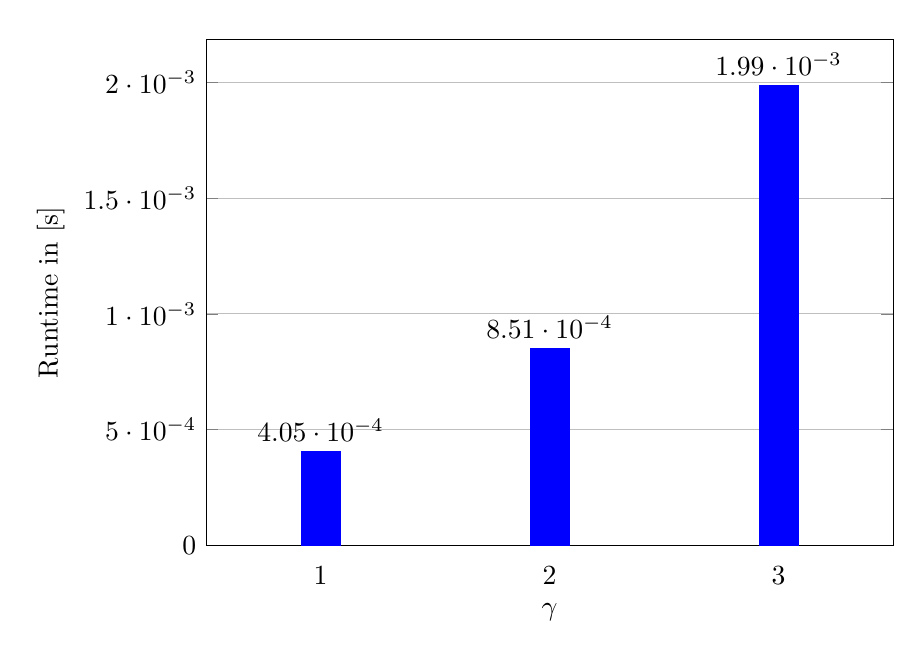
\begin{tikzpicture}
			\begin{axis}[
				ybar,
				width = 0.85 * \textwidth,
				height = 8cm,
				major x tick style = transparent,
				bar width = 14pt,
				ymajorgrids = true,
				xlabel = {$\gamma$},
				ylabel = {Runtime in [s]},
				ylabel near ticks, 
				symbolic x coords = {1, 2, 3},
				xtick = data,
				scaled y ticks = false,
				enlarge x limits = 0.25,
				ymin = 0,
				nodes near coords,
				node near coord style={black}
				%				legend cell align=left,
				%				legend style={
					%					at={(1,1.05)},
					%					anchor=south east,
					%					column sep=1ex
					%				}
				]
				\addplot [style={blue, fill=blue, mark=none}]
				coordinates{ (1, 0.000404958) (2, 0.000851125) (3, 0.00198617)};
			\end{axis}
		\end{tikzpicture}
		\caption{\label{fig::GAMMA4} coarse mesh $n=4$}
	\end{subfigure}
	\hfill
	\begin{subfigure}[h!]{.49\textwidth}
		\centering
		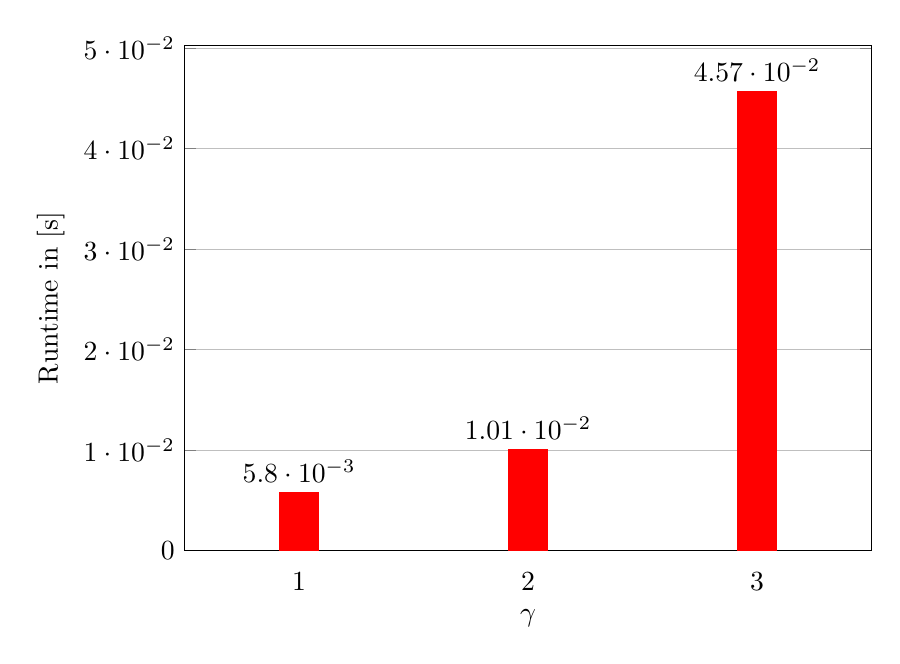
\begin{tikzpicture}
			\begin{axis}[
				ybar,
				width = 0.85 * \textwidth,
				height = 8cm,
				major x tick style = transparent,
				bar width = 14pt,
				ymajorgrids = true,
				xlabel = {$\gamma$},
				ylabel = {Runtime in [s]},
				ylabel near ticks, 
				symbolic x coords = {1, 2, 3},
				xtick = data,
				scaled y ticks = false,
				enlarge x limits = 0.25,
				ymin = 0,
				nodes near coords,
				node near coord style={black}
				]
				\addplot [style={red, fill=red, mark=none}]
				coordinates{ (1, 0.00579512) (2, 0.0100865) (3, 0.045706)};
			\end{axis}
		\end{tikzpicture}
		\caption{\label{fig::GAMMA7} fine mesh $n=7$}
	\end{subfigure}
	\caption{\label{fig::GAMMA} Runtime for $\gamma = \{1,2,3\}$ for both meshes }
\end{figure}
%
\begin{figure}[h!]
	\centering
	\begin{subfigure}[h!]{.49\textwidth}
		\begin{center}
			\resizebox{0.52\width}{!}{%% Creator: Matplotlib, PGF backend
%%
%% To include the figure in your LaTeX document, write
%%   \input{<filename>.pgf}
%%
%% Make sure the required packages are loaded in your preamble
%%   \usepackage{pgf}
%%
%% Also ensure that all the required font packages are loaded; for instance,
%% the lmodern package is sometimes necessary when using math font.
%%   \usepackage{lmodern}
%%
%% Figures using additional raster images can only be included by \input if
%% they are in the same directory as the main LaTeX file. For loading figures
%% from other directories you can use the `import` package
%%   \usepackage{import}
%%
%% and then include the figures with
%%   \import{<path to file>}{<filename>.pgf}
%%
%% Matplotlib used the following preamble
%%   
%%   \makeatletter\@ifpackageloaded{underscore}{}{\usepackage[strings]{underscore}}\makeatother
%%
\begingroup%
\makeatletter%
\begin{pgfpicture}%
\pgfpathrectangle{\pgfpointorigin}{\pgfqpoint{6.565064in}{4.725328in}}%
\pgfusepath{use as bounding box, clip}%
\begin{pgfscope}%
\pgfsetbuttcap%
\pgfsetmiterjoin%
\definecolor{currentfill}{rgb}{1.000000,1.000000,1.000000}%
\pgfsetfillcolor{currentfill}%
\pgfsetlinewidth{0.000000pt}%
\definecolor{currentstroke}{rgb}{1.000000,1.000000,1.000000}%
\pgfsetstrokecolor{currentstroke}%
\pgfsetdash{}{0pt}%
\pgfpathmoveto{\pgfqpoint{0.000000in}{0.000000in}}%
\pgfpathlineto{\pgfqpoint{6.565064in}{0.000000in}}%
\pgfpathlineto{\pgfqpoint{6.565064in}{4.725328in}}%
\pgfpathlineto{\pgfqpoint{0.000000in}{4.725328in}}%
\pgfpathlineto{\pgfqpoint{0.000000in}{0.000000in}}%
\pgfpathclose%
\pgfusepath{fill}%
\end{pgfscope}%
\begin{pgfscope}%
\pgfsetbuttcap%
\pgfsetmiterjoin%
\definecolor{currentfill}{rgb}{1.000000,1.000000,1.000000}%
\pgfsetfillcolor{currentfill}%
\pgfsetlinewidth{0.000000pt}%
\definecolor{currentstroke}{rgb}{0.000000,0.000000,0.000000}%
\pgfsetstrokecolor{currentstroke}%
\pgfsetstrokeopacity{0.000000}%
\pgfsetdash{}{0pt}%
\pgfpathmoveto{\pgfqpoint{1.440450in}{0.604012in}}%
\pgfpathlineto{\pgfqpoint{6.415064in}{0.604012in}}%
\pgfpathlineto{\pgfqpoint{6.415064in}{4.575328in}}%
\pgfpathlineto{\pgfqpoint{1.440450in}{4.575328in}}%
\pgfpathlineto{\pgfqpoint{1.440450in}{0.604012in}}%
\pgfpathclose%
\pgfusepath{fill}%
\end{pgfscope}%
\begin{pgfscope}%
\pgfpathrectangle{\pgfqpoint{1.440450in}{0.604012in}}{\pgfqpoint{4.974614in}{3.971316in}}%
\pgfusepath{clip}%
\pgfsetrectcap%
\pgfsetroundjoin%
\pgfsetlinewidth{0.803000pt}%
\definecolor{currentstroke}{rgb}{0.690196,0.690196,0.690196}%
\pgfsetstrokecolor{currentstroke}%
\pgfsetdash{}{0pt}%
\pgfpathmoveto{\pgfqpoint{1.440450in}{0.604012in}}%
\pgfpathlineto{\pgfqpoint{1.440450in}{4.575328in}}%
\pgfusepath{stroke}%
\end{pgfscope}%
\begin{pgfscope}%
\pgfsetbuttcap%
\pgfsetroundjoin%
\definecolor{currentfill}{rgb}{0.000000,0.000000,0.000000}%
\pgfsetfillcolor{currentfill}%
\pgfsetlinewidth{0.803000pt}%
\definecolor{currentstroke}{rgb}{0.000000,0.000000,0.000000}%
\pgfsetstrokecolor{currentstroke}%
\pgfsetdash{}{0pt}%
\pgfsys@defobject{currentmarker}{\pgfqpoint{0.000000in}{-0.048611in}}{\pgfqpoint{0.000000in}{0.000000in}}{%
\pgfpathmoveto{\pgfqpoint{0.000000in}{0.000000in}}%
\pgfpathlineto{\pgfqpoint{0.000000in}{-0.048611in}}%
\pgfusepath{stroke,fill}%
}%
\begin{pgfscope}%
\pgfsys@transformshift{1.440450in}{0.604012in}%
\pgfsys@useobject{currentmarker}{}%
\end{pgfscope}%
\end{pgfscope}%
\begin{pgfscope}%
\definecolor{textcolor}{rgb}{0.000000,0.000000,0.000000}%
\pgfsetstrokecolor{textcolor}%
\pgfsetfillcolor{textcolor}%
\pgftext[x=1.440450in,y=0.506790in,,top]{\color{textcolor}\rmfamily\fontsize{10.000000}{12.000000}\selectfont \(\displaystyle {0}\)}%
\end{pgfscope}%
\begin{pgfscope}%
\pgfpathrectangle{\pgfqpoint{1.440450in}{0.604012in}}{\pgfqpoint{4.974614in}{3.971316in}}%
\pgfusepath{clip}%
\pgfsetrectcap%
\pgfsetroundjoin%
\pgfsetlinewidth{0.803000pt}%
\definecolor{currentstroke}{rgb}{0.690196,0.690196,0.690196}%
\pgfsetstrokecolor{currentstroke}%
\pgfsetdash{}{0pt}%
\pgfpathmoveto{\pgfqpoint{2.344925in}{0.604012in}}%
\pgfpathlineto{\pgfqpoint{2.344925in}{4.575328in}}%
\pgfusepath{stroke}%
\end{pgfscope}%
\begin{pgfscope}%
\pgfsetbuttcap%
\pgfsetroundjoin%
\definecolor{currentfill}{rgb}{0.000000,0.000000,0.000000}%
\pgfsetfillcolor{currentfill}%
\pgfsetlinewidth{0.803000pt}%
\definecolor{currentstroke}{rgb}{0.000000,0.000000,0.000000}%
\pgfsetstrokecolor{currentstroke}%
\pgfsetdash{}{0pt}%
\pgfsys@defobject{currentmarker}{\pgfqpoint{0.000000in}{-0.048611in}}{\pgfqpoint{0.000000in}{0.000000in}}{%
\pgfpathmoveto{\pgfqpoint{0.000000in}{0.000000in}}%
\pgfpathlineto{\pgfqpoint{0.000000in}{-0.048611in}}%
\pgfusepath{stroke,fill}%
}%
\begin{pgfscope}%
\pgfsys@transformshift{2.344925in}{0.604012in}%
\pgfsys@useobject{currentmarker}{}%
\end{pgfscope}%
\end{pgfscope}%
\begin{pgfscope}%
\definecolor{textcolor}{rgb}{0.000000,0.000000,0.000000}%
\pgfsetstrokecolor{textcolor}%
\pgfsetfillcolor{textcolor}%
\pgftext[x=2.344925in,y=0.506790in,,top]{\color{textcolor}\rmfamily\fontsize{10.000000}{12.000000}\selectfont \(\displaystyle {2}\)}%
\end{pgfscope}%
\begin{pgfscope}%
\pgfpathrectangle{\pgfqpoint{1.440450in}{0.604012in}}{\pgfqpoint{4.974614in}{3.971316in}}%
\pgfusepath{clip}%
\pgfsetrectcap%
\pgfsetroundjoin%
\pgfsetlinewidth{0.803000pt}%
\definecolor{currentstroke}{rgb}{0.690196,0.690196,0.690196}%
\pgfsetstrokecolor{currentstroke}%
\pgfsetdash{}{0pt}%
\pgfpathmoveto{\pgfqpoint{3.249401in}{0.604012in}}%
\pgfpathlineto{\pgfqpoint{3.249401in}{4.575328in}}%
\pgfusepath{stroke}%
\end{pgfscope}%
\begin{pgfscope}%
\pgfsetbuttcap%
\pgfsetroundjoin%
\definecolor{currentfill}{rgb}{0.000000,0.000000,0.000000}%
\pgfsetfillcolor{currentfill}%
\pgfsetlinewidth{0.803000pt}%
\definecolor{currentstroke}{rgb}{0.000000,0.000000,0.000000}%
\pgfsetstrokecolor{currentstroke}%
\pgfsetdash{}{0pt}%
\pgfsys@defobject{currentmarker}{\pgfqpoint{0.000000in}{-0.048611in}}{\pgfqpoint{0.000000in}{0.000000in}}{%
\pgfpathmoveto{\pgfqpoint{0.000000in}{0.000000in}}%
\pgfpathlineto{\pgfqpoint{0.000000in}{-0.048611in}}%
\pgfusepath{stroke,fill}%
}%
\begin{pgfscope}%
\pgfsys@transformshift{3.249401in}{0.604012in}%
\pgfsys@useobject{currentmarker}{}%
\end{pgfscope}%
\end{pgfscope}%
\begin{pgfscope}%
\definecolor{textcolor}{rgb}{0.000000,0.000000,0.000000}%
\pgfsetstrokecolor{textcolor}%
\pgfsetfillcolor{textcolor}%
\pgftext[x=3.249401in,y=0.506790in,,top]{\color{textcolor}\rmfamily\fontsize{10.000000}{12.000000}\selectfont \(\displaystyle {4}\)}%
\end{pgfscope}%
\begin{pgfscope}%
\pgfpathrectangle{\pgfqpoint{1.440450in}{0.604012in}}{\pgfqpoint{4.974614in}{3.971316in}}%
\pgfusepath{clip}%
\pgfsetrectcap%
\pgfsetroundjoin%
\pgfsetlinewidth{0.803000pt}%
\definecolor{currentstroke}{rgb}{0.690196,0.690196,0.690196}%
\pgfsetstrokecolor{currentstroke}%
\pgfsetdash{}{0pt}%
\pgfpathmoveto{\pgfqpoint{4.153876in}{0.604012in}}%
\pgfpathlineto{\pgfqpoint{4.153876in}{4.575328in}}%
\pgfusepath{stroke}%
\end{pgfscope}%
\begin{pgfscope}%
\pgfsetbuttcap%
\pgfsetroundjoin%
\definecolor{currentfill}{rgb}{0.000000,0.000000,0.000000}%
\pgfsetfillcolor{currentfill}%
\pgfsetlinewidth{0.803000pt}%
\definecolor{currentstroke}{rgb}{0.000000,0.000000,0.000000}%
\pgfsetstrokecolor{currentstroke}%
\pgfsetdash{}{0pt}%
\pgfsys@defobject{currentmarker}{\pgfqpoint{0.000000in}{-0.048611in}}{\pgfqpoint{0.000000in}{0.000000in}}{%
\pgfpathmoveto{\pgfqpoint{0.000000in}{0.000000in}}%
\pgfpathlineto{\pgfqpoint{0.000000in}{-0.048611in}}%
\pgfusepath{stroke,fill}%
}%
\begin{pgfscope}%
\pgfsys@transformshift{4.153876in}{0.604012in}%
\pgfsys@useobject{currentmarker}{}%
\end{pgfscope}%
\end{pgfscope}%
\begin{pgfscope}%
\definecolor{textcolor}{rgb}{0.000000,0.000000,0.000000}%
\pgfsetstrokecolor{textcolor}%
\pgfsetfillcolor{textcolor}%
\pgftext[x=4.153876in,y=0.506790in,,top]{\color{textcolor}\rmfamily\fontsize{10.000000}{12.000000}\selectfont \(\displaystyle {6}\)}%
\end{pgfscope}%
\begin{pgfscope}%
\pgfpathrectangle{\pgfqpoint{1.440450in}{0.604012in}}{\pgfqpoint{4.974614in}{3.971316in}}%
\pgfusepath{clip}%
\pgfsetrectcap%
\pgfsetroundjoin%
\pgfsetlinewidth{0.803000pt}%
\definecolor{currentstroke}{rgb}{0.690196,0.690196,0.690196}%
\pgfsetstrokecolor{currentstroke}%
\pgfsetdash{}{0pt}%
\pgfpathmoveto{\pgfqpoint{5.058351in}{0.604012in}}%
\pgfpathlineto{\pgfqpoint{5.058351in}{4.575328in}}%
\pgfusepath{stroke}%
\end{pgfscope}%
\begin{pgfscope}%
\pgfsetbuttcap%
\pgfsetroundjoin%
\definecolor{currentfill}{rgb}{0.000000,0.000000,0.000000}%
\pgfsetfillcolor{currentfill}%
\pgfsetlinewidth{0.803000pt}%
\definecolor{currentstroke}{rgb}{0.000000,0.000000,0.000000}%
\pgfsetstrokecolor{currentstroke}%
\pgfsetdash{}{0pt}%
\pgfsys@defobject{currentmarker}{\pgfqpoint{0.000000in}{-0.048611in}}{\pgfqpoint{0.000000in}{0.000000in}}{%
\pgfpathmoveto{\pgfqpoint{0.000000in}{0.000000in}}%
\pgfpathlineto{\pgfqpoint{0.000000in}{-0.048611in}}%
\pgfusepath{stroke,fill}%
}%
\begin{pgfscope}%
\pgfsys@transformshift{5.058351in}{0.604012in}%
\pgfsys@useobject{currentmarker}{}%
\end{pgfscope}%
\end{pgfscope}%
\begin{pgfscope}%
\definecolor{textcolor}{rgb}{0.000000,0.000000,0.000000}%
\pgfsetstrokecolor{textcolor}%
\pgfsetfillcolor{textcolor}%
\pgftext[x=5.058351in,y=0.506790in,,top]{\color{textcolor}\rmfamily\fontsize{10.000000}{12.000000}\selectfont \(\displaystyle {8}\)}%
\end{pgfscope}%
\begin{pgfscope}%
\pgfpathrectangle{\pgfqpoint{1.440450in}{0.604012in}}{\pgfqpoint{4.974614in}{3.971316in}}%
\pgfusepath{clip}%
\pgfsetrectcap%
\pgfsetroundjoin%
\pgfsetlinewidth{0.803000pt}%
\definecolor{currentstroke}{rgb}{0.690196,0.690196,0.690196}%
\pgfsetstrokecolor{currentstroke}%
\pgfsetdash{}{0pt}%
\pgfpathmoveto{\pgfqpoint{5.962826in}{0.604012in}}%
\pgfpathlineto{\pgfqpoint{5.962826in}{4.575328in}}%
\pgfusepath{stroke}%
\end{pgfscope}%
\begin{pgfscope}%
\pgfsetbuttcap%
\pgfsetroundjoin%
\definecolor{currentfill}{rgb}{0.000000,0.000000,0.000000}%
\pgfsetfillcolor{currentfill}%
\pgfsetlinewidth{0.803000pt}%
\definecolor{currentstroke}{rgb}{0.000000,0.000000,0.000000}%
\pgfsetstrokecolor{currentstroke}%
\pgfsetdash{}{0pt}%
\pgfsys@defobject{currentmarker}{\pgfqpoint{0.000000in}{-0.048611in}}{\pgfqpoint{0.000000in}{0.000000in}}{%
\pgfpathmoveto{\pgfqpoint{0.000000in}{0.000000in}}%
\pgfpathlineto{\pgfqpoint{0.000000in}{-0.048611in}}%
\pgfusepath{stroke,fill}%
}%
\begin{pgfscope}%
\pgfsys@transformshift{5.962826in}{0.604012in}%
\pgfsys@useobject{currentmarker}{}%
\end{pgfscope}%
\end{pgfscope}%
\begin{pgfscope}%
\definecolor{textcolor}{rgb}{0.000000,0.000000,0.000000}%
\pgfsetstrokecolor{textcolor}%
\pgfsetfillcolor{textcolor}%
\pgftext[x=5.962826in,y=0.506790in,,top]{\color{textcolor}\rmfamily\fontsize{10.000000}{12.000000}\selectfont \(\displaystyle {10}\)}%
\end{pgfscope}%
\begin{pgfscope}%
\definecolor{textcolor}{rgb}{0.000000,0.000000,0.000000}%
\pgfsetstrokecolor{textcolor}%
\pgfsetfillcolor{textcolor}%
\pgftext[x=3.927757in,y=0.327777in,,top]{\color{textcolor}\rmfamily\fontsize{15.000000}{18.000000}\selectfont \(\displaystyle \gamma\)}%
\end{pgfscope}%
\begin{pgfscope}%
\pgfpathrectangle{\pgfqpoint{1.440450in}{0.604012in}}{\pgfqpoint{4.974614in}{3.971316in}}%
\pgfusepath{clip}%
\pgfsetrectcap%
\pgfsetroundjoin%
\pgfsetlinewidth{0.803000pt}%
\definecolor{currentstroke}{rgb}{0.690196,0.690196,0.690196}%
\pgfsetstrokecolor{currentstroke}%
\pgfsetdash{}{0pt}%
\pgfpathmoveto{\pgfqpoint{1.440450in}{0.604012in}}%
\pgfpathlineto{\pgfqpoint{6.415064in}{0.604012in}}%
\pgfusepath{stroke}%
\end{pgfscope}%
\begin{pgfscope}%
\pgfsetbuttcap%
\pgfsetroundjoin%
\definecolor{currentfill}{rgb}{0.000000,0.000000,0.000000}%
\pgfsetfillcolor{currentfill}%
\pgfsetlinewidth{0.803000pt}%
\definecolor{currentstroke}{rgb}{0.000000,0.000000,0.000000}%
\pgfsetstrokecolor{currentstroke}%
\pgfsetdash{}{0pt}%
\pgfsys@defobject{currentmarker}{\pgfqpoint{-0.048611in}{0.000000in}}{\pgfqpoint{-0.000000in}{0.000000in}}{%
\pgfpathmoveto{\pgfqpoint{-0.000000in}{0.000000in}}%
\pgfpathlineto{\pgfqpoint{-0.048611in}{0.000000in}}%
\pgfusepath{stroke,fill}%
}%
\begin{pgfscope}%
\pgfsys@transformshift{1.440450in}{0.604012in}%
\pgfsys@useobject{currentmarker}{}%
\end{pgfscope}%
\end{pgfscope}%
\begin{pgfscope}%
\definecolor{textcolor}{rgb}{0.000000,0.000000,0.000000}%
\pgfsetstrokecolor{textcolor}%
\pgfsetfillcolor{textcolor}%
\pgftext[x=1.096314in, y=0.555787in, left, base]{\color{textcolor}\rmfamily\fontsize{10.000000}{12.000000}\selectfont \(\displaystyle {0.00}\)}%
\end{pgfscope}%
\begin{pgfscope}%
\pgfpathrectangle{\pgfqpoint{1.440450in}{0.604012in}}{\pgfqpoint{4.974614in}{3.971316in}}%
\pgfusepath{clip}%
\pgfsetrectcap%
\pgfsetroundjoin%
\pgfsetlinewidth{0.803000pt}%
\definecolor{currentstroke}{rgb}{0.690196,0.690196,0.690196}%
\pgfsetstrokecolor{currentstroke}%
\pgfsetdash{}{0pt}%
\pgfpathmoveto{\pgfqpoint{1.440450in}{1.381120in}}%
\pgfpathlineto{\pgfqpoint{6.415064in}{1.381120in}}%
\pgfusepath{stroke}%
\end{pgfscope}%
\begin{pgfscope}%
\pgfsetbuttcap%
\pgfsetroundjoin%
\definecolor{currentfill}{rgb}{0.000000,0.000000,0.000000}%
\pgfsetfillcolor{currentfill}%
\pgfsetlinewidth{0.803000pt}%
\definecolor{currentstroke}{rgb}{0.000000,0.000000,0.000000}%
\pgfsetstrokecolor{currentstroke}%
\pgfsetdash{}{0pt}%
\pgfsys@defobject{currentmarker}{\pgfqpoint{-0.048611in}{0.000000in}}{\pgfqpoint{-0.000000in}{0.000000in}}{%
\pgfpathmoveto{\pgfqpoint{-0.000000in}{0.000000in}}%
\pgfpathlineto{\pgfqpoint{-0.048611in}{0.000000in}}%
\pgfusepath{stroke,fill}%
}%
\begin{pgfscope}%
\pgfsys@transformshift{1.440450in}{1.381120in}%
\pgfsys@useobject{currentmarker}{}%
\end{pgfscope}%
\end{pgfscope}%
\begin{pgfscope}%
\definecolor{textcolor}{rgb}{0.000000,0.000000,0.000000}%
\pgfsetstrokecolor{textcolor}%
\pgfsetfillcolor{textcolor}%
\pgftext[x=1.096314in, y=1.332894in, left, base]{\color{textcolor}\rmfamily\fontsize{10.000000}{12.000000}\selectfont \(\displaystyle {0.01}\)}%
\end{pgfscope}%
\begin{pgfscope}%
\pgfpathrectangle{\pgfqpoint{1.440450in}{0.604012in}}{\pgfqpoint{4.974614in}{3.971316in}}%
\pgfusepath{clip}%
\pgfsetrectcap%
\pgfsetroundjoin%
\pgfsetlinewidth{0.803000pt}%
\definecolor{currentstroke}{rgb}{0.690196,0.690196,0.690196}%
\pgfsetstrokecolor{currentstroke}%
\pgfsetdash{}{0pt}%
\pgfpathmoveto{\pgfqpoint{1.440450in}{2.158227in}}%
\pgfpathlineto{\pgfqpoint{6.415064in}{2.158227in}}%
\pgfusepath{stroke}%
\end{pgfscope}%
\begin{pgfscope}%
\pgfsetbuttcap%
\pgfsetroundjoin%
\definecolor{currentfill}{rgb}{0.000000,0.000000,0.000000}%
\pgfsetfillcolor{currentfill}%
\pgfsetlinewidth{0.803000pt}%
\definecolor{currentstroke}{rgb}{0.000000,0.000000,0.000000}%
\pgfsetstrokecolor{currentstroke}%
\pgfsetdash{}{0pt}%
\pgfsys@defobject{currentmarker}{\pgfqpoint{-0.048611in}{0.000000in}}{\pgfqpoint{-0.000000in}{0.000000in}}{%
\pgfpathmoveto{\pgfqpoint{-0.000000in}{0.000000in}}%
\pgfpathlineto{\pgfqpoint{-0.048611in}{0.000000in}}%
\pgfusepath{stroke,fill}%
}%
\begin{pgfscope}%
\pgfsys@transformshift{1.440450in}{2.158227in}%
\pgfsys@useobject{currentmarker}{}%
\end{pgfscope}%
\end{pgfscope}%
\begin{pgfscope}%
\definecolor{textcolor}{rgb}{0.000000,0.000000,0.000000}%
\pgfsetstrokecolor{textcolor}%
\pgfsetfillcolor{textcolor}%
\pgftext[x=1.096314in, y=2.110002in, left, base]{\color{textcolor}\rmfamily\fontsize{10.000000}{12.000000}\selectfont \(\displaystyle {0.02}\)}%
\end{pgfscope}%
\begin{pgfscope}%
\pgfpathrectangle{\pgfqpoint{1.440450in}{0.604012in}}{\pgfqpoint{4.974614in}{3.971316in}}%
\pgfusepath{clip}%
\pgfsetrectcap%
\pgfsetroundjoin%
\pgfsetlinewidth{0.803000pt}%
\definecolor{currentstroke}{rgb}{0.690196,0.690196,0.690196}%
\pgfsetstrokecolor{currentstroke}%
\pgfsetdash{}{0pt}%
\pgfpathmoveto{\pgfqpoint{1.440450in}{2.935335in}}%
\pgfpathlineto{\pgfqpoint{6.415064in}{2.935335in}}%
\pgfusepath{stroke}%
\end{pgfscope}%
\begin{pgfscope}%
\pgfsetbuttcap%
\pgfsetroundjoin%
\definecolor{currentfill}{rgb}{0.000000,0.000000,0.000000}%
\pgfsetfillcolor{currentfill}%
\pgfsetlinewidth{0.803000pt}%
\definecolor{currentstroke}{rgb}{0.000000,0.000000,0.000000}%
\pgfsetstrokecolor{currentstroke}%
\pgfsetdash{}{0pt}%
\pgfsys@defobject{currentmarker}{\pgfqpoint{-0.048611in}{0.000000in}}{\pgfqpoint{-0.000000in}{0.000000in}}{%
\pgfpathmoveto{\pgfqpoint{-0.000000in}{0.000000in}}%
\pgfpathlineto{\pgfqpoint{-0.048611in}{0.000000in}}%
\pgfusepath{stroke,fill}%
}%
\begin{pgfscope}%
\pgfsys@transformshift{1.440450in}{2.935335in}%
\pgfsys@useobject{currentmarker}{}%
\end{pgfscope}%
\end{pgfscope}%
\begin{pgfscope}%
\definecolor{textcolor}{rgb}{0.000000,0.000000,0.000000}%
\pgfsetstrokecolor{textcolor}%
\pgfsetfillcolor{textcolor}%
\pgftext[x=1.096314in, y=2.887110in, left, base]{\color{textcolor}\rmfamily\fontsize{10.000000}{12.000000}\selectfont \(\displaystyle {0.03}\)}%
\end{pgfscope}%
\begin{pgfscope}%
\pgfpathrectangle{\pgfqpoint{1.440450in}{0.604012in}}{\pgfqpoint{4.974614in}{3.971316in}}%
\pgfusepath{clip}%
\pgfsetrectcap%
\pgfsetroundjoin%
\pgfsetlinewidth{0.803000pt}%
\definecolor{currentstroke}{rgb}{0.690196,0.690196,0.690196}%
\pgfsetstrokecolor{currentstroke}%
\pgfsetdash{}{0pt}%
\pgfpathmoveto{\pgfqpoint{1.440450in}{3.712443in}}%
\pgfpathlineto{\pgfqpoint{6.415064in}{3.712443in}}%
\pgfusepath{stroke}%
\end{pgfscope}%
\begin{pgfscope}%
\pgfsetbuttcap%
\pgfsetroundjoin%
\definecolor{currentfill}{rgb}{0.000000,0.000000,0.000000}%
\pgfsetfillcolor{currentfill}%
\pgfsetlinewidth{0.803000pt}%
\definecolor{currentstroke}{rgb}{0.000000,0.000000,0.000000}%
\pgfsetstrokecolor{currentstroke}%
\pgfsetdash{}{0pt}%
\pgfsys@defobject{currentmarker}{\pgfqpoint{-0.048611in}{0.000000in}}{\pgfqpoint{-0.000000in}{0.000000in}}{%
\pgfpathmoveto{\pgfqpoint{-0.000000in}{0.000000in}}%
\pgfpathlineto{\pgfqpoint{-0.048611in}{0.000000in}}%
\pgfusepath{stroke,fill}%
}%
\begin{pgfscope}%
\pgfsys@transformshift{1.440450in}{3.712443in}%
\pgfsys@useobject{currentmarker}{}%
\end{pgfscope}%
\end{pgfscope}%
\begin{pgfscope}%
\definecolor{textcolor}{rgb}{0.000000,0.000000,0.000000}%
\pgfsetstrokecolor{textcolor}%
\pgfsetfillcolor{textcolor}%
\pgftext[x=1.096314in, y=3.664218in, left, base]{\color{textcolor}\rmfamily\fontsize{10.000000}{12.000000}\selectfont \(\displaystyle {0.04}\)}%
\end{pgfscope}%
\begin{pgfscope}%
\pgfpathrectangle{\pgfqpoint{1.440450in}{0.604012in}}{\pgfqpoint{4.974614in}{3.971316in}}%
\pgfusepath{clip}%
\pgfsetrectcap%
\pgfsetroundjoin%
\pgfsetlinewidth{0.803000pt}%
\definecolor{currentstroke}{rgb}{0.690196,0.690196,0.690196}%
\pgfsetstrokecolor{currentstroke}%
\pgfsetdash{}{0pt}%
\pgfpathmoveto{\pgfqpoint{1.440450in}{4.489551in}}%
\pgfpathlineto{\pgfqpoint{6.415064in}{4.489551in}}%
\pgfusepath{stroke}%
\end{pgfscope}%
\begin{pgfscope}%
\pgfsetbuttcap%
\pgfsetroundjoin%
\definecolor{currentfill}{rgb}{0.000000,0.000000,0.000000}%
\pgfsetfillcolor{currentfill}%
\pgfsetlinewidth{0.803000pt}%
\definecolor{currentstroke}{rgb}{0.000000,0.000000,0.000000}%
\pgfsetstrokecolor{currentstroke}%
\pgfsetdash{}{0pt}%
\pgfsys@defobject{currentmarker}{\pgfqpoint{-0.048611in}{0.000000in}}{\pgfqpoint{-0.000000in}{0.000000in}}{%
\pgfpathmoveto{\pgfqpoint{-0.000000in}{0.000000in}}%
\pgfpathlineto{\pgfqpoint{-0.048611in}{0.000000in}}%
\pgfusepath{stroke,fill}%
}%
\begin{pgfscope}%
\pgfsys@transformshift{1.440450in}{4.489551in}%
\pgfsys@useobject{currentmarker}{}%
\end{pgfscope}%
\end{pgfscope}%
\begin{pgfscope}%
\definecolor{textcolor}{rgb}{0.000000,0.000000,0.000000}%
\pgfsetstrokecolor{textcolor}%
\pgfsetfillcolor{textcolor}%
\pgftext[x=1.096314in, y=4.441326in, left, base]{\color{textcolor}\rmfamily\fontsize{10.000000}{12.000000}\selectfont \(\displaystyle {0.05}\)}%
\end{pgfscope}%
\begin{pgfscope}%
\definecolor{textcolor}{rgb}{0.000000,0.000000,0.000000}%
\pgfsetstrokecolor{textcolor}%
\pgfsetfillcolor{textcolor}%
\pgftext[x=0.610202in,y=2.589670in,,bottom]{\color{textcolor}\rmfamily\fontsize{15.000000}{18.000000}\selectfont runtime [s]}%
\end{pgfscope}%
\begin{pgfscope}%
\pgfpathrectangle{\pgfqpoint{1.440450in}{0.604012in}}{\pgfqpoint{4.974614in}{3.971316in}}%
\pgfusepath{clip}%
\pgfsetrectcap%
\pgfsetroundjoin%
\pgfsetlinewidth{1.505625pt}%
\definecolor{currentstroke}{rgb}{0.121569,0.466667,0.705882}%
\pgfsetstrokecolor{currentstroke}%
\pgfsetdash{}{0pt}%
\pgfpathmoveto{\pgfqpoint{1.440450in}{0.643113in}}%
\pgfpathlineto{\pgfqpoint{1.892688in}{0.680978in}}%
\pgfpathlineto{\pgfqpoint{2.344925in}{0.782015in}}%
\pgfpathlineto{\pgfqpoint{2.797163in}{0.923125in}}%
\pgfpathlineto{\pgfqpoint{3.249401in}{1.143616in}}%
\pgfpathlineto{\pgfqpoint{3.701638in}{1.496924in}}%
\pgfpathlineto{\pgfqpoint{4.153876in}{1.944290in}}%
\pgfpathlineto{\pgfqpoint{4.606113in}{2.524836in}}%
\pgfpathlineto{\pgfqpoint{5.058351in}{3.273105in}}%
\pgfpathlineto{\pgfqpoint{5.510589in}{4.214299in}}%
\pgfusepath{stroke}%
\end{pgfscope}%
\begin{pgfscope}%
\pgfsetrectcap%
\pgfsetmiterjoin%
\pgfsetlinewidth{0.803000pt}%
\definecolor{currentstroke}{rgb}{0.000000,0.000000,0.000000}%
\pgfsetstrokecolor{currentstroke}%
\pgfsetdash{}{0pt}%
\pgfpathmoveto{\pgfqpoint{1.440450in}{0.604012in}}%
\pgfpathlineto{\pgfqpoint{1.440450in}{4.575328in}}%
\pgfusepath{stroke}%
\end{pgfscope}%
\begin{pgfscope}%
\pgfsetrectcap%
\pgfsetmiterjoin%
\pgfsetlinewidth{0.803000pt}%
\definecolor{currentstroke}{rgb}{0.000000,0.000000,0.000000}%
\pgfsetstrokecolor{currentstroke}%
\pgfsetdash{}{0pt}%
\pgfpathmoveto{\pgfqpoint{6.415064in}{0.604012in}}%
\pgfpathlineto{\pgfqpoint{6.415064in}{4.575328in}}%
\pgfusepath{stroke}%
\end{pgfscope}%
\begin{pgfscope}%
\pgfsetrectcap%
\pgfsetmiterjoin%
\pgfsetlinewidth{0.803000pt}%
\definecolor{currentstroke}{rgb}{0.000000,0.000000,0.000000}%
\pgfsetstrokecolor{currentstroke}%
\pgfsetdash{}{0pt}%
\pgfpathmoveto{\pgfqpoint{1.440450in}{0.604012in}}%
\pgfpathlineto{\pgfqpoint{6.415064in}{0.604012in}}%
\pgfusepath{stroke}%
\end{pgfscope}%
\begin{pgfscope}%
\pgfsetrectcap%
\pgfsetmiterjoin%
\pgfsetlinewidth{0.803000pt}%
\definecolor{currentstroke}{rgb}{0.000000,0.000000,0.000000}%
\pgfsetstrokecolor{currentstroke}%
\pgfsetdash{}{0pt}%
\pgfpathmoveto{\pgfqpoint{1.440450in}{4.575328in}}%
\pgfpathlineto{\pgfqpoint{6.415064in}{4.575328in}}%
\pgfusepath{stroke}%
\end{pgfscope}%
\end{pgfpicture}%
\makeatother%
\endgroup%
}
			\caption{$n=4$}
			\label{fig::TimGamma1}
		\end{center}	
	\end{subfigure}
	\hfill
	\begin{subfigure}[h!]{.49\textwidth}
		\centering
		\resizebox{0.52\width}{!}{%% Creator: Matplotlib, PGF backend
%%
%% To include the figure in your LaTeX document, write
%%   \input{<filename>.pgf}
%%
%% Make sure the required packages are loaded in your preamble
%%   \usepackage{pgf}
%%
%% Also ensure that all the required font packages are loaded; for instance,
%% the lmodern package is sometimes necessary when using math font.
%%   \usepackage{lmodern}
%%
%% Figures using additional raster images can only be included by \input if
%% they are in the same directory as the main LaTeX file. For loading figures
%% from other directories you can use the `import` package
%%   \usepackage{import}
%%
%% and then include the figures with
%%   \import{<path to file>}{<filename>.pgf}
%%
%% Matplotlib used the following preamble
%%   
%%   \makeatletter\@ifpackageloaded{underscore}{}{\usepackage[strings]{underscore}}\makeatother
%%
\begingroup%
\makeatletter%
\begin{pgfpicture}%
\pgfpathrectangle{\pgfpointorigin}{\pgfqpoint{6.565064in}{4.725328in}}%
\pgfusepath{use as bounding box, clip}%
\begin{pgfscope}%
\pgfsetbuttcap%
\pgfsetmiterjoin%
\definecolor{currentfill}{rgb}{1.000000,1.000000,1.000000}%
\pgfsetfillcolor{currentfill}%
\pgfsetlinewidth{0.000000pt}%
\definecolor{currentstroke}{rgb}{1.000000,1.000000,1.000000}%
\pgfsetstrokecolor{currentstroke}%
\pgfsetdash{}{0pt}%
\pgfpathmoveto{\pgfqpoint{0.000000in}{0.000000in}}%
\pgfpathlineto{\pgfqpoint{6.565064in}{0.000000in}}%
\pgfpathlineto{\pgfqpoint{6.565064in}{4.725328in}}%
\pgfpathlineto{\pgfqpoint{0.000000in}{4.725328in}}%
\pgfpathlineto{\pgfqpoint{0.000000in}{0.000000in}}%
\pgfpathclose%
\pgfusepath{fill}%
\end{pgfscope}%
\begin{pgfscope}%
\pgfsetbuttcap%
\pgfsetmiterjoin%
\definecolor{currentfill}{rgb}{1.000000,1.000000,1.000000}%
\pgfsetfillcolor{currentfill}%
\pgfsetlinewidth{0.000000pt}%
\definecolor{currentstroke}{rgb}{0.000000,0.000000,0.000000}%
\pgfsetstrokecolor{currentstroke}%
\pgfsetstrokeopacity{0.000000}%
\pgfsetdash{}{0pt}%
\pgfpathmoveto{\pgfqpoint{1.332425in}{0.604012in}}%
\pgfpathlineto{\pgfqpoint{6.415064in}{0.604012in}}%
\pgfpathlineto{\pgfqpoint{6.415064in}{4.527103in}}%
\pgfpathlineto{\pgfqpoint{1.332425in}{4.527103in}}%
\pgfpathlineto{\pgfqpoint{1.332425in}{0.604012in}}%
\pgfpathclose%
\pgfusepath{fill}%
\end{pgfscope}%
\begin{pgfscope}%
\pgfpathrectangle{\pgfqpoint{1.332425in}{0.604012in}}{\pgfqpoint{5.082639in}{3.923091in}}%
\pgfusepath{clip}%
\pgfsetrectcap%
\pgfsetroundjoin%
\pgfsetlinewidth{0.803000pt}%
\definecolor{currentstroke}{rgb}{0.690196,0.690196,0.690196}%
\pgfsetstrokecolor{currentstroke}%
\pgfsetdash{}{0pt}%
\pgfpathmoveto{\pgfqpoint{1.840689in}{0.604012in}}%
\pgfpathlineto{\pgfqpoint{1.840689in}{4.527103in}}%
\pgfusepath{stroke}%
\end{pgfscope}%
\begin{pgfscope}%
\pgfsetbuttcap%
\pgfsetroundjoin%
\definecolor{currentfill}{rgb}{0.000000,0.000000,0.000000}%
\pgfsetfillcolor{currentfill}%
\pgfsetlinewidth{0.803000pt}%
\definecolor{currentstroke}{rgb}{0.000000,0.000000,0.000000}%
\pgfsetstrokecolor{currentstroke}%
\pgfsetdash{}{0pt}%
\pgfsys@defobject{currentmarker}{\pgfqpoint{0.000000in}{-0.048611in}}{\pgfqpoint{0.000000in}{0.000000in}}{%
\pgfpathmoveto{\pgfqpoint{0.000000in}{0.000000in}}%
\pgfpathlineto{\pgfqpoint{0.000000in}{-0.048611in}}%
\pgfusepath{stroke,fill}%
}%
\begin{pgfscope}%
\pgfsys@transformshift{1.840689in}{0.604012in}%
\pgfsys@useobject{currentmarker}{}%
\end{pgfscope}%
\end{pgfscope}%
\begin{pgfscope}%
\definecolor{textcolor}{rgb}{0.000000,0.000000,0.000000}%
\pgfsetstrokecolor{textcolor}%
\pgfsetfillcolor{textcolor}%
\pgftext[x=1.840689in,y=0.506790in,,top]{\color{textcolor}\rmfamily\fontsize{10.000000}{12.000000}\selectfont \(\displaystyle {2}\)}%
\end{pgfscope}%
\begin{pgfscope}%
\pgfpathrectangle{\pgfqpoint{1.332425in}{0.604012in}}{\pgfqpoint{5.082639in}{3.923091in}}%
\pgfusepath{clip}%
\pgfsetrectcap%
\pgfsetroundjoin%
\pgfsetlinewidth{0.803000pt}%
\definecolor{currentstroke}{rgb}{0.690196,0.690196,0.690196}%
\pgfsetstrokecolor{currentstroke}%
\pgfsetdash{}{0pt}%
\pgfpathmoveto{\pgfqpoint{2.857217in}{0.604012in}}%
\pgfpathlineto{\pgfqpoint{2.857217in}{4.527103in}}%
\pgfusepath{stroke}%
\end{pgfscope}%
\begin{pgfscope}%
\pgfsetbuttcap%
\pgfsetroundjoin%
\definecolor{currentfill}{rgb}{0.000000,0.000000,0.000000}%
\pgfsetfillcolor{currentfill}%
\pgfsetlinewidth{0.803000pt}%
\definecolor{currentstroke}{rgb}{0.000000,0.000000,0.000000}%
\pgfsetstrokecolor{currentstroke}%
\pgfsetdash{}{0pt}%
\pgfsys@defobject{currentmarker}{\pgfqpoint{0.000000in}{-0.048611in}}{\pgfqpoint{0.000000in}{0.000000in}}{%
\pgfpathmoveto{\pgfqpoint{0.000000in}{0.000000in}}%
\pgfpathlineto{\pgfqpoint{0.000000in}{-0.048611in}}%
\pgfusepath{stroke,fill}%
}%
\begin{pgfscope}%
\pgfsys@transformshift{2.857217in}{0.604012in}%
\pgfsys@useobject{currentmarker}{}%
\end{pgfscope}%
\end{pgfscope}%
\begin{pgfscope}%
\definecolor{textcolor}{rgb}{0.000000,0.000000,0.000000}%
\pgfsetstrokecolor{textcolor}%
\pgfsetfillcolor{textcolor}%
\pgftext[x=2.857217in,y=0.506790in,,top]{\color{textcolor}\rmfamily\fontsize{10.000000}{12.000000}\selectfont \(\displaystyle {4}\)}%
\end{pgfscope}%
\begin{pgfscope}%
\pgfpathrectangle{\pgfqpoint{1.332425in}{0.604012in}}{\pgfqpoint{5.082639in}{3.923091in}}%
\pgfusepath{clip}%
\pgfsetrectcap%
\pgfsetroundjoin%
\pgfsetlinewidth{0.803000pt}%
\definecolor{currentstroke}{rgb}{0.690196,0.690196,0.690196}%
\pgfsetstrokecolor{currentstroke}%
\pgfsetdash{}{0pt}%
\pgfpathmoveto{\pgfqpoint{3.873745in}{0.604012in}}%
\pgfpathlineto{\pgfqpoint{3.873745in}{4.527103in}}%
\pgfusepath{stroke}%
\end{pgfscope}%
\begin{pgfscope}%
\pgfsetbuttcap%
\pgfsetroundjoin%
\definecolor{currentfill}{rgb}{0.000000,0.000000,0.000000}%
\pgfsetfillcolor{currentfill}%
\pgfsetlinewidth{0.803000pt}%
\definecolor{currentstroke}{rgb}{0.000000,0.000000,0.000000}%
\pgfsetstrokecolor{currentstroke}%
\pgfsetdash{}{0pt}%
\pgfsys@defobject{currentmarker}{\pgfqpoint{0.000000in}{-0.048611in}}{\pgfqpoint{0.000000in}{0.000000in}}{%
\pgfpathmoveto{\pgfqpoint{0.000000in}{0.000000in}}%
\pgfpathlineto{\pgfqpoint{0.000000in}{-0.048611in}}%
\pgfusepath{stroke,fill}%
}%
\begin{pgfscope}%
\pgfsys@transformshift{3.873745in}{0.604012in}%
\pgfsys@useobject{currentmarker}{}%
\end{pgfscope}%
\end{pgfscope}%
\begin{pgfscope}%
\definecolor{textcolor}{rgb}{0.000000,0.000000,0.000000}%
\pgfsetstrokecolor{textcolor}%
\pgfsetfillcolor{textcolor}%
\pgftext[x=3.873745in,y=0.506790in,,top]{\color{textcolor}\rmfamily\fontsize{10.000000}{12.000000}\selectfont \(\displaystyle {6}\)}%
\end{pgfscope}%
\begin{pgfscope}%
\pgfpathrectangle{\pgfqpoint{1.332425in}{0.604012in}}{\pgfqpoint{5.082639in}{3.923091in}}%
\pgfusepath{clip}%
\pgfsetrectcap%
\pgfsetroundjoin%
\pgfsetlinewidth{0.803000pt}%
\definecolor{currentstroke}{rgb}{0.690196,0.690196,0.690196}%
\pgfsetstrokecolor{currentstroke}%
\pgfsetdash{}{0pt}%
\pgfpathmoveto{\pgfqpoint{4.890272in}{0.604012in}}%
\pgfpathlineto{\pgfqpoint{4.890272in}{4.527103in}}%
\pgfusepath{stroke}%
\end{pgfscope}%
\begin{pgfscope}%
\pgfsetbuttcap%
\pgfsetroundjoin%
\definecolor{currentfill}{rgb}{0.000000,0.000000,0.000000}%
\pgfsetfillcolor{currentfill}%
\pgfsetlinewidth{0.803000pt}%
\definecolor{currentstroke}{rgb}{0.000000,0.000000,0.000000}%
\pgfsetstrokecolor{currentstroke}%
\pgfsetdash{}{0pt}%
\pgfsys@defobject{currentmarker}{\pgfqpoint{0.000000in}{-0.048611in}}{\pgfqpoint{0.000000in}{0.000000in}}{%
\pgfpathmoveto{\pgfqpoint{0.000000in}{0.000000in}}%
\pgfpathlineto{\pgfqpoint{0.000000in}{-0.048611in}}%
\pgfusepath{stroke,fill}%
}%
\begin{pgfscope}%
\pgfsys@transformshift{4.890272in}{0.604012in}%
\pgfsys@useobject{currentmarker}{}%
\end{pgfscope}%
\end{pgfscope}%
\begin{pgfscope}%
\definecolor{textcolor}{rgb}{0.000000,0.000000,0.000000}%
\pgfsetstrokecolor{textcolor}%
\pgfsetfillcolor{textcolor}%
\pgftext[x=4.890272in,y=0.506790in,,top]{\color{textcolor}\rmfamily\fontsize{10.000000}{12.000000}\selectfont \(\displaystyle {8}\)}%
\end{pgfscope}%
\begin{pgfscope}%
\pgfpathrectangle{\pgfqpoint{1.332425in}{0.604012in}}{\pgfqpoint{5.082639in}{3.923091in}}%
\pgfusepath{clip}%
\pgfsetrectcap%
\pgfsetroundjoin%
\pgfsetlinewidth{0.803000pt}%
\definecolor{currentstroke}{rgb}{0.690196,0.690196,0.690196}%
\pgfsetstrokecolor{currentstroke}%
\pgfsetdash{}{0pt}%
\pgfpathmoveto{\pgfqpoint{5.906800in}{0.604012in}}%
\pgfpathlineto{\pgfqpoint{5.906800in}{4.527103in}}%
\pgfusepath{stroke}%
\end{pgfscope}%
\begin{pgfscope}%
\pgfsetbuttcap%
\pgfsetroundjoin%
\definecolor{currentfill}{rgb}{0.000000,0.000000,0.000000}%
\pgfsetfillcolor{currentfill}%
\pgfsetlinewidth{0.803000pt}%
\definecolor{currentstroke}{rgb}{0.000000,0.000000,0.000000}%
\pgfsetstrokecolor{currentstroke}%
\pgfsetdash{}{0pt}%
\pgfsys@defobject{currentmarker}{\pgfqpoint{0.000000in}{-0.048611in}}{\pgfqpoint{0.000000in}{0.000000in}}{%
\pgfpathmoveto{\pgfqpoint{0.000000in}{0.000000in}}%
\pgfpathlineto{\pgfqpoint{0.000000in}{-0.048611in}}%
\pgfusepath{stroke,fill}%
}%
\begin{pgfscope}%
\pgfsys@transformshift{5.906800in}{0.604012in}%
\pgfsys@useobject{currentmarker}{}%
\end{pgfscope}%
\end{pgfscope}%
\begin{pgfscope}%
\definecolor{textcolor}{rgb}{0.000000,0.000000,0.000000}%
\pgfsetstrokecolor{textcolor}%
\pgfsetfillcolor{textcolor}%
\pgftext[x=5.906800in,y=0.506790in,,top]{\color{textcolor}\rmfamily\fontsize{10.000000}{12.000000}\selectfont \(\displaystyle {10}\)}%
\end{pgfscope}%
\begin{pgfscope}%
\definecolor{textcolor}{rgb}{0.000000,0.000000,0.000000}%
\pgfsetstrokecolor{textcolor}%
\pgfsetfillcolor{textcolor}%
\pgftext[x=3.873745in,y=0.327777in,,top]{\color{textcolor}\rmfamily\fontsize{15.000000}{18.000000}\selectfont \(\displaystyle \gamma\)}%
\end{pgfscope}%
\begin{pgfscope}%
\pgfpathrectangle{\pgfqpoint{1.332425in}{0.604012in}}{\pgfqpoint{5.082639in}{3.923091in}}%
\pgfusepath{clip}%
\pgfsetrectcap%
\pgfsetroundjoin%
\pgfsetlinewidth{0.803000pt}%
\definecolor{currentstroke}{rgb}{0.690196,0.690196,0.690196}%
\pgfsetstrokecolor{currentstroke}%
\pgfsetdash{}{0pt}%
\pgfpathmoveto{\pgfqpoint{1.332425in}{0.604012in}}%
\pgfpathlineto{\pgfqpoint{6.415064in}{0.604012in}}%
\pgfusepath{stroke}%
\end{pgfscope}%
\begin{pgfscope}%
\pgfsetbuttcap%
\pgfsetroundjoin%
\definecolor{currentfill}{rgb}{0.000000,0.000000,0.000000}%
\pgfsetfillcolor{currentfill}%
\pgfsetlinewidth{0.803000pt}%
\definecolor{currentstroke}{rgb}{0.000000,0.000000,0.000000}%
\pgfsetstrokecolor{currentstroke}%
\pgfsetdash{}{0pt}%
\pgfsys@defobject{currentmarker}{\pgfqpoint{-0.048611in}{0.000000in}}{\pgfqpoint{-0.000000in}{0.000000in}}{%
\pgfpathmoveto{\pgfqpoint{-0.000000in}{0.000000in}}%
\pgfpathlineto{\pgfqpoint{-0.048611in}{0.000000in}}%
\pgfusepath{stroke,fill}%
}%
\begin{pgfscope}%
\pgfsys@transformshift{1.332425in}{0.604012in}%
\pgfsys@useobject{currentmarker}{}%
\end{pgfscope}%
\end{pgfscope}%
\begin{pgfscope}%
\definecolor{textcolor}{rgb}{0.000000,0.000000,0.000000}%
\pgfsetstrokecolor{textcolor}%
\pgfsetfillcolor{textcolor}%
\pgftext[x=1.165758in, y=0.555787in, left, base]{\color{textcolor}\rmfamily\fontsize{10.000000}{12.000000}\selectfont \(\displaystyle {0}\)}%
\end{pgfscope}%
\begin{pgfscope}%
\pgfpathrectangle{\pgfqpoint{1.332425in}{0.604012in}}{\pgfqpoint{5.082639in}{3.923091in}}%
\pgfusepath{clip}%
\pgfsetrectcap%
\pgfsetroundjoin%
\pgfsetlinewidth{0.803000pt}%
\definecolor{currentstroke}{rgb}{0.690196,0.690196,0.690196}%
\pgfsetstrokecolor{currentstroke}%
\pgfsetdash{}{0pt}%
\pgfpathmoveto{\pgfqpoint{1.332425in}{1.584785in}}%
\pgfpathlineto{\pgfqpoint{6.415064in}{1.584785in}}%
\pgfusepath{stroke}%
\end{pgfscope}%
\begin{pgfscope}%
\pgfsetbuttcap%
\pgfsetroundjoin%
\definecolor{currentfill}{rgb}{0.000000,0.000000,0.000000}%
\pgfsetfillcolor{currentfill}%
\pgfsetlinewidth{0.803000pt}%
\definecolor{currentstroke}{rgb}{0.000000,0.000000,0.000000}%
\pgfsetstrokecolor{currentstroke}%
\pgfsetdash{}{0pt}%
\pgfsys@defobject{currentmarker}{\pgfqpoint{-0.048611in}{0.000000in}}{\pgfqpoint{-0.000000in}{0.000000in}}{%
\pgfpathmoveto{\pgfqpoint{-0.000000in}{0.000000in}}%
\pgfpathlineto{\pgfqpoint{-0.048611in}{0.000000in}}%
\pgfusepath{stroke,fill}%
}%
\begin{pgfscope}%
\pgfsys@transformshift{1.332425in}{1.584785in}%
\pgfsys@useobject{currentmarker}{}%
\end{pgfscope}%
\end{pgfscope}%
\begin{pgfscope}%
\definecolor{textcolor}{rgb}{0.000000,0.000000,0.000000}%
\pgfsetstrokecolor{textcolor}%
\pgfsetfillcolor{textcolor}%
\pgftext[x=1.096314in, y=1.536559in, left, base]{\color{textcolor}\rmfamily\fontsize{10.000000}{12.000000}\selectfont \(\displaystyle {10}\)}%
\end{pgfscope}%
\begin{pgfscope}%
\pgfpathrectangle{\pgfqpoint{1.332425in}{0.604012in}}{\pgfqpoint{5.082639in}{3.923091in}}%
\pgfusepath{clip}%
\pgfsetrectcap%
\pgfsetroundjoin%
\pgfsetlinewidth{0.803000pt}%
\definecolor{currentstroke}{rgb}{0.690196,0.690196,0.690196}%
\pgfsetstrokecolor{currentstroke}%
\pgfsetdash{}{0pt}%
\pgfpathmoveto{\pgfqpoint{1.332425in}{2.565557in}}%
\pgfpathlineto{\pgfqpoint{6.415064in}{2.565557in}}%
\pgfusepath{stroke}%
\end{pgfscope}%
\begin{pgfscope}%
\pgfsetbuttcap%
\pgfsetroundjoin%
\definecolor{currentfill}{rgb}{0.000000,0.000000,0.000000}%
\pgfsetfillcolor{currentfill}%
\pgfsetlinewidth{0.803000pt}%
\definecolor{currentstroke}{rgb}{0.000000,0.000000,0.000000}%
\pgfsetstrokecolor{currentstroke}%
\pgfsetdash{}{0pt}%
\pgfsys@defobject{currentmarker}{\pgfqpoint{-0.048611in}{0.000000in}}{\pgfqpoint{-0.000000in}{0.000000in}}{%
\pgfpathmoveto{\pgfqpoint{-0.000000in}{0.000000in}}%
\pgfpathlineto{\pgfqpoint{-0.048611in}{0.000000in}}%
\pgfusepath{stroke,fill}%
}%
\begin{pgfscope}%
\pgfsys@transformshift{1.332425in}{2.565557in}%
\pgfsys@useobject{currentmarker}{}%
\end{pgfscope}%
\end{pgfscope}%
\begin{pgfscope}%
\definecolor{textcolor}{rgb}{0.000000,0.000000,0.000000}%
\pgfsetstrokecolor{textcolor}%
\pgfsetfillcolor{textcolor}%
\pgftext[x=1.096314in, y=2.517332in, left, base]{\color{textcolor}\rmfamily\fontsize{10.000000}{12.000000}\selectfont \(\displaystyle {20}\)}%
\end{pgfscope}%
\begin{pgfscope}%
\pgfpathrectangle{\pgfqpoint{1.332425in}{0.604012in}}{\pgfqpoint{5.082639in}{3.923091in}}%
\pgfusepath{clip}%
\pgfsetrectcap%
\pgfsetroundjoin%
\pgfsetlinewidth{0.803000pt}%
\definecolor{currentstroke}{rgb}{0.690196,0.690196,0.690196}%
\pgfsetstrokecolor{currentstroke}%
\pgfsetdash{}{0pt}%
\pgfpathmoveto{\pgfqpoint{1.332425in}{3.546330in}}%
\pgfpathlineto{\pgfqpoint{6.415064in}{3.546330in}}%
\pgfusepath{stroke}%
\end{pgfscope}%
\begin{pgfscope}%
\pgfsetbuttcap%
\pgfsetroundjoin%
\definecolor{currentfill}{rgb}{0.000000,0.000000,0.000000}%
\pgfsetfillcolor{currentfill}%
\pgfsetlinewidth{0.803000pt}%
\definecolor{currentstroke}{rgb}{0.000000,0.000000,0.000000}%
\pgfsetstrokecolor{currentstroke}%
\pgfsetdash{}{0pt}%
\pgfsys@defobject{currentmarker}{\pgfqpoint{-0.048611in}{0.000000in}}{\pgfqpoint{-0.000000in}{0.000000in}}{%
\pgfpathmoveto{\pgfqpoint{-0.000000in}{0.000000in}}%
\pgfpathlineto{\pgfqpoint{-0.048611in}{0.000000in}}%
\pgfusepath{stroke,fill}%
}%
\begin{pgfscope}%
\pgfsys@transformshift{1.332425in}{3.546330in}%
\pgfsys@useobject{currentmarker}{}%
\end{pgfscope}%
\end{pgfscope}%
\begin{pgfscope}%
\definecolor{textcolor}{rgb}{0.000000,0.000000,0.000000}%
\pgfsetstrokecolor{textcolor}%
\pgfsetfillcolor{textcolor}%
\pgftext[x=1.096314in, y=3.498105in, left, base]{\color{textcolor}\rmfamily\fontsize{10.000000}{12.000000}\selectfont \(\displaystyle {30}\)}%
\end{pgfscope}%
\begin{pgfscope}%
\pgfpathrectangle{\pgfqpoint{1.332425in}{0.604012in}}{\pgfqpoint{5.082639in}{3.923091in}}%
\pgfusepath{clip}%
\pgfsetrectcap%
\pgfsetroundjoin%
\pgfsetlinewidth{0.803000pt}%
\definecolor{currentstroke}{rgb}{0.690196,0.690196,0.690196}%
\pgfsetstrokecolor{currentstroke}%
\pgfsetdash{}{0pt}%
\pgfpathmoveto{\pgfqpoint{1.332425in}{4.527103in}}%
\pgfpathlineto{\pgfqpoint{6.415064in}{4.527103in}}%
\pgfusepath{stroke}%
\end{pgfscope}%
\begin{pgfscope}%
\pgfsetbuttcap%
\pgfsetroundjoin%
\definecolor{currentfill}{rgb}{0.000000,0.000000,0.000000}%
\pgfsetfillcolor{currentfill}%
\pgfsetlinewidth{0.803000pt}%
\definecolor{currentstroke}{rgb}{0.000000,0.000000,0.000000}%
\pgfsetstrokecolor{currentstroke}%
\pgfsetdash{}{0pt}%
\pgfsys@defobject{currentmarker}{\pgfqpoint{-0.048611in}{0.000000in}}{\pgfqpoint{-0.000000in}{0.000000in}}{%
\pgfpathmoveto{\pgfqpoint{-0.000000in}{0.000000in}}%
\pgfpathlineto{\pgfqpoint{-0.048611in}{0.000000in}}%
\pgfusepath{stroke,fill}%
}%
\begin{pgfscope}%
\pgfsys@transformshift{1.332425in}{4.527103in}%
\pgfsys@useobject{currentmarker}{}%
\end{pgfscope}%
\end{pgfscope}%
\begin{pgfscope}%
\definecolor{textcolor}{rgb}{0.000000,0.000000,0.000000}%
\pgfsetstrokecolor{textcolor}%
\pgfsetfillcolor{textcolor}%
\pgftext[x=1.096314in, y=4.478877in, left, base]{\color{textcolor}\rmfamily\fontsize{10.000000}{12.000000}\selectfont \(\displaystyle {40}\)}%
\end{pgfscope}%
\begin{pgfscope}%
\definecolor{textcolor}{rgb}{0.000000,0.000000,0.000000}%
\pgfsetstrokecolor{textcolor}%
\pgfsetfillcolor{textcolor}%
\pgftext[x=0.610202in,y=2.565557in,,bottom]{\color{textcolor}\rmfamily\fontsize{15.000000}{18.000000}\selectfont runtime [s]}%
\end{pgfscope}%
\begin{pgfscope}%
\pgfpathrectangle{\pgfqpoint{1.332425in}{0.604012in}}{\pgfqpoint{5.082639in}{3.923091in}}%
\pgfusepath{clip}%
\pgfsetrectcap%
\pgfsetroundjoin%
\pgfsetlinewidth{1.505625pt}%
\definecolor{currentstroke}{rgb}{0.121569,0.466667,0.705882}%
\pgfsetstrokecolor{currentstroke}%
\pgfsetdash{}{0pt}%
\pgfpathmoveto{\pgfqpoint{1.332425in}{0.604621in}}%
\pgfpathlineto{\pgfqpoint{1.840689in}{0.605071in}}%
\pgfpathlineto{\pgfqpoint{2.348953in}{0.608577in}}%
\pgfpathlineto{\pgfqpoint{2.857217in}{0.622877in}}%
\pgfpathlineto{\pgfqpoint{3.365481in}{0.667046in}}%
\pgfpathlineto{\pgfqpoint{3.873745in}{0.778098in}}%
\pgfpathlineto{\pgfqpoint{4.382008in}{1.025168in}}%
\pgfpathlineto{\pgfqpoint{4.890272in}{1.513202in}}%
\pgfpathlineto{\pgfqpoint{5.398536in}{2.400523in}}%
\pgfpathlineto{\pgfqpoint{5.906800in}{3.911403in}}%
\pgfusepath{stroke}%
\end{pgfscope}%
\begin{pgfscope}%
\pgfsetrectcap%
\pgfsetmiterjoin%
\pgfsetlinewidth{0.803000pt}%
\definecolor{currentstroke}{rgb}{0.000000,0.000000,0.000000}%
\pgfsetstrokecolor{currentstroke}%
\pgfsetdash{}{0pt}%
\pgfpathmoveto{\pgfqpoint{1.332425in}{0.604012in}}%
\pgfpathlineto{\pgfqpoint{1.332425in}{4.527103in}}%
\pgfusepath{stroke}%
\end{pgfscope}%
\begin{pgfscope}%
\pgfsetrectcap%
\pgfsetmiterjoin%
\pgfsetlinewidth{0.803000pt}%
\definecolor{currentstroke}{rgb}{0.000000,0.000000,0.000000}%
\pgfsetstrokecolor{currentstroke}%
\pgfsetdash{}{0pt}%
\pgfpathmoveto{\pgfqpoint{6.415064in}{0.604012in}}%
\pgfpathlineto{\pgfqpoint{6.415064in}{4.527103in}}%
\pgfusepath{stroke}%
\end{pgfscope}%
\begin{pgfscope}%
\pgfsetrectcap%
\pgfsetmiterjoin%
\pgfsetlinewidth{0.803000pt}%
\definecolor{currentstroke}{rgb}{0.000000,0.000000,0.000000}%
\pgfsetstrokecolor{currentstroke}%
\pgfsetdash{}{0pt}%
\pgfpathmoveto{\pgfqpoint{1.332425in}{0.604012in}}%
\pgfpathlineto{\pgfqpoint{6.415064in}{0.604012in}}%
\pgfusepath{stroke}%
\end{pgfscope}%
\begin{pgfscope}%
\pgfsetrectcap%
\pgfsetmiterjoin%
\pgfsetlinewidth{0.803000pt}%
\definecolor{currentstroke}{rgb}{0.000000,0.000000,0.000000}%
\pgfsetstrokecolor{currentstroke}%
\pgfsetdash{}{0pt}%
\pgfpathmoveto{\pgfqpoint{1.332425in}{4.527103in}}%
\pgfpathlineto{\pgfqpoint{6.415064in}{4.527103in}}%
\pgfusepath{stroke}%
\end{pgfscope}%
\end{pgfpicture}%
\makeatother%
\endgroup%
}
		\caption{$n=7$}
		\label{fig::TimGamma2}
	\end{subfigure}
	\caption{Runtime against number of coarse grid cycles $\gamma = 1...10 $ for meshes $n=4$ and $n=7$ }
	\label{fig::TimGamma}
\end{figure}
%
\end{document}